\documentclass{book}
%\usepackage[letterpaper, portrait, margin=1cm]{geometry}
%\usepackage[letterpaper, bindingoffset=0.2in, left=1in,right=1in,top=.5in,bottom=.5in,footskip=.25in,marginparwidth=5em]{geometry}
\usepackage[letterpaper, left=1in,right=1in,top=.5in,bottom=.5in,footskip=.25in,marginparwidth=1cm]{geometry}
% ---------------------
% mini-table-of-content
% ---------------------
\usepackage{minitoc}
\setcounter{minitocdepth}{1}
\setlength{\mtcindent}{24pt}
\setcounter{secnumdepth}{-2}
%\renewcommand{\mtcfont}{\small\rm}
%\renewcommand{\mtcSfont}{\small\bf}
%\usepackage{setspace}
%\usepackage{tocloft}
%\setlength\cftparskip{-1.2pt}
%\setlength\cftbeforesecskip{1.3pt}
%\setlength\cftaftertoctitleskip{2pt}
%\renewcommand{\cftsecafterpnum}{\hspace*{02.0em}}
%\renewcommand{\cftsubsecafterpnum}{\hspace*{02.0em}}

% ---------------------------
% Chinese Characters Packages
% ---------------------------
\usepackage{fontspec} 
\usepackage{xeCJK}
\setmainfont{Times}
\setCJKmainfont{BiauKai}
\newfontfamily\sblgoodhebrew{SBL BibLit}[Script=Hebrew,Contextuals=Alternate]
\newfontfamily\sblgoodgreek{SBL BibLit}[Script=Greek,Contextuals=Alternate]

\usepackage{ifpdf,cite,algorithmic,url,tikz}
\usepackage[cmex10]{amsmath}

% ---------------------------
% Hebrew Characters Packages
% ---------------------------
\usepackage{polyglossia}
\setmainfont{Times New Roman}

% -------
% General
% -------
\usepackage{multicol}
\usepackage{multirow}
\usepackage{color,colortbl}
\usepackage{xparse}
\usepackage{pbox}
\usepackage{stackengine}
\usepackage{titlesec}% http://ctan.org/pkg/titlesec
\usepackage{tabularx}
\usepackage{xltabular}
\usepackage{titlesec}
\usepackage{makecell}
\newcommand{\sectionbreak}{\clearpage}

\author{
  Editor, Michael Chan\\
  \texttt{michaelchan\_wahyan@yahoo.com.hk}
}
\usepackage{tocloft}

\usepackage{hyperref}
\hypersetup{
    colorlinks=true, % set true if you want colored links
    linktoc   =all , % set to all if you want both sections and subsections linked
    linkcolor =blue, % choose some color if you want links to stand out
}

% ----------
% Afterword
% ----------
\usepackage{marginnote}
\usepackage{sectsty}
\usepackage{ragged2e}
\usepackage{lineno}
\usepackage{xcolor}
\usepackage{paracol}

\begin{document}

\clearpage
%% temporary titles
% command to provide stretchy vertical space in proportion
\newcommand\nbvspace[1][3]{\vspace*{\stretch{#1}}}
% allow some slack to avoid under/overfull boxes
\newcommand\nbstretchyspace{\spaceskip0.5em plus 0.25em minus 0.25em}
% To improve spacing on titlepages
\newcommand{\nbtitlestretch}{\spaceskip0.6em}
\pagestyle{empty}
\begin{center}
\bfseries
\nbvspace[1]
\Huge
{%\nbtitlestretch
\Large
\textbf{J. Ng 頻道輯錄 粵語講道逐字稿 2021-22 \\
       Youtube Channel: JohnsonNg
       }}

\nbvspace[1]

{\large
Editor: Michael\\
\texttt{michaelchan\_wahyan@yahoo.com.hk}
}

\nbvspace[1]

{\large
Revision: \texttt{v1.3}\\
Last Update: \today
}


\vfill
\begin{tikzpicture}
    %remove comment for OT cover%\node (0,0) [opacity=0.03]{\includegraphics[width=15cm]{../bible_out/ot_frontcover.png}} ;
    %remove comment for NT cover%\node (0,0) [opacity=0.03]{\includegraphics[width=15cm]{../bible_out/christ_on_cross.png}} ;
    %remove comment for Bible cover%\node (0,0) [xshift=0.8cm, yshift=+2cm, opacity=0.03]{\includegraphics[width=10cm]{./christ_on_cross.png}} ;
    %remove comment for Bible cover%\node (0,0) [              yshift=-2cm, opacity=0.03]{\includegraphics[width=14cm]{./ot_frontcover.png}} ;
\end{tikzpicture}
\vfill

\end{center}

\newpage

\setcounter{tocdepth}{0}
\dominitoc
\begin{multicols}{3}
\addtocontents{toc}{\protect\hypertarget{toc}{}}
\tableofcontents
\end{multicols}

\large
%\twocolumn

% the color definition syntax is as follow:
% \definecolor{name}{system}{definition}
% example: a mono-channel color can be defined as
%          \definecolor{Gray}{gray}{0.9}
% example: an rgb-3-channel color can be defined as
%          \definecolor{LightCyan}{rgb}{0.88,1,1}
%          \definecolor{pink}{rgb}{0.68,0,0.68}

\definecolor{CUV1LightRed}{rgb}{1,0.75,0.75}     % for CUV1
\definecolor{LZZVLightGray}{rgb}{0.9,0.9,0.9}    % for LZZ
\definecolor{KJVVLightGreen}{rgb}{0.75,1,0.85}   % for KJV
\definecolor{CUV2LightYellow}{rgb}{1,1,0.75}     % for CUV2
\definecolor{CNVVLightBrown}{rgb}{1,0.85,0.7}    % for CNV
\definecolor{NRSVLightBlue}{rgb}{0.75,1,1}       % for NRSV
\definecolor{WENLLightPurple}{rgb}{0.95,0.85,0.9}% for WENL
\definecolor{TCV19PaleGreen}{rgb}{0.85,1,0.95}   % for TCV19
\definecolor{MSGVLightWhite}{rgb}{0.98,0.98,0.98}% for MSGV
\definecolor{NETSLightRed}{rgb}{1,0.75,0.75}     % for NETS
\definecolor{JPS1917LightYellow}{rgb}{1,1,0.75}  % for JPS1917
\definecolor{SBLGNTPaleRed}{rgb}{1,0.85,0.80}    % for SBLGNT

{ \scriptsize


\begin{xltabular}{\textwidth}{|p{0.15\textwidth} p{0.6\textwidth}|p{0.07\textwidth} p{0.1\textwidth}|}
\hline
\multicolumn{4}{c}{} \\
\multicolumn{4}{c}{\hyperref[ch:preacher1]{余德淳}} \\
\multicolumn{4}{c}{} \\
\hline
創世記 13:1-13 & \hyperref[sec:HZ3mGIyVYcE]{迷失繁華 遷近亡城 (創世記13\_1-13) - 余德淳博士} & 2021-05-25 & \href{https://youtube.com/watch?v=HZ3mGIyVYcE}{\texttt{HZ3mGIyVYcE}} \\
撒母耳記上 25:1-3 & \hyperref[sec:vjF1uwTN9Ac]{我的美麗形象(撒母耳記上25\_1-3) - 余德淳博士} & 2021-02-01 & \href{https://youtube.com/watch?v=vjF1uwTN9Ac}{\texttt{vjF1uwTN9Ac}} \\
列王記上 17:22-24 & \hyperref[sec:NkM68s63NaY]{看, 你的兒子活了! (列王記上17\_22-24) - 余德淳博士} & 2022-05-13 & \href{https://youtube.com/watch?v=NkM68s63NaY}{\texttt{NkM68s63NaY}} \\
以賽亞書 43:25 & \hyperref[sec:y_3uWJvfDns]{寬恕 (以賽亞書43\_25) - 余德淳博士} & 2021-01-09 & \href{https://youtube.com/watch?v=y_3uWJvfDns}{\texttt{y\_3uWJvfDns}} \\
耶利米書 31:20 & \hyperref[sec:CoQhbH0nC3I]{每逢責備仍深顧念 (耶利米書31\_20) - 余德淳博士} & 2021-01-08 & \href{https://youtube.com/watch?v=CoQhbH0nC3I}{\texttt{CoQhbH0nC3I}} \\
詩篇 41:11 & \hyperref[sec:5eMkiNXvZsM]{病中想起誰?(詩篇41\_11) - 余德淳博士} & 2021-06-14 & \href{https://youtube.com/watch?v=5eMkiNXvZsM}{\texttt{5eMkiNXvZsM}} \\
詩篇 90:10-12 & \hyperref[sec:IJx9BKXXDuw]{可愛的晚年 (詩篇90\_10-12) - 余德淳博士} & 2022-11-26 & \href{https://youtube.com/watch?v=IJx9BKXXDuw}{\texttt{IJx9BKXXDuw}} \\
箴言 23:23 & \hyperref[sec:ykDxA2hJLHQ]{一家和好! (箴言23\_23) - 余德淳博士} & 2021-06-22 & \href{https://youtube.com/watch?v=ykDxA2hJLHQ}{\texttt{ykDxA2hJLHQ}} \\
傳道書 9:9 & \hyperref[sec:ToQdZSUqD18]{夫妻相處的情趣 (傳道書9\_9) - 余德淳博士} & 2021-05-17 & \href{https://youtube.com/watch?v=ToQdZSUqD18}{\texttt{ToQdZSUqD18}} \\
路加福音 2:14 & \hyperref[sec:1N_jDkKZUf4]{聖誕多麼好 (路加福音2\_14) - 余德淳博士} & 2021-08-02 & \href{https://youtube.com/watch?v=1N-jDkKZUf4}{\texttt{1N-jDkKZUf4}} \\
路加福音 9:37-43 & \hyperref[sec:hvlwRqeFYN0]{一個父親的呼求(路加福音9\_37-43) - 余德淳博士} & 2021-06-30 & \href{https://youtube.com/watch?v=hvlwRqeFYN0}{\texttt{hvlwRqeFYN0}} \\
路加福音 23:39-43 & \hyperref[sec:iu6mcVxOwNk]{請你記得我 (路加福音23\_39-43) - 余德淳博士 [福音主日]} & 2021-11-11 & \href{https://youtube.com/watch?v=iu6mcVxOwNk}{\texttt{iu6mcVxOwNk}} \\
約翰福音 20:31 & \hyperref[sec:EFzaY4a6y6E]{逆是有晴 (約翰福音 20\_31)- 余德淳博士 [九龍城浸信會佈道會]} & 2022-09-19 & \href{https://youtube.com/watch?v=EFzaY4a6y6E}{\texttt{EFzaY4a6y6E}} \\
羅馬書 14:19 & \hyperref[sec:unr9G_vm5fI]{家家有求 (羅馬書14\_19) - 余德淳博士} & 2021-01-09 & \href{https://youtube.com/watch?v=unr9G_vm5fI}{\texttt{unr9G\_vm5fI}} \\
約翰一書 5:4-5 & \hyperref[sec:p4xqN13gFVw]{當家人遇上抑鬱 (約翰一書5\_4-5) - 余德淳博士} & 2021-01-10 & \href{https://youtube.com/watch?v=p4xqN13gFVw}{\texttt{p4xqN13gFVw}} \\
  & \hyperref[sec:Tw9zRMTdvc8]{2012 父母養育子女課程講座 第2講  - 兒童潛伏期高小階段 - 余德淳博士} & 2021-01-10 & \href{https://youtube.com/watch?v=Tw9zRMTdvc8}{\texttt{Tw9zRMTdvc8}} \\
  & \hyperref[sec:7wmWYX3fJXo]{EQ真難 - 余德淳博士} & 2021-01-10 & \href{https://youtube.com/watch?v=7wmWYX3fJXo}{\texttt{7wmWYX3fJXo}} \\
  & \hyperref[sec:8fIstQojw64]{《男兒本色》21世紀男士的角色 - 余德淳博士} & 2021-01-09 & \href{https://youtube.com/watch?v=8fIstQojw64}{\texttt{8fIstQojw64}} \\
  & \hyperref[sec:zzcvcdgki1A]{「錯覺與了解」:從社會學和心理輔導,探討已婚,考慮結婚,交友戀愛中的人際關係 - 余德淳博士} & 2021-01-10 & \href{https://youtube.com/watch?v=zzcvcdgki1A}{\texttt{zzcvcdgki1A}} \\
  & \hyperref[sec:2P_I1HNhs4I]{作個稱職好爸爸 - 余德淳博士 (如何提升孩子的品格)} & 2021-01-08 & \href{https://youtube.com/watch?v=2P-I1HNhs4I}{\texttt{2P-I1HNhs4I}} \\
  & \hyperref[sec:3GEAB6LugtU]{在全城抑鬱下牧養信徒  - 從全人關懷角度 (Part 1) - 余德淳博士} & 2021-04-12 & \href{https://youtube.com/watch?v=3GEAB6LugtU}{\texttt{3GEAB6LugtU}} \\
  & \hyperref[sec:0DpK8S220fU]{在全城抑鬱下牧養信徒  - 從全人關懷角度 (Part 2 plus Q\ and A) - 余德淳博士} & 2021-04-18 & \href{https://youtube.com/watch?v=0DpK8S220fU}{\texttt{0DpK8S220fU}} \\
  & \hyperref[sec:Fj142eMMmd4]{夫妻關係面臨破裂, 怎麼辦 - 余德淳博士} & 2021-12-28 & \href{https://youtube.com/watch?v=Fj142eMMmd4}{\texttt{Fj142eMMmd4}} \\
  & \hyperref[sec:Mvg89yursVY]{如何輕鬆有效培育正能量子女 - 余德淳博士} & 2021-01-13 & \href{https://youtube.com/watch?v=Mvg89yursVY}{\texttt{Mvg89yursVY}} \\
  & \hyperref[sec:hC6o_eRJNLQ]{從記仇至原諒 (4) 幸福家庭實踐探討 - 余德淳博士} & 2021-01-09 & \href{https://youtube.com/watch?v=hC6o-eRJNLQ}{\texttt{hC6o-eRJNLQ}} \\
  & \hyperref[sec:J5Zru9i9foQ]{惜光陰傳主恩 - 余德淳博士} & 2021-01-10 & \href{https://youtube.com/watch?v=J5Zru9i9foQ}{\texttt{J5Zru9i9foQ}} \\
  & \hyperref[sec:o3WyhcOZ5fU]{打開心扉, 你我同行 - 余德淳博士 [心靈關顧 - 公開專題講座]} & 2021-03-08 & \href{https://youtube.com/watch?v=o3WyhcOZ5fU}{\texttt{o3WyhcOZ5fU}} \\
  & \hyperref[sec:O3uqyxRZLDg]{無人陪我終老 - 余德淳博士} & 2021-01-10 & \href{https://youtube.com/watch?v=O3uqyxRZLDg}{\texttt{O3uqyxRZLDg}} \\
  & \hyperref[sec:5zT1Oab1xL4]{當代親子困擾的出路 - 余德淳博士 (講座答問大會)} & 2021-05-06 & \href{https://youtube.com/watch?v=5zT1Oab1xL4}{\texttt{5zT1Oab1xL4}} \\
  & \hyperref[sec:hfqUj6Qs4Sc]{當家人抑鬱  - 余德淳博士 (商福講座)} & 2021-01-07 & \href{https://youtube.com/watch?v=hfqUj6Qs4Sc}{\texttt{hfqUj6Qs4Sc}} \\
  & \hyperref[sec:WNNBIezTz_k]{目標人生 - 余德淳博士} & 2021-01-08 & \href{https://youtube.com/watch?v=WNNBIezTz-k}{\texttt{WNNBIezTz-k}} \\
  & \hyperref[sec:5KtgSvtHs9s]{真我真性情  - 余德淳博士} & 2021-01-10 & \href{https://youtube.com/watch?v=5KtgSvtHs9s}{\texttt{5KtgSvtHs9s}} \\
  & \hyperref[sec:UidtcR99jsE]{矛盾中的快樂 - 余德淳博士} & 2021-01-07 & \href{https://youtube.com/watch?v=UidtcR99jsE}{\texttt{UidtcR99jsE}} \\
  & \hyperref[sec:GEG28FF1XDs]{童年守護者 - 余德淳博士 [佈道會]} & 2022-04-18 & \href{https://youtube.com/watch?v=GEG28FF1XDs}{\texttt{GEG28FF1XDs}} \\
  & \hyperref[sec:dMQK57SWTaA]{締結友情空間 - 余德淳博士} & 2021-01-08 & \href{https://youtube.com/watch?v=dMQK57SWTaA}{\texttt{dMQK57SWTaA}} \\
  & \hyperref[sec:OKsSp1VmDeA]{讓孩子放下手機, 積極學習 - 余德淳博士 (家長講座)} & 2021-06-05 & \href{https://youtube.com/watch?v=OKsSp1VmDeA}{\texttt{OKsSp1VmDeA}} \\
  & \hyperref[sec:ogZRaqLWZO8]{退出互相指責的遊戲 - 余德淳博士} & 2021-01-11 & \href{https://youtube.com/watch?v=ogZRaqLWZO8}{\texttt{ogZRaqLWZO8}} \\
約翰福音啟示錄申命記 1:5-8 & \hyperref[sec:4WWZUtQOKS8]{逆中樂 (啟示錄 1\_5,8;2\_17; 約翰福音 20\_31;申命記 8\_3) - 余德淳博士} & 2022-12-27 & \href{https://youtube.com/watch?v=4WWZUtQOKS8}{\texttt{4WWZUtQOKS8}} \\
約翰福音以弗所書腓立比書 4:8-9 & \hyperref[sec:VEdJLQh6FWQ]{安心的十足根據 (腓立比書4\_8-9,約翰福音16\_33,以弗所書1\_19-21) - 余德淳博士} & 2022-05-25 & \href{https://youtube.com/watch?v=VEdJLQh6FWQ}{\texttt{VEdJLQh6FWQ}} \\
\multicolumn{4}{c}{} \\
\multicolumn{4}{c}{\hyperref[ch:preacher2]{余達心}} \\
\multicolumn{4}{c}{} \\
\hline
  & \hyperref[sec:TUB3CybJdlk]{(1.1)文化盛衰的判決  - 奧古斯丁〈上帝之城〉的歷史觀照 - 余達心牧師 [尋真之旅－歷代基督宗教名著選讀講座系列 ] (第1講 - Part1)} & 2021-06-06 & \href{https://youtube.com/watch?v=TUB3CybJdlk}{\texttt{TUB3CybJdlk}} \\
  & \hyperref[sec:sue1x3jmcJM]{(1.2)文化盛衰的判決  - 奧古斯丁〈上帝之城〉的歷史觀照 - 余達心牧師 [尋真之旅－歷代基督宗教名著選讀講座系列 ] (第1講 - Part2)} & 2021-06-07 & \href{https://youtube.com/watch?v=sue1x3jmcJM}{\texttt{sue1x3jmcJM}} \\
\multicolumn{4}{c}{} \\
\multicolumn{4}{c}{\hyperref[ch:preacher3]{區應毓}} \\
\multicolumn{4}{c}{} \\
\hline
撒母耳記上 17:32-40 & \hyperref[sec:r1WFGW6nIOg]{大時代, 小人物, 大使命  - 小才大用 (撒母耳記上17\_32-40) - 區應毓牧師} & 2021-11-04 & \href{https://youtube.com/watch?v=r1WFGW6nIOg}{\texttt{r1WFGW6nIOg}} \\
以西結書 1:22-28 & \hyperref[sec:boauupqKUgw]{寶座的異象 (以西結書 1\_22-28) - 區應毓牧師} & 2022-09-23 & \href{https://youtube.com/watch?v=boauupqKUgw}{\texttt{boauupqKUgw}} \\
以西結書 11:19-20 & \hyperref[sec:ibqc8QkQABI]{換心手術  - 石心變肉心 (以西結書11\_19-20;36\_26-27) -  區應毓牧師} & 2022-10-07 & \href{https://youtube.com/watch?v=ibqc8QkQABI}{\texttt{ibqc8QkQABI}} \\
以西結書 37:7-10 & \hyperref[sec:NLgJNoObdEA]{枯骨成活軍 (以西結書37\_7-10) - 區應毓牧師} & 2022-10-21 & \href{https://youtube.com/watch?v=NLgJNoObdEA}{\texttt{NLgJNoObdEA}} \\
以西結書 38:1-6 & \hyperref[sec:5kkrrj44dVA]{從以西結書看末世預言 (以西結書38\_1-6;43\_1-5) - 區應毓博士} & 2022-11-04 & \href{https://youtube.com/watch?v=5kkrrj44dVA}{\texttt{5kkrrj44dVA}} \\
詩篇 73:1-28 & \hyperref[sec:rRbkODdcvlo]{更深渴慕神  - 親近神是與我有益 (詩篇73\_1-28) -  區應毓牧師} & 2021-10-23 & \href{https://youtube.com/watch?v=rRbkODdcvlo}{\texttt{rRbkODdcvlo}} \\
雅歌 1:1-17 & \hyperref[sec:wm5bL_oc_xo]{從雅歌書看靈命進深與關係重整 (第1講) (雅歌1\_1-17) - 區應毓牧師 (共5講)} & 2022-07-15 & \href{https://youtube.com/watch?v=wm5bL-oc-xo}{\texttt{wm5bL-oc-xo}} \\
雅歌 2:1-17 & \hyperref[sec:w_zWnLecL9A]{從雅歌書看靈命進深與關係重整 (第2講) (雅歌2\_1-17) - 區應毓牧師 (共5講)} & 2022-07-23 & \href{https://youtube.com/watch?v=w_zWnLecL9A}{\texttt{w\_zWnLecL9A}} \\
雅歌 3:1-5:16 & \hyperref[sec:T5_NyOHnRN8]{從雅歌書看靈命進深與關係重整 (第3講) (雅歌3\_1-5\_16) - 區應毓牧師 (共5講)} & 2022-07-29 & \href{https://youtube.com/watch?v=T5-NyOHnRN8}{\texttt{T5-NyOHnRN8}} \\
雅歌 5:1-6:13 & \hyperref[sec:C1KtOUOcQrc]{從雅歌書看靈命進深與關係重整 (第4講) (雅歌5\_1-6\_13) - 區應毓牧師 (共5講)} & 2022-08-05 & \href{https://youtube.com/watch?v=C1KtOUOcQrc}{\texttt{C1KtOUOcQrc}} \\
雅歌 7:1-8:14 & \hyperref[sec:8ajI7k8tzIA]{從雅歌書看靈命進深與關係重整 (第5講) (雅歌7\_1-8\_14) - 區應毓牧師 (共5講)} & 2022-08-12 & \href{https://youtube.com/watch?v=8ajI7k8tzIA}{\texttt{8ajI7k8tzIA}} \\
以弗所書 2:13-18 & \hyperref[sec:_DRC4HI6HjE]{和平福音 (以弗所書2\_13-18) - 區應毓牧師萬民基督教會} & 2021-03-28 & \href{https://youtube.com/watch?v=_DRC4HI6HjE}{\texttt{\_DRC4HI6HjE}} \\
彼得前書 1:1-25 & \hyperref[sec:kFSD1ag2Q3E]{從彼得前書看健康教會的建立 - 第1講 個人成長 (彼得前書1\_1-25) - 區應毓牧師} & 2021-11-17 & \href{https://youtube.com/watch?v=kFSD1ag2Q3E}{\texttt{kFSD1ag2Q3E}} \\
彼得前書 2:1-25 & \hyperref[sec:_Th2pnmchf4]{從彼得前書看健康教會的建立 - 第2講 群體成熟 (彼得前書2\_1-25) - 區應毓牧師} & 2021-11-27 & \href{https://youtube.com/watch?v=_Th2pnmchf4}{\texttt{\_Th2pnmchf4}} \\
彼得前書 3:1-22 & \hyperref[sec:4LJ2idKfzGM]{從彼得前書看健康教會的建立 - 第3講 全人成立 (彼得前書3\_1-22) - 區應毓牧師} & 2021-12-02 & \href{https://youtube.com/watch?v=4LJ2idKfzGM}{\texttt{4LJ2idKfzGM}} \\
彼得前書 4:1-19 & \hyperref[sec:rjJ_CkdYxvc]{從彼得前書看健康教會的建立 - 第4講 門徒成效 (彼得前書4\_1-19) - 區應毓牧師} & 2021-12-09 & \href{https://youtube.com/watch?v=rjJ_CkdYxvc}{\texttt{rjJ\_CkdYxvc}} \\
彼得前書 5:1-14 & \hyperref[sec:dKQycwL5_Ug]{從彼得前書看健康教會的建立 - 第5講 同工成全 (彼得前書5\_1-14) - 區應毓牧師} & 2021-12-16 & \href{https://youtube.com/watch?v=dKQycwL5-Ug}{\texttt{dKQycwL5-Ug}} \\
\multicolumn{4}{c}{} \\
\multicolumn{4}{c}{\hyperref[ch:preacher4]{呂宇俊}} \\
\multicolumn{4}{c}{} \\
\hline
創世記 6:1-9:20 & \hyperref[sec:C0XLVoJeN3c]{與神同行 共建神家 (創世記6\_1-9\_20) - 呂宇俊傳道} & 2022-01-16 & \href{https://youtube.com/watch?v=C0XLVoJeN3c}{\texttt{C0XLVoJeN3c}} \\
申命記 6:4-25 & \hyperref[sec:g88yjMHZz8A]{父親的愛 (申命記6\_4-25) - 呂宇俊傳道} & 2021-06-21 & \href{https://youtube.com/watch?v=g88yjMHZz8A}{\texttt{g88yjMHZz8A}} \\
以西結書 1:1-2:10 & \hyperref[sec:n1WuS18SWuc]{從創造到新創造系列  - 第19講 絕望與盼望 - 守望者以西結  (以西結書1\_1-2\_10) - 呂宇俊傳道} & 2021-01-06 & \href{https://youtube.com/watch?v=n1WuS18SWuc}{\texttt{n1WuS18SWuc}} \\
瑪拉基書 1:2-5 & \hyperref[sec:Jhin9qlMHJs]{神的愛與人的罪 (瑪拉基書1\_2-5) - 呂宇俊傳道} & 2021-10-03 & \href{https://youtube.com/watch?v=Jhin9qlMHJs}{\texttt{Jhin9qlMHJs}} \\
瑪拉基書 2:7-17 & \hyperref[sec:pR6THoc7jzY]{令耶和華厭煩的言語 (瑪拉基書2\_7-17) - 呂宇俊傳道} & 2021-10-17 & \href{https://youtube.com/watch?v=pR6THoc7jzY}{\texttt{pR6THoc7jzY}} \\
瑪拉基書 3:1-4 & \hyperref[sec:uMbnKlUKD1Q]{從創造到新創造系列  - 第24講 預備朝見永生神 (瑪拉基書3\_1-4) - 呂宇俊傳道} & 2021-02-05 & \href{https://youtube.com/watch?v=uMbnKlUKD1Q}{\texttt{uMbnKlUKD1Q}} \\
瑪拉基書 3:6-12 & \hyperref[sec:BWetaO0JaYU]{敞開天上窗戶的上帝 (瑪拉基書3\_6-12) - 呂宇俊傳道} & 2021-12-04 & \href{https://youtube.com/watch?v=BWetaO0JaYU}{\texttt{BWetaO0JaYU}} \\
瑪拉基書 3:13-4:6 & \hyperref[sec:ZnUJ6WJrysA]{頂撞與憐憫 (瑪拉基書3\_13-4\_6) - 呂宇俊傳道} & 2021-12-11 & \href{https://youtube.com/watch?v=ZnUJ6WJrysA}{\texttt{ZnUJ6WJrysA}} \\
以斯帖記 4:13-17 & \hyperref[sec:yN3I02Lp60w]{從創造到新創造系列  - 第21講 「死就死吧」的以斯帖  (以斯帖記4\_13-17) - 呂宇俊傳道} & 2021-01-18 & \href{https://youtube.com/watch?v=yN3I02Lp60w}{\texttt{yN3I02Lp60w}} \\
但以理書 1:1-2:49 & \hyperref[sec:0eYO0vM3zSM]{從創造到新創造系列  - 第20講 從但以理書看上帝拯救與持守信仰  (但以理書1\_1-2\_49) - 呂宇俊傳道} & 2021-01-11 & \href{https://youtube.com/watch?v=0eYO0vM3zSM}{\texttt{0eYO0vM3zSM}} \\
以斯拉記  & \hyperref[sec:XxS5fxFaKsc]{從創造到新創造系列  - 第22講 從以斯拉記看「重建」(以斯拉記 ) - 呂宇俊傳道} & 2021-01-23 & \href{https://youtube.com/watch?v=XxS5fxFaKsc}{\texttt{XxS5fxFaKsc}} \\
尼希米記  & \hyperref[sec:Hu20lTGAZhM]{從創造到新創造系列  - 第23講 迎難而上的尼希米 (尼希米記 ) - 呂宇俊傳道} & 2021-01-29 & \href{https://youtube.com/watch?v=Hu20lTGAZhM}{\texttt{Hu20lTGAZhM}} \\
馬太福音 4:12-17 & \hyperref[sec:7SOBZERaj00]{從創造到新創造系列  - 第27講 跟耶穌學「抉擇」(馬太福音 4\_12-17) - 呂宇俊傳道} & 2021-02-18 & \href{https://youtube.com/watch?v=7SOBZERaj00}{\texttt{7SOBZERaj00}} \\
馬太福音 11:28-30 & \hyperref[sec:EgGvEDk_X1U]{從創造到新創造系列  - 第42講 在基督的愛中成長  (馬太福音11\_28-30) - 呂宇俊傳道} & 2021-08-26 & \href{https://youtube.com/watch?v=EgGvEDk_X1U}{\texttt{EgGvEDk\_X1U}} \\
馬可福音 1:1-8 & \hyperref[sec:vhIZ_shDZgY]{馬可筆下的耶穌 -第01講 福音是這樣開始的 (馬可福音1\_1-8) -  呂宇俊傳道} & 2022-01-23 & \href{https://youtube.com/watch?v=vhIZ_shDZgY}{\texttt{vhIZ\_shDZgY}} \\
馬可福音 1:12-14 & \hyperref[sec:GiuF3kKPUqE]{馬可筆下的耶穌 -第02講 勝過試探的耶穌 (馬可福音1\_12-14) -  呂宇俊傳道} & 2022-01-30 & \href{https://youtube.com/watch?v=GiuF3kKPUqE}{\texttt{GiuF3kKPUqE}} \\
馬可福音 1:14-15 & \hyperref[sec:ZSeOzekYEp0]{馬可筆下的耶穌 -第03講 耶穌工作的開始  (馬可福音1\_14-15) -  呂宇俊傳道} & 2022-02-12 & \href{https://youtube.com/watch?v=ZSeOzekYEp0}{\texttt{ZSeOzekYEp0}} \\
馬可福音 1:16-20 & \hyperref[sec:HButlcs5EzE]{馬可筆下的耶穌 -第04講 踏上召命人生  (馬可福音1\_16-20) -  呂宇俊傳道} & 2022-02-20 & \href{https://youtube.com/watch?v=HButlcs5EzE}{\texttt{HButlcs5EzE}} \\
馬可福音 1:21-45 & \hyperref[sec:xWOASPppy_U]{馬可筆下的耶穌 -第05講 關顧身, 心, 社, 靈的耶穌 (馬可福音1\_21-45) -  呂宇俊傳道} & 2022-02-27 & \href{https://youtube.com/watch?v=xWOASPppy-U}{\texttt{xWOASPppy-U}} \\
馬可福音 2:1-17 & \hyperref[sec:4Au1W2yM3lQ]{馬可筆下的耶穌 -第06講 成為別人的天使 (馬可福音2\_1-17) -  呂宇俊傳道} & 2022-03-10 & \href{https://youtube.com/watch?v=4Au1W2yM3lQ}{\texttt{4Au1W2yM3lQ}} \\
馬可福音 2:13-23 & \hyperref[sec:KAMcR93rNWc]{馬可筆下的耶穌 -第07講 講飲講食 (馬可福音2\_13-23) - 呂宇俊傳道} & 2022-03-20 & \href{https://youtube.com/watch?v=KAMcR93rNWc}{\texttt{KAMcR93rNWc}} \\
馬可福音 3:1-6 & \hyperref[sec:JEyGr30T0is]{馬可筆下的耶穌 -第08講 擇善有情的耶穌 (馬可福音3\_1-6) - 呂宇俊傳道} & 2022-03-26 & \href{https://youtube.com/watch?v=JEyGr30T0is}{\texttt{JEyGr30T0is}} \\
馬可福音 4:1-20 & \hyperref[sec:iRIVUzsGHVs]{馬可筆下的耶穌 -第09講 耕種神學 (馬可福音4\_1-20) - 呂宇俊傳道} & 2022-05-23 & \href{https://youtube.com/watch?v=iRIVUzsGHVs}{\texttt{iRIVUzsGHVs}} \\
馬可福音 4:21-32 & \hyperref[sec:8qaD_GFDh_U]{馬可筆下的耶穌 -第12講 發光發亮的平台(馬可福音4\_21-32) - 呂宇俊傳道} & 2022-07-18 & \href{https://youtube.com/watch?v=8qaD_GFDh-U}{\texttt{8qaD\_GFDh-U}} \\
馬可福音 4:35-41 & \hyperref[sec:8E5HpDHKBUA]{馬可筆下的耶穌 -第10講 風浪中見耶穌 (馬可福音4\_35-41;6\_45-52) - 呂宇俊傳道} & 2022-06-20 & \href{https://youtube.com/watch?v=8E5HpDHKBUA}{\texttt{8E5HpDHKBUA}} \\
馬可福音 5:1-20 & \hyperref[sec:C5T_f1yr3vw]{馬可筆下的耶穌 -第11講 耶穌與魔鬼 (馬可福音5\_1-20) - 呂宇俊傳道} & 2022-07-04 & \href{https://youtube.com/watch?v=C5T_f1yr3vw}{\texttt{C5T\_f1yr3vw}} \\
馬可福音 5:21-43 & \hyperref[sec:4QE9Y5H8098]{馬可筆下的耶穌 -第13講 神蹟的醫治 (馬可福音5\_21-43) - 呂宇俊傳道} & 2022-08-03 & \href{https://youtube.com/watch?v=4QE9Y5H8098}{\texttt{4QE9Y5H8098}} \\
馬可福音 6:7-29 & \hyperref[sec:2tZQaxhEXio]{馬可筆下的耶穌 -第14講 踏上使命之路(馬可福音6\_7-29) 呂宇俊傳道} & 2022-08-08 & \href{https://youtube.com/watch?v=2tZQaxhEXio}{\texttt{2tZQaxhEXio}} \\
馬可福音 6:30-44 & \hyperref[sec:TTV0ojwH2ig]{馬可筆下的耶穌 -第15講 五千人一起經歷神蹟 (馬可福音6\_30-44) 呂宇俊傳道} & 2022-08-22 & \href{https://youtube.com/watch?v=TTV0ojwH2ig}{\texttt{TTV0ojwH2ig}} \\
馬可福音 7:1-23 & \hyperref[sec:aFgg95q5eP0]{馬可筆下的耶穌 -第16講 從人而來的傳統 (馬可福音7\_1-23) 呂宇俊傳道} & 2022-09-05 & \href{https://youtube.com/watch?v=aFgg95q5eP0}{\texttt{aFgg95q5eP0}} \\
馬可福音 7:9-23 & \hyperref[sec:x_1UFCPh8oE]{馬可筆下的耶穌 -第17講 除去內心的污穢 (馬可福音7\_9-23) 呂宇俊傳道} & 2022-09-12 & \href{https://youtube.com/watch?v=x_1UFCPh8oE}{\texttt{x\_1UFCPh8oE}} \\
馬可福音 8:27 & \hyperref[sec:oHmzwfySz58]{從創造到新創造系列  - 第26講 耶穌是誰 (馬可福音8\_27 - 30) - 呂宇俊傳道} & 2021-02-12 & \href{https://youtube.com/watch?v=oHmzwfySz58}{\texttt{oHmzwfySz58}} \\
馬可福音 8:27-38 & \hyperref[sec:jPZZmZU3DK8]{馬可筆下的耶穌 -第18講 背上自己的十架 (馬可福音8\_27-38) -呂宇俊傳道} & 2022-09-26 & \href{https://youtube.com/watch?v=jPZZmZU3DK8}{\texttt{jPZZmZU3DK8}} \\
馬可福音 9:1-13 & \hyperref[sec:m_lQQiegLao]{馬可筆下的耶穌 -第19講 耶穌變像的啟示 (馬可福音9\_1-13) -呂宇俊傳道} & 2022-10-24 & \href{https://youtube.com/watch?v=m_lQQiegLao}{\texttt{m\_lQQiegLao}} \\
馬可福音 9:14-29 & \hyperref[sec:wm_Dub9_EnI]{馬可筆下的耶穌 -第19講 禱告出來的能力 ( 馬可福音9\_14-29) - 呂宇俊傳道} & 2022-11-28 & \href{https://youtube.com/watch?v=wm_Dub9_EnI}{\texttt{wm\_Dub9\_EnI}} \\
馬可福音 9:33-37 & \hyperref[sec:y9y3_mxbqJw]{馬可筆下的耶穌 -第21講 僕人領袖 (馬可福音9\_33-37) - 呂宇俊傳道} & 2022-12-10 & \href{https://youtube.com/watch?v=y9y3-mxbqJw}{\texttt{y9y3-mxbqJw}} \\
馬可福音 9:38-41 & \hyperref[sec:9EtFQmHWdxI]{馬可筆下的耶穌 -第22講 是敵 是友 (馬可福音9\_38-41) - 呂宇俊傳道} & 2022-12-18 & \href{https://youtube.com/watch?v=9EtFQmHWdxI}{\texttt{9EtFQmHWdxI}} \\
馬可福音 13:1-37 & \hyperref[sec:V1PJ4u1ZnVA]{亂世中的平安 (馬可福音13\_1-37) - 呂宇俊傳道 (福音主日)} & 2022-04-09 & \href{https://youtube.com/watch?v=V1PJ4u1ZnVA}{\texttt{V1PJ4u1ZnVA}} \\
路加福音 4:16-19 & \hyperref[sec:SeiyAcqvaiI]{從創造到新創造系列  - 第30講 聖靈與敬拜者(路加福音4\_16-19) - 呂宇俊傳道} & 2021-04-06 & \href{https://youtube.com/watch?v=SeiyAcqvaiI}{\texttt{SeiyAcqvaiI}} \\
路加福音 10:1-20 & \hyperref[sec:ZDrfzerpB_4]{從創造到新創造系列  - 第43講 信徒的城市宣教使命 (路加福音10\_1-20) - 呂宇俊傳道} & 2021-09-06 & \href{https://youtube.com/watch?v=ZDrfzerpB_4}{\texttt{ZDrfzerpB\_4}} \\
路加福音 13:1-9 & \hyperref[sec:sP5KYkrn__Q]{從創造到新創造系列  - 第28講 從耶穌的「回應」認識真理(路加福音13\_1-9) - 呂宇俊傳道} & 2021-02-25 & \href{https://youtube.com/watch?v=sP5KYkrn_-Q}{\texttt{sP5KYkrn\_-Q}} \\
路加福音 15:1-32 & \hyperref[sec:bqEjlz7fovU]{一個有關失去與尋找的比喻 (路加福音15\_1-32) - 呂宇俊傳道} & 2021-12-19 & \href{https://youtube.com/watch?v=bqEjlz7fovU}{\texttt{bqEjlz7fovU}} \\
路加福音 24:1-12 & \hyperref[sec:DFb_HPMHnHQ]{復活帶來的震撼轉化(路加福音24\_1-12) - 呂宇俊傳道} & 2022-05-02 & \href{https://youtube.com/watch?v=DFb-HPMHnHQ}{\texttt{DFb-HPMHnHQ}} \\
路加福音 24:50-53 & \hyperref[sec:iN8dvf5LdYs]{從創造到新創造系列  - 第33講 耶穌的顯現,升天與生命轉化 (路加福音24\_50-53) - 呂宇俊傳道} & 2021-04-28 & \href{https://youtube.com/watch?v=iN8dvf5LdYs}{\texttt{iN8dvf5LdYs}} \\
約翰福音 2:9-11 & \hyperref[sec:dfWUfiEGigY]{行神蹟的耶穌 (約翰福音2\_9-11) - 呂宇俊傳道 (福音主日)} & 2021-03-05 & \href{https://youtube.com/watch?v=dfWUfiEGigY}{\texttt{dfWUfiEGigY}} \\
約翰福音 2:19-22 & \hyperref[sec:RWmEIUqfgYE]{從創造到新創造系列  - 第31講 耶穌的受苦與復活 (約翰福音2\_19-22) - 呂宇俊傳道} & 2021-04-13 & \href{https://youtube.com/watch?v=RWmEIUqfgYE}{\texttt{RWmEIUqfgYE}} \\
約翰福音 5:24-25 & \hyperref[sec:v0Sz_u5pPkk]{從創造到新創造系列  - 第29講 出死入生(約翰福音5\_24-25) - 呂宇俊傳道} & 2021-03-29 & \href{https://youtube.com/watch?v=v0Sz-u5pPkk}{\texttt{v0Sz-u5pPkk}} \\
約翰福音 19:25-27 & \hyperref[sec:TiCA5GmfVP4]{耶穌所愛的門徒 (約翰福音19\_25-27) - 呂宇俊傳道} & 2021-12-31 & \href{https://youtube.com/watch?v=TiCA5GmfVP4}{\texttt{TiCA5GmfVP4}} \\
約翰福音 21:1-5 & \hyperref[sec:Njnam28eEnk]{從創造到新創造系列  - 第32講 耶穌的復活與顯現 (約翰福音21\_1-5) - 呂宇俊傳道} & 2021-04-22 & \href{https://youtube.com/watch?v=Njnam28eEnk}{\texttt{Njnam28eEnk}} \\
使徒行傳 2:1-4 & \hyperref[sec:uCY379n1sxU]{從創造到新創造系列  - 第34講 聖靈降臨與生命轉化 (使徒行傳 2\_1-4) - 呂宇俊傳道} & 2021-05-07 & \href{https://youtube.com/watch?v=uCY379n1sxU}{\texttt{uCY379n1sxU}} \\
使徒行傳 2:37-42 & \hyperref[sec:4e2w9l14Hrk]{從創造到新創造系列  - 第35講 心動不如行道  (使徒行傳 2\_37-42) - 呂宇俊傳道} & 2021-06-17 & \href{https://youtube.com/watch?v=4e2w9l14Hrk}{\texttt{4e2w9l14Hrk}} \\
使徒行傳 6:1-7 & \hyperref[sec:a0JMnUX_Rmo]{從創造到新創造系列  - 第36講 凡物公用背後的愛與教導 (使徒行傳6\_1-7) - 呂宇俊傳道} & 2021-07-04 & \href{https://youtube.com/watch?v=a0JMnUX_Rmo}{\texttt{a0JMnUX\_Rmo}} \\
使徒行傳 8:1-40 & \hyperref[sec:8fu64NHB__s]{從創造到新創造系列  - 第37講 順服聖靈的帶領– 腓利 (使徒行傳8\_1-40) - 呂宇俊傳道} & 2021-07-22 & \href{https://youtube.com/watch?v=8fu64NHB__s}{\texttt{8fu64NHB\_\_s}} \\
使徒行傳 9:1-11 & \hyperref[sec:umioKkMWVlw]{從創造到新創造系列  - 第38講 保羅轉化的關鍵因素 (使徒行傳9\_1-11) - 呂宇俊傳道} & 2021-07-30 & \href{https://youtube.com/watch?v=umioKkMWVlw}{\texttt{umioKkMWVlw}} \\
使徒行傳 10:1-43 & \hyperref[sec:4TVBkG_HftU]{從創造到新創造系列  - 第39講 彼得轉化的關鍵因素 (使徒行傳10\_1-43) - 呂宇俊傳道} & 2021-08-05 & \href{https://youtube.com/watch?v=4TVBkG-HftU}{\texttt{4TVBkG-HftU}} \\
使徒行傳 12:1-25 & \hyperref[sec:O63pypiueBc]{從創造到新創造系列  - 第40講 困難, 禱告與聖靈帶領  (使徒行傳12\_1-25) - 呂宇俊傳道} & 2021-08-12 & \href{https://youtube.com/watch?v=O63pypiueBc}{\texttt{O63pypiueBc}} \\
哥林多前書 12:12-31 & \hyperref[sec:u1hGSi8_C1c]{一家教會 教會一家 (哥林多前書12\_12-31) - 呂宇俊傳道} & 2022-05-08 & \href{https://youtube.com/watch?v=u1hGSi8-C1c}{\texttt{u1hGSi8-C1c}} \\
以弗所書 1:18-23 & \hyperref[sec:_YdVW1a_2Dk]{從創造到新創造系列  - 第41講 教會是基督的身體 (以弗所書1\_18-23) - 呂宇俊傳道} & 2021-08-19 & \href{https://youtube.com/watch?v=_YdVW1a-2Dk}{\texttt{\_YdVW1a-2Dk}} \\
以弗所書 2:11-22 & \hyperref[sec:31g3LPkeb4w]{教會無牆  無牆教會 (以弗所書 2\_11-22) - 呂宇俊傳道} & 2022-05-16 & \href{https://youtube.com/watch?v=31g3LPkeb4w}{\texttt{31g3LPkeb4w}} \\
以弗所書 6:10-18 & \hyperref[sec:u_SA5aAYMvo]{末世戒備 (以弗所書6\_10-18) - 呂宇俊傳道} & 2021-09-13 & \href{https://youtube.com/watch?v=u-SA5aAYMvo}{\texttt{u-SA5aAYMvo}} \\
腓立比書 4:1-23 & \hyperref[sec:4grrTFVqzp0]{臨別的感謝 (腓立比書4\_1-23) - 呂宇俊傳道} & 2022-01-08 & \href{https://youtube.com/watch?v=4grrTFVqzp0}{\texttt{4grrTFVqzp0}} \\
腓立比書 4:4-5 & \hyperref[sec:_l8TrQCTsDM]{「新常態」下的「喜樂」秘訣 (1) (腓立比書4\_4-5) - 呂宇俊傳道} & 2021-03-13 & \href{https://youtube.com/watch?v=_l8TrQCTsDM}{\texttt{\_l8TrQCTsDM}} \\
腓立比書 4:4-7 & \hyperref[sec:8lVyp0DnqvY]{「新常態」下的喜樂「秘訣」 (2) (腓立比書4\_4-7) - 呂宇俊傳道} & 2021-03-21 & \href{https://youtube.com/watch?v=8lVyp0DnqvY}{\texttt{8lVyp0DnqvY}} \\
啟示錄 3:7-8 & \hyperref[sec:XZYxJXtoEts]{向非拉鐵非教會學習 (啟示錄3\_7-8) - 呂宇俊傳道} & 2021-11-20 & \href{https://youtube.com/watch?v=XZYxJXtoEts}{\texttt{XZYxJXtoEts}} \\
啟示錄 3:14-22 & \hyperref[sec:T1dCE9LrIZk]{從創造到新創造系列  - 第44講 末日啟示  - 耶穌給教會的信 (啟示錄3\_14-22) - 呂宇俊傳道} & 2021-09-19 & \href{https://youtube.com/watch?v=T1dCE9LrIZk}{\texttt{T1dCE9LrIZk}} \\
啟示錄 22:1-5 & \hyperref[sec:Bzs6JXzHTK0]{從創造到新創造系列  - 第45講 新天新地, 主必快來 (啟示錄22\_1-5) - 呂宇俊傳道} & 2021-09-26 & \href{https://youtube.com/watch?v=Bzs6JXzHTK0}{\texttt{Bzs6JXzHTK0}} \\
  & \hyperref[sec:80suBl2Yaw8]{「愛恨交響曲」(幸福講座暨佈道會) - 呂宇俊傳道} & 2021-05-20 & \href{https://youtube.com/watch?v=80suBl2Yaw8}{\texttt{80suBl2Yaw8}} \\
\multicolumn{4}{c}{} \\
\multicolumn{4}{c}{\hyperref[ch:preacher5]{周冠文}} \\
\multicolumn{4}{c}{} \\
\hline
瑪拉基書 3:7-12 & \hyperref[sec:xGqUuannpZk]{我們在搶奪屬神之物 (瑪拉基書 3\_7-12) - 周冠文博士} & 2022-12-03 & \href{https://youtube.com/watch?v=xGqUuannpZk}{\texttt{xGqUuannpZk}} \\
馬可福音 13:1-27 & \hyperref[sec:ORiyFq5vCj4]{時代終結的徵兆 - 我們可以如何自處?  (馬可福音13\_1-27) - 周冠文博士} & 2022-11-19 & \href{https://youtube.com/watch?v=ORiyFq5vCj4}{\texttt{ORiyFq5vCj4}} \\
腓利門書 1:7-20 & \hyperref[sec:Z8QhrMVQawA]{奴僕到弟兄的奇妙主故事 (腓利門書1\_7-20) - 周冠文博士} & 2022-12-30 & \href{https://youtube.com/watch?v=Z8QhrMVQawA}{\texttt{Z8QhrMVQawA}} \\
\multicolumn{4}{c}{} \\
\multicolumn{4}{c}{\hyperref[ch:preacher6]{張雲開}} \\
\multicolumn{4}{c}{} \\
\hline
列王記下 5:1-18 & \hyperref[sec:vGPr2XTrdYk]{大男人, 小女人和上帝 (列王記下5\_1-18) - 張雲開老師} & 2022-03-28 & \href{https://youtube.com/watch?v=vGPr2XTrdYk}{\texttt{vGPr2XTrdYk}} \\
使徒行傳 1:1-6:15 & \hyperref[sec:dEhMSdKyc9g]{歷史寫黎做乜 - 使徒行傳的修辭(使徒行傳1\_1-6\_15) (第1講) - 張雲開老師} & 2022-05-30 & \href{https://youtube.com/watch?v=dEhMSdKyc9g}{\texttt{dEhMSdKyc9g}} \\
使徒行傳 7:1-15:41 & \hyperref[sec:ffrhGEsXLeM]{歷史寫黎做乜 - 使徒行傳的修辭(使徒行傳7\_1-15\_41) (第2講) - 張雲開老師} & 2022-06-06 & \href{https://youtube.com/watch?v=ffrhGEsXLeM}{\texttt{ffrhGEsXLeM}} \\
哥林多前書 9:16-23 & \hyperref[sec:vG2F8DrHCrg]{生命中的不得已 (哥林多前書9\_16-23) - 張雲開老師} & 2022-10-27 & \href{https://youtube.com/watch?v=vG2F8DrHCrg}{\texttt{vG2F8DrHCrg}} \\
加拉太書 5:16-24 & \hyperref[sec:MG3wrELbbwM]{你的頭號競爭對手 (加拉太書5\_16-24) - 張雲開老師} & 2022-11-30 & \href{https://youtube.com/watch?v=MG3wrELbbwM}{\texttt{MG3wrELbbwM}} \\
彼得前書 3:13-16 & \hyperref[sec:Of_g64jk3aQ]{沒有邏輯的社會 (彼得前書3\_13-16) -  張雲開老師} & 2021-03-06 & \href{https://youtube.com/watch?v=Of_g64jk3aQ}{\texttt{Of\_g64jk3aQ}} \\
啟示錄  & \hyperref[sec:lvV_v5FHXS8]{[ 在動盪時代中讀啟示錄  - 第1講 ] 《啟示錄》的場景 - 張雲開老師} & 2022-01-28 & \href{https://youtube.com/watch?v=lvV-v5FHXS8}{\texttt{lvV-v5FHXS8}} \\
啟示錄  & \hyperref[sec:e9KMgVMIBcE]{[ 在動盪時代中讀啟示錄  - 第2講 ] 《啟示錄》的淵源 - 張雲開老師} & 2022-02-04 & \href{https://youtube.com/watch?v=e9KMgVMIBcE}{\texttt{e9KMgVMIBcE}} \\
啟示錄  & \hyperref[sec:DjmrZD6RT9o]{[ 在動盪時代中讀啟示錄  - 第3講 ] 《啟示錄》的信息 - 張雲開老師} & 2022-02-11 & \href{https://youtube.com/watch?v=DjmrZD6RT9o}{\texttt{DjmrZD6RT9o}} \\
\multicolumn{4}{c}{} \\
\multicolumn{4}{c}{\hyperref[ch:preacher7]{彭錦威}} \\
\multicolumn{4}{c}{} \\
\hline
使徒行傳 22:1-8 & \hyperref[sec:6EIXaJlowTs]{保羅的後半生(使徒行傳22\_1-8) - 彭錦威傳道} & 2021-02-22 & \href{https://youtube.com/watch?v=6EIXaJlowTs}{\texttt{6EIXaJlowTs}} \\
啟示錄 3:20 & \hyperref[sec:NLVP_5ZzPPs]{幸福敲門 (啟示錄3\_20) - 彭錦威傳道 (福音主日)} & 2021-03-16 & \href{https://youtube.com/watch?v=NLVP_5ZzPPs}{\texttt{NLVP\_5ZzPPs}} \\
\multicolumn{4}{c}{} \\
\multicolumn{4}{c}{\hyperref[ch:preacher8]{徐武豪}} \\
\multicolumn{4}{c}{} \\
\hline
創世記 37:1-36 & \hyperref[sec:AFy23S27bGE]{重建與承擔 - 第2講 離家為承擔, 能放下冤仇 (創世記37\_1-36;39\_1-50\_26) - 徐武豪博士} & 2022-12-26 & \href{https://youtube.com/watch?v=AFy23S27bGE}{\texttt{AFy23S27bGE}} \\
尼希米記 1:1 & \hyperref[sec:BEcOyYFWPCg]{重建與承擔 - 第1講 回歸為重建, 要防備仇敵 (尼希米記1\_1- 6\_19) - 徐武豪博士} & 2022-12-24 & \href{https://youtube.com/watch?v=BEcOyYFWPCg}{\texttt{BEcOyYFWPCg}} \\
馬太福音 6:5-8 & \hyperref[sec:eLFMQTKI40Q]{禱告二重奏 (馬太福音6\_5-8) - 徐武豪博士} & 2022-07-08 & \href{https://youtube.com/watch?v=eLFMQTKI40Q}{\texttt{eLFMQTKI40Q}} \\
希伯來書 1:1-14 & \hyperref[sec:VqKyxvbZz8Y]{希伯來書講道系列 - 第01講 無比的基督 : 聽從, 傳揚 (希伯來書1\_1-14) - 徐武豪博士} & 2022-08-19 & \href{https://youtube.com/watch?v=VqKyxvbZz8Y}{\texttt{VqKyxvbZz8Y}} \\
希伯來書 2:1-18 & \hyperref[sec:vJDx8Q_7RNw]{希伯來書講道系列 - 第02講 救恩的元帥 (希伯來書2\_1-18) - 徐武豪博士} & 2022-08-26 & \href{https://youtube.com/watch?v=vJDx8Q_7RNw}{\texttt{vJDx8Q\_7RNw}} \\
希伯來書 3:1-5:10 & \hyperref[sec:0eK30GmQMFw]{希伯來書講道系列 - 第03講 大祭司的基督 : 靠主堅持, 進入安息 (希伯來書3\_1-5\_10) - 徐武豪博士} & 2022-09-02 & \href{https://youtube.com/watch?v=0eK30GmQMFw}{\texttt{0eK30GmQMFw}} \\
希伯來書 5:11-6:20 & \hyperref[sec:dKW9Murv8Ec]{希伯來書講道系列 - 第04講 先鋒的耶穌:進到完全,持定指望 (希伯來書5\_11-6\_20) - 徐武豪博士} & 2022-09-09 & \href{https://youtube.com/watch?v=dKW9Murv8Ec}{\texttt{dKW9Murv8Ec}} \\
希伯來書 7:1-8:5 & \hyperref[sec:gWoTolFHi_k]{希伯來書講道系列 - 第05講 大祭司的耶穌  - 另一位祭司, 成全到永遠 (希伯來書7\_1-8\_5) - 徐武豪博士} & 2022-09-16 & \href{https://youtube.com/watch?v=gWoTolFHi-k}{\texttt{gWoTolFHi-k}} \\
希伯來書 8:6-13 & \hyperref[sec:N0R_DfJ_2qQ]{希伯來書講道系列 - 第06講 更美之約的中保  - 更美的職份, 更美的本份, 更美的成份 (希伯來書8\_6-13) - 徐武豪博士} & 2022-09-30 & \href{https://youtube.com/watch?v=N0R_DfJ-2qQ}{\texttt{N0R\_DfJ-2qQ}} \\
希伯來書 9:1-14 & \hyperref[sec:Abg77XWUOxs]{希伯來書講道系列 - 第07講 將來美事的大祭司  - 不要錯過, 不要攪錯, 要有改變, 要有貢獻 (希伯來書9\_1-14) - 徐武豪博士} & 2022-10-14 & \href{https://youtube.com/watch?v=Abg77XWUOxs}{\texttt{Abg77XWUOxs}} \\
希伯來書 9:15-10:18 & \hyperref[sec:pIKB_4F7T_g]{希伯來書講道系列 - 第08講 更美的祭  - 要回家, 要等候, 要事奉 (希伯來書9\_15-10\_18) - 徐武豪博士} & 2022-10-28 & \href{https://youtube.com/watch?v=pIKB_4F7T-g}{\texttt{pIKB\_4F7T-g}} \\
希伯來書 10:19-11:40 & \hyperref[sec:VKs7OGGdGCA]{希伯來書講道系列 - 第09講 有始有終的信  - 要合群, 要認識, 要看見 (希伯來書10\_19-11\_40) - 徐武豪博士} & 2022-11-11 & \href{https://youtube.com/watch?v=VKs7OGGdGCA}{\texttt{VKs7OGGdGCA}} \\
希伯來書 12:1-29 & \hyperref[sec:S_PPjLHHL0E]{希伯來書講道系列 - 第10講 百忍成金的望 (希伯來書12\_1-29) - 徐武豪博士} & 2022-11-18 & \href{https://youtube.com/watch?v=S-PPjLHHL0E}{\texttt{S-PPjLHHL0E}} \\
希伯來書 13:1-25 & \hyperref[sec:e0x6KjcsuqA]{希伯來書講道系列 - 第11講 有根有基的愛 (希伯來書13\_1-25) - 徐武豪博士} & 2022-11-25 & \href{https://youtube.com/watch?v=e0x6KjcsuqA}{\texttt{e0x6KjcsuqA}} \\
  & \hyperref[sec:8NdPycYXsB0]{估你唔到Take 2  - 徐武豪博士 (佈道會)} & 2021-11-08 & \href{https://youtube.com/watch?v=8NdPycYXsB0}{\texttt{8NdPycYXsB0}} \\
  & \hyperref[sec:niwbMN0iSFo]{防不勝防Take 2 - 徐武豪博士 (佈道會)} & 2021-11-15 & \href{https://youtube.com/watch?v=niwbMN0iSFo}{\texttt{niwbMN0iSFo}} \\
約翰一書羅馬書 4:9-10 & \hyperref[sec:t4nSHgZ0XOo]{人間有愛 (約翰一書4\_9-10;羅馬書 5\_7-8) - 徐武豪博士(2021港福堂版本)} & 2021-11-01 & \href{https://youtube.com/watch?v=t4nSHgZ0XOo}{\texttt{t4nSHgZ0XOo}} \\
詩篇雅各書 90:10-12 & \hyperref[sec:upU0JD0p1Zk]{歲月無情 (詩篇90\_10-12;雅各書4\_13-14) - 徐武豪博士(2021港福堂版本)} & 2021-10-25 & \href{https://youtube.com/watch?v=upU0JD0p1Zk}{\texttt{upU0JD0p1Zk}} \\
\multicolumn{4}{c}{} \\
\multicolumn{4}{c}{\hyperref[ch:preacher9]{李思敬}} \\
\multicolumn{4}{c}{} \\
\hline
申命記 20:1-20 & \hyperref[sec:wZSgmlDtcEU]{戰爭的訓誨 (申命記20\_1-20) - 李思敬博士} & 2022-03-30 & \href{https://youtube.com/watch?v=wZSgmlDtcEU}{\texttt{wZSgmlDtcEU}} \\
申命記 34:10-12 & \hyperref[sec:DjNJRF51Nm8]{先知像摩西 (申命記34\_10-12)  (普通話版) - 李思敬博士} & 2022-12-19 & \href{https://youtube.com/watch?v=DjNJRF51Nm8}{\texttt{DjNJRF51Nm8}} \\
申命記 34:10-12 & \hyperref[sec:CQp5_heiA14]{先知像摩西 (申命記34\_10-12) (粵語版) - 李思敬博士} & 2022-12-19 & \href{https://youtube.com/watch?v=CQp5_heiA14}{\texttt{CQp5\_heiA14}} \\
約書亞記 14:6-15 & \hyperref[sec:35HJy_gYUPY]{專一跟從 (約書亞記14\_6-15) - 李思敬博士} & 2021-10-11 & \href{https://youtube.com/watch?v=35HJy_gYUPY}{\texttt{35HJy\_gYUPY}} \\
撒母耳記上 7:1-17 & \hyperref[sec:zsd1_97LcpE]{成功, 成就, 成聖 (撒母耳記上7\_1-17) - 李思敬博士} & 2021-02-16 & \href{https://youtube.com/watch?v=zsd1-97LcpE}{\texttt{zsd1-97LcpE}} \\
阿摩司書 1:1 & \hyperref[sec:3JsbXgl0Md4]{阿摩司書信息  - 第1講 阿摩司得默示 (阿摩司書1\_1) - 李思敬博士} & 2021-04-10 & \href{https://youtube.com/watch?v=3JsbXgl0Md4}{\texttt{3JsbXgl0Md4}} \\
阿摩司書 1:1-9:15 & \hyperref[sec:TTcs59fwehE]{阿摩司書信息  - 第8講 阿摩司書重溫與提問 (阿摩司書1\_1-9\_15) - 李思敬博士} & 2021-05-29 & \href{https://youtube.com/watch?v=TTcs59fwehE}{\texttt{TTcs59fwehE}} \\
阿摩司書 1:2-2:16 & \hyperref[sec:10vUwhKCSJs]{阿摩司書信息  - 第2講 獅吼始未  - 我必追討一切罪孽 (阿摩司書1\_2-2\_16) - 李思敬博士} & 2021-04-17 & \href{https://youtube.com/watch?v=10vUwhKCSJs}{\texttt{10vUwhKCSJs}} \\
阿摩司書 3:1-4:5 & \hyperref[sec:kEsn2w9Bf8Y]{阿摩司書信息  - 第3講 耶和華會向選民咆哮嗎 (阿摩司書3\_1-4\_5) - 李思敬博士} & 2021-04-24 & \href{https://youtube.com/watch?v=kEsn2w9Bf8Y}{\texttt{kEsn2w9Bf8Y}} \\
阿摩司書 4:6-5:17 & \hyperref[sec:JiED5iuCGVk]{阿摩司書信息  - 第4講 忠言逆耳  - 預備迎見你的神 (阿摩司書4\_6-5\_17) - 李思敬博士} & 2021-05-01 & \href{https://youtube.com/watch?v=JiED5iuCGVk}{\texttt{JiED5iuCGVk}} \\
阿摩司書 5:18-6:14 & \hyperref[sec:8eaylNiqKnA]{阿摩司書信息  - 第5講 安逸無慮的有禍了 (阿摩司書5\_18-6\_14) - 李思敬博士} & 2021-05-08 & \href{https://youtube.com/watch?v=8eaylNiqKnA}{\texttt{8eaylNiqKnA}} \\
阿摩司書 7:1-17 & \hyperref[sec:lge8MYn2GWo]{阿摩司書信息  - 第6講 惡貫滿盈  - 我必向他們定住眼目 (阿摩司書7\_1-17) - 李思敬博士} & 2021-05-15 & \href{https://youtube.com/watch?v=lge8MYn2GWo}{\texttt{lge8MYn2GWo}} \\
阿摩司書 8:1-9:15 & \hyperref[sec:x3Y3gdjLWHs]{阿摩司書信息  - 第7講 揀選, 審判, 更新 (阿摩司書8\_1-9\_15) - 李思敬博士} & 2021-05-22 & \href{https://youtube.com/watch?v=x3Y3gdjLWHs}{\texttt{x3Y3gdjLWHs}} \\
詩篇 22:1-10 & \hyperref[sec:94WvEIXwAis]{我的神離棄我 (詩篇22\_1-10) - 李思敬博士} & 2022-01-10 & \href{https://youtube.com/watch?v=94WvEIXwAis}{\texttt{94WvEIXwAis}} \\
約伯記 2:1-13 & \hyperref[sec:tE7dG5y31qo]{義人受苦《約伯記》古經今讀 - 第1講 撒旦的邏輯(約伯記2\_1-13) - 李思敬博士【繁簡字幕 by Rebecca Chan】  (共6講)} & 2022-04-14 & \href{https://youtube.com/watch?v=tE7dG5y31qo}{\texttt{tE7dG5y31qo}} \\
約伯記 3:1-26 & \hyperref[sec:LBTORgk_iN8]{義人受苦《約伯記》古經今讀 - 第2講 約伯的詰問 (約伯記3\_1-26) - 李思敬博士【繁簡字幕 by Rebecca Chan】 (共6講)} & 2022-04-21 & \href{https://youtube.com/watch?v=LBTORgk_iN8}{\texttt{LBTORgk\_iN8}} \\
約伯記 6:1-7:21 & \hyperref[sec:fVdVOpD4Rik]{義人受苦《約伯記》古經今讀 - 第4講 智慧的足印(約伯記6\_1-7\_21) - 李思敬博士【繁簡字幕 by Rebecca Chan】 (共6講)} & 2022-05-05 & \href{https://youtube.com/watch?v=fVdVOpD4Rik}{\texttt{fVdVOpD4Rik}} \\
約伯記 32:1-37:24 & \hyperref[sec:m89I_T6WaxU]{義人受苦《約伯記》古經今讀 - 第5講 悲劇的獨白(約伯記32\_1-37\_24) - 李思敬博士【繁簡字幕 by Rebecca Chan】 (共6講)} & 2022-05-12 & \href{https://youtube.com/watch?v=m89I-T6WaxU}{\texttt{m89I-T6WaxU}} \\
約伯記 38:1-42:16 & \hyperref[sec:F3NCt8qCsiI]{義人受苦《約伯記》古經今讀 - 第6講 上主的同行(約伯記38\_1-42\_16) - 李思敬博士【繁簡字幕 by Rebecca Chan】  (共6講)} & 2022-05-19 & \href{https://youtube.com/watch?v=F3NCt8qCsiI}{\texttt{F3NCt8qCsiI}} \\
約伯記 42:7-10 & \hyperref[sec:t25HI7qy_3U]{義人受苦《約伯記》古經今讀 - 第3講 摯友的心聲 (約伯記42\_7-10) - 李思敬博士【繁簡字幕 by Rebecca Chan】 (共6講)} & 2022-04-28 & \href{https://youtube.com/watch?v=t25HI7qy_3U}{\texttt{t25HI7qy\_3U}} \\
尼希米記 2:1-18 & \hyperref[sec:GPmLenSYsts]{我們神施恩的手 (尼希米記2\_1-18) - 李思敬博士【繁簡字幕 by Rebecca Chan】 (宣道會希伯崙堂2022培靈會)} & 2022-10-03 & \href{https://youtube.com/watch?v=GPmLenSYsts}{\texttt{GPmLenSYsts}} \\
馬太福音 2:1-23 & \hyperref[sec:kLDlaH5QX8g]{不受歡迎的聖誕 (粵語\_英語) (馬太福音2\_1-23) - 李思敬博士} & 2021-12-26 & \href{https://youtube.com/watch?v=kLDlaH5QX8g}{\texttt{kLDlaH5QX8g}} \\
馬太福音 5:13-16 & \hyperref[sec:yQmuFLUnlEU]{照亮一家人 -大公使徒的教會(馬太福音5\_13-16)－李思敬博士 [2021仕宣差傳年會]} & 2021-11-22 & \href{https://youtube.com/watch?v=yQmuFLUnlEU}{\texttt{yQmuFLUnlEU}} \\
馬太福音 6:9-13 & \hyperref[sec:l1ykyckstNo]{先求神的國 (馬太福音6\_9-13) [粵\_普] - 李思敬博士} & 2021-07-28 & \href{https://youtube.com/watch?v=l1ykyckstNo}{\texttt{l1ykyckstNo}} \\
馬太福音 6:9-13 & \hyperref[sec:_Ed_mZ5K8M8]{先求神的國 (馬太福音6\_9-13) [粵語版] - 李思敬博士} & 2021-08-22 & \href{https://youtube.com/watch?v=_Ed-mZ5K8M8}{\texttt{\_Ed-mZ5K8M8}} \\
馬太福音 20:1-16 & \hyperref[sec:CZyPzmCbTDU]{在前..在後.. 最難解的天國比喻 (馬太福音20\_1-16) - 李思敬博士【繁簡字幕 by Rebecca Chan】} & 2022-05-26 & \href{https://youtube.com/watch?v=CZyPzmCbTDU}{\texttt{CZyPzmCbTDU}} \\
馬可福音 13:28-37 & \hyperref[sec:zUvfBRq9vXM]{從無花果樹學個比方 (馬可福音13\_28-37) - 李思敬博士} & 2022-12-12 & \href{https://youtube.com/watch?v=zUvfBRq9vXM}{\texttt{zUvfBRq9vXM}} \\
路加福音 1:26-38 & \hyperref[sec:R6EmSlu2Axc]{誰比瑪利亞更有福 (路加福音 1\_26-38) - 李思敬博士} & 2021-01-01 & \href{https://youtube.com/watch?v=R6EmSlu2Axc}{\texttt{R6EmSlu2Axc}} \\
路加福音 21:5-36 & \hyperref[sec:hcF9qwFZ_vc]{疫境的見證 (路加福音21\_5-36) - 李思敬博士} & 2021-02-08 & \href{https://youtube.com/watch?v=hcF9qwFZ-vc}{\texttt{hcF9qwFZ-vc}} \\
使徒行傳 1:6-8 & \hyperref[sec:_mmyy_nY_F8]{直到地極 (使徒行傳1\_6-8) - 李思敬博士} & 2021-10-04 & \href{https://youtube.com/watch?v=-mmyy-nY_F8}{\texttt{-mmyy-nY\_F8}} \\
羅馬書 10:9-15 & \hyperref[sec:cdw_P7C6e58]{耶穌是主 (羅馬書10\_9-15) - 李思敬博士【繁簡字幕 by Kat Yu】} & 2022-06-09 & \href{https://youtube.com/watch?v=cdw-P7C6e58}{\texttt{cdw-P7C6e58}} \\
啟示錄 14:13 & \hyperref[sec:9_dz3jvg5Io]{死人有福 (啟示錄14\_13) - 李思敬博士  [中文字幕]} & 2021-06-05 & \href{https://youtube.com/watch?v=9_dz3jvg5Io}{\texttt{9\_dz3jvg5Io}} \\
啟示錄 21:9-14 & \hyperref[sec:_cBWUSli5FM]{誰掌管明天(啟示錄21\_9-14) - 李思敬博士【繁簡字幕 by Rebecca Chan】} & 2022-10-17 & \href{https://youtube.com/watch?v=_cBWUSli5FM}{\texttt{\_cBWUSli5FM}} \\
  & \hyperref[sec:X05obcXioKA]{大時代 : 傳承使命的承擔 - 李思敬博士【繁簡字幕 by Rebecca Chan】 (香港神學院70週年培靈會)} & 2022-07-21 & \href{https://youtube.com/watch?v=X05obcXioKA}{\texttt{X05obcXioKA}} \\
  & \hyperref[sec:NoZ4OGvopd0]{李思敬博士介紹十本書...(20 多年前) - 李思敬博士 [節錄自《辦公室智慧篇 但以理一言一行》第2講最後部分]} & 2021-10-29 & \href{https://youtube.com/watch?v=NoZ4OGvopd0}{\texttt{NoZ4OGvopd0}} \\
馬太福音羅馬書列王記上 3:5-12 & \hyperref[sec:cL3FEJ_hcHM]{聖靈 - 神的智慧 (列王記上3\_5-12;羅馬書8\_26-30;馬太福音13\_44-52) - 李思敬博士【繁簡字幕 by Rebecca Chan】【2022音頻修正版 +繁簡字幕】} & 2022-11-17 & \href{https://youtube.com/watch?v=cL3FEJ-hcHM}{\texttt{cL3FEJ-hcHM}} \\
以弗所書撒母耳記下 9:1-11 & \hyperref[sec:pQEHnVofgAE]{光明之子的見證 (約翰福音 9\_1-11;以弗所書5\_8-14;撒母耳記下5\_1-10) - 李思敬博士 【繁簡字幕 by Rebecca Chan】} & 2022-06-16 & \href{https://youtube.com/watch?v=pQEHnVofgAE}{\texttt{pQEHnVofgAE}} \\
\multicolumn{4}{c}{} \\
\multicolumn{4}{c}{\hyperref[ch:preacher10]{李錦洪}} \\
\multicolumn{4}{c}{} \\
\hline
申命記 1:19-32 & \hyperref[sec:KSWqKB9wbUc]{最大的恐懼 (申命記1\_19-32) - 李錦洪先生} & 2021-03-18 & \href{https://youtube.com/watch?v=KSWqKB9wbUc}{\texttt{KSWqKB9wbUc}} \\
詩篇 131:1-3 & \hyperref[sec:1eBXDirBFnE]{我的心平靜安穩 (詩篇131\_1-3) - 李錦洪先生} & 2022-11-21 & \href{https://youtube.com/watch?v=1eBXDirBFnE}{\texttt{1eBXDirBFnE}} \\
但以理書 6:1-10 & \hyperref[sec:H7K_0jg2AlU]{以信仰恆常應對世代無常 (但以理書6\_1-10) - 李錦洪先生} & 2022-12-15 & \href{https://youtube.com/watch?v=H7K_0jg2AlU}{\texttt{H7K\_0jg2AlU}} \\
尼希米記 8:1-12 & \hyperref[sec:BRzOK_tvI0g]{新年三願 (尼希米記8\_1-12) - 李錦洪先生} & 2022-03-07 & \href{https://youtube.com/watch?v=BRzOK-tvI0g}{\texttt{BRzOK-tvI0g}} \\
路加福音 24:13-35 & \hyperref[sec:4AU8NMwP3bM]{在路上, 遇見耶穌 (路加福音24\_13-35) - 李錦洪先生} & 2021-10-18 & \href{https://youtube.com/watch?v=4AU8NMwP3bM}{\texttt{4AU8NMwP3bM}} \\
約翰福音 7:27-39 & \hyperref[sec:XIvEeSe2_y8]{自有恩泉活水來(約翰福音7\_27-39) - 李錦洪先生} & 2022-05-27 & \href{https://youtube.com/watch?v=XIvEeSe2_y8}{\texttt{XIvEeSe2\_y8}} \\
  & \hyperref[sec:dstBLG_PgQk]{守護心靈力 - 李錦洪先生 (商福講座)} & 2021-12-06 & \href{https://youtube.com/watch?v=dstBLG-PgQk}{\texttt{dstBLG-PgQk}} \\
\multicolumn{4}{c}{} \\
\multicolumn{4}{c}{\hyperref[ch:preacher11]{林修榮}} \\
\multicolumn{4}{c}{} \\
\hline
創世記 2:18 & \hyperref[sec:XJX_FaYJaAI]{為他造一個配偶幫助他 (創世記2\_18) - 林修榮弟兄} & 2021-03-22 & \href{https://youtube.com/watch?v=XJX_FaYJaAI}{\texttt{XJX\_FaYJaAI}} \\
馬太福音 6:1-6 & \hyperref[sec:ypx1Eg36E4E]{在光中和在暗中 (馬太福音6\_1-6) - 林修榮弟兄} & 2021-07-08 & \href{https://youtube.com/watch?v=ypx1Eg36E4E}{\texttt{ypx1Eg36E4E}} \\
約翰福音 1:1-2 & \hyperref[sec:UJH3mMZlCkg]{約翰福音深度查經 - 第01講 導論, 耶穌是誰(1) (約翰福音1\_1-2) - 林修榮弟兄} & 2022-04-23 & \href{https://youtube.com/watch?v=UJH3mMZlCkg}{\texttt{UJH3mMZlCkg}} \\
約翰福音 1:1-14 & \hyperref[sec:i36O3_cm3CM]{認識耶穌 (約翰福音1\_1-14) -  林修榮弟兄} & 2021-07-15 & \href{https://youtube.com/watch?v=i36O3_cm3CM}{\texttt{i36O3\_cm3CM}} \\
約翰福音 1:3-13 & \hyperref[sec:WvKhQQ_JllM]{約翰福音深度查經 - 第02講 耶穌是誰(2) (約翰福音1\_3-13) - 林修榮弟兄} & 2022-04-30 & \href{https://youtube.com/watch?v=WvKhQQ_JllM}{\texttt{WvKhQQ\_JllM}} \\
約翰福音 1:6-28 & \hyperref[sec:buJgG_U0wDk]{默想施洗約翰 (約翰福音1\_6-28) - 林修榮弟兄} & 2022-02-26 & \href{https://youtube.com/watch?v=buJgG-U0wDk}{\texttt{buJgG-U0wDk}} \\
約翰福音 1:14-34 & \hyperref[sec:2at_vu8zD2g]{約翰福音深度查經 - 第03講 施洗約翰  (約翰福音1\_14-34) - 林修榮弟兄} & 2022-05-07 & \href{https://youtube.com/watch?v=2at_vu8zD2g}{\texttt{2at\_vu8zD2g}} \\
約翰福音 1:14-51 & \hyperref[sec:I7bjtjhluWQ]{約翰福音深度查經 - 第04講 耶穌是誰(3) (約翰福音1\_14-51) - 林修榮弟兄} & 2022-05-14 & \href{https://youtube.com/watch?v=I7bjtjhluWQ}{\texttt{I7bjtjhluWQ}} \\
約翰福音 2:1-25 & \hyperref[sec:bPTbr_7bk_I]{約翰福音深度查經 - 第05講 三件神蹟 (約翰福音 2\_1-25) - 林修榮弟兄} & 2022-05-21 & \href{https://youtube.com/watch?v=bPTbr_7bk-I}{\texttt{bPTbr\_7bk-I}} \\
約翰福音 3:1-17 & \hyperref[sec:7aWBAQjYuoc]{約翰福音深度查經 - 第06講 耶穌與尼哥底母談道(約翰福音 3\_1-17) - 林修榮弟兄} & 2022-05-28 & \href{https://youtube.com/watch?v=7aWBAQjYuoc}{\texttt{7aWBAQjYuoc}} \\
約翰福音 4:1-43 & \hyperref[sec:zrZwmDBxx6I]{約翰福音深度查經 - 第07講 耶穌與撒瑪利亞婦人談道 (約翰福音4\_1-43) - 林修榮弟兄} & 2022-06-04 & \href{https://youtube.com/watch?v=zrZwmDBxx6I}{\texttt{zrZwmDBxx6I}} \\
約翰福音 4:31-5:15 & \hyperref[sec:8fGwqmqlxfM]{約翰福音深度查經 - 第08講 危難中的信心 (約翰福音4\_31-5\_15) - 林修榮弟兄} & 2022-06-11 & \href{https://youtube.com/watch?v=8fGwqmqlxfM}{\texttt{8fGwqmqlxfM}} \\
約翰福音 5:16-47 & \hyperref[sec:TF3mhM1KXYM]{約翰福音深度查經 - 第09講 耶穌的神性之啟示和證據 (約翰福音5\_16-47) - 林修榮弟兄} & 2022-06-18 & \href{https://youtube.com/watch?v=TF3mhM1KXYM}{\texttt{TF3mhM1KXYM}} \\
約翰福音 6:1-40 & \hyperref[sec:nWNlOsmNaTQ]{約翰福音深度查經 - 第10講 五餅二魚與生命之糧 (約翰福音6\_1-40) - 林修榮弟兄} & 2022-06-25 & \href{https://youtube.com/watch?v=nWNlOsmNaTQ}{\texttt{nWNlOsmNaTQ}} \\
約翰福音 6:41-71 & \hyperref[sec:IDv9zYG6T2g]{約翰福音深度查經 - 第11講 吃我的肉, 喝我的血 (約翰福音6\_41-71) - 林修榮弟兄} & 2022-07-02 & \href{https://youtube.com/watch?v=IDv9zYG6T2g}{\texttt{IDv9zYG6T2g}} \\
約翰福音 21:1-25 & \hyperref[sec:z3Edkid9b8Q]{教會事奉  - 重燃愛火的生命 (約翰福音21\_1-25) - 林修榮弟兄 [重建聖殿,重建生命  - 退修會- 第3講 ]} & 2022-01-21 & \href{https://youtube.com/watch?v=z3Edkid9b8Q}{\texttt{z3Edkid9b8Q}} \\
約翰福音 21:1-25 & \hyperref[sec:LJDMneHhrZY]{約翰福音深度查經 - 第12講 你愛我嗎? (約翰福音21\_1-25) - 林修榮弟兄} & 2022-07-09 & \href{https://youtube.com/watch?v=LJDMneHhrZY}{\texttt{LJDMneHhrZY}} \\
哥林多前書 12:27-28 & \hyperref[sec:lP41nmehuto]{教會真理  - 明白上帝的心意 (哥林多前書12\_27-28) - 林修榮弟兄 [重建聖殿,重建生命  - 退修會- 第1講 ]} & 2022-01-06 & \href{https://youtube.com/watch?v=lP41nmehuto}{\texttt{lP41nmehuto}} \\
以弗所書 2:8-4:16 & \hyperref[sec:g3LahdEiwwg]{教會生活  - 做合神心意的事 (以弗所書 2\_8-4\_16) - 林修榮弟兄 [重建聖殿,重建生命  - 退修會- 第2講 ]} & 2022-01-12 & \href{https://youtube.com/watch?v=g3LahdEiwwg}{\texttt{g3LahdEiwwg}} \\
啟示錄 1:1-20 & \hyperref[sec:vt2F6Zn9M4Q]{第1章 : 燈臺中的基督 (連導論) (啟示錄1\_1-20) - 林修榮弟兄 [啟示錄查經系列 - 第1講] (共18講)} & 2022-07-16 & \href{https://youtube.com/watch?v=vt2F6Zn9M4Q}{\texttt{vt2F6Zn9M4Q}} \\
啟示錄 2:1-29 & \hyperref[sec:RuLYZcqoT6Q]{第2章:基督給七教會的信(1) (啟示錄2\_1-29) - 林修榮弟兄 [啟示錄查經系列 - 第2講] (共18講)} & 2022-07-24 & \href{https://youtube.com/watch?v=RuLYZcqoT6Q}{\texttt{RuLYZcqoT6Q}} \\
啟示錄 3:1-22 & \hyperref[sec:2qOZFhlbKW0]{第3章:基督給七教會的信(2)(啟示錄 3\_1-22) - 林修榮弟兄 [啟示錄查經系列 - 第3講] (共18講)} & 2022-07-30 & \href{https://youtube.com/watch?v=2qOZFhlbKW0}{\texttt{2qOZFhlbKW0}} \\
啟示錄 4:1-5:14 & \hyperref[sec:bk7obG16dEY]{第4章 : 神的寶座 ; 第5章 : 天上的敬拜 (啟示錄 4\_1-5\_14) - 林修榮弟兄 [啟示錄查經系列 - 第4講] (共18講)} & 2022-08-06 & \href{https://youtube.com/watch?v=bk7obG16dEY}{\texttt{bk7obG16dEY}} \\
啟示錄 6:1-17 & \hyperref[sec:wlruOwcMlLI]{第6章 : 揭開七印中的頭六印 (啟示錄 6\_1-17) - 林修榮弟兄 [啟示錄查經系列 - 第5講] (共18講)} & 2022-08-13 & \href{https://youtube.com/watch?v=wlruOwcMlLI}{\texttt{wlruOwcMlLI}} \\
啟示錄 7:1-17 & \hyperref[sec:poYhqKun9rM]{第7章 : 兩類站立得住的人 (啟示錄 7\_1-17) - 林修榮弟兄 [啟示錄查經系列 - 第6講] (共18講)(連同討論災前教會被提)} & 2022-08-20 & \href{https://youtube.com/watch?v=poYhqKun9rM}{\texttt{poYhqKun9rM}} \\
啟示錄 8:1-13 & \hyperref[sec:8AresVWEBUE]{第8章 : 羔羊揭開第七印(啟示錄 8\_1-13) - 林修榮弟兄 [啟示錄查經系列 - 第7講] (共18講)(連同討論災中和災後教會被提)} & 2022-08-27 & \href{https://youtube.com/watch?v=8AresVWEBUE}{\texttt{8AresVWEBUE}} \\
啟示錄 9:1-10:11 & \hyperref[sec:gH7W_1JZ9Lk]{第9章 : 第五與第六號災 第10章 : 第七號吹響前的異象(啟示錄 9\_1-10\_11) - 林修榮弟兄 [啟示錄查經系列 - 第8講] (共18講)} & 2022-09-03 & \href{https://youtube.com/watch?v=gH7W_1JZ9Lk}{\texttt{gH7W\_1JZ9Lk}} \\
啟示錄 11:1-19 & \hyperref[sec:gTYC4qMlKww]{第11章 : 量度聖殿, 見證人與第七號(啟示錄 11\_1-19) - 林修榮弟兄 [啟示錄查經系列 - 第9講] (共18講)} & 2022-09-10 & \href{https://youtube.com/watch?v=gTYC4qMlKww}{\texttt{gTYC4qMlKww}} \\
啟示錄 12:1-17 & \hyperref[sec:iZYhYZhqRhA]{第12章 - 萬世戰爭(啟示錄 12\_1-17) - 林修榮弟兄 [啟示錄查經系列 - 第10講] (共18講)} & 2022-09-17 & \href{https://youtube.com/watch?v=iZYhYZhqRhA}{\texttt{iZYhYZhqRhA}} \\
啟示錄 13:1-14:20 & \hyperref[sec:ATJMsFMJvkk]{第13章  - 海上來的和地上來的獸  第14章  - 四個異像 (啟示錄13\_1-14\_20) - 林修榮弟兄 [啟示錄查經系列 - 第11講] (共18講)} & 2022-09-24 & \href{https://youtube.com/watch?v=ATJMsFMJvkk}{\texttt{ATJMsFMJvkk}} \\
啟示錄 15:1-16:21 & \hyperref[sec:QpiyGgb3pKw]{第15章  - 七個碗災前的情境 第16章  -七碗之災 (啟示錄15\_1-16\_21) - 林修榮弟兄 [啟示錄查經系列 - 第12講] (共18講)} & 2022-10-01 & \href{https://youtube.com/watch?v=QpiyGgb3pKw}{\texttt{QpiyGgb3pKw}} \\
啟示錄 17:1-18 & \hyperref[sec:Tjb0Tq4PHcA]{第17章  - 末世全球假宗教大合一 (啟示錄 17\_1-18) - 林修榮弟兄 [啟示錄查經系列 - 第13講] (共18講)} & 2022-10-08 & \href{https://youtube.com/watch?v=Tjb0Tq4PHcA}{\texttt{Tjb0Tq4PHcA}} \\
啟示錄 18:1-24 & \hyperref[sec:HYVY2kjnLvs]{第18章  - 巴比倫的經濟與政治體系被消滅 (啟示錄18\_1-24) - 林修榮弟兄 [啟示錄查經系列 - 第14講] (共18講)} & 2022-10-15 & \href{https://youtube.com/watch?v=HYVY2kjnLvs}{\texttt{HYVY2kjnLvs}} \\
啟示錄 19:1-21 & \hyperref[sec:2xRyvtrtEpE]{第19章  - 主回來與羔羊的婚宴 (啟示錄19\_1-21) - 林修榮弟兄 [啟示錄查經系列 - 第15講] (共18講)} & 2022-10-22 & \href{https://youtube.com/watch?v=2xRyvtrtEpE}{\texttt{2xRyvtrtEpE}} \\
啟示錄 20:1-15 & \hyperref[sec:02gK0hvNFfs]{第20章  - 千禧年國度 (啟示錄20\_1-15) - 林修榮弟兄 [啟示錄查經系列 - 第16講] (共18講)} & 2022-10-29 & \href{https://youtube.com/watch?v=02gK0hvNFfs}{\texttt{02gK0hvNFfs}} \\
啟示錄 21:1-27 & \hyperref[sec:ZPODpcdUgO0]{第21章  - 新天新地永恆國度(啟示錄21\_1-27) - 林修榮弟兄 [啟示錄查經系列 - 第17講] (共18講)} & 2022-11-05 & \href{https://youtube.com/watch?v=ZPODpcdUgO0}{\texttt{ZPODpcdUgO0}} \\
啟示錄 22:1-21 & \hyperref[sec:uSBFN_4XKUY]{第22章  - 主耶穌啊, 我願你來 (啟示錄22\_1-21) - 林修榮弟兄 [啟示錄查經系列 - 第18講] (共18講)} & 2022-11-12 & \href{https://youtube.com/watch?v=uSBFN_4XKUY}{\texttt{uSBFN\_4XKUY}} \\
\multicolumn{4}{c}{} \\
\multicolumn{4}{c}{\hyperref[ch:preacher12]{楊慶球}} \\
\multicolumn{4}{c}{} \\
\hline
出埃及記 1:8-11 & \hyperref[sec:sbVwK7CJvQM]{從苦難得釋放 (出埃及記 1\_8-11;2\_23-25) - 楊慶球博士} & 2022-06-23 & \href{https://youtube.com/watch?v=sbVwK7CJvQM}{\texttt{sbVwK7CJvQM}} \\
出埃及記 20:2-6 & \hyperref[sec:pFzAUPosG3Q]{十誡系列 - 第1講 獨一真神 (出埃及記20\_2-6) - 楊慶球博士} & 2021-09-17 & \href{https://youtube.com/watch?v=pFzAUPosG3Q}{\texttt{pFzAUPosG3Q}} \\
出埃及記 20:7 & \hyperref[sec:7RSbsD8_H1k]{十誡系列 - 第2講 尊愛主名 (出埃及記20\_7) - 楊慶球博士} & 2021-09-24 & \href{https://youtube.com/watch?v=7RSbsD8_H1k}{\texttt{7RSbsD8\_H1k}} \\
出埃及記 20:8-11 & \hyperref[sec:_10x3xfvf2A]{十誡系列 - 第3講 安息日新釋 (出埃及記20\_8-11) - 楊慶球博士} & 2021-10-01 & \href{https://youtube.com/watch?v=-10x3xfvf2A}{\texttt{-10x3xfvf2A}} \\
出埃及記 20:12 & \hyperref[sec:NSnCOsuAleo]{十誡系列 - 第4講 孝敬父母 (出埃及記20\_12) - 楊慶球博士} & 2021-10-08 & \href{https://youtube.com/watch?v=NSnCOsuAleo}{\texttt{NSnCOsuAleo}} \\
出埃及記 20:13-15 & \hyperref[sec:ldcW4RkelMY]{十誡系列 - 第5講 愛人如己 (1) (出埃及記20\_13-15) - 楊慶球博士} & 2021-10-21 & \href{https://youtube.com/watch?v=ldcW4RkelMY}{\texttt{ldcW4RkelMY}} \\
出埃及記 20:16-17 & \hyperref[sec:E5BMIiXesAg]{十誡系列 - 第6講 愛人如己 (2) (出埃及記20\_16-17) - 楊慶球博士} & 2021-10-28 & \href{https://youtube.com/watch?v=E5BMIiXesAg}{\texttt{E5BMIiXesAg}} \\
馬太福音 3:13-17 & \hyperref[sec:pMpQMzWxxrU]{洗禮三義 (馬太福音3\_13-17) -  楊慶球博士} & 2021-12-10 & \href{https://youtube.com/watch?v=pMpQMzWxxrU}{\texttt{pMpQMzWxxrU}} \\
馬太福音 6:9-13 & \hyperref[sec:OjLXigP3c4M]{主禱文(1) - 願人尊你名為聖..(馬太福音6\_9-13) - 楊慶球博士} & 2022-06-03 & \href{https://youtube.com/watch?v=OjLXigP3c4M}{\texttt{OjLXigP3c4M}} \\
馬太福音 6:9-13 & \hyperref[sec:4KBv1BZYmDo]{主禱文(2) - 我們日用的飲食..(馬太福音6\_9-13) - 楊慶球博士} & 2022-06-17 & \href{https://youtube.com/watch?v=4KBv1BZYmDo}{\texttt{4KBv1BZYmDo}} \\
馬可福音 1:1-8 & \hyperref[sec:u5y55xMUlZo]{將臨期的意義 (馬可福音1\_1-8) - 楊慶球博士} & 2021-12-22 & \href{https://youtube.com/watch?v=u5y55xMUlZo}{\texttt{u5y55xMUlZo}} \\
路加福音 14:16-24 & \hyperref[sec:ILqbm_skZHk]{恩典的筵席 (路加福音14\_16-24) - 楊慶球博士} & 2021-07-17 & \href{https://youtube.com/watch?v=ILqbm_skZHk}{\texttt{ILqbm\_skZHk}} \\
希伯來書 4:1-11 & \hyperref[sec:Avi_t4bsNoc]{兩個安息 (希伯來書4\_1-11) - 楊慶球博士} & 2022-02-21 & \href{https://youtube.com/watch?v=Avi_t4bsNoc}{\texttt{Avi\_t4bsNoc}} \\
彼得後書 1:3-11 & \hyperref[sec:jNmO26fKEXE]{信心為百德之基 (彼得後書1\_3-11) - 楊慶球博士} & 2022-04-11 & \href{https://youtube.com/watch?v=jNmO26fKEXE}{\texttt{jNmO26fKEXE}} \\
\multicolumn{4}{c}{} \\
\multicolumn{4}{c}{\hyperref[ch:preacher13]{沈祖堯}} \\
\multicolumn{4}{c}{} \\
\hline
創世記 45:1-8 & \hyperref[sec:oBuuTAqS_qY]{轉危為機 (創世記45\_1-8) - 沈祖堯教授} & 2022-08-18 & \href{https://youtube.com/watch?v=oBuuTAqS_qY}{\texttt{oBuuTAqS\_qY}} \\
馬太福音 5:1-12 & \hyperref[sec:gI3WPf1rYXU]{登山寶訓  - 快樂人生之道 (馬太福音 5\_1-12) - 沈祖堯教授} & 2022-09-15 & \href{https://youtube.com/watch?v=gI3WPf1rYXU}{\texttt{gI3WPf1rYXU}} \\
馬太福音 8:1-4 & \hyperref[sec:CDhsDmhKX4o]{世紀之疫 (馬太福音8\_1-4) - 沈祖堯教授} & 2022-07-28 & \href{https://youtube.com/watch?v=CDhsDmhKX4o}{\texttt{CDhsDmhKX4o}} \\
約翰福音 14:1 & \hyperref[sec:aPsB8H_t0Xw]{耶穌臨別的叮嚀(Departing Words from Jesus)(約翰福音14\_1) - 沈祖堯教授} & 2021-01-15 & \href{https://youtube.com/watch?v=aPsB8H_t0Xw}{\texttt{aPsB8H\_t0Xw}} \\
\multicolumn{4}{c}{} \\
\multicolumn{4}{c}{\hyperref[ch:preacher14]{溫偉耀}} \\
\multicolumn{4}{c}{} \\
\hline
創世記 32:22-32 & \hyperref[sec:84e246y1pB8]{神的祝福  - 雅各的「天梯」和「與神摔角」(創世記 32\_22-32) - 溫偉耀博士} & 2022-11-06 & \href{https://youtube.com/watch?v=84e246y1pB8}{\texttt{84e246y1pB8}} \\
列王記上 19:1-8 & \hyperref[sec:8oKPNo6DFD8]{重新得力,展翅上騰系列 - 第1講 以利亞的掙扎與陰霾 (列王記上19\_1-8) - 溫偉耀博士} & 2021-05-19 & \href{https://youtube.com/watch?v=8oKPNo6DFD8}{\texttt{8oKPNo6DFD8}} \\
詩篇 42:1-43:5 & \hyperref[sec:mIHTkKBn_A0]{我的心哪, 你為何憂悶 (詩篇42\_1-43\_5) - 溫偉耀博士} & 2021-02-04 & \href{https://youtube.com/watch?v=mIHTkKBn_A0}{\texttt{mIHTkKBn\_A0}} \\
傳道書 1:1-2:26 & \hyperref[sec:Nc4c5P4TTtE]{從荒謬到永恆 - 傳道書中的人生哲學 - 第1講 循環, 無意義的荒謬 (傳道書1\_1-2\_26) - 溫偉耀博士} & 2022-12-02 & \href{https://youtube.com/watch?v=Nc4c5P4TTtE}{\texttt{Nc4c5P4TTtE}} \\
傳道書 3:1-22 & \hyperref[sec:0sqtVglI3do]{從荒謬到永恆 - 傳道書中的人生哲學 - 第2講 定命的荒謬 (傳道書 3\_1-22;7\_13;8\_7-8) - 溫偉耀博士} & 2022-12-09 & \href{https://youtube.com/watch?v=0sqtVglI3do}{\texttt{0sqtVglI3do}} \\
傳道書 5:8 & \hyperref[sec:M77kNv8wL7Y]{從荒謬到永恆 - 傳道書中的人生哲學 - 第3講 無公義的荒謬 (傳道書 5\_8;8\_10-11,14;9\_11) - 溫偉耀博士} & 2022-12-16 & \href{https://youtube.com/watch?v=M77kNv8wL7Y}{\texttt{M77kNv8wL7Y}} \\
傳道書 5:15-16 & \hyperref[sec:TAcRQFzZwWU]{從荒謬到永恆 - 傳道書中的人生哲學 - 第4講 生命消逝的荒謬(傳道書 5\_15-16;6\_12;12\_1-14) - 溫偉耀博士} & 2022-12-23 & \href{https://youtube.com/watch?v=TAcRQFzZwWU}{\texttt{TAcRQFzZwWU}} \\
尼希米記 2:17-20 & \hyperref[sec:G50fPhghvxI]{共融與復和系列  - 第1講 共融與復和  - 尼希米記的重建 (尼希米記2\_17-20) - 溫偉耀博士} & 2021-02-24 & \href{https://youtube.com/watch?v=G50fPhghvxI}{\texttt{G50fPhghvxI}} \\
尼希米記 2:17-20 & \hyperref[sec:cXdSjFrSwNM]{災難中的重建 (尼希米記2\_17-20) - 溫偉耀博士} & 2022-04-25 & \href{https://youtube.com/watch?v=cXdSjFrSwNM}{\texttt{cXdSjFrSwNM}} \\
馬太福音 6:25-34 & \hyperref[sec:pUykNs38cCQ]{這世界要變成怎樣系列 - 第3講 另一條路, 而不是絕路 (馬太福音6\_25-34) - 溫偉耀博士} & 2022-02-24 & \href{https://youtube.com/watch?v=pUykNs38cCQ}{\texttt{pUykNs38cCQ}} \\
路加福音 2:8-20 & \hyperref[sec:5JZQusV6UXs]{天外來客  - 重尋失去了的平安 (路加福音2\_8-20) - 溫偉耀博士 [福音佈道會]} & 2021-12-23 & \href{https://youtube.com/watch?v=5JZQusV6UXs}{\texttt{5JZQusV6UXs}} \\
路加福音 24:13-35 & \hyperref[sec:hV6hcOZdNw0]{往以馬忤斯還是回耶路撒冷  (路加福音24\_13-35) - 溫偉耀博士   [再遇耶穌系列  - 第1講]} & 2021-10-10 & \href{https://youtube.com/watch?v=hV6hcOZdNw0}{\texttt{hV6hcOZdNw0}} \\
約翰福音 14:1-6-9-18-20 & \hyperref[sec:QDk7z9wEepU]{主耶穌設立聖餐的祝福 - 最大的安慰 (約翰福音14\_1,6-9,18-20) - 溫偉耀博士} & 2022-08-11 & \href{https://youtube.com/watch?v=QDk7z9wEepU}{\texttt{QDk7z9wEepU}} \\
約翰福音 14:6-9-18-20 & \hyperref[sec:N1ARYfZhhpM]{舊酒新瓶系列  - 第2講 經歷神 [1](約翰福音14\_6-9,18-20) - 溫偉耀博士} & 2022-07-01 & \href{https://youtube.com/watch?v=N1ARYfZhhpM}{\texttt{N1ARYfZhhpM}} \\
約翰福音 14:6-9-20-21 & \hyperref[sec:B_O7P70Gra0]{舊酒新瓶系列  - 第3講 經歷神 [2](約翰福音14\_6-9,20-21) - 溫偉耀博士} & 2022-07-22 & \href{https://youtube.com/watch?v=B_O7P70Gra0}{\texttt{B\_O7P70Gra0}} \\
約翰福音 21:1-22 & \hyperref[sec:if9Ni34kEm8]{我還有勇氣向前闖嗎 (約翰福音 21\_1-22) - 溫偉耀博士   [再遇耶穌系列  - 第2講]} & 2021-10-12 & \href{https://youtube.com/watch?v=if9Ni34kEm8}{\texttt{if9Ni34kEm8}} \\
羅馬書  & \hyperref[sec:mYwvyk7v3uc]{(2.1) 神與人之間的臨界點  - 巴特〈羅馬書釋義〉之解讀 - 溫偉耀博士 [尋真之旅－歷代基督宗教名著選讀講座系列 ] (第2講 - Part1)} & 2021-06-13 & \href{https://youtube.com/watch?v=mYwvyk7v3uc}{\texttt{mYwvyk7v3uc}} \\
羅馬書  & \hyperref[sec:AP5Dm6W5V_s]{(2.2) 神與人之間的臨界點  - 巴特〈羅馬書釋義〉之解讀 - 溫偉耀博士 [尋真之旅－歷代基督宗教名著選讀講座系列 ] (第2講 - Part2)} & 2021-06-14 & \href{https://youtube.com/watch?v=AP5Dm6W5V-s}{\texttt{AP5Dm6W5V-s}} \\
加拉太書 5:16-25 & \hyperref[sec:CzuF4yu9ssA]{因為人的怒氣並不成就神的義系列  - 第3講 再見基督徒的美德忍耐與恩慈 (加拉太書5\_16-25) - 溫偉耀博士} & 2021-11-03 & \href{https://youtube.com/watch?v=CzuF4yu9ssA}{\texttt{CzuF4yu9ssA}} \\
以弗所書 6:10-17 & \hyperref[sec:pWGhxhUxHFE]{這世界要變成怎樣系列 - 第2講 屬靈爭戰 (以弗所書6\_10-17) - 溫偉耀博士} & 2022-01-19 & \href{https://youtube.com/watch?v=pWGhxhUxHFE}{\texttt{pWGhxhUxHFE}} \\
帖撒羅尼迦前書 5:1-9 & \hyperref[sec:sZed6P085BY]{這世界要變成怎樣系列 - 第1講 是禍是福怎樣預備去面對 (帖撒羅尼迦前書5\_1-9) - 溫偉耀博士} & 2021-11-24 & \href{https://youtube.com/watch?v=sZed6P085BY}{\texttt{sZed6P085BY}} \\
希伯來書 11:1-40 & \hyperref[sec:BKi__skjzsw]{重新得力,展翅上騰系列 - 第3講 盼望與堅持 (希伯來書11\_1-40) - 溫偉耀博士} & 2021-07-21 & \href{https://youtube.com/watch?v=BKi__skjzsw}{\texttt{BKi\_\_skjzsw}} \\
雅各書 1:2-15 & \hyperref[sec:sNPMGPf_7_g]{雅各書的現代演義系列  - 第2講 是「試探」抑或是「試煉」 由你來決 定 (雅各書1\_2-15) - 溫偉耀博士} & 2022-09-29 & \href{https://youtube.com/watch?v=sNPMGPf-7-g}{\texttt{sNPMGPf-7-g}} \\
雅各書 1:9-2:7 & \hyperref[sec:MjAKNaIg4ps]{雅各書的現代演義系列  - 第3講 貧窮與富裕 (雅各書1\_9-2\_7) - 溫偉耀博士} & 2022-11-24 & \href{https://youtube.com/watch?v=MjAKNaIg4ps}{\texttt{MjAKNaIg4ps}} \\
雅各書 3:13-18 & \hyperref[sec:u1d_8geFc8U]{雅各書的現代演義系列  - 第1講 從天上來的智慧 : 不出賣道德人格的信仰 (雅各書3\_13-18) - 溫偉耀博士} & 2022-08-25 & \href{https://youtube.com/watch?v=u1d-8geFc8U}{\texttt{u1d-8geFc8U}} \\
彼得前書 1:22-25 & \hyperref[sec:BGFqke6jWTM]{舊酒新瓶系列  - 第1講 「委身」與「愛主」(彼得前書1\_22-25) - 溫偉耀博士} & 2022-03-24 & \href{https://youtube.com/watch?v=BGFqke6jWTM}{\texttt{BGFqke6jWTM}} \\
  & \hyperref[sec:wPAcwLBtpso]{溫偉耀五十年的神學之路  - 從「基礎信仰」五小書到「靈修神學」卷帙 - 溫偉耀博士} & 2021-11-14 & \href{https://youtube.com/watch?v=wPAcwLBtpso}{\texttt{wPAcwLBtpso}} \\
  & \hyperref[sec:xs6LCRAW878]{虛擬的背後  - 網上世界的誘惑 - 溫偉耀博士, 葉敬德博士, 龔立人博士, 快必} & 2022-01-03 & \href{https://youtube.com/watch?v=xs6LCRAW878}{\texttt{xs6LCRAW878}} \\
腓立比書使徒行傳加拉太書 1:3-6 & \hyperref[sec:Y6qWQGzCi44]{共融與復和系列  - 第3講 初期教會的「同心合意」地「興旺福音」(腓立比書1\_3-6;加拉太書2\_11-14;使徒行傳15\_36-41) 溫偉耀博士} & 2021-04-29 & \href{https://youtube.com/watch?v=Y6qWQGzCi44}{\texttt{Y6qWQGzCi44}} \\
以弗所書雅各書 1:19-21 & \hyperref[sec:oINhKuGDz6M]{因為人的怒氣並不成就神的義系列  - 第1講 重建基督徒的美德  (雅各書1\_19-21;以弗所書4\_26-27) - 溫偉耀博士} & 2021-09-02 & \href{https://youtube.com/watch?v=oINhKuGDz6M}{\texttt{oINhKuGDz6M}} \\
馬太福音路加福音 4:23 & \hyperref[sec:kcy1WLhrHkI]{主耶穌所行的神蹟(馬太福音4\_23;11\_2-5;路加福音9\_1) - 溫偉耀博士} & 2021-01-21 & \href{https://youtube.com/watch?v=kcy1WLhrHkI}{\texttt{kcy1WLhrHkI}} \\
希伯來書馬太福音 9:35-36 & \hyperref[sec:L_kPqCZUf4I]{共融與復和系列  - 第2講 效法耶穌基督,常存悲憫的心 (馬太福音9\_35-36; 14\_14;希伯來書13\_3 ) 溫偉耀博士} & 2021-03-24 & \href{https://youtube.com/watch?v=L-kPqCZUf4I}{\texttt{L-kPqCZUf4I}} \\
詩篇羅馬書 12:17-21 & \hyperref[sec:dYixpY_E_Qw]{因為人的怒氣並不成就神的義系列  - 第2講 發怒的人與「義怒」 (羅馬書12\_17-21;詩篇37\_6-10) - 溫偉耀博士} & 2021-09-27 & \href{https://youtube.com/watch?v=dYixpY-E-Qw}{\texttt{dYixpY-E-Qw}} \\
腓立比書以賽亞書 40:27-31 & \hyperref[sec:PIf3W0iS_fw]{重新得力,展翅上騰系列 - 第2講 神怎樣想 神怎樣看 (以賽亞書40\_27-31;腓立比書4\_6-7) - 溫偉耀博士} & 2021-06-15 & \href{https://youtube.com/watch?v=PIf3W0iS-fw}{\texttt{PIf3W0iS-fw}} \\
\multicolumn{4}{c}{} \\
\multicolumn{4}{c}{\hyperref[ch:preacher15]{蕭壽華}} \\
\multicolumn{4}{c}{} \\
\hline
創世記 2:18-25 & \hyperref[sec:EWGTKQQ4bbE]{神設立婚姻制度 (創世記2\_18-25) - 蕭壽華牧師} & 2021-01-27 & \href{https://youtube.com/watch?v=EWGTKQQ4bbE}{\texttt{EWGTKQQ4bbE}} \\
創世記 3:1-19 & \hyperref[sec:ve_gEsK_Mkg]{罪進入家庭 (創世記3\_1-19) - 蕭壽華牧師} & 2021-02-10 & \href{https://youtube.com/watch?v=ve-gEsK-Mkg}{\texttt{ve-gEsK-Mkg}} \\
創世記 12:1-9 & \hyperref[sec:ag9qCoDTwXI]{所以你們要去, 叫別人得救 (創世記12\_1-9) - 蕭壽華牧師} & 2022-03-17 & \href{https://youtube.com/watch?v=ag9qCoDTwXI}{\texttt{ag9qCoDTwXI}} \\
創世記 16:1-16 & \hyperref[sec:DLr7_OBw9vo]{神憐憫家庭的不信和不和 (創世記16\_1-16) - 蕭壽華牧師} & 2021-02-19 & \href{https://youtube.com/watch?v=DLr7_OBw9vo}{\texttt{DLr7\_OBw9vo}} \\
創世記 20:1-18 & \hyperref[sec:F3W6wTwdVAw]{因小信而危害家人 (創世記20\_1-18) - 蕭壽華牧師} & 2021-02-28 & \href{https://youtube.com/watch?v=F3W6wTwdVAw}{\texttt{F3W6wTwdVAw}} \\
創世記 21:1-21 & \hyperref[sec:JMTvrYPhMUU]{神既糾正又憐憫 (創世記21\_1-21) - 蕭壽華牧師} & 2021-03-14 & \href{https://youtube.com/watch?v=JMTvrYPhMUU}{\texttt{JMTvrYPhMUU}} \\
創世記 24:1-27 & \hyperref[sec:4UAmtAmmHdE]{以敬虔信靠的心擇偶 (創世記24\_1-27) - 蕭壽華牧師} & 2022-02-06 & \href{https://youtube.com/watch?v=4UAmtAmmHdE}{\texttt{4UAmtAmmHdE}} \\
創世記 27:1-17-41-46 & \hyperref[sec:lP4OQazM7Ao]{弄手段求福反得禍 (創世記27\_1-17,41-46) - 蕭壽華牧師} & 2022-04-03 & \href{https://youtube.com/watch?v=lP4OQazM7Ao}{\texttt{lP4OQazM7Ao}} \\
創世記 31:36-42 & \hyperref[sec:7AnvGhjZVac]{不要讓謊言破壞家庭 (創世記31\_36-42) - 蕭壽華牧師} & 2022-06-22 & \href{https://youtube.com/watch?v=7AnvGhjZVac}{\texttt{7AnvGhjZVac}} \\
創世記 33:1-20 & \hyperref[sec:gF8TBh_6mt8]{盡力尋求與家人復和 (創世記33\_1-20) - 蕭壽華牧師} & 2022-06-27 & \href{https://youtube.com/watch?v=gF8TBh_6mt8}{\texttt{gF8TBh\_6mt8}} \\
以賽亞書 56:1-8 & \hyperref[sec:2p6wV3dH06Q]{願神悅納信心獻呈(以賽亞書56\_1-8) - 蕭壽華牧師} & 2022-09-21 & \href{https://youtube.com/watch?v=2p6wV3dH06Q}{\texttt{2p6wV3dH06Q}} \\
詩篇 44:1-26 & \hyperref[sec:ofFX4ItptKY]{我們卻沒有忘記你 (詩篇44\_1-26) - 蕭壽華牧師} & 2022-07-13 & \href{https://youtube.com/watch?v=ofFX4ItptKY}{\texttt{ofFX4ItptKY}} \\
詩篇 48:1-14 & \hyperref[sec:yCrUSLY_gNI]{在我們神的城中 (詩篇48\_1-14) - 蕭壽華牧師} & 2022-08-17 & \href{https://youtube.com/watch?v=yCrUSLY-gNI}{\texttt{yCrUSLY-gNI}} \\
傳道書 8:5-17 & \hyperref[sec:yDgeUVW1SoQ]{縱困惑 仍存敬畏 (傳道書8\_5-17) - 蕭壽華牧師} & 2021-06-09 & \href{https://youtube.com/watch?v=yDgeUVW1SoQ}{\texttt{yDgeUVW1SoQ}} \\
傳道書 9:13-10:15 & \hyperref[sec:UGzAJPAWrvc]{智慧人安靜的話 (傳道書9\_13-10\_15) - 蕭壽華牧師} & 2021-06-24 & \href{https://youtube.com/watch?v=UGzAJPAWrvc}{\texttt{UGzAJPAWrvc}} \\
歷代志上 23:1-25:8 & \hyperref[sec:ONBMUStLQos]{人人事主 代代傳承(歷代志上23\_1-25\_8) - 蕭壽華牧師} & 2022-02-14 & \href{https://youtube.com/watch?v=ONBMUStLQos}{\texttt{ONBMUStLQos}} \\
歷代志下 13:13-14:12 & \hyperref[sec:hfdgg3XICu0]{強弱之間, 惟上主能幫助 (歷代志下13\_13-14\_12) - 蕭壽華牧師} & 2022-03-03 & \href{https://youtube.com/watch?v=hfdgg3XICu0}{\texttt{hfdgg3XICu0}} \\
歷代志下 18:28-19:11 & \hyperref[sec:t7nRzdAkKAI]{願上主與善人同在 (歷代志下18\_28-19\_11) - 蕭壽華牧師} & 2022-03-25 & \href{https://youtube.com/watch?v=t7nRzdAkKAI}{\texttt{t7nRzdAkKAI}} \\
馬太福音 25:31-46 & \hyperref[sec:_xnm2Lg7ezs]{主啊! 我何時看見了你...... (馬太福音25\_31-46) - 蕭壽華牧師} & 2021-07-14 & \href{https://youtube.com/watch?v=-xnm2Lg7ezs}{\texttt{-xnm2Lg7ezs}} \\
路加福音 17:1-10 & \hyperref[sec:3hzm_ayMn7g]{所做的 本是該做的 (路加福音17\_1-10) - 蕭壽華牧師} & 2021-09-29 & \href{https://youtube.com/watch?v=3hzm-ayMn7g}{\texttt{3hzm-ayMn7g}} \\
約翰福音 1:18-3:16-18-20:19-31 & \hyperref[sec:YWM4SyoX9Dc]{我信我主耶穌基督  - 上帝獨生的子 (約翰福音1\_18,3\_16-18,20\_19-31) - 蕭壽華牧師} & 2022-05-13 & \href{https://youtube.com/watch?v=YWM4SyoX9Dc}{\texttt{YWM4SyoX9Dc}} \\
約翰福音 13:1-20 & \hyperref[sec:MU51PrGG1N4]{主為我們罪人洗腳 [粵\_普] (約翰福音13\_1-20) - 蕭壽華牧師} & 2021-09-03 & \href{https://youtube.com/watch?v=MU51PrGG1N4}{\texttt{MU51PrGG1N4}} \\
使徒行傳 4:23-31 & \hyperref[sec:1MDWY8zBeCY]{與神同工的禱告 (使徒行傳4\_23-31) - 蕭壽華牧師} & 2021-09-09 & \href{https://youtube.com/watch?v=1MDWY8zBeCY}{\texttt{1MDWY8zBeCY}} \\
使徒行傳 8:1-8 & \hyperref[sec:BUgy49dd5go]{在艱困中不忘見證主 (使徒行傳8\_1-8, 26-35) - 蕭壽華牧師} & 2022-04-15 & \href{https://youtube.com/watch?v=BUgy49dd5go}{\texttt{BUgy49dd5go}} \\
希伯來書 12:1-17 & \hyperref[sec:3CFiwxqChLw]{當轉眼仰望耶穌 [粵\_普] (希伯來書 12\_1-17) - 蕭壽華牧師} & 2021-08-25 & \href{https://youtube.com/watch?v=3CFiwxqChLw}{\texttt{3CFiwxqChLw}} \\
彼得前書 4:1-11 & \hyperref[sec:wgKK4EOESbo]{受苦心志 凡事榮神 (彼得前書4\_1-11) - 蕭壽華牧師} & 2021-10-30 & \href{https://youtube.com/watch?v=wgKK4EOESbo}{\texttt{wgKK4EOESbo}} \\
彼得前書 5:5-14 & \hyperref[sec:5AfGvbjjKEg]{穿上謙卑 清醒堅定(彼得前書5\_5-14) - 蕭壽華牧師} & 2021-11-19 & \href{https://youtube.com/watch?v=5AfGvbjjKEg}{\texttt{5AfGvbjjKEg}} \\
約翰一書 4:1-6 & \hyperref[sec:R7zVJOhJD9M]{辨別真理的靈和欺騙的靈 (約翰一書4\_1-6) - 蕭壽華牧師} & 2022-12-08 & \href{https://youtube.com/watch?v=R7zVJOhJD9M}{\texttt{R7zVJOhJD9M}} \\
約翰一書 5:1-12 & \hyperref[sec:A3Gf_uUWMdM]{那勝過世界的是誰呢 (約翰一書5\_1-12) (普通話版)  - 蕭壽華牧師 (另有廣東話版,請參考評論內的連結)} & 2022-12-22 & \href{https://youtube.com/watch?v=A3Gf_uUWMdM}{\texttt{A3Gf\_uUWMdM}} \\
約翰一書 5:1-12 & \hyperref[sec:MKGvJBNWsJA]{那勝過世界的是誰呢 (約翰一書5\_1-12) (粵語版) - 蕭壽華牧師 (另有普通話版,請參考評論內的連結)} & 2022-12-22 & \href{https://youtube.com/watch?v=MKGvJBNWsJA}{\texttt{MKGvJBNWsJA}} \\
啟示錄羅馬書 6:1-14 & \hyperref[sec:tBljPOhWSS8]{受死, 埋葬, 降在陰間 (羅馬書6\_1-14;啟示錄1\_12-20) - 蕭壽華牧師} & 2022-04-29 & \href{https://youtube.com/watch?v=tBljPOhWSS8}{\texttt{tBljPOhWSS8}} \\
使徒行傳哥林多前書 9:10-16 & \hyperref[sec:pEL1Idd2HW8]{祂所賜給我們的恩不是徒然的(使徒行傳9\_10-16;哥林多前書15\_1-11) - 蕭壽華牧師 [北宣七十週年堂慶主日]} & 2022-10-13 & \href{https://youtube.com/watch?v=pEL1Idd2HW8}{\texttt{pEL1Idd2HW8}} \\
約翰福音馬太福音 15:9-17 & \hyperref[sec:KSltCreLPrk]{末世中最重要的仍然是 - 愛主 (約翰福音15\_9-17;馬太福音24\_10-14) - 蕭壽華牧師} & 2022-09-28 & \href{https://youtube.com/watch?v=KSltCreLPrk}{\texttt{KSltCreLPrk}} \\
\multicolumn{4}{c}{} \\
\multicolumn{4}{c}{\hyperref[ch:preacher16]{蘇穎智}} \\
\multicolumn{4}{c}{} \\
\hline
創世記 1:1-2:24 & \hyperref[sec:N4JG5AZijCg]{萬物之靈, 今非昔比 (創世記1\_1-2\_24) - 蘇穎智牧師} & 2022-03-14 & \href{https://youtube.com/watch?v=N4JG5AZijCg}{\texttt{N4JG5AZijCg}} \\
創世記 2:15-3:24 & \hyperref[sec:To48oNZf6Eg]{「自由無自制」之害! (創世記2\_15-3\_24) - 蘇穎智牧師} & 2022-05-20 & \href{https://youtube.com/watch?v=To48oNZf6Eg}{\texttt{To48oNZf6Eg}} \\
創世記 4:1-16 & \hyperref[sec:50hgIrFQCXg]{人類悲劇, 從家庭開始 (創世記4\_1-16) - 蘇穎智牧師} & 2022-06-13 & \href{https://youtube.com/watch?v=50hgIrFQCXg}{\texttt{50hgIrFQCXg}} \\
創世記 4:17-5:32 & \hyperref[sec:Qrf159Rdtjk]{人的生與死  (創世記4\_17-5\_32) - 蘇穎智牧師} & 2022-07-11 & \href{https://youtube.com/watch?v=Qrf159Rdtjk}{\texttt{Qrf159Rdtjk}} \\
創世記 6:1-8:22 & \hyperref[sec:P2YG5jjOF3g]{從洪水到神的救贖 (創世記6\_1-8\_22) - 蘇穎智牧師} & 2022-08-15 & \href{https://youtube.com/watch?v=P2YG5jjOF3g}{\texttt{P2YG5jjOF3g}} \\
創世記 9:1-29 & \hyperref[sec:t8F9JMAijdM]{洪水後的新世界 (創世記9\_1-29) - 蘇穎智牧師} & 2022-09-08 & \href{https://youtube.com/watch?v=t8F9JMAijdM}{\texttt{t8F9JMAijdM}} \\
創世記 11:1-9 & \hyperref[sec:qF3qEOvN2YU]{為何有「巴別」 (創世記11\_1-9) - 蘇穎智牧師} & 2022-10-06 & \href{https://youtube.com/watch?v=qF3qEOvN2YU}{\texttt{qF3qEOvN2YU}} \\
創世記 12:1-14:24 & \hyperref[sec:5jo6F16swqc]{信心之父亦常人 (創世記12\_1-14\_24) - 蘇穎智牧師} & 2022-12-13 & \href{https://youtube.com/watch?v=5jo6F16swqc}{\texttt{5jo6F16swqc}} \\
創世記 12:1-4 & \hyperref[sec:gj555vy9dew]{獨特的呼召 (創世記12\_1-4) - 蘇穎智牧師} & 2022-11-10 & \href{https://youtube.com/watch?v=gj555vy9dew}{\texttt{gj555vy9dew}} \\
以賽亞書 9:6 & \hyperref[sec:fGRZgJNaU_I]{逆境中的平安 (以賽亞書9\_6) - 蘇穎智牧師} & 2022-02-18 & \href{https://youtube.com/watch?v=fGRZgJNaU_I}{\texttt{fGRZgJNaU\_I}} \\
詩篇 91:1-7 & \hyperref[sec:wKbtVDzmEMY]{從聖經看疫症 (詩篇91\_1-7) - 蘇穎智牧師} & 2021-03-02 & \href{https://youtube.com/watch?v=wKbtVDzmEMY}{\texttt{wKbtVDzmEMY}} \\
腓立比書 1:1-11 & \hyperref[sec:rxd23A76fPE]{逆境中的喜樂與平安 (腓立比書1\_1-11) - 蘇穎智牧師} & 2021-03-10 & \href{https://youtube.com/watch?v=rxd23A76fPE}{\texttt{rxd23A76fPE}} \\
腓立比書 1:9-30 & \hyperref[sec:k37x0CvUGJk]{更上一層樓 (腓立比書1\_9-30) - 蘇穎智牧師} & 2021-03-31 & \href{https://youtube.com/watch?v=k37x0CvUGJk}{\texttt{k37x0CvUGJk}} \\
腓立比書 2:1-21 & \hyperref[sec:ZQed_U3F4LI]{健康教會的抉擇 (腓立比書2\_1-21) - 蘇穎智牧師} & 2021-04-26 & \href{https://youtube.com/watch?v=ZQed-U3F4LI}{\texttt{ZQed-U3F4LI}} \\
腓立比書 3:4-17 & \hyperref[sec:nNpSSyeF_mY]{健康人生的GPS (腓立比書3\_4-17) - 蘇穎智牧師} & 2021-05-14 & \href{https://youtube.com/watch?v=nNpSSyeF-mY}{\texttt{nNpSSyeF-mY}} \\
腓立比書 4:1-23 & \hyperref[sec:6mA9ubpobG8]{跨越逆境享受喜樂 (腓立比書4\_1-23) - 蘇穎智牧師} & 2021-06-18 & \href{https://youtube.com/watch?v=6mA9ubpobG8}{\texttt{6mA9ubpobG8}} \\
啟示錄 1:1-8 & \hyperref[sec:_480lpzyKfE]{以不變應萬變(啟示錄1\_1-8) - 蘇穎智牧師} & 2021-08-14 & \href{https://youtube.com/watch?v=-480lpzyKfE}{\texttt{-480lpzyKfE}} \\
啟示錄 1:11-16 & \hyperref[sec:KCpGZd5C5mA]{新人類與嶄新居所(啟示錄1\_11-16;20\_1-6) - 蘇穎智牧師【啟示錄信息 - 第6講】共6講} & 2021-12-13 & \href{https://youtube.com/watch?v=KCpGZd5C5mA}{\texttt{KCpGZd5C5mA}} \\
啟示錄 6:1-8 & \hyperref[sec:MHxtbvQOztA]{世界有窮途, 信徒不會有末路 (啟示錄6\_1-8) - 蘇穎智牧師} & 2021-08-21 & \href{https://youtube.com/watch?v=MHxtbvQOztA}{\texttt{MHxtbvQOztA}} \\
啟示錄 8:7-9:13 & \hyperref[sec:BAdAjyGTMkI]{這世界非我家 (啟示錄8\_7-9\_13) - 蘇穎智牧師} & 2021-09-12 & \href{https://youtube.com/watch?v=BAdAjyGTMkI}{\texttt{BAdAjyGTMkI}} \\
啟示錄 13:3-8 & \hyperref[sec:VP0VGkAPay4]{世界霸主的興與衰 (啟示錄13\_3-8;17\_7-13) - 蘇穎智牧師} & 2021-11-18 & \href{https://youtube.com/watch?v=VP0VGkAPay4}{\texttt{VP0VGkAPay4}} \\
啟示錄 17:1-6 & \hyperref[sec:tO4A2O92Lbw]{從了不起到起不了(啟示錄17\_1-6;18\_1-24) - 蘇穎智牧師} & 2021-10-15 & \href{https://youtube.com/watch?v=tO4A2O92Lbw}{\texttt{tO4A2O92Lbw}} \\
希伯來書哥林多前書 2:13-14 & \hyperref[sec:9g_HYMhtUHc]{主復活與人終極的盼望 (希伯來書2\_13-14;哥林多前書15\_1-8,13-19,23) - 蘇穎智牧師} & 2022-04-08 & \href{https://youtube.com/watch?v=9g_HYMhtUHc}{\texttt{9g\_HYMhtUHc}} \\
希伯來書創世記出埃及記 3:14 & \hyperref[sec:bWlWqg023AY]{從「神的自我介紹」認識神 (出埃及記3\_14; 創世記1\_1-31; 希伯來書11\_6) - 蘇穎智牧師} & 2022-03-06 & \href{https://youtube.com/watch?v=bWlWqg023AY}{\texttt{bWlWqg023AY}} \\
\multicolumn{4}{c}{} \\
\multicolumn{4}{c}{\hyperref[ch:preacher17]{蘇穎睿}} \\
\multicolumn{4}{c}{} \\
\hline
撒母耳記上 8:1-9 & \hyperref[sec:Iy6EDp_Ob9U]{大衛生平信息系列 - 第01講 英雄本色 (撒母耳記上8\_1-9) - 蘇穎睿牧師} & 2022-07-26 & \href{https://youtube.com/watch?v=Iy6EDp_Ob9U}{\texttt{Iy6EDp\_Ob9U}} \\
撒母耳記上 15:1-13 & \hyperref[sec:vpU_ev9Sd_E]{大衛生平信息系列 - 第02講 反叛 - 豈有此理 (撒母耳記上15\_1-13) - 蘇穎睿牧師} & 2022-08-02 & \href{https://youtube.com/watch?v=vpU-ev9Sd_E}{\texttt{vpU-ev9Sd\_E}} \\
撒母耳記上 17:1-11 & \hyperref[sec:F5hO5bueGBs]{大衛生平信息系列 - 第03講 生命中的歌利亞 (撒母耳記上17\_1-11) - 蘇穎睿牧師} & 2022-08-09 & \href{https://youtube.com/watch?v=F5hO5bueGBs}{\texttt{F5hO5bueGBs}} \\
撒母耳記上 18:1-9 & \hyperref[sec:7ehOCBDEfZA]{大衛生平信息系列 - 第04講 活在今天 (撒母耳記上18\_1-9) - 蘇穎睿牧師} & 2022-08-16 & \href{https://youtube.com/watch?v=7ehOCBDEfZA}{\texttt{7ehOCBDEfZA}} \\
撒母耳記上 19:11-18 & \hyperref[sec:uMim_ojA_0o]{大衛生平信息系列 - 第05講 神呀! 你想點? (撒母耳記上19\_11-18; 20\_3,42; 21\_10-15) - 蘇穎睿牧師} & 2022-08-23 & \href{https://youtube.com/watch?v=uMim-ojA_0o}{\texttt{uMim-ojA\_0o}} \\
撒母耳記上 22:1-5 & \hyperref[sec:aIIybK_1taU]{大衛生平信息系列 - 第06講 洞穴哀歌 (撒母耳記上22\_1-5) - 蘇穎睿牧師} & 2022-08-30 & \href{https://youtube.com/watch?v=aIIybK_1taU}{\texttt{aIIybK\_1taU}} \\
撒母耳記上 24:1-22 & \hyperref[sec:3vECi55e5wY]{大衛生平信息系列 - 第07講 飛越創傷, 還我自由 (撒母耳記上24\_1-22) - 蘇穎睿牧師} & 2022-09-06 & \href{https://youtube.com/watch?v=3vECi55e5wY}{\texttt{3vECi55e5wY}} \\
撒母耳記上 25:1-39 & \hyperref[sec:bhDcEDGERlQ]{大衛生平信息系列 - 第08講 怒火中燒 (撒母耳記上25\_1-39) - 蘇穎睿牧師} & 2022-09-13 & \href{https://youtube.com/watch?v=bhDcEDGERlQ}{\texttt{bhDcEDGERlQ}} \\
撒母耳記上 27:1-12 & \hyperref[sec:PZ5Y86MNpYE]{大衛生平信息系列 - 第09講 靈性低潮 (撒母耳記上27\_1-12, 29\_4-7) - 蘇穎睿牧師} & 2022-09-20 & \href{https://youtube.com/watch?v=PZ5Y86MNpYE}{\texttt{PZ5Y86MNpYE}} \\
撒母耳記下 2:1-11 & \hyperref[sec:fD43ZlOn194]{大衛生平信息系列 - 第10講 人到三十 (撒母耳記下2\_1,11; 3\_1-5; 5\_1-12) - 蘇穎睿牧師} & 2022-09-27 & \href{https://youtube.com/watch?v=fD43ZlOn194}{\texttt{fD43ZlOn194}} \\
撒母耳記下 6:1-23 & \hyperref[sec:4WuxMidSz3I]{大衛生平信息系列 - 第11講 問責 (撒母耳記下6\_1-23) - 蘇穎睿牧師} & 2022-10-04 & \href{https://youtube.com/watch?v=4WuxMidSz3I}{\texttt{4WuxMidSz3I}} \\
撒母耳記下 7:1-18 & \hyperref[sec:iX5VYfRnrbU]{大衛生平信息系列 - 第12講 教會的文化 (撒母耳記下7\_1-18) - 蘇穎睿牧師} & 2022-10-11 & \href{https://youtube.com/watch?v=iX5VYfRnrbU}{\texttt{iX5VYfRnrbU}} \\
撒母耳記下 9:1-13 & \hyperref[sec:ARz7X0O6jDQ]{大衛生平信息系列 - 第13講 人情味 (撒母耳記下9\_1-13) - 蘇穎睿牧師} & 2022-10-18 & \href{https://youtube.com/watch?v=ARz7X0O6jDQ}{\texttt{ARz7X0O6jDQ}} \\
撒母耳記下 11:1-27 & \hyperref[sec:3Aa4505WCMQ]{大衛生平信息系列 - 第14講 色字頭上一把刀 (撒母耳記下11\_1-27) - 蘇穎睿牧師} & 2022-10-25 & \href{https://youtube.com/watch?v=3Aa4505WCMQ}{\texttt{3Aa4505WCMQ}} \\
撒母耳記下 12:1-12 & \hyperref[sec:EcIdIpopw_A]{大衛生平信息系列 - 第15講 悔罪之禱(撒母耳記下12\_1-12) - 蘇穎睿牧師} & 2022-11-01 & \href{https://youtube.com/watch?v=EcIdIpopw-A}{\texttt{EcIdIpopw-A}} \\
撒母耳記下 12:9-14 & \hyperref[sec:WdBkg_bRQ64]{大衛生平信息系列 - 第16講 家家有本難唸的經 (撒母耳記下12\_9-14) - 蘇穎睿牧師} & 2022-11-08 & \href{https://youtube.com/watch?v=WdBkg-bRQ64}{\texttt{WdBkg-bRQ64}} \\
撒母耳記下 12:15-25 & \hyperref[sec:DcE0QcLAsF0]{大衛生平信息系列 - 第17講 暴風雨過後 (撒母耳記下12\_15-25) - 蘇穎睿牧師} & 2022-11-15 & \href{https://youtube.com/watch?v=DcE0QcLAsF0}{\texttt{DcE0QcLAsF0}} \\
撒母耳記下 15:13-23 & \hyperref[sec:m6iR6GhTVso]{大衛生平信息系列 - 第18講 友情 (撒母耳記下15\_13-23) - 蘇穎睿牧師} & 2022-11-22 & \href{https://youtube.com/watch?v=m6iR6GhTVso}{\texttt{m6iR6GhTVso}} \\
撒母耳記下 16:5-14 & \hyperref[sec:JU_Go4j7lg4]{大衛生平信息系列 - 第19講 寬恕之道 (撒母耳記下16\_5-14;19\_15-23) - 蘇穎睿牧師} & 2022-11-29 & \href{https://youtube.com/watch?v=JU_Go4j7lg4}{\texttt{JU\_Go4j7lg4}} \\
撒母耳記下 24:1-25 & \hyperref[sec:YUn3tgnWmU8]{大衛生平信息系列 - 第20講 權力慾(撒母耳記下 24\_1-25) - 蘇穎睿牧師} & 2022-12-06 & \href{https://youtube.com/watch?v=YUn3tgnWmU8}{\texttt{YUn3tgnWmU8}} \\
馬太福音 2:1-12 & \hyperref[sec:wjzOOCw9SwY]{不一樣的平安 (馬太福音2\_1-12) - 蘇穎睿牧師} & 2022-12-29 & \href{https://youtube.com/watch?v=wjzOOCw9SwY}{\texttt{wjzOOCw9SwY}} \\
馬太福音 5:1-12 & \hyperref[sec:QyViwj0oEQY]{簡樸, 歸真(馬太福音5\_1-12;7\_28) - 蘇穎睿牧師 [登山寶訓信息系列 - 第1講]} & 2022-12-14 & \href{https://youtube.com/watch?v=QyViwj0oEQY}{\texttt{QyViwj0oEQY}} \\
馬太福音 5:1-3 & \hyperref[sec:NM_KGoLjMc0]{簡樸入門 (馬太福音5\_1-3) - 蘇穎睿牧師 [登山寶訓信息系列 - 第2講]} & 2022-12-20 & \href{https://youtube.com/watch?v=NM_KGoLjMc0}{\texttt{NM\_KGoLjMc0}} \\
希伯來書 1:1-4 & \hyperref[sec:L22Eic7K924]{希伯來書信息系列 - 第01講 成長路 (希伯來書1\_1-4) - 蘇穎睿牧師} & 2021-07-20 & \href{https://youtube.com/watch?v=L22Eic7K924}{\texttt{L22Eic7K924}} \\
希伯來書 1:5-12 & \hyperref[sec:6dyI887GixE]{希伯來書信息系列 - 第02講 當心偶像 (希伯來書1\_5-12) - 蘇穎睿牧師} & 2021-07-27 & \href{https://youtube.com/watch?v=6dyI887GixE}{\texttt{6dyI887GixE}} \\
希伯來書 2:1-4 & \hyperref[sec:57WmFQSmC3Q]{希伯來書信息系列 - 第03講 鄭重聽道 (希伯來書2\_1-4) - 蘇穎睿牧師} & 2021-08-03 & \href{https://youtube.com/watch?v=57WmFQSmC3Q}{\texttt{57WmFQSmC3Q}} \\
希伯來書 2:5-9 & \hyperref[sec:E7j5ybIdzU4]{希伯來書信息系列 - 第04講 人算什麼 (希伯來書2\_5-9) - 蘇穎睿牧師} & 2021-08-10 & \href{https://youtube.com/watch?v=E7j5ybIdzU4}{\texttt{E7j5ybIdzU4}} \\
希伯來書 2:10-18 & \hyperref[sec:7gzq_7MgwNk]{希伯來書信息系列 - 第05講 得失成敗, 生離死別 (希伯來書2\_10-18) - 蘇穎睿牧師} & 2021-08-17 & \href{https://youtube.com/watch?v=7gzq-7MgwNk}{\texttt{7gzq-7MgwNk}} \\
希伯來書 3:1-6 & \hyperref[sec:APdxvR_GUaw]{希伯來書信息系列 - 第06講 祂到底是誰(希伯來書3\_1-6) - 蘇穎睿牧師} & 2021-08-24 & \href{https://youtube.com/watch?v=APdxvR-GUaw}{\texttt{APdxvR-GUaw}} \\
希伯來書 3:7-19 & \hyperref[sec:BMy1BGuDk_8]{希伯來書信息系列 - 第07講 趁著還有今天(希伯來書3\_7-19) - 蘇穎睿牧師} & 2021-08-31 & \href{https://youtube.com/watch?v=BMy1BGuDk_8}{\texttt{BMy1BGuDk\_8}} \\
希伯來書 4:1-10 & \hyperref[sec:TcZhP_67KBs]{希伯來書信息系列 - 第08講 主懷安息 (希伯來書4\_1-10) - 蘇穎睿牧師} & 2021-09-07 & \href{https://youtube.com/watch?v=TcZhP_67KBs}{\texttt{TcZhP\_67KBs}} \\
希伯來書 4:12-14 & \hyperref[sec:5vVRXyey54I]{希伯來書信息系列 - 第10講 神的道開刀與包紮 (希伯來書4\_12-14) - 蘇穎睿牧師} & 2021-09-21 & \href{https://youtube.com/watch?v=5vVRXyey54I}{\texttt{5vVRXyey54I}} \\
希伯來書 4:14-16 & \hyperref[sec:t5j_7fHIUSU]{希伯來書信息系列 - 第09講 負傷的治療者 (希伯來書4\_14-16) - 蘇穎睿牧師} & 2021-09-14 & \href{https://youtube.com/watch?v=t5j_7fHIUSU}{\texttt{t5j\_7fHIUSU}} \\
希伯來書 5:1-4 & \hyperref[sec:Zns3OnWTvr8]{希伯來書信息系列 - 第11講 牧師, 你的名字是矛盾人 (希伯來書5\_1-4) - 蘇穎睿牧師} & 2021-09-28 & \href{https://youtube.com/watch?v=Zns3OnWTvr8}{\texttt{Zns3OnWTvr8}} \\
希伯來書 5:5-10 & \hyperref[sec:dZEQD21kAWA]{希伯來書信息系列 - 第12講 基督的淚 (希伯來書5\_5-10) - 蘇穎睿牧師} & 2021-10-05 & \href{https://youtube.com/watch?v=dZEQD21kAWA}{\texttt{dZEQD21kAWA}} \\
希伯來書 5:11-6:3 & \hyperref[sec:az6OIx_mmyY]{沒有成長的一群 (希伯來書5\_11-6\_3) - 蘇穎睿牧師} & 2021-10-13 & \href{https://youtube.com/watch?v=az6OIx-mmyY}{\texttt{az6OIx-mmyY}} \\
希伯來書 6:4-8 & \hyperref[sec:7R7NYKsnIQo]{一次得救, 永遠得救 (希伯來書6\_4-8) - 蘇穎睿牧師} & 2021-10-19 & \href{https://youtube.com/watch?v=7R7NYKsnIQo}{\texttt{7R7NYKsnIQo}} \\
希伯來書 6:9-12 & \hyperref[sec:rS_smnPJqUc]{鼓勵與成長 (希伯來書6\_9-12) - 蘇穎睿牧師} & 2021-10-26 & \href{https://youtube.com/watch?v=rS_smnPJqUc}{\texttt{rS\_smnPJqUc}} \\
希伯來書 6:13-20 & \hyperref[sec:IkN7v8zHtMs]{生命的錨 (希伯來書6\_13-20) - 蘇穎睿牧師} & 2021-11-02 & \href{https://youtube.com/watch?v=IkN7v8zHtMs}{\texttt{IkN7v8zHtMs}} \\
希伯來書 7:1-10 & \hyperref[sec:sIhXLtXRljA]{那條橋 (希伯來書7\_1-10) - 蘇穎睿牧師} & 2021-11-09 & \href{https://youtube.com/watch?v=sIhXLtXRljA}{\texttt{sIhXLtXRljA}} \\
希伯來書 7:11-19 & \hyperref[sec:gEvcGj6FRcQ]{恩典與律法 (希伯來書7\_11-19) - 蘇穎睿牧師} & 2021-11-16 & \href{https://youtube.com/watch?v=gEvcGj6FRcQ}{\texttt{gEvcGj6FRcQ}} \\
希伯來書 7:20-28 & \hyperref[sec:cHzp_2QFZRU]{神的日蝕 (希伯來書7\_20-28) - 蘇穎睿牧師} & 2021-11-23 & \href{https://youtube.com/watch?v=cHzp-2QFZRU}{\texttt{cHzp-2QFZRU}} \\
希伯來書 8:1-6 & \hyperref[sec:ClL2M4S3NYU]{更美的家鄉 (希伯來書8\_1-6) - 蘇穎睿牧師} & 2021-11-30 & \href{https://youtube.com/watch?v=ClL2M4S3NYU}{\texttt{ClL2M4S3NYU}} \\
希伯來書 8:7-13 & \hyperref[sec:uHF7Gzx1Xjg]{更美的約 (希伯來書8\_7-13) - 蘇穎睿牧師} & 2021-12-07 & \href{https://youtube.com/watch?v=uHF7Gzx1Xjg}{\texttt{uHF7Gzx1Xjg}} \\
希伯來書 9:1-5 & \hyperref[sec:VFdKb9OIiOA]{聖殿風雲 (希伯來書9\_1-5) - 蘇穎睿牧師} & 2021-12-14 & \href{https://youtube.com/watch?v=VFdKb9OIiOA}{\texttt{VFdKb9OIiOA}} \\
希伯來書 9:6-10 & \hyperref[sec:I0IKC_B38GM]{此路不通 (希伯來書9\_6-10) - 蘇穎睿牧師} & 2021-12-21 & \href{https://youtube.com/watch?v=I0IKC-B38GM}{\texttt{I0IKC-B38GM}} \\
希伯來書 9:11-14 & \hyperref[sec:f9EHFpo3slU]{更美的祭 (希伯來書9\_11-14) - 蘇穎睿牧師} & 2022-01-04 & \href{https://youtube.com/watch?v=f9EHFpo3slU}{\texttt{f9EHFpo3slU}} \\
希伯來書 9:15-22 & \hyperref[sec:13nMvk_iNI8]{若不流血…  (希伯來書9\_15-22) - 蘇穎睿牧師} & 2022-01-11 & \href{https://youtube.com/watch?v=13nMvk-iNI8}{\texttt{13nMvk-iNI8}} \\
希伯來書 9:23-28 & \hyperref[sec:9RXrFBHwDQc]{過去, 現在, 將來… 耶穌與你 (希伯來書9\_23-28) - 蘇穎睿牧師} & 2022-01-18 & \href{https://youtube.com/watch?v=9RXrFBHwDQc}{\texttt{9RXrFBHwDQc}} \\
希伯來書 10:1-18 & \hyperref[sec:l0FCj44ul9U]{律法與恩典 (希伯來書10\_1-18) - 蘇穎睿牧師} & 2022-01-25 & \href{https://youtube.com/watch?v=l0FCj44ul9U}{\texttt{l0FCj44ul9U}} \\
希伯來書 10:19-25 & \hyperref[sec:_gj0M7QHLpo]{新與變 (希伯來書10\_19-25) - 蘇穎睿牧師} & 2022-02-01 & \href{https://youtube.com/watch?v=-gj0M7QHLpo}{\texttt{-gj0M7QHLpo}} \\
希伯來書 10:26-31 & \hyperref[sec:bqx3lgHObio]{隨流失去的危機 (希伯來書10\_26-31) - 蘇穎睿牧師} & 2022-02-08 & \href{https://youtube.com/watch?v=bqx3lgHObio}{\texttt{bqx3lgHObio}} \\
希伯來書 10:32-39 & \hyperref[sec:OCCpJSQOCVs]{只有祝福 (希伯來書10\_32-39) - 蘇穎睿牧師} & 2022-02-15 & \href{https://youtube.com/watch?v=OCCpJSQOCVs}{\texttt{OCCpJSQOCVs}} \\
希伯來書 11:1-3 & \hyperref[sec:4DsAMRNJyGk]{信為何物?(希伯來書11\_1-3) - 蘇穎睿牧師} & 2022-02-22 & \href{https://youtube.com/watch?v=4DsAMRNJyGk}{\texttt{4DsAMRNJyGk}} \\
希伯來書 11:4 & \hyperref[sec:e_Cv_X8ZEFY]{信 - 超越死亡 (希伯來書11\_4) - 蘇穎睿牧師} & 2022-03-01 & \href{https://youtube.com/watch?v=e-Cv-X8ZEFY}{\texttt{e-Cv-X8ZEFY}} \\
希伯來書 11:5-6 & \hyperref[sec:iQ4XHs_pooU]{人非有信 (希伯來書11\_5-6) - 蘇穎睿牧師} & 2022-03-08 & \href{https://youtube.com/watch?v=iQ4XHs-pooU}{\texttt{iQ4XHs-pooU}} \\
希伯來書 11:7 & \hyperref[sec:EzxHISivZK0]{信是不跟風 (希伯來書11\_7) - 蘇穎睿牧師} & 2022-03-15 & \href{https://youtube.com/watch?v=EzxHISivZK0}{\texttt{EzxHISivZK0}} \\
希伯來書 11:8 & \hyperref[sec:h_clmpGDkuw]{信是冒險, 不信是冒更大的險 ! (希伯來書11\_8 10,13-16) - 蘇穎睿牧師} & 2022-03-22 & \href{https://youtube.com/watch?v=h_clmpGDkuw}{\texttt{h\_clmpGDkuw}} \\
希伯來書 11:11-12-17-19 & \hyperref[sec:2z3kpe1icIs]{信...是完全的獻上 (希伯來書11\_11-12,17-19) - 蘇穎睿牧師} & 2022-03-29 & \href{https://youtube.com/watch?v=2z3kpe1icIs}{\texttt{2z3kpe1icIs}} \\
希伯來書 11:20-22 & \hyperref[sec:VUblYS_nFfo]{信是超越得失成敗 (希伯來書11\_20-22) - 蘇穎睿牧師} & 2022-04-05 & \href{https://youtube.com/watch?v=VUblYS_nFfo}{\texttt{VUblYS\_nFfo}} \\
希伯來書 11:23-28 & \hyperref[sec:7h6R57QJ2_k]{信者無懼 (希伯來書11\_23-28) - 蘇穎睿牧師} & 2022-04-12 & \href{https://youtube.com/watch?v=7h6R57QJ2_k}{\texttt{7h6R57QJ2\_k}} \\
希伯來書 11:29-31 & \hyperref[sec:ot4_b2JPlpk]{信是踏上去 (希伯來書11\_29-31) - 蘇穎睿牧師} & 2022-04-19 & \href{https://youtube.com/watch?v=ot4-b2JPlpk}{\texttt{ot4-b2JPlpk}} \\
希伯來書 11:32-35 & \hyperref[sec:gsBqxzhFVzc]{誰是英雄 (希伯來書 11\_32-35) - 蘇穎睿牧師} & 2022-04-26 & \href{https://youtube.com/watch?v=gsBqxzhFVzc}{\texttt{gsBqxzhFVzc}} \\
希伯來書 11:36-40 & \hyperref[sec:M4m6__6ak6M]{信 - 飛越苦難 (希伯來書 11\_36-40) - 蘇穎睿牧師} & 2022-05-03 & \href{https://youtube.com/watch?v=M4m6--6ak6M}{\texttt{M4m6--6ak6M}} \\
希伯來書 12:1-2 & \hyperref[sec:Ft6FAyRz5oY]{心疲 (希伯來書12\_1-2) -  蘇穎睿牧師} & 2022-05-10 & \href{https://youtube.com/watch?v=Ft6FAyRz5oY}{\texttt{Ft6FAyRz5oY}} \\
希伯來書 12:3-4 & \hyperref[sec:Yy7b5BTMUWk]{捱的日子 (希伯來書12\_3-4) - 蘇穎睿牧師} & 2022-05-17 & \href{https://youtube.com/watch?v=Yy7b5BTMUWk}{\texttt{Yy7b5BTMUWk}} \\
希伯來書 12:5-11 & \hyperref[sec:D9H20iu82dE]{神的管教 (希伯來書12\_5-11) - 蘇穎睿牧師} & 2022-05-24 & \href{https://youtube.com/watch?v=D9H20iu82dE}{\texttt{D9H20iu82dE}} \\
希伯來書 12:14-17 & \hyperref[sec:1pdFzWskF0U]{你們要聖潔 (希伯來書12\_14-17) - 蘇穎睿牧師} & 2022-05-31 & \href{https://youtube.com/watch?v=1pdFzWskF0U}{\texttt{1pdFzWskF0U}} \\
希伯來書 12:18-24 & \hyperref[sec:SBgEIdxH0zk]{舊約的神是殘暴嗎 (希伯來書12\_18-24) - 蘇穎睿牧師} & 2022-06-07 & \href{https://youtube.com/watch?v=SBgEIdxH0zk}{\texttt{SBgEIdxH0zk}} \\
希伯來書 12:25-29 & \hyperref[sec:F9666BTc9n0]{豈容遲延 (希伯來書12\_25-29) - 蘇穎睿牧師} & 2022-06-14 & \href{https://youtube.com/watch?v=F9666BTc9n0}{\texttt{F9666BTc9n0}} \\
希伯來書 13:1-3 & \hyperref[sec:_oeD0f0b29I]{家在教會 (希伯來書13\_1-3) - 蘇穎睿牧師} & 2022-06-21 & \href{https://youtube.com/watch?v=_oeD0f0b29I}{\texttt{\_oeD0f0b29I}} \\
希伯來書 13:4-6 & \hyperref[sec:RvY9p5D5CzQ]{財與色 (希伯來書13\_4-6) - 蘇穎睿牧師} & 2022-06-28 & \href{https://youtube.com/watch?v=RvY9p5D5CzQ}{\texttt{RvY9p5D5CzQ}} \\
希伯來書 13:7-8-15-19 & \hyperref[sec:gf813TaZbXQ]{記念你的牧者 (希伯來書13\_7-8,15-19) - 蘇穎睿牧師} & 2022-07-05 & \href{https://youtube.com/watch?v=gf813TaZbXQ}{\texttt{gf813TaZbXQ}} \\
希伯來書 13:9-14 & \hyperref[sec:oF_OtStS4Vg]{希伯來書信息系列 - 第51講 持守真道 (希伯來書13\_9-14) - 蘇穎睿牧師 (共52講)} & 2022-07-12 & \href{https://youtube.com/watch?v=oF-OtStS4Vg}{\texttt{oF-OtStS4Vg}} \\
希伯來書 13:20-25 & \hyperref[sec:guGysLzUq4Q]{希伯來書信息系列 - 第52講 祝福 (希伯來書13\_20-25) - 蘇穎睿牧師 (共52講)} & 2022-07-19 & \href{https://youtube.com/watch?v=guGysLzUq4Q}{\texttt{guGysLzUq4Q}} \\
啟示錄 9:13-21 & \hyperref[sec:60WbZWPlFaE]{仍不悔改 (啟示錄9\_13-21) - 蘇穎睿牧師} & 2021-01-02 & \href{https://youtube.com/watch?v=60WbZWPlFaE}{\texttt{60WbZWPlFaE}} \\
啟示錄 10:1-11 & \hyperref[sec:zDPnO9Cn0tU]{傳道人的甘與苦 (啟示錄10\_1-11) - 蘇穎睿牧師} & 2021-01-08 & \href{https://youtube.com/watch?v=zDPnO9Cn0tU}{\texttt{zDPnO9Cn0tU}} \\
啟示錄 11:1-6 & \hyperref[sec:eWOuL00XXLU]{聖殿風雲(啟示錄11\_1-6) - 蘇穎睿牧師} & 2021-01-14 & \href{https://youtube.com/watch?v=eWOuL00XXLU}{\texttt{eWOuL00XXLU}} \\
啟示錄 11:7-14 & \hyperref[sec:PjRR1yovTiA]{萬世戰爭 (啟示錄11\_7-14) - 蘇穎睿牧師} & 2021-01-22 & \href{https://youtube.com/watch?v=PjRR1yovTiA}{\texttt{PjRR1yovTiA}} \\
啟示錄 11:14-19 & \hyperref[sec:8Lh9WwSnlcc]{末世眼光 (啟示錄11\_14-19) - 蘇穎睿牧師} & 2021-01-28 & \href{https://youtube.com/watch?v=8Lh9WwSnlcc}{\texttt{8Lh9WwSnlcc}} \\
啟示錄 12:1-6 & \hyperref[sec:2Mb9UJOHDu4]{那婦人與那大紅龍(啟示錄12\_1-6) - 蘇穎睿牧師} & 2021-02-03 & \href{https://youtube.com/watch?v=2Mb9UJOHDu4}{\texttt{2Mb9UJOHDu4}} \\
啟示錄 12:7-12 & \hyperref[sec:z6uBrlLi9WY]{撒旦本相 (啟示錄12\_7-12) - 蘇穎睿牧師} & 2021-02-11 & \href{https://youtube.com/watch?v=z6uBrlLi9WY}{\texttt{z6uBrlLi9WY}} \\
啟示錄 12:13-17 & \hyperref[sec:khjTn_Ydml0]{啟示錄信息系列 - 第29講 黎明前的黑夜 (啟示錄12\_13-17) - 蘇穎睿牧師(共51講)} & 2021-02-17 & \href{https://youtube.com/watch?v=khjTn-Ydml0}{\texttt{khjTn-Ydml0}} \\
啟示錄 13:1-18 & \hyperref[sec:40IcmNViDZU]{假三位一體的敵基督 (啟示錄13\_1-18) - 蘇穎睿牧師} & 2021-02-23 & \href{https://youtube.com/watch?v=40IcmNViDZU}{\texttt{40IcmNViDZU}} \\
啟示錄 13:1-10 & \hyperref[sec:EZTQI49GY50]{教會與政權 (啟示錄13\_1-10) - 蘇穎睿牧師} & 2021-03-03 & \href{https://youtube.com/watch?v=EZTQI49GY50}{\texttt{EZTQI49GY50}} \\
啟示錄 13:11-18 & \hyperref[sec:Zd_qr2aaB_4]{牠的數目是666 (啟示錄13\_11-18) - 蘇穎睿牧師} & 2021-03-11 & \href{https://youtube.com/watch?v=Zd_qr2aaB_4}{\texttt{Zd\_qr2aaB\_4}} \\
啟示錄 14:1-5 & \hyperref[sec:qArgEh7jpY8]{十四萬四千人 (啟示錄14\_1-5) - 蘇穎睿牧師} & 2021-03-19 & \href{https://youtube.com/watch?v=qArgEh7jpY8}{\texttt{qArgEh7jpY8}} \\
啟示錄 14:6-13 & \hyperref[sec:YP25YQMPLgM]{末日前夕 (啟示錄14\_6-13) - 蘇穎睿牧師} & 2021-03-27 & \href{https://youtube.com/watch?v=YP25YQMPLgM}{\texttt{YP25YQMPLgM}} \\
啟示錄 14:14-20 & \hyperref[sec:PfG9z87nmMA]{莊稼熟了(啟示錄14\_14-20) - 蘇穎睿牧師} & 2021-04-05 & \href{https://youtube.com/watch?v=PfG9z87nmMA}{\texttt{PfG9z87nmMA}} \\
啟示錄 15:1-8 & \hyperref[sec:ByfW8TUPCXw]{啟示錄信息系列 - 第36講 最後災難的序幕 (啟示錄15\_1-8) - 蘇穎睿牧師 (共51講)} & 2021-04-11 & \href{https://youtube.com/watch?v=ByfW8TUPCXw}{\texttt{ByfW8TUPCXw}} \\
啟示錄 16:1-11 & \hyperref[sec:9Coy_VQVngE]{啟示錄信息系列 - 第37講 終 (啟示錄16\_1-11) - 蘇穎睿牧師 (共51講)} & 2021-04-18 & \href{https://youtube.com/watch?v=9Coy_VQVngE}{\texttt{9Coy\_VQVngE}} \\
啟示錄 16:12-21 & \hyperref[sec:7rh2sIzA_Jw]{啟示錄信息系列 - 第38講 哈米吉多頓大戰 (啟示錄16\_12-21) - 蘇穎睿牧師 (共51講)} & 2021-04-25 & \href{https://youtube.com/watch?v=7rh2sIzA_Jw}{\texttt{7rh2sIzA\_Jw}} \\
啟示錄 17:1-6 & \hyperref[sec:mw5j_D57gx0]{啟示錄信息系列 - 第39講 大淫婦 (啟示錄17\_1-6) - 蘇穎睿牧師 (共51講)} & 2021-05-02 & \href{https://youtube.com/watch?v=mw5j_D57gx0}{\texttt{mw5j\_D57gx0}} \\
啟示錄 17:7-18 & \hyperref[sec:5MfWkNJAsks]{啟示錄信息系列 - 第40講 大淫婦與七頭十角獸的奧秘 (啟示錄17\_7-18) - 蘇穎睿牧師 (共51講)} & 2021-05-09 & \href{https://youtube.com/watch?v=5MfWkNJAsks}{\texttt{5MfWkNJAsks}} \\
啟示錄 18:1-8 & \hyperref[sec:w7BiyghxiCI]{最後通碟 (啟示錄18\_1-8) - 蘇穎睿牧師} & 2021-05-16 & \href{https://youtube.com/watch?v=w7BiyghxiCI}{\texttt{w7BiyghxiCI}} \\
啟示錄 18:9-19 & \hyperref[sec:yR6XvLvfKMs]{官商勾結的結局 (啟示錄18\_9-19) - 蘇穎睿牧師} & 2021-05-23 & \href{https://youtube.com/watch?v=yR6XvLvfKMs}{\texttt{yR6XvLvfKMs}} \\
啟示錄 18:20-19:5 & \hyperref[sec:JYbVe9DOkKY]{啟示錄信息系列 - 第43講 生之謎, 揭曉了 (啟示錄18\_20-19\_5) - 蘇穎睿牧師 (共51講)} & 2021-05-26 & \href{https://youtube.com/watch?v=JYbVe9DOkKY}{\texttt{JYbVe9DOkKY}} \\
啟示錄 19:6-16 & \hyperref[sec:ziYZ4oorMAU]{最後勝利 (啟示錄19\_6-16) - 蘇穎睿牧師} & 2021-05-30 & \href{https://youtube.com/watch?v=ziYZ4oorMAU}{\texttt{ziYZ4oorMAU}} \\
啟示錄 19:17-20:3 & \hyperref[sec:QI0s_yLtSaM]{啟示錄信息系列 - 第45講 哈米吉多頓大戰的結局 (啟示錄19\_17-20\_3) - 蘇穎睿牧師 (共51講)} & 2021-06-01 & \href{https://youtube.com/watch?v=QI0s-yLtSaM}{\texttt{QI0s-yLtSaM}} \\
啟示錄 20:4-6 & \hyperref[sec:KcKWAuLn5Qw]{啟示錄信息系列 - 第46講 千禧年國度 (啟示錄20\_4-6) - 蘇穎睿牧師 (共51講)} & 2021-06-08 & \href{https://youtube.com/watch?v=KcKWAuLn5Qw}{\texttt{KcKWAuLn5Qw}} \\
啟示錄 20:7-15 & \hyperref[sec:1YCIKe7nV2U]{啟示錄信息系列 - 第47講 白色寶座與最後審判 (啟示錄20\_7-15) - 蘇穎睿牧師 (共51講)} & 2021-06-16 & \href{https://youtube.com/watch?v=1YCIKe7nV2U}{\texttt{1YCIKe7nV2U}} \\
啟示錄 21:1-8 & \hyperref[sec:Wb3TPwCu7uE]{啟示錄信息系列 - 第48講 新天新地 (啟示錄21\_1-8) - 蘇穎睿牧師 (共51講)} & 2021-06-23 & \href{https://youtube.com/watch?v=Wb3TPwCu7uE}{\texttt{Wb3TPwCu7uE}} \\
啟示錄 21:9-27 & \hyperref[sec:tNoNhwUuwmI]{啟示錄信息系列 - 第49講 游牧人生與新耶路撒冷 (啟示錄21\_9-27) - 蘇穎睿牧師 (共51講)} & 2021-06-29 & \href{https://youtube.com/watch?v=tNoNhwUuwmI}{\texttt{tNoNhwUuwmI}} \\
啟示錄 22:1-5 & \hyperref[sec:gVvB1nTRzWY]{啟示錄信息系列 - 第50講 生命河與生命樹 (啟示錄22\_1-5) - 蘇穎睿牧師 (共51講)} & 2021-07-06 & \href{https://youtube.com/watch?v=gVvB1nTRzWY}{\texttt{gVvB1nTRzWY}} \\
啟示錄 22:6-21 & \hyperref[sec:SLT_KqL_WsA]{啟示錄信息系列 - 第51講 主啊! 我願你來 (啟示錄22\_6-21) - 蘇穎睿牧師 (共51講)} & 2021-07-13 & \href{https://youtube.com/watch?v=SLT_KqL-WsA}{\texttt{SLT\_KqL-WsA}} \\
\multicolumn{4}{c}{} \\
\multicolumn{4}{c}{\hyperref[ch:preacher18]{袁惠鈞}} \\
\multicolumn{4}{c}{} \\
\hline
利未記 25:1-55 & \hyperref[sec:A41OFSyJ9_I]{末世耶穌基督再來的時間性和景象 (利未記25\_1-55) - 袁惠鈞牧師} & 2022-12-28 & \href{https://youtube.com/watch?v=A41OFSyJ9-I}{\texttt{A41OFSyJ9-I}} \\
約書亞記 1:1-9 & \hyperref[sec:AlEekUewZDg]{約書亞記系列  -  我和我家必定事奉耶和華 - 第02講 你當剛強壯膽 - 堅強信心的基礎 (約書亞記1\_1-9) - 袁惠鈞牧師} & 2022-02-09 & \href{https://youtube.com/watch?v=AlEekUewZDg}{\texttt{AlEekUewZDg}} \\
約書亞記 2:12-21 & \hyperref[sec:N9hOoyY5yqw]{約書亞記系列  -  我和我家必定事奉耶和華 - 第03講 英雄莫問出處 - 朱紅線繩的記號 (約書亞記2\_12-21) - 袁惠鈞牧師} & 2022-02-23 & \href{https://youtube.com/watch?v=N9hOoyY5yqw}{\texttt{N9hOoyY5yqw}} \\
約書亞記 3:1-17 & \hyperref[sec:pmQo8VVG_KI]{約書亞記系列  -  我和我家必定事奉耶和華 - 第04講 憑信渡約旦河 - 蒙神帶領的要決 (約書亞記3\_1-17) - 袁惠鈞牧師} & 2022-03-02 & \href{https://youtube.com/watch?v=pmQo8VVG-KI}{\texttt{pmQo8VVG-KI}} \\
約書亞記 4:1-24 & \hyperref[sec:x33_dgW_WR8]{約書亞記系列  -  我和我家必定事奉耶和華 - 第05講 立石記主恩典 - 傳承得勝的生命 (約書亞記4\_1-24) - 袁惠鈞牧師} & 2022-03-09 & \href{https://youtube.com/watch?v=x33_dgW_WR8}{\texttt{x33\_dgW\_WR8}} \\
約書亞記 5:1-15 & \hyperref[sec:KrhuNs3NRTU]{約書亞記系列  -  我和我家必定事奉耶和華 - 第06講 耶和華的元帥 - 與神會面的途經 (約書亞記5\_1-15) - 袁惠鈞牧師} & 2022-03-23 & \href{https://youtube.com/watch?v=KrhuNs3NRTU}{\texttt{KrhuNs3NRTU}} \\
約書亞記 6:1-5 & \hyperref[sec:s_q8dQVslnU]{約書亞記系列  -  我和我家必定事奉耶和華 - 第07講 傾覆耶利哥城 - 征服難題的祕訣 (約書亞記6\_1-5) - 袁惠鈞牧師} & 2022-04-06 & \href{https://youtube.com/watch?v=s-q8dQVslnU}{\texttt{s-q8dQVslnU}} \\
約書亞記 7:1-26 & \hyperref[sec:kSnspMH0Q54]{約書亞記系列  -  我和我家必定事奉耶和華 - 第08講 當滅物的風雲 - 隱秘之罪的後果 (約書亞記7\_1-26) - 袁惠鈞牧師} & 2022-04-27 & \href{https://youtube.com/watch?v=kSnspMH0Q54}{\texttt{kSnspMH0Q54}} \\
約書亞記 8:1-35 & \hyperref[sec:PvPoDXTtTr8]{約書亞記系列  -  我和我家必定事奉耶和華 - 第09講 靠主敗中求勝 - 重拾信心的要旨(約書亞記8\_1-35) - 袁惠鈞牧師} & 2022-05-04 & \href{https://youtube.com/watch?v=PvPoDXTtTr8}{\texttt{PvPoDXTtTr8}} \\
約書亞記 8:34 & \hyperref[sec:LTUK7oWOqHs]{到底聖經裡的「祝福」和「賜福」有沒有分別  (約書亞記8\_34) - 袁惠鈞牧師} & 2022-10-26 & \href{https://youtube.com/watch?v=LTUK7oWOqHs}{\texttt{LTUK7oWOqHs}} \\
約書亞記 9:1-27 & \hyperref[sec:fLvA4_3Hx9U]{約書亞記系列  -  我和我家必定事奉耶和華 - 第10講 對抗撒旦狡計 - 末日騙術的再現 (約書亞記9\_1-27) - 袁惠鈞牧師} & 2022-05-18 & \href{https://youtube.com/watch?v=fLvA4_3Hx9U}{\texttt{fLvA4\_3Hx9U}} \\
約書亞記 10:1-43 & \hyperref[sec:Z5RzpbyCXqc]{約書亞記系列  -  我和我家必定事奉耶和華 - 第11講 憑信止住日月 - 活出神賜的應許 (約書亞記10\_1-43) - 袁惠鈞牧師} & 2022-06-01 & \href{https://youtube.com/watch?v=Z5RzpbyCXqc}{\texttt{Z5RzpbyCXqc}} \\
約書亞記 11:1-13:33 & \hyperref[sec:uQyHfc79Lh8]{約書亞記系列  -  我和我家必定事奉耶和華 - 第12講 完成征服迦南  - 屬靈爭戰的要領 (約書亞記11\_1-13\_33) - 袁惠鈞牧師} & 2022-06-08 & \href{https://youtube.com/watch?v=uQyHfc79Lh8}{\texttt{uQyHfc79Lh8}} \\
約書亞記 14:1-15:63 & \hyperref[sec:MfBFscdj7Ck]{約書亞記系列  -  我和我家必定事奉耶和華 - 第13講 迦勒老當益壯  - 有另一個的心志 (約書亞記14\_1-15\_63) - 袁惠鈞牧師} & 2022-06-15 & \href{https://youtube.com/watch?v=MfBFscdj7Ck}{\texttt{MfBFscdj7Ck}} \\
約書亞記 16:1-22:34 & \hyperref[sec:kj7MmVlpxWs]{約書亞記系列  -  我和我家必定事奉耶和華 - 第14講 違背導致試驗  - 要謹守主的誡命 (約書亞記16\_1-22\_34) - 袁惠鈞牧師} & 2022-07-06 & \href{https://youtube.com/watch?v=kj7MmVlpxWs}{\texttt{kj7MmVlpxWs}} \\
約書亞記 23:1-16 & \hyperref[sec:CeizlksCZG8]{約書亞記系列  -  我和我家必定事奉耶和華 - 第15講 約書亞的贈言 : 福禍之間的選擇 (約書亞記23\_1-16) - 袁惠鈞牧師} & 2022-07-20 & \href{https://youtube.com/watch?v=CeizlksCZG8}{\texttt{CeizlksCZG8}} \\
約書亞記 24:1-33 & \hyperref[sec:_s0BJLxLskI]{約書亞記系列  -  我和我家必定事奉耶和華 - 第16講 約書亞的遺言 : 我和我家事奉主 (約書亞記24\_1-33) - 袁惠鈞牧師} & 2022-07-27 & \href{https://youtube.com/watch?v=-s0BJLxLskI}{\texttt{-s0BJLxLskI}} \\
撒母耳記下 7:16 & \hyperref[sec:Q_LxmPwccB0]{天地揭秘系列 - 第11講 天堂在人間千禧年國 (撒母耳記下7\_16) - 袁惠鈞牧師 (共12講)} & 2021-07-16 & \href{https://youtube.com/watch?v=Q_LxmPwccB0}{\texttt{Q\_LxmPwccB0}} \\
以賽亞書 46:9-10 & \hyperref[sec:PQVmmqWddYY]{聖經真的可信嗎系列 - 第6講 聖經是神預寫的歷史 (以賽亞書46\_9-10) - 袁惠鈞牧師} & 2022-10-12 & \href{https://youtube.com/watch?v=PQVmmqWddYY}{\texttt{PQVmmqWddYY}} \\
以賽亞書 65:17 & \hyperref[sec:r6eOGpuYnHA]{天地揭秘系列 - 第02講 天堂的樣貌(新天新地 ) (以賽亞書65\_17) - 袁惠鈞牧師 (共12講)} & 2021-05-11 & \href{https://youtube.com/watch?v=r6eOGpuYnHA}{\texttt{r6eOGpuYnHA}} \\
詩篇 16:11 & \hyperref[sec:PAff4KGo0uM]{天地揭秘系列 - 第08講 天堂的生活會無聊嗎 (詩篇16\_11) - 袁惠鈞牧師 (共12講)} & 2021-06-11 & \href{https://youtube.com/watch?v=PAff4KGo0uM}{\texttt{PAff4KGo0uM}} \\
詩篇 18:30 & \hyperref[sec:Y_jbGVlhBFo]{聖經真的可信嗎系列 - 第3講 聖經有錯誤或謬誤嗎? (詩篇 18\_30) - 袁惠鈞牧師} & 2022-08-31 & \href{https://youtube.com/watch?v=Y_jbGVlhBFo}{\texttt{Y\_jbGVlhBFo}} \\
詩篇 128:1-6 & \hyperref[sec:RBYrUINbiqo]{如何做一個蒙福的父親 (詩篇128\_1-6) - 袁惠鈞牧師} & 2021-08-29 & \href{https://youtube.com/watch?v=RBYrUINbiqo}{\texttt{RBYrUINbiqo}} \\
箴言 15:8 & \hyperref[sec:8VyVRuKLH_s]{箴言系列 - 智慧的話語 - 第11講 禱告的智慧(箴言15\_8) - 袁惠鈞牧師} & 2021-01-09 & \href{https://youtube.com/watch?v=8VyVRuKLH_s}{\texttt{8VyVRuKLH\_s}} \\
箴言 17:17 & \hyperref[sec:C8pZV5Ij37k]{箴言系列 - 智慧的話語 - 第10講 交友的智慧(箴言17\_17) - 袁惠鈞牧師} & 2021-01-03 & \href{https://youtube.com/watch?v=C8pZV5Ij37k}{\texttt{C8pZV5Ij37k}} \\
箴言 25:8-15 & \hyperref[sec:Iya7uIeCwhQ]{箴言系列 - 智慧的話語 - 第12講 自制的智慧(箴言25\_8-15) - 袁惠鈞牧師} & 2021-01-16 & \href{https://youtube.com/watch?v=Iya7uIeCwhQ}{\texttt{Iya7uIeCwhQ}} \\
雅歌 1:1 & \hyperref[sec:cSU_A6dNeOo]{所羅門之歌系列 - 第1講 雅歌 -歌中之歌的介紹 - 為何讀所羅門之歌 (雅歌1\_1) - 袁惠鈞牧師} & 2021-07-29 & \href{https://youtube.com/watch?v=cSU-A6dNeOo}{\texttt{cSU-A6dNeOo}} \\
雅歌 1:2-2:7 & \hyperref[sec:b4Ywln6h444]{所羅門之歌系列 - 第2講 問世間情愛為何物 (雅歌1\_2-2\_7) - 袁惠鈞牧師} & 2021-08-04 & \href{https://youtube.com/watch?v=b4Ywln6h444}{\texttt{b4Ywln6h444}} \\
雅歌 2:8-3:5 & \hyperref[sec:u8mBulmhf7U]{所羅門之歌系列 - 第3講 如何排除感情障礙 (雅歌2\_8-3\_5) - 袁惠鈞牧師} & 2021-08-11 & \href{https://youtube.com/watch?v=u8mBulmhf7U}{\texttt{u8mBulmhf7U}} \\
雅歌 3:6-5:1 & \hyperref[sec:tlMpGlr0WWQ]{所羅門之歌系列 - 第4講 聖經中美麗的性愛 (雅歌3\_6-5\_1) - 袁惠鈞牧師} & 2021-08-18 & \href{https://youtube.com/watch?v=tlMpGlr0WWQ}{\texttt{tlMpGlr0WWQ}} \\
雅歌 5:2-6:3 & \hyperref[sec:eC4cH9fZkzQ]{所羅門之歌系列 - 第5講 從聖經看婚姻問題 (雅歌5\_2-6\_3) - 袁惠鈞牧師} & 2021-09-01 & \href{https://youtube.com/watch?v=eC4cH9fZkzQ}{\texttt{eC4cH9fZkzQ}} \\
雅歌 6:4-8:14 & \hyperref[sec:WS_xdEKuNGU]{所羅門之歌系列 - 第6講 從聖經看婚姻情趣 (雅歌6\_4-8\_14) - 袁惠鈞牧師} & 2021-09-08 & \href{https://youtube.com/watch?v=WS_xdEKuNGU}{\texttt{WS\_xdEKuNGU}} \\
耶利米哀歌 1:1 & \hyperref[sec:Mc08eZdlZ5E]{耶利米哀歌系列 - 第1講 踏出憂鬱黑黯的五步曲  - 為何讀耶利米哀歌 (耶利米哀歌1\_1)-袁惠鈞牧師} & 2021-11-25 & \href{https://youtube.com/watch?v=Mc08eZdlZ5E}{\texttt{Mc08eZdlZ5E}} \\
耶利米哀歌 1:16-17 & \hyperref[sec:tB6eXIIYTLc]{耶利米哀歌系列 - 第2講 如何在困境中面對現實  - 頹垣敗壁對景哀歌 (耶利米哀歌1\_16-17)-袁惠鈞牧師} & 2021-12-08 & \href{https://youtube.com/watch?v=tB6eXIIYTLc}{\texttt{tB6eXIIYTLc}} \\
耶利米哀歌 2:16-17 & \hyperref[sec:448lL1XrqjU]{耶利米哀歌系列 - 第3講 踏出憂鬱黑黯的五步曲  - 神怒人怨哀鴻遍地  - 如何在苦難中向神申訴 (耶利米哀歌2\_16-17)-袁惠鈞牧師} & 2021-12-15 & \href{https://youtube.com/watch?v=448lL1XrqjU}{\texttt{448lL1XrqjU}} \\
耶利米哀歌 3:22-23 & \hyperref[sec:u6oihUwVQI0]{耶利米哀歌系列 - 第4講 踏出憂鬱黑黯的五步曲  - 寄望在神化哀為望  - 如何在憂鬱中尋求希望 (耶利米哀歌3\_22-23)-袁惠鈞牧師} & 2022-01-01 & \href{https://youtube.com/watch?v=u6oihUwVQI0}{\texttt{u6oihUwVQI0}} \\
耶利米哀歌 4:22 & \hyperref[sec:CpgURwqwd7s]{耶利米哀歌系列 - 第5講 踏出憂鬱黑黯的五步曲  - 論光定罪刑滿節哀  - 如何在悲傷中承擔責任 (耶利米哀歌4\_22)-袁惠鈞牧師} & 2022-01-05 & \href{https://youtube.com/watch?v=CpgURwqwd7s}{\texttt{CpgURwqwd7s}} \\
耶利米哀歌 5:19-20 & \hyperref[sec:JZuprvI_OLc]{耶利米哀歌系列 - 第6講 踏出憂鬱黑黯的五步曲  - 轉向歸神哀盡復興  - 如何在絕望中扭轉乾坤 (耶利米哀歌5\_19-20) -袁惠鈞牧師} & 2022-01-20 & \href{https://youtube.com/watch?v=JZuprvI_OLc}{\texttt{JZuprvI\_OLc}} \\
馬太福音 8:11 & \hyperref[sec:afSLkdNEIWM]{天地揭秘系列 - 第05講 天堂裡人際間的關係 (馬太福音 8\_11) - 袁惠鈞牧師 (共12講)} & 2021-05-27 & \href{https://youtube.com/watch?v=afSLkdNEIWM}{\texttt{afSLkdNEIWM}} \\
馬太福音 25:41 & \hyperref[sec:QT_XuaOcbk8]{天地揭秘系列 - 第12講 地獄無門你別闖進來 (馬太福音25\_41) - 袁惠鈞牧師 (共12講)} & 2021-07-23 & \href{https://youtube.com/watch?v=QT-XuaOcbk8}{\texttt{QT-XuaOcbk8}} \\
使徒行傳 1:1 & \hyperref[sec:jl2cEtdGJ8Q]{使徒行傳系列 -  第1講 為何要讀使徒行傳 (使徒行傳1\_1) - 袁惠鈞牧師} & 2022-11-09 & \href{https://youtube.com/watch?v=jl2cEtdGJ8Q}{\texttt{jl2cEtdGJ8Q}} \\
使徒行傳 2:1-4 & \hyperref[sec:2NKSw_AkFls]{使徒行傳系列 -  第2講 風火雲集聖靈初現 (使徒行傳2\_1-4) - 袁惠鈞牧師} & 2022-11-16 & \href{https://youtube.com/watch?v=2NKSw_AkFls}{\texttt{2NKSw\_AkFls}} \\
使徒行傳 2:22 & \hyperref[sec:8Ey1i12_5T0]{聖經真的可信嗎系列 - 第5講 不能否定的聖經神蹟(使徒行傳 2\_22) - 袁惠鈞牧師} & 2022-10-05 & \href{https://youtube.com/watch?v=8Ey1i12_5T0}{\texttt{8Ey1i12\_5T0}} \\
使徒行傳 4:8-12 & \hyperref[sec:hvTSI_otyfI]{使徒行傳系列 -  第3講 奉主名行神蹟奇事 (使徒行傳4\_8-12) - 袁惠鈞牧師} & 2022-11-23 & \href{https://youtube.com/watch?v=hvTSI-otyfI}{\texttt{hvTSI-otyfI}} \\
使徒行傳 5:40-42 & \hyperref[sec:1_3hzVGwIjU]{使徒行傳系列 -  第4講 內憂外患惟主獨尊 (使徒行傳5\_40-42) - 袁惠鈞牧師} & 2022-12-07 & \href{https://youtube.com/watch?v=1_3hzVGwIjU}{\texttt{1\_3hzVGwIjU}} \\
使徒行傳 8:35-38 & \hyperref[sec:WpQ_r__4kjc]{使徒行傳系列 -  第5講 你的信心屬那類型 (使徒行傳8\_35-38) - 袁惠鈞牧師} & 2022-12-21 & \href{https://youtube.com/watch?v=WpQ-r--4kjc}{\texttt{WpQ-r--4kjc}} \\
羅馬書 14:1-12 & \hyperref[sec:IaSsgx79DxE]{基督徒如何處理『事』非黑白 (羅馬書14\_1-12) - 袁惠鈞牧師} & 2021-09-22 & \href{https://youtube.com/watch?v=IaSsgx79DxE}{\texttt{IaSsgx79DxE}} \\
羅馬書 14:13-23 & \hyperref[sec:4EfHcSzih8o]{基督徒如何提防逆經『絆』道 (羅馬書14\_13-23) - 袁惠鈞牧師} & 2021-10-06 & \href{https://youtube.com/watch?v=4EfHcSzih8o}{\texttt{4EfHcSzih8o}} \\
羅馬書 15:1-13 & \hyperref[sec:k7FdL_o24fs]{基督徒如何學習慈『卑』為懷 (羅馬書15\_1-13) - 袁惠鈞牧師} & 2021-10-20 & \href{https://youtube.com/watch?v=k7FdL-o24fs}{\texttt{k7FdL-o24fs}} \\
哥林多前書 3:11-15 & \hyperref[sec:Gt_rXI880hw]{天地揭秘系列 - 第09講 天堂的奧斯卡金像獎(哥林多前書3\_11-15) - 袁惠鈞牧師 (共12講)} & 2021-06-26 & \href{https://youtube.com/watch?v=Gt_rXI880hw}{\texttt{Gt\_rXI880hw}} \\
哥林多前書 15:35-55 & \hyperref[sec:5_zN1uN2aZU]{天地揭秘系列 - 第03講 天堂裡換湯換藥的人 (哥林多前書15\_35-55) - 袁惠鈞牧師 (共12講)} & 2021-05-18 & \href{https://youtube.com/watch?v=5_zN1uN2aZU}{\texttt{5\_zN1uN2aZU}} \\
哥林多後書 12:2 & \hyperref[sec:oePCQg2tNto]{天地揭秘系列 - 第01講 天堂到底在什麼地方 (哥林多後書12\_2) - 袁惠鈞牧師 (共12講)} & 2021-05-04 & \href{https://youtube.com/watch?v=oePCQg2tNto}{\texttt{oePCQg2tNto}} \\
以弗所書 1:1-3 & \hyperref[sec:ouWlzO_kjc0]{以弗所書系列 - 主內的豐盛和品格 - 第01講 為何要讀以弗所書(以弗所書1\_1-3) - 袁惠鈞牧師} & 2021-01-25 & \href{https://youtube.com/watch?v=ouWlzO-kjc0}{\texttt{ouWlzO-kjc0}} \\
以弗所書 1:3-14 & \hyperref[sec:IgPx3FivBpo]{以弗所書系列 - 主內的豐盛和品格 - 第02講 主內蒙福不知福氣(以弗所書1\_3-14) - 袁惠鈞牧師} & 2021-01-31 & \href{https://youtube.com/watch?v=IgPx3FivBpo}{\texttt{IgPx3FivBpo}} \\
以弗所書 1:15-23 & \hyperref[sec:901cN_7Kf_s]{以弗所書系列 - 主內的豐盛和品格 - 第03講 使能力擴張的禱告(以弗所書1\_15-23) - 袁惠鈞牧師} & 2021-02-07 & \href{https://youtube.com/watch?v=901cN_7Kf-s}{\texttt{901cN\_7Kf-s}} \\
以弗所書 2:1-10 & \hyperref[sec:UrtH7UWMnXY]{以弗所書系列 - 主內的豐盛和品格 - 第04講 行屍走肉都會復活(以弗所書2\_1-10) - 袁惠鈞牧師} & 2021-02-14 & \href{https://youtube.com/watch?v=UrtH7UWMnXY}{\texttt{UrtH7UWMnXY}} \\
以弗所書 2:11-22 & \hyperref[sec:sgn4lqlx86c]{以弗所書系列 - 主內的豐盛和品格 - 第05講 拆牆廢規為要合一 (以弗所書2\_11-22) - 袁惠鈞牧師} & 2021-02-20 & \href{https://youtube.com/watch?v=sgn4lqlx86c}{\texttt{sgn4lqlx86c}} \\
以弗所書 3:1-13 & \hyperref[sec:dplr8aV6vwY]{以弗所書系列 - 主內的豐盛和品格 - 第06講 基督身體的大奧秘 (以弗所書3\_1-13) - 袁惠鈞牧師} & 2021-02-27 & \href{https://youtube.com/watch?v=dplr8aV6vwY}{\texttt{dplr8aV6vwY}} \\
以弗所書 3:14-21 & \hyperref[sec:FrMs5GtA9kw]{以弗所書系列 - 主內的豐盛和品格 - 第07講 超越想和求的禱告 (以弗所書3\_14-21) - 袁惠鈞牧師} & 2021-03-07 & \href{https://youtube.com/watch?v=FrMs5GtA9kw}{\texttt{FrMs5GtA9kw}} \\
以弗所書 4:1-16 & \hyperref[sec:4BKynHSQ38A]{以弗所書系列 - 主內的豐盛和品格 - 第08講 行出蒙召相稱的恩(以弗所書4\_1-16) - 袁惠鈞牧師} & 2021-03-15 & \href{https://youtube.com/watch?v=4BKynHSQ38A}{\texttt{4BKynHSQ38A}} \\
以弗所書 4:17-32 & \hyperref[sec:T9TvFFlQeQQ]{以弗所書系列 - 主內的豐盛和品格 - 第09講 新的已來舊的要去(以弗所書4\_17-32) - 袁惠鈞牧師} & 2021-03-23 & \href{https://youtube.com/watch?v=T9TvFFlQeQQ}{\texttt{T9TvFFlQeQQ}} \\
以弗所書 5:1-14 & \hyperref[sec:feODySTEKa4]{以弗所書系列 - 主內的豐盛和品格 - 第10講 行在愛和光明裡面(以弗所書5\_1-14) - 袁惠鈞牧師} & 2021-04-01 & \href{https://youtube.com/watch?v=feODySTEKa4}{\texttt{feODySTEKa4}} \\
以弗所書 5:15-21 & \hyperref[sec:zv2a2glqAI8]{以弗所書系列 - 主內的豐盛和品格 - 第11講 什麼是被聖靈充滿  (以弗所書5\_15-21) - 袁惠鈞牧師} & 2021-04-08 & \href{https://youtube.com/watch?v=zv2a2glqAI8}{\texttt{zv2a2glqAI8}} \\
以弗所書 5:22-33 & \hyperref[sec:4dNeFg2uSYg]{以弗所書系列 - 主內的豐盛和品格 - 第12講 夫愛婦從家庭和睦  (以弗所書5\_22-33) - 袁惠鈞牧師} & 2021-04-20 & \href{https://youtube.com/watch?v=4dNeFg2uSYg}{\texttt{4dNeFg2uSYg}} \\
以弗所書 6:1-9 & \hyperref[sec:8TUaW7sKDJQ]{以弗所書系列 - 主內的豐盛和品格 - 第13講 父慈子孝主僕如賓  (以弗所書6\_1-9) - 袁惠鈞牧師} & 2021-04-16 & \href{https://youtube.com/watch?v=8TUaW7sKDJQ}{\texttt{8TUaW7sKDJQ}} \\
以弗所書 6:10-24 & \hyperref[sec:GObZZF_uSoY]{以弗所書系列 - 主內的豐盛和品格 - 第14講 全副軍裝敵擋魔鬼 (以弗所書6\_10-24) - 袁惠鈞牧師} & 2021-04-27 & \href{https://youtube.com/watch?v=GObZZF-uSoY}{\texttt{GObZZF-uSoY}} \\
提摩太後書 3:16 & \hyperref[sec:EKB9nsDHWJU]{聖經真的可信嗎系列 - 第2講 什麼是神默示的聖經? (提摩太後書3\_16) - 袁惠鈞牧師} & 2022-08-24 & \href{https://youtube.com/watch?v=EKB9nsDHWJU}{\texttt{EKB9nsDHWJU}} \\
希伯來書 1:1 & \hyperref[sec:FhMiaICi7zA]{聖經真的可信嗎系列 - 第1講 聖經真是神的話語嗎 (希伯來書1\_1) - 袁惠鈞牧師} & 2022-08-10 & \href{https://youtube.com/watch?v=FhMiaICi7zA}{\texttt{FhMiaICi7zA}} \\
希伯來書 3:4 & \hyperref[sec:N8_hARQo_qw]{聖經真的可信嗎系列 - 第7講 聖經和科學有矛盾嗎 (希伯來書3\_4) - 袁惠鈞牧師} & 2022-10-19 & \href{https://youtube.com/watch?v=N8_hARQo_qw}{\texttt{N8\_hARQo\_qw}} \\
希伯來書 12:22-24 & \hyperref[sec:5Y5OwMfXl_0]{天地揭秘系列 - 第10講 人死之後的全部歷程 (希伯來書12\_22-24) - 袁惠鈞牧師 (共12講)} & 2021-07-09 & \href{https://youtube.com/watch?v=5Y5OwMfXl-0}{\texttt{5Y5OwMfXl-0}} \\
約翰一書 1:1-3 & \hyperref[sec:eGq2U5NjfRo]{天地揭秘系列 - 第06講 天堂裡人與神的關係 (約翰一書1\_1-3) - 袁惠鈞牧師 (共12講)} & 2021-05-31 & \href{https://youtube.com/watch?v=eGq2U5NjfRo}{\texttt{eGq2U5NjfRo}} \\
猶大書 1:6 & \hyperref[sec:MxoSiPNEotA]{從聖經看UFO外星人 (猶大書1\_6) - 袁惠鈞牧師} & 2021-11-10 & \href{https://youtube.com/watch?v=MxoSiPNEotA}{\texttt{MxoSiPNEotA}} \\
猶大書 1:6 & \hyperref[sec:7jK_d6BfpmQ]{從聖經看UFO外星人(普通話)(猶大書1\_6) - 袁惠鈞牧師} & 2021-12-01 & \href{https://youtube.com/watch?v=7jK-d6BfpmQ}{\texttt{7jK-d6BfpmQ}} \\
啟示錄 21:9-27 & \hyperref[sec:rCtwHEMl6hc]{天地揭秘系列 - 第04講 天堂之城(新耶路撒冷) (啟示錄21\_9-27) - 袁惠鈞牧師 (共12講)} & 2021-05-24 & \href{https://youtube.com/watch?v=rCtwHEMl6hc}{\texttt{rCtwHEMl6hc}} \\
啟示錄 22:1-5 & \hyperref[sec:6hSUOuph2h4]{天地揭秘系列 - 第07講 天堂的日常生活如何 (啟示錄22\_1-5) - 袁惠鈞牧師 (共12講)} & 2021-06-02 & \href{https://youtube.com/watch?v=6hSUOuph2h4}{\texttt{6hSUOuph2h4}} \\
約書亞記民數記 13:8-16 & \hyperref[sec:D7sNNH9o2AM]{約書亞記系列  -  我和我家必定事奉耶和華 - 第01講 為何要讀約書亞記 (民數記13\_8-16) - 袁惠鈞牧師} & 2022-01-26 & \href{https://youtube.com/watch?v=D7sNNH9o2AM}{\texttt{D7sNNH9o2AM}} \\
哥林多前書出埃及記 17:14 & \hyperref[sec:rcHkEGgnZhg]{聖經真的可信嗎系列 - 第4講 我們手上聖經的來源 (出埃及記17\_14,哥林多前書10\_11) - 袁惠鈞牧師} & 2022-09-07 & \href{https://youtube.com/watch?v=rcHkEGgnZhg}{\texttt{rcHkEGgnZhg}} \\
\multicolumn{4}{c}{} \\
\multicolumn{4}{c}{\hyperref[ch:preacher19]{褚永華}} \\
\multicolumn{4}{c}{} \\
\hline
撒母耳記上 3:1-14 & \hyperref[sec:GRVkzie76R0]{我在這裡僕人敬聽 (撒母耳記上3\_1-14) - 褚永華牧師} & 2022-08-14 & \href{https://youtube.com/watch?v=GRVkzie76R0}{\texttt{GRVkzie76R0}} \\
詩篇 131:1-3 & \hyperref[sec:8Pq5z7lchAY]{心靈的檢視 (詩篇131\_1-3) - 褚永華牧師} & 2021-02-06 & \href{https://youtube.com/watch?v=8Pq5z7lchAY}{\texttt{8Pq5z7lchAY}} \\
馬太福音 25:31-46 & \hyperref[sec:UGc05TwqGg4]{一杯涼水的反思 (馬太福音25\_31-46) - 褚永華牧師} & 2022-02-03 & \href{https://youtube.com/watch?v=UGc05TwqGg4}{\texttt{UGc05TwqGg4}} \\
馬可福音 4:35-41 & \hyperref[sec:_eINRnjGu2Y]{平靜風浪 (馬可福音4\_35-41) - 褚永華牧師} & 2022-03-12 & \href{https://youtube.com/watch?v=_eINRnjGu2Y}{\texttt{\_eINRnjGu2Y}} \\
馬可福音 6:14-29 & \hyperref[sec:IJOtlczAJts]{人欲橫流 (馬可福音6\_14-29) - 褚永華牧師} & 2021-11-05 & \href{https://youtube.com/watch?v=IJOtlczAJts}{\texttt{IJOtlczAJts}} \\
路加福音 4:14-21 & \hyperref[sec:9s69aOVsAFQ]{天國使命 (路加福音4\_14-21) - 褚永華牧師} & 2022-02-16 & \href{https://youtube.com/watch?v=9s69aOVsAFQ}{\texttt{9s69aOVsAFQ}} \\
使徒行傳 1:6-11 & \hyperref[sec:HKfZHNOfsck]{能力, 見證, 盼望 (使徒行傳1\_6-11) - 褚永華牧師} & 2021-10-27 & \href{https://youtube.com/watch?v=HKfZHNOfsck}{\texttt{HKfZHNOfsck}} \\
\multicolumn{4}{c}{} \\
\multicolumn{4}{c}{\hyperref[ch:preacher20]{許樹源}} \\
\multicolumn{4}{c}{} \\
\hline
創世記 12:1-22:24 & \hyperref[sec:h3IvBYWnoi0]{信從何來?- 亞伯拉罕的故事 (Where does faith come from The Story of Abraham) (創世記12\_1-22\_24) - 許樹源教授} & 2021-11-12 & \href{https://youtube.com/watch?v=h3IvBYWnoi0}{\texttt{h3IvBYWnoi0}} \\
箴言 9:10 & \hyperref[sec:CXQopDdd_yI]{敬畏上帝  - Fear the LORD (箴言9\_10) - 許樹源教授 (2021加長版本)} & 2021-08-01 & \href{https://youtube.com/watch?v=CXQopDdd_yI}{\texttt{CXQopDdd\_yI}} \\
約伯記 1:1-2:10 & \hyperref[sec:5xFCW5piw5Y]{從苦難中得智慧  - Wisdom from Suffering (約伯記1\_1-2\_10) - 許樹源教授} & 2021-08-08 & \href{https://youtube.com/watch?v=5xFCW5piw5Y}{\texttt{5xFCW5piw5Y}} \\
但以理書 1:1-6:28 & \hyperref[sec:Wq7_6c8h3Xs]{在亂世中掌權的上帝  (God in charge of the chaotic world) (但以理書1\_1-6\_28) - 許樹源教授} & 2022-01-24 & \href{https://youtube.com/watch?v=Wq7-6c8h3Xs}{\texttt{Wq7-6c8h3Xs}} \\
馬太福音 25:31-45 & \hyperref[sec:a8iIkCmvHHQ]{綿羊與山羊  - Parable of the Sheep and Goats (馬太福音25\_31-45) - 許樹源教授} & 2021-07-25 & \href{https://youtube.com/watch?v=a8iIkCmvHHQ}{\texttt{a8iIkCmvHHQ}} \\
路加福音 15:1-32 & \hyperref[sec:vUfzzKrAYU0]{是誰悔改 是誰滅亡 (Perish Without True Repentance) (失羊,失銀,,浪子的比喻 )  (路加福音15\_1-32) -  許樹源教授} & 2022-04-22 & \href{https://youtube.com/watch?v=vUfzzKrAYU0}{\texttt{vUfzzKrAYU0}} \\
約翰福音 9:1-41 & \hyperref[sec:_qaPNW3zj5E]{瞎眼的看見, 看見的瞎眼 (The Blind can see and the Sighted is blind) (約翰福音9\_1-41) -  許樹源教授 [粵語版]} & 2022-11-03 & \href{https://youtube.com/watch?v=-qaPNW3zj5E}{\texttt{-qaPNW3zj5E}} \\
  & \hyperref[sec:ltEFDaD_e5w]{憑信心不憑眼見  - 多馬的故事 (Walk by Faith and Not by Sight  - The story of Thomas )  - 許樹源教授 (分享 -沈祖堯教授)} & 2021-09-15 & \href{https://youtube.com/watch?v=ltEFDaD_e5w}{\texttt{ltEFDaD\_e5w}} \\
\multicolumn{4}{c}{} \\
\multicolumn{4}{c}{\hyperref[ch:preacher21]{賴若瀚}} \\
\multicolumn{4}{c}{} \\
\hline
出埃及記 3:1-4:17 & \hyperref[sec:QDaNZPfHbMQ]{2016基督中心堂夏令營  - 第2講 上位與到位 – 承擔使命 (出埃及記3\_1-4\_17) - 賴若瀚牧師(共9講)} & 2021-04-14 & \href{https://youtube.com/watch?v=QDaNZPfHbMQ}{\texttt{QDaNZPfHbMQ}} \\
出埃及記 5:1-6:1 & \hyperref[sec:fTA1H8sMhjY]{受捆甚窘, 誰可解困 (出埃及記 5\_1-6\_1) - 賴若瀚牧師} & 2021-02-02 & \href{https://youtube.com/watch?v=fTA1H8sMhjY}{\texttt{fTA1H8sMhjY}} \\
約書亞記 5:13-15 & \hyperref[sec:ijpytnYZjmI]{慧眼識天機 (約書亞記5\_13-15) - 賴若瀚牧師} & 2022-03-31 & \href{https://youtube.com/watch?v=ijpytnYZjmI}{\texttt{ijpytnYZjmI}} \\
士師記 3:12-30 & \hyperref[sec:UhslkvKit_o]{審時度勢的英雄 : 以笏 (士師記3\_12-30) - 賴若瀚牧師} & 2022-09-01 & \href{https://youtube.com/watch?v=UhslkvKit-o}{\texttt{UhslkvKit-o}} \\
列王記上 17:1-24 & \hyperref[sec:OmYrMtcb9pI]{2016基督中心堂夏令營  - 第1講 在神的學院受造就 (列王記上17\_1-24) - 賴若瀚牧師(共9講)} & 2021-04-07 & \href{https://youtube.com/watch?v=OmYrMtcb9pI}{\texttt{OmYrMtcb9pI}} \\
列王記上 18:1-19 & \hyperref[sec:tnQL84ZbUSE]{2016基督中心堂夏令營  - 第3講 在職場上作神的大使 (列王記上18\_1-19) - 賴若瀚牧師 (共9講)} & 2021-04-21 & \href{https://youtube.com/watch?v=tnQL84ZbUSE}{\texttt{tnQL84ZbUSE}} \\
列王記上 18:20-40 & \hyperref[sec:tvX9M9kP528]{2016基督中心堂夏令營  - 第5講 正邪之爭, 復興之路 (列王記上18\_20-40) - 賴若瀚牧師 (共9講)} & 2021-06-03 & \href{https://youtube.com/watch?v=tvX9M9kP528}{\texttt{tvX9M9kP528}} \\
列王記上 19:1-18 & \hyperref[sec:XPJgiXPHu_w]{2016基督中心堂夏令營  - 第7講 穿越灰蔭的幽谷(列王記上19\_1-18) - 賴若瀚牧師 (共9講)} & 2021-07-01 & \href{https://youtube.com/watch?v=XPJgiXPHu_w}{\texttt{XPJgiXPHu\_w}} \\
列王記下 2:1-18 & \hyperref[sec:xZp_pyPpysc]{2016基督中心堂夏令營  - 第9講 生命的異象與傳承(列王記下2\_1-18) - 賴若瀚牧師 (共9講)} & 2021-08-15 & \href{https://youtube.com/watch?v=xZp_pyPpysc}{\texttt{xZp\_pyPpysc}} \\
詩篇 42:1-43:5 & \hyperref[sec:TiaSoVTwx88]{心窗之外有藍天 (詩篇42\_1-43\_5) - 賴若瀚牧師} & 2022-01-07 & \href{https://youtube.com/watch?v=TiaSoVTwx88}{\texttt{TiaSoVTwx88}} \\
詩篇 90:1-17 & \hyperref[sec:afNsPJDmIx8]{洞透天年 不枉此生 (詩篇90\_1-17) - 賴若瀚牧師} & 2022-03-04 & \href{https://youtube.com/watch?v=afNsPJDmIx8}{\texttt{afNsPJDmIx8}} \\
箴言 26:4-5 & \hyperref[sec:OF1eP3lwltg]{洞察人心 不偏不倚 (箴言26\_4-5) - 賴若瀚牧師} & 2022-03-16 & \href{https://youtube.com/watch?v=OF1eP3lwltg}{\texttt{OF1eP3lwltg}} \\
馬太福音 11:16-19 & \hyperref[sec:vgEz0713BRk]{洞悉世情 不惑不困 (馬太福音11\_16-19) - 賴若瀚牧師} & 2022-02-17 & \href{https://youtube.com/watch?v=vgEz0713BRk}{\texttt{vgEz0713BRk}} \\
馬太福音 25:1-13 & \hyperref[sec:bEefzpOigrQ]{以終為始的人生 (馬太福音25\_1-13) - 賴若瀚牧師} & 2022-01-17 & \href{https://youtube.com/watch?v=bEefzpOigrQ}{\texttt{bEefzpOigrQ}} \\
約翰福音 19:28-30 & \hyperref[sec:MFH_7tU7hMY]{神旨得成, 經卷有話 (約翰福音19\_28-30) - 賴若瀚牧師} & 2021-04-02 & \href{https://youtube.com/watch?v=MFH_7tU7hMY}{\texttt{MFH\_7tU7hMY}} \\
約翰福音 20:19-29 & \hyperref[sec:aK8JF9Gsqh0]{從居家抗疫中“走出去”(約翰福音20\_19-29) - 賴若瀚牧師} & 2021-01-13 & \href{https://youtube.com/watch?v=aK8JF9Gsqh0}{\texttt{aK8JF9Gsqh0}} \\
使徒行傳 14:8-20 & \hyperref[sec:REUsFQKfr7U]{面對花環, 迎向石頭 (使徒行傳14\_8-20) - 賴若瀚牧師} & 2022-12-11 & \href{https://youtube.com/watch?v=REUsFQKfr7U}{\texttt{REUsFQKfr7U}} \\
使徒行傳 15:1-35 & \hyperref[sec:bwCVVZpV5_o]{追求合一, 突破危機 (使徒行傳15\_1-35) - 賴若瀚牧師} & 2022-10-10 & \href{https://youtube.com/watch?v=bwCVVZpV5-o}{\texttt{bwCVVZpV5-o}} \\
民數記出埃及記 17:8-16 & \hyperref[sec:12GFJeQAqA4]{2016基督中心堂夏令營  - 第8講 退位與讓位 – 交棒傳承(出埃及記17\_8-16;民數記11\_24 -30,27\_12-23) - 賴若瀚牧師 (共9講)} & 2021-08-07 & \href{https://youtube.com/watch?v=12GFJeQAqA4}{\texttt{12GFJeQAqA4}} \\
民數記出埃及記 18:13-27 & \hyperref[sec:aeiykl5gLpE]{2016基督中心堂夏令營  - 第4講 在位與排位  - 建立團隊 (出埃及記18\_13-27;民數記11\_10-17;24-25) - 賴若瀚牧師 (共9講)} & 2021-05-12 & \href{https://youtube.com/watch?v=aeiykl5gLpE}{\texttt{aeiykl5gLpE}} \\
詩篇民數記 20:1-13 & \hyperref[sec:l1St07yjR2I]{2016基督中心堂夏令營  - 第6講 脫位與失位, 慎防缺失 (民數記20\_1-13;詩篇106\_32-33) - 賴若瀚牧師 (共9講)} & 2021-06-10 & \href{https://youtube.com/watch?v=l1St07yjR2I}{\texttt{l1St07yjR2I}} \\
\multicolumn{4}{c}{} \\
\multicolumn{4}{c}{\hyperref[ch:preacher22]{郭文池}} \\
\multicolumn{4}{c}{} \\
\hline
創世記 22:1-19 & \hyperref[sec:0_7YLf0HUEs]{考試 (創世記22\_1-19) - 郭文池牧師【繁簡字幕 by Rebecca Chan】} & 2022-06-30 & \href{https://youtube.com/watch?v=0_7YLf0HUEs}{\texttt{0\_7YLf0HUEs}} \\
創世記 45:1-8 & \hyperref[sec:8pkCi42nlI0]{從上帝眼光看歷史 (創世記45\_1-8) - 郭文池牧師} & 2022-10-20 & \href{https://youtube.com/watch?v=8pkCi42nlI0}{\texttt{8pkCi42nlI0}} \\
約書亞記 1:1-9 & \hyperref[sec:Nenrb7nn10U]{微塵的獻上 (約書亞記1\_1-9) - 郭文池牧師} & 2022-11-14 & \href{https://youtube.com/watch?v=Nenrb7nn10U}{\texttt{Nenrb7nn10U}} \\
約拿書 1:1-4:11 & \hyperref[sec:IsrZL_OmDwU]{起來! 醫治這城市 (約拿書 1\_1-4\_11) - 郭文池牧師} & 2022-05-06 & \href{https://youtube.com/watch?v=IsrZL-OmDwU}{\texttt{IsrZL-OmDwU}} \\
尼希米記 8:1-18 & \hyperref[sec:RwzuZkpo_0E]{快快樂樂敬拜神 (尼希米記8\_1-18) - 郭文池牧師} & 2021-10-07 & \href{https://youtube.com/watch?v=RwzuZkpo-0E}{\texttt{RwzuZkpo-0E}} \\
馬太福音 2:1-12 & \hyperref[sec:WRgPRjiHEpg]{靜待黎明 (馬太福音2\_1-12) - 郭文池牧師} & 2021-12-25 & \href{https://youtube.com/watch?v=WRgPRjiHEpg}{\texttt{WRgPRjiHEpg}} \\
馬太福音 6:25-34 & \hyperref[sec:a5lm03_Ktys]{無憂無慮過新年(馬太福音6\_25-34) - 郭文池牧師} & 2022-02-02 & \href{https://youtube.com/watch?v=a5lm03-Ktys}{\texttt{a5lm03-Ktys}} \\
馬太福音 9:9-17 & \hyperref[sec:TrKNYIq6KUY]{隨「基」應變 (馬太福音9\_9-17) - 郭文池牧師} & 2022-04-13 & \href{https://youtube.com/watch?v=TrKNYIq6KUY}{\texttt{TrKNYIq6KUY}} \\
馬可福音 11:12-26 & \hyperref[sec:U1UHFrjoIoI]{無花果樹與聖殿敬拜 (馬可福音11\_12-26) - 郭文池牧師} & 2021-09-04 & \href{https://youtube.com/watch?v=U1UHFrjoIoI}{\texttt{U1UHFrjoIoI}} \\
路加福音 10:25-37 & \hyperref[sec:P69crWWkIBA]{誰是我的鄰舍 (路加福音10\_25-37) - 郭文池牧師} & 2021-07-07 & \href{https://youtube.com/watch?v=P69crWWkIBA}{\texttt{P69crWWkIBA}} \\
路加福音 10:38-42 & \hyperref[sec:r6i8UKAvFYM]{再思事奉意義 (路加福音10\_38-42) - 郭文池牧師} & 2021-11-29 & \href{https://youtube.com/watch?v=r6i8UKAvFYM}{\texttt{r6i8UKAvFYM}} \\
路加福音 17:11-19 & \hyperref[sec:_6VTMKFlbQY]{蒙悅納的感恩 (路加福音17\_11-19) - 郭文池牧師} & 2021-09-10 & \href{https://youtube.com/watch?v=_6VTMKFlbQY}{\texttt{\_6VTMKFlbQY}} \\
路加福音 22:31-34 & \hyperref[sec:gxYVUuc6kv0]{重新出發 (路加福音 22\_31-34; 24\_12-53) - 郭文池牧師} & 2022-01-02 & \href{https://youtube.com/watch?v=gxYVUuc6kv0}{\texttt{gxYVUuc6kv0}} \\
約翰福音 11:1-46 & \hyperref[sec:_BlSoFbpQgI]{處境危機與上帝的榮耀 (約翰福音11\_1-46) - 郭文池牧師【繁簡字幕 by Rebecca Chan】} & 2022-07-07 & \href{https://youtube.com/watch?v=_BlSoFbpQgI}{\texttt{\_BlSoFbpQgI}} \\
使徒行傳 1:1-14 & \hyperref[sec:UmMzDxViksM]{2020 培靈退修會:讓教會成為教會  - 第1講 教會  - 離地或貼地 (使徒行傳1\_1-14) - 郭文池牧師} & 2021-02-26 & \href{https://youtube.com/watch?v=UmMzDxViksM}{\texttt{UmMzDxViksM}} \\
使徒行傳 2:37-47 & \hyperref[sec:WHdL0NwYAds]{2020 培靈退修會:讓教會成為教會  - 第2講 五旬節對教會的啟示 (使徒行傳2\_37-47) - 郭文池牧師} & 2021-03-04 & \href{https://youtube.com/watch?v=WHdL0NwYAds}{\texttt{WHdL0NwYAds}} \\
使徒行傳 6:1-7 & \hyperref[sec:ExQcgDLflpc]{2020 培靈退修會:讓教會成為教會  - 第3講 聖靈充滿的教會也有困難 (使徒行傳6\_1-7) - 郭文池牧師} & 2021-03-12 & \href{https://youtube.com/watch?v=ExQcgDLflpc}{\texttt{ExQcgDLflpc}} \\
使徒行傳 11:19-30 & \hyperref[sec:4irMF8zQ64k]{2020 培靈退修會:讓教會成為教會  - 第4講 教會發展最重要的一環 (使徒行傳11\_19-30) - 郭文池牧師} & 2021-03-20 & \href{https://youtube.com/watch?v=4irMF8zQ64k}{\texttt{4irMF8zQ64k}} \\
使徒行傳 11:19-30 & \hyperref[sec:T_jkVvJoEkU]{成為突破自己界限的教會 (使徒行傳11\_19-30) - 郭文池牧師} & 2022-09-14 & \href{https://youtube.com/watch?v=T_jkVvJoEkU}{\texttt{T\_jkVvJoEkU}} \\
哥林多前書 2:1-16 & \hyperref[sec:RUQ9yadILO8]{屬靈人 (哥林多前書2\_1-16) - 郭文池牧師} & 2021-10-14 & \href{https://youtube.com/watch?v=RUQ9yadILO8}{\texttt{RUQ9yadILO8}} \\
哥林多前書 8:1-13 & \hyperref[sec:8qi_0O5n_14]{自由與絆腳石 (哥林多前書8\_1-13) - 郭文池牧師} & 2022-02-28 & \href{https://youtube.com/watch?v=8qi-0O5n_14}{\texttt{8qi-0O5n\_14}} \\
哥林多前書 12:12-27 & \hyperref[sec:CNyKqyfZ0RU]{合一與分工 (哥林多前書12\_12-27) - 郭文池牧師} & 2021-01-19 & \href{https://youtube.com/watch?v=CNyKqyfZ0RU}{\texttt{CNyKqyfZ0RU}} \\
提摩太後書 2:1-7 & \hyperref[sec:dMvx26XO8vw]{使命與承傳(提摩太後書2\_1-7) - 郭文池牧師} & 2022-12-05 & \href{https://youtube.com/watch?v=dMvx26XO8vw}{\texttt{dMvx26XO8vw}} \\
雅各書 5:13-18 & \hyperref[sec:Mr7cj2mHJPc]{為有病的禱告 (雅各書5\_13-18) - 郭文池牧師【繁簡字幕 by Rebecca Chan】} & 2022-08-04 & \href{https://youtube.com/watch?v=Mr7cj2mHJPc}{\texttt{Mr7cj2mHJPc}} \\
  & \hyperref[sec:9gr0iZd6eY8]{“疫”是有希望 - 郭文池牧師【繁簡字幕 by Rebecca Chan】} & 2022-06-02 & \href{https://youtube.com/watch?v=9gr0iZd6eY8}{\texttt{9gr0iZd6eY8}} \\
\multicolumn{4}{c}{} \\
\multicolumn{4}{c}{\hyperref[ch:preacher23]{鄧廣華}} \\
\multicolumn{4}{c}{} \\
\hline
西番雅書 3:14-20 & \hyperref[sec:z_G8LPutXYQ]{喜樂的信息 (西番雅書3\_14-20) -  鄧廣華牧師} & 2022-02-07 & \href{https://youtube.com/watch?v=z_G8LPutXYQ}{\texttt{z\_G8LPutXYQ}} \\
羅馬書 5:1-5 & \hyperref[sec:WLv_D1XTjxw]{患難中的喜樂(羅馬書5\_1-5) - 鄧廣華牧師} & 2022-04-04 & \href{https://youtube.com/watch?v=WLv_D1XTjxw}{\texttt{WLv\_D1XTjxw}} \\
腓立比書 2:1-5 & \hyperref[sec:O2mRVKlCj8Y]{同心, 同行, 同路人 (腓立比書2\_1-5) - 鄧廣華牧師} & 2022-06-24 & \href{https://youtube.com/watch?v=O2mRVKlCj8Y}{\texttt{O2mRVKlCj8Y}} \\
約翰一書腓立比書 1:3 & \hyperref[sec:ocPjrF_rcLQ]{更深的相交(約翰一書1\_3;腓立比書1\_5) - 鄧廣華牧師} & 2022-01-31 & \href{https://youtube.com/watch?v=ocPjrF-rcLQ}{\texttt{ocPjrF-rcLQ}} \\
\multicolumn{4}{c}{} \\
\multicolumn{4}{c}{\hyperref[ch:preacher24]{鄧紹光}} \\
\multicolumn{4}{c}{} \\
\hline
  & \hyperref[sec:JToejyxgxms]{(3.1) 人的孤懸與他者的超越  - 朋霍費爾 (潘霍華)〈第一亞當與第二亞當〉之解讀 - 鄧紹光博士  [尋真之旅－歷代基督宗教名著選讀講座系列 ] (第3講 - Part1)} & 2021-06-19 & \href{https://youtube.com/watch?v=JToejyxgxms}{\texttt{JToejyxgxms}} \\
  & \hyperref[sec:jSivNfUWvxE]{(3.2) 人的孤懸與他者的超越  - 朋霍費爾 (潘霍華)〈第一亞當與第二亞當〉之解讀 - 鄧紹光博士  [尋真之旅－歷代基督宗教名著選讀講座系列 ] (第3講 - Part2)} & 2021-06-20 & \href{https://youtube.com/watch?v=jSivNfUWvxE}{\texttt{jSivNfUWvxE}} \\
\multicolumn{4}{c}{} \\
\multicolumn{4}{c}{\hyperref[ch:preacher25]{關啟文}} \\
\multicolumn{4}{c}{} \\
\hline
  & \hyperref[sec:uM9waIIvqsw]{(4.1) 上帝的在場與缺席  - 漢斯．昆〈上帝存在嗎?〉- 關啟文博士  [尋真之旅－歷代基督宗教名著選讀講座系列 ] (第4講 - Part1)} & 2021-06-27 & \href{https://youtube.com/watch?v=uM9waIIvqsw}{\texttt{uM9waIIvqsw}} \\
  & \hyperref[sec:0e2BVDn_ZfE]{(4.2) 上帝的在場與缺席  - 漢斯．昆〈上帝存在嗎?〉- 關啟文博士  [尋真之旅－歷代基督宗教名著選讀講座系列 ] (第4講 - Part2)} & 2021-06-28 & \href{https://youtube.com/watch?v=0e2BVDn-ZfE}{\texttt{0e2BVDn-ZfE}} \\
\multicolumn{4}{c}{} \\
\multicolumn{4}{c}{\hyperref[ch:preacher26]{陳恩明}} \\
\multicolumn{4}{c}{} \\
\hline
民數記 9:15-23 & \hyperref[sec:pGrjWCOKfYo]{神的步伐和人的計劃(民數記9\_15-23) - 陳恩明牧師} & 2022-08-01 & \href{https://youtube.com/watch?v=pGrjWCOKfYo}{\texttt{pGrjWCOKfYo}} \\
以西結書 37:1-14 & \hyperref[sec:uG23v8uc2G0]{來吧興起! (以西結書37\_1-14) - 陳恩明牧師} & 2021-07-03 & \href{https://youtube.com/watch?v=uG23v8uc2G0}{\texttt{uG23v8uc2G0}} \\
詩篇 32:1-4 & \hyperref[sec:srszjSMTv7I]{無罪一身輕 (詩篇32\_1-4) - 陳恩明牧師} & 2022-04-01 & \href{https://youtube.com/watch?v=srszjSMTv7I}{\texttt{srszjSMTv7I}} \\
以斯帖記 4:4-17 & \hyperref[sec:Sqf5bY1hZa0]{抓緊時機 (以斯帖記4\_4-17) - 陳恩明牧師} & 2021-07-11 & \href{https://youtube.com/watch?v=Sqf5bY1hZa0}{\texttt{Sqf5bY1hZa0}} \\
路加福音 1:67-80 & \hyperref[sec:wnYOFBe6xis]{生命的盼望 -啞口有言( 路加福音1\_67-80) - 陳恩明牧師} & 2021-01-04 & \href{https://youtube.com/watch?v=wnYOFBe6xis}{\texttt{wnYOFBe6xis}} \\
路加福音 17:5-10 & \hyperref[sec:v_QgfLC4B5Q]{工人無用 無工人用 (路加福音17\_5-10) - 陳恩明牧師} & 2022-01-13 & \href{https://youtube.com/watch?v=v-QgfLC4B5Q}{\texttt{v-QgfLC4B5Q}} \\
約翰福音 12:12-26 & \hyperref[sec:Vtmw8_TwfQQ]{死而後生 生命教育 (約翰福音12\_12-26) - 陳恩明牧師} & 2022-09-22 & \href{https://youtube.com/watch?v=Vtmw8_TwfQQ}{\texttt{Vtmw8\_TwfQQ}} \\
約翰福音 16:13-14 & \hyperref[sec:4ETqTPnZhHQ]{毋忘聖靈 (約翰福音16\_13-14) - 陳恩明牧師} & 2022-06-10 & \href{https://youtube.com/watch?v=4ETqTPnZhHQ}{\texttt{4ETqTPnZhHQ}} \\
哥林多前書 10:12-15 & \hyperref[sec:p28lFaEV7bo]{熬人歲月覓出路 (哥林多前書10\_12-15) - 陳恩明牧師} & 2021-09-23 & \href{https://youtube.com/watch?v=p28lFaEV7bo}{\texttt{p28lFaEV7bo}} \\
歌羅西書 1:9-20 & \hyperref[sec:L6ZxllB5Ook]{無與倫比的基督 (歌羅西書1\_9-20) - 陳恩明牧師} & 2021-11-26 & \href{https://youtube.com/watch?v=L6ZxllB5Ook}{\texttt{L6ZxllB5Ook}} \\
提摩太後書 2:19-23 & \hyperref[sec:nKWuZ_CQ5w0]{服侍的生命 (提摩太後書2\_19-23) - 陳恩明牧師} & 2022-06-29 & \href{https://youtube.com/watch?v=nKWuZ-CQ5w0}{\texttt{nKWuZ-CQ5w0}} \\
希伯來書 4:9-11 & \hyperref[sec:KWT9Cg9VkHY]{神的安息 (希伯來書4\_9-11) - 陳恩明牧師} & 2022-11-02 & \href{https://youtube.com/watch?v=KWT9Cg9VkHY}{\texttt{KWT9Cg9VkHY}} \\
彼得前書 2:1-8 & \hyperref[sec:FLV_ihbdT5s]{末世裡的門徒群體 - 靈宮活石 (彼得前書2\_1-8) -  陳恩明牧師} & 2021-10-22 & \href{https://youtube.com/watch?v=FLV_ihbdT5s}{\texttt{FLV\_ihbdT5s}} \\
彼得前書 4:1-11 & \hyperref[sec:6R_TT7fyof8]{末世裡的門徒群體 - 共建神家 (彼得前書4\_1-11) -  陳恩明牧師} & 2021-09-30 & \href{https://youtube.com/watch?v=6R_TT7fyof8}{\texttt{6R\_TT7fyof8}} \\
彼得後書 1:5-7 & \hyperref[sec:0zhsjPlvxZQ]{進入殷勤的操練  - 虔敬 (彼得後書1\_5-7) - 陳恩明牧師} & 2021-03-26 & \href{https://youtube.com/watch?v=0zhsjPlvxZQ}{\texttt{0zhsjPlvxZQ}} \\
彼得後書 2:1-10 & \hyperref[sec:AtVdFV_pvpM]{末世中的堅信  - 神的審判與拯救 (彼得後書 2\_1-10) - 陳恩明牧師} & 2021-05-28 & \href{https://youtube.com/watch?v=AtVdFV_pvpM}{\texttt{AtVdFV\_pvpM}} \\
約翰壹書 3:1 & \hyperref[sec:wmhvW0Xzlv8]{與神相親 -真認識父 (約翰壹書3\_1) - 陳恩明牧師} & 2021-01-24 & \href{https://youtube.com/watch?v=wmhvW0Xzlv8}{\texttt{wmhvW0Xzlv8}} \\
\multicolumn{4}{c}{} \\
\multicolumn{4}{c}{\hyperref[ch:preacher27]{陳耀南}} \\
\multicolumn{4}{c}{} \\
\hline
  & \hyperref[sec:MQogKQo20yQ]{基督教信仰與中華三教 (第1講) - 陳耀南博士 [成人主日學 - 護教系列 - 共8講]} & 2021-07-05 & \href{https://youtube.com/watch?v=MQogKQo20yQ}{\texttt{MQogKQo20yQ}} \\
  & \hyperref[sec:tUfml2hZJJA]{基督教信仰與中華三教 (第2講) - 陳耀南博士 [成人主日學 - 護教系列 - 共8講]} & 2021-07-12 & \href{https://youtube.com/watch?v=tUfml2hZJJA}{\texttt{tUfml2hZJJA}} \\
  & \hyperref[sec:HqU2oCMEB68]{基督教信仰與中華三教 (第3講) - 陳耀南博士 [成人主日學 - 護教系列 - 共8講]} & 2021-07-19 & \href{https://youtube.com/watch?v=HqU2oCMEB68}{\texttt{HqU2oCMEB68}} \\
  & \hyperref[sec:FDSKBTPPi4Q]{基督教信仰與中華三教 (第4講) - 陳耀南博士 [成人主日學 - 護教系列 - 共8講]} & 2021-07-26 & \href{https://youtube.com/watch?v=FDSKBTPPi4Q}{\texttt{FDSKBTPPi4Q}} \\
  & \hyperref[sec:ZKitVeVK8q0]{基督教信仰與中華三教 (第5講) - 陳耀南博士 [成人主日學 - 護教系列 - 共8講]} & 2021-08-02 & \href{https://youtube.com/watch?v=ZKitVeVK8q0}{\texttt{ZKitVeVK8q0}} \\
  & \hyperref[sec:Z9K28NMGhS8]{基督教信仰與中華三教 (第6講) - 陳耀南博士 [成人主日學 - 護教系列 - 共8講]} & 2021-08-09 & \href{https://youtube.com/watch?v=Z9K28NMGhS8}{\texttt{Z9K28NMGhS8}} \\
  & \hyperref[sec:JQVP1_nIpKU]{基督教信仰與中華三教 (第7講) - 陳耀南博士 [成人主日學 - 護教系列 - 共8講]} & 2021-08-16 & \href{https://youtube.com/watch?v=JQVP1-nIpKU}{\texttt{JQVP1-nIpKU}} \\
  & \hyperref[sec:33VDrzIFD9Q]{基督教信仰與中華三教 (第8講) - 陳耀南博士 [成人主日學 - 護教系列 - 共8講]} & 2021-08-23 & \href{https://youtube.com/watch?v=33VDrzIFD9Q}{\texttt{33VDrzIFD9Q}} \\
\multicolumn{4}{c}{} \\
\multicolumn{4}{c}{\hyperref[ch:preacher28]{陳鴻}} \\
\multicolumn{4}{c}{} \\
\hline
腓立比書  & \hyperref[sec:ERKBLJAAS8U]{腓立比書導論 - 陳鴻社長} & 2021-04-04 & \href{https://youtube.com/watch?v=ERKBLJAAS8U}{\texttt{ERKBLJAAS8U}} \\
\multicolumn{4}{c}{} \\
\multicolumn{4}{c}{\hyperref[ch:preacher29]{雷競業}} \\
\multicolumn{4}{c}{} \\
\hline
出埃及記 12:21-28 & \hyperref[sec:mnIM1w_MBHA]{承傳信仰 (出埃及記12\_21-28) - 雷競業博士} & 2021-12-17 & \href{https://youtube.com/watch?v=mnIM1w_MBHA}{\texttt{mnIM1w\_MBHA}} \\
以賽亞書 43:1-7 & \hyperref[sec:gVoQVY9sWwU]{上主的作為 (以賽亞書43\_1-7) - 雷競業博士} & 2022-03-21 & \href{https://youtube.com/watch?v=gVoQVY9sWwU}{\texttt{gVoQVY9sWwU}} \\
耶利米書 45:1-5 & \hyperref[sec:7e5ddaSL_Q8]{不要圖謀大事 (耶利米書45\_1-5) -  雷競業博士} & 2022-11-07 & \href{https://youtube.com/watch?v=7e5ddaSL_Q8}{\texttt{7e5ddaSL\_Q8}} \\
俄巴底亞書 1:1-21 & \hyperref[sec:WZGOdvuP9gY]{等待上主的審判 (俄巴底亞書1\_1-21) - 雷競業博士} & 2022-12-01 & \href{https://youtube.com/watch?v=WZGOdvuP9gY}{\texttt{WZGOdvuP9gY}} \\
路得記 1:1-2:23 & \hyperref[sec:n1HawgSPND0]{受與施都是祝福 (路得記1\_1-2\_23) - 雷競業博士} & 2022-01-27 & \href{https://youtube.com/watch?v=n1HawgSPND0}{\texttt{n1HawgSPND0}} \\
以斯帖記 4:1-17 & \hyperref[sec:of_zCozP4l4]{現今的機會(以斯帖記4\_1-17) -  雷競業博士} & 2022-08-29 & \href{https://youtube.com/watch?v=of_zCozP4l4}{\texttt{of\_zCozP4l4}} \\
約翰福音 15:1-17 & \hyperref[sec:ShXIGXXh8Z8]{與主聯合 (約翰福音15\_1-17) - 雷競業博士} & 2022-04-16 & \href{https://youtube.com/watch?v=ShXIGXXh8Z8}{\texttt{ShXIGXXh8Z8}} \\
使徒行傳 6:8-7:60 & \hyperref[sec:IyPD05ki6aQ]{教會 - 世上的寄居者 (使徒行傳6\_8-7\_60) - 雷競業博士} & 2021-12-01 & \href{https://youtube.com/watch?v=IyPD05ki6aQ}{\texttt{IyPD05ki6aQ}} \\
哥林多後書 4:7-5:10 & \hyperref[sec:IDJWU2nRw9k]{盛載寶具的瓦器 (哥林多後書4\_7-5\_10) - 雷競業博士} & 2021-05-03 & \href{https://youtube.com/watch?v=IDJWU2nRw9k}{\texttt{IDJWU2nRw9k}} \\
哥林多後書 5:11-6:13 & \hyperref[sec:ye1mZQerKJs]{復和的使者(哥林多後書5\_11-6\_13) - 雷競業博士} & 2021-12-29 & \href{https://youtube.com/watch?v=ye1mZQerKJs}{\texttt{ye1mZQerKJs}} \\
約翰一書 4:7-5:3 & \hyperref[sec:dVW6BG2YHUU]{見證這道 (約翰一書4\_7-5\_3) - 雷競業博士} & 2022-02-10 & \href{https://youtube.com/watch?v=dVW6BG2YHUU}{\texttt{dVW6BG2YHUU}} \\
\multicolumn{4}{c}{} \\
\multicolumn{4}{c}{\hyperref[ch:preacher30]{高銘謙}} \\
\multicolumn{4}{c}{} \\
\hline
彌迦書 6:1-8 & \hyperref[sec:6QVYGPvzD4Y]{天國演義  - 公義與盟約 (彌迦書6\_1-8) - 高銘謙博士} & 2021-09-16 & \href{https://youtube.com/watch?v=6QVYGPvzD4Y}{\texttt{6QVYGPvzD4Y}} \\
箴言 4:1-27 & \hyperref[sec:Zk4V3N_ZVkI]{走智慧的道 (箴言4\_1-27) - 高銘謙博士} & 2021-12-20 & \href{https://youtube.com/watch?v=Zk4V3N-ZVkI}{\texttt{Zk4V3N-ZVkI}} \\
傳道書 6:1-2 & \hyperref[sec:lFtR_M0Tv4E]{媽媽請你不要老 (傳道書6\_1-2;7\_1-4) - 高銘謙博士} & 2021-05-10 & \href{https://youtube.com/watch?v=lFtR-M0Tv4E}{\texttt{lFtR-M0Tv4E}} \\
馬太福音 13:24-30 & \hyperref[sec:sz4egTBiW0c]{正邪難分 (馬太福音13\_24-30;36-43) - 高銘謙博士} & 2021-11-07 & \href{https://youtube.com/watch?v=sz4egTBiW0c}{\texttt{sz4egTBiW0c}} \\
馬太福音 22:1-14 & \hyperref[sec:5Y797aLreUc]{被召的要選上(馬太福音22\_1-14) - 高銘謙博士} & 2021-08-27 & \href{https://youtube.com/watch?v=5Y797aLreUc}{\texttt{5Y797aLreUc}} \\
馬可福音 2:23-28 & \hyperref[sec:KYikRAbQiho]{主宰安息 (馬可福音2\_23-28) - 高銘謙博士} & 2021-01-07 & \href{https://youtube.com/watch?v=KYikRAbQiho}{\texttt{KYikRAbQiho}} \\
路加福音 11:1-4 & \hyperref[sec:84z6sMwi4Q0]{門徒與主禱文 (路加福音11\_1-4) - 高銘謙博士} & 2021-10-29 & \href{https://youtube.com/watch?v=84z6sMwi4Q0}{\texttt{84z6sMwi4Q0}} \\
\multicolumn{4}{c}{} \\
\multicolumn{4}{c}{\hyperref[ch:preacher31]{黃福光}} \\
\multicolumn{4}{c}{} \\
\hline
出埃及記 21:10 & \hyperref[sec:UCqG6G_64jw]{搖動籃子的雙手 (出埃及記21\_10) - 黃福光博士} & 2022-12-17 & \href{https://youtube.com/watch?v=UCqG6G_64jw}{\texttt{UCqG6G\_64jw}} \\
以賽亞書 57:15 & \hyperref[sec:ToFpCcLqB9M]{沒有房間給基督 (以賽亞書57\_15) - 黃福光博士} & 2021-12-27 & \href{https://youtube.com/watch?v=ToFpCcLqB9M}{\texttt{ToFpCcLqB9M}} \\
彌迦書 5:2-4 & \hyperref[sec:HXIJqaLe0Ug]{小城伯利恆 (彌迦書5\_2-4) - 黃福光博士} & 2021-12-24 & \href{https://youtube.com/watch?v=HXIJqaLe0Ug}{\texttt{HXIJqaLe0Ug}} \\
撒迦利亞書 1:1-5 & \hyperref[sec:sSut24DPouU]{你們要轉向我, 我就轉向你們 (撒迦利亞書1\_1-5) - 黃福光博士} & 2022-04-20 & \href{https://youtube.com/watch?v=sSut24DPouU}{\texttt{sSut24DPouU}} \\
詩篇 19:1-14 & \hyperref[sec:LK4zkcPQe_E]{新年願望 (詩篇19\_1-14) - 黃福光博士} & 2021-02-13 & \href{https://youtube.com/watch?v=LK4zkcPQe_E}{\texttt{LK4zkcPQe\_E}} \\
箴言 12:20-14:30-17:22 & \hyperref[sec:6A5n7B4kAjc]{從心出發 (箴言12\_20,14\_30,17\_22) - 黃福光博士} & 2021-09-20 & \href{https://youtube.com/watch?v=6A5n7B4kAjc}{\texttt{6A5n7B4kAjc}} \\
尼希米記 1:1-13:31 & \hyperref[sec:DKY_ZLmCC7k]{尼希米記 (尼希米記 1\_1-13\_31) -  黃福光博士 [專題講座]} & 2022-04-07 & \href{https://youtube.com/watch?v=DKY-ZLmCC7k}{\texttt{DKY-ZLmCC7k}} \\
尼希米記 2:1-10 & \hyperref[sec:ZhAspEZey_Q]{尼希米的差遣 (尼希米記2\_1-10) - 黃福光博士} & 2022-10-31 & \href{https://youtube.com/watch?v=ZhAspEZey_Q}{\texttt{ZhAspEZey\_Q}} \\
歷代志上 4:9-10 & \hyperref[sec:5qItdHMZlRM]{贏得不在起跑線 (雅比斯的禱文) (歷代志上4\_9-10) - 黃福光博士} & 2021-08-30 & \href{https://youtube.com/watch?v=5qItdHMZlRM}{\texttt{5qItdHMZlRM}} \\
約翰福音 1:19-23 & \hyperref[sec:k5u_vQil76c]{在曠野呼喊的聲音 (約翰福音1\_19-23) - 黃福光博士} & 2021-12-03 & \href{https://youtube.com/watch?v=k5u-vQil76c}{\texttt{k5u-vQil76c}} \\
羅馬書 8:18-27 & \hyperref[sec:Sp4u_hPLuDI]{救贖與生態有何幹 (羅馬書8\_18-27) - 黃福光博士} & 2022-01-14 & \href{https://youtube.com/watch?v=Sp4u_hPLuDI}{\texttt{Sp4u\_hPLuDI}} \\
以弗所書 4:22-32 & \hyperref[sec:u4Ly9CJM_BU]{生命的改變(以弗所書4\_22-32) - 黃福光博士} & 2021-01-17 & \href{https://youtube.com/watch?v=u4Ly9CJM_BU}{\texttt{u4Ly9CJM\_BU}} \\
腓立比書 3:12-14 & \hyperref[sec:RdCrnRN4AMo]{忘記背後努力面前 (腓立比書3\_12-14) - 黃福光博士} & 2022-03-11 & \href{https://youtube.com/watch?v=RdCrnRN4AMo}{\texttt{RdCrnRN4AMo}} \\
\multicolumn{4}{c}{} \\
\multicolumn{4}{c}{\hyperref[ch:preacher32]{黃紹權}} \\
\multicolumn{4}{c}{} \\
\hline
約珥書 1:1 & \hyperref[sec:rkamVx6J0Fk]{你是誰邊位竟然來傳神普世之道! (約珥書 1\_1) - 黃紹權牧師} & 2021-06-25 & \href{https://youtube.com/watch?v=rkamVx6J0Fk}{\texttt{rkamVx6J0Fk}} \\
約珥書 1:2-4 & \hyperref[sec:enfs6JxKNpo]{當遇見天災時我們當想起的事… (約珥書1\_2-4) - 黃紹權牧師} & 2021-07-02 & \href{https://youtube.com/watch?v=enfs6JxKNpo}{\texttt{enfs6JxKNpo}} \\
約珥書 1:5-7 & \hyperref[sec:N00rYv4qs9A]{對神子民的第1針 (約珥書1\_5-7) - 黃紹權牧師} & 2021-07-10 & \href{https://youtube.com/watch?v=N00rYv4qs9A}{\texttt{N00rYv4qs9A}} \\
約珥書 1:8-10 & \hyperref[sec:vpqJuW8GRvU]{復甦神子民的第2擊 (約珥書1\_8-10) - 黃紹權牧師} & 2021-07-18 & \href{https://youtube.com/watch?v=vpqJuW8GRvU}{\texttt{vpqJuW8GRvU}} \\
約珥書 1:11-12 & \hyperref[sec:ujjEmw9nghk]{復甦神子民的第3擊 (約珥書1\_11-12) - 黃紹權牧師} & 2021-07-24 & \href{https://youtube.com/watch?v=ujjEmw9nghk}{\texttt{ujjEmw9nghk}} \\
約珥書 1:13-14 & \hyperref[sec:YBvyCBPhOJE]{哀悼者的榜樣 (約珥書1\_13-14) - 黃紹權牧師} & 2021-07-31 & \href{https://youtube.com/watch?v=YBvyCBPhOJE}{\texttt{YBvyCBPhOJE}} \\
約珥書 1:15-16 & \hyperref[sec:cxLWHAeDwcE]{打破思想規限的靈命復甦爭戰 (約珥書1\_15-16) - 黃紹權牧師} & 2021-08-06 & \href{https://youtube.com/watch?v=cxLWHAeDwcE}{\texttt{cxLWHAeDwcE}} \\
約珥書 1:17-20 & \hyperref[sec:FAq_x_t_8ic]{我們看到全世都在哀悼嗎 (約珥書1\_17-20) - 黃紹權牧師} & 2021-08-13 & \href{https://youtube.com/watch?v=FAq_x_t-8ic}{\texttt{FAq\_x\_t-8ic}} \\
約珥書 2:1-2 & \hyperref[sec:kQ_oc8zoxFw]{耶和華的日子響起的號角 (約珥書2\_1-2) - 黃紹權牧師} & 2021-08-20 & \href{https://youtube.com/watch?v=kQ-oc8zoxFw}{\texttt{kQ-oc8zoxFw}} \\
約珥書 2:3-5 & \hyperref[sec:6IytkYlWruA]{失魂落魄的耶和華日子 (約珥書2\_3-5) - 黃紹權牧師} & 2021-08-28 & \href{https://youtube.com/watch?v=6IytkYlWruA}{\texttt{6IytkYlWruA}} \\
約珥書 2:6-9 & \hyperref[sec:nAsaSlg8srM]{死到臨頭時你還在想甚麼 (約珥書2\_6-9) - 黃紹權牧師} & 2021-09-05 & \href{https://youtube.com/watch?v=nAsaSlg8srM}{\texttt{nAsaSlg8srM}} \\
約珥書 2:10-11 & \hyperref[sec:YCo9YXtCKQA]{不當被走漏眼的上主 (約珥書 2\_10-11) - 黃紹權牧師} & 2021-09-11 & \href{https://youtube.com/watch?v=YCo9YXtCKQA}{\texttt{YCo9YXtCKQA}} \\
約珥書 2:12-14 & \hyperref[sec:_1BLhFv51A0]{挽回而非滅絕 (約珥書 2\_12-14) - 黃紹權牧師} & 2021-09-18 & \href{https://youtube.com/watch?v=_1BLhFv51A0}{\texttt{\_1BLhFv51A0}} \\
約珥書 2:15-17 & \hyperref[sec:AygOahsRigM]{由羞辱引發的真誠道歉 (約珥書 2\_15-17) - 黃紹權牧師} & 2021-09-25 & \href{https://youtube.com/watch?v=AygOahsRigM}{\texttt{AygOahsRigM}} \\
約珥書 2:18-20 & \hyperref[sec:h2cwfCitrqE]{我們真的認識主嗎 (約珥書2\_18-20) - 黃紹權牧師} & 2021-10-02 & \href{https://youtube.com/watch?v=h2cwfCitrqE}{\texttt{h2cwfCitrqE}} \\
約珥書 2:21-24 & \hyperref[sec:sr3COK2_3Vk]{在主裡不要懼怕 (約珥書2\_21-24) - 黃紹權牧師} & 2021-10-09 & \href{https://youtube.com/watch?v=sr3COK2_3Vk}{\texttt{sr3COK2\_3Vk}} \\
約珥書 2:25-27 & \hyperref[sec:3XqILglmYaY]{責難後的光榮 (約珥書2\_25-27) - 黃紹權牧師} & 2021-10-16 & \href{https://youtube.com/watch?v=3XqILglmYaY}{\texttt{3XqILglmYaY}} \\
約珥書 2:28-32 & \hyperref[sec:m_fGTzrUvpY]{神的餘民被聖靈澆灌(約珥書 2\_28-32) - 黃紹權牧師} & 2021-10-24 & \href{https://youtube.com/watch?v=m_fGTzrUvpY}{\texttt{m\_fGTzrUvpY}} \\
約珥書 3:1-3 & \hyperref[sec:61dobn4lJUg]{耶和華日子對普世的啟示 (約珥書 3\_1-3) - 黃紹權牧師} & 2021-10-31 & \href{https://youtube.com/watch?v=61dobn4lJUg}{\texttt{61dobn4lJUg}} \\
約珥書 3:4-8 & \hyperref[sec:DlDMWd5_qQs]{自作孽神追究 (約珥書 3\_4-8) - 黃紹權牧師} & 2021-11-06 & \href{https://youtube.com/watch?v=DlDMWd5_qQs}{\texttt{DlDMWd5\_qQs}} \\
約珥書 3:9-11 & \hyperref[sec:LSstlOSrQiA]{在耶和華審判日子前放馬過來 (約珥書3\_9-11) - 黃紹權牧師} & 2021-11-13 & \href{https://youtube.com/watch?v=LSstlOSrQiA}{\texttt{LSstlOSrQiA}} \\
約珥書 3:12-13 & \hyperref[sec:nfeMnrOWSBc]{時候滿了 (約珥書3\_12-13) - 黃紹權牧師} & 2021-11-21 & \href{https://youtube.com/watch?v=nfeMnrOWSBc}{\texttt{nfeMnrOWSBc}} \\
約珥書 3:14-17 & \hyperref[sec:0itizggvLDs]{真正得救的以色列眾子 (約珥書3\_14-17) - 黃紹權牧師 [約珥書信息系列 - 第23講] (共24講)} & 2021-11-28 & \href{https://youtube.com/watch?v=0itizggvLDs}{\texttt{0itizggvLDs}} \\
約珥書 3:18-21 & \hyperref[sec:JotNI_zGRRE]{耶和華日子下的拯救 (約珥書3\_18-21) - 黃紹權牧師 [約珥書信息系列 - 第24講] (共24講)} & 2021-12-05 & \href{https://youtube.com/watch?v=JotNI_zGRRE}{\texttt{JotNI\_zGRRE}} \\
馬太福音 1:1 & \hyperref[sec:cwp5SHNjFPk]{馬太福音信息系列 - 第01講 族譜的意義 (馬太福音1\_1) - 黃紹權牧師} & 2021-12-12 & \href{https://youtube.com/watch?v=cwp5SHNjFPk}{\texttt{cwp5SHNjFPk}} \\
馬太福音 1:1-17 & \hyperref[sec:V5Uf0PFwl_8]{馬太福音信息系列 - 第02講 族譜中的突破性(馬太福音1\_1-17) - 黃紹權牧師} & 2021-12-18 & \href{https://youtube.com/watch?v=V5Uf0PFwl-8}{\texttt{V5Uf0PFwl-8}} \\
馬太福音 1:18-25 & \hyperref[sec:iMRwS_lfE4o]{馬太福音信息系列 - 第03講 身份與義的關係(馬太福音1\_18-25) - 黃紹權牧師} & 2021-12-30 & \href{https://youtube.com/watch?v=iMRwS-lfE4o}{\texttt{iMRwS-lfE4o}} \\
馬太福音 2:1-12 & \hyperref[sec:JXS9kR7GdtE]{馬太福音信息系列 - 第04講 命定的尊貴身份(馬太福音2\_1-12) - 黃紹權牧師} & 2022-01-09 & \href{https://youtube.com/watch?v=JXS9kR7GdtE}{\texttt{JXS9kR7GdtE}} \\
馬太福音 2:13-23 & \hyperref[sec:1Sw9n3UyUd0]{馬太福音信息系列 - 第05講 不一樣的王 (馬太福音2\_13-23) - 黃紹權牧師} & 2022-01-15 & \href{https://youtube.com/watch?v=1Sw9n3UyUd0}{\texttt{1Sw9n3UyUd0}} \\
馬太福音 3:1-12 & \hyperref[sec:3Fj4lo8OwMA]{馬太福音信息系列 - 第06講 有主風度的神子民(馬太福音3\_1-12) - 黃紹權牧師} & 2022-01-22 & \href{https://youtube.com/watch?v=3Fj4lo8OwMA}{\texttt{3Fj4lo8OwMA}} \\
馬太福音 3:13-17 & \hyperref[sec:ilbw6TKKPwc]{馬太福音信息系列 - 第07講 配得起盡諸般的義 (馬太福音3\_13-17) - 黃紹權牧師} & 2022-01-29 & \href{https://youtube.com/watch?v=ilbw6TKKPwc}{\texttt{ilbw6TKKPwc}} \\
馬太福音 4:1-4 & \hyperref[sec:Fy_bqwH44Ro]{馬太福音信息系列 - 第08講 信實的主話 (1) (馬太福音4\_1-4) - 黃紹權牧師} & 2022-02-05 & \href{https://youtube.com/watch?v=Fy_bqwH44Ro}{\texttt{Fy\_bqwH44Ro}} \\
馬太福音 4:5-11 & \hyperref[sec:M0VVTVWnt1I]{馬太福音信息系列 - 第09講 信實的主話 (2) (馬太福音4\_5-11) - 黃紹權牧師} & 2022-02-13 & \href{https://youtube.com/watch?v=M0VVTVWnt1I}{\texttt{M0VVTVWnt1I}} \\
馬太福音 4:12-17 & \hyperref[sec:3FxeCqOc9eA]{馬太福音信息系列 - 第10講 揭開擴展的序幕 (馬太福音4\_12-17) - 黃紹權牧師} & 2022-02-19 & \href{https://youtube.com/watch?v=3FxeCqOc9eA}{\texttt{3FxeCqOc9eA}} \\
馬太福音 4:18-22 & \hyperref[sec:0kIWpMNq484]{馬太福音信息系列 - 第11講 我們匹配作主的人嗎 (馬太福音4\_18-22) - 黃紹權牧師} & 2022-02-25 & \href{https://youtube.com/watch?v=0kIWpMNq484}{\texttt{0kIWpMNq484}} \\
馬太福音 4:23-25 & \hyperref[sec:ZnSkQv7F6Y4]{馬太福音信息系列 - 第12講 福音乃傳道的火車頭 (馬太福音4\_23-25) -黃紹權牧師} & 2022-03-05 & \href{https://youtube.com/watch?v=ZnSkQv7F6Y4}{\texttt{ZnSkQv7F6Y4}} \\
馬太福音 5:1-12 & \hyperref[sec:vvuxqu_fNW0]{馬太福音信息系列 - 第13講 你們是蒙福的人嗎 (馬太福音5\_1-12) -黃紹權牧師} & 2022-03-13 & \href{https://youtube.com/watch?v=vvuxqu-fNW0}{\texttt{vvuxqu-fNW0}} \\
馬太福音 5:13-16 & \hyperref[sec:L1f1rTBjumo]{馬太福音信息系列 - 第14講 叫人尊敬上帝 (馬太福音5\_13-16) - 黃紹權牧師} & 2022-03-19 & \href{https://youtube.com/watch?v=L1f1rTBjumo}{\texttt{L1f1rTBjumo}} \\
馬太福音 5:17-20 & \hyperref[sec:3VUhhOR47lE]{馬太福音信息系列 - 第15講 講得出做得到的天國主人 (馬太福音5\_17-20) - 黃紹權牧師} & 2022-03-27 & \href{https://youtube.com/watch?v=3VUhhOR47lE}{\texttt{3VUhhOR47lE}} \\
馬太福音 5:21-26 & \hyperref[sec:J9fo8r9mwDc]{馬太福音信息系列 - 第16講 從破損到修復的屬靈關係 (馬太福音5\_21-26) - 黃紹權牧師} & 2022-04-02 & \href{https://youtube.com/watch?v=J9fo8r9mwDc}{\texttt{J9fo8r9mwDc}} \\
馬太福音 5:27-30 & \hyperref[sec:GsV7e1Sa8Aw]{馬太福音信息系列 - 第17講 不讓星火燎原的天國子民 (馬太福音5\_27-30) - 黃紹權牧師} & 2022-04-10 & \href{https://youtube.com/watch?v=GsV7e1Sa8Aw}{\texttt{GsV7e1Sa8Aw}} \\
馬太福音 5:31-32 & \hyperref[sec:_CLh8wrt3wQ]{馬太福音信息系列 - 第18講 尊重神中的張力 (馬太福音5\_31-32) - 黃紹權牧師} & 2022-04-17 & \href{https://youtube.com/watch?v=-CLh8wrt3wQ}{\texttt{-CLh8wrt3wQ}} \\
馬太福音 5:33-37 & \hyperref[sec:0Dabp__jnAM]{馬太福音信息系列 - 第19講 多此一舉的信仰 (馬太福音5\_33-37) - 黃紹權牧師} & 2022-04-24 & \href{https://youtube.com/watch?v=0Dabp_-jnAM}{\texttt{0Dabp\_-jnAM}} \\
馬太福音 5:38-42 & \hyperref[sec:hmy0WtR7Lvc]{馬太福音信息系列 - 第20講 神子民在不義中的風範 (馬太福音5\_38-42) - 黃紹權牧師} & 2022-05-01 & \href{https://youtube.com/watch?v=hmy0WtR7Lvc}{\texttt{hmy0WtR7Lvc}} \\
馬太福音 5:43-48 & \hyperref[sec:AjRIdFavFQA]{馬太福音信息系列 - 第21講 歸回上帝的完全  (馬太福音5\_43-48) - 黃紹權牧師} & 2022-05-09 & \href{https://youtube.com/watch?v=AjRIdFavFQA}{\texttt{AjRIdFavFQA}} \\
馬太福音 6:1-4 & \hyperref[sec:Jwwh4TBGkA0]{馬太福音信息系列 - 第22講 我的屬靈生命向著誰 (馬太福音6\_1-4) - 黃紹權牧師} & 2022-05-15 & \href{https://youtube.com/watch?v=Jwwh4TBGkA0}{\texttt{Jwwh4TBGkA0}} \\
馬太福音 6:5-8 & \hyperref[sec:XQuMjSaQjaA]{馬太福音信息系列 - 第23講 與神貼心的交往(馬太福音6\_5-8) - 黃紹權牧師} & 2022-05-22 & \href{https://youtube.com/watch?v=XQuMjSaQjaA}{\texttt{XQuMjSaQjaA}} \\
馬太福音 6:9-15 & \hyperref[sec:a_GMlDPiq9s]{馬太福音信息系列 - 第24講 神子民應當的禱告(馬太福音6\_9-15) - 黃紹權牧師} & 2022-05-29 & \href{https://youtube.com/watch?v=a-GMlDPiq9s}{\texttt{a-GMlDPiq9s}} \\
馬太福音 6:16-18 & \hyperref[sec:sy5x7dlccs8]{馬太福音信息系列 - 第25講 沒有虔誠外表的虔誠(馬太福音6\_16-18) - 黃紹權牧師} & 2022-06-05 & \href{https://youtube.com/watch?v=sy5x7dlccs8}{\texttt{sy5x7dlccs8}} \\
馬太福音 6:19-24 & \hyperref[sec:6Yuq5IoHR6U]{馬太福音信息系列 - 第26講 門徒呀! 你們真是神的子民嗎 (馬太福音6\_19-24) - 黃紹權牧師} & 2022-06-12 & \href{https://youtube.com/watch?v=6Yuq5IoHR6U}{\texttt{6Yuq5IoHR6U}} \\
馬太福音 6:25-34 & \hyperref[sec:FJQjCftNttw]{馬太福音信息系列 - 第27講 有主與我邁向未知的未來 (馬太福音6\_25-34) - 黃紹權牧師} & 2022-06-19 & \href{https://youtube.com/watch?v=FJQjCftNttw}{\texttt{FJQjCftNttw}} \\
馬太福音 7:1-6 & \hyperref[sec:G9pWKPCFxdg]{馬太福音信息系列 - 第28講 識破在信仰群中偽信的陷阱 (馬太福音7\_1-6) - 黃紹權牧師} & 2022-06-26 & \href{https://youtube.com/watch?v=G9pWKPCFxdg}{\texttt{G9pWKPCFxdg}} \\
馬太福音 7:7-12 & \hyperref[sec:iS4InJ5_o1A]{馬太福音信息系列 - 第29講 信耶穌不是可以心想事成嗎 (馬太福音7\_7-12) - 黃紹權牧師} & 2022-07-03 & \href{https://youtube.com/watch?v=iS4InJ5_o1A}{\texttt{iS4InJ5\_o1A}} \\
馬太福音 7:13-14 & \hyperref[sec:ocF3oQ5vdHo]{馬太福音信息系列 - 第30講 持續生命? 還是末路狂奔?(馬太福音7\_13-14) - 黃紹權牧師} & 2022-07-10 & \href{https://youtube.com/watch?v=ocF3oQ5vdHo}{\texttt{ocF3oQ5vdHo}} \\
馬太福音 7:15-20 & \hyperref[sec:cS_zzg4_XTY]{馬太福音信息系列 - 第31講 識別? 惜別? (馬太福音7\_15-20) - 黃紹權牧師} & 2022-07-17 & \href{https://youtube.com/watch?v=cS-zzg4-XTY}{\texttt{cS-zzg4-XTY}} \\
馬太福音 7:21-23 & \hyperref[sec:AjS8zlDcX_w]{馬太福音信息系列 - 第32講 教會不是由事工堆砌出來(馬太福音7\_21-23) - 黃紹權牧師} & 2022-07-25 & \href{https://youtube.com/watch?v=AjS8zlDcX-w}{\texttt{AjS8zlDcX-w}} \\
馬太福音 7:24-27 & \hyperref[sec:SI3qbj0UgPI]{馬太福音信息系列 - 第33講 如何辨認出誰是神的子民?(馬太福音7\_24-27) - 黃紹權牧師 【繁簡字幕 by Rebecca Chan】} & 2022-07-31 & \href{https://youtube.com/watch?v=SI3qbj0UgPI}{\texttt{SI3qbj0UgPI}} \\
馬太福音 7:28-29 & \hyperref[sec:XFB5W6FQTFU]{馬太福音信息系列 - 第34講 信主途上的希奇(馬太福音7\_28-29) - 黃紹權牧師} & 2022-08-07 & \href{https://youtube.com/watch?v=XFB5W6FQTFU}{\texttt{XFB5W6FQTFU}} \\
馬太福音 8:1-4 & \hyperref[sec:8g5CEdR1vLQ]{馬太福音信息系列 - 第35講 完全尊重主的意願 (馬太福音8\_1-4) - 黃紹權牧師} & 2022-08-21 & \href{https://youtube.com/watch?v=8g5CEdR1vLQ}{\texttt{8g5CEdR1vLQ}} \\
馬太福音 8:5-13 & \hyperref[sec:PXpYpuI_q0Y]{馬太福音信息系列 - 第36講 神子民的信是神施工的平台(馬太福音8\_5-13) - 黃紹權牧師} & 2022-08-28 & \href{https://youtube.com/watch?v=PXpYpuI-q0Y}{\texttt{PXpYpuI-q0Y}} \\
馬太福音 8:14-17 & \hyperref[sec:vmQjgaOgaeU]{馬太福音信息系列 - 第37講 您可知主心? (馬太福音8\_14-17) - 黃紹權牧師} & 2022-09-04 & \href{https://youtube.com/watch?v=vmQjgaOgaeU}{\texttt{vmQjgaOgaeU}} \\
馬太福音 8:18-22 & \hyperref[sec:BrHooS1TmnQ]{馬太福音信息系列 - 第38講 主揭示人是否真有信心(馬太福音8\_18-22) - 黃紹權牧師} & 2022-09-11 & \href{https://youtube.com/watch?v=BrHooS1TmnQ}{\texttt{BrHooS1TmnQ}} \\
馬太福音 8:23-27 & \hyperref[sec:pws433IkCXQ]{馬太福音信息系列 - 第39講 跟隨主不在於人所預期 (馬太福音8\_23-27) - 黃紹權牧師} & 2022-09-18 & \href{https://youtube.com/watch?v=pws433IkCXQ}{\texttt{pws433IkCXQ}} \\
馬太福音 8:28-34 & \hyperref[sec:c1VbhIki6tY]{馬太福音信息系列 - 第40講 躂 Cue 的信仰 (馬太福音8\_28-34) - 黃紹權牧師} & 2022-09-25 & \href{https://youtube.com/watch?v=c1VbhIki6tY}{\texttt{c1VbhIki6tY}} \\
馬太福音 9:1-8 & \hyperref[sec:YWeyXIR2lus]{馬太福音信息系列 - 第41講 在主裡我們可看見主的甚麼 (馬太福音9\_1-8) - 黃紹權牧師} & 2022-10-02 & \href{https://youtube.com/watch?v=YWeyXIR2lus}{\texttt{YWeyXIR2lus}} \\
馬太福音 9:9-13 & \hyperref[sec:LYRJC5_JzGA]{馬太福音信息系列 - 第42講 被主呼召後的往後角色 (馬太福音9\_9-13) - 黃紹權牧師} & 2022-10-09 & \href{https://youtube.com/watch?v=LYRJC5_JzGA}{\texttt{LYRJC5\_JzGA}} \\
馬太福音 9:14-17 & \hyperref[sec:OQTAz1xPLLM]{馬太福音信息系列 - 第43講 想成為安舒地被窒息死的生命嗎  (馬太福音9\_14-17) - 黃紹權牧師} & 2022-10-16 & \href{https://youtube.com/watch?v=OQTAz1xPLLM}{\texttt{OQTAz1xPLLM}} \\
馬太福音 9:18-26 & \hyperref[sec:C52zqBqxVMk]{馬太福音信息系列 - 第44講 憑藉信走出桎梏的思維 (馬太福音9\_18-26) - 黃紹權牧師} & 2022-10-23 & \href{https://youtube.com/watch?v=C52zqBqxVMk}{\texttt{C52zqBqxVMk}} \\
馬太福音 9:27-31 & \hyperref[sec:5Qu9Gs1OtSk]{馬太福音信息系列 - 第45講 醜陋的跟從者 (馬太福音9\_27-31) - 黃紹權牧師} & 2022-10-30 & \href{https://youtube.com/watch?v=5Qu9Gs1OtSk}{\texttt{5Qu9Gs1OtSk}} \\
馬太福音 9:32-34 & \hyperref[sec:_HklSs8yJIs]{馬太福音信息系列 - 第46講 為甚麼說話 (馬太福音9\_32-34) - 黃紹權牧師} & 2022-11-13 & \href{https://youtube.com/watch?v=-HklSs8yJIs}{\texttt{-HklSs8yJIs}} \\
馬太福音 9:35-38 & \hyperref[sec:uEKCy91qdLc]{馬太福音信息系列 - 第47講 守護好神的莊稼 ! (馬太福音9\_35-38) - 黃紹權牧師} & 2022-11-20 & \href{https://youtube.com/watch?v=uEKCy91qdLc}{\texttt{uEKCy91qdLc}} \\
馬太福音 10:1-4 & \hyperref[sec:7Qc6aSi_Iuc]{馬太福音信息系列 - 第48講 光榮嗎 主莊稼中的工人 (馬太福音10\_1-4) - 黃紹權牧師} & 2022-11-27 & \href{https://youtube.com/watch?v=7Qc6aSi_Iuc}{\texttt{7Qc6aSi\_Iuc}} \\
馬太福音 10:5-15 & \hyperref[sec:aXuBkw3TC94]{馬太福音信息系列 - 第49講 神的差遣(1)  - 找尋與神同心的人(馬太福音10\_5-15) - 黃紹權牧師} & 2022-12-04 & \href{https://youtube.com/watch?v=aXuBkw3TC94}{\texttt{aXuBkw3TC94}} \\
馬太福音 10:16 & \hyperref[sec:TuURTNYe1S4]{馬太福音信息系列 - 第50講 神子民的靈巧和馴良(馬太福音10\_16) - 黃紹權牧師} & 2022-12-25 & \href{https://youtube.com/watch?v=TuURTNYe1S4}{\texttt{TuURTNYe1S4}} \\
馬太福音 10:17-22 & \hyperref[sec:YqEzzUMjZdk]{馬太福音信息系列 - 第51講 堅持到底的門徒才將被拯救(馬太福音10\_17-22) - 黃紹權牧師} & 2022-12-31 & \href{https://youtube.com/watch?v=YqEzzUMjZdk}{\texttt{YqEzzUMjZdk}} \\
加拉太書 4:1-7 & \hyperref[sec:uo7uUBrZ9Lg]{加拉太書系列 - 第16講 承繼者截然不同的成熟時刻 (加拉太書4\_1-7) - 黃紹權牧師 (共34講)} & 2021-01-05 & \href{https://youtube.com/watch?v=uo7uUBrZ9Lg}{\texttt{uo7uUBrZ9Lg}} \\
加拉太書 4:8-11 & \hyperref[sec:bmyq__GMfQ0]{加拉太書系列 - 第17講 信耶穌並不基於宗教性質 (加拉太書4\_8-11) - 黃紹權牧師 (共34講)} & 2021-01-12 & \href{https://youtube.com/watch?v=bmyq-_GMfQ0}{\texttt{bmyq-\_GMfQ0}} \\
加拉太書 4:12-16 & \hyperref[sec:Z74xfLAlpWg]{加拉太書系列 - 第18講 在真理下一同得造就 (加拉太書4\_12-16) - 黃紹權牧師 (共34講)} & 2021-01-20 & \href{https://youtube.com/watch?v=Z74xfLAlpWg}{\texttt{Z74xfLAlpWg}} \\
加拉太書 4:17-20 & \hyperref[sec:Jm9QoeEesTQ]{加拉太書系列 - 第19講 孩子們, 你們明白嗎 (加拉太書4\_17-20) - 黃紹權牧師 (共34講)} & 2021-01-26 & \href{https://youtube.com/watch?v=Jm9QoeEesTQ}{\texttt{Jm9QoeEesTQ}} \\
加拉太書 4:21-26 & \hyperref[sec:gp8OwXeJOPs]{加拉太書系列 - 第20講 神應許的效力 (加拉太書4\_21-26) - 黃紹權牧師 (共34講)} & 2021-02-01 & \href{https://youtube.com/watch?v=gp8OwXeJOPs}{\texttt{gp8OwXeJOPs}} \\
加拉太書 4:27-5:1 & \hyperref[sec:l3TT_rJ5C2w]{加拉太書系列 - 第21講 基督的身份奠定信徒身份 (加拉太書4\_27-5\_1) - 黃紹權牧師 (共34講)} & 2021-02-09 & \href{https://youtube.com/watch?v=l3TT_rJ5C2w}{\texttt{l3TT\_rJ5C2w}} \\
加拉太書 5:2-6 & \hyperref[sec:Xg30mqueSH4]{加拉太書系列 - 第22講 基督的超越性 (加拉太書5\_2-6) - 黃紹權牧師 (共34講)} & 2021-02-15 & \href{https://youtube.com/watch?v=Xg30mqueSH4}{\texttt{Xg30mqueSH4}} \\
加拉太書 5:7-12 & \hyperref[sec:LgIfObtER7I]{加拉太書系列 - 第23講 辨認假信徒還真基督徒本色 (加拉太書5\_7-12) - 黃紹權牧師 (共34講)} & 2021-02-21 & \href{https://youtube.com/watch?v=LgIfObtER7I}{\texttt{LgIfObtER7I}} \\
加拉太書 5:13-15 & \hyperref[sec:pcsJQrHK8lU]{加拉太書系列 - 第24講 自由到底如何運作 (加拉太書5\_13-15) - 黃紹權牧師 (共34講)} & 2021-03-01 & \href{https://youtube.com/watch?v=pcsJQrHK8lU}{\texttt{pcsJQrHK8lU}} \\
加拉太書 5:16-18 & \hyperref[sec:TSZgz1NRM2U]{加拉太書系列 - 第25講 實踐神子民真正的自由 (加拉太書5\_16-18) - 黃紹權牧師 (共34講)} & 2021-03-09 & \href{https://youtube.com/watch?v=TSZgz1NRM2U}{\texttt{TSZgz1NRM2U}} \\
加拉太書 5:19-21 & \hyperref[sec:7w4lgMekdTU]{加拉太書系列 - 第26講 憑血氣行事多樣化(加拉太書5\_19-21) - 黃紹權牧師(共34講)} & 2021-03-17 & \href{https://youtube.com/watch?v=7w4lgMekdTU}{\texttt{7w4lgMekdTU}} \\
加拉太書 5:22-23 & \hyperref[sec:gvu7nZ34HL8]{加拉太書系列 - 第27講 與神並存的聖靈果子(加拉太書5\_22-23) - 黃紹權牧師 (共34講)} & 2021-03-25 & \href{https://youtube.com/watch?v=gvu7nZ34HL8}{\texttt{gvu7nZ34HL8}} \\
加拉太書 5:24-26 & \hyperref[sec:z8XVoVwQVbM]{加拉太書系列 - 第28講 與神靈平衡和平行(加拉太書5\_24-26) - 黃紹權牧師 (共34講)} & 2021-04-03 & \href{https://youtube.com/watch?v=z8XVoVwQVbM}{\texttt{z8XVoVwQVbM}} \\
加拉太書 6:1-5 & \hyperref[sec:FUDQT5gq0FQ]{加拉太書系列 - 第29講 一家值得嚮往的屬神的家 (加拉太書6\_1-5) - 黃紹權牧師 (共34講)} & 2021-04-09 & \href{https://youtube.com/watch?v=FUDQT5gq0FQ}{\texttt{FUDQT5gq0FQ}} \\
加拉太書 6:6-8 & \hyperref[sec:e8fPWnBxM_w]{互惠成長的教會 (加拉太書6\_6-8) - 黃紹權牧師} & 2021-04-15 & \href{https://youtube.com/watch?v=e8fPWnBxM_w}{\texttt{e8fPWnBxM\_w}} \\
加拉太書 6:9-10 & \hyperref[sec:p93znEkn0d8]{加拉太書系列 - 第30講 堅持行善不容易卻最終有效 (加拉太書6\_9-10) - 黃紹權牧師 (共34講)} & 2021-04-23 & \href{https://youtube.com/watch?v=p93znEkn0d8}{\texttt{p93znEkn0d8}} \\
加拉太書 6:11 & \hyperref[sec:Ol0aPsED0s8]{加拉太書系列 - 第31講 盡我所能善待您 (加拉太書6\_11) - 黃紹權牧師 (共34講)} & 2021-04-30 & \href{https://youtube.com/watch?v=Ol0aPsED0s8}{\texttt{Ol0aPsED0s8}} \\
加拉太書 6:12-13 & \hyperref[sec:563r5wCAR7M]{加拉太書系列 - 第32講 認真信耶穌唔會死(1)(加拉太書6\_12-13) - 黃紹權牧師 (共34講)} & 2021-05-06 & \href{https://youtube.com/watch?v=563r5wCAR7M}{\texttt{563r5wCAR7M}} \\
加拉太書 6:14-16 & \hyperref[sec:V47pgHwqUps]{加拉太書系列 - 第33講 認真信耶穌唔會死(2)(加拉太書6\_14-16) - 黃紹權牧師 (共34講)} & 2021-05-13 & \href{https://youtube.com/watch?v=V47pgHwqUps}{\texttt{V47pgHwqUps}} \\
加拉太書 6:17-18 & \hyperref[sec:lv5qcgUAydI]{加拉太書系列 - 第34講 誰明牧者心 (加拉太書6\_17-18) - 黃紹權牧師 (共34講)} & 2021-05-21 & \href{https://youtube.com/watch?v=lv5qcgUAydI}{\texttt{lv5qcgUAydI}} \\
\end{xltabular}
}


\chapter{余德淳}\label{ch:preacher1}
\begin{multicols}{3}
\minitoc
\end{multicols}
{ \scriptsize


\begin{xltabular}{\textwidth}{|p{0.15\textwidth} p{0.6\textwidth}|p{0.07\textwidth} p{0.1\textwidth}|}
\hline
創世記 13:1-13 & \hyperref[sec:HZ3mGIyVYcE]{迷失繁華 遷近亡城 (創世記13\_1-13) - 余德淳博士} & 2021-05-25 & \href{https://youtube.com/watch?v=HZ3mGIyVYcE}{\texttt{HZ3mGIyVYcE}} \\
撒母耳記上 25:1-3 & \hyperref[sec:vjF1uwTN9Ac]{我的美麗形象(撒母耳記上25\_1-3) - 余德淳博士} & 2021-02-01 & \href{https://youtube.com/watch?v=vjF1uwTN9Ac}{\texttt{vjF1uwTN9Ac}} \\
列王記上 17:22-24 & \hyperref[sec:NkM68s63NaY]{看, 你的兒子活了! (列王記上17\_22-24) - 余德淳博士} & 2022-05-13 & \href{https://youtube.com/watch?v=NkM68s63NaY}{\texttt{NkM68s63NaY}} \\
以賽亞書 43:25 & \hyperref[sec:y_3uWJvfDns]{寬恕 (以賽亞書43\_25) - 余德淳博士} & 2021-01-09 & \href{https://youtube.com/watch?v=y_3uWJvfDns}{\texttt{y\_3uWJvfDns}} \\
耶利米書 31:20 & \hyperref[sec:CoQhbH0nC3I]{每逢責備仍深顧念 (耶利米書31\_20) - 余德淳博士} & 2021-01-08 & \href{https://youtube.com/watch?v=CoQhbH0nC3I}{\texttt{CoQhbH0nC3I}} \\
詩篇 41:11 & \hyperref[sec:5eMkiNXvZsM]{病中想起誰?(詩篇41\_11) - 余德淳博士} & 2021-06-14 & \href{https://youtube.com/watch?v=5eMkiNXvZsM}{\texttt{5eMkiNXvZsM}} \\
詩篇 90:10-12 & \hyperref[sec:IJx9BKXXDuw]{可愛的晚年 (詩篇90\_10-12) - 余德淳博士} & 2022-11-26 & \href{https://youtube.com/watch?v=IJx9BKXXDuw}{\texttt{IJx9BKXXDuw}} \\
箴言 23:23 & \hyperref[sec:ykDxA2hJLHQ]{一家和好! (箴言23\_23) - 余德淳博士} & 2021-06-22 & \href{https://youtube.com/watch?v=ykDxA2hJLHQ}{\texttt{ykDxA2hJLHQ}} \\
傳道書 9:9 & \hyperref[sec:ToQdZSUqD18]{夫妻相處的情趣 (傳道書9\_9) - 余德淳博士} & 2021-05-17 & \href{https://youtube.com/watch?v=ToQdZSUqD18}{\texttt{ToQdZSUqD18}} \\
路加福音 2:14 & \hyperref[sec:1N_jDkKZUf4]{聖誕多麼好 (路加福音2\_14) - 余德淳博士} & 2021-08-02 & \href{https://youtube.com/watch?v=1N-jDkKZUf4}{\texttt{1N-jDkKZUf4}} \\
路加福音 9:37-43 & \hyperref[sec:hvlwRqeFYN0]{一個父親的呼求(路加福音9\_37-43) - 余德淳博士} & 2021-06-30 & \href{https://youtube.com/watch?v=hvlwRqeFYN0}{\texttt{hvlwRqeFYN0}} \\
路加福音 23:39-43 & \hyperref[sec:iu6mcVxOwNk]{請你記得我 (路加福音23\_39-43) - 余德淳博士 [福音主日]} & 2021-11-11 & \href{https://youtube.com/watch?v=iu6mcVxOwNk}{\texttt{iu6mcVxOwNk}} \\
約翰福音 20:31 & \hyperref[sec:EFzaY4a6y6E]{逆是有晴 (約翰福音 20\_31)- 余德淳博士 [九龍城浸信會佈道會]} & 2022-09-19 & \href{https://youtube.com/watch?v=EFzaY4a6y6E}{\texttt{EFzaY4a6y6E}} \\
羅馬書 14:19 & \hyperref[sec:unr9G_vm5fI]{家家有求 (羅馬書14\_19) - 余德淳博士} & 2021-01-09 & \href{https://youtube.com/watch?v=unr9G_vm5fI}{\texttt{unr9G\_vm5fI}} \\
約翰一書 5:4-5 & \hyperref[sec:p4xqN13gFVw]{當家人遇上抑鬱 (約翰一書5\_4-5) - 余德淳博士} & 2021-01-10 & \href{https://youtube.com/watch?v=p4xqN13gFVw}{\texttt{p4xqN13gFVw}} \\
  & \hyperref[sec:Tw9zRMTdvc8]{2012 父母養育子女課程講座 第2講  - 兒童潛伏期高小階段 - 余德淳博士} & 2021-01-10 & \href{https://youtube.com/watch?v=Tw9zRMTdvc8}{\texttt{Tw9zRMTdvc8}} \\
  & \hyperref[sec:7wmWYX3fJXo]{EQ真難 - 余德淳博士} & 2021-01-10 & \href{https://youtube.com/watch?v=7wmWYX3fJXo}{\texttt{7wmWYX3fJXo}} \\
  & \hyperref[sec:8fIstQojw64]{《男兒本色》21世紀男士的角色 - 余德淳博士} & 2021-01-09 & \href{https://youtube.com/watch?v=8fIstQojw64}{\texttt{8fIstQojw64}} \\
  & \hyperref[sec:zzcvcdgki1A]{「錯覺與了解」:從社會學和心理輔導,探討已婚,考慮結婚,交友戀愛中的人際關係 - 余德淳博士} & 2021-01-10 & \href{https://youtube.com/watch?v=zzcvcdgki1A}{\texttt{zzcvcdgki1A}} \\
  & \hyperref[sec:2P_I1HNhs4I]{作個稱職好爸爸 - 余德淳博士 (如何提升孩子的品格)} & 2021-01-08 & \href{https://youtube.com/watch?v=2P-I1HNhs4I}{\texttt{2P-I1HNhs4I}} \\
  & \hyperref[sec:3GEAB6LugtU]{在全城抑鬱下牧養信徒  - 從全人關懷角度 (Part 1) - 余德淳博士} & 2021-04-12 & \href{https://youtube.com/watch?v=3GEAB6LugtU}{\texttt{3GEAB6LugtU}} \\
  & \hyperref[sec:0DpK8S220fU]{在全城抑鬱下牧養信徒  - 從全人關懷角度 (Part 2 plus Q\ and A) - 余德淳博士} & 2021-04-18 & \href{https://youtube.com/watch?v=0DpK8S220fU}{\texttt{0DpK8S220fU}} \\
  & \hyperref[sec:Fj142eMMmd4]{夫妻關係面臨破裂, 怎麼辦 - 余德淳博士} & 2021-12-28 & \href{https://youtube.com/watch?v=Fj142eMMmd4}{\texttt{Fj142eMMmd4}} \\
  & \hyperref[sec:Mvg89yursVY]{如何輕鬆有效培育正能量子女 - 余德淳博士} & 2021-01-13 & \href{https://youtube.com/watch?v=Mvg89yursVY}{\texttt{Mvg89yursVY}} \\
  & \hyperref[sec:hC6o_eRJNLQ]{從記仇至原諒 (4) 幸福家庭實踐探討 - 余德淳博士} & 2021-01-09 & \href{https://youtube.com/watch?v=hC6o-eRJNLQ}{\texttt{hC6o-eRJNLQ}} \\
  & \hyperref[sec:J5Zru9i9foQ]{惜光陰傳主恩 - 余德淳博士} & 2021-01-10 & \href{https://youtube.com/watch?v=J5Zru9i9foQ}{\texttt{J5Zru9i9foQ}} \\
  & \hyperref[sec:o3WyhcOZ5fU]{打開心扉, 你我同行 - 余德淳博士 [心靈關顧 - 公開專題講座]} & 2021-03-08 & \href{https://youtube.com/watch?v=o3WyhcOZ5fU}{\texttt{o3WyhcOZ5fU}} \\
  & \hyperref[sec:O3uqyxRZLDg]{無人陪我終老 - 余德淳博士} & 2021-01-10 & \href{https://youtube.com/watch?v=O3uqyxRZLDg}{\texttt{O3uqyxRZLDg}} \\
  & \hyperref[sec:5zT1Oab1xL4]{當代親子困擾的出路 - 余德淳博士 (講座答問大會)} & 2021-05-06 & \href{https://youtube.com/watch?v=5zT1Oab1xL4}{\texttt{5zT1Oab1xL4}} \\
  & \hyperref[sec:hfqUj6Qs4Sc]{當家人抑鬱  - 余德淳博士 (商福講座)} & 2021-01-07 & \href{https://youtube.com/watch?v=hfqUj6Qs4Sc}{\texttt{hfqUj6Qs4Sc}} \\
  & \hyperref[sec:WNNBIezTz_k]{目標人生 - 余德淳博士} & 2021-01-08 & \href{https://youtube.com/watch?v=WNNBIezTz-k}{\texttt{WNNBIezTz-k}} \\
  & \hyperref[sec:5KtgSvtHs9s]{真我真性情  - 余德淳博士} & 2021-01-10 & \href{https://youtube.com/watch?v=5KtgSvtHs9s}{\texttt{5KtgSvtHs9s}} \\
  & \hyperref[sec:UidtcR99jsE]{矛盾中的快樂 - 余德淳博士} & 2021-01-07 & \href{https://youtube.com/watch?v=UidtcR99jsE}{\texttt{UidtcR99jsE}} \\
  & \hyperref[sec:GEG28FF1XDs]{童年守護者 - 余德淳博士 [佈道會]} & 2022-04-18 & \href{https://youtube.com/watch?v=GEG28FF1XDs}{\texttt{GEG28FF1XDs}} \\
  & \hyperref[sec:dMQK57SWTaA]{締結友情空間 - 余德淳博士} & 2021-01-08 & \href{https://youtube.com/watch?v=dMQK57SWTaA}{\texttt{dMQK57SWTaA}} \\
  & \hyperref[sec:OKsSp1VmDeA]{讓孩子放下手機, 積極學習 - 余德淳博士 (家長講座)} & 2021-06-05 & \href{https://youtube.com/watch?v=OKsSp1VmDeA}{\texttt{OKsSp1VmDeA}} \\
  & \hyperref[sec:ogZRaqLWZO8]{退出互相指責的遊戲 - 余德淳博士} & 2021-01-11 & \href{https://youtube.com/watch?v=ogZRaqLWZO8}{\texttt{ogZRaqLWZO8}} \\
約翰福音啟示錄申命記 1:5-8 & \hyperref[sec:4WWZUtQOKS8]{逆中樂 (啟示錄 1\_5,8;2\_17; 約翰福音 20\_31;申命記 8\_3) - 余德淳博士} & 2022-12-27 & \href{https://youtube.com/watch?v=4WWZUtQOKS8}{\texttt{4WWZUtQOKS8}} \\
約翰福音以弗所書腓立比書 4:8-9 & \hyperref[sec:VEdJLQh6FWQ]{安心的十足根據 (腓立比書4\_8-9,約翰福音16\_33,以弗所書1\_19-21) - 余德淳博士} & 2022-05-25 & \href{https://youtube.com/watch?v=VEdJLQh6FWQ}{\texttt{VEdJLQh6FWQ}} \\
\hline
\end{xltabular}
}
\newpage



\section{創世記 13:1-13}
\label{sec:HZ3mGIyVYcE}
\textbf{迷失繁華 遷近亡城 (創世記13\_1-13) - 余德淳博士}
\newline
\newline
連結: \href{https://youtube.com/watch?v=HZ3mGIyVYcE}{\texttt{https://youtube.com/watch?v=HZ3mGIyVYcE}} ~~~~ 語音日期: 2021-05-25
\newline
\newline
\hyperref[sec:lv5qcgUAydI]{< < < PREV SERMON < < <}
~
\hyperlink{toc}{[返主目錄]}
~
\hyperref[ch:preacher1]{[返講員目錄]}
~
\hyperref[sec:vjF1uwTN9Ac]{> > > NEXT SERMON > > >}
\newline
\newline
創世記 13:1-13
\newline
\begin{longtable}{cl}
\hline
\hline
章節 & 經文 (和合本修訂版)\\
\hline
13:1 & \begin{tabularx}{0.7\textwidth}{X} 亞伯蘭帶著他的妻子與羅得，以及一切所有的，從埃及上尼革夫去。 \end{tabularx} \\ \\ \relax
13:2 & \begin{tabularx}{0.7\textwidth}{X} 亞伯蘭的牲畜和金銀極多。 \end{tabularx} \\ \\ \relax
13:3 & \begin{tabularx}{0.7\textwidth}{X} 他從尼革夫漸漸往伯特利去，到了伯特利和艾的中間，當初他支搭帳棚的地方， \end{tabularx} \\ \\ \relax
13:4 & \begin{tabularx}{0.7\textwidth}{X} 也是他起先築壇的地方。亞伯蘭在那裡求告耶和華的名。 \end{tabularx} \\ \\ \relax
13:5 & \begin{tabularx}{0.7\textwidth}{X} 與亞伯蘭同行的羅得也有牛群、羊群、帳棚。 \end{tabularx} \\ \\ \relax
13:6 & \begin{tabularx}{0.7\textwidth}{X} 那地容不下他們住在一起；因為他們的財物非常多，使他們不能同住一起。 \end{tabularx} \\ \\ \relax
13:7 & \begin{tabularx}{0.7\textwidth}{X} 當時，迦南人與比利洗人在那地居住。亞伯蘭的牧人和羅得的牧人之間起了爭端。 \end{tabularx} \\ \\ \relax
13:8 & \begin{tabularx}{0.7\textwidth}{X} 亞伯蘭就對羅得說：「你我不可以相爭，你的牧人和我的牧人也不可以相爭，因為我們是一家人。 \end{tabularx} \\ \\ \relax
13:9 & \begin{tabularx}{0.7\textwidth}{X} 遍地不都在你眼前嗎？請你離開我吧！你向左，我就向右；你向右，我就向左。」 \end{tabularx} \\ \\ \relax
13:10 & \begin{tabularx}{0.7\textwidth}{X} 羅得舉目，看見約旦河整個平原，直到瑣珥，都是水源充足之地。在耶和華未毀滅所多瑪、蛾摩拉以前，那地好像耶和華的園子，又像埃及地。 \end{tabularx} \\ \\ \relax
13:11 & \begin{tabularx}{0.7\textwidth}{X} 於是羅得選擇了約旦河整個平原。羅得往東遷移，他們就彼此分開了。 \end{tabularx} \\ \\ \relax
13:12 & \begin{tabularx}{0.7\textwidth}{X} 亞伯蘭住在迦南地；羅得住在平原的城鎮，他漸漸遷移帳棚，直到所多瑪。 \end{tabularx} \\ \\ \relax
13:13 & \begin{tabularx}{0.7\textwidth}{X} 所多瑪人在耶和華面前罪大惡極。 \end{tabularx} \\ \\
[1ex]
\hline
\hline
\end{longtable}
$^{1}$各位同僚 早安.
多謝主席幫我讀出很長的經文.
今天對我來說很有意思.
3月7日.
在7年前.
我爸爸在今天去世.
20年前他洗禮的時候.
他就跟了我回教會3年.
當然他未成為教會主席.
當然他未讀聖經.
坐在我旁邊.
有一次就說了一句令我印象很深刻的話.
就是當我主席讀創世記.
我爸爸就很小聲跟我說.
這麼舊的東西就不要拿出來說.
當時我也不懂怎麼回答他.
當然很多名字都是古代人的名字.
事,交通工具,行動都不是現在這個時代.
這麼舊的東西還拿出來說 為什麼呢?.
從此他就刺激了我看舊約.
除了看經文的背景.
多想想對當下,當代這段經文是什麼意思呢?.
是不是真的這麼舊的東西不要拿出來說呢?.
所以今天這段聖經似乎很長 13節.
但是我就歸納了它.
就說一下當下,當代的五個問題.
跟大家分享一下.
每講幾分鐘都對我來說有很深的刺激.
第一個問題就是人與人的衝突.
衝突到什麼時候應該考慮分開生活呢?.
第二個問題就是如果搬到一個地方.
哪裡較為平安,住得下呢?.
第三個問題就是每天.
我們的心都有兩種力量在拉扯著我們.
怎樣去留意這兩種力量呢?.
第四個問題就是問一個基督徒.
你怎樣去減少你配偶的傷心或者憂愁呢?.
第五個問題就是我經常都想著傳福音給家人.
但是他們不相信 那我應該怎樣做呢?.
將《創世記》13章變成了這五個當代的問題.

$^{41}$再加上背景 可能今天我們會想得豐富一點.
特別想想香港或者世界發生的事.
總結剛才那13節經文有幾句話重要.
第一個話就是亞伯蘭的金銀生促很多.
就是說他擁有的東西很豐富.
你想想一個很豐富的人是不是人生已經是七七八八了.
你要找的東西都差不多了.
第一件事 你是否會恢復 羨慕做亞伯蘭呢?.
你會有一個很接近你身邊的人 羅德.
這個是他兄弟的兒子 他兄弟比較早去世.
羅德你可以說是一個孤兒跟著這個伯父一起生活.
他們去埃及的時候 王八老給了很多牛羊給他.
當然他有個兒子 兒子也是因為這樣.
也擁有很多錢 牧羊人.
後來兩邊的人一起相爭.
爭什麼呢 我相信就是因為水源.
要養羊牛不排除要地方.
最重要就是資源的相爭.
是能猜到的 假設你和你至親.
大家都很多東西一起住.
起碼你的飯廳電視機很多東西.
現代人每人買一樣 但問題就是都吵的.
第二問題就是可能工人之間不合.
你兩個很好 工人也不合.
然後最重要的字眼就是你我不可相爭.
我們不要爭 自己人這樣.
自己人怎麼解決問題呢.
於是伯父 亞伯蘭就建議.
不如這樣吧 你先選擇.
伯父真的很好 他一定會猜到.
自己剩下來的東西就不一定是最好的.
然後羅德就很懂得選擇.
選擇了全平原直到所以.
漸漸經文最後就說.
他慢慢搬了去 挪移了帳篷去索多瑪.
而索多瑪城在神的眼前是最大惡極的.
這件事就這樣發生了.
第一個問題想想.
你試過想想你曾經和你的家人或好朋友.
兩個在一起的時候本來是很好的.

$^{81}$但開始看到一些跡象.
大家有些東西一起共用的時候很辛苦.
於是可能有一個就說.
我們還是分開吧.
反正都有這麼多的機會可以分開.
這麼多資源 是吧 這是對的.
所以可能我一開始看就覺得.
為什麼他們不想到一個折衷辦法.
但真的沒得做.
為什麼呢 需要水儲給牛羊呢.
這兩家人在一起一定有些打鬥.
爭執甚至流血事件.
就在問題的前面是好的.
是一個好的智慧.
我預測繼續這樣的趨勢.
不如做一些干預.
這個伯父也做了一個很難得的事.
就不是一人一半.
而是你先選好的.
其實這個條件高了很多.
是令到疾走的.
表面看就是和和氣氣就好.
但我不知道是不是和和氣氣.
我估計很多人分了好的東西給別人之後.
心裡還是覺得你著數了.
你有沒有孝敬我.
對我好一點呢.
或者有些所謂的尊重呢.
似乎這裡看不到羅德.
對伯父後來的尊重.
接著我看到下一章十四章.
出了一個很特別的情況.
索多瑪國王和迦南地的君王.
一起去聯合和四王打.
這四王打贏了.
就將索多瑪的居民財物包了羅德.
全部擄走.
看出事了.
如果和你分道揚鑣的人後來有難.
你有沒有責任理他呢.

$^{121}$照理說清清楚楚.
你的東西就是你的東西.
我的東西就是我的東西.
但結果創世記十四章十四至十六節.
就說亞伯蘭集結了318個壯丁.
連夜連夜趕去迦南地搶救羅德.
這一幕都很精彩.
好像很衝動.
但老實說救命是沒理由等日先.
或者開個會想想救不救你.
我想沒有人這樣做.
如果你有心當然是馬上.
我想大家都遇到馬上有難的時候.
馬上有人對你好.
那種感覺很感動你.
但現在亞伯蘭又令我們想起.
他和太太薩拉之間.
有件事發生過.
他曾經叫太太說我們是兩兄妹.
為了想保自己的命.
看來當時已經發生的事.
看亞伯蘭的性格都很疼愛自己.
起碼都懂得保護自己.
照理說一個人都這麼考慮命這麼重要.
去救羅德和去打這場仗.
不簡單 真是會死人.
而且未必贏.
為一個人拼命.
當日他曾經拿了你最好的東西.
我想你在你的家族.
無論你阿公阿婆阿爺阿麻.
有沒有試過大家一起分開.
後來分開之後你應該有難.
竟然不計較以前.
你對我沒那麼好或者你拿了好處.
還拿命來救你.
這句話令我想起一個原理.
可能今天基督徒要反省的就是.
離開不等於完結關係.
在我工作裡經常看到一些婚居離婚.

$^{161}$或者是錢銀的糾紛的做生意.
無論是基督徒還是不是基督徒.
總有人生裡有些時間是利益有衝突.
或者不是直接利益衝突.
而是和你有關的人有衝突.
比如太太外加.
有時那件事你一腳踢過去.
而你回到後來.
你要用更多的力度去幫忙.
肯不肯呢?.
這件事就再不是歷史.
是當今很多人說的情義的問題.
家人分開了是不是還在家裡呢?.
很多人都問這個問題.
我想在世界各地很多離了婚的家庭.
你都看到他們還有沒有愛在裡面呢?.
特別是有些人說.
他有兩個甚至三個是爸爸的.
因為他爸爸離婚.
又另外娶了另一個.
慢慢發覺到人的疏離很高.
亞伯蘭對付疏離很英勇的人.
他仍然覺得親就是親.
這是第一件事.
在教會裡會不會親永遠都是親呢?.
第二個問題就是搬遷.
大家試過很多時候都是.
選擇搬遷的地方用了很多心機.
無論是大屋搬小屋.
小屋搬大屋.
你想了很多年.
有些人都想不通搬遷.
因為捨不得舊的地方.
亞伯蘭去了迦南.
其實是上帝呼召他去.
迦南是什麼好的地方呢?.
嚴格來說.
可以未必是好的.
因為你看他的兒子和孫子.
亞國的兒子都是殺人的.

$^{201}$其實你說學好學壞.
不排除學壞也有可能.
很多人選擇地方都說.
我兒女去那個地方.
我兒女會不會越學越好呢?.
但馬上想起.
如果學不好為何要走呢?.
這些是現代人常常說的問題.
但回頭看去哪裡好呢?.
只有一地方不會有事就是教會.
因為當你隨波逐流的時候.
還有些人挽回你.
我看法就是.
如果有事誰會挽回你走錯路呢?.
如果那個地方是有這個地方的話.
這個已經是一個好的地方.
因為沒有完全好的地方.
因為你的世界.
索多瑪,阿摩拉,迦南.
其實都是邪惡的.
所以今天的題目很好.
當我們回想起迷失繁華.
迷失繁華.
然後就千近茫盛.
我準備稿的時候.
東理堂給我這個題目.
我都嚇了一跳.
好像歷史科一樣.
可能嚇了一嚇.
嚇了一嚇就令到我自己.
連題目都抄錯.
我就抄了迷失茫盛.
然後就千近繁華.
準備到今早講早堂的花樣.
原來我寫錯了.
但問題都不差很遠.
但主要在這裡.
就是千近.
千近了的地方.
表面上應該是好的地方.

$^{241}$但突然間真的有些人.
是千近了茫盛.
一個死亡的城.
有人看17章.
看耶穌就講那些話.
祂說:我不求你叫他們離開世界.
只求你保守他們脫離那惡者.
就是神母叫我們搬離開罪惡的世界.
因為根本上沒有一個地方是美善的.
沒有的.
美善的地方只有天家.
沒有的.
所以耶穌提醒我們.
羅德在索多瑪所做的事.
跟人子來的日子.
跟羅亞再世的日子.
都是一樣的.
這個讓我很多事情想起來.
很多人都在想.
這些地方不如不要走了.
我想在很多年前.
當我們在青年團的日子裡.
在70年代.
80年代很多人都是移民.
就是因為讀書.
或者環境好一些.
有些發展.
有些人想想自己讀過學科.
那個地方會多一些發揮機會.
特別是讀博士那些.
他考慮到香港發展不到這種高等的人才.
就走了.
當時有本很出名的書.
很流行的叫《給你營營》.
張曉峰寫.
當時有些人說這本書是女孩看的書.
直至男團友看了第一段.
他說宗教典型的女孩.
看起來像基督教的樣子.
男孩他形容不到.

$^{281}$後來看多一段.
原來講一段很精彩的說話.
講一個人想離開他不滿意的地方.
張曉峰說的說話.
我不擔心你去哪裡.
我只是擔心你的心流落何方.
我不管你去哪裡.
去美國,加拿大,澳洲都好.
我只是擔心你的心流落何方.
是否離開了上帝.
當上帝在你的心裡的份量越來越淡的時候.
罪惡已經很近.
哪裡是索多瑪.
哪裡是俄摩拉.
當你的心離開上帝很遠的時候.
那裡就是索多瑪,俄摩拉.
你想想如果我這些未信的人問.
這個世界不好為何要出世呢.
在看《箴言》的時候.
有一句很精彩的文學.
我相信形容得很好.
耶穌稱呼自己是「雀躍」.
跳箴言第八章31節.
「雀躍在他為人預備可住之地.
也喜悅住在世人之間」.
這個說話的意思是.
原來我們從來沒有想過.
在上帝的兒子耶穌聖靈.
在他們的角度怎樣看我們住的地方.
怎樣看我們住的地方裡面.
我們每個坐在那裡的人.
原來他們看為甚麼呢.
就是他們很開心.
看到他們創造的這個地方.
和看到他們創造的人.
和他們喜歡住在人那裡.
這個想法呢.
如果我們經常在自己的角度看.
是看不到的.
在他的角度是看得到的.

$^{321}$在甚麼角度呢.
假設你坐飛機.
你在窗外看香港.
你會看到香港是一個.
像一顆珠子一樣.
光芒燦燦.
很可愛的地方.
但上帝真的這樣看.
在我們眼中覺得.
這些地方很罪惡很差.
但可能上帝會看到.
他仍然喜悅住在人的裡面.
因為他做的.
當然他希望人接受他的改造.
所以神在世界造成.
和人出現的時候.
他是歡樂無比的.
所以為甚麼你怕祈禱呢.
上帝喜歡你的聲音出現的時候.
他是歡樂無比的.
歡樂無比的.
如果你住在耶穌裡面的時候.
你的景況是很好的.
我想接下來我們會討論到.
就是羅德的掙扎.
其實很多人都會說.
羅德真的很幸福.
如果你選擇一個叔叔.
你會選擇亞伯蘭嗎.
一個這麼好的屬靈長者.
神稱呼他為我的朋友.
如果你的叔叔是神的朋友.
嘩 甚麼天機都有.
你問他.
他會馬上告訴你.
你說羅德多快樂呢.
他每天都聽到.
這個叔叔這個伯父.
他經歷的屬靈經驗.
我想他很豐富.

$^{361}$我想一個主要學.
讀了12年小一至小六.
到高六 高三.
12年的人一定輸給羅德.
所以羅德的心腸.
如果你看回彼得候書.
他真的很有根量.
彼得候書說.
他的疑心天天憂傷.
他每天看到索多瑪昂拉住在裡面.
他是憂傷的.
其實彼得稱讚他.
稱讚他憂傷.
這個創世記看不到.
他搬到那裡很繁華.
我想像他和他的太太搬到那裡.
竟然有那麼多可以發展的東西.
我想他可能有生意做.
可能索多瑪昂拉又吃又喝.
一定有自助餐.
一定有房子可以炒.
股市很旺市.
我想羅德兩夫婦真的很忙.
很忙.
每天都看財經的情況怎樣.
開分公司.
但是他也看到另一面.
就是那裡很壞.
那些人心很壞.
那些人互相相處很壞.
價值觀很錯.
這些不是亞伯蘭以前說的那些東西.
所以他又很難過.
我不知道你有沒有這個經驗.
當你在教會裡面的時候.
你為了很多人祈禱到流眼淚.
但是你又發現到.
在另一個生活裡面.
你似乎和流眼淚的東西不是差很遠.
所以你看到在《創世記》說.

$^{401}$那些天使因為耶和華緣故連戌羅德.
就拉著他的手.
拉著羅德太太的手.
拉著他兩個女兒的手.
將他領出來安置在城外.
這一幕如果做戲都幾好看.
兩個人拉著幾個人.
換句話說.
這幾個人除非是和他鬥力.
如果不是的話.
一拉肯定速度很快.
拉著他們.
而羅德竟然在經文裡面.
寫了四個字形容他.
遲延不走.
就是他不想走.
他不想走到山上.
他不想離開索多馬和摩拉.
所以羅德舉了一個很重要的要求.
他說這裡有一座小城.
不如我去那裡吧.
我去那裡吧.
就是說他想走.
不過不要走太遠.
近一點.
跟流眼淚走去天后.
不要太遠.
為什麼他不捨得走呢.
很多人都認同一件事.
當你過了生活很久之後.
你發現你已經成為了生活的僕人.
生活已經控制了你.
有些人打機.
或者很多人貪戀某些東西.
覺得不做不行.
一種強迫症的情況.
所以天使就說.
我不傾福你這座城.
你快點走去那座城.
於是去了索爾.

$^{441}$其實天使都遷就他.
然後一去到索爾.
硫磺和火就降下來了.
很多的硫磺和火就燒了.
曾經記載說.
羅德的妻子回頭一看.
變了鹽柱.
是不是很矛盾呢.
我想他見到太太變了鹽柱.
當然他不敢再看了就走了.
但心裡覺得.
這個人跟你相處了.
可能半生或者大半生.
他裡面自己的人都很矛盾.
他喜歡住在哪裡呢.
他都很矛盾.
他想住在索爾.
但後來他又怕去索爾.
他不捨得走.
他日日憂傷.
但他又不捨得走.
所以亞國書一章七節.
我相信亞國都會想起羅德.
他說這樣的人.
不要想從主那裡得到什麼.
你不用想他得到什麼.
這個是一個人生.
我想大家信耶穌之前.
有些人讀書不是很多.
工資很低.
在舊約裡面參加團契.
主日學.
有班很好的同年齡的朋友.
覺得可託終生.
很快樂.
十年後可能有機會進修.
成績很好.
上班都很順利.
公司欣賞你.
於是派你去做一些很重要的職位.

$^{481}$越來越沒空.
牧師可能見到他.
不是經常都回到家.
在團契裡面.
他有個名字.
但不是常到的人.
有些牧師說這些人.
是聖誕教友.
聖誕節回來.
這些人很多.
繁華這兩個字.
又成為他人生下半場.
慢慢他又說.
到我老一點.
臨退休.
我回來教會幫手.
我會學很多東西.
但每一次甚麼叫老一點呢.
於是他說地球的人.
越長命.
所以65歲都不算.
70歲先吧.
原因是真的不捨得.
其實如果你代入去.
你就明白羅德的心情.
那種走是應該.
又想又不想.
所以去到第四個討論話題.
就是究竟.
那個配偶.
怎樣影響或減少.
他憂傷呢.
彼得候斯說.
神只是答救了.
憂傷的二人羅德.
只是救了羅德.
這個二人.
稱二的人.
但他看到.
索多瑪和摩拉的事情的時候.

$^{521}$為不法的事傷心.
創世記沒有說這件事.
但你看到羅德.
那種良心.
那種以前的訓練很強.
他看到不法之事傷心.
他有這樣的反應.
他簡直有伯父.
心裡面那種氣質.
很可惜.
他的哀傷你會看到.
耶穌說我再來日子裡面.
好像羅德的日子.
人又吃又喝.
又買賣.
會不會像現在的情況呢.
是.
彼得候斯繼續說.
他的疑心天天憂傷.
如果你看一個精神科醫生.
天天憂傷.
現在戒定抑鬱症.
連續14天.
但他天天憂傷.
我想羅德那種難過.
誰人看不到呢.
我想牧羊人.
個個都看到.
他的女兒看到.
女婿看到.
誰更應該看到呢.
是他太太.
很可惜.
他沒有心靈陪伴的對象.
他不合亞伯蘭.
撒拉被稱為.
信服的妻子.
但羅德的太太.
似乎真的很忙.
他吃自助餐.

$^{561}$買金鏈炒股票.
很忙.
他不可以陪伴他的憂傷.
我想連他聊天的時間.
講內心的事.
都缺乏.
各位你有沒有想過.
你信耶穌多年.
你兩夫妻.
有沒有大家共同憂傷的事呢.
共同憂傷的事呢.
有沒有大家談過呢.
抑或是一個人.
被人說.
他想多了.
這個很可憐.
憂傷的人.
被人說他想多了.
夫妻最大的問題.
就是有.
隱藏的感受.
看不到對方的難過.
很值得大家想下去.
上帝不想看到這樣.
但羅德的經驗.
提醒我們在繁華日子裡.
可能我們.
內心的價值.
反而少了機會聊天.
我們聊了很多.
如何可以多拿一些.
歡樂的資料.
但憂傷.
甚至是耶穌的心腸.
可能我們沒有在.
第五樣東西.
傳呼音給家人.
但他們不信怎麼辦呢.
很多人都問這些問題.
是不是欠了美廣什麼呢.

$^{601}$看完這段.
創世記.
好像清清楚楚回答了我們.
創世記十八章.
上帝說我下去擦汗.
我看看他們.
為何上帝在天都看到.
為何要下去看.
其實我相信每一次當我這樣說的時候.
上帝真的很想找到.
多一個機會 多一個日子.
給一些人悔改.
所以羅德.
在創世記十九章.
羅德都有這個心腸.
快要有大災難.
快走吧.
他是不是真的很愛女婿呢.
但是.
你看到.
不是.
天明了 天使催羅德.
帶你的妻子.
和這裡兩個女兒去.
免得因為這個城的罪惡.
而同被招滅.
但羅德.
遲而不走.
這四個字.
女婿看到.
遲而不走.
你跟人家說.
這裡快要毀滅了.
這裡快要火燭了.
但你還坐在這裡.
你猜那些人會不會走火徑呢.
你知道是假的.
要不就是.
那個人誇張了.
我們經常說.

$^{641}$信耶穌.
因為末日有審判.
但你的生活像不像.
你自己相不相信有審判呢.
為什麼你錯完又錯.
就要做一個.
不虔誠的.
教友.
其實代表了.
你的遲言不走.
遲言不走.
我在這裡.
十六樓有個社下的工作.
是給一些癌症的病人.
來參加.
當初做的時候.
不是我的影響力.
是一班癌症病人.
他說.
人生苦短.
留在世界上.
做什麼最好呢.
裡面有幾個好朋友.
是我很佩服他們的人生.
我們發起人.
其中一個.
他在十五年前換肝.
然後.
經過了十四年.
十四次復發.
今天他還在.
竟然.
他仍然.
十四年來.
都在做全職的工作.
full time.
很佩服他.
他還可以賺錢養家.
復發十四次.
還有他的職業.

$^{681}$不單這樣.
他住在元朗.
但每個禮拜還來公理堂.
十六樓.
跟人說.
耶穌可以給你平安.
好像給我一樣.
他這番說話的震撼力.
一定高過我.
起碼一萬倍.
因為我不是癌症病人.
但出自他的口.
十四次復發.
還覺得.
比人家那麼平靜.
這個平安一定是真的.
一定是真的.
還有兩個朋友.
都是患了十年以上血癌.
和胰臟癌.
都是政府.
覺得可以放棄.
不醫的.
但在階段裡面.
他到今天還活著.
其中胰臟癌.
那個是沒有醫過.
他還在.
當他和任何人.
上來十六樓.
聊天的時候.
我看到他和他聊天.
就很開心.
不過都不理我.
是理他們.
我看到一件事.
他們看到他的生命.
應該去哪裡.
他們很清楚.
他發現到.

$^{721}$他令人信耶穌的方式.
就是他能夠示範到.
是耶穌.
令他平安.
其實我不是很多時候講道.
我講最多.
就是安息禮拜.
三年裡面講了很多次.
都是我認識的癌症病人去世.
我在殯儀館.
當時一定有很多人.
坐在那裡聽.
上個月.
我講完一次之後.
其中一個不信耶穌的癌症病人.
他後來和我們講.
他說我沒見過.
有人死人.
在一個場地.
心裡很舒服.
我真的沒見過.
這人肯定了.
我們的信仰.
是真的有平安.
於是他回到教會.
去決志.
後來又來我們十六樓做義工.
我開始見到什麼事情呢.
我想讓大家知道.
其實傳福音.
不單止是你講得清楚.
還是你信自己在講什麼.
你信自己在講什麼.
在信自己在講什麼的時候.
你的生活是在做你信的那件事.
這樣就行了.
其實你講得不是太清楚.
都不要緊.
因為他會查清楚是什麼.
最大問題就是.

$^{761}$好像羅德那樣.
我相信他的女婿不去.
是否見到這個岳父.
其實基督徒的人生裡.
都照舊.
上班.
有子女 有家庭.
嚴格來說不是差很多.
只是在災難裡.
在挑戰裡.
在罪惡裡.
看到不同.
就算有些人會說.
我不信耶穌.
但我都沒做過犯法的事.
有時很多基督徒都說.
我都是做盡好事來的.
都不差很多.
但問題是基督徒的危險.
就是你已經好到地步.
好像不需要耶穌.
因此.
未信人看到.
好像這個就是你最後的終點.
就是你做一個所謂好人.
但不是一個無恩的人.
你沒將榮耀歸給上帝.
你今天有健康.
還可以講見證.
其實不是你的功勞.
不是你的功勞.
這個就是你的迷失.
所以有時你說.
犯法不一定是問題.
走近犯法.
都不是一定問題.
但要小心就是下一步.
你是不是迷失呢.
今日這個.
我爸爸稱為這麼舊.

$^{801}$不好講的事.
其實是講當下.
當代幾句很重要的話.
或者我歸納.
剛才幾個問題的答案.
離開離開和人離開.
在衝突到.
無法解決的時候.
你覺得離開.
有一個更大的殺傷力.
行不過記住.
不等於完結關係.
愛還在.
關懷還在.
甚至寫記還在.
不要因為離開.
在一條刺.
不是一條刺.
離開在一條線.
是疊在一起的.
當有一天.
有患難的時候這條線變成一條槓根.
因為這個愛關係.
還在.
所以基督徒.
大家之間甚至有些東西.
爭吵了.
好像越來越不理睬對方.
但要學習.
亞伯蘭他怎樣救羅德.
第二件事就是.
上帝在你心裡的份量.
如果越來越淡.
你要小心.
迷失可能開始了.
罪惡很快就成為了你的主人.
你離開了上帝.
你選擇你走的路.
多於問上帝應該走去哪裡.
不捨得離開.

$^{841}$是我們的老毛病.
如果今天我們還有很多習慣.
和神的要求不同.
會不會你真的很多不捨得離開那裡.
但是.
你又雙重標準.
當你祈禱的時候.
你又流眼淚.
當你為人祈禱的時候.
你都流眼淚.
你又憂傷.
可惜你不面對真正的抉擇.
你和上帝的關係.
是更重要.
所以亞國書說.
這樣的人不要想從主裡.
拿你得到什麼.
這句話對我來說.
對任何基督徒來說.
都是一個當頭棒.
最近你想得到的東西.
為什麼得不到呢.
不是上帝不愛你.
而是心懷異議.
你要搞清楚你要什麼.
上帝想你搞清楚.
要什麼才給你.
心懷異議.
得不到什麼.
天天憂傷.
有沒有哪個會有的家庭的婚姻.
其中一個是天天憂傷.
而背叛的是看不到.
聽不到.
也不想知道.
多大的可惜.
真是覺得.
如果我們搞清楚.
這個婚姻.
這個友情.

$^{881}$這個肢體關係.
讓我們一起.
天天一同憂傷.
比如說.
我靠那家給我力量的.
凡事都能作.
但下一句.
我們很少看.
原來.
我們一起.
承受痛苦.
原來是一件美麗的事.
完事美事.
這個天憂傷的意義.
是我們去分擔.
竟然發現在主裡面.
是一件美好的事.
到最後.
你跟人家說上帝會審判.
但你的生活.
是不是好像你不相信上帝會審判呢.
所以說到最後.
終歸.
我們要敬畏神.
這是我們當行的義務.
應該在人生裡做的事.
一起祈禱.
多謝主讓我們在.
人稱為很久的歷史裡.
看到今天我們人生.
一個很重要的.
強盜.
這個方向.
如果離開了你.
我們實在比起未信的人.
更可憐.
因為一面是憂傷.
一面是我們繼續犯罪.
幫助我們在真理裡.
在亮光裡.

$^{921}$看到我們缺乏的東西.
給我們力量.
去做我們做不到的事.
多謝你給我們剛才有機會.
享受到一個很活生生的經文.
讓我們真的經歷到.
你的愛和我們一起.
同樣地我們要回應你的愛.
我們祈禱奉耶穌基督的名.
\newpage



\section{撒母耳記上 25:1-3}
\label{sec:vjF1uwTN9Ac}
\textbf{我的美麗形象(撒母耳記上25\_1-3) - 余德淳博士}
\newline
\newline
連結: \href{https://youtube.com/watch?v=vjF1uwTN9Ac}{\texttt{https://youtube.com/watch?v=vjF1uwTN9Ac}} ~~~~ 語音日期: 2021-02-01
\newline
\newline
\hyperref[sec:HZ3mGIyVYcE]{< < < PREV SERMON < < <}
~
\hyperlink{toc}{[返主目錄]}
~
\hyperref[ch:preacher1]{[返講員目錄]}
~
\hyperref[sec:NkM68s63NaY]{> > > NEXT SERMON > > >}
\newline
\newline
撒母耳記上 25:1-3
\newline
\begin{longtable}{cl}
\hline
\hline
章節 & 經文 (和合本修訂版)\\
\hline
25:1 & \begin{tabularx}{0.7\textwidth}{X} 撒母耳死了，以色列眾人聚集，為他哀哭，把他葬在拉瑪他的家裡。大衛動身，下到巴蘭的曠野。 \end{tabularx} \\ \\ \relax
25:2 & \begin{tabularx}{0.7\textwidth}{X} 在瑪雲有一個人，他的產業在迦密。這人是一個大富翁，有三千隻綿羊，一千隻山羊；他正在迦密剪羊毛。 \end{tabularx} \\ \\ \relax
25:3 & \begin{tabularx}{0.7\textwidth}{X} 這人名叫拿八，他的妻子名叫亞比該。拿八的妻子有美好的見識，又有美麗的容貌，但拿八為人剛愎兇惡，是迦勒族的人。 \end{tabularx} \\ \\
[1ex]
\hline
\hline
\end{longtable}
$^{1}$各位早晨 我相信在家裡很多人都起了身.
但我多個囂情 就是如果你有家人坐在你旁邊.
叫他一起看 這個很難得的.
很多時候家人都不是很想星期天這麼早回教會.
但是這次有個很好的機會.
就是坐在家裡看 這麼方便.
我相信這個內容可能對你有興趣有幫助.
起碼你看十分鐘 如果覺得好看就看下去.
可能你現在 十分鐘就看完一份.
你看到那幅相 我已經是最漂亮這幅了.
但是拍到附近的人 他們真的很慚愧.
今天題目叫做我的美麗形象.
前兩天 兩天前 我有一個舊學生.
他有一個朋友趕著找我.
因為他的兒子 應該三十歲以上了.
他的整容失敗了 他稱呼叫做「歪來歪去」.
兒子非常非常難過.
他很擔心這個兒子很脆弱 鎖上房門.
於是他很害怕會不會看不開.
他就很急著要我介紹一個輔導員給他.
我介紹了.
到昨天我再打電話去問兒子的心情如何.
我相信結果都是十五十六.
真的不知道行不行.
因為樣子真的不同了.
樣子不同了 不容易接受.
我剛才說的是男孩子 不容易接受.
我想女孩子更加辛苦很多.
不知道那個人是你 你怎麼樣呢.
如果你真的有這個感覺.
你繼續聽下去 可能對你有幫助.
這個題目叫做「我的美人象」.
其實是說什麼呢.
我就介紹一個聖經裡面.
稱呼他說「靚」的女士.
說明我們說靚就是娛樂圈娛樂版說靚.
的確都很靚.
但聖經說那個人很靚 你不信不行.
聖經騙你.
如果聖經都稱呼那個女人很靚.

$^{41}$我想真的靚爆鏡的機會很高.
我首先在讀經文之前說一點背景.
讓你覺得很容易聽到經文.
背景就是說一個聰明又美麗的女人.
講明是聰明又美麗.
嫁了 嫁給一個很頑固愚蠢的男人.
對不對呢.
可能是一種互補理論.
我不知道 聰明嫁給愚蠢.
然後這個男人這個老公.
說了一句話惹來殺身之禍.
他怎麼說呢.
他說那個人 誣衊那個人.
說那個人是背叛他的主人.
就是說靠不住的.
你知道男人被人說靠不住.
這個尊嚴很難受.
他老公真的說了這樣的話.
於是惹來對方大齊人馬去殺他老公.
如果你是一個女士.
有這麼多人在當年殺你老公.
你怎麼做呢.
聖經記載這個聰明美麗的太太.
就阻止了她老公被殺這個劫數.
厲害了.
我相信她不是靠好打.
一個女人怎麼打這麼多個呢.
我想在體育學表說都覺得誇張.
但是她說幾句話.
幾句話就搞定了.
她老公不用死.
今天我們講到這個不像登對的婚姻.
對我們人生啟發怎樣.
現在開始讀經文.
在撒母耳記上25章.
為了容易看見.
大家留意一下.
我讀三節.
不讀完 但是說四個人.
先說名字.

$^{81}$一個人的名字叫撒母耳.
是一個先知.
一個人叫大衛.
一個人是講丈夫.
兩個字叫拿伯.
是一個有錢人.
另外就講這個女士.
就是拿伯的太太.
叫阿比蓋.
記不記得.
撒母耳 大衛.
拿伯 阿比蓋.
四個人.
第一節講了.
每一節我今天這半小時.
都會回頭講這幾個人.
串起來.
是一個很重要的啟發故事.
頭五個字.
小心 這五個字已經很重要.
撒母耳死了.
然後講以色列.
眾人聚集.
為撒母耳哀哭.
將他葬在拉瑪.
拉瑪就是撒母耳自己的墳墓.
然後就講大衛.
講另一個人.
大衛起身就去到巴拿的曠野.
在馬雲.
有一個人 介紹另一個人.
他的產業在加密.
是一個大富戶.
有三千綿羊 一千山羊.
這個人正在加密展羊毛.
這個人的名字就是拿伯.
就是剛才我所稱呼的.
那個頑固.
也是很愚蠢的男人.
他的太太就叫阿比蓋.

$^{121}$這個聖經形容.
是聰明最聰明的男人.
這個聖經形容.
是聰明盡美的婦人.
拿伯也有一個形容.
就是拿伯為人.
剛愎兇惡.
好了 講完了.
大家留意一下 聚集在一起.
不拉奸.
一個先知死了.
那些人就各行喪禮幫他.
原來大衛就離開.
去一個地方.
找一個有錢人.
叫做拿伯.
講到拿伯也挺勤力的.
他還沒睡覺就去展羊毛.
然後又在講.
他的太太.
就是聰明盡美.
拿伯為人就兇惡.
講完了.
這個結數是怎麼來的呢.
原來這個拿伯.
就講一些很侮辱的話.
就說大衛是一個.
是一個不忠直.
對主人的人.
是一個叛逆的人.
大衛一聽到.
就帶人馬去.
看紀錄就帶了.
四百人.
就去準備.
殺這個拿伯.
拿伯的.
工人就聽到.
就告訴.
前太婆.

$^{161}$告訴阿彼戈.
大衛帶了很多人來 本來是向我們問安的.
但是拿伯就罵.
大衛那班人.
其實大衛那班人對我們很好.
對我們有很多保護.
現在得罪人了 糟糕了.
如果是你.
看小說.
多數有幾個可能.
一個可能.
如果我們寫故事.
一個可能就是.
阿彼戈.
趁機會脫身.
嫁了一個這麼壞的老公.
這麼好.
有人來炮製我老公.
拜託大衛.
當我打了他幾拳.
可能是這樣.
第二可能就是趁機逃跑.
老公可能.
都輸定了.
連累我.
我是他老婆.
都會砍我.
不如看看哪裡旅行社坐飛機走.
可能有些人是這樣的.
偏偏.
事情不是這樣的.
阿彼戈就叫.
那些僕人.
拿200個餅 酒 羊.
然後就說你們先走.
你們帶些東西送給大衛.
我跟著就來了.
聖經記了一句.
他說這件事.
他沒有告訴丈夫那伯.

$^{201}$當時我相信那伯.
是已經做完事.
在喝酒.
享受世界.
他覺得現在和他商量沒有用.
他嘴巴已經這樣了.
不如我做一件對他有利的事.
先救他的命.
過一陣子.
他見大衛.
大衛看到一些禮物.
聽到一句很重要的話.
他說大衛.
他叫我主.
稱呼大衛是主人.
一個很高的榮譽.
如果你不殺那伯.
你會遇到.
耶和華應許的說話出現.
因為上帝會應許你.
做以色列的王.
到時因為你沒有殺那伯.
你的心情.
不會不安.
你不會覺得良心有愧.
因為上帝會賜福給你.
最後一句.
求你紀念我.
到那天.
你記得我曾經出現過.
他自稱叫婢女.
很謙卑.
你想想如果家底這麼厚的.
女主人.
有多少機會.
說自己是婢女呢.
我想很少見到.
結果就是.
大衛收回了.
不追殺那伯.

$^{241}$說到這裡.
我有時想起.
看上去這個女人很偉大.
你又想想.
如果你是這個女士的爸爸媽媽.
她叫那些工人.
帶這麼多東西送給人.
她自己跟著又去.
你不用去.
你送了禮.
人家要就要.
不要就不要.
機會很高.
人家會欣賞你的報答.
你不用去.
很危險的.
大衛的為人.
如果他是老粗.
有機會的.
送死.
我想你是她爸爸媽媽.
叫她不要去.
但為什麼她要去呢.
我又猜到一件事.
她愛她的丈夫.
她想親口.
說她自己安心.
她不介意有危險.
這個愛.
我想聖經說到這裡為止.
香港.
全世界都很懶.
當我見到.
一個這樣的新聞.
你覺得很偉大.
一個太太.
本來她不用承受.
這個災劫.
但她自己擋住.
跟丈夫擋住.

$^{281}$冒險可能沒命.
如果不是愛.
我看不到什麼原因.
但你回頭看.
這個這麼好的太太.
去愛一個不值得.
愛的老公.
這個就是香港奇聞.
老公一輩子都這麼壞.
頑固.
對一個女士.
是很致命.
因為女士最喜歡.
老公很聽我的話.
很心甜.
什麼都聽我的話.
問我好她都說好.
一輩子都不聽你的話.
一輩子都我說好她說不好.
你嫁給她.
你真的覺得要不就啞了她.
如果繼續說下去.
她一輩子都這麼頑固.
繼續都是頑固.
你想想.
她對他好到一個地步.
是用性命來擋.
冒這個危險.
還要愛他.
為了什麼.
當我看聖經看到那一段.
我真的覺得一個人.
愛一個人是冒險到送死.
而對一個不尊重他的人.
這個難上加難.
真的很困難.
很困難.
就是這樣引起我今天想.
這個美麗的意思.
對一個女人來說.

$^{321}$美麗不可能是一輩子.
雖然現在整容都做得好.
整到不認得自己都可以.
但是你旁邊的老公看到.
你真的老了.
真正的美麗.
是什麼呢.
真正永遠的美麗是什麼呢.
就是愛.
是永遠的美麗.
你在街上見到老夫老妻.
帶著拐杖走.
牽著他.
都不知道誰牽誰的.
但你看到很美麗的圖畫.
你不要看他正面的樣子.
你看他背部走.
有時我自己都.
拿手機拍到他.
因為我覺得這個很美麗.
這個場景很美麗.
他鼓勵我們什麼事呢.
愛是恆久的.
是耐的.
我看到這件事的時候.
我想起我平時做教育工作.
多數當講婚姻理論的時候.
最權威的John Gottman.
高特曼.
出名的地步.
EQ都要參考他講婚姻理論.
他說.
93\%的人.
他可以在十幾分鐘就看到.
93\%準確度.
就是這兩夫妻.
兩年內離婚.
只要有四個動作.
希望你小心這四個動作.
第一個動作.

$^{361}$他批評她的時候.
是沒有建設性的.
譬如說這麼冷.
你還穿這衣服.
你真的一條命.
但他沒有建設性.
他講一下.
如果你穿那件.
可能今天很配合你的衣著.
其實.
我們大家享受一下人生.
多好健康一點.
這個建設性的.
是為了罵來罵的.
為了抵住他不舒服.
可能他心裡覺得心涼.
有一點報復性.
這些沒有建設性的批評.
第二就是對方收到.
樣子是藐視的.
藐視.
很鄙視他.
這個鄙視是快到.
千分之十六秒就出來了.
差不多你的表情沒得做.
馬上就出來了.
所以你看到有時候.
對面那麼多.
讓他看到樣子很鄙視.
不如不要讓他看到.
亦都覺得慘不忍睹.
免得看.
出了這個鏡頭.
在婚姻輔導.
看到兩個坐在我前面.
我看他們的眼神相對.
你猜到是不是不妙.
第三件事.
互相都自我保護.
你猜你好嗎.

$^{401}$於是就數以前.
不斷說.
盡量證明你比我還壞.
這種自我辯護出現了.
當然這個就是吵架.
很多時候充滿內容的.
大家都很熟悉對方的歷史.
兩個歷史很高分.
一直這樣說.
第四件事就是石牆.
冬窩.
不再理他.
就算對方有意料.
吃飯.
他聽不到.
大家堅持不再談下去.
免得有機會再談.
這個就完蛋了.
我認為高達曼的93\%.
都很準確.
因為你都不再談.
亦都被對方鄙視.
已經很難再見多一日.
我看回聖經.
我想亞比蓋.
如這四件事.
他還拿命來幫他擋.
我覺得難上加難.
真的很困難.
因此我要找.
為何他要這樣做.
為何聖經這麼欣賞他.
為何他要這樣做.
我就想和大家分享.
這個真是美麗的真正意思.
美麗.
亞比蓋說的說話就是.
我相信大衛.
你有一日會做以色列的王.
是神的應許.

$^{441}$亞比蓋其實不是盲目的.
我想他在資料上知道.
大衛是一個將來.
神很重用的人.
會變成王.
這個資料是怎樣來的.
我暫時找不到.
但我相信他講得出.
他一定肯定了.
他聽過.
而他對應許會實現.
是很相信的.
即是反映甚麼事情呢.
愛不是盲目的.
如果你愛你的丈夫.
愛你的太太.
愛你的家人.
你相信.
他可以改變.
或者事情可以不同.
肯定不是憑你自己.
因為你都受盡苦了.
還相信來做甚麼.
你是憑著信一個大的能力.
會改變這個現象.
憑著大能力.
所以我們很多時候說.
這個世界有一個神.
他會主宰一人的遭遇.
事情會變的.
會變的.
這個變在適當的時間就會出現.
所以他相信這個應許會出來.
在一個時間會出來.
所以他用時間和大衛講.
到那個時候.
他相信那個時候會出現.
我最近都做.
癌症工作這兩三年.
我都有一個憂慮.

$^{481}$就是當你.
製造了一個供應的時候.
就會有很多人走來說.
你幫我.
但我們做不到這麼多人.
很多時候當你做一些.
服務人的工作的時候.
你要想長遠一點.
你真的不敢想.
你做得好就很多人找你.
做得不好就沒得做.
但我看聖經的說話.
我相信耶穌有句說話很鼓勵我.
哀動的人有福了.
因為他們必得安慰.
那些哭.
很痛苦的人.
只要他向上帝.
哭講出你的心聲.
你會安慰他.
怎樣安慰我不知道.
這三年我找到.
七十多個.
很好的幫手.
曾經患過癌症.
義務去幫我.
後來我們就.
組織了一間下個月開始.
一間會所.
招呼癌症病人.
來我們那裡.
一個星期開五天來聊天.
有不同.
遇到不同的遭遇的人跟你聊天.
我講到這裡為止.
其實我都是.
好像一場夢剛剛發現.
我在想將來會怎樣.
我真的不知道.
但我相信有一個應許.

$^{521}$哀動的人會遇到安慰.
很多時候.
我發現到很神奇的出現.
就是當我們聊了.
二月中開始的時候.
我收到一個電話.
電台.
二月中.
找我去一個.
很美的黃金時間.
十點半.
不說什麼電台了.
十點半.
就叫我介紹我的工作.
是癌症工作.
你說奇不奇怪.
我想怎樣讓人知道的時候.
就有人.
電台最多人聽的時間.
就叫我說這件事.
不是我漏的.
必得安慰.
真的很厲害.
如果你以為你做不到.
上帝會做你做不到的那一部分.
他有辦法的.
那些廣告全部不用的.
全部不用的.
你開始看到了.
阿彼戈的信心很大.
所以我相信他見大衛的時候.
排除.
雖然他沒有死去見.
上帝會保護他.
上帝這件事是可以的.
還有他進商賣.
慈一卷.
他說他會叫大衛.
記念他.
後來他真的死了就嫁給大衛.

$^{561}$他好像.
看到之後的路是怎樣.
但是他做了一個很難做的事.
香港最難做的事.
就是一個這麼有地位.
身家的女士.
謙卑.
他要找到什麼.
他要找到投靠神.
有錢的老公.
這個很不同.
很多家長說.
我兒子讀得很厲害.
希望嫁到很有錢.
阿彼戈找到了.
嫁給很有錢的.
阿彼戈還要找下去.
這些不是的.
不是可靠的.
他要找的是上帝.
所以他走出來見大衛的時候.
他都知道.
這個福氣.
是更大的福氣.
你看到這種是.
聰明俊美.
合在一起的.
那種美麗是很不同.
我們以前見過.
在教會你見到很多夫妻坐在那裡.
其實很多夫妻.
我大半相信.
都是有一個人先信了耶穌.
或者是結婚前.
他們不是基督徒.
但是其中一個.
信了可能是女士多一點.
然後.
他帶了另一個進來.
這時就兩夫妻進來.

$^{601}$雖然不一定多過一半.
但如果你用.
社會的團體.
兩夫妻.
一起去.
很生活的參加團體.
這種組合.
是教會最高.
因為他可以影響.
配偶的人生觀.
你見到.
很多時候在社會上是各自各清彩.
你打球我喜歡那些.
我甚至可以賭錢.
各自各清彩兩夫妻.
當然有些是兩個都這麼差.
兩個喜歡一起.
但好的東西兩個一起.
很多時候另一個不同意.
但教會這種組織.
竟然在全世界裡面.
是兩夫妻.
由一個先去影響另一個.
都去出現了這樣.
開始今天你想想.
為何會這樣.
因為力量支撐這件事.
這就是神的愛.
神的愛在這裡.
其實大衛.
第三個主角.
亞比蓋 拿白.
你留意一下大衛.
大衛不一定很好.
大衛一聽到別人誣衊他.
他第一時間就殺了他.
你知道大衛很好打.
因為大衛有很多.
好打的人在他身邊.
一吹雞就大把人去.

$^{641}$竟然是亞比蓋.
改了他殺人的行為.
當然.
他很乖.
他肯想深一層.
但如果沒有人勸他.
我想他已經去殺了拿白.
大衛由一個小氣.
報復的心.
變成一個寬宏的心.
信服的心.
聽這個女人說.
大衛是一個.
大衛活出一個美麗的形象.
如果不是大衛是一個醜陋的形象.
大衛饒恕了拿白.
像什麼呢.
像一個人.
他做了一件事.
在他生命裡.
最難做的事.
就是饒恕.
我經常覺得人生.
最難的兩件事.
就是自制.
自律.
自我.
自律.
自制.
就是不做一些自己很想做的事.
自制.
減肥.
不吃自己很想吃的.
自制.
自律就是做一些自己不想做的事.
例如早點起床.
這些是很辛苦的.
對大衛來說.
他這個自制不是來自他自己有力.
自制.

$^{681}$而是上帝知道他不行.
所以他遇到亞比蓋.
是不是真的這麼厲害.
當然亞比蓋.
有這個力量來自上帝.
所以他講出.
大衛心裡最重要要聽的.
他聽到這句話.
可能你說還有沒有線索呢.
有 就是今天讀聖經的.
頭五個字.
撒母耳死了.
這五個字.
我再看很多次聖經這段.
很感慨.
想起我 想起大家.
這一世.
信了耶穌之後.
你身邊出現了.
輪流輪流很多人.
勸你不要犯罪.
你想一下.
撒母耳死了.
一個經常勸大衛.
不要亂來的人.
這個先知死了.
就預備給亞比蓋上來.
哇 你說上帝.
怎麼愛我們.
如果我們空了一段.
短短時間 很危險的.
我們又踩下去.
所以很多人對基督教.
很多對基督教批評.
叫我信耶穌.
很多基督徒都很壞的 比我還壞.
我同時老闆還壞.
你不要看人.
其實他們信了耶穌之後.
他一定有犯罪的可能.

$^{721}$不過.
不過 你試一下研究一下.
他們仍然.
都有做一些你覺得很差的事.
不過他身邊.
有勸他的人.
是有的.
那本聖經.
每次他祈禱的時候他會不安樂.
領聖餐的時候他會不安樂.
他遇到基督徒的見證的時候.
他會很慚愧.
甚至他每一次都祈禱說.
我想改變 給我力量.
甚至有些人是.
迴轉的 在報道會.
在福音主人 他曾經離開教會.
回來的 都有.
證明什麼呢 證明上帝愛.
不是說 你不聽我講.
算了 我放棄你 上帝是不會放棄.
他的 所以如果你覺得.
因為他 我就不信耶穌.
但你猜一猜.
明天可能他就變了.
就輪到你遲了一步.
就是說 在每個生命的身邊.
上帝愛是不離不棄的.
當我看到這段東西.
我很感動.
有時候你會看不起一些.
一些勸你的人.
有些女流之輩 或者說都不是.
說話很擅長 很流利.
但偏偏上帝就用.
他的說話 這個說話就.
感動了你.
今天要說這個美麗形象.
再不是說那個人.
怎樣漂亮 不是這麼漂亮.

$^{761}$我想起一個我自己.
在我家裡面最好笑的故事.
這個最好笑的故事.
就是我和我爸爸住的時候.
我發現我爸爸.
是 那間房.
是很骯髒的.
但在我童年認識的爸爸是很乾淨.
他收拾東西收拾得很好.
後來他向我承認.
就是他看很多東西.
看得不清楚.
於是我帶他去看眼科醫生.
醫生就說他白內障都很.
很重要 於是我勸他.
我爸爸很吝嗇 就不肯做手術.
最終我求了一段時間.
被我煩了.
他就跟著我去做手術.
做了一隻眼 做了另一隻眼.
最終康復了.
到現在他都.
我爸爸去世了 但他都不太欣賞我.
做這件事 因為他覺得.
第一次失手被兒子勸服了.
誰知道他真的撞板.
做完這個手術.
我就和我媽.
我媽在老人院住 我就帶我媽.
在老人院坐的士 會合我爸爸.
一起吃東西.
當慶祝我爸爸手術成功.
誰知道我爸爸.
一見到我媽.
我媽笑著見到我爸爸.
因為她很愛她的丈夫.
誰知道我爸爸一見到我媽就說.
你這麼難看.
那句話我媽.
老人痴呆 彈起馬上.

$^{801}$馬上生氣 馬上火起.
我真的想 是喔.
他十多年來.
看他老婆都是茫茫茫.
突然間這麼清楚.
你媽有沒有輸.
當時我都不知道.
怎麼做 我夾在中間.
但事情過了.
很奇怪 到我爸爸死了.
都夾了幾年後才死.
我爸爸再沒有說我媽.
難看.
可能他怕我媽生氣.
其實.
我早上想起.
你的邏輯.
我懷疑就是.
到我爸爸自己洗臉的時候.
他自己的樣子都覺得.
自己很醜.
很久沒有看到自己的樣子.
因為他白內障之後.
好像清楚了.
所以他不敢再說話.
什麼叫美麗呢.
美麗就是.
你當自己很美.
或者別人當你很美.
但當你清楚之後.
你會分別出來真正的美是什麼.
其實當你近一點看.
你會看到不美的.
整極容都說自己不夠美.
很少人說自己夠美.
我都沒聽過.
真正的美麗是什麼呢.
是什麼呢.
原來心的美麗最重要.
後來.

$^{841}$我爸爸媽媽真的很恩愛夫妻.
到八十幾歲.
還一起去喝茶 很開心.
後來我想起我自己.
我都犯了一個很大的錯.
當我做社工的時候.
我和小朋友去露營.
我的小朋友都是黑社會背景.
他們不喜歡去正經的營地.
喜歡去山頭夜靚.
通常我們去墳場最穩陣.
因為第一不用租墳場.
二來夠恐怖.
很傾.
後來他跟我說.
余生.
他叫我阿sir.
阿sir為什麼你喜歡和那些爛鬼一起睡.
他稱呼自己爛鬼.
他叫我阿sir.
他稱呼自己爛鬼.
我想起.
我們在社治樓.
整班社工.
愛展社工通常都講爛鬼.
這次第一次聽到是他們自己講.
爛鬼.
我當然不敢認.
你真是爛鬼.
我突然間感動.
我告訴他.
其實.
其實我自己.
小學四年班.
都試過舉起椅子.
去打同學的頭.
幸好打不到.
被老師抓了.
聽到之後很高興.
原來你都不是好人.

$^{881}$當時我聽完之後.
我這個行為回答了他們的問題.
其實我們都不是好人.
不過不同時代.
甚至我繼續可能很多事都不好.
我發現到.
美麗是甚麼.
是覺得別人不美麗.
他忘記了自己都不美麗.
在上帝的眼.
看下去.
全世界都不美麗.
因為每個人都有.
別人看到的.
別人發現不到的錯.
我們每個人都做了.
美麗在哪裡呢.
很多時候.
我都想起.
當我見到他們一個個都睡了.
有時在冬天.
我脫了雨泳.
蓋著他們.
我看他們的臉.
自己稱呼自己.
很野孩子的身份.
睡著了.
很舒服.
不是以前染髮.
紋身.
說髒話.
睡著覺不會.
睡著覺.
很柔和的臉.
完全不凶惡.
如果你說你老公很凶惡.
你試試今晚睡著覺.
看他的樣子.
完全不凶惡.
原來我們人類.

$^{921}$當初未犯罪的時候.
是這麼溫柔的.
好像一個嬰兒睡著覺.
那個樣子.
是這麼好看的.
但自從我們有感覺.
有行為有主見.
或者獨斷獨行的時候.
我們很醜陋.
我們很惡.
我們要報仇.
我們很憎恨一些人.
想起就很生氣.
我們的樣子變了.
我們美麗沒有了.
這才是真正的問題.
所以今天我想問你.
你記不記得這幾個人.
特別是主角.
大衛.
那兩位男人.
我想問全場的男士.
你像不像大衛.
你像不像他.
你像不像有一層.
你是一個很英明的人.
但是誤於.
你看到別人.
對你不住.
你要動手.
你要令那個人受害.
表現你的勇敢.
勇猛.
但一生裡面.
有時心裡都想起.
某些人很憎你.
甚至要向你報仇.
你想保護你家.
因為你和別人有些過節.
你很不安樂.

$^{961}$你會不會像大衛這樣.
聽到上帝的說話.
寬容.
接納別人做錯.
和他重新和好.
這種真正的美麗.
你會不會這樣呢.
還是.
你像拿伯.
一個很頑固的人.
太太勸你.
子女勸你.
你不聽.
很多人做你的好朋友.
都叫你不要這樣.
你的口就應好.
實質上.
你很多年都沒有變.
你好像拿伯.
甚至上帝讓他.
走醒了有十天.
然後他就斷氣死了.
但他沒有珍惜那十天.
可能你會反駁我.
說上帝都很小氣.
給他十天這麼短.
即是免租期都兩個月.
其實不是的.
你不要搞錯.
上帝給他娶了.
阿彼該很久了.
已經給了很多年.
有一個女人去勸他.
已經很久了.
這種頑固不是短的.
我們的生命一樣.
你很久之前聽過耶穌.
聽過耶穌釘十字.
是一個救主.
令你和上帝和好.

$^{1001}$你可能聽過.
或者今天第一次聽.
但不要像拿伯這麼頑固.
如果你聽完之後.
你說.
那女士呢.
你想想.
如果你嫁一個.
你今天對她很憎恨的老公.
甚至你覺得她很多東西很差.
她藐視你.
但想想.
你對她有很多批評.
是沒有建設性的.
你們兩個沒有在一起很多年.
你會不會學阿彼該.
看到上帝的意思.
叫你在婚姻裡.
首先改變你自己.
然後去接納對方的時候.
等上帝的英雄來到.
他要救你一家.
如果你這樣想.
今天這段經文.
完全對你有意思.
這班人全部是.
在和我們說話.
問題就是.
這個福音主人提醒大家.
我對大家.
尤其是微信的朋友.
我很不放心.
為什麼我不放心呢.
我做輔導.
我是婚姻啟導的主席.
這幾年做主席.
婚姻啟導中心開了35年.
我經常問麥基因醫生.
我們應不應該倒閉呢.
做了35年了.

$^{1041}$他總是跟我說.
輔導是永遠不會倒閉的行業.
因為這個世界的人繼續做錯事.
我說是嗎.
其實兩夫妻.
一個家庭破裂撕裂.
關係不好.
其實大家想救很久了.
個個都說我現在要改.
這個又說那個又說.
已經改了幾十年.
所以我很不放心.
如果你還覺得靠你的努力.
可以改變你的婚姻.
所以教會為什麼有福音主日呢.
他告訴我們.
當你自己對自己都不放心的時候.
你只有一個人可以放心.
這個不是人.
是上帝.
你將你的命運交給他.
你說我願意接受你.
你救我救我家.
等他來等他來.
你的生命會改變.
所以今天.
是一個很好的時間.
在教會裡的星期天.
你回想.
如果你今天已經開始.
很清晰看到.
頑固.
根本上人生裡每個人都有.
只有對真理.
你開放自己.
你會覺得找回你美麗的形象.
為什麼呢.
你能夠重新很輕鬆.
可以有笑容.
可以說不要緊.

$^{1081}$大家都錯.
不如我們再來過.
說這句話.
你旁邊的人都輕鬆了.
這就是真正的美麗.
如果你真的找回這個美麗的形象.
你現在開始.
你猜你的生活將來會怎樣呢.
是兩個不同的生命.
但我提醒你.
聖經真的要求這樣.
因為耶穌說你們要完全.
像我們天父一樣.
完全一樣.
這句話我一看的時候.
很高要求.
每星期來一次廣福台一個小時.
就算了.
要求這麼高.
要盡量要聖潔.
基督教的東西都要高到不得了.
但不是.
正是因為這樣說.
因為上帝說.
如果你靠我.
你做得到.
所以這個要求一點都不是高.
問題是靠你自己是做不到.
所以基督徒就算他信了五十年.
他仍然是靠上帝.
而不是說我勉強.
完全沒有這回事.
我希望今天澄清了.
你不喜歡一些基督徒.
而不信耶穌.
這件事你要放下.
你信的是上帝.
他給你能力做到完全.
做到你滿意的滿意為止.
這個多美麗的人生.

$^{1121}$這個就是美麗的形象.
不如我們現在一起一個祈禱.
這個祈禱是為了.
未信的朋友.
你可以回想.
我希望你.
在祈禱的時候和我一起去想想.
一起閉上眼.
去思想以下的說話.
因為我們本來很信.
自己可以做到改變自己.
改變我們和家人.
婚姻.
子女父母的關係.
本來我們很信.
我們自己.
憑著經驗.
我們可以做到.
任何準確的預測.
但事實不是.
我們今天開始學習.
謙卑.
我們開始對自己不放心.
我們所謂的準確.
所謂的努力.
其實只不過是部分.
可能可以.
但絕對可以的.
是天父你的能力.
因為耶穌的復活勝過死亡.
耶穌愛我們.
寫了十字架.
所以我們知道自己很矜貴.
是可以有條件.
得到美麗的形象.
但如果我們離開你很遠.
這個美麗會消失.
天父求你.
給每一個今天聽到.
福音信息的人.

$^{1161}$打開心.
去歡迎一個這麼漂亮的形象.
成為他生命的禮物.
給他生命的禮物.
天父求你給每一個人.
心裡的剛硬隨去.
的頑固隨去.
他找到的是你自己.
多謝你聽以上的祈禱.
如果是基督徒.
我希望你都祈禱.
你求神給你.
一個謙卑的心.
也讓自己的見證.
可以影響家人.
看到我們能夠改變.
只要我們交給上帝.
就能改變我們.
我以上的祈禱是奉耶穌基督的名求.
阿們.
\newpage



\section{列王記上 17:22-24}
\label{sec:NkM68s63NaY}
\textbf{看, 你的兒子活了! (列王記上17\_22-24) - 余德淳博士}
\newline
\newline
連結: \href{https://youtube.com/watch?v=NkM68s63NaY}{\texttt{https://youtube.com/watch?v=NkM68s63NaY}} ~~~~ 語音日期: 2022-05-13
\newline
\newline
\hyperref[sec:vjF1uwTN9Ac]{< < < PREV SERMON < < <}
~
\hyperlink{toc}{[返主目錄]}
~
\hyperref[ch:preacher1]{[返講員目錄]}
~
\hyperref[sec:y_3uWJvfDns]{> > > NEXT SERMON > > >}
\newline
\newline
列王記上 17:22-24
\newline
\begin{longtable}{cl}
\hline
\hline
章節 & 經文 (和合本修訂版)\\
\hline
17:22 & \begin{tabularx}{0.7\textwidth}{X} 耶和華聽了以利亞的呼求，孩子的生命歸回給他，他就活了。 \end{tabularx} \\ \\ \relax
17:23 & \begin{tabularx}{0.7\textwidth}{X} 以利亞把孩子從樓上抱下來，進了房間交給他母親，說：「看，你的兒子活了！」 \end{tabularx} \\ \\ \relax
17:24 & \begin{tabularx}{0.7\textwidth}{X} 婦人對以利亞說：「現在我知道你是神人，耶和華藉你口所說的話是真的。」 \end{tabularx} \\ \\
[1ex]
\hline
\hline
\end{longtable}
$^{1}$各位早晨 各位早晨 各位媽咪早晨.
很多謝林牧師給我機會在母親節講福音主義.
對我來說很有意義 我媽媽在三年前回到天家.
每一次母親節都在想 怎樣去懷念我媽媽呢.
今天沒好得過 我認識到很多這裡的會友.
也有一些新來的朋友 大家一起分享一下.
究竟我們所敬愛的媽媽 其實她的心願是什麼呢.
我們怎樣可以和她一起過一個很快樂的人生呢.
我在講的時候 我很想大家去想一想.
這個疫情令到我們很難回教會.
不知道為什麼好像天父特別給我們在母親節.
可以這麼多人坐在這裡.
沒有什麼是偶然的 每一件事都可能.
你今天坐在這裡第一次 可能你成為生命裡面.
一個永遠快樂的開始 永遠快樂的開始.
我媽媽很喜歡獎勵我讀書好.
多數一定是送簿子給我.
送了整個童年都是簿子.
所以我今天的講章都是寫在這本簿子上.
當作是我不放在電腦了 自己親筆寫.
你掛念我媽媽.
福音主教其實講的東西是講四樣東西.
就是人是有希望.
這個希望可以幫我們改變我們的生命.
第二是什麼呢 就是你要認識「復活」.
這兩個字的主角是誰.
第三樣東西就是你絕望的時候.
人是會經歷到「恩典」的.
不是你的功勞可以換到任何的結果.
是有「恩典」的.
最重要的東西就是我們的生命.
我們每個人都有一個名字.
不知道這個名字是誰安排給你的.
這個名字最重要的是記在上帝的生命冊.
在天上的生命冊.
因為這個就是我們永遠永生的一個記錄.
然後到最後 我講完之後.
我就會想問大家 你願不願意信.
這個救主耶穌基督呢 人可以改變.
我想第一個很大的改變就是.

$^{41}$當我做社工的時候.
我的前輩老闆都經常鼓勵我.
就是能夠改變人是最快樂的行業.
所以我最初入行的時候 我是做兒童中心.
我的老闆在我做了兩三個月就來探望我.
看我做得怎麼樣 就問我.
你搞的活動多不多人參加.
我說全部爆滿了.
真的全院滿了.
那牆上每一個我九個小組的名字都掛著.
滿額 滿額 滿額 滿額 滿額.
我以為很快我就會加工資了.
誰知道不是 我老闆就沉了一塊臉.
他說你只是做了一半而已.
我心想 哇 我搞到滿了.
還說我做了一半 做了一半是什麼.
他說你要做完另一半更重要.
就是所有來這個兒童中心的人.
最後他們可以回到家裡.
做一個盡責任的子女.
做一個盡責任的香港人.
我一直都覺得我很盡責.
做得很精彩 引很多人報名.
原來不是 我老闆提醒我一件事.
他們離開這個中心之後回到家裡.
究竟是個什麼人呢.
你有沒有帶他回家去愛他家呢.
從此就成為了我一個.
覺得很精彩的第一件學到的哲理.
不過做了一年多都不夠.
我開始不相信他這番話.
為什麼呢 我教的其中一個小朋友是自殺.
這件事很震撼我的心 就馬上想起.
其實是不是帶回家是很安全的地方呢.
其實他家人都不懂照顧他.
他也不懂得對待家人.
他們的關係發展下去.
還可能有很多破綻,很多危機.
於是我就開始想 不行 不行 不行.
還差一點點事情沒做才真正安心.

$^{81}$就是他的生命裡面有沒有一個保證.
他可以做一個好的人.
他的生命是一個好的生命呢.
於是我就有一點點動搖.
所以後來我做自己的一家公司.
我就希望做到普及的教育.
是教每一個進來的人.
除了要做你生命裡面應該做的事之外.
還要學愛你的家 愛你的家.
第一件事我想和你分享一下.
就是在聖經裡面有一個很重要的母親的愛.
但是這個母親也面對著一個.
精神崩潰的狀態 很辛苦.
我給大家看看這個PowerPoint第一節的經文.
這段經文在《列王記》上17章22-24節.
背景是這樣的.
有一個寡婦 她老公死了.
只有一個兒子.
他們就招待了一個先知 這個先知叫做以利亞.
在她家裡住 當然是供應兩餐.
可以住 很好啊.
為什麼突然間呢.
那個寡婦 我想她的心裡面真的破碎了.
就是她兒子這麼小 死了.
她想起一件事 她說為什麼我兒子死了呢.
可能上帝 就是神看到她的僕人這個先知來我這裡住.
可能你們留意得太多.
但是看到我每天做一些罪惡 做錯了事.
所以這個懲罰就是來到我家裡.
我兒子就死了 這個是她的推論.
當時她就問那個先知 是不是這樣啊.
以利亞有沒有回答她呢.
以利亞馬上看到別人的痛苦.
她馬上將這個小朋友 這個屍體.
她就把這個屍體放在上面 去祈禱.
就出現了這個22節的經文.
就是耶和華 就是神.
答應了以利亞去祈禱.
這個小朋友的靈魂就回到她的身體了.
她就活了.

$^{121}$我想你在報紙一定看不到這句話.
生一天 死一天 救一天.
這個靈魂回到她的身體 就活了.
而當時以利亞就將這個小朋友.
在樓上抱下來.
到樓下 交回給她的媽媽.
我想這個媽媽開心的盡了 開心的極了.
她的開心程度肯定還高過她的小朋友出生的時候.
死了就活了.
但是她開心之餘 她很清醒.
她跟以利亞說 我知道你是誰.
你一定是神的僕人 你是一個神人.
所以你所說的話 一定要相信.
因為神給你力量.
使得我的兒子死了就活了.
我一定相信你以後說的話.
以前說的話更加相信 以後更加相信.
這個故事發生在耶穌降世之前的九個世紀.
就是九百年.
猶太人一定認識這個故事.
這個故事最厲害的地方在哪裡呢?.
就是死了就活了.
但是主角是誰呢? 是以利亞嗎?.
如果是的話 大家真的搞錯了.
你有沒有很不安心的時候 很不開心的時候.
開心到你家裡令你破碎心靈的時候.
你找誰幫呢?.
可能你找很厲害的專家 或者牧師.
但經文提醒我們就是.
幫助的根源在哪裡呢? 是上帝.
因為以利亞都是祈禱的.
你不要覺得以利亞很厲害 作法這樣.
不是 是上帝聽他的祈禱.
所以今天就算做基督徒有時候都搞錯了.
我們病了 很多不安樂.
我們都找人 找一些高人指點.
但是千萬不要搞錯了.
真正的力量來自上帝.
這個是我們回教會很肯定要認識的東西.
就是說不要認識一個媒介人.

$^{161}$看得這麼重要 是主角很重要.
我記得我爸爸告訴我 我爺爺曾經自殺.
他在國內抗日戰爭的時候.
他就買了一些船票.
給我爸爸和他的兄弟和姐姐.
一起坐船來香港.
但是他就持一班船.
我想他還有很多東西.
和一些家裡的工人運一些東西 第二艘船.
但是突然間聽到一個消息.
就是我爸爸 他的七個兒女.
坐在船上被日軍的炸彈炸中了.
沉了 死了 全死了.
當然不是 要不然我也不在這裡了.
後來他們知道 原來他們就沒有上那艘船.
也有人救了我爺爺.
我做心理學 我都覺得.
我爺爺似乎都太疼他的子女了.
疼到聽到子女死了他都自殺.
但是也有些原因的 因為我奶奶很早就死了.
他心中會覺得真是可憐.
自己娶了太太死了.
剩下的七個孤兒 一個男人湊七個.
死了我還有什麼義做人呢?.
其實對我來說 這個是一個謎.
今年我就知道這個謎底.
究竟我爺爺是不是一個很感性的人 為什麼呢?.
今年我叔叔跟我說.
其實我爺爺的爸爸是個什麼人呢?.
是一個離開了中國去了澳洲去工作的人.
去了澳洲認識了一個外籍的.
我相信是澳洲的女士 後來他結了婚.
但是他們沒有子女.
於是就營養了兩個孤兒 一個兒子 一個女兒.
後來將這兩個孤兒成為自己的子女.
然後帶回中國 這個孤兒就是我爺爺了.
很曲折 很曲折.
我就明白到為什麼我爺爺可能會自殺呢?.
因為他的生命本身.
他都不知道自己的父母是誰.

$^{201}$而有人是這麼愛他 願意做他父母.
帶著他去了中國.
所以就因為這個緣故.
他會對愛這件事是很感觸的.
當他的兒子 女兒都死了.
對一個這麼有愛的人來說.
他真的覺得完了 完了.
後來我才明白 我爸爸經常跟我說.
你看我爺爺全部的照片都戴著黑眼鏡.
為什麼他戴黑眼鏡呢?.
因為他不想其他中國的朋友.
看到他的眼珠是咖啡色的.
這些事情人不容易明白.
生命是一個傳奇.
我想我們每一個人的生命.
你不知道多少 你自己的歷史有多少.
你真的不知道.
當你越知道的時候 你覺得很奇妙.
為什麼有我呢?.
我這個名字余德淳 都是我爺爺改的.
但是在我歲幾之後 爺爺就死了.
所以我今天想告訴你.
以利亞這個先知.
看到一個死了的小孩 回到他媽媽那裡.
象徵什麼呢?.
我都覺得 你看完之後覺得.
咦 那不就是上帝對寡婦孤兒很重視.
那就是說如果全世界的寡婦孤兒.
有時候上帝是優先第一個看的.
不用輪階隊的 第一個看的.
會不會是這個意思呢?.
但是我有興趣看的就是這段經文所說的.
那個寡婦要找以利亞去祈禱.
這個反而是我排第一要看的問題.
就是寡婦覺得自己沒有資格去找上帝幫忙.
因為她覺得自己有罪.
她覺得自己有罪.
可能因為這麼的緣故 她的兒子死了.
是一個懲罰來的.
所以要找一個人.

$^{241}$他的聖潔是高於自己很多的.
可以跟上帝直接聊得來的.
所以他找以利亞 你一定要幫我.
我想是這個意思的.
所以有時候真的是真的.
有時候我們去教會.
你覺不覺得很多新來的來賓都覺得.
你們唱聖詩真的很神聖.
你看聖經很神聖.
我真的覺得我都攀不上你.
可能是這個感覺的.
我真的記得有一次.
我在星期四晚上講講座的時候.
講座有一個醫生的朋友坐在那裡.
第一行 我還沒有上台.
他走來跟我說一句話 很有趣的.
他說 我年紀都不小了.
就是他 他說如果我早死了.
不知道能不能上天堂呢.
但是上天堂.
如果有一個人打你的名字.
是不是比較容易進去的.
哇 我真的被他氣死了.
但是老實講 他是開玩笑的.
我知道他是開玩笑的.
因為他習慣做referral(轉介).
那些醫生轉介.
他以為 我說完全沒有關係.
你說認識我 一分都沒有加到.
這個是你自己個人和上帝的事.
我們只有責任告訴你.
上帝愛你 你要接受祂.
但是這個是你對上帝的交代.
你接不接受祂.
我相信醫生講明了 真的是開玩笑.
但是這個話很有快人心聲.
這個寡婦 她覺得自己不配.
去跟上帝講數.
她求的 是求以利亞去幫她.
所以上帝就答應了以利亞祈禱.

$^{281}$今天我們坐在這裡.
我們會估計 究竟上帝接不接受我們呢.
我相信很多人都相信.
這個世界應該有神.
甚至現在潮流很流行 講世界末日.
很多人都講這些東西.
但是有些人想得深入一點.
想出來的問題就是.
這個神創造世界.
耶穌又來這個世界.
釘在十字架上面 有復活.
但是他受不受我玩呢.
如果我找他 他會不會不理睬我呢.
我真的見過很多人在臨絕之前跟我講的.
我一輩子都拒絕這個耶穌.
現在才叫 會不會他不喜歡我的態度.
他根本就不要我呢.
這個有道理的.
但是我們今天要找一個證據去破這個東西.
我們看第二段經文.
是耶穌親自破這個東西.
這次呢.
在九百多年後.
耶穌來到這個世界.
這段經文講 他過了沒多久.
他就去了一個城.
這個城叫做拿恩.
這個拿恩城呢.
有很多人跟他一起走.
所以這件事有很多證人.
走近城門.
有一個死人抬出來.
這個出殯.
年輕人出殯.
讀得很難看的.
大家聽一下.
這人是他母親獨生的兒子.
他母親又是寡婦.
寡婦的兒子就講完了.
為什麼要寫這麼多呢.

$^{321}$聖經一定不會講多餘的東西.
他講給我們聽很清楚.
他媽媽生一個兒子.
獨生的 獨生的 一個兒子.
而這個媽媽是死了老公的.
這個母親是一個寡婦.
然後城裡面的人.
就有很多人跟他一起去送殯.
那就是說.
他是孤苦伶仃.
不過非常多人很同情這個人.
他們覺得他很慘.
所以每個人都送最後一程.
很多人.
你看到最後看到什麼呢.
耶穌看到這個情況.
這個寡婦就憐憫他.
覺得很同情他.
然後跟他說不要哭.
如果這段話.
想起這句話.
由主漢見那寡婦.
到不要哭.
擺在心理輔導堂上.
可能.
這個不是一個方法學接受的東西.
不是的.
因為叫一個死了一顆兒子的媽媽.
不要哭.
不要哭 你不要哭.
其實是一個不對的說法.
正常的情緒輔導.
應該很傷心的時候.
是鼓勵他.
你不介意我在這裡.
你哭吧 不要緊的.
這個是你看到你怎樣愛你的兒子的表現.
你經過這一哭.
你更加明白母子情.
是這麼深.

$^{361}$你愛他愛得這麼深.
哭這麼久這麼傷.
你看得這麼深.
但是記住一件事.
這個情永遠是屬於你的.
但是你會過後.
這個傷心會慢慢去冷卻.
然後你會好起來.
但是如果你壓抑著不要哭.
不要哭 不要哭.
你將來會很遺憾.
為什麼我看著兒子死.
我沒有感覺呢.
為什麼我這麼殘忍呢.
為什麼我不對著我自己的情緒負責任呢.
可能不健康.
這個世界只有耶穌可以說這句話.
祂叫一個人死了不要哭.
為什麼呢.
看下去你馬上看到了.
那些抬棺材的人停下來.
耶穌就說少年人.
我吩咐你起來.
起來 起來.
有資格叫人起來的人.
就可以叫人不要哭了.
為什麼呢.
因為沒事的.
他會起來的.
所以不要哭了.
但是我們沒有資格這麼說.
那個死的真的是死了的.
所以這個很大分別.
各位.
如果有一天.
你很痛苦的時候.
你記住只有一個人.
他有資格吩咐你.
不要哭就是耶穌.
因為祂救了你.

$^{401}$其他的輔導員朋友叫你不要哭.
你不要聽人說你繼續哭.
你明白這個很重要的道理.
很重要的道理.
所以這個死人就坐在那裡.
並且說話 哇 厲害.
坐在那裡說話證明什麼呢.
老實說這麼快.
那個思路回來了.
是一個很厲害的科學上看到.
這個存疑的方式.
你想想打麻醉針進去.
要等多久出來才清醒.
何況死了.
但是他還在說話.
厲害 厲害.
然後怎麼樣呢.
耶穌把他交回給他的兒子.
交回給他媽媽.
怎麼交回給他媽媽呢.
你知道想起誰嗎.
《求仙傳經文》.
以利亞德普的兒子交給了寡婦.
我想人們看到這個情景.
很熟悉.
是我們的祖先.
九百年前的事情.
所以那些人叫出來.
有大先知.
這個很先進的.
這個大先知出現了.
在我們中間興起.
於是後來就說了.
哇 神真的看著我們.
看顧著我們.
這個是一個感動來的.
就是說我看到一件事.
這個神是誰.
祂不是只看著那姻成寡婦的兒子.
是我們.

$^{441}$我們留意這件事.
我們.
從一件事看到這個神是誰.
神是每個人都照顧的.
哇 很厲害的推論.
很厲害的推論.
如果你有興趣.
特別是男士.
你坐在那邊一直看的時候.
你會看到我們所信的神.
不是那些迷信的.
大吉大利.
醫百病.
不是這麼簡單.
而是裡面有一種很深的愛.
這個愛 祂看到人痛苦的時候.
祂接觸到你的時候.
祂要反應 祂要介入 祂要干預.
祂要干預.
但是後來為什麼我們不知道.
但是記住.
就是知道這個人.
這個兒子 我相信始終都會有人死了.
但是他享受到母愛.
而這個媽媽.
也跟她的兒子在一起.
可能渡過一個永遠很難忘的.
拿恩成門的日子.
你想像一下.
這個媽媽和兒子牽著手.
每次走過拿恩成門.
你猜他們說什麼呢.
他們一定會說.
耶穌真是好.
你們有沒有在出院的時候.
再進醫院門口去說.
耶穌真是好.
當你一家的困難解決了的時候.
你有沒有進門口再說.
耶穌真是好.

$^{481}$有時候我們會忘記了.
這個人的危機就是太自信.
很快就靠你自己.
上帝下次我再找你 失陪.
你不要想一下上帝是每天你都需要走近的.
我做心理學家 我看就是.
人一早就潛伏了一個.
離開上帝的危機.
所以各位.
如果你說今天第一次回教會.
可能你再回去應該去的地方.
因為在三歲的時候.
Grandest self就是.
我們每個人都有一種驕傲自我的年歲.
經常問我是不是很厲害.
這句話沒有問題的.
但問題就是再遲一點.
就是我比誰厲害.
但再遲一點.
然後說著說著都是真的.
我要比很多人厲害.
在商界 在社會.
更加強的就是.
我要贏很多人.
包括上帝.
這個三歲極驕傲的自我.
一直長大的時候.
是越來越突破突破突破上去都無限.
所以後來當跌下來的時候.
抑鬱.
學業壓力.
跳樓.
就是當一個人捧自己太高的時候.
一跌下來肯定痛得不得了.
痛得不得了.
這個就是三歲已經看到危機.
危機 都六歲了.
我們學選擇.
初初在小學就是.
今天下午吃A餐還是B餐.

$^{521}$由很簡單的選擇.
到選擇朋友.
選擇拍拖的對象.
選擇建立一個什麼家.
退休之後怎麼樣.
但這些選擇裡面充滿了偏見.
很多人給意見你 你不聽.
甚至基督徒很多.
看聖經你都不理聖經的原則.
這些偏見後來令你很痛苦.
你說不是嗎.
我選擇當時都對的.
你打開你的衣櫃就知道你經常都是錯的.
你就想想很多東西都是買錯.
很多東西都是想錯的.
這個不奇怪的.
但問題不是錯的衣服.
是已經成為一個執著的性格.
在教會裡面.
你看很多人改變.
最離奇的神蹟就是執著的性格.
放鬆了自己 謙虛了.
你看到這個不是一個老師.
一個儒家思想.
一個教人怎麼做好人的書.
可以改變一個人的執著的性格.
六歲開始我們有.
所以在強迫思考症.
我們精神科裡面.
很多這些小孩子大了.
是真的怎麼說都不會聽你說.
很慘 很絕症.
到九歲了 重大的事情是什麼呢.
當我們剛剛認識了和小朋友一起.
一起打球 分隊很開心.
但接著我們有仇人.
接著我說不喜歡那個 不喜歡那個.
接著吵架回家告訴媽媽.
我以後恨死他們.
但這些小孩子的事.

$^{561}$但是我剛剛變得是真的.
當我們進入商界.
出來做事的時候.
我們那些結黨 埋堆.
自己參與了一些事.
其實對人家可能是一家的傷害.
但可能這些太多了.
人與人之間.
真朋友很少 你覺不覺到.
真的朋友真的很少.
在你重病的時候.
你想打電話給誰呢.
很多人都不能打.
因為你擔心他們是幸災樂禍.
你就開始在想.
原來在三歲六歲九歲.
已經越走越近.
很多危機.
這些是心靈的危機出現了.
這些危機沒有令你短命.
不過令你的生命沒有了意義.
沒有了意義.
可能你馬上問我.
哇 這樣就早點家教了.
但記住.
當你太鬆的時候.
你就給他一點自由去想.
很快他就說.
為甚麼上次說可以 現在不行.
你就太遲了.
當你太緊的時候.
你發到你的小孩已經覺得.
不喜歡聽你講.
他就說我以後不跟你講那些東西.
所以後來這個媽媽.
很傷心 很傷心.
於是你想起.
究竟這個生命怎麼可以救得回來呢.
你的兒子活了.
怎麼救得回來呢.

$^{601}$所以就特別留意一下.
當你進入教會的時候.
好像我們瀰漫著一些消息.
就是還有一個希望在那裡.
就是你找上帝.
為甚麼呢.
像你買了一個手機.
買了電腦 壞了.
你找回維修的廠.
出產的廠.
你找回它.
你會說 我現在明白了.
原來是保育的.
是保育的.
只不過是要你去填那個保育書.
肯接受這個廠繼續保育你.
人世間當然要交維修費.
但是有很多人是不接受保育的.
所以 壞了就壞了.
隨它吧.
但是上帝真的保育你.
有幾個證據.
第一個證據就是.
耶穌為甚麼來到這個地球呢.
聖誕節呢.
就是證明祂想接近你.
如果有人在廣州 深圳.
來港福堂聽講道.
這麼遠水路.
耶穌遠得多.
在天上來的.
為了甚麼 祂想接近你.
起碼你可以接近祂.
以前你說耶穌在哪裡找不到.
但是猶太人說我們見到祂.
第二是甚麼呢.
祂說了三年話.
三十歲說了三十三歲.
天天說 見到人說.
講天國的道理.

$^{641}$那即是甚麼呢.
我們可以認識神.
神是可以認識的.
所以你說我信很多種宗教.
但是沒有一種宗教.
那個救主.
是被人認識得這麼清楚.
講三年話 記錄在聖經.
祂講甚麼.
是你一定要記得 要聽的.
三年了.
接著怎樣呢.
怎樣證明祂愛你呢.
就是祂知道你不可以救自己.
很多人都承認.
我救不了自己.
我的嘴巴真的救不了自己.
其實真的.
人要救嘴巴.
難過登天.
聖經都講到舌頭.
是最容易.
是萬惡.
是從那裡出來的.
但是心還難救.
有些人說我沒有講.
但是心裡面有恨.
值得恨多.
沒有人知道你生祂的氣.
不過你病開始.
你開始感覺到自己.
非常脆弱.
當任何東西.
講這些東西 你已荊棘動得很厲害.
突然間發覺到.
你要吃藥才睡了.
因為你睡不著.
但是耶穌要救我們.
用甚麼方式救我們呢.
換一個新的心給我們.

$^{681}$就是祂死了 祂復活.
所有信我的人.
都和我一樣.
生命可以換一個新開始.
復活.
到這裡 我要講講我的經驗.
我真的很相信.
信者得救.
這個說話.
88年至92年.
我三年半.
我在香港心理衛生會工作.
當年香港.
想研究一件事.
叫aftercare social worker.
即是續護服務 即是繼續照顧服務.
繼續照顧服務.
所有精神病的人.
如果.
政府覺得這個實驗.
是成功.
就每個人都有一個社工.
跟著他.
由出院到永遠.
只要他一不舒服.
或者復發.
一定他打個電話.
那個社工馬上來.
陪他看醫生.
每天平時就一直都.
做著測試.
看他有沒有復發危機.
我就是第一個.
做這個實驗.
當然我不是精神病人.
但我就是做那個社工.
我看66個.
曾經有自殺紀錄.
抑鬱的人.
但我要求他一件事.

$^{721}$就是跟我填一張合約.
你一有發覺到.
似復發.
或者一個人.
很久都睡不著.
或者心裡面.
一直都有想死的感覺.
或者看到幻覺.
或者幻性.
你馬上打電話給我.
我給你電話號碼.
你叫多少我馬上來找你.
那三年是我的人生很難忘.
很噁心都說一句.
那三年我是穿牛仔褲睡覺.
因為我那幾天在.
如果證實了.
他叫我.
我幾點鐘就要出發.
就馬上去現場.
我不可以帶義工去.
因為政府要研究一個人.
能不能撐住.
我就是一個白老鼠.
那三年裡面.
真的相信我.
你相信我.
肯來救你的.
你打電話給我.
你不要怕我睡著了.
你不要想我沒空.
你相信我會救你的.
你打電話麻煩你.
我要每個人求.
所以我透過甚麼令他信任我呢.
就是我從來都沒有說謊騙他任何東西.
令他保持對我有信心.
還有我真的.
每個星期和他聚會的時候.
重複很沉氣地說.

$^{761}$你相信我.
你記得打給我.
飛龍在天.
或者以前有聲音.
女人在後面說叫我走近窗口.
任何事似任何事你馬上打電話給我.
就是這樣.
三年後.
65個還在生.
死了一個.
那個人沒有信我.
他自己三十幾樓跳下來.
他沒有打給我.
我真的很相信.
信者得救.
在我們的信仰裡面.
上帝就是這樣跟我們說話.
你相信我.
我真的肯救你的.
不過你要找我.
你記住找我.
我希望今天你想清楚.
究竟上帝是否這麼神奇.
對我們每個人都這麼關心.
有一個證據.
在下一段經文.
你看一看就看到證據.
不是說先知.
是說耶穌.
另一次親自出馬.
這個復活.
很厲害.
就是他的老友.
一個年輕人叫拉薩路.
拉薩路死了.
耶穌就去.
去見到他的姊妹.
他見到瑪利亞哭了.
於是他就看見.
跟他一起來的猶太人.

$^{801}$都哭了.
舉殯了很多人.
啊.
約翰呢.
寫約翰福音.
真的很厲害 很傳神.
如果找一個演員.
找一個影帝來飾演耶穌.
要做到心裡悲嘆.
憂愁.
真的很難做這個表情.
耶穌真的這樣.
跟著就說.
你們將拉薩路放在哪裡.
猶太人就回答他.
請主來看.
出了一個.
第35節.
一個很短的經文.
我想你99歲都念不了.
聖經 四個字這麼短.
耶穌哭了.
講完了.
這段經文很重要.
在你懷疑.
你今天.
無論是疫情.
或者在你家裡.
很多災難.
你記住耶穌的態度.
在這段聖經裡.
看得出來.
很多解經家都研究過這段聖經.
究竟為什麼耶穌哭了呢.
我想在座很多.
很多思想家在這裡.
很多偵探頭腦的男士.
或者女士在這裡.
你可不可以告訴我.
為什麼耶穌哭了呢.

$^{841}$第一句話就是.
他見到這麼多人哭.
所以哭了.
社會情緒智商學家.
哈佛的人會說.
鏡像神經元.
當你的眼望到這個情景.
這個反映在你的腦裡.
這些哭 哭.
就刺激你的心情.
出現了哭的感覺.
所以他哭了.
就像殯儀館喪禮.
很多人都哭了.
你自己也哭了.
這是第一個解釋.
對不對呢.
當然是對的.
耶穌真的有同情心.
有憐憫心.
起碼想起了拿恩成的見體.
但是這樣.
中間有一句話.
就是耶穌問這個問題.
你們將拉薩路放在哪裡.
他會看到這個回答著哭.
如果你說.
心裡憂愁.
見到這麼多人哭.
於是他就哭了.
沒有了那兩句.
的確完全是鏡像神經元.
他捉警生情所以哭.
但加上這句就不是.
他聽到那些人回答.
拉薩路已經埋葬了.
於是他哭了.
這樣有些不同.
似乎最近那句準確性.
是高一點的.

$^{881}$那為甚麼埋葬在墳墓哭呢.
我覺得.
我們每個人都不會的.
埋葬在墳墓更好.
你說香港這樣.
只是等火葬等很久.
等到都笑了已經.
現在安葬了.
安葬了為甚麼哭呢.
但耶穌真的哭了.
我不知道你同不同意我的想法.
耶穌是看到.
那些人絕望.
宣佈.
沒有了.
這條命.
當然要埋葬.
所以他哭了.
你說對呀.
死了就應該葬.
但是耶穌覺得.
為甚麼.
你不等我呢.
難道.
我沒有辦法嗎.
為甚麼.
各位你家裡的痛苦.
你自己的痛苦.
你不問一問我呢.
不找一找耶穌呢.
你就走出去.
跳樓呢.
你就走出去離婚呢.
你就走出去和你兒子脫離關係呢.
為甚麼你不等我呢.
為甚麼不找我呢.
可能我救到呢.
所以耶穌的哭.
是他看到人對自己的遭遇覺得絕望.
所以他哭的.

$^{921}$這個是我的假設.
如果你同意的話.
我真的覺得你知道.
只是愛.
他的愛是有能力的愛.
不是見死不救.
也救不了.
他想救你的.
但你既然宣佈不救了.
所以他哭了.
他哭了.
如果你相信是這樣.
你就看到為甚麼耶穌哭了.
因為有證據.
看回最後一段經文.
這段經文是之前的那幾句.
在11章.
前一幾節.
大家看看.
你就明白了.
因為耶穌說.
我就是復活.
我就是生命.
信我的人雖然死了.
也必復活.
他說了.
信我的人死了也會復活.
他說了之後.
才發生後面那段事.
但人們就埋葬了他.
所以說.
當你不信他的時候.
他為了你不信他哭.
就是這個意思.
然後他說凡活著信我的人.
必永遠不死.
很厲害.
活著信我的人永遠不死.
你相信嗎.
這幾句話如果你經過樂富.

$^{961}$華人基督教墳牆.
那一幢牆你會看到這句話.
信我的人雖然死了也必復活.
你看到這句話.
這是基督教的精髓.
基督教說明.
我們在死亡裡面.
我們是勝利的.
我們不會輸了.
因為耶穌的復活.
令我們有條件.
絕對條件和他一樣.
我們將來都會復活.
得到永生.
不是永死.
是永遠不死.
說到這裡.
我們是很光榮的.
因為我們的命很珍貴.
全部都在說耶穌教的.
一條命.
是一條命.
用心機,時間,說話.
說這麼久是一條命.
所以你.
一定很珍貴.
在今年.
我唯一可以去的公開聚會.
在人壽保險協會.
我有個演講.
講到意義.
人生的意義.
我講過彌彩.
這個存在主義者.
這個大師說.
生命沒有意義.
如果有意義的話.
不如這樣.
你就做一條橋.
彌彩叫我們做一條橋.

$^{1001}$然後讓人.
踏上這條橋.
通去很多出路.
如果人人都能夠成一條橋.
互相成為橋.
互相幫對方通去.
去他的路.
這是人最大的意義.
彌彩找不到意義.
最後都找到一個意義.
就是你被人踩.
然後踩著踩著.
就找到沒有了你.
他不行.
有了你他就行.
於是你幫人多了機會.
當我們看聖經.
沒有這麼消極.
我們不用.
只是做一條橋.
耶穌說.
你們是世上的光.
嘩 厲害.
全世界有了光.
什麼都光照了.
現在我們大意義.
就是每天.
我們都成為了世上的光.
去到哪個黑暗的地方.
都可以照耀到.
人們有希望.
有振作 有光.
嘩 你說做了基督徒多厲害.
光啊 做了光.
所以希望今晚.
你睡覺的時候.
或者母親節.
你吃完晚餐或者慶祝的時候.
黑漆漆的時候.
你看到光.

$^{1041}$原來我們是世上的光.
嘩 這是一個多光榮的事.
因為耶穌說.
他來 他就是世界的光.
而現在我們.
也都成為了光芒.
他透過我們.
照了很多地方.
所以母親.
也是家庭的光.
你讓你的子女.
老公看到很多.
沒有希望之後的出路.
這個就是我們今天.
想解釋的事.
所以你聽完之後.
你同不同意.
最後一句話.
你相信嗎.
其實上帝要求的.
很低的要求.
就是這件真的事.
好像以利亞遇到.
這個寡婦和他說.
你所說的全部都是真的.
今天.
如果你坐在這裡.
這四十分鐘.
你聽到全部的聖經的經文.
都是真的.
向你說話.
你就是成為了一個基督徒.
因為你知道.
耶穌親口跟你說.
凡活著.
你今天坐在這裡 有生命.
信祂的必定永遠不死.
你的名字就寄在生命冊上面.
到耶穌再來的時候.
祂是一個審判的主.

$^{1081}$祂審判.
哪個人曾經信祂.
哪個人不信祂.
當你說 嘩 這樣很絕.
這樣.
祂是不願意有任何一個人不信祂.
所以天天.
這個世界 教會都告訴人.
叫你信耶穌.
這個機會天天都給很多人.
所以我們活著有幾十年.
甚至一百歲命.
是一百年的經驗.
一百年的機會 你說多大的愛的機會呢.
但是.
如果我們今天還是不接受祂.
這個好像拉薩路.
在墳墓那樣.
耶穌哭了.
你竟然將自己的生命.
宣佈.
我不要希望.
我不接近希望.
這個多可惜呢.
所以如果你今天在網上看.
我也希望你和我們一起祈禱.
特別是.
我邀請一件事 一班人.
去幫我.
在座各位 哪位是已經洗禮.
信了主的基督徒.
請你站起來一會 行不行.
站起來.
很多很多.
好 請坐.
我怕腳麻.
好了 但是.
當你站起來之後.
我想你真的幫我.
你幫我為剛才.

$^{1121}$還在位置上坐著的.
祈禱 不是壓迫別人.
祈禱 用你愛心去祈禱.
希望.
他們今天.
他們自己的生命.
活了.
重新來過 一個重生的生命.
因為聖經說過.
若有人在基督裡.
他就是新造的人.
舊事已經過了.
都變成新的了.
我們一起閉上眼睛祈禱.
一分鐘而已 很短的時間.
如果你剛才是坐在這裡.
我希望你的心裡用你的誠實.
去祈禱.
你相信耶穌是真的.
是真的.
剛才那四段經文.
是給你有信心.
他是真的 他真的愛你的.
他只是想.
他快樂 因為你今天接受他.
有哪位朋友.
你剛才想過.
聽完之後的說話.
覺得值得.
由今天開始變成一個.
很光榮的人 是天國的子民.
請你在位置上.
用你憑信心.
向上帝做一個表示.
舉起你的手 然後放下.
有哪位朋友呢 你舉起你的手.
然後放下 多謝主.
舉起你的手 男女老幼都歡迎.
舉起你的手.
這是上帝很欣賞的行為.

$^{1161}$因為你知道.
他的說話是真的.
他愛你 還有哪位朋友呢.
你舉起你的手 然後放下.
多謝主 多謝主.
任何年齡 上帝都歡迎你的.
任何年齡 但記住.
這是上帝愛你的原因.
所以今天母親節.
你來這裡.
這不是一個偶然的時間.
還有哪位朋友呢.
你舉起你的手 然後放下.
你感受一下快樂的感覺.
上帝捉住你的手.
你永遠很難忘.
這個經驗.
你是被愛.
所創造的一個人.
還有哪位朋友呢.
你舉起你的手 多謝主.
看到了 多謝多謝.
我們為你很高興.
我們今天.
最後問一次.
有沒有朋友.
他真的覺得自己來這裡.
心裡面有一種很舒服的安樂.
因為上帝的說話.
感動你.
覺得這是快樂無比的事.
你為了這個緣故 你相信耶穌.
可不可以舉起你的手 然後放下.
多謝主 多謝主.
我們為剛才舉手的朋友.
很多朋友 我們一起祈禱.
多謝天父.
你給母親節.
成為了我們重要的一天.
不單止是一個生我們的母親.

$^{1201}$還有一個.
你創造的母親.
她的福氣也都落到我們每個人身上.
當聖經的說話.
出現的時候.
人就活了.
我們離開了死刃的幽谷.
我們進入到永恆的希望裡面.
多謝主 給我們剛才見到.
舉手的朋友.
願你保守他們人生所走的路.
盡是你給他們的福氣.
因為他們跟隨你.
我們多謝耶穌的命求.
阿們.
\newpage



\section{以賽亞書 43:25}
\label{sec:y_3uWJvfDns}
\textbf{寬恕 (以賽亞書43\_25) - 余德淳博士}
\newline
\newline
連結: \href{https://youtube.com/watch?v=y_3uWJvfDns}{\texttt{https://youtube.com/watch?v=y\_3uWJvfDns}} ~~~~ 語音日期: 2021-01-09
\newline
\newline
\hyperref[sec:NkM68s63NaY]{< < < PREV SERMON < < <}
~
\hyperlink{toc}{[返主目錄]}
~
\hyperref[ch:preacher1]{[返講員目錄]}
~
\hyperref[sec:CoQhbH0nC3I]{> > > NEXT SERMON > > >}
\newline
\newline
以賽亞書 43:25
\newline
\begin{longtable}{cl}
\hline
\hline
章節 & 經文 (和合本修訂版)\\
\hline
43:25 & \begin{tabularx}{0.7\textwidth}{X} 我，惟有我為自己的緣故塗去你的過犯，我也不再記得你的罪惡。 \end{tabularx} \\ \\
[1ex]
\hline
\hline
\end{longtable}
$^{1}$2月28號是很特別的一晚 有人請我去喝.
他說是來自各方面的人一起吃一頓飯.
那頓飯很有趣.
我進到門口的時候 反黑組三個警司就問我.
你跟他們說什麼呀.
我說說基督教 他說哎呀 真是很好啊.
我們在那裡聽聽行不行 他說行 歡迎.
那一晚很有趣 香港 九龍 澳門都來 有500人.
當然他們叫做社團.
也都可能不排除他們是沒有犯案的.
就是以前有關係 或者說坐過牢.
那一晚另外最特別的地方就是.
當有一個講見證的時間的時候.
那個講見證的人講多久.
在現場的人就吵了多久.
不在場的人也很多 都去廁所裡抽煙.
將近輪到我的時候 我就在想有沒有人聽呢.
我怕只剩下牧師在那裡聽.
誰知道 很奇怪 我講了20分鐘.
發現其中一個人 他叫了廁所各方面的人進來.
真是從遠至近 全部進來了.
講完之後 他們拍手掌.
接著他約我上個星期五再去屯門.
那個經歷很特別.
你有時候會問 就是你猜有沒有人聽你說.
這些信耶穌的東西呢.
有時候懷疑是有的.
因為大家文化很不同.
有什麼東西可以使文化不同.
可以變成在一起呢 只有耶穌.
如果你說學術 我都沒有讀過大學中學.
聽你說這些東西 我眼睏.
很奇怪 當你說耶穌的時候.
有一個特點是不同的.
星期五晚 我去一家餐廳.
播了一套我最近拍的《打機王》的電影.
是市影會來的 因為他們打算.
下個星期二發炮會宣傳這件事.
在教會 教會是準備好.
歡迎所有社團的新生兒子.

$^{41}$下一代來參加這間教會.
那一晚完了之後 他們請我吃宵夜.
我是唯一一個黑頭髮的人.
他們不是白頭髮 他們是金頭髮.
是年輕人 我相信20歲左右.
20多歲左右 還有他們所謂.
我們用基督教的長老來說.
那個長老就坐在那裡.
那個長老說 很開心的 很開心的.
不是擁有多少錢 有多少法拉利.
可以這麼開心的.
當你認識耶穌 是很開心的.
有時候很奇怪 你說這個長老說這些東西.
為什麼呢?.
反過來 它追求的牧師.
要牧師去屯門搞這件事.
記住 不是牧師和一幫基督徒.
想著做這個事奉.
是那個長老要做這個事奉去那裡.
是反過來的 你想起《士徒行傳》.
很多人都說 請你來這裡吧.
講福音給我聽 哇 因為每一樣.
這個世界竟然有人.
是反過來找你 找你 講東西給他聽.
你信不信呢?.
我今早和教會的牧師一起做了一個.
很特別的事工 叫做早餐會.
當時我在3月的時候.
在Dickens律師樓和渣打銀行.
講了三次下午.
我就說你們有什麼心事.
不如我們教會和你們聊聊天.
講一下人生裡面最難的事是怎麼解決呢?.
講明了是教會搞的.
你不介意來 我請你吃早餐.
就是這樣 一個半月後.
牧師的夢成真.
今早我8點半坐的士回教會.
竟然站滿了人 是基督徒.
竟然有40個基督徒準備招呼新來的人.

$^{81}$原來新來的人來吃早餐的人有190人.
我的教會是很難去的地方.
我現在講的地址 保證你不會的.
但竟然那些人是來自馬灣.
來自最遠的馬鞍山.
去哪裡呢?去北角雲景道.
那些人是什麼人呢?那些人是沒去過教會的人.
但是他想解決他的心事.
是很不開心的 裡面有癌症病人 抑鬱症的人.
也有些是他的家人.
牧師說 他那句話很清晰.
他說本來我不敢搞的.
我突然間祈禱 上帝跟我說.
膽薄膽 盡一部 我想起六個字.
好了 一於這麼說吧.
他在堂會上告訴人們.
人們說浪費力氣 哪有人來的.
這麼早 還要新禮拜天 是吧.
怎麼都睡覺了.
但是我有一個信念.
心裡面有一個潔的人.
永遠是容易得到人的囂張的.
根本上他就很想人來救他.
他想人來救他.
他聽到這些 他說香港沒有的.
他就會去 他就會去.
今晚我想牧師會睡不著.
因為他向會友 剛才是悔改.
他說要約會友8點50分回來祈禱會.
誰知道8點50分 人們已經祈本教會了.
沒有地方祈禱.
他說 我想得太困難了.
其實不是這麼困難的.
雖然今天我們說的是宣教.
但是你知不知道在外面很遠的地方.
很多人 不是我們覺得會不會有人來的.
其實很多人是會去的.
一會兒我結束這個聚會.
我們公司就舉辦一個母親節的早餐慶祝會.
是我們的傳統.

$^{121}$每年我們都請了全部同事的爸爸媽媽.
和未信的親人來吃飯.
是我們同事每個人說他自己生命的改變.
是說給其他人的爸爸媽媽聽的.
這個傳統我們有了十幾年.
有沒有人聽呢.
昨天晚上我收到消息很不舒服.
有一個同事的爸爸媽媽是信佛教的.
剛剛病了.
於是我們說怎麼補這兩個位置呢.
不要浪費了.
誰知道晚上再收到消息.
他們爸爸媽媽竟然說我病了都來.
意思就是我不吃了都來.
哇 誰可以改變他肯來呢.
只有上帝 只有你的祈禱.
你想不到一個佛教信了幾十年的人.
是改了 他的女兒可能改了多少.
但竟然他自願不合他吃的東西.
他走來這裡.
有時候在宣教的信心不是來自理性的.
有沒有人來這個說話 有沒有市場這個說話.
而是我們信神的感動人的能力是很厲害的.
我第一次去的時候我去過溫哥華.
國孫那邊幫我安排.
給的感覺不是很好.
基督徒多 但美信的人不是很多.
他們會說的說話.
來來下下就會多了.
哇 真的那個耐性就是要等來來下下的.
第一場不算 第二場也不算 第三場也不算.
第十場也不算 是十幾場才算的.
差不多上飛機就多了.
為什麼他會來呢 不是我們說的好.
是他們說什麼呢.
我們沒有什麼這些東西聽.
小心啊 什麼叫這些東西呢.
就是這些心裡面好像聽完很舒服的東西.
這個世界不是很多的.
很多都是聽到心都實實的.

$^{161}$比如說我昨天跟同事說.
你知不知道現在的學校.
我是講了幾十年家長會講講座的.
你信不信香港小孩的問題越來越大.
你當然信了 除非你不住香港.
我告訴你 我的行家說.
學校搞家長講座是一年比一年少的.
這麼畸形的呢.
這麼多小孩打遊戲機 又說自殺.
又說戒守 又說離家出走.
又說不考DSE 又說絕學.
啊 記不記得一年比一年少.
學校搞家長會.
有的是什麼呢 又教那些家長.
上網你按這裡 功課就在那裡看到了.
是教這些的.
為什麼這麼大的困難.
就反過來很少人教給那些人呢.
一個可能 我懷疑.
那些老師太忙 不想教那麼多東西.
第二個問題就是那些家長都很忙.
其實最大可能就是那些家長很灰心.
早點說吧 生這麼大沒得救了.
就是有住院的時候聽吧.
很多灰心的人 但很多不甘心的人.
找不到地方去幫他 找不到.
我想你讀錯了書43章25節.
一句很重要的話 剛才李守思哥引起我.
聖經說什麼呢.
上帝說我為我自己的緣故.
塗抹他的過犯.
塗抹那些犯罪人的過犯.
我再不紀念他的罪惡.
哇 這句話對抑鬱 內疚.
所有人是一個很大的訊息.
我用我自己的身份說明.
上帝說我為了我自己的緣故.
我塗抹他的過犯.
剛才李守思哥說塗抹.
是說饒恕.

$^{201}$我發現到如果去宣教.
最好的訊息給人聽是什麼呢.
就是講寬恕 這兩個字.
寬恕這個字很深奧.
我試試用五分鐘解釋給你聽.
寬恕有兩種解釋.
是爭論到不得了的.
全個地球的心理學界爭論到不得了的.
有些人說寬恕是好的.
因為寬恕了人.
你就不會有那麼多激氣的東西.
在心裡天天在想.
於是你就有空間.
想一些正常一些的東西.
或者積極一些的東西.
所以很多人說寬恕的人是有福的.
因為你不用天天這麼牢騷的想.
但也有些人說.
講這些東西不是真的.
為什麼呢.
因為很多時候我想大家試過.
由別人吃東西不給你錢開始.
很多東西都會得罪你的.
又說你最近肥了 又激氣.
很多東西都會激氣的.
你說算了.
其實你說算了.
你的心靈裡面的意思和心理不同.
你的心理的意思就是說.
我接納他的嘴巴是這麼壞的.
所以這些人怎麼會有好東西說的.
所以我接受他 他是這樣的.
唉 不要再提他了.
你假設你自己叫寬恕.
其實不是的.
你接納這個人是沒得救的.
所以不要再讓他惹我就行了.
我也不會再提他了.
所以你發覺你在小學中學.
其實你好像寬恕過很多同學.

$^{241}$因為你以後沒有再理他.
所以你現在也所餘無幾.
只剩下十個八個認識.
因為所有得罪的人你都覺得.
我就不和他玩了.
其實你接受這些根本就不是我朋友那一類.
其實是不是真的寬恕他呢.
其實嚴格來說.
你是接納他而已 你不是寬恕他.
有些人說寬恕是什麼呢.
寬恕就是 好啊.
我覺得他是不好.
我一筆勾銷.
我忘記他.
我再也不去對他敲黑臉.
但事實就證明了.
用理由去實驗.
你有時發現那個人是令你後悔的.
因為那個人繼續作弄你.
害到你雞毛鴨血.
總之那個人我買個殺手 弄垮他更好.
其實你是什麼意思呢.
是你後悔的.
當日寬恕他.
我放他一馬 真的不值.
所以你做家長 每個人都知道.
多打都不要放你兒子一馬.
否則他打幾打都不睡.
所以你睡到很多人說寬恕.
寬恕是小心執行的.
因為這個寬恕可能到最後連你都害了.
所以有些人說你不惡.
你外面沒得救了.
真是這樣的.
所以很多人說做人做了這麼久.
我都開始不明白.
大方好還是原諒好.
原諒好最後自己就內疚了.
被他再欺負幾次.
所以有些人最厲害是什麼呢.

$^{281}$就是到大學他跟老闆講明.
你給我薪水可以.
但你不要給我做管理那些.
我馬上走.
你看保險界看到.
那些business manager他不管下屬的.
他自己做自己的生意.
他管人死得很快.
他不肯.
那寬恕呢.
其實他很無奈.
其實他不是寬恕成功.
你聽到這段時間你開始很惆悵.
如果我們講給外面的人聽.
未信的人聽.
我們基督教是講寬恕.
他說哪一種寬恕.
他會問這個問題.
但今天我們明白.
寬恕是我們將我們很憤怒的事交給上帝.
由他拿主意.
點對得罪你的人.
你願意不追究.
因為你覺得這個是放下對他的憤怒.
由上帝決定.
那上帝怎麼決定呢.
上帝決定的方式不同我們.
所以為什麼要傳福音呢.
因為上帝會說.
做錯了事的人.
會受到罪裡面的懲罰.
我今天見到很多人.
婚姻失敗了.
很痛苦.
特別病的女人.
很多老公竟然說.
你生癌症大了嗎.
他很痛苦.
他後悔當天嫁給他.
他後悔當天不想清楚.

$^{321}$有人勸過他.
他犯了錯的時候.
那個懲罰是不會走的.
所以這個懲罰是很痛苦的.
所以為什麼你傳福音.
那個人會突然間越聽越入神呢.
因為他都體驗到這個懲罰.
在他生命裡面.
是作動到他自己很辛苦.
不過最好的消息來到.
就是所有犯罪.
在懲罰裡面的人.
如果肯離開這個過犯.
上帝不但饒恕他.
還給他的本質一個改變.
這個本質可以改變.
他會變回可愛.
變回沒有再做這個再做錯事的能力.
這個不是人做到的.
人會不斷地搞人.
但上帝可以令他改變.
所以當你看.
《二佛所說》四章31的時候.
他說你要將你自己的.
所有你的惡毒.
惡毒.
你和人相處.
你的仇恨.
你的憤怒.
你的讓鬧 你的毀謗.
和一切一切苦毒.
都要在中間除去.
嘩 厲害了.
誰夠資格說這些可以除去呢.
你試試在馬來西亞.
我想割這六件事.
甚麼科來的.
沒有人理你.
但是竟然現在《二佛所說》四章32.
除去之後.

$^{361}$除去之後怎樣呢.
因此相待.
憐憫的心彼此要饒恕.
就像上帝在基督裡要饒恕你一樣.
嘩 厲害了.
變成你一個新的人.
嘩 這個人不單止沒有那六件事.
還反過來.
他可以有憐憫的心.
互相對對方很好的.
嘩 是一個很幸福的人生.
所以如果你想有一個動力去宣教.
無論很遠的地方.
還是近.
文化上很遠的地方.
你記住你的權威.
是來自很多人很痛苦.
他很想解這個結.
有人告訴他怎樣解.
你看到這麼痛苦的人.
你發現有種動力.
你不想懶.
因為看到能夠幫助人.
不痛苦 是人生最美麗的一件事.
可能我最後呢 我想時間關係.
我想鼓勵大家一件事.
就是我快要去美國.
你去完之後.
你第一個感覺 搭飛機回來香港.
你覺得我們很幸福.
你講的東西.
可以講同性戀.
你講的東西.
可以講男女分別.
但在那些地方裡面.
很多禁忌是不可以亂講.
世界越來越不給.
很多真理的說話講.
有人會告你.
如果你側向一邊.

$^{401}$有偏見.
對某樣東西.
對的說不對的都叫歧視.
很痛苦.
我相信這個世界.
最後結果就是.
在香港是最大的發射.
傳福音地方的基地.
因為這個自由.
是我們可以學.
可以上課.
可以講出來.
還有這樣的條件可以享受.
但你想想在外面的地方.
那些基督徒.
要關上門講.
甚至勸兒子的時候.
還要跟兒子說不要回家講給師父聽.
這樣講.
我覺得很可憐 兒子可以告爸爸.
如果爸爸對某些東西.
有偏見.
這個是什麼世界呢.
所以希望你今天想想.
這個自由我們今天有.
既然我們綁住自己不用.
我們怎麼對得起上帝給我們這麼好的地方.
在這裡生活呢.
如果今天你看到他們畢業.
你覺得.
真是很幸運.
又美女又美男又走得快走得快.
其實走得快走得快的日子.
不是很多.
但最重要的是你的心裡面.
跟上帝很近的時候.
你不得很多人都是這樣.
我們將榮耀歸給我們天父.
\newpage



\section{耶利米書 31:20}
\label{sec:CoQhbH0nC3I}
\textbf{每逢責備仍深顧念 (耶利米書31\_20) - 余德淳博士}
\newline
\newline
連結: \href{https://youtube.com/watch?v=CoQhbH0nC3I}{\texttt{https://youtube.com/watch?v=CoQhbH0nC3I}} ~~~~ 語音日期: 2021-01-08
\newline
\newline
\hyperref[sec:y_3uWJvfDns]{< < < PREV SERMON < < <}
~
\hyperlink{toc}{[返主目錄]}
~
\hyperref[ch:preacher1]{[返講員目錄]}
~
\hyperref[sec:5eMkiNXvZsM]{> > > NEXT SERMON > > >}
\newline
\newline
耶利米書 31:20
\newline
\begin{longtable}{cl}
\hline
\hline
章節 & 經文 (和合本修訂版)\\
\hline
31:20 & \begin{tabularx}{0.7\textwidth}{X} 以法蓮是我的愛子嗎？是我喜歡的孩子嗎？我每逢責備他，仍深顧念他。因此，我的心腸牽掛著他，我必要憐憫他。這是耶和華說的。 \end{tabularx} \\ \\
[1ex]
\hline
\hline
\end{longtable}
$^{1}$多謝Sam叔 各位早晨.
可能去年應該是8月第一個星期.
見到你們 我前天從歐洲回來.
其實是一個很好的經驗給我.
第一次在歐洲做餐服.
就是餐飲業的服務營和退休營.
也有機會去過六個國家.
給我感覺到我們很幸福的香港.
很幸福 特別今天在這個教會.
你看到 你去過家裡.
就算你現在在家裡 我想你也不可以住一輩子.
因為你們的人要分散的.
結了婚的就走了.
甚至你的孫子也未必和你的兒子住.
家裡是越住越少人的.
當然有些人過了生.
教會也不是越住越多人.
還有不用走的.
你多老 還有那些多老的人和你坐在一起.
這個很不同的感覺.
有時候你會明白到.
其實人的生命最需要什麼呢?.
肯定不是吃.
因為年紀大了真的吃不了多少.
也不是睡覺.
因為年紀大了也不睡那麼多.
最重要是什麼呢?.
就是有愛你的一群在旁邊的人.
如果不是很危險.
比如我在瑞士看到 瑞士真的很有錢.
我昨天說過.
吃過麥當勞餐都起碼200多300塊港幣.
差不多我們吃一餐等於在香港吃一個月.
所以每一次都說省下一個月.
但是不是好事來的.
一件事是免費的 就是當你打毒針的時候.
當你白粉印起的時候.
那些針是免費的.
還有公開給你的.
因為它怕你用了別人的針.

$^{41}$就是說這個需求很大.
這麼有錢的地方.
但是人們反過來說是濫用自由的.
所以很危險的地方.
當你去到勞心堡的地方 那些東西很漂亮.
但是人們不是很開心的.
你不斷想一下為什麼這麼奇怪.
我就是很想有一天去那裡住.
怎知道不是.
今天我們選了聖經.
有一件事你會猜錯了.
就是講責備.
有些人說你整天罵我.
你真的很恨我.
甚至有些人說你罵我少一點.
我就覺得你很可愛.
你和我老婆都這樣說的.
但是你覺得責備是不是真的不好呢.
你知道我們那一行 我做心理治療.
我做了很多年了.
我剛才坐車來都2元.
你就知道多少年了.
就是65歲.
30多年左右.
很多人都問的問題就是.
我做錯了什麼呢 為什麼會有這樣的報應呢.
最近我遇到兩個怪症.
講一個吧 時間關係.
一個怪症就是疑病症.
很少遇到的 是我們那一行裡面.
其實遇到不是好事.
因為醫生治不了的病.
就是你整天覺得自己有病.
你很相信自己有病.
但是檢查了之後是沒有病.
但是你仍然都很不安心.
說自己有病 有病.
講明不是他專門想拿病假那些的.
是真的整個身體這裡痛那裡痛的.
但是又檢查不了的.

$^{81}$這種病來自什麼呢 來自內疚.
內疚什麼呢 就是你對不起你父母.
你對不起你父母.
這種病我第二次第三次再見.
都是留學生的病來的.
就是在外國那些學生是做錯事.
包括了跟別人同居 吸毒.
或者讀到下一大學 騙父母.
其實沒有讀下去的.
碰到這些事 事後就出事了.
就是他的心理.
就是覺得那種對不起爸爸媽媽的感覺.
一直到哪裡都還有.
喝酒了 一醒來又有這個感覺.
這時候叫看醫生 看精神科.
精神科我治不了你.
你不是界定了任何的病症.
這時候又看普通 又看專科 看不到.
他遇到一個基督徒.
一個臨床心理專家.
這個基督徒是跟他祈禱.
帶他去教會 他信了耶穌.
他帶他的爸爸媽媽去教會.
你可以說為什麼這麼厲害.
但是他承認了一件事 他經過了責備.
他覺得自己很不安心 很不安心.
後來他終於找到.
去哪裡找到幫自己不安心的方法呢.
就是卸罪的恩典.
突然覺得自己的罪被上帝饒恕了.
一被饒恕了 怕得不用再怕這個世界了.
既然上帝愛我.
我可以有膽面對這個世界任何的人.
反過來他看到的是.
他需要幫自己的爸爸媽媽去找回這個上帝.
這件事發生多久呢 頭尾一個月.
在我去歐洲之前 歐洲裡面.
這件事就完了.
所以我今天很想用這段聖經.
你在周刊都有 耶利米斯31章.

$^{121}$其實這段聖經講的字眼是很肉麻的.
你稍後讀一下覺得很有趣.
伊法蓮是我的愛子媽.
是不是我最疼的兒子呢.
是不是可喜悅的孩子呢.
是不是我喜歡她 很喜歡她呢.
接著他說 我每逢責備她.
仍心顧念她.
我每逢罵她 我心裡都很掛念她.
所以我心上戀慕她.
我的心裡癡迷地喜歡她.
我必要憐憫她.
你試一下今天回去對著你老公講這句話.
我每逢責備你 我的心顧念你.
我的心牆戀慕你 我必要憐憫你.
嚇得你老公冒汗 什麼事啊.
你好得那麼多人害怕.
你知道是真事.
很多人都.
我在歐洲都有 在荷蘭有個女士.
叫我教她的兒子 她兒子打了.
又是一個打機迷 打了十年.
這個兒子是智商很高的.
荷蘭6\%左右的人可以進到一些最名氣的大學.
她兒子可以進.
但問題是進去之後都沒有讀書.
還沒有打機.
你知道打機 接著下集有的.
就是打什麼 打錢.
這次輸了很多錢.
我媽幫他還債.
他媽媽整天盯著他 一開電腦就盯著他.
每次被他盯著他 又打.
兒子說打完這次不打了 還打.
他媽媽就跟我說.
她說你教我怎麼罵他.
我說你不會罵兒子的嗎.
我全部都罵了 都沒有用的.
你教我一套新的東西 讓我罵他.
我就教他 你忍著笑.

$^{161}$你罵什麼的 他就罵罵罵.
我說都挺毒的 罵罵罵.
是不是照這樣罵就對了.
我說都差不多了 如果是事實你就罵吧.
他說你沒有教過我.
我說你聽完我最後一句.
你罵完之後就沒戲了 將它完了.
你說最後一句.
不過我還是這麼疼你.
你加上這一句就可以了.
是嗎?你試一下 你試一下.
罵罵罵.
最後一句 不過我還是這麼疼你.
他兒子聽到呆了.
你明不明白 這個很重要的問題.
人家罵兒子你也罵兒子 但是罵的不同.
你罵到發瘋的樣子.
但是最後一句就是.
不過我還是這麼疼你.
你試一下罵你老公 你又骯髒.
你又壞 你嘴巴又壞.
不過我還是這麼疼你.
你猜那個聽的人聽到怎麼樣呢.
很感動啊 將我壞成這樣.
我還以為你想殺了我.
誰知道不過我還是這麼疼你.
你老公問你 你有備而待狂嗎?.
我這麼壞 你還是這麼喜歡我.
你看這些聖經 像啊 像啊.
他說 你是我愛子嗎?.
你知不知道我這麼愛你.
你做這麼多事是不對的.
你又拜偶像 你又離開我這麼遠.
你知不知道愛我呢?.
你還說我喜歡嗎?我喜悅嗎?.
我真的做些事 我真的不喜悅你.
但是我每逢罵你呢 我仍顧念你.
通常人罵你就是我罵你 我又不理你.
剛好相反 我不是不理你.
我還掛念你 掛念你.

$^{201}$然後呢 我心腸是戀慕你.
我必要憐憫你.
昨天我說過這個字憐憫.
這個字是我向我的同事.
大學教授傳福音的時候.
最被他們反對的字.
他說全世界的東西.
那些好人 好的宗教我都聽過了.
但是基督教呢 好就好了.
不過有一樣東西我都不太喜歡.
就是為什麼上帝憐憫人呢?.
通常他們是一些心理學家.
他們會覺得憐憫是一種貶低的感覺.
比如你回家 你對老婆說.
我憐憫你 哇 你什麼身世啊.
我用得著你憐憫我.
就是說呢 感覺就是你很大啊 是吧.
你可憐我都接受不了還憐憫我.
我接受你說同情我差不多.
就是說你憐憫的姿態很高.
我查了一些心學詞典 是真的.
憐憫是一個高地位的人.
是一個低地位的人說的話.
所以你明天去開炒.
你跟老闆說我憐憫你.
你明天不用上班了 是吧.
你這麼低地位跟這麼高地位的人說.
我憐憫你 是吧.
最多就是說我替你很難過.
哇 那是真的 你有沒有看到這件事呢.
如果你說是的話 為什麼上帝不讓人舒服一點.
那時候我同情你就算了 是吧.
可憐也差一點點 不過憐憫你太厲害了.
不過你留意一下.
憐憫的代價是十字架.
你要搞清楚這件事.
他憐憫我們的脆弱.
我們自己說自己行 那些又是不行.
改多一改不好 於是要救恩.
救恩就是代我們這個罪給一個救贖.

$^{241}$用神 兒子 耶穌基督的血.
就是說所有這個憐憫.
最後跟進的行動是犧牲的.
憐憫是有犧牲的.
所以你今天回去跟你老公說我憐憫你.
是說我仍然將我自己很多的幸福.
我都犧牲在這個婚姻那裡 為了愛你.
我為你祈禱 我鼓勵你回教會.
甚至我常常做好的榜樣 希望可以感動你.
其實裡面有很多犧牲的.
甚至未必你要做這麼多的.
但是你覺得這個是值得的 因為你愛他.
這個是很不同的.
所以你說你想憐憫誰 你肯不肯付這個代價.
你要愛一個你不可愛的人.
這個《河西亞書》裡面你看到這個先知河西亞.
上帝要他去娶一個壞的女人 還要再去愛她.
哇 這些這樣的看法 你看完聖經.
你就很感動 值不值得呢?.
昨天我又分享了在星期六.
說我做社工的時候 有什麼感動我做外展呢?.
其實當時我畢業的時候.
每個同學就說最好做哪樣?.
第一就是最好做兒童.
幼童就很蜜 又有趣 看到他就笑.
哇 上班又有錢 又有這麼多人哄我笑.
就是發達了 是吧?.
有些同學真的做幼童 做兒童.
有些人說不是 當然是做長者了 是吧?.
長者不用回夜工 長者早睡.
所以早上下午下班就可以走了 是吧?.
有些人說不是 最好做家庭服務好.
家庭服務好就是教人家教兒子.
怎麼對老公 順便自己溫習一下.
怎麼炮製老公 是吧?.
就變成每天上班都增加自己的見聞.
偏偏那年 我畢業那年.
香港就開了一個新的計劃叫做外展.
外展是什麼呢?就是街邊撿兒子.
就跟那些不上學的.

$^{281}$誰知道不上學很簡單.
每天上學的時間他就在街上走.
就是不上學了 是吧?.
他一二三四五 上午下午都在這裡.
難道他不上夜校嗎?.
還有一個問題就是.
我們有些是take的 有十幾項.
中五項以上都算的.
我就不講內容了.
我第一年我就帶他們去營.
那時候我是女青年會的外展社工.
就選擇去女青年會的營 散石灣.
營都挺漂亮的.
我一進去 我帶了七個義工去.
就帶著二十幾三十個小孩子去.
小孩子是十歲左右 至十五歲左右.
一去到 我想著講一下營規.
誰知道不用講了 他們都已經煩了.
真是天才兒童.
最厲害的就是.
為什麼女青年會的旗子不同了呢?.
原來他們是一條內褲.
就是他換了別人的旗子.
我說 哇 真是.
很大件事對人家的侮辱 是吧?.
我一進去房間.
他在睡房 他在睡房.
哇 他全部都吸煙.
拿煙筒 燙穿了被子.
那些繩頭都是穿一個洞 一個洞一燙.
哇 我心想 哇 你帶很多錢來陪現在.
這樣都不算.
接著我聽到那些義工跟我說.
他知道樓上有一幫工友.
工友 他們有個度假營.
他突然間上去找那些工友.
今晚開片 叫做「隻抽隻」.
哇 連片都拍了.
我想一下 你來這裡幹什麼事?.
後來我跟同事說.

$^{321}$今晚要小心一點 不要再來這裡了.
帶他去一些地方.
帶他去哪裡呢?最安全就是上山.
為什麼上山呢?.
有鬼嘛 當然去啦.
他說 好啊.
鬼都不怕的嘛 就去吧.
去到他就怕了.
我說 你聽不聽到什麼?.
他過了都說聽到.
其實沒什麼的.
他過了都說聽到.
我就用心聽 聽到什麼就告訴我.
這樣就搞了一晚.
有時候這些人很可愛 這些小孩子.
到晚上 我的同事就說.
那些義工來的.
他第一次發現他們可愛.
你知道為什麼發現他們可愛嗎?.
說髒話又打架又這麼頑皮.
嘴巴又不好又撩人.
有什麼可愛呢?.
原來他不出聲的時候很可愛.
就是他一睡覺的樣子 閉上眼睛.
你突然間看他的樣子 個個都很可愛.
我突然間發現 是啊.
我整天白天看到他討人厭的那一面.
我看不到上帝創造他另一面很漂亮.
那個義工說 其實我們要看多一點.
有時候我們看到某一些我們最差的那一面.
我們就要看人 誰知道有一個沒睡覺.
坐在我旁邊 那句話感動了我.
他說 阿sir 為什麼你花那麼多時間.
對我們這些爛鬼?.
為什麼你花那麼多時間對我們這些爛鬼?.
這句話我突然間發現到.
我都要向我自己回答這個問題.
我跟他說 我是一個基督徒.
我覺得我需要去照顧你們.
因為實在太多人不喜歡你們.

$^{361}$當我說完了之後 我決心.
我真的要照顧他們.
我那一晚是很大的改變.
我那七個義工 全部都是基督徒.
有三個現在是臨床心理專家.
其中有一個大家認識的李碧心小姐.
她當時是中五的 跟我們做義工.
後來去了德國做輔導 發展了很多工作.
你想一下 當你看到你的人生.
突然間你覺得你參加了上帝的工作.
去愛人的時候 突然間你很感動.
覺得自己做得 自己都欣賞自己.
原來因為上帝喜悅你.
所以你覺得自己都很感動 很開心的做得.
走回去 後來我們的同事問我.
是不是那個營很好玩?.
我說真的很好玩 為什麼好玩呢?.
好像另一幫人走難那樣.
但是好處是什麼呢?.
好處就是我再認識到他們需要愛.
我想今天你想一下你自己的人生.
你有沒有被上帝責備過呢?.
有些人說責備是不是就是罰啊?.
罰是不是就是走壞運啊?.
我知道了 扣了工資又是責備.
被老公不好又是責備 其實不是這個意思.
其實責備是我們有一種本能知道被責備的.
是知道的 你猜兒童知不知道呢?.
兒童知道的 如果那個兒童被媽媽爸爸罵過.
他那一刻睡得不好.
就要站在你床邊的房門口 砰在那裡.
看著你 想哭的.
你說睡吧 走吧 走吧 他不肯走的.
為什麼他不肯走呢?.
他想搞清楚一件事情 就是你原不原諒他.
如果你說 那個臭小子 走啊走啊走啊.
弄得你眼眶都紅了 他更加不走.
他不停的在那裡.
那你說 你再不走我就打你啊 這樣.
他就哭了 其實他最後想扭些什麼呢?.

$^{401}$原諒.
你說 我不再算了 今天你不要這麼頑皮了.
我抱你回來 那天晚上睡得很熟.
但是如果你說 不是.
你這種人啊 我真的不該幫你的.
最好找些黑衣人抓你走這樣.
那一刻他就大罵.
那一刻睡得不好 整天叫.
你看到這個人性 是上帝給的.
當你做得不好的時候 你不安心的.
你總是想找一些聲音跟你說 我原諒你.
當然我們那時候還沒有認識上帝的時候.
我們想找人來原諒你 就是爸爸媽媽 是吧.
如果你不搞清楚這個原諒是出現了.
你不行的 你仍然都很難受的.
如果你喜歡做我的行業.
我的行業很容易看穿人 只有一樣東西.
其他的我不懂.
就是你父母是不是不原諒你.
這件事我一定看穿你.
英文叫Unforgiving parents.
所有人的心理變態.
都是來自你父母不原諒你.
有很多人來自家庭是父母不原諒的.
你做錯事 他抓著你 然後罵 罵.
然後說我第幾次跟你說.
於是從此你的心裡面.
去到哪個地方遇到人對你不住.
你都很凶惡的 你很想罵他.
突然想一下 為什麼我的口才這麼流利罵人.
原來我媽媽是罵慣的.
就是說被人罵慣了 罵人是很厲害的.
是真的 是不是.
但是你媽媽你爸爸很少罵你.
你不是很會罵人的 罵了你會笑的.
都不知道自己在說什麼 語無倫次的.
你就明白了 為什麼這麼奇怪.
所以你就看穿了一件事.
就是當你不被人原諒的時候.
你很難原諒人的.

$^{441}$所以你去到哪裡 你經常記仇的.
誰對你不住 誰沒找錢.
天天想這些東西的.
最嚴重的問題就是.
連你自己都不原諒自己的.
所以後來你就心疼 又生氣.
生氣就不原諒自己.
所以你經常生氣 很生氣的.
所以慢慢其他人就說.
跟你坐在一起很悶的.
天天聽你在那裡發呆.
又說誰不好 誰不好.
你說很多次了 我就連累他.
你就是這樣說.
但是你不說那天是不舒服的.
又在那裡報時的.
就是有時候很難頂你.
所以你就明白到有些老公.
自從娶了太太之後.
太太天天都報時報稿.
天天都這樣說的時候.
老公就說我不想聽 我不想聽.
但是你猜你的太太或者你丈夫.
是不是真的想說 還是不想說的.
但是不說不行.
這個叫做compulsive 強迫行為.
所以後來他說我什麼時候能好起來.
真的有些人信了耶穌之後.
他真的好像覺得那套東西掉了.
覺得算了 我現在不算那些東西了.
我都不太記得了 不想說下去了.
這麼奇怪 我在歐洲就看到了.
在歐洲我們去一個營地.
是一個修道院.
300個基督徒.
吃早餐 午餐 晚上在那裡.
廚房我懷疑只有三個人做.
於是做的早餐很精美 很小的.
一放下都不知道你拿還是我拿好.
那條龍看到不用等了 繼續排.

$^{481}$這件事我佩服到五體投地.
如果香港就死定了.
如果大法會這樣就死定了.
這條龍排到街上都還沒輪到你.
差一點點在那裡.
但是那些人等了.
那些人是什麼人呢.
50歲 60歲 70歲 年紀很大.
中年至到婆婆 公公的了 那些基督徒.
但是沒有人埋怨.
那個人還拿著一個盤子 站在那裡.
不動的 為什麼呢 他不是難民來的.
他來這裡給了錢吃的.
他說一句話 我真的明白.
他說我們都是做這一行.
被人吹是很慘的.
我們都做這一行.
飲食業我也做這一行.
做不完 多人 是這樣的了.
啊 給我的感覺是什麼呢.
為什麼我們懂得了解別人的痛苦呢.
因為他都做這一行的.
他被人吹慣了 碟子還沒來.
慣了 幾十年已經慣了.
他都不夠人手 我們這麼多人來.
這個營這麼多人來.
收到爆的位置 唯有去接受.
每天都是這樣 每天都是這樣.
他沒事的.
我相信 如果這300個人不是信耶穌.
一定是大件事.
我想進廚房搶東西一次.
這麼久都沒來.
有時候你想一下 一個人.
心裡面的改變.
不是人做得到的 真的是做不到的.
你天天罵都做不到.
你試一下罵兒子來改變兒子 很困難.
你罵完他 他只會信一件事.
就是你不喜歡我.

$^{521}$所以你看到我就罵.
你說 上帝也是罵人.
什麼上帝不喜歡我 這樣.
上帝責備的最終目的.
和我們目的很不同的.
比如我做輔導.
我知道那些父母說.
我罵他想他好 是吧.
於是我就問他.
後來他有沒有好呢 他沒有.
你繼續這樣罵 是啊.
你繼續這樣都不好.
你繼續這樣做 不就是不好.
是喔 你不說我不知道.
就是說 你一直罵他想他好.
但是你罵完之後是不是好 又不是.
那你為什麼要繼續這樣做下去呢.
但他真的不會改變別的方法的.
你研究基督教.
上帝責備 人的良心不安樂.
不安樂之後怎麼樣呢.
人就會想.
我真的要找一個方法.
去改變我自己.
方法在哪裡呢.
於是上帝會有些人出現在你生命裡面的.
比如今天你坐在這裡.
可能有些朋友帶你來.
你發現一定有些人出現的.
很多人都奇怪.
很多微信耶穌的人都奇怪.
為什麼我這陣子認識了幾個人.
都不知道怎麼認識的.
朋友的朋友介紹也好.
上班的客人也有.
走來 說有個地方我介紹你去.
挺好的.
那些人呢 又沒有利益的.
又沒有佣金的.
就帶了他去.

$^{561}$帶了他去 還在街口等我.
帶了我進去.
又問我好不好聽.
你不明白我解釋給你聽.
幹什麼 我不是買樓的.
沒心機問我.
不是的 他們沒有利益的.
為什麼他們經常想為我好.
很奇怪.
你生命一定遇到一些人.
是無私心的.
是為你好 不是為他好的.
出現這樣的人.
後來突然間發覺到.
很感動.
因為我的生命不及他活得那麼好.
很佩服 很羨慕他.
於是我想做他.
後來聽了耶穌.
怎麼對我好.
於是我相信了.
很多人的經歷就是這麼簡單.
就是一個責備.
一個不安樂.
出現一個人.
這個人帶了我.
好像回家 回鄉那樣.
回到我需要去的地方.
就是那個地方.
就叫教會了.
他找到了.
所以那個責備.
其實是一種不舒服.
這個不舒服是很難受的.
不過一找到對的方法.
這個不舒服就完了.
就完了.
一去到那裡.
你看到一個很開心的東西.
突然間我自己可以改變了.

$^{601}$我不知道你覺不覺得.
一個人一輩子.
能夠改變自己一件事.
是很開心的.
譬如我在三年多前.
我改變了自己一件事.
就是我早上四點半起床.
五點就寫日記.
寫一篇報道.
向一些抑鬱症的人.
講我那天遇到的事情.
有一句聖經提醒我一些事情.
但是一個真實的來證明.
我寫了一千張以上的日記.
寫到今天.
我今天早上還有寫.
我還沒斷過.
除了飛機那一晚.
因為關了燈寫不到.
在我61歲多之前.
我沒有這個習慣.
我都早起床.
我都五六點.
但是我沒有說.
做事,想事,看聖經,寫東西.
都沒有的.
我直接當作是生活的第一個部分.
突然間一做.
就做了三年多.
為什麼我做這件事呢.
就因為我在波士頓.
在三年前的八月.
不是 七月.
有兩個京都請我吃飯.
住在他家裡.
我在那裡報道.
誰知道他講漏了一句話.
就是明天早上他要出門.
他沒有說這句話.
我五點多起床.

$^{641}$想著他會請我吃早餐.
一開門.
早餐就沒有了.
有隻狗看著我.
那隻狗很猙獰.
牠的臉閃閃的.
我很怕狗.
特別是很大隻的狗.
我關上門.
慘了.
原來他們兩個出了街.
上班.
我知道他們上班是晚上才回來的.
我真的軟禁.
我真的想有個辦法.
我想著運槍口跳下去.
因為一扭都不死.
下面是草地.
幸好我想了想.
原來我第二天才發現.
原來下面還有一隻狗.
嘩.
下去想不死多難.
證明這個不方好人.
運槍口飛下來.
於是我想想五點多做什麼呢.
我真的想不到什麼建議給自己過一天.
在五點多為了做寫作.
誰知道一寫.
我就發現上帝跟我說.
你早上很懶.
你不會用好早上.
你只會生氣.
聊天 喝茶.
結聖經 想想東西.
備課.
為什麼你不專心一點.
做一個project.
是為了抑鬱症的病人.
我做抑鬱症的.

$^{681}$為什麼你不為他們.
他們天天等看醫生.
等兩星期 四星期 甚至一個多月.
這麼久.
他一有不開心就想死.
為什麼你不天天都寫一封信給他.
按著他 鼓勵他.
跟他打氣.
跟你講聖經給他聽.
突然間我醒了.
是呀 我做了30年.
我沒有想過這件事.
每天都幫一些我幫的人.
就像我今天的記錄.
App Store是9300多人.
看的日記是9000多人.
我發現到原來.
我收了一個責備.
那個很不安的早上.
竟然提醒我.
回去一個更加對的行動那裡.
我不知道你有沒有這個經驗.
責備不一定是罵到你死的.
那種不舒服是什麼呢.
就是因為我們心裡面.
有一種心靈的空間.
和上帝.
他講任何的東西.
他的感覺是厲害過任何人.
跟你講的感覺.
是厲害很多的.
比如說最甜的話.
對你來說很開心.
但當上帝喜悅你.
講我覺得你做得很對.
你感覺是很開心的.
那個開心程度是高過人跟你講的說話的.
你開心到怎樣呢.
開心到你笑不完的.
後來我看SQ.

$^{721}$Social Intelligence(社會智慧).
這個笑不完的名字叫做余輝.
Afterglow.
余輝就是.
你在街上見到一些人.
比如你見到Sam Sung.
很久沒見了.
兩個人聊著聊著.
接著又趕上班了.
但如果兩個人真的好好聊的話.
他走這邊 彌敦道這邊.
突然兩個人的嘴巴.
就是在笑著走的.
好像還沒有笑完.
還笑不下去.
這叫做余輝.
就是繼續的光輝.
所以你去完教會.
你去樓下.
在走路 還有余輝.
那些人覺得什麼事.
看著我笑幹什麼.
你不是看著他笑.
而是想起剛才那種開心.
還沒有完的.
那叫做余輝.
真是喜樂上帝給我們的.
是有余輝的.
人的就不是了.
人的還比什麼還壞.
你看看夥計.
結帳 給貼士.
接著就說謝謝.
就走了.
給的時候都看一看.
想笑的.
接著笑得很快就完了.
就是拍照拍照.
他笑了 接著拍不到.
那秒鐘已經把臉都黑了.

$^{761}$就是那種快到.
不應該的時間就收了.
收了.
所以那次 你想一下.
為什麼上帝對我們.
迎心顧念我們呢.
你要記住一件事.
這個愛.
是長過任何人世間的時間限制的.
真是很真.
如果你今天想起.
這個世界最愛你的人.
他有時間限制的.
因為他會死的.
昨天我完了也有人跟我說.
很想念一個親人.
掛了七年了.
就是掛得很緊要.
這個愛的完結.
是有痛苦的.
但是上帝那個時間是沒有痛苦的.
上帝永遠在的.
就是我有時候覺得.
很多人跟我說.
他想再結婚.
或者有些人是.
他某些不快樂的時間.
他想轉移到一個人那裡.
他接著還問我.
我這樣做.
是不是太癲狂呢.
我說你期望太深對一個人.
你有沒有想過有可能.
他早點離開世界你怎樣呢.
但是上帝給我們的愛.
不用怕這個問題.
他跟你同在到.
你離開這個世界的時候.
他還是跟你同在的.
這個愛是挺穩的.

$^{801}$所以很多家庭幸福的人.
其中有一個去世.
慘到不得了.
這個後來變抑鬱症.
都是因為愛得太深.
但是那個愛是完結的.
所以有時候我覺得在信仰那裡.
為什麼你今天回來教會呢.
責備是因為他愛你的程度.
是不限制和沒有時間限制的.
最後那個說話很重要.
我必須要憐憫他.
就是說什麼呢.
你一不好.
其實上帝已經採取行動要救你的了.
已經採取行動了.
所以如果你身邊有些人你不太喜歡他.
無論他是信了耶穌也好.
還沒信耶穌也好.
你不要說.
哎呀 看看他放長雙眼.
看看他躲了多久.
你不要想得這麼黑心.
其實你看近一點.
你突然間嚇了一跳.
你一祈禱.
為他祈禱.
上帝突然跟你說.
我就是派你去.
你一打個頭.
我打算找Sam叔去.
不是.
你最不喜歡那個人.
上帝反而想教育你.
你去愛他.
因為我就是這樣愛一些不可愛的人.
所以今天你崇拜完了.
你應該去想一下.
上帝對我好成這樣.
我什麼時候會想起.

$^{841}$有些人.
突然間我不喜歡他.
整天在我身邊.
我整天想他快點辭工.
快點搬家.
突然間不是.
越想他快點走.
越長住在那裡.
那個人是誰.
可能是你的女兒.
可能是你的兒子.
但是上帝留他在你身邊.
其實是想你學上帝愛他.
你一搞通這件事.
我告訴你.
你的快樂不止現在的快樂.
一定不止現在的快樂.
很多基督徒最自豪感恩的東西.
就是他能夠接受一個.
我以前不能接受的人.
我舉最後一個例子.
我媽媽.
我媽媽在我13歲那年是乳癌.
她是一個護士.
我去探望她的時候.
她就跟我說.
你看著弟弟.
發生什麼事.
你長進一點.
我爸爸沒有去.
我知道我爸爸為什麼不去.
因為我爸爸不是很愛我媽.
我回到家裡.
我在想.
如果我媽死了.
我13歲.
我弟弟6歲.
我怎麼可以有能力去負責家裡呢.
上帝真的很憐憫我媽.
她出院了.

$^{881}$不但出院了.
我媽活到今天還在.
還在.
我媽已經91歲了.
很長的日子.
我爸爸已經4年前回到天家.
我爸爸在60歲就信了耶穌.
但我告訴你一個秘密.
我想我奇怪不得了的就是.
我這個媽媽.
在我十幾歲.
二十幾歲.
三十幾歲.
到今天.
她從來沒有向我弟弟說.
從來沒有.
我爸爸沒有.
哇 我真的佩服到五體投地.
我知道的.
我媽不說.
所以我弟弟到今天.
我弟弟都退休了.
他還是不知道我爸爸.
曾經對不起我媽.
但是後來我爸爸真的回來.
又信了耶穌.
在他晚年每天都陪我媽喝茶.
茶餐廳的人說.
那對恩愛夫妻.
我想我弟弟相信.
但我佩服的就是.
我媽從來都不將.
這個很愁口的東西.
是說給她第二個兒子聽.
因為她很小.
她不提就不提.
我看到這種愛.
是很漂亮.
她真的有一個憐憫.
她為了老公犧牲.

$^{921}$她自己很多別人覺得很委屈的東西.
她不介意.
但她得到一個很大的報答.
那個報答是什麼呢.
就是我媽不知道老公死了.
因為我媽患了老人痴呆.
我太太十年前死了.
我媽不知道我結了婚.
因為我媽老人痴呆.
所以這個老婆婆.
91歲的老婆婆很幸福的.
我一會去探望她.
她每次探望我.
見到我就說.
為什麼你知道我住這裡這麼厲害.
就是她很風騷.
她很幸福.
因為她還是信那間老人院.
是她在教會開的.
她說這裡全部都是我的教友.
她就是信這件事.
她最近唱主耶穌愛我.
竟然愛到那間老人院的時候.
護士跟她一起唱.
她影響到那些看護.
唱這首主耶穌愛我的.
我媽的老人痴呆.
就是發生在我太太確診了胰臟癌.
就是12年前.
我媽同一個月確診了老人痴呆.
所以她的記憶力剛剛就沒有了.
有個媳婦的那一部分就沒有了.
所以到我爸爸死那天.
我走去找我媽.
我媽很好笑.
還問我你怎麼知道我在這裡住.
我覺得這個女人太幸福了.
死老公都不知道.
很開心就在那裡笑嘎嘎聲.
你說上帝愛這個女人愛到什麼地步呢.

$^{961}$他還給一個很愛他的丈夫.
對他好足20多年.
你猜我爸爸癡心到對我媽怎麼樣呢.
我覺得近乎是癡的.
原因就是我爸爸在80多歲.
88歲死了就在看報紙.
想買房子.
我們炒房子啊.
他說不是啊.
我想買一塊小房子.
接你媽和我.
就是他們兩個一起再住.
我說你真是癡啊.
就是說你能有本事.
湊一個中下中下走路88歲的老婆.
兩個88歲一起住.
他還在想這樣的.
他的夢就是這樣.
有沒有可能你會煲爛飯.
他走出街你會撿回來.
他全部沒有什麼本領的.
但是他愛這個老婆.
他竟然還在想這個夢.
想把老婆接回老人院.
和她一起住.
這個不可思議的.
但是我知道他太愛他太太.
所以今天很值得我們想一下.
就是上帝對我們的愛.
超過人的時候會是怎麼樣的愛呢.
所以記住不要覺得上帝曾經對你不好.
收了你一些東西.
或者沒有給你一些東西.
其實他是想你回到他身邊.
重新再教你.
調教你的生活更好是什麼.
沒有了好.
還一個更好的給你.
這個就是上帝的愛.
我們一起祈禱.

$^{1001}$多謝主給我們剛才的時間.
特別我們真的看到聖經的寶貴.
你告訴我我們很矜貴.
我們生命竟然是超過了物質.
超過你創造的其他任何東西.
因為你拯救我們.
你給我們耶穌基督的寶血.
令我們成為了.
可以有資格成為了上帝的兒女.
多謝你讓我們今天坐在這裡.
每個人感覺到這個福氣真的很大.
我們很喜歡這個教會.
特別很喜歡回來的時候.
越親近的時候心裡的那種快樂.
不是外面用金錢.
用任何東西可以代替到的.
多謝你給我們太好的忠義.
我們願意將這個好分享給我們周圍的人.
給我們有愛心去愛我們曾經不喜歡的人.
給我們有感動去將耶穌基督介紹給他們.
我們祈禱奉耶穌的名頭.
阿們.
\newpage



\section{詩篇 41:11}
\label{sec:5eMkiNXvZsM}
\textbf{病中想起誰?(詩篇41\_11) - 余德淳博士}
\newline
\newline
連結: \href{https://youtube.com/watch?v=5eMkiNXvZsM}{\texttt{https://youtube.com/watch?v=5eMkiNXvZsM}} ~~~~ 語音日期: 2021-06-14
\newline
\newline
\hyperref[sec:CoQhbH0nC3I]{< < < PREV SERMON < < <}
~
\hyperlink{toc}{[返主目錄]}
~
\hyperref[ch:preacher1]{[返講員目錄]}
~
\hyperref[sec:IJx9BKXXDuw]{> > > NEXT SERMON > > >}
\newline
\newline
詩篇 41:11
\newline
\begin{longtable}{cl}
\hline
\hline
章節 & 經文 (和合本修訂版)\\
\hline
41:11 & \begin{tabularx}{0.7\textwidth}{X} 我因此就知道你喜愛我，我的仇敵不得向我誇勝。 \end{tabularx} \\ \\
[1ex]
\hline
\hline
\end{longtable}
$^{1}$各位早晨 早晨.
很久沒見 真是很久沒見了.
希望你下次再見的時候不用戴面罩.
認清清楚楚一點.
今天也要戴 雖然你看不到我的樣子.
是很搞笑的.
其實我一個小時前都在醫院.
所以說回來也有很多很感恩的事情.
我太太在2008年.
我還記得13年前是胰臟癌 離開了世界.
我去年 現在差不多一年了 結婚了.
我現在太太的媽媽是癌症.
所以我這個星期差不多去了10次醫院.
去探望我這個岳母.
所以對我來說這個題目好像.
永遠都和我在身邊這麼近 很近.
癌症很近.
但是我也很開心今天來到就看到關鳳娟.
關鳳娟剛才唱歌的.
不好意思 我要講時間.
我們50年前是青年團友.
我們兩個一起唱歌的.
想不到現在50年後再見面 50年了.
她的樣子很小的.
你想一下一個人可以再見到50年前的朋友.
你的感覺是怎麼樣呢?.
我覺得也認得出她 但是我認得出你的聲音.
你一講我就知道你是關鳳娟.
但是這個很難忘.
所以想起是一個生命很貴的東西.
我們有兩樣東西很貴的.
你說拍賣 這些東西死都不會賣.
第一樣東西是什麼呢?就是記憶力.
第二就是想像力.
你沒有想像力 沒有記憶力.
你的腦袋是沒有用的.
如果你沒有辦法看到東西.
又沒有辦法想像到東西.
你的腦袋其實和一個木頭沒什麼分別.
但是當你有想像力.

$^{41}$你會懂得用那個想像力.
又懂得用那個記憶力.
會用錯大件事 特別是病的時候大件事.
譬如你一病 你先走哪個呢?.
你先走想像力 你就會想.
看醫生的樣子 這麼嚴重.
這麼嚴重 我想像到我很嚴重了.
你想像力 你一想到很嚴重.
你的記憶力就回來了.
上一次我不是好像這樣的嗎?.
醫生就說 你很危險.
哇 你真的哭了.
很多人哭了 昨天我們中心.
是最後一次在那裡的聚會.
癌症關懷的聚會.
有一個男士也說他哭得很厲害.
男人都哭得很厲害 你想像一下是怎麼樣.
真的有的 有的.
但是如果你不是用想像力.
用記憶力先走 你就不同了.
你試一下記一下 你記一下你曾經出院.
醫生跟你說 沒事了.
都不用怎麼回來覆診了.
已經沒事了.
你一記 記了一件事是開心到.
傻的笑 然後再用你的想像力.
想一下 其實我這個人不止大命.
我這個人很多恩典.
每次最後都是沒事的.
每次最後都是大團圓的.
你一想像 我想這次也難過的.
突然間這樣去的.
所以要矜貴的 用錯了記憶和想像的人.
決定了你快不快樂 真的很嚴重.
今天我們慢慢談一下這個問題就很好.
我讀情緒研究的時候.
還有一個幼額葉就是悲觀的 悲觀.
很多人都誤會了 為什麼創造人的上帝.
給我們一個悲觀的能力呢.
沒有悲觀就好了.

$^{81}$很多人就像小孩子一樣開心心跳啊跳啊這樣.
但是這個悲觀真的是現實的.
整個世界的確很多東西是令我們沒了平安的.
真的沒有.
你最後一次笑到很開心的時候是什麼時候呢.
你都說今年都好像不覺得這樣.
去年呢 你突然間覺得 為什麼呢.
為什麼不如意事 不止上八九 上98\%.
怎知道八九這樣 但事實上不是的.
是你忘記了好的東西.
所以你總覺得有八成九成都是不如意.
其實不如意和如意可能是50\% 50\%.
不過我們談呢 是用了去想不好的東西.
所以你結了婚就知道.
你老婆罵你是比讚你快的.
先想不好的東西.
一進屋就覺得很亂啊這樣.
我想很少人說 屋子這麼整齊的啊這樣.
我想你沒聽過吧.
我們很快就看到不好的東西 是很快的.
其實我們每個人都有資格做先生的.
很快就看到錯在哪裡.
但是看到好的呢 你覺得你今天.
你媽媽或者弟弟有什麼好一點呢.
你覺得很久都想不到的.
不好就很快就看到了.
所以我想女士最怕就是照鏡子.
又老了 很快就看到了.
好了 今天我想分享一個經文.
詩篇41篇 其實是第一節.
41篇第一節 第一節而已.
但是慢慢想下去很多東西想到了.
他眷顧貧窮的有福了.
他遭難的日子 耶和華必定答救他.
必定答救他.
就是說有些人很軟弱.
這個貧窮只是有沒有錢.
整個人都覺得欠很多東西.
很多東西都不行的.
但是有福 有福 你說有沒有搞錯.

$^{121}$收身莫財都有福.
收身都沒有好東西 很多都有福的.
因為他經歷了.
誰給他福氣呢 就是上帝一定救他.
一定救他.
昨天我很難忘的一天.
我一個好朋友準備離開香港了.
因為她的丈夫要醫病.
而病在香港很困難.
大約的成本 醫不好的.
但是保持住 保持住而已.
一年要300萬元 300萬元.
她算了算 很快會花光那些錢.
於是她決定和丈夫去英國.
英國是可以醫 她就走.
我就和她吃午餐.
我這個同學 這個是舊同學.
是盲的.
在10歲的時候他就失明.
其實很痛苦的.
一個女孩子10歲的時候就盲了.
視力都沒有了.
但是幾年後來呢.
他在盲人院長大.
考到 讀到社工.
和我同班 我們一起畢業.
他告訴我他的經歷.
他當著我們這班同學說.
他有誰想到呢.
我10兄弟姐妹.
這個哥哥也是失明的.
他也是失明的.
但是幾年間在社會 在科學.
最大成就就是他們兩個.
是看不到東西的那兩個.
嘩 我當場就瞪著他.
他看不到我就瞪著他.
但是我真的和他說.
你記不記得我第一天上學.
我找不到課室.

$^{161}$因為理工很難找的.
帶我找課室的那個是他.
他拿著一支竹筆在那裡讀.
他問我 你找哪裡 我找那裡.
你跟我來吧.
我從來沒有試過感覺到這麼神奇.
是一個失明的人帶我找到那間課室.
我希望今天你想一下.
有福不是說一早就有很好的條件.
然後你竟然遇到一個.
遇到一個方法的方式.
是贏過你本身沒有的條件的.
竟然你得了 沒事.
但是他繼續說下去令我很感動.
今天我一定要告訴你.
你的生命很寶貴.
因為他和他丈夫沒有子女.
他養了五隻狗.
其中一隻去年死了.
這隻狗是癌症死的.
是淋巴癌死的.
救了兩年.
用了很多錢 他很疼愛這隻狗.
但是都死了.
他很傷心.
我想不到他做了這樣的舉動.
就是這隻狗火化了的骨灰.
他帶去英國.
我看到一個人的愛.
愛一隻自己的狗愛到這樣.
我們每個人都有一個愛的容量.
capacity 有一個容量的愛.
當你在生命裡面能夠有愛的時候.
你竟然可以做一些很多人都做不到的事.
很多人想不到可以這樣愛一隻狗.
然後他說另外四隻狗.
他分別是運去英國的.
他不是有錢人.
只不過原因是他愛他們.
我開始留意到.

$^{201}$原來愛的能力是這麼轟動的.
然後他說完之後.
有另一對也是我的同學.
我這個同學也是我讀社工的時候同班的.
他有壞血病.
我真的說不要聽都怕.
不會有長病.
怎知道活到現在.
我畢業的時候是1979年.
但是他結了婚.
他結婚.
突然間他的太太照顧到他.
今天他還在做什麼呢.
在做博士.
他曾經中過風.
一個太太照顧一個男人.
照顧了40年.
還照顧到他很帥.
好像上學一樣.
還是以前的樣子.
還讀書 讀了博士.
中過風.
當時我坐在那裡.
我覺得昨天的下午很精彩.
這頓下午.
我看到人世間很少見到的事情.
令我想起的時候.
又多了兩個很重要的故事幫我想到.
一個盲的女孩子.
突然間被一個男人娶了.
娶了去照顧她40年.
今天她照顧她老公.
她老公有病去英國.
輪到她照顧他.
盲的.
你想一下很多事情都是缺乏的.
缺乏視覺.
缺乏健康.
突然間是一個很美好的故事.
所以今天可能很多人都誤會了.

$^{241}$在聖經是說耶穌很好.
他一見到病人就醫治了.
我想起《馬可福音》第二章.
大家在班教會聽過.
一個坦的人.
他的四個朋友.
將耶穌講道的地方.
屋頂上開了它.
然後吊了下來.
很多時候我都以為.
這個坦的人.
是不是想著見了耶穌.
醫治了這個坦滿的病呢.
似乎看起來不是.
他的動機.
包括他四個朋友.
可能是因為他進不了門.
他想下去一個好的位置.
其實他只是聽講道.
你覺得奇怪嗎.
很多人去.
一些叫做岩關.
或者一些專家或者醫生.
通常來聽都是聽.
怎樣好起來.
有沒有一些好東西吃.
最近新發明了什麼.
很少說我要聽道.
聽講道.
今天如果你坐在這裡.
如果你很少去教會.
人家問你.
今天去哪裡.
去港福堂.
做什麼事.
岩關小組聚會.
做什麼事.
聽講道.
你的朋友說都不拉奸.
你去聽醫生怎樣治好你的癌症.

$^{281}$聽講道沒有關係的.
不知道你覺不覺得.
沒有關係的.
對那個人來說.
他覺得自己需要什麼呢.
他需要聽到一個真理.
究竟怎樣活下去才是好的.
他想聽這個耶穌怎樣講.
可能他有興趣.
是這件事.
很多人都真是誤會了.
我經常都想著.
病快點好起來.
找個名醫.
現在叫神醫.
找個神醫.
醫好了就搞定了.
原來我真正沒有了的東西.
缺乏的東西.
可能就不是這個病不健康.
是沒有了真理.
沒有了這件事.
可能只是問題.
這三年.
我體會這件事.
我和我現在的太太.
在三年前成立了護心的時候.
我們是去照顧去探.
癌症病人.
由確診.
復發.
或者沒得醫.
這三個情況下.
我們去談談.
當然我今天再做不到那麼多.
因為那時做了幾個月.
發現真的不行.
於是找很多義工幫忙.
接著已經是.
差不多一個月有100人叫我們去探.

$^{321}$我們不可能這樣做.
唯有就是我們成立一隊義工團.
找一些過來人.
他有好的見證.
或者他有好的經歷幫到.
但奇怪的是.
現在我.
近來沒得發洩.
沒有人來幫襯我.
所有癌症病人見完我的義工之後.
都知道不用找Edison.
找他們更好.
為什麼呢.
是真的.
找我沒有用的.
你很不開心.
沒錯 我會聽.
但我最後都會說.
你祈禱吧.
我沒有藥介紹給你.
我又不是醫生.
我都不知道哪個醫生醫到這些.
我全部都不知道.
我永遠都是什麼都不知道.
但是如果你說.
這種病.
經歷的事.
過程是怎樣呢.
你問那位先生.
他就跟你一樣.
那個病又是第三期發病.
又是這樣的.
他想什麼都是這樣的.
他很多話說.
還有那些事.
你看他的樣子.
都不像病人.
你看他比看我好.
奇怪.
開始我發現.

$^{361}$原來我的作用只是.
介紹給人找誰.
其實我這班義工.
他的作用是什麼呢.
他都不是醫好人.
他只是說.
你看看我今天.
整得多好.
還是精神煥發.
為什麼呢.
我介紹的人認識的.
叫耶穌.
他有做referral.
他有介紹他.
說到尾.
人生要的東西.
真的不是誰醫我的病.
是誰最齊齊全全.
令我整個生命裡.
整理好.
不是一個病態的生活裡.
病態我強調.
其實很多人都沒有病.
不過過了病態生活.
他又不夠睡.
亂吃東西.
他每天都暴躁.
每天都發愣.
每天都血壓高.
其實他有病態生活.
基本上他需要的.
是整理好.
過一個真正的生命重整.
最近我在降福堂17號講.
其實生命重整是最重要的東西.
不是由於醫病.
所以你看到這個坦字.
耶穌看到他的信心.
就反過來.
他說你們覺得.

$^{401}$醫坦重要.
容易些.
還是赦罪容易些.
赦免罪容易些.
於是耶穌就說.
你起來吧.
他表明什麼呢.
就是我兩個能力都行.
對我來說.
我講一聲.
你真的行了.
原來講完之後.
那個人真的搞定了.
他懂得走路.
但我相信這個人.
他不單是懂得走路.
他將來.
他一定是一個好的聽眾.
因為他聽過耶穌講話之後.
他再活下去.
力度強很多.
這個很重要.
我做心理輔導.
我不覺得心理輔導.
可以醫治一個人一輩子.
因為一定有下次再光顧.
不是我黑心.
而是看他這麼心急.
這次搞定了.
他和他老公康復了.
下個星期.
也會再起來.
我沒什麼可以跟著一個人.
沒有的.
所以你可以說.
如果你再幫人.
我們心理學的行家就叫.
你沒有十次時間.
不要幫人第一次.
因為他還有九次回頭再找你.

$^{441}$真的很可怕.
當然.
有十次都不夠.
一百次都不夠.
所以最可怕的就是.
我們心裡真的有一個.
完完全全很容易犯錯的念頭.
搞到無限.
病最容易想什麼呢.
我今天幫你想幾樣東西.
這是我看到病的人.
特別癌症的人容易想到.
另一樣想到什麼呢.
就是對不起自己的人.
其實最危險的是什麼呢.
最危險就是.
你看完醫生.
然後你發現.
你裡面有一些情緒.
馬上想起什麼呢.
想起我這麼不幸.
我這麼不幸.
我病.
為什麼.
為什麼我今天搞成這樣呢.
人通常會找一個人來點解.
老婆當然想起老公.
你不激我不會搞成這樣.
老公想起誰敢欺負老婆.
對著你我不會病.
他一定找一個人.
很少說一天到晚我自己不好.
很少這樣.
他找到另一個人就說.
不用審了.
是了.
是了就開始罵他.
這個是對不起自己的人.
對不起是很危險的.
因為當你想對不起.

$^{481}$你一定會加大那個經驗.
你很少想別人對不起你一次.
真的很少.
你不用五分鐘就想起第二次.
再跟著一個小時.
十次都不止.
這次是不想寫.
這次越想越深.
轉得很深.
所以你看到醫生說.
為什麼你今天血壓這樣.
為什麼呢.
原來很讓人害怕.
我喜歡做這樣的觀察.
血壓升得最快是憂慮.
你不要實驗.
是真的很讓人害怕.
如果憂慮.
這個病很長時間都不會好.
還會花很多錢.
還有那些人說長貧難顧.
他都不會理我很久.
還有我兒子現在就說理我.
一會他很討厭我.
想一想.
血壓是一望.
一望九十幾.
很有趣.
我們的心理和血管是通的.
我教你怎麼放鬆.
關掉血壓計.
再想想.
這個世界裡.
每個人都有錯.
包括我自己都有錯.
我也有錯.
不過.
有很多人.
向好的想法.
都是值得我學的.

$^{521}$例如哪個先生.
哪個太太.
他們病了.
但是很平和.
我學一下他這樣坐.
平和得來這樣坐.
不是這樣的.
平和得來沒有手指著人.
很輕鬆.
很輕的放在手上.
好像上身一樣.
做了他.
然後再想想.
你說話沒那麼大聲.
沒那麼急.
慢慢說.
今天吃飯了沒有.
我試試這樣說.
你量一量血壓.
一百二十幾下降.
有沒有搞錯.
壞鬼來的.
其實一點都沒有壞過.
是真的.
我們的情緒根本就控制.
血壓計上下的.
如果你加上很深的呼吸.
下降去.
一百一十幾有份.
所以很多時候我勸很多人.
其實你自己造成的.
你的憤怒.
火都來的憤怒.
真的升得很可怕.
很可怕.
所以你說.
當你看聖經.
要原諒你.
包括你的敵人.
其實你說很吃虧.

$^{561}$他那麼壞.
我還要原諒他.
便便宜了他.
其實不是.
其實是你不原諒他的時候.
他都不知道你原諒他.
除非你每天都打電話給他.
我原諒你.
你不打電話他都不知道.
但問題是你決定不原諒他的時候.
你的心靈作怪.
一路和你火上加油.
一路加油下去.
到突然間你很害怕.
我勸大家小心.
我真的見過有人.
真的中風.
真的癱了.
當血壓彈上去很高.
很高的時候.
這件事真的很多人害怕.
很多人說.
中風或癱了.
比死更慘.
因為你一輩子都要別人照顧你.
你的知覺.
你的行動.
全部已經不能控制自己.
所以如果你馬上想想對不起你的人.
你怎麼處理呢.
聖經厲害的.
在《箴言》26章.
你真的研究一下.
他說.
真是在內心裡面有個原因.
麻雀往來.
燕子翻飛.
無故的奏坐.
必不臨到.
這個字很深.

$^{601}$很多人說.
別人對不起你.
很多癌症患者就說.
因為他咒我.
他一定在心裡.
在家裡.
想我死.
想我重病死.
他咒我.
我見很多人都跟我說.
他說.
其實我這個病是被人咒我.
我說.
你信他功力這麼深厚.
發功你就立刻病.
他說.
那又未必這麼厲害.
但我總覺得他咒我.
老實說.
這個字.
你記得什麼時候學回來.
大約在小學.
中間的時候.
八歲至十歲.
小朋友就說這個字.
咒這個字.
魔咒魔咒魔咒.
這個咒字在我們以前學.
人.
可以說一些很毒的東西.
可以立刻影響很遠的人.
是中招的.
其實這是神話.
在童年的心理學裡面.
咒坐.
是我們學會了.
當你認識了朋友.
而朋友反面的時候.
我們的內心就起咒.
咒坐對方的念頭.

$^{641}$你說我不明白.
如果你有子女就知道.
你有沒有試過打子女.
不要承認可能有.
你知道當你打完你的子女之後.
現在戴口罩.
你就不知道.
他們全部的口都是咩吟咩吟的.
都沒有聲音.
他知道你咒媽媽.
滿面豆皮.
阿爸不疼她.
他會不停的.
很小聲的說一些東西.
你留意一下小朋友.
他不夠力打回來也不敢打回來.
但他會嘴咪咪的說一些東西.
說一些東西.
在班房一樣.
當老師很難他之後.
他就會嘴咪咪的說一些東西.
原來真的有這樣的東西.
人呢.
有這樣的想對方不好的念頭.
這個是咒.
這種苦毒.
想對方不好.
所以當你不好的時候.
你就想起一定有人想我不好.
一定有的 否則不會發生的.
所以當你看《箴言》.
看《麻雀往來》.
燕子翻飛無父的咒詛.
必不臨到.
是說什麼呢.
如果神不容許.
這件事發生.
這個咒詛是沒有效力的.
當做心理輔導的時候.
我要不停的提醒他.

$^{681}$就算有.
是沒有效力的.
沒有效力的.
精神分裂的人就相信的.
我有一個病人.
是真的.
他在啟業村的病床.
住在啟業村的.
但他相信.
他的鄉下開平的鄉里.
是派很多螞蟻.
來咬緊他.
所以晚上這麼癢.
這麼癢.
螞蟻是一個開平來的.
你當你會笑.
但我做精神分裂的病者.
我一點都不笑.
很多人都這樣說.
他覺得.
有些人是有能力.
發動一些東西來害我.
最重要的可憐是什麼呢.
他說.
我終於一定被他們害死的.
他相信的.
我們評估.
回不回精神病院呢.
在乎他相信到多深.
如果他相信.
是真的成功的.
今晚一定成功的.
這個危險了.
他又有一次.
很大的復發.
所以小心我們.
我們好人好者.
其實我們離開.
精神病人的情況.
不是很遠.

$^{721}$都是差不多.
差不多.
所以提醒我們.
為什麼我們的心要保守.
其實我們人就算.
五尺多高 百多磅.
好像很有肌肉.
但脆弱到不得了.
一個念頭.
你就相信了.
一信這個念頭 控制你.
你整個人不開心.
就坐.
所以多看聖經很重要.
聖經怎麼看.
爸爸初初信耶穌的時候.
牧師說今天大家.
要見舊約.
我爸爸跟我說.
這麼舊就不要拿出來講.
這些是.
初初信耶穌的時候.
不知道說這幾百年.
成千幾年的東西有什麼意思呢.
但不是.
你越信耶穌久.
你越要看舊約.
因為裡面的事實.
證據.
就像舊約.
就坐.
叫做拾妹.
拾妹就坐大衛.
大衛想起一句說話.
或者上帝.
看見我遇到難.
今天被人咒罵.
會施恩給我.
厲害了.
大衛不單只是.

$^{761}$信不信的問題.
信不信.
究竟.
這個拾妹的咒坐.
是真是假.
就算今天我被人咒罵.
也好.
上帝會施恩給我.
就像今天我用聖經說.
他遭難的日子.
必答救他.
就算有人害你也好.
就算.
講明無效.
就算上帝容許也好.
但上帝會施恩給我.
給我一個恩典.
去制服這個問題.
這個很厲害.
很厲害.
你看到我今天極力.
告訴你.
我們很多東西都可以用解釋.
來輔導你.
但你要信.
這個更高的掌管的.
就是上帝.
就算這個東西出來也好.
但上帝會給你恩典解決它.
解決它.
我舉個例子.
很多人都關心我.
做衙關的工作.
其實我大部份工作都是做輔導.
抑鬱.
也有些是情緒病.
最恐怖的疫情就是.
很多人有恐懼症.
我怕.
見完大家的下午.

$^{801}$我就見一個上星期.
自殺的人的家人.
其實.
我們真是很危險的.
一件事就是.
我們被干擾了很多東西.
是很嚴重的.
我最近辦公室.
要退租了.
因為我交不了這麼貴的租金.
我們搬去一間小的地方.
希望繼續有聚會.
給癌症病人.
我就見過律師.
律師打給我.
我代表.
業主那邊.
要和你做手續.
我通常遇到這些律師.
我第一個假設.
就是.
小心一點他.
他幫過一邊的.
我不知道你有沒有這個經驗.
他就問你有沒有請律師.
我說沒有 我自己去見你.
我最多都是.
給錢而已 沒什麼的.
但竟然.
你猜我遇到什麼呢.
我一坐下.
律師跟我說.
他說 我終於見到你了.
我反了 見到我這樣.
我經常在YouTube見到你.
我說 唉.
真不好意思 你看到我今天這麼倒霉.
然後他說.
不是的.
我是一個傳道人.

$^{841}$我呆了.
我在.
教會.
做了十年.
傳道.
上帝.
叫我.
再讀法律.
我心想 唉 今天.
要做租約的.
為什麼和我談完.
我是不是進錯門口了.
然後他又和我說.
他說.
我每一間教會.
全部都是問題青少年的家庭.
我到今天.
雖然沒有做傳道.
我還在那間教會照顧這些家庭.
所以我經常聽你YouTube.
說你怎麼幫.
小孩 幫家長.
我想說.
今天來簽約.
為什麼離題.
幸好他不是計錢.
按了鐘的律師.
然後他說.
我知道.
你離開了你現在的辦事處.
再去新的地方.
你會繼續祝福很多人.
我只是感覺到.
我想和你說這番話.
我想說 啊 今天來簽約的.
你說這些.
到離開的時候.
他和我說 你記住.
讓我知道 你再搬去哪裡.
我繼續和你聯絡.

$^{881}$我離開這個律師樓的時候.
我有一種感覺.
莫名其妙.
我帶著一個.
防範的心.
進去見一個代表業主的律師.
這個防範的心.
既然是拆了不止.
就是充滿了祝福.
就是這個人.
幫我打氣.
你明不明白我的意思.
我只看大衛的這個笑話.
就算你被人咒罵也好.
上帝會施恩給你的.
沒事的.
害你不到的.
還反過來說.
他會給你得到一些更重要的.
你得不到的東西 更厲害.
說完之後.
我還有.
十天左右就搬走了.
我一直感覺.
心情很不一樣.
完全不是我.
意料想.
離開一個舊的地方.
會不會有很多不開心呢.
這個施恩好像幫我.
全部踢走所有的感覺.
就是在歡迎.
新的東西會很好的.
你是不是很奇怪呢.
今天如果你有這個.
癌症這個病.
你會想起誰.
是可以安排到.
由不好變成好呢.
這個難度真是很高.

$^{921}$誰可以安排到.
由不好變成好呢.
但是呢.
在詩篇十七篇.
他說你已經試煉了我的心.
在夜間監察我.
你熬練我.
卻找不著什麼.
我立志叫我口中.
沒有過失.
其實要升這個級數.
立志自己的口.
不要說.
一句.
有苦毒的說話.
整個都有過失.
不要說.
是不是很困難呢.
後來我發覺是.
當我研究憤怒的心理學的時候.
你來.
生命重整.
你會聽到我講很多.
方法學呢.
當你生氣的時候呢.
你有兩個很危險的動作會做的.
第一呢.
就是你會.
講很惡毒的說話.
是超過.
你本來講給他聽的東西.
如果不相信.
你自己錄了音就知道.
你突然覺得你自己.
好像寫劇本一樣.
是寫多過本來要講的東西.
因為你帶了一些.
趁機講了很惡毒的字眼.
加進去的.
第二更恐怖.

$^{961}$你會揭發.
對方一些.
很私隱的資料.
生氣的時候會講出來.
比如我知道你家裡怎麼樣.
那次你以為我不知道.
你會爆一些東西嚇對方.
原來你知道的.
小心這件事.
我們口中.
在生氣的時候會犯一個更重的罪.
這個罪呢.
是令到你後悔不及的.
因為你犯了.
講完之後.
對方會用了你講.
很惡毒的說話.
和講了他背景的東西.
他會不停的說.
你怎樣對不起他.
和他會找回很多.
你背景的東西不停的做.
所以一句錯的東西.
可能很多年後.
就是這句東西不斷的盤旋在你的關係裡面.
成為了關係的破裂.
關係破裂.
所以我很喜歡「岩關」這個字.
關.
這個關懷呢.
其實也要看其他的關係.
你在癌症裡面.
有沒有想起.
你和一些人的關係.
可能.
越來越差.
機會很大.
因為你帶了一個假設.
他是不好.
你加了很多他平時不會聽到的東西.

$^{1001}$你講多了.
所以人都說你很惡.
你自己都不知道.
是不自覺的.
但後來他就要遠離你.
但如果這個「岩關」.
做得很成功呢.
這個關字就是.
他看到自己的生命.
還可以改良的空間很多.
包括了.
他現在沒有講苦毒的東西.
是講一些令人覺得.
充滿愛和關心的東西.
問你.
你看到我今天的病.
你要小心自己的身體.
我就是以前這樣.
所以搞成這樣 你不要學我.
對方突然聽到之後.
你怎麼這麼好 我今天來關心你.
你竟然關心我.
大家如果是病人.
你記住.
你記住關心你探病的那個人.
他會很慚愧.
但很偏悲地跟你說.
哎呀.
你今天還對我這麼好.
你竟然那個探病.
是改善了.
一直以來你都改不了的關係.
是改善了.
所以我覺得很多出奇的.
上帝可能給你一個病.
是救另一個病.
這個病就是家人關係的病.
這個病已經很多年了.
很多年了.
但突然間那一下.

$^{1041}$你用了一個逆向.
不是那個方式的講法.
相反的講法.
突然間他覺得受寵若驚.
改變了他的看法.
突然間 乒乒乓乓.
出了一個奇跡的轉變.
這些不出奇的 所以記住.
可能上帝有個意思.
給你這樣做 所以記住.
納指叫口中沒有過失.
很重要.
這裡我想要進入.
嚴重的問題 想起什麼呢.
自己要做一個心靈健康的人.
心靈健康的人.
我們人人都很佩服.
有些人是.
血壓好.
身體檢查又好.
走得走得.
又年輕又健康.
但你知不知道.
其實為什麼我們搞到這樣呢.
有個原因就是.
心靈有一個恐怖的東西出現了.
因為我們在長大的時候.
讓我說一個故事證明一下.
這是我自己做講TALK很喜歡的故事.
是一個哲學故事.
它說有一個占卜大師.
他幫人占卦.
我比較熟悉這個行業.
因為我以前有一個學生.
他經常陪他去舅父.
去幫人占卦.
但他舅父失明.
他經常都說這些故事給我聽.
他說他舅父每次告訴人.
都是很靈的.

$^{1081}$為什麼呢.
因為他只說中的那一次.
不中的那些他不說的.
所以每次都說他那一次.
所以他陪著舅父聽來聽去都是那一次.
其他的不中的舅父沒有提到.
這個哲學故事說什麼呢.
這個占卦佬占了卦.
知道什麼呢.
知道原來自己會很快死.
很快死.
這個是一個很弔詭的問題.
他信不信自己會很快死呢.
這個卦呢.
他真的信.
因為說得多自己都覺得自己的事是真的.
信的.
然後全部都告訴他的客人.
客人說很傷心.
你死了 將來我看風水.
找誰 沒了.
然後整班人就怎樣呢.
就要為他開很多識別會.
就和他吃飯.
他當然是不斷地吃.
當然很傷心 怎麼知道呢.
他如果是死 比如6月5號.
我看到6月5號.
到黃昏之後.
不覺得死的樣子.
這次死了.
他很害怕 怕什麼呢 怕死火了.
這麼多人請我吃飯之後.
我不死 那就大件事了.
好像是笑話.
但是這次是.
生活的真實.
當你說出街 後來不是.
你怎麼搞呢.
這個故事的結尾.

$^{1121}$結尾很慘.
就是他跳樓死了.
哪 哲學家的看法.
就這樣看.
有些人呢.
就因為要還原.
自己.
不衰的那件事.
為了要證明.
自己都是對的.
竟然拿一條命.
來還原.
我們全部人都不肯這樣做的.
是不是.
就死死氣 以後不要光顧我了.
收工了 退休了.
但是對這個人來說.
第一 他太驕傲了.
他已經告訴客人.
他一定死的.
很準的 很準的.
所以對客人來說.
客人就非常之.
相信是很準的.
所以客人就每個人都向他開.
識別會 見客最後一面.
你幫了我這麼久 過了來.
原來人說話.
做了之後.
回不回本位.
其實我暗示什麼呢.
結婚都是這樣.
做生意都是這樣.
很多人走了一條歪了的路.
回不回頭.
泥足.
心喊 回不回頭.
如果你有這個感覺.
其實個個都有這個感覺.
我想十宗有九宗.

$^{1161}$婚姻問題都是這樣.
泥足心喊 初初不是這麼嚴重的.
想到越踩越深.
回不回頭.
子女和父母的關係.
又是說了惡毒的東西.
回不回頭.
不可以說道歉 不肯道歉.
於是就離開了家裡.
一走就走了幾十年.
很多事情都是這樣的.
為什麼人不可以再回頭呢.
因為人的心.
如果他回不回頭.
其實是可以的.
整本聖經就說.
那些浪子.
肯回頭.
去爸爸那裡.
上帝接納他.
舊事已過 都變成新.
這個病.
你覺不覺得.
這個重病好像提醒我們一樣.
癌症.
回不回頭.
醫生說已經去到第幾線藥了.
還有一個的.
還有調針的.
還有調十針的.
三天兩夜的.
接著就沒有了.
一直病況.
越來越到總站.
有沒有回頭呢.
似乎人類的悲哀.
就是看著一些東西.
不能回頭.
但如果我們找到.
哪個人可以掌管命呢.

$^{1201}$可以回頭.
當你說.
是不是上帝起死回生.
你聽下去就知道了.
其實這個占卜大師.
他不衰得.
是因為他已經將自己.
擺上了.
一個不可以輸的位置.
那裡.
只要我們都承認.
我可以輸的.
因為我是一個很普通的人.
我不是聰明的.
我都會做錯事的.
包括了對不起人.
我都會對不起人的.
如果你全部都承認了這些的話.
你會輕鬆 很輕鬆.
所以基督徒是什麼人呢.
基督徒就是一個肯認錯的人.
所以叫基督徒.
所以每個人都說我以前是不好的人.
我以前錯過什麼.
當你去到那裡的時候.
回頭的 這個叫心靈健康.
為什麼我的行.
在歷史上.
當200年.
其實為什麼有輔導的行業.
都是因為很多人.
很想改.
但是告訴大家.
我沒有統計.
但是我的行家個個都說.
十個到八個.
是聽了但是不會跟你做的.
甚至有九個.
不知道你有沒有試過.
聽了但是你不會跟你做的.

$^{1241}$所以.
他們給完錢之後.
覺得 哎 原來這麼簡單.
但是很簡單不代表我會做.
他一樣這樣欺騙人.
一樣對不起家人.
一樣對不起他自己.
他繼續做下去.
所以他個個都說.
為什麼還要光顧那些人呢.
因為我回不回頭 我沒有力回頭.
所以信仰就是.
給回一種力.
我有力回頭.
有力面對自己的不行.
不行 好了 可能你最後問我.
其實想起心靈健康.
最後我怎麼可以健康呢.
我介紹給大家.
有個辦法.
我看詩篇教了一篇.
大英哲說 一切在乎你.
一個字 一個怕的字.
你必不怕.
黑夜的驚駭.
或是白日.
飛的箭.
晚上你會發現很多東西.
很害怕 有些人覺得.
午夜凶靈 很害怕.
是的.
在家裡.
如果你的.
最愛的人在醫院.
你真的不想.
有震機.
因為醫院打電話來聽不到.
那段日子我都經歷過.
由晚上十一點多到.
第二天早上五六點鐘.

$^{1281}$一聲響.
你整個人就彈起來.
整個人彈起來.
這些驚駭.
我問你 你可以怕多久呢.
怕多久呢.
早上.
好一點了 白日.
飛的箭 一把箭飛過來.
一個訊息.
飛過來 現在正是.
有apps 什麼都好.
現在沒有人再看信箱了.
信箱太久了.
寄兩天信.
一秒就可以彈給你.
你就知道 真是白日飛的箭.
出現了.
還有什麼呢 他必救你脫離.
毒害的瘟疫.
在CB91篇第三節.
講齊了 疾病.
瘟疫.
即現在的世界.
癌症 癌症.
疫情.
這些全部發生在這個地球裡面.
是天天都有的.
我經常都有感覺.
這代表什麼呢.
代表考驗一件事.
你對於害怕.
這個感覺.
你怎麼管理.
你怎麼管理 害怕這個感覺.
這個世界只有一種人.
是不害怕的.
就是不懂害怕的人.
就是那些BB.
就是那些.

$^{1321}$還不懂說話的那些.
一有害怕就抱著媽媽.
就被媽媽抱著 是不是.
只有那種人.
當他知道什麼叫害怕的時候.
他一輩子.
就管理不了這個害怕.
管理不了.
剛才我告訴你 我去醫院.
我太太也是.
也死在醫院.
我探很多病人.
我去過很多病人.
都很嚴重的.
也都可能幾天就去世了.
但我心理呢.
我對於醫院和病人家的門口.
我真的沒有什麼.
我晚上是很好睡的.
電話鈴呢.
是有的.
鈴就響了.
響了又怎樣呢.
我複述了三次.
其實是兩次.
我媽媽.
我爸爸最近這幾年死.
我爸爸先死的.
鈴.
那時候是早上五點多.
我拿著電話.
說 余德純先生.
我是這樣.
我是律敦治醫院打來的.
其實我都知道.
一定是死了.
這樣說話.
接著就說了一句.
斷了氣了 你盡快來.
我說 好啊 麻煩你.

$^{1361}$我說起來是現在這把聲.
好啊 麻煩你.
沒有震的.
到我媽媽.
我媽媽是三點鐘.
又是鈴.
更厲害.
我是關了電話的.
但三點鐘.
我突然覺得自己.
好像出了汗一樣.
一身汗.
起床第一件事是.
開著電話.
其實.
全身睡覺濕了.
和開了電話有什麼關係呢.
都沒有什麼關係.
電話一開就馬上掛了.
是馬上掛的.
他是不是掛了一整晚 當然不是.
是剛剛打來的 拿起電話.
余德純先生.
我是這樣.
婆婆現在在老人院.
我們看到她.
她沒了氣了 這樣說.
我也是這樣回答.
我沒事的.
我就換衣服.
因為知道我媽就送了去律敦治醫院.
午夜空靈.
對我來說已經.
控制不了我.
不是因為我預了父母會死.
而是上一次死.
前一次死.
以前太太死.
已經對我的威脅力.
已經沒了用.

$^{1401}$因為我知道.
上帝管你什麼時候一個人去世.
我不需要.
加任何意見.
我只需要這個時間.
是上帝編最好的時間.
我只知道這樣.
如果給我換你的時間.
我還查獲了一件事.
本來好好的變成不好.
所以我覺得不用想那麼多.
我的責任就是在醫院.
看個遺體 看這麼多.
我做我應該做的事.
我不知道你聽了之後感覺怎麼樣.
你說我念不成這樣.
我老公一說話.
我就腳震了.
其實不是的 你老公的確很可怕.
但是.
我說的是死亡.
死亡是.
上帝的計劃裡面.
必定有的 你信不信一定有的.
但是這個計劃.
寫這個劇本.
是為他愛的人寫的.
他不會.
他不會令他愛的人.
好痛苦底下.
在劇本然後句號.
他不會的.
好多事情發生了之後.
一年兩年十年二十年.
你知道那個時間.
去世是最對的時間.
我舉個例子.
有很多年輕人跟我說.
他都說.
他遇到的結婚.

$^{1441}$愛情分辨.
遇到媽媽突然去世.
突然他告訴我.
如果發生早兩年.
我一定精神崩潰.
因為當時還沒有賺錢的能力.
還沒有現在這個丈夫.
沒有人陪我.
反過來說.
這個時間是留給我.
很多好條件出現之後.
才出現這個東西.
是接著下去的.
然後這個時候影響了我一個新的改變.
這個改變是.
令我更可愛.
更得人喜歡 所以我重新有一個新的家庭.
為什麼變成這樣.
所以你說.
你知道這個病 你想起.
是在耶穌的權下.
好了 現在最後要做一件事.
你會做什麼呢 我又說一個故事給你聽.
如果巧合的話.
不是特意說你.
這個哲學的故事.
是說一個人.
為什麼我經常說這些呢.
因為每逢很痛苦的心情.
只有故事可以治療你.
因為你永遠都很容易想起.
那個過程.
你會鬆了你自己.
說一個人.
他買了一間屋.
他住在那裡.
買了一間屋.
新屋入伙.
有一幅很漂亮的畫.
就是送給他.

$^{1481}$很名貴.
那誰都知道.
那麼名貴 當然掛在客廳那裡.
或者掛在屋裡.
這個人想.
這個位置.
為了這個畫能夠承托得很實在.
最好就釘兩塊木板.
在底 墊一墊底.
這個人都很有頭腦.
於是他就找木板.
誰知道他看完之後.
發現這兩塊木板太闊.
太闊了.
於是他說不行了.
我要找個鋸鋸斷.
鋸斷這個木板.
一看那塊鋸就死火.
那塊鋸.
就很鈍.
於是他就找一個工人.
你找個人幫我磨好.
那塊鋸.
你看看有沒有人借東西給我磨.
工人找了很久.
就找到了 誰知道.
找到那塊鋸之後.
發現原來那塊鋸不僅磨利了.
但問題是.
托著要鋸的時候.
那個磨刀石.
就非常不穩.
是歪的.
於是他就叫工人.
快點買一個新磨刀石來.
工人說 哇 我怎麼知道有誰買.
找人問吧 找人問吧.
於是 終於就找到一個人.
買了這個磨刀石 但他不肯借給他.
於是就回來跟老闆說.

$^{1521}$老闆就說 多少錢 我租了租了.
這樣.
就搞著搞著.
這個人不租給他.
原因就是工人.
談了四天之後 發現.
沒氣了.
覺得很煩 就辭了工作.
辭了工作之後.
這個人就開始出門了.
就找磨刀石.
於是就坐船去很遠的地方找.
有一天就去到那裡.
找到一個很好的磨刀石.
但問題就是.
找不到運回來的方法.
於是就到處去找很多人.
找一些運輸公司.
然後就認識了很多運輸的朋友.
搞了一年.
突然有一天.
他坐下來想.
其實這一年我在忙什麼呢.
就忙著鋸了塊板.
原來是.
我很久沒見過這幅畫了.
我真的.
哲學家說這個故事.
他說 人人的生活.
都可能是這樣度過的.
你每天.
很值得.
做的事情.
可能你不是做過很多.
不值得做的事情.
你做了非常多.
你的生命.
可能是荒廢了.
在找木板.
找鋸.

$^{1561}$找鋸泥.
找磨刀石.
找磨刀石出處的地方.
找人運輸.
你用了很多時間.
為了要把板子小一點.
就這麼多了.
病了 想起什麼呢.
想起你的人生.
你的生命重整.
你是不是真的要繼續這樣做下去呢.
我希望今天.
你多想一下.
其實上帝會覺得我們.
欠缺一件事就是.
屬天的智慧 我們沒有.
我們有的是我們的情慾.
我們的心急.
想到就想得到.
但是沒有計劃得很好.
就做了大半生人.
從來沒想過.
怎麼活得好一點呢.
沒人想這個問題.
所以今天我希望.
一會你有興趣可以問一下.
我最後看到一節聖經.
就是關於年長的人.
我相信今天很多癌症病人.
最容易不舒服的就是.
很年輕.
生癌症.
有時候回想.
如果他年紀很老.
譬如90歲 80歲.
唉 這樣也算了.
也活了70年 80年.
很奇怪.
到我見那些60幾 70幾 80幾.
他又說什麼呢.

$^{1601}$其實我真的很享受人生.
都沒試過.
我想快點好起來.
等我死之前.
都見一下最好的人生.
是怎麼度過的.
最好也是100歲才死吧.
其實.
人人都在想一個問題.
怎麼可以長命一點.
但終於病是提醒了一件事.
不單要活下去.
還要活得有意義.
不只是活下去.
普通人想不到.
普通人就想長命就算了.
但聖經怎麼說呢.
他們栽在耶華的殿中.
他們在我們上帝的院子裡長得.
知繁業茂.
他們到老仍然結果子.
寫的字.
一片清脆.
其實我們嚮往的是什麼呢.
就是嚮往在人.
甚至現在開始.
活得像一棵.
很青春的樹.
甚至一路活下去.
這棵樹老了.
仍然可以結果子.
還年輕.
那種影響力.
還是一片清脆.
我希望這句話成為了我們今天.
一個很真.
去想要想起的事.
再看自己的樣子.
是不是殘了.
是不是病了.

$^{1641}$不是最重要.
是你的生命裡的內心.
是不是一片清脆.
有些人真的可以做到這樣.
所以你今天看到.
我的好朋友都來到這裡.
他們真是一片清脆.
有什麼證明呢.
當我兩個月前.
其實是一個多月前.
我發覺我們不可以再.
租用我們的辦事處.
一個很理想的地方去坐一百人.
可以做很多癌症關懷聚會.
可以做生產運動.
但問題是太貴租.
業主繼續要我們用舊的租.
我們想著離開.
但之前我們想著可以便宜的.
但後來改了租金.
我講這件事給我幾個.
核心的朋友聽.
他們是癌症患者.
是我們的義工.
你會很出奇的一件事.
你會是什麼呢.
就是個個都沒有反應.
普通人會說 啊 怎麼搞的.
這麼貴 這麼便宜都不行.
他們沒有反應.
接著我就問.
大家有沒有提議.
他們說 沒有.
接著我們再找一個新的地方.
就找了.
你猜我想起什麼呢.
什麼令到他們.
對一個似乎不好的消息.
但他們沒有事.
沒有啊.

$^{1681}$有沒有搞錯啊.
好好的.
為什麼融不下去.
沒有啊 沒什麼說的.
我第一時間就明白了.
因為他經歷過癌症.
就是很可怕的事.
他都遇過了.
搬.
有什麼問題.
搬就搬 搬了就繼續活動.
是我們的人.
是沒有什麼很大的遭遇.
所以別人說.
動你 不同了.
你整個人.
心都實了.
原來人生就是這樣.
什麼令到我們覺得.
不被搖動呢.
就是靠近上帝的時候.
沒有什麼可以動你.
所以我們今天很開心.
我們還沒有找到地方.
不過我們先走了.
但很奇妙的就是.
我一說了一件事.
旁邊的大廈.
突然間有個業主.
是我朋友的親戚就說.
你先用我們那裡吧.
便宜一點 你用著吧.
你出多少就算了.
那個地方就比那裡還大.
就叫我用一個月.
馬上就行了.
你有時候覺得 哇 這是真的還是假的.
你不信你看一下就知道了.
是真的 是大我們.
大約50\%左右.

$^{1721}$150\%左右.
不是怎麼算錢的.
為什麼會這樣呢.
我告訴大家.
難上加難.
因為借給我地方的人.
是可能.
和佛教有關係的.
他也賣一些和佛教有關係的東西.
他借給我.
他還說.
我對基督教沒有反感.
你不介意我們那裡就行了.
是問你不介意.
你不介意用我們那裡就行了.
我說我不知道.
我的義工介不介意.
我就不介意 你借著用.
他說真的很漂亮.
很出名的香港大的紅酒會.
都在這裡做展覽.
你隨便在這裡伸展吧.
伸展運動就是躺在地上.
我心想.
怎麼搞的.
一個人用這麼貴的場地.
給我們病人做.
竟然不是信基督教的人.
不是.
令我想起一件事.
如果上帝要開路.
什麼路都可以去.
你放心.
你以為流難你.
你以為這個因素.
會影響不了.
偏偏這個因素是沒有事的.
是沒有事的.
我不知道今天對你們有沒有啟發.
不過我覺得是真的.

$^{1761}$這個只不過是令我們學習.
怎麼更加相信.
我們的神是真的.
我們一起祈禱.
多謝主給我們剛才的時間.
特別是我們病的時候想起我們的無助.
但竟然你們笑臉幫助我們.
你讓我們今天坐在這裡的時候.
可能思前想後.
想起我們很多.
很不開心的事.
很多人好像對我們不尊.
或者我們很擔心.
很多人還是用很不好的態度去想我們.
又或者我們自己本身.
是我們自己最大的敵人.
我們害怕.
我們自己很重要.
我們怕很多電話的聲音.
很多話.
但一切都不及你所知的平安.
你的平安來到我們心裡的時候.
我們發現一切的東西.
都沒有力量可以控制我們.
甚至令我們驚慌.
令我們完全不用怕.
多謝主給我們剛才的時間.
我們祈禱奉耶穌的名求.
我們下次再見.
多謝各位收聽.
\newpage



\section{詩篇 90:10-12}
\label{sec:IJx9BKXXDuw}
\textbf{可愛的晚年 (詩篇90\_10-12) - 余德淳博士}
\newline
\newline
連結: \href{https://youtube.com/watch?v=IJx9BKXXDuw}{\texttt{https://youtube.com/watch?v=IJx9BKXXDuw}} ~~~~ 語音日期: 2022-11-26
\newline
\newline
\hyperref[sec:5eMkiNXvZsM]{< < < PREV SERMON < < <}
~
\hyperlink{toc}{[返主目錄]}
~
\hyperref[ch:preacher1]{[返講員目錄]}
~
\hyperref[sec:ykDxA2hJLHQ]{> > > NEXT SERMON > > >}
\newline
\newline
詩篇 90:10-12
\newline
\begin{longtable}{cl}
\hline
\hline
章節 & 經文 (和合本修訂版)\\
\hline
90:10 & \begin{tabularx}{0.7\textwidth}{X} 我們一生的年日是七十歲，若是強壯可到八十歲；但其中所矜誇的不過是勞苦愁煩，轉眼即逝，我們便如飛而去。 \end{tabularx} \\ \\ \relax
90:11 & \begin{tabularx}{0.7\textwidth}{X} 誰曉得你怒氣的權勢？誰因著敬畏你而曉得你的憤怒呢？ \end{tabularx} \\ \\ \relax
90:12 & \begin{tabularx}{0.7\textwidth}{X} 求你指教我們怎樣數算自己的日子，好叫我們得著智慧的心。 \end{tabularx} \\ \\
[1ex]
\hline
\hline
\end{longtable}
$^{1}$很高興再見到大家 特別很榮幸坐在許牧師旁邊.
許牧師是我以前的上司 在啟礙的時候.
今天也很高興講一個題目.
其實當時是一年前譚牧師有一次我在這裡講完之後.
他問我講不講長者那些題目.
我很不小心答應了 我說我學一下.
這個題目其實對我來說是很新鮮的.
所以索性不如新鮮到底.
想一個名字給自己學一下.
於是就叫做《可愛的晚年》.
希望你聽完之後覺得真是可愛的晚年.
這段經文是很小的時候 我讀的時候是沒有什麼感覺.
寫到做了社工 到後來越看越覺得不是很對勁.
第一句就說 我們一生的年日是70歲.
如果是強壯就可以80歲 越看越害怕.
如果是強壯就可以有命到80歲 如果不是就70歲.
這些感覺如果給少年團契讀是沒有什麼感覺的.
青年團契讀也有一點點感覺.
長者團契讀就不要讀了.
接著再講 你很驚怕的.
不過你最覺得自豪的只是捱了一輩子.
轉眼成空 回想起來也沒有什麼要講.
但是如飛而去 一會兒眨一下眼就過了.
我相信大家在合一堂長大.
我認識大家的時候很多都是黑頭髮的.
也都有頭髮的.
慢慢就感覺到歲月是差很快的.
但是最重要是問那兩個問題.
誰知道上帝的怒氣的權勢呢?.
誰按著你該受的敬畏 曉得你的憤怒呢?.
我相信問上帝是一個好的問題.
但是最後那句很重要.
人們經常都說的就是求你指教我.
懂得計算 計算自己的日子.
我想大家都懂得計算 因為拿長者卡.
或者現在叫做綠郵卡.
你做一天都不可以拿的.
你真的要夠時間才可以拿的.
但是夠時間是什麼呢?.
不要叫有智慧的心.

$^{41}$這裡很熱 昨天下午真的很熱.
我在石硤尾一間學校講家長會.
當時因為趕時間 下午都沒有吃就去了.
講到四點鐘 站了兩個多小時.
那個老師就教我運大步道的門口走.
誰知道一走 第一次走.
走到哪裡都找不到102,112的巴士站.
一走 嘩 走到旺角警署那裡.
嘩 太子站.
我想我真的跑掉了一個巴士站 看不到.
當時穿著西裝 街上的人個個看著我.
我問自己 余先生 你怎麼這麼厲害.
熱成這樣還可以走這麼久.
不過我突然想起一個人 閃一閃過.
當年我在西貢教書的時候 冬天.
我就搬進去西貢住.
當時我婆婆是75歲.
幫我拿行李 當時我拿著兩隻手提行李箱.
我婆婆就幫我摺起來.
抱著一張鹿架床.
我婆婆真的很厲害.
我媽就拿著一個大棉袋.
我婆婆媽媽和我三個人.
在菠蘿茄那裡走上山頂.
當時租了一間小房子.
我不明白 為什麼我婆婆這麼重視我這次搬屋.
其實我是一個不合格的教師 只不過是代課.
為什麼對一個大孫.
去那些鄉村地方教小學.
為什麼她這麼重視.
不找我的舅父親身出馬 75歲.
後來我聽到一些人告訴我.
我婆婆在維多利亞公園周圍在晨運的時候說.
我孫教書的.
我想寫一封信給她 叫她小心點說.
因為我不是一個標準的.
合資格的專業的教師.
直到1997年.
我婆婆在律敦治醫院臨終的那一刻.
我陪她 到第二天早上.

$^{81}$她帶了我媽媽出去拿點水 她媽媽是護士.
單獨跟我說.
她說 你知不知道.
你媽媽是唯一一個可以讀書在打仗的時候.
因為是讀護士.
後來你去教書 我很開心.
我有一個孫可以去服務人去教書.
所以我鼓勵你 用心點.
其實當年我已經在理工大學教書.
我想她很自豪 有一個男孫教書.
接著我媽回來 我婆婆就斷氣了.
我媽抱著她媽媽.
我婆婆就說 媽媽你安息吧.
這一幕就令我明白 為什麼昨天.
好像我不是很感覺到熱.
穿西裝 在石硤尾行去太子站.
有什麼辛苦 我不覺得有什麼辛苦.
我想我婆婆給了我一個智慧.
讓我看到 如果人生怎麼用都要過的.
不過如果你用起來.
你覺得很值得過 值得過的地方是無憾的.
是不記得熱的 真的不記得熱.
回家我就發現原來腳軟.
但現在竟然不知道.
我才明白原來得到一個智慧.
知道應該做什麼.
是一個人生的力量 這個是力量.
問題就是懂不懂得數算日子.
我婆婆就在數 打仗的時候.
她女兒讀護士 後來生了我.
我是她第一個大孫 教了幾年書.
她數算日子 她會找到我所鼓勵的.
繼續做 是沒有錯的 是值得的.
很多年我都服侍很多癌症病人.
那些人都經常問我 為什麼上帝愛我呢.
讓他生癌症 上帝愛我們.
為什麼有這樣的病 早點死掉吧.
很多時候我回答這些問題的時候.
我都在看 她都在數算日子.
日子無多 但問題就是她想不到做什麼.

$^{121}$有整天想不到做什麼.
那次痛苦 我後來看《約伯記》.
《約伯記》加上《仁王》這麼慘.
大家看《萬聖經》就知道.
但其實她傷心的東西 傷心什麼呢.
她傷心她敬愛的上帝.
竟然讓她遇到苦難.
《約伯記九章》說.
祂無故令我飽受創傷 不肯讓我喘息.
令我嘗盡苦頭.
祂經常說 上帝求你轉身.
不要管我 讓我下班.
讓我回家睡覺吧.
我想人最糟糕的問題就是.
這些苦頭如果找到是誰給我.
竟然給我一個說愛我的.
那怎麼解釋呢.
所以有時候你老的時候.
你想一下 經常去看老人科.
或者開始沒有記性.
或者真的受到打傷 受到重病.
為什麼每條命都臨尾呢.
都不是很光彩.
只有令人很掛心 要人幫我.
以前我很厲害的 我幫人的.
所以有時候覺得今天就是.
如果你覺得這個《可愛的晚年》.
沒有什麼內容寫在裡面.
很值得今天在你的信仰裡面重新找資料.
如果不是的話 有可能偏偏到老的時候.
可能不是你快樂的日子.
很多人都問 其實人始終都是人.
最成功的人 就算是科學家.
成千年都發明不了東西令人可以不死的.
我們會稱讚他 去到哪個月球 哪個地球.
或者將來多少錢就可以去到月球.
不過避免不了問題 你厲害到盡.
你仍然 我們相信.
任何的年代都發明不了令人不死的辦法.
真的不行.

$^{161}$你可能會想起 原來上帝.
真的給我們一些時間在這個地球度過.
像旅行一樣 或者讀書一樣.
你當是課程 其實為了什麼呢?.
如果不明白為了什麼 是人生最痛苦的.
做心理輔導 九成時間人們問為什麼?.
解釋不了就很痛苦.
但我們每天都教人不要問為什麼.
特別有些解釋不了就不要再問下去了.
你不如相信是這樣的.
於是你說 相信是這樣的也不服氣.
今天我們看看服不服氣.
我開始做了很多年東西.
我發現到原來有一個道理.
就是什麼呢?就是上帝送的禮物給我們.
是我們最難接受的.
就是休息 或者叫做安息.
是最難接受的.
但偏偏最厲害的人.
又是最懂得休息的人.
有些人說我接近他 接近一會就行.
你可不可以讀到五六十歲七十歲.
去開通宵做功課呢?.
真的不行 不行就要承認不行.
但是呢 我又不可以說你不行.
如果你懂得休息再來過.
休息的時候找到一種力量補充進去.
那你行 那你行.
這就是我做人的態度.
就是重視工作 不過重視休息的方法.
我教了一個狀元 這個狀元很厲害.
他在一家名校全級考第一的.
後來他就聽報道會 他信了耶穌.
那些人就問他.
你這麼厲害還用信教嗎?.
信教是很弱的人信的.
然後他就考大學入學試.
當時牧師就問他.
喂 你埋沒一定很忙吧.
我猜你考完大學入學試就回教會吧.

$^{201}$誰知道那個狀元跟牧師說.
我就是這麼忙 這麼緊張.
我更加要回教會.
這個18,19歲的年輕人說這個話.
在我旁邊聽 我有些覺得是智慧.
我想你做家長.
如果你的兒子在考一個專業試.
志在必得的那些 你一定叫他休息一下.
不要去地方 不要去讀書.
誰說的 星期天上課一堂.
你有沒有浪費時間.
這個狀元就是狀元.
是一個真狀元.
他知道他的力量從哪裡來.
力量在上帝那裡 不是他那裡.
他寧願去崇拜.
我回去之後 我力量比以前更強.
各位如果你不是基督徒.
你想不到這個道理.
你總是覺得時間在自己手上是很多的.
人生偏偏不是.
時間在你的手上浪費了很多.
你不懂得用時間的時間.
是比你懂得用時間的時間多.
你信不信呢?.
你試一下問一下旁邊那個.
最近什麼佳作.
近這十年什麼佳作.
這一半生有什麼佳作.
你說給多久說.
給兩個小時吧 你說不用了.
兩分鐘就夠了.
接著說兩小時不用了.
三十秒就夠了.
接著說都不用了 今天就沒有了.
不奇怪 你真的沒有的.
真的沒有佳作的.
但原來這樣就浪費了一輩子了.
當你這樣想 你就明白剛才那句話.
一生只是70年 70年很多的了.

$^{241}$如果你不浪費 是很多的了.
若是強壯去80歲.
如果你還有意思 有目的.
比你80歲還要命.
很多的了 很多的了.
所以不要再放假了.
不如再想想 怎麼讓自己過得好.
可愛晚年呢 有一樣東西是贏年輕人的.
如果大家是兩夫婦坐在一起.
或者有一個比較忙在家裡.
有一個在這裡.
或者你們在家裡看著.
有人陪著你過幾十年.
幾十年 不容易的.
同學跟你過一年.
兩年 甚至五年.
但你隔壁的陪了你幾十年.
如果幾十年是幸福的.
沒有什麼不安 沒有什麼緊張.
其實是一個很美麗的幾十年.
美麗到不得了 美麗到不得了.
熱情呢 拍拖 剛結婚.
剛生孩子 是熱情.
熱情是如飛而去 如飛而去.
但陪伴的愛呢.
是永遠令人享受陪伴的愛.
人生最後要找誰陪我陪得最久.
就等於我有多快樂.
如果今天你說很不幸.
我身邊的人陪不了我.
都離開了世界.
是不是我很苦呢.
是不是上帝令我很苦呢.
其實不是.
你比其他人還幸福.
因為上帝親自陪你.
親自陪你.
很多時候我幫人的時候.
很多人都問.
余先生你自己來.

$^{281}$你不要找你的同事來.
我說我不是什麼這麼厲害.
他說我只是相信你.
第二個 最好不要替你.
我想你看醫生一樣.
如果醫生說沒空.
找個人來替他.
你說不要搞我了.
我還是要看你.
上帝就是這樣.
他找一個人替你十幾十年.
但到最後他親自替任何人.
他親自出馬陪你.
其實你幸福得很厲害.
你幸福得很厲害.
我不是說喪妻或者丈夫死了就很慘.
而是我們要享受.
上帝親自陪你那種感覺.
我有一個好朋友.
這個好朋友在我一生裡幫我很大忙.
他每一次在我想不定的時候.
我都找他.
這位女士大過我大約五,六年.
最近這幾年丈夫退化症.
開始不明白.
但丈夫被她照顧到每個星期回教會.
跟她穿得好好的.
吃午飯回去.
丈夫已經有點糊塗.
我就問他你辛苦嗎.
他回答我.
他說我嫁給他.
我欺負他這麼多年.
現在上帝要我服侍他.
他微微笑.
真的很聰明.
人人都覺得自己.
最後要服侍男人又煩又煩.
但他一想.
他數算日子一算一算.

$^{321}$我欺負他很久了.
現在讓他玩一會也無所謂.
厲害厲害.
有智慧的人是不同的.
他看到你覺得你很慘.
他不但不覺得.
他還不認為是慘的.
為什麼呢.
他說因為應該輪到我了.
為什麼要這樣做呢.
我回到十幾年前.
我就明白他的基礎很靈.
十幾年前有一天他打給我.
他說 怡德遜.
我最不開心的時間唯有找你.
因為我證實了患癌.
我說其實我有事找你.
不過你那些重要.
我們出來喝下午茶吧.
他留了我去吃雪糕.
因為這間雪糕店是他開的.
他請我吃雪糕.
吃了雪糕的時候.
他就問我 你什麼事找我.
於是我就不斷說.
我要租辦公室.
很難找到一個很理想的地方.
他很熟悉地產.
慢慢跟我說.
怎麼省錢 怎麼數得合適.
你怎麼做.
說了兩個小時.
我說了很多我的困難給他聽.
他很細心的聽.
逐樣的東西解釋給我聽.
然後他四點多說.
哎呀 我要走了.
我說好 不打擾你了 走了.
等我回家的時候.
他打給我.

$^{361}$哎呀 我忘了跟你說我患癌的事.
我說哎呀 真是對不起.
你的事比我重要很多.
我竟然忘了問你.
我真是自私.
但他說見完你之後.
我都沒什麼問題.
因為我知道.
跟你一起聊這個下午.
有意義過一個人坐在家裡發愁.
發悶.
我找到我的生命.
今天過得很有意思.
他說多謝你.
令我今天過得很有意思.
我真是做夢都想不到一個人.
一個基督徒.
遇到困難的時候.
哇 他的眼睛不是看著困難.
他看著別人的痛苦.
而是看著天上一個好的安排.
哦 沒事的.
很快就去做手術.
他痊癒了.
痊癒之後.
電療 化療要做.
這時候他掉了頭髮.
這時候他又問我.
我老公見到我.
他就見到一個光頭.
他就羨摘羨摘地對著我.
他當我是師姑.
余德Sir你幫我開心一點行不行.
我說行的.
你看看聖經.
我看聖經是誰引的.
我說你看以利沙.
以利沙這個仙姿也光頭的.
哎呀 好啊 好啊.
突然間他寫了一篇文章.

$^{401}$在見到浸信會.
寫自己有幸學到仙姿以利沙.
把他光頭的照片刊登在那裡.
哇.
你想想一個女士登自己光頭的照片在教會.
多勇氣啊.
突然間他快樂.
你說不可思議.
但我告訴大家.
年老你遇到的事情大不了.
不是病就是死.
這兩樣東西.
現在你當作是一個祝福.
你真的沒有事情可以搞到你了.
沒有事情可以搞到你了.
我最近也很難過.
我的好助手在96,97,98年.
他幫我編了三本書.
三本書加起來20,10,10.
40萬字.
這個女孩是其中一個我的幫手之一.
但她因為要編書就住在我家裡.
住了三年.
她有個女兒.
她帶著小女孩來我家住.
女兒眼睛矇矇.
這時我幫她女兒配了第一副眼鏡.
她告訴我.
她的丈夫離開了她.
她決心重新做人.
把這個女兒養大.
我就說你很難得.
不過你欠缺了一件事.
你不夠力量.
她聽了我說就相信了耶穌.
很多年我沒有再見她了.
然後她去了日本.
幾年間我收到一個消息.
再見面已經是兩年前了.
她患了癌症.

$^{441}$她給我看了一張照片.
這個就是我女兒了.
她女兒已經是一個藥劑師了.
她說很開心.
我女兒結婚了.
我問上帝在你身上做了什麼事.
她說我去了日本之後.
後來回到香港.
上帝呼召我去讀神學.
去了三間教會,墓會.
完成了一個神學博士學位.
後來我就患癌症.
但我有這個癌症.
是幫我和很多年輕人打氣的.
因為他看到我的人生充滿力量.
我說是啊.
你來我家的時候.
當年就是死死的.
但今天反過來.
這個似乎身體上死死的的人.
成為了很多人的力量.
她說我不會停止的.
我繼續去教會做兼職.
告訴別人.
上帝令我有力量.
最近我想找她.
後來才查到.
原來她已經在2月的時候死了.
我看到她安息禮拜.
那個過程令我很感動.
原來她早就編排了.
所有最重要的相片.
在殯儀館打出來.
上帝怎樣愛她.
她請了牧師代她講她的生平.
牧師就說.
她要我講.
不讓女兒講.
因為她知道女兒讀這個生平.
會很傷心.

$^{481}$她不想女兒讀.
牧師幫她讀.
很佩服一個這麼細心的媽媽.
想著自己死了.
跟著她安排.
都想得很周到.
當年在我家的時候.
我們讀過一段聖經.
詩邊說.
祂赦免你一切的罪孽.
醫治你一切的疾病.
當時我們還說.
上帝體重赦免一切的罪.
是排第一的.
然後醫你的病是第二的.
病其實是一個計時儀器.
病完一個病.
遲些你人生會有下一個病.
你的身體本身是計時儀器.
唯一一件事.
是你所有的罪.
上帝赦免了.
是永遠永遠.
你就屬於上帝的心靈.
是清潔的.
這個清潔就是祂追求的東西.
所以這個病不是影響這麼大.
不算影響很大.
我想今天.
很多人真是怕晚年的時候.
見到很多人.
你就明白最重要的是什麼.
我想起我媽.
我來北角塘.
因為我跟我媽.
所以轉了.
由潘咸道會籍來到這裡.
雖然我很想念潘咸道.
那裡是我三歲去的地方.
合一堂.

$^{521}$這裡我重新認識各位.
也有一段時間和大家很熟.
我媽退化症的時候在老人院.
葉青華牧師去探望我媽.
探望之下就找我.
他說你媽很厲害.
我說怎麼厲害.
他一見到我就說牧師.
你幫我祈禱.
葉牧師就說.
好啊 你想我祈禱什麼.
我媽就說.
我罪孽深重.
你幫我祈禱.
我忍不住笑.
葉牧師也忍不住笑.
我從來沒試過去老人院探病.
有個教友說他罪孽深重.
你幫我祈禱.
我媽的智商已經跌到一個小哥.
不過她有個聰明.
她聰明就是.
臨到要上天堂見上帝之前.
一定要解決自己的罪.
否則這個距離.
和上帝已經遠到不能再接近.
這個罪孽深重不是開玩笑.
我媽的平安.
就是因為她要了結這個問題.
就是和上帝.
那種不能再接近來自罪.
她赦免一切的罪孽.
你看了詩篇的時候你就明白.
這個就是智慧的心.
很多人真的沒有這種智慧.
就是驕傲有多少錢.
有多少房子.
有多少工人.
有多少輛車.
但是她忘記了.

$^{561}$她所有有的東西.
很快就沒有了.
她帶不去天堂不止.
看《傳道書》.
如果你看頭幾章.
它還說很多人很努力去賺錢.
最後那些錢.
是給了一些不懂得用錢的人.
就是她的後代.
也有些錢.
是無端端.
去了一些她都不認識的人那裡.
她一輩子努力的事.
就是這樣完結了.
她說這些人很蠢.
所以耶穌就說.
人的豐盛.
不是在乎家道豐富.
是在乎你有多少在天堂.
今天敬老主人.
可能很多人都會說.
最好不要老.
或者長者年歲.
改到90歲會好一點.
現在的人越退越厲害.
希望退到最後.
不過離不開的問題就是.
其實我們最後靠什麼生活呢.
哲學家說.
人是一個脆弱的草.
這條草吹來吹去.
一把火就可以燒了它.
真是真的一把火就燒了它.
你看火葬禮就知道.
一把火就把人燒了.
不過哲學家說.
人最矜貴的.
雖然好像一條草一樣.
不過和那條草又有不同.
就是人能夠思考.

$^{601}$人能夠思想.
我們最矜貴的就是今天回來崇拜.
聽完之後我們會思想.
人能夠思想什麼最重要呢.
就是知道自己會死.
這個就是人最厲害的思想.
獅子老虎都不懂.
任何動物都不懂.
是人懂得這個思想.
知道自己不會死.
那你說知道了有什麼好處.
好處就是你知道會死.
你就知道未死之前應該做什麼.
你就要要求.
未死之前有什麼很重要要做.
你要知道.
於是我們回來教會.
就開始去找.
找了很多.
有些人找了很多.
但還沒有揀選到最好是什麼.
但有些人一揀就揀到了.
有些人真的加入教會.
是揀了來做.
幫兒子入基督教有婚的.
有些人揀入基督教墳場比較有好處.
有些人再揀結婚.
可以用禮拜堂合一堂.
有些人揀錯了.
覺得最好是什麼呢.
不是這些東西.
一定不是這些東西.
因為這些東西不會讓你快樂多久.
你入了一個學校.
然後你快樂到讀不上.
都是出來的.
當然如果你今天想到.
最重要是什麼.
很明顯就是.
哪些東西令你沒有掛慮.

$^{641}$你就找哪些東西.
真的.
我一生的工作.
或者我還在學的就是.
教人怎麼離開掛慮.
掛慮是可以掛慮一輩子的.
很多好的父母.
生完兒子之後.
生完女兒之後.
就掛慮了一輩子.
如果當時他沒有生過.
他掛慮少很多 少很多.
有很多人做生意.
開了店之後就多了很多掛慮.
如果當時他沒有店.
他又少很多掛慮.
但是掛慮 你再掛慮.
解決得了嗎.
解決不了.
只有更多.
你就明白.
今天由唱詩到港渡到完.
全部的節目.
是令你沒有掛慮的.
不是我說.
不是唱得好.
而是十字架的上帝令你沒有掛慮.
他幫你掛了那些東西.
你不用管.
你做回你自己就行了.
我有個師父.
在我做研究工作的時候.
他跟我說.
他說你在社工讀到怎麼幫精神病人.
有關的知識.
你用出來做就行了.
你做到你會做就行了.
不會做的不用做.
做回你會做就行了.
哇 令我很輕鬆.

$^{681}$就是說 不是寫包單.
我一定幫到一個病人好起來.
不用 不用.
你做回你學過的就行了.
他說這樣就不難了.
我說如果我忘記了.
忘記了就不算了.
做回你記得的那些.
我這個師父真的很好.
他令我做得很好.
因為沒有掛慮的做.
我更加好心機.
更加沒有壓力.
做足整個合約.
我沒有早走.
雖然是很困難很困難的事.
但是各位.
你有沒有這種師父呢.
我擔心你沒有.
你是你自己的師父.
你不斷增加掛慮給自己.
分不清.
天天都吵吵不樂.
想拿多點錢.
儲多點再多點再多點再多點.
但是你還是掛慮.
你只顧著沒有人理你.
於是要很多人理你.
但問題就是到最後.
你投降.
在醫院到最後.
不到你掛慮.
不過原來.
上帝給我一個好的條件.
就是你告訴他.
你告訴他.
今天輪到講完的時候.
我想起.
我小時候有一個牧師講道.
他說很多人因為掛慮.

$^{721}$離開了上帝.
於是他們冷淡.
他們說天都幫不了我了.
於是牧師看著.
坐滿了一千個教友在外國.
最後得到崇拜.
只有十個八個人.
於是牧師寫信給曾經來過.
這個教會洗禮的人.
叫他們最後見一次面.
下個星期.
我們這間教會就關門了.
你們不用擔心我再寫信給你們了.
教友收到這封信.
都覺得很珍惜.
牧師約我最後一次.
那就去吧.
這教會竟然坐滿了.
最後一次.
這個識別會.
大家說一下再見.
誰知道有人進來.
進來見到一件事不是很對勁.
有個棺材放在那裡.
人們在想死了哪個教友呢.
每個人都想不到.
應該是誰呢.
是陳生,李生,張生.
牧師就說.
我們最後一個項目就是.
尖仰慧容.
大家按著次序.
走到一個圈 都回到座位.
當時的教友就說.
哎呀 我想看看是誰.
於是排隊了.
每個人都很心急.
看看是誰.
每個人走完之後.
都回到座位.

$^{761}$流眼淚.
究竟那個是誰呢.
你很聰明會想到.
原來牧師放了一塊鏡在棺材裡面.
當人們一看下去的時候.
看到自己.
那些教友很難過.
他說我以後一個星期要回教會.
牧師你不要關門.
這個就是人生.
數算你的日子.
你還可以走近上帝的時候.
你不要離開.
上帝沒有離開過你.
他還叫你回來.
不過這個是你的選擇.
所以很多時候.
我想起今天的崇拜.
其實那個晚年是甚麼時候呢.
其實有生命力的人是沒有晚年的.
在上帝眼中.
我們每個人都是弟弟.
只是一個弟弟.
因為我們不認識的太多.
只是一個很小的弟弟.
不認識的太多.
找錯 選擇錯的實在太多.
沒有資格.
在一個青年人的年歲都沒有資格.
我們需要一個天上的父親.
教我們人生要怎麼走下去.
怎麼走下去.
所以與其說敬老 主日.
不如我們向上帝感恩.
活了這麼多年.
祂從來都對你.
好像祂的子女一樣.
跟你一起走.
要珍惜的就是.
你肯不肯跟祂走呢.

$^{801}$你願不願意跟祂走呢.
一切榮耀歸於上帝.
我們要珍惜的就是.
你肯不肯跟祂走呢.
一切榮耀歸於上帝.
你願不願意跟祂走呢.
一切榮耀歸於上帝.
你願不願意跟祂走呢.
一切榮耀歸於上帝.
\newpage



\section{箴言 23:23}
\label{sec:ykDxA2hJLHQ}
\textbf{一家和好! (箴言23\_23) - 余德淳博士}
\newline
\newline
連結: \href{https://youtube.com/watch?v=ykDxA2hJLHQ}{\texttt{https://youtube.com/watch?v=ykDxA2hJLHQ}} ~~~~ 語音日期: 2021-06-22
\newline
\newline
\hyperref[sec:IJx9BKXXDuw]{< < < PREV SERMON < < <}
~
\hyperlink{toc}{[返主目錄]}
~
\hyperref[ch:preacher1]{[返講員目錄]}
~
\hyperref[sec:ToQdZSUqD18]{> > > NEXT SERMON > > >}
\newline
\newline
箴言 23:23
\newline
\begin{longtable}{cl}
\hline
\hline
章節 & 經文 (和合本修訂版)\\
\hline
23:23 & \begin{tabularx}{0.7\textwidth}{X} 你當獲得真理，不可出賣，智慧、訓誨和聰明也是一樣。 \end{tabularx} \\ \\
[1ex]
\hline
\hline
\end{longtable}
$^{1}$各位來賓 今次和你分享一個.
我認為是最多人問的問題 但是又沒有.
沒有完全滿意答案的問題.
就是一個家庭怎麼可以和睦或者和好.
昨天有個牧師找我.
有一個問題就是一個少年人自殺.
原因就是他和爸爸媽媽意見不合.
是一件事 這件事我都不想說.
是一件事 這件事就是寵物.
就是因為他覺得.
他的爸爸媽媽是不喜歡他喜歡的寵物.
他一氣之下自殺.
這件事其實是很少見的.
但是也很少聽聞.
但是令我想起一個問題就是.
如果一個家庭大家之間喜歡的都不同.
特別是你嚴重喜歡的東西.
你一個是嚴重不喜歡.
那究竟誰讓誰呢?.
其實在生命看法是很脆弱的.
可以為一件你看不開的事寧願死掉.
很明顯是一個抗議.
一個抗議就是為什麼我這麼重要的東西.
你們不重要呢?.
但是很奇怪 其實我們喜歡的東西.
多數都是來自家裡的教導.
很多人喜歡吃的東西.
都是在家裡習慣了吃.
然後吃完上班之後.
下午常常吃的東西.
也可能很多人喜歡爸爸媽媽的嗜好.
比如看電影.
你也可能很喜歡看電影.
但是出自那個地方.
又未必等於完全喜歡那個地方的東西.
你反對最大也可能是家裡的東西.
所以你看到很多人離家出走.
或者有些人長大之後不理他父母.
覺得他父母很煩.
不知道為什麼這個世紀.

$^{41}$很多東西都進步了.
特別是教導 教育 輔導.
但是這些問題似乎是沒得回答的.
很多人見了之後都覺得.
那接著怎麼樣呢?.
接著怎麼樣呢?.
很多人都被人鼓勵.
你要忍受它.
但是忍多久呢?.
那你住多久 忍多久呢?.
很多人覺得是不是真的沒得回答呢?.
所以今天很想和你探討一下這個問題.
當有些人說聖經會不會回答這些問題呢?.
我發現很多人都問.
最好的答案是哪本書呢?.
有些人問 如果你根據聖經.
或者一本好的書.
你要做到有兩個要求 我才不滿意你說的.
第一要求就是你診斷的問題是很清楚.
意思就是你能夠.
為什麼出現這個問題.
到怎麼解答這個問題呢?.
完全我都很滿意.
第二就是你要說得令我覺得有希望.
有希望.
不要說說完之後覺得你自己想吧.
甚至說我也有這個問題.
你都沒有希望 你又教我有希望.
所以究竟哪個人可以說到正確的診斷.
和有希望的話呢?.
很多心理輔導 或者很多幫人的教師.
都想成為這樣.
所以今天我也想說.
當這個三十多分鐘講話.
好像一個課程一樣.
給各位家長看看.
你可不可以做這個有希望.
也懂得解答家庭問題的教師呢?.
聖經有一句話很吸引我.
它說有一個智慧者大聲喊.

$^{81}$大聲喊 叫人來找他.
在聖經有一本書叫《箴言》.
《箴言》這本書在第八章一節.
說有一個智慧者大聲呼叫.
為什麼這麼大聲呢?.
拿麥克風吧 當然不是.
而是他叫人.
你一定要來這裡聽這些東西.
其實這個地球.
2000年有教會 基督教教會.
都是這樣出著聲音.
叫人來聽聽.
我教你做一個好選擇.
好的選擇.
原來真的有聲音出的.
而不是說對這個世界的問題.
沒有出聲的 是有的.
問題就是你有沒有興趣聽一下呢?.
所以這個是.
我很想今天做到的目的.
就是這把聲音究竟講些什麼.
很多人喜歡研究.
這個家庭或者這個人的性格怎麼樣.
去圖書館看.
你發現一進去.
看都看不完.
我不想一個人看得完.
因為每天都有新書出.
你都看不及.
第二個問題就是看了也沒用.
你怎麼用裡面的東西解決你的問題呢?.
也是兩回事.
你可以認識完之後覺得.
哇 很精彩啊.
很豐富啊.
很多東西聽了.
然後說.
那怎麼解決我的問題呢?.
似乎又好像.
見到很多人看完很多書之後.

$^{121}$或者讀完很多書之後.
竟然有人去自殺的.
也有些人竟然發現那些東西是用不了的.
哇 很挫折啊.
就是說不學.
你又說不長進.
不喜歡吃東西.
學.
不見得你很高明.
所以說越學越亂.
很多東西都不知道選哪一種.
每個人的說法都不同.
不知道你同不同意.
於是我為了今天就寫了七段.
七個問題.
在家裡有的.
你當成一個電影劇本.
都挺有趣的.
是中國人背景的問題.
我想外國人看了沒什麼興趣.
第一個問題是中國人背景.
就是媳婦的問題.
就是那些媳婦.
這件事是真的.
有人問我.
這個問題是疫情今年的問題.
就是說.
那麼.
社會就不鼓勵這麼多人一起吃飯的.
但是這個媳婦遇到她的奶奶.
很喜歡熱鬧的.
一家人一起吃飯很開心.
看到人齊了.
這個奶奶就很開心的.
就叫媳婦.
叫兒子回來吃飯.
這個媳婦就很重視.
命仔.
或者叫慧生.
就說.

$^{161}$奶奶遲一點.
很婉拒了這個奶奶的要求.
但是出事了.
她老公就很不高興.
我媽都不遷就.
年紀這麼大了.
那.
就是有人這樣問我的時候.
你說我怎麼回答好呢?.
我怎麼回答好呢?.
很多人都會說.
哎 那就.
去一次就這麼吹吧.
但不是的.
可能你很怕死.
去一次就死那一次.
那你怎麼搞呢?.
有些人說這個不是原則.
這個世界就是這樣.
當你一個人想解決你的問題.
可能你用忍.
或者幫自己.
不要做那件事.
算了.
但你夾在中間.
老公.
奶奶.
這個就是中國人的特點.
我相信外國人未必很嚴重這個問題.
就說是他就解決了.
但現在香港不是.
中國不是.
她不高興的時候.
很內疚.
我對不起她.
她養大我的.
老公說.
這個是我媽.
還有我媽恨的東西.
不是要求很高.

$^{201}$一起吃飯.
又不是要你命.
為什麼你這麼困難呢?.
當我看聖經.
原來有一個特點就是.
如果你說幫.
有很多種說法.
有種說法就是.
縱容之道.
大家好像談判一樣.
我讓一步你讓一步.
有些人很聰明.
我聽過有些人說.
不如這樣吧.
陪陪奶奶.
不過不吃飯.
陪她買菜.
陪她看醫生.
仍然不代表你不理她.
你單獨.
兩個人一起.
就沒有那麼多所謂違反了.
一些社會的規矩.
也感受到你愛她.
有些人走這些路線.
都可以的.
但也有些人會覺得.
問題還是沒有回答.
她想吃飯.
一家人吃飯.
那你怎麼辦呢.
你不可以當聽了不聽.
我看聖經的說話.
它說你不要.
離棄智慧.
智慧會護衛你.
保護你.
怎樣解釋這句說話呢.
原來整個問題就是.
我們的心那種不舒服.

$^{241}$不安樂.
突然間感覺到很難受.
我不知道你試過睡不著.
或者好像有把聲控告自己.
你不好.
你不乖 你不孝順.
原來真是我們需要的.
不是解決問題.
是心裡面需要一種保衛.
就是你做的決定.
做完之後.
是舒服的 是安樂的.
這個決定我不感覺是什麼.
但你的心保護了你之後.
你去說完之後.
突然間發現到.
沒事的 而對方聽完之後.
覺得 好了 好了.
這好像很奇怪的過程.
我不知道你有沒有經歷過.
很多時候不是你.
去決定後果怎樣.
但當你發現到.
你一種智慧出現.
在你的心裡面 在你的說話裡面.
態度裡面.
這件事就保護了你.
沒有受到打擊.
甚至自己打擊自己都沒有.
很多時候.
當我看很多診斷的時候.
很多人都說.
不安樂了很久 很久很久.
甚至有些人說你抑鬱.
有種罪疚感 即是內疚.
這個問題就是.
又產生第二個問題.
我先說第二個.
被家人催生孩子.
這個就是中國人家庭的問題.

$^{281}$我收過這個答案.
這個問題就是兩夫婦.
正在治療他的不育.
不孕.
家庭兩方面的家庭就不知情.
就不斷催他.
結了婚這麼久還不生孩子.
在中國人社會裡面.
讀很多書的人.
甚至.
很有才能的人.
但這些就卡住他了.
他犯了雙方家長.
是不知情.
他也不敢說真相的時候.
令他很不安.
我不知道多不多人.
今天的世界是這樣.
好像覺得要避很多人.
即是喝茶不去.
吃飯不去 拜年都不去.
是不是自己做錯事呢.
自己都不知道.
在聖經裡面.
如何解決這個問題呢.
我聽過很多輔導專家.
教他們怎樣說.
都是技巧的說法.
但我的態度是.
可能我們要學.
不要解這個問題.
因為這個問題你解決不了.
如果醫學都解決不了 你也解決不了.
反過來想想.
你要讓你的親戚看到.
你們的婚姻.
是有愛在裡面.
是沒有因為沒有生孩子.
而你們的愛.
是減少了 甚至是沒有了.

$^{321}$因為其實你的親戚.
是在怕什麼呢.
你們沒有生孩子.
你們沒有共同話題.
共同關心的對象.
慢慢就會丟淡了.
你們兩個都會散的.
一直這樣推論.
除非你真的很肯定.
你的愛情是很堅定.
讓他看到 經歷到.
可能沒事.
但你要看對方是.
池的水 井的活水.
如果你看聖經背景.
中東那些地方.
那些水是.
最貴的資產.
貴過金銀珠寶.
沒有水就是渴死.
你看你的老公老婆.
沒有你渴死.
你就知道多珍貴.
如果你能夠做到這樣.
你的婚姻被親戚看到.
他們兩個可能.
是沒有生孩子.
因為他們兩個很享受婚姻.
很多時候答案.
是來自這樣.
不是去回答問題.
而是去改問題.
當然有時智慧.
在哪裡來呢.
我們發現原來在我們心裡.
是可以通去一個更高的智慧.
有些人基督徒去祈禱.
有些人去默想.
有些人看完聖經之後.
領悟到.

$^{361}$真的有方法通去.
我又回答第三個問題.
就是兩夫妻吵架的問題.
怎樣吵架呢.
太太問我.
怎樣令老公.
醒覺.
他是我的隊友.
同一隊.
一起去教弟弟.
很明顯這個問題來自太太覺得.
老公不負責任.
生完孩子之後.
又要教他功課.
回家看電視.
這些問題.
在電視劇裡也有.
太太埋怨.
丈夫不是好爸爸.
怎樣回答這個問題呢.
很多人都會說.
男人就說.
我不懂.
你懂 你聰明.
但是.
用什麼比喻自己的責任呢.
我看.
《箴言十二章》第十一節.
說話好 他說.
耕種自己的田地必定得飽足.
你當你的家.
你的子女.
這個家庭.
好像農夫一樣.
你要耕種.
要下很多努力苦心心機.
最後你享受結果.
如果你懶.
你完全享受結果.
到最後你是一個受害者.

$^{401}$包括全屋人.
都是受害者.
當你看這些說話.
又很真實.
很多讀書不多.
心理學都不懂.
但兩夫妻.
好好相處.
家庭很愉快.
不一定要很有錢.
但他們真的當田是他們的責任.
當然他學妙.
更多智慧最好.
聖經說.
你都要學有責備的能力.
心理學說.
爸爸的約束力.
是媽媽較為難做一些.
媽媽多數都很體諒.
所以有時會.
加分給兒子.
做錯都會.
但爸爸不中就不中.
會加強.
責備.
責備不是罵你死的意思.
我找回很多原理.
看責備的意思.
是阻嚇力.
我不知道你有沒有經歷過.
你的父母可能是爸爸.
比較嚴.
他不一定要罵你.
我很幸福.
我從小到大爸爸都沒有罵過我.
但是.
我爸爸很厲害.
他不用出聲罵人.
他只要我做錯事.
譬如吃飯.

$^{441}$有聲音.
或者掉筷子在地上.
我爸爸就會.
這樣就行了.
我聽到聲音就立即有醒悟.
立即不信.
拿起筷子洗.
我爸爸就這樣.
這樣就搞定了我一生.
但我覺得後來我研究心理學.
阻嚇力.
你不要小看.
阻嚇力.
是明白阻嚇原因的人.
已經因為這個提示.
起了作用.
但可惜今天的世界.
很多沉默的爸爸.
是不用阻嚇力.
他怕得罪兒子或女兒.
不喜歡他.
於是他就放棄了.
沒有阻嚇力的人.
是少了警覺力.
少了留意自己.
少了集中力去看清楚事情.
所以又魯莽.
又沒有警覺力.
你想想.
如果你的爸爸甚至媽媽.
都是一個這樣的智慧.
如果看聖經.
聖經還說.
像象打.
像一支棍子.
你試試看.
這些阻嚇力.
對一個不懂得明白小孩.
是重要的.
其實我們雖然很大個人.

$^{481}$但你信不信你自己.
有些問題你都不太理解.
為何會這樣.
你可能會覺得坐在哪裡.
直至有一個人.
用了阻嚇力.
你做對了.
但可能做對了.
你都不知道在哪裡.
總之沒有犯錯.
除非你找一個智慧解釋給你聽.
你影響了人甚麼.
近代說情緒智商.
經常說一個智慧.
你知道如何影響人.
你這樣.
你這樣坐在那裡.
你如何影響人.
有些人真的不知道影響了人.
你看隔壁屋的那些.
沒有功德心的那些.
他覺得自己沒有甚麼.
失去了智慧.
不只是小孩.
大人都失去智慧.
所以越來越近.
你看到聖經和生活問題拉得很近.
每日的生活.
每一點的行為.
都反映到.
你和智慧的距離.
近還是遠.
人家叫common sense.
是人想到的.
但common sense通常來說.
層次是很容易的東西才有.
一複雜就做不到.
我想不到是這樣.
所以剛才我說.
媳婦兩夫婦.

$^{521}$結了婚後沒有孩子.
或者有了孩子.
兩夫婦不和.
如何教導呢.
第四個問題就是兒子的問題.
這個不代表女兒沒有問題.
是青春期的兒子.
情緒化.
甚麼都不理不睬.
自己喜歡就做.
這個全世界都有問題.
我不喜歡就不做.
當然不只是功課那麼簡單.
任何東西的好習慣.
以前他做的.
現在他不喜歡就不做.
這個家庭突然發現.
其實誰是家長呢.
好像爸爸媽媽.
很年輕.
生了孩子幾年後.
已經不像家長.
追求獨立.
由我自己決定.
所以在美國.
比較自由的地方.
每個孩子的獨立年歲.
越來越早.
早到奇奇.
爸爸媽媽有的作用.
只是做點東西.
給他吃.
但他不喜歡吃.
他可以不吃.
保護他的自主權.
但你慢慢看到.
有東西出現了.
就是懶.
我覺得不喜歡就不做.
都沒有問題.

$^{561}$有一點點.
但可能多了之後.
你覺得做人.
很浪費了你的時間.
我想很多懂事的人.
父母都說.
現在又不讀書又不工作.
浪費了年輕的時間.
以前讀書很勤力.
但現在.
無所事事.
浪費了.
以前下了苦工讀書.
看聖經.
他作弓下台.
與浪費人為弟兄.
你和浪費的人.
好像是清清道弟.
甚麼叫浪費人呢.
就是你拖延不做.
連本來做了一點點工程.
你都破壞了.
大家試過.
看了幾頁書.
隔了很多個月都沒有看.
懶得看了.
反正就丟掉.
其實當時看了幾頁書.
那些時間和心機.
其實你都浪費了.
人有的壽命.
大部份都是浪費的.
有多少是由始至終.
都是跟進然後改良.
然後再變成了.
對自己有益對別人有益.
如果小朋友從小都是這樣.
是自主.
但沒有人教導他.
他就是一個下台.

$^{601}$做甚麼都慢慢來.
是浪費.
可惜.
就像劇本.
由媳婦催生仔.
到有兒子.
然後第二個問題.
情緒病的丈夫.
為甚麼我看這個舉例.
這些是不是真事.
這個問題有些人問我.
她的丈夫不信任輔導員.
壓抑著.
心裡不說話.
給太太聽.
我想很多家庭的老公.
都不說話.
特別說一些已經發生的事.
不說給你聽.
但你會發覺他開始喜歡喝酒.
自己很壓抑.
不表達.
慢慢這個酒也傷害了自己的身體.
兒女看到爸爸這樣.
就不敢和他聊天.
開始很入獄.
家庭問題慢慢變成.
本來一個家庭.
是小康之家.
大家都很勤力.
大家都希望有兒子.
開始覺得不懂教.
丈夫覺得自己有失敗的感覺.
就像一個順理成章的劇本.
越多人出了這些事情.
如果你問我.
怎樣幫這些老公.
我想.
女士問輔導機構.
多數都會問.

$^{641}$你幫我處理好丈夫.
但丈夫不肯來輔導.
所以輔導機構通常都做不成.
家庭治療要兩個人來.
多數十個或九個.
都可以繼續談下去.
很多人問.
這個世代的老公這麼難處理.
輔導機構就等倒閉.
倒閉一間倒閉一間.
有些個案都沒有味道.
全部都沒底.
我看.
我都覺得沒有.
我只相信.
聖經有一個很絕的.
這句話用到哪裡.
都是萬善萬靈.
是希望.
是診斷的.
在《箴言》25章15節.
行常忍耐.
可以勸動王.
如果你習慣了.
很有耐性.
要習慣.
不要每天都耐性.
耐性可以令到你.
連皇帝.
你知道皇帝多難勸.
有時不高興就斬你.
但你可以勸.
動王.
這個字又令我想起.
基督教在今天的世界的意義.
除了我們說.
信耶穌.
其實很多人解決不到問題.
你靠權力控制他.
他又說沒自由.

$^{681}$你靠和他聊天.
所謂輔導.
你又要尊重他有權去選擇.
靠什麼有力.
變這個人呢.
勸字很靈.
勸字又不是惡的.
但.
勸那個人.
一定有一個勸動的動機.
勸人的動機.
不然浪費力氣.
每次都不聽.
屬於浪費力氣.
最後一個都不勸.
這個勸動王.
其實在下半句.
就是威力.
柔和的舌頭.
截斷骨頭.
厲害了.
你的口.
用什麼勸.
肯定不是大聲.
大聲一定被人覺得.
不是罵的.
所以大聲很危險.
所以還要保持.
小聲 柔和.
但過程一定是.
他不對的.
你小聲說一會就行.
說一會你覺得.
豈有此理 這樣的人.
要說話大聲.
慢慢覺得.
看他的樣子.
不聽我大聲說.
最後那個人很生氣.
想走.

$^{721}$你以為我想和你說.
一句話.
你忘記了.
但威力很厲害.
柔和的口.
說聲音 截斷骨頭.
骨頭.
如果你扮喪事.
火葬親人.
你一定知道當你舔骨.
拿去骨枯.
墳場.
其實真的燒了.
骨灰.
一定會給你一部分.
因為很多.
很多不可以燒到很碎.
其實是少許.
給你骨枯.
骨很難.
斷.
很難變成灰.
證明什麼事情呢.
人性都是這樣.
硬頸的人.
你真的令他的頸軟.
炸掉他.
但原來最有力.
去改那個人.
大聲.
你是柔和.
我怎樣做得到.
行常忍耐.
當然不可以.
你就明白.
方法就有.
但能力就沒有.
這就是特點.
我相信很多輔導專家都同意.
你溫柔一點對你的老公.

$^{761}$但問題是.
我還瘋到他現在.
所以我們在香港.
家長會.
怎樣處理子女的情緒問題.
最後當然有人問.
我怎樣處理我的問題.
我這麼重要.
幫人的出事.
第五個問題情緒.
情緒病是蔓延的.
家中有一個柔.
另一個.
第三個.
差不多都學了.
因為很難頂他.
到第六個.
就是這個家庭.
沒有子女變成有子女.
有子女變成有子女.
有子女變成老公有情緒病.
然後.
兒子後來娶了老婆.
變成你有媳婦.
可能二三十年光景.
你的家庭.
由你為人媳婦.
到今天.
你做了奶奶.
我收到一個問題.
他說.
我兒子有兩個小孫子.
兩個孫子.
但這個孫子和太太.
相處得不好.
經常勞動.
我兩夫妻去勸架.
我真的覺得.
我剛才說的這七個.
變成電影都很好看.

$^{801}$由一個二十多歲.
結婚的日子到今天.
你六十歲.
好像歷史重演.
我家裡出現了.
一對年輕的.
不單這樣.
他有小孫子.
但你的下一代.
相處得不好.
我想在美國,香港,歐洲.
到處都見到這個現象.
很多父母都轉頭.
說青出於藍.
我們兩個更惡.
這個家庭問題.
一代比一代難搞.
這兩夫妻.
以前吵架.
現在勸架.
你不要走.
如何解決這個問題呢.
有人說EQ.
說自制.
《聖經》的EQ更厲害.
《針延25章28節》說.
人不制服自己的心.
就好像毀壞的城壁.
沒有牆.
你用這個舉例.
想想自己好不好.
你和別人相處.
你和別人的牆.
你的城.
很多說話都攻入你那裡.
重傷你.
誣蔑你的說話.
好心.
居心不好.
但如果你的牆擋住.

$^{841}$你突然發現.
你的心裡很平安.
但人最慘是.
因為你沒有習慣.
對付你自己.
拆一塊石.
這牆就沒有了.
沒有磚的牆.
直入.
所以有些人說.
一句話打中我的心很傷.
所以叫傷心.
那些人不傷心呢.
就是你的心裡.
有一堵牆.
因為你已經學制服自己的心.
這裡解釋得很好.
很多家庭.
他的弱點.
就是他們.
很容易被攻破.
所以你見到很多人說.
你看他們多囂張.
去飲茶多開心.
有些人說不用下午.
反面了他們.
果然間.
你見到很多旅行.
在機場很多人都是.
笑口實實一家旅行.
但你試下接機.
返回本土.
出海關.
第一句就聽到有人說.
下次你不用知我和你來.
那些人.
這麼高興去.
竟然間你問他拿相片來看看.
想了幾天沒有拍.
沒有心機拍.

$^{881}$這麼高興去.
因為沒有牆.
被人一攻就破了.
一兩句說話.
少少對你不尊敬.
你就頂不到.
其實我們最脆弱的.
不是身體.
我們都說可以做手術.
做化療斷療.
頂多一陣都可以.
甚至復發都有可能.
但心不是.
心快到一秒就打入你那裡.
你擋都無法擋.
你臉已經變色.
所以有時你生氣.
你很快就踢一塊鏡.
你完全不用化妝.
你的表情出來了.
你說沒事.
人們說不是你的樣子有事.
你的樣子表達了一件事.
你很難受.
第七個.
就是家人.
即是成家人.
當這個家庭很成功.
買樓.
大家之間又變了.
有兩個媳婦.
兩個兒子 孫媳婦.
很好.
但發現一個問題.
這個問題是基督徒都出現過.
他想和家人說.
去教會聽耶穌.
傳福音.
但發現不容易.
不容易.

$^{921}$所以你見到很多人帶他回去.
他不肯回去.
其實人人都想勸人.
做些好的事.
我想很多爸爸媽媽.
很少是專門.
叫兒子做不好的事.
他問心說他都不想.
但將好的事.
給家人 他們更加不要.
這個世代是這樣的.
很多人都認.
我為了兒女.
做了很多心機 但他們不領情.
他們不聽我說.
當別人不聽我說.
怎樣做呢.
在《箴言虎兒記》23章.
23節.
我覺得很寶貴.
想到都想下去.
我們要買真理.
拿錢買真理.
智慧 憤悔 聰明.
都不要賣出去.
當我看到這個買賣.
人生就像這樣.
每天你坐在這聽.
或者買本書.
或者看電視 或者學瑤的課程.
其實你都是在買一些理由.
買一些學問.
用你的光陰去買.
很貴的.
其實真正買的不是書的價錢.
是你用了.
多少小時來看.
那時間 比書的價錢還貴.
很可惜.
有些很好的東西.

$^{961}$我們小時候聽過.
可能去過教會.
或者你的親戚是基督徒.
告訴你 當時你覺得都挺好.
但竟然.
你沒有跟那些方式去做.
你好像.
不見了 不記得了.
好像埋了.
好像上學那樣.
還不記得上次老師說的.
我還給他了.
學問還給他了.
人生最後悔的事.
就是好的東西.
突然間你自己出賣了.
你自己沒有要.
很多基督徒的家庭.
在第二代都是這樣的情況.
就是他家有聖經.
父母都會講很多道理.
但是他們沒有聽到.
你開始看到.
原來人最大的問題是什麼呢.
就是我們沒有謙卑.
去接受東西.
覺得我懂了.
所以這一代為什麼這麼難.
家庭和睦呢.
就是下一代的下一代.
學問水平高了.
很多十幾二十歲都讀過大學.
爺爺那一代當然沒有機會.
越來越高的時候.
你再教你的子女.
他信任你的程度.
低到很厲害 越來越低.
每句都反駁你.
甚至說你不信看一本書講.
開始你看到.

$^{1001}$那個智慧.
不是我們現在.
這些家庭可以提供給我們子女.
他們不照我們的智慧.
覺得我們很蠢 落後.
甚至質疑.
現在不流行 現在不要這些東西.
所以我們經常說.
你要信任耶穌.
就因為.
他給你的思想.
在聖經看到.
這個智慧.
是可以沒有變的質素.
我大膽的說.
連醫學的書.
你用一百年前.
一定沒有人用 一定是扔了.
任何一個.
全世界圖書館 任何一本書.
只有叫考古學.
是放在那裡.
但放在那裡沒有人看.
人人都知道是以前的東西.
但是竟然那本聖經.
是放這麼多 二千年.
甚至以上以後.
這本書還有人看.
還有人說.
還有人跟著做 很奇怪.
那當然是古老石山的人.
但竟然發現.
不是.
因為從什麼判斷不是古老石山的東西呢.
是憑智慧.
我想起一句說話.
上帝一早說到.
人沒有智慧會做些什麼.
第一.
就會高傲的眼.

$^{1041}$看不起人.
第二就是說謊.
說謊其實他自己知道說的.
甚至別人也知道說謊.
最慘的問題.
就是離間.
令人和自己的關係.
令到家裡.
經常說一句話.
我們家裡有小人.
人人都說家裡有小人.
七個都說家裡有小人.
究竟誰是小人呢.
人人都覺得.
裡面大家都好像.
關係破裂中.
一邊疏一邊鬆.
那怎麼救呢.
如果你很愛你家裡.
你發現上帝說得很好.
不誠實的行為.
詭詐的天秤.
就是人間出現的.
不公平.
人人都拿自己的利益.
所以發現人最後的命運.
是什麼呢.
就是自相殘殺.
一個不好的東西.
一定會成為其他人都受害.
大家一起受害.
所以我們聖經就說.
這個罪在人的心裡.
就是常常都犯了.
對對方不尊重.
最不尊重就是對方的生命.
但是生命是上帝創造的.
所以我們都不尊重.
創造的上帝.
所以最後人就有一個決定.

$^{1081}$就是選擇了一個錯的路.
去走.
就是永死.
所以為什麼耶穌釘十字架呢.
要救我們離開這個永死呢.
去進入一個永生.
可能你聽過可能你沒聽過.
不過呢聖經說得很活潑.
我用這個活潑的方式來解釋給你聽.
就是這個智慧者呢.
同樣也有些蠢的人.
這兩班人呢.
都開飯的.
請人吃飯的.
請人一起來分享的.
這個智慧者大聲叫那些人.
你來啊你來啊.
你覺得自己不夠聰明.
你就可以來的.
這個難做的.
你覺得很弱智.
他指明你就是.
你認你自己不懂.
你最好來.
你懂就不用來了.
但是愚蠢那邊呢.
請你吃什麼呢.
他說偷來的水和餅是甜的好吃的.
就告訴你.
他的方式是不正確的.
誰去呢.
那些人是蠢的.
但是那邊是不是拍蒼蠅呢.
那邊很旺場的.
很多人去的.
但是結果是怎樣呢.
那些智慧者叫的人去到那裡的時候.
他們很快樂.
為什麼快樂呢.
原來問題不難解決的.

$^{1121}$不用抑鬱症的.
甚至不用做手術的.
不用換心手術的.
只要你跟從這個智慧者.
你就得到智慧的了.
哇 真奇怪.
你跟從他就有了.
為什麼呢.
他說我可以保護你的心.
保護你的心.
不用再受到其他人的襲擊.
所以人家都說.
原來這樣整個人都變成了.
有作用的.
於是你問我.
你說那些蠢的.
叫人去.
吃偷來的水和餅.
那邊那班人吃完之後.
還蠢了.
不是的 他們告訴別人他們聰明了.
因為他們不可一世.
那你說這個世界為什麼上帝.
給人一出生的時候.
不一起這麼聰明呢.
我學到一個教訓.
就是我以前.
在社會上.
人家叫做蠢的人的工作.
叫做弱智.
有時候做得多.
自己可能有一點點弱智.
因為跟著他想東西.
我又了解他.
覺得他會不會都是對的呢.
每一次.
我都想實習.
我是一個很喜歡下水做事的社工.
我帶一個弱智學生.
去一個基督教的營.

$^{1161}$他們有一個退休營.
那些學生就不明白你說什麼.
但因為他們過度活躍.
他們就很開心進去營.
因為這個營給他們很多事情做.
包括掃樹葉.
營很大.
所以他們拿著大垃圾桶.
不斷掃很高興.
很多事情做.
第二就是晚上.
他們就想到一件事.
就是不停地煲水.
然後裝了一杯一杯的水.
一看到你喝了一半就馬上給你倒.
他們很忙整晚都在做.
我們談到將近半夜.
那些人很好的.
這個弱智的.
那個小孩子當時是14歲.
他就奇怪我們.
為什麼不睡覺.
他不明白我們在說什麼.
為什麼不睡覺.
但他又不覺得我們煩.
因為他可以繼續煲水.
後來我們就算了.
我們人道立場一起睡.
他就覺得他不能睡.
因為他八卦.
這次大家就睡覺.
睡了四個小時.
天亮我就醒了.
外面很吵.
我走出去看.
就和這個小孩子在聊天.
就說你這麼好.
幫我掃樹葉.
我都沒試過有人來訂帳.
幫我們做這麼多事.

$^{1201}$又給了營費又幫我們做事.
你們常來就好了.
那次我突然想起.
原來他的作用都不小.
這麼受歡迎.
我想不到一個過度活躍的人這麼受歡迎.
於是我就說你做得好.
這個小孩子就和我說.
以後叫我來多一點.
我說有機會再叫你.
不過我就領東西.
問題在我身上.
當我回到香港回程.
坐梅波船.
昨晚我睡得少.
於是就睏了.
於是我就和這個學生說.
老實說.
我們去一個地方是最樓下.
我要睡覺.
那裡是安靜的沒那麼吵.
然後他就回答我.
我不睡覺.
你不要到處走.
你坐在這裡不要動.
他就知道.
他就坐在我旁邊.
誰知道我一坐就睡了.
睡到睜開眼.
已經看到西環.
證明我睡了大半小時.
但那個小孩子不見了.
不見了.
我說糟了.
他答應了我不走.
豈有此理.
多謝他罵我自己.
你自己是心理學的.
你判斷一個過度弱智的弱智.
你都相信他會坐九個船.

$^{1241}$你不要白痴.
我罵我自己.
這樣都相信他.
但想想糟了掉下海.
怎麼還兒子給人家媽媽.
我現在開始怕問題.
他不懂游泳.
船很拋.
那時候我一定要上樓上找他.
我還在怕.
他肯定被人覺得很討厭.
可能是針水.
誰知道.
這件事真相大白.
我看到.
在我最前面.
船頭.
當時我是傾向船頭的旁邊.
原來他.
是站在那裡.
他好像耶穌.
站在那裡.
釘十字架.
他做什麼呢.
因為船的帆.
綠色的膠.
吹得很大風.
他站在那裡.
擋帆.
用後腦.
頭和背脊.
讓帆發到背脊.
他的意思是.
不想我被吹.
他就幫我擋風.
讓帆發的時候.
他的身體擋了帆.
帆的風就乘力在背脊.
我看這個情景.
很傻.

$^{1281}$但我想起什麼事情呢.
他是不是討厭.
他是不是不聽我的話呢.
不是.
他不想我被吹.
他想到可以為我做的事.
就是讓我.
不要被吹.
而他覺得自己的能力可以做到的事.
就是擋風.
我想問你.
我應不應該罵他.
突然間.
我都不懂.
怎麼回答這個問題.
我只能回答這個問題.
原來他懂得愛.
愛他的老師.
他在基督教.
特殊學校讀書.
他知道.
他的生命.
他知道做事的能力.
效率很有限.
但他知道一件事.
如果他的生命.
可以對別人好.
他就用了.
好事來對我.
他知道什麼叫愛.
實質的愛.
我就開始想.
原來智慧.
最高的不是讀大學.
讀了幾十年書.
或者看過一千本書.
而是你懂不懂得愛.
你明不明白.
世界上最影響人.
心裡面改變的是愛.

$^{1321}$而不是你讀多少書.
一個家庭.
就算你父母一代.
讀很多書.
很有學問.
但沒有了愛.
這間屋所有人.
其實都不會得到什麼.
他們分別.
每天推翻這些學問.
現在不流行講這些.
分別會不信任.
他和她有些反駁.
為了愛.
真相大白.
柔和的舌頭.
截斷骨頭是真的.
原來愛表達出來的時候.
就令到.
還錫點頭.
就不同了.
雖然今天時間很短.
但我看到.
為什麼憂傷的家庭.
有時憂傷.
不開心.
有一個對象.
你疼愛你的子女.
你不疼愛他,你不會憂傷.
同樣地.
憂傷一定是你覺得有極大損失.
所以你憂傷.
他再不聽我的話.
他再不是我可以幫到.
很大損失.
而憂傷還有一個危險.
你開始看到.
你的信念.
沒得救.
找誰幫.

$^{1361}$找過很多人都沒有.
開始你的信念動搖.
你沒有了信念.
你的家庭是可以得救.
所以我今天答案.
和你說就是我們要有一個信念.
這個信念就是.
是有希望的.
這個世界有希望的.
希望來自耶穌那裡.
如果我們信.
祂會拯救這個家庭.
我們每一個人的犯罪傾向.
變成一個新做的人.
又聽耶穌的說話.
看聖經.
祂叫我們怎樣做我們就怎樣做.
你有這個信念.
就好像一個基督徒.
他死了.
但在他安息禮拜.
人們追悼他的時候.
有些人不是很哀傷.
因為他的信念就是.
他會復活.
在天堂會再見面.
這個信念.
今天我們就欠缺一件事.
我們每個人需要一個信念.
就是我們靠什麼.
我們的生命.
才完整.
如果不是我們存錢.
擁有的學問.
甚至子女的學問都不足夠.
解決我們今天的危機.
那種人和人.
衝突的危機.
我相信今天.
如果你聽完之後你就明白.

$^{1401}$如果我們真的靠我們.
那個小聰明.
或者我們買入的東西.
我認為這本書很正.
看完之後會很聰明.
走不了.
不是這本書寫得不好.
是你沒有力量做到.
我們要靠耶穌給我們的力量.
舌頭才會變成柔和.
如果不是.
最後一說起道理.
可能言之有理.
不如說大聲.
令對方和你的衝突又起了.
所以今天.
我開場和你說.
那個家裡.
那個小孩子自殺.
因為他很不開心.
他父母不喜歡.
他有的寵物.
是不是沒救了.
我晚上在想.
我明天就見這個家庭.
其實為什麼小孩子.
愛這個寵物.
愛得這麼重要呢.
為什麼呢.
有可能真是.
他在寵物那裡.
才找到最舒服的愛.
所以他需要這個寵物.
而他的父母.
不喜歡.
他想要這個寵物.
會不會.
當時他父母.
給這個寵物心仔的時候.
他們只不過是.

$^{1441}$很想讓他玩玩.
但竟然.
越來越少.
和小朋友.
一路長大的時候.
親和的接觸.
越來越少.
所以小孩子的愛.
傾向寵物那裡.
心仔開始不太信任.
他的父母.
真是很愛他.
很多這些問題都是推測.
推測來的.
所以任何好的事情.
表面上有錢買寵物.
是一個挺好的家庭.
甚至如果香港是那裡.
挺富裕的.
香港比較大.
本來是一件好事.
但好事也會搞出人命.
但相反.
如果家庭有愛.
有些人家裡有人患癌症.
有些人家裡失業.
但他們有愛.
竟然他一起吃飯.
還可以互相鼓勵.
一起陪著他看醫生.
在醫院的時候圍著他病床.
這個病人越傾越開心.
很奇怪.
如果他們這樣.
壞的遭遇.
是好的結果.
因為他們有愛.
上帝給予一個愛.
換了人與人之間的衝突.
竟然發生了這樣的事.

$^{1481}$所以我勸大家.
如果真的很多事情看不開.
很多事情覺得放棄.
棄權沒得救.
我希望剛才的40分鐘.
給予一個鼓勵.
有希望的.
祈禱.
叫他幫助你.
最重要的是你的身份.
你做上帝的兒女.
因為耶穌為我們.
寫在十字架上.
換了身份給我們.
凡信他的.
我們都可以得到這個身份.
多謝天父給我們剛才的時間.
特別今天.
很多人帶著傷心的心情.
來聽家庭.
所發生的事.
每個家族.
甚至家庭.
都發生過類似的事.
原來人人都差不多.
我們都有我們所犯的罪.
影響了周圍的人的不快樂.
甚至影響自己也很不快樂.
只是用內疚的心.
也幫不了自己解決.
因為錯完可以再錯.
用逃避的心也解決不了.
因為晚上睡不著.
白天看見的也不喜歡看.
究竟是不是真的沒有希望呢.
所以來到這個世界.
耶穌成為了我們的救主.
知道人沒有能力.
救自己的時候.
你就幫我們寫在十字架上.

$^{1521}$流出的寶血.
為我們贖罪.
令我們離開了黑暗.
離開了死亡.
我們除了多謝你之外.
我們真的很需要一個行動.
就是我們接受你做救主.
所以如果哪位朋友.
心裡覺得.
我很同意.
特別是我也有這樣的想法.
其實你已經有一個.
很大的希望去接受耶穌.
你可以在心裡.
和他一起祈禱.
叫耶穌進入你的心裡.
萬事都會改變.
因為神的愛.
感動了我們 讓我們得到這個救恩之後.
過一個很快樂的生活.
有平安.
喜樂 每天陪著我們.
不單止改變了我們一個人.
也可以令到我們.
全家人的命運.
從此改變了.
如果你是有這個心接受的.
請你多謝耶穌.
賜給你這個救恩.
也願意成為神的兒女.
也希望這個聚會.
所有的人 就算還沒考慮到.
信耶穌的 都看到這個內容.
是多麼的迫切.
我們要找到這個答案.
也每天多點思想上對愛.
我們分開的時候.
求你保守我們的腳步.
繼續在真理的路上走.
祈禱奉耶穌的名字.

\newpage



\section{傳道書 9:9}
\label{sec:ToQdZSUqD18}
\textbf{夫妻相處的情趣 (傳道書9\_9) - 余德淳博士}
\newline
\newline
連結: \href{https://youtube.com/watch?v=ToQdZSUqD18}{\texttt{https://youtube.com/watch?v=ToQdZSUqD18}} ~~~~ 語音日期: 2021-05-17
\newline
\newline
\hyperref[sec:ykDxA2hJLHQ]{< < < PREV SERMON < < <}
~
\hyperlink{toc}{[返主目錄]}
~
\hyperref[ch:preacher1]{[返講員目錄]}
~
\hyperref[sec:1N_jDkKZUf4]{> > > NEXT SERMON > > >}
\newline
\newline
傳道書 9:9
\newline
\begin{longtable}{cl}
\hline
\hline
章節 & 經文 (和合本修訂版)\\
\hline
9:9 & \begin{tabularx}{0.7\textwidth}{X} 在你一生虛空的日子，就是神賜你在日光之下虛空的日子，當與你所愛的妻快活度日，因為那是你一生中在日光之下勞碌所得的報償。 \end{tabularx} \\ \\
[1ex]
\hline
\hline
\end{longtable}
$^{1}$大家好 想不到可以見到面很開心.
我以為都是自言自語地說了.
然後在家裡看 想不到見到你的樣子.
特別是剛才唱歌 很難有一百人一起唱歌.
這個日子已經不是很多 應該大家很興奮.
這個題目是一個很好的報道會的題目.
我曾經想過不用這個名字.
這個夫妻相處情趣.
我打算用一個名字叫做什麼呢?.
叫做《當John Gottman遇到所羅門》.
這個名字其實我擔心你看到這個名字你不理會.
你不知道我說什麼.
但是如果你在美國.
或者你是一個很喜歡研究心理學的人.
你一定會很感動.
就是當John Gottman遇到所羅門.
發生什麼事呢?.
John Gottman是全世界應該來講排第一.
是講婚姻心理的.
因為他40多年的研究 他現在還沒死.
40多年的研究.
他拿到婚姻成功的四個原因.
所羅門整本聖經裡面是講愛情最多的人.
如果我用一個世界上最知名的人講結婚是什麼.
然後用聖經最多講愛情的人是怎麼講法.
我試試用50分鐘來比較一下.
你聽一下.
你就知道為什麼你要信耶穌.
所以今天如果你.
我們知道錄音.
你可以傳給你的微信的親友聽.
是知之有味的.
John Gottman的研究就是四個最成功的婚姻條件.
就是老公和老婆互相.
你奈我何 我奈你何.
就是你讚我 我讚你.
這個機會多不多呢.
我想你們.
你讚我一讚就一定多.
但是如果你讚多過讚.

$^{41}$和讚多過讚很多倍.
這個我相信是5\%以下.
但是你可以的.
不過你不說我不想你.
如果他每一讚給100元.
我拼命讚.
你又要給他.
所以你會說這樣就不願意了.
第一件事.
希望你今天真的試一下.
特別明天機會來了 母親節.
第二是什麼呢.
John Gottman說.
你們見到人.
譬如現在這樣.
我只要一對一對坐在那裡.
人家跟你打招呼.
你永遠都說你好嗎.
你不要問你好嗎那個人.
你回答就是我們很好.
說什麼都不要說一個人.
說什麼都要說我們.
就是我們.
這個說話很厲害.
譬如說你最近瘦了.
你就說我們一肥一瘦.
你永遠都說我們.
千萬不要用單身來說話.
千萬不要.
那些是成功夫妻.
真的 你想想在教會.
一見面.
人家叫老公或老婆.
當然是聊天.
旁邊一個很沒人.
你們說下去.
可能老婆說我去下面圍著東西.
但如果一個很醒目的老公老婆就會說.
介不介意我太太一起聊.
這個我們.

$^{81}$有些真的忘記了.
有些忘記了.
我老婆不見了.
有時候真的是一個危險.
我們.
這個有沒有1\%.
我想有的.
第三 熱情.
熱情當然在外國人很容易.
現在大家都很矜持的.
坐著保持不知道多少寸位.
但這個熱情不是碰到的意思.
而是你看到他.
你永遠都很熱情.
教會很重要.
你試一下.
你站在廁所那邊.
應該是女廁那邊.
你試一下.
老公等老婆出來.
當然你沒理由等他.
但如果他老婆一見到老公.
老公一見到老婆.
好像9年沒見過的樣子.
你厲害.
很開心.
但多數都不會的.
多數都說.
等很久.
你變排長龍了.
以後不要叫我等.
沒有這樣的感覺.
你應該說.
你沒事吧.
這麼久.
很多人在裡面.
但你說不要緊.
我們慢慢談.
熱情不會因為什麼.
彈開你們兩個的關係.

$^{121}$不會的.
第四.
最難的東西.
互撐.
這是廣東話.
互撐.
如果有人說你老公.
或者老婆.
另一個會說.
我想他不是這個意思.
可能他講得值一點點.
他這個人很有善.
可能你有點誤會了他.
你一定要幫他.
行不行呢.
多數都說.
你多說一點.
麻煩你.
我也不敢說他.
幫幫忙.
我有空罵我老公.
你要撐到.
覺得我和他死黨.
你罵他.
就是罵我.
我也會為他辯護.
有時有些事.
可能你言重了.
也有些差人物.
他對我很用心.
你看不到的.
你在教會見到他.
好像不理睬人.
但其實他家裡.
他對我們家裡的外家.
或者家裡人.
這個老公對太太外家很好.
而太太對老公那邊也很好.
互相都講好說話.
不會給一個壞印象給外面的人.

$^{161}$因為他們是自己人.
自己人.
這四樣東西.
容易嗎.
由得你評分.
但起碼你有個標準.
如果你在John Gottman面前.
你能夠在四大.
不是皆空.
起碼在四大合格.
都不錯的.
我和林二郎牧師會.
也有一次在香港電台廣東廣西節目.
最近.
上個星期我沒說.
我聽他和威威豪博士說.
他說Bill Gates終於離婚了.
Bill Gates離婚的原因就是.
林二郎牧師說.
Bill Gates不相信.
這個太太可以一起成長.
所以他離婚.
這個理由.
不相信.
我和我這個太太可以一起成長.
所以我們離婚了.
這個很理性的說話.
但林牧師說.
香港離婚率最高的地區在哪裡呢.
在深水Po .
其實林牧師有意說的是什麼呢.
當然就是最有錢的Bill Gates離婚.
不過最窮的深水Po 的人.
也有很多人離婚.
所以離婚和有錢人.
未必一定有關係.
雖然這兩個例子都極端.
但的確婚姻關係不好.
有錢人沒什麼錢.
很窮.

$^{201}$都是一樣機會.
原因就是剛才說的四樣東西.
稱讚我們熱情互撐.
很少.
不過我們開始想會不會不止呢.
所以今天我用了聖經傳道書.
很容易記.
九章九節.
長長久久.
傳道書九章九節說什麼呢.
有幾句五個字.
在你虛空的人生中.
就是在上帝所賜.
日光之下.
虛空的歲月裡.
你要與愛妻.
快樂度日.
接著有三對四個字.
因為這事.
你一生在日光之下.
的牢獄中.
所當得的.
如果你想念.
你將這四個組合的五個字.
和三個組合的四個字.
念熟.
你會看到今天我講的東西.
我用所羅門.
用箴言來解釋這句話.
你試一下對一下.
基督徒的婚姻是怎樣的呢.
可能你會覺得更加有吸引力.
要與愛妻快樂度日.
今天你都很成功.
你可以兩個坐在一起.
起碼樣子很快樂.
很開心.
這是真的.
特別是拍照的時候.
看著你當然是笑的.

$^{241}$但是你看看有多少人.
拍照的拍手走了.
他們不會笑的.
有多少人拍照走了還笑.
真是很好笑.
笑著先.
都比不笑好.
怎樣解釋呢.
你結婚這麼久就知道了.
因為我們每個人.
最緊張的是什麼呢.
就是被愛.
我想每個老婆都問過老公.
你是不是很愛我.
你是不是很疼我.
你是不是很甜.
老公唯有什麼都說是.
但是真正的情況是什麼呢.
我們不是很重視.
去愛.
多過被愛.
最多打和.
你做梳洗我做神.
你對我這樣我對你這樣.
都可以.
不過如果你對我不好.
你要我對你很好.
真是很難.
我是人來的.
很難.
不知道你覺得怎樣.
我們真的很重視.
最好搞清楚.
我是被愛.
這個人性上程.
如果你做太太.
特別做太太.
如果你都不是很肯定自己是被愛.
其實你的心都很痛苦.
這個也是對的.

$^{281}$但是我們真的很重視被愛.
真正的愛是什麼呢.
如果用Alfred Ackler的看法.
就是一個心理學大師的說法.
他說其實愛是一種交流.
交流就是你的生命.
和他的生命.
在你結婚世事都說是一起同步的.
不過你又搞清楚一句話.
你的生命給他.
不代表你為他犧牲.
不代表.
是交流.
就是說他的生命都給回來.
就是你不會貧血.
你說你的血都輸給他.
你不會的.
你不是完全為他犧牲.
因為他都這樣對回你.
特別你給什麼他呢.
快樂.
悲哀都給他.
他就會豐富.
就是生命如果全部都是快樂.
就是笑死我.
是沒有用的.
他是瘋的.
入青山的.
悲哀.
悲哀就是他很煩惱的.
他有不開心.
他有不滿意.
他都給你.
這才是真正的豐富.
所以如果你說.
我們兩夫妻經常說笑.
不過有時候都吵架.
你就說你們很豐富.
這叫豐富.
你有沒有搞錯.

$^{321}$當然是開心的.
其實真的不是.
你沒有經過誤解.
曲解.
澄清.
你不感覺到.
你兩個的生命是有交流的.
很多交流都是由誤會開始.
所以都有扭曲開始.
最後就說.
我現在開始明白他.
開始明白他.
其實你有什麼資格說自己.
我什麼都明白他.
一切明白都是由誤會開始的.
是由不明白開始的.
如果你做過父母就知道了.
你的子女經常到現在都說你不明白他.
一切都是不明白開始的.
我們有什麼資格說自己.
我什麼都明白他.
沒有可能的.
但是這樣.
豐富了這個生命.
有悲.
有笑.
你會變成一個更可愛的人.
為什麼呢.
你更可愛.
就是他在你面前.
連訴苦.
全世界人都不喜歡聽的事情.
他都會光顧你.
跟你談.
你才覺得自己可愛.
是不是.
很可愛.
你想想你回家.
你老婆就問你.
你有沒有時間聽我說.

$^{361}$你媽媽氣死我.
有有有.
就投訴吧.
然後呢.
他繼續說下去.
我以後再也不見他.
哎呀我媽媽討厭.
哎呀不好意思.
不過糟糕了.
我的樣子像我媽媽.
你不見她.
她見到我.
你都會想起她.
這就是.
但是接著他說.
算了算了.
你很多事情都不像你媽媽.
談著談著.
突然間.
他告訴你.
老公啊.
我覺得你很可愛.
你為什麼不罵我剛才.
你應該很生氣.
我生氣你媽媽.
為什麼你不生氣.
你還說.
慢慢慢慢說.
突然間說.
老公我覺得你很可愛.
因為我見不到外面的人.
當說他和他身邊的人的時候.
他開始不生氣.
他說你很可愛.
這就是在婚姻裡面.
很厲害的.
那個交流.
所以你看到.
那些老夫老妻.
他們說.

$^{401}$我們什麼話題都沒有吵架.
全部都吵過了.
對我來說.
每個題目都答過了.
但是到今天.
我越來越喜歡他.
因為他是唯一.
可以聽我說話的人.
我也是唯一最相信.
跟他說是沒事的.
外面被人打到頭都腫了.
家裡是沒事的.
那些夫妻.
真的很好.
真的很難得.
所以結論是什麼呢.
《箴言第五章》.
五章十五節.
你要看你的配偶.
是自己.
池中的水.
井的活水.
當他是水.
香港人沒意思.
水費很便宜.
但不是.
據說在中東.
在中東.
水是最貴的資產.
因為是沙漠.
你要當他是最貴的資產.
所以現在開始.
你跟老婆說.
你跟老公說.
我沒理由.
我渴死了.
那你就正了.
你就明白他很重要.
所以如果你想記住老婆.
你早上第一次.

$^{441}$蒸漏水.
但沒有水在裡面.
空的.
拿著走.
你就會想起老婆.
她是我的水.
所以你是什麼水.
雖然說笑.
但真的.
是自己池中的水.
井的活水.
這個就是所羅門的看法.
這個看法.
你記住.
情趣是什麼呢.
情趣就是撿到寶.
撿到生命裡面最重要的東西.
沒有了它.
我渴死了.
這個就是第一個情趣.
這個情趣.
如果跟John Gottman.
拗拗手瓜.
John Gottman.
未必在稱讚上.
說到.
你是我的命根這麼重要.
但所羅門就指向.
他就是你的生命.
你的太太.
你的丈夫.
就是你的生命.
這是第一個看法.
第二個看法就是.
如果沒有快樂.
沒有情趣日子.
怎麼解釋呢.
我肯定大家都會說.
結了婚不是每天都這麼精彩.
不精彩的時間.

$^{481}$佔了很多.
因為忙.
重複性很高.
每天都是吃飯.
我肯定你.
吃完都是幾碟菜.
就算外賣也是那些胃口.
聊天.
我想你回想30年40年.
你真的什麼都聊.
從小到目的都聊過.
已經是聊完了.
你去的地方.
或者去旅行.
我懷疑你第10年.
已經翻炒了.
你再去第二次.
就是第三次.
你說子女.
我覺得從很聽話到反叛.
你都已經說完了.
沒有什麼新的東西.
真的沒有新的東西.
那你說.
為什麼.
只有一件事可以變得聊天.
就是態度可以不同了.
態度.
聖經怎麼說的態度.
就是箴言十五章一節.
回答柔和.
此路消退.
柔和.
結婚初初.
太期望對方好.
因為太多祝福.
在你婚禮之後.
你已經神化了.
你的婚禮.
變成了你是天之驕子.

$^{521}$我想.
你已經當了你的親戚朋友.
每個都羨慕.
眼光茫然.
其實可能不是的.
羨慕你的婚紗貴.
是沒有關係的.
但你一直都以為.
他們很羨慕你的婚姻.
其實說真的不是的.
這個羨慕是一個社會的行為.
一起羨慕.
所以每個都羨慕.
但你真的不要搞錯了.
因為你被羨慕了.
你看自己太重要了.
所以你不快樂.
是很容易的.
突然間你老公漏了買東西回來.
你已經很生氣了.
或者你老婆很直接說一些說話.
批評你.
或者說你沒什麼腦.
不是連腦的腦.
是老根的腦.
你會很生氣.
慢慢這個.
男才美貌.
是相反的.
你不覺得老公有什麼才.
什麼才都沒有.
包括錢.
什麼才都沒有.
看起來不敢再看下去.
你老婆很漂亮.
你老婆漂亮.
等你白內障的時候.
你才看到.
那時候覺得漂亮.
看起來很漂亮.

$^{561}$現在很幸運.
手機已經有美顏.
你經常發給他.
他覺得那不是我老婆.
但也好.
有時.
但沒有什麼好得過.
你的口.
美化了你的老婆.
美化老公就是柔和.
是可以的.
我們的口都有美顏的能力.
當你柔和一點.
因為箴言說兩次.
寧可住在屋頂的角落.
不住在寬闊的房間.
和爭吵的女人同住.
寧可住在曠野.
寧願搬來搬去.
看到老婆就搬來搬去.
其實他不是討厭老婆.
他怕.
他說話很笨.
像吵架一樣.
所以你要留意男人.
男人也會吵架.
不過男人.
最難贏的.
就是老婆.
你知道為什麼嗎.
因為老婆會哭.
你上班的同事.
很少跟你叫到哭.
你一哭.
全世界都說你欺負老婆.
第二是什麼呢.
就是你老婆說話比你快.
因為她的腦的構造.
語言區域.
思考和表達.

$^{601}$是同一時間進行的.
邊想邊說.
你就不是.
你要組織了你的思想.
你不夠她快.
你剛剛想回答她第一條.
她已經是第四條.
所以你輸定了.
因為女士是快.
你不相信.
就算電台的DJ.
一個女DJ是很流暢.
一個男主持.
說話是很咬字好.
什麼叫咬字好.
其實是慢.
女士是快的.
你輸定了.
所以很多男人.
說不出道理.
其實就是趕不及說道理.
所以你說糟了.
第二樣贏的.
回答柔和.
你猜為什麼呢.
當你回答老婆.
柔和的時候.
她就慢了.
你試想想.
如果你遇到一個說話很快的人.
你很慢回答.
我現在要想想說好一點.
回答清楚一點.
然後你慢慢想.
你弄到她慢了.
危險就是快鬥快.
快鬥快很容易大聲.
大聲要蓋過.
才會清楚.
大聲很容易以為是惡.

$^{641}$我覺得很多女人的心理.
在她未結婚前.
在家裡.
她的父母跟她說話.
有時都會生氣.
多數來說都是咬字很清楚.
很慢.
但結婚後.
她最不習慣的就是大聲.
一大聲的時候.
她就說你罵她.
說你惡.
但在你未娶老婆前.
你說話很大聲.
沒有人說你惡.
所以你會想為什麼呢.
原來是因為.
你的柔和在婚姻中.
是需要很重要的.
柔和.
我一個婚姻講座.
她改了口吻.
回家晚上跟丈夫聊天.
然後她說.
我看你講完.
我才回應你.
我以前太過.
一想到我趕不及.
就馬上回應你.
我這次不是.
你先講完.
那晚她說沒試過.
講到半夜.
講了一會就沒話說.
也不想講下去.
那晚他們夫妻很享受.
聊天.
因為大家改了用柔和的方式聊天.
證明什麼事情呢.
事在你肯不肯.

$^{681}$我研究婚姻學問.
我覺得最容易猜到.
兩夫妻有什麼危險.
就是兩個風格.
批判.
批評人.
是人都會的.
因為有感而發.
你覺得好不好.
一定會說.
但有些人批判佔很高.
批判到百分百.
批判.
沒有了什麼呢.
沒有了諒解.
雖然說是這樣說.
但他也很難.
你做回他.
他容易在有限的經濟能力.
又可以讓兒子讀書.
這叫諒解.
但有些夫妻.
一結婚就發生分歧.
其中一個.
批判是非常百分比高.
很少諒解.
另一個.
傾向很高諒解.
你不要整天說他們.
你想想他們有多少經驗.
做的事當然會錯.
你不可以用一樣東西.
這麼快就說他做得不好.
其實他努力改善.
他也跟我說過.
這些很難做.
他講諒解說話.
如果大家走極端.
是很難開心的夫婦.
每一次.

$^{721}$一個方面不斷批評.
那個人的做法.
很明顯指向老爺奶奶.
或外父外母.
或其中一些人.
最後包括你的同事.
或合夥人.
當一個人極力批判.
用諒解去想.
那場交是很大.
為什麼呢.
因為批判的人說.
你不覺得.
我很苦嗎.
他就是這樣對待我.
你還站在.
他那邊.
你為他解釋.
你不是幫我.
你感覺不到我處境嗎.
那個.
很好的太太和先生.
他感到很失望.
太太感覺不到.
應該這樣看待人.
他肯定.
自己是對的.
批判得非常直.
但另一個覺得.
人家很無辜.
他想說好說話.
但越說越糟.
太太會說.
我越來越肯定.
你是幫他.
我很失望.
這不是你們兩個.
是一個人在中間出事.
一個情形就出事.
拍拖是沒有這回事.

$^{761}$拍拖是兩個人靜靜焗焗.
很少說第三.
第四第五個人.
一結婚.
就遇到很多人跟你一起在生活中出現.
而他們對你其中一個人的方式.
令他很不滿意.
回來訴苦.
就出事.
所以你說.
怎樣救呢.
所以只有柔和回答.
即是說.
你被對方聽到.
你的心情都很沉重.
只要說.
我們看下去一點.
我想大家都很難受.
當你說到那裡.
夠了.
你小心你的立場.
但記住.
你看對方很憤怒.
靠你柔和.
如果不是.
你一對他覺得.
太過份.
批評還給他.
就閉起一場火.
燒得很厲害.
成基的鼓勵很大.
第三節說遠離紛爭.
是人的尊榮.
遠離.
你懂得逃跑.
人的尊榮.
而不是.
你和他抗爭到底.
這一點都不算榮.
為甚麼呢.

$^{801}$你學直觀智能.
直觀就是.
你已經看到處境繼續發展.
你看到.
當你知道結果.
這個聊天.
會變成爭執.
再升級.
可能會變成暴力.
我不知道你有沒有.
兩夫妻打架的經驗.
沒有.
但是.
一有暴力.
其實暴力不一定是打傷他.
你拍台也是暴力.
但一個暴力.
傷痕.
是直指離婚.
因為他這個傷.
是很難.
再忘記.
於是他會覺得.
特別女士.
長久下去.
值不值得呢.
我覺得很多人.
用長久來推論.
而不是用.
那次他很大火.
那次很大火.
而是說.
可能他會每次都這樣對我.
甚至越對越差.
這樣就糟糕了.
所以.
《箴言十二章十六節》說了一句很厲害的話.
他說蠢的人.
是老奴.
立時顯奴.

$^{841}$即是你一生氣就立刻現出來.
通達人.
這四個字是中國人的高峰.
忍辱藏羞.
這個內功很深厚.
你上班對老闆.
忍辱藏羞的經驗.
相當厲害.
他說你蠢.
你沒用的.
你不聽我的話.
這個很沒用的.
你沒讀過書.
沒讀過.
香港大學畢業.
你全部都忍得很厲害.
但家裡.
1\%都不行.
忍辱藏羞.
這個是祈禱.
動機的開始.
我不知道你有沒有為.
你夫妻爭執來祈禱.
我告訴你.
上帝會怎樣回答你.
上帝會回答你.
我比你還難過.
這個是醫理的商.
最厲害的說話.
就是.
他激你很厲害.
他針對你很厲害.
令你難堪很厲害.
令你羞辱很厲害.
上帝說你跟我說.
我聽到.
我比你還難過.
你會突然感覺到.
一種力量.
那我怎樣呢.

$^{881}$你懂得遠離紛爭.
是人的尊榮.
你再問上帝.
那我再見那個惡丫.
怎樣辦呢.
我老公的意思是.
上帝說.
你用你以前對他.
最好的面孔.
再跟他相處.
這個難度很高.
失憶症.
那次他罵你.
你臉都紅了.
但上帝說如果你原諒他.
你不計算人的惡.
你用你以前最喜歡他的那面.
再見他.
你說怎樣可以.
當然不行.
這是上帝的能力.
不是人的能力.
如果一個不信耶穌的人.
他完全不能練這個表情.
練不到.
但經歷過上帝愛的人.
竟然見到老公或老婆.
你走出廳就見到他.
你還可以告訴他.
這麼晚還沒睡.
要不要喝杯水.
你老公見到.
嘩 瘋婆子.
為何這麼好的地方見我.
但後來他停一停.
為何你可以這樣對我.
老公會好意思嗎.
好不好意思.
老公說我倒給你.
這杯水.

$^{921}$差很遠.
分很多神蹟.
當你肯祈禱的時候.
上帝一聲說.
我比你還難過.
不過你用回.
未出事之前.
你對他最好的那面.
最好的聲音.
跟他說過.
所以.
我今天說到這裡.
可能你開始明白.
John Goodman.
用好的時間.
稱讚我們.
但當人激怒對方的時候.
永遠都說.
你做過好事多了.
你不會有我們.
不會有我們.
你就分到高下.
血氣的人.
在生氣的時候.
我們激怒對方.
說不出口.
我們只說你激怒我.
我們就拆爛了.
拆爛了.
再重建很久都重建不回.
很久都重建不回.
只說我今天不回來吃飯.
你自己吃吧.
沒有我們.
但如果.
上帝感動了你.
你可以說.
我們今天不如外出吃.
不如我們再想想.
找個地方.

$^{961}$以前很喜歡的.
不如我們再開心今晚.
你突然間.
出現了.
但其實不是.
裡面的力量出來了.
這個力量是你自己想不到.
你講完之後你自己打了冷顫.
什麼上身這麼厲害.
這個就是基督徒.
所以如果你不是基督徒.
你值得研究.
在疫情我遇過兩件事.
很年輕.
30歲左右.
想離婚的夫妻.
原因.
都是生氣.
老公不陪她.
長期生氣.
她都沒有陪她.
她還在睏.
她不起來.
她很激氣.
然後她在想.
長久這樣.
好像沒有結婚.
她喜歡不喜歡陪我.
然後她做了報復行動.
回家跟同事說.
跟同事說.
其實你都看到.
當你生氣的時候.
你一定做了一個思考批判.
這個思考批判就是.
她長期這樣.
我怎麼受.
然後做報復行動.
這個就是庫蘭克林所說的.
終結於悔恨.

$^{1001}$大家就沒辦法再在一起.
這個時代很有趣.
我覺得經驗了很多次.
70\%以上.
外父外母建議.
他的女兒離婚.
建議.
這個和我們舊一套.
做輔導的時代不同.
舊一套的時代.
外父外母極力不想女兒結婚.
離婚.
他們不想女兒結婚.
覺得這樣不好.
現在的時代不同.
是反過來的.
我懷疑這個世界變了很多東西.
我們不知道.
價值觀慢慢不同了.
留意聖經說.
在你虛空的人生中.
虛空人生中.
什麼叫虛空.
沒什麼為的.
很無聊.
大家都研究壓力.
壓力就是你的心.
和你做的事不一致.
你不同意自己做的事.
這個很大壓力.
我想很多男人結婚.
他一輩子沒洗過碗.
就是這個壓力.
慢慢覺得很慘.
那把刀好像.
第一次摸到.
他忘記了他老婆每天都用這把刀.
但如果你看到.
你為了一些東西.
覺得沒價值.

$^{1041}$你會生氣.
很奇怪你會生氣.
上班很少.
第一有薪水.
第二可以轉移成功感.
家裡.
如果連洗碗倒垃圾都有成功感.
你真的很厲害.
當你倒垃圾的時候.
你覺得在做什麼.
你覺得在做女人.
不是.
你剛搞錯了.
是你能夠協助一個女人.
一個男人.
能夠協助一個女人.
在別人眼中.
這個就是住家男人.
其實不是.
別人覺得你是很有彈性的人.
而地球.
任何的困難.
是因為不舒適.
不舒適.
就很不舒服.
積累了不舒服.
就很憤怒對生命.
如果你覺得沒什麼.
還有最重要的.
你開始發覺到.
健康.
是來自一個人.
經常都做了對方的角色.
你很容易好好聊.
如果你很熟悉.
家裡走廊的垃圾桶在哪裡.
你和你老婆.
大家聊到垃圾桶這個話題.
大家都會笑起來.
你明白我了.

$^{1081}$如果心理健康.
看到他今天在家裡.
給他很多鎖匙.
煩惱他很厲害的時候.
你突然說你也有做過.
你突然覺得和他很談得來.
現在危險的是.
大家一起的事情.
是少的所以談不來.
所以我開始想想.
我認識一對夫婦.
這對夫婦.
我想你們也可能是親戚.
有癌症.
結婚前很生氣.
那個男人.
鼻鼾聲.
但那個男人有癌症.
太太就說.
我喜歡他的鼻鼾聲.
因為知道他還沒死.
明不明.
我怕他突然.
憑著他做了鼻鼾聲.
知道他睡著了還沒死.
如果他沒有聲音.
他是不是死了.
這樣就成為了他的安全感.
這是很重要的轉化.
很重要的轉化.
一開始你會說難為他要出廳睡.
但慢慢.
你以他還有鼻鼾聲.
為安慰.
他今晚沒事.
你看不看到這個分別很大.
在虛空的人生裡面.
找到意義.
意義通常來說.
都是在不如意的.

$^{1121}$裡面找到意義.
不好的東西.
是好的東西.
當你陪他看醫生.
可能你老公很高大.
人家會說你都不太合襯.
電燈柱.
掛老鼠箱.
以前的舊時流行.
如果老公很高男人.
老婆很矮.
但今天不是.
你看這個痛到寒背的高老公.
你扶著他.
在自地廣場.
在很多名醫的地方.
很多人看著.
兩步走.
你引以為光榮.
這個那麼高大.
以前的新郎哥.
現在是我照顧他.
他突然找到一個.
虛空人生裡面的意義.
原來.
這個時候我明白.
他需要我.
以前我看不起自己.
長得矮小.
很多美女喜歡他.
今天不是.
我更加覺得自己很光榮.
做他老婆.
虛空人生.
你發現出現了一個.
外妻.
在第九章第九節.
這個情趣是什麼呢.
這個情趣.
你能夠柔和.

$^{1161}$所以心花怒放.
你的情趣就是.
恆心勸動.
未來世界的心理學.
我想就是勸動學.
什麼叫勸動學呢.
在《尊嚴》二十五章十五節.
說恆常忍耐.
可以勸動皇帝的王.
如果你能夠.
很有耐性.
你這個皇帝.
你都可以說說說.
他會聽你的話.
當你說什麼時候聽.
他看不起我.
當然看不起你.
但在兩年之間.
你勸他動.
婚姻.
不要想著要改變.
隔壁一個.
老實說.
他父母認識他二十多年.
又不叫他改變.
你兩下手術就搞定.
你真的比養和的醫生好.
你不要想著改變他.
當然他也不會想著改變你.
不過有一樣東西可以改變.
我相信就是勸動.
為什麼呢.
因為二十五章十五節.
接著的句子留意.
柔和的舌頭.
折斷骨頭.
如果你家裡辦過喪事.
火化過你就知道骨頭是什麼.
其實火化完之後.
還給你那袋骨.

$^{1201}$放在骨灰.
骨庫.
是很少部分.
很多骨都不給你.
因為實在太多.
燒不到.
骨是很硬的.
很硬的.
你就明白我們做人.
最厲害的東西.
有一樣東西連骨.
都可以鬆開.
就是柔和的舌頭.
你的聲音.
你的態度.
我媽媽.
嫁給我爸爸的時候.
我媽媽是做基督徒.
在廣州.
我爸爸很尊重我媽媽.
所以我爸爸說.
我們以後結婚.
你自己一個人回禮拜堂.
我就不回了.
但我媽媽後來有一個新的協議.
就是.
如果禮拜堂的家庭活動.
我爸爸就肯參加.
免得別人以為你是寡婦.
所以他一定要出席.
接著我爸爸就每逢.
家庭營聚餐.
一定到的.
但我爸爸也解釋得很好.
我又吸煙.
煙引起.
教會聚餐.
突然有個人上香.
很難看.
所以就說你不要煩我了.

$^{1241}$我就去廁所吸煙.
再出來.
我媽媽就說.
你吸了一層煙.
你決定了.
你這麼嫌棄我就不去禮拜堂了.
所以我媽媽就說.
我媽媽就告訴教友.
不好意思.
他有一點弱點.
這個弱點遲些你會知道.
所以來我禮拜堂.
每個人都吸煙.
我爸爸就說.
我始終會戒煙.
始終會戒煙.
過了一陣子.
他就真的很乖.
到六十歲.
就戒了煙.
後來有一次.
突然心臟不舒服.
去了律敦寺醫院.
自己去.
我媽媽去了教會.
就不知道.
回家怎麼不見到爸爸呢.
原來醫院打電話給我媽.
你丈夫在律敦寺.
現在正在救.
我媽媽去到.
我還小.
那時候我在澳門陪靜中學.
講福音主義.
我收不到.
入到海域內.
才收到一個電話.
爸爸在律敦寺.
就趕他去.
我去到律敦寺.

$^{1281}$媽媽站在門口等我.
還笑.
在什麼情況下.
女人會笑呢.
沒理由好不了.
我媽媽會笑.
我媽媽就說.
你知不知道你爸爸.
現在心臟病發.
心想.
我爸爸不是很多遺產.
照計.
為什麼你高興到這樣.
我媽媽說.
他填表的時候.
姑娘問他.
信什麼教.
他說基督教.
我媽媽原來這麼開心.
原來是這個意思.
這時候牧師來探望我爸爸.
我爸爸就決定洗禮.
洗禮那天.
我媽媽跟我說.
你知不知道我每個禮拜.
在這個教會.
為他祈禱了50年.
是50年.
我爸爸才相信.
但竟然.
竟然.
我爸爸相信之後.
我媽媽就老人痴呆.
我媽媽老人痴呆.
竟然我爸爸.
陪我媽媽.
去教會崇拜.
你想想.
一個剛剛信了第一年的人.
去教會崇拜.

$^{1321}$會.
不過最大問題是.
每天都問.
這裡是哪裡的人.
他老婆是很尷尬的.
一個男人拖著媽媽進去.
最大問題是.
我媽媽很早起床.
6點多起床.
我想問問大家.
6點多在銅鑼灣去哪裡崇拜.
我爸爸找了一個地方.
就是靈良堂的祖堂.
那裡近我媽媽老人院.
不過.
我都說去.
我都受不了.
不是靈良堂不好.
他們是青年崇拜.
我看到我媽媽.
和我爸爸.
做人都差不多.
很難得.
我媽媽有拍手.
我爸爸有唱歌.
你看看連我都不習慣.
奇怪的是.
上帝給了一個.
服侍.
他.
的人.
在他癡呆之後.
照顧他回教會.
很佩服我爸爸.
我爸爸以前很害羞不會見人.
竟然去青年崇拜.
你放我想不到.
但當時他們是七十幾八十歲.
去青年崇拜.
你會感覺到我爸爸.

$^{1361}$感覺怎樣.
他說我應該陪他.
這句說話真的很厲害.
橫石點頭.
我相信聖經說.
恆常忍耐.
可以勸動王.
即是皇帝.
怎會理你.
但你有信心上帝會在你的忍耐.
做功夫.
如果你看上帝的意思.
我相信不是在.
五十年後才做功夫.
一路五十年來都有做功夫.
一路都有.
不過你的眼.
可以讓你看到的東西.
是你未看到.
因為你未必出現在可以看到的地方.
所以你不知道.
所以千萬不要說我期待上帝很久沒有聽.
其實不是.
你一講那天已經動了手.
不過你的眼.
不容許你常常看到.
這就是分別點.
所以我希望今天你聽到這段.
難度高.
這個情趣.
是橫石點頭.
到尾.
快樂度日.
是勞碌所得.
當得.
大家想想.
我不知道你結婚多少年.
如果一天你退休.
或者以後.
你還有什麼結婚的情趣.

$^{1401}$讓我看.
《箴言三十一章》.
講那個女.
賢德的婦人.
這個說話我常常記在心裡.
想起我媽媽.
能力和威嚴.
是她的衣服.
想日後的景況就喜笑.
廣東話說.
就是.
她自己的.
擁有的影響力.
和她的.
自尊.
就是她的衣服.
這個女人.
是充滿了.
見得人的.
很有自信和人相處.
因為想起日後的景況.
一想起明年.
十年後.
就笑了.
就喜笑.
希望今晚你離開的時候.
當你拖著老公老婆的時候.
她不是穿著.
幾千幾萬的衣服.
而是她.
有自信.
她的婚姻的美滿.
是上帝給她的恩典.
還有些恩典是繼續下去的.
所以想起日後的日子.
都笑了.
基督徒和基督徒很大分別.
不是基督徒那些.
我想我還沒存夠錢.
如果他在一間貴的老人院不夠錢給.

$^{1441}$長命重大事結不了數.
你想起日後的日子.
就笑了.
但偏偏信耶穌.
想起日後的日子就笑了.
為什麼呢.
這天之前的幾十年.
上帝對我這麼好.
他怎麼會最後不理我.
他怎麼會漏了我.
最後的時候.
他怎麼會不信.
所以他會笑.
他覺得我們大家是好的.
所以很好笑.
還有看到丈夫和太太.
大家之間的了解.
是越強的.
說明了.
了解是要努力的.
但了解是不一定成功的.
為什麼呢.
比如我讀心理學.
我在6月17日.
星期四晚.
恢復了周四的聚會.
我講生命重組.
其實我們的命.
有件事你猜不到的.
就是.
每天在變化中.
你說了解你的老婆.
用多少心理測驗.
多少觀察.
問題是她仍然在變動中.
你抓不到.
那個脈搏.
已經是.
昨天的事.
今天你已經抓不到.

$^{1481}$因為我們不是死物.
所以很多時候.
我們發現越想了解.
越多漏洞.
所以你會看到一個太太.
最容易火滾的是什麼呢.
就是那句話.
你不明白我.
最慘的老公.
最自信的就是.
我知道你為什麼.
一對不是.
不知道誰火滾.
老婆說你不明白我.
我都不明白你為什麼不明白我.
你認識我這麼多年.
老公就說.
我覺得已經掌握了你的資料.
還是這樣.
誰錯了呢.
公道說話.
兩個都錯了.
那個說別人不明白他的老婆.
他都看不到自己.
在變動中.
其實和你結婚當日.
和昨天.
你不同了.
你受的打擊.
影響到你悲觀了.
你被別人說了一些.
你不開心.
很容易有傷口.
這個傷口很重要.
很容易燙著.
所以你防人之心很強.
有些基督徒甚至.
我做了很多個案.
連教會裡面的人都不太相信.
都不太相信.

$^{1521}$甚至有些人.
我開始覺得.
其實沒有好人.
有些人真的這樣.
但年輕的時候.
他覺得很多人都很好的.
到他年紀越來越大.
他覺得好.
他有利益下所以對他好.
慢慢看到.
我們越來越解釋很多東西.
解釋很多東西.
有自己一套.
所以你想改他的看法.
很困難.
他覺得我知道.
所以老夫老妻.
兩個老教授在一起.
這兩個老教授.
大家都學問很淵博.
你想改我不用指望.
我看得更通.
所以這些危險.
真的很危險.
所以希望今晚你們想想.
其實我們最快樂是什麼呢.
就是我們是同行的.
勞碌者.
大家為了一世都很勞碌.
你想想當日沒什麼錢.
租房住.
去捱 去供樓.
試過幾次找不到工作.
甚至問外家.
外家都借過錢.
到今日.
很勞碌 很累.
看到的是.
磚頭.
這間屋就是我們的屋.

$^{1561}$但不覺得是我們的家.
是間屋.
但不是一個家.
因為我們都沒有歸屬感.
想買就算了.
我不稀罕再住這樣.
所有有興趣的東西.
慢慢變成了.
冷淡.
你不想再拿感情出來.
對任何人包括.
對你的老公老婆都不想.
你最後想說我愛我自己.
都夠了.
開始變了 心態很變.
所以我做生命重組.
其實很多人如果不快快脆脆.
將你自己的想法.
你的思想再找回.
聖經.
我看了23句.
箴言的說話.
其實最法律的勞碌.
就是什麼呢 我舉個例.
如果一架遠程飛機.
目的地很遠.
比波士頓還遠.
十幾個小時.
二十幾三十小時.
我想問你.
你帶什麼.
去在飛機.
來幫你自己消磨.
二十幾三十小時.
你帶什麼呢.
答案很快脆.
就是帶你的老婆.
帶你的老公.
但有多少人.
真的用這個答案呢.

$^{1601}$很多人都不是.
他呀.
他坐那邊好了.
不要坐旁邊.
我呀 睡都沒得睡.
他呀 麻煩了.
一來就跟我吵架.
你享受不到同行.
其實人生.
不止二十幾個小時.
二十幾年都不止.
四十幾年都不止.
你能夠和一個很開心.
坐在那裡四十幾年的人.
幾年間應該是你的幸福.
因為這個旅程.
很長.
坐到腳都軟了.
而一個很談得來.
這個是你的幸福.
真是你的幸福.
所以今天時間夠了.
五十分鐘.
我仍然覺得.
John Gottman說的話.
是在順利的時候.
是有好處的.
稱讚我們這個字.
熱情.
互稱.
但他沒有了聖經的一件事.
饒恕.
他沒有了這件事.
他沒有想過.
我對你不足.
你也對我不足的時候.
我們可以彼此.
饒恕.
John Gottman沒有說這件事.
第二就是John Gottman沒有說到.

$^{1641}$目標的推動力.
我們需要的是.
兩個人.
同一個目標.
但不要你的步伐比我快.
或者我比你快.
一起走.
不可以有一個人是比你快.
太多.
這個目標.
我救過幾段婚姻.
現在我沒有做這些輔導.
我永遠都有一個方法.
解決這個問題.
就是你們兩位.
需要.
一起有一個夢.
如果你們兩個能夠回答我.
你們兩位.
很想現在開始.
有一個夢.
一起去發 一起去經歷.
你的婚姻就沒事了.
但很多人.
再回來見我.
都說我們兩個想不到.
我們兩個可以有什麼.
一起的夢 我們想不到.
所以就結束了婚姻.
所以今天很值得.
大家想一想.
為什麼賢德的婦人說.
能力威而是我的衣服.
一想起日後日子就歡笑.
她的夢.
將來是很美的.
想起就笑.
想起就很災心.
不是搬大屋.
而是想起.

$^{1681}$她能夠在生命裡.
讓人看到有上帝.
怎樣照顧她.
她覺得自己身為.
故事劇本的主角.
她就很開心.
不枉此生.
不枉此婚姻.
所以今天我講完情趣.
不知道聽完之後有沒有情趣.
不過多想想.
雖然我們很相信.
世界上很多名家.
研究婚姻.
但回到所羅門.
再看過.
兩夫妻再看過箴言.
可能聖經裡.
給你很多超過我.
很多倍的提醒.
所以你會肯定.
婚姻還有情趣.
希望你有時間.
望望老公.
你讚他一些.
你很少讚的東西.
但你讚他.
今天陪你來這裡都很開心.
當然你記住.
你做老公的.
當他讚你.
陪你來這裡的時候.
我們兩個一起才可以這麼開心.
講到我們.
然後再想下一個重要的東西.
你要多想想.
究竟我們兩個在一起.
有沒有可能.
兩個人都這麼開心.
是因為互撐.

$^{1721}$互撐熱情.
所以不要小看.
有機會.
對他熱情是好的.
千萬不要不懂.
在畢加索的講法裡.
他畫的畫.
為何畫得這麼漂亮.
因為他說.
永遠回到畫家的時候.
他都當自己是第一眼.
看這幅畫.
第一眼看這幅畫.
所以他每天再畫的時候.
都會有新意.
所以辦法就是.
熱情的來自.
你每次見到老公.
都當是第一眼見到.
即是你啊.
這是第一眼見到.
他下班回來.
你覺得第一眼見到.
這個第一眼.
是啟發熱情的東西.
不用看他.
就是這個樣子.
你真的沒有了.
你的眼睛流露到.
你的熱情是真的.
我們一起祈禱.
多謝天父給我們一個好的時間.
想起婚姻的時候.
你的說話勝過.
世界上所有珍貴的名句.
因為裡面有力量.
特別提醒我們要彼此饒恕.
好像正如上帝在基督裡.
饒恕我們一樣.
要讓我們看到我們的目標.

$^{1761}$看到我們快要去的地方.
快要走的路.
快要起笑.
因為我們開心.
因為你為我們設計.
這個婚禮開始.
這個婚姻的過程.
最後你帶我們去到一個榮耀你的境界.
多謝你給我們時間.
多謝.
\newpage



\section{路加福音 2:14}
\label{sec:1N_jDkKZUf4}
\textbf{聖誕多麼好 (路加福音2\_14) - 余德淳博士}
\newline
\newline
連結: \href{https://youtube.com/watch?v=1N-jDkKZUf4}{\texttt{https://youtube.com/watch?v=1N-jDkKZUf4}} ~~~~ 語音日期: 2021-08-02
\newline
\newline
\hyperref[sec:ToQdZSUqD18]{< < < PREV SERMON < < <}
~
\hyperlink{toc}{[返主目錄]}
~
\hyperref[ch:preacher1]{[返講員目錄]}
~
\hyperref[sec:hvlwRqeFYN0]{> > > NEXT SERMON > > >}
\newline
\newline
路加福音 2:14
\newline
\begin{longtable}{cl}
\hline
\hline
章節 & 經文 (和合本修訂版)\\
\hline
2:14 & \begin{tabularx}{0.7\textwidth}{X} 「在至高之處榮耀歸與神！在地上平安歸與他所喜悅的人！」 \end{tabularx} \\ \\
[1ex]
\hline
\hline
\end{longtable}
$^{1}$各位同學聖誕快樂.
聖誕快樂.
多謝你 多謝你.
聖誕快樂.
好好啊 我很佩服你唱歌這麼好聽.
特別懂得唱英文歌 很難得.
今天的題目不知道你喜不喜歡.
這個題目叫做「聖誕多麼好」.
你給多少分聖誕節呢.
我想是聖誕節的一部分.
我想小朋友會給得高分一點.
大人應該給得高分一點.
今天我希望我講25分鐘.
準時落堂.
其實今天講這個內容.
我真的給100分.
聖誕多麼好.
因為聖誕節對我來說.
是我爸爸在十幾年前洗禮.
在聖誕節.
他在我媽媽嫁給他之後.
他不信耶穌.
我媽媽就是祈禱50年.
第50年.
我爸爸在教會洗禮.
第50年.
在我中一的時候.
我爸爸就在聖誕節那天.
在我和媽媽去完禮拜堂.
回到家裡看到一張紙.
是我爸爸寫給我們的信.
是他要離開我們.
也走了.
但想不到.
我媽媽在聖誕節很樂觀.
其實當年我媽媽剛剛做了癌症手術.
一個女士自己患癌症.
丈夫又離開她.
放下她和兩個兒子.
我就開始留意我媽媽.

$^{41}$每年怎樣過聖誕節.
她憑什麼.
她沒有抑鬱.
還很開心牽著我.
去禮拜堂像你們那樣.
憑什麼呢.
所以今天我選了很短的一節聖經.
在《路加福音》2章14節.
這節聖經是說.
我想很多人都會念.
不過很少有時間想25分鐘這麼長.
很值得大家去慢慢想想.
在教會很多時候.
聖經都是將這節聖經做出來.
在至高之處.
榮耀歸於上帝.
在地上平安.
是給他喜悅的人.
是給上帝喜悅的人.
聖誕節就算你沒有聽過很詳細聖經說的話.
你都記得有幾個人你認得他.
小朋友喜歡扮牧羊人.
你以為博士呢.
喜歡誰多一點呢.
我想很多人喜歡博士多一點.
因為你媽叫你記得讀博士.
很少你媽叫你做牧羊人.
很少.
我都不知道有沒有這一行.
都不知道.
但博士真的很厲害.
不過博士其實不是在聖誕節.
讀聖經這段話裡.
他不是很成功.
他只不過帶到耶路撒冷.
他就找不到出世的孩子在哪裡.
他找不到.
大約好像來了香港.
但不知道哪一區.
他就想到找一個人會教他.

$^{81}$就找希倫王.
想著這個新來世的聖嬰.
既然是一個新生王.
找一個皇帝.
問一下都應該知道的.
皇帝知道皇帝的事.
於是他就找皇帝.
這個希倫王都很著數.
他又有一班人教他的.
叫做文士祭司.
他有兩個資料都很強.
文士祭司就說.
尼加書五章二節.
其實我想他都有告訴希倫王.
這個伯利恆.
伊法卡.
在猶大是一個小的城.
但將來都會有一個去做管.
有權的人.
會在這裡出來.
如果再詳細一點.
可能他想了民數記也有說.
那個星是出自雅各.
以異東為產業.
你會想到這些字眼.
希倫王一聽完之後都很親切.
因為他自己是來自異東.
希倫王有兩個資料.
肯定肯定是贏博士.
他清楚很多.
但希倫王知道這些事是怎樣呢.
他就叫博士幫我找他.
等我日後去探望他.
但其實他不是.
他心裡很不舒服.
我相信你今天會想到什麼不舒服.
就是如果人家說.
你是一個王不過有一個王.
又同時出世.
你會想起什麼呢.

$^{121}$他會搶你的位置.
像你這樣做班長.
有個班長就快來了.
可能他擔心.
我相信我們大人更加多.
妒忌你上班.
你都很怕有個很厲害的畢業生.
你都會上班.
可能有一天你怕你的位置沒了.
聖誕節很多時候.
被人想起.
一段這樣的故事.
就是耶穌不受歡迎.
不過我又經歷過一個很受歡迎的聖誕節.
是這個BB仔.
後來成為大人.
耶穌.
他影響這個世界.
你信不信一個人.
可以影響全世界呢.
我見過.
為什麼呢.
1985年我在紐西蘭.
那時候我代表.
基督徒聯軍.
代表香港去開會.
一個世界會議.
我想有幾十個國家.
我不知道有沒有四十個.
在紐西蘭.
我們一起唱一首歌.
就是平安夜.
自己國家語言.
一起唱.
我見到那個場面有人彈結他.
你聽到.
那些全部都是我不懂的文字.
但是他們的音.
就是平安夜.
你會想一下.

$^{161}$耶穌可以令到.
全世界不同話的人.
竟然一起.
唱一首歌.
平安夜.
很厲害.
我想你見不到這個世界.
有一個地方.
有一個時間有一個人.
可以影響後來2000年.
這麼多人用他的名字.
唱有關他的歌.
我想沒有一個歌星.
可以流行2000年.
我不相信.
但真是.
他讓我看到一件事.
就是這個聖誕節.
是很厲害.
他影響人.
的命運.
今天我講這個遺址.
又講下另一個人.
這個人不到勁.
很難得就是約瑟.
這個就是耶穌在地上的爸爸.
約瑟的資料不是很多.
他是一個木匠.
後來他獻祭的時候.
他獻過.
一隻雛鴿.
很小的雛鴿.
意思就是他不是很有錢.
買東西去獻祭.
沒什麼資料講過.
最強的資料就是.
他經常做夢見到東西.
我想你上學也經常做夢.
你做夢見不到這些.
他見到的東西很厲害.

$^{201}$他見到.
你去娶瑪麗亞.
又做夢說.
你記得帶你的太太.
和這個BB仔.
耶穌走.
因為會被殺.
於是他就走了.
睡醒就走了.
隔了沒多久.
我想一段時間後.
又做夢.
他夢見希特王死了.
你現在可以回去了.
如果你發現.
你經常做這些夢.
經常教你搬去九龍.
然後去阿爾山.
然後去油麻地.
你覺得怎麼解釋呢.
但很奇怪.
約瑟.
次次即刻.
第二天就起程.
有沒有懷疑做錯夢呢.
我想你會問我.
但我相信不是.
聖經說約瑟是一個.
義人.
他很重視.
上帝叫他做什麼.
他知道自己有個身份.
其實我很佩服他.
老實說.
聖經的記載.
有些解經家說.
約瑟都不是很長命.
他可能沒見過.
耶穌行的任何神蹟.
即是說他可能做的事.

$^{241}$後來他看不回.
真到什麼地步.
他看不到.
但是他做了他要做的事.
很多時候都提醒我們一件事.
你今天.
的心情.
怎麼看聖誕節呢.
如果聖誕節要求你做的事.
是什麼呢.
其實不多.
要求你承認這個平安.
你是需要的.
這個平安.
是沒有人可以給你.
只有上帝可以給你.
很多時候在教會.
當我們講傳福音.
我不知道各位.
是不是在看禿頭.
你腳已經進來了.
但我想提醒一件事.
耶穌來.
不是.
讓我們開派對.
耶穌來是急著.
要幫一些人.
是不是幫.
希臘王呢.
小朋友可能會說.
是 希臘王那麼壞 殺那麼多小孩.
差點殺了我.
你可能會很討厭殺小孩的人.
但其實不是.
其實可能我們比希臘王更壞.
你又不是嗎.
我沒有殺小孩.
希臘王的資料.
只知道.
是真的在以前的舊約.

$^{281}$如果你看尼加斯.
在耶穌出生前.
大約是800年.
看民數記是耶穌出生前.
1600年.
那麼久的資料.
但既然是說.
會發生這件事.
希臘王有這個資料.
他都覺得很厲害.
所以他要殺那麼多小孩.
我想他都程度上相信.
是真的 是威脅.
如果不是他就不用殺那麼多小孩.
但問題就是.
我想我們的罪名.
他不相信耶穌.
是比希臘王還大.
因為我們還知道.
耶穌後來.
釘十字架.
復活.
升天.
還是基督教.
一直傳遍世界.
有那麼多人信耶穌.
其實我們的資料.
是比希臘王強很多.
如果希臘王.
不接受這個新生王.
我想我們.
如果都不接受.
我們的資料.
我們的責任.
如果你說.
那是真的.
很值得大家研究這個問題.
有時我們看一些人.
我們都批評他不好.
但很少想到.

$^{321}$我們都可能程度上.
比他更糟.
我們看聖經.
叫耶穌做和平之君.
希臘王對這個君王.
是以為.
這個耶穌可能是.
帶很多兵馬可能在天上來.
可能趕祂走.
甚至殺祂.
所以祂要先發制人.
但聖經說的耶穌不是這樣.
如果大家看清楚.
這個耶穌在馬槽.
是不能動.
不能餓.
不能口乾.
不能病.
是一個這麼弱的小孩子.
這麼弱的小孩子.
祂來到這個世界.
不是我們想說住在四季酒店.
不是這些.
祂是窮困的家庭.
弱勢的家庭的小孩子.
祂是很謙卑.
連任何一個人.
可能條件都比祂好.
為何祂要這樣做呢.
祂要讓我們看到.
神對我們.
是很容易接近的.
不會有地位.
階級.
社會上.
我不及祂來.
或和耶穌交不到朋友.
或我不及祂來.
不是.
祂是很容易接近的.

$^{361}$所以這個和平之君.
不是去搶皇位的.
反過來說.
是寫十字架.
是為我們的.
可能我最有興趣.
就是想用五分鐘解釋一下.
其實這個世界的人.
恐懼的是什麼呢.
是審判.
我做了很久的工作.
是對癌症病人.
每個人確診了癌症.
十個九個都問這個問題.
是不是懲罰呢.
是不是我做錯了事呢.
很多人有病.
都會問.
我做錯了什麼呢.
其實我們真的恐懼懲罰.
很恐懼.
我們恐懼是一個審判.
來到我們身上.
我們恐懼.
來到我們身上.
可能你問我.
袁先生你分析得很好.
你有沒有試過.
我剛剛就試過.
我的機構在這16樓.
你有空可以找我.
我一搬來.
就大件事了.
我現在告訴你.
黃牧師都不知道.
我搬來.
裝修完.
大約9月.
我收到一封信.
不是黃牧師給我的.

$^{401}$是政府給我的.
一看.
刑事.
當場睜大眼睛.
原來我做錯了一件事.
因為我在九龍搬來的時候.
我就很少留意那些信.
因為搬來的文件太多.
原來那封信.
就說.
余德成先生.
我叫你交一些東西.
你還沒交.
所以你要上法庭.
刑事案.
我沒交什麼.
原來機構的規矩.
就要報.
你會請外地勞工.
外地勞工.
到要交那一天.
我還沒交.
之前收到一封這樣的信.
然後.
我看完之後.
我就準備去波士頓.
然後去墨爾本.
然後我看到.
日期就是我在墨爾本.
回來的第二天.
去墨爾本是去港島.
做很多訓練.
心理訓練.
你猜我的心情是怎樣呢.
我最後都是.
不想等那一天.
我就在.
一個律師那裡.
問一問他.
是不是很大件事.

$^{441}$然後就告訴同事.
我想我回來都是坐牢的.
一搬來工地台就坐牢.
那些人就說.
哇.
你都笑.
哇.
你笑了.
我笑不出來.
我坐飛機到港島.
到主持訓練班.
我在想什麼命運呢.
為什麼政府要找我開刀呢.
我不明白.
我找了一個律師.
律師跟我說.
他說.
這封信.
不是告你.
是告你那間機構.
不是告余德臣.
是告余德臣訓練機構.
心想.
聽完之後又好像舒服一點.
又好像舒服一點.
真的好啊.
不是告我.
又不是不告我的.
不是不告我的.
余德臣.
然後律師說.
做這些事.
如果你認罪.
你認罪.
便宜就罰一千元.
貴就貴盡.
三萬元.
我說.
心情如何.
好啊.

$^{481}$我寧願被你罰.
你認不認罪.
有什麼分別.
真假.
我認啊.
律師說.
不如你替我去認.
我給你錢請律師.
他說可以.
不過罰貴很多.
我說為什麼.
你有錢請律師當然收貴一點.
法庭罰貴一點.
如果請律師去.
我說不用你了.
我自己去.
認罪.
被罰.
但是有些害怕.
害怕什麼呢.
會不會律師.
資料不準確.
最後我還是坐牢.
我不知道你信多少.
你猜我信不信.
我信啊.
我帶了.
二萬元去法庭.
現金帶了去.
證明我信不信.
信.
信一點.
當我去到的時候.
你啊.
我見到所有準備.
判的人.
都很多人.
每個人旁邊都有個人.
就是律師.
每個人都教.

$^{521}$你多大都講到這裡為止.
有什麼事上訴.
這個教那個.
我只有一個人坐在那裡.
突然想.
我都應該帶律師去.
開始有些動搖.
我有些動搖.
但我不怕你.
我怕祈禱.
其實我很想挑戰這件事.
我帶了英文書去.
心理學書.
證明我是平安.
所以我想等我喊得順.
還沒出來的時候.
我可以在庭裡看書.
集中精神看書.
看行不行.
當時有52個人.
要審的那一天.
我都不知道排第幾.
各式各類的什麼犯都有.
我坐在那裡看書.
旁邊所有的人一看到我看書.
就每個人都看.
他當然猜我看圍囑.
哈哈哈哈.
為什麼這位先生.
坐在那裡.
這麼悠遊看書.
又不是陪別人.
肯定是我.
我開始知道什麼叫平安.
我有可能這個律師.
講得太容易.
可能要坐牢.
又有可能這個律師.
是講中.
但我不管你中還是不中.

$^{561}$我覺得要交給上帝.
決定我的命運.
我應該做的就是認罪.
我看.
我看到第六頁.
那本書的英文字很小.
我覺得真的很留心.
除了我只看到旁邊的.
四眼隔著頭看我.
我都不太理他.
然後喊我的名字.
我一出去.
他喊我.
把罪狀讀了.
讀了什麼時候認識我.
什麼時候告我.
然後法官就問.
余德順認不認罪.
我認了.
還有什麼要說.
我沒有.
然後他說.
下樓下二樓交千五元.
哇.
我真的雞一樣就飆下去.
千五元.
我聽得很清楚.
是千五元.
你不明白我的感覺.
那個感覺.
真的出來.
因為有很多人在等交錢.
我坐下.
每個人都看著我.
這個新來的.
我開始害怕.
會不會他以為我是強姦.
或者.
什麼犯.
大家都犯不同罪.

$^{601}$都看到被人這樣看.
感覺真的很難受.
不要看了.
偏偏很久都沒有喊余德順.
我拿著千五元.
快點拿.
終於喊我.
我一飆下去.
他慢慢收錢.
慢慢打收掉.
我一看後面.
我明白一個犯罪的人.
內心的感覺.
是很不舒服.
很想甩掉他.
到那個時間.
給了錢.
拿著收條.
我想所有基督徒.
你都記得耶穌說了一句話.
雖然不是這個情況.
信父差我來的.
就不至被定罪.
已經出死入生了.
我聽到這句話.
我感覺很有感覺.
我拿著收條.
法庭那裡收條.
收了千五元.
他不可以再定我罪.
我已經給了錢.
他不可以再定我罪.
我離開了觀塘法院.
我在街上走.
很輕鬆.
真的很輕鬆.
輕鬆到很輕鬆.
我開始明白.
我們這麼久.
罪.

$^{641}$認罪是什麼呢.
為什麼耶穌.
為什麼上帝要他來呢.
因為我們犯了很多條罪.
多到.
天天審.
下午又回來又下一條.
又不夠錢給.
一輩子都賠.
賠不完.
所以耶穌要來.
真的要來.
你想想這麼小的事.
何況你出世到現在.
做錯的事.
所有令人不舒服不安樂.
你自己都內疚的事.
不得了.
今天你都有.
但是.
多律師說得很對.
不是告你.
是告你的公司.
不是告你.
是告耶穌.
不是告你.
是告耶穌.
不是嗎.
耶穌代了我們.
受這個懲罰.
這個懲罰.
祂.
幫你一筆勾銷.
雖然你會再犯罪.
但是因為你信祂是救主.
你信祂是救主.
祂是被告.
但是祂一次.
將祂的生命.
釘在十字架.

$^{681}$抵銷了你和上帝之間.
的冤仇.
祂是公義的.
祂不接受你做錯事.
你都知道自己做錯事.
祂接受回來.
你成為祂的兒女.
兒女.
所以你放心.
你是祂的兒女.
所以你今天很輕鬆.
你可以不停地說.
你這世人做過很多錯事.
包括了像希律那樣.
妒忌.
到心裡的聖經說.
恨人的是殺人.
你都憎恨很多人.
我想你今晚在這個環境裡想想.
你憎恨很多人.
你妒忌他想人不存在.
你有沒有試過.
你有多少人在名單裡面.
你有多少.
你又知道耶穌是救主.
你接不接受他.
進入你的生命裡面.
改變你的生命.
你接不接受呢.
如果你今天聽到這裡為止.
我相信這不是我講的笑話.
是你再想想你自己.
人要面對一個審判.
就是耶穌.
出世.
來這個世界,不過耶穌會再來.
當耶穌再來的時候.
他去審判.
活人死人.
審判信的和不信的.

$^{721}$去審判.
我們每個人都要面對這個審判.
我們信了耶穌沒有呢.
我們接受了這個救主沒有呢.
接受了沒有呢.
如果你接受了,你的心情是輕鬆的.
聖誕多麼好.
是很不圓的.
是很不圓.
你一生裡面.
這個聖誕是多麼好.
是直至到永遠.
你永生.
但是你一日你發現到.
你和希律一樣.
你不喜歡這個耶穌.
甚至你說.
我審問他,他不安樂.
影響到很多人都很緊張.
有什麼事快要發生.
聖誕的確是.
未必等於這個世界.
有平安給我們.
正經耶穌都說過.
他賜的不是世人給的平安.
他給的平安.
遠遠高很多.
多危難的環境.
仍然有平安.
好像我今天開場白說.
我媽媽的平安.
她看到自己患癌症.
當年幾十年前的癌症不簡單.
但是她相信上帝會照顧她.
她相信上帝會改變她的丈夫.
令我都得到.
我自己的爸爸.
今天我爸媽都回到天堂.
我仍然覺得勝誕節.
是值得紀念不止.

$^{761}$值得和你分享.
這個聖誕的確是多麼好.
願上帝得到榮耀.
\newpage



\section{路加福音 9:37-43}
\label{sec:hvlwRqeFYN0}
\textbf{一個父親的呼求(路加福音9\_37-43) - 余德淳博士}
\newline
\newline
連結: \href{https://youtube.com/watch?v=hvlwRqeFYN0}{\texttt{https://youtube.com/watch?v=hvlwRqeFYN0}} ~~~~ 語音日期: 2021-06-30
\newline
\newline
\hyperref[sec:1N_jDkKZUf4]{< < < PREV SERMON < < <}
~
\hyperlink{toc}{[返主目錄]}
~
\hyperref[ch:preacher1]{[返講員目錄]}
~
\hyperref[sec:iu6mcVxOwNk]{> > > NEXT SERMON > > >}
\newline
\newline
路加福音 9:37-43
\newline
\begin{longtable}{cl}
\hline
\hline
章節 & 經文 (和合本修訂版)\\
\hline
9:37 & \begin{tabularx}{0.7\textwidth}{X} 第二天，他們下了山，有一大群人來迎見耶穌。 \end{tabularx} \\ \\ \relax
9:38 & \begin{tabularx}{0.7\textwidth}{X} 其中有一人喊著說：「老師！求你看看我的兒子，因為他是我的獨子。 \end{tabularx} \\ \\ \relax
9:39 & \begin{tabularx}{0.7\textwidth}{X} 他被靈拿住就突然喊叫，那靈又使他抽風，口吐白沫，並且重重地傷害他，不輕易放過他。 \end{tabularx} \\ \\ \relax
9:40 & \begin{tabularx}{0.7\textwidth}{X} 我求過你的門徒把那靈趕出去，他們卻不能。」 \end{tabularx} \\ \\ \relax
9:41 & \begin{tabularx}{0.7\textwidth}{X} 耶穌回答：「唉！這又不信又悖謬的世代啊，我和你們在一起，忍耐你們，要到幾時呢？把你的兒子帶到這裡來！」 \end{tabularx} \\ \\ \relax
9:42 & \begin{tabularx}{0.7\textwidth}{X} 他正來的時候，那鬼把他摔倒，使他重重地抽風。耶穌斥責那污靈，把孩子治好了，交給他父親。 \end{tabularx} \\ \\ \relax
9:43 & \begin{tabularx}{0.7\textwidth}{X} 眾人都詫異神的大能。 \end{tabularx} \\ \\
[1ex]
\hline
\hline
\end{longtable}
$^{1}$各位同學早晨 父親節快樂.
我想這個叫法可能大家都不習慣.
父親節快樂 父親不是很高地位.
可能對媽媽來說是很遠.
但題目就很厲害了 一個父親的呼求.
我爸爸向合一堂講過兩次呼求.
第一次在我三歲的時候.
他去求觀禾合一堂收我讀幼稚園.
其實我是不夠年齡的 我已經讀幼稚園高班.
第二次的呼求就是在20年前他想洗禮.
後來他就在合一堂度過了15年.
直到5年前他就回天家了.
不是很多時候聽到爸爸問人的 很少.
我做社工的時候.
我最有深刻印象就是一個爸爸去求我.
因為他的兒子是一個資優的新聞仔.
但是很大脾氣.
香港有一間很特別的學校.
一個班只教兩個人 一個很好的學校.
他就求我和這個校長想拿減費 甚至免費.
給他這個資優的新聞仔進去讀書.
後來他講了一個他的心事.
他自己也是一個精神有困擾的人.
還有他已經沒有錢了.
因為他用了很多錢來治自己的病.
我沒有試過一個男人講了自己最不應該.
最影響尊嚴的話.
對我一個這麼陌生的男人講這麼多話.
不容易一個爸爸講這麼多身世.
特別可憐的一面給人聽 不容易.
所以今天我想很值得看回剛才的聖經.
路加,馬太,馬可三段都講這件事的.
不過有些不同.
剛才主席讀的經文裡面.
有三個字眼很吸引我.
就是這個父親在求耶穌的時候.
他說這個是我獨生子.
就是我一顆兒子.
第二個字眼就是他被鬼抓住的時候.
忽然忽然間喊叫.

$^{41}$我不知道你有沒有經歷過.
如果你有個子女或者家人.
是失驚無神.
突然間就有些很奇特的東西的感覺.
其實不容易適應的.
我在特殊學校做的時候.
每一班都有些小孩子突然間會叫得很可怕.
那些工友很怕他們.
但是做得久的工友就習慣了.
但是都不容易.
很多都寧願辭工不要做這份.
他說有什麼意義.
他做的事情是傷害我的.
忽然間喊叫.
如果你在香港.
你的兒子經常都忽然間喊叫.
你都覺得很失禮人.
在街上,在酒樓任何地方.
但是你要面對他.
從小時候已經是這樣.
很多年都是這樣.
第三個字眼就是.
這個鬼叫他抽筋.
口留白活.
但是還重重地傷害他.
為什麼他家嫌家醋說得重重地呢?.
我想這個爸爸看到兒子那種辛苦.
他感覺到是重重地.
兒子沒有說.
兒子不會說.
但是肯定地他的傷心的程度是很高.
看到別人重重地.
兒子重重地被傷害.
於是他就求.
這個呼求就是.
我找你的門徒趕這個鬼走.
但是他們做不到.
這是路加九章的記載.
但是馬太十七章的記載.
是補充了一個很重要的父親的行動.

$^{81}$呼求是說出來的.
但是有一個不說出來的更厲害.
就是他跪下.
在馬太十七章十四至十八節.
一個男人當眾跪下.
不容易的事.
真的不容易.
我想最近香港也有些新聞是說.
一些自殺個案.
那個遺體在馬路的時候.
那個父親記者拍照.
他跪下.
如果那個爸爸要去到跪下的地步.
只有一個可能就是.
他最後一擊.
希望他求的是成功的.
如果不是無謂地跪下.
但是他補充的示範就是說.
憐憫我的兒子.
憐憫和同情是很不同的.
如果你讀心理詞典去看.
憐憫是一個高的地位.
是一個低的地位的行為.
叫憐憫.
同情就不是同情.
我們是平輩的.
我有這個感覺.
你也有這個感覺.
我同情你.
因為我也試過這麼慘.
憐憫不容易說的.
也不應該說的.
如果你回家.
你今晚見到爸爸.
我憐憫你.
你爸爸生氣的時候.
你有什麼資格憐憫我.
憐憫的地位很高的.
但是這個爸爸說憐憫我的兒子.
他向一個對方.

$^{121}$他也是高的地位的.
這個就是耶穌.
很明顯.
他講了他的信念出來.
憐憫.
但是他仍然說.
我帶他我的兒子.
去你的門徒那裡.
他們不能夠醫治他.
他醫不了.
馬可第九章二十節.
這樣記載.
他說耶穌就問.
這個病.
有多少日子呢.
你會和我一樣想到.
你以為耶穌不知道嗎.
但是他想看看這個很痛苦的人.
怎樣感覺.
經歷.
是怎樣的.
於是他說.
從小的時候.
他沒有說多少歲.
從小的時候.
各位.
我想你最痛苦的時候.
當被人問你.
你慘了多久.
你不容易說到日期.
但你一定將這個慘了多久.
稱呼是很久很久.
很小的時候.
很早的時候.
其實代表什麼呢.
代表你真是一個長期的受苦者.
這個是一個爸爸的承認.
所以今天我們研究一下.
這個一個父親的呼求.
有幾樣東西可以大家注意一下.

$^{161}$提醒一下自己.
第一個提醒就是.
我們從一個看聖經的角度.
就覺得這個爸爸.
你滿意他的程度給多少呢.
你覺得他.
他都是覺得你的門徒治不了我.
你是師父.
你來治我吧.
你可憐我吧.
不過.
他是不是完全地覺得這個師父治得到呢.
兩體.
為什麼呢.
他認自己的問題多於這個師父的問題.
我信不足.
你信不信我呢.
我信不足.
就是說他有懷疑耶穌治不治得到.
那個懷疑是他自己不夠信心的.
不是耶穌的問題.
是我的問題.
我信不足.
但是他沒有懷疑一件事.
不知道大家有沒有留意到.
憐憫這個字.
就是他沒有懷疑到耶穌的愛心.
他沒有懷疑這件事.
這個就是轉捩點在這裡.
有時候呢.
你經常都祈禱.
你最後都學他說.
我信不足.
求主助我.
但是呢.
你說不過我知道你愛我.
所以我找你幫我.
我要找一個愛我的人幫我.
是值得的.
但是我不知道你能不能幫到.

$^{201}$我真是.
我的困難實在大到我不夠能力.
去覺得有東西可以解決的了.
有沒有這個可能呢.
疫情呢.
是一個最好的時機去想這個問題.
如果那個防疫針沒有發明到.
如果死的人越來越多.
我想你和我都會感覺到.
沒得救的感覺.
不知道這個世界會不會一天真的這樣.
沒得救的感覺.
但是當沒得救的感覺的時候.
你仍然覺得有一個愛我的人在這裡.
值得問他.
如果他的能力真是超大的.
他愛我.
不就是解決了嗎.
這個是很簡單.
很簡單需要有的東西.
似乎我們今天呢.
一路以為我們信教基督教.
那就是什麼都行了.
因為有一個神照著我.
我做什麼都做得到.
但是夠不夠難的呢.
難到盡盡盡盡呢.
你就發現到很困難.
去信說做得到.
我想如果你家裡真的遇到一件.
治不了的病.
包括你的子女.
包括心理的病.
很多年都治不了的.
看盡醫生治不了的.
你走來教會.
你說牧師你幫我祈禱這樣.
牧師會問你信不信上帝幫到你呢.
你可能都會說.
我不是很信到足.

$^{241}$不過我真的想試一下.
可能這個信是很低的.
不過你贏了一句話.
牧師會鼓勵你祈禱.
你信上帝愛你.
這個爸爸呢.
是成功的他做了這件事.
不過反著聖經看.
有多少人找耶穌醫病呢.
多到不得了.
我相信以萬計.
也都醫好了.
不過.
他們不認耶穌是救主.
他不認耶穌是神.
也都是以萬計.
好像想回頭.
他們好回來了.
好回來了.
好回來了就說.
剛才醫那個很厲害.
很厲害.
但是他們不信他是神.
他不信.
反而這個呢.
這個還沒有好.
也都門徒醫不了.
但是他還繼續找.
他的師父.
繼續找.
我喜歡這個行動就是繼續找.
你有沒有這個感覺.
你解決不了以一年.
十年二十年的問題.
你還繼續找上帝呢.
你還繼續找他呢.
憑著你相信他愛你呢.
我有時都想起.
我爸爸呢.
在合一堂改變些什麼.

$^{281}$他在聖誕節洗禮.
在這個世紀頭.
我還給他一幅相.
洗禮之後呢.
他說一句話.
要帶你媽回教會.
其實我媽當時都未老人之外.
但他就陪她回.
原因為什麼呢.
洗了禮就要回.
我什麼時候有說過.
是的.
牧師沒有說過洗禮一定要每個禮拜回.
但我爸爸呢.
覺得洗禮是要的.
當然我沒理由說不行.
不對的.
我說對的對的對的.
誰知道呢.
我媽老人之外之後呢.
一直以來我爸爸呢.
都還有一件事令我覺得.
我搞他不行.
他每天看報紙.
看什麼呢.
看地產.
看地產來做什麼呢.
因為我媽進了兩三間老人院.
我爸爸都不是太滿意.
我爸爸還有個希望.
希望就是買一棟樓.
小小的便宜一點.
我接他回家我和他住.
我心想你和他住好久不要搞我.
但你想想88歲.
接一個88歲的人呢.
來照顧呢.
是很天真的事來的.
很天真的事來的.
我爸爸都是很多周身有問題.

$^{321}$看很多政府醫院的.
我好像在想.
他是不是傻了呢.
他臨死的那月.
還在廳跟我說.
這間可以買的.
唉.
買了之後的後果.
就是你要帶著一個重你20多磅的老婆.
帶她回家你要煲粥給她吃.
照顧她.
但我爸爸是肯的.
我覺得那個感覺就是.
好像覺得.
真的凡事都能的.
我們覺得很多事都不是問題來的.
不是問題來的.
我肯就行的了.
後來呢一個月後呢.
我爸爸就死了.
到現在我都在想.
我都在想.
他好像對世界的困難呢.
好像多了一個解釋.
就是信心.
好像征服了一些我們眼睛看到困難的東西.
雖然你說.
你的爸爸是不是都是老人之外的.
我肯定他不是.
他只是這件心事.
他想照顧他的太太.
因為.
是他太太.
就是我媽媽帶他回教會的.
是我媽媽為他祈禱.
然後他覺得自己改變了願意信耶穌的.
這些全部都是他覺得改變不了的東西.
是改變了的.
所以他一直都以為.
人生裡面其他東西都是改變的.

$^{361}$都可以改變的.
各位.
你有沒有這個角度來想.
雖然好像天真一點.
你有沒有從這個角度看你.
你現在人生裡面.
有些東西都可以改變的.
因為耶穌.
這個是我做兒子.
心裡面一直覺得很懷疑.
但是慢慢我接受到.
很接受到的東西.
為什麼他改變了呢.
是他自己知道的.
因為他在16年前在律敦子園的時候.
那一次.
他心臟病發.
然後.
我不知道這件事.
我在澳門港島.
我回來的時候我打電話給他.
原來已經是上午的時候.
他已經送了入醫院.
這次我去到律敦子的時候.
我媽媽在門口笑.
接我.
跟我說.
好東西啊.
我心想我沒見過女人這麼黑心的.
老公心裡說好東西啊.
我說什麼事啊.
他說你老爸被姑娘問.
有沒有宗教信仰.
他說有啊 什麼教 基督教.
我才明白.
為什麼我媽媽會笑.
似乎我媽媽相信.
當我老爸願意信耶穌的時候.
心臟病發都不是問題了.
我看到這兩個老人家.

$^{401}$有些內功.
信耶穌.
好像逼走了那些人.
看上來心臟病發.
大件事了.
他逼走了這件事.
就是那天.
他就找了黃家輝牧師.
幫他安排洗禮.
我想告訴大家.
信仰的厲害的地方就是.
我爸爸還是堅持.
媽媽在老人院.
還是每個星期日.
一定要帶她回教會.
我做兒子反而說.
不要帶她.
他都不明白牧師說什麼.
他都不明白.
牧師說什麼.
他都不明白.
但是我們兩個夾著他.
是很辛苦的.
他一說去廁所.
誰帶他去女廁.
我每次和我爸爸說的時候.
好像覺得不是問題.
教會有女人.
所以開始我懶得和他搏.
但問題就是我媽媽很早起床.
六點多早上.
就要去教會.
各位找一個六點多的教會.
給我早上.
找到了.
八點鐘.
銅鑼灣靈量堂.
有清神崇拜.
我老人院就在靈量堂旁邊.
我說我們兩個夾著去.

$^{441}$我真的很佩服我爸爸.
看不到環境的那種厲害.
一進到靈量堂的時候.
原來.
那個崇拜是.
那些的.
十幾二十幾歲.
站在那裡拍手.
還在唱歌.
我進去的時候都說自己老了.
不要說我爸爸.
他們沒事的.
兩個很開心.
我心想連牧師都覺得不好意思.
我進去.
不好意思.
還說十一點比較好.
我心想我知道.
但問題是他們兩個一早起床.
就是這樣.
有沒有看到香港的教會.
有人去.
清年崇拜.
是88歲的.
什麼原因呢.
他們上帝.
已經接近到.
覺得看到任何東西.
都不是問題.
他們眼裡看不到.
是問題.
看不到.
我希望今天.
你想想這個爸爸.
他看到門徒.
治不了他的兒子.
這個師傅.
高多少成功率是不知道的.
但這個鬼就肯定很厲害.
忽然間已經控制了他的兒子.

$^{481}$但似乎.
值得一試.
去試一下.
但這一試.
是跪下的.
你留意很多人試.
你幫不幫得了兒子.
你拿50個成功經驗.
給我看看.
還有.
你怎樣診斷我的兒子.
你懷疑是多很多很多.
看不看得到.
信不信得過這個神.
這個耶穌.
但這個爸爸不是.
是跪下.
他認痛苦了很多年.
你可憐我.
我痛苦了很多年.
我懷疑很多人痛苦了很多年.
你家裡有件事.
你痛苦了很多年.
你就是忍著痛下去.
你不肯去.
找一個.
人家說什麼都能幫到的.
上帝.
你選誰呢.
當我看聖經的時候.
他說.
你必不怕黑夜的驚嚇.
或是白日非的戰.
詩篇教的一篇.
他必救你脫離毒害的瘟疫.
這個字眼.
現在很應景.
毒害的瘟疫.
這個世界被咒詛.
有很多東西.

$^{521}$自然環境都是破壞了.
很多病.
最厲害的病.
我覺得最厲害的都是驚恐症.
驚恐症是.
分分鐘秒秒鐘.
突然間就作出來.
嚇到躲進被窩.
嚇到鎖上門關上窗戶.
關上窗戶怕到叫.
流汗.
正常到不得了的人變成這樣.
這個人其實真是.
和很怕的動物不是差很多.
人性已經沒有了.
驚恐度.
我相信這個疫情之後.
很多人有驚恐症.
特別是有些跡象.
像.
中了燒.
就嚇到不得了.
我相信未來很多人都不是病死.
是嚇死的.
午夜凶靈.
我們都遇過.
當你家裡收到電話.
叫你立刻去.
你的親人.
救不了.
或者是最後時間.
這些電話.
我試過很多次.
都是準確地.
救不了.
我爸爸是這樣.
我媽媽也是這樣.
但是我很平安.
因為.
我是等我爸爸.

$^{561}$媽媽.
她的平靜.
而平安.
因為他們平安.
因為她的心很平靜.
她信上帝愛她.
她信去哪裡都是上帝和她去.
她的兒子都不會帶她去.
她自己去到的.
因為上帝帶她去到.
我還怕什麼呢.
因為她很平安.
我想這個爸爸.
所想找到的就是.
見到兒子.
好起來的時候.
他重新很多年都沒有.
經驗過那種平靜.
找回來.
大家試想想做這個爸爸.
如果兒子是十歲.
是被鬼附.
是抽筋 冒汗.
流口水 經常叫.
有一天是很平靜.
不知不覺.
過了這麼多年.
你猜爸爸會怎樣呢.
有教好睡.
不止這樣 對將來.
對將來.
這個家庭幸福很多.
我昨晚在公理堂.
有個聚會.
很多年青人說.
關於就是.
如果我們家人.
回了教會後來離開上帝.
那怎樣呢.
但我.

$^{601}$大家探討這個問題的時候.
我發覺只有一個答案.
就是我們將我們的子女.
家人.
的命運.
命運.
交給上帝.
他會改變的.
他會改變.
我記得我打工的時候.
有一年我轉工.
我轉工.
後來我媽跟我說.
你爸爸知道你轉了一間.
很小規模的機構.
他睡不著.
但我爸爸不敢跟我說.
他睡不著.
這個給爸爸.
不容易呼求.
他不想表達出來之後.
人家看到他這麼軟弱.
這麼畏懼.
我想大家.
試一下今天父親節.
你講一下給你的子女聽.
這個事情.
你在他的處境裡很憂慮.
但到現在你不能講出來.
你不能講出來.
但爸爸真的.
很多爸爸的可愛.
是受到質疑.
就是很多兒子都說.
他理我嗎.
如果他是理我.
他早就講了他想念我什麼.
他都沒有講過.
所以媽媽的角色.
都很重要的.

$^{641}$我今天是報料.
講一下.
爸爸其實很疼兒子的是什麼.
因為這個爸爸.
只可以跟他太太說.
我擔心他什麼.
92年我拿第一屆.
優秀社工獎的時候.
我第一件事回家.
就將這個獎杯給我爸爸.
剛好我開門的時候.
就看到爸爸在客廳.
我就告訴爸爸.
這就是第一屆優秀社工獎.
爸爸看一看.
馬上就進去房門.
叮叮三晚門.
我坐在那裡.
我得罪你什麼呢.
我不是很明白.
不是很明白.
一晚我爸爸沒有出來.
是不是我太沙塵.
什麼原因呢.
原來.
我還沒有了解我爸爸.
直到.
第二天早上我媽.
叫我進廚房.
你爸爸.
跟我說.
他不想恭喜你.
怕你從此有壓力.
你的弟弟.
在音樂會表演.
他都不去.
因為他不想兒子.
看到台下的爸爸.
他有壓力.
我心想.

$^{681}$是否需要.
但當你做爸爸.
你就明白.
一個取捨.
很高興.
上台表演.
還是不出聲.
不要讓他知道.
免得.
他日要經常好給你看.
他會很辛苦.
如果不好.
選哪一種.
我懷疑媽媽會選.
恭喜他的兒子.
我懷疑爸爸會選不出聲.
這個世界沒有絕對.
不過.
一個爸爸的內心世界.
不容易被明白.
但你記住一件事.
爸爸的兒子有愛.
愛的表達方式.
是很不同.
但很不同不代表.
你找不到.
只要有個人幫你.
解決這個疑團.
就是太太.
所以今天的父親節.
我希望很多太太.
很多媽媽.
不要說.
你對兒子都不是很好.
又是吃六百多元的餐.
有沒有搞錯.
六十元差不多 母親節應該是六千元.
不要這樣.
為你的丈夫.
說些好話給兒子.

$^{721}$這是需要的.
因為他們不了解 他們不明白.
說到信仰.
這是我.
今天主題之一很重要的問題.
我爸爸曾經批評過.
拜神 拜祖先.
是沒有得到保佑.
所以他一早就.
選定了.
他不做拜偶像的事.
雖然當時他還沒信基督教.
這是我自小.
影響我.
很理性去看信仰.
就是.
我們蕭香.
拜祖宗這麼多年.
爺爺那一代.
我們家裡好過些什麼呢.
他一句這樣的話.
提醒了我.
我們要找一個真的信仰.
不是什麼都信.
這是我很感激.
我昨天跟公理堂的團友說.
祖先.
拜祖先.
是因為你上一代.
想表示.
他尊敬他再上一代.
潛意識就是.
他想你學他的態度.
就希望下一代都學上一代.
再對上一代.
這麼孝順.
這是他認為.
他唯一可以做為這個家族的事.
就是尊敬我們的家族.
所以他要拜祖先.

$^{761}$很虔誠.
到時候要做這些事.
他想表示愛他上一代.
讓你看讓你學.
所以你一定可以照舊.
尊敬你上一代就行.
因為他想示範這件事.
他不一定要你去拜祖先.
但你要認識.
你的祖先.
有些什麼是好好流傳.
讓你學的家教.
這個沒有衝突.
不過你要跟父母說.
如果你是基督徒.
你要說祖先沒有復活過.
祖先不會保護我們.
因為他沒有能力復活.
我們信的耶穌基督.
是復活.
在死第三天復活.
所以他能夠.
肯定.
令我們有永生.
因為他贏了死亡.
所以爸爸.
媽媽.
我們要找一個贏了死亡的.
去信.
這樣我們的家庭.
才是完完整整.
永遠一樣.
死不會令我們永遠的分離.
當你這樣說的時候.
你爸爸會體會到.
好像我爸爸.
體會到一樣.
聖經說.
愛邦的神.
都屬虛無.

$^{801}$唯獨耶和華.
創造諸天.
有尊榮和威嚴在他面前.
有能力與華美.
在他的聖所.
詩篇96篇.
我們要跟家裡去找.
跟下一代去找.
是找一個創造.
和尊嚴.
有尊榮的上帝.
有能力的上帝.
這就是爸爸媽媽可以帶到家裡.
走的方向.
我爸爸臨死的時候.
他不知道自己快死了.
在勒頓寺最後幾晚.
好像他感覺到.
起碼他不可以出院.
探望我媽媽.
他將她的信任交給我.
這個信任很特別.
就說你媽媽很喜歡吃蛋撻.
你記住.
探望她的時候買兩個給她.
當時我聽到這個說話.
都有一個感覺.
他都知道要靠媽媽.
他覺得他都知道要靠兒子.
因為他不喜歡靠我.
他覺得什麼都是自己做.
但是他知道今天.
睡在這個勒頓寺.
出不去.
他要靠兒子.
學信任的兒子.
都是爸爸的功課.
為什麼呢.
就是若果那個兒子.
你信任.

$^{841}$你覺得你的將來.
你所做不到的事.
他會和你做.
特別.
是你覺得.
意義.
是永遠不可以拿走的.
就是你愛你的太太.
你要交給你的兒子.
這個顯示什麼呢.
在他小時候.
到今天.
你有沒有影響到兒子的價值觀.
是和你一樣呢.
如果不是你怎樣信任他呢.
你怎樣交給他呢.
這句話是在.
我爸爸臨死之前.
那一晚說的.
到明天凌晨的時候.
我已經收到這個電話.
我爸爸已經斷氣.
死了.
永遠說到尾都是.
爸爸和子女的關係.
就是你信誰.
你有沒有影響他一起去信.
那個很值得信的.
有沒有影響到他呢.
當你覺得你信神的時候.
你更加會信神的信實.
是會照顧你和你周圍的人.
包括你的子女.
你的太太.
你投靠.
你害到你的子女.
都會投靠.
你的家人.
就會很舒服很輕鬆.
世界上最大件事.

$^{881}$都是死的.
最大件事.
當你投靠.
這個永生神的時候.
你就沒什麼害怕.
在結尾的時候.
我看詩篇125篇.
一個很動人的說話.
他說依靠耶和華的人.
好像石安山.
永不動搖.
接著說什麼呢.
他說眾山怎樣圍繞耶路撒冷.
耶和華也照樣.
圍繞耶路撒冷.
耶和華也照樣.
圍繞他的百姓.
從今時.
直到永遠.
嘩.
你覺不覺得.
圍著你家裡的是什麼呢.
是值得閉上眼睛今晚想想.
圍著你家裡的是什麼呢.
有多少種困難.
圍著你家裡呢.
日後夠不夠錢在晚年呢.
這個病.
還要花多少錢呢.
這個子女還要用多少錢.
在公書教學呢.
我們的.
家庭關係.
每年的父親節.
反映到是越來越好.
還是越來越差呢.
這些圍繞著你.
圍繞著你家裡的東西.
你說我搞不定.
搞定前面.

$^{921}$搞不定後面 搞定左邊 搞定右邊.
很煩.
但聖經說.
耶和華照樣圍繞他的百姓.
有另一個大包圍在你困難外.
又是圍著你的.
就是上帝.
他仍然看著你的困難.
但是他包圍著你的困難.
他會保護你.
從今時.
直到永遠.
父親節不是只有一年.
一年也有.
但從今時直到永遠.
是什麼呢.
是天父的愛.
來到你家裡.
令你覺得.
圍繞著你的東西.
盡是美好的東西.
這是父親節很好的祝福.
我真的覺得大家一起分享的時候.
不要當這個爸爸.
那種無助的感覺.
是很低能.
不是 他是成功的爸爸.
因為他呼求的.
是他找到真正的對象.
來呼求.
是幫到他的.
一起祈禱.
特別當我們看聖經的時候.
很多的應許.
答應了我們.
我們越信靠天父.
天父的信實.
越要圍繞著我們的.
所有的遭遇 所有的困難.
幫助我們今天坐在這裡的父親.

$^{961}$坐在這裡的子女 坐在這裡的太太.
我們會感受到.
在這個地方裡.
我們憑著一點點的信心.
相信你愛我們.
一切的困難都會迎刃而解.
令我們走的時候又輕鬆.
又平安.
我們奉耶穌基督的名求 阿們.
阿們.
\newpage



\section{路加福音 23:39-43}
\label{sec:iu6mcVxOwNk}
\textbf{請你記得我 (路加福音23\_39-43) - 余德淳博士 [福音主日]}
\newline
\newline
連結: \href{https://youtube.com/watch?v=iu6mcVxOwNk}{\texttt{https://youtube.com/watch?v=iu6mcVxOwNk}} ~~~~ 語音日期: 2021-11-11
\newline
\newline
\hyperref[sec:hvlwRqeFYN0]{< < < PREV SERMON < < <}
~
\hyperlink{toc}{[返主目錄]}
~
\hyperref[ch:preacher1]{[返講員目錄]}
~
\hyperref[sec:EFzaY4a6y6E]{> > > NEXT SERMON > > >}
\newline
\newline
路加福音 23:39-43
\newline
\begin{longtable}{cl}
\hline
\hline
章節 & 經文 (和合本修訂版)\\
\hline
23:39 & \begin{tabularx}{0.7\textwidth}{X} 同釘的犯人中有一個譏笑他，說：「你不是基督嗎？救救你自己和我們吧！」 \end{tabularx} \\ \\ \relax
23:40 & \begin{tabularx}{0.7\textwidth}{X} 另一個就應聲責備他，說：「你是一樣受刑的，還不怕神嗎？ \end{tabularx} \\ \\ \relax
23:41 & \begin{tabularx}{0.7\textwidth}{X} 我們是應得的，因為我們是自作自受，但這個人沒有做過一件不對的事。」 \end{tabularx} \\ \\ \relax
23:42 & \begin{tabularx}{0.7\textwidth}{X} 他對耶穌說：「耶穌啊，你進入你國的時候，求你記念我。」 \end{tabularx} \\ \\ \relax
23:43 & \begin{tabularx}{0.7\textwidth}{X} 耶穌對他說：「我實在告訴你，今日你要同我在樂園裡了。」 \end{tabularx} \\ \\
[1ex]
\hline
\hline
\end{longtable}
$^{1}$各位晚安.
可能你來的時候.
在想這個題目的名字.
為什麼呢?請你.
記得我.
最近有沒有人跟你說過這句話呢?.
你太太天天都說你要檢討.
為什麼她經常都怕你不記得她呢?.
有哪些人是很著意.
別人記得她呢?.
今天是一個很短的.
半個小時.
但是說出一個很大的秘密.
就是請你記得我.
其實是說給一個人聽.
可能在座這麼多位.
你以前都說過.
但是你漏了說很多年.
值得你今天再想過.
你要記得這句話.
今天選的經文.
在路加福音23章.
比較長.
39至43節.
不過用一個.
很快的短的方式讀出來.
可能你感覺一下.
其實是說誰.
請你記得他.
聖經說.
銅釘的兩個犯人.
當時耶穌釘十字架.
旁邊有兩個十字架.
每邊左和右.
都有兩個犯人.
其中一個是少耶穌.
你不是基督嗎?.
你是救世主嗎?.
你可以救自己和救我們嗎?.
講完這句話.

$^{41}$他再沒有說話.
另一個說.
他就說.
罵剛才說這句話的人.
你在這裡受懲罰.
你還不怕上帝嗎?.
我們是應該的.
因為我們受的和我們所做的.
是相稱的.
這個人.
也就是耶穌.
他沒有做過一件不好的事.
就好像幫他辯護.
你值得.
我也值得.
不過他不值得.
他沒有做過什麼不好的事.
然後他講第二句.
耶穌啊.
這句話是向耶穌說的.
你得到國降臨的時候.
求你紀念我.
請你記得我.
當你得到國的時候.
可能意思就是說.
你可能將會.
去到天國.
你是一個王.
你得到國的時候.
請你紀念我.
英文聖經就這樣說.
Remember me.
when you come as king.
你記住我.
當你用王的身份.
再來的時候.
你記住我.
那耶穌就回應他.
我實在告訴你.
告訴你.

$^{81}$今天你要和我在樂園裡面.
就是他們兩個都臨死了.
你講完這一句.
請你記得我.
我記得你.
我還會和你一起.
去到一個地方.
叫樂園.
我相信大家都明白.
他們可能去到天堂的時候.
他們是一起的.
耶穌答應他.
這句話就放在我心裡很多年.
就是.
記得我.
我還沒相信耶穌的時候.
在讀小學中學的時候.
我都去教會主日學.
也都讀教會學校.
我不相信.
我不相信的原因是什麼呢.
我不是很相信.
這個上帝這個神.
是記得人的.
為什麼我不相信呢.
這麼多人.
老師.
都認不出他教學生.
到中學的時候.
我更加不相信.
如果全世界當是有.
幾千萬至一億的基督徒.
一起祈禱.
你上帝那兩隻耳朵聽得到誰呢.
這樣.
所以初中階段.
我都去教會.
不過我不相信.
我覺得這個神的確有.
可能在天上.

$^{121}$可能在雲上.
很厲害的.
不過對於我們這些人.
這麼多 越來越多.
其實他哪來這麼多.
所以有時候你祈禱.
大聲一點.
旁邊那個被你掩著聲音.
所以我就覺得.
這些走不通.
直至有一次.
去澳門.
在海關.
我看到.
海關員在那裡.
一按.
他就知道我.
是遇得順.
直至我看到.
長途電話 以前在大東電台.
搭線 後來現在.
可以群組.
全世界.
可以連線.
馬上可以.
同這麼多人 幾十個.
幾百個都可以.
我開始想回頭.
我想錯了.
上帝是信得過的.
他可以同一時間.
同一億人相處都可以.
你看電腦就行.
上帝.
比電腦還強多少倍.
無限倍 所以很容易.
很容易.
其實細佬哥問的問題.
可能我們很大年紀.
都不排除.

$^{161}$未解決 如果你沒有心機想.
你真的沒有想過.
神.
怎會管得我一個人這麼多.
特別我還改英文名.
兩個名你怎會記.
但其實.
這些很細的問題.
有一天我們都要解決.
如果不是.
枉費我們對真理.
走得這麼遠 為什麼呢.
但更加重要.
不是這幾句.
是耶穌臨死的時候.
如果你是基督徒.
你有沒有留意到.
有沒有留意到一件事.
就是他臨死的時候第一句是說給誰.
第一句說給誰.
第一句.
是說給天上的上帝.
他說父啊.
原諒.
饒恕這班人 他們不知道.
原諒這班人 圍著他們.
都是嘲笑他們.
原諒這班人 他們做事.
他們不知道.
第二句.
是和強盜說的.
今天我和你在樂園.
一二.
這兩句.
不是和他的.
媽媽.
不是和他的門徒說的.
你有沒有想過有什麼不同.
應該來說.
一個人臨死.

$^{201}$如果結了婚.
應該和丈夫太太說話.
和子女說話.
但竟然第一句.
不是.
竟然和天父說.
原諒這些人.
這些人是敵對他們.
第二句是和罪人的罪人.
強盜說的.
今天你和我.
在樂園.
做一個行動很有趣.
也是要想的.
就是他綁手綁腳釘十字架.
釘在這裡.
竟然.
成功的.
天上的門.
帶了強盜.
進天上門裡的天國.
綁手綁腳.
但好像開了一樣東西.
天門被他打開了.
還帶了一個.
在旁邊釘十字架的強盜.
去天國.
這個要想一下.
神的兒子.
竟然可以.
說一些非一般人說的話.
做一些非一般人做的事.
因為他有權柄.
帶那人去天國.
然後那些嘲笑的人.
一路在笑他.
但竟然.
他不回答他們.
你知道人家罵你.
罵到你生氣.

$^{241}$多數是反駁他幾句.
他沒有反駁就不反駁.
他忍得住.
但對一個說請你紀念我的人.
他又忍不住.
他就回答他.
如果你很生氣的時候.
應該還口.
你不還口 人家就求你.
可不可以給我機會.
你記住我 他還這句.
這就是今天.
我們的訊息.
在香港今天.
你信耶穌.
是救主.
很容易.
因為那些羅馬兵.
釘耶穌十字架.
那些官兵.
不容易.
因為他們當時沒有見過釘上的那個.
復活.
升天的 聽都沒有聽過.
當時還沒有發生.
正在釘的時候.
但我們不是.
我們是事後的一班人.
2000年後的一班人.
我們每天都知道年都有復活節.
壽難節那些 我們都知道那些東西.
是不是應該來說.
我們還想通過很多倍呢.
應該是無限倍.
這個時候想想.
是喔 我們應該想想.
這個世界裡面有神的.
還有應該去一個地方.
神帶我們去的地方.
是比我們找的地方好.

$^{281}$我讀.
第一個文憑的時候在理工.
那時候叫理工學院.
那時候.
下午就很喜歡.
走去紅磡喝茶.
吃午飯 有間酒樓叫福連.
福連 因為倒閉了.
每次走到那裡.
就經過殯儀館.
紅磡殯儀館.
我永遠都看到.
一個人在寫字.
那些字很漂亮.
很受氣的書法 很漂亮.
我看那些字.
有時候眼定.
嘩 那麼漂亮的字.
原來那個人在那裡.
幫人買花.
送什麼千古.
他就寫.
我想他用不用做這些東西.
嘩 那麼漂亮的字 中文都相當好.
但後來我就明白.
原來他的招牌.
寫了三個字.
這個字有一點俗.
不過原諒我引用.
他叫.
撈住先.
就是做住先這份工.
什麼叫撈住先呢.
我想是一個心理安慰.
我不是一輩子做這些事的.
今天落難.
有很多事要做.
撈住先.
這個人都挺好的.
他不忍心.

$^{321}$不甘心繼續在這個地方長期坐在那裡.
幫人寫買花.
幫人寫字.
但他知道暫時都要做住先.
所以我希望你星期一.
你上班不要想著撈住先.
你都要想一下.
人生一定有一個更好的地方去.
一定有.
所以隔了很快.
我還沒畢業.
已經不見了撈住先.
我想他已經找到一個地方.
很值得發揮他自己.
但我們靠什麼.
去到一個更好的地方呢.
靠人事.
靠人大協.
很多人都說.
等一世都沒有.
很多人看神.
三個可能.
一個可能就是勸你.
這個世上沒有神的.
我找過了.
一世都說沒有.
有些人懷疑沒有.
他覺得可能有.
但我懷疑可能沒有.
第三種.
就是.
有沒有神都不重要.
你繼續做人.
他不關我的事.
這三種人.
就是我們可能的態度.
年初一.
就說不慎信地利.
保佑我一家平安.
求神.

$^{361}$平安.
到一家平安.
就說信就有.
不信就沒有.
你看看現在多好.
有沒有都無所謂.
到有難.
有人重病.
就說神啊為什麼你選我家來搞.
這樣.
你說得出似乎你信有神.
為什麼你搞到我家這樣.
你選中我家來搞.
我做輔導員.
我聽這些.
我心裡都覺得.
他真的懷疑有神.
他真的覺得.
這個神是主宰了.
好運衰運.
其實他程度上.
都好多東西好信.
問題就是他不認識清楚.
不認清楚.
他敵對了和這個神.
因為他摸不透這個神.
所以我們今天說.
和我一行很相似.
報道會和心理輔導就是.
人有罪.
人為什麼有罪呢.
最清楚.
如果你是基督徒.
我想我排第一.
最清楚的罪那句話是.
二忽所書四章三十一節.
四章三十一.
一切的苦毒.
苦毒.
惱恨.

$^{401}$讓罵.
毀謗.
一切惡毒六樣東西.
這六樣是什麼.
我翻譯翻轉頭.
在心理輔導室裡.
苦毒.
就是你心裡想的一個人.
他對我不自在.
以後要不就.
我報仇.
要不就他遇到壞事.
幫我報仇.
我不想他好.
有沒有這個人在你生命裡出現過呢.
這個就是苦毒.
有很多.
很多苦毒.
你聽到別人.
遭遇不好的.
你暗暗高興.
這個就是你的苦毒.
你見到他遭遇好.
你很不信.
你覺得天沒眼.
應該說他破產.
這個就是你的苦毒.
多數來說.
有人曾經對你不好.
你記在心裡.
看他如何收場.
每天等待好消息.
他都有今天.
這個就是你的苦毒.
小朋友都有這個苦毒.
第二樣東西.
惱恨.
惱恨即是什麼.
即是馬上爆出來的火.
不用等的.

$^{441}$罵你不用紙紮.
你一激我就爆出來.
爆的.
等不到.
這個就是惱恨.
憤怒是什麼呢.
憤怒就是.
我已經對這個人.
生氣到成為我的性格.
你不要再跟他說他.
一說我就不行.
我忍不住罵他.
你已經見到這個名牌子.
你見到這個名字.
這個人已經和他之間.
有仇的.
我必定生氣.
他沒有好事.
惱恨是一時之間的爆火.
憤怒是長期.
都憎恨那個人.
好了.
讓罵即是shouting.
公開當眾.
不止他一個.
旁邊有人.
讓人聽了更好.
這種就是這樣罵.
所以有時他會說.
我還要大聲一點.
這些你說我失控.
沒錯了但要小心.
這個.
很難忘的回憶就是那個人.
真的.
內疚.
羞愧到不得了.
因為很多人看著他.
我想很多人都是這樣辭職的.
就是老闆不是在經理室.

$^{481}$罵他而是當著.
其他人罵他覺得我沒有面子.
再回來上班.
但是毀謗.
反過來.
趁他不在我告訴你他怎樣壞.
這個毀謗.
背後的機會好像很安全.
但現在不安全.
錄音錄影什麼都有.
很多人都查到.
你有說過他.
特別我們懷疑.
我不在的時候你說過什麼.
多不多呢.
我們每個人都有.
最後就是一切惡毒.
想得出.
對人不好的事隨時都想得出.
我最近看.
今天心理學的研究.
我們每天.
都有七萬個念頭.
靈感.
七萬個.
一秒鐘起碼有一個.
所以有七萬多秒.
第二是什麼呢.
我們留意一個訊號.
可以.
集中聽多久呢.
八秒鐘.
很快就不聽下去.
所以你今天聽到我說八秒都很好.
如果還在聽.
你真是超級聽眾.
人呢.
肯用心去留意.
無論好壞都很短.
因為很快就聽回.

$^{521}$自己說的.
我有事想起沒空說.
所以你剛才說什麼我聽不到.
就是我們的自我中心.
不太聽人說話.
所以說到底苦毒.
怒恨憤怒讓罵.
誹謗一切惡毒.
這些就是罪.
天天都有發生.
天天都有.
說到底都能夠救.
看回三十二節.
不是心理輔導.
不是勸你那個媽媽.
或者良師益友.
而是他說什麼呢.
這些要在你們中間除去.
這個方法是怎樣呢.
就是憐憫的心.
彼此饒恕.
這樣很對.
我原諒你.
你原諒我打和.
不過不是.
這個饒恕是要像一個程度.
神在基督耶穌裡.
饒恕我們一樣.
你要像十字架的程度.
這樣就行了.
即是說.
我到最後.
我饒恕你.
這個饒恕真的不簡單.
說到這裡你能想到一個強度嗎.
為什麼他要找最後.
那樣東西.
他最聰明呢.
就是他知道這一世.
他怎樣都還不完所有犯過錯的.

$^{561}$他只要找到一個辦法.
就是找到一個能幫他還的.
是誰呢 就是耶穌.
所以他得到國的時候.
國降臨的時候.
讓你紀念我.
報道會很多時候都說.
告訴別人人有罪.
在這個世界很多人都會抗拒.
我有一個福氣.
講報道會.
因為我有一個.
第二的嗜好在人生.
是幾十年的 就是足球.
最近這年.
我幫足球總會.
和一些球證的裁判會.
是講心理學.
當我和裁判傾的時候.
我發球證.
是最容易明白罪的.
是一個行業.
為什麼呢.
每次你看球賽.
看到有人推人.
後面踢兩腳.
球證就「咩」 吹雞.
那個踢人的一定是手勢.
他說沒有啊 沒有啊 沒有啊.
你試試看電視.
每個踢人的都說沒有的.
被人踢一個可能是站在地上.
不停地滾來滾去.
一邊滾一邊看著 沒事了.
就起來了.
球證在學什麼呢.
學的是誰在裝模作樣.
誰在裝模作樣.
很多球證跟我說.
他都很憤怒.

$^{601}$被球證騙了.
騙了他.
但是最近這兩年.
騙不了.
球證可以吹停一場.
在場邊.
錄影的重播.
以前沒有這個東西.
是騙得到的.
現在騙不了.
一看回即時錄影.
幾秒鐘就知道.
誰是奸 誰是忠.
就知道了.
這個有什麼幫助呢.
有時候我們都需要錄影.
錄影就是反省.
你有沒有想到.
你有錯呢.
還是你一直裝模作樣.
其實沒有什麼.
神比球證厲害千萬倍.
他比錄影厲害很多.
他看穿你的心.
看穿你的心.
聖經就說人犯罪.
虧欠了神的榮耀.
神有人的形象.
形象很好.
你說我不明白 聖經很深很簡單.
如果你老爸是校長.
你犯校規.
你猜你老爸有沒有面子.
哪裡都不用去.
我們差不多是這樣.
我們天父是校長.
你在他家學校讀書.
但現在你做錯事.
在同學面前.
你虧欠了他的形象.

$^{641}$你突然覺得你冒險.
所以聖經裡面.
神怎麼救人呢.
我都想很久了 怎麼說呢.
其實耶穌.
為什麼感動我們承認自己有罪呢.
就是改呢.
原來這句話是這樣說的.
我都想了很多天.
這句話就是 耶穌說我原諒你.
但是你要記住.
將你的罪.
交給我.
你的罪交給我.
像什麼呢.
像你請人吃飯.
你拿一張單來結帳.
你拿一張單.
搞定了 行了.
不用給錢就出去.
你要將你的罪交給耶穌.
將一張單交給耶穌.
如果你不將單交給耶穌.
你的內疚.
很快就有精神病.
很多人內疚就是.
對不起別人.
一輩子都對不起別人.
對不起別人.
睡不著覺 自責.
自殺.
內疚.
相信耶穌人是不需要再內疚.
因為這張單.
他幫你結了單.
你沒有欠這間酒樓.
雖然你吃了很多.
你沒有欠.
因為那個還得起債的耶穌.
你的朋友幫你 做不到這件事.

$^{681}$他不夠錢結這張單.
他都自身難保.
他都結不了單 他怎麼幫你結單呢.
真的做不到.
所以我們基督教那種.
罪.
就是你將你的罪.
交給耶穌.
因為他來這裡.
真的為你負責你的罪債.
可能你說.
這些是什麼道理.
但最強的道理就是.
為什麼他要幫你結單呢.
在香港你不要隨便別人幫你結單.
可能他錄影了你.
一輩子都唱衰你.
耶穌不是.
耶穌的證據就是剛才第一句.
在十字架.
就是說原諒他們.
他們做的他們不曉得.
他們不知道.
如果不是 耶穌應該在十字架上面.
大聲喊什麼呢.
我要報仇.
是不是.
但不是.
耶穌說.
原諒他們.
我要報仇.
原諒他們 爭天共地.
你試一下.
向你很憎恨的人說.
我要報仇 他說早就知道了.
但如果你說.
我要原諒.
你想清楚再說.
耶穌就是這樣.
他不是喊我要報仇.

$^{721}$他不是喊要報仇.
我看一些神學的書.
原來羅馬時代.
十字架.
釘那個人.
那些兵是預備了一把小刀.
是什麼呢.
就是準備剪.
叫那個人.
一條舌頭.
釘十字架.
無論是強盜.
罪犯.
他們死的時候.
都會講一些非常惡毒的話.
特別是向羅馬.
的管治權的皇帝.
或者審判官.
大聲罵.
搞到我今天死刑.
所以那些兵就預備了一把小刀.
去切他的舌頭.
但耶穌沒有切舌頭.
他沒有罵彼拉多.
他竟然說.
原諒他們.
他們做的 他們不知道.
今天值得去想.
這個就是愛.
如果有一個人.
這樣對你 你說很難.
我對不起他這麼久.
他就這樣對我.
所以人如果.
不驕傲.
耶穌不用上十字架.
如果每個人都認罪的話.
偏偏世人都犯了罪.
所以上帝.
就來了.

$^{761}$你說人可以自救.
那.
我每天.
都對一些想自救的人.
特別以前做心理輔導的時候.
很多人都說.
我不想這麼壞對我老婆.
有些人說我不想這麼壞對我媽.
但我看著她就受不了.
受不了.
有些男人就說.
我說話很毒的.
我真的覺得.
沒辦法對著這個女人.
不說這麼毒.
那我問他.
如果我教你的方式.
不行 下重一點的藥.
你有沒有興趣接受呢.
他說 好啊.
你的方式本身就不行.
你弄重一點給我.
我說可以.
你受得起的 我開始告訴你.
我是一個基督徒.
本來我就不會講聖經.
因為輔導我們不講信仰.
不過如果你覺得.
我的東西不行 我就給你再重一點的.
我看一節聖經.
提摩太前書二章八節.
聖經說什麼呢.
我願男人.
無憤怒.
無爭論.
舉起聖潔的手.
隨處禱告.
你讀一次給我聽.
我願男人.
無憤怒.

$^{801}$無爭論.
舉起聖潔的手.
隨處禱告.
他就問我 行嗎.
我說不看你了.
很難.
你本身一天都是憤怒.
爭論.
因為你的聖潔的手.
不是.
所以你講的東西.
都是骯髒的.
思想.
說話 講出來.
所以有憤怒 又爭論.
不如這樣.
你接受上帝.
令你成為聖潔.
所以你有聖潔的手.
你再講話的內容.
沒有狠毒的內容.
沒有攻擊的內容.
你試試這樣.
回去跟你太太說.
你無憤怒 無爭論.
就會出現奇蹟.
這個人告訴我.
這個藥真的很重.
很重 因為他不止改變了.
我 還改變了.
我的婚姻.
我的太太.
有時想想.
這就是我為什麼要信耶穌.
就是那種力量.
不是只講.
而是他改變了.
你生活裡面.
所有遇到的東西都改變了.
為什麼會再講下去.

$^{841}$有用呢.
我想問你 聖經用什麼來形容人呢.
一種生物.
就是羊.
羊是什麼呢.
我想你去查一下.
我發現.
羊最容易迷失路.
迷失路.
不懂保護自己.
沒有鋒利的爪.
所以羊是不能打的.
沒有鋒利的爪.
不過有一樣東西 女士最不喜歡羊.
羊是不洗澡的.
羊是最骯髒的動物.
狗和貓.
都會用舌頭舔自己的身.
羊是不會的.
講到這裡為止.
迷路.
不懂保護自己.
又骯髒.
但當你看聖經.
形容.
神是一個牧羊人.
抱著羊.
抱著一隻骯髒的羊.
抱著牠.
代表什麼呢.
牠沒有嫌棄我們.
牠還留意附近有沒有毒草.
不要走去那裡吃.
所以牠經常在生命裡面.
警告我們.
不要去一些有孕幼的地方.
因為好像毒草在山.
這個牧羊人.
不會帶牠去 也不讓牠去.
也防止一些野獸.

$^{881}$去攻擊羊.
所以牠自己.
去保護牠.
不惜為羊捨命.
這個就是愛.
有時候說得這麼清晰.
才可以形容.
因為形容沒有比喻.
很難讓你貼切想得到.
這麼厲害.
不過因為牠抱著羊.
羊本來應該自卑.
又骯髒.
又糊塗.
又不懂路 又不夠人打.
有時死得 又糊塗.
但是是矜貴的.
自從被牧羊人抱著.
這隻羊就矜貴了.
所以信仰耶穌的人.
他以後就矜貴了.
這個就是我們的訊息.
為什麼我們需要.
記住.
讓上帝記住呢.
因為聖經說.
牧羊人是會叫.
每隻羊的名字.
牠們都認得出來.
羊也會分辨牧羊人的聲音.
所以牠們會跟隨牠.
很漂亮的形容詞.
你會擔心世界大戰.
躲在哪裡呢.
我們每個人都憂慮.
其實和羊一樣.
羊走的迷路多.
都憂慮 憂慮到不敢走下去.
有個哲學家的故事.
他說有個有小腦.

$^{921}$很多憂慮.
近乎抑鬱症.
這叫登報紙請人.
請過什麼人呢.
請過有誰肯幫我.
應付憂慮.
很重薪水.
你要多少自己要求.
有個人寫封信.
假設.
港幣20萬.
如果你給我20萬.
我幫你應付憂慮.
我想問大家.
有沒有人20萬肯做.
你很聰明.
都不肯做.
那個人肯.
他做完後.
憂慮是什麼呢.
就是喝早茶沒有位置.
每樣事都是憂慮.
一分鐘就想到很多憂慮.
這個人就皮與斑明.
不停幫他應付憂慮.
又找到泊車位.
吃飯位.
憂慮的兒子不理他.
又提醒兒子理他.
幫他慶祝生日.
全部解決了.
到月尾.
月尾.
暗示出糧.
有錢人回答他.
這就是你的憂慮.
意思就是說.
你想收20萬.
你自己解決.
你自己拿20萬.

$^{961}$這是你的憂慮.
這個笑話說得好像很無良.
但是他提醒.
哲學是.
沒有人可以代替你的憂慮.
沒有.
你想想.
你找一個全世界最聰明的.
十個朋友陪你生活.
活到你死那一天.
但你所有想出來的憂慮.
他們不會.
代你這種方式.
代你生活.
永遠都是你自己.
你睡不著覺.
他不可以代你睡覺.
這是你的憂慮.
所以你想想.
上帝的能力就是.
真的可以代替你的憂慮.
所以你看到很多基督徒.
今天我看過去.
有些我認識的.
有些自親太太.
丈夫爸爸媽媽去世.
但是回看今天.
仍然在教會.
有笑容.
還幫助人.
所有他以前憂慮的.
都過去了.
他們的子女.
祈禱.
很快之後這件事又過去了.
這個憂慮是上帝.
讓他卸下的憂慮.
所以有時你想想.
你做錯那麼多事.
這個神.

$^{1001}$還繼續供應機會.
機會給你.
包括了甚麼.
現在你戴著口罩就知道了.
你還可以呼吸.
但上帝從來沒有收你一毫子.
直至一天.
你病到要買氧氣的時候.
你知道氧氣原來那麼貴.
但上帝由你出世開始.
已經免費提供氧氣給你.
免費到今天.
你有沒有多謝他呢.
所以最後我想解釋.
有兩樣東西.
信耶需要知道.
我想在座基督徒都可能要搞清楚.
第一件事是甚麼呢.
就是上帝是慈愛的.
這個慈愛.
是使耶穌替你還罪.
那張單.
你是永生.
信耶穌得永生.
你是永生的身份.
所以你的身份證.
沒錯.
以香港身份證.
知道你多少歲出世.
你的身份證是.
上帝天堂身份證.
是無限連容的.
是永遠的.
不用再換身份證.
不用再換長者身份證.
甚麼都不用.
是無限的.
這是慈愛的上帝.
但你只想得永生.
你只認識了一半.

$^{1041}$還有一半.
得到身份.
神的兒女身份.
這個就是恩典.
你信了耶穌之後.
除了你死.
含澀了.
你還現在開始.
人家問你.
你父母.
去世了你還有沒有父母.
你說有.
我有一個身份證我是他的兒女.
每天他都知道我要甚麼.
比我更需要.
我懂得想的東西.
比我自己想的東西還要好.
這個就是恩典.
永生與恩典.
留意一件事.
你留意不到恩典.
既然永生.
我臨死那一天.
臨死那一分鐘我信了上天堂.
尾班車.
你想留了恩典.
恩典你信了之後.
現在已經每天都有.
有些人只看恩典.
你說我是神的兒女.
他都疼愛我.
但記住一件事.
多好都是地上的東西.
是幾十年就渡過了.
天上享受的東西.
重重的.
包括地上的東西.
如果你不喜歡去旅行.
都沒有問題.
我相信天上的風景比地上的風景漂亮.

$^{1081}$如果你不喜歡你的家.
天上的家庭.
每個人都可以談的.
你就看到更加需要去的東西.
不過你會問我.
你說耶穌來這裡.
除了釘十字架之外.
對我有甚麼直接意思呢.
直接意思.
你看聖經.
舊約.
是佔最厚的.
新約不是很多頁數.
舊約重很多.
厚很多.
全部是先知.
神的僕人講的東西.
教我們怎樣生活.
全部都是先知神的僕人教我們的.
其實這班人已經代表了上帝.
代表了神.
不過唯一一件事.
上天國.
上帝沒有派先知做這件事.
是耶穌直接來做這件事.
直接來帶我們上天國.
不是要先知.
你就明白救恩有多重要.
上帝不用代表.
是用耶穌親自出馬.
你分析了這件事.
親自出馬.
所以你說做好人.
現在才可以.
先知 舊約.
也教你怎樣做好人.
但你不要留意這件事.
耶穌親自出馬.
將救恩承傳.
不是人的智慧.

$^{1121}$可以代替.
這就是我們最矜貴的地方.
所以報道會.
很多時候都叫一個人.
決定信耶穌.
意義是甚麼呢.
我們在心理學.
希望理論.
沒有希望的人.
有兩個危險.
一個危險是孤單.
一個危險是對未來很害怕.
很害怕.
我想COVID.
正是對未來.
很害怕的特徵.
從此我們很害怕.
將來又有甚麼.
這是正常的.
是要害怕的.
未來真的不知道.
離開了父母.
是很孤單和很害怕.
所以因為這樣.
耶穌的意義出現了.
就是敲你的心門.
你的心.
我進來陪你.
你讓我進來.
你要留意這件事.
你說全世界的宗教.
教人向善.
但從來沒有一個宗教.
好像基督教.
是神親自去找人.
從來沒有.
佛教任何教.
都沒有親自去找一個人.
敲你的心找你的.
但基督教是.

$^{1161}$你的心.
遇到一個敲門的人.
就是耶穌親自來找你的.
十億四十億.
這樣的人口.
他都單獨地每個人親自去找.
我最遺憾.
見到很多人.
他的子女死了.
很多媽媽很內疚.
我以前不懂得管教他們.
香港也很不幸.
四個星期死了四個.
沒有一個小孩沒死.
死了三個.
四個跳樓.
8歲12歲16歲17歲.
每一次我見到很不幸.
有十多歲的死了.
父母.
我叫他們看羅馬書第8章32節.
神不愛惜自己的兒子.
為我們捨棄.
豈不將萬物和耶穌.
一同白白賜給我們.
有誰可以控告神.
所揀選的人.
你控告你自己.
你很內疚對不起我兒子.
早知這樣好好教他不用這樣.
但記住.
神賜給我們神的兒子.
給我們.
給我們什麼都給我們.
你不用擔心將來的生活.
你有一個新生活.
沒有了這東西之後.
仍然值得活下去.
誰能夠控告神.
所揀選的人.

$^{1201}$這句話成為了很多自殺的人.
的抵抗力.
自殺就是你自己在控告你自己.
我該死我應該死.
誰可以控告.
神所揀選的人.
因為聖經說什麼.
誰可以定他有罪.
既然耶穌已經死了.
在死裡復活.
在地球邊為我們祈求.
沒有人可以令我們和基督的愛隔絕.
所以你不用擔心.
你繼續活下去.
愛仍然跟隨著你.
上帝是愛的跟蹤者.
祂仍然跟隨著你.
這些安慰.
不是我們做心理輔導.
口說的.
只是聖經說的.
誰可以控告神所揀選的人.
誰可以定你罪.
包括你自己都不可以定自己罪.
這個不小心.
這個大意.
大家記住你要為上帝.
給你新生命活下去.
活得更好.
所以今天我知道一會兒是聖餐.
如果你還沒信耶穌.
暫時你不可以.
用聖餐.
不過希望今天.
你決定信耶穌.
教會會歡迎你將來.
加入教會之後洗禮之後.
領聖餐.
因為耶穌.
是在勸我們每個人.

$^{1241}$參加天國的.
筵席.
天國擺酒.
請我們去.
神請每一個信徒去天國.
入座.
這個有個典故.
因為希臘人.
早上一餐.
下午一餐.
隨便.
吃一點點就算了.
希臘人最緊張的是.
晚上的一餐.
一家人坐在那裡.
慢慢談.
談心地吃飯.
在天國裡面.
這一餐就是所有我們信耶穌的人.
上帝.
邀請你去天國.
然後和他一起吃餐.
然後一起交心聊天.
交心聊天.
只要你打開這道門.
你的心門.
耶穌進入你的心裡.
你就可以去.
為什麼我要呼召你信耶穌呢.
因為神給人.
自由去開這道門.
他不用強迫.
不用搜查令.
他不進去.
這道門是由你裡面開的.
不是外面有門.
已開的.
是由人自己開的.
不是上帝.
拉外面的門已開.

$^{1281}$是要你用你的自由.
決定去信他.
這就是我們今天.
做福音主日的原因.
和聖餐的關係.
希望你決定了信主之後.
加入降福堂之後.
你很快.
可以和他一起享受到聖餐.
所以啟示錄22章說.
一切的咒詛.
都不存在了.
以前犯罪的人全部有咒詛.
就是看你怎樣死.
是一個公家.
犯了罪就有咒詛.
不過上帝不想.
上帝說.
地獄是留給魔鬼的.
不是留給人的.
所以不要誤會了.
你去地獄.
只是你不接受救主去地獄.
本來地獄不是給人的.
是給魔鬼的.
所以今天你信了耶穌.
你一定不會去地獄.
因為上帝是公義的.
所有信耶穌是救主的人.
就不致滅亡.
反得永生.
所以今天這個回應說.
請你記得我.
是你和耶穌說的.
你告訴他.
我想你記得我.
我今天的處境.
你知道的.
我打開了心門.
接受進來.

$^{1321}$聖經說有一個人在基督裡.
他在新做的人.
多口書五章十七節.
今天說完了.
可能你聽完之後想想.
你是基督徒.
可能和你的關係是一個回憶.
但我想問問大家.
有多少人信了耶穌.
超過十年的請舉手.
舉高一點手.
年紀都不算大.
如果你未信耶穌.
你看看剛才舉的手.
這個世界沒有什麼地方.
是一些人做的行為.
十年都還有興趣.
真的不是很多.
我懷疑剛才舉手的人.
有些人去了二十三十年.
不過樣子騙了你.
這麼年輕.
但你記住.
這個世界真的不是很多東西.
維持一個人超過十年.
還是這麼有心機.
最想追求.
還想聽下去.
只有耶穌.
很快厭.
我叫你看舊片.
看十年一定不會再看戲.
但之後這樣.
你有沒有考慮過.
今天你坐在這裡.
你會一早看到十年後的自己.
二十年後的自己.
還坐在這裡.
很享受像我們這樣.
聽著都不厭的東西.

$^{1361}$就是我原來被愛的.
上帝從來都不放棄.
原來我這麼矜貴.
世界不會有聲音.
跟你說像今天這個內容.
你這麼矜貴.
不如我們一起祈禱.
這個祈禱代表了.
你寧靜一下.
你感激一下.
剛才那番說話會不會.
提醒你.
你從來都沒有想過.
原來人口這麼多的世界.
但耶穌.
只是單獨.
在你的心門口敲門.
祂很想進入你的心裡面.
我們祈禱.
多謝天父給我們剛才.
想起一個回憶.
就是這個罪犯.
是罪人的罪人.
有人覺得他是值得死的.
但竟然你都接受他.
因為他用信心跟你說.
請你紀念我.
我很想跟你一起.
所以耶穌就馬上說.
你和我現在.
已經在天國那裡.
這是我們的信心去祈禱.
求主給我們今天每一個人.
如果沒有未信耶穌的.
有現在.
這種感動.
是聖靈的感動.
向神回應.
我願意打開你的心.
請你記得我.

$^{1401}$你有哪位呢.
你有這個感動的.
請你在心裡面試試說.
我想打開我的心.
請你紀念我.
請你進入我的心裡面.
如果有哪位有這個想法.
這種說法.
請你和上帝.
做一個這樣的打招呼.
一種承諾.
有沒有哪位.
你可以在位置上輕輕舉手.
放下.
代表你接受耶穌是救主.
有哪位朋友呢.
你舉手多謝主.
有哪位朋友呢.
時間不長.
但這是很好的恩典.
也是很好的身份.
有永生.
有恩典.
在現在成為了你擁有.
比你在世界上用了幾十年.
一生的時間.
想賺取的東西.
都不及這個永生與恩典.
白白你得到.
只要你信你接受.
有哪位朋友呢.
有的請你舉手.
然後放下多謝主.
放下手然後放下.
這是你和上帝說的不是我說的.
所以你剛才舉手之後.
上帝已經接了你的手.
接住你.
我要你我收留你我接受你.
還有哪位朋友呢.

$^{1441}$這個天國的現質.
是上帝擺走請你來.
他親自找你.
有哪位朋友還有這個感動的.
最後問這件事.
你舉手然後放下好嗎.
你舉手然後放下.
代表了你接受.
上帝進入你的心裡面.
有哪位朋友呢.
我看到有幾位朋友.
雖然我們今天新朋友不是很多.
但都很難得.
這是他得到神的感動.
我們為他祈禱多謝主.
在時間很短的時間裡.
你的說話.
感動了人的心.
沒有人可以改變到人.
除非聖靈在心裡工作.
願意他們繼續在這個教會.
日後的日子裡面.
和你一起去感恩歌頌上帝.
亦都給我們今天.
在網上家裡看的朋友.
或者還有一些心裡.
很開心接受上帝的人.
我們看不到.
但你知道請你帶領他.
回來講福堂.
進入教會裡面去享受這個天國的現質.
亦都永遠心裡知道.
神愛他.
我們祈禱奉耶穌的名求.
祈禱給我們.
剛才舉手的朋友.
可否再舉手.
給我們一些朋友.
是教會的.
很想和你聯絡.

$^{1481}$但可能太多人.
我們未必看得很清楚.
你介不介意再舉手.
在同一行.
我們有一些私事員.
和你聯絡.
他們可能會和你在外面.
寫一些資料.
不要客氣.
如果剛才有舉手的.
暫時我們的朋友.
還未和你聯絡.
你再舉手.
我們做可以幫到的人.
可能我看得大家清楚.
如果是的話.
我希望你不介意.
和我們教友聯絡.
讓他們在外面和你聊天.
多謝大家.
\newpage



\section{約翰福音 20:31}
\label{sec:EFzaY4a6y6E}
\textbf{逆是有晴 (約翰福音 20\_31)- 余德淳博士 [九龍城浸信會佈道會]}
\newline
\newline
連結: \href{https://youtube.com/watch?v=EFzaY4a6y6E}{\texttt{https://youtube.com/watch?v=EFzaY4a6y6E}} ~~~~ 語音日期: 2022-09-19
\newline
\newline
\hyperref[sec:iu6mcVxOwNk]{< < < PREV SERMON < < <}
~
\hyperlink{toc}{[返主目錄]}
~
\hyperref[ch:preacher1]{[返講員目錄]}
~
\hyperref[sec:unr9G_vm5fI]{> > > NEXT SERMON > > >}
\newline
\newline
約翰福音 20:31
\newline
\begin{longtable}{cl}
\hline
\hline
章節 & 經文 (和合本修訂版)\\
\hline
20:31 & \begin{tabularx}{0.7\textwidth}{X} 但記載這些事是要使你們信耶穌是基督，是神的兒子，並且使你們信他，好因著他的名得生命。 \end{tabularx} \\ \\
[1ex]
\hline
\hline
\end{longtable}
$^{1}$大家好.
麥克風好像還未可以.
後面聽不聽到聲音.
還未可以.
聽到.
其實不是我全部說完.
我頭個可能五六分鐘.
我要找我最佳拍檔.
黃科榮.
和大家分享一下.
為什麼呢.
因為他是真人.
真到不得了.
可能你聽的時候感覺到.
難度很高.
讓你心理準備.
今天我們聽的東西.
不是一個神話.
不是一個假象.
是一個事實.
我請科榮上台.
謝謝.
喂.
謝謝于sir.
我叫科榮.
我在2006年.
患了很嚴重的肝癌.
確診的時候.
醫生說只有三個月.
經過了.
換肝.
切肝.
切肺.
七次大手術.
還有化療.
標靶.
各樣的藥物治療.
使得我.
今天有機會.
和大家分享.

$^{41}$主的眷顧.
還有弟兄姊妹.
的禱告.
幫助和關懷下.
我才有這個機會.
是的.
在.
最初.
患癌的時候.
很容易.
使得我.
有痛苦和.
艱難.
這16年肝癌復發了12次.
換過肝.
切過肺.
2019年.
我還有一個新的癌症.
叫惡性肉瘤.
在肋骨.
出現了一個雞蛋般大的腫瘤.
切除了三條.
肋骨.
之後還有在身體八個地方.
再出現腫瘤.
到現在.
我的肋骨只有兩個地方.
有癌細胞的出現.
這兩個癌症.
在我身上.
仍然存在.
它都沒有離開.
但是.
在這十年.
都沒有藥物給我用.
我都沒有再用抗癌的藥物.
但是我沒有.
停止上班.
我也沒有停止.
做一些癌症關懷的工作.

$^{81}$很多人問我.
我身上出現過30個腫瘤.
一定很痛苦.
是的.
很痛苦.
因為為了治療.
我要用刀和槍.
去傷害自己.
還要吃很多藥物.
我身上的.
疤痕.
加起來.
有70厘米長.
還有.
吃很多標靶藥的種類.
都吃過.
會有.
又愛又恨的一種醫療方法.
因為.
藥物有很多副作用.
要承受很多的.
辛苦.
還有金錢的壓力.
有多苦呢.
有時候會有很多噩耗.
例如我最初只有三個月.
很多.
意外難人症的時候.
都會撩起很多.
傷痛,擔憂,驚惶.
這時候真的有苦自己知道.
很多人都.
會覺得.
我.
會說過我是.
多災多難.
但我都經常跟別人說.
雖然路雖難行.
但沿途風景皆美.
為什麼呢.

$^{121}$因為很多痛苦,艱難的時候.
神都幫助我.
和安慰我.
所以給我一個感恩的心.
我懂得感恩.
當年剛好有標靶藥的時候.
我就成為.
白老鼠,藥藥.
神使我.
成為一隻最有效的.
成為一隻最有效的白老鼠.
又肥又大隻.
還有用.
還有.
急難需要換肝的時候.
神就答應我.
送了一份禮物給我.
就是一個屍體的肝臟.
讓我換肝續命.
我活到今天.
在我很多.
復發,身體不好的情況下.
神都給了我一個拍拖的女朋友.
她肯嫁給我.
那時候肯嫁給我.
成為我的妻子.
神都給了我一個婚姻.
還有.
很多.
晚上的時候.
治療很痛.
很辛苦.
傷口都不是很能埋.
其實很難找到身邊人去關心.
只能問誰呢.
問我們的上帝.
祂很愛惜我.
祂撫摸我的傷口.
無論是身體還是心靈.
抗癌路真的不容易走.

$^{161}$有時有風有雨.
天陰地暗.
不過我都相信總有一天會放晴.
藍天碧海.
好像我經常去醫院.
有很多時候都要去治療.
認識到身邊有同路人.
一些有癌症的朋友.
又學會很多抗癌的知識.
所以當我遇到余德順博士.
他當時成立的護心行動.
我在裡面幫忙.
在EQ在線分享文章.
和分享詩歌.
還可以一起出隊去探訪癌症的家庭.
當遇到有四位有癌症的基督徒群的弟兄姊妹.
一起成立了護心喜約團這個慈善機構.
之後還有一個很好的家.
名叫舍夏.
一個癌症關懷的會所.
這是很感恩的.
我們很想讓癌症朋友和家人.
身心舍靈都會健康起來.
還有可以認識主耶穌基督.
我們的上帝.
使他們可以得著喜樂,平安和盼望.
我沒有求過上帝讓我治好這個病很久.
因為我知道我認識了一位神.
祂不止治好一個患疾.
其實祂也治好我的人生.
我或長或短.
我很想我的人生可以豐盛.
可以很有意義.
回想我十多年的癌症抗癌路.
我真的要說.
幸好沒有癌症之前我就信了主耶穌.
否則我認識這位又真又活的神.
我真的不知道怎樣經歷這個艱難困苦.
還有日後總有艱難患難除了癌病.
所以這些說話好像經常聽到.

$^{201}$在很多道徒的口中.
但我相信出自我的口中會有些不同.
我願上帝用我這個見證去祝福大家.
多謝.
很好聽.
我想再給他一個小時他講都講不完.
因為他講漏了一樣東西.
Mike聽到嗎.
他講漏了很重要的東西.
就是他十多年.
雖然患癌症.
他還在做全職工作.
全日工作.
全日的.
你說多厲害.
復發十多次.
進醫院.
但竟然沒有甩掉工作.
我親眼看到這樣的情況.
我真是服了你.
第二樣東西.
他應該不是一個病人.
其實他現在是一個醫生.
因為很多人.
見完他之後.
心情都好回來了.
這種醫生.
醫學院是不能讀的.
但你發現到.
為什麼這麼厲害.
他講的原因.
我們整個報導中心思想.
如果他不認識耶穌.
幫他.
我懷疑他剛才出來.
講的話是不會發生的.
一定不會發生.
當然我可以見證.
我認識科榮的時候.
科榮似乎是不想上台講話的人.

$^{241}$但現在.
我一叫他來.
他就借火.
他從來都不推我.
你看整個人可以變成這樣.
其實癌症.
可能令人.
有另一樣東西出現.
就是換了另一個人.
病令你換了.
變了另一個人.
比以前的人.
一切都強壯了.
身體的紀錄.
是很弱.
但相反.
那個能力.
因為有耶穌.
強到無比.
這個我希望今天.
你聽.
不要當作迷信.
我舉個例.
我第一次.
引起我.
對癌症的關懷.
是因為我在美國.
做了幾場.
港獨.
牧師介紹了一個.
一個男士.
給我認識.
這個男人.
太太剛好.
死了.
很年輕.
證明他們夫妻很年輕.
餵下來.
兩個很小的小孩子.
很小的小孩子.

$^{281}$牧師就叫我.
你.
安慰一下他.
他都很難搞.
現在他經常都哭.
哭得很厲害.
我說.
如果計紀錄.
應該傷心期.
起碼有18個月.
我說我都不可以.
違反這個機會率.
18個月.
真的會繼續這樣.
慢慢會淡的.
頭頭18個月我真的很難說.
因為事實上太突然.
當然我也不敢說真.
如果說真.
真的有所謂病歷的紀錄.
應該是60個月.
即是5年.
突然死得很突然.
沒有心理準備.
5年.
小孩子見到一個男人.
一個爸爸.
經常都哭.
我都擔心小孩子都不正常.
我就說好.
我努力和他聊聊天.
於是我就找一些舊事.
其實你現在.
太太離開你.
你的心裡最想念她的是什麼.
她說了一件事.
我聽了一聽.
我覺得她康復了.
她說我最想念我太太.
曾經和我有一個遭遇.

$^{321}$大家去買一些東西.
原來買了一張生日卡.
她說了一張生日卡的故事給我聽.
我發現原來.
太太臨死前幾個月.
和她一次逛街.
我想是一間基督教書局.
她看中了一張覺得很漂亮的卡.
她說太太.
我想買這一張.
太太說我想買這一張.
丈夫就說.
不用買了.
我們家最近沒有人生日.
太太說我要買.
因為這張卡很漂亮.
我很喜歡它.
我怕到時再來買.
沒有了怎麼辦.
我買給兒子.
丈夫就想起.
幾個月後兒子生日.
你知道男人和女人.
說到買東西.
一定會贏.
我要買.
就買了.
想不到這張卡買了之後.
太太跟著.
很急病症.
死了.
丈夫收拾東西的時候.
收拾太太生前的東西.
看這張卡.
唯一的東西是.
還有用的就是這張生日卡.
這張卡寫著.
中文.
你當剛強壯膽不要懼怕.
也不用驚慌.

$^{361}$因為無論你要去哪裡.
耶華都會和你同在.
丈夫看完之後.
呆了.
給兒子的.
即是媽媽.
死了.
但媽媽.
在很早之前的幾個月.
已經覺得.
要有一個力量.
陪著他們的兒子.
這個力量.
就在這張卡裡面.
這句說話.
我相信大家記住.
約書亞的說話.
哇.
她突然想起送給兒子的時候.
你兒子的感覺是怎樣呢.
兒子覺得.
是媽媽跟他說這句話.
你要大膽一點.
不用擔心.
因為你無論去哪裡.
上帝.
都不會離開你.
陪著你一起走的.
她覺得.
這件事是.
沒辦法可以預備.
但竟然上帝預備給他們.
後來.
男人跟我談完這句話.
死了這件事.
心情真的不同了.
隔了很多年後.
我再去美國探望他.
原來他已經再結婚.
還認養了一個.

$^{401}$亞洲裔的新人.
來他家裡一起住.
變成三個兒女.
我想說這件事.
給你聽聽.
雖然時間很短.
可能半小時多一點.
我想和你分享一件事.
其實逆境裡面有情郎.
這個情郎.
一早已經在逆境出現的時候.
同時已經出現了.
你還沒看到.
但你的眼睛.
由眼睛朦朦.
到越來越清楚.
原來在這裡.
今天我想和你分享.
你的遭遇.
其實已經出現了希望.
在這個遭遇的時候.
已經在這裡.
所以我在powerpoint寫著.
壓力就是未預備好.
就去打仗.
為何我們經常都很怕壓力.
預備好的東西.
一定不會有壓力.
譬如你的兒子讀書很厲害.
考鋼琴試.
他每天練得很好.
他每天都在等著考試.
因為他一過了關.
就拿到畢業證書.
經常都說什麼時候考.
但相反.
如果你的第二個兒子很懶又沒練琴.
他說一天比一天更怕.
因為他沒有預備好.
他的壓力就很大.

$^{441}$所以.
未預備好.
在人生裡面最多是病.
病就是令你們想不到.
你想想.
癌症.
據我們認識.
其實很多很年輕.
身體不錯的人.
都有癌症.
這些更加難預備.
如果有些跡象.
看到.
小時候又小便.
經常生病.
有癌症.
人們說很不小心.
不過也會的.
你的底質這麼差.
偏偏癌症不是.
癌症很多人.
運動家也有.
剛剛說的戰友.
其中一個是香港的鋁鐵人級.
一樣癌症.
回到天家.
但頭尾也是兩年.
兩年時間.
未預備好.
所以我希望今天想想.
如何預備呢.
其實有一個問題.
看到怎樣壓力.
剛才我看到幾位上台.
都要看稿.
很正常的.
我都有滑鼠.
但最重要的問題是.
他們說話.
跟一般人說話有些不同.

$^{481}$很平靜.
我自己也是.
一段時間.
幫精神科工作.
精神科醫生.
跟一個人聊天.
最重要看什麼呢.
看著你的聲音.
是不是越說越快.
越說越大聲.
這些就是不平靜.
但剛才上台的那些.
每一位.
都說得很平靜.
但我自己.
都覺得字與字之間.
距離.
很平靜.
不急.
不緊張.
雖然你說字很多.
要看一看紙.
很簡單.
看完就說得出來.
但壓力.
令我們失控.
簡單來說.
一看醫療報告.
很悲觀.
很大件事.
第二.
誇張了.
問題.
譬如醫生說.
你要預算.
還要多活一段時間.
我不敢說.
半年還是三個月.
這些只是數據.
但你也想著不會太長.

$^{521}$這個字不會太長.
你會很誇張.
誇張到怎樣呢.
就死了.
但可能醫生的意思是.
可能他那個階段.
可以還可以醫.
不過不會太長.
就去到下一個階段.
但很容易誇張.
令你覺得吃不下飯.
甚至眼水.
流出來.
甚至自己.
非常難堪.
有些人.
是真的.
一直不看任何人.
低頭.
低得很低.
這是什麼意思呢.
我們開始相信.
這個很嚴重.
所以日後回家.
告訴親戚.
親戚問醫生怎樣說.
醫生說我完全忘記了.
總之很大件事就走死了.
記不住.
因為你太信太嚴重.
到最後.
有一種無力的感覺.
煮飯.
我不進廚房.
沒力氣.
起床想繼續坐著.
我不想動了.
所以我看到剛才上台的人.
還可以上到這個台這麼高.
還坐輪椅.

$^{561}$這種力雖然有人扶.
但老實說.
如果他自己沒力幫自己扶.
真的不夠力.
但那種無力感.
就是壓力最高的程度.
但看男人女人.
無力令一個人覺得自己很可憐.
可憐的人.
是不會見人的.
所以你看到很多人有癌症.
多數都是我不想找哪個親戚.
我不想告訴朋友.
我不想說話.
別人問你有病嗎.
不要說.
就是這樣可憐.
你想想這種病.
影響我們最深的是什麼呢.
就是覺得.
你們每個人都比我幸運.
我真的很慘.
這個感覺是更慘的.
覺得人人都比我好.
所以在這個時候.
你要想想.
身體是靠藥的.
吃完一粒.
好像好一點.
醫生說覆診.
家人繼續吃.
有藥.
是比沒藥好.
沒藥就是沒藥醫.
但心情.
是沒藥醫的.
心是什麼呢.
就是被人安慰.
所以我們經常說.
誰可以安慰我呢.

$^{601}$家人.
偏偏家人是不懂安慰的.
家人通常說.
你最不喜歡聽的.
加油的時候.
我都說叫你不要.
真是更煩.
安慰聲音.
通常都是十句.
有一句好已經很好了.
所以你都很怕找親戚朋友說.
想他安慰你.
朋友安慰得很好.
我很想念你.
你打電話給我.
家人就不是.
今天要早睡.
明天不要亂起床.
不要亂吃東西.
你不是赤柱嗎.
你慢慢這樣.
這班人管我.
我已經這麼慘了.
他還不給什麼.
所以你有沒有看到.
癌症病人都說.
吃都沒得吃.
我隨時沒命.
連吃都管我.
還有什麼人生樂趣.
真的有些人甜的不准吃.
咸的不准吃.
有時你想想.
很困難成功的.
所以心理輔導的人.
教我們.
最好的安慰就是.
你陪著他坐.
然後問他你想和我談什麼.
很歡迎.

$^{641}$但你喜歡說就說.
不喜歡說就喝杯水.
我不催你的.
我不趕著的.
我坐在你旁邊.
陪著你我就覺得很滿足.
因為我想你知道.
我不會離開你的.
其實就是說這些.
不要監人.
但要小心.
可憐的感覺一直都消失不了.
因為我們有個心靈.
我們心靈在等候.
有字.
有聲音.
有說話.
令我們得安慰.
所以基督徒找了那些字.
找了那些聲音.
正如英國說.
你當剛強壯膽.
不要懼怕.
這些是字和聲音.
我們的心靈.
如果收不到這些.
裡面空洞洞.
就覺得很悶.
很煩躁.
為什麼病呢.
所以很容易發火.
就是裡面的空洞.
各位如果沒有宗教信仰.
你看到有宗教信仰的人.
他們總是擁有.
一些聲音.
看youtube 看牧師講的東西.
看聖經.
聽詩歌.
他們靠這樣.

$^{681}$所以他們說現在沒什麼.
聽完之後很舒服.
所以我勸大家.
你一定要找一些文字.
聲音.
如果不是你的心靈.
一直都開了出來.
收不到.
收不下來.
失眠 睡不著.
這是一個很重要的經驗.
第二張powerpoint.
聲音是什麼呢.
就是每天收一些預備好的東西.
預備好的好處.
你為了什麼.
要預備好給我呢.
你試一下起身.
你一看著窗口.
看到太陽.
你看到太陽.
陽光很美.
到晚上.
你看到月光很美.
今天還看到星星.
到郊外.
看到綠色的田很美.
想起.
上天給我們有糧食.
想起今天.
雖然戴著.
面罩.
但我們可以呼吸有空氣.
這些全部都是.
每天都一定有的東西.
如果上帝說.
我隔天給你空氣.
哇 死光了.
如果你說隔天有太陽.
你覺得很暗很不喜歡.

$^{721}$但你發現到.
白白有東西生命.
證明什麼呢.
我們的命.
其實有東西預備了.
給我們的東西.
有個病人說得很精彩.
醫院叫他結素.
一桶氧氣.
原來是公閨的.
你給了我一生氧氣.
都沒有收過一毫子.
真的.
他想到原來一桶氧氣這麼貴.
但上帝從來.
從出生到現在給他空氣.
給他氧氣.
從來沒有收過一毫子.
你有沒有想過.
你有很多好處.
證明你的命是有供應的.
是有人一直都留意著.
看著你的.
但偏偏.
最大問題是什麼呢.
就是我們不懂得.
那個人是誰.
所以基督徒就說.
我要找到那個人.
感激他.
後來發現到原來創造世界.
就是耶穌.
當然耶穌還有一個責任.
就是他來到這個世界.
幫了我們一個很重要.
就是我們走錯的路.
他帶我們回頭.
很多人都覺得基督教.
說很多人而道德.
其實.

$^{761}$大家不要搞錯.
很多宗教都說人而道德.
其實基督教最重視.
不是有沒有人而道德.
而是人有沒有走錯路.
你做過爸爸媽媽就知道.
你最怕的子女.
就是一天走錯路.
這個好像很抽象.
但任何行為.
都可以反映到.
有沒有走對.
還是走錯.
我有時收到很多爸爸媽媽.
跟我說.
現在很流行.
很多青年人很悶.
吸毒.
爸爸媽媽可以怎樣做呢.
我問很多專家.
專家只有一個答案.
都沒有第二個答案.
只有一個答案.
都沒有第二個答案.
報警.
因為如果繼續再沉默下去.
再忍心下去.
救不了.
就報警.
報警怎樣做呢.
送去醫院.
送去醫院就留院.
出來會買回來的.
有時叫醫生.
醫好才出來.
小孩就呱呱叫.
我要出院.
父母很害怕.
害怕甚麼呢.
出院就找我們算帳.

$^{801}$因為我們報警.
你媽做父母.
多難做.
你繼續這樣下去.
我又不忍心你繼續這樣下去.
但我要你解決這個問題.
你又生我的氣.
是我叫人關起你.
那我怎樣做呢.
真的怎樣做呢.
走錯路.
就是走錯路.
大家害不害怕.
你有子女但走錯路.
所以只有一個辦法.
解決人.
不是教這個人做好人.
教是教不聽.
亦有些聽不明白.
有些明白了但不做.
只有一個辦法.
改變這個人.
不是教是改變這個人.
用甚麼方法改變這個人呢.
沒有人可以改變人.
但耶穌可以改變一個人.
耶穌用甚麼改變一個人呢.
就是他的能力.
去到哪個人身上.
哪個人就起了.
反應是不同了.
好像科榮這樣.
不夠膽上台的.
拿著咪高峰可以說這麼久.
亦可以像科榮這樣.
做全職工作.
做社下團長.
他這樣謙虛地說出來.
幫助很多病人.
得到安慰.

$^{841}$其實他得到改變.
改變就是他本身沒有這個力量.
本身沒有.
但多了.
所以我覺得有時病.
第一個作用我們不喜歡.
但他立刻有用.
是甚麼呢.
病令人停一停.
如果沒有病.
病的人不會停.
有工就開工 有錢就賺錢.
有得玩就繼續玩下去.
怎會停呢.
好就不要停.
但病就不是.
病令你再厲害都好.
都要停.
因為要看醫生.
要睡覺 要休息 要手術.
要入院 停.
一停就有機會改路.
無論被迫也好.
或者遲一點也好.
你覺得我不可以繼續下去.
於是.
你就會做了一些改變.
有些是表面改變.
就是戒口.
有些是不要吃不要喝.
這些是表面改變.
有些是徹底改變.
就是信耶穌.
就是你整個心都覺得.
本來我不是向那邊.
現在轉了channel.
向這邊.
以前我不想這些.
我覺得上帝.
我不可以得罪他 我要和他friend.

$^{881}$我要找回他.
你改變了 是徹底改變.
所以你今天聽到這例子.
我講了大半.
病是幫人停.
和考慮.
徹底改變.
不是改表面那些.
老實說.
很多基督徒.
都不排除表面的.
星期日.
上拜堂 聽講道.
唱歌.
然後走.
星期一至星期六.
過一個他自己喜歡的生活方式.
他喜歡賺錢賺錢.
找朋友找朋友.
打球打球.
浪費時間浪費時間.
很自我 也不奇怪.
有時我自己基督徒.
我也覺得很多基督徒未必做得很好.
給你看到的.
所以你一定說 給了他我就不信了.
基督徒.
因為他未必能過徹底改變.
但病不是.
病是令你升班.
還跳班.
比表面的人還厲害.
因為徹底改變.
是真真正正的人生改變.
成為上帝眼中.
最合心意的基督徒.
反而是病那些人.
因為他的愛.
他不忍心自己.
得到好的東西.

$^{921}$不分享給別人.
我現在立即證明給大家看看.
現場的.
是基督徒請你舉手.
哇 很多.
第二就是.
現場的.
沒有癌症的基督徒請你舉手.
哇 為什麼你們來的.
不是讓你來的.
但為什麼你來呢.
你是陪人來的.
你就明白了.
他不是為了自己.
來生活下去.
起碼今天下午.
他是為了他最愛的好朋友.
家人.
他想他們來得到生命最好的東西.
所以他來這裡.
是不是呢.
這個社會有多少人.
肯花這麼多時間.
去一些不關自己事的地方.
不如自己玩玩.
沒那麼生氣.
但信了耶穌的人不是這樣.
你覺得一切得到好處.
只是自己的快樂.
自己得到快樂不算快樂.
要和人一起.
同得好處才是快樂.
這個就是我們將好處.
分享給很多人.
第三個PowerPoint.
這個很重要.
你一定會問這個問題在報道會.
為什麼他有病.
或者我有病他沒有病.
很不公平.

$^{961}$這條大熱門.
為什麼要研究癌症病.
很多人都問.
為什麼這個世界總有一些人.
有這麼毒的病.
但有些人沒有呢.
其實我.
如果答不到這條.
我也不敢接這個球.
講今天的聚會.
因為我猜到我出不了門口.
很多人追著問我這條.
是真的.
但我可以說.
只有一個可能可以答這一條.
就是只要我證明.
病苦.
不是最嚴重的東西.
那我就可以了.
我就破了你.
癌症病不是最差的遭遇.
是最差的遭遇.
有更差的癌症病.
我們可以說.
有病苦的人.
都不等於他們有不公平的病.
有病苦的人.
都不等於他們有不公平的病.
都不等於他們有不公平的對待.
因為有些人沒有病苦.
不過.
結果比有癌症病的人還差.
證明你不算不公平.
他們更慘.
那是什麼呢.
是什麼呢.
答案就是.
不信上帝.
是最嚴重的病.
不信上帝.

$^{1001}$是最嚴重的病.
當你不信上帝的時候.
你會覺得這個世界.
沒有所謂創不創造.
突然間爆出來.
人生沒有安排.
撞到什麼就出現什麼.
我看不起.
什麼日頭月亮星星.
天空空氣.
有的有的沒有的沒有.
我自己走自己的路.
那個是最嚴重的病.
那個病令到一個人.
已經覺得自己是神.
你什麼那麼厲害.
可以管我.
但正是因為這樣.
所以當你有病的時候.
他罵得很厲害.
為什麼神要令我有病呢.
但神回答他.
為什麼你沒有病的時候.
沒有多謝我呢.
有病你就罵我呢.
你40歲有病.
前40年你沒有病.
你都沒有多謝過我.
突然間你想起.
公不公平呢.
所以我突然想起這個答案.
就是其實.
不信.
不尊敬上帝.
是最嚴重的病.
這個病比癌症更嚴重.
這個病令你離開了.
離開了上帝的愛.
人就很痛苦了.
所有媽媽都明白這個道理.

$^{1041}$任何一個嬰兒.
說我不要媽媽.
他一定是最痛苦了.
他會餓死.
又會冷死 又會孤單.
不得了.
所以你想清楚.
原來耶穌就做了.
一件這樣的事.
令我反省到.
有一個瞎了的人.
他說.
你可不可以治我.
當時耶穌怎麼治他呢.
厲害了 用吐口水.
用地上的泥.
混合.
然後擦在他的眼睛上.
哇 厲害了.
不是塗眼蓋膏.
擦擦擦.
各位.
這樣治療.
哇 真的很骯髒.
你可以說是.
最骯髒的神蹟.
但那個瞎了的人.
被耶穌擦擦擦.
看到了.
看到了 他怎麼做呢.
他走去.
聖殿.
去維護耶穌.
跟猶太人說.
是他啊 他治好我.
他真是很好 感激他治好我.
最後那個瞎了的人.
被猶太人趕去會堂.
趕他走.
但這個瞎了的人.

$^{1081}$耶穌喜不喜歡他呢.
喜歡他.
因為他懂得感激耶穌.
他相信這個神蹟.
他相信自己會好起來.
不是因為泥.
不是因為吐口水 是因為耶穌.
他相信這件事.
耶穌找他.
問他.
你信不信我啊.
這個人就說我信.
耶穌說什麼呢.
你的心.
看見了.
你的心.
你的眼睛看到我了.
原來.
我們每個人.
有眼 有視力.
但心靈裡面的眼睛.
是看不到東西的.
看不到上帝.
我們很驕傲.
但這個瞎了的人.
耶穌治他.
不止治好他的眼睛.
還治了他的心靈.
他的眼睛也開了 他看見了上帝.
我想解釋這個道理.
讓你明白.
其實.
不信上帝是最嚴重的病.
信上帝的人.
他們得到的福氣.
就是他看見了上帝.
他看見了恩典.
他看見了自己的缺乏.
看不到東西.
可以看回他多謝上帝.

$^{1121}$所以今天.
我相信阿科榮的見證.
剛才那兩位弟兄.
和姐妹的見證.
是他的心眼開了.
他看見了他的遭遇.
他看見了自己的遭遇.
不容易的.
各位.
男性的病人.
站在那裡多謝上帝.
真的不容易的.
你試試在醫院裡.
你患癌症.
在電梯門口說多謝上帝給我癌症.
嚇得雞飛狗走.
人們說你真是傻的.
癌症還去多謝.
你應該多謝醫生治好你.
但不是.
基督徒.
我要多謝的不是醫生.
是上帝.
是使用醫生在醫院裡面.
治我.
但沒有宗教信仰的人就說.
希望出一個.
全城最好的醫生.
來治我.
有這麼好就這麼好.
但信耶穌的人相信.
有這麼好就這麼好的醫生.
不代表治得到我.
老實說.
很多醫生都生癌症自己都死了.
有時.
信和不信就是.
眼睛看不看到上帝.
有些人的眼睛只看到.
最好的醫學.

$^{1161}$那個就是上帝.
其實COVID已經解釋了一切.
我們防止不了.
還弄個第六波第七波.
我們沒辦法有醫藥.
這麼快出來.
我們其實很有限.
所以很多時候.
基督徒的快樂.
就是心裡面的眼睛打開了.
看到希望.
有四個字很重要.
叫「無病一陽」.
這個境界很厲害.
有癌症.
但生活得來.
「無病一陽」.
照舊上班.
照舊去教會.
照舊告訴別人.
我想鼓勵你.
不用怕.
我以前是這樣做的.
這些「無病一陽」.
所以你說很厲害.
上帝給你能力.
最後一章.
信靠神比醫治更加重要.
讓我用三個.
耶穌的比喻來解釋.
很多人以為.
找個牧師.
最虔誠的.
幫我祈禱.
就好了.
我試過一次廣道.
臨上台有個醫生.
他不信耶穌.
他說:余生.
我想特別來聽你廣道.

$^{1201}$不過我想問你.
如果我今天死了.
如果我上天堂.
打你的名字會不會容易一點.
我說:唉.
我真的不想打他.
但我知道他開玩笑.
如果去天堂.
只有一個可以幫你.
就是耶穌.
任何人都不行.
信靠神彼得了醫治.
更加重要.
有什麼證明呢.
我想用三個證明.
證明就是路加福音第十五章.
他講了一百隻羊.
有隻走失了.
這個牧羊人.
放下了九十九隻.
去找他.
就是什麼呢.
他不會放過.
這個離開的.
他不會放過.
當然他有辦法找他.
因為聖經說.
聽到牧羊的聲音.
他認得主人是誰.
他會找他.
我經常覺得.
很多人遇到逆境.
都是在逆境底下.
他被上帝找到.
因為他走失了.
但上帝就說:好了.
你找不到路了.
我要找你回來.
接著呢.
第二個比喻更厲害.

$^{1241}$越講越近身.
就是那個女人在家裡掉了個銀.
一個錢.
她就連夜.
整屋找.
找回那個銀回來.
這件事發生在香港.
我想你不會做的.
你掉了一元.
你開燈.
整晚找.
家裡人說你傻傻的.
我給你兩元.
為什麼女人.
一定要找到為止呢.
大家小心.
上帝.
一定要找到你為止.
他知道你太順利的時候.
你不會聽他的聲音.
可能.
在你沒有可能.
你就會說.
還有什麼可以救我呢.
那個時候.
你就被上帝找到你.
其實我們以為.
自己很普通.
好像值一元銀在上帝眼中.
這個是.
幾十億人口.
上帝做多一個人有什麼意義呢.
一個人只是值一個銀.
但聖經不是這樣講的.
聖經說.
無論他有多少錢都好.
這個銀很厲害.
所以今天你來這裡.
你很矜貴.
在人眼中你只是值一個銀.

$^{1281}$但上帝眼中.
是一個不穩不得的銀.
厲害.
第三 更厲害.
浪子.
這個浪子問老爸拿到身家.
拿到錢之後.
就洗了它.
其實很不孝.
眼中老爸還沒死就先分定身家.
應該就一刀兩斷.
一刀兩斷.
他根本上不承認老爸.
但竟然老爸.
站在家門口.
等他回來.
他沒有說.
小兒子算了.
等他回來.
什麼意思呢.
這個爸爸.
心裡面的愛.
從來沒有走過.
這個兒子走了.
老爸的愛沒有走過.
沒有走過.
當你生癌的時候.
我們最擔心的一件事.
就是我們會被忘記.
我教心理學.
心理學排第一.
最痛苦的人是什麼呢.
就是你被忘記.
你會覺得.
你被忘記.
你會覺得.
你家人忘記了你.
你的朋友忘記了你.
甚至你曾經.
有因為對過一個人.

$^{1321}$他都不忘記了你.
是你最痛苦的時候.
被忘記.
但這個爸爸.
一天到晚都站在家門口.
等兒子回來.
他沒有忘記他.
沒有忘記他.
說到這位置.
可能我帶出一句聖經.
給大家分享一下.
這個聖經就是說.
有人福音.
20章31節.
你要信.
耶穌是基督.
基督就是.
救贖.
他用他的血.
救贖你.
你看啟示錄第一章第五節.
就是耶穌的血.
洗乾淨我們的罪.
救贖你.
他是基督.
所以第一句說話.
你跟自己說.
我信耶穌是基督.
他是救世主.
第二是什麼呢.
他是神的兒子.
他沒有犯過罪.
所以他的資格.
可以代任何犯過罪的人.
來承受這個懲罰.
因為他沒有犯過罪.
是神的兒子.
資格是有效的.
因為你信他的名字.
耶穌.

$^{1361}$你得到生命.
你得到永遠的生命.
不止在這個地上.
還在審判的日子.
誰信誰不信.
信的得到永生.
不信的得到永死.
因為你信.
耶穌的名字.
是基督是神的兒子.
是救贖你的.
你得到永遠的生命.
癌症.
剛才說過.
不是不公平.
因為不信.
是最重要的病.
是最嚴重的病.
是我們不信這幾樣東西.
如果你不信耶穌是基督.
你不信耶穌是神的兒子.
你得不到生命.
所以今天這個報道會.
和剛才那兩位弟兄姊妹.
他給我們真人真事證實了.
他們給我們.
有一個更大的福氣.
他竟然有這個病.
他沒有生氣.
他沒有罵.
他信上帝用他這個病.
在他人生.
做更美好的事.
更美好的事.
如果你今天都有這個感覺.
這條命還有什麼價值呢.
你記住.
上帝是半夜.
生耕的那個婦人.
為了賺那個錢.

$^{1401}$他都要賺到為止.
我不相信這個世界.
有人不見了你一天.
拼了命找你這麼重要.
我不信.
我想你也不信.
但上帝真的這樣去找你.
這個時間我也想大家.
基督徒.
無論你有病.
你有一個比任何人更大的福氣.
就是你相信耶穌是基督.
是神的兒子.
如果你還沒信耶穌.
不要緊.
你和我們同得這個福氣.
你一樣可以有.
因為我們是沒有資格拒絕你的.
只要你接受了這個說話.
你就是神最可愛的子女.
和我們一起.
所以今天在大聚會.
報道會是一個歡迎會.
歡迎所有回到上帝身邊的人.
都和我們同得這個福氣.
我們一起閉上眼.
祈禱.
祈禱是一個很平靜的時間.
你的心平靜.
我鼓勵一個方法.
令你祈禱得特別高興.
我想你沒試過.
請你用你的左手.
搭著你的右手.
左手搭右手.
手背.
搭著它.
當你做這個行為.
你平時也可以這樣做.
你是很快樂的.

$^{1441}$為什麼呢.
右手就是你自己.
左手搭著右手的時候.
右手就覺得.
有些重量降落到右手那裡.
有些重量.
你感到熱力.
你問自己.
我最需要什麼.
來支持我以後的生命呢.
你感覺一下左手的力量.
降落到右手的時候.
那種力量是什麼呢.
上帝真的送了給你這種力量.
就是祂保護你.
祂保護你.
祂安慰你和你同在.
所以如果你用左手.
按在右手上.
你右手感覺到福氣.
你想想你有沒有充足的福氣.
去保護你呢.
所以希望你跟著祈禱的時候.
你左手搭著右手.
盡量讓右手感覺一下.
有一個很有盤的左手.
和你同在.
好像上帝賜給你一隻和你同在的左手.
一起祈禱.
多謝主給我們剛才的時間.
特別在聖經裡面說.
是令我千真萬確知道.
其實你是基督.
你是神的基督.
其實你是基督.
你是神的兒子.
所有信你的名的人.
必定得到生命.
有時候我們很害怕的事情.
就是世人所害怕的.

$^{1481}$就是生命有危險.
但其實我們真正要害怕的.
是我們沒有用好這個生命.
去承認你是.
愛我們的上帝.
沒有承認你是創造我們的上帝.
沒有承認.
你曾經藉著耶穌基督的血.
洗淨我們的罪.
救我們脫離兇惡的上帝.
求主給我們.
剛才的時間裡面.
有反省的時間.
也都羨慕阿科榮他們幾個人.
他們在病裡面.
仍然去做見證.
去讚美上帝.
這種是基督徒裡面.
很高貴的行為.
因為他們真的知道上帝愛.
不說出來不行.
所以他們雖然有病.
他們都上台.
向我們見證.
所以今天我們的責任.
就是見到這麼好的基督徒.
我們都羨慕.
自己人生都做一樣.
好像和他們這麼接近.
這麼好的基督徒.
所以在在各位.
如果你心裡面有感動.
我先問基督徒.
你覺不覺得.
上帝今天給你的生命.
有這個生命坐在這裡.
特別是在COVID的日子裡坐在這裡.
好 多謝主.
也都請問大家.
如果你不是基督徒.

$^{1521}$你看到一些這樣信耶穌的人.
你覺得很羨慕.
很想生命有這種質素.
和你一樣的.
你可以問上帝.
我現在很想和你一起.
你用這個要求對上帝.
祂必定接納你.
有哪位朋友.
今天得到這個福氣.
成為神的兒女.
請你在這裡做一個很簡單的行為.
沒有人看著你.
你只要將你的左手.
離開右手一會.
向上面舉手.
代表你接受上帝.
請你舉手.
還有哪位呢.
如果你舉手的時候.
上帝一樣會用手拖著你.
去歡迎你.
還有哪位朋友呢.
如果你覺得.
今天你有病.
你很不開心.
對這個病的遭遇.
你覺得換一個新的心情.
想改變自己.
這是一個時間上帝願意和你.
同在.
改變你的心態.
我希望你用你很真誠的反應.
對上帝.
有哪位朋友.
再一次想起.
我都跟剛才那些一樣.
舉手.
很快的舉手.
代表你對上帝.

$^{1561}$有一個恩典的回應.
請舉手.
台上或樓上的都歡迎你.
我未必看得很清楚.
不過你舉手.
有這種喜悅是屬於你的.
有哪位朋友呢.
在教會的角度看.
他更加想長期.
和你同在.
如果你覺得有感動.
今天做你的新開始.
我希望你.
不要離開的時候.
只留下一個疑問.
而是今天做一個肯定.
有哪位朋友呢.
我們再等一會.
如果你覺得在這個時候.
你做這個決定.
我為你高興.
天上的天使都為你高興.
因為你今天能夠悔改.
回到耶穌身邊.
我相信有些人可能在網上.
將來在錄影看.
一樣如果你願意做這個反應.
上帝會很欣賞你.
好了.
我在這裡停一停.
我想再問一次.
在祈禱結束之前.
剛才有舉手的朋友.
麻煩你再舉一次手.
讓我們看你當時的決定.
可不可以再舉一次手.
或者你和你旁邊的朋友說.
好 看到了.
我們結束祈禱的時候.
為剛才心裡有這個打算.

$^{1601}$或者行動上有反應的.
我們為他們祈禱.
我們一起閉上眼.
多謝主給我們剛才的時間.
特別是在見證.
在經文.
在人的反省裡.
我們真的需要你.
經常提醒我們.
我們只不過是一個很有限的生命.
在很短的日子裡.
可能有一個病.
讓我們停一停.
去想想現在需要改變的東西.
主祈求你.
讓我們有智慧.
有勇氣.
不單只是心裡有勇氣.
面對這個病.
更加大的勇氣.
面對我們的信仰.
若果不是.
我們真正懼怕的.
不只是這個病.
而是失去了一個永遠的生命.
主祈求讓我們每個人.
能夠握住這個智慧.
離開這個會場.
特別是我們心裡還有掙扎.
還有懷疑.
還覺得自己可能不配上帝的愛.
或者覺得自己不需要上帝的愛.
求主憐憫我們.
讓我們心裡不要僵硬.
我們心裡柔軟.
讓我們知道.
你的愛原來這麼近我們.
我們願意走到你身邊.
接受基督的愛.
接受救恩.

$^{1641}$聽我們祈禱.
也奉主耶穌基督的名求.
阿們.
\newpage



\section{羅馬書 14:19}
\label{sec:unr9G_vm5fI}
\textbf{家家有求 (羅馬書14\_19) - 余德淳博士}
\newline
\newline
連結: \href{https://youtube.com/watch?v=unr9G_vm5fI}{\texttt{https://youtube.com/watch?v=unr9G\_vm5fI}} ~~~~ 語音日期: 2021-01-09
\newline
\newline
\hyperref[sec:EFzaY4a6y6E]{< < < PREV SERMON < < <}
~
\hyperlink{toc}{[返主目錄]}
~
\hyperref[ch:preacher1]{[返講員目錄]}
~
\hyperref[sec:p4xqN13gFVw]{> > > NEXT SERMON > > >}
\newline
\newline
羅馬書 14:19
\newline
\begin{longtable}{cl}
\hline
\hline
章節 & 經文 (和合本修訂版)\\
\hline
14:19 & \begin{tabularx}{0.7\textwidth}{X} 所以，我們務要追求和平與彼此造就的事。 \end{tabularx} \\ \\
[1ex]
\hline
\hline
\end{longtable}
$^{1}$各位早晨 早晨.
剛才那些小朋友.
我想起我小時候也站過出來.
在觀禪道合一堂的時候.
已經是60年前了.
那個媽媽問我唱什麼歌.
我說 先生叫我站在那裡.
不要動就行了.
然後就說 明年就可以唱了.
不如你先站一年吧.
那時候我想四歲左右吧.
今天不知不覺.
我想將來這些小朋友.
有一天可能也在港台說話.
或者做主學先生.
他有將來的.
因為家裡最重要的是有將來.
今天題目是家家有求.
在教會我們常說.
祈求就必得著.
每個家有沒有向上的家.
每個家有沒有向上求的東西呢.
有沒有求的東西呢.
有沒有祈求呢.
如果你不祈求就相反了.
就變成了求其.
求其就隨便吧.
反正做人也是很快樂.
祈求就是你要求.
要求是一個恩典.
給我一個機會和大家分享.
這個福音主日.
這位孫女為她祖母做了手語傳譯.
我很感動 她們也很遠住的.
但她為了祖母信耶穌.
每一次去教會.
她都傳譯給她祖母聽信息.
我希望她祖母今天去信耶穌.
其實福音主日是很歡迎任何人來聽的.
不是說基督徒才聽的.

$^{41}$為什麼呢 其實對福音的認識.
是可以增加的.
對福音的認識是可以增加的.
今天的聖經很短.
我們要務求和睦和睦.
和彼此建立德行.
我們大家在家裡都要和平.
還有你幫我幫你.
找到一些更好的家庭生活.
大家的品德是越來越好的.
這是一個很重要的根據.
我家是否幸福的.
我很幸運我誕生在家裡.
差不多有這個條件.
我父母是一個.
互相都令對方很開心的人.
令我的心理.
我小時候都很健康.
我看到真正的父母感情是怎樣.
可能到現在我都很喜歡幫助人.
而我發覺到我不疲倦的幫助人.
我去搭飛機我沒有jet lag.
去美國都沒有.
我見人之後講兩三個講座都.
少少沒有氣不過都講到.
因為我沒有懷疑到.
這個真的愛在這個世界.
有沒有呢我沒有懷疑.
我懷疑是我絕對相信有.
所以今天我想這個沒有懷疑.
和大家分享一下.
這個就是福音.
福音的結果就是.
人們可以和平相處.
和他們可以改變生命的質素.
但這節聖經之前.
十九節之前的背景.
就講神的國就不是在乎飲飲食食.
是在乎什麼呢.
在乎有和平.

$^{81}$有真的喜樂.
真的開心.
和全部都不是人努力.
是聖靈所賜.
如果你看這幾節聖經歸納了.
然後講回這節聖經.
即是說事出有因.
一個幸福的家庭是有原因的.
不是撞一撞兩個人結婚.
幾十年後就好了.
我帶大過三個男孩.
分別不同時期在我家.
有兩個是我和我太太一起.
一個男孩就是.
三個都是十歲左右來我家住.
第一個是他爸爸坐牢.
所以到今天他要克服.
他很低自尊.
因為他不想告訴自己家人.
第二個男孩就是.
他媽媽一生他就走了.
他爸爸也喜歡了第二個女人.
所以這個男孩童年是沒有父母的.
他很難睡.
如果你讀心理就知道.
抑鬱的人很喜歡睡覺.
他連上學早起床都是靠我叫起床.
第三個十歲的男孩今天也來了這裡.
他爸爸是自殺死的.
所以講話專講反話.
我都當自己做了代爸爸.
代父親做了三任.
這三個男孩都受我太太影響.
他們都信了耶穌.
有一個還去海外報道.
有一個半工讀一個副學生.
今天來了合一堂這位.
下個月和我去歐洲宣教.
他現在也是十三歲.
你可以想像一個這樣的命運.

$^{121}$去這樣的家.
但竟然他們可以天天笑很開朗.
講話很正面.
樂於助人喜歡幫人.
怎樣解釋呢.
當我們在科學上解釋.
什麼因素都解不出來的時候.
最後只可以解釋一件事.
一定是有上帝.
沒理由這麼多藥物醫療都做不到.
竟然間好起來.
好起來不會是無端端的.
所以我今天想用這個舉例來想想.
這節聖經是講一個五星的爸爸.
這個爸爸和太太一起.
可以追求和睦.
彼此建立德行.
但我想要過四關.
第一關就是這個爸爸.
一定要肯常常留在家.
多黏一些家.
這個大家不難吧.
知道地址在哪裡.
第二個條件就是.
你應該留意你的家人的子女和太太.
或者長輩.
阿媽的心情.
這些男人比較難.
留意他們的心情.
第三關就是.
他讓子女經歷到.
經歷到夫妻的愛是什麼.
其實我遇到很多小朋友或青年人都說.
我都不知道為什麼我父母結婚.
不對就不要搞成這樣.
兒子都經歷到父母相愛.
這是第三關.
第四關.
好像很容易但很難.
永遠肯做一個女人的丈夫.

$^{161}$一個女人的丈夫.
然後才有條件追求和睦.
彼此建立德行.
否則你講一套做一套.
你怎可以和氣呢.
你只是忍其實不是和氣.
建立德行怎可以呢.
你自己都不行.
所以我懷疑父親節.
今天很多人在.
我想電視台都要拍下.
這麼多人慶祝父親節.
我懷疑香港第一個沒有節日的將來是父親節.
起碼酒樓都說不要搞這麼多.
端午節中秋節都不會廢除.
我想五十年內.
但我很擔心五十年後沒有父親節.
因為很多子女都說.
我都不知道誰是我爸爸.
我媽改嫁了.
都不知道誰是我爸爸.
在美國很難做父親節.
我去了七個城市.
但我見到來問我爺爺的媽媽.
他們沒有老公站在身邊.
很多時候我問你丈夫的看法.
他們是不說話的.
今上他老公都不是和他住.
回到福音有什麼關係呢.
福音是什麼呢.
今天牧師叫我講25分鐘.
現在講了5分鐘.
這20分鐘我想有個辦法講.
如果你研究聖經.
最快最短講一件事.
就講到福音.
就是看荷西亞書.
荷西亞先知是什麼人呢.
他的背景就是.
他用了30赤克勒.

$^{201}$究竟多少錢呢.
那些錢就等於可以贖一個奴隸.
就是買一個奴隸.
這個奴隸讓他給錢贖身.
幫這個奴隸.
這個奴隸呢.
這筆錢呢.
其實那個奴隸不是真的奴隸.
而是荷西亞用了30赤克勒.
去買贖一個什麼呢.
一個女人.
這個女人呢.
不是一個好女人.
是一個不貞潔的女人.
荷西亞書就講這件事.
如果你看明報或者看報紙.
你看到有個人.
他告訴別人呢.
我買個老婆回來.
總之他就不用做一些.
客廳或者做一些不好的事了.
我買她回來.
那些人就說值不值得.
她好嗎.
他說不好的.
非要不要過這些人.
但是他說我想買她.
因為我想買贖她.
救贖她.
荷西亞書三章一節呢.
他說呢.
上帝和荷西亞說.
你再去愛一個淫婦.
哇 怎麼形容這個女人呢.
她情人所愛的.
如果你看中文.
看她的中文.
就是說呢.
這個女人呢.
已經喜歡了別的男人了.

$^{241}$也有人很愛她了.
你去愛她.
我相信.
一個男人聽到這樣.
都覺得留給別人了.
但是你要愛她.
中文很靚的.
你再去愛她.
這個時候很厲害.
其實他在說什麼呢.
當然是一個很重要的事件是真的.
不過他在暗示什麼呢.
暗示在香港的世界就是說呢.
就是上帝呢.
來這個世界.
要耶穌呢.
去買贖.
一些對不起的人.
對不起的人.
在婚姻裡面.
對不起就是說你喜歡了別人.
在人來說對不起上帝呢.
就是你的確喜歡了.
有些東西.
那個不是上帝.
那這些是什麼呢.
如果你看聖經呢.
這個形容得很靚.
他說他們偏向別神.
就是別的神.
我相信大家.
如果你信耶穌.
很多中國人都會想這個問題.
糟了我家裡.
拜地主的.
有神主牌的.
會不會不行呢.
同樣呢.
在上帝眼中看.
有些人是.

$^{281}$不喜歡上帝的.
他要拜別的東西.
拜的東西是什麼呢.
這個聖經很靚.
喜愛葡萄餅.
這個葡萄餅是什麼呢.
當然大家不要誤會.
我們下面那些不是葡萄餅.
葡萄餅是當時的時代來說呢.
是拜一個偶像.
叫巴力.
這個巴力呢.
是一個假神.
在聖經經常介紹他出來.
但是很多以色人呢.
獻祭給巴力.
於是你問我.
那巴力.
葡萄餅是什麼呢.
如果今天你家裡.
想起這句聖經呢.
馬上想想.
你家裡有沒有轉移了.
你們的興趣.
去了喜歡一些東西.
後來自己很痛苦呢.
我相信大家都試過.
你很後悔呢.
是讓你的兒子你的女兒.
去一個地方讀書.
後來他吃大麻.
或者他亂了路.
後來還不見你.
你浪費了錢.
或者是你試過.
認識了一個所謂的朋友.
不過他開始帶你走一條路.
後來你做了一些犯法的事.
甚至對不起你家裡的事.
或者逢場作戲.

$^{321}$你喜歡了別的女人.
這些葡萄餅多數都是.
自私.
很苦毒的東西.
吃這些葡萄餅暗示什麼呢.
就是吃了你中毒的東西.
那可能在人生裡.
你說香港衛生這麼好.
怎麼會中毒呢.
但的確是.
你發現很多東西.
都在心裡.
你開始發現你家裡.
離心.
我們不arm arm 的.
我們不喜歡在一起聊天.
甚至有一天你發現.
他們天天都在享受生活.
其實是錯的生活.
但很奇怪.
為什麼上帝要一個先知.
去找一個這麼差的女人.
去娶她呢.
甚至買熟她.
讓她不用再過以前的生活.
對你有什麼好處呢.
當然今天.
我們都明白了.
這個三十赦克勒.
這個贖金呢.
不是錢這麼簡單.
整本聖經就在看.
這個贖金.
是在說耶穌的十字架.
所有人做錯事很痛苦.
但上帝就要將.
做錯事的人救回來.
用什麼方法救呢.
就是買熟他回來.
因為他真的做錯事的時候.

$^{361}$他得到的功架.
是死亡.
所以呢.
怎麼可以出死入生呢.
除非有一個可以替他.
付出這個罪債的人.
這個就是耶穌.
所以看聖經.
看荷西亞書.
你看到一直都感覺到一些東西.
就是這個愛是什麼愛呢.
這個愛就是.
上帝愛那些不可愛的人.
不可愛的人.
我有幾年時間.
做一些外展工作.
很多時候我們師傅.
都經常跟我們說.
你看到街上那些.
紋身啊.
打架啊.
甚至藏著鐵通.
想跟人家惡鬥的人.
你要想的問題就是.
你為什麼喜歡他呢.
通常.
那些師傅就說.
因為.
有個原因.
你不愛他還有誰愛他呢.
我經常用這個說話.
當我在理工大學督導學生的時候.
我說你首先.
你看到這些人的時候.
你看到他們的樣子已經不喜歡.
但你問這個問題.
你不愛他還有誰愛他呢.
我叫學生你找五個人.
是愛他的.
你就可以走了.

$^{401}$學生回來說一個都找不到.
他說你用心照顧他吧.
有時候真的.
愛不可愛的人很困難.
人人都喜歡愛可愛的人.
但何西亞.
都可能喜歡一些可愛的人.
但上帝叫他就是你拿錢.
贖這個女人.
然後娶她做老婆.
講明了.
贖她很容易.
一筆勾銷.
但你每天都對著她.
你想想家裡有個最困難的地方.
就是你和你不喜歡的人每天對著.
如果一年見一次.
常和就沒問題.
但你說每天對著你不喜歡的人.
你只有一個可能.
除非你很愛他.
我看不到有什麼可能.
你的兒子每天都心慘.
你的老婆每天都.
嘆你.
但你每天回家就笑.
你怎麼能說得出.
但你竟然可以.
和他一起住每天對著他.
那是什麼意思呢.
是不是你拿苦來生.
不是.
愛在這麼偉大的地方.
你才能看到.
而不是愛.
他每天給你倒茶給你對你這麼好.
你說他很愛你.
你很愛他.
這些是很容易的事.
所以何西亞.

$^{441}$說的時候在二章十九節.
上帝說我必聘你.
聘你就是給聘金給你.
永遠歸我為妻.
嘩.
厲害.
這句話如果你問你老公.
都很難說.
你是不是永遠愛我.
不喜歡別人.
你老公就說先喜歡吧.
希望一樣.
那句決定性的說話.
不是人可以答應的.
我最近有個人來.
見公.
我是短孫的董事.
董事會說.
除非你肯在這裡做八年.
我們就考慮聘你.
我見到那個傳道人.
聽到做八年.
他和他老婆.
看一看.
接著說好.
我很佩服.
一個人肯.
投入這麼大日子.
給一個事奉的地方.
但是這個.
永遠.
不是可愛的人.
又不是合你心意的工作.
聘他為妻.
還有什麼呢.
有四樣東西.
仁義公平慈愛憐憫.
聘你歸我.
那是什麼呢.
你對我不好.

$^{481}$但我對你一定一定.
用了我自己的公義標準.
我愛的標準.
我憐憫的標準.
所以我聘你.
還有一樣東西.
什麼叫做贖呢.
贖是.
恢復一個人的身份.
就叫贖.
我們是一個罪.
做得不好的人.
但上帝.
是要耶穌釘十字架.
恢復我們.
變成沒有罪的人.
和上帝一樣.
在聖潔的標準.
這麼高的程度下.
還可以在上帝面前的人.
這種身份.
這種恢復身份是很厲害的.
你看那個嬰兒就知道了.
那個嬰兒還不會說話.
還不會走路的時候.
你完全覺得這個嬰兒是.
可愛的.
因為他沒有得罪你.
最多你說他哭.
但他不會說話當然哭.
難道說唐詩嗎.
就是說他沒有得罪你.
但有一天.
你二十幾三十幾年的兒子.
得罪你.
你不會說.
總之道雅你吧,免得罵我.
但你會發覺不是.
他真的令你很難受.
但是愛呢.

$^{521}$愛到這樣.
贖他,恢復他的身份.
還答應他.
永遠都會對你這麼好.
說你會服氣的時候.
你就知道什麼叫做.
福音.
我試過一個同事.
他聽了一個報導回來.
他跟我說.
我還沒打算信耶穌.
因為我還不知道.
耶穌的愛很抽象.
於是我挑戰他.
我說如果你找到一個人.
是愛你的程度高於耶穌的.
你告訴我.
我給你一年去找.
很快這個人就信了耶穌.
他找不到.
你試試找.
找一個人可以釘寫十字架.
可以原諒你.
可以跟你一起.
甚至聽你祈禱.
他不當你都是廢話.
還聽.
甚至你祈禱有些不對.
但他還想怎麼教你.
你找一個人比這個好.
但最後他找不到.
我知道耶穌是最好的.
這次他信了耶穌.
福音是救贖.
是愛不可愛.
不過如果我再加一件事.
在這節聖經裡面說.
聖經說.
你再去愛一個淫婦.
就是她情人所愛的.

$^{561}$你再去愛.
今天教會.
今天坐很多人.
不是很多人聽了福音.
報道會就信了.
有些人是第二年信.
有些人是第十年信.
我爸爸是第五十年信.
你再去愛.
上帝的愛.
不是給你一次機會.
不是十次.
而是他再找你.
再找你.
你覺不覺得.
一個人對你這樣.
你會覺得.
他對你這樣.
一個人對你這樣.
有什麼企圖呢.
一個銷售員就有.
因為他知道再找來機會會高.
你推不到了.
但上帝不是銷售員.
他愛你.
是因為他覺得你值得愛.
但連你自己.
覺得自己不值得愛.
所以很多人覺得自己不值得愛.
就去自殺.
但上帝連自殺的人之前.
他都想救他.
我見過很多這些人.
你根本不可愛.
但他還要愛你.
他再去愛.
再去愛.
所以每一次我去報道會.
看到很多人信耶穌的時候.
很多人都認我不是第一次聽.

$^{601}$今天我信.
他說是上帝.
仍然給我機會今天來.
可以信耶穌.
所以你去到婚禮.
你就明白基督教.
洗禮.
有嬰兒祭洗.
有喪禮.
不過還有一個禮.
是婚禮.
為什麼教會和婚禮有關係呢.
我不知道你明不明白.
當然是因為場地這麼美.
有情調.
其實不是.
在聖經看的婚禮.
是說丈夫愛妻子.
好像基督愛教會.
為教會捨棄生命.
所以婚禮其實是.
新郎新娘.
在什麼呢.
在答應得很嚴重.
答應到.
我為了你.
我連命都給你.
如果這樣說我想很多人會走出去.
就是說很多人以為婚禮.
就是穿得這麼美.
這麼多人客賺回一點人情.
有些更離譜.
拍一張漂亮的照片.
下次一年後再拍.
更加拍漂亮一點.
其實不是.
其實上帝給教會.
有婚禮.
是一個象徵提醒我們.
耶穌.

$^{641}$愛教會是為教會.
連生命在十字架.
都捨棄.
愛人愛罪人的意思.
所以太太.
都要敬重丈夫.
說到底是說什麼呢.
一個和睦的家.
愛對方的程度.
是以耶穌愛教會做標準.
我父母.
有一個習慣.
不埋怨對方.
第二個習慣.
就是不懷疑對方.
所以我父母.
到我母親.
進了老人院.
她生前跟我說.
她很喜歡看報紙.
你猜她看什麼呢.
我發夢都看不到.
原來她看樓市.
樓市.
你想想一個.
87歲88歲的白衣工.
看樓市做什麼呢.
我都不明白.
有一天她跟我說.
你猜樓價.
還能不能跌呢.
我說關你什麼事.
她說不是.
我想買樓.
她說.
我想.
你母親在老人院.
我想把她接出來.
我想跟她住.
嚇死我了.

$^{681}$一個男人.
對著一個女人.
結婚六十多年.
女人老人痴呆.
我母親.
我父親的心願.
還想買一棟樓.
接老人痴呆的.
88歲.
她跟他住.
當然她拉我下水.
但問題是很天真.
很天真.
真的很天真.
因為我父親經常說.
老人院的東西.
不是人吃的.
他覺得那些東西貴很多.
他每次聽到我母親說.
要回合一堂.
他說當然找一間.
近北角的回合一堂.
我還88歲.
走不動了.
但我父親很天真.
當然我懷疑他痴呆.
但我另一個想法.
這樣又不像.
他對間隔的.
真的非常理性.
我已經明白.
我認識的爸爸.
60多年.
怎樣對太太.
他對她很忠誠.
他最後想和她在一起.
其實我爸爸.
不懂煲粥給老人.
你怎樣煮兩餐.
給太太吃呢.

$^{721}$我母親其實是暈倒的.
試過老人院.
最可怕是我母親.
出門後不知道去了哪裡.
失蹤了.
她回來煮.
但最後我佩服她.
雖然我不同意.
但永遠我佩服她.
她還是那麼愛太太.
但為何她那麼愛她呢.
因為我十多歲的時候.
我爸爸離開過家.
我母親很傷心.
但她不告訴我甚麼事.
不過我猜到是甚麼事.
不過我母親只做了一件事.
不要告訴弟弟.
那時我弟弟大約四歲.
五歲左右.
我弟弟不知道.
我弟弟很沉默.
50年後.
我爸爸回到天堂.
我母親也痴呆.
但痴呆之前.
這件事是甚麼事.
到現在我都不知道.
但問題是她交代我.
我母親交代我.
不要說.
不要猜.
不要讓我弟弟知道.
到今天我弟弟都不知道.
很佩服.
你說很多女人都會很不服氣.
老公對自己不好.
但我母親是不出聲.
但不是痛苦.
我母親每次坐在第三四行.

$^{761}$願崇拜就祈禱.
我等她.
因為我以為她睡了.
後來我問她可以走了嗎.
她說可以走了.
但我爸爸在洗禮的時候.
我母親跟我說.
我祈禱了50年.
終於她洗禮了.
我開始明白到.
這個追求和睦.
彼此建立德行是甚麼.
就是和平.
和平不是人的和平.
是上帝和人的和平.
就是我不追究你做錯的事.
我只想你做好事.
這個德行是好的事.
如果你的家人.
有仇有怨.
有對不起.
上帝會提議你.
你們兩個追求和平.
然後一起.
一起建立德行.
大家找回.
對的事是甚麼.
找真理是甚麼.
但這個追求.
你會失手.
因為你很快會憎恨.
除非你學到.
何西亞那樣.
上帝叫她.
聘這個不好的女人.
為妻.
以仁義公平.
自愛憐憫.
聘你歸我.
這個先知.

$^{801}$是比喻了上帝.
如何對待我們.
所以你不要誤會.
這段聖經是說女人是壞的.
其實這個人.
也可以是男人.
只是說.
男人女人都會做壞的事.
在上帝眼中.
都是人類.
他只要求.
你知道我的心意.
要娶她回來.
永遠恢復她的地位.
這個聘禮的代價.
很高.
是一條生命.
是耶穌基督的生命.
這個就是福音.
所以歸納一次.
可能你聽完之後.
福音是救贖的愛.
是上帝.
愛不可愛的人的愛.
和上帝.
仍然再去愛人的行動.
如果你看到這幾樣東西.
你想想你家.
如果你家.
如果你家沒有和平.
沒有和平.
甚至關係惡劣.
很惡劣.
大家都不再說你對我好.
我對你好.
你想不想家繼續這樣.
如果你家繼續這樣.
你猜你最後.
用什麼離開這個世界.
是很遺憾.

$^{841}$因為曾經這樣結婚.
你對你的子女都很遺憾.
我們給不到好榜樣.
給你們.
你們不要相信.
不要跟父母.
你們再學愛.
你都很遺憾這一世.
如果你見到一些人去幫你.
他都說我都不知道怎樣幫你.
但記住.
今天合一堂.
這個福音主日.
是一個決定性的時候.
就是上帝有能力改變.
人改變不到的東西.
正如人不可以愛不可愛的人.
但上帝可以愛不可愛的人.
人給人的機會很少.
所以離婚.
代表我不會再給你機會.
但上帝不是.
上帝是再去愛你.
再去愛.
所以這是一個很快樂的消息.
對很多沒有希望的人來說.
很快樂的消息.
特別在美國.
很容易每個新生兒子都有幾個爸爸媽媽.
也有很多兄弟姐妹.
都不是同一個爸爸.
或者同一個媽媽.
這些很可憐.
所以他們很容易自殺.
因為他們的生命一點都沒有價值.
因為沒有人告訴他們.
這個家覺得你很值.
因為我都可以走了.
如果你不介意你繼續在這裡.
不過你都應該走了.

$^{881}$這樣跟子女說你都應該走了.
子女問你去哪裡.
所以你會覺得人很可憐.
科學很文明.
甚麼都發明到.
可惜救人類.
心靈的東西發明不到.
所以如果你今天心情很不安樂.
我覺得上帝.
直到聖經跟你說.
他有辦法.
當你接受了他做救主的時候.
他救贖你.
他令你由不可愛.
第一個變成可愛.
因為上帝覺得你可愛.
你已經有資格見任何人.
還有一個辦法就是.
你還可以再去愛人.
因為你不單止.
是一個被救的人.
還可以幫忙.
去救那些你以前覺得不可愛的人.
所以這是一個.
好的消息.
所以如果你未去過教會.
教會有很多這些故事.
很多家庭復和的故事.
令我們很興奮.
覺得是真事.
我們最後一起祈禱.
這個時間夠的時候.
我們想你祈禱的時候.
如果你的心願很想.
上帝.
令你家庭有幸福.
如果你有這個心願.
你跟上帝說.
請你幫我.
幫我家庭.

$^{921}$我想首先問.
大家閉上眼.
如果你覺得你想上帝幫你家庭.
你有這個心願.
請你舉舉手.
然後放下.
這是很快樂的.
因為這個心願上帝收到的時候.
祂會回答你.
但祂的答案會說.
你先.
得到救恩.
你先給.
愛你.
然後他們會變成.
可愛在你眼中.
剛才舉手的朋友.
如果你覺得你自己也很想愛回家.
請你舉手.
你想愛回家請你舉手.
沒錯.
因為你有一層也不喜歡家庭.
但是你有心在愛家庭.
是上帝給你的感動.
給你的感動.
我再問一個問題.
如果我們祈禱一會.
有哪位朋友.
你覺得請上帝幫助你.
如果他覺得自己真的不懂愛.
也沒有本領去愛.
祂原來是幫你的.
請你今天接受.
耶穌做你的救主.
或者祈禱.
特別是短時間內.
我們看到你的心意.
就是你愛所有.
甚至被人稱為不可愛的人.
但你仍然去愛.

$^{961}$再去愛所有曾經離開你的人.
但我們看到剛才.
我們坐在裡面的人.
有渴望家庭.
再有幸福.
再有愛在裡面.
但我們知道這個可能絕對大.
因為再信的人.
凡事都能.
在這個時刻如果你剛才有舉手.
你覺得想請上帝.
去幫助你.
令你變成一個影響你家庭.
最有影響力的人.
因為你有基督的愛.
你有救主和你同在.
你可以做這個決定.
接受耶穌幫助你.
有哪位朋友你可以舉手.
然後放下.
但這個不是勉強.
這個是你和上帝說.
他馬上會閱立你.
連人人不喜歡的人.
他仍然愛.
還有哪位朋友你可以舉手.
放下,多謝主.
無論你是男女丈夫太太.
爸爸媽媽,這個機會很好.
當你舉手的時候.
上帝已經捉住你的手.
他說我今天來你家,我今天幫助你.
還有哪位朋友你可以舉手.
然後放下,多謝主.
如果你覺得人生裡面真的找回你的希望.
我恭喜你.
因為上帝閱立所有尋求祂的人.
舉手的朋友,我們獻上祈禱.
多謝主讓我們剛才.
在很短的時間裡.

$^{1001}$但是你感動了人.
知道他需要的是上帝.
而不是金錢,不是名利.
不是那些人看上來好的機會.
是真正的機會在上帝裡面.
多謝主讓我們剛才看到.
很多決心.
將他的生命接受耶穌.
做救主的人.
多謝你讓我們今天在教會裡.
有愛,有笑容,有很多歡迎的教友.
讓人感覺到很溫馨.
我們願意上帝祝福.
合一堂,讓這個地方成為.
很多人有福氣的地方.
我們祈禱奉耶穌的美酬.
不如我們恭喜剛才舉手的朋友.
你再舉手.
旁邊的跟你握手好不好.
你們跟他握手好不好.
跟旁邊的.
如果你見到旁邊的舉手.
我見到兩夫妻握手.
我希望大家不要介意.
因為恭喜是真的恭喜.
不是說你剛才舉手會不會累.
不是問這些.
而是說你剛才舉手.
上帝愛你.
我請你告訴他好不好.
如果剛才你是兩夫妻來.
你感覺到這個訊息很好.
你互相都說上帝愛你.
不過教會有一點表示.
我想待會請牧師.
決定方式,因為這裡坐了很多人.
但如果你剛才有舉手.
我們真的很想你離開的時候.
不會說我們不認識你.
\newpage



\section{約翰一書 5:4-5}
\label{sec:p4xqN13gFVw}
\textbf{當家人遇上抑鬱 (約翰一書5\_4-5) - 余德淳博士}
\newline
\newline
連結: \href{https://youtube.com/watch?v=p4xqN13gFVw}{\texttt{https://youtube.com/watch?v=p4xqN13gFVw}} ~~~~ 語音日期: 2021-01-10
\newline
\newline
\hyperref[sec:unr9G_vm5fI]{< < < PREV SERMON < < <}
~
\hyperlink{toc}{[返主目錄]}
~
\hyperref[ch:preacher1]{[返講員目錄]}
~
\hyperref[sec:Tw9zRMTdvc8]{> > > NEXT SERMON > > >}
\newline
\newline
約翰一書 5:4-5
\newline
\begin{longtable}{cl}
\hline
\hline
章節 & 經文 (和合本修訂版)\\
\hline
5:4 & \begin{tabularx}{0.7\textwidth}{X} 因為凡從神生的就勝過世界；使我們勝過世界的就是我們的信心。 \end{tabularx} \\ \\ \relax
5:5 & \begin{tabularx}{0.7\textwidth}{X} 勝過世界的是誰呢？不就是那信耶穌是神兒子的嗎？ \end{tabularx} \\ \\
[1ex]
\hline
\hline
\end{longtable}
$^{1}$好 大家好 很久沒有來這裡.
不過我星期四晚上在這裡說的.
如果你有時聽EQ的話.
星期四晚上說結婚.
但結婚這個題目和抑鬱都很近的.
(笑).
不知道為什麼你猜到笑.
抑鬱其實有一個共病.
這個病和另一個病是雙重的.
就是焦慮.
Anxiety 和 Depression.
我做這個服務工作已經是今年30年了.
這30年我看到一直在變的.
抑鬱症的地位現在是過了癌症.
頭號殺手再不是癌症.
是 Depression.
因為 Depression的人是平均.
每個有抑鬱的人都可能平均是自殺過一次.
所以你會說今天香港是.
你看報紙每天都有人自殺.
最近有個小朋友10歲都在吊頸死.
你看到就是.
我不知道你知不知道這個紀錄很高.
這次香港的紀錄就是看精神科.
是有焦慮程度的小朋友.
低降到現在竟然是2歲.
是2歲.
可能你說不相信.
是真的 是真的.
所以如果你今天聽完之後.
你覺得原來有這麼大的原因在裡面.
所以這個時代.
我想在香港.
不只是香港 比如今天這樣的天氣.
如果你在溫哥華就很多人發病.
天氣變成這樣.
很灰暗的時候.
心情接著會變.
所以那些輔導機構.
多數都20小時熱線.

$^{41}$有很多人自殺.
我去溫哥華很多次.
溫哥華的香港人告訴我.
在這裡很難死的.
樓價這麼低 跳不到.
我聽到都覺得很心痛.
他們在想怎樣死.
所以如果你今天.
可能你會問家人是怎樣.
我記得這個月尾我在工理堂說.
那個是怎樣不會患抑鬱病.
但這次我們說家人.
家人首先我先講明.
不是越大年紀.
越容易抑鬱.
抑鬱通常是發生在那些.
覺得自己的角色變了.
比如說你的兒子已經入了小學.
或者中學.
或者結婚.
你萬一這個機會會高.
因為突然間你覺得他不再需要你.
所以很多媽媽.
發覺到自己好像沒什麼作用.
照顧兒子 兒子不用你管.
就發現他開始不開心.
所以出了一些苦媽.
就是這個意思.
他們總是要兒子靠他.
我想現在很多媽媽都.
藉著幫兒子做功課.
讓兒子覺得需要他.
很離譜.
這些是我們見案發生的問題.
男人是什麼情況下.
當然是娶老婆.
娶老婆不是老婆不好.
而是因為你不夠老婆說.
因為很多男人都是很沉默.
男人說話速度是萬四倍.

$^{81}$你要想到下一句是什麼.
他已經說到第四句.
你追不到.
所以慢慢你覺得自己老婆.
又嫁了個啞巴.
這些是外面街說的.
嫁了個啞巴.
所以很多男人都感覺到很寂寞.
覺得太太的速度太高.
跟不上.
因為女人的腦是左右腦同時.
在想在說話.
男人的腦是沒有想到那句.
是說不出話來的.
所以你會說其實男人很少亂說.
但是說得出已經太遲了.
今天說一下家人.
怎樣看到抑鬱呢.
抑鬱就是兩個界定.
在精神科.
一個界定就是長期都說自己沒用.
第二個界定就是長期都說自己不快樂.
而發現這個時間超過了14天.
超過14天之後.
譬如我想相福就很少有抑鬱的客人.
因為五間工作是吃午飯的.
應該找一次相福.
做一些吃不下午的人來參加.
因為那些沒胃口的人就抑鬱了.
如果你吃得這麼快.
你很難抑鬱.
你只是胃病.
但是如果你說.
對合的東西什麼都吃不下.
那你就危險了.
所以你同台那個.
吃得最慢的應該關心一個.
但是也不關事.
可能他健康.
因為他吃了40下.

$^{121}$但是你不行的話.
你可能會想一下自己為什麼會這樣.
再近一點是什麼呢.
就是抑鬱的人.
很多時候都會懷疑.
懷疑別人覺得他的價值是沒有的.
懷疑價值是沒有的.
經常都說人生沒什麼快樂.
我最近.
我今天早上寫了一個日記.
寄給我的抑鬱病人.
我也強調一個問題.
就是你說做人.
很快就發覺到.
很多事情都是做得不好.
做得不好.
譬如我.
我主力現在是做cancer patient.
就是已經突然確診了癌症.
或者突然今天復發.
或者突然知道自己手術做不到.
這三種情況下我就見到.
我見到的時候我發現.
多數都有抑鬱底子.
就是那個癌症送了抑鬱症給他.
原因就是他覺得.
沒有生存的可能.
當人覺得沒有生存的可能.
其實很糟糕.
你想一下.
他可能上午九點才知道.
自己可能和家人是不會過到這個十月.
只有十天命.
或者過不到聖誕.
你想一下.
如果你家裡有這樣的人.
你的心情怎麼樣.
什麼都是最後一次.
甚至到這次的中秋是最後一次.
那又怎麼樣.

$^{161}$我也有這個經驗.
我太太也是十二年前患了耳臟癌.
就是十年前去世.
那每一次都看最後一次.
這頓飯最後一次.
見這個親戚最後一次.
那感覺都不是好的.
所以很多人說快樂是不可能的.
很多抑鬱的人覺得快樂是不可能的.
你數一下.
我想你也同意的.
譬如你想一下.
你如果的困難.
你現在的困難.
無論是上班或者在家.
你的困難解決得了嗎.
你的子女解決得了嗎.
他不想讀書.
甚至他不想出街.
他做一個隱稱.
你解決得了嗎.
你搬他出街是沒有用的.
人本身就不喜歡見這個世界.
接著你發覺健康.
哪裡有人越來越健康的.
只有一直老退化.
沒有的.
還有一個問題就是.
你慢慢看看.
究竟你的真正朋友有多少個呢.
其實香港有的.
很多真正朋友.
不過很忙的.
你真的不好意思打擾誰.
你今天叫人家吃午飯.
人家真的很給面子的.
很忙的.
你叫他吃完今晚.
沒有人理你的.
你請也沒有用的.

$^{201}$很忙的.
你發現抑鬱的人.
會覺得很多事情解決不了.
於是他說.
為什麼不早點死呢.
所以抑鬱的人很容易會自我提議.
我不知道他們有一個習慣.
他們看這裡就是.
外面就牙齦一點.
灣仔政府入處或者稅務局那些.
天橋他們不敢走的.
因為他們走著走著就想跳下去.
自己都害怕的.
走著走著突然間有一個念頭.
就是不如在這裡下去就死了.
車一滾過就死了.
很多人都這樣想的.
所以有時候你會見到.
來不來封路.
警察啊.
談判專家啊.
就是在那些橋那裡.
有個人爬了出去.
勸他出來.
這些事情其實香港.
每天都有可能.
你想一下.
如果你有一個心境是這樣.
那怎麼搞呢.
所以你會說.
如果我接一個這樣的人來見.
我肯定我不會用心理輔導.
這個不是心理的問題.
心理輔導只有三條辦法.
第一條辦法就是.
你能不能改變環境.
比如不要跟家人住.
想辦法廢除學校制度.
甚至是.
全生命的出糧給你.

$^{241}$有沒有這麼好的國家.
那麼瑞士都頂不住這麼多人.
那就是沒有的.
改變不了環境.
第二可能就是降低期望.
降低期望.
比如你老公這麼壞.
見一三五.
二四六不要見他.
就是說笑嗎.
二四六他做什麼事.
你不知道你怎麼放心呢.
你不可以降低期望.
找人談判行不行.
第三招.
你找到誰呢.
你沒有.
可能那個人比你還煩.
多數找的人後來.
你都決定不會再找那個人.
所以你一定是越找越少.
很少人越找越多對手.
很少的.
多數都是越找越少.
那麼這三招心理輔導用完了.
就是改變環境.
降低期望.
找人談判.
用完了.
沒有.
我唯一可以建議就是.
是心靈的問題.
什麼叫心靈問題呢.
就是你不要再想.
找心理專家或輔導員.
你不如解決了.
你一個基本問題.
這個基本問題是什麼呢.
就是怎樣生活.
什麼是生活.

$^{281}$你說這麼深.
你曾經說.
我們死在過犯.
但是神叫耶穌令我們活過來.
什麼叫活過來呢.
就是你換一個新的力.
來生活.
新的力度來生活.
這個力度是什麼呢.
我想解釋給你聽.
這個不是叫你信教的意思.
這個力度是你沒有的.
如果你換到.
你發現你有的.
所以心靈醫治近期.
全世界都很流行.
當然有些不是用基督教.
總之你發現到.
每個宗教都興起了心靈醫治.
特別癌症的人.
就是說救不了的沒有.
但問題是基督教說的心靈醫治.
是說改你的價值.
譬如你的價值是死.
你知道如果自殺的人.
一定覺得自己沒有價值.
如果開價本小姐.
價裝費二千萬.
一定不會跳樓.
這麼值錢.
他覺得自己不值錢.
所以你說.
如果我改了你的價值.
你是超值得不得了.
買都買不到.
買你一分鐘都買不起.
你不會死的.
改價值.
所以一個小朋友.
想他不自殺.

$^{321}$心靈告訴他.
有一個很高的價值.
譬如我以前做.
三十年前我做精神科.
抑鬱的人多數都是有些精神困擾.
然後就變成精神病.
其實本身是精神病.
不過我們香港社會避開了這個字.
免得人們很不喜歡精神病這個字.
但是外國是很接受mental illness.
香港人中國人不接受.
其實他們的問題是什麼呢.
他們的問題就是.
他發現自己活在這裡沒有意思.
他就死了.
但是突然間他發現.
有一個人說他很有意義.
譬如我在香港做.
香港很多.
香港差不多三十萬左右.
精神病是.
二十個有一個.
這間房可能有十個.
平均.
我相信他們沒有來過.
其實有也不奇怪.
外國人相反.
我覺得自己的精神病.
是一個高貴的表示.
因為他們有錢去看.
二千元一次的接見.
你又沒有.
當然很多保險是包的.
香港不包.
你想一下這些.
是這樣的.
後來他發現有.
譬如我在香港.
一個精神病人會問我.
我跳樓了.

$^{361}$我會叫他.
你不要跳樓.
你很高價值.
他說誰說我高價值.
有個人說你很高價值.
告訴我在哪裡.
我說在附近.
在郵局就有.
郵局為什麼有.
以前郵局有.
現在郵局開始好像沒有.
郵局見到誰.
見到英女皇.
英女皇說你有價值.
為什麼.
你想一下.
李長樓為什麼來.
因出骰子.
英女皇講明和鄧小平講定.
五十年不變.
你一定住下去.
不會趕你的.
你繼續住下去.
你的綜合援助金不會改的.
英女皇和你搞定了.
香港一直維持五十年.
還有綜合服務.
金和因出骰子.
英女皇這麼疼你.
為什麼會死.
那些傻的人真的相信我說的.
我覺得他一點都不傻.
他還正常過我們.
他真的相信有人為他這麼好.
怎麼會死.
就因為他爸媽老公的兒子.
不覺得他好所以他死.
如果他爸媽老公的兒子說他很好.
這個女人怎麼會自殺.
一定不會的.

$^{401}$找回他的價值.
所以今天我們不是講英女皇.
是講耶穌.
因為我的工作是不可以講宗教.
但問題是如果你真的肯定.
有一個神.
用到耶穌.
讀生子為你釘死十字架.
這不是哲學.
有個人為你.
對你好到這樣.
你想想如果你的老闆為了你.
他現在是破產清盤.
他還是要拿回那筆錢.
給他恩恤金.
寧願他自己坐牢.
你都感動他一輩子.
你都感動一輩子.
有些人真的為了朋友.
自為之幾者死.
他都肯.
何況耶穌.
一個神沒有犯過罪.
居然代你頂包.
你想想你覺得感恩嗎.
這就是我們講的基督教信仰.
還有你的價值很高.
聖經說.
他不止令你活過來.
他也叫.
他還叫什麼呢.
還叫耶穌從死裡復活.
我們還可以和他一起坐在天上.
不用坐飛機.
可以上天坐在那裡.
多厲害.
你一發覺地位高到這樣.
你覺得這個世界的東西不值得死.
不值得死.
這個世界的東西值得死.

$^{441}$你不值得死.
這個是扭轉的.
如果我講心靈.
和一個人聊天.
一定行的.
最後結果就是.
他相信自己的價值這麼高.
他竟然發現自己很舒服.
接著那些骨痛.
那些叫stress.
那些癌痛.
突然間奇緣土是沒有的.
這個多厲害.
你打monfer都痛.
突然奇緣土是不痛.
你信不信這麼厲害.
這些如果你跟我去養和的地方.
你會看到是真的.
但今天我們講回頭.
如果家人有這樣的抑鬱症.
你真的覺得慘了.
記住.
你接著很快就抑鬱症.
抑鬱的傳染是很高的.
一個人如果長期都灰.
很簡單的不要說灰.
長期悲觀.
你都會悲觀的.
如果你媽媽經常跟你講.
你嫁不出去.
真可憐.
我們幾代都嫁不出去.
只有我嫁得出去.
她不停說你可憐.
我想很快你都覺得做人很可憐.
接著她說讀什麼大學.
讀完出來又是賺那麼少錢.
你開車還高過你.
慢慢你覺得都是信這套東西.
於是你叫你兒子讀什麼書.

$^{481}$不過你不讀死給我看.
你破開兩邊.
你都不知道讀好還是不讀好.
因為你悲觀.
你看做任何事結果都不是好的.
樂觀的人不是.
樂觀的人所有不好的都看到好的東西.
看到好的.
譬如說你嫁不出去.
你很樂觀.
你說當然了誰能配得上我.
那配得上我又不同說法.
我不是要很多男人.
我要一個.
你覺得你很樂觀.
反過來你說.
我現在更緊張自己.
如果條件再高一點.
即是我將來嫁一個條件更高一點.
我幾打都不肯低.
免得那麼貼近.
即是你樂觀.
你講的東西是真的很厲害.
你這麼厲害.
因為他樂觀.
譬如你兒子讀書不好.
讀書不好的一定很會應變.
我不會給他.
他自有辦法賺錢.
因為他創業很高.
他不會抄別人的東西.
如果抄早就抄功課.
證明他創業有多高.
所以你想想.
你不是看不好.
於是你買很多在外國.
那些很成功的人.
特別是後來做總統.
有些過動症.
有些集中力為上.

$^{521}$美國總統有八個都是過動症集中力為上.
做了總統.
於是你跟你的兒子講這些.
慢慢覺得自己做了總統媽媽.
這些就是樂觀.
不過.
樂觀的傳染力.
不夠悲觀.
因為悲觀是全細胞.
全細胞.
悲觀的人坐在那裡.
透大氣已經看到.
你感覺旁邊的人呼吸.
扯蝦.
你就知道.
你試下上班.
旁邊的人都.
覺得很悶.
每天都在那裡.
你覺得不要再聽.
你覺得要命.
所以你每天都在那裡.
那個人今天過了病假.
你今天很舒服精神很健康.
又很醒目.
你就知道傳染他有多少人怕.
樂觀傳染給你你信不信都可以.
很多人稱呼樂觀的人.
傻的.
所以樂觀不容易傳染.
因為你不信.
危險就在這裡.
不好的東西學得很快.
我們想想怎樣處理.
其實我很想和你講一下.
揮之不去.
就是整個問題.
想甩他走.
甩走不好的想法.
甩不走.

$^{561}$因為海馬.
回憶庫.
情緒回憶.
記住我們記性很差.
記事實很差.
但記感覺很強.
譬如今天你們聽完.
聖結石很搞笑.
他講什麼好笑.
你記得感覺就行.
記內容就不行.
所以我們的腦.
全部裝了.
各個地方.
各個地點.
各個日期.
遇到的人發生的感覺.
但資料危險.
因為資料不是事實.
所以感覺.
是自己要變.
譬如說越驚就更驚.
越不好感.
就更差.
因為如果你看事實.
不是那麼差.
譬如說飯盒怎樣吃.
不是人吃的.
慢慢覺得我們貓都好吃.
這個感覺.
什麼菜.
不是,是鹹一點.
其實都很好吃.
不是那麼差.
最壞的就是我們忘記了事實.
一直藏了所有遭遇的事.
被人炒魷魚.
被人裁員.
或是鄰居怎樣壞.
是感覺.

$^{601}$所以你聽別人訴苦.
他全部講感覺的.
有時事實根據你回家想想.
覺得有幾個他沒有講.
但有幾個可以平衡.
不是那麼差.
所以你看到基督教.
抑鬱症.
有條天條.
我以前在大學教書.
是不准談過去的.
因為你一講過去.
你那些歪曲了的回憶.
竟然你相信.
相信是真的.
於是你哭.
譬如你奶奶欺負你.
你老公欺負你.
你相信,你相信我這世上很慘.
被人嚇住我.
覺得自己很可憐.
你覺得自己很可憐.
又沒有人可憐我.
這世上很不公平.
最後不如我死了.
我免得被人再害多幾年.
早點結帳.
不中底.
沒有那麼多子虧.
如果你這樣搞子虧.
自殺是你的感覺.
但你不可以再講下去.
再講明天講更離譜.
所以你看到抑鬱的人.
講回過去的歷史.
令你覺得.
我想想我還是想陪葬陪你一起.
你搞成這樣.
但為了信耶穌.
基督教不是.

$^{641}$基督教可以講過去.
但向上帝講.
不是向人講.
而你聽到聖經所講.
在基督裡面.
舊事已過,舊事在.
不過影響不到你.
都變成新的了.
這就是心理輔導和基督教最大的分別.
心理輔導是不談過去.
不想你再傷下去.
基督教就是.
我一定要跟你談過去.
因為過去所有找到的東西.
只證明了.
上帝安排你.
找回上帝.
如果你不經歷那麼慘.
你一世還以為自己很行.
我用不著什麼宗教信仰.
我只要順我自己.
但慘到什麼都救不了你.
事實就是.
帶你去一個地方.
找到答案.
你的心靈有一個缺口.
你失去了生命的信仰.
比如我講我過去.
我十年前9月27日.
我太太斷氣死了.
死得很特別.
我太太沒有復發癌症.
雖然她是胰臟癌.
所以劉來喬布斯死了.
他放了我太太的照片在旁邊.
我曾經講過.
兩年內每天.
游水游30塘的女人.
30塘.
我太太死前那天.

$^{681}$還在吃自助餐.
我趁你講完再講.
她吃自助餐.
是和外母.
這班人一起吃.
因為那天是中秋節.
吃完之後.
回家.
我們營養了兩個小孩子.
因為我太太很恨.
在她有癌症的時候.
反正沒有工作.
幫人照顧兩個小孩子.
男孩子最難照顧他11歲.
後來小孩子默書.
錯得很離譜.
我太太教授他拼音.
掛著說他這麼大.
我太太是護士.
幫自己打胰島素.
打錯了針.
後來第二天就死了.
這是我太太死的原因.
我不是覺得很遺憾.
我覺得這是一個好的安排.
因為她沒有經歷過.
癌症復發.
玩足兩年很快樂.
還幫助過很多人.
而她死是因為她沒有身體護理.
醫生說.
可能你吃了太多.
因為她.
一直要吃很多東西.
因為胰島素打很多.
要吸收消化.
如果不是你的血糖一直.
降到零.
會昏迷死亡.
後來變成了一種搶塞.

$^{721}$後來去世.
醫生想她可以救.
但要五個小時的掙扎.
不過我太太不用.
跟我聊完天.
進去室內.
躲在床邊.
去祈禱.
就斷氣死了.
兩分鐘前我們還在聊天.
我相信這是她的福氣.
開刀搶救.
閉上眼去世.
所以我相信這是我第二次看到.
人可以閉上眼去世.
第一次我見.
我以前醫過一個抑鬱的病人.
一個男人.
是蹲在地上都不動.
24小時都在睡.
因為他不開心.
抑鬱的人很喜歡睡覺.
不是上班睡覺.
平時日間晚上.
日間再睡.
那人真的.
在送醫院是睡死的.
睡死可以睡死.
這麼可怕.
所以不要隨便睡.
所以你會想.
這是他的身體有問題.
因為他已經不開心到.
睜開眼看這個世界.
都沒有興趣.
第二次看我太太.
又不是.
她跟我開玩笑.
做完手術上樓上幫病人.
釣針.

$^{761}$三日兩夜鬆了.
因為我太太是護士.
她認識很多癌症患者.
我想回頭.
她死了之後.
我會不會有種.
起碼不是抑鬱都不開心.
因為太突然.
突然的事.
在我讀書裡是很危險.
如果家人突然死.
你的抑鬱期.
是五年以上.
甚至30年.
被車車死了.
或者有些事不經意.
離開世界.
但如果你有心理準備.
接受死亡.
大約一年內.
你是沒有事的.
有些人半年都沒事.
我是基督徒.
我信一件事.
我是即日沒事.
我太太10點02分去世.
我下午兩點鐘在YMC演講.
不是我不捨我太太.
而是我當這個經歷.
是一個好的經歷.
雖然我不捨得她.
是一個好的經歷.
因為她幫我親眼看到.
如果一個人是信任.
神和他之間.
安排了他怎樣死.
他信任.
你還有什麼是遺憾呢.
有什麼遺憾呢.
所以我後來很喜歡.

$^{801}$研究癌症這一年.
癌症的人其實.
有一個福氣.
是我們沒有癌症的人沒有的.
這個福氣就是.
他知道自己會死.
甚至知道自己隨時.
可能會死.
所以他們每日的生活內容.
是講究的.
不是講究食魚翅.
是講究快不快樂.
因為日子不多.
還跟你講樓價跌.
他會講.
我怎樣和隔離和家庭.
和關係上開心一點.
我怎樣做到開心一點的活動.
很不同.
我們有段時間都不知道.
自己會不會死.
所以我們會回到生活中.
是由生活去安排我們.
做什麼.
當你生病之後.
你安排生活做什麼.
你要求生活要有質素.
所以有時你想想.
我學了他.
他送了一個禮物給我.
他死了之後.
我要求自己過一個很高質素的生活.
我轉了我的方法.
我在大學教書可能你都知道.
我轉了是.
我專做癌症和抑鬱的工作.
我做了護心行動.
這一年我們是義務的.
我前天在澳門工作.
去見那些.

$^{841}$家庭裡面因為這個病.
痛苦到不得了的人.
因為我看著一個個開始抑鬱.
那我怎樣做這個呢.
我不是做心理輔導.
我是做心靈.
我想告訴你你可以選擇一個東西.
在你的生命裡面可以有力量.
好像我當日9月27號.
十年前.
我可以站在YMC的講台.
講兩小時不用看稿.
這麼輕鬆.
這個生活有力量.
你會說這麼有趣.
我希望你又想想這個力量是從哪裡來.
這個力量很奇怪.
我認識很多.
我有74個義工.
都是生癌症的人.
我最厲害的紀錄義工.
就是患胰臟癌.
7年了現在還在.
不是痊癒.
他的腫瘤還是13吋.
13cm.
他隨時戴著.
繼人渣燈可以死.
但他每天都很快樂.
他幫一齊去探癌症的人.
因為患胰臟癌的人.
聽到患胰臟癌是舒服很多.
患胰臟癌是一個實死的病.
就是沈殿下.
喬布斯.
羅偉娟.
是我和他們一起度過的日子.
你只要想這些日子.
是很危險的.
你一發覺患胰臟癌.

$^{881}$就因為你的臉開始黃.
你以為是肝炎.
誰知道不是肝炎.
醫生就說你是患胰臟癌.
一定是經過誤診.
是醫錯你先.
是看錯診斷先.
所以很難這個後腹腔的病.
所以你照那些萬多元的.
身體檢查是照不到.
胰臟癌的.
你不要以為身體檢查沒有癌症就一定沒有癌症.
不是,是胰臟癌照不到.
你想一下這些.
真是頭號殺手.
但我經歷過這些.
我看過另一個肺癌.
四期也是實死.
竟然是渡過了12年.
還在這裡.
就跟我一起去見肺癌的人.
這些人是甚麼人呢.
這些人是基督徒.
不是因為他信教這麼簡單.
信教是幫不到人的.
是他信耶穌幫到人的.
怎樣呢?.
他當日發現自己患胰臟癌的時候.
當時他太太做了一個婦科手術.
很嚴重.
他想著告假陪他太太.
但他突然間那天不舒服.
自己去做檢查.
才發現.
最後診斷到.
是胰臟癌.
他當時跟我說.
兩夫妻都這麼嚴重.
這時兩個人就在房間.
關上門,兩個人哭了.

$^{921}$你想想怎樣哭.
一個這麼重病的人.
究竟誰照顧誰呢.
真是值得哭的.
誰照顧誰都不行.
誰知道.
他想起一首歌.
叫《神坐著為王》.
他突然間就說.
不如我唱一首歌.
其實他唱歌的原因是什麼呢.
他相信.
唱歌可以改心情.
我相信你都同意.
特別是針對一個問題.
今天睡不睡得著.
我對確診的人.
我最關心的問題就是.
他會經常失眠.
他怎麼睡.
長期睡眠不足.
的確很難治療.
藥力幫不上.
藥力是幫你休息.
但你休息不到.
那些藥是沒用的.
你怎麼救打針的能力.
白血球那些都不夠.
他唱完歌之後.
他兩夫妻就睡了.
可能他歌喉太差.
他老婆睡了.
他兩個醒了之後.
這個就是他講的.
是一種新的力量.
他相信如果.
我將我的心情.
將他變成了.
讚美上帝.
給我今天有條命.

$^{961}$我就會很快樂.
他竟然用這條計謀.
這條真是計謀.
幫了他七年.
他復發過的.
甚至入了醫院幾個月.
但今天我知道他還在香港.
下星期去北加州.
去講見證.
我很難相信一個人.
十幾個小時飛機去北加州.
他已經去過很多次.
在美國,美加,亞洲區.
去講給人聽.
心靈上帝可以將.
人的心靈變成有力量.
很多癌症的人聽完之後.
突然間感覺到有希望.
我不知道你同不同意.
那他有沒有好轉.
你問一個任何.
香港大學的醫生.
他都會告訴你.
與癌共存是唯一的答案.
好像你近視.
你和近視共存都不用死.
最多只是戴眼鏡.
與癌共存是唯一的答案.
我不接受有癌.
其實很簡單.
你想想你99\%的生活內容.
是和人一樣.
只不過你吃了一顆丸.
快到不得了.
你介意那1\%來做什麼.
有很多人都沒掉頭髮.
很多人都繼續磅重.
有什麼分別.
所以很多人想通了.
心很平安.

$^{1001}$很平安.
真的很平安.
我太太很平安.
我太太唯一不平安.
叫我不要早死.
不然誰和我覆診.
好像說笑.
但又真的.
如果你有癌症.
你擔心你子女.
擔心你的配偶.
比你自己還要緊.
你怕那些人不行.
因為你害了他們.
你還很內疚.
所以不停鼓勵人.
所以有時你會想.
抑鬱的人怎會鼓勵人.
如果抑鬱有少少像自閉.
自閉的人看不到別人的痛苦.
他經常問你為何哭.
為何你這麼慘.
抑鬱的人看不到.
別人的痛苦.
於是他就說我不理那麼多.
慢慢覺得.
沒什麼我值得理.
你當我死都好過.
所以特別在香港.
醫病這麼貴.
雖然現在政府.
有時都要你自己買藥出錢.
很多人都和家人說.
你不要醫我.
不然你們會沒錢.
所以這些就是抑鬱的來源.
就是我害了人.
所以除非你有自己的價值.
你的價值是和基督一起.
坐在天上.

$^{1041}$你的價值是永恆的.
還有現在你有新力量過每一天.
每天起床都笑很開心.
要做你開心的事.
要求家人和自己一起開心.
你發現你是開心果.
我數給你聽.
我太太影響我什麼開心.
她有二十多個興趣.
在生癌症之後.
全部都是我帶她去的.
我帶她去的.
她學韻律詠.
她背詠很厲害.
她可以背詠數天有多少鷹.
我一定不敢.
所以數我沉下去.
第二是什麼呢.
她學口琴.
她演出.
她學圍棋.
難度很高.
因為她相信多些用腦.
人的關注會轉移.
不會想不好的事.
帶兩個小孩在家.
兩個.
男孩子.
那兩年我陪她.
我沒做事.
我們當是子女.
最難得的地方是照顧我爸爸.
他心臟病人.
我爸爸在我太太死的時候.
都不知道他生癌.
看不到樣子.
照顧他媽媽.
她媽媽是狂躁症.
我媽媽老人痴呆.
剛好滾下床.

$^{1081}$又是我太太看的.
我反問你一個兒女病人還在做護士.
看三個老人家.
你覺得厲害嗎.
三個老人家.
她和他們去覆診.
反而她覆診我陪她去.
你想一想.
我到了兩年.
真的不容易.
但我每天都去探查.
是很好笑的.
是很開心的.
我太太問一個問題.
其實有沒有搞錯.
會不會我不是生癌呢.
這個就是信耶穌的不同.
你懷疑那個災難.
都不知道是真是假.
看上去.
面子就不像.
不過醫生說沒辦法.
誰叫護士聽醫生說.
你會想想.
抑鬱最難解決的問題.
就是看到眼前的現象.
嚇死.
就像癌症一樣.
被癌症嚇死.
所以很多人寧願不去醫.
寧願看中醫.
不如廢事.
不如什麼都不用.
活得有尊嚴.
很快就去了.
所以我希望今天想想.
其實耶穌說真理令我們得自由.
真理是什麼.
真理就是事實.
世界的事實是什麼.

$^{1121}$人是人.
有很多困難.
不過人如果找到一個.
懂得解決困難的上帝.
像爸爸幫兒女.
他會把你渡過.
很舒服很輕鬆.
我想很多熟悉我的人知道.
可能我明年結婚.
我在兩年前.
我和一個拍檔.
都是護士.
我們成立了護心行動.
他曾經經歷過抑鬱.
他是護士.
但我們兩個一起.
渡過了一個很困難的時光.
於是我們就.
做了一個護心行動.
他護我心.
我們專門去一些很多人覺得救不到的地方.
癌症.
抑鬱的地方去幫助人.
今天我們已經向這個工作.
去了禮賢會.
平安科音堂很多教會.
做這種工作.
有一個團隊在教會裡面.
訓練基督徒.
抑鬱有癌症的人.
今天已經有.
上次有300人.
受訓練.
希望這幾年裡面我們發展澳門.
越來越多教會.
去把真相.
告訴你不用擔心.
不用悲哀.
其實新的力量.
是生命上給了我們.

$^{1161}$我真的看到我74個義工.
很幫到我手.
今天我都很少去探人.
我只去探幾個我認為.
很熟我的朋友.
如果我不認識的義工.
他們都幫到我手.
很難得.
現在這班人全部都進過手術室.
曾經被人宣佈死的.
今天是我最好的幫手.
你說.
余生你的名字響一點.
一點都不是.
當我進了家裡面.
病人會說你不用說話.
我聽他講.
但當一個人有癌症的時候.
他寧願聽一個有癌症的人講.
最重要是.
如何做到你現在這麼好.
我說沒用.
我講理論.
是個病人.
上帝令他這麼好.
原來病都有用.
病在權威.
所以你說抑鬱.
有用嗎?有用.
如果抑鬱變成快樂.
很厲害.
因為在精神科.
叫棺材藥.
抑鬱是一直吃到死的.
但現在有很多事例證明.
抑鬱影響不是很大.
當然你說是否真的好得翻.
有兩個可能.
是難好翻的.
但影響不大.

$^{1201}$抑鬱的人講話大聲一點.
是真的.
經過抑鬱的人.
後來無論如何好翻.
他講話.
在地鐵沒有留意到.
第二卡都聽到.
是這個特徵.
但這個影響不大.
可能傳播音很有用.
即是他們有時候.
會加了很多力度.
去講話.
有時是咬牙實齒.
第二就是.
抑鬱的人再加上有焦慮.
講話特別快.
比較快.
很難控制固定速度.
他每天都很健康.
又吃飯又幫人又上班.
家裡很快樂.
為何上帝不治這兩樣呢.
我覺得上帝是想.
留下痕跡給人看.
這是我治好的.
不知道.
有很多非法人.
剪你的頭留下痕跡.
這個頭不是我剪的.
為何他這麼厲害.
留一條頭髮長一點.
他認得是你.
所以你明白到.
這個奧秘.
為何世界上有這麼多災難.
但耶穌說你放心.
我勝過了世界.
所以有又如何.
像你老婆一樣.

$^{1241}$影響不到你.
他幫你趕外面的人.
所以他保鏢.
有時困難在但沒有影響你.
這個很重要.
但有影響別人.
不信的人.
所以你明白到.
我們搞五間婚姻聚會.
是想把有希望的意見.
給未聽過的人.
特別是考慮信耶穌的人.
希望你多點參加.
家人是看你的.
如果你今天回去.
笑.
很開心.
他問你吃了藥嗎.
但慢慢覺得不是.
聽完姓余的說話.
Youtube很正很笑.
讓我聽聽.
這個世界如果一個人.
有好的紀念間不告訴別人.
其實是一個罪.
很多人說在沙漠.
最大的罪就是不告訴別人哪裡有水.
自己喝完也不告訴別人.
所以我希望今天.
你聽完之後多點告訴別人.
多點去講福堂.
多點去教會聽一些有希望的話.
時間關係老闆等你回去講希望.
現在先給學生.
謝謝.
再見.
\newpage



\section{ }
\label{sec:Tw9zRMTdvc8}
\textbf{2012 父母養育子女課程講座 第2講  - 兒童潛伏期高小階段 - 余德淳博士}
\newline
\newline
連結: \href{https://youtube.com/watch?v=Tw9zRMTdvc8}{\texttt{https://youtube.com/watch?v=Tw9zRMTdvc8}} ~~~~ 語音日期: 2021-01-10
\newline
\newline
\hyperref[sec:p4xqN13gFVw]{< < < PREV SERMON < < <}
~
\hyperlink{toc}{[返主目錄]}
~
\hyperref[ch:preacher1]{[返講員目錄]}
~
\hyperref[sec:7wmWYX3fJXo]{> > > NEXT SERMON > > >}
\newline
\newline
$^{1}$我試試吧.
這個身分仔在幼稚園教得很好.
相反.
他退後.
不要騷擾我.
不都說不肯.
其實他在幼稚園是失敗的.
四歲練到責任感.
如果是自己做的.
自己要承認.
還有盡量不用人代勞.
自己能力做到.
譬如搬椅子.
搬得到的.
就不要假裝自己沒力.
即是說.
練到責任感的身分仔.
幼稚園畢業.
他是成功的幼稚園畢業生.
到五歲.
就是跟陌生人打招呼.
他有勇氣.
有禮貌.
所以有禮貌.
在會場畢業禮的時候.
跟周圍的人說多謝.
跟阿姨說再見.
我去另一間小學讀書.
這些是成功的幼稚園畢業生.
所以三,四,五歲.
其實是人的心理裡面.
三個基礎.
再重覆一次.
基礎就是.
有嘗試精神.
有責任心.
還有禮貌.
入讀小學一年級的時候.
有這個基礎就能夠有朋友.
能夠做功課.

$^{41}$能夠學新的東西.
如果基礎做得不好.
在幼稚園是不好的.
上一年級就有很多補救的成本.
很貴.
包括了.
父母不舒服.
不能經常來聖保羅看醫生.
雖然這裡有醫療設備.
但經常說教得我很生氣.
小學是甚麼呢.
小學其實很短.
做三件事.
就是一個成功的小學畢業生.
六歲學甚麼呢.
學選擇.
一年級的時候.
飯盒.
有A餐,B餐,C餐,D餐選擇.
四隻飯盒.
你吃甚麼.
你覺得自己咳嗽.
或者自己不適合甚麼.
知道自己不適合.
老師不會跟你做選擇.
亦都不可以打電話給母親.
現在吃甚麼飯.
一個能夠知道自己需要甚麼.
需要甚麼.
為自己做對的選擇.
那就是小學生.
即是說脫離了依賴.
不斷只會問.
有時會自己想都很重要.
你認為自己需要甚麼.
會想這件事.
然後到七歲,八歲.
二年級,三年級.
就學習跟朋友合作.
譬如打球.

$^{81}$會分組.
我們組隊,樂隊,比賽.
不要經常霸佔球不交給別人.
會跟別人合作.
就是二年級.
幼稚園真的不懂.
幼稚園真的一人一個球.
如果你叫他輪流傳就浪費力氣.
還有你叫他幫這隊.
他幫對面的四合組.
但是二年級,三年級不會的.
他知道忠心對自己的隊.
又知道在甚麼時候要讓自己的隊友.
拿一個有利的條件.
這就是二年級,三年級.
到四年級,五年級.
學甚麼呢.
就學尊重異性.
所以讀單性學校是不划算的.
性別過男女就好了.
即是說要讀男校女校.
其實我是不划算的.
我在性愛室由小學到中學都是單性別的.
只是想想怎樣跟女生或男生.
說話時不要太粗魯.
又明白別人不接受自己這樣.
不要強求.
做到這樣.
他日後很有風度.
他跟別人相處.
所以我最大的人生的抱負.
就是回到四合室教EQ.
所以教了十三年.
香港四合室書院.
我自己是舊生.
教一些中一,中二.
怎樣知道女生不好.
教到中六教他們怎樣拍拖.
怎樣將你的人生.
就算你是一個尖子.

$^{121}$不用讀Upper.
你都要知道自己平衡的人生.
不要只在感情融洽.
所以有時這個都很難教.
但如果他在八歲,九歲.
訓練到他留意到尊重異性.
到他再大.
五,六年班要練甚麼呢.
就練深入思想.
無論是下棋或學科.
即是不要隨便想到.
你先想想.
可能有些新發現.
甚至在知的裡面.
再找出一些新認知.
這些就是能夠研究精神好的小學畢業生.
所以你會說小學是甚麼階段.
其實是一個預備讀大學的時候.
他能夠和人合作.
尊重人家的意見.
分隊的時候又懂得規矩.
遊戲規則.
又懂得尊重異性.
和懂得深入思考.
但繼續講下去就很困難.
所以今晚我們就講小學生.
如果你很有興趣.
你看剛才那位.
最後見過的男生.
那個比較大.
初初的很小的小學生.
後來那個我教了他.
投給十年.
幼稚園的時候我開始教他EQ.
今天這個男生已經是我助教.
他現在是十五歲.
是一個中四的學生.
他講話相當好.
看得很通.
最近他告訴他媽媽.

$^{161}$他說他功課太忙.
他想停一個課外活動.
他媽媽很好.
想發展他一種運動.
因為他長得比較矮.
媽媽就叫他學打羽毛球.
請了一個私人教練.
教他和另一個同學.
於是這兩個家長.
就合資給教練費.
這個男生和另一個男生很合作.
兩個一直跟著教練學.
學到最近.
剛才這個男生就說.
功課太忙想停.
不過他跟媽媽說.
但我考慮一件事.
和他一起合資的男生.
爸爸患了幾重的病.
家裡開始大.
但這個男生都很大壓力.
因為一小孩.
爸爸近乎是絕症.
所以心情經常都很缺乏輕鬆.
所以他說.
我想我不打羽毛球.
不過如果我停.
他一個人要付教練費.
是一個很大的負擔.
我寧願自己勤力一點.
快點做好功課.
都維持繼續打下去.
我希望這個男生.
每天都有些時間輕鬆一點.
可以打一下球.
因為回家見到爸爸這樣.
事實上他的心情都很難受.
和教練費的確一個背很重.
媽媽說.
你決定吧.

$^{201}$不過我都不懂得你想到這些事.
接著媽媽跟他說.
兒子老實說.
你現在長大了這麼多.
我都考慮到.
我們的費用.
我想停.
不請他了.
兒子問媽媽.
她說都可以了.
我們都搞定家裡了.
接著媽媽說.
這樣吧.
我現在進去.
問她拿條鑰匙.
叫他遲些不要回家.
誰知這個男生叫媽媽.
不要住.
你應該和費用去吃點東西.
多謝他教了我這麼多年.
你立刻拿條鑰匙.
別人感受不好.
媽媽說.
天啊.
我不懂得你想到這些事.
你想想一個十五歲的男生.
想到和他一起打球的好朋友.
他的內心和需要.
想到家裡的費用.
這些是什麼來的呢.
這些就是從小訓練的EQ.
即是說人和環境的關係.
不要只看到自己.
看到好朋友.
看到費用.
看到好朋友的爸爸.
才想到我應該在這件事裡.
我的取捨是怎樣呢.
這就是情緒管理.
自我的人沒辦法有好的EQ.

$^{241}$所以你可能今天想想.
今天香港.
其實很多學校都表揚.
很多讀書很厲害的人.
但少了一些東西.
就是我們的家庭.
應該補充學校一些東西.
很難個別教的.
就是教他怎樣做人.
譬如我今天選了幾個問題.
第一個問題是自我中心的細蚊仔.
如果你覺得你的細蚊仔.
是厲害的.
不過自私一點.
怎樣教呢.
另一種就是.
做決定很困難的細蚊仔.
他可能跟你關係太好了.
太尊重你.
他每樣都問你.
問到你很煩.
他真的沒有變.
他從兩歲問到現在.
真的很中心地問你.
總之你說.
什麼時候有一天.
他可以自己想呢.
好像永遠都教不到.
還有一些是自信很低.
當然這些和成績不理想有關係.
我今天特別做了一個小訓練時間.
怎樣教一個細蚊仔.
對學習有興趣.
學習興趣.
學習能力.
最後就是學習信心.
這三個關係很厲害.
沒有學習興趣.
學習能力是出不來的.
沒有學習能力.

$^{281}$沒有學習信心.
所以這些教死老師.
如果三樣都沒有.
老師會吐血.
雖然他是一個天才.
但他沒有學習興趣.
亦都覺得.
我覺得自己是不懂.
學不到.
接著就是信心問題.
就是他仍然學不到.
所以你見到很多學生做夢.
上課.
其實他不是因為睏.
是因為沒有學習信心.
聽不明白.
聽不明白怎樣好呢.
怎樣做呢.
我希望和你分享一下.
有些學習的能力.
興趣和方法的訓練.
還有就是批評.
批評這件事在小學很難免.
有些貶嘴很快.
哭.
聽到別人覺得他不好.
還有一些.
就是他感覺到.
你好像越來越看不起他.
我相信讀小學.
和幼稚園最大的分別在這裡.
幼稚園.
畫一個公仔畫到怎樣.
兩夫婦的樣子都說.
哎呀 好可愛.
小學.
你不會用可愛這個字來形容.
你兒子的勞作或圖畫.
你只會說很低水準.
就是說.

$^{321}$中學和小學被評價的程度.
是比幼稚園高很多.
幼稚園我們看開一面.
很少用任何尖銳的評價.
對幼稚園學生.
所以你就明白到.
一上小學.
他會感覺到爸爸媽媽.
不是很欣賞他.
他一定有一個反應.
用的方法是作大.
他誇大一點的成就.
以為這樣.
你就會欣賞我.
果然有一次是騙到你的.
但後來你發覺.
原來很噁心.
所以後來.
他又不誇大.
他會怎樣呢.
他逃避和你相處.
所以你是小學高年級的家長.
你發現他們最難告訴你.
就是何時測驗.
有沒有測驗.
測不測甚麼.
全部都是國防秘密.
你查到你厲害.
但很多時候你發現到.
他是怕你的評語是困難.
不過社會也有評語給他.
最難受就是他的同學.
如果他的同學說他很水皮.
這個打擊真的很大.
因為學校最快樂的事就是.
同學互相的欣賞.
怎樣讓他被人拒絕.
甚至被人看不起.
你怎樣做呢.
我最慘的新聞就是.

$^{361}$在學校被人拒絕.
回家又不能跟你說.
我懷疑.
這個小學哥還有甚麼出路去想呢.
有甚麼出路呢.
所以女生的出路是大過男生的.
不是教.
女生的出路就是白日夢.
很多心理學家說.
女生有一種能力叫fantasy.
幻想.
在家裡.
坐著做功課.
前面有簿 有書.
好像開壇一樣.
但很閃.
心中有句說話在想.
坐了四個小時.
甚麼都沒有做過.
很多家長都不知道.
不斷說女生很勤奮.
又不上街.
又對著書.
但沒有分.
女生的特點就是.
當她失望失敗的時候.
她是躲在幻想裡面.
可以坐一天不做事.
所以你看到在寫字樓.
很多女生都是坐著不做事.
我為甚麼要知道呢.
最近有間機構.
請我去解僱一名魷魚.
他們做不出 不懂得說.
不懂得表達.
其實那間機構的頭目是心理學博士.
他不懂得說.
他請我代他說.
我發現問題是真的.
原來那個人就是坐著.

$^{401}$很閃的坐著.
我們明白到.
一聊天原來他小時候是這樣的.
女生面對失敗.
就是不動.
坐著.
然後想像.
想甚麼我們不知道.
男生很少這樣的.
男生的機器是這樣打.
很勤奮的.
不停地勞動.
但當然是玩.
但你會見到女生是不用玩來解決的.
所以有時候表面看.
男生你很快看到他懶.
很快看到.
因為他做的一切都是業餘的.
不是讀書的.
但女生反而能騙你.
所以有時候你會看這些.
怎樣做呢.
希望你做家長.
做時代的家長.
不是去罵他.
而是用心對付心.
這樣會好一點.
你了解他.
然後推動他的心.
向回正確的方式.
我希望一會分享一下怎樣做.
最後就是和別人比較.
小學比較很強.
由摸鏡誰最漂亮開始.
又到誰最聰明.
甚至有時候會比較到.
誰早一點知道其他同學的心想甚麼.
很多人推崇這些叫做王者.
很厲害的名字.
學生很推崇這些人.

$^{441}$好了.
說到這裡差不多了.
還有早熟的問題.
性知識的問題.
其實很多小學生已經說自己在拍拖.
你不知道自己是否做外母.
你會說嚇死我.
小學生的Puppy Love很厲害.
大約九歲左右.
我姪女最厲害.
小時候告訴我.
七歲就好了.
因為七歲可以生小孩.
之後小學生在流傳.
很多常識.
其實是很多人聽了之後.
會覺得很有興趣.
當然你也知道是假的.
是傻的.
但你不要忘記.
因為現在的家庭.
慢慢的家長.
見審者的時間很短.
這些機會很大發展了.
是弄假成真.
如果你問我.
我以前在中西區做外展.
由中上環到綠多利道摩星嶺.
我是專做小學.
有些是初中.
是圖學的學生.
圖學的.
不花學的.
圖學的主要原因都是拍拖.
拍拖通常是十歲左右.
也有些是長得高一點.
你以為是中學.
其實是小學.
也有些是私定終身.
也有些最恐怖的.

$^{481}$我在西營盤記的一間屋.
是12個小學高年班一起住的.
男女同住.
這些說出來會令人轟動.
怎麼會這樣.
但背景很簡單.
因為他們沒有甚麼書好有興趣讀.
而學校的規矩是.
你三天之內.
有一天有上學.
我就不當你退出.
他們就擺這個方式.
每三天報道一次.
其他時間就去玩.
當然在街上認識了很多不同的人.
但奇妙在.
他們的家長全部都不知道.
還要他們上了學.
所以這個時代看到的問題就是.
很多我們看不到的年紀.
發生的事是提早出現的.
其實這些是一些.
我覺得是小小都市化會出現的事.
每個都市當然人多.
還有一些很極端的事出現.
不過較為流行的反而不是這件事.
是抑鬱症提早出現.
很多小朋友在九歲開始.
有很多女生在十歲開始驗食症.
亦有些人流眼淚流得不得了.
因為有些科目合格很傷心.
亦有些人說自己想自殺.
這些相當多.
如果你有這些常識比較豐富.
你做小學生的了解工作很重要.
所以希望如果學校.
應該多發展家長的師範.
不是教書那些.
是生活裡面教小朋友的.
生活指導是很需要的.

$^{521}$我先講第一個問題.
自我中心.
自我中心是必經之路.
很少小朋友是沒有自我中心的經歷.
自我中心即是.
在他世界裡面即是自己.
在幼稚園升小一是一個過渡.
我經常說幼稚園學生.
第一個字識就是我.
第二個字識就是你.
第三個字就是他.
或者他們.
誰不得了呢.
就是會說「我地」.
會說「我地」的人就少一點自我中心的人.
「我地」.
甚至有些人更厲害.
有沒有人沒有.
我給他一張.
這個學生不得了.
他考慮到別人.
這些是甚麼來的呢.
你看哈佛做了22年的EQ研究.
它就說這叫早期同理心的訓練.
Primary Empathy.
Primary Empathy是在媽媽那裡教的.
如果你想小朋友不自私.
你就時時每日都說甚麼呢.
說你看到一些人很可憐.
特別是有小朋友的家庭.
你告訴你的子女.
然後告訴他.
為甚麼他們現在每日都這麼慘.
小朋友聽多了.
就會想一下.
這個世界原來有人很可憐.
原來有人很慘.
然後就告訴媽媽.
哎呀.
我可不可以幫他.

$^{561}$如果你多一些.
多一些這些言談家庭.
你的小朋友的同理心是生長了的.
如果你從來沒有說過.
這個小朋友在小學裡面.
他見到有人跌倒.
甚至任何的意外.
他的感覺不是很強.
他最多就說報警就可以了.
但你那些不是.
你可以走過去問人家.
你痛不痛.
甚至說我找你先生.
馬上拿一些止血藥水給你.
為甚麼他會這麼快想到呢.
就是這些是媽媽比較多說.
有人痛苦的事情給他聽.
我問問你.
你早期的同理心有沒有經歷這些呢.
如果你媽媽是護士.
或者你爸爸媽媽曾經有病.
或者婆婆窮工有病.
你有機會多一些說這些字眼.
但如果你的家庭很少聊天.
甚至現在很慘.
現在你看看.
在電視機裡面.
只有那些被人打傷.
然後就再打一槍.
就完了.
很少人說.
怎樣去做一個很善心的醫生.
你小時候看過喬丹醫生的劇集.
現在不流行了.
慢慢你看到同理心的訓練不高.
這個因素其實影響了一個貼士.
我發現.
可能沒有甚麼科學根據.
我發現有同理心的小朋友讀書.
是勤力一點的.

$^{601}$因為他們覺得學了這些東西.
將來是用來幫助一些很缺乏的人.
所以他們讀書的動機.
是加強自己有高一點學問可以幫助別人.
包括做醫生或護士.
這些是有些關係的.
所以如果他沒有同理心.
可能已經少了一部分讀書的動機.
當然還有一個動機就是賺錢.
但是這個動機如果是唯一的動機.
都有一個危險在.
就是如果那件事很有價值.
但是賺不到很多錢.
他也沒有興趣去讀書.
所以有時大家要想想.
你如何影響你的小朋友.
不過因為這個緣故.
我想介紹一個字叫做臨界期.
臨界期是一個critical period.
或者critical margin.
即是每一個人到了某個年紀.
之前有一個先兆會出現一些事情.
譬如我講的臨界期.
譬如到了五歲多.
每個十元仔都喜歡.
背一個背包或書包類型的東西.
因為他說將來要入小學.
很興奮的 要入小學.
好像你準備做一個大班一樣.
但是到了六歲左右.
臨界期是甚麼呢.
就是他突然間發覺到.
很多人都在回答別人的問題.
於是他很喜歡主持問答遊戲.
因為他發現最權威的世界人就是老師.
老師就是評判.
所以他發覺到打一本書.
懂得回答是很重要的.
所以他經常都問你問題.
看你答中不答中.

$^{641}$所以那些IQ的書.
他們很喜歡拿著一本書問人.
很享受.
但是這個感覺.
過多兩年也會消失.
到了合作和團隊的時期.
七歲八歲.
他很喜歡看比賽.
想看這隊厲害.
這隊有甚麼足球或籃球明星的名字.
他們很喜歡.
他們說將來我長大入這隊就好了.
這個隊伍的對戰.
是他七歲左右很喜歡的中心思想.
但是再長大一點.
興趣又大了 跌了一點.
他又喜歡想甚麼呢.
女孩子多了.
會不會成為香港小姐呢.
所以他很愛美.
當他九歲的時候很愛美.
如果那條裙子.
昨天穿過 今天不肯穿.
他會被人認得很醜.
為何他那麼小心看這些形象呢.
反而男孩子突然退步了.
男孩子九,四十歲還是很骯髒.
所以跟女孩子剛剛不同.
女孩子很明顯是飆高了一點.
成熟感是高一點.
我在呂拔水教六年級領袖訓練.
六年級學生跟方芳芳不相差很多.
每個女孩子都覺得自己是一個女士.
是一個淑女.
走路要看鞋跟.
再下再上再下.
跟低班的拿鞋底滑來滑去是不同的.
他感覺自己是大過一點.
於是坐在那裡的時候.
他會考慮對人的看法.

$^{681}$所以你看看推動一個人長大.
不是在乎你說甚麼.
是到年紀自然會出現.
有些人是有利的.
就是排第二的子女.
他見到哥哥姐姐是這樣.
他會早一步學這樣.
但長大後沒有錢給人看.
反而這方面會弱一點.
有時他會比較遲一點.
或者令你失望一點.
但一上到十一歲.
他被專家這個字眼非常陶醉.
他只看得獎者或名家.
他怎樣成功.
他喜歡聽這些故事.
他很想將來做到林書豪.
很想將來做到甚麼.
他永遠都有一些人名在他口邊.
很想成為做的.
因為這個緣故.
他不想平凡.
他想有一種特別厲害的東西.
想苦練那東西.
所以他最崇拜的是誰呢.
不是爸爸 不是媽媽.
是教練.
他崇拜教練.
所以如果你找到一個品行.
上進心.
好的教任何事的教練.
是你的子女.
你會發現他的心智成熟.
發展得很好.
這些林介奇.
如果你擅長看.
你就知道為何他不會做決定.
可能是因為他未到那個階段.
又可能沒有模範的人物出現.
所以如果你問我.

$^{721}$你給我一個貼士.
做小學家長.
最重要我肯努力做甚麼.
我說你應該到處去物色.
他在生命裡面.
那個階段的師父是誰.
我講個有趣的事給你聽.
有一次有一個新人.
他非常挑食.
很挑食.
他媽媽很生氣.
煮了全部都是.
拿出來又不合.
吃完都是那兩味.
沒有營養.
他問我.
你覺得他能改變嗎.
我說你讓我試試.
我帶他去香港大學的餐廳.
約了一個大男孩.
當時這個男孩是十一歲左右.
而這個挑食的大約是五歲左右.
我們一起吃飯.
本來這個挑食的小朋友.
就已經知道心目中是這味.
對著那碟東西夾.
誰知旁邊的大男孩.
好像狂風掃落葉般.
不斷地夾.
他看著這個人.
奇怪了.
他跟著他夾.
他媽媽快要流眼淚.
第一次見到自己生的兒子.
吃這麼多不同的東西.
還吃得很興奮.
他夾他又夾.
吃到笑.
還裝作煩.
為何這麼奇怪.

$^{761}$原來有一條定律.
就是一個小朋友.
在他到處.
他覺得他知道周圍.
有英雄的形象.
包括高一點.
同性別的.
見到這些人.
都想模仿他.
所以他做的事.
就算他不做.
都不惜放下自己的老習慣.
黏在那裡.
希望他賞識我.
所以他想做的事.
讓他收他為徒.
所以因為這個緣故.
這個人生就改變了.
這個小朋友試到.
原來有些他不想吃.
或者不喜歡吃的.
原來是很好吃的.
後來就多吃了很多東西.
林佳琦的故事.
就提醒我們甚麼事情呢.
小學不是由父母親自動手的年歲.
幼稚園就是.
幼稚園他博你歡心.
他一定聽你的話.
因為他有一種焦慮.
如果不聽你的話.
見到你的樣子.
很不喜歡地看著他.
他馬上很不舒服.
就好像書唔碰.
見到唐三藏.
唸金剛集.
金剛經他就很不舒服.
但到了小學.
他是沒有這種不舒服的.

$^{801}$就算你很慘的樣子.
不知為何這麼狠心.
他繼續畫公仔.
是沒有問題的.
你叫得瘋婆那麼大聲.
他就聽不到.
但奇怪.
如果你用一個他善無的榜樣.
去認同和他一起.
反而容易到不得了.
改變了他.
所以我們這些導師.
改變很多小學生.
都是這樣.
就是他們太喜歡他們.
為了喜歡他們.
他們做的事情.
他們就會做他們的事情.
因為這個緣故.
竟然對他們來說.
他們是甘心做的.
做得很快樂.
反而是想達到.
父母的願望.
是相同的.
反而容易很多.
所以有時你會想.
你周圍有沒有一些同事.
最好是同事.
或者親戚.
有沒有一些表哥表姐.
堂哥堂姐姐.
當然很榜樣.
不要說錯了.
你會找到那些.
大概六年七年左右的.
認識你的子女.
如果你發覺你的子女.
很快就看.
一帶過去.

$^{841}$他眼睛看著他.
就可以了.
如果他眼尾都不看.
就要找另一個.
小朋友很老實.
很直覺.
他覺得喜歡那個人.
他眼睛都定了.
看著他.
甚至有時會深笑出來.
那個就是了.
你會碰一碰.
當你找到.
你就輕鬆很多.
當然你要交代那個人.
做些好事.
但這些是一個很重要的合作.
所以有時你要明白.
在教會出身的十蚊仔.
有個特點就是.
因為教會是分級制度.
他在這裡會見到大過他的人.
而大過他的人很多都是義務地.
做一些導師的工作.
或者助導師的工作.
他會認識到很多這些人.
當認識到這些人.
他就羨慕這些人.
因為這樣緣故.
他就成為了這些人的特徵.
所以有時這些跨年歲的地方.
是值得你找的.
學校當然有.
但我懷疑.
很多學校的高班.
是不容易讓低班見到.
因為他們很忙.
所以說甚麼學長制.
或者甚麼制度.
其實都不是很做到.

$^{881}$反而最好就是.
你有個地方.
是有不同年紀的.
一路上又再大過自己.
變成你的十蚊仔.
到了少年階段.
一路都是上面.
可以模仿人.
你就很穩定的情況.
好了 再說一個問題.
就是自信.
自信反映到一個問題就是.
他不及人.
不及人很容易看.
沒理由甚麼都比人厲害.
但很多時候問題就是.
不及人是主觀的看法.
你怎知道別人一定比你厲害.
小朋友很容易被人嚇到.
當別人舉手很快.
又答中了.
可能就是一剎那.
他對自己的評價.
覺得我不行了.
我輸給別人了.
其實這樣看法是很不對的.
但這個機會竟然一出現.
很少十蚊仔會撥亂反正.
會說這些只是巧合.
他不會這樣說的.
他不會像特首說的.
個別事件.
他不會這樣.
他不會懂得說這些.
所以你會想.
那怎麼辦.
他真的不懂得反映真相.
所以這些就要導師.
所以家長.
哥哥姐姐.

$^{921}$一定要介入.
逢出去介入.
我的同學很厲害.
做夢都用英文.
嚇死我了.
你要叫他安靜一點.
你一定要告訴他.
這是你猜的.
還有.
先生出的題目.
他是有聽過.
所以他答得到.
但不等於先生以後再說的話.
他都能答到.
不是的.
如果你少說這句話.
很大件事.
他裡面已經誇張了.
害怕的程度.
誇張了.
其實我們這麼大個人.
一樣誇張了害怕的程度.
你試試上班.
你看到資歷內的同事.
你一定覺得他們很厲害.
你覺得他們甚麼都懂.
你卻甚麼都不懂.
所以你做甚麼.
他都發現你一百件事錯.
你都會以為是這樣.
當然不是.
多做幾天.
你會發覺他很差勁.
即是當你看久一點.
你會發覺他又大意.
又聽錯老闆說的話.
因為你肯怎樣.
因為你肯.
將這件事不要這麼快判斷.
因為你是大人.

$^{961}$小朋友很快判斷.
形勢就是這樣.
因為這樣.
他沒有了學習的信心.
我覺得沒有信心.
要救他.
一定要有人去否定他.
讓我解一個心理學問.
你聽聽.
左額業.
昨晚電視就在說這些.
不知為何最近流行那些.
今日報紙又在說愛因斯坦的老人.
左額業是甚麼來的.
左額業就是一個批判的思維.
專門向那些悲觀來駁斥.
其實四歲至九歲.
大約這六年內.
左額業一直在成長.
是專門去爭論.
一些自己悲觀的事.
或者外面說悲觀的事.
其實本身是好的.
即是說他將迷信.
或者斷章取義.
他說不一定是這樣.
你說不是吧,這麼厲害.
你有沒有試過.
你的子女跟你爭論.
肯定試過.
如果還未試過.
你的子女可能已經很蠢.
越早爭論越聰明.
他說兩歲就爭論我.
真的很聰明.
我剛才說的新聞仔很聰明.
我還記得.
他母親在幼稚園時罵他.
說你真是氣死我了.
早上要起床煮東西給你吃.

$^{1001}$讓你可以上學.
令我不夠睡.
當時他四歲多五歲.
他立即反駁他母親.
我未出生時你沒空.
這就很厲害.
這就是左額業.
即是說.
他母親立即反駁他.
但回答不到他.
這種反思能力.
就是將這番說話.
想一想裡面有甚麼可以入手.
告訴你.
你都能享受得久.
你問為何這麼厲害.
這就是左額業.
即是一句說話.
可以看成很負面.
亦可以咬回來.
可以有另一個積極的意思.
這是創作.
面對不利的環境.
可以給予他新意義.
這就是左額業.
但這件事不用上學.
沒讀過書的農夫漁夫都懂得.
所以人的生命很厲害.
有讀書是給他機會.
多做實習工作.
當然在家中.
如果被他反駁得多.
你反駁不到他.
即是他比你聰明.
當你很生氣.
我覺得不應該生氣.
你比他聰明.
比他笨都不太好.
這些要駁斥.
你的左額都要出來幫自己.

$^{1041}$正如你所說.
我越來越老.
老也好.
如果你的樣子漂亮.
但不老.
即是短命.
你選哪一種.
三十歲未老就死了.
當然沒有老過.
老得來越老越好.
因為你長命.
所以你可以這麼醜.
有時隨便選一種.
永遠都要想左額業是幫你.
不要把處境看得完全壞.
因為這個緣故.
如果他不用左額業.
駁斥他不及同學.
他就如剛才小朋友所說.
自卑.
不如我和你計算一下.
你猜你的小朋友是否自卑.
真自卑和假自卑是不同的.
現在家長在這裡.
我知道這是直播.
其他家長可以試一下計數.
我們用舉手表示.
如果你覺得你的小朋友.
充足你就舉直他.
一半是這樣.
三條問題.
三條.
機會只有三個.
第一條問題我想問你.
你的小朋友.
無論現在多少歲.
有七歲有九歲.
十二歲都不緊要.
多少歲都好.
你覺得他在他以前的日子.

$^{1081}$多不多很多光榮的紀錄.
即是很多人都稱讚過他.
他拿過少許獎品.
還有在表弟表妹群中.
很多人都說跟他學習.
你覺得他的聲音.
和實質的獎品.
甚至一張先生給他的書簽.
總之是讚的光榮的紀錄.
你覺得你的小朋友算不多嗎.
多到不一了就是這樣.
有些就是這樣.
好像還未發屎.
不要出.
我想很慘.
只是連你都未讚過他.
真是很可憐.
你計數一下.
你大約把手.
高到多少位置.
預備.
1 2 3.
先看看.
不錯.
希望你老婆沒有推你的手上去.
是你自己的手.
好了.
第二個分數.
還有兩個分數.
這個分數你一定知道.
他覺得自己漂亮嗎.
能否見人.
即是說樣子看不看得下.
他自己知道.
他舉例.
如果親戚朋友拍照.
他不肯出來.
照片是這樣的.
或者.
甚至有時他都不去.

$^{1121}$叫他去飲茶.
不見那些人.
他縮在一邊.
他不想跟人相處.
見人.
抑或相反.
如果你這麼高.
他拍照都是這樣.
阻礙兩邊.
那些太見得人了.
不知羞恥.
那些就很高了.
當然持平一點也不錯.
他跟任何人相處.
都有很多自信心.
問人怎樣稱呼你.
我叫甚麼.
我唱首歌你聽聽.
那些很厲害.
請你想想.
他覺得他見不見得人.
夠不夠信心在人面前露面.
覺得自己的樣子都拍得上眼.
預備.
1,2,3.
又不錯.
你計數.
上一個這樣.
這個這樣.
都是偏高一點.
最後一條.
他覺得自己.
有沒有腦筋去解決他的困難.
如果他每次都說媽.
他從來都未試過想過.
甚麼都做回應.
他都沒有解決過任何事.
那就不算.
如果他說.
哇.

$^{1161}$我兒子很自信.
永遠都說.
爸媽.
你讓我想想.
經常都是這樣.
雖然問題解決得不是太好.
但他經常都覺得.
他自己可以想到一點.
他相信.
那就要很高.
這個不一定要有事實根據.
他經常解決到問題.
而他經常都覺得自己.
有能力多一點.
他相信的.
如果相反很明顯.
就是他逃避.
甚至找你擋住.
甚麼都叫你幫他回答.
拿個電話筒你講下去.
全部那些.
那些就很弱.
先想想.
他覺得自己.
可不可以解決問題.
預備.
1,2,3.
都不錯.
好.
行了.
你結帳了.
你試試將你那三隻手高低.
拿個平均.
大概多少.
如果你這樣.
這樣都是這個位.
都頗高.
孫世這個位.
都很高.
但如果你覺得.

$^{1201}$經常都在桌底交易.
那你的眼中的兒子.
他的自尊是很低的.
包括了他覺得自己.
自我能力感.
自我能力感都不是很高.
所以他讀這一班.
已經是死定了.
對他來說.
撐到很辛苦.
但如果那些.
如果你剛才舉到.
無法再舉.
衣服都擦爛了那些.
我想你兒子跳兩班沒問題.
讀多一間夜校沒問題.
即是他眼中.
他覺得沒甚麼難.
這個世界沒甚麼困難到他.
他嘗試.
他覺得自己充滿光榮的紀錄.
即是說.
陸續有來.
現在風生水起.
姓完可以再姓.
經常覺得這樣.
然後他又見到人.
所以對他來說.
他沒甚麼害怕.
去和人相處.
包括老師.
甚至一些高材生.
即是對他來說.
他覺得我和人聊天.
是完全很見得人.
他很有自信.
在他說話和非言語表達.
最後那個更特別.
就是他覺得解困能力.
他自己很高.

$^{1241}$差不多他去自修的程度.
都懂很多東西.
所以如果你今天看到這樣.
這件事就.
反而是一個真相.
就不是說他智商怎樣.
又不是學校程度高不高的問題.
是問題在他自己那裡.
他可不可以應付一個.
和他相稱的環境呢.
自尊低.
去程度比較.
沒那麼高的學校讀書.
是舒服很多的.
自尊高.
去一些非常要求學生.
做很高水準的.
他是頂得住的.
甚至他喜歡這樣.
如果程度有很大上落.
他有壓力.
很大壓力.
當然有些很高自尊.
但是學校水平很容易.
他都很頹廢.
因為太容易.
所以有時他懶.
我都覺得很多家長告訴我.
他很有自信.
不過每晚他不溫習.
八點鐘就睡覺.
有這樣的人.
好不好呢.
我就覺得沒問題.
為什麼呢.
他那麼低班.
因為對他來說現在輕鬆一些.
他日後的功課.
教育再深.
他再晚一點睡.

$^{1281}$還有些位置給他晚一點睡.
如果你拼到那麼盡.
已經十一點.
都是二年班.
那第四年班怎麼搞.
向另一個發展.
要時差的地方發展.
這樣搞.
就殘得很厲害.
就是說有些.
如果他班不是太高.
他那麼容易升任.
不一定要讀得非常精益求精程度.
因為寧願給他一個好的感覺.
對讀書.
反而他日後再遇到難.
他還有些位置.
時間可以多拿一個小時.
真的容易很多.
否則現在差不多透支程度.
他應該睡九個小時那麼小.
已經不夠睡眠時間.
反而對他很不利.
好了.
說到這裡.
就是自信.
不如這樣.
我有一個懷疑.
如何增加他的自信.
開刀.
在哪裡開刀好.
手術怎麼做.
我最近研究另一個問題.
很多人.
我教很多小朋友.
但我覺得有一個問題.
不一定在小朋友那裡.
問題在父母那裡.
我反而覺得.
訓練家長有自信更重要.

$^{1321}$由家長的內功.
在家中強迫自己的心得更好.
所以不如.
如果你不介意.
我用五分鐘試試你的自信.
如果你高.
你的內體高.
你的心得也很快會很高.
如何測試.
很快.
比賽兩場.
這裡全場家長可以參加.
下面直播的也可以參加.
我會說一些.
在這五分鐘裡面.
你不要寫東西.
不要只寫東西.
不然會當作出貓.
如何做.
我告訴你一些東西.
你聽完之後馬上回答我.
最快舉手的一個回答.
我們有兩個電眼哥哥在前面.
大家看著.
你看到誰快.
你便叫誰.
一人看一邊.
準備了.
我告訴你一些數字.
數字而已.
例如1,2,3,4,5,6,7,8.
你記得多少嗎.
1,2,3,4.
對了,答中了.
很容易.
當然不考這條.
但多數都是試一試.
你明白便可以.
開始了.
說明你不要聊天.

$^{1361}$你覺得有信心便舉手.
有信心便舉手.
5,7.
4,3.
9,0.
6,2.
你可以倒轉告訴我嗎.
有.
這邊也快.
給一秒試一試.
倒轉嗎.
是.
2,6,0,4.
3,2,4.
7.
對.
最初不錯.
有少許卡在中間位置.
好了,繼續.
2,6,0,9,3,4,7,5.
厲害.
這個勝利是屬於你和剛才拍手的人.
他們知道你答對,多厲害.
厲害.
有人答中了.
再來一條.
這條要小心.
2,9,1,7.
5,3,7.
9,5,0.
我沒有說甚麼號碼.
不知道是否4.
還有沒有人想試試.
8.
還有沒有人想試試.
3,4,6,8.
甚麼.
3,4,6,8.
還有沒有人想試試.
水準不錯,每個人試試.

$^{1401}$1,4,8.
還有沒有人想試.
4,6,8.
厲害,又有人拍手.
你答中了.
剛才每個人都答中了一些.
但你答中了.
再問一條.
剛才那些號碼中,我重複說了多是哪個號碼.
重複說了多是哪個號碼.
7.
還有前面很有信心.
樓上也有.
樓上趕不及.
要不然等下有人叫下來.
你叫下來.
7.
好,這邊.
9,5.
還有沒有.
有有有.
9,1.
暫時那個都沒有.
暫時那個都答中了一些.
有有有.
0.
我再說一次.
2,9,1,7,5.
3,7,9,5,0.
5和9.
7和9.
好.
5,9,7.
5,9,7,哪位.
厲害,答中了.
是5,9,7.
如果我們玩到天亮.
你很高自信.
你一定要覺得不難.
不難.

$^{1441}$其實你捉到路了.
你捉到路了.
你開始發覺到.
原來一個問題.
可以有很多種問法.
不一定全部都問相反.
有時會問第幾個號碼是什麼.
有時會問第幾個號碼.
加第幾個號碼是什麼.
有時問你我沒有說什麼號碼.
最多是什麼.
我都會這樣做的.
但當一個家長或者一個小朋友.
重複地比起訓練.
你覺得解決問題.
已經越來越覺得.
有經驗.
其實最貴就是經驗.
信心是來自經驗的.
有說天才會行.
天才行.
不過很少人的程度.
99\%的人都是玩得多.
玩著玩著就知道.
還有一個問法可能是這樣.
於是你就預計了自己一些東西.
準備想那一樣東西.
又預計準備想那一樣東西.
計算著計算著.
近著近著.
越來越高水準.
我教那些小朋友.
我們EQ領袖團.
12個號碼.
小學二年級可以搞定.
反過來說出來也可以.
經驗.
全部經驗.
為什麼呢.
他們練了一種狀態.

$^{1481}$叫做倒U型狀態.
就是說.
又不是太緊張.
又不是太沉悶.
練到自己的心情.
剛剛在專心.
最需要的那種狀態.
他們就中了.
其實.
讀書的秘密是什麼呢.
秘密就是當你的聽覺.
你聽別人說話.
已經不是過分的.
過分的真的聽不到.
過分緊張.
但是過分.
沒有動機聽.
也是聽不到的.
你叫女士聽足球轉播.
個個都聽不到說什麼.
因為沒有動機.
但是當你太緊張.
你一樣聽不到的.
有時候有些人在面試那裡.
太緊張.
聽不到別人問什麼.
我想你小時候試過.
考英文oral.
有時候你緊張到.
都不知道對面那個中國人.
或外國人問你條題.
你完全聽不到.
但是平時在班房你聽到的.
但是如果那個小朋友.
去到一個.
帶有一點緊張.
很渴望他聽.
但是又幫自己.
你先冷靜一點.
不要覺得這麼難.

$^{1521}$剛剛那個心態.
一合一就成功了.
所以其實玩這麼久的經驗.
就是練.
練那個心態出來.
所以我覺得.
香港的學校.
心理教育比較少.
如果學校有心理教育.
對小朋友讀書.
那個自己掌握.
其實很容易解決.
甚至我懷疑.
一個學校只要放.
兩天練一年.
接著那一年已經很好.
為什麼不做呢.
當然就是這個香港.
對心理教育不重視.
這是一個問題.
但是如果你今天聽完之後.
如果那個爸媽.
你在家裡.
你懂得玩很容易玩.
拿同事的電話號碼.
就這樣玩就行了.
但是當你在玩.
你和你的兒子.
你的女兒.
叫姐姐一起玩更好.
一起玩.
你玩到每個人.
一個出題目有證擔.
輪流出題目有證擔.
每個人都中到不得了.
奇怪了.
你家裡很大改變.
你兒子做功課都說.
不是很難而已.
因為他裡面的心.

$^{1561}$看好了自己.
現在的小朋友就是經常輸.
經常做不到一個期望.
是大人給他的.
所以開始看自己.
我都說不要讓別人期望太高.
裝傻就最好.
不懂不知道.
這樣最穩陣.
我見到小朋友最厲害就是.
未回答題目都說不懂.
我都未問什麼.
你都說不懂.
就是現在小朋友的特徵.
就是免得聽下去.
免得.
所以練成這樣.
你厲害.
當然你肯不肯都很重要.
因為小朋友為什麼沒有自信呢.
就是他看你.
兩夫妻.
就是爸爸媽媽.
都覺得對這些東西.
沒什麼興趣.
但如果你對記一些東西.
用心的有興趣.
他會覺得.
這班就是我的搭檔.
一起在家裡.
一起練習玩玩.
玩出興趣.
所以其實學習是一個.
消化之前.
先用心聽.
然後將它變成組織的過程.
做得好就行了.
好了這裡.
我就教你一個辦法.
那個辦法是什麼呢.

$^{1601}$你每天都有機會和他去街.
去五分鐘.
去百佳.
去維康都可以.
總之每一次回家.
你就和他談一個問題.
剛才我們幾點鐘去.
去到幾點鐘回來.
遇過.
見過.
先後次序的事情.
你盡量說.
那你媽媽.
爸爸呢.
做什麼呢.
他說我才買了那罐花奶.
然後爸爸就說.
好像花奶是買第二的.
放在車子上.
做什麼.
啊是什麼這樣.
然後就.
最後買了七樣東西.
然後推下去.
遇到一個人.
哎呀遇到李太隔壁這樣.
如果小朋友能夠順序.
從出門口到回來.
遭遇的人.
做的事.
細節的.
跟了次序的.
說得出.
你要練到的那首歌.
對於上課.
對於讀書聽人的次序.
有組織了.
我們的腦.
是要習慣了.
你經常都有秩序地.

$^{1641}$要他工作.
他才會幫你的.
你突然間做一條數.
做一些功課給他做.
他的腦不會幫他的.
所以如果你經常都幾個人.
很喜歡大家.
複述一些事情.
是很精彩的.
簡單拿到街上回來也可以說.
甚至說我們曾經經過了.
回來有多少間店舖的名字.
或者店舖賣的東西.
一開始什麼都不知道.
總之叫店舖.
後來他懂得說.
什麼寄什麼寄.
還說什麼寄什麼賣什麼.
不是.
還有報紙當在寄之前.
以前爸爸和媽媽的說法不同.
以前三個一起到街上再看過.
之後呢.
很精彩.
你家裡叫什麼.
叫做學習型家庭.
不是以誰說對.
誰說錯.
不是計較這些.
而是大家之間.
都在生活裡面.
好像一個很好的遊戲.
去想一個秩序.
其實讀書是學組織的.
懂得分次序.
先後就是讀書.
寫出來就變成別人覺得.
很有次序.
很有脈絡.
這個腦就這樣練.

$^{1681}$所以如果小學生能夠練這些.
就很好.
去旅行.
記得帶相機.
拍了照片.
叫你的子女.
黏了這張報紙.
寫下這張照片.
有什麼時間.
當時在什麼情況下拍的.
寫下一句「註腳」.
很重要.
你整個旅行.
那本相簿.
寫下註腳去解釋這張照片.
很精彩.
你訓練他的形容詞.
其實小朋友經過經歷再寫.
是有趣味很多的.
書本的不好處就是.
他不能選擇讀這本書.
生活就不是.
生活他有份去吃飯.
有份去玩過他寫的.
他會有心機很多.
但慢慢他成為習慣.
每次見到什麼.
他都會留意.
去看看先後次序.
如何表達得清楚.
細節不要放過.
這個手勢是精明很多.
所以其實你會說.
家裡就是一個很大的課程.
不用你用幾個小時這麼長.
一天幾分鐘.
已經很厲害的小朋友.
在這裡我停一停.
我請樂高豪哥介紹一下.
一個板斧.

$^{1721}$如何引起興趣呢.
譬如說讀書的方法.
其實有個辦法.
很快速.
在幾分鐘內講完二十個辦法給你聽.
看看他的表演給你看.
好.
你可以用這個方法.
留意男生女生.
什麼年班什麼科目.
適合的方式.
請你介紹一下.
大家好.
我叫梁偉樂.
小朋友.
小學中學.
幼稚園都習慣叫我樂哥哥.
我和旁邊的導師.
我叫皓哥哥.
我們都要一起介紹這二十個方法.
首先第一部分.
我們第一個方法介紹就是.
究竟我們現在學生.
很多文章很長.
有時甚至二百個字至三百個字.
如何記得好呢.
因為最主要我們在教兒童訓練裡.
我們針對小學生甚至中學生.
我們會教他們一些讀書方法.
學習方法.
但裡面不是教他們.
只是說你如何記得熟一點.
而是我們幫他們對於學習有一個興趣.
因為很多時候我們去很多小學.
或者我們教中學生裡.
他們很多覺得讀書很悶.
特別是男孩子.
覺得很辛苦.
要背這麼多東西.
要學這麼多東西.

$^{1761}$他們對於讀書已經沒有了學習興趣.
反而這個是他們.
沒有心思讀書的一個最主要原因.
所以我們將二十個方法分開了四個類別.
第一個類別就是情.
有時用我們心的感覺.
幫我們記多一點文章都是有幫助的.
所以第一個方法是什麼呢.
沒錯 來了.
第一個方法就叫做.
我們很有趣的.
我們每一個學習方法有五個字.
做它的名字.
第一個方法叫做.
好壞有感覺.
有感覺.
裡面說的是我們可不可以在看一篇文章裡.
投放我們的感情在裡面.
例如可能那篇文章.
特別這個方法可以幫到.
中文 英文的課本都很有幫助.
因為在裡面.
他們會對那篇文章.
這篇文章可能說去旅行的.
他們有一個開心的心情去閱讀.
這篇文章說的是有一個哈哈爸爸的人.
他們就說很激氣啊.
可以這樣欺負人的.
投放情感在裡面是幫助他們的記憶力.
集中力可以加強的.
所以我們會在那些文章裡面.
特別中文課本.
英文課本.
每次讀的過程裡面.
有表情.
有情緒.
生氣的時候就激氣的聲音.
開心的時候就笑著去讀.
傷心的時候就.
就用眉頭去讀.

$^{1801}$幫他們投放情感.
這個就像下一個方法.
這個厲害了.
下一個方法你說得對 豪哥哥.
叫做.
好聽最開心.
就是在說我們可不可以把讀的過程裡面.
有一些不同的聲調.
例如我不知道大家以前有沒有.
把記憶的內容變成一首歌.
變成數白欖.
可能現在的小朋友不知道什麼叫數白欖.
就是有一個節奏這樣讀.
這個我記得當年我的CAM.
我化學.
把那個Element的表.
數週期表.
很厲害的中文.
就把它變成每個英文字.
有一個代表的意思在裡面.
的高低音來讀出來.
就好像我們聖經裡面.
背.
那時候.
66卷的那個聖經.
牧師唱那首歌給我聽的.
但是這樣.
因為有時候女孩子喜歡.
多用聲音.
但是男孩子經常都要有趣.
那又怎樣.
問得好.
下一個一定幫到你.
叫做有趣一條龍.
一條龍的服務.
就是一條龍.
其實在說什麼呢.
這個一條龍就是在說.
你可不可以把你一篇覺得很沉悶的文章.
變成一個故事的形式.

$^{1841}$例如.
我找到一篇文章.
不知道大家有沒有聽過花潮這篇故事.
這篇文章裡面在說.
我們去.
去過湖道.
有沒有很多花.
那過程裡面說到有風.
有花.
有湖水.
有太陽.
你把它幻想成一個故事.
自己身處在當中.
去到感受陽光.
海風.
又感受一下.
呃.
周圍的鳥聲.
樹林的樹葉聲.
將它代入裡面.
將詞語全部連在一個故事裡面.
沒錯.
但是忘記了又怎樣呢.
忘記了不要緊.
因為.
下一個就幫你容易一點記得.
這個就是問答檔節目了.
好.
先關掉.
問問大家.
第一個學習方法是什麼.
有沒有人記得.
有獎問答的.
這次有沒有人記得.
有.
我答.
大家給我一個機會.
好壞有感覺.
因為在說那五個字.
在說我們對於.

$^{1881}$有情感在裡面.
好第二條有沒有人記得.
給你一些提示.
好聽.
最什麼什麼.
最後那兩個字.
我答.
叫做開心.
因為在說有開心的情感在裡面.
有不同的聲線變化.
有好聽的聲線.
譬如變成一首歌.
最好聽的.
有些小朋友喜歡聽歌的.
將一首歌改成歌詞.
做你記的內容.
是不是很開心呢.
第三個回答.
先不要按.
有沒有人記得.
給大家提示.
有趣什麼什麼.
我知道.
一條龍.
一條龍很容易記得的.
整條龍飛來飛去.
就是這樣.
所以呢.
第四個方法我說完了.
第四個方法就是.
剛剛說的.
問答當節目.
記住問的是小朋友.
小學生自己本身去問.
因為這個過程裡面.
他可以想到自己有什麼是記得熟.
有什麼問完自己都答不到的.
他會知道自己欠缺什麼.
好很快.
去第五個方法了.

$^{1921}$第五個方法是幫很多男孩子應付的.
特別我當年讀書也是.
我究竟讀那些化學和物理有什麼用呢.
我又不是弄炸彈.
我又不是弄太空船.
讀來做什麼呢.
其實就是想到.
原來我將來會用出來的.
特別是鏡頭很重要.
家裡你知道哪些清潔劑和哪些清潔劑不能混合.
不然又毒氣又爆炸.
想起來原來不是當刻有用的.
我記得有個小朋友跟我說過.
中文字雖然是難寫.
但是他學來是教他奶奶寫字.
你想想他想到的用處不是自己學會.
而是幫奶奶.
他會更加用心.
所以這個就是剛剛頭五個.
用情感幫自己記憶的學習方法.
好 接下來下五個就是.
男孩子最喜歡這件事.
就是有志氣.
有目標.
定的目標幫我們更容易做到.
但第一個方法是幫女孩子的.
因為有時候我們做訓練.
很多時候女孩子犯了一個毛病就是.
我一定要說到最後一句就是.
你再不答.
我就要將你的機會給隔離了.
啊.
那他才會著緊.
就是欠了這個方法.
限時要完成.
很多時候女孩子就是.
不斷商量不斷商量.
有時候商量到過時了.
結果.
到最後.

$^{1961}$其實跟五分鐘前的答案是一樣的.
有時候還想一想別人已經答了.
是的.
所以第二個方法呢.
第二個方法就適合.
男孩子女孩子都適合.
而且特別適合低年級.
因為剛剛小學一年級.
二年級三年級.
他很多時候都要學一些新的詞語.
例如形容詞語.
例如.
兇猛這樣.
你有什麼可以形容兇猛的動物呢.
可能是一隻貓.
為什麼是一隻貓.
因為一隻貓你踩到牠的尾巴的時候就很兇惡.
哦.
但是.
這個就是不夠強的舉例.
你的舉例是一個什麼時候真的這麼兇惡的動物.
恐龍.
都可以這麼說的.
恐龍都有一些吃草的.
所以獅子會安全一點.
啊.
所以有時候.
舉例.
你舉了一個不夠強的例子.
反而自己搞亂了自己.
所以舉例一定要最強.
好.
然後第三個.
就是.
到溫書的時候.
臨考試最有用的方法就是.
有時候.
記錄.
我記得有個同學.
他記錄了兩年的筆記.

$^{2001}$不斷每一堂記錄了所有問題.
但是我覺得他不是全部寫完的.
因為他那本簿是這麼厚的.
兩年.
如果他什麼都記下了.
哇.
就會變成一本黃頁.
但是溫習的時候.
如果你不只是把最難記的記.
你什麼都記下了.
你都不知道自己的重點在哪裡.
所以最難要記錄.
特別針對自己不懂.
或者是懂一點點的東西.
特別記錄.
幫自己更加加深.
甚至之後拿去問人也很重要.
沒錯.
下一個呢.
就是關於男孩子一定要學的東西.
哇.
就是溫習的態度.
溫習的態度就是.
我們叫做雕刻要專心.
嗯.
雕刻就是藝術家.
他雕刻.
例如他想做一個人.
他一定是.
每一個細緻.
每一個眼耳口鼻.
什麼都要做到最準確.
一模一樣.
男孩子就少了這件事.
有時候覺得.
哎.
差不多吧.
句號.
句號和footstop都是差不多.
這樣就大件事了.

$^{2041}$所以雕刻要專心.
是真的很高準確度的.
那想美術堂.
美術堂真的很有幫助.
多畫畫很重要.
數學堂也可以.
中文堂也可以.
最後.
第十個.
就是呢.
男孩子要很好.
還有高年級呢.
求真要討論.
討論是很幫助我們.
懂得更加多.
例如很多時候我們經常說一個問題.
就是有雞先還是有蛋先呢.
其實這個問題.
可以很多理論.
很多思考.
客觀思維可以想出來的.
例如.
他們說雀是變雞的.
那你說雀.
生了一隻蛋出來.
最後變成雞.
那應該是有雞先.
但是那隻蛋是雀蛋.
但是雀蛋裡面那隻是雞.
那那隻是雞蛋還是雀蛋呢.
很複雜.
但我又覺得.
之前我看過一些書說.
因為雞裡面.
它有一種.
就是母雞裡面會.
製造雞蛋.
那個雞蛋殼的東西.
這個在母雞裡面才有的.
如果沒有母雞.

$^{2081}$不會製造到雞蛋殼出來的.
哦.
雀蛋的雀蛋殼.
所以真的很複雜.
所以這個求真的過程.
特別是鼓勵同學之間.
因為這個很重要.
同學和同學之間.
他們互相去傾談.
他們更加覺得.
大家都是差不多能力的.
不會突然覺得有一個.
爸爸媽媽給你一個意見.
嚇壞他們.
好.
接下來就有下五個方法了.
這五個方法.
我們給一個字叫做熟.
沒錯.
因為接下來說的五個學習方法.
是幫我們記的東西.
記得更加熟的.
好.
分別第一個.
就是很重要.
我們永遠都記住一件事.
我們有時候不是靠背的.
當你明白了一些東西.
你自自然然.
你就記得到了.
所以我們經常都鼓勵同學.
很多學到的新的東西.
你一定要明白了.
首先.
最好就是你不要背著.
不明白的.
問到明白了.
當你明白了.
你自然就會記得實的一些過程.
好.

$^{2121}$接著下一個.
厲害了.
記住一定要早晚心智淺.
記住是早上溫一些心的東西.
晚上溫一些淺的東西.
你說為什麼.
不是應該由淺入深的嗎.
因為一個講我們人.
一擦蛋起身的時候.
腦是最清醒的狀態.
所以那時候你溫一些深的東西.
你自己容易想得明白.
想得通透.
但是晚上的時候.
因為你經過了一整天.
十幾個小時.
見了很多不同的人.
聽了很多新的東西.
也學了很多東西.
令你累了.
所以晚上你再溫一些深的東西.
是難度高的.
所以早上是一個溫.
最深的東西.
最好的時間.
下一個.
說的是一二四八天.
不是只有我的數字.
不用倒轉的.
這幾個.
其實說的是什麼呢.
原來說的是我們的記憶會遞減.
記憶遞減.
但是怎麼幫助我們的短期記憶.
去到長期記憶呢.
就是說這個暗號.
一二四八.
就是第一天溫的內容.
明天溫多一次.
第三天不用溫的了.

$^{2161}$在第四天再溫一次.
然後第五六七天不用溫的了.
第八天再溫一次.
這個方程式計算出來就是.
原來你這樣溫四天.
已經可以幫你的東西.
記住半年至一年這麼久.
當然.
溫書的定義首先要明白.
不是這樣看一次就可以的.
而是你真的要明白.
要記住.
要寫.
但是透過這個一二四八.
這四天裡面去到溫過的內容.
是記住最長時間的.
下一個.
想寫說三通.
說的就是很多時候我們學了的東西.
我們不要單單在腦子裡面想一次.
有時候你要透過.
好像剛才跟別人討論一樣.
說一次.
甚至有時候你要用你的身體.
寫下來記一次.
寫好像是你的強項.
因為我讀寫障礙的.
所以我寫得特別多.
當年皓哥的分享最令我感動的就是.
他用他的身體去幫自己記住.
每個字的不劃.
正確.
不順.
和位置.
所以當你將這三樣東西混在一起.
貫通到了.
那你就可以更加熟練了.
最後第五個方法.
就是在說.
學溫角四六.

$^{2201}$就是在說學習和溫習的比例.
當你在溫書的時候.
其實我們要佔六成的時間.
學習佔四成.
因為溫習的過程.
就是幫我們學了的東西.
記得更加深刻.
如果你學習佔了太多.
很少了時間去溫書.
很容易就會令你學了新的東西.
就付諸流水忘記了.
所以比例很重要.
溫習是要多學習一點的.
沒錯.
這個淑經常都要跟我們學很多策略.
什麼時候讀好.
讀什麼才好.
到最後真的要記了.
有另一些方法幫我們.
第一個就是比較記分別.
因為有時很多很相似的東西會出現.
例如護士和醫生.
其實兩個都是在醫院工作.
但是護士是亂針的.
醫生做手術都是處理傷口的.
有什麼不同呢.
就是靠你記兩個的分別.
你更加清楚護士.
更加清楚醫生.
幫你更加了解清楚.
記得更加熟.
另一個就是時鐘記位置.
特別是歷史事件都可以.
聖經也可以.
五點答二令你想起什麼.
五點答二.
還沒下班.
想起什麼.
是想起五餅二魚.
啊.

$^{2241}$所以有時你看個鐘.
你對一個特別的時間有特別的感覺.
它就可以幫你記不同的東西.
五點二十三分你想起什麼.
記錯了.
我生日.
好下一個.
解釋解釋.
好.
所以那個時鐘記位置.
就是我們怎樣可以用那個時間.
一二三四五六七八九十十一十二.
它的位置次序.
甚至你用那個時間.
變做一個時間.
去幫記很多不同數字有關的特別.
歷史都可以.
沒錯.
例如你在九點答七.
你可以想起.
九七年回歸.
九點十一分.
九一一撞機事件.
所以就可以用這個.
我甚至見過一些同學.
將我的數字調轉次序.
他用我中面的數字排序.
來幫自己畫星.
三角形.
這樣調轉幫自己記憶.
所以真的有很多不同的方法.
另外兩個方法.
一個適合男生一個適合女生.
第一個自己編筆記.
就是有時女孩子喜歡用自己的文字.
她會更加記得.
例如形容一件物件漂亮.
除了閃閃亮亮.
閃閃生輝.
她特別喜歡那個字.

$^{2281}$她會特別記得.
所以不要看到黑板有什麼字.
就立刻抄下來.
用自己的字.
可能令她記得更加清楚.
但男生不是.
男生不是很喜歡字.
男生比較喜歡公仔.
但是寫筆記.
寫筆記是你自己的.
你畫公仔也可以.
你可以將所有你的故事.
例如花潮.
你覺得花有五塊葉.
你就畫多花有五塊葉.
可能那五塊葉.
令你更加記得多過五塊葉那幾個字.
嗯.
圖像可能幫男生記更好.
所以那次你剛才說有個同學寫了兩年的筆記.
我偷看過.
其實他借給我看的.
我看裡面有一半是圖畫.
他將很多時候我們的題目.
全部變成圖畫畫下來.
好 最後一個.
最後一個.
你又說那個男孩子的兩年的筆記.
這個就是他的方法.
他那本筆記裡面.
你猜對的答案多還是錯的答案多.
一定是錯的.
沒錯.
因為他將我們所有說過的東西都寫下來.
平均我們都是錯三至四次才可以答對一條.
那你說裡面錯的東西有多少.
但是正因為他記錄了所有錯的東西.
他知道自己錯什麼不要再錯.
通常錯過經常錯完又再錯.
你就特別記得不要再做.

$^{2321}$所以改錯.
令你更容易記.
好 那就講完二十個方法了.
好 謝謝 謝謝.
很高效率.
好.
所以你看看.
十分鐘多一點就可以教完.
但是當然要練就練很久.
我記得在三年前.
我們教澳門培政的全校.
他受這個訓練.
看到一些學生他們讀書.
覺得自己能力不高.
但是他每一個教完之後.
立刻做實習.
立刻給他一段時間用這個方法.
然後大家一起去交換意見.
看看如何掌握.
小朋友就很快就會記得.
所以有時候他會讀到哭.
十分鐘在香港.
有時候真的要有一些幫他的方法.
始終見家長.
或者叫他找個補習.
都不是真正的出路.
他都不相信自己能學到.
你再高班升班.
我真的很難想像一個人.
再學深一點又怎會有興趣呢.
但是始終今天都講到這裡為止.
尾聲想想批評問題.
其實批評有一個好處是什麼呢.
我們每個人都要學.
知道自己的弱點在哪裡.
如果你沒有受過別人的評語.
你永遠的盲點很大.
你不知道自己行不行.
但是人的心理接受.
你才肯定了我不是零分.

$^{2361}$不是廢物.
我就肯聽批評.
譬如我說你大部份都對.
你只是差了一些東西.
影響到你對的東西.
變成了不是全部好.
我想告訴你.
他會聽.
因為他想聽一下.
影響他原來這麼好的東西.
受到不好的影響.
他想快點控制.
他不會聽.
所以有時候我們有個方法.
我教你的方法是立刻應驗.
我經常請你舉手.
如果你覺得你的十元仔好.
你就舉直一點.
很簡單.
我想問你覺得你的十元仔.
算不算是一個很勇敢.
很大膽的人.
大膽.
如果越大膽越高.
1 2 3.
很低.
好 謝謝.
第二問題是.
你覺得你的十元仔.
很喜歡跟別人一起商量.
有談有說.
如果你覺得是.
請舉直一點手.
1 2 3.
喜歡商量.
好 謝謝.
我又想問你.
尾二這條.
你覺得你的十元仔.
脾氣比較溫文.

$^{2401}$雖然有時候被人感覺到.
好像沒什麼表情.
但他不會跟別人惡鬥.
爭拗 他不會.
真是一個很臨善的人.
如果是請你舉手.
1 2 3.
都很高.
好 謝謝.
最後.
你的十元仔較為重視.
有規有矩.
按部就班.
很齊整 很企理.
你可以說是比較細心做事.
請舉手 1 2 3.
好 行了.
這四個.
無論如何總有一個.
你舉得高一點.
你一定要用這件事.
來提醒你的兒子.
特別是你生了兩三個.
這個方法更加好.
就是這方面是你好的.
譬如說.
你肯跟別人商量.
我很欣賞你這件事.
你的好處.
就是你不搞人.
你很和平.
你不爭拗.
所以其實.
你有一種虛心.
很肯被人說.
你的好處就是大膽.
有勇氣衝破困難.
所以一覺得值得做.
你就去做.
我欣賞這件事.

$^{2441}$另一個.
你要說的是.
你都頗緊張.
很有組織 很企理.
其實你說完之後等於甚麼呢.
接著你說他的弱點.
弱點就是.
你看出了他沒有其他東西.
所以搞出來的困難.
這樣小朋友聽完之後覺得.
我不是一無所有這麼差.
不過.
我不是全部都很行.
有些東西我差了.
所以你告訴我.
就是我的優點幫不到這件事.
所以我重新學一些新的東西.
來幫助自己.
他覺得你這樣是友善很多.
多過好像拆掉它.
一個仙都不值.
下次我們有個困難點要說到.
早熟的問題.
或者性知識.
但我怕下次不來.
我先說第一件事給你聽.
八歲開始.
無論是性教育.
或者婚姻的態度.
八歲就要學.
怎樣學呢.
辦法就是.
在他將近八歲生日的時候.
你就要早一個月告訴他.
快要.
我就會幫你盛大慶祝你的生日.
在那一晚.
會吃很多開心的東西.
玩很多開心的東西.
然後.

$^{2481}$我就會說一件事.
很恐怖的給你聽.
他就天天問你.
什麼事.
你說.
離舊中還有三天.
三天後你會知道.
然後到了早一晚.
他就問你.
什麼恐怖的事.
明晚你就知道了.
然後到了生日那天.
就慶祝了.
吃到差不多他就問你.
你還沒說.
其實你做了什麼.
做了心理準備.
讓他很有興趣聽.
然後你就告訴他.
怎樣說呢.
說法就是.
遲一些.
你會見到一個人.
你忽然發覺到.
你最喜歡的人.
不是爸爸.
不是媽媽.
是那個人.
那個孩子聽了就說.
不可能.
這個世界不可能.
我最喜歡你們兩個了.
你就說.
是呀.
真的有這個人.
住在哪條街.
就是最壞不知道.
真的不知道.
但你會找到他.
他又找到你.

$^{2521}$所以他就說.
嘩 這麼可怕.
所以到時.
你記得告訴我.
他說好.
我到時告訴你.
你覺得是否惡作劇.
其實不是.
這是全世界最聰明.
跟小朋友說的性教育.
和婚姻.
因為這個問題.
令很多家庭.
子女和父母不能談下去.
神秘.
甚至離開家庭的原因.
因為他覺得.
你不能談這些.
跟你談之後反對.
或者是老套的事.
所以你看到中學生.
有多少人還要挽著媽媽的手.
特別是兒子.
還要和媽媽一起走.
沒有的.
在家裡.
你一出廳他就進房.
全部都是交叉走位.
你就明白.
為甚麼.
因為他存在一個問題.
他懷疑和你很大隔膜的問題.
很大隔膜.
死都不能跟你談.
因為你沒有說過.
一句這樣的說話.
但如果你有說過.
他經常都會提醒你.
未有那些人.
OK.

$^{2561}$繼續慶祝生日.
但當他有一天.
看到有一件事.
他想起媽媽說過.
他趕著回來說.
真的.
好像是那個人.
太好了.
你們一起認識那個人.
一起去談.
究竟我們應該對這個人.
用一個最好的.
合適的方法是怎樣.
他和你永遠是最佳的朋友.
所以有時我希望.
下次如果你有空.
你聽聽.
如果你真是一個小學家長.
你一定要準備好.
準備好不是學業.
是關係.
溝通關係.
現在香港就是.
根本上很難談.
成為大家談不攏.
其實不是代表大家不喜歡對方.
但出現了這樣的事情.
令他產生一個感覺.
我很怕和父母說這些話.
我肯定你都很怕.
以前和父母說這些話.
所以不要再發生這一代.
但這件事是非同小可.
因為我們做社工那一行.
太多未婚懷孕.
太多離家出走.
十元仔歷以前是很乖的.
那些媽媽都是一學眼淚.
讀書又好.
又聽我話.

$^{2601}$就是這件事.
成為我們家裡.
很難再回想這件事.
我今次在溫哥華.
還見到很多這件事.
所以有時我想起.
我們在學校裡.
未必完全幫到十元仔.
一些事.
真的有.
亦都不可以怪責學校.
學校很難用集體教導.
因為每件事都有個人發展.
速度不同.
所以只有家裡.
我們重新幫自己教十元仔.
或者上一次來.
希望有興趣.
但下次我保證一件事.
如果你可以說服到的話.
我估計你的兒子都會來.
我有辦法搞定他.
如果你肯讓他來聽.
是很好聽的.
我的話是不深的.
而且很好聽.
我覺得我講好過你講很多.
但他講完之後.
他很喜歡你們.
我會為你講話.
我不是區議員.
但我覺得有時.
很多十元仔長大之後.
有一種感覺.
他和你不明白是甚麼阻礙了關係.
其實不是那麼慘的事.
但很多小朋友長大之後.
感覺上影響很大.
特別有些嫌疑是發生過.
譬如你彈過他.

$^{2641}$但他不知道你是那麼友善.
他看不到.
希望有機會我們最後一晚.
大家再合作.
做一個好的晚會.
今晚交給主席先.
多謝大家.
字幕志願者 謝謝大家.
謝謝大家.
\newpage



\section{ }
\label{sec:7wmWYX3fJXo}
\textbf{EQ真難 - 余德淳博士}
\newline
\newline
連結: \href{https://youtube.com/watch?v=7wmWYX3fJXo}{\texttt{https://youtube.com/watch?v=7wmWYX3fJXo}} ~~~~ 語音日期: 2021-01-10
\newline
\newline
\hyperref[sec:Tw9zRMTdvc8]{< < < PREV SERMON < < <}
~
\hyperlink{toc}{[返主目錄]}
~
\hyperref[ch:preacher1]{[返講員目錄]}
~
\hyperref[sec:8fIstQojw64]{> > > NEXT SERMON > > >}
\newline
\newline
$^{1}$看著那個鐘說的 答九一定說完了.
但是如果你很喜歡聽.
你上YouTube聽一下我的.
很長的 幾百個小時的YouTube.
我相信有起碼有50個講座.
在溫哥華,美國,香港這樣.
但是多數是講爸爸媽媽的.
就是講怎麼教兒童心理的.
也有一段是講對抑鬱症.
今天就講一個重大題目.
牧師叫我講EQ 真難.
EQ這個字是剛剛20年的歷史.
我那時在理工大學教書的時候.
有人傳這本書很難買到.
因為大學圖書館訂不到.
於是我走出街也買不到.
後來知道原來來香港的那8千本.
一個星期就沒有了.
就被商界的HR訂了.
因此我們就開始買了之後去看.
看完之後就寫了一本書.
回應這本書講中國人,香港人的情緒智商.
叫做EQ工程學.
那時是1997年7月1日出的.
這也是我離開理工大學的日子.
那時我就開始去研究身份證.
剛剛將近20年了.
我今年在哈佛再有機會去看EQ.
那隊的心理學隊.
有機會看到原來在波士頓.
EQ是不出名的東西.
在波士頓人.
我問很多中國人.
他們都沒聽過EQ是什麼.
為什麼呢.
EQ是在那裡出生的.
在哈佛出生的.
但是在哈佛,波士頓.
甚至美國那些地方都不出名.
我去芝加哥就有人聽過.

$^{41}$但是香港這麼出名.
其實就是因為香港收到這本書的時候.
那個月有一個女的醫生.
打針打死了她自己的小嬸.
然後自己打針自殺.
這次南華早報就頭條.
寫著這個醫生Lack of EQ.
就是沒有情緒智慧.
因此突然間全香港都講起這個字.
台灣也影響很大.
台灣一個月賣了50萬本這本書.
但是回想起來.
是真的.
為什麼一個學問可以講這麼久呢.
講20年.
20年這麼容易.
20年都不沉.
原因是什麼呢.
今天希望和你講一下.
譬如我現在問你一個很簡單的問題.
就是你今天坐在這裡.
吃幾盒飯盒.
這個作風是不是你平時的作風.
不是.
你習慣了餐廳.
是不是.
為什麼你今天坐在這裡呢.
你有沒有後悔坐在這裡呢.
很多名校學生都問他.
你有沒有後悔入這個學校.
他沒有後悔.
然後我問.
那這個學校有沒有後悔收你啊.
他說有後悔.
就是說.
你日行入拔萃.
但是拔萃後悔收了你.
人最重要是什麼呢.
就是你的心和你做的事情.
是大家一樣的.

$^{81}$一樣的.
譬如說你的心很想做一個好的職員.
好的會計.
於是你又在做會計那一行.
那你就很用心去做會計.
因為你的心和你的行為是一樣的.
譬如你今天來聽EQ真難.
那你的心就覺得.
聽什麼呢.
是不是印錯了 是QE嗎.
原來是EQ.
E你收是IN很難.
看清楚了.
是喔.
有興趣.
有興趣你就坐在這裡.
就等於你這個人很用心去聽下去.
所以你會想一下.
你現在今天的生活.
有多少樣東西.
是你的心想做的.
你覺得你是在做的.
譬如你喜不喜歡做媽媽.
還是想賣掉兒子拍賣.
你喜不喜歡這份工作.
那些人說逼著沒辦法了.
工作在扭一定要做下去.
如果你有很多東西.
你的心不想.
但是你正在做的.
你不是一個快樂的人.
因為你的情緒力量給得很勉強.
給得很勉強就很容易累.
所以很多人上班都很睏.
一放工就精神了.
你會明白到你的情緒力量不夠.
不夠給出來.
你看人家打遊戲機那些.
打十個小時都還沒累.
多有情緒力量.

$^{121}$你看人家打麻將打幾十圈那些.
多有情緒力量.
為什麼一會就不行呢.
你的心跟你行為不一致.
所以EQ是一個很好的證明.
你的情緒力量在哪裡.
你就在那裡想找到你的人生的意義和滿足感.
所以很多人不喜歡回家.
也不喜歡上班.
但是他仍在找一個地方.
他認為是喜歡的.
但是可能找了一輩子.
那個地方還是不喜歡.
很多人去.
我在美國很多人移民去.
但是他們不喜歡美國.
但是這個選擇不可以再選下去了.
所以決定這一生裡面.
都不太快樂的住下去了.
所以今天值得你想一下.
你喔.
但是又這麼說.
反省是不是真的有用呢.
比如有些人說.
每天都要檢討一下自己.
幫自己明天過得好一點.
所以就快要撲那些日曆了.
每個乖一撕開第一頁.
1月1號都很興奮的.
賭數十九八七很開心的.
但是不知道隔了多少天.
你已經不是很開心.
又要等明年了.
你覺得今年都是.
差不多都沒有了.
沒什麼.
就是說你經常都建議自己.
下一次好一點.
明天好一點.
是不是真的成功呢.

$^{161}$檢討其實都是不行的.
如果不是就不用supervisor了.
supervisor就是監視你.
他經常都幫你檢討.
但是不是檢討完之後你做到了呢.
你發現人有一個問題.
就是很多人都以為.
比如蘇格拉底說沒有檢視的人生.
就不值得活的.
那是不是真的人人都每天.
去留心自己.
檢討自己就會活得很好呢.
我做心理輔導.
我做了很多年.
我今年是.
告訴你.
我62歲半了.
40年做社工生涯.
我見到很多人都說.
我學聰明了.
最後都是自殺的.
檢討其實不一定有用.
省下還好.
為什麼呢.
因為檢討有一個合理化作用.
你會幫自己.
打官司.
偏幫自己理由那邊.
比如說.
為什麼我做得這麼差.
接著你一檢討.
你發現.
當然了.
給我這麼少錢.
你不用錢我幫你賭.
接著再想想.
這些東西.
我這種人才.
怎麼會做這些事.
接著就覺得.

$^{201}$不值得這一生.
花在這樣的地方.
這個檢討是什麼呢.
你幫自己的.
說自己是人才.
說自己薪水這麼低.
不值得賭.
小孩子也會這樣說.
他說我檢討過.
我想我讀書都很賣力的.
老師教得不好.
搞得一切都妖言惑眾.
搞得我聽完之後.
看完那本書都不同的.
都不知道聽誰說.
這時就跟著書寫.
哎呀又不合格了.
他檢討.
都是說別人不好的.
所以你看看我那行.
很多人家庭問題.
離婚.
一來說.
全部都說.
他隔壁那個不好的.
很少人離婚說自己不好的.
但是他老公來找我.
又說那個不好的.
那個不好的是誰呢.
當我做一些商界.
做一些團隊訓練.
個個都說.
我們這個團隊.
有少人.
但問題是當個個人.
都說誰是的時候.
個個都說自己不是的.
但自己不是裡面有個.
或者有幾個.
那他是誰呢.

$^{241}$所以你不要相信.
你自己或者別人說的檢討.
因為他很多時候都是幫自己的.
所以為什麼基督教.
的作用是什麼呢.
就是用一個字眼叫光照.
光照是什麼呢.
就是他好像得到一個新的意見.
是照得還清楚了自己.
好像牧師強哥你進醫院.
做什麼手術照什麼都好.
他照得很清楚.
照到有什麼病.
照到.
人照自己真是一般般.
所以有時候你會看到是真的.
為什麼有些人覺悟呢.
就因為他照得很清楚.
他很同意這個清楚的照法.
於是他改變的.
所以很多人都說.
找一個誰人幫我照一照.
但問題就是.
他很多時候都是找那個.
他看法接近他那個的.
所以有時候我們輔導的人問.
為什麼你找我.
余生.
我發覺你和我的很吻合.
那你不用找我了.
你找回自己那個.
所以個個都說.
有共鳴我就喜歡他.
其實就是騙自己.
如果不合理你又不聽.
都是沒用.
所以就說人問題.
譬如我很喜歡研究.
我現在還在寫書.
希望明年去哈佛講一下我們.

$^{281}$中國人的EQ和外國人有什麼不同.
中國人有個特徵是什麼呢.
就是長久.
但願人長久.
長久長長久久.
做了九字都做一生.
外國人對這個9這個九字沒什麼興趣.
為什麼呢.
我們相信好的東西.
的定義.
就是長期好才有用.
就是說.
當你買件衣服.
你會想著耐不耐.
你喜歡的女孩子都想著她耐不耐的樣子.
好不好.
好還要維持得好.
才算的.
所以你讀管理學.
你去哈佛.
哈佛的課是講Sustainability.
就是說.
可不可以維持得到.
如果維持不了好.
有什麼意思呢 一會兒的.
所以小孩子很懂的.
你一說 時間到了.
拿回東西 他很不開心.
明天再來玩一下.
你明天.
你很難令他笑的.
第一來他知道你騙他.
明天禮拜一上學.
有些更精彩.
IQ130那些.
他們不會這樣講的.
他說明天都不來.
為什麼這樣.
他試過開心完之後.
然後被人帶走那種痛苦.

$^{321}$他寧願不開心還好.
真是的.
很多人失戀.
或者離婚.
都說試過這樣就不要搞我.
很多人寧願.
沒有.
當初的開始.
好過後來很痛苦.
這些叫人生哲學.
人人都想找一個.
長久的好.
我想你一定同意這件事.
如果全部是一會兒的.
其實很危險的.
因為你發現你再適應一會兒.
用的適應力更長時間.
所以每天都很辛苦很忙.
每天都要適應.
你試試每天搬一次房子.
你的感覺就明白了.
這件事令我深識.
深識這時你要想.
要求高一點.
長期的好.
你一直找一樣.
叫真愛.
當然在公司找不到.
公司很少說轉工.
問老闆你疼不疼我.
老闆說你很孝.
老闆問他.
你這份工作能不能給我快樂.
老闆跟你說.
我自己都沒有.
你一想到這些層次很高.
這些就不是可以說下去的東西.
這些在社會上.
找不到的.
很多人相信真正的朋友.

$^{361}$或者夫妻.
或者真正的爸爸媽媽.
那些層次才找得到.
但如果你在不是家裡的地方找到.
你很寶貴.
有些人找到.
比家人還要好.
還是這麼針對你的人.
通常心理學解釋.
找不到五個.
找不到也沒有用.
很多人跟我說.
我有幾個朋友很好.
以前的同學.
他問我余生你覺得我有沒有漏洞.
我說漏洞很大.
為什麼.
我說你長命就大件事了.
他們會死的.
你認識年輕人十多年都好一點.
因為你老了他還沒死.
如果你長命就玩完了.
我說是喔.
還是不長久.
我說不是很長久.
我們每個人都想一些辦法.
但這些辦法都不是很精明.
所以說來.
很多人最後會說.
如果有時間.
如果真的給我放工後有時間.
我一生裡.
也找到這件事.
長久.
和真正的愛.
因為當你找到你的滿足感.
是蓋住.
不夠錢花.
住的房子小.
沒有名譽沒有地位的問題.

$^{401}$是解決了的.
你試想一下.
你便宜到幾塊錢的麵包.
但跟你吃的這個.
幾塊錢的麵包.
是跟你講到心事的.
你不開心的時候.
他不捨得離開.
還問你呢 你告訴我.
看看可不可以分憂.
你覺得比起你去.
燭光晚餐一千元一個人.
喝一杯紅酒.
你完全覺得完全不及那回事.
那個麵包.
拿著的真心朋友.
那個價值高過.
跟你一起喝紅酒.
只會笑那個人.
是真的 所以很多時候.
我們當做抑鬱輔導的時候.
很多人埋怨的問題就是.
我這一生.
我只爭了這個東西沒有.
有真心.
可以跟他對他真心的.
他說這個東西.
你現在才發覺到.
他說是 我到了五十年人.
找的東西找到.
學歷很高 錢很夠.
名譽很好.
但沒有這個東西.
他說我真的覺得很缺乏.
所以有時候.
你會明白為什麼那些人星期天.
星期六.
甚至現在去一些教會.
地方 信教進去.
有些人潮流很流行說.

$^{441}$生癌 信教.
有些人以為信教就可以治癌.
有些人進去就.
哇 要給錢的 這樣進去要捐的.
有些人甚至.
很悶的 一個人動不動就說.
很多人想到不好的一面.
但他看不到進去的人.
是在找一樣東西.
很難找的東西 就是真愛.
在哪裡 可能你會問我.
為什麼要找這個東西呢.
我解釋給你聽 很簡單.
新婚仔不一定要找的.
因為他相信他媽媽愛他.
沒有什麼新婚仔不相信的.
其實有些媽媽.
都不太愛他.
有些媽媽愛他哥哥多一點.
但新婚仔個個都相信的.
初初啊.
個個都相信 他有什麼就跟他媽媽一起.
就行了 是吧.
但到久一點 你開始覺得.
都不一定.
有些媽媽都有一些條件的.
你不做功課 我不疼你.
所以慢慢我們的記憶.
EQ.
那個海馬會.
記了很多很失望的鏡頭.
記了很多.
那些失望的東西.
還是常常在我們想起的東西.
是放在最前的.
最前的 是阻礙著我們.
很多快樂的鏡頭.
所以人家會問你.
就是這段時間開不開心.
這段時間開不開心.

$^{481}$你會立刻.
過濾一下 有沒有呢.
吃一頓飯很划算.
30元 寧寧恩堂.
可能被你想到.
被你想到.
但多數來說你不是這麼快想到的.
因為你最近的那些東西.
是很頭赤的東西.
包括你家裡人有病.
或者你自己想轉工.
但都不是這麼容易申請到.
或者甚至你開始看到.
前途 有些人都開始覺得.
可能會減少人手.
你開始擔心.
那些東西.
是比你想到寧寧恩堂30元前.
所以你想很久.
還想不到 還想不到.
想到寧寧恩堂30元.
但可能4點鐘才想到.
所以你會說.
我們那個快樂.
是被記憶系統控制了.
當我研究EQ的時候.
記憶系統全部都是.
情緒記憶.
就是說所有你遇到的一小時.
一天 一年的東西 最後一個總結.
就是感覺是怎麼樣.
譬如你去酒樓美心.
美心 你說 哇 挺好的.
下午茶 抵食.
就是說 好啊.
這個好字 再說下去就是抵食.
但這個好字.
是成為了第一個字走出來的.
這個是一個情感.
有時候你講完好之後.

$^{521}$你講不下去 說那部戲好不好看.
好看啊 怎麼好看.
哎呀 我要想著告訴你.
不是這麼快的.
但感覺是先走 很快的.
所以你會說你儲了.
下來你腦裡的東西.
很多時候被一些不好的回憶.
全部壓住了位置.
所以很多人看到你就說.
不是很見你笑.
很少見你開心.
所以人世間最殘忍的東西.
就是拍團體照.
團體照.
因為有幾個人真的笑.
你要跟他match那個笑.
是撐得很辛苦的.
一個人沒有笑 我是有一點憂鬱的.
沒問題 如果他拍照的時候.
第二行第三個笑一笑.
那個樣子真的很殘忍.
你要將你自己撐的感覺.
是很累的.
其實你不是笑 你是貓的嘴巴.
就是說你仍然覺得那個笑.
好像跟你距離很遠.
不是很熟悉的感覺.
但你以前小時候是很開心的.
是很好笑的.
所以你很喜歡回想那些照片.
但每個人都說不像你.
可能你會不開心.
那你怎麼解決這個問題呢.
所以希望今天又研究下另一個問題.
原來我們的記憶騙了我們.
讀EQ最有趣味的地方就是說.
不好的記憶全部是誇張.
還有將它壓扁了.
所以叫萎縮.

$^{561}$所以我們想不好的東西.
如果真的去到現場.
去到當時有機會錄影.
對一對.
你發現你說的東西是說錯了.
錯到一個地步.
偏向贏了你自己的眼淚.
所以說著說著你會哭.
但如果當時有個人在現場.
都在那裡他告訴你.
那個人不是這樣說的.
是你自己敏感了.
那個人的說法.
所以有時候你會跟自己說的時候.
覺得自己很可憐.
有時候你會想想人生裡面.
你遇到一定很多人.
他已經將那個記憶扭曲了.
扭曲了變成他一輩子都覺得自己很命苦.
因為他肯定那個鏡頭是那個鏡頭.
但事實很多時候不是.
這就是做家庭輔導很容易看到.
因為我們見到其他幾個人的時候.
有目擊證人和多過兩個人以上看到的情況.
那個人那件事不一定是他講的說法.
但很可憐 你說那個人就是騙人.
一點都不是.
我完全相信那個人是沒有有意騙我的.
在做輔導的時候.
在個人是沒有的.
只不過他信了是真的.
很可憐.
所以你會說人.
他自己很痛苦的經驗.
是某一樣東西.
信得很重要是真的.
於是你一輩子就很苦下去了.
我經常想說不是吧.
他經常這樣說 不是的 他是這樣說.
他每次見到我都這樣說 他就是這樣說的.

$^{601}$我知道他的心都是這樣說的.
我們看到他的心嗎.
全部的事情他相信是真的.
如果你去到那個地方.
你跌進了低谷裡面.
所以為什麼那些朋友會罵你.
開解一下 聊一下天.
你會發覺沒什麼用.
因為他抱緊了那個經驗.
說這個是真的 我很慘.
我很苦.
你可能聽到這段就知道.
聽到我也很苦 真的很慘.
為什麼呢 因為一定有機會.
因為統計學計.
人生起碼有七次.
是很慘的情況.
你用桌子底數一下.
手指你有多少次.
第一次就是你遇到.
一個健康.
不好的消息.
是你自己的.
你有沒有試過呢.
有些擔心的.
好了.
如果有.
有一分.
如果不是你 是你最疼的人.
譬如媽媽.
爸爸.
有半分 因為不是你.
但你最疼的人也有半分.
第二就是.
你遇過.
不夠錢的情況很嚴重.
你差不多想.
找安信兄弟.
找你兄弟也要.
總而言之你覺得.

$^{641}$如果搞不定很難.
今晚發一著.
如果你有試過 一分.
如果你說不是我.
但我最疼的人 有半分.
第三我想問你.
你有沒有試過.
人家給你一些任務.
你覺得.
你做不到.
不是你懶.
是沒有智慧去做到.
例如說 搞一台電腦.
即是你開始發覺.
不是你聰不聰明.
是你沒有天份.
偏偏你要交差.
如果有.
一分 如果你最疼的人有.
你有半分.
第四.
你有沒有試過.
你最疼的人.
竟然對你不住.
包括家人.
或者.
你有感情的人.
你很失望.
竟然是他 竟然做這些事.
如果不是你.
是你家人.
被人出賣了.
他的感情 例如你媽媽.
你有半分.
我告訴你.
剛才說了四個區域的例子.
足夠.
一個人慘一世.
因為全部的事.
都不難.

$^{681}$一定很容易記起.
刷牙記起.
出街記起 吃飯記起.
臨睡記起 睡覺還記得起.
叫揮之不去.
如果你去到那個境界.
揮之不去.
就叫情緒落印.
你有一個記憶.
實到.
連剛才我說的東西.
那個細節.
你都記得 那天是星期三.
這個時鐘1點7.
有個電話打來.
那個電話 家裡這個這個.
你記得這麼實.
那個人跟我說什麼.
你又記得很實.
15分鐘就談好了.
收市的時候.
我就在地上 坐在地上.
你記得這麼詳細.
這個叫情緒落印.
如果有這些.
你很苦.
你已經忘記快樂是什麼.
你吃又沒興趣.
甚至到拿銀紙都笑不到.
因為有可能那件事.
是錢解決不了.
我希望今天你想想.
這個EQ是什麼.
這個情緒叫你.
要找幫助.
因為你HELPLESS.
不能自助.
如果你繼續死撐下去.
你會崩潰.
有崩潰的 你看報紙.

$^{721}$精神崩潰 其實照腦子.
裡面好像一些.
線那樣 腦子是爛了.
那些線是和這些線.
斷了 所以說話.
是接駁不了 沒有組織的.
比如我們每個人都說.
今天下午吃完飯我上班.
但他不是這麼說的.
他說今天下午去.
電車路那裡買橙.
沒有關係 電車路買橙.
因為他將.
三句不同的東西.
織錯了位.
這個叫解體 Disorganize.
如果我們崩潰了.
就是說我們太辛苦了.
線拉得很結實.
斷了 一斷了.
你說的話就是語無倫次.
所以要吃一些藥.
補回腦子.
是很長的過程 但都是鬆的.
所以說話是很慢的.
有時都不是.
你覺得很合邏輯.
所以這個人就.
我們叫做廢武功.
從此他不用再讀書了.
因為他不可以吸收難明白的東西.
所以很聰明的人.
都可以在崩潰之下.
變成一個更加廢人.
當然福利國家就永遠照顧.
這個人.
但很可惜他自己.
如果還有記憶 他會很難過.
所以我遇到這些人.
通常他們為一個心願就想自殺.

$^{761}$所以有時你說.
一個人最難搞的情緒.
就是情緒回憶.
經常都揮之不去.
搞得人家很慘.
所以我想起一個問題就是.
這個世界是不是真的沒得救呢.
這個人是不是真的沒有呢.
這個是在科學家裡面去想.
所以EQ最盡.
講到一個意見挺好的.
他說就算有些人.
沒有宗教信仰也好.
他都會祈禱.
他為什麼要問蒼天呢.
就是說他覺得.
為什麼是這樣.
為什麼這樣.
是不是我仍然還有最後一步.
你可以救我呢.
人們找這個東西.
但找這個東西之前.
他要解決一個問題.
就是不要問為什麼.
如果繼續問為什麼.
是沒有答案的.
但你不問為什麼.
就有答案了 為什麼呢.
因為.
他發現到.
這件事要出現.
不是他可以阻止到.
也不是他可以救回的.
因為神和人就是這個分別.
神做到人做不到的事.
人做不到神做到的事.
神就是神 人就是人.
這個分別 所以2006年.
哈佛出了一本叫做.
Social Intelligence SQ.

$^{801}$它解釋什麼呢.
創傷後遺症是可以.
好回的 哇 這是人類.
心理學界一個很大的曙光.
百多年.
1900年.
心理學開始有.
到2006年.
出現了一個答案.
這不是基督徒.
發明的.
是一班科學家發明的.
他說創傷後遺症.
如果人離開了想法.
就可以好回的.
不是人可以.
害到我的.
這件事是.
天意.
如果是天意.
你就可以好回.
如果你說 啊 媽媽.
給錯藥給我吃了 或者最壞的.
先生 最壞的老闆.
壓我 壓到我暈了.
或者最壞的同事煽我.
你覺得是被人.
害到你的 你一輩子都好不回的.
因為你整天相信.
天逐有來.
雖然無處不在.
但如果你相信.
是天意.
天意.
即是你相信天.
是一個主宰.
祂是為每個人.
人生的一個計劃.
我這個計劃就是會遇到.
這樣的病 或者遇到打擊.

$^{841}$不過繼續下來.
這個天意.
是會因為這樣而令我走回.
和這個上帝.
因為我要找他了.
正如病 我找醫生一樣.
我找一個最好的醫生.
於是因為這個病 因為這件遭遇.
我重新找回和天的關係.
和上帝的關係.
所以因為這樣緣故.
我竟然得到了.
另一樣東西是更好過.
以前的我.
就是我活得有意義.
有目標 有計劃.
和有平靜力.
這個就是天意.
所以他說.
很多人後來信了宗教.
有信仰也好.
因為他相信這是天意.
他找回一個更完整的解釋.
就是這是一個計劃.
可能你說.
不要便宜我了 我不要這樣的計劃.
不同的.
我想問你.
如果一個小孩子要吃糖.
你給不給他.
你說.
不給糖給小孩子的大人就是好人.
不給糖給小孩子的大人就是壞人.
你信不信這句.
你不信.
因為不給糖給小孩子吃的人.
他都可能做錯壞事.
小孩子的蛀牙.
同樣.
不給糖尿病人.

$^{881}$吃甜食的醫生.
是不是壞人.
不是 這醫生是好人.
不過病人不斷罵他.
好像你這麼好吃不給我吃.
上帝也是這樣.
有時他不給你一些東西.
有時給他一些東西.
他不給你 是不是代表他對你不好.
他覺得在計劃裡.
你不需要那樣東西.
你不需要 我給你一個你需要的東西.
同樣地.
我給他 因為他需要這東西.
因為藉著這東西.
會活得更加好 是他需要的.
所以我們每個人今天坐在這裡.
都有不同上帝的計劃.
不同的.
有些人有 有些人沒有.
有些人漂亮到鬼火.
有些人像一棵聖誕樹.
有些人像一棵松樹.
沒問題的 為什麼沒問題呢.
最重要的是.
他的生命是有快樂.
還有什麼呢 有目的.
如果不是.
那棵樹都沒用 都很快就謝了.
沒有東西是長久的.
我說過了 是不是.
真正的長久是那個平安.
還有快樂是拆都偷不到的.
所以天意.
其實是想你在情緒.
遇到打擊的時候.
去找一個不要再靠自己的方式.
你不行的了.
你是人來的 是不是.
這個世界很多東西都不是你隻手可以做到的.

$^{921}$你找一個創造這個世界的神.
反而對他來說.
是容易的借火.
不過他要求你找他.
因為他尊重你有自由.
找不找他 不過如果你.
用得好這個自由 你就是一個快樂人.
你用得不好.
那你真是.
有很長時間都很辛苦.
你繼續光顧心理輔導.
可能他都覺得不知道怎麼幫你好.
他最多就是同情.
人去到.
同情的地步 其實.
不一定有益 很多研究說.
同情抑鬱的人.
最後自己都抑鬱了.
所以我們那行 有時我們實習學生.
如果失戀.
跟男朋友吵架.
我是不讓她去葵涌醫院見病人的.
因為她會出事的.
她會見到一個.
被丈夫遺棄的女人.
她自己感懷昨晚跟男朋友.
分手 她很快就收縮了.
所以.
同情人的人.
都未必是有福氣的.
除非她心靈強健.
這個又是講到.
信仰的問題了 就是.
除非上帝給她力量去愛人.
如果不是 她的愛很快會很累.
我想大家有個.
爸爸媽媽就知道了.
愛人是很累的.
你媽媽說這個月還沒給我錢.
即是你很累.

$^{961}$剛剛 哇 是的.
快要有月終了 即是很累的.
接著說星期天你帶我去哪裡.
我睏得很想游 帶你去哪裡.
其實愛人很累的.
如果你沒有上帝的愛.
撐著你的愛.
你很快就會覺得我想放假.
你想放假.
特別當你四十多歲的時候.
你感覺到這件事 當你父母七十多歲的時候.
現在你可能感覺不到.
遲些你真的會感覺到.
你有孝順 你又想照顧父母.
但是你不夠力.
甚至你自己有子女.
你都不知道那個十字車.
不知道開哪一班.
你開始感覺到很困難.
所以聖經說什麼呢 教託.
教託不代表了.
你懶的意思.
教託是你將你自己.
還有限的東西用完之後.
你相信你還沒有足夠的東西.
上帝會幫你補上的.
如果你被人補過雜.
你就知道 你做完功課.
他跟你對.
但是他跟你說你還差什麼.
是想錯了 他會教你.
但是他最後呢.
是教你以後都會做.
而不是他幫你做完 是吧.
所以很多人呢 以為信教呢.
就是可以相殘都可以了.
因為不用做 不用睡.
有錢來有得吃的了 其實不是.
當你信耶穌的時候呢.
他讓你活得更加有尊嚴.

$^{1001}$就是令你有力量.
做到很多人覺得很困難的事情.
但是你很感恩的時候呢.
你感覺到 回頭看.
很多事情不是你努力.
竟然是成功做到的.
所以希望今天呢.
可能你都 現在1點9了 時間都不在了.
但是呢 永恆很重要的.
如果每天.
你都活在一個地方呢.
你找到你自己的心想做.
行為有樂意做.
你是一個很快樂的人.
而上帝的計劃經常都是這樣的.
就是你做到一些事情.
是你的心做完之後 你自己很安慰.
很快樂 好像我今天跟你聊完天.
我也很快樂的.
就是你做你自己很同意的事情呢.
你會很快樂.
但是當你找到人生意義呢.
很多事情就變成有意義了.
很奇怪的 真的.
找到人生意義呢 很多事情都是沒有意義的.
就算賺錢都沒有意義的.
吃飯都沒有意義的.
中毒 中產食物之後.
所以很多小朋友寧願節食都不吃東西了.
免得中毒.
但是當你有人生意義呢 你發覺上班有意義的.
跟人聊天的時候.
你感覺到有一種愛 去關心人.
坐車都有意義的.
佔中事件呢 有個的士跟我說.
我想他是信教的.
他跟我說 他說.
先生 繞很遠路的.
他說 貴了 我說 我也預料到的.
接著他看一看我.

$^{1041}$那時候我穿的很外表.
他看一看我.
因為我和他去西環很遠.
他說 都很貴的.
我說 坐下去吧 坐下去吧.
接著他說 先生 你知不知道.
現在每一次有個客人.
進來我的車上.
我都不會.
我都不會 好像以前那樣.
咪錶多少就多少錢.
以前很多人就這樣吵架.
去警署 我又不服氣.
我沒有騙他 他說我車貴了.
但現在不是了 現在因為那條路走遠了.
他真的付出多了.
所以很多時候我都問客人.
你給多少就給多少.
如果相差太遠.
你盡量吧.
他說 因為我不想.
這些小小的錢.
可能十元八塊.
可能是幾塊.
可能是一個幾毫.
但其實我們傷感情 我不想.
他這個醒悟真的很厲害.
我不想因為那一點點.
傷了感情.
當然我把錢都給他了.
但完了之後 我告訴他.
我真的很想將來再有機會坐你的車.
坐你的車 和他拜拜.
我很難忘這個經驗.
我真的想起什麼事情呢.
連坐十分鐘的士.
司機和客人.
都這麼緊張.
不要傷感情.
我們住在家裡的.

$^{1081}$住一輩子的.
我們就是爭執這些東西.
這麼傷感情.
所以重新找回愛很重要.
有時候你不夠氣力.
情緒去愛一個得罪你的家人.
但如果你有上帝的愛.
你一切的愛都很容易給回出來.
這個就是你回教會.
可以找到的力量.
希望你們多點回來這裡.
我和大家再講再見的時候.
我都祝大家開始.
看到人生裡面很多希望.
多謝大家.
謝謝.
\newpage



\section{ }
\label{sec:8fIstQojw64}
\textbf{《男兒本色》21世紀男士的角色 - 余德淳博士}
\newline
\newline
連結: \href{https://youtube.com/watch?v=8fIstQojw64}{\texttt{https://youtube.com/watch?v=8fIstQojw64}} ~~~~ 語音日期: 2021-01-09
\newline
\newline
\hyperref[sec:7wmWYX3fJXo]{< < < PREV SERMON < < <}
~
\hyperlink{toc}{[返主目錄]}
~
\hyperref[ch:preacher1]{[返講員目錄]}
~
\hyperref[sec:zzcvcdgki1A]{> > > NEXT SERMON > > >}
\newline
\newline
$^{1}$多謝大家 多謝.
我知道 講這些講座多數都.
給家裡人問 聽了些什麼.
你都挺辛苦的 今天你太太不斷問著你.
所以我講得很簡潔 令你很容易記.
今天都很開心來這裡.
因為今天是我整個旅程的最後一次.
所以今天很高興來這裡.
今天都很開心來這裡 因為今天是我整個旅程的最後一次.
第一次講座 算到第17個講座.
在波特蘭和西雅圖.
這次是主持中心 我是他們的董事.
他們25週年就約了我來這裡.
來這裡更加好 很方便.
這個題目我收到的時候都很開心的.
因為我覺得這個世紀三個講座是教會最需要的.
一個就是講抑鬱症 一個就是講癌症.
第三個講男人 我記得Scarborough宣道會.
我們搞了一個一天過的男士日.
只有男人進去 由早上講到晚上.
但是很開心的 男人連廁所都忘記了去.
你沒見過一個場合.
八個小時男人是不去廁所的 在男士日那裡.
因為一輩子從來沒想過自己的處境.
想的出路是這麼積極的.
今天我選的內容很特別.
特別是你講的21世紀男人的角色.
之前我收到的題目更刺激.
叫我講這個男人還是一家之主媽這個題目.
我想了很久 所以你們給我的吸引力很大.
這個題目很精彩 簡單來說.
如果你看聖經或者想現在男士這個世紀是什麼呢?.
你想女人就知道了.
或者如果你的女兒快要嫁人你就知道了.
你一定有一樣東西批評你的未來女婿.
批評的機會很高 就是說 女兒.
其實你嫁給一個兒子而已 不是嫁給一個男人.
為什麼你還要照顧一個兒子呢?.
你看到你的未來女婿你不開胃.
其實他只是一個小孩子 他什麼都不會做的.

$^{41}$什麼都不會 他連拿筷子都不會.
坐在那裡 一起吃 又不會多謝人 又不會收桌子.
接著時間到了 人家叫他走了.
就問哪個門口走 他又不懂得找.
想著想著就覺得 為什麼這麼小的男孩子.
是真的 在香港有三個大學生.
兩個是女生 兩個是女生.
男孩子很多都讀不成書.
在中一已經知道讀不成書了.
當然你說打遊戲機那些玩的 但問題就是.
心智不成熟的 如果你今天搞定這個問題.
教會會很大翻身 我在神學院教的信義代.
有些人說如果男人不回教會 只有老婆回來.
他的兒子在18歲前離開教會的機會是很大的.
只有17\%留在這裡 這個是美加的記錄 17\%.
如果太太 丈夫都回教會.
是80\%的兒女在教會.
其實是看那個男人做頭 不是看媽媽做頭.
你想一下 其實那個希望很大.
如果我們令到爸爸產生影響力.
我說不是威力 是影響力.
你家裡影響教會增加的百分比.
和性別的百分比是完全兩回事.
但現在香港的危機就是說.
很多女基督徒是無法結婚的.
如果逼著要嫁給不是基督徒的 她很不想.
但是她真的欣賞的男人.
早就被人要了 是吧 所以如果30歲.
她都沒有人要 老實說都不方便.
那不就很慘 我的女兒這樣.
這個的確是基督徒害怕的其中一個原因.
最好的教育方法就是 不如你幫那些男人.
或者男人結婚的男人怎麼做.
那你馬上想起哪裡呢 想起.
可能當時的十三章第十節說的問題.
第十三節說 用一個字眼叫做孩子.
小孩子 心思的那些孩子 意念的那些孩子.
那是什麼呢 就是等他長大成人.
你想起男人在今天21世紀.
叫做Man 但其實是一個Boy 是一個孩子.

$^{81}$他的想法 心思 意念 感覺 感情.
是個小孩 你發覺到你生一個女兒.
二成十個一個兒子.
當你說 那些心理學怎麼解釋呢.
解釋就是因為爸爸的四大功能.
四大功能在20世紀 21世紀是沒有了三個的.
爸爸的四大功能是什麼呢 這裡有多少是爸爸的.
很多很多 很緊張 爸爸.
爸爸有一個是和媽媽打和的.
就是世界觀 世界觀 甚至都是贏一點點的.
很多媽媽還分不清 印度和巴基斯坦有什麼分別.
但是男人是分得清的.
男人說看到的世界 包括世界大戰.
還有經濟的趨勢 地球的危機.
說給子女聽的時候 特別對世界新聞的回應.
男人說是可以多兩倍以上的.
媽媽就算說都說錯了 多數都是.
所以這個是子女佩服的.
所以這個是唯一爸爸的厲害.
如果爸爸這樣都不行 就不用再說下去了.
不用再說下去了 因為第二個應該有的功能.
是20個世紀人類有的.
爸爸的功能就是傳授給子女.
就是他的潛質在哪裡.
我想你小時候在香港或者中國長大.
你知道當你在寫毛筆字或者在讀書的時候.
你爸爸是每年都review(評估).
再看過你做哪一行的 你爸爸一定說的.
比如說這些字寫得這麼醜.
我想拿著筆你不行了 不如你做機器吧.
機器你又弄傷了手.
你爸爸就叫你不要只有一張嘴 做企堂吧.
你爸爸是不停的轉掛牌的.
然後叫你讀這些 你考這些.
很少媽媽在職業前景裡面.
是給太深入的意見的 爸爸.
但是爸爸的看潛質是挺準確的.
因為那個範圍是拿得到的.
雖然未必真是那個職業是拿得到的.
所以很多人都承認 做了專業人士之後.

$^{121}$這個是爸爸影響我的 很多人都這麼說.
但是這個世紀不是.
那個原因很簡單.
就是因為職業女性和專業女性多了很多.
在香港的那些官 特首 女性比男性還多.
你會看到現在媽媽看的眼界都很厲害.
自從在學科上 數學科在最近這十年.
平均是女性贏男性的.
這次是第一次慘敗 在人的歷史裡面.
就是說你想一下.
太太再不是一個量化不良的人 是可以的.
好了 另一個第三個潛質.
第三個問題就是 男人是傳授複雜語言的.
女人是傳授簡單語言的.
女人是乖 這些是簡單語言.
就是厲害了.
男人就是今天下午四點鐘我們去下午茶.
不過如果颳風 冷了 下了六二就不去了.
如果不去的話 家裡面我們就吃火鍋.
但是如果買不到東西就外出吃.
男人是每一個選擇性都說了.
說到兒子出招 說老爸究竟怎麼樣.
很多時候複雜就是我們不知道老爸說什麼.
因為老爸說了可能性 可能性 可能性很多.
當然老爸的原因超過兩個有時候是對立的.
譬如這些是貴的 不過又好吃.
那些吃不吃呢 老爸沒有說過的.
所以有時候你說這些將來做辯論很有用的東西.
就是相對很厲害的這些複雜語言.
所以一個老爸如果說話 經常在家裡說話.
那個兒子上課跟別人辯論是好很多的.
但是很可惜現在老爸是沉默的.
很多老爸下班回來說一句話就是很累.
每天都說一句話 不是說不說 而是天天說.
所以兒子就說不要搞他了 所以兒子打遊戲機.
其實兒子不打遊戲機.
最大的損失就是跟爸爸聊天.
但是爸爸這部遊戲機長壽了.
所以換一部遊戲機 現在這部遊戲機叫做老爸.
你想一下 因為遊戲機是出了很多字.

$^{161}$很多東西是告訴他東西的 其實遊戲機是老爸.
所以你想一下分別點就是複雜語言傳授不了.
所以世界觀是贏的.
但是問題就是發展潛質 複雜語言.
這些是媽媽贏 最厲害的那個殺手簡 爸爸也輸了.
這個世界如果不是沒有那麼多的蟻人.
現在為什麼還壞那麼多 特別是男孩子吸毒.
很小的時候吸煙 吵架 離家出走.
就是因為爸爸本來是做約束力的.
現在沒有了 爸爸.
我想我們大家男人來說.
我們小時候多數都怕爸爸 多數都怕.
爸爸不僅陰險 還打得很厲害.
你說媽媽一叫他動 他爸爸就動了.
但是現在不是 現在爸爸是不敢動的.
見到他老婆 老婆說 發生什麼事了.
爸爸就走開了.
管子女的權在媽媽那裡.
你看看學校見家長 媽媽去了.
我去過香港的家長 十個 一個可能都沒有.
父親坐在那裡 是個媽媽.
媽媽經常說 你跟我說就可以了.
你看看全世界都說.
教會都可能這樣說的.
你找我老公不行 你跟我說就可以了.
你想一下 媽媽是掌權的.
所以那個男人經常都說 我不知道.
你問我老婆吧.
所以我想今天你得到的都是很厲害的.
因為她知道你在這裡 她說我怎麼敢.
我老婆不在我家 我要去了.
這個約束力 這個男人尤其是沒有約束力.
管他 他會失控的 他很難乖.
不僅如此 更危險的地步就是他看不起父母.
說這幾個悲哀的問題 男人變成什麼呢?.
或者說未來21世紀我們的兒子.
現在不要說女兒 會變成什麼呢?.
這三個字就是 一是很弱 很弱.
弱質纖纖 很弱 現在的確是這樣的.
現在很多男人弱質到開始變了.

$^{201}$現在男人是扮漂亮的.
現在男人去男廁可能很晚才出來的.
需要一塊鏡子.
男人對暗瘡的反應比女人還要厲害.
弱 另一個可能就是嘈吵 很煩躁 很瘋狂.
扔東西 用力度很大.
第三個可能就是鬱 抑鬱 不說話 偷偷的.
我們香港的名字 有一種男人叫隱青.
就是隱蔽的 躲在房間裡不出來.
不想見親戚 不想拜年 不想聊天.
一個憂鬱小生 加在一起就是什麼呢?.
加在一起就是躁鬱弱.
說我兒子有三尾 這樣就絕了.
多數來說有一尾 有兩尾都很絕.
如果你說這個命運靠什麼變呢?.
你試著轉一轉 躁鬱弱者.
也就是說21世紀最好的男士角色就是溫柔強者.
我想起溫柔的人有福了 溫柔強者.
有一次有一個執事問我.
他很不值得 另一個執事經常跟他吵.
於是他就說 他那些東西是沒有道理的.
我不重重教訓他不行.
每次開會都被他搞砸了 跟他有很多心病.
慢慢的他失眠了 他覺得不好.
自己為什麼跟別人有仇口呢?.
應該做一個很好的榜樣給那些教友.
於是他說 我要看精神科了.
因為我發現我見到他.
想不到第二句就馬上罵他 直接的.
找東西罵他 找得很快的 口才很流利的.
是不是我有問題 有病呢?.
後來我說 你試一下不罵他 小聲說.
輕聲說 或者勸那塊聲說 那就可以了.
我說不行的 我覺得一勸.
我的力量就沒有了 他們馬上就欺負我了.
所以那些人不大聲是不行的.
我說你真的有病.
我說為什麼你連不到小聲勸人呢?.
我說因為我覺得小聲是弱者.
我說你搞錯了 小聲是強者.

$^{241}$一個強者可以控制到自己不大聲 你是強者.
你能夠做到溫柔 溫柔的人不是弱者 是強者.
因為你能夠溫柔 你不能夠溫柔 你是弱者.
你是情緒的奴隸 你好像不說不行.
你是compulsive 你是強迫反應.
他的樣子控制了你的樣子.
其實你是這個樣子的奴隸 他說那就是了.
其實這些對話在教會 在商業機構.
到處都發生的 就是很多人都忘記了.
以為溫柔 發聲溫柔就等於一個弱者.
其實完全不是.
所以今晚你第一件事 你回家開門.
你很溫柔地跟老婆說.
哎呀 我晚了一點回來 你等我啊.
就說轉性了 你一回來就說.
什麼時候吃飯的 突然間這樣.
你突然間溫柔 她當然說你吃了些什麼.
就說沒有啊 我只是學一下 說話好聽一點.
覺不覺得啊 之後你控制了你的聲音.
連你的老婆都很奇怪 什麼力量這麼厲害.
因為我都搞不定你 你有誰能搞定你.
你說耶穌 哇 老婆會彈你.
這個溫柔強者 我想這是一個新的轉機.
對於一個男士 今天我就具體的說八個問題.
如果你想做溫柔強者 是可以做的.
哈佛那個EQ研究就說五個方向.
我夾在一起說八樣 放在教會很有用.
你試一下 如果你試到.
我當做實驗.
你最後一次見你老婆就是吃午飯的時候.
如果你一起回教會.
你今晚回去大約五點六點左右.
或者五點半 如果你跟了這八樣.
今晚你老婆突然間寫一張給你說.
你變了 你很成功 你做到了.
如果這一刻你老婆不覺得.
你學完這八樣不同呢.
那就是要不我就有問題 要不你就有問題了.
你當做實驗 都是一個方向作準的.
如果我們全部人做研究 你下個星期回來.

$^{281}$一起談一談 咦 為什麼這樣.
那你發現是可以的.
不是因為你可以 是耶穌基督給了你力量.
我經常覺得一件事就是宣教最有威力.
除了講福音內容.
就是你的改變是搞到那個不肯信耶穌.
不僅是無神論的人 是沒得回答你的.
你怎麼可以進了一個地方.
一段短的時間叫教會.
一個小時 兩個小時.
他改了你的人.
三十年到五十年裡面的東西.
有什麼可能呢 是吧.
科學上沒得回答的問題.
我記得團契有些人.
有些大哥哥跟我說.
我們十幾歲回團契.
到二十歲很多人移民去了加拿大.
後來他回來香港說.
你怎麼可能相信四十人.
每個星期六回來兩小時.
回來多少呢 回來兩年到三年.
竟然成為一個人.
四十年的性格.
有什麼可能呢.
一個學校.
你讀小學 中學 甚至大學.
十幾二十年.
能不能改變你變成四十年好的性格呢.
改不了.
但是那間房.
你聚會了一年當是五十次.
一百個小時 去了二百個小時.
竟然成為四十年的人格.
這間房發生什麼事呢 是吧.
很多科學家都會相信.
一定裡面有一種力量改變人.
一定不是人.
那個一定是上帝在那裡.
今天和你分享一下這個看法.

$^{321}$第一個看法.
先問一下大家的問題.
你能不能回到留意自己的感情.
或者感覺 能不能回到.
有些人馬上說不能回到.
其實很容易的.
只要你肯和自己聊天就可以了.
你說自閉 自言自語.
很容易的 譬如你一會走一條路.
問自己 累不累啊.
你自己會回答的.
久一點就累了.
你再問.
如果天天這樣走 厭不厭啊.
他說一個星期走一次就好了.
那個人坐不定的.
同一條路 一個行為我不回的.
你再問.
你打不打算將家裡開心一點啊.
突然間你問.
這個決心我很久都沒有試過.
令家裡開心一點.
為什麼我一個不懂得.
令家裡開心的人.
你試著和自己聊兩句話.
你突然間發現到.
你自己裡面的心.
有很多意見給你自己的.
你不問自己.
其實這些意見還在的.
不過有些人經常問.
所以經常改的.
他會客氣了 或者對人有禮貌了.
因為他想問一下自己.
這些內心感覺是很好的.
你說準不準確到啊.
未必準 只是事實證明對不對.
如果你做的事情多了人覺得你可愛.
影響很多人覺得信耶穌好.
我相信這個感覺是對的.

$^{361}$所以你試一下這些.
這些就是男人少.
為什麼女士多呢.
其實女士都很少問內心感覺的.
她有很多塊鏡子 就是那些老友.
所以你老婆講電話.
你不用等她停的.
因為對面那個不停 她就不停.
對面那個又不停 因為你老婆又不停.
所以隨時談一個小時.
你叫男人一起談一個小時電話.
你都死了 怎麼說這麼多呢.
但是女士是可以的.
所以有時候你想一下.
你都可以的.
因為你的本能是可以說話的.
和聽話的.
如果你做不到這樣.
你發現到自己呢.
依然顧我的程度是很高的.
我相信大家結婚之前.
你的太太呢.
為什麼喜歡你呢.
其中一樣東西很喜歡你就是.
你嫁她嫁得很厲害的.
你跟她說.
我想我最近白頭髮多了這樣.
那你又會告訴她.
其實都算少的了.
你面積比她還多這樣.
你老婆很開心.
你為什麼你想說句令她開心的.
誰知道你結了婚之後.
你不嫁她這些東西.
她問你.
你覺得現在的髮型應不應該改這樣.
你只要叫她.
你不做師傅就可以了這樣.
就是你覺得那些東西.
你不令她開心的.

$^{401}$但是以前你很積極的.
那些東西令她聽完之後.
有回報的.
所以你拍拖的時候.
你的太太是很喜歡跟你說話的.
每一次跟你聊報酬是很高的.
包括又漂亮又厲害又得體.
又便宜了你.
全部感覺都有的.
為什麼你不這樣做呢.
因為男人結了婚之後.
是不覺得要這麼盡力說這些東西的.
因為這些只是樣本賣了.
賣完即止了.
不會再做了這樣.
這些是限量的.
所以老婆就經常都很生氣.
經常都說你嫌窮了這樣.
所以你要問自己.
其實我相信很多男人是可以成功的.
如果真的不行.
最後有個辦法.
做義工.
當你做義工的時候.
你練一些你平時不習慣用的語言.
特別是對老弱的人.
病人.
你會溫柔了.
你會用心了.
你會觀察力多了.
你又要練一些出來.
所以這是一個好辦法.
不如快點第二個問題.
我想問大家.
你現在覺得快樂的條件.
你的次序.
我給你五個選擇.
這樣比較好玩.
第一個條件就是.
請問你覺得.

$^{441}$家庭是不是排第一呢?.
為甚麼你快樂呢?.
如果你覺得.
是不是比較前呢?.
朋友和家庭誰比較前呢?.
問心說.
再問一個.
婚姻和家庭和朋友.
誰比較前呢?.
再問一個.
金錢和婚姻和家庭和朋友.
誰比較前呢?.
再問最後一個.
事業和金錢和婚姻和家庭和朋友.
誰比較前呢?.
這件事.
就看到一個男人.
他確認了之後的行為.
你怎麼排.
就有怎樣的行為.
如果你排.
我說我是聰明的.
我做研究科研很聰明的.
我想我這一輩子都很想有成就.
這個事業你排第一的.
然後你說我老婆也很好.
下班後又熬湯.
菜是挺好吃的.
那我也覺得你值得排第二的.
不過朋友也很重要.
如果朋友找我出街吃.
我也是報價出街吃的.
就打和了.
然後再問下去.
你發現婚姻.
婚姻不需要掛.
反正大家都結了婚了.
還有甚麼更不要緊.
這些擺到最後.
金錢呢.

$^{481}$你說錢也普通.
夠用就可以了.
其實這樣就組織了一堆行為.
就是你不是很重視.
維繫婚姻的.
你覺得這件事是以誠治實.
用不著這麼執著.
要做這麼多才能做得到.
所以家庭也不是很重視.
你最重視的就是.
做一些你認為很有成就而發達的事.
那你核對一下.
為甚麼你家裡這麼多爭吵呢.
就是你老婆排的那個次序.
事業她覺得應該是第五的.
錢也不是很重要.
我是要老公回來的.
我是要婚姻.
家庭.
朋友也不要緊的.
那你每天都犯很多不開心的事.
因為你的次序不同了.
如果你不這樣想.
你不會調教.
一個男人其實厲害不厲害呢.
是在乎微調的功夫行不行.
就是說我不是變你五變一.
譬如事業突然間從一變到五.
對你來說很傷的確是.
天生你這麼聰明.
你做小事也會影響很多.
如果你每天做都真的不值.
你肯不肯一.
跌到三個位呢.
甚至到四個位呢.
用五年時間變成這樣呢.
這個微調功夫.
你的婚姻會幸福很多.
但你說調教不了.
一就是一沒得清.

$^{521}$二就是二沒得清.
你不做微調呢.
你的太太是和你結婚下去.
但她是受苦的.
她每天都在受苦.
她每天都唉.
於是你的兒子都看到.
我爸爸媽媽在一起是不快樂的.
於是他覺得婚姻是什麼呢.
婚姻是雷鬥雷.
於是很多時候呢.
當罵離婚分居.
兒子第一個出來說的就是.
我都不想他們兩個在一起.
他搞到我回家都不想.
在宿舍不回來.
這個調教.
你有沒有做呢.
你付的代價值不值.
在這個事業那裡.
搞到現在這樣呢.
這個代價很貴.
這個貴是你有內疚.
因為你看到你的子女.
人家的子女是歡天喜地.
你的子女不是.
你覺得其實我是不是付出很大.
虧本呢.
有沒有這個感覺呢.
所以我剛才說的就是.
你做不做到留意自己的感覺.
和事實上.
有沒有想過可能調教呢.
還有一個問題就是說話.
說話.
考你一個很有趣的東西.
你如果今天.
不要說今天 平日呢.
我假設你下班回來.
你太太家裡.

$^{561}$多數都.
你太太很少夜過你.
那你開門呢.
你用什麼都好 開門.
你開門第一句話說什麼.
你會留意 如果錄了你音.
你假設你開門的.
第一句多數是怎麼說的.
Honey.
非常非常好.
Honey 真是人家說.
說真是好東西.
Honey 還有沒有.
不要重複了 Honey 多很多了.
還有什麼呢.
我回來了.
Honey 加 我回來了.
還有沒有比這兩句.
還大可能是你說的.
你不介意說 沒有錄你音.
錄我的 有沒有呢.
Honey 我回來了.
就是不說的 多了第三句.
不說都很正常.
沒理由是賊.
進了你的房子.
就做回你換拖鞋.
坐著看電視 看報紙.
睡覺 不說 第三個可能.
有沒有第四個可能呢.
有沒有呢.
都沒有了.
沒有了.
這是一個很重要的突破.
我告訴你 很多人經常以為改一個.
男士.
是要十年八年 我覺得不是.
我覺得改了他進門的第一句.
已經解決了問題.
你試一下留意一下 第一句.

$^{601}$我講香港式.
香港式.
因為香港房子小.
你進來很久都沒找到人.
三樓 二樓 一樓.
還要打內線.
用麥克風都沒找到.
在後花園找不到.
香港就不一定.
全部都見到.
所以香港一開門.
你在這裡嗎.
有些人就說.
我回來了.
Honey就很少講.
因為不懂英文.
也很難翻譯這個字.
中文的 甜蜜的.
不可以翻譯.
所以大陸講的愛人.
廣東人不講的.
為什麼呢.
這句話你有沒有留意到.
一個女人.
正常的女人.
意思是沒有聾的.
你會聽成什麼呢.
是很小心的.
Honey那句已經是絕了.
她肯定自己是.
沒理由有麥克風在.
她收到就.
原來我是Honey.
我多數都開心.
這個是沒問題的.
問題是Honey之後講什麼.
如果接著講不是Honey的東西.
就是你.
浪高了價.
突然間你下不來.

$^{641}$例如Honey.
你那間這麼髒的.
你講得這麼好.
期望一定是高的.
你要有這麼高就配合Honey.
這個就是我覺得困難.
你說我回來了.
10個男人覺得.
這句話是好的.
第一報到他錦發官報到.
我回來了.
乖了我回來了.
好過不回來了.
不過這樣.
出了一個問題.
一個女人的敏感度.
是會變成.
60分.
你以為講得很好我回來了.
其實不是的.
她會接受 合格.
她沒有喜出望外.
甚至很滿意 她沒有.
這個字是「我」字.
為什麼呢.
你試一下明天上班.
我回來了.
然後.
我9點鐘已經在這裡.
你以為你的同事怎麼說.
你以為你大了.
你知不知道.
「我」字.
拿來提醒一些人.
我現在存在了.
我在這裡了.
其實對對方來說.
你還沒有講到「我」.
感覺很強.
女性的快速程度.

$^{681}$1,016秒.
就馬上有反應.
她會馬上.
演繹這個說話.
你很大.
你回來了.
她喜歡一個對等的說法.
譬如一開門.
你講Honey好.
你在這裡真是好了.
一回來就見到你 隔很遠.
因為.
你在這裡真是好了.
回來就見到你了 真是好了.
整個不同了 100分.
馬上100分.
因為你肯定.
她這個人.
那種給你的心中的重要.
是馬上.
肯定了的 你在這裡真是好了.
我回來一見到就見到你 真是開心了.
她會馬上覺得.
那種舒服的感覺.
是和你上.
離開家裡到現在.
完全好像掃除了.
任何她的疑慮.
你緊不緊張我.
上班你緊張賺錢.
或者做你的成就.
其實我是不是一個逃避.
在你.
很不開心的時候.
你找我出一口氣.
或者叫我安慰一下你.
或者甚至你免費一個工人.
一個護士 我是不是這麼簡單.
如果你馬上說.
你在這裡.

$^{721}$而你很開心發現到.
見到你 很開心.
這個人馬上感覺到.
完全懷疑.
她是低一點等的地位.
是完全沒有了 完全澄清了.
這些就是情感語言.
Affective education.
裡面的dialogue.
男人沒有情感語言很久了.
因為我們習慣了簡潔.
你原來的東西是簡潔.
因為你的老爸.
你媽媽多數都鼓勵.
你小時候.
你不用說這麼長 簡單的說給我聽.
其實學校什麼都可以.
你姐姐那些長氣沉氣那些.
男孩子不用的.
你簡單說一句話 對了.
當然可以.
我們個個都被人訓練準確.
到point.
所以你發現你一直都是成功的.
在學校.
有人說你有leadership 你果斷.
assertive 你很清晰.
但當你清晰果斷之後.
你發現你成為一個.
說話.
極度簡潔的人.
你的男人說話.
幾個字就可以了 比如說.
開心嗎 幾.
這個人好不好 ok.
這些我們講完了.
是很快的.
加上好字已經齊了.
用來用去都是這幾個字.
你發現對太太的滿足感.

$^{761}$我想和你溝通.
用情感來溝通 我發現你沒有.
你很快就概括了.
就講完給我聽.
滿足感一定不夠.
不過他會忍 會接受.
因為他放工回來.
但放假.
是男人的大忌.
當你放假.
一個long weekend.
他不會忍讓你用簡潔語言.
你會說我很久沒和你聊天.
我天天和你說話 我沒和你聊天.
這個男人會說.
我天天都見到你 我何時有走路.
我天天和你說話 從早上說到晚安.
你很久沒和我聊天.
那個女人說.
不是這些.
你真的很久沒和我聊天.
那個男人是不明白她在說甚麼.
因為對女人來說 她是忍了六天.
等你不用簡潔語言.
又是簡潔.
所以男人就.
我不知道說甚麼.
我沒話說.
沒話說就不知道說甚麼.
所以有時你說.
如果你做太太.
你不明白那個丈夫.
簡潔語言的真正的應用程度.
其實我告訴你.
男人是很可憐的.
其實男人忘記了這種話.
忘記了二十多三十多四十多年.
突然說這些鄉下話.
是不會說的.
男人說這個簡潔語言的時候.

$^{801}$在他三,四歲的時候說.
就告訴他媽媽.
誰欺負我 不讓我踢球.
我真的想生他的氣.
然後媽媽說你不要這麼小器.
我沒有自尊心.
這樣跟媽媽說.
這些是三,四歲的時候說.
投訴 埋怨.
接著你媽媽說.
男孩子之間這麼小器幹甚麼.
總之就不再說.
所以到你拍拖結婚之後.
突然你太太說我們溝通一下.
你發現那個男人.
不懂得說下去.
所以男人最厲害就是買東西給老婆吃.
塞住她的嘴巴.
加料 有叉燒.
所以有時候你想想.
如果你恢復這些.
男士就會很厲害.
你要學回情感語言.
是可以的.
甚麼時候呢.
安息禮拜.
你回去要說話了.
你走過去跟那個桑家握手.
握手拍人家肩膀.
你會說一句甚麼呢.
我認識了他很久.
真的很可惜.
他去世了.
你怎樣 將來出來喝茶.
那天你很感動.
你自己可以跟桑家.
談了一分鐘.
接著你回家說.
很累了.
一分鐘.

$^{841}$你不犯.
我是訓練社工.
訓練男的社工是很難的.
特別是做醫務.
因為要說情感語言的時候.
你要對一個.
死了親人的人.
或者甚至.
兒子 女兒很小的時候就死了.
的媽媽.
你要表達.
你想告訴她 我關心你.
但你發現那個男社工.
是很怕.
有些人怕到一個地步.
是要寫稿的.
到時候他講不了.
所以我相信.
這是操練.
操練.
我相信這個地球只有一個地方可以操練.
就是團契.
如果這個地方講不了情感語言.
這個世界沒有地方講.
沒有地方講.
團契講甚麼呢.
講四個 應該是五個.
你試一下 問一下自己.
講你緊張.
緊張的東西.
你有甚麼很緊張呢.
很緊張 我想大家都可能有.
譬如你.
等下的報告.
你可能是.
胃出血.
你有些緊張.
你回來這裡告訴其他人.
我都很害怕.
明天不知道說我需要不要有手術.

$^{881}$甚至可能是癌症.
我想問問你.
你夠不夠膽在這裡告訴別人.
你可能有這個危險.
緊張的東西.
第二可能是.
慚愧.
你公司可能.
改了你的職務.
是放了薪水.
因為他.
不可能繼續給你這個薪水.
而你竟然.
在整間公司裡面.
可能較為低薪的那個.
你告訴你的.
派對中心 你說你不要告訴外界.
他看不起我 你不要說.
開始有點慚愧.
看著兒子.
你覺得這次家裡的.
支出有一半是靠老婆.
上班幫你找.
你突然間很難接受現在這樣.
這個慚愧.
的感覺 你夠不夠膽.
告訴這些人.
我現在少了很多錢.
我很多地方.
都不敢去吃飯.
我靠我太太.
多拿一些時間出去幫幫補.
這些是男人.
很難說的東西.
但當你說的時候.
你發覺你和其他人的.
關係近了很多.
很多人拍你肩膀說不要緊.
這次家裡.
有愛 患難同當.

$^{921}$兩夫妻 你發覺這個地方.
突然間有一種溫馨.
人們不但看不起你.
還鼓勵你 支持你.
你過不過這一關呢 慚愧.
第三個感覺就是.
你憤怒得說不出話.
對某些人.
當然很明顯是上班的地方.
你不敢太憤怒.
但你說得很生氣 因為你被委屈了.
你只要一說出來.
你就會失控.
所以你說我不讓我自己說.
但你可不可以在這個地方.
說誰惹你憤怒.
你自然覺得自己.
真的做不到很合理.
很正常的事情呢 你敢不敢說呢.
第四個就是憂慮.
憂慮.
你擔心擔心擔心.
一個將來.
會有的事情 最明顯.
就是退休後.
你擔心的錢其實積蓄不多.
起碼.
要放棄.
家裡每年回去幾次旅行的東西.
沒有了 以後不帶這些東西了.
省就省.
還有你開始擔心.
你的兒子 你的女兒.
讀書出路不是很強.
這些事情.
如果你不說.
你是一個啞巴.
一個情緒啞巴.
你去到人群那裡 你不想去的.
所以有時候說我不想回那個州會.

$^{961}$那個州會分組.
代討.
我想我不想去.
其實你不夠膽說.
這四種情緒 所以你不夠膽見人.
所以你發現.
第五種情緒.
支配了你 就是快樂.
你是報喜.
不報哀.
開心 買了新車.
你就說給人聽.
其它的甚麼都不能說.
所以你旁邊的團友.
他們對你的印象就是.
他們回來後 只有開心的事情跟我們說.
其它的我沒有聽過.
其實你隱藏了.
隱藏得很深.
你問公司跟誰說的.
出奇 你的太太都不知道.
你找一個男人.
連緊張.
連慚愧.
連憤怒 連憂愁.
都不告訴太太.
怎樣呢.
很多時候.
我遇到一些男人的時候.
男人跟男人說話很直的.
他說我不告訴他.
因為他會.
反應太大.
他會為我這件事.
發狂.
我覺得我控制不住他.
我會跟男人說.
你見過你太太脫光衣服了嗎.
如果一個脫光衣服的人.
跟你脫光衣服的你.

$^{1001}$可以脫光衣服.
而心裡的東西.
是蓋住的.
你猜你會怎樣.
你覺得完全不像.
你的配偶.
你開始會發現.
你會失望.
這是甚麼夫妻感情.
這是一個很大的挑戰.
對一個男人.
我們自己是正在矛盾的.
我們是.
藏起了自己.
不敢見人 因為我們害怕這種情緒.
所以有時候.
你看那些姐妹小組.
你入營.
你就知道了.
他們連吃午飯的時候都過了.
你給五條題目就慘了.
第一條都沒說完.
男人第五條都說完 都去廁所了.
為甚麼這麼快就說完.
因為沒有甚麼可以說.
所以組長是很慘的 做男人組.
他預備了其他四個不說的一個都說了.
他叫組長.
為什麼我們這麼差呢.
希望今晚你想一下.
情感語言是可以栽培的.
可以栽培的.
所以現在開始.
你試著開門口.
說一句甚麼都好.
你自己作.
你出去 我出去了.
你抓到路了.
你大了 你出去.
你自己一個人在家裡.

$^{1041}$今天怎麼打發.
你想不想早點回來呢.
有甚麼理會.
這個Honey開心到.
你還記得我還在家嗎.
為甚麼我們不轉呢.
一轉了主位 客位.
這個世界甚麼都變了.
你自動作一作.
作一作是對的.
你說我沒有動力.
很簡單 你錢包多少錢呢.
你作對一句.
給十元自己花就行了.
拼命作.
你自己不准花錢.
當你拼命的時候.
你很開心 原來我成功了.
我想最開心的是你太太.
她跟著會說.
你兒女說 你看爸爸.
你學爸爸這樣.
你娶老婆娶得很好了.
你一個祝福.
影響你家裡.
其實家裡要的不是你的錢.
特別是福利國家 美國在加拿大.
甚至歐洲.
男人的錢沒甚麼用.
因為老婆可以拿福利金.
中國就要.
中國連離婚都不敢.
因為怕老公.
特別老公家裡有錢.
怕老公沒了.
現在地球不是了.
21世紀 女人賺錢比男人多.
很多職位 女人工資比男人高.
所以女人再不是靠.
男人的錢.

$^{1081}$男人真正要的是有感情.
的配偶.
你做不到有感情的配偶 女人對你很失望.
這就是分別.
還有一個問題 第三件事.
還欠些甚麼呢.
這個男人要鼓勵自己甚麼呢.
你說我剛才.
你打死我都做不到.
甚麼情感緣那些.
我以後知道有甚麼辦法 就可以捏住嘴巴.
說牙痛就解決問題了.
牙痛都可以.
牙痛都可以做好老公的.
因為有些女人.
連你不說情感緣.
她都放過你的.
她只是不說你這件事.
就是忠誠.
忠誠.
甚麼叫忠誠呢.
說白一點就是忠心.
忠心.
如果一個男人對女人忠心.
不懂說話.
女人都會放過你的.
因為女人很偉大.
她說就說 要求很多 到時大減價.
一直減下去 可能她現在嫁給你.
都是大減價.
你追她七年 終於這麼老.
都是大減價.
但有件事就是減多少.
死都不會輸.
最後這個價 就是你要對她忠誠.
要不然不用說下去.
你找別的女人.
不用說下去.
這個忠誠位.
我講我的經驗.

$^{1121}$我太太在十年前.
同樣這一天.
離開了世界.
我在她患胰臟癌的時候.
十二年前.
兩年.
第一件事我跟自己說.
我可以為她做甚麼呢.
我不是醫生.
醫生也告訴我.
幾個月後她就沒命了.
因為末期的.
一開口腹腔看不到.
已經蔓延了.
一看那片片.
全身擴散了超過十年.
超過十年.
Pancreas其實連驗身都檢查不到.
是經過了誤診.
你是肝炎.
然後再不退化.
才是胰臟癌.
這種癌救不了.
但問題就在這裡.
如果我做男人.
為甚麼要為他老婆呢.
我做對了一件事.
就是.
我在一間訓練機構.
我交給了一些徒弟.
說這兩年.
我當時不知道他兩年病.
總之我說我不再工作.
我只做教會.
星期四晚上有教會講座.
其他的講道.
全部不做.
一毛錢都沒有賺.
全部不做.
他問我.

$^{1161}$你.
你和我相處一下.
我說是呀.
看醫生.
你要睡覺.
我坐在你旁邊.
我提你血壓 吃藥時間.
你看五個醫生.
我找車 我不會開車.
我叫的士.
然後我買菜.
我找人幫你.
總之你坐在這裡就可以了.
你養病就可以了.
因為我跟自己說.
在我沒事做裡面.
我可以做一件事.
就是一生第二天.
不會後悔的.
至於我第二天死了.
甚麼都好.
我不會遺憾的.
就是這件事.
就是我的時間要給.
我給了你了.
你周圍好無.
那兩年裡面.
我太太學了超過20件事.
口琴.
韻律命.
魔術 圍棋.
羽毛球 乒乓球.
保齡球.
很多東西 當然參加教會的師班.
去報道會議.
講見證.
嘩 她的時間表是我做秘書的.
天都密密麻麻.
七天是.
每逢黃昏前我太太去游水.

$^{1201}$上帝給她一個很大的福氣.
就是臨死的第三天.
死前.
還有30個糖.
30個糖.
她沒有掉頭髮.
化療電療了三層五層.
十幾針 沒掉頭髮.
臉沒有變色 仍然是好樣.
所以她的爸爸媽媽.
我爸爸媽媽都不知道她是癌症患者.
不知道的 我們都悶了這件事.
這兩年.
這兩年我發現了一件事.
我太太說了一句讚我的說話.
是從來沒有讚我的.
這句話是很重的重量.
就是不離不棄.
不離不棄.
其實我發現.
我做就是做回我可以做的事.
原來做男人.
不一定要很厲害.
做回你可以做的事.
就可以了.
你做不到也不要求你.
去買藥.
我不懂得製藥的.
我做回我可以做的事.
就是出街買藥 就是這麼簡單.
但這個忠誠.
換來什麼呢.
就是我太太很快樂.
快樂到臨死.
最後兩分鐘還是笑的.
而她死之後.
我很快樂.
我從來沒有試過.
那種快樂是這麼大的.
就是她死了之後.

$^{1241}$三個鐘頭.
我去演講.
人家約了我那天下午.
我竟然間.
好像在這裡這麼說.
是沒有情緒影響的.
然後演講完之後.
去認屍 拿死亡證.
我發現原來一個人.
你忠心.
做一件事.
是鞏固了你整個情緒.
是穩定的.
如果你不忠心.
或者四條心 兩條心.
一條心不夠.
你發現你的情緒.
是很不安的.
你覺得有內疚對他.
你很慚愧.
每逢你做一件事.
是自私的時候 你就慚愧.
你又很緊張.
很緊張上帝會懲罰你.
那麼自私 你很緊張.
你又很擔心.
將來會不會病況轉變成怎麼樣.
是可以掌握的.
當你一忠誠.
上帝祝福你.
我會做我一部分的事.
你放心做你的 沒問題的.
所以你會說.
在信仰上 影響一個男人.
就是如果你能夠忠誠.
對你的婚姻.
上帝.
你旁邊的太太 她原諒你.
體諒你 你這個人很定的.
所以說到這裡為止.

$^{1281}$你就發覺到.
自考的問題.
不過第四個問題.
在忠誠以外.
你漏了一個投資.
我相信大家都有很多老夫老妻.
結婚以來.
那個要求程度.
是高過早期的.
因為太太.
會覺得.
持久維繫.
是她重視的.
男人就不是.
男人就是.
20年夫妻 老夫老妻.
還講什麼情人節.
什麼生日.
留下20,25,30.
的大日子 年年做.
大家搞一大頓.
辛苦 太太就不是.
你記不記得現在結婚.
第幾天了 怎麼算啊.
就是她就跟你.
算到很小 你就大體.
一個小婚一個大體.
就是這樣相處.
你不知道原來太太.
越嫁給你越久.
她就當你是利息.
加上去的.
她一定覺得你的回報.
很高 很高.
所以你就明白在教會裡面.
最艱難的問題就是.
當你到了30週年.
40週年的時候.
你發覺很多女士的樣子.
都不是很好看.

$^{1321}$進門口.
各有各來.
她在哪裡 說知道是她.
下午吃飯 各有各吃.
為什麼會這樣呢.
就是她很多事情已經覺得.
我沒有期望對這個人了.
總之她自己回家就行了.
我不用報室就行了.
她沒有期望.
這裡是白日宮 我沒有期望.
但其實不是的.
一個女人最快樂 我想大家都快樂.
你在街上看到.
背影是韓背.
拖著手很慢的走.
任何人都感動.
這個愛情.
這才是愛情.
當大家不是帥哥帥妹.
這叫愛情 你看看病床醫院.
在她旁邊坐著.
跟你聊幾個小時.
這才是愛.
她老婆已經很難看了.
她還陪她那麼久 這叫愛.
原來一個男人.
看不到時間的延續.
投資要更多.
大家現在中年.
中年之後.
不要聽那些叫老年.
應該以這個數目計算.
應該留在家裡.
跟太太或者一起相處的時間.
越來越增加.
而不是反過來說.
反正快死了.
先玩回舊本.
不是這樣的.

$^{1361}$什麼都報了.
除了老婆在一起之外.
這些是反過來的數目.
好了 到這裡為止.
我再講多一個.
就是最尾的.
創動人際關係.
這些厲害的.
一個男人最厲害的就是.
還有一些新的東西給老婆看.
是人際關係的新東西.
不是科技的新東西.
我在我快要回香港.
我組織了一幫.
我覺得今天教宣教的工作.
最有力的.
就是做一個行業.
研究career.
叫生活導師.
counselor這個行業.
將會落伍了.
很多人都主張這個叫無牆.
就是不用用牆.
人幫助人.
就是不用進房裡輔導室.
都沒有牆.
我就在街邊 在路口.
在餐廳 碰到你就聊天.
就不用說appointment.
不是這些.
如果我們裝備了自己.
教人怎麼生活.
因為自己都有好榜樣.
這個是新的行業.
這個行業不用讀輔導學.
只要你自己成功.
改變你自己.
你一個自己都實踐了的人.
你就可以改變別人.
譬如你以前罵老婆的.

$^{1401}$你以後就是一個專門教人不要罵老婆的人.
因為你講出了.
罵老婆的心聲.
你看到她的樣子.
是不是眼睛凸出了.
我以前就是這樣的.
以後不要說了.
一見到她就說.
想起你 我們這麼熟.
我想說一句很重要的話.
這麼好聽 為什麼你說得這樣.
我訓練過的.
當你改了你自己最壞的東西.
這個地球.
你就是專家.
所以很多人會說.
這是失業危機 我覺得不是.
將來的世界是要創作行業的.
就是那個沒有的東西.
你能否供應.
我最近有.
聯絡了很多基督徒.
這次上課很開心.
400個基督徒來自不同的宗派.
好像你們的年紀.
學到生活導師.
什麼叫做生活導師 就是教人怎麼生活.
我找到一幫實習的人.
這些實習的人更有趣.
就是黑社會背景的家庭.
這些家庭.
我和他們一起吃過飯.
很難得他們給我面子.
津銘請我去.
全部黑社會的人.
50人圍著走.
反黑組都找我聊天.
問我跟他們說什麼.
我說我教他們做好人.
他說你用心說.

$^{1441}$很開心 為什麼呢.
那幫人其實是一個好的牧師.
他們坐牢的時候.
都探過他們 當時他們出入.
因為他們和他們是好朋友.
那些牧師打動了他們.
說其實你們.
就算有時都做一些不好的事.
不過你想不想你的子女都不好.
他說一定不想.
他說不如我們找一幫基督徒.
和你們家庭.
做好朋友好不好 他說歡迎.
說是真的.
那些屯門又請我去和他們吃飯.
那天更多.
六百個黑社會的人坐在那裡.
聽我說怎麼教子女.
他說 好了.
我明天就開這個.
我就訓練六百個義工.
一對一幫你子女.
那些基督徒很多人參加.
回來.
他說一輩子.
想為上帝做一件轟轟烈烈的事.
原來不用轟轟烈烈的.
幫人聊天而已 用不著.
我說是的 做回你自己就行了.
但是你要寫給我一件事.
你有什麼好 是實踐到的.
是曾經不好的.
比如說你以前很懶.
上班轉了很多行.
現在你有十年牆.
很恆心的做一份工作.
你用這個話題和人聊天.
你專門教年輕人.
怎麼去管好自己.
不要那麼沒耐性.

$^{1481}$你做這件事.
我發現最大的改變是什麼呢.
就是接受訓練的人自己改變了自己.
因為他身份不同了.
他知道自己不可以五時花六時變.
他要知道自己.
我要做好給人看.
我自己在信仰上要靠上帝.
不是靠自己.
訓練證明什麼呢.
溫柔強者是可以的.
是可以的.
我經常覺得你說男人的話題.
男人是.
人人都說是.
很多弱點.
是被人欺負的.
既老莽.
又衝動 又不理人.
又自我 這些已經說完了.
其實女人也不會有這些.
不過女人通常不是談這些的.
但是當男人說這些的時候.
很多人覺得沒得救.
但我覺得不是.
正是因為你.
被人說低了那麼多.
你反彈上去.
高一點點不難的.
高很多就難.
但當你高一點點.
你發現小成就成為你的士氣.
你可以再好上去.
這個不難 再好上去也不難.
問題就是出現第一班人.
核心分子.
譬如有十個人.
上班做到的.
他們會刺激其他人學.
你有沒有想過你自己一輩子.

$^{1521}$擁有一份終生事業.
是不用鋪租的.
又不用下很重本錢的.
是影響人的人生的.
如果你幫了幾個男人.
幾個男孩子.
你一輩子.
等你死了.
你留下來這個世界.
很多人的人生被你轉了.
參考了 人生很美麗.
你永遠都不完的.
所以這個不容易.
我覺得值得你想一下.
是不用錢學的 你可以改變的.
我講總結這件事.
第一件事.
你要學自覺性.
自己察覺.
可以和自己聊天.
當你訪問自己.
自己就會有一些建議給自己.
自我建議.
是幫自己最好的辦法.
相比於女士不同.
女士喜歡別人建議.
你想想你老婆.
問你我剪髮.
留到哪裡好.
你聽到很煩的.
兩吋好 吋半.
搞得很煩.
她喜歡別人講給你聽.
這是女人 男人不喜歡的.
我不信一個男人問別人.
你以為我剪多少好.
全家人被你嚇到.
剪就剪.
剪錯了就長回來.
這只是戴帽子.

$^{1561}$這對男人是完全沒有問題的.
所以你試一下自我提議.
在科學上看.
自我提議的人.
是容易微調的 容易調教的.
你問我怎樣剪髮.
我滴起心肝.
說回男人 女人做不到的.
就是自評.
自己給自己分.
一給分.
你將來對分的基本分.
高了多少 低了多少.
這是有分替作用的.
第一個自評就是.
我很容易罵人 假設是這樣.
程度是怎樣呢 九分.
十分就要佔九分.
如果你.
一個星期後.
你的自評 科學上.
通常是計兩星期 十四天.
這位正計十四天.
你自評.
這兩星期是不是很容易罵人呢.
罵得很有道理那些.
亂罵的少了.
我想五分左右.
九變五 給自評就是.
我成功了 這裡下了分.
如果你將.
緊張 憂愁.
慚愧 發怒.
自評.
你比對 一個男人.
很喜歡看這個表.
一看這個表 上多少 下多少.
你自己覺得自己.
做好一點 一鼓作氣.
你覺得容易進步很多 你就會調教.

$^{1601}$做完調教.
自覺微調.
第三就是自我激勵.
你幫自己打氣.
記住.
女性的激勵.
是來自群眾的.
如果很多人說我支持你.
她很開心.
男人都要群眾自我激勵.
這個就是男性的弱點.
如果你看職業球賽.
互相激勵.
是很強的 在開球.
輸球 半場休息.
是很強的 人的性格.
自我激勵.
都是不及群眾激勵的.
所以最好就是一個團契.
有班人 大家久不久.
站在一邊 幾分是最佳 慚愧四分.
我更差 我九分不知醜.
你聊著聊著.
努力啊 老友.
你過得開心點 再見你的團友.
告訴他 你進步了.
他幫你打氣.
這個就是成功了 第四樣東西.
一去到自覺微調.
自我激勵.
同理心.
你想想你的老婆.
你今天和你老婆說.
你聽了這麼久.
回家都說我回來了.
其實你感覺怎麼樣.
你老婆說.
你回來了 很大嗎.
我不理你了 所以這樣.
我現在改口了.

$^{1641}$我說 你在這裡啊 我看到你很開心.
你老婆怎麼說.
口甜舌滑.
你覺得我說的怎麼樣.
繼續說吧.
你有同理心了.
原來你喜歡聽的.
你去到別人的心情.
這個男人很弱.
所以剛才說了.
四個爸爸的影響力.
其實媽媽做什麼.
媽媽只有一個影響力.
就是同理心 empathy.
三歲啊.
四歲.
就是整個同理心開門的時間.
你媽媽有沒有跟你說.
你今天.
回到課堂.
叫別人早安.
那個叔叔阿姨很開心.
你媽媽沒有說.
你以後就不要人.
但如果你媽媽說.
叔叔阿姨很開心.
因為看到一個這麼可愛的小朋友.
我記得她笑.
你講完早安之後.
你的女兒 你的兒子.
回到宣道堂 宣道會都說早安.
我如何影響別人.
這個小朋友不得了.
她做的事是被她的父母.
刺激她的同理心很強.
所以她不小器.
她為人著想.
她顧全大局.
但她會發奮.
做她的貢獻.

$^{1681}$支持她享受很多友情.
她的人生很快樂.
這是媽媽的功勞.
結果就是影響別人.
你為甚麼影響別人 因為你先影響自己.
所以教會最頭痛的.
不是不夠老師 不夠主學先生.
是不夠有榜樣的主學先生.
因為小朋友.
是看你做甚麼不相信的.
不是看你講甚麼的.
所以我們講的東西 自己做到最好講.
這個就是影響別人的辦法.
所以如果你做到最後都可以.
厲害了.
你自己覺得自己很可愛.
你覺得上帝很欣賞你.
在哪裡都有一個好見證.
你夠膽告訴別人你是基督徒.
有時你自己不好.
你不夠膽講.
有時在吃飯祈禱你都不夠膽.
去上班.
特別當你被人爆.
你很多事做得不好的時候 你都很慚愧.
所以我希望今天講到這裡為止.
大家可以交流一下.
不過我在這裡總結.
就是男人的.
有一些角色是會.
你看到是越來越危險的.
因為有了抑鬱.
有了抑鬱.
其實這個危險就是.
很多人已經是.
當了是無能為力.
當很多人無能為力.
很多人圍著你.
都是看到不好的東西.
你很少見到那些.

$^{1721}$很樂觀 很開朗.
很積極的人.
好像很少.
所以我有時反省就是.
一個男人的影響力.
其實很大.
很多人都留意.
有沒有例外的人在這個世界.
在留意著.
所以如果你自問自己.
事業不是很成功.
甚至賺錢不是很厲害.
為什麼你不轉去想想.
你的終生事業.
其實是另外一件更重要的事.
就是影響這個世界.
看到人生有希望.
這個反而是你人生最有意義的事.
一個人離開世界很容易.
最積極的事就是這個.
我上次在展孫的.
聚餐會.
說我最後見一個男人.
在我上飛機之前.
其實我見不到他 他已經死了.
這個男人和他太太約了.
回深圳談了七天.
我相信上帝.
影響他突然間想起.
他要和一個人談好一點.
就是他太太.
他是基督徒 他太太也是基督徒.
他約了他太太上一間廠.
他沒有做錯什麼事 他純粹就是說.
我花太多時間賺錢.
很少時間和子女.
因為他女兒剛剛.
碩士畢業.
另一個就剛剛.
有份工作是很好的工作.

$^{1761}$準備結婚.
但是他兩個時間.
他都覺得.
他擺不開.
但是他有個後悔.
就是為什麼我不去.
給多點時間在家呢.
於是他和他老婆談了七天.
大家原諒了對方.
他做了一個最後決定.
就是報一個基督教機構.
的退休營 一個夫婦營.
他就去了那個營.
他太太為什麼找我呢.
因為他去營的第一晚.
他丈夫睡得很甜.
第二天主持人就問.
各位都是信徒.
你進營到現在.
12個小時左右.
你覺得自己有什麼改變.
有什麼改變.
這個男人.
是意料之外.
是舉手是想先說的.
不過有兩個人比他早說.
他是第三個說.
這個男人拿著麥克風.
就說一句話.
就是我覺得自己需要改變.
當他拿著麥克風.
說完這句話之後.
旁邊左右很近的人.
是很怕看著他.
他太太不知道.
在他另一邊坐.
他太太一看 一摸.
他已經死了.
他心臟病發死了.
中了醫院的就救不了.

$^{1801}$當然這個女人.
找我.
因為她收拾房子的時候.
她收拾了一本書 是我寫的.
在十幾年前.
她丈夫原來寫了字條.
她說太太.
你有抑鬱的.
找余德純先生.
但她一直都沒有.
這張字條 沒有理會.
在她收拾的時候.
她打電話找我.
我馬上見她.
她說了她的心事給我聽.
很難過.
她問我為什麼上帝.
要她老公在這樣的地方.
在這樣的場合.
說她這樣的說話呢.
當然她是一個好的信徒.
她接受到她丈夫離開.
但我告訴她.
其實一個男人.
一生人.
表面看就是.
做很多很厲害的事情.
但是厲害到極.
其實都是想找一個.
總結的句子.
每個男人臨死.
都想留下一句.
總結他人生.
最有意思的一句.
我想你丈夫找到了.
我想我需要改變.
這句話成為了.
很多聽到的人.
在場的人和將來的人.
一個好的提醒.

$^{1841}$我想我需要改變.
我覺得.
我們一直都信科學.
信很多很棒的.
所謂金石良言.
但忘記問題就是.
這句話和誰說呢.
是和你自己說的.
我們講講座 特別是夫婦講座.
最有趣見到就是.
男人和你說的這句話.
很多人都不覺得.
這句話是和他自己說的.
每個人都覺得是隔壁那個人說的.
最好是你不來 適合你聽.
很多人都不覺得是適合自己聽的.
不覺得的 如果一個男人.
他的自覺力去到.
這句話是我要聽的.
這句話是我要的 你很厲害.
所以教會我想牧師.
他最期望的就是.
你來聽崇拜.
港獨 查經也好.
每一句話都要留意.
這句話是你要聽的.
是你 不是你隔壁那個.
我想這個才是真正的男人.
一個溫柔強者的行為.
是勇於.
去接受 去改變.
於是你那個躁.
那個屈.
那個弱 會變成了強.
因為你征服了的是你自己.
當然是聖靈引導.
令你成功 但很多時候.
很多男人真的看不到.
用他自己的威力.
去征服這個世界 失敗.

$^{1881}$留下十多分鐘.
你有沒有興趣發表一下.
做男人的.
最好就是你自己喜歡.
不過你不要說你的名字.
你純粹說那個情況就可以了.
不用說就跟別人問.
總之你想說什麼.
你試一下提出好不好.
有沒有第一位.
有沒有很想表達.
你自己心聲的.
21世紀男人的角色.
你認為自己會有什麼角色.
在面對的困難呢 有沒有.
有啊 有啊 有啊 歡迎 歡迎.
工程師 是.
很多男人是.
是 是 是.
有一年.
很特殊請了一個女工程師.
我們以前.
開會 男人開會.
是沒得談的.
拍台拍聖事.
是扮聖的.
就是這樣踩你.
總之開會就開得.
總之整天吵架 說得不好聽.
但是有了這個.
女工程師之後.
全部的改變.
溫柔了.
你剛才提的.
那些方式是非常好.
但是我覺得如果.
有些地方是陽太多.
的時候 放一些音進去.
是一個平衡.
陽太多放一些音進去 平衡.

$^{1921}$不知道你怎麼看.
我的經驗就是覺得.
特別好像教會.
很多時候男性主導.
如果放一些女性.
我覺得會是非常好.
是 是 是.
不知道你怎麼看.
可以這麼說.
比例上.
近當然越好.
有同理心.
也都有判斷力.
兩者的看法.
另一個角度看.
其實我們每個人.
都有陽性.
和陰性的本能.
因為我們有爸爸媽媽.
不要忘記這件事.
除非是孤兒.
其實我們小時候都學到爸爸媽媽怎麼做.
譬如我在香港我帶兒童訓練.
很值得教他們試試想想.
我要那些課.
一定是兩個主持人.
不是一個 是兩個.
一男一女.
因為我要那些小朋友.
或者少年人 青年人.
看他們出來的那兩個導師.
他們怎麼相處.
我給他們一個反建議.
他們有沒有禮貌說這個反建議.
不是這樣的.
那些男孩子都學到.
這樣不是對待女孩子.
女孩子說給男導師聽.
我覺得不要.
很感覺地說話.

$^{1961}$為什麼不說呢.
我有一件事想你了解一下.
就是什麼.
讓女孩子不要什麼都這麼感性用事.
其實這個示範版.
就影響了我們收到陽性.
陰性.
那個真正的單位.
影響了我們說出來的時候.
就參考了 所以其實我們有的.
不過我們少了一個部份問.
就是我如何影響人.
譬如說你有一個提案.
在開會上訪 想好了.
看回自己寫的那段字.
最後考慮到.
這個提議.
有沒有人.
會不開心的呢.
有沒有人會覺得.
很激動的呢.
當你這樣想的時候.
其實你用了女性化那邊的方式.
去看這件事.
我認為.
以下有三個理由.
多謝大家.
你想一下.
這個理由.
分別有些人會受影響的.
最嚴重是什麼.
受益的最好是什麼.
你想一下 其實一個平衡力.
已經出現了.
你可以這樣說的.
有時候你老婆最開心的是.
為什麼你想到了.
因為你一去到同理心.
老婆就會覺得 為什麼你跳進去.
上了身 想了我說的話.

$^{2001}$她很開心 這個就是共鳴.
所以教會可以做得到.
不過當然你說.
如果教會選擇人.
是用經驗.
很明顯就是有表現的人.
容易多經驗的.
所以一起步.
一群已經出來了.
除非你有意.
安排一些位置.
一個有經驗 一個沒有經驗.
那就大量增加機會.
有不同性別的人來了.
不過你說得很好.
你提醒我要說的東西.
其實我們說什麼呢.
一分鐘 兩分鐘.
三分鐘在家裡.
為什麼老婆有時候不聽老公說.
老公又不聽老婆說.
就是我們太多襯托的字.
太多.
譬如做導師訓練.
你也可以這樣訓練 男士也可以這樣訓練.
每個人出來說.
分享.
兩分鐘這個禮拜.
一個小小的見證.
你怎樣去將耶穌.
介紹給人 或者見證.
你說兩分鐘 然後你不要走.
我要求你.
縮短一分鐘.
說完了.
拆除了其它的詳細.
日期時間地點的東西.
再要求你30秒.
說剛才那一分鐘.
你又說了.

$^{2041}$再要求你15秒說剛才那30秒.
又說了.
最後你給一句話.
總結了你15秒.
說了.
這句就是.
其實你想說什麼呢.
所以有時候兩個人聊天.
經常吵架.
大家之間是吵一些.
襯托的字.
譬如我最討厭你說的那個字.
我最不喜歡用這個字.
其實這個字是不重要的字.
他其實想說什麼最重要.
其實他想說這個月你沒給我錢用.
他想說這些.
但是你說了很久.
搞得很多外商都很討厭他.
他其實說了什麼呢.
還沒出糧 禮拜一至有.
他只想說這個.
本來是不會吵架的.
我知道你為人不討厭.
全部加上這些字.
所以搞得很差.
所以你最好跟自己說.
男人女人其實最美麗.
就是真誠.
其實我想說什麼我說了.
但是我沒有加上.
令對方難受的東西.
有愛在裡面.
有些人說你真誠是大哂.
罵完之後說真誠.
說你真是很大哂.
是要nice and direct.
這個就是EQ.
如果你.
說話直接.

$^{2081}$你沒有nice 人家很傷.
但是你只是nice不直接.
你只是哄人家很開心.
但是你還是不敢說你想說什麼.
你隱藏了一個.
應該有的勸導你做不到.
這個平衡力其實就是男性.
的直接.
女性的nice 合一身的條件.
所以我相信班蘭德.
我舉個例子.
在壓力管理學會我和一班醫生.
我們研究壓力.
我記得主席.
很厲害我們一班人.
都是義工.
男人.
我們要搞第一個.
功能我們沒有基本的錢.
於是醫生就說.
我出500元.
如果宣傳要郵票.
先用著.
報名收了錢之後就算了.
然後那些人說500元.
哪裡夠.
所以我500元將來用完.
就輪到我左手邊第一個人.
出500元.
跟著這個人出.
500元.
然後有人報名交錢.
投那500元還給我.
真是厲害.
一個沒有.
組織的一班男人.
說得很有道理.
他自己.
發現他自己現在肯出錢先.
沒有綁你的人做.

$^{2121}$他自己出錢先.
但要公道他不是吃虧.
收錢第一個先還給他.
我覺得男人一樣可以做到.
Nice and direct.
大家之間很和氣.
合作得很愉快.
還有沒有其他想問.
有有 歡迎.
我經常覺得男人.
就是紅絲.
紅絲.
紅的紅絲.
紅絲.
紅絲就是很多毛.
如果癡性的.
癡性的就沒什麼毛.
就是紅絲.
那為什麼男性的紅絲.
要那麼多毛呢.
就是嚇人.
不過我老婆說不是.
她說是吸引異性.
不過我就覺得是嚇人.
因為你是做.
保護家庭的作用.
所以要嚇人.
還有你剛才說.
要分享憂慮.
分享自己的不開心.
往往就是.
有個矛盾在那裡.
變了你.
自己憂慮什麼.
你自己又不濟什麼.
就做得很弱.
連老婆都怕了.
那樣.
本來你是要保護的.
所以我就覺得男人.

$^{2161}$為什麼不出聲.
很多時候都是因為.
如果你出了聲.
你就變得弱.
他知道你內心怕什麼.
連他都怕了.
我想分享一下.
問一下博士.
怎樣去解決這個矛盾.
你很精彩.
我覺得很可惜.
如果大家遲15分鐘走行不行.
這個問題很值得去想.
這些你一定要.
回到理念裡面.
來看.
憂慮是什麼.
我反問你.
你以為上帝做人.
他是不是預了.
人要接受憂慮.
預了.
如果你用生物學去看.
那個右額炎是製造憂慮.
right before to look.
憂慮是幫一個嬰兒.
到一歲兩歲.
他將自己的賴尿.
餓啊.
吐出來.
如果他不懂得表達.
他很危險.
憂慮是幫人預防用.
你不憂慮.
就快下雨.
你不會帶傘.
是憂慮.
所以上帝給人憂慮.
是給人一個預防警覺.
逆境的能力.

$^{2201}$這個保護性.
不過.
憂慮是只限用一次.
隨時被人放棄.
你憂慮 限用一次.
那我可以做什麼.
如果怕被人說.
當你還沒解僱.
你都還沒說會解僱你.
你一憂慮.
你跟自己說.
我還有多少子彈.
可以幫你家頂住我失業的幾個月.
算一算.
還有37年.
不要怕.
當你算一算.
你要知道值不值得憂慮這麼多.
你要量化憂慮.
不要怕.
女人就不是.
費了三毛錢.
慘了.
擴大憂慮.
三毛錢用不著.
男人就不是.
這個影響性.
這個風險.
所以憂慮就馬上轉去.
給他阻壓業.
如果上帝給了他四歲出現.
四歲就是駁斥.
自己沒理由的事.
四歲如果你說.
你這麼懶.
穿黑衣.
你四歲的孫子就說.
有救濟金.
這個阻壓業.
就會駁斥你的憂慮.

$^{2241}$所以我們的阻壓業.
上帝給我們認識很多知識.
來防止.
謬誤控制我們.
所以一憂慮.
馬上轉去阻壓業問.
那怎麼做.
阻壓業就會找資料.
來回答憂慮.
上帝教了我們.
將你的憂慮卸給上帝.
因為他顧念你.
這個憂慮可以解決的.
對方是誰很重要.
人生第一憂慮.
是給父母.
如果父母死了又怎麼樣.
或者給子女.
子女去了讀書.
所以憂慮始終是一個對象.
你放在哪裡.
成為永遠你可以靠的東西.
所以你這樣說.
就證明了.
這個是負面情緒.
有些人說.
回家這些憂慮.
搞到老婆還憂慮.
如果發脾氣.
搞到人家很煩.
總之上班激氣的人回家.
我就不說了.
你假設了這些負面情緒.
是不好的.
其實不是的.
負面情緒是令到.
當很誠實地說出來之後.
那個婚姻.
夫妻甚至家人.
是更加團結的.

$^{2281}$你想想我們所有的知己朋友.
都是因為聽完我們負面情緒之後.
我們的感情.
是增強了在團契.
如果我們團契沒有人.
說過負面的話.
我不相信這個團契是很強盛的.
大家都沒有經歷過逆境.
大家走過一條苦難的路.
感情是很強的.
如果夫妻不說.
那怎麼辦呢?.
所以要分開說.
負面情緒是中性的.
壞情緒是不好的.
破壞性是不好的.
譬如說我在憂慮.
慘了.
快要裁員了.
慘了.
最多捱三個月就沒有錢了.
吊頸吧.
你吊頸就破壞性情緒了.
用不著搞成這樣.
所以很多人.
就用了一個吊頸式.
來對付.
負面情緒.
生氣就說你死我死.
一隻接一隻出來打.
你會發覺到失控.
因為走到極端那裡.
上帝令我們.
不走極端的.
因為祂就是能力.
但是當你沒有宗教信仰.
你這個負面情緒.
很容易跳到破壞性的.
而專家救不了你的.
在破壞性那裡.

$^{2321}$你說救他自殺的人沒用的.
他今晚又再跳過.
你天天都陪著他難道救不了他的.
所以你會想想.
我們的危險就是.
負面情緒怎麼轉為.
正面的呢.
就是哀哭變成跳舞.
的人生.
歌唱人生.
這就是基督教說的話.
這一條不一定是壞事.
這一條令人更加親近上帝.
找到誰是你的忠友.
不離不棄是誰.
你看看癌症那些人.
他一定告訴你.
癌症是不好的.
唯一好處我知道的是誰最愛我.
癌症你一定知道誰最愛我.
原來平時我一直以為.
那幾個人我最喜歡.
可能不是那幾個人.
所以多一些在.
親屬那裡經歷到.
互相幫助.
你更加會看到人生那種豐盛.
在裡面.
所以有時候窮患難的夫妻.
是很幸福的夫妻.
他成功度是很高的.
他起碼.
他的影響力比子女高.
你窮患難他子女的.
逆境智能是很高的.
因為看到爸媽怎麼渡過.
他們定很多的那些子女.
有沒有其他問題.
有有歡迎歡迎.
很踴躍.

$^{2361}$我在二十年前.
有一個退休會那裡.
聽過一個主持人.
有這樣的說法.
就是說在家庭裡面.
如果女士妻子有什麼錯.
譬如亂發脾氣.
說的話沒有道理.
都是男士的錯.
我想你講一下.
這就是辯論題目.
很相對.
是不是都是.
都是這個字呢.
當然很多人說.
我們的行為.
是受思想影響的.
思想的時候.
當跟哪些人交流得多.
我們會偷了.
或者參考了感染了下去.
你可以說.
妻子和丈夫是互相感染最強的關係.
就算你不說話.
都會感染的.
譬如你的丈夫.
做一些很神秘的.
這個太太都敏感很多.
她已經影響了他.
所以你說妻子做錯事.
都是來自丈夫的.
那你可以說.
一個假設就是.
是影響自丈夫的.
是有的.
但不是決定自丈夫的.
影響和決定是不同的.
譬如說他影響了你多了.
做一些對人很兇惡的事.
因為你丈夫對你很粗暴.

$^{2401}$所以可能.
那個太太.
都對其他人改了作風.
自保行為很多.
經常先發制人 罵人.
譬如說我丈夫搞得我這樣.
癲癲狂狂 經常覺得被人害.
所以我先發制人.
他可以這樣解釋.
但你丈夫這樣做不是決定你這樣做的.
你做一個責任在這裡.
可以不跟足他.
你可以不跟足他.
你看施班長唱四部就知道.
他們互相不跟足的.
還跟著唱 唱了第二部.
你應該有你自己的唱法.
不受他影響的.
你知道他是存在的.
所以這個回過頭來.
人最貴盤.
人貴自知.
你自己要自覺.
是什麼在影響你.
是你丈夫 你老婆 你兒子.
的情緒在影響你.
我要怎麼調教.
我接受多少成 這是你的責任.
所以有些夫妻是很好的.
她老公張嘴不收.
但不等於老婆張嘴不收.
老婆經常說.
你聽她說.
你記得先聽我說.
不要當她的全部都是.
她懂得保護老公.
不要這麼快別人相信老公.
影響了別人做錯事.
但她沒有生她老公的氣.
她說她這個人是很直的.

$^{2441}$想到就說.
不過你先相信.
你聽我說.
可能你再看看事實.
再考慮.
但她說得很溫柔.
你要聽她亂說 她不會這樣說.
她說她這個人很直.
因為她這個人說出來她不舒服.
越久的婚姻.
越了解.
她那個方式.
那個風格是怎麼樣.
她用風格來說.
她老公是心理病人.
不是這麼說的.
她那個風格是這樣.
所以你說她太太很體諒丈夫.
或者丈夫體諒太太.
但你說.
為什麼她不醫好他.
我覺得是有傷殼的.
我自己經驗可能不是很足.
但我看.
丈夫改太太和太太改丈夫.
是一定的難度.
因為當你感情很深.
對方會覺得.
你要我.
聽你說你的事.
你好像在空間裡.
你侵略了.
你拉了我過來.
所以你發現很多人都會說.
你不要惹她.
她接受你這樣.
我覺得分寸是這樣的看法.
你先改一些可以改的.
不要這麼快把這個人都動了.
改一些可以改的.

$^{2481}$比如她會影響別人的.
假設她崇拜.
你先改她的腳.
你先叫她坐旁邊.
起碼永遠都是你.
盡量減少你太太和丈夫.
做大的錯事的可能性.
這已經是一個功勞.
我的看法是.
未必改.
而是減少惡劣的程度.
已經是一種幫助.
第二件事.
鼓勵她.
其實你跳多些舞.
不要在這裡跳.
可能你昇華了她.
變成一個舞蹈家.
多過坐在這裡按腳.
這個就叫智慧.
不要踩起腳.
坐下這樣.
這樣是不行的.
讓她醒覺 讓她感動.
我太太為了我用了很多心機.
都知道我的腳現在不按了.
她跳舞這樣.
這個過程其實是一種愛.
我覺得很多輔導工作.
都隱藏這種方式.
她不是說.
我控制你 我捉緊你.
我綁起你.
這個很困難 越是這樣 她掙扎越強.
她彈出來更厲害.
但當你為她好.
你用了努力 是不會白費的.
她越來越醒覺.
都是你最好.
但這個要時間.

$^{2521}$這個一定是時間.
很多人都說 如果沒有她.
對我這麼久都不放棄.
我不會有今天.
很少改變是驟然的.
很少的 是吧.
如果兩夫妻做到這樣.
其實已經令人很感動.
不過我覺得話說回來.
你說兩夫妻互相改變都有可能.
就是我改了你.
你改了我 這樣就容易一點.
還是你動我.
又不見我動你.
那些通常都是死火的.
互相這樣的交易.
是成功很多的.
要不然你專這樣 她覺得你欺負她.
難怪很多.
另外一個就是基督徒可以做的.
就是家濟關係.
家濟關係就是你找四,五個家庭.
大家很老 加拿大最容易做.
一起吃火鍋.
這個是很好的.
因為當你在人家面前公開.
欣賞你老公.
他真的很賣力的.
他改變是大很多機會的.
因為他喜歡你令他有光彩.
所以你升上神台.
他不能下來.
他主要幫我收拾東西.
他真的很企理的.
我真的搞不定.
你這樣封住他.
好過有人罵他.
我做完了.
你這樣說.
他當然會吃多一點.

$^{2561}$你不懂得這樣處理.
你搞到爛攤子.
所以我那時候覺得.
說話很重要 兩夫婦的情感語言.
不要有殺傷力.
多點留意這件事.
你一定要祈禱.
如果你真的面對你很不滿.
對他聊天 你沒有經過祈禱.
你的恨.
永遠都是主角.
如果你發他的說話.
開始用恨.
你的說話全部都是令人抗拒的說話.
大家鬥力.
你出多點力 他出多點力.
大家很辛苦 直到晚上.
兩夫婦都很累 翌日上班.
都很累 其實最累的就是.
兩夫婦在聊天.
鬥力之後 做事沒有精神.
因為兩夫婦在鬥力裡.
最厲害的就是.
那些陰力.
你這個人的筆在哪裡.
我先想一想.
我知道了 煽我說這些.
不要回答他.
你一不回答他 為甚麼不回答這件事.
我猜到了.
他想引我.
爆出來.
所以我們做心理輔導.
我們賺最多錢是甚麼呢.
我老公昨晚跟我說這個人.
為甚麼 這樣就給錢我了.
就是解那句話.
你就想到.
為甚麼搞成這樣.
兩夫妻裡面那個隱藏的說話.

$^{2601}$就是大家很辛苦.
所以我覺得如果兩夫妻.
能夠坦誠 是很快樂的.
兩個都說.
他是這樣的 他是這樣的.
是很開心的 不知道你同不同意.
你嘗試回家.
你坦誠之後.
兩夫妻的關係就是.
一個字 family的關係.
就是你走進那間屋.
你自己這個visitor.
是否覺得是輕鬆的.
這個氣氛.
你的呼吸 和外面.
有很豐富的空氣呼吸.
是對等的.
這間屋一定很棒.
關係一定很好.
但一進入這間屋.
你自己好像緊張起來.
跟你說話的時候.
不要說一句.
然後你離開這間屋.
一開門 外面的空氣.
竟然這麼棒.
你剛才停止了很多次呼吸.
你知道這個關係不妥.
Relax family.
Relax relationship.
這個婚姻一定是很好的.
所以你嘗試想想.
你每天回家 出門.
感覺那些空氣的相差.
你大概是怎麼樣的.
還有沒有想問的東西.
有沒有 有.
有 有 有 歡迎 歡迎.
高程師.
葉博士.

$^{2641}$你剛才說了.
現在那些男人.
好像女人一樣 女人又好像男人一樣.
有一個很混亂的情況.
我明白.
我突然想起.
現在我們在加拿大.
有很強調的.
Gender otherness.
就是說.
其實現在已經是那些教.
在那個BC.
那個教務那裡.
已經是規定老師要這樣做的.
就是說.
分辨男女.
不是從生理.
是從心理.
就是說.
你認為是男的.
你就可以當自己是男的.
你認為自己是女的 你可以當自己是女的.
男可以進女廁所 女可以進男廁所.
那我就.
當然我很不同意.
這件事 但是似乎又好像.
明白 如果剛才你這樣說.
我又好像明白.
其實真的在變.
我的這個thinking.
因為實在是很多男女.
都分不清楚.
那我想看看你.
這方面的意見怎麼樣 我也都相信.
很快會推到香港的.
那你這個研究.
我想都需要做一做的.
是 是 是 很同意.
其實香港已經有三分之一.
是國際學校講英文的.

$^{2681}$也都準備來加拿大讀書的.
所以根本上.
加拿大發生什麼跟香港是.
即年是發生的.
是沒什麼不同的.
我覺得這是地球開始的危險.
當然你說這是自由主義的危險.
就是開始.
人解釋自己.
就是沒什麼是不可以做的.
就是什麼都可以.
人有一種自由就是.
什麼都可以的.
包括改變現在有的東西.
還有趨勢制容.
總之反倒傳統就是一種成功.
傳統說是什麼.
我就專門定不是這樣.
這樣才會快樂.
這個是極端趨勢.
當然這個直接的打擊.
是很強對基督教的.
所以如果你今天做父母.
有危有機.
兩樣都有.
我當一個香港人看美加.
我就看到.
美國城市很多.
不是信基督教的人.
都鼓勵他兒子.
讀教會學校.
因為他在教會學校.
有一個規範有一個堅持.
雖然他不信.
基督教但是他信.
他兒子去教會學校是比去別的學校好.
這個是一個好機會.
但不好處就是.
當自由到了一個地步.
第一個威脅就是父母了.

$^{2721}$這些東西你兒子是不用聽的.
因為他覺得我要獨立思考.
你說的一定是對的.
是經過我同意.
我自己同意才確立的.
性別的問題.
危機就是.
你看很多危險的戀愛.
問題都是來自.
大家之間對對方.
人的尊重程度.
是自己比別人大.
你看到為什麼很多時候.
分手離婚.
都是自我.
這兩個字出事.
這個危機就是.
當你喜歡做什麼你選擇什麼的時候.
其實是保護著.
你一個更高的自我.
高到一個地步是.
政府世界都控制不了你這麼高.
因為你是一個個體.
想做什麼就做什麼.
甚至你改什麼都可以.
你想改什麼就改什麼.
你看不到限制.
其實人的危險就是.
他看不到限制.
爬到很高就跌死了.
看不到限制.
人的安全就是看到限制.
看到限制是最快樂的.
你不會變成血壓高.
會變成一個極端的病.
會濫用或者濫藥.
或者魚酒.
因為你看到限制.
所以我覺得我們要用.
另一個角度去教育下一代.

$^{2761}$就是學習.
我的限制在哪裡.
我覺得最有用幫人.
就是多元智能.
上帝給予人.
各有不同的優點.
但不是全部的優點.
同樣性別.
都有它的優點也都有它的弱點.
是要依靠互相效力.
我想這些經文.
互相效力.
因自各不同.
是一個很重要的說話.
我們是限制的.
當你看到好的時候.
人家都是人家的好.
人家是人家的好.
第二個可能性.
你不是全部好集於一身.
如果全部集於一身.
你的壓力是大過.
你可以承受的.
其實你玩完的.
譬如我們那行.
當你認自己很好.
你一定緊張的.
你再好你更緊張.
你就完了.
最大壓力的行業一定是做明星.
當你去到最高.
你的壓力就最大.
所以你的心理病就越強.
所以我覺得.
如果你說性別自由選擇.
或者你喜歡用你的心理做什麼.
其實你已經進入了一些範圍.
是將那個限制.
不接受了.
你不接受了危機是矛盾的.

$^{2801}$譬如我舉個例子.
如果一個人.
他說自己是一個.
男性取向.
但是他是一個女性.
一個女孩子.
他開始矛盾的問題就是.
他要選擇用同理心的時候.
他發現一個男孩子.
是需要多一些.
自我決定的.
不用考慮人那麼多.
他開始對他自己的同情心.
是出了一個.
扼殺的.
他不想用那麼多同情心.
這時候他出了一個問題.
就是不安樂.
但是又欣賞自己的勇氣.
這個是矛盾.
究竟他怎麼做呢.
他用不理人家.
做自己喜歡的事情.
還是放棄自己喜歡的事情.
理人家呢 他經常都做不到的.
人做不到.
生理.
會出反應的.
為什麼你上班會悶呢.
因為你做一些你自己不願意的事情.
所以呢.
你的心就很不服氣.
用賣力做一些不滿意的事情.
同樣 如果你做的決定.
和原來的心.
是不同的.
你的行動是相反的.
你會變得很憤怒.
那種辛苦就是鬥力.
所以我相信.

$^{2841}$他的生理是不健康的.
他很容易失眠.
很容易胃痛.
這些事情會出現的.
因為女孩子創造了這個東西.
所以我相信很多人會經過了.
很多這樣的病.
來醒悟的 我舉個例子.
我最近ROK 你提醒了我.
有一個這樣的女孩子在英國.
她回來.
不讀書.
她很厲害的.
不過她想選擇一個男性的.
心態來生活.
但問題就是.
她喜歡了一個男孩子.
後來這個男孩子.
發覺到這個女孩子.
女不女 男不男.
就喜歡了另一個女孩子.
這個女孩子就覺得.
自己被騙了.
然後怎樣呢.
然後她崩潰了.
什麼叫崩潰 就是功能沒有了.
很哭.
運回香港 就是運回來.
你猜醫院診斷了什麼呢.
她的病.
我不會讀英文字.
病就是.
一種.
不知道.
自己有什麼病.
叫疑病症.
就是懷疑自己有病.
其實這種疑病症 如果做醫生.
你知道的 很多人進來說.
醫生 我很不舒服.

$^{2881}$我想我頭裡面.
有些問題 可不可以照一照.
很多醫療報告發現.
你是沒事的.
但很快你又再光顧.
醫生 我覺得我心裡.
是不是有心臟病.
這些疑病症.
是經常發生的.
原來當一個人.
做不到真正的自己的時候.
他的心理.
就出了一個反應.
什麼都是問號.
於是他就沒有了.
安全感 就懷疑自己.
有很多問題.
最後這個.
這個疑病女子.
見到一個精神科醫生.
一個基督徒 醫生轉介給我.
你猜轉介的.
說話怎麼說.
醫生 你幫他隨便一件事.
你猜他叫我.
幫他什麼.
我真的很佩服這個醫生.
大學教授真是厲害.
第一就是.
你幫他信基督教.
第二就是.
幫他找個好的男朋友.
(笑聲).
我就收到這張轉介.
寫這兩個東西.
就是說.
雖然好像很幽默.
但是也是對的.
不是這些他怎麼改的.
就是說你再回到.

$^{2921}$你根源的東西.
你才可以改的.
你離開根源 自己去找.
找不到.
就變成瘋瘋癲癲.
你回到當初.
你就解決了.
是不是 解決了 最終.
我不有空 我來這裡.
我找了一個美國有license的臨床心理專家.
一個女孩子 一個好的基督徒.
我跟她說這件事.
這個女孩子很小的時候.
她說 醫生 讓我見她.
一條打電話給我.
她說.
我帶了她回我的教會.
說明了 我不是專業資格.
因為這樣好像不對 帶人回教會.
我做案子 我不收她錢的.
我只是她的朋友.
她現在相信了耶穌.
上個星期 我帶她爸爸去看.
哇 你很厲害.
恭喜你.
她說 我現在就來介紹她男朋友的職位.
在教會.
很厲害 你怎麼知道.
我不讓她看這張紙的.
她做到這個精神科醫生的指導.
做得這麼好.
大都市.
我們經常見到這些小故事.
是提醒人.
要做回人.
如果你超越了上帝給你的東西.
你不要罵.
上帝作弄你.
是你自己專門選擇這樣的路.
但是你可以好起來的.

$^{2961}$你回到你起初那裡.
你會好起來的.
就是這麼簡單.
所以我希望今晚我們大家一起.
很值得研究這個問題.
其實我們身邊有很多人.
都跌進了那個陷阱裡.
很自大.
很多男士 女士都是.
但是不夠謙卑.
一個弱者 強者的分別.
反而是認自己弱者的一個.
反而是最謙卑的強者.
因為他靠上帝的能力.
說自己是強者是一件大事.
他天天都是.
天天都是南征北伐.
最大的戰略就是和他自己.
打到很累.
他一生有什麼意義呢.
其實這輩子.
所以我覺得如果我們有些30歲以下的男孩子.
多一些給他們機會.
大家好像今天這樣討論.
聊聊天 可能是一種好的釋放.
很多事情他想不通.
因為他爸爸沒有教他 他媽媽沒有說.
所以我覺得很同情在美加.
其實很多大學畢業生.
或者正在讀書的青年人.
他們家裡已經沒有了家庭教育.
很多年了 教東西就是賺錢.
讀哪一科 美國排第17.
這間是第8 考第8一間.
人家在那裡對這些東西.
香港的家長全部都是這樣.
但是真正賺錢的是排第幾呢.
不是這些東西.
你問我們這一行.
很多都考得很好的人.

$^{3001}$但是都精神崩潰.
因為他走錯路.
他不賺錢應該賺些什麼.
好了 時間關係.
你們家裡要找人回來說這句話.
所以下次再聊 好不好.
多謝大家 多謝.
多謝 多謝.
多謝.
\newpage



\section{ }
\label{sec:zzcvcdgki1A}
\textbf{「錯覺與了解」:從社會學和心理輔導,探討已婚,考慮結婚,交友戀愛中的人際關係 - 余德淳博士}
\newline
\newline
連結: \href{https://youtube.com/watch?v=zzcvcdgki1A}{\texttt{https://youtube.com/watch?v=zzcvcdgki1A}} ~~~~ 語音日期: 2021-01-10
\newline
\newline
\hyperref[sec:8fIstQojw64]{< < < PREV SERMON < < <}
~
\hyperlink{toc}{[返主目錄]}
~
\hyperref[ch:preacher1]{[返講員目錄]}
~
\hyperref[sec:2P_I1HNhs4I]{> > > NEXT SERMON > > >}
\newline
\newline
$^{1}$多謝你這樣介紹我 我也在想是誰呢.
經常笑我就不敢當 因為正常一個快樂的人.
應該每天笑256次 但我想我們沒有人做得到.
兒童是做得到 我們大人其實是6次而已.
平均每天 所以相差差了40多倍.
這就解釋為什麼這麼多人抑鬱.
基本上他們找不到快樂是什麼.
所以今晚其實講錯覺 了解.
我不知道你喜歡這個題目.
可能你說 哎呀 糟了 娶錯老婆了.
可能今天又見錯工了 最慘今晚來錯了.
其實你相不相信人生做錯的事.
是多於做對的事.
人生不懂的事 是多於懂的事 是真的.
證明人是很渺小的.
人不懂的事是多於懂的事很多倍.
只要你去中央圖書館.
人家問你看過多少本 你就不可以回答.
我最近 我退休很多年了.
最近在60歲生日給自己一個要求.
在61歲的時候完成一個嘗試.
我61歲生日的時候都不成功.
但是過了一個月成功了.
看了100本書 在一年裡 英文書.
最後我在13個月裡看完100本.
還寫了筆記.
其實這個過程是很挑戰自己的.
看自己是不是還是以前那麼快去吸收東西.
我在65歲就離開理工大學.
我沒有再教大學 自己做研究工作.
所以我現在61歲多了.
你應該不是很認識我的 所以我懷疑.
認識我的人都進了老人院.
但是無論如何今晚我都要拼命講這個題目.
一個小時內怎麼看幾個錯覺了解的課題是有的.
我剛剛完成了幫中國中小學神學院的迎新營.
我在神學院做的 我唯一的工作是.
做了將近18年 是做輔導主任.
每逢一個神學生的夢召.
進入神學院最後一關就見我了.

$^{41}$就看看他的心理健不健康.
甚至會不會精神有問題 不能進去.
所以我做了18年.
就見這些神學會入學的新生.
但是入了學之後.
我就負責去看他讀那幾年裡面的遭遇.
很多人遭遇都很大 很大打擊的.
最大打擊就是生癌症.
或者是太太生癌症.
或者是兒子很小的 嬰兒死了.
或者是爸爸媽媽病危.
最嚴重就是爸爸媽媽不喜歡他繼續讀神學.
這些問題我處理過超過100個人.
在這18年裡面.
很多人都問我有沒有後悔呢.
入錯神學院呢.
其實人人都懷疑自己選錯了一些東西.
只有一種人永遠不懷疑.
就是那些不想事的人.
我教過一個小孩.
他在家裡住了兩年.
當時我太太有胰臟癌的時候.
我們接了一個孤兒.
兩個小孩在我家裡教.
我太太教得很好.
兩個都 其中一個進了一間名校.
就是很出名的學校.
教了三年之後.
我再見他 讀中三.
成績很差.
我就問他.
你有沒有後悔入King's呀.
他說沒有.
我問他King's有沒有後悔收你呀.
他說有.
這是一個錯誤的選擇.
但是他笑了一笑.
這個說法很厲害.
他媽媽說自從你問了這句話之後.
他的成績是反彈了50名.

$^{81}$這個就很厲害.
你有沒有後悔做了什麼呀.
但是人家有沒有後悔接受你呀.
如果你說 哎呀.
人家有後悔.
那就是你虧待了人家.
人家這麼好收你來讀書.
你這麼懶讀書.
有些人就是.
錯不要緊 要覺.
要覺得自己是錯.
覺得自己是錯之後.
就試一下想一下.
其實我可以做些什麼呢.
剛才那個聖經沒有知識.
沒有智慧.
知識就反而不是很高層次.
那就是看電腦就解決了.
當你有個電腦.
你就解決知識的問題.
你按鍵就按到界定是怎麼解的了.
就是查字典.
可以查到看電腦.
所以現在讀書其實讀不讀都不要緊的.
因為電腦已經幫你去解了一分鐘內.
已經解了你不懂的東西了.
但問題就是智慧難.
智慧是那個when和how.
以傳讀書來說就是.
在用什麼方式.
在什麼時間發生呢.
這個就是人不懂的東西了.
我問你.
你以為你將來死是星期幾嗎.
你就真是.
拋磚頭 總之一至日.
你真的不知道什麼時候的.
你將來怎麼死呢.
哎呀真的不知道.
我最想就是這樣躲著死.

$^{121}$但你怎麼知道.
就是沒辦法知道.
怎樣方法和什麼時間.
這些是人的智慧做不到的.
最高等的智慧就是why.
為什麼要這樣做呢.
真是不知道.
所以你會說窮盡我們一世.
最多只是拿一個what.
就是什麼.
但是再說下去就不知道了.
所以今天我們試一下想想.
就是人際.
再加上一個人就是你自己.
自處.
婚姻 戀愛.
我看了一堆書.
看了一堆書.
找了一些可能我們會.
搞通了這幾個答案.
就會好很多.
說明譬如我做心理治療.
我就覺得.
問題不一定要解決的.
譬如你說很蠢.
不可以解決的.
我只是幫你.
做錯的少一點.
就是減低蠢的影響.
就是.
我不可以和你解決蠢的問題.
就是說.
很多社會科學家.
都不可以說解決問題.
譬如我和胡美儀姐寫了一本書.
可能你看了幾條魚.
快樂共舞.
我強調的問題就是.
我們只可以解釋問題.
但是不可以解決問題.

$^{161}$分得很清楚.
就是你問我.
一個孤兒沒有父母.
沒有感情這樣.
後來有沒有可能成功結婚呢.
我可以解釋所有可以成功結婚的原因.
如果跟著原因的機會會好很多.
但我不可以解決問題.
那你嫁給誰呢.
我就真的不知道.
是不是胡俊輝我就回答不了你.
就是說我們不可以解決問題.
所以你可能會一半開心.
一半失望.
就是說你聽完之後.
你會覺得我知道蠢在哪裡.
不過是不是繼續蠢下去都可能會.
除非怎樣呢.
除非你找到一個幫你.
高程度.
高過你很多.
這個就是上帝.
如果不是我看不到你的轉機有多大.
比如我們.
可能你有興趣.
先講一下新因.
趁著坐在這裡兩個人.
如果一個因來就更好.
聽了之後想想怎樣.
影響家裡的每一個人更好.
我想你知不知道呢.
結婚呢.
多數都是女人後悔的.
因為呢.
全世界最先進的地方.
包括香港.
所有離婚.
有80\%都是女人提出的.
八成.
十個有八個.

$^{201}$女人提出離婚.
就是說只有兩成是男人提出.
其實相對很少.
五對有四對是男人提出.
其實相對很少.
五對有四對是男人提出.
五對有四對是太太提出.
覺得我頂不住你.
你走吧.
就是這樣.
芝加哥的研究更厲害.
他說如果人們相信有第二世.
問你.
還娶不娶她.
男人呢.
十個有七個說.
繼續你.
這個老婆.
十個有七個.
其實很高紀錄的.
女性呢.
不夠一半.
看到他都怕了.
真是怕了.
我只是拿這個數據.
差不多各個國家.
做婚姻輔導.
有沒有綜合上都同意這個資料.
是對的.
就是說其實我們每個人的.
婚姻.
的機會率.
是成功或者捱到.
沒事.
但其實我們的天向.
頗牙煙的.
買股票是買不過的.
就是說你輸的機會是高過贏的機會.
如果你讀風險評估.
就嫁不過的.

$^{241}$娶不過的.
好了,聖經有沒有幫我們呢.
如果你看.
一個牧師寫一本叫.
Love your way to a better marriage.
他還講得很高水準.
他說聖經沒有教過我們.
怎樣找配偶.
從來沒有教過的.
他只是教你用.
神的準則.
準則,就是神的方法.
去和你選擇的人相處.
就是你有你找.
總之你找吧.
你找到你要跟聖經.
教你怎樣和他相處.
繼續由結婚開始.
到死,跟這個準則.
但你找誰呢.
上帝不介入的.
為什麼呢.
因為傳威人.
以撒,就是亞伯拉罕的兒子.
但亞伯拉罕的兒子.
都是亞伯拉罕的僕人.
用祈禱去找同鄉.
不是特別找那個.
不是的.
就算說.
約瑟,瑪利亞.
其實.
你想想耶穌.
在瑪利亞懷胎.
聖靈感應生他.
但是今天早前.
已經決定了娶瑪利亞.
上帝沒有干預這件事.
如果你看.
何西亞,神叫他.

$^{281}$娶一個妓女.
但都沒有說是哪個妓女.
名字沒有說過.
就是說.
如果看結婚.
如果你經常說上帝.
給我一個名字,拜託你.
他就是不給.
就是要你找.
你找,我找錯了.
上帝會說.
不會怎麼找錯.
因為他又找.
如果他和你.
兩個都一起說.
是你的,這樣就對了.
這樣就行了.
但接著的生活很重要,你要跟聖經的方式.
相處下去.
你的婚姻就很幸福.
絕對不要說.
你覺得我是,我可以得你.
後來兩個不跟聖經生活,幾年間可以很愉快.
沒可能的.
所以說到底.
都是上帝的準則,你能不能得到.
準則是什麼呢?.
又要找了.
準則就是.
你結婚是為了什麼呢?.
原來結婚.
是多報一個課程.
的意思.
如果你很討厭讀書,就千萬不要結婚.
結婚是要你.
學習去愛.
這個課程就是學去愛一個人.
原來有得學的嗎?.
有的,所以.
你發現到.

$^{321}$就算他最後一天臨死.
你還沒學.
完怎麼愛他.
你還沒學完怎麼愛他.
我記得我最後.
把一枝玫瑰花.
放在我太太的棺材上.
然後按那個按鈕.
火化.
棺材慢慢.
看上去的時候.
你還是在學.
怎麼愛他.
就是說.
到最後一秒.
你都發現到你還有一個.
再可以想想.
怎麼做的機會.
有時候你想想.
這是一個學習.
一輩子的,裡面是很困難的東西.
如果不困難.
就不用你學了.
但是這樣.
這個學習是幫你.
知道一件事.
你不結婚是沒辦法認識的.
所以你很羨慕結了婚的人.
雖然他經常都像苦瓜一樣.
但是他有些東西撿到不告訴你.
因為他一定知道.
自己是強和弱項.
透過結婚之後.
他知道清楚他還沒結婚很多.
他還沒結婚他以為自己.
又好人.
又聰明.
又對人家很合得來.
結婚之後發現完全不是那回事.
就是說.

$^{361}$他結婚之後更加知道自己是強項.
也知道是弱項.
所以你會說.
結了婚的人是比較聰明.
聰明是聰明什麼呢?不是做事聰明了.
是知道自己.
明白的程度.
像什麼?像結了婚的人多了一面鏡子.
是每天.
每逢被人罵的時候.
一照就看得很清楚.
因為他說的那些東西.
是你有時候都想不起來.
不覺的.
但說完之後才發現真的有.
雖然那一面鏡子.
可能被人打爛了.
但你發現真的有.
因為這是近距離的經驗.
近距離的經驗.
沒結婚的人全部都是在.
遠距離的人際關係.
遠距離的人際關係總是感覺到.
挺好的.
譬如這裡的女團友.
遠看全部都很漂亮.
當然近看還有人很漂亮.
不過就要近看才知道.
誰是真的漂亮.
遠距離的人都很漂亮.
所以你看電視那些藝員.
你很清楚那些.
阿姐級的人.
是不讓他們拍近鏡的.
所以看鏡子看得很遠.
因為基本上近鏡頭是不拿的.
因為近鏡是難看的.
但結婚是近距離的.
你一定知道.
他最壞的東西.

$^{401}$你掩口費都說不出多少.
他一定知道.
那就要慢慢想想.
你知我壞我知你壞.
問題是誰壞一點.
在整個過程中.
大家都壞的.
你會發現你一種愛.
每天都咬他.
因為他都不是見得很好.
所以過程中你要留意.
愛裡面有很多包容.
這像耶穌基督愛教會.
神愛人.
因為裡面有很多包容.
原諒多少次.
真的是一輩子.
真的沒得計算.
如果找核數師是很貴的.
大核數都是.
因為太貴.
所以你想想多數都想怎樣呢.
是不計算的.
那就是成功的婚姻.
所以如果要講那個境界.
你就開始覺得一切都是錯覺.
就算你說.
無無都算了.
因為不想那麼清楚.
那好不好呢.
有一樣東西很重要.
結婚的人只可以享受到.
就是互相依賴.
互相依賴.
我不想一個人可以互相依賴.
一個人怎麼可以互相依賴.
一個人就靠一個人.
沒可能的.
兩個人可以互相依賴.
譬如你指望他今天戴雨傘.

$^{441}$沒事的.
昨天你指望他戴雨傘.
當然是漂亮的.
不用兩個人拿兩把那麼多.
但很多時候都發生的.
互相發覺到裡面.
很多東西你是猜錯了.
原來他低能的.
原來他失憶的.
很多問題在裡面.
所以靠你就死了.
但問題就是你亦害他不少.
所以最後結果都是廢事算了.
但這個經歷很好的.
最後發現到原來我們兩個都很軟弱.
所以有時你見到.
最成功的夫妻.
都是很謙卑的.
他好一點 我好一點.
我衰很多.
你見到這些夫妻就可以很長久.
因為大家都很謙虛.
但這些年輕人真的不容易.
真的不容易.
所以沒有見到20年左右.
都不夠道行可以做到這些.
這些是辦不到的.
好了 講到這裡為止.
可能你不知道覺得感覺好不好.
不過就要澄清一個問題.
為什麼要互相依賴.
上帝做男人女人.
其實早就預備了.
男人有一個功能.
是很強的 就是系統的問題.
就是說.
女性.
一做比較.
闊 長.
久一點.

$^{481}$高深一點的東西.
始終是缺乏一個系統的.
女性做細微.
短暫一點.
永遠是高能力.
比男人的.
但是男人做長線.
而宏大一點的東西.
是強過女人的.
因為這樣緣故就是.
整個牆的歷史.
就給他兩個人可以管理得很好.
如果合作很愉快.
一個女性是考慮到.
人家他人環境的問題.
所以細心眼.
但男人就考慮到.
整體來說的問題.
甚至到再.
十年之後的問題.
所以有時你見到他們兩個.
如果懂得互相去欣賞.
買樓都比人家厲害.
但若果隨便靠一個.
通常都是買錯樓.
因為有些只是看現在好.
看不到其實很多事.
將來會沒那麼好.
男人很多時候都看到將來沒那麼好.
那些因素多.
但女性又看到即時好的因素高很多.
所以他們兩個合在一起.
你做經紀就不夠他們兩個博講.
但如果他們兩個不合作.
做的事情機會率又會差很多.
所以說到底是甚麼呢.
就是夫妻.
避免更多錯誤發生.
這是合作關係.
但最壞.

$^{521}$就是如果他們兩個不去欣賞.
和虛心對方.
合作關係不是好關係.
反而是越搞越和.
所以每次都罵.
越幫越忙.
真是真的.
可能你講到這裡.
可能你會想想更加有趣的事.
為甚麼會合不來呢.
有沒有具體事實根據呢.
有幾個根據.
如果你快要結婚或遲早結婚.
你要回答這幾個問題.
你如果遇到一個人.
他的樣子都像快要嫁給你.
或者談一談都很合適.
你問他一個問題.
如果馬上吵架.
你就快點鬆人.
簡單就是我們結婚住在哪裡.
如果這樣都談不下去.
就不要再談下去.
但發現到這個問題.
是很重要的.
我們結婚住在哪裡.
我做了四十年輔導.
這個問題.
氣死了很多結婚的人.
是嫁不成結不成婚.
最後我們談不成這個問題.
我們住在哪裡.
這個不是隨便的.
不只是樓價的問題.
還有娘家.
男人那邊的家.
上班的遠近因素.
很多都是自私.
出事的.
有一個想特別遷就自己出事的.

$^{561}$所以如果你趁著拍拖.
先試試他.
當然不要說是嫁給他.
第二就是.
結了婚要發言.
差不多這個是離婚.
主要很有條件的問題.
生出來的獨邊間.
獨邊間是一個很火紅火綠的問題.
因為包括了十元仔會不會快樂.
我們的關係會不會很緊張.
家裡的生活會不會因為.
功課.
令我們沒有私人的時間.
如果兩個看法不同.
很嚴重.
你說不是嗎.
一點都不是.
全世界沒有這個問題.
是香港的問題.
因為這個問題是子女用來投資用的.
如果這個子女讀的學校.
影響到上不到大學的話.
這對夫妻會感受到.
他們將來有一個經濟繼續的壓力.
因為還要繼續照顧這個.
養不到自己的兒子.
當然這是多餘的擔心.
但是擔心是很大的.
還有一個問題.
就是再老一點發生的.
這個問題也是很厲害的.
就是在你相親.
其實是四個.
男人兩個.
女人有父母.
其中一個死了之後.
接不接受有剩下的一個來住呢.
這個問題很嚴重.
即是說如果奶奶死了.

$^{601}$家公.
只剩下一個.
會不會收起來.
和我們兩個一起住呢.
來我家呢.
又或者是.
女性的媽媽死了.
即是男人的岳父.
知不知道岳父來住呢.
這個問題會很大激烈.
因為裡面會反映到.
另一個會說.
你對我家當什麼.
你當我媽媽是什麼.
這些很嚴重.
過這一關呢.
都很慘.
所以你說拍拖.
怎想到有一天會這樣.
早點說吧.
所以如果你早點想到呢.
你會看到.
其實這些不是事實.
這些是內心裡面有一個很強的愛心.
很有基礎的愛心.
你做得到.
但你不懂得解決.
什麼是愛的.
你懂得解決.
什麼是愛的.
你懂得解決.
什麼是愛的.
你懂得解決.
什麼是愛的.
你懂得解決.
什麼是愛的.
你懂得解決.
什麼是愛的.
你懂得解決.
什麼是愛的.

$^{641}$大件事.
他不會告訴你的.
但他心知的.
他是找尋一個.
更好的夥伴.
希望你沒有.
但你回家不要問你老公.
很尷尬.
免得他想起有這個可能.
更慘.
但我告訴你,這就是危機.
就是當你發現.
兩個人爭持的時候.
你想像會出來.
其實應該鬥是什麼呢.
我記得我最好朋友是羅慧娟.
羅慧娟死前.
我在她家我們一起談.
如何預備她死後.
那個.
追思會.
我們拍了一些短片聊天.
她和我說笑.
她問我.
現在你會不會.
考慮再結婚.
她問我.
我說了一句.
突然間收不回笑話.
有誰比我以前的老婆好.
我說了一句.
嘩!說完之後.
我之後說.
等等,等我沒聽過.
為什麼呢.
邏輯上這句話是有危險的.
比我老婆更好就要娶.
是吧.
嘩!很危險啊.
很危險啊.

$^{681}$就是說.
婚姻的微妙就在這裡.
你說你的太太你的丈夫.
好到不一定.
這個世界沒有人比他好.
我反問你,如果有很多個那又如何.
就好得過.
你都要喜歡你的老公.
是吧.
危險就是很多人.
用了找個好一點.
這個觀念來結婚.
繼續和那個人相處.
死火.
你就明白.
婚姻是什麼.
婚姻是一個誓約.
就是你和他和神之間.
是你愛他.
不是在乎他聰明.
在乎他有錢,有女有男.
不是在乎這些.
是因為這個是他.
這個是他.
而不是第二行那個高過他,第三行那個沒近視.
我的靚女都是掛死火.
現在不是走去選美.
是吧,所以希望今晚.
又想一下,我真的有這樣的感覺.
不如輕鬆一點.
玩一條題目,看你如何回答.
你回家,如果你結婚.
如果未結婚就試一下回答這條題目.
用.
一句短的句子.
叮噹,開了門.
你說句什麼呢,你進門口的時候.
你的老婆.
或者老公就坐在裡面.
叮噹,開了門,你說句什麼.

$^{721}$回來囉.
就說.
未結婚的叫出來,你說句什麼呢.
如果你將來結婚.
馬上.
可愛.
繼續,繼續,來吧.
來吧.
可愛.
食得飯未.
嘩.
食得飯未.
好.
還有沒有.
好了.
結婚的.
你多數說什麼呢,你自己回憶.
多數說的.
是說什麼呢.
這句很嚴重,我知道你們很機靈.
其他都不要回答.
幸好不回答很棒.
因為多數回答.
都是回答.
其實很開心的.
我回來了,多數這樣回答.
那回答不是不好.
是合格的.
沒事,沒事,不過不是最好的.
最好是怎麼回答呢.
怎麼回答呢.
你們都很棒,其他都不回答.
怎麼回答呢.
很簡單.
你做丈夫.
甚至特別是你做太太.
你期望她說句什麼.
想念你.
我回來找你.
愛你.

$^{761}$好.
都不錯.
你一去到那個想法就近很多.
你馬上不是太期望說.
我回來了,這句.
你期望什麼.
愛你.
你期望什麼.
你在這裡真好.
而不是我回來了.
你在這裡真好.
而不是我回來了.
我和你不同.
他最忿怒就是.
你發現的.
他在你面前是很開心的.
你在這裡,好.
而不是我回來了.
看不到嗎,我回來了.
這些是一些很小的藝術.
細微到.
不是那麼容易馬上分辨到.
但想起來真的分辨到.
而且很大.
因為你那麼快樂.
看到他在的時候.
是因為這個快樂是.
他在這裡.
他在笑.
很多人研究男人都說.
男人回家.
打開門,看見這麼安靜沒有人.
很開心.
一看沒有人.
突然廚房說.
誰啊?.
你在這裡.
你笑了就明白.
你就明白這個道理.
只是想著.

$^{801}$這麼吵的東西,今天不會回來.
我終於回來了.
原來在這裡,真慘.
但我希望你不是這樣.
這個就是明白.
其實你是否很享受婚姻.
就是.
看你.
你快樂是在.
外面.
快樂是在家裡.
裡面.
因為這個裡面開心.
當然你外面開心.
不等於家裡不開心.
兩邊開心就恭喜你.
但無論怎樣.
你仍然都以自豪.
我回來這裡很開心.
無論外面開心.
還是不開心,這裡還是很開心.
所以有時候.
有些同警想結婚.
你要問這些前輩.
你就會明白.
他們都會感受到.
很多對方的方式.
不做得很好.
所以有些是人為的.
好了,還有一個問題.
就是你家裡.
就是娘家.
你知不知道很多婚姻.
臨結婚.
父母.
就要和女兒.
多數說句.
這樣的東西.
你去別人家裡就會.
就要.

$^{841}$說句地地.
但如果你不開心.
怎樣.
就死了.
全世界出事就是這句.
如果你不開心.
回來吧.
她真的回來了.
很多.
婚姻.
做老爺奶奶.
嫁女兒.
你怎樣看婚姻.
婚姻會有不開心.
但你沒有.
能夠關心.
女兒任何事.
你都不應該鼓勵她.
你很不開心回來.
當你遇到不開心的時候.
其實就是你要學習.
和人相處.
因為肯定她不是像.
你爸爸那樣和你相處的方式.
你要再學一下.
可能你很少遇到.
不夠經驗.
你要找一個更好的.
方法.
找一個再好的方法.
多過說走吧.
千萬不要這樣.
但如果不是就危險了.
結論是什麼.
結論就是你的婚姻.
是不是擺在最高的優先次序.
有很多人的婚姻仍然都是.
和自己爸爸媽媽的優先次序.
兩個對等的.
所以當這裡不開心.

$^{881}$就轉移到爸爸媽媽那裡.
你不是將婚姻擺在.
最高的次序.
爸爸媽媽已經後了.
甚至有子女.
譬如我們這行最多的問題.
就是情緒兒童.
我做了18年.
我自己公司.
我們做了個案有4千個.
4千個問題.
情緒兒童裡面.
有3千多個都是.
分居中.
離婚的小孩子.
原因只有一個.
就是這些小孩子.
爸爸和媽媽.
在生後.
愛得小孩子太重要.
你先不要想第三者.
先不要想大陸的阿姨.
是愛得她的小孩子.
太重要.
她忘記了.
愛她的丈夫和太太.
這兩個人將原來.
愛對方的愛.
全給了小孩子.
收人工收人情收了兩份.
這兩邊無可奉告.
沒有交易.
這樣就出事了.
這個小孩子也出事了.
收了兩份.
最成功的婚姻.
就是他們將.
愛誰重要.
原來愛配偶重要.
兒子是第二.

$^{921}$女兒永遠是第二.
只要他拿一半.
的愛給她.
她有一半.
已經夠了.
再多就嘔了.
夠了.
半就夠了.
所以她仍然給對方.
排第一優先次序.
為什麼這個道理.
很簡單.
你一定要明白.
只要你丈夫和太太.
對你一輩子.
這個小孩子不是.
你現在做小孩子都知道.
你已經過了結婚.
你其實不是.
因為他們到他結婚.
他會走.
就算他不結婚.
在大學宿舍他已經走了.
根本上你是對大約.
二十年以下的時間.
平均是對子女.
你對你丈夫.
是結婚開始.
到他死去那天.
可能時間是.
五十至七十年.
都不奇怪.
那怎麼能鬥呢.
二十年和七十年.
你突然全部投資在二十年那裡.
很危險那邊倒了.
所以很多人.
到兒女一上中學.
大家爭論得不得了.
感情基礎很差.

$^{961}$兩個都不讓對方.
甚至很多時候再決定兒子讀哪間大學.
又爭論不成.
所以你們很弱.
所以你今天想想.
你準備嫁人.
你準備娶一個人.
你還要想一想.
如果有一天做爸爸媽媽.
你仍然繼續和那個人是最愛的人.
要想到這個條件.
如果不是有危險.
還有最悲的是誰呢.
男人結婚是很划算的.
很划算.
划算到不得了.
有三大划算.
聽完之後.
你趕著去追女孩.
三個划算.
第一就是你長命了.
真的假的.
真的.
近乎大部分的男人.
肯娶老婆的都長命的.
第二就是.
健康好了.
肯定大家都知道.
第三就是賺錢多了.
真的假的.
是真的.
這些細節不分析了.
女性就慘了.
結婚是一個大輸家.
為什麼呢.
第一個原因就是.
當她嫁給一個人的時候.
那個社會.
擺她的壓力.
是有兩重的.

$^{1001}$兩重的.
人人都覺得.
她應該支持老公的工作.
你想想.
多數人都是幫慣自己的.
一輩子.
支持一個人的經驗.
除非你做一些執行秘書的工作.
否則你不是很擅長.
第二就是情感上支持老公.
這個更難.
除非你讀輔導學.
但就算這件事成功.
人們說應該的.
都沒有人讚的.
有些人會埋怨.
最大埋怨就是老公那邊的家.
就罵那個男人.
又說是無知.
找這種人.
有時候這個女性壓力很大.
加上每個家都比較緊.
每個家.
站不站你.
都是罵裡面那個女人是什麼人.
好像說那個男人是什麼人.
所以女人經常都會覺得.
有很多事情要做.
因為要給很多人看.
做來是要給很多人看.
每個人都要沒有病沒有痛.
又乾淨又沒有污影又沒有什麼.
所有的事情都要給人看.
很痛苦的.
真的很痛苦.
你現在繼續同情他很痛苦.
再加上問題就是.
如果老公賺錢真的不能養這麼多.
他一定當然是他工作的人.
你想想.

$^{1041}$真的是相織的.
他仍然不等於家裡人少了.
他是當然工作的人.
仍然沒有人稱讚他.
是母親節那天.
就是仍然沒有人稱讚他.
但他當不上來.
又是那個人.
連老公也加上一份.
人家做媽媽.
你做媽媽做成這樣.
你們看看所有見家長.
有幾個男人站在外面.
全部都是一些主婦坐在那裡.
我在羅如璔講過.
家長會.
在窩打老道.
在旁邊.
閒日早上六百人.
星期三早上.
六百個全部是主婦.
六百個.
不用上班這麼厲害.
六百個因為是告假.
因為我兒子.
我只有一個兒子當然要聽.
你們想想.
這件事真的很忙.
一到問答時間完就丟掉了.
請三個小時假出來聽.
丟到上班.
很偉大.
嫁了人的女人.
每個都早起床.
每個聲音都大了.
是不用咪的.
你就明白到還有一件事.
看錢緊張了.
每天都講價.
因為省了十元就可以買到玩東西給兒子.

$^{1081}$所以十元對他已經緊要很多.
以前算一算.
給小貼士很多.
你就明白到裡面很多性格改變.
這個丈夫明白多少.
不明白.
所以你想想很多不開心.
抑鬱症多男人一倍.
最慘的問題.
都不是抑鬱症.
而是年代免疫系統很低.
所以有時候.
真的很難過.
看到生蛇.
有時候感覺到要小心健康.
真的出事.
所以說到這裡.
你就想想.
既然這樣何必結婚呢.
所以說到這裡就想想.
其實可以的.
就想想你怎樣做人.
說到尾都是.
不關結婚相處好不好事.
是關結婚之前那個人是個什麼人.
那個問題.
就是說你懂不懂得處理自己的情緒.
懂不懂得在人際關係成熟.
差不多來說.
應該是八歲多開始準備結婚.
就到大約二十五歲.
五歲左右.
這十七年裡的個人成長.
真的.
為什麼是八歲呢.
因為八歲已經警覺到異性.
如果八歲.
不喜歡異性.
很敵視.
很不尊敬.

$^{1121}$很多男女在不尊敬異性.
在八歲之後的人.
大約結婚之後.
都不尊敬配偶.
都是大男人呼呼喝.
大男人都是這樣.
譬如我教兒童.
我在教會做很多示範.
我們在溫哥華很多地方教華人.
如果這個時代教新娘.
少年兒童.
一定要雙導師制.
一男一女來主持.
譬如主學一定要有兩個先生教.
團契出來做兩個講.
一定要一男一女.
看那些新娘看你們怎樣相處.
看看那個女導師.
怎樣得到男導師的尊重.
然後搶東西講.
同樣的男導師.
因為講得有道理.
女導師會覺得你的理由.
比我的理由好.
看男女怎樣相處.
這個很重要.
這是第一關.
他在對異性的世界裡.
得到的教育.
可惜學校教育是單性.
一個男先生或一個女先生.
教會也是.
所以造成了一面倒的現象.
有一個好一點的榜樣給我看.
男人究竟和女人怎樣聊天.
是有風度.
有尊敬和相處很愉快.
可以討論不是吵架.
我反問你見過多少個.
可能你都未見過.

$^{1161}$這代兒童多慘.
所以你會想想.
這個開始是怎樣.
我希望和你分享一下.
現在未遲 行.
如果你真的在家.
你夫妻應該做一場戲.
給你的子女看.
他們看得多.
他們對老婆老公就很了不起.
一切未遲.
你學這些.
記住.
記三件事.
任何不開心.
不要這麼快轉移到別人那裡.
不要.
不要說都是你.
有三個方法你先試.
這三個方法一定要記住.
第一方法是.
譬如你遇到一件.
很不如意的事.
我想人都試過.
譬如說.
你很想去轉一份工作.
終於.
收到結果是不請.
應該怎樣做呢.
如果你是在拍拖.
或者結了婚.
你第一件事應該.
和自己說.
我可不可以修正期望呢.
譬如說我當時求職.
我要求的薪金.
可能造成別人.
不請我.
不如我下一次寄出的信.
我降低一點薪金.

$^{1201}$又或者說.
那類工作.
其實我覺得.
自己都可以做到.
當時我告訴別人.
自己不想轉一份工作.
但其實我都接受到.
只要一星期兩天都可以.
你修正你的期望.
和你自己的做法.
這是一個方法.
習慣了修正.
即是不要死捏實.
自己期望的人.
結婚做朋友.
是容易做很多的.
堅持的人是很糟糕的.
第二件事.
可能不是修正期望.
是改變環境.
改變環境就是.
這行這麼難找工作.
我可不可以轉行呢.
這世人.
譬如在美國一生人.
大約有六至七次轉工.
我第一次都未開始.
其實可能我做別的.
比這行業還要好.
會不會改變.
環境呢.
我去另一種行業再生存.
看行不行.
變成了大一點的改革.
第三可能.
又不是改環境.
又不是改期望.
是改什麼呢.
這件事結婚一定要學.
在你自己失望的時候.

$^{1241}$去找一個.
你信得過的人.
講你不開心的心事.
嘩.
這樣就令人很悶.
很多夫妻.
懂得這樣做.
所有不如意.
都發現輕鬆很多.
但很多人嫌.
這些事令人很煩.
還有.
可能講完之後.
他會這樣回答我.
你要檢討.
嘩 這樣激死我.
講明.
你一定要找一些人.
不是這樣對你的.
人生先不要找老婆老公.
先找這些人.
這些人樂意.
聽你在失落的時候.
講話.
多數.
都是在.
這些人群中.
其中一個.
這個就是貼士.
不要裝模作樣.
沒有事就裝模作樣.
騙人.
你真的有失落.
你發現.
因為生命本身.
有很多.
人生有十分一時間.
是做事.
是做反應.
反應.

$^{1281}$即是開了頭.
十分九的時間.
很多事都是回答別人.
十分九的時間是反應.
不是你自己自發去做.
所以忙是忙在.
很多事要你反應.
因為你開了很多頭.
所以你很忙.
但如果你能夠想想.
一個能夠善於對你反應的人.
用得很恰當.
突然這個人.
成為你煩惱的時候最好的助力.
的人.
當然加上你.
如果你在對方很失落的時候.
講出失意的話.
你是一個好的聽眾.
真的沒得談.
那就是天作之合.
雖然未必等於背後.
但很入圍.
但起碼這個考驗是好的.
但也要看.
甚麼都找得很清楚.
你試過修正期望.
環境都不太接受.
或者改一個新環境.
但沒有這個機會率.
所以他一定要向別人講.
這三者都可以同時進行.
是可以的.
但有些人這三樣都不做.
是站在那裡隱蔽.
又不改自己.
又不去重新去發現新機會.
又不說話.
多不多?多.
而偏偏成為別人的配偶的時候.

$^{1321}$很多人都不知道他進去做甚麼.
他不告訴我.
我試過很多死因法庭.
我們去看的時候.
很多人真的說這些.
就是他死了的原因.
很多配偶真的不知道.
他經常都關上門不跟我說.
很多這樣的庭上證供.
發現到.
究竟他為甚麼自殺.
其實很多事都是找不到.
所以找回一些朋友.
朋友說他平時不說話.
你都要想想你自己.
不過你說我現在認識的朋友.
全部都是很好談的.
那你就要小心了.
好談又是不好的.
好談呢.
就要看他的口吻.
是否輕容.
控訴.
小心喔.
或者批判.
如果經常都說你.
你這麼懶 加油.
然後就說你這個人悶.
當然沒有朋友.
如果經常批判.
我相信很多人都受不了.
因為他的理由都不夠就這樣批評下去.
這些不是你.
很適合長期的.
朋友來的.
所以我覺得有時你要想清楚.
到進入婚姻對象範圍.
要嚴格一點.
不要在這裡說.
他經常買東西給我就算了.

$^{1361}$那就很糟糕了.
好了 再加一件事.
不開心的時候.
有些夫妻.
是度過一輩子都是成功的.
因為有堅持力.
基督徒很多情況都是在堅持力那裡.
我做過過百個基督徒想離婚的個案.
牧師就轉介給我.
很多男人一見我.
第一句就說.
做了基督徒沒辦法.
要不然一早就飛了去.
他們都這樣說.
我聽下去.
我真的很同情.
我星期一至星期五.
我由上班至下班.
多辛苦都好.
我都是精神的.
當星期六.
進家裡.
是我最難的那兩天.
見到我兩個兒子.
見到我老婆.
是我度過最難的那兩天.
為什麼呢.
我每天都要應付她.
說的那些東西.
我上班就算做一個銷售員.
應付那麼多人.
我都能談的.
我是很耐性.
可以談很長時間.
但家裡談的那些東西.
我真的很辛苦.
直到星期一早上來.
我就可以上班了.
她問我.
我是不是很慘呢.

$^{1401}$有些事我見很多.
男人的心聲.
我研究.
究竟老婆說了什麼.
那麼威力呢.
說到尾都是.
控訴.
控訴是什麼呢.
記住.
人最痛不是打.
最痛是內疚.
內疚是最痛的.
發覺到很多東西.
都是自己搞出來.
搞到人家很苦.
內疚.
控訴是令到自己提醒自己.
你要內疚.
所以那個男人呢.
很辛苦很辛苦.
每一次當我做這些.
輔導的時候.
用的心機都很大.
我通常的B-build therapy.
就是我將我的書.
是關於對.
這種心境怎麼樣.
將我以前很久的.
訓練班的撮要.
然後一路發給他.
說每晚你看.
給你一段你這十分鐘.
我看.
每天我都打給他.
明天打第二段.
幫成幾個月.
這叫閱讀治療.
男人一看.
唉.
他就是這樣.

$^{1441}$做完之後呢.
回來就發現我都好很多了.
你覺得好很多什麼.
是他自己.
不過他還是這樣 可怕.
不過呢.
我內功深厚了 好了很多.
所以好回都是.
從來.
老婆都沒有改的.
是男人改了.
當然那個男人是靠祈禱.
但其中一樣東西就是.
一個男人需要一些空間.
有些好的資料.
給他想一想.
想一想.
男人千萬不要趕著.
三聲一二三.
快點答 這些他死定的.
他有時間.
靜靜.
給他想想.
鼓勵他怎麼祈禱.
我試過最近有一個.
我都覺得自己.
解決了婚姻問題.
你看聖經.
你聖經看過耶穌.
有一次在船上.
那些風浪.
耶穌就睡著了.
在枕頭睡著了.
這些風浪.
很多時候都會人想起.
人生都有很多突然間.
好像平平靜靜.
突然間這樣.
你會發現到.
你的人生裡面.

$^{1481}$一定會出現那些突然來的災難.
或者不是 你一定有.
我想這個世界都沒有什麼人行免.
除非一出生就馬上死.
真的很難行免.
你猜你看聖經.
你用聖經的力量.
可以.
頂到多少呢.
有一次我跟一個男人分享.
馬太 馬可 路加.
三個不同的說法.
就可以救了你.
馬太第八章.
耶穌就跟門徒說.
為什麼你這麼小心.
然後他就.
擲避風浪.
風浪就停了.
馬可福音第四章.
不是這樣記載的.
馬可福音第四章.
門徒說.
我快要死了.
耶穌就擲避風浪.
擲避風浪.
然後.
叫門徒.
你要有信心.
路加八章.
怎樣呢.
就是.
先擲避風浪.
然後就問門徒.
你的信心在哪裡.
如果你很喜歡.
默想.
看耶穌的說話.
變成你.
靈修裡面.

$^{1521}$每個禮拜都起碼兩三天.
專攻.
專看福音書.
耶穌的說法.
你會看到一些智慧.
是跟人生的風浪.
包括你人生最難度的日子.
很有關係.
馬太的說法很明顯看到.
就是.
你遇到任何事.
家裡不開心.
婚姻不開心 戀愛問來都不開心.
你第一個問問自己.
我對神的信心.
其實是.
多還是少呢.
其實任何困難都是.
度信心的方法.
任何困難都是.
當你明天.
要拿醫療報告.
看有沒有可能.
是癌症的時候.
你整晚都很害怕.
這個困難就是量度到你.
你其實對你.
所信的神 你信得多不多.
量度到的.
有些人怕到.
已經暈了 有些人怕.
找幾個人扶著.
但有些人一個人去見醫生.
大家信心是不同的.
但困難是量度信心.
最好的方法.
所以那個提醒你.
你任何困難都好.
不要這麼快怕 問自己.
其實我對神的信心.

$^{1561}$是這件事.
反映到我多少分呢.
當然是不高.
不高就是提醒自己.
我不想這麼低.
好了.
馬克福在這裡說不是.
說的是.
耶穌先罵.
瘋狂.
為什麼這樣做呢.
因為門徒叫我們死定了.
快死了.
他們說到快死了.
快死了 差不多已經是.
9999再加999.
耶穌都.
懶得教訓你.
先解決你的困難.
再慢慢跟你說.
後來醫生就說.
你沒事 不是癌症.
然後耶穌就找你.
老友.
是不是嚇得很慘呢.
你不夠信心.
但耶穌是體諒你 嚇死你.
不再罵你.
免得罵你.
還關起來 沒得教.
很多事都是.
神顧念你的軟弱.
不會重重.
教導你.
先救了你.
很多情況都是這樣.
但當你看路加八章.
耶穌是罵.
瘋狂.
平靜了.

$^{1601}$然後給你做一個.
不整的信心 怎麼重整呢.
請問你.
你除了信我之外 還信誰.
還信什麼.
究竟我排第幾.
所以祂問 你將你的信心.
放在哪裡.
在哪裡.
是不是在錢那裡.
所以突然間 哎呀 死了.
破財了 甚至破產了.
還是你全信你老公.
全信你兒子 信你的學問.
信你的學歷.
信你的家產 信你的老友.
如果你放的信心.
放在另一個地方.
不是耶穌那裡.
耶穌就很想借這個困難.
給你排好位置.
你不放在神 是放在第一.
重整的地方.
所以我今晚告訴你.
錯覺與了解.
幾個問題就是.
生命是借著.
人最難的幾個選擇.
婚姻 甚至跟誰拍拖.
甚至自己.
人際關係.
你反映給他看看.
其實你知不知道你今天的處境.
在你的心靈裡面.
是不是很美的處境.
很美的處境的兩個人.
是得到祝福的.
所以接下來的事情.
是跟神的準則去生活.
所以婚姻是很快樂的.

$^{1641}$如果我.
等他幫我 我一定會結婚.
沒有人會幫我 那就沒事了.
但如果不是.
很多事會發生.
很多事都是.
兩個人都有事.
所以不要怪責老公老婆.
是他們兩個人.
在他們的屬靈的信心很低落.
他們拜錯了.
其他神.
其他偶像.
所以他們經常都跌進去.
一些很虛榮的感覺.
很恨得到某些地方.
剛才說的那個個案.
最終的真相就是.
兩夫妻都怪責對方.
逼自己.
去買.
大的房子來住.
所以想著賺很多的錢.
就忽略了對方的家.
其實很可憐.
這些真相不止一個.
是頻頻出現的.
在香港是基督徒.
我們被那些廣告.
洗腦了.
覺得不住那裡.
不如睡街.
搞得這麼嚴重.
我記得我和我太太.
結婚28年.
我太太染了胰臟癌的時候.
突然間我說.
你骨痛啊.
我們兩個就想起.
我們那張床.

$^{1681}$睡了28年都沒有換過.
那些木.
已經有一點刺.
腳有時拖一拖.
痛的.
我說不如買一張床.
我太太還說.
不用買了 遺憾就死了.
我說不要 買.
很奇妙.
有一個教會.
有個人不告訴我們.
靜悄悄在永安.
訂了一張床.
叫永安公司.
那個公司.
不知道是禮拜三還是禮拜四.
送貨送來.
誰知道送來那天.
就是我太太.
將來去醫院.
打化療針之前那天.
那張床送到來.
我心想為甚麼上帝早知道.
我明天要好好的睡.
知道有個人很有愛心.
買了一張床給我們.
其實今天這張床就在這裡.
你會說.
在婚姻裡面.
在癌症裡面.
我太太經歷了甚麼.
她說.
你繼續醫我.
很慘.
不如你不要醫我.
很多錢.
我就跟她說.
幸好你患癌症.
如果是我原來你不醫.

$^{1721}$她說.
你是男人.
我說你怎麼這麼封建.
我們兩個.
連說到死.
最後要斷氣.
都還是在說笑.
都是在說笑.
每一次拿藥.
買藥.
大約一次.
都是買七千八千元.
一個星期.
每一次拿完錢.
我太太說很貴.
我說貴人吃貴藥.
她說對.
這些經歷.
是不容易的.
但是上帝給我們.
用幽默.
用灰鞋.
渡過胰臟癌兩年.
渡過兩年.
我太太只哭過一滴眼淚.
是在2006年.
10月6日.
發現癌症那天.
醫生發現她已經.
在身體裡超過十年.
已經全擴散.
沒得救.
她流了一滴眼淚.
但是到她死.
08年9月27日.
她沒有再哭過.
沒有再哭過.
每天都很歡笑.
每天我和她.
去附近旺角診所.

$^{1761}$去幫一個腫瘤科醫生.
去解那些病歷.
給那些癌症患者.
去幫那些病人.
給那些癌症患者.
因為我太太是護士.
醫生就托她.
我細節的東西.
打針準備.
那些護士.
那些病人.
還以為她是姑娘.
我太太說我是義工.
為什麼你來的.
我兒座癌病人.
每一個人見到她都說.
那我定好多了.
你都是這樣嗎.
但是上帝很好.
上帝令我太太沒有掉頭髮.
在整個化療針那兩年裡.
還可以游水游30堂.
每天游30堂.
30堂因為.
她想檢查癌指數.
有沒有升.
醫生就說你最後會死在上肺那裡.
所以如果肺功能好.
你不會死的.
所以我太太唯有用游水來證明.
肺是清的.
所以每天我陪她游.
我游了6堂就想去呼吸.
我才有救生員懷疑我是肺癌.
他們永遠都不知道.
在下面游的是義工.
那些義工.
那個月沈殿下死了.
接著是僑報司死的時候.
他們放了我和我太太的福壽.

$^{1801}$在僑報司旁邊.
說這個就是香港.
經歷兩年很快樂的義工病人.
我太太去很多地方講見證.
叫人不用怕.
她在消防員的周年會.
她很開心見到那些6呎高.
很高的消防員都舉手決志.
因為我太太說.
你們個個都不知道.
坐個消防車出去.
會不會我們可以回來.
沒有人知道.
自己的生命.
接著可不可以再回家.
正如我一樣.
但我是快樂的.
我知道我將來會回誰家.
消防員就很感動.
其實我才發現到.
原來我是心理學家.
她是一個護士.
兩個拍檔講見證.
很powerful.
因為我有分析這個人的心理.
不是精神病 是正常的.
她也告訴人們.
上帝怎樣幫助她.
最快樂的事件.
就是我們可以帶大兩個孤兒.
在那兩年裡.
兩個讀不成書很頑皮.
又不聽家人的話.
在家裡住.
我太太親自教他們.
數學和英文.
竟然有一個讀到King's.
另一個中學讀得不錯.
你看看上帝.
一個婚姻.

$^{1841}$始終有完結的時候.
但其實每個婚姻一定有功能.
上帝.
讓你嫁給他或娶他.
不只是叫你兩個.
學愛.
這麼簡單.
怎樣用每一天.
去愛對方.
懂得將愛介紹給別人.
學這樣愛.
其實這個過程.
我的媽媽家裡.
表妹.
表弟陸續有很多人.
信耶穌.
還有律師 律師夫婦.
都是我表妹信耶穌.
因為當我太太告訴她自己患胰臟癌的時候.
之前.
他們是不知道的.
突然說的時候.
嚇得他們哭了起來.
想不到前面這個表嫂.
竟然現在患胰臟癌.
還竟然想念他們.
和他們吃飯.
講解耶穌給他們聽.
但一直都不知道原來她是患癌症.
她見到這麼快樂.
還和我媽媽每天打羽毛球和乒乓球.
這個過程.
我就明白了.
其實婚姻始終有一天在地上.
時間是會完結的.
但每一天的功效.
是不會完結的.
你要看的是你結了婚.
留下多少功效在將來.
是比結婚多久的問題重要.

$^{1881}$功效.
這些功效.
有時候我覺得我越來越看到.
很大 我每個月都去一次.
我去看墳墓 不是屋簪.
我明天又去.
每個月去一次 我已經去了60次.
已經是五年了.
每次去我都想起她曾經說過一些話.
是很有影響力.
是值得再借用.
在教會講.
我才發現原來我太太是一個.
本來這麼平凡的人.
她平凡到在她信了耶穌20多年.
連上台.
做帶領師.
做主席 連讀經她都不敢.
所以每次教會出周刊.
出了她的名字 到時也是我想去.
因為見到人就很怕.
很怕.
她說我不敢 我不做.
她唯一最後.
硬著頭皮做的就是做師班.
師班就是一幫人唱.
還有人遮著.
奇怪.
一個異狀癌.
可以令她兩年來講了50場.
報道會.
是一個人站在那裡.
你是不是奇怪 她的聲帶.
很多地方 短宣中心有 廣福堂有.
外面很多都有.
你就明白到.
其實愛的力量很大.
愛的力量很大.
我太太最令我開心的說話.
她說在我有癌症的時候.

$^{1921}$我發現我拿到一樣東西.
就是我知道誰最愛我.
你沒有這個絕症.
你是沒有分到.
錯覺與了解 你沒有分到誰最愛你.
很多人都找你喝茶.
很多人都和你去玩.
誰最愛你呢 就是不離不棄.
是誰.
你一定會知道是誰 探你最密的.
每天都想趕著見你.
你知道是誰.
當然你不會現在回去假裝癌症.
但是你會發現到.
只有這個方法.
正如耶穌一樣.
就是釘十字架.
你就知道他最愛你.
很多時候.
都是從犧牲裡面知道什麼是愛.
沒有犧牲很難測別到.
愛是不是真的.
很難測別到.
第二樣是什麼呢 第一就是.
我太太的福氣大得不得了.
大到沒有一個人.
可以解釋到.
就是我沒有身分證.
但是我太太竟然.
在做手術2006年.
10月.
8號晚上.
多了一個女兒.
有個女孩.
在她床邊走過去.
說.
我以後叫她媽媽好不好.
這是我的徒弟.
我太太很多年.
從此多了一個女兒.

$^{1961}$所以當她做了11個小時手術.
割了一個胰臟.
皮啊 十二指腸啊.
部份胃啊.
出院了.
七天出院.
拖著她出院的除了我之外.
還有一個女孩.
那我恭喜我太太.
人家割癌.
你又產房.
生了一個女兒.
我們結婚28年.
而這個女孩.
是26歲半.
真的生了.
到今天.
這個女孩還住在我家.
照顧我爸爸媽媽.
是不是奇怪.
結婚.
令你很多似乎沒有的東西.
突然間有了.
有到什麼地步呢.
這個女孩是別人家裡的女孩.
那個媽媽.
媽媽不信耶穌.
但竟然這個媽媽看著自己的女兒.
服侍一個胰臟癌的人.
和她天天去看診.
煲湯啊 去洗手間.
去洗澡 去玩啊 去吃啊.
都放走啊.
放兩年啊.
竟然這個媽媽說.
我欣賞你對人家這麼好啊.
終於這個女孩.
在我太太死了之後 半年後.
驗出.
被胰癌.

$^{2001}$嘩.
當時在教協.
醫生說.
你可能有些胃痠.
家裡也有.
但我這個女兒竟然說.
我不擔心.
因為我服侍那個.
胰臟癌的人 經過兩年.
我明白了癌症的過程.
我不怕.
就是這樣.
竟然一個月後.
我轉去看另一個醫生.
他做詳細的檢查.
發現不是被胰癌.
就是這樣.
在九龍城浸信會的母親節.
我這個女兒就上台.
講這個見證.
講見證.
當時坐在那裡的人是誰呢 就是她媽媽.
而她媽媽就在那天.
決志 上了耶穌.
今年聖誕節.
她媽媽就洗禮了.
我的婚姻.
竟然可以改變.
另一個家庭.
很厲害.
是另一個家庭.
連另一個家庭也影響了.
所以我說婚姻的影響力.
不是在乎你有多長.
是在乎這個婚姻.
可能有一天.
某一個死了之後 完結之後.
繼續的影響力.
還有多少在這個世界裡.
其實繼續還有.

$^{2041}$所以希望你今晚.
想到也好 你也要記住.
想一個問題 就是.
可能上帝藉著一些.
棘手的東西.
去試一下你的信心指數有多少.
特別我相信今天香港.
很多教會 很多女士.
暫時都沒有.
找到合適的.
男人 很多男人.
都找不到合適的女士.
其實什麼叫找不到呢.
其實不是找不到.
其實是我們最難解釋的問題.
就是智慧.
How and when.
就是沒有人知道什麼時候.
還有是怎麼樣的方式.
沒有人知道 傳道書說得對.
是沒有什麼人可以知道這件事.
既然這樣.
不可以知道.
如果你用.
清醒的看法就是.
不如就不要知道.
答案就是不要知道.
那不知道那怎麼辦.
就這樣嗎 不是就這樣.
要發生就可以發生.
我講一個我很不喜歡的字.
給你聽聽 後來我學會了喜歡的.
就是當我和羅偉娟.
在寫書的時候.
有一次我就問她.
其實你還有什麼心願呢.
她才跟我回答.
很不喜歡的答案.
這個答案就是.
隨緣吧.

$^{2081}$我心想 嘩 這麼佛家語.
我們基督徒都不太喜歡這個字.
你知道見到緣 都想起那些東西.
那些吃齋的地方.
我收了線之後.
我明天要和她談一下.
明天講見證 不要講這些字.
隨緣.
後來.
她死了.
她死了之後.
我遇到我師父.
我在大學的時候 在研究院的時候.
那個教授.
他叫裴丘.
我小時候已經聽他講道.
我就問他.
我快60歲了.
那時候我60歲生日之前.
你退休了.
有什麼計劃.
他說.
有.
我說說來聽聽.
沒有計劃.
你的計劃就是沒有計劃.
是啊 沒有計劃.
我說為什麼.
他說我一生人的成就.
不要由自己去奮鬥.
自己去組織.
應該現在交回給上帝.
由他決定.
我遇到什麼.
由他決定我遇到什麼.
不要自己再計劃那麼多東西.
不要自己說 後年三年計劃.
不要再想這些東西.
他給我今天收過什麼電話.
見過什麼人.

$^{2121}$做什麼就做什麼.
我將我的生命.
給上帝決定.
我將我的生命.
給上帝決定.
我將我的生命.
給上帝決定.
我將我的生命.
給上帝決定.
我將我的生命.
給上帝決定.
我將我的生命.
給上帝決定.
我將我的生命.
給上帝決定.
我將我的生命.
給上帝決定.
去找到最好的結果.
不如你放棄了它.
你讓要出現的.
讓它出現 那更好.
上帝一定會在對的時間.
給我一樣東西出現.
你相信就不怕相信這個.
是不是 至於你這樣.
你還會很舒服 覺得.
無所謂 我繼續活一個.
一個因的時間.
因為這個時間可能是最適合我一個因.
因為這個時間.
可能要你很靜.
集中去做一些事.
預備得好一些.
然後你繼續很熱鬧一些.
的家庭開始 這個不奇怪.
後來有一天.
會證明當時的想法是對的.
這個就是答案.
所以我很開心.
今天講這個講座.

$^{2161}$其實你聽完之後.
你慢慢去重新想想.
很多事都是我們卡一份純真.
我教了神學院.
十八年.
後來搬去沙田之後.
都有八年歷史.
我講一個笑話給你聽.
我和神學生講.
每一次我進神學院.
那個叫中國浸信會神學院.
我就開一個鐵閘.
那個閘很矮的.
然後就扔起一顆鐵.
擰高棍.
繼續進去.
很乖的關進去.
隔了八年後.
我才發覺.
閘的旁邊.
路邊.
有個小斜坡.
就這樣跨進去.
不用走開閘.
我告訴神學生.
八年後我才發覺.
可以這樣進去.
他笑得很開心.
我自己是心理學家.
我怎樣想這個行為呢.
我相信我這個行為.
因為我童年慣了.
沒有鐘.
有鐘就扔鐘.
沒有就敲門.
如果再沒有.
都用最正經的方法.
就是開閘.
沒理由鑽進去.
好像不太好.

$^{2201}$所以我從來都沒有留意到.
有第二個選擇的方式.
我從來都不想的.
直至有一天.
我發現那裡很容易.
一跨進去.
我告訴學生.
學生笑得很開心.
但後來我再想.
下次該選擇甚麼呢.
我還是喜歡開閘.
因為我始終覺得.
這是忠心於.
我自己在童年裡.
喜歡的習慣.
雖然我不反對別人扔進去.
也不是做賊.
人生就像這樣.
一定要改一些東西.
有些東西可能是很好的.
不如繼續下去.
雖然有人批評你.
甚至有人勸你.
你傻子 省下時間.
你回來做甚麼呢.
有時讀書都答不到你.
但有時總有感覺.
不如你做回你自己.
希望你今天想想.
不要太介意別人的做法.
和你太不同.
特別是你覺得.
欣賞你自己.
所以後來我再.
進去的時候.
每次開閘我都欣賞我自己.
雖然我看附近有沒有人在看.
但我仍然很欣賞我自己.
我做回自己覺得.
都是應該這樣做的事.

$^{2241}$但有時人生就是一個.
在這麼小的事裡.
提醒你 你會不會認識你自己呢.
相反我想問你.
如果有一天你娶了老婆.
你會不會欣賞她.
你會不會欣賞兩個人一起開閘.
當然兩個人一起跨欄飛進去.
但總之就是.
這種做法.
如果你覺得自己很欣賞.
你學你欣賞你自己.
不要被一些不欣賞的人.
阻礙了你.
你這麼不高興的事.
也不需要和他爭吵.
很多事都是人和人之間.
有少少不同 是可以的.
你們有甚麼想法呢.
可以的.
你們周會就講到這裡.
有沒有人想問的事.
可以的.
謝謝.
大家有沒有甚麼問題.
我們今天沒有預備咪高峰.
但大家可以.
大聲站起來發問就行了.
都預了一點時間.
很多正能量.
很開心.
所以我們今天要.
一日笑多少次.
216次.
幾耐笑一次.
如果今天這樣比例就行.
有沒有人想.
幫好朋友問一些事.
很重要.
一定有.

$^{2281}$有沒有.
有.
大聲站起來.
有種好勝意的感覺.
如果太主動.
去接觸人.
人家覺得你不太好.
很難的問題.
你真的很難得.
這樣問到.
你用這個方法也很好.
這樣說.
問人家.
最重要.
不是你的感覺.
是他的感覺.
不要令人尷尬.
或者不安.
關係.
有一個字形容得很好.
Relationship不是講good.
是講relax.
輕鬆的關係.
就是最好的關係.
比一個家庭.
怎樣能量度一個好的家庭.
就是坐在裡面的人是不是很輕鬆.
輕鬆就知道家裡很好.
所以如果你說.
如果我是一個男性.
我還沒結婚.
我可能想有一個伴侶.
但他在教會的環境.
甚至在基督徒圈子的環境.
如果我.
表白.
會不會影響到人家覺得.
我很不正經.
或者過份了.
這樣的感覺.

$^{2321}$我這樣看.
人多數是用觀察來看人.
多於聽聲音.
觀察.
你說任何東西都好.
只要你的表情.
動靜.
被觀察為很正經.
就沒事了.
不准你試試.
真的.
譬如說你和隔壁的男生坐在一起.
假設他是女生.
你想.
問這個女生.
譬如你覺得.
想跟她有個認識.
認識不代表拍拖.
你一定要被人觀察到.
你想問的東西.
你的態度.
是很端莊的.
很端莊.
譬如說我還沒請教.
怎麼稱呼你.
我叫Johnny.
怎麼稱呼你.
這個態度.
完全被人覺得很體統.
你說.
但也不能做女朋友.
不是.
反應.
有個字叫反反應.
一個男生.
一定要跟著女生的反應.
做合而的反反應.
然後他就會再合而的.
反反反應.
這樣就成功了.

$^{2361}$你不知道你在說什麼.
其實已經說了.
為什麼呢.
因為一切是看.
對方的反應.
程度是在做調教工作.
調教倉.
令人很難受.
很難受.
但如果你的調教.
那句說話.
都是那個程度.
譬如他一回答你.
我叫.
朱女.
所以已經少人叫.
我叫朱女.
他一回答你.
你就可以用反反應.
當時你告訴我.
下次我見到你.
我會叫你.
這個反應很正常.
他都會說.
我記得你叫Johnny.
如果你能夠做到.
他都說我記得你叫Johnny.
你記住你不要再說話.
因為別人.
只是限於你是誰.
是誰.
但如果他說我記得你叫Johnny.
你時都.
坐這麼前嗎.
這樣就不同了.
你的反反反應.
就是說我很少坐這麼前.
今天後面很擠.
我坐在這裡.
你多數坐哪一位.

$^{2401}$你就可以.
因為他這樣說.
合格合理.
別人當說.
我很多時候很晚.
來這裡所以有位我就坐.
OK.
你就說你什麼事這麼趕.
OK.
因為你的反反應很晚.
然後他說我很晚下班.
我在哪間廠工作.
7點多就走.
來這裡問.
那你可以怎麼說.
我想我的行業和你都有點像.
我在哪裡工作.
OK 因為他說在哪間廠.
其實你說這叫合意.
別人有多少戲.
你說多少戲.
沒戲你不要有戲.
你分得很清楚.
別人不說下去就不要說下去.
就行.
早點認識.
不會有這麼多壯膽.
有沒有其他問題.
難度高一點都可以.
有沒有.
後面.
家庭夫婦.
怎樣叫開一個很靜的先生.
太太在後面.
好問題.
很多人都認自己很靜.
其實靜有兩個意思.
一個意思就是.
怕說錯話.
靜的人通常.

$^{2441}$都感覺到壓力.
就是對不對說.
好不好說.
第二個可能就是說.
他本身是很喜歡靜.
所以一種叫被動的靜.
一種叫主動的靜.
被動的靜就是我不知道.
對不對在這個時候說.
但當我發現被邀請.
我都叫被動的靜.
但有些是主動的靜.
就是你叫不叫我都不說.
我本人就很不喜歡說話.
所以要分清楚老公怎樣.
如果他說他對你.
或者在家裡面比較不喜歡說話.
是不是這樣.
對他媽還是你媽.
他媽都不喜歡說話.
那他對誰最喜歡說話呢.
沒有.
你以前和他好不好聊呢.
靜.
但你以前喜歡他嗎.
我現在不靜.
你恨不得.
他高一點表達.
這個就是最後要問的東西.
因為原來你.
不只是想聽他的聲音.
你想知道他在想什麼.
想知道他在做什麼呢.
他不開心.
到現在為止.
他知不知道你很想知道.
他開心還是不開心.
他知不知道.
說得不夠.
如果他都知道.

$^{2481}$你關心他.
開心還是不開心.
但在他裡面.
他說得不夠多.
即是新聞簡報.
你騎馬去詳細的新聞報導.
對.
這個很關鍵.
第一就是.
你要給一個合格分.
因為他不是悶.
他是給短的答案.
問一句答一句.
要分清楚.
如果被人覺得.
你不喜歡講實.
內容給我聽.
這就是一個對他來說.
他感到很冤屈.
或者不開心.
但如果講得短.
但老實講.
講得短有什麼原因在後面呢.
要留意一下.
有幾個可能.
可能他在外面上班.
他的工作.
要他說一些話.
他已經用了額度.
回來是療養期.
所以回來療養.
他就沒有那麼多.
可以盡量.
沒心情說那麼多.
這個機會是會大的.
除非他工資也是不用說話.
又是很安靜.
變成一個性格.
全面很安靜.
但你會說.

$^{2521}$老太太最好怎樣幫丈夫.
去講多些話.
給你聽呢.
其實我覺得有個可能的方法.
不要那麼快要他做到你的水平.
你用漸進.
如果他能夠.
再給原來的短.
描述多一點.
已經當為良好.
雖然拿不到優.
但良好.
可能對他來說.
他只想有關文字.
字眼已經很辛苦.
因為一個男人來說.
他最擅長說認為.
最難說覺得.
你用開不開心.
這個字眼是難開口很多.
這條差不多.
如果計分來說.
這條是一些難度高的分.
問他的感受.
但問.
認為的東西.
可能會容易一點.
不如你拿一些他容易答的分給他.
例如你家有某些地方.
壞了 例如燈泡.
或者燒了燈泡.
你先給他這些題目.
他會答得好很多.
等他.
看到問題在哪裡.
他解釋給你聽.
可能不耐熱.
可能換個按鈕.
要耐.
其實他都說了.

$^{2561}$當他開口說話.
然後你告訴他.
靠你 我都不太懂.
我都不懂 幸好你幫我.
你真是好人.
他一聽到.
你說他真是好人.
不算不算.
但是.
他已經有機會突然間.
勒著他臉紅的感覺.
你觸碰到他.
所以他那一刻.
突然覺得說話骨氣.
但可能你告訴他.
你幫我.
我那些忙其實是我最開心的.
但我都很想有些事.
可不可以幫你呢.
你先做一個.
避而他幫助人.
然後才做.
想幫他.
可以開放下心境的事.
他反而覺得這樣.
是他容易很多.
有很多女性很成功.
例如我太太.
我太太沒有我七國那麼好.
就是.
我見她那麼久都是幫她晾衫.
因為她永遠都說.
你好人幫我晾衫.
我答不到這個問題唯有晾.
不用說我不是好人.
因為一句話.
開得靚.
你就要做下去.
做了29年差不多.
是不是.

$^{2601}$你先令他覺得自己有用.
多過.
問一些他一些資料.
你先做.
還有其他問題.
( 笑 ).
一句說話說得很合理.
就像金蘋果落在銀網紙.
最後一條.
余sir都很累.
問多一條.
( 問 ).
男女年齡都不斷心格.
( 笑 ).
( 問 ).
後面聽不聽到.
後面聽不到.
( 問 ).
姐妹問的問題.
不斷等待配偶的過程.
年齡不斷增加.
不斷降低要求.
基督徒有很多不同要求.
同學有很多.
底線去那裡.
有些實際問題.
如果有生育者計劃.
有上限年齡限制.
減價促銷的策略.
( 笑 ).
就這樣看.
( 笑 ).
你想減.
想想.
這個問題.
這個貨是否質素差了.
這個想想.
我就這樣看.
心情可以了解.
其實我覺得整個問題.

$^{2641}$當你等候緊的時候.
你有沒有一些.
有價值的事情做.
如果沒有什麼有價值的事情做.
這個當然是痛苦和焦急.
很容易會想促銷.
因為想減價.
但如果你想想.
如果神.
給一個人.
未遇到.
他的理想對象.
你猜神的.
想法.
有什麼好那邊的可能性.
你試試數幾個.
你會不會.
生不成孩子 過了時間.
在神眼中.
已經知道.
哪些人可以做好的母親.
哪些人不適合.
做母親.
留意.
譬如我們做心理學.
所有的統計.
最好的家庭.
有孩子.
六大條件的排第一.
就是孕婦.
媽媽年紀要大一點.
胎兒.
才有機會受到最好的教養.
因為媽媽是成熟一點的.
每逢.
太年輕.
或過於年輕就生.
多數妻子的情緒.
因為媽媽不成熟.
程度會差很多.

$^{2681}$就是說.
如果你明白上帝的智慧.
比心理學還要高很多.
連心學都這樣說.
就是說.
你不用擔心會不會.
夠鐘 過鐘.
生不成孩子的問題.
一個可能就是她不適合做媽媽.
第二可能就是她不適合這麼早做媽媽.
所以她就不適合這麼早結婚.
這些可能都是存在.
在裡面的.
當然你說.
早一點那些很划算的.
其實早一點一點都不划算.
我數給你聽為什麼不划算.
當兩個人.
當然很多人都用.
現在的年代已經是近30歲結婚.
以前是25歲左右.
或者20歲左右.
在每個世代裡面.
最難的問題都是溝通.
什麼叫溝通呢.
就好像你剛才說的.
我想知道你想什麼.
其實說直截了當.
我想知道你對很多事的反應是怎麼樣.
如果我掌握到你的反應.
現在這個時代.
20歲20多歲的人.
在這種溝通裡面.
是弱的 因為他們很多時候.
都是放在自己那裡為主要的.
自我的.
要這麼細心看別人.
這個破除的自我.
是不容易.
一定有出現的.

$^{2721}$很多人都是用自我方式.
所以如果用這麼年輕.
機會很大.
就是對方嫁給他.
或者娶了他 就馬上發覺到.
你很自私 一定會發覺.
很快就做這件事.
我舉個例子 我家族.
我家族有對夫妻.
結了婚這麼久.
女兒已經是十幾歲.
去飲茶.
還是坐不到椅子.
為什麼呢.
我覺得你應該坐這裡.
有什麼搞錯.
我坐這裡.
你坐這裡 我坐那裡.
坐這裡.
不是搶椅子.
是搶權.
我想你 你要聽我說.
兩夫妻還在角力.
連女兒.
十幾歲還在鬥.
十幾年這場比賽.
要打很久.
加時加這麼久.
不成熟的婚姻.
太年輕結婚.
氣焰就是.
我要贏你.
你是我的輸家 我是你的贏家.
很慘.
所以有時你會說.
我們看很多婚姻.
為什麼不適宜這麼早.
看上去真的知道.
不適合這麼早結婚.
當然我不是說你.

$^{2761}$但你會想想現在的時代.
出現了一個新的趨勢.
就是.
每一個人.
看兒子.
已經開始變了定義.
很多人為了有個兒子.
就想擁有一個十分仔.
在基督教裡面不是這個看法.
基督教不是.
將你生的兒子.
變為你想的兒子.
基督教的看法就是你生的兒子.
是屬於上帝.
心中.
喜歡的十分仔 而不是你喜歡的.
十分仔 是有不同的.
很多基督徒或不是基督徒.
都是用錯了 就是我想塑造一個.
我很喜歡的兒子 我放在他那裡讀什麼.
學什麼 考到什麼.
比誰還厲害 但那個不是.
上帝喜歡的那個十分仔.
所以有時候我們要.
放下這個問題就是.
同樣婚姻是要找一個人.
他都認同到.
上帝將來要.
藉著我們生的十分仔.
榮耀他 是上帝心目中.
滿意的十分仔 而不是我們滿意的十分仔.
所以有時候我們都要.
問自己就是 我有沒有.
這樣的預備心呢.
這樣的能力呢.
將來要照顧這樣的十分仔呢.
即是我要找一個人做我的partner.
都有這樣的心來照顧這樣的十分仔.
所以可能你說.
為什麼找不到呢 其實最大的可能.

$^{2801}$我的推論就是 現在這一代.
的二十多歲的男孩子.
還沒有夠成熟.
是真事.
是真的 現在.
很多心學家看到就是.
說話 五歲的男孩子.
等於三歲的女孩子.
心智成熟到.
女孩子初中 中一.
同樣男孩子初中一.
女孩子是成熟超過三年.
三年.
所以其實.
越看越重要就是.
越拋越遠 現在很多男孩子.
十六 七歲.
其實真是可能是十一 二歲.
的小朋友來的 不過他高大.
肥很多.
他沒有了什麼呢 就因為他被呵護到.
他沒有了一種責任感.
在裡面的 包括對自己.
你看學業就知道了.
他對自己的事沒有責任感.
為什麼呢 就是他會理多一個人.
我都沒辦法想像到.
為什麼會理多一個人 叫太太.
真是很難想像到 還是還理多一個兒子.
真是很難想像到.
不是不行 需要時間.
他會有很多被訓練.
磨練的時間出現.
這時間是什麼時間呢 很容易.
在中六考試前.
是沒有時間訓練的.
很容易在他的工作裡面.
去捱過 去克服.
自己這麼多弱點 被人說.
被人罵 可能有一天他會成長.

$^{2841}$但是計算一計算.
你找個精算師計算一下.
可能他三十六歲才剛結婚.
是不是.
所以我相信未來世界.
辭婚的主要原因.
在男人那裡.
因為男人三十六歲.
才做到以前二十六歲的水準.
越來越機械化.
科技化 電腦化的時候.
還慢了 成熟思想.
還慢了.
所以這條數.
我相信未來教會.
慢慢要看到的.
當你說有沒有速成班 快點進房.
按一按出來.
二十六歲變十六歲 行不行.
不是不行 是要什麼呢.
是要教會.
那些家庭.
爸爸媽媽負責任.
教自己的兒子 女兒.
怎樣負責任.
現在的家庭全部都是把責任自己帶走.
都還沒訓練過負責任.
那當然是慢熟.
其實早熟或者適當熟.
是可以的 只要訓練.
自己的責任就可以了.
譬如教會 我去Melbourne的教會.
他們沒有堂椅.
椅子什麼的 全部都是年輕人.
抹的 自己擺的.
哪個是責任感來的 好的.
以前香港的教會為什麼這麼厲害.
出這麼多猛人.
就是因為職員會.
少年團 青年團.

$^{2881}$全部都是職員會.
導師走在一邊.
只是顧問式.
每個人來到這麼長一段時間.
教會是要負責任的.
所以每個人都承認.
在十年來在教會長大的人.
出去外面工作 厲害很多.
習慣了背負責任.
有口齒的 還有分寸.
考慮別人的 但現在教會.
變了質素.
教師拿著權力.
代你編排 下令你編排 我都已經預約了.
你到時候就可以去了.
你慢慢再搞下去 這些是享受者.
他更加不會結婚.
連做朋友都不會.
老實說 如果朋友丟掉了 都不知道怎麼對待朋友.
你想一下.
是不是我們搞到他們持熟呢.
這些很多時候我們要反省.
爸爸媽媽 教會.
學校 全部都要反省.
我們令到現在這一代的人.
越來越慢成熟.
這就是主要的問題.
你問得很好.
這是一個很好的香港.
將來要面對的問題.
謝謝德順先生.
謝謝 謝謝.
好 謝謝 謝謝.
\newpage



\section{ }
\label{sec:2P_I1HNhs4I}
\textbf{作個稱職好爸爸 - 余德淳博士 (如何提升孩子的品格)}
\newline
\newline
連結: \href{https://youtube.com/watch?v=2P-I1HNhs4I}{\texttt{https://youtube.com/watch?v=2P-I1HNhs4I}} ~~~~ 語音日期: 2021-01-08
\newline
\newline
\hyperref[sec:zzcvcdgki1A]{< < < PREV SERMON < < <}
~
\hyperlink{toc}{[返主目錄]}
~
\hyperref[ch:preacher1]{[返講員目錄]}
~
\hyperref[sec:3GEAB6LugtU]{> > > NEXT SERMON > > >}
\newline
\newline
$^{1}$多謝大家來.
很少有一個場合是男多於女的.
我很自豪的 看到這個東西 多謝你.
女的都歡迎的.
不過今晚我們真的專題是講一個爸爸.
我記得在25年前 岳父死那天.
那天晚上我太太就問我一個問題.
她說 你就好了 你還有爸爸.
25年來我都在想 她這樣講什麼意思呢?.
是不是多一個爸爸就很好呢?.
我現在想問你一個問題 是不是多一個爸爸就很好呢?.
如果是這樣 多一個爸爸就很好.
其實爸爸是什麼呢?.
我做了40年輔導 我65歲了.
我經常都差不多不肯見小孩的.
18歲以下那些.
我的信念就是 如果我見他爸爸.
第二就是選擇見他媽媽.
如果我能改掉他爸爸媽媽的東西.
這個小孩是會好起來的.
是不用見這個小孩的.
這個話事實上來自很多權威都這樣講過.
所以今晚我們很撮要.
80分鐘內 就是一個小時零二十分鐘.
我就會講60分鐘.
另外有十多分鐘.
我就請四個兒童專家給我兩分鐘回應.
其中一位就講五分鐘撮要.
保證你今晚好像船繞著你的腦.
一直在聽內容 等你走的時候很難不記得.
但真的很容易不記得的.
爸爸很重要.
所以你今晚回家.
你太太一定給你倒杯茶.
認錯的 看不出你這麼厲害.
我相信有信心.
在讀心理裡面.
爸爸有四個功能.
媽媽只有一個.
雖然一個已經足以致命.

$^{41}$明天我們留那個 明天再講.
爸爸這四個功能是媽媽取代不了的.
我只講完這四個功能.
被我見的男人是不敢離婚的.
因為我說這個太太代不了你這四個功能.
第一是什麼呢.
就是爸爸很準確地去推論子女的就業潛質.
爸爸看兒子 看女兒.
看女兒無論是下棋玩 踢球 還是讀書.
爸爸很快就會說.
她日後多數會做什麼.
最低當然是說多數做乞丐.
他很快就猜到她就業做什麼.
女性通常來說.
沒有想像力這麼高.
是猜就業的潛質.
因為爸爸碰最多的東西.
就是職業場所 包括轉工.
很多朋友轉工.
他很快就看到這些本事.
做哪個會比較好.
其實我們有可能今天.
你做的那個行業是被爸爸影響的.
他經常被你帶去看那些東西.
最後你就會想是做這幾樣東西.
當然是限制了 但是有時候都很準確.
第二就是爸爸做什麼呢.
是講世界觀念的.
所以爸爸如果想發揮威力.
看新聞的時候.
就安放他在電視前面.
放個爸爸在那裡.
爸爸會說到.
這單新聞事實就是因為以前搞成這樣.
所以現在就打仗了.
爸爸說的對不對呢.
不一定.
不過呢.
不過是比媽媽準確的.
媽媽有時候說打就打吧.

$^{81}$搞什麼那麼多東西.
爸爸會分析一些歷史原因.
或者有爸爸在旁邊看新聞的新聞仔.
他的世界觀是會闊很多的.
他會說我將來會去哪裡.
因為那裡很需要什麼.
或者說他同情那個地方裡面.
沒有了某些東西.
所以有時候你看到很多單親家庭.
或者孤兒.
他們的世界觀不強的.
他們會一生準備住在原有的地方.
他不敢去旅行.
或者去冒險去體驗一些東西.
爸爸影響很大.
第三件事就是.
爸爸說複雜的語言.
記住喔.
媽媽是說簡單的語言.
什麼叫簡單呢.
就是你今天一定要做好功課.
要睡覺.
爸爸就不是這樣說的.
爸爸說就是.
如果你早個幾點鐘就先做了這件事.
如果不夠時間呢.
就做這些.
不過夠時間就做那些.
如果再做不到呢.
幾點鐘之前就去試一下.
可以找誰.
所以兒子都不知道要做什麼.
因為我們說到很多可能性.
很多反應的系統.
所以經常和爸爸聊天的小朋友.
是說到很多優先次序.
和很多突發事件的應變.
這些是複雜語言.
當然爸爸最厲害的那件事.
今天香港沒有了.

$^{121}$我想美國也沒有了.
就是約束力.
我想大家想起自己爸爸.
你媽媽經常說的.
你問我沒用的.
你先說好你爸爸.
爸爸守最後那關.
讓不讓你去營地.
甚至讓不讓你去花錢買東西.
但現在沒用了.
現在爸爸和兒子說.
你跟我說沒用的.
你問媽媽吧.
所以你說.
這個就是約束力.
在這個時代裡面.
我就不知道沒有了.
因為移交給老婆還是什麼.
不知道 真的不知道.
我想社會學家會研究這個問題.
不過值得想.
就是因為這個緣故.
很多兒女問題出現了.
就是很放肆.
因為爸爸的約束力.
已經在歷史上好像完了.
這些很值得研究.
所以很多父導.
都是針對這個問題.
為什麼爸爸的權力感覺沒有了.
甚至有些人說.
這個兒女.
反過來是爸爸的爸爸.
爸爸反而是兒子.
他叫你拿東西來.
你先走 先爆.
這些問題出現了.
不過今天說一些希望的東西.
我在這裡點算研究.
我講九句.

$^{161}$第一句是什麼呢.
爸爸教兒子.
找方向.
找什麼呢.
是實踐機會比較高的方向.
所以很多人說.
爸爸說話不是很多.
但一說就說一個很決定性的東西.
比如說.
你就去美國讀書吧.
那個地方的教育適合你.
是一個方向.
因為他看到你某些東西.
在香港讀會很差.
所以他決定了.
選一條出路給你想.
所以一個爸爸.
其實要小心這件事.
選錯了也決定了很大.
我爸爸給我一個好的方向.
就是當我小學一年級的時候.
考第尾.
爸爸就跟我說.
還有希望 因為你還能升班.
升到班.
但我說升到班又如何.
以後那些人認得我考第尾.
爸爸說不會的.
放心吧.
我說我帶成績表上去二年級.
這樣很醜.
爸爸說不用帶這張東西.
不然升到班又如何.
他說因為那些分數.
是由頭計算的.
明年.
由頭計算的.
聽了之後不知道是否相信.
如果是這樣就太好了.
你們明白嗎.

$^{201}$因為我們一輩子.
有失敗的時候.
我們以為這個失敗會影響我.
被人看壞.
但爸爸說不是.
是由頭來過.
我三年級的時候考第九名.
相反.
如果我爸爸給我的方向是.
你都準備被人掃出去.
你讀不讀都不差那麼多.
你材料差 遺傳差.
很多東西都差 你是這樣先.
我相信我也是這樣先.
因為一個爸爸看.
是死路還是出路.
這個答案很重要.
所以有時候兒子突然覺得.
為何這麼猛呢.
就是爸爸突然覺得.
有條出路給他.
你不是盡頭 由頭計算的.
你早讀書 所以不及別人.
這個解釋很重要.
第二個問題就是.
很多爸爸.
在美國流行說 你做得到的.
你做得到的.
這些肯定雖然不等於一定做得到.
但是如果他肯定說你做得到.
你犯到這個積極的訊號.
成為你人生裡經常有的.
我最有影響我力的男人.
是我外公.
我男人是我外公.
當我外公廢積水的時候.
其實他的生命都很危險.
我去探望他.
那時候我剛剛將來結婚.
我外公跟我說.

$^{241}$他說.
我遲些出院.
我來探望你們.
我會快要來你們家的.
隔了不久.
他就死了.
但是令我感覺到.
一個人.
好像生存還有一點點可能的時候.
他還是很想告訴我.
他想做些什麼.
是他想做些什麼.
當我輔導人的時候.
我經常說 當你自己還有一個.
想做的事情的時候.
是比你覺得萬念俱灰好.
當你萬念俱灰.
你就連最後一試都不做.
可能你有一天不是失敗.
是埋怨自己.
為什麼有機會自己都放棄.
所以這個爸爸.
我看到的積極性.
是容易有的.
不過.
可惜這個研究報說.
當美國出了.
Boston出了AQ的時候.
他說有意願.
想.
結果會改好的人.
只有兩成.
這個令我懷疑一件事.
究竟家裡有多少東西影響小孩.
是有個意願.
是想衝破困難.
其實有可能.
只有一個.
所以你看到很多小孩.
是會在小學讀書的時候.

$^{281}$沒有心機 中學想絕學.
想不上學.
你很少見到在香港.
特別是中學讀得很差.
在中一的時候.
中五中六升上頭的十分之一.
這個機會微得不得了.
我想美國也一樣.
就是說當你打擊.
一次兩次之後.
你很少會反彈.
很少.
如果一個人認自己考十名內.
是在四年前或五年前.
曾經是尾十.
這個機會很微.
有時會看回.
很多人在逆境中.
打沉的時候.
究竟周圍最近的兩個人怎麼說話.
就是爸爸媽媽.
我就很幸福這個問題.
我在一間很名校.
讀中五的時候.
我是很難考到一個.
位置考到尾的.
200人考到尾的.
200人.
後來我有機會去工作.
然後再讀書.
去大學研究院.
但一樣東西我永遠記得.
我爸爸從來沒有彈過一句.
每一次我讀大學.
讀到大學畢業禮.
我爸爸一定去.
他都保持著很鎮定.
他沒有說.
你爆冷門.
沒有說這些.

$^{321}$我第一次在研究院拿碩士的時候.
我爸爸跟我說.
大氣猛盛.
原來我爸爸看好我.
所以對我來說.
我這輩子.
如果今天開始遇到困難.
雖然我爸爸已經回天家.
我仍然覺得.
我有個意願在.
不會看一件事這麼絕.
是沒有希望的.
但我每次讀書.
我都不容易放手.
這是爸爸很大的影響.
不過在這裡.
可能你會說.
其實現實來說.
爸爸每天在做什麼.
我講一個竅門給你聽.
我帶兒童訓練.
帶了三十多年.
我覺得教一個兒子或女兒.
她經常都說很難.
我不想做.
我不想讀.
你覺得你學到的機會.
有沒有一半呢.
她說一半而已.
一半不就是不行.
但一個爸爸很聰明.
爸爸就說.
如果是我呢.
一半機會我就會試.
她說為什麼.
有一半機會不可以呢.
她說不是.
因為有一半機會會試.
我就會看到自己的弱點.
有可能要改進是什麼.

$^{361}$我就會看到.
我就會改弱點之後.
變成七成至八成.
所以爸爸是較毅力的.
跟媽媽的不同.
媽媽容易.
是拿個大智的感覺.
不行就遲一點.
不如不要讀了.
這麼辛苦就這樣.
爸爸看一半.
所以通常來說.
我帶兒童訓練班.
如果你覺得你一半可能會中.
因為.
當你不舉手的時候.
你連答都沒有答過.
你就肯定.
旁邊那一隊.
如果被他答中了.
他贏了你.
如果你覺得低於一半.
你不要舉手.
你要想久一點.
爸爸似乎有一個道理.
人還可以進步.
這個很重要.
初初不行是不重要.
你有位置可以進步.
這個就是爸爸怎麼看.
生命.
上帝給人的生命其實有成長能力.
初初不行.
不等於永遠不行.
你還可以進步.
這個很重要.
在自己生命裡面.
要多給小朋友看到.
媽媽有些不同.
我覺得媽媽很疼愛小朋友.

$^{401}$我明天會特別說這個問題.
我想美國多.
那些一出生.
媽媽就不工作.
一直抱她.
餵養她.
教她.
是不是很幸福的BB.
應該是.
比媽媽看都不看.
比工人照顧.
但心理學研究說.
被媽媽不工作的媽媽.
照顧大身份的孩子.
是健康的.
包括白白胖胖.
照顧得很好.
但沒有腦筋.
為什麼呢.
因為媽媽.
照顧大身份的孩子.
經常代她解決問題.
這個BB.
長大後不會用腦.
太多.
因為媽媽一看到將會有問題.
就幫她閃避.
或者代替.
所以到她第一次遇到困難的時候.
在幼稚園和小學.
孩子會覺得很大打擊.
反而.
媽媽有空的程度.
一半都未必夠.
輪流不同的人照顧她.
或者疏忽程度是有些.
沒那麼細心.
但可能那些BB.
雖然表面上看.
未必是暗瘡.

$^{441}$損手爛腳.
但那種孩子解決問題很厲害.
很厲害.
日後她遇到困難的時候.
她經常都覺得.
很多事有堅強的一面.
所以這些很爭論的問題.
但我想大家記住一件事.
有時媽媽的弱點.
只是容易將問題擴大.
擴大.
爸爸很少.
爸爸當人家來你家探望你.
他還未收拾.
爸爸就說拿布蓋住他就行.
即是盡量身遮住.
不用看這間房就行.
一個爸爸覺得.
真正的問題是別人來探望我們.
是聊天而已.
不是來看這間房有沒有老鼠.
所以爸爸很影響.
小朋友會看到.
如果我們看今天.
很多事不利.
或者不好.
但看遠景.
可能幾年後會慢慢克服.
包括經濟上.
包括適應問題.
包括移民.
所以你看到很多小朋友.
失敗很失望.
但爸爸說遲些會好的.
你不習慣.
你再讀多一年.
沒那麼辛苦.
所以我懷疑的問題.
為什麼有這麼多抑鬱症在兒童出現.
就是媽媽擴大問題.

$^{481}$令到小朋友覺得.
不能自拔.
很辛苦.
所以希望大家記住.
爸爸和媽媽之間的看法不同.
爸爸的意見應該被尊重.
最後一兩件事.
很重要.
在小學的時候.
很多小朋友.
第一次遇到挫敗就是被排擠.
我不知道在美國多不多.
我想機會都很大.
就是當小朋友突然覺得.
有人說我不理你.
或者我們不想今天跟你玩.
很多小朋友看到這件事.
他突然發現.
他人生中沒有訓練過.
遇到這些事.
你記不記得你以前.
在小息的時候.
沒有人叫你去他那一隊.
你站在那裡.
人家在猜.
你感覺怎樣.
但你發現爸爸.
影響了阻壓業.
即是腦.
他會看這個問題.
看為.
不要緊.
人家還沒認識.
我好在哪裡.
不要緊.
有一天人家看到我有用.
會封我.
所以他怎樣做呢.
小朋友會觀察.
有什麼人家比我好.

$^{521}$我會留意.
然後想想我會模仿.
再遲些的時候.
他會說今天人家封了我.
甚至先生都選了我.
很多時候媽媽學不到這件事.
媽媽很容易採取的態度就是.
人家不叫你.
就不要去玩.
你要去圖書館.
圖書館關門就進房睡.
很多時候問題就是.
他沒有想過怎樣改進.
令自己對環境.
可以克服.
可以被人接受.
因為爸爸經常說.
我都轉過工.
我試過老闆不欣賞我.
我會馬上想.
會不會有一天.
我會有多些條件.
包括多學一些東西.
讓人再請我做呢.
有時爸爸的說話.
很警覺.
令小朋友不會覺得是世界末日.
所以有時上帝創造的爸爸.
你會看到.
是防止小朋友悲觀和抑鬱.
而上帝給媽媽.
是同情.
但有時加力量給小朋友.
爸爸的做法是好很多.
因為有三個情緒.
都已經很深.
一個小朋友.
會不會變成病人.
第一個情緒是焦慮.
焦慮就是經常緊張.

$^{561}$經常擔心.
會不會周圍的人不喜歡我呢.
或者事情會不會惡化呢.
所以焦慮的時候.
很多時候去媽媽那邊.
還是去爸爸那邊.
很影響結果.
去媽媽那邊.
媽媽看到他那麼緊張.
媽媽多數都保護.
明天就去換個家.
學習一下.
但爸爸就不是.
爸爸就是.
緊張是正常的.
可能我們還沒預備好.
預備好一點我們會定很多.
還有.
你一開始.
人家都不知道你是好不好.
當然不選你.
爸爸的理性.
令小朋友明白.
這不是一件歸因於自己的失敗.
要時間的.
所以你說爸爸很重要.
我承認.
很多離婚的婦女.
在我香港見慣.
她們取代了.
爸爸的地位.
要堅持鼓勵身邊的.
有困難.
因為她本身習慣了逃避.
保護的方式.
她做不回這個角色.
所以那個兒子或女兒.
經常都表現得非常悲觀.
而焦慮就轉了.
做恐慌的症狀.

$^{601}$第二個問題就是.
讚美的說話.
如果人家做得比我們好.
我們會表現得很欣賞.
很欣賞.
爸爸是很擅長.
做一個擁護者.
看打球.
他會擁護球隊.
他會很快看到.
弱點和優點在哪裡.
所以有時候爸爸會鼓勵身邊的.
兒子不單只是覺得自己的東西好.
還看到對手強的優點在哪裡.
值得去參考.
所以有時候生活像一場戰場.
爸爸是一個好的顧問.
不過最重要的情緒.
都是憤怒.
這個真的考起了.
究竟爸爸是有利於.
這個身邊的兒子處理憤怒.
還是不利呢.
這個就是兩個極端.
有些爸爸的教授一忍.
他會說.
我忍了這麼久.
我現在都不說話了.
所以你看到很多爸爸都是沉默的.
我不相信一個女人沉默能力.
高過男人.
男人可以不理老婆五天.
老婆五分鐘後.
為什麼不理我呢.
女人都受不了.
有時候你想想.
一個男人肯忍耐.
面對一件很激氣的事.
可能忍耐會生了一個.
時間性出來.

$^{641}$就是因為肯等待和準備.
事情會裝備得好一點.
再來過.
但有些爸爸是極端的.
他打兒子.
很激動.
他每件事都很快就和環境.
一起去做敵對的工作.
所以小朋友和朋友之間.
都很容易摩擦.
甚至打人.
所以我希望今天.
一會兒我會再討論下去.
其實一個爸爸.
有沒有弱點.
可以改善呢.
這就是我關心的事.
我在報紙曾經寫過.
副創時代.
我覺得這個世界.
開始看到.
我們的小朋友.
很多覺得爸爸在我心裡的印象.
是模糊的.
甚至不肯定.
爸爸不是你的力量來源.
反過來.
爸爸是令我很容易想起.
失敗.
因為爸爸沒有出聲.
爸爸採取的態度就是.
他逃避這個世界的事.
他沉默.
但他好像沒有方法.
所以令到現在的小朋友很容易想起.
自殺.
在你以前那一代的時候.
我相信你的爸爸你爺爺那一代.
你看到男性的堅強.
就因為他們仍然.

$^{681}$很容易不會屈服.
有時宗教信仰裡面.
看到這個問題.
我們稱呼神是我們的天父.
這是一個完美的.
父親形象.
他和我們有什麼不同呢.
待會我想分析一下.
但我怕你忘記了.
我現在給你五分鐘.
心理殺手.
思玲姐姐.
四周年結婚紀念.
請她告訴我.
爸爸.
我給你五分鐘總結一下.
謝謝.
謝謝于sir.
大家好.
我姓謝 我叫思玲.
除了我之外.
我丈夫也在.
大家好.
剛才余博士.
提到爸爸.
有四個功能.
第一.
最重要是.
講一些準確性的東西.
最重要是什麼.
因為我們推論到.
小朋友將來的事業方向.
所以其中一件事.
就是幫助小朋友找方向.
找方向.
第二.
記不記得.
爸爸講的東西不一定準確.
可能會講一些複雜的語言.
聽完可能聽不明白.

$^{721}$不過反過來.
爸爸會鼓勵我們.
你可以做得到.
有這份積極性.
還有.
爸爸有時候會鼓勵我們.
有一半的機會.
你就去嘗試做吧.
因為你在那一半的機會裡.
有時候會找到自己.
做得不好的地方.
你會有進步.
有進步.
最重要.
爸爸和媽媽最大的分別是什麼.
媽媽有時候會將一些問題的時候.
會擴大.
但是爸爸就是針對.
針對性幫我們解決問題.
最後一件事.
他幫我們克服有三種不同的情緒.
第一.
就是經常緊張.
緊張的時候原來爸爸可以提醒我們.
只要你做好準備.
你就有信心再試.
要做準備.
第二.
就是一些讚美的說話.
有時候爸爸會說.
你做得很好.
讚美的說話.
有時候爸爸會提醒我們.
如何再做好.
最重要是什麼.
原來爸爸除了留意自己.
還會留意.
別人做得好的地方.
向別人學習.
最後一個情緒.

$^{761}$就是很生氣.
憤怒的時候.
爸爸又教會我們.
有時候沉默.
等.
等一會.
再裝備自己.
可以扭轉劣勢.
這就是爸爸不同的功能.
今天送這份禮物給大家.
多謝余博士.
多謝.
四年前的新娘.
我講這段.
你可能不太聽得懂.
為什麼夫妻.
各有一個作用.
我想你猜一下.
我剩下沒有說.
為什麼沒有說.
媽媽有什麼厲害的.
知不知道.
我沒有說過.
男人很難做到.
訛人.
近啊.
不過正面一點.
是什麼.
對人怎麼樣.
媽媽常常說.
你知不知道你這麼開心.
你搞到.
剛才婆婆看完你之後.
婆婆很開心.
媽媽常常說.
你如何影響人.
所以後來你時時都說.
笑呢.
看到別人笑呢.
影響別人開心.

$^{801}$譬如你拿了別人的東西.
媽媽就會說.
你知不知道別人找得很辛苦.
我不敢上學.
以後不要了.
不要拿別人的東西.
她將一個後果.
告訴她的子女.
你如何影響人.
當你做得不好的時候.
很多人受累.
你上課聊天的時候.
先生張開喉嚨說.
其實先生喉嚨痛.
下次你小聲一點.
不然先生很辛苦.
這就是女性.
能夠做好最好的準備.
就是責任感.
但問題在這裡.
她處人的能力.
高不高呢 還不知道.
所以有時候你看到.
你公司很多上頭的.
男人的管理人.
業績很好.
但很可惜.
其他同事和她的關係.
不是很好 很多人很怕她.
很畏懼她.
但另一些不是 團隊是很成功的.
他們一起工作的時候.
雖然辛苦 但做得很開心.
你見到那個領袖.
是來自她媽媽的教導.
很體諒人.
但她懂得鼓勵軟弱的人.
所以他們進步很漂亮.
今年不好 明年越來越好.
後年更好.

$^{841}$你見到那些人.
但另一個業績好的.
可能兩三年後保不住.
很多人都離開她 走了.
所以這些 回想起來.
有一定的影響力.
不如我再試多.
請同事說兩分鐘回應.
誰先說.
馬君惠小姐.
麻煩你.
謝謝 余sir.
我在香港工作最主要是一對一.
和小朋友聊天.
可以聊一個小時 很多話題.
但發覺 剛才想回應.
余先生的內容 我想說一個警世.
我遭遇過一些個案.
我遇上一些小朋友和我說.
他們心目中的爸爸.
當如果.
香港爸爸有點不同.
但我也很想用這個個案和大家分享.
我遇上香港爸爸.
普遍第一.
他們不是沒有約束力.
但力量是過大.
第二.
他們有複雜的語言.
但他們沒有表達給小朋友聽.
而在世界觀和預測的危機能力.
都有.
不過他們選擇沉默.
因為當小朋友遇上困難的時候.
他們比較期待.
爸爸能夠為他們提供答案.
多於媽媽.
但當他們分享完心聲後.
他們發覺爸爸.
一句,兩句.

$^{881}$「呃」,「唔」,「啊」那些後.
他們發覺原來爸爸沒有方向給他們.
那警世的負面效果是什麼呢?.
當他們再遇到問題的時候.
或者他們沒有興趣再和你聊下去.
因為覺得你令他們失望.
或者他們覺得你令他們失望.
因為覺得你令他們失望.
兩次,三次.
第二,就算你醒覺後.
那些小朋友和我說.
有一次爸爸突然開口.
稱讚他們.
他們心裡和我說什麼呢?.
他們說:爸爸這句稱讚都是虛假的.
他們想叫我做什麼呢?.
其實暗地裡是想批評我做得不好.
所以.
我看到負面的後果.
是很嚴重的.
所以,我想回應.
你這種力量是為了.
建立一個良好的溝通.
和你親自的關係有一個信任的關係.
好,下一個.
請棉花糖的教練.
大家好.
我是她的妹妹.
我想回應.
因為我本身.
教一些比較內向.
文靜,缺乏自信心的同學.
其實有一個.
爸爸的角色.
我經常叫爸爸做的.
就是你多肯定.
他做得到.
剛才余先生說了.
有一個重點是.
你做得到的,增加他的積極性.

$^{921}$但是要.
配合你的面部表情.
行,你做得到的.
你做吧.
我經常教爸爸.
你的樣子和你的說話.
要一致.
這個媽媽其實容易做到的.
但如果落在爸爸那邊.
會比較困難.
因為有時候小朋友喜歡看到你的樣子.
或者你的聲音是否很堅定.
好,令到他.
信不信你,我真的做得到呢?.
這個我經常教爸爸.
面部表情和你的說話.
你做得到的.
努力吧.
這個效果的確比媽媽快進步.
我說爸爸,你在家裡多做一點.
不要只顧媽媽做.
因為爸爸說一句.
勝過媽媽說十句.
說得比較肯定.
所以希望爸爸.
面部表情和說話一致.
這樣你和小朋友.
進步會更加快的.
接著交給梁卓.
好.
大家好,我叫梁惠樂.
我是謝思玲的老公.
我想回應余sir.
剛剛說到爸爸的毅力.
我覺得.
我最好的分享.
就是說回我爸爸.
我爸爸是一個很有毅力的男士.
不是因為.
不怕我媽媽日我夜我.

$^{961}$我爸爸的毅力是.
他做廚房點心的工作.
他每天早上都要四點起床.
現在他的工作.
是三點起床.
他由十二歲開始.
做廚房的工作,做到今天.
都繼續每天早上.
都是四點起床.
直到今天他都繼續這份工作.
我覺得這個毅力是爸爸的新教.
他不多說話.
他其中和我最多的說話.
是分享一次廚房.
他裡面有兩個廚師.
一個廚師一個助手拿刀斬人的事件.
但是裡面.
他不長話很短說.
他說他走過去勸架.
不成功,自己退開.
他說他幸運地退得開.
因為發脾氣的那個助手.
整群棍竹.
倒在廚師身上.
二級燒傷,是因為那群竹.
我爸爸說如果他那一刻.
堅持長氣地勸.
他就是被人毆打的那個.
他分享.
裡面,但是他又不是說.
這麼危險的事,不要做了.
我聽到爸爸面對.
焦慮的新教很重要.
他說:哎呀,那慘了,將來會不會又我被毆打.
他不是.
他就是分享到那個過程裡面.
他們兩個都很生氣,他勸不了架.
所以自己退開了.
很多時候爸爸那種新教的威力.
就是香港很多absent father.

$^{1001}$但是我希望爸爸的榜樣.
在小朋友心中.
每一分鐘.
每一秒,都是很深刻的.
好,謝謝.
謝謝.
謝謝梁偉諾.
他們每人在香港都教過.
起碼四千個家庭.
也輔導過很多小朋友.
很不幸,爸爸或媽媽的.
教導是很弱的.
今天最後.
這二十分鐘,我要說一些.
很信念的問題.
我希望大家想想.
兩個問題.
人性的問題.
你假設.
一個爸爸.
他有幾個子女.
當他特別.
疼愛其中一個.
當然特別疼愛很容易有原因.
譬如你兩夫妻.
生兩個.
每人都會疼愛一個.
通常用什麼條件疼愛.
知不知道.
是不是像你的樣子.
不是的.
是他的作風像你.
譬如你很孤寒.
你就疼愛一個很孤寒的.
你不喜歡那個和你花錢的.
你不喜歡的.
當你還講價更厲害.
你更加疼愛那個.
你都會看到.
父母是選擇一個.

$^{1041}$很像他的子女疼愛的.
但不像.
他沒有生出來.
整定他不像.
我們都不知道為什麼他會不像.
他喜歡了第二個作風.
我們真的解釋不了.
所以很容易出事.
就是什麼呢.
當你特別喜歡給一個價值比較高.
給某個的時候,你每天都叫他坐旁邊.
吃飯又坐旁邊.
很明顯其他幾個.
看到眼裡的.
就算拿了他的椅子.
無用了,寧願站在旁邊都要站在旁邊.
那代表什麼呢.
你越對一個好的時候.
你中了一個禍.
其他人會對他很差的.
你試一下.
明天特別對一個好.
然後他被人打一身.
你會明白到.
每一個生命的家.
都想找到我生存價值在哪裡.
為什麼那麼多人.
心理有問題呢.
就是他還是不知道在家裡有什麼價值.
他還是不知道.
中國人很容易知道.
看你中文名叫什麼就行.
你叫做小碧.
很小,不方碧.
就是說.
你沒價值,但你的名字.
叫做郭強.
很強也很重要.
我們的名字看到多少你的父母的期望.
不過更重要的是.

$^{1081}$他對你的態度.
有時候一個爸爸要小心.
因為那個價值在每一個人身上.
如果你還沒肯定他.
他一輩子.
就算50歲.
他還在上班.
要尋找他的價值.
所以他經常跟別人爭重,爭權力.
就因為在家裡那件事還沒解決.
還沒解決.
為什麼那麼多人喜歡勸.
或者讓人呢.
就是他的價值已經很肯定.
所以有時候他拿了你的椅子.
坐在那裡.
你不介意的.
你覺得自己很豐富.
你對自己的肯定.
已經很足夠.
所以我希望大家記住.
好像雅各的故事在聖經.
當雅各很疼愛約瑟的時候.
約瑟有難.
他的哥哥會對付他.
所以有時候回想問問自己.
究竟我自己做爸爸.
我怎麼看每一個在我家出生的小孩子呢.
所以有時候.
我讀心理解決不了的.
因為偏見在的時候.
是要你自己去看.
人的生命.
為什麼每個人有價值.
所以我有時候見到很可憐.
有些出生了.
但是弱智的小孩子.
很多家裡人都收起來.
根本上都不知道他死了沒有.
我有親戚都是這樣.

$^{1121}$所以有時候我覺得很可憐.
我們都重新去認識.
人很重要的價值.
中國人還有句話很可怕.
就是當孩子做得不好的時候.
不是很成就的時候.
我們經常說什麼.
你有欲.
家門.
我做最多個案.
就是父母是教授或醫生.
但是當孩子讀不到大學的時候.
他精神有問題.
因為覺得自己.
是將這個家的名譽.
影響了.
我們經常說.
他影響了.
我想很多做老師或校長的.
如果他兒子讀不成書.
他都要收起來.
所以他們很怕.
孩子讀他自己的學校.
有時候你想想.
會不會有時候我們都覺得.
很多人好像對不起家裡.
好像家裡有些事要我做得.
好很多 因為我家是這樣的.
但是偏偏你看到.
如果你真的愛這個小孩子.
你是要收到.
他的成就.
才等於值得愛.
其實相當程度的就覺得.
你都是要利益的爸爸媽媽.
有沒有可能.
我們要放下這件事呢.
我很多時候勸家長要想到這個問題.
有時候.
人都一樣.

$^{1161}$人做事不好的時候.
其實人真正的羞辱.
是創造他的上帝.
上帝是完美的.
但是人是弄髒了人格.
但是上帝不是.
罰這個人.
上帝是拯救這個人.
他不是罰他.
他想把他拉回來.
變回好很多.
所以有時候想想做爸爸媽媽.
可不可能將你不滿意.
你覺得對不起的小孩子.
你拉他回來.
幫他好呢.
多過你快點走 不要說我是你爸爸.
這是一個很重要的.
在宗教上做一次很重要的肯定.
就是人有價值.
就算考第A.
就算生意失敗.
甚至是破產.
但是父親仍然想.
幫他變回.
一個正面的人生.
多過說我不認你.
所以記住今天我們做爸爸的偉大.
不是哪個小孩子.
令你有光榮.
而是哪個對不住你的小孩子.
你仍然覺得我仍然很想幫你.
所以當你看聖經.
看詩篇.
119篇71節.
我受苦時與我憂憂.
要使我學習你的律例.
爸爸怎麼看受苦.
是一個很大的經驗.
我沒有小孩子.

$^{1201}$我最近一個小孩子.
在我家住是兩年前.
應該是一年半前.
一個爸爸.
蕭燦死了的小孩子.
於是我就知道他媽媽.
憂憂鬱症.
他不想和媽媽住.
因為他媽媽喜歡了一個男人.
精神有問題.
他覺得這個男人會害他媽媽.
所以他很憤怒.
所以後來這個小孩子.
五次在不同的小學都被趕走了.
最後升上香港的小學.
六年級的時候.
他沒有一個學校.
他沒有書讀.
後來我就收了這個男孩子在我家住.
在我家住.
我每天就像爸爸一樣.
和他聊天.
我發現我突破了幾個問題.
如果我不是基督徒.
我真的不會用這個方法.
如果我是社工.
我每天都可能要求他.
你盡量有這麼好就這麼好.
你不要再做以前的事.
你要大方一點.
寬容一點 看一個偉人的故事.
做一個偉人 但我知道這些是沒用的.
我每天怎麼對他.
我給他一個價值.
價值是什麼呢.
他又打了人.
他又令人不開心.
我一回來 他看著我.
他說.
為什麼你還沒罵我.

$^{1241}$我說你怎麼知道我會罵你.
他說今天輸了.
你知道我怎麼跟他說.
我說.
你不是很低分的.
他說我幾分啊.
我說75分.
他怎麼這麼高.
75分.
我說因為你有7成5以上的東西.
都做得不錯.
你扣了25分.
突然間.
他輕鬆了.
他發現他應該在我面前.
因為打了人 罵了人.
不合作 應該是被我痛痛罵一頓.
但突然有75分這麼高分.
我說不如這樣.
你有沒有考慮.
你那25分.
是可以贏回來的.
於是我跟他討論.
打人和罵人.
其實可以換另一樣東西.
他看到我這麼和氣.
他有沒有改善呢.
他心想改善.
不過沒有改善.
過了沒多久.
他又出事了.
於是他又跟我說.
我又做了一些不好的事.
我是不是做出來的.
全部都是人討厭呢.
於是我跟他說.
我說可能.
你爸爸早死了.
媽媽沒機會教你.
可能你要學.

$^{1281}$一個懂得教你的方法.
他說哪個人懂得教我.
他說你看兒童聖經.
於是他每天就閱讀.
其實他未必看得明白.
不過有一樣東西開始了.
他發覺到我介紹那本東西.
是會教他的.
這是一個希望.
如果我說.
你看不看都沒用.
聽不聽都沒用.
你都沒有了.
你不如不看不聽.
就這樣吃死你算了.
但他發現到.
我指著有一個地方可以救他的方法.
他真的相信這個方法.
然後他告訴我.
我讀不到書怎麼辦.
我說讀不到書就來我這裡做.
他說我幫你做什麼.
我教你做.
他從此就相信了.
讀不到書還有東西可以做.
可以幫我做.
於是我問他.
那你以後想做什麼.
他說你叫我做什麼就做什麼.
我發現希望出現了.
他發現到.
有人看得起他.
那年我去完波士頓.
回香港.
我送了一支原子筆給他.
我說你知道嗎.
這支筆是哈佛大學買的.
你看看哈佛的字.
當然他不懂什麼叫哈佛.
然後我告訴他.

$^{1321}$你知道你有個新名字嗎.
他說什麼名字.
我說你叫做哈佛天才.
他說好聽.
我說什麼叫哈佛天才呢.
就是你不一定讀完大學.
但你可以很厲害.
因為你有責任感.
你改變了很多東西.
有十樣一百樣.
你就改了十樣一百樣.
很厲害的.
這支新文收起了這支筆.
收到現在.
他知道有一天.
他是哈佛天才.
原來當我看好他的時候.
他竟然做什麼呢.
我想很多人可以做證人.
每兩星期.
他在中央圖書館借八本書.
到今天還是.
我相信.
即是說看了過百本.
他看來做什麼呢.
就是他在等候.
有一天他所裝在腦子裡的東西.
成為他將來可以用的資料.
他讀書完全不厲害.
不過看過很多書.
我說你理解力不是很高.
不過你的願意學.
這個心情呢.
贏了很多人.
最終很幸運.
這是上帝安排.
有間中學既然收了他.
還寄宿中一.
奇妙的事出現了.
你聽到也覺得不太相信.

$^{1361}$就是他考第二.
我在香港.
做了40年社工.
我沒見過一個人沒讀過小學六年班.
在中學考第二.
我沒見過.
我相信上帝很愛這個神恩仔.
他給他看吸收多少.
得多少.
不過有一樣東西他吸收了.
就是他對自己的看法是完全正面的.
在宿舍.
他成為學校校長最欣賞的.
宿生因為他不搞事.
是最合作的.
所以我看到慢慢出來了.
這個時候找到一個父親形象.
不是我 是天父.
他覺得自己是可愛的.
是有用的.
是有將來的.
是別人喜歡的.
雖然他面前.
沒解決問題.
我強調沒解決問題.
他媽仍然喜歡那個精神病人.
他仍然都不被.
歡迎回家睡.
因為那個男人要住在他家.
在別人眼中很可憐.
一個沒戶籍的神恩仔.
要住在別人家.
到今天安置在中學的宿舍.
他的問題一點都沒解決.
家裡仍然這麼亂.
他媽仍然這麼亂.
他也沒聰明了.
他IQ仍然不高.
但另一方面他完全成功了.
他一個人都看好的神恩仔.

$^{1401}$所以有時候.
看到很多信.
別人告訴我.
很多人沒救了.
我強調他受苦和他有益.
因為他熬過.
這麼辛苦的苦頭.
就是死了父親.
媽媽喜歡了一個這樣的男人.
對一個神恩仔來說.
我昨天.
我剛才解釋給同事聽.
三歲死了父親.
在佛洛伊德學派裡面.
是一個戀母情結.
女孩喜歡媽媽.
女孩喜歡爸爸的年歲.
父親死了.
對他來說他很需要媽媽來填補.
他將希望寄託在媽媽身上.
但媽媽抑鬱症.
媽媽還喜歡了一個這樣的男人.
打他媽媽的男人.
你說這個男人.
在家裡見到這樣的.
他曾經說過我和他兩個死過.
如果他男人出現在他家.
後來報警.
警察勸男人離開.
然後回去.
所以你看到這個男人.
如果是國毀.
你受了會怎樣呢.
你會生氣到覺得這個世界是圓的.
但不是.
他竟然有能力.
抗衡這個遭遇.
這個遭遇仍然在這裡.
母親節.
在兩三個禮拜前.

$^{1441}$他和他媽媽吃飯.
我這次很有信心.
他不會和媽媽吵.
他媽媽說了一句話.
我猜中了.
他媽媽說.
你現在拿著傷殘津貼.
這個男人.
精神病學.
在他小時候驗過動症.
hyperactive.
他說你現在是傷殘人士.
媽媽多拿一份傷殘金.
他下個禮拜.
看精神科醫生.
我說你應該和醫生說.
過動症.
過動症怎會.
一個兩個禮拜看八本書.
這個歷史記錄是不可能的.
看一年多.
坐定幾個小時看書.
還是過動症.
你已經痊癒很久了.
你告訴醫生.
我看了這麼多書.
還在中一考第二在正上校.
他媽媽說不要說這些.
因為這樣說.
是沒有了傷殘津貼.
他的立場就是我不可以騙人.
我信耶穌.
我不可以騙人.
我應該叫我媽媽不要拿這個津貼.
因為我會痊癒.
他媽媽說有沒有搞錯.
有錢就拿.
這是很正面的衝突.
但現在這個男人.
是平靜的回來見我.

$^{1481}$你很難相信.
十三歲.
遇到以上這麼多事情.
可以這麼平靜.
這是很冷的年齡.
應該說是Stormy Age.
什麼都要推翻.
反傳統.
但現在這麼平靜.
我相信這是上帝的恩典.
當我每天看到個案.
不是心理專家.
不是心理醫生.
不是用藥的.
不是用治療法的人.
但現在這個人這麼好.
如果你來香港.
我想介紹你認識他.
這個世界有我們的天賦.
這個世界還有奇蹟.
當人覺得十元錢.
沒得救的時候.
原來上帝親自.
給他身邊有保護.
他的人.
有好的學校校長和老師.
甚至我們的同事.
對他好像家人一樣.
這個世界的生命.
好像正常.
比正常還要正常.
那是什麼呢.
很難再解釋下去.
是無端端發生的事.
這個不可能是無端端發生的事.
但現在這個十元錢就是這樣.
所以希望今天.
你聽到爸爸的時候.
不聽由是可.
一聽完就說廢的.

$^{1521}$全部都沒用.
但不是的.
如果你有宗教信仰.
你信耶穌.
你知道這個復活的能力.
對一個十元錢很無助.
最可怕的統計.
就是精神病人.
在男人裡面.
有90\%是大兒子.
不知道這裡有沒有大兒子.
如果你不是精神病.
你真的很幸福.
因為大兒子的壓力很大.
因為他是家裡生的兒子.
在中國人裡面.
兒子.
就是最大一個.
那是什麼呢.
他是一個領導人.
是一個有一天爸爸不在的時候.
家裡是靠他.
甚至媽媽都會聽他的話.
這個大兒子.
所以那個大兒子一出生.
他聽到很多聲音.
跟他說.
我們看你了.
用心點.
還有小妹妹看你了.
全世界看你了.
死了祖宗都在看你.
你想想這個大兒子.
不瘋了多難.
這是應該的.
不要搞錯.
因為你是大兒子.
所以你看到這個真相.
究竟一個男孩.
怎樣承受家裡的壓力.

$^{1561}$很容易變成抑鬱症人.
是失敗.
所以你問我.
誰可以救.
被期望這麼高.
做不到的神恩仔.
只有上帝.
只有上帝改這個家庭的爸爸媽媽.
我對這個神恩的態度.
就是你體重一個小生命.
這個生命不是生出來拿成功的.
因為不用成功.
他都是有價值的.
他沒有成功過什麼.
跟成功很多的價值都是一樣的.
是沒有貶低一分的.
所以今天大家聽完之後.
你回去再看你的神恩仔.
你有沒有偏心呢.
你有沒有令到其他人憎他呢.
你有沒有看到我剛才數的東西.
你有沒有帶方向給他呢.
你看不看到.
有時候你將問題擴大了.
令到家裡.
大家承受到很辛苦的感覺.
你有沒有貶低你的神恩仔.
令他的意志力.
已經低到覺得沉了.
我不會翻身了.
我是沒有機會.
所以被人排擠的時候.
你有沒有鼓勵他.
你要等候別人.
有機會看到你才幹好的一面.
但暫時看不到不要緊.
你先做好自己.
如果這些話你沒有說過.
我很難相信一個兒童.
的心理是強壯到.

$^{1601}$可以頂這個環境.
我不相信.
就算大人都會跳樓.
我不相信神恩仔可以頂到.
可以受到這麼多人的排擠.
這麼多事實的出現.
這麼多期望達不到.
你還說你做得到.
他真的覺得很慘.
所以我希望今天這麼多爸爸.
成為美國的中國人.
第一批.
帶一個希望給我們的神恩仔.
給我們中國人的神恩仔.
去推翻這個現實.
就是上帝愛他.
我們學上帝怎樣愛一個失敗的神恩仔.
這是我們神恩仔的希望.
但我告訴大家.
當你讀EQ的時候.
那些受過苦.
受過挫折的神恩仔.
如果被人體諒和鼓勵.
他堅強程度.
是很厲害的.
堅強程度很厲害.
他日不但面對再困難的時候.
他可以有鎮定的能力.
反過來說.
記住.
他有困難的經驗.
有這個經驗.
他比那些沒有困難經驗的人好.
讀很多書.
但一不行的時候.
他馬上整個倒下了.
為什麼.
因為很多事是解不開的.
例如癌症.
是解不開的.

$^{1641}$也不一定解得很準確.
為什麼家裡會出現意外.
解不開.
就算解開.
也可能是重部分原因.
如果一個小孩面對困難.
不夠經驗.
我想遇到他解不開的事.
他會倒下.
所以希望今天爸爸媽媽.
要重新想想.
我們今天要建立一個家庭.
由爸爸開始.
做有責任的事.
最大責任就是給價值.
每個小孩10元.
我是梁惠樂的姑丈.
梁惠樂的爸爸.
的確是一個很勤力的爸爸.
很勤力.
我想上班時間是世界冠軍.
也做了.
我想將近48年.
60歲.
12歲才做.
但沒有說過怨言.
我想我看到梁惠樂.
今天.
他不是發達.
不過娶了這麼好的老婆.
也有一樣很重要的事.
他在做兒童訓練的時候.
堅持是很厲害.
他入行十幾年.
他沒有特別的訓練.
在學過.
但他憑著自己的毅力.
創立了他的工作.
幫過很多很多小孩子.
很多小孩子.

$^{1681}$離家出走的時候.
還要回去找他.
他快要去紐約.
會遇到一個曾經在機場截住.
離家出走的小孩子.
你會想他怎麼可以改變成這樣呢.
剛才那位大姐.
馬君惠姐姐.
她經常都覺得她爸爸.
沒什麼腦筋.
因為她爸爸說的話.
都非常難捉摸.
但有一樣很難得的地方.
她堅持做她的職位.
幫一些.
人家遺棄的小孩子.
剛才我說的住在我家的男孩子.
他每天都跟他祈禱.
終於這個男孩子找到.
有男性.
有女性.
對他不離不棄.
他找到一個完整愛的形象.
完整愛的形象.
所以我告訴大家.
如果你繼續去光顧.
很多父導.
其實他只可以做到一樣.
最精彩的事就是跟你分析問題.
分析.
他講到成因都是有科學的理據.
不過有一樣事他做不到.
他不可以幫你.
解決問題.
他可以解釋.
但不可以解決.
所以我們這行裡面.
其實很大程度都很多挫敗的.
父導員.
就是他見了很多年.

$^{1721}$都不見得好轉的個案.
因為很傷心的行業.
所以今天如果在教會裡面.
我們會講回人的希望在哪裡.
看家庭就看到了.
很多家庭由不好.
很差的劣勢的起步.
竟然變成了.
美滿和快樂.
這些力量從哪裡來呢.
不是說上帝特別幫他.
而是他長期靠上帝.
所以他經常.
何時困難.
何時有安全感.
何時見到他.
還不死的樣子.
他看了一會就覺得服了.
你知道上帝的能力在軟弱的人裡面.
起到剛強.
明天我們講好媽媽.
我特別想挑戰一件事.
如果爸爸有今天的條件.
媽媽都有.
一個好條件.
我不相信一個新婚仔.
一定要讀大學.
是成功的.
我吊著頭相信一件事.
新婚仔有兩個條件.
現在的條流叫EQ和AQ.
就是一個逆境智商.
就是爸爸送給.
每一個男生的毅力.
但EQ.
就是媽媽.
送給新婚仔的情緒能力.
安慰人.
和讓人感覺到.
溫情親和.

$^{1761}$這些是媽媽的功勞.
所以你想想你學完之後.
或者了解之後.
你會發現不是短期你的子女.
是長期.
世世代代你的家族.
因為你留下來的答案.
你的子女會.
跟著你這個方式影響你的孫子.
甚至再下一代.
所以我經常覺得.
你留多少錢給你的子女.
是沒有用的.
特別你都知道.
這個世界想花錢有什麼意義.
但你想想留下來的是一種素質.
是信仰給人.
一個安全感和力量.
這是永遠用不完的.
永遠用不完的.
希望我們繼續探討.
有剩的時間我們還會說.
其他時間會說.
自信,自發,樂觀.
善談和合作.
和耐性.
我們在大約的八個素質.
我們今天首先說了.
爸爸的責任感.
明天就說媽媽的細心.
希望把八個印花.
等於一個家庭.
你的家庭的策略.
時間關係我想要.
準時交回給我們發文堅校長.
發文堅校長.
有沒有什麼可以做的.
(笑).
好啊.
你可以給我們多少時間.

$^{1801}$十分鐘內.
好啊.
歡迎第一位.
可不可以傳個咪.
好嗎.
可以的,謝謝.
歡迎.
你好,葉博士.
我有個問題想問.
其實我覺得在美國.
很多的爸爸.
或者媽媽都很注重.
積極性.
很多鼓勵,很多正面的說話.
但有時會不會太多.
明明他未必做到.
但經常怕打沉他.
就硬說你可以的.
在哪裡取得平衡.
非常好的問題.
當然我們肯定了.
消極很少.
像中國人所說的.
我激將他.
證明很少人激將是成功的.
多數都是勝利歸然.
我就不讀書了.
但積極的好處.
就是.
你好像把現在的問題.
拉長了.
不用現在來審判的結果.
暫時是最後.
這個暫時.
積極就是.
現在還有時間.
你還可以追.
我們把希望.
用時間拉長了.
但我們千萬不要說.

$^{1841}$你一定可以的.
你遲早旁邊的女孩一定嫁給你.
不要說這些.
因為在一個不確定的情況下.
積極只是幫我們.
增加努力的機會.
只是機會率.
不等於一定成功.
所以如果你說平衡.
就跟他說.
如果你不做.
你不要指望上帝會送給你.
沒有東西是白白送給你.
送給你就害了你.
因為你以後就繼續坐在那裡.
什麼都在等著送來.
你拉長了機會.
令很多東西可以出現.
就算不行.
有一樣東西很重要.
就是用在別處.
都會很好.
譬如說你積極讀書.
最後都升不到班.
最後都不合格.
不過你讀多了的東西.
可能將來裝出來工作.
你的基礎,思考,理解會好一點.
所以我只覺得積極.
是幫你得到禮物.
但未必等於現在的問題解決了.
還有一個問題.
很多爸爸.
將積極.
將它的質素.
扭曲了.
這是錯誤的.
多數我們稱讚的是.
我欣賞你做的東西很熟悉.
而不是說你有天份.

$^{1881}$自以為聰明就你了.
千萬不要說這些.
我們香港很流行你做得熟悉.
你做得熟悉證明你有責任.
第二就是做得熟悉.
的確容易成功很多.
就不是說你有天份.
所以你讀一下就行.
不要浪費你的天份.
將天份太高估是危險的.
我做過很多個案.
真的很多人覺得天份好的人.
終於在大學裡面.
遇到比他天份更好的人.
終於他就說.
沒理由的.
我為何不可以拿first honor呢.
真的終於自殺.
一個人如果天份好.
你怎知道天份裡面.
其他人.
全部都是以你最好呢.
才會更強中手.
所以我覺得有時危險.
是太自恃自己天份.
就因為爸爸媽媽.
講得太重天份的重要性.
這是危險的.
多數來說我們都說不要看這件事.
我們覺得天份只是幫你.
可以省下一點時間.
但如果你不準備.
省下的時間都不等於.
當我們研究IQ的時候.
IQ高的人.
用時間做三件事.
第一件事.
就是選擇容易的事做.
IQ高的人.
譬如你買菜.

$^{1921}$你煮飯.
你洗碗.
我吃飯.
分工.
IQ的人專門找人笨.
因為他很聰明.
找到捷徑.
但這樣就糟了.
他沒有遇困難的經驗.
因為他選擇容易的事做.
第二件事.
IQ高的人.
有時間做一些事.
看一看螢幕.
看誰比我聰明.
所以日日上班都在數.
誰比我聰明.
所以兒女在家想.
今年考第一還是第二.
那個人怎樣呢.
他有90分高過我.
但他不會讀書.
第三個問題.
IQ高的人只顧表演.
看電視就這樣多.
最後結果.
人家會慢慢跌了對他的欣賞程度.
所以你會想.
很多事都是父母看不到.
給錯了評語.
給錯了鼓勵.
反而累了他根底很差.
這也是一個弱點.
還有沒有其他問題呢.
歡迎.
你好.
剛才有一個問.
有回應的地方.
鼓勵小朋友.
已經太遲了.

$^{1961}$小朋友覺得你的鼓勵.
已經是一種引誘.
原來想我做多一點.
他已經有戒心.
你的鼓勵不是真鼓勵.
如果到這個程度的時候.
有什麼方法可以.
這個問題很好.
當你做了爸爸媽媽.
五年以上.
當他懂事.
六七歲以上.
你每天都說.
這些字眼的確很相襯.
很相襯.
你勤力讀書就會考第一.
你用心將來就會發達.
你每天都說這些.
聽到他跟你說下半句就行了.
那些沒什麼用.
我覺得態度.
是比說話重要.
我相信大家.
有一樣東西都還沒拿得很準.
你回家說.
我有讚他.
但你說的樣子.
不像是讚他.
你做好一點.
你鼓勵著你.
你不是鼓勵著.
態度是你的表情.
生活態度.
走出來.
什麼叫生活態度.
如果你是欣賞他.
他給你一本簿.
你看.
知道就知道.
那些不是看.

$^{2001}$你看得很慢.
好像看首飾.
媽媽你還在看嗎.
這個字畫寫得很漂亮.
你看到這樣.
他的心都甜得不得了.
有些家長真的很厲害.
明明那個字.
很深很多筆劃.
寫得很醜.
他就說這一撇撇得很漂亮.
這樣都給他看到.
相片都很慚愧.
他真的厲害.
他的鼓勵是什麼.
他相信對這個人.
他的心機.
他的心機是不可抹殺的.
你想想.
我們做事講情緒力量.
大家做事做熟了一年以上.
我想你很少錯.
問題是你做得沒心機.
你有心機做的時候.
你覺得自己.
很想看到好感覺.
好像畫家看完自己的畫.
根本就不想賣.
越看越開心.
你有這種感覺.
所以你回家看到你兒子做的東西.
你會看到越看越開心的感覺流露出來.
當你說我做不到這麼厲害.
但你想想.
他的年歲.
他的經驗.
他的技術.
很雛形.
你拿技術跟他比.
沒得這樣比的.

$^{2041}$但如果你這樣想.
你突然放下了.
不玩的那些.
或者停止了玩的那些.
做這麼久的東西.
是值得欣賞的.
所以我欣賞小朋友的方法.
是用時間使用率來講.
你做了多久.
做了多久.
做了很久了.
十分鐘了.
十分鐘很久了.
他可能不知道什麼叫十分鐘.
但你這樣.
這次做了十二分鐘.
他知道你欣賞的.
那個尺度.
是用你有沒有給他.
時間來做好.
我相信你不重不軟.
下次他說.
二十分鐘就跛了手.
他讓你看到.
原來你用了多久.
時間.
第二就是.
他還沒寫.
叫做久.
當他用了很久的時候.
他自己覺得好不好.
這個很重要.
所以我覺得一切的十分鐘.
只要他誠實.
這個十分鐘是有得救的.
比如說他剛才睡了很久.
吃了東西很久.
所以加起來做了四個小時.
其實我寫了五分鐘.
那你覺得好不好呢.

$^{2081}$應該算五分鐘.
不是算四個小時.
他誠實的.
所以我覺得有時候你要容許.
有時候他的計算法.
他的標準是不及水準的.
但你帶給他這個標準.
有一天他會改良了.
他說很開心.
最後我想說一句話.
當他拿到一百分.
你怎麼說.
一百分.
怎麼說.
我教你一句.
你猜你拿一百分.
是你開心一點.
還是我開心一點.
你想他怎麼回答.
是他開心一點.
還是你開心一點.
如果他回答.
我想你開心一點.
慘了.
他是精忠報國.
犧牲.
殉難 為了你拿一百分.
是不是.
我想我開心一點 為什麼.
你自己很喜歡做得這麼好.
成功 你是成功的父母.
你要他自己覺得.
他做得好 他自己開心一點.
雖然他也承認.
你帶給他開心是一件好的事.
但如果他一點都不開心.
你要研究一下.
他以死來報答你.
你也不想他死.
你告訴他.

$^{2121}$我想想怎麼令你開心一點.
你也開心.
所以有時候你會說.
如果我媽媽明天晚上.
爸爸媽媽.
有沒有用這個態度.
來讓孩子看到.
你高興.
因為這個孩子找到他想做的事.
他做他有興趣有心機的事.
你也引以為高興.
這個關係很微妙.
我相信沒有一個老闆.
會懂得這樣跟你說話.
但如果父母懂得跟你說.
這個孩子是很不同的.
當然我承認如果你有一個主管.
你能夠大膽說一句話.
你猜你賺了這麼多錢.
你猜你開心一點還是我開心一點.
我為你賭.
如果你死了我不費做.
那就糟了.
老闆就算你不在我面前.
我仍然會做得這麼好.
因為我以我自己做得好.
我自己也很快樂.
這個夥計是很好的夥計.
一定跟你合作無間.
你多點這樣想.
我想這個看法.
影響到我們的家庭生活.
就是每個人以做得好.
他自己也很開心.
給他這樣的能力,健康.
還有這樣的態度去做這件事.
所以一個這樣的家庭.
是很穩妥的.
外面的風風雨雨也好.
這個家庭的關係維繫得很強.

$^{2161}$所以我經常覺得.
這是心靈的工作.
不是什麼心理的工作.
就是當人找到自己的價值.
因為人喜歡有價值.
而做爸爸有價值.
因為有這個十元仔.
媽媽有價值.
因為有這個十元仔.
大家都令對方知道.
我們在一起有多麼好.
這個家庭會不同很多.
我相信這個就是教會.
對現在世界的答案.
當然現在世界全都說.
太弱淘強.
到處都是淘汰人.
到處都說競爭的時候.
我們繼續發問.
我們介紹一件事.
我想羅哥說你比我好.
他是專家.
他幫我想到一個方法.
可以維持我們大家一起繼續聯絡.
好嗎?謝謝.
謝謝余博士.
接下來為大家介紹.
一個余博士每一天都在你家.
和你聊天的方式是怎樣做.
我們機構有一個手機應用程式.
不論你的手機的型號.
是用ISO.
還是用ANDROID的模式.
如果你是ANDROID的用戶.
你就可以去你的Play Store.
APPLE ISO的用戶.
就可以去APP Store.
在你的STORE裡面.
搜尋EQ在線.
這四個字.

$^{2201}$EQ在線.
你找到就可以免費下載這個應用程式.
你下載完之後.
第一步會邀請你做一個登記的步驟.
你見到畫面下面.
登入再下面有個小字叫登註冊.
註冊裡面.
你需要填上三樣資料.
就是你的電郵地址.
姓名和密碼.
你填了這三個資料之後.
你就會見到確認.
當你一按確認.
他就會馬上寄一封電郵給你.
電郵裡面就有余博士的簡介.
還有裡面.
都會在最底的部分.
有一個啟用帳號.
當你啟用了之後.
你每一天就會收到.
余博士的心靈日記.
余博士就會用每一天.
他的經文,經歷和心理學的分析.
解釋一些生活上的不同事情.
這個應用程式.
裡面也有分類的項目.
有余博士2015年第一篇的日記.
所以你可以用很多字眼.
字句,聖經的經文.
可以搜尋一些.
你都想看看會不會有一些.
內容你都可以找到.
裡面也新增了一個資源的部分.
資源的部分就是.
我們每一天,每一個星期.
我們的導師都會有一篇的分享.
是我們怎樣和不同的小朋友相處.
在不同處境的時候我們會用什麼方法.
例如好像.
怡姐姐和思玲姐姐主力.

$^{2241}$去照顧比較內向的小朋友.
或者是我比較主力照顧的.
過動的小朋友.
我們裡面.
不同的導師都會有分享在裡面.
我們最近新的功能.
就有英文版本.
中文版本和簡體字版本.
簡體字版本我們陸陸續續.
將過往的都翻譯成簡體字.
而英文版本就是.
這兩個月裡面的文章.
都已經有英文版本.
也方便一些習慣看英文字的朋友.
所以大家可以用這個方式.
手機應用程式的方式.
每一天就會.
加上時差.
我們香港的時間.
早上六點.
即是你們是幾點.
下午的.
三點.
我們香港早上六點.
你們相應的時間.
下午的.
就會收到中文版.
而我們香港的下午四點.
即是你們早上的.
加三度轉.
還是減三度轉.
減三度轉.
即是我們香港下午的三點.
即是你們凌晨的一點就有英文版.
當你一睜大眼.
清晨早上.
應該已經收到英文版本.
所以我們也會有兩奏的方式在裡面分享.
所以大家也可以嘗試.
也鼓勵你的朋友.

$^{2281}$可以在我們的手機應用程式裡面.
每一天都可以看到余博士的分享.
好,多謝大家.
謝謝大家.
\newpage



\section{ }
\label{sec:3GEAB6LugtU}
\textbf{在全城抑鬱下牧養信徒  - 從全人關懷角度 (Part 1) - 余德淳博士}
\newline
\newline
連結: \href{https://youtube.com/watch?v=3GEAB6LugtU}{\texttt{https://youtube.com/watch?v=3GEAB6LugtU}} ~~~~ 語音日期: 2021-04-12
\newline
\newline
\hyperref[sec:2P_I1HNhs4I]{< < < PREV SERMON < < <}
~
\hyperlink{toc}{[返主目錄]}
~
\hyperref[ch:preacher1]{[返講員目錄]}
~
\hyperref[sec:0DpK8S220fU]{> > > NEXT SERMON > > >}
\newline
\newline
$^{1}$可能你看到我笑的樣子可能好一點.
所以還是不要戴口罩.
剛才的題目名我都改了幾次.
就是25年的遊戲.
我想你會猜不到我說什麼.
其實我也不知道說什麼.
但是我為什麼想起25呢?.
是有個原因的.
大約25年左右 我就是.
25年左右 我就是有一份工作.
就在神學院.
是中國浸信會神學院.
其實很奇妙的 我這份工作是.
影響我離開了理工大學.
其實不是為了要轉工.
是因為那個院長叫我教心理學.
因為那個先生是講英文.
那些神學生就覺得難以吸收.
我想找一個講廣東話的.
於是就叫我去客村.
做了25年.
但這個不是遊戲來的.
跟這個題目沒有關係.
我不是當玩的.
第一次 那個神學院就叫我去一個迎新營.
那些神學生剛剛上學第一個星期.
於是就有一個營.
這樣就影響了我25年.
當時那個營的老師.
叫Patini 是一個美國人.
他講廣東話講得挺好的.
他就打一個遊戲.
我聽到這個遊戲都沒什麼感覺.
就坐在一起 先生買了一份.
怎知道這個遊戲.
是令我很多年都是一種衝擊.
你可以包括了慚愧.
未到抑鬱 難過.
但那個動力是強到不得了.
又每天都很起勁.

$^{41}$起勁到我差不多平均起床的時間.
25年都是5點鐘才有得做.
因為這個遊戲.
哇 可怕了 你不要聽.
5點鐘.
太衝擊了 太緊要了.
其實玩什麼呢.
我坐在那裡聽.
不聽的時候一聽就很害怕.
真的很害怕.
你不害怕 是我害怕.
就是它叫我們每個人去想.
假如你升上天堂.
你看到聖經裡面.
很多人物.
你想找誰呢.
是特別想問他一個問題.
你想最有興趣找誰.
是你看了很久聖經.
你想有機會跟他面對面很近距離.
私人問他一個問題.
你想問誰.
問什麼.
哇 我一聽到就嚇到我死.
想人物不算難.
也不算容易.
但隨便說耶穌們就行了.
問什麼問題呢.
講明要有sense(理解).
馬太 你是不是吃馬.
當然不是.
馬上趕出神學院有份.
一定要問問題有sense(理解).
譬如說 識經書.
很多地方都可能有不同的講法.
而你又覺得還沒有澄清.
你要問這樣的問題.
那怎麼問呢.
我沒有讀過神學.
我在波道神學院讀過三科.

$^{81}$譬如說 護教學.
摩西五經.
還有倫理學.
許多來復思的科.
那已經是1982年的事了.
1982年的事.
我沒有底子.
那班神學生就輪著講.
這些女人都講到.
問完什麼都.
我簡直是當年.
以塞埃利亞都不懂分辨.
嚇到我.
我記得當時是幸運.
因為講了一個小時.
還沒有輪到我.
那天晚上就睡覺了.
我都很擔心.
明天還要玩.
這個遊戲呢.
刺激了我25年.
原來呢.
你看聖經.
加上現代化.
你找很多資料.
很容易.
以前的人很辛苦.
去夏令會.
帶一些很重很厚的.
但現在沒有這些東西.
但如果要你做到.
問那個.
不是為了應付那個先生.
是真的你的心.
是影響你想問的.
而問這個問題.
是沒有一個很肯定的答案.
你覺得是值得.
還是不容易.
這25年.

$^{121}$我找機會.
徹底一點.
我想回答這個問題.
但機會不大.
差不多有10年.
15年我都沒有機會.
因為我很忙碌.
我只可以零修.
但我不可以用很長的時間去想.
於是我跟自己說.
總有一天.
我會很認真.
回答這個問題.
直到.
06年.
即是14年前.
我太太患了胰臟癌的時候.
機會來了.
因為我不再工作.
我陪她.
於是兩個人在家裡.
過了兩年.
除了我們認了兩個小孩子.
兩個男孩子.
10歲11歲.
我們很多時間都是說聖經的東西.
經常都問我.
你找到誰去問.
我還沒有想到.
因為我覺得那條問題.
都不是很大問題.
兩年後.
我太太就回到天家.
她跟我說.
我去問了.
我心想.
為何上帝又讓我.
先不死呢.
我仍然都想回答這條問題.
於是.

$^{161}$現在又過了.
不知不覺.
08年她回到天家.
12年了.
我又在尋找.
當然我已經有很多問題.
很多人.
例如在希伯來斯那些信心委人.
那15個左右.
我逐個這樣想.
有什麼我覺得要找呢.
例如.
我開始看到一些人.
很少人說他的名字.
但其實.
是非常厲害的.
例如耶佛他.
在史詩11章11節.
他在米時八.
將自己一切.
陳明體而華.
他心裡.
他覺得自己.
要所有.
想到的都想說出來.
其實你說.
這樣很長氣.
不是.
我問題看到了.
為什麼很多時候.
我們有時候有些困擾.
你問我祈禱.
其實如果你.
擺的時間夠長.
你發現到.
你不要那麼長時間祈禱.
去想一下.
你剛才說的那句話.
還有很多讀法人士知道.
在哪裡 為什麼這樣.

$^{201}$怎樣做.
你詳細將你每一句這樣說.
表面都可以很長.
例如我只是想找一個人.
我發現到我要問上帝.
其實現在.
今天找他好不好.
好在哪裡.
我就任由自己的腦.
給自己的反應.
好不好.
我先跟太太說.
會不會影響她.
但如果不說又怎樣.
我又停下來.
我發現到一句說話.
給你心靈的回聲.
很足夠的時候.
那些一切說話.
其實真的.
給你就這樣想了就算.
差很遠.
原來我們每個人的智慧.
是可以無限.
回來的.
我們叫超越.
超越是很無限.
今天我想跟你分享很短.
第一件事發生在我的.
經歷裡面就是.
沙士 今天我們說的分亂.
其實香港.
都有幾個很決定性的時刻.
很決定性.
其實沙士那一年.
我就在中國省寶藝院.
他們叫我做輔導長.
那我工作做什麼呢.
我一定是教神學的東西.
第一就是健身生.

$^{241}$院長就說.
你精神科的東西.
看他正不正常.
意思就是說.
幾個主要的先生見過.
都是OK的.
最後這一關如果你都OK.
我們就收他.
拿著GHQ就跟他談.
然後.
你每個月來跟神學生.
做一些你認為的方式.
譬如成長算什麼都可以.
總之就是一個東西.
看他正不正常.
坐在那裡.
其實到現在為止他們都不知道我做這件事.
我就會問這些.
談話.
談完之後他們就很開心.
但他們不知道.
我是看他正不正常.
然後就畢業班.
畢業班很重要的.
早兩個月他們考大考.
交了文件.
你逐個見吧.
盡量看他正不正常.
特別是來了這裡是不是再正常了.
整容前整容後.
以前發現原來不正常.
最重要是畢業的時候正常.
我說好啊.
我要寫一份報告給院長.
我做了二十多年.
每個人都這樣寫.
我記得他們的名字.
為什麼要這樣做呢.
我經常問自己.
我記得那年在營地.

$^{281}$院長問我還有沒有興趣對家學校.
我說我.
我數樹業都未必夠資格.
我什麼都不會.
我經常聽早會.
他們反應很大.
但我不是像你們那麼會.
我明白.
我是一種先聽著.
聽了這麼多年.
特別我教書那天.
院長要我早點聽早會.
其實我院長.
是想栽培我.
栽培我不知道栽培我什麼.
總之是想我聽一份.
我聽了二十多年.
開始有種感覺.
很強對神學生.
特別後來做關顧小組.
鍾翰臣的特色就是.
每個進來的同學.
都有一個師兄師姐特別和他做朋友.
我們每個月開會.
他們說.
他們和師弟師妹.
有什麼關心他們的事情.
發現到想大家討論一下.
大家都有這個問題.
交代我.
那個時刻每個月.
我都會有反應.
這樣合作.
但到2003年.
沙士.
我第一次發現到.
原來教會.
真是.
和會友有關係.
很疏忽.

$^{321}$譬如回來.
走就跟他們說下個星期再見.
在降福堂.
吳忠文牧師就說.
不如你想一些.
你做的事情.
不如做一個計劃.
全民皆兵.
每個人都懂得了解別人.
叫做Befriender.
做朋友.
他們就叫我星期天下午.
當義工有機會.
我都想看看基督徒.
其實他們真是關心人的時候.
和非洲人有什麼不同.
他用不用得到.
信仰關心人.
用Common Sense.
譬如你兒子.
不要罵那麼多.
罵什麼.
沒什麼根據.
不如我們要徹底一點.
一致性一點.
大家要深入一點.
新心靈的教育.
那一年.
我突然轉變了我的態度.
原來.
上帝給我機會做.
僕人的僕人.
找到我的崗位.
不是蒙召做傳道人.
但我去幫他.
很有意思.
當年我在斷線中心也是這樣.
做完之後.
很奇妙.
牧師叫我.

$^{361}$你知道我們教會是七天教會.
我想七天都有人進來.
我說.
你覺得怎樣.
我給你一晚做.
他叫心靈清泉.
你自己想內容.
不要收錢.
教會這幾樣.
我說好啊.
憑信心.
其實那時候也很害怕.
沙士的時候.
想著用房間來做.
誰知道那一刻.
大開眼界.
之前牧師是臨時叫警察轉去.
聖堂.
有那麼多人進來.
他想不到.
我們當初估計是30至50人.
很多.
第一晚是百多二百人.
未夠四個月.
排隊排到大街落.
那些人.
進廣福堂.
六百人以上.
其實在說什麼呢.
在紛亂的時候.
其實我們的壓力.
因為我比較多研究spheres.
應該怎樣反應.
有幾種反應.
哪一種是對哪一種人.
的信仰.
真正的能力.
是否真的可以呢.
我想說這個問題.
誰知道來了很多知識份子.

$^{401}$穿得很漂亮.
我估計他們的職級很高.
最奇妙是有佛教徒.
也有修女.
坐在那裡.
百花齊放.
突然間我看到一間教會.
可以什麼人都有.
聯合國坐在那裡.
十歲.
七十幾歲.
原來壓力這個字.
是人人都對的.
小朋友跟我說我有壓力.
我看到.
很奇妙.
剛剛教會在轉.
分部.
有個話題.
是沒有部的.
每個人坐在那裡.
對的.
最有趣的是什麼呢.
我講了一個小時.
那些人跟我說.
我每個星期四都要來的.
因為如果我不來.
我睡不著.
我說你回家睡吧.
我說不是的.
我來廣福堂睡.
我嚇了一跳.
我心想很抵位.
我悶到你.
他說不是的.
我不是抵位.
你講的很好.
但你要改觀.
如果你做牧師很久.
你覺得你見到那些人睡了.

$^{441}$你覺得是不是我說的不好.
或者他很不屬靈.
我覺得不是的.
是你安慰到他可以睡.
我證據證明.
那些人聽了十年都來.
不同題目.
真是他說為了你來睡.
真是奇怪.
是大開眼界.
原來睡到是這麼重要.
你可能不覺得.
這個壓力城市很多人.
除了吃藥之外.
是可以睡到的.
是沒有方法的.
那種感覺很痛苦.
下午我會講我們可以做些什麼.
但那一年.
我決定.
無論怎樣.
我太太患癌症.
我唯一就是星期四晚上去廣福堂講話.
其他我不做.
但這個節目是非做不可.
非做不可.
其實你會問我.
你有這麼多東西要講嗎.
我明白我不是老師.
你不要當我是老師.
我覺得.
其實影響人.
最好的.
如果你讀哲學你會明白.
問一個好的問題就可以.
譬如舉個例.
我問你.
二先生我想問你.
我問一個問題就可以.
你為什麼認識我.

$^{481}$這是一個很好的問題.
為什麼你認識我.
他就會說.
誰說你.
然後他說.
誰在哪裡認識我.
最後推論到.
是上帝.
真的很厲害.
你怎麼認識我.
然後就是.
為什麼我在這裡.
你知道為什麼我在這裡.
然後最後.
我很多可能.
不在這裡講話.
為什麼我在這裡.
為什麼我們今天會認識.
當你聊天.
你只要問一個這樣的問題.
問一個好的問題.
人的心靈會打開.
因為他的邏輯.
他想找答案.
不及你所講的.
生命的安排.
是比他那些厲害.
因為他那些是偶然中一次.
到最後都答不到.
真的答不到.
正如說我太太.
08年.
我只有7月.
她從來都不敢上台.
說話.
以前我們在教會.
我們要輪值.
做崇拜主席.
一有她的名字.
到時就換了.

$^{521}$因為她很緊張.
她敢唱詩.
但她對咪高峰真的害怕.
認識了她幾十年.
我們一起大學.
她不會做這些事.
因為她怕人.
怕得很厲害.
這是正常的.
有些是公眾的原因.
但是她在.
耳撞癌.
福音主人.
的動聽.
和有力.
令人舒服.
強了很多.
我只是站在一邊做詩.
你就看到了.
你為何一個人.
可以變得這麼奇怪.
有什麼技術.
沒有.
是真人流露.
即是說.
是上帝給她的力量.
在這個時間.
而人們聽.
是很奇怪.
我沒聽過這麼好.
她不是一個牧師廣道.
而是每句說話這麼好.
好是未信的人.
覺得太好.
這句說話.
沒有稿的.
但這個人的生命本身就能說話.
如果你今天研究這個問題.
就是紛亂的時候.
再不是說.

$^{561}$學說.
學問.
為何我這樣說.
我有長期工作.
其實是我的一個承諾.
是一個毀身在理工大學.
我前天就在理工大學.
教職員團體.
是一個很強的組織.
35年好像.
40年35年.
我以前在理工大學教書.
其實我第一個.
最開始學歷都是理工讀的.
那時候學院.
我一個這裡的.
讀書學生 這裡的教師身份.
校長當然歡迎我.
做.
在理工裡面.
6000個教職員.
6000個.
很厲害 6000人.
學生大約.
4萬左右.
35年.
都發現到.
做講座 即是午間.
通常都是下午.
出很多宣傳.
連牆都有.
但沒什麼人去.
都是基督徒部分.
非基督徒少就不得了.
原因是.
因為那些講師.
那些教授.
一來就覺得.
這些是講.
信耶穌.

$^{601}$不是我們那個範疇.
給年輕人聽聽.
好 第二基督徒本身.
都覺得有教會.
有團體 還多一個.
忙到不得了.
所以團體在找出路.
後來他問我.
剛好社會事件的時候.
其實.
有什麼方法可以.
令人再回到上帝那裡.
容易些 特別知識份子.
我比較多研究.
男人.
你可以說.
信仰.
對生命.
的吸引是什麼.
我說不如這樣.
我們試一次.
不要用舊的方法.
用現場.
然後實體加Zoom.
他們.
解釋他的問題.
我們現場回答.
講明了.
肯定他的問題深奧到.
我明白的程度 有機會的.
不過我不怕你 原因就是.
只要你給我帶幾個來賓.
就行了.
帶了什麼來賓呢.
帶了.
幾個基督徒.
一個就是.
十幾年前換肝的.
換肝.
他的癌症 肝癌.

$^{641}$復發過12次.
差不多每年一次.
復發 每年一次.
現在還健在.
40歲左右.
現在健在.
我又帶了血癌.
沒得救.
但是.
救得了不止.
現在是傳到人.
九年前是這樣.
現在還在.
我再帶一個.
在香港歷史裡面.
胰臟癌 我帶了胰臟癌.
死了 胰臟癌.
胰臟癌是.
做不到 手術不成功.
沒做過手術.
沒做過花里路電療 沒有.
是多少呢.
12年前 現在還在.
還在.
我和幾個朋友來.
他們不是心理學.
不是社工.
他們不懂.
我純粹當我回答問題的時候.
我又訪問隔壁那個.
你用你的常識認為怎樣呢.
你用你那個.
應付壓力的方式.
你回答.
這個問題的恐懼性.
如果被你遇到會怎樣.
當然一定指.
祈禱 一定指向.
他怎樣找到一種能力.
你用很簡單的方式說.

$^{681}$我會引導你說.
就是這樣回答.
難度高到怎樣呢.
每條題目我們只回答.
6分鐘 6分鐘內.
6分鐘 第一次嘗試.
遲了幾天 6分鐘.
我不知道效果怎樣.
但終於我們回答了幾條題目.
然後就放在大學裡面.
讓同學看.
Youtuber.
突然發現.
原來我們的信仰.
是越強越強.
當你覺得.
人人都投了行的時候.
你出來就對了.
反而平時不是很覺.
平時那些.
很高學歷的人.
他們第一個感覺就是.
你講的那個人.
碩士都不是.
我怎樣聽你講.
他們會分班.
但不是的 在那個環境裡.
我訪問的那幾個.
學位都沒有.
突然間 嘩 震撼.
為甚麼呢.
因為他們的聲音.
是輕鬆的.
樣子是笑的 那天很可怕.
我經常說笑.
可能他真的有信仰.
可能是精神病.
只要我證明他不是精神病就行了.
因為我.
這樣被人說過.

$^{721}$我記得在中國銀行有一次演講.
我講信仰人生.
最後出來的司儀就說.
余生可能.
真是信仰 可能是精神病.
我記得這句說話.
原來是這樣的.
那一年.
其實2003年一直到現在.
我開始想.
當世界.
連最厲害的醫生.
都說這個機會率.
掌握不到的時候.
其實這個機會率.
就來了.
教會被人.
看回頭.
你認為怎樣想.
你講話 好.
這個時候真是很好.
到今年.
其實社會事件.
11月.
理工那天.
之前那天.
我在理工講話.
講什麼呢 講癌症.
那時坐了285人.
我記得號碼.
全部癌症人.
全部患癌症.
賠的我們都不差.
因為我們要報名登記.
那裡有300個位置.
當時我現在是太太.
我在6月29日結婚.
跟你生日一樣.
那天.
我太太.

$^{761}$我當年結婚.
去年11月2日.
問我.
我想我們不要取消.
但當時.
紅磡隧道是不能走的.
佐敦站.
是會關的.
我問你 佐敦站會關.
紅磡隧道不能走.
在理工講座.
為什麼要取消呢.
為什麼取消呢.
我說很難 我們準備了半年.
這一天.
我太太問我.
你覺得選擇11月2日是聰明還是蠢呢.
我說.
如果讓一個大學教授.
講就很蠢.
意思就是一早就知道.
不要用那天.
但我覺得這一天很聰明.
如果真的有人來.
還可能全部人都來了.
人們會問.
什麼事.
過了一會真的坐了九成多滿.
因為跟我拍檔.
那個未信耶穌的教授.
是醫療那邊的.
他都說.
為什麼會這樣.
他是國內的教授.
為什麼會這樣.
後來他說很厲害.
很厲害 因為其中.
我特別選兩個非基督徒.
兩個是基督徒.
因為他們的教授.

$^{801}$是基督徒.
所以我選了他們.
因為他們的教授.
是基督徒.
他們的教授.
是基督徒.
因為他們的教授.
是基督徒.
所以我選了他們.
因為他們的教授.
是基督徒.
所以我選了他們.
因為他們的教授.
是基督徒.
所以我選了他們.
因為他們的教授.
是基督徒.
所以我選了他們.
因為他們的教授.
是基督徒.
所以我選了他們.
因為他們的教授.
是基督徒.
所以我選了他們.
因為他們的教授.
是基督徒.
所以我選了他們.
因為他們的教授.
是基督徒.
所以我選了他們.
因為他們的教授.
是基督徒.
所以我選了他們.
因為他們的教授.
是基督徒.
所以我選了他們.
因為他們的教授.
是基督徒.
所以我選了他們.
因為他們的教授.

$^{841}$是基督徒.
在神裡面.
這個情況是要投資的.
在離開的時候.
我們回香港.
用了一個半小時.
因為要找的士.
去將軍澳那邊.
然後再回太古城.
我心想.
其實那些癌症的人是怎麼走的.
我們真的不知道.
但沒有人埋怨.
不止是高興.
但裡面有大半不是基督徒.
裡面有大半不是基督徒.
過得去的.
很難說很難說.
過得去的.
很久以前.
有個人想找你 是我朋友的兒子.
我說 什麼事.
他說 總之他要找到你為止.
他找了你很久.
我說 是嗎.
他說 你打來吧 因為你介紹.
我說 聽吧.
一個年輕人 三十歲左右.
找了你很久.
說你打我 找了我很久.
他說 不是 我有個意外.
說他休了十個月.
在家裡不能動.
是重傷.
於是家裡就懷疑他.
心理打擊到 抑鬱到.
很嚴重 想送他去醫院.
但他又不肯.
那些朋友就給了我YouTube去聽.
我天天去聽.

$^{881}$現在好了.
真的好了 正常了.
他說 我要找你.
我說 上帝幫你.
不關我的事 你找到我.
也是沒用的.
他說 不是 我要.
第一 我聽你的聲音 我很開心.
突然天天看你的聲音 出在電話裡.
他說 我現在搬家.
我心想 搬家又關我什麼事.
他說 我搬家馬上找你.
搬了一天去找我.
他突然跟我說了一句話.
他說 我想幫你拍東西.
因為我是讀這一科的.
我說 是啊.
我的YouTube拍得不好.
其實我沒有拍過YouTube.
在教會 在外國.
我完全沒有份的.
也沒有版權 什麼都沒有.
他想為什麼這樣做呢.
因為他做的工作.
就是專門做一些很專業的東西.
我有導演什麼都幫你做.
我心想 我沒錢做.
你來就行了.
他突然間幫到我移交.
我每天都在問.
有兩個可能 正不正常.
我習慣了見不正常的人.
他比正常的人更正常.
比不正常的人更不正常.
怎麼解釋到這件事.
為什麼他要找我呢.
肯定他有一種推動力.
就是我的生命改變了.
我要報答這個人.
但如果我報答了.

$^{921}$我唯一可以做的事.
就是幫他拍 我最厲害就是這件事.
什麼都不懂.
我就被他找了.
做到現在.
做了33輯.
其實我今天講到這裡為止.
我想你想一下.
分亂.
其實是一個軌道.
帶你走一條路.
一條路.
其他人否定了.
是不行的時候.
否定了.
偏偏有一個可以.
和一定可以走出來.
就被你勝出了.
所以我今天下午想分享一下這個道理.
不過我覺得很好.
我想我們在一起.
讀神學.
我真的不懂.
但我覺得讀神學.
你有很多解釋的能力.
偏偏.
怎麼應用這個解釋.
是用在一些.
很需要找的人那裡.
是一個過程.
你能夠做到這個.
移花接木.
是很重要的.
移花接木.
你能夠將答案.
回答到他的問題.
是很重要的.
現在現代人.
在大學的講師.
當然我認識很多同事.

$^{961}$我經常在講.
為什麼信耶穌的時候.
我就說.
學問是提供了更加多.
有力.
有根據的假設給我們.
假設.
你讀的書越多.
假設是越能建立的.
未必可能.
還有可能.
但學問幫我們成功了.
就是否定了.
一些.
不是全面的假設.
這是小小可能.
其實出現率不高.
去否定.
其實讀很多書的人.
那個困擾.
就是不停將自己建立了.
假設.
然後又否定了假設.
最後答案是未知的.
是不知的.
這是一個困難.
一個沒有讀書的人.
他胡說.
報紙說就好.
他們不懂得建立假設.
但他也不懂得否定假設.
所以他們很迷信.
誰說的很準確.
學問是不隨便去相信你說的很準確.
因為他們相信他建立了很多假設.
不過很可惜.
他也有很多能力去否定假設.
但他建立不到真.
真理在哪裡呢?他建立不到.
其實他們更辛苦.

$^{1001}$最辛苦的是在教員室.
在校園 在圖書館.
他不可以問人.
因為他有身份.
他有身份.
這個很痛苦的.
某教授真的不容易.
請教的人真的不容易.
這個就是很大的分別.
所以我想我們要同理心去想.
在訓練裡面.
我們寄望很多提供出路的人.
在香港的社會.
香港有很多很聰明的人.
很多曾經很成功的人.
但今天沒有人夠膽去說的時候.
其實落在神的僕人那裡.
因為你有真理.
這個就是分別.
希望我們下午.
有機會一起去探討.
多謝大家.
多謝.
\newpage



\section{ }
\label{sec:0DpK8S220fU}
\textbf{在全城抑鬱下牧養信徒  - 從全人關懷角度 (Part 2 plus Q\ and A) - 余德淳博士}
\newline
\newline
連結: \href{https://youtube.com/watch?v=0DpK8S220fU}{\texttt{https://youtube.com/watch?v=0DpK8S220fU}} ~~~~ 語音日期: 2021-04-18
\newline
\newline
\hyperref[sec:3GEAB6LugtU]{< < < PREV SERMON < < <}
~
\hyperlink{toc}{[返主目錄]}
~
\hyperref[ch:preacher1]{[返講員目錄]}
~
\hyperref[sec:Fj142eMMmd4]{> > > NEXT SERMON > > >}
\newline
\newline
$^{1}$其實在大學的制度 我比較喜歡中大多一點的.
中大的方式就是叫做Self-Directed Studies (自我主導學習).
Self-Directed就是你自己的導向 你自己想學的東西 你發展你學下去.
這次我們試一下 頭20分鐘是用自己的思想去做的.
他們今天聽到今天的主題 紛亂的城市裡面的模樣.
你會問什麼呢?我首先搜集一下.
一來你有一個目的 聽下去.
第二就是你看一下其他參加者.
為什麼他問的那些東西 我沒有想過可以這樣想.
這樣問也好 有沒有人想過這樣問.
有沒有人想試一下?歡迎 歡迎.
兩個都要拍手掌.
我不回答了 還有沒有其他人想問的東西呢?.
沒有重複想問的 你很快 一分鐘想了兩條.
有沒有呢?有 有 有 這邊 好.
好 謝謝 謝謝.
十個了 夠了沒有呢?.
如果將來有班房 每個人問完之後.
節目主持人會抽一個同學的名字 你回答他.
沒有人會睡的 其實很好的 為什麼呢?.
每個人都擁有答案的部分 每個人都有的.
你不會沒有的 不過你不知道全部.
我也不知道全部 但是當你從一點開始.
你突然間會刺激到 最重要是什麼呢?.
就是剛才回答的裡面 你最欣賞哪個同學呢?.
然後大家學什麼呢?就是你怎麼想出來的呢?.
最有興趣的就是一件事.
為什麼答案在你說的時候.
可以考慮到這麼多東西呢?.
甚至到真的出其不意 組織得這麼好.
你剛才我又坐在這裡 你又坐在那裡.
你怎麼想出來的呢?找這些是重要的.
找這些是重要的 就是說戲中有戲.
除了今天回答這個主題之外.
那個學生的學習者 他知道怎麼學的.
就是他懂得怎麼學 是吧?.
因為問題是全世界講完都講不完的.
但是要訓練一個青年人 他懂得怎麼想.
從起步開始 那是很好的.
不如你問我 我聽完之後.

$^{41}$我一定會覺得可以回答你的部分.
但是問題是我的構思就是.
我一定不可以馬上 我自己都滿意的.
但是當然我會先回答你.
但是可能我刺激了你 接著來了.
你可能會告訴我.
不是的 我有一次是這樣 那就很精彩了.
因為如果做一個深入的討論.
這個是現在這個時代的人需要的.
所以你會懷疑 為什麼教會很少青年人.
斷層不回來呢?.
其實他們不是對教會沒有興趣.
而是他們的滿足感要很高.
你想一下 他上網找東西.
他有時候會不關機的.
他覺得那個答案還可以知道.
雖然你說他那些東西有點無聊.
但是我懷疑的十分之一無聊 那又怎麼樣呢?.
就不得了了 就是不得了了 是吧?.
但是他滿足的導師.
是給他的答案 他不滿意.
他覺得這些我媽媽都會說.
或者說這些東西你幼稚化了我.
那他就不喜歡了 所以教會最重要的兩個字.
導師 相比於教師是不同的.
教師就是你有教材 你說完他就可以走了.
導師不是 導師是你引導他進入思考的過程.
然後大家一起找到什麼 這個是導師.
導師的收入很豐富的 不是錢.
是你自己的經驗很豐富的.
你引導完別人之後 你又多了一個板斧.
所以最有吸引力的就是導師的經歷.
幾個導師一起集思會說一下.
我們今天找到的東西 其實那個成長是很快的.
很快的 所以我試一下 比如這十條.
我限制自己一分鐘一條 比如說 聰明.
那些人聰明容易憂鬱 當然很簡單.
聰明 期望高 聰明的人很少期望低的 是吧.
想到的東西 既然不滿意 找不到.
可能多有知識多有煩惱.

$^{81}$但問題就是 我否定了很多不是.
那是是什麼我不知道.
他的確容易憂鬱過一些簡單不思想的人.
這個真的很正常 所以你就明白到.
教會應該和知識分子 特別是你旁邊的中學.
你應該有一個挑戰你自己的地方.
專門向高班買手 還讀科學 你更加要向他買手.
因為對他來說 其實他很多生活上的困擾在裡面.
如果他認沒有困擾 其實他頭腦是簡單的.
如果他覺得自己頭腦複雜 他一定有困擾的.
問題就是要誠實面對這個困擾.
如果他誠實 他肯定會說 那你又覺得怎麼樣呢.
你說以我所知 我讓你知道.
當然我不是全面 但我有的是什麼呢.
就是聖經真理給了一個方向我這樣想.
問題就是我再想下去 我還不行.
但是我開始想 比如我敬畏神.
我知道祂讓這件事發生.
我知道祂有一個好的意思在這件事裡面.
這些我知道 這個方向.
但是為什麼發生這件事 我暫時還不知道.
但是我還在找 可能有一天我再給你知道下去.
這個是一個過程 第二條.
比如假設你說情緒理智理性的人.
其實很多人誤會了情緒是癲癲得得的意思.
其實不是的 比如今天我讓你坐到四點.
不用半身不遂 如果我能夠做到這樣.
那一定有情緒力量坐下去的.
情緒力量就是心機.
你沒有情緒力量很難做一件事 很難.
就算你宣教 講道 你也有情緒力量.
你覺得不甘心不講 你有情緒力量的.
如果你沒有 你說這堂課我教了27次.
隨便講完它 你沒有情緒力量.
你自己也會悶壞自己的.
所以那些知識分子或者那些理性人.
其實他真正的情緒力量可能很高的.
表面上他很嚴肅 不出聲 很思考.
但是他有一種力度 意會自己去找這件事.
好像一個農夫那樣 所以你會跟他說.

$^{121}$我懷疑你放這麼多心機在這件事上.
你一定有一個很強的目的.
問題就是你怎麼建立一個目的.
讓自己可以維持這麼久呢?.
他會告訴你 這是他的情緒力量.
我舉個很簡單的例子 我不講名字了.
有一些基督徒 很權威的醫生.
我比較認識的就是精神科.
不是康醫生不用講了 不要想了.
康醫生是我中學的時候差不多一起讀.
我們在四個室讀 但是他們都有一個不幸.
我知道的 有些媽媽去世自殺的.
這就是情緒力量 使他們選擇去讀.
做一個醫生 做一個心理的醫生.
做一個精神的醫生 這是情緒力量.
因為他想救回很多人 不要像我媽媽那樣.
都是情緒力量 所以不要小看.
說我們分開 這些是理性的人.
這些是感性的人 其實不是這樣分的.
另外一個 我覺得有興趣的就是抑鬱那個.
你說怎麼找到一個平衡 在愛和教導那裡.
抑鬱很容易 很多人誤會了.
抑鬱很容易是很悶的人 很沒有主見 很依賴.
甚至說得不好聽一點 我們很不喜歡有些人說.
吃愛心 每次說他不開心.
他就會賺到你什麼事 關心他.
很多人說 那我就糟糕了 一關心他.
他扯著我不放 那我就做錯了.
總之我孤一點點.
其實真的很多人試過跟抑鬱人相處之後.
從此就選錯了一個形象 就是我孤一點點.
或者說我做什麼都很荒蕪 跟程序.
不要被他濫用了私人的感覺 這些是搞錯了.
為什麼這樣搞錯了呢?.
因為你已經失落了一種熱力 你自己沒有了.
你自己冷淡了 你自己冷淡了.
其實可能那個抑鬱的人是煲熱你的來源.
不要看事情看得這麼極端.
我害他 我害他 不是的 是互相效力的.
有可能因為他的抑鬱提醒你要上上起下.

$^{161}$比如我做了三年對66個都是自殺傾向.
也都有自殺過的人 我跟他三年.
每一次我看到一個男人在我前面.
哇 一哭 眼淚是直下的 像一條線一樣.
源源不絕的.
我拍檔的醫生就說 不要再想過去了.
有些人你記住了 你越記越多就越哭越不停.
不如我們停在這裡 不要再講過去了.
你猜這個醫生是不是冷酷的呢?他不是的.
這個病是知道的 醫生救他的.
叫他不要想過去 要不然會失控 他知道的.
所以當你很友善 就是親和.
EQ Nice and Direct 這個平衡.
又要親和 又要率直.
率直親和不等於是衝突的.
因為我不想你這麼傷心.
現在開始這一刻不要再講過去了.
過去只是令你越記越多很辛苦.
不如不講 試一下看看是不是不同呢.
這個是又親和又率直的.
率直就是你敢吹哨叫他停 是吧.
但是有些人就不是了 一聽人家講話.
留心過度 又表示想關心.
我做一個好的聆聽者.
他講完1997年 接著講1959年.
那麼繼續這樣下去呢?.
那你糟糕了 問題就是你給了他一個機會講.
他平時不講都讓他想起.
你就助長了他停留很久在裡面.
下一個就是 木樣 我會被人木樣嗎?.
有很多 間接和直接 間接就是看書.
任何一個好的作者都是木樣你的人.
總有每一頁紙一定有個意見給你的.
適合你用的 你記住在心裡.
我經常叫 不適合用怎麼樣呢?.
不是不記 譬如你上課 講師講.
你覺得我不喜歡聽這些.
但是你要carry(承擔) 你要攜帶.
這個先生這句話 你現在覺得不是很適用.
但是你要帶著它 離開畢業.

$^{201}$有一天你要拿出來用.
這個醫生給你的那句話就是「白花油」.
到你做老婆的時候 你拿出來塗一下.
就是要carry(承擔) 所以人生裡面.
要麼就拿 要麼就carry(承擔).
不要扔 因為你有機會遇到這個老師.
上帝給你一個這樣的時刻 不要扔掉它.
所以你說木樣就是間接.
其實很多老師你都會聽.
好了 但是你問 找誰呢?.
我又很習慣 當我想不通這些東西.
很多時候我會電郵給一些我認為.
某一方面很厲害的人 一種很厲害的人是什麼呢?.
他們是一些很靈修大師的人.
他們是很內向 思考很深.
很深思 想得很深.
我就問他 如果你是我的情況 你怎麼做呢?.
你認為是否可能這樣呢?.
他會給的東西是我想不到的.
但是另一種是什麼呢? 另一種就是他很忙.
但是他喜歡關心我 給我一兩句話.
一兩句就夠了 因為他給方向的人.
兩種不同的 一種就是很長篇大論的.
寫東西給你的 我很多這些朋友.
所以我一收到之後 我就會很感激之餘.
我就想 我學他怎麼去產生這種想法呢?.
這個我有興趣的 很多時候都是.
別人幫我回答了一個問題給我.
我還會跟蹤他.
為什麼他容易想這些東西 我想不到的呢?.
這些是收穫.
還有一條就是 應用.
我早期讀的 Applied Social Studies.
讀應用科的好處是立刻想在哪裡.
比如寫筆記 你試一下上課寫.
你用的 這邊是老師寫的 這邊空了它.
然後你回家再看.
你發現這個老師寫可能給30行你認為是筆記.
每一行或者隔一行 你什麼時候會用這些東西呢?.
在哪裡呢?你自己想 你就是一個應用的高手.

$^{241}$在國內很多這樣的學者.
很喜歡一半寫別人的東西 另一半空了它.
想我什麼時候會用這些東西.
當他用了這些東西 其實可能真的是青出於藍.
他的應用程度比講的人還要厲害.
講的人可能限制於他覺得總結了這麼多.
這些是綜合 但未必做到他這麼厲害的功夫.
這些是應用派 比如我教社工.
在英式的制度我們叫做Practice Teacher.
Practice Teacher和Lecturer不同.
Lecturer就是大講師.
他們是很有學問的 是講這個理論.
或者這個practice的模特 這個theory.
一直講 講到很高層次.
但Practice Teacher就不是.
Practice Teacher就是我和學生去經驗這堂書.
它講的那件事是怎麼樣的 比如說.
你要關心 比如說抑鬱症.
你要concern 但是不要attach.
你要關心它 但是不要黏在一起.
你要detach 但是concern 那怎麼應用呢?.
比如我帶葵涌醫院實習.
我看學生和一個抑鬱的病人聊天.
我和他一起見的時候 我就看到這個學生.
他能不能做到detach的程度 但是concern.
這些是Practice Teacher的特點.
所以值得你想一下的.
可能你今天是神學很高分.
但是practice那裡 如果你沒試過經驗這個做法.
比如說聽完這堂書 你知道教堂主學.
這堂書是怎麼樣的 你怎麼教法是不同的.
我相信10個人講參宣.
10個人的手法都不同.
Practice的人是 但是當你做到一個Practice.
你的味道很高的 因為高處未算高.
你下一堂講回參觀 還不比上一堂更精彩.
這個practice 令我的最深在這裡.
比如我今天看完之後 我真的想搬來美孚.
美孚是一個很好的外展地方.
如果你私人樓房 你比如說教黃線.

$^{281}$有些線管理員不干預你的 不是這裡物業.
其實這些就是外展最好的方法.
沒有人趕你的 很容易你賣的.
比如你假設 你見到一個年輕人.
可能很難過的一個人坐在那裡 你怎麼賣他呢.
比如我專教這些外展人 你怎麼賣他呢.
你沒辦法賣他 先生是不是很悶.
他就死定了 不是什麼 是隔壁那個.
說你快點報警給他 這個人有些問題.
但是如果你做一個practice teacher.
你會想一下 就是我怎麼賺到.
能夠坐得近他 這個條件 賺到.
那沒什麼很容易的.
那你就在他較為合適的社會距離之下.
當然不會那麼近 做回差不多的行為就可以了.
假設你去斜對面 他未必看得到你 你坐在那裡.
半個小時都這樣 你都跟著憂鬱了.
他覺得很難過.
一個很厲害的人不會那麼快動手的.
我先感覺你的感覺 然後他一定看到一個人這樣.
當然他不會再理你 不過他接受.
你夠資格坐在這裡.
因為你的程度都好像我這麼嚴重.
這個就是你要贏到別人的條件.
就好像你說compassion(同情)一樣.
憐憫 同感 抗議就是相同.
passion就是受苦 我跟你一樣那種苦.
我最有資格跟你坐在一起的.
這個是形容的partner 目標.
你目標 假設有些人很冷淡.
不理你 剛才我說過了.
不理你 你就跟他有一個共苦的看法.
當然你不用作 其實你都很苦的.
其實這個人在你面前可能提醒了你.
你以前都試過這樣的.
你問自己那次是什麼事呢?.
是你失戀 還是你爸爸死了 這是什麼事.
你試一下想一下.
你發現你自己跟那個人之間是很近的.
所以你會說 為什麼有些人抗拒別人呢?.

$^{321}$他懷疑你跟我太不同了.
抗拒別人 就像薩米莉亞那個女人.
覺得耶穌先生為什麼你這個宗旨都來這裡.
她懷疑你跟你不同.
但是你跟你相同 你差很遠.
因為她有一個陰暗面 是要看的.
有很多人都有些他還沒有認識得很透的自己.
但是他流露給別人看.
比如我想你上學的時候看到的.
有些同學看到你今天不開心的.
但奇怪的是 你自己看不到你自己.
有人看到你 別人問你 你今天好像不開心的.
不是啊 但後來你不是之後.
突然間覺得好像是.
這個是你跟別人之間的相近的地方就是人同子心.
人都經歷過的 不過是很久之前就很近.
大家不同的 所以如果你想維持著.
令他覺得跟你一樣 有個辦法聊天.
這個是輔導用的方法.
就是說人人都有些時間遇到一些很困難的事情.
人人都有 我想你有 我都有.
我的困難就是 我想我家裡都很多不快樂.
比如爸爸或者別人 這個就是我得到的困難.
不知道你的困難是什麼呢?.
人人都會跟你講的 因為人人都有.
我的是什麼 你的怎麼樣.
相反做得不好的輔導就是一來就說.
有什麼問題是你 什麼問題.
那就是你是很好的 你問人有什麼問題.
你多點承認 我都有些事情在找答案.
都沒有找到 我都有.
比如我有七張被拍沒做.
我都有很多困難 趕不及的.
我都很灰心的 現在這樣.
我都有 請問你 你有沒有什麼困難的.
他很快就跟你講的.
因為他假設了成立跟你談是對的人.
還有就是講回 如果你說社會事件.
社會事件很多人都只是針對家庭.
青年人這兩個組合.

$^{361}$我經常都提醒很多人.
其實任何一個年輕的人.
他對於出他的感情.
是跟中年和成年有些分別.
年輕人出的感情是強很多的.
任何人都強很多.
如果你看打球你就知道.
我以前都是一個很標準的足球迷.
我去過大球場看過那些人放火.
通常香港人或者打外國人.
輸了就燒報紙.
我當時坐在那裡 我都覺得挺好玩的.
不過我不敢燒 因為我怕火.
但我看到旁邊那個更離譜.
他連自己的鞋都扔在球場上.
他扔了鞋子怎麼回家呢?.
我馬上想 原來一個人.
當他去到一個很火爆的情況.
他是不會想到一會兒會沒有鞋子回家的.
他沒有想這個問題.
我心想我穿好一點的鞋子.
免得他扔了我的鞋子.
在一些程度下.
人會有一個很強的感覺.
年輕人跟我們不同的.
我們容易認同同年齡的文化.
認同的.
當你大到四五十歲.
你很快就分得出你有你我有你.
你這個人太苦了 我沒有你這麼悲.
你有你我有你 我不看這些的.
年輕人是一致的.
大家一起去做 一起去做.
我看到這個感覺是很開心的.
即使痛苦也很開心.
我記得我讀社工那一年.
那時候在紅磡隧道.
我的同學是幫一些艇戶上樓.
他們去示威.
坐了一輛旅遊車.

$^{401}$一出香港那邊就被警察截了.
乘車就抓了去拘留所.
然後關起它 非法集會.
當時我是社工系的會長 理工.
同學就跟我說 余德信 我們要表態.
我說怎麼表態 叫他放人.
我聽了之後我就說 好啊.
拿了一張系會的信紙.
自己寫一封信給港督友德 放人.
親筆信 自己簽名余德信.
我想到那時候我20歲.
就是會的 特別我用影印給人看.
哇 會了好東西.
我真的想一下 其實年輕人就是這樣的.
當我做的事情有人覺得是好.
我更加會多下幾千力去做.
還有如果其他人覺得應該我做.
我更加做.
哇 多威風 我代表大家.
到最後都沒有人找過我 到現在.
但真的放了 放了.
當然跟我沒什麼關係.
其實也沒有看過這封信.
但放了之後 那個女同學.
她胖胖的 我不是很喜歡她.
但是她跟我說.
她說你幫我 幫到底.
我說為什麼.
她說Community Work的功課明天要交.
我說為什麼.
她說我都沒有上過課 抓了.
你幫我做.
哇 你說我怎麼做.
我寫了 用你的名字.
我給她一份東西.
她自己寫著名字 她交.
我沒有 她說我沒有.
那我自己作.
再寫一篇我自己的功課.
當然是低分很多的 她那篇高分.

$^{441}$但我做完之後 感覺到很光榮.
做會長做到這樣 找港督出功課.
我想起來是不是不正常呢.
又一個問題 是不是不正常呢.
但是當天我看這個行為.
我真的欣賞自己不得了.
自豪感很高 那年我結婚了.
之後我馬上感覺到自己有能力結婚.
證明了可以當家 可以照顧人.
哇 真是多好.
你今天說社會事件 我不會說對錯.
一個年青是什麼呢.
年青就是生命要投放的那些.
我覺得 這個叫做比較價值.
覺得很多人說我就去做 比較價值.
和我們有些不同.
我們會量度價值是尖銳很多的.
甚至是有後果的.
年青其實在我當日 我都沒什麼後果.
最多見友德 沒什麼後果.
你想一下 反應都很不同.
所以有時候我說 我要體諒.
但是記住一件事.
在當你讀哲理的時候.
就是有多少批判 就有多少體諒.
有多少體諒 就要有多少批判.
批判就是你judge這個東西對不對.
但是當別人這樣做 你也要有這樣的體諒.
在他的情況 在他的思想.
他的環境 他會這樣做的 要體諒.
矛盾在哪裡呢 矛盾就是.
我想是當年港大王勵松說過一句話.
他說 我說我對不代表你是錯.
不代表你是錯.
我能夠說我錯未必等於對.
因為對有很多種對 錯有很多種錯.
當時他說這個相對論.
但是我的看法就是 有時候我們都會說.
有時候要保留 看這個情況之下.
裡面有很多扣分的東西.

$^{481}$要說到絕對 肯定不是絕對.
裡面就算是對的做法.
但是那個正確程度又不對.
有些人to do the thing right.
有些人to do the right thing.
裡面有很多不同的.
所以如果你做一個家長 做一個傳道人.
你的答案就是 你要讓他看到.
你會有批判力 你有體諒能力.
不是說你兩頭蛇的意思.
而是你明白到.
那個做法裡面有它軟弱的一面.
但問題就是在那個年齡裡面.
它有一個衝擊在那裡 這個衝擊是成立的.
問題就是什麼時候會長大呢.
所以今天很值得討論.
那個紛亂就是 令我們每一次經過了這個浪.
我們懂得浮.
不代表游泳好了.
你知道跟那個浪鬥力是沒有用的.
你懂得浮.
所以你會說到 今天這些題目其實很精彩.
我也預備了一些跟你分享.
但是你剛才提醒了我.
有時候你跟別人聊天的時候.
不要這麼快一面倒去否定或者同意.
千萬不要.
但是兩頭蛇不代表沒有意見.
你要很具體的講到.
這種手法有一個影響人在裡面.
比如在社工那裡看就是.
誰是受害者呢.
其實不是一定是做這件事情的人是受害者.
可能影響了其他人都是受害者.
那誰是得益者呢.
沒有人可能是得益者.
就是多一些這樣想 你會有很多的看法.
好了 繼續講下去.
是不是準備去做幫益壹的人.
益壹的人其實他不一定要你幫.

$^{521}$不要這麼大的反應叫幫.
因為益壹的人本身就是想孤立的.
甚至他會覺得每一次被人幫.
做累了別人 他的內疚會更高一點.
千萬不要說我需要幫忙.
我想不要用這個字眼.
你反而用什麼呢 我想觀察是一個很重要的東西.
因為他覺得你留意他.
記住 留意不是一個很低的行為.
是一個很高層次的行為 留意他.
比如你留意他 你每次講到某個地方.
特別講到你媽媽.
還有講到你特別傷感 這個叫留意.
很多人是千篇一律看一個人的.
那個不是叫留意.
如果你的清晰度很高的留意.
是令益壹的人感覺到你像.
在他心裡 他是一個重要的人.
被感覺重要是一個很重要的條件.
一個人不會將他的生命放下的.
將他的生命放下去自殺的人.
是覺得我沒有重要價值.
這個就是任何人的 所以我死了.
如果有人這麼重要他的生命.
他永遠都留下幾分在那裡 他不想死的.
這個很簡單的答案就是.
正如一個癌症的女人.
她想活下去 因為她有個兒子.
她一定有一個理由活下去的.
這個就是我們要做對益壹的人 你留意他.
因為你留意他產生了什麼.
他隨時講某樣東西的時候 你跟隨到.
不知道你覺得重要不重要.
朋友就這樣 假設你在這裡畢業30年前.
你從來沒有參加任何活動或者聊天的.
人家聊什麼都跟你沒有什麼關係的.
但是你經常都回來 你很快就會跟到現在講的東西.
一個抑鬱的人是希望別人跟到.
所以他不是要你馬上.
但是有些事情是可以跟到的 比如舉個例.

$^{561}$他想死 他突然間講一個問題的時候.
我想我想自殺了 如果我死了.
你幫我照顧我媽媽.
他找到你說 因為你靠得住.
接著機會就來了 你告訴他.
不過你媽媽沒有了你.
對他來說我代替不了.
這句話他就不死了.
就是說你跟他聊天的時候.
你看到他信任你的時候.
這個基礎就使他可以改觀了.
我記得在神樂園的時候都有幾單.
這20多年來是同學生癌症.
神樂生癌症或者是畢業生癌症.
然後他叫我 你照顧我丈夫或者太太.
這樣跟我說 你會不會早一點說呢?.
於是我就鼓勵他.
我說你醫生可能覺得你還有一個療程.
嘗試一下.
他說我想我會的.
我說你加強一點這種勇氣.
你周圍的人很想看到的是那種勇氣.
如果他們看到你沒有勇氣.
他們真的很憂愁.
幸好你提升了這個看法.
這個就是肯聊天 你跟進是有好處的.
好了 講到情緒病 情緒病痴身.
情緒病什麼是痴身呢?.
其實是兩體的.
情緒病人很怕別人太急得很厲害.
他很想放鬆 就是最鬆的方式.
但是有時候當然他想找你的時候.
隨傳隨到 他很想找到你.
不過有個方法解決這個問題的.
是什麼呢?講明Nice and direct.
Direct的建立在基督徒裡面.
多數都做得不是太好的.
很多傳承人都很Nice的.
比如他看到一個小朋友經常都抓住他的手.
你知道有些小朋友沒有安全感.

$^{601}$經常抓住姑娘的手.
有些人會覺得 真是 好了好了 讓他撒嬌吧.
有些人就勸他 你要顧著.
他真的把你當成是你媽媽了.
其實那個辦法是什麼呢?.
那個辦法就是你用verbal說話式告訴他.
我知道你很想我在你旁邊 我知道.
不用抓住手的 我在你旁邊的了.
代他講 要很firm的.
我知道你很想我在你旁邊.
現在我在你旁邊的了 不用擔心的.
所以你不擔心就放下你的手吧.
這樣就行了.
這些是直接的.
但是同時講完直接的話.
記住你的跟進要Nice.
我喜歡你找我的 一定要記住這件事.
而不是說 那就好了 打開兩步.
那就不要了.
馬上感覺到一盆冷水倒下來了.
就是說我這個行為代表了我心裡面的什麼.
告訴你.
就是我這個行為這麼近 坐在你旁邊.
代表我心裡面是喜歡你在旁邊的.
這個事情做得好就可以了.
好了 下一個就是.
最尾的已經差不多了.
講到尾就是.
你講到說.
不懂得建立一個聲任的.
怎麼鼓勵人去幫助人.
但是我覺得分別在哪裡.
其實很多人都想幫助人.
但是鼓勵呢.
很多人都說我做不到.
我做不到.
分別很大 在教會做和在商界做不一樣.
教會不是說做不做得到的.
因為做得到的結果是上帝 不是你.
比如說我怕我幫這個小孩.

$^{641}$媽媽我想我短命怎麼辦.
上帝會負責的 不是你負責的.
你短命自然有個接班人.
何必擔心這件事呢.
不要想這些事.
上帝要你忠心.
千萬不要用一個完整化.
有些人看competition(必須)看得很緊要.
完美的人就覺得.
如果沒有了我怎麼辦 不要想這些事.
所以你入了一個隊工.
或者一年.
你經常怕半年後身體不好.
我又怕我兒子讀書讀得不好.
我又要拿很多時間回去看他.
又怕做不到 很多人講這些事的.
但是你.
記住跟他說一件事.
如果你覺得現在.
是值得去做一件事.
就先開始吧.
加給力量的是上帝.
不是你自己加給力量.
如果上帝要你做一個.
第二件事.
他自然會安排人代理的.
這個我回答不了你.
不過我不擔心 不如我們一起不要擔心.
所以我今天回答這些問題.
可能你馬上反應.
好像你有點苦苦的.
我想聲明.
就是.
態度.
是比字眼重要.
態度.
我舉個例子.
可能有點理題.
我為什麼在中正神.
做了25年.

$^{681}$我60歲開始叫退休.
那個院長每次都.
聽完之後好像聾了.
好像第二年我又去過.
他又沒有inform我.
那我就去吧.
為什麼我去呢.
因為第一年.
1995年左右.
第一年.
我就教心理學.
那時候沒有你們那麼多人.
大約是7個人左右.
講完之後.
我回到院長很特別的.
我在大角咀.
當年那棟樓.
我走 經過一間房.
禮貌都是講一聲.
院長走了.
他說好啊.
他就在那個位置走出來.
我開了門.
一關門就看到.
他還站在.
他房門口站在那裡.
我一開始以為是湊巧.
堂堂都這樣.
不知道他看著我是不是真的走.
我開始看到一個很重要的關鍵.
是代人折磨.
就是人最重要.
就是留下最後的回憶.
後來我讀心理學.
讀到一個詞叫暖光.
就是溫暖的光彩.
或者叫做.
餘暉.
餘暉就是光暉的最後.
人的關係最好的就是餘暉.

$^{721}$就是說.
講完之後.
所以我同意教會完了之後.
那個握手的當然是在門口.
那個餘暉.
那個人完了之後.
和牧師握手 或者和講完握手.
當然他說你講得好.
當然也好意思說你講得很差.
他說好啊.
下次再見你.
你那個握手.
要下點心機.
不要說人人都碰一下.
因為原來很多人.
帶著一個很快樂的回憶走.
是影響了很大.
為什麼呢.
就是他感覺到那種暖.
我後來都不明白這個道理.
直到後來我太太死了.
葬在樂富.
第一年後來搬去樂富林.
每逢星期六下午.
我就去我太太的墳墓.
後來我一個月去一次.
我都去了10年.
不是哭喪.
講明.
我是想想一些東西.
你上帝怎麼對我呢.
當我上去的時候.
很猛太陽.
我感覺到背脊.
那種暖.
好像穿著毛衣一樣.
那種暖很適合.
不是熱 是暖.
不是心理作用.
原來.

$^{761}$人的心靈裡面.
很需要一種保持住.
外面那種暖.
落到你那裡.
好像一個牧者.
跟你握手的感覺.
那種暖的感覺.
所以你說是一個態度.
你跟人聊天.
你不需要口才多.
或者說服你學什麼.
這是次要的問題.
你不要想著走.
很重要的.
他感覺到.
那個人會很喜歡見到你.
所以希望你鑽研一下.
這件事是重要的.
這不是藝人訓練班做到的.
三點鐘我們都過了.
大家都沒睡.
今天的戲肉.
我都有想過.
開門見山講.
這種的局勢.
或者叫做紛亂.
我相信.
是提醒這個世界.
我們搞不定的東西.
實在是無限的.
不要只想世界大戰的事.
不要想世界大衰退的事.
是想一些.
富與貧.
都搞不定的事.
這個很特別.
有錢人可能沒事.
你看這個疫情就看到.
對教會有什麼反省.
我是短孫的董事.

$^{801}$我經常和張嘉欽聊天.
就是說.
疫情看到教會現況很有趣.
很特別.
大教會的打擊很大.
當然加上.
社會事件.
這個背景.
很多人走.
很多人意見上的原因特別是.
小教會樓上那些.
或者那些100人那些.
影響不大.
有什麼反省呢.
因為他們容易.
大家認識.
人少.
因為人少而認識很長.
就算有意見不對.
是包容性高一些.
包容性高一些.
甚至完全不對也好.
就說.
我知道我們談不妥.
談到第二天就沒事.
但如果我們的交情.
時間和人分得很散.
一個不同.
是影響到我和你不用賣舊賬.
我很快想不到有什麼值得.
我再談下去的東西.
我想不起.
當然你說現在香港變成世界會.
不是不是這個意思.
我覺得不需要.
要看工作手法.
我希望推銷一個手法.
你聽聽.
用我的批判.
如果我是一個社工的講師.

$^{841}$批評教會弱在哪裡呢.
這個可能你有一點不同意.
但你想想.
最弱就是小組工作.
我們叫團體工作.
group work是最弱.
我想教會會不同.
大把組37個組.
你看看門口.
婦女部那裡有多少部.
兒童部分到多少時工.
我不是說這些.
我不是說數量多不多.
而是團體工作的質素不是很強.
什麼叫團體工作呢.
就算你有抗禦團.
什麼分組交通.
什麼都好.
但我懷疑了.
我戴慣夫妻型.
如果我讓他們分組.
男人就會說.
你去哪裡吃夜宵.
女士就說讓我看她洗個臉下來.
她最怕就是她老公坐在一起.
在那裡聊天.
其實會心.
大家講真心話.
是有一點吃力的.
加上你說叫人講代討.
很多人都不敢講.
很多人不知道.
但你去你的組說.
誰在都不要講.
向大家一起.
心對心.
去溝通.
這種事工不是很強.
關心可以.
搞生日會沒問題.

$^{881}$因為講事.
討論可以非常好.
開堂會沒問題.
但一講到無題.
大家一起講最近怎樣.
沒什麼不如吃夜宵.
你發現.
我們有個困難點.
原來.
我最難受的事.
我找不到.
其實很多人.
轉教會都是在看這件事.
離開大教會.
都是為了這個原因.
怎樣解釋呢.
這個疫情或者社會事件.
我們用不到.
但出現答案.
很快結束.
勇敢站起來.
堅忍到底.
這些都是標語.
立場都是寫這些字.
但你發現這些很籠統.
一點都沒有安慰力.
很籠統.
勇敢站起來.
很快結束.
明天會變好.
看就看.
寫不到.
如果不好聽.
怎樣忍.
看真相.
你看生了個.
弱智障的十蚊仔.
媽媽.
苦多少年在教會.
很苦.

$^{921}$你看喪牛那些.
死了丈夫那些.
很快脫身.
很多女士都下刑.
不止老人.
很殘忍.
諧諧聲.
你看失戀那些.
很多年青人.
厭食.
其實真的有這種情況.
經常都問為什麼這樣.
教會有講壇.
是講.
我們力量在上帝那裡.
聽是這樣聽.
但問題是他們說話.
仍然很世俗.
仍然都說為什麼搞到這樣.
這個世界真是難搞.
剛剛聽完講.
上帝掌管一切.
為什麼呢 因為沒機會消化.
互動不強.
不強.
還有人這樣說.
這個意外死了誰.
很內疚.
我想都是一種懲罰.
可能以哀報過.
值得哀傷.
我都做錯事了對丈夫這樣.
現在癌症死了.
還在流行.
這是一個懲罰.
是值得我哀傷的.
這幾年是不好的.
看不到救恩.
看不到耶穌的能力.
現在已經生效.

$^{961}$怎麼解釋呢.
很多人有個別化的看法.
對今天的處境.
你會.
怎麼回應.
什麼叫小組工作呢.
小組工作就是.
我將我的見解講給你聽.
大家一字生兩字熟.
開十字都很熟.
然後就說.
我覺得不是的.
你的道理在哪裡呢.
你不和我講.
好 不要爭辯.
他和你比較像.
他最後怎麼樣呢.
講著講著.
沒結論.
不過豐富了.
我今天走的時候.
發現我想漏了一些東西.
這些聊天.
容許不同.
但是看到有用得到.
有力量.
幫到我的.
我會說感激他.
今天和我兒子聊了很多.
這些過程.
要團體.
做工作.
答案在哪裡呢.
將教會的團體工作.
看一下.
驗證一下.
其實運作裡面.
質素做不到都交心.
如果不行.
組長的訓練很重要.

$^{1001}$剛才我們講金陵那些.
或者退休那些.
或者退休很年輕那些.
其實他們關心人.
但是他們說不懂.
我們幫你搬椅子.
真的不知道幫你什麼.
社工呢.
好重要的一點就是.
用好你自己.
Use of self.
這個和神學沒什麼關係.
不是自大自我.
你有能力幫人.
用你自己就行.
你裡面的熱誠.
裡面的肯學.
肯聽.
你自動會進步.
你的self本身就是上帝.
給你的質素去幫人.
不是學歷.
不是學self.
如果每個人都用到自己.
有限但是可以用得到的self.
其實很強的.
這個團體是很強的.
為什麼我這個信心呢.
因為三年前我搞護心行動的時候.
我見那些.
突發.
突然發覺cancer.
突然復發.
突然死了那些.
三年裡面我做了.
現在看的數字是74個.
當我認識了他之後我就會鼓勵他.
誰和你的cancer.
差不多的期.
你有個兒子.

$^{1041}$不如你鼓勵一下他.
很多人都肯去.
我發現了這些人.
學歷不高.
又沒什麼專長.
但問題是他講的story就是最厲害的.
我都走到一邊.
我不夠他來的.
因為他打動那個人又回不開心.
我做不到的.
所以你說.
學習講自己的故事.
是個訓練來的.
上帝給你的經歷就是你的故事.
講你的故事.
他經常都說我幫不到他.
我照樣講.
那個人走之後.
他很開心.
原來我可以的.
這個故事.
儲了70多個故事.
我開始很有信心.
去哪裡都不怕.
那班人.
其實他們都不舒服.
但近乎.
撒泰拳對我.
沒有.
每個人都來.
原來.
他透過做了這件事.
他自己舒服很多.
為什麼沒有抑鬱的程度呢.
抑鬱就是我沒用.
我不快樂.
他很有用.
他看到那個人.
走的時候笑.
他自己真的很快樂.

$^{1081}$我有用 我快樂.
每天都這樣.
他心情好很多.
原來都不知道誰幫誰.
教會就是這樣.
不知道誰幫誰.
表面看就是義工.
實際上可能是受會者幫了他.
你做到這樣就行了.
當一個會心團體.
當一個心理支持.
以前在中環我做社工的時候.
我叫心理支持.
互助團體.
Mutual Aid 互助團體.
為什麼呢 因為他們全部都是.
知識份子.
打太監西裝的.
我不是來這裡求助.
你是互相幫助的.
你不是來求助.
你不是客人來的 互相幫助.
做什麼 是心理支持的.
你需要的是一種支持力.
當做到這麼上的時候.
那些基督徒就會說話.
那些基督徒就說.
我多了一個很支持我的.
就是我去祈禱的時候.
每次都很舒服.
每個人講自己的方法.
所以我說這叫做面面觀.
你可以講你的方法 他講他的方法.
後來他說 為什麼基督徒都講了.
那些人說我要反省.
就是這樣那些人信了基督教.
為什麼基督徒都講了.
因為他這麼容易有這麼多支持.
因為他去教會的人.
因為他看聖經 因為他認識上帝.

$^{1121}$我們山窮水盡.
那些人認山窮水盡.
我們沒有做任何宣教工作.
是鐵一般事實給你看.
你最後誰寫.
你會看到其實這個過程就是這樣.
那你會想不出來.
怎麼做呢 我介紹一下.
四句話.
就是對痛苦的解答.
一會你可以問一下.
第一個解答就是.
如果我們學.
別人怎麼苦.
學別人怎麼苦.
我們懂得愛他.
我才懂得愛他.
譬如我以前做特殊學校.
做社工.
家長一進來.
拖著藥紙進來.
就問我一個問題.
為什麼香港這麼多這樣的人.
支持他兒子這麼多這樣的人.
我說 是.
因為那些人來這間學校.
所以這麼多人.
現在又不是很多.
然後他說 我做錯什麼了.
有些生了這樣的.
我說 不是.
你很偉大.
你還理他.
他說 哎呀 你聽完.
沒有人跟我這樣說的.
我說 你這種.
是一種很大的偉大.
因為連你兒子都不會感激你.
但是你現在繼續做下去.
他說 社工.

$^{1161}$你今天說這句話 我真的覺得.
沒試過這麼快樂.
接著他將來帶著他老公來見我.
回來之後告訴他.
他老公說 我還想生多一個.
說 你很偉大.
但你知道.
我學會了愛他.
因為我明白他的苦.
就是他真的覺得.
很羞恥見人.
拖著個蒙古靖的十塊錢.
在街上走.
但現在你一句話.
很多人都做不到這麼偉大.
一個不懂感激你的人.
你還是愛他.
很偉大.
啟愛.
在一間基督教學校.
以前在旺角拔街.
那時候我經常說 很多家長信了耶穌.
就是他看到.
耶穌那種偉大.
人家不感激他.
釘十字架 他不感激他.
他突然覺得 這個就是愛.
他容易明白的程度.
外面的家長.
他容易明白.
如果你說 我不會學別人怎麼痛苦.
我不懂得愛他.
我最近有個學生.
血癌死了.
上個月.
是我以前教的.
50歲了 他已經死了.
他家裡不是基督徒.
不是教家庭.
他學生在啟愛當年信了耶穌.

$^{1201}$在喪事的時候.
他哥哥.
他弟弟排中間.
都是大學生.
但中間那個是弱智的.
跟我說 余先生.
這幾十年.
1986年到現在.
34年.
每個月.
他家裡都是講你 余先生.
我就很奇怪.
為什麼余先生都不在那裡做.
他還講你呢.
每個月.
起碼兩月 我就跟他們吃飯.
以前.
所以他們每逢病假都打電話給我.
是不是很奇怪.
34年前的社工.
他病了.
打電話告訴我 昨天病了沒有上班.
他當我是一輩子的.
他的社工 一輩子.
他說.
不知道為什麼他喜歡講你.
喜歡的地步是 我們好像認識你很多年.
其實我沒見過你的樣子.
最後.
他們有一個很大的反省.
原來.
我這個弱智學生.
血淋血淋死了之後.
他們打開一個抽屜.
看到什麼 看到原來他很多照片.
是跟他的同事拍的.
是笑的.
他說我們現在才知道.
我們的兒子 我的哥哥.
原來在外面.

$^{1241}$曾經這麼開心 我們從來都不知道.
我以為他一個.
自閉 封閉不出聲.
在家裡從來都沒有拍我們講話.
一個人坐在那裡的人 甚至自言自語.
原來他是一個這麼開心的人.
原來這麼開心.
他跟我分享之後 我都很感動.
有多少人.
真的認識他 連他媽媽.
他哥哥 弟弟.
在他死前都不認識他.
所以你想想.
教會多重要 如果有一天.
你的教會.
有個人去世了 你坐在他旁邊.
同一個組.
30年都不認識他.
你說是不是很遺憾的感覺呢.
不認識他.
因為你沒有大家.
同一起受苦.
一起走過一條經歷的路.
因為他沒有告訴你.
所以不妨考慮一下.
加強這件事 第二件事.
若果生命 痛苦是生命的一部分.
所以好人.
都要受苦.
這句話很重要.
我相信很多人.
都不明白這句話.
他為什麼死得這麼慘.
他比平時好人.
痛苦本身就是生命的一部分.
好人都有 壞人都有.
想通了這件事.
很重要 因為當你一通了這件事.
什麼都可以說.
不是說你沒理由有慘的事.

$^{1281}$你平時對人這麼好.
不會的 痛苦本身就是生活的一部分.
好人都有.
壞人都有痛苦 有遇到痛苦.
第三個問題.
好苦有什麼好處呢.
當然沒有人喜歡苦.
但一個絕對.
近乎絕對 我相信.
就是苦令人謙卑.
受苦.
令人降卑.
令人.
懂得想一些東西.
深入了.
我想你試過.
不要說實話 太緊張.
如果你不合格.
人家會謙卑.
扣分扣到這樣 殺人王.
但是.
當你試過很低分的時候.
你那種以前.
自負的 是真的降了.
拉近一點講功課.
講其他就更加重要.
受苦是令人降卑.
我上個星期在城鎮.
以前我那個老闆.
以前我做基金機構的時候.
他是董事會會長.
是一個很好的人.
他也很謙卑.
但是今天我再見他.
我想他沒有了60磅.
的癌症.
很瘦.
我都按著眼淚.
握手.
他謙卑程度比以前還高.

$^{1321}$他竟然告訴我.
現在每天.
我都要為你服侍神.
以前做得太少.
這個受苦.
令人降卑.
人性裡面.
比上帝接受的範圍.
高了很多.
他謙卑了.
第四樣東西.
重新想想什麼叫信心.
難度很高.
什麼叫信心.
如果用一個.
很近距離看信心.
信心有懷疑的程度.
因為我們有人性.
但是這個信心是懷疑.
然後有恆心.
然後有懷疑.
然後有行動.
然後有努力去相信是真的.
這個反覆性很強.
很多人生癌症.
都有這個經歷.
我太太生癌症.
第一天發覺的時候就問我.
問得很絕.
她問.
有沒有人咒我.
她問我有沒有人咒她.
沒有人咒我.
她說過這句話.
從來沒有說過這句話.
對我一個丈夫.
我和他結婚30年.
很新鮮的字眼.
有沒有人咒我.
我要把這句話很重視.

$^{1361}$這時我和她說.
你心情已經是.
下到很負面.
是不是.
她說是.
我很少想得這麼差.
去到那個位置.
那個位置是有懷疑的.
然後行動.
行動就是.
這樣.
如果我們想.
將會.
越來越多人表現很愛你.
會澄清了你擔心的事情.
這時我不如去想想.
怎樣可以.
和很多人在最後的時間.
過一個很愉快的生活.
這時我們就設計了.
營養兩個弟弟.
幫兩個家庭.
其實要加行動.
然後努力去信.
我們信的是真的.
怎樣信是真的.
每一次當.
你舒服了一點.
每一次當你懷疑.
例如我們懷疑到一個地步.
我是心理 她自己是護士.
我去檢查你覺得是不痛的秒數是多少.
你證明這個是.
不是真的.
癌症入骨.
如果這個頻率.
是隔這麼久才一次.
每次停留不是很長.
是分幾十秒.
那個不是 那個不是癌症入骨.

$^{1401}$我努力了的丈夫.
不要推翻他的說法.
因為當你推翻他的說法的時候.
他就說 你又哄我了.
病人.
不一定喜歡你.
他覺得.
你不是真心說.
你想哄我.
反而我會很接受.
那種痛苦.
不如我們對一下.
這個假設 看看怎樣.
這個是我.
兩年裡面.
很大努力.
要學習 不要推翻別人的說法.
但又不是附和他.
而是我們一起看看怎樣.
剛剛我說的這幾樣東西.
痛苦的解答.
所以在今天的世界裡面.
這幾分鐘我想特別強調.
問題就是.
如果你.
真的很多不開心.
在舊約裡面.
其實每個人都準備得不得了.
去講一下他看這個痛苦.
很準備.
不如想一下.
這個是我們生活的一部分.
以前太順利了.
不覺得有的.
但你一拍過來.
不知道是不是搞錯了.
其實不是搞錯了.
但當你降低了.
你突然覺得.
我不是什麼都行的.

$^{1441}$我都學會了功課.
我以前很喜歡.
很樂觀地回答.
但我現在習慣了.
去想.
因為我剛剛奪了分.
這四個月.
我是一個很好的.
進修課程.
因為我太太是一個.
非常厲害.
是說我想漏了什麼的人.
我講什麼她都說我想漏了什麼.
她可以一分鐘內.
數到幾樣東西.
比如她說.
你那天說.
很多人聽你講話.
你有沒有想過.
其實那些喜歡聽你的人.
當然說你講得很好的.
但通常那些人都很有禮貌.
你講得不好.
他不會告訴你的.
他沒有說那些人.
尷尬.
人性都是這樣.
人不會說你不好的.
所以反而你多想想.
自己會不會.
多一些東西要改善.
你靠別人改善.
你等不到這麼久.
到我和你拍戲的時候.
有時我很激氣.
因為我自問.
我對鏡頭是很習慣的.
我近乎13出戲.
40分鐘我全部都一拍就過.
一拍就過.

$^{1481}$唉 我想不到最後遇到一個這樣的老婆.
是叫我那一段拿出來.
有兩個字.
很容易被人以為.
比如我說.
爸爸要強化什麼.
媽媽要強化什麼.
他說這有一個危險.
如果有些人真的相信你這樣講.
那個太太.
還會推著丈夫.
一定這樣做.
其實太太自己都在做.
太太不敢做.
不如你混在一起說.
父母要強化什麼.
我最初接受不到.
社會心理學有說這是藍.
當然我經常相對藍比較多.
但他說不好.
你混在一起好一點.
因為你不可以令到有些人.
拒絕在這個範圍裡面.
最要命的那一刻.
他竟然告訴我.
你知不知道現在是錄影了.
50年後.
人們都會說你曾經說過這句話.
嘩.
這個時代不同你以前年輕.
你去教會講講座.
講完就算了 大家一起忘記了.
但現在不是.
現在是去到天腳底.
50年後人們都說你講過這句話.
所以錄過了.
唉 我暈了.
你知不知道.
我要忍受老婆很辛苦.
問題在我這裡.

$^{1521}$不是在她這裡.
她是對的.
我不習慣.
你明白我的意思嗎.
就像你去墨門.
你轉了一個新的教會.
你不習慣.
原來他們的品味是這樣的.
所以你說什麼逆境都好.
是你不習慣.
你少見.
就叫你娶他老婆.
你少見的時候.
要想過.
有可能是這樣的.
是正常的.
我有很多弟子 我教他們.
我太太跟我說.
就是因為這樣.
你教了徒弟.
而他們跟你學了你的東西.
當然他們都做得很好.
所以他們不會說你錯的.
他們不會說你錯.
所以十幾年都沒有人說你錯.
所以你一直以為自己的東西是可以的.
是不是.
好像有些道理.
你想一下.
人生就是這樣 你不習慣.
所以你不要不喜歡一些.
我們太容易.
不喜歡一些我們不習慣聽的方式.
是不是.
所以面對年輕人.
面對長者什麼都好.
你每個人都想一下.
可以是這樣的.
你可以容納到.
其實他們真的是你有益的說話.

$^{1561}$真的沒有害你.
沒有害你.
所以一晚我祈禱.
我說.
她大膽到.
激到我.
隨時想起和她離婚.
她都夠膽說下去.
真是好東西 我服了她.
如果我是女人 我真的不敢得罪我老公這樣.
所以休了我怎麼辦.
夠膽說.
你明白嗎 不要看東西.
一面倒就是好和不好.
人家這樣的膽跟你說.
是誣了.
如果你一天.
反面 她誣了跟你說.
你說她好到怎樣.
你不欣賞她這麼重要.
所以我缺乏什麼呢.
平靜力.
你太忙著讀書.
做事 你沒有.
回一回看.
整件事怎麼樣.
還有很多可能的想法.
變成你的觀點.
再看其他事物 你沒有了.
所以其實我們是蠢了.
表面上是做事多了.
忙了 但聰明度是低了.
好了 時間.
剛剛三點半 有什麼想問的呢.
這個三文治繼續開始.
很歡迎你 如果有興趣.
你還沒醒啊.
真的OK的.
歡迎啊.
其實我引你問.

$^{1601}$我怎樣做到這個組長.
為什麼你不問呢.
怎樣帶這些組呢.
你認為應該怎樣帶呢.
我想聽聽你講.
你明白嗎 我挑戰這件事.
我相信神學.
你同班也好 同校也好.
你一定有很多很交心的.
交心到你結婚的.
甚至你個人的.
離開世界之前想的.
他們也知道.
你應該有.
但我反問你.
教會的教友有沒有你那種程度呢.
你肯定是沒有.
有多少組合.
肯定很少.
你有沒有夢想.
有一天他們是這樣.
他們是這樣.
他們真的需要的 需要比你更大.
因為他們的屬靈的程度.
對神的信仰程度.
沒有那麼高.
為什麼我們沒有迫切感.
讓他們像你那樣呢.
為什麼呢.
所以今天來就是想講這件事.
就是牧師講道很好.
而個人的.
關乎也很好.
探訪也很好.
大群體也好 一起退修營也好.
但是那個群體.
小團體 特別現在.
限聚令 四個還是六個.
那些剛剛坐在一起.
可以談很密切的事情.

$^{1641}$就是這個世界將來.
可能是極大機會的事情.
如果經常都要靠幾十人.
幾百人那些是不行的.
但是你抓不到.
四個六個的位置.
那怎麼搞下去.
如果大家停了聚會.
那怎麼搞呢.
我們要走在問題的前面.
問題的前面.
所以我想刺激一下大家.
如果讓你做 你怎麼做呢.
好 牧師想講.
就是太太身上的痛苦.
我假設.
你太太.
以前聽你說過很仰慕你的.
然後你結婚之後.
就很.
特別愛惜你這樣針對你的.
你的自我形象.
怎麼由一個.
在天上被人.
破險來的研究一下.
我很想學一下.
為什麼EQ這麼厲害.
哈哈哈.
大家好.
首先我澄清的東西.
我大膽不是我的粉絲.
真的不是的.
聽很多牧師講.
他認識我在三年多前.
只是因為一個.
福音遍傳在蔣老堂.
我講一個.
北宣之後再再NCALL在.
新界區的人講.
他有一件家事是他爸爸的問題.

$^{1681}$我講向南市傳福音.
他來聽的 但他不是我的粉絲.
但是都是.
有些情況下都.
欣賞我的 是欣賞我的.
但不是大到很高.
他是一個非常理性的人.
非常理性的人.
但如果你說高變成低.
我覺得是 都是.
我想他對我.
是欣賞.
不過他覺得.
我不懂得擁抱我自己.
我不知道你知不知道我幾多歲.
我68歲.
68歲半.
他覺得.
我是遲早死的.
這個是.
這個是真相.
你想想.
對一個遲早死的老公.
首先.
我很多謝他.
他做寡婦的機會高很多.
因為他年輕很多.
但是他的目的就是.
他覺得我不應該.
做一些.
用時間 過份.
但是沒有長遠性的事.
這個是他.
很強的立場.
所以每一次.
當他討論到這些.
他很執著的.
很執著.
所以他叫我做online school.
不如你將你所有最好的學問.

$^{1721}$譬如你20多年的筆記.
全做幾十輯.
然後傳授給別人.
你收錢也好不收錢也好.
你做這件事.
你不一定要經常去講.
特別他看到我一次.
教三班人都是同一個題目.
因為太多人參加.
你沒理由這樣.
你找一個大一點的場.
你講一次.
你的戲留下來做多點東西更好.
你都要招榜這個人.
當然我們怎樣接受到.
這件事呢.
剛才你已經答案說了.
因為近距離看.
是比較容易看到弱點的.
女士知道.
你看鏡就知道.
近距離一定沒有遠距離那麼漂亮.
你一定要接受這個邏輯.
是成立的.
所以預了他講的.
因為他不是社工背景.
雖然他也是一個輔導碩士.
但他這個科就比較.
我覺得不是很強.
但是他經常都.
令我感覺到.
他不懂得欣賞我的說話講先.
他不懂.
他違反輔導原則.
他一來就.
即制.
因為他說很直的.
但我接受了.
是我的責任.
不要怪.

$^{1761}$是快線.
走快線.
當然是好的.
如果他再說我好.
我都技巧了.
那又對.
我要先解話.
如果人很滿意你.
你改善了一點就好了.
如果講第三次.
我都跟你講了.
不如你直接講一句.
既然現在兩夫妻不需要技巧.
就直接.
講一句.
這是我的問題.
我從來都看不到他有什麼弱點.
真是很可怕.
結婚四個多月.
都沒有談過一件事.
為什麼呢.
我一個什麼都不談的人.
你煮什麼.
我從來都沒有在香港.
講過一件事地方很難吃.
我試過那一次.
人雞飛狗走.
我說很難吃很可怕.
他說OK很好.
我看設計他罵得很厲害.
我做過Facebook.
我說這個不如他.
他一大眼看著我.
他說計劃很好.
他講了很多次.
每一次拿來我就很怕.
我想不到他有什麼不好.
他又看到.
他明顯看到.
所以你會想.

$^{1801}$不如我看.
我的失誤部分.
我講太太.
你的失誤部分.
就是你沒有了.
或者剛剛欠缺了一些東西.
我尊重這個人.
是神給我一個失誤部分.
裡面是不舒服的.
不舒服的.
神怎麼幫助我呢.
我希望你不要學我.
我真的有這樣的方式.
每一次.
假設他看著我說話.
是.
我會.
因為他怕我沒有心機聽.
所以他越講越快.
我經常都說.
叫他慢一點.
他怕他忘記了.
但他的要點.
就是排山倒海.
難怪他.
上次希伯來斯拿A.
難怪這麼厲害.
排山倒海.
他沒有讀過神學.
一讀就讀碩士.
排山倒海.
他真的是一個碩士.
我一邊看著他.
我看到他背後.
上帝在笑.
我不是迷信.
我看到上帝在笑.
意思就是.
他很開心我有這個老婆.
我沒事.

$^{1841}$我練到這種內功.
我沒事.
我很開心.
你明白嗎.
我們怎樣也要處理這個難過的日子.
但當你.
向後面想的時候.
你可以這樣想.
很開心我有這個老婆.
她在笑.
我便沒事了.
很輕鬆不用拿凍水.
甚麼都不用用氣.
這是一種相處.
其實你也可以.
當你遇到一個白痰的年輕人.
不用執著甚麼都好.
但現在你跟他聊了一個小時.
你有耐性聽.
你又給他一個機會去看一些東西.
上帝看著你笑.
你做了上帝喜悅的事.
他真的很喜歡你.
竟然接納他.
這個小子.
真的有這個感覺你就沒事了.
還有沒有其他問題.
歡迎.
我想問.
我剛才聽到你講年青和年長的分別.
我想問多一點.
可能作為年青晚輩.
怎樣可以去.
去扶持.
長輩去.
去.
開心見性.
去講多一點.
我覺得作為年輕人比較難.
在年長的人面前.

$^{1881}$去製造那些氣氛.
你想想這個字很漂亮.
製造氣氛.
首先你想想.
假設長輩大你40年.
他見到你.
他的感覺是甚麼呢.
他的感覺就是這個人和我不同.
很多我遭遇他都沒有遭遇過.
甚至我以前都不是這樣的.
以前你現在這麼時尚.
我以前是.
沒有甚麼設計.
沒有甚麼.
人就是.
我們看的差別.
是不同的.
是一個牆.
很厚的牆.
所以要練.
你整個人.
是好像看不到差別一樣.
看不到.
差別不可能有差別.
沒有做過任何不同.
譬如一個長輩.
當然你可以叫他叔叔.
或者阿姨.
甚麼都可以.
但你要記住你的口吻和態度.
是令他感覺到一見如故.
縮短距離最好的辦法.
就是縮短時間性.
縮短時間性.
剛才我說過.
留意是重要的.
跟隨他很重要.
如果他說我講過的嗎.
你記得嗎.
他很開心.

$^{1921}$因為他們眼中.
你們對我們這些人應該沒有興趣.
隨便聽聽.
你上次和前次.
記得我說過這幾件事嗎.
我兒子在大陸.
十幾年讀過中學.
你竟然記得.
這是好的關係.
但內心怎麼說呢.
又是另一件事.
我想很多長者都會.
很喜歡一些人.
機會是高的.
但他講他的心事.
我用一個技術.
來解決.
男性.
雖然我不喜歡社會心理學的界定.
但都是對的.
男性的視覺.
如果沒有視覺環境.
男性是難說話的.
假設一間很平的房.
四個長者在裡面開組.
很難說話的.
但如果大家一起出去騎樓.
一起都在說話.
他看到舊時的房子.
這條石頭上的.
他就會說話.
所以你增強視覺.
就是相.
或者上次我們旅行.
拍的相.
或者有些壁畫.
換一幅在裡面.
不同上次的.
或者擺設.
如果你不是多姿多彩.

$^{1961}$很難說話的.
如果女士.
她喜歡的就是.
她很有自信.
自己很深刻印象的東西.
很深刻的印象.
比如你馬上問她.
你以前做過哪一行.
她很快就會數.
數給你聽.
機會就在這裡.
判斷就是.
如果她不停怎麼辦.
我們經常都有危機感.
就是見到一個長者.
你會變成長者.
慢慢你就會.
又長又長又猛.
你很怕這些.
其實不是的.
你會看到長者的活力在哪裡.
會看的人.
真的看到的.
有活力在.
為什麼.
日子無多.
很恨有些東西出現.
那就是活力.
你有大筆日子反而你沒有活力.
你時間又長.
如果有機會.
再回頭.
你重遊舊地在哪裡.
你再想找什麼.
我有一次經驗.
我有一個校友.
他很有錢.
那個消息嚇死我.
他竟然出錢.
請全世界各地住的同學.

$^{2001}$回來香港和他一起吃飯.
是他出機票錢.
他是不是多錢一制.
是.
不過他的活力.
就是他想找回一些.
回憶.
是他最甜.
是他最想的.
可能他對近期的人已經很失望.
這是活力.
其實我們每個人都要學的.
看到別人的生命裡面.
在哪方面有活力.
要看這件事.
所以在街上很重要.
你多些觀察.
多些時間.
做些什麼.
這是他的活力.
如果活力.
你跟他談.
是不同的.
因為他一定會說到.
他很愉快.
為什麼他這麼喜歡.
一說愉快.
決定在你身上.
如果你的樣子.
聽到.
就沒有下次了.
彷彿你都.
好像有一樣東西.
這麼快樂.
他就會喜歡你.
是決定那一刻.
很多人說他的侄子.
我以前做home help.
很多人都是臨死.
很想見誰.

$^{2041}$一直說那個人以前怎樣.
不過他是活力.
多些留意.
你也跟他一起.
很急.
他一定會捉住你的手.
多謝你.
學這件事.
年輕人太多活力.
你都會散.
專注不一定很強.
年輕人太忌.
有些少要保留.
下星期他不喜歡那些.
你上次又是什麼.
不要說這些.
你要追得很近.
所以年輕人聊天.
這段時間玩什麼.
他會有變.
你習慣這樣.
他覺得你很好.
所以很多人很怕爸媽.
爸爸媽媽控制他.
繼續延續他上次說的.
所以他們會覺得.
爸爸媽媽很煩.
說他不專心.
但你明白一個年輕人.
很容易被吸引.
所以被吸引.
的確這段時間不同了.
不奇怪.
有問題嗎.
有有.
歡迎.
你講到小組對解惑很重要.
但怎樣能夠強化小組.
好像小組裡面.
很難找組長.

$^{2081}$有些事小組裡面很難跟人說.
怎樣能夠開口.
多謝你.
終於你問這條.
我怕我走的時候.
有種遺憾.
我都想到怎樣對老婆.
我經常覺得.
做基督徒.
是可以快樂得value.
因為我們有一樣東西.
捕捉moment.
時刻.
catch the moment.
那個時刻就是每一個時間裡面.
上帝讓你遇到.
我稱呼這個時間.
不約而遇.
是很多的.
沒有約定的 但遇到.
是很多的 你試一下數數每天.
你看到一些.
舊時的舊朋友.
不是約定的 只是在地鐵遇到.
或者說今天想不到.
在哪裡見到這個人.
沒有約定他.
其實不約而遇.
是一個人要學習.
去留心.
不約而遇的東西.
是很吸引的 在你分享的時候.
如果你.
說上班 說回家.
說兩次就不吸引.
人差不多捉到八成.
你回家是怎樣.
如果每天都說下去.
大家就不喜歡這種聚會.
但如果你留住.

$^{2121}$記住 我下次回來分享這件事.
好像我.
告訴你 那個年輕人找我.
然後查到.
他認識我 知道我的電話.
打給我 我沒有約他.
我不認識他 但他想.
找辦法遇上我.
大家談一件事.
這些時刻.
就是那個團體裡面.
最吸引的事.
你想想 如果七個人.
坐在一起.
大家說一個不約而遇的事.
你真的不會睏.
因為那件事給了你 你都覺得很新鮮.
還有 想想怎樣.
是很想知道的事.
人最不好.
就是在一個routine裡面.
一切照舊.
你們開堂會最流行.
有報告.
活動照舊.
講完就說.
會是很悶的.
但不約而遇就不是.
我真的很期待.
要見到他 我怕今天.
我錯過了一些事 他跟我說.
所以他組長.
其實不是叫他組長 他只是召集人.
很快就解決了.
他沒有這個身份 一個好的組長.
是令人忘記了他是組長.
是最好的組長.
他應該訓練自己對這種特徵.
很會捕捉.
他很容易一坐在那裡.

$^{2161}$就跟他談.
那天我遇到一個人 竟然是誰.
跟我說一番話.
這個話後來.
刺激我回想 原來我以前是這樣的.
他記得我以前上課.
我以前是這樣的.
我很開心 我好像找回我以前的故事.
我自己沒有了很久.
他講完這個話後.
馬上有很多人舉手.
我也是.
我想找回我以前的故事.
一個很厲害的大組的人.
是懂得.
用一個人講完話後.
馬上問有沒有人.
都像他的感覺.
很享受這樣.
很多人都舉手.
盡量令到.
他的感覺是可以分享的.
其他人可以分享.
有兩個人沒有舉手.
不要緊 有舉手的.
其實你的情況.
跟他應該是不同的 但感覺是一樣的.
你的情況是怎樣 他就會說話.
所以那種組呢.
是完全沒有議程的.
完全沒有議程.
我第一個討論的時候是完全沒有的.
全部都是.
現在講到哪裡呢.
有哪個人.
想補充.
都有相關的東西.
令到東西豐富化了.
豐富化.
人家對他說.

$^{2201}$所以衙關很容易產生這樣的事.
就是他遇到一個.
竟然這麼好的醫生解了病.
令他舒服了.
有些人說我又是好的.
於是由他講 豐富了.
他醫生當然有不同的講法.
於是他覺得 原來另一種好.
也會有的.
當你看到這個世界.
充滿著每一種的.
各按其時成為美好.
你今天聊天.
很豐富 很開心.
見到一個大世界.
見到一個超越點.
一去到一個超越個人的經歷.
就是正的小組.
不好的小組就是 我也會講.
唉 這些東西很深距離.
就是覺得比一個人還要低的層次.
我也包了他的東西.
但如果不是 超越了每一個人的總和.
看到一個大世界 是上帝的作為.
哇 人家完了之後覺得很開心.
這個就是我想大家體會的.
有興趣我示範一次給你看.
這種超越.
有人叫做simultaneous.
即是即時的回應.
但好處就是.
在過程中.
每個人都用了一個很感激的生命.
原來生命不止.
我欣賞的過程.
還多了.
這個就是不同 還多了.
我猜很進一步.
但怎知道不止這樣.
就因為每個人的經歷.

$^{2241}$所以其實是一個回應工作.
當有四個微信.
和三個信坐在一起.
這幾個微信會產生一個好奇.
為什麼我都有你的遭遇.
原來上帝都在尋找我.
他會看到這件事.
但當然我感覺不到你那種快樂.
因為我和上帝還有很遠的距離.
我想近距離一點.
你和祂祈禱.
所以這些經歷.
你不用一開門見山說這是一個步道周.
不用說這些.
生命本身已經足夠吸引.
另一個生命的能力 已經有了.
裡面沒有學歷的需要.
不識字都沒有問題.
因為只要你有感覺就行了.
因為那個感覺是最真實的.
因為文字不好處就是.
文字的失真和虛偽性.
或者無意義很強.
但感覺就不是.
它是笑 笑得這麼甜.
真的笑得甜.
就不用形容如何甜.
這就是感覺.
完了之後 餘暉一定很強.
回家的那一刻.
像你們小時候.
你們都很小的時候.
去完夏令會.
第一晚回家睡不著的感覺.
剛剛出了營.
想起那幾晚的感覺.
就是像這些.
如果會心團體做到這樣.
震撼很大.
很多人找到希望.

$^{2281}$我再想找回那幾個人.
因為他加強了我.
更加要信耶穌.
說A君強一點.
這個很奇妙.
最特別的地方就是連最弱的那個都很強.
可能他就是病到顏綠色那個.
但他那番話.
是短短的堅強了你的.
這個厲害.
當你看到這樣的時候.
竟然我們人體的理性的分析.
是分析不到.
最後答案就是.
有上帝.
不然不可能這樣.
我覺得這個是在疫情裡面.
當回不了教會.
就找隔壁屋的會友.
或者什麼.
去到哪裡都好.
隨時都有這種group live.
在裡面.
和早上和早上之間.
大早聚會.
每一早說一下本周精華.
其實很多東西聽.
很多鼓勵.
他們會想一下.
為什麼你看聖經看得這麼熟.
形容是我的處境.
我要回去看.
那些人會看到.
這個不是主觀經驗.
是他越是近上帝.
他越看到裡面存在的真實感.
還有問題呢.
歡迎.
余博士你好.
剛才你分享的小組.

$^{2321}$真的非常吸引.
有一個問題.
很想問.
我想我們都很嚮往這種.
沒有agenda.
可以很自然交通心.
連心的小組關係.
但是現實就是.
有很多環境始終.
是要求你很有agenda.
也要求你很有planning.
就是經常追著你.
這個星期你會做什麼.
如果你改了.
又要怎樣申請.
申請又可能不讓你改.
我想這個實際的情況.
是很困難的.
因為要顧及很多常規.
我想請教你.
在這個轉變的過程當中.
有沒有一些心得.
或者一些智慧.
可以傳遞給我們.
謝謝你.
其實呢.
不好意思將近四點.
不過一定要回答你.
傳道人.
不是傳人也好.
要學習.
在限制裡面工作.
在限制裡面生活.
甚至在.
政治變化了的地方裡面.
有限制.
在限制裡面生活.
Live with limitations.
是有限制的.
比如說.

$^{2361}$崇拜時間 上班時間.
只有上午.
還有主要學 還有什麼.
有多少時間去書班 去唸書.
有多少時間這樣 是有限制的.
叫學生 臨考試.
哪有時間理你 有限制的.
但是記住一件事.
人的互動.
比如我以前讀社工.
我的老師說.
有人.
有地點.
就有社會工作.
或者簡易徵.
有人有地方就行了.
當有地方你坐下.
有人坐下 那個就是社會工作.
你就可以開工了.
不用去訂房.
然後就 哎呀 還沒齊.
聊著就行了.
在限制下.
就算短到什麼都好.
一句 兩句 三句.
都要珍惜.
都要珍惜 像什麼呢.
當你做軟木的時候.
那個人是很睏的.
你不可以長篇大論的.
你要倒提.
講完之後 可能他已經睡了 甚至死了.
多些練習.
練習這件事是很重要的.
所以我覺得在疫情下.
提醒我們.
為什麼要做六分鐘.
傳統的日子.
隨著世界上的人.
那個.

$^{2401}$你叫做思緒.
或者那個媒體.
太多了.
人的集中力越來越差.
我經常懷疑.
有一天做傳道人.
要短答短講.
長話短說.
要在裡面.
我經常覺得 我希望有一天.
有間教會可以分成兩間房.
趕時間的就坐這邊.
就是說.
如果你.
只有十分鐘要上班.
歡迎你來 十分鐘有交易的.
十分鐘是.
不過你長篇那邊那邊可以的.
不是說沒有心機.
而是那個傳道人.
假設這些人真是.
百忙秋風來的.
他真的不行 他做金融.
他真的不行.
他七天都不行.
十五分鐘真的有.
他想聽的是什麼呢.
想聽一個訊息.
一個訊息.
是讓他知道他的方向.
的方向.
給他意見.
當然這樣是不夠的.
我鼓勵你告別人.
去聽聽對面那邊.
你都可以來的.
我們學這件事.
譬如我做外展.
外展的小朋友是不會理我們多過十句說話的.
五句內.

$^{2441}$他就走了.
就是不可以開場.
這麼容易的 你說這麼巧見到你.
這句都省了 不要說的.
不要說的.
而是說什麼呢.
你這件衣服 我以前都買過這牌子.
就這麼說的 是不是很貴的.
要到.
你會回答你的.
這個問題.
說不完這個問題.
你經常都沒有機會.
但你發現其實剛剛相反.
短的機會經常都很多.
長的機會經常都很少.
如果你能夠坐車 坐船.
坐地鐵 坐什麼都好.
反而機會更多.
這麼齊人 這麼多人.
還有房間 反而更少.
所以我們要學.
能夠在短時間.
多一點東西.
當然大家習慣實行訓練.
的確做一些整體性.
組織性強.
但我經常覺得子彈很重要.
一顆子彈喜歡致命很重要.
一顆子彈就打死你.
就是說要學這件事.
多問自己.
我編講章裡面那顆子彈在哪裡.
假設這張.
吹到樓下.
我講句什麼呢.
我知道要講這句.
要多訓練自己.
究竟我想講什麼呢.
就用那句.

$^{2481}$當然我覺得這句好像很不完美.
但這個世界要記住.
有各種方式得到各種人.
是重要的.
特別是年青人.
如果你是一個中學.
想做科研工作.
你說那間房間三點到五點.
可能只有你一個在裡面.
但如果你是在一個操場裡面.
走著走著.
碰到一個人.
你問一個好的問題.
好的問題.
當然其實都不用.
你穿著衣服就可以.
因為他一定問你.
在哪裡買的.
尤其這件衣服他沒見過.
你就要跟他說.
這件衣服其實很貴的.
牧師送給我的.
牧師買貴的東西.
不是的.
牧師的心事很貴的.
然後你問他.
你認不認識我牧師.
如果你能夠撩他.
他非跟你談下去不可.
真的可以的.
所以記住講書的先生.
在心理輔導裡面.
那些女先生.
最厲害的就是帶了一個tum 針進來.
同學就看著.
有沒有人見過.
新的.
你試想想.
這個tum 針代表什麼.
已經是一堂書.

$^{2521}$那些人全部都圍繞這個tum 針.
這個tum 針令我想起什麼.
每個人講話.
他們的手法.
是完全不用道具.
什麼都不用.
他就是配一個小小的配件進來.
這樣就搞定了.
於是那些同學就問.
沒有筆記的.
沒有powerpoint的.
有沒有秘科的.
我準備了30年來教你們.
我想我們就是要這樣.
跟人相處.
在限制 但每個限制不代表做不到事.
分開來說.
多謝你.
多謝余博士.
這麼精彩.
謝謝.
\newpage



\section{ }
\label{sec:Fj142eMMmd4}
\textbf{夫妻關係面臨破裂, 怎麼辦 - 余德淳博士}
\newline
\newline
連結: \href{https://youtube.com/watch?v=Fj142eMMmd4}{\texttt{https://youtube.com/watch?v=Fj142eMMmd4}} ~~~~ 語音日期: 2021-12-28
\newline
\newline
\hyperref[sec:0DpK8S220fU]{< < < PREV SERMON < < <}
~
\hyperlink{toc}{[返主目錄]}
~
\hyperref[ch:preacher1]{[返講員目錄]}
~
\hyperref[sec:Mvg89yursVY]{> > > NEXT SERMON > > >}
\newline
\newline
$^{1}$大家等一下叫他平安.
我只是說半個小時 接著休息.
然後回來再說的 所以你可以聽一下透一下氣.
可能聽這些話題都挺心痛的.
因為題目名叫「面臨破裂」.
不是破裂了 是面臨破裂.
面臨破裂其實是差不多很多夫妻都有.
在最先進的美國的研究就說.
一對夫妻一輩子結婚.
曾經是罵過多少次離婚呢?.
平均是200次 200次.
所以你父母可能都罵過200次離婚.
200次很容易有的 很容易有的.
其實一年幾次而已 是吧?.
很多夫妻結婚都50年.
你一年有4次 春夏秋冬一次已經200次.
很容易有的.
200次中一次已經可以離婚了.
為什麼呢?就是原來最好的夫妻.
每5次談得很開心.
第6次通常都吵架.
就是5比1 就是6局 衰1局.
吵架 為什麼呢?.
有心理原因的 就是因為疏於防範.
當你兩個好談的時候 你就會得意忘形.
不經意對對方說一些沒禮貌的話.
或者侮辱他家人.
搞到突然間本來好好的上午.
下午突然間翻臉.
得意忘形是很危險的.
因為你下棋真的很容易生悲.
所以一開始結婚之前拍拖.
男孩子通常都是穩打穩紮的.
很少得罪女朋友 免得娶不成.
但是娶了她之後 你就會說話鬆懈了很多.
我想很多太太都明白了.
說得出來就說.
當然了 太太不會放過他的.
你一說得出來就罵他.
他一年跟你死過就罵他.

$^{41}$所以你住新婚夫妻的隔壁房子.
隨時突然間 電視這麼大聲.
其實不是真人來的 是吵架.
所以今天我們講這個話題都挺值得研究.
我做了婚姻輔導30多年左右.
婚姻及兒童教育中心開了35年.
以前在特科中心.
後來我們在中區.
臨床心理專家都接近8個.
有心理醫生 隔壁還是精神科診所.
12個精神科醫生.
事實上是惦及婚姻的個案非常多.
很多還要刺激過度 要吃藥的.
為了這個 我都準備了.
寫回30多年的招式是什麼.
我就做了一個課程.
明年在港福堂教30堂.
盡量將30招教會有成功機會高的.
介紹給教會的牧師,傳道人,評論家.
如果你有興趣 你可以做其中一個研究員.
事實上你今天聽我講.
我可能講了一個小時都是2\%左右的內容.
首先講回聖經裡面第一樣你看到的是什麼呢?.
就是創世記.
經常聽到一句話就是上帝看事好的.
就是你做什麼都說是好的.
但是第一個不好.
就在亞當那裡 就是這人獨居不好.
講這麼多好呢.
你的不好已經看到上帝是有意思的.
是要建立一個更加完整的好 就是關係.
就是為他建議他 給他一個太太.
你開始看到好和不好是一種關係.
人需要一種關係 是一種親密關係 很有關係.
所以後來你看到結婚就是由兩個不同性別的人.
甚至不同特徵的人成為長久關係.
其實難得不得了.
我做心理輔導 我認識很多同行的臨床生育專家.
他們都不相信結婚的.
他不相信認識了幾個月甚至幾年.

$^{81}$一個女孩子或者男孩子就肯定自己適合.
一個人起碼40年到60年.
他覺得這個機會是不可能的.
甚至有些人認識了幾個月就結婚.
怎麼可以相信幾個月就推論到幾十年.
大家會好好相處呢?.
就是子女和媽媽都不行 是吧?.
你就想到和媽媽 你出生就認識她.
你一樣和她很接近 甚至離家出走.
結婚認識了幾個月 當你十出氣.
吃過20餐 那又怎麼樣呢?.
有時候很多臨床生育專家都說.
結婚是人類最危險的事情 很危險.
上半場我稍微講一下破裂的原因給大家聽一下.
我希望大家都不捨得離開.
下半場講解藥 看看有沒有得救.
有11個原因是會出事的.
是去到破裂階段的.
其實第一個原因是大很多人不知道的.
其實在行婚禮之前已經看到有破裂原因的.
就是當你嫁給一個男人.
或者男人娶一個女孩子.
而兩邊家裡都不鼓勵他 不鼓勵他.
去全心愛這個對象.
不鼓勵 不全心.
已經駁下了一條線是會破裂的.
你記一下你結婚前.
我相信今天坐在這裡很多人都結了婚的.
樣子都像 希望是吧.
你媽媽或者你爸爸會不會跟你講.
你現在嫁給別人了 不過不怕的.
如果他對你不好 你回到那裡去.
我有房間留給你的 不怕的.
這句已經出事了.
所以很多人就像還有房間在媽媽那裡.
所以突然間 啪 馬上就回家了.
男孩子都一樣的.
爸爸媽媽跟他說 你的脾氣.
我都領教了很多年了.
我都看不到你能夠頂得住.

$^{121}$跟女孩子相處 你現在搞得人家.
氣死人了.
算了 不行就回家住吧.
每次回家住這句話.
就成為了撞膽了.
走得很容易 走得很快 因為有兩條鎖匙.
這條鎖匙和家裡的鎖匙.
相反的 如果一個家長說什麼呢.
好不好你都不要回來.
你睡在街上都不要回來 你嫁給別人的.
你是別人家裡的了 你用心做太太.
這樣又不同了 這樣又不同了.
是撐得久很多的 真的撐得久很多.
因為你沒有鎖匙進去的.
所以你怎麼會睡在街上呢.
所以有時候要小心.
你今晚先聽著 如果你的子女結婚.
千萬不要叫他們回來 因為不妥了.
千萬不要說這句話 否則你會餵死人的.
第二件事就是社宅.
這個在《聖經》看到.
董曉華也是說那條蛇搞得他們做了選擇.
一有社宅就說不關我的事 是你的.
這樣就出事了.
相反的 如果兩個都說.
我們兩個都不好.
你有建議這樣 我也同意這樣.
現在搞成這樣 我們兩個都有責任.
我一定自己都有責任.
反而沒事的 社宅也是危險的.
所以婚姻輔導是要兩個人去戰的.
一個人你給多少錢呢.
或者肯求什麼都不肯 為什麼呢.
因為一個人戰 十乘十.
男人來就說 你幫我搞定那個東西.
搞定我老婆 女人進來就說.
你幫我搞定我老公.
他們不想自己改變的.
他們想別人幫他搞定那個東西.
搞定他改變而已 社宅.

$^{161}$這樣的時候一定沒得談.
這個關係是完的.
第三件事就是忠誠力很脆弱.
就是答應了 但是目標很快就放下了.
這些很容易 答應了.
你結婚之後拿多少錢給太太家裡.
或者說你自己的人工會怎麼樣.
還有你會不會現在這麼喜歡看打球.
結婚之後盡量看少一點 甚至到晚上不看.
忠誠力你答應過 但是後來你的癮又起.
你又放不下 於是這個承諾.
對方說你騙我的.
又說我最重要.
原來那些東西比我重要那麼多.
這樣就沒有了.
你想一下 如果你喜歡那個人.
他喜歡其他東西比你重要.
你也覺得不用恨了 這叫做喜歡.
我是後備的後備.
那有什麼意義呢 結婚有什麼意義呢.
那也是糟糕 脆弱 很脆弱.
這件事在這個年頭越來越重要.
因為我們的小朋友 青年人.
在家裡通常是不用負很多責任的.
就是發工資 近乎媽媽是不花錢拿錢回來的.
你夠花我就願意了 不要問我拿.
所以結了婚 也有些人喜歡自己花光.
就是要分一些覺得很辛苦的感覺.
就是和以前的很不同 以前的媽媽爸爸.
連站在女兒發工資的門口就馬上有水過水.
很不同 所以你說現在這個時候.
忠誠力不夠是危險的.
第四件事就是那個隱憂是很大的.
隱憂是關於錢 第三者或者是嗜好.
經常都相信 你覺得這個隱憂.
比起你的太太丈夫更加快樂很多.
就是你相信這件事.
很多時候都是的 很多人是.
或者不要說什麼 其實是爛賭 其中一種.
你經常覺得這個都是玩玩而已.

$^{201}$通常這些時候是降低兩級數的重要性,嚴重性.
到時候不是的 到時候是欠債的.
這些是很容易 這個隱憂是估計低了的.
所以在婚姻裡面通常都是很危險的.
和錢都相當大關係.
好了 第五件事就是.
我帶了20多年婚姻輔導營去教會.
我發覺很多夫妻都回答不了我的問題.
我問請問你兩位將來有什麼夢想呢?.
將來 比如10年後有什麼夢想呢?.
很多結了婚超過5年以上是回答不了的.
剛剛結婚就回答了.
因為剛剛結婚的時候還是混混婆婆.
那時候回答了.
就說我們環遊世界 歐洲,美國 什麼貝勒.
然後就說生12個小孩子 回幼稚園.
車天車地 這些夢想都很厲害.
但是當你出了兩個月工資.
發覺原來不是很夠錢儲蓄.
那些夢想全部取消了 全部取消了.
所以到了五周年紀念.
請問你下個五年有什麼夢想呢?.
沒有人回答 沒有人回答.
為什麼有些夫妻可以呢?.
就是因為他們接受了約束力 約束力.
約束力是什麼呢?就是你肯自己管著自己.
為了你們兩個的未來 你肯約束.
就是不吃 不做任何事情.
都要坐在家裡的戶口裡 這個是約束.
不去夜街 為了希望家裡多點時間見面聊天.
這個是約束.
這個約束力是要靠你自願的.
但是另一種約束力不是的.
這個約束力是來自別人給你的.
比如你媽媽經常打電話來查你.
又出了街 你是不是別人的老婆的?.
有些媽媽每逢十點鐘打來 看你回來了沒有.
這些沒有用的.
靠別人管理的那些約束力沒有用的.
怕別人批評 甚至怕子女沒有了父母就沒有幸福.

$^{241}$怕離婚收帳很麻煩 這些約束力沒什麼用的.
很快就克服了 很快就克服了.
只要你見一個離過婚的朋友.
他就會鼓勵你很容易過 你就克服了.
但是你自願約束是很困難的 很困難的.
所以記住將來的夢想 時時都有.
所以今晚你在這裡 或者你在Zoom裡看.
聽完之後大家談一下 我們有什麼夢想.
說明了夢想不一定要錢的 不是要發達的.
夢想是靠什麼呢?靠兩個人都同意.
大家都喜歡的.
千萬不要為了他喜歡而自己不喜歡.
那不算是兩個人的夢想 不算.
有些夫妻很好的 他們在教會事奉.
他說我們一起教一班新婚兒子 為什麼呢?.
因為我不想你那個快樂是你感覺不到的.
我感覺不到的 所以兩個人一起去做一些事情.
這個是很好的夢想 好了 第六了.
但是有些是跟結婚前有關係的.
這些是統計 我比較多做研究工作看這些.
原來她認識一個男朋友或者女朋友的時候.
是較為多選擇 然後選擇出來的那些.
那些結婚是較為恆久很多的.
就是說一見鍾情 或者認識了一個.
就是後來嫁給他 或者起碼有一次所謂失戀.
輕輕失戀 後來認識了一個 然後結婚.
這些反而是一般般的 不是說不行.
但是一般般的 為什麼呢?.
就是如果你經過了幾次或者十次.
是認識了不同的男生女生.
當然不是真的拍拖 是認識.
然後大家聊過天 然後了解過一些多一些事情.
比如一起做義工 了解深入一點.
然後你選出來最後那個.
反而這些結婚是實際很多的.
因為你肯定了這個對象不縱不遠.
應該是可以的了 因為他已經比起.
曾經經歷過的那幾年裡面 其實人好很多了.
原來有些隱憂就是很多人自己心裡面說.
我認識女孩子認識的少.

$^{281}$那就娶了一個 真的一個不小心.
太快決定了 老親啊.
原來到處都有一個比她好.
這些是真的很危險的.
所以我覺得你有子女十幾歲應該跟他說.
你有一些異性的朋友,同學,團友.
不要緊的 大家聊聊天.
明白多一些做事的風格對不對.
甚至有時候吵架 和好能力高不高.
有些是可以的 有些是不行的.
你一定要明白這些東西.
最近有一個統計 統計說100個人裡面.
其實有5個人是適合做你的婚姻對象.
只有5個而已 有90個是勉強可以是.
有5個是非常沒有可能是.
但奇怪的是很多結婚的人.
當時選一個就是那5\%是非常沒有可能是.
他選了一個 為什麼呢?.
因為他說那個很有型的.
那個給我很多神秘感.
或者說我越認識他越發覺高深莫測.
嫁給他就是天天精彩.
果然太精彩了 就離婚了.
反而有90\%那些是入圍的.
不過說明了 其實他們不是真正適合你的.
你要改變他很多才合得來.
問題就是他很難改變你 你也很難改變他.
但是有5\%是自動像餅乾一樣.
跟你很合得來的.
當然一定要很多時間認識到5\%.
不是馬上的 可能第5至第6個才是那個.
那個是近的 好了.
不過就算是5\%都會死火的 為什麼呢?.
太早結婚 為什麼呢?.
其實原因就是 那個早沒有定義的.
50歲都可能是太早結婚的.
原因就是原來人經歷的環境.
那個變化機會 環境改的人機會是很高的.
比如移民 去外國讀書 轉行.
或者說家裡曾經有一個很大的發生的事情.

$^{321}$比如有病死了.
後來你本來那個人是很依賴.
突然間要打起頭來.
這個環境使他壓力很多.
這些環境出現了 是改了那個人以前的性格的.
所以當你認識了他之後 或者嫁了他之後.
就不是你以前拍拖的那個人.
已經變了 所以你都可能變了.
所以當兩個人太早認識的時候.
還沒有足夠環境改變的人的考驗.
後來發現了貨不對板.
然後大家是一個幻象 是不適合你的.
所以你看到其實婚姻要很大保守.
很多人都後來變了環境之後.
那個氣質都不同了 脾氣差了.
致使那個志向低了 也不奇怪.
好了 說完接著幾個 第七個就是.
同居後結婚是很高的離婚率.
60年代同居文化是很強的.
但是突然間 以前以為同居文化是幫助到婚姻的.
就是看過對不對就結婚 完全沒有這樣的事情.
反而是令到婚姻危機高很多.
這個大家都看得到.
第八樣東西就是一個理論叫慣性理論.
我們教學的時候說.
這個insert theory就是解釋.
那兩個大家都不滿的 但是一直結下去.
可能教會也有很多這些.
很多教會傳達人都轉介很多信和我輔導過.
就是慣性理論.
因為他們共同一個物業 和共同一班朋友.
所以他們不可以分開.
因為太多團友 太多人認識他在那裡.
也都兩個人 隨便一個人住在別的地方.
可能父母都沒有物業或者死了.
所以他唯有就是 我們不對的.
就繼續下去 這個叫慣性理論.
就是慢慢慣了.
所以你看到兩個人分開門口走.
相距走很遠 或者他先走 不同搭車.

$^{361}$這些全部都是慣性理論裡面的東西.
第九樣東西就是叫做牽強婚姻.
Good in love marriage.
牽強婚姻是什麼呢?就是.
經常都覺得.
有一個幻想的更好的夥伴在自己的身邊.
這個牽強婚姻.
經常都感覺到有一種幻想.
其實就快有一個快要好的人.
是會出現在我的生活裡面的.
現在這個丈夫的太太.
其實是先頂著當的 遲早就完了.
這些牽強婚姻 只是一天的一天.
最差的就是一個幻想.
所以相隔很容易出現的.
當那個人用很多時間和很多人.
長時間的合作相處.
就會出現一些牽強婚姻的特點.
那個已婚的人.
有時候都把自己的搭檔當成是他的老婆.
第十樣東西就是控告口吻.
經常都見到他就要告狀.
很懶 你悶死人了.
經常都說這些話.
那些都是投訴.
那個人簡直覺得回家.
不知道今天要入幾條罪.
馬上就要審了.
這個感覺很難受.
第十一樣東西 最後一樣.
就是一方面心情痛苦的時候.
你一個人不理他.
因為兩個人為什麼不理對方呢?.
因為經常都有權力在爭持.
權力爭持 家裡有很多權力.
比如大到 較大的錢怎麼用.
小到那些買麵包的錢怎麼用.
搬去哪一區住好呢?.
近你媽媽還是近我爸爸好呢?.
兒子讀書 搬近一點好.

$^{401}$但不好 我想上班 近我上班.
這些決定 誰最後拿主意呢?.
很多時候都有很多爭執在裡面.
有些沒有爭執 因為大家都不重視.
一重視 大家都重視一件事.
權力的鬥爭就很厲害了.
很難將來做回安慰者.
因為兩個人吵架 突然間他出事.
你不落井下石都算很好的了.
你還想安慰他就不可能做得到.
所以就覺得很孤單.
特別出了病痛 或者家裡有喪事.
你一個很冷淡的 這個很痛苦.
慢慢覺得結婚來做什麼呢?.
剛才我說的十一樣都是我.
看很多人都是親身很多很多重覆的.
差不多可以說 如果將來你有興趣上這些課.
你發現 哇 好像名牌汽水那樣.
喝多了都是那一瓶.
很多人都是重覆重覆.
很多人都是重覆重覆同一個人的事.
很多年都是重覆重覆重覆.
為什麼做這麼多事呢?.
大家明白就是 其實人看輕了神給你的.
這個婚姻的意思 看輕了.
你只是覺得人有我有 或者我有權結婚.
你沒有想到這個馴服是比你去有一個事業.
或者你自己某些人生的目的.
所以今天我講到這裡是上半場.
我希望大家想一想 最後想一下.
你剛才那十一樣東西 你多不多呢?.
或者久不久呢? 要小心了.
久不久一嫁下去 那個痕很大.
所以婚姻很多時候都是一種苦毒在那裡.
那個苦毒就是你不想它好.
因為你覺得自己是受害者.
你覺得嫁錯了 或者娶錯了老婆.
受害者的感覺.
等一下我時間 休息一下之後.
我就回來講這個下半場 謝謝.

$^{441}$好 多謝大家 繼續聽下去.
這次就講到嚴重一點了.
那個治療是怎麼樣呢?.
或者那個挽救是怎麼樣呢?.
我就組織了 希望每一個重點都有長一點的時間.
可能三,四分鐘分析一下怎麼做.
首先如果要救一個婚姻.
一定要解決一個字眼叫做我們 W.
結婚是兩個人名的 婚姻證書是.
其實結婚是三個單位的.
就是男方,女方和我們 就是這兩個人.
每一樣東西都要搞清楚.
你是最終的終身對象.
不一定是你的老公,老婆.
而是你和他那個叫我們.
比如說大家都不開心.
於是大家聊天 不止說你不開心.
我不開心 而是說我們不開心.
而我很想找到一個令我們都開心的出路.
而不是找到你開心的出路.
你有好處的 你找到了 我找不到.
你幫我找到了 不是 是我們找到了.
每一個決定都要問一下.
是不是我們兩個都很喜歡呢?.
是不是我們兩個都很喜歡呢?要問這個問題.
不要只是說我認為 說完了 句號.
一個很厲害的我們是用逗號的 不用句號的.
說完了就說 其實還沒談完的 因為你還沒說.
然後我們總結一下 我們說了什麼呢?.
這個很重要 我們總結一下說了什麼呢?.
千萬不要說 你說得多了 我不著數.
或者說你最後的決定是我們的決定.
如果稍微有一些東西 有一方覺得.
我都覺得不是很好 那我們再談過.
就是我們再談過.
結婚和做生意很不同.
做生意有時候要速戰速決.
因為怕行家搶了這件生意.
結婚不是 結婚是沒什麼要趕著談的.
寧願最後是兩個人都談好.

$^{481}$好過要急到這麼快決定.
甚至半戶都是這麼說的.
就是一定要兩個人.
大家都覺得兩個人都是喜歡的.
而不是我們趕著決定.
如果不是明天 明天沒有九折.
就算給了錢又怎麼樣呢?.
都要兩個人想給錢.
不要為了便宜了10元或者便宜了1萬元.
千萬不要為了這樣 因為後患無窮.
因為你省了一折 以後就成為兩個人.
大家之間一個裂口.
就是那次是你搞這個決定出來的.
我沒有同意過的 慘了.
沒錯你省了1萬元或者很多錢.
但是都不及你就是這樣一個缺口.
是填補不回來的.
你不可以再搬回舊時的房子.
就是說你要多想一下這個問題.
所以不要急 真的不要急.
所以兩個性格很心急的人結婚.
已經埋下了一個炸彈.
一定要大家互相勸對方.
我們兩個在一起 大家學習.
談久一點會好一點 談久一點會好一點.
好了 這是第一件事 講就是一樣.
但是記住 是我們的意見認為.
而不是你的意見認為.
或者我的意見認為 是我們的意見認為.
經常問的問題就是.
我們的討論夠不夠足夠呢?.
我們考慮時間夠不夠足夠呢?.
多一點這樣想 你一定有很多的.
雖然你說這樣就糟糕了.
那就沒有了九折了 甚至八折了.
但是不會的 兩個很開心的 為什麼呢?.
就算給多了一些錢 大家都樂意捱下去.
因為是大家都喜歡的.
一起捱是快樂的.
一個人捱很不快樂.

$^{521}$特別一個人為對方捱更不快樂.
如果兩個人今生命一起捱是沒事的.
反而互相很欣賞的.
你奠定了基礎 將來更加好.
所以記住不要急 不要急.
一定要我們決定 不是一個人決定.
第二就是要調整一下生活的優先次序.
如果你們今天很多夫妻坐在這裡.
我隨時數一數十二樣東西.
你猜你和你的配偶 大家的次序是多少呢?.
比如事業成就 如果他排第幾呢?.
事業成就 你就排第幾呢?.
第二就是家人 一大家血緣的家人.
就是他的外家的家人.
第三就是對方.
你看他在你這麼多重要的東西裡面排第幾呢?.
我希望起碼都沒有二有一.
第四就是信仰的教會 你去那間教會.
你排第幾優先次序很重要呢?.
車排第幾呢?.
沒有車就省下來了.
房子排第幾呢?沒有房子又省下來了.
有就大件事了 他排第一 你排第九就大件事了.
親戚你排第幾 他排第幾呢?.
好朋友包括舊同事,舊同學,舊團友.
你排第幾 他排第幾呢?.
旅行運動你排第幾 他排第幾最重要呢?.
學習 包括各種的進修.
接著電影,電視,音樂,嗜好.
他排第幾 你排第幾呢?.
最後就是寵物 貓貓狗狗那些.
這12樣東西 如果大家的次序很懸殊.
吵架吵得非常精彩就會了.
因為誰搞了我的貓.
當然是你啦 家裡還有別人嗎?.
那就大件事了 那隻貓因為他排第一.
老公排第二 所以貓不快樂就大件事了.
一定要小心一下排第幾.
當然有些嗜好是有的 他很喜歡踢球.
運動排第一的 結婚之前排第一的.

$^{561}$然後你要問清楚了.
如果你真的娶他.
你一定要踢球 起碼要排第二以後.
不然你娶個球就好了.
你要搞清楚 你一定要放下一些東西.
就等於愛一個人.
愛是不可以沒有東西的.
一樣都不放下的 那個不是愛.
所以一定要擔心 其實這12樣東西.
很多夫妻在幾十年裡面都調整過很多很多次.
最後大家都樂意看到的.
當然了 你說那調整完怎麼樣?.
他真的喜歡 比如他喜歡親戚.
第二就是寵物 第三是教會.
我排第三是排最後的.
那是不是我跟他這三樣東西一定吵架?不是.
如果你是愛他呢.
你會以他的快樂為你的快樂的.
你不會碰一隻貓 你怕貓.
不過你看到他抱一隻貓呢.
你自己會開心 你替他開心.
這個境界很厲害.
你看到他跟朋友煲電話粥.
他很喜歡那個舊同學.
你替他開心 你還多倒兩杯茶給他.
沒有戲的 喝一口吧.
你替他開心 愛一個人.
是會替那個人快樂的 而不是說.
他有他快樂 我少休兩天了.
他煲電話粥 今晚看球賽.
我放假了 不是這樣的.
我真的看到很多女士.
陪著老公去看球賽的.
其實那個女士連踢排球還是足球都不知道.
但是她竟然陪著老公去看球賽.
她以為老公開心 她自己也開心.
當然你知道夏文.
就是因為老公知道她很喜歡外加的親戚.
所以老公一定抽時間陪她回外加吃飯.
互相都覺得其所.

$^{601}$但是另一個人支持的.
這些就是成功的夫妻.
而不是說你為了我犧牲了11樣.
我又犧牲了11樣.
好了 大家沒有了 同歸於盡.
不是同歸於盡 不要搞得這麼轟轟烈烈.
不是這樣的 婚姻是幸福的.
不是叫你同歸於盡的.
但是去到這樣 你說多難的事.
裡面又很有胸襟 很有逆地而處.
很有感覺的感覺.
但是這種造詣不是一兩年能練的.
是很長時間 很長時間能練的.
第三件事就是剛才說的誘惑.
誘惑很多方面 有些是不正當的.
也有些是真的嗜好.
假設她很喜歡喝咖啡.
她各種類型的牌子都有的.
這是她很大的誘惑.
但問題是她用了很多時間去研究這些東西.
搞到她沒有時間理會.
她的東西都帶了.
還有她擺的東西.
是擺在櫃子裡的東西都放在桌面上.
但是要小心.
每逢有這些東西出現.
大家要面對的就是傾談.
這個誘惑 傾談.
比如大家說一下.
你昨晚晚晚看《英超聯》看得這麼晚.
我等你早上起來這麼辛苦.
我都等你心癢癢的.
上班你必須有精神的.
你有沒有困難呢?.
不如錄起來看回頭行不行呢?.
要看現場是怎麼樣呢?.
她說不行的 沒有刺激的.
於是你就告訴她.
那你怎麼解決這個問題呢?.
問題經常都解決不了的.

$^{641}$不過問題是可以談的.
因為當你談的時候.
你越談越覺得你的配偶是在緊張你.
你不談 你的配偶覺得什麼呢?.
她不理我的 她沒有興趣.
她隨我去.
不過我知道她放棄我的 我沒得救了.
如果是這樣的話 不是成功夫妻來的.
這些是迴避的夫妻.
就是大家避開不說某些東西.
免得吵架 不過大家沒有興趣.
對對方的事情以成定局.
所以她說三分之一是我的.
三分之二是她的嗜好.
所以有些人說我是她兼職的老婆.
她有波體 她有朋友找她.
我借她的.
這些夫妻就是她不敢面對談這些事情.
記住 談話的威力很大.
你談著談著不知不覺.
感覺到她的感覺.
她為什麼這麼喜歡貓.
這麼喜歡看球賽 這麼喜歡咖啡什麼的.
你完全不喜歡 但是你聽得多.
你感覺到她的感覺.
簡直告訴你.
我老公沒有了那些東西是不得了的.
她很緊張那些東西.
是這樣的 她是這樣的.
接著還怎麼樣呢?笑得ka ka 聲.
以前這個老婆 恨那些東西.
恨得想捏死那壺咖啡 當人一樣.
現在不是的 現在她.
我陪她去看一個展覽.
她喜歡得不得了 我還提醒她.
早點到 有一段時間 排隊排很久.
我幫她爆了.
你看到 原來這樣感動了她老公.
她老公自動的嗎?.
他說 我現在都減了一點點 適可而止.

$^{681}$我知道她緊張我 喝多了沒好處.
我現在都開始發現醫生說.
她心臟不是太好 不可以喝太多.
是她第一個提醒我 我老婆很好.
幾年間幾年後 改了口風.
本來那個咖啡是他們的情敵.
今天不是 這個就是當大家肯談.
肯關心肯談 就不同了.
還有一件事 就是.
其實為什麼這麼多夫妻吵那麼多架.
鬧離婚那麼多次.
又說六舖又一舖壞了那些呢?.
為什麼還行呢?.
那個研究說92\%的夫妻.
沒有離婚 是因為那個堅持力.
Perseverance 堅持力.
就是他仍然覺得就是.
什麼不妥都好.
多大這個婚要繼續 這個堅持力.
當然很多社會上的人就會批評.
長痛不如短痛.
這麼辛苦 天天都堅持這樣.
但這夫妻真的不是這樣.
這夫妻我仍然信有轉機.
是我們不懂得怎麼相處得好.
我不懂得愛得好.
我慢慢要學會 我會學到的.
所以他們堅持.
堅持不代表看著不好.
而是堅持信會越來越好.
他信這件事 他信有上帝.
他信大家看聖經.
我信會關心他的 駐京祈禱.
上帝會改變他的心態.
沒那麼容易搞的.
變成容易談很多的.
容易妥協很多的.
甚至有一天他說.
我都覺得那些事情都不太介意了.
以前很重要 現在都不是了.

$^{721}$竟然間這個堅持力.
見到新機會出現.
因為堅持力.
這些是挺好的研究報告講出來的.
不過當然最穩定的夫妻.
是怎麼樣呢 有四個條件.
第一條件就是你相信你和他結了婚.
你們兩個都完整了.
這個完整很有趣.
完整就是你沒有他.
你一定覺得還是欠了一些不知道什麼.
是不齊的.
有些東西是不齊的.
像什麼呢 像你去旅行.
你收拾東西 出門去機場.
你就是留了一些東西 不知道是什麼.
覺得是未帶的 但是又想不到是什麼.
那些叫做欠完整的感覺.
這個結婚的夫妻.
他們慢慢去找這個完整出來的.
很明顯如果你問我 我猜到最大的完整.
就是性格的配搭的完整.
舉個例子.
我用我的心理學看.
兩個人相處.
最容易不一樣.
就是兩種反應.
一種就是批評人.
有些人什麼都批評的.
比如說 這裡很冷.
這裡椅子很擠.
什麼都找得到.
你看地上 這裡有些塵.
很快就看到.
當然他做影評是挺好的.
賺很多錢的 幾十歲就可以.
批評是一種習慣.
是活該的.
因為他的眼睛特別利.
又沒有近視 又沒有遠視 什麼都沒有.

$^{761}$他不知為什麼想一些形容詞.
一天想到一刻都很尖銳的.
沒有哪個字是新的 再用過.
又換新的 又可以的.
另一種夫婦呢 有些人是很體諒的.
體諒怎麼樣呢?這個世上沒有什麼是錯的.
他說他眼睛來.
你看這麼遠的住 你知道多難坐車.
放工啊 離位 愧欺啊.
還要走一段路 回去走道堂.
唉 算是好的了 遲到兩個字就好.
這些叫做很體諒的.
接著就說他賺錢不多的了.
還要他給這麼多錢家裡.
其實很難的 現在吃飯盒都很貴.
他永遠都為那個人做得不好.
解釋得很好.
這兩種情況呢.
很少人是五十五十的.
又能夠批評 又能夠體諒.
剛剛一句話呢.
是分做一人一半的.
不如一半的.
你想一下行不行呢?.
比如你明天上班.
你見到一個同事.
還沒做好事.
但是那件事是交給你的.
你繼續做 現在他拖慢了你.
你批評 老闆給了你四天.
你都做不起來.
那你很失職啊.
慢這麼多 那我很難搞.
其實為什麼你不認真一點呢?.
你批評 誰知道突然間有個隱瞞之後呢.
突然間你改了.
不過可能呢 你是第一次.
做這麼長的事 要因時間.
你未必很懂.
你始終都是入行比較新.

$^{801}$有時候每個人都是這樣.
一開始肯定猜得很容易.
可能你這個人樂觀一點.
這個你的優點也是這次裡面的弱點.
說完之後沒事了.
那個人本來給你吃一頓飯.
突然間氣消了.
你叫做一半批評 一半體諒.
夾在一起的.
結婚你看到了.
不夠三天 甚至即日.
就在拍拖都看到了.
哪個人強過哪一邊呢?一定知道的.
可能那個老婆呢.
就批評多過體諒.
可能那個老公就體諒多過批評.
那對什麼很好呢?.
對這件事和對第三 其他人很好的.
因為他懂得看穿問題的責任.
但是同時又正面的積極的.
看問題應該怎麼挽救.
不要一面倒將東西扔垃圾桶.
還能挽救的.
給他機會 給他心機挽救.
所以這些夫妻教子女很好的.
兩個合作很好的.
這個叫完整.
正如我剛才說的.
批評和體諒不可能一個人集於一身.
剛剛一人一半的.
總有偏了就多一點.
不自覺的.
但是當你慢慢看到之後.
你會覺得很美麗的一件事.
因為大家對他們的朋友.
家人全部的人.
又能夠帶回人家做對的事情.
但是又不會令對方太過失意.
所以兩個人相見合璧.
做得非常漂亮.

$^{841}$這些父母也做得很出色.
子女知錯能改.
也看到改的空間很大.
這些就是有批判.
又有體諒的父母.
第二件事就是.
這些夫妻為什麼可以搞得定呢?.
就是他們完全接納到對方的.
接納呢.
accept呢.
有個困難點就是.
這件事不是你做的.
你接納到他做的.
舉個例子.
如果你娶一個很喜歡吃辣的老婆.
說酸辣湯也要加辣的.
你會覺得.
你看到辣油已經想暈了.
眼睛已經是.
但是你接納的.
你吃到這麼高興.
臉紅了.
就像火山爆出來一樣.
她又笑 很開心.
當然你在打冷顫.
但是你又接納的.
覺得這些人.
世間少有 奇景.
你接納到.
很厲害的.
你不做你不喜歡別人也做的.
你不喜歡的.
這些是糟糕的.
你不吃某些東西.
你不吃魚.
你又不喜歡別人吃魚.
為什麼有條魚在家裡.
你要學習接納.
他有他喜歡的東西.
你替他開心.

$^{881}$但你不介意的.
我知道有些女孩子.
結了婚之後.
她家裡比較自由.
她就拖鞋在家裡.
在家裡跳來跳去.
坐梳化椅.
在床上都不穿鞋.
但是她老公可能是嚴厲的.
家庭訓練.
去哪裡穿鞋.
我記得我爸爸更厲害.
我爸爸倒垃圾都要換西裝褲出去.
是很嚴格的人.
所以你看看.
如果一個倒垃圾都要穿件面衣西裝.
穿回家的鞋.
如果有垃圾桶.
怎麼去接受一個媳婦不穿鞋呢.
但是接納.
就是這是她的.
真的 這是她的.
她做回她自己.
她喜歡的.
當然很多你不喜歡.
譬如拿手拿東西.
拿匙羹.
但是外國回來的人.
是喜歡用這些東西.
覺得夠味的.
拿手拿餅.
拿匙羹.
很自然的方式.
接納.
可能她以前有些地方.
慣了這樣那樣.
這些夫妻是可以少得吵架.
都不會小事化大.
第三種就是.
你看到她完全愛這個人.

$^{921}$愛這個人.
是永遠都想到一樣東西.
就是你不捨得.
她不開心.
這個是一個難度很高很高的夫妻.
就是50年.
不變的夫妻只可以做到.
譬如你想罵她.
你覺得她得罪你一些東西.
但是你覺得.
你感覺到你講完之後.
她很傷心.
你不忍心就傷心.
所以你.
臨到發音那句想罵人.
改了口.
良善很多說出來.
你不捨得她傷心.
這個真是很難得.
很難得.
譬如你看到一些行李很重.
你說 慢著 慢著 慢著.
等我拿 你選了來.
你不捨得她.
被冤枉的可能性 你不捨得.
這些是真的很困難的東西.
但是要學到這件事.
是可以的.
你越覺得愛是要擺第一的時候.
你覺得為她做了.
你自己很快樂.
你自己覺得很快樂.
所以很明顯看到.
你是不是真的愛.
越付出.
越覺得享受.
這種叫做真的愛.
但是假的愛就是肉赤.
還有著數到這樣.
可憐.

$^{961}$欺負到我想被扣.
你直接感覺到.
豈有此理.
找不到一個這麼.
娶了這麼兇的人管我.
但相反你看到.
你覺得她完全.
全心全意為了你做了很多.
人家都覺得.
很委屈的時候都為你做了.
你直接覺得很感激.
多於很生氣.
她干預你的事情.
這些是不容易的東西.
特別是各位丈夫.
如果你太太.
改正你的東西.
程度上你很不舒服.
因為你覺得自己.
都有差不多人生經驗.
寫這個字 寫這句話.
或者改那番話.
沒什麼必要 但你太太說.
你小心 有人覺得這樣不好.
你要想想有些人.
這樣的感覺 我覺得你.
收回這句話 或者你明天.
跟她說對不起好一點.
有些老公就會很生氣.
用不著你教我 會很生氣.
但你要想想 他跟你說這些.
他是冒險說的.
他冒險.
你會生氣他來說 你小心這件事.
他不說好省一口氣.
大家今晚.
無風無險很開心.
但他很擔心你明天.
這句話闖禍.
那個人收到你的訊息.

$^{1001}$短訊之後.
會發怒 他叫.
你老公明天去說道歉好一點.
其實你明知道.
老公明天會臉色變了.
很不開心.
但你知道你不惜.
他生你的氣.
仍然想他考慮一下.
去改 這個真的是愛.
愛是有一個.
情況之下.
是做犧牲品的.
是做炮灰的.
直到什麼時候呢 直到他明天.
舔了東西.
他覺得仍然是你好 但可能是很久.
之後的事 很久之後的事.
所以希望你今天想一下.
你是不是真的愛一個人愛到這樣呢.
最後一件事.
就是大家可以會議.
會議是很厲害的事.
我相信上帝經常給很多.
確據你 這是你的配偶.
因為不知道為什麼.
你突然間想這個計劃的時候.
竟然間.
他說 我剛好想說.
或者說.
我懂你的意思.
你的意思好.
一個會議.
譬如大家都想幫一個親戚.
這個親戚是很痛苦的.
她的兒子很難教.
突然間想起今年聖誕節.
突然間有個人提出.
找她一起吃飯.
突然間說.

$^{1041}$我剛好想和你談這件事.
這種會議是很快樂的.
你感覺到上帝在你中間裡面.
令到這個我們很穩健.
就是我和你.
其實一致的程度.
當然.
你想起.
其實秘書.
我們心相同.
一樣的心思.
一樣的意念.
但是你看回聖經.
在英文聖經.
那個意思是說.
我們用相同的愛心.
去做同一件事.
而不是.
心思相同.
意念相同.
就是說當你想做一件事的時候.
大家的愛心的程度.
出發點都是一樣的.
所以發覺到裡面沒有阻礙.
你們談不攏.
所以你看到.
芬蘭的祝福.
今天說完這些.
我都說了十分一.
第一你可以上.
余德倫訓練機構研究一下.
我可以看到這個世界.
開始越來越亂.
問題就是.
其實這個世界真的很多人害怕.
我相信.
科學發明到.
不出三年甚至今年都可以.
你吃一顆巧克力.
巧克力就可以.

$^{1081}$令你突然間.
很愛一個人.
這些化學作用.
可以出現成這樣 是可以的.
科學可以發明成這樣 吃一顆巧克力.
就令你對一個.
你可能不喜歡的人.
覺得愛他.
你可以上網.
然後網上就會出很多.
所謂的問卷.
跟你找一個合適的老公是誰.
你可以上網.
最後找到一個.
很可愛的人 很溫柔的人.
竟然間.
他是一個機械人.
但是你可以愛他.
世界會變成這樣.
變到越來越不是.
上帝創造的那個世界.
越來越看不到.
愛是什麼.
你看不到.
這些事情一定會.
很快全世界會出現.
也要看看上網.
上網你看到很多人寧願.
認識一個不認識的人.
跟他說很深入的東西.
代表什麼呢.
我們對人的興趣已經轉了.
變成無意識的東西.
你看回《傳道書》.
九章八節.
我們研究這節經文.
你的衣服當時常潔白.
你頭上也不要.
缺少膏油.
那件白衣服是什麼呢.

$^{1121}$當然聖經的背景.
白衣服是當時喜慶的時候.
作的當時的人.
喜慶的時候穿的.
你應該時常穿著.
衣服是開開心心.
代表你的內心開開心心.
東方人的頭.
如果你不抹膏油.
就即是你有喪事.
你是悲哀中.
所以聖經說.
你應該時時保持著很開心的心情.
為什麼呢.
因為九章九節.
下面那節很容易記.
長長久久.
在你一生虛空的年日.
就是神賜給你看日光之下.
虛空的年日.
當和你所愛的妻快活動日.
因為那時你生前.
在日光之下.
勞碌的時尚所得的份.
哇 厲害了.
為什麼你要開心.
穿著開心的衣服.
形象開心呢.
因為值得你開心的.
就是和你可愛的配偶快活動日.
在人覺得虛空的時間.
沒有意義的.
突然間你找到意義.
在你的婚姻那裡.
你覺得有了家.
你的生活的枯植.
枯燥沒有了.
人生的短暫.
但你及時找到快樂的東西.
這就是傳道書所說.

$^{1161}$你婚姻的東西.
所以我明年.
我自己做一個.
一年的教育訓練.
我想到一個名字叫.
婚姻這台戲.
一台戲.
你看到30個情節.
就是以前我做輔導.
30個破綻在婚姻裡的東西.
我想在香港裡面做一個研究.
去做這個教育.
其實呢.
如果基督徒呢.
去感染家裡人.
結婚.
婚姻的基督徒呢.
是有一個基地很清楚.
就是每個人都看著你結婚結成怎樣.
人人都在想.
哇 個個都不是很對勁.
個個都很多東西不告訴別人.
但你們兩個快樂是不是演戲的.
但後來發現不是演戲的.
你們很多患難的.
經濟不好.
但竟然.
應該很差的 為什麼你們兩個還可以這麼開心.
在派對上.
有這麼多真的朋友.
我想留下來給你們去想.
這個上帝給你的生命的實習.
你要過完這個實習.
做一個很好的紀錄.
讓周圍的人看到.
所以聖誕 過舊歷年.
很多人都好像家庭展覽會那樣.
個個人人都看看大家的家庭過成怎樣.
你有沒有考慮將這個東西.
變成你人生裡面.

$^{1201}$很重要的一環呢.
如果不是呢.
我覺得有時你都很可惜.
你可以贏到好的事業.
很多友情.
或者你很fit在運動.
但這件事是你最弱的一環呢.
這件事很值得檢討去想一想.
特別我想傳道人呢.
很多傳道人都真是.
一做到教友的婚姻.
是亡到疲於奔命.
因為見分別兩個人.
時間很長.
那個懷柱已經是.
日籍已經來得很久.
基礎很差.
很難救.
在我們的機構.
我們都覺得很難救.
因為一來要給錢看婦徒.
不是很多人有.
二來不是錢.
是沒那麼多時間去見.
要告價.
所以我經常感覺到很多人的朋友是不理的.
由他差下去就算了.
所以離婚的高度不得了.
但很可憐的就是那些小朋友.
在學校盡量不可以寫.
我的爸爸和媽媽.
這些作文題目.
因為令到心裡真的太傷感.
你就想到這個世界有多痛苦.
希望我們今天這個題目.
成為一個好的開始.
我們有個幸福的婚姻.
我們一起祈禱.
多謝天父給我們剛才的時間.
無論在反省和學習裡.

$^{1241}$我感受到聖經.
是有絕對的答案給我們.
但我們學習了一個信徒的信仰.
多過只是頭腦的知識.
或者我們的人生經驗.
其實不足以去解決人性的弱點和罪性.
多謝我們經常都有一個警覺.
聖靈經常提醒我們做理合而的事.
幫助我們散會的時候.
有一個很活潑的見證.
家裡有一個好的祭壇.
令到很多人因為這樣而歸榮天父.
我們祈禱給耶穌的靈魂.
多謝.
\newpage



\section{ }
\label{sec:Mvg89yursVY}
\textbf{如何輕鬆有效培育正能量子女 - 余德淳博士}
\newline
\newline
連結: \href{https://youtube.com/watch?v=Mvg89yursVY}{\texttt{https://youtube.com/watch?v=Mvg89yursVY}} ~~~~ 語音日期: 2021-01-13
\newline
\newline
\hyperref[sec:Fj142eMMmd4]{< < < PREV SERMON < < <}
~
\hyperlink{toc}{[返主目錄]}
~
\hyperref[ch:preacher1]{[返講員目錄]}
~
\hyperref[sec:hC6o_eRJNLQ]{> > > NEXT SERMON > > >}
\newline
\newline
$^{1}$各位舊人孫的家長,你好,我是余德淳博士.
今天和你分享一個題目,就是如何可以輕鬆,有效培育正能量子女.
好像很多技術的字眼,不過大家最有興趣看的就是正能量.
正能量是什麼呢?其實是一種情緒,是一種推動力.
另一個人很想達到目的,但不是帶一些很恐懼的感覺.
而是輕鬆,開心的感覺才容易出現正能量.
例如你看到你的子女很有興趣看一本書,樣子是微微的在笑.
你知道這本書的內容一定是很吸引.
但可能不是,是他本身很想知道這本書的內容.
因為他的興趣很濃厚,所以他笑,可能這本書是沒有笑話的.
但看完之後,他告訴你,一會兒我再看,還差一點沒看完.
奇怪,他平時很早睡,這次這本書令他這麼晚都還要看完.
這種是正能量,那什麼時候人有正能量呢?.
其實是和家裡的氣氛有關係的,我特別指中小學生.
家裡有四種類型,嚴格來說有四種傾向.
最容易高正能量的那種,是那些衝力很強的家庭.
什麼叫衝力很強呢?就是他們經常要達到一些要完成的目的.
如果不是不放手的,例如一家人快要過年.
他們要把房子整理得很整齊,很整齊.
整家人晚上還要開工,還要工作到2點,3點.
他們覺得做他們的事是最快樂的.
這種就是衝力很強的家庭.
如果不是他們不滿足的,他們不喜歡慢慢來的.
不過很容易,如果有挫折,例如買了油.
不夠用,慘了,晚上沒地方買.
這個衝力很強的家庭突然有種挫折感.
要等明天,大家沒有心情.
所以他們的脾氣都大一點的.
雖然做得起就很開心,做不起就特別不開心.
所以那種小朋友在順利的時候是會發揮得很好.
但是不順利就差很遠的.
所以你看到他的學業成績有時候一年是很高的.
或者上學期很高.
但學期可能他的好朋友去了外國讀書.
或者他聚石,甚至是一隻寵物,一隻貓死了.
那個人就沒心情,落了孽.
我見到最多就是一些弟弟.
哥哥去了外國讀書,很失落的感覺.
那個小朋友讀書的成績就一落千丈了.
所以這些是衝力很高的家庭.

$^{41}$一定要滿足到你為止.
另一種就是親和的家庭.
親和的家庭經常都說今天很開心.
什麼時候放假就去哪裡玩.
他們差不多三句,加上兩句都是說玩的,說吃的.
一群人都在笑,很喜歡吃火鍋,燒烤.
是特別大陣仗的,吃飯都比別人長.
那些是親和家庭.
他們正能量全部都是有伴就做得好.
所以就算有個兒子,女兒.
他經常說媽媽你今天不要出門,陪我一起讀書.
媽媽就說你讀書,又不是我讀的.
但是她說你在這裡我用心很多的.
這些叫親和力.
所以如果有喜歡的人一起.
他們是做得很好的.
也可以說他們很怕一個人.
所以他們不捨得出門.
一出門就一家人一起出門了.
第三種就是平靜的家庭.
平靜的,他們經常都覺得要夠睡.
有時候就不要用太多體能.
多點休息,聽聽音樂,聽音樂最重要.
一家人就養養神,閉上眼睛.
有時候你都不知道家裡坐了四個人在這裡,很靜.
但是他們的家庭就是很享受和氣.
很少吵架.
因為大家都不想很想激氣的東西,不喜歡的.
避免這些東西.
但是他們的正能量很少出來的.
他們很少做一些事情是覺得有挑戰.
甚至有冒險,他們不做.
所以那種學生喜歡讀書都是中庸之道.
就是合格高一點,很滿足的.
你叫他勤力一點拼命,他媽媽都不主張.
喜歡平靜,沒什麼風險.
讀完中學,喜歡就讀下去.
喜歡就找一份他條的工作.
沒什麼壓力的.
所以他們的能量不是付出很多去奮鬥的.

$^{81}$最後那種就是規矩家庭.
規矩家庭就是他們定了目標一起努力.
一個價值觀的堅持.
比如他們說我們家裡每個人都起碼讀完大學的.
每個人都有一種專門的才能是學到的.
就會發揮得很好,一輩子很有前途.
於是他們很重要時間表.
每個星期幾一定是一家人吃完飯就看書.
課外書,多久去一次旅行.
但其他時間差不多放學後到臨睡都是做功課的.
他們沒什麼埋怨的,因為他們習慣了這種規矩.
所以那種學生成績很穩定.
中上甚至是入大學的機會都很高.
不過這種規矩的形式他們是少一點彈性的.
所以有時候你看到他們現在停課.
學校不用上學,但是都要在網上學習.
他們突然間要改時間表.
有一點點適應的問題.
甚至有時候他們覺得沒機會去圖書館看書.
突然間節目少了,有一點不習慣.
剛才我說的都是能量付出的方式.
就是用速度快的那種速度快的.
親和的那種就是有本事才發揮到自己.
平靜的那種就盡量不要過分刺激.
規矩的那種就是按時間表辦事.
其實能量是什麼呢?科學家看人的體能.
能量最高是6度.
6度是沒有人有的,差不多5.5度就很厲害了.
誰知道在童年的時候.
讀幼稚園的學生都不用睡覺的.
很精神的.
晚上回媽媽看電視就12點.
第二天早上又7點起床,又早上上學.
沒事的,這種小孩子自小就看到.
能量很高的小孩子.
所以你見到他出來工作.
他可以上班,晚上還讀兼讀大學的課程.
一輩子差不多都是半工讀的,又工作又讀書.
因為他能量,體能,魄力特別高的人.
當然這些是例外一些的.

$^{121}$另外一些就是中等的,中等的就是去放學.
用足精神上完課已經很累了.
回家就小小休息一下.
睡個短的覺,譬如30分鐘.
然後工作到10點鐘,正式睡覺.
第二天又很精神上學.
那些是一般我們叫做三至四度能量的那些.
有些真的很低的.
有些我見過讀小學,中學上課都睡覺.
不是先生悶,而是他的體能支撐不了.
比較瘦弱.
就算他體型好也好.
他的集中力很快就消失了.
因為很快就說累了.
有時你看到他最辛苦的時候.
放完暑假,聖誕假,一大假過了之後.
他適應學校很辛苦的.
因為他說在家裡睡得太多.
回到學校他不習慣.
所以他能量很快就沒有了.
所以正能量是甚麼呢?正能量就是.
那些人能夠找到一個支撐他.
繼續用這種能量.
譬如目的,意義,有本.
結果是很吸引,好奇,有懸疑性.
去看看後來會怎樣.
這些全部都是增加能量的方法.
所以有時你看到他們撐到超水準.
譬如以前是十一點睡覺.
現在是十二點都可以.
因為那件事的目的很鮮明.
所以這些是正能量的東西.
有負能量的.
負能量就是那些東西用了很多你的情緒.
譬如緊張,緊張是有負能量的.
譬如你上一堂書.
或者去一間學校,學校就是你看.
中一的學生.
他在小學轉過來讀中學.
突然間發現上課很吸引.

$^{161}$但是很多東西不明白.
或者他小學的基礎語文不是太好.
所以聽一個用英語授課的一堂.
他很累,因為他很怕聽漏.
所以你發現他上完第一堂.
哇,累得不得了.
第二堂已經是寫不了筆記了.
回家就跟媽媽說.
去找個補習先生給我,我追不上了.
其實是什麼原因呢?就是他太緊張.
反而跟他同校小學成績一樣的程度.
另一個是沒事的.
他進去中一.
他看到科目不同.
老師用英語講.
有時候又舉例.
講一些很詳盡的,充滿興趣.
反而他又沒有累,因為他不緊張.
他用興趣,很有心機來聽.
所以他沒事,這個就是受情緒影響了.
讀了半年之後.
休愁了.
見到成績,哇,真的不合格,多過合格.
很容易對自己失望.
很悲觀,這些就是負能量了.
所以一做什麼都說.
我想我真的不懂.
我想很多老師都鼓勵學生.
你試一下回答,試一下回答.
很多同學都零頭.
他都還沒聽,那條題目是什麼.
他就說我不懂,因為太悲觀了.
那是負能量來的.
他本來的精神是夠的.
但是很快,幾分鐘後.
他第一覺得很累,不想讀書.
所以在家裡,你經常聽到兒女說.
媽媽,我今晚要早睡了.
你沒做過,為什麼要早睡.
就因為這個悲觀的情緒.

$^{201}$他懷疑做與不做都是做錯的.
那不如不要做了.
所以今天我想和你探討一下.
這個其實是很好的題目.
就是如何輕鬆,有效培育呢.
我很喜歡這個詞「輕鬆」.
因為如果利用一個嚴格.
而且做得很認真.
甚至是令他很害怕的樣子.
我肯定睛能量不僅是不能培育.
反過來好像洩氣,漏電那樣.
人是會散的.
因為遇到一個這麼兇的媽媽,爸爸這樣說話.
你不行,你不行,把我的錢都散了.
每天這樣說其實是沒什麼用的.
很容易他還沒做已經是沒心機了.
但是輕鬆之餘,就要有效.
我喜歡這個詞.
有些很輕鬆的.
你喜歡讀書,不喜歡早點睡覺.
那些是沒用的.
那些最後結果就是我選睡覺.
那樣又做不到有效.
所以待會這兩個字眼要小心處理了.
輕鬆但是做到有效.
可能大家覺得都很有興趣的題目.
中學生是很值得思考的.
因為他們其實有不少.
以前在小學裡面是不好的習慣.
小學有些同學是靠老師每天要去交東西.
每天都要做好功課拿回去考.
上去中學不是.
中學的老師就是一個星期後要交.
有些甚至是一個月後考這些.
可能你自己因時間這個月就.
這個星期你自己.
總之星期五交給我.
這個小學生不習慣.
星期一你這麼說.
星期二,三,四做定先.

$^{241}$美國人做每個人都不同的.
所以你看到責任這麼不高的小學生.
一升中學頭兩年讀得很辛苦.
因為他不習慣管自己.
習慣了在小學的時候被老師.
每天拆開每樣東西讓他逐項交.
反而他交得很好.
所以我經常覺得跟別人說.
小學讀得好不等於中學讀得好.
有些小學裡面他很守規則.
很跟時間表很跟進度.
雖然他是落後一點點.
但是中學因為他的規矩習慣非常好.
所以很快就富裕即上了.
所以正能量怎麼提高呢?.
留意一件事就是要提高興趣.
然後提高決心.
很多時候我聽到很多中學生說.
我的同學看不起我.
一看我的樣子就知道我不合格.
問你就浪費力氣了.
你的答案錯了.
我跟那些中學生說.
那你怎麼反應呢?.
他說 那就錯下去了.
我說這樣很不值得.
你被人覺得你一定錯了.
為什麼你不證明呢?.
你會做得對給他看呢?.
有些學生說 是啊.
我證明他說錯了.
我說 你厲害.
我見過一些學生.
就是因為想證明.
不想別人說中他.
是質素差.
不想說中他.
你的水準是特別差.
他不肯接受這句話.
所以他就一語心肝.

$^{281}$做得很好了.
另一些是什麼呢?.
另一些就是他喜歡親和的那些.
如果他有兩三個同學跟他好好談.
他的進步來自什麼呢?.
就是因為跟他好好談的那幾個.
都是挺認真讀書的.
所以他不想跟這幾個距離太遠.
免得以後別人不親自談一份.
所以他真的交了功課.
親和的那些.
就是他看看屬於哪個群體.
所以心理學叫做參考團體.
他們每個人都跟一些他認為應該屬於的團體.
就跟那個文化 比如說話.
那個團體是不粗魯的.
他就不粗魯了.
那個團體全部都喜歡我們做的事情.
特別安樂樂地去玩.
他就跟這個方法.
安樂樂地做一些事情去玩.
就是說有時候這個就是那個興趣.
令他做到他可以做到的事情.
所以我有時候覺得鼓勵他.
就是證明你能夠做到.
這些是挺有利的.
特別十幾歲是很不值得.
人家看不起的感覺.
不過很容易挫敗.
原因就是他勤力.
然後呢 其實也沒什麼用.
一樣挫那麼多枝.
於是他說 也沒有回報的.
特別是計算學.
計算就不是計算得很久的時間.
有時候一條數計算一個小時都算不完.
都不奇怪.
另一個隔離一個一分鐘就算起來了.
有時候跟念書不同.
念書差不多你是按著用多少時間.

$^{321}$就差不多念到或者記到多少個字.
有些科目是用很多時間.
不代表做很多事情 不代表的.
那我要教他了.
怎樣令他有效,輕鬆呢?.
就告訴他.
報答你 導引書有些回報.
其實是分開幾個不同的層次的.
有些不是馬上報答你的.
你勤力做了四個小時.
其實是剛剛好幾條.
其他的你都忘記了.
但是有些東西報答了你.
就是你有一個基礎.
因為你做了很久之後.
你很深印象對那條題目.
最初錯了幾個步驟.
你死都記得那幾個步驟.
不要再做了.
表面上看就好像很冤枉的.
用這麼多時間做這麼少事情.
但其實那個回報是下一次才看到的.
就是因為你有經驗做這件事.
你甚至教人.
你說你遇到這些.
你不要想著這麼容易.
我就是最初以為.
以為小學那時候這樣教.
其實不是的.
有幾個步驟是現在不同了的.
複雜了的.
這些層次很多時候在中學生裡面.
要看的就是有些人長期.
才看到報答的.
例如你閱讀.
你看課外書.
看過課外書你真的看不出.
你有什麼成就的.
你寫了一些小說的撮要.
人家差不多都是這樣.

$^{361}$不過你認得很多第一次看的字.
英文字.
而且英文字既然跟你一樣厲害.
厲害到不太知道這個字的意思.
但是憑著看了整句.
前前後後的字.
猜到多少這個字是類似怎樣的.
我不知道你有沒有試過這個經驗.
你的子女試過這個經驗.
有些語文很厲害的學生.
不等於整本英文書都懂得怎麼解釋的.
反過來他們憑著一些推敲.
去猜到文章的意思.
這個字大約是什麼字.
例如這個字是很開心的解釋.
是給人覺得很鼓勵的.
一定不是罵人.
或者說一些很不幸很不祥的結果.
一定不是.
你後來查了一下.
果然是說開心.
這些是一些很好的收穫.
就是你開始發現到.
你的預測準確程度高了.
這個是一個好的正能量.
就是說你的自信高了.
還有一些學生是看了很多書.
他自己計算一下.
這些10頁紙有一個小時.
這本書有8頁紙有10個小時.
是不是真的呢?其實不是.
他想起來是頭頭來的.
慢慢習慣這個作者寫東西的風格.
知道有些東西他是特別很詳細舉例的.
那些舉例的必要性不是很高.
要看得到每個字的.
大約他都是跟上舉例再引證.
這個東西是對的.
這些可以跳一跳的.
這些不是代表他懶惰的.

$^{401}$而是他掌握了整本書大約說什麼呢?.
在第一次看的時候.
他說三個小時看一年了.
在第二次我們看詳細一點.
看這些不懂的字.
不過起碼我有一個預計在這裡.
這本書不會超過幾個小時.
讀書厲害的人真的很厲害的.
他越來越準確告訴媽媽.
我想我星期六可以去街上玩了.
應該星期五都搞定了.
過一會就行了.
你知不知道這些感覺是很開心的.
因為這本書是死的.
怎麼可以跟這本書產生了一個.
我能夠控制它,管理它.
不是被它掌握了.
而是我控制它.
那種快樂很大.
所以你看到有些人去圖書館借四本書.
兩星期還的那些人.
你問他借這麼多這麼弱行不行?.
他說我能還的.
所以你留意一下.
其實學一個學生.
有時候你看到初初入讀書入中學.
哇 很新奇的感覺.
接著第二年覺得很深.
小學開心很多.
後來呢 起了一種興趣.
覺得我越來越掌握到自己.
讀某些東西特別快.
特別厲害 特別開心.
竟然問自己會不會有一天.
我做那一行呢?.
有一天可能你兒子這樣問你.
他說媽媽 我讀這些很有心機的.
可能因為這樣而發覺他長大了.
他沒有以前那樣要你催他做功課.
他沒有這件事了.

$^{441}$他竟然可以很輕鬆地告訴你.
行的 你放心 我能搞定的.
其實真正的成熟的人.
是能夠令自己對環境.
對要做的任務掌握得到.
他就開始輕鬆了.
所以最難過的就是頭頭的階段.
是不知道怎麼難發.
經歷過那個困難.
所以我經常鼓吹就是.
家裡的那個情感要很好的.
當他很失望的時候.
他說媽媽 我不讀了.
有時候甚至會告訴你.
我讀完這次 不行了.
這科我不考了.
你不要潑冷水.
你告訴他.
你給自己的機會太少了.
一次的 太少了.
多給幾次試試.
可能結果不是想得那麼壞.
可能接著他告訴你.
是喔 我現在.
我估計起碼都差不多合格了.
再讀一次 一定合格了.
你讚他.
因為那個掙扎就是.
你輕輕想不讀 其實不是真的.
他想知道你的反應是怎麼樣的.
如果你的反應都非常同意.
他就說 你說的 不是我的.
其實他想做這個心理功夫.
但相反來說.
我欣賞你 你勝利了兩件事.
一件事就是勝利那本書.
你能夠控制得了它.
第二就是 你勝利了你自己.
你贏了你自己.
你自己本來就宣佈棄權失敗的.

$^{481}$但現在你不放手.
這個是你贏了.
所以我就有一個新的看法.
想和你分享一下.
我見到很多中學生.
他們經常問你一個問題.
他們說 媽媽 或者爸爸.
其實讀書是很無謂的.
你上班.
你什麼時候用回那本中學書.
拿出來給老闆看.
這本書這樣說的 上班做的.
沒有的嘛.
其實全部都不實用的.
打機這麼實用.
起碼我對說明書掌握得比你多.
但其實我真的不行.
讀書來做什麼呢.
有些家長.
所以我很喜歡家長會說這個舉例.
有些家長說.
日後賺錢多.
日後你選擇容易.
你幾樣都行的時候.
你可以選你喜歡的為止.
不過這個答案.
其實都是錯的.
我試試解釋給你聽.
因為.
當他很勤力讀.
科目都很好的.
過了一段時間 成名貴賢.
他讀了大學 現在選輕.
這時候他選了一個他認為.
很有前途的行業.
以前讀這一科.
畢業了.
他就問爸爸 問媽媽.
媽媽 去哪家公司做好呢.
現在我大學畢業了.

$^{521}$爸爸媽媽就說.
你看報紙哪裡請人.
哪家好呢.
你問我都不懂.
好了 找到一家請他.
兩個月後他回來.
又跟爸爸說.
四個女孩喜歡我.
跟誰拍拖都好.
媽媽又跟他說.
你不知道誰喜歡他嗎.
我過了差不多不喜歡.
其實我說這個好像是笑話.
但其實千真萬確.
其實讀書來做什麼呢.
讀書不是為了讀大學.
也不是為了讀完大學之後.
找一份好工作.
也不是找一份好工作.
就是成家立室.
全部都是想起.
去找媽媽 去問媽媽 去問爸爸.
他不懂讀書.
真正讀書的原因是什麼呢.
就是學認識自己.
認識自己.
你在讀書的時候.
在留意到你自己.
原來自己的心情.
讀某些東西是很開心的.
很輕鬆.
你認識自己了.
原來那件事.
帶給我一種滿足感.
越認識得多.
那天晚上特別睡得很甜.
覺得好像很有料.
征服了.
不但這樣 回去學校.
跟同學說.

$^{561}$每個人都請我解釋給他們聽.
他們不明白的東西.
但我教了 他們很高興.
認識自己原來.
很需要學多一些那些.
因為越滿足 越快樂.
又認識自己.
想不想去大學呢.
我又發現到原來我.
有創作力.
別人寫的內容.
是根據書本寫出來.
我不是的.
我寫一部分.
有很多我自己的意見.
老師說很有創意.
其實是一個好的發明.
你這些很厲害.
認識自己原來腦子.
是裝載了很多.
管能在裡面.
所以我一發揮.
我比很多人勤奮.
都不夠我寫的功課.
寫得那麼透徹.
於是他出來工作.
他減薪的時候.
他告訴老闆.
我基本的常識是有的.
不過我還有興趣.
在那件事再學下去.
一路體驗一下.
我會告訴你.
這個產品可以怎樣改良.
我會明白到用的人.
是靠著什麼.
繼續喜歡用下去.
老闆說你這麼年輕.
這麼有心得.
因為我認識我自己.

$^{601}$我似乎很有天份.
去發展這件事.
當然後來他結婚.
因為他認識他自己.
最適合跟誰聊天.
特別享受得到.
這就是讀書.
讀書不只是高分.
或者低分.
讀書是你.
認識到在你看這麼多書.
看這麼多作者.
寫在裡面.
同意,明白.
再深入體會.
特別好.
所以你的人生.
一路找下去.
是很辛苦的.
這就是很不同的.
很多家長問我.
可不可以在這個家長會教我.
怎樣認識.
我今天準備了一套很完善的方法.
給你研究一下.
大約15分鐘左右.
我可以教你.
每個人一起步.
就是出生.
出生有三個智能.
會出現.
在我們的大腦.
即是哪三樣.
剛剛出生.
最起初擁有的質素.
哪三樣東西呢.
我數給你聽.
差不多等於讀中學的條件.
差不多.
第一個叫做規限智能.

$^{641}$規限.
即是每個小朋友.
他留意到自己.
某些東西.
不是這麼容易.
這麼暢快做到.
是畏高的.
他走到一個高的地方.
他會縮腳的.
有些人知道.
他不可以太快.
太快會過份緊張.
他寧願說話慢一點.
吃東西慢一點.
所以他長大了.
吃東西也很慢.
他做得很好.
他看自己的規限.
有些人留意到.
他對語文不是很厲害.
他寫的東西比說好.
規限越認識得多.
越明白自己.
不要太過份.
放任去做一些.
自己不是做得好的事.
規範不要成為藉口.
是經過自己很努力.
也不是做得太好.
那些才是真正的真規限.
如果兩下就我不懂.
那些不是假規限.
所以很多中學生.
為何他選科呢.
因為他讀了很多時間.
起碼平均以上.
很低分.
他自己的限制.
我不是那些材料.
這是規限智能.

$^{681}$如果沒有智能的人.
是狂妄一點.
我不信我甚麼都要克服.
甚麼都要征服.
他精神有問題.
他辛苦到失眠.
做噩夢.
自己很憎恨自己.
當然現在時代很流行.
打機玩.
規限智能是他跟自己說.
我不是不玩.
但我知道我自己.
真正要讀多久.
我相信以今天的功課.
我玩的時間會少很多.
不過.
有一天功課少了我會玩久一點.
他只知道自己的限制.
去到多少位就停在那裡.
所以你會看到高材生.
他的自制力很高.
這個規限.
第二種就叫基礎智能.
基礎智能是甚麼呢.
就是勇敢.
勇氣.
做任何事如果你沒有一口勇氣.
沒有甚麼可以做.
就算你跑得很快.
你不敢報名去田徑賽.
你都拿不到冠軍.
勇敢就是你對那件未知的事.
是想試一下.
用自己一種大膽.
去闖一闖.
當然有個原因.
不是為了獎.
是為了證明給自己看.
我試過 我做過.

$^{721}$這些勇氣.
很多時候在發明家行為出現.
就是他經常和自己打氣.
自我激勵.
再來一次.
所以你見到那些學生.
他在下學期進步.
因為他對於很多次失敗.
他還有勇氣嘗試.
但相反的學生.
就在那裡投了學.
所以他又跌了很多成績.
這是基礎.
基礎一定要靠在童年的時候.
有一個鼓勵他的家.
如果不是.
我相信很多學生.
都不會和自己打氣.
第三種叫模式.
叫榜樣的智能.
榜樣智能就是.
我學哪一個.
是現在最適合呢.
做弟弟妹的比較有優勢.
他會看另一個哥哥姐姐.
所以有時你見到.
當你生了兩個.
你看到第二個.
經常都不重複.
哥哥姐姐學的東西.
因為他不想和她鬥.
第二可能就是.
他見到哥哥姐姐.
痛個釘那麼多東西.
他覺得原來都幾惡等.
不要搞我.
我們前面有些人給我們參考.
不過要找對的.
譬如品格好的.
做事毅力比較高的.

$^{761}$你認識一些益友.
你一生很幸福.
這種是給你的榜樣智能.
譬如去教會.
你遇到一些人.
他做事的人生觀.
是比較薄外.
沒那麼自私.
所以他都因為這個榜樣.
他會做很多服務人的行業.
其實不多不少.
他小時候.
他都會受到一些人影響.
這三大智能.
規限基礎榜樣.
成為了一個人.
早期.
向世界反應的來源.
各位家長留意一下.
這件事後來讀書.
讀書比較左腦.
思考多一些.
但其實.
這三樣東西都是推動到.
思考的.
有四個智能出現.
一個是理性智能.
因果關係.
特別讀科學的.
之前有什麼出現.
所以影響這件事.
找到前段就控制到再出現的東西.
會變了.
這些理性.
所以辯論會的人是講道理的.
怎樣把證據.
去講自己對.
或者一致性證明前後一致.
他就贏對.
理性就是那樣東西.

$^{801}$用出來是用到的.
不是虛無飄渺的.
理性多數是勤力讀書的人.
不斷地學.
就比較高.
但有些人.
是比理性還高.
就是直觀智能.
直觀智能你看到一些學生.
舉手回答老師的題目.
老師問他.
答對了.
你看哪本書.
幾年級學生答.
直覺是.
但我不明白為什麼.
所以直觀智能.
有好有不好.
有時是對的.
但不一定是對的.
但有些學生的直觀是比較強的.
他很容易會舉一反三.
看一個線索.
他多數都是這樣.
所以你見到他們的自信.
比較高.
當然直觀最好.
有創作.
也有根據支持.
兩者合併.
對一樣準確很多.
另一種叫關聯智能.
勤力讀書的人.
很喜歡.
將一個看法.
找多些和他接近的答案.
對一對.
有些人看參考書.
看幾本.
他們有同一個看法.

$^{841}$但每本書都有少許不同.
他們想比對一下.
關聯智能.
勤力學生的關聯能力很高.
有些中學高班的老師.
說我上課.
遇到同學問的問題.
我都想著.
敢回答他.
因為我初初想馬上回答.
我發覺自己都留不住.
學生更快.
這種關聯智能.
不排除.
是好學的人有.
好學的人愈讀書愈開心.
因為他有根據.
所以加得有的.
最後發現.
像尋寶一樣.
特別豐富感很高.
滿足感很高.
還有一種是空間智能.
空間智能完全是藝術感.
抽象的.
但很有創意.
他可以用一個符號.
你見到學生寫筆記.
不是全部都是字.
是一個圖.
畫一個圖畫.
做一個箭咀.
表達到很全神.
圖像的意思.
這個就是空間智能.
剛才說的四個.
理性.
直觀.
關聯.
空間.

$^{881}$在讀書中.
各個科目都分別發揮到.
邏輯思維.
有些加入了一些想像力.
再加上.
有很多.
大家比較的資料.
變成關聯.
亦有些是創作力.
憑著起初的資料.
再去猜.
可以多些甚麼.
甚至多了很多另外的東西.
可能其他人沒有想過.
只有他一個人想到.
有效輕鬆.
如果將這四個智能.
在後期.
特別是十歲之後.
發現這些東西.
其實學生的快樂都很大.
所以你見到有些人.
為何放暑假都要去圖書館坐那麼久.
他的滿足感很大.
特別是找一個作者.
解釋的東西令他很滿意.
很開心.
你問我兒子不是這樣,我怎麼辦.
這個就要靠你家裡.
做一個學習型的家庭.
就算媽媽.
出去工作.
你都保持著找一些小小的興趣.
這次不用考試.
興趣.
你借去圖書館借一本書回去看.
每天都學一些新的東西.
其實對你的子女.
很大鼓勵.
因為你學了新的東西.

$^{921}$媽媽學了新的東西.
爸爸學了新的東西.
自然聊天就有新的東西聽到.
其實爸爸媽媽他們不是不喜歡的.
他們唯一對爸爸媽媽覺得最悶.
就是說來說去都是那些東西.
事實就是我們做大人都想.
說來說去都是那些東西.
因為你從來都沒有一些東西.
是新和深入一點.
多一點解釋的見解.
你一有.
你的兒子的看法對你不同了.
甚至說媽媽你很厲害.
你怎麼會的.
你拿一本書給他看看.
媽媽你怎麼會借這本書的.
其實人生最快樂.
莫過於一家人.
在一起研究.
以前去幼稚園你捉住他手寫字.
今天不用了.
是他帶你興趣學東西.
是很開心的.
最後那三個智能.
我今天說十個.
不知道你記不記得.
不過很容易記.
最多三個就是和情感有關係.
就是心情的智能.
第一個心情.
心情是什麼呢.
輕鬆的人.
必定是覺得.
一會發生的事是有好事的.
所以輕鬆.
韌韌腳背著笑.
你看那些還沒看戲的人.
很輕鬆的.
入戲院還沒入場已經笑了.

$^{961}$因為他會享受感覺.
預早覺得有享受感覺.
很輕鬆.
有效就是.
他突然發現自己的目的達到了.
原來有方法達到的.
就叫有效.
有很多學生為什麼會拗頭呢.
就是他見別人行.
但他沒有方法.
他不行.
所以鼓勵你的子女.
和一些成績好的同學.
多些問他們.
你靠什麼想到的呢.
你怎麼想到的呢.
有些書很值得家長去借來看看.
和書本的書說.
猶太人的智慧.
我舉個例子.
猶太人的大人.
和他的子女說.
第一句話你猜他說什麼呢.
去問他.
你今天在學校.
和誰討論過什麼呢.
原來他們排第一.
就是子女.
能夠上學.
和別人討論過的事情.
香港人.
一定不會.
今天上學學什麼.
學什麼當然是好事.
不過你知道討論是什麼.
拿自己的腦.
已經有東西拿出來.
和別人交換一下.
加入別人的說法.
變成了一些.

$^{1001}$豐富了的東西.
甚至改良了自己.
可能看得不對的東西.
這個討論.
所以學生經常和別人討論.
討論得多.
真的加上加上都不是小事.
他可以告訴你.
一年前他怎麼看.
那件事和今天完全不同.
心情已經很快樂.
學習的滿足感高.
達到了.
這種就是心情節.
所以你記住.
當你的兒子告訴你的時候.
你說媽媽我今天明白了.
你記住你的樣子很重要.
你要和他心情一致.
你也要笑.
你只要說知道你厲害.
就沒有人了.
下次他不光顧你.
他會找你和我說.
如果你也高興.
睜大眼睛問.
很好啊.
下次你找到再告訴我.
他一定會再找你.
心情好的人.
是不值得放在心上.
心情好的人一定會找人傾訴.
說他為什麼這麼快樂.
所以你陪他一起快樂.
你家人關係很好.
另一種智能是情感的智能.
和心情不同.
他和其他人的關係.
中學是一個.
很重要的一環.

$^{1041}$小學生.
大約到小三小四.
你懂得珍惜.
所謂知己的開始.
大家說一些深入的東西.
中學就不是了.
中學就是大家覺得.
經歷了一些人生的.
不開心的事.
有些失望 特別是一些朋友.
不肯和自己的朋友.
交往.
失落的感覺.
所以情感會出現很多波動.
突然覺得很多人.
相信那些好像靠不住的東西.
慢慢覺得.
是不是我自己不好.
吸引不到別人做我朋友.
甚至我媽說.
我是不是討人厭.
為什麼沒有人做我朋友.
情感很強調.
我被不被人接納.
成為他的好朋友.
表面看.
他們不理睬你.
讀中學的時候.
其實不是的.
有些時候想找機會.
告訴你.
他有些不開心不舒服的事.
不過因為和你的關係.
不太談得來.
他又擔心說完之後被你取笑.
說你大眼識人.
我早就說你不懂朋友.
這樣沒用.
大家一定要記住.
要尊重這個情感.

$^{1081}$你一定知道.
他今天放學回來.
情緒低落.
你看他的樣子是怎樣.
正如他平時.
不喜歡坐在你旁邊.
到星期五,六.
經常在你身邊走來走去.
你一定猜中了.
他沒錢花.
做爸爸媽媽一定會看他的樣子.
暗示某些東西.
所以當他的情感突然間失落.
你應該問他.
你今天好像.
很多東西放在心裡.
跟媽媽說說好嗎.
爸爸就會說.
我和你認識了這麼多年.
從小認識到現在.
你當我是老朋友 告訴我.
其實他心裡很開心.
當你說他不相信我.
你再加一句就行了.
我教你說這句就是.
我見到你不開心.
其實我也不開心.
你兒子不開心.
其實你怎會開心.
你告訴他 但我也不開心.
他們說 是不是真的.
你試試告訴我.
你不開心回家.
家裡還有很想念你的爸爸媽媽.
這樣.
是做這個時代家長.
很需要的東西.
所以這個情感智能.
不單是屬於你的兒女.
是屬於你的 你情感也需要進步.

$^{1121}$最後那種.
心情 情感.
動機智能.
輕鬆 有效 回復正能量.
子女.
就是動機智能.
他怎能滴起心肝.
去做一件事.
剛才說了一個動機很強的.
認識自己.
是一個好的動機.
看一本書.
幾十頁 百幾頁.
最重要問他.
看完之後.
你有沒有多了認識你自己.
譬如你兒子跟你說.
看完這本書之後.
我認識自己原來很沒膽量.
我很多頁紙.
我看到那裡 我都不想看下去.
很害怕.
作者寫的故事.
很令人害怕 其實他認識了自己.
有時他認識自己.
我沒有耐性.
我看了一半.
我不想看下去.
還有一些 嚴重一些.
他認識自己.
這本書說話很像我.
不過.
他很好.
他在奮鬥裡面.
勝利.
我呢 就不夠毅力.
我認識我自己.
其實我都不差.
不過我輸不起.
認識他自己.

$^{1161}$所以多些動機 加給你的子女.
他更加有原因.
怎樣奮鬥.
剛才我說過.
今天開始說.
他想證明別人說錯.
這口氣是青年人的那口火.
他認識自己.
我不想別人看不起自己.
我不想做一個自卑的人.
起碼.
我做回中東等等都好.
他認識自己.
他需要被人尊重.
他認識自己.
所以越多 到大日.
大過 怎樣可以結婚.
他做人爸爸媽媽.
因為他已經成熟到.
很多醞釀了的動機.
幫到自己.
他愛他的家庭.
他會用心出去工作.
甚至他自己讀書.
為了裝備自己.
迎接這個行業.
很多變動.
他的動機高了.
以前你罵他做的事.
是完全兩個人.
總結來說 今天說了十個字.
我要說幾個學期.
簡單來說 中學生.
你看到人最中規.
裡面的人.
就是心情 情感 動機.
讀中學的日子裡面.
就是理性.
直觀 關聯.
和空間.

$^{1201}$這些是思考的智能.
最原始的智能.
就是他有一個.
有勇氣的基礎智能.
有規限 看自己的限制在哪裡.
同時有榜樣.
留意吸取甚麼人的經驗.
成為自己的經驗.
各位家長.
現在是回答問題的時間.
我介紹兩本書.
今晚可能學校方面.
會提供給你看.
每天多麼好.
這本書是我以前寫的.
特別是對甚麼人.
對心情不好的人.
經常說今天走運了.
走運了.
最近不開心的事太多.
如何做到樂觀的人.
其實這件事.
加了很重要.
否則每天都有挫折感的青年人.
他如何可以向一個.
不樂觀的父母說話.
他說了.
令你更加悲觀.
這本書是胡美儀小姐.
我和她一起寫的.
快樂與我共舞.
這本書.
大家聽過她唱歌好聽.
亦在電台廣播.
之前我曾經.
輔導過她.
她不介意和我談了兩年.
將她人生裡面.
有很多打擊.
逐樣她渡過了.

$^{1241}$當然這是她信耶穌.
她的信仰幫她很大.
很值得你看.
因為裡面的事.
全部都是很真實的.
今天我看了幾個題目.
不如每個題目.
控制自己在四分鐘.
每個題目試一下.
很代表中學家長.
第一題目.
我兒女.
讀書,運動.
都是平均.
平均即不是好也不是差.
但沒有特別好.
沒有專長.
沒有很厲害的東西.
用的字眼真的不好聽.
他們覺得自己很廢.
中學生.
很多自貶行為.
即是自己貶低自己.
這是常見的.
為甚麼呢?.
因為她說自己厲害.
自己笑起來怎會厲害呢?.
因為強中有強中手.
中學那種厲害.
是無限的.
因為中學可以看課外書.
亦有些同學基礎很好.
他會越拋越遠.
很同情中學生.
中學生常常覺得.
我常常看不到自己進步.
弱的多.
所以我常常舉例說笑.
中一讀中學是很高興的.
有十科八科.

$^{1281}$都是小學沒見過的科.
那種名字.
上中二就發現有兩三科.
都不太適合我.
有時近一哥.
都很低分.
上到中三就發現有一半科目.
不太適合我.
這兩科又不行了.
我以前都試過好過的.
現在又差了.
所以讀到中五,中六.
剛剛夠中.
全部科目都不適合我.
就中學畢業了.
你說多可悲.
雖然好像笑話.
但想到都流淚.
怎樣解釋呢?.
讀心理學解釋就是.
八歲以上的人.
這個因素是我排第一.
很重要的.
小學生七歲六歲五歲.
幼稚園四歲三歲.
他看到自己進步.
他畫一幅畫叫你看.
他寫的字.
其實一點都不靚.
沒什麼書法.
但他說媽媽寫得很靚.
因為他的確筆畫齊過昨天.
那個時候他看到自己進步.
八歲以上.
不知道他的眼睛長得出變.
他看到這個世界.
看到很多很厲害的同學.
我記得有一個學生說.
我在同班同學旁邊.
他英文厲害到.

$^{1321}$用英文做夢嚇死我.
之後你看到.
他看到別人很厲害.
看不到自己有什麼好.
所以一上到中學.
更加看不到.
習慣都看不到自己進步.
其實他有交功課.
他畫書或測驗.
他畫得很多.
但他不覺得以前都可以.
可能我看到現在很多東西都不行.
第二個因素.
是關於11歲和12歲.
這個小學的高班年歲.
大約等於.
六年班.
甚至中一.
這個年歲.
我們心目中的字眼.
他要建立一些強項給自己.
例如.
他喜歡打某種球賽.
打球.
或者他喜歡音樂.
某種樂器.
或者他想做一些科學的事.
很喜歡看一些實驗的東西.
或者他喜歡畫漫畫.
每一個人.
到11,12歲.
都喜歡選擇一樣.
他覺得自己讀得特別厲害的東西.
特別專攻的東西.
有些學生很幸運.
他的父母.
留意到他需要這東西.
於是就請老師.
或者去社區中心.
或者教會.

$^{1361}$讓他發展這東西.
教會都有.
例如他出來做報告.
他拿著咪高峰.
在學校上台.
很出色 很有台風.
原來一個少年人.
中學開始.
他靠一樣或多於一兩樣.
一兩樣.
他能夠和同輩聊天的時候.
他有一種自尊的感覺.
很多人覺得.
這些東西找他.
他很厲害.
這種就是他們的快樂.
所以這條題目沒有什麼專長.
沒有同情.
他似乎是平均發展.
本來是好的.
大人平均學習是好的.
小學低班都是好的.
但是入中學的位置.
就不是太好了.
所以我鼓勵.
中學有很多學會.
你鼓勵他選一兩個去報.
去參加 放學後去參加.
讓他慢慢.
一路加入.
輸入新的學問.
加上了因為他參加.
很多同學沒有參加.
他自己就有一個強項.
發展出來 這就是辦法.
你說.
用不著特別厲害.
因為他有個參考團體要加入.
喜歡打籃球的.
就有打籃球的團體.

$^{1401}$你試想想.
你扔了也不入籃.
你參加團體.
你自己也不好意思.
所以他們個個都想找一些東西.
讓人接受 所以有時候做父母.
鼓勵他 是很重要的.
鼓勵他學一件事.
還有一個原因.
我想再解釋.
你說學不來.
那今天怎麼鼓勵他.
有一個方法.
就是跟他說.
你比兩年前的你.
比如現在你是14歲.
記不記得12歲的時候.
你有多少東西.
那時候不懂.
現在14歲你是懂的.
你告訴我.
他講了很多.
這個就是心理治療.
每個人當跟自己兩年前比較.
自己純熟了.
做得好.
很多人讚你的資料.
成為了對自己信心的來源.
他認為媽媽是最好的證人.
爸爸媽媽.
是看著他兩年前.
很多在家裡的表現是不行的.
現在是可以的.
所以你這樣鼓勵他.
不用覺得肺的感覺這麼強.
你是正常的.
還有你可以進步的.
第二條就是說.
這個同學他控制力很低.
玩電子遊戲玩得很厲害.

$^{1441}$拖延到最後一刻.
才做功課.
5.8.
這些常有的問題.
我很多時候.
都看到很多理論解釋.
玩電子遊戲的不好處.
家長看報紙都會學到.
不過我想和你討論拖延.
為什麼人們做事不拖延.
有沒有留意.
是不是因為快手快腳.
是不是因為他有始有終.
部分.
還有一個原因.
是因為.
他做完這件事之後.
接著有一個很好的節目.
所以.
他不捨得拖延.
你試一下.
你的子女.
別人生氣說他有沒有拖延.
他沒有拖延.
他好的時候就出門了.
其實想對付拖延的辦法就是.
你放一些東西.
在他要做那個責任的事情.
接著的時間.
他就不會拖延了.
譬如說電話.
很簡單.
說電話是談不完的.
你怎樣我怎樣.
但如果.
你在他電話打來之前.
是和他約定.
去一個地方他很喜歡去的.
例如他很喜歡樂豐縣.
是打乒乓球的.

$^{1481}$是10點鐘.
電話是9點10打來.
我肯定你的子女.
9點11打來.
你已經和人說不可以了.
我不和你談下去了.
因為他有很重要的事情要跟你做.
所以對付自己的辦法就是.
常常將一些.
不是很有心機的事情.
先做.
然後有心的事情.
跟著他那個時間.
之後做.
沒有心的事情.
因為有一樣很想出現的事情.
所以就這樣.
就做了.
這些是一個設計的方法.
當然遲些可以再和你研究下去.
不過.
剛才我說過.
規限智能.
是對付拖延好的.
給自己一個限制.
譬如鬧鐘是一個方法.
好的方法.
如果你真的覺得那件事.
是很自由很慢的.
不如你設定時間15分鐘後.
或者30分鐘後.
會15分鐘後再做一次.
你自動的人都會醒快一點.
想做快一點.
你不做一些功夫.
提防他拖延.
之後繼續拖延.
這個情況會更加快.
不過當然我研究的問題就是.
他不夠興趣做那些事情.

$^{1521}$都有些關係.
所以多想想興趣怎麼來.
所以我鼓勵大家.
你的同學.
他讀得很有興趣.
你應該讓你的兒子.
和他多聊天.
不排除他有些理由在裡面.
是自己的兒女突然發現.
那件事值得讀下去.
所以多一些興趣師傅.
是有辦法的.
最後一條就說.
他說.
同學說沒有溫書.
都很高分.
我讀很辛苦.
很低分.
可能這樣定了.
我是容易的.
所以我努力都是沒有用的.
這些是上天注定的.
多不多呢?多.
怎麼解釋呢?.
剛才我說過理性智能.
這個沒有理性的.
注定.
上帝注定是多能多得.
而不是.
你能不能做就沒有.
這些理性的.
找多些資料.
將自己說的東西.
找個根據證明自己是說錯的.
這樣就行了.
多些有時問他.
你好像很有把握.
你又對.
你看哪本書的?.
不要跟他吵架.

$^{1561}$你只能鼓勵他看哪本書的.
或者說你最近是否聽.
有些人說過.
只要對方的資料不是這樣.
就搞定了.
有時不用吵架.
反而我想解釋一下.
同學很高分.
第一 邏輯上來說.
未必是科科的.
可能是各科.
都有各科高分的同學.
而不是一個同學什麼書都不在高分.
可能那個機會率還高很多.
所以有時要教他.
你的想法可能會.
漏了一點東西.
你沒有看到.
其實高分有個原因在後面.
也是很容易明白的.
一個人容易高分.
基礎低的人.
所以如果.
你的子女以前.
沒有那麼勤力讀書.
不是因為你的同學.
天分高.
而是他以前很勤力.
打好基礎在中英數.
其他學科.
所以他現在讀得特別容易.
所以老師上課一解他就明白了.
都不用回去溫書.
當然我們今天不要跟.
基礎好的鬥.
是沒有意思的 因為這是.
作天的事.
不如我們想想.
跟你差不多不算好基礎的.
如果他都做得到.

$^{1601}$你都應該做得到.
這樣反而是有道理很多.
多點欣賞自己.
比上一個學年.
上個月進步了的東西.
這樣還有意思很多.
不要說以前發生的事.
我有個心理方法.
就是多點躲起來想想.
如果這本書.
讀了半個小時.
大約.
對這本書.
多了多少把握.
兩成.
三成.
50\%.
做些想像力很有用.
當有想像力就有希望.
起碼好過剛才.
當你每樣東西.
都再好過剛才.
其實已經跳了兩個位置.
慢慢就覺得.
咦 我都不差.
我習慣叫同學.
很灰心的那些.
拿支鉛筆.
在你準備看的書或筆記.
寫下現在的時間.
現在是3點47分.
寫下時間.
然後看完那頁紙之後.
或者那章節之後.
整章看完.
抄下3點56分.
為甚麼呢.
因為讓你看到.
原來我由3點9.
看到大約3點11.

$^{1641}$看了兩個字即是10分鐘.
甚麼好處呢.
就是讓自己知道.
10分鐘的成果就是這樣.
讓學生看到成果.
是特別容易刺激毅力的.
於是他真的想起.
如果後面那10頁.
最後那10頁都是登記了.
看的時間開始.
看完後.
我都對自己有交代.
我看了30頁.
加上去才是10+10+10.
才30分鐘.
有時學生是很有趣的.
他看到有小成就.
就會開心了.
最深入的小成就.
可以抗憂.
當你覺得每樣都做得好一點的時候.
你的擔憂.
擔心是可以抵抗的.
當然記住上帝.
定了多勞多得.
當你看多30頁.
你又多了30頁的快樂.
一直存下去.
是很好的.
當然溫書更重要.
因為心理學解釋就是我們有一個遺忘曲線.
就是當你連續.
一段時間不看.
你會忘記了.
甚至有個叫五年遞減論.
就是你五年不學.
不看不寫的時候.
你會忘記怎樣寫.
所以.
你看到的同學.

$^{1681}$不用溫書就懂.
但我未必很恭喜他們.
我擔心的就是.
因為他再看得少.
再接觸得少.
可能他遲些會忘記了.
反而記得的是你.
所以希望今天做家長.
不要那麼容易輕率.
同意了一些對他來說.
沒什麼積極作用的東西.
多些解釋 溫和一點.
特別一家人.
有情感的聊天是很好的.
所以這次的家長會.
我想特別強調.
你的題目很重要就是輕鬆.
又有效.
可以刺激他 鼓勵他.
有一個正能量的發揮.
所以就算你說.
我剛才聽得心一實.
我兒子又要睡覺.
能量很低 你不用擔心.
這個能量.
是跟情緒.
相比之下.
能量的能量.
是跟情緒.
相比之下.
能量的能量.
是跟情緒.
相比之下.
能量的能量.
是跟情緒.
相比之下.
能量的能量.
是跟情緒.
相比之下.
能量的能量.

$^{1721}$是跟情緒.
相比之下.
能量的能量.
是跟情緒.
相比之下.
能量的能量.
是跟情緒.
相比之下.
能量的能量.
是跟情緒.
相比之下.
能量的能量.
是跟情緒.
\newpage



\section{ }
\label{sec:hC6o_eRJNLQ}
\textbf{從記仇至原諒 (4) 幸福家庭實踐探討 - 余德淳博士}
\newline
\newline
連結: \href{https://youtube.com/watch?v=hC6o-eRJNLQ}{\texttt{https://youtube.com/watch?v=hC6o-eRJNLQ}} ~~~~ 語音日期: 2021-01-09
\newline
\newline
\hyperref[sec:Mvg89yursVY]{< < < PREV SERMON < < <}
~
\hyperlink{toc}{[返主目錄]}
~
\hyperref[ch:preacher1]{[返講員目錄]}
~
\hyperref[sec:J5Zru9i9foQ]{> > > NEXT SERMON > > >}
\newline
\newline
$^{1}$各位早晨 早晨.
有沒有人是第四堂仍然都來的.
很多 多謝你 畢業生這班 厲害.
6月18日 如果以我們細蚊仔的時候.
差不多放暑假之前.
好像最後一堂的感覺那樣.
希望我們多些機會你再來合一堂.
我們再研究一下.
我知道今天還有很多人帶親戚來.
特別歡迎你 如果你真的不是趕時間.
你參加一會的福音主日.
都是我做講員.
特別我想意義就是.
在教會除了你聽一些解決人的問題之外.
還有一個問題要解決就是自己的問題.
我相信今天你聽這個題目是很難講的.
就是由記仇到原諒.
差不多在輔導室.
十單有九單都是講這些東西的.
如果一個人無仇無怨.
又跟人家很開心.
我想他都未必會光顧輔導室的.
但解不解決到.
為什麼那些人去了十年 二十年還要去輔導室呢.
似乎這件事搞不定.
聽很多不同的心理專家講.
他都覺得搞不定.
所以希望今天我做一個很大膽的嘗試.
這個鐘頭 如果我幫你搞得定.
我都很高興.
我相信是上帝給你的恩典.
你今天進來這裡搞定了你放在心裡的東西.
不過又沒有講得這麼嚴重叫記仇.
你覺不覺得你有時都會不喜歡一些人.
你覺不覺得不喜歡一些人.
你知不知道有些人不喜歡你.
其實你知不知道.
我懷疑你不是很清楚.
因為他沒有告訴你.
這些好像很淺的應該多想想.

$^{41}$當你不喜歡一個人的時候.
或者你埋怨著很壞不壞會著他.
為什麼你有時不想想.
很壞不壞人家會著你呢.
當然我們很少認自己是害了人家不開心.
很少認.
通常我們說他搞到我不開心.
所以今天就研究一下.
第二個問題我想你想一下.
有些人說你可以不理他.
你有沒有試過這樣想.
他這麼壞我可以不理他.
視而不見或者當他不在.
但是你跟著會說.
不過經常想起他.
人最厲害的東西就是不一定要存在.
坐在你前面.
他可以在你的記憶裡面出現.
那你就走不掉了.
你沒有理由賴他經常冤著你.
是你要記住他.
他說我沒有叫你記住我.
第一個問題要想.
我不理他.
但是想起他就生氣.
但其實他沒有想過.
經常要製造給你生氣的條件.
他沒有想過.
不過他說你一定要記住.
我自己拿來的.
所以你會說不理他不代表解決了問題.
因為你不理他你的記憶系統還有.
除非條件是你失憶.
你失憶就可以了.
可能你認錯了別人.
但是今天說的不是這些.
我記得我以前也說過這個題目.
要澄清很多人想錯的東西.
什麼叫原諒.
其實原諒是一個廣東話字.

$^{81}$就叫做我不介意不計較.
但是裡面的深入程度很高.
因為其實很多時候.
你憂愁的樣子.
就證明了你生氣的人.
你憂愁的樣子.
因為你說不出生氣的話.
所以你變成憂愁.
所以英文叫做Anger是unexpress.
Anger就變成sad.
就是你憂愁.
所以上班的人多數憂愁.
就是因為你不可以罵老闆.
又不可以罵上司又不可以罵客.
阿沈你都不敢罵.
怕他下毒那杯茶.
但是你氣人全部都不能罵.
你是很憂愁.
你覺得什麼時候可以吐口氣.
吐口悶氣呢.
沒什麼可能的了.
那你就一直幾十年.
所有你跟別人不合的東西.
因為你放在心裡說不出.
所以你就明白你子女的心理.
你唯一的發洩就是去你子女那裡打他.
罵他.
所以我懷疑很多人罵人.
其實是罵兩分鐘.
但是有剩下的八分鐘.
是轉嫁去債務罵人那裡.
所以罵得這麼興奮這麼開心.
那個人是沒辦法還擊你.
所以找他.
所以有些人說性格柔弱的人.
經常被人下手在他身上.
所以如果很多人找你來罵.
其實你做善事.
因為那些人將戶口全都轉到你那裡.
於是那個人用心罵.

$^{121}$罵完之後舒服很多.
你都莫名其妙.
都不知道他罵我什麼.
所以這些是人間的故事.
好了說得明朗一點.
開始想想.
很多人用「接納」這個字.
輔導很多時候都說你接納他吧.
他口不好.
或者他對人沒禮貌.
你接納他吧.
但是接納其實不等於寬恕.
接納只不過是我不幸認識了他.
他又改不了.
所以我唯有小見為佳.
不過我接受我這麼不幸的遭遇發生了.
所以很多人用接納接納自己的童年.
有這麼兇的媽媽.
這麼壞的爸爸.
有這麼壞的老師.
我接受了.
那你是不是真的寬恕他們呢.
其實不是的.
因為你說我有什麼辦法呢.
怎麼報仇呢.
那幫人全部都是這麼大權力.
所以有時候你發覺.
你的寬恕其實只不過是.
我沒有父.
所以算了.
其實你的心裡有個恨.
有個恨.
怎麼證明你有恨呢.
就是你說話.
如果你讀心理輔導.
你會知道.
應該人說話像我現在這樣.
是比較平靜的.
譬如說我和大家說這個研究.
但是很奇怪.

$^{161}$有些人說話.
聲音無端端不用咪很大聲.
我打算跟他說.
那段時間都聽到.
在巴士經常都發現.
有些人的聲音.
是大到後面那七行都聽到.
你說他是不是專門廣播呢.
他不是.
他是控制不了.
一激動的時候.
聲音就這麼大聲.
其實裡面你聽清楚.
有一種情緒在那裡.
那種情緒是憤怒.
是憤怒.
所以你開始留意.
你什麼時候突然間大聲到.
炒耳這麼大聲呢.
其實你裡面的心.
有些火在那裡.
會越燒越大.
所以你一是不說.
一說就說得很長.
抑鬱的人通常很長.
重複.
而且都聽到差不多了.
他還好像從頭再說過.
生氣的人就越說越大聲.
所以大聲加很長.
就即是要命.
你在你前面都覺得很怕他.
但不要說別人.
你有沒有試過呢.
你值得今天開始想想.
你自己有沒有試過.
越說越大聲.
又沉氣.
好像覺得欲罷不能.
如果你有呢.

$^{201}$你要想想.
你可能沒有真正寬恕.
做到這個功夫.
未做到.
所以我今天.
我希望你聽完這個鐘頭.
你掌握到.
你隨時想起自己.
糟糕了.
為什麼越說越大聲.
越說越沉氣.
其實有什麼影像.
在我腦裡出現.
是想起誰呢.
我想起誰呢.
你一想起就知道.
我答錯線.
其實不應該跟他說.
他不是那個人.
不好意思.
我剛才沉氣了.
說說你吧.
你馬上回想.
你很厲害.
這是EQ高的人.
一發覺自己答錯線.
找錯人.
對不起.
我剛才說了一些.
不太適合說的話.
我說太多了.
你說說吧.
如果你經常這樣.
其實不錯的.
因為你已經發現.
自己可以控制自己說的程度.
但很多人真的不行.
你認識的人.
我相信十個九個不行.
所以其實我們每個人都很怕人.

$^{241}$現在電話自從有了來電顯示.
知道是誰.
你會看.
這個不要聽.
你就知道.
多大都不要聽.
我想問你.
你最想開個電話聽是誰.
其實沒有什麼誰.
老實說.
是吧.
你就明白到.
你打出人家就夠不聽了.
你研究一下.
你就知道.
是呀.
我要改善我自己.
所以你回去教會.
很多人用很多方法教你.
你自己用很多方法教自己.
解決不了.
所以你需要一個心靈上的解決.
如果不是.
你所聽的東西.
其實幫不了你多少.
書幫不了你.
好了.
講一下心理.
心理就是.
其實如數好不好呢.
人生經驗久的人.
你看老人院或者老人中心的長者.
有兩派的說法.
為什麼我特別講他們.
因為他們資歷比我們高.
做人做得久.
有些人會跟你說.
不要那麼容易寬恕人.
因為你寬恕人.
你真的猜他對你好.

$^{281}$你很快會再失望過.
你先看久一點.
所以如果你的老公對你不好.
你告訴你媽媽.
媽媽就說.
我叫你不要嫁他.
然後不嫁.
嫁了沒辦法.
先看久一點.
希望他好了.
不過我也不知道什麼時候.
很多人都是束手無策.
多數都是我保留.
所以勸他兒子.
不要那麼容易鬆他自己.
否則你對不起自己.
萬一他又令你失望.
那怎麼辦呢.
所以其實很多心理學家教人.
寬恕有好處.
你會健康一點.
沒那麼多積壓.
心不開心的東西.
但事實走出來又不是.
你發現你勸那些人.
他很快下次會光顧你.
我還是很生氣他.
因為他又來失敗過.
所以根本上有一種.
未來可能帶來的傷害.
其實是有的.
這個就是人性.
你帶兒子就知道了.
每個人都說媽媽我不敢了.
說話嘛.
然後又偷吃.
人說多少次為之.
真的不會是無限次的.
仍然都繼續無限次的.
所以很多人會說你聰明一點.

$^{321}$不要那麼容易相信那些人.
所以根本上我們採取的態度.
多數都是不寬恕.
是擺第一的條件.
然後就是有限度的接受.
然後就避免他再害我.
設立天羅地網.
包括律師樓.
寫一張什麼契約.
總之呢.
布下天羅地網.
即是你防人防得很厲害.
你覺不覺得我們香港人.
我們防人防得很厲害.
如果有人電話來打來.
有些事想你幫幫忙.
這時你立即想借錢.
但你很快就去防.
防到一個地步.
你開始覺得你很難.
拿個心出來對人.
小事就是出街.
大事就是家裡.
如果家裡都防.
如果家裡防.
即是沒有地方再去的老實說.
是真的沒有地方再去的.
如果你每天都防你的配偶.
或者你的子女.
或者你父母.
你最後會怎樣呢.
你就很快就跌落一個陷阱.
就是你疏離.
有些人用疏離政策.
總之我有我生活.
誰都害不到我.
因為我誰都不信.
他害不到我.
我什麼都不參加.
所以有什麼陷阱我都沒有下過.

$^{361}$我做回我自己.
所以現代人都說疏離.
人人都開始決定過一個人的生活.
雖然名份是我是誰的兒子.
誰的女兒.
我是誰的老公.
這是名份.
根本上我是採取疏離政策.
所以很多人以這樣為光榮.
就是沒有人害到我.
所以很多時候我們行家就說.
這些人叫金剛.
金剛即是你打不到他.
但是寬恕那些人就不是這樣說.
就算他不復元.
你的心都沒有恨.
只是想報仇.
很辛苦的.
又要紮日子.
看通勝.
很忙的.
還要想想.
如果報不了仇.
他做一些事對你還要大件事.
所以這樣很累.
算得了錢.
錢就再賺過.
時間你不見他都要過.
於是用一套方法.
算了.
一聲算了.
了結了他.
所以天天都用這個方式.
所以經常勸人這樣是好.
我想你都可能用這個方式多.
但是我又懷疑你失眠.
或者一說起那個人.
甚至又看到來電顯示.
你就開始看看.
其實你是不是真的已經被那個人控制著.

$^{401}$你是害怕那個人.
這次你沒有平安.
你完全沒有平安.
我想將這個困局.
讓你想想.
其實怎麼做呢.
所以如果你是個老師.
你怎麼教呢.
房書是教同學寬恕.
你是個婚姻輔導.
你怎麼教呢.
我想現在就試一下.
和你探討一下怎麼做.
如果你回去看聖經.
最權威的.
有些人說我不信教不看這些.
但是我覺得.
你應該拿全世界最權威.
關於堯舍的全部拿出來看.
叫面面觀.
多面體.
你不妨選擇比較一下.
誰說得.
你覺得達到的目的就是.
有平安.
但是不受影響.
但是甚至可以改善關係.
如果這麼高要求呢.
好東西.
我不妨看這個權威.
我看這個權威就在《耳塞俠書》43章25節.
他這樣說.
上帝說我為自己的緣故.
抹了你的過犯.
我不紀念你的罪惡.
留意一件事.
上帝不是不記得.
他記得的.
但是他決定.
沒有重新開檔案.

$^{441}$這個很有趣.
沒有重新開檔案.
這個經驗.
是我自己和別人分享的時候.
想著有一種權威的做法.
這個權威的做法.
就是我仍然記得.
不過我決定一件事.
不將舊過去的東西.
再找出來對付你.
我不會.
如果天天都不找舊的東西對付.
你家人是甚麼人呢.
就是來賓.
這個新來的.
你老公新來的.
因為你不找舊的.
你當他從頭認識他.
當然我看哲學.
看藝術家也是.
你看畢加索.
畢加索畫一幅畫.
他的名句就是說.
再見畫這幅畫的今天.
即是早上起來.
是當是沒見過這幅畫的.
當是新的.
於是他的靈感馬上來了.
因為他覺得裡面的東西.
咦 這麼三寶.
很好奇 很新奇.
他就出了一個.
很喜歡做這麼新奇的東西的期望.
於是他就很有心機畫了.
你明天早上上班.
你進去.
當新來的.
啊 當作是背景.
你感覺很不同.
你會笑.

$^{481}$你見了二十年的同事都會笑.
因為你剛剛認識他.
那他會怎樣呢.
傻了嗎 你不認識我嗎.
你會說早安.
為甚麼你這麼開心.
你當我不抄舊的東西.
所以你會見到每個初初認識的人.
多數都很少敲敲臉認識別人.
是嗎 很少的.
很少人叫你早安.
叫我甚麼.
很少的.
多數都是早安.
因為你想給別人一個好的感覺.
因為這是新認識的.
當然你說這樣就夠了.
當然不止.
但記住這件事.
我有權不再用舊資料.
我有權的.
但你用不用當然在你手上.
你有權用.
你看多數人吵架.
多數都是我忍你久了.
上次你是甚麼 今次是甚麼.
全部都是寄東西.
然後就說 等等 我看看我的手機.
還有些東西寫了.
現在的儲藏厲害.
我忘記了 連2000年都找到.
其實你的資料很豐富.
其實我們每個人.
不原諒別人的資料很豐富.
特別以前就不行.
以前你不記得本簿就全忘記了.
現在你還可以上網找很多東西.
你都找到.
還可以找個群組三十多人幫你寄.
你就想到 很恐怖.

$^{521}$未來的復仇危機很高.
因為資料很豐富.
危險 我不算.
但問題是上帝怎樣做.
怎樣說這句話.
用不記得.
我不紀念你的罪惡.
其實他的意思是.
他要求人.
用一個新的態度.
跟他相處.
就是你不要再犯罪了.
所以有些人會說.
他弄得我這麼生氣.
如果小朋友問我.
他搞我.
我會回答他怎樣呢.
我就會說.
你問他.
為甚麼他搞你.
我沒有問過.
我很生氣 你問問吧.
為甚麼我們不敢問呢.
因為有一半機會.
你後來知道了之後.
是發現是好的意思.
你看幼稚園.
你知道.
幼稚園一起上台.
三歲四歲的.
很快就有一兩個.
就跌到地上.
後面那個想跟他打招呼.
怕他看不到.
就推他下去.
他就知道我在後面.
其實他想跟他做朋友就推他下去.
就是說.
有很多人得罪你.
其實一半的可能.

$^{561}$不是你想得這麼壞.
可能他不懂.
表達得到.
所以他用了這個方式.
但怎樣知道得罪你.
你肯不肯知道.
所以你見到你浪費很多錢.
找那些中間調停人.
調停人其實是幫你查.
當時為甚麼他這樣說.
後來你聽完之後.
原來這樣早點說.
然後你就給錢.
為甚麼你不問呢 你問就省了.
問題是你不想問.
其實問題的潛意識.
就是你界定了他是壞的.
我怕有些事.
有益對他 令我對他好.
我怕.
所以我想他由頭壞到尾.
所以你不想知道.
所以為甚麼很多和事佬.
走出來後來復合.
和好呢.
其實你知道很多.
好的原因.
令你突然間感覺到.
自己很慚愧.
所以後來你沒有這樣做.
所以你明白.
上帝更明白我們的弱點.
就是.
你做了 我知道你做了.
但我不紀念你的罪惡.
但我要你不要再做罪人.
當然你說.
可以不做罪人就不做嗎.
這就是恩典 因為我們很快就做錯了.
所以你說這個題目.

$^{601}$很證明到.
我們人人有機會再做錯.
我想了很久耶穌的說話.
就是說十字架.
是負下原諒他們.
他們所做的 他們不能表.
他們不能表.
後來當我寫了一篇文.
在想EQ.
在想人是不是在做一些.
是不能表的.
後來我看到哈佛的研究.
他說人做任何事.
都是來自情緒路徑.
情緒路徑.
情緒路徑就是說.
你一開始就做.
後來習慣了做.
到後來不由自主.
就是做成這樣.
這個叫情緒路徑.
人呢.
對人 包括家人.
丈夫太太.
這個情緒路徑.
其實不是今早的了.
是你用了一段時間.
用到很習慣.
然後變成了一定的做法.
那我們情緒路徑.
是什麼呢.
就是我們在聖經的時候.
有兩條路.
是我父母.
教我們.
一個路徑就是.
我們盡量去控制人.
一個路徑就是.
我們盡量讓人控制我.
留意.

$^{641}$所以今天我們很容易生氣.
就是你很想.
控制那個人聽你話.
但是那個人.
不願意讓你聽.
於是你就很生氣.
所以你看家裡.
多數都說你聽我話.
你聽我話.
錄一音 播一聲 都是這樣開始的.
你不聽我話我生氣你.
今天那個人想控制他.
因為他們小時候.
都是被人控制的.
被人天天都說你要聽我話.
你要坐在那裡不要動.
到你老了呢.
坐在那裡不要動 你聽我話.
根本上你越被.
你的父母控制.
你就越喜歡控制人.
所以你就嫁個老公來控制.
娶個老婆來控制.
生個兒子來控制.
所以你叫他讀書.
做事不要讀書 全部都是你控制.
你一不控制.
你發覺那個不是你.
因為這個是路徑.
不過很幸福.
有一個人肯讓你控制.
好像被虐待狂.
坐在這裡.
針查針查不是啊 冷一點.
不要亂一點 我不要有煙.
我又不想冷.
他都肯.
為甚麼他這麼好人呢.
因為他小時候.
他家裡示範給他看.

$^{681}$你要接受別人控制.
你要聽話.
別人說的話你要跟.
真的.
有些非常樂意跟人的父母.
他訓練他的兒子.
是要跟別人做事.
這就叫聽話 叫乖.
於是他日後長大.
我很明顯是這個樣子.
我是很聽話的.
葉牧師一叫我來就來了.
我是很不喜歡別人不開心.
我很不喜歡.
因為我父母是很喜歡別人開心.
我父母是很喜歡.
我母親開心.
我母親很喜歡我父親開心.
我是一個唯一的兒子.
在我弟弟七年後出生前.
我習慣了這樣的生活.
所以你發現.
就算我做輔導.
我不喜歡做甚麼學校.
甚麼訓導主任 懲教署.
我不喜歡做的 因為我不喜歡控制別人.
我最多是用理性.
給你幾個意見.
分別哪樣東西適合你.
但最後你自己選擇.
我不想影響你.
不過為你好 你選一.
不過你不做 我都覺得.
這是你自己的決定.
不過這個後果真的很糟糕 我都替你很難過.
我最多這樣說 但我不會控制你的.
我不控制你的.
因為我很不喜歡.
控制別人的人 我很不喜歡.
我娶了一個太太.

$^{721}$也是因為這樣好.
她很喜歡被人管.
被人控制.
我帶她好到一個地步.
連人家面對面聊天.
她都跪著跟人家聊天 我說你怎麼搞的.
她是好到不得了.
她很喜歡聽人說.
她做功課是第一流.
人家叫她看一看.
她真的看.
她先生自己還沒買書.
她就看完.
她是一個很聽話的人.
聽到不得了.
所以我們兩個相處.
是沒有吵架的.
她經常都說 你喜不喜歡.
我問你喜不喜歡.
她就抽籤.
最明顯是她臨死.
我們經常都去看日落.
在南灣半島.
小西灣那裡.
每次我都說.
不如這樣吧 我請你去美心.
吃老鼠斑.
其實我不知道什麼叫老鼠斑.
因為我不吃魚.
那我.
老虎還是老鼠我都搞錯了.
最後我太太說.
好啊好啊.
她說的 最後又是去大快活吃的.
我們一輩子都沒享受過.
我們永遠都不去旅行.
只去公幹.
然後回來.
所以我們的性格.
習慣了我們很喜歡.

$^{761}$別人快樂.
但我們不喜歡控制別人.
很怕控制別人.
很難過.
這些路徑雖然可以改.
好像我一樣 當我讀了很多書.
看了很多經驗的時候 我知道自己.
所以很快就會說.
你不要欺負我 我聽你的.
你不要欺負我.
當然我有招很絕的.
你想我幫忙嗎.
你等到我 我就幫你.
三年後.
有時候都要講一下條件.
但這樣危險.
我們不能妙.
我們不知道對於心冤.
是做不成的.
習慣了這樣做.
做到一個地步沒有自覺力.
所以當你控制的時候.
你不覺得自己控制別人.
最慘是你真的不覺得.
你試一下說你的老公.
你一直管著我 我什麼時候管你.
管別人的人不覺得自己管了別人.
我對你很好.
我聽你的 但你說什麼時候管你.
我只說兩句.
最慘是沒有自覺力.
所以人貴自知.
是一生要學的東西.
家長都學 真是不知道.
所以你會說.
罵人的人從來都不會覺得沒有罵過人.
所以你要想想.
沒有自知 所以他不會調教.
所以你說EQ.
自知 你就知道不要太盡.

$^{801}$不要太絕.
要說少一點 說好一點 調教.
但你沒有自知怎麼調教.
我不覺得要改.
所以因為這樣.
他不曉得.
他真的不知道他做的事.
是怎樣令到傷天害理.
怎樣不對 他真的不曉得.
其實問題不是不曉得.
而是他在一個習慣裡面 他出不來.
他綁死了 所以心學叫自綁.
他綁住自己.
又解不開結 解不開.
我認識一個.
很好的基督徒 他很痛苦.
到日 他唯一一個.
弱點 我覺得他的弱點就是.
他不原諒他父母.
他真的很好.
他見證很好.
不過私底下.
我只認識的他就是.
他很憤怒他父母.
面對他的絕症.
給他的關心不是很大.
我立心一定要幫他.
如果他完成了.
就太美麗了.
他的人生太美麗了.
他見證更加好.
但每一次他失手.
當他很憤怒他父母的時候.
他又發作了.
他很生氣 甚至想自殺.
他說哪裡有人做父母.
有個女兒這樣.
這麼辛苦 父母這樣反應.
我知道他很辛苦.
他走不回這個自綁.

$^{841}$走不回 他看很多聖經.
聽很多講道.
他甚麼都聽 是這家的他不行.
於是我就和自己想.
好 我就用每天.
為他想一個小時.
包括祈禱.
幾個月後呢 我想通了一點.
我想和你分享 想通了一點.
如果你真的像那個人那樣.
全世界你都OK了.
只差一個人 只差一個X君.
我和你分享這個經驗.
在我祈禱的時候.
我突然間想到一個情景.
就是他父母的樣子.
我未見過他父母的樣子.
他的樣子是怎樣呢 我看到.
我看到他的樣子是.
疲倦到不得了.
你想想如果一個女兒.
是很重病很多年.
是你生的.
你照顧她.
你猜你怎樣呢.
這個情景之前.
我就看到我太太.
我太太.
她兩年胰臟癌的時候.
我沒有工作 我陪她看五個醫生.
我每天早上四點起床.
看她血糖怎樣.
其實你都可以說.
我疲倦到不得了.
不過我真的想起我兩年.
人家的父母.
二十多年.
如果你照顧一個絕症的女兒.
二十多年.
我不相信你的疲倦.

$^{881}$是可以減低的.
這件事我真的想起.
你要原諒她.
除非你想到.
她不是不疼你.
而是她很累.
她很累.
她累到一個地步.
她插不開.
可以笑的嘴.
那她怎樣做呢.
當我想到的時候.
我有一個感動.
就是我要找一天.
我要找一天詳細和她談.
這個過程在她幾歲到現在.
二十多歲的過程.
你父母的心路歷程.
她付出.
她的灰心.
她的挫折感.
她做到盡.
都得不到好結果.
全部的感覺 你想想.
很累 我相信你們今天坐在這裡.
你都愛一個人.
愛到很累.
是不是很累.
我懷疑很多人.
死了.
他唯一的心願就是.
他不想照顧.
他的子女.
再累下去.
很多時候我都想我太太.
我想我太太死的時候.
一兩天 我想她都在想.
她不想我再累下去.
她覺得夠了.
可能她的祈禱就是.

$^{921}$上帝你讓我回天堂.
我丈夫太累了.
她太累了.
當你的同理心.
去到那一點的時候.
你可以瓦解了.
一個你不自覺.
甚至你自己生氣的那個人.
是你以前很愛他的.
現在你都可能很累.
所以你.
現在是扭眼訓.
經常發脾氣.
其實大人一樣扭眼訓.
你很累.
所以福音信息在哪裡呢.
就是你只要在.
上帝那裡你才可以.
睡一覺好.
等他代你去做.
你太累了.
如果你的丈夫 你的兒子 你的女兒.
不聽你的話 你很累了.
你要自己.
給上帝.
抱你一會.
然後等他用他的手.
幫你做.
你太累了.
我常常覺得很多人都是很好的人.
不過他自己不知道自己很累.
所以他的性格變了.
他的性格變了.
很殘忍 很惡毒.
就因為他累的情況下.
他突然間發覺到很憎恨.
誰搞到我這麼累.
是不是.
所以這個世界需要愛心.
愛心就是令你想起.

$^{961}$我今天很慘 不過他也很慘.
我幫不到他.
其實他也很慘.
其實我們兩個都很慘.
我們需要上帝出手.
但問題是.
你太喜歡自己出手.
你沒有祈禱 你沒有問上帝幫我.
你沒有叫過 你沒有報警.
你就是自己去捉賊.
當然捉不到.
你經常以為自己可以.
所以搞到這麼多年 你搞到這麼累.
其實上帝一點都不想你再累一天.
一點都不想你.
你不放手 你就是不報警.
所以有時候.
人的結 問題就在這裡.
所以當輔導.
心理輔導談到這些問題的時候.
我們談的問題就是.
原諒其實不是一個弱者的記號.
不是一個弱者的記號.
我們經常以為原諒.
就是便宜了他.
就是我投降了 我服了.
我輸給他 其實一點都不是.
原諒是一個強者的記號.
這個就是耶穌基督.
所以十字架說.
原諒他們吧 他們做的他們不曉得.
講這句話的耶穌.
是一個強者.
他不會覺得.
原諒是一個軟弱的行為.
為什麼 因為我肯原諒.
這是一個強者行為.
你試一下今天開始.
到處.
得罪你的人.

$^{1001}$你一見到他就說.
好嘛.
很想念你 很久沒問你最近怎樣.
然後說.
如果有機會我請你喝茶.
談談 嚇死他 嚇到他不停走.
說你現在下毒.
到處找人.
這麼好死的.
你就想想 如果你試一下這樣開口.
你猜你怎樣呢 你立刻躲進廁所.
看一看鏡子 看自己.
怎麼你這麼偉大.
你試一下看一看鏡子.
怎麼你說出這樣的東西.
其實你立刻心裡有一種暖.
很溫暖.
你那一刻像上帝.
你那一刻.
那一刻你像了.
突然間你感覺到自己很欣賞你自己.
你很喜歡你自己.
剛才那番說話.
這個就是厲害 因為你說強者.
你不敢說你自己是弱者.
你罵人你自己是弱者.
因為你被你自己控制了你自己.
所以到最後就是你賴.
我爸媽搞到我喜歡控制人.
不是的.
是你自己接受這一套東西.
你控制你自己.
我爸媽唯一的弱點.
就是六親不認.
不拜年.
所以每次我媽問我爸爸.
過年去哪裡.
我便要和他安排節目.
去澳門 去長洲.
所以逢年三十晚我就躲在那裡.

$^{1041}$去兩三天酒店.
然後就出來了.
出來還要繞後門.
進大廈.
因為怕撞到認識人.
晚上就這樣出街.
我爸不是孤寒.
那些泥石的.
我爸很怕見人.
我想他已經傷透了.
很多人令他失望 傷透了.
特別是親戚.
我讀了社工之後.
我第一個革命.
可能是耶穌幫我.
我專找親戚.
我去美國又找.
去到有地方認得.
我和哥哥表弟表妹.
這個星期四我和阿姨吃飯.
這些我父母不會做.
但我突然覺得.
為何要跟他.
特別我應該愛我自己的親人.
為何.
為何我要學他.
不學他不代表不孝順不好.
反過來說.
我令親人更加懂得.
喜歡我們家.
因為我對他們友善.
所以我不是等於不聽我父母的話.
我幫我父母.
有更大的光彩.
就是他兒子很友善.
如果你想通.
你就知道.
上帝要你離開這個罪.
這個罪是甚麼.
就是你的自綁.

$^{1081}$你自己以為可以.
其實你很驕傲.
你離開之後改變你的性格.
突然覺得很多人.
你和他友善了.
我覺得最好的聖經.
我自己就這樣說.
如果我們的人.
輕而動怒.
怒氣就留在.
愚昧人的懷裡.
沒有人肯認做愚昧人.
在愚昧人的心懷裡面.
生氣的東西.
是專門在那裡.
儲在那裡.
在那個戶口裡.
不輕而動怒.
這個怒氣沒有儲在.
愚昧人的心懷裡面.
其實你很聰明.
其實你聰明了.
好了.
說到這裡你可能會想想.
其實我人生裡面.
我第一次最憤怒的人.
因為我們要心理治療.
我們經常都要寫自我反省.
我最憤怒的人.
是我十二歲的時候的中學同學.
到現在.
我了結這個憤怒了多少年呢.
我是三十多歲才了結到.
即是二十年.
這是第一個踩我的人.
那怎樣踩我呢.
我在四個室讀書的時候.
我們同學很喜歡去英國讀書.
他坐我隔壁就跟我說.
他說我快要走了.

$^{1121}$我給你機會來我家坐坐.
說哪裡啊 寶翠園.
說很有錢啊.
是啊 我給你機會.
我去讀.
哇 真是很有錢啊.
屋子大到好像找不到出去的方式.
於是他跟我說.
你為甚麼不去英國讀書.
我哪裡有錢啊.
英鎊我沒見過.
然後他說.
你為自己想辦法.
他講的都是廢話.
為甚麼我送他上門.
讓他踩呢.
原因就是我又很羨慕他.
他踢球又好.
讀書又厲害.
最後他就跟我說.
我給你地址.
你寫信給我.
寫郵件.
我收到他的地址.
我還沒出寶翠園已經扔了垃圾桶.
我永遠不會再找英國人.
怎知道呢.
一個星期都不用.
我收到他的郵件.
他寄來寄給我.
寫英文.
意思就是說其實你以前讀書的態度是錯的.
你太不認真.
你自己毀壞你的前途.
嘩 看完之後生氣到我.
這些英文我懂得看.
嘩.
我真的撕.
一撕 兩撕 三撕 四撕 五撕.
一直撕 撕到碎到.

$^{1161}$碎到粉.
我知道我從來沒.
生氣到這樣.
我父母不是這樣對我.
我的好朋友在教會都從來沒這樣對我.
嘩 生氣到我.
這件事就沒有了.
就讀書了.
我讀書真的不好.
中午我出來工作.
有一天回大學.
Self-Directed Studies.
就是要我們自己做自我剖析.
教授就問我.
你最早期.
最生氣的人是誰.
嘩 我是全班同學打得最快.
我馬上說出名字.
他說你怎麼記得這麼厲害.
這個心理專家.
他說你很傷.
你記得這麼實.
你很傷 記得這麼久.
你很傷 我說是嗎.
接著他問我.
他有什麼得罪你.
我又說回信的內容.
他說二十年你都記得.
你真的很傷.
你很傷.
後來我就說這件事.
這個教授跟我說.
他說.
他有沒有說錯你.
嘩 這句我整個彈起.
是我的會考不入格.
嘩 這句真的.
可怕 他有沒有說錯你.
在人生裡面.
我突然間醒了.

$^{1201}$他沒有說錯我.
我真的說.
對不起 我想我不應該這樣對他.
那天我整個.
醒了.
我發現我睡了二十年.
朦朦朧朧.
一路看人生.
他不好 他對我不住.
他評擊我.
他毀壞我聲譽.
他打低我自信.
一路都想這些.
但我從來沒有想過.
他有沒有說錯我呢.
我沒有想這個問題.
我只明白什麼叫做罪.
一個人不肯認自己有罪.
是最大的罪.
你不肯認 沒什麼是他不好.
他不好.
你回家再想想.
你家人有很多句話.
有沒有說錯你.
當然你一定會說.
你聲氣不好 要他鞠躬.
我給他.
但你是辯護.
你想自己脫罪.
為什麼你要打官司呢.
為什麼你要打.
所以你要想想.
在研究原諒的學問裡.
你會想想.
最嚴肅的問題.
問題在你自己那裡.
根本上你遇到的人.
那些人.
其實全部都是救你的.
不是害你的.

$^{1241}$你說你最憎恨的人.
其實都是救你的.
但當然他沒有想過救你的.
但上帝要他救你的.
救你什麼.
救你那些喜歡控制.
亦都因為這樣.
他控制著你自己.
他想救你.
他借這個人激起你的火.
然後問一個問題.
究竟為什麼搞成這樣.
其實越憤怒.
機會率越高.
你肯做一些.
你平時不做的事.
你試想想 如果你憤怒得很厲害.
你憤怒得很厲害.
我想你連看到蟑螂都不怕.
如果怕蟑螂的人都不怕.
不是你死我亡 反而是你死.
你發現憤怒是一個很厲害的東西.
他令你做出一些.
你平時做不到的事.
但記住不是用來殺人.
而是改變你的過去.
用這個憤怒來改變你的過去.
所以我經常都說.
當我父代 我最怕你不憤怒.
你整個軟皮蛇.
我搞你不行.
這時我問你 你憤怒什麼.
你講你憤怒給我聽.
你那股力量.
你那股力量很強.
足以可以推倒你其他的習慣.
很多事都是這樣改變了他人生.
那股力量很強.
但其實是上帝安排了一個.
這樣的人在你身邊.

$^{1281}$他救你的.
所以我勸很多人.
有一天你康復.
你要愛你的仇敵.
為他去祈禱.
因為你多得他們不少.
如果不是這些仇敵.
走出來.
穿了你的真面目.
你還是以前這樣.
為什麼你不去多謝他.
甚至介紹福音給他知道.
我改變了.
我都願意.
你可以改變.
你說多快樂.
我今天臨完想講一樣.
你很難相信的事 但真事.
我在下個月.
我去歐洲.
然後我回香港一陣子.
去西雅圖.
我成立了一個訓練中心.
去幫一班.
十幾歲的很難教的十蚊仔.
這班十蚊仔.
是很多人.
可能多到一萬人都有.
他們全部都是黑社會.
的人的子女.
我認識這班人.
在尖沙咀.
在他們春泯的時候.
我當時的牧師叫我講一個短講.
我都很樂意.
有機會看看.
黑社會怎樣黑法也好.
但後來我發現.
有個感動.
有三個反黑組的督察.

$^{1321}$在酒樓.
走過來跟我聊天.
他問我.
你一陣子準備講什麼.
我說講福音.
耶穌原諒人的福音.
督察就說.
講多一點.
我都覺得這些事.
可能是一個節目.
怎知道奇蹟出現.
就是講見證完之後.
坐在酒樓的人.
很多人去了廁所吸煙.
也都走到外面.
但竟然其中一個很有地位的人.
在我說了一句話.
很短的第一分鐘.
我想他做了一個手勢.
就是打apps.
很奇怪.
回到酒樓.
那裡的人有五百人.
五十位走.
什麼力量令到.
這個大人物.
打apps叫他們回來聽我說話.
他不認識我.
有什麼力量令到這班人.
坐在那裡.
竟然停了不吸煙.
酒樓都敢吸煙.
又繼續聽.
聽到盡都是靜了.
我可以告訴你.
我沒見過這麼寧靜.
寧靜過這裡.
那種寧靜就是.
我知道什麼事情.
我知道因為我在講愛.

$^{1361}$在講寬恕.
在講人性.
後來完之後.
他擺我肩膀.
跟我說什麼時候教我們家庭EQ.
我說有機會的.
我以為只是講一下.
怎知道上個月.
在屯門.
他們擺酒請我去喝.
叫牧師去喝.
原來是真的.
那個很掛事的.
叫事頭婆.
跟我說.
我兒子我家裡.
全部都沒有EQ.
你們多講一些聖經.
講一些做人的東西.
改變我們教我們.
很誠懇.
我都不太相信.
但有一晚宵夜.
那個頭和幾個.
很有地位的人坐在那裡.
跟我宵夜.
突然落實到.
幾月幾號搞.
我心想.
你好像葉牧師這麼積極.
又問給幾個期.
我說什麼事.
為什麼這麼需要.
我都是九成.
接受.
怎知道十足了.
那個頭.
帶她的大兒子來見我.
你幫我教這個兒子.
這樣.

$^{1401}$有誰夠資格教她兒子.
她叫我教她兒子.
你才明白到.
原來福音.
你認為.
改不了你家.
你聽我講這五分鐘.
那些人.
誰夠膽說.
改他們.
但有一樣東西很奇怪.
他自願想改.
這個很奇怪.
他自願想改.
機會就來了.
我希望將來有機會見到你的時候.
我告訴你進展是很驚人.
是很驚人.
有時你想想.
他雖然做過壞事.
坐牢.
但記住.
他不想家不好.
他不想子女學他.
他不想.
你就明白到瑤書.
裡面有些含義.
其實人人內心.
都不想自己不好.
不想.
但為什麼我們說的事.
令人覺得我們這麼壞.
是我們受控制了.
被控制了.
所以又說出來了.
所以求神幫我們.
如果你說人可以.
教你一個制可以改到你控制到.
真是難上加難.
但在神凡事都能.

$^{1441}$這麼難都行.
所以今天你說.
我真的很難原諒他.
他激到很厲害.
我只是告訴你.
我在理工國際壓力管理學會.
有一個研究.
就駁一些脈搏.
看一個人發火的過程.
那條線.
看得很清楚.
就是原來.
你生氣.
說人家不對.
罵人.
大約15分鐘後.
等於你跑了5000公尺的體力.
5000公尺.
的體力.
當你說很健康.
跑了一半馬.
不是.
是你的免疫力消失了.
你累得很厲害.
當你累的時候.
你問自己剛才是不是很生氣.
累是很快很生氣.
很快很生氣.
這5000公尺等於什麼呢.
等於一個人的免疫系統.
如果你用心入一點說.
就是T細胞.
T細胞.
是製造快樂荷爾蒙.
甚至在癌症的時候.
T細胞是製造出來.
打癌細胞.
但當你.
不開心的時候.
T細胞是大量消失的.

$^{1481}$是大量消失的.
所以這是一個好的解釋.
為什麼人們在生氣後.
是很容易生病.
還有一個原因就是.
為什麼你咳嗽.
這麼久.
中西藥食也還是咳嗽很久.
就是這個復原力.
是很慢的.
很慢的.
所以你才明白.
為什麼有些人進地鐵.
這麼容易就感染感冒.
但旁邊那個人沒事.
其實全部裡面.
那些T細胞.
其實一個人可以.
抵抗生命裡面困難的東西.
其實上帝給了很多條件我們.
不過.
我們送走的東西.
我就是在生氣那個人.
其實你在虐待你自己.
你在虐待你.
家人很疼的你.
也沒有機會讓你再疼他.
你虐待了自己.
所以你明白在聖經.
看下去權威性就在這裡.
上帝選擇.
我不紀念你的罪惡.
我抹了你的過犯.
我不再開.
拿舊檔案來跟你說.
我只希望你做新做的人.
由頭來過.
所以今天完結之後.
我希望我們有機會再研究這些東西.
不過最重要的是你要做功課.

$^{1521}$你回家一進門.
就說好啊.
兩小時沒見了.
你突然覺得很開心見到他.
你很快就想起一個很美麗的回憶.
你盡快今天.
回家或明天.
將你家裡最開心一起.
合照的相片.
放回客廳裡.
放回你和他搭著肩膀.
抱著他.
箍著他的手的相片放回客廳裡.
我告訴你.
我做很多家庭探訪.
所有發過火的家庭.
是收藏這些相片的.
是收藏的.
收藏到不見了.
為甚麼他不想再看呢.
我懷疑他們不想改變.
是不是.
他不想改變.
所以希望今天你多想想.
其實上帝給他福氣很多.
我希望你多點回來合一堂.
多點想想每一個講道的題目.
是教你思想一個線索.
進入內心裡.
每一個題目都是一個線索.
這條線索一通進去.
內心裡面.
突然間你看到的不是你生氣的人.
是看到你自己.
好像我這樣寫了一句.
他說錯了甚麼呢.
你多點想這些你會不同了.
時間關係我們11點崇拜.
但我希望今天四堂.
儲齊四個恩花.

$^{1561}$有獎會頒獎.
我希望今天沒想過這麼開心.
下雨這麼多人.
第二個開心.
就是這麼多人遲了上來.
我肯定不是廁所排長龍.
是你在裡面認識的朋友.
可能是同學.
可能是你以前的中學同學.
我覺得你的生活.
是不是少了就是這些呢.
就是這些.
你贏盡的就是錢.
窮得只有錢.
沒甚麼.
沒甚麼有感情的地方.
即是沒有.
你連你現在最漂亮的錶.
最漂亮的西裝或鞋都是你自己買的.
但我不是.
我全身的東西.
我不買貴的東西 但我有貴的東西.
全部人家送給我的 不過你不要送給我.
我的理論是甚麼呢.
我只擁有.
有感情的東西.
為快樂.
我寫了一支筆合一堂送給我的.
我只有有感情的東西.
為快樂.
我不要甚麼名牌為快樂.
人最漂亮的只是一個回憶.
這個回憶你回想幾十年前.
幾年前.
他怎樣對你笑開心.
你已經擁有很多了.
所以在教會.
你擁有了每個禮拜的回憶.
是很美麗的.
那為甚麼你放過你的回憶.

$^{1601}$去了一個地方.
是令你感覺到很空洞的呢.
所以我相信這裡是很多.
\newpage



\section{ }
\label{sec:J5Zru9i9foQ}
\textbf{惜光陰傳主恩 - 余德淳博士}
\newline
\newline
連結: \href{https://youtube.com/watch?v=J5Zru9i9foQ}{\texttt{https://youtube.com/watch?v=J5Zru9i9foQ}} ~~~~ 語音日期: 2021-01-10
\newline
\newline
\hyperref[sec:hC6o_eRJNLQ]{< < < PREV SERMON < < <}
~
\hyperlink{toc}{[返主目錄]}
~
\hyperref[ch:preacher1]{[返講員目錄]}
~
\hyperref[sec:o3WyhcOZ5fU]{> > > NEXT SERMON > > >}
\newline
\newline
$^{1}$各位午安.
加入了短孫這個大家庭都有22年了.
那時候我在理工大學教社會工作.
接著加入了短孫之後.
改變了我很多.
我兩年後就離開了大學.
開始慢慢將自己人生的時間一路推.
希望全時間去為神做事.
現在22年後了.
我記得在做董事的第一年.
那時候我有教心理.
有教輔導.
現在我在教你的一些科目.
例如工人團隊.
希望有一天.
可以跟你再分享在短孫的課室那裡.
也是我榮幸可以做到你一個小小的教師.
其實我做大學教師的時候.
我經常都要在四月.
或者甚至早一點時間去當值.
當值就看那些想讀社工的人拿報名表.
通常黃昏的時候.
就有很多寫字樓先生小姐來看.
有沒有一些兼讀的課程.
好像剛才那樣.
你看到有些幾個月的.
有些甚至是跨過一年.
但是我們大學課程很長的.
因為全日制就三年.
當年是四年.
兼讀就要六年.
所以每逢那疊紙.
人們來都是抄.
抄完就走了.
因為看到那個號碼.
六年.
我發現到我自己也很無聊.
每一晚都是疊紙.
因為他們抄的亂了.
但是有一晚我就發覺自己脾氣開始不太好.

$^{41}$因為有一個寫字樓小姐.
一邊選那些字一邊彈.
有沒有這麼多東西要讀的.
然後就說 哇 四年了.
有一次她看到還有一個長一點的 六年.
哇 怎麼搞的.
那一次我就忍不住.
看到她抄的那一紙亂得很厲害.
她開門走的時候.
我就說了一句話.
那句話就決定了她的命運.
我說 小姐.
你不讀都要過這六年了.
哇.
她聽了這句話.
站著一會兒 走回頭.
進來拿紙.
這個是真的.
因為在面試的時候我看到她.
你不讀都要過這六年了.
你讀 你就來上學.
日間上班.
你不讀 就看歡樂今宵.
六年後 你是一個有讀.
還是沒有讀過的人.
你都是一個人.
不過不同的地方就是.
那六年後改變了你的命運.
你可能幫助人的時候.
你被認可.
還有你真材實料很多.
你不讀 沒有什麼人敢找你幫忙.
我在聖誕的時候.
在聖保羅南旅講了一個報道會.
講完之後 我很喜歡那些學生.
因為他們有一個走出來門口叫我.
你講得很好 你再來一次吧.
於是我被他感動了.
寫了一個電郵給那個宗教主任.
我說如果你們學生有興趣.

$^{81}$給我一個機會再來好不好呢.
我就覺得他們很可愛.
於是2月8日.
我收到宗教主任的電郵.
我們同學和老師商量了.
4月28日請你再來.
講一個叫逆境的智慧.
2月9日我回覆這個電郵.
我說很光榮 我可以再來.
我一定來.
2月10日.
你在電視看到聖保羅南旅的中四同學.
是重傷.
這個女孩叫高子嵐.
我看電視的時候突然想起.
剛剛一天前我答應了去這間學校.
但我真的想起.
這麼特別的.
這個題目逆境的智慧.
再不是醫療可以做的事.
是上帝的能力.
去幫一個這麼年輕的中四學生.
去接受到燒傷.
甚至不知道燒成怎樣的將來.
我看到報紙都有寫.
他們學校為這個同學祈禱的消息.
我開始想起其實這個世界.
很多人都想著不會發生的事.
其實覺得很容易發生的.
我在工作裡經常都見一些.
最難過的人生的人.
例如我上星期六見一個痛症的女孩.
第一句說話很驚人.
她說打死我都不會信耶穌.
因為她在嬰兒的時候.
三個月大在深圳.
被人揹著坐在電單車.
但電單車失事.
倒下來的時候.
她被開電單車的人.

$^{121}$不知道是誰.
她到現在都不知道.
可能是親戚.
壓著她的頭落地.
你想想一個三個月大的嬰兒.
頭落地是怎樣呢.
而當時是23年前.
23年前的深圳醫療的水準是怎樣呢.
她做了一個很快開腦的手術.
做過很多我們叫盜本.
放進她的腦裡.
三年後她回到香港.
因為她的弟弟出生.
她一進家突然撞在櫃子裡.
很重的櫃子.
砰一聲.
但她媽嚇得更厲害.
比砰一聲更厲害.
因為這個女孩是沒有反應的.
是不痛的.
這個不痛嚇得她媽不得了.
為甚麼這麼重力撞上去會不痛呢.
我女兒是個甚麼人.
於是就馬上坐的士.
去了馬來醫院.
馬來醫院診斷發現.
她三年前的手術是做錯了.
所以整個神經系統其實是沒有甚麼功能的.
她媽很害怕.
馬來就做了一個很大的手術.
換過了所有東西.
所以今天她的頭髮包著.
裡面有一條腫起的導管.
她說.
我打死我都不會信耶穌.
為甚麼我的命運是這樣.
但她的命運就是去了一間.
基督教的中學讀書.
在小學之後.
有一個老師.

$^{161}$不停地跟她說耶穌基督.
後來她就說.
為甚麼我會這麼痛苦呢.
她在醫院的時候.
她說她出入大約超過100次馬來醫院.
每一次痛到想自殺的時候.
她在馬來醫院就問那個院務.
她說為甚麼神愛世人.
為甚麼我辛苦了這麼多年.
還要繼續無限年.
那個院務回答得很好.
那個院務回答.
我不知道.
但下半句是甚麼呢.
你自己問耶穌吧.
於是那個女孩.
做了一個她打死都不信的事.
她就祈禱去問耶穌.
她竟然發現到.
她在聖經堂聽過.
耶穌釘十字架的事.
她記起老師說.
耶穌釘十字架.
是由釘到死為止.
這麼長的過程.
不是馬上死.
是釘到死為止.
她突然間有一種感覺.
好像耶穌告訴她.
我痛比你長很多時間.
不如你把這個痛交給我吧.
突然間這個女孩.
就是那天決定信耶穌.
這個信很特別.
她每次痛的時候.
她問耶穌.
為甚麼我會這麼痛呢.
耶穌就說.
你現在既然信我.
你就跟著我吧.

$^{201}$我會帶你走下去.
你跟著我吧.
很奇妙.
很少聽到.
有些信了耶穌的人.
說他的人生經歷.
是沒有離開痛苦.
但勝過痛苦.
他勝過痛苦.
他畢業了.
他現在在做事.
他繼續每年.
平均一年.
起碼進入二十多三十次醫院.
但他說.
聖經說.
我仰望那個令我.
信心創始成中的耶穌.
因為耶穌看到面前的喜樂.
輕看眼前的羞辱.
就釘在十字架.
聖經據說他的力量.
令他這個痛症被克服了.
雖然他仍然是痛.
他跟我聊天的時候.
他哭了.
他說他自己也有抑鬱症.
但是.
裡外夾攻的痛苦.
但上帝的能力高過這個能力.
我很尊敬這個女孩.
今年只是二十三歲.
如果你知道.
他靠甚麼.
度過這麼痛苦的二十三年.
你就知道福音的能力有多少.
看二十三年.
你看到盡了.
你也有理由相信.
他一生.

$^{241}$還有一個很偉大的見證.
是不斷看到神的力量.
前幾天.
有一個基督徒帶一個人來見我.
那個人說.
我不肯信耶穌.
不過我想.
有人跟我聊聊.
為甚麼我現在患了癌症.
又抑鬱.
我只想知道為甚麼我這麼慘.
於是那個人問.
叫我見他.
於是我請他吃飯.
我們兩個聊天的時候.
我請這個女士說.
他患癌.
甚至可能.
情況是多危險.
我請她說說.
他為甚麼這麼慘.
慘甚麼.
她說了一個小時.
那時候我們的飯都涼了.
但我們很尊敬他的遭遇.
所以大家都不吃.
看著他.
她說.
一個小時之後.
他沒甚麼氣的時候.
我就開始跟他說.
我說你.
你生這個人氣.
生得很厲害.
他說是啊.
就是我老公了.
我說你生他氣.
會不會跟你現在的心情.
跟這個病有些關係呢.
你覺得.

$^{281}$絕對大關係.
如果死了一定是他害死我.
但我說他欠了你甚麼呢.
他說他沒本事.
因為家裡的錢全部都是我出的.
我嫁給他之後.
一直到現在都是這樣.
他沒本事.
兒女完全都是我付錢的.
於是我就說.
那他有好處.
娶了個有本事的你.
他說是啊.
我說你沒好處.
嫁了個沒本事的他.
是啊.
我回去終於找到他同意我說話了.
於是我就說.
但你知不知道你嫁給他的時候.
會有今天呢.
他說沒想過.
沒想過責任是誰負呢.
是啊.
是我負的.
他突然間就問我.
那我怎樣了結這件事呢.
怎樣了結呢.
我說你不要恨他.
那怎樣可以不恨一個人呢.
我說這正是你.
未信耶穌的原因.
因為你不相信恨是可以了結的.
在那裡他平靜了很多很多.
我們跟他說.
耶穌.
上帝.
愛.
那些其實是應該很恨的人.
他突然間來問我.
但是我怎樣去再面對我老公呢.

$^{321}$我說你相不相信.
有一個結果你要負責的.
這個就是你的子女.
你的子女會學.
有一天如果你離開世界.
他們都會很容易.
很生他爸爸的氣.
也都很容易生得罪他們的人.
也都很容易生他自己的命運.
他們永遠都不是快樂的弟弟.
雖然你是一個很好的媽媽.
但是你沒有帶快樂給你生的子女.
那一刻他發覺到自己.
突然間很舒服.
他說我要接受耶穌.
如果不是我搞不定自己.
很奇妙那一刻他信了耶穌之後.
他晚上給我一個電郵.
他說快樂得不得了.
我心想他老公都快樂得不得了.
昨天他在北宣聽我說.
衙關義工訓練.
很奇怪他坐在那裡.
他是一個癌症病人.
竟然信了耶穌之後.
想關心癌症病人想做義工.
他坐在第一行.
我突然間有靈感望著全場.
全場有200個北宣的義工在那裡.
但是裡面數不夠20個男人.
於是我就說.
一天到晚都會生老公的氣.
女士你留意一下.
有多少男人肯幫人.
那個女人笑了起來.
她知道我是為她說的.
因為她經常覺得老公不關心她.
我一句就說了男人不太會關心人.
不過突然間有個證據出現在她眼前.
就是200人有180個女性肯關心人.

$^{361}$男人是這麼少.
當然我說笑了.
男人是不懂情緒語言.
所以不習慣做義工.
其實男人都可以很愛一個人.
不過不懂表達.
這是第二次讓我看到.
如果我們逃脫了一個人.
可能他不但不是身體的痛苦.
或者癌症的痛苦.
而是他的心靈的創傷.
如果沒有耶穌.
吃什麼止痛藥都沒有用.
他都無助.
他無助的地步是.
他托那個朋友基督徒來找我.
這是很特別的.
其實他已經不肯相信了.
不肯相信為什麼又要找一個人說一下.
這些事情為什麼呢.
其實你知不知道你身邊有很多人.
他說不肯相信耶穌.
其實他想找到一個人解釋給他聽.
讓他相信耶穌.
其實是這個意思.
你不要以為他不相信.
就等於他不會相信.
他不肯相信.
因為他還是覺得有些事情還沒完全聽完.
所以不肯相信.
這是一個很奇妙的事情.
每天可能我身邊的人.
我們就逃脫了很多人.
我今天還等候著一個人找我.
就是我的鄰居.
我隔壁坐住了一個很老的人.
我想他九十歲左右.
他最近這幾個月.
每個星期都來敲我的門.
他說英文的.

$^{401}$他敲我的門做什麼呢.
就叫我幫他買東西.
其實買的東西是我很難為情去買的.
就是紙尿片.
這個老婆婆叫我買.
然後就叫我買鮮奶.
但問題就是.
我的英文都不是太好.
因為她說的牌子我不太懂.
我從來都沒吃過那些東西.
不是普通的衛康和七十一買得到.
因為她買的東西很高級.
但是這麼高級.
晚上十點多怎麼找呢.
我告訴她真是對不起.
我說去七十一買都可以.
她說不行.
她說她不吃慣這樣的東西.
我知道她是一個貴格老人.
但是慢慢.
她開始要求很高.
就是她叫我幫她弄眼鏡.
但是眼鏡要去中環渣打銀行後面那間.
因為那裡有她的戶口.
查到她的記錄.
我說晚上不能去渣打銀行後面.
我住銅鑼灣怎麼去中環呢.
還有這兩晚很冷.
開始慢慢我感覺到.
有一種悲哀.
以前我很羨慕這個貴格老人.
因為我三個人住那間.
她一個人就租到了.
她一個人住.
一個人住.
就是上午睡一間房.
下午睡一間房.
晚上睡一間房.
真是很逍遙.
很逍遙.

$^{441}$她很有錢我相信.
我問過看監.
她是什麼人.
她說住了三十多年這間大廈.
我只是說她五十多歲開始住.
她是不用直接交租.
我相信原因就是.
她是設立了一個基金.
是長期幫自己交租.
給我們大廈一個總業主.
但問題在這裡.
她現在開始到了一個地步.
她不懂照顧自己的時候.
我們找不到這個基金.
又找不到和她交租有關的人是誰.
總而言之是有錢交租.
大業主就不理.
但看監就很慘.
我問看監.
原來每個看監都幫她買東西.
買了很久了.
我說你們的錢都從哪裡來.
當做善事吧.
我說不好意思.
不好意思.
你還要走這麼遠.
還要買這麼貴格的東西.
原來看監上午.
早間夜間這麼偉大.
我說我幫他們把錢還給你.
我說完之後.
總看監聯絡日夜兼職看監.
但全部的立場就是.
我們想送給婆婆.
我們不要.
在這個都市很少見到這些事情.
看監我們叫管理員先生.
但竟然這些管理員先生的愛.
對一個無依無靠的孤獨獨居的婆婆.
他們付出了這麼久.

$^{481}$都沒有一句怨言傳給我住客人知道.
包括我住隔壁那個.
我開始有點慚愧.
我買過兩次.
原來這個說英文的婆婆.
一早就選了不是我.
是選了看監.
但我告訴大家.
在前天.
我下去的時候.
看監說婆婆送了去勒頓市.
因為早上六點半的時候.
他巡樓原來婆婆站在電梯上不動.
他上了樓下街.
冷得很厲害.
天氣很冷.
他在震.
後來他問婆婆怎麼樣.
婆婆就說.
很辛苦.
於是這個看監就叫999.
送了婆婆去醫院.
有什麼反省對我們今天坐在這裡.
我們世界上很多人.
最辛苦的日子.
怎麼度過呢.
就是賺錢來預備自己的將來.
賺錢.
如果你知道明天你就會死.
我不信你今天上班.
你當然會花我剩下的幾十塊.
但如果.
如果他的將來.
是無限的.
當你在三十幾四十幾五十幾歲的時候.
你知道可能你會很長命.
其實婆婆是成功的.
他賺的錢是夠.
夠他的使用.
他是成功的.

$^{521}$如果他以他英文這麼好一個中國人.
我相信這個婆婆一定去過外國很久.
甚至生活過.
學歷應該是很高.
不然不懂得貴價怎麼說.
發音都這麼好.
如果你說讀書.
讀到博士.
你懂很多語言.
我相信人人都覺得很厲害.
我相信這個婆婆都做到大部分.
賺的錢.
賺的他的身世.
他是成功的.
不過奇怪的是.
為什麼他沒有親戚呢.
從來沒有人探過他.
做最久十年以上的看家都說.
沒有人探過他.
婆婆沒有了什麼呢.
他沒有了愛他的人.
他一生漏了一樣很重要的東西.
他沒有預備過.
他以為預備了的錢.
夠交租夠吃.
預備了的學歷.
被人看得起.
有身份.
但誰知道婆婆漏得很厲害.
他漏了生命裡面.
和愛的接觸.
他沒有了.
今天他應該退化得很厲害.
如果你聽到這個遺憾.
可能是對我們做長者服務的一個很重要的紅燈.
很多長者.
他的人生計劃表面是成功的.
特別是香港.
但實質上是很失敗.
我們看著人家很失敗.

$^{561}$我們有沒有出聲呢.
我等著希望有一天.
婆婆出院的時候.
我可以和他聊聊天.
但我想告訴大家.
香港還有很多婆婆.
很多公公.
很多他們的下一代.
也不懂得.
在年輕的時候.
在中年的時候.
預備和真愛去接觸.
耶穌基督.
有時候我們都可能羨慕到.
有一天是獨性古老男女很好.
或者賺到很多錢.
做專業人士很好.
我們都贊同這些是好的人生.
但其實今天我和你說的話.
這些人生其實全部都是失敗了.
你失敗了.
今天我們在這裡.
學裝備自己.
其實我們所說的話.
是這個世界最需要聽的.
但很多人是忽略了聽.
忽略了幾十年.
但是有多少機會.
今天我所說的人.
是由三個月大.
就出現了這樣的逆境的人.
但是三個月大.
到了二十三年後.
他成為一個喜樂的人.
如果他不是接觸到這個基督教學校.
有這麼好的老師和他.
這個人永遠的痛苦.
我相信都走去自殺的路.
如果他自殺.
哪個人應該很遺憾呢.

$^{601}$應該是我們.
特別是如果你有機會見過他.
所以希望今天.
這是很短的訊息.
是說如何珍惜光陰.
這是我們自己的光陰.
你不讀.
你都過了幾年了.
第二個問題就是.
你要想一下.
你說的話是主因.
我們不是說一些很高賢大智的東西.
是教人家一些學問.
可能隨時在YouTube.
在Google上網.
任何人都可以認識.
我們說的話是要一個人.
一個真正經歷過耶穌愛的人.
自有力量說的福音.
這個不是一個教授.
一個學者.
可以說的訊息.
是一個經歷過神的愛的人.
自有資格說的訊息.
這個人是誰呢.
如果一生你沒有試過.
你沒有學過.
也沒有做過什麼.
這個遺憾.
可能有一天.
失落的是你自己.
你會羨慕很多人.
他過得很快樂.
到了晚年的時候.
想起曾經是短孫的渡過.
甚至到剛才聽唱歌的時候.
有些年紀都很大的人.
但是他的人生是多麼美麗.
多麼燦爛.
所以希望.

$^{641}$如果你還是年輕.
特別是現在香港.
66歲都叫做長者.
所以如果你自問.
年輕非凡.
其實你應該找到一樣很重要的東西.
去裝備自己.
我們一起祈禱.
在祈禱的時候.
我們一起想想.
想一個很好的問題.
你對福音工作.
福音工作.
你覺得自己做得很投入嗎.
福音是要靠人去傳的.
是靠基督徒去傳的.
如果你是一個基督徒.
你要傳這個福音.
你覺得自己今天的角色.
稱不稱得上是上帝很欣賞.
很喜悅呢.
我請你為這件事.
30秒鐘去祈禱.
祈禱自己一個熱誠的心懷.
去為上帝講說話.
傳福音.
在你祈禱的時候.
我想你想一下.
你最熟的人.
有哪個人是未信耶穌的.
包括你的親戚.
你的同事.
你的朋友.
甚至你的子女.
你的家人.
有哪個人是未信耶穌的.
我請你在位置上.
為他們的名字.
試一下說出來.
用你的雙手數一下.

$^{681}$有多少個人.
是你認識的.
是未信耶穌的.
但是你認識的.
是常常見到你的面子.
你試一下數一下.
你試一下說出他們的名字.
他們的名字是誰呢.
我們為這件事祈禱.
我們希望神給我們一個心.
去面對你救我們.
你愛我們.
也保守我們.
這個恩典.
我們希望神給我們一個感動.
祂知道今天是我們.
要回應你的時間.
祂讓我們對剛才說的名字.
心裡面有一種火熱.
如果我們不找祂.
還有誰會不會沒什麼人找他們.
甚至他們不聽其他不認識的人.
神真的讓我們今天.
各位坐在這裡.
覺得不要徒負恩典.
多謝主給我們剛才.
我們一起聽到很多好的見證人.
他們畢業結業的時候.
所唱的詩歌《萬世戰爭》.
看到你需要的很多士兵.
為你打仗.
我們真的見到香港.
甚至香港有人說很平安的地方.
都有不平安的事情.
我們真的很感受到.
我們需要被你呼召.
為你作供.
多謝主給我們剛才的時間.
我們祈禱奉耶穌基督的名.
\newpage



\section{ }
\label{sec:o3WyhcOZ5fU}
\textbf{打開心扉, 你我同行 - 余德淳博士 [心靈關顧 - 公開專題講座]}
\newline
\newline
連結: \href{https://youtube.com/watch?v=o3WyhcOZ5fU}{\texttt{https://youtube.com/watch?v=o3WyhcOZ5fU}} ~~~~ 語音日期: 2021-03-08
\newline
\newline
\hyperref[sec:J5Zru9i9foQ]{< < < PREV SERMON < < <}
~
\hyperlink{toc}{[返主目錄]}
~
\hyperref[ch:preacher1]{[返講員目錄]}
~
\hyperref[sec:O3uqyxRZLDg]{> > > NEXT SERMON > > >}
\newline
\newline
$^{1}$大家好 最開心的會場見到就是男士多於女士.
這個我希望將來教會很多這個情景都很好.
第二就是今天是公開 不但進來.
還在任何地方都可以看到.
這個我想是一個很好的開始 在教會的工作裡面.
今天其實我很遺憾的.
我答應了這個聚會之後.
我都很期待今早來.
誰知道呢 其實是很傷心的事.
我有一個學生 以前我在特殊學校做過社工.
很多很多年前 就是1986年.
很多很多年前.
他兩年前就患了血癌 血癌後來死了.
是今早同這個時間 安息禮拜.
他媽媽就問我 你來講一點點吧.
但我不行 我答應了這裡.
我感覺這裡又多了一個意義.
這裡是講癌症 是講重病 講危疾.
是講給很多有生命 現在繼續活下去的.
我相信這個學生給很大的鼓勵給每個人.
為什麼呢 為什麼呢.
他是弱智的.
但他是我們學校裡面.
差不多數一數二從來都是公開就業的.
從來都是 即是畢業.
即是18歲到現在30年以上公開就業.
成功的 成功的.
他患了癌症.
他自己都不知道是這麼重的.
到現在 即使死了那一下.
他都以為還可以和我吃飯的.
他過了一個很樂觀的生命.
他是一個基督徒.
他在讀學校 基督教學校的時候洗禮.
他每個星期日 包括患癌症的時候.
如果不是睡醫院 他都會上崇拜.
他都上崇拜 而且準時的.
我這個學生.
死了之後.
他哥哥打電話給我.

$^{41}$他說我們一起看他放在家裡的照片.
我才發現這個秘密.
原來他在外面是這麼開心的.
即是原來他家裡.
他的爸爸 媽媽 哥哥 弟弟.
不懂和他聊天.
以為他是一個吱吱呆呆.
不出聲 自閉的人.
誰知道死了之後.
回到抽屜裡面 一疊一疊的照片.
原來我們這個弟弟 這個哥哥 這個兒子.
是這麼多人喜歡的.
他是笑的 和人家拍照.
他說我們最可惜的就是這件事.
我們從來都不知道.
我們家裡有一個這麼心靈 這麼健康的人.
從來都不知道.
我想今天這個開始很重要.
似乎是病.
但誰是病呢.
有可能病的人比我們更健康.
他們是開心的.
他們繼續生活 他們的生活比我們更好.
他們上班 有朋友.
他們帶快樂給別人.
他們還在等著和我這個.
三十多年前的社工一起吃飯.
你想想 這麼有希望的人.
躺在床上還希望會發生的.
會發生的 他們相信會發生的.
所以他們很開心 很開心 很開心.
但竟然他們家人是不知道的.
所以今天這個題目很重要.
我們關顧的是誰呢.
其實每個病人帶了一個新的領域給我們看到.
是整個家庭.
所以病有兩個可能.
一個可能就是令到cancer 重病的人.
和他最近的人.
是近了.

$^{81}$因為他關心他 要關心.
要經常和他聊天.
要陪著他.
但第二個可能是遠了.
是遠遠遠了很多.
因為你發覺到.
我都和他沒有兩句.
我都不知道說什麼對.
找些義工.
找些專家 社工和他聊天.
見下牧師好過.
我們不認識的.
甚至會說.
我想他好回和不好回.
我們都是這麼遠距離的.
所以我沒有符了.
越來越遠.
遠到住在一起在幾百呎裡面.
但可能差幾十丈那麼遠.
這兩個可能.
可能是病幫我們突破的.
突破的.
病好不好回.
上帝知道.
但上帝會用這個機會.
令到遠了的人會近回.
這個就是我覺得我們做關懷工作.
重要的東西.
所以今天我們分開了六個問題.
大家都可能看過.
為什麼偏偏選擇我有病呢.
小朋友又小.
怎樣告訴他我患了重病.
甚至絕症.
甚至會說我睡不著.
為什麼呢 這些很多人都問.
但最嚴重.
很多人都小聲問.
他被皮很暴躁.
病了之後.

$^{121}$變了整個人.
我在旁邊.
我開始發覺到.
我自己都要看心理醫生.
很麻煩 因為他暴躁.
還有.
他常常都覺得我不明白他.
我真的不太明白他.
我好像.
被他冤枉.
做了一些很努力的事都做得不好.
到最後.
他似乎好回了.
但竟然.
他常常都說好些有點不妥.
少少少少.
問我是否復發 我怎樣回答他.
這些問題.
是天天都會發生.
我最後一次.
說大的.
顏灣聚會.
在去年11月2日.
在理工大學.
你聽到11月和理工大學.
你就想起什麼.
那個聚會是我半年前租了.
那個什麼聚會呢.
我想做個研究.
研究那些人.
起碼三年甚至五年以上.
我想和他們聊天.
究竟會不會.
你的心情.
都很多波動.
好驚 少少跡象好驚.
我想找一些人.
超過十年沒有復發.
或者今天好健康.
講給他們聽.

$^{161}$他經歷過你的想法.
他們究竟怎樣應付這些感覺.
這時我請了四個人 三個基督徒.
一個不是基督徒.
希望大家覺得不是基督教的.
這四個人.
坐在現場觀眾.
理工大學大講室.
有三百個位置.
到11月1日.
我知道.
紅磡隧道可能不行.
不方便走.
可能佐敦尖沙咀站.
可能會封.
我問我自己應不應付.
但報名的人.
聯合醫院都有.
很多院服幫我.
很多人介紹.
也有不是基督徒.
位置有限.
不可以靠親戚.
只有病人自己來.
三百個位置都被人預約.
我憑信心開.
十個都好.
錄影了.
11月2日.
兩點鐘在理工.
285人進來.
285.
病人數字.
95\%出席率.
原來的聚會沒有車走.
佐敦站封了.
紅磡隧道過不到.
我都不知他們怎樣走.
裡面有三十幾歲四十幾歲七十幾歲.
我都不知怎樣走.

$^{201}$但這個聚會影響很大.
對我看衙關的看法.
衙關不一定.
確診.
復發或臨死.
還有那些有癌症.
經歷的人.
其實他們的心理.
和普通人很不同.
不同有時比普通人好.
有時比普通人差.
很波動.
他需要心靈.
他需要平安.
但他需要一些聚會.
有些人很了解他.
坐在一起的時候.
那種興奮.
大家在一起互相鞏固對方.
我見到有二百多人像我一樣.
心裡定了很多.
平時我一個人在街上.
我真的不敢告訴學生有癌症.
在那裡的時候.
說癌症這個字是很舒服的.
突然間.
有時我回想.
我都很難忘那個聚會.
後來我就開始組織了這班人.
所以今天我試下每條題目講一些.
我希望有些人可以問我.
偏偏選中.
是影響很大.
一個病就是抑鬱症.
三年前我做護心行動.
當時我和.
現在我結婚的太太.
一起去想.
我們怎樣做一些事幫助癌症病人.
因為我.

$^{241}$第一個太太.
是二創癌死了.
在2006至2008年.
即是患了兩年.
那兩年.
我看病.
出入診所.
醫院是很密.
因為我還.
有三個病人.
我岳母是精神科.
我爸爸是心臟.
又復發.
我媽媽是剛剛之癌.
我媽媽是去年死了.
已經經過了13年.
我拿著.
幾個人.
每天我看記事簿.
今天是誰.
我沒有做事.
兩年.
除了去教會.
其他我沒有做任何事.
那兩年.
我太太是復發了三次.
其實她.
發現的時候已經末期.
所以我在想.
其實我要做些什麼.
後來我在三年前.
我認識了現在.
這個結了婚的太太.
我和她結了婚.
她是一個護士.
我和她說不如我們做一個護心的工作.
做個心理.
做個護心行動.
探討一下.
究竟癌症的人.

$^{281}$所有的遭遇加起來是什麼.
如何預防抑鬱.
後來我們和醫生說.
癌症是.
買一送一.
有癌症很容易有抑鬱.
因為那個.
沒什麼可能有得救的感覺.
存在心裡面.
是非常負面的.
最慘的問題就是.
當你找到幾個不同的答案的時候.
有人說不是那麼嚴重.
有時說很嚴重.
那種感覺真的很難受.
還有圍著你的人.
他叫你吃什麼又叫你不要吃什麼.
很難受.
你見到人就怕.
見到病人又怕.
入醫院又怕.
沒什麼人不怕.
那個感覺喜歡嚇死你.
所以加起來就是關係.
有些人變成很遠.
有沒有人又遠又近.
不多但有.
但這些感覺就是我經歷了的.
於是我就在想.
為何有些人偏偏選擇我.
我想了很多年這個問題.
其實這個問題都不難回答.
為何呢.
生命就是這樣.
譬如你見到一個很年輕的死了.
你說.
真是不值得.
活了這麼短的日子.
老死了.
你會說捱了幾十年.

$^{321}$都未享受.
如果病沒多久死了.
你就說這麼短.
病很久死了就說病這麼長.
真是很慘.
你想說到不好.
其實全部都可以.
不過你漏了一樣東西.
你有沒有留意到有些人.
病完之後.
他感激上天.
給他這個病.
感激.
可能很多.
很多人說如果我不是這個病.
我想我不會這麼親近上帝.
這是基督徒說的.
有些人說如果不是這個病.
我想我不知道誰最愛我.
如果不是這個病.
我想我死在辦公室.
不停地工作.
後來問自己.
為了什麼我捱了一輩子.
我不會後悔.
我不會醒覺.
感激這個病.
亦都有.
如果我們平衡一點看.
怨天怨地和感激人.
其實打和都不奇怪.
如果特別是輔導.
幫人反省的時候.
真的不奇怪.
禍和福不可以預早知道.
不過禍和福.
都有份量.
只有一種人是贏了.
學習精神.
學習精神是甚麼呢.

$^{361}$你當病是一間學校.
你入學了.
第一天發覺自己有癌症.
入學了.
入學有課程.
有很多老師教你的.
很多師兄師姐病過.
然後你交功課.
交功課就是你唱詩.
聽聖經的安慰.
自己祈禱.
功課成績不錯.
怎樣證明好呢.
病完之後這個過程.
有危機感.
還可以照常.
正常人生活.
這些功課很高.
十個之中.
我可以數到兩個人.
你看不出有癌症.
我做顏關注.
我經常坐在這裡.
很多人陪家人.
我分不清.
那個是還是那個.
因為他太正常.
他會笑.
有時會擺烏龍.
你又信不信.
不是病一個像病一個.
我又信.
他太太像癌症很多.
他像.
這個就是功課.
平安喜樂.
有些人做完功課之後.
變到沒有病一樣.
我太太以前是這樣.
臨死前還游三十堂.

$^{401}$交功課.
因為這個學習是一個過程.
最後畢業.
畢業是甚麼呢.
其實人人都要知道.
死是一定會發生.
不過一定發生.
你做了幾件事.
要說的說了.
這是畢業的特色.
很多人臨死.
沒有癌症沒有病.
但發現到很多很重要的事.
未教過兒子.
很多很重要的事未講給.
應該分享的親戚朋友聽.
這樣就死了.
其實他未做功課.
不過要死了.
但癌症病人功課可能.
很多檔案很多檔案.
很多本書可能很多.
因為他發現到很多.
他認為珍貴的東西.
他不講覺得人生很浪費.
所以沒有癌症的人.
是浪費時間.
是真的.
你叫他反而他還積極.
他說我快沒時間做了.
現在要早一點.
反而沒病的人.
可能很敷衍也不奇怪.
說完這些.
你問我都答不到你哪點選擇你.
可能你會想.
可能你遇到這個遭遇.
是你生命需要的遭遇.
是需要的.
可能對很多人都認.

$^{441}$如果不是發生的事.
我真的不會做這些事.
我記得有個很厲害的運動家.
是我現在的義工.
他拿到三項鐵人.
是女士.
但他去年癌症.
他跟我說笑.
現在我做你義工.
我不生癌症不會做你義工.
他雖然笑但他是真的.
他不是生癌症.
他不會撇棄所有做最重要的事.
是真事.
所以你說.
這件事始終都會明白.
不過有些人越肯用學習精神.
是明白得快過不肯學習精神的人.
不可能會有.
但有些人認很倒楣.
這個感覺.
是很影響病情.
你覺得這件事.
玩我 玩死我.
如果你練不到.
心情的處理.
你經常都會有.
這樣走出來的事.
所以你說為什麼要聚會.
我最近在我的訓練中心.
我們停了八個月學.
因為疫情.
我開始轉了.
改做一間應變中心.
什麼叫應變中心.
始終現在這個世界.
已經是一天看不到明天會怎樣.
應變其實.
就是生命裡面.
的功課.

$^{481}$不過很多時候我們以為.
是病才需要應變.
臨死才需要應變.
但其實每天都要應變.
於是我就在想.
如果這樣都好.
咸關.
在教會歷史.
是長期被人感覺.
是一個聚會.
是每個月的聚會.
很多人說的 第一個星期六.
多數是星期六下午.
如果你數統計一下.
但我才想.
如果等到下個月.
第二個星期六.
我都不知道有多少人一定能來.
有些人腳痛來不到.
有些人剛剛打完針.
要睡個幾天來不到.
那就再等下個月.
咸關相反來說.
是每天的事情.
急切性是高於功課輔導.
肯定是.
為何我們不將.
這些變成每天.
每天.
於是你問 哪裡有這麼多牧師.
傳道人.
其實不一定是牧師做的.
其實很多人都可以做.
因為我叫你關懷.
外國很流行.
有個字叫做Befriender.
三萬多人都用這個字.
Befriender不是專業資格的人.
他甚至是半專業都未必有.
但他跟你做朋友.

$^{521}$因為他做朋友的條件就行了.
一會兒數一下這個條件.
但做朋友的你問 如何找到這麼多人.
很多人肯.
只要他做過就行了.
他做過之後發現.
原來得益的是他自己.
他說我今天來做義工.
我都不知道誰幫誰.
很多人都這樣認.
所以其實受益者.
其實是那些來幫人.
認得益比被人幫更多.
因為他見到別人改變了.
所以他哭了.
我講完之後他笑了.
令我覺得我自己.
對自己的經歷很有信心.
我可以影響別人笑.
他說我現在定很多了.
我明白意義了.
我竟然是這樣.
教會經常被人感覺到.
星期一至星期五空.
沒有人坐.
但可能日日有人坐.
上下夜夜有人坐.
當值就行了.
於是我開了一間中心.
我想做一個實驗.
介紹給教會.
這個內容很多東西可以做.
甚至是顏君開一間學校.
為什麼是學校呢.
人生所有未死之前.
未學的東西.
在那裡學習.
譬如和太太怎樣相處.
如果一日到晚還是吵架.
病後還是吵架.

$^{561}$很遺憾.
那個人本來很愛你.
他不懂愛你.
你又不懂愛他.
不如學習.
還有人生這麼多經歷.
總結出來.
有什麼叫兒子千萬不要學我.
有些是重要.
一定要學.
好好地學.
回家回報.
還有認識一班朋友.
一班同學.
一起學習興奮很多.
其實這些人際關係.
代表了愛.
怎樣實踐.
我終於成事了.
我希望日後可以和大家分享.
我們講一下剛才的題目.
小孩子.
怎樣和他講.
這個很有興趣.
我生病時.
開始和我太太的.
小兒子講這個故事.
我發現這個故事.
講極成功.
我就說.
我太太是姑媽.
姑媽就是.
上帝.
覺得她做功課.
做得很好.
做功課做得很好 為何呢.
因為每天都看聖經.
每天都和人講她的經驗.
成績很好.
上帝就說.

$^{601}$既然成績好.
我就不用考大考.
早點畢業.
所以她上天堂.
這個故事有根據.
因為我小學時.
讀了四年班.
在培英讀書.
培英現在沒有小學.
培英的習慣是.
在一月舊歷年.
上學期.
休.
然後三月復活節.
附近的.
第一段考又是休.
成績表就蓋上印.
在大考的位置.
寫著休而免考.
即是不用考大考.
只要前兩科拿到休就行.
因為考了也無謂.
又是休.
不如拿多些時間讀第二科.
拿不到休就更好.
拿多些時間讀第二科.
所以先生和學生關係非常好.
先生說拼命.
我想少拐卷.
拼命.
臨到五月.
大家互相說你考幾科.
四科我兩科.
他完全不用考.
四年做得很開心.
於是休而免考這個觀念.
在我腦海裡成為了.
對顏志明的想法.
為什麼癌症患者這麼短命.
可能他真的休而免考.

$^{641}$過的日子都很滿意.
所以不用捱這麼辛苦.
可能你會說.
現在還沒死.
全部都很頑皮.
但又不是.
因為學校裡又這樣.
當你休而免考.
你可能憑著這麼多成績.
你幫附近坐隔離位.
讀不成書的.
懶的.
有些地級.
所以為什麼有些人.
不會死.
癌症就是這樣.
為什麼有這麼多過來人.
到現在都沒死.
不是他頑皮.
而是上帝留一部份在地球.
關心癌症病人.
因為有些高材生.
幫讀得不好的.
其實我作惡.
但我只想想.
對一個弟弟來說.
他真不明白天父這麼愛我們.
為什麼要把我爸爸拿走.
這是錯誤.
改卷的老師會知道.
誰適合.
早點不用考大考.
誰留在這.
反正精神.
多幫人.
當然是無限的答案.
但記住小孩子.
喜歡知道病.
究竟為什麼.
為什麼不行.

$^{681}$但如果他沒事.
一個標準答案.
什麼叫看醫生.
醫生覺得.
可以醫才肯看他.
否則醫生說下次不要找我.
我醫不了你.
一日醫生肯醫他.
肯見他.
即是可以繼續醫.
所以我們不要太擔心.
醫生說他可以繼續醫.
第二.
癌症病多久.
醫生未必一定計得很準確.
醫生只可以說.
大約很闊.
有時說兩年至五年.
有時說五年至十年.
很闊的.
最重要是我們要學習.
療養.
療養即是.
我要幫我的身體.
由很弱變回進步.
到好.
這是一個過程.
療養要學什麼呢.
學人不要暴躁.
發火和沒心機.
太多憂慮.
這是不適合的療養.
癌症病人.
要學習療養.
不單是療養癌症.
日後.
對自己的心.
身體的照顧能力.
都高了.
這是療養的結果.

$^{721}$所以如果小朋友明白.
要早點學好維持健康的辦法.
因為爸爸媽媽.
以前可能不懂照顧身體.
所以今天還教我們.
反而將說法.
說到為什麼爸爸媽媽.
生癌症.
最後目的就是.
可以醫治.
可以學習再療養.
還有這個機會.
給我們的小朋友.
學習心靈都要療養.
這已經很好了.
反而我覺得小朋友.
很容易受到影響.
就是親友.
最明顯就是奶奶.
或者是下一代.
表哥表姐.
親友有不同的人生信念.
這個真的要有.
所以你看到小朋友.
經常都問.
為什麼這麼多人哭.
聽到媽媽生癌症.
為什麼.
一定要解釋給他們聽.
因為我們每個人信的東西.
都不同程度.
有些信得很深.
有些會減少痛苦.
有些不會天賦.
所以他說病就是這樣.
可憐很慘.
我們要讓小朋友知道.
有很多種說法.
我們學習選擇.
所以逢生六歲.

$^{761}$是一個很高學選擇的年歲.
六歲要教定十元仔.
不要單一看.
一個說法.
很多個說法.
不過當然我們有個真理.
去到哪個地方都是對的.
因為他強調.
上帝照顧我們.
不過用不同的方式.
包括用醫生照顧我們.
或者用家人照顧我們.
這個說法.
是幫助對親戚的看法.
所以我很擔心.
很多父母.
很怕一說到病.
就不見親戚.
有些親戚來探.
不要說病.
免得小朋友.
如果讀心理學.
如果太快.
告訴你.
這些不要告訴別人.
小朋友就會覺得.
這些神秘很可怕.
如果有一天他有病.
他都不會告訴別人.
因為他以前被人教過.
這些不要說.
很可怕.
反而多些明白.
有不同的說法.
在不同的地方學到.
有些不同宗教.
有些他自己看報紙.
有些他自己有其他人影響他.
但我們信哪種說法.
這是家庭.

$^{801}$第三問題很重要.
不想醫.
很多牧師探訪人都遇到.
他說.
我的錢想留給下一代.
否則家裡會被我花光.
第二.
醫治很辛苦.
我見到很多人死之前.
很慘.
辛苦的感覺一定要研究.
這幾年我見過.
未夠一百個.
但我覺得辛苦的字出現率.
排第一.
如何談辛苦.
第一.
辛苦是主觀的感覺.
真的有.
有些人被蚊叮都覺得辛苦很重要.
有些人覺得若無其事.
是主觀的.
適應.
一個時間.
會減輕辛苦.
是絕對的.
甚至你家很嘈雜.
隔離打樁.
一個月後就習慣了.
辛苦是透過一個適應時間.
適應時間比較長.
是可能影響.
辛苦減少.
第二.
辛苦的程度我們無法一早知道.
有可能經常忍住.
會很辛苦.
但後來.
很多個月後.
醫生說很辛苦但我無察覺.

$^{841}$真的不知道.
程度在他身體.
真是因人而異.
如果貿然說.
醫會很辛苦.
我擔心的不是絕對.
應該不是絕對.
另外辛苦隨日子可以減輕.
為何減輕.
當你讀情緒學問.
最厲害的.
就是轉移.
很多人相信.
唱歌會轉移.
你唱歌時只顧看歌詞.
甚麼都想不到.
只集中看歌詞.
然後沒事.
我太太玩了.
二十多項.
在胰臟癌時.
保齡球.
圍棋.
鼓琴.
羽毛球.
乒乓球.
背泳.
碟泳.
韻律泳.
我還記得跟她去將軍澳.
全部東西.
她學了很多.
學了兩年.
因為我送她接她.
我習慣了.
到現在我都不懂.
所以她懂得多.
我發現轉移是絕對的.
她上課前.
上課過程.

$^{881}$甚至上課後一段時間.
都覺得身體沒甚麼痛.
以前怕骨痛.
入骨很嚴重.
但她說她沒經歷過.
第二.
早上起床.
有種痛的感覺.
於是她問我.
我是心理學.
這種痛是否是細菌.
我說你是專家.
她說.
但壓力都是一種痛.
是哪種比較像呢.
我不懂回答.
只有一件事證明.
我太太很好.
我們就記錄了.
現在是10點55分.
你覺得痛好.
我隔五分鐘問你.
你會說.
沒有.
剛才彈完琴沒有.
就當她五分鐘.
因為11點.
第三天.
又發覺這樣.
我又登記了她.
大家一起看表.
發覺.
九成.
五分鐘內.
應該不夠.
即是不像是入骨.
如果不是沒理由這麼短.
醫生都說沒理由這麼短.
所以你會說.
其實癌症患者.

$^{921}$治療.
要針對心理壓力.
壓力是看不到的.
但你認住就是.
我不知道你覺不覺.
如果你很怕老婆.
你心都寒一寒.
這是壓力.
如果離開一點.
你又沒事.
所以要小心.
辛苦的主觀.
隨著時間減少.
這些事一定會發生.
所以我們拿這些問題.
問過來人.
沒有復發.
十年沒事的人.
他們都說這是真的.
所以你會說.
很好.
如果有班人一起聊天.
的確沒那麼怕.
問題是錢.
中國人一定有.
當然我們老人有兩個看法.
有些人說不想醫.
其實很想醫.
但想看其他人.
是否很疼愛他.
但有時不敢這樣說.
媽媽你不要醫.
這句說話受不了.
所以奇怪的是.
除非是一些顏觀的聚會.
像團契.
大家都說這種心情.
很自然.
其實家人聽到這樣.
很難過.

$^{961}$如果你媽媽不醫.
死了.
你現在花她的錢.
你覺得很開心嗎.
你一上飛機就覺得難過.
覺得自己不孝.
你不要只想自己.
還有你留的錢.
留來做什麼呢.
大家都是癌症的人.
都說到英國讀書.
有些人就反駁他.
有那麼多錢他不讀書.
當你這樣說.
是真的.
如果他自己辛苦儲錢.
他會珍惜學費.
如果不是幾十年前註定要讀書.
他一邊讀一邊罵.
是誰搞到我去英國.
可能他未必多謝你.
談著談著.
多很多人說話的時候.
慢慢會看到.
原來我的心態.
缺乏多面化體.
單一體.
看得很深入.
這只是個問題.
如果不是就沒什麼事.
我試過很多次.
兩三個家庭談完之後.
沒事.
病人肯去看醫生.
證明有時候我們的想法.
有個理由托住自己一陣.
這個理由沒有經過其他理由.
一起去談.
這個理由就成立了.
但就倒了.

$^{1001}$倒了是好事.
後來好起來.
我找到工作賺到錢.
還有我找到工作的時候.
我的子女更加懂得珍惜生命.
他讀書.
做人.
更加懂得珍惜時間.
這些好處多到不得了.
越經歷越看到.
所以不一定那麼擔心.
痛 講完了 講失眠.
很多醫生.
一覆診.
一定會被人說.
醫生你開多少份教院給我.
很多醫生不肯.
很多醫生一定試了一件事.
你那麼急早起床幹什麼.
你幹什麼.
沒什麼可以做.
煮早餐他也會煮.
你那麼急做什麼.
你又不用上班.
你那麼急做什麼.
因為很多人.
經常都想證明.
自己沒有病.
就想生活時間表.
和沒有重病前.
要一樣證明.
平時七點 現在又七點.
晚上好好睡.
一睡睡八個小時.
現在又是八個小時.
我們經常以為等於要找的東西.
其實不是的 病是一個過程.
療養.
療養就是由不行變成可以.
即刻可以就不用療養.

$^{1041}$所以你那麼急做什麼.
我勸很多人.
我和太太犯了一個習慣.
我真的很想分享很多這些.
每逢我牽著她的手.
祈禱.
兩分鐘.
沒聲音.
她睡了.
我發現.
原來睡著覺.
當你出現了默契.
就出現了.
她覺得她的丈夫碰著她的手.
就是臨睡的先兆.
然後她習慣了反應.
手碰著就睡著了.
我太太是在.
2008年.
9月27日星期六.
早上死的 十點鐘.
我太太.
推進急症室的時候.
想做手術.
我也同意的.
但是病床一靠近牆邊.
醫生發現.
駁回了.
那些心跳.
脈搏的機器.
發覺她已經停了.
她很奇怪.
她說 死得這麼快.
死得這麼快.
她跟我說很對不起.
但我心裡有一種釋放.
就是她不經過開刀.
不經過她自己很擔心的事.
突然間 閉上眼睛.
就睡著了.

$^{1081}$這時醫生問我 為甚麼.
我說 我想.
你看她睡覺.
我懷疑.
她的手被拖著.
我相信.
是上帝拖她的手.
她已經習慣了這個訊號.
所以她睡著了.
就死了.
手術醫生說 我沒見過.
我起碼看到通膽管.
搶塞 起碼五個小時後死的.
但馬上死.
馬上死.
後來我經歷了這件事.
我發現很準確.
人呢 當你習慣了.
得到一個安慰的方式.
這個方式就會成為.
日後用的方式來對付.
不開心的情況 或是緊張的情況.
擔心的情況.
所以失眠呢 其實你可以建立這個方法.
譬如說 你不要逼自己睡覺.
你說養一下精神.
你閉上眼睛.
養一下精神.
養精神都算是休息的一種.
一定要睡得很熟.
當你期望養精神.
你就睡著了.
當它變成一個步驟.
先做一些你覺得容易的.
接著跳下去.
你當作是休息.
這樣反而解決了問題.
你會奇怪.
這種情況下.
神給我們的生命.

$^{1121}$適應了.
我們可以多很多本領.
是多過原來有的.
原來養下神這個習慣.
然後步入去.
睡著了 或者說.
拖著一個你自己很心愛的手.
代表了一種.
同行 像今天的題目.
你我同行.
你突然發現那種安慰出現了.
當然很明白.
上帝是你最後永遠拖著你的手.
你越有這個信念.
你越強.
你覺得我不是孤單 沒事.
這個是我希望建議給大家.
今天去想的問題.
下一個題 我不怕死.
不過不想連累家人.
這個很奇怪.
我想很多做牧師.
心裡面有個結.
還未解決.
就是很想幫很多男士.
無論報道會.
港獨.
個人談道.
你會發現男人.
是很迴避.
說入心的東西.
你一問他.
你平時做什麼運動.
他會說.
接著就說.
你一個人的時候.
他就不想說下去.
好像把秘密揭開給人看.
女士就不會.
女士就越想知道.

$^{1161}$他高興得不得了.
但男人呢.
他很怕拖累人.
他不怕死.
你不用幫我了.
我不想你幫.
他仍然想最後一步.
是強的.
但很奇怪.
在南關服務.
當一個男士.
他發現遇到一些.
很真誠和他聊天的人.
譬如說我和你很投契.
一見如故.
他竟然會.
享受第一次.
和人很交心.
第一次.
我試過在醫院裡.
有幾次.
和佛教徒.
是一見如故交心.
我問一個佛教徒.
我問他.
你也有信仰嗎.
他說有啊.
我問他.
你很相信.
天有神靈.
他說絕對是.
我問他.
你相信神靈.
會照顧你嗎.
他說是.
我說其實我和你差不多.
我相信有天.
我相信神靈會照顧我.
不過我和你有少少經歷.
不同就是神靈現在.

$^{1201}$怎樣照顧你呢.
現在怎樣照顧你呢.
他說這樣就難說.
我說你試想想.
你病了這麼久.
他怎樣照顧你的方式.
然後我說你不用急著回答.
你自己回答就行.
我分享一下神靈怎樣照顧我.
他聽完之後就信了耶穌.
奇怪的分別在這裡.
很多男人不怕死.
其實他很害怕.
當要說這件事的時候.
說中心裡面很多其他東西.
譬如你為何不怕死.
要回答這個問題.
你不願意死.
因為你怕死了之後.
你怕什麼呢.
我試過怕有一次醫院.
有一個導演他不信耶穌.
很多明星基督徒.
都介紹基督教給他認識.
後來他就說.
我還是不聽了.
不過後來因為他老癌.
痛得很厲害.
經常嘔吐.
後來有個藝人就問.
余生你和他聊聊天.
他給我youtube看.
他當做試鏡.
這個對話.
我都沒有什麼把握.
不過你這麼喜歡我.
我真的很想見你.
誰不知我一去到.
他正在嘔吐.
我想如果牧師.

$^{1241}$我不知道你有沒有經驗.
你對一個嘔吐的人.
如何和他聊天.
他正在嘔吐.
第二就是我要戴口罩.
你知道口罩加嘔吐.
這樣聊天.
很高難度.
但我見到那個姑娘.
把他嘔吐的東西一拿走.
我指著姑娘.
她不戴口罩.
我都不戴口罩.
那時不是疫情.
她說行 你去吧.
你不怕他一嘔吐.
病人彎到像蝦一樣.
因為他痛得很厲害.
整個人彎在那裡.
我看到了.
為什麼他肯見我呢.
因為他痛得太辛苦.
當一個重病刀刀.
太辛苦的時候.
人會放下很多不肯的東西.
於是他就說.
我想和你聊天.
我說你不用說話.
你辛苦 讓我來吧.
但我想你合作.
說一句話給我聽.
你猜我說什麼呢.
這就是男人.
最需要表達的.
你現在最需要什麼呢.
最需要什麼呢.
他說了.
舒服.
發音很清楚.
舒服.

$^{1281}$他說你不用再和我說.
我說.
我認為.
你可以現在舒服的辦法.
你聽吧.
接著我說.
耶穌可以立刻.
令痛苦的人舒服.
為什麼呢 因為他能力太大.
我說能力.
他突然叫我停下來.
拿咪高峰和我說一段.
他說.
現在.
我這樣的樣子.
是不是太遲了.
我想他在找.
成龍拍戲.
現在找了這麼多人.
找成龍也浪費了.
會不會太遲了.
我說你很聰明.
耶穌就是不同普通人.
普通人會.
介意.
你沒事.
人家叫你找我 你又不找.
你有事找我.
但耶穌不是.
不介意的 他愛你.
問題是你接不接受他.
他說我接受.
他決意信耶穌.
信耶穌之後.
我不知道他有沒有嘔.
不過我收到apps.
令我一生很難忘.
apps說.
如果一個人.
他痛苦.

$^{1321}$令到.
全世界的人沒有痛苦.
沒有痛苦.
他說這件事.
是我佩服到不得了.
就是耶穌基督.
他寫的.
我相信他一定有.
研究對基督教.
但問題是他.
硬心在期間.
但最後他經歷到舒服.
一個月後他死了.
我聽到藝人說.
他沒有食止痛藥.
他很舒服.
我想告訴你.
如果你不怕死.
不怕死是太勇敢的說話.
誰敢說自己不怕死.
但你要面對.
面對就是.
那個不怕死的原因.
是甚麼呢.
而不是你本身就不怕死.
是我們怕死.
不過我們可以靠一個能力.
不怕死.
所以你會想想.
其實對男人來說.
這麼多宗宗教的手法.
甚麼罪都好.
都不及一個經歷.
病中找到.
平安舒服的男人.
因為他就影響到其他人.
其他人看到.
他都去信耶穌.
真是世界奇聞.
但竟然真的可以.

$^{1361}$所以說.
如果一個病入到一個家庭.
是一個男性的病人.
其實都幾震撼.
他的改變影響到他的親戚朋友同事.
所以我有時覺得.
與其這樣.
我們做一個牧區.
裡面有很多家庭.
一個家庭一個人.
完全這麼大改變.
這個事實.
那個震撼性影響到很多家庭.
反而這個是值得想.
下一個題目就是.
親友接受癌症期間.
變得很暴躁.
或者這個親友就是你丈夫的太太.
身邊的人怎麼辦.
我記得我太太試過一次很暴躁.
是我學到東西的.
她告訴我.
她說那些Tesiva.
很貴的.
600元一粒.
Tesiva快吃完了.
你快點幫我買.
接著她說禮拜一.
一定要買到.
我說好啊.
她告訴我那時是早幾天.
於是我就說.
好啊禮拜六去跑馬地買.
或者禮拜日.
禮拜五早上.
我中招了.
我太太問我買Tesiva了嗎.
我說還沒有.
我太太生氣了.
她說你永遠都不緊張我.

$^{1401}$你永遠都不緊張我.
我心裡真的很冤枉.
昨天對過禮拜一.
我還說禮拜六被人買.
禮拜五就慘了.
我心裡就想算了.
我做輔導.
寫了一張紙.
寫著今天真是黑了.
放在錢包裡.
看著.
我同情自己.
不要緊算了.
她有病了.
當然我馬上去買.
所以我真的覺得.
很緊張.
我太太跟我說.
你知不知道.
我不開心.
我煩躁.
我只能向你發脾氣.
我第二個不敢.
當你說.
給面子.
你可能覺得搞錯.
但不是.
癌症看到.
最近是誰.
你可以發脾氣.
就是最近那個.
你不怕他給你發脾氣.
對你反面.
你不怕的.
如果我反面.
我看不到.
她這麼緊張和我關係這麼好.
好到可以發脾氣.
她只能向我.
我完了之後.

$^{1441}$我記得.
六年前去波士頓.
我講這個例子時.
很多男人信耶穌.
我一直不明白.
我太太這麼煩躁.
直到後來發現她是唯一可以向我發脾氣的人.
我看不到這種光榮.
看不到這種身份.
我只看到我喜歡她.
在我身上發作.
我陪她這麼久.
還罵我.
我那種不開心.
你想想團契有多重要.
兩夫妻因為這樣.
吵一場這樣的架.
如果沒有其他.
有成熟的觀點.
有經歷過癌症觀點的家人.
說出這個謎.
她只能向你.
其實她緊張你很重要.
這些就是我們要做的關懷工作.
忽略一些東西.
一定要靠另外的聲音幫助.
否則忽略成為痛苦的繼續.
這時沒有兩句.
所以承受暴躁.
學去理解.
理解一下.
否則你會說沒解釋.
其實不是.
反而看她的訊息裡面.
有些人不需要.
很多時候我最後病床.
臨死時.
我都鼓勵他太太.
特別我最近.
我鼓勵他的子女.

$^{1481}$每個人每次探望媽媽.
探望爸爸.
都說一樣你童年到現在.
因為他影響了你.
你覺得很感激的事.
你不用帶什麼水果.
什麼花都不用.
你走近爸爸.
例如.
我今天寫的字.
同事說我寫得很漂亮.
當日你督著我寫書法.
你影響我.
每個人說一樣東西.
一樣夠.
那個病人很甜.
他的子女每次探望他.
都會寫一些東西給他聽.
其實不用錢.
但安慰很大.
然後太太說.
病人這麼多年來.
一生無憾.
她覺得她一生中.
找到這些感激的說話.
當然.
如果基督徒的病.
應該和未信的車說.
你感激耶穌什麼.
你一生中.
你告訴他.
這個就是病床中大家聊的話題.
醫生說你病情有多久.
什麼時候開手術.
沒錯.
資料其實很煩.
要記住.
改了也不會有益.
循序來的.
但如果說一些人和人.

$^{1521}$有愛內容的東西.
竟然不同了.
所以今天想想多不多說這些.
做個起步也好.
第七個問題.
親人患癌症我切飯幫他照顧他.
但他常說我不明白他.
很考這個功夫.
我到現在也不懂.
太太問我你明不明白我很辛苦.
我回答明就死.
明你這樣對我.
回答不明你不明白我.
又死.
很容易我們給一些字.
跌落一個陷阱.
就是我們不懂反應.
我們不懂反應.
有時候.
不明白被演繹了.
就是說.
你不明白我.
你很容易不信任我.
甚至你覺得我是.
很辛苦.
來拿你的.
愛心關心.
可能是一個信任危機.
你不信我真的很痛.
你不明白.
所以明的最後其實是信任.
真正意思是.
你可以告訴他.
我未有你這種病力.
不過我信是很辛苦.
因為你平時很辛苦.
在你未病不是這樣的.
這個就是資料.
你比較他病之前.
和今天的病不同處.

$^{1561}$你說我看到不同.
所以我知道你很辛苦.
但怎樣程度我就說不出.
但我信任.
這個經驗真的很辛苦.
是很難受的經驗.
所以你今天說到現在為止.
你覺得很難.
我覺得不難.
如果你每樣東西都看到.
字眼背後的意思是甚麼.
背後意思是甚麼.
他只可以向你.
將心的一些猛獸發洩出來.
其實可能不是買藥的問題.
是他覺得.
很多事都是等很久才發生.
病最慘的問題.
不是立刻出現.
任何你想出現的東西.
甚麼都不是 等醫生都不是.
全部都很久.
和我們很不同.
當你有錢.
走得快.
病人發的錢不一定有用.
和要醫生立刻看你.
是沒有可能的.
那個慢.
慢的時候只能靠一件事.
就是怎樣打發這個時間.
所以我覺得教會可以想的問題.
就是反正是病中.
在病中做甚麼呢.
令到這個.
等候期的時間.
變成有意義的.
甚至是享受的.
行不行呢.
如果想得通真是好事.

$^{1601}$但我們要放心.
我們不是哭哭啼啼的.
我們既然大家都在等完全康復.
不如現在做一些事.
平時沒有機會做.
譬如說我們學一下.
假設.
怎樣介紹自己的病給別人聽.
每個人出來講一分鐘.
講出來又不是.
惹人熱淚.
又不是騙人.
但事實得來.
又要溫和.
不然會惹人家家炎家醋.
因為一旦家炎家醋.
有些很理性的人就會說.
誇張.
但如果你講到好像沒甚麼.
你又覺得別人不關心你.
怎樣講呢.
自我介紹這四個字.
常常出現在腦裡.
認識你自己就懂得介紹你自己.
所以學認識自己.
以前的人生裡.
其實我忽略了甚麼呢.
譬如.
我沒有朋友.
所以進了病床沒有人探.
隔壁床有很多人探病.
突然醒來我認識我自己.
我從來都不珍惜交朋友.
我又不懂得關心別人.
所以別人知道我有事.
他覺得來找我好像很唐突.
因為他從來沒有找過我.
我重新要來過.
試想想如果我還有命.
多一天多一年.

$^{1641}$我會做些甚麼呢.
突然間見到一些我很想做的事.
誰可以教我呢.
找些人教我就行.
你肯不肯學.
於是教會就出現一些很肯教你的人.
排隊的人有不同的東西.
你找他吧.
突然覺得人生.
為何活得這麼不同.
豐富了這麼多.
這就是可以改變的.
第八樣東西.
很多人在患病治療之後.
早晚怕復發.
這是我上次在理工講的話題.
我們不能夠.
控制.
復發這個可能.
其實在讀心理.
我覺得兒童工作.
在小學裡.
有一個智能一定要教.
就是規限智能.
parameter intelligence.
甚麼是規限智能呢.
就是一個小朋友.
除了要學.
我要懂甚麼.
我一定要做科學家.
我們做科學家.
我們做演員歌唱家.
我們的世界.
好像一直在教他們.
想拿就拿.
但認識.
我個人.
有個人的規限.
規限不代表.
不有上進心.

$^{1681}$規限.
我就會知道.
我不會貿然誇張.
任何要的東西.
有時間的限制.
譬如要學四年.
我不會四個月就學完.
這是一個規限.
有進度的.
我要接受病的障礙.
起碼我不可以做.
很多的每天.
每天都洗碗又買菜.
又教仔讀書又上班.
不行這是規限.
我要選擇做每天.
頭條最需要那天做的事.
這是一個規限.
活在規限裡.
我的心情會越來越好.
當你活在規限裡.
你看到質素.
我不像你這樣.
六個小時八個小時.
跑一本書我有精神.
一個小時.
將這個小時變成有質素的一個小時.
我會看作者.
那十行字裡.
他刺激我改變.
願意改變是甚麼.
我的方法是甚麼.
比一個人看很多書.
但他沒有謙虛.
他甚麼都收不到.
他只會看書.
活在規限裡的人才有智慧.
因為人本身.
上帝給他有規限.
只有上帝無限.

$^{1721}$但規限裡不代表做不到事.
當規限逐少逐少增加.
加起來就很多事.
你試試每天領略一節聖經.
很有深度.
一年就365句.
這些是我們要學習的東西.
所以有時會說我怕復發.
其實我怕甚麼呢.
我怕復發影響到我.
改我的人生時間表.
很多人想去旅行又去不到.
但如果規限出現了.
我做到仍然可以做的事.
所以在EQ研究.
一些臨死的病人.
為甚麼有些人.
是T細胞.
空線細胞.
幫到他有快樂.
能夠抵禦到.
癌細胞惡化呢.
研究裡面.
信了一句說話.
很多病人.
是有句口頭禪.
你猜說甚麼呢.
英文.
At least I can walk.
起碼我還可以走路.
有些人說.
At least I can talk.
我還可以說話.
有些人說.
At least I can make a friend.
我能夠認識朋友.
原來那些人喜歡活著.
活得很興奮.
很多事都不行.
但起碼我還可以做到.

$^{1761}$原來這樣就是快樂.
這些智能.
其實我常常在想.
癌症是令人醒了.
看到自己有限.
但又看到.
有限裡面的智慧.
是甚麼.
當你信服上帝.
給你的有限.
他叫你用這個有限.
做剛才那樣.
你就很快樂.
因為你經歷得很好.
所以有時回想.
我真的很想牧區.
或者再發展.
出了很多模範家庭.
他們竟然活在這麼限制裡面.
但做到竟然比普通人.
做高質素的事.
今天我差不多說完.
我想一會.
多些問題大家探討一下.
我有少少總結.
我真的覺得.
第一 它提醒我們.
學校的教育.
不可以只是講知識.
學校是講生命.
生命是甚麼.
其實有很多同學.
家裡都有病人.
但我們的老師.
有沒有鼓勵我們.
關心同學.
家裡的病人.
他們的父母.
有父母病的小朋友.
或者中學生.

$^{1801}$他們覺得自己的經歷.
很不同其他人.
很難和其他人分享.
我們有沒有鼓勵其他人.
覺得人人都有機會.
有親人病.
如果發生在那裡.
我們應該怎樣成熟.
和他們相處.
其實當你經歷了這時.
大家是長大了.
看生命的認識高了.
所以那個學校.
再不是一個學問學校.
是一個人生的學校.
轉化可能今天的題目.
就是做這件事.
我把時間交給大會.
看看有沒有問題.
再談.
多謝余博士.
給我們精彩和詳細的分享.
各位在線上.
如果大家有任何問題.
可以透過Zoom的平台.
有一個聊天室.
把你的問題放上去.
我們就會收到問題.
我們會把問題.
轉達給余博士.
我再次多謝余博士.
這麼好的分享.
我們陸續收到一些問題.
其中一個就是.
問問.
今天主題是打開心扉.
心扉其實.
有一個問題.
是雙方面的.
其實現在我們在關顧同行.

$^{1841}$的義工裡面.
心扉已經打開了.
但很多時候遇到的問題.
就是很困難去打開.
病患者的心扉.
怎樣去將自己的心扉.
打開讓其他人.
或身邊的人進入心裡.
去關顧他們呢.
作為很多關顧者.
是很大的問題.
我很快回答這個問題.
因為其實在教會.
或不是教會也好.
人與人的相處.
多數都是.
有一個功能出現.
譬如我們教書.
你報名就是做學生.
有時當你做義工.
你去一個病人.
他會說我不認識你.
你找我做甚麼.
很容易我找不到.
一個與對方.
大家期望的功能.
我覺得最快是甚麼呢.
譬如我做社工.
我習慣了.
我一句話別人就回答我.
人人每日都遇到不同的困難.
我又有,你又有.
我的困難與你的困難.
都是困難.
我的困難是.
我要每日遇到很多人.
他們有困難.
但要收在心裡.
不是那麼容易說出來.
所以我每日都學習.

$^{1881}$令他信任.
這是我的困難.
你有你的困難.
聽聞你是有病.
所以我有困難.
你有困難.
你先幫我.
如果我遇到一些人.
他不願意和別人分享困難.
如果你是我.
你如何幫那些人.
可能他說你是專家.
可能他相信.
你講下你幫過多少人.
可能可以.
多謝你.
你幫我看到.
你的困難又和我分享.
當你肯講你自己困難先.
然後講給你聽.
人人都有不同的困難.
他會講他的不同困難.
我現在有病.
我現在很擔心家裡靠我養.
多謝你信任我.
不如我講下我的看法.
如果義工和病者.
不停地.
用交換.
分享困難的方式.
就不會跌落.
我是專家,你是受助者.
我是級數高一點.
你是低微一點.
特別是男人.
男人很難接受.
求完又一句又一句.
問人那麼多.
我第二個困難.
我一直都很想有個十元仔.

$^{1921}$但我不敢生十元仔.
不知有十元仔會不會很煩.
我聽聞你是家長.
他又講下他那些.
他現在病又如何.
一小時後.
你講了三樣,他又講了三樣.
大家熟很多.
做了朋友,日後就容易談很多.
多謝余博士.
另外一對夫婦.
年紀大.
但沒有子女.
丈夫患了癌病.
都幾後期.
他很擔心.
太太在他離開後.
很寂寞.
但太太沒有信主.
其實他可以做些什麼呢.
好問題.
我很欣賞這個.
丈夫的心聲.
這些不一定每個人都講.
例如我反過來講.
有很多結了婚的.
都很遺憾沒有子女.
就因為他覺得.
他的配偶.
在病人死後.
會很寂寞.
所以我們有個假設.
假設子女是陪伴的人.
和很親.
和有經歷過很多事.
但他沒有.
親和有經歷過.
十多年.
應該是親情.
這是對的.

$^{1961}$但亦都可以反過來想.
是不是時間.
是唯一的.
栽培感情的工具呢.
想朋友就知道了.
我們最好的朋友.
都不一定是認識很久的朋友.
有認識很久.
亦有些不是認識很久.
但是很好的朋友.
我想很多時候我們會問病者.
在你的朋友裡.
有沒有一些.
很久的朋友.
有沒有近十年或五年.
仍然是一認識就變成好朋友.
如果.
你的太太是寂寞.
她可能要靠一個.
認識很長的.
可能是親生的.
但亦都可能出現了一些不是很長的日子.
但竟然是很好的朋友.
正如我們認識朋友一樣.
亦都有可能.
但機會率高嗎.
高的原因是甚麼呢.
就是同病相憐.
你太太如果死了丈夫之後.
她遇到一些.
都死去丈夫的女士.
可能她們和她.
一見如故不出奇.
可能三個有一個.
不過你要早一點.
其實一個病者最好的辦法就是.
在家裡走出來.
不要在家裡關上門.
一家四口哭.
認識多一點.

$^{2001}$大家經歷相似的.
甚至有些人是很善意的.
其實這是給你和你配偶.
家人最好的保障.
讓日後這個家庭.
不會那麼孤單.
我試過做護身行動的時候.
解慰酒.
你知道解慰酒即是.
喪禮之後喪家請吃飯.
我坐主家席.
不是我光榮.
是她覺得在她的最後日子裡.
你陪我們度過.
你坐在這裡一年.
我們最熟悉的是你.
這是一個證據.
當一個人經歷.
被愛的時候.
而那個感情.
突然間深得很重要.
這個深刻經驗.
她不會寂寞的.
所以我覺得在家裡走出來很重要.
當然教會是一個好的方法.
因為教會裡面明顯講關心.
我不是說教會裡面的世界很殘忍.
而是外面要講明顯關心.
除非你是一個義工團.
社工機構.
否則在街上.
很難講明顯關心的話.
但教會的特點.
就是人在一起的時候.
因為我們是上帝創造的.
所以我們就是家人.
所以當你進入某些地方裡.
明顯性是高過很唐突的程度.
所以我覺得這是一個很不同的分別.
可以看到.

$^{2041}$一個很清晰的答案.
另外有位鳳兒就問.
她家裡有位長者.
就畏疾忌醫.
很害怕去檢查.
我們有什麼方法可以.
幫到她遊說她的老人家.
可以去檢查呢.
事實是真的.
我爸爸心臟病發第二次.
他那時候85歲.
他去看醫生.
他都說我不想看了.
醫生一句就回答他.
回答我爸爸.
爸爸.
85歲不算老了.
大把老過你.
不如多活幾年.
我爸爸就回答他.
我說 多活幾年幹什麼.
醫生很厲害的.
指著我.
問問你兒子.
意思就是說.
你康復了.
對你來說是長命了.
但對你周圍的人來說.
他多了一個.
多幾年甚至很多年的親友.
這個意義是兩方面的.
不要只覺得.
我吃夠了.
可能你的親友.
有機會跟你久了.
對他來說.
他需要這件事.
這是彼此彼此.
不過我又加多句.
如果我做社工.

$^{2081}$我會不是醫生這樣說.
年長的子女.
譬如30幾歲40幾歲50幾歲.
他的人生裡面.
他對自己的交代.
就是.
我可不可能.
稱為一個孝順.
我經常覺得.
上帝給一個病者長命.
是給一個機會.
給他們一個機會.
就是死了.
其實他們還想跟他吃飯.
陪他一起.
甚至旅行.
他沒有機會.
所以我覺得有時.
我們每個人都要想想.
一個真正的美好.
是一個整體的美好.
如果你給機會.
你的子女孝順你.
或者見到你的孫.
其實孫在中華來說.
是一個很強的助力.
很多人都想見到孫.
某些畢業.
有些畢業的意義.
他會強很多.
當然長者有兩個看法.
我同意.
長者很怕心底裡的說話.
煩很多人.
如果你不了解這個.
不說出來的東西.
你一直說你很美好.
他還是另投.
因為他覺得我太愛我的子女.
如果每個星期他還要陪我.

$^{2121}$他不可以上班不可以賺錢.
我還會害死他.
要他的子女.
他的孫都告訴阿爺.
我們很想陪你.
令到這個假設成立.
否則就算你口才好.
說理由很多.
但他不覺得是.
所以我覺得有時親情.
要多些機會在一起.
所以有時教會.
多些家庭聚會是很好的.
最好就是叫來.
表哥都來更好.
因為每個人都有份量.
如果大家都表達對他的需要.
他真的不能推.
那個感覺會不同.
有家庭的意義.
另外一位.
是教會的教友.
Lydia.
她說尤其在這個疫情裡.
教會可以做些什麼應變.
從而可以.
在一個疫情.
不可以親自見到.
又可以做一些關顧.
有需要的病者.
這個題目.
我想很多人都在留意.
我都在神學院都有講這個問題.
其實這個疫情.
癌症.
家人.
教導我們一件事.
我們經常都在做.
兩極的工作.
一極就是大聚會.

$^{2161}$幾百人坐在教會.
一起崇拜.
很高興.
一個就是.
單對單探訪.
去那些家.
或者病床邊.
我們中間比較弱.
比較弱.
雖然有婦女部.
有兒童事工.
其實很弱.
中間那些單位.
參加人數是十計.
或者幾十計.
其實很多人都沒有團體.
經歷在教會.
就算有都只是出席.
其實不是互相交心的聚會.
所以疫情.
癌關提醒我們.
做強一點.
小團體工作.
就是十幾人至二十幾三人.
小團體工作.
訓練多些領導.
小團體組長.
這個反而我們及時做得很緊要.
如果你有一個.
很強的小團體.
還有幾個男和女.
有年輕人.
有長者的組長.
這個小團體在教會的威力很厲害.
如果我們出了.
很多小團體的鍛鍊.
可能我們的教會.
影響的實力.
當一出事.
老實說.

$^{2201}$如果一個人意外死了.
第二天回教會.
如果他負責一個小團體.
他不但想回來.
他還肯定回來.
比在家好.
因為他知道回來之後.
有很多力量.
但如果他沒有小團體.
他只是教會的教友.
他可能不會不回來.
他可能會走過去.
你先生過世了.
他回來還會很難過.
因為沒有人支持他.
也沒有人有身份和他一起.
所以我覺得疫情鼓勵我.
小團體的encounter.
大家在一起.
是想找到.
共同支撐對方.
這種經歷.
這個和我們.
做教會工作很不同.
教會有很多專業人士.
醫生,牧師,律師.
護士.
但我不覺得有困難.
在這裡.
那些專業人士.
沒有人關心他們.
因為他們太厲害.
我讀過導演中學.
怎會關心你呢.
其實他們都需要.
很大的backup支持.
我們放下專業包袱.
其實我們只是普通人.
我們需要在每一個小團體裡.
都有一個平均角色.

$^{2241}$我強調一件事.
我們習慣了的教會特徵.
我們有很多很厲害的領袖.
由30歲到70歲.
我們很少.
平均一人做一陣.
我們很少.
這裡20人裡.
我們5年內.
每人都做一年領袖.
我們未試過.
平衡了之後.
全民皆兵不止.
還覺得找誰都一樣.
感覺很不同.
我們的弱點是我們太容易分類.
分類分到一個地步.
青年都自己崇拜.
分很重要.
到最後發現不夠人手.
第二問題是.
他們集結團結得很緊要.
跟其他團體疏得很遠.
這些感覺多.
所以我覺得.
你涉及到岩灣.
是另一種類型的團體.
你很厲害但你有癌症.
所以你跟普通人.
都坐在一起.
我們很少這種聚會.
有這些才是平衡力.
你有你一些共同理解力的小組.
但亦有些是生命遭遇.
大家需要扶持的小組.
兩邊都有.
反而有兩個小組在手.
不如試試.
這是一個好提示.
因為岩灣是一個可以打破.

$^{2281}$雙方的學歷.
職業.
長幼.
一個媒體.
在中間.
我想補充一件事.
岩灣重要的事.
有很多人由強變弱.
他以前是一個.
小組領袖.
他以前是一個律師.
今日.
受了病.
再說不出話.
其實他很辛苦面對.
他現在的樣子.
但如果我們能夠令他看到.
在上帝眼中每個人都有弱的.
是互相一起.
作肢體.
他經歷這件事.
是他生命中最後的學習.
如果不是我們教會永遠都分開了.
有很高等的.
很厲害的.
支持甚至贊助程度的教友.
這個就若不禁風.
其實可能不是.
反而是一個沒有讀過書的媽媽.
去探望這個律師.
在臨死的時候.
他鼓勵他也不奇怪.
做到這樣這就是教會.
在上帝眼中每個人都是互相扶持.
反而我覺得這是一個很好的領略.
這是一個很好的提醒.
還有一個很貴的.
他就說: 俞博士.
我奶奶有胃癌.
因為奶奶年紀都很大.

$^{2321}$所以醫生跟他說.
反正年紀大就不要受那麼多痛苦.
不要去做任何的醫療治療.
醫治.
但奶奶經常在家中.
有很多負能量.
投訴.
苦讀.
有這麼多的負能量.
我們後輩在家中.
我們可以做些什麼呢.
很清楚的問題.
在我們做社工的行業.
精神科有重案組.
我經常在想這個問題.
有些病人.
相對的病情是穩定一點.
順利一點.
甚至是人比較乖一點.
有這些病人.
不過也有些病人.
他身不由己.
他真的很辛苦.
他講話很負面.
他常常說: 你們不理我了.
你們辛苦你們裝一陣子.
一陣子你們就走出去.
那些令你很難受.
我覺得.
怎樣將負面.
不變成破壞性.
是一個很重要的哲理.
負面不等於毀滅性.
負面就是.
他講話很負面.
他每天都講一些.
晦氣.
令你失去了動機去關心他.
他想證明一件事.
就是.

$^{2361}$你說很愛我.
你是表面的.
你不是這麼厲害的.
但他不斷發洩.
粉碎疾足.
但為什麼變成了不是破壞性呢.
這就要靠.
那個衙關的親人.
或者義工.
我的工作.
就是對負面的.
負面就不用理.
但當他這樣講的時候.
我會提醒我們自己.
譬如我們的信仰幫我們.
你做在這個人身上.
是做在耶穌身上.
這個講話是晦氣的.
我常常提醒我自己.
他責我.
你們的.
我還被人責得慘.
你拿我來做研究.
最慘.
你想示範一下.
我又不去講.
但我跟自己講.
我見到.
他背後的上帝.
對著我笑.
我看到的.
不是他很晦氣.
他想激我.
我看到上帝悅立.
我服侍他.
上帝笑念.
向著我笑.
我們要學這是心靈的功課.
我很欣賞天主教.
在摩星嶺.

$^{2401}$有個嚴重弱智的屋.
住了30人.
我做外展在摩星嶺的時候.
那些人大小便都不行.
那些修士.
義工抱他們.
他們在山崗.
在維多利道叫.
叫到下面摩星都聽到.
近黃昏叫得很厲害.
我佩服這些人.
他們在那裡上班.
其實那些病人.
不會和他們溝通.
不會說話.
他們是骯髒的.
但他們繼續做下去.
提醒我一個問題.
這種工作.
做義工.
不等於容易的義.
不等於好做我就去做.
這種工作是不容易的.
因為裡面很容易.
負面變成破壞性.
連幫那個人都瘋了.
即是破壞性.
人們都說好啊好啊.
我以後不理他了.
所以我們練成這樣靠什麼呢.
靠上帝.
只要這種工作證明.
唯有愛心可以造就人.
但這種愛心是從上帝而來的.
不是從人的熱情感動而來.
這是一個很大分別.
熱情感動的義工.
在士工大約兩星期都說我要休息.
基督徒都會休息.
休息完出來.

$^{2441}$重新得力.
這和我見到你停了兩天回來.
這麼生猛.
這麼想回來.
是笑著進來這房間.
而不是說今天又要等兩天.
不是這樣的心情.
這是一個見證.
甚至在醫院裡看到.
我都是拿打數.
我們經典為懷說的.
在聯合很多士工看到.
其實這些時候.
分別了故宮是誰.
牧人是誰.
那些人來到這裡.
是真的要幫這些人.
他不介意他很醜的樣子.
特別是癌症患者.
這是分別.
但我覺得這是一個很大的見證.
我覺得很多人不是鐵石心腸.
而是理性得很重要.
覺得就是病.
有錢就長命一點.
最好的醫院.
但他看不到一件事.
就是錢再做不到的事.
是愛.
愛那些人來的.
這個士工就是穩納了.
教會仍然在.
讓人不可以小看的原因.
多謝余博士.
我相信你剛才的答覆.
已經回答了另外一位.
提問者.
當他做.
關顧者的時候.
短時間有很多身邊的人.

$^{2481}$有負能量或病患者.
我相信你剛才都回答了.
我跳到另外一個題目.
有一位朋友.
其實他朋友是一個虔誠的教友.
有一個十歲的兒子.
無端端可能是天性.
患癌症.
醫生都說.
其實都沒有什麼機會.
可以治好.
所以對他來說.
他看到這個朋友.
作為虔誠教友的朋友.
出現了對信仰的.
疑惑.
還有.
他懷疑到.
是否真的有得到安慰.
遇到這麼嚴峻的情況.
他可以怎樣去處理.
好 經驗.
我想這個.
去到教會裡面.
很有討論價值.
我聽過.
很多人是.
沒有信仰.
因為癌症.
信了耶穌.
但我亦都聽過.
洗禮去教會.
是基督徒 但他後來說.
我不再回教會.
因為那個疑問.
當他不斷地.
重返腦裡面的時候.
他有個原因.
為什麼不做 就是因為上帝沒有回答我.
他沒有回答我.

$^{2521}$什麼叫回答 就是他沒有改變事實來回答我.
什麼叫回答呢 沒有改變.
我還病得這麼重.
如果我們真的要和他相處.
相處 特別是基督徒.
你對人家有疑問.
我要尊重他的疑問.
因為你不是他.
可能有一天.
你也是他 你也會有疑問.
我想上帝是接受信仰的疑問.
因為你的智商.
是有困難去回答這些問題.
所以疑問.
但我開始在想.
那上帝會不會放棄他.
不理他呢.
我又想到另一件事.
有兩個答案.
我的看法是.
很膚淺的答案.
一個答案就是.
上帝很想在這個時候找到.
代他祈禱的人.
那個人.
可能我們說他很硬心腸.
但我們也看到一個事實.
在我做護心裡面.
是有後來他變回.
不質問上帝.
而他告訴我他沒有祈禱.
但我又知道.
有很多愛他的基督徒.
是為他祈禱很久.
很懇切祈禱.
然後改了他的心態.
這是第一個答案.
所以他有他的疑問.
但如果其他的人仍然愛他.
為他失去信心.

$^{2561}$這段階段的祈禱.
上帝可以改變他的心態.
變成了仍然.
回到上帝繼續問.
繼續向上帝.
問的時候表現他有信心.
因為信心是一個.
不斷的行為來的.
信心不是一次過的.
信心是有些沒有信心.
又多了信心的連續體.
所以我相信這是第一個答案.
第二個答案是什麼呢.
這是我繼續的夢想.
我相信我們可以想到.
我想Practice Wisdom.
就是上帝創立了一個醫學.
有醫藥.
因為癌症的藥越來越昌明.
但我懷疑還有一個.
Practice Wisdom就是有些實踐的智慧.
上帝也在創造中.
創造中醫治病人.
不只是藥.
還是人的思想.
去醫治病人.
例如.
這個我不懂.
但我想像是一種幽默的學問.
這件事一直都在教會不強的.
提出.
什麼叫幽默學問呢.
我記得我太太.
癌症的時候.
她就跟我說.
她說.
我生癌症.
私家醫院很貴.
我知道價錢.
我自己是私家護士.

$^{2601}$你不要醫我.
你醫我.
醫花錢.
你日後怎麼辦.
我和太太感情很好.
我馬上跟她說.
幸好你生癌症.
我生就糟糕了.
她笑得很開心.
我說.
你這麼封建.
醫男人不醫女人.
雖然我們是演戲的.
但我感情是真的.
因為她說不想醫.
原來生了家裡人.
不夠錢就馬上不醫病人.
如果我.
是不是我也是這樣的命運.
第二次當我買藥的時候.
我太太說多少錢.
我說.
嘩這麼貴.
我和太太說.
貴人吃貴藥.
我太太說對.
我有時覺得在兩夫妻裡.
癌症.
是很絕的程度.
沒得救沒得挽.
主要是幽默感出現的時候.
就是說.
你可以將這件事.
換一個說法一個觀點.
說明這個威脅不是.
挖苦對方痛苦.
是大家笑起來.
享受到原來.
還沒轉.
起碼我們還有錢買藥.

$^{2641}$起碼你還可以醫.
我有時懷疑.
就是這麼多問題.
產生是疑問.
會不會疑問的答案.
不是理性的答案.
另一種答案.
當然最準確的答案一定是聖經.
上帝的道路比我們高.
但是用人和人.
聊天的時候.
如何聊到人的話.
如果不講聖經這個原理.
平時聊天如何聊.
如果多些人.
好像有個集思會.
我有五百個癌症患者.
大家一起說.
當被困惑的時候.
你想什麼都可以跟他說.
可能這個實踐系統出現.
互相效力.
有很多名句產生.
突然變成一個很擅長表達的.
關懷群體.
這是我夢想.
我經常覺得一個人做不到這麼多.
我們永遠都是解決了一些.
很精彩的事.
不過其他人是不知道的.
所以有時癌關會不會是一個.
令我們再推高一層.
變成一個學問的地方.
針對一些人眼中覺得.
很絕望的事.
多謝余博士.
其實我手中還有不少問題.
余博士經常有貼地的答案.
所以令很多問題不停出現.
但時間有限.

$^{2681}$我想拿最後一條題目.
這是考題.
題目很簡單.
Mike問.
他姐姐癌症治療完全無法控制.
現在正在做舒緩治療.
但她有微信住.
因為不同住.
不肯接她的電話.
不肯接她的祈禱.
聽到很多技巧.
但其實想從余博士身上.
給一個很簡單貼地的.
教她.
教Mike.
他可以做些什麼呢.
萬變不離其宗.
我覺得很難的問題.
只有四個字回答.
就是不變的醫療.
不變的愛.
什麼叫不變的愛呢.
就是你不理我.
我想辦法遞張紙條進來你的床邊.
或者托個阿嬸拿來給你.
或者留個口信給你兒子.
然後開個機給你聽.
總之我用一百個方法.
你可能其中用了五個理我.
聽我說話.
我對你要用我的關懷.
精神是不變的.
方法是變的.
讓你知道.
你為什麼這麼煩.
因為我愛你.
因為耶穌愛你.
祂真的不放棄你.
我們不知道哪個方法.
最後是成功.

$^{2721}$但我知道只要有工人.
特別有愛心的工人.
當然要很多.
這些需要都很大.
這些人用了不變的愛.
我從一個受者的角度看.
如果我是那個病人.
我一開始覺得你很麻煩.
你很硬頸.
甚至我想報警趕你走.
但慢慢覺得.
我做不到你.
我做不出你.
你的動機是什麼呢.
我最後會想.
要不騙錢.
但我都沒有錢給你.
你騙我.
為什麼你這麼有空.
找我呢.
我最後找到.
你所指的.
耶穌告訴你.
祂愛你.
所以我學耶穌愛你.
我看著看著覺得.
我沒辦法懷疑.
因為你經常這樣對我說.
我覺得有時顏關.
不是最後止於智慧.
最後止於.
感動力是抵抗不了.
所以有時覺得男人.
他跟你辯論.
假設他是哲學畢業生.
他辯論很厲害你都未必救他來.
但你不變的愛.
他真的沒辦法救你來.
所以我覺得這是好的答案.
他想到.

$^{2761}$多謝余博士.
請余博士留步.
謝謝.
\newpage



\section{ }
\label{sec:O3uqyxRZLDg}
\textbf{無人陪我終老 - 余德淳博士}
\newline
\newline
連結: \href{https://youtube.com/watch?v=O3uqyxRZLDg}{\texttt{https://youtube.com/watch?v=O3uqyxRZLDg}} ~~~~ 語音日期: 2021-01-10
\newline
\newline
\hyperref[sec:o3WyhcOZ5fU]{< < < PREV SERMON < < <}
~
\hyperlink{toc}{[返主目錄]}
~
\hyperref[ch:preacher1]{[返講員目錄]}
~
\hyperref[sec:5zT1Oab1xL4]{> > > NEXT SERMON > > >}
\newline
\newline
$^{1}$我以為只有他一個聽.
好 多謝你 今天繼續吃 不要吃了旁邊那盒.
今天我不知道原來今年最後一次.
很榮幸做了一個壓軸嘉賓.
今天其實我不知道大家互相認不認識.
我看大家的樣子都很久沒老.
不過有人解釋說陪一個人到老.
對人生來說是最大的享受.
有些人說最怕寂寞.
現在為何人們玩遊戲機呢.
玩遊戲機其實不是玩遊戲機好玩.
就算沒有發明遊戲機.
人們都是玩別的 因為寂寞.
那些父母為何天天罵子女玩遊戲機呢.
為何沒有空罵他們呢.
因為父母都很寂寞.
所以要找人罵.
為何他們寂寞呢 因為兩夫妻沒有話題.
所以大家覺得只好向子女握手.
問題是他們的婚姻都很寂寞.
所以有些社會學家說人類的危機.
就是消滅貧窮.
現在陸續很多地方都沒有人餓死.
但反而人有第二個危機.
在這個世界很多人都覺得很寂寞.
寂寞是激鬱症的來源.
很多人都感到遭遇到一些事.
突然間發覺到為何只有我是這樣的.
有種寂寞的感覺.
所以你會說我們這裡坐這麼多人.
但我想你不輕易跟幾個人說你的心事.
你只會覺得自己的事.
自己知道的.
說出來我怕你笑我.
或者看不起我更糟糕.
所以不如不要說.
所以當你說不出話題.
又沒有那麼多人圍著你.
寂寞感覺更大.
你在沙漠反而沒有寂寞感覺.

$^{41}$你預料到沒有人.
最慘你圍著那麼多人都說不出話題.
感覺更難受.
所以有些人說親戚好像很多.
同事很多 朋友很多.
突然間沒有人聊天.
所以當我做一些激鬱症輔導的時候.
我發覺為何他三不四七.
跟我說那麼多話.
原來他身邊的人是不能說的.
我自己也有經驗過這件事.
我在八年半前.
我太太去世.
她患癌症的時候.
她很聰明.
她約定五個人.
跟我住.
那些人本身是跟我們住的.
不是我們親戚.
叫他們陪我五年.
之後搬走.
很聰明的太太.
怕她老公很寂寞.
誰知道.
過了幾個月.
我請了那些人走.
原因是.
那些人其實跟我的身份不同.
我想他們會快樂很多.
於是我就開始想.
原來在教會.
因為我做很多社會訓練輔導.
教會有很多夫婦的營地.
我在加州回來.
加州有個全世界有名的營地.
有二百對夫婦.
每年一次.
在三藩市北加州.
我問他們.
有幾個人參加夫婦營超過十年.

$^{81}$差不多全部人都舉手.
超過二十年了 差不多全部人都舉手.
我說你參加都不厭嗎.
原來他們都說.
來得一年就一年.
都不知道旁邊那個.
擺了多久.
原來他們珍惜.
兩個人在一起.
希望多些日子.
於是我就問一個很調皮的問題.
我說如果你死了老公.
或死老婆.
我跟你搞個營你來不來呢.
沒有人回答我.
好像教會從來都沒有做這件事.
那些孤寡.
是沒有營地的.
因為他一個人.
他沒理由去夫婦營.
你要預約兩個人去吃飯.
一個人吃嗎.
他不好意思 聽到很傷感.
人家兩夫婦交換戒指.
再訂婚姻盟約.
他一個人自然要自費.
你想想.
為什麼沒有人理會人家.
我也喜歡研究聖經.
我在神學院做附讀生.
為什麼整本聖經.
上帝都不關心寡婦.
一天都叫你照顧寡婦.
究竟男人是不是死老婆不用理會呢.
這些我很喜歡和神學家討論這些問題.
我覺得答案就是.
男人不用理會那麼多.
為什麼呢.
原因就是男人早就有四個腦.
你知道嗎.

$^{121}$你結婚都不知道.
四個腦.
男人早就有四個腦.
你知道嗎.
你結婚都不知道.
四個腦.
一個腦是對家庭的.
還有三個腦是收起的.
一個腦是對運動的.
所以每天都看球賽.
另一個腦是對銀紙的.
所以每天都賺錢.
還有一個腦是政治的.
現在在說英雄好壞.
說這些.
所以你發覺.
這四個腦在一起.
如果一個腦開不著.
在家裡是沒事的.
所以你看到.
有些死了太太的男人.
事業很成功.
也可能.
他在運動裡.
還放很多時間.
他可能會找到另一樣東西.
就是他不寂寞.
但我今天要說的問題.
其實很多人有另一種病.
就好像你們年輕到.
二十幾歲.
我當現在是二十幾歲.
其實你已經有一個危機.
有一個危機.
沒有人陪你,你很危險.
因為有一種叫做Aloneness.
你不懂得自處.
你不知道為什麼搞不定.
我不知道今天你坐在這裡吃東西.
是不是有人陪你來.

$^{161}$有多少個單刀來的.
都有幾難得的.
都有十幾個單刀來.
單刀來是否證明不寂寞呢.
其實不是.
只是一個問題.
為什麼要多幾個人來.
人是開心很多的.
就算不好吃一起彈也開心很多.
一個因是沒有的.
所以我今天想想.
你問我,我怎樣度過一個因的時間呢.
開始我在八年前.
做我自己的研究.
我以前在香港心理學生會.
我專門做防止自殺的研究.
做了幾年.
做鷹骨症的研究.
所以最近我在想.
如果一個因,怎樣面對人生呢.
當你一個因,沒有人陪你.
沒有人陪你,那我講定.
我不是詛咒你,遲早只有一個因.
第一個問題.
就是人要應付一個字.
是拿一個字.
就是你想生存.
還是想生活.
是兩樣不同.
生存是survival.
生存就是你的工作.
你夠吃.
甚至有個tong 房.
你已經死不了.
這叫生存.
為了生存,只要你讀書.
有上下,有人請你.
你解決了問題.
不過只靠生存.
你不可以快樂.

$^{201}$你看看整個中環的人.
肯定有十個有九個九.
都有工作.
但你看到誰在笑呢.
除了傻的人,沒什麼人在笑.
沒有的,笑來幹嘛呢.
當然不是說他不好.
而是說他不夠活力.
不夠活力.
如果相比.
中學校服的人.
是差很遠的.
原來我們最需要的是.
生活.
怎樣生活呢.
你每天都有沒有事呢.
是有新意的.
這是生活的特點.
新意的,譬如這裡就一定滿足你.
因為這裡其他日子不能來.
星期二,你有新意.
第二,你還有發現.
有發現,譬如你跟別人說.
我想我們每個人都喜歡的同事.
是去完旅行回來的同事.
他一定會說.
好吃啊.
你很少找一個.
每天對著你坐在旁邊.
說他兒子很頑皮,你聽到會很悶.
你會說不要再跟我說.
沒有新意的.
所以有時兩夫妻就有這個危險.
說話都沒有新意,你不喜歡聊.
你見到有新發現.
內容有新鮮感.
這才叫生活.
所以我們香港人的危機.
就是有生存,沒有生活.
所以你會想.

$^{241}$是這樣的.
所以當你得到一個因的時候.
你突然間感覺到.
你很需要生活.
譬如我這樣,如果你是一個男人.
一個女人,如果你配偶死了.
你第一個問題解決了.
就是你不用花那麼多錢.
因為他也會給你錢.
而且他不會用你的錢.
所以有兩塊錢.
以前你只可以用一塊錢.
因為另一塊錢是你的配偶.
但如果.
他死了.
兩塊錢都是你的.
發達了,兩塊錢都是你的.
好了,你發現到一個問題.
就是當那兩塊錢都是你的時候.
多了其實對你是沒有意義的.
你記住沒有意義的.
除非你不停地生病.
除非.
你沒有地方用.
你沒有意義的.
所以生活的人就要想一下.
這個資金就算你有幾萬元.
或者幾千元.
這幾千元怎樣滿足到我有.
發現會有新的.
發生的事.
有趣味感呢.
這個你要想,不然你會嘔的.
你嘔一下.
你的臉就會有一個暗默的感覺.
所以有時候.
看心理,看那些人無口無面.
你知道他最近沒有什麼新意的東西出現.
好了.
那你說.

$^{281}$生存和生活再高峰是什麼呢.
大家想一下.
人最怕.
其實最怕的只是一種病.
不是癌症,是抑鬱症.
為什麼怕呢.
就是怕你有遺憾.
你就會很不安樂.
譬如你現在做父母.
我想你已經在遺憾.
入獄幼稚園這個問題.
你已經在遺憾.
當時搬遷半山區.
你已經在遺憾.
人最重要是什麼呢.
就是不要做了一些事.
以免你後悔.
所以我發現我有一個方法.
誰最需要我呢.
誰最需要你呢.
你想起還在生.
最近你的那些人.
譬如爸爸媽媽.
譬如我這樣一個岳母.
這些人就是需要我的人.
萬一他死了.
我有遺憾的感覺.
我還有機會和他一起.
我沒有理他.
所以我會立刻抓住.
要立刻盡快做.
要先做.
千萬不要倒轉頭.
否則將來你賺很多錢.
很有名譽,不過你賠不回.
那個真正.
那時候需要你的人.
你很遺憾,你會有機會抑鬱症.
所以有時一個人.
當你得到一個恩的時候.

$^{321}$我勸你第一要問.
有沒有做了不遺憾的事.
立刻先做.
於是我就很快脫離.
其實我也很大膽.
我想你是經濟比我厲害.
我立刻買了一棟樓.
買了一棟樓.
然後我租樓.
租一個大一點的地方.
接了我爸爸來和我住.
那時我做得很聰明.
我爸爸和我住了三年多.
心臟病死了.
在他的喪禮裡.
我一點都沒有遺憾.
因為我做了我可以做的事.
如果我還抱著那棟樓.
他不肯來.
你知道為什麼不肯來嗎.
因為一個老人家不喜歡住.
他舊時媳婦死去的地方.
他不喜歡.
他有很多陰影或者不舒服.
你一定要去另一個地方.
在樓上,他沒有去過.
新淨一點的,他感覺到沒有這個感覺.
所以唯有我賣樓.
然後,闊一點的地方.
因為知道老人家.
要自己洗手間那些.
他很怕和你合用.
他覺得裡面很不自由的感覺.
我做精這一番.
我也覺得很開心.
雖然他死了.
我也不是覺得很開心.
但我感覺到我做了應該做的事.
第二.
我對岳母.

$^{361}$我和岳母說.
雖然你女兒死了.
但我一生都是你女婿.
我繼續給你錢,和你吃飯和喝茶.
到現在已經是八年半了.
她還很健康.
很健康.
她已經將近九十歲.
但還到處告訴別人.
你認不認識我女婿.
在哪裡談話.
多虧她不少.
但是.
我也覺得開心.
因為她覺得她還有些話要說.
關於她女兒有關的人.
這是好的,對她有安慰.
雖然女兒死了.
但她覺得女婿和她還有關係.
這是很重要的事.
第三.
我對我母親.
我剛才見到我母親在這裡.
我母親在老人院住.
她是老人癡呆.
我剛才見到她.
她問我為何你這麼聰明知道我住這裡.
即是.
我每一次和她交租.
我都很開心.
因為我覺得她這麼安定.
覺得這裡可以住.
當然她誤會了.
她以為老人院是她的教會.
她覺得現在是住在她的教會.
她以為其他房間的人.
都是她的教友.
所以她很開心.
覺得一切都沒有變.
這是她最喜歡的地方.

$^{401}$這件事.
令我對生活有新看法.
有剩下的東西.
我告訴你.
如果你結婚.
最後只剩下一個因.
你會發現有一樣東西不同了.
你可以做一些.
或者應該說.
你沒有那麼多家庭瑣碎的事.
原來沒有家庭瑣碎.
是很重要的.
你現在去享受.
在家裡賣家居.
但當你完全沒有這些.
你換回來的是.
你可以做一些突發的事.
但你做不到.
當你有兩個人以上.
生活的時候.
包括你媽媽一起住的時候.
你不可以做突發的事.
你不可以躺在家裡.
做連續一段時間的事.
因為你要顧著你家.
又需要你幾點回家.
又需要你.
幾時幾日誰生日.
甚至誰生病.
你又需要第一.
優先次序帶他去看.
我現在沒有這些了.
反而我有新的開始.
就是我去做一些.
我認為很需要這個世界做的事.
我做了些甚麼呢.
我一年去.
一個年.
我去了六個美國的地方.
所以這四年.

$^{441}$我去了二十多次美國.
加拿大.
二十多次.
去做甚麼呢.
去做一些那個地方很需要的事.
因為我家庭下一代.
是不去教會的.
一來他們不喜歡.
看中文的東西.
二來他們受西方教育.
很容易.
以那裡自由的生活為主.
媽媽越叫他越不聽.
所以那些去教會.
是可以說.
沒有兒童的.
後來我幾年來.
我帶了我整個團隊的人去.
我最近在新加坡帶了十一個同事去.
心理學家.
我們去到.
嘩開心了.
百多個心肝仔來參加我們EQ小組.
我在另一間房.
就和這百多個家長.
講信仰.
講人生.
甚至講他們的心理.
面對的問題.
這教會很開心.
從來未見過這麼多小朋友回來.
這麼多中國同胞進教會.
於是我鎖定這個位置.
我說不如這樣.
以後我們這樣合作.
我們每季都來.
其實很遠.
特別去東岸.
紐約 芝加哥 波士頓.
西雅圖.

$^{481}$西雅圖很小.
芝加哥 波士頓 紐約.
很遠 十六個機場.
我很珍惜那個星期.
因為那些人聽到香港.
講廣東話很開心.
第二就是兒童專家很開心.
因為那裡的西人.
教的方式不同我們.
後來去到西邊.
即是西雅圖三藩市.
很多人.
於是我知道原來我的命.
有一個很好的空間.
可以用去發展.
於是現在開心到.
連美國國教會.
那些年青.
或者家長搭飛機來香港.
上課.
因為對他們來說很容易.
他們都會回來探親.
特別十二月 二月 過年.
我說不如你趁機回香港探親.
來我這裡做兒童工作訓練.
我教你怎樣和小朋友聊天.
怎樣帶兒童活動.
甚至怎樣帶心理情想小組.
於是他們上課.
做著做著.
這幾年我發現很空閒.
覺得很有興趣.
於是後來發覺還有辦法.
這個辦法是拍戲.
玩大一點.
拍戲很貴.
一分鐘要一萬元成本.
拍戲.
如果拍戲成功.
就可以將戲講廣東話.

$^{521}$可以在YOUTUBE.
放在全世界人看到.
家庭看完這套戲.
有很多思想.
為何我們關係這麼差.
因為我們沒有價值觀.
在家裡.
我們沒有聖經沒有真理.
所以我們在家裡經常吵架.
但拍戲.
看完旁述解讀的時間.
慢慢發現可以重新學習.
我相信一件事.
我去溫哥華.
講一個TALK.
譬如哀哭.
上網看.
有二十萬人去聽.
我突然發現.
不是我講得好.
是那些很需要聽的.
二十萬不是很多.
如果給一個流行曲.
流行曲只是流行一會.
這個二百萬點擊的流行曲.
明年就沒有人再聽這首歌.
但當我們講抑鬱.
講情緒.
講心靈.
講上帝的愛.
這些不會受時間限制.
這二十萬儲起來變成二百萬.
二千萬都可以.
所以我會想這個有價值.
投資得過.
一個人的生命.
可以做很多這些事情.
很好.
上帝對我很好.
他給了我一個很厲害的武器.

$^{561}$就是我沒有JET LAG.
我一到下午.
晚上已經講TALK.
回到香港一到下午就要開工.
沒事的.
因為我在飛機很好睡.
睡到旁邊有個BB踩著我的腳.
我還睡著了.
或者他吵到甚麼都好.
對我來說這是很好的福氣.
第二福氣就是.
我的時間很長.
如果你收過我的日記.
我早上五點寫.
七點就發給我周圍的朋友.
我主要.
有一千個朋友.
是有抑鬱傾向的.
因為我發覺到.
有抑鬱的人.
要天天都有鼓勵的說話.
如果等覆診.
等兩個禮拜甚至等教會團契.
太遲了.
他已經想死.
但如果天天都等.
煩著他.
他看了聖經.
他覺得很開心.
有人支持他.
你知WhatsApp就是這個好處.
又不用錢就按了他.
當然我告訴你這個奇蹟是甚麼.
其實我不是很勤力的人.
我只不過在波士頓.
在兩年前.
有個教友招呼我.
在他的屋住.
他說我雪櫃.
他雪櫃任我食.

$^{601}$我其實不貪心.
第二天早上肚餓.
想著食.
原來他們六點就去上班.
我一開門.
有隻好像空少的狗.
看著我.
嚇到我快生不死.
你知道人生路不熟.
不知是甚麼種.
咬死人都可以.
在房間裡軟禁.
早上六點多.
做甚麼呢.
想不到做甚麼.
我打算爬窗走.
一樓.
應該碰不死.
但我想不碰.
馬上下面又有隻.
還走不到.
原來下面還有隻.
幸好我沒這樣做.
於是我就寫日記.
寫到今天.
寫了七百多日.
所以百多萬字.
如果你上我網.
你看到這些.
七百多篇文章.
全部講我那天的遭遇.
很有趣.
原來一個人生.
好像記者.
特別想看看遇到甚麼人.
講甚麼.
後來事情變成怎樣.
真的可以變成一篇.
很有趣每天遭遇的東西.
這些老實說我以前都想做.

$^{641}$但當時太太在.
和我爸爸在.
我真的沒時間做這些.
因為人家叫.
去飲茶我沒理由說沒空.
人家要看醫生.
沒理由不陪人家.
但得到一個恩的時候.
我發現空間很大.
所以我出了一個新的人生哲學.
叫做五百中四十.
你聽過沒有.
五百中四十即是早上五點起床.
八點.
寫好.
我第一個工作.
八點至到中午.
八宗.
我自己做心理研究.
我就看很多新出的書.
然後看.
它的爭點是怎樣.
可能找到一些好的教材.
可以做課程.
然後中午至到下午.
四點.
我就自由時間.
有時去游水.
做一些神學和哲學.
的工作.
然後下午四點至.
晚上就開工.
有時我.
現在還有兩份工作.
我是短訊中心的.
現在暫時希望不要再做了.
就叫代副總幹事.
因為.
副總我經常在紐約.
明年才回來.

$^{681}$我做了一年替工.
第二份工作我在神學院做輔導主任.
神學生有些心事.
找我談.
第三份工作在我自己的機構.
不過我一個星期只回機構兩小時.
所以你不要找我.
我不是在那裡的.
我徒弟做.
我發現很靜的時間.
我做了很多事.
我最近做了傳道書48個Q and A.
我又做了.
將全本聖經講快樂.
兩個字的經文抽出來.
去做我自己的理解.
在心理學,哲學和神學的分析.
慢慢發現原來.
時間多了之後.
人生真的很不同.
我又帶了兩個新人在家裡住.
這兩個新人是19歲.
一個是12歲.
現在有空一點他們去寄宿了.
人生原來很多經歷.
當你一個因的時候.
你發現你不是一個因.
是上帝代了.
本來陪你的人.
陪你遇到一些新的事情.
另一些新的事情.
你慢慢發現原來做人.
這麼開心.
我最近又發現原來.
我這裡有很多基督徒.
或者你未信耶穌.
原來一個信仰解決五個問題就行.
你就是信耶穌.
我考考你.
這五條問題你懂得回答就行.

$^{721}$第一個問題就是.
為何上帝.
讓你遇到不好的遭遇.
譬如你生病.
或者有錢得太多.
或者.
嫁不出去.
或者生多少女.
總之你不喜歡.
你不喜歡,為甚麼.
你能不能回答這條題目.
第二條題目我都用心研究.
為何上帝要造地獄.
給人.
現在都廢除死刑.
為何造地獄.
第三個問題就是.
為何耶穌.
釘十字架,為何不用快餐式.
或者.
打一口不痛的針就死了.
為何要這樣.
第四個問題.
為何基督徒都犯罪.
我就是不信這家東西.
老闆又說基督徒比我還壞.
第五個問題.
為何人們信了耶穌之後.
未必快樂過.
可能比以前更窮.
他還死了.
那為何信了.
我比他還好命.
這五個問題.
就是我最有興趣的.
我興趣不是在神學解釋.
我將神學,哲學,心理學.
三樣東西.
構成一個答案.
我每樣講一句.

$^{761}$你聽聽,看你回去追下去.
為何神.
給人.
好的遭遇.
答案很簡單.
因為你忘記了好的遭遇.
你忘記了.
是吧.
譬如你說,這麼胖.
當然,你這麼多東西吃.
這麼胖.
已經這麼好遭遇,這麼多東西吃.
你又不算數.
你想想.
你有很多東西.
都不是你很努力就有的.
你的工作怎樣找回來.
可能有朋友介紹你.
否則你都找不到工作.
你有機會讀書.
因為你的智商讀到某些東西.
這個智商不是你製造給自己的.
但好的你不算.
你只算一件事,人生多是女.
你只算這件事.
即是說,你可以這樣.
來當不好命.
但好的全部你都沒有感恩.
你覺得是應該.
好的你又不去多謝.
你只抽些不好的說.
還有,有不好.
你證明有好的.
你病過,要戒口.
七天,十天.
你戒完一天,餓成這樣.
所有東西都好吃.
如果你每天都吃好吃的東西.
你不覺得好吃.
你試試帶你兒子去吃烤烤燒賣.

$^{801}$他個個都扁嘴.
你說夠時間,我想吃都沒得吃.
當你每天都這麼好吃,你不覺得有不好.
你不覺得有好.
所以有時.
不好是相對.
可能有另一個意義.
還有,你怎知一定是不好.
很多最後變成好的.
都是因為不好開始.
你全教的老闆這麼惡.
最後你讀完大學,逃得掉.
所以這些.
重新再說.
你發覺到,你要否定這件事.
為何上帝給你不好的喜好.
第二,為何有地獄.
更加簡單.
有些人上了耶穌.
他立志.
再不做壞,再不做惡的事.
雖然有時他都做.
但他悔改.
如果沒有地獄,對這些人.
這麼努力的人,沒有意義.
很不公平.
你全部都不用讀.
一成一百分,我讀了那班人呱呱叫.
好像你以前都試過.
老師說不考了.
那些科目.
勤力了兩個星期,那個鬼殺這麼吵.
不讀那個可以收回歡呼.
你就明白.
如果這個世界是公義.
應該做得對那些人.
做得不對的事.
有不同的結局.
如果一日一齊,很不公平.
當然上帝做了地獄.

$^{841}$如果你研究聖經,地獄是原本給魔鬼去的.
不是給人去.
上帝是想每個人都去天堂.
所以出這麼多教會.
傳道人,勸人信耶穌.
希望每個人都進天堂.
如果你想通了,第三就難了.
為何耶穌釘十字架,不派生.
打到針死了就算了,或者坐電椅.
不派生.
這個要小心.
唯一讀聖經.
讀舊約就是這個原因.
因為耶穌是一個.
獻祭的意思.
以前.
所有做壞事的人.
上帝接受他獻一隻羊.
一隻牛流血.
來代替犯的罪.
但問題就是.
這件事永遠永遠.
都解決不了以後的問題.
亦因為這個原因.
人世間的罪.
只有蔓延到周圍都是.
只有一個解決.
的辦法就是一次過.
有一個夠資格.
獻祭的就是耶穌.
因為他沒有犯罪.
所以你會說流的血.
血才是真正的答案.
因為這個祭是要透過.
血的象徵來完成.
如果你明白這個道理.
你去到以色列旅行就更加明白.
為什麼他們到今天.
很多猶太人.
還不信耶穌呢.

$^{881}$他們覺得耶穌還不夠資格.
做這個彌賽亞.
這個贖罪的所謂救主.
但是後來.
很多猶太人現在都有.
信耶穌.
我前年去以色列在耶路撒冷講過一節道.
我看到有猶太人信耶穌.
這個可以說是一個恩典.
他們終於認了.
這個新約.
他們是真正的神.
第四個問題.
為什麼基督徒這麼壞都犯罪呢.
為什麼信了之後應該.
免死跟牌.
又不騙人.
又不找工資.
又肯加班.
又出糧又找錢.
全部都很好的.
因為有自由意志.
人最貴就是有自由意志.
你可以決定選犯罪還是不犯罪.
人的壞在是.
太容易.
漏到他做不對.
基督徒有個不同.
他內疚做到不對之後.
甚至他認自己壞了.
起碼.
他有機會反過來講.
有改良的空間.
最後的問題.
很精彩.
你說信和不信沒什麼分別.
大家一起都是.
信了又沒變漂亮.
一樣要擦臉.
又會生病.

$^{921}$沒有免死跟牌.
沒有福利.
沒有糾結買東西.
所以為什麼呢.
這就是一個很重要的問題.
今天上帝不是.
預我們.
活在這個世界是永遠的.
所以我們會死.
這個世界只是.
預一個寄居的方式.
先住.
我們最後去的地方.
不是永遠在這個世界.
是天堂.
所有不好的事.
只不過給我們經歷.
短暫的時間.
最終我們不是這裡.
我最近去過一些地方.
安息禮拜.
這十年基督徒.
開通了很多.
人們完喪禮拍手掌.
不是那個人死得好.
是快樂.
他的天堂.
他拍了一張照片.
喪禮寫著.
喬遷之喜.
他搬家.
搬到上面住.
這很對.
想通了.
如果不信.
怎麼法律得到.
他的地方是地獄.
他一生所做的事.
帶不走.
這個短暫帶給他的.

$^{961}$也是短暫的長期的嘆息.
所以想完這些.
當我一個人.
天天跟人聊天.
有些癌症的人.
我後天去寧實醫院.
很多教會請我去講.
跟很多人不開心講.
特別在溫哥華.
很多抑鬱的人.
我才發現原來那不是法律的地方.
有很多人想著美加.
空氣好.
但空氣好和生癌症沒什麼關係.
一樣很多人生癌症.
營養好.
一樣生癌症.
問題是這個世界很多事都是不可知.
所以我相信.
如果一個因.
如果真的只剩一個因.
我反而覺得有一個很不同.
不一樣的開始.
可能在人生裡有.
甚至我會說.
我享受現在的時間.
不比以前差.
雖然你說我死了爸爸.
死了太太會不會很可惜.
是有.
但我覺得代替的東西.
是一句明句.
上帝在基督徒身上拿走的東西.
他給回你的.
長遠你看到.
質素.
比你拿走的東西還要好.
這就是人生要找的東西.
所以你問我.
你還在等什麼.

$^{1001}$我就想看看.
所換回來的生活質素.
和我沒有了.
那件事.
相比是怎樣.
我想我的人生.
可以是一個研究.
去看回這個經歷.
正如你可能有一天.
你都這樣.
但我想你不看.
都有兩個意思.
如果你想短命就不用看.
但如果你長命.
你一定有這一天.
是你最近的人離開你.
比你早.
所以我覺得有時.
講福音聚會.
如果你未信.
你想了剛才的問題.
你跟著思路想.
你會覺得釋懷了.
原因是犯罪.
結果是沒有益.
不犯罪.
結果是有益.
用這個益字就行.
既然有益的生活.
為什麼你不過呢.
既然你日日都找有益的東西吃.
為什麼你又過無益的生活呢.
你想想.
又覺得對.
為什麼不過快樂的生活.
所以我們今天在香港.
很幸福.
我剛才在置地.
我現在去到商場.
我的快樂比你大.

$^{1041}$因為我聽到聖誕歌.
在美國再不會有聖誕歌.
他們很多地方.
都不可以寫Merry Christmas.
寫Seasonal Greeting.
他們覺得不應該再講基督教.
我在紐約.
我們在一個大的嘉年華會.
十幾個教會合辦.
給那些中國人.
甚至印度人來參加.
介紹耶穌.
就是去年.
我明年再去紐約.
他們租不到.
政府不再租這個大的公園給他們.
原因就是.
不可以只給基督教用.
除非你這麼多宗教一起租就行.
你慢慢感受到.
聖誕這個字.
歌 氣氛.
可能地球越少地方有.
你在香港.
享受得很開心.
我還聽到有人說.
我希望不是這麼嚴重.
不可以祝人聖誕快樂.
在美國.
因為他覺得這樣.
你標榜了一個特權.
這件事是你.
影響人要跟你這個方式.
你看到這個世界.
越來越顛倒.
真正的開心.
竟然是那些人不覺得要的.
你說多慘.
所以我想我們繼續活在香港.
繼續享受到這種信仰.

$^{1081}$的自由和享受.
但最重要的是.
不要為生存而生活.
我想在這裡.
我以前在這裡樓上工作.
在1990年的時候.
女青年會.
當我離開了中環.
我看到以前跟過很多.
在中環找到一個病人.
抑鬱症的人.
有些都離開了世界.
也有些進了精神病院.
我真的看到一件事.
除非你有信仰的安慰.
否則這個病.
真的很難脫身.
我聽到最近有人聽我YouTube.
是痊愈的.
而是那個聖經的影響.
真的很厲害.
所以如果你周圍很多人.
不開心.
你要體諒到這個世界.
不是一個長年一個人.
可以繼續活.
一百年一千年很值得的地方.
上帝只是想我們.
珍惜收到一個.
真的地方去就是天國.
明年可能.
再見到大家的時候.
我肯定你會比明年的心還要漂亮.
還有比明年的心還要開心.
多謝大家.
要不要上班.
我們仍然很開心.
可以聖誕快樂.
謝謝.
\newpage



\section{ }
\label{sec:5zT1Oab1xL4}
\textbf{當代親子困擾的出路 - 余德淳博士 (講座答問大會)}
\newline
\newline
連結: \href{https://youtube.com/watch?v=5zT1Oab1xL4}{\texttt{https://youtube.com/watch?v=5zT1Oab1xL4}} ~~~~ 語音日期: 2021-05-06
\newline
\newline
\hyperref[sec:O3uqyxRZLDg]{< < < PREV SERMON < < <}
~
\hyperlink{toc}{[返主目錄]}
~
\hyperref[ch:preacher1]{[返講員目錄]}
~
\hyperref[sec:hfqUj6Qs4Sc]{> > > NEXT SERMON > > >}
\newline
\newline
$^{1}$我希望大家幫幫忙 還有我有一個目的的.
其實每一次去教會 其實這個地方真的很像一個大學的教會.
我每次去教會 都會去找一些教師 去問一些問題的.
我都會去問一些問題的 因為我自己都不懂得怎麼回答的.
所以我都會去問一些問題的 因為我自己都不懂得怎麼回答的.
其實每一次去教會 其實這個地方真的很像來了美國.
有一個感覺是什麼呢 就是大家坐在一起.
一定要想一下將來是什麼呢.
很多時候我講兒童 親子 家庭講座.
我都會問一個問題 就是我的目的就是很想每一個教會.
有四分之一的人是20歲以下.
有四分之一的人是20歲至40歲.
有四分之一的人是40歲至60歲.
有四分之一的人是60歲以上.
但是這個東西不容易成功的.
因為信義代未必留在教會 可能在10歲多一些.
以前我在神學院都教過一些科目 很多人是離開.
也不容易有人加入教會 在他小學.
都容易 不過中學容易走.
所以如果我們做得好 今天的題目是有一定的作用的.
就是怎麼樣可以由爸爸媽媽和子女的關係.
影響到他們覺得我很需要去一個地方.
在學校沒有講過的東西 這裡學到的.
還有我知道將來我的人生會更加好.
因為來了這個地方 因為認識了一些叔叔,阿姨.
還有一幫好的朋友在開始.
近代很多犯罪學都講到就是童年的朋友很重要.
如果你童年有一幫很好的朋友.
他們的品行和他們的人生觀好.
其實你已經成功了一大半了.
因為當你跌倒的時候有人扶你.
這個聖經說 跌倒的時候有人扶你.
很可惜今天 我想全世界都是.
很多小孩子跌倒 跌下去爬不上來.
因為他身邊沒有人扶他.
他的父母也因為跟他很少交心.
所以你看著他跌倒都不知道說什麼好.
很多時候很多人都找我.
或者我們叫婚姻啟動中心 我是義務的主席.
我們做了35年 很多人都來介紹他們的子女.

$^{41}$我們想你救回他 他現在不喜歡上學.
不喜歡工作 所以認識了一些很壞的朋友.
最後最重要的就是.
他的人生只是為了有東西吃 有東西玩過一輩子.
他叫我介紹一個最好的輔導給他.
老實說 最好的我不敢得罪誰.
但是我說你找耶穌 最好的介紹是.
因為我介紹的專家都是某一範的專家.
比如他專做兒童的 或者專做負面的.
專做精神科的 但是他不是其他東西都懂的.
所以專家的弱點就是只懂得一件事.
所以叫專家 所以全部的專家.
可能起碼幾個才能幫你的兒子.
幾個 包括了他怎麼對人 他的思想怎麼改造.
他有沒有考慮到他的情緒的壓抑或者收放呢.
有不同的專家 所以除非你找到耶穌.
他一個就夠了 很不同 所以在教會.
如果我們去講解給人聽 可能這個是最好的出路.
不是說輔導不好 而是輔導的路很長.
也沒有那麼多錢和時間等孩子等那麼多年好起來.
可能已經太遲了 今天我想賣個告白.
這個星期三晚如果你睡不著.
你聽一下香港電台 我和劉以諾牧師.
廣東廣西節目就是講你是什麼媽媽.
這不是髒話 你是什麼媽媽 剛剛林牧師發給我.
因為我介紹給林牧師 說這個世界有五種媽媽.
所以我們這次就讓過往的人講一下.
所以如果你今天聽完覺得很好聽.
你記住這個星期三聽香港電台.
我今天用這個數據來解釋 我做什麼工作呢.
我在97年離開理工大學.
我開了一間叫做怡德信訓練機構.
為什麼叫訓練機構呢?.
我覺得小孩子童年要有一種比較嚴謹的教導.
所以叫訓練 訓練什麼呢?.
就是他的情緒的自我了解.
和他能夠了解到周圍的人.
這都是一樣的東西.
做了這麼多年 都不知不覺24年了.
後來我就開始發展這個東西.

$^{81}$就是怎麼可以使一針見血.
將小朋友教不了的東西歸納了他.
我放給大家看一下.
第一樣東西就是小朋友最難解決的問題.
始終就是出了家門口就出事了.
就是關係 和父母的關係.
脾氣差 早熟拍拖 沒有資深朋友就損友.
這個是圍著小孩子.
進了10歲以上出了越來越嚴重的問題.
是父母覺得無能為力的.
但是看著眼巴巴 教了10年.
這個子女再不是自己的子女的感覺.
好像回來度假一樣.
好了 如果你看到這些.
我覺得是關係的問題.
但是如果我再看下去.
就是他裡面的人性格成長的問題.
就是他沒有主見 沒有自信 焦慮.
性格心急 對自己沒有要求.
你一看下去覺得 咦 為什麼他不行呢?.
父母沒有教.
因為這些東西一開始不一定很差的.
我想任何小孩子小時候很有主見的.
你試一下問他吃什麼雪糕.
一定不用請教你的.
但是你再看下去沒有自信.
就是我不敢 我不敢.
再說下去就是我很緊張 我很怕.
接著心急 你給他讀完書 但是全忘記了.
最慘的就是沒有要求.
你問他做什麼 他說沒什麼想做.
可能今天是你的成績表.
你的子女有沒有犯了以上的問題呢?.
我做的情緒教育就是做這些.
當然最靠近就是這些.
一看就覺得 哇 全中了.
馬堅上印 拖延功課.
同輩朋友比較 自卑感很高.
難頂住考試的高壓力.
死讀書 不求甚解.

$^{121}$可能你聽完之後覺得 哇 生個個好過了.
所以教會其實是一個很好的地方.
將一個人內在的問題治療了.
什麼叫做內在呢?就是他需要一個助力.
這個助力不是你教得好不好.
而是你介紹給他一個更好的地方.
就是讓他認識了《聖經》.
是一些好榜樣 說明沒有好榜樣.
很難教小孩的.
因為沒有示範版本.
他沒有眼睛看著是看不到的.
所以一會我回答問題.
可能你有興趣 你要聽一下.
究竟你講的東西 怎樣可以啟發到我呢?.
首先我講幾個數據.
這20多年 我去過很多學校.
差不多一半時間 我回答家長問題.
我歸納了百分比 數給你聽.
全香港最厲害的學生.
我們通常叫做尖子.
尖子 不是尖沙咀那些 尖子.
尖子代入現在講的媽媽.
通常都有個虎媽在那裡.
老虎媽媽 不是身材.
而是性格 她要求機械式的學習.
我真的見過這些人.
現在星期天 他們都不去街.
他一讀兒童書 很喜歡看的.
深近時期都看下去的.
但是她有一個自我要求.
她一定要幫自己做一個理想.
就是想讀某一間.
她認為全世界最出名的大學.
我見到這些學生 我心想.
這個虎媽不是痛苦的虎 是老虎的虎.
可能這個小孩.
他以為出生就是拿獎勵的.
獎賞一次台 一次台.
贏盡天下.
後來我看到很多在校刊裡面.

$^{161}$那些明星級的學生.
其實都不一定很快樂.
當你做心理輔導的時候.
你看到他們的尖字.
你看到他們的自我壓力很厲害.
他們很完美.
他們對於做錯了一件事.
一定會和你爭辯的.
爭辯到輸為止才證實.
好 我錯了 但是一定不會放過.
最好反駁成功.
所以這些學校很強調.
Fighting spirit 他們會打得的.
這些學校 我最近這兩個月.
家長會的題目給我.
我剛剛講完了 不要學校名了.
就是怎樣去啟發那些高學能的學生.
高學能的學生.
就是說全部都是優質的.
我們怎樣再教育他們呢.
所以我的結論是高學能呢.
都要看看裡面的質素怎麼樣.
有可能你承受壓力不行的時候.
可能犧牲了他.
都會有可能變成一個精神病的小孩子.
這個是講5\%.
5\%你家中中不中呢.
我機會率不高會中的.
我未必覺得不好事.
做尖子的代價很大.
不過我在一些女校.
我看到一個很有趣的東西就是.
她做了尖子之後不做不行的.
比如假設成績不是太好.
媽媽說這麼辛苦不如轉校.
在家裡女兒多數都不肯轉的.
她寧願成績不好在那裡讀下去.
不過因為那個校的名字厲害.
校的名字厲害.
她寧願熬很辛苦.

$^{201}$讀到頭筋都發炎了.
很拼命的繼續維持下去.
我心想如果這一輩子.
繼續那60年都是這樣.
不斷的鬥爭下去.
你猜這個人這一輩子會怎麼樣呢.
我相信這些很容易會慌的.
精神科了.
另外一種10\%.
就是來自直升機的父母.
大家看到直升機.
這個名字是舊名.
通常是在上空盤旋.
其實是什麼呢.
就是你兒子做功課.
媽媽已經像望遠鏡一樣.
看著他.
一看到他就說什麼事.
就這樣撲過去.
如果我不認識他.
他很照顧的.
就像找補習先生一樣.
有些很有錢的家庭.
他的秘書除了做商業用途.
是專門幫他面試補習先生.
也幫他炒補習先生.
一覺得成績差.
就好像做生意的數目不好.
就換人了.
所以他羅織了很多名單名字.
名的大學的學生.
他會打電話給他.
給很多錢.
父母已經覺得.
小孩子的性格變成什麼呢.
就是討好型.
什麼叫討好型呢.
就是他專門哄人開心.
因為他覺得別人投資了這麼多給我.
我要交一些東西給別人.

$^{241}$所以盡量.
他會將他的失敗掩藏.
而那種人是沒有反省的.
很多時候都會發現.
家學不好.
老師教得不明白.
不關我的事.
做不到我的責任.
但這些小孩子是10\%.
在學校裡多數考中上的.
但問題是.
他仍然繼續.
給他媽媽.
一直看著他的弱點在哪裡.
稍微好一點的就是他也有一兩項.
科學活動的.
他也會打一些很短時間的乒乓球.
打一些遊戲.
但是嚴教底下的學生.
在Band 1學校.
直升機母親是很多的.
在我門口.
我認識一些區域的家長.
一起去吃早餐.
一起研究一下這一科.
多數來說上一期已經出了這一條.
其實那些母親.
都很熟悉那些書.
他們都知道.
所以兒子經常問後天考甚麼.
他媽媽會說出來.
這些是一些職業水準的母親.
當然.
沒有虎媽那麼可怕.
虎媽真的很可怕.
在鄉間區遇到一個.
虎媽的孩子.
他讀了中四.
他已經不止讀會考的科.
他還在讀日文和德文.

$^{281}$為甚麼呢.
他覺得.
這些將來在大學裡面.
在應用上來說.
多幾個語文會佔上風.
那些虎媽.
已經謀求好像國賊.
國家賊.
看了20年.
嚇死你.
所以這時候你會說他真的厲害到絕.
不過也可能他的命.
可能是送給.
他父母裡面的賊糧.
15\%.
就是內向.
但是關係很好.
他叫象媽.
大象的象.
又不關他養事的.
這象媽是甚麼呢.
這象媽是很疼愛子女的.
甜品.
經常去某某烹飪中心.
學了之後.
回家煮給他媽媽.
小孩吃.
避免小孩的痛苦.
所以如果.
8月都不用.
6月左右已經為了他兒子.
準備轉學校.
如果讀得辛苦就不要讀下去.
走人了.
所以那種小孩.
他媽媽經常幫他避免痛苦.
避免.
競爭.
他媽媽很不主張.
讀全套學校.

$^{321}$很不主張像那些虎媽.
直升機那樣.
不要捱死他.
所以最好就是.
老公多賺點錢.
我們送他去外國讀書.
找一間很開心的打球的學校讀書.
這些是象媽.
表面上是不是很幸福呢.
我估計今天很多家長.
是走這條路線的.
這個地方的教育制度這樣.
我都找一個地方去開心.
找到盡了.
如果香港真的沒有了.
就去外國.
留意一下.
光顧我們分析體育中心.
我沒有商業關係.
因為我是移工.
光顧分析體育中心的小孩.
多數來說.
他是捱不到.
被人笑.
看不起的經驗.
他家裡是很保護他的.
所以如果先生罵.
他真的叫心靈創傷都不奇怪.
他會哭個不停.
甚至可能.
見精神科醫生可能.
抑鬱的可能.
因為他保護得很緊要.
這些就是象媽.
他們說我那個不像.
60\%.
10個有6個.
你猜是什麼呢.
就是水母媽.
水母媽就是.

$^{361}$要求小孩輕鬆.
愉快.
即時滿足.
不用太多毅力.
自由自在.
不過有一個很特別的地方.
就是最重要小孩要自由.
和上面的象媽.
都很像.
不同.
這個媽媽.
如果讀書辛苦.
都不怕.
那層樓.
如果我早死都沒事.
你明天就住一間房.
租一間房.
他們會幫你量度.
最開心的.
小孩像先生說.
你顧著明天就醒了.
不怕的.
我老爸一層我媽一層.
有段時間享受.
有很多舒服的感覺.
你見到他穿名牌.
打球.
為什麼這麼多錢花.
很奇怪.
全部都是獎金.
如果你不相信.
我暑假.
我曾經開過兩年.
給一些中學生參加.
教他們品德.
我跟同事說.
這個搏一搏.
有沒有10個人開成班.
我都可能虧本了.
我怎樣做呢.

$^{401}$我請各行各業.
做一些基督徒.
做得好的.
給他們訪問.
這十幾個小孩圍著他.
你賺多少錢.
有多少年假放.
是不是坐頭等機票.
他們很會問這些問題.
小孩為什麼來呢.
真的夠15個.
除了他喜歡做空中小姐.
做什麼電腦之外.
主要原因.
原來.
他爸爸送了一部新的手機給他.
來參加我的課程.
有獎金.
這麼高的獎金.
貴學費很多倍.
原來水母.
不惜.
令他日日開心.
自由自在.
換取法律的生活.
丈母也會理會功課.
有時都會覺得.
盡量不要那麼多競爭.
不過做回合格.
他們都沒有興趣.
你們有沒有.
我知道香港有些.
大約是班2,班3那些.
有些老師說明.
這班叫做.
睡覺班.
回來就可以了.
休養.
隔壁那班叫半休養班.
只是辦半堂書.

$^{441}$有剩時間大家自由活動.
為什麼呢.
他說我保留他讀完中學.
好過在街上.
其實老師都很慘.
他們真的覺得大財小用.
他真的很想教他們.
但這班人.
沒有興趣讀書.
但香港真的滯留了很多.
等中六.
但其實中三都還不夠.
已經大家談好.
去一間漢堡包店.
做兼職.
已經談好了.
每個人賺了錢就去日本玩幾天.
已經談好了.
真是可憐.
所以我希望今天.
你跟我討論的東西.
我們要小心一點.
這60\%很可憐.
如果教會接觸到這些.
真的有些賊來就行.
因為這班小朋友.
10年至20年後.
你猜到是什麼人.
如果他可能拿社會福利.
也可能家裡有錢.
就讓他安居在外國.
可能他人生裡不知道為了什麼.
好像父母.
沒有了方法.
很小就影響他.
最後成功的.
有5\%.
可能你用心聽.
可能是你家裡.
海豚媽.

$^{481}$什麼叫海豚媽呢.
親子關係好.
相處很平靜.
大家聊天.
他們常說價值觀.
值不值得做.
有些人說.
有三個理由.
就去做一件事.
你儲夠三個理由.
他這樣教子女.
他有解決衝突的能力.
當別人搶了他的東西.
他懂得問別人.
什麼時候還給我.
對不起我現在在用.
不如你考慮找別人.
很樂意借給你.
但我用完.
他們不怕別人不喜歡.
因為他說的理由很溫文.
這些小朋友.
他很率直.
他不需要繞彎抹角.
但他很良善.
他從來都不拿別人便宜.
他又講求自己的快樂.
他想想.
這麼辛苦讀這麼多書.
什麼東西影響.
放鬆自己輕鬆一下.
他又追求這些.
5\% 100個5個真是好笑.
20個只有一個.
有這些是有原因的.
所以今天我希望.
水落石出.
如果大家發的問題.
是針對海豚媽的形成.
甚至我都想變回海豚.

$^{521}$那你要想一下.
當然我懷疑.
這個海豚媽都不應該是對的.
應該是海豚父母.
應該是爸爸媽媽都是.
不過看聖經我補充一點.
虎媽.
應該用點心思想一下.
在《箴言四章》23節.
很多人都會念.
保守你的心.
勝於保守一切.
因為你一生的果效.
是心發出的.
如果心只是看了一件事.
就是獎金地位.
然後個人的成就.
做了個英雄.
甚至做了一個.
我們叫做附庸.
這個心可能.
一天到晚都以那個標準.
其實一直都付出.
一些代價 就是他的精神.
他的健康.
他的心理裡面.
和人的競爭慾望很高.
樹敵.
到最後可能有一天他很孤獨.
很孤獨.
他一生的果效.
心發出的東西只是那個目標.
不知道大家覺得.
值不值 這個5\%.
但是那10\%的直昇機.
我覺得勝經說.
《真言四章》6節.
你不要離棄智慧.
智慧會保護你.
要愛他 因為他保守你.

$^{561}$為什麼不要離棄智慧呢.
當你的人.
太過什麼都討好人.
你沒有了你自己.
其實你都應該有個.
自己的立場看事物.
現在的小孩最痛苦的是什麼呢.
就是夾在兩種價值的中間.
夾在兩種價值的中間.
有朋友生你的氣.
不知如何是好.
最痛苦的是什麼呢.
就是今天你坐在這裡.
其實你和你的子女最大的衝突.
就是年歲的背景.
我經常強調一件事.
10歲至16歲.
禮拜日下午的選擇.
超過10樣.
他可以留在家裡睡覺.
可以留在家裡睡覺.
可以留在家裡玩.
可以學一些東西.
可以參加球隊.
還有很多書.
他覺得好看.
你覺得不好看.
他覺得好看.
電視.
還有他覺得欠了一些人情債.
有些同學的生日禮物還沒買.
他要走出去買.
最後才想起.
對呀 還沒做功課.
不過這是10項之後的事.
他有很多選擇.
你一模一樣.
在你10歲至16歲.
你很多選擇.
偏偏想想你自己.

$^{601}$我相信大家的樣子都像30多歲.
你呢.
我稱讚你30多歲.
其實我真的不是稱讚你.
你沒有什麼選擇.
你來這裡.
你來這裡都不錯.
因為你30多歲.
剛才那些不適合你.
你心想.
衣服還沒洗 還沒晾.
都不用了 先拿著吧.
今天一定要.
那頓飯想好.
不然就外賣了.
都很容易解決.
還有什麼好做呢.
和老公散步都可以.
整個星期都散步.
我們做大人.
沒有什麼選擇.
再老一點更加沒有選擇.
走路又腳痛.
什麼選擇呢 就坐在家裡.
你慢慢看到你的兒子和你.
很多選擇.
你越來越少選擇.
很懸殊.
所以你和他一聊天的時候.
很多觸痛.
這些有什麼好.
其實是因為你不選擇.
你就罵人家不好.
所以他一和你講 浪費力氣.
早點進老人院.
你想想 慘了.
所以我希望今天想想.
如果你.
找到智慧.
智慧就是你的方向.

$^{641}$你還有什麼目的.
仍然覺得要堅持下去.
那種影響你.
覺得那是真的快樂.
你應該追求下去.
人際關係.
追求和睦.
多些時間.
有些時間已經可能.
斷了 疏了的關係.
很值得維繫.
這些智慧會保護你.
良心無愧保護了你.
你看到很多人覺得.
我做了我應該做.
我對我父母 我有理他.
雖然我不可以理他 開心到不得了.
但是我要做.
我做了.
這種智慧會保護你.
好了 如果對於第三種.
講完這三個 就是那個丈媽.
那個丈媽.
小孩是逃避痛苦.
你看看《箴言六章六字》.
懶惰的人 你看看螞蟻的動作.
就得智慧.
現在最近的智慧.
哲學上就叫做處造.
我很喜歡講這個字.
我們沒有能力.
我們不是上帝 我們創造不了任何東西.
但是我們要儲東西.
牧師講道.
如果你覺得.
有一段說話精彩.
你應該儲起來.
在你的手機儲起來.
如果你看一本書.
很啟發你 突然間好像當頭棒.

$^{681}$你一定要抄下來.
經常想起.
你每個星期儲一段.
不得了 你十年你估計儲了多少.
3650段.
每天都要一段的話.
你繼續覺得.
儲起來是人生好法律 你就像螞蟻的智慧.
看起來.
儲一個單位的東西不是很多.
人人都可以.
但你經常都這樣 你就超越了很多人.
很多 所以自問天才的人.
就會老了輸給你.
因為他老退化.
很多東西忘記了.
處造的可能你智商普通.
但是你儲了很多重要的東西.
你傳給你的子女.
很多全家之寶的智慧.
這些是螞蟻的動作.
所以這些丈母親.
都鼓勵小孩子.
千萬不要懶.
每天都儲一些東西.
新學習.
最後兩個 水母.
追求自由愉快自由不同.
總之不要辛苦 60\%.
要考慮到心.
人如果不制服自己的心.
就好像壞了.
一整顆.
那些磚頭.
那些長的石頭 都塌了.
一攻就破.
一攻就破 所以為什麼這樣說呢.
你發現這些小孩子.
他靠媽媽保護.
也都很容易.

$^{721}$也都不喜歡媽媽再說話.
要自由.
其實外面的東西一侵入去.
就沒有了 其實最容易侵入什麼呢.
朋輩的說話.
其實很傷小孩子.
很傷.
我不知道你知不知道.
你的小孩子很多時候在家裡不開心.
不關你的事.
他在外面不開心.
有很多人說一些東西.
包括你家裡有沒有錢.
你爸爸做的那一行.
甚至會說.
這些衣服都穿得這麼好.
我看到你.
很多月都穿這件衣服.
很難過.
我真的見過幼稚園.
已經有小朋友叫媽媽.
你幫我揹個書包.
你扮我傭人.
要不然.
人人都有傭人拿書包.
我沒有我自己揹.
你想想多厲害.
連幼稚園學生都看不起.
其他幼稚園同學 是沒有傭人的.
這些是.
他已經沒有了牆.
建立了去維護自己.
一攻就破了.
所以平時家裡要教他.
是懶惰.
才是要慚愧.
如果你天天做功課學東西.
你不需要慚愧.
那件衣服不是貴衣服.
是不需要慚愧.

$^{761}$你對得起自己.
對得起人.
是他們的價值是錯誤.
最美的快樂就是海豚媽.
這些人有個目的.
就是以他每天生活.
能夠將快樂.
找到真正的快樂.
不一定要贏別人.
看到自己進步就很快樂.
想好一條.
很久都想不到怎麼算的數.
很快樂.
看到一個同學問.
答完別人.
多謝他 幸好你教我.
這句多謝一聲.
很快樂 自己很有用.
所以箴言十一章廿四字.
有撕散的.
卻更增添.
你越分享越多.
我見過很多人肯教同學的人.
後來他自己因為想.
再多些東西教人.
他自己勤力做很多讀書.
更增添.
他幫人的本領越多.
所以很多時候我教.
輔導班.
其實很多人.
我覺得他不用讀.
但是他很多親戚的兒子.
都有問題.
他說我學來沒有子女.
我真的很感動.
我為了我兒子來讀這些.
我想去幫他.
反而這些同學.
更熱心.

$^{801}$因為他有目標.
他有一個人生.
說完我就夠時間.
刺激你.
不知道你是哪一種媽媽.
好像全部都底位多一些.
我勸大家想想.
其實你多一個動機是好的.
沒有一個媽媽.
是故意作弄子女.
但是他不懂.
他不知道這個後果.
原來會這樣.
很多人後來都知道.
早知道早知道.
教會就是一個好的地方.
教我們一早知道.
正經一早教我們一早知道.
外面的世界都沒有.
天天都變化樣.
現在流行什麼.
流行完之後.
發現原來是不對的.
太遲知道.
所以我鼓勵大家.
這個時間我們有一個小時.
你問我問題.
我用心回答你之餘.
我想多些回答問題.
我自己有一個時間表.
兩分鐘一條.
我會每一句都珍惜時間回答你.
不如看看有沒有人進來.
第一位行文正做.
哪一位呢.
現場就行.
OK.
多謝余博士的分享.
亦都是答問的時間.
首先都說一聲.

$^{841}$在Zoom裡面的朋友.
如果你想問問題的時候.
我會給大家時間.
你可以開咪去問.
當然次序要有自律.
不能說大家一起開咪講.
我們會留意住Zoom.
另外就是.
你見到在螢幕上.
包括Zoom的朋友.
你都見到螢幕上有QR Code.
其實這個Mainty.com.
可以幫助我們發問.
其實這個Mainty.com.
可以幫助我們發問.
你掃描這個QR Code.
或者去網址上打了.
1017313這個號碼.
你就能夠.
透過你的手機或電腦去發問.
你寫下你的問題的時候.
其他人都看到.
其他人看到的好處就是.
他還可以投票.
譬如原來我也想問這條問題.
於是就可以投票.
令到問題不斷升高.
所以最有效率.
令到大家都有興趣問的問題.
就讓我們都可以.
一起去聽余博士的解答.
所以給一點時間.
大家去掃描這個QR Code.
問問題.
或者你腦裡思考一下.
Zoom的朋友我一會兒去問你們.
給你們一點時間.
當然做主持的好處就是.
我可以先問.
問的時候就想問.

$^{881}$其實我也是人爸爸.
我不知道.
我應該是誰.
我不知道.
我應該不是父.
到底我是丈還是海豚.
還是水母.
其實我相信每一個父母.
他的出發點是好的.
正如余博士說.
我們怎樣去客觀地評論自己.
我怎樣知道自己是什麼.
其實很多時候.
我是過分了都不知道.
好 回到問題.
當然你說會不會.
雜物.
但是記住.
後果是證明一切的.
後果 剛才我說的.
他的行為表現.
我們用一個診斷.
就是.
原來用的.
開放程度.
就影響小孩子.
他自己.
可以用回到自己身上.
自由的程度.
小孩子當你越放.
他會放下去.
收很難.
收一定是關係上.
很大的工程.
為什麼他說.
為什麼上次可以.
為什麼不可以 去年可以.
為什麼不可以 用回打機的舉例.
打機.
我經常覺得打機.

$^{921}$是代表父母.
解釋錯誤了這台機.
他用了情感替代.
就是說.
我給你打一會.
你太太聊一會.
我們喝茶的時候 你大人聊一會.
你自己玩一會.
或者說 我現在有些事.
一個小時回來.
我知道你.
打一會.
你發現當你後來見到他的時候.
你很生氣.
為什麼你不中貨.
拿回你的機.
當時你的相片收到.
以為是一個禮物.
當你太太聊天的時候.
我只有一個恩.
你可以給我補償了.
你代替了那個機.
讓我自己可以安心玩.
原來看上去 你好像很討厭我玩這個機.
我們少了什麼呢.
就是當你放一個拳出去的時候.
你少了一些條件的說話.
你少了.
很多媽媽都是.
他們看到一個感覺.
就是他開心 我就放心.
這樣就解決了問題.
誰知道原來.
有些小孩以為你給這個禮物.
是終生受用的.
第二.
這個禮物代表了我的行為好.
我不阻礙你.
所以我得到的.
所以我什麼時候做錯事.

$^{961}$所以我希望今天想一下.
有些父母.
他給小孩的時候 解釋是欠奉的.
沒有 還有沒有說到.
那個時期的限制有多少.
還有沒有權.
在什麼情況下可以收回.
沒有說這些東西.
所以有些父母是成功的.
他說在什麼情況下我會收回.
還有大約玩多久.
但有些父母是.
太看到小孩開心.
你就很開心.
所以我的結論是什麼呢.
就是要做一個良心無愧的父母.
如果你經常覺得欠了他.
真的有些.
老年生子.
或者有些.
是小孩搏了很久.
他失了勢.
甚至有些父母看到他很聰明.
自己不算聰明.
但是讀不了很多書.
我希望看到他這麼聰明.
我遷就他.
所以我令他發展得好.
不知不覺.
這個小孩就變成了.
他以為你全心全力.
是造就他快樂.
所以快樂不是一切的.
不是一切的.
所以我希望今天 什麼媽媽都好.
你為什麼要給他一件事.
你都要告訴小孩.
這個才是真正聰明的媽媽.
謝謝.
我看到MNT.com已經有很多人在問問題.

$^{1001}$鼓勵大家.
看看別人的問題.
如果你都想問.
可以like他 讓他上面.
這裡已經有一個問題.
已經有八個like.
我想都回應.
跟余博士剛才的說法有些相似.
因為我自己有些經驗.
因為我兒子有時候傷心的時候.
我們很慣常.
讓他打一下機.
分散了他的注意力.
都有效的 都會說好幾點鐘.
十分鐘後收機.
但是後來我發覺.
他有些事不開心.
他就會問我可不可以打機.
他會覺得他連自己都知道.
那個是補償.
或者他自己都知道那個可以令自己.
傾側了那個不開心的程度.
他就覺得打機可以令我開心.
什麼事不開心都跟我說.
我可以打機.
另外剛才Mandy那邊有人問.
大同沉迷手機難以自控.
若果強行制止甚至情緒失控.
聽說有個案因為家長沒收了iPad.
孩子就跳樓輕生.
怎樣去處理呢.
回答這些問題.
就不可以說原則性.
要說語言交流.
語言交流.
所以你看書.
學不到.
書只說打機會上癮.
打機會令到孩子.
只選擇這件事做第一選擇.

$^{1041}$其他什麼都沒興趣.
打機會令到他消耗了.
集中力.
如何讀書 沒錯 這些都是對的.
不過很多家長就是.
一腳 如何收回手機呢.
我希望訓練大家一點.
這兩分鐘的語言交流.
第一句 我希望實事求是.
第一句說什麼呢.
你向他講 當然你記住.
臨時喝杯冰水才好.
你冷靜一點.
你跟他說.
你覺不覺得.
你打機的時間.
會比較多呢.
說明了 這些這麼蠢的問題.
他當然覺得不覺得.
沒問題的.
很多家長的戰略.
經常都想孩子進入一個圈裡.
覺得認錯就改過.
孩子一定聽了之後覺得不覺得.
或者孩子不出聲.
偏這邊.
這個不奇怪.
但你贏了一件事.
就是留了一條問題在他心中.
你覺不覺得你打得比較多呢.
好了 如果他說.
不是多.
機會來了.
你那杯冰水應該還在喉嚨附近.
然後你再說.
你認為.
大約打到多少為止.
已經夠呢.
這個問題.
孩子覺得.

$^{1081}$有一點厲害.
因為要說號碼.
多少小時.
他就會說.
十個小時呢.
他同學更厲害的.
通宵的.
不要生氣.
也不要有任何情緒.
你認為是十個小時.
記住.
你留下一個訊號給他.
就是覺得不覺得多呢.
點為之多呢.
其實當他用了衝動的答你.
已經反映到.
他心虛.
如果不是他應該很冷靜地說.
五個小時.
不過十個小時.
那他就沒事了.
當他衝動激動地回答你.
你很容易受刺激.
你要贏他.
這個跟他聊天的能力.
第三句就說.
會不會.
你仍然覺得.
繼續這樣打下去.
對你好呢.
我明白了 這杯冰水應該還在喉嚨.
繼續這樣下去.
還是不是好呢.
開始他有點難說.
如果他說非常好.
很明顯他都覺得自己在騙自己.
他都知道.
人家會覺得.
你真是不理你上學.
但他會說.

$^{1121}$有些呢.
任何事當對方.
跟真實面傾向多一些.
這個位置很漂亮.
有些啦.
你贏了 有些啦.
然後你告訴他.
我發覺到你都很明白.
你都很明白.
只是你覺得很難做到.
是不是呢.
這個位置開始去回.
你很明白 但你做不到.
有些做不到.
去回真誠的位置.
可以聊天.
不要玩遊戲.
不要覺得別人更離譜.
兩天三天都沒有打到醫院.
這樣大家在玩.
你想進醫院嗎.
進哪一間.
大家浪費時間.
你講這些.
他說 媽媽你講得對.
我都覺得多了一些.
不過我都要打下去.
我有困難.
當大家都看到.
同一個看法是困難.
這個就是溝通的對話.
然後最後就是.
既然這麼難.
其實我都不會幫你解決.
不過我們一起找找.
有沒有人解決得好的.
不如參考一下好不好.
可能他就不出聲.
你找到就跟我說.
其實這樣才是真的聊得來.

$^{1161}$我告訴你.
如果不是那杯雪水.
其實那杯雪水不是真的雪水.
是祈禱.
你要平靜.
你平靜到講到一些合意的東西.
令他冷靜.
真誠了.
當一件事是真誠.
一定有道理出現.
有道理.
其實誰小孩不知道.
不洗澡就骯髒.
人們都知道有道理在.
誰不知道晚上睡不夠.
想跟他睡.
人人都知道.
這叫道理.
如果你說不到道理.
跟他兒女.
大家都是用惡氣.
其實已經不是在打機.
是在說你跟他之間的關係破裂.
所以很多媽媽都認.
我做不到那個dialogue.
所以我今天說一下.
在教會立場看打機.
是在看我們的心.
要恢復一個平靜狀態.
任何困難都好.
是上帝幫我們.
有力量跟他說真理.
而不是說我用血氣.
罵到他聽話為止.
這是血氣.
血氣只是帶給對方.
報復反應.
我站在他們角度看.
很多打機王都跟我說.
我見到他這樣.

$^{1201}$我打多點給他看.
氣死他.
其實很多小孩想關機.
因為你搞到這樣.
他索性成你鬼異.
我打到變成打機王為止.
這就是危險的所在.
所以這條題目值得深思.
謝謝你.
我想問現場有沒有朋友.
很想舉手發問.
因為有時候.
要用手指按按按.
可能覺得辛苦.
如果現場想發問.
那邊.
你好.
小孩子就容易.
但如果有一個成年人.
30歲.
他都是沉迷打機.
覺得自己有學識.
但沒找到工作.
有工作就打機.
打到真的.
因為有些機是晚上.
跟外國的時間剛好寬.
有這樣的情況.
如果一個30歲的成年人.
你是用道理.
用愛.
去跟他交流.
但其實.
都是如是.
他覺得打機是他現在最可以.
減壓的機會.
或者一些.
很多社會事件.
或者疫情.
他覺得打機是最可以抽離的.

$^{1241}$那怎樣去面對這個成年人呢.
好問題.
其實在nanty.com.
也有一題差不多的問題.
30歲.
其實是不是你問的呢.
怎樣鼓勵他認識多點朋友.
請余博士.
你給了提示.
答案.
因為他沒有朋友.
但他有很多朋友.
但30歲.
你可以說是一個大人.
但如果說嗜好來說.
30歲可能是一個兒童.
嗜好甚麼叫嗜好.
是你控制的嗜好.
不是嗜好控制你.
是你控制的機.
不是機控制你.
表面看30歲就應該控制機.
包括了你控制很多東西.
因為你可以管理到自己.
但如果有東西控制你.
舉個例子賭錢吸毒.
是那個東西控制你的.
那你要想一下.
我就不理你幾多歲.
可能90歲都這樣說.
不理你幾多歲.
可能想一下.
在你的生活裡面.
這個打機為甚麼排到第一呢.
好值得研究.
我相信在座各位.
你未必喜歡打機.
但如果你玩一下.
我想你排第5至第15.
因為你覺得.

$^{1281}$已經有些東西在前面更加重要.
但為甚麼這位30歲的朋友.
前面沒有東西呢.
剛才很好.
Jason說.
如果他有朋友可能.
一壓過了打機的位.
可能已經去了街和朋友.
回家就打了 這麼慢.
起碼入手不會打了.
我們要學在30歲之前.
10歲之後.
甚至5歲之後.
20多年的時間.
是給我們栽培一些.
生活的優先次序.
栽培的.
但為甚麼我們會沒有這些東西呢.
當然如果我是他的家長.
我一定要不要生他的氣.
明白嗎.
他可能有很多傷感.
如果30歲的人應該試過.
一些嗜好.
一些有興趣的工作.
一些有興趣的學科.
甚至有些貢獻.
義工的機會.
在家庭裡面.
被人需要的舅父.
或者表姐的任務.
全部都.
不如意.
挫折 不想再做下去.
一定是這樣.
他沒理由是5歲打到30歲.
25年長期服務長.
他一定有很多東西是失意了.
所以離開了.
多些了解是很好的.

$^{1321}$可能很多離開都是不關他的事.
是其他人糟蹋了他.
這個機會.
亦都可能他誤會了.
其實人家歡迎他的.
不過他一次錯失.
他都回不來.
這些東西要幫他.
自我了解.
30歲的人就是人為自知.
要知道你為甚麼生存.
為甚麼付出時間.
為甚麼付出最多的時間.
你要知道為甚麼.
所以我覺得是可以談的.
如果13歲的.
他們不懂得去檢討這些東西.
不過我要看兩件事.
如果你叫他不要打機.
做甚麼呢.
打機只是暗示.
沒有可補償的東西.
而持續沒有補償的.
所以打機.
你鼓勵他換甚麼.
下去呢.
如果你沒有 我懷疑他只是打機.
我自己最近都遇到一些人.
我都很欣賞.
很欣賞那些爸爸媽媽.
我想很多年前都試過.
他們叫子女來我公司.
學一下做事.
然後.
亦都給一些.
代我.
給一些周居費 坐車錢.
吃飯錢給子女.
我想香港應該多一些.
這樣的機會.

$^{1361}$給他們做一些事.
不一定要人工.
給他一些 他買一些日用品的東西.
讓他覺得不是白做.
但做了一些事.
提高他對自己的自信.
覺得自己有用.
因為那份義工.
他真的有做過.
人家說好的.
所以他覺得 咦 這樣就不怕說.
可能我做到我自己應該做的很多事.
他會走出來.
但如果沒有機會的位置.
可能他覺得.
我想努力都沒有用的.
沒有人要我 我這樣的學歷.
這樣的經驗沒有人要.
所以爸爸媽媽如果真的.
我想都是60歲左右.
應該物色一下時間.
鼓勵他去幫忙 我記得我排第一.
就是做義工是最好的.
你說我做義工.
就是牙醫器 沒錢的.
其實不要看錢那麼緊要.
因為如果他在那裡.
做義工 兩個小時.
20個小時一個星期.
他學到的表現.
和那些收錢的那些.
差不多的能力.
你猜老闆會不會請他 會請他.
下一個再請一定是他.
和我差不多 不如請他.
所以我覺得.
如果你做了一點點事.
讓人看到你的學習能力.
和動機 態度.
是滿意的 一樣有出路的.

$^{1401}$所以不要介意.
做短時間的義工.
這個會走出來的.
我看到網上都有些問題.
相當值得去問.
有幾條投票率都很高.
不過我也想問一下Zoom裡面的朋友.
有沒有人想發言.
可能你沒有在Manti.com.
問問題或者沒有投票.
你很需要發言.
其實在Zoom裡面.
你可能開鏡頭舉手.
我們有同事就看到了.
等幾秒.
現場也有.
或者現場那位男士.
Zoom的朋友.
如果有的話請同工向我示意.
余先生你好.
其實我是你的學生.
你是我的老師.
因為我在短時間的時候.
交過功課給你.
在你身上.
也學到不少東西.
我記得.
六七年前.
有一個姐妹.
她的兒子.
是沉迷打機的.
打到幾天都不洗澡.
連朋友都沒有.
初時我覺得.
我一個上年紀的人.
和一個十幾歲的小朋友.
可能真的.
溝通不了.
其實.
我又好像.

$^{1441}$幸好讀了書.
又學了很多.
同理心.
以她同行.
我跟了她幾個月之後.
就開始了.
跟她一起.
我跟了她幾個月之後.
她就和我說.
她媽媽.
就.
取消了她的電話費.
剪斷了她的電腦.
她很憎恨她的父母.
同時.
她開始有說話.
和我說的時候.
原來她很多.
很多覺得.
放棄了她自己.
放棄了自己.
放棄了她自己.
放棄 為什麼她放棄了自己呢.
因為她爸爸很厲害.
很多人尊重她.
她又一坨糞便.
她唯有.
用打機麻醉自己.
就和.
如果這樣和家人.
對著幹.
關係就越來越.
火爆.
我就.
其實我就反.
站她那邊.
和她心.
你對的 因為.
打機不是沉迷.
的一部分.

$^{1481}$打機也可以賺錢的.
可以和人比賽的.
可以滿足到自己的.
其實有個恩慈在.
她聽到非常開心.
就不斷.
和我.
很多晚都和我.
聊天.
在同意之中.
她決志信主.
但我.
決志信主之後.
她的人生改變了.
和她家人關係好了.
但是她以後都不理我.
其實是一個經驗的分享.
其實我有一點.
就是我對別人.
我很用心的.
去帶她.
但是我對我孫.
她又很喜歡打機.
但我沒有辦法可以引導她.
其實我.
其實是不是.
好像上班燈籠照遠不照近呢.
和別人傳福音.
就不同.
和家人傳福音.
多謝你.
多謝弟兄.
你是不是上過工人與團隊的班.
我認得你.
好.
我試一下.
你還記得我那時候.
上課教同理心的四個步驟.
第一個步驟是什麼呢.
如果你想影響別人改變.

$^{1521}$你知道我叫別人做事.
有同理心的人.
是明白.
如果他成功的話.
他一早就做了.
他怕畏懼.
是和他的性格能力有關係的.
所以你想引一個人.
做別的事.
你有沒有時間.
我想做一些事給你看.
看我做.
我做一次.
你先不要做.
因為你看到我做的.
有什麼不熟悉.
很難的你告訴我.
然後第二步.
你看完我做了.
你都不要做.
一起做.
我們兩個一起.
早上可以.
第二次我們兩個一起去的時候.
你可以說一些話.
我後面會做.
第三次去探訪.
看你做.
我都去.
看你能不能做.
一不行.
我會回到一起做.
第四步你自己做.
一個年輕人.
或者一個新嘗試的人.
他經歷了別人.
觀察了他又怎樣.
回應他又怎樣.
他才敢做事.
現在很多父母不是.

$^{1561}$你去學你去做.
浪費錢又不上課.
你沒看過他學成怎樣.
他有沒有學的困難.
在裡面沒有任何的研究.
就給他去做.
所以小朋友就有這個意思.
剛才你說的一句話.
就是去吸電話費.
吸電話費不是不對的.
但你有沒有討論一下.
才好吸.
譬如說我看來.
都受不了.
老實說打機.
我鼓勵大家說.
甩這個興趣是很難的.
因為那個遊戲.
遊戲本身.
是由一些專家.
甚至心理專家研究過.
是很好玩的.
甚至是選擇最好玩的.
推出來市場的.
一定不會不好玩的.
甚至是非常好玩.
甚至他相信十個有七個以上.
打了之後一定會打下去的.
他才會投資做的.
所以我一定鼓勵父母.
跟小朋友說我知道不簡單的.
要你不玩不簡單.
因為人家很厲害.
其實人生中的道理.
就算我們這樣的人.
我們一定會有些誘惑輸定的.
你試試吸毒你都會輸的.
你都可能上癮的.
有些問題不是硬碰的.
是要逃避的.

$^{1601}$因為人家的天羅地網很厲害的.
因為是職業的職業水準.
所以如果你說.
我想你一定能戒的.
過份了.
你令到他更容易.
跌下去錯誤的感覺.
所以如果討論一下.
如果想下去.
任何叫人戒的都是叫人.
保持距離.
遠一些 譬如將電腦.
放在家裡的客廳.
不要放在房間裡面.
自動小朋友都不好意思.
媽媽爸爸.
煮飯經過 吃東西經過.
打機都不好.
是會少一些 當然如果他比你兇.
他都不怕你.
但是如果繼續下去.
純粹接通了線.
不如停電話.
不如我們試試停一下 看你行不行.
如果他覺得很無奈.
我換一人給你.
譬如你學校.
或者外面有些很有興趣.
譬如你喜歡打球 喜歡游泳.
我支持你學那些東西.
一定要找他換 跟他交換.
可能會好一些.
最後答案是甚麼呢.
如果你說交不定孫子.
你記住我們不同意的.
是不同意他打機這個行為.
但是我們還是很愛這個人.
分得很清楚.
見到你我就生氣.
不是這樣說 我見到你我都還沒生氣.

$^{1641}$我是見到你打個機.
我生氣 你打個機.
這種行動 我對你的人完全是喜歡的.
要分得很清楚.
所以生氣的樣子.
要分得很清楚.
你試試對著鏡頭說.
你生氣他打機.
但是你很喜歡他 那個樣子應該怎麼做呢.
你參加藝人訓練班.
人格分裂.
但不是的 說話可以答夠的.
譬如說我看到你打機.
我很難過.
因為我是你 我都受不了.
這個機真的很厲害.
這個很厲害.
我真的不想你和我之間.
每一次說這些都是吵架.
我真的覺得很不.
我都很心痛.
不如我們真的想一下.
有沒有東西可以和氣相處.
可能是機減少一點時間打.
可能我們好過一點.
如果你仍然都覺得很愛他.
甚至說如果找到任何東西.
我都是有益的.
你又喜歡的 我立刻支持你去學那些東西.
不如我們現在.
每個星期找時間.
到處去找.
我做青年中三時代.
那時不流行打機.
但那時都流行很多賭錢的東西.
很多小孩的爸爸媽媽.
是帶著子女來找我們.
我想我兒子幫他報一些班.
你可不可以讓他在第一課.
他還沒交錢的.

$^{1681}$看一看上課他喜不喜歡.
我支持你 甚至試課.
這服務真的很好.
他帶他到處去看.
直至找到為止.
後來他兒子就參加了西洋畫班.
從此沒有事.
所以我希望你想一下.
這個情感一定要肯定.
不是生他這個人的氣.
他可能會回頭.
機會大一點 謝謝你的問題.
好.
Zoom暫時都應該沒有人發問.
或者可能大家都嘗試用.
這個FanD.com.
我看到很多問題.
有些都多人問的.
這一題我覺得.
可能要有一點語氣在裡面.
古媽又不好.
丈媽又不好.
水母又不好 是不是海豚才最好.
現今世代.
小朋友不給壓力.
會懶懶的生活.
但現在香港讀書.
怎樣都在壓力下面.
學校都追成績.
應該怎樣做呢.
這一題我想都相關的.
都是說.
中二的學生.
又沉迷打機 不交功課.
上Zoom的時候.
又掛著竹棋.
忘記Zoom.
忘記上課.
掛著竹棋 跑步 踢球.
補習.

$^{1721}$如果上實體課正常.
Zoom又不會.
媽媽都是盡力而為.
試過沒收也沒用.
還要應付功課.
又要學校又要他看YouTube.
總之很多理由.
很難貫徹.
有些人說學生.
每次都是考試之前.
那天才讀書.
你叫他讀.
他就說每個同學都是這樣.
我想都是圍繞著學生時代.
子女的情況.
就問一下余博士的意見.
好問題.
我做這些訓練課程.
第一.
因為裡面.
用的方式是.
先解決我們自己的態度.
我怎樣看這些問題.
第二 你的語言.
怎樣跟他傾.
我覺得.
只有一個答案.
關係 如果大家可以講真話.
第二.
你都掌握了.
他的困難.
千萬不要.
你自己的事.
你要負責.
這些是我們兩個的困難.
我們都遇到這個困難.
我們兩個一起去解決這個困難.
一定要這樣做.
我試一下回答你剛才的問題.
究竟什麼媽.

$^{1761}$不是問題.
壓力都不是問題.
壓力有正壓力.
有負壓力.
搞清楚.
正壓力是幫我們.
用心留意.
譬如你現在.
你很認真.
聽我回答.
如果我回答到今晚十點.
你會很累.
因為你用了正壓力.
你差不多什麼心力都出了.
你聽清楚我怎樣回答.
這是正壓力.
所以越是留心的程度.
越用得多正壓力.
正壓力是像什麼呢.
正壓力就是.
在很激動.
和很沉悶的中間.
這個就叫正壓力.
正壓力.
所以你看到那些運動員.
他們拿的正壓力.
有輕微狂躁的程度.
但是又不是狂躁.
又不是.
人最牙癢的是什麼呢.
死死的樣子.
沒心機.
又悶又累.
你做什麼.
你天才都做不到.
因為你不是正壓力.
負壓力就不是了.
負壓力就是都不知道為了什麼.
就是負壓力.
有些好錢的.

$^{1801}$譬如大家這麼有空.
我給你七條加數.
一加一加一加三次.
你又加四次.
你講不到價值.
為什麼要做這些.
很多工作都是.
都不知道做什麼.
這些是負壓.
我有能力做但我不喜歡做.
當我心.
不同意我每天做的事情.
就是壓力了.
我心不同意的.
所以你就明白其實父母.
最精通壓力.
你上班有這個感覺.
甚至你回來煮飯都可能有這個感覺.
個個一邊吃一邊談.
哇沒吃過這麼噁心的菜.
天天都這樣講.
老公就說你真的.
五塊錢都買得到.
你搞到自己發瘋.
圍著你都在講.
那有什麼價值.
為這班人煮飯給他們吃.
寫到區域署.
大廚房做義工.
這個是負壓力.
不知道為了什麼.
你的心不同意你現在手做的事情.
所以你想想.
其實真正教育的目的是什麼呢.
就是為同學.
學生.
建立一個興趣.
興趣是什麼呢.
就是解決他們遇到的問題.
為什麼這麼多人喜歡讀科學.

$^{1841}$做研究呢.
就是他當這個問題是一個趣味.
解決了就精彩了.
他拿了兩年時間.
五年時間.
成功了解決了.
發明了一種藥.
治了很多人.
他很高興.
他解決了一個他前面很想解決的問題.
所以今天我考考大家.
趁現在你沒有問題.
你現在最想解決什麼問題呢.
有沒有人想增肥呢.
沒有.
就是說你有沒有一些問題.
很想解決呢.
譬如說我想去行山.
很久沒有行過了.
我想我行不到.
不過我想試試行不行.
如果你心中有些事情想解決.
是一種興趣來的.
各位男士.
你有沒有辦法想想.
今晚家裡的飯你煮吧.
你自己買菜.
看那些人是不是毒死他們.
你都可能看看都很有趣.
人生裡面呢.
有些小朋友為什麼這麼勤力.
這麼奮鬥呢.
他喜歡了解決這個問題.
你有沒有留意.
打機像這個感覺.
拿金一.
升了上去.
拿到龍虎榜頭.
這個是他想解決的問題.
如果你移花接木.

$^{1881}$將這個精髓.
放到這裡就不得了.
就不得了.
正如我以前做外展.
全部小朋友講粗口.
他每天都發明粗口.
然後叫我猜為什麼.
我每天去到.
猜不中的時候.
他說 啊 Sir 枉費你讀這麼多書.
我心裡又是.
枉費我讀這麼多書.
為什麼你不讀書都想得這麼多呢.
後來他說 你怎麼看我.
我說 嘩 浪費了你.
如果你走去.
口才.
比賽 你贏的.
不過你有個困難就是戒不了粗口.
你有能力講話.
這麼流暢.
你一樣講別的都很流暢.
最後我有幾個外展仔.
真的走了去百貨公司.
做推銷員.
賣砧板的.
真的口才好得不得了.
就是他戒了粗口.
因為他本身喜歡講話.
後來他知道原來講話可以賺錢.
他很高興.
你就記住了 移花接木.
將你那樣東西轉到.
別的東西出來 那就行了.
所以你說在學校.
其實任何學科.
如果你不懂得變成一個.
生活的產品.
那個不算是讀到書.
不算是讀到書.

$^{1921}$譬如你讀過物理化學.
或者歷史地理那些東西.
很簡單 講地理而已.
如果地理很精通.
很精通.
歷史都不錯.
我想你是全香港最好 全世界最好.
大團旅行團的領隊.
因為你講的典故.
太動聽了.
你能夠將地理歷史變成一個產品.
這個產品.
你說導遊賺不到多少錢.
不是的 你說過.
可能很多的 每個人都給了很多.
你會想想.
不要說錢 是成就.
但很多人讀書.
沒有想過讀書.
用來做什麼 是沒有說過的.
父母也沒有說過.
很多是變不了行業的.
不是變不了.
是如何學.
那樣東西的辦法.
你找到了.
有些學生告訴我.
很容易讀書.
只要你看了一本書.
你能夠完成.
頭三分一.
你差不多已經掌握到.
這個人寫這本書的方式.
覺得不困難認識他.
接著那三分二很容易看.
其實什麼意思.
對學東西起了信心.
所以你看到讀書厲害的人.
看別的書都很快.
真的很快.

$^{1961}$他有了信心.
你看到一件難的東西.
看別的東西都越來越難.
所以我希望今天多想想.
首先小成就可以抗憂.
就是每一次你學到一些東西.
找到一點成就.
不要理會別人彈你.
一點點.
一點點就起了信心.
一起了信心 抓住這件事繼續下去.
你慢慢經歷了五年.
五年.
好像很長.
你發現你是一個專家.
我經常鼓勵很多學生.
你讀不成書也好.
你找一件事是社會需要的.
你用五年去學.
甚至你教乒乓球也可以.
五年.
你是專家.
最怕你每樣都似乎碰過.
但沒有真的學過.
我最怕這樣.
大家都有五年時間.
又不是趕著死.
認識一些東西很簡單.
希望你今天學一下.
如果你要教一個小朋友.
父母.
找一些目標在家裡自己學.
學一些你喜歡的.
例如爸爸很喜歡變魔術.
學變魔術.
你真的徹底證明給你兒子看.
爸爸五年後.
真的參加了魔術師協會.
證明這個行得通.
是真的.

$^{2001}$你兒子也會覺得我也有信心.
因為我有很長時間沒死.
爸爸你早死的.
我還可以學很多東西.
這是一個好的家庭.
變成學習型家庭就不同了.
謝謝.
Mandy.com那裡也有很多問題.
很多投票.
所以我盡量都問.
因為有些票數比較高.
所以我是先解答票數比較高的網上朋友.
稍安毋躁.
這裡有兩題應該都相關.
第一題就是如何回應子女早熟不發哥.
這個也是難搞的.
另外也有人說.
自己高小的子女.
在學校有人向他表白.
然後回來告訴父母.
我們做父母的.
如何回應呢.
太好的問題了.
教會呢.
如果你想提高.
頭那二十年.
二十歲以下參加人口.
各位一定要精通.
對子女的.
一定要精通.
對戀愛,愛情,情感.
你能夠很擅長.
洞悉到一些東西.
我以前做外展.
到現在.
很多學校請我去講.
有些學校特別.
他真的給錢我.
不要跟家長講.
不要跟師生講.

$^{2041}$跟中學生講.
什麼題目都可以.
最重要是有個條件.
他說很難的.
我說不是的,有辦法的.
我的題目就是.
你知道誰會喜歡你.
每個人都進來聽.
我真的很想知道誰會喜歡我.
就是說.
其實很簡單.
你怎麼知道誰會喜歡你呢.
男的也想知道.
女的也想知道.
其實在這裡.
你講到第二個階段.
可以從這個東西進去.
你怎麼幫自己.
更加可愛.
你怎麼幫自己更加可愛.
然後再下一個階段.
就是其實.
一個人的人際吸引力.
是來自什麼呢.
不是來自學問.
是來自你跟.
真正的愛很接近.
這個就是上帝的愛.
你一定很有吸引力.
如果你說.
這樣也行嗎?我數一下.
在世界上最出名的就是John Gottman.
他的理論說.
如果你想.
得到一個跟你.
一輩子.
一起走一條人生路的伴侶.
你有四個條件.
要在你年輕的時候.
中學的時候已經訓練了.

$^{2081}$第一個條件就是.
你會欣賞人.
你看看旁邊的一個.
你說他欣賞他的東西.
嘩 很難想的.
你很快就欣賞到人.
當你說擦鞋嗎.
這些不是擦鞋.
是從心裡面覺得.
比如你看到別人的紙.
我覺得你寫的字很漂亮.
說話的時候.
我覺得.
我覺得你的聲音很溫柔.
聽到我覺得很舒服.
別人說話.
你解釋那個字.
解釋得很清楚.
難怪別人聽不明白.
你很快就.
因為你的心善良.
你很快就看到別人好的東西.
如果你的心不善良.
就會覺得.
很關你什麼事.
第二就是很厲害.
你會沒有一種善去看.
因為你看到上帝創造的.
每一個都是好的.
每個人都有些好的質素.
但不同好質素.
每個人都有 我很快就看到你.
這種人就是拍拖.
到結婚.
到做父母.
他已經對生命很尊重.
很尊重.
欣賞 第二個條件就是.
你很容易和.
一個人 大家在一起.

$^{2121}$是覺得很合得來.
合得我和你很近.
甚至我們叫做.
我們都可以.
我們.
不要只是你和我 是我們.
有些人在小學.
中學都是.
他講話 會想想.
我們一起玩.
不過這件事 誰不喜歡玩.
不如我們轉一轉玩別的.
他會看到.
越多人都可以在一起.
沒有排擠任何一個就更好.
有些人沒有.
有些人我玩就開心.
你不喜歡玩 我和你玩 你自己想.
他想想 可不可能.
他也包在裡面.
雖然未必經常可以.
但心裡經常都是這樣.
這是我們 所以他不會自私.
你和一個不自私的人相處.
你一定會擁有.
一種幸福的感覺.
在心理學.
如果將來有機會.
大家學一下 我現在教的.
情緒教育 我都是根據Alfred Adler.
Alfred Adler最重要的理論.
是什麼 就是共同體.
共同體就是.
上帝所創造的人.
其實是平等的.
雖然他是醫生.
可能你是病人.
但都是平等的.
人講話不需要用一種.
優越感來和別人講話.

$^{2161}$是平等的 越平等越親切.
這是我們.
第三件事 熱情.
有些人覺得.
熱情是否.
好像狂戀 不是這個意思.
熱情包括.
對別人的哀傷.
你有很重的感覺.
比如當我聽到.
有些人不幸的時候.
我很快就想起.
對他來說這種遭遇.
很難受 他兒子這樣.
他女兒又有另一種病.
這種是熱情.
你感覺到別人辛苦.
而你的聲音說出來.
好像你都是他部分的感覺.
雖然你說 這樣上人的身.
很辛苦的.
其實不是的.
愛是一種容量.
越用越有.
越不用會沒有.
你冷酷對人五年.
你簡直不懂得怎樣愛人.
但當你越去愛人的時候.
不代表你的愛就少了.
你仍然可以掛念那個人.
仍然可以對其他人好.
是沒有消失了.
愛情如果沒有熱情.
只不過兩個.
如果兩個人在一起.
談談節目.
這不是夫妻.
但到最後難度最高.
John Cotman說是互撐.
什麼互撐.

$^{2201}$就是你一有事.
不怕有我.
我先頂住.
我見到很多人拍拖.
今日在香港也是.
很多男生女生有個抱負.
想再進修.
讀研究院.
但很窮.
他們的另一半當然當時還未結婚.
他說我賺錢.
我支持你讀研究院.
撐他.
有些人家裡有病.
癌症的爸爸媽媽.
他的戀人.
男女朋友.
去支撐他.
另一邊家.
非親非故的.
雖然還未結婚.
但他用很多時間去照顧.
他知道他沒時間去幫他.
有段時間他又幫他.
這種互撐.
成熟的夫妻關係.
有很多是大家一起經歷.
很難的日子.
互相幫對方.
未能拍拖前.
中學甚至小學.
他為了朋友.
犧牲自己的享受.
為人家.
這種紀錄將會是.
愛情時一個能力的證明.
所以你說早熟拍拖.
我就不反對.
不過最重要是.
夠不夠內涵.

$^{2241}$如果不夠要先學.
如果不是我怕日子會出現.
大家之間.
會對方之間.
有種衝突.
我想控制你聽我話.
他又說我想控制你聽我話.
兩個人就分手.
這個是我想做家長要考慮的問題.
所以研究多些好的.
有興趣可以聽聽.
早熟拍拖資深朋友.
這些研究實在太好了.
提醒我們不用走冤枉路.
你已經知道.
用什麼評分標準.
已經估到後果如何.
當這些是做得到學得到的.
好我發現.
有四條問題.
可以整理一下.
差不多類型請余博士解答.
其中有人在Zoom問.
他喜歡的子女.
升了中一之後.
就打機成人.
沒有其他興趣.
包括看電視.
機械人地理旅遊.
什麼都沒有.
叫他和同學玩.
或者鼓勵他參加興趣班.
都沒有反應.
罵也罵過鼓勵也鼓勵過.
另外有些就問.
其實和疫情也有關.
疫情開始就困在家裡.
所以就沉迷上網.
打機就捉不出狐.
也沒有興趣.

$^{2281}$學其他東西.
也發展不到.
其他的嗜好.
加上青春期的影響.
家長就覺得.
不知怎麼辦.
也有一些.
都是差不多情況.
就是沉迷打機.
連功課都不交.
用很多不同的理由.
去幫他.
盡力去幫他.
也幫不了.
也處理不了.
甚至最小的有一個.
去到K3.
他也沉迷了.
看電視.
不肯去.
做完功課.
總之要看電視才做功課.
或者玩有興趣的東西.
幾乎什麼年紀.
都在行業上.
和家長有衝突.
有些人就說.
我現在的年紀.
我沒有什麼好做.
我現在的年紀.
我沒有什麼好做.
我現在的年紀.
我沒有什麼好做.
我現在的年紀.
我沒有什麼好做.
我現在的年紀.
我沒有什麼好做.
我現在的年紀.
我沒有什麼好做.
我現在的年紀.

$^{2321}$我沒有什麼好做.
我現在的年紀.
我沒有什麼好做.
我現在的年紀.
我沒有什麼好做.
我現在的年紀.
我沒有什麼好做.
我現在的年紀.
我沒有什麼好做.
我現在的年紀.
我沒有什麼好做.
我現在的年紀.
我沒有什麼好做.
我現在的年紀.
我沒有什麼好做.
我現在的年紀.
我沒有什麼好做.
我現在的年紀.
我沒有什麼好做.
我現在的年紀.
我沒有什麼好做.
我現在的年紀.
我沒有什麼好做.
我現在的年紀.
我沒有什麼好做.
我現在的年紀.
我沒有什麼好做.
我現在的年紀.
我沒有什麼好做.
我現在的年紀.
我沒有什麼好做.
我現在的年紀.
我沒有什麼好做.
我現在的年紀.
我沒有什麼好做.
我現在的年紀.
我沒有什麼好做.
我現在的年紀.
我沒有什麼好做.
我現在的年紀.

$^{2361}$我沒有什麼好做.
我現在的年紀.
我沒有什麼好做.
我現在的年紀.
我沒有什麼好做.
我現在的年紀.
我沒有什麼好做.
我現在的年紀.
我沒有什麼好做.
我現在的年紀.
我沒有什麼好做.
我現在的年紀.
我沒有什麼好做.
我現在的年紀.
我沒有什麼好做.
我現在的年紀.
我沒有什麼好做.
我現在的年紀.
我沒有什麼好做.
我現在的年紀.
我沒有什麼好做.
我現在的年紀.
我沒有什麼好做.
我現在的年紀.
我沒有什麼好做.
我現在的年紀.
我沒有什麼好做.
我現在的年紀.
我沒有什麼好做.
我現在的年紀.
不能講 原來你家裡的兒子本來想說很多事情的.
有很多問號在那裡背負著 不能講.
如果個個都能講 我肯定你的兒子有很多話可以講.
你說 那我沒興趣聽啊 這是問題了.
你又怎麼會讓我聽柴娃娃的 沒意思的 傻傻的東西.
你整蠱我就整蠱你 千萬不要看 你就當做電視劇就行了.
其實都是講這些的 你一定要當他們很有趣.
當你這樣的時候 他們真的很有趣的.
他們兩個又換了鞋帶 又吊了個出貓.
當你聽完之後 你覺得這個就是你兒子的生活.

$^{2401}$你不進入他的生活裡面 你不會得到他的.
基督徒一樣 你不進入一個未信的生活裡面.
你得不到他的 因為他說你不了解我.
你講的東西都不適合我的生活.
不要管是無聊還是無益 其實沒有這件事的.
因為十幾歲就是這樣.
是一個都不知道為什麼 又不清楚為什麼.
遭遇了折算 兵來將擋 這個十幾歲是沒有計劃的東西.
但當你談得很談的時候.
什麼時候出現你開花結果呢 我保證你有.
有一天他告訴你 我不喜歡哪個了.
他找我騙他 他騙我 說我老爸有很多錢.
說他是司機 其實不是的 司機就是他老爸.
他突然回來講 他被人騙 你知道嗎?.
為什麼他找你講呢 因為你知開的.
你有他的帳號 你知開 他找你講.
那天他在你面前哭 他說媽媽都是你最好的.
你贏了 你贏了 恭喜你 你贏了.
青少年 你試過十幾歲一定有眼淚的.
裡面有互相攻擊 有小氣 又羨慕變妒忌.
也有小圈子 也有些排除異己 是很多每天都發生的.
你的兒子始終日日嶺嶺.
就算你女兒漂亮得不得了也好.
比如說今天有個新生 竟然比我漂亮.
說話都受不了 你會發現他的心事太多了.
所以如果你說真的要贏了他.
再加一句 你以他為光榮.
一定要有些東西 你以他為光榮.
如果我舉辦一個演講比賽 每人出來講兩分鐘.
你以你的兒子 你女兒什麼為光榮呢?.
你懂不懂得說?.
她說我兒子比整棵樹高 我以為光榮.
的確是光榮 整棵樹這麼高 是吧?.
如果你不懂得有些東西是光榮.
不自覺你都看不起他 不自覺.
包括你看不起老公都是這樣.
你以他什麼為光榮呢?.
很久我們沒有想這個問題.
甚至你以自己什麼為光榮 你都沒有想過.
所以你的自尊很低 人家說兩句你就很生氣.

$^{2441}$人要學習自處 在上帝面前.
你打開你的心 將你不開心的事情說一次.
你會認識你自己很多 你的不舒服.
你的不開心 你的子女的不開心.
然後你在家裡 你說媽媽每晚為你祈禱.
你不開心的事情 其實你的兒子已經信了耶穌.
因為覺得信耶穌是這麼真 這麼好.
是比我的朋友都好 所以耶穌一定是一個好朋友.
是吧?這個就是家庭宣教.
你不用說得很高的神學 他很小的時候不明白.
但是他在你身上看到.
你是一個真正懂得生活的媽媽.
所以兒子很需要一件事 就是他的尊嚴.
他的尊嚴不是因為他聰明.
而是因為他是你的子女 他已經有價值.
現在香港教育 全世界教育.
一直都在扣小孩子分的.
這種教育是用扣分的方式.
就是一直看他們錯 一直找到他們錯.
一直跌下去 跌到30多 明年20多 一直跌下去.
哪一種教育是家人的分呢?.
我遇到一個老師在大學研究院的時候.
他說 I start from 100.
就是我由100分去看你.
我盡量要幫你 一分都不要扣為止.
所以他因為說了這句話 我們很佩服他.
我經常說 我有沒有要改善.
因為他這麼善意.
是想保存我們每個人的100分.
所以說我們任何錯 我們都很肯聽的.
因為他看好我們 他看好我們.
你做爸爸媽媽會不會看好你的子女呢?.
還是每個人都這麼壞的.
我又不懂教 別人家裡那個好.
其實你兒子很傷心的 很傷心的.
別人的兒子家裡好.
所以記住 人際語言是父母一定要學的.
我本身很教這些 小心說話.
因為你說了對他一句話.
附近聽的人聽了一會.

$^{2481}$你跟你的小女兒說.
你說 女兒 我覺得你真的很溫柔.
她姐姐後面很生氣 什麼意思?.
我惡婆啊 這樣.
就是說人際語言就是人人都很敏感.
當你說其中一個人的時候.
其他人覺得你是在比較的.
在比較的 所以小心.
最好的辦法是什麼呢?.
就是每個子女你都覺得很寶貴的.
所以你開場說就是.
我真的忍不住口說一下.
最近我認識你們多了 跟你聊天.
兒子呢 以前我都覺得你很貪心的.
但是我發覺到你為了朋友.
你把你存了下午的錢幫人買東西.
他家裡沒有錢 你送給他吃.
我很感動 我覺得你很大方 很難得.
女兒 我最近聽到你什麼?.
如果每個人都能說.
你是一個很出色的父母.
為什麼呢?他們會做得更加多.
比以前的事情做得更加賣力.
其實你是個什麼樣的媽媽呢?.
只是靠嘴巴而已 但是你的心是善良的.
就是言語裡面從心發出.
你的兒子就改變了.
所以我覺得今天教會呢.
賺回小朋友回來 首先賺回父母回來.
你父母肯學習怎樣去對他相處.
其實每個小朋友都很有意思.
你繼續去教下去的 好 謝謝.
好 謝謝余博士.
其實過半小時 膽怯的過.
還有一點點問題的.
不過我想時間關係.
大家都有點疲態了 我看到.
那我們就唯有停在這裡了.
有機會再請余博士來分享多一次.
我相信真的很值得.

$^{2521}$他說了這麼久都累了.
其實我現在是想要跟余博士說一聲.
我現在是想要跟余博士說一聲.
\newpage



\section{ }
\label{sec:hfqUj6Qs4Sc}
\textbf{當家人抑鬱  - 余德淳博士 (商福講座)}
\newline
\newline
連結: \href{https://youtube.com/watch?v=hfqUj6Qs4Sc}{\texttt{https://youtube.com/watch?v=hfqUj6Qs4Sc}} ~~~~ 語音日期: 2021-01-07
\newline
\newline
\hyperref[sec:5zT1Oab1xL4]{< < < PREV SERMON < < <}
~
\hyperlink{toc}{[返主目錄]}
~
\hyperref[ch:preacher1]{[返講員目錄]}
~
\hyperref[sec:WNNBIezTz_k]{> > > NEXT SERMON > > >}
\newline
\newline
$^{1}$我現在就說 疫情的問題.
每樣東西都是30下那些.
那你有機會抑鬱.
為什麼呢.
因為機會率是高一些的.
因為你太重視每一樣很小的東西.
所以女人是容易抑鬱的.
4倍機會.
但如果你的人吃到.
隨地都是飯 你很難抑鬱.
因為你太大意.
每樣東西都不看在眼內.
又不放在心裡.
那些東西困你.
所以抑鬱就專欺負成績很高的人.
很少.
臨班趕出校的人.
抑鬱的 很少.
但抑鬱也欺負那些.
很厲害的行政人員.
譬如我那行.
我們做研究生.
在博士的時候.
很多博士研究生都患抑鬱症.
因為他們要面對.
Deadline 要交東西.
做不起研究.
很擔心.
他的名譽.
可能因為這樣 學生會說.
他很差.
所以很容易患抑鬱症.
但抑鬱症是一個.
很難好的東西.
有些人5年至10年.
最後都是犯法的.
所以最容易看到抑鬱就是.
說話很大聲.
很大聲.
逐個字說 說得很清楚.

$^{41}$不過很大聲.
所以有時當你看到抑鬱症的朋友.
在巴士說話 整輛車都聽到他說什麼.
但他自己不知道.
越說越大聲.
也有可能.
想事情很悲觀.
每樣都會擔心.
我昨天出席一個.
很世紀的宴會.
這個宴會是我和.
一班社工的舊同學.
我們是相識.
40年.
40年前.
我們一起入學.
昨晚請了5個老師.
以前教我們的.
和我們一起吃飯.
5個教我們的老師.
在40年前.
其他很多都死了.
真的死了.
他們年紀都很大.
不過他們是很開心的人.
很開心.
最後有一個老師.
坐我旁邊.
我跟他說.
你知不知道我入學.
是你採訪我的.
這個女老師.
她當然忘記了.
她說你記不記得我入學第一個月.
你給我第一個禮物.
就是要我.
再寫一個rewrite.
那個是.
social work practice.
rewrite 即是說.

$^{81}$這張東西不收貨.
要再寫一個.
我嚇了一跳 剛入學.
就要重寫.
她又笑 她說我最多.
只有3個同學rewrite.
誰知道她還沒說完.
很多人舉手.
我都可以給你rewrite.
不是嗎?.
不是嗎?這麼多的嗎?.
我相信當時有10幾20人.
舉手.
是給她rewrite.
不過接著我就說.
你知不知道後來我讀完之後.
再去香港大學.
讀研究院的時候 我畢業.
回到理工大學.
教書的時候 我就是教.
social work practice.
就是教我以前rewrite的科目.
如果不是你讓我rewrite.
我想我都不會這麼認真讀書.
她笑得很開心.
其實我想回頭.
很多事情不好.
是很倒轉的.
如果你做人.
做了40年以上.
你一定認起碼有10件事.
是倒轉結果的.
是最差的出現.
最後.
是最好的結果.
我隨時可以說.
我做過起碼過千個.
我幫過的人.
他們都是這樣的經歷.
所以在哈佛研究的創傷後遺症.

$^{121}$它說那條方程式.
就是歷史重演.
改寫結局.
你回到你自己曾經.
很痛苦的事裡面.
你再經歷過類似.
甚至一樣的事 但那個結局.
不是 不是這麼差.
不是上次這樣.
你竟然會將你很痛苦的事.
變成很快樂.
所以可能今天你一邊聽.
一邊想 你有沒有可能抑鬱.
這個不要緊 每個人都有機會.
特別當你這個人很完美.
或者你遇到一些事情.
那個壓力大到你承受不到.
譬如很簡單.
抑鬱的人和沒有抑鬱的人.
是有個分別.
就是自己評自己.
譬如大家現在坐在這裡.
你看看你同桌的人誰最漂亮.
個個都承認.
那就是很開心.
但又覺得那些人評你.
評你.
哇.
你一定是最後一個.
你辛苦嗎.
辛苦.
辛苦 你是最後一個.
漂亮的那個 最後一個.
你信不信.
他說的是對的.
你會相信的 慘了.
那你相信了之後.
你就很不開心了.
但你知不知道他說你不漂亮.
不等於你的樣子馬上變成不漂亮.

$^{161}$他說你不漂亮.
是等於你的心理馬上變成不漂亮.
不代表你的臉馬上變成不漂亮.
不過問題就是.
你的心理馬上變成不漂亮.
所以你上班.
一會兒兩點鐘你被人評你.
評你電腦很差.
你的普通話很差 你的英文更加差.
甚至說你沒什麼好.
他評完你之後.
你又入了心裡面覺得.
是真的 那你就抑鬱症了.
所以一切在乎.
你的自評 所以你說.
哇 那麼驕傲的人永遠都沒有抑鬱嗎.
是呀 永遠沒有抑鬱的.
他第二個問題就是心臟的問題.
他經常都很緊張.
如果維持一個很高水準.
他很大壓力 比如說上台.
如果你說全世界最好的演講家.
請你上台.
我想你緊張得很厲害.
因為你一個字一秒鐘上螺絲.
已經被人錄了影.
你很差了 所以你輸不起.
所以記住一個問題就是.
人家評你不等於你馬上變成這樣.
是你收了人家的評語.
接著你當了它是真的.
於是就變成了.
真的有可能影響你的心情.
這個就有很大分別.
比如我舉個例.
你的公司.
都會收到很多評語.
feedback 即是.
買你產品的會讚你.
或者彈你 收到很多.

$^{201}$你猜理技的管理部門.
怎麼樣呢 他們會看的.
看了之後會不會怎麼樣呢.
會不會全部都進房吊頸呢.
不會的 他們會看完之後.
想是不是真的呢.
如果是真的 很多人都這樣說.
那我要改善.
你的管理部門用了.
進取的方式.
看評語的 進取.
它不會一起進去吊頸的.
我們普通人.
就不會的 你收到評語.
人家說你很差.
甚至你的人品很差.
你收了 你會不會用.
進取的看法呢 你未必.
你用退縮的看法.
哎呀 死了 它這樣批評我.
我的命就很慘了.
我玩完了.
你的分別就是進取.
還是退縮呢 是你的選擇.
你選擇退縮.
你會抑鬱 選擇進取呢.
反而你多了一個條件.
更進步 所以如果你說.
哎呀 我現在受不了打擊.
那你想一下 你用進取.
去聽這些評語.
人家只是鼓勵你進步.
提醒你哪些是不行的.
其實塞錢進你的口袋.
我這個星期.
有很多舊同學在美國加拿大回來.
我們慶祝相識40年.
其中一個男同學.
一見到一個女同學就說.
你那年罵我啊.

$^{241}$哇 我嚇了一跳.
為什麼他記得40年前.
被一個女同學罵呢.
那女同學馬上.
非常道歉.
我想不到當時罵你 你記到現在.
然後呢.
她就問 我當時罵你什麼啊.
她說 忘記了.
但你真的罵我.
這個就是EQ.
就是說具體的.
內容就忘記了.
有罵就記得.
就是說感覺就在那裡.
內容就沒有了.
於是那個女同學就很道歉.
她說 原來我傷了你的心靈.
40年啊.
不過看來不是.
我這個男同學.
你猜他駕駛到什麼樣呢.
讀社工.
38年畢業.
沒做過社工.
不是因為被人罵.
因為他的材料太高了.
他開了一間.
公司教人織毛衣.
是男人來的.
他搞了10間補習社.
他教人溜冰.
教人游泳.
教人跳舞.
教人普通話.
最後澳洲拿了牌子教人英文.
這個就是他38年.
渡過的日子.
他現在在珠海 澳門 香港 九龍.
幾處都有他的公司.

$^{281}$這個就是我的同學.
你說當年他被人罵.
就變成這樣.
不是說他發達了.
而是為什麼他的奮鬥.
這麼厲害呢 特別是他奮鬥.
發展游泳是什麼時候呢.
就是香港沙士那一年.
他去澳門開業.
一個好像趕絕了他的人生.
沒有打倒他 反過來來說.
他還反過來比一般人.
更加反彈一高.
所以最後他笑.
他叫女同學說 你不要難過.
你實至入我袋.
因為你鼓勵了我.
有些東西我要進步.
這個就是很厲害的舉例.
我有時回想這個世界.
10個人中有一個.
是有一個舉例很精彩的 提醒你.
我記得我初初.
我讀書的時候.
我都差不多抑鬱.
因為我的堂哥.
是一個醫生.
中學的時候.
就認為我是他堂弟.
多大機會都是醫生.
所以就收了我.
當時我升中試拿了三票一.
中已經算到第一級.
就進去了 還在香港.
好像考了160名 全香港算得很明智.
為什麼進去之後.
那個教生物的先生.
看到我.
又像我哥哥的樣子.
我看好你.

$^{321}$從此我就很害怕.
第一次考試就不合格了.
他見我.
他說你遺傳有問題.
他聽完之後.
我就想了想 我都相信他.
遺傳有問題.
這時我科都讀了.
除了他的科我不讀.
後來中四就沒有再讀科了.
沒有再讀科了.
開始我就很怕見人.
我想我.
幸好當年的精神醫學.
沒有發達到懂得評我抑鬱.
所以我繼續好像很正常.
生活.
但是我一個同學都不聊天.
校長就逼我們.
一定要參加一個課外活動.
我是天主教學校.
我告訴你 我是聖約瑟.
我的校長 神父就說.
你一定要參加一樣的 每個人都要.
於是我選了很久 選了一個很安全的.
課外活動.
就是黑仿曬上班.
因為那個班一關燈我就進去了.
一開燈就馬上走.
所以我就這樣.
熬過了中五.
不用見人.
所以我畢業的時候.
我連一個舊同學.
電話號碼我都沒有.
一個人都不認識.
開始我的人生.
誰知道.
我不喜歡讀書 讀得不好.
小時候 我考會考那年.

$^{361}$是15歲.
考完會考就出去找工作.
當然是太小了.
沒人收.
直到我16歲.
熬了一年 失業.
16歲我開始去找一份工作.
我就去教小學.
小學.
沒有讀師範的.
這間學校出名的.
很厲害 香港叫基灣.
你聽過吧 基灣 我是第一年的老師.
因為原因就是.
他請不夠老師.
有一個導師的老師.
病了.
校長9月1號請不夠人.
就找了我.
校長的牧師太太 我教會的.
叫我替工 替一個月.
很開心 教小朋友.
想著大欺小.
16歲多就教一年班的.
6歲多那些.
想著都夠班.
誰知道一進去.
原來那間學校還沒有建好.
怎麼還沒有建好呢.
那些板 間的班房.
16個班房.
這時我說什麼呢.
旁邊所有的老師聽到我亂說的.
所以我開始很緊張.
乘機在旁邊一讀書.
我就馬上說話 他一停.
我就馬上不說話.
每天都很緊張生活 很緊張.
我祈禱.
快點這個月完了就行了.

$^{401}$我真的走 錢都不要了 我想走.
那些小朋友很鼓勵我.
我一進班房他們就拍手掌.
因為我說的東西太有趣了.
我想那些東西是錯的.
他們覺得很有趣.
所以他們很喜歡上我的課.
經常都叫我.
你多點來我的班房.
我說不行的.
我走 我不可以教英文.
不可以教數學的.
但終於一個月後.
校長見我.
我改變了人生.
他給我一個牌板.
就是這裡 去荔園大廈.
他說你拿這塊板去登記.
我登記什麼? 發工資嗎?.
他說不是 我請你續下去.
續下去 續了一年.
我很開心.
看那塊板 校長寫著.
因為我們申請的老師病.
剛剛急症死了.
死了 所以這位余德純.
就給他剃下去.
幫我申請.
成功了 隔了一年.
我就開始學說話.
對著身份證.
我那時候寫字很噁心.
小朋友經常都問我.
為什麼歪的.
我說字自己歪了.
那些小朋友真的相信.
他說你把板拿出來就行了.
我就知道要奮鬥了.
於是我一上課.
就對著黑板.

$^{441}$拿著一支粉筆.
不停練寫字.
如果認識我的人.
知道我的字寫得很漂亮.
就是這樣練.
練了一年之後我就又教書.
後來我又教了三年.
小學的 去別的地方教.
但改變了我的人生.
我開始發現我不怕人.
後來終於讀了很多書之後.
就做了一些行.
做了訓練.
但上帝怎麼改變我呢.
改寫結局的 我對上台.
不是很害怕 因為我怕過一次.
很害怕的事情 就是一次保險業.
有一個會議.
在文化中心1500人.
會議請我演講.
叫我講心理學.
那時候我讀完大學.
我想我都會講到.
答應了.
給我這個題目叫自我心理學.
這個小小.
佛洛伊德學派.
我想我都掌握到.
於是我答應了講.
我都很奇怪 為什麼他們講這麼深的心理學.
給保險的人聽.
但我想是因為那個經理.
那些監馬會議 應該都講一些深的東西.
於是我就去了.
去到入門口的時候.
所以我很怕門口.
因為門口他給我戴花.
一戴花 我看了他的程序表.
原來搞錯了.
原來那個外國人.

$^{481}$打電話給我 叫我教.
自我心理學.
原來他講錯了 也都我聽錯了.
原來是自我心理學.
就是說.
推銷心理學 怪不得啦.
怪不得.
我去保險廳聽這個東西.
但已經太遲了.
司儀已經叫我請監馬上台.
哇.
那個時候的心情.
很特別 因為我要面對.
我童年.
怕見人 怕講話的感覺.
全部都出來.
其實我的功力已經克服了很多年.
做社工 教小學.
但這次全部都穿西裝.
那些很成功的事業人士.
還有1500人 還看著自己的樣子.
一個大頭的拍著我.
還有一個電影機拍著我.
哇 我想一下 怎麼推銷呢.
我記起一個.
很重要的問題.
原來一個人.
遇到焦慮 緊張.
你記住 緊張不是.
想你死的.
為什麼上帝給人緊張呢.
就是上帝給人緊張.
是增加警覺力的.
這事我知道了.
現在不想上來了.
我可以拜拜的.
我要打破.
為什麼有人抑鬱呢.
你以為自己太無限.
所以抑鬱.

$^{521}$你覺得自己還可以好一點.
還可以更好的 還可以是最好的.
你把自己放到這麼高.
你根本上看都看不到這麼遠的目標.
你肯定很容易會挫折的.
一.
斬開兩截.
一個問題 你發現到這個不行.
那個也不行 於是你覺得自己沒什麼是可以的.
於是你就說自己沒用了.
其實你有用的東西你全部都忘記了.
全部都忘記了.
於是你覺得生命.
是折磨你的.
整天等你輸 整天等你捱.
別人的面子 其實不是的.
第二個問題就是.
你看別人的一切是重要的.
比如你做基督徒 你知道基督徒會相信.
看上帝的看法.
是比看人的看法重要.
但如果你沒有宗教信仰.
你看人的看法是比一切重要的.
我最近認識很多人.
是女孩子.
女孩子很喜歡一個男孩子.
但問題就是.
那個男孩子很窮.
其實不是窮的.
都能賺到錢的.
但那個女孩子的媽媽說她窮.
所以那個女孩子.
抑鬱.
因為她知道嫁不成.
她情意結很強 跟她媽媽.
所以要不要媽.
要不要男孩子 當然要媽.
而她媽媽也是抑鬱症的.
所以因為這個緣故.
這個女孩子抑鬱了.

$^{561}$她看她媽媽的看法很重要.
當你說 離家出走吧.
不是這個問題.
是她看成一個死局.
她以為沒有了 這件事完了.
如果你問我 我看很多婚姻.
是死局 最後不是死局.
很多東西變化了.
很多東西.
那個媽媽 那個男孩子 那個女孩子.
分別都改變了態度.
是不奇怪的.
你看表面的東西好像是死局.
但你看不到的東西.
是最重要的.
很多東西你看不到的 比如心情.
氣氛 價值觀.
很多東西看不到的.
所以很多人被一些東西嚇到.
就是你的眼睛嚇到.
你看到面前的東西太兇惡.
嚇到你 所以這個東西.
可以訓練的 但問題是.
你夠不夠信心去看上帝的看法.
就是他讓你.
一個感情 進一個公司.
進一個前景.
沒理由作弄你的.
沒理由的 我記得.
我第一次去美國的時候.
我要轉機.
當時波士頓沒有直接飛機.
先去芝加哥.
一去到問題出現了.
我的朋友叫我.
你一下飛機.
你第一時間起碼要跑.
跑贏一百個人.
然後去到海關的時候.
你過關就過得快.

$^{601}$拿行李拿得快 然後轉機會成功.
問題就是你怎麼跑.
過一百個人呢.
你沒有在飛機叫人 開了開了.
沒人理你.
你唯有就是一跟.
空空小姐拜拜之後就開始跑.
我都算跑了贏五十個人左右.
那次我第一次去美國.
誰知道去到 原來玩完了.
原來有其它飛機都到了.
那一集已經是 嘩 好像現在這麼多人.
蛇餅一樣.
我死了 我只剩下一個小時去轉機.
一個小時 還沒有拿行李.
嘩 每條龍.
每個閘口起碼有幾十人.
我再看看什麼事呢.
原來在美國很多學生.
是戴著膠套 滿了文件.
然後海關官員逐個看.
又看你的樣子 又四手指.
一隻手指 拍一張照片那些.
嘩 好久啊 可憐.
我計算一條數 一個人搞了三分鐘.
等到我們要兩個小時.
剛剛有個亞洲人在我旁邊 更慘.
他霸佔了 慘慘的.
我心想 屋漏更兼逢夜雨.
我這麼辛苦 你還霸佔我.
我心想算了 不爭了一個.
就讓他我不出聲.
就輪了 輪了輪了.
已經那下一架飛機已經到了.
要起飛了 我還有一半人.
我死了.
我在想.
再買機票有沒有呢.
下一班什麼時候呢.
然後要講演講.

$^{641}$演講是那一晚的.
通知那一晚取消 怎麼搞呢.
好像我腦子想著想著.
全部都解決不了的問題.
於是我不管那麼多了.
我想起一件事.
就是上帝沒理由整蠱我.
叫我轉機去波士頓.
去不成的.
如果不是都沒理由.
人家請我去 變得很慘.
不關我的事.
於是我只要做一件事.
就不要回香港就行了 死排隊.
我做我做的事.
於是我去到那裡.
那個官員見到我.
好像認識我一樣.
問我為什麼去.
我說去教心理.
家庭輔導.
他說這些美國很需要的.
我想需要就讓我走.
他問我.
你是不是牧師.
我說不是.
不是牧師為什麼教會請你呢.
我想這個問題很深奧.
我告訴他.
可能他們喜歡我去講.
他還是很有興趣問我.
你在香港講什麼.
心想我都講給他聽了.
今晚都還沒講完.
最後他跟我說一句話.
他說來多點美國.
然後他給我一個印.
我一出去已經過了一個半小時.
於是我飆到去.
拿行李那裡 很容易拿.

$^{681}$只剩我一件.
於是衝到航空公司.
想著拿機票.
換機票.
沒有人.
我心想 慘了.
突然間我說.
都要搏一搏.
找到一個伯伯跟他說.
我現在轉機.
那個伯伯很奇怪.
他好像不懂聽英文.
只指著一個牌.
走過去看原來班機是延遲四個小時.
我真的站在那裡呆了.
原來還有時間喝茶.
我想我當時.
現在去了五年多.
六年左右.
開始很定.
我每次都相信一件事.
就是你眼看到的東西不代表了.
那件事後來真的結果是這樣.
眼看到的東西是有限的.
因為很多你眼看不到的東西.
只是真正的實力.
和原因.
所以開始明白.
有些人抑鬱.
假設你看到你的客人.
老闆 他神高神大.
那塊臉很嚴肅.
他衣著很光鮮.
好像一個很富貴的人.
其實這些包裝.
是嚇死你的.
你看過去.
慘了 我全身加起來都不夠一百塊.
你嚇死.
你的眼看到的東西.

$^{721}$嚇到你自己一比較.
那個包裝嚇死你.
你看不到真相.
那個人為什麼需要見你呢.
他有個需要.
是靠你供應一件事.
其實你是平等的.
他要一些.
你可以給他的東西.
其實是平等的.
但你的眼看到的東西.
就是他高高在上.
他的實力 他的氣勢.
凌駕於你很多.
你怯場 什麼都忘記了.
怕到什麼都忘記了.
這個真是個問題.
所以你會想一下 為什麼這麼多抑鬱症的人.
治不了呢.
但是我告訴你 治得了的人怎麼樣呢.
可能你更加想知道.
我最近見到一個抑鬱症的人.
他三十多歲.
十年前發病.
因為他上班的時候.
是被人彈得很厲害.
也被同事圍在一起.
一起用群體壓力.
來對付他.
於是他很難過.
後來他很痛恨他自己.
痛恨自己.
為什麼讀書不夠多.
資歷這麼低.
還有進這個部門 其實自己不自量力.
於是很後悔.
於是患了抑鬱.
於是他厭食.
你知道抑鬱最危險就是厭食.
厭食你隨時威爾斯.

$^{761}$你沒有90磅以上.
他不會放你走 一直吊葡萄糖.
但隨時你跌到80磅以下 你會死的.
這個症徵是會死的.
真的會的 因為你厭食.
或者你吃紅肉 醃的那些.
你馬上會吐出來 你要吃白肉.
很多問題會產生.
然後經常哭.
最慘是哭的時候 開水喉.
沙沙聲下的.
你簡直是沒有時間索氣的哭.
這些就慘了.
或者你讀完大學.
有多少資歷 全部廢了.
沒有工作的 根本上你的工作能力是低到不得了.
低到連那個大嬸都贏你.
因為你上班就是哭.
所以你想一下那個人怎麼搞.
加上他工資很高.
他要養家.
給媽媽 哇 於是他覺得.
突然間想死.
自己這麼沒用 這麼不開心 想死.
後來他確診了抑鬱.
看醫生.
其實醫生.
醫不了人的.
醫生最多給抗抑鬱.
就是anti-depressant 你吃 吃到你心情很高漲.
不過不用幾個.
幾個小時 若你一個.
你就低到很厲害 低到整個頭都低了.
就是頸部沒有力氣的.
他問醫生.
醫生說你只能吃一輩子.
於是他問.
還有什麼可以幫我呢.
醫生說我不是做這些工作.
來找心理.

$^{801}$心理跟他說.
心理跟他說 不過問題就是.
這個病人是讀過心理的.
所以所有說話.
對他來說都是太熟的東西.
沒有意義的.
所以很多心理學家都抑鬱症.
沒有意義 因為他太熟的東西.
但是沒用 於是他祈禱.
突然間.
他出了一個.
很特別的感覺.
這個感覺就是說.
為什麼你不想.
一個能力高於你的.
醫生來幫你.
這個就是上帝.
為什麼你不想這個問題呢.
於是他就去教會.
他去教會之後 第一首歌唱到第五首歌.
他突然間想通了.
只不過.
我能力有限 所以面對困難.
我不行而已.
如果有一個能力高於我的.
這個問題不是問題的.
因為在那個能力高於我的眼中 這不是問題.
不是問題.
於是我教他就行了.
好像很神怪 但是是真的.
他康復的情況很快.
他上班 人們覺得.
半藥兩人 為什麼你會這樣.
現在已經十年了.
他沒有再吃藥.
不過他教了我一課.
在我做醫療裡面.
我都不是很掌握.
他教我 他總結.
這個就很矜貴的.

$^{841}$他說 你知不知道每一個抑鬱的人.
他都經驗了一個辦法.
去幫他自己的.
一個辦法.
幫他自己的.
就算還沒有康復.
他都知道這個辦法是什麼.
不過他用不用的.
這個辦法有三個.
ABC餐.
A餐的辦法就是.
你改變環境.
你怎麼改變環境呢.
假設你在A公司做.
辦法就是.
你就辭工.
轉行 總而言之.
你和這個環境拜拜就行了.
這個是A餐.
當然你說 我不行 我要養家.
我怎麼都要找工作.
我不能走 OK 你不吃A餐.
B餐.
B餐是什麼呢 降低期望.
這個B餐.
不要要求這麼高.
譬如你賺多少錢的.
六折 五折收貨.
降低期望.
或者轉做半職.
降低期望 還有一個辦法.
就是對你自己都降低期望.
譬如你想著三年畢業的.
你轉做五年畢業.
讀慢一點的書 降低期望.
不是不行的 你趕來幹什麼.
降低期望.
好回來了 第三個可能就是.
又不是改變環境.
又不是降低期望.

$^{881}$是將你擔心的事情說出來.
這個字很有趣.
說出來就好了.
Express就好了.
因為你壓抑.
抑鬱其實就是一個壓抑.
你講不出來 因為覺得很收價.
講不出來 你講出來.
當然講給人家信任 譬如上帝.
你講出來 你發現.
他講出來之後 就是他的方法.
他怎麼講出來呢.
因為他唱聖詩.
他唱的時候 他覺得那些歌詞.
就是.
他的心聲.
所以你看我日記.
他每天都公演一首歌給我.
就是那個人 他唱出來.
他發現他認識很多.
很多歌 全部的歌.
都是他的心聲.
他就好了.
這三個方法 當然有些人是.
三樣都用 也是成功.
有些人用一樣已經成功.
不過他留給我 他說.
其實每個症.
是幫我認識我自己.
這個說法真的很矜貴.
抑鬱症就是.
幫你認識你自己的辦法.
譬如認識我自己不輸的.
認識我自己平時很驕傲的.
認識我自己做這件事.
自問香港是最厲害的.
但其實.
你太驕傲了 你認識你自己.
所以當你認識了.
你接受你自己.

$^{921}$不一定要這樣做的.
接受失敗是可以的.
因為失敗會教會你.
好像我這樣rewrite(重新寫).
可能因為這樣我會更加熟 更加警覺高.
這個失敗沒有問題的.
失敗是一個好的經驗.
是加強了我的實力.
警覺力會高了.
就沒事了 所以他說.
於是我請教他 我說.
你用什麼方法.
他說他的方法當然不等於你的方法.
他的方法就是降低期望.
他考很多公開試.
他只要求一件事 就是合格就可以了.
以前他不是.
以前他要考到第一 三名以內.
他說合格就可以了.
反而每一次想著合格就成績好很多的.
因為他將期望.
降低了 是自己的水準.
其實我想.
是的 我20年前做香港.
抑鬱症的研究的時候.
幫我的精神科醫生.
一樣跟我這樣聊天.
他說 余先生 你有什麼事.
不要問我.
其實我不懂的 我是醫生.
我不懂得輔導.
我說我不懂 那問誰.
他說 你看你以前讀書的書就行了.
我說 好啊 好啊.
他說 我只是想你用你自己懂的東西去做就可以了.
做回你的水準就可以了.
我永遠將這句話.
20年都沒有輸過的.
我就教人 做回你的水準.
做回你的水準.

$^{961}$做回你的水準 你一定可以的.
這個是你的水準 講明是水 水準.
你做回你的水準.
你這麼水 就做回你的水準.
你做回你的水準 你是很釋放的.
你連高分都不用的.
做回你的水準 但講明不要低過.
做回你的水準.
對任何人來說都是一個好消息.
但是你一做回你的水準.
你接受你自己原來我是這樣的課式.
竟然你輕鬆程度高了.
突然間做得很快樂.
你就超水準了.
所以這個辦法真的行得通的.
很多人不肯接受.
所以做不到的 所以很不快樂.
所以這位朋友.
最近幫我去幫一些癌症的人.
我做了一個護心行動.
就是幫一些癌症的人.
這次我想了一個辦法.
誰有癌症最重要找一個人幫他.
就是他配偶.
就是他丈夫或太太.
因為我們全世界都漏了一個人.
去幫癌症的人.
就是他配偶.
全世界都是針對.
去幫癌症的人.
針對給他藥吃.
針對他的療程.
沒有想到陪他坐在旁邊的人.
白天跟他說什麼.
沒有想這個問題.
如果他一天都說一些很傷心的東西.
其實這個癌症的人.
反過來說.
這個藥是沒有用的.
如果跟他一個人不理他.

$^{1001}$他甚至覺得他想不治.
想死.
那個人更重要 但全世界沒有人理這個問題.
這次我跟這個.
曾經的益輝人說 我們要做這個工作.
所以我做了一個護心行動.
聚會在明年一月.
如果你有興趣 你的親戚可以來.
是不收錢的.
但我覺得要跟進 聖經的權威是什麼呢.
就是如果我們教他.
看聖經一點說話.
我認為一點說話很有力.
去影響他心情的說話.
他寫給我.
這些東西是有用的 令他晚上沒有失眠.
還很積極生活.
這些說話一定是好東西.
於是我說 不如我們統計.
一千個癌症的人.
曾經用什麼說話很積極.
這個就是很重要的研究.
於是我們做這個工作.
所以我希望今天你也想一下你自己.
其實我們有時候的問題就是.
沒有什麼好做.
做的事情多數都是.
你能力要求高很多的東西.
我不是叫你不要上班.
這個是要的.
不過問題就是.
親戚的壓力是你不懂工餘的時候.
做些什麼 你不懂.
你工餘的時候還做很多事情.
令自己很辛苦的 比如跟人吵架.
打兒子 其實你更辛苦.
你工餘.
這個工餘是你自己.
幫自己復原的時間.
相反來說 你比上班還辛苦.

$^{1041}$為什麼你不去想一下.
降低期望 或者做回你的水準.
反而你會覺得.
輕鬆很多.
為什麼要被隔壁的家長.
他在學校把你嚇到.
他包裝而已.
為什麼你不去想一下.
其實我審查的同樣有前途.
當我教好價值觀的時候 有責任感的時候.
這個學校不出名不要緊.
我們不要包裝 要內涵.
所以我今天看聖經.
怎樣總結今天.
我看到書七章二十一節.
七二十一.
它說什麼呢 這個話針對抑鬱症很好.
就是說 別人說你的話.
你不要放在心裡.
不要放在心裡.
因為你經常都會聽到一些.
特別一些可能是.
逼人 或者你覺得.
你未必夠你身份的人.
但是說一些就坐你的話.
是說你不好的話.
這個話很重要.
如果我見抑鬱的人.
很多人都說 我聽到有人說我很壞.
而那個人.
外表的樣子.
很看得起我的.
誰知道原來那個人不是這樣的.
是踩我的.
他說我受不了 很辛苦.
所以記住.
別人說你的話不要放在心裡.
因為人人都有機會.
說一些就坐人的說話.
所以我以前去教大學.

$^{1081}$我永遠派卷考試.
我都說一句話.
小小意思不要放在心裡.
就是叫他.
考就要考了.
不過你當小小意思 不要放在心裡.
因為一個學生.
他心情很惡劣.
就是這個老師是不是評我一個.
很厲害的學生呢 成為他的壓力.
好了 但是第22節很重要.
傳道書7章22節.
他說什麼呢 他說.
因為有時候我們.
都說一些就坐人的說話.
這個很真.
為什麼有些人說話這麼壞.
說你差 說你不好呢.
為什麼你不要放在心裡呢.
因為你想一下自己.
我有時候都說別人不好的.
大家都禮尚往來.
人的罪惡就是這樣.
其實這個世界.
是每個人都互相得罪的世界.
每個人都將別人貶低的世界.
所以有時候.
為什麼你這麼痛恨這個世界呢.
其實就是.
有時候你自己的不自覺.
融入了和這個世界一樣.
所以你覺得我都不是很好.
所以抑鬱就說了 你自己都不好.
你不放在心裡是活該的.
活該的 只會搞到你不開心.
如果你釋放了.
你學上帝的愛.
不要再說一些.
令人很辛苦的說話.
還有將別人的說話.

$^{1121}$你會想一下 他很可憐.
他不懂上帝的愛.
所以他用恨的方式去生活.
他真的很可憐.
這樣就解決了問題了.
所以我覺得這個不是要醫藥.
為一個辦法 是心靈的醫治.
如果你的心術.
是多一些愛心的時候.
你看東西是沒有不同的.
所以很多時候我希望.
今晚你想一下.
如果你今天曾經說過一些人很壞.
你兩點鐘回去.
去鬥一下.
那次我太生氣了.
其實回想起來.
都說了幾成 幾倍.
有些東西他都挺好的.
你發覺真的不同.
因為我昨晚見那五個老師.
他永遠都說.
你上課很留心.
我心裡鬼知道什麼.
40年前.
但很奇怪 當一個人.
說別人好的時候 他自己都很快樂.
因為別人說 是嗎.
其實人人都你騙我.
我騙你.
但這個快樂的程度很高.
但相反 我一看就知道.
我收錯你了.
你猜學生怎麼樣呢 我都不想你讀的.
這樣.
大家和了.
所以你想一下 只要改了相反方向.
情況會不同了.
都不同了.
所以我覺得這個世界.

$^{1161}$很需要這件事 就是一個福音.
叫人知道自己有.
一個犯罪的傾向.
就是容易令人不安.
或者受傷害.
但如果你願意接受到.
一個新的方法.
就是你不要這種心態.
你用愛來代替.
你本來很容易恨人的心態.
耶穌會幫你的.
你學他 突然覺得.
很容易學到的.
所以我剛才就說 其實這骨可以好得很快.
有時候就約在.
我們太容易完美.
看別人的事太重要.
和要求自己.
比別人還要厲害.
這些問題全部都搞出來了.
這就是殘局.
全部改不了這三樣東西.
這就是一輩子的捱打.
明知道改不了 又容易捱打.
這時候你就很痛恨自己.
經常令自己這麼辛苦.
所以改了之後會很好.
如果你們有興趣 可以上網.
看看我Google.
我想我講了很多很多這些題目.
接近100個.
大家可以預留30分鐘.
我講的時候 我都覺得很有感受.
這個世界太多人很慘.
不是因為沒有飯吃.
不是因為沒有房子住.
穿的衣服都很漂亮 其實一切都很好.
雖然想法不是很好.
搞得自己很辛苦.
想法其實是不用錢的.

$^{1201}$你照著想法就可以了.
現在就是這樣痛痛苦苦.
日賺錢 夜賺錢.
捱谷在屋 但都不快樂.
解決不了心靈的問題.
所以希望大家多點來.
聽聽五間分會.
聽聽不同的基督徒見證.
你一改了想法.
情況就會不同了.
多謝你 希望你今天回家.
開心點 多謝.
多謝Simon.
\newpage



\section{ }
\label{sec:WNNBIezTz_k}
\textbf{目標人生 - 余德淳博士}
\newline
\newline
連結: \href{https://youtube.com/watch?v=WNNBIezTz-k}{\texttt{https://youtube.com/watch?v=WNNBIezTz-k}} ~~~~ 語音日期: 2021-01-08
\newline
\newline
\hyperref[sec:hfqUj6Qs4Sc]{< < < PREV SERMON < < <}
~
\hyperlink{toc}{[返主目錄]}
~
\hyperref[ch:preacher1]{[返講員目錄]}
~
\hyperref[sec:5KtgSvtHs9s]{> > > NEXT SERMON > > >}
\newline
\newline
$^{1}$好 大家好 如果你沒有帶飯來就留心聽.
有帶飯就吃完再說.
好 多謝大家來 時間我想講到1點45分.
一定不會過了中午.
但時間也很長 因為講了一整年.
今年的計劃是怎麼樣的.
你記不記得現在多少歲.
55歲.
55歲啊 你最滿意自己過了多少年.
是很滿意的 出生到現在.
有沒有55年.
有啊 這麼好啊 恭喜你 你已經55歲了.
不止啊 很難得啊.
多數來說 你有多少歲.
還要對你活得很滿意的有多少年.
這就叫做心理上一個你會快樂的人.
如果不是 年歲很長.
不過很有價值的年歲很短.
反映到其實還不快樂過短命的人.
如果你90歲 但活得很快樂 只有兩年.
你覺得有88年是捱苦的.
其實你比一個短命的人還要慘的.
所以很多人都經常都以為.
長命是很開心的 其實不一定的.
所以我的工作就反映到.
我的工作就比較多做輔導一些自殺的人.
很多自殺的人都是很年輕的.
就是十幾歲啊 三十幾歲這樣.
但是他們都不想再活下去.
還有一種慢性自殺的人就是.
他不做事 又不上班 又睡不著.
現在流行打遊戲機 但是打得很悶.
這叫慢性自殺 就是那個人等死的.
所以這些在社會上都挺大的困擾.
我相信政府都沒辦法做任何事.
見到這麼多人 所以在香港.
你找工作很難就行 很容易就行.
因為永遠都是在聘請人的 因為都不夠人.
就是因為很多人都不想做事.
所以今天我就講四個觀念.

$^{41}$關於你怎麼準備一年呢.
我自己都做心理輔導很多年.
我就講 我見到一些活得很好的人.
的榜樣 舉例給你聽一下.
近一年就有很多自從DSE之後.
就有很多新症 就是思覺失調.
思覺失調 差不多我每個星期都見一兩個.
本來我不見的 因為我以前教過神經病.
所以大家認識見一下 看看他現在怎麼樣.
以前很精靈 很厲害.
那些IQ題目答得很好 EQ都很好.
不過呢 也都太認真了.
最後上到中五 或者剛剛進中六.
就發現自己控制不了自己了.
上課大聲叫 大聲哭 男生都是.
後來看醫生就證實了要停學了.
有時候我見他的時候 他媽媽 爸爸都叫我勸他.
不要再上學了 因為再上學都是沒用的了.
都讀不回書了 但問題是以前成績太好了.
小學 中學都是三名內 怎麼捨得呢?.
你自己都不捨得 但是你要接受.
如果你硬來的話 你會死的 因為你再失敗.
你就會變成狂躁.
接著是一個很嚴重的精神病人.
所以每一次我叫人休學或者停學.
都是一個很長時間的經驗來的 都已經十幾歲了.
不過見這幾十歲的更慘 我做了20年的公司訓練.
很多時候去不同的機構見一些轉了工來的人.
又見到你啊 在這裡啊.
通常他都會小聲的說 不要說認識我啊.
為什麼呢?因為他以前很威風的.
以前在公司是一些什麼級數的經理 或者高級經理.
但是隔了10年 20年左右.
他的地方是很普通的 就是平民百姓.
所以他很怕別人知道他以前在哪家公司做的.
所以我經常都跟他說 不記得 不記得.
免得他殺我滅口 但是太多這些人.
所以很多時候很感慨 見到幾十歲的人走過來.
如果不想給我卡片 我都不問了.
因為那張卡片肯定和以前差很遠.

$^{81}$但是也有些人覺得夢想是完的.
通常香港外國的定義就是40歲之後.
就不應該再有夢想.
因為一切都沒有什麼希望.
香港就不是 香港30歲之後都不應該有夢想.
因為很多事情做不了.
例如論資排輩.
差不多一半機構以上是看有沒有學位的.
論資排輩 現在更慘 現在學位氾濫.
我相信三年後.
DHR就說你不是高級學位.
就是碩士已經不算了 學士到處都有.
你想一下論資排輩 香港很多人都相信的.
就是你的銜頭 你考到什麼.
就代表了你走多前 或者要走多後.
也有些人可以賭的 做推銷業.
就不是那麼容易了.
因為那個價錢的競爭很大.
你想賣個貨品出去 已經被人壓得很低.
所以那個花紅不是很高.
這些就是10年,20年來香港的轉變.
以前發達的人不等於照他的方式可以發達的.
不等於的 甚至很多人比以前還差.
所以有些人會說要學一個人生道理.
以前好不是代表了將來都好.
所以贏在起跑線絕對不是的.
很多人是比以前更慘的.
所以抑鬱症為什麼這麼流行呢?.
其實抑鬱的人大多數以前都很環境的.
所以如果你說我每天都很慘.
那你應該不會怎麼抑鬱的.
因為你已經是慘了.
但是以前每天都像四季一樣.
現在就很慘的日子 那些人真的很抑鬱的.
所以你看聖經說.
傳道書一章十五節 彎曲你不可以變直.
缺少不可以足數.
就是你要接受很多東西是改不了的.
比如我做一些行業是沒辦法改的.
就是精神病,心理病那些是改不了的.

$^{121}$抑鬱病是改不了的 你最多就不發作.
但是你可以發作的條件一樣在的.
所以這些是改不了的.
有些人說那怎麼搞呢?.
我說最重要的是你保住不要去壓高.
壓高就是 壓高死是慘的.
不過不死也很慘 因為中風你癱了.
你一樣是靠兩個人扶著你走也是很慘的.
所以最好的辦法是什麼呢?.
最好的辦法就是你要想一下.
一個人真正的謀生條件是什麼呢?.
有句聖經說 滿意一把得向安息.
比滿意兩把勞碌復豐.
就是說人最聰明就是做一半投一半是最聰明的.
什麼叫做一半投一半呢?.
就是當你做到開始 開始燒乾的時候.
你要懂得停 因為你不停.
你的能量跌過了你出生的位置.
比如你只有2.7\%能量而已.
你跌過2.7以下 你消耗得很快的.
接著你發現你突然間的精神就有困擾的程度.
接著就會有心理病了.
所以最好就是懂得呼吸.
懂得呼吸是最重要的.
好像你現在這樣 你說我經常出來而已.
經常出來也是好事.
如果你繼續在上班繼續坐下去.
你很快就當在公司吃飯的時間當作上班.
你自己做了很長的.
懂得呼吸不用很久的.
現在最出名的一本書叫做《Two Awesome Hours》.
它說一個人15分鐘的復原力.
是等於你睡了一個午覺兩個小時的.
睡覺是沒有益的.
中國同胞那些是沒有益的.
但是15分鐘很有益 15分鐘.
所以如果一輩子一天.
你能夠兩段到三段時間.
有15分鐘睡覺.
其實你很幸福的 你的復原力很快.

$^{161}$我想解釋一下 在科學上的計算.
就是人身體裡面藏一個能量的.
在嬰兒裡面有的.
能量通常用一個定位就是三分.
就叫做一般人的.
所以你能夠早上九點或者早上十點六點.
就是你有三分的.
但是如果你可以加班兩個小時.
都還不用喝咖啡奶茶.
那就是你有四分的能量 甚至五分的能量.
再看英超年六分的能量.
當然你還是精神的 不是黑漆漆那些.
所以我覺得開巴士的人很厲害.
能量就是四點五分都不奇怪.
但是能量就會跌的.
就是每十年左右就跌半分左右.
所以如果你是40歲左右.
你預計到60歲的時候.
你本來是三分到現在只有兩分.
所以就算你上班60歲以後.
都適合做半職好了.
不然你很快就死了.
這個是真事 很快就死了.
死是什麼呢?死就是只要你染了任何病.
病發一出 你很容易就.
借一下耳就去了.
所以人最奇怪就是能量.
所以有些人說休息就幫能量復原的.
所以你睡了15分鐘.
好像你充電一樣.
你可以回那個三分的.
又變回三分的.
所以你久不久15分鐘呢.
你差多少呢.
就回到三分的位置.
所以你下班還可以回去買菜.
吃飯 打麻將還有力氣的.
所以這些就是行了.
這些是舊的數據.
自從1996年.

$^{201}$哈佛的EQ研究報告出來就發現不是.
能量不是循序慢慢消失的.
不是的 是突然消失的.
為什麼突然消失呢?就是脾氣.
發脾氣呢 可以將這個能量.
不是慢慢下的.
好像電一樣慢慢的 不是的.
是突然間 砰 掉下去的.
所以有人計算了.
比如我以前做壓力管理學會.
拼一些密拼就是罵人連續15分鐘.
就等於跑5000公尺的體力的.
5000 就是12個政府大樓牆.
就是香港牆.
那你那個罵人15分鐘跑5000.
就是說你的消耗量呢.
本來是3跌到1的.
所以很多時候我教一些教師.
我說為什麼教師是全世界最短命的行業呢?.
就是因為他經常罵學生.
罵本來是對的 學生是活該的 是吧.
但問題就是你應該請別人罵他.
就是你自己去罵他.
你很快出去強積金都拿不到.
你已經去世了 是吧.
上海有很多人去不了60歲的.
就是每一間學校平均香港.
都是一年有一個抑鬱症的老師.
所以你想一下這個數字都挺危險的.
就是2\% 如果10年後就是20\%了.
就是5個有一個了.
其實做教師行業差不多是送死的.
這是真實的.
但是為什麼人們這麼久都不死呢?.
就是他能量不會這麼容易消耗.
因為他脾氣好.
所以你就明白為什麼你那時候的老師.
沒有來火氣呢?.
他今天就長壽了.
你沒有來火氣他就不理你.

$^{241}$免得死給你看 是吧.
死得不值得 這樣做烈士.
就是說你就明白.
一個人原來最恐怖的.
不是那一口與生俱來的氣.
而是當你激氣的時候.
你消耗得很急.
所以你說人最貴的就是安靜.
就是你能不能保持平靜力.
所以你說 但是我上班很生氣的.
那你記住了.
你上班生氣你就更加需要.
還沒上班或者快要上班的時候.
你有兩個小時以上的平靜力.
比如跟家裡說 休戰 不吵架.
你不要罵我 我也不罵你.
如果是草究呢 你被人氣.
你氣到 會更加的.
你只是覺得沒什麼.
可能我聽錯了 這樣.
這麼好的.
因為你有平靜力.
但是如果你沒有呢.
你激氣完去別的地方又激氣.
你糟了 你掉進了一個陷阱裡.
因為你燒得很乾.
怎麼證明呢 很容易看的.
量一量血壓就知道了.
你試一下罵人家.
罵15分鐘 包你血壓150以上.
170都有 200都有.
你又試一下連續唱一唱聖詩兩個小時.
你包你掉回110.
你就明白到血壓是最大的證據.
證明你能量有沒有消失.
所以那些經常血壓好的人.
他脾氣真的很好.
當然另一個可能是他的膿.
這個也是一個機會.
所以你要想一下 要練一下.

$^{281}$去找這件事.
你說今年開始.
除了你想成功多少之外.
我反問你 你的復原力.
有沒有練了.
如果不是 你一直投資你的氣力.
走去成功.
但是誰不知道.
你得回來的可能是一些錢.
不過是不夠你治病的錢.
反而你的生命的消耗量是很急.
最急是什麼呢.
都不是剛才那一下.
最急就是成為了一個習慣.
這個可怕了.
就是說你耗盡你的脾氣.
不是一時的 而是習慣了.
你認識的朋友都是這樣.
習慣了罵人的人.
突然間有兩天沒有罵人.
你很奇怪 肯定喉嚨痛.
他習慣了罵人.
他那天好像不知道怎麼講廣東話.
你就明白了 因為他習慣了.
所以人最慘的問題.
就是你將你的耗盡脾氣.
變成一個習慣.
變成compulsive.
compulsive就是強迫.
就是不罵不行的.
真的有些人.
好像不罵人那天好像過不了.
這個是強迫的.
有時他都說 我都不想罵你.
我今天想好好談的.
怎麼又罵過.
所以你看到兩夫妻就這樣.
就是他們經常都是互相指責的.
這個反而我覺得一年開始.
你搞不定復原力.

$^{321}$還反過來 每天虧本的.
你做什麼其實你都沒有什麼氣力去做.
反而至於你死地.
反而就是你的理想.
因為理想要你投資很多氣力.
而反過來來說.
你虧氣的程度還多過.
你可以投資的氣力.
所以一來一回.
其實你是個大輸家.
所以希望今天你老實想一下.
你說學一下情緒 心靈.
其實我覺得是最貴的東西.
反而反過來.
你做一點點事情.
如果你的心情是很集中.
還有調整起來的靈感很豐富.
竟然加快到效果很高.
你不需要想一下.
譬如你上班.
有沒有同事稱讚你有一句話說得很好呢?.
一句而已.
應該都有吧 做了這麼久.
一句而已.
應該一天都有一句吧.
你說精彩.
說得很好.
哎呀 我要記住在心.
一句而已.
那句話給人記十年都可以的.
證明你不一定要做很多事情.
也不需要說很多事情.
你說得好一句話.
是贏那個人天天說話.
你知道媽媽天天說話.
沒有人記得的.
你就想一下.
其實一個人最精彩的部分.
是每天做到你精彩的事情.
而不是做了很多事情.

$^{361}$這個很大分別.
就算做銷售員都這樣說.
如果你一句打動人的說話.
好 你長氣 沉氣 人家見到你就走.
你就想到一個人最重要的就是.
那個心靈去到一個平靜境界.
然後平靜有聰敏的反應.
聰敏反而令你想起一些事情.
是說得很對 很好的.
我試過一個經驗.
現在我在寫書.
在去年在波士頓的時候.
我在早上起來.
那個屋主是個中國人.
他叫我早上起來.
出去他的客廳吃飯.
這樣就很好了.
剛剛吃完波士頓龍蝦那一晚.
最後我發現原來他說漏了一句話.
很重要的.
就是我出去的時候要預防他的狗.
他沒有說這句話.
我一打開門 嘩.
就好像空笑的狗.
眼睛閃一閃.
我馬上關了門.
那就慘了.
我第一天去到美國.
原來他們兩個去了上班.
我就在那個客房裡面軟禁.
我不敢出來.
肯定狗以為我吃他的東西.
更加不敢 狗不認得我的.
因為昨天晚上我到的時候狗不在那裡.
於是我就開始想.
今天我做些什麼都被人軟禁.
爬窗口出來沒理由的.
於是我就知道我唯一可以做的就是寫東西.
來度過今天.
於是我寫了第一次在美國的日記.

$^{401}$從此.
竟然那天早上是五點多.
那個人已經上班了.
在美國是很辛苦的.
真的很早上班.
你猜他做了多久呢.
做到今天早上.
我還在寫.
我寫了五百多天.
加上我過半月出了一本書.
現在出到第九本.
原來一個習慣.
不經意被人關在家裡.
就做了一件事.
然後這件事做完之後.
做得很滿意.
竟然我一輩子.
從此做這件事.
做了這件事.
後來YouTube有很多東西.
我記得YouTube還有13萬7千人聽.
是不經意的事.
我問你.
你有沒有想過今年不經意.
你開始了一個新的.
新做的事.
竟然成為你一輩子最滿意的習慣.
那件事是什麼呢.
你自己想想.
很容易那件事很容易想.
我和你玩一個心理遊戲.
有沒有什麼事是你.
睡一覺突然間.
醒起來想做完.
才睡的.
除了晾衣服之外.
有些什麼事.
是你放大假去旅行.
但在飛機上.
還很掛念.

$^{441}$不知道那件事現在怎麼樣.
記住那些就是你心裡.
那個目標的地方.
那個就是你的價值觀.
放假就應該休息.
放假應該玩.
還掛念.
睡覺就應該睡覺.
那些很厲害.
當你說.
我還沒買六合彩.
都很厲害.
就是說你一定有些東西.
是你的價值觀.
如果那些價值觀.
你找到.
1個2個3個4個5個.
一定超過你現在.
每天做的事情的興趣.
你突然間啪著火.
從此變成一個.
很有勁力的人.
你的能量既然一路.
消耗著一路回頭.
因為人遇到有.
價值觀高的東西.
能量是很容易復原的.
價值觀低的睡很久.
都復原不到的 所以每天上班.
你都硬睡的意思 你睡覺都沒用的.
你覺得那件事價值不高.
和隔壁的同事覺得價值很高.
是兩個人來的 他很精神.
你很不精神的 所以你就明白.
要找這件事 所以有時候你說.
一個人年輕到中年.
最寶貴.
就是誰找得快那件事.
你找得快.
你就建立了一個長的歷史.

$^{481}$那你就一個贏家.
因為你有經驗.
而經驗累積了 你再改良.
你是一個專家.
很多人就會請教你 你就.
被需要了 你可以賺錢.
也可以做義工 但是你做的事.
是有人要的 我舉一個例子.
給你聽聽 希望這個例子.
沒有令你很upset(氣憤).
我有一個朋友在讀書的.
是一個成年人.
他跟我說.
他想不到一來讀書.
他太太就患了一個不治之症.
還有兩個新娘.
我說這個男人.
都很艱難.
但我一定要讀完這個課程.
我問他 你憑什麼.
他說.
我幫人畫畫.
賺外快.
他說一兩首不錯的漫畫.
我說.
當朋友吧.
我當請你幫我做.
因為我自己出書都有點插圖.
你幫我吧.
後來我想了想 我就感動了.
我說不如我幫你那月的支出吧.
你幫我畫畫吧.
他很開心.
畫了一年之後.
我拿著一些玩偶.
我給我的編輯.
我的編輯不要.
他說.
這些都不是很.
現在很流行的.

$^{521}$這種手筆.
嘩 這時我開始在想.
我對這個朋友.
以後怎樣對他呢.
一個選擇.
就是我停止了他.
反正我都不再用那些漫畫.
一個可能.
就是我想過其他東西用得著那些漫畫.
再想過.
還有可能.
我純粹捐筆錢給他讀書.
叫他不要畫下去.
但最後那個想法我最不想.
就是這樣會令到那個人.
覺得自己很沒用.
我沒有為你做一些事.
於是我一直想.
可能有些地方需要這些玩偶.
我試一下找.
有一次.
我突然看到.
我的戶口要加很多現金.
因為要寫很多check.
但想一想.
為何我用那麼多錢.
其中一個文字.
錢很冤枉.
突然念頭走出來.
突然想出來.
你猜我怎樣解決自己的問題呢.
我突然想到一個很有趣的事.
好笑的就是.
就是上帝.
見到我.
跟我說.
你做很多事.
其實我都沒有要過.
我都照舊給你兩餐.
嘩 突然這個想法.

$^{561}$好像一盞燈.
閃一閃.
意思是你講那麼多talk.
寫那麼多書 幫那麼多人.
其實很多東西都一般般 我都沒有花過.
不過我照舊.
給錢你生活 給錢你住.
甚至你可以有錢幫人.
我都照舊用你.
突然我聽了之後.
這句說話很精彩.
這句說話釋放了我整個人.
想不到答案.
我不知道你有沒有.
試過用這件事來幫你自己.
當你幫你的朋友.
或者你的子侄的時候.
你是無條件的 幫人的時候.
有時幫下你覺得不是很划算.
一來很貴 二來就是.
沒甚麼可以幫我.
會不會其實我不用幫你呢.
我們很多人都有這樣的想法.
但這個想法.
我想是最幫到我們.
處理我們自己的情緒.
只要你這樣想.
你會發覺到.
原來人不用那麼計較.
自己價值的問題.
這個價值危機 譬如我做兒童輔導.
每個新人.
當然以前的時代女孩子多很多.
很多女孩子.
就算到十幾歲.
都肯定自己是爸爸媽媽.
是不重要的人.
她們喜歡哥哥多一點 她們喜歡兒子.
很多女人結婚.
她們就有一個問題.

$^{601}$就是我奶奶.
其實是拿來生孩子用的.
她根本就不重要我這個媳婦.
當我生不出的時候就大件事.
生個女孫就更大件事.
開始有價值危機.
上班的人更慘.
打完齋不約和尚.
我幫她搏了十年.
現在分工算甚麼 她開始說.
變僵.
慢慢說你這個年紀應該早點休息.
開始有價值危機.
價值危機.
其實全世界每個人.
都在某些地方有價值危機.
就是開始有些人覺得你不太等用.
沒甚麼用.
所以中年在香港.
有這個危險.
很多人覺得.
為甚麼不找個年輕一點的.
你的工資加到差不多太高了.
可以請兩個人.
現在雙倍.
開始懷疑.
所以每個人到四十幾五十幾歲.
耳朵很敏感.
經常問人 她說甚麼.
你想聽甚麼.
你想聽正不正.
她說我沒用.
她在稱讚你.
你不太相信.
你經常想些很負面的.
為甚麼經常想負面的.
始終有人會出來.
始終有價值危機.
為甚麼你今天來聽.
要解決問題.

$^{641}$你有沒有價值危機.
如果你有價值危機.
你怎麼搞.
你沒理由拿槍給人家.
人靠甚麼.
只要你信一個神.
他不會看不起你甚麼學歷.
看不起你做的東西.
比隔壁那個厲害.
他還是看得起你.
這個價值危機解決了.
這世人就解決到.
我做了四十幾年.
我做的時候.
第一年.
第二年很風光.
我老闆已經叫我.
你去選舉.
去日本有個交流計劃.
我問行不行.
他說可能行.
見到決賽.
果然是成功了.
給兩個香港的社工去日本.
一個交流.
很開心 回去跟同事一講.
我請他吃飯.
我吃過很多餐.
親戚也請我吃飯.
請到臨到去日本.
那個月 我開始在想.
為甚麼沒有信去日本.
嘩.
我真是天真.
我就在想.
會不會那邊講.
沒有憑據.
這封信.
應該是一封信.
我要買機票.

$^{681}$我走上總社事樓.
社會服務聯會問.
我說我的名字 我是一個申請人.
應該是取錄了.
請問你幾號成行.
他說你等等.
他在抽屜裡找.
找完之後不說話一會.
我看他不說話 我就怕了.
他不說話.
接著他慢慢走過來.
我心想 你不用說下去了.
接著他說了.
大會好像最後決定選一個.
不是你.
嘩 你猜我的心情是怎樣.
我心想 糟糕了 這輩子不用了.
我騙了這麼多餐飯吃.
我不介意去不去日本.
這個問題 我立刻不介意.
我是介意那些人信我.
去了之後 原來沒有去過.
那我怎麼辦.
我第一個想法就是.
請這麼多人吃飯.
最慘是一條魚.
就說我們不知信不信你.
說這些.
當我們出來工作第一年.
一輩子最難受的感覺.
最難受的感覺.
你猜當時是怎樣.
我去九樓.
我開會的時候 我回到那裡.
總辦公室在四連就是12樓.
我就坐電梯12樓.
按了9個.
我跟自己說.
一會兒見到那班同事.
怎麼說.

$^{721}$我祈禱.
你教我一句話.
我搞定這件事.
一句話.
因為12去到9的電梯是多快.
想想沒有停過.
一開門 我解決了.
你這麼厲害.
我怎麼解決呢.
我開了門 我心想了一句話.
就說.
那個人比你更加需要去日本.
就這麼多.
那個人.
社聯選那個人.
兩個選一個.
一個選一個 一個選一個.
我進去寫字樓.
那些人開會了.
沒有說過我的話.
我又說了他們的話.
說到12點半.
那些人說吃午飯了.
同意了就順勢後再走.
我說對不起 去不成了.
剛才你裝什麼 這麼好笑說話.
我說真的去不成了.
我就說.
我想那個人比我更加需要去.
那些人都靜了.
大家都寫功 都靜了.
這件事已經是.
1970年代的事.
你還沒有出生.
70年代的事.
我記到現在你做什麼呢.
原來心靈.
你能夠放得鬆.
除非.
你有一個更高的.

$^{761}$說話 不是一般人想的.
來支持你.
你才放得鬆.
到今天你問我.
我真的不稀罕.
我絕對自己.
下午去日本都有錢.
如果你叫我去開會.
我經常都有機會去開會.
原來幾十年後再看以前的事.
不是什麼那麼大不了.
無論是錢 日本的機票.
開一個交流不是什麼那麼大不了.
但當時年輕的時候.
很介意的.
很介意的 是吧.
我想你都一樣.
很介意的事 無論中學.
出來工作 人家說的說話.
或者某些你認為很幸運的遭遇.
但是隔了一段日子.
之後你覺得都不算是什麼事.
最重要的是.
今天你有個平安.
你有健康.
甚至有智力.
繼續做一些可能比當年.
難度更高的事.
反而這更重要很多.
這些很值得我們去想.
因為如果我們天天都說.
當年這天氣死我.
你終於入了青山.
但反過來說.
不是的 你覺得那些事是不值得的.
所以你說一年應該想什麼.
不要再將去年.
你很介意的事.
放在心裡 有一天你覺得那些是不重要的.
那些是不重要的.

$^{801}$更加重要的事.
反而是今天你有沒有健康.
神有沒有什麼祝福.
讓你繼續去上班.
學到應該學的東西.
比你以前沒有的東西更重要.
以前不算什麼事.
雖然你說我仍然都放在心裡很重要.
不過因為時間太近.
再遲一些就不會了.
不會這麼嚴重.
所以如果你想一想.
你看耶穌出生的牧羊人.
一見到天使光.
牧羊人很害怕 因為沒見過天使.
但你有沒有奇怪.
就是接著那些牧羊人.
就去了伯里杏.
見這個BB 耶穌.
約瑟瑪利亞.
什麼事發生過呢 聖經沒有說.
不過說這個經驗.
像我們現在的經驗.
就是當你很害怕見一些突然發生的事.
你沒遇過 你很害怕.
但如果那個經歷.
令你突然間.
原來是這麼開心的.
聽完天使的說話.
聽完說話的內容.
你突然變成了一種動力.
有愛 有溫暖.
去走著他的路.
變成一個這麼開心.
走去伯里杏的人.
或者今年可能你真的像這樣.
你遇到一些很害怕的事.
但如果你知道那件事.
有上帝的祝福在裡面.
可能再發生久一點.

$^{841}$變成你的快樂.
你突然間去到那個地方的時候.
那些人想都想不到.
原來你遇到這麼害怕的事的人.
突然間面前的人是你.
但你這麼開心.
你很明白 我做心理輔導.
我不是很講宗教.
因為我們輔導的時候不可以傳教.
但有時候我問那些人.
你有沒有宗教信仰呢.
當他說沒有.
他一定會問我一個問題.
他說呢.
你猜我將來遇到艱難的事.
艱難的事.
你教我一個快的課程.
怎樣幫自己呢.
那我說.
以我所知呢.
有三個方法解決問題.
第一個方法.
你都在用的.
就是降低期望.
譬如你找工作都找不到.
就減人工吧 減到兩元應該找到的.
你降低期望.
降低期望是人.
經常用的方法來的 你考不到大學.
就去讀副學士.
你找不到全職就找半職.
降低期望.
是人生的一個辦法.
特別當你期望太高.
是相對機會是很微的.
你降低一點.
機會是自然大很多.
這個是自然率.
這個是我們能用的.
但第二個方式就是.

$^{881}$你不肯 降低期望當然有個底線.
你沒理由兩元肯做的.
那就是說你降到某個位置.
你覺得真的沒辦法接受到.
你要學第二樣東西.
就是和環境搏鬥.
那怎樣搏鬥呢.
香港的搏鬥方式就是.
大熱門的方式.
增加學歷 拿到一些學位.
自然有人請.
第二個方法是增加強的經驗.
就是你做過的東西.
你的本事證明.
那裡的人是做不到的.
那就是你和環境搏鬥.
就是你自己要很大奮鬥.
很大奮鬥.
我剛剛遇到一個學生.
因為我做心理研究.
我最近研究了就是不讀大學.
有沒有可能比讀大學厲害呢.
這個就是我做的研究.
我叫白老鼠.
這個白老鼠就是很不想讀大學的年輕人.
他不想讀的動機已經醞釀了六年了.
從中一開始.
所以他每天都是打八個小時的機.
八個小時 做功課是平均五分鐘.
包括DSE考試之前都是用五分鐘.
每天五分鐘.
他應該是十四五歲的.
但他也告訴我有一半機會.
進了大學 一半機會.
當然了.
這些就是年輕人 即是樂觀.
我就跟他說.
你見到什麼成績.
你記得找我.
我等你那一天.

$^{921}$那現在七月中.
他就出了成績報告了.
你猜他考不考得到呢.
當然考不到了.
考不到了我就跟他說.
你心情怎麼樣.
他心情很開心.
為什麼很開心呢.
因為補習每天都四個小時.
補了幾年.
他DSE的分數.
竟然是低於一分.
低了這麼多.
即是他十六分.
不是 他十七分 他十六分 只有一分.
我省了六年.
那個傻子日補夜補進不了.
我省了六年 他很開心.
接著我約了他父母.
晚上談了一次.
我就說我恭喜你.
你考不考得到 我恭喜你.
為什麼恭喜你呢.
因為很簡單的邏輯.
如果你考得到 我想問你.
你猜你日後上不上課呢.
肯定你不上 都不用讀去考.
你一定不上.
你不上 你猜四年後你怎麼樣呢.
你沒了 出來是.
那你又浪費四年.
所以我恭喜你考不上.
他說是啊.
他為什麼考不上呢.
我都沒有一科是我喜歡的.
既然沒有東西喜歡 到來幹什麼呢.
我說對 很有道理.
於是我就說 你成為我的實驗.
我真是實驗.
我投資一筆工資給他.

$^{961}$你以後聽我的話 我叫你做什麼你做什麼.
總而言之.
你的條件很優厚的.
就是早上上11點.
上11點 每個禮拜上四天工.
就放6點.
辛苦一點 放6點.
人工就.
8800.
有一半是要給你媽.
我直接給你媽 因為她養大你.
你只收4000.
好 這樣吧.
不過條件很高.
如果你聽我的話.
我帶你去美國 加拿大.
每年都帶你去兩次以上.
哇 條件很好.
還有我會令你成名.
真的.
明天你看《明報》就有他.
真的成名.
我辦法是什麼呢.
我每天你交.
8000字給我.
8000字.
就是你反省昨天.
失敗了哪5件事.
然後你就建議自己.
以後一定要.
打醒精神 不要再錯這件事.
你寫5件事.
昨天你在我那裡.
那些同事那裡學到的東西.
是你沒見過的.
你覺得很好的 學到的你寫給我.
你每天寫給我.
那天就有.
400元.
400元 另外每個禮拜.

$^{1001}$如果都11點準時上班.
不遲就有200元勤工獎.
於是他就上吊了.
上吊了.
你說很容易.
對他來說是很難的.
寧願進地獄好過.
因為對他來說 他只有用5分鐘工作.
5分鐘突然間變成幾個小時.
對他來說是一個不可能的事.
不可能.
所以用的方式就是每天.
我都給他評語.
我通常都是給很欣賞的評語.
然後略為提醒他.
而事者.
這個奇蹟就出現了.
三個月後.
他就寫了.
全部齊了.
每天交給我.
到最近他已經完成了一本書.
快要出版了.
這本書的名字很動聽.
叫做《大學門外有U-turn》.
就是.
進不去是沒有問題的.
是另一個出路.
他寫了這本書.
明天我和他有一個專欄去明報.
為什麼這個人變成這樣呢.
就是他找到一個新的入手點.
就是先清理了自己不好的東西.
不好的東西.
當他每天都在想.
他開始發現自己以前很蠢的東西是什麼.
浪費時間的東西.
到今天他竟然說.
他現在仍然在打遊戲機.
不過他有本事.

$^{1041}$那天不打就不打.
他有本事 哇 厲害.
你贏了遊戲機 厲害.
他接著呢.
他被我訓練在教會.
在神學院教那些神學生打遊戲機.
牧師打遊戲機必有常識.
就是怎樣計分 怎樣好玩 怎樣儲分.
教這些東西.
接著再教嗎.
你怎樣幫一個人打遊戲機呢.
其實有三個辦法.
時間太長我說不了了.
其中一個很重要的辦法就是.
只要你發現和你最好的朋友聊天.
那個樂趣.
是比這個遊戲機給你樂趣的.
他發現了.
第二就是他發現他打球的時候.
入球的快樂.
是比在遊戲機裡.
在足球機裡入球的快樂.
因為那個真實感.
他一直找這些證據.
來證明一個人可以離開打遊戲機的條件.
如果有多少個呢.
是足夠的.
這個小朋友到今天.
我三月已經帶他去多倫多演講.
多倫多演講.
六月就去三藩市.
為什麼這個人變得這麼厲害呢.
就是他突然發現到.
他有一個轉機出現了.
轉機出現了.
原來我可以離開舊的生活模式.
去到一個自己更加興奮的方式.
老實說我沒有讓他任何東西.
因為對他來說對我來說.
大家都是超值的.

$^{1081}$因為如果這本書賣得出去.
他收的那半錢.
是很厲害的.
他覺得價值很高.
但最難得的地方.
是他隨時登台.
最貴的地方就是他寫的他做得到.
這個我提醒他.
一個世界最找什麼專家呢.
不是找一些講得好的那些.
是找一些講得出道得到的那些.
做得到的那些.
這件事就真的很值錢.
你做得到.
因為大部份人都是做不到的.
你幫一些做不到的人.
所以明年七月他開始開學校.
訓練那些敗類的人.
去訓練他們寫日記.
去改他們自己的腦袋的思考.
當然最重要的是因為他是基督徒.
他經常在想的問題就是.
自己在這個世界上.
還有的東西是什麼呢.
就是他找到一個他自己的人生目標.
他找到了.
這個目標真的很厲害.
他找到一個目標之後.
他發現原來他最厲害的地方.
就是中文反省.
這個最厲害.
他中文很厲害.
因為他以前不讀書的時代.
就是懶的時代.
他看了金庸的武俠小說.
他中文相當好.
中文相當好.
但是好處就是他反省好.
你問他什麼呢.
他馬上記得在昨天.

$^{1121}$有些什麼自己突然覺得不舒服.
不好的地方 他很快的.
當然因為做了半年寫作.
他的快速度是比以前更加快很多.
所以他給的feedback很快.
明天我帶他去訓練.
他對100個社工.
他負責聽完別人說話之後.
馬上給每個人反應.
但是他今年才剛剛過了19歲生日.
你就明白一個生命.
最珍貴的東西是什麼呢.
就是當你找到你生命的意義.
有些什麼實力在裡面.
有什麼目標你建立到.
一有這個東西齊全.
不得了 不得了.
他就會好像火箭升空.
所以有時候都值得我們想一想.
很多時候我都和他相處的時候.
我告訴他.
你給了我一個信心.
雖然我做了心理治療程30多年.
我沒見過成功的程度.
好像他這麼快這麼強.
但是有一個好處在這裡.
就是他讓我知道.
當他想離開舊的方式的時候.
這個動機越高.
希望就越大.
他一含接到新方式就不得了.
這個人就想得很急.
當你說我想給你兒子試試.
暫時我都沒有能力.
明年我就會了.
我就會真的去做這件事.
因為香港這個方式.
很多人是用上班來代表他的價值有多少.
其實真正去幫人是怎樣做人.
然後才懂得怎樣上班.

$^{1161}$你不懂得做人.
你做什麼在上班裡面的過程.
要不就得罪人.
要不就連累自己.
你做不到.
大學教育是沒有這些東西的.
所以他這次去波士頓 去多倫多.
他告訴華人社會.
這個可能是一個新希望.
這個新希望就是當他有神.
成為他的生命目標的時候.
他突然間發現自己很想做.
昨天我看他.
他又寫了一本新作品.
是說他暗戀一個女孩子.
然後用EQ那本書.
那16個章節來給他的反省.
寫得很好看.
連我的導師都像追小說那樣追.
不斷說你先彈給我.
Email給我這樣.
我發現原來一個生命.
可以價值高度.
就是當你越穩的時候.
裡面的潛藏原來這麼厲害.
所以我想問你.
你覺不覺得你都可能是這樣的人.
其實個個都是.
你說 但先有什麼呢.
這個很重要.
先有什麼 不是IQ.
我覺得是先有快樂.
如果你個人沒有快樂.
你的快樂荷爾蒙沒有動力.
令你的能量高.
這個小孩 這個大孩子.
他贏了一件事就是他有快樂.
因為他每逢想起他童年.
他曾經遇到的人.
帶給他有這麼多正面的說法.

$^{1201}$他很快樂.
他在我們EQ小組長大的時候.
很多導師給他很多欣賞.
他想起很多快樂.
所以一會兒你上班.
記住 上班的地方有沒有快樂.
當然沒有.
但是這樣.
上班不是要你去那裡找快樂.
是要你帶快樂去上班.
你搞清楚這件事.
就是說我們不是要求去那裡.
那裡預備很多快樂讓你去撿.
是你自己解決了你心靈裡面.
找到神的那種喜樂.
然後你有快樂.
你去到哪個地方都變成有快樂的.
快樂在一個人那裡.
不是在一個地點那裡.
所以千萬不要搞錯.
你想通這些道理.
這些不是哲學 這些是真的.
所以這個新聞仔這樣.
其實他每天都喜歡.
我再沒有提醒他.
雖然我的同事每一次都WhatsApp給我.
回來了 這樣.
我看看 10點58分.
回來了 這樣.
因為他要保持.
不然就沒有勤工獎.
但問題就是這個小孩.
他今天再不是靠這樣.
他找到他快樂的目的.
原來他寫的東西 做的東西.
是這麼多人喜歡看.
這麼多人欣賞的.
他就開始找到他自己.
真正的人生意義了.
所以他去到哪裡都有快樂.

$^{1241}$如果你試一下.
我有本書送給梁牧師.
你可以問他借.
這本就是我在波士頓寫的.
EQ在線的那本書.
我一天平均WhatsApp給一千人.
是抑鬱的人 家裡人.
就是我全部的日記.
彩色的 還有全部都是用的.
老花 剝了老花的頸.
都能看到是他的字.
因為我給醫院病的人.
你有興趣的話.
我將來放在機道上賣的.
你可以去機道書樓看看.
不過我覺得.
一個人生最貴的東西就是.
你都可以試一下學我這樣.
每天早上 一點點.
拿20分鐘左右.
寫一個短日記 短日記.
你寫 學這個小孩這樣.
昨天失敗了一局什麼.
昨天學到的一樣.
那個是什麼 你寫了.
你儲一儲 看回你的日記書.
你會很快樂的.
你會覺得原來生命有很多祝福.
不是你努力回來的 是上帝給你的.
你就知道人生原來.
有這麼多好東西藏在裡面的.
我這些只是一個示範版.
希望你都可以學一下練習.
好了 時間交給大會了.
希望再見你 開心一點.
\newpage



\section{ }
\label{sec:5KtgSvtHs9s}
\textbf{真我真性情  - 余德淳博士}
\newline
\newline
連結: \href{https://youtube.com/watch?v=5KtgSvtHs9s}{\texttt{https://youtube.com/watch?v=5KtgSvtHs9s}} ~~~~ 語音日期: 2021-01-10
\newline
\newline
\hyperref[sec:WNNBIezTz_k]{< < < PREV SERMON < < <}
~
\hyperlink{toc}{[返主目錄]}
~
\hyperref[ch:preacher1]{[返講員目錄]}
~
\hyperref[sec:UidtcR99jsE]{> > > NEXT SERMON > > >}
\newline
\newline
$^{1}$今晚我想給你一些可能你少想的東西,真我真性情,究竟我們容易嗎?或者怎樣情況下容易呢?.
我每逢星期一下午,我就教一個在神學院的碩士課程,叫做助人事工..
很多都是傳道人,牧師,他們來讀書,我不懂教神學的東西,我就貢獻,為了講一些助人事工的東西..
上個星期我們的討論題目就是,有一個遊戲叫做SUD的遊戲,叫做Subjective Unit of Disconfidence..
我就請求他們每個人講一下,最大壓力的事情是什麼.令我很意外,差不多全部都是牧師來的,有三十幾歲,有四十幾歲..
他們不約而同,排第一,最大壓力的都是和會眾或者團友念聖經..
因為他們害怕,他們說我老老的,隨時我漏了兩個字,就很噁心,不好意思,自己牧師都念得不準確..
那次的經談很好,大家講一下,原來我們的角色影響很大,我們的真我,角色就是保護真我..
當你做一個牧師或者傳道人的時候,你的角色就是傳授他們真理.很多時候你自己的感覺,覺得自己是要成就對的,不會錯,不得已,還要比他們講的還要好..
這個角色其實很辛苦,但是這個角色一定要用的,因為人家接受了你是,就永遠當你是..
但是有時候壓力就是,什麼時候我們講一下內心呢?真正的我,可不可以講呢?.
他說,都不容易講的,雖然我們又不會瞞別人,我們老了沒有記性,但是有時候我們都不會說,牧師有時候念錯聖經,都不好意思講..
那我就想起,我想起今晚的那一刻,你會不會有很多事情都是不好意思講?.
因為你有些角色,令到你很真實地和別人相處有困難.例如說你是一個教師,你發覺到你和同組的人一起相處的時候,一講到學問的事情,你馬上整個人都醒了..
因為人家會說,算數學問,找一下Maths來吧.你馬上覺得,你一定要對的,因為你是教Maths的..
你馬上覺得很大困難,如果你是外國回來的,人家很期望你,這段英文聖經你怎麼讀?.
他以為,坐過飛機的人一定會懂英文的..
他覺得,我不等於我懂的.但是人家不相信的.你怎麼搞的?都不懂,你去了幾年了..
我想我們每個人都最怕就是,當我越講很多我的背景的時候,被期望就陸續出現了..
人家會期望你,這些人找你,或者說答案在你那裡..
所以你沒理由不懂的.這件事造成了有時,我們會怕了講太多東西..
一個小朋友,小朋友很聰明的,如果拿到九十多分,都不隨便給媽媽看..
免得她說,下次繼續吧.寧願講少一次,讓媽媽意外驚喜好些..
有時我們很怕,不一定我們做的事情是對不對的問題.有時被期望是怕的..
希望今晚,我在這裡講的時候,你想起很多東西..
但是我想建設些講,其實神的教導,或者聖經,或者聖經人物,有不少給我們一些好的意見,可以讓你想一下..
我首先,我從我自己做輔導角度看,有幾種人是很困難,做真我..
每逢星期二晚,我在藝人之家,現在做一個心理輔導的訓練班..
很多信了主沒多久的明星,他們都覺得最大困擾就是,第一,很多事情已經不可以再做了..
例如有些戲,在選戲的時候,覺得不對,不做..
一不做,兩三年都沒戲做,即是出一齣戲都不是好戲來的..
被人期望很高,所謂「搏殺」..
一做就兩三個月,即是躺在身上拍戲..
當想起想靜一靜,甚至回到教會,第一感覺到,好像沒人搏得那麼盡,好像不好意思..
但好像現在生命裡面,已經改變了自己..
以前看得最緊張的是錢,排名第幾,現在不覺得很重要了..
但問題就是,圍著你的人,仍然要求你做以前的情況,很辛苦..
所以他需要什麼呢?他需要人支持他..
找一個地方,同聲同氣的,大家明白的,他講,他信,自己不開心的事情..
亦都不容易經常露面,人家認識你..

$^{41}$所以有時那個苦呢,不是那麼容易闖開..
有時當你馬上想起他們的時候,你想起你很幸福..
你容易講,因為你不怕,起碼報紙不會賣的..
你的知名度,不到報紙有興趣追著你..
但有時人生就是這樣,我們有時到了一個情況下,很困難去講..
我又去過一些公司,有些基督徒老闆,或者做較為高級數..
但當講一些分享的時候,他們都很怕講..
因為很怕講出來的時候,人家知道你太多你的底蘊..
或者借那個機會,去跟你講一些事情是關於公司的事情..
有時他說,解除警暴,不關公司事了..
或者去過其他地方講,不在公司講了..
很多事情很尷尬,所以有時希望你第一件事就是,你要去開心回來教會..
因為這個地方裡面,你比很多人,你自由很多去講你應該講的事情..
反正現象就是,壓抑是很辛苦的..
我之後數算一下,有幾個壓抑的效果,你聽聽..
壓抑令人疲勞..
所以回教會,誰人最累呢?.
很多時候是壓抑很多的人..
即是很多事情不能講的人,很疲倦的,很疲倦..
你覺不覺得回教會崇拜之後呢?.
很多人走出門口,當然可能牧師,主席還來握手..
你慢慢走到堅島,或者走到中環,你覺得有一種很釋放的感覺..
好像覺得過了一個小時,不知為何有些事情在心裡面,一個結好像鬆了,甚至不見了一個結..
這些放鬆了,令你本來有點疲倦感覺的,地下就想睡午覺..
或者說想明天,拿日假去休息一下..
突然間一個人精神了..
你能夠將壓抑的東西釋放了,是一個很舒服的經驗..
但是你記住一件事,如果習慣壓抑的人,就真的不懂得釋放..
所以我今晚特別不是為那些很開放的人來講今晚的talk..
可能你覺得我的東西太淺..
但是如果你覺得你是習慣了壓抑,其實心裡的事情叫自困..
即是你是有些感覺是自己綁著自己,困起自己的感覺..
自困的經驗,不知你多不多..
可能很多三十多歲的人,自困經驗是經常有的..
為什麼呢?因為覺得我不信一個講得有用,不如不要講了..
這些是男人經常想的問題..
所以男人就不太想講給老婆聽,老婆又覺得不太聰明..
講也沒什麼用..
我代你講,我知道你講不到..
有時寧願我自己做醜人..

$^{81}$真的.因為你很多人生經驗在食飯檯,去街,坐車,你講盡的都是很厲害的東西..
你覺得太單純,是呀,是呀,是呀..
如果你講的東西是你自己不行,好像不太配合,不太配搭..
所以有時你覺得不要跟他說,於是你就很容易安慰自己..
我會想通的,我肯定不夠時間想,有時間我會想通的..
於是你就拿時間,這件事想了很久..
自困就是你以為想得通,於是你就投資很多時間,無止境..
所以當有些心理輔導,很多人會問這個問題,你幾時想這個問題,想了多久?.
很多人說很久,甚至用年份,很多年..
有時這個自困,可能是你人生裡面陪伴你最長的東西..
就是你困你自己在那個心事裡面很久..
自困疲倦,其實想想做人,一個自困情況高的人,又累,我看不到你可以做到什麼..
有些人說,你生命上最活潑的那一年,可能是等於你其他年的總和,就是做的事情,不知道你信不信..
可能你只想起有一年,那一年你精神爽利,做事很起勁,心安理得,很快樂..
其他很多年都沒有了..
所以這麼多年加起來做出來的成績,都未必及那一年內的東西..
即是你想到一個人如果釋放到,裡面沒有抑鬱,原來他的心力這麼強..
我舉個例子,如果大家看舊約,你想起一個人,他叫做蘇羅..
蘇羅很不開心,很不安樂..
我相信如果用精神作證,可能他抑鬱..
他找大衛彈琴給他聽..
我看了這段聖經,我真是有個感覺,為何他想到聽彈琴會好呢?.
你有沒有想過,難道蘇羅經常聽演唱會,或者他經常聽CD,當然不是,那時候不流行..
但我估計,他一定要找一些出路,他一定要找..
他突然間想起一個聲音,一個悅耳的聲音,可能會幫助他..
你留意一下,今天可能這個世界很多人,四處找一些悅耳的聲音..
即是四處在找,他找不到..
他找不到,於是怎樣呢?於是就走去一些很靜的地方,譬如公園,走去高山,海邊..
他試圖在大自然裡面,找一些聲音,外面的,去裡面的..
他裡面是空洞,甚至裡面麻木的情況,很想有些聲音去打破它..
這些處境,很多抑鬱的人,真的說出來很像這個情況..
當然大衛彈琴,蘇羅就很舒服..
你有沒有想過,你生命裡面,其實你都可能是一個彈琴的人..
你有沒有想過?不是真的那個琴,而是可能你發的聲音,有意料力量..
我記得工理堂陳志健穆,他一直都在祈禱,在想,可不可能他那間正,因為他們在商業區,在銅鑼灣..
可不可能找一些有恩志的,彈琴的弟兄姊妹呢?.
每一個下午吃午飯的時候,就輪值地去彈琴..
然後歡迎那些沒什麼事做,到處走,又未到時間上班,或者有一點悶,什麼都好,上來聽一下彈琴..
我那時候覺得是對的..
雖然你說,聽一下講座多好,老實說,心裡那麼煩,聽到我這樣的聲音,都很煩,都不一定的..

$^{121}$雖然有些人很喜歡聽..
但是,神給音樂,你不要小看,音樂本身肯定是一個治療..
有時我想想,在一個小組,在群體裡面,有時有些人真的有這種恩賜..
但你可能神是借助你彈出來的樂聲,去開啟一個人..
當然你不是不醫治他,你不是醫好他,你是令他想躺開..
聽完之後,他突然間想講很多東西,是他平時想不到,好像一個鎖了的塔,找不到鎖匙..
於是他開了之後,他突然間覺得很接受到其他人進來的感覺..
你有沒有這個經歷呢?.
如果你有這個經驗,我想你去做分享工作是非常好的..
因為你覺得自己是飾演一條鎖匙,幫人開一個塔..
這個經驗,我想你可以想一想..
我記得一個月前,有一個女孩子,那次我在茶樓,她給了我一張卡片..
我認得她的樣子,大家沒有見多久,十年,剛剛是九一,差不多..
我認得她以前,我是搞領袖訓練營,在學界那些..
她很大個,出來工作..
我聽到一個經驗,就是她的弟弟,在早幾日前,在客廳裡坐著,死了,二十多歲..
突然間心臟病..
這個經驗令到她,這幾天一直到現在,她要休息一下..
但她有一種很惆悵,特別她的爸爸媽媽,現在一直都不說話,好像僵化一樣..
她跟我聊天..
她一直說話的時候,我發現她說了很多關於她和她弟弟,她的爸爸,她的媽媽的相處..
我後來多口問一句,如果這件事沒有發生,你會不會跟人家說,你家事?.
她說不會說,我家人也不會說..
我現在很辛苦,所以找人說..
希望你今天想一下,就是你辛苦,所以要說..
但很多人,連辛苦都不會說..
很慘的..
有些人說,我今天不開心,所以我不想回禮拜堂..
我勸那些人,你就是因為不開心,所以更加要回禮拜堂..
因為當你不開心的時候,你很容易變成自困..
到後來,你那種辛苦已經習慣了,僵化了..
到後來,英文叫做「Numbness」,麻木..
你簡直都不會表達你自己..
所以人人眼中見到你都說,她很靜的..
或者說,甚至有人說,沒有來表情..
其實可能不是..
可能你是一個很活潑的人來的..
不過你已經封鎖了很久..
這些經驗,有時候在教會裡面,很難得的..
當一個人表達了之後,你猜接下來會怎樣呢?.

$^{161}$接下來每個人都會跟著說..
小組的有趣味就是這樣..
當一個人開放了自己的時候,.
其他人就紛紛會說話..
所以有時候,誰做第一個呢?.
是很重要的..
每個人的勇氣,差不多代表了跟著說話的人,.
都用同等程度的勇氣來對待你..
如果你今天坐在這裡,.
你會說,我想告訴你,今年過年我很忙..
這次過後,我跟著說,是啊,我也很忙..
他會跟著你的程度..
有時候,人很奇怪的..
你做group work的,你就知道,.
坐了那張椅子之後,.
你永遠都是坐那張椅子圍圈的時候,.
你回來就坐那裡,.
而別人不會坐你那張椅子的,.
因為知道這張椅子是你的..
你要知道,很多東西都是變成一個pattern,.
一個模式,一個pattern..
當你讀心理治療小中的時候,.
最不好的情況就是,當一切變成pattern,.
變成pattern的時候,就沒有活力了,沒有活力了..
所以大早前說,輪到你說,你說先,這樣..
從此那些人就先睡著了,.
很久還沒有到這邊..
這是一個pattern來的..
最美麗的就是,.
我們不要讓一樣東西變成一個pattern,.
而是變成了什麼呢?.
變成了,當我有一個需要,我就表達了..
我不會根據這個pattern,給不給我..
也就是說,有時候肯突破,開放自己人,.
是一個很大膽的人..
所以他肯挑戰的pattern,.
甚至沒有人和議你,.
你都夠膽挑戰的pattern,.
你才可以成功一個小組聚會..
當然這個挑戰是要,每個人都有這個心,.

$^{201}$就會很成功,很成功了..
我想我們中國人,.
真是很乖,我們習慣了,.
因為兩歲,我們媽媽就以,.
坐得很定,不動的..
過年,人們就說,你孫子很乖..
所以我們一周身動,.
還有說話,人家說,還沒有教得很好,.
明年希望好一點..
到明年再回來,真的坐得很好了..
所以她說,我帶你去喝吧,可以..
從此我們以為,就是不動,就不會出聲,.
就是很乖的人了..
到小學,我們就繼續不動,不出聲,.
於是品行又夾了,又高分了..
其實這個東西,.
如果你做一個小組組長,.
或者全道人牧師,.
你面對一個這樣的文化,長大,.
有時你覺得好的地方,.
就是這班是好的聽眾,.
很肯聽人說話的,.
但不好的,就是他們不是好的參與者..
當你發現到,有人問你的時候,.
你不用看這麼多人,.
你只看兩個就可以了,.
因為經常都是那兩個問,.
其他人是不會問的..
所以開會,永遠問的都是那幾個,.
舉手又是那幾個,.
所以表面上好像很多人,.
但實際上問來問去都是幾個人..
因為我們不習慣參與,.
所以有時你說開放是一個很困難的東西,.
這是第一個條件,.
但當我們不習慣參與的時候,.
我們怎麼習慣開放呢?.
不習慣我有份在一班人說話裡面,.
我不習慣這件事的..
所以我就很想寫一些方程式,.

$^{241}$開放是甚麼呢?.
我不知道你是否習慣說自己,.
我相信習慣說自己的人,.
如果我們做一些評估工作來說,.
就應該是四分一,.
四分一條理論怎麼計算出來呢?.
這個就容許我說一些背景,.
比較權威去看開放,.
開放是一個心理測驗,.
它界定每個人都是屬於四分一框裡面的範圍,.
讓我不要太學術,.
我就用一個動物學的玩法,.
在一個組裡面,.
一定有四種好像某種動物的人在,.
好像某種而已,不是它是,.
譬如說,如果你回來小組,.
最早跟你打招呼的那個,.
笑容最豐滿的那個,笑得很厲害的那個,.
穿的衣服是較為顏色多的那個,.
顏色多的那個,.
不要看那個人,請你聽我說,.
你看到他,.
你知道他說話是非常多引發的,.
總之一有什麼他就有題材說,.
譬如有個車經過,.
他就會說那個車,.
和車裡面他開過的人,和這條路,.
還有他多不多來這裡,.
很快的一個話題可以飛十幾個分題出來,.
那種人,如果動物學的特點是他是猴子,.
就是exoversion,就是愛向,.
這種人就是那四分一,.
在有人的地方裡面,.
他們就會影響了夠不夠聲氣,.
有他就吵,有笑聲,.
有讓人覺得被關心的感覺,.
而相對呢,有四分一人是極勁的,極勁的,.
那他就像什麼呢?像貓頭鷹,.
我不熟貓頭鷹,我不知道,.
但是那些動物學家說,.

$^{281}$他們在小組裡面,.
是很安靜的坐在那裡,.
甚至進來走路都沒有聲音,.
所以你不知道為什麼坐在那裡,.
很安靜的,很安靜,.
鐵ye ,你知道,如果你揭聖經,揭屍,當然是快,你聽得到,.
但是他們的鐵ye 是很慢的,.
所以你不太覺得一切有動靜出現,.
很安靜,笑沒有聲音,.
是微笑,但是沒有聲音的,.
所以你又不覺得有聲音,.
總之你看到有他在這裡,.
他是令到座位多了人,.
就是這樣,.
但是他不一定有很多功能,.
沒有的,當然你說,.
這樣就不好,但是他好像很合作的,.
你說說完了,可以走了,就走了,.
就是很合作的,.
所以有時候你覺得挺好的,.
所以經常都這麼多人吵,過鐘,.
這些是另一種,.
你看我們做兒童訓練,.
這種身分證也是四分一度,.
好了,另一種,.
另一種就是我們稱為「老虎」,.
老虎不是真的咬人的意思,.
老虎是什麼呢?就是你看到誰在說話,.
一說,直接的,直接的,.
第一,坐下,.
「現在幾點鐘可以走了?」.
第一句就是這樣,.
然後就說,「唱歌強這麼多?」.
每句都是他自己的主觀建議,.
但是他很短就說完了,.
他不會像猴子那麼心氣,.
他不會繞圈子,.
有時候猴子這麼好笑,.
進來一見到你就說,「哎呀,很開心見到你啊!」.
然後就說一大堆東西,.

$^{321}$「哎呀,很久沒見了,你還在那裡做啊?」.
這樣說,最後就說,「我有事找你啊!」.
「找你什麼事?」「忘記了.」.
就是這些了,.
但是老虎就不是了,老虎就是,.
「哎,有事找你,第一,第二.」.
就這樣,走了..
很直接的,所以這種形,.
如果在一個很溝通的聚會裡,.
可能有些人會覺得不是很夠猴,.
他太簡潔了,.
有時候會特別,當你說到一些心情的,.
很多人都很想看看,.
當時在場其他人怎樣反應,.
他是不是沒有說過的,.
他一開始就說,.
「今天我家裡有個人搬來住,.
是國內來的,一個親戚,.
現在電視給他一個人看完了,.
我沒得看了.」.
然後就說,「不過兩個月就走了.」.
說完了..
其實有些人就說,.
「那你的感覺怎樣呢?」.
「沒有啊.」.
就是你看到,他講的那些是很敘述,.
有一點像無線新聞那樣,.
但是呢,但是沒有什麼評語在後面的,.
但是他又都是分享的,.
這個是他的遭遇嘛,是吧?.
但是他又不是表露到,.
很多是他內心的,.
但是他有說話的,.
所以很多時候呢,.
你會發現到我們有時候做一些比較 advanced course,.
就是深層一點的訓練小組,.
玩一些遊戲,互相給評語,.
通常這種情況的人士,.
是會很憤怒的,.
我記得那些人寫他什麼呢?.

$^{361}$就是說,充滿神秘感,.
他很生氣,他說,.
我堂堂都說話,.
你還說我神秘感?.
這個,這個,個個都沒有說話,.
是我說話最多,.
我每次都舉手說話,.
你還說我神秘感?.
真是不明白,.
原因就是,.
你講話呢,不代表明白你的人,.
因為你講的是事件,事實的報導呢,.
不代表你很 personal,很個人化的..
好了,最後一種了,.
最後一種呢,就是,.
不是侮辱,.
只是一隻紙,.
不,只是一隻狗,.
不是樣子,.
狗,怎麼樣呢?.
就是,一坐下呢,.
就要決定很多事情,.
第一就是,.
是不是個個都說,.
要過一個鐘頭,.
十個人,一人六分鐘,.
誰來計時?.
誰來計時?六分鐘,.
我做吧,好嗎?.
他過了一個鐘頭,我就停他,好嗎?.
然後,有沒有人做紀錄?.
今天,誰來做?.
然後,你做得很好,.
寫好一點,上次的東西不是很齊,.
就是說,.
你看到他來到,.
他好像什麼都是開會,.
只是來聊聊天,.
他都會說,.
有議程嘛,.

$^{401}$要定一下價,.
還有一個很嚴重的問題就是,.
一會吃東西,要夾錢,.
不要吃完就走,.
每樣都是,.
什麼時候,馬上在袋子裡拿計數機出來,.
你看到他在這裡,.
你感覺到,.
我為了秩序就沒得談,.
但是你覺得,跟他說話,.
好像他不是很跟你,.
有一種情,.
是很流露出來的,.
其實他自己都來的,.
準時,最重要,.
他準時來的,.
但是他來到的時候,.
你一定很想說一些,.
入心的東西的時候,.
你自己有一點點,.
淋了冷水的感覺,.
覺得不是很好,.
今晚突然間沒了mood,.
看到他的樣子,.
你覺得不太想,.
你直接說,.
等他走了之後再說,.
因為為什麼呢?.
他說你六分鐘,.
就夠鐘了,.
第二個問題就是,.
他說你太小聲,.
好不好先坐一會兒,.
這次覺得,.
這個口供都不錄了,.
這些情形,.
我們看,.
我們要很小心,.
第一個問題就是,.
為什麼有時候我們會失望呢?.

$^{441}$在開放裡面,.
有時候真的好像,.
我們被一些東西影響了,.
是我們個性的問題,.
所以有時候當你做組長的時候,.
你會看到很多時候,.
教會都是,.
很多活動,.
亂而暴,.
當然被猴子做了,.
他們認識的人多,.
他還會練電話號碼,.
很厲害,.
不做練而,.
還有誰做呢?.
但是,.
每一個,.
配搭上有困難,.
就是我們互相之間,.
好像不太容納,.
所以你發現,.
當你說話的時候,.
你很喜歡聽,.
某一種的分享,.
多過另外的分享,.
不排除有時候用愛心說,.
你不是很樂意,.
很用心地聽某個人,.
分享東西,.
你覺得我不喜歡那種風格,.
所以你覺得,.
讓神休息一下,.
你有感覺,.
你可能喜歡一些很有熱情,.
說到有一點淚光,.
或者開心的時候,.
很有表情,.
你很享受那些,.
但是當那一刻,.
說的過程裡面,.

$^{481}$那個人不在,.
或者他沒有說話,.
你覺得那一刻的分享會,.
不是很有感覺,.
不是很有感受,.
我希望你進教會裡面,.
一定要想得很重要,.
我們所謂的「接納」,.
不是接納你喜歡的那種風格,.
如果不是,.
你只是接納了四分一人,.
你要學習接納那些很根深的,.
那些很率直的,.
也接納一些很靜的,.
也接納一些你認為很嘈吵的,.
如果你覺得每個人的說話,.
都是充滿了樂趣的,.
樂趣的來自,.
就是和你不同,.
甚至會說,.
你想聽他的語言,.
背後他的感覺,.
譬如很靜的,.
他真的很靜,.
坐在那裡,.
經常都是微微的笑,.
坐在那裡,.
但是你覺不覺得,.
他的微微的笑,.
他很享受著,.
如果他不喜歡,.
他不用再來,.
其實他喜歡來的,.
不過他又不知道怎麼說好,.
所以你說,.
「你說吧!」.
「不要,不要!」.
但是可能對他來說,.
你不懂得帶他去說,.
可能他會說很多話,.

$^{521}$我示範一兩個好的話題,.
是真的說通宵沒有問題的,.
第一個話題是什麼?.
我想你明天去教會,.
如果你只要有兩分鐘,.
你已經可以每人分享這個話題,.
就是說你的掙扎,.
struggle,掙扎,.
你想想我們人生裡有多少掙扎,.
掙扎即是又想這樣,.
但是又想這樣,.
這叫掙扎,.
譬如說,.
如果你是一個結婚,.
生了一個小孩子,.
你的掙扎就是,.
想不工作,.
想專心這幾年,.
只照顧這個孩子,.
但問題就是,.
你擔心不工作之後,.
會不會切節做得很厲害,.
再工作會不會,.
即是不會做呢,幾年後,.
這是一個掙扎,.
如果你是男士,.
你可能很重要的掙扎就是,.
你上班,.
你覺得很多鬥爭在裡面,.
你自己很不想,.
埋在一堆人那裡,.
甚至你很討厭,.
有些人這樣用權力來壓某個同事,.
你很想離開這個地方,.
但是你知道,.
這個家是你養的,.
你多辛苦都不能走,.
這份工作是,.
這是你的掙扎,.
這個掙扎很多時候,.

$^{561}$是每天都繼續的,.
那晚想好了,.
不走,.
第二天上班又想走,.
這些是掙扎,.
如果你在教會,.
在你的小組,.
或者在你幾個很熟的朋友裡面,.
你說你那星期的掙扎,.
你猜結果是怎樣呢,.
有很多人,.
他們為你祈禱,.
還有他們很想告訴你,.
我聽到之後,.
我都很替你辛苦,.
然後告訴你什麼呢,.
如果有事我可以幫你的,.
你出聲,.
這個事很重要的,.
我們最不喜歡的事,.
經常覺得人家解決不了我們的問題,.
但其實不是要解決,.
而是你想知道,.
其實知道這個問題,.
其他人怎樣反應呢,.
原來他們是對這件事很重視的,.
你會突然間感覺怎樣呢,.
你找到你的價值,.
人最糟糕就是覺得來這裡,.
多我個不多,.
少我個不少,.
特別幾千人,幾百人的地方,.
但如果那些人很重視,.
我聽完之後,.
我好心凹,.
如果有事幫得上忙,.
你出聲,.
你告訴我,.
你那個重視感覺是很大的,.
你第一次經驗到這樣,.

$^{601}$你從此怎樣呢,.
你從此重視了你要回教會,.
你從此重視了原來我和那些人是有聯繫的,.
所以當主席讀經的時候,.
說我們以基督的心為生的時候,.
突然間你覺得那些聖經是在說,.
原來我們是unite的,.
是在一起的,.
那句一直以來你沒有感受的聖經,.
成為了一個動力,.
你突然間愛那個教會,.
有時這個經驗,.
如果你不多跟人講掙扎,.
你不是很懂得享受那班教會,.
但如果你很多時候講一些,.
你會感覺到這個教會和你之間很不同,.
我舉個例子,.
上個星期我教會有個女孩準備去南非,.
一個短孫十個月,.
有個差遣來,.
這次牧師請她上台講,.
我當時坐在那裡,.
我不是太熟這個女孩,.
只是幾年前我做她的導師,.
不過沒有聊天很多年,.
我見到突然間旁邊門打開了,.
行行的人坐滿了在前面留座,.
就是那些主學西班的小孩子,.
那些五歲六歲七歲的,.
有些先生帶她上來坐在正旁空的位置,.
很奇怪,.
我覺得明不明白,.
她講一些東西給五六歲聽,.
什麼叫短孫,南非,什麼東西,.
但我開始看到,.
教會很多人拿個相機,.
拿個錄像機,.
走前,.
我立即感覺到,.
這個上台的女孩原來很多人認識她,.

$^{641}$很多人和她有很密切的關係,.
這個經驗,.
令我突然間感覺到,.
哎呀!我很累,.
原來這麼多人認識她,.
第二個感覺,.
這班小朋友可能見到一個姐姐上來,.
她講她愛耶穌,.
於是她去傳教,.
去到非洲,.
這個會是一個很生動的一堂主學,.
他們見到的不是一些名人,.
很出名的聖經人物,.
或者是歷史上的聖經人物,.
而是一個真人去傳教的,.
有時你有沒有感覺到,.
有些事沒有人知道的,.
在你家裡面,.
但當很多人知道的時候,.
你會感覺怎樣呢?.
哎呀!我終於明白了,.
原來在走的時候,.
那個女孩的爸爸,.
媽媽來教會,.
她爸爸還未信耶穌,.
她爸爸來了,.
她媽媽來了,.
她的親戚來了,.
而她的親戚見到,.
這個教會有這麼多人,.
是這麼重視她的女兒,.
去南非的,.
你會感覺怎樣呢?.
那個爸爸會覺得很奇怪,.
他覺得這些事,.
又無聊,又浪費錢,.
又沒有工作,.
嘩!但這麼多人覺得值得,.
為什麼?.
我相信有時,.

$^{681}$你不要小看,.
這是很大的威力,.
在基督教宣教裡面,.
很多時候,.
我們的聲音,.
是屬於較小的一群,.
你看看香港的基督教,.
如果一個未信的人坐在那裡,.
見到很多人的價值和他不同,.
但很多人都是相同,.
看過的東西是很好的,.
這是很難忘的事跡,.
可能影響到他,.
我想你記得薩蓋,.
這個瑞麗,.
這個很矮的瑞麗,.
她去等耶穌,.
於是爬上樹,.
後來耶穌說,.
我去找她,.
去她家裡,.
後來薩蓋說,.
我將我的錢一半送給窮人,.
你猜不猜到薩蓋是否一個很大的掙扎呢?.
他真的被人遮住,.
但他露面的方式是要爬高,.
爬高或者是倒轉,.
是人都看到,.
但他可能不是很見得光,.
或者他本身是貪財都很重要的人,.
但他這個掙扎,.
就是耶穌很欣賞,.
他當眾將他自己想渴慕的真理宣示出來,.
有時我們都沒有掙扎的本錢,.
有時我們不敢,.
但我相信薩蓋這個經驗,.
可能影響其他很多人,.
我不排除耶穌曾經遇過不少很矮的人,.
最後都爬上樓梯,.
在樹裡面抓他都未定,.

$^{721}$我不排除很多所謂罪人,.
你看他很無賴的人,.
見完這個人之後,.
給了很多勇氣他們去認罪都未定,.
你覺不覺得你需要拿這個掙扎,.
給弟兄姊妹感覺到,.
這是神給你一個福氣,.
有一種勇氣去面對人生,.
這個經驗很重要,.
講掙扎,.
講掙扎之餘,.
講這個題目,.
你便很豐富,.
就是怎樣面對損失,.
有些理論解釋為何我們優秀,.
優秀的人是因為他不懂在以前面對損失,.
所以每一次有損失感覺,.
他就很厲害,.
在座很多樂天派的人,.
你有沒有試過早上起床,.
照鏡子時自己老了,.
後來你換了鏡子,.
可能生氣得這樣,.
即是我老了,.
你現在可能,.
如果你是一個很緊張自己的樣子,.
青春的人,.
你現在很大壓力,.
即是快過年,.
你見到很多親戚,.
就說很久沒見你了,.
甚麼這樣,.
我們不要怕家人,.
因為家人你慢慢老,.
他看了一天,.
這樣看是不覺的,.
親戚很恐怖,.
特別有些親戚,.
他們不知為何可以這麼年輕,.
所以你一到年初一年初二,.

$^{761}$你就想得很辛苦,.
如何可以年輕些,.
但為何你有這樣的想法呢?.
因為你對損失,.
損失你不是處理得很好,.
其實每天我們都在損失,.
我記得以前我們在港大,.
當時我讀研究院時,.
我們的老師說,.
我們每日都損失了一些青春,.
每日都流走很多機會,.
有些同學聽到哭,.
損失是每日都有的,.
每日都有,.
流走了一個機會,.
甚至有時你會說,.
最後一日上學,.
你只知道可能再不會再讀書了,.
那種損失感覺是有的,.
覺得我的求學生涯,.
學校門口的生涯就完了,.
這種損失,.
朋友,.
當你看到一些人離開你,.
轉工,.
或者今日香港,.
很多人都是被裁員的時候,.
跟你說再見,.
真的不知道何時再相逢,.
你都相信沒有很大的可能,.
每日我們面對一些覺得很不捨得的事,.
你想想每日有多少不捨得的,.
不止白頭髮,.
不止脫髮,.
那些損失是很有感情的損失,.
是不少的,.
譬如唱歌,.
如果你剛才唱那些比較新潮會唱歌,.
《何時天賦世界》那些,.
你可能有一個損失,.

$^{801}$沒有唱了幾十年,.
當時唱的時候,.
還未懂得看字,.
現在不是,.
現在看不到那些字老花,.
即是你會看到,.
那個感覺,.
真是失落感,.
我小時候住在觀塘道,.
我爸爸每逢走過,.
就不出聲,.
慢慢走,.
看著舊屋,.
這些是失落感,.
很多東西都不會再回來,.
其實如果我們將這個心情打開,.
你會感覺到耶穌的愛會出現,.
你覺得一切沒得的東西都被補償,.
當有一個更加寶貴的出現,.
就是心裡面的喜樂,.
沒有人可以奪去的,.
很開心的,.
你有沒有試過感覺,.
離開外國,.
不是,離開香港,.
在外國回來,.
或者剛才有些大兄弟,.
你再回來,.
見到,.
走一條斜路,.
你的第一感覺是怎樣呢?.
很雀躍的,.
好像當時,.
那些熱情人去耶路撒冷的感覺,.
失而復得的經驗,.
是很快樂的,.
有時有些人,.
他不知道一個手術,.
下麻醉藥,.
會不會醒得來,.

$^{841}$我試過跟家人簽紙的經驗,.
然後進手術室,.
進去了,.
其實如果你做丈夫,.
或者做爸爸,.
做弟弟,.
你家人有這個,.
進手術室,.
用麻醉藥的經驗,.
你會傻了的,.
你很希望那扇門開了的時候,.
你一定會回來,.
醒過來的,.
但果然是醒了,.
你會很快樂的,.
很快樂的,.
但你有沒有試過,.
你就是跟這個人,.
很想他醒過來,.
後來很開心的叫他醒過來,.
後來你跟他吵架,.
你不懂珍惜,.
你那麼享受,.
想再見他,.
但很多時候,.
人偏偏就是,.
那麼享受見到他,.
再見到他,.
竟然吵架,.
大家很不開心,.
面對的損失就是,.
我們要學珍惜,.
不是經常都有第二次的,.
不是的,.
我希望今晚,.
你和「大紀元」節目的開放,.
因為我們大家一同,.
都是面對生命,.
越來越短,.
不是說我們不相信神接回我們,.

$^{881}$而是在世日子越短,.
每一次見到面,.
我們都要珍惜他,.
我記得我們小時候很窮,.
在教會,.
每逢有人擺完結婚,.
那些茶會,.
我們就飄出去吃,.
有做些蛋糕,.
很開心,.
因為平時吃不到那麼貴,.
有一個團友,.
吃到嘔吐,.
我就問他,.
下次還吃不吃?.
現在他回答我,.
他說,.
當然吃,.
吃完這次,.
不知道何時再吃,.
這些是我們的童年,.
好像很傻,.
但他的說話很對,.
吃完這次,.
不知道何時再吃,.
不知道何時再有人結婚,.
有時我覺得我們要始終心情,.
當你和「大紀元」節目坐在一起時,.
你覺得你分享的東西,.
是看你人生裡的那種得和失,.
但感覺是很珍惜坐在一起的經驗,.
我經常都想計劃去加拿大,.
見回舊時和我一起的那班團友,.
我在合一堂長大,.
很多沒有人和我一起,.
現在還在教會,.
每個人都移民,.
我經常都告訴他們,.
長途電話,.
明年來,.

$^{921}$都說了十多年,.
都未去,.
夾不到時間,.
你想想那個分析是重要,.
我們離開時,.
經常不覺,.
這是一個很高價值的東西,.
直至你很難見到那些人時,.
你才覺得最後一次見面時,.
是多值得,.
你自己永遠去留念,.
我希望今晚,.
你想想,.
人最美麗的就是visible,.
就是人見到你,.
不是隱形的,.
但令你自己visible,.
不是只是要人回到教會,.
真是被人看得到你的,.
是在乎你將你心裡那種掙扎,.
損失的感覺,.
去講出來的,.
因為在損失裡,.
你會發現到每個人不約而同,.
程度上和你一樣的損失,.
當你說自己老,.
他說那我會更老,.
當你說很窮,.
他會告訴你,.
你有多少,.
你知道我有多少,.
當每個人講任何損失時,.
你會發現總有人跟你共鳴,.
在這個話題底下,.
當然勝過這個損失感覺,.
就是做基督徒的自豪和驕傲,.
所以保留說,.
我仍然覺得可以處於豐富,.
處於卑賤都可以,.
任何地方都可以,.

$^{961}$這是要靠你的比例力量,.
因為你一個因的時候,.
你處於卑賤,.
處於不足夠,.
即是deprived,.
你未必可以,.
有時你會把口說,.
但你不是表裡一致的,.
人們怎麼說呢?.
窮沒所謂,.
沒所謂,.
真是沒所謂,.
樣子其實很有所謂,.
表裡一致的,.
你的樣子,你的細胞,.
都同意你所說的,.
窮沒所謂,.
是否真呢?.
但你的力量,.
真是來自傳契給你的,.
當那些人告訴你,.
這件事不重要,.
最重要是你珍惜你現在有的東西,.
是甚麼?你還有甚麼?.
有我們,.
你還有甚麼?.
我記得我第一次入醫院的經驗,.
是我十三歲,.
我在廣中醫院,.
我打電話給一個團友,.
我就說我入了醫院,.
下午三點多鐘,.
我打的時候是一點多鐘,.
有人拍門,.
有人拍門的時候,.
我打開門,.
嘩!多人多到二十多人,.
都不知怎樣叫,.
那時候沒有電話,甚麼都沒有,.
圍著病房,.

$^{1001}$我媽媽是做護士的,.
我特別通融,很多人進來,.
他們送一本書給我,.
叫《活祭》,.
他們簽了名,.
(笑聲).
簽了名給我,.
然後我就告訴他,.
我說為甚麼你這麼多人找我?.
有一個跟我一起長大的,.
即是一樣年紀,.
他說的話,.
是令到我,.
真是忍不到眼淚,.
他說,.
這個時間,.
應該我們在禮拜堂,.
在踢球,.
但我們沒有你,.
我們玩得不開心,.
我不知道這個經驗怎樣,.
對你,.
你有沒有試過這個經驗?.
即是他們個個,.
可以一起玩的,.
沒有我,.
但他們覺得,.
你不在,.
沒有你一起玩,.
我們不開心,.
很真,.
有時我們大人,.
我們沒有甚麼玩,.
我們沒有力踢球,.
但你覺不覺得,.
坐在一起的時候,.
誰不在?.
有種好像,.
談得不太開心,.
那種感覺,.

$^{1041}$有沒有呢?.
有時我覺得,.
我們人最寶貴的,.
就是那種情,.
就是我和你有connection,.
我和你有關係,.
有關係,.
而不是你是我,.
我是我,.
這張就是我,.
一號椅,二號椅是你,.
不是這樣的,.
如果你有這個經驗,.
我想,.
好未來,好未來,.
會幫你更加好的釋放,.
當然還有些實務的問題,.
你要解決,.
在一起,.
其實有幾個助力,.
一個助力就是,.
令你減少犯罪,.
因為我們每日生活,.
最容易的犯罪就是,.
發怒,.
聖經教我們,.
不要含怒到日落,.
被魔鬼留地步,.
你坐在一起,.
你覺得你本來很生氣的事,.
當你和你的團友講釋的時候,.
他們會幫你,.
幫你戒怒氣,.
會戒住,.
好奇怪的,.
當你講的時候,.
那些人當然會站在你的處境想你,.
但是他們永遠有一個情況,.
就是叫你不要犯罪,.
你會報復,.

$^{1081}$你會做一些事,.
但是他們勸你不要這樣做的時候,.
你突然覺得被肯定了,.
不要犯罪,.
不要用一種企圖報復的方式,.
對對方被肯定了,.
你立刻覺得自己,.
好像再回復你的正潔的程度,.
是穩妥很多的,.
這個有時祖戒怒氣,.
是基督徒之間要做到的事,.
因為很多時候你會發現,.
如果你在教會外,.
和朋友講,.
他會怎樣說?.
他會幫你打他,.
這樣就糟糕了,.
你會發現不單止你影響了你,.
還影響了另一個人,.
他們每一種愛去看這個問題的時候,.
這個是教會可以做得到的,.
另一個情況就是,.
你可以做一些代勞的事,.
有時你看聖經,.
看提摩太后書一句說話很特別,.
保羅叫提摩太太,.
下次再來帶些書給他,.
帶些衣服給他,.
有時當你看這些,.
你會覺得,.
好像這句不用下,.
這麼私人,.
無所謂,.
你覺不覺得呢?.
關係是每一天裡,.
經常發覺的事,.
就是代勞,.
我幫你一個忙,.
是關係裡最淋漓盡致的,.
最淋漓盡致的,.

$^{1121}$有時你在人生裡,.
每一天,.
其實構成,.
就是幫人代勞一些小小的事,.
加起來就是你的人生,.
所以很多時候你說,.
這世人都沒有偉大的事做過,.
每一件瑣瑣碎碎,.
不值一提,.
但這些瑣瑣碎碎,.
其實已經是你人生裡,.
最出色的事情,.
你想想提摩太太,.
帶這本書給保羅,.
會不會又成為了保羅,.
令一些靈感,.
令教會有影響的事情的開始呢?.
你會想到你可能所謂代勞的事情,.
是應該一個人,.
或者一班人,.
令事工的開始呢?.
很多時候我們會看不到,.
代勞的作用是這麼大的,.
直至你發現到,.
原來真的很大的時候,.
你就不同了,.
很多事情都是不經意的,.
有時我們很奇怪,.
神是令人之間,.
基督徒之間,.
互相效力,.
其實那種代勞,.
可能是一件很小的事情,.
一個人說,就出現了,.
我舉個很簡單的例子,.
我是重新會社,.
可能你聽過這個名字,.
重新會社是我和胡志元先生,.
一起舉辦的,.
胡志元先生可能你認識他的程序,.

$^{1161}$比認識我多,.
他是以前《突破》的總編,.
2017年,.
原來他呢,.
以前聽過我一些,.
我想是講座的事情,.
但我不認識他的,.
後來他就很想找我合作,.
做一間會社,.
給一些家庭,.
但他不知道我在哪裡工作,.
他又不知道,.
有一天,.
他就去一間中心,.
在電梯那裡,.
他看到電梯那裡,.
就黏了一張海報,.
寫著我的名字,.
他就說了,.
就讀了我的名字,.
余德淳,.
有個女士,.
就和他同電梯,.
聽到他這樣做,就和他說,.
我認識他的,.
胡先生說,.
你認識他,對嗎?.
怎樣找到他?有沒有電話?.
那個女士呢,.
是以前在我那裡工作的,.
她就寫了個電話給他,.
他就好像找到我,.
你可以覺得很好笑,.
但我經常覺得呢,.
我欣賞的就是,.
普通人呢,.
不少人呢,.
聽到別人這樣,.
都是,哎,閉嘴,不要講那麼多,.
當你說,多口都不是很好,.

$^{1201}$但有時不是的,.
當你分別到那件事情呢,.
是一件很幫到人,.
因為那個人的需要,你洞察到呢,.
你就是多做一點點事情,.
那個事情變成了,.
你是一件事的開始來的,.
當然,胡先生絕對可以用別的途徑找到我,.
但起碼慢很多,對嗎?.
但有時你想想,我們在小組裡面呢,.
這種代勞的經驗呢,.
成就了呢,我們互相之間,.
有個人,投資了時間,.
協助了你呢,這件事的開始,.
很多人都是,沒有辦法做一個開始的,.
有人touch了火呢,.
他就可以做到事情了,.
希望今晚呢,你又試想一下這個經驗,.
我所準備的呢,.
我最後想講一個問題就是,.
有時在小組裡面呢,.
情緒穩定的人呢,.
是最大發揮到功效的,.
我,我們很容易跌落一個陷阱就是,.
生活越困難呢,.
那種厭惡生活的程度很高,.
神比基督徒呢,.
有些恩賜,.
他們有一種情緒穩定是特別強的,.
你好像見到他呢,.
好像找到一個碼頭,.
你又飄呀飄,一艘艇又泊了過去呢,.
他定很多個感覺的,.
你如果去看路得記呀,.
你估到路德呢,在田裡十歲,.
你相信他很窮,.
他就會照顧那俄米,.
但他不講埋怨的事呢,.
而是很勤力做事呢,.
我經常覺得教會裡面呢,.

$^{1241}$真是需要一些這樣的人,.
在一個很艱難的時候,.
又似乎看不到遠景希望的,.
但這種人呢,.
他沒有說呢,.
我三年後怎樣呀,兩年後怎樣呀,.
就快要畢業呀,就快要升職呀,.
他好像沒有任何呢,.
有些已經預測到,.
快要很厲害的,很好的獎勵,.
沒有,看不到,.
但他仍然很情緒穩定地工作,.
為神做事,.
他成為了你一個很好的借鏡,.
甚至挑戰呀,.
就是我那一棟廚房,.
做不滿意很多事,.
看他,他竟然這樣,.
都做得這麼好,.
我不知道你是不是那種人,.
如果你是那種人呢,.
其實很多人的心裡面呢,.
已經靠著你呢,.
去拿到一個很好的支援,.
就是情緒穩定,.
有沒有人算是呀,.
如果你覺得是呢,.
你覺不覺得你在一個,.
你自己生命裡面,.
還有一個很困難的事務,.
或者是奉,.
你只是很多人,.
一聲都不敢再講,再埋怨,.
因為他見到你這樣,.
他不足以埋怨神任何東西,.
有沒有這個經驗呢,.
我想是很重要,.
在教會裡面,.
我回教會呢,.
除了我有時教,.

$^{1281}$主要學成人教育呢,.
但我最享受就是見到有些,.
婆婆,.
我教會和這裡差不多,.
都是有各種年歲,.
我們合德堂的婆婆呢,.
有很多是九至頭,.
九十幾歲,.
一唱詩的時候呢,.
他那個放大鏡,.
不斷地唱,.
當我站在旁邊呢,.
我不知道我的心情呢,.
經常都和我自己講,.
無論我有一天,.
還能走得了,.
我一定會回教會,.
因為我看到那個婆婆,.
走上百級樓梯,.
每一次當我,.
我逢第二個禮拜,.
我就做招待,.
在門口,.
那時候我就問那個婆婆,.
那些婆婆,.
「索不索氣呀?」.
有一個答得很幽默,.
他說呢,.
他說「我舊時不索氣,.
好像你那個年紀.」.
我覺得真的很對,.
即是說,.
如果你還有這麼長命呢,.
遲早都輪到你索氣了,.
你都索氣了,.
我經常覺得,.
在分享裡面,.
在小組裡面,.
你總是見到神,.
有一些很堅固的僕人,.

$^{1321}$很堅固的弟兄姊妹,.
他的堅固是默默無聲的,.
所以我剛才講的,.
那些貓頭鷹,.
不一定,.
他是用說話來分享,.
他的生命就是他去分享,.
好像雅各那樣,.
「佛就像頭敬拜上帝.」.
即是,.
他活到最後,.
抱著他在床邊,.
向他和他兒子祝福,.
你見到那些人的堅定,.
就是他相信,.
這個神是真的,.
信的最美麗是,.
信得久,.
信得堅決,.
一個初信的,.
很熱情回教會,.
很開心,.
這是很難得的日子,.
但是到了信了二三十年的時候,.
你有個危險,.
你很麻木的,.
就算牧師傳道,.
講一些你認為應該幾有感覺的事情,.
但是因為你已經覺得,.
都不是很感動,.
第四次聽了,.
你已經開始覺得,.
用你的理性來聽,.
你只是聽到,.
他這次好像講短了,.
只聽到這樣,.
有時你想想,.
教會的角度看會很失望,.
這班回家很久的人,.
很定的,.

$^{1361}$但是無動於衷,.
所以這麼定,.
但是當一個老人家,.
他回來六十年,七十年,.
他還是坐在那裡,.
他沒有什麼表情,.
但是他沒有什麼表情的坐姿,.
反而他的信仰是很堅定的,.
他還在那裡,.
特別是下大雨的日子,.
你還是看到他在那裡,.
但是當年輕人,.
過了晚很多來到,.
但是那班老人家,.
還在那裡,.
所以我希望今晚,.
除了你覺得要影響你的小組,.
更加潛密之外,.
你更大的大我,.
就是這個教會,.
你要向一些年長的,.
他教會很久的,.
你在他的生命裡面看到,.
他給你的分享,.
就是他的信仰是每一天的,.
每一天的,.
是沒有變的,.
沒有變的,.
我不如留一點時間,.
大家有沒有興趣,.
談一下,.
問一下,.
或者分享一下,.
好不好?.
林獲嬌,會不會有發問時間可以給?.
可以的,可以的,.
你們會不會有些實務上的遭遇呢?.
譬如剛才說破冰,.
很多事情,.
有些困難上的發生呢?.

$^{1401}$有沒有?.
我知道很多賭獎級的人坐在那裡,.
你們會不會有些事情,.
覺得做著做著,.
做到有些困難呢?.
有沒有?.
樓上都可以問的,有沒有?.
你在樓下,我聽到有人舉手,是不是?.
好啊!好啊!歡迎你!.
你介不介意,.
走前一點說,好不好?.
不如你在這個角度說,好嗎?.
好啊!好啊!好啊!.
好啊!.
是!.
麥克風,麻煩你!.
是!.
聽到嗎?.
聽到!聽到!.
我想問一下,譬如一個小組裡面,.
組員年齡上,背景上,人生經驗上,.
參差都頗大的,.
變成一些組員分享一些經驗的時間,.
其他組員可能意見會比較多,.
或者有很多不同意見的,.
其實在這個範疇上面,.
有什麼話題,分享得比較,.
即是可以,怎樣說呢?.
每個人都適合說的,.
每個人都大腦一點的,.
無論你什麼,有什麼人生經驗,.
年齡上可能差距幾年至十年,.
背景又好不同的,都可以適用得到呢?.
好!麻煩你!.
這個經驗是不同的,.
比她家婆欺負,很慘!.
其他男士坐在那裡,.
或者有些人未結婚坐在那裡,.
你的翻譯員怎樣說呢?.
我相信,興趣可能是聽,.

$^{1441}$但是,就真的沒有其他人可以分享給她聽的東西了..
當你做翻譯的時候,你就要說,.
她們在輩分上,高她一倍的,.
亦都要尊敬,因為她丈夫是媽媽來的,.
但是,可能道理就不夠的,.
所以她經常都覺得很不順氣,.
她聽她的話,你們如果遇到一個人,.
她的輩分又高過你,.
但是道理就不是很大的,.
你會很不順氣的,.
那你怎樣反應呢?.
即是說,你可以翻譯一下,.
將情況變成了可能很多人去想,.
由第二可能性,就不用翻譯,.
又或者說,你猜,如果發生在你的情況,.
發生在你自己身上,你猜你怎樣反應呢?.
於是就去到每個人那裡了,.
你猜你們怎樣反應呢?.
每個人試一下說一下,.
亦都有一個情況,可以再引申出來的,.
就是你聽完她的處境,.
你猜她現在心情怎樣呢?.
於是每個人可以說一下,.
然後就說,有沒有事,.
如果用心理治療角度看,.
你想跟她說什麼呢?.
這個很靠近的,.
我猜你很後悔嫁給你老公,.
很後悔,.
但是我知道你很無奈,.
即是不可以離婚的,.
你嫁給老公而已,不是嫁給他媽媽,.
好了,很無奈,.
但是我要逼她,或者叫建議她,.
大膽行前一步,.
你跟她說,你想跟她說什麼呢?.
我們很多時候太喜歡討論別人的事情,.
討論別人的事情,.
但是我們將我們自己跟那個人的關係收起了,.
直至你說,我想跟你說,.

$^{1481}$下次她欺負你,打電話給我,.
哇,厲害,.
或者說,我想跟你說,.
這些事情很多時候真的很大委屈的,.
因為她的地位高過你,.
我上班也是這樣,.
我的老闆也在欺負我,.
但是不怕的,.
祈禱吧,.
如果你覺得,你直接跟她說,.
千萬不要讓小組,.
我覺得她應該找人輔導,.
這樣不行,.
你放了她,當作一個案例來研究,.
這樣就不行,.
你應該直接跟她說,.
我覺得你可以,.
如果你能夠眼對著眼,.
看著她這樣說,是很好的,.
有些人,甚至我們可以鼓勵到,.
如果是性別,.
大家都是女或男,.
你可以有一個表示,.
譬如哪位你想鼓勵她,.
走過去跟她握手,.
這次人們要站起來,.
走過去跟她握手,.
為什麼這樣做呢?.
因為很多關懷,.
在遠距離之下,.
意義顯得會小很多,.
譬如坐後面那一行那位說,.
然後第一行會說,.
我很想你知道,.
我很想念這件事,.
我聽完之後這樣,.
但力量會很小,.
因為相差三十多呎,.
但如果你說,.
我想有一個表示,.

$^{1521}$我想支持你,.
可否跟你握手,.
你走過去,.
你猜感動的是誰呢?.
是兩個都有的,.
因為說是容易的,.
碰到別人的手那一下,.
自己也會震,.
她震,你也震,.
但這點是很好的,.
因為我們的相處不是只有說,.
而是真的在實踐裡面,.
有沒有其他有興趣的問題呢?.
想問兩個問題,.
可能在座之中有緊要的想問,.
譬如我們在小組裡面,.
問了她有什麼掙扎,.
有時覺得傳統人帶的,.
有時會有人說,.
但我帶的那組沒有人說,.
個個都靜了,.
那怎麼辦呢?.
第二個問題,.
如果真的有人開放了聲明,.
說了,.
說到Believer,.
我們應該怎樣反應呢?.
請大家留意一件事,.
靜是聊天裡面,.
三七排第一,.
最好聊的話題,.
就是我們一起聊,.
為什麼我們這麼靜呢?.
這是一個很好聊的話題,.
你不要以為我搞笑,.
是真的,.
很多婚姻輔導,.
都有這樣的經驗,.
就是當太太向輔導員提出,.
你教我,.

$^{1561}$有什麼話題和我老公聊的時候,.
最標準的教育都是,.
你和你老公研究一下,.
為什麼你們這麼靜呢?.
於是他們就聊了很多東西,.
當然,.
這個之後要跟進的,.
可能很多人會說,.
我不習慣當事人說話,.
很多很多東西,.
但我們經常相信,.
你猜相信什麼呢?.
這個不是你不能夠,.
是你不想而已,.
即是說,.
不是你cannot,.
是你don't want,.
是你不想而已,.
首先我們要讓他們看到,.
我們是想,.
我做青年工作很多年,.
我也試過,.
譬如男校女校很多人難聊,.
我們用一個默契方式聊天,.
即是說,.
如果我們坐在一起,.
我們說,.
今天又,.
不如談談這個星期有什麼掙扎,.
又想做又不想做的,.
有沒有人已經想說話,.
請你,.
就這樣,.
不要舉手太直,.
如果你覺得沒話說就擺西洋風,.
說就直接舉手,.
你馬上看到現場,.
有兩三隻輕輕的手,.
即是說我們明朗了,.
我們最不好的地方就是,.

$^{1601}$戴個傘是invisible,.
就是究竟大家想怎樣,.
大家都不知道,.
是靠猜測的,.
當有些人輕輕這樣的時候,.
他已經表露了,.
我正在想怎樣說,.
正在想,.
但我未組織到,.
戴傘的時候,.
你要幫他什麼呢?.
就是今晚說明,.
今晚的事不是普通開會,.
要什麼會議紀錄,.
有什麼塔板,.
決定的東西,.
所以不用組織得好,.
我就會寫包單,.
如果你覺得亂些,.
或者次序上亂些,.
我會幫你收拾好,.
不用擔心,.
你想都可以說,.
不用組織的,.
因為我們很多人都是,.
怕什麼?.
怕說得不好,.
怕說得不清楚,.
就連累了其他人,.
覺得很悶,.
你就將這個怕放鬆,.
大家慢慢不計較這件事,.
會好過很多,.
反而我覺得,.
還有一個原因在後面,.
裡面有些高手在,.
說話太厲害,.
差不多分了班級,.
有兩個是A級高手,.
有他們說起碼半小時都走不了,.

$^{1641}$其他幾個雖然見絕,.
就知道今晚都是背客坐在那裡,.
你一定要拆局,.
拆局是什麼?.
就是我們,.
照我們大家印象,.
我們開了第四次這種組,.
誰誰是很熱心說的,.
他們熱心情態最高的,.
就是這兩位,.
他們對我們貢獻非常多,.
但是我們很想其他人向他們學習,.
所以我們不如這樣,.
今晚訂一個新的方式,.
就是其他未開始說的,.
就先說,.
結論就是你們兩位,.
機會就出來了,.
其他就說,.
還有一個辦法就是,.
你可以限時間,.
譬如說五分鐘內,.
如果沒有人想說,.
我們就轉一轉話題,.
但是如果當有人說了,.
你就會說,.
我就知道這個話題說了,.
有人會說,.
不如我們就多給一位,.
之後你要看著時間,.
放一個成功例子出來,.
之後有人想試,.
你就放多一個,.
不要說現在時間交給大家了,.
那就糟糕了,.
交給大家了,.
之後大家靜下來,.
你就很害怕了,.
你回來就好像不對,.
剛才就說交給別人,.

$^{1681}$你建立一些默契是很好,.
不過剛才你那些說話,.
如果那個人說得很觸動,.
甚至哭,.
這些一定會有,.
因為這些是一些真情,.
如果有真情流露,.
當然你要決定,.
是否讓他繼續說下去,.
是要看那件事情,.
你覺不覺得已經涉及到,.
有一種失控程度,.
控制和不控制是兩種不同的,.
如果是控制那些,.
就會一直說的時候,.
你感覺到他在照一個目標,.
目標就是想表達,.
然後想其他人,.
是被一個關注的,.
失控就不是的,.
失控就是一說,.
好像看著我,.
都不知道有人坐在那裡,.
他BB啤啤都在那裡哭,.
一路停下來,.
他沒有想到,.
時間限制,.
現在是時候了,.
他沒有想這個問題,.
你要小心,.
如果是這樣,.
你最好第一時間坐在他旁邊,.
然後你跟其他人說,.
不如你首先說話,.
第一句就是對不起他,.
如果你不對不起他,.
他就會生你的氣,.
你對不起他,.
好不好我借你一點時間用一用,.
你這樣說,.

$^{1721}$他當然是借給你,.
想著還,.
借一用一用,.
然後你跟他說,.
一會兒我要還給你的,.
但是我知道這個話題其實很闊,.
也可能影響了你很多感觸,.
我想這個時候,.
我們停在中間,.
聽一聽其他人的回應,.
然後我再在他們回應後,.
再請你繼續說下去,.
真的在給他,.
不過當其他人回應的時候,.
你已經將這個話題,.
變得每個人都牽涉,.
有份,.
每個人想想我怎樣去關心他,.
或者我們的感受怎樣呢,.
這樣也有機會讓他冷靜下來,.
因為人一冷靜下來,.
在回應的時候,.
聽別人聽成什麼呢,.
會清醒很多,.
會讓他說,.
原來我說得這麼激動,.
這麼猛,.
令你們害怕成這樣,.
他會有一種提醒作用,.
不過你個人要跟他說,.
不如完了會後,.
我知道今天給不足時間你,.
也可能其他人的關注,.
越說的時候,.
可能越太過焦點在你那裡,.
好不好我們先停一停,.
我想跟你理解一下情況,.
會不會我們小組,.
要請一些特別的人來幫這個事情呢,.
這些是一些不輕易做,.

$^{1761}$但經常要立刻處理到的事情,.
當然你帶水要帶很多東西,.
譬如比較乾淨的紙巾那些,.
有些人是抹完水都借給別人抹眼淚,.
因為他沒有,.
這些特別是男士,.
就要小心,譬如有些水,.
有時他喝杯凍水是好一點的,.
這個情況是,.
當然如果是性別上,.
如果是女的哭,.
應該有個女的走去拍個肩膀,.
坐在她旁邊,.
這樣會好很多,.
當然我們要記住,.
你不要令到這件事變成了,.
以後一個大家很難忘,.
但很尷尬的回憶,.
你一定要處理告訴他們,.
每個人都有機會,.
講到自己最嚴重,.
有感覺的事情都會哭,.
這個是每個人都會有,.
如果沒有是壓抑,.
可能壓抑的人可能有另一種不健康,.
是要幫助的,.
希望他今天,.
這麼有勇氣在我們面前講這個事情,.
我們大家一起很尊重他,.
為他祈禱,.
他最好完的時候,.
是你帶領土,.
令到他這個經歷,.
變成了每個人用愛心和體諒,.
而不是聽一些很厲害的東西,.
大家吃一餐,.
以後見到他覺得恐怖人物,.
不是這樣形式化,.
跟進最好辦法就是,.
你拿張卡寫一些東西,.

$^{1801}$我們很重視你那一晚的感覺,.
我們會為這件事祈禱,.
以及我們每個人要遵守,.
或者保守秘密,.
你也請其他人一起簽名,.
在卡上送給他,.
因為日後他會有一些不安的感覺,.
一個人哭完,.
或者平時從來沒有哭過,.
會有一種很不想再見到那班人的情況,.
你一定要處理好一點,.
否則就算他再回來,.
以後可能很沉默也不一定,.
所以最後你會打電話給他,.
你問他就是,.
你期望我們這個小組,.
是怎樣回應你的問題,.
譬如你打不打算我們日後,.
再拿出來繼續談,.
還是你不想再談,.
我們尊重你的意見,.
你打給他,.
這樣才真的可以幫人,.
重拾感受是比較好的,.
是吧?.
很好,你問得很好,.
很有經驗,.
有沒有其他問題,.
或者你想談的?.
或者我補充一個point,.
帶組呢,.
帶男的組員,.
是要當心一點的,.
男人的講內心的掙扎,.
是包括有一個很緊要的原因的,.
原因就是,.
他覺得他沒有了一種英雄感,.
在講完一種很心酸的感受之後,.
因為他講的時候會轉音的發聲,.
他這個感覺,.

$^{1841}$他會企圖想保護,.
因為他的角色,.
特別是他自己是一個年紀比你還大的人,.
或者你又認識他其他人,.
我想當你帶這些組的時候,.
你最重要講給他聽,.
我們的真誠,.
就是因為我們信的耶穌基督,.
是令到我們可以在一起坦白,.
而任何人性的軟弱,.
耶穌基督是了解的,.
所以如果我們發現到,.
我們在弟兄姊妹面前,.
流露這個軟弱,.
其實不是一件壞事,.
耶穌基督是希望我們互相幫助的,.
互相勉勵的,.
你要鼓勵這件事,.
因為男性真的每一次都要再一次掙扎的,.
第二件事就是,.
男性是沒有表情的,.
所以很多帶組的女組長,.
有些不必要的壓力,.
都是打在男性身上的,.
譬如說,你們開心嗎?.
你們要笑的嘛,.
或者說,像這樣,.
有些男士覺得,.
我不笑不代表我不開心,.
很多男士是不想表達這件事的,.
我想有時我們將情緒,.
有時要兩性都是一樣的程度,.
是有少少困難的,.
雖然有些男士是可以的,.
有些男士會很開心,.
但是很多都是,譬如他對見證分享,.
他很重視到一個地步,.
是他不斷思考的,.
他思考的時候,.
他真的是很冷靜的,.

$^{1881}$他冷靜不代表懷疑,.
有時你會很負面看,.
會不會他不相信我分享呢?.
因為他不動他的臉這樣,.
我們很多時候誤會了一些東西,.
所以當你讀一些腦的結構的時候,.
我們那個接收功能,.
男性因為是交到空間智能那裡,.
是不同處理方式的,.
每一個男性都會馬上去演繹你的說話,.
所以你有一個證據的,.
如果他拿記事簿,.
寫下幾個字,.
如果你偷看到,.
你見到他寫的那幾個字,.
不是那個人說的那些東西,.
是他自己經過一個過濾了,.
他綜合或者一個心得的反省,.
但是女性就不是,.
女性寫的那幾個字,.
簡直是別人說的那幾個字,.
是不同的,.
所以你要去接納他們,.
他們是這樣聽話的,.
他覺得經過聽你之後,.
我有一個提醒對我自己,.
某一件事我想起,.
愣成關係,.
所以你不要以為,.
那你就不專心,.
就像王柱佬聽人說的心理學,.
邪左覺,忌惡的,.
你千萬不要這樣,.
千萬不要這樣,.
因為他不代表不尊重你的,.
因為他們很流行,.
看東西是在內部的內心自己反省的,.
不是去你那件事那裡,.
不代表不關懷,.
希望這個接納,.

$^{1921}$你越帶久了,.
是越能夠了解的,.
所以每一個元素,.
你千萬不要,.
今天最好就是那幾個女孩子,.
又好笑容,.
又多出來分享,.
又可以學習,.
不要這樣,.
否則就不好的,.
所以我很為男士想,.
很多男士不是太一定很滿足,.
是被女的組長帶的,.
特別是組長比較年輕,.
小小宅,.
笑容笑得很厲害那些,.
有時他覺得,.
他有些不是很自然的感覺,.
所以你記住,.
有時你要略為笑容有少少穩重,.
這是很重要的,.
多謝大家..
\newpage



\section{ }
\label{sec:UidtcR99jsE}
\textbf{矛盾中的快樂 - 余德淳博士}
\newline
\newline
連結: \href{https://youtube.com/watch?v=UidtcR99jsE}{\texttt{https://youtube.com/watch?v=UidtcR99jsE}} ~~~~ 語音日期: 2021-01-07
\newline
\newline
\hyperref[sec:5KtgSvtHs9s]{< < < PREV SERMON < < <}
~
\hyperlink{toc}{[返主目錄]}
~
\hyperref[ch:preacher1]{[返講員目錄]}
~
\hyperref[sec:GEG28FF1XDs]{> > > NEXT SERMON > > >}
\newline
\newline
$^{1}$多謝大家.
姓馬的阿唐的麥是最好的.
真是真事.
有時一拿著就感覺到.
希望大家繼續吃.
不要看我,不是夾在旁邊那一碟.
我們開始說一個.
矛盾的快樂.
矛盾可不可能快樂呢?.
矛盾很快樂.
但如果你看到快樂之後又有矛盾呢.
那就不是很快樂.
一會兒說著說著你們就會知道我說什麼.
大家有沒有人上班已經超過.
20年了?.
20年了.
哇,夠膽子認都很好.
全部都是男士認.
女士不認.
有沒有真的超過20年了?.
有,20年.
有沒有轉工超過10份的?.
有沒有?.
都有啊,都有啊.
英雄好漢啊,10份.
有沒有人是.
現在想著下個月.
一定要去別的地方工作的?.
有.
都有.
那你就很適合聽這個題目了.
我做了工作呢.
剛剛今年是.
40年了.
我還有一年.
就60歲了.
真的啊,有身份證證明的.
那就.
沒騙你的.
可能.

$^{41}$你的子女很多都.
不是子女.
你的親戚.
我第一份工作就是在基灣.
教小學.
40年前,基灣開校的時候.
所以這個證據.
我應該是60歲了.
基灣都40年了.
但是呢.
我做過很多工作,很多,多到不得了.
差不多是.
年歲就是3歲.
3歲的小組訓練.
最近就做.
8至14歲.
又做.
輔導,做教師訓練.
剛剛我在青衣.
全青衣區的教師訓練.
做商界.
做了6年政府.
全公務員EQ的訓練.
AQ的訓練.
做過很多本公司的訓練.
郭衛.
做了年半.
Recruitment Seminar的主講者.
做過很多很多.
不過最有趣的就是.
矛盾.
最令我感覺到.
要做的工作就是.
如何輔導人.
在一些放棄.
人生的時候.
特別是他想離開工作.
甚至想離開人世間.
他如何去做決定呢.
這些反而是我在心理衛生會.

$^{81}$做最有.
刺激日子的工作.
這是1988年.
這是22年前.
那時候我幫一幫.
自殺三次以上的人.
當然不死的那些.
他們做了一個.
長期的跟進.
他們一幫人.
對工作已經沒有信心了.
有很多是博士.
但他們的挫敗感令他們很重.
抑鬱症.
我不知道你多不多同時抑鬱.
抑鬱就是突然間.
這個感覺是10個小時.
是很沒心機.
不想工作.
不想坐起來.
繼續睡下去.
不想吃飯.
不想玩.
突然間很多老師.
經理.
問員.
媽媽爸爸.
後來就知道自己.
一定要加藥.
不然心就想著幾個字.
這幾個字包括.
死.
離開人.
永別.
最明顯就是.
我要盡快.
解決.
整個腦子.
走來走去.
最後.

$^{121}$如果看新聞.
一看有自殺的新聞.
就立刻想起要學他.
這就很危險.
心理千萬不要看電視.
千萬不要看報紙.
很容易刺激.
所以香港很多人.
去世的方式都是互相參考.
我不是死開什麼.
你又死開什麼.
但你說上班有四個危機.
第一個危機.
重復性.
每天都做差不多的事.
很悶.
好像機器.
想起自己.
機器有時都壞了.
有條件.
不准壞.
壞了被人炒.
但自己是松松的機器.
老老異異.
整天都這樣.
不知道你有沒有這個心理.
我經常要輔導這些人.
重復不等於沒有意義.
不等於沒有意義.
每天都是重復吃飯.
不代表沒有意義.
要練這個思想.
都要練很久.
重復不等於沒有意義.
我愛藝人之間的輔導.
藝人上去唱十場紅管.
加長.
二十場三十場.
加長有沒有意義.
當然有意義.

$^{161}$象徵你很厲害.
很多人聽你唱歌.
賺很多錢.
象徵你已經是香港頭幾名.
你上班都是加長.
今天下午你又加長.
我沒想過這個問題.
真的.
他又唱多一場.
你又上班多一天.
都是加長.
你怎麼會覺得自己沒有意義.
他為什麼覺得有意義.
他想通了一件事.
前面坐在那裡.
入場的人.
是第一次.
聽他今晚唱.
今晚唱.
就算你十場紅管.
十萬人.
很多人都不會買幾次票.
除非是歌迷.
很多人都是買一次.
你為了那些.
一次來聽一次.
那些人來唱.
你的心情不會說.
昨晚唱過這首歌.
今晚會不會悶.
他們不會.
所以如果你有這個心情.
你為了今天要做的事.
那件工作.
多給個機會自己做好.
都是唱多一場的意思.
所以你說重復.
不代表沒有意義.
想這件事要想很久.
我人生裡面做很多重復的事.

$^{201}$我帶中學.
領袖對面姓保祿.
18年.
1980年姓雷斯.
姓保祿 姓森 姓Francis.
姓嘉.
這些年後領袖訓練.
18年.
每逢暑假我都和他們進中大.
湯艷望宿舍.
八行宿舍.
四十三夜 重復18年.
你問我有沒有意義.
我覺得很有意義.
我再坐車進中大.
我想起以前的日子.
自己很年輕的日子.
和他們度過四十三夜晚上.
每年都不同.
150人.
很有意義.
很多高官是我的學生.
很多曾經做過領袖.
現在做了校長.
很有意義.
雖然我說塗光.
他做校長不關我的事.
他上過四十三夜.
但自己有份有份的.
是有意義.
我今天是一個中學先生.
我在香港四十三教EQ.
在我的母校.
現在門口連著高昆的照片.
但是.
我沒有高昆那麼出名.
不過小朋友.
比我多.
因為我教了12年.
很有意義.

$^{241}$因為每逢我走的時候.
那些方文仔.
就和我說一句.
很好聽的話.
他說 姑祝善.
即是叔叔.
即是你阿伯.
很溫馨.
有人想念你.
我上個星期說中二.
中二那班人.
坐在那裡.
那些先生準備鎮壓.
怕他們聊天.
我想是13歲坐在那裡.
聽一個小時30分鐘.
你現在聽我.
45分鐘多辛苦.
他們13歲.
聽演講.
怎麼搞.
我一進去.
我和他說一句問題.
我說有時我都打過你條胎.
穿過你這件.
西褲.
這種校服.
我說真事.
我每個星期都在香港大學.
我做演講的時候.
那個教授問我.
下一次去哪間講.
我說去性藥室.
中學來的.
講中二.
那個教授告訴我.
你英國那麼厲害.
我說很厲害.
因為他們質素很高.
我講完之後.

$^{281}$全部13歲的學生坐在那裡.
因為他們被我贊賞.
質素很高.
連大學教授都說.
大學生聽演講都不太能力.
可以坐那麼定.
中學中二都可以.
人很奇怪.
他見到別人看得起他.
他心情特別.
一個學生.
都沒有被抓到.
一個小時30分鐘.
90分鐘.
給我一個很美的回憶.
就是你們做得到.
所以很多東西都很有意義.
重復又重復12年.
都很有意思.
我在港福堂講.
星期四晚.
心靈清泉的節目.
我相信這裡也有人去過.
每逢星期四晚都講.
不同題目講7年.
下兩個星期就我最後一次了.
因為講了一堂裝修.
我們要停這7年的工作.
7年很有意思.
7年的日子在大快活.
吃完飯就上樓上.
講講座.
對著一兩百人.
裡面有很多抑鬱的人.
有很多上班裡面很不開心的人.
很多人都寫紙給我.
是想自殺.
我發電郵給他.
跟他有些溝通.
在裡面.

$^{321}$渡過了7年.
每逢坐回金鐘站經過.
就有很多回憶.
回想起以前和很多人聊過天.
包括我太太.
我太太在那7年裡面.
講了十幾次上台.
講她癌症的經歷.
到最後.
有一刻我上台講.
我說我太太上個星期已經去世了.
她說上個星期還聽她講完.
每一件事.
好像有些事.
不是重復那麼簡單.
每一件事.
都可以加點意義.
所以有時你問我.
你做精神康復的工作.
一句說話教我.
如何幫我生活快樂.
答案就是每天.
做一個小的變化.
你就會快樂.
小的變化.
每天對著鏡子.
梳一個不同的妝.
雖然你老公永遠都覺得一樣.
但沒問題.
每天.
如果你有多幾只.
好玩的手標.
你換一隻手標.
男士呢.
帶另一支筆.
拿另一本筆.
做一個小的變化.
每天上班.
做一個新的舉動.
進門口.

$^{361}$跟別人說話的時候.
說一句最溫馨的話.
一個小變化可以令你全日.
好像刷眼那樣.
是可以的.
Make a small change.
這個就是答案.
所以如果你今天想做人很悶.
不是的.
做一個小變化.
你會不同一些.
不過呢.
最大的矛盾.
矛盾是什麼呢.
就是存好還是用完.
好呢.
很大矛盾.
用呢.
你看到很多專家說.
我自己也做過財經節目在電視.
雖然我不是財經專家.
他們也有很多哲學.
年輕人.
最好不要供樓.
不要買樓.
因為.
生錢好過死錢.
樓變成死錢.
死錢就.
困了你二十幾歲.
到四十歲.
不能做任何東西.
包括轉工.
因為要供樓.
你人生呢.
很多可以去奮鬥.
冒險享受的.
就被他困了十幾年.
四十歲後.
就不如供樓.

$^{401}$因為.
不如就是最好供樓.
因為你已經不需要.
那麼多生錢.
你應該那時候.
就生生性性去存錢.
因為你還有很長的命.
要花錢.
這些是有很多不同的哲學看的.
很多不同.
我信那套哲學.
耶穌說.
有兩種人.
一種是農夫.
走過.
昨晚我講福堂講這段經文.
就是看到地底有些.
寶貝的東西.
於是他就變賣.
他所有的東西.
去買那塊地.
有錢人.
做生意.
他看到.
有顆很貴的珍珠.
於是他就變賣.
他所有的東西.
為了買這顆珍珠.
這一套就是人生的哲學.
是什麼呢.
錢其實是一個.
工具價值.
不是一個終極價值.
我講明一點.
什麼叫終極.
就是你最後.
那麼辛苦.
都是為了這些錢.
這個叫終極.
我有很多老友是這樣.

$^{441}$大學講師.
買雲景道保馬山的房子.
人家是升了400萬.
這幾年400萬.
不過我這個老友.
還是走路下來北角.
是要買.
便宜兩個八人錢的可樂.
就是說.
他有很多錢.
增加了很多錢.
不過他不會用那些錢.
他還是不值得上面.
賣五六塊錢的罐子.
豈有此理.
你走下山走回來.
為了買罐兩個八人錢的汽水.
他只不過將錢變成終極價值.
不是工具價值.
工具價值就是.
你省了.
來做什麼.
你能不能回答我.
做來做什麼.
做什麼的答案是很有價值的.
很豐富的.
你是一個很會賺錢的人.
我在三十多歲的時候.
我就想這套哲學.
這個本身是矛盾.
因為我和我太太.
我太太是一個賺錢很多的人.
她的人工是多我三倍.
因為她每天都上班.
我是一個社工.
我們後來就用.
兩三年就存了.
還了錢給銀行.
那套樓值八十萬左右.
那時候是1980年.

$^{481}$八十萬.
她說我們繼續存下去.
都挺好的日子.
她問我什麼心願.
我說我的心願就是.
我想開一間社工機構.
我不想再做社工.
打工.
因為太多限制.
我太太說好啊.
那後來我就說再存久一點.
89年.
民運那年.
我朋友問我.
買不買房子.
我說我趕著買房子.
她說我不夠錢.
我說多少錢.
她說130萬.
1000尺多.
里頓度.
我說哇這麼貴.
我去銀行借50萬.
銀行的人問我.
餘生.
這個日子沒有人買樓.
你還是這麼窮.
還要借50萬.
你有沒有搞錯.
銀行的朋友.
問我有沒有搞錯.
民運那年.
走來買樓.
還差50萬來買樓.
這時候我找了兩個擔保人.
他不肯借.
找了兩個擔保人.
這時候我買.
這時候我太太成全了我.
這時候我在家裡.

$^{521}$住了一間房.
百多尺.
剩下1000尺.
變成了一個課室.
是坐50人.
就是我現在住的家.
50人.
我在那裡每個星期教兩晚書.
教心理治療.
教心理學.
因為我想教家長心理教育.
我覺得現在香港的小孩太慘.
因為小孩.
要成熟.
相當於外國小孩5年.
這是真實的.
所以小心生孩子.
因為香港的3歲.
要做到外國的8歲.
因為如果3歲.
4歲不能夠對付.
一個40多歲的校長的問題.
你進不了一間很小的一間.
這些題目是.
8歲才能回答的.
香港的小孩要回答.
香港的8歲.
要做到外國的13歲.
因為8歲的時候.
他的語文和數學的基礎.
要好到.
是值得上香港的班1.
是8歲已經確實.
肯定了的.
在外國裡面隨時是13歲的能力.
香港的12歲.
等於外國的17歲.
12歲要選定.
將來他自己.
合適某些學科.

$^{561}$某些已經淘汰了.
所以如果香港的家長.
就是這樣的.
我很大預測香港家長.
生一個是很多人會抑鬱症的.
很多很多.
事實上我猜中了.
是真的.
所以那時候我就開始在90年代.
我就做家長教育.
在家裡教了700人.
這700人在我頭尾的10年裡面.
做了.
當然後來我沒有教了.
因為我在理工大學做了教授.
這個夢.
我太太幫我成全了.
因為這80萬再加這50萬.
變成了一個工具價值.
最後變了的東西.
變賣了之後.
就變成幫了700個家庭.
也幫了我訓練了.
一群10個人的工作隊.
幫我開了一間訓練機構.
我只是流通了.
curren用了這筆錢.
但這筆錢變成了.
很多實力.
在今天我開的公司裡面.
這個就是我想告訴你.
一個人要想想.
如何變賣你的東西.
你有一樣東西很貴的.
就是時間.
你每天都很貴.
貴到怎樣呢.
你真的貴到.
我記得我太太臨死那天早上.
醫生問我你做不做搶救她呢.

$^{601}$如果用ICU.
是要用的儀器.
是要20萬至30萬.
我說考慮都不考慮.
就是好.
但機會率是零.
因為她已經搶塞.
搶塞變成了死搶.
五個小時.
會去世.
我想拼一拼.
在那一刻.
我才明白一個人一天的命.
可以值30萬.
一天.
當你說.
這麼貴?那不是.
你30萬都救不了.
都救不了.
所以你不要小看你現在的一天.
你一天很貴.
如果你是打化療針.
你打針8000元一天.
如果三天兩夜掉針.
三萬多元結數.
三天兩夜.
所以你全部都是像公仔紙一樣.
我記得我太太.
去世之後.
我試過去藥房買藥.
那個藥房.
四十多塊.
我突然開了個錢包.
很不習慣給四十多塊.
因為每次我買藥都是六七千塊.
我突然間就.
這次怎麼這麼便宜.
我突然間要改我的價值觀.
因為每個星期都要用.
幾萬塊來買單.

$^{641}$突然間那些幾十塊的東西.
我感覺很不習慣.
我坐了三年的士.
趕去九龍.
陪我太太看五個醫生.
每個星期都這麼弱.
接著我太太去世之後.
我足足有幾個月沒有坐過的士.
第一次坐的士.
感覺很特別.
人生.
其實可以貴到不得了.
當你說.
你是叫我做很多健康.
是,不過更加重要的是.
你不要小看你自己擁有的本錢.
生命每天.
是一個很貴的本錢.
不要浪費時間.
你問我.
最大的矛盾是什麼.
你能夠學習的時候竟然沒有去學.
我建議你學六科.
你問什麼是六科.
第一科就是學大腦運作.
是近這五年.
科學家才發明到.
我們的腦子有剩下的十分之九.
多些功能.
這些是十年前的社工不懂的.
心學家不懂的.
大腦運作值得你學.
所以我現在有看一些大學.
第二科就是學婦道哲學.
就是如何幫助人.
很多人說做好心.
不是的,做好心.
很多時候被人推翻.
因為你內部不夠邏輯.
你要讀婦道哲學.

$^{681}$第三科就是學SQ.
特別是教會的人.
如何招呼人是人制的智商.
教會最不好的.
很久沒回來.
這句是黑白人走出來的.
真是糟糕.
我經常都忘記探望你.
這就好很多.
你要想想如何讓人舒服一些.
第四科就是學價值觀.
看聖經.
沒有價值觀的人.
是很想死的.
最明顯是什麼時候沒有價值觀.
就是失戀的時候.
很多失戀的人或者婦道.
特別是女生.
很多時候都說.
第一件事就是.
全世界的人都不相信他說的話.
電視,八卦雜誌.
新聞報道,我不信.
接著一天之後.
我連我自己都不信.
連我自己想的都不信.
接著他說.
我沒東西會信.
我發現我自己是沒有價值觀的.
沒有價值觀.
原來沒有價值觀的人是很想死的.
因為都不知道哪個東西叫對.
都不知道.
什麼叫對.
都沒有了.
所以如果你沒有在聖經.
去研究價值觀.
最明顯的價值觀就是.
為什麼要上班.
賺錢.

$^{721}$其實不是,你有了錢就回不回家.
就是說.
價值觀是兩下就會動你.
如果再問下去.
如果你沒有練這一套.
你會發現你很難做爸爸媽媽.
你叫他.
不要太晚回家.
你不是有鬼嗎.
就是說.
沒力氣了.
你怎麼解釋給他聽不要太晚回家.
全部的東西.
都不是一兩句.
你的價值觀夠不夠強.
我記得.
我有個姑爺在家住.
他很差.
他每一次用廁所.
是一個多小時.
都沒出來.
他媽不知道他搞什麼鬼.
但我知道他在做什麼.
因為我看到他.
沖涼毛巾包著東西進去.
我猜到可能是遊戲玩家.
我太太想用廁所.
但他進去一個多小時.
他跟我說.
他起床了.
我那時候打瞌睡.
你幫他搞定他.
他媽就說.
我拿個衣架.
把他打死.
我說你不要.
讓我叫他出來.
餘生你幫我打他.
我說不用.
我走到廁所門口.

$^{761}$輕輕敲門.
你猜我說什麼.
一個小孩在裡面.
打機打到.
哇哇.
我敲門.
我說.
你帶這麼多人進去夠不夠地方用.
他說快點開門.
我說沒有沒有.
他說是沒有人.
我說他出來就沒事了.
他不敢說話.
他知道我休他一晚.
裡面這麼吵.
這麼多人.
我說你帶這麼多人進去.
不夠地方用.
他寫字.
寫字去玩.
玩得很危難.
玩了很久.
突然間他看到我.
看了很久.
他剛剛.
按死了只螞蟻.
接著我問他.
其實你活該.
還是螞蟻活該.
他想了一想.
我活該.
為什麼你活該.
我這麼懶不做功課.
他這麼努力出去找吃的我也弄死他.
那就是.
接著我會做功課.
這個叫價值觀.
你要令到一個小孩反省.
自己在做什麼.
為什麼你做這些事.

$^{801}$做得是不是好.
這個叫價值觀.
如果你沒有一套教育.
你不能讓小孩長大.
這個小孩.
我很開心.
他在一年後升中一.
他憑著考第二.
去到京士讀.
這個小孩再不是以前.
那個.
一個B.
13個C這樣的成績.
是11個A.
因為他改變了價值觀.
他的價值觀.
今天他去教會.
明天出發.
他永胡.
短孫.
他只是中二.
一個人可以改頭換面.
如果他有聖經的價值觀.
改頭換面.
你不用怒氣.
他有上進心.
他明白每天不要浪費.
為什麼呢.
因為我太太教他功課的時候.
教他英文.
他很大意.
我太太也太細心.
你錯了一次.
就是那一刻說了一句話.
我太太打錯了針.
打錯了胰島素.
打重了.
兩倍多.
就是因為這樣.
第二天我太太就吐了.

$^{841}$吃太多消化不了.
太急了.
消化得太快,血糖跌得很急.
再一天之後就去世了.
我跟他說,阿姨不會怪你的.
我太太當時.
一打錯針,剛剛在說他.
一髮覺.
這個小孩的親生母親.
立刻罵他,你阿姨為了你.
為了你做錯事,打錯了針.
有什麼事你事問.
我們夫婦之間,不關你的事.
不要罵他.
這個小孩一年後.
去到我太太的墳墓.
他想起這件事.
我說阿姨對你很好.
他說是,我明白.
其實一個人生的遭遇.
可以改變一個人的命運.
就是他有一個新的價值觀.
他知道生命的意義是什麼.
就是人家為了你.
用了很多心機.
賠償了一些東西,甚至冒險.
其實我們每個人都被人.
用了很多心機,你今天回想一下.
有多少人在你生命里.
用了心機對你,你自己想想.
要不不想.
一想發覺很多.
你就發現原來.
錢不是最大的東西.
是變賣了.
時間,心機,技能.
然後成為了更有意義的東西.
那就是我們賺錢的原因.
所以有時都會問自己.
你省來做什麼呢.

$^{881}$當然也會問你用來做什麼呢.
所以如果你懂得這樣.
你的生活就沒有什麼矛盾.
是很快樂的.
是很快樂的,不過呢.
還有一個問題,就是往事.
說到這裡為止,你想想.
是不是很多事情以前很不愉快呢.
真的很多.
很多.
你知不知道很不愉快呢.
你會後來變成怎樣的人呢.
你就會很快就會有些.
抑鬱.
我媽媽是很開心的人.
上帝給她很大的恩典.
就是在我太太患了.
胰臟癌的時候,她同時.
在那個月.
患了老人痴呆.
所以我太太去世,到今天.
我媽媽都不想起.
她的媳婦已經死了,她不想起.
我媽媽就說.
老人痴呆,什麼都不知.
那我帶她去看醫生吧.
那醫生就很好.
他第一句.
說話呢,這個SQ很高.
你知人的矛盾.
就是老.
老容孫.
女人當然是人老珠黃.
沒有弱醫,這幾個字.
我媽媽是會念的.
怎知道她的醫生呢.
一見面就破了她.
人老珠黃.
沒有弱醫.
醫生一進來就看到我媽媽.

$^{921}$我真的很想將來老了.
像你一樣好笑容.
我媽媽就很開心.
你試試上班.
今天,如果見到門口的人.
笑,我真的很想將來.
像你一樣好笑容.
見到年輕人就說,我很想將來.
像你一樣有活力.
原來人呢,肯去羨慕.
人呢,是一個美德.
也能令人快樂.
自己也受人覺得可愛很多.
很多時候我們都市通常是.
擠就擠,因為心.
不舒服.
不過醫生呢.
用了一個方法.
教我們.
我看他,我覺得他的副課都很精.
他指著我老爸.
就問我媽媽.
他說你誰啊.
我媽媽說什麼都忘記了.
真的.
指著我,他說你誰啊.
不知道.
沒記性.
記心,你知道我是誰嗎.
什麼都不知道.
你的情緒怎麼樣.
如果你罵他.
不對.
他生病了.
老退化症.
你看著他沒得好.
你是不是很心痛.
但是呢.
醫生真的很厲害.
醫生說了一句話.

$^{961}$他說,不要緊的.
我們從頭再認識好不好.
真的好,不要緊的.
你記住.
你人生到今天.
你最不愉快的過去.
是不要緊的.
從頭到尾再活一個好.
都可以的.
我媽媽說好啊好啊.
一說好,醫生就殺了.
接著她說.
我介紹個男朋友給你認識.
指著我爸.
介紹個男朋友給你認識.
我媽媽看著他.
接著說我介紹個契仔給你認識.
指著我.
接著她說.
聽著.
如果你的男朋友.
不帶你去逛街.
不帶你去喝茶.
你的契仔喝完茶不結賬.
下次回來告訴我.
我媽媽說好啊好啊.
我想他們去喝茶.
哇.
這一招令我媽媽很有興趣.
對她醫生.
她達到的目的就是.
我不介意你忘記.
這個丈夫和兒子.
我只是讓你知道.
仍然可以有個新開始.
還有.
當這個男朋友和契仔.
只要他們對你好.
仍然你都會有.
身邊愛你的人.

$^{1001}$這個哲學.
我媽媽聽完之後.
不明之中好像很明白.
很舒服.
醫生說記住.
下次回來日期見我.
帶你男朋友和契仔來.
告訴我.
他們有沒有請你吃東西去街.
媽媽說好啊好啊謝謝你.
醫生.
媽媽走出門口.
突然回頭.
找醫生.
他指著我爸爸.
這是個老人家.
意思是.
介紹一個老男朋友給我.
意思是.
介紹一個老男朋友給我.
我媽媽以為自己是三十多歲.
你明白老人痴呆.
已經沒有了很多記憶.
很多年.
即是我媽媽經過一分鐘.
想清楚.
這個就是男朋友嗎.
哇很老.
她和醫生反映.
這個男朋友是個老人家.
醫生的反應是.
哦哦哦.
醫生回答不了.
因為要見下病人.
但我爸爸和我.
很開心離開了診所.
你知道嗎.
一個人用對的話.
令到全間房的人.
包括姑娘.

$^{1041}$都很快樂.
真的可以.
人生其實.
一個小的意義.
幾分鐘裡面.
人生有多少個幾分鐘.
無限的.
用好每一個幾分鐘.
你帶給人多少快樂的回憶.
和功效.
是真的.
所以如果你想想.
往事就算了.
往事未必是那麼壞.
昨晚我見了一個女士.
她六十多歲.
她每天都和她老公吵架.
因為她是一個很心急的人.
她的矛盾.
就經常問我.
她說我那麼陰沾.
我老公更陰沾.
我們兩個其實.
不針對了幾十年.
你是不是很慘呢.
那我說你們誰陰沾多一些呢.
她就說.
我老公陰沾多很多.
起碼一百倍.
我說這樣啊.
那你很高質素啊.
她說為什麼.
我說那麼陰沾的人都選你做老婆.
你一定很高質素.
她說哎呀.
第一次聽到這麼開心的東西.
我說當然了.
那麼陰沾的人應該都找得很陰沾.
他全世界就是找你做老婆.
你真的很高質素.

$^{1081}$她說我要聽著這句話.
然後呢.
她昨天跟我投訴.
其實不是投訴.
是她反省了.
她說她老公.
坐在沙發上,然後砸了她的眼鏡.
眼鏡.
她心都碎了.
後來她老公還反過來說.
你的眼鏡本身是松的.
她很生氣.
松都不用這樣.
壓到扁了.
她很生氣.
然後她說.
你賠啊.
她兩夫妻.
整天都在吵架.
然後她就去.
見那個.
艷艷師.
竟然發現了一個秘密.
原來.
她配的眼鏡.
那個以前的艷艷師.
竟然沒有留意到.
她一隻眼睛在閃.
閃著.
自從那天才發現.
原來以前配錯了倒數.
怪不得整天都這麼辛苦.
就是這一下壓扁了眼鏡.
她要重新.
重見光明.
帶回一個適合她倒數的眼鏡.
回家她說.
都是不罵那壞人.
要不是她.
坐扁了我.

$^{1121}$我沒辦法現在換回.
一對這麼舒服的眼鏡.
她說哎呀,真是很多反省.
話沒說完.
第二天她眼痛.
她以前是.
做過.
眼角膜.
可能有點脫落.
已經在看眼科醫生.
她很害怕,她祈禱.
她說不要讓我還沒老夠的時候.
這麼快就瞎了.
但是我很怕瞎.
真的很怕瞎.
瞎了就很多事情不快樂了.
最後怎麼樣呢.
竟然在看醫生的時候.
醫生告訴她.
你不是眼角膜.
視角膜,任何東西.
你現在有.
眼挑針.
你是生眼挑針.
她聽完真的很開心.
很快就好了,查一查就行了.
她到處告訴別人.
她很開心.
爛眼鏡,眼挑針.
很開心這兩件事.
人們說你不是傻了嗎.
這麼開心.
她說我真的很開心.
你很瞭解人生的意義.
一個小小的煩惱.
相比於瞎了.
差很遠.
你肯學習開心.
其實你很成功.
就是說.

$^{1161}$你在生命裡面經常遇到一些事情.
很煩,惹我生氣.
其實不是.
有些事情後來回看.
原來都不是那麼嚴重.
當時看得很嚴重.
所以你覺得沒救了,很慘.
所以希望你今天.
想想你有沒有一些小意思的事情.
在以前.
其實日後回看都不是那麼大件事.
反而真正很大件事沒有發生.
你知人生裡面.
大約.
七年.
就是一個逆境.
包括了傷親去世.
至親有個人患重病.
受困.
所以希望你今天想想.
矛盾是很多.
很多似乎你釋放不了的東西.
但裡面享受到一些好遭遇.
已經稱為快樂.
希望你多回教會.
想通特別價值觀.
你突然發現到.
你周圍的很多有意思的東西.
可以讓你活得更加好.
我相信我三月會來這裡.
希望明年三月再見到大家.
多謝大家.
謝謝大家.
\newpage



\section{ }
\label{sec:GEG28FF1XDs}
\textbf{童年守護者 - 余德淳博士 [佈道會]}
\newline
\newline
連結: \href{https://youtube.com/watch?v=GEG28FF1XDs}{\texttt{https://youtube.com/watch?v=GEG28FF1XDs}} ~~~~ 語音日期: 2022-04-18
\newline
\newline
\hyperref[sec:UidtcR99jsE]{< < < PREV SERMON < < <}
~
\hyperlink{toc}{[返主目錄]}
~
\hyperref[ch:preacher1]{[返講員目錄]}
~
\hyperref[sec:dMQK57SWTaA]{> > > NEXT SERMON > > >}
\newline
\newline
$^{1}$各位家長 你好 我是余德信博士.
今天我想和你分享一個題目.
這個題目我很喜歡 叫做童年的守護者.
就是小朋友的時候 誰保護他呢.
可能你說可能是我.
我想先問你一個問題.
你覺得自己做這個位置你喜不喜歡呢.
可能你說提心吊膽.
特別現在大家見到戴口罩在疫情.
的確做一個守護者是一個很困難.
也很偉大的工作.
開始的時候我引你一個興趣.
先回答我一個問題.
很多時候我都講情緒哲學.
我想起一個一分鐘的故事.
是講一對雙胞胎快要出生了.
真的是一個故事.
這對雙胞胎在媽媽的肚子裡.
最後就講了兩個說話.
就是他們吵架.
大的那個就說我不想出去.
因為在媽媽的肚子裡好吃好住.
出去都不知道這些東西適不適合我.
還有這裡很安全.
十個月了 很舒服.
我不出世了 抗疫這樣.
小的就說有沒有搞錯.
關了十個月這麼久.
就算你說好吃好住都好.
你怎麼知道外面的世界.
雖然聽聞很大.
很多美麗的東西看的.
你不出世 我都走.
但是大的就警告.
遲大一剪掉之後.
我們就會沒命了.
最後這對雙胞胎的故事就講完了.
其實呢.
它都令你想起.
現在這個時候做一個小孩子.

$^{41}$有沒有講過呢.
做人很辛苦呢.
做功課很辛苦呢.
甚至會說媽媽.
為什麼你和爸爸要我出世呢.
所以我希望你今天聽這個內容.
不用一個小時.
可能是五十分鐘內.
你找一個答案就是究竟出世好還是不出世好呢.
我喜歡這個題目.
童年守護者.
就講平安.
有誰可以保證.
一個小孩子在童年的時候平安呢.
我想你.
你是相信的.
起碼你做了家長.
你的確童年很平安.
所以你做了家長.
這個世界最有把握.
你問我一句話.
是一句什麼話呢.
這句話就在聖經.
我只講一句.
賜平安的神.
必定和你同在.
賜平安的神.
必定和你同在.
這個把握就是.
答應你.
必定的.
因為平安是賜給你的.
不是你賺回來的.
所以我今天講一講.
你聽到原來講聖經都講到平安的心理.
都不錯.
不妨你聽聽.
如果用十秒鐘.
去讚這個小孩子.
這個小孩子生得很好.

$^{81}$這個小孩子成長很成功.
給十秒鐘.
我會說他好學.
IQ.
他好學.
第二他會感恩.
會多謝人.
社交智商SQ.
第三會原諒.
寬恕人EQ.
即是說.
好學.
寬恕.
如果這個氣質.
齊在一個小孩子.
小學畢業有這個東西.
我一定會猜到.
將來一千人一萬人.
都好.
他都是一個很傑出的小孩子.
因為他一定是來自一個家.
送給他一個很大的禮物.
就是一個家教.
家庭的教育.
因為這些東西好學.
以及寬恕.
不是天生就有的.
天生是沒有的.
是沒有的.
所以你有時想起.
一切來自甚麼呢.
就是他的生命裡面.
是有一個教導的.
剛才我說.
在他聖經 治平安的神.
必定和他同在.
之前那段說話.
就是他受了一些教導.
他教得很好.
有甚麼證據要教呢.

$^{121}$第一.
小孩子是不喜歡被人.
管束的.
現在你可以牽著.
他的手過馬路.
但很快在小學.
再高班一點 會搖你的手.
他不想你捉住他.
雖然你說很危險很多車.
但你發覺到.
他仍選擇寧願不被束縛.
最容易.
你最生氣.
就是冷.
穿多件衣服.
你這件毛衣.
多難穿在他身上.
可能回學校他都負了.
他不穿.
於是他就打車 雙風回來.
你會生氣 你說不聽教.
小孩子不一定.
喜歡被約束.
小孩子不容易.
在領略到.
好處之前聽你講.
吃東西很明顯看到.
後來他吃完後.
他才吃下去.
初初他不肯 因為他未知是好.
未知是好.
未必會試.
雖然你說這些小事.
但有些會試.
但心是不想試.
所以到後來寄宿.
你發覺他不吃.
你會明白教小孩子.
不是喜歡被約束.
也不是看到好處.

$^{161}$之前聽你講.
是不會的.
但很奇怪.
有些小孩子.
竟然是老師.
校長 周圍的人說.
這個小孩子很好教.
竟然.
同學欺負他.
還說先生你不要罰他.
給他機會.
可能他不是故意.
欺負我.
他反來說.
先生你教教他.
可能他父母.
沒有告訴他.
我父母有告訴我.
所以先生你罰他.
他未必懂.
你教他.
這種小孩子.
厲害.
我做很多輔導工作.
我真的很恭喜.
很多父母.
教這種小孩子.
講到好學.
很多小孩子.
看到這個世界很有興趣.
你看上一個雙層巴士.
你一定會看到.
小孩子搶著坐窗口位.
他一定會指著.
隔離座問:這是甚麼.
好學一定有.
一定有.
他開始知道.
很多東西可以自己找.
他會自己找.

$^{201}$證明.
小孩子早期.
對這個世界有興趣.
不過.
我做的行業.
我可以講相反的.
有些小孩子不喜歡讀書.
不喜歡學.
不喜歡見先生.
為甚麼.
因為他對這個世界.
失去了很多興趣.
很多希望.
原因是.
很多人對他的興趣不大.
他經常呆在家裡.
周圍看.
都沒有人理會他.
於是哭哭啼啼都不想哭.
講話都不想講.
都沒有人聽.
他被忽略了.
甚至有些家庭離婚.
這個小孩子都不知道.
為甚麼前陣子和他一起的人.
現在去了哪裡.
沒有交代給他.
他都等著等著.
惡性就是不想.
他不會再出現.
所以你見到.
小孩子對這個失望的程度很高.
他對這個世界.
很失望.
所以到十歲都未夠.
他想離開家裡.
不在家裡住.
我做了幾十年社工.
很多離開家裡.
的人.

$^{241}$現在已經三十多四十多歲.
他們告訴我.
那段日子.
不想再記起他.
很痛苦.
甚至有些人.
四十歲都未夠.
他說我失憶.
我真的講不到.
十歲之前的生活.
我完全不記得.
我心裡有時壓抑.
我完全不記得.
一個幸福的小孩子.
一定要多謝爸爸媽媽.
他真的對他很接受.
他講很多東西給他聽.
很有心機對他.
因為這樣所以他好學.
對這個世界很多東西充滿了興趣.
所以我同意.
其實一個好的父母.
才有一個快樂的小孩子.
這是很正常很真實的.
可能你問.
其實生小孩子很辛苦.
照顧他.
但我亦都告訴你.
有大半都不用你辛苦.
但有證據.
譬如這個例子.
他上課很留心.
老師說.
你的兒子真厲害.
你的女兒.
我問了很多東西.
他都記得.
他很專心.
原來專注力.
是真的小孩子.

$^{281}$越來越拉長.
由聽一分鐘.
到聽五分鐘到三十分鐘.
真是可以.
你隨時見到有幾個小孩.
望著.
港島的牧師.
是眼睛定定.
不眨眼睡覺.
當然很多都不行.
但有的.
專注力.
因為他出生之後.
有人給很多留意.
對他.
望著他的眼睛.
跟他聊天.
他習慣見一個.
自己的人.
他學了.
拉長了專注力.
以前我教過很多.
過度活躍.
專注力很低的.
我用手法魔術.
引他留意.
果然是成功.
他想看我馬上變了什麼.
他為了好奇心.
他不望我不行.
我慢慢引導了他的注意力.
但這些是九牛二虎之力.
不是那麼容易.
但奇怪的是專注力.
原來生命裡面.
可以用盡.
都可以進步.
所以見到在大學研究院的圖書館.
真是早上九點.
學生坐在那裡.

$^{321}$下午十二點半.
你吃完飯.
他還坐在那裡.
這麼厲害.
真是有這些人.
用盡了.
他很厲害.
只要你給他有利的環境發展.
他很厲害.
第二是記性.
記憶力更加厲害.
有些人可以記到很小的.
和很久之前的東西.
特別書本的東西.
很厲害.
但老實說.
研究報告說.
他經常被人問的東西.
澄清了以前他記漏了的東西.
所以他越記越有信心.
有信心的人.
才有記憶力.
沒有信心的人.
他都不相信自己記的東西.
他就慢慢越來越沒有記憶力.
又是誰呢?.
又是有一個啟蒙的人.
可能是爸爸媽媽.
也可能是一個很疼他的阿姨.
他經常問他東西.
等他回答之後.
又叫他再想想.
好像漏了一點點.
但他沒有罵他.
這些又是一個生命.
得到另一些栽培.
這個生命又很厲害.
第三是語言表達力.
女孩子五歲.
男孩子可能晚一點.

$^{361}$或者六歲七歲.
可以講長篇大論的東西.
女孩子快男孩子一年半左右.
但是記住.
表達力.
如果他能夠講別人.
說話的意思.
就厲害了.
我知道他說什麼.
他叫我以後不要這麼骯髒.
但他沒有說過你骯髒.
我聽得出來.
哇 厲害.
聽得出來.
這個語言表達力.
一個兒童隨時可以比一個20歲的青年人厲害.
因為他自小.
他旁邊的人.
教他了解別人說話的原來意思.
原來意思.
生命要栽培.
你放很少東西.
他就有很少東西.
所以你見到上班的同事.
都年紀不小.
一說他都不明白.
你做老闆.
做到你自己都懷疑自己.
是不是我說得很差.
原來不是.
原來對方表達得差.
他說話聽得很差.
真可惜.
童年很寶貴.
有沒有放心思.
理解力.
很深入的東西.
未知的東西.
竟然可以推測.
還有剩多少.

$^{401}$很多時候我教小朋友.
我講半句.
我先透透氣.
你可不可以猜.
我接著想講什麼.
哇 每個人都舉手.
撞一下.
但有些人真的很厲害.
我都真的講到我自己覺得沒辦法.
但他猜中.
原來對他來說.
他能夠深入思考.
所以思想再思想.
這種就是讀書很厲害的人的能力.
你說他讀不讀大學.
將來這樣.
就看他能不能夠.
在未知未聽完的時候.
他還可以再思想.
這些又是一定.
有人和他一起的.
所以可能你聽到現在為止.
你暫時想一想.
他現在想著賺錢上班.
真是對不起他.
難怪他很少說話.
什麼都想不到.
原來他的生命缺乏了一種刺激.
所以他領受的東西很少.
領會的人很少.
講了五樣東西.
再厲害一點.
推理能力 哇 更厲害.
第五樣就是.
他可以混在複雜的問題那裡.
他懂得和別人討論.
所以有些人你看到.
這些小朋友很喜歡和.
大個的哥哥姐姐聊天.
這種推理能力很高的小朋友.

$^{441}$他不喜歡和年齡的小朋友聊天.
滿足不大.
例如上教會.
他喜歡和一些高班的主學同學聊天.
他和同班沒有什麼聊天.
原因就是他享受到.
別人比他再深奧一點.
再解釋得詳細一點.
他真是行的.
好了 時間關係.
我最後要講有剩下的幾樣.
你要留心.
創作的意思.
創意 他夠不夠創意.
你跟我學一下.
問一下你家裡的子女.
你說.
意大利粉.
美國.
意大利粉和美國.
串在一起一句句子.
你怎麼說.
現在小朋友都瘋了.
意大利粉不在美國出產.
但是有小朋友回答.
他說有一個人很喜歡吃意大利粉.
意大利粉很長.
長到丟到美國.
那些人笑.
但是無限的答案.
在我做兒童研究裡面.
有很多小朋友可以用很短的東西.
關聯到.
很多複雜的東西.
所以達文西的智慧.
最高是排關聯.
看到似乎沒有關係的東西.
他看到有關聯.
這世界簡直是天才.
但是記住.

$^{481}$天才很痛苦.
他沒有朋友.
甚至很多時候很寂寞.
甚至很多時候.
被人笑他.
說那些東西沒理由.
其實他是最好的理由.
但是現在說沒理由.
所以他們很容易發愣.
脾氣很大.
所以我做兒童的輔導.
多數天才都是很愣.
很少朋友.
情緒管理.
但情緒管理怎麼學呢.
其實沒得教.
是看榜樣.
爸爸媽媽怎樣.
小朋友就學會了怎樣對待自己.
榜樣.
沒榜樣真的搞不定.
所以很多時候.
回家教你父母就可以.
他會影響你.
如果可以的話.
不然很難學到.
最尾就是學習動機.
這個小朋友.
你逼他接學.
你不逼他不學.
有些小朋友就不是.
今天聽了一堂書.
以前都聽過一點點.
今天精彩了.
加上以前的.
我又會說得再豐富一點.
他很開心上學.
所以這些好學生.
學習動機很強.
跟人關係好不好呢.

$^{521}$又看下一個.
他懂不懂得跟一班人相處.
所以有機會.
除了學校之外.
去教會是最好的.
因為學校始終是一個很規則的地方.
多數時間都不准說話.
因為是上課.
在教會很多機會.
給你聊天.
特別是參加團契.
小朋友學到什麼時候.
要聽人說.
什麼時候要提出意見.
所以做到大個.
有些年輕人.
組織團契.
團長.
那些人懂得什麼.
什麼時候跟隨人.
什麼時候領導人.
他知道什麼時候做什麼.
所以人們很喜歡他.
你喜歡小朋友長大嗎.
所以我剛才說的.
成長非僥倖.
不只是找一間學校.
教很深的書.
這個小朋友就令你很放心.
他人生裡面.
還有很多很多.
困難會出現.
因為他會問的問題就是.
所有真實的東西是什麼.
我要找證據.
但越要找下去.
可能越艱難.
因為很多聰明的人發現到.
他找不到答案.
他會很煩躁.

$^{561}$但這個世界有很多東西都是找不到答案.
很多東西找不到真實.
今天認為是真實的.
但有些東西例外.
所以小朋友一路長大.
慢慢離開了父母.
他發現你不能滿足他.
對這個真實的要求.
他要再找下去.
所以我小時候.
回教會的時候.
我小時候很佩服那些老師.
他說這個世界的答案.
未來在哪裡.
在聖經裡.
只有信耶穌.
你才知道.
真實是完全絕對.
真實是什麼.
有時是有時未必是.
於是我長大後.
問.
但有些東西.
很厲害.
好像是真的.
他說對你說的很像.
但記住隔了一段時間後.
人們說不是.
到後來我40歲.
我去教大學.
我才發現原來大學真的反映到真實.
反映到很清楚.
就是每年在圖書館.
我們大約消滅了.
以萬計的書.
是因為.
資料超過了.
10年以上.
被研究生再引用.
是有一定程度的.

$^{601}$未必是真實.
我就看到書很厲害.
那人很厲害.
寫了一千頁或幾百頁的書.
但可能.
有用的時間.
10年都沒有.
又被人扔了.
所謂的真實.
是否真實呢.
是一會兒的.
所以很多人長大後.
發現這個世界很多東西不明白.
然後我們的腦.
有限去明白.
完全真實的在哪裡.
唯有在聖經裡找到.
真正的真實.
不過說到這裡.
更加重要的是.
找到真實.
找到可以佩服的.
小朋友很喜歡聽英雄故事.
所以如果你有個兒子.
5歲至8歲.
你每晚講一個英雄故事.
他會笑得很甜.
叫你明晚再講.
一個最.
吸引人的英雄故事.
你看耶穌.
這個英雄.
他幫那些.
跟隨他的學生.
去洗腳.
嘩 怎麼搞的.
大英雄.
要躲在地上幫人洗腳.
原來.
他說我來這個世界.

$^{641}$不是別人服侍我的.
是我.
要服侍人的.
因為我將來要為他們死去.
去救他們這麼多人的命.
嘩 當初.
我小時候聽到覺得不可思議.
覺得這個英雄.
很難得.
不過很難明白.
到我長大了.
我開始明白到.
原來世界上最厲害的英雄.
不是那些能打.
能罵人的.
而是那些他明白人的.
和明白人.
最需要做不到的事情.
他為他做了.
開始我看到.
原來信基督教.
是一種類的智慧.
當時我讀中學的時候.
我是這樣想的.
後來我開始看到一件事很不同.
所以後來我很喜歡做兒童工作.
我做了十幾年.
對小朋友.
我跟小朋友說.
你看看一隻螞蟻.
用放大鏡.
才可以較為看到牠究竟是怎樣.
一隻大猩猩.
可以遮住我們十個小朋友.
這隻大猩猩.
竟然是一個上帝.
他可以創造出來.
他不只創造這些.
還可以創造.
很美的日出.

$^{681}$日落.
最美的東西.
任你用什麼顏色筆.
畫得最美都好.
都不及真正的日落日出那麼美.
為什麼這個創造.
這麼厲害呢.
還有.
是一個創造.
不是兩個不是三個.
如果不是一定有很多衝突.
沒有衝突的.
因為一個創造.
幾十億人口.
後來我讀心理學.
我發現是真的.
幾十億人口沒有兩個人的心理是一樣的.
我真的沒辦法搞定.
還有.
每一個人.
大約平均是70歲命.
甚至現在是80歲命.
但每一個人的命.
是重複劇本的.
沒有重複的.
你說誰像.
有幾年好像他讀書同學.
同學都不一定喜歡一樣.
他說哪一個人可以聰明到.
可以對幾十億.
或者地球累積了這麼多億的人口.
每一個人都做不同的計劃.
嘩這麼厲害.
還有他每一個人都懂的.
嘩很厲害.
以前我在青年團計的時候.
我都不太相信.
因為我始終覺得.
上帝有一天.
會擾亂很多人的.

$^{721}$後來我看到.
開始有電腦我才相信.
原來現在有群組.
一按個按鈕.
嘩很多很多百很多千人馬上收到.
又可以馬上.
兩下海關.
按幾按就查到你的背景.
嘩上帝更厲害.
他都不用按按鈕.
就知道你是誰.
上帝.
小朋友很想知道.
這件事.
大人就慣了.
不知道這麼多.
但你知道小朋友想知道來做什麼.
就是他心裡面很想.
明白.
我從哪裡來的.
究竟我.
將來遇到的事.
如果有人幫我.
是找誰呢.
還有那個人.
死了又怎樣.
又找不到第二個.
還有.
有些人認識我很久.
他去了別的地方移民.
我找不到他.
其實兒童充滿了.
最好的問題.
我們大人.
沒時間理這些事.
所以各位家長.
不要小看你的子女.
他有想知道一些.
很重要的智慧.
很可惜.

$^{761}$我們覺得我們的責任只是.
養大他.
給錢他讀書.
最多讀大學.
但我們忘記了.
他要的東西.
是多過我們可以給他的.
哪有可能你問.
這樣很慘.
幸好沒考過這個試.
否則我不生子女了.
這是上帝.
他既然做得到這個世界.
他一定有世界答案.
甚至疫情.
為何那麼多人死亡.
為何那麼多人無端端身體那麼好.
變得那麼差.
他有了答案.
還有他很公義.
很公道.
公道是我們和小朋友最接近的事.
因為小朋友很小就知道.
不要做壞人.
你是不是很奇怪.
為何我叫他不要做壞人.
他很快就說壞人不好.
還有.
壞人被人罰.
為何你同意.
當然同意.
誰教你.
我自己知道.
當我和幼童聊天.
很難忘的是.
上帝的創造.
良心.
同意不要做壞.
是自小有的.
不過.

$^{801}$可能你會說.
長大了就不公平.
沒錯我同意.
良心越來越硬.
沒那麼深遠.
我們慢慢對很多.
應該的事都不做.
甚至見到對父母.
都沒有親情.
可能你在親戚裡.
見過這些親戚.
基督教怎樣解釋.
基督教說.
是上帝創造的.
我們有上帝的形象.
樣子很像.
好像你和你兒子樣子很像.
上帝的性格.
他不喜歡壞的事.
我們和他本來.
很像.
慢慢我們自己變了.
做了壞事之後.
我們懂得去解釋.
這些事人人都做的.
看不到就算了.
我特別喜歡研究這些.
所以我就問小朋友.
我在小學.
經常講早會.
我問他們如果在學校門口.
你見到有個.
五元在門口.
在地下.
你怎樣做.
我叫小朋友每個人給我答案.
幫幫我.
小朋友聽到叫我幫他.
他們很賣力的.
每個人都舉手幫我.

$^{841}$多數答案都答得好.
先生說.
收到東西給先生就行了.
我說都是好的答案.
還有沒有人答我呢.
有個小朋友就答我.
他說.
拿回家給媽媽.
我說為甚麼呢.
他說因為媽媽用了這麼多錢.
給過我.
看我養大我.
我有錢當然要給她.
媽媽都講過.
長大了賺到錢要給她.
我覺得這樣很對.
但小朋友笑.
我問他們你們笑他甚麼呢.
他說錯了嗎.
但沒有人懂得回答.
他說錯了甚麼.
但總之小朋友就說.
應該給先生.
因為先生只講過.
給先生.
第二天我回去.
又是那間學校.
那個說撿到錢要給媽媽.
今天.
舉手跟我說.
我想改昨天答案.
甚麼答案呢.
是不是給先生.
他說不是.
我說很有興趣.
不是給先生嗎.
給誰.
他說捐給教會.
他說得來是充滿自信的笑容.
因為他覺得這次.

$^{881}$他一定答對我.
其他小朋友.
突然呆了一呆.
覺得這個學學.
還不低頭.
還未說要給先生.
又有另一個新的想法.
給教會.
當然那間學校是教會學校.
於是我就問他.
你怎樣想到的.
他告訴我.
昨晚我跟媽媽商量.
媽媽都不同意要拿這五元.
媽媽就說.
應該捐給教會.
教會就對了.
後來我就問小朋友.
你覺得自己說得好不好.
他說好得不得了.
我忍不住.
我要回答這個小朋友.
我說.
捐給教會是好的.
不過捐自己的錢.
不是捐別人的錢.
因為這五元是別人的.
這個小朋友呆了一呆.
看著我.
我想他還未完全懂得.
回答同意還是不同意.
但他覺得這個第三個答案.
太困難去接受.
給媽媽.
給教會.
都是好的.
但為甚麼不給呢.
要聽他說.
給先生呢.
後來我就告訴他.

$^{921}$日後長大了你會明白.
於是我們就捐給他.
但如果那些東西不是我們的.
可能那個人沒想過捐給上帝.
他拿回的錢他自己用.
也可能他想捐給上帝.
這是由他決定.
不是我們決定.
隔了很久之後.
我去中學.
在中學裡面.
我一樣問這個問題.
就是地下有五元.
你怎麼做.
十個九個立刻舉手.
他說這麼少錢.
免得看.
有人有興趣撿一些.
弄髒手.
我說你怎麼這樣.
如果你在小學的時候.
你怎麼做.
小學時教給老師.
現在不是了.
識用 腦想.
五元有甚麼影響.
但竟然我見到一個學生舉手.
他回答甚麼呢.
他說.
我不小看五元.
不是因為我有錢.
還是窮.
而可能那個同學.
他今天要用的是25元.
他跌了五元.
他只有20元的時候.
他就不可以買.
帶回去買的東西.
我說很好.
你的答案非常出色.

$^{961}$你可以想得.
非常令人感覺到.
咦 有個道理.
各位家長 你明不明.
當一個人越來越長大的時候.
他的思考已經不是以前.
那個小朋友.
我們都要長大.
我再沒有興趣.
再將這個五元的問題問大學生.
但我開始看到.
很多人已經用了自己的看法.
來當作應該做甚麼.
不應該做甚麼.
但我們沒有了一個犯罪.
罪這個念頭.
我們缺乏了.
那個問心無愧.
是不是真的 這個念頭我們沒有了.
所以有時候.
我都聽到很多說話.
是你將來 我希望你聽不到.
但很傷心的.
小朋友說 還有很多人比我差.
很多人比我差.
有些人說 他先對我沒有禮貌.
他先對我沒有禮貌.
有些小朋友就說.
為甚麼偏偏.
要我幫先生做事.
又不用他們做 為甚麼偏偏是我呢.
有些人就說.
他們笑我很傻 這樣做.
其實不用聽先生講的.
我被人笑 做完之後很傻.
跟著有小朋友說.
我應該有自由決定.
做還是不做.
我應該有自由決定做還是不做.
各位家長.

$^{1001}$你聽了這裡半個小時.
你開始看到.
越來越複雜了.
原來教一個小朋友.
由好學.
有很多美德.
但是不排除.
好的東西還可以很多.
不過不好的東西.
都越來越多.
越來越多.
你就開始明白到.
教小朋友真的不容易.
那些以前習慣了.
理睬人的 現在開始.
不理睬人了.
開始不喜歡和人聊天了.
甚至很多家長說.
很多家庭都是離婚.
他都相信.
他們下一代都未必.
有好的婚姻.
因為家裡沒見過.
爸爸媽媽.
有和氣的時間.
很多家裡都說.
我們家裡做了很多錯事.
講了一些假的東西.
兒子知道了.
所以我們沒有資格說.
你要誠實.
因為我們都騙過.
我們的長輩.
或者同輩.
小朋友都親眼經歷過.
我沒資格說.
因為我自己都不好.
我現在做的心理輔導.
我聽到最多青少年的說話.
他說.

$^{1041}$我很不安樂.
在小學我問小朋友.
什麼叫很不安樂.
他說如果做錯事被人知道了.
就很不安樂了.
有些小朋友就說.
這樣是很醜的.
所以很不安樂.
原來人.
這個不安樂.
是連心理專家都很難解釋.
原來人有.
懂得不安樂.
這個字的意思.
用文字解釋.
用字典解釋都不及.
直接講這個字.
他就明白很不安樂.
不安樂到怎樣呢.
大家都擔心.
去年復課之後.
曾經有一個時期是.
全學校上學.
在九月.
十月每個星期.
都有一個學生自殺.
小到八歲.
大約十六十七歲.
他們為什麼死呢.
他們自殺的地方.
在學校.
我想自殺的學生.
他知道自己死了之後.
他的同學會看到.
他的樣子.
他會看到老師.
會看到他的樣子.
但為什麼他要安排自己.
在學校跌下來呢.
我想肯定.

$^{1081}$他想給所有人知道.
他是一個很不快樂的人.
他想所有人知道.
為什麼這樣做呢.
如果用心理分析.
因為覺得不死.
他們是不知道的.
所以我在他面前死.
清楚知道沒有第二個答案.
就是因為我不快樂.
一個小朋友.
為什麼從小.
八歲開始.
他無法接受不安樂.
和不快樂.
接受不到呢.
我就明白到.
生命本身是可愛的.
我們應該為了很多可愛的東西.
來活下去.
你想想我們看電影.
如果看到一些可愛的行為.
為朋友.
為親人犧牲了生命.
你會流眼淚.
你會感動.
因為我們每個人都覺得.
可愛的東西.
是我們每天想找的東西.
所以很多人說.
很孤獨.
很想找人聊天.
其實就是寂寞的人.
很想讓人看到.
他自己內心.
有很多很可愛.
很深層的東西.
是讓人明白到.
你問我.
誰教他.

$^{1121}$我又想證明多一點.
是不用教的.
哭是不用教的.
你信不信.
哭是不用教的.
自殺是不用教的.
是不用教的.
為什麼呢.
因為祈禱.
是不用教的.
祈禱是不用教的.
所以小學.
你看到小朋友.
老師們祈禱.
他們低著頭.
手伸直.
閉上眼睛.
你問他.
你想祈禱.
求天父幫什麼.
十個九個都說.
幫我爸爸媽媽開心一點.
或者他們有病.
我想天父醫好他們.
是不用教的.
他就知道.
祈禱閉上眼睛.
說的話好像真的有人聽到.
他說天父.
這個名字是你.
學校的老師跟他說過.
但他真的相信有這樣的東西.
所以大人就叫你.
這些東西沒有科學根據.
這些小朋友的東西.
但奇怪.
大人.
或者我們.
在死亡邊緣的時候.
在飛機遇到氣流的時候.

$^{1161}$搖來搖去.
可以隨時有空難的感覺.
或者.
照到有癌症的時候.
我們竟然.
說.
我幫你祈禱.
你幫我祈禱.
你才剛剛說完.
小朋友的東西.
不可信的.
沒有科學根據.
人在最後一刻.
他竟然沒有人.
去證明.
讓他知道祈禱是可以的.
他就去祈禱.
我遇到一個經驗.
有個導演.
他很有名.
在無線電影裡.
想起他腦癌.
很痛苦的時候他找我.
他想我回答一個問題.
就是說耶穌會不會救他.
我相信.
我相信他很熟悉基督教.
因為他編的戲.
有一點像.
聖經背景的東西.
但他不是一個基督徒.
但他問我一個問題.
很尖銳.
他說.
如果我祈禱.
但以前.
我不聽耶穌說的.
我走我的路.
現在臨到.
有爛成這樣.

$^{1201}$我知道了.
我現在去找他.
我不覺得他應該聽我說.
所以.
余先生.
我的祈禱會不會不行呢.
問得好.
我想問問你.
你同意導演這樣的推測.
是悲觀還是很事實呢.
我回答他.
導演你也看過聖經.
耶穌釘十字架.
十字架的強盜.
他臨死.
問耶穌你帶我上天堂.
可不可以.
耶穌說今天.
你和我一起去吧.
這個導演一聽到這樣.
很快.
就說這樣祈禱了.
各位家長.
我不知道你們明不明白.
為什麼他憑著一個.
一個例子.
就相信呢.
他想知道.
這個所謂的耶穌.
神的兒子.
曾經釘十字架.
又復活這麼厲害.
他對我有沒有興趣呢.
對我這些.
對他這麼不好的人.
會不會給我一個機會呢.
只有一個可能.
除非他有愛.
如果他沒有愛.
強硬來做.

$^{1241}$他真是踩我一巴.
他有愛.
這個強盜.
求耶穌.
接受和他一起.
耶穌就愛他.
就給他了.
這個導演就相信.
我想我也可以了.
他跟我祈禱的時候.
我講一句他講一句.
講完之後他笑.
當時在場的護士.
和其他朋友都看到.
他突然間有一個新的決定.
如果我痊癒.
我出醫院探你們每一個人.
這個信心真的很大.
因為他真的快死了.
是救不了.
但他對他自己會.
轉變的遭遇.
很有信心.
他就是這樣.
每晚睡得很甜.
一直和我通訊.
我相信大家認識胡美儀小姐.
我和胡美儀寫了一本書.
叫《與快樂共舞》.
是未印的.
我將這個稿傳到.
導演的電腦給他看.
他看了稿.
他突然間.
給了一個評語.
他說如果一個人.
一個人.
他能夠將他的生命拿出來.
令到很多人.
都離開了痛苦.

$^{1281}$實在太好了.
他的結論就是.
他就是耶穌基督.
我覺得導演的智慧.
很厲害.
他分析到.
一個命.
之所以最有價值最高.
就是他能夠.
幫很多條命.
重新找回一個新的希望.
但只有一個人.
做到就是耶穌基督.
我相信這個就是.
他的信心.
各位家長如果你一直都在移民.
耶穌是誰.
又有聖誕節又有復活節.
什麼來的.
但他就是這樣.
做了一件這樣的事.
為我們全世界的人死.
來自愛.
如果不是.
他跟你計較.
你對不起這個上帝.
這個創造你看不給這個創造.
你還說沒有上帝.
這裡沒有神論.
可能今天是一個機會.
你重新想一下.
這個耶穌.
我遇到一個佛教徒.
有個親友.
跟我說他臨死了.
你跟他聊幾句.
很難得的機會.
剛剛那時他清醒.
你知道大家不同信仰.
於是我就用一個方法.

$^{1321}$我就問他.
請問你.
信不信有上天.
他說我信.
我信有上天.
於是我就說.
我跟你都很合適.
我都信有上天.
然後我就問他.
這個上天.
在現在你.
病得這麼重的時候.
他會不會幫到你呢.
他就回答不到我.
我就說.
我信那個上天.
在人最難解決問題的時候.
他會出手幫到他.
他會幫到他.
他看著我.
他問什麼意思.
我說你現在最需要的.
最想的.
但最沒有的是什麼呢.
他說我最沒有的就是.
平安.
我很害怕.
於是我就說.
我信上天.
那個是創造世界的上帝.
他是治平安的上帝.
你有權.
你有權去找他.
因為他說所有.
肯向他祈禱的人.
只要你有信心.
他會接受.
送平安給你.
你想不想試一下.
我相信他不是.

$^{1361}$沒有選擇的.
他可以不理我.
但那一刻我相信是上帝感動他.
他說我想試一下.
於是他就祈禱.
他信了耶穌之後.
他就跟他說這個世界其實.
沒有一個宗教.
好像基督教那樣.
是上帝去探望人的.
去尋找人的.
耶穌就是這樣.
來這個世界去找人聊天.
去人痛苦的地方.
去照顧人的.
這個佛教徒就跟我說.
他說你澄清了很多年.
我對宗教裡面的不認識.
原來有一個.
這麼愛人的上帝.
我現在明白了.
所以今天.
你聽到這裡為止.
可能你想一下原來上帝很樂意.
去跟你相處.
認識的.
看聖經最多的說話就是不要怕.
不要怕.
我算一算.
我是做精神科.
經統症的人一個星期平均有兩次.
兩次很大的驚慌.
如果當一個星期有兩次.
一年有100次.
如果我們100歲命.
就是一萬次驚恐.
我想一萬次驚恐.
你問任何一個病人.
他都說我寧願早點死掉.
再怕下去.

$^{1401}$沒意思.
在那裡等怕.
做人做到等怕.
沒意思.
我很同情.
所有心理病.
和懼怕有關係.
由怕黑.
怕花紋.
怕尖的聲音.
到怕靜.
所有驚恐的東西.
都影響心理.
因為沒有了平安.
我遇過一個.
很平安的小朋友.
是最驚恐的時候.
他都不怕.
第一次我坐巴士.
我住銅鑼灣.
坐國海車時代廣場.
在斜路.
我見到對面.
有個男孩.
我小學大約五年級.
和他爸爸聊天.
他問他爸爸.
他說這裡銅鑼灣.
租金很貴.
他爸爸說你又懂.
這裡貴到很厲害.
天價.
天價每天都不同.
天價都有人租.
兒子說.
我們都開一間.
他爸爸說你千萬別這樣想.
你賣了爸爸.
都沒錢交租.
他爸爸說.

$^{1441}$地產霸權.
千萬不要.
用錢來投資.
香港的地很貴.
這個兒子很有興趣.
他問.
如果繼續這樣難搞下去.
這個世界會怎樣.
他爸爸回答很快.
這麼難搞下去.
這個世界.
當然是世界末日.
兒子聽到世界末日.
很興奮.
他問他爸爸.
如果世界末日.
那天我正在上學.
那又怎樣.
他爸爸回答很快.
那不就死在學校.
兒子聽到之後.
突然撲到爸爸肚子上.
他爸爸回答.
我高頭望著爸爸.
我們不可以一起死嗎.
我坐在對面.
我初初有少許覺得.
這是一個很搞笑的父子聊天.
但是.
最後聽到.
有些事.
原來兒子對世界末日.
沒興趣去怕.
他沒興趣去怕.
他唯一要怕的.
就是要計算.
是幾點鐘是世界末日.
如果中數剛好正在上學.
爸爸又不在學校.
那兩個人又各有各死呢.

$^{1481}$那我就不可以和爸爸.
在一起了.
所以最後他的說話就和爸爸說.
我們不可以在一起了.
這個爸爸開始不懂回答.
不懂回答.
我留下這個故事在腦海裡.
我都想了很久.
今天我想和你說一個問題.
其實.
我們都很想知道.
究竟我們和.
十元仔的守護者.
誰可以保護我們.
是最絕對可以保護我們.
那個是誰.
開始我看回聖經.
才發現到很多人說.
我想兒子日後很乖.
不要做壞事.
但是上了中學你開始改口.
就覺得我管不了他那麼多.
希望他.
不乖.
後來變回乖.
我都覺得很好.
不過我們看聖經不是這樣說.
聖經說上帝.
不止我們.
做一個好人.
不止做一個好人.
還讓我們.
重新再來過.
不單止是.
又不要變回好.
變回一個好.
因為他改了我們的心.
所以聖經的字就叫做.
重生.
好像再出一個世一樣.

$^{1521}$一個重生.
將來我們每一個.
有重生的人.
都會有犯罪.
不過我們會不安樂.
好像我剛才說的心不安樂.
不過這個不安樂.
又變回安樂很快樂.
因為上帝派聖靈.
在我們心裡告訴我們.
這樣是不對的.
這樣是不好的.
我們很快就知道不好.
你想起小朋友的時候.
就是你兒子在兩歲的時候.
當他做一些事.
然後他看一看你.
如果你的樣子.
有點生氣.
他就會回答你不好.
他知道了.
信了耶穌的人有這種重生的能力.
就是聖靈.
在他心裡擔保他.
不會不知道自己不好.
是很快知道他不好.
所以你放心.
你的兒子.
不單是一個乖的小朋友.
還是一個.
能夠知覺.
知道自己應該做什麼.
不應該做什麼的小朋友.
哇 你說這個是.
集合一間最好的學校.
一班最好的家長.
一個最好的社會.
都沒辦法完成的工程.
既然上帝.
是完成了給你的.

$^{1561}$可能你聽完之後.
你覺得是不是真的這麼厲害.
很多時候當我回答.
厲害到怎樣呢.
我希望你永遠記得.
這個比例 比喻.
厲害到好像復活一樣這麼厲害.
聖經的卷書.
叫做「依乎所書」.
詳細我不說是經文.
它就是說上帝給所有.
信祂的人的能力.
就是照.
上帝令耶穌.
在墳墓裡復活的能力.
這個能力.
一樣用在我們身上.
的能力是同樣的.
是一樣的.
英文叫identical 是一樣的.
所以當你想不通.
你說我也不知道.
我家繼續搞下去怎樣.
我自己繼續搞下去怎樣.
我兒女繼續怎樣.
你一種能力.
這種能力是復活的能力.
復活即是連死.
都打不低.
的問題.
復活是贏了死亡的.
這麼厲害的能力.
這個能力就是存在我們家庭裡面.
所以你需要去迎接.
上帝這個能力.
但記住祂用愛來給你的.
所以你不用擔心.
譬如說你以前對我不好.
沒得談.
我都要你懲罰你.

$^{1601}$上帝不是這樣.
祂歡迎你.
所以當我看聖經.
看到最後的捲書叫啟示錄.
有一個大的聲音在天上講.
上到者來.
叫人們上來吧.
你上來吧.
你有沒有信心.
會去到天堂呢.
你會說我都不知道在哪裡買票.
上天堂.
都要有一個請帖.
這個請帖就是.
上帝已經.
叫你的名字.
你可以上去.
同樣你今天叫祂的名字.
叫做天父.
祂就接受了你是祂的子女.
也都接受了.
你全家都是祂的子女.
祂的後代.
所以祂一定.
接受你.
上到天堂那裡.
剛剛講了接近一個小時.
回來開場白.
媽胎的故事.
剛才講過.
媽胎就是大.
幾大都不出生.
在媽媽的肚裡.
這麼舒服十個月.
好吃好煮.
出了去媽媽煩煩.
我和Ted有功課做.
還要考DSE.
幾大都不出生.
但小的就說.

$^{1641}$繼續在這裡都很悶.
我想出去看看這個世界怎樣.
這個世界很美.
這個世界做出來的時候.
不是人做出來的.
是美麗到人的.
藝術都做不到這麼美的.
我一定要見下怎樣.
如果不是繼續在這個媽的肚.
十個月我覺得沒有意思.
當然最後.
這對媽胎都出了世.
各位家長.
我想問你.
你同意大一個.
還是同意小一個的說法呢.
大一個就說.
不要出去.
做人真的很煩.
小一個就說.
幾大都出去.
這樣才有機會接觸到.
創造世界的美麗.
其實你生你的十個小孩出來.
你願意他.
是哪個答案呢.
所以今天這個鐘頭.
我負責的就告訴你.
生命是充滿了.
好的東西.
上帝創造的.
每樣都是好的.
是沒有一件事是作弄你的.
是沒有的.
他需要的是你.
接受他.
跟你一起走.
你不懂走不怕.
他會教你.
下一步怎樣做.

$^{1681}$你家下一步怎樣對你的子女.
你去祈禱.
你會知道上帝會告訴你.
你最後會告訴你.
你回教會.
教會有很多人.
他們都會分頭告訴你.
跟你子女聽.
上帝的意思是怎樣的.
你做了基督徒.
你就有一個很大的家庭.
好像很多兄弟叔伯.
很多姪女.
很多後子.
這班人呢.
他們就會跟你一起聊天.
一起研究.
你的家庭都充滿了.
很多信心.
原來他們這麼不行.
比我更慘.
有癌症的.
為甚麼笑著做義工幫助人.
為甚麼這麼美麗.
所以你說.
不枉此生.
來到這個世界.
原來有好的意思.
是好的意思.
所以我希望你今天聽完之後.
不要浪費了你生出來的小孩.
這麼寶貴的生命.
繼續給他栽培.
但也要栽培你自己的生命.
讓你供應的東西.
給你的子女是最好的供應.
也都成為了上帝的兒女.
接受上帝的愛.
所以家庭從此改變了命運.
再沒有任何擔心.

$^{1721}$因為剛才聖經說.
似平安的神.
必定與你同在.
看聖經.
看聖經就是彼得比書第四章.
第九節.
當你看完之後.
你覺得這麼厲害的應許是屬於你的.
只要你和我一起祈禱.
你相信就是似平安的上帝.
必定與你同在.
你有信心這個說話.
是答應你.
是送給你.
但你只要負責一件事.
就是歡迎這個說話.
進入你的心裡.
你便會得到.
多謝天父給我們剛才的時間.
特別我們在想.
充滿了盼望.
對這個家庭的時候.
又同時想到很多失望.
充滿了很想做得更好的時候.
同時.
又有很多後悔.
做錯了的決定.
但今天我們聽到這個訊息.
就是上帝愛我們.
祂將復活的能力.
賜給我們家.
那些曾經我們解決不到的事.
的確是人真的解決不到的.
我們要承認.
但我們知道祂愛我們.
祂願意和我們擔起.
一個我們擔不起的重擔.
於是我們就輕了很多.
這個輕鬆的程度.
是任何基督徒都曾經享受過的.

$^{1761}$所以我希望你都.
在祈禱裡面.
和上帝說.
我都需要這種心靈的輕鬆.
在擔子.
交給上帝.
反而看到原來的生命.
還可以很美麗.
是在等候著讓我們享受到.
多謝主讓我們有這個救恩.
就是你在十字架上面.
令到我們曾經犯的罪.
我們自己救不到我們自己.
但你說凡是信你的名.
你是救主.
是耶穌基督.
你就會給我們有一個永生.
這個永生.
從現在開始已經出現.
這個永生的盼望.
每天憑著這個永生.
我們知道你一定和我們同在.
因為我們叫你做天父.
多謝主給我們剛才的內容.
也都希望.
我們的子女在我們的生命裡面.
找到這個榜樣.
全家歸主.
多謝主給我們剛才的時間.
基督奉耶穌的名求.
我們下次再見.
多謝各位收聽.
\newpage



\section{ }
\label{sec:dMQK57SWTaA}
\textbf{締結友情空間 - 余德淳博士}
\newline
\newline
連結: \href{https://youtube.com/watch?v=dMQK57SWTaA}{\texttt{https://youtube.com/watch?v=dMQK57SWTaA}} ~~~~ 語音日期: 2021-01-08
\newline
\newline
\hyperref[sec:GEG28FF1XDs]{< < < PREV SERMON < < <}
~
\hyperlink{toc}{[返主目錄]}
~
\hyperref[ch:preacher1]{[返講員目錄]}
~
\hyperref[sec:OKsSp1VmDeA]{> > > NEXT SERMON > > >}
\newline
\newline
$^{1}$大家好,如果你未找到位,先找位慢慢坐,我們有排講的.
希望我們準時,大約1點,9點到10點就講完的了.
我知道可能你上班的地方都走很遠.
很歡迎你,這是第一講,就是我負責,要講好一點,下次沒人來.
如果我覺得不好,記得下次來,下次越講越好.
這個題目名叫做「締造友情空間」.
不如我將題目用下半句來講好一點.
下半句就是怎樣找到真友誼,真的朋友.
如果你今天坐在這跟台吃飯,是你結交了幾年以上的好朋友.
這個都是你的成功,是不是你請吃飯他們來的.
但如果你覺得很值得跟一台的人在一起.
這個都是你今天開始一個好的發現.
不如我講下由聖經,由人的心理,幾樣權威的講法.
譬如你問我,人有四個時期需要朋友的.
全部都是18歲之前的.
所以為什麼人結婚在18歲後,就是這個原因.
人第一個時間需要朋友就是5歲.
5歲為什麼需要朋友呢,就是因為好奇心.
見到隔壁一個像自己那麼爽,很有興趣.
那時是5歲,5歲你回家洗澡,跟媽媽聊天.
就會不停講你有多少個朋友,名字.
3,4歲就不算,因為3,4歲是不知道很詳細別人的事.
但5歲就會很詳細.
但那個時期的人物,現在我相信你都不記得了.
你記得都是騙你自己.
但第二個時期是7歲,7歲就是遊戲的時候的朋友.
即是你很需要有一個隊伍.
你經常告訴你媽媽,我今天跟誰一隊.
就鬥另一邊跟誰一隊.
所以那個時候開始,你對於跟人結盟很有興趣.
譬如說我是跟他一邊的,跟哪些人不是一邊的.
所以那個時候有少少友情,也有少少仇恨.
所以7歲開始有仇口.
但到了多少歲開始成熟一點呢,就是11歲.
11歲你認識了第三批朋友.
第三批朋友就是大家一起講技術的.
即是你懂得下棋,你打二頭球很厲害,單車很厲害.
那你們就不停講,為什麼你玩得這麼好.
或者分享,為什麼我學得這麼精.
所以11歲的話題就全部都講技巧的.

$^{41}$如果你沒有技巧,你在學校的操場,小息就很悶的.
因為你不夠人講,你就會躲在一邊,假裝看書.
其實你不是在看的.
到18歲就最後一次了.
18歲大家講什麼呢,就講心得.
就講哪些人認識不過,哪裡值得認識.
又講下究竟哪裡鼠期工值得做.
全部都是講心得的.
有時講道理,就是你跟人結怨.
你告訴別人,這件事後來怎麼了結.
你後來發現到另一個道理,就是哪些人你覺得不好.
你告訴你的死黨,你不要學我,那個是18歲.
其實你說18歲之後是什麼呢.
其實就是人生第二次的循環.
我相信大家坐在這裡,樣子像18都不是18.
你第二個循環是什麼呢.
又從頭再來,用回5歲的好奇心.
又用回7歲,一起組隊.
組隊就不是打乒乓球,可能是旅行團.
又用回11歲時的技巧.
包括講電腦,投資股市.
全部講你怎樣可以用知識解決問題.
又講人生的體驗,就是18歲一個.
到你晚年,都是跟這個程序.
所以你說為什麼人和動物不同呢.
人的童年是很長的.
動物如果是一隻馬,一隻狗.
差不多他成長的時間,只需要十多個月左右.
已經離開媽媽了.
但是人的童年有18年,包括青少年期,要家裡的.
原因就是,剛才我說的東西,是要你父母有沒有栽培的.
你看看聖經,有句話很容易記.
就是聖經十七章,十七節,1717.
他怎麼說呢?他說朋友是時常相愛.
看英文聖經,就是Friends show their love.
這個就是,你有沒有朋友的條件.
就是你能不能夠表達對人的感情.
Show your love,你行不行.
不是每個人都行,不是的.
現在的情況,可能你訂了吃飯的地方.

$^{81}$你說,哎呀,沒位了,不過搭台要不要呀.
有些要,有些不要的.
有些人說,搭台呀,不吃的呀.
賴脖子,不敢看那邊.
那你覺得不舒服,但有些人不是的.
有些人一坐下,就說大家好,不認識呀.
現在認識了,為什麼呢.
那些人很會表達的.
然後很快就說,你像我以前的一個舊同學.
當然像,有鼻子的.
然後第三句,你又在這附近上班,一起走吧.
你會發覺有些人很容易表達友善.
然後你說,你跟他很熟.
所以後來才告訴別人,我認識他就在這裡.
七天就認識了.
有個好朋友,他更厲害.
在街上碰到一個展覽,進去裡面.
然後看到裡面,原來是工程師的展覽.
後來他認識了工程師.
一個月後他們就結婚了.
真的很快就結婚了.
所以你說,有些人很能夠表達.
所以你會說,你會不會表達呢.
講明了,表達愛,感情,是要真的.
如果你說,展示你的知識,很容易.
你懂得哪些東西最豐富.
用你學的學科,你有時間去講.
但講感情,就要裡面的人一致才行.
聖經後半段說,弟兄患難而生.
有很多人在很困難的時候.
找到自己真的好像家人.
也可能真的是血緣的家人.
但記住,是患難而生的.
你最珍惜的朋友,也有時會這樣.
最困難的時候,認識那個時期的朋友.
是維持最久的朋友.
所以為什麼我們童年的朋友不是很久呢.
因為那時候沒有什麼很大的困難.
最多都是出貓的時候被人抓到那些.
或者拔耳朵,這麼巧,大家在隔壁走廊.

$^{121}$但那些不是一定很患難的.
但如果你人生裡面經歷過病痛.
有人在那個階段陪著你度過.
甚至有一天,你家裡真的很急需.
一個人幫忙,他就來了.
我也有這個遭遇,我太太患癌症的時候.
我有一個朋友的太太,連同她家人.
一起搬來我家裡住.
住到我太太死的時候.
都住了一年半的時候.
她告訴我,為什麼來我家裡住呢.
因為她探望完我太太之後.
幾三次的小巴經過她身邊.
她都忘記了上車.
她就呆了,在想事情.
每一次看到車子,哎呀,28號啊.
然後又在想事情.
然後又有個小巴經過.
完了之後,她又看到,哎呀,28號啊.
她說她自己是呆了.
後來她突然想起.
不如我照顧她,我來你家裡住.
就帶了一個小朋友來.
這些都是患難的朋友.
如果在人生裡.
為什麼有時候上帝讓你遇到患難呢.
其中一個原因就是.
讓你遇到真正的朋友.
所以很多時候,經過了一種.
很不尋常的經驗.
多數你都會重新排位.
你最好的朋友的次序.
就好像金曲龍虎榜一樣.
換一換位置.
多數都覺得,以前排得後一點的.
現在你排高很多位置.
因為她在患難裡表現到.
她對你的愛.
可能我接下來要說的兩件事.
就更加值得思考.

$^{161}$你說,怎麼認識的.
有沒有辦法教我認識真正的朋友呢.
我以前做社工,我做了三十多年社工.
每次去營地.
那些人多數都認識了很多朋友.
甚至後來結了婚.
但說明了,沒有保障婚姻一定成功.
多數最後都說.
總之那時候不來這個營地.
多數都好得後悔.
你知道婚姻三分二是失敗的.
機會率是高的.
特別是怎樣失敗呢.
就是有些人習慣了批評別人的性格.
如果你看Danny Goldman的研究.
三分二的婚姻在頭三年裡.
如果雙方都批評別人的性格.
多數在94\%都是玩完的.
為什麼呢?原來朋友是訓練我們.
互相給予評語的時候.
怎麼越給越能夠中肯一點.
不要過分地令人難堪.
所以其實認識朋友.
後來才認識拍拖戀愛對象.
是一個訓練來的.
如果很多時候在中學階段.
大學階段是死火.
因為你講人講得太重傷人.
後來被人罵你.
你知道那時候大家都十幾歲.
很少忍得住的.
罵得多你會醒過來.
後來到你拍拖結婚了.
你想起以前.
有時候你都會沒那麼快和人頂撞.
甚至講得很溫和.
後來竟然很多時候.
第二對夫妻已經沒有了.
但你沒事的.
你意見不合的程度.

$^{201}$雖然是有.
我記得很多時候我做輔導.
很多人都生了十個兒子.
都說我們兩夫妻.
唯一一樣意見最相同的.
就是一起後悔生了個兒子.
這些你看看多慘.
他們很難找到相同的東西.
但竟然結了婚.
所以你說看聖經.
我提議你想一件事.
他的說話怎麼說.
他說如果你能夠看到人家用盡一切.
換一件東西.
那種人就是你的朋友.
你猜換什麼呢.
我問你.
如果你家裡有很多靚家具.
很多現金.
幾層樓很值錢.
一次過叫你全部拿出來.
換一件東西.
你最肯換什麼呢.
你多膽都不願意.
除非樓換樓.
換什麼呢.
你知不知道我們天天.
你今天打工.
或者放假也好.
你其實一天到晚這麼辛苦.
你都是想換一些東西.
如果我說我給你錢.
每天一萬元工資.
一月三十萬.
不過英銀紙是假的.
你說是公仔紙.
那你不打工了.
因為你期望.
你拿盡一切.
想換一些東西.

$^{241}$是高價值的錢.
什麼是高價值的錢呢.
如果全部都是低價值的錢.
你其實這個辛苦都不值.
不過很多人真的.
他們很辛苦一輩子.
換回來的東西是低價值的錢.
那什麼是高價值的錢呢.
你看《成敬》的針言.
又是十七節.
不過是四章.
他說有些人很厲害.
他用盡一切去換聰明.
英文他說.
Whatever else you get.
就是無論你有什麼想換也好.
You get insight.
就是找回你的頓悟.
如果是輔導學.
什麼叫insight呢.
就是你開始看很多時.
看到之後很快想起你自己裡面的人.
就是說.
這件事馬上觸覺到一個意義.
在內心想到.
譬如今天坐在這裡.
然後突然想起.
我家很少一起吃飯.
你有個insight.
但你想起.
因為你很少時間在家.
你發現和你吃飯最熟的人.
竟然不是你家人.
不奇怪.
所以你想想.
有什麼insight每天得到呢.
聰明的人.
其實是很會買聰明的.
聰明在哪裡買呢.
可能你很有興趣.

$^{281}$聰明在哪裡買呢.
有些人假設.
讀Hong Kong human就聰明.
不一定.
我也教過.
但是裡面的人是.
有知識.
但未必有智慧.
兩樣東西是不同的.
你可以寫文章寫一萬字.
十萬字.
但是不代表做人很有智慧.
可能你每天做錯的事很多.
所以有些人說年紀大了.
是否等於聰明過以前呢.
不等於.
年紀大了只不過是.
做錯的事多過以前.
你說這樣搞八卦.
所以幾十歲和十幾歲的分別.
就是幾十歲做事錯多一點.
一點都不代表聰明.
聰明是什麼.
聰明就是我找到對的東西.
找到對的東西是怎樣找呢.
於是你又看另一段.
今天我希望介紹四段性經的兩段.
另一段就是.
《箴言十三章二十節》.
和智慧人同行必得智慧.
即是你和什麼人在一起呢.
你試試看過去的三十天.
你又和什麼人一起走呢.
或者一起度過那三十天呢.
你說全部都很聰明.
如果你讀心理學的話.
哪種人容易找到呢.
是女人.
女人喜歡找聰明的人.
過她的人做朋友.

$^{321}$男人呢.
就喜歡找蠢的人做朋友.
嘩你得罪很多男人.
當然是一個相對.
為什麼呢.
因為女性呢.
很喜歡說.
哎呀你教我呀.
那次你教我什麼好東西.
多謝你呀.
經常都喜歡問問題.
所以女人說話十句有八句是問的.
在哪裡買的.
真的很快速.
男人十句有八句不是問的.
男人就說.
計我話呢.
這樣說的.
所以呢.
男人是喜歡教人.
多過被人教的.
你看看兩夫妻都是.
所以呢.
女性其實真是聰明一點的.
女性是喜歡找更智慧的人.
和她一起生活的.
所以有時候你說結婚呢.
其實是一個暗示.
就是女性很多時候.
都會告訴她媽媽.
我快要嫁了.
嫁得好不好.
好呀.
她會很厲害的.
她很少說她很有錢.
很帥那些的.
但外母通常就不喜歡很厲害的.
有沒有錢呢.
所以呢.
她不懂得看的.

$^{361}$其實最重要就是她有沒有那個智慧.
但這個智慧的人同行是說什麼呢.
你在教會看到的.
其實真正的智慧不是那個人智慧.
而是她愛智慧.
就是說她喜歡親近的智慧.
不代表她的人有智慧.
但當你親近得多的時候.
你得到的insight.
你時都很容易有啟發.
所以你的生活每一天都多很多.
比一般人行錯少很多.
所以有時候你說教會有什麼作用呢.
教會給人接近聖經.
就是他找到智慧.
可能你說.
等於什麼呢.
聖經說敬畏耶和華是智慧的開端.
如果你知道.
最重要就是你去緊張誰說話呢.
就是上帝說話.
那你就是很聰明的人了.
可能你說這些很舊的.
人和科學.
用不用這些呢.
所以今天我們講座很特別的.
有一個題目兩個講完.
我就給一個事.
真事給你看.
這件事我要形容一點.
一會我請一個人出來.
他很愛智慧.
愛到一個地步.
用他的生命來換智慧.
這位是一位我好朋友的太太.
她的丈夫現在在馬來醫院.
你可以說危險程度都不少.
但如果說危險程度.
她經歷了幾年那麼長.
都是在死亡的邊緣.

$^{401}$但我每一次都很感動.
上個月我帶她去藝人之家的營.
她改了她換血的時間.
去藝人之家.
和明星講她的人生.
去改變很多人的生命.
今天她的丈夫.
是要緊急輸血.
昨晚她打給我的時候.
她說她丈夫本來想來見你們.
但今天不能出院.
但很難得.
這個太太可以在丈夫危險.
但竟然很安定.
和你說話.
這不容易.
你試想想.
如果你的丈夫現在在醫院.
只有一個小時可以探.
就是晚上六時到七時.
你白天的二十三小時.
怎麼度過.
但我想一個真人.
去看看她接近神.
得到的智慧.
在人生裡面是怎樣.
我們請容娟和我們講.
容娟很好.
容娟最難得就是.
她未必聽得到我說話.
因為她的耳朵是聽不到的.
但她聽到的東西比我們更加多.
因為她聽到聖經講什麼.
我請容娟講一下.
她自己現在的遭遇.
各位朋友你們好.
本來我丈夫說想來.
但因為昨天他覆診.
肛膽胰外科覆診.
醫生就說不如和你抽血驗驗.

$^{441}$因為之前他的血色素很低.
試過8.1.
他都想著輸血.
但因為本來那次去銀人之家.
之前那天醫生就叫他進醫院輸血.
但我丈夫就說.
星期六有一個很重要的約會.
我要去見證分享.
先hold住不去輸血.
結果一直到昨天.
昨天醫生就說和你驗血色素.
12點多驗血.
2點多醫院打電話來.
他說你的血色素很低.
5.5.
你要立刻入院.
立刻要輸血.
結果我丈夫就說.
星期五就去不了見證分享.
我說你輸血就要了.
這次真的不可以再拖了.
他昨晚應該輸血.
醫生就要安排他照胃鏡.
因為擔心裡面是哪個地方在出血.
因為血色素一直在下降.
由8.1到7.6一直下降.
現在5.5.
希望醫生有聰明智慧.
可以找到原因.
可以幫他止血.
還有他其實是06年11月.
已經發作二臟癌末期.
但這麼多年.
到這個月15號.
我們準備幫他慶祝三週年.
因為他可以活到今天.
我們真的感受到.
是神一直在拖帶我們.
我們可以有力.
可以走這條路.

$^{481}$在上個月26號.
因為我丈夫那幾天生日.
我兒子就說.
我請你們去旅行.
我丈夫就說去泰國.
在上機之前.
那天早上.
6點要到機場.
我們已經辦理登機.
過了移民局.
就在購物中心.
我和我兒子在前面走.
突然聽到他叫.
我們轉身看.
原來他躺在地上.
整個趴在地上.
我們兩個立即走過去.
他想翻身.
原來翻不了.
我們兩個人扶他翻身.
他躺在地上.
休息了很久.
我們問他還去不去.
他說去.
我說能不能走.
他說能走.
結果整個旅程.
我和我兒子在旁邊扶著他.
一直看著他.
但這個旅程都算很平靜.
我們真的感覺到.
其實不只是我們三個人去.
我覺得神原來和我們一起走.
如果不是神扶著他.
因為他這樣跌.
因為他曾經試過一次跌在地上.
他用手撐著地上.
結果手斷了.
打石膏打了五個星期.
這次他說.

$^{521}$他說我跌的那一刻.
我提醒自己一定不用手撐.
那怎麼辦呢.
就用肩膀在地上.
然後肩膀在地上.
然後拳骨那裡撞下去.
但都很感恩.
他沒有掉下來.
拳骨那裡有一點紅紅的.
但沒有瘀傷.
我們都看到.
如果不是神扶著他.
可能傷得更加嚴重.
我們就真的去不了旅行.
但神很保守.
讓他很開心地.
享受了一個生日的假期.
然後回來.
有朋友都說.
他說你沒有輸血嗎.
我們說.
我說開始的時候.
因為血性素真的這麼低.
就打算進醫院急症.
希望醫生可以幫他輸血.
我說現在過了這麼久.
醫生未必肯的.
他說.
真的很難.
因為之前你說可以跟醫生說.
我去旅行.
我快要去旅行.
你幫我輸血.
我會安全一點.
醫生就很樂意做這件事.
但現在他說你去完旅行.
他幫你輸血的機會不大.
然後上個星期三那天.
我們教會開祈禱會.
全隊人打電話問我們的情況.

$^{561}$我們就說.
他最近走路很暈.
走不穩.
但我問他有沒有暈.
他說沒有暈.
因為如果噴血這麼厲害.
他應該是一個人很累.
暈得很厲害.
還有起速.
但這三樣徵狀都不多.
不明顯.
所以我們都沒有想到.
他血性素原來低得這麼厲害.
但因為昨天是回覆診.
順便告訴醫生.
醫生馬上幫他驗血.
檢查到原來低得這麼厲害.
星期三晚祈禱會.
全隊人說.
我們為他祈禱.
求神讓星期四醫生.
能夠幫他驗血.
希望有機會可以輸血.
我們發覺神真的很聽話.
星期四早上我們就去覆診.
那天他已經驗到這麼低.
安排到三點半.
就已經可以進入醫院.
還說要馬上幫他輸血.
我們真的覺得.
神真的很好.
很多事情我們想不到.
但他幫我們安排得這麼好.
還有我兒子也有說.
昨晚探病.
我兒子就在床邊跟我爸爸說.
他說你血性素低成這樣.
但你真的很感恩.
如果不是神在當中安排保守你.
你有可能已經在街上.

$^{601}$因為血性素太低.
在街上暈倒.
被人送入醫院.
或者跌倒撞傷.
有什麼意外.
才送你回醫院.
然後才驗到你原來這麼低.
他說那幾件事都不是很好.
但這次你可以這麼自然.
回到家裡吃飯.
醫院打電話來.
叫你現在馬上進醫院.
平平安安進醫院.
幫你安排輸血.
他說實在看到.
神很大的恩典在當中.
所以其實在這幾年.
差不多三年的時間.
我們感覺到.
其實我們要面對的問題.
我先生曾經發發胰臟癌.
復發了三次.
做化療做了四次.
其實他的身體很差.
但我們整個家人都覺得.
我們不是單獨去面對.
而是我們有一個.
很很很好的朋友.
他時刻陪著我們.
帶我們一路走過這條道路.
而這個這麼好的朋友.
就是我們的神.
他每時每刻都看顧著我們.
保守著我們.
令我們真的覺得.
有時候人是幫不了很多事.
我們好像昨天.
我先生其實有事之後.
他很少需要進醫院.
昨天他因為要留院.

$^{641}$醫生就說你要留幾天.
因為要檢查你什麼原因.
是貧血得這麼厲害.
他就要.
我幫不了他.
還有現在我每天.
只可以只有六點至八點.
一段時間去探病.
其他時間.
我是完全不知道他的消息.
也都是幫不了他.
就算我們是多好多親密.
我們都不可以時刻.
在另外一個人身邊.
但是神就是.
每時每刻都在我們身邊.
所以我昨晚.
其實因為我本來.
就是有一個抑鬱症的病人.
如果是這樣的情況.
我昨晚我應該是睡不著.
我應該很擔心.
但是我覺得神給我很平安.
昨晚我到十一點多.
十一點鐘.
我已經累得很厲害.
還有我暈暈的.
我跟兒子說.
不行了我要睡覺.
結果我昨晚睡得很好.
因為還有.
我知道我已經將我先生的健康.
他一切.
我們一家人.
完全交給神.
神會為我們做出一切的安排.
生命也是掌管在神手裡的.
我們擔心也都沒有意思.
所以我信得過.
神是最好的醫生.

$^{681}$祂會用祂自己的方法.
去醫治我先生.
無論前景是怎麼樣.
我們都信得過.
祂會為我們做出最好的安排.
祂給我們有力去走每一天的.
謝謝.
剛才我約他在聖保祿門口.
我真的覺得他很有責任感.
他下錯了車.
我竟然打電話給他的時候.
真不好意思.
原來他竟然在銅鑼灣的天橋.
跑來的.
跑.
我真的很感動.
其實我們來到這裡是十二點八.
但是你會看到一個人可以.
在這樣的遭遇下可以跑.
不容易.
第二就是.
他以前年輕的時候抑鬱症.
但現在已經抑鬱好了.
我不相信一個.
三年前老公患胰臟癌.
你知道胰臟癌是很短命的.
就像人鬼情妙的男主角.
他一年就死了.
有些人半年左右.
但是他可以三年去陪老公.
當時瑪麗是不醫治她老公的.
覺得是擴散了.
沒得救.
但是活到今天還在.
還到處去幫癌症的病人.
其中一個就是幫我太太.
所以我時常看到.
這種活力.
因為他有一個很厲害的夥伴.
不只是同行.

$^{721}$同行你可以說.
你有沒有試過和一個人同行.
但是很不安全的經驗.
有.
為什麼呢.
因為大家都是這麼不懂路.
同行還要那個人.
懂不懂路就行了.
是吧.
你多少人同行都沒意義的.
但是聖經說.
上帝知道路.
甚至上帝帶你經過狂野路.
所以如果你今天人生裡面.
你說我有幾個死黨.
都沒用的.
大家都不懂路.
所以希望你今天想想.
在我認識他.
其實我認識容娟.
剛剛這兩三年.
她給我很大的改變.
雖然我自己是心理學家.
我自己還教神學院.
但是很多時候.
我很少見到.
一個人.
是可以平順途.
但是兩夫婦.
可以無憂無慮.
渡過胰臟癌.
她還可以去泰國旅行.
可以探人.
我最近有一個朋友.
又有胰臟癌.
一找他們兩夫婦.
竟然去探人.
反過來.
她做了院務.
她幫很多病人.

$^{761}$你想想.
沒病一樣.
不止.
還比正常人更加活潑.
你看剛才.
我看她說話.
我覺得我真的沒有抑鬱症的痕跡.
因為她的發聲.
很有力.
很沒有猶豫的程度.
猶豫.
就是說不出那些.
你看她好像已經說了一千次.
這個內容這麼熟悉.
就是她心裡其實是充滿了力量.
所以我希望.
今天你有時值得想想.
你可以贏盡很多錢.
不過你換些什麼呢.
如果你換的東西比錢還低價值.
那麼辛苦賺錢來幹嘛.
應該來說.
我們每天都在找一種智慧.
智慧就是.
怎樣面對我以後的人生.
是更加令我有聰明.
有快樂.
和沒有寂寞感覺的.
如果練成這樣.
其實你換的東西就很聰明了.
有時你看聖經.
即是你說.
我介紹十本書給你看.
都不及剛才聖經幾句話.
說得這麼透徹.
就是與智慧的人同行.
必不自慰.
還有你可以用你一切.
去換聰明.
再想下去.

$^{801}$可以時常親愛.
這樣已經是一個很好的條件.
讓你自己成為別人的朋友.
很多心學家說.
你不要自找找朋友.
不如你先成為別人的朋友.
這樣你就容易贏得朋友.
所以才要改自己的質素.
如果你質素高.
你自然有很多很好的朋友.
你就得到了.
在教會裡面.
如果你很少回教會.
這是一個很好的機會.
就是你找找人生裡面.
有些另類的朋友.
是他有心靈經歷的.
有心靈經歷是一個很有趣的東西.
譬如我聽他的遭遇.
有些像我.
有些不像我.
我就賺了一些不像我那一部分.
原來人生不止這麼少.
還有很多.
如果明天一百個.
每個都有一部分不像你.
你的人生就很豐富了.
你知道這個世界原來很多事.
是可以發生得這麼微妙.
這麼不尋常的.
不如臨完我舉一件事.
那件事就是.
我太太去年9月27日死亡.
9月26日.
容娟和她丈夫來養和探望我太太.
我太太當時的神思是很好的.
因為我太太不知道自己明天會死了.
因為她是很開心的人.
還跟我聊天.
我也不知道她有事.

$^{841}$她只是發燒.
然後已經退燒.
準備做一個通膽管手術.
然後下午可能出院.
我們還打算去營地.
去三日兩夜打一個夫婦營.
一個教會的營地.
她很奇怪.
看到她夫婦來.
很感動.
她的氣性脆脆膠鞋.
因為她丈夫已經是打化療針.
腳已經腫了.
很難得看到一個住西環的人.
坐巴士.
然後走上去養和.
探望人.
還煲湯給我太太.
這些情景.
我想在人生裡.
值得你重新再想一次.
在你人生的最後一天.
如果你遇到有兩個人.
他們自己都是病的.
他自己有痛苦的.
但竟然他可以放下自己的事.
去煲湯來探望你.
你覺得一生裡.
你用多少錢可以換這個東西.
不可能.
你可不可以賺到這些東西.
用你周圍去物色的朋友.
能不能找到.
不可能.
除非這件事.
他的生命裡面有耶穌.
根本上.
他已經置於道外.
他自己的痛苦.
所以他還有能力去幫助人.

$^{881}$還關心人.
安慰人.
結束後.
我記得他親了我太太一口.
臨走.
這就是他最後一次.
我都不夠你來.
我都沒有親過我太太.
在他病倒的最後兩天.
我太太第二天早上跟我聊天.
跟醫生說.
我們有另一個病人.
全部血管都打了針.
沒有血管打了.
做一個Port.
我太太有一個Port.
直接植入針藥.
那個Port做得不好.
我太太說.
我太太是護士.
她自己做的通膽管.
幫病人處理這件事.
所以在洛獸術室.
我太太跟醫生說.
我很快就能處理手術.
一會兒上去幫你處理.
我真的很欣賞這句話.
但之前醫生單一聲明.
兩分鐘前.
你太太現在很危險.
因為她壓低得很急.
不知道發生什麼事.
可能是搶塞.
接著我送她去手術室.
醫生跟我說.
余生做了最壞打算.
我根本聽不到這句話.
最後我太太跟醫生說.
我處理了.
上去探望她.

$^{921}$她很開心.
一會兒很忙.
有些事在做.
反過來這句話.
醫生告訴我.
這聲音很危險.
接著我跟太太兩個弟弟說.
你姐姐現在很危險.
可能醫生說.
可能短期內會去世.
我說完之後.
醫生在手術室走出來說.
她已經死了.
兩分鐘.
突然間心停了.
沒了.
當我打電話給容娟的時候.
我很懷念.
我一生裡.
第一個要打的朋友是他們.
只是兩年.
我做人很多十年.
但都不求在患難裡.
我們在耶穌裡.
認識的一個朋友.
所以希望你今天.
你贏盡人生很多東西.
你買了房子 買了車.
有份好工作 存了錢.
但如果你還沒換這東西.
換一個智慧去認識上帝.
和認識上帝家裡.
一班好朋友.
你還是一個最遺憾.
留下最多東西的人.
當然記住不要留.
下星期繼續來.
我們還有很多.
我們請Vincent出來.
\newpage



\section{ }
\label{sec:OKsSp1VmDeA}
\textbf{讓孩子放下手機, 積極學習 - 余德淳博士 (家長講座)}
\newline
\newline
連結: \href{https://youtube.com/watch?v=OKsSp1VmDeA}{\texttt{https://youtube.com/watch?v=OKsSp1VmDeA}} ~~~~ 語音日期: 2021-06-05
\newline
\newline
\hyperref[sec:dMQK57SWTaA]{< < < PREV SERMON < < <}
~
\hyperlink{toc}{[返主目錄]}
~
\hyperref[ch:preacher1]{[返講員目錄]}
~
\hyperref[sec:ogZRaqLWZO8]{> > > NEXT SERMON > > >}
\newline
\newline
$^{1}$各位早晨.
我相信有校長 有老師 有家長.
特別是家裡可能有些在看的.
不排除你的子女可能躲在後面看一份.
這個題目是太喜歡講的題目.
四年這個題目在香港學界家長會還是排第一.
是最搶手 最多人想學的東西.
我今天有個禮物送給大家.
就是我這個全個撮要稿都會送給學校的.
你有興趣可以回去溫習.
因為我相信你寫不及筆記的.
但這次這個稿也是我最近一次寫的.
因為改了很多次.
發現到現在的問題越問越深入了.
例如成癮 已經上癮了.
又例如有學生曾經為了這樣自殺.
覺得你不讓我玩.
我陷逃埋場.
最近有個在學校陷逃埋場.
所以我覺得這次也值得你認識一下這個題目.
我講的時候就會留意一點.
很多人問的東西我盡量在這個講座裡面包括了.
我選了有16個範圍是很熱門的.
很多學校都問過的.
不過留在最後一段時間.
都可能各位有些你認為我未講出來的那些.
歡迎你問我.
我希望這個題目真的可以成為一個研究中心.
希望有一天香港好像疫情一樣.
這個打機潮都可以甩掉.
這樣就非常之好了.
不過我又擔心.
我怕下一層的問題是講到家長打機成癮.
可能遲些連這個新話題都不出奇.
因為我看到很多投訴.
都是那個太太投訴她老公.
經常打機搞到子女說.
爸爸都是這樣.
希望這個題目你關心一下.
講一下怎樣成癮.

$^{41}$我自己都是做比較多精神科工作.
通常看一個癮都是看12個月的.
不過現在這個打機就加快了三倍.
有三個形跡出現.
就叫做上癮.
一個就是打到不能夠自制.
有一個頻率的.
就是一天大約五個小時.
有些是六個小時.
還有就是持續連飯都不吃.
還有就是很難結束.
打完這個東西.
按不到關機的按鈕.
所以這個是第一.
第二就是他優先過其他興趣.
如果他還在踢球.
或者他很喜歡其他東西.
打機是第二.
那些不算的.
第一是打機.
而其他興趣忘記了.
這麼厲害.
第三就是越打越長.
有些真的好像人家上班了.
是上通宵班一樣.
這三樣東西.
就是說不能夠自制.
贏了其他興趣.
還有就是越來越長.
加起來就不是用12個月診斷.
可以4個月診斷.
就當他上癮了.
如果不是的話.
三樣東西.
隨便一樣.
都要連續12個月.
但是上癮等於什麼呢.
等於就是要開藥了.
就是說輔導.
就是家長.

$^{81}$社工.
聊天.
已經宣佈是做不了事了.
因為這個人已經拒絕見你.
或者他自己覺得.
你說得很好聽.
不過做不到.
那就要用鎮靜的方法了.
所以這些是大家家長.
很害怕的問題.
如果有一天.
你的孩子要去精神科.
吃藥呢.
我想很多家長都立刻說不肯.
但是不肯都不行.
因為他繼續下去.
怎樣呢.
就會抽筋了.
因為他連續打到不停.
其實他已經是透支了.
透支了.
但是還是這樣.
我真的見過抽筋那些.
是很難看的樣子.
但是他已經差不多.
好像一個殭屍一樣.
繼續打下去了.
所以你說歷史上看到.
只有一件事是像的.
就是吸毒.
就是說點藏點滴.
還在吊印.
很辛苦的那些.
就像這樣.
所以有時候說.
那個成癮程度.
和吸毒差不多.
其實差不多還有一個原因.
就是快樂程度差不多.
就是說當那個人.

$^{121}$在毒品上癮.
要去吸毒品的時候.
一吃.
那種多巴胺.
那種快樂感覺很高.
就和打機是一樣的.
有人研究.
這種快樂荷爾蒙的性質.
其實等於那個性質.
所以你看到那些打機王.
一開機.
那種歡笑.
是很開心的.
就好像你以前.
或者你外婆以前.
回鄉下見到那二十多年的鄉里.
抱著在鄉下門口那麼開心.
有這種感覺.
但是一有這種開心.
其他什麼都忘記了.
所以可能你聽完之後覺得.
哇 幸好我兒女還沒到.
還沒到你更加要聽了.
因為真的不知道.
我不會回答這個問題.
就是要打多久才上癮.
我回答不了.
有些人說是很快速.
有些人說是漸進.
不過我擔心.
這個講座.
這個日期很美.
這個日期是距離放暑假兩個月鬆一點.
我肯定危險就是暑假.
因為暑假更加難管理時間.
因為他一大段時間跟學校沒什麼關係.
他在家裡你又上班.
他怎樣可以管自己不碰那件事呢.
所以過暑假可能好一點.
但如果暑假變了更加上癮.

$^{161}$我擔心他九月都未必喜歡上學.
這個是先生很憂慮的事.
好了 不如我講一些.
大家一般移民要解決的問題.
我希望這個因素.
你聽完之後.
你開始明白.
為什麼這個世界有這樣的東西.
為什麼叫打機 上癮.
這個東西是很少人留意到的.
第一件事是什麼呢.
就是一場誤會.
今天我相信是一個親子講座的方式.
什麼誤會呢.
就是當時你給這部機.
包括手機或者電腦裡面.
是有些遊戲在裡面.
你給的時候.
他收到他以為是你送的禮物.
甚至以為是獎勵.
這個大家不清不楚的.
你試想起來.
你說這部機好玩的.
玩一會兒就好了.
答應我玩一會兒就好了.
接著說我現在和張太有些事要談.
你不要吵著我.
你在這裡玩.
一會兒談完之後你就關機.
我遲些去婆婆那裡吃飯.
大人說話可能你未必喜歡聽.
你在我吃飯的時候你玩一會兒.
不要搞我們不要吵我們.
知不知道.
他就知道.
當時他就知道.
他就以為你給他一個欣賞.
你能夠和我合作.
你不吵著我聊天.
你見到我婆婆的時候叫聲婆婆.

$^{201}$我們吃東西的時候不要插嘴.
你玩機.
這麼聽話是抵獎的.
他以為是這樣的.
接著說時間到了.
他以為以後一模一樣.
當你沒空的時候.
這部機就先頂著當.
就成為了我可以自立.
自己管理自己.
這部機要陪著我.
代替誰呢.
代替你.
因為你沒空.
接著他打著打著覺得.
媽媽真是好玩.
你怎麼說呢.
好玩就更加要乖.
給我讀書知不知道.
我給你讀書.
他又以為是獎品.
又是獎品.
到最後.
你下班回來.
見到他不斷打.
他就告訴你.
我做完功課了.
你又不要看.
這樣就好一點.
以後都這樣.
其實一場誤會.
終於有一天爆發了.
你看看.
嘩 怎麼這麼低分.
派張卷回來.
嘩 原來做了很多功課還沒做.
騙我說寫學生手冊.
還給我簽名說做好了.
原來騙我的.
於是你說扔掉機器.

$^{241}$開始出事了.
他就會發狼藝.
他覺得你背信.
不知道誰騙誰.
他覺得你騙他.
你又覺得他騙他.
都不知道是誰.
審起來真是難審.
當時為什麼給呢.
原來四個字.
情感替代.
他以為是你和他之間的感情.
用了這件事.
來成為一個表示.
我覺得你合作.
我就給你玩一會.
這是一個情感.
這個情感代表了欣賞.
他收到這個情感.
他都很滿足.
媽媽真是好了.
爸爸真是好了.
誰不知這個情感替代.
誤會了很久.
希望今天如果你是小學.
低年級的家長.
你千萬不要開這個例.
你要搞清楚.
你給他玩.
你一定要停止再說下去.
然後繼續用心讀書.
這句話就是.
這次用完了.
這台機給爸爸.
或者你日後長大.
你現在做功課.
你要很鐵絕.
講清楚.
這不是常用的替代物.
不是必然的.

$^{281}$講清楚.
如果不是他就當了.
暑假開心死我了.
這兩個月我不斷進修.
可以做打機王.
他搞錯了.
第二樣搞錯的是什麼呢.
就是不會上癮這個問題.
這個家長是錯得很厲害.
很多高小的家長都說.
他長大了.
我知道了.
他上到十歲.
他有分數的了.
我知道了.
現在我家鎖匙都給他放學.
自己開門的了.
他長大了.
我還管那麼多什麼.
他不會上癮的.
他會想的.
嘩!大件事.
他會想的.
其他他會想的不奇怪.
他會買外賣回家.
甚至他告訴你.
他省錢買球鞋.
他真的後來儲到錢買球鞋.
講明這種情況.
不是很高要求的情況.
他做到的.
高他做不到的.
因為這個遊戲機.
或者叫電子玩意.
是誰發明的呢.
是專家.
專家研究到.
你不玩到好玩.
他不會投資大量製造的.
稍微不好玩已經淘汰了.

$^{321}$要好玩到.
專家的老闆那幫人.
那幫受試驗的人.
都覺得玩的不停手的.
這樣才可以大量製造.
出去市場賣的.
所以必勝的.
如果你說他長大了.
懂得想.
我懷疑家長自己都輸.
你試下玩就玩.
你都輸.
因為他是專家.
所以每一次我在中學解給同學聽.
我說人世間有些東西.
就不一定要贏到他.
你要避的.
這就是專家.
除非你是專家的專家.
拆了他.
但你做不到.
我都做不到.
我們做不到.
所以要避.
真的要避.
好像吸毒一樣.
你不可以試下好不好吃.
你會輸的.
這個又要教清楚.
所以千萬不要再說.
他長大了可以自製.
這是兩回事.
他可以自製一些低一點要求的情況的東西.
不是那麼高的.
第三樣東西就是.
為什麼這麼好玩呢.
留意了.
有成功感.
不止是不同形式的成功感.
不同形式.

$^{361}$有單對單的.
有我們幾個鬥贏對面的.
有些是高難度的.
高難度的贏了.
我真的很厲害.
這個不同形式的.
和學校.
其實測驗都很刺激.
但測驗只有一種形式.
就是高分和低分.
中間叫合格.
但打擊不是.
打擊是有很多獎賞的字眼.
比如說金一很厲害.
銅二.
他有很多名字.
還有一些形式.
讓你感覺到.
很超脫.
他有一個難度是多少分的.
我這次過了籠拿了紀錄.
這感覺老實說.
如果說我們學校.
搞一些興趣活動.
用什麼來吸引呢.
輸給打擊的字眼.
還有那種攀獎.
不用等校長校董那天來.
是馬上攀獎的.
馬上對小朋友說.
是很開心的.
晚上12點半拿到.
我的名字就登出來.
12點半了.
過了一分鐘馬上有.
你說多高興.
這些是贏了.
所以論好玩.
沒有人夠他玩.
第四樣東西.

$^{401}$小朋友.
甚至任何是人的人.
生活都需要一種.
感官高刺激的.
高刺激的.
譬如我說心理學.
女孩子和男孩子不同.
男孩子喜歡視覺的刺激.
就是說.
要看到東西.
很吸引.
所以男孩子揭書.
圖書館為什麼男孩子少進去.
一看下去.
第一就是字多.
第二是公仔一點都不漂亮.
公仔完全不是那些.
超時代那些.
有幻想高的.
實質一點.
我的照片漂亮.
我的公仔.
怎麼有興趣看書呢.
因為男孩子要視覺.
你不信.
你一會.
或者明天.
上山頂.
山頂.
走一走.
你試試山頂.
在看到整個香港島.
那些位置.
那些人站在那裡.
就是男人.
男人全部站在那裡.
站在那裡.
因為有景觀.
一想到.
一去到露台.

$^{441}$山邊.
高山就很興奮.
一看下去.
很多東西看.
於是就不停說.
這些是什麼.
舊時代這裡是哪裡.
那些老伯.
那些先生.
一說.
說了兩個小時.
女孩子就說.
走啦.
吃東西吧.
他們走.
你試試這個禮堂.
這個禮堂真的很漂亮.
玻璃幕外.
如果禮堂是密封的.
密封的.
沒有圖畫.
沒有窗戶.
密封的.
男人會看什麼呢.
會馬上睡著.
因為視覺沒有什麼好看.
所以.
上學.
對男孩子來說.
是沒有什麼好看的.
那些先生.
經常都這樣.
又不是漂亮.
不好意思.
有先生在.
但是你要想想.
有什麼好看.
差不多這樣.
沒有什麼好看的時候.
他就不看了.

$^{481}$所以男孩子就說.
擔天望地.
堂堂都這樣.
望來望去.
你就說.
坐定一點.
看著我這樣.
女孩子不會的.
女孩子是用聽覺為主要的.
所以女孩子喜歡聽歌.
所以一聽到聲音.
很漂亮.
她就很開心.
所以她不介意前面的不好看.
只要好聽就行了.
因為好聽的緣故.
你看到他們很沉迷.
喜歡什麼呢.
聊天.
聊天就是聲音.
所以經常聊天.
所以一有聲音就很開心.
一靜呢.
很悶啊這樣.
一靜就很悶.
所以家裡是最悶的地方.
家裡沒有人理他.
於是他就出門了.
這叫做感官刺激.
玩遊戲呢.
高於你看樣子.
聽聲很多倍.
因為那些專家.
設計的畫面.
那種的感官刺激.
是秒秒鐘都變化的.
對一個男孩子來說.
跟一本書.
那些字是不會動的.
差很遠.

$^{521}$玩遊戲好看很多.
聲音也好.
女孩子也會玩遊戲的.
因為聲音很悅耳.
也有很多錄得來.
特別炮製得很精彩的聲音.
最好的聲音是什麼.
贏了的聲音.
恭喜你那聲音.
是很漂亮的.
這些呢.
生活找不到的.
24小時.
23小時都找不到.
這裡找得到.
你說為什麼不在這裡找呢.
所以又是好東西.
到最後了.
最好原因就是.
你兒子是青少年.
青少年是不肯睡覺的.
除非他消耗了.
他的精神和體力.
他才肯睡覺.
所以爺爺都不睡.
他還有一點點活力.
他要用完.
跟你不同.
你三成歲已經睡了.
因為你覺得明天要上班.
但對他來說.
他不用完他就睡不著.
所以你看到.
打機打到單眼.
都打下去.
因為還有一線力都用完.
這個就是青少年.
其實你以前也是這樣.
所以你媽媽.
你爸爸.

$^{561}$玩到全創了.
差不多這個意思.
不疲倦.
不消耗了.
是不覺得那天是值得完結的.
所以去營就知道了.
帶童軍的先生就知道了.
那些人不會睡覺的.
晚上.
哇 這麼刺激的環境還睡.
好了 說完了五個.
如果照數呢.
情感替代.
專家設計.
不同形式的成功感.
生活需要.
感官高刺激.
和青少年.
需要他的體能.
用盡了.
才覺得是休息.
拼在一部機上.
全給你.
你想想.
一個手掌這麼小的機.
就控制了一個人.
整個人.
24小時的生活.
用它來做中心.
所以我的口號是什麼呢.
我第一架.
不要說得這麼高級.
叫做戒打機.
首先說什麼呢.
是你控制了那架機.
不是那架機控制你.
這是第一句話.
你贏這句話.
你自問.
我控制這架機.

$^{601}$我可以關它.
可以開它.
是我控制的.
而不是它控制我.
不開不行.
一進家裡.
書包扔下.
第一時間就開著它.
一坐下.
校服還沒換.
一直打到晚上.
都是這樣.
是那架機控制你.
搞定了這個第一問題.
然後才慢慢說下去.
說這個開場白呢.
你可看到今天講座的難度.
我覺得差不多是考起.
輔導老師.
社工.
心理學家.
在這個地球.
但是我又看到.
我差不多以前.
疫情不算.
我每年起碼去.
五個地方.
在美加.
英國.
澳洲.
我很少見到.
外籍的小朋友.
是上癮的.
很少.
是有.
不過很少.
真的很少.
他們會玩的.
但是很少見上癮.
反而本地.

$^{641}$或者當地.
黑頭髮的中國人.
是容易上癮的.
這個原因.
令我一轉.
轉了一個焦點.
就是打機可能.
是一個內向的性格.
傾向的人的行為.
在外籍的小朋友裡.
在外國的環境裡.
外向的機會高.
很多球場.
很多網球場.
很多種球類都是.
大型的.
比如籃球.
他們可以用很強的體力.
差不多玩完之後.
滾下來了.
已經休息了很久.
起碼半天都不會動了.
還有.
每一個學生.
放學之後.
他已經習慣了.
有幾種興趣.
是從小到小學.
大到大學.
很長的嗜好.
所以你看到他們.
他們很忙.
他們一起來.
已經拿著背包出去.
在參加活動.
所以你給他們一個機會.
他們都想不到什麼時候玩.
真的想不到.
所以不是代表他們不容易.
吸引.

$^{681}$而是他們本身.
自小.
外向的行為是多的.
好了.
香港.
華人的社會.
我們的家教.
本來是很好的.
你小時候試過.
你媽媽通常叫你.
什麼叫乖呢.
乖就是.
在家裡.
沒問過.
不要出去.
外出很壞的.
外出很容易壞.
我最開心的就是.
你不要出街.
還有什麼呢.
看書.
安靜一點.
不要吵.
吵我又很不喜歡.
外出我不喜歡.
全部配合打機.
我不出街.
很安靜.
真的很乖.
似乎呢.
我們的生活呢.
是比我們這裡的小朋友長大.
可能房子不是很大.
甚至有些人的房子.
大家一起一個睡房.
甚至客廳都沒有.
打機不用用很多位置.
跳都不用跳.
用圓形的椅子就可以搞定.
一個打機.

$^{721}$大半天.
安置的地方.
很省位.
所以想想.
他們內向的機會很高.
除非是中學生.
喜歡看書.
我有兩個EQ導師.
我教EQ二十多年.
是聖多瑪畢業生.
在聖多瑪讀書的時候.
他已經參加我的活動.
後來做了導師.
其中一個香港很出名的.
叫周鴻恩.
他幫我教小朋友.
他很喜歡讀書.
我知道在聖多瑪.
當年他經常考第一.
他很喜歡讀書.
有一天他跟我說.
現在不怕說.
他跟我說.
他說我不想拿書報津貼.
當時他升了中學.
在另一間學校.
因為家裡環境不好.
我說不是.
為什麼你這麼怕.
因為我說我怕同學.
說我窮.
我說不是.
我說這是你的權利.
因為你只要長大.
你讀完書.
你有本事幫很多人.
你是對香港一個很負責的人.
沒錢買書不是一個犯罪.
不是的.
反而懶惰才是一個不好的行為.

$^{761}$他很聽我的話.
他申請了書報津貼.
然後他考得很好.
去了中文大學讀書.
這個很短的故事.
反映了什麼事情.
多一個學生.
他覺得自己需要有生活的行為.
就是讀書.
讀來為了什麼呢.
讀完做一個專業人士.
做一些事情.
令自己心舒服.
以前因為家裡環境不好.
不舒服.
讀完書.
我可以賺到錢.
做一些事情是別人稱讚.
我心舒服一點.
他為了這個理想.
於是這個小朋友成為了很喜歡讀書.
內向的.
沒錯他是內向的.
但他改變了.
他喜歡和一些人一起幫助人.
於是又變了外向.
多了很多朋友.
我的例子就是.
其實有沒有得救呢.
就是我們要換一個生活給我們的小朋友.
好了.
想解釋一下.
電子遊戲這麼厲害.
學生上癮了.
家長怎麼做呢.
我說為什麼家長搞不定.
我試一下說五個原因.
如果你想解決這個問題.
你跟這五個都可以的.
第一個問題是什麼呢.

$^{801}$就是你不擅長和你子女討論.
你的語言是不適合討論的.
校長可能或者老師說.
你要多點提醒你的子女.
不要玩這麼久.
知道嗎.
你們回家和子女聊吧.
家長說好啊好啊.
就回去了.
誰知道一聊.
都不夠兩分鐘就沒得聊了.
你說學校叫你不要玩這麼久.
知道嗎.
知道知道.
這樣也認媽媽不對.
你怎麼對媽媽.
忘記了說打機.
是說舊時的仇恨.
媽媽養大你.
媽媽生你多辛苦.
媽媽抬你多辛苦.
知道知道最好不要出世.
知道你們兩個沒聊過天.
是關於打機的.
根本就沒討論過.
所以我想家長第一要學什麼呢.
要學和兒童討論他今天的行為.
討論需要什麼呢.
需要平等地位去討論.
你試一下兩夫妻.
如果大家不平等地位.
討論不了的.
第一句話就是我命令你.
然後遵命.
沒什麼討論的.
因為你大了.
討論就不是討論.
我想和你說一下你認為怎麼樣呢.
我知道我有些東西你可以補充我的.
我想不完.

$^{841}$你做不做得到.
你都可能有你的困難.
我有我的困難.
不如交換一下.
大家談一下.
這叫討論.
是平等地位的.
家長不懂.
這也是華人社會裡面學的東西.
因為我們經常覺得.
小朋友要聽話.
不聽話就是頑皮.
所以不用討論.
你忘記了呢.
小朋友需要一樣東西.
是為什麼.
三歲就開始問你.
為什麼不可以吃巧克力.
為什麼咳嗽不可以吃巧克力.
他要問為什麼.
如果一個人肯回答為什麼.
不用搞成這樣.
不過很多時候.
你可能覺得時間不夠.
時間解釋為什麼.
不懂得說清楚為什麼.
於是你常常都不說為什麼.
於是你的小朋友就說.
和你談沒用的.
什麼都你對.
那就沒得討論了.
這是第一.
第二就是.
家長說話的風格有兩個極端.
兩界極端.
這個風格如果在家裡.
是很糟糕的.
第一種是什麼.
就是很理性解釋.
我相信很多今天的家長坐在這裡.

$^{881}$都會看一些文章.
是關於怎樣管教子女.
是不是好事呢.
好啊好啊看啊.
怎知道你看完之後.
你叫你兒子.
媽媽今天看了一篇文章很好.
你留心聽我講一次給你聽.
五樣東西.
第一第二第三.
兒子說媽媽你講完沒有.
你很理性.
你為了講解.
你講到好像大學教授一樣.
甚至你拿著一疊報紙.
硬著頭皮這樣講.
對他來說.
他說我先生都講了這些東西.
你忘記了.
理性的解釋對兒童來說.
是不適合的.
不適合的.
他喜歡什麼呢.
他喜歡你消化了.
做第一身.
你講出來.
你引用一些.
他覺得這些書都有講.
我自己看得你不用講.
你能夠講到他不覺得是一本書.
他不覺得是一篇文.
是你自己.
你有感情在裡面.
你說他講得很對.
我看完之後很開心.
你講到他不覺得.
他說媽媽是不是你作的.
不是的.
我都會參考.
不過我覺得很好.

$^{921}$所以我心裡面都同意了.
你講你同意的東西.
講到好像你自己消化了.
是你自己講一樣.
這樣就不同很多.
所以記住不要拿著一疊紙.
跟你兒子講話.
第二種相反.
不是理性.
是感性.
感性的東西.
大家做家長就知道了.
你夫妻倆通常用情感講話.
情感講話很容易掉下去嗎.
埋怨的.
譬如說.
你覺不覺得你很少跟兒子聊天.
老公就說是少一點.
你知不知道.
很多東西他跟你學的.
是嗎.
不理我的東西就跟你學.
你兩句第三句已經是埋怨.
埋怨.
在家裡面.
埋怨的話.
是和吵架差不多恐怖.
被人埋怨得多.
自己覺得.
我還是不要跟你講了.
你好了.
埋怨的人.
經常都是一種優越感覺.
就是我好.
你不好.
聽完之後你要知道你不好.
多難受.
所以子女見到媽媽.
為什麼走都走不及.
就是埋怨的聲音.

$^{961}$你讀書讀得不好.
你看看我.
我要做一份兼職.
等你有錢去找補習先生.
不然我不用這麼辛苦.
你兒子可能馬上反駁你.
不要生我.
你輕鬆很多.
這些就是當你埋怨.
他就會反駁你.
所以反駁埋怨的人.
埋怨的人就會變成憤怒.
一開始你埋怨.
接著就很生氣.
這些也是危險.
所以你說.
聽完這些講座.
如果做不到功夫幫兒子.
你要懂得現在我講的東西.
第三就是.
你不認識打機是吸引效果.
你兒子很快反駁你.
你打機不是媽媽.
你根本就不知道為什麼這麼好玩.
你都不知道.
你都說不知道.
不知道這麼好玩.
那你自己知道了才跟我說.
我都不跟你一樣的感覺.
怎麼聊天呢.
我試過在多倫多叫家長.
我說你們這麼空閒.
你學學打機.
最淺的那些.
起碼打幾個.
媽媽就說.
打來幹什麼.
這些東西沒有益處的.
我說不是沒有益處.
是你明白.

$^{1001}$這東西為什麼.
和怎麼有玩法.
因為你懂得怎麼玩.
你的兒子就說.
媽媽剛才贏了.
你知道.
這樣都贏得了.
很難的.
這樣就差很遠.
他覺得.
你懂我這東西的.
如果不是相反.
你說.
有什麼好玩的.
這樣就糟了.
一句有什麼好玩的.
他都跟你聊.
浪費力氣.
所以你知道.
為什麼他一贏了.
這麼快就告訴他的朋友.
因為那些朋友就說.
哇好厲害.
那些人的反應.
就是他喜歡聽到那些.
媽媽不會說很厲害.
媽媽說那你睡吧.
他完全沒人.
好了小心.
所以我勸大家.
如果你們認識一些親戚.
特別都懂得打機.
你起碼.
用半小時.
這樣就夠了.
你知道有幾個遊戲的名字.
你知道得分是怎麼樣的.
你知道玩的裡面.
最難度再加分是什麼原因.
你知道.

$^{1041}$夠了.
這樣就夠了.
但不代表你打的.
不代表你打的.
不代表.
譬如我以前做社工.
我做外展的時候.
我差不多.
一副啤牌.
怎麼玩呢.
我都懂.
如果玩13張.
他們不夠我砌得快.
所以說阿sir好厲害.
為什麼我贏到這班.
打啤牌的小朋友呢.
因為他問我一個問題.
阿sir你玩得這麼厲害.
為什麼你不去澳門葡京賺錢.
我說葡京不是賺錢的.
然後我告訴他.
懂得玩不代表我喜歡玩.
我懂得玩.
不代表.
我知道為什麼可以玩這麼久.
我知道.
通常玩是會累的.
我知道有些玩是不會累的.
好玩到.
我知道這些是什麼.
因為我玩完之後.
我都明白.
阿sir說.
那你對.
我跟你談最對了.
你懂得我們這班人.
我為了這樣.
我不是為了打啤牌.
不要誤會這件事.
所以要小心這件事.

$^{1081}$做得這代的父母.
你怎樣都要明白.
外國人那些.
我只說一句話.
是你很感動.
外國學校的運動會.
家長出席率很高.
外國的童軍.
聚會.
很多時候晚上.
都是在這些室內場.
去打球.
家長走到旁邊捧場.
叫得好像.
見到粉絲一樣瘋狂.
兒子入了球.
父母抱著抱頭痛哭.
這麼開心.
那不是演戲.
他們真的這麼開心.
走的時候.
他就開車.
開車走了.
哎 我明白了.
為什麼他去呢.
因為他兒子小到開不了車.
去的地方.
真的沒有巴士去.
唯有兩夫妻開車去.
死撐著上去.
但是因為這樣.
就認識了他兒子玩的那些東西.
原來是這樣的玩法.
又認識了他兒子女兒的朋友.
打完球.
玩完之後.
就招呼這班朋友.
去他家裡吃宵夜.
因為這樣.
他就成為了可愛的Uncle,Auntie.

$^{1121}$我看完之後就明白了.
如果香港.
想解決青少年情緒問題.
我排的一個方法是什麼呢.
就是你盡量在聖多瑪.
你盡量認識你兒子的同學.
認識他的同學.
你怎麼認識啊.
你兒子會說的.
你一回去.
你一見到有張照片.
學校拍的.
你就問.
這個叫什麼名字.
每次我都不記得.
你再提我一次.
我下次記得了.
你最厲害是什麼.
你認識五個.
你猜你兒子怎麼樣呢.
你兒子一放學回來.
就說某軍被師父罰站.
某軍就抄書.
他都說給你聽的.
因為他知道你認識的.
他很厲害.
有個拿獎的.
哎呀 這麼厲害.
是真的.
如果你認識你兒子五個的好朋友.
你贏了你兒子.
當然了.
你千萬不要談他的朋友.
不要說這個沒來搭殺.
那個傻傻的.
那個越傻越傻的跟他.
千萬不要談.
一句都不要談.
只是說.
我想他有些吸引力的.

$^{1161}$我想他說話多好笑.
你很喜歡.
我一定贏.
媽媽說話不好笑.
我都跟他學學東西.
然後我想他被先生稱讚.
他責任感很高.
所以選了他班代表.
我知道這個值得你學.
你每個朋友都欣賞他的優點.
你贏了你兒子的心回來.
這件事讀大學都重要.
就算你兒子讀大學.
你都要認識你兒子最喜歡的.
那五個大學的好同學.
你會發現你跟他兒子好談很多.
他告訴誰失戀.
誰找事失業.
媽媽我去探望他.
你做朋友這麼好.
有空叫他來家裡一起吃飯.
其實你不用擔心.
你兒子對你有離心.
因為你進入他生活裡面.
為什麼搞到打機呢.
因為他已經覺得.
爸爸媽媽已經勾結了.
不在他心裡面.
他是寂寞到不得了.
在這間屋裡面都不知道做什麼好.
是不知道做什麼好.
又不知道談什麼好.
如果有這麼多事情要談.
他就不打機了.
因為他只顧著說話.
他怎會按到那些按鈕.
這是值得你想想.
希望你接受我這個提示.
認識打機吸引的效果.
再想想怎樣把他拔掉.

$^{1201}$離開機.
講他很拿手.
很喜歡找人講的題目.
第四個辦法.
這個真是輔導.
他自己覺得受什麼影響.
去到這個層次.
未必每個家長都可以.
所以我這個筆記.
如果你有興趣.
學校搞一個家長問答遊戲.
如果你答到我100條是非題.
一是加一是減.
你答中大部份.
你差不多可以讀輔導了.
差不多你都可以誤導了.
一個辦法進入他的心.
這個不是每個人都可以.
輔導先生是可以.
他能夠和打機吸引的學生.
談談他們自己打機的感覺.
談這個感覺一定不能批判.
包括機.
譬如他在打.
你說.
譬如他叫小明.
小明你這樣都玩得一頓.
你已經批判了.
這些都玩得一頓.
即是你正在踩那部機.
你不批判怎麼說呢.
你說多有吸引力.
我看到你眼都不眨.
我想設計很漂亮.
這樣說相差很遠.
不是這些都玩得一頓.
設計很漂亮.
我看到你眼都不眨.
小心馬路.
即是你都同意厲害.

$^{1241}$很吸引.
但是你加上了什麼呢.
怎麼下藥呢.
下藥就是.
你覺不覺得.
你需要他很重要呢.
沒有貶義的.
沒有貶低說.
他是不是比媽媽厲害.
你覺不覺得你需要他很重要呢.
你覺不覺得.
是可以嗎.
可以覺得.
可以不覺得.
任你說.
如果他認你.
我告訴你.
你贏了50分.
如果他說.
不太覺.
我還有很多東西都很重要.
好了.
不要反駁他.
還不是騙我.
不要這樣.
忍 一定要忍.
因為他說出來.
未必他完全同意.
不過他又覺得.
在這個環境這樣說要這樣說.
因為媽媽.
我覺不覺得.
不就是知覺認錯.
這麼容易說覺得.
就跌落你陷井.
任由他.
這下很多媽媽不行.
做社工就行.
所以他說.
不是很覺也不是很多.

$^{1281}$你每天沒有他.
其實你還有.
其他的樂趣是什麼呢.
這句近身.
剛才他說不覺得.
我不覺影響很大.
沒有他.
其他時間做什麼好呢.
他說.
沒什麼.
功課又悶.
隨便做做算了.
其他的都沒什麼好玩.
其實他回應.
剛才說不太覺.
他知道.
自己其實不誠實.
對自己.
不過這樣說.
千萬不要.
那時馬上說.
是不是騙媽媽千萬不要.
忍忍.
如果你都同意很重要.
你想想.
你需要他.
大約幾多小時一日.
需要對著他幾多小時一日.
他說.
五小時六小時.
昨晚都很晚12點睡.
7點打都是五小時.
不要批評他.
他自己說然後你問他.
你覺不覺得比較多呢.
很難回答.
如果認比較多.
媽媽當然說不要打那麼多.
如果不認那麼多.
7點到12點真的很多.

$^{1321}$我不懂怎麼回答.
機會來了.
這個不容易回答的問題.
不過我知道你的心.
開始發現了.
你和這部機的關係.
很重.
不要再說話了.
其實你贏了什麼呢.
他自知之明高了.
學這些功夫.
如果你重播.
剛才我說的話.
你跟我說不難.
但心跟他說要一致.
千萬不要說.
我這幾天不是來裝他.
讓他跌落陷阱.
你蠢到.
明知害自己還做這件事.
你看鏡子.
千萬不要.
這個問題很沉重.
對你.
有一天.
他跟你說媽媽.
我都認很沉重.
你和他關係突然間.
近到不得了.
他出生那天和你那麼近的關係.
我想我們需要解決這個問題.
媽媽陪你一起解決這個問題.
我說什麼呢.
我不是教你怎樣幫他解決.
而是說你怎樣建立.
和他的關係.
關係就是他覺得和你.
近到可以說.
他內心這麼重的感覺.
關係.

$^{1361}$如果做不到關係.
我看不到怎樣可以解決.
這件事.
他怕你就走出街打.
再遲一些就出去住.
免得被你看到.
關係就是我不介意在我旁邊.
你在我旁邊.
和我說我覺得沉重的問題.
這個關係.
所以今天如果你做到這樣.
好東西.
所以我希望這個講座.
不是只聽了一些知識.
很嚴重的問題.
而是我要扭轉.
扭轉這個問題.
我和我兒子的關係.
都可以談的.
連尷尬到好像大家立場不同.
我不喜歡打機.
你喜歡打機都可以談的.
好東西.
然後他會覺得.
媽媽我以後喜歡和你.
談談我的困難.
突然間這個困難.
其中一個困難是什麼呢.
我數一句給你聽.
這句可能你沒聽過.
以前我拍了一套叫打機王.
一個對白這樣說.
這個對白就是.
有時生活感覺到很緊張.
這個是打機的.
很需要找一些輕鬆.
從此打機就成為了我幫自己輕鬆的方式.
每一次開著它的時候.
我們感覺到放鬆了自己.
很需要這件事.

$^{1401}$第二句對白.
第二句.
但是有時我都在想.
自己好像不打機.
不行這樣.
其實我是為了放鬆而打機.
還是為了打機而打機呢.
我都開始有點亂.
是不是放鬆是一個目的去做.
還是習慣了不做不行.
已經沒有一個必定的原因.
只是不做不行.
成為了這個就是我了.
我都開始有點亂.
第三句.
當一些朋友叫我一起.
online一起玩.
究竟我去玩.
是不是真的喜歡玩.
還是怕沒有了這班朋友呢.
我開始發覺到我自己.
要朋友.
還是不要朋友.
又成為一個很難的選擇.
其實我很需要朋友.
於是這個噴妖.
這幾句對白.
我很欣賞翁惠美導演.
當我們寫這個劇本的時候.
她就將很多小朋友.
中學生的心聲.
聽完它.
又拿了這幾句說話.
這個很準的說話.
就是說.
初初為了放鬆.
很有效.
接著習慣了.
不做不行.
真是為了打機而打機.

$^{1441}$接著究竟我要朋友.
還是不要朋友呢.
我開始很困擾.
當然你可以反駁她.
你可以說.
那要什麼朋友呢.
要一些不打機的就行了.
你可以說放鬆.
鬆一陣就做回事.
不是一輩子放鬆的.
接著你又可以說.
為了打機你都知道了.
定時間表.
說是很容易的.
在十幾歲的心裡.
不是的.
因為對他們來說.
我容許我今天講座.
很夠時間.
清少年心理.
其實大家離開清少年都不是很多年.
最多十幾二十幾三十幾年.
當你是青年後期.
你記不記得.
十歲至二十歲的感覺是什麼呢.
我告訴你.
感覺就是.
兩個字.
選擇.
很多是選擇.
現在你有選擇.
你來這裡都是選擇.
但他比你多.
你看他望出這個世界.
都說歡迎參加.
什麼時候報名.
十三歲至十八歲.
我對了.
選擇.
一班都是同學.

$^{1481}$今天找誰呢.
這星期有三個人生日.
他問我.
去星期吃東西.
疫情不去.
我家裡只有幾個人.
有一個選擇.
去不去.
上星期.
很多事未做.
不怕.
星期一再交.
可能今天開始要做.
一個選擇.
還有.
回家.
這麼早回家做什麼.
對著媽媽沒什麼說.
出街又沒地方去.
但是寧願沒什麼說.
都不要回家住.
在街上走走.
石劫尾.
走到旺角.
都不知為什麼.
一個選擇.
無限選擇.
一天有100個.
好玩.
但選擇.
回家都不定時.
都說不定.
這個心理.
很奇怪.
很怕走雞.
一回學校.
那天沒跟我們去.
感覺很爽.
回家.
每天.

$^{1521}$聽到很多人的選擇.
是圍著你.
你突然覺得不行.
我不小了.
我應該選擇.
為什麼這麼多.
原因是未定型.
未定型.
所以入了大學.
你開始定型.
做那行要辭那行.
你的老師要求你.
這個參考資料一定要看.
不好意思.
不然讀多年都不奇怪.
我都接受.
太鼓勵我了.
畢業做到專家.
我捱這兩年算數.
他開始定型.
他接受這是他要走的路.
開始定型.
出來找工作.
時間一定上班.
今天上不上班好呢.
想死什麼.
你已經定型了.
你爸爸媽媽定型了.
你可以改變的.
就是減肥一點.
其實沒什麼可以改變.
你的工資是要.
收入的定型了.
因為你要供樓或者交租.
所以定型的人.
和未定型的人很難相處明白.
他又不明白.
你不是老的.
為什麼搞到像老人院一樣.
每個人都這麼固執.

$^{1561}$但他覺得我不是.
所以第一句說話.
已經難說.
今天幾點回來.
很難說.
你試想想十幾歲的時候.
怎麼回答媽媽.
回答得早又到時被你罵.
肯定現在要被他不讓出門口.
定型和不定型.
很大不同.
你的子女現在在不定型的情況.
是不由自主的.
不是他可以選擇的.
這個就是十幾歲.
甚至十歲.
現在早熟.
因為那條鎖匙.
可以早點回家.
因為他已經識路.
到那天為止.
他開始買東西給自己吃.
你回到完全不同的情況.
你開始揭開秘密.
第五個.
如果聊天.
聊到大家交心.
關係回來了.
就是因為你對於他不定型.
你很了解.
我知道你很難做.
如果你現在.
你同學叫你先聊聊.
或者去哪裡.
你告訴我就可以了.
起碼你告訴我.
但最遲不要幾點回來.
你差不多可以說.
你越來越和他協議.
能夠討論就能夠協議.

$^{1601}$不討論就唯有說謊.
所以我想反問你.
你覺得你的子女.
對著你.
對著你夫妻.
說謊的頻率.
是不是越來越高.
你會說我不知道.
每次你發覺知道的時候.
你會很生氣.
但可能他告訴你.
你知的算少.
如果你能夠贏.
什麼都說真話.
你厲害.
我聽過關係好一點.
小朋友跟我聊天.
說我騙媽媽.
厲害這句說話.
我有本事騙他.
他怎知道我那麼遠.
但我不捨得騙他.
我那時見到他難過的樣子.
我就不喜歡.
這叫孝順.
但其實不止.
是他自小和你關係好到一個地步.
是不想你不舒服.
第五個原因.
為什麼這麼難教.
想像上癮被約束的感覺.
你要贏他的心.
要贏到.
你講出他心裡的感覺.
出來.
這感覺像什麼.
你結了婚.
你知道.
像你爸爸.
如果你是女人.

$^{1641}$你是媽媽你是太太.
像你父母不讓你嫁給你老公.
的感覺.
你記不記得.
是不是.
我喜歡了他.
你聽我說.
你不要嫁給他.
這感覺.
和你和兒子說.
不要打機的感覺差不多.
你要和他脫離關係.
要媽媽還是要機.
很難說.
再想想另一個感覺.
你上班.
你有幾個很好的同事.
不過問題是.
大家要各散東西.
因為這間公司.
不解下去.
解約.
老闆說倒閉.
突然和一班很好的.
像姐妹的同事.
各散東西.
這感覺.
分離經驗.
在心理學裡看.
是最痛苦的.
這痛苦像.
在一歲和兩歲的位置.
當要自己.
睡自己的床.
甚至到三歲.
要回到另一間房間.
那個感覺.
每個人生.
要接受分離.
經歷都不同.

$^{1681}$有些痛苦到不得了.
所以我知道為何有些人難戒機.
就是不成功的分離經驗.
所以令和機的分離.
都不成功.
最明顯的問題.
因為他們被迫.
亦沒有栽培他們.
通常來說.
一個要和爸爸媽媽.
分離多數都是.
循序漸進.
試試單日再不行.
在媽媽的床睡到十二點.
我們抱你去那裡睡著.
多數都不是馬上發生.
你馬上來.
那個人頂不到.
其實這個感覺像.
當機.
弱促感情.
突然要斷了.
所以有些人很聰明.
是甚麼呢.
你都知道.
我們長久沒有被機控制.
不過這樣.
我們真的將玩的時間.
一路減下去.
假設每晚.
五個鐘很厲害.
兩個鐘.
我知道已經很慘.
沒有三個鐘頭.
你高興一點.
你留甚麼位置.
你做生意知道.
可能他還價是三個鐘.
到時四個鐘都不奇怪.
不要緊.

$^{1721}$最重要是有進展.
有進展.
如果進展之後.
最後玩到兩個鐘.
你怎樣做呢.
決定一切.
兩個選擇.
一選擇.
錯上錯.
你會自己五個鐘出來.
相反.
如果像瘋婆子那麼開心.
出租我兒子兩個鐘就等關機.
兩夫妻抱頭動腹.
我們成功了.
你都成功了.
一家人做一餐很開心的食物.
他很喜歡雞翼.
你發現他.
看到你瘋瘋的樣子.
很陶醉.
你知道贏了他的心.
他看到你最滿足感的那塊臉.
他經常想翻看.
好像當日拍拖.
你拍了一張相.
和你的男朋友.
你經常上班.
拿出來看看.
他又想翻看.
所以為何他有時會.
媽媽我今天不玩遊戲機.
他看到你笑的樣子.
他想找回那張相.
所以成功的父母.
是贏了他的心.
大家一起高興的那一刻.
我強調一件事.
我不是挑戰你.
是真的.

$^{1761}$假設你家只有一個兒子.
三個兒子.
一起那麼快樂.
一年裡有多少天.
是一起的.
不是只有老公開心.
你兩個不開心.
是三個一起的.
一起的.
如果一起那麼開心.
如果情景頻頻重現.
你家裡甚麼都有得救.
他們已經享受.
為了達到這個.
這樣的鏡頭.
已經不再做任何.
傷害其他人不喜歡的事.
說到尾.
今天上半場.
差不多意思.
就是關係.
這個關係不是社工.
或老師幫到你.
是要你兩夫妻.
覺得關係重要過一切.
重要過一切.
好了.
我現在都差不多行.
我知道了.
我和他的感覺.
被約束的感受.
講到那種寫難離.
怎樣做呢.
落實了.
我希望你今天看到.
這個手術已經開始了.
斷症完了.
手術是甚麼呢.
這個筆記你記得給你.
你回去溫習.

$^{1801}$手術是甚麼呢.
通常我們叫.
你不要打那麼多機.
出事呢.
是打機兩個字.
第二就是出事.
就是打機時間這四個字.
出事.
改這個名字.
一天都光了.
改做甚麼名呢.
將打機時間.
改做自律訓練時間.
自律訓練時間.
為甚麼要改呢.
打機呢.
有少少感覺.
戒賭戒毒.
好像覺得你是個犯.
你有問題.
你現在要戒.
這樣很負面.
戒字都負面.
但相反.
這是一個自律訓練的時間.
是你參加了自己設計的計劃.
叫自律訓練.
所以同學說.
你家裡沒有打機.
怎麼搞得你家裡那麼專制.
我不是.
我現在是開始了一個自律訓練時間.
其他的事我盡量做得好.
而換回本來打機的時間.
這個自律訓練時間.
是不是.
你明不明.
當你發現這樣做到的時候.
很多的.
那個人就會發現.

$^{1841}$即是代表了.
我成功了做一些我做不到的事.
第二件事.
你重建一個.
獎勵制度.
這是第二個手術.
多數.
你留意一下.
我不是說獎.
罰制度.
我是說獎勵制度.
不同的.
多數的爸爸媽媽.
獎就是我帶你去哪裡旅行.
罰呢.
嚴重了.
罰抄多少.
你留意一下.
罰對一個青少年來說.
是會負面到.
和設立.
罰制度的人.
是會結怨的.
就是你分明拿到我的弱點.
然後.
你報仇那麼暴.
你懲罰我.
第一.
我要解約.
我要不和你再合作.
罰呢.
有危險的.
所以對小朋友最好的方法是什麼呢.
就是將他的獎勵.
延期.
不叫罰.
譬如說我們很想去長洲旅行.
OK.
如果這個禮拜真的變了.
每天兩個小時打機.

$^{1881}$獎去那裡.
我們一起去游泳去玩.
如果不成.
不要緊.
下個月中.
還有一天.
好像大家有空的禮拜日.
延期.
我沒有說罰了.
他想起什麼呢.
哎呀.
是我搞到自己去不成長洲.
不是你們.
你們真可憐.
已經整理好東西.
游泳的東西都買了.
這樣是不同的.
所以這個獎勵制度.
要重整它.
第三.
專門針對中學生.
或者小學高班都可以.
是什麼呢.
其實我未必反對.
要打機.
因為打機可能真的.
手腳協調.
和腦和朋友好談.
這是好的.
不過只是輸一件事.
就是過勞.
過勞到.
回到學校.
好像開完通宵.
腦已經.
思考不到.
思考和人是不同的.
腦用到盡.
你做不到文.
你沒辦法想到靈感.

$^{1921}$你只要抄書就行.
因為看著寫不用用腦想.
但叫他創作.
很困難的.
給意見大家討論.
討論不到沒意見很困難.
底線.
談妥就行八小時.
很多專家都分析過.
很多人都不明白.
中學要睡的時間.
其實比小學還要多.
是嗎.
小學都要多.
小學都要將近九小時才合理.
不過香港會算.
八小時.
所以你應該跟他說.
做到給我一個時間表.
是必定有.
連續八小時睡覺.
其他的OK.
雖然這樣說.
很好.
但你要記住.
保住這個人仍然做回一個學生.
他要靠精神.
才可以上學.
你背他回來都沒用.
他一坐下就像病人.
沒用的.
他要夠睡才可以上那麼多課.
所以如果他七點起床.
他一定要.
保持他能夠.
十一點前睡覺.
一定了這個位.
十一點前是甚麼.
當然裡面包括做功課.
包括洗澡吃飯.

$^{1961}$你想玩甚麼或者複琴.
或者有些小朋友喜歡下棋.
OK 但怎樣都要入數.
在十一點前完成.
在這個框裡.
所以我叫中學生.
他不懂的.
他忍不了時間多長.
中學可以的.
第四樣東西.
要談了.
第四個手術.
用甚麼代替放鬆方法呢.
用甚麼代替呢.
打機.
其實有無限多放鬆.
relaxation的方法.
游泳是的.
很多都是放鬆方法.
千萬不要那麼無知.
放鬆方法.
當他肯試的時候.
竟然發到很開心.
都是放鬆方法.
唱歌明顯是.
最後第五.
改在甚麼時間打機.
這是第五個手術.
甚麼時間呢.
等你給我問題.
我再講下一個.
但記住一件事.
改做甚麼時間呢.
記住每一個人.
跟你每天有兩小時.
我們叫神詞狀態的時間.
集中得好.
好像今天你坐在這裡聽我講.
兩小時是完全可以用到來做.
很集中的.

$^{2001}$這兩小時.
一定不可以碰到打機的時間範圍.
一定要走出去.
如果這兩小時.
他很用心.
留意到.
集中到.
就算他其他時間.
來溫習.
起碼對一個學生的學業.
已經是平穩的中間.
這兩小時要發揮高水準.
反而我不同意.
有那麼多讀那麼多.
反而沒有用.
第一會厭了.
第二就是效率低很多.
特別是很睏.
讀書效率很低.
那四小時都不夠人家一個小時來.
所以改甚麼時間.
一定要不衝突那兩小時.
要研究一下.
通常我的貼士就是.
餓餓的時間是比飽飽的好.
所以不排除.
放學後.
回家休息一下.
然後在較為七點多吃飯之前.
用那兩小時.
是最成功的.
有待你們自己探討一下.
不如我講座.
今天還有很多內容可以繼續.
我們暫停一會.
想想你的題目.
請稍等.
歡迎各位家長.
我們一路探討.
你覺不覺得很有趣.

$^{2041}$如果你能夠.
贏到在這件事上.
即是你的子女.
對打機控制到.
你不只贏這件事.
你贏到一個很好的家庭關係.
贏到.
那個最重要很多.
我講給你聽一下.
如果打機有一天.
很少人玩.
一定有一個原因.
就是有一樣更好玩的東西.
發明了.
一定有這個原因.
即是說我們下一次可能幾年後.
又有另一個問題.
不知道打什麼.
一定有一樣東西.
更好玩的打機.
那怎麼辦.
我希望你記住.
一切要打回原狀.
是你的家庭關係.
你不相信一個.
幼稚園未讀的小朋友.
是懶打機的.
他不會的.
因為他要媽媽.
這個就是關係.
同樣是你兩夫妻.
如果你兩個未有小朋友的時候.
你兩個很開心一起.
今天你們經常吵架.
就是你去不回初初的關係.
所以現在我講五類的問題.
每類只有一條.
刺激一下你.
一會你問我.
但這句都包得很緊要.

$^{2081}$第一個問題就是.
怎樣規範他用手機的時間.
剛才我講過.
要找一個時間.
我曾經講過.
千萬不要在黃金時間.
兩個時間集中.
不要撞這個鐘頭.
其實.
要他拿著這部機.
這部手機是.
良性的東西.
不是罪惡.
這個功能.
是幫我們快很多工作.
是一個工具.
但我質疑的問題.
其實在家裡.
是否需要用.
可能是一個問題.
譬如很多學校.
甚至中學.
有些是入學門口已經放下手機.
然後放學拿回.
在校務處拿回.
是好的.
因為他不需要在上學.
因為他可以回家.
當你入了家.
其實家裡已經有所有.
溫習的東西.
其實.
手機裡用來按哪個位置.
假設用電腦.
看功課.
記住一件事.
不需要用途的時間不要用.
所以答案就是.
你要知道什麼時間用.
就等於其他時間不要用.

$^{2121}$不過要記住.
如果有些人.
幾千元買一部這麼先進的.
都不懂得用功能.
真的很不值.
要搞清楚.
不一定要.
什麼功能都懂.
自動他長大了.
出來工作前後.
他會懂的.
他的智商不低.
不用這麼早教他.
他自動會懂的.
事實上功能又不是這麼難.
他急不及待.
不懂功能.
浪費了一部手機.
不要這樣想.
因為成本.
更貴.
等他的性格.
有自律表現的時候.
他會學會功能.
其實尷尬面.
就是他未做到自律.
搞清楚.
自制.
自律是兩回事.
不同的.
自制.
就是針對.
不做.
別人叫他做的事.
他不做.
這叫自制.
自制的人.
不吸煙不喝酒.
自制.
不做事就行.

$^{2161}$不吃煎炸的.
自律就不是.
你做一些.
其實你不是很樂意想做的事.
譬如早起.
就是說.
自律是難一點的.
不做任何事很容易.
譬如老師說.
大家不要聊天.
學生說很簡單.
睡覺.
你叫我不聊天不是很難.
但自律就是說.
每一堂都要問我五條問題.
慘了要看書.
成本高很多.
可能你不喜歡做事都要做.
因為自律.
所以打機是橫跨兩個問題.
又自制.
又不做.
但同時也要做.
另一些事.
所以當你讀哲學的時候.
打機是挑戰一個中國.
老子的思想.
老子說什麼呢.
什麼叫勇敢呢.
勇敢就是勇於敢.
又勇於不敢.
厲害了.
勇於敢就是.
有些事的確要.
夠膽去嘗試.
夠膽嘗試譬如說.
開聲向人請教.
有些人說很醜.
被人知道我不懂書.
不懂計數.

$^{2201}$但勇於敢你要請教同學.
人家真的很厲害.
你虛心這是勇於敢.
但勇於不敢.
我不敢出貓.
勇於不敢.
有些事其實不做好過.
更壞.
所以有些家庭品格.
訓練好的.
勇於不敢.
不會說謊不會偷拍畫面.
勇於不敢.
打機似乎反映到.
家庭舊約裡面.
品格訓練強不強.
給我一個提示.
如何使用打機時間.
如何與他談話.
我教你一個辦法.
每次說一些.
你與你兒子的關係.
可能有些小衝突.
小風波的事.
千萬不要說.
兒子過來.
這方法是搞不定的.
因為這把聲.
代表什麼事呢.
科技沖茶.
有些感覺被控制感覺.
要我做一些事.
應該怎樣做呢.
與你兒子談話.
你猜今天我們談一個話題.
有件事想談.
你猜什麼時間大家最方便呢.
你又覺得.
反正甚麼都不想做.
我又覺得.

$^{2241}$我可以洗完碗.
或者某些時間.
你製造.
製造一個.
嚴重濃重氣氛.
通常效果.
是高於.
過來.
他就說.
九點了.
我很喜歡看電視劇.
做完九點鐘.
時間就九點了.
我們談一些事.
你兒子.
放下電視劇.
因為看完了.
向你.
談話.
心情是.
正面很多.
不是被迫.
他都同意九點.
然後說.
我想我們家裡.
都要多些習慣.
一些大人.
做到的事.
因為你都不小了.
你都不是小朋友.
你已經上到十歲了.
人家都不會叫你小朋友.
好像很幼稚.
我們學一些大人的事.
大人是什麼呢.
就是要用責任.
完成就覺得.
這些像我們自己大人.
所以你現在學一下.
我想提議以後打機時間.

$^{2281}$幾點至幾點.
這個時間是好的.
因為我們更加會集中.
但又不是很長.
做完心情就輕鬆.
不如五點至七點.
做功課的時間.
這些效果.
經常都很成功.
因為隆重其事.
你告訴我.
困不困難.
或者想試一下.
實驗一下成不成功.
他喜歡最後一句.
我怕我日後不行.
好啊試試一個星期.
一個星期後我們回來檢討.
行不通.
你宣佈.
家裡周人新的.
記住.
不要突然叫他.
立即要決定.
他感覺已經心肝不想合作.
但如果他都同意.
合作態度高很多.
這是你贏了氣氛.
第二種問題.
執行上.
很難做到.
這些是好問題.
說來說去.
很多都是計劃.
計劃是斷尾.
很難做到.
小朋友最難教.
是什麼呢.
立即教會和做到.
是很小的.

$^{2321}$所以你問小學老師.
小學老師是很有耐性.
他知道很多同學.
到下學期.
有少少進步也不奇怪.
他不會立即用上學期.
第一個月就說你兒子沒得教.
他不會這樣看.
原因是什麼呢.
因為有很多波折.
我們估不到.
如果你要問我.
你用什麼方法.
使小朋友不會沉迷打機.
我就會問他.
現在開始大家都同意.
不要打5個小時.
也同意一段時間.
做完再玩.
你猜.
到時有什麼出現.
是會難到我們呢.
這叫意外.
意外.
你猜一下.
做了前想像.
是一個很重要的輔導.
做了前想像.
我猜我朋友突然問我.
打按鈴.
我受不了.
他一定要威脅我.
不是做朋友.
還有沒有呢.
我猜我忍氣.
到時我發瘋.
我未試過這樣.
你盡量告訴我.
遇到這樣.
我們怎樣反應呢.

$^{2361}$譬如朋友生氣.
一起玩.
怎樣反應呢.
告訴他明天幾點至幾點.
今天不行.
做了這個功夫.
是會大量減低不成功率.
如果你不做前想像.
很快就有藉口.
每天都有不同的藉口.
誰找我誰找我.
但前想像都不等於一定成功.
要加上甚麼呢.
分級數.
哪一種是難度最高的.
譬如說.
有四個朋友找我.
我腳都軟了.
特別是John.
很厲害的.
他講一句我整隻腳都軟了.
他還知道自己.
被誘惑的級數.
最高是哪些哪些哪些.
為何要這樣說呢.
其實你幫他有自知之明.
這些是厲害的.
這些會令你死火的.
很容易受誘惑的.
應該怎樣做呢.
反應了.
John就說.
媽媽我受不了John.
你幫我回應他電話.
我一聽到他的聲音.
我死定了.
他們一定要你和你的子女合作到.
知道難度.
甚至你不要回應他.
但總比.

$^{2401}$你每晚都被John控制.
起碼告訴他.
我答應媽媽幾點.
還有一句說話.
媽媽都好聽的.
這句話可能會引誘你.
但你告訴他.
其實說這句說話的人.
都可能騙你的.
可能他都聽媽媽的話.
你不用理他.
你應該說.
媽媽說話如果合理.
我都聽.
這樣就搞定了.
再加上男孩子.
剛才說過.
視覺刺激.
所以最好做功課的方向.
現在不是說風水.
方向.
不要看著玩.
最好背向.
最理想.
真的面壁.
看著牆的方向.
是最穩陣的.
最清晰.
只要做那本書.
筆和擦紙膠.
其他什麼都不要.
因為這個視覺.
會引誘他留意得很厲害.
這幾樣東西.
我提醒你.
執行上.
越早談好.
會發生控制程度高很多.
第三個問題.
在過程裡.

$^{2441}$如果偷偷玩.
那怎麼辦呢.
我想幼稚園小學.
都明白很多.
我想提醒大家.
為什麼有些媽媽.
經常發覺.
她的子女.
偷偷玩.
突然間她又知道.
但她的子女又偷偷玩.
你猜為什麼呢.
就是因為她的子女.
不知道媽媽知道.
我教大家一個辦法.
每當你兒子偷偷地.
做任何事.
後來你發覺了.
你一定要告訴他.
否則他會以為.
媽媽的智商很低.
繼續做下去.
所以精明的父母.
兒子都很少偷偷玩.
這不代表關係不好.
而是他沒有引誘偷偷玩.
而不是說媽媽可能.
八內障 看不到.
那就真的搞錯了.
所以要講 講的態度.
就是我知道你.
很怕我看到.
不過告訴你.
我有留意你.
雖然我在廚房.
但我聽到外面的聲音.
也都看著你.
不是說我想找你做錯事.
我想找你做對的事.
這句說話很重要.

$^{2481}$我想找你做對的事.
如果我看得出來.
你真的在做功課 或者在念書.
我看到是對的事.
我很高興的.
不要以為我是找你做錯事.
有時媽媽說話的正面.
很重要的.
也都講明.
每天有短時間玩是好的.
不過我建議你.
是要先辛苦.
後來得到獎勵.
講這幾樣東西.
我想你會同意.
不過你看到裡面很微觀.
即是你看我給你的筆記.
可能你看到裡面.
一定有些東西是漏了.
或者你用的方式.
是漏了的 如果你做得.
這麼微觀 這麼微觀.
你會贏的.
最後那兩條.
怎樣改變玩手機的喜好呢.
這個真的厲害了.
有沒有人可以.
轉了.
轉了 後來.
不玩 變成什麼呢.
我的經驗 我做了很多.
我數給你聽.
五個 第一.
就是外向了.
外向了.
很喜歡在家裡外.
參加活動 當然.
外向了不代表他乖了.
不過他已經對.
沒有什麼興趣.

$^{2521}$他見到他可以選擇的東西.
原來很多.
當然你有責任括弧.
這個活動都是有益的.
是你支持的.
最好你都認識一下是什麼.
第二 第二個手術.
這個手術很正的.
是百分百成功的.
就是玩一些用手指的活動.
彈結他.
羽毛球.
乒乓球.
因為解零還雖是零人.
突然間這樣 嘟嘟嘟嘟嘟嘟嘟.
是用手指的嘛 是不是.
你有東西 又用手指的.
我見到最成功.
就是很多男生 雖然.
結他可能貴貴的.
不過家裡買個便宜的.
去青年中心.
從此他很有滿足感.
聽到琴第一首他彈到很快樂.
他真的不喜歡打機.
因為他的手指.
那種滿足感就是一模一樣.
那種滿足感 是不是.
這是一個辦法.
第三件事.
他很快看到.
這個遊戲的吸引.
是很厲害.
很難抗拒.
有些打機很厲害的.
後來真的.
他控制的機.
不是機控制他.
他會很快的.
他找到一種新的玩意.

$^{2561}$他會說這個很厲害.
這個未來很輕 很厲害.
他好像行家一樣 很熟習.
有時是的.
你要知道這個敵手多厲害.
一定要知道.
不然你很容易跌到陷阱.
第四個辦法.
你要想想.
要彩排.
人家問你 罵你打機.
你怎樣回答.
只要答案.
這個答案要心狠手辣.
就說我不想浪費時間.
這個說話.
是一個.
完成 完成到.
不懶人的人.
一個金句.
我不想浪費時間.
這個說話是不需要.
哄人開心.
不需要說那個不好玩.
那個經常輸.
你說什麼都好.
經常輸就找回經常贏的.
什麼都可以被人罵去打機.
只有一個可能就是你對時間.
這兩個字你很尊重.
我不想浪費時間.
當然我也打的.
不過我不值得玩這麼久.
因為有時我想做別的事.
我想做的事.
所以你就明白.
為什麼人的心理裡.
有些人為什麼可以準時睡覺.
有些人為什麼可以.
準時做功課 準時上班.

$^{2601}$有個原因.
就是他準時之後.
那個結果是他喜歡的.
那個結果是喜歡的.
譬如說早睡.
大家試過.
公眾假期之前.
那晚你早睡.
你第二天早上怎樣.
去哪裡 沒有.
再睡.
因為你沒有一樣東西吸引你.
自動早睡.
沒有了.
為什麼同學打電話.
說說以前你的時代.
聊了三個小時.
為什麼不收線.
當然不收線 接著做什麼.
沒什麼值得做 就聊下去.
你問他 你有什麼要說.
大家鬥拖.
因為大家都找不到.
一樣.
收了線做什麼是對的.
如果有事.
很值得做 你就會收線.
你說.
我表姐和我踩單車.
你就會聊了十分鐘就收了線.
去了表姐那裡.
所以你要預備你的弟弟.
不打機做什麼.
如果沒東西換 他不會做.
一定有吸引力在.
所以我不想浪費時間.
因為我有時間要做什麼.
要回答他 要回答人.
不過第五.
這個手術是破了.

$^{2641}$我一整天都沒有提的問題.
我們香港.
是缺乏了一種.
家庭親子.
共同嗜好的活動.
太少.
你又不打機 我打機做什麼.
點了月 如果你懂武功.
就點了月.
如果.
你老公不打機.
你又不專心.
大家點了月 都沒有意思.
生活 活.
是要活動的.
你家庭要活動的.
為什麼你不想想結婚生子這麼久.
你們幾個人.
有什麼很成功的活動呢.
我真的沒有想這個問題.
很多人真的沒有想這個問題.
去飲茶.
飲茶飲不到一整天.
去什麼活動呢.
如果大家都有興趣.
練習.
的活動.
就會玩得長.
我真的見過.
有些爸爸媽媽.
一家三口四口.
打乒乓球都很厲害.
他們只是在玩板.
他們沒有錢買球台.
只是玩一塊牆板.
好笑到是床的板.
就是他們打的.
他竟然發現.
越打越高興.
高興到連電視.

$^{2681}$有國際的乒乓球賽.
四個人一起看的 因為大家都上癮對乒乓球.
因為這樣原本.
一闊三大.
自從喜歡玩乒乓球之後 大家又想一起看.
大家一起鬧別人鬥.
慢慢又.
看乒乓球輸.
一闊三大 很沒空.
值得研究.
你的家庭.
是不是真的沒有活動 是一家人的呢.
有時我們中國人的家.
是太分工.
媽媽負責煮菜.
買菜 煮飯 洗碗.
洗衣服 全部是廚房進行.
爸爸呢.
爸爸喜歡上班.
回來的時候可能看電視.
甚至爸爸呢.
有時都有他自己的進修.
但全部都是他自己的東西.
兒子學業很明顯.
是他自己的東西.
三個一起的東西根本沒有的.
難怪.
因為我剛才說過.
他的選擇很多.
他當然選擇最好玩的東西.
沒理由放在第四的東西.
就變成這樣.
不妨考慮一下這個因素.
我猜今天你們成功了.
做到的事真的不止.
不止不打機.
是贏回關係.
贏回生活.
是你的子女和你之間.
都喜歡回家.

$^{2721}$是好玩的.
家裡不一定要很大間的房子.
是沒有關係的.
是裡面幾個人都喜歡一起的東西.
有些家裡.
另外一種家裡我想介紹.
有些人喜歡看魔術的書.
一家人.
經常研究怎樣設計新魔術.
經常看電視.
上YouTube看這些東西.
怎樣好玩呢.
就是他們各有各發明的東西.
然後就給其他人看看有沒有穿幫.
變成了他們各有各喜歡的活動.
其實可以了解到什麼呢.
可以了解到小孩子多了科學的精神.
你知道.
魔術.
如果是手法魔術.
不是道具魔術.
很多時候和光學有關係.
反而那些小孩子.
很喜歡讀科學科目的東西.
竟然就是這樣.
從玩到學業結合了.
他喜歡邏輯.
喜歡思考.
竟然這個小孩子.
讀書又可以 又可以玩.
你想想多奇怪.
又可以玩 又可以讀書.
竟然出現了.
希望你留意下這五個手術很有幫助.
最後一條.
Online game.
提醒我們不要表露個人資料.
和陌生人的小心.
這個很對.
互聯網或手機之後.

$^{2761}$另一個危險要想的問題.
就是.
你的兒子.
可能和外面的溝通.
會大量多了.
我猜.
真的好玩的.
已經不只是玩遊戲.
而是.
大家交換了一些.
對對方的認識 可能是假的.
你不知道對方是真是假.
但他寫了很多東西出來.
後來你的兒子.
認識了很多朋友.
但未見過面.
但人家說什麼你相信.
做很多這些事.
但你的兒子可能很天真.
他講了很多心事給人聽.
我讀心理學.
我最覺得青少年.
有一樣東西是我們做父母.
最難解決的.
就是寂寞.
寂寞.
青少年和你不同.
你可以兩星期找人喝茶.
聊兩小時.
很開心.
青少年等不到兩星期.
他一有一些.
很過癮 很開心 很閉眼.
馬上就找人聊天.
他真的等不到.
如果不是就很寂寞.
但那些東西.
你和媽媽說就行.
和爸爸媽媽說.
我擔心.

$^{2801}$他擔心 你有價值判斷.
當寂寞.
被人叫做無聊.
寂寞就不會動了.
而我們眼中覺得.
小朋友永遠都是無聊.
又賺不到錢.
又不是很高明.
傻的 而且那不是問題.
不用解決的 只想這些問題.
所以誰贏了你兒子.
就是網上.
他們回應.
你的兒子.
有一樣東西你抵抗不了.
就是對方.
都認自己很寂寞.
當一個人先講.
而講中了一樣東西.
我都有 我就會回應他.
這個十幾歲一定是這樣.
因為這個緣故 你要肯定.
我擔心.
有一天你發現他去了街.
做了什麼事 我看報紙看太多了 懶得說.
後來發覺 哎呀 死了.
我管理不了他.
所以這個時代的下一個危機.
就是這個東西.
就是突然間不出街.
但認識了很多人.
不出街的.
也進入了你的兒子生活裡.
是你不知道的 可能約他出街.
這個互動是會出現的.
你說 哎呀 死了.
我什麼都不和外界隔絕了.
有個辦法的.
其實.
打機也代表了約束力.

$^{2841}$執行的是誰.
很明顯 原諒我講的說話.
是爸爸 是爸爸.
我比較了很多.
你說媽媽不可以約束嗎.
媽媽不給飯吃也可以.
但不是.
因為以一個男孩和女孩的眼中.
眼中.
爸爸說話.
說話.
他.
對一件事.
沒有考慮那麼多感情的事.
媽媽說話.
不考慮也有感情的事.
你留意一下.
包括了 現在很冷.
現在很熱 現在好像不舒服.
媽媽很快傳感情.
媽媽一定會講到一個地步.
是講對方的感情.
可憐 這麼多事要做.
怎麼搞 什麼學校來的.
媽媽會代他講他心裡底下的說話.
爸爸很少講這些.
爸爸很少說.
可憐 不會講這些說話.
媽媽會說.
這件事.
不值得做.
一句我認為.
幾個解釋.
不用想了 結論.
但這是約束力的特色.
約束力的特色.
就是讓孩子知道.
你不要游說我.
哄我開心.
沒用的.

$^{2881}$事情是錯的 就是錯的.
如果爸爸肯這樣做.
人人都知道打五個小時的機率太多.
人人都知道.
因為這五個小時已經超越了.
整個生活的總和.
這個已經排在第一了.
但現在爸爸沒有干預.
其實不出聲.
在兒童眼中.
是代表同意的.
小心這件事.
是同意的.
所以你看到這麼多人反叛.
你以前都給我.
以前你都說不行.
你沒說過不代表了.
你說可以 但他以為你同意.
所以剛才我說.
是情感替代的意思.
就是你一直在李太談話的時候.
我在旁邊打擊.
你沒說不好.
你還說乖 別吵我.
他覺得你同意的.
所以記住爸爸要有勇氣說.
不同意 不好 和不行.
好了.
用什麼方法呢.
我又建議多一件事.
就是家庭活動.
最後這一句.
家庭除了要活動之外.
還有教育.
家庭的教育.
怎樣做呢.
我不是做老師 怎樣教育.
有一個地方教育得很厲害.
就是電視.
電視有一樣東西.

$^{2921}$是好的.
就是新聞.
全世界的新聞.
其實我們.
應該一家人看.
一起看到一件事.
例如地震.
或者甚至有一個天災.
或者一個意外.
其實這個時候.
爸爸媽媽.
要說什麼呢.
那些人生經歷.
給他們聽.
我肯定很多爸爸媽媽都試過.
搬過住的地方.
因為以前有過很不開心的經驗.
這個時候.
是兒女明白.
我們家庭的家庭歷史.
曾經歷過什麼.
每一個新聞.
都告訴我們.
有些像我們家族.
曾經發生的事.
你說這麼久的事.
用來說什麼.
我覺得香港的家庭.
兒女缺乏一種歸屬感.
對他們的家庭.
我相信未來.
你下一代都未必有人再去拜山.
可能遲些拜年都沒有了.
都不奇怪.
他們對家庭很弱.
我覺得我在這間屋出生.
有轉讀小學中學.
爸爸媽媽又存了錢.
讓我去外國讀書.
讀書我就去外國住.

$^{2961}$做醫生.
他們沒有想過我屬於家庭嗎.
不用了.
你和我拿利是回來就行了.
我屬於親戚嗎.
我從來都沒有探過親戚病.
他們沒有這個感覺.
所以這個電視的新聞.
是令我們刺激想起.
沒有遭遇像這樣的事.
要告訴他們.
說來做什麼呢.
令他們關心.
為什麼打機仍然是一個嚴重問題.
揭開.
因為自我需要.
我想快樂.
我現在想快樂.
我不管你們快不快樂.
我現在想.
是一個自我.
一個人跳出自我.
就是明白我有家庭.
有兩代.
我知道聽民國的故事.
甚至我會繼續這個家庭.
有些很好的事我會繼續下去.
他們不知道.
所以記住.
你的家庭活動只要有個電視機.
你就可以講到.
每天起碼十分鐘.
有些事你的小朋友知道了.
我相信.
他會改變的.
他會不多不少地說.
阿公這麼厲害.
阿嬤這樣.
會鼓勵他.
他想學他.

$^{3001}$因為這樣他會離開.
自我.
說到尾.
希望你今天不會覺得很辛苦.
幫你打機真是苟牛易虎.
其實不是.
得益的是他.
不過都是我們.
千萬不要覺得執行家教.
最好有錢請一隊兵在家裡.
我拉他去打他十二大板.
千萬不要這樣想.
你都要得益的.
其實這個小朋友將來.
還有幾年.
甚至十年內.
他不在這裡住的.
這是你最後的十年.
如果他十歲的話.
我相信二十歲他就走了.
他要讀大學在宿舍住.
這十年如果你不理他.
最後的損失.
就是他的人生裡面.
他聽過一些東西是很重要.
他沒有聽過.
他沒有覺得屬於那個地方.
他覺得很重要.
他沒有歸屬感.
最後他連他自己.
都有個困難.
我管不到我自己.
一有引起.
我就另一個人.
所以今天雖然.
你浮雲慘霧.
你覺得打機.
但我覺得這是一個世界問題.
越來越大的時候.
是不理會他人.

$^{3041}$是否傷感 是否難過.
是忘記了.
但當一個人肯想想.
我如何影響我爸爸媽媽.
影響老師 甚至社會.
他會離開了自我.
這是真正的辦法.
但不要怪他們.
他們一無所知對他們的過去.
那他們怎樣關心呢.
他們真的不懂.
但他們真的沒有說過.
你不關心你借助的新聞.
甚至儲存一些你家裡的相片.
讓你兒子認識一下你的家庭.
這是很重要的.
時間關係我們真的要.
試一下問答.
如果你有興趣歡迎你交給我.
或者我試一下跟你一起想.
我們等等開始.
非常多謝.
Dr. Yu 這麼精彩的分享.
我想有幾個重點.
我想在孩童.
到20歲的時候.
我想時間性很重要.
如博士提出.
如何掌握時間.
去拉回子女.
重心在家庭.
在親子關係.
剛才有一點很精彩.
不單是說.
他戒打機.
戒打機只是一個很淺層的行動.
最重要是.
親子關係.
如何贏回關係.
那他就要.

$^{3081}$如何贏回關係.
我們今天的家長.
也很踴躍在網上.
有很多問題.
我選一些很有代表性的問題.
問一問.
餘下的十幾分鐘.
因為疫情之下.
很多現在學習都用.
Zoom 用線上.
很多小朋友.
其實都拿著iPad.
例如學英文.
或者課堂在網上教.
他們很多時候.
網上課程都有一些小遊戲.
他們就很容易.
當iPad是一個遊戲機.
如何可以.
令到家長.
令到小朋友清晰.
其實界定到iPad是一個工具.
而不是拿著iPad.
玩遊戲.
令他輕鬆自如地學習.
好問題.
我相信設計的人.
都想著是有趣的.
增加趣味感.
所以畫面好漂亮.
有些遊戲成份.
只不過要考慮.
用多少時間.
如果一路延長.
變成了太過享受的角度.
就真的浪費了時間.
如果不是.
我覺得如果他用一個合理的時間.
例如玩了兩次.
覺得好玩好笑.

$^{3121}$如果是加深了他的印象.
這個投資是值的.
不需要看課文書本.
最理想的辦法.
跟他講.
其實遊戲是幫我們記得更加實.
究竟學了什麼.
但最重要不是記住遊戲.
是記得學得實.
所以如果.
我試試考考你.
如果我今天不立刻問你.
我明天才問你.
你還記得明天都會記得.
我覺得你成功了.
這樣小朋友仍然會玩遊戲.
不論你今天學到什麼.
明天才回答你.
反而這個效果更好.
明白了.
現在拿著手機不一定玩遊戲.
除了玩遊戲.
有些小遊戲之外.
例如我們大人玩candy crush.
小朋友可能有不同的遊戲.
還有很多社交平台.
例如Facebook IG.
WhatsApp.
也很影響到小朋友.
讀書的專注能力.
例如我們大人.
偶然做了一些事.
都會拿起手機看看有沒有人找我.
年輕人或小朋友.
都一樣.
加起來的時間.
每人拿著手機.
就有四五個小時.
這個情況其實怎樣去處理.
只看數字.

$^{3161}$四五個小時.
其實手機也有紀錄.
很容易看到你用了多久.
這也是一個可以根據的東西.
其實用多了還是少了.
還是適當呢.
什麼叫適當呢.
如果已經侵略了.
其他應該做的事.
那就不適當了.
但如果仍然覺得可以應付其他事.
那就可能暫時OK.
不過.
到底益處大不大.
是質素的問題.
就算用了很少時間.
但影響了的可能不是質素的東西.
例如他的學習.
有沒有可能多了一些方法.
這是質素的東西.
如果念四書那個不是方法.
如果他在遊戲裡面.
他找到一個忌的門路.
反而多一些鼓勵他去發掘.
就是說究竟這部機.
我們跟人相處.
或者玩遊戲也好.
有沒有改良了一些東西.
平時很牛頭的方法.
如果有些朋友.
他有一個方法傳授給你.
值得的.
就是讓你找到常常有機會一起聊天.
很重要.
如果不是.
突然間.
突然間沒有聊一陣子.
變成這樣.
所以我覺得很多家庭問題.
都是少了你那段時間出事.

$^{3201}$所以保持住.
每天都要起十多分鐘聊天.
這樣會準確很多.
下一條問題.
就是很多時候小朋友.
見到大人玩遊戲很吸引.
他們會想帶著手機來玩.
可能在很多場合.
我們都見到.
想了很多手機.
想了自己下載遊戲的app.
來玩.
也都非常興奮.
或者過度興奮.
這個情況.
怎樣去處理和控制.
第二個問題.
現在可能去到年青人.
遊戲是很多暴力的成份.
在裡面.
有些人就說.
其實在安全環境下.
暴力其實是可以嗎.
你問又好.
究竟搶.
為了要自己開心.
其實小朋友.
中學生都是.
選擇什麼方式.
是別人接納的.
是多過你想用.
達到自己的犯法.
就不惜用任何東西.
譬如你想.
帶著手機玩一會.
怎樣說.
甚至你怎樣說服別人.
他都覺得對你沒有益.
除非你有很高度的說服能力.
但似乎找不到.

$^{3241}$找不到的話.
我經常都用how和when.
在什麼時候又適合.
我覺得有些家長.
成功就是你上了中學.
或者什麼時候.
不是說不行的.
其實很多時間的問題.
就像一些成人的影片.
就說你幾多歲.
多一些讓他知道.
是時間的問題.
但剛才你說暴力.
危機就是.
我們找生活刺激.
找到沒什麼好找.
看到有血.
看到別人頭都穿了.
覺得很開心.
這是一個危險的反應.
為什麼不想想.
我們一起好笑.
享受一個.
一起贏的經驗.
反而我覺得這些遊戲很少設計.
所以有時家庭要想想.
這個漏洞.
就在我們家庭活動裡面要有.
我想家庭的溫馨.
父母和兒子.
溝通的細節程度.
也很重要.
但很多小朋友.
現在都知道.
爸爸媽媽一跟他說話.
就是說一些正經的.
你讀書了嗎.
明天考試了嗎.
你今天打了多少機.
有沒有練琴.

$^{3281}$小朋友就說你很煩.
不要說我不聽.
那怎麼回答呢.
其實每個小朋友.
都有一些天分優點.
做父母要贏到他們.
你一定要做他的粉絲.
假設.
你兒子的音樂感很高.
彈兩個音.
小朋友應該知道是什麼歌.
你應該首先對他的才能認可.
你最近聽到什麼新歌.
小朋友不會抗拒.
你講他的才能.
特別他馬上演一下.
給你看是真的.
你就很高興.
反而你進去裡面.
他談任何東西.
因為你是他的粉絲.
他不介意和歌迷會的人聊天.
如果你是一個督導的身份.
他會擔心.
你查一下什麼是錯的.
當然要掩藏.
所以有時要想想.
怎樣贏得他喜歡你在旁邊.
說的話.
起碼頭一半是給他欣賞的.
剩下的一半.
就算我經常示範.
就算你說他的弱點.
你都問他你覺得你比較多某些.
讓他自己說.
由他自己去自評.
是比你去評的.
如果他有一點覺得你就問他.
你覺得繼續下去會好還是不好.
他自己會說.

$^{3321}$我會想想少一點.
有時這些是他口中說的.
不是你叫他少一點.
效果差很遠.
有很多家長.
都想過.
怎樣教小朋友.
和他們做朋友.
講回他們的話題.
可能和他們聊打機.
會不會變相.
鼓勵了.
默許了.
家長認同他們打機.
其實聊天的界線.
或那句說話應該怎樣說.
我鼓勵大家.
和他們做朋友.
其實你本身的行為.
都在做的.
我相信現在的家長.
就算你由髮型到三個月後生.
基本上你都想自己年青.
你很少穿你媽媽的衣服.
反映到.
你絕對的心態.
是想年青.
既然你想年青.
不如年青到底.
和你的子女差不多年歲.
近一點都可以.
這不是你很辛苦的事.
是你喜歡的.
只是說.
講打機要小心.
為什麼你和他只有一個話題.
應該在年青的世界裡.
有很多冒險新嘗試的東西.
如果你的話題是闊的.
假設打機是佔四分一.

$^{3361}$甚至八分一.
而你還是很年輕.
反而你兒子看到媽媽不只是說打機.
反而他和你越談越闊.
拉他出來更好.
好過你轉入裡面.
和他在一個很小的地盤.
單打獨鬥反而沒意思很多.
好多時候.
小朋友或年青人.
打機因為他有朋友.
有共同的嗜好.
他很想有這些朋友一起去做.
父母一批評他.
去打機的時候.
就變成批評他和身邊的朋友.
那應該怎樣處理呢.
我覺得.
朋友其實是一個身份.
例如我有七個朋友.
都是讀書好.
音樂好.
間接都反映到.
我是那個級數的感覺.
所以如果你踩.
或者打你的朋友.
其實你打你的兒子.
我聽到有些學校.
有些學生很喜歡他的學校.
你千萬不要打你兒子.
讀的那間 他很生氣.
每個年青人.
都喜歡他的身份.
是自己建立出來.
也都被人尊重.
所以多些.
認識他的朋友.
我覺得做家長缺乏.
你沒有渠道認識他的朋友.
所以很多時候很主觀.

$^{3401}$那個斑牙仔.
有時說話.
你會覺得很激氣.
我說的不是你說的.
我叫他做什麼.
是我有權說他的名字.
但你不可以說他的名字.
這些事我們要考慮.
多些想想.
稱呼他的朋友.
你那個朋友最近有沒有跟你一起玩.
他最近有什麼新作品.
我覺得每樣東西.
加個級數的尊重.
做事就叫作品.
如果玩.
那是人才.
當你的身份級高了.
他自己很過癮.
他會說媽媽.
你這麼看好我的朋友.
人人都有機會進步.
像你這樣 我都看好你.
當這麼正面.
可能他說媽媽你不是很乖.
媽媽說不是.
如果我兒子進步都是我光彩.
所以我都想.
很多時候我們由對立.
做同一隻船的感覺.
慢慢他會覺得.
談什麼都開心.
我希望今天家長原諒.
我們有時說話有少少敵意.
自己都不知道.
其實可能我們有些恨.
是他不聽你的話.
你就放在心裡.
想找些機會.
令他覺得不舒服.

$^{3441}$要小心這種.
這種是輕微的報復傾向.
每天都要了結這個心態.
其實他是小朋友.
他永遠會做錯事.
雖然有時他未向你認錯.
但始終給他機會.
如果有報復心態.
反而影響到你和他的關係.
最後你輸了.
因為他不喜歡你.
惡性循環.
他繼續做一些你不喜歡的事.
越來越多.
有時覺得罪名像終身監禁.
他都沒興趣逃獄.
有時覺得這個感覺要處理.
非常多謝.
Dr. Yu 精彩的分享.
聽一次是不夠的.
很多時我們要慢慢消化沉澱.
所以我們同創.
教育慈善基金.
亦都會在5月20日.
會有第二場講座.
亦都希望在5月20日.
再次見到大家.
多謝多謝多謝.
多謝.
\newpage



\section{ }
\label{sec:ogZRaqLWZO8}
\textbf{退出互相指責的遊戲 - 余德淳博士}
\newline
\newline
連結: \href{https://youtube.com/watch?v=ogZRaqLWZO8}{\texttt{https://youtube.com/watch?v=ogZRaqLWZO8}} ~~~~ 語音日期: 2021-01-11
\newline
\newline
\hyperref[sec:OKsSp1VmDeA]{< < < PREV SERMON < < <}
~
\hyperlink{toc}{[返主目錄]}
~
\hyperref[ch:preacher1]{[返講員目錄]}
~
\hyperref[sec:4WWZUtQOKS8]{> > > NEXT SERMON > > >}
\newline
\newline
$^{1}$我教了家庭的資料和輔導很多年.
在大學和自己開的機構.
前後都超過40年了.
40年前我做了一個很創的方向.
就是主力教兒童.
意思就是三十年.
我教了一個很長的時間.
就是教兒童.
到今天還是錯的.
到20年前我就醒覺.
我發覺教小孩不是很有用的.
因為如果他家裡的爸爸媽媽不懂教他.
反而搞到小孩都不知道跟誰好.
聽完我講家裡又要適應你的話.
就會很難教.
主力我自己是教父母的.
我的同事是教兒童的.
於是我就開了多一家機構.
到近十年我發覺原來我是錯的.
前後錯了30年.
我發覺不是教父母是真正的問題.
都不是 都不是.
你以為是什麼呢.
是教父母的問題.
意思不是教家長怎麼教小孩.
是教家長兩夫妻怎麼相處.
因為兩夫妻怎麼相處.
才是真正影響他的弟弟.
學到怎麼跟人和自己的情感相處.
於是我這個改變.
就變成了教父母的問題.
教父母的問題.
我和自己的情感相處.
於是我這個改變.
又變成了我現在退休都退不了.
繼續做下去了.
我不知道可以繼續做多久.
我都65歲了.
但對我來說.
這可能是值得再做多20多年的事.

$^{41}$所以今天《創世記》三章六至十三節.
可能大家未必有聖經或者手機.
大家可以研究一下這個問題.
當然你會說我可以走了.
我還沒結婚.
其實不是.
因為你學了你父母的東西.
這個影像已經成為了你將來結婚的方式.
你說我不嫁不娶老婆.
那就更加可以走了.
那又不是.
因為你學了一個方式.
不只是對你子女的.
是對全世界的人類的.
所以你不能走.
問題是四個字互相指責.
在《創世記》第三章六節.
我很快講一次內容.
就是說夏娃看到那棵樹的果子.
好作食物.
那個果子令人有越人的眼目.
看上去很漂亮.
我想在加州你會看到這些.
也是可喜愛的.
加上感覺.
通常你覺得漂亮的都是喜愛的.
又令人有智慧.
她覺得令人有智慧.
可能她聽到上帝說過.
吃了你有智慧.
但是她最重要的是她摘下.
記住兩個字.
看見.
然後摘下.
摘下來吃了.
第三樣東西就是給她的老公.
阿當.
阿當也吃了.
留意也吃了.
於是兩個人的眼睛就明亮了.

$^{81}$知道自己是赤身露體了.
於是就拿無花果樹的果子.
為自己編造裙子.
然後說到.
他們兩個人.
遇到上帝.
他們兩個人遇到上帝.
其實當時他們是聽到神的聲音.
聽到.
於是他們就躲在樹林里.
在樹木里.
他以為這樣是躲避耶和華的面.
上帝就叫阿當.
你在哪裡啊.
阿當就說.
我在園花園裡面.
聽到你的聲音.
我就很害怕.
因為我赤身露體.
我就躲起來.
上帝就問.
誰告訴你赤身露體的.
莫非你吃了.
我吩咐你.
不要吃的樹上果子嗎.
阿當就說.
你賜給我.
和我同居的那個女人.
就是夏娃.
她把樹的果子給了我.
我就吃了.
然後神就和夏娃說.
你做了什麼事啊.
那個女人就說.
那條蛇引誘我.
我就吃了.
看完之後.
我想你人生裡面.
不知道看了多少次.
這段話.

$^{121}$我相信很多人都有機會.
看了兩次以上.
包括今天可能不止了.
有五樣東西.
不知道你有沒有留意看到.
第一樣東西就是.
這個老婆.
這個夏娃.
做這個決定的時候.
沒有問過老公的.
我相信今天老公坐在那裡.
都說是啊是啊是啊.
我老婆什麼都沒問過我.
第二樣東西呢.
就是這個老公.
阿當呢.
他沒有根據上帝要求他的責任.
去想太太有沒有做錯.
沒有想的.
女人給他吃他就吃了.
表面看就是.
他聽老婆的話.
實質上呢.
不是聽不聽的問題.
而是他沒有考慮.
和他一起的那個人.
就是老婆.
有沒有做錯事呢.
他沒有考慮.
其實他都聽了一份.
不要吃禁果的.
他聽了一份.
但是他沒有質疑.
老婆有沒有做錯事.
他沒有.
不質疑都是做錯事的.
留意一樣東西.
不質疑你都有份做錯事的.
因為你都知道他是錯的.
但是你沒有質疑.

$^{161}$應不應該一起錯.
你沒有質疑.
第三樣東西呢.
人做錯了事.
是喜歡收藏的.
這樣就是.
夫妻.
你發現你收藏.
你接著很內疚.
你更收藏下去.
可能聽到這些.
你說到現在這個時代.
是什麼意思呢.
收藏是不是一定成功呢.
當你說.
上帝看到.
我想不止.
你的子女都看到.
你做錯了.
今天所有的事.
無論是錢銀上的.
和外面的人的關係.
和親戚的關係.
甚至到一些.
犯了法的問題.
其實可能你的子女.
和你住.
他看到.
你的驕傲.
你的貪心.
你的子女看到.
收藏是什麼意思呢.
其實不是.
我們經常以為收藏.
就是收藏.
第四個問題.
當人犯了罪.
是怨天尤人.
我想這個成語.
放在《創世記》第三章.

$^{201}$是解釋得最好.
怨上帝.
當你辭給我.
那個女人搞到我這樣.
又賴那個女人.
又怨天.
又怨人.
第五個問題.
從此這兩夫妻.
就有了.
嚴約.
我懷疑大家看下去的時候.
我相信遲些.
大家在教會繼續看這段經文的.
發展下去.
其實他們兩個兒子.
都可能受到他們兩個的影響.
有些不同.
甚至有些分歧.
結了婚那麼久.
有些人會受到嚴約.
嚴約來自什麼呢.
來自犯罪.
來自大家對對方的責任.
推卸.
這些有關係.
我在香港做心理輔導.
其實我真正的工作.
反而是在神學院做輔導主任.
我在中國浸水神學院.
做了21年.
輔導主任.
很多時候我都和神學生.
分享如何默會的問題.
有剩下的時間.
我在商界.
教壓力的管理.
也有自己的一間機構.
教小朋友的情緒輔導.
這幾十年.

$^{241}$我遇到三個問題最棘手.
我今天都在預計.
第一個問題就是.
當香港有些人.
確診了患癌症的時候.
他們很容易會.
選擇找我聊聊天.
特別和.
剛剛肯定了.
這個間乎是絕症的人.
聊天 可能他只有兩三個月的命.
每次聊天我都會問一個問題.
你最不捨得誰呢.
很多人都說最不捨得.
是他子女和他配偶.
也都在那個人死了之後.
我照顧他家庭的時候.
這個家庭都是一個抑鬱的狀態.
就是有些人.
經歷了.
十年以上.
都很不捨得死去的家人.
當然這些是.
有精神病的程度.
第二種人就是他的子女.
今天下午我想這裡都會放映.
一出我們香港拍的.
《打機王》這部戲.
有很多子女都是面對著.
他們不想上學.
香港是要強迫教育.
不過也都有些情況下小學中學.
是有些學校都沒辦法.
叫到小朋友肯上學.
他永遠都躲在家裡打機.
有些分析都很好.
他說這是一個腦的病.
是一個有機的病.
打機是.
沒得救的.

$^{281}$因為問題就是.
那個人.
是同吃白粉.
刺激腦.
那種發落荷爾蒙.
那種多巴胺.
是同一個性質的.
那種兩種發落是一樣的.
都是被.
影響力.
對腦的影響是一樣的.
所以是救不了的.
很多時候很多家庭.
我都在處理這些問題.
但這都不算很嚴重.
最嚴重就是牧師.
轉介我見一些教友.
那些教友就是.
互相指責.
就是老公.
在外面有一個女人.
甚至生了弟弟.
甚至瞞了太太.
超過十年.
只不過在.
一個場合被一些教友在街上.
碰到.
後來教會知道了.
很多牧師叫我做一個.
中間人.
見這兩夫婦.
太太知道了.
當然.
多大程度是精神崩潰的.
但丈夫永遠都說.
如果不是他.
搞到我有離心.
我怎麼會認識第二個女人呢.
因為太太.
那把聲音很恐怖.

$^{321}$搞到我.
心裡面.
很想走出去.
透透氣.
一出去的時候.
發現某地方遇到一個人.
令自己這麼舒服.
這麼輕鬆.
我真的覺得好像找回了一條命.
這樣.
太太就會覺得.
這個丈夫對她自己不忠實.
突然間.
自己的家裡也有子女.
還要在外面建立一個家.
這些指責.
在我經驗裡面.
是超過幾年.
都未一定解決到的.
很多人都問.
怎麼解決呢.
老公就永遠都.
站在受害者角度.
特別是說他自己.
另一邊的家.
如果沒有了他.
也會跌落一個深淵.
很痛苦.
我提議老公一個問題.
就是說.
就算你離開了你原有的老婆.
和一個新的家庭.
發展下去的感情.
但如果上帝不祝福.
不祝福.
不等於你有幸福和快樂.
你的人.
去到了你認為舒服一點的環境.
但如果上帝不祝福.
你每天的生活.

$^{361}$有另一種苦惱一直在增加.
這個有可能的.
我已經和老婆說.
如果你不接受.
這個老公回頭改變你自己.
你會發現你自己.
最終都發現.
自己是.
這個罪惡的根源.
你會抑鬱.
但當我一直幫這些人的時候.
我發現最大的阻力都是來自.
他們兩個都覺得.
真正錯的不是自己.
是對方.
所以覺得自己沒有錯的人是不會改的.
改來幹什麼呢.
沒有錯 是他錯.
兩個都說自己是他錯.
先和他搞到我錯.
所以很多時候.
很多牧師.
都會覺得這些事.
搞到自己退休都搞不完.
所以他們轉介.
給我.
讓我退不了休.
很多時候我昨天都和.
這裡三藩市很多家長.
說這個問題就是.
其實心理學體.
為什麼那個女人要結婚呢.
每個女人結婚.
都很想找到一個丈夫.
每天都好像.
查詢中心和他聊天.
有東西問他就回答.
很快樂.
女人很喜歡一個.
聰明的男人.

$^{401}$而男人.
追女人的時候.
經常都表現自己好像智商很高.
回答一些很奇怪.
都能回答的問題.
所以那個女人.
嫁之前以為.
嫁了個生神仙.
有問.
回答得很精彩.
她不知道她問的範圍很窄.
但後來才發現.
原來嫁了之後.
老公是這麼蠢的.
她會很生氣.
很生氣.
但其實那個男人.
追女人的時候.
因為他回答了那麼多.
他一直都以為這個女人是很蠢的.
這個女人很多東西都不明白.
又不懂 又那麼天真.
於是她充滿信心.
將來可以繼續.
做一個老師在家裡.
好好教訓這個女人.
誰知道.
原來娶了她之後發現原來她是那麼聰明.
她會很生氣.
看不起.
還說全世界的男人.
沒有誰比這個老公蠢.
所以一個就以為.
聰明原來是蠢.
一個就以為蠢 以為聰明.
於是就結了婚.
所以日鬧夜鬧都罵.
自己是選錯人.
這些情況.
當你做心理輔導拆穿了.

$^{441}$其實問題.
都是大家都覺得自己.
沒有問題.
這裡是什麼結.
我想在這裡.
在聖經裡面看真理.
在哪裡.
根本上愛是很狹窄的.
愛就是.
你在條件滿足我.
我就是喜歡你.
不然我不喜歡你.
所以有時你見到.
很多夫妻.
最差的關係.
都是對感情.
用破壞式的方式.
你不說.
尤其是一說.
其實你想破壞這個關係來說話.
你想破壞這個關係來說話.
你想令對方.
一定要認你嘴.
令這個關係.
變成破壞為止.
你留意我們說話的方式.
即是說.
就算他不幫你倒垃圾.
也好 你都會找到.
一句話是令到.
超過倒垃圾.
嚴重一百倍的說話來說.
譬如說你鳳子都不會幫我.
你看不起.
倒垃圾這件事 正如看不起我一樣.
其實這句話.
倒垃圾是關係的.
但你可以引用這句話.
令對方很刺激.
對方就會立刻反應.

$^{481}$你以為我一世.
只會倒垃圾.
即是說.
你不尊重我.
我也不尊重你.
當這樣的時候 這個破壞的情緒.
就出現了 於是.
明天見到面.
就會找一句比倒垃圾的話來說.
每天都增加一個等級.
一直增加.
無止境 到最後一定會出現.
一個問題 我最近聽到.
一個很恐怖的說話.
就是當太太患了cancer.
的時候 老公.
竟然跟老婆說.
你以為你cancer是大曬啊.
老婆傷心得不得了.
哭訴.
竟然說我都快死了.
他還.
對我的生命一點都不顧惜.
其實我知道.
真相不是這樣的.
是他們互相.
推卸愛的責任.
就是你要愛我.
即是說.
當你要愛我 但是.
我會保留.
我要加上你的愛.
然後我自私的愛.
但我沒考慮到.
怎麼愛你.
所以有些夫妻是用這樣的方式.
較為好一點的夫妻.
夫妻是用灰心的方式.
灰心就是.
我不期望你對我好的.

$^{521}$所以很多女士就寧願生個兒子.
生個女兒來愛.
當子女不愛自己的時候就養只狗來愛.
當狗.
不愛的時候就養只龜來愛.
一路找到一些東西.
總之我就不會期望.
我老公對我好的 我沒期望我老婆.
對我好的 很灰心.
他沒去經營.
繼續在這盤生意.
好像蝕那裡.
他要反蝕為營.
他不做這個努力.
所以.
他的兒子都沒興趣回家.
因為見到父母這樣.
他說這個世界最不開心的地方.
就是家裡.
回來幹什麼.
所以真的好的夫妻.
其實都不是.
都不是很順利的.
其實不順利很容易.
你想想.
你現在的處境.
比你結婚的時候.
有什麼是差了呢.
你會找到很多的.
很多的.
起碼你看到他的樣子.
醜樣過以前 已經差很多.
你看到很多東西很差.
你很多東西想買的.
是一年比一年.
不是很放心去買.
你怕賺錢能力.
大家都低了.
從青年到中年.
賺錢能力.

$^{561}$越來越低.
再加上問題就是健康.
真的不好.
你對一個很健康的配偶.
你覺得大家出去走一走.
很開心 第一天他走不動.
最糟糕的是你走得動.
那你就說.
你不陪我啊 我自己去.
那另一個就是.
那你不陪我啊 我自己回家.
就是說健康.
有時不是兩個都有.
有一個有 一個沒有.
那怎麼辦呢.
當病的時候.
你發現他要求你去看復診.
陪他去看 陪他去拿藥.
甚至陪他坐在那.
但他不能動.
你覺得很悶.
這些經驗代表了婚姻.
最後的考驗 那個大結局.
通常都不是順利下.
找到一個成績.
但當有這些東西的時候.
就發現我們要學.
改變.
就是說我們要改變得更加.
要學上帝的愛.
在順利的時候.
愛是很容易的.
當你穿婚紗的時候 愛是很容易的.
因為那時候.
人人都恭喜你.
人人都贊你很漂亮.
其實人人都知道你化妝.
但其實.
個個都知道那樣東西是表面.
看起來很好 你請喝.

$^{601}$幾十圍酒.
其實這一生是最後一次.
你明天都沒有錢再.
請幾十圍酒.
最好的都拿出來了.
已經拿完了.
接著越來越不是.
有時你會想回頭.
究竟意義在哪裡.
我希望今天很多結了婚的人.
想 當時.
上帝為什麼要.
做下娃呢.
讓我們想想《聖經》的五個字.
就是下娃的被造.
是為了.
阿當的配偶.
幫助他.
這五個字.
上帝造了一個女人.
是叫女人幫助男人.
這個幫助呢.
英文《聖經》的幫助.
help的意思呢.
其實不足以表達希伯來文的原來意思.
原文幫助的意思就是.
協助他得到滿足.
如果協助一個人得到滿足呢.
程度上要.
放低了自己喜不喜歡的.
如果那樣東西.
你是不一定很合心水.
協助他得到滿足.
也不是馬上是.
不是馬上是.
是挺困難的.
不過還有一個意思.
這個幫助的原文呢.
還有救他.
的意思.

$^{641}$救他.
怎麼救他呢.
他的情況很壞.
壞的情況要救他.
我想很多男人.
不排除.
有預走 爛倒.
或者做一些事情.
不是太體統.
那個女人要救他.
救他包括勸他.
甚至到他不行的時候.
他祈禱想他回頭.
為了最後結果.
不是他受害.
最後結果是救回他.
我想很多人.
在信耶穌的階段裡面.
那對夫妻初初沒有.
宗教信仰.
在美國 香港 在中國.
都是一樣.
很多情況都是女人先信了耶穌.
我媽媽就是這樣.
先信了耶穌.
那就是說一個信了耶穌.
結了婚的女人.
仍然帶著一個沒結婚的.
不是 沒信耶穌的老公.
那你怎麼做呢.
我媽媽呢.
在我出世之後.
經常跟我說.
你爸爸不回禮拜堂.
我跟你弟弟.
我們三個回吧.
但是她的心裡有個字很美.
就是你爸爸將來會信耶穌.
但是她的心裡有個字很美.
就是你爸爸將來會信耶穌.

$^{681}$她決心去救這個老公.
她做了兩個行動.
一個行動就是.
我媽媽家裡.
經常用一張單行紙.
抄聖經.
抄.
如果一句很好.
她就抄了.
就將那張紙放在玻璃底.
等我爸爸看書的時候.
在那個位置看都能看到.
我媽媽很棒.
一放在玻璃底下.
我爸爸寫不了評語.
玻璃隔著.
她將來又換第二張.
所以爸爸每次都不出聲.
每次都不出聲.
直到有一天.
在我13歲的時候.
我爸爸離開我媽媽.
他走的時候我還送了.
我最心愛的自己存了很久的相機.
送給我爸爸.
然後我問我媽媽.
她不回來了.
我媽媽說她會回來的.
我說誰帶她回來的.
我媽媽說.
上帝會帶她回來的.
我說你怎麼知道.
她說我祈禱.
上帝會聽的.
我經常懷疑我媽媽是個先知.
當然.
你應該懷疑我媽媽是患精神病.
所以每一次去完禮拜堂.
到時間走了.
我媽媽還在那裡祈禱.

$^{721}$我經常懷疑她.
祈禱那麼久幹什麼呢.
走了.
到我16歲那年.
我將這件心事.
和我幾個男孩的.
主要學同學說.
於是他們說.
我們為你爸爸祈禱.
那時候是上午.
這個時間.
10點半左右.
到11點的時候.
那幾個男孩就說.
不如我們上去主日崇拜.
我說主日崇拜很悶的.
我們十幾歲聽不聽得懂.
試一下.
那次其實我忘記是第二次還是第三次.
去大堂.
成年人的主日崇拜.
我坐在第二行.
完了崇拜12點.
我頭晃到最後一行.
我看到我爸爸和媽媽坐在那裡.
我呆了.
為什麼.
我說.
10點半我們在那裡祈禱.
就是說那個半小時出現了一件事.
就是我爸爸不知道在哪裡回家.
然後我媽媽又怎麼能讓我爸爸.
和他一起回教會.
後來我才知道原來我爸爸想回來.
教會見我.
從此我爸爸回家住了.
這件事已經是.
50年後.
這個50很有意思.
2000年.

$^{761}$是我媽媽.
認識我爸爸後來嫁給我爸爸的.
第50年.
我爸爸在教會洗禮.
信了耶穌.
洗禮那天.
我媽媽笑著和我說.
我為了祈禱50年.
她擦了手指的力度.
我今天還感覺到.
我媽媽覺得自己勝利.
我真的看到一個女人救了一個男人.
是上帝給一個女人.
一個榮耀的形容.
有很多時候我們都以為.
聖經是重男輕女.
很多東西都是男人做代表性.
但如果你認真看下.
"華"字的意思.
你會發現女人的榮耀.
就是.
她們協助男人.
得到滿足.
和她能夠救他.
不排除這個滿足就是心靈的滿足.
不是情感的滿足.
在這裡可能你會想.
她真的好.
原來我老婆這麼好.
但你想想.
女人結婚就越來越不需要老婆.
不需要老婆.
我經常都覺得.
比如我做社會學.
我覺得女人和男人的關係.
很容易看的.
看她坐在一起就知道.
坐巴士.
坐小巴 坐地下鐵.
拍拖那些.

$^{801}$兩個人坐在一個位置.
包起膝蓋坐都行.
結了婚就一人坐一個位.
結了婚10年後就坐對面.
20年後就分開.
出街.
越來越遠.
所以你現在.
你還可以和老婆.
兩個人坐一個位.
我說你很成功.
當然你們可能肥了.
都有原因.
但你想想一個男人.
其實初初是否需要親密.
其實不是.
如果你看生理上.
其實不是.
一個男人.
在3-6歲已經強迫.
被父母.
要他獨立.
你試一下叫一個男人.
坐在媽媽膝蓋.
6歲之後.
全家都罵他痴身痴細.
就是男人來的嗎.
但女兒18歲坐在媽媽膝蓋都沒事.
男性.
一早就被人.
強迫要求獨立.
第二在中學.
男生的活動.
全部是團體活動.
一起10人.
5個人7個人打球.
是團體.
男生本身是習慣了群體.
突然間.
喜歡一個女生.

$^{841}$拍拖.
變成了只對她.
是很不習慣的.
所以你可以說.
你爸爸做回他年輕的時候.
免得理你媽媽.
你爸爸真正的真面目.
但問題是.
結婚就令他們適應了.
如果結婚的愛情沒有增加.
他一定會打回原形.
就是他找一些.
老友一起玩.
甚至獨立.
他不喜歡配偶.
除非感情增加.
那就不同.
所以很多人以為生了子女就會感情增加.
其實剛剛相反.
生了子女感情不增加.
因為太太一定會愛惜生下的.
因為她托了胎9個月.
她一定會最愛惜.
這個男人托都沒托過.
就是說.
托累的有.
所以你想想.
他當然喜歡生下一個.
所以他用了20年都在愛惜他的子女.
這個老公很容易打下冷宮.
第二第三位.
如果生下三個就三位不保.
那個男人沒有條件.
去談任何事.
你會看到.
大學畢業很不習慣兩個坐在一起.
很不習慣.
但女性不是.
女孩子.
小學到幼稚園小學中學.

$^{881}$都是用交心的方式.
兩個女孩子.
三個女孩子四個女孩子.
小聲說一起笑.
是習慣了交心.
一談一談10個小時都可以.
這個是交心的方式.
所以你看到.
女孩子一定長期都習慣了.
一個人起碼.
和自己不停交心.
才是滿足的.
所以當她喜歡一個男人的時候.
她一定以為那個男人.
比以前她認識的那群女孩子還要好.
其實要求太高了.
男孩子哪有夠quality.
就是硬來.
硬來超兩班來考這個試.
是吧.
但女孩子又遷就他.
拿個合格給他.
後來當然不滿.
所以有時.
很多丈夫.
我明白當我輔導的時候.
很多男人說.
我對老婆走過來有種恐懼的感覺.
因為我不可以拿這麼多熱情.
給他吸過來.
我很怕.
他不是不愛老婆.
不是不愛.
他有感情 但他覺得恐怖.
他拿一陣就行.
拿不到那麼久.
所以很多男人寧願.
我和他聊天 我會出去休息.
這些有時你會說.
有沒有搞錯啊男人.

$^{921}$這整個問題就是情緒路徑.
習慣了15年至20年.
突然轉台.
有時不適應.
所以要教他體諒.
有時當你老公.
和你很交心.
到10分鐘左右.
突然間他望一望窗口.
你不讓他休息.
他不能呼吸.
他會跟你說.
是明白的.
這些問題.
就是你要放下自己.
那種要求.
因為這種要求會令人很怕.
所以很多時候互相指責會出現.
你令我很難適應你.
兩個都這樣說.
其實兩個的不同.
其實造就了一個很好的東西.
是什麼呢.
就是你的子女看到.
他們兩個都付出了.
為對方著想的那種愛.
他們兩個都不自私.
那種愛.
是被子女看到的.
如果兩個都爭取利益.
這個兒子就學到爭取利益.
他沒見過偉大是什麼.
他沒見過.
你很難想象你的孩子.
將來會服務人群.
很難相信這件事.
所以希望今天.
你想想.
你有機會再.
看回這篇經文的時候.

$^{961}$你看到的就是.
一個哀傷.
就是當兩個曾經.
互相指責之後.
他們很難再同心.
他已經有一個.
既定了就是你是很難服侍的.
好了.
但有沒有可能.
可以改變呢 信了耶穌之後.
這個是我們最後.
要想的問題 有沒有可能呢.
很多人都想.
放棄關係 我想在美國.
比香港更加容易很多.
可能因為.
女性的經濟.
本錢很高 其實香港.
都開始是了.
在我們中國人裡面不容易離婚.
原因就是.
以前那一代.
女性是沒有經濟本錢來離婚的.
她已經很久沒做過事.
沒人會請她.
她年紀又開始大.
她寧願.
既然跟了她.
幾十年算了.
忍下去吧.
所以你見到她很不開心.
但女性一件事.
是可以解決這個不開心的.
你在唐人街就看到了.
就是一群女人一起聊天.
每天就說.
我比你還差一個.
每天.
那種情緒.
就可以抒發出來.

$^{1001}$但你看男人.
不是 男人怎麼解決她不開心呢.
他就抽煙.
喝酒 總之塞著嘴.
不說.
也不喜歡再說往事.
所以你見到很多男人是單獨一個人.
低頭坐在那 坐一天.
其實他們有抑鬱傾向.
所以.
究竟信了耶穌之後.
什麼幫了我們呢.
當我想兩個字.
指責.
後果是什麼呢.
放棄這個關係.
我不排除.
可能大家在在很多父母都放棄了他的關係.
英文是.
我都不當他存在.
擦掉就擦掉.
我當他不在.
其實很多關係已經死了.
雖然人還沒死.
但心已經死了.
所以我懷疑很多獨居的人.
可能是沒離婚.
沒分居.
但其實關係已經死了.
就算兩個人坐在一起.
但他們沒說沒談.
信了耶穌.
有什麼啟發給我們呢.
其實你想起耶穌.
耶穌比我們.
更加有資格說.
放棄和人的關係.
上帝更加有資格說.
放棄和人的關係.
因為人怎麼對上帝呢.

$^{1041}$上帝給日頭.
給下雨.
給人有食物.
給人有感情的關係.
每天幫助人.
安慰人.
和每天招手.
叫他們回來.
大約多少人認上帝呢.
認的百分比是很低的.
很低的.
就算一個報道會.
你都看到是很低的.
上帝更加給我們.
有資格去說.
我放棄你.
是不是.
放棄你.
但上帝沒這麼做.
上帝不是很多理由下.
仍然都沒這麼做.
他只不過默然愛你.
和我天天都向.
活躍的人招手.
叫你回來 叫你回轉.
你一想起這件事.
你發覺這個愛.
質素.
就是你夫妻關係.
質素的保證.
因為你信了耶穌之後.
你學了這個.
上帝程度的愛.
不是用人的程度的愛.
人人都很怕.
被父母以前說 我不要你.
當你嚇他.
但那個小孩是會哭的.
直到他的左額頁.
理性思考.

$^{1081}$他知道他嚇我.
所以你說我不要你.
他會笑的.
但當由.
怕.
到笑這個過程.
這個就是人最.
壞的開始.
當他很天真.
聽到媽媽說 我不要你 趕你走.
你哭的時候 這個很天真.
他只是相信.
沒了家是很痛苦.
很慘的.
但當有一天他看著你笑.
他不怕你說.
趕他出街.
這個就是人類最慘的收場.
就是他硬著心腸.
他不理.
你是不是真的愛他.
他也不太相信你是愛他.
你不要我就不要我.
像不像我們的光景.
所以當你看《創世記》.
不是看這段.
夫妻 啊 真是糊塗了.
這樣.
或者說 我沒有他那麼蠢.
他不敢說.
或者我臨死的時候.
說一個兩分鐘的見證.
我曾經有一個.
出賣我太太的經歷.
就是我太太臨死的時候.
那天是.
醫生說她的血壓.
低得很厲害.
因為她患胰臟癌.
她會變成懷腸.

$^{1121}$然後五個小時.
變成死腸.
醫生說她最多只有五個小時的命.
這次向我提議.
我幫她打口麻啡.
讓她睡著覺就死了.
當時我做這個決定的時候.
醫生看到我要想一想.
因為我之前是從來不知道.
那天發生過這麼急的轉變.
早幾個小時半天前.
我太太和我好好談的.
我想起我太太.
我太太是一個護士.
她就和我說過.
醫生說你最後一定要答應我一件事.
就是醫生說我救不了的時候.
你讓醫生幫我打口針.
讓我睡著覺就死了.
讓我死得舒服.
你千萬不要急救.
不要猜心電擊那些.
因為我救過很多人.
最後是死得很慘的.
醫生問我.
好不好這樣呢.
就算是做手術.
他會很辛苦.
你也要承擔一筆.
當時港幣是大約30萬的手術費.
我問醫生機會率是多少呢.
醫生說是零.
在零機會率裡面.
我做了一個決定.
醫生給了我十分鐘.
於是我就說.
不用想了醫生.
急救.
做手術.
當時我想起.

$^{1161}$以前的日子.
我太太曾經是.
很危險的時刻.
是沒有事的.
所以我心想.
對不起都做一次了.
我想她活下去.
醫生就說.
好啊.
醫生聽我的意見.
於是就叫護士.
推我太太的病床.
一起進升降機.
然後去手術室.
就是這樣.
醫生和我最後說一句.
她五個小時內會死的.
其實手術的機會.
未來都是零.
我明白了.
多謝你醫生.
我太太是不知道的.
所以我太太在升降機里和醫生一路開玩笑.
我太太懷疑.
自己的手術只是通膽管.
一個很簡單.
少少腸塞的情況.
她不知道是這麼嚴重.
我太太看到我太太笑的時候.
我自己心裡面都很惆悵.
她自己不知道自己快要死.
她不知道.
但我開始很難過.
如果救不了.
救的過程很辛苦.
我出賣了.
我曾經答應她的事.
我會不會一輩子.
我自己是心理學家.
會不會我變成一個抑鬱症的病人.

$^{1201}$一輩子都很內疚.
沒有答應她這件事.
我怎麼保護我自己呢.
但我相信一件事.
就是上帝會管理結果.
就算我做錯了決定.
上帝會管理結果.
我只是相信這件事.
但我不知道上帝怎麼做.
我真的不知道.
我都想不到怎麼做.
所以我勸大家.
你祈禱就可以祈禱.
但你不要建議上帝怎麼做.
根本上你不懂得建議.
上帝做的方式是出手得很快.
快到你上YouTube就聽到.
病床推進去之後.
兩分鐘醫生走出來.
跟我說他已經死了.
病床停在牆邊.
他說我看到你太太很精神.
挺fit.
我去科醫生說.
我拿工具去做手術.
但接著看到你太太.
血壓脈搏全部是零.
你太太好像祈禱一樣.
兩個手合起來 閉上眼睛就睡著了.
就斷氣了.
我告訴大家.
感覺很複雜.
有難過的一面.
但這個開心.
是我一生沒試過這麼開心.
就是上帝救了我.
讓我不用出賣我太太.
也令我今天.
從喪禮到今天.
已經是十年.

$^{1241}$我沒流過一滴眼淚.
包括喪禮.
我沒流過一滴眼淚.
原因是因為.
在婚姻里.
在最終結的那一天.
可能是蒙上一個.
永遠的陰影.
永遠的遺憾.
但上帝救了我.
讓我不用這個遺憾.
希望今天.
你記住.
如果你覺得你的婚姻.
或者你父母的婚姻.
或者你對你未來的婚姻.
很惆悵的時候.
你爸爸媽媽的婚姻.
很惆悵的時候.
你不但不要想.
會不會嫁得好.
不要再想將來會有什麼危險.
你要相信上帝.
賜給你.
這個婚姻.
他會管理這個婚姻.
如果你聽他說.
他一步一步會令到你.
出奇地渡過你的難關.
但如果你不信任上帝.
你自己隨便選一個.
有結婚之後.
一天到晚都在埋怨.
真的不知道走了什麼運.
認識了這樣的人.
但你記住.
上帝會改變任何你認為不行的現實.
因為他是上帝.
所以希望今天.
或者我離開美國之前.

$^{1281}$我很想大家祈禱.
為自己的家庭.
為自己的感情.
我們一起祈禱.
多謝主給我們一個好星期天.
去看人.
開始的階段本來是幸福.
變成一個很遠遠的遺憾.
但你仍似被人有救恩.
在無可輓救的時候.
你就拯救了人.
特別預備了耶穌的救恩.
寫在十字架上.
讓他看到這個愛.
從此我們有一個新的榜樣.
不要用血氣的愛.
去對周圍的人.
而是學習基督的忍耐.
學習上帝偉大的愛.
多謝你給我們剛才的信息.
特別保留在我們心裡的.
是那種力量.
去愛我們家裡所有的人.
去祈禱奉耶穌的名囚.
阿們.
\newpage



\section{約翰福音啟示錄申命記 1:5-8}
\label{sec:4WWZUtQOKS8}
\textbf{逆中樂 (啟示錄 1\_5,8;2\_17; 約翰福音 20\_31;申命記 8\_3) - 余德淳博士}
\newline
\newline
連結: \href{https://youtube.com/watch?v=4WWZUtQOKS8}{\texttt{https://youtube.com/watch?v=4WWZUtQOKS8}} ~~~~ 語音日期: 2022-12-27
\newline
\newline
\hyperref[sec:ogZRaqLWZO8]{< < < PREV SERMON < < <}
~
\hyperlink{toc}{[返主目錄]}
~
\hyperref[ch:preacher1]{[返講員目錄]}
~
\hyperref[sec:VEdJLQh6FWQ]{> > > NEXT SERMON > > >}
\newline
\newline
$^{1}$因為有可能在全世界.
很多人都說喜事 報喜不報哀.
但是一講到哀 多數都覺得沒得解釋的.
很慘的 但是很難在教會.
你聽到哀哭變成跳舞.
這麼不好的事情 但既然講到哀哭.
好像沒事的 起碼他繼續生活下去.
起碼繼續生活下去 我是做精神科.
當我看這些個案的時候.
很多人的眼淚是停不了的.
因為已經患了抑鬱症.
好像開了水口一樣.
直下來一條線這樣下來 很厲害的.
男人 男人的眼淚是停不了的.
很厲害的 男人 怎麼治療他呢.
血清素是可以幫你減低抑鬱.
問題是不是馬上有效.
就算老實講止痛藥不一定止痛.
很多人以為止痛藥.
吃了兩粒 打了針就好了.
其實沒什麼效果的.
對很多人來說 仍然是痛的.
所以其實真的有辦法能夠治好.
只有今晚你聽到的就是耶穌的答案.
今晚我用五段經文 很短.
但是給你想一個意見 給你參考一下.
我看到我們海報講那個易中樂的時候.
在講「仇虎」這個字.
但老實講 仇虎是忠誠的.
仇虎不一定不好.
很多智慧都是仇虎想出來的.
詩人 藝術家.
很多的作品都是仇虎裡面產生出來的.
所以不要小看.
但仇虎一定要有一個把握.
比如剛才大家聽到那個苦難的經驗.
其實如果你遇到 你應該怎麼想呢.
你想一下 如果人世間有十樣苦難.
哇 這一次遇到.
那就是說你又少一個了.

$^{41}$你只剩下九個.
真的 真的.
如果你學這樣想.
因為這個再出來已經熟口熟面了.
不是新的東西了.
就好像你兒子扭計那樣.
你說每晚都是這些東西 聽慣了.
就是說你會看到你越遇到不好的東西的時候.
你應該想一下.
在你可以遇到的一世的時間裡面.
這件事又成為過去了.
欺負不了我.
可能你會說 剛才你們的經文很有用.
你們會安慰人家.
我相信如果有個十元仔.
好像簡弟兄那樣.
哇 多難養大他.
你找他 他是專家.
他告訴你 起碼我撐得住的.
其實撐得住就叫贏.
很多人經常以為.
哇 可以改頭換面.
變成一個天才不就更好.
其實不是的.
苦難是令我們不輸.
就是贏的.
不輸就是贏的.
可能你說我不肯.
就是我要贏.
你要小心.
那一刻就是你最危險的時候了.
你硬要贏的困難.
你就用了你很血氣的方式.
你會衝動 會生氣 會生氣.
全部都是上帝不喜歡的.
很快你就心勞力絕.
然後你就抑鬱症.
所以我相信這條方程式.
慢慢今晚想一想.
第一段經文我講一下滿足的問題.

$^{81}$疫情的確令你好像損失了東西.
最近我在銀行.
有些訓練班的人問我一個問題.
他們擁有這個問題是不奇怪的.
他們說我們股票輸了很多錢.
余先生你教我應該怎樣.
有EQ 輸了很多股票.
我心想.
這些我應該問你一遍.
你是一些買股票做投資的專家.
你不行 你問我.
應該是我不行問你的.
證明什麼事呢.
證明這個世界沒有贏定的東西.
你都不行 你都不行.
不過這樣.
你又教曉我們一個道理.
你少了這麼多錢.
當然可能將來升回都不奇怪.
不過現在你真的少了很多錢是事實.
要接受一個事實.
那你會少了.
是不是沒得快樂呢.
你試想想.
假設你少了一半你的身家.
甚至還欠錢.
是不是你沒得快樂呢.
可能沒有關係的.
沒有關係的.
因為你那些快樂.
譬如一家笑口笑口過中秋.
一起牽著手散步.
家裡走著走著.
加上一班人在吃月餅.
你都在吃月餅.
你一樣笑的.
那你少了錢.
你找了一些不用錢就可以發的東西.
你發了沒少過的.
可能因為這樣你學會了.

$^{121}$原來生活有很多東西.
都不一定要用錢換的.
你從此現在懂了.
那當然將來你有錢.
當然你很豐收.
你又再花過.
不過你現在學會了一件事.
就是不一定要有很多錢去發的.
可能現在你就懂了.
你試一下吧.
我發覺這樣真的開解了人家.
真的開解了人家.
因為一直以為滿足是來自錢的.
剛才簡太太說得很好.
你可以用多少錢來換一個新婚仔.
完全健康.
受到好像一個天才兒童的質素呢.
沒有的 錢換不到的.
我可以幫你滿足.
我看聖經就看到.
他說他苦練你.
任你飢餓.
祖先所不認識的嗎哪賜給你.
讓你知道.
其實你不是靠.
一定要有好吃的好住的.
你真正的快樂是靠上帝的說話.
在溫哥華我真的見過.
當時那條教堂街.
很多人都知道.
裡面好像有八間教會.
那條街如果是星期天.
教會就會塞車.
停到滿了.
有一次我在那裡港渡的時候.
那些人說.
哇 那間教會啊.
你不早兩小時到達呢.
沒有位子的.
所以我們下午就出發.

$^{161}$坐一個小時車來.
哇 我晚上七點鐘.
你三點到四點出門.
是啊是啊是啊.
為什麼.
他說因為我想聽港渡.
香港很少聽到這樣的情況.
在外國真的有.
很多人很想聽港渡.
他們好像一個飢渴.
好像餓得很辛苦.
去聽.
我看到那些人.
我覺得他們有福.
雖然我講完了.
但是那段時間我羨慕他們.
他知道生命裡面最需要的.
就是把這些貨放在腦裡.
預備他日.
人生裡面.
上帝就用聖經.
來教他怎麼做人.
他要入貨.
如果我今天這樣跟你說.
我們香港太幸福了.
我們想聽很多很有益好的東西.
是比借貨容易.
地鐵很快到.
但問題就是.
你看不看到令你滿足的東西.
真的是這些東西呢.
但有時候是同時存在的.
好像簡體說.
我還想多賺點錢.
馬上有些急需的時候.
應付這個應付那個.
如果我失業.
或者我病了怎麼辦.
憂慮就跑出來了.
我當時聽到你這樣說的時候.

$^{201}$我都想起很多人都是這樣.
很多人都是這樣.
但沒想到問題就是.
其實你賺多少.
都不等於解決到問題.
反而是因為你靠那樣東西.
你一靠那樣東西.
那樣東西就控制住你.
你靠那一筆巨款.
那巨款就控制住你.
令你天天都想念那樣東西.
所以看聖經.
有句話可能很多基督徒都記得.
知道的.
就是耶穌的血.
令我們脫離罪惡.
大家看清楚.
簡體剛才的痛苦就是.
他可能要想脫離這個時代.
是過去式的.
不是現在式的.
你的罪惡.
你的內疚.
耶穌的血已經幫你解決了.
已經是過去了.
你不用再內疚了.
你覺得我辜負了這個弟弟.
這些是過去了.
耶穌已經幫你解決了.
清了這條數.
如果有這個想法.
內疚就控制不了你.
如果不是我們一輩子都內疚.
做爸爸做得不好.
做媽媽做得不好.
做媳婦做得不好.
整天都覺得看見那些人.
哎呀老人家.
我照顧不了他.
很難過很難過.

$^{241}$但是你要相信.
你交給耶穌的時候.
已經在執行他的計劃.
代替了你的工作.
已經是過去了.
已經開了工了.
已經在開工了.
這個概念很重要.
我們經常以為上帝還沒出手.
我們經常都以為.
還是我的時間.
這張炮就是我正在跑的這棒.
他還沒接這棒.
所以我們很痛苦.
所以我們做心理醫生.
做精神科的人.
經常都覺得很多過去的東西.
不要將它控制在現在裡面.
不然你很慘.
另一件事是什麼呢.
就是我們在香港最近這幾年.
很多年輕人.
真是真事.
在問父母分家產.
因為想早點有筆錢.
無論是去外國也好.
做生意也好.
但暗中的原因就是.
想快點擁有一個條件去.
過一個很自由的生活.
我喜歡怎樣就怎樣.
去環遊世界.
玩幾年也可以.
什麼都可以.
很多富有的人家.
很痛苦.
就是.
真的不捨得這麼早.
給錢子女.
但子女就開始.

$^{281}$很不滿.
很多不滿足.
我希望.
這件事不是發生在你家.
但我預計的太多了.
太多了.
但錢呢.
成為了兇手.
為什麼呢.
就是這些.
小一代的人.
他竟然間這些錢.
令他濫用了.
有些吸毒.
也有些做了一些.
很想一步登天.
發達.
投資錯誤了.
後來這個家庭.
落入了一個.
很大的爭執.
分家的狀態.
成為了他們的兇手.
所以當你看到.
路加福音的時候.
看十五章.
那個浪子要分家產走.
其實那個爸爸真的不想分給他.
一來很不孝.
爸爸還沒死就拿遺產.
問題就是天下間.
有多少.
人是不滿意.
他擁有的太少.
如果你不.
自小教你的子女.
要滿足在今天有的東西.
他很快就.
不滿足了.
這個不滿足就令他一輩子.

$^{321}$都是哀聲嘆氣.
和怨天怨地.
最接就怨他父母.
你沒給我 你沒給我.
但其實每個人都知道.
未成熟的時候.
有的東西不是益處.
不是福氣.
不是的 還是害死他.
所以今天.
我想大家坐在一起.
去想想不能滿足.
究竟上帝給我們的東西是怎樣呢.
當你看回舊約.
你看到上帝是.
每天給嗎哪下來.
他沒有一早給你.
拿個冰箱冰起來.
他真的沒有 他每天給你.
原來做基督徒.
和這個世界.
最大的分別.
就是我們接受到上帝.
逐次給我們.
這個世界不是.
有多少就拿多少.
我們沒信心.
所以你說.
這是一個很奇怪很大的改變.
成為基督徒的時候.
你用信心生活.
上帝要訓練你.
所以他說要苦練你.
任你飢餓.
不是飢餓很多天 飢餓一天.
但你要等明天.
練這個東西就是現在的.
EQ 情緒智商.
克制衝動.
延遲滿足.

$^{361}$第二個power point.
要解決.
現在這個疫情.
很多人看.
很多人都說.
如果這件事之後.
下一次更嚴重.
未發明得.
藥的時候就大件事.
窮苦那邊的世界.
就大件事.
死很多人.
有錢就買藥.
沒錢怎麼辦.
但我們要留意.
這件事.
這節經文在啟示錄一章五節.
剛才我說過.
脫離這個字.
用自己的血史.
脫離罪惡.
是一個過去式.
罪惡的問題.
在耶穌的救贖已經解決了.
已經解決了.
我很喜歡中文字講的字.
罪惡.
我做心理輔導.
我很喜歡看這兩個字是兩個字拆開.
罪.
然後就惡.
為什麼呢.
我最多就是講.
做離婚案.
兩夫妻.
我一見.
大家的眼睛目露凶光.
望著對面.
兩個鬥蛇.
很厲害.

$^{401}$好像八米電影的光.
一閃過兩面.
生氣.
眼睛都閉起來.
惡惡.
因為他對他不住.
所以罪.
黏著惡.
大家對對方.
仇家.
惡出來了.
所以我們輔導室.
其實沒什麼用.
雖然有隔音板.
但隔壁都聽得到.
因為叫得很大聲.
老實講你問我.
做這些工作.
我做了幾十年.
是不是做到很厭呢.
我寧願去豬肉舖.
宰豬都好過.
豬夠叫.
但叫得來我明白.
陰公的就是被人宰.
但人的叫聲.
真的很難聽.
特別他們上班的時候.
他們是開會的行政人員.
他們講的東西.
很有理性.
但當他惡起來的時候.
大家都找對方不好的東西講.
如果你看到.
當然兩個都錯.
因為兩個都有證據.
但問題在這裡.
他對不起誰呢.
終於明白一切.
他對不起創造的上帝.

$^{441}$上帝給人.
先有愛.
然後愛別人.
當時結婚的時候.
是講你愛我.
我愛你.
誰反口呢.
他們兩個都反口.
當然一個是不原諒.
但當不原諒的時候.
可能給對方的顏色.
重重懲罰.
他的程度都不小.
都不小.
我真的想起.
如果今天.
你又不開心.
很多來自一種惡.
在裡面.
當我們基督徒念主禱文.
救我們脫離兇惡.
當你讀這句.
你會覺得.
兇惡.
真的要脫離.
一黏在兇惡身上.
很痛苦.
譬如我們傳福音.
不是叫你信耶穌.
這麼簡單.
是叫你脫離罪惡.
那種惡.
兇惡一黏在這裡.
你真的很辛苦.
很小的經驗.
我大約八歲的時候.
我弟弟出生一歲.
我在小學讀書的時候.
第一次學會在.
食物部買東西.

$^{481}$我喜歡吃豬腸粉.
偷了我媽媽五毛錢.
當時五毛錢.
豬腸粉是有一盤.
一盤.
吃到我.
開始暈.
因為放了很多甜醬.
麻醬.
但很滿足的感覺.
很滿足.
當時想到嘔吐.
那盤豬腸粉.
怎知道回家.
我以為家人.
沒有人知道.
晚上.
我看到客廳亮了燈.
那時不是很晚.
十一點多.
我在門縫看到.
我爸爸抓住我媽媽的手.
我媽媽拿著一把刀.
意思是.
他想自殺.
我爸爸跟我媽媽說.
讓我教他.
他不會再偷你錢.
我媽媽問為什麼我兒子這樣.
我在門縫看到.
這個情景.
很難過.
我媽媽發現了.
我偷了她的錢.
我媽媽很小的時候.
帶我回教會.
三歲多回去.
我媽媽問.
為什麼我兒子這樣.
我爸爸.

$^{521}$不停求我媽媽.
讓我教他.
那一刻.
我明白我媽媽很愛我.
但我媽媽沒有辦法.
面對.
她接受不到我做不好.
她接受不到.
其實很多年的回憶.
我做社工.
我做外展.
去教一些.
很惡教的十元仔.
我的心.
有一種.
很想救他們的心情.
每一次我想起.
我媽媽當日的程度.
但當我見到小朋友的時候.
小朋友說.
家裡不趕我.
我都會走出來.
因為他們不愛我.
家裡不趕我.
我都會走出來.
何況他們不趕我.
我不知道你們有沒有遇過.
這些小朋友.
我有三年的時候.
和這些小朋友一起相處.
我好像感到罪惡.
這個曾經做錯的事.
帶回來的結果.
結果一直帶下去.
一直帶下去.
我不知道將來會怎樣.
我都不知道.
他是一個街童.
是誰做出來的.
你說是一個錯失.

$^{561}$其實不是.
是我們不肯去原諒人.
但很奇怪.
接著就不原諒自己.
所以很多人就內疚.
患抑鬱症.
我媽媽是一個基督徒.
很快就出去.
她見到我很聽她的話.
我都陪到她.
到最後她離開世界為止.
我就感覺到.
她示範給我看.
愛.
她指向一件事.
耶穌的血救我們脫離罪惡.
她說.
我教不到你的.
你回教會.
等上帝教你.
所以我媽每次見到別人.
都叫親戚回教會.
我心想很煩.
講一次就夠了.
她真的每天講.
她太相信這句話是真的.
因為她經歷過她兒子是這樣.
我不知道你今天有沒有感覺到.
很多人去教會好像很迷信.
但其實不是.
她信得很真.
信到她不說不行.
她講多久都講不完.
只有這個方法.
沒有別的方法.
所以後來.
我開始看到.
人世間真正的joy.
你說covid.
你反問.

$^{601}$為什麼這麼多人死.
為什麼上帝不理.
其實我早就有這個想法.
上帝覺得.
這個不是最大最嚴重的問題.
有比covid更嚴重的問題.
就是人不信上帝.
這個問題.
大過covid本身.
因為不信上帝.
那個害.
是大過covid的害.
covid真的很多人會死.
covid真的很多人會好.
也可能被治好.
但是.
不信上帝.
就沒有藥治.
也沒有人可以教你.
怎麼解決.
除非你信上帝.
也就是說上帝看一個人.
做錯事就不是吃錯東西.
不是去錯地方.
這些是不好的.
但不是最嚴重.
最嚴重是在關係上.
你離開了他.
用什麼比喻呢.
就是你太太的丈夫.
其實他不介意你.
煮菜煮得很醜.
雖然很多太太煮菜.
真的很難吃.
不是我那個.
但是很難吃.
很多老公回來就說.
出街吃.
但也有很多老公.
的確.

$^{641}$他不是很爭氣.
太太說.
年輕的時候努力一點.
不要整天轉工.
這麼牛脾氣.
沒有人請你.
但老公真的牛脾氣.
他們不等於離婚.
因為只要他還愛對方.
這些所謂煮菜煮得不好.
牛脾氣.
是可以接受的.
但因為他接受不到.
就是他們的婚姻已經沒有愛.
他接受不到.
婚姻已經沒有了愛.
所以有可能.
上帝和我們的關係就是.
我們和他之間沒有了愛.
他接受不到.
你離開他.
他接受不到.
但其他的.
你做的不對他接受到.
這個很重要.
所以有時候看到.
為什麼翻了福音書.
為什麼耶穌不治癒全部猶太人的病呢.
好像選來治癒.
特別喜歡這個就叫這個來.
為什麼這麼不公平呢.
可能耶穌也憐憫人病.
不過.
耶穌似乎不是看病.
是頭號殺手.
他不是.
他反過來說.
你好了之後不要再犯罪.
不然你還痛苦.
他看那些事很重要.

$^{681}$如果我們不搞清楚這個分別.
其實我們不信上帝.
就真的是上帝眼中的絕症.
是一個絕症.
為什麼我們教會.
今晚要講這個話題呢.
就是我們要知道.
真正的絕症是什麼.
就是罪惡.
這個惡纏著我們.
因為我們離開了上帝.
這個關係.
所以第三個.
Power Point就說.
前無去路.
很喜歡.
看第十二章.
第十二章第十七節.
這段話.
聖靈對宗教所說的.
凡有耳就應該聽.
我將隱藏的嗎哪.
又講嗎哪.
不過這個是隱藏.
收起來.
並似一塊白石.
石上寫上新的名字.
除了領袖之外.
沒有人能夠認識.
你說很深.
其實不是很深.
就是當你突然發覺到.
你想不通.
想不出辦法.
失眠.
很多隻眼睛.
你句句說話都講得很重.
很重.
當你真是.
無路可走的時候.

$^{721}$你的腦.
讀多少書都解決不了問題的時候.
老實說.
我自己在大學裡面.
大學教授都有跳樓自殺.
這不代表會解決問題.
沒有關係.
隱藏的嗎哪.
隨時上帝就有意見給你.
就想通了.
這個隱藏的嗎哪.
我曾經很多次.
講過見證.
在理工教的時候.
我試過失聲.
後來我就祈禱.
上帝你.
如果你看得起我.
讓我繼續講話.
我的理由很好.
我的理由就是.
我在理工畢業的.
我回到理工教.
我拿到第一屆優秀社工.
我教社工.
我的師弟師妹多光榮.
還有就是.
剛剛拿到第一屆優秀社工獎.
我教社工.
這幾個理由應該可以教了吧.
但上帝沒有醫到我.
我繼續沒有聲音.
一打完一支就沒有聲音.
有個專家.
真是專家.
他說你這些是輕微哮喘.
很容易解決.
他是外國人.
他說的「易」真的很重要.
你以後做的事不用說話就行.

$^{761}$嘩.
我真的覺得幸好不用給診金.
如果給我.
真的想扔在他臉上.
這樣就叫醫好了我.
我想想.
可能真是答案.
我們訓練了哲學.
逆境思維.
假設強是對的.
這句話很重要.
你回家兩個人吵架.
假設強是對的.
這樣想是不同的.
他可能是對的.
那是什麼原因呢.
他指路讓我走.
他指路讓我講話.
那是什麼呢.
寫作.
這幾年我寫了很多本書.
超過一百萬字.
寫了很多本書.
我假設他是對的.
上帝如果是一個外國人.
那句話來救我.
後來我寫完書之後.
一次去電台講話.
在教會很多地方.
我打完一支之後有聲音.
我痊癒了.
隱藏的馬娜.
你看不起的答案.
你認為它不存在.
其實它存在.
它教你.
它帶出路給你.
有時你不認是出路.
你竟然看不起出路.
所以各位.

$^{801}$你們教會.
有時崇拜.
一個傳道人跟你講的東西.
其實是向你釋放了.
你心想了很久的疑問.
它教了你.
不過你要虛心.
你就收到答案.
你就知道答案.
那個祭司.
有兩塊.
小的白色寶石.
烏零土明.
當時神.
將這個白石.
一扔出來.
就會看到答案.
可以還是不可以.
就是靠這個.
就知道上帝的意思.
當時這個.
當時.
教我們什麼呢.
就是你想不通的時候.
剛才簡帝兄說.
三點睡不著.
是一個訊號.
你醒了.
上帝跟你說話.
祂不是叫你失眠.
祂想你.
特別留意.
留意現在的聲音.
講福音主日.
報道會我經常有個經驗.
就是三四點的時候.
突然間醒了.
有個補充資料.
很精彩.
突然間想到一件事.

$^{841}$馬上起來.
開手機寫下.
有時是真的.
上帝在你覺得似乎不適合的時間.
說了一個最重要的給你聽.
當時的情形.
一定是附近沒有人.
很靜的.
可能真的半夜.
為什麼平時不跟你說呢.
其實你太忙了.
你經常回覆.
你見很多人.
你就忘記了.
找上帝聊天.
所以祂要出手用三四點鐘來找你.
可能你覺得.
真的阻礙本人睡覺.
但是.
你要記住.
祂會幫助.
教你.
我想講一個短的見證.
這件事令我很百思不得其解.
三年前.
我媽媽.
情人節那晚.
二月十四號.
三個小時.
她就在老人院死了.
睡著了.
二月十五號.
當時醫院打電話給我.
就去見我媽媽.
媽媽已經送了進醫院.
在老人院送進醫院.
在律敦寺.
其實當時都百感交集.
很不捨得媽媽.
不過又接受到.

$^{881}$過了九十歲.
接受到.
但是.
有件事令我百思不得其解.
二月十五號.
律敦寺下面.
有間巡渡會英語教會.
很大間.
就是我的好朋友.
的岳母.
二月十五號在那裡.
安息禮拜.
我報了名.
我會去.
這位好朋友和我是最好的.
也是經常來我家.
小時候很相熟我媽媽.
當時我真的在想.
為什麼今天這麼特別.
我弟弟就趕到來.
見我媽媽.
我和弟弟說.
這位好朋友我弟弟也認識.
不如這樣.
反正媽媽今天離開了我們.
你不要上班了.
你陪我一起.
過對面馬路.
參加我們朋友岳母的安息禮拜.
我弟弟說好啊.
這時我弟弟和他弟.
我弟夫兩夫婦.
和我們一起去.
我最初都沒有什麼感覺.
突然坐下去的時候.
看到安息禮拜.
很寧靜.
很令人覺得.
很多收穫在心靈裡面.
看到統籌的姐妹很好.

$^{921}$那時我和弟弟說.
不如我們照跟.
統籌的姐妹.
和我說.
余先生.
你有沒有興趣預約這裡.
我說不如今天預約.
那我和弟弟就去.
不如今天預約.
不單止這樣.
一會兒解慰酒.
不如吃完.
又去酒樓.
又在酒樓.
預約我媽媽.
奇怪了.
這個25號.
對我來說.
太容易了.
我不知道你有沒有試過辦喪事.
突然一晝辦完.
全部都失敗了.
我想告訴你.
上帝幾時.
都看著你.
你不知道的.
他知道你.
感覺到很煩惱.
他知道你要應付家人.
可能有不同的意見.
起碼我弟弟.
很少去教他看這些東西.
他看完之後感覺都很好.
如果不是.
我要說服他去那裡.
都一番損失.
但他經歷過了之後.
他覺得很好.
你會想到.
其實這個隱藏的嗎哪.

$^{961}$上帝收起了.
很多你需要的答案.
在你最需要的時間就釋放給你.
就給你知道.
你只會覺得.
不單止那天不是我憂愁的.
那天.
反過來說.
今天很快樂.
很快樂.
我不知道你有沒有覺得.
你一直都以為今天是晴天霹靂的一天.
今天是晴天霹靂的一天.
現在反過來不是.
今天是熱得不得了的一天.
困難容易.
在上帝眼中是一樣的東西.
困難和容易.
在上帝眼中.
都是一樣的東西.
因為只要他插手.
這件事情不是你認為那麼難的.
不是你認為那麼難的.
所以我在第四個PowerPoint.
和你分享一下.
人生最痛苦就是.
交託無人.
你都不知道找誰幫你.
啟示錄一章八節.
他說.
我是阿拉伯 我是阿梅加.
是昔在今在.
以後永在的全能者.
如果你認識一個.
上帝.
你其他都不用再認識下去.
四大條件.
全有了.
我鼓勵大家想想.
如果信一個信仰.

$^{1001}$你絕對要求.
要最高.
不要用低要求.
對信仰 否則你很愚蠢.
一個高要求.
你不怕給到最高.
為止 就是他一定要全能.
如果有事情他做不到.
你不要信他.
第二就是他永遠要在.
他永遠都要在.
否則他現在找不到.
不見了.
或者退休.
第三件事.
他一定要很愛你 有證據證明他很愛你.
否則關你什麼事.
關你什麼事.
第四就是他隨時.
可以幫你.
如果他開一三五.
就糟糕了 你二四六有事就糟糕了.
現在說一看.
如果再聽基督徒的見證.
你要審核一下.
這四大條件齊不齊.
如果齊到.
是絕對的.
我反過來覺得.
如果我們還不信.
我們對不起我們的腦.
對不起自己的腦.
但如果你要求這樣.
這一節聖經.
和剛才我說.
啟示錄一章五節.
包到了.
阿拉伯真是開始.
俄羅斯真是最後.
我們最先.

$^{1041}$直到永遠的.
昔在今在以後永在.
齊了永在.
全能的.
啟示錄第五章.
如果喜歡看啟示錄第五章.
值得看一下.
高揚說耶穌.
七個角 七個眼.
角是什麼呢.
地上.
天上地下的權柄.
眼就是.
看到全世界的人心.
權柄.
看到人的心.
全部齊在耶穌那裡.
他叫高揚.
為什麼呢 在十字架.
他為我們死.
是一個祭 好像獻祭的高揚.
舊約說了兩次.
新約說了三次.
書信說了一次.
啟示錄說了.
二十八次.
哇 厲害.
就是說.
你沒有斷過.
說他的身份.
就是說在歷史裡面.
上帝不停地跟你說.
是這個 是這個.
沒有第二個.
我是要求很高.
如果你說去到那種要求.
還加上.
他隨時的幫助.
隨時的幫助.
半夜找他都可以.

$^{1081}$隨時的幫助.
夠條件了.
這個就是你在逆境那裡.
你一定要抓住答案.
抓住答案.
如果你說.
過不了這一關.
我怎麼知道他愛我呢.
你挑戰一件事.
你看路加福音十五章.
不是 看路加福音十五章.
有三個挑戰.
第一個挑戰就是.
一百隻羊.
跑掉了一隻.
他要找那隻.
小心啊 他要找那隻.
當然表面看就是.
他每隻都很愛.
一隻跑掉了.
他都要找回他.
但實質上是什麼呢.
他不接受.
在他屬於他的.
有一個失去.
他不接受.
大家想想.
如果你有一百個兒子.
你不見了一個.
我想你不見了一個都不知道.
老實說.
你真的不知道.
一百個.
但這樣.
上帝知道.
我以前是教水上人.
在西貢漁民子德學校.
我最厲害的家庭.
是生了二十一個兒子.
所以他的兒子.

$^{1121}$就叫做廿一.
很難再記名字.
用號碼解決了.
這個就是人的有限.
人的有限.
但上帝眼中是逐個叫名字.
他不會不記得.
哪個名字.
他不用號碼給你.
但他要求的就是.
沒有一個.
要離開他.
所以他要找他.
所以你記住.
上帝仍然每天都在找你.
所以你遇到基督徒.
去過教會.
聽過福音.
有遭遇.
有訊號.
甚至不排除你不喜歡的東西.
是令你經常看到這個訊號.
第一.
失前的比喻.
在道家十五章說.
一個女人夜晚.
在夜裡去找.
那個錢.
老實說這個女人.
我相信有很多錢.
我不相信你家裡.
在夜裡找一塊錢.
燈一整晚都開著.
除非是金.
但在上帝眼中.
他接受不到.
少了一個錢.
在人眼中.
無論你是大把錢.
還是不多錢.

$^{1161}$總之一千分之一.
萬分之一.
你可以說算了.
你可以算了.
起碼明天找都可以.
但他真的不是等明天.
他不等明天.
他要今晚.
很多時候今晚.
這個福音主日.
這個報道會.
上帝永遠都不會.
跟你說你明天才相信我.
不會的.
他叫你現在.
他就是現在找那個錢.
證明他心裡.
對每一個失去的人.
多麼緊張.
羊一百隻.
錢可能他很多.
但找那個.
但最後那個狼子.
不過對不起他.
不得了.
分了身家走.
說明沒有關係.
走.
應該怎樣呢.
祝福你.
你自己身中.
最多是這樣.
偏偏他不是.
他站在門口等他回來.
為什麼還站在門口等他回來呢.
是不是他有信心他回來呢.
我相信這個故事不是說他有信心.
而是他被這個兒子.
看到很慚愧.
他仍然當他是兒子.

$^{1201}$仍然要當他是兒子.
你什麼時候回來都好.
什麼時候我馬上接受你.
是不用考慮的.
他還等你不用考慮.
一個人.
你想一下這個世界你有沒有遇到一個人.
是不是這樣.
你有沒有離開了工作.
你老闆在公司門口等著你回來.
你真的不會.
一定不會.
但如果你的家.
你趕兒子走.
你還站在門口等兒子回來.
我想你很低位.
人們說你要這樣來.
哄你兒子 用不著啊老爸.
愛就是這樣.
愛是沒有.
考慮到.
方不方便.
愛是一個堅持.
堅持.
所以說上帝對你的愛.
是堅持的.
堅持的.
基督徒在禮拜堂.
舉行婚禮.
要說.
這個是耶穌愛教會.
所以一對夫婦.
學耶穌那樣堅持.
愛對方.
所以舉行基督教婚禮.
是堅持的.
但今天如果你覺得這一世人.
你沒有遇到一個堅持愛你的人.
你不要否定.
耶穌就是那個.

$^{1241}$他用他的血.
救我們脫離罪惡.
好了.
這位置.
差不多說完了.
可能你會想一個問題.
如果我們的腦.
去辨別到.
是真的.
這是全能的 永在的 愛我們的.
隨時幫助的.
我看不到逆境裡.
你會不快樂.
我看不到.
我只看到.
你在逆境裡.
你可以笑.
因為你知道.
逆境只是.
讓你被人.
看到你生命有耶穌.
如果不是逆境.
你周圍的親戚朋友.
看不到的.
他們還說香港大學畢業了.
這份工作做得不錯.
但當你逆境.
你沒有錢 有病.
家裡很多人.
是要靠你.
你有壓力.
這個時候周圍的人看到.
你還靠什麼可以笑呢.
你讓我看看.
上帝就是要藉著逆境.
讓你周圍的人看到.
這個世界有上帝.
所以今天.
耶穌說的是對的.
仇虎只不過是教我們.

$^{1281}$找到智慧在哪裡.
當你不開心的時候.
你就會放下.
其他事情不做.
你不會打保齡球.
打高爾夫.
很多事情不做.
你就會想.
怎樣解決.
你就會找你以前認識的答案.
一早就有了.
隨時幫助上帝.
我想問一個問題.
有幾位基督徒.
舉手已經信了耶穌.
很多.
我相信他們今天來.
也是鼓勵.
那些未信耶穌的人.
知道不用怕.
有很多判我經歷過你的經驗.
未信的經驗.
現在信了是很好的.
所以他們今天來.
所以今天第一次來賓.
如果你聽我講.
聽到簡弟兄講.
我們沒有騙你.
因為這個內容是可以考證的.
我們一起用最短的方式.
試試寧靜一下.
感覺心裡面.
有一個訊號告訴你.
這種寧靜.
就是你有心靈.
記住你有心靈.
你的心靈很需要寧靜.
因為寧靜的時候.
你好像知道上帝.
好像在你門外.

$^{1321}$敲著你的門.
叫你開門.
請祂進入你的心裡.
大家一起閉上眼.
一起祈禱.
我們試試這一分鐘裡.
在你人生裡.
最寧靜的時候.
你準備打開門.
歡迎這個愛你的.
永在.
全能.
隨時幫助你的.
祂進入你的心門裡.
從此你就不再孤單.
我們一起祈禱.
多謝天父給我們剛才.
簡弟兄的見證.
給我們看到聖經的說話.
你講過.
我們信耶穌是基督.
是神的兒子.
並且叫我們.
信了你就可以因你的名.
得到生命.
《約翰福音》20章31節.
我們真的很需要.
我們今天每一個進來.
坐在這裡聽了一個小時.
的人.
信耶穌是基督.
是神的兒子.
我們信了祂.
因祂的名我們得到生命.
如果哪位朋友覺得.
這個禮物.
你要歡迎擁有的.
請你向上帝說.
你接受.
我要接受上帝.

$^{1361}$接受耶穌救主.
請你在位置上輕輕舉手.
放下.
多謝主.
這個勇氣很大.
還有哪位朋友呢.
你舉手.
然後放下.
有哪位朋友呢.
如果你覺得很好.
今晚的內容.
就是你人生想等了很久.
覺得有個絕對答案.
比自己想了很久好.
請你舉手放下.
上帝會歡迎你.
接受你.
永遠跟你同在.
做你隨時的幫助.
我未必看到你.
但上帝知道的.
你舉手的時候.
好像你碰到他一樣.
還有其他朋友呢.
趁著今晚來這裡.
聽到簡短的見證.
如果有一天.
你有他的遭遇.
起碼少到一半.
你都覺得很難過.
但你放心.
上帝是你隨時的幫助.
他會拯救你.
無論是什麼年紀.
上帝都歡迎你.
去愛每一個人.
還有哪位朋友呢.
你舉手.
我們看到有些朋友.
不過我想在這裡.

$^{1401}$為剛才舉手的一起祈禱.
我們相信.
不是人的話可以影響人.
去接受上帝.
有聖靈的感動.
也有我們內心的需要.
這個需要如果不達到.
會令到我們覺得很遺憾.
多謝主讓我們有.
這個亮光,今晚來到這裡.
去找到上帝.
這是一生之寶.
求主保守剛才舉手的朋友.
無論他們.
可能是很大的勇氣.
或者他們理解上.
覺得都是說得通.
但怎樣都好.
這是他們的福氣.
去選擇你,不過若果還有些朋友.
心裡覺得很同意.
不過不好意思.
可能他們心裡還是覺得.
害怕舉手.
求你親自在他們心裡動功.
你覺得今晚接受了耶穌.
是他們最好的選擇.
最美麗的選擇.
求主聽他們的祈禱.
奉耶穌的名求,阿們.
不如這樣吧,剛才舉手的朋友.
你可不可以告訴隔壁的客廳.
你舉手,也給我們的.
招待員和你有一個聯絡.
可不可以再舉一次手.
好.
還有沒有.
我們怕漏了.
不如這樣吧.
我們拍手掌鼓勵你.

$^{1441}$你站起來給我們認識一下.
好嗎.
你們站起來.
給我們認識一下你坐在哪個位置.
讓我們恭喜你,好嗎.
還有沒有漏了的.
因為我們招待員.
現在在中間走路.
想介紹教會的資料給你們知道.
我知道有些收到.
有些未收到的.
請你不要放過機會.
給我們一個機會認識到你.
還有沒有其他朋友.
好,不如這樣吧.
今天這個聚會完結了.
我們很歡迎大家.
如果你覺得不是太晚.
你留下來給招待員跟你聊聊天.
特別第一次來教會.
你可能覺得很多事情都不知道.
可不可以明天再來的時候.
有些辦法讓我認識到一些朋友.
請你不要客氣.
不要這麼早走.
我將時間歸待會.
一會兒再跟你聊天.
多謝大家.
再見.
\newpage



\section{約翰福音以弗所書腓立比書 4:8-9}
\label{sec:VEdJLQh6FWQ}
\textbf{安心的十足根據 (腓立比書4\_8-9,約翰福音16\_33,以弗所書1\_19-21) - 余德淳博士}
\newline
\newline
連結: \href{https://youtube.com/watch?v=VEdJLQh6FWQ}{\texttt{https://youtube.com/watch?v=VEdJLQh6FWQ}} ~~~~ 語音日期: 2022-05-25
\newline
\newline
\hyperref[sec:4WWZUtQOKS8]{< < < PREV SERMON < < <}
~
\hyperlink{toc}{[返主目錄]}
~
\hyperref[ch:preacher1]{[返講員目錄]}
~
\hyperref[sec:TUB3CybJdlk]{> > > NEXT SERMON > > >}
\newline
\newline
$^{1}$各位早晨.
很開心今天再來感受.
其實在人生裡面我是第四次來.
但已經是十幾年了.
但是感受給我很開心的感覺就是.
我想香港沒有哪一區可以看天空看得這麼大.
看得感受看得到.
在城市裡面天空好像很小.
高的樓階很厲害.
今天我很開心見到大家.
我聽聞初初有考慮到我們沒有早上課.
因為疫情的情況.
後來又好多了.
於是就說多一次復音主日的時間.
其實很好的.
因為我相信很多人很喜歡早起是聽的.
有時11點多未必方便.
昨天我開一個機構的董事會.
是輔導機構.
我的秘書就跟我說.
他說.
他的教會如果有復音主日.
他就不回來了.
因為他說我也是基督徒.
又是叫人家信耶穌.
我又坐在這兒好像陪人家聽音樂.
他說我最多找第二間教會去聽.
聽聽不是講復音主日的東西.
他這句話令我都覺得很值得思考.
其實回來.
很多基督徒回來做什麼呢.
我想如果你認識一個歷史人物.
寫他的傳記.
內容.
如果一篇精簡的.
二三千字已經講完了.
就不會再有第二篇.
有的都是抄差不多的東西.
但是講耶穌基督.
就千多年.

$^{41}$我想超過幾十萬個.
講復音的人.
講耶穌.
都沒有一篇東西可以相同的.
都可以的.
為什麼一個人.
來到這個世界.
可以被這麼多人講他.
大家都不一樣的講詞都可以的呢.
我今天講的.
是我第一次講這個題目的.
為什麼這麼厲害呢.
值得大家做基督徒研究一下.
你都應該可能一生裡面.
起碼講十次.
不同的講章關於耶穌.
給十個親戚.
讓他們對一對.
都不同內容的.
但都是講得這麼好的.
原來耶穌真是這麼豐富.
是豐富過任何一個人的人生.
不知道你覺得同不同意.
我開始想想.
我自己在商界.
在教育界.
每一次去講的時候.
我一定會講.
一個在逆境裡面的人物的心理.
一定會選擇聖經人物.
但這不代表我傳教.
我只是講歷史人物.
但我可以講到.
他的生命力為什麼這麼強呢.
因為他遇見過耶穌.
我三次在波士頓.
在大學區講道.
我發現今天這個內容.
是挺對的.
因為他們想聽的就是.

$^{81}$有沒有十足根據.
十足根據.
所以希望今天你不介意.
你參加福音主日.
用多個心情.
考慮多些跟人講的時候.
如何十足根據.
如果你還有很多親戚.
未信耶穌.
你給我一個機會.
我這次會講多些.
可能講得更加精彩.
耶穌是怎樣的.
給我一個機會.
我想將來是你一生裡面.
覺得最有意思的一次交談.
今天我選的經文.
多謝主席用很多心機讀出來.
不知道你記不記得.
這段經文在肥沃比書.
令我很久的回憶.
十多年前我在我的教會.
有一個講員用了這段經文.
這個講員是我認識的.
一個神學畢業沒多久的傳道人.
但他是嚴重傷殘.
他被人抬上台.
然後坐在輪椅上.
講這一節經文.
他的經歷很感動.
我看一個人家稱為殘障的人.
但講了一個很活潑的生命.
令我覺得又奇怪又真實.
因為他講的是一種力量.
這種力量就是平安.
我想現在疫情很多學校.
商界都很想.
有沒有人可以講得好些.
關於疫情.
其實這段經文講了兩件很有趣的事.

$^{121}$我們平時用慣不過不懂得用得好.
就是思念.
想念.
想念的事經常想著的事.
第二就是去做去做.
去行去行.
然後.
你的平安.
就是來自次平安的上帝.
和你同在.
你又有了一份平安.
聽起來你會懷疑.
思念的事全部都是做些很好的事.
可敬的.
一會又可愛的.
又美名的.
又公義的.
又清潔的.
真實的.
六樣.
要跟著好榜樣.
當時講的說話是保羅.
就是想想做些好事.
然後跟著好師傅.
就必定穩陣的了.
必定有平安了.
上帝就賜給他了.
是不是這個意思呢.
如果是這樣.
可能你一個未信耶穌的親戚.
即是說.
哇,那就是每天想著做這麼多好的事.
都沒什麼時間上班.
或者做些賺錢的事.
這個人一定是很窮的.
第二就是.
每天都跟著別人做.
這個人肯定是沒有主見的.
真的.
很多基督徒真的就是被人談這兩樣東西.

$^{161}$就是又不發達.
又沒主見.
整天都去聽港道.
沒自己的想法.
天天都聽人說.
不知道你有沒有受過被人批評過這樣.
如果有呢.
都值得你翻身.
再想想.
用什麼根據來.
令那個人覺得不是這樣看法的.
行不行呢.
所以今天呢.
我們試用半小時研究一下.
如果你未信耶穌.
這個內容很適合你.
肯定一些可能你以前聽過.
不過覺得是.
有些是質疑一點的東西.
我同意是質疑一點.
可敬的.
真實的.
我相信大家想起一些人.
很值得你尊敬.
因為他為人.
那種犧牲是很大.
我想起媽媽.
母親多數都是可敬的.
真實的呢.
的確有些人是很誠實.
一生裡面呢.
他真的講盡.
令你覺得是很有益的東西.
在93年左右.
有5年時間.
我在大學教社工.
都30年前.
每次當我教心理輔導.
我都和學生最後一堂說.
我說呢.

$^{201}$我有些不安心.
我想和你分享一下.
他們說.
是不是怕我們將來.
做些心理輔導做得不是很標準.
很專業.
我說不是.
我不安心就是.
我拍完這張卷之後呢.
大家都很肯定自己是.
畢業呢.
是有資格做一個專業人士了.
我相信你的表達.
你的口才.
都是非常之合格的.
不過記住呢.
我的不安心就是來自.
你的口才.
因為當你的口才很好的時候呢.
很多人會相信你說的話.
特別是那些不是知識分子的人.
有可能你會引導了.
他們覺得這是唯一的答案.
或者是最好的方式.
所以要小心呢.
有些質素呢.
是令人不安的.
我不怕你厲害.
不怕你聰明.
我最怕你聰明.
不過濫用了聰明呢.
我們的社會很多人.
是相信呢.
專家是不會錯的.
當然我講完之後.
他們不會反駁我.
不過因為他們要畢業.
但有可能我不知道他們.
記了多久這件事.
不可敬.

$^{241}$不真實的東西呢.
全香港全世界都有.
有很多的品牌呢.
公司呢.
都是因為沒有了信用呢.
是令人覺得很沒有安全感的.
去到那裡很害怕.
如果錯了之後.
是跟著他們錯的.
所以當你.
開始看聖經的時候呢.
你會看到聖經.
很多時候都講一樣東西.
就是不要有虛假.
不要虛假.
還有盡量不要有.
謊言 講大話.
箴言三十章講呢.
求你令到虛假和謊言.
遠遠離開我.
當然看到那段東西.
你都知道快要看完箴言了.
尾二那一章.
第三十章.
那句話很有趣.
他說呢.
他叫上帝叫我.
不貧窮也不要富足.
也不要窮到要拿中環.
也不要有錢到做大業主.
他說賜我需用的飲食.
你只給我每天.
我要吃的東西夠.
那就行了.
這句話呢.
可圈可點.
一個三角形.
就是說呢.
如果我想賺錢.
可能我有機會有個誘惑.

$^{281}$是用虛假和謊言.
是會有機會拿多一點的.
所以不要貼在那些東西上.
但是呢.
我講真實的東西呢.
又千萬不要搞到我很窮.
窮到沒飯吃.
我不知道大家有沒有想過這件事.
當我們信了耶穌之後呢.
生活是一個很多.
誘惑和挑戰.
是引誘你.
離開了.
你星期天.
所聽的講道.
真實呢.
是好聽的東西.
但是很容易不做的東西.
很容易不做的東西.
公義.
清潔.
哇 人家都說.
對啊對啊 這個世界要有公義.
人人做的東西都要行為很清潔.
這樣很對.
但是偏偏呢.
你看到你教大的子女呢.
他日日就有機會.
見到一個不公義.
周圍的人都是不公義去對待人.
很多人受苦.
最受苦是什麼呢.
就是做好事的那個人.
他幾年間.
就令人覺得他是做錯事.
做惡事.
我很有福氣.
有機會對研究院讀的時候呢.
遇到一個好的教授.
他知道我們天天都要面對.

$^{321}$很多人.
很多很痛苦的人.
當然我們大家都訓練到自己.
不會很眼淺.
不會那麼容易哭.
不過呢.
有樣東西.
真的很容易哭的.
就不是別人.
就不是別人那些很苦的東西.
是別人對我們那些心理工作者呢.
是委屈了我們.
就是說呢.
你都不是有心幫我的.
這些東西呢.
越是有心的人呢.
越聽到這些呢.
越辛苦.
我25年在神學院做輔導主任.
我經常都引用我在研究院學過的一句話.
去鼓勵那些全道人.
我說呢.
被人誤會呢.
是有可能的.
被人誤會是有可能的.
但不要太介意.
因為人家可能真是.
所認知的你呢.
是有限度.
角度不夠全面.
有時說了你不好呢.
你會覺得很辛苦.
因為你用最多的心力去做那些事.
竟然得回來呢.
是反過來的結果.
但奇怪哦.
當你越看聖經呢.
越覺得呢.
被人冤枉了呢.
或者是被人誣告呢.

$^{361}$委繃呢.
耶穌說你有福哦.
因為他和你都一樣.
都遇到這些事.
你有份.
你就經驗了耶穌當時的經驗是怎麼樣.
你更明白基督的愛呢.
是怎麼這麼長闊高深.
如果沒有經過被人冤枉的人.
從來都不覺得.
有什麼辛苦呢.
工作嘛.
有工資就做嘛.
所以每一次當我記得被人誤會.
是可以的.
我就覺得多了警覺力.
不過這樣哦.
我是人.
心理專家都是人.
輔導員都是人.
很容易不記得這句話的.
因為當你發覺到呢.
你給了很多關心人呢.
人家應該多謝你啊.
或者笑口唬唬跟你拜拜啊.
你得不到呢.
你覺得被打擊的機會很大.
因為你期望得很快呢.
覺得人家快點多謝你.
現在不是哦.
所以有時你會覺得.
我們的心裡面呢.
很沒有平安.
就是打擊是到處都有.
是快過你.
可以用一些東西提醒自己.
想不及打擊已經到了.
已經到了.
所以你看到今天呢.
很多人都說呢.

$^{401}$我們的心裡面.
遇到一個很污糟的世界.
自己都很容易會跟著別人這樣.
做一點點也有吧.
甚至說呢.
這些不出奇啦.
人有感覺的嘛.
所以為什麼要信耶穌呢.
就是其實你的感覺.
通常都拉低了你呢.
覺得自己都不應該做得那麼好.
因為很多人都衰過我.
很多人都壞過我.
是不是呢.
人心是不是真的需要消毒呢.
好像COVID那樣.
一有就要消毒.
其實我們有沒有心都要消毒呢.
有一次我在講壇呢.
是講上帝怎麼拯救以色列人.
用回吹埃及的人都記得的說話.
就是好像鷹將你背在翅膀上.
然後帶你歸到上帝那裡.
我講完那篇講道之後呢.
有個出席者跟我說.
他說呢.
我真的想不到上帝叫我今天來.
這個福音主日呢.
是聽這些東西.
因為我只是準備.
自己的因.
去山頂走.
然後在那裡呢.
是吸了.
吃了他帶的安眠藥.
打算在那裡自殺.
在那裡睡死他.
誰知道走到半山區呢.
就來到這間教會.
進來聽完之後.

$^{441}$發覺到原來上帝.
那麼重要我.
他想背起我呢.
離開最痛苦的地上的位置.
但不是叫我去死.
是去到上帝的真理那裡.
他就跟我說.
你把安眠藥的包扔了.
他在教會扔了.
過了幾個星期.
我又見到他.
他又跟我說.
我又想死了.
因為我遇到的事情.
很慘.
阿義生.
如果你講得出有人比我更慘.
我就不死了.
我覺得我都不能再和他談下去.
因為我都猜到.
遲些他又再找我第三第四第五第六次.
於是我索性.
用愛心.
去和他做一個心理遊戲.
我說不如這樣.
你想死之前.
你聽我說.
幫我做一件事.
你叫我做什麼我都做.
很簡單.
你去教會.
現在很多人都扔了東西進去.
那個垃圾桶.
你盡量將垃圾桶里的垃圾.
拿來給我.
他說有沒有搞錯.
很污糟.
我說是 我都相信是很污糟.
你幫我將它們都扔了.
我說這裡.

$^{481}$我不明白你為什麼.
我說.
其實這些垃圾.
就是以前我教你扔的.
為什麼你扔了之後.
還要再拿回來.
你都質疑了 問我為什麼要這樣做.
同樣我都叫了你.
不要再回到垃圾桶里.
你扔了東西進去.
為什麼現在還在那裡拿呢.
他說我現在明白了.
我要找回一個.
清潔的人生.
接著他就跟我說.
我想我以後都不用.
光顧你了.
我很同情.
很多青少年很慘.
他家裡很多痛苦.
不過問題就是.
有沒有人.
或者有沒有一件事.
令他覺得可以尊敬.
是真實的 公義是清潔的呢.
有 但是他一定要.
給些時間.
去找耶穌怎麼做.
耶穌被人毀謗的時候.
怎麼做呢.
看看那個根據.
耶穌被祭司長.
控告的時候.
什麼都不回答.
他不回答.
彼拉多這個巡撫.
覺得很奇怪.
人家都在做事.
來定你的死罪.
竟然這樣都不回答.

$^{521}$但是大家不知道.
會不會明白到.
這個謎底.
在十字架上.
耶穌就回答了.
耶穌說.
祈禱.
要恕他們.
他們做錯了.
他們不知道.
他們做的他們不知道.
他們不知道.
我想呢.
今天真正的.
搖書呢.
是對一些真的不值得.
搖數的那些呢.
只用這句話去想.
他們做錯的事.
他們不知道.
你說他明知.
顧犯的還是不知道.
耶穌看的不知道.
和我們看的不知道.
如果你做慣.
自我瞭解.
的研究你就知道.
瞭解極.
都還有很多空位是.
不知道,真的不知道.
我不知道為什麼這麼恨那個人.
或者這麼喜歡那個人.
我不知道為什麼他說出什麼.
我都記得入心入肺.
但是為什麼那個人說的.
我很快就忘記了.
我真的不知道.
其實什麼在運作在我腦子里的東西.
連科學家.
今天都不容易.

$^{561}$但是有樣東西.
我們知道應該怎麼做.
就是我們要謙卑.
好像一個人.
這個人就是約瑟.
約瑟給我們今天.
十足根據裡面的第一個根據.
就是他被.
哥哥.
他哥哥賣了他.
你想想多慘啊.
自己的親生兄弟賣了你.
你應該記得一世.
都覺得.
這幫人這麼差.
應該怎麼對他.
兩個選擇.
一個選擇是報仇.
一個選擇是一世都不要見他.
但既然約瑟.
招呼了他來埃及.
還說.
你不用擔心.
我會對你很好的.
因為有個原因.
這個原因如果你.
今天用.
你沒問題.
你的心裡面已經充滿了.
充滿了可愛的東西.
可愛的念頭.
約瑟說我豈能代替神呢.
我怎麼可以.
代神來處罰你呢.
我不可以.
我豈能代替神呢.
創世記五十章十九節.
我們怎麼會安心呢.
就是我們的恨呢.
因為我們不可以.

$^{601}$代替神來執行.
執行去懲罰那個人.
這些是神去懲罰.
不是我去懲罰.
我豈能代替神呢.
約瑟示範了.
當你會說.
這個約瑟是.
大名鼎鼎.
上帝一直栽培很久的人.
我不夠內功.
我是平凡的人.
怎麼做啊.
我又舉一個例子.
一個平凡的約瑟.
我想起碼一百倍的人.
你說怎麼知道呢.
因為那個就是我媽.
我媽在.
我十二歲.
我不記得是.
總之是中一的時候.
她就癌症.
我老爸沒有去探她.
我也不知道為什麼.
我媽也沒有說.
我只記得我哥哥.
日日下午放學.
去浸會員的時候.
都是我一個人.
當時我弟弟很小.
我弟弟是五歲.
後來呢.
我爸爸離開家.
沒有和我們一起住.
又離開了大半年.
後來又回來.
我很佩服我媽這件事.
是什麼呢.
連我弟弟呢.

$^{641}$到今天.
都不知道為什麼會發生.
不知道啊.
都不知道啊.
你想想一個很平凡的女士.
二十歲的時候.
二十一二歲的時候.
她洗禮了基督徒.
她嫁給我爸爸的時候.
我爸爸不是基督徒.
他們為她祈禱.
祈禱了五十年.
我爸爸就洗禮.
信了耶穌.
五十年.
我爸爸對我媽媽不好的事.
我是有眼.
但看不到.
因為一直都是秘密.
我不知道.
我爸爸回來相處得很愉快.
到我爸爸死.
後來我媽媽死了.
很愉快.
在歷史上.
我家庭歷史上.
我真的知道有這樣的結果.
但過程我是不知道的.
我真的很佩服我媽.
她真的.
讓上帝去處理這件事.
她只是祈禱.
在我眼中.
我也是很無力的一個行動.
也不積極的.
就是祈禱.
每逢主日崇拜.
一完了港度.
會友就祈禱.
我媽媽就祈禱.

$^{681}$我每次看旁邊一個.
不知道是不是睡了.
這麼久都不動.
我說媽媽走了.
媽媽每次都跟我說.
我幫你爸爸祈禱.
到我爸爸.
70歲.
洗禮的時候.
我媽在我旁邊跟我說的話.
我認識了他.
為他祈禱50年.
50年.
我看到我媽媽的笑容.
笑容是勝利.
這勝利不是她的贏.
是她沒有信錯上帝.
這種勝利.
記住.
不是我們做了什麼.
是我沒有信錯上帝.
剛才聖經就說了.
賜平安的上帝.
就必與你同在.
你不要信.
他真的這麼說.
你不要信錯.
要信真.
他真的跟你同在.
我媽媽很信這件事.
做這個.
痛苦的女人.
都入了十大.
又不是.
我媽是最幸福的女人.
因為我媽死的時候.
我爸爸是死先的.
但我媽接受了我爸爸.
十幾年.
我媽痴呆.

$^{721}$我爸爸每天都在老人院陪她.
聊天陪她喝下午茶.
陪了十幾年.
陪她看日落.
陪她坐巴士去游車河.
我媽比我爸爸重.
曾經扎過我爸爸在巴士上.
但我爸爸沒事.
還很樂意.
最後我被我爸嚇死.
他每天都在看樓盤.
他說.
我想買一間小小的.
便宜一點的.
然後在老人院接你媽媽.
我和他們兩個繼續住下去.
嚇死我了.
88歲和88歲住.
這是什麼原因呢.
是我爸爸經歷過愛.
愛.
愛我愛到50年.
這樣寬恕我.
積極的.
不是悲觀.
消極的寬恕.
他信了上帝會.
醫好他老公的問題.
他信了十足十.
如今他說自己好了.
他全靠太太.
全靠太太.
後來我媽媽又痴呆症.
以前我爸.
讓我看到他內功深厚.
是我覺得.
很難相信的.
每逢星期日.
當時我們住在銅樓灣.
我們住在凌梁塘對面.

$^{761}$銅樓灣凌梁塘的早堂.
好像這種鐘數.
是更早一點的.
8點3.
8點3我爸爸和我媽.
當然也帶著我.
去崇拜.
為什麼.
因為我媽早起床.
痴呆.
一出街就要出街.
大家知道崇拜是什麼嗎.
崇拜是青年崇拜.
是那些.
哇.
跳啊跳啊.
我心想可憐.
我都嫌自己老得太多.
何況我爸和我媽青年崇拜.
但很難得我爸.
突然.
他太太喜歡去教會.
拍手掌.
他自己也拍了一份.
我真的改變了一個人.
一個大男人.
變成了.
拖著個白衣婆是傻傻的.
去青年崇拜.
牧師每次都通水給我聽.
哎呀時間適合他們多一點.
我說沒用的.
他等不到11點.
我希望你想想.
你要安心.
上帝會.
解決你的問題.
是出乎你意料之外.
當然方式.
你要學會接受.

$^{801}$他有他的方法.
但我相信我媽.
進到會場.
已經令很多青年人很震撼.
這是愛.
看到一個.
八十多歲的老夫老妻.
那種恩愛.
他已經上了一課.
非常精彩.
愛是什麼.
恆久忍耐.
有恩慈全部都是真的.
所以今天我們再想下去.
要書.
比起絕交.
報仇.
更加容易改變人心.
所以你要放心.
如果這些德行.
做了之後.
影響力是爆炸力.
《箴言十八章》說.
口舌能夠定生死.
多嘴多言.
食惡果.
即是說一些話.
是多口說了.
真的可以定生死.
但記住.
你不要靠你自己的口才.
不要靠口才.
是靠祈禱.
我相信今天坐在這裡很多基督徒.
你都跟我認一件事.
你缺少了祈禱.
對一些人.
你突然發覺自己很躁.
那個躁.
好像被他逃脫了.

$^{841}$突然發覺自己.
為什麼說話那麼躁.
你就缺少了.
時刻禱告.
這種習慣.
所以有時你很平靜.
所以各位如果你未信耶穌.
你不要只看到基督徒.
躁那一天.
你不去祈禱.
他一離開了.
賜平安的上帝.
他即刻.
那些可愛.
甚至你尊敬的東西.
可能有時都會沒有了.
我用數據說第三個.
安慰.
安慰就是很多人說.
被人欺負之後.
受害之後很慘.
一輩子都很慘.
很多這些.
能不能好呢.
有個研究說.
其實.
被人傷害過的人.
無論是抵毀他.
甚至在身體上傷害的人.
很多人真的經歷過.
幾十年都好不到.
不過有種情況下.
是可以好回的.
你猜是什麼呢.
你猜不到我說.
就是.
如果你相信你的遭遇.
是上天給你的.
你就可以好回.
這個研究沒有宗教背景.

$^{881}$但他會看到很多很多人.
是突然間.
創傷.
打擊到沈了.
但只要他突然間相信.
這件事.
是上帝.
他會好回的.
這件事是上帝.
給他遭遇的.
是一個有意義.
有意思的.
雖然暫時未明白什麼意思.
但我相信.
那種人是會好回的.
這句話成為了.
我剛才那段.
聖經裡面所說的.
我將這件事告訴你.
叫你裡面有平安.
在世上你有苦難.
這就是上帝的意思.
在世上你有苦難.
但你放心我已經贏了這個世界.
耶穌已經勝過了這個世界.
你放心.
讓人放心.
十六章這段.
就真的.
肯定了次平安的上帝.
和我們同在.
只要你相信.
發生的事情.
是上帝給你的.
他會負責這件事.
你放心.
但你可能聽到這段.
你會覺得很高度行.
但不是.
只要學一件事.

$^{921}$我們每個人.
今天坐在這裡.
從出生到現在.
都是一個計劃.
這個計劃.
當你這麼想.
你會跳出了.
每天一個單位.
那種痛苦的感覺.
這是整體來看.
今天或者前年.
發生的那件事.
是一個計劃裡面的事.
這個計劃.
吸一吸.
到我死的那天.
上帝已經給你.
一個生存.
活下去.
怎麼活下去的計劃.
這個計劃包圍著什麼呢.
兩個字.
基督徒一定能夠回答我們.
恩典.
這個計劃有恩典.
所以當你想不通的時候.
你最後會說.
是有恩典.
當你說這個恩典.
有多大的力度.
這個力度就是我們讀的第三段經文.
以弗所述一章.
19-21.
這個恩典就是.
上帝按著耶穌在墳墓.
可以復活的那種能力.
死也能夠翻身的能力.
這個能力.
同一個分量.
質素的能力.

$^{961}$用在我們每個人那裡.
不是次貨.
不是二手貨.
不是充電的電.
是原來的電.
這種質素一樣用在我們.
好像看上來.
好像死了.
沒得救了那些事情裡面.
這個復活的能力一樣用在每一個信的人裡面.
顯出來.
這個字很重要.
看到的.
你同不同意呢.
如果沒有了這句話.
我想很多基督徒還會懷疑很久.
就是我們信的上帝.
是不是夠級數呢.
是不是甲組的呢.
是不是精英班呢.
還是普通裝呢.
有很多基督徒真的不夠信心.
就是將你的上帝.
由精英班掉到普通裝.
真的不出奇.
你只是數一下香港.
多少小孩.
現在上學.
告訴你我不想上學.
心裡是什麼呢.
就是我喜歡一個更安全的家.
以及我不想被人欺負.
多少少年人.
不想面對他的人生.
要自殺呢.
就是我被人排擠.
我的朋友不喜歡我.
當然我也不喜歡他們.
但這個世界沒有東西喜歡.
死是最快解決的方法.

$^{1001}$很多年輕人說功課壓力.
我在大學都遇過很多.
去認是想死.
因為.
成功了小學中學之後.
回到大學.
不是有那種成功.
頂不住頂不住.
原來人真的頂不住.
好就好下去.
好好下不好下去.
還有.
結了婚的婚姻的問題.
還有.
危疾癌症的問題.
還有.
我前天看到.
一個很痛心的事.
一個爸爸看著他自己生的子女.
吵架.
其實很痛苦的.
你生的.
他們兩個吵架.
是很痛苦的.
人生就有這些事.
他就說.
那怎麼辦.
所以今天福音子日.
我只是想說.
只有耶穌可以解決了.
人的問題.
人內心的污糟.
你信不信呢.
我信了很多年.
不過1988年至.
1992年我更加信得很緊要.
直到今天.
所以我去到世界很多地方.
做報道會.
我信得很緊要.

$^{1041}$原因就是1988年.
我在心理衛生會.
做了一個研究.
研究抑鬱,自殺.
有精神病背景的人.
怎麼可以幫他們呢.
在最想到.
看不開的時候.
臨到.
決定要自殺之前.
去找我.
這個研究是研究我.
我扮這個角色就是.
隨時的幫助.
政府準備用這個研究.
如果成功.
香港就全面.
所有精神病人出院.
都有一個.
俗戶服務的社工.
是跟每個病人.
因為以前沒有這個職位.
長話短說.
做了三年.
這三年裡面.
每個月都差不多有一兩單.
是想死.
就call我.
無論早晚.
年初一沒問題.
我立刻去現場跟他談.
當然我有辦法.
去改變他的思路.
不過問題.
他要call我.
他不call我怎麼知道.
住在全港十八區怎麼知道.
我開始明白到.
信者得救.
為什麼.

$^{1081}$當然我不是耶穌.
他信我會幫他.
他肯打這個電話.
他會得到我去找他.
但問題就在這裡.
他信不信我呢.
這個研究成功.
但也有一個遺憾.
就是有一個死了.
因為他在出院之後.
他一直都有幻覺.
但是他忘記了.
打這個電話給我.
在他正在計劃.
去跳樓的時候.
中途宿舍很多人看到他.
已經很不安樂.
很不開心.
他也和我做了一年半的好朋友.
但很可惜.
他最後沒有選擇.
去call我.
我想告訴大家.
如果你是一個基督徒.
其實當日.
你聽了福音之後.
你肯反應.
所以.
主就進入了你的心裡.
成為你的救主.
但很多人.
他收了所有資料.
但他不做這個call.
他覺得我還是不需要.
但想不到.
他內心的痛苦.
就征服了他.
令他去死了.
其實我也很難過.
在他.

$^{1121}$我幫他辦喪事.
從買棺材.
到和他家屬聊天.
我都會分享給他聽.
信者得救.
不是信服務.
是耶穌.
你願不願意.
去信一個資料.
是十足根據的.
就是這個耶穌.
是做到.
剛才說的可敬的.
是真實的.
是可愛的.
有美名的.
他也給我們力量做到.
當你去到低谷.
低谷不得了的時候.
你找他.
他一定反應.
一定理你.
這也是我後來的掙扎.
的勝利.
在醫院裡.
我遇到有.
真的痛苦到不得了.
他就問我這個問題.
你們基督徒.
信耶穌當然了.
你們做了很多都挺好的事.
所以挺適合你們信的.
但如果你現在叫我信.
我一向都聽了之後.
不要這個耶穌.
現在我又要.
那耶穌怎麼會受我玩呢.
我經常都.
推他走.
現在才叫人.

$^{1161}$我想他心裡說了很多不好意思.
也很懷疑.
我和他說.
原則上.
講道理.
應該.
都不理你.
如果你參加.
被人黑名單.
都很難.
給你機會.
不過.
聖經裡面真的有人.
在耶穌釘十字架.
旁邊.
他就問耶穌.
怎麼可以得到天國.
上了天堂之後.
讓我去呢.
耶穌說今天你和我一起去.
真的有這種事.
臨尾耶穌給的.
怎麼解釋呢.
不公道.
臨尾.
這樣就得了.
但我只有一個答案.
這個是外.
這個就是外.
正如你求了你爸爸媽媽.
很多次都不行.
但最後.
因為你是他的子女.
他說好.
這件事.
我記得.
那個人後來.
跟我祈禱的時候.
他笑.
他好像忘記了.

$^{1201}$自己身上的痛苦.
他覺得重新再被接受.
那種感覺.
這事我告訴你.
信耶穌進入你的生命里.
你有永生.
他知道這事.
信耶穌得永遠的生命.
死了去天堂.
我說不止.
你還有一件事很厲害.
你的名字不同了.
你是上帝的兒女.
他說是嗎.
你的名字很大.
是上帝的兒女.
今天我告訴大家.
很短時間說一下.
我希望你相信一點.
我希望你今天相信十足.
如果有十足的根據下.
你還懷疑.
這個懷疑只是.
你已經進入裡面.
但你不做回應.
好像我的病人.
他都不相信你會幫我.
他不打電話.
這是我們一生.
一生的可惜.
臨完的時候.
我想有個短的見證.
我不應該站著說話.
因為今時今日.
我不應該接這些工作.
不是我不想.
是我沒能力.
原因是我教理工大學的時候.
我有個病.
喉嚨.

$^{1241}$當我打噴嚏之後.
我就有段時間都沒聲音.
這個就是原因.
就是原因.
為什麼後來我不教大學.
就是如果一個說不出話的人.
教書來做什麼呢.
當時我心裡面是很懷疑.
我的信仰.
我懷疑為什麼上帝.
讓我完成了1988年的計劃.
有個光榮.
拿到香港第一屆優秀社工獎.
接著做一個大學的教授.
去教書.
這麼好的工作.
也可能影響了很多人.
有機會認識我.
但偏偏.
那一年.
我沒了聲音.
我靠說話.
去教書.
甚至是講道.
沒了聲音.
我不知道你會不會和我一樣.
你會覺得是不是上帝選錯人了.
這個計劃.
為什麼會這樣.
但今天你看到我沒事.
就是我沒了聲音之後.
那幾年我就去做寫作.
所以你在.
公共圖書館看到余德純.
有很多講情緒智商的書.
如果我還可以說話.
我不會寫東西.
因為我沒東西做.
失業,每天都寫東西.
寫了幾年.

$^{1281}$後來幾年間有個基督徒.
做電台的.
叫我講即時答心理問題的節目.
我心想.
哇,真的很幽默.
如果我是德一祖.
我教大學.
我教他找我是上帝的計劃.
如果沒有一個很嚴重的挑戰我.
成功了.
我都不相信我自己.
可以有資格做這些事.
竟然在節目里.
講了13晚.
但我沒打一次.
我穿著很暖的衣服.
但平時.
那13晚.
我又打一次.
不過聲音不差很遠.
和我以前是.
恢復了.
由半信半疑到完完全全相信.
我沒事.
直到什麼時候呢.
直到今天早上.
已經是20幾年的事.
如果你的生命裡面.
有些東西.
是你懷疑的.
為什麼這麼窮,為什麼這麼沒辦法.
為什麼家裡搞不定.
為什麼我現在這麼慘.
沒有人幫,找到幫都不合適.
我不肯幫.
你記住你還有一個很重要的東西.
將你要平安的需要.
告訴上帝.
他和你同在.
他首先.

$^{1321}$未幫你,他先鎮定你.
你安心.
然後你會遇到.
幫助,原來在旁邊.
是這麼快出現的.
所以後來我就知道.
上帝給我這個機會.
不是去特教大學.
是去公開教育.
你看,現在淳定論機構.
就是那一年.
我成立了.
有一個寫書.
一個寫作家.
在學校登記,變了.
變了.
做一個說話.
講話的講師.
是一個公開工作.
於是我還給上帝.
我就去了神學院.
做了25年輔導主任.
上帝給我的.
第一個優先的應該給上帝.
然後其他時間.
我就幫忙人.
也做公開教育.
所以你在網,現在淳定論機構.
你看到我做很多婚姻.
個人成長的工作.
這個就是計劃.
不是我的計劃.
我一定不會這麼做.
誰喜歡突然間沒聲音.
誰喜歡失業.
還要離開大學.
這些都沒得做.
誰喜歡呢.
但記住,你想不通的時候.
上帝已經.

$^{1361}$擺在計劃上,有個恩典.
等你去拿.
不在乎你要不要.
你可以不要.
所以你見到很多人抑鬱了一世.
所以今天福音主日.
趁這個機會.
找回你原本的計劃.
安排你的.
就是今天來這裡.
你遇見上帝.
叫你,你回來吧.
我想有個.
很短的祈禱.
在祈禱之前,我想大家.
讓我認識一件事.
如果你已經是信了主,洗了禮.
請你在位置.
站起來讓我看看.
有誰已經是信了耶穌.
洗了禮的呢.
好,謝謝,請坐.
今天很多人.
是信了耶穌.
所以今天你站起來.
不是因為你腳麻,休息一下.
而是你感覺到站起來.
你一身的光榮.
你向世界.
說,我是一個基督徒.
這個光榮.
大於你在哪間大學畢業.
或者出自.
什麼名門的家.
這個光榮大於一切.
因為你是上帝的兒女.
所以如果.
你剛才坐在這裡.
我很想你.
和我們分享.

$^{1401}$這個光榮.
你絕對有份.
因為上帝說過.
凡是接待耶穌的名.
必定給他權柄.
作上帝的兒女.
我們一起祈禱.
一起閉上眼.
用你很平靜的心.
去想想.
活到今天.
有沒有證據.
讓你看到你需要.
一個救主呢.
還是你繼續.
自己打這場硬仗.
在一個沒有把握的.
世界里.
由自己決定.
手上的把握.
是否這樣對得住自己.
可能是英勇.
但未必太聰明.
敬畏也要說是智慧的開端.
所以哪位朋友.
在閉上眼的時候.
請你用心.
和我一起祈禱.
我說一句,你說一句.
很短的祈禱.
因為你讓我們認識你.
你也饒恕我們.
所有的過犯.
因為你說我們不知道.
我們所做的事.
我們真的不知道.
但我們唯一知道的.
就是我們需要真理.
繼續走下去.
都是走一條不知道的路.

$^{1441}$只有迷路.
求你讓我們將.
剛才的信息收在心裡.
不但同意.
去思念和去走.
因為我們需要耶穌.
各位.
如果你在位置里閉上眼.
如果你覺得你很想.
用今天成立了你.
和我們分享基督徒的光榮.
你可以在位置里.
做一個很短的動作.
沒有人看著你.
只有上帝看著你.
你向上帝招手.
舉起手,放下.
多謝主.
多謝主,我看到五六位.
如果你覺得這是一個好.
不單是好,還成為了你自己.
這個好.
不是隔離左右.
你和他們同得恩典.
請你舉起手.
還有哪些朋友呢?.
我看到差不多有十位朋友.
不過如果你還是覺得.
這個是最後的時機.
今天早上是一個很好的時間.
既然現在COVID.
到現在可以坐在這裡.
事實上.
這個也是一個計劃.
把這個恩典給我們的眼睛.
看得很清楚.
最後還有哪位.
用你對上帝的信心.
舉起手,接受耶穌的教授呢?.
有哪些朋友呢?.

$^{1481}$好,謝謝.
我們今天就看到一些.
我們首先為他們祈禱.
因為這是上帝給他們的感動.
多謝主給我們.
剛才的信息.
也有進來的人.
進入他們的心裡面.
做感動的工作.
這些不是人可以做到的事.
我們將榮耀歸給上帝.
求主看守所有今天舉手的.
一生一世.
都有恩惠,慈愛.
我們祈禱奉耶穌的名囚.
阿們.
\newpage



\chapter{余達心}\label{ch:preacher2}
\begin{multicols}{3}
\minitoc
\end{multicols}
{ \scriptsize


\begin{xltabular}{\textwidth}{|p{0.15\textwidth} p{0.6\textwidth}|p{0.07\textwidth} p{0.1\textwidth}|}
\hline
  & \hyperref[sec:TUB3CybJdlk]{(1.1)文化盛衰的判決  - 奧古斯丁〈上帝之城〉的歷史觀照 - 余達心牧師 [尋真之旅－歷代基督宗教名著選讀講座系列 ] (第1講 - Part1)} & 2021-06-06 & \href{https://youtube.com/watch?v=TUB3CybJdlk}{\texttt{TUB3CybJdlk}} \\
  & \hyperref[sec:sue1x3jmcJM]{(1.2)文化盛衰的判決  - 奧古斯丁〈上帝之城〉的歷史觀照 - 余達心牧師 [尋真之旅－歷代基督宗教名著選讀講座系列 ] (第1講 - Part2)} & 2021-06-07 & \href{https://youtube.com/watch?v=sue1x3jmcJM}{\texttt{sue1x3jmcJM}} \\
\hline
\end{xltabular}
}
\newpage



\section{ }
\label{sec:TUB3CybJdlk}
\textbf{(1.1)文化盛衰的判決  - 奧古斯丁〈上帝之城〉的歷史觀照 - 余達心牧師 [尋真之旅－歷代基督宗教名著選讀講座系列 ] (第1講 - Part1)}
\newline
\newline
連結: \href{https://youtube.com/watch?v=TUB3CybJdlk}{\texttt{https://youtube.com/watch?v=TUB3CybJdlk}} ~~~~ 語音日期: 2021-06-06
\newline
\newline
\hyperref[sec:VEdJLQh6FWQ]{< < < PREV SERMON < < <}
~
\hyperlink{toc}{[返主目錄]}
~
\hyperref[ch:preacher2]{[返講員目錄]}
~
\hyperref[sec:sue1x3jmcJM]{> > > NEXT SERMON > > >}
\newline
\newline
$^{1}$我答應了家父之後,越近今日就越是後悔.
因為我最近這段時間就非常忙碌.
我剛剛才從休士頓回來.
他們安排了七個講座給我.
回來後就很慘,我現在還是在殘疾.
今晚我怕說著說著,不是我睡覺就是你們睡覺.
這也是一個恐懼.
不過我帶著這本書去看.
就很欣賞這個作者的翻譯.
翻譯得非常非常好.
我讀過這麼多翻譯作品.
我認為是非常滿意的.
是很值得大家去買的.
我沒有跟家父商量過要在這裡推銷.
你看這本書和你看David Norris的英文翻譯.
如果你的英文翻譯是好的話.
你看David Norris的翻譯固然是沒有問題的.
但是兩本來比較,中文也好,英文也好.
基本上是沒有分別的.
翻譯是非常了得.
在這裡我祝賀翻譯者黃曉興博士.
在這裡我寫了幾本對大家閱讀奧古斯丁和上帝之城有幫助的.
稍微說一點點.
Peter Brown的《Occursion of Hippo a Biography》.
到現在為止都是被譽為對奧古斯丁的生平寫得最精彩的一本著作.
如果你要了解奧古斯丁的話.
這個是必須的.
另外我很想介紹的.
如果你有能夠去到神學院的圖書館.
你又能夠借得到的.
這裡有一本書叫做St. Augustine, His Age, Life and Thought.
其中一篇文章就是Christopher Dawson所寫的.
何許人也.
Christopher Dawson是英國在20年代至50年代之間.
比Anatole Toinebee還早.
在英國他是大名鼎鼎的史學家.
他的專長就是研究古代歷史.
他的焦點是放在文化和宗教之間的互動.
他寫的作品精彩到不得了.
很可惜現在因為他的書沒有再出版.

$^{41}$在市面上不多見.
其實是很可惜的.
Christopher Dawson的作品對於我們現在的文化狀況.
有很多光照的地方.
我希望你們留意這個作者Christopher Dawson.
我自己有一段時間看了很多他的作品.
很值得看的.
而他這個St. Augustine, His Age寫得真是上乘之作.
我特別推薦的.
接著我要非常推薦的.
就是Josephine Chauvin.
也是傳授講解古代哲學.
真是無出其右.
當然有些人說.
對不起,這裡還有些空位.
這裡還有些空位.
不要浪費,不用坐在外面.
進來吧.
停一停,我們等一等.
後面還有些空位,後面有很多空位.
你們不是怕了我吧.
後面有很多空位.
過去後面吧.
請大家忍耐.
這個Josephine Chauvin.
他傳述Thomas Aquinas和St. Augustine.
是非常清楚的.
而且他有很獨特的亮光.
我自己非常佩服Josephine Chauvin.
他本身也是一個很能幹的哲學家.
特別是對希臘的哲學.
他的傳述是大師級的傳述.
這裡有另一本書叫RA Marcus.
他特別寫History and Society and Theology of St. Augustine.
這本書比較技術性一點.
我相信普羅大眾未必能夠欣賞到.
不過還是一本相當好的作品.
如果你們對History and Society and Theology of St. Augustine有興趣.
這三本書是很值得看的.
介紹完這三本書後.

$^{81}$我會介紹一本聽起來好像沒有太大關係的書.
是一本現代的書.
特別是講述美國心理學的興起.
這本書是講述自戀文化.
他很有趣的.
American life in an age of diminishing expectations.
是講述美國人的生活.
特別是講述50年代到70年代末期.
這本書是79年出版的.
他講述美國個人主義在什麼地方呈現.
特別是在counseling的興起.
counseling的興起是近期的.
是過去幾十年興起的.
counseling在美國的社會是有其社會功能.
這個社會功能和現象相關.
就是Nazism的出現.
稍後大家就會明白我為什麼會搬這本書出來.
我今晚答應了要跟大家講上帝之誠.
我現在很頭疼.
怎麼講呢?.
你看看頭.
枕頭這麼大.
這個真的像枕頭.
字體很小.
這裡有22個卷.
我怎麼講呢?.
當然你上網都會看到.
嘗試幾行一個chapter.
幾行一個book.
和你總結一下.
我今晚是不是要這樣講呢?.
還是要怎樣呢?.
幸好.
其實City of God.
裡面有很多repetition.
很多重複又重複的.
這本書其實是一段相當長的時間.
大概是413年至420多年.
當然時間不同.
學者有不同的.

$^{121}$大概最少都經歷十年的時間.
古斯丁在很忙碌的經歷當中.
偶爾寫一個beat.
偶爾寫一個piece.
所以你在一至十的chapter裡面.
你都已經開始看到.
他寫的東西其實沒有一定的系統.
就好像他在不同的時間.
要回應某一個問題.
寫了一篇essay.
寫了一篇文章.
然後把他合起來.
不同的時間寫了不同的文章.
把他合起來.
他會在批評羅馬帝國裡面的宗教的虛假.
然後在說這些的時候.
他突然會指控一些基督徒的婦女被強姦.
即是那些哥德人入侵羅馬城被強姦.
被強姦後.
這些人怎樣呢?.
按照當時的風俗.
為了為了表示你的貞節.
他們奉為女英雄的Lucretia.
是怎樣呢?.
自殺的.
特別是那些修女被人強姦.
他不會做出這些表示貞節的事.
奧古斯丁又會反過來.
會反對這些人.
說這些女士比Lucretia更加英勇.
他好像面對著不同的四方八面的箭射來.
一時面對著提出的問題.
然後在十一到二十二卷.
他鋪陳兩個城市.
在歷史裡面.
其實他企圖展示兩個城市.
即是兩大城邦的概念.
在歷史的展述過程中.
等於我剛才所說的.
其實也有一些部份是重複的.

$^{161}$今晚我選了一個角度.
跟大家講上帝之城.
這個角度包含兩方面.
第一就是上帝之城對今天的色節性到底是什麼.
這個色節性的探討.
其實就是我們問到底今天的神學.
如何找到一個所謂的公共空間.
一個public sphere.
現在你喜歡也好不喜歡也好.
你都要面對這個問題.
待會我會解釋.
第二方面就是我剛才所說的.
第一個問題會帶出來的.
就是文化批判的問題.
當然在詮釋這兩點之中.
我都會很慨略地將奧古斯丁這本書講一講.
但我不會花時間講一講.
一直講到book 22.
你們就睡著了.
你們就抄下這些東西吧.
我抹掉它.
其實今晚時間都不夠.
大家經常聽到後現代後現代後現代.
我說在後現代思潮的衝擊下.
多元主義已經成為既定的事實.
普遍被接受的事實.
什麼叫做多元主義呢.
多元主義呢.
我們最常聽到一個說法.
就是要promote tolerance.
要提升我們彼此之間的容納和忍耐.
但當你再問什麼叫做tolerance呢.
什麼叫做tolerance呢.
當我們面對利益衝突的時候.
我們用什麼來做調節的標準呢.
用什麼來做評判的標準呢.
沒有利益衝突的時候就沒有問題.
但當涉及到利益衝突的時候.
我們背後的世界觀就出來了.
為什麼我認為這個東西應該屬於我的.

$^{201}$然後另一個人就說不是.
我認為這個東西才是我的權利.
請大家關掉你的電話.
因為我很特別的.
我敏感一點的.
說著說著的時候.
我突然間就跟著你的電話去了.
我也不知道去了哪裡.
就等於現在我也不知道去了哪裡.
特別當我很累的時候.
當你有利益衝突的時候.
你背後的世界觀去批判.
令你所宣稱的利益屬於你的.
那些背後的信念就出來了.
而一個極端的多元主義.
就是我們每一個人都有自己的世界.
每一個人就有自己的世界.
所以你一看這裡有百多人.
這裡基本上有百多個私人空間.
我們從來都沒有辦法肯定.
你看出來的世界是怎樣的.
和我看出來的世界應該是完全不同的.
我沒有辦法了解你的世界.
領悟你的世界.
你也沒有辦法領悟我的世界.
這就是世界觀互不共通.
互不共融.
不可以溝通的.
不可溝通的.
在這樣的情況下.
我們怎樣來建立一個公共空間.
以致我們可以進行理性的對話.
或者合乎理性的對話.
然後建立一些所謂的共同價值.
到底這樣東西是否可行呢?.
這個其實是後現代主義引申出來的一個很嚴重的問題.
是否可行呢?.
所謂的communicative rationality.
對話式的理性.
可不可以建立呢?.

$^{241}$從理論上的認知論的角度來說.
這個基本上是不可能的.
在這種情況下.
神學如果接受了所謂的pluralism的多元主義事實.
極可能你就會視自己的信仰.
基督教的信仰.
基督徒看他自己的信仰.
基本上就是一個群體.
自己理解,言說自己的信仰經歷.
對這個經歷的一個詮釋.
所謂神學到底是甚麼一回事呢?.
神學基本上就是這個信仰群體.
自己對信仰經歷的那種陳述或言說.
或者用Limber的所謂Nature of Doctrine.
即是教義的本質來說.
他的意思是一個信仰.
基本上是有自己的故事的.
要言說這個故事.
要講這個故事.
基本上就要用一套語言.
而這套語言裡面蘊含著一套文化.
那你要掌握這套語言來言說這個故事.
那你就一定要掌握這一套文化.
或者你言說的時候.
你就受這套文化的規範.
引申出來的問題就是.
如果是這樣的話.
那基督徒的神學到底是一套自說自話的神學呢?.
我們講的東西.
是我們喜歡聽完又聽聽完又聽的.
那個所謂信仰的故事.
關乎我們信仰很重要的那個故事.
而我們是要用我們聽得懂的那種語言.
和他的文化.
是不是這樣呢?.
正因為這種取向.
是令我們做神學要探求一個所謂公共空間.
是更加重要的.
而我們今晚就看到一個非常重要的示範.
其實我古星所處的時代.

$^{281}$和我們所處的時代其實是很相似的.
相似到不得了.
如果說多元.
我們哪裡有舊奧古斯丁的時代多元得這麼厲害.
在整個羅馬帝國裡面多元得這麼厲害.
稍後我稍為提一提.
講一下歷史.
你們就會了解.
奧古斯丁這個上帝之城.
我認為最值得我們注意的地方.
就是他為我們提供了一個非常好的.
尋求一個公共空間.
信仰一個公共空間的一個嘗試.
而我覺得我們要學習他的榜樣來做.
首先講一下我剛才提到的羅馬的多元主義.
羅馬一段很長的時間.
基本上是一個共和.
Republic.
聲音是這樣的.
羅馬基本上是一個共和.
他的多元主義是怎樣出現的呢?.
你知道羅馬攻佔一個區域.
一個國家.
他沒有拆毀這個國家的文化和宗教.
他只是將他的政治架構.
將它剷除.
然後將他共和的政制.
將他帶入來.
整個機制帶入來.
讓這個地方保留著自己的文化和宗教.
所以當地的宗教一被他承認的時候.
那裡的宗教就成為羅馬宗教裡面的一個叫做.
Religio Lixita.
就是Legal Religion.
Religio Lixita.
Legal Religion.
合法的宗教.
所以當羅馬將希臘納入他自己的版圖裡面的時候.
攻佔了的時候.
他就接受了希臘的神.

$^{321}$你可以這樣說.
在整個羅馬帝國裡面.
各種的文化和宗教.
是各自表述.
當時的公共空間是甚麼呢?.
當時的公共空間就是所謂的共和.
共和的政制.
而在這個共和的政制裡面.
每一個公民的權利.
Civil Rights.
是非常非常重要的.
當每一個地方的人.
只要他成為羅馬的公民.
他基本上就有羅馬公民的權利.
他就可以像現在去到美國.
在不同的州份.
四處去做生意也好.
做各樣的事也好.
Christopher Dawson就告訴我們.
在這樣的情況下.
那裡就產生了很大的流通.
人口的流通.
意念的流通.
商業的流通.
其實就在整個羅馬帝國的共和裡面.
產生了甚麼呢?.
產生了The Greatest Profit.
真的令到整個羅馬帝國.
是很繁榮的.
繁榮到不得了.
但亦都是這樣.
統治者和統治者底下.
那些有權勢的人.
和地方盤據的勢力.
和羅馬合作來管治那裡的地方的人.
他們就去剝削.
Christopher Dawson.
他說當時的那些有權勢的人.
結合了那些Roman Capitalists.
那些Money Lenders.

$^{361}$那些Slave Dealers.
那些Tax Collectors.
他們就滲透到東邊.
就像一片蝸牛一樣.
把人的命都滲透到那些有權勢的人身上.
共和裡面製造了財富.
製造了很多自由的人.
可以自由地來流通.
但其實呢.
在這個所謂自由的流通.
所謂製造的財富裡面.
其實穩陷著很多不公平和剝削.
因為只有那些有權勢有財勢的人.
才能得到這樣的利益.
亦因為這個緣故.
其實到凱撒大帝和奧古斯都的時候.
整個羅馬帝國裡面的所謂的Poletariat.
即是那些貧窮的,貧賤的那班人.
和那些統治者.
地區的統治者.
羅馬帝國裡面的統治者.
基本上是有一個很大的矛盾.
裡面內部的鬥爭.
其實是越吹越烈.
整個帝國其實是陷於崩潰的邊緣.
朱利亞斯與奧古斯都.
用他們的手段.
將共和改變成為一個皇帝.
統治的帝國.
成為一個Empire.
裡面有一個Monarch.
一個人統治的.
你可以說.
在這樣的情況下.
他們要將一套的.
我們所謂的.
由政制到宗教.
到行事的規則,法律那樣的東西.
要貫穿整個的羅馬帝國.
有類似一種所謂的.

$^{401}$Totalitarianism.
即是所謂的專制主義.
State religion的復辟.
就是在這個時候出現的.
你因為要怎樣呢?.
要建立一個統一的王國.
由上而下的來的.
將所有地方的勢力.
和那些不聽話的羅馬的官員.
他們貪污舞弊的東西.
全部剷除的話.
你要這樣做的話.
除了運用政治結構.
裡面有的富有的權力.
當時Julius Caesar和奧古斯都.
他們看到他們需要.
有一個共同的信仰.
State religion.
國家的宗教.
就是在這個時候出現.
國家大力推動羅馬的國教.
你去看奧古斯丁.
由第1個chapter.
看到第10個chapter的話.
你就會看到奧古斯丁.
怎樣嘲笑羅馬帝國.
那種虛妄的嘗試.
你試一下.
你試一下怎樣企圖用Jupiter.
或者用Apollo.
來抓住人的心.
叫他們歸向.
叫他們每一個人都因為.
信Jupiter的緣故.
信Apollo的緣故.
然後怎樣呢?.
然後他們整個人的道德標準就會提升.
做不做得到呢?.
絕對做不到.
奧古斯丁當時還不斷提出.

$^{441}$這些羅馬的知識份子.
比如Cicero.
又或者當時一個.
我要看看.
當時奧古斯丁經常引用的文化評論家.
叫Varro 一個文學家.
或者一個省政府裡面的官員.
叫做Scevola.
他們兩個人不約而同地說出一個事實.
The common people ought to be lied to in matter of religion.
即是連知識份子.
在推動和提倡各教的.
一個信一個神的羅馬.
找回羅馬的傳統宗教出來.
這樣來信的.
這些人.
看這個宗教基本上完全是實用性的.
為了統治的緣故.
我們要向平民百姓說謊.
騙他們.
叫他們信.
Seneca 自己也承認.
當他參與宗教儀式的時候.
他自己的敬畏和敬意是假的.
Cicero 甚至恥笑自己的傳統宗教.
在Book 4 卷四.
Chapter 30.
你會看到他怎樣說Cicero.
對傳統宗教的鄙視.
他說人們根本不相信這個宗教.
不單不相信.
而且早在之前已經不相信了.
關乜基督教事.
如果說基督教是連累到羅馬帝國積約.
以至那些哥德人在410年攻入羅馬城.
這根本是開玩笑的.
因為在基督教出現.
在基督教形成一股力量勢力之前.
那些宗教已經被人放在一邊.
根本沒有人相信那些東西.

$^{481}$你看清楚一點.
奧古斯丁就說你看清楚一點.
他說真正的問題是怎樣呢?.
真正的問題其實就是 Individualism.
Nazism.
這個是由以前的Prualism of Culture.
以前征服了一個地方.
征服了埃及.
埃及保留了自己的文化.
征服了Cicero.
保留了自己的文化.
我們叫Prualism of Culture.
即是文化的多元性.
但現在整個羅馬帝國裡面.
問題不是文化的多元性而是甚麼呢?.
而是自戀主義.
極度的個人主義.
就是每一個人都有自己的世界觀.
每一個人就是一個利益集團.
每一個人就是他自己的世界.
我提到國教的問題.
是要回應國家需要一個共同的信念.
這個共同的信念.
哪一個可以提供呢?.
有人就說.
君士旦丁在313年.
他接受基督教成為.
不是成為國教.
成為religious lixita.
即是一個法律的宗教.
然後慢慢地.
讓基督教在羅馬帝國裡面.
有一個重要的位置.
當時有很多人反對奧古斯丁.
從歷史的判斷裡面.
有些人就回頭看.
說君士旦丁是一個很有見地的皇帝.
因為他看到只有基督教才能做到這件事.
就是他能夠提供精神的價值.
而這個精神的價值能夠吸引到當時不同文化裡面.

$^{521}$在羅馬帝國的公民.
可以將他視為一個共同的價值體系.
當時奧古斯丁想這樣做.
到底他真正的動機是怎樣呢?.
當然不得而知.
奧古斯丁在Book 6和Book 7討論Varro.
Varro提出了神學的三類.
一種是mythological.
即是神話式的.
就是那種詩人所提出的.
然後有一種叫natural religion或natural theology.
就是哲學家所提出的.
用理性推敲確立的.
第三就是civil religion或civil theology.
所謂公民的神學.
Varro提出了civil theology.
你便看到當時對state religion的追尋.
一個這樣的要求.
剛才我提到羅馬的皇帝.
希望透過state religion來建立一個共同的信念.
甚至有時候不惜用武力來推行.
奧古斯丁說這基本上是虛妄的.
為何是虛妄呢?.
奧古斯丁進一步在Book 1和Book 10中展述.
他說看清楚羅馬帝國的面貌.
便知道為何是虛妄的.
因為當時的羅馬帝國.
人們根本對宗教完全沒有興趣.
誰是上帝呢?.
財富是香港最推崇的兩項.
prosperity and security.
安定和繁榮.
安定和繁榮基本上就是他們的上帝.
奧古斯丁甚至說.
naked materialism.
是徹頭徹尾的物質主義.
徹頭徹尾的物質主義.
是現在整個羅馬帝國的狀態.
他說羅馬帝國的那些人.
我讀其中一段給大家聽.

$^{561}$很精彩的.
Book 2, Chapter 20.
聽我讀.
.
總的來說.
基本上當時的羅馬帝國.
那些人最關心的.
就是安定和繁榮.
那些皇帝根本不理你.
整個人墮落到什麼地步.
總之他關心的就是你不要搞事.
你不要搞事.
Doxility.
就不是你的morality.
不是你的moral character.
那些法律呢.
根本就是怎樣呢.
他最關心的就是.
你有沒有損害到人家的那些貨材.
那些物業.
他最關心的不是你的人格.
Morality不是法律.
你說多像現在的情況.
再聽我多讀兩句.
OK.
.
你說是不是好像今天.
我喜歡做什麼就做什麼.
兩個人喜歡做什麼就做什麼.
總之大家同意做就行了.
是不是.
他們追尋的happiness是怎樣.
Anyone who disapprove of this kind of happiness.
should rank as a prophet enemy.
哪一個人夠膽.
抵擋這些東西.
OK.
Prophet enemy.
即刻.
基督徒呢.

$^{601}$夠膽在社會裡面出來批評什麼的話.
除了董建華你可以批評之外.
你批評什麼都可以.
同性戀你出去說一句話.
即刻被人扔石頭.
你是什麼呢.
偉道之士.
是不是.
道德.
道德佬.
即刻.
我猜得多精彩.
宗教.
多餘了.
那些人根本都不.
State religion.
你找來做什麼都可以.
你說那些state religion.
因為受到虧損.
受到基督教的威脅.
以致那些state religion.
那些神不高興.
讓那些哥德人入侵.
讓羅馬快要崩潰.
崩潰的不是.
因為那些神不喜歡.
是因為整個社會.
已經腐爛到不得了.
整個道德的情況.
已經大壞不堪.
羅馬的精神和羅馬的活力.
已經完全不在.
任何東西都差不多.
都可以使整個羅馬覆亡.
我說以前的prudence.
保留了各地文化的完整性.
奧古斯丁的時代.
他看到的那時候的prudence.
是為了極盡的.
不受約束的那種放縱.

$^{641}$因此state religion的推行.
是注定失敗.
就在這個時候.
奧古斯丁就說.
正正在這個時候.
我們才需要一個真正的共同的價值.
需要一套共同的神學.
神學呢.
基督教的神學.
需要確立它的公共空間.
那怎樣來確立公共空間呢?.
我急於要和大家說.
我都沒有說為何上帝之城.
會這樣出現.
為何奧古斯丁會寫上帝之城.
我都沒有說.
忘記了說.
真是這麼近距離的.
不過大家都知道.
我都看完介紹了.
很簡單.
就是因為1848年.
威斯哥爾夫人入侵.
橫掃進入羅馬城.
如取如攜.
搜掠某部分政權.
被他銷城.
殺了很多人.
整個羅馬帝國震撼不已.
羅馬帝國只會攻城略邦略地.
怎會現在反過來被人這樣呢?.
於是很多人埋怨基督教的緣故.
令羅馬積弱.
裡面有很多原因.
第一.
這些神不高興.
因為現在很多羅馬人都拜了基督教的上帝.
現在不拜Diana.
不拜阿波羅.
第二.

$^{681}$道德敗壞.
羅馬帝國度德敗壞.
被基督教敗壞了.
羅馬帝國本來是強調一個人的英勇.
這群基督教就說謙卑謙卑.
最大劑的是.
強調universal brotherhood.
是人都說是兄弟.
你怎會拿起武器和你的兄弟打仗呢?.
你想想.
更嚴重的就是.
Love your enemy.
愛你的敵人.
你的敵人來攻擊你.
你放下劍.
你都不用動了.
不用打了.
就是這些人殘害了整個羅馬.
強悍的精神.
令羅馬大亂.
就是這些人.
奧古斯丁就說.
他們面對著一個危機.
再說兩句.
他們面對著一個危機.
在一個危機裡面.
到底我們的信仰有沒有話說呢?.
這就是關鍵.
就在這個危機的時候.
奧古斯丁可以說是力排眾議.
他力排眾議之餘.
是很有理由的.
如果你回去.
我告訴你.
你只要看買這個《City of God》.
整本來買.
你只要看從第一到第十章.
Book 1 to Book 10.
我告訴你.
完全值回你的票價.

$^{721}$真的值回票價.
所以你現在買這本.
值回票價.
真的值回票價.
因為很精彩.
你想想.
有哪一個人.
他真是深入研究當時古典的歷史.
一頁又一頁的歷史.
作為他的憑據.
作為他的證明.
證明給當時那些控訴基督教的人看.
你們那個歷史的分析.
全部錯了.
我告訴你.
你看看.
在哪一個時候.
哪一段時間.
甚至回到希臘.
希臘攻打Children.
有一段時間說希臘攻打Children.
Children 他的神.
他的上帝.
他的神有沒有保護他呢.
然後希臘就拿了Children的上帝.
那些神奉為自己.
然後希臘又怎樣呢.
被人滅亡.
很多歷史的證據在這裡.
你看奧古斯丁.
你真是.
對於古代的世界.
你懂很多東西.
他不單是講宗教的歷史.
他還寫出了不同的民族.
當時的精神狀態到底是怎樣.
精彩到不得了.
我想今天我們基督教非常缺乏的.
就是一些有膽識.
有識見的人.

$^{761}$好像奧古斯丁那樣.
出來.
剖析我們的時代.
將不同的意見羅列出來.
一個個和他對話.
然後將基督教的信仰.
透過深入的歷史文化的剖析.
將它展示出來.
我們需要這種氣度.
那我就停一停.
謝謝.
\newpage



\section{ }
\label{sec:sue1x3jmcJM}
\textbf{(1.2)文化盛衰的判決  - 奧古斯丁〈上帝之城〉的歷史觀照 - 余達心牧師 [尋真之旅－歷代基督宗教名著選讀講座系列 ] (第1講 - Part2)}
\newline
\newline
連結: \href{https://youtube.com/watch?v=sue1x3jmcJM}{\texttt{https://youtube.com/watch?v=sue1x3jmcJM}} ~~~~ 語音日期: 2021-06-07
\newline
\newline
\hyperref[sec:TUB3CybJdlk]{< < < PREV SERMON < < <}
~
\hyperlink{toc}{[返主目錄]}
~
\hyperref[ch:preacher2]{[返講員目錄]}
~
\hyperref[sec:r1WFGW6nIOg]{> > > NEXT SERMON > > >}
\newline
\newline
$^{1}$我們開始吧.
剛才有一位女士跟我提起.
她正在做一篇論文.
就是關於Hans-Ervon Balthasar.
天主教一個非常偉大的神學家.
我會視他為天主教或基督教.
是二十世紀少數最偉大的神學家之一.
堪稱是最偉大的神學家之一.
如果基督教以巴特作為二十世紀最偉大的神學家.
天主教就以Hans-Ervon Balthasar.
而Hans-Ervon Balthasar甚至有些地方比卡爾巴特更加精彩.
特別是他講到上帝的榮耀.
上帝的榮耀講上帝的美.
很多人講上帝的美.
很精彩的.
為什麼會提他呢.
我提到Hans-Ervon Balthasar.
就想起他寫的一本書.
叫做Man in History.
這本書裡面是借助了很多奧古斯丁的歷史哲學.
來寫這本《神學人觀》.
好,我們繼續.
我剛才很累.
整個人很累.
所以剛才講得很亂.
幸好你們沒有睡覺.
剛才我講到一個公共的空間.
如何建立公共的空間呢.
透過文化批判.
透過回應文化危機.
來展述信仰.
在這裡我稍微提一提.
小弟有一本書叫做Being and Relations.
在1987年出版的.
在外町堡.
Being and Relations.
A Theological Critique of Western Individualism and Dualism.
就是批判西方的個人主義和語言主義.
這本書我用的方法.
是近似奧古斯丁.

$^{41}$我開始的時候.
透過西方的文學和歷史的反省.
來講出西方文化的危機.
什麼意思呢.
在西方你們知道.
由17世紀一直到19世紀末20世紀初.
整個西方的歷史觀都是直線的.
因為受奧古斯丁的影響.
直線的歷史觀.
但是去到20世紀初的時候.
突然之間.
很多歷史學家.
把他們的歷史觀.
變成了一個循環的歷史觀.
換句話來說.
一個民族一個國家.
一個文化.
它是會經過.
出生成長.
興盛衰老死亡.
換句話來說.
當他們用這樣的規則來看西方文化的時候.
西方文化.
是被看為.
曾經興盛過.
但是現在步向死亡的一個文化.
那表示什麼呢.
是表示一個.
極度尖銳的一個危機意識.
如果只有一個傻子這樣想.
沒問題.
但是如果一連串.
由史匹諾沙.
Spengler.
他的The decline of the west.
就是西方的沒落.
到什麼呢.
就是我剛才提到的.
Christopher Dawson.
Christopher Dawson當然不是那麼強烈.

$^{81}$到哪裡呢.
到一個叫做Walter Schubert.
你們可能沒聽過.
Arnold Toynbee.
你們聽過了.
還有Sorokin.
還有好幾個.
一些這樣的歷史學家.
他們全部都是.
Cyclical的.
這個是什麼呢.
是西方.
二十世紀獨有的.
在整個西方的歷史裡面.
從來沒有這個現象出現.
突然間會出現你會怎麼問.
為什麼呢.
那裡背後其實有一個很強烈的文化危機.
糟了.
整個西方文化崩潰了.
整個西方文化玩完了.
不單止這樣.
你回去看他的文學.
剛才那個宏觀.
歷史是宏觀的.
文學就微觀.
文學就說我社會的狀態是怎麼樣的呢.
以至於我這個個人.
在這裡會經歷那麼慘呢.
你一去.
走去看.
西方的文學的時候.
由十九世紀末.
一直到二十世紀的.
七零年代八零年代.
大部分的文學家.
悲觀到不得了.
1962年.
在Cambridge.
有一個lecture series.

$^{121}$這個lecture series叫做.
Two Cultures.
由一個文學家.
叫做C.P. Snow.
主講的.
這個文學家說什麼呢.
西方真的奇怪.
有兩種文化.
一種文化是樂觀到不得了的.
就是科學家.
科學萬能.
科學會為我們剃做最美好的將來.
就快要出現了.
叫做Jam for Tomorrow.
Jam for Tomorrow.
明天就有更好的.
更好的.
那些叫做什麼呢.
什麼杖啊.
果杖啊.
那些科學家是這樣看的.
但是你一去看這些文學家.
哇 個個都.
都喊苦喊忽.
不單止喊苦喊忽.
是.
要面臨.
面臨虛空.
面臨死亡.
直接是.
陷入一種很極度的悲觀狀態.
由小說.
到詩.
為什麼會這樣呢.
那裡反映什麼呢.
那裡反映那些人一想起西方文化的時候.
他們就.
發現.
西方文化在崩潰.
如果你看1921年.

$^{161}$T.S. Eliot所寫的The Wasteland.
很厲害.
很精彩的.
你想想1921年的英國.
1921年的英國.
太烏斯河.
在我們的想象裡面.
還是什麼呢.
河畔仙子在玩的.
是不是.
還是很美的.
但是當時.
The Wasteland裡面.
寫一段Times河.
他已經在說Times河.
現在在出汗.
出的是什麼呢.
那些是他有的汗.
Sweat tar.
Times河.
換句話說是在說pollution.
裡面浮滿著瓶子.
膠瓶.
煙頭.
一片的.
那些.
就是那個.
pollution.
景象全部呈現出來.
這些人真的很厲害.
我.
我插開一點點說.
我最近.
被人邀請.
我寫了一本書.
叫John McMurray.
John McMurray.
這個人.
是.
由20年代去到.

$^{201}$60年代.
在英國也是一個.
相當重要的哲學家.
但是慢慢被人遺忘.
我很奇怪.
我有一次問我老師.
為什麼John McMurray會被人遺忘.
他說Don't worry.
His time will come.
他的時間就會到了.
我1978年問他.
他說你知道嗎.
剛剛在加拿大.
成立了一個John McMurray Society.
哲學的學會.
最近.
有本書出了.
John McMurray.
叫我寫review.
我為什麼提John McMurray.
John McMurray值得一提.
就是.
他的先知性.
敏銳.
他1920年剛打完仗.
回來做一個年輕人.
進了倫敦大學教哲學.
他組織了一個小組.
討論當時的哲學問題.
他說我們當時.
只需要討論兩個問題.
第一個問題.
就是他們認為.
在20世紀的上半葉.
是一個重要的問題.
這個問題是什麼呢.
馬克思主義的問題.
Marxism.
1920年.
他認為這是一個主要的問題.

$^{241}$也對了.
但你沒想到.
他說第二個問題.
將來更遠一些的時候.
將會出現.
或者是20世紀的下半葉.
是什麼問題呢.
Sex and Family.
性和家庭的問題.
多厲害啊.
你想想是不是很厲害啊.
很厲害啊.
給我兩個問題.
要砌兩個問題.
哪兩個問題呢.
選中了20世紀最嚴重的問題.
你想想是不是.
上半葉Marxism.
真的是一個很嚴重的問題.
他是一個基督教的哲學家.
這些人.
看到整個文化危機.
我當時.
我寫Being in Relation.
就是要回應.
這個當時的文化危機.
怎麼回應呢.
就是分析.
他整個文化危機.
背後的原因是什麼.
一定有原因的.
我說這個叫做On the Logical Root.
就是本體的根源.
是什麼呢.
然後呢.
批判.
批判就是將基督教的信仰展示出來.
你展示你的信仰是沒有用的.
你還要對應他.
那些問題展示出.

$^{281}$如果按照這個信仰來生活的時候.
如果按照這個信仰來組織.
我們的社會.
我們的社會會是怎樣的.
人的生命應該會是怎樣的.
人的存在應該會是怎樣的.
要這樣寫出來.
你明白嗎.
這個就是奧古斯丁所做的.
不是奧古斯丁學我.
當然.
哈哈哈哈.
是我學奧古斯丁的.
我學奧古斯丁的.
我覺得今天.
基督教.
做神學.
其實很需要.
這樣來做.
並不是.
士多論壇.
或者.
基督教周報.
有一個問題.
請余牧師回應一下.
你明白嗎.
不是這樣來做神學.
不是那些叫做.
叫做什麼呢.
我也不懂.
頭痛醫頭.
腳痛醫腳.
這樣的回應神學.
而是.
你看問題看得深.
這樣來看.
但你看問題看得深.
你根本需要很多時間.
奧古斯丁.
寫他的這個.

$^{321}$巨著用了十幾年的時間.
但我們現在.
我們要的.
很多時候香港要的.
是即食神學.
現在這個問題出現了.
你的神學院教授.
都沒話說.
我最.
我最難過的就是.
就是.
這些情況.
我遇到一次.
在一個.
討論教會的問題的.
一個情況下.
有人提出來.
這些神學院的.
這些神學家沒用的.
現在後現代出現了.
現在後現代這些青年人.
這些神學家都不懂回應.
那些神學院還是.
十九世紀的神學.
都不是theology today.
是theology yesterday.
我就坐在他前面.
不停被他噴一輪.
那你有什麼話好說呢.
那你只能收茬滿面.
快點走人.
你都不敢討論.
我回去寫了篇.
二十世紀的神學.
需要什麼.
正正是因為.
對應後現代.
我們需要什麼神學呢.
我們需要重建我們的innerness.
我們的內在性.

$^{361}$我覺得.
你要看得到.
那個問題的根源.
你是要入得深.
所以我經常說.
私人為什麼會看得遠呢.
因為他看得深.
他看得深才能看得遠.
奧古斯丁厲害的地方.
又是什麼呢.
他看得深所以看得遠.
所以拜託你們.
今天你們.
來聽這些古典.
這些是什麼呢.
你們是拒絕.
什麼呢拒絕.
所以我才在你面前.
發了牢騷.
行不行啊.
可不可以啊.
千萬千萬.
要抗拒什麼呢.
即食神學.
所以看到余牧師.
不是經常不見他.
在時論壇.
寫文章.
就以為他停頓了.
腦子不動了.
腦子就不動了.
老了.
整個人.
不是的我寫很多文章.
我每一年在國際上出版.
我都寫四五篇文章.
I am telling you.
You see.
我寫著.
我的.

$^{401}$不是像奧古斯丁那麼偉大的那句.
我寫著.
我認為很重要的東西.
好.
發完牢騷.
有精力了.
開始.
講了.
奧古斯丁.
這個人.
他回應文化危機.
即是說他對文化.
有一個很正面的肯定.
他和當時.
有些人.
神學家很不同.
當時有兩類的神學家.
一類的神學家就好像.
Origin.
或者好像.
Eusebius of Caesarea.
他們是怎樣的呢.
他們認為.
整個人類.
好像在神的帶領下.
受著福音的.
教育.
一個Nurture.
慢慢就成為.
The City of God.
這群人.
這群人 見惡不存.
這群人污蔑到不得了.
這群人在整個歷史的進程裡面.
他們慢慢受到教化.
受到教化.
然後他們去到一個地步.
他們就會.
被上帝的道.
感染.

$^{441}$成為.
非常高的道德水準.
到那時候.
The City of God 就會出現.
The City of God 就會在地上.
可以呈現.
而當時的君士誕丁成為基督徒.
建立一個.
近似基督教的王國.
比當時很多的神學家有很大的盼望.
這是一類的人.
另外一類的人.
就是Tychonias.
Tychonias 他的神學.
就像一些所謂的Donatist.
多納.
多納陀派.
這些人就很強調.
整個人的聖潔.
教會的聖潔.
絕對的聖潔.
他就不是一個Donatist.
不算是一個Donatist.
不過對Donatist是非常同情的.
Tychonias 就說.
這個世界在上帝的底下.
真的有兩個城市.
一個是.
The City of God.
一個是City of the Devil.
一個就是.
就是撒旦之城.
魔鬼之城.
這是一個絕言的界分.
一個黑白的界分.
奧古斯丁就不是這樣說.
奧古斯丁就說 City of God.
和一個Earthly City.
和一個地上的城市.
地上的城邦.

$^{481}$這個地上的城邦.
沒錯是滿有罪惡.
但是這個城邦依然是上帝看顧的世界.
不僅是上帝看顧.
上帝還在照管著他.
運用他自己的能力.
一方面托著這個世界.
另一方面是導引著這個世界裡面的人.
去成就他要的地上的城市.
為他成就的旨意.
就等於在舊約聖經裡面.
那些迦勒底人.
都可以是上帝手中的器皿.
奧古斯丁還說得更加積極.
就是當這些地上城市的人.
他在上帝的照管下.
雖然他們是無知.
甚至是步向滅亡.
但是上帝還祝福他們.
要他們過一些和平富足的生活.
上帝沒有因為他們的罪惡.
就讓他們死.
上帝還繼續祝福這些人.
因為這些是上帝所愛.
上帝創造的這些人.
有時候和我們基督徒.
或者說和非基督徒劃清界線.
那種氣度很不同.
所以奧古斯丁.
如何來看待羅馬文化.
羅馬帝國呢.
他說羅馬帝國.
基本上是上帝祝福他.
才會那麼強大.
為什麼上帝會祝福他呢.
因為他追求上帝確定的那些價值.
原來上帝在人類里.
他確定了一些價值.
為了讓人類生活得和平和快樂.
保存他所創造的這個世界.

$^{521}$或者用馬丁路德以後的神學家.
所用的一個詞彙.
所謂的Preservation Order.
就是上帝要保存他所創造的這個世界.
因此建立了一個秩序來作為維繫和保存.
為了他要保存這個世界.
為了不需要罪惡.
囂張到一個地步.
兩下就令這個世界掉入黑洞里.
一去不返.
他放了一些生命的原則.
就算是無知和敵人當中.
讓他們可以有所依循.
這樣來生活.
他們這些人還追尋什麼呢.
追尋美善.
而羅馬帝國這些人根本上是追尋美善.
他們首先追尋什麼美善呢.
他們追尋自由.
為什麼要追尋自由呢.
因為過往一段時間.
他們在一個獨裁的統治下.
受盡獨裁的痛苦.
於是他就趕走了獨裁者.
重拾他自己的自由.
而他重拾自由的厲害地方.
和羅馬帝國厲害的地方是什麼呢.
他們要建立一個政制.
這個政制是基於所謂的Councils.
Councils就是Advisors.
他們用了Council這個字.
你就能看到他們的智慧.
他們不是和Council相對的.
和剛剛的很不同的.
就是Kings.
Kings就是Ragnaron.
統治這個字.
或者Kings就是Dominion.
Dominion提醒我們什麼呢.
就是Domination.

$^{561}$控制,管軋.
我們看到.
羅馬帝國的基礎.
他們是沒有一個人.
會控制另外的人.
你和我在這個國家裡面.
你是我的Advisor.
我是你的Advisor.
就是這樣的.
所以所謂的共和就是這樣建立起來.
不單止這樣.
當時羅馬帝國還追尋什麼呢.
還追尋幾種美德.
第一就是Glory.
榮耀.
榮耀當然不好.
但是那種Glory是一種什麼榮耀呢.
是一種表揚人性.
最尊貴的勇氣.
各種各樣的榮耀.
不是說是極盡奢華.
建一個大宮殿.
看我多厲害多厲害.
晚去徵戰.
不是這種榮耀.
而是打仗一個人的英勇.
或者當一個人盡忠職守.
這種Glory.
換句話來說.
基本上他們追尋很多所謂的Virtues.
善或者美善.
上帝原來看到人類這些價值.
而上帝會祝福的.
所以上帝就給羅馬帝國興盛.
羅馬帝國興盛完全是因為他們的道德的質素.
不是因為他們拜哪個神.
是因為他們道德的質素.
OK.
但是最大祭的是什麼呢.
你看歷史.

$^{601}$歷史就好像一個循環.
沒有上帝的歷史就是一個循環.
這個循環是什麼呢.
這個循環就是.
羅馬人追求自由.
但是他們國家一路興盛一路強大的時候.
他變成了什麼呢.
他變成了Domination.
他去Dominate 去控制別人.
他追求這些Virtues.
他追求人性的光輝.
但是結果慢慢的.
他得來的是什麼呢.
就是驕傲.
很奇怪的.
他追求的多數都是那些很美善的東西.
但是得出來的是那些變質的東西.
為什麼會是這樣呢.
這個就進入了奧古斯丁的神學裡面.
由歷史的循環來解釋.
歷史的循環的解釋就是.
奧古斯丁說.
上帝創造人.
他給了人最核心的東西.
就是他的意志.
千萬不要相信你的理性是最重要的.
這個他和阿里士多德也好.
佛拉多也好.
畫清界線的.
阿里士多德說什麼呢.
他定義一個人是什麼呢.
理性的動物.
馬上就能夠答出.
是一個理性的動物.
理性是一個defining quality.
大古斯丁說不是.
真真正正能夠推動一個人.
真真正正支配一個人.
不是理性.
是他的will 是他的意志.

$^{641}$但是他說.
在罪人當中.
保羅寫得非常清楚.
就是我願意做的事.
我想去做的事.
I think I will.
我立志的.
我想的.
想做的那件事.
結果走出來完全不由得我.
我想追求liberty的.
我很看重liberty的.
我看重我的liberty.
我看重人的liberty.
結果我做了dominion.
我做了控制別人的人.
我追尋virtue.
結果我以為這些virtue.
很了不起.
屬於我的.
我驕傲.
就是這樣.
人類的歷史就是這樣.
開始的時候是好的.
但是慢慢就陷落.
用一個很簡單的坐標來看.
用一個坐標來看.
這個是時間.
人類向著這個時間來進發.
個人和人類的文化很慘.
就算他的意志向上.
他始終會向下.
所以總的來計.
整個人類的歷史.
是每方如下的.
是向下的.
你回去看他從這個book.
應該是第十到十五.
我知道你沒出.
第十到十五.

$^{681}$不是不是不是.
應該是更後的.
第十五到十八.
他讓我們看到什麼呢.
這個循環.
那些kingdom的角度來來回回.
但是有個規律不變.
規律不變的規律是什麼呢.
人們追求美好的東西.
很簡單.
你看看.
每一個人.
這些kingdom裡面.
每一個人都會為了什麼呢.
為了快樂.
每一個人都想追求快樂.
是追求快樂.
但是快樂結果就會變成什麼呢.
就會變成只是pleasure.
快樂和pleasure是不同的.
這個你可以說是日落.
快感.
快樂變成快感.
快感就變成墮落.
好像差很少.
但是有一個很實質的分別.
從這裡.
奧古斯丁開展他的歷史的神學.
就是上帝給人兩樣最大的禮物.
兩樣最大的禮物是什麼呢.
第一就是他給人有自由意志.
自由.
他給人有自由.
第二就是他給人有一種愛的能力.
有了這兩樣東西之後.
人就有自由去選擇去愛.
去實踐他的愛.
如果他真的有自由.
這個愛情或者愛的行使.
完全是出於他自己的.

$^{721}$如果不是出於他.
這個愛就不是自由的愛.
自由戀愛就不用父母指點.
你當然是自己去找你最愛的對象.
問他為什麼愛這個女孩.
想想我也不知道為什麼愛她.
我就是愛她.
為什麼.
Just because I love her.
這個就是自由.
人可以怎麼選擇去愛上帝.
人也可以選擇去愛他自己.
這個就是分界.
整個歷史的分界在哪裡呢.
兩個城邦的分界在哪裡呢.
兩個城邦的分界就是兩種不同的愛.
兩種不同的愛情.
一種就是人選擇去愛上帝.
一種就是人選擇去愛自己.
那為什麼要愛上帝呢.
不可能的.
你非要愛上帝.
上帝創造我.
你創造我給我生命就算了.
你讓我去愛自己就好了.
為什麼非要愛上帝呢.
沒辦法的.
其實你真正愛自己的那個人.
如果你真真正正愛自己的話.
你沒辦法.
你一定要愛上帝.
因為如果你不愛上帝.
你就不愛自己.
為什麼呢.
很簡單的.
上帝是誰呢.
上帝如果用西方哲學的說法.
就是那個ultimate being.
就是最後最終極的真相真實.
而我們呢.

$^{761}$這些所謂的.
這個世界裡面的所謂的beings.
我們這個beings.
就是繼續下去.
我們繼續存在.
這樣繼續.
由現在去到不知道去到什麼時候.
這些beings.
這個beings的內涵是什麼呢.
內涵是什麼呢.
內涵是上帝將他的豐富.
充滿我們.
上帝將他的豐富.
傾倒在我們的生命裡面.
充滿了我們.
因此我的存在.
我裡面的內涵.
就是什麼呢.
就是上帝的being.
所以如果我頭腦清醒的話.
我愛我自己的話.
我真的愛我自己的話.
我愛的是什麼呢.
我愛的是上帝充滿我的豐富.
是不是.
而我如果要繼續被上帝傾注.
將他的豐富傾倒在我生命裡面的時候.
我是絕對不可以脫離上帝.
獨立而存在的.
我一定要在上帝的承載的底下.
承托的底下.
這樣來存在的.
當我脫離上帝宣佈獨立的時候.
奧古斯丁說這是一個罪.
罪是什麼呢.
奧古斯丁很精彩的罪.
他定義這個罪很精彩.
罪就等於privation.
privation.
deprive.

$^{801}$就是剝奪.
我將你原本應有的東西.
我將你deprive.
剝奪了它.
privation也是剝奪的意思.
當我和上帝隔離.
宣佈獨立的時候.
我其實是將我生命原本有的那種豐富.
將它剝奪了.
剝奪了這個豐富之後.
我是誰來的.
我這個being基本上就是nothing.
就是無.
為什麼呢.
從一開始創造的時候.
我基本上是由無加上上帝的話語.
然後才有.
你拿走了這個.
拿走了上帝的道.
剩下的是什麼呢.
剩下的就是無.
他說一個脫離上帝而存在的人.
他活在什麼呢.
他活在自己的虛妄當中.
甚至他活在自己的謊言當中.
他在說謊.
謊言是怎麼寫的呢.
是不是這個.
lie.
he is living in lie.
這個基本上是人類的悲劇.
我好心地看到.
他對罪的定義不是很審判性.
不是一個上帝是一個重財者.
定下了規律.
然後就說你觸犯了哪條規律.
然後你又有罪了.
不是.
罪基本上是一種生命狀態的描寫.
就是你活在規矩當中.

$^{841}$而當你活在規矩當中.
而繼續這樣進行的時候.
你會慢慢進入一個越來越趨向虛無的狀態.
換句話說你的being就會掉到黑洞里.
從個人的角度來看.
你基本上是步向死亡.
所以mortality.
mortality就是死亡.
人會死.
基本上這是人和上帝隔絕的一個後果.
雖然不是最主要的一個後果.
是其中一個後果.
但從整個社會文化來看.
一個遠離上帝之道的文化.
他就會越來越崩潰.
越來越趨向混亂.
一個文化如果每一個人都自戀.
每一個人都戀愛他自己的話.
這個文化一方面每一個個人都步向崩潰.
個人自己崩潰.
另外整個社會的整體就是趨向崩潰.
所以我說來到這裡.
再提這本書.
The Culture of Narcissism.
講美國文化的.
他正正就是一個社會學家.
他講整個社會文化.
趨向崩潰的狀態.
首先從個人精神的狀態.
為什麼人們需要經常去見counselor.
這麼有錢.
這麼舒服.
美國車又大,屋又大.
社會又這麼穩定安定又繁榮.
就是越安定越繁榮.
這些人就要去見counselor.
為什麼會這樣呢.
他越是關注他的psychological well-being.
他就越不行.
那些窮人家.

$^{881}$沒時間去關注他的心理狀態.
那些人就不會有事的.
那些吃飽飯的.
不知道在等什麼.
那些就會有事.
很精彩的.
你回來不相信.
你買本來看看.
看看誰能逆他.
行不行.
有沒有意思.
這個不是基督教文化.
我講到哪裡了.
哦,已經是時間了.
九點半了.
九點半.
OK.
奧古斯丁在展述他的神學的時候.
他的信仰的時候.
他提出一件很值得我們注意的事情.
所有一切上帝所創造的所謂自然之物.
一切都是好的.
夫妻之愛.
性.
朋友之情.
甚至是一個國家.
一個政權.
這些是好的.
講到政權.
這裡有一個很大的爭議.
奧古斯丁的學者正在討論.
到底一個國家的政權.
到底是保護性的.
還是保救性的.
還是他本身允含著上帝的旨意.
上帝真的設立了這樣的政府.
這樣的制度.
就算亞當和夏娃沒有犯罪.
政府也會出現.
人越來越多的時候.

$^{921}$政制也會出現.
現在有些人說奧古斯丁根本是想這樣.
這裡有些爭議.
不過不要說政制.
任何一切屬於自然的東西.
奧古斯丁都說這些是好的.
但是正因為人的意志決定了遠離上帝.
這個決定遠離上帝的群人或者個人.
就帶著他有的所謂的自然上帝所給他的東西.
他所擁有的東西.
帶著他們走進黑洞裡面.
因此他自己本身不僅不行.
他所擁有的東西.
那些自然的東西都不行.
性本來是挺好的.
夫婦可以好好地去享受.
但是sex degenerate變成lust.
變成淫亂.
或者lust怎麼譯呢?.
慾望啊!情慾啊!.
這些就是自然的東西一直墮落.
到了這樣的情況下.
人類整個歷史就趨向混亂和崩潰.
這就是地上之城的結局.
地上之城一直趨向崩潰.
但是上帝都沒有放棄.
上帝就在地上之城裡放了一群人.
和他們混在一起.
這群人是上帝所救贖的.
他們向著上帝為他們設計的城進發.
甚至有人這樣讀奧古斯丁.
這裡有不同的學者有不同的意見.
就是在地上教會存在.
地上已經就是上帝之城.
教會就是上帝之城.
有些學者說奧古斯丁從來沒有把教會.
等同於上帝之城天上之城.
不是.
而是一群人向著上帝之城進發.
這個還要盼望.

$^{961}$我們未必有足夠的能力去作出分別.
起碼我自己不是奧古斯丁的學者.
我不敢這樣說.
所以你看到兩群人.
一群人這個時間.
一群人是向上的.
他們的歷史就是這樣.
這群人是向下的.
不斷的敗壞.
當然因為這兩群人是住在一起的.
所以在一個國家裡.
這群人經常把歷史敗壞到更高的境界.
所以奧古斯丁說不要罵我們基督徒.
我們基督徒是把羅馬地上之城的生命質素.
不斷的提高.
因為這樣的緣故.
不至於快速的墮落和滅亡.
是因為我們這群基督徒的生活.
那種尾線的緣故.
他在第一和第十卷裡面.
寫了很多例子.
他甚至寫了.
我們這些基督徒因為我們的尾線的緣故.
令那些哥德人.
本來最凶狠的哥德人.
進來就殺的哥德人.
進來他們竟然溫純良善.
殺是殺貴族有權勢的人.
他們竟然自己帶著人.
放進教會.
讓教會成為他的避難所.
事實上當時在羅馬城以外.
有四間大教堂.
堆滿了人進去避難.
他連那些哥德人都這樣做.
他們沒有理由這樣做.
就是因為景仰那群基督徒.
受他們來感染.
所以發了這種慈悲.
所以自己這樣來做.

$^{1001}$奧古斯丁真是厲害.
我今晚很簡單的勾畫了奧古斯丁的歷史觀.
和他背後的神學.
時間很不夠.
很對不起.
我們已經到達七八了.
我已經過了中了.
我已經到達七八了.
我已經過了中了.
我已經到達七八了.
我已經過了中了.
我已經到達七八了.
我已經過了中了.
我已經到達七八了.
\newpage



\chapter{區應毓}\label{ch:preacher3}
\begin{multicols}{3}
\minitoc
\end{multicols}
{ \scriptsize


\begin{xltabular}{\textwidth}{|p{0.15\textwidth} p{0.6\textwidth}|p{0.07\textwidth} p{0.1\textwidth}|}
\hline
撒母耳記上 17:32-40 & \hyperref[sec:r1WFGW6nIOg]{大時代, 小人物, 大使命  - 小才大用 (撒母耳記上17\_32-40) - 區應毓牧師} & 2021-11-04 & \href{https://youtube.com/watch?v=r1WFGW6nIOg}{\texttt{r1WFGW6nIOg}} \\
以西結書 1:22-28 & \hyperref[sec:boauupqKUgw]{寶座的異象 (以西結書 1\_22-28) - 區應毓牧師} & 2022-09-23 & \href{https://youtube.com/watch?v=boauupqKUgw}{\texttt{boauupqKUgw}} \\
以西結書 11:19-20 & \hyperref[sec:ibqc8QkQABI]{換心手術  - 石心變肉心 (以西結書11\_19-20;36\_26-27) -  區應毓牧師} & 2022-10-07 & \href{https://youtube.com/watch?v=ibqc8QkQABI}{\texttt{ibqc8QkQABI}} \\
以西結書 37:7-10 & \hyperref[sec:NLgJNoObdEA]{枯骨成活軍 (以西結書37\_7-10) - 區應毓牧師} & 2022-10-21 & \href{https://youtube.com/watch?v=NLgJNoObdEA}{\texttt{NLgJNoObdEA}} \\
以西結書 38:1-6 & \hyperref[sec:5kkrrj44dVA]{從以西結書看末世預言 (以西結書38\_1-6;43\_1-5) - 區應毓博士} & 2022-11-04 & \href{https://youtube.com/watch?v=5kkrrj44dVA}{\texttt{5kkrrj44dVA}} \\
詩篇 73:1-28 & \hyperref[sec:rRbkODdcvlo]{更深渴慕神  - 親近神是與我有益 (詩篇73\_1-28) -  區應毓牧師} & 2021-10-23 & \href{https://youtube.com/watch?v=rRbkODdcvlo}{\texttt{rRbkODdcvlo}} \\
雅歌 1:1-17 & \hyperref[sec:wm5bL_oc_xo]{從雅歌書看靈命進深與關係重整 (第1講) (雅歌1\_1-17) - 區應毓牧師 (共5講)} & 2022-07-15 & \href{https://youtube.com/watch?v=wm5bL-oc-xo}{\texttt{wm5bL-oc-xo}} \\
雅歌 2:1-17 & \hyperref[sec:w_zWnLecL9A]{從雅歌書看靈命進深與關係重整 (第2講) (雅歌2\_1-17) - 區應毓牧師 (共5講)} & 2022-07-23 & \href{https://youtube.com/watch?v=w_zWnLecL9A}{\texttt{w\_zWnLecL9A}} \\
雅歌 3:1-5:16 & \hyperref[sec:T5_NyOHnRN8]{從雅歌書看靈命進深與關係重整 (第3講) (雅歌3\_1-5\_16) - 區應毓牧師 (共5講)} & 2022-07-29 & \href{https://youtube.com/watch?v=T5-NyOHnRN8}{\texttt{T5-NyOHnRN8}} \\
雅歌 5:1-6:13 & \hyperref[sec:C1KtOUOcQrc]{從雅歌書看靈命進深與關係重整 (第4講) (雅歌5\_1-6\_13) - 區應毓牧師 (共5講)} & 2022-08-05 & \href{https://youtube.com/watch?v=C1KtOUOcQrc}{\texttt{C1KtOUOcQrc}} \\
雅歌 7:1-8:14 & \hyperref[sec:8ajI7k8tzIA]{從雅歌書看靈命進深與關係重整 (第5講) (雅歌7\_1-8\_14) - 區應毓牧師 (共5講)} & 2022-08-12 & \href{https://youtube.com/watch?v=8ajI7k8tzIA}{\texttt{8ajI7k8tzIA}} \\
以弗所書 2:13-18 & \hyperref[sec:_DRC4HI6HjE]{和平福音 (以弗所書2\_13-18) - 區應毓牧師萬民基督教會} & 2021-03-28 & \href{https://youtube.com/watch?v=_DRC4HI6HjE}{\texttt{\_DRC4HI6HjE}} \\
彼得前書 1:1-25 & \hyperref[sec:kFSD1ag2Q3E]{從彼得前書看健康教會的建立 - 第1講 個人成長 (彼得前書1\_1-25) - 區應毓牧師} & 2021-11-17 & \href{https://youtube.com/watch?v=kFSD1ag2Q3E}{\texttt{kFSD1ag2Q3E}} \\
彼得前書 2:1-25 & \hyperref[sec:_Th2pnmchf4]{從彼得前書看健康教會的建立 - 第2講 群體成熟 (彼得前書2\_1-25) - 區應毓牧師} & 2021-11-27 & \href{https://youtube.com/watch?v=_Th2pnmchf4}{\texttt{\_Th2pnmchf4}} \\
彼得前書 3:1-22 & \hyperref[sec:4LJ2idKfzGM]{從彼得前書看健康教會的建立 - 第3講 全人成立 (彼得前書3\_1-22) - 區應毓牧師} & 2021-12-02 & \href{https://youtube.com/watch?v=4LJ2idKfzGM}{\texttt{4LJ2idKfzGM}} \\
彼得前書 4:1-19 & \hyperref[sec:rjJ_CkdYxvc]{從彼得前書看健康教會的建立 - 第4講 門徒成效 (彼得前書4\_1-19) - 區應毓牧師} & 2021-12-09 & \href{https://youtube.com/watch?v=rjJ_CkdYxvc}{\texttt{rjJ\_CkdYxvc}} \\
彼得前書 5:1-14 & \hyperref[sec:dKQycwL5_Ug]{從彼得前書看健康教會的建立 - 第5講 同工成全 (彼得前書5\_1-14) - 區應毓牧師} & 2021-12-16 & \href{https://youtube.com/watch?v=dKQycwL5-Ug}{\texttt{dKQycwL5-Ug}} \\
\hline
\end{xltabular}
}
\newpage



\section{撒母耳記上 17:32-40}
\label{sec:r1WFGW6nIOg}
\textbf{大時代, 小人物, 大使命  - 小才大用 (撒母耳記上17\_32-40) - 區應毓牧師}
\newline
\newline
連結: \href{https://youtube.com/watch?v=r1WFGW6nIOg}{\texttt{https://youtube.com/watch?v=r1WFGW6nIOg}} ~~~~ 語音日期: 2021-11-04
\newline
\newline
\hyperref[sec:sue1x3jmcJM]{< < < PREV SERMON < < <}
~
\hyperlink{toc}{[返主目錄]}
~
\hyperref[ch:preacher3]{[返講員目錄]}
~
\hyperref[sec:boauupqKUgw]{> > > NEXT SERMON > > >}
\newline
\newline
撒母耳記上 17:32-40
\newline
\begin{longtable}{cl}
\hline
\hline
章節 & 經文 (和合本修訂版)\\
\hline
17:32 & \begin{tabularx}{0.7\textwidth}{X} 大衛對掃羅說：「人不必因那非利士人灰心。你的僕人要去與他決鬥。」 \end{tabularx} \\ \\ \relax
17:33 & \begin{tabularx}{0.7\textwidth}{X} 掃羅對大衛說：「你不能去與那非利士人決鬥，因為你年紀太輕，他從小就是戰士。」 \end{tabularx} \\ \\ \relax
17:34 & \begin{tabularx}{0.7\textwidth}{X} 大衛對掃羅說：「你僕人為父親放羊，有時獅子來了，有時熊來了，從群中抓走一隻羔羊。 \end{tabularx} \\ \\ \relax
17:35 & \begin{tabularx}{0.7\textwidth}{X} 我就追趕牠，擊打牠，把羔羊從牠口中救出來。牠起來攻擊我，我就揪牠的鬍子，打死牠。 \end{tabularx} \\ \\ \relax
17:36 & \begin{tabularx}{0.7\textwidth}{X} 你僕人曾打死獅子和熊，這未受割禮的非利士人必像獅子和熊一樣，因為他向永生神的軍隊罵陣。」 \end{tabularx} \\ \\ \relax
17:37 & \begin{tabularx}{0.7\textwidth}{X} 大衛又說：「耶和華救我脫離獅子和熊的爪，他必救我脫離這非利士人的手。」掃羅對大衛說：「你去吧！耶和華必與你同在。」 \end{tabularx} \\ \\ \relax
17:38 & \begin{tabularx}{0.7\textwidth}{X} 掃羅把自己的戰衣給大衛穿上，將銅盔戴在他頭上，又給他穿上鎧甲。 \end{tabularx} \\ \\ \relax
17:39 & \begin{tabularx}{0.7\textwidth}{X} 大衛佩刀在戰衣上，試著走走看。因大衛沒有試過，就對掃羅說：「我穿戴這些不能走路，因為我沒有試過。」於是他脫下身上的這些軍裝。 \end{tabularx} \\ \\ \relax
17:40 & \begin{tabularx}{0.7\textwidth}{X} 他手中拿杖，又在溪中挑選了五塊光滑的石子，放在袋裡，就是牧人帶的囊裡，手裡拿著甩石的機弦，迎向那非利士人。 \end{tabularx} \\ \\
[1ex]
\hline
\hline
\end{longtable}
$^{1}$今天有兩個樂器很特別的.
聽到那些江河沙沙的水聲.
聽到海洋滔滔的浪聲.
那個海洋樂器很特別.
我小時候玩的時候,小時候那些波子棋.
波子在裡面滾來滾去.
好像就是那個聲音.
我將來回去和孫子玩這個遊戲也不錯.
至於今天我們生活在這個時代裡面.
這個時代充滿很多巨大的壓力.
很多重大的挑戰.
這些事情一波接一波.
一浪接一浪的衝擊著我們.
我們在這種環境裡面.
主耶穌竟然將一個大的使命.
這個要將福音傳遍天下的.
要將天國福音傳到地極的.
要使到萬民做主的門徒的.
這麼大的一個使命託付給我們.
有時候我們覺得很大壓力.
感覺到力不從心.
我們算什麼人呢?.
我們都是一群小人物.
一個小人物在一個這麼大的時代裡面.
我們怎麼能夠完成這個大使命呢?.
今天我們從這一段很熟習的經文裡面.
我們來思想.
這一段熟習的經文我們嘗試從.
撒慕爾記十六章一直讀到十七章.
來看它完整的一個信息.
這個信息是說到在一個時難的裡面.
神會選擇一些人.
什麼人呢?.
是選擇一些信靠祂的人.
來興起他們.
來完成神所託付給他們的使命.
在其中彰顯神的榮耀.
這是這兩章聖經裡面所提出來的一個信息.
在一個時難的裡面.
無論是大衛那時候的困難.

$^{41}$或者是我們現在所面對的難處.
無論我們在一個時局.
雖然環境不同.
困難的程度也不同.
但是神的工作沒有改變.
神在那時候選擇大衛出來.
面對他的時難.
解開他們當時的困境.
同樣今天會選擇你和我.
在我們這個大時代裡面.
完成祂的使命.
我們來看看從十六章開始.
看看當時的情景是一個什麼時代.
什麼的一個情景.
十六章一開始的時候.
就說到當時以色列的蘇羅王.
已經離開了耶和華神.
多次的不信服他.
於是神定意要改朝換代.
就要選立一個新的王.
當時撒慕爾內心裡很難過.
很難過.
在這種悲傷的裡面.
耶和華神就說你不要這麼難過.
你不要這麼悲傷.
我厭棄了蘇羅當以色列王.
你不要這麼悲傷.
過分的悲傷.
你要做什麼呢?.
你現在要起身.
然後戴一個角.
就是牛角.
裡面盛滿了高油.
然後就要去到巴特里.
在巴里行那裡.
去到一個家人耶西家.
然後你在那裡.
假以憲制的名義.
然後招贅他們和其他的長老.
一起來有一個筵席.

$^{81}$在中間我就會教導你.
做什麼事情.
於是撒慕爾這一位的士師.
最後一位的士師.
他也是一個先知的身份.
就按照耶和華的吩咐.
就戴著一隻牛角.
盛滿了香膏的高油.
從拉瑪去到巴里行.
去到巴里行的時候.
長老看到一個大人物.
很驚慌.
什麼事情呢?.
撒慕爾說平安.
我來憲制的.
於是就招贅他們.
招贅他們來到的時候.
耶西這一家同樣來到.
撒慕爾就叫耶西.
你有沒有子女?.
他說有啊.
請你叫他們一個個來到我面前.
於是耶西就一個一個的子女.
帶到撒慕爾的面前.
當時撒慕爾默默的在內心裡.
等候耶華神的指示.
第一個兒子很英俊高大.
沒有啟示不是這個.
第二個來到沒有啟示不是這個.
於是一個一個七個的兒子.
經過撒慕爾面前.
神都沒有感動.
他們不是神所揀選的.
撒慕爾就問耶西.
你這七個兒子以外還有沒有其他的?.
他說有一個最小的.
他不在我們中間.
我猜他去放羊.
撒慕爾說你不如叫他回來.
我們還沒吃飯之前.

$^{121}$叫他回來我看看他.
所以就請僕人帶他回來.
他一來到的時候.
撒慕爾見到他.
面色剛紅.
雙目清瘦.
容貌俊美.
然後耶華神就感動.
撒慕爾就說.
這個就是了.
你起來要高納他.
撒慕爾這算是奉命.
用國殤裡成了的高尤.
在眾人面前.
眾兄長面前.
就高納了大衛.
耶華的靈就在那裡大大的激動大衛.
撒慕爾就這樣離開了.
這件事就說到.
撒慕爾高納大衛.
當時大衛在他家裡.
是最年輕的.
而且本來的賢侄.
他也沒有參與.
他在那時候就去到野地那裡.
來看守羊群.
在那裡放羊.
我們來思想這個題目的時候.
你要明白.
神的工作很奇妙.
神揀選的人也很奇妙.
神揀選的是大衛.
在他家裡是最年輕的.
我不知道中間有沒有拉男女.
在家裡雖然說是拉男女.
拉心肝.
拉女.
拉什麼?.
拉五臟.
拉到個洞.

$^{161}$但是有時候在家裡.
在兄長這些姐姐面前.
沒有什麼發言權.
沒有什麼地位.
感覺到人微言輕.
感覺到自己好像是被邊緣化的.
被忽略了.
有這種情況.
神竟然.
就在耶穌這八個兒子的中間.
選了這個最人微言輕的.
看起來不起眼的一個大衛.
然後托付一個重要的任務.
要他成為以色列的王.
你要知道.
神的工作很奇妙.
神在過往如何的選擇人.
同樣今天.
也在我們中間選擇人.
大衛被告立之後.
不久後.
索羅因為離開神的緣故.
於是內心產生了很多困惑.
在這種困惑裡.
聖經記載.
從耶華而來.
得到耶華允許的惡魔.
來搞擾他.
搞擾他使他神志不清.
使他發大脾氣.
使他各種事情都做出來.
在這種困惑裡.
有人建議.
不如你找一個能夠善於彈琴的.
他彈琴的時候.
可能會安靜你的心.
就這樣將大衛引進索羅的營裡.
然後為他彈琴不解惑.
為他消解困惑.
就這樣進入了第十六章後面.

$^{201}$到了第十七章的時候.
你會發現場景轉變了.
不單是幾個人物的出現.
而是國際的風雲.
當時非利士人大軍.
向著以色列人迎戰.
非利士人就等於現在巴勒斯坦.
加薩地帶那邊的人民.
非利士人就召集.
召聚他們的軍隊.
要來征戰.
然後和猶太人在索哥安營.
西北部大概是現在的加薩地帶這一帶.
然後以色列就在東邊安營.
中間有一個山谷.
兩陣對壘.
大家在兩個山頭那裡.
兩軍來納坎.
來準備迎敵.
這種情況.
在古時的戰爭裡.
他們是先各自派出大將.
然後這些大將來迎敵.
然後才兩軍對壘.
在這種情況下.
非利士人就派出了巨無霸.
這個巨人.
怎樣描述他呢?.
在第十七章第四節.
描述在非利士營中.
出了一個討戰的人.
叫做哥利亞.
是加特人身高六爪零一虎口.
六爪一爪是多少?.
爪的意思是從中指的尖.
一直到這裡.
所以有些手長有些手短.
但平均十五六吋.
六爪一個虎口.
大概是多高呢?.

$^{241}$如果算英尺的話.
就是九尺六吋.
我們中間姚明有多高呢?.
姚明是二點二五米.
這個哥利亞.
九尺六是二點九五米.
你看姚明走過去.
他就是矮子.
一個這麼高大的人.
而且你看他的裝備.
更加驚人.
頭戴銅盔身穿盔甲.
盔甲重五千克.
五千克等於多少呢?.
等於五十公斤.
我呢就七十公斤.
一百五十磅.
五十公斤就大概一百磅.
你想想他的盔甲.
已經是重一百磅.
走出來的時候.
好像現在日本的.
transformer那樣走出來.
一步一步.
他拿著銅槍.
有六百克的力量.
這麼厲害的.
一百多磅.
每動一動地都震動.
在二星人的山頭看下去的時候.
腳都震動了.
沒有人敢出來迎戰.
包括蘇羅.
蘇羅本身也是一個.
鶴立雞群的領袖.
包括他手震腳震.
沒有人敢出來.
而這個哥利亞.
聲如龍中.
講話的時候.

$^{281}$在整個山頭都聽到他的聲音.
而且他不單止罵戰.
他還在辱罵.
說你的神是甚麼神等等.
連續四十天的時間.
沒有一個二星人敢出戰.
敢迎戰這個巨人.
我不知道你今天.
所面對的巨人是甚麼呢.
在這個大時代裡面.
你的巨人是甚麼呢.
我們個人來說.
我們的疾病.
遇到經濟的問題.
子女的叛逆.
種種我們在環境裡面.
所面對的一些壓力.
成為我們的巨人.
這個巨人好像一座大山.
在我們前面擋住我們.
或者現在我們面對的時局.
在這個時難裡面.
這種病毒的威脅.
使我們處於一種驚慌.
昨天劉牧師說了一句很有意思的.
他說我們要記得.
神常常保守.
我們自己也要勤勤地洗手.
這個很有意思.
神會保守.
我們要洗手.
我們要保持衛生.
但是一種恐慌.
恐慌感.
我們不需要做.
甚麼是恐慌感呢.
例如在球場.
看球賽的人.
突然間有人說要走.
於是大家就湧向出口.

$^{321}$如果受到死傷.
不是因為燒傷而死.
而是因為前呼後湧.
你推我湧的時候.
就這樣踩死,砸死.
這樣的情況.
這種叫做恐慌感.
我們要謹慎.
我們需要很清楚.
知道我們要做甚麼.
但是千萬不要警方.
警方恐懼.
真的怎樣.
我會不會進入門口的時候.
門那邊有毒病毒.
我需要找個咒擦一擦才進入嗎.
或者要怎樣.
都要謹慎.
但是不需要恐慌到手震腳抖.
平時的生活.
完全停息.
完全改變.
所以我們有時要明白.
而且神在我們不同的時代.
在一個大時代裡.
他往日怎樣.
從家庭裡面.
最幼小的大衛.
來揀選他,興起他.
使用他來解決時難.
同樣今天在我們這個時代裡.
神仍然在動工.
他仍然往日怎樣來工作.
今天仍然是工作.
他的心意不會改變.
他願意萬人得救.
不願意一個人沉淪.
意思是我們在不同的時代裡.
我們都需要為主做見證.
在第二次大戰.

$^{361}$在兵荒馬亂的時候.
一樣可以為主做見證.
其實在中國歷史.
八年抗戰裡.
之前神興起了送上節.
在那裡來引起一個大復興.
然後面對著這場萬世的戰爭.
這個八年的抗戰.
神在這個困難的環境裡.
同樣會興起他的子女.
同樣會興起他的僕人.
來力挽狂瀾.
來在這個大時代裡.
完成他的大使命.
而不是做一個.
在恐懼裡面.
在一種驚慌裡面的一個退縮.
問題就是.
我們怎樣來預備.
怎樣來預備好.
來為神所使用呢.
在這個大時代裡面.
怎樣能夠完成這個大的使命呢.
不是說藉著一些大人物.
不是說藉著一些很有能力的人.
雖然神會用很有能力的人.
但往往神所用的是.
一些看來不起眼的.
看來地位很低微的.
一些小人物.
一些普通人.
神所用的就是你和我.
在一個大的時代裡面.
特別是一個困難時難的環境裡面.
能夠成為中流的底柱.
能夠成為中堅的分子.
在那個時代裡面.
為他來見證.
所以我們不要小看自己.
不要小看自己的年紀也好.

$^{401}$出身也好.
自己身份也好.
自己的恩賜.
自己的學識.
自己各方面.
不是看這些外在的東西.
而是看我們的內心.
神看人.
不是人看人的.
人看人是看外貌的.
看你的穿著.
看你的學識.
看你的金錢.
看你開的車.
看你住的環境.
看你有沒有大屋等等.
神看人.
祂即偷我們的心.
祂看到我們對祂的心是怎樣.
我們的心.
是不是有純一愛主的心呢?.
是不是有信靠祂.
願意來經歷祂的大能.
這個心呢?.
當時.
這個大衛.
在他的家庭裡面.
是一個小人物.
但是一個小才.
一樣可以大用.
竟然在那個環境裡面.
神就使用一個.
看來一個的小人物.
看來的身份不是一個.
很顯赫的身份.
來完成他的使命.
當時大衛.
他本來是放羊的.
爸爸就叫他去勞軍.
帶著麵.

$^{441}$帶著食物.
來到他哥哥的戰場.
來安慰勞軍.
於是他去到戰場的時候.
看到哥尼亞出征的時候.
一步一驚心.
一百多磅的.
這樣的盔甲.
這樣的銅鏡.
就在那裡用聲如龍鐘的聲音.
來辱罵.
辱罵不單止是以色列人.
辱罵以色列的神耶和華.
於是他忍受不住了.
小小一個年紀.
十多歲的一個小伙子.
他忍受不住.
其他後面的.
周圍的以色列的大軍.
包括大元帥的.
都在那邊騰騰震.
他說這是什麼人來的.
這個竟然辱罵.
這個未受國禮的人.
竟然辱罵永生的耶和華神.
他忍受不住.
就是這樣請求出征.
輾轉我們繼續說下去的時候.
出征只是用一個很簡單的做法.
他不是穿著索羅比的盔甲.
他不是拿著大刀.
他平時在放羊的時候.
穿著就是穿著.
而且他沿途撿了幾塊光滑的小石.
這五塊光滑的小石.
竟然成為了.
在他手中所用.
用來擊打哥利亞的武器.
這是不可能的.
看來人的思想.

$^{481}$認為不可思議的一件事.
竟然發生在大衛的手上.
今天我們就用餘下的時間來看看.
這五塊石頭.
我們用stone這個字.
s-t-o-n-g.
這五個英文字母.
我們來找一找.
在你的長刊上.
就有一個將這五個英文字列出來.
我們怎樣能夠克勝這些巨人呢?.
怎樣能夠在我們這個時代裡面.
雖然是一個微不足道的普通人.
一個小人物.
雖然我們手上的只是五餅二元.
但是我們能夠在這個大時代裡面.
完成神所託付給我們的大使命.
這五塊石頭的第一個S.
我們說是.
Serve God Courageously.
我們說.
毫不退縮地事奉神.
即是說我們不會見到困難的時候.
我們就退縮.
當時大衛怎樣對索羅說呢?.
他說這人.
即是他自己.
為父親.
他父親放羊的時候.
有時在野地裡面.
有些獅子來.
有時有些熊人來.
有時牠就帶著一隻羊離開.
於是牠是一個牧羊.
見到獅子來.
見到熊來的時候.
牠奮不顧身地去追趕牠.
追趕牠然後擊打牠.
擊打牠.
將羊羔從牠們的口中救出來.

$^{521}$甚至有一次.
抽著獅子和牠搏鬥的時候.
拿著鬍鬚.
張開牠的口.
將羊羔救出來.
是這樣的情景.
這不是武松打虎的現象.
但你可以想像一下.
一隻獅子和牠搏鬥.
牠竟然在獅子的口中.
將羊羔救出來.
竟然在熊人的手掌下.
拯救牠所愛的小羊.
所以他說.
我那人曾打死獅子和熊.
這個未受國禮的非利士人.
算甚麼呢.
竟然向永生神的軍隊罵陣.
我要將牠和獅子和熊一樣對待.
這是他毫不退縮的.
因為他經歷過神.
經歷過神的信實.
經歷過神的恩典.
經歷過神的偉大.
所以他面對巨人.
他不怕.
因為巨人後面的創造宇宙.
萬日萬有的.
這位永生的耶和華.
他比萬有更大.
他所信的.
不是看見自己眼前的巨人.
你看見眼前的巨人.
你會心怯.
你看見眼前的困難.
大山阻隔著你.
困難重重.
很多障礙在你面前.
你會腳都會顫抖.
但你要有信心穿透這一切.

$^{561}$這些巨人.
看見巨人後面的耶和華神.
看見神是怎樣來的.
是因毫不退縮.
毫不退縮的.
來到神的面前.
困難呢.
肯定會有的.
危險呢.
也會有的.
冒險呢.
有時是需要的.
但心智呢.
就有一種的.
缺不退縮的心智.
即是說.
勇往直前的.
不會因為困難.
就是知難而退的.
不會感覺到前面有障礙.
你就退縮的.
我自己呢.
現在在加拿大環球學院.
事奉我做院長.
而且我們現在發展到.
有四間學校.
我就是聯校的校長.
我呢.
做手術教育呢.
我是三十歲出頭的時候.
當時呢.
就是去到菲律賓.
當時有一個菲律賓聖經所院呢.
他的院長呢.
就請我過去幫他.
因為他過來呢.
要幾個月要寫書.
於是呢我就.
舉家呢.
帶著太太師母和一個兒子呢.

$^{601}$就是去到那邊.
我去到那邊沒多久呢.
三個月左右呢.
這個院長呢就寫封辭職信.
辭了職了.
那邊呢就說.
他是請你過來接他的.
於是呢.
就這樣就把我推出來.
就是做了那個傻院院長.
三十歲出頭.
什麼都不懂的.
什麼都不知道怎樣.
只是心生毛這樣.
有個勇字在那裡.
初生之獨不畏苦.
我說既然去到了.
硬著頭皮呢.
就要這樣來.
帶著這個學院.
和一班學生.
和一班教職員.
和一班宣教士.
和一班董事.
一齊呢.
來發展這個學院.
你想想難處多難啊.
一個經驗又沒有.
什麼都不懂.
一個這樣的情況下.
但是神將責任放在你面前.
有時候呢.
有這樣的情況呢.
會這樣的.
我們不要退縮.
遇到困難.
遇到壓力.
遇到難處的時候呢.
你不要這麼快退縮.
不要這麼快逃兵.

$^{641}$靠主的恩典將他接過來.
這個是S.
Serve God Courageously.
跟著呢.
個T.
Trust God Unconditionally.
就是說我們要去.
沒有條件的.
全無條件的宣教神.
不是和神討價還價.
你給我什麼我就做什麼.
這樣的一種心態.
然後說主啊.
你既然託付給我.
我就承擔你所託付的.
大衛怎麼說呢.
他說呢.
又說救我脫離獅子和熊的爪.
也救我脫離.
這個非利士人的手.
他在這裡發出一個.
這樣的一個肯定.
他不是和神討價還價.
也不是和蘇羅在那邊.
拿什麼報仇.
他在那裡就說.
神過往怎麼帶領我.
在我過往牧羊的經歷裡.
他怎麼拯救我脫離獅子和熊的爪.
他說現在一樣的.
在這個巨人面前.
神一樣會拯救我的.
大衛看到蘇羅的信心.
就說你去吧.
願耶和華與你同在.
耶和華與你同在.
是一個人要全然的去信靠他.
信靠呢.
神與我們同在.
在我們這邊就是大多數.

$^{681}$有這種的信服.
信靠的心.
我剛才說了.
我30歲出頭.
菲律賓就要肩負起.
這個院長的責任.
菲律賓受害院呢.
那時候很保守的.
男女分開來坐.
你想想想.
今天女士一邊.
男士一邊這樣的環境.
但是呢.
他那邊女生多.
男生就很少.
男生就少得很可憐.
不是說.
事奉一定要男的.
但是呢.
女的一樣可以做傳道.
一樣可以事奉.
一樣可以做牧師.
但問題就是.
這樣的一個不平衡的比例.
是不對的.
於是我就到處在不同的教會講道.
每一個講道我都呼召.
每一個講道都代表.
神來呼召.
呼召一些年青人.
呼召一些中年人.
呼召一些弟兄.
來出來.
來出來事奉.
菲律賓呢.
你知道他們的華僑呢.
都很有錢的.
他們呢.
新夫婦呢.
都很勤儉.

$^{721}$就是.
做的生意都很大.
那他們做的生意大呢.
自然就會希望.
自己的子女承接他的生意.
於是有一次有個長老就來了.
他說歐院長.
你是不是要.
在這一座圖書館.
我奉獻三百萬呢.
你是不是要一部飛機.
我送一部巴士出來.
但是.
你知道他說但是什麼了.
他說我的兒子.
他說要來報讀神學.
請你不要收他.
不要收他.
不是說請你收他.
請你不要收他.
因為我的生意是靠他的.
這樣的情況呢.
來到是發展出來.
我們有時真是呢.
信靠神.
要信靠神.
你在那裡呢.
才經歷到神的作為.
後來我離開的時候.
就是寸無保留.
寸無條件的.
來去信靠神.
不是在神面前討價還價.
你給我什麼我才做什麼.
不是這一種這樣的.
一種的心態.
然後說主啊.
好似呢.
但願你和他三個朋友.
在面對火搖的時候.

$^{761}$他說我們的神會拯救的.
即或不然.
即使我死在這個火搖裡面.
我也不會向你的神下拜的.
即或不然.
這一句說話.
很重要.
即使沒有一些.
神跡性的事情發生的時候.
即使我要面對這個困難到底的時候.
我都不會改變.
C.S. Lewis.
你們應該有機會多看他的書.
無論是Narnia.
或者其他的書.
他有一本書叫Miracles.
講神跡的.
這本書裡面提到.
神跡是什麼呢.
神跡的目的是要兼顧我們的信心.
當我們經歷到神的神奇改變的時候.
我們信心得到堅定.
他下面那句才是重要.
他說好樣.
當沒有神跡出現的時候.
我們仍然要堅信到底.
這句說話.
真是了不起.
我們很多時候就是要求一個神跡.
求神跡很神奇性的.
改變我們客觀的環境.
神有時當然會介入.
很神奇性的改變這個環境.
但是.
當我們經歷過神.
當我們體會過神的作為的時候.
即或不然.
即使沒有神跡出現.
我們仍要堅信到底.
這才是真信心.

$^{801}$才是成熟的信心.
才是一個能夠堅定.
不會搖動的信心.
我們繼續看下去.
STO.
Open to God Unreservedly.
毫無保留地對神有一個躺開.
有一個開放的心.
當時的蘇羅.
他很心.
他說你去打仗吧.
和哥利亞我把戰衣給你了.
蘇羅都相當高大的.
他戰衣一穿上去大衛的身上的時候.
感覺到很不像樣.
像個小丑一樣.
怎麼可以這樣來出戰呢.
他平時不習慣穿這種衣服.
他說謝謝了.
不用了.
現在我就用我平時的穿著.
穿著就去了.
我們有時候別人的成功.
別人的方法.
我們可以參考.
值得我們去參考.
但不一定把它套用過來就可以用.
他的方法對他那個時代那個環境是適用的.
但對我這個時代對我這個環境未必適用.
所以我們要對神有一個開放躺開的心懷.
不怕去嘗試一些新的事情.
我這次在倫敦來服侍的時候.
在蘇格蘭的布魯會.
我看了一本書很有意思.
這本書是David Hutchinson寫的.
他說比狼學得更快.
Outlearning the Wolves.
我講這個狼和羊的故事給大家聽.
大家聽聽這個故事.
有羊 有羊仔 有狼.

$^{841}$這是狼和羊的故事.
狼偷羊.
晚上偷羊.
把羊吃了.
傳羊宴.
吃羊.
於是就少了一隻羊.
又不見了羊.
他們就開大會.
有些人就說.
狼偷羊 狼吃羊.
是天經地義的.
不可以改變的事實.
這是我們的傳統.
你認命算了.
有些人陣陣有詞.
就這樣說.
有些人就說.
一個兄弟又沒有了.
一個姐妹又沒有了.
怎麼辦.
很焦急 很困惑.
於是有些人就去想.
是不是一定要這樣.
是不是天經地義.
不可以改變的傳統.
是不是狼偷羊.
是不是狼吃羊是一定的.
有沒有辦法我們去面對.
於是有些人就去收集資料.
看看有什麼情況.
有一個羊仔就在河邊.
在鐵欄邊找到一些羊毛.
就說來來來.
你看看.
狼偷我們的羊的時候.
它當然是從這裡出去的.
羊毛就留在這裡.
有些人就在河邊想.
為什麼我們有時候.

$^{881}$下雨天的時候.
我們又不會不見羊仔.
沒有下雨寒天的時候.
就會有不見羊仔.
是什麼原因呢.
另一個就說.
會不會它是在河邊.
趁著河水乾旱淺水的時候.
它會進來呢.
另一個就說.
可能狼不懂游泳.
所以它不會偷羊.
於是大家就一起來.
衝上街.
怎樣來解決這個問題.
什麼原因呢.
找出原因出來.
大家一起來溝通.
我們就說.
不如我們知道.
狼是不懂游泳的.
水位低.
它就會靠水.
進來偷我們的羊.
不如我們可以來捉一條水壩.
然後保持水位.
使狼不懂游泳.
就不可以進來偷羊.
於是他們就齊心合力.
捉了一條堤壩.
保持水位有一定深度.
捉完之後.
他們很開心.
有水喝又有安全.
又可以將狼防止進來.
各位聽眾.
傳統是有價值的.
每一個教會.
每一個歷史都有傳統.
傳統是前人所保留的結晶.

$^{921}$沒有傳統就不能繼續生存.
但傳統主義.
為了保持傳統.
而保持傳統.
這叫傳統主義.
我們需要突破.
需要更新.
不是舊的方法是最好的.
我們應該嘗試在新的環境.
新的方法裡面.
我們怎樣去面對.
所以我們說要毫無保留.
對神有一個開放.
讓聖靈帶動我們.
有一個新的思維.
新的解決方法.
這是狼仔的故事.
你回去跟你的子女說說.
狼的故事.
STON.
N.
N是甚麼呢.
Never abandon God unabidingly.
永不言棄地效忠神.
永遠不會說放棄.
不會說.
我現在就是這樣.
來就是放棄了.
當時.
這群人.
在神面前.
非利士人.
面對大衛.
去到山谷.
面對面對著巨人.
假定大衛是.
五呎七.
面對九呎六的巨人.
在這樣的環境裡.
巨人說的話.

$^{961}$是很威嚇性的.
我會將你的肉.
給空中的飛鳥.
大衛也不示弱.
他說你來攻擊我.
是靠你的刀槍.
我來攻擊你.
是靠著萬軍的耀華的名.
就是你所怒罵的.
以色列軍隊的神.
他說.
我今天要將你.
交在我的手裡.
我要殺你.
斬你的頭.
斬你的手.
給空中的鳥.
給地上的獸.
普天下知道.
以色列中間有耶華神.
他在這裡說的時候.
這不是誇大的說話.
而是一個很實在.
他所經歷過的.
他對神這種.
永不言棄的忠心.
的效忠.
他深深知道.
一個人的征戰.
無論是靈的征戰也好.
萬世的征戰也好.
不是單靠刀或槍.
是靠萬軍之耀華.
必能得勝.
神會將他.
交在他的手中.
將非日人交在手中.
這種不臨陣退縮.
這種不會見到難處.
就會退後.

$^{1001}$這樣的心態.
各位聽眾.
我們真的需要來堅持.
一見到難處.
我們就放棄.
一遇到障礙.
我們就心灰意冷.
一遇到挫折.
我們就沮喪.
我們知道征戰的.
是耶和華.
在歷代治下.
當時的沙伐王.
他也是面對強敵.
在面對強敵的時候.
他的征戰很特殊.
派祭司在前面.
祭司唱詩.
然後神就說.
為他們擊殺對方的敵人.
他提到勝負.
勝敗.
不是在乎我們.
勝敗是在乎神.
征戰是在乎神自己.
這一股信心.
是需要我們建立起來.
知道在時難.
在障礙和困難.
神沒有離開我們.
神在我們後盾.
支持著我們.
所以這是N.
我們再看下去.
再看下去那個是E.
順便.
我還沒講下去之前.
我講一講.
我剛剛從英國回來.
大家不用緊張.

$^{1041}$我現在回來沒有問題.
我在華僑報道會.
蕭先生.
他們有70年的歷史.
在英國.
事奉.
以前在香港.
馬來西亞.
近十多年.
中國大陸留學的.
在那邊事奉.
以前是黃光賢.
在那邊發展.
40多年.
現在是呂智峰.
呂智峰的爺爺.
我相信我們中間都會認識.
叫呂振中.
有一個譯本叫呂振中譯本.
希望有機會.
看這個譯本.
現在我們有新譯本.
有很多不同的譯本.
當年在20年代.
30年代的時候.
呂振中一個人.
用原文.
希伯來文和希臘文.
來翻譯整本聖經.
這個不簡單.
他是當時演英哲學院出身.
在那邊學了原文.
一個人.
埋頭苦幹.
默默地.
完成了翻譯聖經的.
這個重任.
所以現在我查經的時候.
我都會參考呂振中譯本.
所以你有機會可以看一看.

$^{1081}$另一個譯本.
比較上是按照.
原來的字義.
來翻譯.
讓我看到.
神的工作很奇妙.
在蕭CM英國的事奉裡.
英國.
和我們加拿大環境.
有些不同.
我們移民比較多.
有些早年.
移民過去.
做餐館.
做一些低下的工作.
現在就開始.
有些學生過來.
讀書的學生工作.
和移民的工作.
很多.
我發現在現在這個困難的環境裡.
神的工作很奇妙.
我在不同的場合裡.
無論是國語群體.
廣東群體.
我都有呼召.
呼召他們獻身.
因為他們單是依靠宣教士.
幾年就要回來.
單是依靠短宣隊.
去完就走了.
他們不能栽培當地的傳道人.
當地的教會很難成熟.
很難成長.
他必須要有當地的.
有身份可以居留.
認識環境.
來起來來事奉.
我本來以為.
大陸群體會回應很多.

$^{1121}$的確是大陸群體回應很多.
很多人起來.
出來奉獻.
獻身來做傳道.
我這次想不到是廣東的群體.
一樣是.
在這種困難的環境裡.
有些已經是四五十歲.
五六十歲出來.
願意獻身.
生活上已經不錯.
在那邊做專業人士.
願意挺身而出.
來獻身.
各位靈姐妹.
神在我們中間尋找.
繼續尋找.
叫我們挺身而出.
我們現在.
這個廣東時宮.
粵語的時宮.
不是一個夕陽的時宮.
雖然我們是看移民.
現在移民潮.
在英國是一樣的.
現在有不少香港人回歸.
我們這邊也是一樣.
在這種返回流的情況.
這個粵語的時宮.
不是一個夕陽的時宮.
不是一個老化的時宮.
我們繼續求主來幫助.
讓我們捉到時機.
在這個時代裡.
為主做見證.
我們繼續看這個醫院.
這個醫院在這個時代裡.
要高舉神.
Elevate God, Understandably.
做明智的.

$^{1161}$格身的來榮耀神.
當時.
大衛用機緣勒石.
來擊打.
將這塊石頭.
打到他的額上.
深入插入.
然後他向前戳到.
就是這樣死了.
或者打中太陽穴.
我不知道.
但是他說.
要斬他的手.
要將他的手吸帶回去.
手上沒有兵器.
他幾塊石頭.
打了一塊出去.
石頭去鋸是不行的.
於是情況改變的時候.
他又要用改變的.
格身的方法.
將非利士那把刀.
哥利亞那把刀.
拿來切了他的手吸.
然後帶回去.
以前成功的.
這塊石頭.
現在就不再合用了.
所以環境改變的時候.
我們因應環境.
而改變的方法.
這是很需要的.
所以我們說.
每一個時代我們需要求聖靈來引導.
讓我們所做的事情.
真正是色切.
那個時代.
他報導以前叫.
Biligram Crusade.
有些穆斯林.

$^{1201}$阿拉伯世界.
很反感的.
以前他的兒子.
他就不用Crusade.
他用Celebration.
他的報導會就大家一齊來Celebrate.
來慶賀.
耶穌基督為王.
因應時代的改變.
環境改變.
我們需要有一個格身.
一個明智的格身.
好讓神得到榮耀.
所以我們今天總結一下.
來說說.
在不同的時代裡.
神都會.
興起一些兒女.
這些兒女.
在他手中合用的器皿.
不一定有.
高位,有大能.
神在不同的時代裡.
可以將一些小人物.
普通人.
一些你和我.
來興起.
有一個單一的.
純一的愛主的心.
善用這五個石頭.
五塊石頭裡面.
所說的話.
我們大家一齊結束的時候.
讀一讀這五樣東西.
我們先讀英文,然後讀中文.
Serve God courageously.
絕不退縮地.
事奉神.
Trust God unconditionally.
全無條件地.

$^{1241}$信靠神.
Open to God.
Unreservedly.
毫無保留地.
開放給神.
Never abandon God.
Unabidingly.
永不嫌棄地.
效忠神.
Elevate God understandably.
明智革新地.
榮耀神.
求主幫助我們.
一個這麼熟習的聖經故事.
讓我們能夠在中間.
能夠在不同的環境.
不同的時難.
不同的時代裡面.
我們能夠為主繼續打美好的聖像.
求主.
給我們這段時間.
能夠更加為主放光.
低頭做個祈禱.
我們雖然微不足道.
是一個普通人.
手上只有五餅二魚.
沒有什麼大言大字.
沒有什麼大能大力.
沒有什麼可以呈獻給你.
但是.
你讓我們有一個單純的心.
信靠的心.
你就閱立我們這種.
全然擺上的心志.
來完成在這個大使命裡面.
在這個大時代裡面.
完成你的使命.
藉著大衛.
這麼熟悉的這段經文.
來思想今天我們在這個時代裡的作為.

$^{1281}$奉耶穌基督的名求.
阿們.
\newpage



\section{以西結書 1:22-28}
\label{sec:boauupqKUgw}
\textbf{寶座的異象 (以西結書 1\_22-28) - 區應毓牧師}
\newline
\newline
連結: \href{https://youtube.com/watch?v=boauupqKUgw}{\texttt{https://youtube.com/watch?v=boauupqKUgw}} ~~~~ 語音日期: 2022-09-23
\newline
\newline
\hyperref[sec:r1WFGW6nIOg]{< < < PREV SERMON < < <}
~
\hyperlink{toc}{[返主目錄]}
~
\hyperref[ch:preacher3]{[返講員目錄]}
~
\hyperref[sec:ibqc8QkQABI]{> > > NEXT SERMON > > >}
\newline
\newline
以西結書 1:22-28
\newline
\begin{longtable}{cl}
\hline
\hline
章節 & 經文 (和合本修訂版)\\
\hline
1:22 & \begin{tabularx}{0.7\textwidth}{X} 活物的頭上面有穹蒼的形像，像耀眼驚人的水晶，鋪張在活物的頭頂上。 \end{tabularx} \\ \\ \relax
1:23 & \begin{tabularx}{0.7\textwidth}{X} 穹蒼之下，活物的翅膀伸直，彼此相對，每個活物用兩個翅膀遮住自己；每個活物用兩個翅膀遮住自己 ，就是自己的身體。 \end{tabularx} \\ \\ \relax
1:24 & \begin{tabularx}{0.7\textwidth}{X} 活物行走的時候，我聽見翅膀的響聲，像大水的聲音，像全能者的聲音，又像軍隊鬧鬨的聲音。活物站住的時候，翅膀垂下。 \end{tabularx} \\ \\ \relax
1:25 & \begin{tabularx}{0.7\textwidth}{X} 在他們頭上的穹蒼之上有聲音。他們站住的時候，翅膀垂下。 \end{tabularx} \\ \\ \relax
1:26 & \begin{tabularx}{0.7\textwidth}{X} 在他們頭上的穹蒼之上有寶座的形像，彷彿藍寶石的樣子；寶座的形像上方有彷彿人的樣子的形像。 \end{tabularx} \\ \\ \relax
1:27 & \begin{tabularx}{0.7\textwidth}{X} 我見他的腰以上有彷彿閃耀的金屬，周圍有彷彿火的形狀，又見他的腰以下有彷彿火的形狀，周圍也有光輝。 \end{tabularx} \\ \\ \relax
1:28 & \begin{tabularx}{0.7\textwidth}{X} 下雨的日子，雲中彩虹的形狀怎樣，周圍光輝的形狀也是怎樣。這就是耶和華榮耀形像的樣式，我一看見就臉伏於地。我又聽見一位說話者的聲音。 \end{tabularx} \\ \\
[1ex]
\hline
\hline
\end{longtable}
$^{1}$我們傳注一個歡喜快樂的心.
來到上帝的殿裡面.
在神的家裡面.
我們來到是敬拜.
事奉神.
無論你是在現場的.
實體的.
或者是家中在線上的.
我們大家一齊都可以來到.
這位無所不在的神的面前.
我們來到用詩歌.
用禱告.
用心靈.
用誠實來敬拜神.
多麼好啊.
我們來到思想.
思想一個意象.
我們從聖經說.
民無意象.
民就會放肆.
就會.
鋒頭散發.
就會沒有一個約束力.
沒有一個我們專注的目標.
特別在這個世界.
這麼紛亂的環境裡.
今天你和我.
所面對的世界.
無論是在歐洲.
所發展出來的.
這個俄烏的戰爭.
或者我們自己在社會裡面.
所面對的通貨的膨脹.
各方面的壓力.
或者是現在.
在台海上面.
所出現的緊張的局面.
感覺到我們.
處於高壓的環境裡.
疫情還是非常嚴峻.

$^{41}$在這種環境裡.
我們如何能夠.
生活得安穩呢.
如何在平靜.
安穩中間.
能夠重新得力呢.
今天我們就開始.
在以西結先知.
他所領受耶和華神.
給他的訊息裡.
我們來思想一下.
將我們的心靈.
推到神的寶座面前.
在一個最高點.
在一個高處裡面.
來看這個萬變的世界.
我們一開始的時候.
來看以西結書.
當時以西結先知.
他在30年.
這個30年.
一般我們解釋為一個祭司.
以西結.
他是一個祭司出身的.
他從一個.
30歲開始出來.
事奉的人生裡面.
他感受到什麼情況呢.
而且當時是遇到.
國破家亡.
當時猶太國.
已經是被巴比倫國.
所攻滅的.
他們的首都他們的聖殿.
已經被摧毀.
他們的子民一波一波.
三波被擄到巴比倫.
而以西結.
同時在被擄的民中間.
面對這個國破家亡.

$^{81}$面對這個.
種種的紛亂的世局裡面.
神讓他們.
看見什麼的異象呢.
今天你和我一樣.
面對很多很多的問題.
很多我們難以控制的問題.
怎樣可以安穩.
怎樣可以.
過一個.
平安喜樂的人生呢.
今天我們來到思想.
就是這個題目.
當時在加伯老河.
在這個.
幼法拉底河一條支流.
他身為一個亡國奴.
身為一個被擄到.
外邦的一個人.
他在這個.
景象裡面.
在這個情景裡面.
突然間他見到天開了.
突然間見到一個異象.
這個異象呢.
是一個非常奇特的景象.
當時將歷史的背景.
講出來.
就是末代的皇帝.
約瓦敬王被擄.
第五年的時間.
四月初五.
當時他在加勒底.
巴比倫.
加伯老河邊.
神的話.
臨到這一位.
祭司.
布西的兒子.
以西結.

$^{121}$三十歲.
是一個祭司出來.
事奉的年齡.
當時他生活在外邦.
聖殿已經被摧毀.
但神仍然使用他.
然後約瓦敬的靈.
即是約瓦敬的手.
降臨在他身上.
而整卷的.
以西結的先知書.
都可以說是聖靈的一卷書卷.
有三個大先知.
大先知的篇幅比較長.
有耶利米的先知.
他的重點是.
聖父.
聖父耶和華神.
如何呼喚.
他的百姓回傳過來.
以察書就說到.
聖子.
這位受苦的僕人.
如何來因著他的鞭傷.
得到醫治.
然後有.
以西結的先知.
說到聖靈.
聖靈在書卷裡面.
有52次出現.
在整個舊約裡面有378次.
可見聖靈是.
貫穿著.
整卷的以西結書.
我們今天就要聽到.
神的靈.
如何透過他的先知.
不單止是.
在主前500多年.
傳講給當時的人知道.

$^{161}$同樣在我們主後.
2000多年.
對我們今天.
講話.
當時他見到一個異象.
這個異象.
很奇特.
他見到一個異象.
一方面他見到有四個活物.
這四個活物.
直行.
腳沒有關節.
像光明瞳一樣.
向四方.
行走.
不會轉彎.
不需要轉彎.
有四個.
面孔.
出現.
旁邊有四個輪.
輪中套輪.
有火焰.
在中間.
光芒.
發揮出來.
有一個寶座.
像一個窮倉.
彩虹一樣的寶座.
這個很奇特的異象.
當時.
二世傑.
也是領袖.
華語的先知.
在外邦的.
河邊.
所領袖.
我們先看看.
這四個活物.
他怎樣形容呢?.

$^{201}$有四個面貌.
第一個面貌.
就是一個人的面貌.
說到一個人的面貌.
那個完全.
充滿智慧.
右邊有一個獅子的形象.
這個面貌.
說到他的能力.
偉大,權能.
左邊就有一個.
牛的形象.
說到這種卑微.
這種服侍的心態.
背後.
有一個鷹的形象.
說到.
天的高超,崇高.
這四個.
面貌.
奧古斯丁.
領袖的時候.
說很符合.
新約的四卷福音書.
四卷福音書.
都是將耶穌基督.
神子的.
全方位表達出來.
在馬太福音裡面.
說到.
像獅子一樣的權能.
是由大支派.
而出的.
由大支派的旗號.
用獅子來表示.
說到他的權能.
馬可福音.
說到他又沒有家譜.
又沒有很多言論.
一出來就服侍.

$^{241}$服侍像牛一樣.
一路走到.
十字架上.
然後路加福音.
非常人性化.
拉撒路離世後.
耶穌基督就哭了.
非常人性化.
人的形象表達出來.
一個完全的人.
然後.
高超一開始的時候.
帶到我們說.
太初就有道.
道與神同在.
這四個的形象.
都表達到四方面.
而且他的行走是直行的.
他不需要轉彎.
是完成神的旨意.
然後他有火把.
有光輝.
有閃電,有電光.
形容那種聖潔.
那種很快速的.
完成神的旨意.
這一切都是透過.
這些意象表達出來.
今天你和我.
都要領受.
託付,領受意象.
意象不單只是一個奇特的景象.
而是一種.
內心的託付.
究竟神要我做什麼呢?.
究竟神將我.
擺在這個時代.
在21世紀裡.
他有什麼心意呢?.
他對每個人的心意.

$^{281}$都有不同.
每個人都領受不同的託付.
今天我們要在神面前.
領受託付.
然後形容在他旁邊.
這四個玩物旁邊.
有四個輪.
這些你不要用.
現在有些人說.
這些是不是ET,太空船.
不要這樣想.
這是一個意象.
這個意象有一個輪.
這個輪是自由的.
轉動的.
輪中套輪.
一種發出火焰的光輝.
然後輪網裡.
有很多的眼目形容.
他的智慧.
形容.
他如何完成.
神的旨意.
這一切都是在這個意象裡.
展現出來.
你要問自己.
究竟神的旨意是什麼呢?.
神對我.
讓我活在這個地上.
如果還有.
四十年,三十年,十年.
究竟.
他的心意是什麼呢?.
如何使我.
虛度剛陰.
不會百戰地土.
不會.
脆漏而失去.
而真的.
帶著一個使命.

$^{321}$能夠完成神的旨意.
讓我一生走到盡頭的時候.
我歡歡喜喜.
迎見主.
主說.
又是忠心.
又是良善.
更加有見識的一個僕人.
主幫助我們.
在這個意象裡.
的中心點.
我們讀出來的經文.
這個中心點.
就是看到.
寶座.
他形容寶座.
他所看見的是一個窮倉.
窮倉上有寶座.
然後有藍寶石.
然後他形容.
坐在寶座上有人的形象.
然後.
講到他的腰.
有光輝的精金.
有火的形狀.
等等的描述.
一切都是讓我們看見.
原來這一位的神.
他是.
坐在寶座上.
他是居首位.
掌皇權.
大冠冕的.
這一位寶座.
這個世界都會不斷改變.
但是神.
他的掌權不會改變.
人與事.
都會變.
在這個世上各種的事情.

$^{361}$都會產生變化.
你看我們中國這一百多年來.
多少改變.
你看自從晚清之後.
八國聯軍.
一直到現在.
風起雲湧的.
這個世界.
但是神仍然是掌管著.
而且他是統管著萬有.
他是統管著.
全世界.
王的心都在他的手中.
好像龍溝的水一樣.
自由的轉動.
有君王的興起.
有帝國的敗落.
等等都是照著.
神自己的旨意.
然後照著一個最終的目標.
就是將他的國度.
彰顯出來.
萬王之王.
耶穌基督的在內.
然後就是.
整個人類的歷史.
在宇宙中間.
彰顯神的榮耀.
各位聽眾.
我們這一生.
強壯的.
有八九十歲.
有些比較早離開.
但是我們一生.
這麼有限的年日.
怎樣來彰顯出.
神的榮耀呢?.
完成.
宣聖神的旨意.
這是我們每個人都需要.

$^{401}$在神面前.
祈禱.
究竟我怎樣能夠在今天.
活出.
你的旨意.
能夠在我和人接觸的.
中間能夠顯出.
你的榮耀呢?.
使別人能夠在我身上.
看到你的恩典.
你的作為呢?.
這個我們每個人都要問.
因為這個世界.
不斷在變化.
不斷在變化的時候.
我們有時候跟不上這個世界.
如果你看科技的話.
如果你買一個新的.
新的手機.
我們看說明書.
看來看去都看不明白.
然後你給個手機.
譬如叫我們子女.
他很快按一按就能夠幫你.
我最近有人送了一個錶.
這個是智能錶.
裡面有很多功能.
我看了說明書.
對著它摸來摸去都摸不明白.
但是小朋友給他.
他按兩下幾下幾下就搞定.
很多東西都顯現出來.
世界不斷在變化.
我們有時候跟不上追不上.
在追不上的中間.
我們要肯定一點.
就是上帝.
是永不改變的.
耶穌基督仍然是掌權的.
我們要明白.

$^{441}$神的屬性.
祂的權能是不會改變的.
祂仍然是這位全能的主.
仍然是這位全知的主.
而我們要明白.
神的應許.
也不會改變.
神的.
所謂應許的救恩.
所給我們的應許.
在聖經裡面每一個的應許.
都是事的.
都是實在的.
祂不會說一套.
雙標的制度.
不是這樣的.
祂所說的是什麼?就是實在的.
而當我們每次祈禱.
奉耶穌基督的名禱告阿們.
阿們這個字.
就是這個實在的意思.
他形容.
在伊斯蘭教的聖殿.
有一個柱子.
聖殿前面有兩條柱子.
很牢固的.
或者釘在牆上.
很堅固很牢固.
是這個意思.
而當我們說你是阿們的一個人.
就是很實在的.
很忠厚的一個人.
當我們形容神在阿們的時候.
祂是這位誠信的.
這位信實的主.
當我們信靠祂的時候.
這個相信這個信靠這個字.
就是從阿們這個字引申出來.
所以你看一連串.
都是從神的屬性.

$^{481}$他的應許.
開展出來.
神不會改變.
他的話語安定在天.
他的話語帶著能力.
一出去的時候不會徒然往返.
以塞爾斯基恩這樣說.
帶著能力.
出去.
因為整個世界當被創造的時候.
都是神說有就有.
神的話語一出.
帶著創造的能力來成就.
祂的旨意.
然後神的救贖計劃.
是不會改變.
萬人得救.
不願意一個人沉淪.
我在家裡第一個信主.
然後神的應許.
一個人信主.
透過他就會將福音帶到他家裡.
甚至可以整家.
都可以來到.
因為這個緣故信主.
後來就是我的媽媽信主.
當時我的父親過世的時候.
他來到是信主.
後來是我姐姐來到是信主.
再過來就是我的大哥.
去年就是我二哥.
神的恩典就是這樣.
他的救恩就是透過.
因為一個人生命改變.
神拯救你.
不是單是拯救你一個人.
而是拯救你全家.
能夠使我們.
能夠因著我們一個人生命改變.
可以將福音.

$^{521}$將神的恩典.
神的救恩.
帶到我們家人裡面.
你又家人還未信主.
好好為他們祈禱.
你有你所愛的人.
還在福音的門內.
好好地繼續為他們禱告.
到了時候滿足的時候.
在神的時間裡.
很奇妙的一個.
不可能的環境裡.
可以改變.
我的鄰居.
我認識他很多年.
我小女兒出生的時候.
當時她退休的兩夫婦.
很喜歡我的小女兒.
幫我小女兒.
來照顧.
然後我們結交了朋友.
她的先生.
很難信主.
看來很.
很堅定的一個知識份子.
但是在神的.
恩典和時間裡面.
每個人.
都有困難和軟弱的時間.
當他在困難和軟弱的時候.
有信徒.
有基督徒向他傳福音.
神的.
話語就產生功效.
神的靈就在他中間.
感動.
他竟然在一個.
看來不可能的情況下.
我們不久之前.
有一次吃飯的時候.

$^{561}$他的太太說起來.
我怎麼也想不到.
我先生這麼深愛的.
竟然會去信耶穌.
就是這麼奇妙.
各位靈姐妹.
我們都認識到.
而整卷的以西結書.
都是告訴我們.
有一個重點.
叫我們.
知道耶和華.
是神.
所以他這句話.
你們就知道我是耶和華.
我把經文列出來.
有一個傳注可以傳出來.
就是從一路講下去.
在歷史裡面.
讓我們知道耶和華就是神.
就是獨一的主.
而且歷史的進程.
因為後面一路講下去的時候.
就講得很沉重.
有些對猶大人.
對以色列人的審判.
因為他們離開了神.
潑逆神.
而先知就在那裡領受華縣.
向這班人傳福音.
而這班人已經是被擄.
但是仍然鼓勵他們.
不需要灰心.
不需要喪志.
因為在神的旨意裡.
有一天他們會回歸.
有一天他們會回到他們的國土裡面.
所以我們今天.
要認識到神的屬性.
我以前曾經講過.

$^{601}$在這個疫情裡面.
我們很多時候都說.
這個新冠.
新冠.
這個官冕.
他形容.
你在望遠鏡.
看下去的時候.
這個病毒有很多外展.
新現身出來.
好像一個皇冠一樣.
所以叫Corona.
但我們需要轉移我們的視線.
不要只看見.
這個Corona virus.
本來皇冠這個字.
多好啊.
我們要轉移我們的視線.
抬頭仰望Corona glory.
看見這個大官冕的.
掌皇權的.
這位主.
我們在教會裡面.
同樣需要這樣.
需要認識到神.
祂的主權.
祂的寶座.
安切在我們教會.
雖然有很多變動.
有很多衝擊.
有很多問題.
但是神沒有離開我們.
我們要認識耶和華是神.
祂是獨一的主.
然後這個Pandemic.
以前我們都說.
全球性的病毒.
Pandemic.
以前有個行公司叫範美.
Pandemic.

$^{641}$Pand就是所有完全.
這個病毒.
直捲全球.
所謂Pandemic.
我們需要將眼目.
轉過來.
看見這位神.
是Panpotent的.
是全能的.
這位神是Panpresence的.
是全在的.
這位神是Pancentia的.
全知的.
當我們認識到這位神.
祂的全能,全在,全知的時候.
我們人生.
不需要驚慌.
不需要怕.
即使有很多衝擊.
有苦難.
有很多我們.
措手無措的.
我們感覺到.
非常無助.
感覺到我們.
完全控制不到.
這些情景出現.
我們都不需要怕.
所以我們說.
現在世上雖然.
會有苦難.
但是神是不會改變.
有瘟疫,有饑荒.
有山火.
我剛剛從美國回來.
美國加州那裡.
那些山火很厲害.
我們加拿大.
在西岸一樣.
有很多天災.

$^{681}$很多人亡.
有很多人所.
我不是說可以控制.
這些事情出現.
一個龍捲風的吹襲.
很多房屋都受到糟蹋.
有些洪水的氾濫.
有很多人因此喪失生命.
有些洪水的氾濫.
有很多人因此喪失生命.
所以苦難會有來.
但我們認識到.
神的慈愛不會改變.
祂仍是這位慈愛的神.
祂願意人再次回到祂面前.
有時我們的苦難.
你要明白.
有這種困難.
來到的話.
是一種恩典.
我們要明白.
在困難的環境裡.
求神的時候.
求神來念文思恩的時候.
我們經歷的困難.
親身體會到.
神的同在.
祂的恩典.
好像絕境.
絕處又會逢生.
好像山窮水盡.
但轉個彎.
柳暗花明又會有一村.
各位靈姐妹.
我們人生都會有這個苦難.
這個不完全的人生.
這個最初介入的人生社會裡.
這些困難.
會有的,肯定會有的.
但是我們知道神.

$^{721}$祂沒有離開我們.
神的慈愛,祂恩典的手.
仍是伴隨著我們.
帶領著我們.
所以我們可以安然的.
往前走.
經過這些困難.
這些苦難,得到神的安慰之後.
正如保羅在《哥林多號書》說.
在種種的患難中間.
祂安慰我們.
我相信我們都會經歷過.
大大小小的困難.
你回頭看的時候.
人生經歷過大風大浪.
經歷過無論是疾病也好.
經濟的衝擊也好.
或者是關係上的破裂也好.
等等.
經過很多一波接一波.
又來一波的打擊.
但是神的安慰與我們同在.
當祂安慰我們的時候.
當我們經歷過祂的安慰的時候.
我們的靈性生命.
來到成長.
我們不會覺得.
神在耍我們.
不會覺得神是不公平的.
而且當我們經歷過神的恩典.
神的安慰的時候.
我們會覺得神是在耍我們.
不會覺得神是不公平的.
而且當我們經歷過神的恩典.
神的安慰的時候.
我們更加的.
靈性長進.
各位聽眾.
這種的生命.
才是一個實質的生命.

$^{761}$我們不是單是很浮淺的.
來認識神.
泛泛之交.
只是星期天來一次.
一個小時的聚會.
平時就拜拜.
就當神沒有到.
我們需要在.
種種人生的經歷裡面.
體驗神.
經歷神的同在.
我.
不久之前.
有一個聚會.
有一個弟兄.
有一個姐妹.
上來參加聚會.
然後我們一起.
有一段時間.
在Blue Mountain.
這個弟兄.
他經歷很多.
他和他太太.
當時.
他在中國.
他和我一樣.
在中國.
他做門徒訓練.
屬於Navigator.
門訓的訓練.
當時.
他和一個.
美國人.
結婚,沒有小孩.
但收養了兩個.
兩個小孩.
被人棄嬰.
收養了他們.
他們經歷了.
他太太.

$^{801}$患了一種病.
這種病突然.
很快就離開了.
這個世界.
他一個人帶著兩個.
他自己收養回來的.
小孩.
住在北京.
一個男人帶著兩個.
兩個收養回來的子女.
是一個很困難的環境.
我每次去中國的時候.
如果在北京.
他都會來接我.
開車來接我.
我在車上的時候.
和他聊天.
我發現很奇怪.
我以為他和我聊天.
其實不是.
其實他自己和自己說話.
自言自語.
因為他習慣了一個人生活.
自己和自己說話.
我坐在他旁邊.
但他不是和我對話.
我心裡有一個感動.
這個弟兄很需要一個伴侶.
需要和他同行.
當時他是一個中年人.
有一次.
我被邀請到.
芝加哥.
來港島.
在港島.
我住在一個菲律賓的.
華僑長老家.
因為我在菲律賓.
有幾年的宣教.
於是和一群菲律賓的華僑.

$^{841}$比較熟悉.
他有一次請我吃飯.
在餐館裡.
又是有一個菲律賓的華僑.
也是教會的長老.
於是我們聊天.
他就提到.
他在中國.
有一個女兒.
在那邊有十多年.
這個女兒.
她四十多歲.
但她單身.
她做父母.
也很掛心.
她先在雲南.
在山區地方.
後來去了北京.
她很擔心.
她這樣說.
這件事的時候.
我的心靈裡突然一閃.
這個弟兄就出現在.
我的腦海裡.
我默默祈禱.
會不會是介紹這個弟兄.
給她的女兒.
會好呢?.
於是我就.
跟她說這個弟兄的情況.
一直介紹給她聽.
她的父親一邊聽.
一邊很精神地.
聽著.
我說完之後.
我問他你覺得怎樣.
他說很緊張.
很興奮.
我說你不要緊張.
這些事不能夠勉強.

$^{881}$我已經順其自然地帶領.
我說那年十月.
我就去北京.
不如.
如果你有信件.
給你女兒的信件.
我做個信差.
你託我帶給你女兒.
於是第二天.
他就做了一些後備紙的信封.
裡面有些信件.
我說十月就去到北京.
早上這個弟兄開車來接我.
我就說這個信件.
他託我帶給他女兒.
在潮陽區.
我不太熟悉那個地方.
不如你帶我去.
當然了.
去到那時候.
大家認識了.
大家聊了一會.
我們就出來.
出來這個弟兄就跟我說.
今天我見到這個姐妹.
就令我想起.
另一個人.
我知道是誰.
就開心.
微微微笑有希望.
好了.
過了兩個月.
都沒有什麼消息.
這個弟兄都經常和我聯絡.
原來.
他給電郵這個姐妹.
都沒有什麼回音.
這個弟兄就想.
沒什麼希望.
人家都不理你.

$^{921}$原來.
他們的機構.
電郵是非常保密.
不能夠太公開.
他們就將所有電郵.
轉到一個.
很保密的信箱.
他又沒有看.
過了兩個月.
不知怎樣有一天.
心血來潮.
在那裡看一看.
找回這些信.
這個弟兄這麼早和我聯絡.
我都沒有回覆他的回音.
之後他們又聯絡了.
你知道到了那個年齡.
不需要像二十多歲.
很快他們認定.
是神的旨意.
他們有一次開會.
去紐約的時候.
這個弟兄向他求婚.
這個姐妹就答應了.
然後他們就安排坐飛機過來.
這個弟兄過來.
就說阿姆斯特丹你介紹的.
一條龍服務.
可以和他證婚.
於是我那年的聖誕.
就和我師母去芝加哥.
和他證婚.
那天有三百多個.
很多宣教機構.
很多宣教士來.
因為這件事已經傳開了.
於是我和他證婚.
講道的時候.
我特別一開始的時候聲明.
我說我不是做婚姻介紹.

$^{961}$我已經聲明了.
一開始已經這樣說.
但完了之後.
還有些人就說.
我已經認識了一個姐妹.
在西岸很好.
你可不可以幫幫忙.
所以你要知道.
每個人的經歷.
你看這個弟兄經歷了多大的困難.
但一樣.
神都是這樣來連繫.
所以有時.
有些苦難來的時候.
其實.
是對我們有益處的.
當我們受到.
這個困難的環境.
經歷了神.
然後在患難中間.
得到神的安慰.
之後.
我們可以去安慰.
其他人.
使其他人在這個困難的環境裡.
不用我們多言多語.
他已經知道.
我們明白他的心境.
因為我們經歷過.
這些困難.
使我們個人得益.
甚至上天.
因此.
都會蒙恩.
既然說到.
這件事的時候.
我們牧師不是做婚姻介紹.
但很多時.
不是很多時.
有時都會遇到這樣的情況.

$^{1001}$剛才說的那個是一個情況.
既然說到這件事.
順便又說一說.
我們跟一個.
一個畢業生.
我們受染的畢業生.
回來我們一起吃飯的時候.
談到另一件事.
我又說一下這個故事給大家聽.
因為在苦難裡.
有時我們會孤單.
有時我們會感覺到.
很無助.
我們有一個畢業生.
他畢業之後.
他就在OVU.
那裡直課.
他說他直課很厲害.
高度很好.
於是很快.
這個教會.
兩年左右就已經有很多人.
一群人.
他和他太太有一個兒子.
在那邊服侍得很好.
但他太太.
也是這樣.
因為有個病.
很快就離開了.
這些苦難就來到.
一個弟兄帶著一個兒子.
那時候兒子都不大.
幾歲大.
所以在這種困難環境裡.
有時我們都會問.
為什麼會發生這些事情.
但他就堅持在那邊.
來服侍.
而且有一次.
回中國.

$^{1041}$他既然探親.
同時間.
也希望有些事奉.
於是我就安排他.
去武漢.
在那邊做培訓.
這個很多年前.
不是最近的武漢情況.
很多年前.
他去到武漢的時候.
突然之間.
那裡就沒有.
培訓的機會.
一出現這個狀況.
就不能夠培訓.
於是就空了一個星期.
他去之前.
教會有個弟兄.
有對夫婦.
就跟他說.
他們家有個姊妹.
單身的很好的傳道人.
就想介紹.
他說遠距離的愛情.
沒辦法成就.
他覺得不可能.
但他去到武漢.
又因為不能夠培訓.
空了一個星期的時間.
他突然想起.
這個夫婦.
還提到在台灣的事.
於是他就買了機票.
飛到台灣.
就跟這個單身的傳道人.
見面.
這個姊妹在台灣.
是很出名的.
做兒童工作,青少年工作.
大家就認識.

$^{1081}$你知道那個年紀.
我就這樣說.
不需要20歲.
很快就認識.
很快就認定是神的子兒.
來結婚.
後來他們就覺得.
既然他在直堂這麼好.
於是他就去台灣.
來直堂.
這個情況很特殊.
是中國大陸的背景.
去台灣直堂.
去新竹.
新竹在台灣的清華大學旁邊.
是科技園.
台積電都在那邊.
在那邊一個高科技的城市.
直堂.
在台灣有一個教會.
有上百人.
不簡單的.
他就在那邊建立了一個教會.
我們幾年前.
跟師母去那邊做培訓的時候.
就見到他.
跟他太太師母.
同心的事奉.
苦難會來到.
但你要明白耶穌基督.
他經歷過苦難.
我們不是單獨一個人.
去面對人生的痛苦.
知道耶穌基督.
他是與我們同行的.
他是可以體恤我們.
因為耶穌基督.
他曾經在十字架上.
受過各種的苦難.
所以他可以來安慰我們.

$^{1121}$他和我們一起.
在苦難裡面來同行.
他的安慰就是最實在的.
在這個苦難裡面.
我們可以體會到.
神的拯救.
體會到.
神的同在.
在八般的苦難裡面.
我們經歷到神.
經歷到神的同在.
使我們知道.
我們不是單靠自己.
而是靠神.
給我們的力量.
我們來往前走.
來完成神的旨意.
所以難怪在詩篇裡面.
七日七篇就說到.
我們在夜間可以歌唱.
我們苦心自問的時候.
當我們體察到.
神的恩典,神的同在的時候.
我們在困難,在黑夜裡面.
我們仍然可以.
來唱出救恩的歌.
今天.
你和我在.
這個紛亂的人生裡面.
在這種.
種種的苦難裡面.
我們也要學習.
看到神的寶座.
神的寶座安定在天.
在《易西結書》.
第一章就將我們的視野.
推到天上.
這個世界不斷的改變.
它是被擄到外邦.
它是過破.

$^{1161}$加盲的環境.
但是神沒有離開它.
神仍然是在.
它的寶座裡面掌權.
對我們人生如是.
對整個世局的發展也是這樣.
今天求主幫助我們.
讓我們的視野.
能夠跨越.
我們這個苦難.
跨越我們這個世局的紛亂.
我們能夠安穩.
在神的裡面.
求主幫助我們低頭做個祈禱.
主啊.
因為你的恩典是救勇.
你是何等奇妙的主.
你在我們人生種種的.
不完全種種的.
紛亂種種的苦難裡面.
你沒有離開我們.
你是帶領著.
讓我們有你的同在的時候.
心裡面有安穩.
我們能夠在平靜安穩.
正如我們今早讚美詩歌裡面所唱的.
在平靜安穩中間.
我們重新的得力.
願主你幫助.
讓我們的視野能夠.
因為看到你是寶座上掌權的主.
我們能夠帶著使命.
完成你的旨意.
奉耶穌基督的名求.
阿們.
\newpage



\section{以西結書 11:19-20}
\label{sec:ibqc8QkQABI}
\textbf{換心手術  - 石心變肉心 (以西結書11\_19-20;36\_26-27) -  區應毓牧師}
\newline
\newline
連結: \href{https://youtube.com/watch?v=ibqc8QkQABI}{\texttt{https://youtube.com/watch?v=ibqc8QkQABI}} ~~~~ 語音日期: 2022-10-07
\newline
\newline
\hyperref[sec:boauupqKUgw]{< < < PREV SERMON < < <}
~
\hyperlink{toc}{[返主目錄]}
~
\hyperref[ch:preacher3]{[返講員目錄]}
~
\hyperref[sec:NLgJNoObdEA]{> > > NEXT SERMON > > >}
\newline
\newline
以西結書 11:19-20
\newline
\begin{longtable}{cl}
\hline
\hline
章節 & 經文 (和合本修訂版)\\
\hline
11:19 & \begin{tabularx}{0.7\textwidth}{X} 我要使他們有合一的心，也要將新靈放在你們裡面，又從他們的肉體中除掉石心，賜給他們肉心， \end{tabularx} \\ \\ \relax
11:20 & \begin{tabularx}{0.7\textwidth}{X} 使他們順從我的律例，謹守遵行我的典章。他們要作我的子民，我要作他們的神。 \end{tabularx} \\ \\
[1ex]
\hline
\hline
\end{longtable}
$^{1}$各位聽眾早安.
我們心裡歡喜快樂.
特別是我們從一本不太熟悉的書卷.
在以西結書裡.
我們來思想上帝給我們的訊息.
上星期我參加一個婚禮.
有個弟兄跟我講及到他的家人.
他的姐夫沒多久之前做過一個喚心的手術.
這個不是說只是做搭橋這麼簡單.
而是一個喚心的手術.
將一個捐贈的心.
換入他自己已經是毀壞了的一個心裡.
這是一個非常大的手術.
很不簡單.
所以我們今天就用這段經文來思想一下.
上帝在我們裡面有一個喚心手術.
一個人信主耶穌基督.
是一個新造的人.
舊事已經過了.
都變成心.
一個光硬的石心.
改變成為一個充滿活力的玉心.
我們今天就從這兩段經文來思想一下.
我們再讀一次.
大家有互動開聲的讀出來.
我們將這四節經文重複讀一次.
以西結書十一章.
我們從十九節開始.
我要使他們有合一的心.
也要將心靈放在他們裡面.
又從他們肉體中脫掉石心.
賜給他們玉心.
使他們順從我的律例.
謹守遵行我的典章.
他們要做我的子民.
我要做他們的神.
我們繼續讀三十六章二十六二十七兩節.
我也要賜給你們一個新心.
將心靈放在你們裡面.
又從你們的肉體中脫掉石心.

$^{41}$賜給你們玉心.
我必將我的靈放在你們裡面.
使你們順從我的律例.
謹守遵行我的典章.
整句話語是耿古長生.
不單止是對當時.
在主前五百多年.
生活在一個很困難的環境.
被擄到外邦.
成為一個亡國奴.
在巴比倫那裡生活的猶太人.
同時也是對我們二十一世紀.
今天生活在你所身處的環境裡面.
每一個屬於神的子民.
以西結書.
我們上個星期開始思想.
當時以西結領受耶和華的令.
感動他見到天上寶座的一個異象.
然後將這個信息開展出來.
給以西結先知來看.
這位三十歲出頭做祭司的一個出身.
但被擄到外邦.
在外邦沒有了聖殿.
沒有了一個事奉.
但是耶和華的令.
耶和華的手就降在他身上.
將一個信息來賜給他.
這個信息非常沉重.
當我們將這本書打開.
用一個圖像來表達出來的話.
可以很簡單的.
就將這麼複雜的四十八章聖經.
來展開在我們面前.
這本書有一個主題.
這個主題特別是對這班被擄的猶太人.
你們傳說.
就說審判這個災難.
雖然這麼沉重.
雖然這麼難受.
雖然對他們不單是個人和家庭和民族和國家.

$^{81}$影響這麼大.
衝擊的力度這麼大.
但是審判不是最終的目的.
而是神的心意.
是叫我們能夠再一次的.
經過更生之後有一個復興.
所以這本書前面三十二章.
雖然這麼沉重的信息.
一個一個的批判的.
沉重的審判的信息.
不單止是猶大國.
同時臨到西上列邦列國的子民.
他們活在罪裡面.
要面對這位公義聖潔的神.
我們都要向他交征.
但審判不是一個最終的目的.
最終的神的心意是叫我們能夠回傳過來.
能夠歸向和他再一次建立關係.
所以三十三章到四十八章就開展出來.
講的是復興和更生.
前面這三十二章裡.
一樣一樣的張猶大人.
神的子民.
亞伯拉罕的後裔.
領受神的約的這一幫子民.
發出嚴重的沉重的宣告.
這個宣告是因為他們拜偶像.
因為他們甚至向一些獸的像下拜.
甚至這些圖像放在聖殿裡.
來敬拜.
拜一些外邦的神明.
這個塔姆斯特.
待會我慢慢再解釋.
拜日頭等等的事情都出現了.
你繼續看下去的時候.
你會發現我們自從第一章開始.
看到天上的異象之後.
就開始講述到猶大人他們所犯的罪.
在第八章裡.
我將它歸納起來.

$^{121}$以上前面所講的幾章.
就講到當時先知以西結.
被神的令帶到去.
看到什麼呢?.
在聖殿裡竟然有一幅牆.
這幅牆上畫著各種爬蟲的.
走獸的可憎的像.
這些不單只是一個生物學的圖像.
不是你去到科學館裡所看到的.
而是他們將這些昆蟲走獸等等的圖像.
成為一個敬拜的對象.
整個以色列家都是這樣.
本來已經分家了.
不過以色列已經被毀滅.
被亞述公滅了.
但南國的猶大沒有痛定思痛地改變過.
而且他們提到有70個長老.
長老本來在以色列當帶領.
在屬靈方面有一個帶領的功能.
但竟然這70個長老代表著整個以色列的全家.
你們都是在這套像面前下拜.
去拜偶像.
帶著香爐竟然是香火上騰.
你們都是去拜這些偶像.
又說神就是這樣對以色列發出感嘆.
難道你當神沒有到嗎?.
難道神看不見嗎?.
神就會將他的審判.
來到不單止這個指紋和這塊地.
和他們國中這個聖殿.
同樣的都在神的審判裡.
所以是一個很沉重的信息.
你讀下去的時候就說.
有可憎的事.
當時耶和華神的靈帶領他去到.
這個聖殿的外院朝北的門.
見到有婦女在那裡坐著哭泣.
為塔姆斯哭泣.
塔姆斯是什麼情況呢?.
是當時他們迦南人所拜的偶像.

$^{161}$一個神明.
這個神明和這個農業有關係.
到了夏天的時候.
很乾旱的時候.
沒有雨下的時候.
他們就向他下拜.
然後就在他面前哭泣.
希望感動他下雨.
來解除他們的困境.
耶穌竟然在聖殿裡進行這些事情.
然後呢.
他就說還有更可恥的事情.
竟然在這個內院.
去到聖殿的裡面.
不只是外面.
去到聖殿的內院裡.
在殿門口那裡.
在走廊那裡.
在祭壇的中間.
就有25個人背著耶和華的殿.
向著東方來拜日頭.
這25個人.
很可能就是.
這班祭司能夠進到內院的.
就是24個班次的.
這班祭司的代表.
和大祭司.
加起來就是25個人.
這班本來是宗教的領袖.
長老你可以說是加一層.
而這班有大祭司.
有祭司.
這班利微祭司.
竟然都是做同樣的事情.
如果你是神的話.
你會怎樣?.
生氣嗎?.
心中的怒火.
就會發作.
於是你看下去的時候.

$^{201}$到了第十章你會發現.
耶和華的榮耀.
就在第一章裡彰顯出來.
在這個窮倉的寶座上.
向以西結顯露出來.
這位耶和華神的榮耀.
竟然第十章.
就從聖殿的內院至聖所.
一路離開.
朝東一路.
然後去到錦瀾山.
然後就離開了.
逐漸地連接起來.
在592年之前.
才至以西結.
見到這個異象.
五年之後.
這個聖殿就這樣被毀.
這個訊息非常沉重.
當你看到電影的時候.
看到一些很悲慘的事情發生的時候.
你的心靈都會感到很難受.
這是一個現實的事實的警報.
竟然發生在.
這群屬神的子民中間.
這群耶和華神.
向他們的列祖阿拉罕.
以撒亞國等等立約的子民.
有神的殿在他們中間.
有神的律法.
神的祭司在他們中間.
竟然都做出這件事情.
這是神的憤怒臨到.
神的榮耀離開.
五年之後.
巴比倫的大軍壓境.
然後將聖殿摧毀.
審判不是最終神的目的.
神最終的目的就是要我們有個改變.
所以在這個沉重的訊息.

$^{241}$這部分裡面就有我們剛才讀出來.
十一章這一段的經文.
也在復興的三十三章以後的經文裡面.
又再一次出現在三十六章.
就說到神的心意希望我們能夠回轉.
希望我們的心能夠再一次改變過來.
能夠回到耶和華神面前.
所以我們今天來思想這個.
石心變成一個玉心.
我不知道你的境況是怎樣.
我知道我的境況.
我有我的軟弱.
我有我的不足.
我有我的缺乏.
我有我的敗壞.
每個人在神面前.
這個老亞當.
這個罪聖.
都會在我們裡面.
你一不小心就走出來.
來打你一拳.
或者控制住你一段時間.
求主幫助我們.
讓我們能夠看見.
我們需要經常地在神面前更新.
心意更新而變化.
將我們已經是剛硬的.
已經是一個石頭一樣的.
或者裡面充斥著很多的剛硬的.
活熱的.
被很多的物慾.
很多的私慾所充滿著的這個心.
來改變過來.
或者我們很成功.
或者我們在人生裡面很得意.
但在得意成功的裡面.
會不會飄飄然.
沾沾自喜.
覺得自己了不起.
覺得自己很棒.

$^{281}$我們這種傲慢的高傲的心.
就會產生.
靠自己來控制我們的未來.
可以建立我們的王國.
可以在地上留我們的名聲.
這一切如果是一個石頭一樣的心.
神的靈不在我們裡面工作.
我們對神的事情沒有一種感動.
我們對這個屬靈的事情.
對這個世界.
對靈魂的失散.
對這個宣教沒有一個熱切的話.
神要在我們裡面.
做開刀的手術.
將我們已經是石頭一般的心.
這麼剛硬的.
變成一塊.
已經是這麼實的.
來將它軟化過來.
不是滴藥水下去將它軟化這麼簡單.
而是做一個喚心的手術.
使它被撕除.
然後有一個新的心.
來種植在裡面.
所以我們剛才讀出來這兩段經文.
意思非常之大.
它說.
這個本來已經分家的南北.
以色列和猶太國.
再一次可以合一起來.
本來他們已經是被擄到外邦的.
再一次可以來到回歸.
而神將他們的靈.
一個新的靈.
一個充滿著神的同在的靈.
放在他們裡面.
使他們的肉體裡面那個硬化的.
這個剛硬的石頭的心.
來到來落開.
賜給我們一個新的心.

$^{321}$這個新的心.
是對神的事情有一個敏感的.
對祂的律例典章.
是願意去愛慕去遵行的.
而且我們是祂的子民.
祂是我們的父神.
各位弟兄姊妹.
這個就是神要在我們裡面所做的.
而不是我們經常要在神面前更生而變化的.
不是我們只是信主那一刻.
我們成為一個新造的人就夠了.
而是我們經常不斷的在神面前發生.
究竟我有什麼地方不合你的心意呢?.
究竟有什麼地方我已經剛硬了呢?.
究竟有什麼地方我已經是冰冷了呢?.
我已經失去了那種熱切呢?.
失去了那種對神的回應的心呢?.
求神幫助我們.
讓我們重新有一個新的心.
在沙律章裡面說.
一個新的靈住在我們裡面.
而這個新的心.
這個新的靈是很甘心願意的.
很樂意的來馴服.
願意來追求屬靈的事情.
願意成為主耶穌基督的門徒.
願意在這個世上將主的愛散播出去.
求主幫助我們.
讓我們來思想.
思想到一個石的心變成一個玉心.
使我們能夠是真正的愛慕神.
渴慕神.
好像鹿渴慕溪水一樣.
這是詩篇42篇裡面說的.
我在菲律賓宣教一段時間.
當時有一個橋嶺.
這個橋嶺就在華人中間.
一個很有名的橋嶺.
有一次.
我邀請他來菲律賓修行院裡事奉.

$^{361}$邀請他來我們周會講道.
他來到的時候滿頭白髮.
他本身是一個中年人.
但是滿頭白髮.
我問他這個白髮是不是遺傳的.
他說不是.
他以前是黑頭髮.
烏黑一片.
然後他身材比我高.
大概有像劉牧師一樣.
身材高大衛猛英俊.
他當時給我看了一張照片.
他說這一張是我以前的照片.
高大衛猛.
頭髮烏黑烏漆漆.
他又給我看了另一張照片.
這張照片後來他經歷過一些情況.
這張照片瘦弱.
瘦削到很瘦.
然後他就講他的故事.
他在周會裡講述他生命改變的故事.
他二十歲出頭的時候.
他想賺大錢.
他想開夜總會酒吧賺大錢.
於是他找到一個方法.
去到菲律賓雨林的地方.
然後請了一百多個工人.
很便宜的.
開始斬伐那些樹.
然後透過河道將樹木流到海裡.
然後在海裡進城裡賣.
這樣有幾年的時間.
他就賺了一大筆的錢.
賺了一大筆的錢之後.
就去到馬尼拉.
然後在那裡開了夜總會.
開了不單止一間兩間三間.
當時在他的群下的女子相當多.
然後他就在那裡享受他所建造的事業旺角.
和他們滿足他肉體裡所享受的一切.

$^{401}$但突然之間出現了一件事.
這件事就是當時政府將他抓了.
政府將他抓了.
因為有一個案件牽連在裡面.
然後將他關在監獄裡.
這件案件跟他無關.
但竟然被關在監獄裡被牽連.
就在監獄裡的時候.
他感覺到壓力很大.
感覺到很多困惑.
他跟我說.
他當時也在州會裡說.
他說一夜之間他的黑頭髮就變成白頭髮.
這個我也不可以相信.
一夜之間一個人在這種極度的憂慮.
或者是緊張的壓力下.
可以變成這樣.
他給我看他在監獄裡的照片.
瘦到皮包骨.
然後頭髮蓬鬆.
非常憔悴.
一個這樣的人.
因為這個案件不是他自己犯的.
他只是牽連在裡面.
所以過了相當長的一段時間之後.
他就被釋放出來.
他被釋放出來的時候.
他痛定思痛.
有人在監獄裡向他傳福音.
領受過耶穌基督的救恩之後.
他出來的時候.
當時已經是滿頭白髮.
已經是一個中年人.
他下定了一個心志.
從那時候開始.
他以前是為自己的王國來努力.
現在要為天國來擺上.
於是他到處做見證.
成為一個在華人社區裡.
一個非常重要的例子.

$^{441}$求主幫助我們.
我們不需要經歷過這麼終極的.
或者這麼極端的經歷.
才去愛慕神.
才願意事奉神.
而是一個平常心.
大家在沒有什麼特別的情況下.
我們領受到神的話語的時候.
願意甘心情願地愛慕祂.
好像鹿切無溪水.
詩人說:我的心渴想神.
就是永生神.
我何時朝見神呢?.
願意我們每天都回到神的面前.
來思想,朝見,仰望神.
求主幫助我們這種心態.
正如當時以色列人.
摩西帶領他們出埃及.
抗疫40年.
在摩西晚年的時候.
當時他帶著以色列人.
在約旦河以東.
他自己快要離世之前.
在申命記裡留下了這段說話.
這段說話成為了以色列的.
你可以說是一個.
全部的以色列人一直到現在.
都經常背誦這段經文.
我們叫做Sermak.
寫碼.
這種教事.
他在這裡提到.
我們要盡心盡性盡力愛主.
我們的神.
也就是你的神.
今天所吩咐你的.
記在心上.
摩西你也是.
勸勉他們.
摩西當時已經是經歷過.

$^{481}$這個.
從埃及的王子的身份.
那40年的榮華富貴.
再經歷過.
在抗疫裡面.
他自己牧羊那40年的生涯.
他以前做一個埃及的王子的時候.
多麼聰明.
甚至這個偉大的建造金字塔等等.
他也有參與過.
在這個當時.
如果我們用一個保守的年代的話.
他正是那段時間.
金字塔的建立的時代.
要風得風.
要雨得雨的一個埃及王子.
突然之間變成一個要逃走的.
在抗疫裡面一個牧羊的人.
又過了40年.
80歲的時候.
在荊棘的叢中.
見到這個火焰.
這個荊棘沒有被焚燒.
然後神給他一個召命.
就叫他帶領以色列民出埃及.
當時他已經80歲.
我剛在上院退休.
我70歲出頭.
離開摩西還有10年.
摩西說80歲.
領受召命.
現在聯合國說60歲才是.
你還是青年人.
我還沒有到老年.
我來梁博士.
他還是壯年的時候.
所以我們還是靠著恩典.
在職位裡面推下來.
梁博士和我都在職位裡面推下來.
但是我們仍然在主義的時空裡.

$^{521}$這兩個星期我在中國網上教了兩科神學.
每天是7個小時.
12個小時的時差.
我7點半開始.
他們那邊早上7點半.
本來教到4點半.
但是我受不了.
因為我兩年前和他們教的時候.
我出生蛇.
教到生蛇.
所以這次預先錄影了一些.
或者那些影像.
視頻.
半夜的時候給他們看.
我今晚開始教第二科.
而且那些是神學碩士.
比道學碩士還高一級.
這樣就是一個課程.
他主要幫助我們.
雖然我們有退休.
但是我們不是在神面前退下來.
而是在崗位上退下來.
我們中間有些已經在職位上退休了.
但是我們仍然繼續努力.
仍然繼續向前.
靠主的恩典我們走下去.
在神的國裡面有份.
靠主幫助我們.
讓我們看見盡心的愛主.
盡性的.
心性是我們中國人經常說的.
黃陽明說的心學.
我們的本心.
自量之.
我們從內心裡盡我們一切.
盡我們的意志.
不斷盡力量.
我們有生的年日.
我們就有一份力量.
有一份氣息.

$^{561}$我們事奉神.
就像迦蘭一樣.
他到了八十五歲的時候.
仍然為主增賤奪聖.
去攻聖.
靠主幫助我們.
有這種盡心盡性盡力愛主.
我們的神的心志.
而不是單是有這個.
我們見到在日常的生活裡.
我們沒辦法可以越過的問題.
我們就退縮.
我們不是一個退縮的心情.
我們是剛強.
我們是壯膽.
我們是勇往直前的心.
主幫助我們.
你有這個心的時候.
你需要有一個清潔的心.
所以在詩篇廿四篇裡提到.
守潔而心清.
不是很多雜質在裡面.
不是很多心計在裡面.
更加不要用很多心術來做事.
而是守潔心清.
很純真很純一的在神面前.
不是用人的手段.
用詭詐的方法來主事.
而是單單的仰望神.
用神來完成他的旨意.
求主幫助我們.
這種專一的仰望.
在神面前.
我們只有一條心.
就是向著主.
用主的旨意來成就.
不是靠自己的聰明才智.
不是說我有什麼過往經驗.
我有什麼學識.
我有什麼才幹.

$^{601}$這一切都是神所給的.
即使你有很多的才能.
但是都是出於神.
既然出於神.
沒有什麼可誇的.
保羅說.
沒有什麼可誇的.
最可誇的就是十字架.
和耶穌基督的恩典.
所以在這裡說.
不可以依靠自己的聰明.
或者我們讀讀這段經文.
《箴言書》第三章第五第六節.
大家開聲有些互動一起讀出來.
你要專心仰賴耶和華.
不可依靠自己的聰明.
在你一切所行的事上.
都要認定他.
他必指引你的路.
神會指引我們前面的路.
他的話語是我們腳前的燈.
路上的光.
一個腳前是照耀我們下一步的人生.
路上的光是照耀我們人生的大方向.
無論是大方向.
或者我們前面下一步的.
神都會引導.
人生每一個階段.
是為我們前路的下一個階段來預備的.
你過往經歷過一些事情.
這些事情可能是很有趣.
很開心.
可能是很失意.
很沮喪.
無論如何.
都是一個經驗.
經一事長一智.
我們在經驗裡總結.
吸收了一些應該要學習的教訓.
學習的原則.

$^{641}$然後在未來的下一個階段裡.
我們來好好地跟隨著.
求主幫助我們.
讓我們有專一的.
依靠主的心.
最重要的是.
我們今天唱的詩歌.
今天敬拜少祖帶領我們唱的詩歌非常好.
有一個尊主為大的心.
真正讓我們內心裡說.
主啊.
你是我的生命裡的偉大.
你是我人生的主.
你的主權安設在我個人的內心.
我整個人生.
我的家庭.
我的事業裡.
更加在教會的寶座.
安設在我們裡面.
使我們的教會.
能夠完全服從主的帶領.
求主來幫助.
瑪利亞當時領受了天使.
說出一個童女竟然會懷孕.
來生子.
在未結婚的少女懷孕.
蒙受了她的同胞,親戚,朋友.
這些奚落的白眼.
然後承載了胎兒.
這個從神而來的.
不單是以色列的光.
更加是全人類的救主.
於是他就寫出了這首瑪利亞之詩.
一開始的時候就說.
我心尊主偉大.
我令以我的神,我的救主為樂.
求主幫助我們.
讓我們的眼目定睛地看著.
這一位愛我們.
這一位為我們釘十字架.

$^{681}$這一位耶穌基督.
然後當我們的心對準了的時候.
我們不會偏左,不會偏右.
這個世界也會不斷地改變.
這個世界裡面有很多.
讓我們無法控制的事情.
但是有了主在我們裡面.
有了祂的帶領.
我們就安穩.
我們在平靜,安穩中間.
得力向前走.
人生就是這樣的.
你的人生還很長.
求主祝福你.
往後的日子能夠有一段很長的.
一段人生來事奉.
或者我們人生不一定是這麼長.
長與短這個不是問題.
也不是我們所控制的.
但是問題是我們如何來達到有限的人生.
即使我們活到摩西120歲.
其實我不想這麼長命.
你活到120歲.
你的朋友,親戚或者是那方面已經離開了.
你一個人面對種種的人生問題.
夠就夠了.
不需要過長.
這個所謂的夠.
每個人不同.
有些人是八,九十歲.
有些人是五,六十歲.
有些人長與短不重要.
只要你如何寫人生的內容.
你如何抱出這個樂章.
你如何活出裡面的內涵.
這個才是重要的.
求主幫助我們.
讓我們能夠已經是石化的心.
可能已經是剛硬的.
可能一半變成石頭.

$^{721}$可能我們裡面還有很多雜質.
有很多沉積在裡面的事情.
我們把它清洗,清除,割掉.
使我們能夠有一個空間.
讓神的靈在我們裡面.
充滿我們,進入我們裡面.
這個也是我在神面前的禱告.
也是我要學習的一個功課.
我需要在神面前經常地倒空自己.
把裡面不合神心意的東西.
那種神認為不好的東西.
你倒空出來.
然後用祂的靈充滿我們.
使我們經常不斷地更新而變化.
我們能夠將這個石頭的心.
變成一個充滿著神的靈.
一個充滿著神的愛.
充滿著神的恩典的心.
讓我們成為恩典的出口.
來源源不絕地將生命的活水.
將神的愛湧流出來.
你願不願意有一個這樣的人生.
這樣的內心.
充滿著神的愛.
祝福我們旁邊的家人.
祝福旁邊的人.
我們今天有喜樂小組的弟兄姊妹在我們中間.
祝福我們家人.
求主幫助.
幫助我們能夠成為幸福的.
不單是自己的人生.
同樣地成為使得別人能夠幸福的.
一個幸福小組.
一個幸福的教會.
幸福的家庭.
幸福的社區.
求主幫助我們低頭做個祈禱.
主啊,你在我們人生中的工作何等奇妙.
你在人類的歷史中的作為也何等奇妙.
我們驚訝.

$^{761}$驚訝你在我們中間如何改變我們.
使得我們成為一個你所喜悅的人.
主啊,我們中間雖然有很多雜質.
很多軟弱.
甚至有污穢的幽暗面.
求主在你的寶血和潔淨中.
經常不斷地幫助我們.
能夠倒空自己.
倒空自己的污穢和軟弱.
保佑你的靈,你的恩典,你的愛.
能夠經常地充滿我們.
也使得我們成為一個流通的管子.
讓日著你的愛湧流出來.
就是生命的活水.
願主你在我們每個人的中間.
你的工作.
使得我們的教會同樣充滿著你的愛.
充滿著你的恩典.
成為我們社區的祝福.
能夠成為萬民的祝福.
願主你恩代奉耶穌基督的名銜.
阿們.
\newpage



\section{以西結書 37:7-10}
\label{sec:NLgJNoObdEA}
\textbf{枯骨成活軍 (以西結書37\_7-10) - 區應毓牧師}
\newline
\newline
連結: \href{https://youtube.com/watch?v=NLgJNoObdEA}{\texttt{https://youtube.com/watch?v=NLgJNoObdEA}} ~~~~ 語音日期: 2022-10-21
\newline
\newline
\hyperref[sec:ibqc8QkQABI]{< < < PREV SERMON < < <}
~
\hyperlink{toc}{[返主目錄]}
~
\hyperref[ch:preacher3]{[返講員目錄]}
~
\hyperref[sec:5kkrrj44dVA]{> > > NEXT SERMON > > >}
\newline
\newline
以西結書 37:7-10
\newline
\begin{longtable}{cl}
\hline
\hline
章節 & 經文 (和合本修訂版)\\
\hline
37:7 & \begin{tabularx}{0.7\textwidth}{X} 於是，我遵命說預言。正說預言的時候，有響聲，看哪，有地震；骨與骨彼此接連。 \end{tabularx} \\ \\ \relax
37:8 & \begin{tabularx}{0.7\textwidth}{X} 我觀看，看哪，骸骨上面有筋，長了肉，又包上皮，只是裡面還沒有氣息。 \end{tabularx} \\ \\ \relax
37:9 & \begin{tabularx}{0.7\textwidth}{X} 耶和華對我說：「人子啊，你要說預言，向風說預言。你要說，耶和華如此說：氣息啊，要從四方而來，吹在這些被殺的人身上，使他們活過來。」 \end{tabularx} \\ \\ \relax
37:10 & \begin{tabularx}{0.7\textwidth}{X} 於是我遵命說預言，氣息就進入骸骨，骸骨就活過來，並且用腳站起來，成為極大的軍隊。 \end{tabularx} \\ \\
[1ex]
\hline
\hline
\end{longtable}
$^{1}$我們歡喜發樂,回到上帝的家裡敬拜主..
我剛剛在網上在中國教完有兩個禮拜的密集課程,教了兩科,都是神學碩士的科..
這一班都是中國教會裡面儲備的神學教育工作者,未來在受院裡面的教授..
他們提到現在在中國面對很嚴峻的考驗,各種不同的管控壓力,我們說上有政策下有對策..
現在聚會他們要在早上六點鐘起床,其他人還在沉睡的時候,他們星期天六點鐘起床來敬拜..
我們說到在海外的信徒,我們面對另外一些的挑戰,這些挑戰都是有些在外面壓下來,有些在裡面所產生出來的..
我們雖然不是在這種高度管制的環境裡面,但是我們受到這種世俗主義的侵蝕..
世俗主義是什麼呢?就是說不需要理會來生是怎麼樣的,天上的事情不要理會的,說實際的,說現實的,我們現在只顧著我們今生,這個叫世俗主義..
使得我們在海外的信徒很多,結果不冷不熱,結果我們只是為了自己的事業,自己的一切來勞碌,至於福音天國的事情,我們就放在一邊,求主幫助我們..
今天我們思想到以西結書,我們這個月都是一起來思想以西結書,我們進入它後半部,來思想37章,剛才大兄跟我們讀出來的經文..
第37章的第一節一開始的時候,就給我們一個景象,當時耶和華的手,降在這位祭司,後來蒙召成為先知法御賢的這位以西結的身上,.
將他帶到一個平原,在高處看下去,這個平原,骸骨一片,毛骨悚然,這種景象,這個景象是非常難受的,這個景象是很恐怖的..
在這個平原四處都是骸骨悚然,骸骨一片,毛骨悚然,我們加拿大環球學院在柬埔寨有一個使命學院,訓練宣教士,.
特別是在中港那批宣教士,在宣教工場訓練,現在柬埔寨在新聞裡面成為一個熱點,很多關於人口的事情都出現在新聞裡面..
好幾年前我和我的師母就去到柬埔寨,在現在柬埔寨學院的金邊的恩典堂,當時我們講完道,事奉完之後,同工就帶我們去到一個叫做殺人場,.
這個叫S21的集中營,所改變的一個屠斯林屠殺博物館,這個是1975年所謂紅色高棉赤柬,當時只是執政三年八個月,所實行的恐怖的管治..
全國在這三年八個月中間,有四分之一的人就是這樣被這個紅色高棉的大屠殺所消失,差不多有三百萬的人所謂非正常的死亡,我們進去那個地方,在那個殺人場經過,毛骨悚然..
而且它有個紀念館,展示當時那些骷髏骨頭的景象,我們心裡真的很難過,看見人類的歷史裡面,因著人的罪性所產生出來的這些結果..
這種的景象,使我們聯想到今天你和我,究竟我們自己的屬靈的光景是怎樣呢?究竟這個骷髏骨頭的異象和你和我有什麼關係呢?我們要問一下自己,我們和神的關係是怎樣?我們今天的屬靈的情況是怎樣?.
你知道撒旦用盡一切的技倆,用盡他所有的方法,就是要使一個人遠離神,就要使信徒我們不冷不熱,使我們變成一個枯乾的骷髏骨頭,求主恩尼德來光照我們..
一個骷髏骨頭是沒有生命力的,使我們一見到的時候,毛骨都會聳然.撒旦用什麼技倆呢?我以前曾經說過,撒旦用的板斧,來來去去都是有幾招的..
第一招就是硬攻打下來,當頭棒喝,藉著患癌症,撞車,各種不同的,我們所面對的苦難,逼迫,使一個信徒跌倒..
撒旦也知道,你越壓迫的時候,一個骷髏頭未必會跌倒,反而還會站得很穩,見證力還會很強.於是他就用第二把板斧,第二招叫做柔攻,透過一些懷疑,懷疑神的話語,懷疑神的信實..
在伊甸園裡面,這條蛇就用這個方法,神起下如此說,首先懷疑,然後就否定神的話語,你吃了不用死的,這個人說神騙你的,將最好的東西保留不給你的..
柔攻,將懷疑種子放在人裡面,再過來就是無陰功,透過一些罪,安逸的環境,好像蠶蟲一樣,慢慢去蠶食一個信徒的生命..
好像在溫水裡煮青蛙一樣,慢慢加熱,使你不覺得水溫的改變,你想到時煮滾,你跳出來都跳不出來,這樣的一個境況,使我們失去了對罪的敏銳心,失去了對神的熱心冷淡起來..
再過來,有時當一個人意氣風發的時候,將他捧高,將他抬高,使他自以為是,使他自高自傲,不需要理會神,當他沒有道,靠自己的經驗,關係網絡,才能,來達到我們自己要達到的目的..
撒旦來去都是這幾個板斧,歸納起來就是這幾招,對不同的人有不同的招數,有時候我們在某一個方面比較弱,他就從那邊戳下來,我不知道你在哪一方面比較軟弱,我知道我自己,所以我們要知己知彼,要有好的警醒..
當時在以色列書第37章,就先知以色列被帶到這個平原,所看到的景象,就是這樣的一個景象..
以色列人,特別是南國的猶太人,經歷過國破家亡,在主前586年的時候,就已經摧毀了這個國家,將聖殿來銷毀,而以西結是第二批被擄,即是說未摧毀耶路撒冷之前被擄..
而後來五年之後,就發生了耶路撒冷這些大屠殺被摧毀,然後在巴比倫大軍壓境的時候,他們頑強抵抗之下,就將他們屠殺,然後就把聖殿來銷毀..
這個景象當時,先知被帶到去,就像在耶路撒冷被大屠殺的那種景象,經過五年之後,屍體變成骷髏骨頭的那種情景..
如果你是先知的話,你去到這樣的景象,同樣你的心都會很心驚膽跳,毛骨悚然..
當時神就對以西結說,人子啊,你覺得骷髏骨會不會復活呢?先知就說,主啊,你是知道的..
他很聰明地回答,因為在人體是不可能的,已經變成骷髏骨頭,怎麼可能復活呢?.
但他知道在神的內部沒有難成的事,所以他回答的時候,他一方面擺上信心地回答,.
耶路撒冷啊,你知道的,你能夠的.然後耶路撒冷對他說,你以西結要向這些骸骨發預言,.
要聽耶和華的話,當時耶和華就要先知,在面對平原裡面這麼多骷髏骨頭,一片亂葬崗的情景,.
就發預言,宣告,發預言就是宣告,宣告什麼呢?宣告說要聽耶和華的話,然後下面那句就是耶和華自己說的,.
自己宣告向這些骸骨說,我必使氣息進入你們裡面,你們就要活了..

$^{41}$或者我們今天的情況,可能未必到這種骸骨這麼枯幹,.
但我們已經逐漸逐漸因為各種原因,世俗的事,事務的事情,個人的罪,.
種種使我們心沉了下來,使我們對屬靈的事情已經冷淡了..
但是今天耶和華神向你發出宣告,叫我們無論是從沉睡的,沉夢的,沉淪的裡面,我們都要起來,都要再一次復生..
這個是當時以西結他所經歷的..
接著就接著來說,於是以西結就遵命宣告,宣誓預言,當他正在說出這個宣告預言的時候,.
突然之間有響聲,有地震,然後那個景象是一個平原一片的骷髏骨,.
突然之間地搖動,地一搖動的時候,那些骨頭和骨頭就搖動了..
接著長了根,接著有肉,接著有皮遮蔽著,只是沒有氣息..
你說這個仙子還蠻懂得生物學的,知道骨與骨之間有根,接著有肉,接著有皮,.
因為他是祭司,祭司以前牛羊來到的時候,獻祭,他去宰殺,他知道那些生物的結構是怎樣的..
你們也知道一個祭司或者以色列人,他遇到這些屍體的時候,認為不結的,他們不會接近的..
但是竟然現在耶和華神叫他在這些骷髏骨的面前宣告,表示耶和華神現在要做一件新事,.
一件事是他們以前想都想不到的,不可思議的一件事,就是這樣彰顯在他們的面前,.
神讓我們經歷它,做一些新事,做一些我們以前想不到的,不是憑著我們的想像,憑著我們的才智去想一些辦法出來,.
是做一件新做的事,因為在基督耶穌裡面,我們就是一個新做的人,將來在新天新地裡面,又是一個新的天地,.
現在耶和華神在我們裡面要做一件新事,吾以時先知,就是發出這個預言,.
接著耶和華神對他說,人子啊,你要發預言,然後向風發預言,當時這些骨與骨聯絡在一起的時候,.
長了筋,長了肉,長了皮,但是沒有氣息,然後神就說,向風發預言,.
就說,耶和華這樣說,氣息啊,要從四方而來,吹在這些被殺的人身上,使他們活了..
當時這個風這個字,就是靈這個字,希伯來文叫做ruak,就是靈,就是風,.
向四方的這些風來發出預言,就說,讓神的靈來吹進這些已經聯絡在一起了,長了筋,長了肉,.
有皮蓋住ge  但係無氣息ge 呢班咁樣ge  仲係死氣沉沉ge 人 黎到係發出預言 讓風 讓靈能夠進入佢地ge 裡面 於是呢 第十次就玩啦 先知 逢命 遵命去說預言 當佢說預言個時候.
四方ge 風 又話佢靈 就係咁樣黎到係 吹入佢地裡面 進入呢個 呢個骸骨已經成為jor 人形ge 呢D 咁樣ge 個體ge 裡面.
使到佢地成為一個有靈ge 活人 然之後呢 佢地站起黎 你睇下呢個景象呢係 何等奇特ge 一個景象.
如果我地係gwo 度ge 話呢 我地都會好驚奇 都會好驚嚇.
當時聖經就話 佢地成為極大ge 軍隊 一D 枯乾ge 成為活ge 軍隊 呢個就係神係唔同ge 時段ge 裡面 係人類ge 歷史裡面 經常會做出ge 佢ge 作為.
而係以西結當時被擄ge 呢一班ge 猶大人中間 就係將個訊息開展出黎 所以成卷ge 以西結書我地講過 就係講復興.
雖然猶大人有犯罪 我地上個禮拜都提過 佢地犯個罪非常之沉重ge  以致到呢成日審判臨到 以致到呢聖殿會被摧毀 但審判唔係最終ge 目的.
日熟雖然猶哭泣 早辰便必歡呼 神ge 恩典係叫我地能夠係經歷過佢ge 管教 經歷過呢個沉痛ge 教訓之後 我地痛定思痛 能夠起黎 能夠興起 能夠復興起黎.
所以前面32章就講到好沉重ge 審判訊息 無論係對猶大 無論係對列國 一樣 列國包括當時的摩利人 阿滿人 巴比倫人 埃及人 種種ge  都會係呢一位聖潔公義ge 神ge 面前接受佢公義聖潔ge 審判.
但審判之後就係一個復興 所以32章一直講到神佢ge 更生 佢係人ge 裡面做奇妙ge 事 將一個新ge 心 將一個新ge 靈放係佢地裡面 然後使到佢地成為一個有靈ge 活人.
所以我地今日呢 係呢個37章呢 就係呢個復興呢一段ge 經文ge 裡面 特別呢佢會建立一個新ge 子民 然後將一個新ge 敬拜 新ge 聖殿呢 黎到係賜比佢地 一個枯骨ge  一個睇黎冇生命ge  竟然成為一大隊ge 活ge 軍隊黎到係事奉神.
求主幫助我地今日 叫我地能夠係靈裡面甦醒過黎 唔好再尋睡 尋夢係我地自己gwo 個人生gwo 個ge 私慾ge 裡面 真正好似詩篇23篇裡面 佢就係又話神使到我ge 靈魂甦醒 為自己ge 名引導我走二路 呢一篇詩篇大家好熟ge  又話係我ge 牧者.
佢就會引導我地經過人生種種ge  高高低低彎彎曲曲ge 呢D ge 道路 使到我地走上一條直路 一條易路 叫我地能夠靈魂甦醒.
你知我地黎教會萬民堂前身係巡禮會巡渡會 約翰維斯尼係1738年ge 時候 當時佢係美洲大陸返返黎 係船上遇到一班莫拉維亞ge 同工ge 祈禱.
係大風浪中間佢地gwo 種ge 平穩安定ge 心 跟住返到去倫敦ge 時候 佢當時本來好沮喪 佢年青ge 時候 奉獻佢爸爸係一個傳道人.
佢經歷過一場大火中間 佢當時五六歲 成間屋都著火 其他ge 人已經走jor 出去 佢爸爸帶曬出去 佢自己一個人係二樓gwo 度.
係呢種危難ge 情況gwo 度 佢當時lor 張凳 企係個窗gwo 度 打爛個玻璃 然之後揮手 佢爸爸見到咁ge 情況 即刻衝返入去 佢媽媽係出面祈禱.
佢媽媽祈禱ge 時候 就有一句話語係《阿摩斯書》裡面出黎 佢話好似係火中抽出黎ge 一根柴一樣 佢爸爸衝入去 係危難ge 火坑中間 上到二樓 然之後一抱抱住約翰維斯利 衝出黎帶佢去到安全ge 地方.

$^{81}$所以佢就係係火中被抽出黎ge 一根木柴 當佢長大之後 佢願意事奉神 做過宣教士 去到美洲新大陸 就係新大陸一班印第安人gwo 邊黎到係工作.
但係當時佢遇到好多困難 心靈裡面好枯乾 感覺到自己冇力量 工作一年之後就精神衰弱 根本冇力量 感覺自己係失敗 就咁樣坐船返去英國 就係船上遇到呢一班會禱告ge 摩利維亞ge 人.
係呢個大風浪中間 仍然內心平靜安穩 返到去ge 時候 輾轉又遇上摩利維亞ge 弟兄 跟住帶佢去一個聚會 就係所謂艾德門街 奧德斯基gwo 次ge 聚會.
佢入到去呢個場所裡面 當時有一班信徒係gwo 邊 帶領ge 弟兄就宣讀緊 宣讀緊馬丁路德所寫ge 諾馬書ge 著色 gwo 個ge 序言.
當佢呢個主席宣讀gwo 時候 佢坐係後面 突然之間有一股ge 暖流係佢ge 內心裡面 充滿住佢 所以呢佢呢一個經歷呢 就使到佢再次蘇醒起黎 本來已經係精神衰弱 一個非常之沉痛ge 一種ge 經歷.
係呢一種ge 低落ge 低谷ge 裡面走出黎 然後呢 神就使用佢 佢一生以後gwo 五十年ge 事奉 佢走過四十萬公里ge 路 係馬上 馬車上 我再講一次.
四十萬呀 唔係坐飛機呀 唔係坐呢個冷氣ge 巴士呀 或者係私家車房車 係坐係馬上面呀 坐係馬車gwo 度呀 到處為福 因為天國黎到奔走 四十萬公里.
佢去世gwo 時候呢 係英國就有八萬個信徒 佢一生能夠八萬個信徒 係美國 佢當時都來回啦 後來來回啦 係美國 就有六萬個 維利公會ge 信徒.
而家呢 天滿全世界ge  就有最少四千萬ge 信徒 個幾年前呢 就係東馬 就係東馬ge 上院gwo 度教 東馬就係而家三六月gwo 一帶 佢gwo 邊ge  維利公會ge 係最堅強ge  信仰最純正ge  最熱心ge  全世界最熱心ge 呢一班ge 信徒.
就因為一個人ge 生命改變 一個人從個沉睡 從個低谷ge 裡面 睇黎好似好富幹 但係神ge 靈進入ge 裡面 好似一股ge 暖流一樣ge 改變jor 佢.
今日我地都需要有呢一個重新ge 彌特系復興過黎 將我地ge 靈魂甦醒 唔再係沉睡 唔再係沉夢 唔再係沉淪係我地自己ge 軟弱ge 裡面 而係我地要起黎 求主幫助我地 叫我地ge 靈魂甦醒 求主將佢ge 氣息 將耶和華ge 靈吹入我地ge 裡面 好似創世記第二章 當呢個神創造呢個天地同埋人類ge 世界.
神用地上塵土做人 然後將生氣吹在他們鼻孔裡面 就成了有靈的活人 我地唔再成為一個腐骨 唔再成為一個冇生命ge 行屍走肉 我地係一個有靈ge 活人 真正有神ge 靈係我地裡面充滿住生命力 充滿住力量ge  一路奔向我地ge 生命.
充滿住力量ge  一路奔走落去 無論我地年紀有幾大 有幾年輕 我地都能夠咁樣 黎到係奔走 求主將我地裡面繼續ge 工作 我淨係呢度開始坐係度默默祈禱ge 時候 求主幫助幫助我地教會 萬民堂 能夠呢 繼續ge 發展 繼續ge 黎到係帶領人信主.
使到呢個堂子能夠坐滿人 樓上ge 樓下ge  不單止咁樣 更加能夠係影響國外ge  使到能夠係萬民能夠係因此蒙恩ge  求主幫助我地 可以咁樣ge  只要每一個我地而家在座ge 係網上ge  我地都能夠係俾神ge 靈 吹入我地ge 裡面 使到我地靈裡面復甦起黎.
使到我地唔再係沉夢係自己ge 世界ge 裡面 使到我地起黎成為一大隊ge 極大ge 軍隊 係耶和華ge 軍隊 因為萬軍ge 耶和華黎到係須領住我地.
你願唔願意做一個基督ge 精兵呢? 係我地呢個世代 呢一個咁黑暗ge  咁邪惡ge  充滿住各種唔同ge 張力ge 呢一個ge 世代裡面 我地能夠成為明光ge  照耀成為基督ge 精兵.
係磨爛ge 日子裡面 我地不單止能夠站立得住 而且為主黎到係征戰ge 時候 能夠係得勝.
我地繼續睇落去ge 神 你發現 先就話 耶和華神將佢ge 靈放係你地裡面 你地就要活了 我將你地安置係本地 你地就知道 我是耶和華 如此說 也如此成就 這是耶和華說的.
耶和華ge 話語係帶住能力ge  一出去就唔會徒然往返ge  善治二賽亞書都係咁樣講 耶和華ge 話語 當佢創造呢個天地ge 時候 係用佢ge 話帶住權能 說有就有 說光就光 呢一切 佢今日同樣ge .
可能只係當時 被擄ge 呢一班ge 猶大人ge 裡面工作 同樣係我地呢個時代裡面 對我地每一個屬佢ge 子民 發出呢一個宣告 發出呢一個呼籲 叫我地起力 叫我地能夠經歷佢 叫我地能夠讓神ge 靈進入我地ge 裡面 充滿住我地.
當佢咁樣講 就會咁樣成就 我地憑信心黎到係仰望 更加繼續睇落去ge 時候 係三十七章你發現 後面呢 繼續我地就話冇讀ge  繼續呢就講到呢 佢會做一件咩事情呢.
佢當時呢 就叫呢個以西健 佢話人子呀 你lor 一斤ge 木杖 然之後係上面呢 寫住猶大同埋以色列兩個ge 名 又lor 第二斤ge  寫住約瑟 以法連同埋佢ge 同伴以色列全家.
咁即係話佢lor jor 兩條ge 木棍 兩條ge 木杖 寫jor 猶大以色列 寫jor 以法連同埋以色列全家 係咩意思呢 你知道當時呢 以色列國已經分裂jor  自從呢 所羅門之後 佢個仔羅波安就敗jor 家.
使到呢 就以色列國呢 就分裂成為北角ge 以色列 南角ge 猶大家 係呢一個警方ge 裡面呢 一路持續落黎 成為一個ge 分裂ge 國家 係咁ge 情況裡面 又話神而家發出個預言.
就話將來係神ge 工作裡面 無論係猶大ge  以色列ge  分裂jor ge  都能夠合而為一 使到佢成為jor  摺連為一 成為jor 一斤ge 木棍 而且都係成為約瑟ge 大軍隊.
佢就咁講啦 主耶華如此說 將約瑟 同伴以色列支派ge 將 以法連手中猶大的將 摺連埋一齊 成為jor 一斤 跟住呢 佢就將D 名字寫係佢前面 就按主耶華神所講.
佢就咁講啦 佢要將以色列人 從佢地所到ge 各國收取 從四處召集佢地 引導佢地歸回本地 呢個呢 就係佢地已經係被擄一段時間.
耶路撒冷被毀五年之後 按照著 但以理書發出ge 預言 佢地要被擄有七十年ge 時間 而家只不過係被擄ge 初期而言 係被擄ge 初期 透過先知以西結 就已經宣告出將來佢地要係呢D  散居各地ge 各國ge 係巴比倫ge 帝國ge 裡面ge 呢一班ge 以色列人都可以回歸.
都可以返返到佢地ge 本地 成個華語就係要咁樣成就 永不落空 成個華語就係會按照佢對亞伯拉罕 亞伯拉罕所立ge 約黎到係成就 咁咪一樣ge  佢對我地所應許ge  每一句都係實在ge  每一句都會按照住佢ge 心意黎到係成就.
所以各位大英姐妹 我地今日要做ge 係乜ye 呢 你同我要做ge 係乜ye 呢 我地唔好再沉睡 沉夢係我地自己ge 私欲 同埋我地自己所要建立ge 事業gwo 度 而係醒悟過黎 蘇醒過黎 睇見神佢ge 工作.
剛才敬拜小祖帶領我地最後gwo 日 詩歌獻上主 我冇咩ge 可以為主黎到做 講到年少ge 時候 冇咩可以獻比主 到jor 時光ge 轉世 到jor 呢一個年華已經係發白ge 時候 亦都冇咩可以黎到獻比主 難道真係咁樣嗎.
難道我地好似有個先知 當一個小哥ge 時候呢 你黎跟隨我 事奉我 呢個小哥 哎呀我仲係年幼呀 唔識做乜ye 呀 咁樣 好啦 當呢個小哥淺長大啦 跟住呢 佢讀書ge 時候 哎呀我好忙呀讀書呀 咁呀 就唔理先知ge 話 咁先知又再黎啦 佢當時呢已經係做緊ye 啦 哎呀我而家做ye 建立我事業呀 我有個家庭呀 咁呢 又唔肯出黎事奉 跟住呢又時間過jor 啦.
到jor 佢已經係年紀老邁啦 頭髮發白啦 咁佢話 哎呀我自己冇能力啦 我自己已經係好軟弱啦 又冇機會出黎事奉 係咪咁樣就係過jor 一生ge 歲月呢 你ge 一生點樣呢 你而家仲係精壯ge 年華ge 時候呢 我地要把幹任 我地要真正ge 黎到係 起黎成為 又話ge 精兵.
主耶穌基督ge 精兵 俾聖靈黎到係充滿黎到管理 黎到係神ge 靈進入我地ge 裡面 吹靈氣 使到我地呢能夠去揚起帆黎到係勇往直前 好似係個海上面呢隻船一樣 當呢個帆揚起gwo 時候呢個風就咁樣吹過黎 我最後講個風呢就係聖經裡面所用ge 就係呢一個靈 使到我地繼續ge 勇往直前.
做基督ge 精兵 願主耶穌基督幫助我地 如果每一個弟兄姊妹 每一個個體 我地都係願意咁樣做ge 話 都係咁樣黎到係復興起來ge 話呢 呢個教會就係充滿住生命力 充滿住生機 生機勃勃ge  繼續ge 為主耶穌基督 事奉黎到見證主.
更加比我地能夠係團結一致ge  同心合意ge  唔再係支離破碎 唔再係四分八裂 而係真正ge 係主裡面我地合而為一ge  我地有一條心 就係耶穌基督ge 心係我地裡面 我地為ge 就係要讓福音廣傳 教會能夠興旺 求主幫助 比我地每一個弟兄姊妹 都係有呢一個心志ge 時候 教會就會興旺起來.
我地打呢一場屬靈ge 爭戰 就會靠主黎到得勝 因為爭戰ge 係屬耶和華 爭戰ge 勝敗 唔係在乎我地 唔係靠車靠馬 唔係靠我地ge 經驗才智 而係靠萬軍ge 耶和華 方能成事 靠佢ge 靈 求主幫助我地 比我地今日係呢一段ge 訊息裡面.
我地黎到係思想呢個復興 思想呢個我地同主的關係 唔再係成為骷髏骨 咁無骨聳然ge  冇生命力ge  虛度剛陰ge  白佔地圖ge  呢一種咁樣ge 人生 比我地無論而家係咩ge 人生階段裡面 無論你係青壯ge  無論我地已經係到jor 呢一個ge 年紀老慢ge .
但係我地仍然好似加納一樣 85歲gwo 時候仍然係約書亞面前 約書亞同佢一齊爭戰ge  佢地40幾歲gwo 時候就被派出去加納底巴黎亞gwo 邊呢度做探子 跟住呢有40年ge 時間 到jor 85歲gwo 時候呢 佢話我仲可以爭戰 我仲可以為耶和華呢 黎到係攻城落地 求主幫助我地.
俾我地有呢個心智 我地係人生唔同ge 階段 無論係精壯ge 年日 無論係我地已經係年事老慢ge  我地仍然靠主我地得力 靠主黎到得勝 力上加力 榮上加榮ge  使我們低頭做個祈禱.

$^{121}$多謝你 多謝你 你ge 話語係咁實在 你ge 應許每一句都係時的 求主幫助我地 我地緊緊ge zar 住你自己ge 應許 我地讓聖靈你自己親自ge 進入我地裡面 黎到充滿住我地 管理住我地 使到我地ge 心思 我地ge 意念 我地ge 一生都係係你ge 手中成為你所使用ge 器皿 能夠祝福好多ge 人.
能夠使到教會興旺福音廣傳 使到你ge 名能夠被高舉 我地恭敬日將每一位教徒奉耶穌基督ge 名 求 阿們.
阿們.
\newpage



\section{以西結書 38:1-6}
\label{sec:5kkrrj44dVA}
\textbf{從以西結書看末世預言 (以西結書38\_1-6;43\_1-5) - 區應毓博士}
\newline
\newline
連結: \href{https://youtube.com/watch?v=5kkrrj44dVA}{\texttt{https://youtube.com/watch?v=5kkrrj44dVA}} ~~~~ 語音日期: 2022-11-04
\newline
\newline
\hyperref[sec:NLgJNoObdEA]{< < < PREV SERMON < < <}
~
\hyperlink{toc}{[返主目錄]}
~
\hyperref[ch:preacher3]{[返講員目錄]}
~
\hyperref[sec:rRbkODdcvlo]{> > > NEXT SERMON > > >}
\newline
\newline
以西結書 38:1-6
\newline
\begin{longtable}{cl}
\hline
\hline
章節 & 經文 (和合本修訂版)\\
\hline
38:1 & \begin{tabularx}{0.7\textwidth}{X} 耶和華的話臨到我，說： \end{tabularx} \\ \\ \relax
38:2 & \begin{tabularx}{0.7\textwidth}{X} 「人子啊，你要面向瑪各地的歌革，就是米設和土巴的大王，向他說預言。 \end{tabularx} \\ \\ \relax
38:3 & \begin{tabularx}{0.7\textwidth}{X} 你要說，主耶和華如此說：米設和土巴的大王歌革，看哪，我與你為敵。 \end{tabularx} \\ \\ \relax
38:4 & \begin{tabularx}{0.7\textwidth}{X} 我要把你掉轉過來，用鉤子鉤住你的腮頰，把你和你的軍兵、馬匹、騎兵都帶走。他們全都披掛整齊，成為大軍，佩帶大小盾牌，各人拿著刀劍； \end{tabularx} \\ \\ \relax
38:5 & \begin{tabularx}{0.7\textwidth}{X} 他們當中有波斯人、古實人和弗人，都帶著盾牌和頭盔； \end{tabularx} \\ \\ \relax
38:6 & \begin{tabularx}{0.7\textwidth}{X} 還有歌篾人和他的軍隊，北方極遠的陀迦瑪族和他的軍隊，這許多民族都跟著你。 \end{tabularx} \\ \\
[1ex]
\hline
\hline
\end{longtable}
$^{1}$一齊的來敬拜.
能夠將我們的心靈帶到上帝的寶座的面前.
我們今天來思想一個重要的題目.
特別我們將以西結書來做一個總結.
我們今天會講述到好幾章.
一路講到最後一章.
希望大家有個完整的心.
將以西結書展開在我們面前.
特別我們思想這個題目.
這個末世是不是會來呢.
如果主耶穌基督今天回來.
你和我有沒有預備好迎見我們的主呢.
我們不知道主耶穌基督何時回來.
如果今天回來的話.
你的心態你的生活是怎樣呢.
我們今天來思想這個從以西結書來看末世的預言.
特別是我們進入這個21世紀.
在我們2022年一出現的時候.
2月份開始就是我們面對這一場的俄烏的戰爭.
在第二次大戰之後歐洲所出現的最嚴峻的這一場的戰爭.
而且為期這個半年到現在還沒有落幕.
將來是怎樣我們還是不知道未來的發展.
每一場戰爭都是很殘酷的.
很多人的生命因此而喪失.
很多的財產家園因此而破碎.
很多的難民幾百萬上千萬的難民.
就是這樣無家可歸離開他們的家園.
無論我們站在哪一邊來看.
我們都會問一個問題.
究竟俄羅斯會不會在這一場的戰爭裡面.
它的局勢會衰落呢?.
還是它會繼續持續下去呢?.
究竟俄羅斯在聖經裡面有沒有提到這個民族這個國家.
它在主耶穌基督再回來的時候.
這個民族這個國家會扮演一個什麼角色呢?.
今天我們進入了這個38章.
我們再來思想這個題目.
究竟俄羅斯它在聖經的預言裡面.
是怎樣來了解呢?.
38章一開始的時候.

$^{41}$就給我們看到一個景象.
它說人子啊你要面向馬各地的哥格.
馬各地的哥格就是羅斯.
就是米切土巴的王.
發預言攻擊他.
羅斯米切土巴第三節.
的王哥格.
哥格啊.
我與你為敵.
波斯人古實人和忽人各拿盾牌.
頭上戴著頭盔.
我們這一些地方的名字.
我們可能陌生.
但有幾個名字呢.
波斯啊那些我們大家都會習慣.
都會熟悉的.
究竟它裡面所說的是一些什麼人呢?.
是一些什麼民族呢?.
你知道羅斯這個字.
它的發音就是這個Rosh.
而這個俄羅斯的發音呢.
就是這個Rush.
Rush.
這個民族以前的名字叫Rush.
現在我們通俗叫Rush.
在聖經翻譯的裡面呢.
就有一個從希伯來文翻譯到希臘文的.
這個所謂七十時的譯本.
這個大概在主前第二世紀.
就是離開以色列的時候.
大概三百年的時間左右.
它的翻譯呢.
都是一樣用這個發音來翻譯Rush.
即是形容一個地方名.
一個民族一個城市一個國家的名.
雖然在近代有些的翻譯呢.
就說這個Rush.
就說它是個頭的.
就是個領袖.
就是它下面那幾個的王的領袖.

$^{81}$就是這個國家.
但是呢.
如果我們從這個.
單是在這個文字和這個翻譯裡面.
和它在主前大概是五六世紀.
那些的肥利基的文字.
都是形容一個國家的話呢.
我們應該以一個國家來看.
就說聖經所說的這個羅斯呢.
就是Rush.
就是現在的所謂Russia.
今天呢.
我們來思想.
如果是這樣看的話.
哥格它是這個北方的聯盟.
這個為首的這個王.
它所包含的是這個羅斯.
這個俄羅斯現在所說的.
或者是現在米切裡面.
所謂這個Georgia那一帶的.
在這個黑海熱西的.
或者是這個馬國地.
現在當然這些地方的判斷是哪.
現在哪些的地域呢.
我們很難這樣來的.
好100\%的來的.
肯定來說.
但是呢.
它以前的國界也沒有分得那麼清楚.
它那個地域的疆域的.
那個改變力也會很大.
但是呢.
馬國地呢.
我們一般來看就是現在的.
中亞的哈薩克.
就是這個烏茲別卡.
就是這些斯坦國的.
跟熱根.
斯坦國這一帶的地方.
就是現在我們所謂的一帶一路.

$^{121}$所要去到的地方.
你看到.
如果是這樣來的了解的話.
俄羅斯.
在聖經裡面.
是有一定的那個.
位置.
我們看看它的歷史.
這個所謂東斯拉夫的民族.
Slavic.
它是屬於當Frank傳到那邊的時候.
成為東正教的.
這個的.
跟西方的教會有些不同.
它是這個的.
以哩列文為主的.
這個東方的教會.
在.
這個第九世紀的時候.
就建立了一個.
基夫羅斯國.
就是現在這個烏克蘭的首都.
基夫.
他當時呢成為了一個.
的聯盟.
這個基夫和羅斯國.
是成為一個的帝國.
而莫斯科呢.
也都有一個的.
大公國.
到了十六世紀的時候呢.
就將它統一成為在這個沙皇的統治.
底下.
而在1917年的時候.
成立這個蘇維埃.
這個俄羅斯的蘇維埃社會.
共和國就是所謂蘇聯.
在那時候就產生.
而進入近代的時候呢.
你發現呢自從這個.

$^{161}$戈爾帕喬夫.
Gorbachev.
他提出這個Glasgow開放.
政策之後呢在1917年.
1991年呢竟然呢.
就是將整個大蘇聯.
來到解體.
12月25日.
在.
我們中國的翻譯裡面.
如果你看這個金庸.
他在錄頂記的時候.
就其中一段呢就講.
這個羅薩國.
就是這個羅斯就是俄羅斯.
我不知道你有沒有看錄頂記.
這個衛小寶.
他就在元朝的時候.
他們蒙古縣.
就叫做.
蒙古縣他發不到.
那個Rose.
這個R的音的.
所謂亞太縣他發不出.
這個Rose這個音的.
於是他前面加個Rose.
所以我們後來的中文翻譯呢.
就俄羅斯Rose.
就是這樣來翻譯出來.
所以我們現在仍然是叫俄羅斯.
在這個整個的.
近代的這個.
大的格局.
那個鋪排的裡面.
所謂大格局呢就是說呢.
在大國的競爭博弈的底下.
無論在這個.
美國和中國.
俄羅斯這些世界的大國之間.
他好像捉圍棋一樣.

$^{201}$怎樣來將棋子推來推去.
來佈局.
來產生他的霸權.
和影響力.
在這個大的格局的.
博弈的裡面.
你和我.
都要關注這件事.
究竟這一場戰爭.
是不是真的偶然的突發的產生呢.
還是他經過一段的時間.
所醞釀.
自從克里米亞.
被歸入.
這個俄羅斯之後.
然後西方的國家.
怎樣來栽培這個古克蘭.
然後引發出這一場的戰爭.
等等的事情.
而這場戰爭呢.
中國都被捲入裡面.
雖然我們沒有派軍隊.
但仍然是在中間的.
大格局的博弈的裡面.
一個重要的分子.
所以有很多人就問.
究竟我們怎樣來.
看這一場的戰爭.
怎樣來看俄羅斯會不會.
在這場的戰爭裡面.
來將他的國勢.
直轉的.
下跌呢.
還是他仍然可以保持.
甚至將他的國勢.
恢復回大俄羅斯.
這種情況呢.
這個是.
我們從聖經的角度.
繼續看下去.

$^{241}$在這個.
38章的第六節裡面.
當你一路看38章.
其實整章都是講到.
這個馬國地.
講到這個.
北聯盟的軍隊.
為首的就是.
這個哥格的王.
第六節就說哥格人.
就是哥貿人.
就是他們為首的北聯盟.
和他的軍隊.
北方極處的這幾個民族.
這個陀伽馬族.
和他的軍隊.
和很多的國民.
都跟著他來.
還有什麼呢?第七節就說.
他們聚集到.
這個.
哥貿那裡.
各個軍隊準備好了.
他自己也都準備好了.
做這個.
北聯盟的大元帥.
向北方的.
聯盟呢.
搭上他們的軍隊.
做什麼呢?.
繼續看下去的時候.
你們看到他們.
這個聯軍一路下來.
率領著很多的國民.
然後.
形容騎著馬.
一大隊的軍兵.
然後呢.
哥格呢.
就上來攻擊.

$^{281}$我的民.
以色列民.
就是說當時所發生的.
是什麼情景呢?.
這個情景不是一個.
現在所發生的情景.
而是將來.
萬王之王的.
萬主之主耶穌基督再回來的時候.
當時北方的聯盟.
以這個哥格.
來為首.
就會派大軍.
來向著以色列.
來壓境.
而是怎麼形容呢?.
就說他們.
勿魂遮蓋地面.
鋪天蓋地.
來入侵.
以色列.
帶著.
這些大軍.
來攻擊.
他們的選民.
以色列的時候.
當時政經就說.
我要在外邦人的眼前.
在你身上顯為勝的時候.
好叫他們認識.
耶和華神.
然後你繼續看下去的時候.
意思就是說將這個情景.
推到.
主耶穌基督再回來的時候.
這個世上會產生.
很多的事情.
這個世上所產生的事情.
包括就是.
北方的聯盟.

$^{321}$就會派軍隊.
來到大軍鋪天蓋地的.
來到聖地.
然後東方的聯盟的軍隊.
東方的聯盟軍隊.
很可能是伊斯蘭教的.
這些大軍.
鋪天蓋地的也會來.
中國的軍隊會不會加入呢.
我們不清楚.
東方的王在.
啟示錄裡面所提及.
就是這個.
在聖地以東的地方.
當時.
他們集合在一起.
就和以色列盟.
來爭戰.
就在這一段時間.
來形容這一段經文.
所提出來的.
就是說.
耶穌基督再回來的時候.
當地上的.
神的選民.
以色列盟受到這種攻擊的時候.
而耶穌基督.
祂的榮耀彰顯.
然後就將.
戈格.
戈格帶著北聯盟.
來攻擊以色列的時候.
神的怒氣.
就從鼻孔推出來.
然後就將他們.
消滅.
所以俄羅斯如果這樣看的話.
他不會在這一場.
戰爭俄烏的戰爭裡面.
削弱他的勢力.

$^{361}$而且他很可能.
就會在這場戰爭裡面.
更加回復.
他以前那種的強盛.
如果這樣看的話.
就是說我們要.
預備迎戰將來.
這一場更大的.
萬世的戰爭.
是當主耶穌基督回來的時候.
所出現的事情.
就是當時又說神.
在主耶穌基督再回來的時候.
將祂的榮耀.
在列國裡面.
彰顯出來.
萬民就會看見.
祂所行出來的審判.
我們講到.
二十七傑書的時候.
你知道前面的.
三十二章都是講到.
神的公義,神的聖潔.
神的審判.
由大人到以色列人.
到列國.
包括埃及,阿們.
包括各方面.
現在在三十九章裡面.
同樣講到神的榮耀.
彰顯出來在萬國中間.
顯出的榮耀.
在那天以色列家.
就會知道.
耶和華他們的神.
現在猶太人.
你不要以為猶太人裡面.
很多是很敬虔的.
在電視裡面看見.
穿著黑衣服,鬍鬚.

$^{401}$好像很敬虔的猶太人.
在現在的以色列國裡面.
是佔少數的.
以色列國民.
百分之八十五到九十.
都是所謂叫做.
西族的猶太人.
就是說他們.
當時又說沒有刀.
他們過著自己的生活.
有很多.
根本是一個無神論的.
甚至是懷疑主義者的.
這一班的以色列民.
在神的恩典和計劃裡面.
以色列的全家.
都會來到歸鄉主.
在羅馬書.
如果你們看羅馬書.
第九章到十一章.
就是記述到這件事.
特別在十一章的時候.
就會講到以色列民.
他現在雖然是幾分的心硬.
但是將來.
當主宰回來.
將會榮耀的時候.
他們全家會再一次接受耶穌基督.
就是他們的彌賽亞.
我們要問一個問題.
如果聖經.
是有提到將來.
所發生的事情.
是這麼精準的.
特別是他第一次.
回來的時候是這麼準確的.
有三百多個預言.
預言到他降生.
也有三百多個預言.
預言到他將來再回來的時候.

$^{441}$在這樣的一個.
預言的應驗裡面.
究竟我們.
怎樣來看.
我們和神的關係呢.
你和上帝的關係.
怎樣呢.
你和主耶穌基督的關係怎樣呢.
你有沒有打開你的心.
來真真讓他進入你的生命裡面.
作為你的救主.
你的救主.
作為你的救主.
你的主.
然後當他再回來的時候.
你歡歡喜喜快快樂樂的.
回到他的面前.
而不是很羞愧的.
面對他的審判.
我們剛才說到.
前面那部分.
很沉重的.
說到審判的訊息.
審判的訊息裡面.
都有恩典.
所以我們看到受寵的時候.
變成了一個肉心.
但在33章往後看下去.
就說到他的復興.
就說到一個更新.
一個很大的.
復興的訊息.
而這個復興的訊息裡面.
神會再一次的.
來創造一個.
新的子民.
這一班新的子民.
將他們那種剛硬的石心.
變成一個肉心.
一個新心.

$^{481}$神會再一次的進入他們裡面.
使他們成為一個.
新造的人.
然後成立一個新的.
規律.
我們繼續看下去的時候.
剛才說看38,39.
你一路看下去的時候.
你發現當這個新的子民.
新的規律.
建造的時候.
神的榮耀.
他的榮光再一次的會回來.
你記得當我們說到第十章.
第十一章的時候.
神的榮光在先知.
以西極的眼中.
從聖殿的致勝所.
升高.
離開了.
一路去到柬嵐山.
一路去到.
遠方.
遠遠離開了.
神的殿.
五年之後聖殿就摧毀.
而這個榮光.
在神的計劃裡面.
再一次的會出現.
而當你看新約體.
一開始的時候.
太初有道道與神同在.
道就如神的時候.
然後就說到這個道成了肉身.
是神的榮光.
再一次的顯現.
而且是榮上加榮.
這個離開了聖殿的榮光.
再一次的.
因著耶穌基督道成肉身.

$^{521}$出現在我們中間.
在這裡就提到.
在主前五百多年的時候.
已經是遠遠看見.
可能只是耶穌基督.
再第一次來的時候.
那個榮光的顯現.
然後再一次看到.
這個在末日的日子的時候.
耶穌基督再回來的時候.
他的榮光會再一次的顯現.
然後充滿著.
神的殿.
充滿著神的.
他的聖所.
所以我們看下去的時候.
神的工作就是這麼奇妙.
神要在我們裡面.
不斷的來做一件新事.
好像先知爾猜書.
一樣這樣說.
不斷在我們裡面做一件新事.
你看看在整個.
人類的歷史裡面.
當人類離開了神的時候.
洪水的審判來了.
洪水審判之前.
就有一個羅亞和方舟.
在方舟裡面所有的聖靈.
都可以得救.
神做了一個新事.
而且洪水過後.
就有一個彩虹的英雄.
就讓我們看到一個新的景象.
一個嶄新的境界.
神不斷的在我們中間.
做這個工作.
當以色列人在埃及的時候.
遺留之駕受到迫迫.
受到很多困苦的時候.

$^{561}$神興起摩西.
然後直接摩西帶領他們出埃及.
帶領他們過紅海.
然後給他們一個.
流瀨與蜜的英雄.
神做了一件嶄新的事.
同樣.
今天神會在我們中間.
每一個人裡面.
做一件新做的事.
普羅話.
一個人.
在耶穌基督裡面.
就是一個.
新做的人.
一個新人類.
一個全新的.
舊事已過.
我們過往.
無論是怎樣.
沉淪在我們的罪裡面.
沉醉在我們自己的夢想裡面.
活在一個.
對神沒有道的.
這種心態.
但是現在神竟然.
扭轉我們.
讓我們有一個新的心.
一個永生.
讓我們有一個新的開始.
各位聽眾.
如果你.
如果你還沒有.
與這位永恆的主.
建立一個關係的話.
今天就是你一個機會.
神給我們.
今天的恩典.
你來到這個地方.
你過往已經有一段時間.

$^{601}$來到教會的聚集.
或者過往有一段日子.
你聽過道.
但你還沒有決志的.
還沒有在神面前.
立定一個志向.
神給你一個機會.
神再一次的.
呼喚你.
預備好迎見你的主.
因為這位耶穌基督.
再回來的時間.
不會很遠.
你有沒有預備好迎見.
你的神呢.
我們繼續看下去.
你發現.
這個新的秩序.
先是從一個.
新的聖殿.
聖殿.
這個新的.
一個殿宇.
在第40章一路開始的時候.
就是描述.
這個新的殿宇.
是怎樣的一個殿宇.
它的格局是怎樣的.
尺寸是怎樣的.
它說500爪.
一爪大概在這個位置.
到我們的中指的位置.
500爪的一個牆.
一個闊一個高.
這樣的一個聖殿.
不是以前所羅門所建的殿.
也不是第二的殿.
而是第三的殿.
是它再回來的時候.
在地上所建立出來的這個殿宇.

$^{641}$然後就形容.
這個聖城.
這個聖殿.
然後形容這個聖地.
在整個的.
地勢都有一個改變.
在我們中間會做一件新事.
我希望到時候.
你在這裡.
能夠見證.
這件奇妙的事.
我們繼續說下去的時候.
你發現進入第47章.
我們去到比較.
尾聲一點的地方.
47章的時候.
才知道.
神的靈帶到.
這個新的.
新耶路撒冷.
這個新的聖城.
新的聖殿的門口.
看到這個殿.
門欄那裡.
有水向東流出來.
這個聖殿.
是朝東的.
所以從這個聖殿的.
致勝所那裡一直流出來.
有一條水.
然後電流出來向東.
然後轉向南.
然後向南一直流出來.
然後.
這個先知就被帶領.
去到.
這個北門.
看到這個水從.
聖殿流出來.
向東流出來.

$^{681}$然後拐個彎.
向南一直流下來.
然後他拿條繩來量度.
量度這個水位.
量度是多高的水.
然後向前走的時候.
看到水.
到那個.
那個櫻桔那裡.
然後去到.
膝蓋.
腰那裡.
水不斷的漲日.
不斷的上升.
漲到要.
游水而過.
而不是澆水而過.
你看到什麼呢?.
看到河的兩邊有很多樹木.
然後在東方流出來.
那條河一直流到.
這個阿拉巴.
阿拉巴就是.
南方的一個極處.
流到這個死海.
就是鹽海.
死海裡面的濃度.
比我們一般的.
海水濃度高.
達到38\%的鹽度.
所以你去死海的時候.
你會整個人浮在.
水面上.
就不會沉下去.
他說他會將這個本來有入.
沒有出的死海.
在地球上最低窪的一個地方.
在水面線之下.
最低的一個地方.
會變成一個.

$^{721}$甜海.
本來是這麼苦澀的.
你如果嘗過死海裡的水.
很苦澀的.
竟然會變成一個.
甜水.
甚至得到這個醫治.
在裡面的生物.
現在在死海裡沒有魚類.
因為濃度這麼高.
竟然在裡面再一次有魚類.
再一次有水產出來.
兩岸都有魚孵.
在裡面打魚.
然後就說到.
兩岸各種不同的樹木.
長出各種不同的果子.
然後.
這個水在盛年裡.
源源不絕.
湧流出來.
這個果子.
有醫病的功能.
如果你看這個圖.
這個圖就給我們看一看.
當時在.
聖殿.
最左邊的圖.
黃色的地方是聖殿山.
聖殿向東流出來.
這條水一直向南流.
向南流就流到死海裡.
到死海裡.
就將這個地勢改變.
將這個.
本來苦澀的死海.
的鹽水變成.
鹽水兩岸能夠有樹木的產生.
從聖殿流出來的活水.
在不同的先知裡面.

$^{761}$都有這樣來看事.
撒迦利亞同樣有說到.
有活水從耶路撒冷出來.
向東流.
一直流出來.
在以察書裡面.
同樣有提到.
說到.
神的怒氣.
他的審判轉眼間就活過去了.
現在.
就是神的安慰.
神的拯救來到我們中間.
所以我們不需要怕.
神的拯救.
使我們能夠.
去到救恩的泉源.
在第三節裡面.
你們必從救恩的泉源.
歡迎取水.
今天各位朋友.
你可以來到.
這個是生命的活水.
這個是救恩的泉源.
這個泉源是不會枯乾的.
是源源不絕的.
一直湧流到.
永生裡面.
能夠和神建立這個關係.
我們人的問題.
就是和神的關係隔絕.
就好像說.
電燈一亮.
電源一關.
全部停電.
剛才劉牧師跟我說.
昨天你們有一個聚會.
在這個聚會之前停電.
在這個區裡面大停電.
以為這個活動.

$^{801}$會取消.
但是在祈禱裡面.
見證到神在聚會之前.
那一刻再一次.
大停電.
恢復了.
然後可以進行.
這一切都是神的恩典.
神奇妙的作為.
而我們可以經歷到.
這個生命的活水.
你們有沒有嘗過呢?.
還是在一個死海裡.
沒有生命的.
還是在一個很苦澀的人生裡.
還是神今天可以.
進入我們裡面.
使我們成為一個充滿著.
甘甜的充滿著微笑.
充滿著喜樂.
一直湧流到.
永生的活水.
這個就要看你.
有沒有作出一個.
當機立斷的決定.
你有沒有做出一個很明智的.
你是一個聰明人.
就做一個明智的決定.
你要做一個決定.
究竟你和神的關係是怎樣.
如果你還沒有真正的.
擺上一個決心.
今天.
就是一個時間.
神呼喚你.
耶穌基督伸出了祂的.
有釘痕的手去愛你.
祂用釘十字架.
去除了我們的罪.
祂今天伸出這個有釘痕的手.

$^{841}$向我們呼喚.
某某人.
你為什麼還活在一個.
沒有生命的環境.
一種這麼苦澀的.
死海的環境裡面.
神要將我們.
逆轉過來.
將我們翻轉過來.
讓我們能夠歡欣的喜樂.
這個生命的活水.
有一條生命的河.
一直湧入出來.
一直湧流到永生.
因為神的靈.
囂觀在我們中間.
我們需要有一種.
口渴的屬靈.
渴慕的一種心.
讓祂的靈再一次囂觀在我們裡面.
使我們成為.
一個有靈的活人.
今天就是神要我們.
有這樣的一個回應.
這個生命的河.
在聖經裡面.
一直流灌下來.
從創世記所說的.
伊甸園裡面.
這條河道一直流傳.
到啟述錄最後一卷書裡面.
都帶出了.
這個訊息.
生命的河,生命的活水.
生命的書.
就是從.
這個寶座裡面.
一直湧流而出.
當啟述錄小道一漢.
在聖經最後一章.

$^{881}$最後一卷最後一章的時候.
他怎麼形容呢?.
在這個新的耶路撒冷.
這個街道裡面.
有一道生命水的河.
明亮如水晶.
神和祂的羔羊寶座.
流出來.
在這個河的這一邊和那邊.
有生命樹.
結出十二樣的果子.
每個月都結果子.
樹上的葉子可以有.
醫治萬民.
今天神在我們中間.
改變我們,醫治我們.
因為將來萬象.
都會改變.
一切都會更新.
坐在寶座上的就這樣說.
他說一切都會更新.
在耶穌基督.
再回來建立他的國度.
然後引進這個新天新地的時候.
他說一切都會改變.
他說現在你們寫下來.
因為這番話是真實的.
然後他說.
成了.
耶穌基督在十字架上.
就是這樣說最後的說話.
成了現在在啟示錄裡面.
同樣的.
將完整的舊恩.
完完全全的.
來呼現出來.
因為它是開始的.
它是Alpha Alpha.
它是奧梅加Omega.
Alpha Omega就是希臘的字母.

$^{921}$第一個和最後一個.
它是開始,終結的.
它是人類歷史,宇宙歷史的開始.
它也是.
這個的終結.
生命的泉水.
白白的給了口渴的人.
你需要來到新的位置.
領受這個.
生命的活水.
白白的賜給你.
這個不是廉價的.
是耶穌基督用他的寶血,重價.
將我們買贖回來的.
但是我們接受的時候.
是白白的領受這個恩典.
當我們願意打開我們的心的時候.
上帝就進入我們裡面.
給我們一個.
新的開始.
你願不願意呢?.
今天耶穌基督伸出他的手來.
向你呼喚.
某某人.
你在哪裡?.
你不要再沉迷了.
不要再走迷路.
好像一隻羊仔走迷路一樣.
你需要再一次歸回正路.
和這個生命的源頭.
結合在一起.
能夠一路去到永生.
和主永遠的同在.
不得無別.
在那裡就不再有痛苦.
不再有哀哭.
不再有流淚,不再有死亡.
在那裡我們要永遠的同在.
你願不願意呢?.
今天我們給你一個機會.

$^{961}$我講到第四講的時候.
我希望給你一個機會.
給你一個回應.
我會發出一個呼召.
這個呼召.
幾方面.
我們都會來呼籲你.
我們請劉牧師出來.
我有一本書送給大家.
如果你願意來主的台前的話.
這些書.
我以前在星島日報.
我有一個專欄.
寫後來的輯成.
在世界日報有一個專欄.
有幾本不同的專輯.
小小的冊子.
我願意送給你.
如果你願意來主的根前.
來領受他的恩典.
這個生命的活水的話.
我們將禮物送給你.
如果你是已經缺了字.
但你今天希望.
能夠再一次堅定你的信心.
一會兒請你出來.
如果你還沒有受洗.
我鼓勵你能夠把握時間.
接受水禮的見證.
你一會兒都可以出來.
來領受這個禮物.
如果你以前還沒有缺過字.
你願意今天這個時間.
來領受這個禮物.
我會給你一個機會.
你願意今天這個時間.
來主耶穌基督的根前.
來打開你的心.
接受耶穌基督做你的救主.
請你都出來.

$^{1001}$我們這個時間.
音樂彈出來的時候.
我請你.
勇敢的來到你的座位.
或者和你一齊來的朋友.
親友.
陪伴你出來.
如果你是以前缺過字.
再一次堅定的.
如果你還沒有受洗.
我鼓勵你願意.
下一次水禮的時候.
接受水禮見證.
如果你還沒有缺字.
更加歡迎你這個時間出來.
我們朋友.
我們的親人可以邀請.
陪同還沒有信主的.
還沒有缺字的.
還沒有堅定的.
還沒有受洗的.
我們誰願意.
大家一起領受.
還有誰願意這個時間.
來到主的根前.
在主的台前.
主耶穌基督伸出他的手來呼喚我們.
我沒人.
你來到我的根前.
我永遠與你同在.
總不丟棄你.
神的永生臨到你.
還有誰願意.
我們請這個時間.
勇敢的站出來.
親朋好友.
你願意接受水禮的見證.
你願意缺字的.
我們都出來.
這本書一會.

$^{1041}$劉夢詩.
會和大家.
分享.
在前面還有誰.
我們把握這個時機.
站在一起陪伴.
我們一起同行.
我們做同路人.
還有誰願意.
有機會.
我願意.
凡是願意的.
主都不會丟棄.
凡是願意到主的根前.
主都會接納.
只要你有願意的心.
還有沒有呢?.
朋友.
如果你還未受洗.
我鼓勵你.
把握機會受洗.
如果你已經聽到一段時間.
你今天願意擺上信心.
你這個時間出來.
無論你的年紀有多大.
無論你的年紀有多小.
主都會接納.
無論我們過往曾經做過什麼事情.
這個時間只要你到主的面前.
耶穌基督的寶血.
都會借他.
都會洗乾淨.
洗到我們白如雪一樣.
還有沒有呢?.
我們這個時間把握機會.
如果你還未缺字的.
還未受洗的.
我們即將結束.
這一段枯燥的時間.
還有沒有這樣的等待.

$^{1081}$朋友.
你願意擺上信心.
走到主的根前.
生命的活水.
白白賜給你.
這本小冊子都一樣送給你.
如果你願意的話.
這個時間最後一個呼籲.
還有沒有呢?.
我們請羅姆斯.
帶領我們做個祈禱.
我們下次再見.
\newpage



\section{詩篇 73:1-28}
\label{sec:rRbkODdcvlo}
\textbf{更深渴慕神  - 親近神是與我有益 (詩篇73\_1-28) -  區應毓牧師}
\newline
\newline
連結: \href{https://youtube.com/watch?v=rRbkODdcvlo}{\texttt{https://youtube.com/watch?v=rRbkODdcvlo}} ~~~~ 語音日期: 2021-10-23
\newline
\newline
\hyperref[sec:5kkrrj44dVA]{< < < PREV SERMON < < <}
~
\hyperlink{toc}{[返主目錄]}
~
\hyperref[ch:preacher3]{[返講員目錄]}
~
\hyperref[sec:wm5bL_oc_xo]{> > > NEXT SERMON > > >}
\newline
\newline
詩篇 73:1-28
\newline
\begin{longtable}{cl}
\hline
\hline
章節 & 經文 (和合本修訂版)\\
\hline
73:1 & \begin{tabularx}{0.7\textwidth}{X} 神實在恩待以色列那些清心的人！ \end{tabularx} \\ \\ \relax
73:2 & \begin{tabularx}{0.7\textwidth}{X} 至於我，我的腳幾乎失閃，我的步伐險些走偏； \end{tabularx} \\ \\ \relax
73:3 & \begin{tabularx}{0.7\textwidth}{X} 因為我嫉妒狂傲的人，我看見惡人享平安。 \end{tabularx} \\ \\ \relax
73:4 & \begin{tabularx}{0.7\textwidth}{X} 他們的力氣強壯，他們死的時候也沒有疼痛。 \end{tabularx} \\ \\ \relax
73:5 & \begin{tabularx}{0.7\textwidth}{X} 他們不像別人受苦，也不像別人遭災。 \end{tabularx} \\ \\ \relax
73:6 & \begin{tabularx}{0.7\textwidth}{X} 所以，驕傲如鏈子戴在他們項上，殘暴像衣裳覆蓋在他們身上。 \end{tabularx} \\ \\ \relax
73:7 & \begin{tabularx}{0.7\textwidth}{X} 他們的眼睛因體胖而凸出，他們的內心放任不羈。 \end{tabularx} \\ \\ \relax
73:8 & \begin{tabularx}{0.7\textwidth}{X} 他們譏笑人，憑惡意說欺壓人的話。他們說話自高； \end{tabularx} \\ \\ \relax
73:9 & \begin{tabularx}{0.7\textwidth}{X} 他們的口褻瀆上天，他們的舌毀謗全地。 \end{tabularx} \\ \\ \relax
73:10 & \begin{tabularx}{0.7\textwidth}{X} 所以他的百姓歸到這裡，享受滿杯的水。 \end{tabularx} \\ \\ \relax
73:11 & \begin{tabularx}{0.7\textwidth}{X} 他們說：「神怎能曉得？至高者哪會知道呢？」 \end{tabularx} \\ \\ \relax
73:12 & \begin{tabularx}{0.7\textwidth}{X} 看哪，這就是惡人，他們常享安逸，財寶增多。 \end{tabularx} \\ \\ \relax
73:13 & \begin{tabularx}{0.7\textwidth}{X} 我實在徒然潔淨了我的心，徒然洗手表明我的無辜， \end{tabularx} \\ \\ \relax
73:14 & \begin{tabularx}{0.7\textwidth}{X} 因為我終日遭災難，每日早晨受懲治。 \end{tabularx} \\ \\ \relax
73:15 & \begin{tabularx}{0.7\textwidth}{X} 我若說「我要這樣講」，就是愧對這世代的眾兒女了。 \end{tabularx} \\ \\ \relax
73:16 & \begin{tabularx}{0.7\textwidth}{X} 我思索要明白這事，眼看實係為難， \end{tabularx} \\ \\ \relax
73:17 & \begin{tabularx}{0.7\textwidth}{X} 直到我進了神的聖所，思想他們的結局。 \end{tabularx} \\ \\ \relax
73:18 & \begin{tabularx}{0.7\textwidth}{X} 你實在把他們安放在滑地，使他們跌倒滅亡； \end{tabularx} \\ \\ \relax
73:19 & \begin{tabularx}{0.7\textwidth}{X} 他們轉眼之間成了何等荒涼！他們被驚恐滅盡了。 \end{tabularx} \\ \\ \relax
73:20 & \begin{tabularx}{0.7\textwidth}{X} 人睡醒了，怎樣看夢，主啊，你醒了也必照樣輕看他們的影像。 \end{tabularx} \\ \\ \relax
73:21 & \begin{tabularx}{0.7\textwidth}{X} 因此，我心裡苦惱，肺腑被刺。 \end{tabularx} \\ \\ \relax
73:22 & \begin{tabularx}{0.7\textwidth}{X} 我這樣愚昧無知，在你面前如同畜牲。 \end{tabularx} \\ \\ \relax
73:23 & \begin{tabularx}{0.7\textwidth}{X} 然而，我常與你同在；你攙扶我的右手。 \end{tabularx} \\ \\ \relax
73:24 & \begin{tabularx}{0.7\textwidth}{X} 你要以你的訓言引導我，以後你必接我到榮耀裡。 \end{tabularx} \\ \\ \relax
73:25 & \begin{tabularx}{0.7\textwidth}{X} 除你以外，在天上我有誰呢？除你以外，在地上我也沒有所愛慕的。 \end{tabularx} \\ \\ \relax
73:26 & \begin{tabularx}{0.7\textwidth}{X} 我的肉體和我的心腸衰殘；但神是我心裡的力量，又是我的福分，直到永遠。 \end{tabularx} \\ \\ \relax
73:27 & \begin{tabularx}{0.7\textwidth}{X} 看哪，遠離你的，必要死亡；凡離棄你行淫的，你都滅絕了。 \end{tabularx} \\ \\ \relax
73:28 & \begin{tabularx}{0.7\textwidth}{X} 但我親近神是於我有益；我以主耶和華為我的避難所，好叫我述說你一切的作為。 \end{tabularx} \\ \\
[1ex]
\hline
\hline
\end{longtable}
$^{1}$有一對老夫婦在50週年的結婚慶典的時候.
他們出到一個度假村度假.
對著一個湖在夕陽的時候.
坐在一個搖椅上欣賞著這麼依賴的環境.
老婆就說老公呀.
我們剛結婚的時候你經常拿著我的手.
老公就醒了睡立即拿著她的手.
過了一會老婆又說.
老公呀我們剛結婚的時候你經常親我的臉.
老公醒了睡又過去親她一口.
過了一會老婆又說.
老公呀我們結婚沒多久的時候你經常和我咬耳朵.
老公醒了睡又走了出去.
老婆就說奇怪了你為什麼要走出去.
老公就說等等等等等等.
我先回家拿點假牙.
說到結婚週年.
我剛過了結婚41週年.
我和師母打算去附近一個叫花瓶島.
很多人我想都去過的.
在那裡過兩三天的時間.
那時候環境很好.
如果你去過就知道.
雖然我沒去過島.
但在另外那邊湖水非常清.
很多人在那裡潛水.
很多年前下面有沉了二十多艘船.
所以看到這些沉船的情況.
看到水城岩和磷酸怪石.
很特別的景象.
我們在那邊遊覽.
經過一塊石一塊石.
有一段路它走在前面.
前面下去下面的時候.
突然間它滑了一滑失去平衡.
於是向前撲.
我在上面看著它.
向前滾的時候掉到地上.
身體壓著它的手.
整個不能動.

$^{41}$我就很快走過去.
它都動不了.
然後附近有一個年輕人請他幫忙.
想動它的時候.
他的手和身體全部都很痛.
知道有些事.
後來將它扶起之後.
他的手都很痛.
於是就用拖鞋上下夾著它.
然後用毛巾紮實它.
有幾個印度人經過的時候請他幫忙.
從大石那邊一路走出去.
那條小路那邊.
還要走半個小時才走出大路.
在詩篇73篇裡面.
剛才大英同學讀出來的那段經文.
他說它攙著我的右手.
它扶持著我.
我們這段時間教會選讀詩篇.
特別主題是我們要更深的去學武神.
我們更深的.
不是泛泛之交.
不是媽媽夫婦.
而是更深的去體會它.
特別這段經文.
73篇的詩篇.
它提到當我們願意親近它的時候.
就是要我們有益.
今天我們來思想這個題目.
叫我們願意去親近它.
因為它開始第一節的時候.
詩篇第一節往往發出宣告.
將整篇的主題提綱結領的說出來.
詩人阿薩怎麼說呢.
他說我實在的.
神實在的.
因待以色列那些清心的人.
這是主題.
他說我們只要是清心的來到神面前.
凡是願意清心的依靠他.

$^{81}$神都會恩待他們.
各位弟兄姊妹.
神對我們做了很多奇妙的事.
你回想一下過往的話.
你會發現.
神是有很多很多奇妙的事.
在這篇詩篇裡面.
詩人宣告說.
他用他大能的手來扶持我的右手.
他說他常和我們同在.
他參與著我們的右手.
他在前面第二節開始一直說了十二節.
說了二十二節.
就一大段他很長的個人經歷.
這篇詩也稱為一篇哀傷的詩.
甚至有咒詛的意思在裡面.
為什麼呢.
他在回顧過往經歷的時候.
他有很多事情他不明白.
什麼事情呢.
他說他的腳差點失禪.
他說他的腳險些滑跌.
第二節是這樣說的.
他說他差點跌倒.
差點在神在人面前跌倒.
什麼事情發生呢.
他說.
他說我見到一些惡人.
有些很狂傲的人.
見到他們享大平安.
見到他們享福.
他私人心裡覺得憤憤不平.
他看見有很多不公平的事情.
不公義的事情.
本來發生在他個人身上.
或者在社會裡面.
見到一些惡人他們得情.
見到一些壞人他們享福.
但是一些正直人受苦.
他說到思想這個題目.

$^{121}$他不明白.
這些驕傲的人.
戴著金鏈.
金色輝煌的那種傲慢的表情.
在第6節說到.
這些強暴的人.
穿著衣服的時候.
遮住他們的身體.
他們的眼睛因為體叛.
凸出來說各種不同的形容詞.
描述到這些他所經歷到的.
體會到的.
有些惡人.
甚至這些惡人.
譏笑屬神的人.
所以到神的指紋第10節說.
受神的指紋喝盡了滿杯的苦水.
他們這樣來恥笑他們說.
你們的神怎樣知道.
你們的苦情.
至高者怎樣有知識.
在那裡來咒詛.
在那裡來譏笑.
各種不同的體會.
各位聽眾我們年紀越來越大.
你發現.
你在社會裡面的閱歷.
有很多的經歷.
有時有些不公平的事情.
臨到你.
被人來冤枉.
被人來在背後戳背.
被上司來奚落.
被各種不同的環境.
各種不同的壓力.
使我們心裡面有一種苦澀.
使我們有一種難受.
使我們甚至有一種憤怒.
憤憤不平的這種情況.
我相信大家都有.

$^{161}$在我們整個人生的閱歷裡面.
在社會江湖裡面打滾.
無論你是做生意的.
是打工的.
無論是各種的情況.
都會多多少少.
或者你看見有些社會裡面.
那種不公平不公義的事情.
都會有這種心情.
為甚麼.
神為甚麼會有這些事情.
為甚麼會有這些事情發生呢.
當他在這個廝殺的時候.
當他內心裡面.
這種掙扎的時候.
他找不到一個答案的時候.
有一個轉捩點.
你看這個十七節的時候.
當時整篇詩篇的轉捩點.
就在這個十七節裡.
他說「等我盡了神的聖所」.
當他在這種困惑.
這種不明白.
這種裡面有悲憤.
有怨情.
有苦澀.
有憤怒.
無法可以申說的時候.
他去到聖殿那裡.
去到神的面前.
詩篇很多篇都很忠實的.
講到一個私人的感受.
聖經沒有這個聞過非色.
沒有掩飾一些人的感受.
裡面的確有這種情緒.
的確見到很多不法的事情裡面.
他內心裡面所產生出來的這種情懷.
神給他宣洩.
神給他在那裡表白出來.
來表達出來.

$^{201}$最好的輔導員.
有機會讓人家來表達.
去表白.
來表露.
流露出他的那種真情.
聖經裡面是這麼忠實的.
來講述這些感受.
這個轉捩點就是當時.
他去到神的面前.
在聖所裡面思想.
思想這個問題.
當他將眼目.
從這個環境.
從惡人的憎恨.
從這種不公平的.
這種的際遇裡面.
他的眼目一轉.
抬頭一望.
看見這位神.
他是掌權的.
看見這位神.
他的寶座安置在.
不單止是他個人的人生.
在整個社會.
在整個人類歷史裡面的時候.
他發現.
他從高處.
從神的寶座那裡.
再一次看他的際遇的時候.
就有些改變了.
客觀的環境雖然還是很惡劣.
但是主觀的心境.
可以更新而變化.
我們來到神的面前.
你每個星期來到教會裡面.
你可能帶著不同的心情.
各有各人的故事.
生命的故事.
各有各人的人生的際遇.
但是我們要認清一件事.

$^{241}$來到教會的時候我們是仰望神.
我們將我們內在的.
那些憂傷的.
那些悲憤的.
那些不平的 那些屈氣的.
我們可以在神面前倒空出來.
向他宣洩出來.
透過我們內心的祈禱.
透過我們在神面前的.
呼求來倒空出來.
然後他將他的.
恩典.
他的慈愛 他的平安.
他的喜樂再一次的.
充滿我們.
好讓我們再回到現實世界.
再回到我們壓力的環境裡面的時候.
我們不是帶著苦澀的心情.
我們是帶著充滿著.
慈愛神的恩典.
我們回頭看那個環境.
回頭看那群壞人.
這樣就不同了.
這是所謂生命的轉變.
所以希望你每一次來教會的時候.
你的生命都會有些轉變.
你不要來的時候.
那麼苦澀 出去的時候又那麼苦澀.
這樣就失去了意義.
你來的時候將一切的事情.
倒空在神面前 然後讓他的愛.
透過詩歌 透過神的話語.
來進入我們內心裡面.
讓我們得到一個釋放.
耶穌基督說我們.
認識真理 在真理裡面.
有一個自由 有一個釋放.
有一個奧場在這個天地裡面.
各位靈姐妹.
當詩人這樣做的時候.

$^{281}$23字我們剛開始讀的時候.
頭兩個字.
或者是第一個字.
叫言而 言而是一個.
很重要的轉捩點.
是一個轉折句.
即是說過往的內心裡面.
有很多苦澀.
很多不明白的事情.
很多難受的際遇.
言而 但是.
但是什麼呢?但是他發現.
當他仰望神的時候.
抬頭來都是仰望神的時候.
神與他同在.
神已經說.
我常與你同在.
神用第一聲來跟他說.
我常與你同在.
然後呢.
然後就說到.
你.
撐著我的右手.
我們的右手本來是.
如果是.
用右手的話就有能力.
有時候.
有能力的所在都會軟弱.
神用他大能的手.
用他恩典的手.
來托著我們.
各位靈姐妹.
當我們願意來到神面前的時候.
第一我們發現.
我們不需要和別人比的.
不需要比較.
有些人他用他的.
旁門左道也好.
走偏門也好.
發大財也好.

$^{321}$我們要得到的財富.
權勢也好.
但我們走在神的道路裡.
我不需要和他比較.
人比人.
會氣死人的.
感覺到我們不如他.
我有一幅畫.
就是有一個朋友.
送給我的.
他是家傳的.
清朝的時候一直留下來的.
這幅畫是寫在.
一個扇上的.
他把複製品給我.
在扇上畫有個人騎著馬.
有人騎著驢仔.
有人推著車.
騎著驢仔的那個.
高頭進馬戴著華冠美衣.
心裡面感覺到自己是驢仔.
不像樣的.
心裡很不舒服.
回頭看的時候.
看到有人推著車.
更加慘.
我們比上不足比下有餘.
那個人怎樣.
我們來到不需要比.
我們在神面前.
我們憑著無愧的良心.
甚至認識到.
神的掌權.
27節說.
這些人的結局會怎樣呢.
遠離神的必然會滅亡.
你行邪惡的.
都會滅亡.
在哈巴谷書裡.
哈巴谷仙子同樣看到.

$^{361}$社會裡的不義.
看到很多惡人得逞.
她的內心裡面很多的掙扎.
於是在守望樓裡.
等候耶和華.
給她的說話.
她不明白因為她沒辦法明白.
她看到巴比倫人.
加勒底人.
他們如此殘暴.
所到之處都是進行殺戮.
進行做各種.
強暴的事情.
她不明白她看到自己的國家裡面的人民.
很多不義的事情.
於是她在守望樓裡等候.
耶和華神.
就說.
一個義人.
要因信而得生.
她說這一班.
強暴的人將來.
有他們的一個結局.
神會有一個公義的判決.
但一個義人.
一個屬於神的人.
一個清心依靠主的人.
我們是憑信我們是得生.
我們憑信心.
繼續走下去我們人生的道路.
各位聽眾.
你可能看到社會裡面很多事情發生.
無論在加拿大.
香港各種的事情也好.
我們內心裡面很多問題.
我們不希望一個家庭撕裂.
我們不希望一個社會割裂.
我們不希望一個.
城市來糟蹋.
我們不希望香港.

$^{401}$變成一個臭港.
我們各方面都是為香港來祈禱.
但我們明白神的掌權.
是親自來掌管一切.
當你的眼目不是看環境.
不是看人的時候.
我們看著神的時候.
我們發現我們的心.
會安定下來.
我們會心安而理得.
我們會處之泰然.
來面對各樣的事情.
因為神在她的主權裡面.
有她奇妙的大令.
在六月份的時候.
在大陸.
在城北堂.
有兩堂報道.
就是張伯拉牧師.
你知道他當年.
在89年民運的時候.
在天安門.
他帶領著天安門的一班會眾.
有八萬的年青人.
來示威抗議.
然後被鎮壓.
在這個流亡的過程.
這兩年的流亡的過程裡面.
就有一個農村的老姐妹.
來接待她.
然後為她祈禱.
唱詩歌.
給她神的話語.
就這樣生命改變.
生命改變之後.
神怎樣來帶領她.
來藉著她.
將福音傳開.
其實在這些事情裡面.
我們覺得很難過.

$^{441}$當你留意看回以前的紀錄片的時候.
當時不少人.
全部的中國人.
全世界的華人.
長勝內海的華人都流淚.
在那個時候.
神興起了座位.
當這班人.
在這個無神舊約裡面.
來體會到.
這種教育體制.
這種政制.
無法滿足他們的內心的時候.
他們產生了一個真空.
於是這班.
大知識份子.
竟然是一批一批的.
神來都是歸向主.
來都是信靠主.
各位聽眾 神是掌權.
我們眼目睇高一點.
從高處來看.
看遠一點.
看見神在每一件事情裡面.
都有祂的作為.
祂的右手扶持著我們.
當師母跌倒的時候.
我和她走出來.
經過大石之後.
就走在那條路上.
走去停車場.
她的手很痛.
沒力 她的腰很痛.
沒力 她走每一步.
都很細步.
走一步 踏一步.
下一步 踏一步.
我平時速度很快.
我要扶持她的時候.
我就要和她同步.

$^{481}$一步一步一步.
我就開始了解到什麼叫與神同行.
神是這麼偉大的.
祂的步法比我們快.
我們那些一細步.
祂就是一路.
來攙扶著我們.
扶持著我們.
走我們人生的道路.
各位丁姐妹.
這位神就是這麼愛我們的.
祂是會扶持我們的.
再說來.
神對我們做了什麼事呢.
在.
《詩篇73篇》裡面.
亞瑟斯人在25節這樣說.
他在24節這樣說.
他說.
23節這樣說.
他攙扶我們.
你要以你的.
訓詞引導我.
以後.
必接我到榮耀裡面.
神用他的.
話語.
他的訓詞 他的律例.
他的典章.
他的言語來引導我們.
在詩篇裡面.
特別是《詩篇》119篇.
他經常反覆提到.
整個話語.
整個律例 整個典章.
整個訓詞 各種不同.
他所謂.
稱為字牧師.
什麼叫字牧師呢.
就是這麼長的一篇詩篇.

$^{521}$八節為一段.
然後就是22段.
因為希伯來的字母.
有22個.
每一段都是一個字母.
而且每一句都是.
第一個字的字母.
是從那個字母開始的.
他第一個字母叫阿勒.
所以他一開始.
從阿勒開始.
八節都是這樣.
然後從第九節.
也是連續八節.
從第二個字母Bate開始.
每一句都是從Bate開始.
一直數下去.
所以我們叫字牧師.
是希伯來人幫助他們記憶.
所以是背誦的.
在這個105節的時候.
就提到大家很熟悉的.
他說 你的話.
是我腳前的什麼.
燈 是我路上的什麼.
光 腳前的燈.
照到我前面那一步.
路上的光.
照到是廣闊一點.
人生的方向.
整個話語是色彩在我們前面那一步.
指引我們前面當走的路.
也是照耀我們人生的光.
讓我們知道我們.
生命人生的方向.
無論是前一步.
無論是我們大圖畫的大方向.
整個話語都是光照我們.
千篇十九篇.
另外一篇大衛先.

$^{561}$就提到耶和華的律法.
他說耶和華的律法是傳遞的.
能夠甦醒人心的.
耶和華的法道是確定的.
使人有智慧的.
耶和華的分辭是正直的.
使法能快活人心的.
耶和華的命令是清潔的.
能明亮人的眼目的.
耶和華的道理是潔淨的.
傳道永遠的.
耶和華的典章是真實的.
傳言公義的.
這一切都用不同的說話.
講到律法 法道 分辭 命令 道理 典章等等.
來描述整個話語.
是會引導我們.
所以詩人說.
比金紙可羨慕.
且比極多的精金可羨慕.
比蜜金甜.
且比風放下敵的蜜金甜.
這個是這樣.
我們不單止每個星期來教會.
現在大家都不帶聖經了.
你有手機.
或者是都全部顯示出來了.
但是我們都要自己去讀一下聖經.
不單止每個星期來教會.
我們先看一看聖經.
我們鼓勵大家個人讀經.
鼓勵大家每天靈修.
為什麼呢?.
因為我們將神的話語.
能夠進入我們的內心.
和我們現實的生活結合.
所以你讀聖經的時候.
靈修的時候.
哪怕是短短的十分鐘.
十五分鐘.

$^{601}$你將神話語打開.
先在神面前祈禱.
你讀神的話語.
讀的時候.
思想神要求你什麼.
你對神有什麼認識.
你對自己有什麼認識.
在這個處境怎麼處理.
然後你讀完聖經的時候.
將那段話語.
變成你禱告的用詞.
將它轉化成.
我和神講話的用詞.
當你這樣做的時候.
你發現神的話語是很活潑的.
我們親近神不是這麼枯燥的.
而是真的好像神在我們旁邊.
在我們內心裡.
和我們講話.
這樣的一個情況.
整個話語在最需要的時候.
祂會引導你.
祂會對你說話.
會提示你 會指引你.
我記得有一年.
在美國達拉斯的時候.
我在蒙洋的教會.
當時有一個醫生.
麻醉師 台灣來的.
他女兒三歲大.
突然間女兒發現全身不妥.
全身的器官都像關閉一樣.
全身都不妥.
他在家庭醫生的時候.
突然呼吸不到.
於是要馬上送去急症室.
去到急症室的時候.
他自己是醫生.
急症室的醫生.
要和他急救 因為呼吸不到.

$^{641}$要開喉嚨插管.
割喉嚨的時候因為他太小.
在急症室裡面醫生經驗不夠.
插來插去插不到.
於是他讓我做.
我是麻醉師醫生.
他自己親自開喉嚨.
和女兒開喉嚨插管.
但是仍然不知道.
什麼回事.
全部器官都關閉.
醫生懷疑.
究竟是腦膜炎.
還是腎功能 還是肝.
肺 心 什麼原因.
不知道.
當時我去到醫院和一個.
醫生 他是我們的執事.
我們一起.
去一個小禮堂.
就在那裡跪下來祈禱.
求神來憐憫 因為他全家都是醫生.
現在在醫院裡面.
所有的醫生都束手無策.
醫生最怕的是什麼呢.
就不知道什麼回事.
不知道什麼病症.
沒有辦法對症下藥.
於是我們在神面前呼求 祈禱.
突然間他和我說.
牧師 我有個感動.
整個話院.
一生的果效從心裡面.
發出來 我覺得應該先.
看心 於是他就走進去.
他一來是爸爸 二來是醫生.
他去到和主治醫生.
談的時候 他們當時.
醫生在商量 其實他們在說.
可能是腦膜炎.

$^{681}$先看腦.
他說 不要.
我是醫生 我是他爸爸.
我要求看心 於是.
他說服了這班醫生.
先看心.
果然.
他的心被病毒.
病毒來侵蝕.
心出現問題.
全部的其他器官.
都開始關閉.
在這樣的情況裡面.
但是病毒.
是沒有藥可以治的.
只可以維持.
各方面的器官.
要等他自己來將病毒排除出來.
就是這樣的時候.
但最低限度找到根源.
就是這樣他經歷到神.
神的話語.
真的在那邊來提醒他.
他就從這方面.
開始思想.
後來當然他越來越好.
後來就沒事了.
兩年前回去亞歷斯港那裡的時候.
他現在這個.
本來三歲大的小女孩.
現在成為了醫生.
現在也是養兒育女.
一點後遺症都沒有.
但我們要經歷神.
神用他的右手.
大能的右手.
扶持我們的右手.
神用他的話語.
他這個豐富的傳遞的話語.
來引導我們.

$^{721}$我們要去經歷神.
然後.
在這個二十五節這樣說.
他說除了我以外.
還有誰呢?除了我以外呢?.
也就是說除了你以外.
在地上我沒有所愛慕.
二十六節.
我們一起讀一讀.
如果你打出來的話.
我們讀一讀二十六節.
讀二十六節.
但我的肉體.
既然有二十五節.
我們一起讀二十五節.
除你以外.
在天上我有誰呢?.
除你以外在地上.
我也沒有所愛慕的.
我的肉體和.
我的心腸衰殘.
但神是我心裡的力量.
又是我的福分.
直到永遠.
一會我們繼續讀下去.
他這裡說.
我的肉體和我的心腸衰殘.
但神.
是我心裡的力量.
又是我的福分.
直到永遠.
我們的肉體.
慢慢慢慢會衰殘.
關節.
上樓梯也算了.
腳軟了.
我們白髮又蒼蒼.
皺紋又出來了.
手又有十八陣.
各樣東西都會來的.

$^{761}$但是.
甚至我們內心的心智.
心力都可能會軟弱.
但是.
雖然這樣.
神是我們的力量.
是我們心裡的力量.
剛強我們裡面的人.
正如.
在新約裡面說.
我們.
保羅這樣說.
我們的身體一天一天都會衰殘.
但我們內心.
可以一天生此一天.
即是我們外面.
或者我們身體會變化.
裡面我們同樣要更新而變化.
我們的日子如何.
我們的力量如何.
摩西這樣經歷.
當你看《新聞記》的時候.
他們120歲.
眼睛都沒有分花.
不用戴老花鏡.
還可以看到世事.
我們中間.
有誰可以這樣呢.
加拿大到85歲的時候.
仍然是為主來征戰.
仍然在那邊有力量.
我們的日子如何.
力量如何.
即是說如果我們的日子.
是和神經常有.
親密的關係的話.
祂成為我們的力量.
祂在我們裡面.
剛強我們.
使我們腰不會彎下來.

$^{801}$不會越來越彎腰.
駝背.
我們可以挺起胸膛.
我不拍臉了.
我們可以挺起胸膛.
我們可以抬起頭來.
我們可以正視我們的環境.
面對明天.
然後我們可以向前走.
各位丁姐妹.
我們耶穌的人有一個積極的人生.
那種生命力.
從神而來的生命力.
在我們裡面.
不斷地產生果效.
所以在這裡.
說到神是我們的力量.
是我們的福分.
這個教會這麼大.
或者高樓大廈.
香港的樓一層百層.
裝修很深.
根基打得很穩.
支柱支撐住整個建築物.
橫樑.
支撐住.
整個建築.
必須有支柱和根基.
支撐住.
你的生命.
用什麼來支撐住呢.
你的家庭.
你的工作.
你的事奉.
各方面.
方方面面.
有什麼來支撐住.
支持住.
使你所建立的人生的大廈.
能夠站得穩.

$^{841}$能夠不怕雨淋風吹水沖.
耶穌基督說.
將我們的房子建築在盆石.
永久的盆石那裡.
甚至雨淋在天上.
風吹打橫撞過來.
水沖下面.
水浸上來.
無論是什麼的沖水.
水沖在天上.
水沖在地上.
無論是什麼的沖擊.
是上下的.
是橫沖擊的.
是無形中的滲透.
種種的力量.
都可以屹立不倒.
剛才唱的那首歌.
是說堅固屹立的.
我們能夠建築.
將我們的人生建築在.
基督的盆石上面.
是永久的盆石.
可以站得住的.
這是神所給我們的.
當你願意來到神面前的時候.
神願意.
來扶持你.
用大能的手托住你.
神願意用他的話語來引導你.
神願意來加給你力量.
因為你是屬於他的.
他是你的福分.
你也是屬於他的.
我們的好處不在耶和華以外.
我們能夠.
經歷到.
神的私恩的手.
在我們裡面.
當私人思想.

$^{881}$這些題目的時候.
他一開始.
開宗明義發出這個宣告.
他說.
神實實在在的.
實在的 阿們的.
神阿們阿們的.
來到是恩代以聖列.
那些清心的人.
神同樣.
今日恩代.
凡是每一個願意來到的.
跟前的.
清心的依賴依靠.
祂的人.
祂所應許的.
祂所願意做的 祂樂意做的.
祂也做了.
關鍵就是你願不願意.
我願不願意.
來到神面前.
祂樂意去做.
祂所應許的.
我願不願意做我的本分.
這就在乎我們了.
下面就說到.
我們要做的.
本分的幾樣的事情.
在25節他說.
這個我們剛才讀過了.
就說到28節那裡.
就說.
但我親近神.
是與我有益的.
有什麼益呢?.
就上文所說的.
祂扶持我們 祂用華語引導我們.
祂給我們力量.
我們所要做的是什麼呢?.
就是要親近神.

$^{921}$那些益處.
才會給我們.
你不去親近神.
即使神有很豐富的恩典.
很豐富的福分.
你不去承接祂.
不去承受祂.
你也是沒用的.
所以聖經叫我們 詩人叫我們.
要去親近神.
這是我們要做的 是我們的本分.
你不做的話 你在那邊.
領受不了神祂的福分.
你要親近神.
你親近神.
聖經特別是新約裡面的雅各書說.
神就會親近你.
這是一個應許.
你願意來到神面前親近神.
神就很樂意的靠近你.
我們地上的爸爸.
有時我們需要的時候.
去找他 他未必有時間.
給我們 未必可以供應.
滿足我們的需要.
但這位天上的父親.
當我們有需要的時候.
我們回到他面前 向他來求.
這位天上的父親.
他就會親近我們.
供應我們的需要.
各位聽眾 這是我們要做的.
去愛慕神 去親近神.
所以.
我鼓勵你聽完這篇道後.
你好好的.
從心裡面對神說.
神啊 我願意愛慕你.
願意親近你.
繼續.

$^{961}$第28節說.
我依耶和華為我的避難所.
這個避難所.
就是一個避風塘.
我們來到神面前.
祂是我們的靠山.
我們可以.
不受到風浪的襲擊.
香港的避風塘.
不是說.
只吃海鮮的那些避風塘.
真是一個避風港.
當颱風.
颶風來的時候.
你的船.
回到避風港 避風塘.
你就可以得到安全.
雖然這個.
狂風海浪的吹襲.
但你是安穩的.
在祂的裡面 避難所就有這個意思.
我們可以.
隱藏在祂的裡面.
面對各種人生的衝擊.
難怪.
保羅在《哥林多前書十章》.
13節這樣說.
你們所遇見的試探.
試探和試煉.
是同一個字在新約希臘文裡面.
你們所遇見的試煉.
無非是人所能.
受的 神是信實的.
必不叫你們.
受試煉過於.
所能受的 在受試煉的時候.
總給你們.
開出一條出路.
然後祂說 叫你們忍受得住.
意思就是說.

$^{1001}$我們現在所經歷的困難.
第一 我們能夠忍受.
神看得起我們 說我們可以忍受到.
然後就說.
總給我們開出一條出路.
叫我們忍受得住.
山窮水盡.
而無路.
柳暗花明又什麼.
一村啊 誰又一村住啊.
真是好啊.
那麼.
頭頭碰黑 每條路都撞板.
種種的情況.
都是難受的.
去面試的.
每個面試都將你關了門.
好像.
走不下去了.
但又是海闊天空.
一片藍天 一片生機.
珠珠就會逢生.
這個就是我們所經歷.
就是神.
在基督耶穌裡面所應許的.
給我們有一個避難所.
可以投靠祂.
在全能的任避下.
隱藏在祂的裡面.
祂用祂自己的.
大能的手來遮蓋我們.
當我們經歷神的時候.
詩人最後.
在28節最後.
好叫我.
述說你一切的.
作為.
我述說你一切的作為.
意思就是說我們領受.
恩典的時候 不要將.

$^{1041}$神的恩典埋沒了.
我們要做個感恩的人.
我們要做個報恩的人.
我們要做個述說神恩典的人.
在那邊講見證.
香港人來都是講述到神的作為.
我一開始講的時候.
就說師母在路上.
跌倒.
如果她的頭一撞到地上.
那個嚴重性更大.
如果她一跌下去.
那裡有棵樹 那條東西一撞到樹上.
可能盆骨.
坐骨 脊骨都可能受影響.
更加嚴重.
她現在不幸中有一個大幸.
就是手的大骨裡裂了.
於是.
神給我一個機會.
我去服侍她.
過往四十多年.
都是她服侍我.
和我煮飯 她煮飯煮得很好吃.
所以我就退休了這麼多年.
現在她的手不能動了.
不能煮飯了.
就由我來煮飯.
這麼多年來都沒有操鑊鏟.
重新操鑊鏟.
就要重新學過.
但是都慢慢學.
重新來學.
最近煮味菜.
那些三文魚.
焗三文魚.
我女兒說.
爸爸煮的這麼好吃.
我都受到很多安慰.
可以學習.

$^{1081}$她起床都不方便.
初初的時候.
就要我扶她起床.
然後.
因為她的麻藥.
很重.
麻痺的麻藥.
使她便秘.
四五天都沒有.
大便不暢通.
很難受的.
各種不同的藥都可以通.
於是我就和她做一下.
腳底按摩.
我在大陸.
做培訓的時候.
有病就要.
自己醫.
學了一些搖位按摩.
止壓.
幫她按一下便秘的搖位.
坐坐牆可以移動.
那一晚她又可以按摩.
所以.
你偶爾和老婆.
腳底按摩.
不是叫你洗腳.
叫她洗完腳你和她腳底按摩.
都可以的.
增加你夫妻的感情.
所以我們說要經歷神.
即使是一些.
看起來困難的環境.
你或者目前遇到一種苦難.
一種受委屈.
甚至遇到一些不公平的待遇.
但是我們要認定.
神是恩待.
清心的人.
我們需要從這個環境裡.

$^{1121}$不看左不看右.
不看別人不看自己.
抬頭的仰望在神的寶座.
在神的國度裡.
看回我們自己的際遇.
看回我們現在的情況.
我們發現問題不是那麼大.
而且用神的恩典.
來面對一切.
神會加力量.
會輔持我們.
會引導我們.
祂就是我們的力量.
是我們的福分.
在困難裡面經歷神的同在.
經歷神的力量.
經歷神是我們的避難所.
然後我們為祂做見證.
述說祂的作為.
宣告祂是恩待世人的.
我們低頭做個祈禱.
我們願意每一次回到教會裡面.
都朝見你.
將我們裡面內心各種不同的苦情.
我們的憂傷.
我們的難處.
我們的需要.
透過禱告,祈求來交託給你.
求你用你的恩典.
用你的慈愛,平安,喜樂.
充滿我們.
讓我們再離開教會.
進入我們現實社會,現實家庭的時候.
我們能夠充滿從上頭而來的平安喜樂.
從你而來的力量.
我們來迎向各種不同大小的挑戰.
奉耶穌基督的名求.
阿們.
\newpage



\section{雅歌 1:1-17}
\label{sec:wm5bL_oc_xo}
\textbf{從雅歌書看靈命進深與關係重整 (第1講) (雅歌1\_1-17) - 區應毓牧師 (共5講)}
\newline
\newline
連結: \href{https://youtube.com/watch?v=wm5bL-oc-xo}{\texttt{https://youtube.com/watch?v=wm5bL-oc-xo}} ~~~~ 語音日期: 2022-07-15
\newline
\newline
\hyperref[sec:rRbkODdcvlo]{< < < PREV SERMON < < <}
~
\hyperlink{toc}{[返主目錄]}
~
\hyperref[ch:preacher3]{[返講員目錄]}
~
\hyperref[sec:w_zWnLecL9A]{> > > NEXT SERMON > > >}
\newline
\newline
雅歌 1:1-17
\newline
\begin{longtable}{cl}
\hline
\hline
章節 & 經文 (和合本修訂版)\\
\hline
1:1 & \begin{tabularx}{0.7\textwidth}{X} 所羅門的雅歌。 \end{tabularx} \\ \\ \relax
1:2 & \begin{tabularx}{0.7\textwidth}{X} 願他用口與我親吻。你的愛情比酒更美， \end{tabularx} \\ \\ \relax
1:3 & \begin{tabularx}{0.7\textwidth}{X} 你的膏油馨香，你的名如傾瀉而出的香膏，所以童女都愛你。 \end{tabularx} \\ \\ \relax
1:4 & \begin{tabularx}{0.7\textwidth}{X} 願你吸引我跟隨你；讓我們快跑吧！王領我進入他的內室。我們必因你歡喜快樂，我們要思念你的愛情，勝似思念美酒。她們愛你是理所當然的。 \end{tabularx} \\ \\ \relax
1:5 & \begin{tabularx}{0.7\textwidth}{X} 耶路撒冷的女子啊，我雖然黑，卻是秀美，如同基達的帳棚，好像所羅門的幔子， \end{tabularx} \\ \\ \relax
1:6 & \begin{tabularx}{0.7\textwidth}{X} 不要因太陽把我曬黑了就瞪著我。我母親的兒子向我發怒，他們使我看守葡萄園；我自己的葡萄園我卻沒有看守。 \end{tabularx} \\ \\ \relax
1:7 & \begin{tabularx}{0.7\textwidth}{X} 我心所愛的啊，請告訴我，你在何處牧羊？正午在何處使羊歇臥？我何必像蒙著臉的女子在你同伴的羊群旁邊呢？ \end{tabularx} \\ \\ \relax
1:8 & \begin{tabularx}{0.7\textwidth}{X} 你這女子中最美麗的，你若不知道，只管跟隨羊群的腳蹤行，在牧人的帳棚邊，牧放你的小山羊。 \end{tabularx} \\ \\ \relax
1:9 & \begin{tabularx}{0.7\textwidth}{X} 我的佳偶，你好比法老戰車上的駿馬。 \end{tabularx} \\ \\ \relax
1:10 & \begin{tabularx}{0.7\textwidth}{X} 你的兩頰因髮辮而秀美，你的頸項因珠串而華麗。 \end{tabularx} \\ \\ \relax
1:11 & \begin{tabularx}{0.7\textwidth}{X} 我們要為你編上金鏈，鑲上銀飾。 \end{tabularx} \\ \\ \relax
1:12 & \begin{tabularx}{0.7\textwidth}{X} 王正坐席的時候，我的哪噠香膏散發香氣。 \end{tabularx} \\ \\ \relax
1:13 & \begin{tabularx}{0.7\textwidth}{X} 我的良人好像一袋沒藥，在我胸懷中。 \end{tabularx} \\ \\ \relax
1:14 & \begin{tabularx}{0.7\textwidth}{X} 我的良人好像一束鳳仙花，在隱‧基底的葡萄園中。 \end{tabularx} \\ \\ \relax
1:15 & \begin{tabularx}{0.7\textwidth}{X} 看哪，我的佳偶，你真美麗！看哪，你真美麗！你的眼睛是鴿子。 \end{tabularx} \\ \\ \relax
1:16 & \begin{tabularx}{0.7\textwidth}{X} 看哪，我的良人，你多英俊可愛！讓我們以青草為床榻， \end{tabularx} \\ \\ \relax
1:17 & \begin{tabularx}{0.7\textwidth}{X} 以香柏樹為房子的棟梁，以松樹作屋頂的椽木。 \end{tabularx} \\ \\
[1ex]
\hline
\hline
\end{longtable}
$^{1}$可以在線上我們來查考神的話語.
我們現在開始查《雅歌書》.
舊約的《雅歌書》裡面.
來看關係學.
神和人之間的關係.
夫妻的關係.
人與人之間同工的關係.
我不知道你有沒有在《雅歌書》裡面思想過.
裡面有時候我們覺得會很難.
有時候比較上很多的不明白.
我們這次來嘗試去認識一下.
在《雅歌書》裡面.
我們來思想到有關不同的關係.
我們怎樣來建立呢.
我們一起來先看一看.
《雅歌書》裡面.
來看關係學.
《雅歌書》顧名思義.
它是歌中之歌.
歌就是歌.
(粵語).
在我們中國的詩篇裡面.
有國風.
國風是說到男女戀愛的一些情歌.
它是說到男女在三姓群.
群在河邊來到.
嬉戲歡樂的時候.
來到有些像是三哥對唱的.
彼此來唱和.
講述到男女之間的那種戀情.
在詩篇裡面.
有很多的詩篇.
特別是國風裡面.
在《靖女》等等.
都是提到愛情的小品的故事.
講到男女之間的那種和諧,喜悅.
所以在詩篇的第一篇裡面.
即使我們未讀過詩篇.
在我們中國傳統的經典文學裡面.
但是詩篇裡面的那些說話.

$^{41}$潛移默化已經是進入到我們平時的用語裡面.
譬如在第一篇的關綜裡面.
這幾句你不會陌生的.
「妙跳淑女君子好舊」.
「妙跳淑女吾未求之」.
「求之而不得」.
然後「輾轉反則」.
又說「憂哉猶哉」.
這些用詞經常在我們日常生活裡面.
都用得到.
所以我們今天來看有關這個《雅歌書》的時候.
我們和中國的文學來對照一下的時候.
你會發現是很不一樣的一個文學的創作.
在《聖經》裡面的《雅歌書》.
和詩篇,箴言,傳道都叫做詩類的文學.
詩類的文學就是透過一些比喻,修辭學來表達一個信息.
如果你將《雅歌》和詩篇.
第45篇,箴言第5,第6章,第7章對比的話.
你會發現有很多相近的地方.
我們今天來思想的時候.
我們首先要看《雅歌書》裡面的作者.
他一開始的時候就講明了是所羅門的《雅歌》.
所羅門的歌是歌中的歌.
在這裡就給我們有一個很強烈的認知度.
這個作者很明顯就是所羅門王.
而所羅門王在舊的《聖經》裡面.
他是多次的提到.
特別是在《列王記》上第4章提到他是很聰明的.
他小時候在楊華臣面前求.
他不求長壽,不求權力,不求夫才.
他只是求智慧.
有智慧來治理他的國民.
於是楊華賜給他智慧.
而且他能夠寫出不少的真言.
有三千句.
又寫出不少的詩歌.
有一千零五首.
可見《雅歌》如果由出自所羅門的手筆的話.
是不會有任何的問題.
但是在現在近代的《聖經》的學者裡面.

$^{81}$有一些異議的看法.
為什麼有這個異議的看法呢?.
因為我們也要正反兩面來看.
因為在提哥《說道六章》裡面提及到.
北國以色列還未遷都之前.
那個臨時的首都叫做德薩.
所羅門是沒有分裂的.
南北國都是一統的以色列王國.
怎麼能夠在他那裡提到.
北國分裂之後的首都德薩呢?.
於是楊華賜說.
它是分裂之後的作品.
不是所羅門的作品.
又提到裡面德薩的一些花草樹木等等.
於是就說既然是這樣的話.
是後期的不是所羅門時期所作的.
有些人認為裡面有些亞蘭文.
你知道《聖經》的語言.
舊約是用希伯來文.
新約是希臘文.
但裡面有些書卷是用亞蘭文的.
譬如在《以色列記》.
有幾張講到愛邦的時候用亞蘭文.
譬如在《達爾里書》講到愛邦的.
有幾張《聖經》是用亞蘭文.
而且亞蘭文字都是經常出現在舊約裡面的.
所以於是有人說.
既然是這樣的話.
就不是所羅門的作品.
但你留心地看的話.
你會發現不是一定這樣理解的.
因為德薩這個地方.
已經是早期的時候一個重要的城邑.
雖然它還沒有成為一個首都.
你知道南北角分裂之後.
後來的首都就是撒瑪利亞.
但未成為撒瑪利亞首都之前就是德薩.
但德薩已經是一個名城.
所以在所羅門的時代.
他引用德薩是不奇怪的.

$^{121}$不一定是德薩的名字出現.
就一定是後期的.
而且亞蘭文是西北閃族的一個語言.
是當時一些國際的語言.
等於現在的國際語言就是英文.
所以是不同的國家有自己本地的語言.
但是在國際通商的時候.
就會用到這個亞蘭文.
這個出現都不奇怪的.
在其他的聖經書卷裡面都有這個出現的.
我們了解這方面的時候.
我們來看看.
中國人來查考有關所羅門的《雅歌書》的時候.
你會發現有不少的著作.
著色的著作.
這些著色的著作.
比如魏拓星寫《歌中之歌》.
或者是楊少棠的《雅歌講道》.
或者是黃雪芬,趙世光的《聖經寶藏》.
或者是丁立介的《雅歌》.
陳玉玲的《雅歌的淺逸》.
陳醒我的《愛與悲哀》等等.
都是在我們華人教會裡面.
這一班的學者,牧者.
他們所提出來的.
都是近期一些的.
黃國顯的《願你吸引我》.
《雅歌的靈訓》.
史博盛的《雅歌的概論》.
史其琛的《雅歌的講集》.
宋相智的《講經集》.
《雅歌》的.
賈玉敏的《堂友之愛的讚歌》.
高思竹的《許公歲》.
陳瑞庭的《雅歌的靈訓》.
這一切都是我們華人教會的牧者裡面.
他所引用過的《雅歌》的這些著作.
在西方來說.
當然我們翻譯成為中文的.
也有不少的.

$^{161}$我們繼續講一講.
《雅歌》書裡面的其他的著作.
近期的時候.
黃朱麟就是寫這個《天道注釋》的.
他用原文來的.
是《釋經》的.
梁家倫也是寫到.
《我與誰親嘴》有關《雅歌》的.
而在西方影響我們中國人的注釋家的.
有戴德遜.
戴德遜都是寫過有關《雅歌》的.
在香草山上.
《雅歌》的心得.
而這個賓路德斯姆.
同樣寫過隱藏的前緣.
《雅歌》的注釋.
這個George Merrill.
他也寫過《雅歌》的默想.
甚至宣道會的孫進博士.
也寫過.
我沒有翻譯.
Loving as Jesus loves.
講到《雅歌》的.
這種靈修的默想.
戈恩,達比,史博克等等.
都有著作.
所以我們今天不要怕.
來研讀《雅歌》.
《雅歌》裡面有很多的.
屬靈的美好的訊息.
我們可以得到幫助.
在解經的時候.
出現了有兩大去向.
兩大陣營.
一個是注重靈異的.
講到屬靈的教訓.
所羅門,舒拉蜜女子是代表性的.
而另一個是實意的.
講到男女之間的戀情.
於是我們查《雅歌》之前.

$^{201}$我們首先要去看看《釋經學》.
看看我們如何去查考《雅歌書》.
《雅歌書》的《釋經》方面有幾條進路.
第一條是近代的學者.
通常他們不是軍派.
不是保守派.
用一種神話的題材.
古代神話的題材.
塔姆斯Temies在《儀西奇書》裡面出現過.
死亡之神和伊斯塔復生的女神之間的.
神話的故事的關係.
這個在題材方面有些類似.
然後另一種的解經.
就是一個寓意或寓表的.
Allegorical.
英文叫做Typological.
一個寓表性的.
就說這個良人.
寓表著基督或耶和華.
舊約是耶和華.
而佳偶就寓表著教會.
在信仰裡面基督對教會.
以及在舊約裡面的耶和華對以色列文.
是一種寓意的,靈意的解釋.
凡是說到這個良人.
都是說到有關耶和華.
所以在猶太人的《釋經》裡面.
這方面是很注重神秘的.
Kabbalah的神秘的這種解經.
而在基督教裡面.
整個初期教會和中古時期.
都是使用亞哥書.
來做一種靈修神學,屬靈學等等.
而另一個近代的解釋.
就是一個實意的.
實意的literal.
說到男女之間的那種愛情.
裡面又說到所羅門和斯拉蜜女子.
是說到男女之間,夫妻之間的那種愛情.
而裡面亦有很具體的刻畫出來.

$^{241}$在這個理解中間的時候.
我自己個人是採用一個綜合的解釋.
甚麼叫做綜合的解釋呢?.
就是它的題材.
我們不排除它是用一種古代的神話的題材.
因為《聖經》的書寫和傳遞.
它不是在真空裡面.
不是創造一個文學的題材出來表達.
而是當時這些作者對聖靈的感動的時候.
是採用當時已經流傳.
大家很熟悉的一種表達的方式.
來寫出來的.
所以這個題材.
譬如在《摩西五經》是用古代的.
有關法律的題材來表達出來的.
譬如這本書是用當時第一世紀.
或者第一世紀之前已經有的.
那些傳記式的一個題材.
或者是書信.
書信就是當時的往來.
無論是官式的.
無論是各方面的往來.
那種的題材.
那種的格式來表達.
所以這個格式是《聖經》的作者.
他所採用這個表達的方式.
那個載體.
就像這個杯承載著茶水.
杯有很多不同形狀的.
不同形狀的杯.
都可以來承載茶水的.
他一個綜合性的解釋.
另一方面就是.
他先是從一個實意.
他的確是說一個良人和家有.
所羅門和舒拉蜜的女子之間的那種愛情的關係.
他一開始的時候就說.
他想要把她迎娶過來.
在這個洞房佳節的那個場景.
然後他有一個情景的發展.

$^{281}$有一個逐步逐步的引伸出來.
然後就探討什麼叫做愛.
特別這個愛是人倫之間的愛.
但是我們不能夠排除.
在《聖經》的作者聖靈的感動裡面.
他有一個更崇高的意思在裡面.
就是涉及到神人之間的關係.
基督和教會的關係.
就是將人與人之間夫妻的關係.
將它投射出去.
將它來引伸出來.
來講到我們不認識的神和人的愛.
所以是從一個已知的.
我們人所親密的.
所體會到的男女的夫妻的愛的關係.
和愛裡面的掙扎.
來投射出神和人之間的關係.
就因為這樣的緣故.
你要明白我們查考《雅歌書》的時候.
你可以用在培靈裡面.
因為你講到神人之間那種的關係.
你可以用在夫妻那種的家庭生活裡面.
所以有時我在這個《夫妻恩愛營》裡面.
我都會引用《雅歌書》.
或者在培靈會裡面.
用《雅歌書》來講到我們和神的關係.
你也可以引用它的原則.
來講及到人與人之間.
同宮與同宮之間那種的關係.
所以我說從《雅歌書》裡面.
來探討關係學是很重要的.
這個關係學不是現在大陸所講的.
有關係有關係就沒有關係了.
沒有關係就很有關係了.
一切全民關係那種.
送禮,拉扯那種的方法.
而是在《聖經》裡面所講到.
我們怎樣建立一個和諧的,完美的關係.
這幾方面的《聖經》.
無論你是從一個實意也好.

$^{321}$或者一個寓意也好.
它是有一個故事.
有一個戲劇性的故事.
好像一幕一幕一幕這樣來引申出來的.
而且它是有主角的.
講到主角就出現了解經上的一些不同的思想.
有人說是兩個主角.
所羅門和舒拉密女子.
有人說是三個主角.
就是所羅門,舒拉密女子和一個鄉村的情人.
於是就產生了這種關係.
它裡面所講到的愛.
就是舒拉密女子和她那個農村的情人.
但所羅門就用權力來奪愛.
那種這樣的關係在裡面.
我自己個人就用兩個角色來表達.
因為比較簡單一點.
最後講到愛的精粹.
有三個戀愛就太複雜了.
而且將愛的精粹有時會貶低了.
好 它這個寓意的解釋.
就講到男女主角之間的那種關係.
就講到這是拉比一般會投射出去.
形容耶和華和以色列的那種關係.
這個是寓意的.
有些就是如果是採用禮儀這方面的話.
多數是用說到他儀教裡面的禮儀.
說到他的酒,香料等等.
都是帶有神秘主義的.
通常我們用字面來解釋.
類似我們詩篇裡面的情歌來表述.
為什麼初期教會或者猶太人.
他會多講實意呢?.
因為他有兩張聖經.
很具體的刻畫到人體.
特別是女性,男性一樣.
人體很具體地描述.
於是他認為好像色情的毒品.
於是就不採用這種旨意的解釋.
而是凡是見到經文就用靈異.

$^{361}$有一種超然的理解.
當我們解經的時候.
我是採用一個綜合性的.
而且是兩個主角的解釋.
我們需要將經文應用在日常生活裡面.
所以在《聖經學》裡面.
就有提到這個《聖經應用條》.
什麼叫《聖經應用條》呢?.
就是你要將發生在當時的.
那時那地的情景.
和我們今天的今時今日的.
此時此地我們需要有一個結合的.
建立在一條橋樑的.
我們需要有三個步驟的,三部曲的.
經文要正義化.
按照正義來分解的.
就要看它的文化,文體.
接著就說到經文要原則化的.
就是說要將它抽出一個原則出來.
然後將這個抽絲剝繭拿出一個原則.
原則就好像坐飛機一樣.
坐飛機我們起飛的時候.
就在一個地方搞定.
有一個地方就在另一個地方.
你在A機場那裡.
它就是還沒有起飛的.
但當一旦起飛的時候.
它在空中就不再在A機場那裡了.
但又沒有去到B機場的目的地.
於是它是超越了那個空間的.
在空中的.
原則就是不再說那時那地.
但又沒有來到我們此時此地.
就抽出一個超越時空的一個法則出來.
然後你將它降落.
將它落實在生活裡面.
所謂生活化.
就將這個原則和我們現在現實的生活.
結合在一起.
然後就找出在這個經文裡面.

$^{401}$所抽出來的原則.
和我現在的生活裡面.
有什麼密切的關係呢?.
所以我們查經的時候.
我們就要這樣看的.
這個靈異的解釋.
在中國人裡面.
譬如賈玉敏,李婉瑜,丁立介等等.
他們就很強調.
認為跟所羅門的地位不相符.
有很多的事實不相符.
於是他們就不採用一個實意的.
有一個靈異的解釋.
這個我們都可以在中國教會裡面.
都有這樣提出來的.
而引用到教會和個人的時候.
就說到是夫妻的關係.
做一個比喻.
來投射出去.
來形容教會是基督的身父.
基督是身郎.
一個良人和佳偶之間的關係.
好幾個我們初期的.
或者是近期早年一些的.
中國的作家都是這樣用的.
趙世光他特別是說到.
所羅門是平安的王.
斯拉默女子是平安的女子.
用這個進度來說到.
教會和基督的關係.
都是不同的初期教會的人.
或者是近期我們中國教會裡面的.
一些前輩他們所用過的一些例子.
我們繼續看下去的時候.
如果是用三個主角的話.
也都在環教會裡面有不同的人.
也都是提倡的.
譬如在英文裡面.
很早期這個就是Ward.
宋相煎都提出來.

$^{441}$說有三個主角.
有一個牧童和一個農村的主角在裡面.
而陳頌貴他就提出有兩個主角.
就說所羅門和牧童和斯拉默女子.
如果是這樣的三角戀愛的話.
就比較複雜了.
就是說牧童和斯拉默女子.
是一個很純真的愛.
而所羅門是介入了裡面.
我就不是採用這個解釋的.
但是我給大家知道有這種理解.
那麼他靈異的一個.
或者寓意的一個理解的話.
你發現有不同的人有不同的理解.
於是就比較主觀的.
譬如提到引進致勝所.
或者是一些大學的課程.
或者是最屬靈的書.
或者是很深奧的聖經的關鍵.
或者是這個好像是.
箴言講智慧.
但是亞哥書就講這個靈秘神秘的.
這個屬靈的那種關係在裡面.
這個靈異的一個解釋的話.
你發現是很吸引的.
因為它是可以將經文.
透射到我們和神人之間的關係裡面.
是非常深的.
特別在聚會處有不少的解經人.
都會採用這一方面.
中古時期有不少的.
中古時期的神秘主義人士.
都是採取這個進路的.
就說到很有深度的屬靈知識.
聖靈那種在人裡面的更新.
一個靈性將它提升.
和神的契合這種神秘的觀念.
內室的一種的啟示.
就是將這個聖經的知識.
透過靈異來處理.

$^{481}$其實就避免了人那種驕傲.
比如所羅門.
所羅門的道德在後期.
他不單是三生六妾.
他的妾事很多.
提示到人很難理解的課題.
我自己就是.
為什麼來採用這本書.
來思想呢?.
就幫助我們在這本書裡面.
一方面認識到男女夫妻的關係.
同時我們可以將它的原則應用在同宮.
也都應用在我們和上帝之間的關係.
所以我們來看的時候.
既然是有愛主的這種關係.
同時也有愛人的關係.
我們首先開始進入.
有關愛主的關係裡面.
我們怎樣來了解到這段經文.
以及用在靈修方面.
用在我們和神之間的關係裡面.
我們先看第一章的時候.
你會發現一開始的時候.
就說到所羅門的歌.
歌中的「阿歌」.
他說「願你用口與我親嘴.
因你的愛情比酒更美.
你的高柔輕香.
你的名如同倒出來的香膏」.
所以「眾童女都愛你」.
他這裡一開始的時候就說到.
有一個親嘴.
用你的口親嘴.
親嘴這個字是很形聲的.
即是他的聲音好像「啜啜啜啜」.
親嘴的聲音那個希伯來文.
「Sac」.
然後就說到如果是用在我們和神之間的關係的話.
就說神和我們的關係是很親密的.
而我們在心境裡面.

$^{521}$心態方面.
我們需要真正的愛慕神.
而且有一種行動.
對主的愛有一個回應.
所以你看一開始你會發現.
如果是在屬靈方面.
在寓意方面來說.
他說到我們和神之間的關係.
以色列人也有說.
就是教會和基督的關係裡面.
就是立時將我們提升到一個.
在一個很高點和神的密切的關係裡面.
然後他說「比酒更美」.
有一種酒是很芬芳的.
即是說主的愛是非常甜美的.
是可以吸引我們的.
一方面它有理性方面使我們認識它.
同時有一種魅力在吸引我們.
香檳酒或者茅台酒.
很芬芳的,芬香的一個氣味.
來吸引著.
而且那種的輕香.
好像高柔的芬芳.
那種魅力,那種吸引力.
香水,古龍香水都是很吸引人的.
既有這種理性也有這種感性.
而且有一種美感在裡面.
而且說到那個名.
即是那個王的名字.
還有那個香油的名字.
其實是有些諧音在裡面的.
透過這些修辭.
當然是希伯來人的文字裡面.
我們讀中文有時候很難來.
但是將那個音和那個意思表達.
完全的翻譯出來.
它帶著一種魅力的吸引力.
吸引我們使我們能夠快跑地跟從它.
而且說到神的愛是非常崇高的.
不單是街友去愛慕.

$^{561}$而且眾人,有些中女子.
都有這種愛慕的心.
說到單是有個人性.
而且有一個群體性,群眾性在裡面的.
這個一開始的時候.
如果我們採用一個.
說到神人之間的關係的話.
你會發現它裡面.
是將我們的視野.
立時提升到一個新的角度.
所以在中國的橫教會早期的.
這些牧者裡面.
多數是採用這個角度去探索下去.
你看一看的時候.
你會發現譬如.
心靈的交訓,親嘴.
說到追求的滿足.
亞當·聖這麼說的.
與主的聯合,心靈的交通.
與離公就說到.
這個生命的氣息.
親嘴賜給人.
而這個香公呢.
通常說到香公就說到聖靈.
說到主的愛等等.
你會發現有不同的人.
他們提出來的這個重點.
是有不同的.
因為他是個人的領袖.
比較主觀性一點.
主觀性一點的時候.
有時候我們就很難確定.
裡面所說的,所表達的是什麼.
是你個人的領袖.
他靈異或者寓意.
就有這個困難在裡面.
但他繼續看下去的時候.
就說到這個佳偶.
對良人的一個回應.
良人他的愛情.

$^{601}$就是親嘴,比酒更加甜蜜.
但是良人怎麼回應呢?.
他說有一個期待感在裡面.
在第四節裡面.
他這麼說的.
願你吸引我.
我們就快跑跟隨你.
主帶我進入內室.
有一種這樣的.
內室的一種的.
願意被主的愛所吸引的.
期待這個良人的愛.
所以如果說到我們和神的關係的話.
我們心智上對神有一個回應.
讓主的愛來激勵我們.
使得我們快跑跟隨他.
使得我們願意來立事有一個回應.
而且緊緊的跟隨著.
進入到他的內室裡面.
來跟主建立一個很甜蜜的.
很親密的關係.
當時我們個人去領受.
而且我們要去跟眾人分享.
體恤到主的愛是何等的皆美.
這個就是前面的四節.
如果是利用靈訓的屬靈的解釋的話.
就有這種意思在裡面.
在環教會早期的時候.
提到內室有人說很親密的關係.
我們那種隱密處的靈教.
內室的內心世界.
和主之間的契合等等.
都是一種致勝所的關係.
提到內室的關係.
亞哥這幾節.
特別是從第四節裡面.
引申出一些不同的思覺.
特別有一首唐純玫牧師早年寫的.
就是用亞哥來作為一個題材.
這個題材就說主你吸引我快跑跟隨你.

$^{641}$我心心心與你默契.
如果你不介意的話.
我這些喉嚨不是很好.
唱歌也會走音.
但是我嘗試一下來唱給大家聽.
好嗎?.
這首歌是用國語唱出來的.
我可能習慣了國語.
我用國語來唱出來.
一會兒我打出一些歌詞給大家聽.
主啊你吸引我.
我就快跑跟你.
我心深深與主密切.
雖然南風吹來.
雖然北風興起.
卻已觸我緣中香氣.
我主纏然美麗.
我主滿我心意.
主我屬你.
主你也屬我.
眾誰不能失眠.
大誰不能淹沒.
我必還主到底.
這首歌就是這樣.
唱出我們與主之間的密切關係.
南風北風興起.
遲些我還會唱南風北風的一首歌給大家聽.
眾誰不能失眠.
我愛主愛到底.
讓我們能夠在這些雅歌書裡面.
提述我們與神的關係.
繼續講下去的時候.
你會發現.
他提到在第五節一路開始的時候.
提到這個女子.
他開始的時候.
在婚禮之後到內室裡面.
然後提到這個女子.
在所羅門宮中的時候.
與一些宮女來往的時候.

$^{681}$你知道她在鄉下長大的.
所以皮膚膚色.
比較上是又黑又粗糙.
於是有些宮女可能.
給她一些白眼.
我們讀下去的時候.
你看一看那段經文是怎樣的.
在第五節說.
耶路撒冷的眾女子.
我雖然黑卻是瘦美.
如同基達的帳篷.
抱著所羅門的萬字.
不要因日頭把我曬黑了.
就興旱來與同.
我同母的弟兄向我發怒.
他們使我看守葡萄園.
我自己都葡萄園卻沒有看守.
他這裡就講到一種失落感.
這種失落感是一種甚麼的失落感呢?.
他看自己就是說.
我雖然是黑.
因為她膚色比較黑.
中東人的膚色比較黑.
如果在田裡工作的話.
就更加會曬黑了.
黑代表著這種很平凡.
但她沒有因為自己做粗工.
而感覺到有一種自卑.
而她自己覺得我雖然黑.
但是卻是瘦美的.
有一種雖然說是.
好像不如其他的宮女的膚色.
這麼雪白的.
但她不會感覺到自卑.
看自己合乎中道.
不亢不卑.
不會說我為甚麼又出生這樣.
為甚麼我又這麼不如人.
看自己合乎中道.
他用的比喻就說.

$^{721}$就像基達那個帳篷一樣.
基達是以實瑪利的第二個兒子.
後來散居在阿拉伯北部的遊牧民族.
那個帳篷是用黑羊毛來織成的.
所以他建築的帳篷在陽光照射下.
真的很美.
在一個沙漠的地方.
曠野的地方裡面有這樣的帳篷.
又說到所羅門的萬字.
是由細麻布所織成的.
是藍色,紫色,珠紅色的.
非常別致歸眾.
說到他自己不會因為出身汗眉.
於是看低自己.
如果用靈異的解釋的話.
黑有說到逼白.
說到欠缺.
基達的帳篷說到保護.
所羅門的萬字說到基督的義的遮蓋等等.
所以你看如果用靈異就很主觀了.
不同的人有不同的領受.
所出來的解釋都有不同的解釋.
再過來他有一種轉化.
他說他雖然黑.
但卻是瘦美的.
他不會感覺到自己自卑的時候.
就是覺得身份地位不如別人.
於是別人用眼神來盯著他.
他就感覺到幾晚睡不著.
那種情境.
他就以神作為一個標準.
神看人不是看外貌的.
是看人的內心.
是否忠心良善.
有見識一個忠心的好僕人.
所以他用神的高點來看我們.
就看見我們自己不會自卑.
不會自大.
然後合乎中度來看自己.
這一切都是說到我們對自我的認知.

$^{761}$白天曬黑.
說到我們不同的靈異的解釋.
各種不同的解釋.
我們又不詳細去看了.
但是他繼續看下去的時候.
就說到他怎樣去尋索主的愛.
說到他怎樣來到第七節裡面.
說到他到處尋找他的良人.
在哪裡來到牧荒呢?.
牧羊呢.
我們不能排除所羅門.
他沒有去過田裡.
沒有做過牧羊.
雖然他在皇宮長大.
但是因為他是古時的皇帝.
也有下鄉的.
有農洞的人質.
因此就說一定是第三個主角.
就是牧童的一個主角.
說到他到處尋覓他的良人.
然後說到尋覓愛.
說到我的心所愛的牧人.
他到處尋找.
這個主嬰就會尋見.
然後就肯定這個女子是美麗的.
然後別人的角色就可以找到.
雖然我們會有失落.
有時出身或是落在罪裡面.
有時還會失落.
但是主叫我們再一次回到他的面前.
再一次尋索他的愛.
然後找到我們的真我.
找到我們自己怎樣再一次.
與主恢復這個關係.
我們很快地看下去的時候.
希望能夠簡單地走一次.
說到他的溝通.
我們現在先看靈異.
之後我們會再走一次.
就應用在人與人之間的關係裡面.

$^{801}$愛的溝通.
他這裡提到良人稱讚佳偶.
你真你厲.
一次,兩次,多次的來到.
肯定他,稱讚他.
說到耶穌基督的寶血.
是遮蓋我們軟弱.
在基督的眼中.
我們是一個良人.
我們是他眼中的同人.
他稱讚我們.
而且他在第十節裡面.
就引用進馬.
進馬是法路的車隊.
他被兩排的馬拉動他的座駕.
最前面的那隻領頭的.
就是進馬.
而且這個進馬是癡性的.
然後他提到.
他是法路的車隊的進馬.
而且他的頸鏈等等.
都是在他上面.
就鼓勵他,稱讚他.
說到他雖然在宮裡面.
或者會小看他.
或者會對他有些罷案.
但是不用怕的.
不用自卑的.
不用退縮的.
就是說到神是會與人同在的.
這些如果靈異的解釋.
當然又不同了.
說到進馬是代表什麼.
那個金鞭是代表什麼.
銀釘是代表什麼.
我們就不一一的詳細去看了.
但是說到這個回應.
愛的一個回應.
當時在十二節到十四節的時候.
你發現.

$^{841}$他就說黃昭祚在十二節說.
我的那達香膏發出香氣.
我以我的良人為一袋的活藥.
常在我懷中.
我以我良人為一火的鳳仙花.
在隱姬底葡萄園中.
他在這裡說到那個回應.
說到這個良人是他生命裡面的一個主.
說到那個主權交給了耶穌基督.
然後將他自己最好的獻上那達的香膏.
就好像這個福音書裡面提到的這個女子.
將那達的香膏獻上.
那達香膏是喜馬拉雅山所出產的一種.
很名貴的香水來的.
非常貴重的.
其中最貴重的獻上.
廣東話說主成為我們生命的一個至寶.
將活藥放在胸前.
是一個很寶貴的.
這個活藥是一種香樹枝來的.
就說到在南馬拉伯的時候.
非洲出產的 非常貴重的.
而說到鳳仙花呢.
香氣非常濃郁的.
就說到隱姬底是死海的西岸.
這些綠洲來的.
就說到生命的滋潤等等.
這個不同的解釋.
可能有不同的人對他們不同的一些.
靈異的解釋.
我們就不一一的來提到.
有提到白鴿眼.
甲子眼呢.
白鴿眼是很晶瑩的.
這個來形容.
就不是我們一般廣東人所說的白鴿眼這麼高傲的.
清楚,香發.
形容有不同的比喻來解釋靈異的比喻.
我們今天先來就一次.
讓我們認識一下.

$^{881}$在屬靈方面.
有些人用它在靈修裡面.
來探求我們和主之間的關係.
我們一會兒有機會來討論一下的時候.
有幾個問題去討論一下.
我們怎樣和主建立一個親密的關係.
我們在《阿哥書》裡面.
用一種寓意的解釋.
來提到我們怎樣和主建立一個親密的關係.
有哪些元素是不可以缺少的.
第二方面.
我們在靈裡面有沒有感覺到有一種失落感.
好像女子進了宮覺得皮膚黑.
有一種失落感.
第三呢.
怎樣在這個失落中間和主.
重新建立一個關係.
這個就是我們一起來討論的時候.
用短短的時間來有些互動.
有些應用來討論.
好嗎?我們低頭做個祈禱.
主要是求你用你的愛來吸引我們.
讓我們在你的話語裡面來盡心.
讓我們愛主更深.
求主引導.
奉耶穌基督的名去.
阿們.
\newpage



\section{雅歌 2:1-17}
\label{sec:w_zWnLecL9A}
\textbf{從雅歌書看靈命進深與關係重整 (第2講) (雅歌2\_1-17) - 區應毓牧師 (共5講)}
\newline
\newline
連結: \href{https://youtube.com/watch?v=w_zWnLecL9A}{\texttt{https://youtube.com/watch?v=w\_zWnLecL9A}} ~~~~ 語音日期: 2022-07-23
\newline
\newline
\hyperref[sec:wm5bL_oc_xo]{< < < PREV SERMON < < <}
~
\hyperlink{toc}{[返主目錄]}
~
\hyperref[ch:preacher3]{[返講員目錄]}
~
\hyperref[sec:T5_NyOHnRN8]{> > > NEXT SERMON > > >}
\newline
\newline
雅歌 2:1-17
\newline
\begin{longtable}{cl}
\hline
\hline
章節 & 經文 (和合本修訂版)\\
\hline
2:1 & \begin{tabularx}{0.7\textwidth}{X} 我是沙崙的玫瑰花，是谷中的百合花。 \end{tabularx} \\ \\ \relax
2:2 & \begin{tabularx}{0.7\textwidth}{X} 我的佳偶在女子中，好像荊棘裡的百合花。 \end{tabularx} \\ \\ \relax
2:3 & \begin{tabularx}{0.7\textwidth}{X} 我的良人在男子中，如同蘋果樹在樹林裡。我歡歡喜喜坐在他的蔭下，嘗他果子的滋味，覺得甘甜。 \end{tabularx} \\ \\ \relax
2:4 & \begin{tabularx}{0.7\textwidth}{X} 他領我進入宴會廳，為我插上愛的旗幟。 \end{tabularx} \\ \\ \relax
2:5 & \begin{tabularx}{0.7\textwidth}{X} 請你們用葡萄餅增補我力，以蘋果暢快我的心，因我為愛而生病。 \end{tabularx} \\ \\ \relax
2:6 & \begin{tabularx}{0.7\textwidth}{X} 他的左手在我頭下，他的右手將我環抱。 \end{tabularx} \\ \\ \relax
2:7 & \begin{tabularx}{0.7\textwidth}{X} 耶路撒冷的女子啊，我指著羚羊或田野的母鹿囑咐你們，不要喚醒，不要挑動愛情，等它自發。 \end{tabularx} \\ \\ \relax
2:8 & \begin{tabularx}{0.7\textwidth}{X} 聽啊！我良人的聲音，看哪！他穿山越嶺而來。 \end{tabularx} \\ \\ \relax
2:9 & \begin{tabularx}{0.7\textwidth}{X} 我的良人像羚羊，像小鹿。看哪，他站在我們的牆壁邊，從窗戶往裡觀看，從窗格子往裡窺探。 \end{tabularx} \\ \\ \relax
2:10 & \begin{tabularx}{0.7\textwidth}{X} 我的良人對我說：「我的佳偶，起來！我的美人，與我同去！ \end{tabularx} \\ \\ \relax
2:11 & \begin{tabularx}{0.7\textwidth}{X} 看哪，因為冬天已逝，雨水止住，已經過去了。 \end{tabularx} \\ \\ \relax
2:12 & \begin{tabularx}{0.7\textwidth}{X} 地上百花開放，歌唱的時候到了，斑鳩的聲音在我們境內也聽見了。 \end{tabularx} \\ \\ \relax
2:13 & \begin{tabularx}{0.7\textwidth}{X} 無花果樹的果子漸漸成熟，葡萄樹開花，散發香氣。我的佳偶，起來！我的美人，與我同去！ \end{tabularx} \\ \\ \relax
2:14 & \begin{tabularx}{0.7\textwidth}{X} 我的鴿子啊，你在磐石穴中，在陡巖的隱密處。求你容我得見你的面貌，求你容我得聽你的聲音；因你的聲音悅耳，你的容貌秀美。 \end{tabularx} \\ \\ \relax
2:15 & \begin{tabularx}{0.7\textwidth}{X} 請為我們擒拿狐狸，就是毀壞葡萄園的小狐狸，我們的葡萄正在開花。」 \end{tabularx} \\ \\ \relax
2:16 & \begin{tabularx}{0.7\textwidth}{X} 我的良人屬我，我也屬他，他在百合花中放牧。 \end{tabularx} \\ \\ \relax
2:17 & \begin{tabularx}{0.7\textwidth}{X} 我的良人哪，等到天起涼風、日影飛去的時候，願你歸回，像羚羊，像小鹿，在崎嶇的山上。 \end{tabularx} \\ \\
[1ex]
\hline
\hline
\end{longtable}
$^{1}$我們今天又可以回來一起查考整個話語.
我們從《雅歌書》裡面來到思想.
思想裡面的經文不單可以應用在屬靈方面.
用在培靈會,培靈方面.
同時也可以應用在人際關係,人際關係.
包括我們的夫妻,包括同工的關係.
所以我們今天從這個角度裡面.
我們一起來思想一下.
思想一下它是怎樣從《雅歌書》裡面.
我們來學習 特別是我們開始看.
學習怎樣來將關係的重組.
我們怎樣能夠建立一個和好的.
無論是夫妻的關係.
或者是我們同工之間的關係.
我們說到查考《雅歌書》的時候.
我們可以從靈異的解釋.
即屬靈方面的.
也可以從實異方面來解釋.
上星期我們從屬靈方面的解釋來看.
《雅歌書》裡面包含了.
它自己的體裁方面有一定的格式.
一些古代當時的宗教的一種體裁.
來表達出來.
說到喀姆斯這個神和女神之間的關係.
這個體裁來的.
因為聖經不是在真空裡面.
是一個文化體裁裡面.
用這種表達的方式.
它在屬靈方面來理解.
就是一個寓意方面.
或者一個寓表方面.
來解釋到它和耶和華和以色列之間的關係.
或者是教會和基督的關係.
這個是寓意方面來表達的.
如果用實異方面來解釋的話.
實異即是它的字面意思是甚麼?.
它先是用一個男女所羅門和書拉密女子之間的愛情.
來描述一個故事,情節在裡面.
然後說到人與人之間的關係.
這是一個所謂實異方面的解釋.

$^{41}$而個人是一種綜合的解釋.
因為這個體裁可以用當地一個宗教的體裁.
但它也可以用一種寓意的方式.
在舊約裡面表達到耶和華和以色列的關係.
在新約裡面講及到基督和教會的關係.
但同時它是有一個男女之間的感情在裡面.
講及到人與人之間的關係.
你可以應用在不同層次的裡面.
我們說到應用的時候.
就需要建立一條應用橋.
應用橋包括甚麼呢?.
包括講及到當時那時那地所發生的一些事情.
你把它按正義來分解.
即是那段經文作者在神面前所領受的訊息是甚麼.
然後抽出一個原則.
這個原則已經不是再注重那時那地了.
亦不是說到我們今時今地,此時此地.
而是一個超越時空的原則.
然後你把它落實落地,降落在此時此地裡.
這個叫應用橋.
這個應用橋可以幫助我們很多方面的理解.
我們可以抽出原則之後.
應用在我們和神之間的關係.
我們將原則應用在夫妻的關係.
可以應用在人與人之間的同工的關係裡面.
所以我們從這個方法來思想.
現在我們開始來思想到關係.
思想到我們彼此之間那種男女的關係.
是甚麼呢?.
夫妻的關係是甚麼呢?.
這個我們從《雅歌書》裡面來看關係學.
一個愛的關係.
我們從這方面來思想一個愛的關係.
我們今天從一個人際的關係來探討.
看看《雅歌書》裡面的原則.
如何應用在夫妻關係,同工的關係上.
我們說到關係的時候.
我們需要來理解到.
每一個關係都有它自己的微妙地方.
夫妻的關係一樣有夫妻微妙的方面.

$^{81}$而《雅歌書》裡面是從一個男女.
所羅門與斯拉蜜女子之間的關係來開展出來.
所以它是有一個情節在裡面的.
有一個故事的發展.
我們說好像《詩篇》裡面.
有兩個對唱的 有一種情懷在裡面的.
所以在初初開始的時候.
它是講及到一種愛的初嘗.
譬如它是婚禮然後進入內室.
從這個景象好像拍電影一樣.
先是進入一個婚禮和內室裡面.
然後再回顧它過往在尼巴嫩那種情況.
然後又說到它遇到一些的試煉.
一些情的創傷 然後怎樣的復合.
怎樣能夠永結同心.
所以我們從這個角度來看一看.
當《雅歌書》一開始的時候.
《雅歌書》第一章的時候.
它就提到說.
這個女孩她被王的愛所吸引.
於是她就快跑跟隨.
然後這個王在婚禮結束之後.
帶她進入內室那種親密的關係.
之後她就在宮廷裡面生活.
和很多的宮女一起相處.
見到這些宮女冰霜玉白.
而她自己在田裡面工作.
曬得很黑的.
但是她不會因為自己好像做粗工一樣.
出身比較卑微.
於是就輕寒.
她說我雖然黑 但是還是很瘦美的.
她有這種的認識自己.
不至於自卑 不亢不卑.
不至於自大.
這種看自己合乎中道的思想.
所以我們說夫妻很多時候都要認識自己.
知己知彼.
你認識自己的個性 也認識對方.
這樣的時候就可以建立起一個更加和諧的生活.

$^{121}$我們說到說夫妻的時候.
有時候我們說男一女就好像一種數學.
中間有些人讀數的.
我們用這個邏輯推理來講一講.
一種的代數.
這個代數是怎樣的代數呢?.
就說一個男人是甚麼呢?.
人呢 就是會吃飯,睡覺,工作,去玩,娛樂.
這是一個簡單的人生的寫照.
你就問一隻豬是做甚麼呢?.
一隻豬呢 牠就吃飯和睡覺.
然後最後被人宰了.
你將方程式代入的話.
人就等於甚麼呢?.
吃飯,睡覺 用豬來代入.
豬加上上班和去玩.
如果你將玩減去的話.
就是一個豬去上班的豬.
所以說不懂得玩的人.
就是上班的豬.
但這個就像一個笑話那樣說.
你將男人代入的話.
男人是吃飯,睡覺和賺錢.
豬是吃飯,睡覺 剛才說過了.
你將豬代入的話.
男人就是豬加上賺錢.
所以如果男人不賺錢.
就等於一隻豬那樣.
女人又是甚麼呢?.
我們又看看女人是甚麼.
女人呢.
就是吃飯,睡覺,花錢,買LV.
豬又是甚麼呢?.
吃飯,睡覺 剛才說過了.
你代入的話 女人就是豬加上花錢.
然後你將它倒轉的話.
豬不花錢 女人不花錢就是一隻豬.
所以女人不花錢就等於一隻豬.
這個笑話來的.
你再進一步來代入男人,女人的話.

$^{161}$男人為了女人不變成豬.
拼命地去賺錢.
女人就不會讓男人變成一隻豬.
拼命地花錢.
男人加上女人就是豬賺錢,花錢.
如果你將花錢和賺錢互相抵銷的話.
就變成男人,女人就是兩頭豬.
你說是否只是一個笑話來的?.
其實是一個笑話來的.
但如果是一個真正的笑話來的.
那你會覺得很奇怪.
因為我現在是在說.
人的關係是甚麼呢?.
究竟甚麼是人呢?.
男人和女人之間又有甚麼不同呢?.
近代的心理學或者生理學都告訴你.
人的心理學是不同的.
有不同的功能.
左腦的功能就是理性的.
就是很認真辦事的.
就是意度空間的.
就是看東西是很平面化的.
很實事求是的.
理性方面的實意的.
很有計劃的.
來到是按部就班的.
很有邏輯性的去推行的.
這種邏輯是單元性的.
一種線型的邏輯.
而右腦的功能是感性的.
是很輕鬆的.
是三度空間的.
是很有創意的.
是比較即興的.
即是興起的時候就要做的.
是很多元的一種思維.
網絡的一種思維.
不是說男人一定是左路型的.
也不是說女士一定是右路型的.
有些男士是藝術家.

$^{201}$很即興的,很有創意的.
有些女士是很有邏輯的.
很有辦事計劃的.
都有的.
所以男女的確是有不同的地方的.
我們要認識到.
究竟你是甚麼的.
我是甚麼的.
對方又是甚麼的性格.
男女都有別的.
通常有些是行動者.
所謂Duo.
有些是操之大業.
譬如我是操之大業的.
有些是比較事業型的.
有些是比較注重存在型的.
很細緻,很精緻的都有的.
很注重關係的.
通常來說.
但不能一概而論.
男士就比較操行動型操之大業.
事業型為主的.
當然有些女士一樣有的.
一般來說.
女士比較是存在型的.
譬如一個男人退休.
他以前所有的尊嚴.
所有的身份.
是記載在事業和身份上的.
一旦沒有了這個身份和事業.
他退休之後.
就會出現很多狀況.
有時白病重生都會有的.
一個女的.
不單是建立在事業上.
她有一個關係的網絡.
所以退休之後.
她還有照顧孫子.
還有和很多的姐妹一起.
有一個關係,有一個關連.

$^{241}$所以女士適應退休.
比較容易一點的.
我們說男女真的有不同.
要認識自己.
而說到這個Sulamma女子.
她進入宮中的時候.
她不會看自己過於自卑.
雖然她是黑.
但她認為自己確是瘦美的.
所以看自己合乎中度.
不需要過分自大或自卑.
如果說愛的肯定的話.
在《阿光書》裡的第一章.
進一步說到.
佳偶就是新郎.
新娘稱呼為良人.
彼此之間.
互相的看法是.
肯定對方.
佳偶你十美麗.
你的眼睛就像甲子眼.
甲子眼不是我們等於白鴿眼.
這樣看待人.
因為在古時來說.
一隻白鴿的眼睛是很晶瑩的.
所以用她的看法.
在希伯來人民眾裡面.
就代表一種美的代表.
而新娘也是稱讚良人.
她說你真是很美麗,很英俊.
真是高大衛猛.
而且在青草地做一個床頭.
於是這種互相的肯定.
我們在夫妻的關係裡.
都要學習的.
都要學習怎樣在結婚前.
大家彼此尊重,甜甜蜜蜜.
你龍我龍.
但是結婚之後.
就好像這種態度消失了.

$^{281}$我們結婚之後.
夫妻也是需要有愛的肯定.
多去欣賞對方.
少去批評.
特別是夫妻最認識對方的弱點.
一撈起膠來的時候.
就找他的弱點來炒出來說.
多些去祝福,少一些去奏數.
多些釋放愛意.
其實我們不需要買很多貴重的禮物.
當然你有這樣的能力最好.
其實結婚的時候.
很多時候都買鑽石戒指.
鑽石戒指的元素.
只不過是碳.
是另一種結構的碳元素.
很貴重.
你不一定買這麼貴重的東西.
你可以多釋放愛意.
多個口甜一點的話.
或者是多去.
平時的時候去貼心一點的話.
你就會減少很多不必要的矛盾.
請說一句的良言.
使得人歡樂.
你只要一句說話能夠造就人.
能夠祝福人.
能夠給他有愛的肯定的話.
你實際上已經是給他很大的鼓勵.
我們要有些行動.
我們做人不是只聽道.
我們要行道.
如果是夫妻的話.
上司我們是給對方多些愛的肯定.
如果同工一樣.
同工也都需要彼此肯定.
就是說我們要去欣賞對方.
對方的成就,成功.
也是我的一個成功.
也是我的一個成就.

$^{321}$有這種同工之間.
彼此來欣賞互相的祝福.
更多的來肯定.
我們繼續看下去的時候.
你會發現《雅歌書》裡面所說的.
無論應用在夫妻的.
無論應用在淑玲方面的.
一樣是需要這樣.
同工更加如此.
他這種愛的肯定.
你會發現.
繼續看下去的時候.
他叫我們能夠彼此來真正表達出這種愛意.
他說你是沙崙的玫瑰.
沙崙的玫瑰當時在迦南巴勒斯坦.
在南部特拉維夫.
北部一點點.
沿海那一帶.
遍地都可以見到沙崙的玫瑰.
如果你去過的話.
你留意一下.
在季節的時候.
真的遍地都可以.
如果你應用在淑玲方面.
我們這兩方面都看.
淑玲方面和人際關係裡面都看.
你將淑玲方面來說.
沙崙的玫瑰.
你可以應用耶穌基督.
或者耶和華.
祂對人的那種救恩.
那種愛是偏及的.
這個救恩是人人都可以知取的.
隨時你只要願意來到主的根前.
都可以的.
「凡到我者裡來丁」.
耶穌基督說的.
「總不凋棄」.
說到這個遍地都可以的.
第二章有提到.

$^{361}$你是谷中的百合花.
如果這個形容為良人的話.
谷中的百合花.
在淑玲方面來說.
寓意來說.
說到耶和華.
說到耶穌基督的話.
百合花是生長在山谷裡.
比較隱蔽的.
不是很多人注意.
除非你去到山谷裡.
而且它是很超細的.
很脫俗的.
那種潔白而說的.
那種聖潔無瑕的.
這種心態.
這種品質.
這裡說到耶穌基督那種完美.
那種人性是沒有罪性的.
祂的神性都是聖潔完美的.
如果你說到.
對方肯定你是荊棘中的百合花.
荊棘中的百合.
如果是用淑玲的角度來看的話.
主肯定我們.
讓我們認識到.
我們在荊棘中.
在世俗中.
甚至在苦難的人生中.
我們能夠出於污泥而不嚴.
有這種意思在裡面.
這個讓我們更加深刻認識到.
在淑玲方面.
主耶穌基督的那個完美.
主耶穌基督人性的那種完美.
說到我們人生的困苦中.
祂給我們的肯定.
所以在不同的.
我們中國的《釋經》的學者裡.
如果他形容這個靈異的淑玲的解釋的話.

$^{401}$他解釋到沙崙的玫瑰.
一方面如果是形容這個信徒的話.
就說到祂在這個曠野裡.
在世俗裡不會隨波逐流.
如果形容是基督的話.
祂的神性的聖潔.
祂的人性的無罪性.
谷中的百合就說到.
這一種的神寫我.
隱藏的.
在幽谷裡的.
說到我們那種的內塞的生活.
或者是如你所說的.
是這一種的聖潔的一個樣式.
再過來.
你繼續看下去第二章的話.
第三節到第六節.
你發現當時.
他說到我的良人.
第三節.
在藍子中如同蘋果樹.
在樹林中.
何歡歡喜喜.
坐在他的任下.
在這裡說到他的良人.
怎會有一棵蘋果樹.
而這個佳偶.
他的妻子就在那個樹下.
遮陰.
感覺到很甘甜.
嘗到果子的滋味.
感覺到甘甜.
又說到.
他進入一個筵席所裡.
愛的旗號在他上面.
又說到葡萄乾增補他的力量.
又給他葡萄.
蘋果暢快他的心.
這一切都說到.
這種愛屬加給我們的力量.

$^{441}$如果從屬靈的角度來看.
主可以任病我們.
可以供應我們.
滋潤我們.
使我們勞苦擔重擔的.
不至於灰心疲倦.
得到飽足.
而我們要做什麼呢?.
就是要坐下來.
信靠他.
嘗他的甘甜.
經歷他.
經歷主的.
嘗主恩的滋味.
能夠得到滿足.
而且主的意思是.
他用愛的旗號.
The banner of love.
以前我們讀書的時候都唱過.
The banner of love is over me.
用這種愛來引導我們.
要我們一起共餐.
要我們一起同住.
這個愛旗號的特性意思.
是一種保護的,歸屬的.
一種號召的.
引導我們.
這樣的意思在裡面.
所以當我們說到愛的力量的時候.
我們要認識到這幾方面.
同樣的.
如果是應用在我們夫妻的關係裡的話.
一樣的.
我們丈夫有這個保護功能.
雖然這個保護是互相保護的.
但也有互相的來遮蓋對方.
能夠互相使對方得到滿足.
不單單是肉身方面.
在心理方面.
在靈性方面.

$^{481}$能夠互相得到滿足.
而且第五就是說.
主加添我們的力量.
好像一個生命糧一樣.
給我們蘋果,給我們葡萄.
給被罰的人.
得到安息,得到滋潤,佛力的人.
得到力量.
憂傷的人得到安慰.
所以說到我們因愛來思念.
這種思念主的愛.
說到六字說.
祂扶持我們.
左手在我頭上.
右手將我抱著.
就這一種主用祂的恩手來扶持.
很多時候祈禱.
都求主用祂的左手托著我.
很溫柔的.
右手也充滿力量.
來保護我.
有這一種意味在裡面.
說到祂的私恩的手.
來親自保護,安慰我們.
所以在屬靈方面來說.
就是有這一種意思在裡面.
你看不同的中國學者.
他們都是一樣提出來的.
譬如賈玉明提到主是避難所.
陰下是一種避難所.
所以我們得到安潔.
賢賢所比我們有一個好的賢直.
王國顯說得到主的美善的好處.
得到暢快.
以哀慰其好.
賈玉明說我們好像被他所征服.
所俘虜是哀的征服.
哀的俘虜.
趙世光說主的恩典.
來覆被我們.

$^{521}$有這樣的意味在裡面.
《葡萄乾》第五節裡.
說到這種是.
譬如史博成說愛的潔貞.
或者趙世光說愛的覆被.
王國顯說是生命之道.
這些都是不同的牧者.
他們用一個寓意的理解的時候.
他們從中所領受的.
我們說是一個原則.
這個原則你應用在屬靈方面.
可以應用在人際關係.
夫妻關係也可以.
這些牧者他們在應用這個原則.
譬如葡萄樹,陰下.
他應用在屬靈方面.
就說到主耶穌基督的保護.
譬如葡萄乾.
說到生命量.
或者生命之道.
都是資源.
繼續看下去的時候.
你會發現.
施愛成疾.
說到渴慕主.
說到財聖文.
渴慕主說到.
主因為神而得到極大的快樂.
在剛才所說的.
左手是一個很慈愛,溫柔的.
右手是一個大能的手.
宋上節也說.
是右手的大能的英雄.
所以大家看到.
他引用經文的時候.
他應用的時候.
就是將原則.
從左手那種溫柔.
右手那個能力.
一般我們如果是右手的話.

$^{561}$就帶著能力.
來投射出去.
應用在神的身上.
其實是講述到那種.
和神之間的關係.
而如果你應用在這個.
夫妻的關係裡面.
就需要說到溝通.
說到說.
夫妻離不開.
大家溝通的.
很多時候我們做婚姻輔導的時候.
你會發現很多問題.
都是溝通上的問題.
表達的人表達得不清楚.
接收的人接收錯誤.
產生了溝通上的障礙.
以前出現矛盾.
出現吵架等等的現象.
當時在第二章裡.
我們讀過經文裡面.
就講到他們彼此之間那種表達.
怎樣去表達出來.
讓對方感受到.
他是歡歡喜喜的.
坐在他的任下.
怎樣讓對方來接收到這個訊息.
表達的人和接收的人.
都能夠好好地領受.
所以溝通是一個很大的藝術.
意思是說是雙方面的.
你說的.
無論是透過言語.
或者是身體的言語.
或者是接收的人.
怎樣慢慢地聽慢慢地說.
這個藝術我們都要去講一講.
有一句英文的說話.
是這樣說的.
他說:impression without expression.

$^{601}$leads to depression.
impression就是你對別人有好感.
有一個好印象.
expression就是你要去感應出來的.
表達出來的.
如果你不表達出來.
遲早就會有depression.
有些人就不會.
或者是有惡感的.
所以我們說溝通的時候.
在《亞哥書》裡面提出.
你要去表達.
你要去將你的感受講出來.
溝通有幾個層次.
第一個層次是說到表面的.
問候式的.
你好,我好.
接著就比較報告式的.
今天天氣好,下雨或者怎樣.
接著就是講判斷的.
三個男人走在一起.
很容易進入這個判斷.
世界大事.
東南西北.
中美之間的關係.
奧運會等等.
都講得很豐富,很精彩的.
但是很少進入一些深入的個人感受.
而三個女人走在一起的時候.
很多時候很快就七情六慾.
都流露出來.
很容易表達到感受.
我們夫妻也都需要學習.
進入一個更深層次的.
最好能夠是更多坦然的.
開放的這種溝通.
我們溝通的時候.
你就需要有一些的理解.
怎樣去理解呢?.
第一方面我們要建立慈悲.

$^{641}$不要說慈悲不敢表達.
我們要立言.
用言語表達的時候.
你怎樣表達得清楚.
然後你聽人怎樣去建立你自己聆聽的藝術.
所以我們一個一個來看一看.
立己之道.
什麼叫立己之道呢?.
就是你要建立一個堂堂正正的.
一個健全的人格.
不亢不卑的.
每人講一句話.
現在給你一個眼神.
三天睡不著這樣的.
我們要認識真正的價值觀是什麼呢?.
神體人不是看我們的外貌.
看我們的成就.
我們銀行存款有多少數字位.
你住什麼屋不是這樣的.
看我們內心.
是不是一個良善,有見識,有忠心的一個人.
於是你要進一步建立一個健全人格的時候.
你要去明白到神的愛.
整本聖經都是講到神的愛.
而神的愛是無條件的.
是付出的,捨己的.
這個無條件的愛去愛我們.
不是說我們要達到什麼標準才愛.
而是當我們是一個罪人.
和他隔絕的時候.
他就愛我們.
耶穌基督為我們釘十字架.
當我們明白神的愛是無條件的時候.
我們可以接受自己.
當我們願意能夠接納自己的時候.
我們能夠接納別人.
能夠建立起一個正常的關係.
一個很光明磊落.
不會自暴自棄.
不會自卑的這種關係.

$^{681}$這個就是所謂納彼之道.
納然之道.
正如我們所說的.
要去欣賞,要去祝福,要去釋放愛意.
要去一舉兩賢.
這都是我們表達的時候.
我們要去清楚的.
表達的人要表達得清楚.
聽的人同樣要聽得準確.
我們需要學習如何去聆聽.
聆聽.
無論是用言語所表達的.
或者是我們說到身體的,肢體的言語.
譬如一個老公說.
我沒有生你的氣.
沒有生你的氣.
他三次說了沒有生你的氣.
但是他的面部表情,聲音.
告訴你他正在生氣.
所以接收的時候除了要聽他所說的.
還要看他的肢體言語.
能夠分解一些批評性的讚揚.
能夠在他還沒爆發之前.
解開他的炸彈印.
就會減少很多爆炸性的場面.
快快的聽,慢慢的說.
這是《國書》裡所提醒的.
立己,立言,立聽.
就是溝通的一個基本原則.
所以《亞當書》裡面.
你可以在很多層次裡面去看這本書.
剛才我們用過有關神與人的關係.
又用過人與人之間的關係.
夫妻的關係.
我們繼續用一點時間去看看.
人際的關係,同宮之間的關係.
同宮我們相傳《亞當書》裡面.
一樣有些原則我們可以用的.
就是說我們同宮.
你怎麼可以一起事奉呢?.

$^{721}$我們要散發出一些正能量出來.
一些建設性的能量出來.
所以你肯定對方,欣賞對方.
這些是建立正能量的一種方法.
而且建立這一種好像戰友的精神.
我看著你背後 你看著我背後.
互相的保護 我在你任下 你在我任下.
夫妻如是 我們在基督的任避之下也如是.
我們有時需要建立一些說服力.
你要表達的時候.
你要將你的意見表達得清楚和有力.
你要忍耐的.
當對方不明白或者誤解你的時候.
你怎麼去忍耐呢?.
不要這麼快爆炸呢?.
這種對公鼓勵他參與.
能夠有一種真誠的.
而不是一種虛假的.
好像政客那樣.
說一套做一套雙標那樣的.
這種態度就不好了.
我們需要內外透明的.
能夠透過一種雙邊的協議.
單邊很多時候我們說.
單邊就像美國那樣.
像一種霸權主義那樣.
單方面的要求別人來做一些事情.
雙邊或者多邊的.
大家平等的在一個平等的位置裡面.
互相的來協調.
互相的來談判交通.
達到一種雙贏的心態.
一種彼此不是我贏你 你輸.
不是你是我的對象.
競爭對象 我要將你打倒的.
而是大家一起來都是成長的.
當然這個國際層面是這樣.
同工的層面也是這樣.
達到一種所謂非易人乃易於人.
這是《馬克宏第十章》裡面所說.

$^{761}$耶穌不是要人服侍的.
要服侍人的.
有一種非易人.
不是要去奴役別人 管轄別人的.
乃易於人就是一個.
服人一樣的去服侍他人的.
而且能夠同工發揮人盡其才.
物盡其用 各展其能.
這個優勢在裡面.
昨天我有一個同工就職.
他名字很有意思的.
展能 各展其能.
我們能夠訓練一個人.
有一句話 獸之如魚 不如獸之如魚.
甚麼意思呢?.
第一個獸就是你給.
給一條魚就吃一餐.
無論是龍餌還是甚麼都好.
第二個獸就是你教他.
教他不是魚的結構.
而是怎樣去釣魚.
第二個魚是魚夫的魚.
即是說你能夠教他.
怎樣把魚上鉤.
怎樣去拋屍.
你帶他去多魚的地方.
示範一次給他看.
怎樣去釣到一條魚.
然後你在他旁邊.
他自己怎樣上來.
怎樣拋屍.
怎樣去自己釣到一條魚.
他自己以後就可以每餐都有魚吃.
所謂獸之如魚 不如獸之如魚.
所以我們應用這些原則的時候.
無論是弟兄姊妹也好.
我們夫妻也好.
我們都需要去溝通.
需要去建立別人.
需要讓別人能夠成長.

$^{801}$主要是幫助我們.
我們繼續看下去的時候.
你會發現.
在第二章的時候.
就說到聽和看.
甚麼是聽和看呢?.
第八節說聽啊.
是我良人的聲音.
看啊.
他出生月亮以來.
這種聽和看.
在屬靈的層面.
你應用這些原則的話.
在同神的關係.
你要聽讀經.
祈禱.
聽一些師長.
他們的鼓勵.
一些朋友的鼓勵.
等等.
然後要寫下來.
去看.
將它寫下來.
第九節就說到.
他的良人就像一個靈陽小鹿.
在門窗裡看.
所以我們.
牆壁的窗戶.
不要將它關掉.
在屬靈方面來講.
不要將自己封閉.
不要讓罪,憂傷,憂慮.
佔據我們的心.
要打開窗戶.
讓心靈有真正的光.
可以投射進來.
能夠經歷到神自己的信神.
所以在不同的牧者裡面.
有提到良人.
他提到靈的沉睡.

$^{841}$這個人睡了覺.
將他喚醒.
講到他的災厘.
主來到尋找我們.
在靈裡面有一個復甦.
繼續看下去的時候.
有一個愛的英雄.
在第十節裡面提到.
我家有美人起來.
而我同去.
所以說.
因為冬天已廣.
雨水止住過去了.
地上百花開放.
百鳥鳴叫的時候到了.
意思就是說.
冬天不會永遠在這裡.
是會過去的.
然後春天大地回春.
百鳥鳴.
百花齊放.
所以這裡說的是愛的英雄.
而這個愛的英雄.
我們要掌握住.
無論在屬靈方面來說.
在夫妻方面來說.
都是這樣的.
在屬靈方面來說.
一個人不需要永遠在低谷.
永遠在靈裡面有一個低窪.
而需要靠主的恩典.
來走出這個低谷.
來做一次的.
來向高處而行.
困境是會除去的.
意思就是說.
我們不會永遠留在一種.
困難的環境裡面.
冰天雪地.
而這一切都會過去的.

$^{881}$所以在屬靈層面來說.
我們說百花齊放.
百鳥鳴叫那次也是誠信.
主給我們一個英雄.
而這個英雄.
我們要掌握住主的英雄.
冬天是會過去的.
大地是會回春的.
聖靈再一次的.
是會恢復我們跟祂的關係.
有這種意味在裡面.
而在愛的應許裡面的話.
夫妻也要掌握住神的應許.
否則的話.
我們單靠自己有時候遇到困難.
我們真的很難走下去的.
但是掌握住神的應許.
掌握住神的恩典.
我們繼續走下去.
在新約裡面當然提到愛的真諦.
大家很熟悉這段經文.
你將它詳細分析的話.
它是兩個肯定.
恆久的忍耐.
恆久的恩慈.
一個是從負面來說.
忍是心上有把刀.
恩是心上有個恩.
正反兩面都是來描述愛是甚麼.
在正面來說.
喜歡真理.
凡是包容.
凡是相信.
凡是盼望.
凡是忍耐.
這一切是正面來說.
是講述的.
而負面來說的話.
就說到我們不執導.
不自誇.

$^{921}$不張狂.
不做害羞的事.
不求自己益處.
不輕易發怒.
不計算人的惡.
不喜歡不義.
你將它用正面來表達的話.
是一種尊重,推崇,欣賞,忠貞.
捨己,節制,饒恕,敬虔.
這一切都是普羅在《哥林多前書》裡面對愛的定義.
然後就有一個總結.
愛是永不止息的.
這是求主幫助我們學習.
我們生活裡面每一樣東西.
我們都需要仰望神.
這個我就不多講了.
我們有些行動.
大家需要來到神面前.
拿著神的英譽.
求主來按照他的信神.
按照他不變的聖約.
來引導我們無論夫妻也好.
無論我們和神的關係也好.
無論我們和公的關係也好.
都需要這樣.
我們現在用下面的時間來看下去.
他這裡提到第二章十五節.
有一段很特別的經文.
說要給我們含拿狐狸.
就是毀壞葡萄園的小狐狸.
因為我們的葡萄正在開花.
他說正在開花的時候.
小狐狸有個破口.
走進來破壞這個葡萄園裡面的一切.
第四章說.
北風興起 南風吹來.
北風很冷冽 南風很悶熱.
可以散發出園中的香氣出來.
我們來看一看.
一說到這個狐狸.

$^{961}$就會想到狐狸精.
這個狐狸精.
如果在屬靈的層面來說的話.
說到有任何的東西.
使我們和神的關係阻隔的話.
這個我們都需要含拿的.
需要捉住的.
這個撒旦他會用各種方法來攻擊我們.
攻擊我們的靈命.
破壞我們和神的關係.
破壞神的工作.
使我們和神的關係受到虧損.
於是我們要看貨.
於是我們要了解他的詭計.
知己知彼.
然後要去捉拿他的狐狸精.
所以在不同的牧者裡面都有提到.
一個舊人.
或者是假屬靈的人.
肉體的情慾等等.
都要去警惕.
去破壞我們那個靈命的.
我們要將他含拿的.
這個小狐狸代表甚麼呢?.
你知道狐狸是很狡猾的.
潘朗尼也這麼說.
他可以說是假的師父.
假的道理.
在靈性裡面使我們.
一些小的罪過以臣.
來隔絕無關痛癢的罪.
小的嗜好.
一些憂慮等等.
這個小狐狸有時真的很危險.
因為他不知覺的時候.
不知不覺的時候.
就走進來進行破壞.
在你沒有防範的時候.
有個破口進來的話.
你就要去提防.

$^{1001}$你就要去含拿去警惕.
這一切都是我們要明白的.
這個撒旦他會用幾個攻勢.
有時用硬攻.
透過火藍.
透過患癌症.
透過失業打下來.
但硬攻未必一定將基督徒打倒.
於是就有一個陰功.
陰功透過那些罪.
透過那些.
像蠶蟲蠶食的那些喪業.
你的小的習慣.
不經心的.
網上的瀏覽等等.
透過一些的遊攻.
懷疑什麼呢?.
神的話語.
懷疑神的信實.
或者捧弓.
將自己捧高.
不靠神靠人的努力.
人定勝天這一切.
都是撒旦往往會用來破壞.
於是我們要去掌握.
要去捉住它.
你知道這是一個.
乘勝之路是一條思想的增戰.
就是說我們簡單來說.
一個人是可以有意識,意志,感情,行為.
而進入我們裡面的.
透過我們的五官.
從這個世界的系統.
就是小時候家庭,讀書的教育系統,媒體等等.
有兩股無形的力量.
是佔領這個世界的雷托堡的.
大股是從撒旦而來的.
佔領教育系統,佔領媒體.
來透過這些影響人,大片的人.
另一股力量是從神的.

$^{1041}$透過聖靈,透過聖經,透過聖徒的相通.
來塑造我們的價值觀.
我們的人生觀,我們的世界觀.
所以我們說.
有什麼我們是一個破口的話.
就要去掌握.
每個人的破口都不同.
有些可能是他的肉體的私慾.
有些可能是他自己的言語行為.
我們要去掌握.
要自己去自省.
知道自己在哪一方面軟弱.
在靈裡面有個感應.
聖靈在我們裡面感動我們的時候.
光照我們的時候.
我們要去回應.
或者有些朋友的勸導.
這一切都是需要我們去擒拿.
小狐狸的.
以前有一首歌.
就是我們當年會的時候唱的.
這首歌就是叫小狐狸.
我嘗試一下唱給大家聽.
北風興起南風吹來.
吹在我的花園裡.
戀人請你進入園內.
是你嫁媚的過時.
要給我們勤勞無力.
為我原子彈小狐狸.
我的生命就是花園.
這花園會屬於你.
這個小狐狸.
我們要去擒拿.
今天我們就講到這個地方.
我們以後再繼續看下去.
求主你幫助我們.
我們低頭做個祈禱.
求主你引導我們人生有很多的污點.
有很多盲點 有很多缺點.
你知道有時候我們不覺察到.

$^{1081}$有時候我們知道大軟弱不可以勝過.
求你的靈親自繼續不斷在我們裡面工作.
擒拿小狐狸.
讓我們和你的關係.
讓我們夫妻之間的關係.
我們都能夠勝過.
求主你引導幫助.
我們主耶穌的名銜.
阿們.
\newpage



\section{雅歌 3:1-5:16}
\label{sec:T5_NyOHnRN8}
\textbf{從雅歌書看靈命進深與關係重整 (第3講) (雅歌3\_1-5\_16) - 區應毓牧師 (共5講)}
\newline
\newline
連結: \href{https://youtube.com/watch?v=T5-NyOHnRN8}{\texttt{https://youtube.com/watch?v=T5-NyOHnRN8}} ~~~~ 語音日期: 2022-07-29
\newline
\newline
\hyperref[sec:w_zWnLecL9A]{< < < PREV SERMON < < <}
~
\hyperlink{toc}{[返主目錄]}
~
\hyperref[ch:preacher3]{[返講員目錄]}
~
\hyperref[sec:C1KtOUOcQrc]{> > > NEXT SERMON > > >}
\newline
\newline
雅歌 3:1-5:16
\newline
\begin{longtable}{cl}
\hline
\hline
章節 & 經文 (和合本修訂版)\\
\hline
3:1 & \begin{tabularx}{0.7\textwidth}{X} 我夜間躺臥在床上，尋找我心所愛的；我尋找他，卻尋不著。 \end{tabularx} \\ \\ \relax
3:2 & \begin{tabularx}{0.7\textwidth}{X} 「我要起來，繞行城中，在街市上，在廣場上，尋找我心所愛的。」我尋找他，卻尋不著。 \end{tabularx} \\ \\ \relax
3:3 & \begin{tabularx}{0.7\textwidth}{X} 城中巡邏的守衛遇見我，「你們看見我心所愛的沒有？」 \end{tabularx} \\ \\ \relax
3:4 & \begin{tabularx}{0.7\textwidth}{X} 我剛離開他們，就遇見我心所愛的。我拉住他，不放他走，領他進入我母親的家，到懷我者的內室。 \end{tabularx} \\ \\ \relax
3:5 & \begin{tabularx}{0.7\textwidth}{X} 耶路撒冷的女子啊，我指著羚羊或田野的母鹿囑咐你們，不要喚醒，不要挑動愛情，等它自發。 \end{tabularx} \\ \\ \relax
3:6 & \begin{tabularx}{0.7\textwidth}{X} 那如煙柱從曠野上來，薰了沒藥、乳香，撲上商人各樣香粉的是誰呢？ \end{tabularx} \\ \\ \relax
3:7 & \begin{tabularx}{0.7\textwidth}{X} 看哪，是所羅門的轎，周圍有六十個勇士，都是以色列中的勇士。 \end{tabularx} \\ \\ \relax
3:8 & \begin{tabularx}{0.7\textwidth}{X} 他們的手都持刀，善於爭戰，各人腰間佩刀，防備夜間恐怖的攻擊。 \end{tabularx} \\ \\ \relax
3:9 & \begin{tabularx}{0.7\textwidth}{X} 所羅門王用黎巴嫩木為自己製作轎子。 \end{tabularx} \\ \\ \relax
3:10 & \begin{tabularx}{0.7\textwidth}{X} 轎柱是用銀做的，轎底是用金做的，坐墊是紫色的，其中所鋪的是耶路撒冷女子的愛情。 \end{tabularx} \\ \\ \relax
3:11 & \begin{tabularx}{0.7\textwidth}{X} 錫安的女子啊，你們要出去觀看所羅門王！他頭戴冠冕，就是在他結婚當天心中喜樂的時候，他母親給他戴上的。 \end{tabularx} \\ \\ \relax
4:1 & \begin{tabularx}{0.7\textwidth}{X} 看哪，我的佳偶，你真美麗！看哪，你真美麗！你的眼睛在面紗後好像鴿子。你的頭髮如同一群山羊，從基列山下來。 \end{tabularx} \\ \\ \relax
4:2 & \begin{tabularx}{0.7\textwidth}{X} 你的牙齒如新剪毛的一群母羊，洗淨之後走上來，它們成對，沒有一顆是單獨的。 \end{tabularx} \\ \\ \relax
4:3 & \begin{tabularx}{0.7\textwidth}{X} 你的唇好像一條朱紅線，你的嘴秀美。你的鬢角在面紗後，如同迸開的石榴。 \end{tabularx} \\ \\ \relax
4:4 & \begin{tabularx}{0.7\textwidth}{X} 你的頸項猶如大衛為收藏軍器而造的高塔，其上懸掛一千個盾牌，都是勇士的盾牌。 \end{tabularx} \\ \\ \relax
4:5 & \begin{tabularx}{0.7\textwidth}{X} 你的兩乳好像百合花中吃草的一對小鹿，是母鹿雙生的。 \end{tabularx} \\ \\ \relax
4:6 & \begin{tabularx}{0.7\textwidth}{X} 我要往沒藥山和乳香岡去，直到天起涼風、日影飛去的時候。 \end{tabularx} \\ \\ \relax
4:7 & \begin{tabularx}{0.7\textwidth}{X} 我的佳偶，你全然美麗，毫無瑕疵！ \end{tabularx} \\ \\ \relax
4:8 & \begin{tabularx}{0.7\textwidth}{X} 我的新娘，請你與我一同離開黎巴嫩，與我一同離開黎巴嫩。從亞瑪拿山巔，從示尼珥，就是黑門山頂，從獅子的洞，從豹子的山往下觀看。 \end{tabularx} \\ \\ \relax
4:9 & \begin{tabularx}{0.7\textwidth}{X} 我的妹子，我的新娘，你奪了我的心。你明眸一瞥，你頸項的鏈子，奪了我的心！ \end{tabularx} \\ \\ \relax
4:10 & \begin{tabularx}{0.7\textwidth}{X} 我的妹子，我的新娘，你的愛情何其美！你的愛情比酒甜美！你膏油的馨香勝過一切香料！ \end{tabularx} \\ \\ \relax
4:11 & \begin{tabularx}{0.7\textwidth}{X} 我的新娘，你的唇滴下蜂蜜，你的舌下有蜜，有奶。你衣服的香氣宛如黎巴嫩的芬芳。 \end{tabularx} \\ \\ \relax
4:12 & \begin{tabularx}{0.7\textwidth}{X} 我的妹子，我的新娘是上鎖的園子，是禁閉的園子，是封閉的泉源。 \end{tabularx} \\ \\ \relax
4:13 & \begin{tabularx}{0.7\textwidth}{X} 你園內所種的結了石榴，有佳美的果子，並鳳仙花與哪噠樹。 \end{tabularx} \\ \\ \relax
4:14 & \begin{tabularx}{0.7\textwidth}{X} 有哪噠和番紅花，香菖蒲和桂樹，並各樣乳香木、沒藥、沉香，與一切上等的香料。 \end{tabularx} \\ \\ \relax
4:15 & \begin{tabularx}{0.7\textwidth}{X} 你是園中的泉，活水的井，是從黎巴嫩湧流而下的溪水。 \end{tabularx} \\ \\ \relax
4:16 & \begin{tabularx}{0.7\textwidth}{X} 北風啊，興起！南風啊，吹來！吹在我的園內，使其中的香氣散發出來。願我的良人進入自己園裡，吃他佳美的果子。 \end{tabularx} \\ \\ \relax
5:1 & \begin{tabularx}{0.7\textwidth}{X} 我的妹子，我的新娘，我進入我的園中，採了我的沒藥和香料，吃了我的蜂房和蜂蜜，喝了我的酒和奶。我的朋友，請吃！我親愛的，請喝，多多地喝！ \end{tabularx} \\ \\ \relax
5:2 & \begin{tabularx}{0.7\textwidth}{X} 我身躺臥，我心卻醒。這是我良人的聲音；他敲門：「我的妹子，我的佳偶，我的鴿子，我完美的人兒，請你為我開門；因我的頭沾滿露水，我的髮被夜露滴濕。」 \end{tabularx} \\ \\ \relax
5:3 & \begin{tabularx}{0.7\textwidth}{X} 我脫了衣裳，怎能再穿上呢？我洗了腳，怎可再弄髒呢？ \end{tabularx} \\ \\ \relax
5:4 & \begin{tabularx}{0.7\textwidth}{X} 我的良人從門縫裡伸進他的手，我便因他動了心。 \end{tabularx} \\ \\ \relax
5:5 & \begin{tabularx}{0.7\textwidth}{X} 我起來，要為我的良人開門。我的兩手滴下沒藥，我的指頭有沒藥汁滴在門閂上。 \end{tabularx} \\ \\ \relax
5:6 & \begin{tabularx}{0.7\textwidth}{X} 我為我的良人開了門，我的良人卻已轉身走了。他說話的時候，我魂不守舍。我尋找他，竟尋不著，我呼叫他，他卻不回答。 \end{tabularx} \\ \\ \relax
5:7 & \begin{tabularx}{0.7\textwidth}{X} 城中巡邏的守衛遇見我，打了我，傷了我，看守城牆的人奪去我的披肩。 \end{tabularx} \\ \\ \relax
5:8 & \begin{tabularx}{0.7\textwidth}{X} 耶路撒冷的女子啊，我囑咐你們：若遇見我的良人，要告訴他，我為愛而生病。 \end{tabularx} \\ \\ \relax
5:9 & \begin{tabularx}{0.7\textwidth}{X} 你這女子中最美麗的，你的良人有甚麼勝過別的良人呢？你的良人有甚麼勝過別的良人，使你這樣囑咐我們？ \end{tabularx} \\ \\ \relax
5:10 & \begin{tabularx}{0.7\textwidth}{X} 我的良人紅潤發亮，超乎萬人之上。 \end{tabularx} \\ \\ \relax
5:11 & \begin{tabularx}{0.7\textwidth}{X} 他的頭像千足的純金，他的髮綹卷曲，黑如烏鴉。 \end{tabularx} \\ \\ \relax
5:12 & \begin{tabularx}{0.7\textwidth}{X} 他的眼如溪水旁的鴿子，沐浴在奶中，安得合式。 \end{tabularx} \\ \\ \relax
5:13 & \begin{tabularx}{0.7\textwidth}{X} 他的兩頰如香花園，如香草臺；他的嘴唇像百合花，滴下沒藥汁。 \end{tabularx} \\ \\ \relax
5:14 & \begin{tabularx}{0.7\textwidth}{X} 他的雙手宛如金條，鑲嵌水蒼玉；他的身體如同雕刻的象牙，周圍鑲嵌藍寶石。 \end{tabularx} \\ \\ \relax
5:15 & \begin{tabularx}{0.7\textwidth}{X} 他的腿好比白玉石柱，安在精金座上；他的容貌如黎巴嫩，佳美如香柏樹。 \end{tabularx} \\ \\ \relax
5:16 & \begin{tabularx}{0.7\textwidth}{X} 他的口甘甜，他全然可愛。耶路撒冷的女子啊，這是我的良人，這是我的朋友。 \end{tabularx} \\ \\
[1ex]
\hline
\hline
\end{longtable}
$^{1}$我們繼續看下一個書.
我們看到第二章的時候.
有一段很特別的經文.
講到小狐狸.
講到我們要擒拿小狐狸.
我們就說小狐狸是代表什麼呢?.
不是一般講到狐狸精那麼簡單.
我們講到小狐狸.
它是代表著生命的一個本質.
這個生命的本質如果變質的話.
或者有第三者.
無論是一個人或者是.
甚至是事奉來介入.
影響了我們和神的關係的話.
我們要去擒拿.
擒拿小狐狸.
因為這個小狐狸在花園正在開花結果的時候.
它有一個破口就鑽進來.
然後進行破壞.
所以我們必須要把它擒拿.
擒拿小狐狸.
圖主尼德是幫助我們.
讓我們在這個擒拿小狐狸的過程裡面.
我們學習.
明白到任何影響到神人之間的關係.
那些最小習慣.
我們要去擒拿.
或者是影響到人與人之間的關係.
夫妻之間的關係.
我們同樣的要把它擒拿.
圖主尼德是幫我們認識到.
這個小狐狸可能是一些婚外的.
一些婚外情.
可能是一些的.
不一定是一個的情人.
而是一些的情事.
一些的事情.
使得我們.
來與神與人隔絕的.
這些事情在婚姻裡面的話.

$^{41}$我們在婚姻的關係.
夫妻關係之外來找滿足的話.
我們就要去擒拿的.
我們就在婚姻裡面.
不要來因為逃避這個之間的矛盾.
而去找其他來代替.
甚至有時候找事奉來代替的.
圖主尼德是幫助我們.
不要進入這種的局面裡面.
使得我們有任何的事情.
無論是運動有些人聽音樂.
有些人參與社區政治活動.
來逃避這種夫妻之間的矛盾.
任何的事情不一定是一個人.
而是任何的事.
如果是妨礙了夫妻的關係的話.
那個也是一個小狐狸.
就要去擒拿它.
就要去抓它.
使得我們的關係重新的被建立起來.
如果不是的話.
我們就會出現了夫妻之間的矛盾.
所以我們說這些一切不正常的關係.
影響了夫妻的.
我們都要及時有個警覺.
將個破口填了.
否則就會出現了一些.
使得我們感情受到破裂.
使得我們個人處於一種孤立的警方裡面.
我們繼續看下去的時候.
我們來思想一下.
究竟我們進入了亞哥書的後半那裡.
會出現一些什麼問題呢?.
你將亞哥書應用在夫妻的關係.
應用在人與人之間的關係裡面.
一樣可以有它的意思在裡面.
就說到人與人之間的那種關係.
是一種什麼樣的關係呢?.
就是同宮之間我們相處的時候.
我們所面對的.

$^{81}$要將它擒拿這個小狐狸的.
我們生活在加拿大.
這種所謂二文三語的一個教會裡面.
有我們的無論是香港,無論是中國,台灣來的文化.
有加拿大本土的文化.
融合在一起的時候.
我們需要學習彼此去接納對方的.
教會不同的人有不同的背景.
我們就需要大家走在一起.
互相溝通之後達到一個共識的.
所以保羅在《羅馬書》14章裡面.
就叫我們不要論斷說我的文化與你的文化不同.
或者我比你高超.
或者我的意識形態比你好.
不是用這種彼此論斷.
彼此論斷不是說我們沒有一個原則的.
沒有一個立場.
我們是有立場有自己個人的一個取向.
但是我不會概觀定論.
不會坐在一個審判官的位置裡面.
來判別人有罪.
而且就是永不超生.
我們學習要互相欣賞.
多一些去肯定對方.
多一些彼此在愛裡面來建立.
所以我們人際關係的時候要學習.
保羅在這裡說.
用謙卑的,溫柔,忍耐的,愛心的.
互相的寬容和平的彼此的聯絡.
竭力來保守在聖靈裡面所持合而為一的心.
這一切都是同工之間我們要擒攬的狐狸.
不要讓它滋生在我們裡面.
產生分裂,產生破壞力.
使得我們同工之間互相猜忌.
使得我們不能處於一種同心合意的.
而是我們要學習去寬容.
有個寬大的心.
彼此的包容,真誠的相待.
然後來操練一種和睦相處的生活.
就不要在負面方面來說.

$^{121}$相咬相吞彼此就會消滅的.
在背後來攻擊,捅人家.
或者是捅傷身就如人得利了.
撒旦就從中哈哈大笑你們內訌.
互相的內訌.
或者彼此相敵.
迎面來都不打個招呼的.
或者在另一條路轉個彎來走的.
這樣的一種關係.
主要都是幫助我們.
幫助我們要防備撒旦.
不要讓它在我們中間做離間的工作.
真正達到一種彼此同心.
我們說「雅歌書」.
是可以應用在與神人之間的關係.
可以應用在夫妻的家庭關係.
也同樣可以應用在同工人際的關係那裡.
在應用方面可以有多層次的應用.
所以我們繼續看下去的時候.
我們從這個角度來思想.
思想到雅歌書裡面.
怎樣來幫助我們靈明長進.
幫助我們夫妻相愛.
幫助我們同工彼此相愛.
我們說這本書的題材.
可以是一個古代的題材.
也可以是一個預表,預意識的.
講到以色列和耶和華的關係.
講到教會和基督的關係.
但它有一個實意的.
講到男女之間.
所羅門和蘇拉文女子之間的那種愛情故事.
我們是採用一種綜合的方式.
都是包含了這三方面都有的.
而最重要的就是我們要將它的原則.
應用在我們的生活裡面.
所以我們要建立這個應用條.
就講到聖經不是說哪時哪地的.
發生在所羅門的時代.
而是講到我們今時今地的.

$^{161}$就需要拿出一個原則出來.
學正義的來解釋聖經之後.
拿出一個原則.
然後就落實在生活裡面.
生活化.
我們提到雅歌書是講到關係的.
是一個關係學.
聖經的關係學.
不是靠那些送禮,拉攏關係.
而是講到我們和神與人之間.
夫妻同宮之間的關係.
怎樣能夠建立起來呢?.
於是我們繼續看下去的時候.
佛主幫助我們.
首先在愛主的靈明層次裡面.
我們來看下去.
第二章的第十六節開始.
就讓我們思想到彼此相熟的一種關係.
第十六節裡面.
怎樣來描述呢?.
他說:良人屬我,我也屬良人.
他作百合花中,莫放群揚.
這一種說良人屬我,我屬良人.
彼此相熟.
融合在一起.
我們如果在屬靈的層面裡面.
就需要建立起一個.
和神一種相熟.
我是神的子民.
神是我的上帝.
這一種這麼親密的關係.
於是我們要操練.
操練經常有神同在.
我屬於神.
神在我裡面的生活.
操練這個敬虔的生活.
操練我們要在安靜中間.
來親近主.
所以我們經常在行步行敬.
散步的時候.

$^{201}$我就一邊祈禱一邊唱詩.
來親近神.
學習相處的,獨處的.
和神一起的生活.
操練我們真的毀身給祂.
對一個事奉我們埋身下去.
真正的傳言的毀身給祂.
然後讓祂來目放我.
來蒙養我.
有這樣的意思在裡面.
所以在十七節裡面.
怎麼提呢?.
他說:我的良人啊.
求你等到天氣涼風.
日映飛去的時候.
你要轉回.
抱著羚羊.
或像小鹿在彼得山上.
他這裡提到彼此之間的那種關係的時候.
是一種良人來到目放的關係.
我們要認識到與主同行.
與主同在.
與主同住.
那種親密的關係.
甚至天氣涼風.
在傍晚的時候.
日映飛邪的時候.
說到我們在人生的什麼情況裡面.
神都要我們同在.
在順境,逆境都一樣的.
在這裡說到有個渴慕的心.
渴慕他的良人早點回來.
迴轉回來.
然後快快的來到.
說到我們與主的關係.
我們就盼望他早日可以再回來.
這個世上太多太多苦難.
太多太多我們不能控制的事情.
我們需要在主的時間,主的恩典裡面.
他快快的再來.

$^{241}$但是現在我們等候主的時候.
我們同樣在我們的內心裡面.
需要主介入我們裡面.
好像一隻羚羊.
一隻小鹿這些比喻.
都是跑得很快的這些動物.
快快的,速速的來到我們中間.
求主來經常看顧我們.
在屬靈的層面裡面.
我們要明白.
這個天氣涼風,日映飛去的時間.
是代表著什麼的時間呢?.
所以在不同的學者裡面.
他有提到譬如天氣涼風.
就說到一個人心灰意冷.
又說到譬如我們學牧主的時候.
好像羚羊,小鹿一樣.
與主再回來的時間.
我們繼續看下去的時候.
轉入第三章.
就提到當時有一個情景.
這個情景就說到他在夜間的時候.
在夜間的時候出現了一個情況.
他尋求他心所愛的.
然後在城裡面遊行的時候.
找來找去找不到.
到處尋找他所愛.
城裡面巡邏的人遇見他了.
然後甚至他問我主的所愛在哪裡呢?.
他們剛剛離開這裡.
他們就拉著他不讓他走.
等等的事情.
就帶他回去他媽媽的地方.
這個是一個情景.
這個情景如果你應用在一個屬靈的層面裡面.
他說到這個夜間.
就是說我們在深夜裡面.
在靈裡面的深夜裡面.
一個複數甚至是一個長時間.
日以繼夜那種的情況裡面.

$^{281}$我們都需要思念,思慕主.
在這種的試探裡面.
我們仍然要求主來保守.
讓我們不要在夜間裡面胡思亂想.
在夜間裡面我們要警醒的.
不要犯罪的.
能夠真正以主來管理著我們.
而是引導著我們的這種的生活.
所以在不同的牧師.
他們對這個夜間在這個床上.
尋求有不同的領受.
丁立介說在安逸的環境裡面的時候.
來愛慕神的同在.
然後思想到神的恩典.
留在黑暗的裡面.
我們怎樣去愛慕神.
一種屬靈的一種的經歷.
這一切都是我們需要求主來幫助.
在環境裡面要主動的來尋索主.
你起來能夠躺下的.
要用行動的,要走出去的,要實踐的.
然後到處的來尋覓的.
是一個積極的,不放棄的.
去尋問人的,去打聽的這些.
所以在屬靈的警方裡面.
有不少人形容別人.
不要說單是一個形式化的教會.
要真正的來在屬靈方面有一個尋求.
然後所謂的神中的看守.
不要走世界的道路等等.
都有不同的一些理解.
當神在那邊尋覓.
當他找到的時候.
尋找到他的良人的時候就很開心.
當我們經歷主的時候.
我們心裡面充滿著喜樂.
我們要抓緊每一個機會.
來在神面前和他建立靈交的生活.
所以在第三章裡面所說的.
就是這些的.

$^{321}$無論是屬靈的光景裡面.
和主的那種的尋索.
在六字一開始.
它就說到當時有一班的商女.
他們是從曠野來的.
然後有末日,有沉香.
有各種的香料.
然後有所羅門的轎子,有勇士.
有持刀,配劍來把守著.
然後所羅門所建造的華轎來迎接他.
這個華轎是怎樣銀造的,金造的.
鑲了不同的紫色的墊.
然後就說到眾女子我們一起來看.
所羅門王他怎樣迎娶新娘的來到.
這一切都是說到當主來迎接我們的時候.
祂是給我們一個護衛.
夜間雖然會有驚惶失措.
有一種失落感,一種無安全感.
但是祂用愛來護衛著我們.
來保護著我們.
然後那個轎子是一個愛的華轎.
然後就說到是非常貴重的金,銀,紫色的.
說到愛情那種的貴重.
說到這個眾女子.
西安的眾女子她都很羨慕.
羨慕這個婚宴這種的來臨.
我們這個屬靈方面給我們一個.
無論是一個體會也好.
不同的牧者.
他在這裡形容這個隊伍怎樣在這個曠野來的.
有個形狀好像煙一樣的.
就代表有些屬靈方面的那些.
聖靈,天使,大主的德性而來.
這個轎子有些說到是寶座,安息等等.
不同的一些體會.
不同的領袖在這個寓意方面來說.
這個持的刀,聖靈的寶劍,華轎,婚宴等等.
都是說到關注耶穌基督的德性,祂的在來等等.
我們無論如何.
這些的經文說到所羅門.

$^{361}$他列隊派一些勇士來好好當當的.
用華轎來迎接這個舒拉文女子.
讓她去到宮中和所羅門一起.
來有這個婚宴,成親.
我們要問一個問題.
究竟主在我們的心中佔一個甚麼位置?.
佔有甚麼位置?.
是否一個生命的主?.
是否居守為掌王權?.
是否帶著冠冕?.
我們現在這個新冠病毒.
Coronavirus.
Corona這個字是冠冕.
本來是很好的.
形容為冠冕.
但因為它很多次伸展出去.
所以明日看下去好像皇冠一樣.
但Corona這個字.
如果形容為神的話多好.
Corona Glory.
神的冠冕的榮耀.
我們需要將眼光轉來這個世界上種種的紛亂.
定睛仰望.
仰望這位Corona Glory.
不是說單是這個全球性的病毒.
Pandemic.
而是神的全能.
Pampotan.
神的全知.
Pampotan Sentia.
神的存在.
Pampotan這一切都是說到我們需要.
讓主居守為掌王權.
打定我們人生有一個寶座.
哪一個坐在你的人生的寶座裡面管理我們呢?.
究竟是哪一個坐在這個寶座上?.
如果是我的話.
出現甚麼現象呢?.
就會出現很多雜亂無章的現象.
甚至在外面的話.

$^{401}$不在寶座上.
如果是處於我們生命的寶座上的話.
而我是跪拜在祂面前敬拜的話.
人生種種的細節都有一個定向.
都能夠以神為中心.
引導著我們.
祂做我們的主.
所以有一次約翰·斯多德來到我們這邊講學的時候.
他有句說話很傳神的.
用英國的口音這樣說的話.
If the Lord is the Lord at all.
He must be the Lord of all.
如果主是真正的主的話.
祂必須是全然的主.
掌管著我們人生的方方面面.
如果不是的話.
我們就會出現很多的問題.
如果一個人自己坐在寶座上.
甚至在外面都不夠的.
這個所謂屬世的一個人.
我們需要成為一個屬靈人.
就是真正讓耶穌基督坐在我們的寶座上.
而我在祂面前本服敬拜.
這樣就是一個屬靈的人.
但是有時候聖保羅是這樣形容.
所謂屬肉體的.
屬肉體是甚麼呢?.
屬肉體就是說我們已經信了主.
甚至在我們人生裡面.
但還未在寶座.
我自己仍然是當家做主的.
結果我們成為了屬肉體的.
又喜氣樂樂,又成功,又失敗的.
這樣的一種情況.
求主幫助我們成為一個屬靈人.
真正的有罪的時候呼出去.
然後讓聖靈來再一次充滿我們.
所以我們來思想這些題目的時候.
我們更加需要明白到.
聖經所說的這一種愛的互惠.

$^{441}$你應用這一段經文在夫妻的關係裡面的話.
你一樣是要互相保護的.
就是說做丈夫的要愛護我們的太太.
做太太的也要去保護我們的丈夫.
互相的互惠著.
這個就是裡面所說的.
怎樣能夠成為愛情不會退縮呢?.
特別我們在有這個環境裡面的話.
那個太太在工作裡面.
她賺的錢,位置更加高.
在那個情況裡面.
更加需要來處處.
將那個丈夫表揚出來.
不要說這個男人沒有出色的.
沒有用的.
你這樣在人面前貶低他的話.
會製造很多家庭的矛盾的.
怎樣使得愛情不會退縮呢?.
就說我為你畫一幅天空裡面.
有日出日落.
我為你畫兩片雲朵裡面有你有我.
我為你畫幾漏的微風在細雨邊飄過.
我為你畫滿天星斗.
讓愛情不寂寞.
愛的顏色,美的選擇輕輕將它調和.
著想溫柔,愛情不退縮,著想永久.
為我們畫一幅一種笑容.
表示情投意合.
為我畫一個閣樂似屬於你而我.
這就算了 社會上人真好.
意思就是說你要刻意的栽培.
去護衛這種的關係.
這種在愛裡面的夫妻的關係.
使得它不會說退色.
不會說我們結婚十年八年.
我現在結婚四十多年了.
會不會退色?會的.
但是要去補回一些色.
要去更加的增值.
使得我們在生活的細節一點一滴那裡.

$^{481}$我們來著眼一點一滴.
是一個大道理.
甚麼大道理呢?.
理由我們要少一點.
亮度要多一點.
脾氣就少一點.
說的話輕一點.
微笑多一點.
嘴巴甜一點.
態度溫一點.
心思正一點.
腦筋活一點.
行動快一點.
效率高一點.
信心強一點.
灰心慢一點.
虛心加一點.
傲心減一點.
愛人多一點.
愛己少一點.
雖然只一點.
別小看一點.
一點加一點.
就乘虛多一點.
這個是細節的管理學.
這個是在生活的細節點點滴滴裡面.
我們來著露出來.
不需要花很多錢.
買甚麼鑽石戒指.
或者要做很多的很名貴的事.
而是在生活的細節裡面.
我們下一些心思.
你會發現一點加一點.
就成為很多點.
求主幫助我們.
如果在屬靈的層面.
我們需要讓主做主.
在我們生活的層面裡面.
如果以自我來當家族主的話.
你會發現我們會出現很多問題.

$^{521}$只有一種滿足自己的權利.
只有一種自私自利.
一種發洩自己的欲望.
一種推搪和去承擔.
一種要去控制別人的.
不是諒解的.
一種沒有誠信的.
種種優先處罪亂七八糟的.
要去控制對方.
要有權力的鬥爭的.
反過來.
如果你真的讓聖靈在你中間做主.
你會發現這個人生是不同的.
充滿饒恕.
充滿恩典神的話語.
不是自私自利的.
而是真正在靈裡面彼此的污穢.
真正能夠彼此相愛.
所以在《雅歌書》裡面.
就是提到靈裡面和神的關係.
夫妻那種恩愛關係.
甚至同宮我們都需要.
可以在中間建立一些原則.
同宮需要互相的保護.
保羅他提到說.
我們用愛心互相服侍.
意思就是說我們不是要克制別人.
不是要站在別人那裡.
而是看別人比自己強.
不是誇自己的強處.
他叫我們千萬不要互相相咬相吞.
我們說過了.
不要彼此消滅.
不要彼此惹起彼此的嫉妒.
要拘捕這些狐狸.
更加我們要用愛心來彼此建立.
來彼此服侍.
愛可以遮蓋全德的.
真正施比受救為有福.
來服侍別人.

$^{561}$為別人祈禱,安慰,關懷.
我昨晚才看了一個弟兄.
他有祈禱發現有癌症.
然後有很多的需要很多治療等等.
其實我們周邊的人有很多的需要.
無論是心靈上的,身體上的,關係上的破裂.
等等都需要有人去聆聽的.
去為他祈禱的.
給一些安慰的,造就的,鼓勵的.
正能量的說話給他.
來幫助他渡過這個難關.
所以我們要真正彼此服侍的時候.
我們就是要求神給我們一個願意的心.
一定要走出來的.
有個願意甘心情願的心.
而且對別人的需要有一種敏感的.
不只是聊天的時候講自己的假世事.
而是去聽一下別人.
而且聽一下他裡面那種內心的掙扎.
內心的痛苦,感受他所感受的.
然後用主的恩典,主的憐憫去幫助別人.
所以保羅在這裡提到的彼此.
就叫我們擔當重擔.
彼此來的是互相的擔當重擔.
就完成了基督的律法.
就是說我背你的擔子.
你背我的擔子.
你如果不夠力的話 我跟你扶一把.
以前我們那個年代 小時候還要去擔水的.
於是你一支桿,兩個水桶.
有時候就是爸爸跟你一起去擔的.
然後他拿著那支桿的時候.
其實他那邊的受力比較大的.
他來跟我一起去扶這個客人.
去擔當這個重擔.
所以我們要一方面自己要擔當自己的擔子.
我們有自己的難處,自己的重擔.
但是另一方面呢.
我們彼此來擔當對方的重擔.
我們需要主來幫助我們.

$^{601}$幫助我們懂得怎樣去分擔.
當人跌倒的時候怎樣去扶他一把.
當人有憂傷的時候怎樣去安慰他.
怎樣能夠為他祈禱.
這樣產生這種肢體之間的關係.
我們要學習彼此的服侍.
彼此真正的來在主的裡面.
不是顧自己的事 而是顧別人的事.
在跟別人分擔他的喜悅.
然後一起來成長,求主來幫助.
所以《牙哥書》裡面.
就有很多的原則我們可以應用在不同的層次裡面.
我們繼續看下去的時候.
在第四章裡面.
你會發現當時他一開始的時候.
就說我的佳柔你甚美麗.
你的眼睛好像柏子內.
好像甲子眼.
你的頭髮好像山羊.
群臥在幾列山旁.
他這裡一開始就是提到一種稱讚.
其實每個人都需要別人的肯定.
否則的話.
我們在這個社會裡面.
我們很多時候都是將別人貶低.
將別人貶值.
而我們同宮之間也好.
我們夫妻也好.
都需要來到主的稱讚.
在宿命方面一樣.
主肯定我們.
如果看出教會的時候.
主都有對他肯定的說話.
特別是士美拿教會.
一個受苦教會沒有責備的.
非拉鐵非一個傳福音教會.
主也都需要稱讚.
在這裡主也是稱讚我們.
祂說你是美麗.
無可比擬的美麗.

$^{641}$祂說去這個末日山.
這個雨香江在這個第六節那裡.
我要往末日山和雨香江去.
等到天氣涼風日影飛去的時候回來.
這一切就告訴我們.
我們的主祂真是很體貼我們.
祂給我們很多的肯定.
祂用祂的高柔來高瞞我們.
祂用祂的頭髮.
描述祂的眼睛,頭髮等等.
不同的人有不同的領袖.
說到要唇瀑,領袖等等.
牙齒,唇,珠紅線等等.
都是涉及到一些對屬靈方面的不同領袖.
嘴,讚美,太陽,表達,景項,相遇.
都是各方面形容不同的人.
對這些信息的領袖.
但是在這裡就說到.
主祂再次肯定說你是全然美麗.
第七節開始.
你是全然美麗,毫無瑕疵.
你想想在耶穌基督的寶血裡面.
使得我們無瑕無痴的被祂潔淨.
能夠回到神的面前.
經歷到祂的潔淨.
使得我們在卑微身份上能夠成聖.
所謂全然成聖.
就是我們在耶穌基督的寶血遮蓋底下.
我們成為神的兒女.
然後在經驗方面體會到祂的大能.
特別是在第八節裡面.
仍然說離開這個尼巴嫩.
離開這些世俗.
離開這個尼巴嫩.
從阿嗎哪頂到這個史尼爾.
黑門頂等等.
都是說到我們要依靠神的大能.
脫離這一切的世俗.
然後在第九節說.
進入一種親密的關係裡面.

$^{681}$從第九節開始.
我的妹子,我的新娘.
你奪了我的心.
你讓我眼一看.
用你的項上的一條金鏈就奪了我的心.
就是廣東話那種很親密的一種關係.
在崇靈方面.
在這裡形容高柔,衣服等等.
都是有不同的領袖形容.
姓名,行為等等.
但是在十二節裡面.
有一段經文是很特別的.
這一節的經文.
它在這裡提到說.
我的妹子,我的新娘.
乃是關鎖的玄.
禁閉的井.
封閉的泉源.
你原來所種的熱了石榴.
又皆未得果子.
並奉鮮花拿達樹.
一直說到不同的那些樹木.
它說是一個關閉的,封鎖的,封閉的.
然後是一個井,一個泉源.
究竟形容甚麼呢?.
在崇靈的層面.
形容是一種與神的結身自守.
一種對神的專一.
一種不與世俗為伍的.
不被世俗玷污的.
不被世母纏身的.
這一種的修明.
這個在崇靈方面有不同的理解.
但是都是說要分別為聖.
要專注為大.
不同的花果有不同的描述.
我們不多說了.
但他這裡提到.
就是需要結果累累的.
這些不同的果實.

$^{721}$都是呈獻給主的.
結滿這些無論是人意的果子.
聖靈的果子來呈獻給主.
然後使到他在第四章第十五節開始.
這一種的源中的泉.
活水的井.
源源不絕的湧流出來.
使我們與主的關係密切的時候.
祂支援我們.
使我們能夠供應別人.
靈裡面的需要.
能夠祝福別人.
神祝福我們.
使我們成為流通的管子.
可以去祝福別人.
不同的花果.
都有不同的領受.
形容不同的屬靈各方面的層次.
我們由五一的來到裡面.
接著在第十六節.
就說北風興起南風吹來.
吹上我的源內.
使其中的香氣發出來.
與我的良人進入自己的源裡.
劈趴皆美的果子.
在這裡就提到.
就是說北風的冷熱.
南風的悶熱.
但是在不同的境況裡面.
都可以散發出那個輕香的氣.
散發出基督徒那種屬神的輕香.
在逆境裡面都可以成為明燈.
所以我們真的每個基督徒.
不要小看北風.
不要小看南風.
當住在我們的生命裡面的時候.
能夠結滿這些果實.
在不同的境況都可以散發出這種生命力.
這種見證出來.
這個就是我們所需要的.

$^{761}$我們需要真正明白到.
有時在這個人生的苦境裡面.
即使我們在困難,在苦難裡面.
但是有神同在我們不需要怕.
陳宗道牧師他有一段時間.
他出現一件事.
這件事後來他寫了一本書叫《焉知非福》.
他當時中風昏迷.
然後送入醫院.
昏迷之前他的手做了一個動作.
這個動作是這樣的一個動作.
當時他所有的家人都不明白他的意思.
進了醫院的時候.
醫生當然是用各種的儀器保留著他的生命.
當時過了一段時間.
醫生說他是殖民人.
無謂用這些儀器維持他的生命.
沒有一種生命的質素在裡面.
你們可否決定將這個儀器.
呼吸機等等關掉.
他們家人一起祈禱.
覺得生命就在神的手中.
如果是這樣的話.
他們就去關掉.
當醫生一關掉這些儀器的時候.
可能他的心就跳.
一般關掉之後.
沒有呼吸就一條平線過去.
我曾經親自見過一個.
就是這樣生命在我手中結束了.
他轉來幫助.
當時陳總部目擊的情況.
他一關掉之後.
還是繼續這樣跳.
長話短說.
後來醒了.
醒了之後他就跟家人說.
我叫你們不用擔心了.
我做了這個動作.
這個動作我現在不明白是甚麼意思.

$^{801}$陳牧師就說.
我告訴你.
壓傷了腦位.
主筆截斷.
壓傷了腦位用這個來表示.
他後來寫了一本書.
叫做《焉知非福》.
他怎樣說呢?.
他說苦難其實是有神的憐憫在裡面.
他說苦難本身是神的一種憐憫.
讓我們去經歷它.
讓我們在困難的環境裡面體會它.
苦難呢.
當我們遇到苦難去安慰我們的時候.
我們就可以去安慰別人.
這個就是苦難裡面.
當我們經歷神的.
醫治神的同在的時候.
去安慰別人的時候.
那種安慰很親切的.
很道地的.
而且苦難可以使到真正的別人得益處.
使得別人能夠知道我們靠主得勝.
他們同樣一樣有希望.
可以來靠主得勝的.
所以我們就不需要怕.
可以成為別人的一個祝福.
能夠榮神,能夠益人的.
這個苦難讓我們知道是有.
教徒有盼望的.
我們不是孤單的.
神與我們同行.
主耶穌與我們同在.
說到我們不是單獨一個人.
單獨的獨鬥的.
是真正的神與我們同在.
在苦難裡面得到這個安慰.
而且在苦難裡面.
我們能夠經歷到神祂的拯救.
經歷到神的同在.

$^{841}$所以我們雖免受敵.
但是不會被打倒的.
因為耶穌基督的寶貝在我們裡面.
體會到神祂賜給我們的力量.
賜給我們的同在.
而且他講到苦難.
苦難是讓我們更加去.
在困難環境裡面學習祈禱.
平時我們祈禱很普通的.
但是在困難環境裡面.
很迫切的來祈禱的.
我昨晚有一條毛髮走進眼睛裡面.
在眼睛下面很難受很難受.
用各種方法都不行.
我之後就祈禱了.
幫助了伊瑟.赫蘭.
再做一次.
想辦法用這些棉花球把它弄出來.
那次弄了一串半的毛髮.
就迫切的祈禱.
我們雖然在困難環境裡面.
經歷神迫切的祈禱.
在夜間裡面.
仍然可以過場去經歷神.
這一切就是我們需要學習的.
所以在這個屬靈層面裡面來看.
如果你將它應用在夫妻的關係裡面.
第四章這些經文.
一樣是可以充滿很多的訊息在裡面的.
我們說過亞哥書.
你可以從一個智異的方面來看.
它有一個故事.
有一種一幕一幕的情節發生的.
從婚禮到洞房.
到愛的初嘗在這個皇宮生活裡面.
到它出現了一些的試煉.
這個情的一種創傷.
他們之間夫妻的出現矛盾.
然後怎樣的復合.
都是有一個夫妻的情節的關係在裡面.

$^{881}$它這裡提到說.
我的妹子,我的新娘.
它用這種關鎖的玄,禁閉的井,封閉的泉源.
來應用這個女子她潔身自守.
保持她的貞操.
然後將她最好的獻給她的新郎.
這一種的訊息在我們這個時代.
是真的需要的.
主幫助我們教導年輕人.
能夠潔身自守.
能夠好好的來關鎖這個玄,封閉的井.
關鎖這個泉源.
然後就獻給對方.
有這一種的毀身.
而且在這個毀身裡面是付出一個代價的.
能夠真正的來彼此相愛的這種關係.
所以我們說如果是用一個行動來表達的話.
我們要學習對神一個毀身.
對夫妻一個毀身.
同宮之間一樣我們要學習這樣去毀身的.
我們繼續看下去的時候.
你發現在第五章到第八章的時候.
它是有一個的憧憬.
但是面對一些現實.
這些什麼樣的現實呢?.
就是情裡面的一些創傷.
第五章就說到.
在第二章裡面.
就是這個人已經睡了一覺了.
但是心是醒了的.
然後就聽到良人的聲音.
敲門了.
就說:哎呀!我妹子我加油.
我甲子我完全人求你開門.
他說因為我的頭髮已經滿了露水了.
我的頭髮被夜露濕透了.
那你會問為什麼夫妻.
晚上她出去回來.
鎖著門不讓她進去的.
當然出現了吵架,矛盾,爭吵.

$^{921}$於是趕她老公出去.
在外面下雨淋濕頭髮.
都不讓她回來.
情的創傷.
這種的.
你用一個屬靈的角度來看的話.
就說我們心靈裡面.
和神之間的關係出現了一些問題.
出現了一些軟弱.
我們需要怎樣攻克己身,視身同學.
撒旦他用硬功打下來.
有時當頭棒喝使我們患病,失業.
有時用柔功懷疑神的話語.
懷疑神的信神.
陰功透過這個罪.
小的習慣來蠶食我們送靈的生命.
捧弓將我們抬到至高至大.
認為我可以一世不需要依靠神.
但是我們需要真正的掌握這個活力.
真正的來到是當我們跌倒的時候.
靈裡面軟弱回到主的面前.
我們求主幫助.
所以這個在門縫伸手出來.
有不同的領袖.
說到神的光照,神的應許.
說到有個沒弱.
說到有披肩等等.
都是有不同的領袖.
我們就不一一在這裡描述.
但是我們所以做.
當我們在靈裡面無論是跌倒.
無論是進入一個罪的環境裡面.
我們都需要求主幫助我們.
能夠多些去思想神的愛.
神的屬性,祂的饒恕,祂的恩賜.
聖經裡面有很多具體的一些說話.
例如這個憐憫這個字.
在教養裡面叫做Ramin.
Ramin就是一個母親的懷.
將手放在母親的懷中.

$^{961}$來撫養她,餵養她.
慕微不至地去撫養她.
另外一個字叫做慈愛.
中文聖經翻譯成為慈愛的Hazard.
Hazard這個字是說.
我們中文說海枯石爛.
彩繪枯石爛.
但是這個愛永遠不會離開你.
以後的書例五十二章都是說.
大山可以落開,小山可以遷移.
但是神的慈愛,神的Hazard.
永遠不會離開你.
就是講到這個愛.
我們多思想神的屬性.
當你在禱告裡面.
去頌讚,去表述祂的屬性.
來讚美祂.
然後聖靈剛召我們.
量身譴責我們的時候.
立時的認罪.
恢復與神之間的關係.
所以保羅叫我們心意去更新.
要去變化.
要去明白神祂的旨意,那個實在.
這個心意的更新和變化.
是要我們去明白的.
叫我們真正的來到是.
外面的環境你不可以改變.
但是裡面的心境你要不斷的更新.
所以保羅在這裡講到那個誠信觀的時候.
他就是先從心開始來講的.
他說我們要怎樣呢?.
我們要與主聯合的時候.
在《羅馬書第六章》是這麼說的.
他說我們要看待罪當看待自己是死的.
當神在基督耶穌裡面.
當看待自己是活的.
看待是我們一個體見,一個觀念.
一個思想,一個認識.
我們先在這個思想,在這個認識觀念裡面.

$^{1001}$有一個正確的認識.
然後在十二節他怎樣說呢?.
說不要用.
用是一個意志的.
不要用罪在我們必死的身上做王.
使得我們順從身子的私慾.
不要容讓我們意志立定一個心志.
恆久的依靠著.
在這個十三節裡面.
他就說要獻.
將我們的肢體,我們的身體.
不要獻給罪做不義的器具.
要獻給神做義的器具.
所以我們這個獻是一個行動.
就是說我們要將自己的身體.
眼,耳,口,鼻,四,五支都是交給神.
所以宋上次有一次講道的時候.
你知道他講得很形象.
有些人說他靈異解經.
但其實是一個應用式的解經.
他講到說五丙二儒這個神蹟的時候.
這個受過將五丙二儒獻給主.
那宋上次怎樣解釋呢?.
他說你看我們有五官,有五臟.
二如兩隻眼,兩個鼻,兩個耳,兩個鼻孔.
兩個手,兩個肺,兩個腎,兩個腳等等.
五丙二儒就說全然奉獻.
全然獻給主.
這個又說靈異解經.
但其實是應用式的.
這個受過將他所有的.
僅有的,完全的獻給主.
全然的擺上,主接過來.
捉著,張開就可以餵飽很多人.
所以說我們要獻的時候.
就將身體獻給主.
當作一個活祭.
所以我們要成長的時候.
我們都需要有這種健身的一個行動.
求主幫助我們.

$^{1041}$幫助我們和主建立一個相熟的關係.
一個親密的關係.
幫助我們夫妻同樣建立一個相熟的關係.
同工一樣彼此委身.
因為我們對主委身.
所以我們可以彼此接納.
彼此在主的愛裡面.
我們一起來相處.
求主幫助我們來做個祈禱.
結束今天的時間.
從《雅歌書》來體會到我們和你的關係.
夫妻的關係.
和人之間同工相處的關係.
願主你繼續恩代供耶穌基督的榮幸.
阿們.
\newpage



\section{雅歌 5:1-6:13}
\label{sec:C1KtOUOcQrc}
\textbf{從雅歌書看靈命進深與關係重整 (第4講) (雅歌5\_1-6\_13) - 區應毓牧師 (共5講)}
\newline
\newline
連結: \href{https://youtube.com/watch?v=C1KtOUOcQrc}{\texttt{https://youtube.com/watch?v=C1KtOUOcQrc}} ~~~~ 語音日期: 2022-08-05
\newline
\newline
\hyperref[sec:T5_NyOHnRN8]{< < < PREV SERMON < < <}
~
\hyperlink{toc}{[返主目錄]}
~
\hyperref[ch:preacher3]{[返講員目錄]}
~
\hyperref[sec:8ajI7k8tzIA]{> > > NEXT SERMON > > >}
\newline
\newline
雅歌 5:1-6:13
\newline
\begin{longtable}{cl}
\hline
\hline
章節 & 經文 (和合本修訂版)\\
\hline
5:1 & \begin{tabularx}{0.7\textwidth}{X} 我的妹子，我的新娘，我進入我的園中，採了我的沒藥和香料，吃了我的蜂房和蜂蜜，喝了我的酒和奶。我的朋友，請吃！我親愛的，請喝，多多地喝！ \end{tabularx} \\ \\ \relax
5:2 & \begin{tabularx}{0.7\textwidth}{X} 我身躺臥，我心卻醒。這是我良人的聲音；他敲門：「我的妹子，我的佳偶，我的鴿子，我完美的人兒，請你為我開門；因我的頭沾滿露水，我的髮被夜露滴濕。」 \end{tabularx} \\ \\ \relax
5:3 & \begin{tabularx}{0.7\textwidth}{X} 我脫了衣裳，怎能再穿上呢？我洗了腳，怎可再弄髒呢？ \end{tabularx} \\ \\ \relax
5:4 & \begin{tabularx}{0.7\textwidth}{X} 我的良人從門縫裡伸進他的手，我便因他動了心。 \end{tabularx} \\ \\ \relax
5:5 & \begin{tabularx}{0.7\textwidth}{X} 我起來，要為我的良人開門。我的兩手滴下沒藥，我的指頭有沒藥汁滴在門閂上。 \end{tabularx} \\ \\ \relax
5:6 & \begin{tabularx}{0.7\textwidth}{X} 我為我的良人開了門，我的良人卻已轉身走了。他說話的時候，我魂不守舍。我尋找他，竟尋不著，我呼叫他，他卻不回答。 \end{tabularx} \\ \\ \relax
5:7 & \begin{tabularx}{0.7\textwidth}{X} 城中巡邏的守衛遇見我，打了我，傷了我，看守城牆的人奪去我的披肩。 \end{tabularx} \\ \\ \relax
5:8 & \begin{tabularx}{0.7\textwidth}{X} 耶路撒冷的女子啊，我囑咐你們：若遇見我的良人，要告訴他，我為愛而生病。 \end{tabularx} \\ \\ \relax
5:9 & \begin{tabularx}{0.7\textwidth}{X} 你這女子中最美麗的，你的良人有甚麼勝過別的良人呢？你的良人有甚麼勝過別的良人，使你這樣囑咐我們？ \end{tabularx} \\ \\ \relax
5:10 & \begin{tabularx}{0.7\textwidth}{X} 我的良人紅潤發亮，超乎萬人之上。 \end{tabularx} \\ \\ \relax
5:11 & \begin{tabularx}{0.7\textwidth}{X} 他的頭像千足的純金，他的髮綹卷曲，黑如烏鴉。 \end{tabularx} \\ \\ \relax
5:12 & \begin{tabularx}{0.7\textwidth}{X} 他的眼如溪水旁的鴿子，沐浴在奶中，安得合式。 \end{tabularx} \\ \\ \relax
5:13 & \begin{tabularx}{0.7\textwidth}{X} 他的兩頰如香花園，如香草臺；他的嘴唇像百合花，滴下沒藥汁。 \end{tabularx} \\ \\ \relax
5:14 & \begin{tabularx}{0.7\textwidth}{X} 他的雙手宛如金條，鑲嵌水蒼玉；他的身體如同雕刻的象牙，周圍鑲嵌藍寶石。 \end{tabularx} \\ \\ \relax
5:15 & \begin{tabularx}{0.7\textwidth}{X} 他的腿好比白玉石柱，安在精金座上；他的容貌如黎巴嫩，佳美如香柏樹。 \end{tabularx} \\ \\ \relax
5:16 & \begin{tabularx}{0.7\textwidth}{X} 他的口甘甜，他全然可愛。耶路撒冷的女子啊，這是我的良人，這是我的朋友。 \end{tabularx} \\ \\ \relax
6:1 & \begin{tabularx}{0.7\textwidth}{X} 你這女子中最美麗的，你的良人往何處去？你的良人轉向何處去了？我們好與你同去尋找他。 \end{tabularx} \\ \\ \relax
6:2 & \begin{tabularx}{0.7\textwidth}{X} 我的良人進入自己園中，到香花園，在園內放牧，採百合花。 \end{tabularx} \\ \\ \relax
6:3 & \begin{tabularx}{0.7\textwidth}{X} 我屬我的良人，我的良人屬我；他在百合花中放牧。 \end{tabularx} \\ \\ \relax
6:4 & \begin{tabularx}{0.7\textwidth}{X} 我的佳偶啊，你美麗如得撒，秀美如耶路撒冷，威武如展開旌旗的軍隊。 \end{tabularx} \\ \\ \relax
6:5 & \begin{tabularx}{0.7\textwidth}{X} 求你轉眼不要看我，因你的眼睛使我慌亂。你的頭髮如同一群山羊，從基列山下來。 \end{tabularx} \\ \\ \relax
6:6 & \begin{tabularx}{0.7\textwidth}{X} 你的牙齒如一群母羊，洗淨之後走上來，它們成對，沒有一顆是單獨的。 \end{tabularx} \\ \\ \relax
6:7 & \begin{tabularx}{0.7\textwidth}{X} 你的鬢角在面紗後，如同迸開的石榴。 \end{tabularx} \\ \\ \relax
6:8 & \begin{tabularx}{0.7\textwidth}{X} 雖有六十王后、八十妃嬪，並有無數的童女。 \end{tabularx} \\ \\ \relax
6:9 & \begin{tabularx}{0.7\textwidth}{X} 她是我獨一的鴿子、我完美的人兒，是她母親獨生的，是生養她的所寵愛的。女子見了都稱她有福，王后妃嬪見了也讚美她。 \end{tabularx} \\ \\ \relax
6:10 & \begin{tabularx}{0.7\textwidth}{X} 那俯視如晨曦、美麗如月亮、皎潔如太陽、威武如展開旌旗軍隊的是誰呢？ \end{tabularx} \\ \\ \relax
6:11 & \begin{tabularx}{0.7\textwidth}{X} 我下到堅果園，要看谷中青翠的植物，要看葡萄可曾發芽，石榴可曾放蕊； \end{tabularx} \\ \\ \relax
6:12 & \begin{tabularx}{0.7\textwidth}{X} 不知不覺，我彷彿坐在我百姓高官的戰車中。 \end{tabularx} \\ \\ \relax
6:13 & \begin{tabularx}{0.7\textwidth}{X} 回來，回來，書拉密的女子；回來，回來，我們要看你。你們為何要觀看書拉密的女子，像觀看兩隊人馬在跳舞呢？ \end{tabularx} \\ \\
[1ex]
\hline
\hline
\end{longtable}
$^{1}$我們說到《雅各書》可以說到我們與神之間的關係.
亦都說到我們夫妻之間的關係.
我們與人相處的人際關係.
《雅各書》裡面在三個層面都是幫助我們重建關係.
關係的一個重建.
今天我們從這個主題裡面.
我們來思想怎樣來重建神所給我們的.
一個這麼重要的關係.
一個聖經的關係學.
不是說我們是靠人那種送禮,推拉的關係.
來爭取這種關係.
而是一個聖經的關係學.
在《雅各書》裡面幫助我們建立與神之間.
與夫妻,與人之間的關係.
好了 我們說到《雅各書》的時候.
我們上次經常不斷地反覆地幫助我們思想.
它可以從體裁裡面.
在古代的一種文學的表達的體裁的方式.
然後進入一種的寓意式的.
講到耶和華與以色列的關係.
基督與教會之間的那種關係.
我們也說可以從一個實意的.
夫妻的,男女的這個關係裡面來說.
我自己就採用一個綜合性的.
就是說從中間拿出的原則.
可以應用在與神的關係.
與人的關係的層次裡面來看.
這個就是我們的進路.
而我們說到這個.
特別是在《禱約》裡面.
應用方面我們需要建立一條應用橋的橋樑.
這條應用橋.
首先我們要明白.
聖經裡面所說的是哪時哪地所發生的事情.
與我今天今時今地,此時此地有什麼相關呢?.
我們首先要將經文正義化.
按照正義來解釋.
就是說當日聖經的作者.
如何從神裡面領受那個啟示.
當他寫下來的時候.

$^{41}$聖靈默示他,管理他.
寫到他的思想用詞,表達.
都是不折不扣的,百分之一百的.
來表達神的意思.
我們要去觀察經文.
究竟經文裡面講及到的.
如果是敘事方面有什麼人,什麼事.
什麼地方發生,怎麼發生,什麼原因發生.
這些都是我們在觀察裡面要去了解.
觀察越入微,你的解釋越是準確.
然後我們解釋的時候.
我們要去一個文本的一個聖經學.
就是說要看它的文化.
看它的文體,看它的文化,歷史背景.
然後我們才將它應用在我們的生活裡面.
和我們的生活產生一個接軌.
這個接軌透過將中間的中心思想.
抽出一個原則出來.
從這個原則裡面.
是超越時空的這個聖經的原則.
然後將它落實在我們的生活裡面.
所以我們說到聖經的應用條.
就是這三方面.
正義化,原則化和生活化都要配合.
然後我們說到《雅歌書》裡面.
就是說到關係學.
關係就可以說.
基督教是很重視關係的.
如果你不用一個宗教的觀念來去理解的話.
基督教是說到關係.
我們和上帝之間的關係.
因為罪我們破裂了,隔絕了.
現在上帝再一次進入人類的歷史裡面.
重新復合這個破裂的關係.
使得一個殘缺不全的人生.
再一次的復合給你.
在基督耶穌裡面和神,和父神復合.
然後在基督耶穌裡面.
使得我們人與人之間的關係可以恢復.
所以我們說到.

$^{81}$裡面的原則可以應用在神人之間靈修方面的.
可以應用在夫妻的夫妻型裡面.
可以應用在我們同宮之間的相處的關係裡面.
今天我們繼續來思想.
我們說從一個結構的方面來理解的話.
《阿哥書》是有一個情節的發展.
類似我們《詩篇》裡面.
男女之間那種的生歌對唱.
它有一個情節的.
好像音樂一樣來推演出來的.
先是在第一章的時候說到婚禮.
說到這個王所羅門王.
將舒拉蜜女子迎娶到宮中的婚禮.
然後說到她進了宮裡面的時候.
與宮女相處.
自覺自己是在田裡面工作.
布食很黑的.
但是她看自己合乎中度.
不會說過分自卑.
我雖然黑 但是不要欺我.
一直這樣說下去的時候.
說到她回憶一下.
她過往與所羅門相遇的時候.
那種田園的生活.
在尼泊爾裡面那種情景.
然後怎樣引進婚禮裡面.
進入王宮.
然後你發現她遇到一個試煉.
在這個情的創傷裡面.
出現了矛盾.
出現了糾紛.
怎樣能夠重新復合呢?.
然後就說到愛裡面的相熟.
我們不斷地從這個角度來看.
今天我們進入到第五章.
第五章就說到.
《塔哥書》裡面的一個情節.
這個情節是相當之特別的一個情節.
為甚麼呢?.
因為它有一個故事在裡面.

$^{121}$說到這個新娘睡了覺.
關了門.
然後新郎在那裡敲門.
敲門來求情.
我佳偶,我甲子,我的賢伸人.
求你.
在那裡求.
開門給我.
為甚麼呢?.
因為我在外面.
頭髮被夜露滴濕了.
你會問.
為甚麼一個新郎這麼快.
就被新娘拒於門外.
要在外面露宿.
被夜露滴濕了.
肯定他們之間出現了矛盾.
出現了糾紛.
出現了爭拗.
這個新娘怎麼回答呢?.
她說我已經換了衣服了.
我怎麼可以再起床呢?.
我洗了腳了.
怎麼還要尖叫呢?.
於是她不肯開門.
可見他們之間的矛盾.
太太已經生了他的氣.
不願意來開門.
跟他重新建立關係.
那娘在外面求情.
在洞裡伸手求求他.
打動了太太的心.
就說到這個情節.
這個情節就說到一種矛盾.
一種糾紛.
我們知道每個婚姻.
每個夫妻的關係.
都會有這些爭拗.
有哪個夫妻沒有吵過架.
有一次我在一個退休會裡面.

$^{161}$講及這個題目的時候.
我問出這個問題.
其實我不希望有人回答.
但是竟然有人回答.
我問.
就說我們中間哪個結婚以來.
從未吵過架的?.
舉手.
竟然有一對夫婦舉手.
我當然肯定他們,恭喜他們.
從未吵過架的.
完了之後我就取經.
了解一下他們的情況.
於是他們就說.
結婚沒多久.
就發現丈夫有癌症.
就要進行各方面的治療.
在這個療程裡面.
面對生與死還有什麼好吵架的呢?.
你和我不是活在這種極端的例子裡面.
我們不是活在天堂樂園.
我們也不是活在地獄陰間這麼悽慘的.
我們在人間裡面.
就是有時候在天堂這麼樂園這麼快樂的.
有時候好像在地獄裡面這麼煎熬的.
我們就會在這種天堂與地獄之間.
構成我們人間種種的喜怒哀樂.
所以總是會有爭拗的.
總是會有矛盾的.
有吵架的.
我們遇上這些吵架的時候.
我們呢.
你知道吵架都是一種溝通的方法.
只不過是一個負面溝通.
我們中國人說.
不打不相識.
就是不會這樣.
來爭拗過.
我們不會認識對方的性格是怎麼樣的.
當然我們不是說真心用牙.

$^{201}$如果用手的話.
一種交步就不好.
有時候用口也會挺危險的.
有一次有一個姐妹來投訴.
她說我老公來傷害我.
不是 她老公來投訴.
她說太太怎麼傷害她呢?.
她說我是撕你,咬你,挖你嗎?.
她說不是.
她說他用口傷害我.
他罵你嗎?.
她說不是.
於是她進去衣袖的時候.
一個個牙齒印著老婆.
生氣起來咬她.
就是一種負面的溝通.
我們要學習怎樣把負面的溝通.
變成一個溝通.
一個正面的溝通.
不是傷害對方的一個溝通.
於是就需要有所謂的吵吵架的三律.
三個定律.
這三個定律.
我們有時候都要去體會一下.
第一個.
善用我的信息.
甚麼叫我的信息呢?.
I am a message.
你發現如果我們爭吵起來的時候.
我們很多時候是用一個你的信息.
你又不看電話.
你最近沒有打電話回來.
你又經常很遲才回來吃飯.
你….
於是就成為了一個.
你的攻擊型的一個信息.
你發現如果你伸出手指著對方.
來說你你你的時候.
你的聲音都會大了.
而且當你一個指著他來罵的時候.

$^{241}$你看看一個手指有多少個手指指回頭.
有三隻手指指回頭.
意思就是說你罵他一句.
他又罵你三句.
於是你越來越升級.
就是這樣來到是.
一種攻擊型.
不是溝通型的.
有一次在我說完這個例子的時候.
有一個太太就過來.
多謝我 她說多謝牧師你教我怎樣罵我老公.
我說我怎樣教你罵老公.
她說我下次罵他.
我不會指著手指這樣戳他.
因為有三個手指指回頭.
那就不好了.
她說以後我罵他的時候.
我說你這個壞男人.
他就這樣伸出三隻五隻手指.
就是沒有手指指回頭.
當然我們不是說一定要這樣.
我的信心就是說是溝通型的.
這個我的信心.
我們說的時候就說.
我覺得你最近好像很忙你的事.
我感受到你真的都不關心我.
你講我的感受.
我的體會.
我覺得的時候.
你不是指著對方.
你的聲音.
你的聲浪都不會說很粗暴地來罵他.
你是溝通型.
說出我的感受.
每一個人都有權利說出我們的感受.
是嗎?.
我們說出感受的時候.
就是溝通型.
希望對方了解.
於是我的信心.

$^{281}$你改變一下一點點.
那個吵架的時候.
能夠自己有一個理性.
覺察到這方面的話.
你會減少有很多不必要的.
那些誤會和不必要的那些情景.
再過來我們要審查幾個.
我們要了解一下.
究竟在這個爭拗裡面.
我自己有沒有過頭了?.
有沒有我的責任呢?.
即使不是我開始.
但是可能我還擊的時候.
我又過了火了.
過了界了.
於是就會令到對方很難受.
所以我們要審查.
審查的時候我們要了解.
如果是我的責任.
即使不是我開始.
但是我越過了我的界線.
我在還擊的時候傷害了他.
那我勇於去認錯.
勇於去承認.
我是自己在這方面不足的地方.
對不起了.
我剛才說話大聲了.
對不起了.
我不應該把這些禁區的東西都說出來的.
我們要審查自己.
勇於審查自己.
再過來就要控制自己的情緒.
就是說當我們的耳朵越來越熱.
聲音越來越大.
說話越來越快的時候.
你知道你的情緒正在高昂的時候.
我們就需要「啞籃球」這個符號.
「太貓」這個暫停.
叫我們不要繼續這樣追著它來發洩.
如果你繼續追著它.

$^{321}$只會氣氛越來越惡劣的.
在那個情形裡面.
我們需要學習來控制一下情緒.
對不起 我們現在不說這個問題.
我出去走個圈.
你出去的時候不要把門用力關門.
你就是輕輕關了門.
出去的時候一邊走一邊禱告.
將你的屈氣,你冤屈的地方向神來.
說吧 傾訴吧.
將那種怨氣,悶氣,憤氣發洩出來.
然後再回頭回來去處理那些問題.
這一方面是很重要的.
所以我們在這方面.
吵架的三輪我們要去明白.
我們要去處理一下.
如果我們需要認錯的話.
我們就要好好的認錯.
我們如果是需要去真的在神面前.
來承認自己的不足的時候.
我們就要承認.
有一個人寫了《打油試》.
他叫做太太沒有錯的.
如果發現太太有錯一定是我看錯.
如果我沒有看錯一定是我做錯.
才害得太太犯錯.
如果是太太的錯.
只要她不認錯我就沒有錯了.
如果太太不認錯我還堅持她有錯呢?.
這個就是我的錯了.
如果太太實在有錯呢?.
我要尊重她的錯.
使得我不會犯錯.
總之太太絕對不會錯.
這句話肯定是沒有錯的.
如果不相信的話就會鑄成大錯了.
當然這是一個笑話.
一首《打油詩》這樣說.
它主要的目的意思就是說.
有時候呢.

$^{361}$事但一方都需要主動的.
首先的來提出.
對不起了.
老婆或者老公.
有時候是老公提出來.
有時候是老婆提出來的.
每個家庭的動力都不同的.
總有一方願意來退一步.
退一步就海闊天空了.
就願意來道歉.
我剛才說的那番話.
真的過了火了.
我不是這個意思.
請你不要聽得太重.
有一次我說完這個例子的時候.
有一個老公就說.
哎呀 這樣我們真的.
老婆也要晚歲啊 這樣說.
於是我就改了.
我就說了.
不單止有這個太太沒有錯了.
我們夫妻相處.
說愛也說理的.
我們也要說一下理由的.
也要說一下理性的.
當然要說感性 要說愛.
丈夫偶然犯錯.
如果發現丈夫有錯.
可能他是無心之錯的.
如果丈夫真的有錯.
可能是別人的錯才害得他犯錯.
如果丈夫自己有錯.
只要他肯認錯就原諒他.
如果丈夫已經認錯.
太太就不要堅持他有錯.
總之太太原諒丈夫的錯.
這個話肯定沒有錯的.
要不然就鑄成大錯.
我最近幫一個家庭在中國.
我們當然是在網上幫他.

$^{401}$太太發現她的丈夫在聊天室.
在WeChat那裡.
和一個教會的姐妹.
說的話很密集.
好像調情一樣.
於是她就操情大作.
操情大作 老公說我不是這個意思.
媽媽就這樣這樣.
於是就爭論過往幾年.
結婚20年.
過往20年那些問題.
全部的垃圾都倒出來.
於是就是這樣.
丈夫已經認錯了.
但是太太仍然死心不足.
仍然追著他.
於是就使關係很僵持.
僵持到一個很難解決的問題.
我們勸他有時候我們要相信.
既然丈夫是這樣說了的時候.
他認錯了.
他知道這樣的表達是不適宜的.
不應該這樣做的.
我們就不要繼續將他的傷疤挑起來.
然後將他的傷痕,傷痛再次挖出來.
所以我們有時候就要在這方面學習.
怎樣在遇到爭拗的時候.
遇到矛盾,吵架的時候.
怎樣能夠減壓,放溫,和解.
當我們在平常心的時候.
意思就是說我們還沒有吵架.
過往曾經可能吵過了.
但是我們現在還是大家關係很好的時候.
我們怎樣可以試一下去約法三章.
甚麼叫約法三章呢?.
就是說他一萬步.
萬一我們吵架了.
這個會的.
我們有甚麼要注意呢?.
有哪些地方我們要去了解呢?.

$^{441}$第一就不要翻舊賬.
就是說你不要將陳年那些舊賬.
再次拿出來.
在那邊炒作.
譬如兒子打爛了爸爸的古董.
於是爸爸就管教兒子發脾氣.
媽媽就去保護著兒子.
於是就變成爸爸和媽媽在吵架.
爸爸就說.
你看看你去年你媽媽在的時候.
怎樣怎樣將你媽媽的東西說出來.
老婆就說.
三年前我叫你不要買那隻股票.
你買了 看你蝕了多少錢.
於是三年前的東西又拿出來.
又將這個五年前,十年前的東西炒出來.
來翻舊賬.
我們呢 約法三章.
就是說大家關係很好了.
平常心的時候.
當我們遇到有這些爭拗的時候.
我們好不好只是處理當下的問題.
當前我們這個問題.
就不要翻以前的舊賬出來.
不要呢.
我們有個賬簿 有個簿仔.
總之就將你對不起我的東西記在裡面.
然後什麼時候我就拿出來.
來跟你算賬.
不要秋後算賬 不要翻舊賬.
這個是第一方面.
第二方面呢 我們說要制定一些界線.
你知道打足球都有個禁區的.
打拳擊一樣有禁區的.
我們要有一個界限的.
每個人的界線不同.
舉個例子 老公說.
老婆 如果我們真的吵架.
你罵我什麼都好.
你罵我是黃八蛋 我都可以接受.

$^{481}$你不要罵我媽媽是黃八蛋.
我就控制不了 我就接受不了.
這個是禁區來的 意思是我們有個界線.
比如我們約法三章說.
我們如果真的吵架的話.
好不好我們關起門來.
我們不要在受害者面前爭拗.
免得影響了他們的成長.
這個是一個界線 一個禁區.
我們就是要約法三章.
第三章是什麼呢?.
就是不要含怒到日落.
就是說我們不要生對方的氣.
生氣到幾個星期.
一個多月 整年都是這樣來生氣.
我們盡快解決問題 盡快的.
不要以為時間可以沖淡.
就可以沒事 時間不一定會解決問題的.
只不過是將問題掃在地氈底.
什麼時候會爆發出來的.
至於來幫助我們.
在《亞哥書》裡面說到他們男女的關係.
出現了這種張力 出現了這種破裂.
怎樣來復合呢?.
我們自己都要去嘗試操練一下吵架的三倫.
約法的三章 怎樣能夠在負面的溝通裡面.
將它轉化成為一種正面的溝通.
增長我們之間的感情.
即使是吵架了 出現了矛盾了.
但都可以更加復合之後 建立我們的關係.
所以我們說吵架的時候.
你就要明白《亞哥書》裡面是說人際關係的.
從一個智異的層面裡面說.
是說人際關係.
這一堂我們主要從這個角度我們來思索.
過往那幾堂我們多一些是說.
我們神人之間那種寓意的關係.
我們怎樣去了解.
但是你將原則抽出來.
我們說正義化之後 拿出原則.

$^{521}$然後就是落實在一個生活裡面.
就轉而來幫助我們.
怎樣來建立起人際的關係呢?.
當我們遇到 特別是剛才提到的.
我們那個情緒高昂 開始有些怒氣.
開始有些這一類的情緒發洩出來的時候.
我們更加需要去處理的.
就不要說用冷戰 冷戰當然不好.
我們現在夫妻相敬如賓.
如果你用國語來讀 相敬如賓.
那個賓就是冰冷的賓 冷戰.
或者現在簡體字那個賓.
本來是嘉賓的賓.
在屋簷裡面有個貝字 寶貝的貝.
你想想多好啊 在家裡有寶貝.
特別是有耶穌基督的寶貝在我們的牙氣裡面.
但是現在的簡體字就是屋簷裡面有個冰.
取個音吧 總之有個冰氣的冰.
打來打去 熱戰.
無論冷戰熱戰都不好.
我們需要溝通出來的.
我們需要表達的 表白出來的.
好讓對方能夠了解我的感受.
不只是一些表面的,平面的,一些報告式的.
而是真正進入我們內心的深處裡面.
講到我們那種感受,那種傷痛.
特別是當我們遇到一些衝突的時候.
當我們在一個矛盾,一個衝突裡面.
你怎麼來化解呢?.
無論是夫妻的或者是同工之間的.
那種關係出現了溝通上的破裂.
出現了我們意見上的分歧.
甚至我們情緒,我們講過一些話.
傷害了對方.
怎麼來重新的符合彼此的搖損呢?.
這個我們用一點時間來講一講.
我們來講一講 當我們遇到這樣的問題的時候.
這個遇到衝突了.
不是避免那個衝突的發生.
而是怎麼去正面的,正確的去處理.

$^{561}$那個矛盾的衝突.
你把它避開或者是你逃避都是不好的.
你要了解到為什麼我們會生氣呢?.
那個憤怒的原因是什麼呢?.
你要了解到怎麼用愛來面對那個衝突呢?.
怎麼能夠在基督的愛裡面.
來彼此的搖損呢?.
怎麼能夠找出一些的搖損.
大家可以彼此接納,重新複合呢?.
這個我們要用今天一段時間來談一談.
我們說解決這個衝突.
需要首先了解為什麼一個人會生氣,會發怒.
那個原因是什麼呢?.
當然我們是被對方有時候說的話.
有意或者無意的傷害我們了.
或者言語方面或者行動方面傷害我們了.
我們這個自然的反應就是我們會生氣.
這個是人有七情六慾的.
喜怒哀樂愛惡恨.
這種情緒的表現很正常的.
你不能夠去否認它.
也不能夠去壓抑它.
你把它埋藏的話.
否認它的話.
壓抑你的情緒的話.
一來就會使得我們又扁頭痛.
二來就會我們又產生胃病.
所以你知道北美洲有兩種藥很暢銷的.
一種是鎮靜劑的.
一種是胃藥.
因為這些是情緒病來的.
在一種高度的情緒的壓力裡面.
我們有時候就將那種壓力推到我們的頭上.
就會頭痛了.
推到我們的胃那裡就會胃痛了.
所以埋藏它,逃避它是不行的.
你爆發了也就不好了.
忍無可忍之性就爆發出來.
一種在怒氣裡面來發洩.
我記得我讀大學的時候.

$^{601}$當時我是讀生物化學的.
我在高年級的時候.
在我們有一個實驗室那裡.
有一個中國女生.
她在那裡讀過博士班的.
但是她讀了七年多,八年.
都不讓她畢業.
就是說那個教授就是廉價勞工.
用她做研究.
因為她又乖乖的跟教授做很多研究.
教授出了很多文件.
拿了她的資料出文件.
又不用她的名字,又不出她的名字.
於是她就有一次忍無可忍.
就跟那個教授在實驗室那裡來談判,交涉.
我看著她.
她不是很高的.
比較小小的.
竟然她生氣的聲音,那些屁.
非常大.
因為她忍無可忍.
她就爆發了.
爆炸了.
她怎樣爆發,爆炸呢?.
她就將實驗室裡面很多玻璃.
很複雜的玻璃瓶.
她竟然一手將這些玻璃瓶.
很複雜的玻璃瓶.
全部推倒在地上.
然後就發洩.
然後就跟那個教授說.
我不幹了.
Quit.
這樣.
結果她自己就畢業不了.
又失去這個機會.
而且自己的心情也受到很多的衝擊.
所以我們不要將她埋藏.
也不要爆發性,爆發型.
我們要了解到.

$^{641}$我們為甚麼會發怒呢?.
我們在衝突的時候.
一種常見的反應.
我們要問為甚麼我會在這個情況裡面.
對方這樣一按下來.
這個按鈕一按下來.
我就忍受不了.
可能其中一個原因.
就是我們的權利被侵犯了.
就像那個女孩一樣.
權利被教授濫用了.
侵犯了她.
或者她期望達不到滿足.
她希望教授出的文章.
她應該有份的.
因為那些資料是她提供的.
希望能夠在正常的情況下.
三,五年可以畢業的.
明天七,八年都還沒有畢業.
期望達不到滿足.
或者心靈受到傷害.
她覺得教授廉價勞工.
或者對她有歧視.
或者是種種一些的心靈裡面傷害過她.
於是她裡面從這種潛在的恐懼感.
產生出一種憤怒.
她可能埋藏了很久.
於是就這樣忍無可忍的時候爆炸出來.
所以我們要去明白.
為甚麼一個人會生氣的時候.
我們首先要去明白.
一個法律或者承認我們的感受.
我們得不到一個安全的法路.
得不到一個好的回應.
或者有些人不知道有這種情緒問題.
就是說他自己不了解自己.
生氣的時候他都不知道.
他認為很正常的.
其實他可能是在壓抑.
或者用爆炸式的表達出來.

$^{681}$我們遇到這種怒氣的時候.
我們要明白.
要提醒我們有甚麼徵兆.
就是說我們還沒有爆炸.
或者還沒有發怒的時候.
有甚麼徵兆出現了呢?.
比如我剛才說的臉越來越白.
聲音越來越大.
那個口說話越來越快.
這一切都是這個象徵,徵兆來的.
聖經說叫我們不要含怒到日落.
聖經說不要含怒.
它沒有這樣說.
因為人是有七情六慾的.
它說不要到日落.
我們會生氣的.
但是要盡快去解決.
否則的話.
你的怒氣變成一種武器.
發洩出來的時候,爆炸出來的時候.
傷害到你自己和別人.
在創世記一開始的時候.
就提到第一個謀殺.
河南兩兄弟.
那個人是阿伯.
他們都是來獻祭的.
在耶和華面前獻祭的時候.
一個按照神的心意.
憑信心來獻上 阿伯.
一個按照神的心意.
隨意的來獻上.
結果一個妒忌弟哥.
那個人妒忌阿伯.
當他還沒有產生這種的.
從妒忌到憎恨到謀殺之前.
又說神給他一個警告.
在第四章第六到第七節裡面.
又說對那個人說.
他說你為什麼要發怒呢?.
當時他已經有發怒的表現了.

$^{721}$你為什麼要變成你不願意呢?.
很明顯臉部已經有這種怒氣的.
憤怒的表現了.
你若行得好 其不蒙越立嗎?.
就是說你獻祭的時候.
如果是按照我的心意.
耶和華的心意.
憑信心去獻上.
那神就說神會越立的.
你若行得不好.
罪就伏在你的門前了.
通常這個罪還沒有控制它.
只是在門前埋伏而已.
他說那個罪就會戀慕你的.
這些字都是一種軍事用詞.
無論是伏在面前,戀慕.
你要制伏,制伏這個字.
這一切都是一個軍事的用詞.
就是說它好像一個敵人埋伏在你的門前.
就用事機來攻擊你的.
你如果不去制伏它的話.
它就會制伏你的.
怒氣是一樣的.
你不去正確的,正途的處理它.
怒氣處理你的時候.
你就會成為一個犧牲者.
成為一個受傷.
或者跟你接觸的人同樣會受到傷害.
所以我們要明白.
當我們被怒氣所控制的時候.
就會失控的.
當我們一失控的時候.
被情緒控制.
不是我們做一個情緒的好管家的時候.
就會怎樣呢?.
就會產生沮喪.
我們會崩潰.
甚至有時候有殘暴,暴力,傷害.
別人的言語.
無論是言語的暴力.

$^{761}$或者是身體的暴力.
或者是一些惡毒,憎恨的思想出來.
然後用一些陰毒的計謀來傷害對方.
或者暴力發洩出來之後又會後悔.
甚至傷害了對方的時候.
自己要接受法律上的制裁.
跟神的關係都是會受到損害的.
這一切都是要我們去明白.
明白到我們是需要去控制,制服.
攻克己心.
我們能夠控制我們的怒氣的話.
就像勇士奪城一樣.
在《真言書》裡面說的.
所以我們如果不能夠解決衝突所帶來的.
那個強烈的程度的話.
我們自己就會受到損害的.
所以求主要來幫助我們.
幫助我們怎樣來將這種的衝突.
不是讓它捉起圍牆.
隔離了我們的關係.
使得我們大家處於一種冷戰.
冷漠的關係 互不相干.
我們一塊一塊的磚頭.
來將這堵牆建立,建造起來.
是我們的選擇.
所以我們說「快樂與否」是我的選擇.
我怎樣來選擇依靠主來和解.
或者我選擇讓我自己的情緒控制了我.
使得我講出來的,做出來的事情.
成為了自己和別人的一個傷害.
我們重點是怎樣來和解,去解決問題.
而且在愛,在基督裡面來解決.
用愛,用諒解,用體恤來溝通.
講出我們的誠實話,講出我們的真心話.
怎樣能夠在講的時候,表達的時候.
不會被對方受到傷害.
怎樣能夠控制我們的舌頭.
雅各書一章都是講到將我們的舌頭控制.
它就用星星之火可以燎原.
這樣來解釋現在的山火.

$^{801}$星星之火就可以引起山火.
或者是一隻馬用一個姜繩在嘴環那裡.
就可以控制它.
有一次幾年前我在蒙古愛蒙.
不是愛蒙 我就培訓.
然後我就去到大草原那裡.
在蒙古包那裡 那些弟兄帶我過去.
當時我們在蒙古包裡面.
他招待我們的師父和他的太太蒙古人.
說著說著就知道我是牧師來的.
他就說他太太信了耶穌.
但是還沒有受洗.
因為在草原裡面護牧師去的.
他說見到我是牧師他很開心.
可不可以在蒙古包裡面私洗.
我說當然好 如果有人願意.
於是我就安排.
就這樣和這個師父好好談.
談著談著他就知道我也很喜歡騎馬.
我在菲律賓宣教的時候.
有一隻馬 我上次去買了.
因為很聽話的.
他說好啊 我帶你去草原騎馬.
他就選了一隻馬.
一隻蒙古馬.
蒙古馬的高度不是很高的.
不像一些高頭進嗎哪樣.
他選的那隻馬.
他說這隻馬叫做Bunchy.
他起了個名字Bunchy Mercedes.
印了Bunchy的印.
於是他就帶我去.
他說你們在外國.
就是用兩隻手去抓馬匙的.
我們蒙古人不是這樣的.
蒙古人以前是打仗的.
所以是一隻手抓著兩邊的匙.
現在用身體來擺動的時候.
轉那隻馬左右擺動.
因為那隻右手就空出來抓武器.

$^{841}$於是他教我之後.
我就在草原那裡 他帶我去.
Bunchy 哇 真的爽.
那時候師母不在我身邊.
她沒有跟我一起去.
如果她跟我一起去.
她肯定不讓我去的.
因為我那時候已經65歲了.
那個環境其實不止65,66歲.
那時候是賢命長的.
但是我喜歡 於是他就帶我去草原那裡.
蒙古的大草原.
Bunchy 一放馬的時候.
一放鬆的時候 他就跑了.
跑得四腳飛起來那麼厲害.
哇 真的爽.
我相信是我最後一次來到這樣的劇碼.
感激著.
但是你知道我們的舌頭.
一個嘴環,一個馬腳,馬的嘴環.
就可以控制一隻馬.
我們也要控制我們的舌頭.
免得我們說的話傷害別人.
曾蔭華回答猶和使得怒氣消退.
言語捕獵觸動怒氣.
你看我們一句話.
一言可以輕幫 一言可以廢幫.
一句話你可以造就人.
你可以摧毀人.
言語是帶著這個能力的.
所以以前我們用英文的.
所謂word power就是這樣.
就是帶著一種力量的.
可以建立人,可以造就人.
但是也可以摧毀人.
所以我們現在要去.
真的要看一看.
檢視一下究竟為什麼會生氣呢?.
原因是什麼呢?.
看一看我們的動機.

$^{881}$究竟是不是因為我們滿足不了自己的要求.
我們的權利受到侵犯.
檢視一下我們的動機.
我們的環境.
究竟為什麼會在某一個時間,某一個地點.
我們就會這樣爆發呢?.
是不是因為我們太累.
就會依舊脾氣就會來.
或者肚子餓的時候.
有些人肚子餓就會發脾氣的.
要檢視一下我們的意願是什麼.
求主要來幫助我們.
當我們遇到一些問題的時候.
你要去專注在一件事那裡.
而不是很多的事.
要專注一個問題.
不是在人那裡.
要專注在那個行為的表現.
不是在那個品格.
如果你說那個品格的時候.
你侮辱它的品格就不行了.
就要講一些具體的東西.
專注在一些具體的東西.
不是一些觀念性的東西,籠統的東西.
怎樣去表達那個感受.
怎樣來用我 就是說我的溝通的方法.
不是說到你的批評性的.
觀察一下究竟那個事是什麼呢?.
朝事論事.
而不是去想它的動機.
想它的動機是什麼.
因為動機很多時候會看錯的.
而且警察的動機就不好的.
而且是怎樣的呢?.
透過溝通了解.
不是說要我贏你輸.
勝負這樣的一種心態.
而是一種相贏的溝通的方法.
所以我們要去學習.
怎樣來彼此的饒恕.

$^{921}$尋求一些能夠是饒恕的人.
來到神面前.
我們要知道.
神在基督耶穌裡面饒恕我們.
而且撕一篇大衛法的罪.
它都是求神的那個慈愛憐憫.
徒務祂的過法.
說到我們傷害人的時候.
要去找到什麼原因.
要去請別人原諒我們.
主動的來和解.
所以我們要找出別人那個.
我們怎樣去讓別人可以饒恕的時候.
我們要問.
我是不是願意說我錯呢?.
我們是不是願意說對不起.
我剛才說的話傷害你了.
是不是願意請求別人的原諒呢?.
請你饒恕我,原諒我.
是不是願意去悔改呢?.
你要知錯還要去改錯的.
不能夠經常去犯錯的.
我們要學習.
當傷害別人的時候.
要彼此來去饒恕.
能夠達到去饒恕別人的時候.
當有嚴規出現的時候.
就要彼此的饒恕.
至於怎樣去饒恕我們呢?.
我們同樣怎樣去饒恕別人.
而且這個饒恕是70\%次.
就是說不要計算了.
算都算不清了.
這麼多的不斷的饒恕.
我們饒恕不是說去偽裝一些東西.
就說沒事的.
對方沒有犯我 不是這樣的.
也不是說忘記了孫子的態度.
也不是說我做不到了.
我不能原諒你.

$^{961}$而是我們不是在回應的時候.
加上一些極限.
就是說你要達到什麼樣的要求.
我的要求呢?我才原諒你.
而是一種無條件的.
在基督耶穌裡面彼此的饒恕.
而且是70\%次的.
《法拉根》第18章裡面.
講的這種的饒恕.
我們要去明白.
神在基督耶穌裡面怎樣饒恕我們的時候.
我們同樣要去彼此的饒恕.
這個是服從神的命令.
《二福所說》保羅在第四章的時候.
是用命令式的事態來講彼此的饒恕.
是用我們下一個決心的.
就是說是一個選擇.
我們選擇的.
我們是一個決擇的.
我們不只是用言語,行為來表達的.
而且我們是一個正確的選擇.
選擇愛,選擇饒恕.
選擇得到一個依止.
這是一個復合的過程.
所以我們說到這個復合的過程的時候.
我們就要彼此的信任.
而且是要主動的.
要去知錯要去改錯.
不要重複的去傷害對方.
這些都是我們要去學習,去體會的.
所以我們說你要杜絕那個根源的時候.
我們就要去改變.
不要讓這些情況再一次的出現.
我們怎樣來處理我們受到傷害的感受.
你不要埋藏它.
你不要看它好像沒有刀一樣.
我們如果大家不同意,有意見不相同的時候.
怎樣去溝通呢?.
大家一起來有共識.
怎樣去把乾窩為玉帛呢?.

$^{1001}$將這些牆一塊一塊的磚來拆掉.
而不是去築牆 而是去築橋.
這個就是我們要去好的學習.
所以總的來說.
我們今天提到說.
糾紛是會有的 矛盾是會有的.
而且會導致我們的關係疏離的.
我們用愛的精神來跟對方溝通.
而且尋求怎樣可以彼此的饒恕.
重建我們的關係.
記得當你願意尋求別人原諒.
或者原諒別人的時候.
神也是原諒你.
讓你有這個能力可以真正做到的.
所以我們繼續看下去的時候.
你發現在第六章的時候.
和一直講到第七章的時候.
就是它講到彼此之間有一種相熟感.
什麼叫相熟呢?.
就是說我的良人下到自己的園中.
在他的香花櫃裡面.
在他的園裡面 木放這個群羊.
彩白化的時候.
就是說我屬我的良人 我的良人屬我.
互相有一種的相熟.
而且在這一種木放的裡面 木養的裡面.
互相的來帶有一個彼此的相熟.
在夫妻的關係裡面.
我屬於你 你屬於我.
在同宮的關係裡面.
在主裡面 我來作為你的僕人.
你作為我的僕人.
我來建立你 你去建立我彼此的.
建立互相的來去木放.
這個就是我們要學習的.
在主裡面 我們如此.
在我們的關係裡面.
我們都是要去木養,去木放這個關係.
你不栽培它的話.
不會自然而然的會產生的.

$^{1041}$我們要刻意的.
而且我們會結果累累的來呈獻給主.
我結束的時候.
有一個弟兄他寫了一首詩.
我屬我的良人.
他就用這個鳳凰花鼓作為調音.
我就不唱了.
因為我自己的聲音根本不走音的.
我屬我的良人 我的良人屬我.
如果你記得鳳凰花鼓那個調.
我屬我良人 良人也屬我.
就是這樣的一個調.
是講到彼此的相屬.
其實是永遠的相親追隨的一個相屬.
愛情比酒更美 更勝一籌的.
雖然我黑 但是是修美的.
整個都是講到男女之間的那種關係.
我們和主的關係.
這首歌寫得很有意思的.
這些powerpoint都是在裡面的.
如果你們將來可以看看.
如果你們需要的話.
請同工聯絡.
當遇到這些糾紛,矛盾的時候.
怎樣去處理呢?.
我們用這個時間討論一下.
怎樣能夠會出真愛呢?.
或者幫助我們一起做個祈禱.
從《雅各書》裡面體會到.
感情是會受到創傷,有衝擊.
當遇到矛盾的時候 怎樣來和解.
怎樣來了解自己不會被情緒,被憤怒來控制.
做一個好的情緒的管家.
求主幫助 奉耶穌基督的名求 阿們.
我們下次再見 再見.
\newpage



\section{雅歌 7:1-8:14}
\label{sec:8ajI7k8tzIA}
\textbf{從雅歌書看靈命進深與關係重整 (第5講) (雅歌7\_1-8\_14) - 區應毓牧師 (共5講)}
\newline
\newline
連結: \href{https://youtube.com/watch?v=8ajI7k8tzIA}{\texttt{https://youtube.com/watch?v=8ajI7k8tzIA}} ~~~~ 語音日期: 2022-08-12
\newline
\newline
\hyperref[sec:C1KtOUOcQrc]{< < < PREV SERMON < < <}
~
\hyperlink{toc}{[返主目錄]}
~
\hyperref[ch:preacher3]{[返講員目錄]}
~
\hyperref[sec:_DRC4HI6HjE]{> > > NEXT SERMON > > >}
\newline
\newline
雅歌 7:1-8:14
\newline
\begin{longtable}{cl}
\hline
\hline
章節 & 經文 (和合本修訂版)\\
\hline
7:1 & \begin{tabularx}{0.7\textwidth}{X} 尊貴的女子啊，你的腳在鞋中何等秀美！你的大腿圓潤，好像美玉，是巧匠的手做成的。 \end{tabularx} \\ \\ \relax
7:2 & \begin{tabularx}{0.7\textwidth}{X} 你的肚臍如圓杯，不缺調和的酒。你的肚子如一堆麥子，周圍有百合花。 \end{tabularx} \\ \\ \relax
7:3 & \begin{tabularx}{0.7\textwidth}{X} 你的兩乳好像一對小鹿，是母鹿雙生的。 \end{tabularx} \\ \\ \relax
7:4 & \begin{tabularx}{0.7\textwidth}{X} 你的頸項如象牙塔，你的眼睛像希實本、巴特‧拉併門旁的水池，你的鼻子彷彿朝向大馬士革的黎巴嫩塔。 \end{tabularx} \\ \\ \relax
7:5 & \begin{tabularx}{0.7\textwidth}{X} 你的頭在你身上好像迦密山 ，你頭上的髮呈紫色，王被這髮綹繫住了。 \end{tabularx} \\ \\ \relax
7:6 & \begin{tabularx}{0.7\textwidth}{X} 我親愛的，喜樂的女子啊，你何等美麗！何等令人喜悅！ \end{tabularx} \\ \\ \relax
7:7 & \begin{tabularx}{0.7\textwidth}{X} 你的身材好像棕樹，你的兩乳如同纍纍的果實。 \end{tabularx} \\ \\ \relax
7:8 & \begin{tabularx}{0.7\textwidth}{X} 我說：我要爬上棕樹，抓住枝子。願你的兩乳好像葡萄纍纍，願你鼻子的香氣如蘋果； \end{tabularx} \\ \\ \relax
7:9 & \begin{tabularx}{0.7\textwidth}{X} 你的上顎如美酒，直流入我良人的口裡，流入沉睡者的口中。 \end{tabularx} \\ \\ \relax
7:10 & \begin{tabularx}{0.7\textwidth}{X} 我屬我的良人，他也戀慕我。 \end{tabularx} \\ \\ \relax
7:11 & \begin{tabularx}{0.7\textwidth}{X} 來吧！我的良人，讓我們往田間去，在村莊住宿。 \end{tabularx} \\ \\ \relax
7:12 & \begin{tabularx}{0.7\textwidth}{X} 早晨讓我們起來往葡萄園去，看葡萄樹發芽沒有，花開了沒有，石榴放蕊沒有，在那裡我要將我的愛情給你。 \end{tabularx} \\ \\ \relax
7:13 & \begin{tabularx}{0.7\textwidth}{X} 曼陀羅草散發香味，在我們的門內有各樣新陳佳美的果子；我的良人，這都是我為你保存的。 \end{tabularx} \\ \\ \relax
8:1 & \begin{tabularx}{0.7\textwidth}{X} 惟願你像我的兄弟，像吃我母親奶的兄弟。我在外頭遇見你就與你親吻，誰也不輕看我。 \end{tabularx} \\ \\ \relax
8:2 & \begin{tabularx}{0.7\textwidth}{X} 我必引導你，領你進入我母親的家，她必教導我，我必使你喝石榴汁釀的香酒。 \end{tabularx} \\ \\ \relax
8:3 & \begin{tabularx}{0.7\textwidth}{X} 他的左手在我頭下，他的右手將我環抱。 \end{tabularx} \\ \\ \relax
8:4 & \begin{tabularx}{0.7\textwidth}{X} 耶路撒冷的女子啊，我囑咐你們，不要喚醒、不要挑動愛情，等它自發。 \end{tabularx} \\ \\ \relax
8:5 & \begin{tabularx}{0.7\textwidth}{X} 那靠著良人從曠野上來的是誰呢？在蘋果樹下，我叫醒了你；在那裡，你母親曾為了生你而陣痛，在那裡，生你的為你陣痛。 \end{tabularx} \\ \\ \relax
8:6 & \begin{tabularx}{0.7\textwidth}{X} 求你將我放在你心上如印記，帶在你臂上如戳記。因為愛情如死之堅強，熱戀如陰間之牢固，所發的光是火焰的光，是極其猛烈的火焰。 \end{tabularx} \\ \\ \relax
8:7 & \begin{tabularx}{0.7\textwidth}{X} 愛情，眾水不能熄滅，江河也不能淹沒。若有人拿家中所有的財寶要換愛情，就全被藐視。 \end{tabularx} \\ \\ \relax
8:8 & \begin{tabularx}{0.7\textwidth}{X} 我們有一小妹，她還沒有乳房，人來提親的日子，我們當為她怎麼辦呢？ \end{tabularx} \\ \\ \relax
8:9 & \begin{tabularx}{0.7\textwidth}{X} 她若是牆，我們要在其上建造銀塔；她若是門，我們要用香柏木板圍護她。 \end{tabularx} \\ \\ \relax
8:10 & \begin{tabularx}{0.7\textwidth}{X} 我是牆，我的兩乳像塔。那時，我在他眼中是找到平安的人。 \end{tabularx} \\ \\ \relax
8:11 & \begin{tabularx}{0.7\textwidth}{X} 所羅門在巴力‧哈們有一葡萄園，他將這葡萄園租給看守的人，每人為其中的果子要交一千銀子。 \end{tabularx} \\ \\ \relax
8:12 & \begin{tabularx}{0.7\textwidth}{X} 我有屬自己的葡萄園。所羅門哪，一千歸你，兩百歸看守果子的人。 \end{tabularx} \\ \\ \relax
8:13 & \begin{tabularx}{0.7\textwidth}{X} 你這住在園中的，同伴都要聽你的聲音，求你使我也得以聽見。 \end{tabularx} \\ \\ \relax
8:14 & \begin{tabularx}{0.7\textwidth}{X} 我的良人哪，求你快來！像羚羊，像小鹿，在香草山上。 \end{tabularx} \\ \\
[1ex]
\hline
\hline
\end{longtable}
$^{1}$我們查考《雅歌書》進入了第七和第八章.
這兩章聖經裡面.
講及到一些比較敏感性的問題.
我們來做一個總結.
將八章聖經來查考完畢.
我們說《雅歌書》是涉及到神與人之間的關係.
同樣也涉及到夫妻的關係.
將原則也可以應用在同工之間的關係裡面.
《雅歌書》我們一直所採用是一個綜合性的查考方式.
它的題材是一些古代的題材.
我們不多講它的題材.
但在歷史裡面無論猶太人或初期教會.
甚至中古時期甚至到我們現代.
都有不少人用一種寓意或靈意的解釋.
講及到所羅門代表耶和華.
而蘇拉密的女子代表以色列.
或者在教會的傳統裡面.
講到神與基督教會之間的關係.
這是一個寓意或預表性的解釋來思想.
在另一方面來說.
如果從一個實意的方式來理解的話.
你會發現它是講到男女之間的關係.
它有一個故事,一個情節的發展.
來引述到所羅門和蘇拉密女子之間的關係.
我們是採用一個綜合性.
意思就是先從實意方面來理解.
所以可以應用在夫妻的關係裡面.
同時你可以將它投射出來.
來應用在神與人之間的關係裡面.
在一個屬靈方面,一個靈意方面的解釋.
而它的原則也可以應用在.
人與人之間同工相處的關係裡面.
所以我們說這個應用條.
就是講到我們需要將發生在哪時哪地.
所羅門,巴勒斯坦和我們今時今地.
我們之間的關係.
如何透過一個條量,一個應用條.
將它的經文首先正義化.
按照它的治義的解釋來理解.
然後抽出一個原則出來.

$^{41}$而這個原則你可以應用在神與人的關係.
可以應用在夫妻關係.
可以應用在同工之間的關係裡面.
所以我們說這是一個聖經的應用條.
就釋放到這三方面.
都可以包含在《雅歌書》的實踐應用範圍裡面.
就是神人,夫妻和同工的關係.
我們說從一個治義的發展.
一個民體的發展的話.
它是有一個情節的.
先是講愛情的初常.
在婚禮,進入洞房.
然後有一個回顧.
回顧到他以前在新娘在田裡面工作的時候.
將她的膚色曬黑了.
就講及到這種關係的一個回憶.
然後再一次又回到婚禮裡面.
所以是交替交替地來對照的.
然後進入第四,第五章的時候.
你會發現他們之間的關係出現了一種矛盾.
一種糾紛,出現了一種張力.
在這種愛的創傷,情的創傷裡面.
他們怎麼能夠進一步達到一個復合呢?.
然後最後講到你這個愛能夠是永結同心.
能夠在這個現實裡面實踐出來.
這是整本書的思路結構的發展.
類似我們的《詩篇》裡面.
在《山歌對唱》中的不同的情結.
好了 我們今天從第六章.
上次講完了.
我們今天再進一步來看第七章.
第七章是描述一個新娘的身體.
用腦骨來描述.
從她的腿到她的手,到她的肚臍.
到她的腰,到她的兩瑜,到她的頸項.
到她的眼睛,到她的鼻子,全身.
都是描述的 而且很具體,很實在.
所以有些人就覺得太實在,太具體了.
於是就不能接受怎麼形容女子的身體.
就將它來到屬靈化.

$^{81}$寓意講到以色列或者教會.
但有些另外一個極端.
就說這是一些軟性的色情的毒品.
就是它太具體地描述一個女子的身材.
每一個外形的器官等等.
我們來瞭解為什麼聖經裡面.
有這一章和第五章描述一個男子.
他的新郎.
為什麼有兩章聖經.
具體地描述人體的結構呢?.
這個不是我們生物學裡面的那種結構.
而是它是很有浪漫性地描述出來的.
我們用這個經文來思想一下.
為什麼在還教會裡面.
一看到這些經文.
因為不能夠用一個自然的解釋.
只能用一個靈異的或者是預表性的解釋呢?.
因為太具體了.
於是在中國早年我們的牧者裡面.
大多數都是採用一個寓意的,靈異的解釋.
比如賈耀明就說到.
這個兩只腳可以平安地服音.
或者是皆美的國忠王國顯.
或者是要跟最….
隔著不要顛覆腳的.
說到腿有能力支撐整個身體.
黎讀生是這麼說的.
或者是一個見證不同的領袖.
於是就有很多主觀性的.
領袖是你個人在神面前的領袖.
就有不同的解釋,不同的理解.
土恥就說到它是一個交通的管制.
史其森是這麼說的.
就說到是輸送的.
輸送恩典的一個渠道.
這樣不同的理解.
在這個十一節裡面.
就是完了這個女子的身材之後.
就說到她去到田裡面.
在田間裡面.

$^{121}$在田間裡面於是就有了理解為.
對社會的承擔.
或者要為主做公.
或者我們去到田間.
默想進入元泉裡面.
就是在那裡.
主耶穌在那裡祈禱讓親近主.
不同的領袖.
我反映它在字面裡面來說的話.
是用這種浪漫的情懷.
就說到男主女主在田間裡面.
那種很親密的一個關係.
然後這個風茄放香.
其實裡面涉及到有這種古代裡面.
裡面來說風茄那種香味.
能夠刺激一個人的慾望,性慾.
但是如果你將它送言化的話.
就說到愛你付出的行動等等.
或者跟著他說下去就說到葡萄樹.
說到結果子等等.
趙世光他用這個理解.
在一個靈語裡面.
就會引用出這個涉及到聖靈的果子.
聖靈在新書裡面.
就說到人類起落和平.
人類恩慈良善,順拾溫柔,節制.
就用三個三個的組合來構成.
這個你說是一個果子的九面.
或者九個元素.
各方面來表達.
在聖靈,在人的內心裡面.
在人的生命裡面所引發出來.
所以我們一說到聖靈的果子的時候.
你要明白.
現在很多時候我們會重視聖靈的恩慈.
而忽略了聖靈的果子.
於是你將恩慈標榜出來的時候.
有時就會好像一個作梭一樣.
如果是彈那個人.
包括傳統人作為.

$^{161}$如果他是在操守方面.
來拿到一個好的見證的話.
他所建立起來的事宮.
因為他自己的道德的問題.
於是產生很大的破壞.
最近你可能都聽說過一個.
很出名的護教學家,報道家.
Varys Zagoras出現了這些問題.
於是影響了很多人.
所以我們要強調聖靈的果子.
那個生命必須在先.
然後聖靈的恩慈.
運用恩慈的事宮要跟著來的.
如果你將次序倒轉的話.
會出現問題的.
我們是什麼的一個生命.
以及所做的什麼呢?.
我們要有一個次序分清楚.
我們是屬神的.
然後我們所做的要榮耀神的.
一個是此,一個是終.
一個是我們內心裡面和神的關係.
然後我們公開在人前的事奉.
就是有內心的禱告.
那個屬靈的生命所托著的.
所以我們用中國人的觀念來說的話.
是一個體與容,本體和實用.
或者是一個末端.
這方面來理解.
如果不是的話.
你將它本末倒戰.
就會產生出一些標榜.
恩慈,英雄主義.
或者是用一種成功.
來代替生命的質素.
這個成功神學一定要建立很大的教會.
或者很大的事業.
然後才表現有聖靈的同在.
這是一個極端.
但另一方面.

$^{201}$第二個極端就是過分地將它荊棘化.
進入一種神秘主義裡面.
就和我們現實的社會.
和我們的人生脫節.
這個兩個極端,兩極化.
我們都要去避免的.
免得我們太過內在的荊棘.
而失去了一個外在的見證.
或者太過注重外在的表現.
而沒有內在的生命的見證.
兩方面都不是完全合神的心意.
在《雅各書》裡面來說.
如果你單從一個智異的角度來理解的話.
你會發現它是很落地的.
很貼地的.
講到夫妻之間最親密的關係.
二人成為一體.
這種一體.
聖經竟然有兩章的聖經.
在《雅各書》裡面.
第五章和第七章.
在描述一個男子和一個女子的身材,身體特徵.
然後透過這種表達的方式.
來講述到二人成為一體.
一個愛的關係裡面.
需要有一個感性的.
有一個肉體方面的性愛.
然後將它提升到一種夫妻的情義的,恩情的愛.
再建立在一個阿加皮的.
以神的愛作為一個基礎的永久的盤石上.
所以我們不能不講夫妻之間那種感性的,肉體的愛.
所以我們用下面的時間來看一看.
我們平時在教會裡面很少提到.
而牧師也很少講及到的.
所謂性的問題,性的關係.
在聖經裡面提到.
神做男做女本身就是一個性.
這方面有一個理解.
而這是神的旨意裡面.
要二人成為一體.

$^{241}$要能夠他們兩個彼此能夠滿足.
能夠在這個婚姻的關係裡面.
互相來享受.
而且所結出來的果子是生兒育女繁衍下一代的.
所以聖經一開始對性的定義是一個很神性的.
是一個神的旨意裡面.
而不是污糟邋遢那些的看法.
而是實際上是一個很聖潔的一件事.
在神的創世計劃裡面.
是佔有一個重要的一環.
神用祂自己的全能和智慧創造這個世界.
Creation.
而人呢.
神賦予人有這個創意.
可以在地上來管理祂所創造.
而且能夠生兒育女.
Pro-Creation.
分支有Creativity.
而且可以Pro-Creation.
可以生養下一代.
繁衍後代.
所以聖經裡面提到這個性的問題的時候.
是一個很實在的,很聖潔的.
不是我們需要遮遮掩掩的.
這樣的一種態度來講述.
而講到這個性在創造裡面的時候.
就是一個關係.
而且是一個很密切的.
二人成為一個一體的.
做男人的時候.
是用泥土來塑造的.
女子的時候是出於男子的肋骨.
所以比較幼嫩的.
而且做女子的時候不是從人的骨頭拿出來.
要不然就被男人咬著了.
也不是從男子的頭骨拿出來.
要不然女人就站在男人的頭上.
然後在肋骨那裡.
肉中之肉,骨中之骨.
有一種互相承傳的.

$^{281}$男人因為少了一個肋骨.
於是就缺乏了一些東西.
不能完全了.
而女子因為從男人的肋骨而來的.
所以她本身也不完全.
但是兩個配合起來.
就是天作之合.
成為一個好字.
成為一個美好的一件事.
所以我們說.
當講到婚姻的時候.
是人人都要尊重的.
在《伯萊書》裡面十三章裡面說.
床是不可以污穢的.
不可以九合行淫的.
神是不起穴的.
在夫妻的婚姻的關係裡面.
是互相可以承傳,可以滿足對方.
是一件非常聖潔的一件事.
但是一旦離開了這個夫妻關係.
進行這個聖的行為.
聖經是用很嚴厲的用詞來譴責的.
用淫亂,用姦淫來譴責.
所以你可以看.
一方面是一件美好的事.
另一方面.
脫離了神的範圍的時候.
就是一件神不起穴的事.
所以我們說.
聖在夫妻的關係裡面.
可以使互相滿足.
得到一種歡愉.
是有這樣的意味在裡面的.
於是你看《針言》的時候.
你會發現.
他所講的.
使你的全願蒙福.
要起穴你幼年所娶的妻.
她如可愛的麋鹿.
可喜的母鹿.

$^{321}$願她的胸懷使你時時之足.
她的愛情使你常常憐慕.
有這種感性方面的滿足.
肉體方面的享受.
這是神的計劃裡面.
神所設計的.
是一個起穴的一件事.
所以你看第七章的時候.
你就會發現.
他要描述的時候.
非常具體,很實在.
你說很露骨的.
描述到.
這個類似的兩語.
用這些形容詞來表達.
說到你的兩語如同.
小鹿用果子來下水.
這樣來描述.
用棕樹的枝子來描述.
用葡萄的泥來下水.
又說到他的香氣等等.
都是很富有浪漫性的.
很具體,很實在的來描述.
所以我們有時對聖經.
太過了它靈異化.
沒有將它字面的意思.
它所要表達的.
首先引申出來.
然後中間拿出原則.
才可以應用在和神的關係上.
同樣如果你看第五章的話.
當時是形容良人.
即是那個新娘形容她的丈夫.
形容從他的頭髮,眼睛.
一路來描述的時候.
這份人是很具體,很實在的.
而婚姻的性關係.
在神的計劃裡面.
神叫我們能夠互相成全.
而且延伸下一代.

$^{361}$使我們能夠生養眾多.
能夠遍滿全地.
而且使人能夠在裡面治理全地.
這個說到生養眾多.
這個就是男女之間的那種性所帶來的結果.
所以美滿的婚姻.
我們不能夠不去關注.
去幫助我們的大英姐妹.
認識到一個牢固的婚姻的基礎.
除了有神的愛作為盆石.
我們有彼此之間夫妻那種的情義,恩情.
更加我們需要講及到這個性方面的滿足.
而有些家庭的問題.
因為某一方面得不到這方面的滿足.
於是就在外面找.
就出現所謂的狐狸精,小狐狸.
在第二章裡面所講的這種情況.
我們需要夫妻要重視.
一個美滿的家庭.
我們需要建立起夫妻一種友伴的關係.
這種親密的友伴關係.
而且彼此有個信任.
可以有一個承諾.
我屬於你 你屬於我 與我彼此相熟的那種關係.
而且是有一種激情的.
我們不怕別人說肉體方面的滿足.
是需要有這種激情在裡面.
年紀越來越大了.
但是我們也不能夠忽略這一方面.
有時有一些到了六,七十歲.
七十多歲的這方面出現問題.
所以我們發現有時有些妓女.
專門針對老人家 就是這樣的情況.
但是更加在屬靈方面.
我們能夠產生這種靈裡面的合一.
靈裡面的親密.
所以我們今天就用這個第七章.
當然第五章我們沒有講.
但是這兩章都是描述到有關性方面.
有關人體的描述.

$^{401}$而且從這個層面我們開始講述.
一個美滿的家庭是需要有這一方面.
而且這個性的生活可以增加彼此之間的深度.
那種友伴的深度.
如果你缺乏了彼此互相的承諾.
毀心給對方,堅守這個征服.
堅守我們彼此的成全.
於是你在外面就去冒險.
去找一些廉價的享受.
這個都不是神的心意.
而且我們如果在這個感情裡面.
變成一種循例式的.
沒有了一種激情.
這個也是不可以彼此在神面前得到滿足的.
更加有時會影響到我們的靈明.
如果只是為了滿足肉體方面.
而沒有盡心的彼此之間的靈明相交的話.
就變得很膚淺.
變得我們只是一種循例式.
所以我們說我們的身心靈.
是和我們性的生活很有關係的.
但是我們中間大部份人都已經結婚了.
要看我們身體的狀況.
當一個人患病的時候.
各方面的食肉,性肉都會受到影響的.
所以一個人的精神狀況好.
精神狀況良好的時候.
就會有這種慾望在.
而且情緒同樣會影響我們.
譬如一個人的情緒低落,沮喪的時候.
同樣會影響他婚姻的關係.
當然在宋人的情況更加如是.
所以求主幫助我們.
開始來看一看正是在夫妻婚姻的關係裡面.
如何能夠得到彼此的滿足.
如果不是的話.
你在外面找的話.
就會出現這種婚姻上的感情破裂.
我們如何能夠去處理我們自己.
無論是身體上,精神上,情緒方面的問題.

$^{441}$以致我們能夠彼此成全呢?.
我們要明白男女是很不同的.
男人和女人各有不同的需求.
現在我們在生理學裡面來說的話.
你犯人的腦子.
女性的腦子有不同的部分管理不同的.
無論情緒,聽覺.
女性的大腦.
就是這個腦下垂線.
那裡有一部分所謂的sex particle.
就是影響女性的性滿足.
而那一點並不大.
如果你對比一個男性的話.
你會發現男性的性在大腦裡面.
是佔了一個很大的位置.
所以男女之間在這方面的需求.
就產生了兩個不同的反應.
如果我們用圖表來表達的話.
男性來說很重視身體各方面的需求.
他可以將他的感情和理智分開.
他可以處理肉體的需求.
分開了.
但女性來說是一個全人的整體.
就是說她很重視關係.
如果關係不好的話.
她在肉體方面是得不到滿足的.
她不會得到真正的滿足.
而男性來說.
他就在視覺上.
現在有些男性上網看色情的幻象.
其實是影響他的夫妻的關係.
錯過一樣東西.
影響女性的古龍香水等等.
就會刺激一個人的性慾.
行動以身體為重點.
但女性來說是觸摸.
對方的態度,聊天之間的聲調.
不單是用身體來作為中心.
而是整個人,對方的關係.
作為重點來看.

$^{481}$而且男性來說.
只是肉體上的接觸.
而帶給他一種感官上的感覺.
但女性來說.
她如果缺乏安全感.
肉體就像一種工具.
她需要有一個安全感.
在安全的環境裡面.
才能享受到那種性的滿足.
而這種感情方面的那種遺系.
或者叫圓交.
如何能夠復活.
男士就很快可以再次地有一個亢奮.
女士來說就不是了.
那個時間就會很長.
所以這種建立一個親密的關係.
對女士來說是很重要的.
於是一個男士來說.
他沒有週期性.
女士就有一些週期性的.
她在不同的人生里的反應裡面.
有不同的需求.
男士很快就可以亢奮.
女士需要很慢的經歷.
男士不會被什麼外界影響.
但是女士會的.
外面有聲音或者是受害者在哭.
都會影響她那方面的需求.
所以我們今天來說這些的題目.
雖然我不是一個專家.
但是很少在教會裡面.
特別是很少的傳道人來說.
我就拿出來說.
在男士來說.
很短的時間就可以得到很強烈的滿足.
但是女士來說需要很長的.
那個深度比男士深很多.
很注重那種安全感,感情.
能夠進入一種真正的.
二人成為一體的那種關係裡面.

$^{521}$而不是男士那樣的發洩.
那就完結了.
所以我們今天透過這兩章的聖經.
我們來去因應男女之間那種結構上.
生理上的不同所產生出來的.
我們對性的需求和性的滿足是不同的.
所以我們要知己知彼.
我經常說的知己知彼的時候.
就是真的我們要瞭解.
究竟我們自己在哪一方面的缺陷.
在哪一方面可以滿足到對方.
所以這種友伴的關係.
就是我們要建立一種很親密的,很友伴的關係.
就要重視一些不只是在床上性滿足的那種接觸.
平時就要 比如丈夫和太太按摩一下肩膊.
來舒緩一下他的壓力等等.
如何來學習用對方可以接受到的愛的表達方式.
而且就是那種溫柔.
用不同的表達溫柔的方式.
來有一些的活動,有一些共同的嗜好.
或者是有一些談話,分享一下一些喜樂的事情.
就讓這個友伴的關係.
和對方成為一個好朋友這樣一種相處的關係.
性的方面就可以得到滿足.
而且這種的毀身,這種的承諾.
意思就是說我是對對方是專一的.
而不是只是為了滿足我自己的.
而是這個承諾,這個在神面前所立的約.
那個的婚約,那個的承諾.
我們要好好地去持守.
而且就是增加信任感.
讓對方能夠信任我.
因為特別是男士或女士出差的時候.
有時候你如果不信任對方的話.
你就會有很多的想法.
究竟他在酒店裡怎麼樣?.
究竟他接觸到外面的異性朋友怎麼樣?.
所以那個信任感是要增強的.
而且在那個時間的安排方面.
我們就是盡量把時間投空出來.

$^{561}$不要就是男士來說很隨意的,很應急性的.
女士就需要很多的時間.
其實在那個精神,那個情緒方面.
能夠是穩定的.
能夠產生一種忠誠感.
讓對方知道我們對他是專一的.
亦即這種專一就可以增加我們彼此之間的那種滿足.
我們繼續說下去的時候.
你發現這個激情,浪漫.
我們用另一種說法的話.
是需要我們來去製造,營造的.
使對方的心境能夠是很歡欣.
而且不是強迫性的.
真的就是有一個很自由的,很自然的表達.
其實那個次數來說 每個家庭是不同的.
特別是年紀慢慢成長之後.
大家要互相的適應.
所以臥房的擺設或者平時的.
你如何去營造那個環境.
如何能夠有好的溝通.
有九分之一的和解.
還有一種親密的關係.
甚至有時要去學的.
我們中國人來說這方面是比較少來談的.
於是有些人就只是去看色情的刊物.
在那邊來學一些不好的東西.
我們需要學一些正確的方面.
求主來幫助我們.
能夠在大多數的靈裡面.
靈性的這種親密.
能夠互相不斷的在靈裡面.
在屬靈的生命裡面成長的.
能夠是弘要神的.
能夠真正是彼此的透過禱告.
互相來到聖經裡面成長.
甚至來到一起讀一些屬靈的書籍.
討論一些問題等等.
都是我們需要平時下功夫的.
所以總結來說的話.
就是說性是神所創造,所設立的.

$^{601}$是可以使互相能夠滿足.
二人成為一體的.
其實成為一體是在靈魂體三方面.
不是單單在肉體方面接觸的.
其實目的一方面彼此可以滿足.
同時可以繁衍後代.
而且美滿的家庭婚姻的生活.
也需要美滿的彼此之間的信任.
在一個毀心承諾的關係裡面進行.
所以我們今天思想到這個題目的時候.
我們不能不講第七章裡面所提到的重點.
當我們總結第八章的時候.
你會發現第八章就是.
再次回來講他的親兄弟.
你記得第一章的時候.
就講到他的親兄弟要強迫斯拉米女子.
來看守他兄弟的葡萄園.
以為斯拉米女子有些不甘心.
為什麼我自己的葡萄園不能看守呢?.
我們已經對他的兄弟有一種錯覺.
認為這幾個兄弟很苛刻來對待妹妹.
第八章就講到這些兄弟.
其實有個好意就是要保護他的妹妹.
不想他的妹妹受到一些陌生人所傷害.
所以在這一段第八章里所記載的經文裡面.
最後他就說到對愛的一個定義.
很典型的一個定義.
就是這個第六到第七節裡面.
當他講完上面.
無論是愛的初戀.
無論是婚禮裡面.
無論是遇到麻煩,創傷.
無論是遇到糾紛等等.
如何和解等等.
最後他就說到.
他說愛是很精嚴,很堅正的.
他說要把這個愛放在心裡面.
銘記在心裡面.
戴在手臂上作為一個灼忌.
經常我們要把這個愛.

$^{641}$無論是在我們內心.
或者是在我們生活裡面表揚出來.
而且這個愛他用幾個方面來形容.
他用死亡來形容那種堅強.
只有死亡才可以把這個夫妻解開.
他這種觀念.
新舊約習近平一樣.
很久在《羅馬書》裡面.
第六章同樣提到.
只有死亡才可以把婚約解散.
或者是解開.
這個不是像我們梁山伯,周英台那樣.
死了之後雙雙化成蝴蝶那樣的.
一種解釋而是說.
將來我們在新天,新地.
在一個新的環境裡面.
我們有一個新的關係.
我們不再像舊的在這個世上的關係.
我們認得對方.
但是不再是這個舊的關係裡面.
在新天,新地裡面.
就不再有這種婚娶的關係.
而我們直接和神建立這個關係.
他這裡提到.
只有死亡那麼堅強.
而且他說得好像陰間的殘忍.
為什麼用這個詞說得那麼激烈呢?.
他說得好像陰間的殘忍.
你想一下.
夫妻成為一體.
如果成為一體之外有第三者.
難道那個配偶他一點都沒有反應嗎?.
一點都沒有嫉妒嗎?.
一點都沒有怨恨嗎?.
難道他說我開車送你去會你的成人嗎?.
不會這樣的.
當我們某一方面知道對方不忠的時候.
他就會擺盤.
各方面都會出來.
這種責恨就是用這方面來描述.

$^{681}$二人成為一體.
正如耶和華是一個妓邪的神.
才說的妓邪這個字.
妓邪是什麼意思呢?.
就是在耶和華神以外.
不能夠有其他的偶像.
其他的神明.
其他的神子.
這些都不是真實的.
你想去拜祭祂.
於是耶和華神就會有這種妓邪.
這種責恨來顯露出來.
這是一個很正確的態度.
不會說耶和華神又容許祂的子民去拜偶像.
他繼續說好像電光的火焰的電光.
好像充滿著光明的聖潔的光明.
而且裡面是帶給人希望的.
裡面帶給人有一種前路的光明.
好像一個火炬一樣.
而且形容這個煙.
就是說是一個火.
就是以色列人在抗壓的時候.
用火柱來帶領他們.
用運柱來帶領他們.
使他們在抗壓的時候.
同樣的得到神的指引.
在婚姻裡面.
《雅各書》提到愛情.
我們不可以被其他的關係所掩蓋.
無論是中水不可以熄滅.
這種火焰,愛火不會被熄滅的.
大水也不會掩沒的.
你用錢來交換的話.
會被人藐視的.
不能用一種買賣的觀念來形容.
這是新娘的兄弟所說出來的.
就是說新娘的哥哥.
為了要保護他的妹妹.
於是使她在未到可以結婚的年齡的時候.
就要保護她.

$^{721}$使她來看守哥哥的葡萄園.
哥哥來做她的保護.
於是她在接下來的第六戰裡面說.
我們的小妹.
她的兩魚尚未長成等等.
她就像一道牆一樣.
我們就捉一個塔來圍繞著她.
來保護她.
有這種意思在裡面.
所以這句話.
由新娘的兄弟來說出來.
更加有意思.
求主幫助我們.
讓我們能夠體會到.
人倫的愛.
我們透過地上夫妻的愛.
來體驗神的愛.
二人成為一體.
體驗到神的那種聖潔的,機邪的愛.
在神以外不能有任何的偶像.
而且是一生之久的.
那麼堅強.
就死亡來將她分解.
而且好像火一樣烈.
裡面有一種聖潔的火.
我們對愛情需要有一個專一的.
而且像水一樣綿綿不絕的流動.
綿綿不絕的.
愛情就像生命活水一樣.
永流不息的.
而且就像珠寶,金銀.
那麼寶貴的.
我們要珍惜的.
你不能用地上的金錢來換取.
因為這是神為我們預備的.
我們只能用神的愛來成全人與人之間的愛.
否則的話.
我們只能滿足個人的肉體上的慾望.
或者只有人倫的愛.
被一種倫尚所規劃出來.

$^{761}$而沒有一種真正永久的基礎.
於是我們思想到這些經文的時候.
你如果將它們應用在一個屬靈的層面的話.
講到神的愛來成全的話.
所以第八章有不同的牧者.
他形容兄弟.
就說到在主裡面教會的弟兄姊妹.
提到回去母親的良家.
這種被提.
又說到進入神的國度.
母親的家庭就說到被提.
講到基督的國度.
講到我們要進入屬靈的深處裡面.
來體會.
或者他又形容不同的果子,石榴汁.
各方面的皆美的果子.
來提到和神之間的關係.
提到提親就好像一個羔羊的筵席.
在基督羔羊的筵席裡面.
講到我們被提的時候.
和基督一起在他的台前享受他的羔羊筵席.
講到這個牆是保護的.
分別為聖的.
又講到這個銀塔.
就說建立一個屬靈的靈宮.
這些都是不同的領袖.
講述到經文裡面的含義.
這個香帕木就說到神的家.
或者說到一個屬天的關係.
又說到在這個源子裡面.
所羅門的源子在巴黎哈門.
在室內有一個葡萄園.
交付給看守的人.
然後就說好由一千赦赦.
歸入看守的工人等等.
形容做工人的代價所得的賞賜.
我們回到一個總結.
在大祿第七節裡面.
講到這個愛是一生之久的.
這個愛是有生結的火.

$^{801}$這個愛是綿延不絕的.
這個愛,愛情是比金更加的寶貴.
主要是幫助我們.
今天我們思想到有關.
《雅各書》裡面的信息的時候.
我們可以將它應用在夫妻的關係裡面.
也可以應用在神人之間的關係.
甚至裡面的原則可以應用在.
童宮之間的關係.
主要是幫助我們.
當我們查考這個《雅各書》.
你要明白它是有一個思的文體.
所謂智慧文學裡面有很多的比喻.
很多的比喻中間都有一個.
基本的一個智異的基礎.
所以我們先從一個智異的基礎裡面.
引申出男女,所羅門.
和一個舒拉密女子之間的關係.
它裡面有這個情節的發展.
然後你將這個原則投射出去.
講到神人之間的關係.
主要是幫助我們.
幫助我們做一個祈禱.
天父讓我們在過往這幾個星期裡面.
查考《雅各書》.
讓我們在中間學習一個查經的要義.
就是如何從一個智異裡面開始.
引申出一個按正義分解.
拿出它裡面的原則.
然後應用在我們現實的具體的生活裡面.
用這些幫助.
讓我們從它經文裡面提到.
所羅門和舒拉密女子之間的愛情故事.
他們所發生的情節.
來投射出去.
應用在我們和他們的關係上.
應用在我們和同工的關係上.
求主幫助.
豐富我們的送靈的生命.
豐富我們家庭夫妻的關係.

$^{841}$與主你引導.
奉耶穌基督的名頭.
阿們.
\newpage



\section{以弗所書 2:13-18}
\label{sec:_DRC4HI6HjE}
\textbf{和平福音 (以弗所書2\_13-18) - 區應毓牧師萬民基督教會}
\newline
\newline
連結: \href{https://youtube.com/watch?v=_DRC4HI6HjE}{\texttt{https://youtube.com/watch?v=\_DRC4HI6HjE}} ~~~~ 語音日期: 2021-03-28
\newline
\newline
\hyperref[sec:8ajI7k8tzIA]{< < < PREV SERMON < < <}
~
\hyperlink{toc}{[返主目錄]}
~
\hyperref[ch:preacher3]{[返講員目錄]}
~
\hyperref[sec:kFSD1ag2Q3E]{> > > NEXT SERMON > > >}
\newline
\newline
以弗所書 2:13-18
\newline
\begin{longtable}{cl}
\hline
\hline
章節 & 經文 (和合本修訂版)\\
\hline
2:13 & \begin{tabularx}{0.7\textwidth}{X} 從前你們是遠離神的人，如今卻在基督耶穌裡，靠著他的血，已經得以親近了。 \end{tabularx} \\ \\ \relax
2:14 & \begin{tabularx}{0.7\textwidth}{X} 因為他自己是我們的和平，使雙方合而為一，拆毀了中間隔絕的牆，而且以自己的身體終止了冤仇， \end{tabularx} \\ \\ \relax
2:15 & \begin{tabularx}{0.7\textwidth}{X} 廢掉那記在律法上的規條，為要使兩方藉著自己造成一個新人，促成了和平； \end{tabularx} \\ \\ \relax
2:16 & \begin{tabularx}{0.7\textwidth}{X} 既在十字架上消滅了冤仇，就藉這十字架使雙方歸為一體，與神和好， \end{tabularx} \\ \\ \relax
2:17 & \begin{tabularx}{0.7\textwidth}{X} 並且來傳和平的福音給你們遠處的人，也傳和平給那些近處的人， \end{tabularx} \\ \\ \relax
2:18 & \begin{tabularx}{0.7\textwidth}{X} 因為我們雙方藉著他，在同一位聖靈裡得以進到父面前。 \end{tabularx} \\ \\
[1ex]
\hline
\hline
\end{longtable}
$^{1}$(影片播放).
今天我們回到神的家裡.
雖然我們在自己的家裡.
但是我們知道這位神是無所不在.
祂現在要我們眾人同在.
這個福音也是傳遍給萬民.
使得我們眾人都能夠在主耶穌基督裡面.
一起蒙恩.
今天你和我都生活在一個割裂的時代.
我們在一個社會的現象裡面.
看到很多很多的事情.
使得我們的心都比較難受.
這個社會是在一種撕裂的裡面.
看到很多人無論是種族方面.
美國的黑人,白人.
全世界的民權運動.
都使得社會之間人與人的疏離.
那種撕裂.
甚至在家裡都出現這種情況.
我們如何在這個時代.
為主做見證呢?.
傳揚一個使得我們與上帝和好.
使得我們人與人之間能夠相和的福音呢?.
今天我們一起來思想.
身處在這種環境.
這樣的種族的隔離.
種族的甚至歧視.
種族的甚至仇恨.
這種情況裡面.
我們來傳揚一個和平的福音呢?.
求主帶領我們.
讓我們今天在《以弗所書》裡面.
我們來思想.
思想到究竟.
神在祂的話語裡面.
如何來啟示.
如何來教導我們.
在這種割裂的時代.
在這種撕裂的社會.
在這種種族的分歧裡面.

$^{41}$能夠將和平的福音帶出來呢?.
求主引導我們.
先讀一段經文.
今天我們一起讀出來的.
在《以弗所書》的第二章.
第十三節.
如果你在家裡的話.
你們夫妻一起.
跟我來開聲的.
有些參與感.
有些互動感來讀經 好嗎?.
《以弗所書》第二章十三節.
你們從前遠離神的人.
如今卻在基督耶穌裡.
靠著祂的血.
已經得親近了.
因祂使我們和睦.
將兩下合二為一.
拆毀了中間隔斷的牆.
而且以自己的身體.
跪掉冤仇.
就是那既在律法上的規條.
為要將兩下直著.
自己造成一個新人.
如此便成就了和睦.
既在十字架上.
滅了冤仇.
便藉著十字架.
使兩下歸為一體.
以神和好了.
普羅在《以弗所書》裡.
講述到教會的真理.
教會的真理方方面面都有的.
教會的真理.
在提摩太前後書裡.
提多書裡講到教會的管理.
但是在《以弗所書》裡.
當時普羅在被囚.
在監獄裡.
為福音的緣故.

$^{81}$失去了他的自由.
但是他的心靈是向著上帝.
然後他的心經常掛念著.
在教會裡.
各地教會的情況.
為了他們祈禱.
於是他講述到.
寫出《以弗所書》的時候.
是將一個合一的真理來表達.
是將上帝在人類裡.
所造成的和平的福音.
他講到.
聖父,聖子,聖靈.
都參與在這個計劃裡.
這個合一的計劃.
是三位一體的真神.
都參與在裡面的.
而且就講到.
這個計劃.
使得愛邦人和猶太人.
同為一體的.
同夢應許的.
同為後製的.
你想想多好.
這個教會的真理.
就是這樣在《以弗所書》裡.
展示出來.
今天我們讀這一段經文.
就是第二章.
講到神的合一計劃.
不單是聖父來揀選萬民.
不單是聖子來完成救贖.
更加是聖靈將這個.
屬神的印記印在人類裡面.
到了第二章的時候.
就講到這個計劃.
怎樣來實行出來呢?.
來得以完成呢?.
是透過十字架.
十字架使得兩下合二為一.

$^{121}$十字架.
這個是一個和平的福音的十字架.
使得我們在基督耶穌裡面.
神與人能夠相和的.
神與人能夠相和的這個信息.
是我們今天所需要的.
而且人與人之間的相和.
是建基於神與人已經和好的基礎上.
在耶穌基督裡面.
祂說靠著祂的血.
成就了和睦.
靠著耶穌基督的寶血.
洗乾淨一切.
阻隔神與人之間的罪.
這一道罪的牆.
將它阻隔.
將它拆除.
將它洗乾淨.
使得我們今天可以坦然的.
無懼的.
回到父神面前.
這個就是十字架的信息.
也是我們現在在地上.
人與人相處的時候所需要的一個信息.
一種這麼多的仇恨.
這麼多的分歧.
這麼多的割裂.
如何將我們眾人合在一起呢?.
只有神的愛.
神的愛才可以將人融化起來.
將人的光暗的心與神隔絕的心融化.
使得我們與神和好.
我們在香港來的.
大家都面對香港這個撕裂的社會.
於是出現了一些黃絲的,藍絲的.
很多不同的.
家裡都有不同的立場.
於是你一討論到這些問題的時候.
往往大家就面紅耳熱.
失去了一種和睦.

$^{161}$我自己說.
無論你是黃絲,藍絲.
我是耶穌的.
我是屬於耶穌基督的.
耶穌基督.
祂是世界上的光.
在光裡面.
是有三個顏色所組合的.
而引申出來的色彩.
彩虹的色彩.
無論是什麼顏色.
都融化在光裡面.
在耶穌基督裡面.
不再分彼此.
不再分你是自主的,唯路的.
你是猶太人,愛邦人的.
而且我們都能夠與神和好.
好幾年前我在日本.
我在韓國有一個聚會.
在南韓有一個聚會.
當時在一個禱告山上.
有幾千個教會的領袖在那邊.
來禱告,來聚會.
在這個聚會中間有一個日本的牧師.
他走出來.
他就要求請求主席.
給他一個機會來發言和表達他一種的意思.
這個主席詢問過他的意思之後.
就同意讓他出來.
他出來的時候.
他代表他的民族.
雖然不能代表日本的政府.
但代表他的民族.
在第二次大戰的時候.
他對亞洲不同的民族所造成的這種傷害.
他來認罪.
他來道歉.
來悔改.
這個不是代表日本政府.
代表他自己和他的民族.

$^{201}$在他傷害過的亞洲的民族面前來認罪.
於是當時在韓國.
他首先請韓國的牧師和童工出來.
於是當時有幾個韓國的牧師和牧者出來.
日本的牧師跪下來流了淚.
向韓國的民族來認罪.
表示在二戰的時候他們怎樣傷害韓國人.
然後他請菲律賓人,馬來西亞人.
一個一個一班一班的人出來.
跪在神的面前流著淚來認罪.
最後他請中國人出來.
當時我們有十幾個中國牧師在那裡.
你眼望我眼.
我們大家在二戰的時候.
都是受到很多的日本的壓迫.
於是這種的民族情緒都在人的裡面.
當時你眼望我眼.
大家彼此的相望.
究竟出去還是不出去呢.
在這種信息之間的矛盾的心情.
我們大家點一點頭說去吧.
於是我們大家上去.
大家上去這個日本人跪在神的面前.
流著淚的向我們中國人來認罪.
這個情境我每一次福術的時候.
我都很感動,感慨萬千.
你想一下這些歷史的仇恨.
歷史的包袱.
民族之間那種累積起來的仇恨.
能夠在耶穌基督裡面得到和解.
因為祂的寶血已經潔淨我們一切人.
只要來到祂面前.
都願意相信的.
能夠得以潔淨.
十字架藉著耶穌基督的血.
成就了和睦.
這個是保羅在《耶福瑣書》第二章十三節裡面提出來.
接著他說十字架使兩下合而為一.
使我們與神能夠和好.
使我們人與人之間能夠相和.

$^{241}$你想一下在猶太人的聖殿.
和後來散居在世界各地的會堂.
它的設計是這樣的.
在一個大廳裡面.
猶太的男子可以來敬拜.
可以來聚會.
女子就在樓上.
外邦人是不能夠進來的.
它有一道牆把他們隔開.
外邦人可以在這個會堂.
可以來敬拜.
但是要在這個牆以外的.
這一道牆隔開了.
現在保羅說.
十字架將兩下合而為一.
拆毀了中間左隔的牆.
這一道牆的範例.
使人與人之間和神隔開的.
這一道牆.
現在藉著耶穌基督在十字架上.
來拆毀了.
各位聽眾.
這個牆.
我們不是一個築牆者.
我們不是說.
將這些使人與人之間的關係隔離.
來建造一些高牆.
如果你今天去到巴勒斯坦.
你去那邊聖地.
來看耶穌基督的遊宗.
你必定會去這個.
巴黎行.
耶穌基督誕生的地方.
但是呢.
你去巴黎行.
它現在是屬於巴勒斯坦人所管理的.
於是你在以色列區那裡.
去到巴黎行的時候.
首先那部旅遊巴.
是一部以色列的旅遊巴.

$^{281}$所有遊客要下車.
然後過一個安檢.
而這個邊防.
它現在建造了一道很大很高的牆.
非常高.
一路很連綿.
很多里的一道牆.
來將巴勒斯坦人和以色列人隔開.
那時候我剛好在那裡想去拍照.
因為各方面.
第一次去.
在這個瞭望台那裡.
荷槍實彈的以色列軍隊.
立刻用廣播.
不准拍照.
那些槍對著我.
你想想.
這些牆隔了.
人與人之間.
使得我們分離.
使得我們隔開.
這裡的牆.
十字架.
可以隔開兩下.
合而為一.
使得我們與神相和.
更加能夠是人與人之間.
能夠相和.
當然了.
現在我們在面對現實的社會裡面.
因為人的罪的緣故.
產生出很多的.
無論種族.
無論階級.
無論各種政見等等的.
這些的範例.
這些的牆.
使得我們人與人之間.
是阻隔.
我們真是渴望.

$^{321}$主人嫂基督再回來的時候.
當她再回來的時候.
真正的將這個太平.
這一輩的和平之君.
能夠將這個太平.
將這個合一.
帶給世人.
求主人來到是幫助我們.
幫助我們.
現在我們能夠活在這個世上的時候.
能夠達到這種的.
合一的.
追求.
竭力的.
保守這個合而為一的心.
你想一下這些的圖片.
就是一群白人的警察.
黑人的警察.
還有一群的示威者.
大家都是跪在神面前.
來對彼此的認罪.
對彼此的接納.
這個場景.
真是很感人的.
我不知道你看這些紀錄的時候.
你的心會是怎樣去感受.
就因為基於神的愛.
不是基於這種仇恨.
不是基於這種民族之間的歧視.
而是真是用神的愛.
來將這些問題融化起來.
我們再看下去的時候.
他說.
十字架.
耶穌基督的身體.
廢掉了冤仇.
保羅怎麼說呢?.
他說他以自己的身體.
廢掉冤仇.
這個冤仇.

$^{361}$是寄在律法上的規條.
使得.
兩下.
藉著自己造成一個新人.
如此便成就了和睦.
他說這個律法.
它.
正面的功能使我們能夠學義.
使我們回到神的面前.
但負面的功能.
使我們認清自己是有罪的.
而這個罪.
我們自己所犯的罪.
竟然使我們與神隔絕.
使我們成為神的真路常在的人.
所以他說這個冤仇.
在這個律法裡面.
去法定人的罪.
使我們活在審判裡面.
他說.
十六字說.
既然在十字架上.
滅了冤仇.
便藉著十字架.
使兩下歸為一體.
與神和好了.
各位聽眾.
這個冤仇真的很多.
人與人之間那種怨恨.
那種冤仇.
世世代代都有.
而且你看金庸的武俠小說的時候.
就是這種這樣的仇恨.
無論是父親的仇恨.
或者祖宗的仇恨.
一直流傳下來.
大家去報仇.
有仇不報非君子.
這樣的說法.
一定要去報仇.

$^{401}$以牙還牙.
以眼還眼.
你打我一拳.
我打不到你.
我兒子也要打你兩拳.
這樣的這種的冤仇.
這種的報冤.
但是他現在.
保羅在《義不疏書》裡面說.
十字架.
廢掉了那個冤仇.
我在美國生活了前後有12年的時間.
看到這種民族的.
那種的.
泛利.
那種的歧視.
美國人來到新大陸的時候.
原居民.
這些印第安人.
他們白人來到的時候.
進行這個仇殺.
如果你看以前的那些牛仔片.
對紅番那些片的時候.
就是這樣來的.
將他們滅絕.
一族一族.
一村一村的.
那些印第安人.
被他們趕盡殺絕.
趕到現在.
去所謂的.
Conservation Area.
這些保護區那裡.
加拿大一樣的.
這些原居民.
同樣的.
在這種情況.
但是.
當我還在美國的時候.
當時.

$^{441}$說起來現在有很多年前了.
當時.
一群的.
基督徒.
一群的牧者.
白人的.
他們呢.
和當時的.
在保護區裡面的.
印第安人的酋長.
和他們的領袖.
有一個安排一個聚會.
在那個聚會裡面.
這些白人的基督徒牧師.
他們代表他們的祖宗.
曾經來到屍殺過.
屠殺過.
殺戮過.
這些的印第安人的.
在神面前.
向他們認罪.
悔改.
這個呢正如呢.
在聖經裡面無論大顯禮書.
或者是.
希伯來書.
或者是這個的.
尼希米基.
都有提到.
當時呢.
阿爾利.
或者尼希米.
他代表他的民族.
來到在神面前認罪.
雖然不是他個人犯罪.
是他們.
他的祖宗.
得罪了耶和華.
以至他們要被擄.
以至要面對耶路撒冷被滅.

$^{481}$聖殿被毀.
但是呢.
他是用一種的.
代表性的一種的.
認罪.
悔改.
為了祖宗過往所犯的罪.
而在神面前認罪.
因為你知道印第安人.
現在加拿大的原居民一樣的.
他對基督教呢.
有一種的.
仇恨.
有一種拒絕的心態.
因為.
一想到這些事情的時候.
就想到白人以前的基督徒.
不一定是基督徒做.
但是他認為是基督徒.
於是對基督教有一種的拒抗.
對福音有一個拒抗.
但是那個聚會那裡.
這一幫白人的牧者和教會的領袖.
他代表他們的祖宗幾百年前.
所做的事情.
來向這一幫的.
印第安人.
來認罪.
就這樣.
來得到他們的心.
於是從那時候開始.
有些印第安人.
有些紅人.
開始來教會.
開始做一次的.
願意聽福音.
求主恩來幫助我們.
在這個世代裡面.
我們真的需要.
提出.

$^{521}$人與人之間.
這一種的冤仇.
需要有一個解決.
而不是記恨在心裡面.
而不是.
將這一種的冤仇.
世世代代的傳流下去.
使得人與人之間.
民族與民族之間的.
那種的仇恨.
這個莎士比亞有一個戲劇.
Masher for Masher.
就是講述兩個不同的家族之間的.
世代的冤仇.
而我們.
中國的.
這些武俠小說裡面.
很多的所提及到的那種的.
恩怨情仇.
我們真的需要有一個化解.
而不是.
繼續讓它傳流下來.
以十字架.
這個和平的福音.
就是.
給我們一個.
很大的一個化解.
所以保羅繼續講下去的時候.
他說這個福音.
十字架使得兩下合而為一.
使得我們與神相和.
使得我們拆毀了中間左隔的牆.
拆毀了這個冤仇.
使得我們能夠.
與神和好.
成為一體.
這個訊息.
實際上是我們.
這個時代裡面.
我們.

$^{561}$不同的人所需要的.
而不是我們來到是.
繼續的來到是製造這種牆.
繼續的來到是.
製造這種割裂的現象.
主幫助我們.
所以在這個.
十七至十八節.
保羅繼續這樣講.
保羅他怎樣講呢?.
十七節他這樣講.
他說並且來傳和平的福音.
給你們遠處的人.
也給那近處的人.
這個福音.
是一個和平的福音.
這個和平的福音使得我們與神相和.
使得我們能夠將人與人之間的.
左隔的牆能夠打破.
我們要傳出去.
不單止我們在近處.
我們要去到遠處.
來傳.
你想想.
當時這個.
宣教的福音運動.
在歐洲,在英國.
來延起的時候.
於是有不少的宣教士.
他們離鄉別井.
他不知道.
現在就說.
每四年或者每兩年就回家.
來述職.
那時候一去.
就一輩子一生差不多要.
埋在那裡.
甚至他的妻兒.
死在那裡.
葬在那裡.

$^{601}$你想想.
我.
我1994年的時候.
當時在北京來訪學.
當時我們在燕京受害院那裡說.
而那個.
當時的燕京受害院.
就在黃埔井附近.
一個叫米氏教堂.
米氏教堂是很有歷史的.
就是這個義和團.
當時死太后.
她來發動這個義和團.
來仇殺這些宣教士.
和基督徒的時候.
米氏教會裡面.
就有不少的宣教士.
他們一家一家被屠殺.
不少的基督徒也是.
在那裡被殺害的.
我在那裡講學的時候.
他有一個紀念碑.
當時已經打破了.
放在地上.
沒有人來注意.
我就.
來拍了一些照片.
注意到.
刻在上面.
就有不少的.
已經在義和團事件的時候.
被殉道的.
被殺的宣教士.
和他們子女的名字.
後來這個牌匾.
他們修復好.
就搬進了博物館那裡.
大家看到這些宣教士.
他們離鄉別井.
一生的.

$^{641}$來擺上.
來為了和平的福音能夠傳開.
過去到青海.
青海.
在王城.
在西陵在北.
一個地方叫王城.
當時有一個宣教士.
的後代.
他爸爸在三零年代.
就在那裡宣教.
來和福音傳開.
這個宣教士在三零年代.
去到大西北.
的青海.
去到王城.
就向當地的王城人.
來傳福音.
頭十三年.
只帶了一個人.
來受洗.
你想想.
那種困難.
那種孤單.
他的太太死在那裡.
他的女兒死在那裡.
撞在那裡.
他回到美國.
再結婚.
帶著第二個師母.
同樣去到那裡.
然後.
在那邊繼續傳福音.
我認識他的兒子.
就是第二個師母.
在那裡生的兒子.
你想想.
早年的宣教士.
就是這樣擺上.
在王城.

$^{681}$有一次.
他遇到一個土匪.
來搶劫土城.
殺了很多的王城人.
於是.
一大群的三四百個王城人.
就躲在教堂裡.
他收留.
收養他們.
當土匪來到的時候.
他就拿著一支長槍.
然後站在教會的門口.
土匪拿著大刀衝進來.
王城人.
三四百人在裡面.
他對這群土匪.
用中文.
當時已經是相當流利的中文.
跟他們說.
他說你們要進來的.
要搶劫的.
可以.
你先經過我殺我.
裡面的王城人.
大家聽著的.
土匪當時.
對他有幾分忌.
一來他又是一個外國人.
二來他拿著長槍.
於是他們就離開了.
就是從那個時候開始.
王城人.
一個一個願意來到教會.
就這樣把教會建立起來.
你想想前面十三年.
只是一個人受洗.
每次星期六.
星期天講道.
就好像我現在講道的情況.
這樣的一個情況.

$^{721}$但是他仍然堅持下去.
直到大收割的時間.
各位聽眾.
如果不是有些人.
他們領受這個託付.
他們將他一生擺上.
將福音.
將和平的福音.
傳到這個院處.
我們今天.
中國還會在這個封閉.
黑暗的裡面.
就因為有人願意這樣.
去到一個異文化的裡面.
學他們的語言.
穿他們的穿著.
跟他們一起生活.
然後將和平福音帶出來.
古來又說.
近處.
有些人領受聖靈的感動.
去到遠方.
來傳福音.
有些人也領受聖靈的感動.
在我們鄰近的鄰舍.
在我們相同的文化.
相近的文化.
來為主做見證.
這個完全是聖靈的感動.
求主來幫助我們.
讓我們有些人.
我們既然生活在這個環境.
在我們的鄰舍.
在我們的社區.
在我們相同文化的同胞裡面.
我們來做福音的工作.
將和平的福音繼續傳開.
有些人.
他在聖靈的感動帶領下.
願意去到一個遠方.

$^{761}$我們教會要去支持他們.
為他們祈禱.
用經濟.
用各方面來鼓勵他們.
能夠將和平的福音.
傳到萬民.
傳到全世界.
在十八節裡面.
他怎麼說呢?.
他說.
我們兩下藉著.
「啪」就要記住了.
被一個聖靈所感得而進到父面前.
三位一體.
聖父,聖子,聖靈.
都在這一節裡面出現過.
在第一章裡面.
二弗書裡面已經說到.
聖父的揀選.
聖子的救贖.
聖靈的印記.
現在再一次說到.
藉著聖子耶穌基督.
被一個聖靈所感動.
然後將和平福音.
從遠處近處.
將人帶到父的面前.
各位聽眾.
你有沒有帶著一個使命的人生呢?.
你有沒有一個受託感?.
感受到人生短短幾十年.
很快過去.
剛陰似箭.
眨一下眼又過了十年.
還有多少個十年呢?.
我們能夠帶著一個使命感.
帶著一個託付.
能夠將我們有限的資源.
有限的短暫的人生.
來投身在神的工作裡面.

$^{801}$在我們工作的職場.
在宣教的工場.
在教會的牧場.
來事奉.
各位聽眾.
這是我們在神面前禱告的.
用聖靈來感動我們.
觸動我們的心.
使我們對神有回應.
使我們真正的.
無論是在近處的.
無論是在我們的職場.
或者是在教會的牧場.
或者是遠方的宣教工場.
短期的也好.
中期的也好.
長期的也好.
我們都是參與宣教.
我們加拿大橫沙縣.
有一個宗旨.
就是我們定精神國.
我們的眼目看著神的角度.
神的角度是普世性的.
宇宙性的.
立足加國.
我們的腳立足在加拿大.
我們也不要忘記.
我們的祖國.
會愧祖國.
有機會的來事奉祂.
我這個暑假.
有兩科在中國教.
當然現在在網上.
而且我們要投身在列國.
我們來.
有人去到遠方.
有人在這裡.
我們為他們祈禱.
來支持他們.
大家一起來.

$^{841}$拜上求主幫助你.
這個和平的福音.
在葉伯所說的六章.
講到全副軍裝的時候.
就說到我們在磨難的日子.
現在你和我都在磨難的日子裡.
大家面對新冠的疫情.
經濟上受到很大的衝擊.
這個環境裡.
我們下一章.
在這個磨難的日子裡.
怎樣能夠站立得穩.
我們要穿上這個全副的軍裝.
這個全副的軍裝.
是神來裝備我們.
使我們在這場屬靈的征戰裡.
在磨難困難的日子裡.
我們能夠站立得住.
而且我們能夠成就一切.
這個軍裝.
我不詳細說.
我給大家走一次看看.
十四字說.
要站穩了.
真理在大志速躍.
以前的士兵.
一站穩.
一拉緊腰帶.
就已經是服役了.
準備作戰的時候.
那個公義不是人的義.
而是耶穌基督的義.
遮蓋我們.
保護我們的心.
使我們的心智能夠堅定.
三軍可以奪帥.
中文說三軍不可以奪志.
這個志向一失去的話.
全軍就會很散漫.
所以這個心智很重要.

$^{881}$平安的福音.
當作預備走路的鞋.
穿在腳上.
所以我們今天說的平安的福音.
去到大陸將軍的時候.
同樣神裝備我們.
叫我們所到之處.
成為別人的祝福.
能夠將這個平安.
這個Shalom帶給人.
將這個不單止是肉身上的平安.
我們內心心靈裡面.
同樣有這個安寧.
能夠將和平的福音帶出去.
接著受教說.
拿著盾牌.
信德.
我們好的行為.
好的見證.
滅絕撒旦火箭.
然後戴著救恩頭盔.
保守我們的思想.
我們的心思意念.
拿著這個聖靈的寶劍.
神的刀.
來為主做征戰.
在這個疫情裡面.
我們不要只是被動.
處於一種恐懼感.
處於一種慌失失.
患得患失的裡面.
我們需要從一個高處.
從高點.
從神的寶座那裡來看.
現今這個世界.
這種疫情.
全球已經有六百萬人受感染.
已經有三,四百萬人死亡.
這種疫情.
其實在人類歷史裡面.

$^{921}$經常都有發生過.
經常都有出現.
但現在這種全球性的.
這麼嚴峻的疫情.
亦都是給我們一個提醒.
在末後的世代裡面.
主耶穌基督再回來之前.
這些事情會出現.
而且你看啟示錄裡面.
疫情的災難更加嚴重.
我們還沒有去到那個地步.
求主幫助我們.
給我們一個警醒.
一個提醒.
這場萬世的戰爭.
在我們前面.
我們是基督的徵兵.
求主幫助我們.
在這個新冠疫情裡.
我為教會寫了一個短文.
亦有一個禱告文.
我簡單地和大家說一次.
我們在這個疫情裡.
需要往上看.
不要只是往下看.
這個全球性的新冠病毒.
新冠病毒這種肆虐.
求主幫助我們往上看.
看見神的榮耀冠名.
Corona of Glory.
看見祂的榮光.
Shakina Glory.
祂是這位全能,全在,全知的神.
我們看一看這幾個字.
Corona這個字本來是很好的.
是一個冠名.
因為這種病毒.
有很多向外伸出來的下象.
伸出來的觸角.
所以可以貼在不同的物件上.

$^{961}$在上面看上去好像一個皇冠.
叫Corona.
而且是一個身形.
即是人類未接觸過的.
所以我們沒有抗體,沒有免疫系統.
叫新冠的一個病毒.
這是全球性的Pandemic.
Pan這個字.
你要明白我們以前有個叫範美.
Pan Am這個航空公司.
都是說傳遞到全球.
但我們真正要眼光看一看.
這位神祂才是Pan Potent,全能的.
祂是統管著整個宇宙的.
祂是Pan Present的.
祂是存在的.
祂無處不在.
今天雖然你和我隔離在不同的地方.
但神都要我們同在.
這位上帝就在我們內心.
而且祂是Pan Sentient.
祂是全知.
祂知道我們眾人各種的情況.
祂知道我們在困難的環境裡.
這位全能,全在,全知的神.
要我們的眼目轉移過來.
不要單看地上的東西.
單看這種疫情的嚴峻.
我們就心驚膽跳.
我們就慌失失.
你知道一個恐懼.
當這個恐懼支配了一個人的時候.
我們會失去了理智.
我們會做出一些很沒有理性的事情.
現在這種的.
在這個示威裡.
做出很多無理性的事情.
你想想在一個球場裡.
幾萬人觀眾看一場球賽.
無論是籃球,足球也好.

$^{1001}$突然有人說「火災啊!大火啊!」.
你又見到有些龍煙.
於是大家在球場裡的觀眾.
就向出口湧過去.
結果不是被火燒死燒傷.
而是被人踩死踩傷的.
很多人.
就在這種恐慌裡.
大家個人自保的.
個人是你推我湧的.
前呼後湧.
你踏我踏的.
這樣的情況裡.
就是失去了方寸.
失去了理智.
當我們眼目一看.
轉而不單看見這種疫情的嚴峻.
看見神是統管著宇宙的.
他是全能的.
全在的.
全知的.
他的主權是管理著的.
一切按照他的救贖計劃來進展的.
預備人來等待耶穌基督再回來的.
這一切當我們眼目一轉過來的時候.
我們的心能夠安穩.
當我們在平靜安穩中間.
我們會重新得力.
最後我們來看一看.
我們說求主幫助我們.
逆轉這種新冠病毒.
Coronavirus.
去變成父神的Corona Glory.
看見神的榮光.
看見祂的作為.
然後我們在不同的環境裡.
仍然可以為主做見證.
甚至在武漢.
這場病毒那時候很嚴峻的時候.
武漢有不少基督徒.

$^{1041}$一樣在那邊傳福音.
我在武漢有二十多年的時間.
跟他們有培訓.
有講學.
我認識一個牧師.
他就是在疫情的時候.
他幫助一些底層的朋友.
他自己受到感染.
於是就要送入醫院被隔離.
中國政府處理這件事都很好.
很快中國政府就隔離了很多.
這些臨時的醫院.
臨時的隔離所.
但你知道病毒是沒有藥醫的.
藥物只是保住我們的身體.
使得我們的身體器官.
肺炎不會繼續來破壞我們.
但要靠我們自己的免疫系統.
將病毒排除出去.
所以在那個情況裡.
藥物有時不夠.
氧氣筒又不夠.
甚至插喉.
呼吸機也不夠.
在那種情況下.
只能靠祈禱來度過.
他幾個星期前已經收到消息.
他平安出來了.
所以我們體會到.
人生一樣會遇到這種衝擊.
甚至傳道人一樣會遇到這種苦難.
但我們的目光不是看著這些苦難.
而是看見神的國度.
看見這個Corona Glory.
榮耀的冠冕.
能夠在不同的環境為此作見證.
主幫助我們低頭做個祈禱.
\newpage



\section{彼得前書 1:1-25}
\label{sec:kFSD1ag2Q3E}
\textbf{從彼得前書看健康教會的建立 - 第1講 個人成長 (彼得前書1\_1-25) - 區應毓牧師}
\newline
\newline
連結: \href{https://youtube.com/watch?v=kFSD1ag2Q3E}{\texttt{https://youtube.com/watch?v=kFSD1ag2Q3E}} ~~~~ 語音日期: 2021-11-17
\newline
\newline
\hyperref[sec:_DRC4HI6HjE]{< < < PREV SERMON < < <}
~
\hyperlink{toc}{[返主目錄]}
~
\hyperref[ch:preacher3]{[返講員目錄]}
~
\hyperref[sec:_Th2pnmchf4]{> > > NEXT SERMON > > >}
\newline
\newline
彼得前書 1:1-25
\newline
\begin{longtable}{cl}
\hline
\hline
章節 & 經文 (和合本修訂版)\\
\hline
1:1 & \begin{tabularx}{0.7\textwidth}{X} 耶穌基督的使徒彼得寫信給那些被揀選，分散在本都、加拉太、加帕多家、亞細亞、庇推尼寄居的人， \end{tabularx} \\ \\ \relax
1:2 & \begin{tabularx}{0.7\textwidth}{X} 就是照父神的預知，藉著聖靈得以成聖，以致順服耶穌基督，又蒙他血所灑的人。願恩惠、平安多多地賜給你們！ \end{tabularx} \\ \\ \relax
1:3 & \begin{tabularx}{0.7\textwidth}{X} 願頌讚歸於我們主耶穌基督的父神！他曾照自己的大憐憫，藉著耶穌基督從死人中復活，重生了我們，使我們有活的盼望， \end{tabularx} \\ \\ \relax
1:4 & \begin{tabularx}{0.7\textwidth}{X} 好得到不朽壞、不玷污、不衰殘、為你們存留在天上的基業， \end{tabularx} \\ \\ \relax
1:5 & \begin{tabularx}{0.7\textwidth}{X} 就是為你們這些藉著信、蒙神大能保守的人，能獲得他所預備、到末世要顯現的救恩。 \end{tabularx} \\ \\ \relax
1:6 & \begin{tabularx}{0.7\textwidth}{X} 雖然你們必須在百般試煉中暫時憂愁，你們要為此喜樂 ， \end{tabularx} \\ \\ \relax
1:7 & \begin{tabularx}{0.7\textwidth}{X} 使你們的信心既被考驗，就比那被火試煉仍然能壞的金子更顯寶貴，可以在耶穌基督顯現的時候得著稱讚、榮耀、尊貴。 \end{tabularx} \\ \\ \relax
1:8 & \begin{tabularx}{0.7\textwidth}{X} 雖然你們沒有見過他，卻是愛他；如今雖看不見，你們卻因信他而有說不出來、滿有榮光的喜樂， \end{tabularx} \\ \\ \relax
1:9 & \begin{tabularx}{0.7\textwidth}{X} 因為你們得到信心的效果，就是靈魂的得救。 \end{tabularx} \\ \\ \relax
1:10 & \begin{tabularx}{0.7\textwidth}{X} 論到這救恩，那預先說你們要得恩典的眾先知已經詳細地搜索查考過， \end{tabularx} \\ \\ \relax
1:11 & \begin{tabularx}{0.7\textwidth}{X} 查考在他們心裡的基督的靈預先證明基督受苦難，後來得榮耀，是指甚麼時候，甚麼樣的情況。 \end{tabularx} \\ \\ \relax
1:12 & \begin{tabularx}{0.7\textwidth}{X} 他們得了啟示，知道他們所服事的不是自己，而是你們。那藉著從天上差來的聖靈傳福音給你們的人，現在將這些事傳給你們；這些事連天使也都切望察看呢！ \end{tabularx} \\ \\ \relax
1:13 & \begin{tabularx}{0.7\textwidth}{X} 所以，要準備好你們的心，謹慎自守，專心盼望耶穌基督顯現的時候帶給你們的恩惠。 \end{tabularx} \\ \\ \relax
1:14 & \begin{tabularx}{0.7\textwidth}{X} 作為順服的兒女，就不要效法從前蒙昧無知的時候那放縱私慾的樣子。 \end{tabularx} \\ \\ \relax
1:15 & \begin{tabularx}{0.7\textwidth}{X} 但那召你們的既是聖潔，你們在一切所行的事上也要聖潔； \end{tabularx} \\ \\ \relax
1:16 & \begin{tabularx}{0.7\textwidth}{X} 因為經上記著：「你們要成為聖，因為我是神聖的。」 \end{tabularx} \\ \\ \relax
1:17 & \begin{tabularx}{0.7\textwidth}{X} 既然你們稱那不偏待人、按各人行為審判人的主為父，就當存敬畏的心，度你們在世寄居的日子。 \end{tabularx} \\ \\ \relax
1:18 & \begin{tabularx}{0.7\textwidth}{X} 你們知道，你們得以從你們祖先傳下來虛妄的行為中救贖出來，不是靠著會朽壞的金銀等物， \end{tabularx} \\ \\ \relax
1:19 & \begin{tabularx}{0.7\textwidth}{X} 而是憑著基督的寶血，如同無瑕疵、無玷污的羔羊的血。 \end{tabularx} \\ \\ \relax
1:20 & \begin{tabularx}{0.7\textwidth}{X} 基督是神在創世以前所預知，而在這末世才為你們顯現的。 \end{tabularx} \\ \\ \relax
1:21 & \begin{tabularx}{0.7\textwidth}{X} 你們也因著他而信那使他從死人中復活、又給他榮耀的神，好讓你們的信心和盼望都在於神。 \end{tabularx} \\ \\ \relax
1:22 & \begin{tabularx}{0.7\textwidth}{X} 既然你們因順從真理而潔淨了自己的心靈，能真誠愛弟兄，就該以清潔的心彼此切實相愛。 \end{tabularx} \\ \\ \relax
1:23 & \begin{tabularx}{0.7\textwidth}{X} 你們蒙了重生，不是由於會朽壞的種子，而是由於不會朽壞的種子，是藉著神永活常存的道。 \end{tabularx} \\ \\ \relax
1:24 & \begin{tabularx}{0.7\textwidth}{X} 因為「凡血肉之軀的盡都如草，他的一切榮美像草上的花；草必枯乾，花必凋謝， \end{tabularx} \\ \\ \relax
1:25 & \begin{tabularx}{0.7\textwidth}{X} 惟有主的道永遠常存。」這話就是傳給你們的福音。 \end{tabularx} \\ \\
[1ex]
\hline
\hline
\end{longtable}
$^{1}$能夠回到教會裡來敬拜.
實在充滿著歡欣 充滿著喜樂.
主讓我們有平安 讓我們有忠人.
大家在主裡面都有健康.
我們今天思想這個題目.
怎樣在彼得前書裡來看.
有關建立一個健康教會.
我們大家都希望身體健康.
同樣教會都需要有一個健康的發展.
和大家一起每一章每一堂講一章彼得前書.
所以我鼓勵你有機會回去將彼得前書看一兩次.
讓我們能夠在整個話語裡面有一個很好的吸收.
彼得前書 如果你讀聖經的時候.
我們需要將它打開來看它的全貌.
整本書究竟它的思路是怎樣.
它的發展是怎樣.
彼得在神面前所領受的是什麼信息呢.
所以我們有時候用一個這樣的圖表來表示.
一個圖表有一個好處.
就是幫助我們去認識到.
究竟整本書當我們一開展出來的時候.
它這麼複雜的五章聖經.
怎樣能夠將它的思路抽絲剝繭地表達呢.
所以我們讀聖經有時候需要這樣的.
整本書一打開可以分成兩部分.
前面那部分就講到一個很結實的.
很紮實的一個生命.
神怎樣賜給我們一個永不衰殘的生命.
所以在第一章第一節一直到十二節就講到這方面.
接著我們有了這個生命之後.
怎樣去活出一個很充實的生活.
這個生活就因為我們有了這個生命所帶給我們的.
你知道最近在多倫多有很多黑色的蟲.
叫做吉卜賽的蟲.
到處跑的 在牆上 在樹上.
有一天牠就會搖身一變 吐絲.
然後結成一個繭 裡面有一個堆邊.
然後經過一段時間之後.
就咬一個洞出來.
然後就會形成一隻飛蛾或者一隻蝴蝶.

$^{41}$這個是一個生命的改變.
當牠還是蟲的時候.
就在樹上爬行 在地上爬行.
但一天牠改變之後.
牠不再爬行了.
因為牠有翅膀 有翅膀翅膀.
可以飛翔在花間.
我們一樣的.
每個基督徒生命都是有一個改變的.
我們領受這個生命不再在地上.
只是在顧念地上的熟悉的事情.
只是為了賺錢 為了要照顧家庭.
雖然這一切都是重要的 都是好的.
但是神給我們的有一個更崇高的.
一個屬天的生命.
叫我們領受這麼紮實的.
永不衰殘的生命之後.
我們來過一個踏踏實實的.
很紮實的 很充實的一個人生.
所以今天我們來思想這個題目的時候.
我們怎樣來首先領受一個很紮實的生命.
然後在我們個人方面.
從我們個人開始.
來怎樣建立一個健康的.
一個紮實的一個人生.
然後推廣到家庭 工作.
社會 國家 教會等等方面.
從我們個人開始.
就好像我們論語之道.
大學之道.
從我們的修身.
然後齊家 治國 平天下.
一直都是從個人建立起來.
一直推廣到整個社會和天下.
所以我們教會一樣如是.
當我們說教會要健康的發展.
我們需要每一個個體.
每一個弟兄姊妹都要有健康的發展.
這個革命先驅孫中山.
他就是看見這方面.

$^{81}$他知道中國要強大起來.
就每個信徒 每個人都要能夠健康強大.
因為當時晚清的時候.
英國已經用鴉片來荼毒我們的年輕人.
所以年輕人被稱為東亞病夫.
這樣的情況下.
你要怎樣將國家富強起來.
你要讓每一個人 每一個成員都能夠健康.
能夠強身健體.
所以教會一樣.
教會不再是說.
每一個人都很疲弱.
經常在一個罪裡面.
不能夠得勝.
不能夠過一個活潑的.
有見證的生活.
所以我們首先開始來看.
在這個彼得的前書裡面.
如果你有聖經的話.
我邀請你同樣這個時間.
來打開彼得前書.
我們從第一節開始來看.
彼得前書一開始的時候.
他怎樣說呢.
他說.
基督耶穌的使徒彼得.
寫信給納芬撒在本都.
本都就是本調 彼拉多.
本都 本調 另外一個翻譯.
加拉太 加伯多加 亞細亞.
比推尼 記居的.
他這裡說了一堆地方的名字.
這些城市 這些村鎮.
就在現在的土耳其.
就是在新約的時候叫亞細亞這一帶.
在土耳其的南邊.
東南邊這一帶.
比如加伯多加.
今天你如果去走那些.
四路行蹤的話.

$^{121}$你都會去加伯多加的.
那裡的鱗酸怪石.
你在下面進入地洞.
五百公尺 一千公尺下面.
當時一群基督徒就在地洞裡.
或者你有膽的話.
坐著氣球從上面看下去.
鱗酸怪石.
那個就叫加伯多加.
你想想.
主宰耶穌十字架之後.
到彼得這個時間.
只是幾十年的時間.
幾十年的光景.
福音的一個爆炸.
就在羅馬世界裡面.
傳開來了.
在耶路撒冷.
而且一直傳開了.
一直傳到亞細亞.
傳到羅馬等等的地方.
基督徒在這個困難的環境裡面.
仍然能夠產生出福音的力量.
好 我們繼續看下去的時候.
第二節.
他開始來說這個.
一個很結實的.
很紮實的一個生命.
這個生命是怎麼來的呢?.
他說就是.
父神的先見.
這些舊約的先知也好.
新約的先知也好.
被揀選.
藉著聖靈.
得到聖潔.
以至於馴服耶穌基督.
又蒙他血.
母血所灑的人.
願因為平安多多加給你們.

$^{161}$他形容這一班的信徒.
就是聖徒.
就是蒙父神的揀選.
然後聖靈使他成聖.
耶穌基督的寶血來潔淨.
這一班的基督徒.
每一個基督徒.
都是三位一體.
都參與在這個救贖的計劃裡面.
給我們這個生命.
正如保羅在《耶福所書》一樣的說.
聖父揀選.
聖子來救贖.
聖靈來恩濟.
彼得一樣是用這些說話.
來講到三位一體.
都是參與在這個救恩的計劃裡面.
使我們領受一個豐盛的生命.
所以他這裡說到.
父神的揀選.
然後就是聖靈來使我們成聖.
然後耶穌基督的寶血.
來潔淨我們.
給我們一個什麼樣的生命呢?.
第三節繼續開始開展出來.
講出這個生命是什麼.
他說.
願贈歸於我們主耶穌基督的父神.
他神照自己的大年敏.
藉耶穌基督從死裡復活.
重生了我們.
讓我們有活潑的盼望.
可以得著.
不能老壞.
不能戰戮.
不能衰殘.
為你們存留在天上的基業.
彼得在這裡一連串的講到.
耶穌基督.
是要將生命賜給人.

$^{201}$所以你看《約翰福音》第十章的時候.
他就說到說.
我來了 耶穌基督說.
我來了 要使你得生命.
而且得更豐盛的一個生命.
這個生命是怎麼樣呢?.
是有活潑的盼望.
所以我們基督徒不需要怕死亡.
死亡使我們搖身一變.
進入另一個境界裡面.
我們不需要很恐懼 很怕.
來面對這件事.
雖然每個人都要經過這個階段.
而且如果還不相信的人.
他還要面對將來在神的面前.
那個他要交仗的.
他要受到審判的.
人都要死 死後都要有審判的.
很久以前這樣說.
但是基督徒不怕的.
我們有盼望 而且是很活潑的盼望.
我們不需要懼怕.
而且我下筆在這裡說.
我們得到一個不會腦壞的.
我們這個身體都會腦壞的.
無論是患病.
無論是遇到天災人禍.
你看現在這個社會上面.
出現這麼多的人禍.
這麼多的天災.
這個身體會腦壞的.
我們不能夠永存的.
雖然人希望得到長生不老.
秦始皇三次去到蓬萊那裡.
那裡天無盡頭.
希望在那裡找長生不老.
但是第三次回來的時候.
班斯門朝就是.
一命嗚呼的離開.
這個不能夠腦壞的.

$^{241}$不會衰殘的.
不會玷污的.
是一個聖潔的.
無瑕的生命.
不會面對死亡.
所以在啟示錄裡面.
就說到不再有哀哭.
不再有疼痛.
不再有死亡.
你想想那個境界是何等榮耀的一個境界.
而且他說在這個天上.
為我們存留的一個基業.
我們有這個盼望.
地上會有苦難.
因為白記裡面說.
人生在世必如患難.
如同火星飛騰.
好像燒烤的火星.
火炭的火.
那樣飛過來.
這些患難.
苦難就是這樣.
一波接一波會打擊人的.
現在在疫情裡面又另一波.
又變種等等各種的衝擊.
但是.
這個在天上為我們存留的.
這一切.
活潑的盼望.
不會破壞的.
不會玷污的.
不會衰殘的.
天上的永久的基業.
是怎樣得到的呢?.
一個這麼寶貴的.
不會說很廉價的.
不會說很隨意的.
很隨便的.
是一個重價的.
來賜給我們的.

$^{281}$意思就是說.
他是用一個很寶貴的.
所換取回來.
寶貴的什麼呢?.
在這裡就說到.
是一個寶貴的生命.
將我們買贖回來的.
是這位上帝的愛子.
耶穌基督.
他來到這個世上.
他為我們所買贖回來的.
在這裡提到.
第十節裡面就說到這個.
救恩.
是給我們眾人的.
叫我們要很詳細的去考察的.
這個救恩.
是說到耶穌基督他受的苦難.
後來他得到榮耀.
在十一節裡面說的.
這個就叫我們思想.
要我們思想耶穌基督.
他怎樣來到這個世上的時候.
釘在這個木頭上.
釘怎樣穿過他的手心.
怎樣將他舉起來.
怎樣讓他能夠活在這個世上的時候.
完成了父神給他的救贖的工作.
是代贖的.
代替了你和我.
本來是我們要接受這些審判的.
這些刑罰的.
其實我們需要知道這些真理.
這些事實.
要感受一下耶穌基督他所擺上.
你看過Narnia.
C.S. Lewis寫的獅子王.
整套七本的書.
第一本裡面.
他寫了的目的.

$^{321}$不單是給小孩看一些童話故事.
這麼簡單.
而是讓人認識到這個獅子.
他怎樣將他的生命擺上.
換取告贖這一班罪人.
而且讓我們感受到.
感受到他所付出的.
如果你看過那套電影也好.
那本書也好.
當時他將自己交給女巫的時候.
女巫這些邪魔等等.
就在一塊平台石頭上.
將他的獅子王.
萬獸獅王的毛髮剃光.
然後用利刃將他殺死.
當時有兩個修哥在旁邊偷偷看電視.
看到整個情景.
他們落淚.
感受到原來神就是這樣愛我們.
求主來幫助我們.
幫助我們明白到神的愛.
當我們認識到神的愛的時候.
我們要思想到.
神叫我們有一個很結實的生命活出來.
而是從我們個人開始.
從你和我開始.
然後一直推廣到我們家庭.
推廣到我們教會.
一直擴充到這個社會,國家,這個世界.
所以我們說.
當我們認識到這個生命不是廉價的生命.
而是耶穌基督的寶血.
將我們從黑暗的權勢.
從罪裡面.
從火坑裡面救出來.
你知道.
衛斯理約翰.
當時他幾歲大的時候.
家裡有一場大火.
他爸爸將其他的兄弟都救出來了.

$^{361}$但他在二樓.
當時在房裡.
沒有出來.
他爸爸和媽媽和兄弟全部出來的時候.
他竟然在二樓那裡.
還在那裡.
而且這個火已經圍住整間屋了.
在這個危急的情況下.
怎麼辦呢?.
當時他就用椅子站高了.
然後就在那裡呼喊.
他爸爸就勇敢衝進去將他救出來.
救出來的時候.
他媽媽在外面祈禱的時候.
這一句聖經就出現在他心裡面.
在阿摩斯書裡面.
他說:從火中抽出來的一根柴.
從火中抽出來的一根柴.
就是說.
神搶救我們.
真的在火坑裡.
在這個水深火熱裡面.
將我們搶出來.
用他的生命來救我們出來.
用耶穌基督的生命.
代替了你和我的生命.
各位靈智妹.
這個不是一個廉價的恩典.
你不要糟蹋了神的恩典.
你聽了福音這麼久.
你不要糟蹋了這個恩典.
各位靈智妹.
各位朋友.
求主你開我們的眼睛.
開我們的心.
讓我們感受到神的愛.
神的愛是很實在的.
當我們說感受的時候.
你不一定要有奇特的經歷.
當你說有奇特的經歷的時候.

$^{401}$有時候是很痛苦的.
難道要等一場車禍不死的時候才相信嗎?.
其實我們不需要這樣等.
一個順命的兒女.
裡面有說到一個順命的兒女.
比一個經過困難逆命的兒女.
回歸到父神那裡.
更加有福.
當我們聽到這個福音.
而願意打開心來接受的話.
這個人是有福的.
虛心的人有福了.
第一句話就是這麼說.
他們必得見神.
我們需要謙卑下來.
需要真正在神面前來看見.
我真的有一個需要.
不一定我有一個很大的感受.
不一定我有一個很驚天駭地的經歷.
但是我願意打開我的心.
求主幫助我們.
當我們領受這個生命的時候.
繼續看下去的時候.
十三字就開始說.
說到什麼呢?.
說到我們領受這個生命.
就要活出一個相等的.
一個相應的生活.
在十三字就說到我們個人.
怎樣來活出這個生命呢?.
他說要約束我們的心.
要謹慎自守.
要專心.
要盼望耶穌基督顯現的時候.
所帶給你們的恩典.
我們知道每每一天.
就越接近耶穌基督回來的時間.
而我們活在這個末世的時候.
無論是疫情也好.
無論是戰爭也好.

$^{441}$無論是各種的情況也好.
讓我們看見耶穌基督再回來的部分.
越來越接近.
越來越加速.
越來越快速.
問題就是你有沒有預備好呢?.
有沒有預備好迎見你的神呢?.
有沒有打開你的心門.
來讓耶穌基督進入裡面呢?.
他說約束我們的心.
讓我們的心能夠像一條腰帶.
一束一束緊緊的.
使我們能夠謹慎的.
緊緊我們的心思.
我們的意念的.
使我們能夠全心的.
全意的向著標竿直跑.
日本這個奧運會.
很快就會舉行了.
無論那個情況如何.
但是每一個競技的運動員.
都是要向著這個標竿直跑的.
來向著這個標竿奪標的.
將他們過往這麼多個月.
這麼多日子的鍛鍊.
鍛鍊他們的體能.
鍛鍊他們的肌肉.
就為了那場比賽.
然後那場比賽裡面.
有最佳的一個表現.
來奪標.
彼得說要我們謹慎.
要我們自首.
意思就是說.
我們真的要好的謹慎.
耶穌基督既然回來了.
近了.
我們怎樣去醒覺呢.
去謹慎呢.
如果你假定這麼說.

$^{481}$這個總理.
下個星期六.
就有個設宴.
你是其中一個被邀請的嘉賓.
你就會整個星期都很緊張的了.
無論準備衣服.
無論是晚上可能睡覺.
都會很警醒的.
很緊張的.
這個萬王之王.
他快回來了.
他邀請你了.
你怎樣去預備呢.
我們是不是很懶散的.
還是真的很警醒.
好像馬太夫人.
在第24,25章裡面.
無論是25章裡面說的那個十個童女.
五個是聰明.
五個是愚蠢的.
我們預備好燈.
點好油.
來等候這位新郎.
這位主的再回來呢.
你有沒有預備好呢.
我們有沒有專心的來盼望呢.
我們真的知道人生就會過去的.
我今天早上起床的時候.
想到我以前教會有個長老.
活到107歲.
我和他做追思禮拜.
那個在美國的.
我服侍他家人.
其實三代我都服侍他.
他的孫女.
他父母.
其實昨天我有個婚禮.
那個家庭我同樣服侍了他三代.
他爺爺.
他爸爸.

$^{521}$現在他兒子結婚.
其實我們一百零幾歲.
這麼長的壽命.
但是我們終有一天都會過去的.
我們是存著一個盼望的心.
等候專心的.
來的是耐心的.
等候主的再回來.
抬頭的仰視.
你看伏羲他做這個八卦的時候.
他用三方面的仰視.
看天.
看星空.
仰視地.
看地上所發生的事情.
然後講時.
看他周圍的環境.
就是這樣來了解到.
人生需要我們這樣去認識.
在猶太人裡面.
以色列人.
他們經常將申命記德六章.
成為他們.
你說是一個國家憲法也好.
個人的追求成長的一個指標也好.
就叫Shemak.
這個Shemak就說到說.
以色列人啊.
你要聽.
又說神是獨一的主.
講到這個獨一的神.
然後就說我們要盡心盡性.
盡力愛主.
我們的神.
然後就說到.
主所吩咐給我們的.
我們都要記在心上.
然後教導我們子女.
坐在家裡.
走在路上.

$^{561}$躺下的 起來的.
都要談論.
然後呢.
繫在手上.
戴在甲上.
然後寫在門尾門窗.
猶太人現在就很自勉式的.
來處理經文.
在門裡貼一段聖經.
但是我們要了解到.
我們的思想.
我們的腦.
我們要認識到.
神是獨一的主.
我們的心.
用心.
盡心盡性盡力愛主.
我們的神.
又說到說.
我們的手下做記號.
說到我們走.
說到我們戴在額上.
這一切都說到我們的生命.
求主幫助我們的腦.
我們的心.
我們的手.
我們都要配合的.
就是說我們要整個人.
全人的.
我們要回到神的面前.
我們的思想.
我們要認識.
我們的心要敬畏.
然後說神.
我們的手要去事奉神.
我們的腳要走在主的道路上.
這一切就是我們一個個人.
要建立一個健康的.
健壯的個人成長的話.
腦,心,手,全人我們都要配合.

$^{601}$我們不只是腦裡有很多的知識.
我們不只是說我有心而沒有行動.
你有感動也需要有行動.
需要有一個配合.
所以繼續看下去的時候.
彼得最後一步來說.
他說從我們個人方面來說.
我們需要做甚麼呢?.
我們需要做一個順命的兒女.
不要效法以前那種愚昧的.
無知的時候.
離開主的時候那種慌張的生活.
我們要跟隨這位聖潔的神.
他呼召我們這位主是聖潔的.
我們在所行的事上都要聖潔.
因為他是聖潔的.
所以我們正如我所說.
做一個順命的兒女.
順命的兒女是甚麼呢?.
就是我們認識到這位上帝是天父.
我們是他的兒女.
我們要學習的就是信服他.
當我們願意這樣做的時候.
你發現你那條人生的路.
雖然有高有低,有高有低.
有些障礙.
但是你發現天父一直帶領著你.
不要做甚麼呢?.
效法以前微信主的時候那種愚昧.
以前每個微信主之前的人.
都是有一段故事的.
我以前微信主之前.
你看不出來的.
我污言穢語的.
說的話都是三字經.
出口都是成文的.
都是說這個時代.
所以你不要這樣做了.
以前我打橋牌打得很厲害.
我比賽用梅花叫牌法.

$^{641}$現在我都忘記了.
都忘記了怎樣去打.
但是我需要有個改變.
不是說那些不好.
認識我的兒子都是一件好事.
但是不要放縱我們自己的肉體.
要我們追求聖潔.
既然是神禮聖潔.
我們就要在所行的事情上.
都要聖潔.
你還沒記裡面說.
你們要聖潔.
因為我是聖潔的.
耶和華如此說.
求主幫助我們.
從個人開始建立一個健康的個人.
我們就需要來到經前的事上.
我們來到是努力的.
然後.
彼得繼續來到說.
信從真理潔淨自己的心.
愛弟兄母虛假.
當從心裡彼此切實的相愛.
會有一些古卷說.
清潔的心彼此的相愛.
你想想.
當我們願意做一個順命的兒女.
我們天良的心.
被耶穌基督的寶血潔淨.
所以我們可以和人相處的時候.
很真誠.
現在這個時代.
年輕人就需要看到人是真誠的.
你是很真誠的.
不是戴一個面具.
不是說人前人後兩個標準.
我們常常說雙標雙標雙重標準.
就是口說一套行一套.
這樣是不好的.
求主幫助我們.

$^{681}$心裡切實的相愛.
真正在內心裡有一個清潔的心.
來幫助人去愛人.
我順便說一下.
我不是讚我師母.
她也是在讚我師母.
她真的很肯幫人.
你知道最近我們教會僧人班.
有一個志門.
他的腦有個鈕開刀.
這個第三次開刀.
他開完刀之後.
師母就安排不同的人送食物去.
他現在在療養院那裡.
他自己也是鑄食物.
我們先幾天就鑄了食物送下去.
誰知道那個地址說錯了.
我打了個導航的時候.
去了去沒有雷公那麼遠.
去到那裡找不到那個養老院.
那裡是沒有人的.
後來他把我們送回去.
真是需要有一個這樣的愛心.
放在這裡幫助有需要的人.
其實這個世上有很多有需要的人.
你說你很困難.
其實有很多人比我們更困難.
當我們願意放下我們自己身處的難處.
去幫助一些比我們更需要的人.
他們身處更困難的環境.
其實你助人是助己的.
神會幫助你.
神會引導你.
很奇妙的.
當你願意去幫助人.
你的困難就變成沒那麼大的困難.
不是說天掉下來那麼大的一個難處.
助人助己.
不是說為己.
但是我們去幫助人.

$^{721}$神也會施引祝福給我們.
一個結實的生命.
需要這樣不斷地活出來.
而且彼得在23陳.
我們繼續說到差不多結尾.
就說夢受了這個重生之後.
這個生命之後.
領受了這個不能.
這個不是說可以撓壞的種子.
而是不能撓壞的種子.
是藉著神這個上傳的道.
活潑上傳的道.
將我們重生過來.
然後我們原有的自然的生命.
血氣的生命.
好像花草一樣.
都會凋謝的.
都會枯乾的.
但是從神而來的.
從主的道而來的.
這個生命是永存的.
這個就是福音的道.
耶穌基督他道成了肉身.
住在我們中間.
完成的救恩.
也是這本聖經的永活之道.
想向我們啟示.
昨天我在婚禮的時候.
他是一個年輕人.
所以用英文說的.
說道我們現在世上所需要的就是愛.
All you need is love.
這個Beatles的歌就是這樣.
John Lennon就是這樣唱.
All you need is love.
每個人所需要的就是這個愛.
在世上有這個愛.
而整本聖經所說的.
這麼複雜的六經聖經裡.
都是說到這個主題.

$^{761}$神是愛.
而他在歷史裡.
如何將他的愛逐漸地彰顯出來.
在高朝的時候.
透過耶穌基督.
釘在十字架上為我們受苦.
將神的愛源源全全地顯露出來.
主幫助我們.
自然領受這個生命的時候.
這個生命就是一個永活之道.
而這個道寫成了聖經.
就是這個聖言的真道.
所以我們要去愛慕.
愛慕神的話語.
叫我們真正地來愛慕.
我現在引進了第二章的時候.
在全書裡說.
要我們離棄這一切惡毒的東西.
然後就好像一個嬰孩一樣.
去愛慕純正的靈奶.
各位大姐妹.
我們領受的生命.
是從一個嬰孩逐漸成長.
逐漸成長.
一個自然生命是這樣的.
送靈的生命也是這樣.
但是我們不能停滯在嬰孩的階段.
我們在嬰孩的時候吃奶.
這個可以理解的.
慢慢慢慢成長的時候.
你要吃點乾糧.
吃點可以實質的東西.
可以紮實的東西.
我們送靈的生命也是這樣的.
求主幫助我們.
叫我們在靈裡漸漸地成長.
能夠將神的話語傳在我們的生命裡.
神的話語是生命之道.
這個要我們回到第五章裡說.
祂裡面指向著生命.

$^{801}$是有生命的.
給我們開出一條生路.
詩篇十九篇裡說.
叫我們愛慕神的話語.
然後說律法.
它好像金字一樣可以羨慕的.
給極多的精金.
即使你銀行有七位數八位數的.
但是神的話語比這一切更加寶貴.
因為這七位數八位數.
十位數都好.
你不可以帶走的.
有一天當我們離開的時候就過去的.
是會扭壞的.
是會貶值的.
這個不動產.
無論那些號召一樣都會倒的.
一樣都會移動的.
但是神的話語永不改變的.
求主幫助我們.
幫助我們能夠盡心的.
盡力的.
盡心的愛主我們的神.
今天我們看完第一章.
給了前書.
我們做個祈禱.
我們結束.
我們結束了.
\newpage



\section{彼得前書 2:1-25}
\label{sec:_Th2pnmchf4}
\textbf{從彼得前書看健康教會的建立 - 第2講 群體成熟 (彼得前書2\_1-25) - 區應毓牧師}
\newline
\newline
連結: \href{https://youtube.com/watch?v=_Th2pnmchf4}{\texttt{https://youtube.com/watch?v=\_Th2pnmchf4}} ~~~~ 語音日期: 2021-11-27
\newline
\newline
\hyperref[sec:kFSD1ag2Q3E]{< < < PREV SERMON < < <}
~
\hyperlink{toc}{[返主目錄]}
~
\hyperref[ch:preacher3]{[返講員目錄]}
~
\hyperref[sec:4LJ2idKfzGM]{> > > NEXT SERMON > > >}
\newline
\newline
彼得前書 2:1-25
\newline
\begin{longtable}{cl}
\hline
\hline
章節 & 經文 (和合本修訂版)\\
\hline
2:1 & \begin{tabularx}{0.7\textwidth}{X} 所以，你們要除去一切的惡毒，一切詭詐、假善、嫉妒，和一切毀謗的話。 \end{tabularx} \\ \\ \relax
2:2 & \begin{tabularx}{0.7\textwidth}{X} 要愛慕那純淨的靈奶，像初生的嬰孩愛慕奶一樣，好使你們藉著它成長，以致得救， \end{tabularx} \\ \\ \relax
2:3 & \begin{tabularx}{0.7\textwidth}{X} 因為你們已經嘗過主恩的滋味。 \end{tabularx} \\ \\ \relax
2:4 & \begin{tabularx}{0.7\textwidth}{X} 要親近主，他是活石，雖然被人所丟棄，卻是神所揀選、所珍貴的。 \end{tabularx} \\ \\ \relax
2:5 & \begin{tabularx}{0.7\textwidth}{X} 你們作為活石，要被建造成屬靈的殿，成為聖潔的祭司，藉著耶穌基督獻上蒙神悅納的屬靈祭物。 \end{tabularx} \\ \\ \relax
2:6 & \begin{tabularx}{0.7\textwidth}{X} 因為經上說：「看哪，我把一塊石頭放在錫安—一塊蒙揀選、珍貴的房角石；信靠他的人必不蒙羞。」 \end{tabularx} \\ \\ \relax
2:7 & \begin{tabularx}{0.7\textwidth}{X} 所以，這石頭在你們信的人是珍貴的；在那不信的人卻有話說：「匠人所丟棄的石頭已作了房角的頭塊石頭。」 \end{tabularx} \\ \\ \relax
2:8 & \begin{tabularx}{0.7\textwidth}{X} 又說：「作了絆腳的石頭，使人跌倒的磐石。」他們絆跌，因為不順從這道，這也是預定的。 \end{tabularx} \\ \\ \relax
2:9 & \begin{tabularx}{0.7\textwidth}{X} 不過，你們是被揀選的一族，是君尊的祭司，是神聖的國度，是屬神的子民，要使你們宣揚那召你們出黑暗入奇妙光明者的美德。 \end{tabularx} \\ \\ \relax
2:10 & \begin{tabularx}{0.7\textwidth}{X} 「你們從前不是子民，現在卻成了神的子民；從前未曾蒙憐憫，現在卻蒙了憐憫。」 \end{tabularx} \\ \\ \relax
2:11 & \begin{tabularx}{0.7\textwidth}{X} 親愛的，你們是客旅，是寄居的，我勸你們要禁戒肉體的情慾；這情慾是與靈魂爭戰的。 \end{tabularx} \\ \\ \relax
2:12 & \begin{tabularx}{0.7\textwidth}{X} 你們在外邦人中要品行端正，好讓那些人，雖然毀謗你們是作惡的，會因看見你們的好行為而在鑒察的日子歸榮耀給神。 \end{tabularx} \\ \\ \relax
2:13 & \begin{tabularx}{0.7\textwidth}{X} 你們為主的緣故要順服人的一切制度，或是在上的君王， \end{tabularx} \\ \\ \relax
2:14 & \begin{tabularx}{0.7\textwidth}{X} 或是君王所派懲惡賞善的官員。 \end{tabularx} \\ \\ \relax
2:15 & \begin{tabularx}{0.7\textwidth}{X} 因為神的旨意原是要你們以行善來堵住糊塗無知人的口。 \end{tabularx} \\ \\ \relax
2:16 & \begin{tabularx}{0.7\textwidth}{X} 雖然你們是自由的，卻不可藉著自由遮蓋惡毒，總要作神的僕人。 \end{tabularx} \\ \\ \relax
2:17 & \begin{tabularx}{0.7\textwidth}{X} 務要尊重眾人；要敬愛教中的弟兄姊妹；要敬畏神；要尊敬君王。 \end{tabularx} \\ \\ \relax
2:18 & \begin{tabularx}{0.7\textwidth}{X} 你們作奴僕的，凡事要存敬畏的心順服主人；不但順服善良溫和的，就是乖僻的也要順服。 \end{tabularx} \\ \\ \relax
2:19 & \begin{tabularx}{0.7\textwidth}{X} 倘若你們為使良心對得起神，忍受冤屈的痛苦，這是可讚許的。 \end{tabularx} \\ \\ \relax
2:20 & \begin{tabularx}{0.7\textwidth}{X} 你們若因犯罪受責打而忍耐，有甚麼可稱讚的呢？但你們若因行善受苦而忍耐，這在神看來是可讚許的。 \end{tabularx} \\ \\ \relax
2:21 & \begin{tabularx}{0.7\textwidth}{X} 你們蒙召就是為此，因為基督也為你們受過苦，給你們留下榜樣，為要使你們跟隨他的腳蹤。 \end{tabularx} \\ \\ \relax
2:22 & \begin{tabularx}{0.7\textwidth}{X} 「他並沒有犯罪，口裡也沒有詭詐。」 \end{tabularx} \\ \\ \relax
2:23 & \begin{tabularx}{0.7\textwidth}{X} 他被辱罵不還口，受害也不說威嚇的話，只將自己交託給公義的審判者。 \end{tabularx} \\ \\ \relax
2:24 & \begin{tabularx}{0.7\textwidth}{X} 他被掛在木頭上，親身擔當了我們的罪，使我們既然在罪上死，就得以在義上活。因他受的鞭傷，你們得了醫治。 \end{tabularx} \\ \\ \relax
2:25 & \begin{tabularx}{0.7\textwidth}{X} 你們從前好像迷路的羊，如今卻歸回你們靈魂的牧人和監督了。 \end{tabularx} \\ \\
[1ex]
\hline
\hline
\end{longtable}
$^{1}$我們在彼得前書裡面思想到.
使徒彼得他從上帝所領受的話語.
我們說彼得前書裡面.
他是講述到一個生命.
而這個生命要活出.
在生活裡面來活出來.
讓我們能夠活在當下.
我們在這個時代裡面.
我們的生命怎樣能夠建立起來呢?.
有一個很結實的,很真真實實的,很實在的,充實的一個生命.
然後將這個生命的實質,本質.
在生活裡面一直散發出來.
在我們個人,在我們的社會,在我們的工作的場所.
在我們夫妻家庭的關係裡面.
在教會,在種種的.
特別是在困苦,困難裡面.
在受苦中間怎樣能夠散發出耶穌基督的氣息.
我們將這本書分成兩部分.
前面的部分是講到這個生命怎樣能夠得到的.
在耶穌基督裡面我們領受這個生命.
接著我們來看怎樣活出這個生活來.
在第一章我們開始看的時候.
已經看到從個人方面怎樣先建立起來.
你要教會整體成長.
首先每一個個體我們都要在耶穌基督裡面長進.
所以我們每個個人很重要.
我們每一個個人在上帝的眼中都是非常之寶貴的.
我們需要在我們個人方面建立起來.
然後推廣出去.
它的進路就不像我們在大學之道那裡.
先從修身然後齊家治國平天下.
它從個人開始.
第二章就進入社會群體.
進入這個世界裡面.
剛才唱的詩歌裡面就講到向世界宣告.
所以從我們個人引伸出來的.
我們來思想在彼得前書的第二章.
一開始的時候就講到我們既然是除去了.
這一切的惡毒.
這一切的罪.

$^{41}$這一切的神喜悅的地方.
我們成為一個有生命的人.
好像一個才生的嬰孩.
剛剛生出來的嬰孩一樣.
我們要成長的.
有一個歌一位嬰孩要成長就要吃奶的.
於是他說愛慕純正的靈奶.
好像一個才生的嬰孩一樣.
因此漸漸的來增長而折得舊.
所以我們的生命不斷進入不同的階段裡面.
有嬰孩,有孩童,有青少年,有青年期等等.
一路一路成長.
最後長成耶穌基督這個長成的新娘.
有耶穌基督這一種的成熟.
我們既然這樣說下去的時候.
小徒彼得說我們要建造一個靈宮.
一個活石的靈宮.
在這個活石的靈宮裡面.
我們來做生根來建造.
他用一個建築物.
我們這麼美麗的建築物.
用這個建築物來形容一個屬靈的宮殿.
這個建築物有一個地基.
他說耶穌基督就是這個防國石.
這個地基.
而你和我就是那個靈宮裡面的石頭.
但是活的石頭.
不是死的.
不是死氣沉沉的.
死故故的一個石頭.
而是充滿著生命力.
充滿著活力的一個活石.
建造一個靈宮.
而耶穌基督就是我們的防國石.
於是在這裡提到.
你和我都是在這個靈宮的建造裡面.
在耶穌基督的基礎裡面.
我們一起去建造.
在這個建造的過程裡面.
彼得怎樣說呢?.

$^{81}$彼得說耶穌基督已經鋪了電機.
用他的生命來擺上.
將他的生命來付出.
今天你和我是甚麼人呢?.
他在這裡說.
就是一個被揀選的族類.
他說是君尊的祭司.
他說是一個聖潔的國度.
是屬神的子民.
叫我們宣揚.
那召你們出黑暗.
入光明者的美德.
這個說話寫得非常之好.
我邀請大家來開聲讀一段經文.
你在站在這裡的視像裡面.
同樣試一下有些互動參與感.
我們試一下開聲讀出來.
打出來第二章第九節.
唯有你們是被揀選的族類.
是有君尊的祭司.
是聖潔的國度.
是屬神的子民.
要叫你們宣揚.
那召你們出黑暗.
入奇妙光明者的美德.
寫得真是好.
他在這裡說到有四種事情.
這四種事情就是揀選的族類.
君尊的祭司.
聖潔的國度.
和屬神的子民.
但你留心看的時候.
文字是一種優美的表達方法.
是一種修辭的表達方法.
而這種表達方法.
是怎樣排列出來的呢?.
他用一種叫做交換交替的方式.
英文叫做keyism.
用一個希臘文的x這個字母.
來排列出來.

$^{121}$即是說a然後說b.
然後不是說a了.
是說b然後說a.
a,b,b,a.
這樣的一種結構.
來表達出來.
所以你看聖經裡面.
是充滿著文學性的.
如果你留心看的時候.
你會發現很優美的.
很優美的文學感在裡面.
雖然這裡給予的是漁夫.
但你不可以說漁夫沒有一種美感.
漁夫一樣可以看到大自然的美感.
而透過文字的表達的時候.
來講述到.
首先這個揀選的族類.
然後就說到君尊的祭司.
跟著跟君尊祭司相應的.
就是一個祭司要聖結的.
就是一個聖結的國度.
跟著族類跟子民相呼應的.
所以有這種意味在裡面.
我們一個一個來看一看.
先我們來看揀選的族類.
在聖經裡面.
揀選是很重要的主題.
從創世記引申到啟示錄.
都是有講揀選的.
在創世記裡面.
就講到在萬民中間.
神揀選羅亞.
然後啟示給他.
因為人在地上的罪.
就會有審判的來到.
大洪水就會來.
你要做什麼呢?.
預備萬劫的災害來到之前.
你要預備方舟.
凡是在方舟裡面的.

$^{161}$就得救了.
這個揀選在萬人中人中間.
世人中間揀選了羅亞.
然後當方舟之後.
人類慢慢開始散業.
一路發展過來的時候.
在萬民萬族中間.
揀選了阿布拉罕.
和他立約.
使他成為一個神的兒女.
成為一個大國.
成為一個大民族.
就這樣和他應許.
將來他的後裔.
好像天上的星.
地上的沙這麼多.
這是一個揀選的過程裡面.
一路直到現在.
在神的恩典裡面.
我們是神的選民.
神的選民在舊約裡面.
二冊書裡面提到.
他揀選我們出來.
感召我們出來.
呼喚我們出來.
呼召我們出來.
這個有些是很強烈的感動.
有些不一定是很強烈的感動.
但無論強烈與否.
這都是神的作為.
神在我們裡面.
開我們的眼.
開我們的心.
使我們能夠心甘情願地.
在他面前稱他為主.
這就是神的工作.
將我們揀選出來.
然後叫我們述說.
在萬民在世界中間宣揚他.
我們領受了這個恩典之後.

$^{201}$就像是硬著頭皮.
我們拿了一張上天堂的門票之後.
我們就很入耳的放縱.
不是的.
神揀選我們出來.
叫我們能夠透過在地上的生活.
在我們的家庭工作單位.
在我們的社區.
在我們的國家裡面.
你們都是做他的見證.
宣揚他自己的美德.
所以彼得前書裡面說.
這個揀選.
這個選照.
就是神的主動.
神的恩典.
而我們要去回應.
我們的工作就是回應.
那你怎麼知道是神的揀選呢?.
就在乎你有沒有回應.
你怎麼知道神對你的呼召呢?.
就在乎你自己回應.
正如在這個房間裡面.
充滿著很多電波.
你現在所接收到.
所聽到的一個頻率.
就是我現在所說的這個頻率.
但如果一隻狗在這裡的話.
牠可以聽到很多頻率.
特別是一個吹的哨子.
我們聽不到.
牠都可以聽到.
而我們在這個空間裡面.
有很多頻率.
有短波,有中波,有長波.
你收不到的.
我們只聽到一個頻率.
但如果你有一個收音機.
將收音機的頻度.
調到適合的頻度.

$^{241}$你可以聽到AM1430.
你可以聽到FM16幾多.
於是你就在這個.
神的愛,神的呼召.
已經是遍及全世界的.
問題就是你有沒有調教好.
你的內心.
有沒有將你的頻道.
和神的頻道對準.
這樣的時候.
那個責任意思就是說.
在乎你身上.
你不要怪神.
你不要說神沒有向我啟示.
沒有向我顯現.
沒有向我呼召.
神什麼時候都將牠愛遍及世界.
問題就是你願不願意.
願不願意調教你自己的內心.
謙卑在神面前.
神我聽到了.
我明白你的話語裡面.
我對你有一個回應.
主耶穌基督說.
我在你的門上敲門.
在三章裡面.
你聽見的.
打開的這個門.
讓他進入你的生命裡面的話.
他和你一起共餐共食.
所以在這裡提到神的揀選.
在新約裡面一樣是有提到的.
提到在二分所書裡面說.
在創立世界以前.
基督耶穌裡面.
已經是揀選了我們.
我們在耶穌基督裡面.
被他的揀選.
按照他的意思.
他是隨己而行萬事的主.

$^{281}$按照他的旨意所預定的.
這個二分所書裡面說.
雖然那時候被囚在監獄裡面.
但是他思想到神的整個創世和救贖計劃裡面.
寫出這一卷非常工整的.
非常美好的這一卷聖經.
在羅馬書第八章裡面.
同樣有提到的.
他說萬事都要互相效力.
叫甚麼呢?.
愛上帝的人得益處.
即是說每一件事都有一個編排.
整個編排.
最終的目的.
就是叫神得到榮耀.
叫人得到益處.
使我們得益處.
按照他的旨意.
被召的.
這個召呼召我們出來.
這個呼召我剛才所說.
有些人很強烈的感動.
有些人不一定很強烈.
但是就在乎我們對他的回應.
我們如何調教好.
我們內在的頻道.
來感應他.
來接受他.
他所預先知道的.
就預先定下.
後發的兒子的模樣.
使得他兒子在很多的弟兄中.
作長子.
預先所定的.
又召他們來.
所召來的人.
又稱他們為義.
又稱為義的人.
召他們來得榮耀.
你看整個過程.

$^{321}$神所預先知道的.
都是預先定下的.
在神裡面沒有所謂先後的.
他所知道的就是他所定下的.
因為他是在超越時間空間的.
但是他進入人類的歷史裡面的時候.
進入我們的生命裡面.
我們就有感受到先與後的關係.
預先所定下的.
他召我們.
他的呼召是每時每刻的.
今天我們講道的時候.
神的話語一出就帶著能力.
在感召你.
呼召你.
我們願意受到他的感召.
領受他的救恩.
願意回應他.
召來的人.
神將他稱為義.
稱為義的人.
使得他來領受一個榮耀.
這個榮耀是一個身份.
是一個君尊的身份.
一個君王.
很尊貴的.
這個中文翻譯得非常好.
君尊.
是一種君王式的.
王族式的身份.
很尊貴的.
就算是一個祭司.
祭司這個字叫Kohen.
可能有些朋友.
現在猶太人的朋友.
他的姓也叫Kohen.
如果你知道那個人叫Kohen.
他肯定是猶太人.
如果一直推上去的話.
他有一個祭司的職份.

$^{361}$這個字意思是說是侍立的.
就是站在神的面前.
以前在會幕.
在會幕裡面服侍.
後來在聖殿裡.
那些祭司就在聖殿裡服侍神.
他們侍立在上帝的面前.
聽從祂的吩咐.
祂怎樣來指引,吩咐而算呢?.
祭司就在那邊來遵守.
遵守神的命令,吩咐.
在京拜,禮儀,獻祭.
講解神的話語,律法.
教導人去遵守等等.
這一切都是一個君尊的祭司.
聖潔的祭司.
在第二章第五章裡說.
我們將一些靈祭獻給神.
所以在舊約裡有這種祭司的職份.
到了新約的時候.
彼得在這裡引用.
祂說你們對所有的信徒來發出宣告.
祂說我們每一個信徒.
在耶穌基督裡都是新約的祭司.
這個新約的祭司,信徒皆祭司的觀念.
彼得就有說.
信在整個教會歷史的發展裡.
產生出所謂的聖職人員,神職人員等等.
於是有這種階級的分別在裡面.
但是馬丁路德當中在改革的時候.
重新提到新約裡所說的.
信徒皆祭司.
每一個信徒在新約的標準裡.
都有這個祭司的身份和職份在裡面.
意思就是說你和我.
都是有這個君尊的祭司.
我們不能夠看低,不能夠貶低.
我們在神面前的這個職份.
保羅就這樣說.
他說我們既然是有祭司這個職份的.

$^{401}$按照彼得在這裡所說.
我們都是有君尊祭司這個身份的.
我們要怎麼做呢?.
將我們的身子獻給神.
當作一個活祭.
我們如此事奉,如此敬拜.
是理所當然的.
是應該的,是本份的.
各位弟兄姊妹.
既然我們有這個身份的時候.
我們就要追求聖潔.
所以聖潔的祭司.
君尊的祭司.
在他面前經常來事奉他.
無論是我們用讚美的詩歌獻上的靈祭.
剛才敬拜小祖和我們.
他帶領著我們.
他有這個祭司的功能在裡面.
透過詩歌來引導我們敬拜.
來教導我們.
讓我們進入一個敬拜的實際裡面.
然後我們大家用詩歌來敬拜.
無論是在家裡的.
無論是在教會裡的.
所以希伯來書的作者裡.
就說有時候我們需要用.
獻上咀唇的果子來敬拜.
來送讚,來獻祭給上帝.
這就是我們經常要去做的一件事.
君尊的祭司.
聖潔的國度.
這個祭司是要聖潔的.
而他所設立的國度.
都是一個聖潔的國度.
什麼叫教會呢?.
教會原來的字叫Ecclesia.
是由兩個希臘文所組成的.
Ecc是出來的意思.
Collegio就是我們英文的Core.
英文是從希臘文的一路淵源.

$^{441}$同一個語系所引申出來的.
就是這個Core.
就是呼召出來.
把我們從黑暗的權勢裡.
從這個世界的系統裡.
呼召我們出來.
帶領我們出黑暗入光明.
使我們進入光明的國度裡.
成為了君尊祭司的身份.
然後同樣的拆散我們.
在這個黑暗的世界裡.
作為千千萬萬點的明燈.
明光的照耀.
這是神的工作.
叫我們既然出又入.
我們有出世的身份.
但我們有入世的職份在裡面.
神不是叫我們一信了.
就把我們提到天上.
這樣就簡單得多了.
不用我們面對這麼多疫情.
這麼多問題.
但神的計劃的恩典不是這樣的.
神叫我們身份上.
因為信靠耶穌基督.
我們成為一個新造的人.
一群新人類.
已經被最污染的世界裡.
能夠出於污泥而不染.
你看看有個蓮花.
愛蓮說裡所說的.
有個蓮花.
如果你在祠堂.
我去過很多不同的祠堂.
在成都,在蘇州.
一些祠堂很混濁的泥.
但竟然在下面生出這些荷花或蓮花.
荷花或蓮子.
是整棵植物都能用到的.
根是蓮藕.

$^{481}$樹幹一樣可以吃.
蓮子一樣是蓮子百合的蓮子.
蓮花,花瓣都可以被人享用.
在全面獻上.
出於污泥而不染.
所以教會的意思.
從智異來看.
是被呼召出來.
然後叫我們成為聖潔.
然後叫我們在這個世上為祂做見證.
所以既有分別.
也有唯聖的意思.
分別是從罪惡裡.
黑暗裡分別出來.
唯聖就是我們在黑暗世界裡.
成為光明之子來見證神.
這個聖潔這個聖賤.
有什麼意思呢?.
在舊約裡叫Kadosh.
Kadosh同樣有分別.
有唯聖的意味在裡面.
特別是在摩西申命記裡.
它用的比喻是.
不要將兩種種子種在田裡.
葡萄樹等等.
混在一起.
不參雜,不混雜.
就是Kadosh的意思.
也不要將兩種不同的布料.
古時來說.
現在當然有不同的布料混雜.
但是不要將羊毛和細麻兩種.
不參雜.
就是Kadosh.
就是聖潔的意思.
分別出來.
當我們說神是聖潔的時候.
祂就和所有的萬有.
所有世界上宇宙裡的.
一切的萬有分別出來.

$^{521}$因為萬有都是有限的.
每一個世界上的市民.
都是有限.
而神是無限的.
神是聖潔的.
分別出來.
於是.
祂說「我」.
又說「算了」.
「我是聖潔的」.
「所以你們也要聖潔」.
當我們認識神的時候.
我們就需要活出祂的樣式.
真正的讓祂.
在我們生命裡.
將我們分別為聖.
我們知道耶穌基督.
在臨離開臨上十字架之前.
在《約翰福音》裡記載.
當時在一個樓上.
我們一般稱為馬河的樓上.
在那邊和門徒洗腳.
接納聖餐.
然後有一篇很長篇的講道.
從約翰福音13章一直講到16章.
17章是一個祈禱.
叫做耶穌基督的識別訓言.
是很長篇的.
這個識別的.
就是臨離開世界和門徒分手之前.
祂所說的話.
然後在17章裡的祈禱.
就是和父神之間.
聖經裡記載耶穌的禱告文不是很多.
但那段經文是很長的.
祂說「我在父裡」.
「父在我裡」.
「合而為一」.
說到「我在信徒裡」.
「信徒在他裡」.

$^{561}$「他和信徒大家合而為一」.
所以這個合一的觀念.
就是耶穌基督最後在樓上所禱告的.
為教會所禱告的就是合一.
然後就叫他們聖潔.
用真理使他們成聖.
祂的道就是真理.
「為你們的緣故,自己分別為聖」.
「他們也因真理成聖」.
這個就是神的那個.
耶穌基督當時.
祂所用神的話語,用真道來潔淨我們.
使我們成為聖潔.
普羅多德是這麼說的.
因為教會必須要成為聖潔.
一個活石的靈宮.
一個聖殿.
這個聖殿不單是一個建築物.
一些牆壁,磚瓦.
而是一個活石.
祂說「你們」.
「這殿就是你們」.
和彼得裡面所說的一樣.
是一個活石,一個靈宮.
就是說你和我建造一個.
無形的,一個屬靈的宮殿.
而且你和我就是一塊活石.
充滿著生命力的一塊活石.
再過來它相應著這個.
簡選的族類.
就是屬神的子民.
你和我都是耶穌基督重駕賣淑的.
祂將祂的生命,將祂的血流出來.
將我們從撒旦的手中搶救出來.
從罪惡的權勢釋放出來.
祂已經完成了.
脫離了這個罪惡.
潔淨了我們.
使我們成為祂的子民.
然後以心為善.

$^{601}$就如《董建華提督書》裡面所說.
我們都不配的.
如果你說世界上誰配得上領袖.
這麼大的一個恩典的話.
沒有人配得上.
即使有一個善人君子.
但他裡面一樣有一個私心.
有一個罪證在裡面.
沒有一個在地上的人.
說「我心口說神啊,我是配得上的」.
「你看我多好」.
「你看我多聰明」.
「我多厲害」.
「多厲害」.
沒有一個可以這樣說.
但是我們都是領受恩典.
既然都是恩典的話.
耶穌基督用祂的生命.
重價的.
不是廉價的.
不是一個便宜的恩典.
不是這麼賤的東西.
而是一個很寶貴的.
因為我們在祂的眼中.
每一個靈魂.
每一個人在上帝的眼中.
都是這麼珍貴.
都是這麼寶貴.
所以祂才用這個寶血.
用這個歸眾的寶血.
將我們買熟回來.
何處幫助我們?.
要認識到神的那個恩典的時候.
我們要存有一個感恩的心.
謙卑下來在神面前.
來稱謝祂.
舊約裡面.
何西亞書有一本書.
就說到用先知的經歷來描述.
我們不是屬於祂的.

$^{641}$當時祂的太太.
竟然在外面行淫.
和不三不四的搞在一起.
竟然神叫先知.
再次去接納祂.
再次將這個已經是.
一個所謂淫婦的人.
再次收留祂.
這一種的愛.
是一種不離不棄的.
縱使人有不配.
縱使人有失敗.
縱使人落在罪裡面.
一次,兩次,多次,屢次的.
不罪神.
但神的愛仍然是不離不棄的.
呼喚我們.
我們歸回吧.
莫無人你在哪裡.
歸回吧.
就是這樣提出來.
以前我們不是神的子民.
何西亞書裡面提到的.
現在我們屬於祂的子民.
以前我們不是蒙連戌.
現在是蒙連戌.
我們剛才所說的.
就是叫我們明白到我們的身份.
有時候我們不知道.
我們的身份是怎樣的.
又不知道我們的權利是怎樣的.
你看一些書.
以前我們的華僑.
帶豬仔來美洲.
和他起鐵路.
做苦工.
有一個這樣出來勞工的中國人.
後來他買了一張船票回中國.
買了船票回中國的時候.
他不知道船票可以包含什麼.

$^{681}$於是他就帶了一大袋食物.
打算三十多天才回到中國.
於是他就帶了一些乾糧,食物.
過了一星期.
吃完了.
肚子咕哩咕嚕地餓了.
他忍不住.
於是就去餐廳求船長.
船長求你給我吃點東西.
船長以為他偷渡.
你是不是偷渡的.
不是啊 我有船票.
我買了真金白銀買回來的.
船長一看.
大笑.
哈哈大笑.
你為什麼這麼傻.
你有這張船票.
你有這個權利.
有這個福利.
可以來餐廳享用我們為你預備的食物.
他竟然不知道自己的權利是什麼.
不知道他自己買了一張船票.
所領受的福利是什麼.
我們有時候不知道我們的身份.
我們不知道我們.
既然領受一個這麼尊貴的身份的時候.
我們所應有的權利是什麼.
就是在耶穌基督裡面所領受的恩典.
當我們有了這個認知的時候.
我們知道我有這個福利.
有這個權利.
同樣有這個義務.
這個義務是什麼呢.
就在這裡提到.
要叫你們宣揚.
那召你們出黑暗.
入光明者的美德.
神呼召我們出來.
從黑暗的泉世呼召我們出來.

$^{721}$不是叫我們在這裡.
按按腳行福這麼簡單.
當這個是福利.
我們領受神的永生.
但是呢.
叫我們有一個任務.
有一個使命.
在這個世上.
作為祂的代言人.
見證人.
叫我們宣揚.
這一位光明者的美德.
所以我們每一個基督徒.
都帶著這個使命感.
帶著這個任命在裡面.
這個任命如果你不了解.
你不認識的話.
於是一天過一天過一天.
過了幾十年.
這樣就走完我們一生.
就這麼簡單.
我們需要有一個使命.
無論你是營商的.
無論你是職場的.
無論你是家庭主婦的.
無論我們是退休的.
無論我們是學生的.
每一個信靠耶穌基督的人.
出黑暗入光明者的人.
都領受這個使命.
所以這個使命我們有時不去認識.
不去了解.
於是我們就這樣.
按按腳隨流失去.
時間呢.
好像白馬過驅一樣.
咋咋咋咋咋咋.
光陰似箭.
又十年了.
老陳說還有多少個十年呢.

$^{761}$我們要知道你還有多少個十年.
我們要把那個光陰.
把那個時機.
得時的不得時的.
都為主人來帶來.
見證傳福音.
做出黑暗入光明者的美德.
於是繼續講下去的時候.
他就提到.
我們怎樣在這個社會裡面.
在職場裡面.
來為主來做見證.
這種使命感.
在福音書裡面.
是很多次提到.
他提到既然神愛我們.
將我們揀選出來之後.
我們首先要對神的愛有個回應.
所以在馬福音十二章裡面.
就講到我們要愛主.
盡心盡性盡義盡力的.
愛主你的神.
接著他將整個律法的總綱.
耶穌都歸納起來的時候.
其次首要的是什麼.
接著的優先的排列.
接著的就是要愛人如己.
就有這種的愛人.
對自己對家人對世人.
有一種的愛戰的意味在裡面.
於是整本聖經裡面所講的愛.
神先主動的愛我們.
我們對祂的愛有個回應.
然後將祂的愛在我們的生活圈子裡面.
延伸出去.
推及到我們的家人.
我們的教會.
我們的世界.
一直延伸出去.
我們要問我們的問題.

$^{801}$究竟我們有沒有愛神呢?.
究竟我們有沒有愛人呢?.
愛人呢?.
他們說愛人如己.
聖經裡面有講.
要捨己.
沒有錯的.
我們要捨己.
捨己是什麼呢?.
就是那種自私的罪性.
那種只顧自己的心態.
要捨去的.
要和基督同釘.
甚至是罪性和他同釘.
但是我們要愛人如己.
愛己呢?.
沒有一個人會用什麼刀來插自己.
除了一些精神有問題的人.
每個人都會很保護.
每個人都會顧惜自己.
我們現在這麼爽的年紀.
我到這個年紀.
我已經70了.
到這個年紀的時候.
就要養生.
自己鍛鍊.
打太極.
我每天早上就起床.
打一輪楊架太極.
打一輪操一輪五步拳等等.
有些鍛鍊.
注意飲食.
不要多鹽.
不要多油等等.
不要多三高等等.
要注意.
我們有個社交群體的生活等等.
這一切都要注意養生之道.
我們要很顧念顧惜自己.
沒有一個人自殘的.

$^{841}$誰會自殘的呢?.
當然會對自己有一個好的顧惜.
你要把這種心態推廣出去.
愛屋及烏.
你愛你家裡的人.
你也要愛你的蛙.
你也要愛你的麻雀.
你也要愛你的老竹鞘.
有這樣的意思.
要推廣出去.
推廣出去.
除了我們自己之外.
還要講到我們家人.
我們鄰舍.
在口裡的家.
在我們的社區裡.
在我們整個世界裡.
我們一路推廣下去的時候.
你會發現.
彼得在這裡提到.
他說你們要在外邦人中間.
應當怎樣呢?.
品行端正.
叫那些誹謗你們的.
作惡的.
因為看見你的好行為.
就在監察的日子.
在耶穌基督回來審判的日子裡.
能夠歸榮耀彼實.
意思就是說.
我們做基督徒.
不是退隱在深山野嶺.
不聞不問這個世界的事.
而是我們有個出世的身份.
有個入世的行為.
在這個世界裡.
做肛做炎.
在外邦人面前.
來做見證.
雖然他們不明白.

$^{881}$他們可能會有些詆毀的說話.
可能會做一些會攻擊你的事情.
但是不要緊.
因為他繼續講下去.
講到受苦的問題.
即使被逼迫的.
但我們仍然在那個環境裡.
我們可以來持守.
為主做見證.
所以這一種向這個世界宣揚.
做見證.
這一種的.
木輪的一種的事奉.
木輪的意思就是說.
我們不單是牧養自己.
養生之道.
不單是照顧我們的家人.
我們來給錢牧養.
我們更加在我們的鄰舍裡.
有好的見證.
所以我們繼續講下去的時候.
我用一點點的時間.
來講一講.
我們這個所謂的木輪.
我們基督徒對社會的一個責任是什麼.
因為他下面.
彼得繼續講下去的時候.
在第二章裡就講到.
我們要怎樣來.
在工作的場所裡.
有些老闆 有些上司.
有些主人.
他對你好當然好.
你可以很忠心的在那邊.
來工作.
但如果是對你不好的.
怎樣呢?.
怎樣在那個環境裡.
他們提到說.
這些惡的主人.

$^{921}$怎樣來有一個好的見證.
又提到說.
怎樣在這個社會的制度裡.
能夠馴服這個制度.
特別在這個十三節裡.
提到說.
你們為主的緣故.
十三節裡說.
要馴服人的一切制度.
或是在上的君王.
或是君王所派.
佛鱷上善的神宰.
因為神的旨意.
願是要你們行事.
可以堵住那糊塗無知的人的口.
這個.
我們不涉及這些政治的問題.
但是.
這個聖經的教導是這樣.
叫我們在不同的政制裡.
不同的制度裡.
以前有君王.
有封建帝王的制度.
現在有民主的制度.
有些是不同的政制的環境裡.
但是我們做教徒的身份.
就是需要在不同的制度裡.
能夠為主做見證.
基督教不只是一個民主的國家才可以興旺.
其實在民主國家裡.
現在正衰落.
你看歐洲全部的教會都在衰落.
不是一定在那個制度裡.
教會才會興旺.
反而在一個極權的制度裡.
散發出來的生命力.
還是很堅實的.
還是很實在的.
為主幫助我們能夠明白.
在基督教經歷過.

$^{961}$一些的帝國羅馬帝國的制度.
一樣在那邊發展出來.
現在經歷過的西方民主的制度.
可以有這樣的發展.
但是在不同的制度裡.
即使是一個極權的制度裡.
一樣可以散發出那種生命力.
那種為主做見證.
所以彼得在這裡.
就和保羅羅馬書裡所說的一樣.
叫我們馴服執政掌權.
叫我們在那邊.
能夠做好見證.
不是要推翻什麼.
而是做一個生命的見證力.
所以我們今天來說.
對一個社會的見證參與.
教會裡說了很多的經文.
對一些窮苦的人.
被壓迫的人.
孤兒寡婦.
怎樣去關心他們.
怎樣去照顧他們.
怎樣在整個計劃裡.
生命裡提到的.
怎樣來減低他們的負荷.
他們那種貧富懸殊.
那種脫貧.
在舊約裡基本上是說到.
很實在的.
怎樣去幫助一些.
特別是土地.
每七年就有一年.
要用土地休息.
一個奴隸.
每七年就有一年.
就要給他還原.
來自由的.
有這種制度在裡面.
就說到一些富有的人.

$^{1001}$有權有勢的人.
怎樣去壓迫人.
怎樣壓迫窮困的人.
怎樣幫助窮困的人.
也幫助一些富有的人.
懂得怎樣去運用他們的財勢.
來造福人群.
鼓勵人怎樣在社會裡.
參與一些公義的.
公正的參與.
如果你看舊約裡的一本書.
先知書.
尼加書.
尼加書是很短的.
幾章的聖經.
但裡面有三篇的信息.
這三篇信息都是從聽雅開始.
舊約裡很多時候就說阿罕.
叫我們注意.
或者是尼加書裡說聽雅.
叫我們留心去聽.
然後就開始來講.
講到什麼呢?.
講到神是公義的神.
講到神的公義.
會在這個地上彰顯出來.
在人的軟弱和失敗上彰顯出來.
這個世界充滿著戰爭.
充滿著人類的失敗.
無論是個人也好.
無論是一個社會也好.
一個國家國與國之間也好.
都是充滿著很多人性的醜惡.
但神的公義要彰顯出來.
在第一篇裡就說到猶太人.
猶太人的罪.
神會審判的.
以色列人的拜好像也會帶來審判.
以色列人所做的不法事情.
會面對公義的神.

$^{1041}$他會煉證我們的.
這是第一篇.
我主要要進入第三篇.
我先走一次.
第二篇就說到.
神要在失落的人,失敗的人,犯罪的人中間.
去拯救.
而這個罪無孔不入.
就像帶領首領,官長,君王一樣.
落在這個罪裡面.
歷史讓我們看到就是這樣.
越有權勢的人就越腐敗.
Absolute power corrupts absolutely.
就是有這樣的意思.
越有權的人.
就會有時有罪性彰顯出來.
然後一個個在那邊針對這些為首的.
有權勢的.
大家要注意.
我們怎樣來都是在神面前有個謙卑的.
然後在第二個信息裡面.
他又引述到彌創亞的降臨.
這段經文我們很多時候都會引用.
特別是聖誕節的時候.
然後說他做王的.
他的王權是到永遠的.
彌創亞就會來.
彌創亞是在伯利恆出生的.
伯利恆在猶大是朱城最小的.
將來在那裡會出來以色列做掌權.
他的根源是從耿顧,太初.
從伯利恆而出的一位救主耶穌基督.
就是這段的預言.
在裡面出來的.
我們說第三段的經文.
就是說到大陸第七章裡面.
在尼加書裡面.
有一個復興的.
這個復興就說到雖然人不忠.
雖然人做了一些受到神厭煩的事情.

$^{1081}$一些敗壞的事情.
甚至天秤都不公正的.
以前買菜你都知道.
買菜的時候手指尾的那根柱子.
用手指尾的柱子.
故意弄到你不知道.
騙你的柱子.
或者說狼中有兩個法馬.
一個是假的.
比較輕的.
於是就這樣欺騙.
在那裡責備他們.
責備他們用這樣的手段.
但是最後他說到神會復興他的作為.
他說世人啊.
只是你何為先.
他向你所要的是什麼呢?.
只是要你行公義.
好憐憫.
全謙卑的心.
與你的神同行.
神的心意就叫我們行公義.
有個憐憫的心.
有個謙卑.
有一個與神同行的心.
各位聽眾.
今天你和我對這個社會的責任.
我們是需要有一個擔當的.
需要有一個承擔在裡面.
而神在不同的歷史裡面.
興起不同的個人或者機構.
譬如近代的書名會.
書名會是一個國際教會的一個高門組織.
哪裡有貧窮人有災難.
他就在那邊幫忙.
來參與.
2008年的時候成立.
一直發展到現在.
98個國家裡面.
都有他們提供一些物資.

$^{1121}$無論是物資也好.
其他的靈性上的資源也好.
這一切都是單一個機構所做的.
我們上年有一個同工.
以前就在這一類機構裡面.
來事奉.
或者過聖誕的時候.
很多時候都有所謂的.
Samaritan Purse.
就是鞋盒.
你把禮物.
把玩具放在裡面.
然後就送.
聖誕的時候就送去那些有需要的人那裡.
所謂這個撒瑪利亞人的前浪.
Samaritan Purse.
是一個基督教的分派的機構.
一個救援的組織.
於是我們大家過聖誕的時候.
都想念到有些的手工.
他們很需要的.
他們沒有這樣的資源.
沒有禮物的.
於是我們會捐贈一些禮物出來.
來贈送給他們.
這一切都是一個表現.
都是我們可以參與在裡面的.
而基督徒就需要有這種參與.
我們對這個社會.
不單是一個旁觀.
我們中國人只會做生意.
會去賺錢.
但是我們不懂得.
如何在這個社會裡面.
有一種回饋.
有一種服務.
我們取於社會.
也要用於社會的擔當在裡面.
所以我們要體會到個人的參與.
我們個別的信徒.

$^{1161}$如何透過無論是你贈災的時候的捐錢.
或者做志願者.
現在有很多的volunteer.
譬如你退休或者你空閒的時間.
做一些志願工作去醫院.
做一個帶人去不同的地方.
當然現在有限制.
做一些志願的參與工作.
或者一些危機的.
crisis pregnancy.
青少年懷孕的.
如何幫助他們等等的.
這些參與在裡面.
在教會的層面裡.
有時候我們需要成立.
當然很好.
有一個社區中心裡面.
如何能夠有些社會的關懷.
一些委員會.
一些基金.
或者是參與.
給一些外面的教教團體.
這些辭位的團體.
來參與.
在我們教會裡面提供一些服務.
這一切都是我們可以做的.
求主幫助我們.
幫助我們有一個所謂的目論.
更加是目仰.
這個安倫倫社.
你們剛剛建好的.
或者繼續發展的話.
都是一個非常好的見證.
無論是這個叫什麼cafe.
叫Guest.
這一類很吸引年輕人.
來到有一個地方.
讓他們能夠可以.
大家聚在一起.
可以唱唱歌.

$^{1201}$可以大家來看一些節目.
如果看世界盃的話.
好像有一年.
打世界盃的時候.
好像回來這裡看的.
或者奧運會.
現在東京奧運.
我們當然不能去.
但是可以來一起看.
這一類開放教會.
給一些有需要的人.
年輕人.
可以有一個落腳的地方.
是一個正派的.
不是那些邪派的.
或者古靈精怪的聚會場所.
而是真正的來到那邊.
來參與.
剛才我提到.
對不同的政制.
最後我們結束的時候.
你們看一看.
耶穌基督.
祂是一個大夢人.
祂所做的.
就是將我們從迷路的羊.
帶領我們回來.
祂是我們牧人的.
靈魂的牧者.
祂引導我們.
使我們的靈.
我們的心靈.
使我們的靈魂.
能夠逐漸逐漸走上一條正路.
回歸上帝.
能夠在祂的恩典裡面.
來建立一個充實的生活.
因為我們領受了一個結實的生命.
有了這個生命.
活出這個生活出來.

$^{1241}$求主幫助我們.
我們低頭做個祈禱.
\newpage



\section{彼得前書 3:1-22}
\label{sec:4LJ2idKfzGM}
\textbf{從彼得前書看健康教會的建立 - 第3講 全人成立 (彼得前書3\_1-22) - 區應毓牧師}
\newline
\newline
連結: \href{https://youtube.com/watch?v=4LJ2idKfzGM}{\texttt{https://youtube.com/watch?v=4LJ2idKfzGM}} ~~~~ 語音日期: 2021-12-02
\newline
\newline
\hyperref[sec:_Th2pnmchf4]{< < < PREV SERMON < < <}
~
\hyperlink{toc}{[返主目錄]}
~
\hyperref[ch:preacher3]{[返講員目錄]}
~
\hyperref[sec:rjJ_CkdYxvc]{> > > NEXT SERMON > > >}
\newline
\newline
彼得前書 3:1-22
\newline
\begin{longtable}{cl}
\hline
\hline
章節 & 經文 (和合本修訂版)\\
\hline
3:1 & \begin{tabularx}{0.7\textwidth}{X} 同樣，你們作妻子的，要順服自己的丈夫，這樣，即使有不信從道理的丈夫，也會因妻子的品行，並非言語，而感化過來， \end{tabularx} \\ \\ \relax
3:2 & \begin{tabularx}{0.7\textwidth}{X} 因為看見了你們敬虔純潔的品行。 \end{tabularx} \\ \\ \relax
3:3 & \begin{tabularx}{0.7\textwidth}{X} 你們不要藉外表來妝飾自己，如編頭髮，戴金飾，穿美麗的衣裳等， \end{tabularx} \\ \\ \relax
3:4 & \begin{tabularx}{0.7\textwidth}{X} 而要有蘊藏在人內心不衰退的美，以溫柔嫻靜的心妝飾自己；這在神面前是極寶貴的。 \end{tabularx} \\ \\ \relax
3:5 & \begin{tabularx}{0.7\textwidth}{X} 因為古時仰賴神的聖潔婦人正是以此為妝飾，順服自己的丈夫。 \end{tabularx} \\ \\ \relax
3:6 & \begin{tabularx}{0.7\textwidth}{X} 就如撒拉聽從亞伯拉罕，稱他為主。你們只要行善，不怕任何恐嚇，就成為撒拉的女兒了。 \end{tabularx} \\ \\ \relax
3:7 & \begin{tabularx}{0.7\textwidth}{X} 同樣，你們作丈夫的，要按情理跟妻子共同生活，體貼女性是比較軟弱的器皿；要尊重她，因為她也與你一同承受生命之恩。這樣，你們的禱告就不會受阻礙。 \end{tabularx} \\ \\ \relax
3:8 & \begin{tabularx}{0.7\textwidth}{X} 總而言之，你們都要同心，彼此體恤，相愛如弟兄，存憐憫和謙卑的心。 \end{tabularx} \\ \\ \relax
3:9 & \begin{tabularx}{0.7\textwidth}{X} 不要以惡報惡，以辱罵還辱罵，倒要祝福，因為你們正是為此蒙召的，好使你們承受福氣。 \end{tabularx} \\ \\ \relax
3:10 & \begin{tabularx}{0.7\textwidth}{X} 因為經上說：「凡要愛惜生命、享受好日子的人，要禁止舌頭不出惡言，嘴唇不說詭詐的話。 \end{tabularx} \\ \\ \relax
3:11 & \begin{tabularx}{0.7\textwidth}{X} 也要棄惡行善，尋求和睦，一心追求。 \end{tabularx} \\ \\ \relax
3:12 & \begin{tabularx}{0.7\textwidth}{X} 因為主的眼看顧義人，他的耳聽他們的祈禱；但主向行惡的人變臉。」 \end{tabularx} \\ \\ \relax
3:13 & \begin{tabularx}{0.7\textwidth}{X} 你們若熱心行善，有誰會害你們呢？ \end{tabularx} \\ \\ \relax
3:14 & \begin{tabularx}{0.7\textwidth}{X} 即使你們為義受苦，也是有福的。不要怕人的威嚇，也不要驚慌； \end{tabularx} \\ \\ \relax
3:15 & \begin{tabularx}{0.7\textwidth}{X} 只要心裡奉主基督為聖，尊他為主。有人問你們心中盼望的理由，要隨時準備答覆； \end{tabularx} \\ \\ \relax
3:16 & \begin{tabularx}{0.7\textwidth}{X} 不過，要以溫柔、敬畏的心回答。要存無虧的良心，使你們在何事上被毀謗，就在何事上使那些凌辱你們在基督裡有好品行的人自覺羞愧。 \end{tabularx} \\ \\ \relax
3:17 & \begin{tabularx}{0.7\textwidth}{X} 神的旨意若是要你們因行善受苦，這總比因行惡受苦好。 \end{tabularx} \\ \\ \relax
3:18 & \begin{tabularx}{0.7\textwidth}{X} 因為基督也曾一次為罪受苦 ，就是義的代替不義的，為要引領你們到神面前。在肉體裡，他被治死；但在靈裡，他復活了。 \end{tabularx} \\ \\ \relax
3:19 & \begin{tabularx}{0.7\textwidth}{X} 他藉這靈也曾去向那些在監獄裡的靈傳道， \end{tabularx} \\ \\ \relax
3:20 & \begin{tabularx}{0.7\textwidth}{X} 就是那些從前在挪亞預備方舟、神容忍等待的時候不信從的人。當時進入方舟，藉著水得救的不多，只有八個人。 \end{tabularx} \\ \\ \relax
3:21 & \begin{tabularx}{0.7\textwidth}{X} 這水所預表的洗禮，現在藉著耶穌基督的復活拯救你們，不是除掉肉體的污穢，而是向神懇求有無虧的良心。 \end{tabularx} \\ \\ \relax
3:22 & \begin{tabularx}{0.7\textwidth}{X} 耶穌已經到天上去，在神的右邊，眾天使、有權柄的、有權能的都服從了他。 \end{tabularx} \\ \\
[1ex]
\hline
\hline
\end{longtable}
$^{1}$我們錦日主.
今早我靈修讀聖經的時候.
讀到詩篇84篇.
能夠回到神的聖所.
回到教會.
我們來到學武神.
來到親近.
來到和弟兄姊妹一起敬拜.
這是非常之.
歡欣的一件事.
我們今天傳著一個歡喜快樂的心.
來到天父的面前.
我們來思想上帝的話語.
在彼得前書裡面.
使徒彼得領受了信息.
他叫我們要建立一個很健康的教會.
而健康的教會.
它需要每一個信徒.
每一個參與在教會裡面.
都能夠健全.
都能夠健康.
能夠健壯.
關注我們的身體.
我們的心理.
我們的靈性.
同樣的需要健壯.
所以我們今天繼續思想.
思想彼得前書裡面.
神對我們的信息.
求主繼續引導.
幫助我們.
讓我們能夠.
很好的將一個個人.
我們每一個個體.
能夠建立起來.
成為一個健康的.
茁壯的.
當我們開展這本書的時候.
他就告訴我們.
有一個很結實的生命.

$^{41}$這是神在基督耶穌裡面為我們預備的.
當我們領受這麼實在的.
永恆的.
不會腦壞的生命的時候.
我們要活出一個很充實的.
很實在的人生.
你和我的生活.
於是他從個人開始講到家庭.
講到社會.
講到工作單位.
主人,僕人,夫妻的關係.
我們進入第三章的時候.
一開始就提到.
夫妻之間的關係.
然後他一轉.
就轉過來.
就進入了我們怎樣來建立起.
在這個群體裡面.
你和我怎樣來全人的成長.
不是走極端單一方面的.
而是我們來的是全人的.
我們單純個人.
而且全體的.
我們能夠是健康的來成長.
所以我們今天進入了第三章裡面.
第三章裡面你會發現.
在去到第八節的時候.
他講完夫妻的關係之後.
去到第八節.
他就說總而言之.
就是一個總結.
就是將上面所講的.
無論是對社會.
對主人,僕人.
對夫妻,對兒女等等的.
講完這些關係之後.
他做一個總結.
總而言之.
總而言之他歸納了有四大要素.
就是將上面所講的.

$^{81}$和引述到下文開始.
繼續講下去的時候.
他講到這四樣東西.
這四樣是什麼呢?.
在第八節裡面.
他說你們要同心.
彼此的體恤.
相愛如弟兄.
全憐憫謙卑的心.
我們一樣一樣來看.
他說第一叫我們彼此要同心.
接著他說我們要彼此的體恤.
然後相愛如弟兄.
接著全慈憐謙卑的心.
我們這四樣東西.
都是講到我們內在的.
都是講到我們和人的關係的.
我們今天來思想.
全人的,全體的.
我們在主裡面來長大.
長大成人.
滿有耶穌基督成長的新娘.
我們先看第一樣.
第一樣他說我們要彼此的同心.
我們在教會裡面.
能夠要同心的.
同心這個字.
它是很有意思的.
我們今天講一點點外文.
這個希臘文.
有時候學一下外文也挺好的.
因為講一個小故事給你聽.
有一次在一個家裡面.
有一群老鼠仔.
牠們在追來追去.
於是主人就很煩惱.
就買了一隻貓回來.
貓抓老鼠.
抓了幾隻之後.
一群老鼠就開大會了.

$^{121}$在牆角那裡開大會.
怎樣對付這隻貓呢?.
於是有很多不同的建議.
有些說擺個鈴鐺.
有些說怎樣怎樣.
於是大家來到開大會的時候.
突然間正在開會討論得興高采烈的時候.
聽到喵喵喵喵的貓咪的聲音來了.
又看到影子越來越近牆.
牆角了.
大家要走了.
誰知道那次開會在牆角是一個死角.
沒有洞穴的.
沒得走的.
那怎麼辦呢?.
一網打盡了.
於是在緊張起來的時候.
大家束手無措.
有隻老鼠仔.
牠就張開喉嚨.
嗚嗚嗚嗚嗚.
犯狗叫.
貓聽到狗叫.
怕了就走了.
牠一眼汗了.
這隻老鼠仔說.
你看看我在外面學了一些外語.
挺好用的.
救命的.
所以今天我說一些希臘文.
你不要怕.
救命的.
牠叫Homo fronis.
Homo這個字你不會陌生的了.
因為現在所謂的Homo sexual.
或者是你買牛奶的那些.
叫Homo genus mule等等.
都是用Homo的.
意思就是說.
相同的.

$^{161}$相同的什麼呢?.
Fronis就是那個心思.
我們的思想.
要透過溝通.
透過大家一起去.
彼此的去表達.
彼此的去聆聽.
達至到有一個共識.
能夠一致的.
能夠有共同的體見的.
不是大家各走不同的方向.
偏行幾路的.
而是大家有耶穌基督的心.
在我們裡面聯絡在一起.
於是「同心」就有這樣的意思.
彼得在這裡跟保羅所說的一樣.
保羅在《羅馬宣》十二章都是這麼說的.
他說要彼此同心.
不要志氣高大.
不要苦就卑微的人.
不要自以為聰明.
意思就是說在教會裡面.
如果大家能夠同心.
不是說同我的心.
不是說一言堂.
而是說同耶穌基督的心.
他的心在我們中間.
帶領著他的旨意引導著.
我再舉個比喻來說.
你知道教會裡面有各種不同性格.
不同恩賜.
不同背景的人.
我們聚在一起的時候.
如何能夠建立一個.
能夠全港和平福音的教會呢?.
有個比喻這麼說.
有一次在一個木匠的工廠裡.
你知道有很多工具.
這個木匠就出去辦事了.
這一幫工具有大錘,釘,鋸.

$^{201}$有各種不同的工具.
就開大會了.
當然是這個比喻.
開大會的大錘.
敲起了.
調集工具來開會了.
大家聚集之後.
那個鐵釘就起來說話了.
他發現大錘啊大錘啊.
我對你真的忍受不住了.
你就是時刻的時時打在我的頭上.
大錘打鐵釘.
鐵釘說完之後.
木板就起來了.
他說鐵釘啊鐵釘啊.
你知不知道.
你經常在我背後戳我背部.
我釘是釘木板的.
木板說完之後.
梁赤又起來了.
他說木板啊木板啊.
你還是閉嘴吧.
你看的東西真的很表面.
太平面化沒有深度的.
木板啊.
梁赤說完之後.
鋸起來就說了.
梁赤梁赤.
你自以為是.
自以為你是唯一的標準.
其他人都不合乎你的標準.
梁赤嘛.
他叫梁.
鋸完之後.
羅斯批又起來說了.
鋸啊鋸啊.
就是這樣將人鋸開.
你這奸人.
在教會裡面搞分裂.
大家說得興高采烈的時候.

$^{241}$互相批評的時候.
門就打開了.
然後投射一個影子.
這個木匠回來了.
木匠回來.
拿起一塊木板.
用梁赤梁赤鋸開.
用釘用錘啪啪啪啪啪.
很快就建造好一個港台.
這個港台向全世界萬民.
傳揚和平的福音.
各位聽眾.
你和我都是手中的工具.
各有不同的功能.
各有不同的恩賜.
我們就需要.
首先你要發掘你的恩賜.
然後發揮你的恩賜.
在教會裡面大家投入.
不是做一個旁觀者.
不是做一個.
好像在電視機前面.
看奧林匹克的競賽.
而是我們參與在裡面.
大家一起的.
拆群力的出手出腳的.
來事奉神.
所以小道彼得在這裡.
就說要同心.
你知道在清朝的時候.
有乾隆皇帝.
當時有一個智囊.
有一個大臣.
叫做紀曉蘭.
紀曉蘭是一個才子.
他才思很敏捷.
有一次乾隆皇下江南.
下江南去到一個地方.
看到很多很多的梨園.
梨樹.

$^{281}$梨樹梨.
紀曉蘭.
他就隨手摘了一個雪梨.
自己去咬來吃.
乾隆皇在旁邊.
龍顏不悅.
如果皇帝不高興的話.
不得了.
紀曉蘭見到皇帝不高興的時候.
他才思很快.
他知道皇帝不高興.
他自己一個人在那裡吃.
於是他就這樣說.
他說皇帝皇帝.
你息怒息怒.
這個梨的音就是梨.
就是梨.
神奉命陪家.
豈敢讓你.
和你分離呢.
這樣說皇帝的心很舒服.
我不敢和你分開.
免得有刺客來.
會傷害你的.
解了那個圍.
繼續乾隆皇下江南.
又去到另一個地方.
見到有臨時市民.
臨時市民.
這次他聰明了.
紀曉蘭摘了一個.
之後就分了一半.
一個給皇帝.
乾隆皇一個自己吃.
沒事了.
上一回皇帝說他自己毒吃不好.
皇帝又不高興.
為甚麼呢.
又不高興.
一半不是給整個皇帝.

$^{321}$你和他分天下.
這件事不得了.
如果皇帝這樣想的話.
斬頭也會.
他反應很快.
他說皇帝皇帝.
你知道嗎.
這個.
叫做柿子.
國語來講叫柿子.
和這個柿呢.
是同音的.
同音的.
神伴君行.
有柿共餐.
我有這個臨時市民.
和你一起進餐.
有事我和你商量.
皇帝就很舒服.
你想想.
一個的情況.
可能會可大可小的.
製造很多的問題.
他能夠透過溝通.
透過他的急才.
然後解開圍.
使事情不會那麼惡化.
很多時候我們都需要這樣.
你需要快快的聽.
慢慢的講.
你聽到別人口中所說的話.
他那個肢體言語.
身體言語.
你都要明察秋毫.
了解到他現在表達的是甚麼.
譬如有個老公說.
我沒有罵你.
我說了沒有罵你.
我沒有發脾氣.
我說了三次沒有罵他.

$^{361}$但是他的聲音.
那個面容.
語調就說他正在發脾氣.
所以這叫身體言語.
所以我們有時教會裡面.
要達到這個同心的時候.
就要去透過溝通.
透過表達.
透過和人分享.
使大家有一個共識.
我們繼續講下去的時候.
他提到要去體恤.
體恤.
甚麼叫體恤呢.
體恤這個字叫.
Sympathies.
就是跟英文的Sympathy.
Sympathy.
很近的.
Symp.
前面那個SUM這個字.
我們有Symphony這個字.
Symphony就是交響樂.
不同的樂器.
大家聚在一起.
奏出他們自己樂器的樂聲.
合奏起來.
就成為一個很優美的樂曲.
合奏起來就成為一個很優美的樂曲.
Sympathy.
就有這個.
大家是.
綜合在一起.
串在一起.
共同的意思.
後面那個Pathos.
即是我們要將我們的感受.
透過表達.
透過你理解別人的情況.
逆地而處.

$^{401}$在他的位置裡面.
感受一下他所感受的.
有中文所說.
同舟共濟.
即是大家在船上.
如果船要沉的話.
大家都要有責任.
都要救命的.
有這種互相的.
守望相助.
這個就是體恤.
體恤的意思就是說.
我感受一下你所感受的.
我去體會一下.
你所體會的.
從你的角度裡面.
來看事情.
來理解一下.
為什麼對方有這樣的思想.
有這樣的意見.
這個和保羅在諾曼書12章裡面.
所說的都是一樣的.
保羅在諾曼書12章15節.
他說.
愈人同樂.
愈哀哭的人同哭.
你想想.
我們需要別人的成功.
就是我的成功.
我和你一起開心.
不要說人家拿了獎.
我的心酸酸的.
為什麼是他拿獎而不是我呢.
這樣的心態是不好的.
我們需要.
心胸廣大的.
心腹可以撐船的.
廣闊的一個心胸.
能夠.
來容納一些人.

$^{441}$我們哨院開創的時候.
是高雲漢牧師.
他在我們中間.
帶領我們和.
梁博士和一班同工.
我們一起來討個.
商議.
這個說起來是16年前.
一個就過了16年.
我們現在今年進入15年.
這個就是哨院開辦15年.
這個籌備是16年前.
高牧師很多時候.
勸勉一班求學生.
和他的同工.
他說你的成功.
就是我的成功.
這個是一個.
很了不起的一個.
心胸的.
他不會說妒忌.
不會說覺得別人的成功.
自己感覺不如別人.
或者自己有種嫉妒的意思.
沒有這樣的.
而是說你的成功就是我的成功.
我看到你的失敗.
我都有這種傷痛.
有這種.
無論內心傷痛.
斷臂之痛.
心境在裡面.
頂尖的大家能夠.
切身而處.
感受一下別人.
我們近代所說的同理心.
這個不是同情心那麼簡單.
同情心有一種高與低.
好像一個高位.
我看低我同情你.

$^{481}$同理心就是大家平起平坐.
我在你的位置裡面.
同等的.
在同等的地位裡面.
我去感受你所感受的.
你開心我開心.
你哀哭我和你一起哀哭.
有這種意思.
如果教會大家都是這樣.
多好啊.
這個真是一個家的意味.
在裡面.
我們需要栽培.
需要建立一個健康的教會.
需要正能量.
正確的意識在我們中間.
散發出來.
透過我們大家很自然的流露.
不需要造作.
不是做show.
很自然的流露.
這個人有哀哭.
我替他和他一起同哭.
一起走這一段路.
他有喜樂.
有成功的我替他開心.
我慶幸他.
這一切都是我們要去學習的.
然後.
彼得第三件事.
他說要相愛.
相愛這個字.
在美國有個城市叫Philadelphia.
就是這個字.
這個字由兩個希臘文.
組成.
Philadelphia就是愛.
Adolf Hitler就是弟兄.
兄弟之間的相愛.
我們在教會裡面.

$^{521}$有時候是情同手足.
有時候是.
手足兄弟一樣.
有時候比我們家裡的兄弟更親.
因為家裡的兄弟.
有時候隔開了.
大家各奔前程.
關係就會疏遠.
但在教會裡我們一起.
在教會裡生活.
一起事奉.
那種親密的關係.
甚至比我們的兄弟更親.
有這種意思在裡面.
我家裡有幾個兄弟.
我是最小.
幾個月前.
我二哥.
他有癌症復發.
他一直都.
沒有信主.
我家裡有幾個已經信了.
我姊姊.
我大哥.
幾年前表示決志.
這個就是.
沒有信主.
而我們大家各奔前程.
大家走不同的道路.
而且在不同的地方.
那個時候他就.
進了醫院.
他是單身的.
也沒有結婚.
但有一個很好的朋友.
很好的家庭.
來和他一起照顧.
那個朋友通知我的時候.
我就.
當然很難過.

$^{561}$看到他現在到了這個階段.
你知道香港進了醫院.
其他人都不可以探.
頭腦還很清醒.
他帶著手機.
於是我就在.
WhatsApp那裡.
和他傾談.
當時我有一個.
很深刻的祈禱.
祈禱的時候我就替他流淚.
來禱告求主.
真正進入他內心裡面.
來開他的眼睛.
開他的心竅.
於是我在WhatsApp那裡.
和他講了一個福音.
最後我問他.
你也要相信主.
這個年間你也要把握機會.
雖然他已經是奄奄一息.
到後期.
他表達說我相信.
我相信.
這是一個我心裡很大的.
感動和感觸.
因為我爸爸離世的時候.
我沒有機會.
趕回香港的時候.
沒有機會來他面前傳福音.
在我內心裡一直都是一個遺憾.
而這次.
我哥哥能夠.
在他人生最後一刻.
來表示信主.
對我來說很大的安慰.
後來當然.
主又將他接走了.
後來我有一次.
自己走步行徑.

$^{601}$我內心裡.
到底他是不是真信.
到底他是怎樣的.
我都有些患得患失.
剛好那時候.
我經過.
那條步行徑.
有些路位.
突然間.
聖經裡面在《耳刷書》.
和《瑪雅福音》有提過.
壓傷路位.
主不截斷.
我內心裡立時有一種安慰.
有一種很平安的心.
就是說他這個表白.
主也會憐憫的.
天父也會隨聲.
接回來拯救他.
壓傷的路位.
主不會截斷.
我們弟兄姊妹.
自己兄弟也有這種感情.
在教會裡面同樣有基督生命.
我們形同手足.
我們需要彼此.
像保羅在《羅馬書十二章》說.
愛弟兄友.
Philadelphia這個字.
要彼此親熱.
要相親相熱.
要有這種親熱感.
要有這種感性.
這些是流露的.
我們中國人比較含蓄.
大家見面的時候.
以前的夫妻.
相敬如賓.
你用國語讀的話.
相敬如冰.

$^{641}$冰就好像很冰冷的冰.
就不要太冰冷.
如果現在的簡體字.
本來相敬如賓.
就是屋簷裡面有寶貝.
現在變成了一個冰器的冰.
家裡打來打去.
又不好.
無論冷戰熱戰都不好.
在教會裡面.
我們需要有.
相親相愛的.
這種表現.
我以前小時候.
在我們那年間.
香港廣東的粵語流行曲.
還沒有很流行.
許冠傑還沒有出來唱.
他是我中學同學.
他還沒有成名.
那時候有很多台灣的歌手.
來香港唱.
譬如青山,姚蘇蓉.
姚蘇蓉有一首歌.
如果你記得李武台.
李武台那邊.
他也在那邊唱.
我也去聽過.
有一首歌.
很傳神的.
我一直到現在都記得.
恨你如果.
恨你.
我就經常用這個比喻.
我們有時候.
你知道西人一見.
和我們的老婆和夫妻.
來稱呼的時候.
就說Honey Honey Honey.
心裡面想著.

$^{681}$恨你.
大口裡都是Honey Honey.
但是我們求主幫助我們.
就是真的有一種.
相親相愛.
相敬.
有個寶貝在裡面.
不是冰冷也不是打仗的冰.
真的能夠有.
這種互相的相愛.
接著我們第四樣看.
第四.
它連著一個.
是慈憐和謙卑.
它這兩個.
其實是分開的.
我們一起說.
慈憐這個字.
它的希臘文叫.
Jus blaknoi.
這個字很有意思.
你知道.
很多文字和我們的.
內臟都有關係.
中文一樣.
用心肝脾肺腎來.
來描達.
猶太人一樣.
希臘一樣有這樣的意思.
這個Jus.
當然是好的意思.
烏托邦的Jus.
這個字.
或者我們說聖餐Eucharist.
這個字.
美好的.
前面的Eucharist.
Jus blaknoi.
是我們的儀狀.
好的儀狀.

$^{721}$如果這麼直譯的話.
意思是什麼呢.
就是說我們那個心腸.
是有一種好心腸.
能夠.
切身處地.
我們剛才說的.
同理心.
能夠去感受別人的感受.
的這種情懷.
在我們裡面.
而且.
恩慈.
憐憫和.
謙卑.
很多時候.
都連在一起用.
以弗所書第四章.
要以恩慈相待.
全憐憫的心彼此揚說.
正如基督.
即神在基督耶穌裡面.
接住了你們一樣.
這種意味.
聖經裡面.
很多字都很具體.
其實.
用我們心肝脾肺腎.
來形容.
希伯來文裡面說的憐憫.
憐憫這個字.
在舊約裡面叫Ruhamin.
Ruhamin這個字.
就是形容母親的懷.
抱的懷.
將嬰孩.
抱在母親的懷中.
來撫養她.
無微不至的來愛護她.
你看多具體.

$^{761}$聖經裡面的用詞.
其實在它的字義裡面.
是非常貼切.
很形象.
很具體.
它也說.
慈憐和謙卑連在一起.
全憐憫的心.
謙卑這個字.
另外.
又是一個希伯來文.
叫Tapen.
Tapenophronos.
Tapenos就很低微.
很低微.
低一級的.
Phronos就是心.
就是說我的心.
在你面前很低微.
你知道如果在大陸.
敬酒.
譬如這個杯.
碰杯.
你要學哪些禮儀來的.
假如我拿著這個杯.
對方拿著這個杯.
我會低一點和碰.
表示我有一種謙卑意識.
有時候大家在玩.
他又降低一點.
我又降低一點.
這一種是一種.
中文的禮儀.
西人一樣也有.
那些Etiquette.
餐桌的禮儀.
也要有.
拿刀叉也要懂得拿.
拿刀叉來用等等也要學.
中文一樣有.

$^{801}$每個文化都有.
這裡彼得提到.
心要低於別人.
有一種低微謙卑.
所以我們要學習.
學習怎樣去聆聽別人.
學習怎樣去快快聽慢慢說.
來表達的時候.
來表達得正確.
聽的時候聽得準確.
要互相互重.
有一種尊重別人.
而不是居高君臨天下.
這樣的一種心態.
保羅也是這樣.
謙卑謙虛溫柔忍耐.
愛心互相寬容寬容.
這一切.
彼得在這裡.
總的來說.
總括.
一個結實的生命.
所帶出來的充實的生活.
具體的表現.
要同心的.
要有憐憫的.
要有相愛的.
要有慈憐謙卑的心.
這一切.
都是這樣說的.
然後他引出一個對比.
在說這個對比之前.
他說.
只要祝福.
不要以惡報惡.
不要以辱罵還辱罵.
都要祝福.
因為你們是.
為此蒙照.
好叫你們承受福氣.

$^{841}$他說.
只要祝福.
我們就要做一個.
使別人得福的.
我們不是去.
將一些.
咒詛.
不要說咒詛這麼嚴重.
將別人貶低的.
將別人抬高的.
將別人在神體面前能夠感覺到.
他是升值的.
不是貶值的.
這個是我們要去學習的.
祝福別人.
祝福我們的家人.
我們的同事.
我們的鄰舍.
今天你在外面有這樣的聚集.
有很多愛情人士.
是很好的.
祝福我們的鄰舍.
祝福我們的弟兄姊妹.
祝福我們的朋友.
現在他在負面那邊來說.
他就叫我們.
以惡報惡.
不要以惡報惡.
以惡報惡.
以辱罵還辱罵.
是什麼意思呢.
現在的人.
很多時候就是這樣.
你打我一拳我要打你兩拳.
這種這樣的.
以牙還牙的.
同樣我們要表達.
我們那個應該有的回應.
這個是需要的.
相等的回應.

$^{881}$但不是一種報復式的.
這種這樣的回應.
不是你對我這麼壞.
我加倍的.
壞給你看.
眾人以為美的事情.
在羅馬書十二章這樣說.
要留心去做.
若是能行.
總要盡力與眾人和睦.
親愛的弟兄.
不要自己申冤.
聽憑主路.
即是說我們有委屈的.
被人屈的.
我們雖然有.
適當的回應之後.
表白我們的立場之後.
我們不要去還擊.
去報復這樣的心態.
來騙到對方.
而是將這些事情.
陳明在神的面前.
申冤在我.
保羅引用申命記三十二章.
新冤在我.
我必報應.
而這一位主神.
祂才是最終的審判者.
不是我們來定別人的罪.
更加不是我們.
蓋棺定論.
甚至說永不超生.
這樣的一種心態.
而是將案情.
將事件.
交給主.
主啊你知道你是無所不知.
你知道人的心.
你知道人的動機.

$^{921}$我將這件事直接討估交託給主.
然後保羅.
他繼續怎麼說呢.
保羅說.
你的仇敵如果餓了.
就給他吃.
吃了就給他吃.
因為你這樣行.
就是把炭火堆在他的頭上.
當時保羅.
是引用.
這個甄言的二十五章.
二十一和二十二章.
他說.
這個仇敵對你不好.
曾經傷害你的.
有攻擊你的.
你表白了你回應了之後.
你將這件事交給主之後.
他如果有需要.
餓了就給他吃.
渴了就給他渴.
以善報惡.
不是以惡報惡.
接著他說了一句話.
當時猶太人.
你可以說是一種諺語.
或者成語.
這樣做就將炭火堆在他的頭上.
什麼意思呢.
冬天的時候.
古時來說.
有這樣的做法.
冬天的時候頭會冷.
有時候戴帽子.
上面有一個小的灘爐.
暖著頭.
什麼意思呢.
你做這件好事.
以善報惡.

$^{961}$你給他吃.
渴了就給他渴.
如果他接受你的善意.
你就贏得一個弟兄.
將這個冤仇化解.
化敵為友.
如果他不接受你這個善意.
你這個善意的行動.
就成為審判他的一個記號.
一個動作.
你明白嗎.
這是一刀切的.
一刀兩面的.
如果你這個好行為.
他肯接受.
大家和好.
化敵為友.
他一旦拒絕你的話.
神是最高的審判.
他拒絕你的行動.
就定了他的罪.
你明白嗎.
有這個意思在裡面.
我們不要以惡報惡.
凡事都要祝福別人.
然後.
你做這件好事.
祝福別人.
然後彼得在這裡講了一個故事.
他在第十節裡面.
引用了經文.
他說因為經上說.
引用了這段經文.
這段經文是甚麼呢.
這段經文是從詩篇34篇.
所引用出來的.
是講大衛.
他在詩篇34篇裡面.
有提到一個標題.
講到他在大衛.

$^{1001}$他曾經逃亡的時候.
在蘇羅.
追殺他.
他一直逃到.
這個非利士的王.
這個加特王的阿吉那裡.
來到.
當時阿吉不知道他來世是怎樣.
不知道他是善意還是惡意.
於是.
大衛在那時候.
他就.
裝傻.
裝瘋 口水鼻涕.
直流.
對方認為.
他是對這班非利士人不利.
就是這個故事.
然後就在詩篇34篇.
大衛之後.
他複述這件事的時候.
他就說.
比特在這裡.
引用出來.
人若愛生命.
願享美福.
需要禁止洩頭.
不出惡言.
嘴唇不說.
不離惡行善.
尋求和睦.
一心追趕.
因為主的眼看顧二人.
主的耳聽他們的祈禱.
惟有行惡的主.
向他們辯念.
這個詩篇34篇裡面.
所說的.
如果你看這篇詩篇.
和撒滿爾.

$^{1041}$對比的時候.
有些人很細心.
我一次講道的時候.
詩篇34篇.
和撒滿爾講到.
一個說是加德.
一個說是阿吉.
一個說是.
阿比米勒.
一個說是阿吉.
究竟是誰.
是兩件事還是同一件事.
你要知道.
阿比米勒這個字.
Malik是王.
就是.
非利士人對王的稱號.
等於埃及的王.
叫法魯.
法魯是他的稱號.
或者我這裡打錯了.
羅馬王叫蓋薩.
他有他的名字.
阿古士都.
是他自己的名字.
蓋薩.
是他的稱號.
阿比米勒在撒滿爾裡面.
所說是他的王的稱號.
而他自己的名字叫阿德.
所以是阿吉.
是這個意思.
我看見有些等著查聖經.
都很仔細的.
所以會這樣來.
問你一些問題.
他引用這件事.
意思就是說.
當.
大衛.

$^{1081}$在一個危難的處境裡.
他勒著他的舌頭.
即使你說他.
扮傻仔.
或者怎樣都好.
他勒著舌頭.
保存他的生命.
所以這段經文裡面.
說出來.
為了你的生命的緣故.
有時要禁止舌頭.
不出惡言.
不說詭詐的話.
離惡行善.
舌頭這件事.
我們的舌頭在亞國書裡面.
竟然有一整章的聖經.
是講述到舌頭的.
所以我將整章.
拿出來.
當我不會跟你們讀.
亞國書裡面.
他形容舌頭.
是八體裡面.
整個身體的肢體裡面.
很小的一個器官.
但它可以影響.
殺傷力很大的.
他引用幾個比喻.
他說那隻馬.
一隻野馬.
只要你有一個爪環.
扣住它的嘴.
你可以控制它.
左轉或右轉.
嘴環就可以.
控制它.
有一年我在蒙古.
在那邊培訓.
完結之後.

$^{1121}$他們就帶我去大草原的蒙古包裡.
剛好那時有一個.
蒙古的.
他的主人.
他的太太.
她是基督徒但還未受洗.
她就帶我去蒙古包裡.
主人很高興.
看到我.
因為牧師很少去大草原.
於是他和我很老友.
我們談談.
我說你的蒙古馬.
我很喜歡騎馬.
有機會可以騎騎你的蒙古馬.
我帶你去.
於是他就選了一隻蒙古馬.
蒙古馬不是很高大.
不是高頭進馬.
不是很高大.
是一隻叫奔馳.
車的奔馳.
大腿有個奔馳的印.
他就選了這隻馬給我騎.
他就帶我去大草原騎.
那時師母不在.
要師母在.
他不讓我騎.
在大草原奔馳.
四腳飛起.
他帶著我和我一起.
蒙古人的.
騎馬的馬術.
和西方不同.
西方人要兩隻手拿著馬槳.
轉右.
拉左.
蒙古人打仗.
一隻手一定要拿著兵器.
另一隻手.

$^{1161}$拿著前面的槳繩.
轉動的時候.
你用身體.
左右擺動.
轉馬.
一個槳環這麼小.
就可以使馬.
順服你.
左右擺動.
亞國用了一個比喻.
有一隻船.
這麼大.
可以將這麼大的船.
擺動方向.
用這個比喻來說.
我們的舌頭在八體裡.
這麼小的器官.
可以說謊的.
可以吹牛的.
星星之火可以燎原的.
現在說到星星之火.
你看看BC省的星星之火.
幾百個火場在那邊.
一個舌頭.
就可以這樣.
使一個人.
來被焚燒.
他說.
我們要.
拿著我們的舌頭.
我們要能夠去.
制服它.
使它不是控制我們.
而是我們能夠控制它.
不是說詛咒的說話.
是祝福的.
中間的說話.
這一切都是求主幫助我們.
能夠在言語上.
沒有過失的.

$^{1201}$這個就是完全人.
亞國就是這樣說.
我們那把嘴真是很多時候得罪人.
很多時候傷害人.
有時候我們不出聲就是我們智者.
為什麼我們有時候中國.
江毅木立為之人.
這個論語裡面說.
木立.
木立就是不出聲.
就是好像寡言不語.
就是這樣的意思.
有時候不需要多言多語.
我也不需要說太多.
我都是多言多語.
彼得在這裡.
就叫我們離惡行善.
離開惡事.
在善的事情上.
我們來追求.
來一段的成長.
亞國書一樣.
就是說.
亞國書一樣.
講到事頭那段經文後面.
都是一樣.
來講到.
叫我們能夠.
獵苦獨的.
嫉妒的.
紛爭的.
自誇的.
說謊話的.
抵擋真理的.
我們要離開這一切.
從殺蛋從情慾而來.
這些事情會使教會紛爭.
為了什麼壞事.
唯獨在十七節說.
上頭來的智慧是清潔的.

$^{1241}$有和平的.
溫涼的.
柔順的.
有憐憫的.
要多結善果的.
沒有偏見的.
沒有假冒的.
使人和平的.
用和平栽種的善果.
各位靈姐妹.
如果教會能夠.
透過靈姐妹.
祝福萬民的教會.
願主來幫助.
所以各位在這裡說尋求和睦.
我們要在主裡面.
大家和睦共處.
所以.
《詩篇上行之詩》133篇.
就說到.
弟兄和睦同居.
何等美何等善.
這個真是我們要去好的追求.
和睦同居.
能夠是.
他用兩個比喻.
就是亞倫的柔.
亞倫大祭司就職的時候.
高柔.
從頭上流到鬍鬚.
流到耳襟.
將頭和身體連貫在一起.
用神的靈.
神的高柔.
恩膏來串連.
又說到黑門的金路.
黑門是北邊的雪山.
有時候一股汗流.
從北邊湧流到.
石安山.

$^{1281}$到耶路撒冷.
降在石安山上.
將南北串連在一起.
將金路能夠滋潤別人.
能夠洗到枯乾的心田.
得到滋潤.
這樣多好.
一心的追求.
在這裡就說到.
一心的追求.
他叫我們.
在11節裡面.
利我行善.
尋求和睦.
一心追趕.
一心追求.
我們現在的事情就像保羅玩.
就要向著這個標桿直撲.
現在東京奧運會.
很快就舉行.
大家都會來關注.
我昨晚.
我在.
大阪.
和他們每個月都有一次.
講道.
有個教會設立了沒多久.
每個月.
他們星期日早上.
我就講到這一篇的信息.
就說我用奧運精神.
來講事奉心態.
就說我們奧運會裡面.
每個選手.
他怎樣向著這個標桿直跑.
都是奪標的.
奧運的精神不是說.
只是要奪標的.
因為只有一個人拿冠軍.
奧運的精神.

$^{1321}$主要是我們參與.
我們的重點是大家一起去參與.
而且是一種和平的競賽.
能夠在那邊.
來發揮這種的.
四海之內皆兄弟.
所以這個五環.
五洲.
四海之內皆兄弟.
這種心境.
這種志願.
向著這個目標直跑.
求主幫助我們.
幫助我們.
能夠這樣去做.
當我們願意這樣做的時候.
神給我們一個應許.
這個應許是什麼呢.
就是祂看顧二人.
祂看顧我們.
祂的耳隨聽祂的祈禱.
當我們真正願意這樣做的時候.
你發現.
上帝知道.
知道你的心.
知道你所做的.
隨聽你的祈禱.
使我們在地上能夠蒙福.
成為一個.
不單止一個蒙福.
得福的人.
成為一個恩典福氣的流通管子.
來源源不絕的.
向人來輸送出來.
祝福更多的人.
所以我們今天.
正如小路彼得這樣說.
總而言之.
總括來說.
將我們這個結實的生命.

$^{1361}$活在這個充實的生活裡面.
總括來說.
就叫我們要同心.
叫我們要相愛.
叫我們去體恤.
叫我們去慈憐.
有謙卑,求主幫助.
讓我們教會能夠.
朝著這個目標來成長的話.
你發現.
教會是一個健康的環境.
你做父母就要製造一個安全的環境.
讓小朋友能夠獨立的.
逐漸的來成長.
當教會在一個健康的環境裡面的時候.
獨立的生命自然會成長.
當我們自然的成長的時候.
人就會被吸引.
當我們彼此相愛的時候.
眾人就會認出我們是主的門徒.
求主引導我們做祈禱.
我們就像一隻小鳥.
\newpage



\section{彼得前書 4:1-19}
\label{sec:rjJ_CkdYxvc}
\textbf{從彼得前書看健康教會的建立 - 第4講 門徒成效 (彼得前書4\_1-19) - 區應毓牧師}
\newline
\newline
連結: \href{https://youtube.com/watch?v=rjJ_CkdYxvc}{\texttt{https://youtube.com/watch?v=rjJ\_CkdYxvc}} ~~~~ 語音日期: 2021-12-09
\newline
\newline
\hyperref[sec:4LJ2idKfzGM]{< < < PREV SERMON < < <}
~
\hyperlink{toc}{[返主目錄]}
~
\hyperref[ch:preacher3]{[返講員目錄]}
~
\hyperref[sec:dKQycwL5_Ug]{> > > NEXT SERMON > > >}
\newline
\newline
彼得前書 4:1-19
\newline
\begin{longtable}{cl}
\hline
\hline
章節 & 經文 (和合本修訂版)\\
\hline
4:1 & \begin{tabularx}{0.7\textwidth}{X} 既然基督在肉身受苦，你們也該將這樣的心志作為兵器，因為在肉身受過苦的已經與罪斷絕了， \end{tabularx} \\ \\ \relax
4:2 & \begin{tabularx}{0.7\textwidth}{X} 使你們從今以後不再隨從人的情慾，只順從神的旨意，在世度餘下的光陰。 \end{tabularx} \\ \\ \relax
4:3 & \begin{tabularx}{0.7\textwidth}{X} 因為你們從前隨從外邦人的心意，生活在淫蕩、情慾、醉酒、荒宴、狂飲和可憎的偶像崇拜中，時候已經夠了。 \end{tabularx} \\ \\ \relax
4:4 & \begin{tabularx}{0.7\textwidth}{X} 在這些事上，他們見你們不與他們同奔放蕩無度的路就以為怪，毀謗你們。 \end{tabularx} \\ \\ \relax
4:5 & \begin{tabularx}{0.7\textwidth}{X} 他們必須在那位將要審判活人死人的主面前交賬。 \end{tabularx} \\ \\ \relax
4:6 & \begin{tabularx}{0.7\textwidth}{X} 為此，死人也曾有福音傳給他們，要使他們的肉體按著人受審判，他們的靈卻靠神活著。 \end{tabularx} \\ \\ \relax
4:7 & \begin{tabularx}{0.7\textwidth}{X} 萬物的結局近了。所以你們要謹慎自守，要警醒禱告。 \end{tabularx} \\ \\ \relax
4:8 & \begin{tabularx}{0.7\textwidth}{X} 最要緊的是彼此切實相愛，因為愛能遮掩許多的罪。 \end{tabularx} \\ \\ \relax
4:9 & \begin{tabularx}{0.7\textwidth}{X} 你們要互相款待，不發怨言。 \end{tabularx} \\ \\ \relax
4:10 & \begin{tabularx}{0.7\textwidth}{X} 人人要照自己所得的恩賜彼此服事，作神各種恩賜的好管家。 \end{tabularx} \\ \\ \relax
4:11 & \begin{tabularx}{0.7\textwidth}{X} 若有人講道，他要按著神的聖言講；若有人服事，他要按著神所賜的力量服事，好讓神在凡事上因耶穌基督得榮耀。願榮耀和權能都歸給他，直到永永遠遠。阿們！ \end{tabularx} \\ \\ \relax
4:12 & \begin{tabularx}{0.7\textwidth}{X} 親愛的，有火一般的考驗臨到你們，不要奇怪，似乎是遭遇非常的事； \end{tabularx} \\ \\ \relax
4:13 & \begin{tabularx}{0.7\textwidth}{X} 倒要歡喜，因為你們是與基督一同受苦，使你們在他榮耀顯現的時候也可以歡喜快樂。 \end{tabularx} \\ \\ \relax
4:14 & \begin{tabularx}{0.7\textwidth}{X} 你們若為基督的名受辱罵是有福的，因為榮耀的靈，就是神的靈，在你們身上。 \end{tabularx} \\ \\ \relax
4:15 & \begin{tabularx}{0.7\textwidth}{X} 你們中間，不可有人因為殺人、偷竊、作惡、好管閒事而受苦。 \end{tabularx} \\ \\ \relax
4:16 & \begin{tabularx}{0.7\textwidth}{X} 若有人因是基督徒而受苦，不要引以為恥，倒要因這名而歸榮耀給神。 \end{tabularx} \\ \\ \relax
4:17 & \begin{tabularx}{0.7\textwidth}{X} 因為時候到了，審判要從神的家開始；若是先從我們開始，那麼，不信從神福音的人將有何等的結局呢？ \end{tabularx} \\ \\ \relax
4:18 & \begin{tabularx}{0.7\textwidth}{X} 「若是義人還僅僅得救，不虔敬和犯罪的人將有何地可站呢？」 \end{tabularx} \\ \\ \relax
4:19 & \begin{tabularx}{0.7\textwidth}{X} 所以，照神旨意受苦的人要一心為善，將自己的靈魂交給那信實的造物主。 \end{tabularx} \\ \\
[1ex]
\hline
\hline
\end{longtable}
$^{1}$我們今天主恩典多謝敬拜小祖.
帶給我們這麼美好的時光.
我們凡事感恩.
在主的裡面我們進入8月份.
看到神的恩典實在是豐厚.
我們來到彼得前書的第四章.
在第四章的經文裡面.
我們看到教會是要不斷產生門徒.
而每一個門徒都需要有一個成效.
有一個果效.
能夠好好跟隨,好好事奉主.
我們說到一個教會的成長.
好像一條弧形式的S形的虛線發展出來.
怎樣的發展呢?.
它裡面首先有一個初型剛剛建立起來.
然後就進入一個現實的狀況裡面.
逐漸的來到成長.
有人信主 有同工的團隊產生.
人數增加 有些起色.
然後就會在架構方面產生有教會的管理.
有一個比較完善的制度.
然後逐漸的成長 有遠景繼續發展.
有時候教會或者一個群體都好.
它會進入一種停滯的狀況.
進入一個巔峰 就在那裡停下來.
甚至有些教會就會產生一種滑跌.
衰退的現象.
這個是一般教會經過十年,二十年之後.
就會產生的現象.
我們怎樣來面對呢?.
怎樣使得一個教會的群體.
在生命的成長裡面不會停滯.
而且更加不會衰退呢?.
我們來思想一下.
這個教會生命的成長的階段.
從一個夢想一直發展出來.
開始如果有點緬懷.
就是說想起當年.
當然我們要回顧,我們要感恩.
但是如果只是緬懷.

$^{41}$想起當年.
甚至開始有些質疑.
開始有兩極化,開始有僵化.
然後就停頓,然後就衰退的局面.
有些人就研究教會的增長的這些專家.
他們就開始來思想一下.
究竟怎樣在一個教會.
未到顛峰,未滑跌之前.
能夠再起一個新的高峰.
再能夠攀升一個高峰呢?.
這個就是我們研究教會增長的時候.
我們要注意的.
所以就這樣提出來.
就說一波接一波.
你看見它未到峰頂.
未滑跌之前又燃起一個新的一波.
於是這樣一波接一波.
假定你用十年的來劃分的話.
譬如說82年到92年.
未到峰頂之前.
你就開始有一個新的提升.
新的一個攀升.
於是這樣一波接一波上升的時候.
就不會產生這種停滯.
甚至滑跌這種現象.
求主你幫助我們.
當我們思想彼得前書第四章的時候.
它裡面提到.
它說在第四章第七節裡面.
萬物的結局近了.
意思就是說主耶穌基督回來的時候.
越來越近迫的時候.
所以就因為主耶穌基督再回來的亮光底下.
故此我們就要謹慎自守.
我們要好好的來約束自己.
好好有自律.
警醒禱告.
最要緊的.
使徒彼得就說.
最緊要的.

$^{81}$首要的.
就是要彼此切實相愛.
因為愛能夠遮掩很多的罪.
愛可以遮蓋我們人性的軟弱.
愛可以來到成全主的旨意.
第九節說.
你們要互相的款待.
不要發怨言.
沒有辦法可以滿足這麼多人的需要.
我們如果因為一時不能夠滿足我們個人的需要.
於是就在那裡怨天尤人.
就不好的.
求主幫助我們.
個人要照所得的恩賜.
彼此服侍.
你和我都領受恩賜的.
我們怎樣能夠是互相的.
彼此的人來服侍呢?.
造成百般恩賜的.
好管家.
如果說到的.
我們傳道或者教導主一學的.
或者是釋放信息的.
就要按著神的聖言來傳講.
如果服侍的.
在做管理.
做愛心服侍.
金錢奉獻的.
就要按著神所給你的力量來服侍.
叫神在凡事上.
因耶穌基督得榮耀.
願來榮耀權能.
都是他的.
直到永永遠遠.
阿們.
我們一起說阿們.
阿們.
這個是很實在的.
我們一點一點來看一下.
他說萬物的結局近了.

$^{121}$主耶穌基督.
每一天我們過的一天.
就是接近祂的.
再回來的一天.
特別是你看見現在整個局勢的話.
讓我們更加體會到.
祂回來的日子近了.
祂說.
最要緊的就是要我們.
不僅僅是要謹慎自守.
要我們個人能夠持守.
更加我們要警醒禱告.
然後他說.
最要緊的.
就叫我們去切實的相愛.
這個愛.
就是一種阿加皮的愛.
是一種捨己的.
付出的.
犧牲的.
這種愛.
就是說不僅是求自己益處的.
而是體察主耶穌基督的心腸.
而是在教會裡面.
來有一個服侍的心態.
而且這種不僅是心態.
而且是一個行動.
一個很切實的行動.
是表露出來的.
是我們大家彼此互相之間.
都有這種表現的.
因為愛可以染很多的罪.
很多教會的問題.
就是因為我們不去了解.
不去實踐.
耶穌基督的愛.
祂給我們一條生命令.
叫我們彼此相愛.
這條生命令生在哪裡呢?.
祂說:我怎樣愛你們.

$^{161}$你們也要怎樣彼此相愛.
主耶穌基督怎樣愛我們呢?.
祂是付出祂的生命.
祂是為我們受苦釘十字架.
這樣一種無私的付出的愛.
來愛我們.
於是祂吩咐.
祂命令這個愛的化身.
吩咐,命令我們要彼此切實的.
在行動方面來相愛.
你想想如果教會真的能夠做到這樣的.
一種付出的,愛的,犧牲的.
這種表現的話.
這個教會是充滿著生命力.
充滿著活力的.
是會很有吸引力的.
很多人都會被吸引來主的金錢.
然後在第十節裡面.
祂說:我們個人要照所得的恩賜.
彼此的服侍.
你和我都是領受有不同的恩賜的.
而且我們每個人都有不同的.
甚至有些人有兩三個,三四個的不同的恩賜.
他都要去發掘這個恩賜.
然後發揮這個恩賜.
很好的來到是.
將神賜給我們的做一個好管家.
管理好.
無論是祂給我們的時間.
無論是祂給我們的金錢.
和祂給我們的財幹.
都要很好的來到彼此的服侍.
彼此在聖經裡面經常有用到的.
在新約裡面有58次這麼多的.
保羅的書信裡面用了42次的.
我只是從羅馬書裡面給你們看一看.
羅馬書裡面.
它說到彼此.
就叫我們彼此互作之體.
彼此親熱,彼此推揚,彼此同心.

$^{201}$彼此相愛,彼此不論斷.
彼此建立,彼此接納,彼此勸誡.
親嘴的要彼此聖結.
這一種就是一種相互之間的關係.
教會如果能夠達到這樣.
真是很難得.
而且教會說到這個相愛的時候.
它不是說一個空泛的口號.
就說我們要愛全世界的人類.
這個說得很口響.
愛全世界的人類.
但是我隔壁的鄰居我氣死他.
他就經常跑過來大便.
於是你說愛世界.
但是鄰居你不愛的.
這是一個很空洞的.
很空泛的口號.
我們不是叫口號.
我們在教會裡面要切切實實的.
能夠彼此相愛.
於是當耶穌基督說.
我給你一條新命令的時候.
祂不是向五千人說的.
祂是向十二個門徒.
祂所揀選出來的.
一小群的裡面.
叫他們切實在一個小組裡面.
在一個小群裡面.
來操練,來學習彼此的相愛.
所以我們等姐妹.
我們需要加入一個小組裡面.
在一個互動的小組裡面.
來操練,來學習.
很切實的有需要的時候.
我們能夠付出的.
比如他患病.
我們怎樣去送菜飯.
來幫助他的家人.
或者他失業的時候.
有經濟需要的時候.

$^{241}$怎樣用一些慈惠基金.
來幫助他渡過這個難關.
這一切都是我們在教會裡面.
需要去實踐出來的.
所以小路彼得.
他在這裡叫我們彼此的服事.
做神八般的好管家.
講道的要按著聖言去講.
服事的要照著他的能力來服事.
所以我們在教會裡面.
就要建立起一個系統.
一個大家願意去追求.
願意去接受培訓的一個系統.
我們作為一個門徒.
基督的門徒.
是需要訓練出來的.
耶穌基督用三年多的時間.
訓練他十二個.
他所揀選的使徒.
然後拆敗他.
透過他們建立教會.
在全世界一直到現在.
所以這一種的培訓.
門徒的訓練是需要.
教會就需要建立起.
這個系統出來.
我們大家都要接受訓練的.
一個精兵必須要受操練的.
如果當兵的.
他體格又不行.
經常病的.
或者他又不懂得怎樣用這些武器.
又不懂得怎樣行軍作戰的時候.
那個隊形,那個戰略.
又不懂得服從這個命令.
這樣的時候一盤散沙.
怎樣去打仗.
我們是基督的精兵.
你和我都是在這個耶穌基督裡面.
他所呼召我們出來.

$^{281}$不是叫我們單是領受這個恩典福氣.
而是叫我們在這個萬世的戰爭裡面.
對著這個惡魔.
掌管這個幽暗世界的.
空中的掌權者的撒旦魔鬼.
來作戰.
所以我們現在每一個基督徒.
都是參與在這一場.
萬世的戰爭裡面.
我們怎樣去接受培訓呢?.
我們大家都需要.
有一個整體的觀念.
所謂這個整體性.
就是說我們不單是個人.
我們要有一個全體的一個認識.
有時候我們需要請一些專人來訓練我們.
給我們有一個特別是某一方面的那個培訓.
這一類的培訓.
譬如你們現在這個星期有所謂的言經會.
我經常每一週都是和你們來查考一卷聖經.
將來你可以繼續請不同的講員.
來有這種的言經培靈會.
來幫助我們.
平時我們的講道有不同.
但是我們在言經裡面.
就是聖經的書卷裡面.
拿一些的信息來和我們生活化來配合的.
這樣一個系列式的培訓.
更加我們需要設立一些培訓的機制.
培訓中心也好.
或者是一個機制來幫助我們.
影子們經常有這種培訓的.
譬如做AV的有AV的.
這些音響的,視頻的,視像的培訓.
做主音樂的我們有主音樂的培訓.
做領唱的有領唱培訓.
好讓我們整個的環節都是環環相扣.
很緊密的來進行.
這個就需要我們培訓.
剛才我和劉武先在那裡談了一會.

$^{321}$我說有時候我們譬如在唱詩的時候.
我們有時候AV同工也要注意一下.
譬如因為不是每個頂尖的每個人對那首詩都很熟悉.
譬如唱到最後一句的時候.
下一句那個字是什麼我們不知道的.
如果你唱到下一節那個才是轉.
那我們就差了幾秒.
差了幾秒我們就不懂得跟著.
所以我們要做AV同工.
那一句唱到最後通常音拉長一點.
就是那時候要轉的了.
使得我們大家都預備好.
下一節要音符出來的時候.
我們都已經知道歌詞是怎樣.
就可以跟著.
這一類細節的東西都要培訓的.
我們要在細節方面下功夫的.
現在我們管理學都是這樣講.
細節的管理學.
不要在這些細節的細微的地方裡面.
我們忽略了.
我們都要很到位的.
都要很實在的來做.
更加是要不斷的產生一些領袖.
領袖的培訓.
就是說不斷有頂尖的出來.
做帶領愛慕善功.
我們不要覺得帶領好像要出頭.
不是這個意思.
我們要愛慕善功.
我們要懂得怎樣來都是按照主給我們的恩賜.
你能夠帶領的.
能夠影響人的.
就要靠主恩典.
不是說將自己個人抬高.
而是去服侍的心態.
一個僕人的領袖.
既是一個領袖.
同時是一個僕人.
然後教會許可的.

$^{361}$自己編寫一些材料.
你們40天的那個.
過往40天的材料.
是非常好的.
這些教會有教會的.
適應它的需要來剪裁的.
所以這一類的工作.
都需要去做的.
而且我們要提倡個人去學習.
自己在網上有很多材料你可以學習的.
我自己都經常學習的.
不要停止去學習.
有些東西自己不懂的.
不掌握到的.
我們就在網上學習.
甚至現在你什麼都可以在網上學習的.
製造原子彈你可以的.
但是我們不是說做這些.
但是去不斷的提升自己.
不斷的學習.
在一個小組裡面.
同樣的你要參加一個小組.
一個團契.
一個生命小組裡面.
來貼磨貼的學習.
在一個區域裡面.
同樣在一個區域裡面.
大家來建立這個關係.
在教會的整體裡面.
甚至我們教睦同工.
自己都需要成長的.
不要說我們到某個程度就夠了.
我們好像在武羅華.
要不斷的.
不要說已經到了某個地步.
我們就停滯下來.
不斷的突破.
不斷的來成長.
教睦同工如果不斷的長進的話.
信徒都會看到教睦同工的長進.

$^{401}$然後大家一起去成長的.
求助幫助我們.
以上我們就要去.
用另一個圖表來表達的話.
就是從自學開始.
一直每個層層的都需要成長.
每一個的階段.
每一個的環節.
我們大家都要去長進的.
所以在教會的發展裡面.
我們有在整個整體的觀念方面.
有四個的向度我們要明白的.
一個就是我們在這個所謂靈明方面.
聖靈的接觸的事工方面.
就敬拜,培靈.
我們靈裡面更新.
禱告這一切都是.
使得我們弟兄姊妹個體.
個人成長.
整體來成長.
這個培訓的事工.
就是我們要栽培.
要建立每個信徒.
在真道裡面成長.
在知性的真道裡面來成長.
在聖靈裡面來祈禱.
然後不斷產生有領袖.
不斷有弟兄姊妹願意出來.
來帶領.
來做執事.
甚至做長老.
甚至來奉獻出來做傳道人.
不斷的產生有神國的新力軍.
滿途分裂.
幫助我們不斷的在.
滿途的事工裡面來成長.
有些如果在文字方面,文宣方面.
來有恩賜的.
鼓勵他多寫作.
多發表他的Twitter.

$^{441}$發表他的Blog.
在小組的事工裡面.
我們同樣要去建立.
建立在小組的牧養.
大家發揮互相牧養.
不單只是牧師牧養我們.
我們大家互相牧養.
小組長牧養組員.
組員牧養小組長.
互相的服侍.
在關懷裡面.
主內關懷裡面.
來建立一個教會.
如果這樣的時候.
整個教會很緊密的.
好像一個軍隊.
各盡其職的.
在那邊來事奉.
多好啊.
如果教會能夠這樣發揮起來的話.
這股動力是很厲害的.
然後就去外.
來外展.
去傳福音.
對社會的服務.
社會的關懷.
去個人報道.
去群體報道.
又參與一些海外的宣教.
猜拳的事工.
有這種的生命的見證力量.
多好啊.
所以我們說教會.
今天我跟大家說.
是一個整體方面的.
一個教會的成長.
我們要去了解的.
我們說有這四個導向.
可以從四個方向來看的.
一個是向上的.

$^{481}$向上就說到我們和神.
我們敬拜神.
有神的同在.
這個所謂celebration.
或者叫做worship.
我們怎樣來都是抬頭仰望.
憑信心來都是走下去.
這是一個靈明方面.
聖靈接觸的事工方面.
向下呢.
下向呢.
就是說到神向我們來說話.
上帝的話語進入我們的裡面.
向我們宣講.
我們用信心去.
用信服去聆聽.
去接受這個cultivation.
幫助我們靈明的成長.
就用神的道.
The word of God.
然後呢.
向內呢.
就是我們本身個人向內.
或者弟兄姊妹彼此之間的那種關係.
我們怎樣彼此相愛.
馴服主的誡命.
我們之間connection.
我們怎樣能夠維繫起.
建立一個網絡的關係.
然後呢.
向外呢.
當然我們是向這個世界.
向這個社區.
向這個群體.
榮神益人的.
這種commission.
這種見證.
主要是來幫助我們.
當我們要這樣做的時候.
我們的基礎.

$^{521}$即是說教會的基礎.
很重要的.
而這個基礎呢.
我們可以提出一個所謂的.
家的觀念.
這個在新約裡面有個字叫做ichos.
ichos這個字就是一個家庭的觀念.
就是一個屋簷裡面.
我們有父母有子女.
教會呢.
有一個屬靈的家.
教會在屬靈的家的時候.
怎樣能夠發揮這種的.
家庭的觀念.
這種ichos的原理.
就是說.
這個是我的家.
我是一份子.
這個家的興衰.
我有責任的.
匹夫都有責任.
每個人都是有一份的.
力量有錢出力.
錢有力出力.
能夠祈禱的祈禱.
能夠報道的報道.
能夠參與的參與.
這樣的時候呢.
這個家的觀念呢.
教會能夠成為一個家庭化.
能夠很親密的.
大家的關係很緊密的.
互相的好像手足情深的關係.
在這種的關係裡面.
我們來建立起一個小組裡面.
我們來成長.
求主要來幫助.
當我們有這種的.
堅固的緊密的家庭觀念的時候.
我們才有外展去發展這個福音的工作.

$^{561}$所以我們講到說.
報道的時候.
我們需要不單只是一種的.
只是向人傳福音那麼簡單.
而是真正的和人建立一種友誼的關係.
建立起這種的關係方面.
我們來到互相的一起走人生的道路.
你對一個陌生人呢.
你去傳福音有時候覺得很難開口的.
很困難的.
但是你和他做個朋友呢.
就不同了.
在這個後現代的這個時代裡面的話.
人們要見到基督徒那種真誠的愛.
他真真正正關心一個人.
而不是我只是要塞個福音給你.
要你填個表決志.
那我就完工了.
不是單純的這麼簡單的東西.
是很真誠的流露出來的那種關愛別人.
所謂的這種關係的報道法.
Relationship Evangelism.
這種關係的報道法.
有時候是需要很長時間的.
大家都知道.
對不起 我拿Peter出來做一個見證.
他在星期三的時候受洗.
非常好的見證.
他受洗完之後.
講了一個美好的見證.
經過了這麼長的時間.
不知道多長了.
但是這麼長一段的時間.
19年這麼長的時間.
他就不斷的來等姐妹的愛心禱告.
然後他也都在神的感動之下.
神的時間一到的時候.
就心靈改變過來.
就願意決志受洗.
我們有時候和朋友.

$^{601}$傳福音一樣.
我們的鄰居.
我女兒.
最小的小女兒出生的時候.
就需要有人照顧.
剛剛的時候師母去推車子.
就遇到一個鄰居.
他們是香港教書的.
太太是做護士的.
過到來的時候.
提早退休了.
60多歲退休了.
還很精壯的.
又沒有事情做.
不知道為什麼他很喜歡我們的小女兒.
他平時不是很喜歡Baby.
但是特別喜歡小女兒.
就這樣和我們建立了關係.
他就照顧我們的女兒.
現在差不多是被他打了.
他和這個鄰居.
還比我們親近的.
就是這樣的建立關係.
時不時我們來到有機會.
我們請他來我們家吃飯.
我們去他家吃飯.
很親密的關係.
就是這樣的時候.
在神的時候到.
他的女兒又決志來到信主.
然後他的爸爸.
又和他決志.
來到信主.
我們現在希望他的太太.
都能夠決志信主.
這個需要一段很長的時間.
我們已經經過了20多年的時間.
才到這個地步.
所以有時候我們不需要.
過分的急進.

$^{641}$當然我們是有一個迫切感.
希望一個人盡快決志.
但是我們需要有時候.
求主來到他的時間成就.
他有他的時間.
而不是我的時間.
所以要放長一點的.
彼得繼續說下去的時候.
在第四章十二節就說到.
我們作為一個跟隨耶穌的.
一個跟隨者.
我們需要付出一個代價.
這個恩典是一個.
八百次給我們的救恩.
但不是廉價的救恩.
不是廉價的恩典.
而是耶穌基督用重價.
將我們買贖回來的.
你想想這一位創造宇宙萬物的主.
竟然造成了肉身.
跟你跟我一樣生活在這個地球裡面.
有一段時間.
呼吸同樣的空氣.
然後將他的生命.
釘在這個十字架上受苦.
將我們從罪的權勢裡面買贖回來.
這個是主耶穌基督已經付出了的代價.
所以在第三章結尾就說到.
說到耶穌基督的時候.
他怎樣為我們受苦.
怎樣為我們擺上.
說到我們也要為義來受苦.
來有一種受苦的心志.
我們不是說求苦難.
不需要求的.
沒有人會這樣求的.
但是人生在世.
必然會有苦難的.
要白記說.
這種苦.

$^{681}$好像火星飛騰那樣.
「插插插插插」飛過來.
一波接一波的擊打過來.
也會有的.
如果是為惡行惡來受苦.
那就罪有應得了.
但是我們行善而受苦.
這是一個榮耀.
你不要看輕.
我們在主裡面所忍受的一切.
每一滴眼淚.
主都用他的布袋來裝著.
都是紀念的.
每一個心裡面的苦痛.
主都知道的.
所以在第四章十二字.
彼得說.
「親愛的弟兄啊.
有火煉的試驗臨到你們.
不要以為奇怪.
似乎是遭遇悲傷的事.
火煉的試驗.
無論是身體上的患病.
無論是家庭上的壓力.
子女的叛逆.
工作上被人冤枉.
教會上人事的問題.
各種各種的試煉.
都會臨到我們.
人生在世.
不如意的事情十常八九的」.
他說.
「都要歡喜.
你不要以為稀奇.
我們以為大喜樂.
耶穌在登山寶訓裡面.
都說到.
為意受逼迫的人有福了.
所以我們不要輕看.
當我們遇到一些困難.

$^{721}$好像你跑一個障礙賽.
田徑的障礙賽.
你遇到一些障礙的時候.
我們怎樣繼續.
靠主恩典走下去」.
他說.
「我們和基督一同受苦.
在他的榮耀顯現的時候.
也和他一同的快樂」.
不如我們讀讀第十四節.
你和我讀讀.
「你們若為基督的名受辱罵.
便是有福的.
因為神榮耀的靈相住在你們身上」.
他說我們行善而受苦.
為基督的名.
甚至被人取笑,辱罵.
為意受逼迫.
這是有福的.
耶穌基督說.
凡是來跟從我的.
都要寫記.
背起他的十字架.
來跟從我.
你看一看.
耶穌基督所選造出來的十二個使徒.
他們都是生命擺上.
馬太在埃塞俄比亞被刀殺死.
為信仰的緣故.
馬可寫馬可福音的.
是亞歷山大被馬拖死.
路加在希臘掛在木頭上死.
約翰在耶福所做主教的.
曾經在羅馬城被當時羅馬人.
掩蓋在一個大的火爐裡.
以為這樣就會把它煮熟.
但它沒事.
後來放逐到那裡被磨.
回來後它是中老.
九十多歲的時候離世.

$^{761}$彼得在羅馬城大逼迫的時候.
他被抓了.
他說刀掉在十字架上.
刀釘.
亞國被馬拖死.
另外一個亞國.
耶穌的兄弟.
耶路撒冷的領袖.
被推到聖殿的頂上.
推下來而摔死.
有人說你呀.
神的使者托著你的腳推他下來.
就是這樣.
安德烈在希臘.
在Petras被釘在一個X形的十字架.
為主來做見證.
多瑪曾經說到.
去到印度亂槍的長槍所刺.
為福音的緣故.
猶太.
這不是出賣耶穌的那個.
是寫猶太書的那個.
在全都的時候被亂箭射死.
馬提亞在耶路撒冷被石頭打死.
然後被斬首.
保羅在羅馬的時候.
被尼祿王大逼迫的時候斬首.
你看看這一切的試圖.
當然我們都還沒有到這麼終極的考驗.
我們一生很少有到這個終極的考驗.
但是這一切的試圖和早期的信徒.
他們所流出來的鮮血.
所擺出的生命的見證.
就奠定了教會的基礎.
沒有這個基礎的話.
我們今天福音沒有傳遍天下.
求主幫助我們.
每個時代都有不少的信徒.
他們為了信仰 他們持守.
外面的十字架可以拆毀.

$^{801}$裡面的十字架拆不毀的.
我舉幾個例子來繼續看下去.
比如在90年代當時有五個年輕人.
在美國大概二十多歲.
他們有一個負擔.
將福音傳到未得之民那裡.
當時他們有一個負擔.
就是去阿瓜多爾在中南美洲那裡.
阿瓜多爾有些土著.
他們沒有聽過福音.
這一幫土著他們不認識耶穌.
於是他們就安排了.
將他們的家人首先在阿瓜多爾一個.
安全的地方安置.
然後他們五個中間有一個開小型飛機的.
他們就坐小型飛機.
就去到雨林的地方來搜索.
搜索這一幫所謂未開化的.
福音未傳到的那些土著.
這個土著叫做Aqua.
這五個年輕人當時去到.
在上空裡面找到這些土著.
然後就調一些工具下來給他們.
這些禮物表示善意.
對他們沒有惡意的.
他們土人接收了這些禮物.
他們認為可以安全了.
於是找到一些河道.
這個小型飛機是水上飛機來的.
就降落在這個河道那裡.
展開在沙灘那裡.
開始來搭他們的帳篷.
然後那些土著有些小孩 有些婦女就來.
他們就送一些禮物 大家交往.
好像很友善.
但是突然之間有一天.
有一幫戰士就用長槍飛過來.
然後就追殺了他們.
他們本來是帶著手槍和步槍的.
但是他們立定了一個心智.

$^{841}$他說假定我們真是遇襲的.
真是要面對這個死亡的.
我不用這些步槍來自衛.
就是這樣的緣故.
他們五個都是被刺殺而死.
那你想一下 哎呀 這個是失敗了.
你想一下 這樣的時候.
福音沒有傳到那裡.
而這五個青年人就是這樣來的殉道.
如果你繼續看下去的話.
你會發現其中有一個叫做James Elliott.
他講過很多好的說話 這些金句的.
他說.
He is no fool who gives what he cannot keep.
to gain what he cannot lose.
為了得著所不能失去的.
而思慾不能保存的.
這個人不是愚蠢的.
這些是很經典的金句來的.
他說.
Wherever you are, be all there.
你去的地方所在的.
你全力以赴在那邊.
God always gives his best to those.
who leave the choice with him.
你將你的選擇交給上帝的.
這個是一個最好的選擇.
又是神來選擇.
而他們這五個年輕人.
好像一粒墨紙落在地上死了.
這個是冬墨來的.
過了冬天.
再一次的春雨來了.
大地回春的時候結出果子來了.
30倍,60倍,100倍.
當這五個年輕人殉道之後.
這個故事還沒完.
就是他們的遺孀.
同樣的承繼著他們的那種決心.
於是帶著子女去到這個土著那裡.

$^{881}$然後其中這個James Elliott的太太.
Elizabeth Elliott.
她就帶著兩個兒子回到那裡.
然後住在他們中間.
學他們的語言.
然後翻譯聖經在那邊.
當1992年的時候.
她的新約聖經翻譯完了.
然後在那個新約聖經獻上.
然後呈獻給他們的時候.
當時有三個當下殺他們丈夫的這三個兇手.
都同樣出席.
非常之感動.
其中一個就說.
你告訴你的子女.
我們很後悔殺了你們的祖父.
就是告訴他們的子女.
我當時不知道我在做什麼.
請你饒恕.
「饒恕」這個字在他們中間是沒有的.
沒有「饒恕」的.
有仇不報非君子的.
這種互相仇殺的.
互相仇恨的.
這個部落的這種文化.
但是竟然他們說出「饒恕」.
竟然說出這一句「饒恕」.
但是這個故事還沒有完.
我們再說一下Elliot.
他太太Elizabeth Elliot.
曾經在Billy Graham的報導的時候.
她也是說出來寫了好幾本書.
《Through the Gates of Splendor》等等.
都是非常之好的.
另外有一個開飛機的那個叫做Nick Sain.
Nick Sain同樣的遺孀.
帶著子女回到裡面.
其中有一個親手殺他爸爸的好人.
他就很感動.
看到竟然我殺了你的爸爸.

$^{921}$你又回來.
你也是傳講上帝的愛.
於是他很受感動.
這個人他後來取了一個名字叫George.
他當時自己的土人名字叫Annie Ankinvy.
他就將他親手殺的那個Nick Sain的兒子.
來收養了.
然後教他怎樣在森林裡面生活.
怎樣來適應雨林的生活.
甚至後來他自己成為一個傳道人.
單純信了主成為一個傳道人.
帶著成族的人來信主.
當在2006年的時候.
他曾經安排去到美國.
在各大學裡面講見證.
來影響年輕人.
讓他們知道不要恩將仇報.
而是在基督裡面有描述的.
甚至拍成電影院.
你今天上YouTube的話.
你如果打End of Spear.
就是那些長槍那個未完的那個盡頭.
End of Spear你看到這個電影.
非常之感人.
是他親身的一個紀錄片.
也是一個電影來的.
求主幫助我們.
幫助我們能夠認識到在神裡面何等的奇妙.
幫助我們認識到我們是要付出代價.
我另外簡單講一個見證.
我們認識有一個傳道人湯振宇.
他就在天堂讀神學.
他本來原先是讀太空神學.
在讀博士的.
聖靈感動他出來奉獻.
他的語文很好.
因為他讀太空物理學的時候.
就是那個思維很好的.
他希臘文和希伯來文都是第一名畢業的.
他畢業之後就加入了聖經翻譯中心.

$^{961}$威克利夫聖經翻譯中心.
然後就去做一個聖經翻譯.
然後就去到西非洲Cameroon.
這個法語區的西非洲國家那裡.
就在那裡翻譯聖經.
他說經過了十多年的時間.
他就將新的聖經翻譯完了.
翻譯完了之後.
當時感染了腦癌.
就這樣主張去接觸.
所以你說好像是一個失敗.
但不是的 他已經完成了.
「符夫地」這個翻譯聖經.
當時他在臨危的時候.
就是臨離開之前.
我在他的床邊拿著他的手.
然後我就和他祈禱.
讀了《約翰福音》.
就是他所翻譯出來的這個聖經.
然後他的太太 他的師母.
就在那邊用「符夫地」來唱一首.
他當時土著的歌.
在那個環境下.
他很久沒有主張接下去.
求主來幫助我們.
讓我們認識到.
實際上每一個生命都是很寶貴的.
都是我們需要來認識到.
正如彼得在第四章十九節說.
所以「照神旨意受苦的人.
要一心為善.
將自己的靈魂交在那信實的造化的主面前」.
這是第四章最後一節.
求主幫助我們.
我們說跟隨耶穌.
不是說一定要一帆風順.
一定要一樣東西就不會有病的.
不會有逼迫的.
不會有困難的.
我們跟隨耶穌的人.

$^{1001}$同樣會面對困難.
但是我們靠主恩典.
「惟以受逼迫的人有福」.
求主幫助我們.
讓我們成為主的門徒.
好好跟隨祂.
好好亦步亦趨的跟隨耶穌.
好好的來效法基督.
為超為妙的來效法基督.
按照主的心意.
使福音能夠傳遍萬民.
求主幫助我們低頭做祈禱.
阿們.
\newpage



\section{彼得前書 5:1-14}
\label{sec:dKQycwL5_Ug}
\textbf{從彼得前書看健康教會的建立 - 第5講 同工成全 (彼得前書5\_1-14) - 區應毓牧師}
\newline
\newline
連結: \href{https://youtube.com/watch?v=dKQycwL5-Ug}{\texttt{https://youtube.com/watch?v=dKQycwL5-Ug}} ~~~~ 語音日期: 2021-12-16
\newline
\newline
\hyperref[sec:rjJ_CkdYxvc]{< < < PREV SERMON < < <}
~
\hyperlink{toc}{[返主目錄]}
~
\hyperref[ch:preacher3]{[返講員目錄]}
~
\hyperref[sec:C0XLVoJeN3c]{> > > NEXT SERMON > > >}
\newline
\newline
彼得前書 5:1-14
\newline
\begin{longtable}{cl}
\hline
\hline
章節 & 經文 (和合本修訂版)\\
\hline
5:1 & \begin{tabularx}{0.7\textwidth}{X} 所以，我這同作長老，作基督受苦的證人和分享將來所要顯現的榮耀的人，勉勵在你們中間的長老們： \end{tabularx} \\ \\ \relax
5:2 & \begin{tabularx}{0.7\textwidth}{X} 務要牧養在你們當中神的群羊，按著神的旨意照顧他們，不是出於勉強，而是出於甘心；也不是因為貪財，而是出於樂意。 \end{tabularx} \\ \\ \relax
5:3 & \begin{tabularx}{0.7\textwidth}{X} 不要轄制所託付你們的群羊，而是要作他們的榜樣。 \end{tabularx} \\ \\ \relax
5:4 & \begin{tabularx}{0.7\textwidth}{X} 到了大牧人顯現的時候，你們必得到那永不衰殘、榮耀的冠冕。 \end{tabularx} \\ \\ \relax
5:5 & \begin{tabularx}{0.7\textwidth}{X} 同樣，你們年輕的，要順服年長的。你們大家都要以謙卑當衣服穿上，彼此順服，因為「神抵擋驕傲的人，但賜恩給謙卑的人。」 \end{tabularx} \\ \\ \relax
5:6 & \begin{tabularx}{0.7\textwidth}{X} 所以，你們要謙卑服在神大能的手下，這樣，到了適當的時候，他必使你們升高。 \end{tabularx} \\ \\ \relax
5:7 & \begin{tabularx}{0.7\textwidth}{X} 你們要將一切的憂慮卸給神，因為他顧念你們。 \end{tabularx} \\ \\ \relax
5:8 & \begin{tabularx}{0.7\textwidth}{X} 務要謹慎，要警醒。因為你們的仇敵魔鬼，如同咆哮的獅子，走來走去，尋找可吞吃的人。 \end{tabularx} \\ \\ \relax
5:9 & \begin{tabularx}{0.7\textwidth}{X} 你們要用堅固的信心抵擋他，因為知道你們在世上的眾弟兄也正在經歷這樣的苦難。 \end{tabularx} \\ \\ \relax
5:10 & \begin{tabularx}{0.7\textwidth}{X} 那賜一切恩典的神曾在基督裡召了你們，得享他永遠的榮耀，在你們暫受苦難之後，必要親自成全你們，堅固你們，賜力量給你們，建立你們。 \end{tabularx} \\ \\ \relax
5:11 & \begin{tabularx}{0.7\textwidth}{X} 願權能歸給他，直到永永遠遠。阿們！ \end{tabularx} \\ \\ \relax
5:12 & \begin{tabularx}{0.7\textwidth}{X} 我簡單地寫了這信，託我所看為忠心的弟兄西拉交給你們，勸勉你們，又證明這恩是神真實的恩典；你們務要在這恩上站立得住。 \end{tabularx} \\ \\ \relax
5:13 & \begin{tabularx}{0.7\textwidth}{X} 在巴比倫與你們同蒙揀選的教會向你們問安。我兒子馬可也向你們問安。 \end{tabularx} \\ \\ \relax
5:14 & \begin{tabularx}{0.7\textwidth}{X} 你們要用愛心彼此親吻問安。願平安歸給你們所有在基督裡的人！ \end{tabularx} \\ \\
[1ex]
\hline
\hline
\end{longtable}
$^{1}$(影片播放).
我們今天進入欣賞.
耶穌基督實在是美好.
我們要讚美敬拜祂.
今天是我最後一次在你們中間說.
彼得前書連續有五個星期.
我們一系列的每一章來思想.
重溫一下.
第一課我們說到一個個人要成長.
每一個個體 每一個基督徒.
在主裡面都要長進.
第二章我們說到.
我們整體整個群體同樣要成熟.
接著我們說到.
我們全人同樣在主裡面要成立起來.
上個星期我們思想到.
做主的門徒.
我們要有個成效 有個果效.
今天我們來思想.
我們怎樣來建立同工的團隊.
怎樣在主裡面我們來有一個承傳.
我們怎樣能夠在同工的團隊裡面.
彼此建立.
我們今天首先來大家試讀一下.
彼得前書的第五章.
我們一起來嘗試讀一下.
彼得前書的第五章.
我們一起試試開口的.
無論在教會還是家中.
我們來讀出來.
我這作長老.
作基督受父的見證.
同享後來所要顯現之榮耀的.
勸你們中間與我同作長老的人.
務要募養在你們中間神的群羊.
按著神旨意照管他們.
不是出於勉強乃是出於甘心.
也不是因為貪財乃是出於樂意.
也不是乞濟所託付你們的.
乃是作群羊的榜樣.

$^{41}$到了牧長顯現的時候.
你們必得那永不衰殘的榮耀冠冕.
我們低頭在神面前做個祈禱.
從使徒彼得他所寫下來的書信裡面.
思想到如何建立一個健康的健全的教會.
一個健康的教會需要有健康的童宮.
健全的信徒.
我們彼此在主裡面.
在愛裡面來建立.
求主你親自帶領我們.
聖靈在我們中間開啟我們的心.
讓我們能夠明白你啟示的奧秘.
懂得如何活用在我們的生活裡面.
我們恭敬的交託.
乃是奉耶穌基督的聖名求.
阿們.
我們如果是學新聞學的.
我們採訪一個新聞.
往往都會問一些問題.
就是說何人參與了這件事件.
發生什麼事.
為什麼這樣發生.
在哪裡發生.
何時發生.
等等這些是我們新聞學裡面.
傳播系裡面都要學的.
我們查考聖經的時候.
我們有一個所謂的歸納的查經法.
歸納的查經法.
你就要去觀察的.
是一個科學方法.
你就要問一個.
有六個問題.
這六個問題.
就說何人.
何時.
何故.
何處.
何時.
何法.

$^{81}$用英文來說.
Who.
What.
Why.
Where.
When.
How.
這些我們查經裡面都要去學習.
同樣你去採訪一個新聞也好.
你去做很多事情.
我們有時候都要問這六個問題.
於是我們就用這六個問題.
來查考剛才所讀出來的.
這一段經文.
首先我們就要問.
何人.
Who.
有什麼人參與在這一段經文裡面呢?.
剛才我們讀出來的.
他說.
我.
這作長老的就是彼得他自己.
彼得他自己.
親自來寫信.
給哪些人呢?.
給那些.
「同享後來所要顯現之榮耀的.
勸你們中間與我們同作長老的人」.
勸勉一班事奉的.
什麼是長老呢?.
在新約裡面.
長老.
牧師,監督.
都是.
講述到.
相同的這一班人.
雖然他們的職份有些不同.
監督通常.
就是監管不單止一個堂.
可能在他所建立的教會裡面.

$^{121}$有好幾個堂會的.
牧師.
通常就是負責牧養的功能.
在裡面都是做教導,傳道,輔導.
而長老有治理的功能.
管理整個教會.
看教會的大方向是怎樣.
所以我們今天來問這個問題的時候.
哪些是牧人呢?.
我們不單止是關注到.
在教會裡面有職份的牧師,傳道.
長老,執事.
我們需要將這個牧人的觀念.
推廣出去.
將它推廣到.
有牧養功能的人.
無論你是教主一學的老師.
無論你是在唱詩班做領師的.
你都有這個牧養功能.
透過詩歌.
來牧養弟兄姊妹的靈命.
無論我們是一個小組裡面的小組長.
你的小組員.
就是你的羊群.
你有這個牧養的功能.
去帶領他們.
你是團體裡面的一個導師,一個職員.
你就在這個團體裡面.
有一個小牧人.
來牧養.
所以我們說到牧人的時候.
不單止是一個按立的牧師.
而是將這個觀念要推廣出去.
使我們能夠知道我們的位份.
我們有一個牧養功能.
你做爸爸,你做媽媽的.
都是一個小牧人.
來牧養神所託付給你的子女.
你是做祖父的.
做阿公,阿婆的.

$^{161}$你同樣都有這種牧養的功能.
為你的孫輩來祈禱.
來帶領他們.
這樣一看的時候.
經文不是單單對一群牧師來說.
而是對我們所有的信徒.
你在不同的層面裡面.
都可以發揮這個牧養的功能.
於是我們在教會裡面.
要提倡一種觀念.
彼此牧養.
牧養不是單向的.
不是說牧師去牧養.
就是單向.
而是相向度的.
多向度的.
多邊主義的.
讓我們大家能夠互相產生這種.
愛裡面的動力.
來互相的牧養.
我牧養你.
你牧養我.
牧師牧養信徒.
信徒一樣可以牧養牧師.
牧師也是人.
都有人的需要.
人的軟弱.
你替牧師祈禱.
牧師有需要的時候.
你幫助他.
這個功能彼此來牧養.
你發現這個教會是不一樣的教會.
這個教會充滿著生命力.
充滿著主耶穌基督.
祂的豐盛的生命.
在我們中間.
主耶穌基督是我們的大牧人.
祂是我們的牧長.
我們的大牧者.
你和我.

$^{201}$有雙重的身份.
我們既是羊群.
跟隨著大牧長耶穌基督.
同樣我們是小牧人.
有些羊群跟著我們.
無論是我們的子女.
無論是主學的學生.
無論是會眾.
無論是你的小組.
我們有這種既是跟隨大牧者的心智.
很好的.
緊緊的跟隨祂.
同時有一群小羊.
跟著我們.
看著我們.
所以我們產生這種牧養的功能的時候.
你發現是不一樣的.
不一樣的信徒的生命.
不一樣的教會的生活.
教會不再是單向道.
單軌式.
單邊的這種牧養.
而是大家互相發揮那種牧養的功能.
你想想.
這個威力多大.
求主幫助我們.
建立一個健康的教會.
就需要這樣的.
就需要你來動員.
就需要我來參與.
大家一起發揮我們那種功能.
沒有一個是旁觀的.
沒有一個是看客的.
沒有一個是袖手旁觀的.
大家都是親自參與在裡面.
成為一份子.
何人?.
我們繼續就要問了.
什麼事?.
什麼叫牧養?.

$^{241}$於是我們就來看一看.
什麼叫牧養?.
牧養呢.
我們中國人有一種所謂五欲.
德.
智.
體.
群.
美.
五欲.
這五個手指呢.
你要靈活地操作的話.
需要有一個手掌來掌握.
所以我們說這個靈明.
這個屬靈.
這個是一個手掌.
來主導著我們人生方方面面.
人生有很多方面的.
德智體群美.
是其中所表露出來的.
但是呢.
總是有一個主導性的.
有一個管理人.
這個管理的.
就是聖靈在我們裡面來管理.
如果人生是有一個寶座的.
誰坐在這個寶座上呢?.
是我自己呢?.
還是主耶穌?.
如果是我坐在這個人生的寶座上的話.
一塌糊塗的.
因為呢.
我們人有限的.
人有罪性的.
人有自私的.
於是管理我們德智體群美.
我們的錢.
我們的時間.
我們的各方面呢.
就會亂七八糟.

$^{281}$就會出現很多的問題.
但是呢.
當我們人生的寶座上.
是讓耶穌基督坐在裡面.
這位創造宇宙萬物的.
這位主.
也是掌管著人類的歷史的.
這位主.
坐在我們的寶座上.
祂是居首位.
掌王權.
大冠冕的.
真正的這個Corona Glory.
不是Corona Virus.
這樣的時候呢.
就不同了.
因為呢.
祂知道明天如何.
祂知道我們的軟弱.
祂知道我們人生的走向.
方方面面就排列得很有次序.
德智體群美.
我們是道德方面.
我們需要呢.
來過一個升傑的生活.
過一個高尚道德的生活.
智力方面呢.
不斷我們可以更新而變化.
我們呢.
做到老學到老.
學到老就做到老.
你看看梁博士.
他這個年間.
仍然走在最尖端的科技裡面.
我還要向他學習.
現在我們所說的話.
他有一個APP.
可以將它變成字幕.
我也不懂怎麼做.
你看多厲害.

$^{321}$而且他的視像可以.
整個聖靈的火在那裡.
爆炸出來.
整個什麼的.
我也不懂得做.
求主幫助我們不斷地學習.
不斷地成長.
不要說夠了.
不要說停滯了.
不要說滿足了.
我們呢.
需要有一種不斷地追求.
不斷地向上的.
如果有些領域你不認識的.
你不清楚的.
你可以在那邊學習.
各位靈姐妹.
求主幫助我們.
我自己人生的座右銘呢.
就是不斷地學習.
真的需要這樣.
滿就招選.
謙就受益.
一個人自滿呢.
其實是我們自己虧損的.
但我們謙虛下來追求學習呢.
就是一個益處的.
我自己人生呢.
有三個人很感激他的.
有一個呢.
當年我寫我的博士論文的時候.
有一個美國太太呢.
她跟我改英文的時候.
我們聊天.
這個老太太呢.
聊天的時候.
我就提到.
哎呀 我真的很想學鋼琴.
怎麼去彈琴.
但是小時候家窮.

$^{361}$沒有機會去學.
她看著我呢.
她說.
哎.
不要緊啊.
不會遲的.
那時候我38歲.
她說我教你.
她原來是一個鋼琴老師.
也是一個作曲家.
於是呢.
她就教了我八個月.
現在我可以彈琴.
有時候呢.
如果沒有人在大陸的時候.
沒有人的時候.
我一樣下去私琴.
所以我們不斷地學習到現在.
第二個人呢.
我很感激他的.
就是呢.
當時我寫作的時候.
我第一本書是《以色列記》.
你知道那時候的年代.
就是拍格子的.
就是那些方格.
然後你寫.
你寫得久的時候呢.
這些這樣的動作.
傳到上來的時候.
我這邊呢.
就是抽筋.
這條筋呢.
就是抽筋.
那變成了你繼續寫下去.
繼續要他在那邊用文字來事奉的話.
不能夠再用這個方法.
於是呢.
當時我有一個鄰居呢.
他就是一個教書先生.

$^{401}$他就教我一個方法.
其實我以前學過很多種的.
什麼倉頡啊.
什麼中文之聲啊.
什麼什麼.
但是都沒有心情去學.
他教我這個方法呢.
叫大義方法.
容易過義.
大義.
那就按著我們中文的筆順來輸入.
然後呢.
就可以打字.
打出來在電腦.
於是就很開心.
之後呢.
我有二十多本書.
都是這樣.
一邊想一邊打.
中英文我都是一樣打得不快.
所以呢.
我們不斷地成長.
不斷地學習.
第三個人呢.
我很感激呢.
就是呢.
教我講國語的.
教我講普通話的.
當年呢.
我們在按木曜的教會的時候呢.
他的群體呢.
就有講英文的.
有講國語的.
有講廣東話的.
而是一個大學城的.
那就是那個時候呢.
有一個弟兄和他的太太呢.
他們都是教我講國語.
所以我們不斷地要成長的.
你不要說自己已經夠了.

$^{441}$你不要說自己已經是.
哎呀我已經很厲害了.
其實呢.
我們需要不斷地長進.
不斷地長進.
逆水行舟.
你不進呢.
就退的了.
這些這樣的潮流把你湧過來.
你就會退的了.
如果你不上進的話呢.
你就會不斷地被淘汰.
不斷地被淘汰.
求主幫助我們.
不是被這個時代淘汰.
而是與時俱進的.
不斷地來奮進.
向前的.
所以我們說得志體群美呢.
身體方面.
同樣你要鍛鍊的.
就是我們每個人都要鍛鍊身體.
我早上一早起來的時候呢.
我就打輪太極.
打輪五部拳.
然後做一些體操.
你要不斷地把身體操練得強壯.
做基督的精兵的話呢.
作為一個士兵.
你不斷地要操練你的體格.
你的體能一定要操練得好.
不然的話.
你怎麼做一個當兵的話呢.
背著30磅的裝備.
怎麼可以在戰場裡面作戰呢.
我們每個人都是基督的精兵.
既然是精兵.
你就要去操練.
特別是這些特種部隊.
美國的那些特種部隊.

$^{481}$更加要操練.
更加要很精進的.
香港的男武子一樣是這樣的.
我們需要在一個群體裡面.
有一個木輪的一個群體.
事奉整個群體.
你們這個Yes Cafe.
就是一個這樣參與在這個群眾裡面.
進入社區的裡面.
也都要讓社區進入我們教會裡面.
同樣我們需要得志體魂美.
那個美術,美學.
能夠對這個美感.
對大自然那種奇妙.
對一些音樂那種美妙.
對一些繪畫那種美好.
我們有一個欣賞.
學習去欣賞一下.
神所創造的相當奇妙.
今天我一早在靈修的時候.
看到《詩篇》92篇.
就說到神的創造作為.
真的很奇妙,很偉大.
所以我們睜開眼睛.
就看見祂的作為.
接著我們說到.
為什麼要去牧羊呢?.
Why?.
為什麼要去牧羊呢?.
因為這是神的旨意.
上帝所命定的.
叫我們照管羊群.
叫我們明白到.
耶穌基督來.
祂是叫人得生命.
而且叫人得到豐盛的生命.
怎樣讓弟兄姊妹.
不單止領受這個生命.
而且體會到這個生命的豐盛.
讓他們在這個屬靈的生命.

$^{521}$在這個人世間的生活裡面.
能夠活得更精彩.
而且享有更美的家鄉來邁進.
所以耶穌基督在《楊方第十章》裡面.
說到祂自己是一個好牧人.
好牧人為羊寫命.
祂怎樣用祂的生命.
用祂的寶血來將我們買熟回來.
然後當祂見到一群人群的時候.
祂不單止看見人群.
祂看見人的靈魂的需要.
好像流離失所.
困苦流離.
好像羊沒有牧人一樣.
於是祂就產生一個憐憫的心.
求主幫助我們.
幫助我們知道神的心意.
你要摸到祂的脈搏.
你看中醫的時候.
他幫你把脈摸摸你的脈搏.
我有一次去看一個中醫.
他前面那個他和一個女士.
來把脈.
然後他把脈之後.
祂說恭喜你 你懷孕了.
他可以這樣把脈.
還可以摸到他的脈搏裡面.
有一個生命在他的腹中.
把脈.
我們需要摸到耶穌基督的脈搏的跳動.
他所關注的是甚麼?.
他最關注的是人的靈魂.
所以他看見當人群的時候.
這些不是一些空白的面孔.
這些不是一些統計的數字.
這些是每一個的靈魂都是這麼寶貴的.
都是按照著上帝的形象被造的.
所以當我們摸到他的脈搏的時候.
我們就不一樣了.
假定你還記得在香港天星碼頭的話.

$^{561}$你在天星碼頭假定上班的時候.
你看見人群.
以前上船.
一群人群下船.
一群人上岸.
但如果你看見其中有一個.
是你認識的 甚至是你的親人.
而這群人走向滅亡的路上.
你的心情會怎樣呢?.
難道你說再見了.
是這樣的心情嗎?.
我們當然會想盡辦法撥開那些人.
然後去抓住他們的手挽回他們回來.
這是應該有的心情.
耶穌基督看見人流離失所.
困苦流離.
他動了持心.
他就憐憫人.
於是在他在世的時候.
就醫病 趕鬼.
然後就把這個救恩完成.
所以我們為甚麼要去牧羊呢?.
就是看見人的需要.
每個人都有需要.
我們無論是關係方面的需要.
有些是關係方面的破裂.
有些是我們身體上的患病.
有些是我們在事業方面遇到的困難.
種種種種的人生的問題.
有很多需要.
每個人都有我們的需要.
而我們能夠產生這種彼此牧羊的話.
不是單是牧師單向的去牧羊.
而是你能夠在你的位置那裡.
發揮你做一個小牧人的功能.
能夠在那邊牧羊弟兄姊妹.
能夠產生這種關愛的話.
很不一樣.
我們何時去牧羊呢?.
所謂的when.

$^{601}$這個when.
就是我們何時要介入去牧羊呢?.
你知道一個人有一個成長的過程.
一個孩童到青少年到成人.
到一個中年到成年.
每一個階段.
春夏秋冬不同的階段.
都有不同的需要.
我們有時候要捕捉他那個階段裡面的需要.
我記得有一次有一個家庭.
是台灣來的家庭.
他們說回台灣之前遇到一個車禍.
這個太太當場在高速公路上車禍過世.
而她的爸爸.
我不認識他的客人.
教會的一些弟兄介紹我.
我們去到她家探望.
剩下兩個兒子和一個爸爸.
我們進去的時候.
一方面安慰她爸爸.
另一方面.
怎樣對這兩個兒子.
五六歲四五歲.
這樣的一個小朋友.
解釋給他聽.
讓他知道媽媽已經不在了.
他們以後要走他們前面的道路.
你怎樣去幫助一個四五歲五六歲的小朋友.
讓他明白什麼叫死亡.
什麼叫分離.
我們主編有一個智慧.
就是一些圖畫.
有隻小鳥被車車過.
小鳥不再飛了.
慢慢地解釋給他聽.
讓他能夠感受到.
什麼叫分離.
什麼叫死亡.
我們需要這樣來.
在人生的不同的階段裡面.

$^{641}$不同的人.
所面對的人生裡面的問題.
來幫助.
所以這種不同的生命的階段.
我們需要去捕捉.
你和一個小朋友.
你不能跟他說很高超很深奧的道理.
你要將自己降低下來.
去到他們的位置.
用他們的言語.
用他們的表達方式.
你和一個成人說話.
你是不同的.
你可以用另一種表達的方式.
人生在不同的階段.
不同的成長過程裡面.
我們都要去掌握.
而且有時候我們在喜怒哀樂的.
不同的時刻裡面.
和喜樂的人同樂.
和哀哭的人同哭.
我們需要有這種同理心.
真正進入人群的環境裡面.
和他一起喜樂.
最近我們.
柴媽裡面的姊妹.
她老了.
然後開刀.
現在面對一個困難的環境.
就這樣.
一群弟兄姊妹.
在旁邊來看她祈禱.
扶持她.
送食物給她.
幫助她的丈夫.
幫助她的女兒.
這一切.
我們需要互相發揮這種.
牧養的功能.
在裡面顯露出.

$^{681}$耶穌基督的愛.
顯露出在基督的身體裡面.
互作肢體的意義.
我們在哪裡牧養呢?.
那個Where.
這個牧養不單是教會.
不要說只是教會的場所.
現在漸漸開放.
但不能開放的時候.
你根本不能面對面的時候.
但同樣我們可以產生牧養功能.
透過一些短訊.
透過一些電話.
透過一些視像.
你可以同樣產生這種福音的功能.
牧養的功能.
在你的職場裡面.
一樣是這樣.
當我們開始眼睛打開的時候.
你會看到.
每時每刻.
隨時隨在.
你都可以產生這個牧養功能.
最重要的是你要認清楚.
你的身份是什麼.
你的身份既是耶穌基督的羊群.
同樣是一個小牧人.
有些人有些小羊.
跟著我們.
看著我們的需要.
所以我們在這個牧養範圍裡面.
你一推廣出去的話.
你發現.
無時無在.
你都可以發揮這個牧養功能.
有時你在一個醫院裡面.
有時你和鄰居聊天.
或者和他做個朋友.
有時你在職場裡面.
向你的同事.

$^{721}$在學校裡面向你的同學.
我剛剛信主的時候.
我在大學裡面信主.
當時我很喜歡打橋牌.
打橋牌.
四個人大家坐在一起.
兩三個小時就這樣.
有很多事情可以談的.
我剛剛信主的時候.
我經常打橋牌的時候.
和他們全部喝.
所以就這樣有幾個.
因此來信了主.
趨斯趨在.
有一次我記得當時有一個.
有一個大學同學.
他是讀哲學的.
有一晚他打電話給我.
十點多鐘的時候.
第二天我就要考試.
他在電話裡面.
我收到電話的時候.
他第一句說話.
他說Peter.
我的名字叫Peter.
他說我今晚要自殺.
很嚴重的.
我心裡面很大掙扎.
通常說要自殺的人不想死.
希望有人聽他講話.
如果沒有人關愛他.
他真的會嘗試的.
嘗試通常不會成功.
但萬一成功.
就是一條生命.
在你的手裡喪失了.
於是我內心裡面很大掙扎.
明天我考試.
我現在最後衝刺.
我可不可以過去.

$^{761}$聽他講他的故事呢.
我內心有掙扎.
我現在過來.
我過去聽他講他的故事.
他讀很多哲學.
那個年代.
所謂存在主義.
Existentialism.
他提到讀很多這類的書.
《撲燈餌的死》.
《The Empty Bubble in the Sea of Nothingness》.
沙特所說的.
讀了很多這些很虛無的.
很灰暗的說話.
覺得人生沒有什麼意思.
沒有一條出路.
這樣的一種觀念.
於是我一直在聽.
當他講得差不多的時候.
我就和他來講福音.
我那時剛初信.
將我所認識的耶穌基督和聖經真理.
來和他說.
講完之後就問他信不信.
他願意信.
於是和他祈禱.
然後讀一些聖經.
一個已經是清晨四點多鐘.
對不起.
我要回去洗個澡.
我八點鐘要考試.
你看什麼機會.
什麼時間.
什麼場所.
都一樣可以為主做見證.
各位聽眾.
我們只要打開我們的眼.
我們只要感受到耶穌基督的呼召.
感受到聖靈的帶領.
你發現你周圍有很多人很需要.

$^{801}$你會感應到他們的需要.
你會覺察到上帝在那裡動功.
祂是使用你進入這個人的生命裡幫助他.
所以我們說.
怎樣去牧養呢?.
孝.
學法.
首先你要認識到.
這個牧養.
正如我們所講的.
你要認知到你的身份.
你要認識到你是用生命影響生命.
不是講什麼大道理.
不是說你要讀什麼神學.
拿多少個學位.
不是這樣.
而是說.
只要你有一個願意的心.
只要你有一個對聖靈敏銳的心.
對主有一個委身.
主一樣可以使用你.
成為一個小牧人.
在人最需要的時候.
伸出你的援手.
伸出你的愛心的手.
來感動他.
一個榜樣的牧養.
彼得在這裡說.
要做眾人的榜樣.
要叫我們能夠在人的面前.
成為一個典範的榜樣.
你知道其實每個基督徒.
甚至我們做傳道人.
都是在眾目睽睽之下.
人看著我們.
觀察著我們.
其實我未信的時候.
當時在大學裡面.
有人向我傳福音.
我就去觀察.

$^{841}$因為我自己本身是讀科學出身的.
科學就要去觀察.
就去實施求是.
於是我就不和他們說.
我就暗暗的去看看他們.
基督徒和非基督徒有什麼相同.
有什麼不同呢?.
其實很多人都在看著我們.
保羅說我們是一場戲.
演在世人面前.
也在魔鬼撒旦和上帝面前.
所以我們在人前.
是做一個公眾的人物.
你不要說你的私隱或者隱私.
就可以遮蓋.
其實是一個公開的.
大家看著你的.
一言一談一套一舉一動.
看著我們如何在壓力裡面.
來面對這些壓力.
如何在困難的環境裡面.
我們走出來.
走過這個低谷.
這些人是看著我們.
是一個公眾的人物.
如何在有人有需要的時候.
你的愛心擺上.
他患病的時候.
你如何照顧他的女兒.
如何送食物.
他開心的時候.
如何能夠陪伴他.
他兒子結婚的時候.
你如何幫他安排.
無論是宴會等等.
這一切他都銘記在心裡.
知道他最需要的時候.
有人有基督徒.
願意走出來幫助他.
祈禱的目的.

$^{881}$這個很重要.
因為上帝真的聽禱告.
我們能夠在他的私隱補助前.
用禱告來事奉.
托著教會的牧師.
托著宣教士.
用禱告來幫助有需要的人.
患病的人.
失業的人.
家庭有問題的人.
這一切都是禱告的目的.
你可以默默的.
不需要張揚.
不需要說我打過鑼.
我看你站多久.
不需要這樣.
你在默默的那裡.
人家會知道.
即使人家不知道.
上帝都會知道.
都會體會到我們真的在事奉人.
求主幫助我們.
更加用神的話語.
用你一句諒言.
使人的心來寬敞.
一句說話使人增值.
不是貶值.
一句肯定的說話.
使人那天得到祝福.
求主幫助我們.
讓我們的嘴巴能夠說出造就的話.
很樂觀.
一句髒話.
一句污言穢語都不要說.
我們所說的是要造就.
要詠神.
要益人的一句說話.
我們繼續看下去的時候.
你會發現.
當時彼得說.

$^{921}$我們現在活在這個世上.
有很多的仇敵.
他不是說我們有很多仇人.
他說最終的仇敵.
就是撒旦和赤靈.
而這個魔鬼.
他就像一個哮叫的獅子一樣.
到處在街上尋找.
覓食.
遍地遊行.
尋找可以吞吃的人.
他隨時找機會打擊.
打擊我們是信徒.
不信徒.
使我們遠離上帝.
使我們不按照神的心意而行.
這就是我們今天要去明白.
於是他繼續說下去的時候.
他提到在第五章第九節.
你們要用堅固的信心.
抵擋他就是魔鬼.
因為知道你們在世上的眾弟兄.
也是經歷這樣的苦難.
那次諸般恩典的神.
神在基督裡召你們.
得享他永遠的榮耀.
等你們暫受苦難之後.
必要親自成全你們.
堅固你們.
賜力量給你們.
所以我今天就用成全這個字.
同宮的得到成全.
他說主耶穌基督親自的.
堅固你們.
親自的成全你們.
賜力量給你們.
這本書最後的時候.
就說到兩個同宮.
這兩個同宮.
一個是西拉.

$^{961}$中心的弟兄西拉.
轉交給你.
一個就是馬可.
說我的兒子馬可.
有問你們的安.
這兩個人.
如果你們了解的話.
都和保羅有一段經歷有關.
當時他們在安提亞.
一個外邦的教會.
差派巴拿巴和保羅.
出去巡迴報道.
於是第一次的旅程.
就去到居比路.
就是現在的塞浦路斯.
在那邊當時有個年輕人.
叫做馬可跟著他們.
但是他去到塞浦路斯之後.
他種種原因.
他就班斯回朝了.
就沒有跟著他們.
繼續去到亞細亞這一帶.
來傳福音.
事情就過了.
過了一段時間之後.
他們的隊伍.
繼續想去兼顧所建立的教會.
於是保羅和巴拿巴再起了一個意念.
就出隊了.
出隊的時候.
馬可又說要跟著來.
保羅當時就很不高興.
他說一個人事奉主的時候.
怎麼可以說你喜歡來就來.
不喜歡走就走.
有頭沒尾的.
虎頭蛇尾的.
怎麼可以這樣呢?.
於是保羅就堅決不想帶馬可.
巴拿巴他的名字叫勸惠子.

$^{1001}$就很有愛心的.
這個年輕人又失敗又軟弱.
給他第二次機會吧.
於是這兩位同工.
保羅和巴拿巴.
就因為這個馬可.
中間產生很大的爭拗.
甚至分手了.
分手後.
巴拿巴帶著馬可.
繼續在塞浦路斯.
後來輾轉.
馬可就跟著彼得.
甚至彼得認他做.
我的屬靈的兒子.
在這裡說我兒子馬可.
就是這樣跟著彼得.
一段時間彼得帶著他.
使得這個曾經有始無終的.
半途而廢的年輕人.
甚至離開他們的隊伍.
可能跌倒過的.
能夠再次起來.
能夠完成.
甚至寫出了馬可的福音.
你想想多好.
西拉當時.
保羅和巴拿巴分手之後.
就帶著西拉.
繼續向前.
然後第二次旅程的時候.
就是帶著西拉一起完成.
所以你看到這兩個同工.
都是經歷過一些事情.
馬可曾經軟弱過.
西拉跟著保羅.
而這兩個使徒彼得和保羅.
帶著這兩個年輕的同工.
造就他們.
使他們能夠成長出來.

$^{1041}$一個所謂的帶領.
所謂的領導.
我們下面用一點時間.
來講一下什麼叫做領導.
領導這個字.
領導學.
我們用它每個字母.
來講一下.
第一個L.
我們說要愛神.
Love God.
我們每一個要帶領.
年輕的也好.
或者是跟著我們的小羊也好.
你需要首先要愛主.
你自己先去愛神.
然後才可以感染,感動,帶動.
跟著我們的小羊.
同樣去愛上帝.
如果我們自己都不愛神.
我們怎樣可以感染他們呢?.
所以這個是最起碼的.
然後E就是Exercise Faith.
我們就要憑信心走.
我們人生的道路.
憑信心.
人非有信.
不能得神的喜悅.
希伯來書十一章裡說.
一個人來到神面前是憑信心.
我們走這條人生道路.
也是靠信心.
我們事奉主的時候.
更加需要靠信心.
不斷地走下去.
我們不是憑眼見的.
你想想在這個堂.
如果憑眼見的話.
你有多少存款.
你有多少奉獻.

$^{1081}$你有多少會眾.
不是憑眼見的.
如果憑眼見的話.
大家就沒有信心.
但是大家都是憑著信心.
因為相信這位上帝的偉大.
祂的公認.
於是這個堂可以建立給你.
LEA.
就是Apply 3S.
什麼是3S呢?.
第一個S就是Silence.
真的我們有時候做一個帶領人.
我們需要安靜.
需要Solitude.
安處.
是三個Simplicity.
安樸的.
一個很簡樸的生活.
什麼意思呢?.
你想想耶穌在世的時候.
祂一天繁忙的事奉.
無論是趕鬼,醫病等等.
很繁忙.
祂到了晚上的時候.
推到山上.
推到曠野.
在那邊獨處.
重新得力.
從父神那裡.
再一次調教祂的使命.
再一次在那邊得到力量.
耶穌基督尚且需要這樣.
何況你和我呢?.
我們在人群裡.
有時候大家很開心.
但是我們需要.
有時候離開人群.
單獨的.
和神一起.

$^{1121}$獨處的.
聽一聽祂的聲音.
我們過一個安靜的生活.
平時我們習慣了聲音.
一上車就有心機.
一回家就開電視.
或者開你的iPad.
或者你的電腦.
我就是這樣.
不是說你來.
大家都是這樣.
我們需要.
很好的安靜.
很好的安詳.
安處.
在一個獨處的環境裡.
而且過一些簡單的生活.
現在世界太複雜.
我自己的事奉也很複雜.
你想想.
今天我是神學院的院長.
我帶著三個神學院.
另外有一個.
各方面.
而且我在中國經常做培訓.
其實我這個星期.
很多人都不知道.
我這個星期.
就是在德國.
做全國童工的培訓.
你說我現在在這裡.
當然我不可以去.
但是已經在網上完成了.
我講了八堂在那裡.
有八堂.
昨晚在環球的星星工會.
有一個公開講座.
這個公開講座.
當然是預先錄製了.
是全世界的.

$^{1161}$在澳洲,香港,台灣,新加坡.
北美等等.
有二三千人在那邊上網聽.
我已經錄製了.
但是我人還在這裡.
我今天和你們一起.
如果不是就沒有辦法.
所以我們人生太複雜.
有時候需要簡化一點.
當我退休之後.
我就會盡量簡化一點.
將那些垃圾的書送走.
將家裡的東西都送走.
我和我師母打我整個臉.
所以這些就要送走.
將人生簡化一點.
那些簡樸的生活.
不要太複雜.
單純一點.
走開你以後的道路.
人生就需要這樣.
你小時候很簡單.
慢慢慢慢積累的東西多了.
錢又多了.
名譽,權力等等多了.
有時候年紀大了.
又要收回.
過一些簡單的生活.
Simplicity.
我們就需要好好的建立.
建立一些領袖.
一些接班人.
一些下一代.
你三頭六臂很能幹.
但你還是一個人.
如果我們能夠將我們自己的.
無論是才能也好.
能夠製造或者幫助其他後起的.
將我們帶起來的話.
你就將你自己倍增了.

$^{1201}$所以我們需要建立一些同工的時候.
我們需要首先要有愛務主.
來做門徒訓練.
然後建立別人.
然後去委任一些責任給後起之手.
讓他們能夠扶持起來.
真正的建立起來.
求主來幫助我們.
做一個帶領人.
我們需要真正的在主裡面.
來建造起來.
求主來引導我們.
當我們去建立人的時候.
你要明白.
每個人都有不同的地方.
有些人很能幹.
有些人不一定很能幹.
有些人很願意事奉.
有些人不一定很願意事奉.
但我們中國人有句話很好的.
安財思教.
人盡其才.
這句話其實是我們需要去學的.
教會裡面不同的才幹的人都有.
都可以被主使用.
無論是金器,銀器,瓦器,木器.
什麼材料.
不同的材料.
在神的手中.
一樣可以被他所使用.
我們做帶領的人.
就要認識到這個.
所謂的Sigmund Krupp.
他這裡提到.
有些人他能力不足.
又不是很願意參與.
你說這樣的人怎麼可以用呢?.
一樣可以用到的.
你就要給他很清楚的指令.
來教導他,高視他.

$^{1241}$告訴他怎麼做.
範圍很小.
讓他可以完成他的責任.
你所指令他的.
如果有些人的能力很有限.
但很有心願意事奉.
教會裡面也有這樣的人.
很願意事奉但能力有限.
你一樣可以用他.
並且使他能夠得到一個事奉上的滿足.
那你需要將目標很清楚的告訴他.
你就好像一個推銷員一樣.
你推介事奉給他.
讓他清楚知道你的要求是什麼.
有些人他很能幹.
但他不願意事奉.
教會裡面也有這樣的人.
很厲害的.
但他又不願意參與.
種種原因.
但你一樣可以用他.
你跟他有交流.
然後讓他參與在這個決策的過程裡.
讓他成為一個參與者.
他在參與的過程中.
來發揮他的所長.
再來如果他很能幹又很願意.
當然很想.
但這樣的人你要用得好.
他能幹又願意的話.
如果你不適合用他的話.
他可能會製造很多問題.
所以我們要學習.
如何一方面委任這些能幹的人.
讓他有決定權.
讓他有行使權.
但同樣在一個架構裡.
免得他像一隻野馬一樣.
脫離了這個架構的時候.
你就麻煩了.

$^{1281}$所以我們用一個人的時候.
我們需要按才思教.
而且你們都是扶持他.
你們都是不斷地成長.
使他能夠在自己的失敗裡.
遇到一些挫折的環境裡.
他不至於灰心.
使他能夠擺正在一個位置裡.
能夠配好入座.
能夠真正達到他的事奉上.
能夠得心應手.
如果他是有軟弱的.
有出現錯亂的.
有遇到沮喪的,推後的.
怎樣來扶持他.
使他能夠成長.
所以有些人的成熟度很高.
有些人比較低.
你如何能夠使成熟低的人.
一樣在事奉中間成長.
很成熟的人.
使他能夠發揮他的恩賜.
這個就是我們在帶領人.
所謂領導學方面.
我們需要基本上的一些認識.
我不多在這裡說了.
但對於一個初哥來說.
你指令他.
如果失敗的話.
你就像一個教練一樣.
教導他.
如果他已經很能幹.
你就給他一個責任.
如果他有些不足的地方.
你就使他能夠逐漸地得到滿足.
所以我們今天就不再開展出來說.
我們說領導.
這個leader.
L-E-A-D-E.
E就是我們所謂的三思的一個觀念.

$^{1321}$什麼叫三思呢?.
你用一個人的時候.
你不要單看他的能幹,他的口才,他的表現.
你要先看他的品德,他的個性.
然後你看他跟同工的相處.
他的chemistry.
然後才看他的competence,他的才能.
如果不是你倒轉次序的話.
你看中他的才幹.
但你看不見他的品德.
有時候會出現很大的問題.
所以我們先要看他的品德.
和他跟弟兄姊妹那種的關係.
所以我們在團隊建立的時候.
我們有時候一開始就看這個人很能幹.
這個人很能幹,很能幹.
這個是好的.
但你也要看一看.
他的品德和整個關係是怎樣的.
跟人的配搭起來的時候.
怎樣的配搭.
他的人品是怎樣的.
然後才看他的才幹,他的學識,他的恩賜.
這樣的話,你的擺位擺得對的時候.
你用的人就會用得好.
而且就會成為你很大的幫助.
這裡的R.
我們經常要重溫一下,檢討一下.
而且經常要更新.
在教會裡面我們不斷地要產生新的領袖出來.
而且不斷地去啟航,不斷地去建造.
所以不同的團隊.
他們是有不同的挑戰.
而不同的挑戰帶來不同的人.
不同恩賜的人可以去滿足那個時空.
譬如這個圖表裡面.
一個很新的時空.
就需要那個負責的人很有創意,很有創意.
因為這個是一個嶄新的時空.
如果在一個環境裡面有些爭議.

$^{1361}$有些已經出現了矛盾.
那個帶領的人就需要有一種穩定性.
有一種親和力在裡面.
如果那個環境不斷地變化,很善變的話.
你就一定要很有彈性.
可以適應那個快速的改變.
如果那個環境是很惡劣的,逆水行舟的.
就需要有一些動力,有機動性的.
我就不多說了.
在這裡我們說leadership,leadership這方面.
就需要我們做一個servanthood.
一個屋人的心智.
那個心很重要.
基督的心為心.
然後從裡面.
從基督的生命裡面一直引發出來.
最後我們能夠堅忍到底.
所以我們說這個leadership.
在我們剛才開展出來說的話.
從彼得前書的第五章裡面.
說到這兩個同工.
西拉和馬可.
都是經過彼得的鞭策.
馬可如果沒有彼得的鞭策.
沒有保羅的鞭策.
保羅說事奉一定要有始有終.
對神有一個偽身.
如果他沒有經過保羅的嚴厲鞭策.
他不會學習到甚麼是事奉.
如果他沒有巴拿巴那種愛心,那種勸慰.
給他機會.
沒有彼得在那邊像一個爸爸一樣帶著他成長的話.
他也不會有第二次機會來翻身.
求主幫助你.
或者你是做一個彼得.
或者你是做保羅.
或者你是做巴拿巴.
或者你是做任何一個角色.
但是在主裡面使一個人能夠成長起來.
求主幫助我們低頭做個祈禱.

\newpage



\chapter{呂宇俊}\label{ch:preacher4}
\begin{multicols}{3}
\minitoc
\end{multicols}
{ \scriptsize


\begin{xltabular}{\textwidth}{|p{0.15\textwidth} p{0.6\textwidth}|p{0.07\textwidth} p{0.1\textwidth}|}
\hline
創世記 6:1-9:20 & \hyperref[sec:C0XLVoJeN3c]{與神同行 共建神家 (創世記6\_1-9\_20) - 呂宇俊傳道} & 2022-01-16 & \href{https://youtube.com/watch?v=C0XLVoJeN3c}{\texttt{C0XLVoJeN3c}} \\
申命記 6:4-25 & \hyperref[sec:g88yjMHZz8A]{父親的愛 (申命記6\_4-25) - 呂宇俊傳道} & 2021-06-21 & \href{https://youtube.com/watch?v=g88yjMHZz8A}{\texttt{g88yjMHZz8A}} \\
以西結書 1:1-2:10 & \hyperref[sec:n1WuS18SWuc]{從創造到新創造系列  - 第19講 絕望與盼望 - 守望者以西結  (以西結書1\_1-2\_10) - 呂宇俊傳道} & 2021-01-06 & \href{https://youtube.com/watch?v=n1WuS18SWuc}{\texttt{n1WuS18SWuc}} \\
瑪拉基書 1:2-5 & \hyperref[sec:Jhin9qlMHJs]{神的愛與人的罪 (瑪拉基書1\_2-5) - 呂宇俊傳道} & 2021-10-03 & \href{https://youtube.com/watch?v=Jhin9qlMHJs}{\texttt{Jhin9qlMHJs}} \\
瑪拉基書 2:7-17 & \hyperref[sec:pR6THoc7jzY]{令耶和華厭煩的言語 (瑪拉基書2\_7-17) - 呂宇俊傳道} & 2021-10-17 & \href{https://youtube.com/watch?v=pR6THoc7jzY}{\texttt{pR6THoc7jzY}} \\
瑪拉基書 3:1-4 & \hyperref[sec:uMbnKlUKD1Q]{從創造到新創造系列  - 第24講 預備朝見永生神 (瑪拉基書3\_1-4) - 呂宇俊傳道} & 2021-02-05 & \href{https://youtube.com/watch?v=uMbnKlUKD1Q}{\texttt{uMbnKlUKD1Q}} \\
瑪拉基書 3:6-12 & \hyperref[sec:BWetaO0JaYU]{敞開天上窗戶的上帝 (瑪拉基書3\_6-12) - 呂宇俊傳道} & 2021-12-04 & \href{https://youtube.com/watch?v=BWetaO0JaYU}{\texttt{BWetaO0JaYU}} \\
瑪拉基書 3:13-4:6 & \hyperref[sec:ZnUJ6WJrysA]{頂撞與憐憫 (瑪拉基書3\_13-4\_6) - 呂宇俊傳道} & 2021-12-11 & \href{https://youtube.com/watch?v=ZnUJ6WJrysA}{\texttt{ZnUJ6WJrysA}} \\
以斯帖記 4:13-17 & \hyperref[sec:yN3I02Lp60w]{從創造到新創造系列  - 第21講 「死就死吧」的以斯帖  (以斯帖記4\_13-17) - 呂宇俊傳道} & 2021-01-18 & \href{https://youtube.com/watch?v=yN3I02Lp60w}{\texttt{yN3I02Lp60w}} \\
但以理書 1:1-2:49 & \hyperref[sec:0eYO0vM3zSM]{從創造到新創造系列  - 第20講 從但以理書看上帝拯救與持守信仰  (但以理書1\_1-2\_49) - 呂宇俊傳道} & 2021-01-11 & \href{https://youtube.com/watch?v=0eYO0vM3zSM}{\texttt{0eYO0vM3zSM}} \\
以斯拉記  & \hyperref[sec:XxS5fxFaKsc]{從創造到新創造系列  - 第22講 從以斯拉記看「重建」(以斯拉記 ) - 呂宇俊傳道} & 2021-01-23 & \href{https://youtube.com/watch?v=XxS5fxFaKsc}{\texttt{XxS5fxFaKsc}} \\
尼希米記  & \hyperref[sec:Hu20lTGAZhM]{從創造到新創造系列  - 第23講 迎難而上的尼希米 (尼希米記 ) - 呂宇俊傳道} & 2021-01-29 & \href{https://youtube.com/watch?v=Hu20lTGAZhM}{\texttt{Hu20lTGAZhM}} \\
馬太福音 4:12-17 & \hyperref[sec:7SOBZERaj00]{從創造到新創造系列  - 第27講 跟耶穌學「抉擇」(馬太福音 4\_12-17) - 呂宇俊傳道} & 2021-02-18 & \href{https://youtube.com/watch?v=7SOBZERaj00}{\texttt{7SOBZERaj00}} \\
馬太福音 11:28-30 & \hyperref[sec:EgGvEDk_X1U]{從創造到新創造系列  - 第42講 在基督的愛中成長  (馬太福音11\_28-30) - 呂宇俊傳道} & 2021-08-26 & \href{https://youtube.com/watch?v=EgGvEDk_X1U}{\texttt{EgGvEDk\_X1U}} \\
馬可福音 1:1-8 & \hyperref[sec:vhIZ_shDZgY]{馬可筆下的耶穌 -第01講 福音是這樣開始的 (馬可福音1\_1-8) -  呂宇俊傳道} & 2022-01-23 & \href{https://youtube.com/watch?v=vhIZ_shDZgY}{\texttt{vhIZ\_shDZgY}} \\
馬可福音 1:12-14 & \hyperref[sec:GiuF3kKPUqE]{馬可筆下的耶穌 -第02講 勝過試探的耶穌 (馬可福音1\_12-14) -  呂宇俊傳道} & 2022-01-30 & \href{https://youtube.com/watch?v=GiuF3kKPUqE}{\texttt{GiuF3kKPUqE}} \\
馬可福音 1:14-15 & \hyperref[sec:ZSeOzekYEp0]{馬可筆下的耶穌 -第03講 耶穌工作的開始  (馬可福音1\_14-15) -  呂宇俊傳道} & 2022-02-12 & \href{https://youtube.com/watch?v=ZSeOzekYEp0}{\texttt{ZSeOzekYEp0}} \\
馬可福音 1:16-20 & \hyperref[sec:HButlcs5EzE]{馬可筆下的耶穌 -第04講 踏上召命人生  (馬可福音1\_16-20) -  呂宇俊傳道} & 2022-02-20 & \href{https://youtube.com/watch?v=HButlcs5EzE}{\texttt{HButlcs5EzE}} \\
馬可福音 1:21-45 & \hyperref[sec:xWOASPppy_U]{馬可筆下的耶穌 -第05講 關顧身, 心, 社, 靈的耶穌 (馬可福音1\_21-45) -  呂宇俊傳道} & 2022-02-27 & \href{https://youtube.com/watch?v=xWOASPppy-U}{\texttt{xWOASPppy-U}} \\
馬可福音 2:1-17 & \hyperref[sec:4Au1W2yM3lQ]{馬可筆下的耶穌 -第06講 成為別人的天使 (馬可福音2\_1-17) -  呂宇俊傳道} & 2022-03-10 & \href{https://youtube.com/watch?v=4Au1W2yM3lQ}{\texttt{4Au1W2yM3lQ}} \\
馬可福音 2:13-23 & \hyperref[sec:KAMcR93rNWc]{馬可筆下的耶穌 -第07講 講飲講食 (馬可福音2\_13-23) - 呂宇俊傳道} & 2022-03-20 & \href{https://youtube.com/watch?v=KAMcR93rNWc}{\texttt{KAMcR93rNWc}} \\
馬可福音 3:1-6 & \hyperref[sec:JEyGr30T0is]{馬可筆下的耶穌 -第08講 擇善有情的耶穌 (馬可福音3\_1-6) - 呂宇俊傳道} & 2022-03-26 & \href{https://youtube.com/watch?v=JEyGr30T0is}{\texttt{JEyGr30T0is}} \\
馬可福音 4:1-20 & \hyperref[sec:iRIVUzsGHVs]{馬可筆下的耶穌 -第09講 耕種神學 (馬可福音4\_1-20) - 呂宇俊傳道} & 2022-05-23 & \href{https://youtube.com/watch?v=iRIVUzsGHVs}{\texttt{iRIVUzsGHVs}} \\
馬可福音 4:21-32 & \hyperref[sec:8qaD_GFDh_U]{馬可筆下的耶穌 -第12講 發光發亮的平台(馬可福音4\_21-32) - 呂宇俊傳道} & 2022-07-18 & \href{https://youtube.com/watch?v=8qaD_GFDh-U}{\texttt{8qaD\_GFDh-U}} \\
馬可福音 4:35-41 & \hyperref[sec:8E5HpDHKBUA]{馬可筆下的耶穌 -第10講 風浪中見耶穌 (馬可福音4\_35-41;6\_45-52) - 呂宇俊傳道} & 2022-06-20 & \href{https://youtube.com/watch?v=8E5HpDHKBUA}{\texttt{8E5HpDHKBUA}} \\
馬可福音 5:1-20 & \hyperref[sec:C5T_f1yr3vw]{馬可筆下的耶穌 -第11講 耶穌與魔鬼 (馬可福音5\_1-20) - 呂宇俊傳道} & 2022-07-04 & \href{https://youtube.com/watch?v=C5T_f1yr3vw}{\texttt{C5T\_f1yr3vw}} \\
馬可福音 5:21-43 & \hyperref[sec:4QE9Y5H8098]{馬可筆下的耶穌 -第13講 神蹟的醫治 (馬可福音5\_21-43) - 呂宇俊傳道} & 2022-08-03 & \href{https://youtube.com/watch?v=4QE9Y5H8098}{\texttt{4QE9Y5H8098}} \\
馬可福音 6:7-29 & \hyperref[sec:2tZQaxhEXio]{馬可筆下的耶穌 -第14講 踏上使命之路(馬可福音6\_7-29) 呂宇俊傳道} & 2022-08-08 & \href{https://youtube.com/watch?v=2tZQaxhEXio}{\texttt{2tZQaxhEXio}} \\
馬可福音 6:30-44 & \hyperref[sec:TTV0ojwH2ig]{馬可筆下的耶穌 -第15講 五千人一起經歷神蹟 (馬可福音6\_30-44) 呂宇俊傳道} & 2022-08-22 & \href{https://youtube.com/watch?v=TTV0ojwH2ig}{\texttt{TTV0ojwH2ig}} \\
馬可福音 7:1-23 & \hyperref[sec:aFgg95q5eP0]{馬可筆下的耶穌 -第16講 從人而來的傳統 (馬可福音7\_1-23) 呂宇俊傳道} & 2022-09-05 & \href{https://youtube.com/watch?v=aFgg95q5eP0}{\texttt{aFgg95q5eP0}} \\
馬可福音 7:9-23 & \hyperref[sec:x_1UFCPh8oE]{馬可筆下的耶穌 -第17講 除去內心的污穢 (馬可福音7\_9-23) 呂宇俊傳道} & 2022-09-12 & \href{https://youtube.com/watch?v=x_1UFCPh8oE}{\texttt{x\_1UFCPh8oE}} \\
馬可福音 8:27 & \hyperref[sec:oHmzwfySz58]{從創造到新創造系列  - 第26講 耶穌是誰 (馬可福音8\_27 - 30) - 呂宇俊傳道} & 2021-02-12 & \href{https://youtube.com/watch?v=oHmzwfySz58}{\texttt{oHmzwfySz58}} \\
馬可福音 8:27-38 & \hyperref[sec:jPZZmZU3DK8]{馬可筆下的耶穌 -第18講 背上自己的十架 (馬可福音8\_27-38) -呂宇俊傳道} & 2022-09-26 & \href{https://youtube.com/watch?v=jPZZmZU3DK8}{\texttt{jPZZmZU3DK8}} \\
馬可福音 9:1-13 & \hyperref[sec:m_lQQiegLao]{馬可筆下的耶穌 -第19講 耶穌變像的啟示 (馬可福音9\_1-13) -呂宇俊傳道} & 2022-10-24 & \href{https://youtube.com/watch?v=m_lQQiegLao}{\texttt{m\_lQQiegLao}} \\
馬可福音 9:14-29 & \hyperref[sec:wm_Dub9_EnI]{馬可筆下的耶穌 -第19講 禱告出來的能力 ( 馬可福音9\_14-29) - 呂宇俊傳道} & 2022-11-28 & \href{https://youtube.com/watch?v=wm_Dub9_EnI}{\texttt{wm\_Dub9\_EnI}} \\
馬可福音 9:33-37 & \hyperref[sec:y9y3_mxbqJw]{馬可筆下的耶穌 -第21講 僕人領袖 (馬可福音9\_33-37) - 呂宇俊傳道} & 2022-12-10 & \href{https://youtube.com/watch?v=y9y3-mxbqJw}{\texttt{y9y3-mxbqJw}} \\
馬可福音 9:38-41 & \hyperref[sec:9EtFQmHWdxI]{馬可筆下的耶穌 -第22講 是敵 是友 (馬可福音9\_38-41) - 呂宇俊傳道} & 2022-12-18 & \href{https://youtube.com/watch?v=9EtFQmHWdxI}{\texttt{9EtFQmHWdxI}} \\
馬可福音 13:1-37 & \hyperref[sec:V1PJ4u1ZnVA]{亂世中的平安 (馬可福音13\_1-37) - 呂宇俊傳道 (福音主日)} & 2022-04-09 & \href{https://youtube.com/watch?v=V1PJ4u1ZnVA}{\texttt{V1PJ4u1ZnVA}} \\
路加福音 4:16-19 & \hyperref[sec:SeiyAcqvaiI]{從創造到新創造系列  - 第30講 聖靈與敬拜者(路加福音4\_16-19) - 呂宇俊傳道} & 2021-04-06 & \href{https://youtube.com/watch?v=SeiyAcqvaiI}{\texttt{SeiyAcqvaiI}} \\
路加福音 10:1-20 & \hyperref[sec:ZDrfzerpB_4]{從創造到新創造系列  - 第43講 信徒的城市宣教使命 (路加福音10\_1-20) - 呂宇俊傳道} & 2021-09-06 & \href{https://youtube.com/watch?v=ZDrfzerpB_4}{\texttt{ZDrfzerpB\_4}} \\
路加福音 13:1-9 & \hyperref[sec:sP5KYkrn__Q]{從創造到新創造系列  - 第28講 從耶穌的「回應」認識真理(路加福音13\_1-9) - 呂宇俊傳道} & 2021-02-25 & \href{https://youtube.com/watch?v=sP5KYkrn_-Q}{\texttt{sP5KYkrn\_-Q}} \\
路加福音 15:1-32 & \hyperref[sec:bqEjlz7fovU]{一個有關失去與尋找的比喻 (路加福音15\_1-32) - 呂宇俊傳道} & 2021-12-19 & \href{https://youtube.com/watch?v=bqEjlz7fovU}{\texttt{bqEjlz7fovU}} \\
路加福音 24:1-12 & \hyperref[sec:DFb_HPMHnHQ]{復活帶來的震撼轉化(路加福音24\_1-12) - 呂宇俊傳道} & 2022-05-02 & \href{https://youtube.com/watch?v=DFb-HPMHnHQ}{\texttt{DFb-HPMHnHQ}} \\
路加福音 24:50-53 & \hyperref[sec:iN8dvf5LdYs]{從創造到新創造系列  - 第33講 耶穌的顯現,升天與生命轉化 (路加福音24\_50-53) - 呂宇俊傳道} & 2021-04-28 & \href{https://youtube.com/watch?v=iN8dvf5LdYs}{\texttt{iN8dvf5LdYs}} \\
約翰福音 2:9-11 & \hyperref[sec:dfWUfiEGigY]{行神蹟的耶穌 (約翰福音2\_9-11) - 呂宇俊傳道 (福音主日)} & 2021-03-05 & \href{https://youtube.com/watch?v=dfWUfiEGigY}{\texttt{dfWUfiEGigY}} \\
約翰福音 2:19-22 & \hyperref[sec:RWmEIUqfgYE]{從創造到新創造系列  - 第31講 耶穌的受苦與復活 (約翰福音2\_19-22) - 呂宇俊傳道} & 2021-04-13 & \href{https://youtube.com/watch?v=RWmEIUqfgYE}{\texttt{RWmEIUqfgYE}} \\
約翰福音 5:24-25 & \hyperref[sec:v0Sz_u5pPkk]{從創造到新創造系列  - 第29講 出死入生(約翰福音5\_24-25) - 呂宇俊傳道} & 2021-03-29 & \href{https://youtube.com/watch?v=v0Sz-u5pPkk}{\texttt{v0Sz-u5pPkk}} \\
約翰福音 19:25-27 & \hyperref[sec:TiCA5GmfVP4]{耶穌所愛的門徒 (約翰福音19\_25-27) - 呂宇俊傳道} & 2021-12-31 & \href{https://youtube.com/watch?v=TiCA5GmfVP4}{\texttt{TiCA5GmfVP4}} \\
約翰福音 21:1-5 & \hyperref[sec:Njnam28eEnk]{從創造到新創造系列  - 第32講 耶穌的復活與顯現 (約翰福音21\_1-5) - 呂宇俊傳道} & 2021-04-22 & \href{https://youtube.com/watch?v=Njnam28eEnk}{\texttt{Njnam28eEnk}} \\
使徒行傳 2:1-4 & \hyperref[sec:uCY379n1sxU]{從創造到新創造系列  - 第34講 聖靈降臨與生命轉化 (使徒行傳 2\_1-4) - 呂宇俊傳道} & 2021-05-07 & \href{https://youtube.com/watch?v=uCY379n1sxU}{\texttt{uCY379n1sxU}} \\
使徒行傳 2:37-42 & \hyperref[sec:4e2w9l14Hrk]{從創造到新創造系列  - 第35講 心動不如行道  (使徒行傳 2\_37-42) - 呂宇俊傳道} & 2021-06-17 & \href{https://youtube.com/watch?v=4e2w9l14Hrk}{\texttt{4e2w9l14Hrk}} \\
使徒行傳 6:1-7 & \hyperref[sec:a0JMnUX_Rmo]{從創造到新創造系列  - 第36講 凡物公用背後的愛與教導 (使徒行傳6\_1-7) - 呂宇俊傳道} & 2021-07-04 & \href{https://youtube.com/watch?v=a0JMnUX_Rmo}{\texttt{a0JMnUX\_Rmo}} \\
使徒行傳 8:1-40 & \hyperref[sec:8fu64NHB__s]{從創造到新創造系列  - 第37講 順服聖靈的帶領– 腓利 (使徒行傳8\_1-40) - 呂宇俊傳道} & 2021-07-22 & \href{https://youtube.com/watch?v=8fu64NHB__s}{\texttt{8fu64NHB\_\_s}} \\
使徒行傳 9:1-11 & \hyperref[sec:umioKkMWVlw]{從創造到新創造系列  - 第38講 保羅轉化的關鍵因素 (使徒行傳9\_1-11) - 呂宇俊傳道} & 2021-07-30 & \href{https://youtube.com/watch?v=umioKkMWVlw}{\texttt{umioKkMWVlw}} \\
使徒行傳 10:1-43 & \hyperref[sec:4TVBkG_HftU]{從創造到新創造系列  - 第39講 彼得轉化的關鍵因素 (使徒行傳10\_1-43) - 呂宇俊傳道} & 2021-08-05 & \href{https://youtube.com/watch?v=4TVBkG-HftU}{\texttt{4TVBkG-HftU}} \\
使徒行傳 12:1-25 & \hyperref[sec:O63pypiueBc]{從創造到新創造系列  - 第40講 困難, 禱告與聖靈帶領  (使徒行傳12\_1-25) - 呂宇俊傳道} & 2021-08-12 & \href{https://youtube.com/watch?v=O63pypiueBc}{\texttt{O63pypiueBc}} \\
哥林多前書 12:12-31 & \hyperref[sec:u1hGSi8_C1c]{一家教會 教會一家 (哥林多前書12\_12-31) - 呂宇俊傳道} & 2022-05-08 & \href{https://youtube.com/watch?v=u1hGSi8-C1c}{\texttt{u1hGSi8-C1c}} \\
以弗所書 1:18-23 & \hyperref[sec:_YdVW1a_2Dk]{從創造到新創造系列  - 第41講 教會是基督的身體 (以弗所書1\_18-23) - 呂宇俊傳道} & 2021-08-19 & \href{https://youtube.com/watch?v=_YdVW1a-2Dk}{\texttt{\_YdVW1a-2Dk}} \\
以弗所書 2:11-22 & \hyperref[sec:31g3LPkeb4w]{教會無牆  無牆教會 (以弗所書 2\_11-22) - 呂宇俊傳道} & 2022-05-16 & \href{https://youtube.com/watch?v=31g3LPkeb4w}{\texttt{31g3LPkeb4w}} \\
以弗所書 6:10-18 & \hyperref[sec:u_SA5aAYMvo]{末世戒備 (以弗所書6\_10-18) - 呂宇俊傳道} & 2021-09-13 & \href{https://youtube.com/watch?v=u-SA5aAYMvo}{\texttt{u-SA5aAYMvo}} \\
腓立比書 4:1-23 & \hyperref[sec:4grrTFVqzp0]{臨別的感謝 (腓立比書4\_1-23) - 呂宇俊傳道} & 2022-01-08 & \href{https://youtube.com/watch?v=4grrTFVqzp0}{\texttt{4grrTFVqzp0}} \\
腓立比書 4:4-5 & \hyperref[sec:_l8TrQCTsDM]{「新常態」下的「喜樂」秘訣 (1) (腓立比書4\_4-5) - 呂宇俊傳道} & 2021-03-13 & \href{https://youtube.com/watch?v=_l8TrQCTsDM}{\texttt{\_l8TrQCTsDM}} \\
腓立比書 4:4-7 & \hyperref[sec:8lVyp0DnqvY]{「新常態」下的喜樂「秘訣」 (2) (腓立比書4\_4-7) - 呂宇俊傳道} & 2021-03-21 & \href{https://youtube.com/watch?v=8lVyp0DnqvY}{\texttt{8lVyp0DnqvY}} \\
啟示錄 3:7-8 & \hyperref[sec:XZYxJXtoEts]{向非拉鐵非教會學習 (啟示錄3\_7-8) - 呂宇俊傳道} & 2021-11-20 & \href{https://youtube.com/watch?v=XZYxJXtoEts}{\texttt{XZYxJXtoEts}} \\
啟示錄 3:14-22 & \hyperref[sec:T1dCE9LrIZk]{從創造到新創造系列  - 第44講 末日啟示  - 耶穌給教會的信 (啟示錄3\_14-22) - 呂宇俊傳道} & 2021-09-19 & \href{https://youtube.com/watch?v=T1dCE9LrIZk}{\texttt{T1dCE9LrIZk}} \\
啟示錄 22:1-5 & \hyperref[sec:Bzs6JXzHTK0]{從創造到新創造系列  - 第45講 新天新地, 主必快來 (啟示錄22\_1-5) - 呂宇俊傳道} & 2021-09-26 & \href{https://youtube.com/watch?v=Bzs6JXzHTK0}{\texttt{Bzs6JXzHTK0}} \\
  & \hyperref[sec:80suBl2Yaw8]{「愛恨交響曲」(幸福講座暨佈道會) - 呂宇俊傳道} & 2021-05-20 & \href{https://youtube.com/watch?v=80suBl2Yaw8}{\texttt{80suBl2Yaw8}} \\
\hline
\end{xltabular}
}
\newpage



\section{創世記 6:1-9:20}
\label{sec:C0XLVoJeN3c}
\textbf{與神同行 共建神家 (創世記6\_1-9\_20) - 呂宇俊傳道}
\newline
\newline
連結: \href{https://youtube.com/watch?v=C0XLVoJeN3c}{\texttt{https://youtube.com/watch?v=C0XLVoJeN3c}} ~~~~ 語音日期: 2022-01-16
\newline
\newline
\hyperref[sec:dKQycwL5_Ug]{< < < PREV SERMON < < <}
~
\hyperlink{toc}{[返主目錄]}
~
\hyperref[ch:preacher4]{[返講員目錄]}
~
\hyperref[sec:g88yjMHZz8A]{> > > NEXT SERMON > > >}
\newline
\newline
創世記 6:1-9:20
\newline
\begin{longtable}{cl}
\hline
\hline
章節 & 經文 (和合本修訂版)\\
\hline
6:1 & \begin{tabularx}{0.7\textwidth}{X} 當人開始在地面上增多、又生女兒的時候， \end{tabularx} \\ \\ \relax
6:2 & \begin{tabularx}{0.7\textwidth}{X} 神的兒子們看見人的女子美貌，就隨意挑選，娶來為妻。 \end{tabularx} \\ \\ \relax
6:3 & \begin{tabularx}{0.7\textwidth}{X} 耶和華說：「人既屬乎血氣，我的靈就不永遠住在他裡面；然而他的年歲還可到一百二十年。」 \end{tabularx} \\ \\ \relax
6:4 & \begin{tabularx}{0.7\textwidth}{X} 那時候有巨人在地上，後來也有；神的兒子們和人的女子們交合，生了孩子。那些人就是古代的勇士，有名的人物。 \end{tabularx} \\ \\ \relax
6:5 & \begin{tabularx}{0.7\textwidth}{X} 耶和華見人在地上罪大惡極，終日心裡所想的盡都是惡事， \end{tabularx} \\ \\ \relax
6:6 & \begin{tabularx}{0.7\textwidth}{X} 耶和華就因造人在地上感到遺憾，心中憂傷。 \end{tabularx} \\ \\ \relax
6:7 & \begin{tabularx}{0.7\textwidth}{X} 耶和華說：「我要把所造的人和走獸，爬行動物，以及天空的飛鳥，都從地面上除滅，因為我造了他們感到遺憾。」 \end{tabularx} \\ \\ \relax
6:8 & \begin{tabularx}{0.7\textwidth}{X} 只有挪亞在耶和華眼前蒙恩。 \end{tabularx} \\ \\ \relax
6:9 & \begin{tabularx}{0.7\textwidth}{X} 這是挪亞的後代。挪亞是個義人，在他的世代中是個完全人。挪亞與神同行。 \end{tabularx} \\ \\ \relax
6:10 & \begin{tabularx}{0.7\textwidth}{X} 挪亞生了三個兒子，就是閃、含和雅弗。 \end{tabularx} \\ \\ \relax
6:11 & \begin{tabularx}{0.7\textwidth}{X} 這地在神面前敗壞了，地上充滿了暴力。 \end{tabularx} \\ \\ \relax
6:12 & \begin{tabularx}{0.7\textwidth}{X} 神觀看這地，看哪，它敗壞了，因為凡血肉之軀在地上的行為都敗壞了。 \end{tabularx} \\ \\ \relax
6:13 & \begin{tabularx}{0.7\textwidth}{X} 神對挪亞說：「在我面前，凡血肉之軀的結局已經臨到，因著他們，地上充滿了暴力。看哪，我要把他們和這地一起毀滅。 \end{tabularx} \\ \\ \relax
6:14 & \begin{tabularx}{0.7\textwidth}{X} 你要為自己用歌斐木造一艘方舟，並在方舟內造房間，內外都要抹上瀝青。 \end{tabularx} \\ \\ \relax
6:15 & \begin{tabularx}{0.7\textwidth}{X} 方舟的造法是這樣：要長三百肘，寬五十肘，高三十肘。 \end{tabularx} \\ \\ \relax
6:16 & \begin{tabularx}{0.7\textwidth}{X} 方舟上面要造天窗，向上一肘。方舟的門要開在旁邊。方舟要分上、中、下三層。 \end{tabularx} \\ \\ \relax
6:17 & \begin{tabularx}{0.7\textwidth}{X} 看哪，我要使洪水氾濫在地上，毀滅天下凡有生命氣息的血肉之軀，地上的一切都要滅亡。 \end{tabularx} \\ \\ \relax
6:18 & \begin{tabularx}{0.7\textwidth}{X} 但我要與你立約；你同你的兒子、妻子和媳婦都要進入方舟。 \end{tabularx} \\ \\ \relax
6:19 & \begin{tabularx}{0.7\textwidth}{X} 凡有血肉的動物，每樣一對，一公一母，你要帶進方舟，好跟你一起保全生命。 \end{tabularx} \\ \\ \relax
6:20 & \begin{tabularx}{0.7\textwidth}{X} 飛鳥各從其類，牲畜各從其類，地上的爬行動物各從其類，每樣一對，都要到你那裡，好保全生命。 \end{tabularx} \\ \\ \relax
6:21 & \begin{tabularx}{0.7\textwidth}{X} 你要拿各樣可吃的食物，儲存在你那裡，作你和牠們的糧食。」 \end{tabularx} \\ \\ \relax
6:22 & \begin{tabularx}{0.7\textwidth}{X} 挪亞就去做了；凡神吩咐他的，他都照樣去做。 \end{tabularx} \\ \\ \relax
7:1 & \begin{tabularx}{0.7\textwidth}{X} 耶和華對挪亞說：「你和你的全家都要進入方舟，因為在這世代中，我看你在我面前是個義人。 \end{tabularx} \\ \\ \relax
7:2 & \begin{tabularx}{0.7\textwidth}{X} 凡潔淨的牲畜，你要各取七公七母；不潔淨的牲畜，你要各取一公一母； \end{tabularx} \\ \\ \relax
7:3 & \begin{tabularx}{0.7\textwidth}{X} 天空的飛鳥也要各取七公七母，為了要留種，活在全地面上。 \end{tabularx} \\ \\ \relax
7:4 & \begin{tabularx}{0.7\textwidth}{X} 因為再過七天，我要降雨在地上四十晝夜，把我所造的一切生物從地面上除滅。」 \end{tabularx} \\ \\ \relax
7:5 & \begin{tabularx}{0.7\textwidth}{X} 挪亞就遵照耶和華吩咐他的去做。 \end{tabularx} \\ \\ \relax
7:6 & \begin{tabularx}{0.7\textwidth}{X} 當洪水在地上氾濫的時候，挪亞已六百歲。 \end{tabularx} \\ \\ \relax
7:7 & \begin{tabularx}{0.7\textwidth}{X} 挪亞同他的兒子、妻子和媳婦都進入方舟，躲避洪水。 \end{tabularx} \\ \\ \relax
7:8 & \begin{tabularx}{0.7\textwidth}{X} 潔淨的牲畜和不潔淨的牲畜，飛鳥及所有爬行在土地上的， \end{tabularx} \\ \\ \relax
7:9 & \begin{tabularx}{0.7\textwidth}{X} 都一對一對，有公有母，到挪亞那裡，進入方舟，正如神所吩咐挪亞的。 \end{tabularx} \\ \\ \relax
7:10 & \begin{tabularx}{0.7\textwidth}{X} 過了七天，洪水氾濫在地上。 \end{tabularx} \\ \\ \relax
7:11 & \begin{tabularx}{0.7\textwidth}{X} 挪亞六百歲那一年的二月十七日，就在那一天，大深淵的泉源都裂開，天上的窗戶也敞開了， \end{tabularx} \\ \\ \relax
7:12 & \begin{tabularx}{0.7\textwidth}{X} 四十晝夜有大雨降在地上。 \end{tabularx} \\ \\ \relax
7:13 & \begin{tabularx}{0.7\textwidth}{X} 正在那日，挪亞和他的兒子閃、含、雅弗，以及挪亞的妻子和三個媳婦，都一同進入方舟。 \end{tabularx} \\ \\ \relax
7:14 & \begin{tabularx}{0.7\textwidth}{X} 他們和一切走獸，各從其類；一切牲畜，各從其類；地上爬的一切爬行動物，各從其類；一切的鳥，就是一切有翅膀的飛禽，各從其類； \end{tabularx} \\ \\ \relax
7:15 & \begin{tabularx}{0.7\textwidth}{X} 凡有生命氣息的血肉之軀，都一對一對到挪亞那裡，進入方舟。 \end{tabularx} \\ \\ \relax
7:16 & \begin{tabularx}{0.7\textwidth}{X} 凡有血肉的，都一公一母進入方舟，正如神所吩咐挪亞的。耶和華就把他關在方舟裡。 \end{tabularx} \\ \\ \relax
7:17 & \begin{tabularx}{0.7\textwidth}{X} 洪水在地上氾濫四十天，水往上漲，使方舟浮起，方舟就從地上漂起來。 \end{tabularx} \\ \\ \relax
7:18 & \begin{tabularx}{0.7\textwidth}{X} 水勢洶湧，在地上大大上漲，方舟在水面上漂蕩。 \end{tabularx} \\ \\ \relax
7:19 & \begin{tabularx}{0.7\textwidth}{X} 水勢在地上極其浩大，普天下所有的高山都淹沒了。 \end{tabularx} \\ \\ \relax
7:20 & \begin{tabularx}{0.7\textwidth}{X} 水勢洶湧，比山高出十五肘 ，山嶺都淹沒了。 \end{tabularx} \\ \\ \relax
7:21 & \begin{tabularx}{0.7\textwidth}{X} 凡有血肉在地上行動的，就是飛鳥、牲畜、走獸和地上成群的群聚動物，以及所有的人，都死了。 \end{tabularx} \\ \\ \relax
7:22 & \begin{tabularx}{0.7\textwidth}{X} 在乾地上凡鼻孔裡有生命氣息的都死了。 \end{tabularx} \\ \\ \relax
7:23 & \begin{tabularx}{0.7\textwidth}{X} 耶和華除滅了地面上各類的生物，包括人和牲畜、爬行動物，以及天空的飛鳥；他們就都從地上除滅了，只剩下挪亞和那些與他同在方舟裡的。 \end{tabularx} \\ \\ \relax
7:24 & \begin{tabularx}{0.7\textwidth}{X} 水勢洶湧，在地上共一百五十天。 \end{tabularx} \\ \\ \relax
8:1 & \begin{tabularx}{0.7\textwidth}{X} 神記念挪亞和挪亞方舟裡的一切走獸牲畜。神使風吹地，水勢漸落。 \end{tabularx} \\ \\ \relax
8:2 & \begin{tabularx}{0.7\textwidth}{X} 深淵的泉源和天上的窗戶都關閉了，雨不再從天降下。 \end{tabularx} \\ \\ \relax
8:3 & \begin{tabularx}{0.7\textwidth}{X} 水從地上逐漸消退。過了一百五十天，水就退了。 \end{tabularx} \\ \\ \relax
8:4 & \begin{tabularx}{0.7\textwidth}{X} 七月十七日，方舟停在亞拉臘山上。 \end{tabularx} \\ \\ \relax
8:5 & \begin{tabularx}{0.7\textwidth}{X} 水繼續退去，直到十月；十月初一，山頂都露出來了。 \end{tabularx} \\ \\ \relax
8:6 & \begin{tabularx}{0.7\textwidth}{X} 過了四十天，挪亞打開他所造的方舟的窗戶， \end{tabularx} \\ \\ \relax
8:7 & \begin{tabularx}{0.7\textwidth}{X} 放出一隻烏鴉。那烏鴉飛來飛去，直到地上的水都乾了。 \end{tabularx} \\ \\ \relax
8:8 & \begin{tabularx}{0.7\textwidth}{X} 他又從他那裡放出一隻鴿子，要看水從地面上退了沒有。 \end{tabularx} \\ \\ \relax
8:9 & \begin{tabularx}{0.7\textwidth}{X} 但全地面都是水，鴿子找不到落腳之地，就回到方舟挪亞那裡。挪亞伸手接了鴿子，把牠帶進方舟。 \end{tabularx} \\ \\ \relax
8:10 & \begin{tabularx}{0.7\textwidth}{X} 挪亞又另外等了七天，再把鴿子從方舟放出去。 \end{tabularx} \\ \\ \relax
8:11 & \begin{tabularx}{0.7\textwidth}{X} 到了晚上，鴿子回到他那裡，看哪，嘴裡有一片剛啄下來的橄欖葉，挪亞就知道水已經從地上退了。 \end{tabularx} \\ \\ \relax
8:12 & \begin{tabularx}{0.7\textwidth}{X} 他又另外等了七天，再放出鴿子，這次鴿子不再回到他那裡了。 \end{tabularx} \\ \\ \relax
8:13 & \begin{tabularx}{0.7\textwidth}{X} 當挪亞六百零一歲，正月初一的時候，地上的水都乾了。挪亞打開方舟的蓋觀看，看哪，地面乾了。 \end{tabularx} \\ \\ \relax
8:14 & \begin{tabularx}{0.7\textwidth}{X} 到了二月二十七日，地就都乾了。 \end{tabularx} \\ \\ \relax
8:15 & \begin{tabularx}{0.7\textwidth}{X} 神對挪亞說： \end{tabularx} \\ \\ \relax
8:16 & \begin{tabularx}{0.7\textwidth}{X} 「你同你的妻子、兒子、媳婦都要出方舟。 \end{tabularx} \\ \\ \relax
8:17 & \begin{tabularx}{0.7\textwidth}{X} 凡與你一起有血肉的生物，就是飛鳥、牲畜和地上爬的一切爬行動物，都要帶出來。 牠們要在地上滋生，繁殖增多。」 \end{tabularx} \\ \\ \relax
8:18 & \begin{tabularx}{0.7\textwidth}{X} 於是挪亞同他的兒子、妻子、媳婦都出來了。 \end{tabularx} \\ \\ \relax
8:19 & \begin{tabularx}{0.7\textwidth}{X} 一切走獸、爬行動物和飛鳥，地上所有的動物，各從其類，也都出了方舟。 \end{tabularx} \\ \\ \relax
8:20 & \begin{tabularx}{0.7\textwidth}{X} 挪亞為耶和華築了一座壇，拿各種潔淨的牲畜和各種潔淨的飛鳥，獻在壇上為燔祭。 \end{tabularx} \\ \\ \relax
8:21 & \begin{tabularx}{0.7\textwidth}{X} 耶和華聞了那馨香之氣，耶和華心裡說：「我不再因人的緣故詛咒土地，因為人從幼年就心裡懷著惡念；我也不再照我曾做的毀滅一切生物了。 \end{tabularx} \\ \\ \relax
8:22 & \begin{tabularx}{0.7\textwidth}{X} 地還存在的時候，撒種、收割、寒暑、冬夏、晝夜都永不止息。」 \end{tabularx} \\ \\ \relax
9:1 & \begin{tabularx}{0.7\textwidth}{X} 神賜福給挪亞和他的兒子，對他們說：「你們要生養眾多，遍滿這地。 \end{tabularx} \\ \\ \relax
9:2 & \begin{tabularx}{0.7\textwidth}{X} 地上一切的走獸、天空一切的飛鳥、所有爬行在土地上的和海裡一切的魚都必怕你們，畏懼你們，牠們都要交在你們手裡。 \end{tabularx} \\ \\ \relax
9:3 & \begin{tabularx}{0.7\textwidth}{X} 凡活的動物都可作你們的食物。這一切我都賜給你們，如同綠色的菜蔬一樣。 \end{tabularx} \\ \\ \relax
9:4 & \begin{tabularx}{0.7\textwidth}{X} 只是帶著生命的肉，就是帶著血的，你們不可吃。 \end{tabularx} \\ \\ \relax
9:5 & \begin{tabularx}{0.7\textwidth}{X} 流你們血、害你們命的，我必向他追討；我要向一切走獸追討，向人和向人的弟兄追討人命。 \end{tabularx} \\ \\ \relax
9:6 & \begin{tabularx}{0.7\textwidth}{X} 凡流人血的，他的血也必被人所流，因為神造人，是照自己的形像造的。 \end{tabularx} \\ \\ \relax
9:7 & \begin{tabularx}{0.7\textwidth}{X} 你們要生養眾多，在地上繁衍昌盛。」 \end{tabularx} \\ \\ \relax
9:8 & \begin{tabularx}{0.7\textwidth}{X} 神對挪亞和同他一起的兒子說： \end{tabularx} \\ \\ \relax
9:9 & \begin{tabularx}{0.7\textwidth}{X} 「看哪，我要與你們和你們後裔立我的約， \end{tabularx} \\ \\ \relax
9:10 & \begin{tabularx}{0.7\textwidth}{X} 包括和你們一起所有的生物，就是飛鳥、牲畜、地上一切的走獸，凡從方舟裡出來地上一切的生物。 \end{tabularx} \\ \\ \relax
9:11 & \begin{tabularx}{0.7\textwidth}{X} 我與你們立我的約：凡有血肉的，不再被洪水滅絕，也不再有洪水毀壞這地了。」 \end{tabularx} \\ \\ \relax
9:12 & \begin{tabularx}{0.7\textwidth}{X} 神說：「這是我與你們，以及和你們一起的一切生物所立之永約的記號，直到萬代： \end{tabularx} \\ \\ \relax
9:13 & \begin{tabularx}{0.7\textwidth}{X} 我把彩虹放在雲中，這就是我與地立約的記號了。 \end{tabularx} \\ \\ \relax
9:14 & \begin{tabularx}{0.7\textwidth}{X} 我使雲遮地的時候，會有彩虹出現在雲中， \end{tabularx} \\ \\ \relax
9:15 & \begin{tabularx}{0.7\textwidth}{X} 我就記念我與你們，以及各樣有血肉的生物所立的約：不再有洪水氾濫去毀滅一切有血肉的了。 \end{tabularx} \\ \\ \relax
9:16 & \begin{tabularx}{0.7\textwidth}{X} 彩虹出現在雲中，我看見了，就要記念神與地上一切有血肉的生物所立的永約。」 \end{tabularx} \\ \\ \relax
9:17 & \begin{tabularx}{0.7\textwidth}{X} 神對挪亞說：「這就是我與地上一切有血肉的立約的記號。」 \end{tabularx} \\ \\ \relax
9:18 & \begin{tabularx}{0.7\textwidth}{X} 挪亞的兒子，從方舟出來的，有閃、含和雅弗。含是迦南的父親。 \end{tabularx} \\ \\ \relax
9:19 & \begin{tabularx}{0.7\textwidth}{X} 這是挪亞的三個兒子，他們的後裔散佈全地。 \end{tabularx} \\ \\ \relax
9:20 & \begin{tabularx}{0.7\textwidth}{X} 挪亞是農夫，是他開始栽葡萄園的。 \end{tabularx} \\ \\
[1ex]
\hline
\hline
\end{longtable}
$^{1}$各位大兄姐妹 平安 新年蒙恩.
今天是2022年1月2日 全年的第一個主日.
亦都很感恩 我今天在木恩堂成為木恩堂的牧者.
當我和一班執事來談 究竟今年的主題.
大家很想向著哪一個目標來進發呢?.
我們經過好幾次的分享禱告.
我們定了這個主題 與神同行 共建神家.
如果大家看到這幅圖 你會想起什麼聖經事蹟呢?.
你會說 哦 傳到羅亞方舟.
那麼你心目中的羅亞方舟 是不是這樣的呢?.
你說 差不多吧.
你心目中的羅亞方舟有多大呢?.
有沒有這麼大的呢?.
你說 哇 這是Titanic.
究竟有沒有這麼大呢?.
如果有一個聖經羅亞方舟的博物館.
它就做了這麼大的方舟.
究竟方舟是不是這樣的呢?.
可能你說 是的 是的 應該是這樣的.
不要這麼快下決定.
我們今天透過《創世記》這段經文.
我們一起思考.
究竟我們如何學習羅亞與神同行.
《創世記》六章五節這樣說.
耶和華見人在地上罪大惡極.
終日心裡所想的盡都是惡.
耶和華就因做人在地上感到遺憾 心中憂傷.
原來當日上帝真的看到這個世界.
人們已經壞到極點.
上帝做了一些行動.
在六章七節這樣說.
耶和華說.
我要把所做的人和走獸 爬行動物.
以及天空的飛鳥都從地面上除滅.
因為做了他們感到遺憾.
但是感恩只有羅亞在耶和華眼前蒙恩.
為何他在上帝的眼前蒙恩呢?.
在第九節說.
這是羅亞的後代.
羅亞是個異人.

$^{41}$在他的世代中是個完全人.
羅亞與神同行.
我們今天就一起去思考.
究竟當上帝說他與神同行的時候.
其實有甚麼特徵我們可以學習呢?.
在六章十節繼續說.
羅亞生了三個兒子.
就是閃 含 和 亞忽.
大家先記住.
有三個兒子.
然後上帝開始吩咐羅亞做一系列的行動.
他說你要為自己用歌飛木做一首方舟.
並在方舟內做房間.
內外都要抹上液青.
其實就是用一隻特別的木.
就是當時羅亞找到的木.
然後抹上液青.
如果研究的學者說.
因為這是用來做甚麼呢?.
是用來做防水的.
因為將來會有一個很大的洪水.
那麼方舟是怎樣的呢?.
我們可以一起看看.
在六章十五節說.
方舟的做法是這樣的.
要長三百爪.
寬五十爪.
高三十爪.
你說這是甚麼意思呢?.
因為今天有很多.
我知道是暫時未信耶穌的朋友.
正在看這篇講道.
我想告訴你甚麼是爪呢?.
原來一爪就等於1.5英呎.
那你馬上可以換算了.
1.5英呎究竟是多少呢?.
剛才說過Titanic.
讓你看看誰大.
Titanic是這樣的.
現在會放大給大家看.

$^{81}$Titanic原來全長是882呎.
那麼羅亞方舟有多長呢?.
開估了.
原來是大約一半.
原來是450呎.
原來剛才說的多少爪多少爪.
長度就是450呎.
有些人做比較.
就比較747.
747大還是羅亞方舟大呢?.
小一點.
原來747是231呎.
好了.
他曾經做過.
大家看到了.
這隻是747.
但是小一點.
好了.
接著就讓大家看到這個表.
原來Titanic高175呎.
長882呎.
闊92呎.
而羅亞方舟的高原來是45呎.
45呎是什麼概念呢?.
說得清楚一點.
羅亞方舟如果它的高.
本身方舟的高就是45呎.
你就當是四層樓左右.
45呎.
如果它的闊就是75呎.
你當是七層樓多一點.
如果它的長就是450呎.
那就是大約45層樓高.
那就是怎樣呢?.
如果一座樓.
這裡真的在Vancouver建的.
有一座樓就是45層.
那就是哇.
這個概念.
就是羅亞方舟差不多將一層樓.

$^{121}$45層.
你都打平了.
這個就是羅亞方舟的大小.
所以剛才說300爪.
50爪.
30爪就是這個意思.
如果你這樣看羅亞方舟.
其實它可能不像一艘船.
是像什麼呢?.
可能像一個盒子.
所以有聖經的學者.
他真的照著聖經的描述來做.
原來應該不是很難做.
就是一個盒子.
這個是1比96.
所以原來你看希伯來文的原文.
中間那個字.
你看到中間那個字是希伯來文.
就是Tiva.
而下面的英文.
就可以譯作Arc.
就是我們平時看到的方舟.
或者最右邊那個字.
就是Cascade.
我什麼時候第一次認識Cascade這個字呢?.
就是幾年前參與了一個安息禮.
我負責做主禮.
那個外籍人士就跟我說.
這個就是Cascade.
原來就是一個姓正方方的一個木盒.
原來本身希伯來文就是這個意思.
可以解作Arc.
或者你說.
為什麼Basquiat也可以呢?.
只是一個籃子.
原來當你看回聖經的意思的時候.
它會有兩個意思是同一個文字.
一個就是Arc 就是一隻船.
不過你可以想想.
方舟究竟像不像一隻船.

$^{161}$一會兒再討論.
而另外一個意思就是說.
是一個籃子.
原來在《出埃及記》第二章三節提過這個字.
當《出埃及記》第二章三節說.
後來不能再藏.
什麼意思呢?.
就是要收藏摩西.
因為當時的皇帝.
就要下令把男嬰都殺掉.
只留下女嬰.
但因為上帝的眷顧.
摩西嬰兒的時候.
他姐姐和他媽媽就用了一個蒲草箱.
原來蒲草箱這個字的意思.
就是原文一模一樣.
就是羅亞方舟那個字.
所以那次.
當他們用了這個蒲草箱.
這個籃子.
這個Basquiat.
原來是有同一個意思.
而你想起方舟.
和這個籃子.
其實都是同一個意思.
就是一個拯救.
當羅亞進入方舟的時候.
被拯救.
當摩西在籃子裡的時候.
是被拯救.
我們繼續看下去.
究竟方舟是怎樣做的?.
說完多長多寬.
《創世記錄》第十六節.
它說方舟上面有個天窗.
待會給你看圖片.
你會具體一點.
有個天窗.
向上一抓.
大家應該記得多少了.

$^{201}$1.5英呎.
大家應該知道了.
方舟的門要開在旁邊.
方舟原來有三層.
所以有人這樣.
還原方舟的時候.
他就用這個來做表示.
就是你看到有三層的.
而最頂.
你就看到天窗的位置.
好了.
方舟原來大約是這樣.
大家應該很有畫面.
能夠想像到方舟大概是怎樣.
我們繼續看下去.
究竟發生什麼事.
在《創世記錄》第十七節說.
他看.
我要洗洪水.
上帝說的.
我要洗洪水.
泛濫在地上.
毀滅天下.
凡有生命氣息的血肉之軀.
地上的一切都要滅亡.
這是上帝已經計劃了.
要這樣做.
但繼續和羅亞說.
但我要與你立約.
你和你的兒子 妻子和媳婦.
都要進入方舟.
如果是這樣.
大家數幾人呢.
方舟有幾人.
方舟應該有八個人.
中國人教外籍人士中文的時候.
他說.
這個字是怎麼來的.
他們會這樣拆開的.
給你看看.

$^{241}$就是一個船字.
你看到船.
就是有個舟.
然後有八個口.
這個是.
羅亞方舟真的有八個人進入.
除了八個人.
還有其他什麼呢?.
上帝要繼續吩咐.
他就說.
凡有血肉的動物.
每樣一對.
一公一母.
你要帶進方舟.
好跟你一起保存性命.
上帝紀念了羅亞一家八口.
和紀念一些動物.
一些生畜.
希望帶進去的時候.
可以保存他們的生命.
繼續說下去.
他說飛鳥各從其類.
生畜各從其類.
地上爬的動物各從其類.
每樣一對.
都要到你那裡.
好保存性命.
上帝很想透過方舟.
讓他們能夠保存性命.
看下去.
他說你要拿各樣可吃的食物.
儲存在你那裡.
作你和他們的糧食.
當看到這裡的時候.
大家一起想像一下.
我們平時看這個故事.
很熟悉.
我都知道發生什麼事.
但我們今天試試帶進去.
當上帝 聖經稱讚羅亞與神同行的時候.

$^{281}$其實為什麼會這樣稱讚他.
什麼叫做與神同行.
當上帝吩咐羅亞做這件事的時候.
如果給你 你會怎麼做.
你說我照做.
是不是真的.
很多時候我們看聖經.
或者看和合本的標題.
都說羅亞做方舟.
其實羅亞是不是真的做方舟呢.
很坦白說.
肯定不是他一個人做.
是不是.
剛才說到45層樓那麼高.
然後橫放下去.
第一 你覺得地要多大.
第二 你覺得木要多少.
我前幾天和一個弟兄聊天.
說買一塊不知道什麼木頭.
都說50多塊加幣.
你想一下.
現在要做這麼大一隻方舟.
牽涉的資源.
牽涉的人力.
是不是.
我們教的椅子很漂亮.
那次我們搬這張木椅.
要四五個大漢搬.
是不是.
如果要做這麼大一隻方舟.
要用多少人力 多少物力.
如果給你.
或者說我是傳道人.
今天有兩個執事在這裡.
如果說你幫我做什麼行動.
你一想.
可能你說.
不知道會不會說.
女傳道.
怎麼做好呢.

$^{321}$有多少人手呢.
這個是很合理的疑問.
但是你看完整個關於羅亞.
這個有關於做方舟的事蹟.
他沒有出過一句聲.
你不要說.
他是不是不會說話.
但是你看下去知道.
他會說話.
他不是不會說話.
但是他沒有出過一句聲.
他沒有反問上帝一些事.
也沒有和上帝討價還價.
聖經給他一個評語.
就是羅亞就去做了.
一個這麼大的項目.
這麼大的任務.
羅亞就去做了.
凡神吩咐他的.
他都照樣去做.
難怪說羅亞與神同行.
我們繼續看下去.
在七章一節說.
耶和華對羅亞說.
你的全家都要進入方舟.
建好了 做好了.
你不要以為一章聖經很短.
大家希望你能夠想像到.
要做一隻方舟這麼大.
可能已經經歷了很長很長.
可能不知道多少年的時間.
在七章一節做好了.
耶和華對羅亞說.
你和你的全家都要進入方舟.
因為在這世代中.
我看你在我面前是個義人.
第一 他做好自己.
他不單聽上帝吩咐.
他還是一個義人.
你可以說是一個很公義的人.

$^{361}$很正義的人.
繼續看下去.
當上帝繼續跟他說.
帶些活物進去的時候.
當吩咐完他之後.
聖經再一次讓我們知道.
羅亞就遵照耶和華吩咐的去做.
其實他就是做了一件.
又大又難的事.
去到有一天 創世記七章十一到十二節.
那時候他說.
羅亞六百歲那一年的二月十七日.
當我讀到日子的時候.
你敏感一點.
你記一下.
記一下大概發生.
我們就可以知道.
原來整個洪水究竟歷時多久.
究竟他在方舟裡被關上門.
究竟歷時多久.
羅亞六百歲那一年的二月十七日.
就在那一天大深淵的泉源都裂開.
天上的窗戶也敞開了.
四十秋夜有大雨降在地上.
原來開始雨水來的時候.
大家知道如果水一直要漲漲漲的時候.
一定會經歷一段時候.
這裡說明天好像裂開.
好像倒水一樣.
我們廣東話就說.
但這裡說大深淵的泉源都裂開.
天上的窗戶也敞開了.
即是打開了天.
然後一直下雨.
下了四十秋夜.
下到這樣的時候會怎樣?.
洪水在地上泛濫了四十天.
水往上漲.
使方舟浮起.
很簡單.

$^{401}$這個大家都想像得到.
方舟就從地上飄起來.
水勢洶湧.
在地上大大上漲.
方舟在水面上飄蕩.
不知道你看這兩節經文的時候.
有哪個字是特別深刻的呢?.
會不會是「飄」這個字呢?.
原來當水來的時候.
當他們關上門的時候.
上帝已經關了門.
當八個人.
其他動物,活物進去的時候.
關了門之後.
然後水一直漲的時候.
他們沒有事情可以做.
是不是?.
所以為什麼人們說.
方舟根本不是船.
因為沒有舵.
沒有槳可以拿.
跟幾個人說.
我們一起去撈水吧.
沒有的.
所以其實嚴格來說.
只不過是一個箱.
一個盒.
是不是?.
但是當一直飄的時候.
沒有事情可以做.
只是在飄.
在海上一直漂流.
漂流了多久呢?.
創世記繼續說.
七章23,24節.
耶和華說.
「除滅了地面上各類生物.
包括人和生畜,爬行動物.
以及天空的飛鳥.
它們就都從地上除滅了.

$^{441}$只剩下羅亞和那些與它同在方舟裡的.
水勢洶湧在地上共一百五十天」.
還沒完.
這裡是描述當時飄的情況.
已經一百五十天.
繼續看下去.
他說「但是很感恩」.
這裡可以放大給大家看.
「神紀念羅亞和羅亞方舟裡的一切.
走獸生畜.
神使風吹地水勢漸落.
深淵的泉源和天上的窗戶都關閉了.
雨不再從天降下.
水從地上逐漸消退.
過了一百五十天.
水就退了.
七月十七日.
方舟停在阿拉納山上.
水繼續退去.
直到十月初一.
山頂都露出來了」.
這裡第一句.
我不知道你覺不覺得非常之寶貴.
就是神紀念羅亞和羅亞方舟裡的一切.
走獸生畜.
神原本是會顧念我們人類的.
去到八章十三節.
那裡說.
「當羅亞六百零一歲」.
剛才多少歲開始水來?.
六百歲.
「正月初一的時候.
地上的水乾了.
地面乾了.
乾了之後再等多一會兒」.
這裡說得很清楚.
就是當去到.
你可以說是一年零多少日?.
零十日.
原來整個洪水事件.

$^{481}$他們在海裡漂流.
是一年零十日.
然後去到二月二十七日.
地都乾了.
在這裡的時候.
你又可以想像一下.
如果你在方舟裡已經等了這麼久的時候.
這一刻你會做什麼?.
你會做什麼?.
會馬上推開門.
然後出去.
羅亞是不是這樣?.
你看看.
神對羅亞說.
「你和你的妻子,兒子,媳婦都要出方舟.
凡與你一起有血肉的生物.
就是飛鳥生畜和地上爬的一切爬行動物.
都要帶出來.
他們要在地上滋生.
繁殖增多」.
他沒有馬上行動.
他等待上帝跟他說的話.
接著那次經文頭兩個字.
我覺得非常有意思.
「於是」.
相信羅亞與神同行.
剛才我們看到一些特徵.
就是上帝所吩咐.
無論那件事情多大多難.
首先他不是質疑上帝的決定.
也不是想自己的能力能否做到.
也不是去跟上帝討價還價.
他去行動.
而另一樣就是.
他也會等待上帝.
而不是靠人的想法去行動.
他等待上帝的吩咐.
然後到「於是」.
羅亞與他的兒子,妻子,媳婦.
接著就出去.

$^{521}$他出去做什麼?.
如果你出去又做什麼呢?.
你出去做什麼呢?.
如果你困了這麼久.
接著你一出去.
地是乾的.
那你出去做什麼?.
可能有些人說建屋.
或者找地方.
或者說不知道在想什麼.
但是羅亞做什麼呢?.
這裡羅亞獻祭.
羅亞為上帝耶和華.
捉了一座壇.
哇 真的很感恩.
當他一出去的時候.
他第一件事也是想著上帝的事情.
捉了一座壇.
拿各種潔淨的生畜.
和各種潔淨的飛鳥.
獻在壇上為繁祭.
這是一個獻祭.
是一份禮物.
去回應上帝對他的愛和請求.
耶和華聞了那輕香之氣.
耶和華心裡說.
我不再因人的緣故.
詛咒土地.
因為人從幼年就心裡懷著惡念.
我也不再照我曾做的.
毀滅一切生物了.
地還存在的時候.
殺種,收割,寒暑,冬夏,晝夜.
都永不止息.
這裡有兩件很感動的事情.
除了羅亞主動第一件事去獻祭的時候.
另一樣就是上帝聞到那輕香之氣.
我們繼續看下去.
在第九章有一樣很重要的事情出現.
神說:這是我與你們.

$^{561}$以及和你們一起的一切生物.
所納之永約的記號.
直到萬代.
究竟有什麼永約的記號是直到萬代呢?.
我把彩虹放在雲中.
這就是我與地立約的記號了.
我洗雲遮地的時候.
會有彩虹出現在雲中.
我就紀念我與你們.
以及各樣有血肉的生物所納的約.
不再有洪水氾濫去毀滅一切有血肉的了.
彩虹出現在雲中.
我看見了.
我就要紀念神與地上一切有血肉的生物所納的永約.
神對羅亞說.
這就是我與地上一切有血肉的立約的記號.
想給大家再看一次.
會有彩虹出現在雲中.
大家相信都見過彩虹.
你看看這個會有出現在雲中.
彩虹真的很美.
大家見過最美的彩虹是什麼時候?.
很多住在溫哥華的人.
我相信早一段時間都見過不是一條.
是兩條極美的彩虹.
在2021年11月4日.
在溫哥華裡面.
我相信是全個溫哥華都幾乎見到.
無論在Richmond,Vancouver,Burnaby.
都見到.
那些人馬上拍到雙彩虹.
我不知道當大家見到彩虹的時候.
你馬上想起什麼?.
我馬上想起上帝與人的立約.
你看看這個朋友拍到這條彩虹多美.
在Vancouver另一個地方.
你看看多美的彩虹.
我給大家放大看完這條彩虹.
我再和大家分享.
這條是我人生第一次拍到很大的一條彩虹.

$^{601}$整條的.
在2015年2月8日.
大家看清楚了.
可以縮小一點.
我想大家當你人生有低谷的時候.
特別當你一直覺得自己在飄緊的時候.
什麼叫飄緊?.
就是你覺得面對著很多困境.
你覺得你什麼都做不到.
你可能患病.
可能是失業.
我這一刻那一朝.
其實那段時候.
我是在失業.
在溫哥華.
我記得那天和太太開車去某間教會講道.
那時候其實早一陣子.
我是失業的.
在12月尾左右.
2014年.
我是失業的.
在很徬徨的時候.
在那時候還沒有找到工作的時候.
因為之前已經有教會約了我去講道.
其實那一刻的心情都是很沉的.
但是當我開車.
我們一轉彎.
因為那時候我們住在Burnaby Down Street那邊.
一轉彎.
嘩!看到這條彩虹.
我們立刻下車拍照.
很看得到上帝給我的那個安慰.
那一天之後.
真的充滿著力量.
這個是靈力.
因為上帝和我說.
「我在這裡」.
上帝和我說.
我對人一早講了那個納若.
你仍然會看到彩虹.

$^{641}$你仍然要想起我.
然後人生有另一個低谷.
那時候是2019年7月10日.
那一天我在Facebook那裡登了出來.
是什麼事情呢?.
就是我說在溫哥華一下機.
我就看到一條彩虹.
是一整條彩虹.
去到一路開車.
那天太太來接我.
還有我的小狗狗.
來接我的時候一路開車.
在機場一路回到家.
都還看到這條彩虹.
我說究竟.
難道有什麼啟示?.
因為那時候的確是遇到人生.
另一個很大的決定.
就是回到香港.
究竟我是否應該繼續留在溫哥華.
來生活.
一路和上帝祈禱.
一路好像沒有特別回應.
一路在機上仍然祈禱.
但當我回到家的時候.
我知道上帝回應了我.
就是有一條彩虹.
上帝好像和我說.
其實你無論去到哪裡.
我都會和你一起.
好像讓我知道.
無論天氣有多差.
黑雲上.
太陽仍然在.
來到最後.
我們應用的部分.
很感恩.
今天是我成為木恩堂的牧者.
我會和一群弟兄姊妹.
一起去走未來的路.

$^{681}$當大家看到木恩堂的時候.
我不知道你有什麼感覺.
當我一直在預備方舟這個故事.
這個事蹟的時候.
我突然間覺得.
木恩堂好像一隻方舟.
都是正正方方.
亦有弟兄姊妹.
他們和我說.
他們說女傳道.
我們真的覺得自己之前.
好像在漂流.
如果當好像在漂流的時候.
我真的想起剛才那段經文.
就是自己在漂流.
在漂流的時候.
其實沒有什麼可以做.
而一群弟兄姊妹都說.
他們有一段時候.
特別是沒有了牧者的時候.
特別當沒有了牧者.
然後疫情來到的時候.
更加好像束手無策.
好像沒有什麼可以做.
而另一位姊妹她和我說.
她說我們木恩.
我們一群弟兄姊妹.
都好像曾經在一個曠野裡面.
我記得那時候她在隔壁.
他們享用外賢的那個地方.
我第一次坐下來和他們聊天的時候.
我真的想起她說.
我感動到現在.
每一次想起她說.
她說我們一群弟兄姊妹.
好像在曠野裡面.
特別是今年是40週年.
她真的說到流眼淚.
在那一刻.
我都好像現在這樣眼泛淚光.

$^{721}$就是那一次.
我和一群弟兄姊妹聊天的時候.
我說我願意來這裡和你們同行.
我看到你們對教會是有情.
因為當教會面對著不同的困難的時候.
無論你覺得好像方舟在海上飄.
無論你覺得自己在曠野.
這個真是我去到聖地的曠野.
原來真是這樣的.
所以有時候你難怪為何那群上帝的選民.
在曠野裡面會有怨言.
你想想.
如果你在這裡.
不要說叫你露營三天.
你在那裡那麼久.
你有沒有怨言?.
但是就是穆因堂有一群弟兄姊妹.
很忠心.
你可以說是真的去支撐著.
和神一起去支撐著神的家.
剛才我不知道你有沒有留意那些日子.
其實當她說羅亞六百歲.
2月17日那些水來了.
或者說當那些水在那裡150天.
或者說7月17日.
或者說去到10月10月1日.
她會很記得不同的日子.
然後你會看到7月17日.
然後你會看到她去到601歲正月初一.
其實為何聖經的作者那麼記得那些日子?.
就是因為沒有其他事情可以做.
在方舟裡面.
就看著日出日落.
記著那些日子.
或者有時你看不同的電影.
那些人流落方島的時候.
可能都是在樹上畫不同的符號.
我們中國人可能就畫個「正」字.
其實他們也有姐妹跟我說過.
我們沒有了牧者一年零九個月了.

$^{761}$其實他們記得住了所有的日子.
因為他們真的在那裡漂流.
大家如果想像到羅亞的時候.
我們現在看聖經就知道.
羅亞一年零十日就沒事了.
但我想問羅亞進了方舟.
甚至關了門之後.
她知不知道何時?.
她不知道.
各位弟兄姊妹.
等於今天的我們.
牧恩堂之前有一班弟兄姊妹撐著.
其實他們不知道撐到何時.
但他們繼續撐.
如果今天你在不同的困境.
你撐得很辛苦.
可能你根本不知道撐到何時.
或者為何我們今天要網上崇拜.
就因為我們知道疫情.
你可以說另一輪的疫情來勢洶洶.
我們真的不想弟兄姊妹.
因為出席崇拜而有甚麼事情.
有很多硬件都配合到的時候.
我們不會有東西阻隔到.
我們一起同步定時去敬拜上帝.
所以我們這班長輩做了一個決定.
就是暫時我們沒有實體崇拜.
但沒有東西可以阻隔到我們敬拜上帝.
今天我們不知道這個疫情要撐到何時.
但我們知道上帝仍然在.
我們知道上帝仍然掌管著歷史.
差不多最後的時候.
很想和大家說.
究竟我們怎樣一起與神同行.
共建神的家.
第一個很想和所有弟兄姊妹.
這是不限於穆因堂的弟兄姊妹.
很想透過一個讀經計劃.
你會說這麼小的東西是甚麼來的.
其實這個如果你看最頂.

$^{801}$是一個2022年的全年讀經計劃表.
我們如果要與神同行.
其中一個最直接的方法.
就是與神一起去看神給我們的話語.
有兩張.
由1月到12月.
其實這個計劃歷時三年.
可以縮小.
我想大家清楚一點.
一起去想這個計劃.
可能你說讀經計劃.
我試過很多次.
我做了這麼多年基督徒.
很多時候都說讀經計劃.
不過怎樣.
你有沒有讀完一年全本聖經.
可能頭十天八天.
廣東話叫做是威是勢.
或者說雷聲大.
不過雨點少.
因為如果要一年讀完全本聖經.
其實每天要讀很多章.
可能很多時候開始就容易.
但持續就很難.
或者有些人說笑地說.
我們很多時候都出不到埃及.
因為看創世記都覺得很容易.
但一到出埃及就出不到.
所以很想和大家說.
我們不要一年看全本聖經.
我們分開三年.
所以每天看的時候.
我可以說不超過18分鐘.
每天最多給上帝18分鐘.
可以嗎?.
每天嘗試.
你可以將一段時間分別為聖.
但我想和你說.
有時候不一定要坐著看聖經.
才叫做敬畏上帝.

$^{841}$你可以真正用你的心.
就算你開車.
有些弟兄姊妹說開車一路聽.
有一次我回香港.
有個傳道人來接待我.
一路開車的時候.
他原來一路開著聖經去默想.
希望在未來三年.
每天在我們教會的YouTube頻道.
都會有弟兄姊妹上載那天的聖經.
你也可以在我們教會的網頁.
或者YouTube下載下來.
你可以每天去看.
去提醒自己.
來完成.
讓我們一起.
從今天開始.
如果你今天才知道.
你辛苦一點.
可以看兩天的.
讓我們今天開始.
我們一起與神同行.
當要共建神的家的時候.
很多時候.
我們真的要行動.
亞國書也說.
我們不單單聽道.
我們要行道.
就讓當我們有感動的時候.
當上帝一路透過聖經.
透過講道.
透過詩歌.
透過不同人的見證.
當激勵到你的時候.
我希望你前行.
因為神的家.
真的要共同來建造.
在今年.
我們也會邀請不同的弟兄姊妹.
來讀經.

$^{881}$我很想當執事真的邀請你的時候.
你願意.
答應.
因為既然.
執事和我一起透過祈禱.
去邀請你的時候.
希望你能夠勇敢去踏上.
因為這個.
我相信沒有做方舟那麼難.
你只不過好好去預備一段經文.
還有如果我們有一段時間.
可能要做網上崇拜的時候.
可能只需要你的錄音.
反正你也是每天看聖經.
不如我們一起圍著這條家.
真的這條家.
如果你是爸爸媽媽.
你有子女.
你也想你的子女去參與其中.
而很想我們真的全民皆兵.
聖經也說.
其實我們全民.
我們所有人都是皆濟私.
就讓一首詩歌.
來做我今天講道的一個總結.
這首詩歌當播完之後.
我會和大家做一個默想.
然後有一個結束祈禱的時間.
各位弟兄姊妹.
讓我們首先有一段安靜默想的時間.
我不知道剛才當你一直在重新思考.
羅亞的事蹟的時候.
有哪一幅圖畫是令你最感動,最紮心.
或者哪一段經文讓你最有提醒的.
這一刻很想你自己有一段時間.
親自和天父來說話.
一會兒之後.
我會和大家做一個結束的祈禱.
親愛的天父.
你所創造的這個世界.

$^{921}$我們知道這個世界已經壞到極點.
所以你要做洪水來的行動.
我們知道在聖經裡面說.
你是會有憂傷.
但同樣我們很感恩.
因為原來地上是公義的人.
在地上原來真是聽你的話的人.
在地上原來跟你同行的人.
你是會紀念的.
原來當我們願意去回應你的時候.
當我們願意獻祭的時候.
原來那些香氣你是聞到的.
我們所相信的上帝.
我們的天父.
不是那些偶像.
其他的宗教所雕雕出來的一塊木頭.
你是和人互動.
你是和人納若過神.
如果是納若的話.
我們雙方都有些事情是要做的.
而上帝你用了彩虹.
來做了這麼清晰的.
這麼美麗的一個記號.
而我們今天仍然會看到的.
七天天父求你.
讓我們記住你和人納若的這個記號.
讓我們當這個記號出現的時候.
我們想起你.
讓我們當我們面對著不同的困境.
我們以為你不在.
我們以為在飄.
我們以為這個困境沒有盡頭的時候.
但原來一切都是掌管在神的手裡.
求神讓我們確信.
當我們有困境的時候.
我們學習.
學習羅亞的等待.
但當你吩咐我們的時候.
我們就會於是.
我們就起行.

$^{961}$我們不是說我們要再三去推搪.
我們不是說我們見到面前的事情又大又難.
我們就坐在那裡.
我們要前行.
求你給力量.
穆因堂的每一個弟兄姊妹.
求你給力量.
每一個聽到你神話語的弟兄姊妹.
求你給力量.
每一個現在在困境.
無論他們是在飄蕩.
或者在曠野流離的時候.
讓我們想起上帝你.
讓我們想起這位有情的上帝.
讓我們有更大的膽量.
讓我們有更大的力量.
去和神同行.
去建立你給我們的教會.
我們這樣禱告.
是奉主耶穌基督得勝的明智而祈求.
阿們.
\newpage



\section{申命記 6:4-25}
\label{sec:g88yjMHZz8A}
\textbf{父親的愛 (申命記6\_4-25) - 呂宇俊傳道}
\newline
\newline
連結: \href{https://youtube.com/watch?v=g88yjMHZz8A}{\texttt{https://youtube.com/watch?v=g88yjMHZz8A}} ~~~~ 語音日期: 2021-06-21
\newline
\newline
\hyperref[sec:C0XLVoJeN3c]{< < < PREV SERMON < < <}
~
\hyperlink{toc}{[返主目錄]}
~
\hyperref[ch:preacher4]{[返講員目錄]}
~
\hyperref[sec:n1WuS18SWuc]{> > > NEXT SERMON > > >}
\newline
\newline
申命記 6:4-25
\newline
\begin{longtable}{cl}
\hline
\hline
章節 & 經文 (和合本修訂版)\\
\hline
6:4 & \begin{tabularx}{0.7\textwidth}{X} 「以色列啊，你要聽！耶和華－我們的神是獨一的主。 \end{tabularx} \\ \\ \relax
6:5 & \begin{tabularx}{0.7\textwidth}{X} 你要盡心、盡性、盡力愛耶和華－你的神。 \end{tabularx} \\ \\ \relax
6:6 & \begin{tabularx}{0.7\textwidth}{X} 我今日吩咐你的這些話都要記在心上， \end{tabularx} \\ \\ \relax
6:7 & \begin{tabularx}{0.7\textwidth}{X} 也要殷勤教導你的兒女。無論你坐在家裡，走在路上，躺下，起來，都要吟誦。 \end{tabularx} \\ \\ \relax
6:8 & \begin{tabularx}{0.7\textwidth}{X} 要繫在手上作記號，戴在額上作經匣； \end{tabularx} \\ \\ \relax
6:9 & \begin{tabularx}{0.7\textwidth}{X} 又要寫在你房屋的門框上和你的城門上。 \end{tabularx} \\ \\ \relax
6:10 & \begin{tabularx}{0.7\textwidth}{X} 「耶和華－你的神必領你進他向你列祖亞伯拉罕、以撒、雅各起誓要給你的地。那裡有又大又美的城鎮，不是你建造的； \end{tabularx} \\ \\ \relax
6:11 & \begin{tabularx}{0.7\textwidth}{X} 有裝滿各樣美物的房屋，不是你裝滿的；有挖成的水井，不是你挖的；有葡萄園、橄欖園，不是你栽植的；你吃了而且飽足。 \end{tabularx} \\ \\ \relax
6:12 & \begin{tabularx}{0.7\textwidth}{X} 你要謹慎，免得你忘記領你從埃及地為奴之家出來的耶和華。 \end{tabularx} \\ \\ \relax
6:13 & \begin{tabularx}{0.7\textwidth}{X} 你要敬畏耶和華－你的神，事奉他，奉他的名起誓。 \end{tabularx} \\ \\ \relax
6:14 & \begin{tabularx}{0.7\textwidth}{X} 不可隨從別神，就是你們四圍民族的眾神明， \end{tabularx} \\ \\ \relax
6:15 & \begin{tabularx}{0.7\textwidth}{X} 因為在你中間的耶和華－你的神是忌邪的神，恐怕耶和華－你神的怒氣向你發作，把你從地上除滅。 \end{tabularx} \\ \\ \relax
6:16 & \begin{tabularx}{0.7\textwidth}{X} 「你們不可試探耶和華－你們的神，像你們在瑪撒那樣試探他。 \end{tabularx} \\ \\ \relax
6:17 & \begin{tabularx}{0.7\textwidth}{X} 要謹慎遵守耶和華－你們神的誡命，和他所吩咐的法度、律例。 \end{tabularx} \\ \\ \relax
6:18 & \begin{tabularx}{0.7\textwidth}{X} 耶和華眼中看為正直和美善的事，你都要遵行，使你得福，可以進去得耶和華向你列祖起誓應許的美地， \end{tabularx} \\ \\ \relax
6:19 & \begin{tabularx}{0.7\textwidth}{X} 可以從你面前趕出你所有的仇敵，正如耶和華所說的。 \end{tabularx} \\ \\ \relax
6:20 & \begin{tabularx}{0.7\textwidth}{X} 「日後，你的兒子問你說：『耶和華－我們神吩咐你們的法度、律例、典章是甚麼意思呢？』 \end{tabularx} \\ \\ \relax
6:21 & \begin{tabularx}{0.7\textwidth}{X} 你要告訴你的兒子說：『我們在埃及作過法老的奴僕，耶和華用大能的手將我們從埃及領出來。 \end{tabularx} \\ \\ \relax
6:22 & \begin{tabularx}{0.7\textwidth}{X} 在我們眼前，他施行重大可怕的神蹟奇事對付埃及、法老和他的全家。 \end{tabularx} \\ \\ \relax
6:23 & \begin{tabularx}{0.7\textwidth}{X} 他將我們從那裡領出來，為要領我們進入他向我們列祖起誓應許之地，把這地賜給我們。 \end{tabularx} \\ \\ \relax
6:24 & \begin{tabularx}{0.7\textwidth}{X} 耶和華又吩咐我們遵行這一切的律例，敬畏耶和華－我們的神，使我們一生得福，得以存活，像今日一樣。 \end{tabularx} \\ \\ \relax
6:25 & \begin{tabularx}{0.7\textwidth}{X} 我們若照耶和華－我們神所吩咐的，在他面前謹守遵行這一切誡命，這就是我們的義了。』」 \end{tabularx} \\ \\
[1ex]
\hline
\hline
\end{longtable}
$^{1}$各位大兄姐妹 平安.
今天是父親節.
首先祝所有的父親.
父親節快樂 父親節蒙福.
今天很想和大家介紹三個爸爸.
第一個叫做不離不棄的好爸爸.
第二個叫憐憫及賜安慰的好爸爸.
第三個 你可能覺得很有趣.
寫什麼呢? 雖然不好的好爸爸.
我稍後會解釋給你聽.
為什麼雖然不好 但又會括著好字去形容爸爸呢?.
第一個先介紹給大家認識的.
是不離不棄的好爸爸.
《馬爾福音》裡曾經記載耶穌有一天.
上了山 帶著幾個門徒.
彼得 雅各和約翰.
知道 哦 傳道裡想說登山變象.
在山上 耶穌改變了他的形象.
是一個很大的神蹟.
但山上一個光景.
山下也是另一個光景.
不過就是門徒非常尷尬.
原來那時候有個人帶著兒子去找門徒.
幫忙把兒子身上的鬼趕出來.
但門徒做不到.
然後那些人就在辯論 討論 議論紛紛.
當耶穌下山的時候.
看到這個情況就問他們.
究竟發生什麼事?.
有人回答耶穌.
在《馬爾福音》九章十七到十八節這樣說.
眾人中一個回答.
我帶了兒子到你這裡來.
他被父親的靈附著.
無論在哪裡.
他的靈都會抓住他.
然後又會把他弄倒.
然後他又會口吐白沫.
牙關緊緊的.
身體僵硬.

$^{41}$我請過你的門徒把這個靈趕出去.
但他們不能夠.
這裡是說當時的情況.
所以可以幻想.
當時很擾攘.
門徒非常尷尬.
因為很多人在看著.
有人帶著一個被鬼附著的.
誰知門徒就搞不定.
為什麼說這個父親不離不棄呢?.
你看下去就會知道.
當時耶穌聽到之後.
耶穌就說了一句話.
這個不信的世代.
我在你們這裡要到什麼時候呢?.
我忍耐到你們要到什麼時候呢?.
快點把他帶來.
他們就帶了被鬼附著的人來.
他們一見到耶穌.
鬼馬上有反應.
聖經說.
就在那裡抽筋.
跌在地上.
然後就在那裡點點.
口中流沒.
聖經說.
耶穌見到這個情況.
就問那個父親.
這個病其實有多久呢?.
耶穌當是一個病.
這個病究竟有多久呢?.
父親就說.
從小的時候.
聖經沒有說他是多大.
一般人都會想.
可能是一個年輕人.
從小.
總之就是.
他從小就已經是這樣.
父親繼續描述情況.

$^{81}$鬼屢次把他困在火裡.
還要把他扔進水裡.
扔進火裡.
好像要消滅他一樣.
父親說了一句話.
你若能做什麼.
求你憐憫我們.
幫助我們.
我想當這個父親說這句話的時候.
可能大家都幻想到.
其實他對耶穌有沒有信心呢?.
你覺得.
可能到了這一刻.
沒有信心.
因為如果這個父親.
從小到大都是這樣.
所以為什麼我說他不離不棄呢?.
就是兒子從小就這樣.
如果你幻想一下.
現在我們經常看到.
可能很多時候.
在媒體上.
在Facebook也好.
在新聞也好.
我們很多時候都很欣賞.
某些父母.
就是他一直帶著子女.
其實可能子女有很多病痛.
無論是患了重病也好.
或者無論是身體上.
還是精神上.
你看到他們就是陪著他成長.
其實你看到都覺得辛苦.
何況是真的帶著這些小朋友成長.
更加辛苦.
你還要想.
是當時耶穌時代的世代.
當時的世代會覺得.
如果你有一個家人.
或者你的子女.

$^{121}$生出來可能是殘疾的.
或者有不同的病痛.
可能都要忍受很多不同的眼光.
可能以前中國就會覺得.
究竟他犯了什麼事?.
或者他的父母犯了什麼事?.
大家都記得吧?.
在聖經裡面都記載.
有一個生離是黑眼的.
然後可能有些人都會覺得.
究竟他犯了什麼事?.
為什麼一出生就看不到東西?.
相信會承受很多心理壓力.
這個爸爸相信也是.
從小時候開始.
他已經承受著這樣的壓力.
可能根本不知道敢不敢帶他出街.
但無論如何.
因為耶穌在聖經裡面說.
他已經行了很多神蹟.
所以這個爸爸可能已經試到沒有方法.
就帶他去.
好像聽說耶穌能夠去醫病.
能夠趕鬼.
就帶他去.
可能帶他去的時候.
耶穌剛好上了山.
只剩下他的門徒在那裡.
然後他就跟門徒說.
拜託你幫幫他.
誰知道門徒都幫不了他.
做不到任何事.
所以到了這一刻.
他描述了整個情況的時候.
可能他帶著一個.
無論如何都姑且一試.
他就跟耶穌說.
你若能做什麼.
求你憐憫我們.
幫助我們.

$^{161}$廣東話說.
先生如果你做到什麼.
你就做吧.
總之希望你可憐我們.
你憐憫我們.
你幫助我們.
然後耶穌怎麼回答.
你留意一下.
我藍色了這個.
爸爸問耶穌.
你若果做到什麼.
他不知道耶穌做到什麼.
他不知道耶穌能不能做到.
總之就是.
你若能做什麼.
下一句耶穌怎麼回答他呢.
耶穌對他說.
你若能.
這個聖經刻意括住了.
其實他是想.
耶穌引述剛才那個爸爸說.
如果你能夠做什麼.
耶穌就說.
你若能.
就好像你問我能夠做到什麼.
耶穌這麼回答.
再信的人凡事都能.
這裡是說.
哪一個相信耶穌能夠做到.
耶穌就能夠做到.
相信這個不是說我們的能力.
是說耶穌.
因為耶穌才是什麼事都能夠做到.
關鍵是他能否做到.
我們信不信他會做到.
耶穌說再信的人凡事都能.
接著那個爸爸怎麼回答.
如果是你你會怎麼回答呢.
你一定會說.
我相信了.

$^{201}$你可能不是相信.
因為這是一個機會.
既然你這樣說.
我就立刻說相信.
這個孩子的爸爸立刻大叫.
他說我相信.
求你幫助我的不信.
這個很好.
其實他不只是哄著耶穌.
我相信了.
你行的.
你什麼都行.
不是這個意思.
而是他真的想相信.
但他自己知道.
其實我信得不夠.
所以他希望耶穌可以幫助我的不信.
這個不離不棄的好爸爸.
他去到這一刻.
你可以說他連情面都不要了.
就算很多人在這裡.
為了能夠救他的小朋友.
為了能夠救他的兒子.
他可以大聲說.
就像他求耶穌.
就算眾目睽睽之下.
他都願意這樣做.
他說我相信.
求你幫助我的不信.
然後聖經描述.
耶穌看見眾人都跑上來.
因為可能大家聽到這樣.
立刻跑過來看看.
耶穌能不能趕走這個鬼呢.
耶穌就聖經交代.
祂斥責那個污靈.
然後祂說你這個聾啞的靈.
我命令你從裡面出來.
就是耶穌要趕他出去.
不可以再進去.

$^{241}$然後聖經就說那個靈大哭一聲.
然後就令到那個小朋友.
立刻很大地抽筋.
然後一陣風吹來.
突然靜了.
聖經說好像孩子死了一樣.
以至到旁邊立刻有人說.
哎呀 他死了.
但耶穌就拉著他的手扶他起來.
然後這個孩子就起來.
就這樣治好了他.
哇 果然再次行了一個神蹟.
就是因為這個爸爸的不離不棄.
或者說這個爸爸的態度非常正確.
大家幻想一下.
他小朋友從小到大.
試了很多不同的方法.
最後有人介紹.
或者他聽聞.
耶穌在那裡.
結果他去到.
本來是一次失望.
因為耶穌上了山.
只剩下門徒在那裡.
但門徒又失敗.
可能有一部分人去到這裡.
已經走了.
或者可能已經發脾氣了.
又說他行的.
門徒都不行的.
人家只有一個「港」字.
然後就走了.
但是感恩.
他好像等到耶穌來.
然後自己跟耶穌說.
為什麼我再次重複一次這個舉動呢?.
其實我很想提醒大家.
或者鼓勵大家.
有時候可能你人生.
對著你自己的困境.

$^{281}$你試過很多的方法.
當很多時候人們來到教會的時候.
其實坦白說.
可能他已經試了很多方法.
他用了自己的能力.
用自己的人脈.
用自己的網絡.
其實已經試過很多.
什麼醫生都可能看過.
然後最後有人說.
不如你回教會吧.
祈禱有用的.
可能那些人都姑且一試.
可能他找完這個牧者.
找完那個牧者.
找完那個信徒.
都不行的.
然後他就說.
你們的耶穌不行的.
但是你願不願意真的等.
或者說真的去找耶穌呢?.
在這一刻.
這個爸爸就展示了.
他不離不棄.
就算門徒不行.
他沒有走.
他仍然堅持.
但是很感恩.
當他見到耶穌的時候.
這個可能是我們每一個.
和耶穌都要這樣說的.
我們想信的.
我們信的.
但是都要求耶穌幫助我們的不信.
因為我相信.
我們九成九成九的人.
對上帝都可能沒有100\%的信心.
可能剩下的那些不信.
我們要求耶穌.
求上帝幫助我們.

$^{321}$求的方法是什麼?.
當那個爸爸可能走了.
當那些人散了.
聖經繼續交代.
就是門徒和耶穌走.
那門徒就悄悄地問耶穌.
因為聖經說.
耶穌進了屋.
他們就私下問他.
因為他在街上都不好意思問.
可能還有一些人一直跟著耶穌.
可能聖經都經常說.
耶穌有很多人圍著他.
進了屋裡.
沒有人了.
然後門徒私下問耶穌.
我們為什麼趕不走那隻鬼?.
耶穌給他的回應是什麼呢?.
耶穌就跟他們說.
非用禱告.
這一類的邪靈總趕不出來.
原來有些事情.
是真的要祈禱的.
連耶穌也是這樣說.
其實在聖經裡也交代.
就算是耶穌自己.
他也要經常祈禱.
他也要經常去找上帝.
所以這裡也提醒我們.
我們很多時候都覺得.
為什麼那些事情是不行的呢?.
但你有沒有試過.
真真正正去上帝.
去耶穌那裡.
跟耶穌祈禱.
不是靠你自己以前.
用的那些不行的方法.
好了 說到祈禱.
去到路加福音11章1節.
也記述耶穌有一次.

$^{361}$又在一個地方裡祈禱.
耶穌祈禱完了.
有個門徒對耶穌說.
主啊 你可不可以求你.
教導我們禱告.
像約翰教導他的門徒一樣.
這裡就是一群門徒.
叫耶穌教他們怎樣祈禱.
在這裡會帶大家認識.
第二個爸爸.
這個爸爸是憐憫.
和賜安慰的好爸爸.
我相信我不用開古你都知道.
我是想說天上的爸爸.
當門徒叫耶穌教他們.
怎樣祈禱的時候.
耶穌說你可以這樣說.
第一句是這一句.
我們很認識的主禱文.
第一句是我們在天上的父.
這裡放大給大家看.
我們在天上的父.
各位聽眾姐妹.
這個很重要的稱呼.
因為原來很想告訴大家.
我們所有人原來在天上.
都有一個爸爸.
原來我們天上都有一個爸爸.
所以當今天大家看到這個題目.
父親的愛.
其實這個題目可能很難說.
對於我也是很難說.
我會告訴大家.
為什麼我這麼難分享這個題目.
分享到這裡的時候.
很想大家先有一個認知.
有一個很確實的認知.
很確實的相信.
有一個事實要讓大家知道.
你今天看到這個題目.

$^{401}$父親的愛.
可能你第一個反應是.
是的 我父親真的有很多的愛給我.
或者我也很愛我父親.
或者可能有另一些人一聽.
就覺得 是嗎?父親有愛嗎?.
我沒有感受到.
可能有些人一直都不太接受他的父親.
不太喜歡他的父親.
或者不太滿意他的父親.
所以他看到這個題目可能沒有什麼感覺.
但是我想這一刻帶大家知道一個事實.
原來我們每一個人.
至少有一個甚至兩個.
因為你有一個地上的爸爸.
還有一個天上的爸爸.
這個爸爸是怎樣的呢?.
一會兒會介紹給你認識.
當剛才耶穌介紹完門徒.
怎樣祈禱.
講主禱文有什麼內容的時候.
接著耶穌再深入去講.
其實什麼叫做祈禱.
或者祈禱是什麼呢?.
耶穌說了一個很有趣又具體的例子.
在路加福音11章11到12節.
祂說你們中間作父親的.
我們這裡有兩個爸爸.
這三個不是.
加上我也不是.
兩個爸爸.
耶穌說你們中間有做爸爸的.
哪一個有兒子求雨.
問你們兩個.
求雨.
你會給他一條蛇嗎?.
你會不會呢?.
不會啦 問你也多餘.
你會給他一條蛇.
要一隻雞蛋.

$^{441}$你兒子回來.
要一隻雞蛋.
你會給他一隻蠍子嗎?.
這裡可能剛剛看聖經的人都覺得.
耶穌的比喻好像不太合理.
雨和蛇相差這麼遠.
或者說相差這麼遠.
雞蛋怎麼會給他一隻蠍子呢?.
原來在巴勒斯坦的地方.
雞蛋呢.
雞蛋你也知道是怎樣.
白白的色.
好像橢圓形.
原來蠍子.
特別是小隻的蠍子.
不知道是殼未鑽還是怎樣.
原來捲在一起的時候.
你遠望.
真的好像一隻蛋.
然後在河裡.
有雨.
也有蛇或者有蟬.
然後在水裡一捉.
如果要雨.
你不會捉.
你會拿一條蛇給他.
耶穌就用這個來做例子.
他就是說什麼呢?.
他的結論是什麼呢?.
他說你們雖然不好.
耶穌也說你們雖然不好.
這個不好的意思.
相信就是我們每一個人都不是完美的.
我們都不是100\%做得好的爸爸.
如果我問你們.
你們應該不敢說我是100\%好爸爸.
可能有時候你也覺得自己不是做得那麼好.
但耶穌也說你們雖然不好.
但也知道拿好的東西給你的子女.
的確是.

$^{481}$我認識的絕大部分的爸爸或者媽媽.
都是想盡力將自己能夠給到的.
最好的都幫他爭取.
都幫他拿回來.
這個耶穌說的是實況.
我們雖然不是很好的人.
但我們也知道拿好的東西給他.
何況天父.
哇 這裡很有意思.
耶穌說何況天父.
他豈不更要把聖靈賜給求他的人呢?.
因為這裡說的是祈禱.
祈禱是我們其中一樣很重要的.
我們真的要向上帝向耶穌去求.
有聖靈和我們一起.
因為聖靈和我們一起非常重要.
耶穌說聖靈是一個保衛師.
是一個保護我們的人.
所以肯定.
如果聖靈和我們一起.
無論是提醒我們.
無論是帶領我們.
肯定是最好的.
其實這裡也有另一個意思.
雖然我們不好.
但也要知道拿好的東西給他.
其實另一個更深的意思就是.
老實說.
有時候我們也不知道.
什麼才是子女最應該要.
或者說子女最想要.
所以我們經常聽到.
無論是看電影也好.
現實也好.
也有些對白說.
這些都不是我想要.
我們覺得好而已.
可能子女覺得不好.
可能覺得我們夠了.
現在不是要這些了.

$^{521}$或者你可能覺得.
這樣真的對你好.
可能你也回應說.
你怎麼知道對我好.
你又不懂預測未來.
可能就這樣就有很多的爭執.
可能我們真的不知道所有的東西.
但我們今天很想知道的是.
我們有一個天上的父親.
他給我們的.
是最適合我們的.
所以今天早上跟一個弟兄姊妹.
去講開見證.
看到這個世界可能發生了很多事.
或者說.
看回自己也有很多經歷.
因為他說可能有時候.
在他身上發生某些事情.
可能做不成那份工作.
或者說接不到那件生意.
然後回過頭來.
你會說好在.
好在沒有接到.
好在沒有做到.
為什麼呢.
因為原來.
你一直看歷史發展的時候.
原來你真的不適合做那件事.
但如果那時候.
你就看自己有限的知識.
你可能很不開心.
哎呀 差輸了那份工作.
哎呀 差輸了那件生意.
哎呀 做不到那個約.
但原來你繼續看下去.
而這個天父為什麼說.
他是一個有憐憫的爸爸呢?.
在哥林多後書一章三節那裡.
他說我們主耶穌基督的父.
就是天父.

$^{561}$這個神是應當稱重的.
他是滿有憐憫的父.
賜各樣安慰的神.
各位弟兄姊妹.
原來這個天上的爸爸.
他是有憐憫的.
他會賜各樣的安慰.
再說清楚一點.
在《楚海及記》.
這是上帝自己說的.
上帝有一天宣告.
耶和華是有憐憫.
有恩惠的神.
不輕易發怒.
且有豐盛的慈愛和信神.
而這個憐憫的意思.
英文是mercy.
如果你試過憐憫.
你會明白什麼叫真正的憐憫.
憐憫的相反詞就是.
很冷漠 漠不關心.
憐憫就是你動了一個慈心.
你動了一個慈心.
你會覺得那樣東西是觸動到你的.
或者說你是緊張那個人.
而天父很想讓我們知道.
祂緊張我們.
祂在乎我們.
祂很願意關心我們.
祂有恩惠.
祂不會隨便發脾氣.
可能我們現實中.
我們所認識的爸爸.
可能很容易發脾氣.
但上帝不會輕易發怒.
也有豐盛的慈愛和信神.
當他有這樣的憐憫的時候.
其實我們可以做些什麼呢?.
在哥林多後書一章四節.
我們在一切患難裡.

$^{601}$其實上帝是很想安慰我們.
如果你一直信耶穌.
是久了的話.
你會真的感受到什麼叫做安慰.
上帝可能用聖經.
用詩歌.
用不同的人出來.
你會覺得這個人.
為什麼無端端會幫我呢?.
我和他好像真的不認識.
為什麼他會幫我.
為什麼他會做這些事呢?.
他為什麼要這樣做呢?.
其實這些有可能就是.
上帝猜猜不同的人.
很想去關心你.
為什麼那些人會這樣做呢?.
這裡原來說了一個答案.
不讓你知道.
使我們能用神所賜的安慰.
去安慰那些遭各樣患難的人.
一會兒我會將我的例子.
和介紹的那個爸爸.
講得再深入一點.
這裡其實說什麼呢?.
就是當我們有患難.
我們面對不同的困難.
誰安慰我們呢?.
上帝安慰了我們.
使得我們懂得用那些東西.
去安慰那些遭遇不同患難的人.
這個寶貴.
所以這些就叫做「講見證」.
「講見證」就是將上帝怎樣幫助你.
因為你的例子.
你的成長和你的成長.
和你們幾個的成長是不同的.
你們成長面對的困難都不同.
你面對的困難.
我可能沒有經歷過.

$^{641}$但是可能我們這裡六個人.
有六個不同的困難.
但是在外面.
可能也有不同的人.
面對過我們面對的困難.
而這裡就是說.
我們曾經面對的困難.
上帝安慰了我們.
而我們接受過那些.
安慰我們再去幫助那些.
又有那些患難的人.
一會兒會講得具體一點.
但是可能來到這裡.
做爸爸的你.
你可能會問.
那是怎樣呢?.
我們怎樣才可以做到一個好爸爸呢?.
有憐憫.
我們一定有憐憫的.
我們很願意去愛我們的子女.
在《箴言》有句話.
它說「教養孩童走當行的道.
就是道老他也不偏離」.
這裡可能是跟前輩.
爸爸媽媽說.
你要教你的子女.
什麼是他應該走的.
就是道老他也不偏離.
你經常說.
我也想教他.
他聽得懂.
剛才你也說了.
他們也不聽.
我們out.
但是這裡說.
當行的路.
第一.
你說我也不知道哪條路是當行的.
我也看不到前面是怎樣.
特別現在COVID-19.

$^{681}$今天也不知道.
明天試.
怎樣還可以說.
教什麼是道老.
還用得到.
還不偏離呢?.
在《申命記》有個答案給我們.
《申命記》錄了四至五節.
這裡上帝親自說的.
以色列的選民.
你要聽耶和華.
我們的神是獨一的主.
你要盡心盡性盡力愛耶和華.
你的神.
這裡就說了.
摩西聽了上帝說了很多的吩咐.
然後告訴了子民.
我們的上帝是獨一的主.
你們要盡你的能力.
你的心力.
你的腦力.
你的體力.
去愛耶和華.
你的神.
這裡說你要聽.
其實這個聽.
在原文不單只是聽.
還要是什麼?.
還有一個意思是Obey.
這個可以放大給大家看.
可以看得清楚一點.
Obey就是說到.
我們要去遵行.
還有什麼?.
還要是去明白.
不是只有聽字.
所以有些人你跟他說完話.
可能他都不知道有沒有聽.
他好像有聽.
他可能還會說話.

$^{721}$但也未必真的在聽.
我們有時候演技很好.
扮聽是很厲害的.
這裡說到原來真正聽的意思是.
你有行動的.
你有行動之餘.
你要行動就是要明白那件事.
那究竟說些什麼呢?.
他說我今天吩咐你的這些話.
你要記在心上.
要記住.
也要殷勤教導你的兒女.
教什麼呢?.
教導他們無論坐下.
無論走路.
躺下.
起床.
所有時候都要懂得背.
那怎麼可以懂得背呢?.
他說要在手上作記號.
戴在額上作經合.
還要寫在房屋門框上.
城門上.
你說什麼這麼誇張.
現在我教小朋友學英文.
就會寫一些標籤.
一盞燈你又要連一盞燈.
椅子你又要連椅子.
桌子你又要連桌子.
為了懂很多英文.
但現在上帝說叫你將一些他教的東西.
這樣.
什麼叫戴在額上.
什麼叫寫在房屋.
這裡可以給你看.
這裡說那些人.
你看不看到那幅圖.
看不看到他的額頭.
這就是經合.
你說經合是什麼.

$^{761}$原來他們的經合裡面.
就有一些紙.
有些說話寫在裡面.
他們戴著好像一個形式.
還有手.
看不看得到手纏著.
剛才聖經說纏著一些東西.
還有.
我給你看看.
剛才說經合放在門上.
原來我們現在去到以色列旅行.
那些以色列的酒店.
門框譬如1322號房.
旁邊那些就是經合.
裡面原來還有一些聖經在裡面.
寫著他們要記住的東西.
給你看到門框.
通常都打斜的.
我問專家.
他們很多都說應該是美觀.
應該打直打斜都可以.
原來就是用這些方法.
讓他們記得.
戴在手上.
又戴在頭上.
好像你一不記得.
隨時可以拿出來看.
回到家裡.
門外都有一個很明顯的.
其實教什麼呢?.
聖經繼續說.
如果日後你的兒子問你.
耶和華.
我們的神吩咐你們的法道律例典章.
是什麼意思?.
聖經繼續說.
你要告訴你的兒子.
我們是埃及作國法老的奴僕.
耶和華用大能的手.
將我們從埃及領出來.

$^{801}$在我們的眼前.
他施行重大可怕的神跡歧視.
對付埃及法老和他的全家.
他將我們從哪裡領出來.
為要領我們進入他.
他向我們列祖起誓應許之地.
這地賜給我們.
耶和華又吩咐我們.
遵行這一切的律例.
敬畏耶和華我們的神.
使我們一生得福.
得以存活.
像今天一樣.
我們若照耶和華我們神所吩咐的.
在他面前謹守.
遵行這一切誡命.
這就是我們的意料.
我剛才一口氣說.
是一群以色列人非常熟悉的.
一個拯救故事.
原來當你的兒子問你.
究竟為何上帝會說這些律例.
這些典章為何要我們記這麼多東西.
原來你要跟他說.
原來有一個拯救我們的上帝.
由一個本來我們做奴僕.
變成可以做他的選民.
做他的兒女.
你要將這個見證.
告訴你的兒女.
一代傳一代.
各位聽眾姐妹.
如果今天你的兒女問.
為何我們做基督徒.
你懂不懂得回答?.
你懂不懂得回答原來因為上帝拯救我們.
我們才有今天.
如果再推動剛才我們說的經文.
接受患難.
然後你繼續幫人的時候.

$^{841}$其實這也是一個講見證.
其實我想說.
今天我們很多時候著重的.
不單是言教.
我們還要著重新教.
很多時候人們都說.
今天的年輕人.
去看我們做大人的.
他不是看你說什麼.
不是看你說到天花龍鳳.
不是說那些.
也不是一定要你說以前的威水史.
我是說你自己的威水史.
他不是看你這些.
他是看你今天是怎樣.
你今天能不能做到一個好的見證.
一個好的榜樣.
我們真的要向上帝求智慧.
因為《箴言九章十節》說.
敬威耶和華是智慧的開端.
認識自聖者便是聰明.
原來以上我所說的.
你未必完全明白.
未必能夠捉到.
但這節經文很想提醒大家.
如果你真的不知道怎樣教導你的子女.
你第一個要去哪裡呢?.
就是去我們的天父那裡.
你向他祈禱.
向他求智慧.
因為原來所有智慧的開端.
不是在什麼專家那裡.
是在上帝那裡.
上帝是我們的天父.
他很樂意和我們分享.
透過聖經.
透過詩歌.
透過不同的.
因為我們有聖靈在.
你求聖靈.

$^{881}$求聖靈給你智慧.
有時你覺得沒有辦法了.
我可以怎樣做呢?.
我真的沒有辦法了.
你可否介紹一些專家.
我剛剛介紹了.
《聖經》.
介紹了上帝給你.
這是正面去行的.
但另一樣負面不好做的呢?.
剛才我說的是叫你做.
有好的見證.
有好的新教.
有熟悉聖經.
然後可以和你的子女分享聖經.
這些是正面的.
有憐憫.
要信實.
要學上帝.
有慈悲.
有憐憫.
不要那麼容易發脾氣.
這是正面的.
但如果是負面的.
不要做的那些是什麼呢?.
有一句話我很喜歡的.
我先說英文.
他說insanity.
insanity就是瘋狂.
insanity is repeating.
什麼叫瘋狂呢?.
就是repeating.
重複一些.
the same actions.
就是重複一些相同的動作.
and expecting.
期望different results.
就是什麼呢?.
瘋狂的意思就是說.
你一直在做同一樣的事.

$^{921}$但你想期待不同的結果.
你說這是什麼呢?.
有時候我在香港聽很多.
聽爸爸媽媽罵子女.
我都不明白你.
罵的都是這樣.
我都不明白你.
罵的都是這樣.
有沒有聽過年青人?.
有啊.
不過是聽其他人說.
不是這個爸爸說的.
我不明白你.
罵的都是這樣.
其實可能你的子女都不明白你.
我都不明白你.
罵的都是這樣.
你還要罵?.
你明不明白我的意思?.
這句話.
他罵的都是這樣.
他一直重複罵.
但你好像想期待不同的結果.
那可能各位爸爸媽媽.
可能你都要反省一下.
會不會這個方法.
在你的子女上行不通呢?.
以致到原來我.
如果罵的都是這樣.
那你不如不要罵.
你不做那件事.
可能肯定不會變差了.
或者有機會改變.
可能有一天他會覺得.
你子女問你.
爸爸你有沒有什麼問題?.
為什麼你不罵我現在?.
可能有機會你可以和他分享.
這句話我想和大家分享.
你再一次反省一下.

$^{961}$有沒有一些事情.
你在做著.
原來是不可行的.
如果不可行.
那就不要做了.
你去找上帝.
去請他教你一些好的方法.
聖靈在這裡.
聖靈是活的.
他一定會找不同的人.
一定會透過聖經.
可以給你一些好的.
從天父而來的方法.
接著我想介紹一首歌.
這首歌我剛才問了一個年輕人.
他十幾歲.
也認識這首歌.
這首歌我很喜歡.
他也說到一些小朋友.
或者做子女的心態.
你怎樣學做爸爸媽媽.
你去看看子女期望些什麼.
是不是你一直給他們那些東西.
你以為好的那些東西.
是不是他們想要.
他們可以回憶.
他們可以珍惜.
這首歌叫做《單車》.
是香港的歌手陳奕迅所唱的.
我將歌詞.
希望你細味一下歌詞.
是由一個兒子的角度.
去跟爸爸說的一些心聲.
他說不要不要假設我知道.
一切一切也都是為我而做.
為何這麼偉大.
如此感覺不到.
不說一句的愛有多好.
只有一次記得實在接觸到.
騎著單車的我倆.

$^{1001}$懷緊貼背的擁抱.
難離難捨想抱緊些.
茫茫人生好像荒野.
如孩兒能服於爸爸的肩膊.
誰要下車.
難離難捨總有一些.
尚情如此不可推卸.
任世間再冷酷想起這單車.
還有幸福可借.
經已給我怎會看不到.
雖說演你角色實在有難度.
從來虛偽以待.
何不給個擁抱.
想我怎去相信這一套.
多痛惜我卻不便讓我知道.
懷念單車給你我唯一.
有過的擁抱.
難離難捨想抱緊些.
茫茫人生好像荒野.
如孩兒能服於爸爸的肩膊.
哪怕搖搖長路多斜.
你愛我愛多些.
讓我他朝走得堅壯些.
你介意來愛護.
又有誰施捨.
難離難捨想抱緊些.
茫茫人生好像荒野.
如孩兒能服於爸爸的肩膊.
誰要下車.
難離難捨總有一些.
尚情如此不可推卸.
任世間怨我壞.
可知我只得你承受我的狂或野.
這首歌詞我不知道大家怎樣看.
這首歌詞好像說了很多.
一個做兒子做女兒的心聲.
原來她很珍惜的就是.
當年爸爸怎樣踩著單車.
能夠有一個擁抱.
因為他坐在單車後面.

$^{1041}$抱著爸爸.
原來這些東西.
我深信在很多小朋友的成長裡.
那一刻可能你覺得他不珍惜.
可能你覺得他不記得.
但原來當人生成長的時候.
有些東西會浮現出來.
或者說你想起你現在.
如果你現在已經做爸爸做媽媽.
你想起在成長的時候.
其實爸爸可能做了一些事情.
可能很細微.
但他顯示到很具體.
讓他見到那份愛.
原來這些東西是小朋友將來.
長大後的你會記得的.
為甚麼我說這個題目.
父親的愛很難說呢?.
其實我一直說的時候.
我一直都很有情緒.
所以剛才錄的時候.
我是第一次他們可以作證.
錄頭那分鐘我已經NG了.
不知道是五次還是六次.
開始不到.
因為我一想起爸爸.
情緒就很混雜.
熟悉我的.
可能你也知道.
我爸爸是一個不稱職的爸爸.
他是一個不好的爸爸.
是一個肯定是雖然不好的.
因為從小的時候.
我爸爸就因為吸毒.
因為他也是黑社會.
他令到我媽媽要和他離婚.
在我三歲的時候.
媽媽已經和他離婚.
他們已經離婚了.
我都跟著爸爸幾年.

$^{1081}$因為他也帶著我.
我對他的情緒混雜的原因.
是因為我相信每一個小朋友.
對爸爸都覺得很偉大.
所以前幾天在Facebook.
看到一個爸爸很開心.
連那張照片.
就是他小朋友畫他的.
是怎樣的呢?.
本身那個爸爸也不是很高大的.
跟我差不多.
五尺四寸左右.
但他說爸爸是很高大的.
那個爸爸在Facebook也說.
我都不好意思.
其實我不是那麼高大的.
但這個就是小朋友眼中的你.
是很高大的.
等於小時候我五六歲.
爸爸牽著我出街.
帶我出街的時候.
我覺得很安全.
我和我爸爸一起.
我是覺得最安全.
而我爸爸雖然不是比我高很多.
但他很大隻.
以前的翻譯叫做「啪牌」.
為什麼呢?.
因為他的老鼠仔很厲害.
有腹肌,胸肌.
我小時候覺得我爸爸.
很偉大,很大隻.
和他一起出街.
就很有安全感.
但當我開始懂事的時候.
那些安全感一下子沒有了.
因為當他借大錢.
那些貴利的時候.
晚上凌晨一點鐘.
很大力有人敲門.

$^{1121}$那些就要不就是警察.
上來要抓他.
要不就是債主臨門.
要不就算和他一起出街的時候.
已經不再有安全感了.
因為突然間可能有人來尋仇.
有時突然間他說.
阿俊,走遠一點.
不要走在我旁邊.
因為他就是很怕有人找他尋仇.
我人生覺得很自卑.
我一直都責怪這個爸爸.
但當我一直長大的時候.
我也有很多.
也不是很多.
僅有的幾個回憶.
就好像剛才那首歌一樣.
但不是和他一起踩單車.
而是坐他所開的拖車.
他有一段時間是做拖車的.
很開心的就是.
有時他會帶我.
或者帶我表弟.
在車前都可以坐兩個小朋友.
坐在那裡.
然後就很開心.
可以坐車.
還要坐這麼特別的車.
然後一直坐.
很記得那時候的情況.
也在我讀神學的時候.
很感恩.
在讀神學之前.
本來其實他因為要戒毒很多次.
他去到第六次戒毒.
其實都對他已經死心了.
但去到第六次的時候.
他真的成功戒毒.
他出來的時候.
我和他一起再次吃飯.

$^{1161}$我記得他出來那一晚.
我們在九龍城廣場.
我約了他一起去吃飯.
然後一起聊天.
我鼓勵他.
我說:爸爸.
你這次再出來.
你不要再吸毒了.
有些不好的習慣.
不要再有了.
我已經沒有媽媽了.
我不想連爸爸都沒有了.
他說:好,我再答應你.
你每個月和我吃兩次飯.
鼓勵一下我.
我不會再吸毒了.
他出來兩個多月.
我記得九月神學院開學.
那時候在香港中文大學讀神學.
要搬東西入宿舍.
他也是拿著這輛拖車.
將我的東西幫我運去宿舍.
九月入學.
九月尾.
他和我慶祝生日.
因為我十月生日.
我們去到新蒲崗那些打冷.
即是吃潮州菜.
我記得吃完飯很開心.
然後各自說再見.
很開心能夠和爸爸有一段和好時光.
是很開心的.
雖然這個人給了你很多傷害.
但後來他戒毒.
信了耶穌.
他能夠開始回教會.
我們能夠有聊天的時候.
很開心.
到我生日.
都不夠幾天.

$^{1201}$其實只是吃完飯.
不夠一兩個星期.
有一天我在中文大學放學.
收到一個電話.
電話一打來.
我問是誰.
他說我們是元朗警署打來的.
很害怕.
聽到警察打來.
我說什麼事?.
他說因為你爸爸.
然後我馬上.
我不知道你明不明白那種感覺.
我馬上想.
我馬上問警察.
我說警察.
他又壞什麼?.
當然是沒好事.
警察打來說你爸爸中獎了嗎?.
或者頒個好市民獎.
應該不會吧.
我真的問他他壞什麼?.
他說不好意思.
麻煩你來博愛醫院.
要進行刑司手續.
原來他說他前一晚離開了世界.
那一刻.
我真的不知道怎樣.
我沒去過那個地方.
我那時在開電單車.
我開著電單車去到醫院.
去到醫院門口.
有兩個警察站崗.
他帶我去到他們叫雪房的地方.
一進去就看到一排銀色的櫃.
有個警察把那些鎖住的一格一格.
然後把我爸爸拉出來.
躺在我前面.
我第一次近距離看到一個沒有生命.
沒有血色的人.

$^{1241}$其實我一路開著電單車去到醫院.
我只想了兩個畫面.
一路祈禱.
另一個畫面就是我想起.
我以前也是開著電單車.
我載著我爸爸在後面.
我記得在彩虹村.
載他上去壽茂坪上一條車路.
我記得他擁抱我的感覺.
然後那個警察跟我說.
因為他死得這麼突然.
我們要進行驗屍手續.
我說好.
很感恩就是幾個月後收到一封信.
說他死於自然.
一開始我也猜他會不會又吸毒呢?.
心想不要啊 爸爸.
你已經信了耶穌了.
你不要再這樣.
我對他也有些懷疑.
但很感恩最後收到一封信.
說他死於自然.
我和我奶奶也有一份很釋然的感覺.
所以各位弟兄姊妹.
各位朋友.
各位爸爸.
各位子女.
今天你的爸爸可能是一個不離不棄的好爸爸.
今天你的爸爸可能是一個雖然不好.
但我小時候沒有這樣的知識.
去明白到原來我爸爸真的很愛我.
他可能不會表達.
可能好像單車那首歌.
他不會表達.
他不會做好.
因為在他成長過程中.
他所認識的就是不好的人.
或者我們做人有時也會做很多不同的決定.
有時我們選的決定是越選越差.
我小時候不懂得這樣想.

$^{1281}$我只想到他差的一面.
以致當我信了耶穌.
當我爸爸信了耶穌.
當我明白得多了的時候.
原來好像耶穌真的釘十字架的時候.
就算那些人想釘死他.
他也說他們所做的他們不曉得.
他們不知道.
其實我爸爸一直被毒品控制住.
所以他也做得不好.
但我深信如果讓他選擇.
如果當我有危險的時候.
他一定是第一個出來救我的人.
他肯定可以.
不是可能.
他可以連命都不要去救我的人.
我知道我爸爸做得到.
所以我的見證.
我受過的患難.
我很想你不要再受那麼久.
因為我不知道今天你會不會是生你爸爸的氣.
不知道會不會是看不起你爸爸.
但我想你學習去放下那些仇怨.
因為我不知道機會何時會消失.
我的機會消失了.
我的機會只有那短短的幾個月.
然後就消失了.
如果今天再有機會的話.
我希望你和你的子女儲存一些真實的回憶.
好像我們弟兄上一次.
將他和他的子女去公園拍的照片.
很漂亮.
每一年看回他們都會覺得很感恩.
最後無論你是甚麼光景.
很想大家仍然記得.
在《後書一章三節》說.
我們主耶穌基督的父神是應當稱重的.
他是滿有憐憫的父.
是賜各樣安慰的神.
今天身邊未必有人明白你.

$^{1321}$但上帝會明白.
同樣有很多外面的人.
他經歷過差不多的患難.
他願意和你行一程.
願意和你行一段路.
最後我會用一首歌來做一個總結.
因為我做了太多太多的事.
令你心碎.
是我太不配.
為甚麼我這麼不配.
你也為我落淚.
因為你愛惜我.
抱起我.
讓我不變成下的一個.
天父會和我們一起.
身邊就算沒有人.
你從來都不是一個人.
讓我們這一刻.
先有一段安靜的時間.
我不知道剛才和你分享的經文.
有甚麼對你最深刻.
我不知道剛才和你介紹的幾位爸爸.
有哪個對你最觸動.
但這一刻.
很想你自己先和天上的父.
天上的爸爸.
有一段自己和他聊天的時間.
今天我不知道大家.
你是一個甚麼光景.
我不知道你會不會和我一樣.
也被爸爸傷害過.
或者你自己.
就是傷害子女的一個.
但無論如何.
上帝仍然很愛惜我們.
好像你很愛惜你的子女一樣.
就像他們怎樣頂撞你.
其實你也愛他們.
但可能只是你們不懂得表達.
但我想讓你知道.

$^{1361}$上帝是憐憫我們每一個.
上帝說他給我們人生有不同的經歷.
好像我小時候在單親家庭裡成長.
但他是給了我很多機會.
去幫助,去陪伴那些.
都是在單親家庭裡成長的孩子.
也希望如果我們有不同的人.
有不同的見證,有不同的經歷的話.
讓我們像聖經所說的一樣.
我們願意經歷了那些患難.
我們願意從上帝接受了那些憐憫,祝福之後.
我們願意去祝福其他人.
這一刻求聖靈親自去安慰我們每一個受傷的靈魂.
去讓我們能夠重新的得力.
讓我們重新的起來.
去過精彩的生活.
更加懂得愛我們的小朋友.
身為小朋友的你.
更加懂得去體諒,去愛你的父母.
讓我們一起低頭禱告.
親愛天父,親愛天上的爸爸.
我們多謝你.
因為有你我們沒有人是孤兒.
就好像耶穌臨升天的時候.
祂跟所有人說.
祂說:我不會撇下你們為孤兒.
因為你會猜拳猜拳.
聖靈會跟我們一起.
聖靈會保衛師跟我們一起.
而你說了我們一群的父親.
雖然不好.
也想把好的東西給子女.
何況是天父.
會將聖靈賜給我們.
在這一刻就求神.
你賜聖靈給我們每一個父親.
讓他們能夠得到智慧.
讓他們能夠得到你的愛,你的憐憫.
以致他們懂得怎樣去愛他們的子女.
求你親自祝福每一個的父親.

$^{1401}$求你賜福他們.
讓他們能夠得到上帝的福氣.
得到你的愛.
以致他們更懂得做一個好爸爸.
求神你親自祝福每一個弟兄姊妹.
每一個做子女的.
讓他們更懂得去愛惜他們的父母.
我們這樣禱告.
是奉主耶穌基督得勝的名字而祈求.
阿們.
\newpage



\section{以西結書 1:1-2:10}
\label{sec:n1WuS18SWuc}
\textbf{從創造到新創造系列  - 第19講 絕望與盼望 - 守望者以西結  (以西結書1\_1-2\_10) - 呂宇俊傳道}
\newline
\newline
連結: \href{https://youtube.com/watch?v=n1WuS18SWuc}{\texttt{https://youtube.com/watch?v=n1WuS18SWuc}} ~~~~ 語音日期: 2021-01-06
\newline
\newline
\hyperref[sec:g88yjMHZz8A]{< < < PREV SERMON < < <}
~
\hyperlink{toc}{[返主目錄]}
~
\hyperref[ch:preacher4]{[返講員目錄]}
~
\hyperref[sec:Jhin9qlMHJs]{> > > NEXT SERMON > > >}
\newline
\newline
以西結書 1:1-2:10
\newline
\begin{longtable}{cl}
\hline
\hline
章節 & 經文 (和合本修訂版)\\
\hline
1:1 & \begin{tabularx}{0.7\textwidth}{X} 在三十年四月初五，我在迦巴魯河邊被擄的人當中，那時天開了，我看見神的異象。 \end{tabularx} \\ \\ \relax
1:2 & \begin{tabularx}{0.7\textwidth}{X} 正是約雅斤王被擄的第五年四月初五， \end{tabularx} \\ \\ \relax
1:3 & \begin{tabularx}{0.7\textwidth}{X} 在迦勒底人之地的迦巴魯河邊，耶和華的話特地臨到布西的兒子以西結祭司，耶和華的手按在他身上。 \end{tabularx} \\ \\ \relax
1:4 & \begin{tabularx}{0.7\textwidth}{X} 我觀看，看哪，狂風從北方颳來，有一朵大雲閃爍著火，周圍有光輝，其中的火好像閃耀的金屬； \end{tabularx} \\ \\ \relax
1:5 & \begin{tabularx}{0.7\textwidth}{X} 又從其中顯出四個活物的形像。他們的形狀是這樣：有人的形像， \end{tabularx} \\ \\ \relax
1:6 & \begin{tabularx}{0.7\textwidth}{X} 各有四張臉，四個翅膀。 \end{tabularx} \\ \\ \relax
1:7 & \begin{tabularx}{0.7\textwidth}{X} 他們的腿是直的，腳掌好像牛犢的蹄，燦爛如磨亮的銅。 \end{tabularx} \\ \\ \relax
1:8 & \begin{tabularx}{0.7\textwidth}{X} 在四面的翅膀以下有人的手。這四個活物的臉和翅膀是這樣： \end{tabularx} \\ \\ \relax
1:9 & \begin{tabularx}{0.7\textwidth}{X} 翅膀彼此相接，行走時並不轉彎，各自往前直行。 \end{tabularx} \\ \\ \relax
1:10 & \begin{tabularx}{0.7\textwidth}{X} 至於臉的形像：四個活物各有人的臉，右面有獅子的臉，左面有牛的臉，也有鷹的臉； \end{tabularx} \\ \\ \relax
1:11 & \begin{tabularx}{0.7\textwidth}{X} 這就是他們的臉。他們的翅膀向上張開，各有兩個翅膀彼此相接，用另外兩個翅膀遮體。 \end{tabularx} \\ \\ \relax
1:12 & \begin{tabularx}{0.7\textwidth}{X} 他們各自往前直行。靈往哪裡去，他們就往哪裡去，行走時並不轉彎。 \end{tabularx} \\ \\ \relax
1:13 & \begin{tabularx}{0.7\textwidth}{X} 至於四活物的形像，就如燒著火炭的形狀，又如火把的形狀。有火在四活物中間來回移動，這火有光輝，從火中發出閃電。 \end{tabularx} \\ \\ \relax
1:14 & \begin{tabularx}{0.7\textwidth}{X} 這些活物往來奔走，好像電光一閃。 \end{tabularx} \\ \\ \relax
1:15 & \begin{tabularx}{0.7\textwidth}{X} 我觀看活物，看哪，有四張臉的活物旁邊各有一個輪子在地上。 \end{tabularx} \\ \\ \relax
1:16 & \begin{tabularx}{0.7\textwidth}{X} 輪子的形狀結構好像耀眼的水蒼玉。四輪都是一個樣式，形狀結構好像輪中套輪。 \end{tabularx} \\ \\ \relax
1:17 & \begin{tabularx}{0.7\textwidth}{X} 輪子行走的時候，向四方直行，行走時並不轉彎。 \end{tabularx} \\ \\ \relax
1:18 & \begin{tabularx}{0.7\textwidth}{X} 至於輪圈，高而可畏；四個輪圈周圍佈滿眼睛。 \end{tabularx} \\ \\ \relax
1:19 & \begin{tabularx}{0.7\textwidth}{X} 活物行走，輪子也在旁邊行走；活物離地上升，輪子也上升。 \end{tabularx} \\ \\ \relax
1:20 & \begin{tabularx}{0.7\textwidth}{X} 靈往哪裡去，活物就往哪裡去；輪子在活物旁邊上升，因為活物的靈在輪中。 \end{tabularx} \\ \\ \relax
1:21 & \begin{tabularx}{0.7\textwidth}{X} 活物行走，輪子也行走；活物站住，輪子也站住；活物離地上升，輪子也在旁邊上升，因為活物的靈在輪中。 \end{tabularx} \\ \\ \relax
1:22 & \begin{tabularx}{0.7\textwidth}{X} 活物的頭上面有穹蒼的形像，像耀眼驚人的水晶，鋪張在活物的頭頂上。 \end{tabularx} \\ \\ \relax
1:23 & \begin{tabularx}{0.7\textwidth}{X} 穹蒼之下，活物的翅膀伸直，彼此相對，每個活物用兩個翅膀遮住自己；每個活物用兩個翅膀遮住自己 ，就是自己的身體。 \end{tabularx} \\ \\ \relax
1:24 & \begin{tabularx}{0.7\textwidth}{X} 活物行走的時候，我聽見翅膀的響聲，像大水的聲音，像全能者的聲音，又像軍隊鬧鬨的聲音。活物站住的時候，翅膀垂下。 \end{tabularx} \\ \\ \relax
1:25 & \begin{tabularx}{0.7\textwidth}{X} 在他們頭上的穹蒼之上有聲音。他們站住的時候，翅膀垂下。 \end{tabularx} \\ \\ \relax
1:26 & \begin{tabularx}{0.7\textwidth}{X} 在他們頭上的穹蒼之上有寶座的形像，彷彿藍寶石的樣子；寶座的形像上方有彷彿人的樣子的形像。 \end{tabularx} \\ \\ \relax
1:27 & \begin{tabularx}{0.7\textwidth}{X} 我見他的腰以上有彷彿閃耀的金屬，周圍有彷彿火的形狀，又見他的腰以下有彷彿火的形狀，周圍也有光輝。 \end{tabularx} \\ \\ \relax
1:28 & \begin{tabularx}{0.7\textwidth}{X} 下雨的日子，雲中彩虹的形狀怎樣，周圍光輝的形狀也是怎樣。這就是耶和華榮耀形像的樣式，我一看見就臉伏於地。我又聽見一位說話者的聲音。 \end{tabularx} \\ \\ \relax
2:1 & \begin{tabularx}{0.7\textwidth}{X} 他對我說：「人子啊，你站起來，我要和你說話。」 \end{tabularx} \\ \\ \relax
2:2 & \begin{tabularx}{0.7\textwidth}{X} 他對我說話的時候，靈進入我裡面，使我站起來，我就聽見他對我說話。 \end{tabularx} \\ \\ \relax
2:3 & \begin{tabularx}{0.7\textwidth}{X} 他對我說：「人子啊，我差你往悖逆我的國家，以色列人那裡去，他們是悖逆我的。他們和他們的祖先違背我，直到今日。 \end{tabularx} \\ \\ \relax
2:4 & \begin{tabularx}{0.7\textwidth}{X} 這些人厚著臉皮，心裡剛硬。我差你到他們那裡去，你要對他們說：『主耶和華如此說。』 \end{tabularx} \\ \\ \relax
2:5 & \begin{tabularx}{0.7\textwidth}{X} 他們是悖逆之家，他們或聽，或不聽，必知道在他們中間有了先知。 \end{tabularx} \\ \\ \relax
2:6 & \begin{tabularx}{0.7\textwidth}{X} 你，人子啊，雖有荊棘和蒺藜在你那裡，你又住在蠍子中間，總不要怕他們，也不要怕他們的話；他們雖是悖逆之家，但你不要怕他們的話，也不要因他們的臉色驚惶。 \end{tabularx} \\ \\ \relax
2:7 & \begin{tabularx}{0.7\textwidth}{X} 他們或聽，或不聽，你只管將我的話告訴他們；他們是極其悖逆的。 \end{tabularx} \\ \\ \relax
2:8 & \begin{tabularx}{0.7\textwidth}{X} 「但是你，人子啊，要聽我對你說的話，不要像那悖逆之家一樣悖逆，要開口吃我所賜給你的。」 \end{tabularx} \\ \\ \relax
2:9 & \begin{tabularx}{0.7\textwidth}{X} 我觀看，看哪，有一隻手向我伸來；看哪，手中有一書卷。 \end{tabularx} \\ \\ \relax
2:10 & \begin{tabularx}{0.7\textwidth}{X} 他在我面前展開書卷，它內外都寫著字，上面所寫的有哀號、嘆息、悲痛的話。 \end{tabularx} \\ \\
[1ex]
\hline
\hline
\end{longtable}
$^{1}$各位大兄姐妹平安.
我們來到從創造到新創造的第十九講.
絕望與盼望 守望者以西結.
究竟在以西結書裡面.
或者以西結的經歷裡面.
我們怎樣看到當時上帝的選民.
已經去到一個絕望的境地.
但是卻是有著上帝的盼望.
上一次我們看到耶利米蘇七章二十五節裡說.
自從你們祖先出埃及地的那日.
直到今日.
我每日一再猜險我的僕人.
還先知道你們那裡去.
上帝的確是很疼他的選民.
的確是每一日.
一直都有先知.
其實不單止是一個.
你看這個歷史的背景.
他那裡就說到在不同的時期不同的王.
你看到最底那裡.
我們今日開始會看到約瓦敬約瓦根.
你看到就是說同一時間其實有好幾個先知.
上一次我們初步認識了耶利米.
今日我們會說以西結.
其實約瓦敬的兒子約瓦根接續了他爸爸的王位.
做猶太王的時候.
他在位僅僅只有三個月.
有十天.
因為到了公元前597年.
尼泊爾教尼撒旺他遺困耶路撒冷.
擄走了約瓦根和他的神僕.
連同城裡面其他首領官員.
木匠鐵匠都一併帶到巴比倫.
只剩下那些最窮苦的人留在城裡面.
這個是猶太的國民第二次被擄到巴比倫.
那時候以西結大約25歲.
一個年青人原本對將來應該充滿著希冀.
或者是有一個目的有一個夢想想達到.
但是那一剎那他被帶到巴比倫.
我怎麼知道.

$^{41}$一會兒我會再和大家分享.
我們首先看看以西結他帶著什麼身份.
有兩個主要的身份.
第一個 通常人們會叫他做守望者.
因為這是上帝要他做的一項事奉一項工作.
在以西結書三章17節說.
人子我納你作以色列家的守望者.
所以你要聽我口中的話.
替我警戒他們.
怎麼警戒他們呢?.
有什麼話要和他們說呢?.
守望者就是他看到一些東西.
上帝是一定要他出聲的.
你看看如果不出聲很嚴重的.
上帝說我何時指著惡人說.
他必要死.
你若不警戒他.
也不勸告他.
使他離開惡行.
拯救他的性命.
這惡人必死在罪孽之中.
我卻要從你手裡討他的血債.
如果他不出聲.
要從以西結的手裡和他討債.
他說倘若如果你警戒了惡人.
他仍不轉離罪惡.
也不離開惡行.
他必死在罪孽之中.
你卻救了自己的命.
他承擔了上帝這項工作的時候.
他一定要說.
如果不說他自己反而被懲罰.
反而很大件事.
除了守望者還有一個身份.
是先知.
通常我們說先知.
走字一定是說預言.
但原來先知是會說預言.
但不是說什麼都是預言.
其實先知可以有另一個名字代替.

$^{81}$可以叫做代言人.
或者上帝的發言人.
在以西結書2章5節裡說.
他們是叛逆之家.
他們或聽或不聽.
必知道在他們中間有了先知.
原來上帝很想以西結.
要將他的說話做他的出口.
做他的代言人和發言人.
當然中間有預言.
但也有一些是上帝要他說的話.
在第七節裡開始描述那些人會怎樣叛逆.
他們或聽或不聽.
你只管將我的話告訴他們.
跟他們說.
他們是極其叛逆的.
叛逆到怎樣呢?.
其實提了好幾次說他們很叛逆.
究竟叛逆到什麼程度.
聖經怎樣形容他呢?.
在2章4節裡說.
這些人口雀臉皮心裡剛硬.
我猜你到他們那裡去.
你要對他們說主耶和華如此說.
在以西結書裡看到很多次這句話.
去證明以西結的確是上帝的代言人.
也證明以西結所說的話.
是上帝想他說的.
主耶和華如此說.
他們是臉皮厚心又硬的人.
繼續看看怎樣形容他們.
在3章7節.
以色列家卻不肯聽從你.
因為他們不肯聽從我.
原來以色列全家是什麼呢?.
額頭堅硬.
額頭比人還要硬.
心裡又硬.
臉皮又厚.
心又硬.

$^{121}$額頭又硬.
但是上帝比定心丸以西結.
上帝跟他說.
漢啊.
我使你的念堅硬.
去對抗他們的念.
我使你的額頭堅硬.
去對抗他們的額頭.
我使你的額頭好像東剛石.
總之很堅硬.
比火石更堅硬.
他們雖是叛逆之家.
但是你不要怕他們.
也不要因他們的臉色而驚惶.
因為這群惡人.
這群叛逆的人.
會經常被臉色看.
看到這裡.
我想起以前看電影的一句對白.
他形容一些叛逆的人.
看看你認不認識這些人.
有些人是.
對白是這樣說.
他說說你又不聽.
聽你又不明白.
明你又不做.
做你又做錯.
錯你又不認.
認你又不改.
改你又不服.
不服你又不說.
這些人.
不知道你認不認識這些人.
這些可能是叛逆的人.
一些反應.
就是你說他不聽.
聽他又不明白.
明白了又不做.
然後當你很想去叫他.
他好像改了.

$^{161}$但是他又不服.
然後又存了很多的不滿.
或者當時.
上帝的選民.
這群以色列人已經.
去到極點.
壞到極點.
所以上帝真的要用一些非常的方法.
最近不知為何看很多電影.
看很多電影都說.
非常時期用非常方法.
你看到這個非常時期.
上帝叫以西結.
都用很多非常的方法.
來將上帝的信息.
去跟以色列人說.
你看一開始叫他做什麼.
去到第四章.
新標點和合本.
給他的標題.
都很貼切的.
叫做什麼呢.
叫做表演耶路撒冷被困.
他要以西結先去表演一下.
耶路撒冷被困是怎麼樣的.
他要他做什麼呢.
他要他拿一塊磚.
然後做一個.
好像那些實物教材.
做一個模型.
多有趣.
以西結一開始.
就要做磚.
然後做一個模型.
然後更有趣.
叫他做什麼呢.
你要睡覺不止.
還要向左睡.
睡多久呢.
睡三百九十天.

$^{201}$向左睡三百九十天.
有很多解經家都說.
他應該不是全日這樣睡的.
應該是白天的時候.
有人看到他.
他就出去睡覺給人看.
然後向左側睡完.
睡了三百九十天.
然後向右側又睡四十天.
最後他說.
我用繩索綑綁你.
然後使你不能夠輾轉.
直到滿了困城的日子.
這樣還不止.
你看下去.
出來睡覺給人看的時候.
要吃東西的.
他說你要為自己做餅.
就讓你側臥那三百九十天.
去吃個餅.
這樣也算吧.
做餅.
然後你看.
最後那十二節.
他說你吃這餅像大麥餅一樣.
繼續給你看下去.
接著怎樣呢.
你看看第一行.
你真的猜不到上帝要這樣做.
要用人睡.
在眾人眼前笑口.
就是用人的睡.
然後在人面前BBQ.
然後他當然說.
不要啦.
跟上帝說.
上帝不要.
我不會碰這些不潔的東西.
因為你有沒有看到.
他是要做祭司的.

$^{241}$那上帝是怎樣呢.
你覺得上帝也算是不錯.
退了一步.
或者叫一大步.
他說漢.
我讓你用牛睡.
去代替人睡.
嘩.
真是.
為什麼上帝要這樣做呢.
還不止.
以西結還要去到第五章.
還要剃他的頭髮和鬍子.
然後又不知道怎樣分.
總之就是被人看到.
他用一個非常特別的方法.
來將上帝的話給人知道.
最後又出了.
主耶和華如此說.
這就是耶路撒冷.
可能你會說.
為什麼他會這麼聽話呢.
是不是.
為什麼說上帝叫他做這些就做.
做這些就做.
有一個我相信很主要的原因.
就是上帝給了他看到.
一些很重大的異象.
讓他有那個確信.
對上帝那種真實.
以致他很聽話.
去做了確實的回應.
我們看以西結書一章一節.
他說在三十年四月初五.
以西結書裡有一個很特別的地方.
就是他給你很準確的年份和日子.
讓你知道那一刻的時空.
歷史是發生到什麼階段.
他說在三十年四月初五.
我在加巴魯河邊被擄的人當中.

$^{281}$因為他是第二次被擄.
然後他說那時天開了.
我看見神的異象.
這個天開了是極之重要的.
在聖經裡記載了大約六次.
是說關於天開了.
有一次在以西結書.
另外有一次就是路加福音三章二十一節.
那裡說眾百姓都受了浸.
耶穌也受了浸.
他正禱告的時候.
天開了.
在那時候你知道耶穌受浸的時候.
他禱告的時候天開了.
然後聖靈降臨在他身上.
好像甲子一樣.
然後有聲音說.
這是我的愛子.
是不是?.
我是喜悅的.
這一刻.
聖父,聖子,聖靈同一時間出現.
另外有幾次說天開了.
都是非常之重要.
在《使徒行傳》七章五十六節.
那裡說.
就說我看見天開了.
人子就是耶穌.
站在神的右邊.
這個是誰看到的?.
就是屎堤犯.
當那些人很不滿屎堤犯的時候.
要扔死他的時候.
屎堤犯真的看到天開了.
他看到人子站在神的右邊.
然後他充滿著.
你可以說是信心或者盼望.
更加為那些人來祈禱.
然後很直接地跟耶穌說.
請你接收我的靈魂.

$^{321}$當你看見這麼大的異象的時候.
其實你不會再害怕死的.
好像屎堤犯一樣.
因為你根本知道.
你已經下一步.
就是一個人生很大的盼望.
就是去到榮耀的天家裡面.
跟耶穌在一起.
然後屎堤犯就大聲跪下.
喊著說.
主啊.
不要將這個罪歸在他們那裡.
說了這話.
聖經說他就長眠了.
很安然.
另一次.
我們看最後那個在《啟示錄》.
《啟示錄》那裡說.
他說後來我看見天開了.
有一匹白馬騎在馬上的稱為誠信誠實.
他審判和爭戰都憑著公義.
約翰看到一個很大的異象.
這個就是耶穌.
他騎著白馬身穿著榮耀的.
輝煌的勝利的袍子.
然後擊敗大龍和他兩隻獸.
大家有沒有留意.
每一次當聖經說天開的時候.
都會看到一個很大的異象.
不是看到耶穌.
就看到上帝的榮耀.
或者是感受到看到聖靈所做的事情.
可以表明是上帝的臨在.
以西結就是有幸看到這麼重要的異象.
我們再看看一章一節.
那裡說30年4月5日.
其實這裡是說當時以西結30歲.
為什麼要刻意說30歲呢?.
其實30歲對於以西結.
對於要做祭司的人很重要.

$^{361}$如果你看《民數記》四章三節.
他說從30歲直到50歲.
凡前來任職的.
在會幕裡辦事的全都計算.
那時候是在數點一些人數.
原來正式去計算的就是30到50歲.
就是說那時候以西結.
本來他可以在耶路撒冷做祭司.
因為他在祭司的家庭裡長大.
一直想栽培他做祭司.
到30歲原本可以做祭司.
但是上帝給了他更大的重任.
在巴比倫裡為上帝做一個觀察者.
做一個守望者.
做一個先知.
但是如果你看《民數記》八章二十四節.
你會看到另一個年齡.
就是他說到25歲的時候.
那些人又會去任職.
那25還是30呢?.
很多聖經學者或者解經家說.
非常可能就是因為他們25歲開始做實習生.
可能他要在聖殿裡開始去熟習環境.
然後五年後就正式成為祭司.
但是剛才開始我說.
以西結第二次被擄的時候.
他幾歲?.
他正正就是25歲.
所以你可以想.
在他被擄的時候.
原本他可以任職進去聖殿裡.
但是竟然被人抓了.
那五年裡.
聖經沒有記載上帝有沒有什麼特別的事情要跟他說.
他那五年一定不容易.
但是原來當他繼續等待的時候.
上帝有更美好的安排在他後面等待他.
在一章二節以西結書裡面.
他說正是約瓦根王被擄的第五年.
四月初五.

$^{401}$他說得再清楚一點.
就是五年前被擄的時候.
第五年.
然後就是去到那一天.
那一天發生什麼事呢?.
他說在加拿大人之地的加巴魯河邊.
因為他們被擄的時候.
巴比倫安排了他們在河邊裡面.
來生活.
又說特地臨到布西的兒子以西結濟斯.
又說手安在他身上.
當這個河邊的時候.
不知道你會不會想起.
詩篇的這一段經文.
都是說到他們記起在河邊的時候.
那些不開心的情況.
在詩篇137篇一到二節那裡說.
他說我們在巴比倫河邊.
坐在那裡追上石鞍就哭了.
當然哭了.
因為回想以前在耶路撒冷的日子.
坐在一排柳樹中.
我們掛上我們的樹琴.
還記不記得之前我給大家看.
那個樹琴不是最大的那種.
而是小小的.
所以變成可以掛在樹上.
為什麼掛在樹上呢?.
因為他們沒有心機再彈.
是不是?.
因為已經哭了.
所以索性掛起它.
然後第三節那裡說.
他說擄掠我們的在那裡.
要我們唱歌.
搶奪我們的要為他們作樂.
給我們唱一首石安的歌吧.
那些擄走他們的巴比倫人.
叫他們唱一首開心的歌來聽聽.
真的娛樂他們.

$^{441}$但是他們說.
我們怎麼能夠在外邦之譜.
唱搖滑的歌呢?.
根本沒有心情.
根本做不出.
在河邊.
上帝給以西結看到很大的異象.
大家一起看看.
在以西結書一章四節那裡.
看到狂風從北方刮來.
然後看到周圍有光輝.
其中的火好像閃耀的金屬.
然後接著看到.
又從其中顯出四個活物的形象.
它的形象就是這樣的.
有人的樣子.
各有四張臉.
有四個翅膀.
它們的腿是直的.
腳掌好像牛獨的蹄.
燦爛如磨亮的銅.
然後四面的翅膀.
以下有人的手.
這四個活物的臉和翅膀是這樣的.
翅膀彼此相接.
行走的時候並不轉彎.
可以直行的.
至於臉的形象.
四個活物.
各有人的臉.
右面有獅子的臉.
左邊有牛的臉.
右邊也有鷹的臉.
這就是它們的臉.
在這裡我們可能有很多的想像.
你看很多書會解釋.
甚麼是人 甚麼是鷹.
有不同的解釋.
有些說到天使.
這個活物就是天使.

$^{481}$好像人一樣聰明.
好像獅子一樣有能力.
好像牛一樣甘於服侍上帝.
也好像鷹的速度.
或者說每一樣的動物.
都代表著它的界別.
最高級別的.
人是萬物之靈.
獅子是萬獸之王.
鷹是鳥類裡面飛得最快.
是最頂尖的 最高的.
而牛就是飼養裡面最大的動物.
這些都是估計.
但有一點是不用估計.
就是你知不知道那個活物是甚麼.
你不知道.
你應該知道的.
如果你看過《以西結書》整篇的話.
原來去到第十章.
有說到其實這個是甚麼.
但說之前很想說.
這個活物之所以可以行動.
有一樣很關鍵.
或者這個活物行動到哪裡.
是一個很重要的關鍵.
這個我們一定不可以忘記或者忽略.
就是《以西結書》一章19到20節說.
活物行走 輪子在旁邊行走.
活物離地上升 輪子也上升.
靈往哪裡去 活物就往哪裡去.
輪子在活物旁邊上升.
因為活物的靈在輪中.
原來這裡有一個關鍵.
就是活物之所以知道自己去哪裡.
或者會去哪裡.
完全是因為信服聖靈的帶領.
這個活物究竟是哪一個呢.
是甚麼來的呢.
我們看《以西結書》10章15節.
說基路伯升上去了.

$^{521}$這就是我在加巴魯河邊所看見的活物.
基路伯大家熟不熟.
這個熟了.
原來是基路伯.
你看《創世記》3章24節的時候.
基路伯負責做甚麼呢.
耶和華神將那人趕出去.
就在伊甸園東邊安置了基路伯.
發出火焰轉動的劍.
把守生命樹的道路.
原來那時候我們的始祖犯罪被趕出伊甸園的時候.
上帝就找了基路伯來看守.
當以西結看見以上那麼特別的異象的時候.
他完全降服.
《以西結書》1章28節說.
這就是耶和華榮耀形象的樣式.
我一看見就臉覆於地.
我又聽見一位說話者的聲音.
他知道是代表著上帝的榮耀.
看見天開了.
看見基路伯那麼大的異象的時候.
他真的降服.
他知道這個是上帝的形象.
這個是上帝的同在.
然後去到2章1節.
上帝跟他說話.
他跟我說.
人子啊.
你站起來.
我要和你說話.
人子也是上帝對以西結一個很特別的稱呼.
人子啊.
你站起來.
我要和你說話.
然後2章2節.
我看見.
大家應該看見了.
藍色的「0」這個字.
我很想大家記得.
無論是活物.

$^{561}$無論是基路伯.
無論是以西結能夠去為上帝工作.
是因為有神的「0」在他裡面.
他對我說話的時候.
「0」進入我裡面.
使我站起來.
我就聽見到上帝的說話.
以西結書2章3節.
他繼續對我說.
人子啊.
我猜你往叛逆我的國家.
以色列人哪裡去.
他們是叛逆我的.
他們和他們的祖先違背我.
直到今天.
有了上帝的「0」.
有了異象.
他很努力去為神工作.
但他仍然會面對很多的困難.
在那一刻.
可以說.
上帝的選民已經去到絕頂.
去到絕望的時候.
因為那班選民.
是自己親自和上帝去呼求.
去到37章11節那裡說.
上帝在說.
人子啊.
即是上帝和以西結說.
人子啊.
這些骸骨就是以色列全家.
他們說.
看啊.
我們的骨頭枯乾了.
我們的指望失去了.
我們滅絕正盡了.
原來曾經有選民和上帝.
這樣呼籲他.
說過.
看啊.

$^{601}$我們的骨頭枯乾了.
什麼叫骨頭枯乾了.
我小時候不是很明白.
長大了開始明白多一點.
我奶奶經常說.
說什麼.
廣東話人說關於骨頭的.
他說骨頭打鼓.
我以前小時候不明白.
什麼叫骨頭打鼓.
肚子打鼓就知道了.
是不是.
找骨頭打鼓我都知道.
但是找骨頭打鼓什麼意思呢.
原來就是說.
哎 我都.
骨頭近了.
是不是.
即是離世不遠.
我不知道這個是不是他們的意思.
他們說骨頭枯乾.
但是我知道他們接著那句的意思.
他們說我們的指望失去了.
即是我們沒有希望了.
我們的國家.
玩.
即是玩完了.
是不是.
沒有了.
將會滅亡了.
他們說我們會滅絕的國破家亡.
他們自己都會怕被人殺光.
原來上帝聽了他們的呼求.
上帝給以西結發出一個異象.
這個異象可能大家都很熟悉.
耶和華的手按在我身上.
耶和華藉著他的靈拿.
又是很強調.
上帝和聖靈一起的工作.
差派聖靈的工作.

$^{641}$他說帶我出去.
放我在平原裡面.
平原.
哇 什麼事.
遍滿骸骨.
哇 多恐怖.
什麼時候才會遍滿骸骨.
就是打仗.
是不是.
人們全死了.
然後根本沒有人去收屍體.
然後就有些小鳥動物.
然後吃了一些腐屍.
然後最後剩下一些骸骨.
那個影像.
那個景象是多恐怖.
然後上帝跟他說.
叫以西結.
他說你在那些骸骨四處經過.
不是遠遠的.
你看那裡有很多骸骨.
是要走那些骸骨.
不知道你怕不怕.
他說看平原上的骸骨.
甚多.
極其枯乾.
已經乾了.
他對我說.
他說人子.
這些骸骨能不能活過來.
他這樣問以西結.
你猜以西結怎麼回答他.
以西結也很聰明.
他說.
主耶和華.
你是知道的.
多聰明.
上帝你知道.
你不用問我.
我怎麼知道.

$^{681}$你知道的.
這個零.
原來在希伯來的原文叫Ua.
Ua這個字.
你看那個圓形的中間.
原來可以解Bath.
可以解Wind.
可以解Spirit.
原來解口氣.
解氣息.
解風.
和解零.
原來都是用同一個字.
都是希伯來文Ua這個字.
所以繼續看下去.
你會明白多一點.
為什麼聖經這樣翻譯.
或者那些翻譯的字.
其實是什麼意思.
然後去到37章4節.
上帝又和我說.
你要向這些骸骨說預言.
對他們說.
枯乾的骸骨.
要聽耶和華的話.
嘩.
都很特別.
和骷髏骨頭說話.
你們要聽上帝的話.
然後主耶和華對這些骸骨.
就這樣說.
他說.
我要使氣息進入你們裡面.
剛才記不記得氣息.
就是零那個字.
使氣息進入你們裡面.
你們就要活過來.
和我的骸骨說要活過來.
他說我要加給你們.
加上筋加上肉.

$^{721}$又幫你們包上皮.
對.
如果你看那些人類的解剖.
我們其實如果解剖出來.
就是筋肉和皮.
然後他要使氣息吹進你們那裡.
你們就可以活了.
你們就知道我是耶和華.
以世傑要這樣和骷髏骨頭說話.
他怎樣呢.
於是我就遵命說預言.
正說預言的時候.
有響聲.
看有地震.
骨與骨彼此連接.
然後好像在拍恐怖片.
你幻想一下你看過喪屍.
我們有個弟兄也喜歡看恐怖片.
他說放鬆的時候.
可能差不多.
現在突然做到.
但那時候已經一早.
以世傑看這些特技.
突然間骨頭連結起來.
然後又有地震.
他當然看.
他看了一看.
骸骨上真的生一些筋出來.
然後肉又包上皮.
簡直就像一個人.
但那時候那個人.
只不過是一個人.
不是.
應該說只不過是一個軀體.
他說只是裡面還沒有氣息.
剛才記不記得.
氣息,風和靈.
都是解那個字.
沒有氣息.
沒有一個靈在裡面.

$^{761}$然後耶和華就跟我說.
人子你要說預言.
向風說預言.
這個風是甚麼.
就是跟靈說.
說預言.
你要說如此說.
氣息其實就是靈.
要從四方.
原來這個四方都是解靈.
因為這裡的原文就是.
wind direction.
都是說風的風向.
吹在這些被殺的人身上.
使他們可以活過來.
嘩.
因為這樣.
那一群就成為一群活人.
你記不記得《創世記》哪裡說.
關於類似的事件.
就是耶和華神用地上的塵土做人.
將生命之氣吹進他的鼻孔裡面.
這個人就成了有靈的活人.
所以那時候有弟兄姐問我.
哎呀.
如果是這樣.
我就不可以選擇火葬.
因為如果他只看到以西結這個.
那相對那些骸骨就可以.
那我變成灰那怎麼辦.
大家可以放心.
神最早之前都是用泥土.
是不是.
如果你有一次聽到我講到.
你去將那些泥土去研究.
其實那些中間很重要的物質.
那些元素和人就是非常吻合.
但無論如何.
上帝一定可以將灰將泥變成一個人.
因為最關鍵的人之所以為人.

$^{801}$不是那些肉身.
而是什麼.
而是上帝那一口氣.
上帝那個靈.
而最重要的是當那些人有了氣息.
有了上帝的靈的時候.
原來上帝怎麼看這一群.
原本是很叛逆的以色列人.
他說:於是我遵命說預言.
氣息就進入骸骨.
骸骨就活過來.
並且用腳站起來.
很有氣勢.
為什麼說有氣勢.
成為極大的軍隊.
原來上帝就是看他所創造的這一群人.
去將骸骨變成那一群人.
可以站在那裡.
還可以很有氣勢.
成為他眼中的軍隊.
原來《出埃及記》那裡七章四節.
我們也有看過.
之前法老不聽他們說.
他說因此我要伸手嚴厲地懲罰埃及.
上帝說要懲罰埃及.
然後將我的軍隊.
那時候那群人其實是烏合之眾.
其實是一路你看很多埋怨.
但是上帝竟然在那一刻.
他已經看他是我的軍隊.
因為有一天要幫他打仗.
而打仗是我和你都有份的.
一會兒你看下去就知道.
因為在《啟示錄》十九章十九節那裡.
他說我有看見那獸和地上的君王.
和他們的軍隊都聚集.
要和什麼人打.
要和剛才我說過騎著白馬的騎士.
和他的軍隊.
記得吧.

$^{841}$那時候耶穌就是騎著一匹白馬.
然後他說他的名稱為神的道.
眾天君都騎著白馬.
然後穿著又潔淨的細麻衣.
跟隨著耶穌.
那一群人是什麼人.
如果你有看提摩太后書二章三節.
他說你要和我同受苦難.
作基督耶穌的精兵.
各位弟兄姊妹.
來到新約的時候.
我們不單止是上帝御用的.
有軍尊的祭司.
我們還應該是基督的精兵.
所以有經文說.
我們有什麼武器.
護著身體.
是不是有些規格.
上帝一早.
就算我們在最差最叛逆的時候.
他看我們已經是他的軍隊.
已經是很想我們做到.
耶穌基督的精兵.
我們要記住耶穌基督.
他是大衛的後裔.
他可以在死人裡復活.
你看看這段經文.
提摩太后書都是這樣提醒我們.
要記住耶穌基督.
他是大衛的後裔.
是從死人中復活的.
耶穌有一天會再來.
他之前復活.
所以其實我們很感恩.
我們比以西結的時代更加感恩.
為什麼.
我們看的東西多很多.
我們應該有更大的信心.
以西結看的時候.
是看到那個異象.

$^{881}$但是我們今天所知道的.
我們看到歷史復活的耶穌.
我們看到空墳墓.
這個就是福音.
這個就是我們將來的盼望.
當我們看以西結書37章11節的時候.
上帝繼續跟他說.
他說人子啊.
這些骸骨就是以色列的全家.
就是那一班變成軍隊的那一班.
他們說看啊.
我們的骨頭枯乾了.
我們的指望失去了.
我們滅絕正盡了.
原來就是在這個情況.
他們對上帝的呼聲.
上帝就給了一個這麼大的異象.
原來當在人很絕望.
沒有盼望的時候.
原來上帝就告訴他們.
有一天你們要復活.
有一天你們要成為軍隊.
你們不單只是靈的復活.
還是身體的復活.
大家還記不記得在新約的時候.
提到一位以色列的老師.
這裡看到以色列的全家.
讓我想到.
耶穌曾經跟一位以色列的老師聊天的時候.
他也是在問耶穌關於復活的事情.
在約翰福音3章1節.
他說有一個法利賽人名叫尼哥德姆.
我小時候看聖經的時候.
和合本新標點和修正版.
已經改成尼哥德姆.
但是我還是習慣了尼哥底姆.
他是猶太人的官.
他在夜裡去見耶穌.
可能怕白天被人看到不好意思.
因為他是猶太人的官.

$^{921}$有身份有地位.
拉比說我們知道你是由神那裡來做師傅.
因為你所行的神職.
如果沒有神的同在.
沒有人可以行的.
耶穌就跟他說.
我實實在在告訴你.
人若不重生.
就不能見神的國.
尼哥德姆就說.
人已經老了.
怎麼重生.
豈可以再進母腹.
然後生出來嗎?.
然後耶穌回答了他一些問題.
然後尼哥底姆也說.
怎麼可以有這樣的事情.
然後耶穌跟他說.
你是以色列的老師.
你是以色列人的老師.
難道你都不明白嗎?.
不明白什麼事?.
原來耶穌已經解了.
你看看這節.
原來耶穌當時跟他說.
我實實在在的告訴你.
你若不是從水和聖靈生的.
是不能夠進神的國.
從肉身生的就是肉身.
從靈生的就是靈.
原來耶穌提了兩個很關鍵.
一個是聖靈.
一個是水.
這個水是什麼意思呢?.
原來上帝真的很疼愛.
這一群以色列人.
他不單止讓以色列看到復活.
其實他之後還讓以色列看到.
將來聖殿的樣子.
所以大家快點回去再看以色列.

$^{961}$很精彩的一本書.
裡面說到.
因為他們覺得勝殿是很重要的.
是上帝同在的象徵.
但是上帝讓以色列看到很清楚.
那些尺寸都有了.
然後當說完聖殿之後.
上帝讓他們看到一幅很美麗的圖畫.
是和水有關的.
這裡說什麼呢?.
你去到以色列書47章1節.
以色列說得好像有個導遊一樣.
帶他回到殿門.
門殿的門禁下面有水流出.
然後一直流.
然後他最後那一節第六節.
他說他對我說.
人子啊 你看見了什麼?.
然後去到47章8節以色列書.
他說他對我說.
這水往東方流去.
必下到阿拉巴.
直到海.
就是說在聖殿那裡一直流.
可以流到海那裡.
然後所發出來的水.
必流入嚴海.
洗水變甜.
這麼有趣的.
流入嚴海變成甜呢?.
我想問這個嚴海其實是什麼海?.
大家有沒有聽過?.
這個就是死海.
死海真的很美.
當我去年5月的時候.
和一群弟兄姊妹去到死海的時候.
哇 你一看到很美的海.
那天和今天這張照片一樣.
天氣很好.
死海是在耶路撒冷以東25公里.

$^{1001}$它是位於以色列和約旦的邊界.
你看地圖.
它差不多一半在約旦的境內.
死海另一個特別.
就是它是地平線.
水平線最低的地方.
低了多少呢?.
低了420公尺.
古希伯來人就像聖經所說.
稱它為嚴海.
因為很鹹.
因為它的鹽分比一般的海水.
體積高10倍.
為什麼它是死海呢?.
因為有入的水是沒有出的.
因為會很快蒸發.
所以留下很多礦物質.
當然你見不到有魚在死海裡面.
你可以見到.
為什麼當日被以色列看到這個異象.
我們那次去死海要怎樣呢?.
蔡司母提醒我們要帶上味鏡.
因為如果被鹽醃到眼睛會很醜.
我有些不幸.
但感恩的就是喝了一點水.
哇 真的鹹到想吐.
但是死海另一個特別.
除了鹹外.
就是你會.
真的 譬如你下水.
你一站在水裡.
你一小小往後.
然後人就浮起了.
我以下給小朋友看.
他浮起的時候的樣子.
一分鐘左右的片段.
很從容不迫.
很從容不迫就可以這樣浮.
其實我也很興奮.
但不好意思給大家知道我沒穿衣服的樣子.

$^{1041}$因為我真的一站在水裡.
真的這樣浮起.
就像我小朋友一樣.
真的很開心.
真的可以在死海裡浮在這裡.
然後去看書.
不用潑水.
也不用一個大胖子.
靠個肚腩浮起自己.
玩的時候 以西結形容甚麼呢.
他說47章9節.
「這河水所到之處.
凡滋生的動物都必生活」.
即是可以在那裡生活.
然後「並且因這流來的水.
必有極多的魚」.
然後「海水也變甜了」.
哇 這是多大的神蹟.
整個死海變成了甜海.
「這河水所到之處.
百物都必生存」.
「這河水所到之處.
百物都必生活」.
然後聖經回來.
真的很精彩.
他說有漁夫.
形容得很具體.
讓以西結看到的異象很清晰.
他說站在河邊.
那些魚各從其類.
好像大海裡的魚甚多.
在河邊有些人有各樣的樹木.
還可以生到食物.
然後葉子又不枯乾.
葉子又不斷絕.
每月又有新果子.
因為這個水是從聖所流出來.
樹上的果子必作食物.
葉子可以治病.
然後再看下去.

$^{1081}$都是精彩的.
剛才說了.
說了讀了.
不過再看多一次也是好的.
你會看到各類的樹木.
可以作食物.
葉子不枯乾 果子不斷絕.
每月不用等一年或兩年.
等一年或兩年.
這個水.
我很想大家記住.
從聖所流出來.
以西結先知說的異象.
為何這個水有這麼大的威力.
這麼大的作用.
是因為在聖所流出來.
聖所代表上帝的同在.
樹上的果子可以食物.
葉子可以治病.
你記不記得.
聖經耶穌在哪裡說.
祂是活水.
在《約翰福音》七章.
說:節期的末日.
就是最大之日.
一會兒我會說這是甚麼.
耶穌站著高聲說.
祂說:人若渴了.
可以到我這裡來喝.
信我的人就如經上所說.
從祂腹中要流出.
活水的江河.
剛才我們看到哪裡的腹中流出活水的江河.
就是在說上帝的聖殿.
再重建那個.
永遠都會在那裡的聖殿.
耶穌說自己是.
上帝的殿.
即是宣稱自己是.
彌賽亞.

$^{1121}$而這裡說節期的末日是最大之日.
其實這裡說的是鑄棚節.
當鑄棚節到第七日的時候.
他們有一個傾倒.
你可以說是上帝神聖的.
水的儀式.
那時候一個金的大瓶.
裝著在西羅亞池的水.
大祭司就會引渡遊行的隊伍.
然後在獻祭的時候.
就會傾倒那些水.
代表上帝.
代表他們在沙漠的時候.
有水供應.
代表在末日的時候.
彌賽亞的時代降臨.
有一條河流出流向全地.
這個時候耶穌宣稱自己是彌賽亞.
那些人就起哄.
一起哄的時候.
有一節大家以前讀可能沒有留意.
那我想你留意.
就是當那些人起哄的時候.
當那些人要抓耶穌的時候.
因為你說自己是上帝.
是彌賽亞.
那些人就說要抓他.
你看聖經.
差役就回到祭司的面前.
然後他們就說為甚麼沒有帶他回來.
原來呢 你看.
內宗有個尼哥德姆.
就是從前去見耶穌的.
對他們說.
不先聽聽本人的口供.
不知道他所做的事.
是否有辦法可以定他的罪.
原來呢.
聖經所說的.
所有都是有心意.

$^{1161}$有上帝的安排.
一早安排了尼哥德姆先去見耶穌.
去領受了這麼重要的事情之後.
尼哥德姆.
明白了這件事.
來到最後這一節.
我很想大家.
慢慢去論一下這節的聖經.
成為我們今天的結束.
然後我會和大家做一個祈禱.
在啟示錄22章.
那裡說.
天使又讓我.
看一道生命水的河.
明亮如水晶.
從神和高陽的寶座流出來.
經過城內街道的中央.
有河的兩邊有生命樹.
結十二樣的果子.
每月都結果子.
樹上的葉子.
可作醫治萬民之用.
以後不再有任何詛咒.
在城內將有神和高陽的寶座.
他的僕人都要事奉他.
也要見他的面.
他的名字將寫在他們的額上.
不再有黑夜.
他們也不需要燈光和日光.
因為主神要光照他們.
他們要作祈禱.
在城內將有神和高陽的寶座.
他的僕人都要事奉他.
也要見他的面.
他的名字將寫在他們的額上.
不再有黑夜.
因為主神要光照他們.
他們要作王.
直到永遠.
我們一起有個結束的祈禱.

$^{1201}$親愛的天父.
你是那位說有就有.
名立就立的上帝.
你讓我們看到歷史的一切.
你讓我們看到歷史上.
在不同的時期.
都有不同處於絕望的人.
可能因為政權.
可能因為疾病.
但是每一次.
可以說是每一天.
你都讓我們有不同的先知.
來激勵.
來鼓勵.
來提醒我們.
讓我們知道在任何時候.
都有你在.
你讓我們知道在歷史上.
有很多時候.
當困境去到最大.
最絕望的時候.
往往就是信仰復興的時候.
當我們在這個世紀.
在這個世界裡可能有幾次大的瘟疫.
可能人們會覺得是滅絕.
但是也會過去.
在很多人面對著.
很極惡的政權的時候.
他以為沒有指望.
以為教會不能回來了.
以為十大被人拆了.
但是往往.
也是信仰能夠復興的時候.
因為基督徒從來都不怕苦難.
也不應該怕苦難.
因為我們知道.
復活會等著我們.
因為我們知道.
生命的河.
會永遠在你所選擇的.

$^{1241}$新錫安城.
新耶路撒冷那裡.
來流出.
你讓我們知道.
我們無論骨頭如何枯乾.
我們無論如何變成灰.
但是我們知道.
你是那一位.
可以將枯骨.
將枯骨.
將泥土.
變成人.
最主要你是那一位.
將氣吹入人.
令人成為活人.
令人成為軍隊的那一位.
身為天父.
在這一刻.
我們為所有覺得絕望的人.
我們求你賜平安給他們.
我們求他們身處的教會.
能夠將你的愛.
將你的盼望給他們.
因為我們知道.
啟示錄到最後.
就是新天新地.
不會再有疼痛.
不會再有死亡.
不會再有疾病.
我們這樣禱告.
是奉主耶穌基督得勝的明智而祈求.
阿們.
\newpage



\section{瑪拉基書 1:2-5}
\label{sec:Jhin9qlMHJs}
\textbf{神的愛與人的罪 (瑪拉基書1\_2-5) - 呂宇俊傳道}
\newline
\newline
連結: \href{https://youtube.com/watch?v=Jhin9qlMHJs}{\texttt{https://youtube.com/watch?v=Jhin9qlMHJs}} ~~~~ 語音日期: 2021-10-03
\newline
\newline
\hyperref[sec:n1WuS18SWuc]{< < < PREV SERMON < < <}
~
\hyperlink{toc}{[返主目錄]}
~
\hyperref[ch:preacher4]{[返講員目錄]}
~
\hyperref[sec:pR6THoc7jzY]{> > > NEXT SERMON > > >}
\newline
\newline
瑪拉基書 1:2-5
\newline
\begin{longtable}{cl}
\hline
\hline
章節 & 經文 (和合本修訂版)\\
\hline
1:2 & \begin{tabularx}{0.7\textwidth}{X} 耶和華說：「我曾愛你們。」你們卻說：「你在何事上愛我們呢？」耶和華說：「以掃不是雅各的哥哥嗎？我卻愛雅各， \end{tabularx} \\ \\ \relax
1:3 & \begin{tabularx}{0.7\textwidth}{X} 惡以掃，使他的山嶺荒涼，把他的地業交給曠野的野狗。」 \end{tabularx} \\ \\ \relax
1:4 & \begin{tabularx}{0.7\textwidth}{X} 以東若說：「我們雖被毀壞，卻要重建荒廢之處。」萬軍之耶和華如此說：「任他們建造，我必拆毀；人必稱他們為『邪惡之境』，為『耶和華永遠惱怒之民』。」 \end{tabularx} \\ \\ \relax
1:5 & \begin{tabularx}{0.7\textwidth}{X} 你們必親眼看見，你們要說：「耶和華在以色列疆界之外必尊為大！」 \end{tabularx} \\ \\
[1ex]
\hline
\hline
\end{longtable}
$^{1}$各位大兄姐妹 平安.
我們一連幾次一起去思考一本書.
這本書叫做《馬拉基書》.
《馬拉基書》是在《舊約聖經》的最後一本.
接著就到《新約》.
有一次跟一個新朋友聊天.
我說:你知不知道《舊約》到《新約》.
是大了隔多久?.
然後他說:一頁紙.
一頁白紙就由《舊約》到《新約》.
但實情有很多不同的牧師,學者或書.
都會說其實那段時候是400年.
但很多時候當說到400年的時候.
有些會說是黑暗的400年.
有些就說是沉默的400年.
原來當在《馬拉基書》最後上帝說了很多話之後.
原來接著有一段大約400年那麼長的時間.
沒有一些啟示跟那些子民說.
直到什麼時候?.
直到到施浸約翰的時候.
說在那些日子施浸的約翰出來.
在猶太的曠野宣講.
你們要悔改 因為天國近了.
原來就是到施浸約翰的時候.
再次有話語,有啟示給他的選民.
《馬拉基書》有一個特色.
其中一個特色就是總共四章有57節的聖經.
但有44節都是用第一人稱.
即是上帝自己去說的話.
如果按比例上.
應該是整本聖經那麼多卷書的比例最高.
這個很有意思.
就是當一段很長的沉默之前.
上帝仍然很想有些話跟他的選民說.
而另一個特色就是在《馬拉基書》看的時候.
你會覺得那些人好像很大膽.
為什麼大膽?.
原來這本書的特色就是.
有些人說得白一點.
就好像是在駁嘴,頂嘴.

$^{41}$有些人看書是在辯論形式.
竟然那些子民,祭司和人民.
是跟上帝頂嘴.
如果你看《馬拉基書》三章十三節.
他直接說到上帝自己說.
所以全書有很多節聖經.
類似上帝親自這樣說.
耶和華說你們用話頂撞我.
哇 你說那些人真的很大膽.
直接用話語跟上帝駁嘴.
你們還說我們用什麼話頂撞你呢?.
上帝已經說得很明白.
你為什麼在駁嘴,頂撞我.
但是竟然那些人說.
我們什麼時候用話頂撞你?.
《馬拉基書》有些背景.
就是當馬拉基的年代.
其實人民是怎樣呢?.
有些書就說.
其實神的子民的生活已經是完全一團糟.
雖然他們沒有遠離神.
他們繼續會有敬拜的.
一會兒你會看到.
他們繼續有聖殿.
因為那時候他們是被擄之後歸回的.
他們在耶路撒冷的地方.
在猶大的地方.
他們有自己的地方.
有可以敬拜的機會.
他們有的.
好像跟神有關係的.
有憲制的.
他們沒有特別說他們有拜偶像.
但是他們卻不是全心全意.
他們卻好像是.
上一次我們看啟示錄這樣說.
他們是不冷不熱.
他們好像選擇站在一個中間的地帶.
又不熱心.
但是又不特別叛逆神.

$^{81}$他們一直在自我欺騙.
所以你會一直看到.
上帝指出他們的問題.
他們說:是嗎?有嗎?.
可能他們連自己都不知道.
原來自己的問題這麼大.
他們就活在一個.
好像一個惡性循環.
一個漩渦.
還要是不斷地向下沉.
而上帝就在這個時候.
差遣了馬拉基.
馬拉基的意思就是上帝的使者.
就是去將一些說話.
要跟馬拉基說的.
所以剛才你看到.
在這本書裡面.
有好幾次就是和上帝頂撞的時候.
有些聖經譯本譯出甚麼呢?.
在《環球聖經新譯本》.
它譯出甚麼呢?.
它說:以下.
接著我會和大家分享的就是.
以下是耶和華藉著馬拉基.
對以色列宣判的話.
原來可以是這麼嚴重的.
因為如果你一直看下去.
你會發覺你會害怕的.
所以有些人看馬拉基書的時候.
他說看到心跳加速.
前幾個月有位姐妹跟我說.
女傳道有沒有機會.
可以和我們一起分享馬拉基書.
她說因為我一邊看的時候.
當然有些是不明白.
但一邊看的時候.
她覺得很害怕.
所以心跳加速.
所以一直.
我很想和大家看多一些經文.

$^{121}$因為這本書其中有一個特別.
就是很多話都是上帝親自說的.
所以如果是上帝親自說.
我很想大家可以更加留心多一些.
或者思考多一些.
好了 我們開始進入.
究竟上帝和他的選民.
他的子民說了些甚麼.
在沉寂四百年之前.
馬拉基書一章一節說.
耶和華的話直馬拉基傳給以色列的默示.
原來這裡給了我們一個引言.
就是說上帝的話是直著馬拉基.
去和以色列人說.
是一個默示.
所以有幾樣東西我們會看到.
就是有上帝的話.
有馬拉基 有以色列 有默示.
先說默示是甚麼意思呢.
如果默示在原文.
就是一個宣告.
或者說一個啟示 一個默示.
但是還有你看左下角.
有另一個意思.
我看了很多書.
有些的牧者和學者都說.
更有可能其實應該譯作這個字.
就是Burden.
Burden就是說一個重擔.
而在New King James Version.
他也是這樣譯的.
他說原來有些話是一些重擔.
是上帝直著馬拉基告訴以色列人.
其實當在原文裡.
你看其中一個字.
他都說Through the hand of.
就是說透過馬拉基的手.
當然如果你說透過馬拉基的手.
你都可以說他啟示了他.
然後寫下來.

$^{161}$但另一個意思就是說.
是上帝很想將一些Burden.
將一些擔子放在以色列人身上.
當你一路去.
我想你試試將這個字.
一路放在我們接下來思考的這幾張聖經裡面.
你慢慢可能會發現到.
或者真的.
其實甚麼叫擔子呢.
有擔子未必是不好的.
我們之前說過的那個Ark.
第一我們當然有一個很大的感恩.
就是說我們有重擔可以和耶穌.
他一起和我們去擔當那些重擔.
所以變成了輕省.
而第二就是說.
如果一個人是甚麼擔子都沒有.
甚麼責任都沒有.
或者不覺得自己有責任的時候.
他可能會任意妄為.
或許就是這個時候.
有牧者告訴我們.
他們需要一些擔子.
他們需要由上帝提醒給他們.
他們以為自己做得很好.
以為很安逸.
但原來在上帝的眼中.
原來不是這樣看的.
我們繼續看下去.
在《馬格基書》一章二節上.
這是剛才那個引言之後.
第一句說話.
其實很重要的.
但這句說話很多時候會有人有誤解.
包括我以前去看這段聖經的時候.
我也有些誤解.
如果今天大家是第一次看這本書.
第一次看這篇聖經的新朋友.
我不知道你怎樣看這句.
當上帝親自第一句說話.

$^{201}$已經是上帝第一人稱去說.
耶和華說.
上帝說我曾愛你們.
你會有甚麼感覺?.
你說 啊?.
上帝說曾愛你們?.
如果只是按中文字解釋.
有些人就跟我說他誤解了.
哎呀 上帝不再愛他們了?.
會不會有這樣的想法呢?.
如果有一天.
如果你聽到有一對夫婦.
突然間他的太太走進屋裡.
跟著跟她的先生說.
老公 我曾經愛你.
不知道會怎樣.
如果你太太進來.
老公 我曾經愛你.
你會不會馬上問老婆.
你現在不愛我了?.
但是如果你看所有的譯本.
我都看了十幾個譯本.
沒有一個譯本.
是像和合本那樣譯.
是譯成過去式的.
曾嘛.
你曾經去過那個地方.
好像說到過去了.
曾經去過.
你看看.
在環球聖經新譯本.
耶和華說.
我愛你們.
然後在NIV說.
I have loved you.
我是由一開始.
一直都愛你們.
然後NASB也是同樣.
沒有一個譯本是譯成過去式的.
而我看到新普及譯本.

$^{241}$我覺得是譯得最全神的.
那裡說什麼?.
他說上主說.
我一直愛你們.
如果是這樣就很不同了.
所以如果我們去看這節聖經.
如果我們用了曾.
用了上帝已經不再愛他們.
而不再愛他們之後.
然後說很多的宣判.
這件事就可以是很悲慘的一件事.
但是現在上帝很想讓你知道.
就算一會兒我說一些話.
可能你看起來好像很重.
因為真的在說一些判語.
真的在說一些上帝想做的行動.
或者做了的行動.
但是一切一切的出發點.
一切一切的基礎.
上帝很想在最後一卷舊的一卷書裡面.
都提到他的選民說.
我一直愛你們.
那就不同了.
因為你自己.
如果你人生經歷裡面.
你經歷過一些.
你真的知道那個人是愛你的.
其實他就算說的很重也好.
你明白.
你明白什麼叫做愛之心.
責之切.
他很想讓你有改變.
就算那些話是重.
就算或者語氣是重.
但是你完全會明白.
所以我想這裡上帝很想.
第一句就告訴他的選民.
我一直都愛你們.
其實這個都是我們認識的上帝.
是不是?.

$^{281}$在耶利米蘇31章.
第三節那裡說.
耶和華從遠方向我顯現.
我以永遠的愛愛你.
因此我以慈愛給人你.
看到嗎?.
是用永遠的愛去愛你.
弟兄姊妹.
其實這個都是我們一直認識的上帝.
他愛那些人就愛到底.
因為神就是愛.
他所揀選的.
他說會愛到底.
所以這個很希望大家有一個很深刻的.
就是說原來這個不是蓋世.
這個是由第一天到現在.
上帝是一直愛我們.
一直愛他的選民.
原來大家一路看馬拉基書的時候.
你的基礎要記住.
上帝是從愛去出發.
是從欲等他們出發.
是從真的想他們有改變來出發.
但是選民竟然跟他說什麼.
大家看看.
當耶和華說我一直愛你們.
如果用剛才的譯本.
而那些人就說什麼.
你們卻說.
你在何事上愛我們呢?.
如果大家.
如果你是爸爸媽媽.
或者你是一個老師.
你跟小朋友說.
爸爸很愛你.
媽媽很愛你.
小朋友說.
你在什麼事情上愛過我?.
無論是他經歷過上帝的愛.
但是他真的不知道.

$^{321}$或者你可以說他真的出自.
如果你想這個語氣.
如果想那些頂嘴的人.
可能你會讀入語氣.
可能他們很得意.
你哪有愛我們啊?.
或者他真的很無知地.
他真的感受不到上帝的愛.
也好.
但是這裡我想.
如果你是好的老師.
去關心學生.
但是收來的回應是這樣.
或者你是爸爸媽媽.
你真的很愛你的子女.
而你收回來的回應是這樣.
可能你會替上帝很痛心.
是不是?.
你這麼愛這一班人.
由一開始.
一路去創造天地.
一路去眷顧他們.
一路去派先知.
他們一路怎樣頂撞.
一路犯罪.
一次又一次.
但是你也是一次又一次.
上帝去派先知.
來勸他們.
來挽回他們.
但是竟然那班人.
他這樣說.
剛才我說無論是什麼語氣也好.
無論他們知道上帝愛他們.
但是他們這樣說話.
或者他們根本真的感受不到.
他們不懂得去感受上帝的愛也好.
但是我們更加看到上帝的那份愛.
以前我會想.
如果我們想這一班以色列人的語氣不好.

$^{361}$可能你也會想.
上帝可能會生氣.
上帝生氣會說什麼.
上帝就說.
「以素不是亞國的哥哥嗎?.
我卻愛亞國」.
我以前讀的時候.
可能我都會想.
上帝可能會生氣.
其實這是我把自己的想法.
讀進聖經裡.
即是什麼?.
即是我可能.
如果我是軟弱的人.
我聽到如果我有子女.
子女這樣說.
我可能會很生氣.
但是上帝就是一個這麼慈愛的上帝.
或許我覺得更加大可能就是在這一刻.
上帝仍然很溫柔地來跟他說.
「以素不是亞國的哥哥嗎?.
但是我卻愛亞國」.
這裡我當然沒有時間.
跟大家從開頭的歷史來說.
但這裡其實上帝很想帶那群選民.
去想起當初上帝是如何選選.
這群以色列人出來.
上帝是如何選了他們.
然後一邊眷顧 一邊祝福.
一邊由亞伯拉罕已經跟他們說.
他們要生養眾多.
然後一邊跟他們一起同行.
特別是我們看「愛」這個字.
我看很多書 很多牧者都說.
其實這個「愛」字是代表上帝的揀選.
因為你再看聖經.
就是提到上帝愛亞國.
然後恨以素的時候.
其實是在說揀選.
當然去到揀選的時候.

$^{401}$就是上帝自己有他的決定.
如何去選擇他想選的人.
在《申命記》七章裡.
他這樣說揀選.
他說:因為你是屬於耶和華.
你是神聖的子民.
耶和華你的神從地面上的萬民中.
揀選你作自己寶貴的子民.
這個很有意思.
我相信是回應到剛才那個「愛」的意思.
就是說上帝揀選了他們.
然後將他們作為自己寶貴的子民.
所以上帝由始至終都一直愛他們.
所以當你再回去慢慢看《瑪拉基書》的時候.
你發現就算那些選民這樣去回答他.
在這一刻.
但是你看 上帝沒有責備他們.
上帝在這裡.
在他們這樣去問上帝.
他說:上帝你如何愛我們?.
有些人就說好像他要上帝去證明.
他要上帝證明.
你你你為什麼說愛我們?.
或者他看回背景就是.
是 他們這一刻是被迫回到自己的地方.
但是仍然不是有自己可以完全決定的.
因為他們是被人管轄的.
是不是?.
他們被人管轄.
他們是有宗教的自由.
但是他們仍然是被人管轄的.
他們一直在等那個「微賽」.
還沒有等到.
所以或許他看到現在這個情況的時候.
都是被人管轄的時候.
他仍然問上帝.
你這樣都說愛我們?.
但是上帝卻是跟他說.
其實由始至終.
我都是和你們一起.

$^{441}$由始至終.
你都是我所揀選寶貴的子民.
當這裡是一個小的段落.
完結之後.
接著就是斥責.
剛才你沒有看到任何斥責.
可以看到上帝那份愛.
他怎樣去回應他的選民.
但是這裡你可以看到.
另外一些的頂撞,駁嘴.
在《和合本》.
他提到《馬拉基書》.
這裡有一章六節.
他提到一個題目.
他是斥責一班的祭司.
他說「萬君之謠」.
對你們說.
也是第一身說出來.
「兒子孝敬父親.
僕人敬畏主人.
我既為父親孝敬我的在哪裡?.
我既為主人敬畏我的在哪裡?.
你們這些藐視我民的祭司.
你們卻說.
我們在何事上藐視你的民?」.
這裡究竟他是不是.
不知道在藐視上帝呢?.
你看下去你會發現到.
他們應該是知道的.
因為上帝對他們的責備是重的.
這裡上帝說得很白.
「做兒子的應該孝敬父親.
做僕人的應該敬畏主人.
我既為父親又為僕人.
但敬畏我的人在哪裡?」.
這裡我相信.
上帝真的很想他們去想.
究竟他們怎樣去對上帝.
但是上帝竟然說.
「你們這些藐視我民的祭司」.

$^{481}$說得很白.
就是祭司藐視他.
最後說.
「我們在何事上藐視你的民?」.
他們好像裝作不知道.
耶穌上帝在這裡.
其實在這本聖經有好幾次我們看到.
上帝都是用父親.
來做他自己的一個類比.
但是竟然祭司是藐視他的民.
接著他們這樣問.
上帝就這樣回答他們.
「你們將不潔淨的食物.
嵌在我的祭壇上」.
卻說.
「我們在何事上使你不潔淨?」.
「你們說耶和華的公祥是可藐視的」.
所以說這本書的特色.
就是其中一個.
不斷好像很多人在駁嘴.
但也不是很像.
真的在駁上帝嘴.
上帝已經知道.
他們將不潔淨的食物放在祭壇上.
但竟然他們說「我們在何事上使你不潔淨?」.
為什麼我說在這裡.
祭司是知道的.
第一 從上帝對他們的.
一會兒你看那些嚴重的責罰.
我認為他們是知道的.
第二就是說.
在律法書.
一會兒我會帶你們看.
根本就已經說得很清楚.
有些什麼可以做的.
不可以做的.
但是你一會兒可以看上帝.
怎麼說他們.
明知大過犯的事情.
這裡就說.

$^{521}$不潔淨的東西放在桌子上.
接著看下去.
「你們將乞眼的獻為祭物.
這不算惡嗎?.
將渠退的有病的獻上.
這不算惡嗎?」.
上帝連續說了兩次.
上帝已經看得到他們是惡了.
「那麼請把這些獻給你的省長.
他豈會閱立你?.
豈會抬舉你?.
這是萬軍之饒」.
又是上帝說得很清楚.
是上帝自己說的.
上帝已經知道你們的問題了.
上帝說得很清楚的一個例子.
就是說.
「你現在將這些東西獻給我.
還說不是惡?.
如果你也覺得不是惡.
你試試獻給你的省長.
看看你那些東西能不能夠被閱立.
當你去送我這些東西的時候.
看看他會不會抬舉你」.
上帝這裡真的說得很清楚.
接著也提醒他們.
第九節.
「現在我勸你們要懇求神.
好讓祂施恩給我們.
這是寄出於你們的手.
祂豈會抬舉你們任何人呢?.
這是萬軍之饒說的」.
他說「你快點懇求神.
好讓祂施恩給你們」.
因為這些東西是你自己的手所做.
說得白一點就是你們自己造成.
你們自己拿來.
說到這裡其實已經是很白,很重.
但是接著有一樣更重的事情.
一章十節.

$^{561}$「萬軍之饒說.
甚願你們中間有人把殿的門關上.
免得你們徒然在我壇上燒火.
我不喜歡你們.
也不從你們手中閱立共文」.
哇.
這個是不是很重啊?.
他們真的明知故犯.
所以上帝肯定不會說不是的東西.
上帝一定是見到他們這樣做.
才這樣跟他們說.
然後上帝說.
「我直接想甚願你們中間有人關了殿的門」.
就是不要讓人進來.
也不想你們徒然浪費了.
在我壇上燒火.
就是獻祭.
不需要你獻祭.
因為這裡說得很重要.
我不喜歡你們.
也不會從你們手中閱立共文.
就算你獻祭也沒有用.
所以上帝說.
你這樣做是徒然的.
浪費了.
你們不要這樣做.
你們這樣做.
我是不會閱立的.
不如你們把門關上.
當預備到這裡的時候.
我想起Pastor John之前.
跟我們分享過一篇道.
他說道.
上帝怎樣不閱立人.
怎樣做的事情.
是真的浪費時間.
就像Pastor John這樣說.
為什麼這樣說呢?.
在《阿摩斯書》5:21-23.
上帝說.

$^{601}$「我厭惡你們的節期.
也不起悅你們的嚴肅活」.
總言之他們的懺悔.
他們的悔改.
他們的節期.
上帝說我厭惡不起悅.
你們雖然向我獻繁祭和掃祭.
我卻不閱立.
這裡說明上帝不喜歡的時候.
他不會閱立.
也不會顧你們用肥促獻的平安祭.
就算你們用很好的生促.
用最肥的獻給我.
我都不要.
不看.
不理.
23節.
「要使你們歌唱的聲音遠離我.
因為我不聽你們彈琴的響聲」.
哇 原來當我們一直在做.
他們一直在做什麼呢?.
所有指定要做的事.
他們都做了.
他們慶祝節期.
他們有嚴肅活.
他們有獻祭.
而且獻祭好的.
漂亮的.
然後他們有唱歌.
還讚.
然後他們有彈琴.
但是上帝說.
這些一切我不閱立.
我想這個真是.
原來有很多人就說.
難怪他說馬拉基書.
其實是任何一個時代的人都適合聽.
任何一個時代的基督徒都適合聽.
都是一個提醒.
因為我們任何一個時代.

$^{641}$我們都在做一些.
在形式上我們有的事.
我們很想有的事.
但是上帝最想我們的是.
真真正正是祂所喜悅的事情.
我們透過聖經會慢慢了解得多一些.
原來我們在做.
就算所有指定動作.
或者儀式都做了.
但是上帝是和你說.
要使你歌唱的聲音遠離我.
因為我不聽你們彈琴的響聲.
接著那一節.
更加的你可以說是一個諷刺.
上帝繼續說.
萬君子說.
我從日出之地到日落之處.
我的名在列國中必尊為大.
在各處人必奉我的名.
燒香獻潔淨的貢物.
因為我的名在列國中必尊為大.
為什麼諷刺?.
因為上帝說.
由日出到日落之地.
就是整個地方.
整個世界其他人都會尊我為大.
都會奉我的名燒香獻潔淨的貢物.
但是你們是我的選民.
竟然明知故犯.
獻不潔淨的貢物.
這是不是很大的諷刺?.
他們的罪還未止.
一章十二節.
《瑪利基書》.
你們卻褻瀆我的名.
嘩 去到褻瀆了上帝的名.
就說主的貢卓是不潔淨的.
貢卓上的果子和食物是可以藐視的.
上帝繼續說.
你們又說 看!.

$^{681}$這是何等煩瑣.
並癡之以備.
這是萬君子而說的.
也是上帝說的.
你們把搶來的 窮退的 有病的.
拿來獻上為祭.
我豈能從你們手中 閱立他呢?.
這是耶和華說的.
嘩 無論行為.
行為就是什麼?.
行為就是把不潔淨的來奉獻.
把不好的 窮退的來奉獻.
這是行為.
但是態度上.
他說 這些事他們覺得煩瑣.
並癡之以備.
這個態度上也有問題.
行為也有問題.
搶來的東西竟然拿來獻上為祭.
為什麼我說他們是明知故犯?.
因為如果你看你未記二十二章.
二十一節開始說得很清楚.
一早已經吩咐了這班選民知道.
若有人從牛群或羊群中.
將平安祭獻給耶和華.
無論是為了還所許特別的願.
即是還願.
或是甘心獻的.
所獻的必須是健康的.
沒有任何殘疾的.
先蒙月立.
如果凡核眼的 受傷的.
斷腿的 潰爛的.
長癬的 長戒的.
都不可獻給耶和華.
不可再談上作為火祭獻給耶和華.
但是竟然他們這班人是行鬼詐的.
他說 行鬼詐的人是可助紂的.
他的群畜中須有公羊.
他許了願 卻將有殘疾的獻給主.

$^{721}$因我是大君王.
我的名在列國中是可畏的.
這是萬君之耶和華說的.
這裡說得很清楚.
就是他們許了的願.
即是當還願的時候.
竟然將有殘疾的獻給主.
為什麼說我們明知故犯?.
因為一早在利未記那裡也說了.
說得很清楚.
就著這一點.
無論是公牛或小綿羊.
若一條腿太長或太短.
只可作甘心祭獻賞.
若用來還願 就不蒙越難.
其實他們是知道的.
所以剛才那裡上帝才說.
你們竟然這樣去做.
因為你們明知故犯.
責備是否完呢?.
我們多看一兩節.
再看一個很重的懲罰.
你看看吧.
你看完可能會覺得很重.
《馬拉基書》二章一節說.
「現在眾祭司.
這誡命是給你們的」.
這個誡命.
「萬君之耶華說.
你們若不聽」.
如果你們不聽.
「如果不放在心上.
將榮耀歸給我的名.
我就使助紂臨到你們.
使你們的福分變為助紂.
其實我已經助紂了你們的福分.
因你們不把誡命放在心上」.
這裡想大家記住.
今天 接下來這幾次.
我們一邊看《馬拉基書》的時候.

$^{761}$有很多上帝的提醒.
如果你一邊看的時候.
有哪些提醒令你擇心的?.
很想你真的記住它.
這裡說我們要記得放在心上.
即是記住它.
因為如果不是的話.
原本我們有的福分.
可能會變成助紂.
這個是十分之十分之重要的提醒.
如果不是會怎樣呢?.
如果沒有做到.
你看看第三節.
它說「看啊.
我要斥責你們的後裔把」.
「分」.
「抹在你們臉上.
就是你們滯身的糞」.
「人要把你們和糞一起抬出去.
你們就知道我頒這誡命給你們.
使我與利未所納的藥可以常存.
這是萬軍之耶和華說的」.
這裡說的是滯身的糞.
之前看畢得新牧師的一本書.
他說到獻祭的地方.
即是聖殿外有獻祭.
即是有個大火爐.
然後準備燒火去獻祭.
其實他說那時候一定是充滿著很多.
牛,羊的叫聲.
然後很多血.
當然還會有糞便.
所以變成他們一說的時候.
他們就明白.
獻祭的時候.
很多牛羊一定有很多糞便在周圍.
竟然用糞便抹在他們的臉上.
但這個不單止是有些糞便抹在臉上這麼簡單.
如果今天對我們來說.
有些糞便在你的臉上.

$^{801}$你都覺得很骯髒.
或者被人這樣抹糞便在你的臉上.
我不知道你有什麼感覺.
但對他們來說是很重要的一件事情.
因為他們變成了不潔淨.
我們剛剛看完一段聖經.
看完第一章,第二章.
再看兩節.
跟我們有什麼關係呢?.
跟我們.
究竟我們現在怎樣應用很多書.
很多牧者說.
馬拉基書跟任何一個年代的信徒都有關.
那今天對我們來說.
有什麼關係?.
有什麼提醒呢?.
原來我們.
記住我們.
又是祭司.
所以剛剛一直跟祭司說的話.
其實都是跟我們說的.
你說我們是祭司嗎?.
我們是子民.
更加.
你可以說整本馬拉基書.
都是跟他的子民.
跟祭司.
來對他說的提醒.
在彼得前書二章說.
第九節.
他說.
「你們是被揀選的一族」.
我們真的揀選了出來.
是有君尊的祭司.
是神聖的國度.
是屬神的子民.
「要使你們宣揚.
照你們出黑暗.
入奇妙光明者的美德」.
這裡說到.

$^{841}$原來我們每一個.
現在相信上帝被揀選的.
是成為了子民.
還是君尊的祭司.
是屬神的子民.
我們本來不是的.
他說從前不是子民.
但是現在我們卻成了神的子民.
從前未曾蒙連文.
現在卻蒙了連文.
各位弟兄姊妹.
所以記住我們的身份是祭司.
如果是祭司的話.
剛才的提醒對我們很重要.
究竟我們.
你說不是啊.
我們是祭司.
但是我們不需要獻祭.
是吧?.
不會見到那些獻祭的場面.
但是記不記得保羅說.
在羅馬書十二章一節.
「所以弟兄們.
我以神的慈悲勸你們.
將身體獻上當作活祭.
是聖潔的.
是神所喜悅的.
你們如此事奉乃是理所當然的」.
我們是祭司.
我們是君尊的祭司.
原來很想我們成為了活祭.
我們自己的身體就是活的祭物.
不過不是要我們犧牲我們的生命.
而是這一刻.
我們要去事奉祂.
我們這樣去事奉乃是理所當然的.
是神所喜悅的.
如果是這樣.
就和我們任何一個信徒都很有關係.
今天我們事奉的時候.

$^{881}$我們有沒有盡量令到上帝喜悅.
大家看完這段經文.
你會很明白.
我們要盡量做好那件事.
一定要做好.
但做好那件事有一樣更加根本的.
就是我們的態度.
我們的心.
是否是上帝所悅立的.
如果不是的話.
可能我預備這篇道上帝不悅立.
如果我的態度是不好的話.
可能根本不是上帝.
祂說會遠離我們.
記不記得?.
記不記得剛才祂說.
如果我們心態不好的話.
我們唱的歌.
我們是有唱的.
可能是好聽的.
剛才你看到有沒有說.
獻祭是將肥美獻給上帝.
即是說很好了.
但上帝知道你的心.
就算你獻祭.
獻很多.
獻到最好.
就算你唱歌.
就算你彈琴.
原來聖經這裡也說.
如果你的心是不正的話.
上帝是不聽的.
上帝是不悅立的.
這個我想給我們一個很大的提醒.
另一樣就是說.
在這段經文.
在整本《馬拉基書》.
有一個很重大的重點.
很想成為.
我們一直成為基督徒的時候.

$^{921}$我們堅信這件事情.
上主說.
我一直愛你們.
但你是怎樣呢?.
你會不會在你的信徒生命裡.
其中我們也有機會問過.
上帝你是不是真的愛我?.
或者很多時候.
當我去傳福音的時候.
很多人都問.
是嗎?.
上帝愛我嗎?.
上帝愛我.
為什麼我好像發生這麼多事情.
都是不順利的?.
都是不開心的?.
你還說他愛我?.
剛才我說過.
我想起Pastor John說過的那篇道.
其實那篇道.
那時候我不是很深入去想.
他所說的這番事情.
但最近有不同的事情發生.
我一直加深了這個體會.
我看看大家再加強大家的記憶.
你明不明白?.
多一點.
上次那篇道就是說.
我們有沒有愛上帝多一點.
在這個疫情裡面.
他其中一張PowerPoint說.
我們不要繼續去希望.
上帝的禮物.
Presence.
上帝的恩典.
我們應該開始很渴望.
上帝的同在.
當然上帝是一直都同在的.
不過我們很多時候不記得.
好像這一群以色列人.

$^{961}$肯定上帝一直都和他們同在.
上帝竟然在他們和他們一起聊天.
去啟示給他們.
還不是同在?.
但這樣的時候.
他們都問.
怎樣是愛我們?.
這裡很想說.
最大上帝的愛.
其實就是和人同在.
因為當你知道上帝和你一起的時候.
當你知道你和你爸爸一起的時候.
你就會很感受到那種安全.
有什麼都不用再害怕.
所以為什麼上次我們看啟示錄.
最後是上帝和人一起.
這是極大的祝福.
極大的致福.
極大的喜樂的傳源.
為什麼我說「明多D 」呢?.
當感受到上帝同在的時候.
是有很多事情解釋不了的.
但是你會有那個能力去面對.
還有你會有真正的喜樂.
當真正經歷過這個事情的時候.
你會明白那種喜樂.
在上一次錄影的時候.
有對香港的夫婦來了溫哥華.
我們認識了之後.
她就說「我也想看看你們的教會」.
她在香港也有做一些影音的事奉.
我就說「你也來看看我們的製作過程」.
「我們怎樣事奉」.
第一次我叫她.
她就來不了.
第二次她主動說.
「女傳道 我可以來了」.
我就來了.
所以上一次錄影.
他們的夫婦就坐在那裡.

$^{1001}$當我一直去分享看示錄.
《新天新地》那篇的分享的時候.
到最後她流眼淚.
其中她太太流眼淚.
之後她跟我說.
「為什麼流眼淚呢?」.
她說「其實我們這個家庭也經歷了不同的傷痛」.
「她自己曾經也有一些抑鬱」.
「她們也試過有親人突然離世」.
她說在那篇道.
完全就是一直在安慰她.
她說她想幫忙來看看教會.
她想不到上帝透過一篇道.
這麼直接去安慰她.
她說到了那首歌結束.
她很得到安慰.
很得到提醒.
我說「啊!那真是感恩啊」.
我說「不是我們所計劃的」.
「我不知道你的情況」.
「我第一次認識你」.
「我原本約你是約你上一次」.
「因為他可以來到一次體驗而已」.
「因為他住得比較遠」.
「就是那一次」.
我經常說上帝沒有這麼巧合.
就在那一刻.
她來到溫哥華.
第一篇聽到的道.
上帝給她一個很大的安慰和提醒.
我以為是我祝福她.
我以為是上帝給我的訊息.
祝福她透過我去做一個橋樑.
但幾天後她又祝福我.
當我正在預備這篇道的時候.
她發了一篇靈修分享給我.
在9月6日.
她說「我之前看了一篇分享」.
「它說到甚麼是真正的喜樂」.
我一看就覺得.

$^{1041}$很難成為這篇道的最後總結.
她說.
那裡說到見證.
有一個女孩子.
她怎樣得到真正的喜樂呢?.
她說「我本來患有長期的背痛」.
「無法處理日常的事務」.
「包括經營灌溉的生意」.
即是她家裡有其他生意.
「她忍受了這個疼痛和僵硬已經一年了」.
「被確診下背部患了風濕性關節炎」.
「對一個18歲快要進大學的人來說」.
「這真是晴天霹靂」.
她說「我質問上帝」.
「為甚麼當我學業和生意都一切順遂的時候」.
「卻發生這樣的事」.
這個可能很多人來說.
「上帝不愛我了」.
所以她埋怨質問上帝.
但是當她一直去祈禱.
一直看聖經的時候.
她有一個另外一幅圖畫.
另一個發現.
她說「然而我卻看見更大的圖畫」.
是甚麼呢?.
她說「之前我只想我靠自己可以做些甚麼」.
「但沒有想到是誰賜給我才幹」.
「令我有成就」.
「我錯把目光放在恩典本身」.
「而非賜恩典的上帝」.
我再讀多一次給你聽.
「我錯把目光放在恩典本身」.
「而非賜恩典的上帝」.
「我的風濕性關節炎提醒我」.
「作為高中畢業班的學生所尋找的」.
「這個不是真正的喜樂」.
再看這一句.
我們就結束今天的分享.
在畢得心穆斯有一本書叫《靈魂的牧者》.
它有一段引文.

$^{1081}$是我昨晚一直想這段經文的時候.
一直在祈禱.
睡不著.
到了凌晨兩點多.
我都一直在看書.
然後我都在祈禱.
上帝你用說話來帶領我.
今天的這篇讀.
我看到畢得心穆斯這本書.
用來今天做總結.
他說「喜樂正是人們聽見神的明智」.
「並感到他的同在時所帶出的能力」.
「我們會因為神正在動功而感到欣喜」.
「即使是一件很小的事」.
「在當下就已足夠了」.
我立刻想到那位姐妹.
她曾經有過不開心.
但她之後跟我說.
她想起我們不是看.
我們有沒有祝福.
有沒有恩典.
什麼意思呢?.
如果我們有祝福.
「哦 上帝就愛我」.
但沒有祝福.
我們就說「哎呀 上帝你不愛我」.
「你在什麼事上愛我」.
然後埋怨上帝.
我們完全只是在看有沒有禮物的份上.
但現在姐妹提醒了我.
她看到那篇經歷.
原來就是說.
我們有沒有看回上帝本身.
原來上帝是一路跟我們同行.
當上帝要那些不知道上帝愛他的選民.
第一句就要他們想起.
從一開始我怎樣揀選你.
今天可能當我們有迷失的時候.
我們一開始都可以想起.
上帝怎樣揀選了我們.

$^{1121}$怎樣讓你去成為基督徒.
雖然會有擔子.
雖然會是一個burden.
因為當我們一路看聖經的時候.
我們覺得責心.
但這個是愛我們的爸爸.
給我們一些責任.
讓我們知道他很想我們獻祭.
是看我們的心.
是看我們有沒有尊重他.
凡是有負擔的.
真的可以到耶穌那裡來.
祂就使我們有安息.
所以我們不怕有重擔.
怕的是我們沒有回到耶穌上帝的身邊.
讓我們一起低頭.
首先有一個默想的時間.
各位弟兄姊妹.
我不知道剛才上帝親自說了很多句話.
有哪句是最深刻.
有哪句是對你最大的提醒.
最責心.
或者說你聽到直接是痛.
或者是害怕.
因為很多弟兄姊妹都說.
一路看《馬拉基書》的時候.
雖然很多都好像很熟悉.
很多可能覺得說我聽過了.
但最重要的是.
你有沒有行動的改變.
有沒有心態的改變.
是的 我們很多事都知道.
我們知道上帝要我們獻上我們的心.
我們知道上帝想我們真正去事奉的時候.
是用一個真正的心.
用一個愛去事奉.
不只是沽我們事奉的那些質素.
重要的是我們是不是有一個真心.
尊敬上帝的一個心.
剛才那首詩歌說到.

$^{1161}$上帝耶穌真的很愛我們.
是可以這樣來愛我們.
縱使我們是充滿著污穢.
但是竟然間他這樣愛我們.
各位弟兄姊妹.
這一刻就讓你自己和耶穌有一個禱告的時間.
親愛的天父.
因為你揀選了我們.
你給了我們有子女的名分.
我們不單只是有尊貴祭司的身份.
我們還是你的子民.
我們屬於你聖潔的國度.
我們是你所愛的兒女.
但是究竟我們能不能做到.
你期望我們做的.
我相信你很感嘆地跟他們這班人說.
父親都可以有應該有的尊敬.
但是你在你的子民身上.
有沒有得到你應該有的尊敬呢?.
以致你很想在最後一本書裡面提醒他們.
希望他們能夠回轉.
求你今日都透過經文.
求你的靈都與我們每一位弟兄姊妹同在.
你親自去提醒我們.
你親自去開啟我們屬靈的眼睛.
讓我們真的明白你更多.
讓我們嘗試將目光.
求你給我們有能力.
我們可以將我們的目光去轉變.
我們以往可能只是看你的恩典.
但我們沒有看到次恩典的爸爸.
次恩典的上帝.
以致我們有時可能說一些傷害了你的說話.
我們可能都會曾經說.
上帝 你真的愛我們嗎?.
求你讓我們在傷痛,困難,迷失.
在信心不足的時候.
讓我們懂得有望你.
讓我們懂得看回最重要是有你的同在.
因為這樣才是我們的能力.

$^{1201}$是我們的喜樂之源.
我們這樣禱告.
是奉主耶穌基督得勝的明智祈求.
阿們.
\newpage



\section{瑪拉基書 2:7-17}
\label{sec:pR6THoc7jzY}
\textbf{令耶和華厭煩的言語 (瑪拉基書2\_7-17) - 呂宇俊傳道}
\newline
\newline
連結: \href{https://youtube.com/watch?v=pR6THoc7jzY}{\texttt{https://youtube.com/watch?v=pR6THoc7jzY}} ~~~~ 語音日期: 2021-10-17
\newline
\newline
\hyperref[sec:Jhin9qlMHJs]{< < < PREV SERMON < < <}
~
\hyperlink{toc}{[返主目錄]}
~
\hyperref[ch:preacher4]{[返講員目錄]}
~
\hyperref[sec:uMbnKlUKD1Q]{> > > NEXT SERMON > > >}
\newline
\newline
瑪拉基書 2:7-17
\newline
\begin{longtable}{cl}
\hline
\hline
章節 & 經文 (和合本修訂版)\\
\hline
2:7 & \begin{tabularx}{0.7\textwidth}{X} 祭司的嘴唇當守護知識，人也當從他口中尋求訓誨，因為他是萬軍之耶和華的使者。 \end{tabularx} \\ \\ \relax
2:8 & \begin{tabularx}{0.7\textwidth}{X} 你們卻偏離正道，使許多人在這訓誨上絆跌。你們破壞了我與利未人所立的約。這是萬軍之耶和華說的。 \end{tabularx} \\ \\ \relax
2:9 & \begin{tabularx}{0.7\textwidth}{X} 所以我使你們被眾百姓藐視，看為卑賤；因你們不遵守我的道，在律法上看人的情面。」 \end{tabularx} \\ \\ \relax
2:10 & \begin{tabularx}{0.7\textwidth}{X} 我們豈不都有一位父嗎？豈不是一位神創造了我們嗎？為何互相行詭詐，褻瀆了神與我們列祖所立的約呢？ \end{tabularx} \\ \\ \relax
2:11 & \begin{tabularx}{0.7\textwidth}{X} 猶大行事詭詐，在以色列和耶路撒冷中行了可憎的事；因為猶大褻瀆耶和華所喜愛的聖殿，娶外邦神明的女子為妻。 \end{tabularx} \\ \\ \relax
2:12 & \begin{tabularx}{0.7\textwidth}{X} 凡做這事的，無論是清醒的或回應的，即使獻供物給萬軍之耶和華，耶和華也要將他從雅各的帳棚中剪除。 \end{tabularx} \\ \\ \relax
2:13 & \begin{tabularx}{0.7\textwidth}{X} 你們又再做這樣的事，使哭泣和嘆息的眼淚遮蓋耶和華的祭壇，以致耶和華不再理會那供物，也不喜歡從你們的手中收納。 \end{tabularx} \\ \\ \relax
2:14 & \begin{tabularx}{0.7\textwidth}{X} 你們還說：「這是為甚麼呢？」因為耶和華在你和你年輕時所娶的妻之間作證。她雖是你的配偶，你誓約的妻，你卻背棄她。 \end{tabularx} \\ \\ \relax
2:15 & \begin{tabularx}{0.7\textwidth}{X} 一個人如果還剩下一點靈性，他不會這麼做。這人在尋找甚麼呢？神的後裔！當謹守你們的靈性，誰也不可背棄年輕時所娶的妻。 \end{tabularx} \\ \\ \relax
2:16 & \begin{tabularx}{0.7\textwidth}{X} 耶和華－以色列的神說：「我恨惡休妻的事和衣服外面披上暴力的人。所以當謹守你們的心，不可行詭詐。這是萬軍之耶和華說的。」 \end{tabularx} \\ \\ \relax
2:17 & \begin{tabularx}{0.7\textwidth}{X} 你們用言語使耶和華厭煩，卻說：「我們在何事上使他厭煩呢？」因為你們說：「凡行惡的，耶和華看為善，並且喜愛他們；」又說：「公平的神在哪裡呢？」 \end{tabularx} \\ \\
[1ex]
\hline
\hline
\end{longtable}
$^{1}$各位弟兄姊妹 平安.
我們繼續思考馬拉基書.
今天的題目是「令耶和華厭煩的言語」.
究竟上帝的子民說了些甚麼.
以致上帝都說了些令他厭煩的話.
上次我們提到馬拉基書是舊約的最後一本書.
由舊約到新約再有啟示的時候.
或者說新約聖經的開始的時候.
中間是隔了大約四百年.
所以有人說這段時候是上帝對他的子民.
好像是沉默的四百年.
但在沉默之前就是馬拉基書.
而馬拉基書一開始就說.
上帝是透過馬拉基要將一些啟示告訴他的子民.
但有另一些的譯本是譯作Burden.
這個啟示可以譯作一個擔子.
或者說一些重擔.
走至上帝親自去透過馬拉基.
將一個擔子給了他的選民.
為甚麼要這樣做呢?.
相信是和他的選民用很多的說話.
上帝說是頂撞他.
在馬拉基書三章十三節說.
「你們還說我們用甚麼說頂撞了你?」.
究竟是他們知道還是裝作不知道.
原來這樣是得罪了上帝.
以致上帝可能真的太過放肆.
無論說話,行為.
今天你會再看到一點.
無論是祭司,選民的行為都是放肆的.
所以可能你們根本不知道要做甚麼.
或者上帝的心意是甚麼.
所以上帝要將一些擔子放在你身上.
讓你知道原來有些責任是要做的.
但在整個大前提.
我們知道一件事.
在馬拉基書一早.
很開始上帝就說.
在二節,一章二節已經這樣說.
我們用了《新普及譯本》的說法.

$^{41}$就是上主說.
「我一直愛你們」.
由開始到上帝說的時候.
其實我們知道上帝本身就是愛.
祂很愛祂的選民.
來到這一刻祂仍然要強調.
「我一直愛你們」.
就在這個大前提下.
上帝有吩咐.
上帝有些事要重新提醒他們.
要他們去做.
要他們去學習.
所以才上帝說了.
在馬拉基書二章三節.
我們之前看到.
是很嚴厲的.
上帝在愛的大前提下.
要告訴祂的子民.
有些事是要做的.
如果做不到是要被懲罰的.
而這個懲罰可以是很嚴重.
我們看上一次說.
是要把他們的糞一起抬出去.
是很嚴重的.
是要被抬出去.
還要把一些糞.
抹在他們的臉上.
上帝要他們知道.
你們就知道.
是我頒這個誡命給你們.
這個很重要.
因為在上帝和人立約的底下.
上帝是會遵照他的立約.
來做的.
而祂也希望.
祂的選民,祂的子民.
祂所愛的能夠去回應祂.
而這些一切都是萬軍之耶和華所說的.
我們今天會再去思考.
究竟祭司和上帝的關係.

$^{81}$一會兒會再說.
人與人之間的關係.
特別在夫婦關係上.
我們怎樣透過馬拉基書去學習.
關於祭司的說法.
馬拉基書2:7.
祭司的嘴唇當守護知識.
人也當從他口中尋求分晦.
因為他是萬軍之耶和華的使者.
這裡不單說到祭司.
大家有沒有看到.
這裡說到祭司和上帝的關係.
其實也說到人與人的關係.
人與祭司的關係.
人怎樣尋求上帝的分晦.
祭司的嘴唇.
祭司很想祭司做的其中一件事.
就是守護著上帝所給他的知識.
其中我們一會兒會看到.
有關於律例,典章.
就是上帝告訴祭司,教師,先知的事情.
希望人會怎樣.
這裡說的不只是祭司和上帝的關係.
祭司和上帝的關係.
這裡說的不只是祭司有事情要做.
不是祭司有責任.
人,即所有其他的子民.
應當從祂口中尋求分晦.
即是人去到祭司那裡.
是要去找,去學習.
去領受神給祭司的那些知識.
因為祂是萬君之耶和華的使者.
祭司是上帝派來的.
我們要去到祭司那裡.
來尋求上帝的分晦.
祭司有沒有做得好呢?.
人有沒有做得好呢?.
什麼知識呢?.
在《申命記》四章一節說.
「現在以色列,聽我所教導你們的律例典章.

$^{121}$要遵行.
好使你們存活.
得以進入耶和華.
你們列祖之神所賜給你們的地.
承受為業」.
承受為業.
原來聽上帝的律例典章.
是上帝的心意.
還不是只聽.
而是要遵行.
要走出來.
而當願意這樣做的時候.
是可以存活.
可以進入耶和華所賜的地方.
可以承受為業.
上帝繼續這樣吩咐.
「若我吩咐你們的話.
你們不可加添.
不可刪減.
好叫你們遵守耶和華.
你們神的命令.
就是我所吩咐你們的」.
在很早的時候.
其實所有.
上帝的選民已經知道.
由《申命記》開始.
他們已經知道.
上帝頒了很多律例典章.
上帝親自說的話.
很想透過.
祭司,透過先知來教導.
他們的子民.
但他們的子民和祭司如何呢?.
馬拉基書繼續說.
「你們卻偏離正道.
使許多人在這份悔上叛得」.
這裡是針對.
祭司所做的行為.
或者說他應該.
保存上帝的知識.

$^{161}$應該教導上帝的知識.
但他們沒有這樣做.
如果能夠真真正正.
保存得好,教導得好.
是一些正道.
但上帝說.
「你們卻偏離正道.
使許多人.
在這份悔上叛得」.
即教錯了.
上帝的選民.
不單止這樣.
不單止教錯.
第九節.
「所以我使你們被眾百姓藐視.
看為卑賤.
因你們不遵守我的道」.
在律法上.
看人的情面.
原來他們沒有保存得好.
沒有教導得好.
是沒有遵守.
上帝的道.
即連祭司自己也沒有遵守.
走不出來.
也教錯了.
上帝的選民.
這裡特意強調了一句說話.
在律法上.
看人的情面.
他們怎樣沒有遵守上帝的道呢?.
原來他們說.
上帝說他們在律法上.
看人的情面.
我們大家都知道.
如果要根據律法.
要看誰的情面.
我們當然知道.
要看上帝的情面.
要聽上帝的教導.

$^{201}$應該尋求上帝的旨意.
在律法的典章裡.
知道上帝的心意.
然後祭司.
一群領袖應該去行.
但這裡上帝說.
你在律法上.
不是看了上帝.
是看了人.
也同樣在生命中.
一群祭司一定知道.
上帝對他們的要求.
這裡說的是.
在官那裡怎樣判案.
上帝所選出來的領袖.
一些官.
怎樣判案呢?.
上帝說不可屈往正直.
不可看人的情面.
也不可接受賄賂.
因為賄賂能使智慧人的眼睛變黑.
又能曲解.
二人的正義.
又能曲解.
二人的正慈.
其實我們知道.
上帝一定要他的領袖.
他所選出來的.
無論是做判決的.
做帶領的.
不可看人的情面.
但是在馬拉基的時代.
那群祭司做不到.
他竟然看了人的情面.
我們再說多一點.
什麼叫看人的情面.
到了新約的時候.
在《解泰書》二章有記載.
如果你看附題.
這裡可以放大一點.

$^{241}$這裡說到保羅責備彼得.
如果說順主連日內.
肯定彼得更久.
彼得也是首領.
是領袖.
但是保羅竟然責備彼得.
這裡說什麼呢?.
在十一節.
基法(彼得)到了安提阿.
因為他有可責之處.
我就當面反對他.
保羅說明當面反對他.
從雅各那裡來的人.
未到以前.
他和外邦人一同吃飯.
及至他們來到.
他因怕.
我特意簡短給大家.
怕奉國禮的人就退出.
跟外邦人疏遠了.
其餘的猶太人也都跟著他裝假.
甚至巴拿巴也隨火裝假.
連巴拿巴.
另一個很大的領袖.
很受神重用的領袖也裝假.
但我保羅說.
我一看見他們做得不對.
與福音的真理不合.
就在眾人面前.
對基法說.
你既是猶太人.
你卻按照外邦人的樣子.
不按照猶太人的樣子生活.
你又怎能勉強外邦人.
按照猶太人的樣子生活呢?.
在這裡.
不特別去講詳細的內容.
但這裡很想大家看到.
保羅.
真的沒有看人的面.

$^{281}$如果當日保羅看人的面.
給了一個這麼大的領袖.
他也應該.
可能.
應該不是可能.
最嚴重的就是不指出他的錯.
因為他這麼大的領袖.
不要吧!跟他翻臉.
是不好的.
還有你看.
剛才有機會你再看《迦太書》.
令到其他人也跟著他.
離開之餘.
還裝假.
裝假就肯定不對.
還要裝假.
所以這裡強調了兩次.
保羅完全沒有看人的面.
還有保羅在這麼當眾去講.
你說會不會不太好.
或許保羅那一刻知道.
這件事.
是重要的.
在眾人面前裝假.
也在眾人面前做了.
沒有做到一個好的見證.
而保羅在決定之後.
要當面說.
要讓其他人知道.
這件事真的錯.
真的錯就要指出.
不可以藏起來.
不可以因為他是誰而不說.
因為保羅說.
他真的說了出來.
在這次去預備.
這篇講道的時候.
我看了一本.
《解經》的書叫《馬拉基書》.
它開始的題目.

$^{321}$是不要忘記神的愛.
這本書.
很想說的大前題.
就是千萬不要忘記神的愛.
而在《馬拉基書》一開始.
上帝就說.
祂一直愛祂的選民.
祂一直愛我們.
而其中有一段.
關於領袖.
如何做領袖的時候.
有一段說話.
我覺得說得很好.
我幾乎想很大段讀給大家聽.
但我選了一小段.
很想大家一起.
和我去看一看.
這段在這位作者有什麼提醒我們.
他說.
《馬拉基書》就是當時神的話語.
專門針對當時的教會.
以色列百姓.
教他們如何更新與改變.
如果你要改變一個教會.
就必須改變領袖們.
《馬拉基書》在一章六節至二章九節.
就是針對祭司們.
而今天也一樣.
如果我們想要用神的話語.
更新改變神的教會.
必須對領袖們傳達這些話語.
而如果我們本身就是領袖們.
就必須改變領袖們.
而今天也是一樣.
如果我們本身就是領袖們.
就必須改變領袖們.
而如果我們本身就是領袖.
就必須改變領袖們.
而今天也是一樣.
如果我們本身就是領袖.

$^{361}$就必須改變領袖們.
而今天也是一樣.
如果我們本身就是領袖.
就必須改變領袖們.
而今天也是一樣.
如果我們本身就是領袖.
就必須改變領袖們.
而今天也是一樣.
他們能示範與鼓勵虔誠.
他們既能活出好的見證.
當我看的時候.
這些說話完全在提醒我.
因為他說如果你是這些人.
你就要對自己說.
各位弟兄姊妹.
這句話在預備這個系列.
馬拉基書的講道的時候.
我看了很多很多篇.
特別在剛才.
我再重新讀一次.
那幾樣東西的時候.
我希望我們每一個.
你在哪一個角落的教會.
你是在做領袖.
你是剛才他所說的那些傳道人.
牧師核心童工.
帶領著青少年兒童.
包括你是導師.
你是查經班的老師也好.
你所選擇的一些領袖.
讓我們能夠帶領著教會.
而我們要做的.
不是譴責罪.
原來就變成了姑息罪.
我們可以示範什麼是虔誠.
但也可以示範什麼是不虔誠.
我們可以活出美好的見證.
但一樣可以活出不好的見證.
我想這是在這一刻.
上來透過《瑪拉基書》.

$^{401}$對我們一群領袖的提醒.
但當然剛才也有說到.
那些人,其他人.
應該去找領袖.
尋求分晦.
如果你說我是評信徒.
其實在我的字典裡是沒有評信徒的.
因為所有信徒都是街祭師.
所以其實是和我們每一個人說.
因為要活出見證.
是我們每一個人都要活出見證的.
不過,這裡可能說.
如果要帶領著一間教會.
可能你真的覺得自己是一個.
沒有事奉即是的信徒.
可能你覺得影響不大.
但你一樣要活出美好的見證.
因為我們接著說.
就是說到家庭.
說到夫婦關係.
你能不能夠活出.
一個美好的見證呢?.
在《馬拉基書》.
二章十節裡.
我們豈不都有一位父嗎?.
豈不是一位神.
創造了我們嗎?.
為何互相行詭詐.
褻瀆了神與我們列祖所立的約呢?.
剛才說到祭師和上帝的關係.
這裡看到的是人與上帝.
與父的關係.
這很清晰地說.
我們有一位父.
是一位創造的神.
但是我們如何破壞.
與上帝的關係.
或做一些上帝不喜歡的事呢?.
剛才說到我們互相行詭詐.
我刻意褻瀆了那些字.

$^{441}$因為這完全與上帝的心意.
是完全違背的.
因為馬耀基書2:11.
「猶大行事詭詐在以色列和耶路撒冷中.
猶大行事詭詐在以色列和耶路撒冷中.
行了可憎的事.
因為猶大褻瀆耶和華所喜愛的聖殿.
取愛幫神明的女子為妻」.
這裡可能你驟眼看.
為什麼取愛幫神明的女子為妻.
如果熟悉聖經的你也知道.
幾次看聖經也會知道.
神的殿與身體做一個類比.
我們稍後會看多一點.
我們繼續看下去.
「受義之舉動,凡行者士的.
無論何人,就是獻公物給萬君之耶和華.
萬君之耶和華.
也必從雅各的帳篷中剪除他」.
如果看和合本可能不明白.
什麼叫從雅各的帳篷中剪除他.
新普及譯本可能讓我們明白多一點.
「做了這樣的事,卻又向天君的上主獻祭的人.
做了這樣的事,卻又向天君的上主獻祭的人.
願上主從以色列民族中除去.
一個不成」.
那些人要在民族裡除去.
很嚴重的懲罰.
那些褻瀆了聖殿.
褻瀆了神的事.
娶了外邦的女子為妻.
做了這些事的人要被除去.
要被剪除.
我們看哥林多前書6章19節.
他怎樣類比.
「你們豈不知道你們的身體.
是聖靈的殿.
這聖靈是從神而來.
住在你們裡面的.
而且你們不是屬自己的人」.

$^{481}$而且你們不是屬自己的人.
這個身體原來是一個殿.
可以是聖靈在裡面居住.
原來殿可以類比到.
人的身體.
所以他說「因為你們是.
重價買來的.
所以要在你們的.
身體上榮耀神」.
我們的身體.
就是聖靈的殿.
它會住在我們那裡.
我們要用我們的身體來榮耀祂.
但是剛才說到那些選民.
竟然是娶了.
外邦的女子為妻.
是說外邦女子.
是說信其他的神.
以致她.
玷污了神.
所說的殿.
在《馬拉基書》2章13節.
他繼續說.
「你們又再做.
這樣的事 使哭泣和嘆息.
的眼淚 遮蓋耶和華的祭壇.
以致耶和華不再理會.
那共物也不喜歡.
從你們的手中收納」.
這個什麼意思呢?.
什麼叫做眼淚哭泣.
遮蓋了耶和華的祭壇呢?.
我們看另一個譯本.
《新普及譯本》.
「你們另外還做了一件事.
你們使眼淚.
哭泣和嘆息.
遮蓋上主的祭壇.
因為他不理會.
你們的憲制.

$^{521}$不閱立你們的祭文」.
原來他給了我們一個角度去認識這段經文.
為什麼有眼淚.
為什麼有新淫.
就是因為上帝沒有理會.
他們的憲制.
不閱立他們的祭文.
他們哭泣.
新淫他們嘆息.
但他們好像沒有反省.
他們做了這樣的事情.
是上帝不閱立的事情.
所以上帝不閱立他們的祭文.
但他們好像沒有想到.
為什麼說好像沒有想到呢?.
因為上帝說「你們還說.
這是為什麼呢?」.
他們還說「上帝你不要我的祭物.
為什麼呢?.
我給了你祭物你不要?」.
上帝說「你們還問.
為什麼?因為耶和華在.
你和你年輕時所娶的妻之間.
作證 她雖是.
你的配偶 你誓約的妻.
你卻.
背棄她」.
原來這裡是背棄了.
他年輕的時候.
所娶的妻.
這裡說了那件事.
相信當看到這裡的時候.
我不知道大家會不會想起.
創世記最原初.
上帝的心意是什麼.
創世記2章.
當上帝為了亞當.
做了夏娃的時候.
當他見到夏娃.
亞當說「那人說.

$^{561}$這是我骨中的骨.
肉中的肉.
可以稱她為女人.
因為她是從男人身上.
娶出來的.
因此.
人要離開父母.
與妻子聯合.
二人成為一體.
當時夫妻二人赤身露體.
並不羞恥」.
這裡肯定是.
上帝最原初.
很想人.
怎樣去看他的太太.
因為那個男人.
亞當一看到她的時候.
「哇!這是我骨中的骨.
骨中的骨.
可能是一個.
很美麗的情詩.
骨中的骨.
肉中的肉.
可以稱她為女人.
所以這個才是上帝說.
人因此要離開父母.
與妻子聯合.
二人成為一體.
當時是不會感到羞恥的.
就算是赤身露體的時候.
但是上帝在這裡就要提.
當時馬拉基時代的人.
你們沒有做到.
你們這樣去做了.
一些上帝不起悅的事情.
接著說得很白的.
二章十五節.
「一個人如果還剩下一點靈性.
他不會這麼做.
這人在尋找什麼呢?.

$^{601}$神的後裔」.
這裡給了一個感嘆號.
「當謹守你們的靈性.
誰也不可背棄.
年輕時所取的親人.
我講得很白的.
如果還有一點靈性.
你也不會這麼做.
這人在尋找什麼呢?.
解經家就說.
尋找什麼神的後裔.
因為他們想傳宗接代.
他們有一個很基本的.
我們結婚的時候.
就要去生子.
傳宗接代.
我們要去生子.
傳宗接代.
他們在尋找神的後裔.
但如果你尋找神的後裔.
你就沒理由去娶外邦的女子.
因為這是上帝不起悅的.
所以他說你要謹守著.
你的靈性.
誰也不可背棄.
年輕時所取的親人.
這裡再強調多一次.
接著繼續說十六節.
耶和華以色列的神說.
我恨惡丘丘的事.
和依附外面披上暴力的人.
所以當謹守你們的心.
不可行詭詐.
這裡再強調一次.
不可行詭詐.
這是萬軍之耶和華說的.
什麼叫依附外面披上暴力的人呢?.
如果看呂鎮忠譯本.
他這裡譯做什麼呢?.
他說上帝說.

$^{641}$我恨惡丘丘的事.
也恨惡人以強暴取得妻子.
原來是關於在依附外面披上暴力的人.
一邊說優了少年所取的妻子.
另一邊說用了不好的方法.
強暴取了一些妻子.
這都不是上帝所起悅的事情.
當說完祭司.
說完夫妻關係的時候.
或者說完丈夫如何對待妻子的時候.
這段聖經很多人都熟悉.
如果說到《馬拉記書》.
二章十七節.
「你們用言語洗耶和華厭煩」.
就是這裡出的.
「卻說我們在何事上使他厭煩呢?」.
上帝說你們令我很煩很厭煩.
然後他們還問我們在何事上使他厭煩呢?.
上帝回應了.
「因為你們說凡行惡的耶和華看為善.
並且喜愛他們.
又說公平的神在哪裡呢?」.
原來這兩句話所說的.
令到上帝覺得很厭煩.
厭煩是什麼意思呢?.
在原文可以解作various 或者vary.
你問「vary」是什麼意思呢?.
如果看字典.
「to cause to be vary」.
即是令到一個人厭煩.
「to cause someone to be physically and mentally fatigued」.
即是說原來當我們說一個人厭煩.
令到一個人厭煩.
可以在身體上.
可能經常搞事.
我小時候經常被欺負.
坐在旁邊的人.
經常拍拍我的頭.
拍拍我的頭.
真的是physical.

$^{681}$令到我很厭煩.
或者是mentally fatigued.
可能經常在旁邊搖你.
以訛.
令到你精神上也很大壓力.
總言之是很煩.
以色列人說了這些話.
其實在以色列書43章.
有三節聖經.
也提及了三次厭煩.
我們一起看看.
以色列書43章.
可以放大給大家看.
「雅各,你並沒有求告我」.
「以色列,你倒厭煩我」.
這是說以色列厭煩上帝.
23節說.
「我未曾因掃祭洗你操勞」.
「也沒有因雨香洗你厭煩」.
這裡上帝說到.
我都沒有令到你們煩.
24節.
尾二行.
「倒洗我因你的罪惡操勞」.
大家看看這幾個字.
上帝說.
「倒洗我因你的罪惡而操勞」.
還有什麼?.
「倒洗我因你的罪孽厭煩」.
原來這裡提及到.
那群以色列人.
上帝的選民.
竟然會厭煩上帝.
上帝已經說.
我都沒有做過什麼令你們厭煩.
但是最後記不記得剛才那一節.
就是他們犯了一些犯罪.
以致上帝操勞.
他們犯罪以致上帝覺得厭煩.
我看到這裡的時候.

$^{721}$我突然間好像明白多了這段經文.
以往我自己解釋.
或者我聽一些神學家.
牧者去解釋的時候.
這段似乎是獨立出來的.
什麼叫獨立出來?.
就是獨立.
為什麼上帝會覺得厭煩呢?.
就是因為那些人在說.
這個世界沒有公平的公義在哪裡.
我們經常都聽到有人這樣說.
特別是在我們傳福音的時候.
可能說你相信上帝吧.
上帝是公義的.
那些未相信的人就會說.
哪有啊? 上帝哪有公平啊?.
你看到這麼多不好的事.
怎麼會說上帝公平呢?.
外面的人.
未相信上帝的人.
會這樣說.
我們經常都聽到.
當然也提醒我們.
做信徒的.
我們會不會這樣說?.
我們或者不會這樣說.
但是我們會不會有機會這樣想?.
我們或者有機會這樣想.
是不是?.
可能你心想.
譬如你在公司.
有沒有搞錯啊?.
那個人.
懶成這樣.
只是擦鞋而已.
這樣都能夠.
廣東話說.
上到位.
這樣都能夠升職.
我這些仆心仆命的.

$^{761}$家園班老闆都不知道的.
為什麼會升了他?.
我能力又高過他.
學歷又高過他.
什麼都比他好.
究竟.
可能你祈禱的時候.
你會不會跟上帝說?.
不知道.
但是你有沒有想.
好像.
你說神很公平.
你說神很公義.
或者.
我想我們沒有離譜到.
說凡行惡的.
也說看為善.
是不是?.
但起碼我們會說.
為什麼上帝容忍這些罪惡?.
在這個世界這麼多罪惡發生.
但是竟然.
為什麼.
為什麼上帝的選民.
當時會說這些話.
你有沒有想過?.
為什麼他們說.
凡行惡的也說看為善.
並且愛他們呢?.
有沒有想過呢?.
我突然間預備到這一刻.
看完剛才.
以蔡學書這樣說的時候.
說到厭煩厭煩厭煩.
到第三個厭煩的時候.
也說是厭煩他們所做的事.
是他們所犯的罪.
令到上帝操勞.
我就想.
會不會這裡.

$^{801}$不是獨立一件事.
去說一些.
外面未信的人.
或者獨立一段經文.
去說一些我們基督徒.
有時真的會想了.
會不會上帝不公平.
當然我們不應該這樣想.
但可能這裡更具體的就是.
如果我們看上文下理.
其實會不會是他們自己.
美化了他們一直犯的罪?.
什麼意思?.
那些祭司.
竟然將那些劣質的祭物.
給上帝.
或者那些祭司.
那麼劣質的教導.
那些祭司不遵行上帝的道.
玷污了上帝的聖殿.
或者褻瀆了上帝的聖殿.
或者那些人.
娶了外邦的女子.
或者那些人用暴力去娶妻子.
或者那些人去休妻.
其實會不會是說這群人.
一直在行惡.
但他竟然可以惡到.
說上帝喜悅我們所做.
上帝仍然愛我們.
這個會不會是濫用上帝的恩典?.
我看到這裡的時候.
我突然間想到.
好像新約說的.
「從釘耶穌十字架」.
那些常過主恩之味的人.
竟然離棄了真道.
那群人不是沒有在正道而行嗎?.
離棄了的時候.
你會不會認識到一些信徒.

$^{841}$竟然在犯惡的時候.
說上帝叫我去做.
或者是上帝容許的.
上帝喜愛的.
因為上帝愛我們.
我看到這裡的時候.
我覺得更加恐怖.
以至上帝在四百年沉默之前.
都要去提醒他們.
你們不要以為這樣.
我是喜愛.
我是厭惡你們這樣說.
而坦白說.
未信的人.
去說上帝不及他所愛的人.
去做完壞事.
還要說上帝愛他.
而令到上帝厭煩.
所以這個真是給我們一個很重要的提醒.
上帝不會喜歡我們犯錯.
或許上帝沒有阻止.
或許容許.
因為上帝給了自由.
以致我們.
好像昔日.
當他要去到分辨善惡樹.
去到吃那個果子的時候.
是他自己選擇.
他自己要承擔那些後果.
今天這裡再一次給我們提醒.
我們是一位父.
我們是一位創造的神.
第一章我們看到.
上帝期望我們.
好像尊敬.
或許他是爸爸.
爸爸都應該得到子女的尊敬.
我們不應該弟兄弟姐妹之間.
互相行詭詐.
我們應該彼此相愛.

$^{881}$耶穌也說.
當你們彼此相愛的時候.
眾人就認出你們是我的門徒.
最後如何應用在我們日常生活中呢?.
我聽了好幾篇講道.
講到夫妻關係的時候.
那幾位牧師都提出一個很好的.
他說:年輕人.
如果你們在拍拖的時候.
我們記住.
如果信徒要找一些什麼人一起拍拖.
都是信徒的.
這是最好的.
為什麼呢?.
因為有同一個價值觀.
如果你們一個信一個不信.
如果你們真的結了婚.
其實很多價值觀會有衝突.
當然很多牧師就說.
拍拖的時候.
可能他都想像得很美好.
我今見成.
牧師放心吧.
我真的聽過有些人這樣說.
牧師放心吧.
將來他現在還未信.
將來他會信的.
因為我會跟他傳福音.
他會祈禱.
他會信的.
我們都聽到很多.
這些美麗的信主見證.
但是聽得更多的是什麼呢?.
就是連另外一半.
如果老公是信耶穌的.
娶了一個未信耶穌的老婆.
可能最後連老公都沒有教會了.
或者說中間.
我以前在香港都輔導過一些年輕夫婦.
本來新婚生活已經很難適應.

$^{921}$還要是不信的.
有什麼困難呢?.
你能幻想到嗎?.
一到星期一.
回教會是不是很困難呢?.
當然是了.
你一個人走了.
他會說你去哪裡了?.
回教會.
如果不一起回.
就不會一起回.
他未信嘛.
那又有衝突.
每個月出完糧.
有什麼衝突呢?.
是啊.
十一奉獻.
下次會說十一奉獻.
在《瑪拉基書》第三章開始會看到.
是不是?.
然後怎麼樣呢?.
你給十分之一.
你都虔誠的.
或者對上帝有信心.
再給多一點.
然後就爭吵.
小朋友出生了.
選什麼學校呢?.
是不是?.
在很多時候.
我聽到的例子就是說.
當小朋友出生了.
然後選很多課外活動.
又會特意選.
不是特意.
很多課外活動.
可能好的都是星期日上午.
結果就不回了.
那爸爸又要和他一起去課外活動.
結果.

$^{961}$再陪不了敬虔的後裔.
然後整個家庭都離開了上帝.
這是一個重點.
所以說如果能夠選到同樣的一個.
大家都是虔誠.
當你去事奉的時候.
你也會很開心.
因為一起事奉.
就算你事奉的時候有點不開心.
起碼你回去和太太.
我聽到溫偉耀博士那次說.
起碼你回去和太太信.
太太也明白.
如果她還沒信.
她不會明白.
這樣就很感恩.
我太太也是一位基督徒.
當日我要做一個很大的決定.
去回應上帝的呼召.
就是要做一個全職的童工.
全職事奉上帝.
放下原本的工作.
去做一些基督教機構工作的時候.
真的很得到太太的支持.
以致一起踏上一個全職事奉的路.
太太也成為一個很大的支持者.
最近也和她一起祈禱.
慰藥我們怎樣去為上帝.
事奉得更多.
可以走得更遠.
有一天她和我說.
記得看今天的靈命日娘.
因為我們這幾年.
每天都有看靈命日娘.
有時她看得早一點.
那天她看得早一點.
她就告訴我.
那時候我已經回到教會.
她就說看今天的靈命日娘.
說關於什麼呢?.

$^{1001}$就是擴張境界.
看到這個題目.
我就覺得很震撼.
因為我想起亞比斯的禱告.
求上帝擴張他的境界.
特別有一段是這樣說的.
他說需要新的眼光.
看到上帝正在做又新又奇的事.
展開新的道路.
上帝勸誡他們.
不要思想古時的事.
我要做一件新事.
當我們心生疑惑和面對征戰時.
上帝是我們盼望的來源.
正如他說.
因我洗曠野有水.
洗沙漠有河.
好賜給我的百姓.
我的選民渴.
原來這裡是說.
上帝勸誡他們.
不要思想古時的事.
他說我要做一件新事.
因為上帝可以洗曠野有水.
洗沙漠有河.
好賜給他的百姓.
他的選民渴.
讓大家看另外一張.
我先解釋為什麼要看這張.
這是另一張聖經版面.
那裡是說亞比斯禱告.
亞比斯求告神說.
甚願你賜福與我擴張我的境界.
為什麼我會引用這張.
大家看到這張.
特意有螢光筆.
這張螢光筆不是我選的.
其實真的很感恩.
老實跟大家說.
由開始一直去研讀《始唐傳》時.

$^{1041}$我都鼓勵弟兄姊妹.
我每天都祈禱.
我都祈禱上帝.
真的讓我更加敏銳聖靈的同在.
更加看到上帝如何帶領我們.
如何帶領教會.
以前我看Francis Chan的一篇講道.
他都是這樣說的.
他每天第一件事回到辦公室.
我現在都學了他.
他先祈禱.
祈禱求最有創意的上帝.
每一天讓他經歷新的事情.
讓他經歷上帝的創造.
你想想上帝是不是真的很有創意.
他肯定是最有創意的.
他創造了這個天地.
創造了我們.
創造了精密的東西.
上帝是一個很有創意的上帝.
剛才說上帝是可以在沙漠開道路.
在曠野有江河的上帝.
為什麼我說我弄了這張照片呢.
就是當我昨天.
我們今天星期日下午錄影.
當昨天星期六的時候.
我在這裡最後預備這篇講道的時候.
我之前剛剛鼓勵了一位姐妹.
我說你要記住.
上帝真的會願意擴張我們的境界.
你跟祂求就行了.
因為在兩年多前.
我鼓勵了她去讀神學.
雖然她在溫哥華.
她報了香港一間神學院.
一個遙距的課程.
她就一直去讀神學.
一直讀了好幾科.
來到這一科.
原來她就在讀歷代至上.

$^{1081}$就是看了《家譜》.
她說以前看《家譜》.
她略過就算了.
但這兩年她真的很認真去看聖經.
她每一天都渴慕去看聖經.
還要是她說現在連看《家譜》.
她都不會忽略.
所以她突然間看到這段經文.
她就馬上WhatsApp給我.
她說女傳徒.
她覺得很震撼.
就是你剛剛.
其實剛剛而已.
幾個字之前.
我在WhatsApp鼓勵了她.
我說你不用怕做一些新事.
我就是用了我太太給我的這個靈命日糧.
我真的幾個字不超過半個小時前.
我鼓勵了她.
我說我之前在靈命日糧說這個擴張境界.
所以我們一起去上帝做新事.
不要只想著古時的事.
我說這個上帝很奇妙的.
真的這麼奇妙.
她就發這個WhatsApp給我.
在半個小時之內.
最後我想用這個見證.
作為今天的結束.
剛才我說了一個很好的見證.
就是當你們兩個都有同一個信仰.
願意支持對方的時候.
你們能夠更加在事奉的道路上.
在信仰的生命上可以行得更加好.
可以能夠和上帝的關係都會好.
而你和上帝的關係好的時候.
你兩夫婦的關係都會好.
但可能你現在說.
如果我已經結了婚.
可能我的另一半真的不是信耶穌.
那我可以怎樣?.

$^{1121}$或者可能你說.
我真的已經離了婚.
那我可以怎樣?.
我想用這個見證去鼓勵大家.
在恩與之聲我之前看過一個見證.
我很想大家都去看看.
就是在YouTube裡面打賭不是出路.
然後就會出這個見證.
這個見證是說什麼呢?.
然後就說到分別有一男一女.
男的叫Samuel.
女的叫阿二.
兩個分別去了英國.
原本都不打算逗留很久.
但結果他們結了婚.
然後就一起生活.
原本這個Samuel就是追阿二.
他說拍拖的時候都很容易.
大家會原諒到,引誘到對方.
但當他們結了婚之後.
很快特別有了女兒之後.
他們就形容一日三少叫.
三日就一大叫.
他說天天都不開心.
結果他就開始賭了.
他的理由就是太太對我不好.
太太又很急進.
就令到我很大壓力.
結果他說要去宣洩.
他試過四五千鎊.
那時候2011年,2012年.
四五千鎊就買一鋪輪盤.
轉一個圈.
一兩分鐘內就賣掉了四五千鎊.
就因為這樣輸到賣掉了房子.
輸到賣掉了他的外賣店.
他太太很失望.
阿二很失望的時候.
竟然他自己都去了賭場.
他說想去認識一下朋友.

$^{1161}$然後就開始賭.
連他自己最不喜歡的丈夫賭.
他自己都染上了賭癮.
但是感恩.
他說後來他接觸到一位教會的姐妹.
這位姐妹他感受到他陪伴他.
他關心他.
他為他祈禱.
牧師都開始見到.
因為開始潤兒就回教會.
牧師都開始見到他的轉變.
潤兒都開始帶她的先生.
即是帶Samuel回教會.
Samuel開始原本都不是很習慣.
但他說回到教會後.
覺得人們很有親切感.
也很願意幫人.
結果他一直在回教會.
但一直在回教會的時候.
其實他都有很多的掙扎.
但他曾經說了一句話.
當在訪問的時候.
他為什麼會回教會呢?.
為什麼會開始想接觸耶穌呢?.
有一個很關鍵的原因.
他說我發覺他可以改變.
即是他老婆都可以改變.
這個我就很希望鼓勵未信的另一半.
當然我鼓勵不到他.
我鼓勵著信了的你.
可能你說那為什麼要我先改?.
他改先不行嗎?.
Sorry 在這件事上不行.
為什麼?.
因為你先有神的愛.
因為他未有.
他未感受到上帝那種愛.
所以你有責任.
因為你先信了耶穌.
你有責任去改變.

$^{1201}$這也是我們的責任.
因為我們沒理由說.
我們信了耶穌但一點都不改變.
所以我們有責任去改變.
所以很希望你開始改變.
好像潤兒一樣.
當你開始改變的時候.
丈夫會看到身邊那個人.
最能夠看到你的改變.
所以你一直沒有改變.
你可能有你的責任.
不是可能 你一定有你的責任.
因為可能你的先生或太太說.
你怎麼是基督徒?.
你怎麼一直都是這樣?.
你怎麼都沒有改變?.
就是因為這樣吸引了她先生.
回教會 Samuel.
回到教會.
她真的說.
那我也應該試試信耶穌.
我也應該試試信耶穌.
當她試試信耶穌的時候.
潤兒也可能很有智慧.
後來她就說牧師.
因為她有時候也回不回教會.
她說牧師不如你去我家查經吧.
帶弟兄姊妹一起去查經.
牧師也說.
牧師一開始是借意的.
坐一會 然後就走了.
可能他們一邊查經一邊聽牧師說什麼.
聽著聽著牧師也看到.
他們的關係有改變.
牧師造證.
看到他們在查經班裡.
看到他們一起回教會相處的時候.
他看到夫婦的追求慢慢改變.
兩夫婦的關係也慢慢改變.
所以這裡很想有一個見證給大家.

$^{1241}$原來一開始就算兩個都不是信主.
但一個先信主.
當你在改變的時候.
你可以為著另一半去祈禱.
吸引另一半.
但如果你說我已經離婚.
或者說我配偶已經離開了.
在這個見證裡說到.
其實他還有子女.
如果你還有子女的時候.
你是為子女而改變.
去帶他們去信耶穌.
帶他們去上帝那裡.
因為家庭裡有爸爸有媽媽.
也有子女.
上帝讓你們成為一家人.
就希望你們能夠共同.
去走這條信任的路.
你說是有責任.
有時是辛苦.
但這個負擔上帝會和你一起.
因為上帝一開始.
大家記不記得.
一開始的大前提.
那個關鍵就是神.
就是愛.
所以這一刻.
很想和大家分享一首詩歌.
這首詩歌叫做「神大愛」.
希望我們都能夠肯定.
認識神的大愛.
這首詩歌會和大家.
做一個默想和祈禱.
讓我們仍然閉上眼睛.
去想一想.
以上所說的.
無論是祭司和上帝的關係.
或者夫婦的關係.
或者你和子女的關係.
究竟有哪些經文.

$^{1281}$哪些圖畫.
是令你最深刻,最扎心的.
如果是的話.
很想你真的去記住它.
去抓緊它.
以致像剛才聖經所說.
不單只是聽.
還要遵守神給你的說話.
你真的要去行出來.
我們知道上帝真的很愛我們.
我們知道上帝很有大能.
但你願不願意去經歷祂的大能呢?.
或者這一刻你覺得.
我的另一半不會信耶穌了.
我的子女不會信耶穌了.
但盼望.
你要相信上帝的大能,大力.
你首先祈禱.
求上帝給你力量.
以致你有力量先去改變.
而這個改變.
不是改變一剎那就放棄.
而是你願不願意為著上帝.
為著去得到你的另一半.
真的願意去相信耶穌.
你願意去付出,願意去堅持.
因為你首先得到上帝的大愛.
讓我們一起禱告.
你一直都沒有離開過你所愛的.
而你今天仍然愛我們.
所以你差派了耶穌基督.
來到我們當中.
去承擔了.
剛才聖經說的負上了很重的價.
為的就是我們可以得著你的愛.
讓我們首先得到你的愛.
但同樣我們也要為身邊未信耶穌的家人.
特別是我們的另一半.
特別是我們的子女.
或者有些可能已經離開了.

$^{1321}$我們知道有些可能因為另一半不信.
或者因為小朋友出生了.
以致我們離開了你.
求你的慈性哀索.
繼續牽引他們.
也讓他們願意回應你的愛.
我們知道我們今天能夠繼續在你的愛裡.
並不是必然,也不是偶然.
因為有你的同在.
求你給力量我們每一個.
讓我們願意改變.
讓信了你的我們願意改變.
願意用行動去活出改變.
用行動去證明我們對丈夫,太太,子女的愛.
也為我們每一個剛才所說的領袖.
無論你是傳道人還是牧師.
帶領著教會.
是有事奉崗位的.
讓我們能夠守著你的知識.
讓我們不是要去看人的情面.
而是看上帝你的面.
遵照上帝的訓誨.
以致我們不是在做相反的事.
以致我們在示範敬虔.
以致我們活出美好的見證.
以致我們不是姑息的罪.
讓我們能夠彼此相愛.
讓眾人認出我們是你的門徒.
我們這樣禱告.
是奉主耶穌基督得勝的名字祈求.
阿們.
\newpage



\section{瑪拉基書 3:1-4}
\label{sec:uMbnKlUKD1Q}
\textbf{從創造到新創造系列  - 第24講 預備朝見永生神 (瑪拉基書3\_1-4) - 呂宇俊傳道}
\newline
\newline
連結: \href{https://youtube.com/watch?v=uMbnKlUKD1Q}{\texttt{https://youtube.com/watch?v=uMbnKlUKD1Q}} ~~~~ 語音日期: 2021-02-05
\newline
\newline
\hyperref[sec:pR6THoc7jzY]{< < < PREV SERMON < < <}
~
\hyperlink{toc}{[返主目錄]}
~
\hyperref[ch:preacher4]{[返講員目錄]}
~
\hyperref[sec:BWetaO0JaYU]{> > > NEXT SERMON > > >}
\newline
\newline
瑪拉基書 3:1-4
\newline
\begin{longtable}{cl}
\hline
\hline
章節 & 經文 (和合本修訂版)\\
\hline
3:1 & \begin{tabularx}{0.7\textwidth}{X} 萬軍之耶和華說：「看哪，我要差遣我的使者在我前面預備道路。你們所尋求的主必忽然來到他的殿；立約的使者，就是你們所仰慕的，看哪，快要來到。」 \end{tabularx} \\ \\ \relax
3:2 & \begin{tabularx}{0.7\textwidth}{X} 他來的日子，誰能當得起呢？他顯現的時候，誰能立得住呢？因為他如煉金匠的火，如漂洗者的鹼。 \end{tabularx} \\ \\ \relax
3:3 & \begin{tabularx}{0.7\textwidth}{X} 他必坐下如煉淨銀子的人，必潔淨利未人，熬煉他們像金銀一樣；他們就憑公義獻供物給耶和華。 \end{tabularx} \\ \\ \relax
3:4 & \begin{tabularx}{0.7\textwidth}{X} 那時，猶大和耶路撒冷所獻的供物必蒙耶和華悅納，彷彿古時之日、上古之年。 \end{tabularx} \\ \\
[1ex]
\hline
\hline
\end{longtable}
$^{1}$各位弟兄姊妹平安.
我們來到從創造到新創造的第24講.
預備朝見永生神.
究竟我們在馬拉基書裡面.
如何反思或學習到.
究竟我們要朝見神的時候.
是帶著甚麼態度呢?.
如果當你研讀馬拉基書的時候.
其實你會看到好幾個特別的地方.
第一個最特別.
相信就是它已經是去到舊約的最後一卷書.
而舊約的最後一卷書裡面.
到新約其實你知不知道中間隔了多久呢?.
如果你看聖經就很快.
一頁白紙.
然後就去到新約.
但原來在現實上是經過大約400年.
甚麼叫做400年的沉默呢?.
就是當你看馬拉基書的時候.
看完這卷書.
在那400年的裡面.
上帝再沒有藉著先知.
去給任何的啟示他的選民.
所以我們說這是沉默的400年.
而另一個特別就是整卷書裡面4章.
總共是55節的經文.
而裡面佔了47節.
都是上帝親自去和他的子民所說的話.
即是直接記錄上帝怎樣說.
所以這個十分之重要.
就是我們可以透過這卷書.
我們可以更加去了解上帝.
而如果你還記得這幅圖.
就是在說上帝在人類的救贖歷史.
由創造到墮落.
到去到舊約的時期.
我們已經來到最後一講.
下一次當我們去思念耶穌出生的時候.
就已經去到基督到城肉身.
如果你還記得.

$^{41}$就是之前我們有提及到.
以色列前往耶路撒冷.
去教導子民的律法.
接著是由尼希米去重建城牆.
在去到最後的時期.
相信就是馬拉基出現的時候.
如果你還記得上一次這幅圖.
你會看到有幾個很重要的人物.
其中兩個就是尼希米的八章九節.
尼希米省長.
以斯拉濟斯文士和教導百姓的利未人.
對眾百姓說.
今天是耶和華你們神的聖日.
不要悲哀也不要哭泣.
這是因為眾百姓聽見律法書上的話都哭了.
在那一刻他們看到城牆能夠真是得意來到去重建.
他們覺得很感動.
他們聽到以斯拉講上帝的說話.
覺得很紮心.
他們真的很感動能夠去做到悔改的心.
同樣他們都會好像上次你看到聖經.
他們如同一人來去敬拜上帝.
但是當你在看舊約聖經的時候.
你知道這一幫人.
他們整天都是說悔改.
但是又犯罪.
說悔改但是又犯罪.
當尼希米好像進行了一次.
真是宗教改革的時候.
使他們要去戒除.
去除去他們的惡行之後.
當尼希米再回耶路撒冷的時候.
使他們很傷心.
因為他們看到他們又再重蹈覆轍.
他們仍然再次沒有守十一奉獻.
違反安息日的規定.
和異族去通婚.
這個時候.
上帝藉著馬拉基先知.
來寫了這個馬拉基書.

$^{81}$其中一節經文.
在馬拉基書三章六節.
他說:For I the Lord do not change.
他說:我是上帝.
我是不會改變的.
這幅圖畫很能夠展示.
就是上帝的愛.
就是那條黃色線.
你可以看到它是一直沒有改變的.
但是那些上上落落.
你應該知道是誰了.
就是那一幫選民.
上帝對他們的愛永不改變.
馬拉基書一章一節說.
耶和華藉著馬拉基全級以色列的默士.
這一節就像一個引言.
這個引言就是說.
原來馬拉基書就是由上帝藉著馬拉基.
去傳給那幫選民的一些默士.
這個是一個引言.
到了第二節的上.
已經開始上帝正式第一句說話.
你看看是什麼.
你看看有什麼感覺.
耶和華說:我曾愛你們.
我曾愛你們.
你看 你說:啊?.
你會想到什麼意思?.
你會不會想到:啊?.
上帝不愛他們嗎?.
剛才你不是說了其中一節聖經.
說上帝的愛不改變.
上帝不會改變嗎?.
當我們多看幾個版本.
可能沒有這個煩惱.
如果看《環球聖經新譯本》.
耶和華說:我愛你們.
這個就是說:我愛你們.
如果你看英文.
它用I have loved.

$^{121}$這個是用一個現在完成式.
英文是什麼意思呢?.
帶出.
有一天有一個家庭.
我們教育的弟兄姊妹.
和他們兩個子女.
都是在這裡出生的.
然後我就真的拿一本聖經.
然後拿這節經文去問他們.
你看這節經文.
你看到些什麼?.
然後他說:哦.
上帝祂之前愛我們.
然後一直都會繼續愛我們.
然後當我問英文老師.
他說這一節經文.
它可以說.
It could mean that.
It started in the past.
在以往開始.
過去開始了.
And still occurs today.
仍然可以繼續下去.
這個就是上帝的意思.
所以當你看《普及譯本》的時候.
它就會說什麼呢?.
它說:上主說:我一直愛你們.
這個就譯到它原本的意思.
我一直愛你們.
上帝在《馬拉基書》.
在第一次上帝所說的話.
直接祂所說的.
就是祂說:我一直愛你們.
但是你知不知道.
那些子民怎麼回應祂?.
你們卻說:你在何事上愛我們呢?.
哇!傷不傷心啊?.
如果你是爸爸.
我們有個影音的弟兄.
如果你的兒子.

$^{161}$當你跟兒子說.
兒子爸爸很愛你的.
然後Wesley說.
你在什麼事上愛我?.
當然他用英文說.
我不知道你有什麼感覺.
但是相信上帝這一刻很傷心.
上帝怎麼跟他說?.
上帝說:以素不是雅各的哥哥嗎?.
我卻愛雅各.
其實這裡叫他們看回歷史.
你看回過往.
我怎麼揀選你們.
怎麼愛你們.
如果其中有一個英文版本叫.
The Message.
它說:Look at history.
叫你看回歷史.
你竟然說.
我在什麼事上愛過你們?.
在《雅各書》一章十七節.
我們很清晰知道.
上帝是不會改變的.
在最後二行.
祂說:他並沒有改變.
也沒有轉動的影移.
上帝對人的愛是不會改變.
你剛才看第一句說話.
你會說:哇!你見到他們.
這樣跟上帝說話.
有些聖經學者就說.
在《瑪拉基書》有一個寫作方法.
叫做法庭式的對話.
其實說得白一點就是駁嘴.
你剛才見到他們第一次駁嘴.
當上帝說:我一直都很愛你們.
他們的駁嘴就是說.
你什麼時候愛我們.
你怎麼愛我們.
然後你看第二輪.

$^{201}$是祭司駁嘴.
當上帝說:藐視我名的祭司.
萬軍之耶和華對你們說.
兒子尊敬父親.
僕人敬畏主人.
我既為父親.
尊敬我的在哪裡呢?.
我既為主人.
敬畏我的在哪裡呢?.
這裡上帝說得很白.
祂說:我既然是萬軍的耶和華.
兒子尊敬父親很正常.
僕人尊敬主人很正常.
我又是你的父親.
又是你的主人.
但是我的尊敬在哪裡?.
在哪裡?.
祭司怎麼駁嘴?.
你們卻說:我們在何事上藐視你的名呢?.
祂不知道.
祂說:我哪有藐視你啊.
上帝回應祂.
你們將污穢的食物獻在我的壇上.
且說:我們在何事上污穢你呢?.
因你們說耶和華的卓子是可藐視的.
哇 上帝的壇竟然.
第一 他們將污穢的食物擺上去.
不僅僅是行動.
另外還說上帝的卓子是可以藐視的.
還不止他們的惡行.
再看第八節.
你們將乞眼的獻為祭物.
這不為惡嗎?.
將瘸腿的有病的獻上.
這不為惡嗎?.
你獻給你的省長.
他豈喜悅你?.
豈能看你的情面嗎?.
這是萬軍的耶和華說的.
這裡說的是你獻這些東西給我.

$^{241}$瘸腿的給我 有病的給我.
即是他們將那些牲口.
羊也好 牛也好.
然後將他們自己都不想吃的.
因為有病.
但竟然說要獻祭.
反正規矩要獻祭.
但真正的獻祭是要將最好的給上帝.
因為我們所有東西都是從上帝而來的.
上帝說得很白.
如果英文版本說.
Try offering them.
你試試將這些東西給誰?.
Your governor.
給你那些政府的官員.
給governor.
看看會不會please到他們.
會不會取悅到他們.
他們會不會去accept你這些東西.
其實說我們知道的.
唱歌我們從小唱到大.
我從小開始唱.
就是唱《生命聖詩》.
然後再唱《世紀重戰》的時候.
原來都有這首歌.
有少許歌詞不同應該.
我們看看第二節說什麼.
將你最好的獻給主.
主在你心居首位.
作主公專主居首位.
奉獻一切最可貴.
奉獻必從主德賞賜.
父神曾賜獨生子.
你要甘心樂意是主.
將最好奉獻於他.
我想我一說那首歌名.
那個旋律已經在你的腦海裡出現了.
這首歌寫得很好.
很大部分都在《馬拉基書》裡面.
你可以看到.

$^{281}$剛剛我們才說完要主.
是要主人尊敬他.
好像父親那樣.
然後你會看到奉獻.
然後看到你要將最好的.
各位弟兄姊妹.
可能你不是祭司.
如果祭司就會反映著.
大家的事奉心態.
其實當我們看新約聖經的時候.
上次有一次都和大家說到.
我們眾人都是祭司.
是上帝所御用的祭司.
但是究竟今天我們的事奉態度是怎樣呢?.
我們的事奉態度是怎樣呢?.
很多人都說在這個疫情裡面.
更加看到你對上帝的尊敬去到哪裡.
究竟你是一個真的尊敬還是假的尊敬?.
因為人看不出的.
因為人看不出一個人外表.
就算他回來坐在這裡崇拜.
你都不知道他是不是在游魂.
因為有些人以前在香港.
因為我都有很多很多機會.
去不同的教會分享.
我看到很多不同的弟兄姊妹.
坐在這裡崇拜的時候.
那個樣子.
你都看到事奉人員的態度是怎樣.
有些真的事奉人員是遲到的.
有些就是坐在這裡.
但是樣子好像很留心.
但是他可以很坦白地跟你說.
我正在游魂.
我在想待會去哪裡喝茶.
幾點.
然後你又看到人們開始看手錶.
講到講長了.
但是現在在家裡.
看到你了.

$^{321}$有些人很坦白地說.
我睡在這裡崇拜.
有些人說在這裡吃東西.
香港有些年輕人很坦白地說.
有時講到悶.
我就飛了.
我就一推就推到後了.
究竟這裡講到將最好的給上帝.
你有沒有將自己在這一刻崇拜的時候.
是專注在上帝那裡.
就好像在這個疫情底下.
我很明顯看到.
我很欣賞這班弟兄.
他們想將最好的給上帝.
甚麼叫將最好的給上帝呢?.
如果要做到一件事.
做到和做到最好的.
是有很大段距離的.
你做到的.
如果疫情再嚴重一點.
可能他們不能夠回來一起錄影.
我錄影的知識很有限的.
根本是完全不懂的.
可能我真的要找部電話.
就放在前面.
然後錄我自己.
無論畫質.
無論PowerPoint清楚不清楚.
可能差很遠的.
但做到的.
是做到的.
可以甚麼都沒有.
只是一個電話.
這樣錄.
但是我很欣賞他們.
很能夠在他們身上看到這篇經文.
就是將最好的給上帝.
就是他們有能力底下.
他們會搞盡腦汁.
然後去想怎樣做好一件事.

$^{361}$怎樣去做好.
有些人都說.
為甚麼你幾次都不同咪.
就是因為他們要試到.
和電腦的配合.
我完全不懂的.
不過他只是幫教會買一個.
這個我可以肯定.
所以教會不是有錢.
不是有錢到買十個.
他們也不是要買十個回來慢慢試.
不是.
他們最後只是選擇一個.
有些弟兄他都說.
他自己私房也有幾個咪.
剛才我才偷聽到他們在聊天.
他不是跟我說的.
他說我買了.
我自己給錢的.
因為將來教會可能有其他功能.
或者疫情關係可能要去到其他人家.
他有幾個咪.
讓他們在家裡錄.
這些是我欣賞他們的地方.
因為他們不是做左一件事.
而是做好一件事.
昔日這一班人.
他們是奉獻左.
他們奉獻左的.
但不是奉獻最好.
他們奉獻了有病.
他們奉獻了黑眼.
他們奉獻了瘸腿.
今天你呢.
奉獻了甚麼.
歌作得很好聽.
唱得也很好聽.
但行動你做了些甚麼.
《紙鑰十字》繼續說.
我們豈不是都是一位父嗎.

$^{401}$豈不是一位神所做的嗎.
我們各人怎可以鬼詐待弟兄.
背棄了神與我們列祖所立的約呢.
他們是兄弟.
同一個爸爸.
但他們竟然鬼詐待弟兄.
看他們怎樣駁嘴.
他們說這是為甚麼呢.
為甚麼.
然後上帝繼續說.
因耶和華在你和你幽連所娶的妻中間作見證.
因為他們娶了服侍外邦的神的女子.
上帝說明不喜歡.
上帝是作證的.
《紙鑰十字》上帝說.
你們用言語煩鎖耶和華.
你們還說我們在何事上煩鎖他呢.
因為你們算凡行惡的.
耶和華眼看為善.
並且他喜悅他們.
或說東夷的神在哪裡呢.
這裡說甚麼.
這裡說原來我們所說的話.
可以煩鎖到上帝.
令到上帝覺得厭煩.
他們說了些甚麼.
他們說做壞事的.
上帝會看為善.
還會喜悅他們.
嘩 竟然說這些.
竟然說做壞事的.
其實他們背後的所謂隱藏的議題是甚麼.
即是說為何沒有懲罰.
上帝不是公義的嗎.
為何那些人會這樣.
好像這麼亨通.
他們說得這麼白.
還白.
公義的神在哪裡.
各位弟兄姊妹.

$^{441}$為何這些說話會令到上帝覺得厭煩.
因為是他的選民所說的.
我們可能聽到很多這些說話.
在微信的人當中.
因為他們以他們有限的知識.
以他們看的眼光這麼窄.
他們看不到之後.
所以他們在這一刻就判斷.
公義好像沒有彰顯.
微信的人說可能情有可原.
因為他們沒有一個天國的觀念.
沒有看聖經.
但上帝的選民竟然會說這些.
就是令到上帝厭煩.
然後他們竟然問公義的神在哪裡.
公義的神一直都愛他們.
公義的神一直都和他們在一起.
公義的神一直都透過先知和他們說話.
公義的神一直透過神跡騎士.
讓他們知道上帝在這裡.
但他們竟然說這些說話.
三章一節繼續說.
萬君之夜我話說.
看!我要差遣我的使者在我前面預備道路.
你們所尋求的主必忽然來到他的殿.
納若的使者就是你們所仰慕的.
看!快要來到.
他說到明.
我一定會臨近你們施行審判.
施行審判對於甚麼人.
我會速速警戒那些行邪術的.
犯奸淫的起假誓的.
剝削故宮工錢的.
欺壓孤兒寡婦的屈往地居者.
以及不敬畏他的人.
上帝這裡說得很斬釘截鐵.
說得很清晰.
就是說我會很快來到.
我會在這裡.
我會做審判.

$^{481}$你馬上回應了他們的質詢.
繼續看還有甚麼鱷嘴的話.
這裡上帝說得很白.
直接用頂撞.
夜我話說.
你們用話頂撞我.
如果你開始熟悉.
這一班這麼頑梗的子民.
你知不知道他們會怎樣去鱷嘴.
你看看你可能已經猜到了.
他們說甚麼.
藍色的那些紙.
我們說了甚麼頂撞你.
他們好像完全不知道錯.
不知道自己曾經說過的說話.
這樣是頂撞了上帝.
地址那裡說.
你們說事奉神是枉然.
我們遵守神所吩咐的.
在萬軍之耶和華面前哀痛而行.
有甚麼益處呢?.
再讀多一次.
你們說事奉神是枉然.
枉然廣東話即是甚麼.
白費力氣.
或者是白做.
我們遵守神所吩咐的.
在萬軍之耶和華面前哀痛而行.
他們之前一直說.
我們痛哭.
剛才你見到經文.
聽完尼希米.
聽完以斯拉的說話.
他們痛哭的.
他們悔改的.
但他們現在好像回憶.
這樣悔改.
這樣痛哭有甚麼用.
有甚麼益處.
這裡上帝是否很直接.

$^{521}$去指出他們的問題.
所以有些牧師有些學者說.
這麼多卷舊約聖經.
最容易看哪一卷.
就是馬拉基書.
為甚麼.
因為裡面不需要很多歷史背景.
你真的不需要看很多書.
但你只看聖經.
如果你肯真心切反思的時候.
你就會看到很多很直接.
上帝說得很白的東西.
你們曾經這樣說.
你有沒有認識人這樣說過.
事奉都是浪費力氣.
遵守上帝的說話.
還要這麼悲痛去行.
是浪費力氣.
事奉有甚麼益處.
原來他將事奉連結了益處.
所以不知道你有沒有聽過.
有些人說.
事奉來做甚麼.
這句說話是否等於.
事奉神是謊言.
事奉來做甚麼.
最後一句.
有甚麼益處.
對我有甚麼用.
沒有用 沒有益處.
原來你事奉是為了益處.
是為了益處.
第五節.
現在我們稱狂傲的人為有福.
即是那些人繼續在那裡說.
我們稱那些狂傲的人是有福的.
行惡的人是會被建立的.
即是被高舉被欣賞的.
他們雖然是試探神.
但走得掉.

$^{561}$即是他在說.
那些做壞事的人.
全部都很亨通.
可能你看到新聞也有很多.
你看到那些不公不義的事情發生.
你看到那些人在做壞事.
為甚麼亨通.
為甚麼被建立.
為甚麼被高舉.
為甚麼走得掉.
好像沒事.
如果就這樣完結.
你會覺得很悲哀.
很絕望.
但感恩上帝有說話.
「那時敬畏耶和華的人彼此談論.
耶和華則以而聽」.
這裡很感恩.
很寶貴.
為甚麼.
因為原來上帝那些說話.
負面的.
上帝真的有聽.
但另一方面.
敬畏他的人所說的話.
上帝都會則以而聽.
另一樣更加寶貴.
「且有紀念冊在他面前」.
即是上帝面前紀錄那些敬畏耶和華.
思念他名的人.
所以各位弟兄姊妹.
原來絕對不是浪費.
上帝會看到會聽到.
還會寫下很具體.
寫下那些事情.
哪些是敬畏耶和華.
思念他名的人.
各位弟兄姊妹.
這個寶不寶貴.
這個同樣寶貴.

$^{601}$因為他讓我們知道.
就是敬虔的人.
你要繼續敬虔.
絕對不是浪費.
因為上帝是知道的.
會紀錄的.
英文聖經這樣說.
當我們那些是敬畏上帝的人.
彼此談論.
他們互相聊天的時候.
上帝是會聽到.
然後寫下「紀念」.
即是說有一個經卷.
因為那時候他們寫聖經.
他們紀錄的東西.
是要寫在經卷上的.
然後會紀念你的.
所以希伯來文這裡.
是有兩個希伯來文的字.
一個「紀念」.
一個「寫」.
一個「經卷」.
而在裡面這兩個字.
分別是.
如果是這個「紀念」.
希伯來文就是「舌」.
舌這個字有什麼意思?.
如果你看那些字.
有「記念」.
右邊其實一直都是在說.
一些記錄的東西.
即是說有些東西是記得的.
而「經卷」是有書的意思.
有信.
也有文件.
即是寫下記錄了的東西.
如果你記得.
就是耶穌有一次.
他就差派了一些門徒.
然後去到城市裡面.

$^{641}$不同的城市各鄉裡面.
有趕鬼,有治病.
那門徒回來很高興.
他說:哇!他趕鬼又成功.
然後又行神蹟.
又治病,又趕鬼.
耶穌跟他說:然而.
不要因為靈.
這裡說的是邪靈.
說的是魔鬼.
服了你們.
你們就開心.
不要因為這件事而開心.
即是小事一樁.
而是因為你們的命.
記錄在天上.
這個才重要.
才要歡喜.
而尼希米上次我們看到.
他也說:我的神求你.
紀念我為這百姓所做的一切.
施恩於我.
尼希米很強調.
祂為百姓所做的.
祂不是要百姓的紀念.
不是要百姓的讚賞.
祂是要上帝去紀念祂.
17節3章.
上帝繼續說話.
萬君子耶和說.
在我所定的日子.
他們必屬我.
是我寶貴的產業.
我必憐憫他們.
如同人憐憫那服侍他的兒子.
這個很寶貴.
當上帝說在他所定的日子.
總有一天.
新天新地來臨的時候.
當我們去到這個救贖的歷史.

$^{681}$最後一講.
說到新天新地來臨的時候.
他說到他們必屬我.
是我寶貴的產業.
所有敬虔仍然相信他的人.
成為他的兒女.
成為他寶貴的產業.
他會憐憫他們.
好像人憐憫他服侍他的兒子一樣.
上帝的兒子是誰?.
是耶穌.
耶穌在《新約聖經》提到.
哪一個將一杯涼水.
作在一個最小的小智身上.
當他去探病.
當他去探監.
其實就已經是做了在耶穌身上.
這裡好像是在回應.
在互相輝映.
就是上帝會說.
祂會紀念那一群屬於祂的子民.
節日.
可能我們大家都很期望這一段經文.
他說:那時你們必再一次.
看出義人和惡人.
事奉神和不事奉神的人.
有何差別?.
什麼?.
就是有一天.
大家不用擔心.
有一天.
而這一天必定會來.
會來到你會看到什麼?.
你會再一次去看出義人.
因為剛才他們說.
那群都不知道是義人還是惡人.
或者他們知道那群明明是惡人.
為什麼會有這麼亨通的生活.
或者公義的上帝在哪裡?.
他們有很多的質疑.

$^{721}$但是上帝說有一天.
你會看出那兩群人.
一群是真正的義人.
和一群是惡人.
還有事奉神和不事奉神的人.
有什麼差別?.
有差別的.
重要的是在上帝看來.
有差別的.
事奉和不事奉.
當你有能力事奉.
和不事奉.
當然有很大差別.
當去到最後那一天的時候.
那時這兩群人.
你會看到他們的.
我們用這一節的經文.
來做我們去反思.
我們自己的屬靈生命.
究竟我們怎樣去朝見我們的上帝.
我先讀了這段經文.
我們再一起去細味這一節的經文.
上帝說.
從你們祖先的日子以來.
你們就偏離我的律例而不遵守.
現在你們要轉向我.
我就轉向你們.
這是萬軍之耶和華說的.
你們卻說我們如何轉向呢?.
大家會怎樣去理解他們的回應?.
你說.
好啊.
他們終於都想改了.
他們問上帝我們如何轉向呢?.
但是你不要留意.
你要留意.
這一節經文.
不是寫在《馬拉基書》.
第四章的最後那一節.
如果是寫在最後那一節.

$^{761}$有機會是這個想法.
就是他們很正面的.
好像你記不記得在《史唐傳》.
彼得說了一篇道.
然後眾人聽了覺得窒心.
接著他就問彼得.
弟兄 我們可以當作什麼呢?.
他們很積極 很正面.
很想知道.
我聽不到了.
我可以做些什麼.
這個他是不是聽完上帝的話.
上帝 我們怎樣回轉?.
相信不是.
因為如果你看他們的人物性格.
那些人一直在駁嘴.
駁了六至七次.
你回去再看一至四章.
駁了六至七次.
這裡還不是最後一次.
之後還在駁嘴.
那就是說什麼?.
這句極有可能都是駁嘴的話.
如果這一節是駁嘴的話.
那怎樣理解呢?.
只是這一句駁嘴的話.
你都可以理解到有兩個層次.
第一個層次都是壞的.
不過就沒那麼壞.
都是壞.
而接著那個層次就是最壞.
壞到鐵底的.
先說沒那麼壞的那個.
所以上帝說你們要回轉.
你們轉向我.
我就轉向你們.
那個層次就是說.
我們怎樣轉向呢?.
什麼意思呢?.
就是說我們都沒有走錯路.

$^{801}$我們為什麼要轉向?.
我們怎樣轉?.
我們走得對的.
就是什麼?.
可能你調車要調GPS.
但很多人都說這個是GPS.
你經常都調錯.
走很遠的路.
然後有時候GPS就說.
如果可以的話.
轉向我.
如果可以的話轉向我.
然後不斷走.
然後不斷叫你轉向我.
你不斷不聽他說.
有點像這裡.
我怎樣轉?.
我用不著轉.
這裡他們都是這樣回應上帝.
我都沒有走錯路.
轉向我.
另一個更壞的就是說.
轉向我.
我們沒得救的.
或者說死性不改.
什麼?.
我也遇過一些人.
見到他的時候.
去輔導他.
或者說我是這樣的.
但是這樣.
以前在香港我輔導過一個爸爸.
他一直對子女的語氣態度都很差.
然後我說不如你試試改變.
他說我是這樣的.
沒得改.
怎樣改?.
怎樣轉向?.
他們就算知道.
第一個比較壞的.

$^{841}$就是May以上那個.
他知道.
他完全不覺得壞.
完全不覺得壞.
但另一個就是死性不改.
他知道壞但都不會改.
知道壞但都不會改.
究竟他們是怎樣想的?.
這一刻他們怎樣想.
我們成為了一個提醒.
上帝給了我們《馬拉基書》.
去到最後.
很想我們一起去反思.
我們今天對於這段經文的行動.
這本書的行動.
就是我們首先要做第一步.
反思我們有沒有一些東西.
是轉離了上帝的.
是偏離了上帝最想我們走的那條路.
一會兒我會播一首詩歌.
那首詩歌大約四分鐘.
它說的內容雖然是普通話.
但它的內容很吻合.
《馬拉基書》所說的.
就是它說到.
馬拉基要他們悔改.
上帝要透過馬拉基.
很想他們能夠悔改.
能夠轉向.
聖經我們聽了很多.
來到差不多年尾的時候.
來到已經去到.
聖經舊約最後一卷書的時候.
究竟這一年在很困難當中.
在這個疫情底下.
我們渡過到差不多最後的時候.
相信是一個很適合的時間.
來一個反思.
而去到今天.
上帝透過馬拉基.

$^{881}$祂跟我們說了一段話.
有沒有一些東西會轉向的?.
如果沒有.
當然為你感恩.
但是祂也不要開心得太早.
我怕你是連有些什麼轉向.
你知道.
你說會不會有些東西.
聖靈在提醒你.
或者說今天你聽這段經文的時候.
你看到他們很多的駁嘴.
無論對事奉也好.
對奉獻的態度也好.
對於你平時所說的話.
你和人之間所說的話.
究竟上帝對你的判語.
你是屬於那些敬虔的人.
還是你屬於會令到上帝厭煩那些的人.
我們做一次思考.
讓我們先透過這首詩歌.
來做一個默想.
這首歌名叫做「真實的悔改」.
裡面其中一句歌詞很想你記得.
就是「主,我們真實的悔改.
回轉到你面前」.
讓我們一時間用詩篇51篇.
來做我們結束的禱告.
詩篇這樣說.
大衛這樣向上帝禱告.
求你將我的罪孽洗除正盡.
並結除我的罪.
因為我知道我的過犯.
我的罪藏在我面前.
我向你犯罪唯獨得罪了你.
在你眼前行了這惡.
以致你責備我的時候顯為公義.
判斷我的時候顯為清淨.
你所喜愛的是內裡誠實.
你在我隱密處必使我得智慧.
求你用牛膝草潔淨我.

$^{921}$我就潔淨.
求你洗滌我.
我就比雪更白.
求你使我得聽歡喜快樂的聲音.
使你所壓傷的骨頭可以蠕弱.
求你掩面不看我的罪.
塗抹我一切的罪孽.
神啊.
求你為我做清潔的心.
使我裡面重新有正直的靈.
不要丟棄我.
使我離開你的面.
不要從我收回你的聖靈.
求你使我贏得救恩之樂.
賜我樂意的靈.
賜我.
我就把你的道指教.
有過犯的人.
罪人.
必歸順利.
我們這樣禱告.
同主耶穌基督.
不勝名字祈求.
我們就這樣吧.
\newpage



\section{瑪拉基書 3:6-12}
\label{sec:BWetaO0JaYU}
\textbf{敞開天上窗戶的上帝 (瑪拉基書3\_6-12) - 呂宇俊傳道}
\newline
\newline
連結: \href{https://youtube.com/watch?v=BWetaO0JaYU}{\texttt{https://youtube.com/watch?v=BWetaO0JaYU}} ~~~~ 語音日期: 2021-12-04
\newline
\newline
\hyperref[sec:uMbnKlUKD1Q]{< < < PREV SERMON < < <}
~
\hyperlink{toc}{[返主目錄]}
~
\hyperref[ch:preacher4]{[返講員目錄]}
~
\hyperref[sec:ZnUJ6WJrysA]{> > > NEXT SERMON > > >}
\newline
\newline
瑪拉基書 3:6-12
\newline
\begin{longtable}{cl}
\hline
\hline
章節 & 經文 (和合本修訂版)\\
\hline
3:6 & \begin{tabularx}{0.7\textwidth}{X} 「我－耶和華是不改變的；所以，雅各的子孫啊，你們不致滅亡。 \end{tabularx} \\ \\ \relax
3:7 & \begin{tabularx}{0.7\textwidth}{X} 從你們祖先的日子以來，你們就偏離我的律例而不遵守。現在你們要轉向我，我就轉向你們。這是萬軍之耶和華說的。你們卻說：『我們如何轉向呢？』 \end{tabularx} \\ \\ \relax
3:8 & \begin{tabularx}{0.7\textwidth}{X} 人豈可搶奪神呢？你們竟搶奪我！你們卻說：『我們在何事上搶奪你呢？』其實就是在你們當納的十分之一奉獻和當獻的供物上。 \end{tabularx} \\ \\ \relax
3:9 & \begin{tabularx}{0.7\textwidth}{X} 因你們全國上下都搶奪我的供物，詛咒就臨到你們身上。 \end{tabularx} \\ \\ \relax
3:10 & \begin{tabularx}{0.7\textwidth}{X} 你們要將當納的十分之一全然送入倉庫，使我家有糧，以此試試我，是否為你們敞開天上的窗戶，傾福與你們，甚至無處可容。這是萬軍之耶和華說的。 \end{tabularx} \\ \\ \relax
3:11 & \begin{tabularx}{0.7\textwidth}{X} 我必為你們斥責蝗蟲，不容牠毀壞你們的土產。你們田間的葡萄樹，果實未熟以先也不會掉落。這是萬軍之耶和華說的。 \end{tabularx} \\ \\ \relax
3:12 & \begin{tabularx}{0.7\textwidth}{X} 萬國必稱你們為有福的，因你們必成為喜樂之地。這是萬軍之耶和華說的。」 \end{tabularx} \\ \\
[1ex]
\hline
\hline
\end{longtable}
$^{1}$各位大兄姐妹平安.
我們繼續一起思考《馬拉基書》.
今天給的題目是闖開天上窗戶的上帝.
如果問大家《馬拉基書》最有印象的經文是哪一段呢?.
你會不會說這一段呢?.
《馬拉基書》三章十節里說.
你們要將當立的十分之一.
全然送入倉庫.
使我家有糧.
以此試試我是否為你們闖開天上的窗戶.
傾福於你們.
甚至無處可容.
這是萬君子耀說的.
可能大家很有印象這段經文.
就是因為你很想這個情形出現.
什麼情形呢?.
就是說上帝闖開天上的窗戶.
然後是什麼呢?.
傾福給我們.
甚至福多得無處可容.
我想每一個人都想有這個景象.
有這個情形.
有這幅圖畫去發生.
但是你有沒有想到.
如果你真的很想這個圖畫發生.
之前要做些什麼呢?.
這裡就說.
你們要將當立的十分之一.
全然送入倉庫.
使我家有糧.
各位聽眾姐妹.
你有沒有呢?.
回顧一下.
我們之前說到.
《瑪拉基書》二章十七節.
說到你們用言語洗耶和華厭煩.
如果你們還記得.
《瑪拉基書》其中有一部.
我們很能看到.
那些子民那些祭司.

$^{41}$是頂撞上帝的.
和上帝頂嘴的.
甚至說了一些話.
我們上次說到.
最後就說令耶和華厭煩.
還有很厚面皮的說.
我們做了些什麼.
在何事上使他厭煩呢?.
因為你們說.
「凡恨惡的耶和華看為善.
並且喜愛他們.
又說公平的神在哪裡呢?」.
當說完之後.
在第三章上帝是怎樣回應呢?.
「萬君子耶和華看.
我要差遣我的使者.
在我前面預備道路.
你們所尋求的主必忽然.
來到他的殿.
立約的使者.
就是你們所仰慕的.
看啊 快要來到」.
這裡上帝真的回應他們說.
「公平的神在哪裡呢?」.
「沒有公義.
很快就會有使者來到」.
然後繼續說.
「他來的日子.
誰能當得起呢?」.
你們很想他來.
或者你們說.
「究竟什麼時候.
這個公義的主會來到?」.
真的會來.
而且會快來.
但是來到的時候.
有誰能夠當得起呢?.
他顯現的時候.
誰能夠納得住呢?.
「因為他如煉金像的火.

$^{81}$如漂洗者的繭」.
繼續說.
「他必坐下.
如煉成銀子的人.
必結正利未人.
熬煉他們像金銀一樣.
他們就憑公義獻貢物.
給耶和華」.
這裡就說到當使者.
當他.
我們知道這裡是說耶穌基督.
耶穌基督有一天.
他來到的時候.
其他人就會怎樣?.
會憑公義獻貢物給耶和華.
這裡之前不知道你有沒有留意.
一瞬間我們會很想大家集中去看.
其實究竟如何能夠.
真的拿到上帝的賜福.
其實上帝很想賜福給他所愛的人.
但是他的選民做得不好.
其中有一個動作.
有一個行動是關於奉獻的.
他說當做完這些事後.
當他們得到煉成.
如熬煉他們像金銀一樣.
他們就可以憑公義獻貢物給耶和華.
我們繼續思考下去.
其實這裡說的是什麼意思?.
「那是猶太和耶路撒冷所獻的貢物.
必蒙耶和華月立」.
這裡說到他們當去奉獻的時候.
是上帝會再次月立.
如果你記得之前我們看舊約的時候.
就算創世記你已經知道.
不是獻.
上帝就一定會月立.
當你行得不好的時候.
上帝是不會月立你所獻的物品.
你所獻的祭物.

$^{121}$他說當他們能夠去獻猛耶和華月立的時候.
就好像以前的時候一樣.
《馬拉基書》3:15繼續說.
「萬君子耶和華說.
我必臨近你們施行審判.
我必速速作見證.
警戒那些行邪術的.
犯姦淫的.
起假誓的.
剝削故宮功錢的.
欺壓孤兒寡婦的.
屈往寄居者的.
和不敬畏我的人」.
這裡說上帝說.
當祂來的時候祂會審判.
祂提醒這些人.
如果你做了這些事情.
你很快就會改變.
那些事情就是行邪術的.
犯姦淫的.
起假誓的.
剝削故宮功錢的.
欺壓孤兒寡婦的.
屈往寄居者.
和不敬畏上帝的人.
上帝說明瞭.
是會有懲罰的.
是會有審判的那一刻.
但是這裡給了選民.
其實上帝真的很愛他們.
就算祂說了.
祂會審判.
提了某一些罪行的時候.
但祂仍然會提了.
我耶和華是不改變的.
所以雅各的子孫.
你們不自滅亡.
這裡再重提一次.
你們是我的選民.
你們是不自滅亡的.

$^{161}$上次提到.
關於選民的時候.
在《瑪拉基書》一章二節里說.
耶和華說.
「我曾愛你們.
你們卻說.
你在何事上愛我們?」.
耶和華說.
「以素不是雅各的哥哥嗎?.
我卻愛雅各」.
記住這裡說的愛.
上帝在說愛他的選民.
上帝在說.
他對選民的愛不變.
這個愛其實在什麼脈絡下.
其實可以說是一個「揀選」.
上帝「揀選」他們.
不是因為他們本身.
有些什麼可愛.
這裡在《申命記》七章里.
說得很清楚.
第二行裡.
耶和華說.
「你的神從地面上的萬民中.
揀選你.
作自己寶貴的子民」.
耶和華說.
「專愛你們.
揀選你們.
不是因為你們的人數.
好像多過任何的民族」.
其實說得白一點之後.
我們會明白到.
不是他們有些什麼可愛.
因為你一路看舊約.
你就知道他們不斷犯錯.
雖然認錯.
但是又不斷再犯錯.
一直有一個惡性循環出現.
去到《瑪拉基書》三章七節里.

$^{201}$它說「從你們祖先的日子以來.
你們就偏離我的律例而不遵守.
現在你們要轉向我.
我就轉向你們.
這是萬君子耶和華說的.
你們卻說」.
上帝說了.
當你們說沒有公義的時候.
上帝說有的.
有一天就會有公義來到.
你們就會被好像煉金銀一樣.
被煉成.
煉成了之後.
你們可以再獻貢物給我.
而我會再閱立你們.
我是愛你們的.
你們是不會滅亡的.
但是上帝開始說一些.
你聽到都很心酸的話.
他說「但是從你們祖先的日子以來.
你們就偏離了我.
離開了我.
沒有遵守我的律例.
現在你們要再次回轉.
再次轉向我.
我就轉向你們」.
這是上帝萬君子耶和華自己說的.
但是那些人說什麼呢?.
我們看下去.
那些人就說.
我們如何轉向呢?.
這裡有解經學家就說到.
有個意思就是.
他們可能真的不知道.
其實為什麼他們真的不知道呢?.
是因為他們根本連離開了耶和華都不知道.
這個是很嚴重的.
就是他們一直走一條路的時候.
他們以為是和上帝一起走.
他們以為沒有離開上帝.

$^{241}$所以他們就繼續做那些事情.
但是有解經家說他們嚴重到.
可能根本他們連離開了都不知道.
所以他們這一刻好像很無辜地說.
我們如何轉向呢?.
因為我們都沒有離開你.
這個可能是最嚴重的.
而另一個就是沒有那麼嚴重.
也嚴重的是他們都知道是錯的.
但是他們不知道如何走回正路.
但是很老實地說他們真的不知道.
他們真的不知道.
他們以前有那麼清楚的律例典章.
他們經常要背《摩西五經》.
要有很多很多的律例.
他們自己都加了很多很多條.
很多的注釋.
他們真的不知道.
是不知道還是不做.
等於各位弟兄姊妹.
今天你有沒有走在上帝的心意那裡.
如果今天上帝說你要轉向我.
我就轉向你.
你會如何回答上帝呢?.
其實你和我都知道吧?.
但是有時就是沒有做.
或者做不到.
當他們這樣問完之後.
上帝如何回答他們呢?.
我們看下一條.
《馬拉基書》三章八節.
很重的.
頭幾個字已經很重.
「人豈可搶奪神?」.
當他們問我如何轉向.
上帝一回應就說.
「人豈可搶奪神?」.
「你們竟搶奪我?」.
「搶」上帝的東西.
這個很嚴重.

$^{281}$用「搶奪」這個字.
「你們卻說我們在何事上搶奪你?」.
這個可能他們真的又不知道.
又問.
上帝說「你們為什麼搶我的東西?」.
然後他說「我哪裡搶你的東西?」.
「我在什麼事上搶你的東西?」.
然後繼續說.
「其實就是你們在當立的十分之一奉獻.
和當現的貢物上」.
這裡說得很清楚.
十分之一和當現的貢物上.
這裡說一些背景給大家知道.
因為我們今天一起思考.
關於奉獻這個重要的事情的時候.
我想大家真的明白得多一點.
反思得深入一點.
原來舊約可以說分開兩大奉獻的類別.
第一大就是說獻祭.
第二大就是十一奉獻.
就是剛剛正正上帝說了這兩個大的類別.
在十一奉獻上.
在貢物上.
這個就是一個獻祭和一個十一奉獻.
十一奉獻在《利未記七章11》第12節.
也開始提到.
他說獻給耶和華的平安祭的條例是這樣的.
就要將一些食品.
然後給上帝.
因為我們看到舊約有不同的祭.
所以其中一件事就是獻祭.
獻祭就要拿不同的貢物.
有些可能是一些毛餃餅.
有些可能是一些生畜.
所以是不同的祭.
有不同的要求.
他們很明白.
而另一個是《創世記28章22節》.
那裡也提到.
他說我所立為主子的這塊石頭.

$^{321}$必作神的殿.
凡你所賜給我的.
我必將十分之一獻給你.
所以這裡是他們完全不陌生.
在《創世記》開始.
他們已經知道有十一奉獻.
在《申命記》也說到.
每年你們要將你們播種的一切.
收成,田地,出產的.
都拿十分之一出來.
他們是不明白的.
他們是知道的.
《文書紀18章21節》也說.
至於利美的子孫漢.
我以次級他們以色列.
所有出產的十分之一為業.
作他們在會幕中事奉的酬勞.
這裡說的是.
當有人事奉的時候.
我們要給他酬勞.
《申命記14章23節上》.
也有提到.
「要在耶和華的神面前.
就是他選擇那裡作為他名居所的地方.
吃你所獻的十分之一的五穀生酒和新的油.
以及牛群羊群中投生的」.
這裡說到當他們在享受上帝的食物的時候.
這裡說很使.
很讓你天天學習敬畏耶和華.
你的神.
原來這裡說的是當你奉獻.
當你奉獻了之後.
其實你會不會覺得.
有些人說好像吃虧了.
特別是微信那些.
就會覺得.
哎呀 你奉獻了.
那好像吃虧了.
但為什麼上帝這麼強調.
要他的子民去奉獻呢.

$^{361}$原來這裡有一個心思.
他說很讓你天天學習敬畏耶和華.
你的神.
原來當我們去學習奉獻.
當上帝想我們奉獻的時候.
你要留意就是.
上帝有沒有缺乏的.
當然沒有.
上帝是不是等著你的奉獻.
然後才可以分給其他有需要的人呢.
肯定不是.
上帝是創造天地萬物.
他有所有的事物.
其實他不需要我們的奉獻.
但當奉獻的時候.
他想我們什麼.
原來他有一個很大的心意就是.
好讓你天天學習敬畏耶和華你的神.
哇 這裡是說我們學習去敬畏祂.
接著你看.
上帝真的很對他的選民.
說得很清楚.
也說得很明白.
你看下去你就知道了.
新聞紀14章24節里說.
當耶和華你的神賜福給你的時候.
賜福給你了.
耶和華你的神選擇立他名的地方.
若離你太遠.
如果安排了一個地方你要去.
太遠的話怎麼辦呢.
路途太長了.
使你不能把東西帶到哪裡去.
那又怎麼樣呢.
就是祝福了他很多.
但上帝又要去另一個地方.
路途遙遠說得很清楚.
接著怎麼辦呢.
你可以把它換成銀子.
把銀子包起來.

$^{401}$因為如果上帝祝福.
就是那時候祝福什麼.
就是農作物.
祝福牛羊.
是不是.
但如果是長途跋涉.
很難把農作物都帶到那裡去.
那怎麼辦呢.
教你也好.
你可以把它換成銀子.
把銀子包起來.
換了就容易帶很多了.
是不是.
就拿在手中.
說耶和華你神所選擇的地方去.
去到那裡怎麼辦呢.
你可以隨心所欲.
用銀子.
接著可以買回牛羊.
或者買清酒烈酒.
或者買任何你心所想的.
你和你的全家.
要在耶和華.
你神面前吃喝歡樂.
原來神是想你什麼.
想你得到祝福.
如果你去到遠方的時候.
祂還教你.
首先兌換了銀子.
然後去到的時候.
你就再買一個.
買一個牛羊.
又可以買清酒烈酒.
又可以買你想買什麼都可以.
總之你和你的全家.
就可以在那裡面前.
在上帝的面前歡樂.
這裡留意.
是在神面前歡樂.
神祝福了你.

$^{441}$但是神想你什麼.
為什麼想你奉獻.
為什麼想你獻祭.
不是祂需要.
是什麼.
是想你學習天天去敬畏祂.
各位弟兄姊妹.
你說神多想得周到.
當讀到這段的時候.
特別是我們現在在溫哥華.
在不同的地方.
我想起很多弟兄姊妹.
特別是以前.
可能他也得到上帝的祝福.
來到溫哥華.
這一帶真的是福地.
很多弟兄姊妹都說.
如果論到天氣.
這裡真的很好.
當你說夏天的時候.
你可以看到很多很美麗的風景.
這裡是很好的地方.
他們都說.
上帝真的祝福了我.
的確是.
當年你來的時候.
我聽到很多弟兄姊妹分享.
他們大部分都有房子.
不止一等房子.
然後就買房子.
買了房子就兌換什麼.
兌換銀子.
以前好一點.
不用包起來.
然後就可以電匯過來.
或者你找了很多貨櫃寄過來.
當時你是不是得到上帝的祝福.
你說是呀.
上帝真的祝福了我們的家庭.
你來到這裡.

$^{481}$上帝祝福你嗎?.
祝福你.
你來到是否想買很多東西都買得到?.
是.
所以你有大房子.
所以現在的東西放在車里.
根本放不夠.
放到車里也放不下.
要放在門口.
因為你想買很多東西都買得到.
這裡我真的想起很多.
上帝祝福的你們.
是嗎?.
但是你又如何回應上帝呢?.
當那群以色列人.
其實他們得到上帝很多祝福.
但是當上帝要他們回轉.
就是他們一直走錯路的時候.
他們問我如何回轉.
我搶奪了上帝的什麼.
剛才那節經文.
三章八節.
是嗎?.
上帝繼續說.
第九節.
「因你們全國上下都搶奪我的貢物.
助紂就臨到你們身上」.
原來這裡上帝說得很清楚.
你們全國上下.
所以你看到.
之前有罵到祭司.
有罵到宗教領袖.
有罵到子民.
原來他們全部人.
全國上下都搶奪了上帝的貢物.
就是沒有敬畏上帝.
沒有將上帝應得的.
只是十分之一.
但是都沒有給上帝.
所以上帝再提一次.

$^{521}$你們要有什麼行動呢?.
你們想問我如何教你們如何回轉.
上帝再清晰說.
馬拉基書三章十節.
「你們要將當立的十分之一.
全然送入倉庫.
使我加有良.
以此試試我.
是否為你們闖開天上的窗戶.
傾覆於你們.
甚至無處可容.
這是萬君之言」.
話說的就是.
大家都很記得那句.
原來在這樣的脈絡底下.
是說這句話.
所以說這句話的時候.
我不知道以前你的想象.
上帝是用什麼用情.
用什麼語氣.
但是你看到前文就是說.
原來是想這群選民.
不要再離開上帝.
要回轉回到上帝那裡.
上帝要說到什麼程度呢?.
要說到你試試真的這麼做.
看看我是否祝福你.
所以這裡很多牧者都說.
我們不要用這個來做一個常例.
就是說什麼?.
我們經常去試上帝.
這裡不是這個意思.
這裡是在這個特殊的情形底下.
就是這群選民已經壞到很壞了.
全國上下都搶奪上帝的東西.
上帝要再說到這樣.
去叫他們有行動.
你明不明白上帝的想法?.
聖經里說什麼?.
就是說那些人已經壞到這樣.

$^{561}$全國上下搶奪.
就是說他們不肯奉獻.
是不是?.
就是說他們不肯奉獻.
其實背後你知不知道有什麼原因?.
其中一個就是信不過上帝.
為什麼?.
很多人都說.
我奉獻了就不夠用.
是不是?.
如果我不夠用.
就是說你對上帝沒有信心.
上帝會祝福你?.
我昨天才和一群弟兄姊妹一起聊天的時候.
其中一位就說.
我不相信當我要奉獻給上帝.
上帝要感動我去奉獻給有需要的教會也好.
機構也好 人也好.
我會吃苦的.
他就說吃苦這兩個字.
但以前我在香港一個傳道人教導.
就說我不相信一個願意十一奉獻的人.
他最後真的生活不了.
我也不相信.
而這裡你沒有去奉獻的時候.
會不會就是反映著背後.
我給了十分一教會.
給了十分一上帝.
給了十分一機構.
給了十分一有需要的人.
我自己不行的.
會不會是在這個脈絡底下.
上帝都知道他們在想什麼的時候.
所以說你試一下.
我是不是真的會祝福回來.
上帝要說得這麼白.
這裡說送入倉庫.
使他家裡就是誰.
就是教會.
就是那時候神的殿.

$^{601}$所以剛才你有沒有看到.
你沒記住那些規矩.
就說你們要奉獻的.
因為你們要給一些.
在聖殿裡面事奉的那些人.
他們就是為了上帝的家.
而去工作.
這樣說完之後.
你看我是不是開天上的窗戶.
上帝都怕說得不夠具體.
他再具體一點.
下一節.
我必為你們斥責蝗蟲不容他.
毀壞你們的土產.
你們田間的葡萄樹果實未熟.
以仙也不會掉落.
這是萬君之要話說的.
這裡他們一說就會明白.
因為他們奉獻什麼.
就是將他們土地的出產.
然後奉獻了十分之一出來.
出來之後.
剛才你看到是要周濟窮人.
所以如果他說.
我們本身都不是有錢的.
上帝.
我們這麼辛苦才等到收成.
如果要將十分之一給了他.
當時他們還要很多.
要繼續買來年的種子.
或者要給其他的雜項.
可能他們沒有信心.
以至他們不敢做.
但是上帝說.
你們不要用你們的看法.
現在我說我會祝福你們.
要令那些果實跌不跌落.
要令那些收成能不能夠.
豐盛能不能夠成長.
哪有決定啊.

$^{641}$上帝決定的.
上帝是不是可以祝福你更加多.
當然可以.
上帝說我可以斥責蝗蟲.
不要咬爛你的農作物.
是不是.
上帝可以做的.
但是關鍵是.
你願不願意嘗試去奉獻.
這個就是你要做的行動.
然後去看到上帝怎麼祝福你.
所以我們可能很多人.
我們都說為什麼.
某些人上帝好像特別祝福.
為什麼我好像沒有祝福.
這個其中一個原因.
不是所有.
但這個肯定是其中一個原因.
你為上帝又做了多少.
再看這一節.
萬國必稱你們為有福的.
因你們必成為喜樂之地.
這是萬君子說的.
我們之前看申命記.
我們知道.
上帝很想.
當將律法送給他們的時候.
然後很想你成為大國之民.
人家一看到你的律法.
就知道.
你們的上帝真的很有智慧.
在這裡去到沈默四百年之前.
上帝仍然很想再強調.
就是說萬國看到你.
會認為是有福的.
關鍵是你們什麼時候才肯再聽心意.
關鍵是什麼時候才會回轉.
整本舊約講了這麼多千年.
講到這裡的時候.
準備等待四百年.

$^{681}$就是沈默之前.
這些說話上你很想他們記得.
而去到這裡仍然是想說.
我是想祝福你們.
我是想你們成為喜樂之地.
剛才說在舊約里的獻祭.
有兩大類.
一類就是獻祭的祭物.
另一類就是比例十分一的奉獻.
其實用來做什麼呢.
申命記十四章二十七二十八節.
它說住在你城裡的利尾人.
你不可離異他.
因為他在你那裡沒有分得產業.
每三年的最後一年.
你要把那一年收成的十分之一.
取出來.
即存在你的城中.
這裡說到有些人是有需要的.
他們沒有產業的.
然後你們要即存在城裡面.
去給他們.
繼續說.
那沒有與你一起分得產業的利尾人.
和城裡的寄居者.
一些外邦人寄居在這裡.
以及孤兒寡婦.
都可以前來吃得飽足.
好樣的和華.
可能你看到.
你說我們又要將這些給他.
然後寄居.
所以我之前說.
整本聖經是一本城市的書.
你看到嗎?.
多著重城的觀念.
城裡的寄居者.
孤兒寡婦.
他們來的時候.
你要給他們吃.

$^{721}$你說又給他們?.
給了什麼?.
好樣的和華是什麼?.
看下去.
你的神在你手裡所做的一切事.
賜福你.
各位弟兄姊妹.
原來神說到這裡.
仍然很想賜福你.
神不是等著你的貢物.
才可以分給孤兒寡婦.
神從來都是一個行其事的神.
他隨時可以再給嗎哪那些窮人.
但神說想透過你.
神給你機會.
給你機會的時候.
第一你可以學習敬畏神.
第二.
神想賜福你.
關鍵是.
你不想有行動.
你沒有想學習敬畏上帝.
你沒有拿到上帝給你的祝福.
舊約.
剛才就說到這兩大類別.
我們說新約好不好?.
因為很多時候.
有些人就說.
舊約才說十分之一.
新約是極少提及的.
新約提及的時候.
都是去說舊約所說的那些.
舊約和新約沒有那麼清晰.
說一定是十分之一.
我們看看新約怎麼說.
接著我會將字變成紫色.
你試下留意.
新約的兩大奉獻裡面是什麼呢?.
第一.
耶穌成為了輓回祭.

$^{761}$和信徒的身體作活祭.
新約是沒有提及十分之一.
不過一提就提及整個的身體.
羅馬書三章二十五節里說.
神設立耶穌作輓回祭.
是憑著耶穌的血.
直著人的信.
要顯明神的義.
因為祂用忍耐的心.
寬容人先時所犯的罪.
這裡說的是耶穌自己做了代罪羔羊.
成為了輓回祭.
然後在十一奉獻裡面.
變成了什麼呢?.
全人的奉獻.
羅馬書十二章一節里說.
所以弟兄們.
我以神的慈悲勸你們.
將身體獻上當作活祭.
是聖潔的是神所喜悅的.
你們如此事奉乃是理所當然的.
大家留心.
這裡不是說我們要將我們的人.
去成為人祭.
去真正被燒.
不是這個意思.
是你的全人.
包括你的心思,意念.
包括你所做的.
包括你的金錢.
你願不願意奉獻.
當在新約的時候.
的確是有提及過少少十一奉獻.
不過你看看耶穌和什麼作對比.
馬太封二十三章二十三節里說.
你們這假冒為善的民事.
華利賽人有禍了.
因為你們將薄荷回鄉貧瘁獻上十分之一.
他們有奉獻.
那律法上更重的事.

$^{801}$就是公義廉穩信實反倒不行了.
這更重的是你們當行的.
那也是不可不行的.
各位弟兄姊妹.
這裡也提醒了有奉獻的人.
可能我一路說的時候.
一路說有啊.
我很安樂.
我有奉獻啊.
十分之一.
我超過十分之一.
我一路有做的.
可能你聽得很安樂.
沒什麼扎心.
但是來到這一段.
我不知道會不會對另一幫人有扎心.
剛才一路說的那些.
對沒有奉獻的人.
我相信有扎心.
如果你沒有扎心.
你真的要回轉了.
但是來到這裡.
就是給那些有奉獻做足的.
那些法律才人很好.
他們真的做足了.
其實他們是我們應該欣賞的.
因為我們很多人都沒有他們做得那麼足.
但是他們是做得很足的.
有做.
但是耶穌說.
律法上更重要的事.
公義廉穩信實.
你們沒有做.
耶穌說做了這些.
你不要覺得好.
廣東話說很了不起.
這些要做.
但是更重要的事你沒有做.
公義廉穩信實.
你有沒有做到這三樣.

$^{841}$祂說你們反倒不去做.
這些更重.
耶穌再說多一次.
你應該做.
但是還要是不可以不做的.
但是抱歉.
你們沒有做.
這裡是說到十一奉獻.
原來有幾次提到十一奉獻.
都是說到對比.
就是說成為了好像一個反面教材.
有些人說我做了十一奉獻.
但是原來真正的心.
是上帝知道.
你做了什麼.
另外一個奉獻的方法.
在新約我們也看了.
哥林多前書十六章一節.
他說保羅說關於為聖徒捐款.
有為聖徒去籌集資金.
籌集金錢.
我從前怎樣吩咐加拉太的宗教會.
這裡說到不同的教會.
這裡說到有一個很闊的觀念.
我們一直提到.
教會是一個.
就算不同地方不同教會.
其實都是基督的身體.
這個保羅做得很好.
他說從前我教導加拉太的宗教會.
你們也這樣做.
就是他教導哥林多教會.
我教加拉太教會這樣做.
你們也要這樣做.
做過什麼.
他說每逢七天的第一天.
每人要照自己的收入抽出若干.
這裡沒有說特別十分之一.
是抽出一部分.
保留起來.

$^{881}$免得我來的時候.
你們才立刻籌錢.
這裡寫得很具體.
免得我來的時候才現籌.
他說及至我來到了.
你們寫信舉薦誰.
我就打發他們把你們的捐資.
送到耶路撒冷去.
好了 去到哥林多後書.
我們又看看.
看到一個很美麗的圖畫.
他說弟兄們.
我把神賜給馬其頓宗教會的恩.
告訴你們.
這裡說上帝給了一些恩.
馬其頓教會.
你們又看看馬其頓教會.
做了些什麼.
以至有上帝的恩.
看看和剛才我們說的舊約.
上帝賜福的脈絡相不相似.
哥林多後書八章二節里.
就是他們在患難中受大撕裂的時候.
仍有滿足的快樂.
在極窮之間還格外顯出.
他們落捐的口恩.
上帝如何撕恩給他們.
原來他們做了這件事.
我不知道有多少弟兄姊妹.
在這種情況下仍做這件事.
不過我可以說.
我們教會很多弟兄姊妹.
都不是這個情況.
為什麼呢.
就是他們在患難中受大撕裂的時候.
仍有滿足的快樂.
在極窮之間還格外顯出.
他們落捐的口恩.
我們有多少個是極窮之間.
如果在聖經裡面.

$^{921}$有些人說衣服都沒得穿.
我相信我們教會沒有.
因為之前我一直問過.
如果大家真的窮到沒衣服穿.
冬天買不到衣服.
你一定要告訴全部人聽.
我一定幫你籌集到錢來買衣服給你.
但是沒人告訴我.
因為我所知道.
很大部分的教會.
都很少人是極窮之間.
但是這裡說的是在極窮之間.
都顯出他們落捐的口恩.
這裡是沒得說謊的.
保羅.
因為知道的.
人家一問就知道.
他們在說教會.
是不是真的在極窮之間.
是不是真的有奉獻.
因為他們看到他們籌到的錢.
接著講得很清楚.
保羅說.
這裡說我可以證明.
他們是按著力量.
而且是過了力量.
自己甘心樂意地捐助.
我也可以證明.
那些來捐助的弟兄姊妹.
真的有一間教會的觀念.
而且是不分地域的.
無論是多倫多.
無論是溫哥華.
無論是澳洲.
無論是香港.
無論是美國.
他們就是一間教會的觀念.
所以我在這裡.
我真的學到很多事情.
而在哥林多後書八章四字裡.

$^{961}$繼續說.
保羅說.
那些弟兄姊妹.
在三地求我們.
求他們什麼.
我們已經很窮了.
我們是極窮之間.
你不要再問我們求了.
我們不行了.
你看看求他們什麼.
他說在三地求我們.
准他們在這.
供給聖徒的恩情上有份.
各位弟兄姊妹.
你想不想象到.
這幅是多麼美麗的圖畫.
就是那些極窮之間的人.
拿到奉獻給保羅.
可能保羅和弟兄姊妹都說.
不要了.
我們不可以收你那些奉獻.
因為你們都那麼窮.
我們怎麼會收呢.
原來是這樣的情況.
所以他們在三地求.
保羅說求我們.
讓他們在這個恩情上有份.
哇 這是多麼美麗的圖畫.
並且他們所做的.
不但照我們所想望的.
更照神的旨意.
先把自己獻給主.
又歸附了我們.
哇 這真是很美麗的圖畫.
他們願意按照上帝的心意.
上帝的感動.
然後他們願意回應.
上帝很多時候會感動很多人.
但是我相信.
一定有一部分的人是沒有回應的.

$^{1001}$沒有回應的意思可能是不捨得.
沒有回應的意思可能是.
覺得我們都不夠了.
我們奉獻了就更加不夠了.
是不是?.
來到最後.
希望弟兄姊妹記得.
可能有些經文令你扎心.
這一節經文也是經常提醒我自己.
就是究竟我有沒有行公義.
究竟我有沒有好憐憫.
究竟我們遇到.
我們見到一些困境的時候.
我們有沒有行動.
我們有沒有信實.
來到最後.
剛才我說會講一間教會.
在香港的一間教會.
因為我覺得它很能夠做到.
經文這裡說.
無論是舊約做的事.
或者是新約做的事.
它都做到.
我想用這個見證作為結束.
因為很多弟兄姊妹都說.
可不可以多說一點關於這間教會.
因為我們都很想能夠為他們祈禱.
我們很想能夠具體為他們做多一點.
這裡說什麼呢?.
這裡說洗我家油糧.
這間教會經常都需要糧食.
這間是旺角的宣道堂.
這是什麼地方呢?.
這是大堂崇拜.
你一見到可能會說.
在大堂吃飯?.
可以嗎?.
吃完飯有股味道.
陳淑娟牧師很多時候.
當在香港聽到有些人這樣回應的時候.

$^{1041}$她說聖經哪裡說大堂不可以吃飯.
聖經哪裡說教會不可以有味道.
教會應該有味道.
有人情味.
教會有沒有人情味?.
教會有沒有煮飯給人吃的那些飯味?.
原來每一天就去派飯給人.
我特意拍這張照片.
因為原來七年八年前.
這間教會.
這排凳是那間教會的其中一邊.
它還有一邊.
兩邊的那麼多排凳.
加起來可以坐到三百四十多人.
但是七年前八年前.
當陳淑娟牧師的時候.
她還是傳道人.
未按立為牧師.
她說年初三的時候.
在教會講道.
她說那天坐到三百多人的禮堂.
只有二三十人.
她說本身那間教會都不多人.
只有六七十人.
她說那一刻講道的時候.
突然有句經文令她很扎心.
就是說.
為什麼我的殿那麼荒涼.
她覺得很扎心.
就是說.
她那時候其實還是傳道.
還是帶跡傳道.
就是她在做一份全職的.
做一份正職.
她因為這個很扎心的經文.
她真的放下了她很多錢年薪的.
在上市公司工作的工作.
然後做了傳道人.
做了傳道人之後.
她開始去到這個社區.

$^{1081}$她去看看這個社區有什麼真正的需要.
因為那間教會好幾十年.
有七千呎的地方.
但是一個星期只用一天.
或者甚至只有半天.
一到星期天完了.
那一群中產的弟兄姊妹.
就立刻去不同的地方喝茶.
平時那間教會是烏燈黑火的.
是沒有用的.
她覺得浪費了上帝給他們.
給教會這些地圖.
真是白佔地圖.
然後她說我們教會有很多儲備.
但是都沒有用.
她覺得不行.
她不想像那三個僕人.
把錢埋在地上那樣.
陳牧師說不行.
我們要好好用.
結果她開始說我們要做派飯.
因為在那個社區很多人是沒有飯吃的.
很多露宿者.
她說要做派飯.
然後她真的開放了廚房.
很多時候就是去做飯給他們吃.
一直做飯給有需要的人.
我那天去到的時候.
早兩年了.
剛剛新冠肺炎之前.
新年之前那幾天.
她開始派口罩.
那是第一天派口罩.
我在那裡拍了他們的照片.
很多人來吃飯.
很多人來拿口罩.
因為那時候真的在搶.
就是買不到.
有錢也買不到.
然後那時候因為教會只剩下幾百個口罩.

$^{1121}$她開始去問有口罩的人.
拜託你因為我們很有需要.
我們要給很多家庭.
結果她一直收集很多口罩.
這裡去教會另外一個地方.
成為了食物銀行.
各位大兄姐妹你看.
他們收了口罩.
然後收了一些水果.
然後他們每天要做點算.
那些食物是矮瓜.
然後要送給有需要的人.
各位大兄姐妹.
由陳傳道上任的第一天.
到現在疫情之前.
那時候大約五年的時候.
他只有一個童工.
沒有義工.
到現在在COVID-19這段時間.
他有十幾個童工.
他每天有100個義工隊.
在油尖旺去分發食物.
給窮人.
給有需要的人.
他們要拿到街上.
拿到樓下.
然後負責派送物資.
所以為什麼要這麼多義工.
然後真的派到有需要的人手中.
他派物資的時候.
一定要有家房.
他要明白.
他看了他們是真的窮.
因為有些人.
他說自己曾經開公交車.
然後有工人.
他走來排隊拿物資.
你說多離譜.
跟窮人搶食物.
所以他說立刻停止了.

$^{1161}$有菲律賓工人姐姐.
開公交車.
跟他們一起排隊拿物資.
所以他說他要做家房.
是那些人真的窮人.
真的住板間房.
真的送到他們在教會煮食.
因為COVID-19.
不可以來教會.
所以不可以來教會的時候.
某些教會就立刻關門.
在香港.
立刻關門.
但是他說教會不允許有人.
但沒有說不允許我們出去派食物.
所以他繼續在教會煮食.
派到有需要的人手中.
到教會都不可以煮食.
他還要關顧社區.
教會要關顧社區.
社區很多食肆要面臨倒閉.
跟著陳淑娟傳道.
我們籌錢去預備食物券.
然後給有需要的人.
那些小商鋪.
他要輓救大角咀區的小商鋪.
他要做這些行動.
我那次訪問這位姐妹.
放大這幅圖給他們看.
我想大家記住這幅圖.
這個姐妹本來都是有需要的人士.
她的家庭仍然有不同的困難.
但她說她回到教會.
就像一個家.
她仍然是極窮之間.
她仍然是有需要.
但她願意每天去做義工.
分派了的她願意一車車的.
給那些窮人.
這間是教會的升降機門口.

$^{1201}$我很喜歡這字的經文.
如果你在家看得清楚.
我們一起讀一次好嗎.
萬君之耶和華說.
不是依靠勢力.
不是依靠才能.
乃是依靠我的靈.
方能成事.
我們讀一次好嗎.
萬君之耶和華說.
不是依靠勢力.
不是依靠才能.
乃是依靠我的靈.
方能成事.
各位兄弟姐妹.
每次我分享.
旺角宣道堂這個故事.
或許是因為.
我十年之前.
十幾年前.
我已經幫過這間教會.
做報道會.
那時候的確是冷清的.
那時候教會的確只有幾十人.
那時候的牧師.
叫我上去聊天的時候.
的確是烏燈黑火的.
我的確見到他們很多地方.
是浪費了.
當七年前.
陳淑娟傳道上任的時候.
你想想.
要做這麼多的社區工作.
要開放教會.
她面對的壓力是很大.
她說教會幾十年來.
未試過有赤字.
她一做傳道.
第一年就赤字.
她開放教會.

$^{1241}$她說我們外面這麼多露宿者.
他們沒有地方洗澡.
她真的在教會改建了.
兩個可以給露宿者洗澡的地方.
她說教會應該開放的.
她說教會應該無牆的.
教會應該給到一杯涼水.
她真的在教會安一個水機.
她說涼水.
她真的有個水機.
有冷有熱.
讓人上來喝涼水.
因為那時三十多度.
我見那些清潔工人來到教會.
真的上來.
在一個冷氣地方去吃飯.
真的給一杯涼水.
大家立刻會想到.
要開放教會.
我們會怕什麼.
我們怕危險.
但她說這麼多年沒有失竊過.
她現在開放教會.
是由星期一到星期日.
每天九點到晚上九點.
開始派飯是派在下午.
現在派在晚上.
因為COVID-19很大需要.
各位弟兄姊妹.
這間教會不是看自己有的.
然後去做.
這間教會就像剛才保羅所說.
他們過了自己的能力.
幾個月前.
那天早上六點多.
淑娟姐打給我.
她說女傳道.
真是很大恩典.
她說我們教會.
只有一百萬現金.

$^{1281}$她說要買一個五百多萬的地方.
其實他們沒有錢.
但他們知道.
因為他們教會已經用盡了.
但他們知道這是上帝的心意.
如果是上帝的心意.
上帝會祝福的.
所以他們不是看自己有沒有能力.
然後才去做.
我們很多時候計算.
就是我們計漏了耶穌.
我上兩個星期才很欣賞.
有一間教會.
我知道他們計算完一條數.
因為來年預算是赤字的.
但他們仍然用幾千塊.
說我要奉獻給其他機構.
我不可以因為我的預算.
然後負數.
我就不會給其他機構.
因為給其他機構.
是上帝給他們的心意.
因為他們每年都有這樣做.
我真的很欣賞他們.
他們教會只有很少錢.
但我就是要去捐獻給其他人.
我說你們這個就是你們要計算耶穌.
這間教會好像是計算了耶穌.
他說好啊.
我們繼續找地方.
結果找到一個地方.
在附近很適合.
五百六十萬港幣.
然後那個代理人和他說.
陳牧師他們五百六十萬.
陳牧師說我們只是預了五百萬.
我們的領袖就是五百萬.
然後他說不可能.
現在不能減這麼多.
然後他說不夠半小時.

$^{1321}$地產經紀打電話給他.
他說我再問業主.
業主說就這樣.
陳傳就說什麼叫就這樣.
他說原來業主的太太.
知道原來是給教會的.
他願意當為奉獻.
就這樣吧那六十萬.
然後代理人說我再幫你去找律師.
然後他又回復.
因為那位律師和你賣的單位.
是同一個總公司.
所以律師行不能做你的交易.
我幫你再找另一個律師.
然後他說好.
然後又去.
又等代理人的電話.
然後代理人就打來.
陳牧師那位律師行.
不收你律師費那幾萬塊.
他說為什麼.
他說因為知道是教會.
然後當他們找了那個單位.
那個單位一層好像是一千四百尺.
那個是七百尺.
就是會買那個單位.
其實七百尺很快就會用完.
因為那七百尺就是用來做食物銀行.
和給露宿者沖涼的地方.
後來很大恩典.
他說有一天有個牧者.
拿著他寫的書.
走上去找他.
他說陳傳道.
我們是xx的牧者.
不如你來參觀我們教會.
帶他去參觀教會.
在哪裡呢.
就是他想買的單位的.
樓下的二樓.

$^{1361}$那間教會原來有全層.
一千四百尺.
但那牧者說.
因為我們人數很少.
我們平時都沒有用.
不如這樣.
我們每天給你用.
各位弟兄姊妹.
這個是不是恩典.
原來只有七百尺.
但有另一間教會.
他們開始打破了.
不是說這間教會和那間教會.
現在是一間教會.
現在他們大角咀區有好幾間教會.
是有人家教會的鎖匙.
就是我有隔幾條街.
那幾間教會的鎖匙.
然後他們可以自己開門.
進來人家的教會.
用他們的地方.
神跡還沒完.
當那位牧師帶他們去看了.
一千四百尺的地方.
讓他們用的時候.
陳淑娟傳道或者牧師.
她說我們很擔心.
因為剛才你看到.
他們經常放很多貨在樓下.
其實以前都被人投訴.
你經常放貨在那裡.
一板板怎麼辦.
然後她將這個擔心.
跟那位牧師說.
放心吧.
我們樓下是一個藥房.
他們都習慣了.
因為他們經常要擺些東西出來.
後面還有擺貨車的地方.
全部都配合了.

$^{1401}$一間教會已經做了這麼多.
再買多一個單位.
再做食物銀行.
再做六宿者沖涼.
夠了沒有?.
還沒夠.
他們在做一些過於他們力量的.
在去年因為教會接觸很多SEN的學生.
什麼叫SEN?.
就是特殊學習需要.
就是他們真的控制不了情緒.
可能會走來走去.
有時控制不了.
但因為他們接觸太多.
所以淑娟姐有個感動.
她說我們要開一個中心.
我要在這裡再找一個中心.
然後我要再想想.
我怎麼可以專做這些SEN學童.
然後她想到就是.
我要計算我的預算.
她計算預算是這樣計算的.
當然一定計算有耶穌基督在.
好了.
然後她計算到租的地方很好.
很合用.
要租兩年.
大約第一年是260萬.
大約260萬還是250萬.
好了.
這麼大的預算.
一年.
她還在想怎麼做.
當她祈完土之後.
她坐巴士準備回大埔.
她收到電話.
電話打來.
她說淑娟姐.
我們有個基金.
你可以申請.

$^{1441}$你試一下.
其實你有什麼需要.
她在電話里說了很多她的需要.
她說好.
我再回復你.
在回復之前她問你大約多少錢.
她說我們預算是250萬.
她說這麼多.
她說我回復你.
好了.
第二天.
淑娟姐收到她的電話.
她說搞定了.
不過沒有250萬那麼多.
只有200萬.
事就這樣成了.
現在這個中心已經開始運作.
還有語言治療師.
還有遊戲學習治療師.
還有教育心理學家.
可以來見小朋友.
還要做整個家庭.
各位大兄姐妹.
這一間教會的見證.
我還可以說半個小時.
但現在已經說了55分鐘.
我很想大家會記得.
今天教會.
每一間教會都是.
只要你肯算耶穌.
在你們的預算里.
只要你肯去做上帝想你想做的.
你就不是計今天的你有多少力量.
是計你願意奉獻多少力量.
我們的上帝是厚賜百物的上帝.
我們的上帝是敞開天上窗戶的上帝.
我們的上帝可以敞開天上的窗戶.
傾覆給我們.
大家記不記得第一次敞開天上的窗戶是什麼時候.
是在創世記.

$^{1481}$那次也是敞開天上的窗戶.
降雨水.
40晝夜.
昔日上帝說我可以敞開天上的窗戶.
傾覆給你們甚至無處可用.
但是在昔日上主也是敞開天上的窗戶.
不過是無處可逃.
各位弟兄姊妹.
如果我們得罪上帝.
我們不回轉.
或者令我們去到無處可逃.
但如果我們願意奉獻.
我們就會變成無處可用.
接受上帝的福是無處可用.
讓我們先有一段安靜的時間.
究竟今天的你.
為了上帝有什麼的擺上.
究竟今天的你.
如果上帝說.
你有沒有頂撞我.
你有沒有頂撞上帝.
當上帝說如果叫你回轉的時候.
你會不會說.
我們怎麼回轉呢?.
今天的你.
是什麼的光景.
以上關於奉獻的思考.
究竟有哪一段經文.
令你扎心.
有什麼圖畫.
令你扎心.
但願這一刻.
你親自和我們的天父爸爸.
有一段祈禱的時間.
親愛的天父.
我們來到你私人寶座的面前.
你說我們可以傾心套意.
來到你的殿的面前.
因為你是我們的天父爸爸.
其實我們也沒有什麼需要裝扮.

$^{1521}$我們沒有什麼需要掩飾.
我們沒有什麼需要隱藏.
因為你是最清楚我們的心思意念.
或許有時我們可以像法理上的人一樣.
我們行為上,形式上,表面上.
我們什麼都做齊.
甚至是更多.
比一些基本的要求我們做得更多.
但耶穌卻提醒我們.
公義,憐憫,信實.
我們有沒有做.
或者剛才淑娟姐的教會.
一個有血有肉.
一間發生在現今.
發生在這個疫情.
每一天仍然做相同的事情的教會.
對我們是一個很好的提醒.
因為它就是從舊約開始.
如何照顧外邦人.
如何照顧孤兒寡婦.
患病的,沒有需要的,赤身露體的.
沒有屋住的.
他願意給一杯涼水.
求神讓我們.
如果真的有弟兄姊妹扎心.
讓他們有扎心之後.
他們願意行動.
如果有感動的話.
讓我們不要消滅性靈的感動.
讓我們願意學習擺上.
原來奉獻是讓我們天天學習敬畏禰.
原來奉獻是上帝禰很想賜福給我們.
讓我們所得到的福無處可用.
多謝禰.
求神不要沈默.
禰繼續提醒我們.
讓我們知道如何回轉.
讓我們知道神想我們在行的路上.
讓我們行事為人.
我們無論是教會的領導.

$^{1561}$當我們要去回應禰的時候.
我們一定要將禰計算在內.
讓我們自己行事為人的時候.
我們都將禰計算在內.
我們這樣禱告.
是奉主耶穌基督得勝的名字祈求.
阿們.
\newpage



\section{瑪拉基書 3:13-4:6}
\label{sec:ZnUJ6WJrysA}
\textbf{頂撞與憐憫 (瑪拉基書3\_13-4\_6) - 呂宇俊傳道}
\newline
\newline
連結: \href{https://youtube.com/watch?v=ZnUJ6WJrysA}{\texttt{https://youtube.com/watch?v=ZnUJ6WJrysA}} ~~~~ 語音日期: 2021-12-11
\newline
\newline
\hyperref[sec:BWetaO0JaYU]{< < < PREV SERMON < < <}
~
\hyperlink{toc}{[返主目錄]}
~
\hyperref[ch:preacher4]{[返講員目錄]}
~
\hyperref[sec:yN3I02Lp60w]{> > > NEXT SERMON > > >}
\newline
\newline
瑪拉基書 3:13-4:6
\newline
\begin{longtable}{cl}
\hline
\hline
章節 & 經文 (和合本修訂版)\\
\hline
3:13 & \begin{tabularx}{0.7\textwidth}{X} 耶和華說：「你們用話頂撞我。」你們卻說：「我們說了甚麼話頂撞你呢？」 \end{tabularx} \\ \\ \relax
3:14 & \begin{tabularx}{0.7\textwidth}{X} 你們說：「事奉神是枉然，我們遵守神所吩咐的，在萬軍之耶和華面前哀痛而行，有甚麼益處呢？ \end{tabularx} \\ \\ \relax
3:15 & \begin{tabularx}{0.7\textwidth}{X} 現在，我們稱狂傲的人為有福，並且行惡的人得以建立；他們雖然試探神，卻得以逃脫。」 \end{tabularx} \\ \\ \relax
3:16 & \begin{tabularx}{0.7\textwidth}{X} 那時，敬畏耶和華的人彼此談論，耶和華側耳而聽，且有紀念冊在他面前，記錄那敬畏耶和華、思念他名的人。 \end{tabularx} \\ \\ \relax
3:17 & \begin{tabularx}{0.7\textwidth}{X} 萬軍之耶和華說：「在我所定的日子，他們必屬我，是我寶貴的產業。我必憐憫他們，如同人憐憫那服侍他的兒子。 \end{tabularx} \\ \\ \relax
3:18 & \begin{tabularx}{0.7\textwidth}{X} 那時你們必再一次看出義人和惡人，事奉神和不事奉神的人有何差別。」 \end{tabularx} \\ \\ \relax
4:1 & \begin{tabularx}{0.7\textwidth}{X} 萬軍之耶和華說：「看哪，那日臨近，勢如燒著的火爐，凡狂傲的和行惡的都如碎秸，在那日被燒盡，根與枝條無一存留。 \end{tabularx} \\ \\ \relax
4:2 & \begin{tabularx}{0.7\textwidth}{X} 但是，對你們敬畏我名的人，必有公義的太陽出現，其光線有醫治的能力。你們必出來跳躍如圈裡的牛犢。 \end{tabularx} \\ \\ \relax
4:3 & \begin{tabularx}{0.7\textwidth}{X} 你們必踐踏惡人；在我所定的日子，他們必成為你們腳掌下的灰塵。這是萬軍之耶和華說的。 \end{tabularx} \\ \\ \relax
4:4 & \begin{tabularx}{0.7\textwidth}{X} 「你們當記念我僕人摩西的律法，就是我在何烈山為以色列眾人所吩咐他的律例典章。 \end{tabularx} \\ \\ \relax
4:5 & \begin{tabularx}{0.7\textwidth}{X} 「看哪，耶和華大而可畏之日未到以前，我要差遣以利亞先知到你們那裡去。 \end{tabularx} \\ \\ \relax
4:6 & \begin{tabularx}{0.7\textwidth}{X} 他必使父親的心轉向兒女，兒女的心轉向父親，免得我來詛咒這地。」 \end{tabularx} \\ \\
[1ex]
\hline
\hline
\end{longtable}
$^{1}$各位聽眾姐妹平安.
我們來到《馬拉基書》第四講.
亦是最後一講.
比喻的題目是「頂撞與憐憫」.
當然不是來到這一次.
我們才看到以色列人如何頂撞上帝.
在一章二節上.
上主這樣說.
我一直愛你們.
但竟然他們反問上帝.
是否真的?.
你如何愛我們?.
在一章十二節.
他們說如何褻瀆上帝的名呢?.
就說主的公桌是不潔淨的.
連公桌上的果子和食物都可以藐視.
而且在工作上.
他們竟然埋怨說.
看!這些事何等繁瑣.
還嗤之以鼻.
竟然說這些.
難怪在二章十七節.
他們說.
你們用言語洗耶和華厭煩.
卻說我們在何事上使他厭煩呢?.
因為他們說.
凡行惡的耶和華堪為善.
並且喜愛他們.
又說公平的神在哪裡呢?.
其實公平的神一直都在.
上帝一直都愛他們.
但他們竟然不斷說一些傷上帝心的說話.
但上帝仍然很有憐憫.
很想他們能夠回轉.
在《馬拉基書》三章七節說.
從你們祖先的日子以來.
你們就偏離我的律例而不遵守.
現在你們要轉向我.
我就轉向你們.
這是萬君之耀華說的.

$^{41}$當上帝說到這樣的時候.
很想他們能夠回頭.
很想他們能夠轉向上帝.
但他們又問我們怎樣轉向呢?.
而上一次我相信大家都仍然記憶猶新.
就是說到關於他們竟然搶奪神.
不單在言語上使上帝厭煩.
不單在言語上去頂撞上帝.
而且在行動上竟然搶奪神的東西.
然後他們仍然再問.
我們在什麼事上搶奪你呢?.
當上帝說得很清楚.
你們要做十一奉獻.
你們要獻祭.
我就可以傾福給你們.
甚至無處可用.
其實到了最後.
上帝仍然很想祝福他們.
很想能夠再次閱納他們所獻的祭.
來到我們今天看的經文.
三章十三節.
當上帝說你們用話頂撞我.
你們卻說我們說了什麼話頂撞你呢?.
接著他們又說.
大家看看.
他們說是奉神是謊言.
我們遵守神所吩咐的.
在萬軍之搖滑面前哀痛而行.
有什麼益處呢?.
大家看到這句話.
真是深信上帝的心會很傷.
竟然說是奉神是謊言.
廣東話是什麼?.
是浪費氣力.
竟然說是奉神是浪費氣力.
這句話你有沒有聽過?.
有沒有聽過有些人可能離開了教會.
或者不再事奉.
說過這些話.
或者說你自己有沒有說過這些話?.

$^{81}$我們先不看事奉這部分.
我們看了我們遵守神的吩咐.
在萬軍之搖滑面前哀痛而行.
遵守神的吩咐.
原來有些色經學者告訴我們.
這一句話其實是一個立約的語言.
在聖經出現好幾次.
亞伯拉罕有這樣說過.
而去到阿倫的時候.
也有這樣提醒一群百姓.
一群選民.
在《利未基八章》35節說.
「只有七天你們要晝夜留在會幕門外.
遵守耶和華所吩咐的.
免得你們死亡.
因為所吩咐我的就是這樣」.
這句遵守耶和華所吩咐的.
是一個立約的語言.
什麼叫立約的語言呢?.
就是說中間有一個約.
有一個約的關係.
說到關係至少有兩方.
然後上帝和那群以色列的選民.
就像一個立約一樣.
當然上帝很想賜福給他們.
但是選民不是什麼都不用做的.
真的要做的.
要做一些事情去遵守這個約.
而這裡說要遵守什麼?.
就是七天內留在會幕的門外.
但是那群人有沒有遵守.
上帝吩咐他們所做的事情呢?.
剛才說他們說「事奉神」是浪費力氣的.
「事奉」這個字原文.
其實有更加廣闊的意思.
雖然藍色的出現的確是解作「serve」.
是解作服侍上帝.
所以聖經一般的譯本都會說是「事奉」.
但是你看看有其他意思.
譬如說橙紅色那裡.

$^{121}$是「worship」.
「worship」是什麼意思呢?.
就是敬拜.
就是去崇拜上帝.
如果你放進去.
其實只是一樣.
「事奉神」是浪費力氣的.
「敬拜上帝」是浪費力氣的.
然後你再看旁邊.
「perform」.
就是去做一些事情.
如果剛才你看到那篇經文.
它說在神面前.
我給你看多一次上面說什麼.
它說在萬君之搖晃面前哀痛而行.
有聖經學者解釋.
什麼叫做在上帝面前哀痛而行.
就是說可能他會見到一些不好的事情.
他們覺得.
或者英文有一套譯本叫做「拉長臉」.
他們可能見到一些事情.
他們覺得不順眼.
可能覺得上帝都應該不喜歡.
然後他們就好像很不開心.
但是當他做了這些事情出來.
「perform」了一些事情.
當他們去事奉上帝.
當他們去敬拜上帝的時候.
他們竟然說浪費力氣.
這個已經是態度極錯了.
我不知道我們在我們的信仰生命裡面.
有沒有曾經這樣想.
因為當你事奉神是浪費力氣的時候.
上帝原來是知道的.
在我們前幾章我們都看到.
原來我們所思所想.
我們所跟別人說的話.
上帝是知道的.
而且上帝是會被牽動他的情緒的.
他會覺得煩瑣.

$^{161}$你們覺得煩瑣.
而他真的會覺得不開心.
是不是?.
這個其實是很重要的.
因為上帝會因為我們的緣故.
而他有情緒的.
他不是一個硬梆梆的偶像.
不是一個木頭.
他跟我們有關係.
他是我們的父親.
他也想跟我們有好的關係.
他很想我們事奉他.
因為他是創造我們.
因為他是我們的父親.
但是竟然他的選民.
說一些令他心傷的話.
還說遵守神的吩咐有什麼用?.
為什麼悲哀?.
因為原來我們覺得.
他事奉是浪費力氣.
另外覺得悲哀的是什麼呢?.
竟然說有什麼益處.
各位聽眾姐妹.
可能有些人在他事奉的過程中.
當他遇到不開心.
其實一定會遇到不開心.
因為人與人之間的相處.
一定有不同的摩擦.
但問題是當你不開心的時候.
你會選擇不事奉.
但如果你不開心,不事奉的時候.
其實背後顯示你是為了什麼而事奉?.
你是為了開心?.
如果沒有人尊重你的時候.
你不事奉.
那你是不是為了別人尊重你.
所以事奉?.
或許來到這一刻.
上帝這麼強調.
他們說的其中一件事是錯的.

$^{201}$就是因為很快進入400年的沉默時期.
上帝不說話了.
沒有啟示了.
但就在這段時期之前.
所以我們知道為什麼.
我們真的要很肉緊,很細微.
很認真去看《瑪利基書》.
就是因為在沉默400年之前.
而上帝還要說這番話.
肯定是上帝覺得很重要.
很想選民知道.
而今天我們肯定都要學習.
肯定都要向上帝提醒.
而因為它發生的事.
其實與我們今天都可以繼續發生.
這裡說的是事奉.
這裡說的是你的言語.
有沒有埋怨上帝.
你的行動.
你有沒有奉獻.
今天仍然要發生.
但我們有沒有從中得到提醒.
在這裡再次你可以說是.
催逼我們去想我們事奉上帝的態度.
那個用情,那個目的.
你事奉上帝究竟是什麼目的.
這裡原來他們的目的是益處.
今天我們有沒有人事奉是為了益處.
有沒有人的事奉是為了.
我要有個名字.
我才做的.
有沒有人是為了有人拍掌.
我才做的.
有些人尊重我.
我才做的.
如果是這樣的話.
變成你是為了名字.
為了有人尊重.
原來你不是為了上帝嗎?.
如果是這樣的話.

$^{241}$你變成不是事奉上帝.
他們竟然說有什麼益處.
這個字的原文.
很想讓大家再一次深入認識這個字.
因為和我們基督徒生命很有關.
就是講事奉.
事奉這個字.
我可以讓大家聽一下.
其實這個原文是什麼呢?.
阿罰.
希望大家都會記得這個字.
因為這個字和我們基督徒生命.
很有直接的關係.
因為我們經常都要事奉.
在另一段的譯本.
這個譯本的訊息.
譯三章十四節的時候.
「當你說:.
「事奉上帝並不值錢」.
「我們從何而來?」.
究竟我們在裡面.
可以拿到些什麼呢?.
原來他譯得很全神.
是想在事奉裡面拿到些什麼.
但是忘記了事奉是worship上帝.
是做一些事情是為了上帝而做.
像不像在路加福音十五章裡面.
講的那個大兒子.
大家還記得他吧?.
當小兒子回來之後.
當爸爸找一些人一起慶祝.
因為這個兒子是死而復活.
失而又得的.
然後那個大兒子聽到很開心的聲音.
然後他知道原來弟弟回來了.
他不肯進去.
他跟爸爸說什麼呢?.
他說:「我服侍你這麼多年.
從來沒有違背過你的命.
你並沒有給我一隻山羊羔.

$^{281}$叫我和朋友一同快樂」.
在這裡.
在很多的牧者我都聽到就是說.
他好像把自己的身份去降格.
什麼?.
由原本是一個大兒子變成一個工人.
因為他只是想拿東西.
原來他好像做一個很順命的.
不是大兒子.
原來他一直聽爸爸的命令.
他原來只是想拿些東西.
現在沒有了.
他覺得為什麼會這樣?.
他做了一個很大的對比.
「山羊羔的羊也沒有給我一隻.
但是他這樣.
你就給他一隻牛.
他會不會是把自己降格了呢?」.
繼續看《馬拉基書》三章十五節.
他說:「現在我們稱狂傲的人為有福」.
他繼續說了一些東西是頂撞上帝的.
他說:「現在我們稱狂傲的人為有福.
並且行惡的人得以建立.
他們雖試探神卻得以逃脫」.
你看看這三對.
狂傲的人竟然有福.
惡的竟然被建立.
試探神的竟然可以逃脫.
他們竟然說這些東西.
好像把一些東西.
是否叫打橫來說.
原來大兒子也有的.
你看看.
當大兒子這樣說的時候.
跟爸爸說:「但是你這個兒子和昌記吞進了你的產業.
他一來你就餵他宰那隻牛了」.
其實前面沒有說過兒子.
是什麼原因沒有看錢.
是大哥這樣說的.
他說了一些這麼苦毒的東西.

$^{321}$跟剛才那一句那一段那三對.
是否一樣打橫來說.
三章十六節繼續看.
「那時敬畏耶和華的人彼此談論.
耶和華則以而聽.
且有紀念冊在他面前記錄.
那敬畏耶和華思念他名的人」.
這是一個很大的安慰.
一邊看馬拉基書.
你可能會覺得很沉重.
因為一邊看人們.
為什麼這麼差.
然後上帝怎樣去說他們.
或者上帝怎樣給他們機會改變.
其實可能一邊看會覺得沉重.
特別有些部份是令你責心的.
特別可能你以前曾經發生過類似的事情.
曾經說過類似的話.
或者說現在正在發生.
我相信你是更加覺得責心.
還有一邊看那些人好像很負面.
一邊說一些東西.
還有我們很害怕.
害怕什麼?.
就是上帝真的聽了所有的東西.
原來你講的不好的東西.
你心裡想的不好的東西.
上帝真的知道的.
上帝現在告訴你他知道的.
他可以覆述給你聽的.
但是來到這裡為什麼說安慰.
就是因為開始.
上帝也不只是聽.
肯定了.
不只是聽不好的東西.
好的東西他一樣會聽到的.
而且還會有行動的.
你不好的東西上帝聽到有行動.
你好的東西上帝聽到也有行動的.
你看看行動多寶貴.

$^{361}$驚威耶和華的人彼此談論.
這裡開始你看回一幅美麗的圖畫.
不只是之前那些人.
不只是說一些負面的東西.
是不是?.
我們現在廣東話叫放負.
什麼叫放負?.
就是一邊說一些不好的東西.
彼此對談.
說一些不好的東西.
又說這個世界沒有公義的神.
公義的神在哪裡.
又說事奉沒有用.
說了很多這些負面的東西.
但是感恩.
還有一群驚威耶和華的人.
都會彼此談話.
他們談什麼?.
他們談的時候.
是因為一群驚威耶和華的人.
當然是說一些正能量的東西.
是說一些上帝覺得好的東西.
耶和華則以而聽.
這裡也很貼心.
我們的父親和上帝會則以而聽.
他們究竟說些什麼呢?.
那群驚威的人會說些什麼呢?.
然後還不單是聽.
還是「且有紀念冊在他面前.
記錄那驚威耶和華.
思念他名的人」.
各位聽眾.
這個很寶貴.
原來不是浪費力氣的.
原來事奉上帝.
就算別人看不到.
就算別人不明白.
不諒解.
可能你做事.
你是想做到很好的.

$^{401}$你用了很多時間.
很多心血來做的.
但是得出來.
可能有不好的評語.
當然我們只是對不好的評語很上心.
但是好的評語我們好像聽不到.
或者有97個好的評語.
但是有3個你都覺得很不開心.
但是這裡很想告訴你.
如果你是真正思念上帝的名.
其實這裡也可以說是真正敬畏上帝.
你用敬畏上帝的心來事奉的時候.
其實什麼人說什麼都不重要.
因為那些人不可以對你有任何的影響.
但是你被他影響著.
可能那些人說一兩句你不喜歡聽的話.
或者打擊你的話.
你馬上不做的時候.
其實你被他影響著.
你不做的時候.
其實對他們可能沒有什麼影響.
但是可能就沒有了.
你覺得很高質素.
你很想保持著.
很想有進步的那樣東西.
在這裡很想我們再次記得.
我們彼此談論的事情.
上帝聽到會側耳而聽.
還有真的會記下的.
是記錄在案.
記錄在那本紀念冊.
記錄什麼?.
你怎樣敬畏上帝.
記錄什麼?.
你怎樣去思念祂的名.
還有看完17子.
萬君子耶和華說.
在我所定的日子.
他們必屬我.
是我寶貴的產業.

$^{441}$我必憐憫他們.
如同人憐憫那服侍他的兒子.
很不寶貴?.
很寶貴.
原來在總有一天.
我們一定等到的.
當總有一天的時候.
在上帝所定的日子.
上帝所定的一定會出現.
在上帝所定的日子.
那一群敬畏上帝的人.
肯思念上帝的人.
被記錄在紀念冊的人.
是一定會屬上帝的.
今天你沒有人需要屬.
你只需要屬上帝.
我們是屬上帝的人.
我們是祂的子民.
其他人只不過和我們同級的僕人.
或天父的兒女.
我們是上帝寶貴的產業.
你想成為人寶貴的產業.
還是上帝寶貴的產業?.
你選擇吧.
這一刻你為了不要頂撞某些人.
為了討好某些人.
然後做了某些人的產業.
某些人的朋友.
但原來你知道上帝不喜歡.
你變成了那些人的產業.
那些人是寶貴的產業.
因為你聽了他們說.
但這一刻他們說的是.
是上帝寶貴的產業.
好像如同年敏那服侍他的兒子.
這裡再一次讓我們知道.
其實我還未跟大家說.
待會會說的.
上帝那種父子的關係.
在《瑪麗基書》.

$^{481}$我們應該會記得.
這是一個很重要的關鍵字.
一個很重要的字.
重要的詞.
就是父子的關係.
這裡他再提一提.
你看到這裡的時候.
你會不會記得大小兒子的父親.
父親和大兒子說什麼?.
父親和他說.
「兒啊!你常和我同在.
我一切所有的都是你的」.
你說這個大兒子.
原來一直都不明白.
能夠和父親一起.
那種甘甜.
那種寶貴.
那種安全感.
那種美好.
是不是?.
原來他一直沒有覺得.
和父親一起那種開心.
那種喜樂.
他只可能去想.
我一直服侍爸爸.
我希望有些東西可以從中獲得.
現在獲得不到.
弟弟獲得這樣的待遇.
他覺得浪費力氣.
但爸爸和他說.
用一個最親暱的方法.
如果認識原文的解經學家.
他們會感受到.
原來上帝這一刻.
透過這個路加福音.
透過這個父親.
用吞拿的方法和他的兒子說.
好像讓兒子知道.
不要當自己是一個故宮.
不要想要拿些什麼.

$^{521}$那時楊蒙谷牧師說過一個例子.
我覺得挺有趣的.
他說有些人.
去到酒店的時候.
去到酒店.
就想可以拿些什麼酒.
或者可能省點用.
然後就為了拿些酒.
你當作紀念也好.
跟他貪心也好.
因為那些東西本身不是他的.
他馬上就會想拿些什麼酒.
但他說.
你會不會有些人回到家.
馬上就想拿些什麼酒.
他說不會的.
如果是這樣的話.
可能他心理上有點病.
回到自己家想拿些什麼酒.
這裡其實是一樣的.
其實你很安穩的.
你想想是不是.
所有事情和爸爸一起.
是很安全的.
其實是說那種平安.
這裡上帝跟我們說.
我們將來都一定會有那個平安.
因為在他所定的日子.
我們會屬他的.
如果你堅持之前的那些東西.
如果你肯遵守這份約.
如果你肯仍然回轉.
你是會屬上帝的.
你是上帝所寶貴的產業.
你是好像憐憫服侍他的兒子.
是不是.
去到三章十八節.
上帝再說得清楚一點.
你說事奉浪費.
我現在就和你說.

$^{561}$事奉和不事奉的分別.
他說:那時你們必再一次.
看出義人和惡人.
再一次.
什麼時候試過.
你記不記得.
你記不記得曾經以前.
當然很多次都看到.
但有一次最明顯的.
很明顯的.
就看到事奉神和不事奉神的人.
有什麼差別.
你現在說浪費.
上帝說遲些你就知道.
如果你放棄的話.
如果你不敬拜他.
遲些你就知道.
如果你不做義人.
如果你做惡人的時候.
有什麼差別.
什麼叫再次.
第一次很明顯看到差別.
就是在創世記六章.
當時洪水一來到的時候.
因為上帝說世上盡都是惡.
其實去到這一刻.
馬拉基書的時候.
情況都很嚴峻.
你記不記得.
全國上下都說.
是搶奪上帝.
是不是盡都是惡.
我們是不是看到那個差別.
最後是不是只有羅亞一家.
是得救.
你看到那個差別.
遲些都會有差別.
在四章一節說.
萬君之謠說看哪日臨近.
差別來了.

$^{601}$勢如燒著的火爐.
凡狂惡的和行惡的都如碎階.
在哪日被燒盡.
根與枝條.
無一存留.
你看新普及本典譯.
到了哪一天.
傲慢和邪惡的人.
都要像脈桿一樣.
被燒掉.
大敬蕩然無存.
你以前有沒有留意到.
刻意強調了.
哪兩類人.
是傲慢和邪惡.
原來傲慢.
是一個很重.
很大很大很嚴重的一個罪行.
為什麼.
因為傲慢.
如果你說傲慢.
你要小心一點.
是什麼意思呢.
在詩篇94篇四字.
他們說偷偷說傲慢的話.
一切作業的人都自己誇張.
原來自己誇張.
原來傲慢.
當你查字典的時候.
有一個意思就是驕傲.
不過可能比驕傲的層次更深.
就因為他好像看不起所有人.
所以也會譯作arrogance.
他好像看不起所有人.
然後覺得自己很好.
所以這裡.
作業的人都自己誇張.
其實你自己看得很好的時候.
你以為你最了不起的時候.
其實你自己看自己是誇大了.

$^{641}$你誇張了.
而這個arrogance.
這個字.
又想你認識一下.
聽一聽發音.
attack.
傲慢.
驕傲.
這個字在《箴言》我們也看到.
《箴言》十六章十八節.
他說驕傲在敗壞已先.
狂心在跌倒之前.
如果你看《和學本》修訂版.
可能會明白多一些.
他說驕傲在敗壞已先.
內心高傲在跌倒之前.
剛才說了.
什麼叫內心高傲.
就是你以為看得自己.
過高過大.
所以保羅教我們.
怎樣可以做得好些謙卑些.
就是要看別人比自己強.
而高傲.
驕傲 傲慢.
總是看自己比別人強.
當你這樣的時候.
當我們這樣的時候.
接著會出現什麼?.
就是敗壞.
原來敗壞.
是有跡可尋的.
而其中一個.
在《瑪利基書》.
特別是我們其中一個跡.
可以尋到你敗壞的.
就是傲慢.
四章二節繼續說.
但是對你們敬畏我明的人.
在這裡看回.

$^{681}$如果你不是傲慢不是邪惡.
你會有很大的盼望.
就是你保持自己做敬畏他明的人.
必有公義的太陽出現.
其光線有醫治的能力.
你們必出來跳躍.
如圈裡的牛毒.
可以開心到像牛仔一樣.
在圈裡跳.
所以說縱使今天的你.
可能是虛弱的.
今天的你縱使是患病的.
今天的你縱使看來好像很脆弱.
但是上帝這裡說.
不用擔心.
到了那一天有公義的太陽出現.
這個公義的太陽出現.
還可以醫治你.
有醫治的能力.
然後讓你再一次有生氣.
有活力.
所以有兩條路.
在馬拉基書這裡很清楚.
讓我們去選擇.
究竟你是想期待這個公義的太陽.
有醫治的光線.
是屬於你的.
還是說你一直很擔心.
因為一直在做不好的事.
因為你一直是一個帶有傲慢的人.
以致有一天.
可能會蕩然無存.
當你繼續是敬畏神的人的時候.
四章三節說.
你們必踐踏惡人.
在我所定的日子.
他們必成為你們腳掌下的灰塵.
這是萬君子耶和華說的.
你們當紀念我僕人摩西的律法.
因為一邊說立約.

$^{721}$一邊說要遵守上帝的命令.
他在最後幾節的時候.
會提醒他們.
你們應該紀念我僕人摩西的律法.
我在荷里山為以色列眾人.
所吩咐他的律例典章.
說完一個律法的代表.
就是摩西.
然後會說先知的代表.
就是以利亞.
他在看大而可為之日.
未到以前.
即是說到所定的日子.
來到之前會有什麼事情發生.
我要猜險以利亞.
先知到你們那裡去.
以利亞是未經過死.
然後被上帝接去的.
被什麼接去?.
火焰車?.
不是.
不是?.
你看回那節經文.
你忘記下二章十一節.
他們邊走邊說話的時候.
看有火馬和火焰車出現.
是出然而已.
是將二人隔開.
以利亞就乘船風乘天去了.
當他去了之後.
但這裡聖經說明.
有以利亞會在未到那日子之前出現.
那以利亞是誰?.
以利亞有沒有出現在新約?.
有.
耶穌登山變相的時候.
忽然有摩西和以利亞.
兩人和耶穌說話.
以利亞出現過.
還有當施禎日漢.

$^{761}$做了很多事情.
講道.
吸引了很多人.
去到曠野.
聽他悔改的道.
接受他悔改的浸.
悔改的洗的時候.
有人這樣問他.
他們又問他.
那麼你是誰?.
是以利亞嗎?.
因為他的能力很大.
他們都看了《馬拉基書》.
他們都很期望.
那天來之前有以利亞.
你這麼大能力.
你是不是以利亞?.
他回答不是.
這個可能是他的謙虛.
但另一個可能是.
事實上他是施禎日漢.
他不是以利亞.
但是我們看一看.
繼續看下去.
《馬拉基書》四章六節.
那個以利亞會做些什麼呢?.
他必使父親的心轉向兒女.
兒女的心轉向父親.
免得我來助紂這地.
在最後一節聖經.
馬拉基書.
最後一節.
在沉默四百年之前的最後一節.
是一個很負面的字.
就是「助紂」.
在原文可以解作「毀滅」.
但上帝就是想提醒你們.
在毀滅那一天之前.
你們要回轉.
就好像爸爸和兒女的轉向.

$^{801}$就像爸爸和兒女的轉向.
所以剛才我說.
在馬拉基書上.
上帝刻意強調.
我們和祂是父子.
父女的關係.
以利亞究竟是誰呢?.
最後和大家分享.
在路加福音提出.
在第一章已經提到.
有一天.
在亞比亞班裡.
有一個祭司.
叫做撒加尼亞.
他一直都沒有小朋友.
有一天他值班的時候.
有天使跟他說.
你將會有個兒子.
他都不相信.
我們兩個都年紀老邁了.
我和太太.
但天使繼續跟他說.
這個兒子在第十七節會怎樣呢?.
他將有以利亞的精神.
和能力.
走在主的前面.
叫父親的心.
轉向兒女.
叫伴逆的人.
轉向二人的智慧.
又為主預備.
接他的百姓.
各位聽眾.
原來施浸日漢所做的工作.
正正就是上帝在.
《瑪雅基書》裡所說的.
所預言的.
當日的以利亞出現.
會做些什麼.
這裡說得很清楚.

$^{841}$他將有以利亞的精神.
和能力.
走在主的前面.
施浸日漢還不是.
他走在耶穌的前面.
他開始幫他.
修籍道路.
幫他宣告.
幫他叫人去悔改.
悔改的意思是什麼呢?.
就是轉向.
就是讓人.
去轉向上帝.
各位弟兄姊妹.
接下來很想用一首.
回應詩歌名是.
「這樣愛我」.
來做結束.
是的 上帝的確.
很愛我們.
縱使我們經常.
頂撞他.
縱使我們經常犯錯.
但上帝仍然對我們.
是滿有憐憫.
讓我們.
先有一個.
靜靜的時間.
在我們看完.
《馬拉基書》一至四章.
究竟有沒有哪一節的經文.
有沒有哪一句.
上帝所說的話.
是令你.
擲心的呢?.
剛才詩歌說.
我們知道.
上帝仍然在等候我們.
就好像.
那個浪子的爸爸一樣.

$^{881}$他在等待.
他的小兒子.
回到他身邊.
就好像去到.
上帝在.
沉默的四百年之前.
他仍然.
很想他的子民.
能夠轉向他.
能夠回轉.
各位弟兄姊妹.
今天有什麼.
我們要和上帝.
去認錯.
要悔改的呢?.
這一刻很想你對.
我們的天父爸爸.
有一個思圖的時間.
親愛的天父.
在我們看《馬拉基書》的時候.
我們真的看到你很愛.
那班選民.
你真的很愛.
那班罪人.
在一路.
整個舊約我們都看到.
你所選的那班人.
你所愛的那班人.
就一路.
反反覆覆.
不斷犯錯.
不斷希望你原諒.
然後不斷又再犯錯.
但去到最後.
《馬拉基書》的時候.
那班人好像連認錯.
都不知道有什麼錯要認.
到你指出了他們有問題的時候.
他們都不知道這些是問題.
或者有問題的時候.

$^{921}$他們都不知道應該怎樣走.
才叫做轉向回來.
今天.
我們都來到你的面前.
要認罪.
相信剛才你聽了.
每一位弟兄姊妹.
向你面前的禱告.
可能有感恩的.
可能有求你原諒的.
但中間有些弟兄姊妹說.
他們都不知道自己有什麼錯的時候.
求你的靈光照他們.
讓他們知道.
他們有什麼需要轉向.
剛才詩歌說.
知道是你等候著我們.
但求你讓我們不要得過知智.
我們的信心真的不夠.
但是.
我們真的希望對你有更大的信心.
讓你知道.
我們有更大的力量去事奉你.
真正的敬拜你.
求你練正我們.
我們真的有很多的雜質.
可能我們有些人事奉.
帶著不同的動機.
好像昔日那班以色列人一樣.
可能想拿到一些.
利益.
拿到一些益處.
求你提醒我們.
讓我們記得.
你真正要體重的.
是我們的心.
究竟我們是不是為了事奉你.
而事奉.
求你給我們力量.
因為我們知道我們都軟弱.

$^{961}$我們也許容易被人影響.
但求你透過聖經再一次.
讓我們記得.
真正我們要體為寶貴的.
是在你的懷裡.
成為你的產業.
成為你的兒子.
你的女兒.
因為你就是愛.
我們這樣禱告.
是奉主耶穌基督得勝的名字祈求.
阿們.
\newpage



\section{以斯帖記 4:13-17}
\label{sec:yN3I02Lp60w}
\textbf{從創造到新創造系列  - 第21講 「死就死吧」的以斯帖  (以斯帖記4\_13-17) - 呂宇俊傳道}
\newline
\newline
連結: \href{https://youtube.com/watch?v=yN3I02Lp60w}{\texttt{https://youtube.com/watch?v=yN3I02Lp60w}} ~~~~ 語音日期: 2021-01-18
\newline
\newline
\hyperref[sec:ZnUJ6WJrysA]{< < < PREV SERMON < < <}
~
\hyperlink{toc}{[返主目錄]}
~
\hyperref[ch:preacher4]{[返講員目錄]}
~
\hyperref[sec:0eYO0vM3zSM]{> > > NEXT SERMON > > >}
\newline
\newline
以斯帖記 4:13-17
\newline
\begin{longtable}{cl}
\hline
\hline
章節 & 經文 (和合本修訂版)\\
\hline
4:13 & \begin{tabularx}{0.7\textwidth}{X} 末底改託人回覆以斯帖說：「你不要自己以為在王宮裡強過任何猶太人，得以倖免。 \end{tabularx} \\ \\ \relax
4:14 & \begin{tabularx}{0.7\textwidth}{X} 此時你若閉口不言，猶太人必從別處得解脫，蒙拯救；你和你父家必致滅亡。焉知你得了王后的位分不是為現今的機會嗎？」 \end{tabularx} \\ \\ \relax
4:15 & \begin{tabularx}{0.7\textwidth}{X} 以斯帖吩咐人回覆末底改說： \end{tabularx} \\ \\ \relax
4:16 & \begin{tabularx}{0.7\textwidth}{X} 「你當去召集書珊所有的猶太人，為我禁食三晝三夜，不吃不喝；我和我的宮女也要這樣禁食。然後我違例去晉見王，我若死就死吧！」 \end{tabularx} \\ \\ \relax
4:17 & \begin{tabularx}{0.7\textwidth}{X} 於是末底改照以斯帖一切所吩咐的去做。 \end{tabularx} \\ \\
[1ex]
\hline
\hline
\end{longtable}
$^{1}$各位大兄姐妹 平安.
我們來到從創造到新創造的第21講.
題目是「死就死罷的」以斯帖.
熟悉聖經的人就知道這句話是以斯帖自己說的.
我知道有些初信的朋友剛剛接觸聖經.
可能都沒有看過這本書.
為甚麼會這麼嚴重呢?.
要說「死就死罷」.
是不是好像上次.
但以理和一些朋友.
又要下火窯 又要下獅子坑.
這次雖然沒有火窯 沒有獅子坑.
不過都是與生與死有關.
首先我想大家認識一個概念.
或者說在神學上.
我們會認識多了上帝.
從這個概念.
這個叫做上帝的護理 plus providence.
甚麼是上帝的護理呢?.
原來這個providence這個字.
是由兩個拉丁文組成的.
一個是pro的字.
另外一個字.
原來這兩個字解釋甚麼呢?.
pro的字就解作前面.
另外一個字就解作看.
即是說在前面看到一些東西.
那是甚麼意思呢?.
如果以蔡學書46章10節.
可以讓我們領略一點.
甚麼叫做上帝會在前面看到一些東西.
他說「我從起初就指明末後的事.
從古時便言明未成的事.
說我的酬算必立定.
凡我所喜悅的我必成就」.
上帝一早已經知道將來的事情.
是會怎樣發生.
因為所有事情都是在祂掌管之中.
而這個上帝的護理.
可以有三方面可以看到.

$^{41}$第一個叫做保存.
甚麼叫做保存呢?.
在尼希米基九章六節說.
「唯獨你是耶和華.
你做了天和天上的天.
並天上的萬象.
地和地上的萬物.
海和海中所有的.
這一切都是你所保存的.
天君也敬拜你」.
不是上帝托著萬有.
不是上帝保存著萬有.
萬有是不能夠生存.
而第二個關於上帝的護理.
是叫做治理.
治理是甚麼意思呢?.
如果上一次我們看《但以理書》的時候.
你見不見到我一直強調.
是上帝主張由大王約瓦敬定.
神殿中的器皿交給他的手.
那個主權 那個主動.
那個決定權.
是在上帝那裡.
而第三個就是講到協作.
協作是甚麼意思呢?.
不是上帝自己一個做所有的.
當然一開始創造這個世界.
是由他的說話.
說有就有 命立就立.
但是上帝很好.
他是想人和他一起去同工.
在《八章28節》.
在《羅馬書》說.
「我們曉得萬事都互相效力.
叫愛神的人得益處.
就是按他的旨意而被召的人」.
所以很想一會兒我們再去認識以斯帖.
從以斯帖記裡面去認識到.
上帝的護理.
看到怎樣上帝介入人類的歷史.

$^{81}$上帝仍然掌權.
雖然這本書以斯帖記有一個很獨特的地方.
是整本聖經都沒有的.
就是你看遍了以斯帖記.
你找不到上帝 找不到神.
找不到耶和華那些字眼.
但是整本書裡面.
你會看到上帝的手是在介入.
因為你會看到沒有那麼多事情.
是那麼巧合地發生.
這個故事的場景在哪裡呢?.
在以斯帖記一章一節.
他說「阿哈徐老作王」.
有一個叫阿哈徐老王.
我們有幾個人物.
你完了之後一定會記得的.
有忠的角色 有奸的角色.
有一個奧類的.
很凶殘 但經常沒有主見的一個皇帝.
叫阿哈徐老王.
他說那時候他們的版圖.
是從印度直到古實.
統管了很多地方.
127個省.
那時候已經到了波斯的王朝.
這是他的版圖.
這個版圖很大的.
當你看這個版圖的時候.
你可以看到.
我們要說這個故事.
它所發生的場景.
就是在書山城裡面.
一會兒你會看到.
很大部分都是在宮廷裡面發生的事情.
就在書山城這個地方.
而阿哈徐老王.
其實他在書山城登基.
那時候是公元前的485年.
的波斯帝國.
而他另外有一個名字.

$^{121}$就叫做薛西斯王.
聖經給他翻譯.
就叫做阿哈徐老.
這個薛西斯王有一個很為人知曉的.
一會兒我會再說.
就是他想嘗試企圖控制希臘.
但最終是失敗的.
以斯帖就在這個場景裡面.
在阿哈徐老王第三年在位的時候.
有一個筵席.
去揭開以斯帖這個故事的序幕.
以斯帖記一章四節裡面說.
他把他榮耀之國.
就是在說阿哈徐老王之國的豐富.
和他美好威嚴的尊貴.
都給了他們看了很多天.
多少天?.
是180天.
這個皇帝要半年擺酒.
很多學者都說.
應該不是同一班人一起在那裡半年.
不停地喝喝喝.
不是.
因為他有很多省.
他要請很多的官員.
要請很多的有地位的人.
所以要擺這麼多人.
但他擺這些做什麼呢?.
聖經說要把他威嚴尊嚴給人看.
其實為了什麼?.
有幾個可能的原因.
第一個就是因為.
當阿哈徐老王上場的時候.
其實很多混亂.
很多叛亂.
很多叛變.
他叫做平復了一點的時候.
他開始叫做坐穩了.
坐穩了的時候.
他就要給所有人看.

$^{161}$第一 他的國力.
是給外面的國家看.
因為之後你會看到.
他和希臘不同的地方打仗.
他會給人看他的國力.
另外他要給那些和他叛亂的那班人.
要讓他們知道.
現在我有實力.
你們要小心一點.
而第三個很重要的.
就是他找了那班人來.
就要和那班人去推廣一些東西.
推廣什麼?.
因為歷史我們知道.
阿哈徐老王.
跟著就要和希臘打了不同的戰爭.
有陸路 有海路.
所以他和那些人推廣.
就是說我們要打仗了.
打仗需要什麼?.
需要錢的支持.
需要人的支持.
所以這一場宴會.
就要因為這樣而設立.
然後聖經說.
一章十一節.
他說請皇后瓦薩提.
投戴皇后的冠冕.
到王面前.
使各等臣民看她的美貌.
因為她的容貌甚美.
他顯示了他的國力還不夠.
然後可能喝醉了.
就說不如找皇后出來.
皇后很美的.
讓大家看看.
看看皇后美成怎樣.
結果皇后不理會她.
因為聖經說皇后在另一處.
她和那班婦女.

$^{201}$自己在那裡擺婦女聯誼會.
自己的那班婦女.
誰知道皇后這麼大膽.
竟然不理會皇后.
不理會皇帝.
但是皇帝就很生氣.
是不是?.
然後又要問她的群臣.
我應該怎麼做?.
然後那些人又給了不同的意見.
最後他決定要廢了瓦薩提這個皇后.
當廢了皇后之後.
接著去到二章一節.
如果你看聖經.
很快他就說.
「這時以後.
阿哈徐老王的憤怒之息.
就賞念瓦薩提和他所行.
並怎樣降旨?」.
原來這個「這時以後」.
和那場宴會中間已經隔了好幾年.
大約四年的時間.
這四年他做過什麼呢?.
剛才我說過.
他打了不同的戰役.
他有一次在希臘史學家希羅多德.
他記載了有兩場戰役.
特別一場叫做「溫泉關」的戰役.
這場戰役可能熟悉世界歷史的人.
都會聽過.
剛才一說的時候.
我們有一位弟兄說.
「哦 拍過一齣戲的」.
他馬上說了那個名字.
叫做「三百壯士」.
那你一會兒看.
就是這個「溫泉關」戰役.
裡面說到有三百個.
或者有些歷史講是299個.
總之他用了三百個.

$^{241}$就是一班斯巴達士兵.
因為當時希臘人為了和波斯.
因為波斯想打他們.
剛才說阿特律王就是波斯那邊.
想打希臘.
那時是公元前481年.
然後這班斯巴達士兵.
和以雅典為首的軍事同盟.
組織了一班軍隊.
整個軍隊大約有六千七百人.
裡面包括了299個.
或者300個斯巴達的皇家衛隊士兵.
這300人有什麼特別呢?.
為什麼之後有兩個版本的電影.
都是為了這300個士兵.
去說他們很英勇奮戰.
雖然在歷史上.
阿特律王是贏了那一仗.
但是問題是.
為什麼會這麼高舉這300人呢?.
原來在戰役裡面.
當去到這個地方打的時候.
其實波斯軍有二十萬人.
去打原本的六千七百人.
贏得不僅漂亮.
還要當攻了三天的時候.
一直攻不到.
結果去到溫泉關.
最後知道有一個破口可以攻進去.
然後他派了很多軍隊.
希臘那時知道贏不了.
然後想退兵保存實力.
但是這班斯巴達軍人.
他們說我們的規矩就是.
永遠都不會離開我們要守的地方.
結果他們就死守.
將這300人就在溫泉關.
然後和那班波斯的士兵打仗.
最後當然這300人是犧牲了.
但是阿特律王那邊.

$^{281}$已經損失了二萬人.
所以有歷史記載.
阿特律王回去的時候.
他講了一句.
斯巴達的人是不是每個人都是這樣.
他打得很害怕.
另外歷史記載.
在那幾年裡面.
海軍在薩拉米的戰役.
其實是一個很慘痛.
所以鹿選兵折將.
海又輸.
所以他在這樣的心情下.
然後回到皇宮.
然後就想起.
我那時很漂亮的皇后.
又被我來到廢了.
還有你要記住這場戰爭.
因為一會兒原來.
故事繼續發展下去.
和這場戰爭都有影響.
都有關係.
然後那些人就獻計.
皇帝你掛念皇后.
不如這樣.
我幫你搞個選秀活動.
然後在那麼多個省.
每個省找一些美麗的女子.
然後就來.
結果以斯帖在其中一個.
在二章五節裡面.
書山城裡面有一個猶大人.
名叫沒底改.
開始你記住幾個名字.
開頭說了那個王叫什麼.
阿哈徐老王.
然後女主角叫什麼名字.
以斯帖.
然後這個沒底改是誰呢.
原來他是書山城裡面的一個猶大人.

$^{321}$名叫沒底改.
這個你看.
你以前可能不理會.
一看到是誰是誰的兒子.
誰是誰的父親.
你就跳過了.
但這個訊息很重要.
所以聖經對我來說是沒有廢話的.
放下來的都是有意思.
而且是重要的.
他說他是變眼敏人.
這個沒底改是基氏的曾孫.
是妹的孫子.
大義的兒子.
我特意給你看.
最重要你看到基氏.
如果基氏裡面.
不知道你想不想得起.
舊約什麼時候出現過呢.
我給你看.
在撒末爾記上九章一至二字.
他說有一個變眼敏人.
是基氏.
是變眼敏人.
原來呢.
你繼續看下去.
他說他有一個兒子名叫蘇羅.
原來一路看家譜的時候.
原來沒底改和蘇羅是有關的.
這一點是重要的.
你先記住.
沒底改和蘇羅是有關的.
以斯帖的二章七節.
我們回到以斯帖那裡.
他說沒底改.
沒底改是做什麼呢.
他做了一件很重要的事情.
他做的時候肯定不知道.
將來會影響整個猶大的歷史.
沒底改是撫養他叔叔的女兒.

$^{361}$原來以斯帖是他叔叔的女兒.
叫做哈大沙.
如果中文翻譯.
後來就叫做以斯帖.
因為他要改一個波斯的名字.
開頭他不想讓人知道.
以斯帖是一個猶大人.
如果知道的話.
他一定進不了皇宮.
選不到秀出來.
因為他沒有父母.
所以沒底改就收養了他.
這個女子又容貌盡美.
他父母死了.
沒底改就收她為自己的女兒.
然後聖經說.
原來是阿徐老王第七年十月的時候.
所以剛才我說.
由上一次飲宴.
是他第三年登基上任之後.
第三年.
現在就去到第七年了.
他開始叫人入宮選秀.
然後以斯帖聖經說.
要進行一年.
他給了一年女孩的美容療程.
然後就被皇帝選.
最後以斯帖被選了成為皇后.
這個你可以看到.
一定是有神的護理.
有神的主動.
但是也要有以斯帖.
有沒底改的配合.
記不記得.
因為萬事都互相效力.
有協作的條件.
去到的時候.
剛才說到沒底改.
當以斯帖做了皇后之後.
說到沒底改.

$^{401}$其實也很關心以斯帖.
因為他一個女孩進了皇宮.
沒底改相信也是一個官.
因為他經常可以在朝門出入.
有一天沒底改又這麼巧.
去到朝門的時候.
聽到有兩個皇太監裡面.
有兩個守門的人.
原來他們很憎恨阿哈徐老王.
想要下手害他.
沒底改知道這件事之後.
馬上和皇后以斯帖.
當然他要找人去報信.
他一定不可以進皇宮見到皇后.
然後以斯帖聽了沒底改的說.
然後就報告給皇后.
這件事之後朝廷真的查.
查完之後聖經怎麼說呢.
二章23節.
查完這件事之後果然是事實.
就將那兩個想對皇不利的太監.
掛在木頭上.
然後就把這件事寫在歷史上.
哇 挺好的.
真的立了大功.
救了皇帝查了是真的.
然後還可以成之於法.
如果劇情繼續下去.
應該說有得獎賞.
然後有升職.
但沒有 聖經沒有說過.
上帝沒有做或沒有即時做.
肯定有他的心意.
有他的主權.
結果真的沒有做.
但你記住這件事.
不過你不記也行.
因為聖經會強調這件事.
然後再出現最後一個.
很想你記得的人物.

$^{441}$剛才說到的王叫什麼王.
阿哈徐老.
然後有個叫以斯帖.
有個收養他的沒底改.
然後有一個哈曼.
哈曼是一個亞馬利人的.
亞甲王的後人.
你以前看完.
可能你都沒有看過.
但原來這個消息.
這個訊息也是極之重要.
原來那時亞馬利人.
曾經追殺和擊打以色列人.
因為他們都是一班.
不敬畏上帝的人.
這件事竟然聖經.
就立刻去到第三章記載.
說這件事之後.
這件事就是說沒底改.
找到那兩個壞人.
想去行刺皇帝的時候.
這件事結束了.
竟然阿徐老王聖經記載.
他抬舉了亞甲族的兒子哈曼.
竟然抬舉了這個人去上升.
叫他爵位超過他所有人.
很高級 超過所有人.
可能一人之下 萬人之上.
所以皇帝頒了一個命令.
去到朝門.
一切的神僕.
竟然要跪拜這個哈曼.
因為皇帝如此吩咐.
但是聖經說.
唯獨沒底改不跪不拜.
很多人都勸他.
你不要啊 沒底改.
這樣很大件事.
皇帝頒了命令.
你不拜他會很麻煩.

$^{481}$但是他不聽.
結果這個哈曼他做什麼呢.
他不單止想要去殺了.
去害這個沒底改.
哈曼還想整個猶太族都滅了.
這麼大件事.
不拜你 要滅掉人家的族.
真是責人.
他們那時流行什麼呢.
三章七節.
阿徐老王十二年正月.
即一月的時候.
就是彌散月.
以前我們都講過.
有一次講到猶太人的節期.
彌散月是一月的時候.
人在哈曼面前.
按日一月月祭普爾.
原來普爾就是抽籤.
他們用這個方法.
要擇一個日子.
他們叫做好日.
然後要做什麼.
要定何月何日為吉為好.
對他們來說.
對哈曼來說.
擇定了十二月就是雅達月.
可能哈曼一擇.
搞錯了.
任你擇.
因為那時一月而已.
我不是要等十二個月.
等一年才可以除了這個眼中釘.
整個族滅了.
就去到那裡.
當他擇了日之後.
他就找皇帝做什麼呢.
哈曼找阿徐老王.
他跟他說.
有一種民族.

$^{521}$是皇帝你的省的省民.
他們的律例和你的萬民.
他很會說話.
他們的律例和你所有人都不同.
也不守皇的律例.
所以如果你容許他們繼續留在這裡.
對皇你沒有益.
他說完這一句之後.
可能皇帝都還沒有心動.
就聽了.
沒有益嗎.
那就沒有益.
然後他下了一招.
是皇帝拒絕不了的.
或者說他很難拒絕.
這是什麼.
他說皇若以為美.
皇帝如果你覺得好.
不如你現在下旨滅了他們.
滅了他們.
我就捐一萬他年得銀子.
交給掌財務的那個人.
納入皇的庫房裡面.
哇.
他這個多大的offer.
一萬他年得就是多少呢.
原來有學者幫我們計算.
一萬他年得等於300噸的銀.
換算當時大約是一半的稅收.
哇.
這個時候一聽到這麼大塊錢.
可能有些人在看聖經.
搞錯皇帝這麼輕易.
一半稅收就這樣.
怎樣呢.
看下去.
於是皇就從自己手上摘下戒指.
給猶大人的仇敵.
雅甲族的哈米大他的兒子哈曼.
這裡特別再提一次.

$^{561}$哈曼是哪一個人.
是雅甲族那些人.
先解釋為什麼皇帝這麼輕易.
因為當時他的戒指是用來吸印的.
然後做什麼什麼.
就是頒著紙.
當時他就說.
給你去跟進.
為什麼皇帝這麼草率呢.
大家想不想到什麼原因.
和我之前那二十分鐘說的有關.
心水清的你可能都會想到.
就是和那些戰役有關.
那些戰役如果是死這麼多人.
打仗用很多錢的.
他帶這麼多萬人.
歷史說是二十萬至五十萬.
帶這麼多人出去用很多錢.
所以現在這筆錢他不能拒絕.
不想拒絕.
結果他就這樣做.
其實我們之前在《撒母耳記》上.
如果你看.
剛才我說記得.
活該改和掃羅有關.
你看看牙齒印是推到什麼時候.
原來《撒母耳記》已經說了.
掃羅有一次攻打亞馬力人.
從亞非拉直到埃及東邊的樞爾.
生擒了亞馬力王瓦甲.
用刀殺盡亞馬力的眾百姓.
原來當日他們是真的這樣對待.
那班亞馬力人.
是殺光那些人.
然後《撒母耳記》二十五章十九節說.
所以當耶和華你的神使你不被四圍一切仇敵擾亂.
在耶和華你神賜你為業的地上得享平靜的時候.
你要把亞馬力的名字從天下逃去.
你不可忘記這事.
原來對於瓦甲族那班人.

$^{601}$對於亞馬力人.
為什麼聖經說是仇敵和猶大人.
因為原來一路做一些上帝很不起眼的事情.
上帝一定要滅這個族.
現在這一刻.
可能哈曼就說你們本經滅我.
現在誰滅誰.
現在連擇定良辰一日.
我要滅你們.
所以他能夠賺這麼大筆錢.
我都要滅你們.
不過話說回來.
一會兒你會看到.
如果殺完別人的時候.
他會想到什麼.
我都會拿回他們的錢.
所以廣東話有句說話.
可能是他沒有死錯人的.
他不是白給的.
當看聖經的時候.
看到這裡都沒事的.
但下一節可能你馬上說.
哎呀女傳道你解不通.
因為下一節.
如果你看聖經.
阿徐老王就會和哈曼說.
錢賜給你.
錢歸你.
人都歸你.
你想想.
為什麼有這麼大筆錢不要的.
這個皇帝這麼慷慨.
如果你看另一個譯本.
你看英文譯本.
或者新普及聖經譯本.
它譯得類似的意思是什麼呢.
他說The king說.
The silver is yours.
and the people also.
to do with them as you please.

$^{641}$如果這句說話.
雪品是你的.
人都是你的.
你喜歡怎麼做就怎麼做.
這句說話是什麼呢.
因為你之前說過要放進庫房.
錢是你的.
你喜歡放在哪裡就放在哪裡.
這一刻這樣說.
可能不是賄賂吧.
這樣對於皇帝很有型.
但他沒理由嫌錢聲.
所以我覺得這個翻譯.
更加貼近實況.
就是銀是你的.
你要放在庫房.
我不會阻礙你的.
因為聖經接著說.
行動開始就來了.
皇帝又蓋印又有預旨.
又叫人送去各族.
因為剛才說了很多個省.
百多個省.
去到《耳瓷帖記》三章十三節.
他說 召書猶信差傳到王的各省.
限定一日之內.
就是在十二月亞達月的十三日.
定了日子.
把所有的猶太人.
無論老少婦女孩子.
全年剪除 殺戮滅絕.
並搶奪他們的財產.
嘩 這個一抄了.
然後就去送.
對於所有猶太人來說.
這是什麼呢?.
是一個死期.
對於那些仇人.
這是開心的時刻.
你看看聖經說什麼.

$^{681}$當我們送了預旨之後.
去到第三行.
王同哈曼座下喝酒.
書山城的民卻慌亂.
因為很害怕.
定了死期.
然後沒抵改.
知道了這件事之後.
然後他去到城門那裡.
然後一路行走的時候.
就撕裂衣服穿麻衣.
然後蒙灰 痛哭.
因為當時他們一收到這些消息之後.
他真的覺得很慘.
為什麼他要去到朝門.
就停了腳步呢?.
因為原來聖經說.
穿著麻衣是不准繼續進入的.
然後他再繼續.
讓人知道他的情況.
這個消息就去到皇后那裡.
皇后知道就給了衣服沒抵改穿.
但沒抵改不肯穿.
然後就找人把他們幾次的對話.
來通傳.
那裡說什麼呢?.
就是他要去叫那個人.
送新釋竿.
你告訴皇后.
現在這個情況很大件事.
真的要滅絕了.
所以叫以斯帖想盡辦法.
要去找皇帝去做些事.
那以斯帖怎麼回覆他呢?.
以斯帖四章十一節那裡.
他說:皇的一切臣僕和各省的人民.
都知道有一個定例.
這個是以斯帖找人去回覆沒抵改的.
他說:皇一切臣僕和各省的人民.
都知道有一個定例.

$^{721}$若不蒙詔.
禪入內院見皇的.
無論男女都被致死.
除非皇向他伸出金杖不得存活.
現在我沒有蒙詔進去見皇已經三十日了.
如果你看這段.
都幾像我們中國宮廷的片.
如果皇帝沒有叫那些皇后.
那些不可以見他.
連皇后都要通傳的.
這裡也是.
但這個皇后這個以斯帖.
原來皇帝已經三十日沒有找他了.
他說這是一個規矩.
大家記得金杖.
英文叫Rod或者Scepter.
皇帝伸出金杖你就沒事了.
所以他真的有機會死的.
然後就找人報數沒抵改.
很坦白告訴他我的困難.
我不是不想幫.
但是我真的有困難.
然後沒抵改就找人回覆以斯帖.
說什麼呢?.
他說你莫想在皇宮裡.
強過一切猶大人.
得冕者和.
這個沒抵改講得很實情.
你不要以為以斯帖.
你在皇宮就沒事.
你不要以為你比外面的猶大人好.
你不要以為你可以免和.
你可能聽到說你威脅.
這個是不是威脅也好.
當被人知道要滅絕的時候.
被人知道他是猶大人.
他都會死的.
然後繼續說.
這個就是整卷以斯帖記.
可能就算不是好看.

$^{761}$很多聖經你都可能會聽到這句話.
沒抵改繼續說.
此時你若閉口不言.
猶大人必從別處得解脫.
蒙請竇.
你和你父家必自滅亡.
焉知你得了皇后的位分.
不是為現今的機會嗎?.
這裡有幾點很重要.
第一點.
如果這一刻你不出聲.
猶大人最終都會得到解脫.
得到請窩.
這是沒抵改對上帝的信心.
因為他知道上帝是掌管這個歷史.
而最終相信上帝的人.
好像上次但以理書十二章十三節那裡說.
到最後那一節.
他都讓但以理知道.
這裡到最後末世仍然是上帝掌權.
你是會安息.
但有一天你會得到你的祝福賞賜.
沒抵改好知道猶大人以色列人是上帝的選民.
一定最後得到請求.
不過你和你的父家必自滅亡.
這一刻可能你會死.
因為你不出聲.
那一刻可能很多人都會死.
最後這句另一個重點.
焉知你得了皇后的位分.
不是為現今的機會嗎?.
你怎知上帝讓你去到這個位.
不是為了今天你要做的事情.
這個很重要.
這個讓我們知道.
有些人上帝放了他在那裡.
能夠有得發聲.
你不發聲是你的問題.
你不參與這件事.
這裡不是叫每個人都以屍條.

$^{801}$不是每個人都要發言.
不是每個人都要去死.
是上帝有沒有這樣的呼召給你.
給到你去那個位分.
上帝一早令到阿實提被廢.
然後那麼多人選擇.
最後都選擇了以屍條.
然後選擇了他之後.
今天你做了皇后.
原來只有你一個人能進去.
一個人可以去找到皇帝.
你怎知這個不是你的機會.
那時候以屍條只有三個選擇.
第一等死.
第二從別處得解脫.
即是說不關你的事.
如果你記得上次我說.
為什麼經常是別人有美好的見證.
別人被上帝所用.
別人經歷神蹟.
為什麼沒有份.
以屍條他可以選擇不發聲.
他可以選擇就這樣死.
但他選擇和上帝一起的時候.
他才有機會有份在上帝的神蹟那裡.
第三就是履行責任.
當他想完之後.
他這樣回覆.
你當他焦聚書山城.
所有的猶大人為我禁食三晝三夜.
不吃不喝.
我和我的宮女也要這樣禁食.
然後我違例進去見皇.
我死就死吧.
你說整本書沒有看到別人提祈禱.
沒有看到別人提上帝.
但其實這裡和祈禱肯定有很密切的關係.
因為他叫那些人叫上帝的選民猶大人.
來禁食三晝三夜.
禁食一定和禱告有關.

$^{841}$和禱告一定和上帝有關.
然後他真的當大家都做好這個屬靈的準備的時候.
然後他真的去見皇.
然後去到皇帝那裡.
皇帝真的伸出他的金像.
還好好說了一些雖然應該是行貨.
他說皇后你來都說我很愛你.
你要割多少半我都給你.
你有什麼請求.
這個可能只是一個說法.
然後皇后說.
皇曰以為美.
皇帝如果你做得好.
就請皇帝帶著哈曼.
今日赴我所預備的筵席.
總共有兩餐飯.
第一餐飯是這樣和皇帝說.
對皇帝來說這個easy了.
easy job.
叫哈曼來吃一餐飯.
哈曼知道這個消息很開心.
聖經說他歡歡喜喜.
但是當他很開心知道這個消息.
回到家裡和老婆說的時候.
看到這個沒底蓋.
結果沒底蓋又不和他下拜.
他就很生氣.
他回去和老婆說.
本來我也很開心.
皇帝竟然只是請我和皇后一起吃飯.
多大的榮耀.
不過就因為那個人不好.
在五章九節.
他本來很開心歡歡喜喜回去.
但是他不起來和他跪拜.
然後他就很生氣.
他和老婆說完之後.
老婆和他的朋友獻祭.
他說這樣嗎?這麼壞?.
不如這樣吧.

$^{881}$你做一個五丈高的木架.
記不記得他們那時候行刑.
做一個木架.
五丈高75尺.
為什麼要做到這麼高?.
就是確保所有的人.
全城都看到.
整個書山城都看到.
沒底蓋被人掛在木頭上.
75尺.
老婆說你掛完之後.
你不開心可以吃飯了.
剛好在兩個鏡頭.
一個鏡頭可能下午找人動工.
做一個75尺的架子.
另一邊廂就說皇帝在皇宮睡不著覺.
睡不著覺的時候做什麼呢?.
其實挺好的.
睡不著覺就找人讀歷史給他聽.
說那些皇帝睡不著覺.
就吩咐人取歷史來唸給他聽.
這個可能是一個挺有催眠的方法.
讀歷史讀一讀就睡著了.
結果在書裡面.
那個人在讀的時候.
他就讀到那一段.
皇帝的太監有兩個守門的叫做xx.
就想要加害阿哈徐老王.
但沒底蓋知道這件事.
就被二師跳.
二師跳就說給皇帝.
皇帝又找人審完.
審完真的真的.
結果就將那兩個人掛在木頭上.
大家記得嗎?.
這一刻皇帝都記得了.
那麼重要的事情.
真的有上帝的護理.
有上帝的保守.
寄了在史書那裡.

$^{921}$然後皇帝就說.
皇帝說什麼呢?.
沒底蓋做了這件事.
那我給了什麼名譽他呢?.
然後那個人說沒有.
可能看完記錄沒有皇帝.
然後就說沒有算了.
到第二天.
皇帝第二天就見到哈曼.
然後他就問哈曼.
哈曼如果皇帝所喜悅尊榮的人.
我應該怎樣待他呢?.
哈曼一聽到就想.
皇帝所喜悅尊榮的人.
肯定是非我莫屬.
然後他就獻計.
皇帝應該這樣.
你就讓他穿皇的朝服.
然後騎大官的御馬.
然後再用尊貴的大臣.
去幫他張羅.
幫他拉馬.
然後就走遍整個城市.
在大臣面前宣佈.
皇所喜悅尊榮的人.
就是這樣待他.
要給他巡遊示威.
然後皇帝說好.
你就這樣對沒底蓋.
哇 我想他馬上跌在地上.
怎麼無端端沒底蓋.
然後聖經繼續描述.
於是哈曼就把朝服.
給沒底蓋穿.
使他騎上馬走遍整個城市.
在他面前宣佈.
皇所喜悅尊榮的人.
就是這樣對待.
哇 你可以幻想一下多慘.
本來一人之下萬之上.

$^{961}$結果要拖著他最心的仇人.
然後走.
結果他回到家當然很慘.
又跟老婆和他那幫所謂的朋友.
然後去世.
然後他那些人就真的很有智慧.
他就說你在沒底蓋面前敗落.
就說了一句話.
哇 真的很精進.
他說如果他是猶大人.
即是上帝那邊的人.
你必不能勝他.
你不夠他鬥的.
終必在他面前敗落.
哇 那不就真的很氣了.
結果聖經就繼續說.
當他們繼續對話的時候.
皇的太監就來催哈曼.
快點去赴以斯帖所預備的筵席.
這是第二場筵席.
然後那場筵席裡面.
以斯帖就出手了.
第一次都沒什麼.
第二次他就跟皇帝說話.
他說皇帝因為我的本族被出賣.
要被剪除 殺戮 滅絕.
我們如果被埋為奴為僻.
我都算了.
聖經說我都閉口不言了.
現在我的痛苦比起皇的損失.
真的算不上什麼.
哇 以斯帖都很會說話.
可能就是在祈禱那幾天.
禁食 上帝給了他智慧.
然後他說完之後.
皇帝說 這麼壞 是誰啊.
皇帝說 誰敢如此行.
這個人在哪裡.
然後以斯帖就出手了.
然後他說.

$^{1001}$聖經這樣記載.
仇人 敵人就是惡人哈曼.
哇 這樣說.
皇帝那一刻其實不知道怎麼辦.
他就先出去了.
可能他想辦法.
結果出去之後.
一進來就看到哈曼想輕薄皇后.
當然不是.
可能是角度.
可能不知道什麼原因.
結果皇帝就是這樣看到.
你竟敢在宮內.
在我面前凌辱皇后.
結果 接著就做什麼呢.
接著皇帝就說.
將哈曼掛在旗上.
掛在哪裡呢.
於是就有人將哈曼掛在.
他為末底改所預備的木架上.
皇的憤怒才止息.
這個叫害人終害己.
哇 多諷刺.
多有戲劇性.
這個真是上帝所安排.
他自己所做的 見到有多高嗎.
差十五呎.
要全書山城的人都看到的.
木架.
最後哈曼被掛上.
你繼續看聖經看下去.
你記得回去再看這個很精彩的《以斯帖記》.
其實跟著他的兒子.
所有害他的人.
都是被懲處.
於是皇就摘下自己的戒指.
從哈曼那裡追回.
給末底改.
然後以斯帖和末底改.
就管理了哈曼所有的家產.

$^{1041}$這個時候除了奸黨.
大快人心.
大家還記不記得有一個節日.
你以前看聖經.
有一個叫做普爾日.
你會說 普爾日?.
好像聽到前度講過.
之前講到都有提及過.
但是普爾日.
記不記得剛才這個講到.
都有提及過.
記不記得?.
一會兒告訴你.
在《以斯帖記》九章二十四節.
是因尤大人的仇敵.
瓦甲族哈米大人的兒子哈曼.
設謀殺害尤大人.
就是祭普爾.
就是祭籤為了殺盡滅絕他們.
他們定了.
由一月定到十二月十三日.
就是那一天.
然後就殺光那幫尤大人.
就是定了那一天.
就是叫做摘普爾.
結果就定了一天叫做普爾日.
一會兒你會看到這個節日.
然後九章二十五節.
他說 這是報告於皇.
皇便放子使哈曼謀害尤大人的惡事.
歸到他自己的頭上.
並吩咐把他和他的眾子.
都掛在木架上.
這個已經是去到總結的時候.
開始回顧整件事.
去解釋普爾日的由來.
九章二十八節說.
各省各城家家戶戶世世代代.
要紀念遵守這兩日.
這兩日做甚麼?.

$^{1081}$就是叫做普爾日這個節日.
在尤大人中不可廢掉.
在他們後裔中也不可忘記.
就是跟尤大人說明.
由那時候開始.
定了有兩日要慶祝叫做普爾日.
因為要紀念上帝對他們所做的作為.
在二十二節他講得很清楚.
他說以這月的兩日為尤大人.
做甚麼呢?.
脫離仇敵不平安.
轉憂為喜.
轉悲為樂的一日.
大家記得吧.
當開頭頒佈這個是死期的時候.
皇帝已經下了命令.
戒指蓋上了.
然後送去全國.
他們都哀哭.
就是因為他們知道.
還有一年的死期已經到了.
這個死期需要一年.
可能就是給他們有時間.
去經歷上帝.
另一方面.
可能他們真的要在等待.
在悲哀的時候.
你還仍然相信上帝是有拯救的嗎?.
而這裡告訴你.
他們由憂轉憂為喜.
轉悲為樂的一日.
在這兩日他們要切宴歡樂.
彼此攜送禮物周濟窮人.
原來這兩日就是這樣做.
之前大家一定記得這張powerpoint.
就是說在猶太人裡面.
他們有五個五小卷.
有五個經卷.
而這五個經卷裡面.
在全年的猶太人節期.

$^{1121}$他們是在那個節期的時候.
要朗讀經卷.
你還記得哪個節期朗讀《以斯帖記》嗎?.
當然記得.
因為剛剛才說完.
那五個節期就是這裡.
雅歌就是禹節.
路德我們之前說過五重節.
李米哀戈我們也說過.
傳道書就是說鑄盤節.
而《以斯帖記》就是當每年的普爾日.
他們都會去讀《以斯帖記》.
如果你真的回去看《以斯帖記》的時候.
我很想利用一直和大家分享的那個叫做倒影結構.
其實原來《以斯帖記》整張.
就是整卷都有一個很漂亮的倒影平衡結構.
一開始的時候.
他是用一個大的延直.
無論這個延直多大也好.
無論放多少天也好.
去到180天.
見盡榮華富貴的高官也好.
這個始終是人的延直.
人的延直會有完結的一天.
這個國度都會有完結的一天.
如果你看波斯王朝很大.
但是很快就被希臘.
被亞歷山大帝等人滅了.
皇帝可以繼續換.
但是上帝的國 上帝的延直.
所以在這本書裡面.
最後都是用延直一個很歡樂的氣氛來結束.
有一次聽一個牧師說.
他說他有一次去聖地.
去到聖地的時候剛剛就經歷到.
見到他們的普爾日.
他說真的很開心.
好像我們慶祝.
因為他是美國裡面的牧師.
他說好像我們慶祝聖誕節一樣.

$^{1161}$是這麼開心的.
他們會做很多事情.
其中一樣就是你看回照片.
就是小朋友會一起慶祝.
還有他們有一個眼罩.
那次聽蔡司母說.
原來他們有三樣物品在普爾日.
其中一樣就是有一個眼罩.
他們戴眼罩.
為什麼要戴眼罩.
就是好像以色列一樣.
開始要隱藏身份.
不讓人知道是猶大人.
要到適當的時候才會揭開他的面紗.
然後就可以知道.
你看到小朋友就扮得好像皇宮裡面的人一樣.
來紀念上帝怎樣拯救了以色列的選民.
各位大兄姐妹.
來到最後兩張的powerpoint.
這一張就是講你得了皇后的位分.
不是為了現在的機會嗎?.
上一次《但以你書》到最後.
我都是這樣提醒大家.
你擁有了一些機會.
你會不會去運用在上帝那裡.
會不會去事奉上帝.
我現在看到幾位弟兄.
我完全體會到.
他們幾位都是臨危受命.
在這個疫情的時候.
他們要一起出場.
一起出場在教會裡面.
在這個場所裡面.
來為上帝事奉.
他們之前有不同的一些技巧.
但是這次面對這麼嚴峻的疫情.
他們要重新去想怎樣用不同的咪.
不同的收音.
不同的播放.
有些可能之前一直對影音有些興趣.

$^{1201}$可能自己只是平時拍拍片.
但是現在這一刻真的要臨危受命.
這一刻他被上帝所用.
他就在上帝的拯救.
在上帝的事奉歷史上有份.
他們絕對可以拒絕.
他們拒絕了的時候.
會不會走到以斯帖那樣.
上帝仍然會派其他人來.
上帝的國不會倒塌 是吧?.
但是他就沒有了這個福分.
今天我們也可以這樣想.
上帝其實給我們很多人有不同的恩賜.
很多人經常跟我說.
溫哥華很多厲害的人.
我知道這幾年我經歷到.
香港很多厲害的人.
我知道這幾年經歷到.
見到很多香港不同的變動.
但是發揮了很多不同的創意.
其實大家已經有了.
很多東西上帝給了你很多不同的經驗.
很多不同的機會你學習了.
無論是金錢 無論是一些的才能.
但是我同樣見到在溫哥華.
很多人沒有再用他們的恩賜.
很多人沒有再用他們的才能.
在上帝的國裡面.
可能有些甚至已經離開了教會.
離開了上帝.
但是我想告訴大家.
機會 機會.
有一天上帝如果給你這個機會.
去到你那裡的時候.
你都可以好像以詩帖那樣選擇.
我可以什麼都不做.
但什麼都不做的時候.
你經歷不到上帝.
你經歷不到事奉.
不是喜悅.

$^{1241}$對不起.
事奉不一定喜悅的.
你自己.
但上帝會喜悅.
上帝會紀念你.
上帝會記得你.
你願不願意去經歷.
上帝那個護理.
你願不願意去經歷.
去到護理的第三點.
和上帝的協作.
這個是你自己要做決定.
我們一起.
首先有一個默想.
然後有一個祈禱的時間.
在這一刻.
我也很想你想起.
你自己的生命.
在你信了主之後.
你是怎樣的?.
你會不會覺得.
為什麼上帝一直都不用我?.
但你看回以詩帖.
原來這麼多年裡面.
上帝去到最後.
或者去到其中一個階段.
他就是使用他.
去預備兩餐飯.
當然不是他煮.
而是他去安排兩餐飯.
原來安排這兩餐飯.
就令他可以拯救整個民族.
原來上帝讓他進入宮廷裡面.
肯定他那時十來歲的時候.
是很害怕的.
一個女孩怎能進入宮廷裡面.
要面對這麼多耳語.
我zar 這麼多問題.
但上帝就要放你在那裡.
各位兄弟姐妹.

$^{1281}$今天上帝放了你在溫哥華.
在多倫多.
在澳洲.
在美國.
在洛杉磯.
在澳門.
在香港.
有什麼心意?.
你信不信上帝.
放你在不同的地方.
是有心意的?.
但當去到某一個位置的時候.
上帝邀請你.
邀請你和他一起去協作.
讓萬事互相效力.
你怎樣選擇?.
你有沒有曾經只是坐在那裡閉口不言?.
還是你願意好像但義利.
好像有幾個朋友.
好像以斯帖.
好像沒底改那樣.
願意踏上.
願意有他的堅持.
以致他經歷到上帝的拯救.
以致他拖著上帝去共同創造.
一個歷史.
而是記在生命冊上.
我們一起祈禱.
親愛的天父.
讓我們認識你心了.
你給不同的牧者學者.
讓我們去了解到上帝你其中有些屬性.
或者有些面向.
你是那個令這個世界存在的.
創造這個世界的上帝.
你是這個繼續介入人的歷史.
去掌管著這個歷史的上帝.
你還是一個願意使用那些不配的人.
來協作的上帝.
求你讓我們有更大的信心.

$^{1321}$讓我們知道我們所信的.
我們所事奉的對象不是自己.
不是別人 是上帝.
等於昔日以斯帖.
他那天要去見皇帝.
他為了的就是整個民族.
他願意去肩負上帝給他的機會.
求上帝讓我們不要浪費了.
你一直為我們預備.
一直裝備我們.
讓我們有不同的專業.
有不同的能力.
有不同的金錢的人.
當需要的時候.
我們願意牽著你.
去為你的國度去出一分力.
我們這樣禱告.
是奉主耶穌基督得勝的明智祈求.
阿們.
\newpage



\section{但以理書 1:1-2:49}
\label{sec:0eYO0vM3zSM}
\textbf{從創造到新創造系列  - 第20講 從但以理書看上帝拯救與持守信仰  (但以理書1\_1-2\_49) - 呂宇俊傳道}
\newline
\newline
連結: \href{https://youtube.com/watch?v=0eYO0vM3zSM}{\texttt{https://youtube.com/watch?v=0eYO0vM3zSM}} ~~~~ 語音日期: 2021-01-11
\newline
\newline
\hyperref[sec:yN3I02Lp60w]{< < < PREV SERMON < < <}
~
\hyperlink{toc}{[返主目錄]}
~
\hyperref[ch:preacher4]{[返講員目錄]}
~
\hyperref[sec:XxS5fxFaKsc]{> > > NEXT SERMON > > >}
\newline
\newline
但以理書 1:1-2:49
\newline
\begin{longtable}{cl}
\hline
\hline
章節 & 經文 (和合本修訂版)\\
\hline
1:1 & \begin{tabularx}{0.7\textwidth}{X} 猶大王約雅敬在位第三年，巴比倫王尼布甲尼撒來到耶路撒冷，將城圍困。 \end{tabularx} \\ \\ \relax
1:2 & \begin{tabularx}{0.7\textwidth}{X} 主將猶大王約雅敬和神殿中的一些器皿交在他的手中。他就把他們帶到示拿地他神明的廟裡，將器皿收入他神明的庫房中。 \end{tabularx} \\ \\ \relax
1:3 & \begin{tabularx}{0.7\textwidth}{X} 王吩咐太監長亞施毗拿，從以色列人的王室後裔和貴族中帶進幾個人來， \end{tabularx} \\ \\ \relax
1:4 & \begin{tabularx}{0.7\textwidth}{X} 就是沒有殘疾、相貌俊美、通達各樣學問、知識聰明俱備、足能在王宮侍立的少年，要教他們迦勒底的文字和語言。 \end{tabularx} \\ \\ \relax
1:5 & \begin{tabularx}{0.7\textwidth}{X} 王從自己所用的膳和所飲的酒中，派給他們每日的分量，養育他們三年，好叫他們期滿以後侍立在王面前。 \end{tabularx} \\ \\ \relax
1:6 & \begin{tabularx}{0.7\textwidth}{X} 他們中間有猶大人但以理、哈拿尼雅、米沙利和亞撒利雅。 \end{tabularx} \\ \\ \relax
1:7 & \begin{tabularx}{0.7\textwidth}{X} 太監長給他們另外起名，稱但以理為伯提沙撒，稱哈拿尼雅為沙得拉，稱米沙利為米煞，稱亞撒利雅為亞伯尼。 \end{tabularx} \\ \\ \relax
1:8 & \begin{tabularx}{0.7\textwidth}{X} 但以理卻立志，不以王的膳和王所飲的酒玷污自己，於是懇求太監長容他不使自己玷污。 \end{tabularx} \\ \\ \relax
1:9 & \begin{tabularx}{0.7\textwidth}{X} 神使但以理在太監長眼前蒙恩，得憐憫。 \end{tabularx} \\ \\ \relax
1:10 & \begin{tabularx}{0.7\textwidth}{X} 太監長對但以理說：「我懼怕我主我王，他已經派給你們的飲食，何必讓他見你們的面貌比你們同年齡的少年憔悴呢？這樣，你們就使我的頭在王那裡不保了。」 \end{tabularx} \\ \\ \relax
1:11 & \begin{tabularx}{0.7\textwidth}{X} 但以理對太監長所派監管但以理、哈拿尼雅、米沙利、亞撒利雅的管理者說： \end{tabularx} \\ \\ \relax
1:12 & \begin{tabularx}{0.7\textwidth}{X} 「請你考驗僕人們十天，給我們素菜吃，清水喝， \end{tabularx} \\ \\ \relax
1:13 & \begin{tabularx}{0.7\textwidth}{X} 然後你親自觀察我們的面貌和那用王膳的少年的面貌；就照你所觀察的待你的僕人吧！」 \end{tabularx} \\ \\ \relax
1:14 & \begin{tabularx}{0.7\textwidth}{X} 管理者准許他們這件事，考驗他們十天。 \end{tabularx} \\ \\ \relax
1:15 & \begin{tabularx}{0.7\textwidth}{X} 過了十天，他們的身材看來比所有享用王膳的少年更加俊美健壯， \end{tabularx} \\ \\ \relax
1:16 & \begin{tabularx}{0.7\textwidth}{X} 於是管理者撤去王派給他們用的膳和所飲的酒，只給他們素菜。 \end{tabularx} \\ \\ \relax
1:17 & \begin{tabularx}{0.7\textwidth}{X} 這四個少年，神在各樣文字學問上賜給他們知識和聰明；但以理又明白各樣異象和夢兆。 \end{tabularx} \\ \\ \relax
1:18 & \begin{tabularx}{0.7\textwidth}{X} 王吩咐帶他們進宮的日子到了，太監長就把他們帶到尼布甲尼撒面前。 \end{tabularx} \\ \\ \relax
1:19 & \begin{tabularx}{0.7\textwidth}{X} 王與他們談論，在所有少年中找不到人能與但以理、哈拿尼雅、米沙利、亞撒利雅相比，於是他們就在王面前侍立。 \end{tabularx} \\ \\ \relax
1:20 & \begin{tabularx}{0.7\textwidth}{X} 王考問他們一切智慧和聰明的事，發現他們比全國所有的術士和巫師勝過十倍。 \end{tabularx} \\ \\ \relax
1:21 & \begin{tabularx}{0.7\textwidth}{X} 到居魯士王元年，但以理還健在。 \end{tabularx} \\ \\ \relax
2:1 & \begin{tabularx}{0.7\textwidth}{X} 尼布甲尼撒在位第二年，他做了很多夢，心裡煩亂，不能睡覺。 \end{tabularx} \\ \\ \relax
2:2 & \begin{tabularx}{0.7\textwidth}{X} 王吩咐人將術士、巫師、行邪術的和迦勒底人召來，要他們把王的夢告訴王；他們就來，站在王面前。 \end{tabularx} \\ \\ \relax
2:3 & \begin{tabularx}{0.7\textwidth}{X} 王對他們說：「我做了一個夢，心裡煩亂，想要知道這是甚麼夢。」 \end{tabularx} \\ \\ \relax
2:4 & \begin{tabularx}{0.7\textwidth}{X} 迦勒底人用亞蘭話對王說：「願王萬歲！請將夢告訴僕人，我們就可以講解。」 \end{tabularx} \\ \\ \relax
2:5 & \begin{tabularx}{0.7\textwidth}{X} 王回答迦勒底人說：「這事我已決定，你們若不把夢和夢的解釋告訴我，就必被凌遲，你們的房屋必成糞堆； \end{tabularx} \\ \\ \relax
2:6 & \begin{tabularx}{0.7\textwidth}{X} 但你們若能說出這個夢和夢的解釋，就必從我得到禮物、賞賜和殊榮。現在，你們要把夢和夢的解釋告訴我。」 \end{tabularx} \\ \\ \relax
2:7 & \begin{tabularx}{0.7\textwidth}{X} 他們再一次回答說：「請王將夢告訴僕人，我們就可以講解。」 \end{tabularx} \\ \\ \relax
2:8 & \begin{tabularx}{0.7\textwidth}{X} 王回答說：「我確實知道你們是故意拖延，因為你們知道這事我已決定。 \end{tabularx} \\ \\ \relax
2:9 & \begin{tabularx}{0.7\textwidth}{X} 你們若不將夢告訴我，只有一個辦法對待你們；因為你們彼此串通，向我胡言亂語，要等候情勢改變。現在，你們要將夢告訴我，讓我知道你們真能為我解夢。」 \end{tabularx} \\ \\ \relax
2:10 & \begin{tabularx}{0.7\textwidth}{X} 迦勒底人回答王說：「世上沒有人能解釋王的事情；從來沒有君王、大臣、掌權者向術士、巫師，或迦勒底人問過這樣的事。 \end{tabularx} \\ \\ \relax
2:11 & \begin{tabularx}{0.7\textwidth}{X} 王所問的事很難，除了不與血肉之軀同住的神，沒有人能在王面前解釋。」 \end{tabularx} \\ \\ \relax
2:12 & \begin{tabularx}{0.7\textwidth}{X} 王因這事生氣，大大震怒，吩咐滅絕巴比倫所有的智慧人。 \end{tabularx} \\ \\ \relax
2:13 & \begin{tabularx}{0.7\textwidth}{X} 命令發出，智慧人將要被殺，人就尋找但以理和他的同伴，要殺他們。 \end{tabularx} \\ \\ \relax
2:14 & \begin{tabularx}{0.7\textwidth}{X} 王的護衛長亞略奉命去殺巴比倫的智慧人，但以理用婉言和智慧回應， \end{tabularx} \\ \\ \relax
2:15 & \begin{tabularx}{0.7\textwidth}{X} 向王的大臣亞略說：「王的命令為何這樣緊急呢？」亞略就把事情告訴但以理。 \end{tabularx} \\ \\ \relax
2:16 & \begin{tabularx}{0.7\textwidth}{X} 於是但以理進去求王寬限，好為王解夢。 \end{tabularx} \\ \\ \relax
2:17 & \begin{tabularx}{0.7\textwidth}{X} 但以理回到他的居所，把這事告訴他的同伴哈拿尼雅、米沙利、亞撒利雅， \end{tabularx} \\ \\ \relax
2:18 & \begin{tabularx}{0.7\textwidth}{X} 要他們祈求天上的神施憐憫，將這奧祕指明，免得但以理和他的同伴與巴比倫其餘的智慧人一同滅亡。 \end{tabularx} \\ \\ \relax
2:19 & \begin{tabularx}{0.7\textwidth}{X} 這奧祕就在夜間異象中顯明給但以理，但以理就稱頌天上的神。 \end{tabularx} \\ \\ \relax
2:20 & \begin{tabularx}{0.7\textwidth}{X} 但以理說：「神的名是應當稱頌的，從亙古直到永遠！因為智慧和能力都屬乎他。 \end{tabularx} \\ \\ \relax
2:21 & \begin{tabularx}{0.7\textwidth}{X} 他改變時間、季節，他廢王，立王；將智慧賜給智慧人，將知識賜給聰明人。 \end{tabularx} \\ \\ \relax
2:22 & \begin{tabularx}{0.7\textwidth}{X} 他顯明深奧隱祕的事，洞悉幽暗中的一切，光明也與他同住。 \end{tabularx} \\ \\ \relax
2:23 & \begin{tabularx}{0.7\textwidth}{X} 我列祖的神啊，我感謝你，讚美你，因你將智慧才能賜給我，我們所求問的現在你已指明給我，把王的事給我們指明。」 \end{tabularx} \\ \\ \relax
2:24 & \begin{tabularx}{0.7\textwidth}{X} 於是，但以理進到王所派滅絕巴比倫智慧人的亞略那裡去，對他這樣說：「不要滅絕巴比倫的智慧人，求你領我到王面前，我可以為王解夢。」 \end{tabularx} \\ \\ \relax
2:25 & \begin{tabularx}{0.7\textwidth}{X} 亞略就急忙領但以理到王面前，對王這樣說：「我在被擄的猶大人中找到一人，能將夢的解釋告訴王。」 \end{tabularx} \\ \\ \relax
2:26 & \begin{tabularx}{0.7\textwidth}{X} 王對那稱為伯提沙撒的但以理說：「你能將我所做的夢和夢的解釋告訴我嗎？」 \end{tabularx} \\ \\ \relax
2:27 & \begin{tabularx}{0.7\textwidth}{X} 但以理回答王說：「王所問的那奧祕，智慧人、巫師、術士、觀兆的都不能告訴王， \end{tabularx} \\ \\ \relax
2:28 & \begin{tabularx}{0.7\textwidth}{X} 只有那在天上的神能顯明奧祕。他已把日後將要發生的事指示尼布甲尼撒王。你在床上做的夢和你腦中的異象是這樣： \end{tabularx} \\ \\ \relax
2:29 & \begin{tabularx}{0.7\textwidth}{X} 你，王啊，你在床上所思想的是關乎日後的事，那顯明奧祕的主已把將來要發生的事指示你。 \end{tabularx} \\ \\ \relax
2:30 & \begin{tabularx}{0.7\textwidth}{X} 至於我，那奧祕顯明給我，並非因我智慧勝過一切活著的人，而是為了讓王知道夢的解釋，知道你心裡的意念。 \end{tabularx} \\ \\ \relax
2:31 & \begin{tabularx}{0.7\textwidth}{X} 「你，王啊，你正觀看，看哪，有一個很大的像，這像甚高，極其光耀，立在你面前，形狀非常可怕。 \end{tabularx} \\ \\ \relax
2:32 & \begin{tabularx}{0.7\textwidth}{X} 這像的頭是純金的，胸膛和膀臂是銀的，腹部和腰是銅的， \end{tabularx} \\ \\ \relax
2:33 & \begin{tabularx}{0.7\textwidth}{X} 腿是鐵的，腳是半鐵半泥的。 \end{tabularx} \\ \\ \relax
2:34 & \begin{tabularx}{0.7\textwidth}{X} 你正觀看，見有一塊非人手鑿出來的石頭打在它半鐵半泥的腳上，把腳砸碎； \end{tabularx} \\ \\ \relax
2:35 & \begin{tabularx}{0.7\textwidth}{X} 於是鐵、泥、銅、銀、金都一同砸得粉碎，如夏天禾場上的糠秕，被風吹散，無處可尋。打碎這像的石頭成了一座大山，覆蓋全地。 \end{tabularx} \\ \\ \relax
2:36 & \begin{tabularx}{0.7\textwidth}{X} 「這就是那夢；我們要在王面前講解那夢。 \end{tabularx} \\ \\ \relax
2:37 & \begin{tabularx}{0.7\textwidth}{X} 你，王啊，你是諸王之王。天上的神已將國度、權勢、能力、尊榮都賜給你。 \end{tabularx} \\ \\ \relax
2:38 & \begin{tabularx}{0.7\textwidth}{X} 世人和走獸，並天空的飛鳥，不論居住何處，他都交在你的手中，令你掌管這一切。你就是那金的頭。 \end{tabularx} \\ \\ \relax
2:39 & \begin{tabularx}{0.7\textwidth}{X} 在你以後必興起另一國，不及於你；又有第三國如銅，必掌管全地。 \end{tabularx} \\ \\ \relax
2:40 & \begin{tabularx}{0.7\textwidth}{X} 第四國必堅壯如鐵，就像鐵能打碎砸碎一切；鐵怎樣壓碎一切，那國也必照樣打碎壓碎。 \end{tabularx} \\ \\ \relax
2:41 & \begin{tabularx}{0.7\textwidth}{X} 你既看見像的腳和腳趾頭，一半是陶匠的泥，一半是鐵，那國將來也必分裂。你既看見鐵和泥攙雜，那國也必有鐵的力量。 \end{tabularx} \\ \\ \relax
2:42 & \begin{tabularx}{0.7\textwidth}{X} 那腳趾頭既是半鐵半泥，那國也必半強半弱。 \end{tabularx} \\ \\ \relax
2:43 & \begin{tabularx}{0.7\textwidth}{X} 你既看見鐵和泥攙雜，他們必有混雜的後裔，卻不能彼此相合，正如鐵和泥不能相合。 \end{tabularx} \\ \\ \relax
2:44 & \begin{tabularx}{0.7\textwidth}{X} 當諸王在位的時候，天上的神必另立一個永不敗壞的國度，這國度必不歸給其他百姓，卻要打碎滅絕所有的國度，存立到永遠。 \end{tabularx} \\ \\ \relax
2:45 & \begin{tabularx}{0.7\textwidth}{X} 你既看見非人手鑿出來的一塊石頭從山而出，打碎鐵、銅、泥、銀、金，那就是至大的神把將來要發生的事給王指明。這夢是確實的，這解釋也是準確的。」 \end{tabularx} \\ \\ \relax
2:46 & \begin{tabularx}{0.7\textwidth}{X} 當時，尼布甲尼撒王臉伏於地，向但以理下拜，並且吩咐人給他奉上供物和香。 \end{tabularx} \\ \\ \relax
2:47 & \begin{tabularx}{0.7\textwidth}{X} 王對但以理說：「你既能講明這奧祕，你們的神誠然是萬神之神、萬王之主，是奧祕的啟示者。」 \end{tabularx} \\ \\ \relax
2:48 & \begin{tabularx}{0.7\textwidth}{X} 於是王使但以理高升，賞賜他極多的禮物，派他管理巴比倫全省，又立他為總理，掌管巴比倫所有的智慧人。 \end{tabularx} \\ \\ \relax
2:49 & \begin{tabularx}{0.7\textwidth}{X} 但以理求王，王就派沙得拉、米煞、亞伯尼歌管理巴比倫省的事務，只是但以理仍在朝中侍立。 \end{tabularx} \\ \\
[1ex]
\hline
\hline
\end{longtable}
$^{1}$各位大兄姐妹 平安.
我們來到從創造到新創造的第20講.
從但以理書看上帝拯救與馳首信仰.
上一次我們看過這個圖表.
我們看到上帝在不同的時候.
祂會興起不同的先知.
來對祂的選民做提醒.
來代上帝有些說話要跟祂的選民說.
今天我們會認識但以理.
但以理當你去看的時候.
待會看經文.
你會再看到一位君王的名字.
就是約瓦敬.
我們看一看.
當我們去認識第一章的時候.
大家看到這圖表.
我相信都不陌生.
就是叫《倒影法》.
你會看到其實在第一章裡面.
你會看到可以分ABC.
上面的A其實就是在說.
由第一節到第二節.
而下面最底A的倒影.
就是最後的二十一節.
我們不如先來看一看.
這一對的倒影.
在但以理書一章一節裡說.
他說「猶大王約瓦敬在位第三年.
巴比倫王尼布加利薩來到耶路撒冷.
將城圍困」.
這裡說的是大約在公元前的605年.
尼布加利薩王第一次去到圍攻耶路撒冷.
我們知道上一次都看到.
其實在公元前586年.
耶路撒冷被摧毀.
但其實在被摧毀之前.
有兩次尼布加利薩王擄走了一班人.
而第一次就在公元前的605年.
他擄走了一班甚麼人呢?.
聖經記載說他擄走了一班領袖.

$^{41}$一班貴族.
一班有色之士.
裡面包括了有四個人.
就是但爾里和他那三個朋友.
他不單止帶走了一些「叻人」.
一些精英分子.
他還拿走了聖殿裡面的一些器皿.
回去擺在尼布加利薩王自己的外族神廟裡面.
有學者都認為為甚麼要第一班.
就是擄走那一班「叻人」呢?.
其實因為尼布加利薩王將來.
他知道要統治這班人的時候.
他需要有一班屬於他們.
所謂同聲同氣的人.
來管理他們.
所以第一班就擄走了一班「叻人」.
到了第二節.
他說主將由大王約瓦敬.
並神殿中的器皿.
一部分就交給他的手.
他的手即是尼布加利薩王的手.
他就把這器皿帶到士拿地.
收入他神的廟裡面.
放在他神的腹中.
這裡很想大家看到.
就是我變成藍色.
把這些字變成藍色的字.
這裡我們看.
上帝其實是在掌管所有的事情.
亦都在掌管哪一個王的興起,敗落.
這裡很明顯說到.
是上帝將由大王交給敵人.
是上帝做主權.
可能在不信的人的角度裡面.
他說當然是輸了.
由大一個國家仔.
點及巴比倫的帝國.
但對我們有信仰的人.
我們知道上帝是掌管著歷史的.
而這一對的最後.

$^{81}$剛才我說的倒影.
一個A一個最下面的A一撇.
說的是甚麼呢?.
我們看看21節那裡.
他說到塞魯士王元年.
但以你還在.
這裡是說到公元前的539年.
這裡是說波斯帝國.
塞魯士或者叫做古列塞爾斯.
我們以後會認識到這個王.
但一開始一尾.
如果這次我故意這樣給你看的時候.
你發覺有甚麼特別呢?.
他一開始一尾都是說一個時空.
說一個時間.
說兩個不是朝代.
可以說是王國.
一個是巴比倫.
一個是波斯.
這裡說的是.
當這兩個帝國的時候.
他們已經更換了.
或者說已經滅亡了的巴比倫.
但是誰還在呢?.
但以你還在.
不知道以前你有沒有聽過這一節經文.
這裡很重要.
這裡說到好像說.
這麼大的帝國.
可以說沒有就沒有.
說滅就滅.
但是一個人.
反而他仍然健在.
仍然還在.
這是一個很大的對比.
這裡可以看到我們的上帝.
的確是掌管著歷史的上帝.
我們所相信的上帝是掌管著世界歷史的上帝.
我們相信的上帝不是只是做以色列的選民的上帝.
他也是掌管著這個世界歷史.

$^{121}$這一點是很重要.
我們再看第二篇的時候.
就是那個波斯.
這裡說的是在三至七節.
說的是有一群人要接受訓練.
然後去到他的導影結構.
去到十七至二十節.
原來都是說這群年輕人.
接受完訓練之後.
究竟發生了什麼事.
我們來看第三節.
他說黃勳父太監長阿斯比拿.
就從以色列人的皇室後裔和貴族中.
帶進幾個人來.
剛才說.
第一群被擄的人裡面的精英分子.
包括了但以理和他那三個的朋友.
這裡就是在說那幾個人.
然後他說帶了幾個人來的時候做些什麼呢?.
他需要就是沒有殘疾的.
相貌俊美.
通達各樣學問.
知識聰明.
知識聰明具備.
足能在皇室立的少年.
要教他們加拿大的文字和語言.
這裡要有很多條件.
又要健健康康.
又要英俊.
又要懂得很多學問.
又要聰明.
才能夠將來.
在他皇面前立.
大家估計那時候但以理和他的朋友.
應該都是十幾歲.
就要教他們什麼呢?.
去學習他們的文字和語言.
為什麼要學習?.
當然了 因為你去到巴比倫的地方.
他們有他們的文字和語言.

$^{161}$在實際的角度.
皇帝將來.
他的官員要和他們溝通.
他都要懂得他們的文字和語言.
另外一個就是在意識形態上.
就是當那個人學了你的文字.
學了你的語言的時候.
其實慢慢慢慢就會被他影響了.
慢慢慢慢你所想的所做的.
都會是和他們國家的文化配合的.
不單止頭腦上想改變他們.
還要在飲食上.
他說皇從自己所用的善和所飲的酒中.
派給他們每天的份量.
養育他們三年.
好像大學一樣.
大學三年 大學四年.
就要足足三年期滿.
就可以士納在皇的面前了.
看下去或者聽下去.
你覺得好不好?.
可能好啊.
你想想 被捕的時候.
被人鎖住.
然後一直監禁.
被人關著.
肯定沒有一口好吃的.
突然間去了皇面前.
還可以說.
好啊 給他們吃我吃的東西.
肯定是好東西.
喝他喝的酒.
也是一個好東西.
但是一會兒你看下去就知道發生什麼事.
但是在這一刻對於猶太人來說.
他不應該吃皇的那些.
因為他們一定是和假神有關.
或者拜過假神.
或者起碼會違反了.
一路上帝的選民.

$^{201}$上帝所頒的那些關於結證與不結證的條例.
如果你看回《利未記》.
在11章裡面整整整章.
1到47節就是說哪些是結證不結證.
在上帝來說.
其中有一個很重要.
要他們這樣去跟這些規矩.
第一是想他們健康.
想他們結證.
第二就是想他們一路去做這些.
顧及條例的時候.
顧及律法的時候.
他們會一路想起上帝.
然後他們中間有猶太人.
有四個.
你認一認他們的名字.
有但以理.
我們很熟悉的.
另外哈拿尼亞.
米沙利.
和阿薩利亞.
這四個人.
但是皇帝就要他們改名.
改成什麼名呢?.
太監長就給他們另外起名.
稱但以理為「伯提沙薩」.
稱哈拿尼亞為「沙德拉」.
稱米沙利為「米薩」.
稱阿薩利亞為「阿伯尼哥」.
如果大家有看上一個星期.
48屆2020年.
即是今年在溫哥華.
舉辦的培靈會.
在第一晚裡面.
陳心儀牧師都有提到.
原來當他們要去改名的時候.
要被改名.
其實就是當地的文化.
或者當地的皇帝.
很想影響了他們.

$^{241}$那天牧師給他們一個名字.
就叫做「confused identity」.
即是說要將他們的身份混亂了.
轉移了.
什麼意思呢?.
他很想同化了他們.
很想他們能夠進入了我們的世界.
忘記了祖國.
忘記了他們的神.
在這個改名的事情上.
非常清楚.
我們來看一看.
「但以你」原本的名字.
你看「但以你」旁邊.
上面那裡就是它原本的名字的意思.
就是「上帝是我的審判」.
但當改了「伯提莎薩」的時候.
原來他們有學者找到的資料.
就是和他們的女神有關.
女神和女神有關的名字.
他改了之後「伯提莎薩」.
就叫做「求你」.
是求女神去保護皇帝.
而「哈拿利亞」.
原本的意思就是.
耶和華有「因為」.
但將它改為「沙特拉」.
就是和一個月神有關的.
意思就是「我懼怕神」.
然後「米沙利」.
它本身的名字的意思就是.
「誰像上帝」.
但是改完之後.
就變成和一個女神有關.
名字的意思就是.
「我沒有任何價值」.
然後最後「阿薩利亞」.
原本的意思是.
「耶和華的幫助」.
就是耶和華是他的幫助.

$^{281}$但是它變成了「阿伯尼哥」.
原來「阿伯尼哥」.
裡面的意思就是.
「尼泊爾的僕人」.
「尼泊爾」就是他們一個神的名字.
原來真是很想將他們.
原本所相信的上帝全部改掉.
改到和他們的神明有關.
當我們看這個倒影.
去到中間的時候.
我們看了三至七節.
我們再看17到20節.
是「波」的倒影.
我們看看他們當受完訓練之後.
發生了甚麼事情.
但以利書一章17節說.
「這四個少年.
神在各樣文字學問上.
賜給他們知識和聰明.
但以利猶明白各樣異象和夢想」.
在這裡很想你再一次看到.
原來上帝仍然繼續掌管.
上帝讓他們這班人.
有各樣的文字學問.
讓他們有知識.
有聰明.
學到他們當地的語言.
也給了但以利一個特別的恩賜.
就是一個有不同的異象.
和一個解夢的恩賜.
去到18節.
王就吩咐他們入宮.
日子就到了.
太監長就帶了幾個年輕人.
然後就去到尼泊爾加雷莎王面前.
然後王就測試一下他們.
有測試 有試驗給他們.
王就和他們談.
在所有的少年人中.
找不到人和但以利.

$^{321}$和他幾個朋友是可以相比的.
於是他們就在王面前試立.
因為上帝給他們有智慧.
有知識 有聰明.
王竟然間發覺.
嘩 他比所有人都厲害.
厲害到怎樣呢?.
在第20節.
王就考問他們.
一切智慧和聰明的事.
發現他們比全國所有的術士和巫師.
勝過十倍.
嘩 比他們厲害十倍.
廣東話說贏他們十條街.
因為他們有上帝.
因為是上帝仍然掌管著.
是上帝給他們這個機會.
有一個這麼美好的見證.
看到上帝的祝福.
為甚麼上帝會這麼祝福他們呢?.
我們有跡可尋.
如果你去到這個倒影的結構.
去到最中間就是這個詩.
如果大家記得.
我們教的頂展本應該不會陌生.
因為都分享過好幾次.
倒影的結構.
其中有一個目的.
就是很想凸顯到中間的部分.
中間的部分是作者必定不想你忽略的重點.
而這個中間部分做甚麼呢?.
剛才會看改名.
可能是一定要逆來順受.
你沒得選擇.
然後接受訓練.
你都是沒得選擇.
但是去到一個位.
他的信仰很有堅持.
我們看回一章八節.
他說但以你立志.

$^{361}$立甚麼志呀?.
如果大家記得.
第八節之前做甚麼的?.
就是要去吃皇帝吃的東西.
要去喝皇帝喝的酒.
來到這裡.
但以你.
待會會看到其實是和他的朋友一起的.
一起去立志.
他說不以王的善和王所喝的酒.
玷污自己.
於是就懇求太監長容他們不洗自己玷污.
這裡看到他很明顯的堅持.
我不知道如果其他人.
如果是面對這樣的時候.
第一可能有些人已經不堅持了.
嘩!這麼好的東西吃.
去到異地.
堅持不了的了.
上帝我.
然後將他的底線一退.
退了.
退到沒有雷公那麼遠.
或者退到沒有了.
另一個堅持.
可能你可以說堅持一半的.
就是不吃的那些就選出來.
是不是?.
剩下的那些.
可能有些菜吧.
那就只吃那些菜吧.
但這裡也做不到一個好的見證.
或者說根本那些食物已經玷污了.
不知道.
但是但以你他們那群人選擇了甚麼呢?.
第九節那裡給了我們一個.
我們看到仍然是上帝掌管著.
他說神洗但以你在太監長眼前.
蒙恩德憐憫.
做些甚麼呢?.

$^{401}$你要記住主導仍然是神.
這裡說神洗.
剛才說神將猶大王教.
我們看到動詞.
那個做動詞的主人.
那個subject.
仍然是上帝.
上帝令到但以你在太監長眼前.
眼前蒙恩德憐憫.
做些甚麼呢?.
太監長對但以你說.
他說我懼怕我主我王.
我已經派給你們的飲食.
何必讓他看到你們的面貌.
被你們同年齡的少年憔悴呢?.
這樣你們就洗我的頭.
在黃那裡不保了.
這個是很合理.
很make sense的.
他是皇帝的人.
這個太監長.
他說不行.
我怕.
皇帝吩咐給你們吃.
你們不吃.
你們不吃完之後.
接著疲惘不受.
那怎麼辦?.
皇帝實問.
我的頭就不保了.
很實際.
但以你這樣回應.
但以你對太監長所派管.
但以你.
即是他們那班人的管理者.
就說了.
即是跟他們說.
不如這樣.
請你考驗僕人們.
十天.

$^{441}$僕人們即是他們那幾個朋友.
那四個人.
他說你給我們素菜吃.
清水飲.
然後你親自觀察我們的面貌.
看看有沒有皮黃骨瘦.
和那用黃善的少年面貌.
因為他們有很多人一起接受訓練.
不是他們四個.
是他們四個堅持不吃.
然後就照你所觀察的.
代理的僕人.
這裡就是說.
上帝給了你一個彈耳的智慧.
就是說.
好了.
這樣吧.
你怕我們皮黃骨瘦.
不如這樣吧.
你試十天.
十天而已.
因為要叫皇帝.
還有很長時間.
剛才說三年.
現在你給我們試十天.
只是給素菜.
然後清水飲.
所以大家不要以為.
這個是推廣素食主義.
雖然有些人覺得素食主義是好.
但這裡不是說素食.
是一定比肉更加好.
而是說.
很想告訴太監.
你給我們試只是素菜.
不要吃你們那些食物.
因為我們不想被那些食物.
玷污了我們自己.
然後你真的試我們十天.
然後管理者就准許他們這件事.

$^{481}$考驗他們十天.
十天過去了.
發生什麼事呢?.
他們的身材.
看來比所有享用黃腺的少年.
更加俊美健壯.
吃完更帥.
更健壯.
健壯了.
那怎麼辦呢?.
因為太監是擔心他們皮黃骨瘦而已.
但是於是管理者就撤去.
皇派給他們所用的腺和所喝的酒.
只給他們素菜.
這個很感恩.
因為但以你為著信仰而堅持.
他有他自己的底線.
就是要去做上帝所說的.
潔淨與不潔淨的條例.
不想因為異地.
這個外邦的所謂的偶像的神明.
然後去玷污自己.
他為了信仰而堅持.
為上帝做了美好的見證.
如果你看整個第一章.
剛才很清晰.
一開始和最後.
是一個歷史的時間.
一個皇朝.
然後一直推.
就是那兩班的年輕人接受訓練.
和訓練的結果贏了十條街.
然後再推到中間.
就是那個重點.
很想讓你知道.
他們做了一個美好的見證.
看到上帝怎樣去祝福他.
看到他們怎樣為上帝而堅持之後.
反而是一個神蹟出現了.
我們在第一章裡面.

$^{521}$已經看到這兩個重點.
就是上帝是掌管著整個世界的歷史.
掌管著皇帝的興衰 沒落.
也都看到為信仰而堅持的時候.
我們會得到上帝的祝福和大靈.
其實在接下來的好幾章.
都可以看到這兩個大的主題.
如果說第一章是一個引言的話.
其實由第二到第七章.
都是一個很美好的平衡的結構.
我們當然今天沒時間看完這麼多章.
但是很想凸顯幾個重點.
當你一邊看他們的事件的時候.
你會看到就是上帝掌管著歷史.
上帝介入了人類的歷史.
還有如何看到.
但以理和那些朋友.
所為信仰堅持的時候所得到的祝福.
當我們看第三章的時候.
你會看到一個見證.
和第六章的見證.
是很美麗的一個對比.
一個平衡的結構.
我們先來看第三章發生了甚麼事.
他說「在那時有幾個迦勒底人.
前來控告猶太人」.
有些人是很想.
很看不順那班猶太人.
特別是誰呢?.
就是但以理和他幾個朋友.
因為他得到神的祝福.
一直這樣升職.
然後其他巴比倫人本身看不過眼.
然後這一幕就要去控告猶太人.
他們就和尼泊爾教尼沙王說.
他說「王啊 你曾經說要跪拜那些金像」.
因為之前說到.
尼泊爾教尼沙王做了一個金像.
是要人跪拜的.
「你說過誰不拜呢?.

$^{561}$然後就扔他進火爐裡面」.
「現在有幾個猶太人.
就是王所派去管理巴比倫省事務的.
那幾個省官.
他們不拜.
然後他數了誰呢?.
就是沙德拉,米薩和阿伯尼哥.
即是但以理那三個朋友.
然後他說「王啊 這些人不理你的旨意.
不事奉你的神明.
也不拜你所立的金像」.
當時尼泊爾教尼沙王就很生氣.
然後他說「叫那些人帶那三個人來」.
然後帶那三個人來的時候.
他就問他們幾個.
即是尼泊爾教尼沙王.
問他們三個 坐在這裡.
你們三個剛剛在這裡.
然後問「你們三個是不是不拜金像?」.
然後接著那幾個人怎麼回答呢?.
當他回答之前.
皇帝其實都很疼他們.
雖然他生氣.
但皇帝都說「現在我跟你說.
我準備好一聽見國號琴室.
三國琴鼓和各樣樂器的聲音.
你就俯伏拜我所做的像.
如果不拜」.
皇帝給他們多一次機會.
「如果不拜.
我就立刻把你扔進烈火的窯裡.
看看哪一個神明能夠救你們脫離我的手」.
皇帝這樣說.
說完之後.
他們又選擇過要抉擇.
這次是死的.
之前那時候就是吃東西.
吃少一點.
或者只是喝水.
或者吃小餐.

$^{601}$不知道.
可能還沒有去到生死存亡.
但這裡你直接頂撞皇上.
你的對口那個人是皇帝.
不是太監長.
是皇帝.
你怎麼做呢?.
他們怎麼做呢?.
他們怎麼為上帝堅持呢?.
你看看他們怎麼回應.
在十六鐵.
那三個朋友.
他就說.
「尼泊爾加尼沙.
這件事我們不用回答你」.
哇.
真是很大的膽子.
「這件事我們不用回答你」.
接著那兩句話.
頭四個字都很有意思.
他說「即便如此」.
我們所事奉的神.
什麼叫「即便如此」?.
就是說你真的扔我們進去火窯裡.
你真的扔我們進去火窯裡.
我們所事奉的神.
都能夠將我們從烈火的窯中救出來.
「王啊 祂必救我們脫離你的手」.
這個是他們對上帝的認順.
他們對上帝的能力的肯定.
即是說就算你扔了我進去火窯.
在一個大的火爐裡面.
我都可以生存.
上帝都有能力去救我.
接著那句話很精彩.
他們說「即或不然」.
什麼意思?.
即或不然就是說.
就算上帝沒有這樣做.
這句話很有意思.

$^{641}$就算上帝沒有這樣做.
「王啊 你當知道.
我們是絕對不會事奉你的神明.
也不拜你所立的金像」.
這是一個很清楚對著王的認順.
而這就是信仰 弟兄姊妹.
什麼叫做「即或不然」?.
即是說上帝可以救.
上帝有能力救.
如果上帝不救.
他仍然是我上帝.
上帝不救我有它的原因 有它的道理.
我不會因為這樣而不相信上帝.
這是信仰.
這是他因著這樣的時候.
他因著知道上帝的拯救能力.
他仍然堅持他的信仰.
但是各位弟兄姊妹.
我自己做了基督徒三十多年.
都聽到很多不同的不開心.
就是有很多人離開教會.
或者離開上帝.
他們的理由就是說.
上帝都不祝福我的.
原來他們留在上帝的身邊.
就是想祝福而已.
當上帝不祝福他們的時候.
他們就覺得這個不是上帝.
或者有些人說我現在沒有事奉.
為什麼?.
不開心.
原來他們事奉是為了開心.
或者說我沒有事奉.
因為那些人都看不到.
都不稱讚我.
稱讚周圍的人都不稱讚我.
那我做來做什麼?.
但是你做來做什麼.
是真的做來做什麼?.
原來你是為了別人稱讚.

$^{681}$所以沒有這些你所預期的.
你就不做了.
今天這幾個朋友給我們一個好的見證.
就是說即或不然.
就算沒有.
他仍然是我上帝.
我仍然不會拜其他.
結果當時當然很生氣.
聖經說尼泊爾教尼沙皇怒氣填空.
然後叫那些人.
幫我將火爐的溫度加大七倍.
加大七倍的時候.
那些人不是要捉他們三個丟下去的.
結果捉那些人都燒死了.
然後那幾個人怎樣呢?.
那幾個人進去的時候.
竟然有人看到.
不是三個人在裡面.
是四個.
聖經裡面.
他們回答說.
黃啊是啊.
是有剛才丟下去的那三個.
但是不知為何多了一個人.
看到四個人.
也沒有綑綁.
還在火裡面行走.
又沒有受傷.
第四個上帽好像神明的兒子.
哇 接著.
尼泊爾教尼沙皇看到這麼大的神蹟.
接著他說.
撒德拉米薩亞伯尼哥的神是應當稱頌的.
他差遣使者救護依靠他的僕人.
他們不遵王的命令.
甚至捨身在他們神以外.
不肯事奉敬拜別神.
這一段說話是尼泊爾教尼沙皇說的.
然後接著.
他說你看看.

$^{721}$那些人再捉他出來的時候.
竟然是他們看到.
因為這麼大的神蹟.
他們看到他沒有燒傷.
沒有燒了的氣味.
然後《但義書》3章29節還說.
他說那個王說.
現在我降旨.
無論何方何國何族.
凡有人毀謗撒德拉米薩亞伯尼哥的神.
他必被凌遲.
他的房屋必成糞堆.
因為沒有神能像這樣施行拯救.
大家看到嗎?.
又再一次看到上帝的帶領.
和幫你堅持的時候.
有一個美麗的見證.
我先說第一次.
如果你經常說.
為什麼我總是聽到那些《恩與之聲》.
或者《皓角》.
《真理報》.
看到這麼多好的見證.
為什麼沒有我份呢?.
為什麼我沒有經歷上帝這麼大的見證呢?.
其中有一樣東西.
你有沒有對上帝堅持?.
你有沒有像他們那樣勇敢地踏上.
去倚靠上帝?.
這幾個朋友.
當他倚靠上帝的時候.
他經歷了上帝一個很美麗的見證.
然後聖經說.
那時候王在巴比倫省.
洗這三個人又再升級了.
好了.
剛才說倒影平衡的結構.
去到第六章.
我們去看.
但義利他怎樣經歷上帝的拯救.

$^{761}$和他對信仰的堅持.
但義利書六章一節說.
大劉氏隨心所願.
立一百二十個總督治理通國.
我們去到另一個王朝.
另一個帝國的統治.
這個就是波斯的王朝.
去到這個王朝的時候.
第六章二節.
他說由他們以上立總長三人.
即是皇帝下面.
他要立三個總長.
三個人.
但義利也是其中.
證明但義利很受人的重用.
他自己一定做得很好.
如果不是王朝的更替.
應該做不到.
因為很多時候我們看電視都知道.
或者實際的歷史就是.
一朝天子.
就一朝臣.
那你當然是換了自己那些所謂的.
忠於你那些人.
或者你自己想提拔你自己那些人.
但義利仍然在這裡.
仍然身居高位.
所以繼續描述但義利是怎樣呢?.
他說因為但義利原來有美好的靈性.
所以顯然超乎其餘的總長和總督.
王又想立他治理通國.
嘩 原來.
因為他有美好的靈性.
大家都看到.
那個王是看到的.
然後他還比其他高官厲害.
接著王還想將他捧到去.
可能是一人之下 萬人之上.
正正是因為這樣.
以致到會怎樣呢?.

$^{801}$會有人妒忌.
以致到很多人想拉他下來.
因為你上了去.
那我們就沒有了.
你全都是一個外族人.
你明白嗎?.
一開始是被擄.
然後接著都不是他們那些人來的.
那時候那幫人.
他說 《聖經》記載說.
那些總長 總督.
就要找但以你誤覺的把柄.
要摻他 《聖經》說.
但是找不到.
因為做得太好了.
因為他但是忠心辦事.
毫無過失.
那些人就說.
我們要找他的把柄.
就要在哪裡找他呢?.
在他的律法.
嘩 他們真是多毒啊.
在他的律法那裡.
於是總長和總督就紛紛聚集來見王.
就是他們找了那些站在他們那邊的人.
然後就去找王.
做什麼呢?.
那幫人就說.
不如這樣.
你看看.
各種的總長 音差 總督 謀事和巡撫.
彼此去談.
一起整幫人去談.
談什麼呢?.
各要立一條堅定的禁令.
堅定的禁令.
在三十天之內.
不給何人.
就是不理何人.
若在王以外.

$^{841}$或者向神.
或者向人求些什麼.
接著就會怎樣呢?.
就要扔進獅子坑裡.
然後呢.
接著呢.
他就叫王求你立這個禁令.
要加牌加蓋玉璽.
要蓋印章.
這樣就令到禁令不可以改.
誰來問.
誰來做事都不可以改.
然後王就照他們這樣做.
然後就真的立了這個命令.
好了.
他們沒有找但義來談.
他們那幫一黨的人.
自己談完.
找皇帝談完.
然後皇帝就扔了玉璽.
但義這個時候知道.
因為但義也是高官.
他也會知道風聲.
結果但義知道這個禁令蓋了玉璽.
來到這裡.
其實每一個基督徒.
在人生裡.
我相信或多或少都會面對大大小小.
要挑戰你的信仰的一些事情.
特別很多時候在職場裡.
在做工作的地方.
在商場裡.
很多時候有些人可能會將你看不過眼.
你說我做得好.
做得好都會被人妒忌.
不招人道是庸才.
其中一句.
另外就是做得好.
有些人就是這樣.
其實但義是對國家好的.

$^{881}$如果但義對國家好.
他做得好.
那國家就好了.
但有些人不是這樣想的.
他們不覺得是坐在同一條船.
他不喜歡你就是不喜歡你.
然後一直找位置.
很想找到你的把柄.
然後就去抓你.
但是這一刻.
這一刻你是一個基督徒.
這一刻你是但義理.
你會怎樣呢.
你真的怎樣呢.
如果你實際去想.
不要求些什麼.
什麼叫不要求些什麼.
他們說的就是祈禱.
就是在說但義理的祈禱.
如果我是但義理.
可能我會找皇帝.
因為他是一個皇帝所信任的人.
他可以直接找到皇帝.
可能他會和皇帝談.
「皇帝 我知道禁令就下了.
改不了.
玉璽你又蓋了.
改不了.
不過因為你的禁令就說.
不可以在你.
不可以在人.
不可以和其他神求東西.
是不是.
求東西.
那結果.
皇帝我和你說.
我仍然會繼續祈禱.
不過我想告訴你.
我在這三十天內.
我不會和上帝祈求任何東西.

$^{921}$我只是感恩和讚美.
就不會違反你的條例.
我知道之後一定會.
廣東話叫「篤我背脊」.
但我現在才和你報定案.
備案.
我不會和上帝求什麼.
我只是感恩和讚美.
可能我.
我知道有些人會這樣做.
因為你要自保.
當然有些人就馬上說.
馬上想.
他可能不會說.
我就不會了.
那你說祈禱.
不祈禱.
那就先不祈禱.
或者說.
我祈禱不用讓人知道.
是不是.
我臨睡.
臨睡自己祈禱.
誰知道.
是不是.
我連嘴巴都不動.
沒有監聽.
監聽攝影機.
是不是.
我連嘴巴都不動.
我只睡覺.
我只是這樣祈禱.
誰知道.
是不是.
那可能.
你會這樣做.
但但以你沒有這樣選擇.
但以你怎麼選擇.
但以你看第二項.
就到自己家裡.

$^{961}$但以你知道這個禁令是蓋了玉璽.
然後他去到自己家裡.
他樓上的窗戶開向耶路撒冷.
他家裡很好.
能夠開著.
對著耶路撒冷.
對著星辰.
開著窗.
一日三次.
相室跪在他神面前.
哇 我看到這裡.
我很欣賞.
他自己對信仰的堅持.
他做回平日做的事.
他不會因為人的奸計.
不會因為之後會有殺身之禍.
是殺身之禍.
不是貶官.
不是調你去守水塘.
不是降職.
而是要死的.
要去獅子坑.
但他仍然堅持做回平日的事.
他還要繼續打開窗.
一日三次去禱告祈求.
這個看到這裡.
我不知道你會不會和我一樣.
覺得很震撼.
那個堅持.
那個為著上帝而去堅持.
結果那幫壞人.
那些人就紛紛聚集.
見但以你在他神面前祈禱懇求.
那些壞人很快會到的.
馬上可能什麼都不做.
然後就去他家.
大家看著.
他一定要為那些人紛紛聚集.
因為做人證.
大家看著.

$^{1001}$如果現在肯定拿相機出來拍下來.
還拍了影片.
馬上給皇帝看.
皇帝馬上說完不好.
馬上第二天就來了.
不用等三天了.
皇帝.
結果那幫人一見到之後.
接著就馬上去找皇帝.
然後他們和皇帝說.
王啊.
之前說了三十天之內.
不可以和神.
不可以和人.
不可以和你以外去求.
會扔到獅子坑.
接著皇帝說是.
接著他們和皇帝說.
王啊.
那個被擄的猶大人.
忠的但義.
不理你.
然後又不遵守.
你蓋了玉璽的禁令.
他竟然一天三次在那裡祈禱.
還看足三次.
怕死看漏了.
看足三次.
然後就去告狀.
這個時候.
皇帝聽見這番話很憂愁.
因為他其實.
人不是傻的.
他真的知道哪些人能做事.
沒有做事.
不是讓你說兩句就說是的.
但是皇帝就一心想救但義.
他真的想.
想怎樣去救他.
直到日落的時候.

$^{1041}$沒有辦法了.
那群人又來了.
因為.
擄完他的背後.
然後皇帝為甚麼沒有行動.
等到日落了.
可能退朝了.
那群人又來見.
他說王啊.
你應該知道.
我們有例.
是不可以改的.
你蓋了責任.
那皇帝怎麼辦.
怎麼辦.
你不改的.
然後皇帝沒有辦法之下.
就下令.
就將但義理.
就要扔進獅子坑裡面.
皇帝就下令.
人就將但義理帶來.
扔在獅子坑裡面.
皇帝和但義理說.
你所事奉的神.
祂必會救你.
必會救你.
相信在這麼多年裡面.
上帝在異地.
已經做了一個美好的見證.
之前尼布格尼撒王.
他會說.
哪一個神.
可以這樣救他的人.
但是這一刻開始.
外邦的皇帝都認識上帝.
他說你的神會救你的.
你所事奉的神會救你的.
然後有人就搬石頭放在坑口.
王用自己的骰子和大神的印.

$^{1081}$封了那個坑.
因為知道甚麼都不可以再改.
然後王就回皇宮.
然後他就一整晚沒有吃東西.
也不派人去為王咒惡.
也睡不著覺.
到了第二天.
一早起來的時候.
王就急忙去到獅子坑裡面.
然後臨近坑邊.
他就喊.
哎呀!但義理啊!.
永生神的僕人但義理啊.
你那個神.
你經常事奉的神.
有沒有救你脫離獅子坑啊?.
我們當然知道.
當然有救.
然後但義理說我沒事.
我的神差遣了使者.
封住獅子的口.
叫獅子不要傷我.
因為我在神面前是無辜的.
我在王面前.
也沒有做過錯事.
哇!前一晚在獅子坑裡面.
真的不知道怎樣度過.
相信但義理一直都在祈禱.
求上帝的保守.
而上帝的確是有保守.
他就是和那班獅子共過了一夜.
這個時候很想給你看這一段.
由一個王去做一個總結.
也來到我們差不多總結的時候.
在但義理書6章25節開始這樣說.
他說:那時大劉氏王傳旨.
曉遇住在全地各方各國各族的人說.
願你們大享平安.
願作我降旨曉遇我所統合的全國人民.
要在但義理的神面前戰驚恐懼.

$^{1121}$因為祂是永遠長存的活神.
祂的國永不敗壞.
祂的權柄永存無極.
祂護庇人.
答救人.
在天上地下施行神蹟其事.
救了但義理脫離獅子的口.
真是看到為著信仰堅持有底線.
然後為著上帝有美好的見證.
我們在口氣看了幾個.
在但義理和幾個朋友身上的一些經歷.
很想用兩節的經文做結束.
但義理書三章十八節裡面說.
他說:織或不言.
王啊!你當知道.
我們絕對不會事奉你的神明.
也不拜你所納的金像.
各位聽眾姐妹,各位朋友.
如果你之前是因為上帝不祝福你.
而你離開了祂的話.
很希望你再回到上帝那裡.
因為上帝一定有祂的心意.
下一次我們會說到以斯帖的時候.
我們會看到上帝比我們看得遠看得高.
上帝的意念不是我們的意念.
祂做一件事不做一件事.
必定有祂的原因和祂的心意.
這是我們一個信仰的形訊.
如果你以前因為不開心.
放棄了某些事奉.
其實上帝給你的恩賜.
祂很想你用.
這個你也可以再留意一下.
在以斯帖裡面.
我們可以看到.
當機會來臨的時候.
如果你把握到.
你會有幸和上帝創造一個歷史.
今天我們看到但義理的事跡寫下來.
就是因為他們不斷地堅持.

$^{1161}$他們不斷地牽著上帝的手.
然後一路生活下去.
結果你會發現過去的歷史.
是他們有份和上帝一起編寫.
你想不想你有幸和上帝一起編織.
屬於他們所帶領著的舊屬歷史.
「織畫不言」.
另一個圖畫不是一節經文.
但當你細味一次但義理書的時候.
你會發覺.
我鼓勵你.
這個星期你再看.
由第一章看到第七章至少.
當然很想你繼續看下去.
當你看到這個獅子坑事件的時候.
由那些人很忙碌地要去籌劃.
去找他的把柄.
然後去詛咒他 去支持他.
然後去看著他祈禱的時候.
你會發現.
但義理可能都是這樣.
就是沒有出聲.
沒有去和他們爭辯.
沒有去走到黃道去爭取.
去談 去爭取.
他沒有.
你會發現.
他一聽到這個消息.
就回到上帝那裡.
繼續如常.
各位聽眾姐妹.
今天有些大事臨到你的時候.
你以為有一群人已經很踴躍地.
去找你的把柄.
你所做的是什麼呢?.
你是不是又是找一群人去抗衡他們呢?.
還是你繼續去做好自己?.
還是你繼續去堅持你素常.
一直去倚靠上帝.
當然你一直順風順水.

$^{1201}$一直升職的時候.
你當然願意每天三次去感恩.
感恩到一個地步.
還是突然間要有一個禁令.
衝著你而來.
你會怎樣?.
如果那群壞人在想些壞事.
你是不是又學那群人.
那你不就變成和他們一樣.
你又在用計算.
想著用一些.
你有張良計算.
我有過牆梯.
然後你有15人.
我又找25人.
但義理他找一個人.
找上帝.
他找上帝去和他傾.
繼續去感恩.
去祈禱.
但如果你說.
那即或不然.
那真的扔了進火窯.
燒死了.
燒死是合理的.
那即或不然.
下了獅子坑.
馬上死了.
那怎樣?.
那死了就死了.
什麼黑女傳道理講得輕鬆.
什麼死了就死了.
其實這樣.
人是不是真的可以死?.
只要看你怎樣死.
但如果你為了上帝而死.
上帝有句說話和你說.
我用這節經文做結束.
在《但義理書》12章13節.
去到整本書的最後一節.

$^{1241}$這裡說什麼?.
他說至於你.
他和但義理說的.
你要去等候結局.
我們等候結局.
你必安息.
一定會安息.
到了末期.
一定有.
因為這裡在聖經.
他給了一個title.
世界末日.
去到這個世界的終結的時候.
你必起來享受你的福分.
嘩 多漂亮.
第一章第一節.
講一個時空.
講一個歷史時.
去到12章13節.
也都是講一個時空.
講一個時候.
這裡告訴你.
即或不然.
如果真的要死.
每個人都會死.
相差你是不是死得精彩.
當然不是每一個人.
都要面對著要掉到獅子坑.
所以你不要想.
每個人都說.
我舉手.
我要去獅子坑.
我試試那些獅子.
是不是上帝封他們的嘴.
我要在這裡過一晚.
然後我很精彩地分享見證.
上帝給每一個人的見證不同.
上帝給每一個人的地方不同.
上帝給每一個人的位分不同.
但是上帝給每一個人都一樣.

$^{1281}$就是很想我們為著祂而堅持.
很想我們等著末日的時候.
我們有那個福分.
這也是耶穌所說.
希望我們等到最後的時候.
耶穌說我要找一些有信德的人.
讓我們一起做一個結束的禱告.
親愛的天父.
我們多謝你.
我們多謝你讓我們看到這四個.
由他年輕的時候.
已經為你做美好的見證.
去到他們年老的時候.
他們仍然是為你做見證.
他們仍然看到不同的困難.
都是如往常一樣.
我們多謝你讓我們有這個美好的見證.
但是我們知道.
我們都很想做.
我們人生都很想我們能夠有美好的靈性.
我們都很想能夠經歷你的神蹟.
但是我們往往不敢踏上.
我們往往去到一些困難的時候.
我們就退縮.
以致我們好像永遠都經歷不到.
上帝你和我們一起同行.
那份很大的祝福.
因為是我們.
已經將我們的信仰底線無窮地後退.
今天我們知道我們信心不夠.
求你加添.
今天去到一些大是大非.
去到一些事情真的需要到我們的時候.
求你讓我們有勇氣願意去踏上.
以致我們拖著上帝你的手的時候.
我們能夠和你一起共創歷史.
讓我們有這幾個美好的見證.
讓我們能夠一起去學習.
去榮耀上帝你自己.
我們這樣禱告.

$^{1321}$是奉主耶穌基督得勝的名字而祈求.
阿們.
\newpage



\section{以斯拉記 }
\label{sec:XxS5fxFaKsc}
\textbf{從創造到新創造系列  - 第22講 從以斯拉記看「重建」(以斯拉記 ) - 呂宇俊傳道}
\newline
\newline
連結: \href{https://youtube.com/watch?v=XxS5fxFaKsc}{\texttt{https://youtube.com/watch?v=XxS5fxFaKsc}} ~~~~ 語音日期: 2021-01-23
\newline
\newline
\hyperref[sec:0eYO0vM3zSM]{< < < PREV SERMON < < <}
~
\hyperlink{toc}{[返主目錄]}
~
\hyperref[ch:preacher4]{[返講員目錄]}
~
\hyperref[sec:Hu20lTGAZhM]{> > > NEXT SERMON > > >}
\newline
\newline
$^{1}$各位弟兄姊妹平安.
我們來到從創造到新創造的第二十二講.
題目是從以色列記看重建.
究竟重建些什麼呢?.
但是如果說到重建的話.
即是原本的有問題.
或者有需要.
以至到需要再去重建.
而在以色列記裡面.
你會看到有兩樣的重建.
一會兒會和大家分享.
我們首先進入以色列記第一章一節.
如果大家有參與之前的崇拜.
特別是從創造到新創造的系列.
你會知道.
原來我們看每一卷書的時候.
其實在開頭第一第二節或者第一章.
是十分重要.
可能很多信徒往往有時都忽略了.
但是這次這一章也同樣很重要.
第一章第一節.
那裡這樣說.
他說波斯王蔡老師元年.
耶和華要應驗植耶利米口所說的話.
就激動波斯王蔡老師的心.
使他下詔通告全國說.
首先要知道就是.
很多時候看不同聖經的譯本.
都對蔡老師有不同的翻譯.
你看最後那裡.
可以叫居老師.
或者是更多人熟悉的叫古列.
但其實英文都是Syrus.
在這一節經文裡面.
已經看到很重要的幾件事情.
你留意著PowerPoint.
現在給你看藍色的部分.
首先我們知道蔡老師這個王.
然後我們要知道究竟.
上帝植植耶利米在他的口裡面.

$^{41}$說過些什麼.
應驗過些什麼.
然後為什麼會說激動蔡老師的心.
究竟激動了些什麼.
做了些什麼行動.
究竟下詔.
究竟說了些什麼呢.
我們先看究竟和耶利米.
究竟之前說了些什麼.
應驗了些什麼的話.
原來之前耶利米書.
25章11節里說.
他說這全地必然荒涼.
令人驚嚇.
這些國民要服侍巴比倫王70年.
這裡之前耶利米一早提醒了他們.
如果你們繼續這樣坐下去的時候.
有一天你們要服侍巴比倫王.
然後要長達70年之久.
當時他們被捕捕捉去巴比倫的帝國裡面.
如果你看回其實當南國被捕捉的時候.
有三次分批被捕捉的.
有605年有597年有586年.
如果你記得605年第一批被捕捉的人.
就是但以理其中一個.
大家上次都認識了但以理.
然後以西潔是第二批.
然後第三批就是586年.
就是所有的猶太人都被人被捕捉了.
但是當70年滿了之後.
接著上帝真的好像借著.
耶利米先知所說的話.
應驗了他們有機會回到耶路撒冷那裡.
而究竟什麼叫激動波斯王塞努士的心呢?.
原來這個激動在英文裡面可以譯作.
stir up或者是move他的heart.
究竟為什麼要move要stir.
要激動這個王的心呢?.
而這個王為什麼會被可以譯作攪動.
就是說廣東話說駱駱亂.

$^{81}$為什麼這個王會駱駱亂呢?.
極有可能聖經學者說.
他看到曾經以前的一段經文.
什麼叫以前呢?.
以前得很久遠的.
是百多年之前已經有這段經文.
是哪一段呢?.
你看以塞爾書44章28節那裡說.
他說論塞努士說.
他是我的牧人.
必成就我所喜悅的.
便下令建造耶路撒冷.
發明納穩聖殿的根基.
大家如果看過以塞爾書.
不知道你有沒有留意.
原來在百多年前.
已經在以塞爾書記載了.
什麼叫百多年前.
就是說在塞努士出世之前的百多年前.
150年之前.
原來已經有記錄了他這個名.
還要說他是上帝的牧人.
還要說他會下令建造耶路撒冷.
這個特別你要看納穩聖殿的根基.
一會兒你會看到這一幕.
是令人很感動很激動的.
然後激動他做什麼呢?.
就是下詔書.
和剛才以塞爾書所講的是有關的.
如何和耶路撒冷有關.
這個詔書說些什麼呢?.
你繼續看下去.
在以斯拉記一章二節.
他說「波斯王塞努士如此說.
耶和華天上的神已將天下萬國賜給我.
又祝福我在猶大的耶路撒冷.
為他建造殿宇」.
真的照著上帝在以塞爾書這樣講.
去激動他去叫他.
但是這裡他很尊重上帝.

$^{121}$他說天下萬國都賜給我.
是誰賜給他?.
是耶和華天上的神賜給他.
第三節那裡說.
「在你們中間凡作他指文的.
可以上猶大的耶路撒冷」.
哇!真的讓他們回歸自己的地方.
在耶路撒冷重建.
我們看到第一個重建.
重建什麼?.
重建耶和華以色列神的殿.
只有祂是神.
「願神與這人同在」.
還不止.
可以回去可以重建聖殿.
第四節.
「聖下的人.
無論寄居何處.
那地的人要用金銀財物生畜幫助他.
另外也要為耶路撒冷神的殿.
甘心獻上禮物」.
哇!這是一個外邦的王.
竟然下了這樣的詔書.
叫上帝的子民可以回到耶路撒冷.
去重建聖殿.
還有給他錢.
還給金銀財物生畜他們.
而其中一件令人驚訝的事.
就是在歷史里發現了.
在1879年3月.
發現了一件很重要的文物.
大家都叫它塞魯士原統.
這個可以放大給大家看.
這個塞魯士原統.
原來當日就是Cyrus.
他將那些詔書.
原來是刻在這些原統上面.
然後就印出來給人.
這個泥土造的古列氏銘筒.
古列銘筒就是長21.9釐米.

$^{161}$中央的直徑最長是10釐米.
而原統的兩端的直徑.
分別都是7.8和7.9釐米.
中間刻上了很多的文字.
我現在給你看裡面其中一段的節錄.
都是用第一人稱寫的.
我給你看看他說什麼.
他說我塞魯士.
世界的王.
偉大的王.
都挺自大.
當然的王.
巴比倫的王.
世界四邊的王.
說到自己真的很偉大.
乾比西斯的兒子.
我將神歸還這些在底格里斯河彼岸的神聖城市.
他們聖所已荒廢許久.
我焦聚他們的居民.
讓他們返回自己的地方.
這個是一個很重要在歷史上的佐證.
就是原來當日.
當日這個王塞魯士.
或者叫古列.
真的做過一個這樣的名統.
真的透過他的詔書.
然後告訴人們.
他們是可以返回自己的地方.
於是猶大和貶阿們的族長.
祭司李未仁.
就是一切被神激動他心的人.
都起來要上耶路撒冷去建造耶和華的殿.
這個特別給大家看.
很重要就是.
上帝不單止激動.
就是感動了王去做這件事.
因為王才可以下這個詔書.
讓那些人可以返回自己的地方.
這個是王才做到.
但是要返回的時候.

$^{201}$第一要有人.
如果沒有人都沒有意思.
就是有人是願意返回.
你記住.
是幾十年在一個地方.
其實他們已經定居了很多人.
其實他們可能有兒子有女兒.
已經安定下來了.
但是現在叫他走.
還有.
要走不是走去一個更加有希望的地方.
這樣說.
或者說是走去一個更加安穩的.
在物質上.
在現實上.
一定沒有當時那麼安穩.
因為一會兒你會看到.
返回去的時候.
面對的地方是頹緩敗瓦.
或者說被人侵佔了.
起碼上帝是感動有一群人.
願意返回去.
更加要感動有一群人.
是願意做事.
是嗎?.
要重建聖殿.
要辛苦的.
是嗎?.
要身體力行.
如果沒有人願意做事.
這件事都成就不了.
但是上帝就激動了一群人.
都起來願意返回耶路撒冷.
去建造上帝的殿.
然後第八節裡面說.
有一群領袖.
記住兩個名字.
波斯王塞魯士派副官米提尼達.
將這器皿拿出來.
按數交給猶大的首領.

$^{241}$叫做什麼呢?.
叫做切巴薩.
大家記住這個名.
切巴薩.
這個就是你可以說是.
第一批回歸的.
被擄的剛才說過有三次.
但原來回歸都是有三次.
這次是第一次.
這個切巴薩.
如果你看之後的聖經.
他就會說在以色列記五章十四節.
切巴薩其實是一個省長.
是一個總督.
那就是說什麼?.
就是說當時某個程度上.
他們都有一定的自主權.
或者在某一些的.
你可以說政治都有些空間.
因為省長就是自己的一些人民.
好 我給你看看那個路線圖.
他們回去的時候.
他們回歸是怎麼樣的呢?.
第一次回歸.
他們在巴比倫.
在巴比倫的時候.
跟著他們就會一直去.
去到就是回到耶路撒冷.
這個時候就是由這個.
所羅巴伯和剛才說的切巴薩.
就是兩個人.
他們其中兩個的領導者.
因為所羅巴伯之後要負責.
最主要就是去建造聖殿.
這裡已經要走幾個月的路程.
他們就是這樣回去.
好了 以色列記三章一節里說.
他說到了七月的時候.
以色列人駐在郭城.
那時他們如同一人聚集在耶路撒冷.

$^{281}$當我這次再看聖經的時候.
我看到這個如同一人.
我特別的感動.
為什麼這麼說呢?.
你想想什麼叫做如同一人?.
你會想到什麼?.
當這麼多人.
如果你看回聖經算一下.
其實大約是五萬人.
原來第一次的回歸.
大約是五萬人.
切巴薩,所羅巴伯他們.
帶著五萬人一起回去.
他說如同一人.
幾萬人如同一人.
就是什麼?.
就是他們很團結,很齊心.
這次當這個疫情.
我們要做這個網上崇拜的時候.
我很體會到什麼叫如同一人.
為什麼?.
因為我們有三個.
每一個星期由三月中到現在.
有幾個影音部的弟兄.
他們真的好像如同一人一樣.
為什麼?.
就是比如說.
我開始要錄的時候.
他們要設咪.
他們要做燈光.
他們要做錄影.
他們要按很多個按鈕.
他們雖然三個人.
加起來我只是四個人.
但他們按著不同的工作.
然後去做.
真的好像一個人去做事.
就是手腳.
你不會手要提腳.
腳要提什麼.

$^{321}$不用.
然後當我錄完之後.
當我等下和大家結束祈禱.
阿們.
然後其中一個攝影機.
就會立刻上來.
又做一些事情.
然後那個攝影機又做另一些事情.
真的好像如同一個人.
這個時候就是齊心,團結.
去做一個行動.
而在那一刻聖經特別強調.
就是說他們如同一人聚集在耶路撒冷.
其中一樣做什麼?.
就是要聽領袖來去發號施靈.
約撒達的兒子耶穌.
還有一個就是建造聖殿.
和他的弟兄縱祭司.
並撒拉鐵的兒子所羅巴伯.
與他的弟兄都起來建築以色列神的壇.
因為要建造神的壇.
然後向上帝奉獻.
要照神人摩西律法書上所寫的.
在壇上獻梵祭.
然後他說.
「將人納耶和華奠根基的時候.
祭司軍穿禮服吹號.
阿撒的子孫利未人敲拔.
照以色列王大位所定的例.
站著贊美耶和華」.
這個時候當他們奠基的時候.
他們開始贊美跟上帝的律法.
然後做那些祭祀的儀式步驟.
去贊美上帝.
《以色列紀》3章11節他繼續說.
「他們彼此唱和贊美.
傾謝耶和華說.
他本為善.
他向以色列人永發慈愛」.
他們贊美耶和華的時候.

$^{361}$眾民大聲呼喊.
因為耶和華殿的根基已經立定.
這個很重要.
這個第一步.
大家都知道建築物最重要的部分.
就是那個根基.
那個根基必須要打得好.
這個時候他們打了根基.
他們贊美上帝.
他們就稱贊上帝.
「他本為善.
他向以色列人永發慈愛」.
因為他看到上帝的大能.
就算他們是亡了個秘老.
上帝說了70年可以回去.
他們就真的可以回去.
然後你看到那個場面.
你估計他們會怎麼樣.
然而許多祭司利未人族長.
就是見過舊殿的老年人.
現在親眼看見立者殿的根基.
便大聲哭號.
也有許多人大聲歡呼.
他說有一群老年人.
他見過以前的殿.
然後他今天見到那個根基.
他們哭了出來.
這個可能有兩個意思.
第一個就是他們覺得很感動.
因為他們亡了個.
他們不能在異地裡去敬拜.
沒有了他們自己的殿.
今天他們雖然見到這個殿.
是燒爛了.
要重新建造.
現在見到根基.
他覺得很感動.
感動什麼?.
有個開始.
感動有個開始.

$^{401}$所以他們哭.
而另一方面他們哭就是.
他們想起以前的不開心.
當然啦.
如果你有看耶利米埃哥.
本來一個這麼興盛的地方.
一個這麼漂亮的殿.
但是竟然被人這樣去滅了.
現在你見到的只不過是一個地基.
他們可能覺得.
就是你要去感受.
特別是你遇到過一些很大的困難.
可能很多東西沒有了.
現在只有這樣.
你會覺得很不開心.
你會哭.
你會感動到可以哭.
喜極而泣.
你都見過那些人.
又哭又笑.
其實他是很開心的.
現在有一群人也很開心.
因為我們回來了.
我們幾萬人如同一人.
我們做了一件事.
然後我們立了個殿基.
特別是以前.
我都見到一些很多以前的照片.
很多的教會.
他們很感動.
終於上帝給了一個地方.
然後那天大家戴著工程帽.
大家拿著鏟子在那裝模作樣拍照.
但是問題是一群很重要的人.
一群很重要的工作人員.
一群很重要的百姓.
他們真的可以一起拍這張照片.
這個殿基的意思是什麼?.
因為終有一天一路起的時候.
聖殿會再出現.

$^{441}$這個很重要.
那一刻.
這一節經文.
就是在講那一張照片.
殿基禮那一張照片.
十三節.
甚至百姓不能分辨歡呼的聲音和哭號.
就是說如果你見到.
如果你見到當時.
你就見到有一群人哭.
有一群人笑.
但是如果你在附近聽的時候.
因為幾萬人.
可能有些人很遠的.
他只是聽到一些聲音.
他聽到他分不清那些聲音.
他分不清哪些是哭哪些是笑.
融在一起.
就是一群人.
就是一把聲音.
如同一人.
因為眾人大聲呼喊.
聲音聽到遠處.
很遠的時候都聽到.
這張照片.
不知道大家覺得.
陌生嗎?.
我告訴你.
我曾經見到這張照片.
我都是又哭又笑.
更加準確來說.
我不是見到這張照片.
我是身處其中.
這個是使命贈信會.
應該是嚴格來說.
第三個租用的堂址.
因為當我們在早前的一個堂址的時候.
我們在另一間教會.
雖然都是租.
但是上一次的堂址.

$^{481}$是要和至少四間教會.
有好幾個義工的團體.
來分租一個堂址.
我們很不夠地方用.
我們要和別人分享.
我們要和別人合資時間.
去到後期的時候.
我們甚至有時候合資了時間.
我們本身那天有團契.
但是因為主的那間教會.
他說我們今天有其他事情.
你們要暫停一次.
也試過因為他的堂址.
是要兩邊聚會的.
成人在一邊聚會.
小朋友在另一邊聚會.
當另一邊聚會的時候.
當每一次兒童崇拜.
我們要用那個字叫招行猛策.
什麼意思.
就是當聚會的時候.
有一群弟兄姊妹要很辛勞.
要在三樓把椅子,桌子.
小朋友用的工具.
然後搬下去.
要經過一條很窄的樓梯.
然後拿著桌子,椅子等等.
很多弟兄姊妹都很怕他們會受傷.
然後當聚會的時候.
因為那間教會說不可以鎖門.
結果就是說門要打開.
小朋友聚會的時候.
不知道有什麼人可以隨時進來.
而且當小朋友聚會的時候.
也很擔心他們會.
有時候可能比較頑皮.
他們走出去.
但是那裡一出去就是馬路.
其實很多的問題.
有試過教會裡面的東西失竊.

$^{521}$很多很多的困難.
很多很多的難阻.
結果我們一直祈禱.
但是上帝很快去聽禱告.
真的在幾個月之後.
因為可能上帝知道.
我們再留多一個月.
我們不知道小朋友.
或者不知道弟兄姊妹.
會有什麼困難出現.
結果上帝就給了我們.
租用了這一帶的地方.
當我們有一兩個時間.
很短的時間.
我們要搬到那間教會.
搬教會需要什麼?.
需要人.
好像剛才的經文.
需要有弟兄姊妹起來.
但我們很感恩.
上帝激動,搞動,感動.
一群弟兄姊妹願意起來.
我們分配不同的工作.
有人負責安排搬屋.
有人要買東西.
有人要去做不同的維修.
因為我們很想去節省很多金錢.
結果弟兄自己去做很多事情.
有一次很大風很大雨.
弟兄都在外面做一些維修.
但是我看到如同一人.
我看到當天我可以坐在後面.
這裡就是等著.
一月第一個崇拜開始的時候.
我拍了這張照片.
我就會看到.
上帝給了我們一個地方.
然後可以讓我們做不同的福音工作.
有這麼大的地方.
結果真的是有一次的.

$^{561}$復活節的福音聚會.
坐滿這裡.
一百六十多人.
坐到後面都要坐.
但是今天你說疫情.
用不了那間教會.
原來這個都是上帝另一個安排.
為什麼?.
因為如果不是租用到這一個地方.
根本我們不可能現在設置那麼多的器材.
因為以前那間教會說明.
說完全不可以動他們那個影音部.
裡面那些裝置.
如果不是上帝巧妙的安排.
在適當的時候有這個地方.
我們不知道今天的光景是怎麼樣.
這個就是我們是否懂得去感恩.
因為我們上個星期才剛剛有七週年的感恩.
所以今天我也想借著這個機會.
我們一起試一下去幻想一下當日他們的心情.
原來我們使命贈信會所有弟兄姊妹是幻想到的.
因為我們經歷了上帝的安排.
上帝的帶領.
我們看到上帝怎麼給一個地方.
給一個殿我們去敬拜祂.
如同一人.
我們今天也可以如同一人.
因為我們現在這一刻.
雖然這個疫情.
但是難阻不了我們在不同的地方.
我們在這裡如同一人.
來去敬拜上帝.
但是上帝給了一個地方他們.
上帝給了.
就算給了金銀.
給了一個地方.
給他們立了一個好的根基.
但是是不是代表沒有問題發生?.
上帝給了我們.
是不是代表我們一帆風順?.

$^{601}$你看下去.
以色列的四章四節.
那地的民就在猶大人建造的時候.
使他們的手法院擾亂他們.
原來當我們要去做一些聖公的時候.
其實歷世歷代.
我們都看到很多不同的見證.
就是當你很想做事的時候.
魔鬼更想做事.
你不做事好端端.
你是一個懶懶散散的基督徒.
可能魔鬼不會怎麼去動你.
但是只要你想做的時候.
你們如同一人.
你們能夠去去.
這麼興旺福音的時候.
你們做這麼多事的時候.
上帝就算在這裡.
原來不等於我們不會面對到困難.
因為上帝容許這些困難發生.
當時當猶大人去建造的時候.
有群人罵地的民.
為什麼罵地的民要這麼做?.
因為你影響了他們.
因為他們本來好端端的.
霸佔了你們的地方.
誰知道你們原居民說要回來.
那些那地住了一輪的人.
立刻想做事.
想破壞你們.
使他們發願是什麼?.
其實是打擊他們的動力.
使他們不齊心.
擾亂他們.
使他們害怕.
以至本來他們很努力做的.
但是就發願.
結果聖殿興建的工程就這樣停止了.
一停就停十幾年.
一會兒你會看到.

$^{641}$為什麼他們又會再重新振作呢?.
在第四章五節.
從波斯王塞魯士年間.
直到波斯王大流士停止了.
到另一個皇帝上場登基的時候.
他們都做些什麼呢?.
他們舉辦謀事.
要敗壞他們的謀算.
或者有些人想做好事.
想做上帝的聖公.
但是另一群人.
他們直接出錢來去賄賂其他人.
其實這裡說得更加清楚.
這個舉辦謀事.
另一個譯本就是說.
他們寫信不斷上書.
去到政府當局.
去到中央.
然後要中央去插手這件事.
那時候在以色列的五章一節.
我們看到有一段經文.
他說那時先知哈該和亦多的孫子.
撒迦利亞奉以色列神的名.
向猶大和耶路撒冷的猶大人說.
勸勉的話.
哈該也是一個先知.
他就是感受到上帝的感動.
然後要和這群已經冷散的人.
去說一些話.
我們看哈該書說什麼.
哈該書一章二字三字.
他說萬君子耶和華如此說.
這百姓說.
建造耶和華殿的時候尚未來到.
這裡是上帝說那群百姓說什麼.
萬君子耶和華如此說.
這群百姓這麼說.
他說建造耶和華殿的時候尚未來到.
停了十幾年了.
但是那群人都說.

$^{681}$哦 還不是時候.
那群人說還不是時候.
那時耶和華的話.
臨到先知哈該華.
你要和我們說.
說些什麼.
下一節.
這殿仍然荒涼.
因為停了工十幾年.
是不是.
這殿仍然荒涼.
你們自己還住天花板的房屋嗎.
現在萬君子耶和華如此說.
你們要省略自己的行為.
然後跟著和我們說.
你們要上山拿木材.
要建造聖殿.
我才因此會喜樂.
然後得榮耀.
因為上帝的殿這樣荒涼.
上帝一定得不到榮耀.
因為你們這群人就是說.
讓上帝的殿荒涼.
然後你們就住天花板的房屋.
這是什麼意思.
就是說那群人掛著自己.
整自己的家.
然後說未是時候.
但是上帝說.
叫哈哥說.
請你和這群人說.
什麼叫未是時候.
時候不是你們定的.
不是你們覺得.
何時是對的時候去建造上帝的殿.
上帝覺得要建造.
你們就要起來.
你們要起來.
立刻上山.
這個就是行動.

$^{721}$各位弟兄姊妹.
今天我們有沒有.
曾經領受過上帝的感動.
要你做者做拿.
你可以推的.
記不記得上次以斯帖記.
是不是.
你可以不做的.
你不做就和神跡無分.
但是感恩.
你繼續看以斯拉記的時候.
去到五章二節.
於是撒拉提的兒子所羅巴伯.
和剛才我說的耶穌.
都起來.
當他們聽了先知的講.
他們願意.
第一個行動.
就是起身.
第二個行動.
就是動手.
動手建造耶路撒冷神的殿.
有神的先知在他那裡.
幫助他們.
當你走的時候.
當你起行的時候.
如果你行神的心意.
你會看到上帝在這裡.
但是上帝在這裡.
是不是也等於完全沒有問題呢.
你繼續看下去.
五章三節.
當時河西的總督一幫人.
並他們的同黨來問他們.
他們很努力.
又在這裡開始建造的時候.
聖經說他們建造得很好的時候.
就有人問他.
總督來問你.
governor來問你.

$^{761}$誰剛指讓你們建造這一殿.
修成這一場.
他在這裡問那些話事的人.
餵 誰讓你們建造.
我都不知道.
我是總督.
誰讓你們建造.
然後聖經說.
這個總督和這幫人.
又是上書.
去回中央.
然後他說.
哎呀 他說了.
就說.
王啊 有一幫人這樣建造.
然後聖經說就告於王.
然後我問他們.
誰給權他們建造.
他們竟然這樣回答.
他說我們是天地之神的僕人.
重建前多年所建造的殿.
因為十幾年停了.
就是以色列的一位大君王建造的這一殿.
這裡他們很會說話.
因為他和王說.
他們那幫人說自己是天地之神的僕人.
就是說不是你的僕人.
然後說以色列的一位大君王.
就是說不是王來的.
然後好在真的有上帝在.
上帝說什麼.
那時候聖經就說.
在《以色列紀錄》中一節.
於是大流士.
大流士就開始.
大流士也好.
他不是聽了那些讒言讒語.
然後就立刻找人去阻止他們.
他說先查一下.
先查一下.

$^{801}$說什麼呢.
他說於是大流士王就讒旨.
要尋查典籍庫內.
就是在巴比倫藏寶物之處.
找什麼.
他找到一些東西.
你看看第三節.
他找到塞魯士王元年.
找回之前塞魯士曾經落的詔書.
他真的讒旨論到耶路撒冷神的殿.
然後要建造這一殿為憲制之處.
還說明瞭這一殿要高多少多少.
真的找到了.
竟然被他找到這個詔書.
然後你看下去.
好有趣啊.
峰迴路轉.
《以色列紀錄》這六節.
他說現在河西的總督.
就是說王大流士就和他們說.
現在河西的總督.
你們這幫人並你們的同黨.
就是住在河西阿法薩加人.
你們當遠離他們.
就是叫你不要搞他們.
不要搞那幫猶大人.
還有.
他說我猶降旨.
吩咐你們向猶大人的長老.
為建造神的殿當怎樣行.
就是從河西的款項中.
急速撥取貢銀.
作他們的經費.
免得耽誤工作.
你說多大的恩典啊.
那幫人本來想著就上去.
然後就叫那個王要他們停工.
誰知道現在的王下旨說.
你們不要搞他們.
遠離他們.

$^{841}$還有請你們撥款.
去支持他們.
真的.
你想想 弟兄姊妹.
只要你走上帝的心意.
就算有些小人.
有些壞人想攔阻你.
不要緊.
你是為神做工作.
這裡一模一樣.
有些小人 有些壞人.
很想攔阻上帝的工作.
但是上帝要他們自作自受.
你看下去.
去到《祿章》15節.
大流士王第六年.
雅達月初三日.
這殿收成了.
去到公元前.
去到公元前大約515年.
建好了.
成功了.
接著他們就一番慶祝.
然後就獻這個殿給上帝.
這個就是以色列記.
1-6章所說的重建聖殿.
原來去到第七章.
以色列開始出場.
去到第七章到十章.
就是在說以色列負責重建靈明.
重建靈明.
當下一次方主日.
再之後的主日.
我們說尼希米記的時候.
尼希米記負責重建城牆.
來到這一刻.
很想給大家一個小小的總結.
就是原來你看到他們三次的庇佬.
有三個年份.
剛才你記得.

$^{881}$但以理 以西結和所有人庇佬.
接著都有三次的回歸.
這次的回歸就是說.
所羅巴伯他們如何重建聖殿.
如何建好.
然後最下面你看到.
就是經過古列這個王.
然後接著就是有哈戈這個先知.
接著我們就會進入.
4,5,8年開始.
就是第二次的回歸.
以色列開始.
如果要重建靈明.
如果你看到以色列下面.
他說要教導律法.
他們下面就是管轄.
被哪個王管轄.
就是阿達 攝西王.
但中間很有趣的.
我特意給你看.
就是兩個中間空白的地方.
其實有事情發生.
其實那個年份發生什麼呢.
我一說你可能會有印象.
就是在發生阿哈徐老王.
就是以色列.
大家記不記得上個星期的崇拜呢.
我們說了以色列.
原來你將以色列記兩個部分.
1-6章和7-10章.
原來中間那個時段.
就是在另一個地方.
就是在發生以色列的事件.
好了 我們繼續看以色列記7章.
究竟以色列是一個什麼樣的人呢.
他說:這事以後.
波斯王阿達攝西年間.
有個以色列.
他是西來亞的兒子.
然後你一路看很多的家譜.

$^{921}$一路推下去.
原來他是以利亞撒.
是大祭司阿倫的兒子.
還有聖經怎麼描述他呢.
他說:這以色列從巴比倫上來.
他是敏捷的文士.
通達耶和華.
以色列神所賜摩西的律法書.
原來他是一個敏捷的文士.
什麼意思呢.
就是他是一個文士.
他還要負責.
如果有些聖經的譯本.
他說負責抄聖經.
抄聖經是一個很神聖.
很重要的工作.
因為一點一滑.
真的都不可以抄錯.
要很認真地去抄.
他說他通達耶和華.
就是他很明白.
以色列神所賜的摩西的律法書.
如果你看.
我們剛才說的.
就是說第一次他們回歸的時候.
由所羅巴伯.
由切巴薩.
他所帶領的這條路線.
然後這次第二次.
就是由以色列所走的.
另一條路線.
去回耶路撒冷.
那時候大約是公元前的四五八年.
就是他們第二次來到回歸.
由以色列來帶領.
在以色列的七章十字裡面說.
以色列定志考究.
遵行耶和華的律法.
又將律例典章教訓以色列人.
他有一個很重要的任務.

$^{961}$剛才說重建靈命.
他自己是一個很好的一個文師.
他會一路立志去考究.
去遵行上帝的律法.
又會將那些律法教導他們.
其實以色列當他去到耶路撒冷.
他做了些什麼去重建靈命呢?.
在以色列的七章裡面會看到.
就是說以色列到達耶路撒冷之後.
他開始第一件做的事.
就是去稱重耶和華.
他和他們一起去敬拜.
在上帝的殿裡面去敬拜.
然後到第八章里會看到.
當他回來之後.
他焦聚了利未人.
然後他和百姓一起去禁食,祈禱.
然後他去譴責根義族通婚的人.
因為根義族通婚.
在聖經里說.
聖潔的族類和這些國民混雜了.
所以他說.
一定要他們去改過這些罪行.
然後去到第十章.
他會和他們一起去禱告.
一起去認罪.
一起去哭泣.
一起去俘服.
在神的殿前面的時候.
他說以色列人中男女孩童聚集到以斯拉那裡.
成了大會.
眾民無不痛哭.
各位聽眾們.
當有了上帝的殿.
這個是一個地方.
但是如果殿裡面的人.
他們的靈命不得到重建.
不成長.
這個都不是合上帝的心意.
因為他們仍然有很多人犯罪.

$^{1001}$如果你看回以斯拉那些的義族通婚的人.
不單只是一般的百姓.
還有首領.
所以上梁不正下梁都不好.
他們做了很多不好的行為的時候.
以至到以斯拉說你們一定要起來.
一定要聚集.
一定要做什麼?.
一定要禱告.
認罪.
各位聽眾姐妹.
在這裡看到他們那一刻.
肯定是認真認罪.
因為他們願意痛哭.
願意來到一起來悔改.
這個是十分重要的.
以斯拉就是在做這個重建.
他透過經拜.
透過禱告.
透過認罪.
去重建他們的靈命.
各位聽眾姐妹.
如果生命要轉化.
心意要更生而變化.
一定要有行動.
我想用這一段經文來做.
差不多去到總結的時候.
以斯拉記七章十節那裡.
以斯拉立志考究遵行耶和華的律法.
由章律例典章教導以色列人.
這裡說到什麼?.
在英文裡面.
他說是study.
是practice.
是teach.
如果我將它這樣分類.
就是考究 教導 遵行.
其實考究study.
是在說過去的事情.
什麼叫過去的事情?.

$^{1041}$就是你去研讀那本聖經.
去研讀那本聖經.
你怎麼看到當時過去的人.
第一手 第一群眾.
他接收這本聖經的時候.
其實他們是怎麼接收的?.
有些聖經的背景.
有些聖經的歷史.
這個是關於study.
然後他去teach.
他去教導他們.
這個是現在.
這個是現在發生的.
就是現在他們怎麼.
以斯拉是怎麼教導那群民眾.
因為教導都可以有很多方法.
然後他講到以斯拉遵行.
遵行是牽涉到將來.
稍後會講多一點.
什麼叫遵行牽涉到將來呢?.
其實當我看到這篇經文.
我有點像是我們講道.
和聽道者的關係.
就是講道的那個牧者.
和會眾的那個關係.
什麼意思呢?.
我記得當時.
一路去聽楊莫菊牧師分享的時候.
他都說.
他說每一次當傳道人要預備講道的時候.
記得兩方面.
他說要記得有一些歷史的背景.
就是要過去.
還有現在.
什麼意思呢?.
就是說要有些應用的.
就是你講完一篇道.
究竟怎麼可以應用.
怎麼可以實行出來.
但是這裡我會看到一點就是.

$^{1081}$這個實行其實就是將來.
那我記得就是說.
這段時間特別.
不知道為什麼這幾個月.
有些弟兄姊妹跟我說.
他說女傳道.
其實聽道和聽茶經有什麼分別呢?.
或者有些弟兄姊妹說.
女傳道.
你講道好像茶經一樣.
那我聽的時候.
有什麼分別呢?.
然後我就找回一些資料.
因為以前學港道學.
其實教港道學的老師教授說.
其實港道有很多種方法.
就是教導有很多種方法.
什麼實物教材.
有很多類型的.
但是當我看回一本書.
就是提摩泰海納.
Timothy Keller.
他寫了一本書叫做《文化港道學》.
他裡面說什麼呢?.
他說其實有些港道叫解經式港道.
他說什麼叫解經式港道呢?.
其實有點像茶經.
那他說什麼呢?.
他說你要去謹慎吸取.
每段經文的意義.
將你想講的東西.
依據扎根在經文裡面.
以及系統性講解聖經.
這個就是我一直很想做到的事情.
就是說我能夠可以去謹慎.
去吸取到經文的意思.
然後接著.
還要是我所講的東西.
是扎根在聖經裡面.
然後還要有系統地去講出來.

$^{1121}$所以這裡的關乎.
就是怎麼去理解過去.
過去就是我要去謹慎.
去吸取聖經當時的歷史.
第一代的聽眾聽什麼.
然後接著我要很有系統.
去教導給大家知道.
然後就要對將來.
這個重要.
將來的意思是什麼?.
就是要心意更新而變化.
在羅馬書十二章二節.
他說不要效法這個世界.
只要心意更新而變化.
叫你們測驗何謂神的善良.
和順存可喜悅的旨意.
要更新而變化.
就是什麼?.
就是你要有行動要去改變.
在當日以色列和那些人.
講完他們的問題的時候.
如果他們說.
哦 我知道了.
但是意見接受.
下一句是什麼?.
行動照舊.
這個不是叫做更新變化.
你不化而已.
就是沒有化到.
沒有變到.
但是如果你要更新而變化.
就是改變.
所以我要回應弟兄姊妹問.
為什麼我講得好像查經一樣.
這個就是一個.
我一直要去演繹解釋的經文.
所以大家弟兄姊妹.
如果有一天我講得不像查經.
就是說如果我離開了.
不是講那本聖經.

$^{1161}$不是很認真去將聖經的內容.
去解釋給大家聽的時候.
我只是在風花樹.
在講我自己的事情的時候.
你記得要提醒我.
你不要讓我走錯路.
我要繼續很認真去研讀本聖經.
去查考本聖經.
好像以色列一樣.
但是為什麼我說.
聽道和講道是有關係呢?.
因為我不想大家變成.
這一節經文所講的.
在《雅各書》一章二十二節那裡.
它說但是你們要作行道的人.
不要只作聽道的人.
我特意找和校本修訂版.
我覺得很好.
因為它說不要只作聽道的人.
因為我希望你們不會.
但是總有很少人.
可能1\%.
100個裡面有1個.
可能是這個人.
就是什麼.
你不要只是做聽道的人.
因為聖經說得.
就是說有些人是這樣.
就是說你們不要只作聽道的人.
自己欺騙自己.
英文NASB聖經它就譯作什麼呢?.
它說But prove yourselves.
它證明自己是一個doer of the world.
就是上帝的說話.
那個行動那個人.
而不是只是聽那個.
不是hearers.
不是只是聽那個.
因為如果你只是聽那個.
就會見到這個who delude.

$^{1201}$什麼叫delude.
就是他自己騙自己.
什麼叫自己騙自己呢?.
我小時候雖然不是很多機會.
但是有時候一有機會.
我們大寇父就請我和我表弟.
就在觀塘的保聲戲院裡面看戲.
他最喜歡看什麼戲呢?.
就是看那些打架的片.
那時候有些成龍的.
上次一說有弟兄就知道了.
成龍的那些醉拳.
或者李小龍那些.
你在那裡看的時候會怎麼樣?.
你會熱血沸騰.
你會整個身體.
都是有些打架的.
不是打架.
就是功夫的細胞.
然後你的腦子都會覺得.
好像很精神的.
原來後期看那些心理學的書.
他說是真的.
就是有時候當我們看到這些.
令到你很excited的東西的時候.
你的身體的血液的流動.
你的腦子的狀況都有改變的.
你覺得自己好像渾身是勁一樣.
結果看完戲就會怎麼樣?.
回到家就會和表弟在那裡玩打架.
回來.
你覺得自己好像厲害了很多.
是不是?.
但是我想問大家.
我和表弟看完電影那一刻.
有沒有厲害到?.
其實沒有的.
其實如果那一刻這樣.
可能我們是自己騙自己.
自己騙自己.

$^{1241}$如果這裡說.
會不會有時候我們自己.
聽完一篇道.
最近可能很多.
培靈會.
當然那些講員講得很好.
他們很有人生的閱歷.
很有經驗.
他們解釋聖經解釋得很透徹.
他們當然講得好.
他們有考究.
有查考.
他們的教導方法好.
是不是?.
可能你和我一路聽的時候.
我都覺得自己.
哇!.
很有感動.
這個感動肯定是真的.
但是這個感動.
很真的感動.
會不會令到你.
屬靈生命改變.
或者會不會自動.
令到你屬靈生命改變.
或者會不會令到你.
心意更新而變化呢?.
未必會.
如果不會.
你又自己以為.
自己聽完一個培靈會.
屬靈了.
這個會不會有機會.
好像聖經所講.
就是你自己欺騙了自己.
所以各位弟兄姊妹.
如果我們要重建靈命.
如果我們要成長.
我們要由遵行開始.
好了.

$^{1281}$如何遵行呢?.
如果好像這裡這樣講.
要考究.
要教導.
要遵行.
要真是心意更新而變化.
好像當日的信徒.
聽了彼得講完偏道.
他們覺得扎心.
覺得扎心.
就是說聽完偏道.
很有感動.
下一步做什麼?.
他問.
他說弟兄.
我可以做些什麼.
但我想問.
問完可以做些什麼.
都不是保證你.
一定屬靈有改變的.
靈命.
因為如果你聽完.
我不做什麼都不做.
都沒用.
所以來到去行.
究竟如何行呢?.
第一.
你可以將今天聽了道.
究竟上帝給你有什麼感動.
或者你過去這個禮拜.
所聽到的道.
上帝給你有什麼感動.
然後你真的去行.
或者你說.
我真的沒有感動.
你就要祈禱.
求上帝給你在.
接下來這個禮拜.
你所在網上聽到的道.
或者你看到的經文.

$^{1321}$求上帝給你一定有感動.
然後讓你去改變.
這個不是單單聽道.
而是去行道.
讓我們這一刻.
一起低頭.
有一個默想和祈禱的時間.
在這一刻當默想的時候.
我真的很想你自己.
在上帝的面前.
有一個安靜反省.
過往究竟你是如何聽道的?.
你聽完道會怎樣?.
你聽完道會做些什麼?.
你聽完道.
是不是去行.
那片道所給你的感動.
然後你去行.
過往就算你聽完一些.
很感動的道.
你有沒有行動?.
在未來的日子.
或許你是一個.
很努力去考究聖經.
很努力去教導聖經.
這是十分感恩.
我為你而感恩.
為你而高興.
但是我們一起再行一步.
開到水深之處.
就好像以色列一樣.
他會遵行.
因為唯有遵行.
我們才會心意更生而變化.
讓我們一起禱告.
親愛的天父.
讓今天我們有很多很多很多的機會聽道.
我們可以聽到不同地方.
我們聽到不同的語言.
我們聽到不同的經歷.

$^{1361}$的牧者去分享你的信息.
他們在不同的領袖.
將他們在上帝的領袖裡面.
來和我們分享.
但是我們知道.
如果我們只是單單聽道.
而不行動的話.
我們會自己欺騙了自己.
求你讓我們更加敏銳你的話.
以至我們有更多的感動.
但是求你讓我們有力量.
我們不是停留在感動那裡.
我們還要行動.
我們行動不單止是去前進那些的鏈接.
因為孩子都要提醒自己.
上帝你都要提醒孩子.
我都會聽很多道.
我都會前進很多的鏈接.
但是我們每一個人都可以做得更好.
求你讓我們更加有力量去行動.
去做一個做事者.
以至我們能夠心意更新.
以至我們更能夠測驗.
什麼是你所看到所喜悅的旨意.
我們今天祈禱.
是奉主耶穌基督得勝的名字祈求.
阿們.
\newpage



\section{尼希米記 }
\label{sec:Hu20lTGAZhM}
\textbf{從創造到新創造系列  - 第23講 迎難而上的尼希米 (尼希米記 ) - 呂宇俊傳道}
\newline
\newline
連結: \href{https://youtube.com/watch?v=Hu20lTGAZhM}{\texttt{https://youtube.com/watch?v=Hu20lTGAZhM}} ~~~~ 語音日期: 2021-01-29
\newline
\newline
\hyperref[sec:XxS5fxFaKsc]{< < < PREV SERMON < < <}
~
\hyperlink{toc}{[返主目錄]}
~
\hyperref[ch:preacher4]{[返講員目錄]}
~
\hyperref[sec:7SOBZERaj00]{> > > NEXT SERMON > > >}
\newline
\newline
$^{1}$各位大型姐妹平安.
我們來到從創造到新創造的第23講.
迎難而上的尼熙米.
究竟尼熙米遇到什麼難呢?.
一會兒你會看到他要離開舒適的生活.
一會兒你會看到他要面對.
當他去到耶路撒冷的時候.
那種變遷裡面有他職業的變遷.
有地理上的變遷.
有文化上的變遷.
有他的朋友之間的社交生活的改變.
究竟建聖城牆難不難呢?.
可能你一邊看尼熙米記的時候.
你會說建聖城牆難.
那些石頭又那麼大塊.
但是否是最難呢?.
還是說他當他建的時候.
他要面對內憂.
要面對外患.
更加難呢?.
上次我們看到以斯拉記.
我們看到他是重建聖殿.
重建靈命.
今天你會看到尼熙米記是重建城牆.
好了 由我們正式進入尼熙米記.
大家還記得.
每一章聖經.
可能很多時候就是第一章第一節.
都會告訴你很多的背景.
這裡也不例外.
一章一節說.
他說.
「哈加利亞的兒子尼熙米記言語如下」.
如果你見到言語如下.
其實就是說尼熙米自己去複述.
他一直在這個城牆的時候.
發生了什麼事情.
所以你一邊看的時候.
他會說.
我這樣說 我這樣說 我這樣說.

$^{41}$就是「亞達舍西王統治的時候.
二十年.
基斯留月.
我在書山城堡中」.
大家有沒有印象.
一說書山城.
你記起誰了?.
上次說這篇道的時候.
就是關於以斯帖記.
原來都是發生在書山城的裡面.
書山城是現今伊朗的西南部.
好了.
第二節說.
他說什麼呢?.
他說那時候有一群.
他形容為他的兄弟.
哈拿尼.
和幾個人在猶大那裡去找他.
他就問他們那些被老歸回的.
剩下殘存的猶太人.
在耶路撒冷的情況是怎樣.
在第三節.
他說他們跟他說.
那些被老歸回剩下的漁民.
在猶大省那裡遭大能.
受凌辱.
耶路撒冷的城牆被拆毀.
城門被火焚燒.
原來在耶路撒冷的猶大人.
他面對著這麼大的困境.
這麼大的難.
是被凌辱.
因為城牆被拆毀.
城牆有一個很重要的.
實際的功能.
就是保護外面的人.
保護裡面的人.
不會被外面的人所入侵.
但是城牆被拆毀.
城門被火焚燒.

$^{81}$在第四節.
他說當尼熙米聽到.
那些兄弟這樣說的時候.
他有什麼反應呢?.
他就坐下哭泣.
首先哭.
悲哀了好幾天.
在天上的神面前.
禁食,祈禱.
當他面對耶路撒冷的人民.
原來遇到這些困難的時候.
他的心裡面牽動了他的情緒.
他會哭泣.
他會悲哀.
他會有一個實際的行動.
就是在上帝面前禁食,祈禱.
當他在祈禱之後.
他很想在禱告裡面.
去求神給他一件事.
這裡在11節.
他說主啊.
求你則依聽你僕人的祈禱.
聽喜愛敬畏你名眾僕人的祈禱.
使你僕人今日亨通.
在這人面前蒙恩.
我是王的酒精.
這裡說了很多很重要的資訊.
讓我們知道.
聖經很想讓我們看到的是什麼呢?.
什麼叫做使你僕人亨通呢?.
今天.
原來當他一路祈禱的時候.
他很想上帝給他一個機會.
這個機會就是去到王的面前.
所以這裡說這人面前蒙恩.
是在說在王面前.
得到一些恩惠.
一會兒你會看到.
然後這裡很清楚告訴我們.
他的身份是什麼呢?.

$^{121}$我是王的酒精.
什麼叫酒精啊?.
你不要以為我幫王遞酒而已.
很低級而已.
這裡未必是關於那個級數的問題.
是關於那個重要性問題.
原來那些聖經學者就說.
做這個職位是做什麼呢?.
原來就是幫王遞去試他的酒.
幫王遞去試他的菜.
就是說王遞所喝的酒.
王遞所吃的東西.
是由他先吃.
為什麼呢?.
是啊.
就是因為呢.
王遞怕人下毒.
你和我應該不會有這樣的困難的.
但是王遞可能很多人想去刺殺他.
所以一定要找人先試.
看到他沒有死.
沒事了.
然後他就可以吃.
為什麼說重要呢?.
因為王要很信任這個人.
因為第一.
這個人其實沒有生命危險.
因為你怎麼知道什麼時候.
試到什麼東西有毒呢?.
所以尼希米這份是很高風險的工作.
但是也很得到王帝的信任.
因為如果好像拍戲那樣.
尼希米首先有些解藥.
然後吃了.
然後再吃一些毒的東西.
然後給王帝吃.
那麼王帝也會死的.
所以他很得到王帝的信任和重用.
所以你很清楚告訴我.
他有機會去到王帝的面前.

$^{161}$原來就是因為上帝給了他這個機會.
這個機會不容易.
因為他是一個外邦的人.
尼希米對於王來說.
他是外邦人.
但是一個外邦的人.
能夠去到這麼重要的位置.
肯定尼希米有他個人之處.
也有上帝的保守.
以致他可以去到王的面前.
好了.
站了幾個月肚子之後.
終於機會來了.
在尼希米的二章二節說.
「王對我說.
你既沒有病.
為什麼面帶愁容呢?.
這不是別的.
必是你心中愁煩.
於是我非常害怕.
為什麼王帝會說這些話.
會突然間問尼希米?.
原來聖經就是說.
當尼希米去到慰王.
繼續遞酒的時候.
王看到他的愁容.
王已經知道.
如果你沒有病.
因為你有病其實不應該上班.
沒理由還幫皇帝試東西.
傳染那些病給皇帝.
所以你又不是有病.
但是為什麼面帶愁容呢?.
這個原來你想想.
是很.
怎麼說呢.
是很廣東話很忌諱的.
因為對於王來說.
你們的人去事奉他的時候.
不可以面帶愁容.

$^{201}$不可以愁眉苦臉.
因為他們會覺得.
那就是我管治不好.
或者你現在不喜歡這份工作.
不喜歡服侍我.
所以整件事.
會令尼希米很害怕.
因為尼希米.
這幾個月仍然很掛念耶路撒冷的情況.
所以他可能.
強裝不了笑容.
他要在王面前事奉的時候.
在服侍王的時候.
被王看穿了.
所以他很害怕.
但是竟然在第四節上.
王對他說.
那你想要什麼?.
王也不是傻.
他知道一定有些事情.
他很憂心.
王就問.
你想求什麼?.
如果你是尼希米.
你會怎樣呢?.
哇 好了.
馬上一五一十說出來.
但是尼希米做了一樣很重要的事.
很重要.
他說什麼?.
他說於是我向天上的神.
祈禱.
我向天上的神祈禱.
哇 這個非常好.
因為這一刻的回應.
需要有智慧.
就算你已經構思好橋段.
或者構思好對白.
然後如果有一天.
真的有機會見到王.

$^{241}$我會說什麼呢?.
但是那一刻.
你也很需要鎮定.
因為你剛才那麼驚訝.
但是這個祈禱.
你不要想著.
我相信極無可能是什麼呢?.
就是王等一會.
我現在馬上跪下.
然後向著耶路撒冷祈禱.
我相信不是.
就是他馬上在心裡默禱.
其實可以.
你也不一定要閉上眼睛.
你問王等一會.
祈禱真的不一定要閉上眼睛.
真的不一定要合上手.
以前我們也說過.
你的心裡面可以馬上說.
求上帝給我有智慧.
這樣就行了.
他就真的向著天上的神祈禱.
我相信在心裡面.
然後跟著他就說以下的話.
你看看.
你瞪著他說的話.
很有智慧.
他向我對王說.
王若以為好.
如果你覺得好的話.
王帝.
僕人若在王面前蒙恩.
如果我在王面前.
真的能夠得到你的恩惠的話.
求王差遣我往猶大去.
他說往猶大去.
到我祖先的墳墓所在的那城去.
其實是什麼城呢?.
就是耶路撒冷.
但是他一定要避開耶路撒冷.

$^{281}$不說的.
因為原來有解經家告訴我們.
有兩件事.
第一原來波斯人.
是很著重對於所謂先祖或者死者.
很有尊敬的.
所以他這裡提的就是墳墓.
我祖先的墳墓.
起碼是他們所尊重.
而你提這件事.
為什麼不提耶路撒冷呢?.
而是說得這麼轉接.
說祖先的墳墓所在的城.
就是因為原來之前的時候.
就是王下了令.
要停止耶路撒冷重建的工.
結果現在你又再提耶路撒冷.
可能你一戳起.
所謂他的根.
或者他以前說不行的.
你現在這樣提出.
那當然不行了.
你還要問?還好問?.
變成他要避開.
他很懂得分輕重來說話.
而另外經文之前有沒有留意呢?.
他說哪時皇后坐在王的旁邊.
我之前看過一個聖經學者.
他說在聖經裡面是沒有多餘的東西的.
有時微言真是有大意的.
我們不可以忽略.
這裡說皇后坐在旁邊.
不就是坐在旁邊.
有什麼特別呢?.
你看下去.
王對我說你要去多久?.
你什麼時候回來?.
哇 多好啊.
開綠燈啊 正所謂.
你要請假請多久啊.

$^{321}$什麼時候回來啊.
那皇就看者事為好.
就派我去.
我就給皇定了日期.
為什麼我說皇后重要呢?.
這裡解經家要我們知道.
就是極有可能這個場合.
只不過是一個普通的.
皇帝和皇后吃飯的場合.
那也要找人去試菜的嘛.
是不是?.
就是試試有沒有毒的嘛.
那結果這個皇后和皇帝的場合.
就是說什麼?.
就是不是.
未必有其他的官員在這裡.
就是不是一個正式議政的場合.
因為如果是一個正式議政的場合.
而尼熙米提出這樣的東西.
當然有些人會說.
皇帝啊.
不行啊.
之前你下了命令啊.
因為你知道一個外邦的人.
好像尼熙米那樣.
上到這個位置.
在官場裡面.
在職場裡面.
一定有人不喜歡你的.
一定有人很小心聽你說什麼.
然後你一說錯什麼.
就馬上去跟皇帝說.
所以這個聖經極有可能就說.
只不過是一個普通的吃飯.
所以皇后在這裡.
而尼熙米提到這件事.
是沒有什麼大的問題.
然後第七節.
我又對皇帝說了.
你看看.

$^{361}$開了綠燈說給你放假.
你就馬上說.
謝主隆恩.
然後就走了.
是不是?.
有什麼變卦.
是不是麻煩?.
但是你看尼熙米.
他說皇曰以為好.
再說了.
如果皇帝你覺得是好呢.
求皇次我詔書.
還要給封信你.
是不是?.
給封詔書你.
就通知河西那邊的省長.
准我經過.
因為你也知道.
如果他去經過的時候.
那些人可能說.
你是誰?.
尼熙米.
我怎麼認識你尼熙米.
我是酒精.
酒精來.
那你做什麼?.
你來皇宮試菜.
你為什麼來我們這裡.
直到去到猶大.
這個重要.
因為有皇帝的詔書.
那他可以通行無阻.
還有.
他又詔書.
不單止給他拿著走.
還要給誰呢?.
通知管理王元林的阿薩.
就是管理王的元林.
做什麼?.
叫他給他木材.

$^{401}$你看下去.
要木材.
因為作為殿的迎樓之門.
然後他好像輕輕帶過而已.
他不是很強調.
我要回去起城牆.
一會兒你會知道.
就是起城牆.
原來很多人不喜歡.
但是他輕輕帶過.
拿些木材.
因為要起迎樓的門.
也要起城牆.
也要和自己住.
我也要回去住.
所住的房屋的橫樑.
說一些很普通.
但是中間放進去.
城牆那麼重要.
他說皇就允許我.
因為我神施恩的手幫助.
尼熙米是一個成功的領袖.
其中一件事就是.
他願意在任何時候.
特別關鍵的時候.
祈禱.
而另一件事.
就是他很看到.
上帝一路和他同在.
祝福他.
你不會看到.
他說那麼巧的事情發生.
他看到就是上帝在背後.
他的恩手.
施恩幫助.
這是一個很重要的認定.
各位大兄姐妹.
然後你看聖經還不止.
他又派了軍官騎兵護送他.
多好啊 這個皇帝.

$^{441}$真的很重用尼熙米.
然後說他去到河西的時候.
真的要拿皇的詔書交給他們.
但是聖經說有些人.
有些人.
你開始會看到.
你仔細看尼熙米記的時候.
去反對他的人.
那些壞人.
敵人去結盟的時候.
是越來越多人.
這裡第二章是說兩個.
然後你一邊看.
再往下看有三個.
因為第四章有五群人.
反對尼熙米.
尼熙米的外患是越來越多人.
尼熙米的第二章十節說.
他說和論人.
參巴拉.
和作臣服的阿滿人多比亞.
聽見有人來為以色列人爭取利益.
就狠擄勞.
就是說這兩個人.
你一會兒留意到.
特別我想說一說.
參巴拉.
他說是和論人.
和論城是哪裡呢.
極有可能是位於耶路撒冷西北.
約19公里處.
也是保護著.
通往耶路撒冷大道的.
兩個重要的城市之一.
而參巴拉是尼熙米的主要的政敵.
為什麼呢.
原來參巴拉是.
薩馬利亞省的省長.
他極有可能那時候.
在管轄耶路撒冷.

$^{481}$但是現在尼熙米.
說要建城牆.
現在尼熙米要建城牆的時候.
那就是說什麼.
就是說參巴拉的管轄範圍縮小了.
而且他也是省長.
現在你來做猶大省的省長.
那就是我也是省長.
所以是他的政敵.
就是說他本來有的利益.
在尼熙米來到之後.
會被削弱了.
所以他很不喜歡他來到.
因為是來和他爭取利益.
如果大家還記得上一次.
說關於以色列的時候.
說關於一路回歸的時候.
其實有幾次的回歸.
現在就是到了第三次了.
就是舒山城這個地方.
就是要回到耶路撒冷.
這個時候尼熙米.
就是由這個路線一直回去.
大約他們計算過是要四個月的路程.
大約要四個月的路程.
所以當他去到之後.
他說以後我對他們說.
我們所遭的難.
耶路撒冷怎樣荒涼.
城門被火焚燒.
你們都看見了.
內霸要我們重建耶路撒冷的城牆.
免得再受凌辱.
這個時候他開始.
真的工作轉變了.
由一個酒精變成要做什麼.
要做一個建築的經理.
要做一個project manager.
整個工種已經不同了.
他要起來去鼓勵.

$^{521}$因為你要建城牆.
一定要很多人來做.
然後他繼續說.
這個很重要.
他說我告訴他們.
我神施恩的手怎樣幫助我.
以及王向我所說的話.
他們就說.
我們起來建造吧.
於是他們使自己的手堅強.
做這美好的工作.
這裡有一樣很重要的事情.
就是神施恩的手怎樣幫助我.
因為他們不知道當日.
原來這麼震撼.
竟然王向他們要求.
然後他們要求完.
一樣又一樣又一樣.
其實他們在說什麼呢?.
在說見證.
各位弟兄姊妹.
他們在跟那些人說.
其實當你看見這麼多事情的時候.
是不會有這麼巧合的.
一定是上帝在背後.
他施恩的手來帶領著我們.
所以那些人一聽見見證的時候.
就很有士氣.
然後他們真的使自己的手堅強.
這裡當然不是抹殺了上帝去激勵他們.
而是說有時候.
當我們要做某些事情的時候.
我們自己都要起來.
我們自己都要使自己的手堅強.
因為一會兒你會看到.
他們自己令自己軟弱了.
是無力了.
但是他們這一刻是被激勵.
所以當你看第三章的時候.
你會見到一幅很美麗的圖畫.

$^{561}$他們同心協力.
各按其職.
見了所有人.
所有名字.
究竟他們做些什麼.
負責什麼的部分.
但是你看下去.
但和倫人參巴拉.
作神僕的阿滿人多比亞.
和阿拉伯人.
開始多了人.
基善聽見就恥笑我們.
藐視我們就說.
你們所做的事是什麼.
要背叛王.
你一會兒會看到.
他們的行動是慢慢的升級.
這裡就說恥笑一下他們.
但是開始都滲入一些.
是可以很大件事的.
不是真事.
即是謠言.
為什麼.
因為他說要背叛王.
如果在書山城的王.
聽到他們.
原來李希敏帶著一幫人.
在城牆上叛變.
那是很大件事的.
你看繼續行動升級.
李希敏記四章七至八節.
參巴拉多比亞阿拉伯人.
阿滿人和阿什特人.
為什麼我刻意標記了.
不同的人的名字.
原來反對的人.
不僅是你看到的.
很具體越來越多.
還有反對的勢力.
是從四面八方而來的.

$^{601}$為什麼這樣說.
原來參巴拉是和倫人.
原來就是代表住在.
耶路撒冷的北面而來.
多比亞是阿滿人.
是從東面而來.
阿拉伯人是來自南面.
阿什特人是來自西面.
所以是東南西北.
他正面對的是四面楚歌.
福會受敵.
當面對這個情況之後.
他說然而.
我們向我們的神禱告.
由於他們的怨故.
就派人站崗.
晝夜防備他們.
他也有實際行動.
就是派人站崗.
但是第一件事是先祈禱.
所以我經常和弟兄姊妹說.
當我們有什麼困難的時候.
祈禱是很重要.
但是祈完禱之後.
都要有相應的行動去配合.
並不是說祈完禱之後.
說上帝你做吧.
我們祈禱吧.
不是這樣.
而是說當你祈完禱之後.
你也要有計劃找人站崗.
晝夜防備他們.
因為他們一直做很多事情.
是要嚇他們.
你看看.
懼怕.
嚇他們.
恐嚇.
經常出現.
《利物濟四章十字》說.

$^{641}$但猶大有話說.
崗臺的人力氣衰弱.
瓦力太多.
我們自己不可能建造城牆.
有時候就是這樣.
當一開始做一件事情的時候.
的確你會看到很多困難.
而中間他們自己.
可能有人就會說.
我們台的人.
石頭很大塊的.
怎麼抬.
我們不夠氣力.
還有你看看.
這麼多瓦力.
因為之前被人毀壞.
你想想如果之前這麼大塊石頭.
只是燒了這麼大的城門.
然後你撿垃圾也要撿很久.
是不是.
你清垃圾也要清很久.
這麼多怎麼做.
我們自己不可能的了.
總有些人.
就是會看到困難.
真的害怕.
而這個是事實.
無可厚非的.
困難的確是大的.
但是不是大到做不到呢.
但一樣會有些人說負面的事情.
當時就是了.
一邊說負面的事情的時候.
然後就說到.
這裡只是說力氣.
但是聖經繼續說.
我們的敵人還說.
自己人會說這些事情.
我們不行的了.
但也會有人.

$^{681}$引述那些敵人說.
不是啊.
敵人這樣說.
他說趁他們不知道.
看不見的時候.
我們就進入他們的中間.
殺了他們.
只是說而已.
但有時候最害怕的是什麼.
是還沒發生的事情.
如果你看很多心理學.
都是說真正當有一天.
真的打你的時候.
其實你發覺打了.
不是那麼痛而已.
但如果有人說嚇你.
打你啊.
嚇著你的時候.
有時候你會更害怕.
因為你不知道什麼時候來.
如果你回家.
一邊走一邊看著鏡頭.
哎呀.
有沒有.
如果整天嚇你.
其實那種心理威脅.
是更大的.
現在就是這樣.
敵人說.
我趁你攻其不備的時候.
我就來殺你.
然後.
他說哪靠近.
還有.
第十二節說.
哪靠近敵人居住的猶太人.
還十次從各處來見我們.
就說你們必須要.
回到我們那裡.
然後就說.

$^{721}$我叫百姓站在城堡.
城牆後面.
低窪的空處.
使百姓拿著不同的刀.
然後槍.
因為很多人說了很多消息.
就過來報信.
就說很多問題.
還說十次去見他們.
去到第十四節.
接著.
尼希米也有行動.
他真的去看.
他說我察看了.
就起來對貴族.
官長和其餘的百姓說.
不用怕他們.
當記得.
這件事很重要.
主是大而可畏的.
你們要為你們的弟兄.
兒女.
妻子.
家園去爭戰.
這裡說了兩件極重要的事情.
是.
你看到困難.
是.
你看到敵人.
是.
你看到很多.
好像面前的困難.
殺到身上.
但是.
尼希米很清楚地說.
敵人的威脅是大.
但是.
我們所信的.
你當記得.
主是大而可畏的.

$^{761}$你記不記得.
面前就算困難多大也好.
上帝一定給你的困難.
根本一定會解決.
在信的人裡面.
是沒有難成的事.
你們要為你們的弟兄.
兒女.
妻子.
家園.
爭戰.
這裡重提他們的初心.
各位弟兄姊妹.
初心很重要.
究竟你昔日去事奉.
最初的初心是為了甚麼.
今天他們要去做的.
要面對到面前的困難.
其實是因為最初為了甚麼.
原來他們一早要認定.
就是為了他們的弟兄.
兒女.
妻子.
家園.
爭戰.
這就是他們的初心.
然後就有很多.
面對不同的敵人.
這裡說了很多外患.
接著在尼希米第五章.
開始說到一些的來憂.
這裡如果你看聖經和合本修訂版.
有個題目.
尼希米處理官長們的剝削.
這裡說到自己人.
都被自己的官長剝削.
那些人真的去到尼希米面前投訴.
他們說.
我的兒女已經沒有飯吃.
兒女被人抓了.

$^{801}$又要做奴隸.
究竟怎樣.
我們的田地.
葡萄園.
也好像沒有了.
當尼希米聽到之後.
他說我聽見他們的呼號和這些話.
就非常生氣.
我心裡面做了決定.
就斥責貴族和官長.
對他們說.
你們個人借錢給弟兄.
竟然索取利息.
於是我召開大會攻擊他們.
尼希米這一刻他做了一個領袖.
他不怕得罪那些官長.
因為他們真的做得不對.
在舊約裡面.
他們講到明.
你有能力去借錢給你的弟兄.
你是不可以收利息.
因為別人問你借得錢.
就是很大困難.
如果你還要利息.
就是令他百常加根.
這一刻尼希米就說.
要斥責他們.
要說他們的不是.
還有你看到他說.
我聽見他們的呼號和這些話.
就是說.
要真的有人去告訴他這個情況.
因為尼希米不會知道所有的事情.
因為他很忙於他的工程.
他真的不知道實際.
很多可能很微小的運作.
所以他聽到別人說之後.
他要有行動.
尼希米記念章十九節.
他說我的神.

$^{841}$求你紀念我為這百姓所做的一切.
施恩如我.
這裡他是不是要領功呢?.
他和上帝自己說這句話.
這也是一個祈禱.
他做得其實真的辛苦的.
肯定在這段時候.
他要面對很多的問題.
但是他和神說.
我的神求你紀念我.
我是為這百姓所做的.
他不是要百姓去多謝他.
他很希望將焦點放在上帝那裡.
這裡相信我們每一個事奉人員的初心.
我們不是為了得到人的稱讚.
但是尼希米也是一個人.
他始終都要肯定.
但是他要的肯定是.
上帝所肯定他的工作.
希望上帝會施恩給他.
這段時間他覺得不容易.
到了第六章第二節.
參巴拉和基善派人來見他.
這些敵人開始行動升級了.
派人去見他.
就說請你來很有禮貌的.
我們在這個平原的村莊見面.
但是尼希米知道.
做什麼呢?找我?.
難道吃飯嗎?.
就算吃飯也是有目的的.
他說見面.
他知道他們想害他.
然後他就派使者到他們那裡.
就說我正在進行大工程.
不能去.
我怎麼能夠離開去見你們.
讓工程停頓呢?.
結果有人來找他四次.
他四次都是這樣回答.

$^{881}$到了第五次.
參巴拉第五次同樣派人來見我.
手裡拿著微風的信.
什麼意思?微風的信.
就是說這件事我已經給你看.
將會這件事情怎樣揚開去.
因為是微風.
這封信會被其他人看到.
我也會上書到皇帝那裡.
去將這些事情讓人知道.
那些信裡面寫著什麼?.
信上面寫著.
列國中有風聲.
基善也說.
你和猶太人謀反.
所以你建造城牆.
據說你要作他們的王.
並且你派先知在耶路撒冷.
指著你宣講說.
在猶大有王.
如今這些話必傳給王子.
現在請你來.
我們一起商議.
哇!重不重啊?.
裡面說的所有事情都是死罪.
謀反是死罪.
原來建造城牆.
的確很容易讓他上綱上線.
因為城牆就是要保護裡面的那些人.
保護裡面的那些人就要有領袖.
有領袖的時候.
他就說自己是王.
說所有事情都是死罪.
他說如今這些話必傳給王子.
這封信我就一定給王子.
你來不來跟我商議?.
當然他堅持沒有這樣做.
你看下去.
另外一樣.
可能你以前沒有留意.

$^{921}$看這段經文的時候.
但是原來很重要的一個訊息.
他說我到了米希大別的孫子.
弟萊雅的兒子.
是馬雅加里.
那時他閉門不出.
他說我們可以在神的殿裡.
就在殿的中間會面.
鎖住殿門.
因為他們要來殺你.
要在夜裡來殺你.
為什麼會加插這件事呢?.
原來當有一天.
尼希米很想去到一個家的時候.
誰知道這個人不出來.
然後他建議什麼?.
他說我們不如去神的殿裡面.
然後在殿的中間去見面.
鎖住了殿門.
即是關了門.
那就沒有人殺了你.
表面上你覺得好.
以前看這段經文.
不知道你是不是這樣想.
那就好了.
你去到自己人那裡.
剛才說的那些是敵人.
現在這個是自己人.
這個自己人還要在殿裡面.
可以隨處出入.
即是說他是祭司.
一會兒你會見到是先知.
他是先知來的.
但是然後說保護他.
關了門.
沒事的.
你要來找我.
OK的.
我們去到最安全的殿的中間來談.
但是尼希米怎麼回應?.

$^{961}$他說原來他知道.
收買他的目的是要叫我懼怕.
原來他這個先知.
這個自己人.
原來被人收買了.
原來收買了就要他害怕.
依從他犯罪.
留下一個壞明星.
好讓他們毀謗我.
哇 真的好毒辣.
是不是?.
因為尼希米本身無可指責.
但是敵人一定要找一些罪狀.
而之前他寫的那些風聲.
什麼造反.
其實尼希米已經澄清了.
沒有這件事.
但是這一刻他要他抓到他的把柄.
有實際行動.
其實什麼事?.
原來叫了入殿的中間.
原來只有祭司先知可以進入殿裡面.
但是其實尼希米只不過是一個官.
其實他不能進入聖殿的中間.
這個是想抓到他的把柄.
在宗教上抓他的把柄.
等於之前的.
但以來呢.
設定了一條罪.
就是說祈禱.
是要在宗教裡面抓他的把柄.
這裡也想在宗教裡面抓他的把柄.
他說他進入了他不應該進入的地方.
還有關上電門.
因為那個人說.
喂 你進來吧.
我幫你關上門.
沒事的.
因為他們想殺你.
你想想如果尼希米這樣做的時候.

$^{1001}$其實是什麼?.
詆毀他.
就是說他貪生怕死.
是不是?.
所以尼希米跟他說.
我這種人用什麼這樣做.
用什麼逃跑.
因為別人的兄弟在外面守著城牆.
他們帶著刀.
然後去防禦.
而你做領袖的竟然自己關上門.
穩穩地躲在聖殿裡面.
所以這裡是非常毒的.
因為他被人收買了.
十四節他說.
我的神啊.
求你記得多比亞.
參巴拉.
羅亞底.
呂先知.
還有其他先知.
原來都是被人收買了.
你說多慘啊.
自己人反而想害他.
和其餘的先知.
因為他們行者事.
要叫我懼怕.
其實一直都是要嚇他們.
因為嚇他們的時候.
就可以令到他們手變軟.
讓他們本來很有動力.
很有動機.
很有初心.
很想影響他們.
但是很感恩.
六章十五節那裡說.
以六月二十五日.
城牆收完了.
哇 這麼大的工程.
收完了.

$^{1041}$共收了五十二日.
你說.
做五十二日嗎.
五十二日.
如果你這樣看這個日期.
其實一點都不長.
五十二日而已.
那就是說.
我想說.
其實這個工程.
是不是真是我們以前所幻想.
或者實際上這麼難呢.
五十二日就搞定了.
不是聖殿蓋這麼久.
蓋一個城牆.
可以砌一些石頭.
然後安上城門.
五十二日.
這裡沒有說任何神蹟.
什麼意思.
不是說.
哇 突然間他們一起來.
這幅牆都搞定了.
我們差一點點.
不是這樣.
上帝沒有用這個方法.
還有 你看下去.
《利因米記》四章十六節.
他說從那日起.
我的僕人一半做工.
一半拿槍拿盾牌.
拿弓穿海格.
官長都站在猶太全家的後面.
因為他們當時面對著.
很多人的恐嚇.
十次.
記不記得.
報信說他們快來了.
很恐怖.
結果他們就是要一半的人.

$^{1081}$一半的人去做工.
就是說削弱了一半的人.
一半人要拿槍.
可能做不到什麼.
就是說人數原來少了.
但是都可以五十二日完成.
還有看下去.
他說他們建造城牆.
降台材料的人.
降台的時候.
一手做工.
一手拿兵器.
就是說什麼.
背著東西的時候.
一隻手背著.
一隻手拿著兵器.
就是說原來一隻手.
都可以抬到東西.
那就是說是不是真的.
想像中那麼難呢.
其實這裡說了一樣.
很重要的訊息.
就是說那樣東西.
本身不是想像中那麼難.
或者說.
不是好像我們想的.
那麼不可能做到的.
就是之前他們做著做著的時候.
就說不行了.
壓力太多了.
損毀太嚴重了.
原來真的完全不是.
我們所想的東西.
因為很多人還沒開始.
當然最沒有信心的那些.
就是還沒開始.
那麼難不可以了.
放棄了.
有些就開頭有些信心.
好 我們試試看.

$^{1121}$結果試的時候.
遇到很多不同的困難.
又停了.
但是原來當你堅持要做的時候.
原來五十二日.
可以完成一個.
一直都沒有人完成的工程.
是不是.
當然有領袖.
也要有人來配合.
缺一不可.
以前很多人.
但是沒有好的領袖.
做不成.
有好的領袖.
但是那些人個個都不動.
又做不成.
所以這是一個很美麗的圖畫.
很美麗的配合.
最重要他們認定了什麼.
六章十六戰.
我們所有的仇敵聽見了.
四圍的列國就懼怕.
這次是到處聽到這件事情.
他們能夠成就的列國懼怕.
他們的敵人愁眉不展.
這是一個很好的.
因為本身愁眉不展的是一群上帝的子民.
但是他們願意去行動.
配合上帝那份感動的時候.
因為他們知道這功德已完成.
是出於我們的神.
當然要靠領袖.
當然要靠一群人.
但是大家記住.
背後真的有神在.
雖然我們說沒有大的神蹟.
但是上帝一直在看著.
如何去推動讓王的心得到感動.
然後給他所有好的東西.

$^{1161}$或者去支持他.
去支持尼希米完成這個工程.
當所有事情做好之後.
很感恩.
在尼希米的八章一節.
他說哪時眾百姓如同一人.
大家記得我上一次說.
我們都有提到.
以色列可以令到一群人如同一人.
今天也是如同一人聚集在水門前的廣場.
請以色列.
大家記得他了嗎?.
以色列民事將耶和華吩咐以色列的.
摩西的律法書帶來尼希米省長.
以色列祭司民事和教導百姓的利未人.
對眾百姓說.
今天是耶和華你們神的生日.
不要悲哀也不要哭泣.
這是因為眾百姓聽見律法書上的話都哭了.
因為可能他們反省看回.
一直犯罪.
以致得到這樣的收場.
但是今天竟然可以重建城牆.
我們有自己的地方得到安全感.
得到保衛.
還有以色列在教導律法.
如果你看回這幅圖.
上一次沒有說.
正在讀的就當是以色列.
後面藍色衣服的那個.
就是讓你看回那幅圖.
後面藍色衣服的那個.
相信就是尼希米.
一幅很大恩典的圖畫.
在自己建造好的城裡.
有一群弟兄姊妹如同一人.
在領受以色列所說的律法書.
尼希米這件形難而上的事情.
究竟和我們有什麼關係.
二千多年前發生的.

$^{1201}$和我們今天2020有什麼關係.
你一看的時候.
很多東西很相似.
是不是.
他那時候的局勢動盪.
他們要做事的時候.
要為上帝事奉的時候.
要面對可能是外敵.
也要面對自己有時候沒有信心.
究竟為什麼尼希米.
你有沒有想過.
最開頭為什麼他有這樣的堅持.
其實尼希米這個故事.
可能比其他的先知.
比如摩西 比如但以理 比如以斯帖.
可能更加貼近我們.
更加貼近我們每一個事奉的人.
為什麼.
因為你一路看整個尼希米記.
你見不到一些很大的神跡.
或者說當他呼召尼希米的時候.
沒有好像以前呼召其他神的僕人一樣.
給他那麼多神跡看.
比如摩西.
他叫摩西的時候.
摩西是不是沒有信心.
然後上帝給他什麼人證.
他叫摩西說.
你扔一支橡皮擦.
扔一支橡皮擦在地上.
橡皮擦變成什麼.
變成一條蛇.
你一抓住蛇尾.
變回一支橡皮擦.
還有說什麼伸手進衣襟.
然後伸出來.
生了麻風.
變成雪白.
然後你再伸手進去.
伸手進去.

$^{1241}$一出來.
沒事.
尼希米沒有這樣的東西.
也不像什麼.
就是以斯帖.
他能夠做到皇后.
焉知你得了皇后的位份.
不是為現今的機會.
你說他也是酒政.
但是酒政也不一定要變成.
這個project manager.
其實不是上帝.
好像很斬釘截鐵.
跟他說這些話.
但是聖經說什麼.
尼希米2:12.
就是當他聽完.
他的鄉里.
耶路撒冷的子民受苦的情況.
當他去到耶路撒冷的時候.
他一路去巡查的時候.
他說夜間我跟隨我的幾個人起來.
但神感動我心.
要為耶路撒冷做這件事.
他好像新約那樣說.
看見就會動持心.
當他真的落實.
幾個月長途跋涉回到耶路撒冷.
然後他晚上巡視城牆的時候.
看見很頹垣敗瓦的景象.
他心受感動.
然後他就去做.
7:15.
他說我的神感動我的心.
當神有感動他的時候.
然後他就去做.
在2:8.
他也認定.
當我去跟從上帝給我的感動.
那種呼召的時候.

$^{1281}$我神就會施恩的手幫助我.
在4,5年前.
我跟大家說過一個牧師的見證.
很想在這裡再說一次.
因為每一次當我遇到困難.
或者當我想到.
上帝給我的一些體見.
究竟是不是真的呢?.
當我自己懷疑我自己.
我會想起這個牧師.
我會想起尼希米.
這裡是一個TikTok裡面.
這個牧師被邀請去說.
他在幾年的時間.
他將到波士頓的犯罪率.
減低了79\%.
因為當時美國有一段時間.
特別是波士頓.
他說每一天的謀殺案.
每一天那些gangster.
就是那些黑幫的仇殺很嚴重.
他說幾乎每晚在波士頓的時候.
都聽到槍聲.
他聽到已經好像訓練了.
習慣了以為是燒炮仗.
以為是放煙花.
每晚都聽到這些槍聲.
他說有一天晚上.
有一天晚上.
有個年輕人.
他和那些gangster一起的時候.
結果那個年輕人逃跑.
他向著他的教會方向逃跑.
去到大約在100至150碼之前.
就死了.
中槍死了.
然後他第二天回到教會的時候.
他覺得很窒心.
覺得很大的感動.
他會想如果那天晚上他在教會.

$^{1321}$如果他一早信了耶穌.
他沒有去參加這些gangster.
這些黑幫活動.
他看這個是一個sign.
一個記號.
這個是一個感動.
什麼叫感動啊.
當他和他們分享的時候.
他說好像上帝要我去做一些事情.
很多時候當你有一個感動.
然後上帝要你去做一些事情的時候.
很自然你就會說.
你見到他說什麼嗎.
他說Why me.
為什麼是我.
不如他吧.
他比較聰明.
可能以前小時候.
或者我在香港都見過這些情況.
在教會.
當有牧師傳遞.
不如你去做.
不 他比較聰明.
不如你試試祈禱.
不 他說話比較聰明.
你試試什麼.
不 他.
我們馬上去做.
他比較好.
推了.
但是牧師那一刻說.
這麼大的波士頓.
這麼嚴重的罪惡.
我一個牧師可以做什麼.
為什麼是我.
但是他另一把聲音.
這樣回應自己.
他說因為我是一個人.
在看著.
我是那個看到這個情況.

$^{1361}$在看著.
說有人需要做一些事情.
他說就是上帝給我這個感動.
看到這個情況.
然後我要看到這個情況.
其實裡面還可以說得具體一點.
他說是我一個人.
因為這件事睡不著覺.
上帝沒有給其他人.
因為這件事睡不著覺.
他們沒有給這個人.
跑去另一間教會.
就正正是跑去我那間教會的.
150碼至100碼之前就死了.
結果他接著就去做很多.
真的走進去這個gangster的社群.
他以後變成他的辦公時間.
就是晚上開始.
他說在12點開始.
一直去看到那些年輕人.
然後去聊天.
去問他們.
究竟有什麼情況.
真的好像黎希敏那樣說.
他說夜間我跟跟隨那些人.
最後他說只是他自己一個人.
不是說一開始就可以聯合20間教會.
然後弄一個會議.
然後就說我們有一個誓師儀式.
不是 是由一個人開始的.
因為所有的事奉你都可以看.
都是由一個人有那個動見.
有那個從上帝而來的感動.
然後去推行.
問題是其他人願不願意配合.
但是當他一直做的時候.
真的很落實地.
他知道那些人.
其實他面對著什麼困難.
然後他說我所說的道.

$^{1401}$我所說的訊息.
就是跟他們有關.
所以罪惡率開始減低.
然後他聯合到就算警隊.
就算教會的朋友 社工.
一起聯合去做很多不同的工作.
這個是一件美事.
我們一起先有個祈禱.
我們一起先有個反思.
有個默想.
然後有祈禱.
我們一起低頭.
在這一刻 求聖靈感動我們.
各位弟兄姊妹.
只是我們自己教會.
已經有很多的叻人.
有很多不同的專業.
我們有拍照叻的.
有拍攝叻的.
有財務叻的.
有工程叻的.
有做生意的.
可以一眼不是關七.
是關九 關十的.
我們見到很多東西.
這是恩典來的.
因為這些就像尼熙米一樣.
只是上帝給他有這個感動.
別人看不到的.
你看到.
好像那個牧師一樣.
每天都有這麼多槍戰.
每天都有這麼多人死.
但是就是給那個牧師看到.
他願意有行動.
是難的.
沒有可能做到的.
一個人.
但是所有難的事.
可能都是由一個人開始.

$^{1441}$你願不願意先做一個人.
你願不願意因為上帝給你感動.
因為上帝給你體見.
然後你做一個牽頭.
代禱是重要的.
很重要.
但是有沒有行動配合都重要.
因為只是祈禱.
城牆不會起來.
一定要行動.
讓我們一起低頭禱告.
親愛的天父.
尼熙米不是一個遙不可及的人.
他所做的開始.
只不過是一個感動.
他所做的開始.
就是一個行動.
他所做的因著感動而有行動.
他背後就是認清了上帝你的恩仇.
他願意祈禱.
今天這四樣東西我們所有人都可以做.
求你給力量我們.
讓我們學習尼熙米.
讓我們學習願意一手抬野.
一手作工的人.
願我們學習有信心的人.
而不是退縮的人.
說負面話的人.
認為這些事大大有難.
我們不行的.
讓我們不要做那一個.
但我們知道我們的信心不夠.
求你補足.
求你祝福我們.
求你繼續祝福我們.
因為我們看到你一直對使命.
你的恩仇真的帶領著我們.
很多事是沒有那麼巧合的.
你的恩仇在這裡.
我們要讓我們讓人知道.

$^{1481}$我們今天所做的事.
是上帝你在這裡.
縱使魔鬼很想做很多事難阻我們.
但要讓魔鬼讓仇敵知道.
你在這裡.
讓仇未不剪的不是我們.
是魔鬼.
求你給力量我們.
讓我們繼續善用網上的資源.
讓我們更多弟兄姊妹.
起來去事奉你.
帶著我們的初心.
我們不是要別人的認同.
是要你的紀念.
我們這樣禱告.
是奉主耶穌基督得勝的明智而祈求.
阿們.
\newpage



\section{馬太福音 4:12-17}
\label{sec:7SOBZERaj00}
\textbf{從創造到新創造系列  - 第27講 跟耶穌學「抉擇」(馬太福音 4\_12-17) - 呂宇俊傳道}
\newline
\newline
連結: \href{https://youtube.com/watch?v=7SOBZERaj00}{\texttt{https://youtube.com/watch?v=7SOBZERaj00}} ~~~~ 語音日期: 2021-02-18
\newline
\newline
\hyperref[sec:Hu20lTGAZhM]{< < < PREV SERMON < < <}
~
\hyperlink{toc}{[返主目錄]}
~
\hyperref[ch:preacher4]{[返講員目錄]}
~
\hyperref[sec:EgGvEDk_X1U]{> > > NEXT SERMON > > >}
\newline
\newline
馬太福音 4:12-17
\newline
\begin{longtable}{cl}
\hline
\hline
章節 & 經文 (和合本修訂版)\\
\hline
4:12 & \begin{tabularx}{0.7\textwidth}{X} 耶穌聽見約翰下了監，就退到加利利去； \end{tabularx} \\ \\ \relax
4:13 & \begin{tabularx}{0.7\textwidth}{X} 後來離開拿撒勒，往迦百農去，住在那裡。那地方靠海，在西布倫和拿弗他利地區。 \end{tabularx} \\ \\ \relax
4:14 & \begin{tabularx}{0.7\textwidth}{X} 這是要應驗以賽亞先知所說的話： \end{tabularx} \\ \\ \relax
4:15 & \begin{tabularx}{0.7\textwidth}{X} 「西布倫，拿弗他利，沿海的路，約旦河的東邊，外邦人的加利利— \end{tabularx} \\ \\ \relax
4:16 & \begin{tabularx}{0.7\textwidth}{X} 那坐在黑暗裡的百姓看見了大光；坐在死蔭之地的人有光照耀他們。」 \end{tabularx} \\ \\ \relax
4:17 & \begin{tabularx}{0.7\textwidth}{X} 從那時候，耶穌開始宣講，說：「你們要悔改！因為天國近了。」 \end{tabularx} \\ \\
[1ex]
\hline
\hline
\end{longtable}
$^{1}$各位大兄姐妹平安.
我們來到從創造到新創造的第27講.
跟耶穌學抉擇.
居住地與事奉.
究竟大家當決定要住在一個地方.
或者當你要決定要不要事奉.
究竟你用什麼來衡量.
或者用什麼來做決定的主要因素呢?.
讓我們今天從耶穌選擇他住的地方.
和他事奉的大本營.
來學習一下耶穌是怎麼選擇的.
馬可福音1:14-15說.
約翰下監以後.
耶穌來到加利利宣講神的福音.
說:日期滿了.
神的國近了.
你們要悔改信福音.
當你看這兩節聖經的時候.
可能你以前看的時候.
你會覺得很熟悉.
知道耶穌知道約翰被監禁之後.
然後去了加利利.
但是你以前看聖經的時候.
你有沒有去問過.
為什麼去加利利呢?.
有沒有問過?.
如果有時候你看某些版本的聖經.
當他講到某一段經文的時候.
他在那一段.
譬如說他有一些subheading.
有一些分題.
他下面就會寫.
如果有其他的書本都有記載.
或者其他的書卷都有記載.
他會寫給你.
而當你看馬可福音這段的時候.
他會記載告訴你.
馬太和路加都有記載這一段的事蹟.
如果你看馬太福音的時候.
他會有多一些資料讓我們知道原因.

$^{41}$馬太福音4:12說.
耶穌聽見約翰下了監.
就退到加利利去.
但是你一看到這一節.
我特意在這裡退到用藍色來顯示.
就是當你看這節聖經的時候.
不知道你有什麼感覺.
這裡說.
耶穌聽到約翰被人抓了.
就退到加利利去.
那些牧者就說.
有些人就覺得.
耶穌是害怕.
所以就退了.
因為可能一說退到.
大家對這個字可能會容易想到負面的.
比如說不進就則退.
或者說退步.
或者說撤退.
可能你會想到是負面.
但是耶穌是不是真的害怕.
然後要去到加利利呢.
我給你看看這幅地圖.
這幅地圖就顯示了.
現在藍色那裡.
右下角就是馬卡拉斯.
其實就是約翰被人監禁的地方.
大家看到這裡.
而如果你看路加福音.
你就知道耶穌當時大概在耶路撒冷.
當耶穌在耶路撒冷聽到這個消息之後.
然後他就北上.
就去了加利利.
如果在原文.
退這個字就叫做.
Anahoel.
在希臘文的讀法就叫做Anahoel.
這個字原來都有不同的意思.
藍色那裡就是withdraw.
就是瓦解退出.

$^{81}$或者上面橙色那裡就是left.
紅色是離開.
或者是return.
原來不一定是有負面的意思.
之餘.
究竟耶穌是不是真的害怕.
然後退呢.
我們繼續看下去.
馬太福音4:13說.
後來離開拿撒勒往加伯隆去.
住在那裡.
耶穌選擇他住的地方.
這裡很清楚告訴我們.
耶穌住在那裡.
然後在那裡有其他的事奉.
為什麼耶穌選那裡呢.
那地方靠海.
在西布倫和拿弗塔利地區.
你說耶穌也很會選擇.
選擇靠海的地方來住.
因為我們現在很多時候在不同地方.
靠海的地方有海景.
都是特別貴的.
究竟耶穌是不是這樣的原因而選擇呢.
當你看這次聖經的時候.
我相信馬太福音4:13.
很多人都看過.
但是你有沒有留意.
那裡特別說到.
西布倫和拿弗塔利.
以前當我初中開始信耶穌的時候.
很長的時間.
其實看聖經都是.
一來可能比阿輩更快.
二來看得很快.
為什麼呢.
因為很多不明白的就不理會.
又不會去問.
又不會去找資料.
然後去到很多人名.

$^{121}$地方名好像這些.
很多時候鳳子就不看了.
不知道你是不是這樣.
但是我真的有一個認訊.
就是在聖經裡面.
是沒有廢話的.
如果幾個福音書都有記載.
第一肯定是很重要很重要.
第二就是上帝給他們有不同.
多些資料讓我們更加.
立體去了解那件事.
一定有上帝的心意.
這裡特意告訴你.
或者馬太特意讓他的讀者.
一定要他們想起.
西布倫和拿弗塔利.
西布倫究竟是什麼地方.
拿弗塔利又是什麼地方.
如果你找回耶穌時代的地圖.
巴勒斯坦地方.
你找遍.
你可以之後慢慢再看.
你找遍耶穌時代巴勒斯坦地.
是找不到西布倫和拿弗塔利的.
但是你會找到什麼呢.
你會找到.
就是現在你看到的藍色圈.
你會找到拿撒勒地區.
你會找到加伯隆.
那你說怎麼知道西布倫和拿弗塔利呢.
你要再找早一點的地圖.
找到什麼時候呢.
找到以色列.
當他十二支派分地的時候.
你就要找他的分布圖.
你就找到了.
西布倫這裡.
然後你會找到拿弗塔利這裡.
然後其實加伯隆.
你細心留意一下那個地方.

$^{161}$那個位置.
原來加伯隆就在拿弗塔利.
其實剛才說的拿撒勒.
就是在西布倫的地方.
那為什麼要特意再說一次呢.
就是馬太很想他們想起.
當日舊約聖經說這些地方的時候.
其實發生了什麼事情.
繼續看下去.
馬太福音14章14節這樣說.
「這是要應驗先知以賽亞的話」.
哦 原來耶穌是要應驗先知以賽亞.
曾經說過的話.
那是什麼意思呢.
就是要聽上帝的話.
因為先知就是上帝的代言人.
原來早就在以賽亞書的時候.
已經說了有一天.
有一天耶穌要去到那個地方.
你說真的嗎.
繼續看下去.
四章15節.
西布倫地拿弗塔利地.
就是沿海的路.
約旦河外外邦人的加利利地.
原來這個沿海的路.
他們一說的時候就知道.
那條就是叫做馬里斯公路.
他們叫做大海之路.
其實這條路就源自大馬色.
一直通到埃及.
然後中間就會橫越加利利.
所以這條路是很重要的.
在當時是很重要.
去到耶穌的時代更加重要.
一會兒我們會認識多一點.
耶穌選擇住在那裡.
原來是要應驗先知的話.
但當你看的時候.
除了你沒有留意西布倫地.

$^{201}$沒有留意拿弗塔利地.
你還會不會沒有留意到這三個字.
就是外邦人的加利利地.
你一直想加利利.
那不就很熟悉了.
加利利海邊 加利利.
但他竟然說是外邦人的加利利地.
原來當你看回列王記上九章十一節.
他就知道原來當時加利利.
已經成為異族混居的地方.
原來當時所羅門曾經將加利利的20座城市.
送給外邦的希蘭王.
所以原來當時真是外邦人的加利利地.
還有十六節我們知道.
那坐在黑暗裡的百姓看見了大光.
坐在死刃之地的人有光發現照著他們.
為什麼說黑暗呢?.
剛才我講了一點.
原來在西元前733年.
亞述大軍入侵以色列的時候.
就是來到這裡.
而首當其衝的就是剛才那兩個地方.
所以當馬太很想他們想起以前的背景的時候.
就想起很多黑暗的時候.
就是當人家亞述王他們大軍一侵略的時候.
原來首當其衝就是西布倫拿忽他尼這個地區.
所以就說當時在很黑暗的裡面.
百姓看見大光.
當馬太這樣講到這個事跡的時候.
他們必然會想起以賽亞書.
這樣去描述當時的情況.
以賽亞書九章四節說.
因為他們所負的重壓和肩頭上的障.
並欺壓者的棍.
有棍有杖攻擊他們.
但是他說什麼.
你都已經截斷如同在米顛的日子一般.
回憶以前的黑暗日子.
就是有重壓就是肩頭上的杖.
然後還有欺壓者的棍去打他們.

$^{241}$但是有人來到.
竟然間可以截斷他們的棍和杖.
然後九章五節繼續說.
戰時在戰亂中所穿的靴子.
以及滾在血中的衣服.
這些是描述當時打仗的情況.
血流成河.
滾在血中的衣服.
都必當作柴火燃燒.
為什麼可以這樣呢.
原來九章六節是我們很熟悉的.
因有一英鞋為我們而生.
有一紙賜給我們.
政權必擔在他的肩頭上.
他名稱為奇妙策士.
全能的神永在的父和平的君.
我們很熟悉這段經文.
可能很多時候聖誕節都是讀這段經文.
但是你很多時候忽略了前面.
原來描述著很悲慘的情況.
原來描述著一些地方.
九章七節.
他的政權與平安必加增無窮.
他必在大位的寶座上治理他的國.
以公平公義使國堅定穩固.
從今直到永遠.
萬君之謠話的熱心必成就者是.
原來這裡描述著有一個人.
他的政權與平安必會加增.
然後會為這個世界帶來公平公義.
他在說的是誰呢.
就是在說耶穌.
所以當馬太描述完剛才那件事情.
讓他們必定會想起.
以賽亞書這段記載的時候.
接著他就做了一個小結.
四章十七節.
從那時候耶穌就傳起道來.
說天國近了.
你們應當悔改.

$^{281}$原來當馬太想人們想完.
這麼悲慘這麼黑暗的時候.
原來接著就說到.
交代耶穌的出現.
耶穌就傳起道來.
說天國近了.
你們應當悔改.
我們很多時候看到這段經文.
我們就想天國何時來.
是否近了.
怎樣悔改呢.
但是我們好像忽略了一些細節.
而這些細節是極度重要的.
剛才說到耶穌聽見約翰下了監.
就退到加里尼去.
你有沒有嘗試了解.
究竟耶穌退去的這個地方是怎樣的.
如果對他的事奉是容易了.
還是難了.
是否真的害怕.
所以找一塊沿海的.
有海景的地方住呢.
的確是.
耶穌在加里尼做了很多工作.
你可以說有些書.
根本是耶穌事奉的那幾年的大本營.
因為祂做了很多事情.
你會看到耶穌行很多神蹟.
水變酒 平靜風浪.
一切都是在加里尼發生.
加里尼很重要的就是.
加里尼不單止在以徹亞書的時候.
已經是一個重要的經商的地方.
貿易的地方.
到了耶穌時期.
在羅馬管轄的時候.
也是一個很重要的地方.
因為加里尼是有商貿的地方.
接觸到很多外邦人.
但是那時候加里尼是一個極度不愉快的地方.

$^{321}$為什麼呢.
原來加里尼那時候是政治動盪.
是一個不愉快的區域.
有些書說明了.
加里尼是一個政治不和諧.
有時候會發生革命.
有些革命分子會游說一些人.
招攬一些人去搞革命.
為什麼我們知道.
《約瑟夫生平》有本書可以看到很多重點.
很多時候聽牧師說.
約瑟夫說的什麼什麼.
為什麼這麼重要.
約瑟夫是一個很重要的.
第一世紀的猶太史學家.
第一世紀.
他是主後37年出生.
然後去到18年才離開世界.
所以他是很明白第一世紀在發生什麼事情.
所以是很值得參考.
而去到約瑟夫的時代.
其實在羅馬的政局裡面.
在管轄上帝選民的地方以色列的時候.
其實有很多動盪.
在加里尼那裡都很嚴重.
根據資料約瑟夫提供.
當時有三大政黨.
是三大政黨.
其中有兩個由兩班代表人組成.
第一個就是由卡佩路斯.
卡佩路斯為首的貴族組成.
我想問貴族你猜他會支持羅馬政府.
還是支持人民.
貴族是支持當時的羅馬政府.
另一個叫做由皮斯特斯的兒子.
由斯都所為首的一個政黨.
他們計劃什麼呢.
就是奪取政權.
等待時機和羅馬人決裂.
所以當時的政治環境很緊張.

$^{361}$而且羅馬政府經常處理這些棘手的叛亂.
所以羅馬政府看得很緊.
還有剛才說到外邦人的加里尼地.
當時我們都知道.
所羅門王曾經將20個城送給外邦王.
當時是一個外邦人的地方.
原來到了耶穌的時期.
加里尼地還是有很多外邦人.
雖然加里尼仍然有猶太人文化特色的地方.
但是你可以說當時已經變成一個殖民地.
文獻說.
主前164年.
在加里尼的猶太人口已經開始稀少.
到了耶穌的時代.
更加混合了很多不同地方.
因為周邊的地區很多時重商.
重商的時候很多人來往.
有些人可能住在那裡.
加上馬加比佔領時期.
也引入了很多殖民地的居民.
所以就有很多外邦人.
哇 你看聖經是多麼準確.
去做那個預言.
或者說去交代將來的事情.
耶穌時代的加里尼.
可以說是政治動蕩.
市民被惡勢力壓迫.
充滿不公不義.
我再說多一次.
大家看看.
是什麼地方類似這些描述.
政治動蕩.
市民被惡勢力壓迫.
充滿著不公不義.
像不像某些弟兄姊妹所居住的地方.
像不像.
當你身處這樣的地方的時候.
當耶穌去到一個這樣的地方的時候.
當耶穌住在那裡的時候.
當耶穌一直在那裡做工.

$^{401}$一直在那裡事奉的時候.
然後受到越來越升級的壓迫的時候.
耶穌做些什麼?.
從那時候.
耶穌就傳起道來.
說天國近了.
你們應當悔改.
原來基督徒當面對這些事情的時候.
如果我們要學習耶穌.
也不是如果.
我們是基督徒.
原來我們應該做的就是.
去讓人去悔改.
去傳叫人悔改的信息.
讓人知道天國是近了.
你說很多事情不用做嗎?.
因為我們基於一個很重要的經文.
那裡說什麼?.
他的政權和平安必加增無窮.
如果你相信耶穌.
你相信這個彌賽亞.
耶穌就是彌賽亞的時候.
他會有一樣很重要的事情.
是由耶穌基督去做.
他的政權和平安必加增無窮.
他必在大衛的寶座上.
治理他的國.
耶穌有一天會治理他的國.
以公平,公義,洗國,堅定和穩固.
從今直到永遠.
萬君子耶和華的熱心.
必成就這事.
這裡一直所指的是.
我們認識的君王就是耶穌基督.
這裡最後他說萬君子耶和華.
就是上帝很熱心去成就這件事.
我想問各位弟兄姊妹.
我們又有什麼要害怕?.
我們有什麼要擔心?.
我們說基督徒.

$^{441}$是否要按照這個重要的大原則去做.
讓人知道什麼是天國的重要.
讓人知道是悔改的時候.
或者還有一些細節.
是我們之前看這段經文所忽略的.
這裡說到《馬太福音》四章十三節.
後來離開了拿撒勒往加伯隆去.
住在那裡?.
那地方靠海在西布倫和拿忽他利地區.
耶穌真的退?.
是不是真的害怕?.
耶穌退到拿撒勒.
是不是更舒服?.
你說拿撒勒是祂自己的地方.
應該好些吧.
你看看.
給一幅地圖你看.
拿撒勒在這裡.
之前說在耶路撒冷北上再上.
上到拿撒勒.
拿撒勒遇到什麼情況.
祂要離開呢?.
為什麼最終祂會在加伯隆那裡.
說住在那裡呢?.
為什麼上到這裡呢?.
我們看看拿撒勒當時發生什麼事.
在《路加福音》.
所以我們說為什麼多看幾卷福音書.
去看同一件事呢?.
你會明白了解多很多.
《路加福音》四章十六節說.
耶穌來到拿撒勒.
就是祂長大的地方.
在安息日.
照祂素常的規矩進了會堂.
站起來要念聖經.
耶穌回到拿撒勒.
然後去到祂長大的地方.
然後就開始.
有人就聖經說.

$^{481}$遞了書卷給祂.
然後祂就讀以剎書的一段話.
其中是這樣說.
主的靈在我身上.
因為祂用高高我.
叫我傳福音給貧窮的人.
差遣我報告被擄的得釋放.
乞訝的得看見.
叫那受壓制的得自由.
報告神閱立人的欺憐.
原來當耶穌去到這個.
充滿著政治動盪的環境.
市民是被迫害的時候.
耶穌去講祂的工作的使命.
其中就是說.
要傳福音給貧窮的人.
各位基督徒.
不知道你們有沒有做.
耶穌很想我們做.
很想效法祂做的事情呢?.
當耶穌跟他們講了這番話之後.
然後再講了一些東西.
然後耶穌受到極不禮貌的對待.
路加福音4:28-29這樣說.
他說會堂裡的人聽見了這些話.
都怒氣填空.
很生氣.
就起來要趕走祂.
原來耶穌被人趕走.
他們的城在山上.
他們帶著山崖要把祂推下去.
嘩!多危險.
現在聖地有個叫跳崖山.
他們就說.
相傳是講這段經文所發生的.
耶穌在山崖被人趕上.
然後想把祂推下山.
嘩!耶穌原來不是因為害怕.
而找一個更舒服的地方.
當祂推到那撒勒的時候.

$^{521}$原來要面對被人推下山.
嘩!你說多危險.
有牧師都說.
我們現在講到.
肯定沒有耶穌那麼危險.
耶穌說要面對著被人推下山的危險.
好了.
差不多來到最後.
想多講一點.
關於耶穌究竟是不是因為害怕而要退.
再給你看一幅地圖.
這裡就是剛才講的耶路撒冷.
我相信大家對聖地的地圖.
應該熟悉了很多.
那些方位.
剛才記不記得說.
約翰在哪裡被人監禁.
在右下角.
右下角這個地方叫做比利亞地區.
這個地方.
就是被人下監的地方.
就是斯鎮約翰.
就是馬卡拉斯.
而剛才講到.
就說耶穌要上.
上到加里尼.
但是我給你看一個大的區域.
你留意一下加里尼.
加里尼整個大的區域是什麼顏色.
就是這個.
叫做什麼顏色.
啡啡的顏色.
啡啡的顏色這個區.
你在地圖上還哪裡找到.
其他地方都是同一個顏色.
你說那裡.
那裡就是哪裡.
就是這裡.
是不是.
就是這個比利亞的地區.

$^{561}$一看就知道.
為什麼我這樣凸顯給你看.
原來這兩個地區.
比利亞和加里尼.
都是由希律安提柏所管治的.
原來要抓斯鎮約翰那個人.
就是希律安提柏.
都是抓了他下監之後.
當然之後的事情發生.
斯鎮約翰也是被人斬首.
然後離開了世界.
那你想想.
如果耶穌真的逃避這個.
所謂的希律安提柏的話.
那祂也不會走回去.
祂管轄的地方.
所以整件事讓我們知道.
耶穌要去到加里尼.
目的就是聽上帝的話.
所以耶穌怎樣選擇.
祂的事奉或者居住的地方.
就是聽上帝的話.
今天來到最後反思的時候.
你又怎樣選擇你的居住地.
現在可能不同的地方.
不同的人.
都會在想著移民.
我最近也聽到很多人.
都有牧者.
無論在香港.
或者在溫哥華.
或者在美國.
你會說在溫哥華.
有人問我移不移民.
我待會告訴你.
有些例子.
當大家去想的時候.
怎樣選擇居住的地方.
怎樣選擇事奉的崗位.
就是一開始說.

$^{601}$有些人決定是否事奉.
或者事奉到中途的時候.
說我不做了.
究竟當你去做這些決定的時候.
有多少是和信仰有關呢?.
有多少是和上帝有關呢?.
我以上所說的.
可能你說耶穌當然是偉大.
明知山有虎.
祂當然是偏向虎山行.
因為祂要聽上帝的話.
我們基督徒也要聽上帝的話.
祂是神的兒子.
祂英勇很多.
但是上帝想我們這群基督徒.
祈禱說我們是祂的兒子.
祂的子女.
祂對我們有什麼心意呢?.
我很喜歡這節經文.
《以忽所書二章十節》.
那裡說我們.
這裡不是說耶穌.
這裡說我們所信徒.
我們是祂所做之物.
那肯定是.
我們是受造之物.
是祂所做的.
是基督耶穌女創造的.
要使我們行善.
祂很想我們所做的事都是行善.
當然啦.
你也不會覺得.
基督徒可以行惡吧.
行善.
要使我們行善.
就是神早已預備好要我們做的.
你相不相信.
上帝在你的身上.
其實是有心意的.
祂有些事很想你能夠做到.

$^{641}$而祂一早是很想你做.
是神早已預備好要我們做的.
是很想我們一直去發掘.
去尋找祂的心意.
如果你看不同的版本.
有不同的譯法.
如果你看下面英文NIV那裡.
它說是handiwork.
NIV就說handiwork.
然後NASB就workmanship.
如果你想這兩個字.
什麼叫做handiwork.
什麼叫做workmanship呢.
就是說到什麼呢.
就是說到好像上帝一件藝術品.
一件由上帝親手所做的handiwork.
好像是親手去做.
好像當日塗灶.
阿當那樣.
然後還有一個workmanship.
即是說好像要雕刻出來.
大家看自己.
你覺不覺得.
你是上帝的藝術品呢?.
或者你現在做的事奉.
或者你現在做的事情.
究竟是不是在走上帝預備你做的事情呢?.
在上個月.
當我進修神學的時候.
老師讓我們一班的神學生.
用一個方法來反思.
我們事奉我們的信仰人生.
有一個學者叫做Robert Clinton.
他說到我們人生有六個成長階段.
大家看看你是在哪個成長階段.
第一個就是上帝主權的奠基期.
什麼意思呢?.
什麼叫上帝主權的奠基期呢?.
就是我們人一出生.
其實就是上帝已經開始在你身上作供.

$^{681}$其實上帝擺你在哪個地方出生.
其實已經是想你將來關心什麼人.
可能你是貧窮的地方出生.
好像耶穌那樣.
就是去關心一些貧窮的人.
或者你受什麼訓練.
就是你將來要去做什麼事情.
而到了第二的時候.
就是在說你的生命.
你的內在的生命成長.
是怎樣來去被建立.
然後慢慢就會是你開始第三階段.
就是會參與一些事奉.
當你事奉成熟的時候.
你慢慢和上帝和人的關係越來越加深的時候.
你的生命就開始更加成熟.
而到了第五個階段.
就是你開始將不同的工作的經驗.
事奉的經驗.
或者你的恩賜.
然後去匯合.
到了最後.
這個未必每個人都可以做到.
就是說你一個afterglow.
就是說你有沒有什麼可以承傳下去.
各位靈異姐妹.
當你看到這六個階段的時候.
究竟你是一個什麼階段.
我最近很喜歡看關於中國的女排.
就是打排球.
其實以前也喜歡排球.
所以我在大學的時候讀書.
有體育課的.
我也是選排球來修的.
一直都喜歡留意著排球的新聞.
特別喜歡看中國的女排男排.
最近看了一部電影.
就是關於中國的女排.
怎樣去到最興盛.
怎樣滑落.

$^{721}$怎樣上去.
其中一個很關鍵的因素就是教練.
當朗平執教的時候.
開始給了很多意見給他們.
然後鼓勵了他們.
其實我想我們基督徒.
我們最大的教練是誰.
其實就是耶穌.
就是上帝.
祂安排了我們成長的場景.
然後讓我們一直去熟悉生命.
我們人一直成長的時候.
我們慢慢去到不同的階段.
當你去到第三個階段的時候.
就是很多我們成熟的基督徒.
開始會擔任事奉.
但不知道你會不會有時候覺得.
為什麼我們的人生好像沒有什麼進步.
為什麼我們的事奉好像停滯不前.
當我們看這本書的時候.
當神學院老師教我們的時候.
他說原來上帝其實很想訓練我們.
我們某一些的性格.
我們的人生一直突破不了.
就是有我們某一些自己性格的規限限住我們.
當你一去到某些位置.
和你的性格觸碰的時候.
你不願意改變.
你不願意突破的時候.
那你就不開心.
不開心的時候又走.
可能離開了A教會.
或者你去事奉.
其實上帝很想我們任何信徒.
不一定是牧者.
很想你透過事奉去成長.
但可能你心裡.
你某些的性格.
上帝很想你雕琢.
記不記得那個Craftsmanship.

$^{761}$Handiwork.
一路雕琢你更加好.
但問題是你去到這個事奉崗位.
你一不喜歡就說我不喜歡.
我不做了.
然後我去別的地方試試.
然後又是這樣.
你發覺有些人.
他去到哪裡都說那些人.
他沒有想過自己的問題.
或者他還覺得越來越強化了自己.
以為說我是這樣的.
我有堅持.
所以我不會和你們什麼什麼的.
但是是不是真的到處的人都不好呢?.
還是我們自己需要改善呢?.
在這個理論上讓我們知道.
就是說原來當我們願意改善.
你的生命被上帝雕琢的時候.
你有機會可以突破.
為什麼我剛才提女排.
為什麼我剛才提要有一個好的教練.
就是那個教練想教你的時候.
如果你堅持.
你會有機會進步.
他其中一個國家隊的成員叫姚迪.
說到他一路都學排.
很快小學的時候已經1米68.
就是比我高小學已經.
很順利進去受正式訓練.
說到第一個星期的時候.
天天都這樣哭.
很不開心.
因為訓練很辛苦.
你當然準備你去國家隊當然辛苦.
哭哭哭.
他家人和教練哄他.
你再堅持一個星期.
堅持多一個星期就可以了.
結果堅持了一個星期.

$^{801}$接著又堅持了一個月.
接著就適應了.
接受了訓練.
然後就有今天這麼精彩的人生.
我立刻想起.
當我們一路可能面對著不同困境的時候.
其實上帝就是想我們有一個操練.
但是當你肯堅持下去的時候.
你有機會看到上帝在前面的精彩.
所以有時候很多人只是看到別人精彩.
為什麼我不精彩.
我也很努力.
我也受很多苦.
但是如果你沒有靠上帝來改變的時候.
你一路提升不了自己.
你一路被上帝不能夠模造到更加精彩的你.
更像藝術品的你.
再問大家一次.
你是如何選擇你的居住地.
你是如何選擇你的事奉崗位呢?.
在這個抉擇的時候.
上帝佔了多重的位置呢?.
剛才我說過.
有些是在溫哥華移居回香港的.
在五,六年前.
那時候有個弟兄.
他本身在溫哥華定居.
然後在溫哥華有生意.
剛好在香港他認識了我.
他跟我聊天.
他說我現在在想.
為了我的小朋友.
為了我的信仰.
我要回到香港.
但是竟然我聽到.
我雙眼那麼小.
那一刻我都睜大了眼睛.
我說為什麼為了小朋友.
他說為了小朋友.
仍然保留著中文.

$^{841}$仍然保留著中國的文化.
他說為了事奉.
因為上帝要呼召他.
然後回香港讀神學.
做傳道人.
嘩.
然後隔了一段時間.
他真的回了香港.
然後結束了在溫哥華的生意.
回了香港.
現在已經神學畢業.
現在已經做第二還是第三年的傳道人.
他和香港的一班年青人同行.
在上幾個月.
我收到一個消息.
九月的時候.
在溫哥華一個機構事奉的一個姐妹.
她跟我說.
我下個星期就走了.
我說走去哪裡.
她說我回香港.
我回香港做事奉.
我回香港定居.
我回香港做扶貧的工作.
結果她現在在香港.
各位聽眾姐妹.
剛才那兩個的家庭.
當他們要決定住在哪裡.
當他們要決定怎樣事奉的時候.
他決定的比重有很多很多是關上帝的事.
究竟你有沒有將這件事情放在禱告.
如果你沒有禱告.
如果上帝沒有讓你離開的感動.
你都要走的話.
會不會你不想聽教練的話.
會不會你骨子裡覺得.
我的決定比上帝帶來的決定更好.
所以你就不聽上帝.
或者不用問上帝.
最後很想給大家一個方法.

$^{881}$怎樣可以更清楚.
甚麼是上帝的心意.
面對到甚麼.
如果要更加看清楚上帝的心意.
如果大家有伴侶的話.
很想你都可以和你的伴侶一起去傾談.
我和我太太在所有很重要的事情.
特別要決定移居去另一個地方.
來也好 去也好.
在哪一間教會事奉也好.
我們都是要有一個堅持.
就要一起祈禱.
要一起同感210.
甚麼意思?.
即同樣有感動.
因為有時可能是男的很想做.
有時可能是女的很想做.
但如果在這麼大的決定.
還要牽涉子女 牽涉整個家庭.
牽涉你未來日子的時候.
如果只有一個人有所謂感動的時候.
會不會對你的關係未必好呢?.
很多時候我們見到一些移居了之後.
兩夫婦的關係變得很差.
因為大家之後可能會埋怨.
是你說要來的.
我都說了不來的.
如果上帝將你們兩個放在一起的時候.
兩個配偶一起祈禱.
一起有上帝的感動.
縱使有其他人說服你.
這個好的 很需要你.
這個事奉的崗位是很適合你的.
你可以回應.
如果真的上帝要差遣我的話.
上帝一定可以很容易地感動了我的太太.
是不是?.
因為上帝如果要感動一個人.
用什麼呢?.
所以如果有一個最清晰的指引.

$^{921}$就是說感動到你 感動到你太太.
如果你同感一靈都平安的時候.
那你就真的可能.
那才是將信仰放在一個很重要的位置.
最後一段經文 我們做今天的結束.
哥林多前書十章十三節說.
你們所受的考驗.
無非是人所能承受的.
神是信實的.
祂不會讓你們遭受無法承受的考驗.
在受考驗的時候.
總會給你們開一條出路.
讓你們能忍受得了.
各位弟兄姊妹.
當你遇到困難的時候.
你相不相信這是上帝給你的考驗.
祂想訓練你.
因為說明訓練當然是辛苦的.
你進入國家不會很舒服的.
當辛苦的時候.
你相不相信神是信實的.
當辛苦的時候.
你相不相信神不會給你一個任務.
是你無法承受的.
當你受考驗的時候.
你相不相信神總會為你們開一條出路.
你們要留意聖經.
是上帝做主為你開一條出路.
不是你做主為自己開一條後路.
是吧?.
當我們不開心的時候.
我們會為自己開一條後路.
但是如果你一開了一條後路.
你一走到後路的時候.
你可能又會迷路的.
又迷路另一次.
不如我們做牧者的.
更加要有更大的信心.
去行出上帝的話語.
以致我們的羊.

$^{961}$以致其他的弟兄姊妹.
當他們事奉遇到困難的時候.
他們一樣是應用這段經文.
就是上帝會給他們一條出路.
就是上帝想訓練他們.
讓每一個信徒都更加成為他們的傑作.
一個Masterpiece.
一個Handiwork.
一個Craftsmanship.
一個藝術品.
讓我們一起低頭.
我們才有一個安靜的時間.
當今天這個世界.
其實每一個地方都很紛亂.
你去每一個地方.
你看一下當地的報紙.
泰國也好.
英國也好.
美國也好.
北美也好.
香港也好.
你一樣都會看到加利利的情況.
耶穌當日加利利的情況.
很多的政黨.
有罵政府.
有支持政府.
很多的民怨.
哪一個上場.
一樣有反對的聲音.
只要你生活在那個城市.
你就會感受到.
那種城市裡面的不平安.
為什麼?.
因為已經末世了.
到了末世的時候.
這個世界只會越來越差.
就是當天國近了的時候.
耶穌選了一個政治這麼混亂的地方.
選了一個這麼多人被迫害的地方.
他選了他首要的任務.

$^{1001}$是叫人悔改.
他首要的任務.
就是去和那些被迫害的人同行.
今天當我們身處不同的地方.
當我們要決定去決定留.
你願不願意將信仰放在重一點的地位.
你願不願意去求問上帝.
你願不願意不會以為自己的決定.
比上帝的決定更加好.
如果你都願意的時候.
可能我們更加容易去邁向精彩的人生.
由我們一起禱告.
親愛的天父.
已經告訴我們在外邦人的地方.
在一個混亂的地方.
在一個黑暗的地方有光明.
這個光明是你帶給他們的.
這個光明是由彌賽亞所造成的.
將來會有政權.
將來會有平安越來越多.
是因為有你.
因為有你是熱心去承傳這件事.
在我們每一個人的信徒的生命裡面.
其實你已經一早安排了我們想有美事去做.
否則你不會讓我們去相信.
你不會讓我們去接觸信仰.
因為只要每一個基督徒回想.
他一定會想到那天誰那麼有心去帶他信耶穌.
他一定會想到當他離開教會的時候.
你怎樣用慈誠哀索去牽引他.
今天你讓我們做一次思考.
原來耶穌你已經做了一個很好的榜樣.
今天求你讓我們更加有膽量去相信你.
我們將我們的膽量信了不同的護照.
但我們忘記了我們有天國的護照.
我們今天將我們的膽量放在不同的政黨.
不同的政權,不同的國家.
但我們沒有膽量放在天國那裡.
今天我們有膽量信了很多顧問.
但我們沒有膽量去相信你這位教練.

$^{1041}$求你讓我們有更大的信心去走以下的路.
更加能夠在黑暗的地方去活出光明.
更加在沒有愛的地方讓我們有基督的愛.
在臭氣昏天的地方我們能夠散發到基督的香氣.
以致我們更加能夠成為你的藝術品去榮耀你自己.
我們這樣禱告是奉主耶穌基督得勝的明智祈求.
阿們.
\newpage



\section{馬太福音 11:28-30}
\label{sec:EgGvEDk_X1U}
\textbf{從創造到新創造系列  - 第42講 在基督的愛中成長  (馬太福音11\_28-30) - 呂宇俊傳道}
\newline
\newline
連結: \href{https://youtube.com/watch?v=EgGvEDk_X1U}{\texttt{https://youtube.com/watch?v=EgGvEDk\_X1U}} ~~~~ 語音日期: 2021-08-26
\newline
\newline
\hyperref[sec:7SOBZERaj00]{< < < PREV SERMON < < <}
~
\hyperlink{toc}{[返主目錄]}
~
\hyperref[ch:preacher4]{[返講員目錄]}
~
\hyperref[sec:vhIZ_shDZgY]{> > > NEXT SERMON > > >}
\newline
\newline
馬太福音 11:28-30
\newline
\begin{longtable}{cl}
\hline
\hline
章節 & 經文 (和合本修訂版)\\
\hline
11:28 & \begin{tabularx}{0.7\textwidth}{X} 凡勞苦擔重擔的人都到我這裡來，我要使你們得安息。 \end{tabularx} \\ \\ \relax
11:29 & \begin{tabularx}{0.7\textwidth}{X} 我心裡柔和謙卑，你們當負我的軛，向我學習；這樣，你們的心靈就必得安息。 \end{tabularx} \\ \\ \relax
11:30 & \begin{tabularx}{0.7\textwidth}{X} 因為我的軛是容易的，我的擔子是輕省的。」 \end{tabularx} \\ \\
[1ex]
\hline
\hline
\end{longtable}
$^{1}$各位大兄姐妹平安.
我們來到從創造到新創造的第42講.
題目是在基督的愛裡成長.
我們上一次講到這個是什麼.
你說教會 教堂.
我們有時候會混亂.
譬如我們只要說基督的身體只是一個.
One Church.
不如我們可以盡量.
我都會盡量去講就是什麼呢.
就是堂會.
其實每一間的教會.
你說Vancouver.
Burnaby Richmond.
香港 九龍 新界有不同的教會.
我們可以叫做堂會.
就不會混亂.
大家是回不同的堂會的.
而我們都很清楚知道.
教會是基督的身體.
基督才是教會的元首.
那個頭.
上次說教會被召出來.
被召出來.
這班相信耶穌跟隨基督的人.
我們叫做基督徒.
基督徒這個名字大家知不知道.
是什麼時候出現的.
其實在《士堂傳》第一次講.
去到安提拉教會的時候.
門徒就稱為基督徒.
究竟要是基督徒.
要是耶穌基督身體的一部分.
是教會的一部分.
我們要怎樣呢.
可能很多人都說.
我們要活像基督.
有一本書就叫做活像耶穌.
但是怎樣叫活像基督.
活像耶穌呢.

$^{41}$可能有些人就會答.
我們要學耶穌的樣式.
這篇經文可能大家非常熟悉.
不過今天和大家在前半部分.
我們很集中去思考.
這篇經文其實是什麼意思.
馬太福音11:29說.
我心裡柔和謙卑.
這裡當然是耶穌自己說.
耶穌自己說我心裡柔和謙卑.
你們當乎我的額.
學我的樣式.
這樣你們心裡就必得享安息.
這段經文我們好像很熟悉.
但其實裡面的意義是非常豐富.
我這裡特意弄了藍色的字.
如果我們一起去研讀聖經的時候.
我也有說過一兩次.
其實額是什麼意思.
但是為什麼這裡額和學我的樣式連在一起呢.
原來有很直接的關係.
不知道你以前有沒有這樣想過呢.
讓大家看看什麼叫額.
這個額是當地巴勒斯坦地拍到的.
那個額是一個橫木.
在上面兩隻牛中間有個橫木.
橫木有支東西突出來.
其實是拖著後面.
耕田就要拖著一些東西去做工作.
而橫的木在頸上.
其實每一隻牛有兩個圈圈住.
下兩張你會看得清楚一點.
這裡清楚一點了.
給一張很清楚.
這個是現代一點.
所以你看到造工都漂亮很多.
有個橫木.
然後有兩個U形的圈.
分別套著牠們的頸.
下張給你看.

$^{81}$是另一個角度.
看得很清楚了.
其實這個額是什麼意思呢.
或者額本身用什麼物料去做呢.
我們看一看利未記26章13節.
我是耶和華 你們的神.
曾將你們從埃及地領出來.
使你們不作埃及人的奴僕.
我也截斷你們所負的額.
叫你們挺身而走.
這個圖畫.
剛剛你看完這個額.
我相信你再讀這段經文.
你會覺得很立體 很全神.
原來是比喻當日.
以色列人在被埃及人的轄制.
其實他們做什麼呢.
做奴隸.
做奴隸就好像被一個額套著.
原來額在舊約有個意思.
就是奴僕的意思.
而這個額這個奴僕.
這個意思究竟被什麼人控制著.
因為你被什麼人控制著.
你向前向後 向左向右.
然後上帝說我會截斷你的額.
就是說你們接著可以自由行走了.
在撒慕爾記下第24章22節.
我們看到是什麼物料.
在第三行這個刊.
這類有牛可以作繁祭.
有打樑的器具和套牛的額.
可以當柴燒.
那是什麼物料.
就是木可以當柴燒.
但是除了木還有另一個物料.
去做額.
下一節申命記28章48節.
所以你必在飢餓 乾渴 赤露 缺乏之中.
事奉耶和華所打發來攻擊你的仇敵.

$^{121}$他必把鐵額加在你的頸項上.
直到將你滅絕.
什麼事要放一個鐵額.
正常你想一定不會用鐵來做.
因為如果他要做工.
你還要用鐵來加重負擔.
那不會.
但這是什麼.
這是一個懲罰.
為什麼他們會被上帝懲罰呢.
原來上一節說到.
因為你富裕的時候.
不以歡喜快樂的心.
事奉耶和華你的神.
原來因為他們在上帝給了他們很多祝福之下.
竟然他們就算有事奉.
這裡說沒有很深感情願去做.
我們看到原來額是可以是一個懲罰.
可以是一個奴僕.
或者被一個核制的一個象徵.
而在聶王記上12章3至4節.
說到以色列人打發人去請他來.
他和以色列會眾都來見羅伯安.
對他說你父親使我們負重額做苦工.
現在求你使我們做的苦工.
負的重額輕鬆點.
我們就事奉你.
這裡說的是一個象徵意義.
就是說用在動物身上.
是真的會有個額套住兩隻牛.
但是這裡說人負的重額.
就是重擔.
是另一個象徵意義就是重擔.
就是他背負著一些很難去完成的任務.
而《使徒行傳》15章10節說.
現在你們為什麼試探神.
要把我們祖宗和我們所不能負的額.
放在門徒的頸上呢?.
這裡當然也是一個象徵意義.
剛才我說的.

$^{161}$給一些重擔.
而這個重擔是祖宗和我們都不能負的.
但是又給一些門徒去負.
說得很全神.
因為額就是在頸上.
所以這裡也說在頸上.
《遇到菲勒比書》4章3節怎麼說額呢?.
他說我也求你這真實同乎一額的.
要幫助這兩個女人.
因為他們在福音上曾與我.
夾你面和我其餘的同工一同勞苦.
他們的名字都在生命冊上.
然後這裡就說當時有兩位姊妹.
他們不貌然.
所以保羅就勸他們.
求你們這些真實同乎一額的.
要幫助這些人.
這裡保羅說得很白.
真實同乎一額.
兩隻牛一起做事.
我們弟兄姊妹一起做事.
說的是當時的菲勒比教會.
他說的是當時保羅看見有些人.
不是同心.
所以才叫做真實同乎一額.
這裡提醒我們.
我們凡是事奉一起去工作.
一起為上帝去工作的時候.
我們要做到真實同乎一額.
很感恩.
在《紐約加拉太書》我們有一個很大的盼望.
在五章一節.
他說基督釋放了我們.
餵飼我們得自由.
所以要站穩了.
不要再被奴隸的鴉去吃掣去箝制我們.
因為大家知道.
我們如果未信耶穌的時候.
我們所有人都是被罪捆綁的.
我們自己是靠不了自己得拯救.

$^{201}$但這給我們一個很大的盼望.
就是基督來的時候.
就釋放了我們.
好像我剛才讀的那段經文給大家看.
上帝去釋放當日一群以色列人.
從埃及的鴉.
可以自由出來.
其實這裡也是同樣的道理.
今天我們所有人在未信耶穌的時候.
我們都被罪去箝制去核制我們.
但耶穌已經來到讓我們得以自由.
不再是罪的牢獄.
如果你在Google.
你在搜尋器那裡.
你打YOL.
就是那個呃的英文.
就出很多.
你一看到了.
現在第二行最左邊那裡很清楚了.
就是看到一個中間一個圈.
然後左右套在頸上.
所以兩個U形的圈是特別大的.
你看到牛在工作.
在申奴.
但你有沒有看到左下角.
為什麼出現一個.
這些叫什麼.
控制器.
以前在哪裡會看到這些控制器.
你說打機那裡.
有些人買來是用來打機的.
我在神學院有一個師兄.
他做飛機師的.
在香港做文行飛機師.
我馬上就問他.
我想問你們飛機那兩個控制器.
你們叫什麼.
有沒有照片可以給我看看.
他就幫我找到波音787飛機的照片.
他發給我.

$^{241}$然後我就問他.
在Facebook裡面.
短訊問他.
那兩個控制器.
是不是都叫YOKA.
因為之前我多謝了他.
所以他說You are welcome.
他可以叫Control YOK.
就是Control YOK.
或者叫Control Column.
這個Control YOK.
很有意思.
原來他們開飛機.
拿著那個X也是叫YOK.
而當日那個鴨也是叫YOK.
而裡面有一個很重要的意義.
就是什麼.
哪一個在控制著你.
究竟你是被罪所控制.
好像別人拿著你的tie 盤.
喜歡你去哪裡.
飛機升降.
我當然不會開飛機.
打機的時候我會.
又不知道怎麼上升降落.
然後左右.
等於你開車的那個tie 盤.
哪一個控制你.
當日以色列人做奴隸的時候.
就是埃及人.
要他們做一些很過分的苦工.
所以他們哀聲.
上天上.
然後讓上帝聽到.
然後拯救他們.
到了耶穌的時代.
也是不同人受著.
無論是自己的罪.
或者被撒旦控制著.
今天究竟哪一個.

$^{281}$拿著你人生的tie 盤.
究竟是你自己.
還是你真的被耶穌.
讓距離和你一起.
所以聖經.
剛才我們讀了一節經文.
原來這麼有意思.
耶穌說.
我心裡柔和謙卑.
你們當負我的額.
學我的樣式.
但你說在傳道裡.
你都還沒解釋.
究竟學我的樣式.
和額有什麼關係呢.
剛才我很清晰地.
我相信解釋了什麼叫做額.
額是用來做什麼.
但是為什麼耶穌說要負我的額呢.
可以想像到.
至少有兩個意思.
第一個.
耶穌在世的時候.
是做木匠的.
所以很多人都極相信.
耶穌經常會做這些額.
因為祂是做木匠的.
其中一樣產品.
就是做這些額.
給人用.
這個可能是開玩笑的.
如果耶穌在自己家裡.
或者在工場.
可能祂在門上.
寫道.
我的額是容易的.
我的額是輕散的.
什麼意思呢.
就是當你幫我買了我的額的時候.
什麼叫容易呢.

$^{321}$就是容易用容易帶.
最重要就是.
原來你的額可以做得好.
是令到他做的工作是輕散的.
哇 那這不就很大的賣點了.
那耶穌做的一定是.
耶穌出品.
必屬佳品.
所以我們明白.
但是什麼叫做學我的樣式呢.
我給幾個版本翻譯給你看.
其中《環球聖經新頁本》說.
你們應當付我的額.
向我學習.
它是一起說的.
而第二個也說.
拿了我的額.
And learn from me.
為什麼套了我的額.
然後向耶穌學習呢.
你有沒有想過.
這個關係.
為什麼會這樣呢.
為什麼會帶了耶穌的額.
然後又可以向他學習呢.
我真的去找一些文章.
我盡量去做多些資料搜集.
我找到一篇論文.
這篇論文是1995年在一間大學出版的.
它說訓練牛隻的Advanced Training Techniques.
就是一個高級訓練牛隻的方法.
我看到這個題目挺吸引的.
訓練牛隻方法.
我看看.
它說得挺好的.
如果是一些牛一起工作的時候.
最好的教牛.
就是兩隻動物的方法是什麼呢.
就是牠們要認識大家.
第二行尾.

$^{361}$Familiar with each other.
然後它說動物能夠容易被控制.
它說到肉.
說到額.
原來它說是一個teammate.
就是要有一個好拍檔.
可以做到什麼呢.
可以做到穩定牠們情緒的功效.
再看多一頁.
另外它一開始.
它就說是一個imitative learning.
就是它解釋什麼叫imitation.
Is learning by example.
原來就是向一些模仿來學習.
imitation是模仿.
模仿就是向一些example來學習.
它說什麼.
很多小牛仔.
就是看媽媽怎樣去吃東西.
他們就學.
或者喝水.
或者第四行尾.
做一些routine的工作.
可能去吃東西.
去哪裡吃草.
跟大隊的.
然後它又提到.
很有趣.
它說我們要用一個yoking.
我回到前一章.
yoking an untrained animal.
原來是一些未trained animal.
因為它那裡說明.
動物自己不懂得train動物.
就是不懂得去訓練一些動物.
所以它說這個yoking就很好.
用一個Ark.
去訓練一些還沒學會的.
它說是一個很成功的技巧.
去到尾二那一行.

$^{401}$它說假以時日.
那些young animal.
就會從那些trained.
就是有訓練經驗的牛.
來去學會.
就是透過這個Ark.
我給你看一看這幅圖畫.
這個就是一隻大牛.
就來到去帶著一隻小牛.
可以縮小一點給大家.
那是什麼意思呢.
你看到這個大牛.
去帶著一隻小牛.
一看.
你是不是明白了這些經文.
原來就是說耶穌去說那件事.
你帶著我的Ark.
這個意思就是耶穌所做的Ark.
或者一個屬靈意義.
就是耶穌安排給你的任務.
因為帶Ark.
就是要做事.
要做事的時候.
為什麼.
怎麼才能讓.
要做的工作更加輕散呢.
耶穌說.
你學我的洋式.
原來就是說.
耶穌一隻大的牛.
可以是一個屬靈意義.
就是耶穌一隻大的牛.
套著祂所做的Ark.
然後你一路走.
就去看耶穌.
耶穌做些什麼.
你就做些什麼.
這樣就行了.
所以聖經剛才我們說.
我心裡柔和謙卑.

$^{441}$你們當副我的Ark.
學我的洋式.
接著說什麼.
他說這樣你們心裡就必得享安息.
大家有沒有留意.
是心裡得享安息.
不是你就可以休息.
是心靈上.
看多一次那幾節的不同的譯本.
我特意圓圈給你們.
You will find rest for your soul.
是靈魂.
你說實際上沒有休息.
是啊.
你看下去.
馬太福音11章30節.
因為我的Ark是容易的.
我的擔子是輕散的.
原來耶穌做的佳品.
那個Ark.
第一.
令你可以戴得很舒服.
但不是不用做.
你戴得Ark.
就有事要做.
有任務要你完成.
而任務完成得.
或者那樣東西是值得去做的.
我記得楊慕公牧師有一句話.
我都很深刻.
他經常說容易的事都被人做了.
接著做的都有點難度.
而有難度你才學到東西.
以前香港叫升Level.
如果你經常做來做去都是低級的東西.
你就只是低級的.
等於學琴.
你一路學的時候.
Level 1, Level 2, Level 8.
然後去到10.

$^{481}$然後考演奏級.
你越來越難.
不會越來越容易.
但為什麼人們要堅持那些難.
就因為你想去更加進步.
但難的時候怎麼能夠輕省呢.
這個關鍵就是Ark做得好不好.
第一個Ark做得好不好.
第二你最開始做牛仔的時候.
你跟著師傅跟得好不好.
你都明白什麼叫學壞手.
你很明白.
如果跟著師傅學壞手勢.
慘了,你很久都改不了.
第三就是你剛才記不記得.
那篇Advance Training Techniques.
他說什麼.
有個teammate.
你的拍檔好不好.
我們這些拍檔極好的.
根本現在我們已經磨合到.
不用說了.
大家知道馬上怎麼做.
還有剛才說得對.
那種情緒可以穩定.
我今天早上一個人回來的時候.
我一個人在這裡.
當然沒什麼特別情緒.
但我開始.
我的好兄弟回來.
很開心了.
一路做的時候.
大家很安心.
這個就是建立到信任.
其實原來一直在說的就是這些.
我記得我那時候在香港.
是和一間教會去探訪.
傳道人回來告訴我.
他探訪了那些住在板間房.
有些住在現在叫做.

$^{521}$湯房.
很小的.
我之前給過一些照片給你看.
但當我去到教會探訪的時候.
我看到那些弟兄姊妹.
住在湯房的弟兄姊妹回來.
他們全部笑得很開心.
然後我和他們聊天.
我說為什麼你這麼開心.
他說我以前不是這樣的.
在回教會之前.
或者剛剛回來的時候.
我一和誰聊天.
一聊到我家就哭了.
因為他家很小.
他說我在內地來的時候.
內地都叫他家很大.
一來到.
哎呀 為什麼香港的家這麼小.
然後和老公又未必很好的關係.
然後兒子讀書又不是很跟得上.
他說很多問題.
但是自從回到教會之後.
他感受到有人關心.
有人 他用這兩個字.
同行.
然後我特意問他.
你原本的問題有沒有解決.
他說沒有的.
我一樣是這樣的.
我一樣要住在那間房.
一樣住在那間屋.
我的小朋友一樣還不是很.
適應香港的教育制度.
但是和先生的關係好了很多.
我老公問我.
你回教會為什麼這麼開心.
他說得很清楚.
外在環境沒有變過.
但是內在的心境.

$^{561}$真的得到安息.
他說每次回來教會.
就好像回到家裡.
很多人一起聊天.
很多人一起祈禱.
我們有耶穌.
這個大的牛.
去訓練我們.
我們一起同行.
而當你一直回教會.
回得久的時候.
你又開始訓練那些.
牛仔.
所以這三個人.
這兩年的經驗多了很多.
然後他又帶著一隻16歲的牛仔.
牛仔又跟著他在那裡走.
一起同行.
我們當然不只是教授他.
一些錄影錄音的知識.
我們一起去分享信仰.
最後再說一段經文.
大家都是很熟悉.
但是不知道我們做到多少.
但是這是極重要.
如何去學習耶穌.
學習這隻大的牛.
如何去工作.
路加福音6:27.
上說.
「只是我告訴你們這聽道的人」.
這句經文很重要.
耶穌自己說.
聽道的人.
即是你們.
我也是.
因為我首先要預備這段經文的時候.
我也是在聽耶穌講道.
好了.
要做什麼?.

$^{601}$留心.
「你們的仇敵要愛他」.
哇 聖經特意給我一個感嘆號.
「要愛他」.
「恨你們的要待他好」.
哇.
是我的要求.
「就做你們的要為他祝福」.
「凌辱你們的要為他禱告」.
哇 很難.
繼續看下去.
「有人打你這邊的臉」.
「連那邊的臉也由他打」.
「有人奪你的外衣」.
「連女衣也由他拿去」.
「凡求你的就給他」.
「有人奪你的東西去」.
「不用再要回來」.
以上的我不詳細講.
因為都是極難度極高的.
但是我們的大牛仔.
能做到嗎?.
做到.
他在被人釘十字架的時候.
他所有都做到.
我們達不到耶穌那麼高.
不等於我們不用做.
我們要慢慢學習.
慢慢看著的時候.
你怎麼去做.
你可不可以首先由.
憎恨.
我不知道你們現在有沒有人是憎恨的.
可不可以先不要說祝福他.
首先不憎恨.
你說都很難.
是呀.
我有些人憎恨了.
以前跟大家說.
譬如我是真的很不喜歡我爸爸.

$^{641}$我真的生他氣了幾十年.
感恩.
在我讀神學之前.
我願意放下.
然後和他和好.
現在很感恩就是在我的生命裡面.
我已經可以現在是說道.
我一定不可以說謊.
我真的一個憎的人都沒有.
因為開始學到耶穌所說.
他們所做的.
他們不能了解.
縱使你可能知道有些人.
背後說的東西中傷你.
或者做些不好的事.
你未信耶穌之前.
可能你很有道理去生他們氣.
為什麼他們亂說話.
為什麼不知道他們到處說.
但是這一刻.
我們可以首先說.
學習耶穌就是不用生氣.
不用憎恨他們.
因為他們所做的.
他們不能了解.
他們仍然有他們要學習的地方.
耶穌在這裡說.
他特意告訴我們.
為什麼他要我們這樣做呢.
不是沒有原因的.
他說你們願意人怎樣待你們.
你們也要怎樣待人.
這個很積極.
如果你也不想別人生氣.
不想別人詛咒你.
不如你做一些更好的自己.
你跟著這隻大牛.
學習什麼叫做柔和.
什麼叫做謙卑.
什麼叫做怎樣去做一個基督徒.

$^{681}$你背得起基督徒這個名字嗎.
你現在做的事.
想的事.
計劃的事.
背得起基督徒嗎.
究竟符不符合耶穌所說的.
柔和謙卑.
耶穌繼續解釋.
為什麼要我們去愛一些.
你不喜歡的.
或者甚至是你的仇敵呢.
這裡說得很有意思.
他說如果你單愛那些愛你們的人.
有什麼可以酬謝.
就是罪人都愛那些.
他們愛的那些人.
你們善待那些.
善待你們的人.
有什麼可以酬謝.
就是罪人都是這樣.
那是喔.
那些罪人在一起的時候.
罪人都對罪人好的.
罪人都保護罪人的.
罪人都會去愛那些.
他們自己那班人的.
如果你說你是基督徒.
那你基督徒也只是愛那些.
愛你.
或者你覺得可愛那些.
那怎樣叫基督徒.
沒有分別耶穌說.
我想獎賞你都沒有.
因為沒有東西值得去獎賞.
但怎樣才可以得到.
從天上的獎賞呢?.
路加福音6章34節說.
你們若借給人.
只望從他收回.
有什麼可酬謝的呢?.

$^{721}$就是罪人也.
借給罪人.
要如數收回.
下一節就會說到.
有什麼可以做.
他說有你們.
你們都要愛仇敵.
也要善待他們.
並要借給人不只望償還.
你們的賞賜就必大了.
你們也必作至高者的兒子.
因為他因待那忘恩和作惡的.
耶穌在十字架上.
是不是因待那些作惡的?.
是不是因待那些忘恩的?.
你想想那天釘耶穌十字架的那些.
有沒有人有一天.
真的吃過耶穌所行的神蹟.
那些五餅二魚?.
有沒有人真的得到醫治過?.
有沒有人聽耶穌說到.
真的覺得很得幫助?.
我相信有啊.
如果不是之前.
不會一直有那麼多人跟著他.
但是這幫人現在說釘死他.
釘死他.
人有時就是這樣.
這一頭可能很支持你.
下一頭可能就.
不知道怎麼對你.
原來耶穌早就面對過.
這些人.
但是耶穌怎樣?.
賦啊.
赦免他們.
因為他們所做的.
他們不懂.
這裡給我們一個很大的盼望.
就是如果我們真的能夠.

$^{761}$借助一些.
給我們的仇人.
那就好了.
最好他不要還.
因為誰幫他還?.
上帝嘛.
賞賜就更加大.
我們一起去相信一下.
上帝耶穌所說的話.
當耶穌說完以上所說的.
他跟我們再提一次.
在和合本就說.
你們要慈悲.
像你們的父慈悲一樣.
另一個版本修訂本.
和合本修訂本就說.
你們要仁慈.
像你們的天父.
是仁慈的.
原來耶穌的樣式.
就是這樣.
我們可能覺得.
要求真的很高.
但起碼.
他帶著我們走.
但願今天.
我會和大家用.
以弗所書第三章.
保羅的禱告.
我們一起去讀這個禱告.
作為我們今天的結束.
因為我們這兩次在說教會的時候.
我們是基督的身體.
我們真是唯一能夠成長的.
就是在上帝.
在基督的愛裡面.
我們離開了葡萄樹.
我們是枝子.
我們不能夠做些什麼.
我們離開了模仿的對象.

$^{801}$我們可能模仿了很多不好的東西.
可能我們心裡想了不好的東西.
我們說了很多不好的東西.
但我們願意連著.
我們的元首基督.
我們願意學習耶穌的樣式.
我們願意像以弗所書第三章一樣.
我們明白基督的愛.
這裡我們一起放大PowerPoint.
我想和大家慢慢讀一次.
來做今天這個結束.
然後那首詩歌.
希望是我們的一個回應.
詩歌的名字叫《立志擺上》.
就是當我們學了耶穌.
我們願不願意真的擺上.
我們的體力,精神,金錢.
來去活像基督.
讓我們慢慢14到21節.
我們讀完《雅門》才一起結束.
因此我在父面前屈膝.
天上地上的國家都是從他得名的.
為要他按著他豐盛的榮耀.
藉著他的靈.
使你們內心的力量剛強起來.
又要他使基督恩著你們的信.
鑄在你們心裡.
使你們既在愛中生根立基.
能夠和眾聖徒一同明白.
基督的愛是何等的長,闊,高,深.
並知道這愛是超過人的知識所能測度的.
為要使你們充滿神一切的豐盛.
神能照著運行在我們心裡的大能.
充充足足地成就一切.
超過我們所求所想的.
願他在教會中.
我們在基督耶穌裡得著榮耀.
直到世世代代.
永永遠遠.
阿們.

\newpage



\section{馬可福音 1:1-8}
\label{sec:vhIZ_shDZgY}
\textbf{馬可筆下的耶穌 -第01講 福音是這樣開始的 (馬可福音1\_1-8) -  呂宇俊傳道}
\newline
\newline
連結: \href{https://youtube.com/watch?v=vhIZ_shDZgY}{\texttt{https://youtube.com/watch?v=vhIZ\_shDZgY}} ~~~~ 語音日期: 2022-01-23
\newline
\newline
\hyperref[sec:EgGvEDk_X1U]{< < < PREV SERMON < < <}
~
\hyperlink{toc}{[返主目錄]}
~
\hyperref[ch:preacher4]{[返講員目錄]}
~
\hyperref[sec:GiuF3kKPUqE]{> > > NEXT SERMON > > >}
\newline
\newline
馬可福音 1:1-8
\newline
\begin{longtable}{cl}
\hline
\hline
章節 & 經文 (和合本修訂版)\\
\hline
1:1 & \begin{tabularx}{0.7\textwidth}{X} 神的兒子，耶穌基督福音的起頭。 \end{tabularx} \\ \\ \relax
1:2 & \begin{tabularx}{0.7\textwidth}{X} 正如以賽亞先知書上記著：「看哪，我要差遣我的使者在你面前，他要為你預備道路。 \end{tabularx} \\ \\ \relax
1:3 & \begin{tabularx}{0.7\textwidth}{X} 在曠野有聲音呼喊著：預備主的道，修直他的路。」 \end{tabularx} \\ \\ \relax
1:4 & \begin{tabularx}{0.7\textwidth}{X} 照這話，施洗約翰來到曠野，宣講悔改的洗禮，使罪得赦。 \end{tabularx} \\ \\ \relax
1:5 & \begin{tabularx}{0.7\textwidth}{X} 猶太全地和全耶路撒冷的人都出去，到約翰那裡，承認他們的罪，在約旦河裡受他的洗。 \end{tabularx} \\ \\ \relax
1:6 & \begin{tabularx}{0.7\textwidth}{X} 約翰穿駱駝毛的衣服，腰束皮帶，吃的是蝗蟲和野蜜。 \end{tabularx} \\ \\ \relax
1:7 & \begin{tabularx}{0.7\textwidth}{X} 他宣講，說：「有一位在我以後來的，能力比我更大，我就是彎腰給他解鞋帶也不配。 \end{tabularx} \\ \\ \relax
1:8 & \begin{tabularx}{0.7\textwidth}{X} 我用水給你們施洗，他卻要用聖靈給你們施洗。」 \end{tabularx} \\ \\
[1ex]
\hline
\hline
\end{longtable}
$^{1}$各位大英姐妹 平安.
今天很想和大家分享一個題目.
叫做「馬可不下的耶穌」.
你可以說接下來這個系列.
今天是引言.
今天想和大家分享.
福音是怎樣開始的.
究竟怎樣成為了我們今天的引言.
為甚麼會選擇馬可福音.
很想和大家一起去思考一下.
不如先問一下大家幾個問題.
第一 甚麼是福音呢?.
對你來說 甚麼是福音呢?.
你會說 即是怎樣?.
是否以前我們學過三福全方方法.
或者四律.
是否這個是福音呢?.
或者說 甚麼叫做全福音呢?.
你平時怎樣全福音的?.
你說 去街頭和別人報道.
或者和別人分享 即是打電話給別人.
那你怎樣全福音呢?.
為甚麼我這樣問呢?.
因為在上一次崇拜之後.
我已經知道很多朋友.
不單止在溫哥華.
不單止在香港 在美國.
他都說 我都有將崇拜.
去給一些未信的朋友.
我很寶貴 很珍惜.
能夠透過我們搞的平台.
能夠接觸到很多未信的朋友.
其實對於未信的朋友來說.
甚麼是福音呢?.
如果你說 福音是很好的東西.
為甚麼我們經常和別人講福音的時候.
別人都說 不用了 不用了.
我聽過了 我聽過了.
為甚麼好像全福音這麼難呢?.
你有多久沒有試過全福音呢?.

$^{41}$又或者說 甚麼叫做信耶穌呢?.
在你的理解 或者當有人問你.
啊 某某某某.
為甚麼你信耶穌呢?.
你會怎樣回答他?.
你說 呃 不如我先回去問一下呂傳道吧.
但人家說 我問你為甚麼你信耶穌呢?.
你的耶穌是怎樣的?.
你可不可以介紹你的耶穌給我認識?.
我們有沒有隨時做好準備全福音呢?.
或者說 當最後這條問題.
如果初信或者未信的朋友.
你認識到了.
譬如說上一次有人說.
我老公 我先生 我丈夫.
未信耶穌的.
我很想買一本聖經給他.
如果買一本聖經給他.
你第一卷 你會先介紹他看哪一卷呢?.
今天又有兩位執事.
有位影音部的弟兄姊妹在這裡.
如果未信的朋友.
想來問你 執事.
第一卷看甚麼聖經比較好呢?.
是哪一卷呢?.
你會選哪一卷呢?.
我會選從最短的那一卷開始.
最短是哪一卷呢?.
最短是馬太福音.
馬太福音28章.
你會不會跟一個新朋友說.
我拿一本聖經給你.
這本聖經在這裡.
一給他 你自己看吧.
我們不會這樣的.
可能我們會先介紹新約.
新約好像比較容易消化.
比較容易明白.
新約當然看第一卷馬太福音.
以前是不是這樣?.

$^{81}$我小時候也是這樣.
我小時候聽弟兄姊妹說.
也是這樣.
有些人特意印一本.
只有新約的.
用來傳福音.
人家信了之後.
就給人.
你開始.
由馬太福音第一章第一節開始看.
好不好呢?.
我發覺原來對於新朋友.
或者未信的朋友.
有些難度的 為什麼?.
因為一開始就是.
哇.
我們放大給大家看看.
你看看.
如果有些未信的朋友.
你一看.
哦 馬太福音一章一節.
耶穌基督的家譜.
然後就是亞伯拉罕的後裔.
大衛的子孫.
耶穌基督的家譜.
亞伯拉罕生以撒.
以撒生阿哥.
阿哥生猶大.
和他的弟兄.
哇 你一看下去.
你害不害怕?.
你可能會說.
其實家譜很重要.
的確是.
我有機會和大家分享家譜.
其實每一個人物.
裡面有很多很精彩的故事.
也和我們的信仰基礎很有關.
但是.
對於一個未信的.

$^{121}$或者一個新朋友.
或者我們現在教推動.
鼓勵讀聖經.
但如果你一看下去.
就說.
哇.
一個家譜.
誰生誰.
坦白說.
有時候基督徒也說.
我一看到那些.
我就會跳過了.
所以我有時候看得很快.
但如果有時候你跳過了.
哇.
你會忽略了很多精彩.
很多精彩的.
一些聖經的教導.
那最短的就是哪一卷?.
如果是《馬太福音》.
就28張.
然後就是.
《路加福音》.
24張.
也不是最短.
然後呢.
《約翰福音》.
21張.
也不是最短.
最短是哪一卷?.
最短是.
《馬可福音》.
是16張.
你說.
這不就是了.
如果你給未信的朋友.
他一接觸.
你也想他容易一點.
有成功感.
我以前是做老師的.

$^{161}$我老師的老師也教導我們.
你鼓勵學生.
不要那麼容易.
就令到他覺得受打擊.
要給他一些動機.
要讓他開頭.
慢慢容易一點達成目標.
就可以一步一步.
一步向前行.
如果你給他看很長的.
可能他一來就不明白.
那些家譜.
然後看多少看不完.
我還是不看了.
可能就抹殺了.
他能夠建立良好讀經的習慣的可能.
《馬可福音》第一.
我選擇是最短的.
也讓我們一群基督徒.
一群弟兄姊妹.
我們從最短的那本福音書.
但是我們開始認識耶穌深一點.
然後它除了最短.
是最早的福音書.
你說最早不是《馬太福音》嗎?.
當我們研究很多學者.
他們找了很多證據.
我看到很多書.
很大部分都會同意.
最早的福音.
相信是《馬可》的.
你說最短也是最早的嗎?.
一會兒會和大家分享多一點.
但有些證據就是為什麼它是最早的.
第一 當我們之後會討論一次.
就會說被附的《格拉森人》.
在《馬可福音》五章一到二十節記載.
雖然它本身整個《馬可福音》是最短的.
但是它記載的是最詳細的.
而另外一個事跡就是.

$^{201}$耶穌潔淨聖殿.
都是很詳細地去記載的.
另外給大家看看.
就是這個講到《馬可福音》一章一節.
一會兒我們會看多一點.
可以放大給大家看看.
就是神的兒子耶穌基督福音的開始.
你留意一下這段經文.
在《馬可福音》一章一節.
它好像講到一個很清楚的引言.
就是神的兒子耶穌基督福音的開始.
然後當你看英文譯本.
它就會說The beginning of the good news.
一開始 一開始.
一會兒會給你看一個比較.
另外你看看.
如果《創世記》一章一節.
它也是一開始.
起初 神創造天地.
In the beginning God created.
一開始好像有一個很清晰.
和《創世記》一樣.
有一個引子的一個經節.
另外給大家看.
原來在《新約》和《舊約》中間.
如果你看聖經.
我有時問大家.
《新約》 即是由《舊約》到《新約》.
其實隔了多久?.
如果你看聖經.
你就會看到一頁的白紙.
可能你說一頁紙.
原來由《舊約》到《新約》.
是中間有四百年的時間.
原來當《舊約》馬拉基書.
寫完第四章之後.
上帝給了以色列人一個很清楚的默示.
很清楚的說話和以色列人說之後.
原來有四百年是沉默的.
所以有些人說是四百年的沉默時間.

$^{241}$原來《舊約》到《新約》.
是四百年的沉默時間.
而在沉默之後.
一開始如果馬科恩將來第一卷.
第一節就有一個很清晰的指示.
剛才跟你說馬拉基書.
現在又可以放大給大家看.
在馬拉基書四章最後幾節說甚麼呢?.
他說:康,耶和華大而可畏之日未到以前.
我要猜顯以利亞先知到你們那裡去.
他必使父親的心轉向兒女.
兒女的心轉向父親.
免得我來助紂這地.
大家留意一下幾個重點.
第一是大而可畏.
末未到之前.
即是末日未到之前.
我會先猜顯以利亞先去到你們那裡.
他必使父親的心轉向兒女.
兒女的心轉向父親.
免得我助紂這地.
這裡說到以利亞會來.
那以利亞在新約究竟是誰呢?.
我們看看下一章的路加福音.
在路加福音第一章第十六節說.
原來當在預言施洗約翰的出生的時候.
預言施洗約翰.
大家記住了.
施洗約翰這個人.
他要使許多以色列人迴轉.
歸於主他們的神.
他將有以利亞的精神和能力.
走在主的前面.
叫父親的心轉向兒女.
叫搏逆的人轉向二人的智慧.
又為主預備迎接他的百姓.
原來在沉默四百年之後.
會有一個人先出現.
在大而可畏.
在末日來之前會有一個人先出現.

$^{281}$那個人有以利亞那些能力.
然後還可以叫人去迴轉.
大家先記住了.
另外為何選馬可福音呢?.
與馬可福音的對象有關.
馬可福音的對象是和外邦人.
即是我們.
和羅馬人.
羅馬人都是外邦人.
即是原本不是上帝的選民.
但後來因為福音要傳遍萬邦.
要傳遍世界.
所以這本書很多學者都說.
是寫給外邦人的.
你說怎麼知道?.
我們看看.
例如在馬可福音七章十一節.
「你們倒說人若對父母說.
我所當供奉你的已經作了國耳版」.
你和我也不會知道什麼叫國耳版.
他馬上告訴你國耳版就是奉獻的意思.
如果他只是和以色列一群選民說.
一說你們要用國耳版.
他們就會明白.
那些卷書只是給選民看.
他們不用刻意馬可豁出.
國耳版其實就是奉獻的意思.
另外還有一段.
他說對面站著的白夫長.
看見耶穌這樣斷氣就說.
「這人真是神的兒子」.
當他說「這人真是神的兒子」的時候.
是誰說的?.
是一個白夫長.
一個羅馬的兵丁.
差不多到最後的時候.
馬可都想告訴大家.
原來有人真的見到耶穌.
而信耶穌.
信耶穌是神的兒子.

$^{321}$你記住這是由他的口中.
說出耶穌的身份.
現在我們進入馬可福音一章一節.
我們慢慢去看.
為什麼會選馬可福音一章一節?.
「神的兒子耶穌基督福音的起頭」.
我們先說「神的兒子」.
原來在這裡沉默了四百年之後.
第一卷書第一節就告訴你.
神的兒子耶穌基督是福音的開始.
但你要留意.
當我們傳福音的時候.
可能我們跟別人說.
「耶穌基督是神的兒子」.
可能很多人馬上說.
「我聽過了,我聽了幾十年了」.
「我中學,小學,幼稚園都聽過」.
「我聽得比你多」.
是,沒有問題.
很多人都知道耶穌是神的兒子.
或者聽過耶穌的事跡.
但是我想告訴你.
只聽過改變不了你的生命.
只聽過給不了永恆的盼望你.
為什麼?.
因為其實連污靈,魔鬼.
每當污靈看見他.
就俯伏在他面前喊著說.
「你是神的兒子」.
原來連魔鬼都知道是神的兒子.
所以有次聖經說.
「鬼魔也信,卻是賤鯨」.
即是魔鬼都信有神.
但是他信得害怕.
今天你如何認識耶穌?.
你如何信耶穌?.
你信不信福音?.
信不信耶穌基督?.
神的兒子耶穌基督福音的起頭.
耶穌基督是什麼意思?.

$^{361}$如果我們看聖經.
可以有兩個意義.
第一個就是他是救世主.
救世主的意思是.
他是一個彌賽亞或彌賽亞.
他來到就是要拯救這個世界.
第二個很重要的重點.
是想讓你知道.
這個神的兒子耶穌基督.
而耶穌基督有一個身份.
就是救世主或是受告者.
什麼叫受告者?.
就是當時以前要安納一個君王.
繼承他的時候.
或者我們去安納他做王的時候.
就有一個叫受告的儀式.
而這個受告的儀式.
就好像告訴所有人.
耶穌就是救世主.
就是神的兒子.
接著會看到福音的起頭.
剛才一開始就問大家.
什麼是福音?.
可能你都會想.
什麼叫福音?.
如果你說是福音的開始.
其實什麼叫福音呢?.
原來當時耶穌的時代.
當時那些羅馬人.
譬如說因為寫給羅馬人看.
羅馬人一看到這個好消息.
一看到福音這個字.
一看到這個Good News.
他們真的會覺得是好消息.
為什麼呢?.
就是原來當時他們很多時候出去打仗.
去到很遠的地方打仗.
打完仗之後.
打勝仗會怎樣呢?.
打勝仗就會海船歸來.

$^{401}$但海船歸來之前.
其實至少有一個.
我們叫做一個報喜信的人.
這個報喜信是什麼呢?.
就是快點告訴當地人.
我們打勝仗了.
所以其實所有人都在等著.
那個報喜信的人.
因為如果他一路沒來.
就是一路沒打完仗.
一路沒來就是沒贏.
如果沒來就大件事.
所以他們一路在等.
就是等那個報信的人.
什麼時候回來.
打勝仗了.
所以這個是一個好消息.
這個是一個好消息.
打勝仗.
一會兒告訴你.
打什麼仗.
他說因為我們征戰.
並不是對抗有血肉的人.
而是對抗那些執政的.
掌權的管轄者.
幽暗世界的.
以及天空靈界的惡魔.
各位電視節目的各位朋友.
我們信耶穌的.
我們信聖經的.
我們真的相信.
在這個世界其實另外有一股暫時.
有一股的惡勢力.
這股惡勢力是靈界的惡魔.
所以未來在這個系列裡面.
我們一路說的道.
我們都會說到.
耶穌怎樣和魔鬼去征戰.
也都會說到.
耶穌繼續要教導我們.

$^{441}$怎樣和魔鬼去征戰.
因為我們征戰.
不是對抗有血肉的人.
而是對抗那些執政的.
掌權的管轄這個幽暗世界.
以及天空靈界的惡魔.
原來我們要打這場硬仗.
這場硬仗是和魔鬼打的.
接著希伯來書說.
希伯來書二章十四節說.
既然兒女同有血肉之軀.
他也照樣親自成了血肉之軀.
為能直著死敗壞那掌死權的.
就是魔鬼.
原來說到耶穌基督.
他也照樣成了血肉之軀.
因為他之前說.
既然兒女同有血肉之軀.
即是說到我們.
我們是神的兒女.
我們有血肉之軀.
所以耶穌會在天上下來.
這個世界成為了有血有肉的人.
和我們一起.
是為著能夠直著死.
因為耶穌最後會說到.
他是會釘十字架.
肉身會死亡.
但這個死亡.
他之後復活正正就是敗壞了那掌死權.
剛才說到有一個暫時的勢力.
是 他會得逞一會.
但去到最後.
就會去打敗他.
去擊敗了他.
然後就會能夠釋放那些.
一生因怕死而作奴隸的人.
我相信很多人都會.
特別是未信耶穌的朋友.
他們會怕死.

$^{481}$因為他們不知道死了去哪裡.
雖然他們說人死如燈滅.
真的嗎?.
你真的相信?.
你相信人死如燈滅是因為甚麼?.
其實你相信甚麼.
可能你都未知.
但我們相信人死一定不是如燈滅.
因為耶穌基督來過這個世界.
他也是死然後復活.
他回來告訴我們.
我們怎樣才能有永恆的盼望.
而他說他能夠透過耶穌基督的死亡.
能夠釋放我們那些一生因為怕死而作奴隸的人.
所以為甚麼我們說福音是真是好消息.
就是原來當有一個使者回來報信的時候.
這是福音因為甚麼?.
因為耶穌已經打敗了魔鬼.
各位弟兄姊妹.
你可以想像一下我們今天傳福音.
其實我們都是一個使者.
當我們傳福音的時候.
原來我們告訴別人.
哎呀你不用怕.
場仗打完了.
你可以想像一下.
譬如說以前的人在等待打仗.
他們就很害怕.
或者說我們國家的人出去打仗.
他們很害怕.
他們覺得人心惶惶.
他們在等.
我想問.
當打勝仗的時候.
即是去到那邊.
打勝仗的時候.
那班軍人當然很開心.
但是當地的人知道了嗎?.
還沒有.
他們仍然很憂愁.

$^{521}$所以那時候其實有兩幅圖畫.
一幅就是很擔心.
很害怕.
因為如果打輸了.
國家的對方很大件事.
一幅圖畫很害怕.
但其實另一幅圖畫同時.
已經在祝賀士兵.
可能在扔帽子.
在喝東西來慶祝.
其實我們今天基督徒都是一樣.
我們知道耶穌已經打勝仗.
所以我們有永恆的盼望.
所以我們有平安.
但是那些未知的.
現在就很害怕.
我們出去傳福音.
就是走去告訴他們.
我們打勝仗.
因為聖經很清楚地告訴他們.
耶穌基督已經釋放那些.
一生因為怕死而作勞瀑的人.
而什麼是福音呢?.
在《馬禾福音》8章35節.
因為凡要救自己生命的.
必喪失生命.
凡為我和福音喪失生命的.
必救自己的生命.
原來當我們很多時候.
想著靠自己其實是不行的.
特別是現在這個世代.
我們什麼叫新常態.
其實新常態.
就是我們很多東西控制不了.
我們原本預備了.
我們能夠實體的.
但是今天我們要妄想.
我們原本預備著什麼時候去郵輪的.
但是現在可能.
很多人都不能夠承行.

$^{561}$我們根本靠自己.
是有很多的限制.
但是我們怎樣可以.
拿到永恆的生命呢?.
聖經跟我們說.
人就是賺得全世界賠償自己的生命.
有什麼益處呢?.
人還能拿什麼來換生命呢?.
在接下來這個系列.
我們就會和大家一起去思考.
在《馬禾福音》裡面.
我們知道用什麼.
可以換到永恆的生命.
這節經文.
我想對大家已經很熟悉.
神的兒子.
耶穌基督的起頭.
原來我們還沒說完這節聖經.
什麼叫起頭呢?.
什麼叫開始呢?.
讓大家看看.
這個希臘文.
希臘文是《馬禾福音》第一章一節.
第一個字.
原來是beginning.
原來在原文.
我們中文剛才譯作起頭.
就譯作在最後.
但原文的希臘文.
是第一個字.
beginning.
讓大家看看希伯來文.
《創世記》一章一節.
這個是《創世記》一章一節.
去到希伯來文.
原來第一個字.
就是in the beginning.
一開始.
所以剛才我說.
原來是很像的.

$^{601}$這個可以收細一點.
原來是很像的.
像到原來在舊約的第一個字.
beginning.
起初神創造天地.
然後去到新約.
如果《馬禾福音》真是第一章.
第一字.
也是beginning.
原來告訴我們.
一開始.
福音就是由耶穌基督.
由神的兒子.
開始的.
我們分享完第一節.
我們看《馬禾福音》一章二節.
正如以賽亞先知書上記著.
看啊.
我要差遣我的使者在你面前.
他要為你預備道路.
原來這裡說.
是舊約一卷聖經.
以賽亞書.
很多時候.
各位電影節目的朋友.
有時寫新約的作者.
他會引述舊約.
其實當你引述舊約的時候.
他就是想給那本書.
那群以色列人知道.
我一引述舊約.
我想你回想當時發生了什麼事.
當時以賽亞書.
你可以說.
他寫的時候.
那些人是面對著.
以色列歷史最黑暗的時候.
他們受最大的迫迫的時候.
最大的.
真的被人迫害的時候.

$^{641}$而在寫以賽亞書的時候.
上帝就.
感動一群先知.
感動以賽亞先知就和他們說.
將來會有一個使者.
在你面前.
為那個.
救世主預備道路.
而這個使者.
使者的希臘文是什麼?.
其實就是Angel的意思.
Angel的意思就是天使.
也就是messenger.
就是一個送信息的人.
剛才我和大家說.
那個回去報喜訊的人.
在第三節.
他說在曠野有聲音喊著說.
預備主的道.
修直他的路.
而新普及易管就易.
要為主的來臨.
預備道路 要為他開路.
原來使者.
有另一個的功用.
什麼意思呢?剛才說使者的功用.
或者職務.
就是去報好訊息.
打勝仗回來 贏了贏了贏了.
這是其中一個.
另一個做什麼呢?原來就是當皇帝要出巡的時候.
以前很多是.
崎嶇的路.
不是現在鋪得那麼漂亮.
去一個地方去另一個地方.
可能有很多山洼.
很多水tum .
很多泥地.
如果說你帶著皇帝走馬車.
那些輪子 卡到他.

$^{681}$你大不大件事?當然大件事.
可能殺頭.
那要做什麼呢?要有些先頭部隊.
去走一次路.
然後怎樣?然後看到有什麼凹了.
有什麼問題.
要不就避開 要不就鋪平.
所以這裡說.
耳塞一早已經預言.
說去到那時候會有一個.
先頭部隊先出現.
去為主的來臨.
預備道路 什麼叫修正他的路.
是真的 是為他開路.
是為他.
令到他走的路.
容易些 平坦些.
第四節.
在馬化鋒一章四節.
他說:召者說.
施洗約翰.
出現了 施洗約翰.
來到曠野.
宣講悔改的洗禮.
洗罪得赦.
原來召者說這句說話.
這幾個字很有意思.
原來是照著.
以前舊約的預言.
所以其中很多人都說.
為什麼你們這麼信本聖經.
因為聖經裡面.
所說的話 特別是在舊約.
開始一直說.
其實有很多很多的預言.
而所有預言.
都是100\%的.
應驗.
以後慢慢再和大家說多些.
你就會發覺 原來這本聖經.

$^{721}$是很驚奇.
很奇妙的 竟然.
他們是可以 整本聖經.
是應驗了很多的預言.
而這個是其中一個.
在一章五節裡面.
猶太全地和.
全耶路撒冷的人.
都出去到約翰那裡.
承認他們的罪.
在約旦河裡受他的洗.
記不記得剛才說.
在聖經 馬拉基書.
最後一卷書 說到.
有個人.
令人悔改.
去回轉.
現在就是在說這個施洗約翰.
來到的時候 他就是在做這些事情.
在馬化音一章六節裡說.
他說 約翰穿落塘毛的衣服.
腰束皮帶.
吃的是蝗蟲和野蜜.
原來他在說.
這個約翰.
他去到曠野.
他過了一個.
很樸實的生活.
他只是穿一些落塘毛的.
衣服 其實是很粗糙的.
然後就腰束一條皮帶.
然後吃的都是.
野地裡面的食物.
但是他來到.
是一件很重要的事情.
他宣講 他只是說.
有一位在我耳後來的.
能力比我更大.
我就是彎腰吸他.
解鞋帶也不配.

$^{761}$那時候他來到的時候.
他雖然在曠野 上一次崇拜.
我給大家看過曠野是怎樣.
曠野應該是沒什麼人去的.
不是路過都不會去的.
你不會去旅行的.
很多人走到曠野.
去聽他講道.
去悔改.
去接受他的施洗.
你想想.
他那時候 人家會覺得.
他很大能力 說話很大能力.
所以有些人就說.
你是不是就是那個救世主.
但是他說不是.
他早就講明.
其實我只不過是那個.
messenger 我只不過是.
那個天使.
那個送 為他鋪平路的那個.
他說有一位.
之後要來的 你不要以為我厲害.
有一位之後要來的.
能力比我大很多.
我就是彎腰吸他 解鞋帶也不配.
其實我不知道你們明不明白這個意思.
以前他們.
以前那些人.
第一世紀那些人 他們會怎樣的.
他們走的時候 第一 走很多泥路.
曠野 走很多外面的路.
他們穿什麼的.
不是穿我們現在這麼好的鞋.
他們穿什麼的.
涼鞋.
涼鞋怎樣的 骯髒.
走到一個地方.
所以有些僕人是負責什麼.
我看一些解經家的書.

$^{801}$原來最低級的僕人.
是做什麼.
最低級的僕人.
是洗腳.
最低級洗腳.
最低級之上 尾二那一級做什麼.
原來是為那個人.
去解鞋帶.
去脫鞋子.
那是什麼意思.
那就是說.
這裡很謙卑的有漢人說.
我做尾二那個都沒有資格.
我只有資格.
做下手下腳.
去幫他洗腳.
的那個人.
這個很寶貴.
原來他說你不要以為.
我的能力這麼大.
我就是那個 不是.
然後他說什麼.
一章八字.
我用水 即是施洗的漢.
我用水幫你們施洗.
因為那些人來到 悔改.
他就幫他們施洗.
他說他要用什麼.
他說他是耶穌基督.
他卻要用聖靈給你們施洗.
我們後期.
一直看科幻書的時候.
我們會知道.
聖靈怎樣降臨.
聖靈怎樣去指引.
耶穌基督.
在這裡我想你留意一下.
聖靈.
其實在剛才我們說一章一節.
到一章八節.

$^{841}$其實聖父 聖子.
聖靈已經讓我們知道.
祂在這裡.
這裡我們看到聖靈.
那祂什麼時候出現過聖父 什麼時候出現過聖子.
就是大家相信.
很熟悉的一章一節.
才有.
有耶穌基督.
又有神的兒子.
各位朋友.
各位弟兄姊妹.
來到差不多結束的時候.
很想用幾節經文作為結束.
和我們一起思考.
在雅各書四章十四節.
其實明天如何.
你們還不知道.
你們的生命是什麼.
你們原來是一片雲霧.
出現片刻.
就不見了.
我想在這個世代.
在今天.
我們更加看到.
生命原來可以很脆弱.
生命原來可以很短暫.
我們以前很多東西.
可以把握到.
但現在我們發覺.
原來一個我們看不到的病菌.
一路一路變種.
都不知道變到多少的時候.
我們一路都好像束手無策.
原來我們面對生命就是這樣.
好像一出.
就沒有了.
在羅馬書六章二十二節.
跟我們說.
但如今你們既然從罪裡得了釋放.

$^{881}$作了神的奴僕.
就結出果子.
以至於成聖.
結局就是永生.
原來我們的生命一完了.
我們的結局可以選擇.
可以選擇永遠的死亡.
可以選擇永遠的生命.
你怎麼選擇.
因為罪的功架乃是死.
唯有神的恩賜.
在我們的主耶穌基督裡.
乃是永生.
各位弟兄姊妹,各位朋友.
原來我們一直在說的.
福音的開始.
很想今天就是一個讓你.
讓我們每一位弟兄姊妹.
認識什麼叫做真正福音的開始.
這個開始在耶穌基督做開始.
而最後祂給我們.
這份恩賜.
其實是一份禮物.
究竟你願不願意.
去拿這份禮物呢?.
來到最後.
反思的部分.
你都可以成為天使.
你說可以嗎?女傳道.
例如之前我和弟兄姊妹聊天.
她說女傳道我又退休這麼多年了.
我現在又沒有工作.
很多事都沒有能力.
出去傳福音了.
特別現在我們很多時候都說.
在家裡很難.
但我想告訴你.
每一個弟兄姊妹.
都可以成為天使.
其實現在COVID-19的時候.

$^{921}$這個新常態.
我們更容易做天使.
你說真的嗎?.
我們更容易將福音去傳開.
我想告訴大家.
其實我們一起已經在做了.
什麼是福音呢?.
我很想我們信了主的弟兄姊妹.
當我們下一次再傳福音的時候.
究竟對於她來說.
你要傳那個人.
其實什麼是福音呢?.
她現在面對著什麼困境呢?.
會不會是很多時候我們和別人說.
想和你傳福音.
講個好消息.
但對她來說根本一點都不是好消息.
其實可能她不明白.
或者傳福音.
我們首先要去了解她多一點.
去認識她多一點.
首先和她同行.
然後真的能夠將信仰.
是你首先活生生.
有一個好的見證.
來給她.
耶穌基督就是一個很具體.
最好的例子.
就是去到人群裡面.
去了解他們的需要.
然後按照你的情況.
講不同的比喻.
然後和他們將神的福音.
神的說話.
切入他們的生命裡面.
然後我們一起學習.
所以為什麼我選擇馬學福音.
可能大家都很熟悉.
但可能你以前沒有系統去.
掘深一本聖經.

$^{961}$我經常說要掘深一點.
讓我們明白多一點背後的意思.
背後的道理.
為什麼我說我們都可以成為天使呢?.
穆因堂的弟兄姊妹.
我們這個星期不斷在一起.
去看聖經.
結果.
有一些弟兄姊妹.
跟我說.
其實我們今天錄影是星期日.
今天是星期一.
我們錄影.
我今天早上收到WhatsApp的短訊.
可以放大給大家看.
很值得鼓勵大家.
這個說什麼呢?.
早晨.
原本我想自己去買三本聖經.
但發覺會員卡已過期.
你先記一下這個.
早晨.
原本我想自己去買三本聖經.
但發覺會員卡已過期.
下一個.
他說.
另一個弟兄.
這是香港一間教會的執事.
他說我會將你們的讀經計劃.
放在團契的WhatsApp群組.
邀請他們多讀聖經.
很感恩.
我聽到這些訊息.
我們熟悉了.
其實.
我們弟兄姊妹很多人在做.
當我們說完讀經計劃後.
我們怎樣鋪平路給耶穌呢?.
其實我們每一個都可以.
譬如說.

$^{1001}$真的沒有同一班弟兄姊妹.
非常支持網上的事工.
他們在前幾個月.
已經用了很多時間.
原本沒有的.
用了很多時間.
來執事去買不同器材.
去找一些實用.
又價錢不算太貴的.
結果就用了不同的器材.
以致我們沒有想過.
一月開始要暫停.
實體崇拜.
如果他們不是一早鋪平了路.
我們今天會怎樣呢?.
不知道.
但當鋪平了路的時候.
去讓上一個禮拜.
很多微信的人.
能夠看到.
上帝的福音.
能夠認識到教會.
他們在鋪平不同的路.
另外有一個弟兄.
和我其實完全不認識網頁.
我們沒有做過.
完全沒有做過.
不知道用什麼軟件.
但我們真的想讓這條路更加好.
全方位的路.
結果我們就學了.
就上網了.
什麼都問一下.
問一下Google.
我和他一起去做網頁的時候.
他還安慰我.
有時候我看到他做一些動作.
他說: 啊? 怎麼這樣? 沒了?.
他說: 鎮定一點.
沒事的.

$^{1041}$他經常說: 沒事的.
一個年輕人安慰我這個老人家.
因為我很害怕.
因為我真的沒有接觸過.
然後就一直做.
結果有人說: 哎呀! 我們只是放上YouTube.
很難找到.
另一位執事就說: 哎呀!.
我們在YouTube加上連結.
讓大家一上網頁就可以看到.
我們馬上就更新了.
更新了什麼呢?.
可以放大給大家看.
我們網頁當然有讀經計劃.
你可以下載.
我們今天早上1月3日.
我一早起床就什麼都不做.
我就更新了這條連結.
我覺得自己很聰明.
我以前都不覺得自己很聰明.
你也說我吧.
我懂得自己在網頁.
然後去加這個按鈕.
因為我上一次和無印堂的弟兄姊妹.
在傳契先分享.
我們願不願意為耶穌去升級.
其實就是這樣.
我真的升了一些級別.
我又完全不懂.
如果我懂得自己加按鈕.
加條連結.
然後你一按下去.
你就可以一目了然.
可能你說: 呂傳道這些東西.
極度簡單的.
很多東西極度簡單的.
你只是.
發一個WhatsApp.
在溫哥華的一個朋友.
他怎麼鋪平人家的路.

$^{1081}$他就說買三本聖經.
分別送給三個有兩個是未信的.
一個初信的人.
你叫我買本聖經.
我當然沒那麼多錢買那麼多聖經給人.
他們能夠.
雖然他也不是很多錢.
但他說我願意付出一分力.
因為你叫我出去傳福音.
我會鋪平那條路.
是不是?.
這就是福音.
我們懂得做網頁的.
你幫我搞個網頁.
我們另外有大英姐妹做直播的.
做網上的.
每人做好我們做到的.
各位大英姐妹.
今天的你和我.
發一個WhatsApp.
真的難嗎?.
你能不能夠在這個禮拜.
每一天你就是將讀經.
傳給所有人.
以致你可以將福音傳開.
耶穌基督的福音.
是這樣開始的.
而你成為天使.
成為使者.
你又怎麼開始呢?.
讓我們一起有個結束的圖局.
在這一刻.
想你先有一個安靜的時間.
如果回想一開始.
我問大家.
甚麼是福音?.
甚麼是傳福音?.
你會怎樣回答呢?.
就讓我們在未來的日子.
我們透過馬學福音.

$^{1121}$我們更加深入.
有系統地去認識耶穌.
以致我們每一個大英姐妹.
當別人問起我們的時候.
我們能夠很踏實.
很有信心.
去跟別人傳講耶穌基督.
今天如果還未相信的你.
你又可以一起思考一下.
你人生有甚麼把握呢?.
究竟你的永恆盼望.
擺在哪裡呢?.
也讓你.
繼續和我們一起.
去同行這條路.
讓我們每一個基督徒成為你的天使.
去幫你.
去鋪平這條路.
讓你更加好的.
去認識主耶穌基督.
讓耶穌基督能夠.
真的進入你的生命裡.
讓我們一起禱告.
七樂天父.
你留下了聖經給我們.
你留下了舊約聖經.
一開始讓我們知道.
是你去創造這個天地.
你是那個獨一的真神.
雖然你曾經沉默了幾百年.
但當幾百年之後.
一開始你告訴我們.
福音的開始.
是由你去.
撐起你的兒子耶穌基督做開始.
求你讓我們能夠.
好好的去研讀你的華語.
求你讓我們每一個基督徒.
能夠成為你的天使.
不是攔阻福音.

$^{1161}$而是為你去鋪平那條路.
而是為你去宣告.
耶穌你已經得勝.
你已經敗壞了.
那掌死權的魔鬼.
求你給力量我們.
每一個基督徒.
我們去打這場贖命的戰爭.
求你的靈去感動.
每一個未信的朋友.
讓他們早日去相信你.
早日得到永恆的盼望.
我們這樣禱告.
是奉主耶穌基督得勝的明智而祈求.
阿們.
\newpage



\section{馬可福音 1:12-14}
\label{sec:GiuF3kKPUqE}
\textbf{馬可筆下的耶穌 -第02講 勝過試探的耶穌 (馬可福音1\_12-14) -  呂宇俊傳道}
\newline
\newline
連結: \href{https://youtube.com/watch?v=GiuF3kKPUqE}{\texttt{https://youtube.com/watch?v=GiuF3kKPUqE}} ~~~~ 語音日期: 2022-01-30
\newline
\newline
\hyperref[sec:vhIZ_shDZgY]{< < < PREV SERMON < < <}
~
\hyperlink{toc}{[返主目錄]}
~
\hyperref[ch:preacher4]{[返講員目錄]}
~
\hyperref[sec:ZSeOzekYEp0]{> > > NEXT SERMON > > >}
\newline
\newline
馬可福音 1:12-14
\newline
\begin{longtable}{cl}
\hline
\hline
章節 & 經文 (和合本修訂版)\\
\hline
1:12 & \begin{tabularx}{0.7\textwidth}{X} 聖靈立刻把耶穌催促到曠野裡去。 \end{tabularx} \\ \\ \relax
1:13 & \begin{tabularx}{0.7\textwidth}{X} 他在曠野四十天，受撒但的試探，並與野獸同在一起，且有天使來伺候他。 \end{tabularx} \\ \\ \relax
1:14 & \begin{tabularx}{0.7\textwidth}{X} 約翰下監以後，耶穌來到加利利，宣講神的福音， \end{tabularx} \\ \\
[1ex]
\hline
\hline
\end{longtable}
$^{1}$各位弟兄姊妹平安.
今天你會看到錄影的畫面.
可能會覺得有點怪.
不單怪 而且一定比以往差.
因為溫哥華這邊的疫情真的很嚴峻.
之前影音部的弟兄姊妹很好.
她已經有兩手準備.
她說我們會做一個設定.
如果真的疫情很嚴峻.
只有你一個的時候.
你自己要試試錄影.
因為崇拜我們不會停的.
但是我們有不同的方法.
可以讓網上崇拜繼續.
這次真的要嘗試一次.
因為我也想保護我的羊.
也想讓他們能夠減低風險.
所以今天真的只有我一個人.
嘗試控制所有東西.
雖然我的緊張.
之前已經NG了好幾次.
但是我也覺得.
祈禱之後仍然要堅持.
很想能夠.
雖然我們的效果是差.
但是我們的心是沒有變的.
我們的心仍然是對準上帝.
我們的心仍然是很想將整個崇拜.
每一個部份,每一個環節.
走一個輕香的祭獻給上帝的彈磁.
今天想和大家分享的題目.
就是「馬可不下的耶穌」第二.
耶穌勝過試探的耶穌.
在之前我們認識到.
認識到施洗約翰.
我們認識到這個先驅.
今天我們首先去看一些經文.
看當天是發生甚麼事情.
在《馬福音》一章九節裡說.
那時耶穌從加利利的拿撒勒來.

$^{41}$在約旦河裡受了約翰的洗.
祂從水裡一上來.
就看見天裂開了.
聖靈彷彿甲子降在祂身上.
又有聲音從天上來說.
「你是我的愛子 我喜愛你」.
原來當時耶穌.
大家想想耶穌都要去接受施洗約翰的洗禮.
有一次有個姐妹分享.
關於浸禮,關於受洗.
她說以前她一直都不受洗.
她覺得不用啊.
但當她看到這段經文.
有一次有個牧師在台上講道.
她再一次看到這段經文的時候.
她再一次好像聖靈提醒她說.
連耶穌都接受洗禮.
為甚麼你會說不用啊?.
然後她就報名去接受教會下一次洗禮的報名.
今天我們不是講洗禮.
但在這一刻我很想你看到經文.
當耶穌去接受洗禮的時候.
其實聖靈的臨在.
聖靈降在祂的身上.
然後很重要又有聲音從天上來.
這個聲音是誰來的?.
是天父 是上帝.
祂說「你是我的愛子 我喜愛你」.
這個好像耶穌正式開始事奉的時候.
之前上帝說了一個這麼肯定.
肯定了耶穌不單止是一個完全的人.
而且還是上帝兒子這個身份.
然後發生甚麼事情呢?.
就是發生在我們今天要講的.
就是關於耶穌要接受試探.
在12節他說.
「聖靈立刻把耶穌催促到曠野裡去.
祂在曠野四十天受撒旦的試探.
並與耶穌同在一起.
且有天使來侍候祂」.

$^{81}$這個其實是兩節.
平時可能你看的時候覺得都很簡單.
我們都知道發生甚麼事.
我們今天慢慢去咀嚼.
聖靈在一段我們很熟悉的經文裡面.
有甚麼亮光給我們.
我們集中去思考這兩節的經文.
「聖靈立刻把耶穌催促到曠野裡去」.
為甚麼一受完洗 聖靈立刻.
馬可福音很多時候我們看到寫的方法.
是很緊湊的.
很多「立刻」,「趕快」,「催促」.
或者有另一個譯本叫「驅使」.
即是真的去催促耶穌到曠野裡.
催促這個字.
原文我給大家看一看.
給大家看清楚這個.
原文叫做Ekvano.
中間那個字我教你看看這個表.
中間那個字是希臘文.
Ekvano這個意思.
你看看旁邊.
原來真的有不同的意思.
都是關於叫祂離開.
譬如「take」「帶」「brings out」.
又帶祂去.
或者中間你看那個.
有英文就是「expel」.
好像真的要很急速.
要耶穌去到一個地方.
而這個地方就是曠野.
當我們繼續看下去的時候.
他說去到曠野.
剛才已經想到.
要催促耶穌.
即是說這件事.
是誰主動的.
這個很重要.
你想不想到.
是誰主動的.

$^{121}$我們以前只是看那個標題.
耶穌受試探.
或者之後你看一看.
受魔鬼的試探.
不知道你以前會不會想.
這個是魔鬼所做出來的一件事.
要耶穌去接受他的試探.
但我們看到主動權.
一開始是聖靈.
聖靈是知道.
肯定知道.
上帝肯定知道.
耶穌去到曠野的時候.
會面對著魔鬼的一些誘惑.
一些試探.
但是作主動權.
但是容許的是誰呢?.
是上帝.
這個是不容置疑的.
而去到曠野的時候.
我不知道當你想到曠野.
是想到甚麼.
但是當時上帝的選民.
其實當他們一想到曠野的時候.
他們有可能想到甚麼呢?.
曠野我之前都給大家看過.
我去到聖地很深刻.
我經常都會想起這張相.
想起原來曠野就是這樣.
是一個不無之地.
我們會想很慘.
很缺乏.
我們看下去.
原來當時在以賽亞書的時候.
當一群以色列人想到曠野的時候.
他們會想到不同的東西.
或者說不同方面的東西.
當時人聲喊著說.
在曠野預備.
一路在沙漠地修平我們神的道.

$^{161}$然後就說山蛙要填平.
大小山崗要削平.
高高低低會變為平坦.
看下去.
看下去下一節的時候就說.
耶和華的榮耀必然顯現.
凡有血氣的必一同看見.
因為這是耶和華親口說的.
原來當想起曠野的時候.
除了想起不無之地.
原來他們會想起.
是上帝曾經親口說過.
榮耀會顯現.
原來當想到曠野的時候.
可以想到什麼呢?.
就是想到和上帝的相遇.
和想到上帝的拯救.
一會兒你會看到一些.
這幅圖要放大給大家看.
因為當他們想起曠野的時候.
他們一定一定會想起出埃及.
當你看的時候.
你會看到.
在最開頭他們原本是在這裡出發的.
在蘭塞裡面出埃及.
當他們出埃及的時候.
如果要去迦南地.
現在讓你慢慢去認識這幅地圖.
如果他們要去迦南地的時候.
怎樣走最近呢?.
如果你眼力好的.
可能看到我的表說出埃及的路線.
在綠色那條是北行去迦南.
其實是最近的.
現在看到紅色在右邊.
原來是最近那裡的.
但是上帝要他們怎樣走呢?.
要他們南下.
下去下面.
為什麼要繞這麼遠的路呢?.

$^{201}$可能你一看就說.
我不知為何可能走了四十年.
當然只是走這個路一定不用四十年.
中間有很多的情況.
一會兒會說多一點.
為什麼上帝要他們繞這麼遠的路呢?.
原來繞這麼遠的路是為了.
要在西乃山或西奈山.
去和上帝相遇.
去有十誡讓他們知道.
有神的說話.
要讓他們知道怎樣去做大國之民.
原來繞這麼遠的路是有原因的.
原來在曠野裡他們會想起上帝的請求.
而當想起曠野的時候.
他們也會想起他們在曠野怎樣去活躍上帝.
在荒地令上帝來擔憂何其多呢?.
真的一路在曠野的時候.
他們有很多怨言.
很多對上帝的埋怨.
對上帝領袖的埋怨.
想起曠野.
他們也會想起他們是多麼地活躍上帝.
我們再看下去.
當想起曠野的時候.
他們想起請求.
想起和上帝相遇.
想起伴翼.
同樣也會想到這一節的經文.
在《耳塞俠書》43章第19節.
「我要行一件新事如今就要顯明.
你們豈不知道嗎?.
我必在曠野開道路.
在沙漠開江河」.
我們相信的上帝肯定是最有創意的上帝.
最有創造能力的上帝.
所以上次我們說《創世記》一章一節開始.
說上帝是創造這個天地的.
祂說有就有.
祂的說話就是大有能力.

$^{241}$而且上帝也是很有創意.
祂說要做一件新事.
就是在曠野裡面.
透過曠野讓人怎樣去看到.
祂在曠野裡面開道路.
在沙漠裡面來開江河.
馬福音第13章一章13節裡.
馬福音一章13節裡說.
「在曠野四十天.
受撒旦的試探.
並與耶穌同在一起.
且有天使來事後探」.
當然一想起曠野.
他們會想起當日.
在曠野裡面四十年.
但一見到這四十天.
更加會想起曠野那四十年.
他們那種辛酸.
他們的先祖那些情況.
他們一定會想到的.
接著我們看受撒旦的試探.
開始說到去曠野做甚麼?.
為甚麼聖靈要催耶穌去曠野?.
就是去接受撒旦的試探.
又放大給大家看看這個字.
原文這個字叫做Pirasa.
Pirasa這個希臘文.
你看中間這個表.
又再教大家看一看.
如果當出現這個希臘文.
而在聖經裡面出現的次數最多的時候.
它會用藍色來顯示.
為甚麼用藍色呢?.
因為它是出得最多的.
出得第二多是甚麼?.
大家應該會看了.
是紅色.
藍色一出這個字.
原來它是比較中性的.
這個字叫中性.

$^{281}$甚麼叫中性?.
就是一個Tempt.
這是一個動詞.
Pirasa.
這個動詞原來是比較中性.
就是說到是一個測試.
但是當它另外有一個譯法.
就是紅色的.
就是一個Tempt.
就是我們看到用在形容撒旦魔鬼.
怎樣去誘惑.
怎樣去試探耶穌.
原來Pirasa這個字是有一個中性的意思.
是測驗.
給你一些測試.
然後也可以是一個關於一個試探.
我們繼續看下去.
當說到這個試探的時候.
原來很有意思.
又可以解作試探.
又可以解作Test.
測驗.
一會兒會多說一點.
但是可能以前我自己也忽略了.
是這次當我預備這篇講道.
我在祈禱的時候.
我說求上帝.
其實我們看聖經也是這樣的.
我們會求上帝.
說上帝雖然是一段很熟悉的經文.
但是求你給我們一些亮光.
讓我們這次去看這段經文的時候.
我們認識得你更多.
今天我想和大家分享.
就是當我這次特意看這個字.
野獸.
好像令到我有一些不同的亮光.
很想今天和大家分享.
他說並與野獸.
為什麼這裡會特意說並與野獸同在呢?.

$^{321}$想起野獸.
看到野獸.
你又想起些什麼呢?.
如果我這次看這個上網的版本.
我一會兒在報告的時候.
我都會教大家.
如何可以進入到這個聖經的版本.
你可以看到一些東西.
你的亮光都可以不同.
這個版本有些特別.
當你看.
現在看左上角.
你會看到.
很多時候聖經都會給一個標題.
耶穌受試探.
你看到耶穌受試探.
下面有寫馬太福音四章一到十一節.
路加福音四章一到十三節.
什麼意思呢?.
即是說原來這一段耶穌的事蹟.
原來其他兩卷福音書.
在馬太福音和路加福音都有記載.
你說有什麼特別呢?.
如果新來的.
即是新來的教會.
或者新認識接受耶穌的朋友.
弟兄姊妹.
有時候你看聖經.
為什麼會有幾張福音書呢?.
其實幾張福音書都介紹耶穌受試探.
為什麼要記載幾次呢?.
當然上帝感動不同的作者.
寫下來一定一定有它的原因.
在聖經裡面.
每一個字.
每一個字都寶貴.
都是重要的.
為什麼呢?.
他們以前寫聖經很辛苦的.
要用不同的羊皮卷.

$^{361}$或者要寫的時候.
要很仔細.
很辛苦.
以前印刷術沒有盛行的時候.
但是都要放下來的字一定很重要.
而我想告訴你.
「野獸」這兩個字.
在耶穌受試探的記載裡面.
只有「馬可」是記載.
如果你這樣去看.
平衡去看不同的記載.
如果有些是獨特的記載.
那就更加重要了.
為什麼「馬可」會要讀者.
去想到和「野獸」一起.
那就是說.
一定上帝有他的心意.
為什麼要說和「野獸」一起.
來去同載呢?.
想起「野獸」.
你又想起些什麼呢?.
在《抗夜四十篇》受撒旦的試探.
並與「野獸」同在.
特意想給你看多一次.
很想你今天一定會記得.
為什麼或者有什麼原因.
去說關於和「野獸」一起呢?.
在《以西結書》34章5節裡.
當然一想起「野獸」.
都一定有負面.
想到負面的意思的.
「他們因母,牧人就分散.
既分散就成為一切野獸的食物.
當羊走失了」.
特別是去到「抗夜」的時候.
很危險 可能找不到食物.
其中一個極大的危險.
就是有「野獸」會成為了.
「野獸」的食物.
他們會想起這件事.

$^{401}$而在《創世記大歷史》.
當你看《創世記》的時候.
一章28節又不是負面的.
「神就賜福給他們.
又對他們說.
要生養眾多.
遍滿地面.
治理這地.
也要管理海裡的魚.
空中的鳥.
和地上各樣行動的活物」.
這跟誰說呢?.
跟我們的始祖亞當說.
原來亞當和動物的關係.
是沒有問題的.
他一點都不怕動物.
或者不怕野獸.
因為所有都會來到他面前.
然後做什麼呢?.
給他起名字.
叫什麼名字?.
是由亞當起名.
當時的關係是好的.
並且在《創世記》2章19節的時候.
你都更加清楚.
剛才我說.
「那人怎樣叫各樣的動物.
那就是他的名字」.
他的關係不單好.
而且還是很聽人的說話.
繼續看下去.
原來當他們想起野獸的時候.
在《二乘書》11章.
你會想起一個和平的國度.
他說什麼呢?.
第二節.
「那個野和華的靈必住在他身上.
就是使他有智慧和聰明的靈.
謀略和能力的靈.
知識和敬畏野和華的靈.

$^{441}$豺狼必與綿羊羔同居」.
還有「豹子和山羊羔」.
又會一起睡在一起.
「同笑撞獅子與牛獨並肥畜同群.
小孩子要牽引他們」.
弟兄姊妹.
你想不想到當時的情景?.
原來要牽引他們.
即是小朋友.
讓你看多一次剛才那節聖經.
「豺狼必與綿羊羔同居」.
豺狼本身如果去到曠野.
去到森林的時候.
羊羔看到豺狼會怎樣呢?.
一定會無症.
然後還說「山羊羔又與豹一起睡在一起」.
可能是在牠的肚子裡.
很窩心,很溫馨.
「笑撞獅子」.
笑撞即是要吃很多東西.
特意說笑撞.
「與肥牛獨與牛肥生畜同群」.
你現在看到的那些片段.
Discovery Channel.
有些人很喜歡看獵殺那些.
你只看到獅子.
聖經也說魔鬼與黑鷗叫的獅子.
一直找到獵物.
原來有一天.
與野獸的關係可以這樣.
這個不單止是野獸與野獸.
還要是什麼呢?.
小孩子要牽引他們.
現在你看到小孩子牽著小狗.
現在溫哥華也很有趣.
有時看到有些人牽著貓去公園走.
但是有一天.
那些野獸會怎樣呢?.
小朋友牽著牠們.
說到以上那些小朋友.

$^{481}$可能隨時會拿著一隻獅子在走.
原來不用怕.
原來想起野獸.
有一天會有一個這麼美麗的景象會發生.
繼續看下去.
當我想起野獸.
我想起聖經有不同說野獸的正面圖畫.
或者說反面的圖畫.
但當這一刻想起的時候.
因為剛才說到起名.
說到伊甸園的情況.
我想起《干隆多前書》15章45節.
「經上也是這樣記著說.
首先是人亞當成了有靈的活人」.
我們知道.
「沒後的亞當成了叫人活的靈」.
哪一個是沒後的亞當?.
你會說不知道.
我回教會沒多久看了聖經很少.
但這裡說「成了叫人活的靈」.
慢慢你會知道.
「成了叫人活的靈」.
就是我們所相信從死裡復活.
升天有一天會回來接我們的耶穌.
基督.
繼續說.
在《干隆多前書》15章47節繼續說.
「頭一個人是出於地乃屬土」.
亞當是怎樣來的?.
用塵土所造的.
所以聖經說.
「頭一個人是出於地乃屬土.
而第二個人是出於天.
因為是從天而來的.
上帝差派他獨生.
而指耶穌基督捨棄了天上的榮華.
然後落到地上.
所以耶穌是出於天的」.
在《馬學福音》一章13節裡面.
我們看完最後的部分.

$^{521}$「且有天使來侍候他」.
你說有什麼特別呢?.
「且有天使來侍候他」.
為什麼都值得我們去看呢?.
繼續看下去.
如果你看《馬太福音》.
因為剛才你看.
《馬太福音》都有記載的.
在四章11節當技術員.
他教詳細技術耶穌怎樣去受魔鬼的試探.
《馬學福音》就沒有詳細技術.
只是說到耶穌受試探.
然後我們知道試探完了.
就有天使.
而這裡說得很清楚.
為什麼我們說看完其他都有記載的經文.
我們會了解多些就是這個意思.
但這裡說得很全神.
《馬太福音》四章11節說.
「於是」.
即是完了這個試探.
三次受魔鬼試探.
魔鬼就離開他.
因為全輸了.
一敗塗地.
即是三輪都輸了.
然後魔鬼離開了.
立刻有天使來去試探他.
原來完了這個試探.
這個測驗.
這個試探.
這個誘惑.
然後有天使來試探他.
我們繼續看下去.
當天使來試探他的時候.
你還想到些什麼?.
你想不想到「舊約」?.
有關事嗎?.
我給你看看當時.
第二個亞當有天使試探他.

$^{561}$因為他打勝仗.
打勝仗三回合.
贏了.
和魔鬼來打鬥的時候.
你可以說.
我現在給你看看這段經文.
《耶和華神說》.
那人已經與我們相似.
因為他吃了「分辨事學」的果.
你看第三章23節.
「耶和華神便打發他出伊甸園去.
耕種他所出之土」.
24節.
「於是把他趕出去了.
又在伊甸園的東邊.
按切基路柏和四面轉動法果艷的劍.
要把守生命樹的道路」.
原來天使都有在.
都有在.
但是在這裡做什麼呢?.
其實就是在這裡.
剛才看「於是」.
大家都有「於是」.
「於是」上帝就找天使去把守住.
把守住生命樹的道路.
不讓他們回到這裡.
這個是一個很重要.
我們要知道的事情.
因為當第一個亞當犯罪之後.
有天使.
不過不是侍候他.
是把守住這個生命樹的道路.
第二個亞當.
有天使去侍候他.
這是一個很強烈的對比.
我想你先記一記這個對比.
大家都有天使出現.
其實亞當都是在面對一個測試.
一個測試.
一會兒會說多一點.

$^{601}$我們先看一看.
哥林多前書15章21到22節說什麼呢?.
「既然死是因一人而來.
死人復活也因一人而來.
在亞當裡眾人都死了.
同樣在基督裡眾人也都要復活」.
本來是一個很傷感的一幅圖畫.
因為我們的始祖犯罪.
被上帝趕出了這麼美麗的伊甸園.
還要有天使把守住往生命樹的道路.
但是非常感恩.
上帝並不是這樣撇下人類.
沒有.
上帝之後透過阿布拉罕開始了救贖的計劃.
而這個計劃去到最後最後.
就是差遣了他的兒子耶穌基督.
來到這個死人復活就是耶穌.
就是因他一人而來.
在亞當裡眾人是死了.
因為罪的公家乃是死.
但是同樣在基督裡眾人也都會復活.
祂說我們釘十字架.
以致我們有永恆的盼望.
來到這裡.
我們看到耶穌受試探.
可能你會很心急.
你會說那是受什麼試探呢?.
剛才你說馬可說得很短.
我很想說耶穌受第一個試探.
因為這個試探和我們今天所反思的很重要.
和我們今天說曠野很重要.
和我們今天說為什麼耶穌會接受這個試探.
非常重要.
我讓你認識一點第一個試探.
在路加芬四章二節說.
四十天受魔鬼的試探.
那些日子沒有吃什麼.
日子滿了.
他就餓了.
原來說到耶穌接受曠野的時候.

$^{641}$並不是天使擺著很多東西等著他吃.
然後曠野.
不過很多東西吃.
原來沒有.
原來他說四十天之後.
日子滿了.
他就餓了.
這裡很寶貴.
證明耶穌也是一個人.
雖然他是神的兒子.
雖然他是神.
但是這裡很想讓我們知道.
耶穌也會肚子餓的.
繼續看下去.
魔鬼就和他說.
到了日子滿了.
魔鬼就出現了.
和他說.
你若是神的兒子.
可以吩咐這塊石頭變成食物.
我們想一想.
這個魔鬼的試探.
其實關鍵在哪裡?.
你說肚子餓.
就叫耶穌去變成食物.
我想問問大家.
如果真的肚子餓.
耶穌有這樣的能力.
他真的是神的兒子.
你看下去.
你記得剛才我們都說到.
耶穌接受洗禮的時候.
路加福音三章21節.
「聖靈降臨在他身上」.
「形象彷彿格子」.
「又有聲音從天上來說」.
「你是我的愛子」.
「我喜悅你」.
如果耶穌肚子餓.
耶穌是神的兒子.

$^{681}$如果我用一些能力.
行神蹟.
變成食物.
有什麼問題?.
你說有 有問題.
那是什麼問題?.
那就變成食物了.
他行神蹟.
他用了自己的能力.
來治好自己.
如果用神蹟去治飽.
這套有問題.
那伍秉儀就有問題了.
不是 伍秉儀是顯示.
上帝的同在.
神蹟這個字.
有機會我再慢慢分析.
神蹟這個字其實是一個.
好像一個指標.
一個路牌.
就是當行神蹟的時候.
好像一個sign.
一個miracle.
好像一個sign.
一個路牌指著.
原來就是指向上帝.
讓人知道原來行神蹟.
是上帝背後的能力.
那耶穌也可以說明.
我現在行神蹟.
我這個能力是上帝而來的.
神蹟就是sign.
那如果是這樣說.
那就沒事了.
那不就已經是.
弄走了魔鬼.
或者說打贏這一回合.
他說不是的 也不是的.
那是怎樣呢?.
那今天有很多未信的朋友.

$^{721}$聽著 看著.
那你怎樣解釋給他們聽呢?.
我們看下去.
因為魔鬼跟他說.
可以吩咐這塊石頭變成食物.
那其實有什麼問題呢?.
既然40天是肚餓.
既然他是人 是正常.
既然他又是神有能力.
又可以榮耀神.
還可以展示給魔鬼看.
我是神的兒子.
如果魔鬼.
你是神的兒子.
你可以做.
那我做完我是神的兒子.
那其實不是challenge了他什麼的.
看下去.
但是耶穌怎樣回答呢?.
耶穌就說.
經上記著說.
人活著不是單靠食物.
乃是靠神口裡所出的一切話.
那信了的你很熟.
未信的你第一次聽.
或者看 你可能覺得.
是真的嗎?.
經上記著說.
人活著不是單靠食物.
不是單靠食物.
不是不靠 不是單靠.
是靠神口裡所出的一切話.
我們看下去.
如果你看和合本修訂版.
你慢慢看.
給你看看.
我們平時看的就是和合本.
新標點和合本.
現在給你看的是和合本經過一段時間.
他覺得有些東西必須要修訂.

$^{761}$你看看最後那句.
經上記著.
人活著不是單靠食物.
原來是原文.
原文是沒有後面的.
原來耶穌只是很簡單說了這幾個字.
人活著不是單靠食物.
你記不記得?.
原來沒有的.
在這個古卷裡.
原來只不過很簡單說.
人活著不是單靠食物.
你說那是怎樣?.
大家如果引用經文.
也不要隨便引用.
我見過有些人減肥的時候.
在跑步機跑.
以前有些健身室.
我也要去健身.
和一些基督徒一起去.
他在做的時候.
我說不行了.
我肚子餓了.
我要吃東西了.
他說女士.
人活著不是單靠食物.
當然他鼓勵自己.
但是否這樣用.
我覺得一定不是.
大家不要隨便引用.
因為記不記得.
我有一次說到.
要想上文和下理.
你說耶穌也沒有上文和下理.
記住.
給你一個提示.
如果說到經上記著.
那是怎樣?.
那就是經上記著.
如果說到經上記著.

$^{801}$是說哪一卷.
哪一卷在聖經裡.
你說不知道.
我知道一定不是新約聖經.
因為他們在看舊約.
如果說到經上記著.
就是在說舊約.
就是說耶穌引用舊約.
還有我之前也說過.
如果在聖經裡他們引用舊約的時候.
其實可能他只是引用一些.
他一說.
那些人一定記得的字.
他們就知道原來.
哦 你說的是整幅圖畫.
哪幅圖畫?.
就是這一節經文說的上文和下理的圖畫.
你說真的有?.
所以就算是很熟悉的聖經.
我們也會有良光.
如果我們肯一直挖深一點.
記住我經常說挖深一點.
什麼叫挖深一點?.
挖深一點的其中一個方法就是.
看上文 看下理.
當然是看你引用那一節經文的上文和下理.
就是我們今天這樣.
我給你看馬可福音.
還看了其他.
又看了路加 又看了馬太.
看了其他經文.
還有就是看了他所引述的上文和下理.
我一給你看就說.
哇 我以前真的沒有這樣想.
我們試試看.
原來耶穌說人活著不是單靠食物.
原來是在《申命記》說的.
八章三節下.
我給你看看下面那一節.
上文和下理.

$^{841}$這一節經文.
人活著不是單靠食物.
原來那時候耶穌說他很餓.
因為餓了四十天.
他根本不想和魔鬼說那麼多.
不用和你長篇大論.
我一句就已荊棘動到你了.
還要不用一句 半句.
他說人活著不是單靠食物.
乃是靠神耶和華.
就是口裡所出的一切.
原來耶穌說了幾個字.
已經說了後面那句.
因為待會你有機會我們再分享.
其實魔鬼也很熟悉聖經.
因為耶穌一用聖經來和他反駁的時候.
魔鬼還用聖經來試探他.
你說我們不熟悉聖經怎麼行呢?.
那就是耶穌一定不用怕.
然後說這一句.
你看看下文.
那我也不知道是怎麼回事.
乃是靠而我說.
口裡所出的一切.
你想想這個關鍵是.
是不是真的說人不用吃東西呢?.
肯定不是.
因為之後耶穌也有繼續吃東西.
之後耶穌也給他們變五餅二魚.
難道耶穌那天說.
門徒說很多人在山上.
他們沒有東西吃.
不如他們回家吃東西吧.
難道耶穌說了這一句嗎?.
人活著不是單靠食物.
你們繼續坐著聽.
聽到明天吧.
耶穌沒有.
耶穌真的用食物來解決他們身體的需要.
是不是?.

$^{881}$那就是說吃東西是沒有錯的.
預備食物也是沒有錯的.
是不是?.
那這裡其實說什麼呢?.
原來我們要看上文.
你就會知道.
為什麼耶穌要引用這一節經文.
來去反駁魔鬼.
你看.
很精彩.
《新聞記》八章三節說什麼呢?.
「他苦練你,任你飢餓,.
將你和列祖所不認識的嗎哪賜給你吃,.
使你知道人活著不是單靠食物,.
乃是靠神口裡所出的一切話」.
大家看到嗎?.
為什麼原來剛才一開始.
我告訴你們.
上帝要他們繞遠路.
或者說上帝容許他們這幾十年.
在曠野度過.
一來因為上帝要他們聽話.
但是他們很叛逆.
二來就是上帝說了會和他們同行.
說了會允許將來他們的選民.
會好像海邊的沙.
天上的星那麼多.
上帝很多允許.
上帝說了說話.
說了的.
但原來帶他們去曠野.
他苦練他們.
去訓練他們.
任他們飢餓.
原來有一段時候.
上帝要他們嘗試飢餓.
將你和你列祖所不認識的嗎哪賜給他們.
原來當他們最沒東西吃的時候.
他們有什麼?.
有嗎哪.

$^{921}$嗎哪從哪裡來?.
嗎哪從天上下來.
原來這個不認識的.
原來嗎哪本身的原文譯出來是什麼?.
What?.
原來廣東話是什麼來的?.
因為他們根本沒吃過這東西.
原來人們問這是什麼?.
這是什麼?.
原來嗎哪就是什麼?.
原來上帝給了什麼?.
什麼東西?.
他們完全證明了上帝的公認.
原來這件事就是使他們知道.
人活著不只是靠食物.
原來最重要是靠上帝.
各位弟兄姊妹.
原來耶穌這樣回應魔鬼.
是想告訴魔鬼.
為什麼我今天在這裡逛街?.
不是你帶我來的.
是不是?.
是上帝的靈帶我來的.
是不是?.
第一句已經告訴你.
今天我肚餓.
原來有原因的.
是上帝帶我來這裡.
任我飢餓.
但是上帝要吃嗎哪.
一定可以.
不用我自己去運用我的能力.
因為我今天來.
我也是在接受上帝.
給我這個情況.
容許我面對你.
大家想不想到?.
這個完全回應了他整個情況.
為什麼我今天在逛街?.
因為上帝.

$^{961}$為什麼我今天肚餓?.
因為上帝.
為什麼我不用變食物?.
因為如果上帝要我有得吃.
他自然會有嗎哪.
不用我操心.
也不用你魔鬼操心.
我不會聽你的話.
剛才就是耶穌很漂亮.
贏了一回合一仗.
但是你想起我們的始祖是怎樣?.
當日他同樣面對著同一個魔鬼.
都是面對著魔鬼.
《創世記》二章九節.
耶和華神使各樣的樹.
從地裡長出來.
可以越人的眼目.
其上的果子好作食物.
原子當中又有生命樹和分辨善惡樹.
這裡.
那天我們團體先介紹一下一個.
剛剛來到溫哥華幾個月的大學畢業生.
說要來這裡.
溫哥華是一個景點.
這個公園一定要來.
我真的沒有來過.
這麼漂亮.
是真的嗎?.
好像明信片一樣.
是真的.
是很漂亮.
我想伊甸園還要漂亮很多.
這裡沒有果子.
當日的伊甸園肯定漂亮很多.
很多食物.
上帝說所有樹上的果子.
你都可以吃.
只是一棵不可以.
看看你是否真的聽上帝的話.
看看你是否懂得選擇.

$^{1001}$但是怎樣?.
我們的始祖.
耶和華跟他說了.
原種各樣樹上的果子.
你可以任吃.
All you can eat.
我們很喜歡的.
吃自助餐.
可以任吃.
肯定他不會肚餓.
還可以選擇.
選完這棵又選那棵.
選完那棵又選那棵.
很多樹上的果子可以選擇.
只是分辨善惡樹的果子.
你不可吃.
因為你吃的日子必定死.
這是一個很清晰的指引.
但是我們的始祖就在那裡跌倒了.
我們的始祖.
第一個亞當.
就是在最豐盛的時候跌倒.
耶穌在最缺乏的曠野.
在最肚餓的時候.
是戰勝.
是得勝了魔鬼.
用上帝的話.
各位弟兄姊妹.
各位朋友.
今天曠野對你來說有什麼意義呢?.
我相信在我們的人生裡.
我們大大小小都會面對著不同的曠野.
未信的你一樣沒有免疫.
因為在你人生當中.
你會受過不同的苦.
不同的傷.
不同的痛.
不同的害.
你以前怎樣熬過曠野?.
你說我厲害.

$^{1041}$真的?.
看來你是有力.
你是靠自己熬過了.
但是我想告訴你.
在未來.
在面前.
你仍然會有不同的曠野.
或許今天.
其實我們所有人.
其實可以說全世界很多很多人.
我不管你是國家元首也好.
誰都好.
我們都面對著不同的曠野.
我們都面對著未知的將來.
我們都面對著不知道什麼時候會走出曠野.
不知道什麼時候會走出疫情.
是不是?.
我們每個人都被隔離.
今天只有我一個在教會裡.
大家都要在家裡.
如果有些染病了.
我們知道最近有很多身邊的人.
真的染病了.
你隔離.
我們去曠野.
你怎樣面對?.
你相不相信.
我們基督徒的生命.
一定有神的帶領.
今天祂帶了你來曠野.
原來是要.
是要去鍛鍊你.
去測試你.
你相不相信?.
我相信.
因為在我過往的基督徒經歷裡.
我真的看到上帝一路一路的帶領.
我們在不同的時候.
好像去了不同的曠野.
好像被隔離.

$^{1081}$但是上帝要你學不同的東西.
而今天我們看耶穌受試探.
你又學到些什麼?.
我相信你一定會學到.
怎樣去善用聖經.
怎樣去看聖經.
怎樣去看得深入一些.
我們每一個人都有曠野.
今天你又面對著什麼樣的情況?.
你又相不相信.
是上帝苦練你.
任你飢餓.
將你和你列祖所不認識的嗎哪.
賜給你.
使你知道.
人活著不是單靠食物.
乃是靠神口裡所出的一切.
很多時候我們在曠野.
或者人生面對不同困境的時候.
你會覺得塞住了.
困住了.
英文叫做stuck.
困住了.
可能好像一條金魚.
在金魚缸裡.
之前讀神學的時候.
修讀一課.
老師介紹我們看不同的書.
在課程裡說到一個領袖的成長.
原來經過很多不同的階段.
原來上帝一直透過不同的階段.
想你學那些不同的東西.
有時你發覺為何我一直在重重複複.
為何都在那些不同的階段.
你回憶好像差不多的.
面對過一些困難.
譬如去到這個地方.
去到這間公司.
你又遇到這些困難.
你不開心就走.

$^{1121}$你走到另一間公司.
你又面對了差不多的困難.
又要走.
可能有時你埋怨身邊.
為何我遇到的人都是這樣.
為何我見到老闆都是這樣.
為何我遇到同事都是這樣.
但是你有沒有反省過.
因為你沒有變過.
有時可能是你自己沒有變.
以致你一直落到不同的境地.
你用那些語氣去對人.
用那些方法去和人相處.
結果人際關係一直不好的時候.
結果會一直重複.
但是上帝很想你練習的時候.
你練不到.
你練不到就去不到另一個階段.
在那本書裡.
給我看到的就是.
有時我們以為是stuck.
但其實不是.
這是一個transition.
原來就是很想上帝要你.
由一個transition去到另一個stage.
各位弟兄姊妹.
今天我不知道你是在甚麼的光景.
但是很想讓你知道.
曠野不是我們的最終目標.
我們的最終目標是離開曠野.
去到應去之地.
今天耶穌都讓我們知道.
聖靈帶他去曠野不是終極目標.
終極目標是.
祂讓我們知道耶穌怎樣去戰勝魔鬼.
然後怎樣去繼續.
下次我們慢慢會說.
怎樣醫病,怎樣趕鬼.
今天我們在這裡.
我們在這裡去看這個疫症.

$^{1161}$這個新normal.
不是我們終極的.
我們越過了這些之後.
我們和上帝的關係會更加好.
我們的基督徒的生命會更加扎實.
關鍵是你願不願意接受.
上帝給你一個又一個的測試.
當你勝過之後.
你一路的成長.
你會更像耶穌.
你更加能夠知道怎樣去活.
這個豐盛的生命.
讓我們這一刻.
一起來去有一個反思,禱告.
我們首先有一段安靜的時間.
在剛才那四十多分鐘.
我分享了很多的經文.
究竟哪一節的經文.
哪一幅的圖畫.
是令你最紮心的呢?.
如果最紮心的那一節的經文.
或許上帝就是想你.
透過這段經文.
有不同的反思和改變.
會不會是那個曠野的圖畫.
會不會是今天.
你仍然覺得自己.
塞住了在某一個地方.
你有沒有想過.
原來上帝帶你去到那個曠野.
任你飢餓.
原來上帝有心意的.
上帝知道的.
上帝今天已經透過這篇道.
去安慰你,去提醒你.
祂提醒你身邊有不同的基督徒.
你是可以找他們的.
祂提醒你原來每一個星期.
我們有祈禱會.
是可以一起去互相扶持的.

$^{1201}$今天就讓這段經文.
就讓耶穌.
祂怎樣去勝過試探.
去給我們有更大更大的提醒.
這一刻很想你安靜.
自己和上帝有一分鐘的禱告.
親愛的天父.
原來你由始到終.
你沒有忘記過地上的人.
無論我們犯多大的錯.
無論我們多大的叛逆.
你仍然一次又一次.
用你的慈性哀索去牽引我們.
我們都要向你來應聚.
因為我們很多時候.
我們會埋怨你.
我們很多時候在不同困境裡面.
我們會說:神你是否在這裡?.
為甚麼我會這樣?.
為甚麼我一路事奉你的時候.
我都會落得如此的境地?.
但原來上帝想你成長.
原來上帝任我們飢餓.
原來是想訓練我們.
原來我們面對所有的困難.
原來有上帝的心意.
求你讓我們更加成熟.
求你讓我們看得更加遠.
求你讓我們願意捉緊以往的屬靈經歷.
因為其實我們每一個基督徒.
我們活到今天.
其實以往我們經歷過很多不同的曠野.
而我們經過那些曠野之後.
但我們去到下一個曠野的時候.
我們好像忘記了以往你怎樣與我們同行.
求你讓我們有更大的信心.
更大的力量去認定你.
我們知道.
我們知道你在這裡.
我們知道你是會與我們同行.

$^{1241}$你的說話才是最重要.
有沒有食物不是最重要.
因為我們人的生命.
有一天一定會離開這個世界.
但我們有永恆的生命.
要有永恆的生命.
我們一定要靠你的說話.
因為你是那個首先.
也是那個末後.
你是那個創始.
是那個成中的上帝.
我們這樣禱告.
是奉主耶穌基督得勝的明智而祈求.
阿們.
剛才忘記了給一節的聖經.
大家剛才祈禱的時候.
再次聖靈好像提醒我.
要和大家分享這一段經文.
在播放回應詩之前.
想用這段經文去做一個結束.
這段經文是記載在.
哥林多前書十章十三節.
現在你在家裡.
你在鏡頭的.
你在電腦前面.
電話前面和我一起讀好不好.
你們所受的考驗.
無非是人所承受得了的.
甚至信實的.
它不會讓你們遭受無法承受的考驗.
在受考驗的時候.
總會給你們開一條出路.
讓你們能忍受得了.
你們所受的考驗.
無非是人所承受得了的.
甚至信實的.
它不會讓你們遭受無法承受的考驗.
在受考驗的時候.
總會給你們開一條出路.
讓你們能忍受得了.

$^{1281}$祝福大家.
謝謝.
\newpage



\section{馬可福音 1:14-15}
\label{sec:ZSeOzekYEp0}
\textbf{馬可筆下的耶穌 -第03講 耶穌工作的開始  (馬可福音1\_14-15) -  呂宇俊傳道}
\newline
\newline
連結: \href{https://youtube.com/watch?v=ZSeOzekYEp0}{\texttt{https://youtube.com/watch?v=ZSeOzekYEp0}} ~~~~ 語音日期: 2022-02-12
\newline
\newline
\hyperref[sec:GiuF3kKPUqE]{< < < PREV SERMON < < <}
~
\hyperlink{toc}{[返主目錄]}
~
\hyperref[ch:preacher4]{[返講員目錄]}
~
\hyperref[sec:HButlcs5EzE]{> > > NEXT SERMON > > >}
\newline
\newline
馬可福音 1:14-15
\newline
\begin{longtable}{cl}
\hline
\hline
章節 & 經文 (和合本修訂版)\\
\hline
1:14 & \begin{tabularx}{0.7\textwidth}{X} 約翰下監以後，耶穌來到加利利，宣講神的福音， \end{tabularx} \\ \\ \relax
1:15 & \begin{tabularx}{0.7\textwidth}{X} 說：「日期滿了，神的國近了。你們要悔改，信福音！」 \end{tabularx} \\ \\
[1ex]
\hline
\hline
\end{longtable}
$^{1}$各位大兄姐妹 平安.
今天分享的講題是.
《馬可不下的耶穌》第三講.
耶穌工作的開始.
耶穌在哪裡開始祂的事奉 祂的工作呢?.
我們今天會集中思考兩節聖經.
記載在《馬可福音》一章14-15節.
經文是這樣說的.
約翰下監以後 耶穌來到加利利.
宣講神的福音.
說:日期滿了 神的國近了.
你們要悔改信福音.
我不知道有多少朋友.
在上一次的福音主日.
和我們一起做了決志的祈禱.
我知道一定有.
我也收到一些回應.
是關於當他決志之後.
其實他也問我.
「女傳道有些什麼我們初信了的.
我上次說的屬靈的嬰兒可以做些什麼呢?」.
其中一樣就是建議他們讀聖經.
今天就用一種叫做.
《釋經講道》的方法和大家分享.
什麼叫《釋經講道》呢?.
我開始接觸的時候就在神學院.
牧師就教我們其中一種講道方法.
就叫做《釋經講道》.
什麼意思呢?.
就是我經常和大家說.
在聖經里我們挖深一點.
因為不只是停留在字面表面的意思.
而是說如何去認識到聖經更深入一點.
其中一個方法就是當遇到地方名的時候.
我們能夠挖深一點.
去認識那個地方其實是什麼.
所以今天很明顯在《馬學福音》里.
就是和我們說.
關於提到耶穌來到加里尼.
如果當我問大家.

$^{41}$加里尼對你來說是什麼意思呢?.
或者說當說到加里尼.
你會想起什麼呢?.
可能你會想起.
耶穌行了很多的神跡.
很多的事跡都是在加里尼.
但是當我再深入一點問.
加里尼其實是一個什麼地方.
你又認不認識呢?.
當我很感恩有機會.
早兩年去聖地的時候.
我真的去到加里尼海.
其實是一個湖.
所以你說加里尼湖 加里尼海都可以.
當我在加里尼湖旁邊去做默想的時候.
當然我們可以從默想裡面去默想耶穌.
在那個地方去默想耶穌.
當然有另一番的感覺.
但是當我們去認識一個地方的時候.
可能我們要從它的經濟.
從它的政治.
從它的民生方面.
因為當如果說到.
上次我也有提到.
當我們去認識聖經.
當那本聖經寫成的時候.
其實有不同的對象.
馬可的對象.
大家還記不記得.
是和外邦人的.
但是加里尼是一個什麼地方.
有沒有外邦人在那個地方呢?.
和大家一起挖深一點.
認識多一點.
也有弟兄姊妹問.
聖經其實有不同的版本.
究竟我們怎麼去認識呢?.
而另一種認識聖經的方式.
就是從不同的版本.
其實我們可以在聖經里挖深一點.

$^{81}$因為有弟兄姊妹.
有初詢的朋友問.
怎麼去看聖經.
或者怎麼可以看到聖經.
其中一個就是上網的方法.
我特意給大家網址.
在左下角還做了QR Code.
讓大家掃描.
你就可以看到.
我現在展示給你看的聖經版本.
這個網上的聖經很好用.
第一 我現在給你圓圈看到那裡.
就是說這個是什麼版本呢?.
是和合本2010的和合本修訂版.
為什麼要修訂呢?.
因為和合本第一次寫成.
已經是超過了100年前.
你想想100年前的文字.
其實如果現在用回來.
可能你不明白.
你讀都不懂 看都沒看過.
或者說考古學一直有不同的發現.
所以去到那一刻.
2010年之前已經做了很多功夫.
和合本覺得一定要修訂.
所以你有不同的版本.
還有當你選到.
我現在給你看有個圓圈.
有個三角形.
然後你一點下去.
它就會立刻展示下面有四個版本.
有和合本2010的和合本修訂版的神字版.
或者下面就是新標點和合本.
然後再下面有上帝版.
也有兩個版本.
新標點和合本相對來說是舊一點的.
而和修版是新一點的.
2010年.
當我們繼續看下去的時候.
當你進去剛才我給你QR Code的版面.

$^{121}$你就會看到和合本2010和修版.
馬可福音一張.
下面我教你另一種挖深一點的方法.
就是如果你看到開始在加利利傳道.
下面為什麼又有馬太福音.
又有努加福音呢.
那就是說原來同一段的記載.
在馬太又有.
在努加也有.
當你點進去努加那裡.
現在我展示給你看那個圓形.
你一點下去.
它第一會變成藍色.
接著還會出現什麼呢.
我給你看.
點完之後.
它立刻會讓你看到平排兩個版本.
左邊是馬可福音的版本.
右邊是努加福音的版本.
今天我不會和你詳細看.
但是你看到有很多相似.
有不同的地方.
相似的就是大家都有強調加利利.
如果你再繼續看剛才那個版本.
你看到現在不同了.
有馬太福音了.
當你點進去馬太福音的時候.
你又會看到什麼呢.
你看左右.
左邊只有兩節.
我們今天集中思考的那兩節.
右邊呢.
左邊就是我們集中思考的兩節.
右邊呢.
你看到大圓圈就是馬太福音.
你說馬太福音有這麼多記載的.
當.
我現在縮小了.
當我們其中一個認識不同的聖經.
所以為什麼.

$^{161}$我經常叫大家多看一些不同的版本之余.
多看一些.
如果同一段經文.
有不同的記載.
你會立體很多.
只是加利利這個地方.
原來在馬太福音有很多記載.
我和你一起挖深一些這本聖經.
在馬太福音四章十二節.
他說耶穌聽見約翰下了監.
就退到加利利去.
然後呢.
第十四節.
他說 這是要應驗先知以賽亞的話.
這個非常重要.
是應驗先知以賽亞的話.
就是說原來舊約有提到.
如果大家又記得.
我曾經說過.
如果他一提到舊約.
我們立刻就可以知道.
原來如果我們有機會看回舊約.
他究竟說什麼.
但是這裡呢.
馬太福音給了你知道.
當時舊約是說什麼.
他說就算西布倫地.
拿忽他利地.
就是沿海的路.
約旦河外幫人的加利利地.
我想問問大家.
剛才我就說.
今天說用《釋經》.
就是說《釋經》講道的方法.
我們其中一種就是.
當你一遇到地方的時候.
我們怎麼可以去挖深一些.
現在又提到不同的地方.
你說 啊 什麼都要理嗎.
一看就知道不知道什麼地方.

$^{201}$我想問大家.
如果平時你遇到不知道什麼地方.
你會怎麼辦.
你說 我會去找很多書.
然後問傳道人 問牧者.
這個非常好.
但是可能有一部分.
小部分的信徒.
好像我小時候一看到地方.
就跳過去了.
就當看不到.
但是《聖經》是非常寶貴的.
如果你能夠不跳過去.
如果能夠挖深一些.
哇 原來你就會明白多一點.
為什麼上帝要感動那位作者.
要寫下去.
如果讓你一看到就跳過的話.
那其實意義就變成沒有了.
但是如果我們沒有跳過.
我們去認識一下.
其實當他講到拿撒勒.
當他講到加伯隆.
繼續再看下去.
後來他又離開拿撒勒.
往加伯隆去.
住在哪裡.
哪個地方靠海.
在西布倫和拿弗他利地.
他再講一次.
證明西布倫和拿弗他利地區.
是極之極之重要.
好了 現在帶大家去看一看.
去到聖地那裡.
看一看那些地方.
讓我們一起認識得深一點.
當你現在看到這個地圖的時候.
你會說好像很複雜.
我放大給大家看.
多一點.

$^{241}$因為很想今天來到認識到.
當你去到聖地的時候.
你最容易成為一個坐標.
就是找什麼呢.
找加利利海.
加利利湖.
找到在哪裡了.
應該是找到了.
最正宗的地方.
用這裡就可以明顯一點的指標.
你繼續看下去.
我現在給了你一個大的紫色圓圈.
也是配合地圖裡面的紫色地方.
是什麼地方.
是加利利.
這樣你就會容易一點.
去知道那個坐標的位置.
繼續看下去.
那拿撒勒在哪裡呢.
就在這裡.
藍色的圓圈裡面.
那加伯隆在哪裡呢.
剛才聖經有提到.
現在你就看到紅色的圓圈.
你先記一下.
首先記一下.
加利利海.
很容易記.
然後記一下.
整個大的加利利地區.
再記一下拿撒勒.
再記一下加伯隆.
你現在就知道了.
拿撒勒加伯隆在哪裡.
那西布倫和拿忽他利又在哪裡呢.
如果我讓你繼續看那張地圖.
你就算用多大的放大鏡.
你怎麼找都找不到.
剛剛說的西布倫和拿忽他利地區.
但是如果你用另一個地圖.

$^{281}$你就會找到.
現在讓你看.
另一個地圖.
開始了.
我想問你見不見到一些你似曾相識的地方.
這幅地圖.
應該見到吧.
見不見到那個加利利海.
見到.
原來是同一個地方.
但是你見到名字.
為什麼有些不同.
你再看.
你見不見到是西布倫.
剛才出現過西布倫.
出現過還有什麼.
拿忽他利.
不知道你覺得地點.
名字你不是很認識.
但是那個地方好像似曾相識.
是不是在加利利海旁邊.
對.
繼續看下去.
西布倫就在這裡.
再讓你看一下拿忽他利.
見不見到現在闊著加帕隆.
紅色那裡.
現在見到了.
對不對.
加帕隆.
原來加帕隆的地方是拿忽他利地.
原來下面西布倫.
就是剛才有說過的拿撒勒.
我給兩幅更加清楚的比較.
你就會立刻明白.
原來剛才第一幅.
是耶穌時代巴勒斯坦的地圖.
是這樣的.
你看一看.
見到了吧.

$^{321}$接著再看第二幅地圖.
原來就是以色列12個支派的分布地圖.
就是說舊約的時候.
你又看一看.
當你這樣平排看的時候.
剛才我說的那些東西.
你完全就可以明白了.
原來拿忽他利.
就是說加帕隆那個地方.
都在加利利海.
就是北面上.
然後拿撒勒.
原來也就是西布倫的地方.
這樣的時候可能你有一個疑問.
你的疑問是什麼.
為什麼要這麼重復呢.
這裡可以縮小了.
疑問就是.
為什麼要聖經重復呢.
聖經重復給你看.
就是說很想每一個讀者.
想起舊約的時候.
那個地方.
這樣就有意思了.
原來當我們一路挖下去的時候.
你沿著作者的思路.
你真的可以越挖越深.
剛才有提到.
在《馬太福音》4章14節.
他說是要應驗.
才知以才雅的話.
所以他提到就是說.
有這些地方.
西布倫地.
拿忽他利地.
特別你有沒有看到.
他說是外邦人的加利利地.
咦 你說原來加利利地.
原來在舊約時代.
都是外邦人的地方嗎.

$^{361}$不是聖地.
就是屬於上帝的選民嗎.
為什麼他特意形容.
是外邦人的加利利地呢.
原來當你看舊約的時候.
你就會明白.
在《列王記上》9章11節.
我們看.
他說推羅王希蘭.
曾照所羅門所要的資助.
他 香柏木 松木和金子.
所羅門王就把加利利地的.
20座城給了希蘭.
原來在舊約的時代.
已經是有割地了.
已經給了他.
所以原來在舊約的時代.
那時候已經變成外邦人的地方.
這個很有意思.
我一會兒會和你說.
和我們今天很多地方都極為相似.
原來是真的.
大家記得.
加利利地原來那時候.
已經給了推羅王希蘭這個人.
在《馬太方》4章16節里.
他繼續說.
當他說完這些地方.
說完外邦人 加利利地.
他繼續說.
那坐在黑暗裡的百姓看見了大光.
坐在死陰之地的人有光.
發現照著他們.
原來他說.
當他要我們回想去舊約的時代.
原來那時候.
議錯下的時代.
可以說是舊約最黑暗的時代.
即是什麼意思呢?.
即是說原來那時候.

$^{401}$人民如何受壓迫的時候.
所以他說在黑暗裡的百姓.
有一天才會預言.
會見到一個很大的光.
在死陰之地就會有人發現了那個光.
原來那時候是怎樣的慘法呢?.
在議錯下的時候.
在九章四節議錯下說.
因為他們所負的重壓和肩頭上的障.
並欺壓者的棍.
他們有這麼多這些情況.
所以說黑暗的日子.
你都已經截斷如同在米滇的日子一般.
那時候是打仗的.
所以他形容說.
戰士在戰亂中所穿的靴子.
以及那滾在血中的衣服.
都被當作柴火燃燒.
原來那時候.
當講到這個情況的時候.
是在這麼淒涼淒慘的環境之下.
但是那時候議錯下是怎樣預言的呢?.
他說因為有一英孩為我們而生.
有一紙賜給我們.
政權必搬在他的肩頭上.
他名稱為奇妙策士.
全能的神 永在的父 和平之君.
原來那時候就是預言.
就算在這麼黑暗的時候.
那個光出現.
原來就是有個英孩為我們而生.
有一個兒子是賜給我們的.
而政權有一天會搬在他的頭上.
他會稱為奇妙策士.
全能的神 永在的父 和平之君.
他繼續講得更深入.
原來這個政權和平安必加增無窮.
他必在大魏的寶座上治理他的國.
以公平公義使國堅定穩固.
從今直到永遠.

$^{441}$萬君之和的熱心必成就這事.
原來一早預言了有個英孩出生.
這個是成為一個救主.
而這個救主是一個政權.
而這個政權是直到永遠.
當馬太福音講到加利利地.
他想那幫讀者想到這個情況.
我想問耶穌的時代.
你又知不知道加利利是什麼情況呢.
原來他們是很黑暗的.
當時還要是被割讓出去.
當時政局是很混亂.
但耶穌的時代加利利地是怎樣的呢.
原來我們找到很多的文獻.
很多的考古.
原來耶穌時代的加利利.
是充滿著政治的動蕩.
市民是被惡勢力壓迫.
是充滿著不公不義.
你說女傳道.
你好像在講我們身處的地方.
我們是否環顧這個世界.
很多地方都是政治很動蕩.
我們環顧很多的地方.
都是市民被惡勢力壓迫.
你可能這幾年看很多的新聞.
不同的地方都有不同的戰亂.
如果我們是基督徒.
其實一點都不驚訝.
為什麼呢.
因為聖經一早講了.
去到末世的時候.
去到那個末日.
是嗎.
會有民會攻打民.
國會攻打國.
很多的地方無論是天災.
無論是人禍.
會越來越頻繁.
保羅說好像陣痛一樣.

$^{481}$好像婦人將要生子的時候.
那種痛會越來越頻密.
會越來越沈痛.
現在就是這樣.
你看到世界是不是這樣.
當我找到一本書.
他如何去描述加利利.
可以放大給大家看.
他說什麼.
加利利是一個活躍的政治和商業中心.
是古時軍隊商人.
客人往來列國的交匯點.
那裡曾經發生過多次舉世聞名的戰役.
加利利也是各民族同住的地方.
有說希臘話的.
希伯來話的.
亞蘭話的.
在市場中隨處可聞.
敘利亞人.
猶太人.
羅馬人.
和柏特安人.
自由交往.
它是一片充滿刺激和危險的地方.
又是人們用粗魯的謊言和野蠻的態度.
彼此對待的地方.
我想問大家.
這個在描述哪個地方.
你說是不是我身處的地方.
因為我們可能很多不同的人.
無論是香港也好.
無論是澳門.
無論是世界不同的地方.
菲律賓也有人看我們的崇拜.
有不同的地方.
你說好像也是在描述我們的地方.
原來我們今天看這一段經文.
是極有意義的.
耶穌選擇了去這個地方事奉.
耶穌選擇了主要是三年出來事奉.

$^{521}$出來傳道.
出來工作.
出來住在那裡.
祂選擇了這個地方.
這個地方是怎樣的.
就是這樣.
原來這個地方充滿政治的迫害.
所以你看聖經.
我們看《馬太福音》的時候.
或者看《馬可福音》.
我們也會提到什麼.
約翰不是坐牢的.
其實當我們去看這一段經文.
《馬太福音》四章十二節.
耶穌聽見約翰下監.
就退到加利利.
當我們看《馬可福音》.
也有提到約翰坐牢.
耶穌聽到約翰坐牢的消息.
其實給我們一個很強烈的意味.
就是什麼.
其實那時候宗教有沒有被迫害.
有.
你想想約翰在一個曠野里.
成為了耶穌的先鋒.
是嗎.
他去講很多道.
去叫人悔改.
但是他的下場是怎樣.
是在監獄被處死.
是嗎.
其實這裡如果我們仔細看.
已經描述了那時候的情況.
是很嚴峻的.
而《馬太福音》這裡.
其實當他這樣寫的時候.
我告訴你.
其實我們看回這個意思.
就未必是這裡說和合本.
這個是和合本的譯法的意思.

$^{561}$他說什麼.
耶穌聽見約翰下了監.
就退到加利利去.
在上幾個月.
我在一個團契里分享.
解釋完之後.
有個姐妹說.
哎呀.
那個姐妹是在台灣的.
她說每一次看這段經文.
對她來說都很作難.
她有點不舒服.
為什麼.
因為她說.
耶穌都會害怕嗎.
耶穌聽到約翰下監就退.
退這個字是不是有點負面的意思.
就是什麼.
比如退兵.
退卻.
或者說退去一個地方.
她就說.
耶穌都會害怕嗎.
這個是她纏繞了十幾年的一個疑問.
我不知道你有沒有這個疑問.
但既然我們說要挖深一點.
我們看到這裡的時候.
我們不需要避開.
我們去看一看.
究竟耶穌是不是真的害怕.
所以退去加利利.
去到加利利就不用害怕嗎.
剛才你看好像未必.
我們不如又挖深一點.
我帶大家給你看另一幅地圖.
當你這樣看的時候.
你又不用害怕.
你說.
那麼深的.
我慢慢給你看.

$^{601}$你想認一認那些顏色.
你看下去.
看你知不知道顏色代表什麼.
左下角有整大截.
是紫色的.
右邊那裡又有不同的顏色.
有個啡色的.
兩個都一樣的.
我給你看.
那裡特意翻譯成中文給你看.
馬卡拉斯.
這個地方是什麼.
馬卡拉斯其實就是.
約翰下監的地方.
就在這裡.
那時候耶穌在哪裡.
那時候耶穌在現在圓形藍色的那裡.
就是在耶路撒冷的地方.
那你說那麼近.
他就退了.
退到哪裡呢.
耶穌退到哪裡.
你知不知道.
耶穌是北上.
去到哪裡.
就是去到加利利這個地方.
那是不是退了.
那是不是害怕.
看下去.
但是在聖經不同的譯本.
之前有微信的人問我.
不同的譯本.
我展示一次給你們看.
我教你們看一看.
現在最上面那個CNVT.
就是《環球聖經》新譯本.
有一次團契的時候.
有個姐妹都展示給我們看.
我就看另一個譯本.
就是《環球聖經》新譯本.

$^{641}$他怎麼說.
他說約翰被捕以後.
耶穌來到加利利.
宣講神的福音.
我想問這個有沒有意思.
是耶穌害怕.
沒有.
他只不過描述了約翰被捕以後.
耶穌就去到加利利.
沒有一個負面的字.
退那個意思.
而NIV下面那裡.
你可以說是我們中國人.
或者香港人.
或者在北美這邊.
我都見到很多華人.
他比較看多一些英文的版本.
就叫NIV.
他就說到Jesus went.
只是去而已.
而另外一個譯本叫The Message.
他也是Jesus went.
又是去而已.
然後NASB.
就是我比較常用的.
就是用原文直譯做英文的.
他的意思是和原文比較貼近.
他都說是came.
就是去而已.
我給大家看看這幅圖.
大家見過幾次.
當用到原文的時候.
這個圖中間那個字是希臘文.
就是叫Anaharwel.
讀法就是Anaharwel.
他用得最多的時候.
當這個原文出現Anaharwel.
聖經怎麼譯呢.
原來譯得最多.
在英文的版本裡面.

$^{681}$就是withdrew.
就好像一個離開的意思.
可能你都說.
都有少少是有退的意思.
而紅色出現第二多的譯法就是left.
這個就沒有其他.
就是正反的意思.
終於離開了.
return 回到.
gone go away.
都是走了的意思.
而馬可福音和合本.
就是譯作來到.
但是你可以說馬太福音.
當我們譯的時候.
他就譯作退到.
不如我現在就給你看看.
剛才那幅地圖.
那幅是什麼呢.
就是這幅.
為什麼說讓你再看的時候.
這個不是害怕呢.
我特意讓你看顏色的.
我想問約翰下監那裡.
那個顏色是什麼.
那個叫做啡啡的色.
那耶穌退去加里尼是什麼顏色.
是不是同一種顏色.
原來同一種顏色的原因是什麼.
原來就是當時有不同的王.
是管轄著不同的地方.
原來他是同一個人所管轄.
你可以縮小了.
那同一個人所管轄是什麼呢.
你試想一下.
如果你今天你要退.
你要走.
很多人都說現在不是移民的.
是什麼.
走爛啊.

$^{721}$逃爛啊.
如果你真的逃爛.
如果你覺得身處那個地方.
那個政權管治得不好.
不穩定.
你走了.
你會不會走回那個政權管轄的地方.
當然不會.
其實當時耶穌不是害怕.
耶穌不是退.
耶穌只是去.
去選擇了加里尼這個地方.
今天我和大家一起深入思考加里尼.
你明白不明白多了.
耶穌為什麼要選擇加里尼.
耶穌就是.
剛才我給你看的那節經文.
我給你看多一次.
就是這一節經文.
馬太福音4章14節.
「這是要應驗先知以才壓的話」.
很多時候人們問.
為什麼我們這麼相信本聖經.
因為聖經裡面的預言.
由舊約開始.
全部是100\%上帝說過的話.
就應驗.
這個很重要.
就等於剛才說.
在最黑暗的時候.
我們有一天會見到光.
有一個頤子.
這個頤子將來有一天.
政權會在他身上作王.
直到永遠.
而這一刻.
原來就是要應驗先知以才壓.
剛才說的那些話.
這個是十分重要.
證明上帝說的話.

$^{761}$是一定會成就.
一定會實現.
也有人問過我.
他說女傳道.
耶穌也是看舊約聖經的.
那是不是耶穌看完本聖經.
然後就照樣做.
那肯定應驗的.
耶穌看完本聖經.
當然他會看舊約聖經.
他很熟悉舊約聖經.
我們之前說.
耶穌受試探的時候.
他也是用聖經來回應撒旦.
回應魔鬼.
但關鍵是.
耶穌真的看完聖經.
耶穌知道他自己是要來擔當.
這個這麼大的重任.
因為他要走上十字架.
為我們去預備永恆.
預備救恩.
他願意踏上.
你記不記得.
當他快要受苦.
他曾經幾次祈禱.
和上帝說.
如果可以.
將這個杯切去.
但他說.
然而按照天父的意思.
耶穌也是曾經是一個人.
他有一刻.
他說如果可以選擇.
我選擇不用這個方法.
但他說.
按照上帝的意思.
因為上帝說了.
上帝預言了.
他有一天真的要受害.

$^{801}$在預查書里.
看多一點.
你就知道.
為什麼這個重要?.
來到差不多最後結束的時候.
我們今天看完.
耶穌如何選擇他事奉的地方.
是要應驗上帝的說話.
原來這個是極其難做的.
為什麼?.
因為我們每一個人.
每一個信徒.
如果我們看《爾弗所書》.
2章10節里說.
我們.
這裡說的是我們所有的信徒.
我們是他受造所造之物.
在基督耶穌里創造的.
要使我們行善.
就是神早已預備好.
要我們去做的.
各位弟兄姊妹.
今天你和我都看過這段經文很多次.
我們都看了聖經.
我們和耶穌一樣.
看了舊約聖經.
耶穌會根據著所有.
是上帝要的心意然後去做.
今天我們做了多少.
是上帝想我們去行的事.
這個要你自己才知道.
是你自己和上帝交仗.
特別今天耶穌說.
聖經讓我們知道馬可福音.
我們今天看這兩節聖經.
就是在加利利.
耶穌原來選擇了一個政治極不穩定.
你一路繼續看下去的時候.
我們會知道耶穌去到哪裡.
去說話的時候.

$^{841}$很多人擠養著他.
當然絕大部分都是為了.
去聽耶穌的說話.
覺得很有能力.
很想去聽福音.
但是有少數的人是做什麼的.
就是要抓耶穌的錯處.
耶穌是面對著政治的迫害.
面對著宗教的迫害.
但是耶穌選擇的地方.
今天給我們一個很切實的反思的時候.
就是昨天才有人問我.
其實這過去一年.
都很多人問過這個問題.
女傳道我要決定移民.
我要離開我熟悉的地方.
我要離開我成長的地方.
昨晚才問我.
我一直在考慮要去英國還是加拿大.
你可不可以給我一些意見.
她就問哪裡的生活好一點.
哪裡的天氣好一點.
哪裡的價值觀好一點.
我怎麼回答她呢.
我說我是一個信徒.
我是一個信耶穌的.
我會先祈禱.
問上帝你最想我去哪個地方.
我其中一個跟大家分享過.
就是當有重大事情的時候.
我和太太一定會一起去祈禱.
然後兩個都平安.
我們才做這個決定.
所以在七年多前.
當我收到上帝的呼召.
有機構邀請我來溫哥華的時候.
溫哥華這個地方.
我沒有一個親友在這裡.
完全不熟悉.
很重要的一個決定.

$^{881}$但是和太太一路祈禱.
我們都覺得平安.
太太說如果這是上帝的心意的話.
我會和你一起去參與這個事奉.
來到溫哥華.
今天也有不同的人問我.
他說我們兩夫婦都沒有共識.
一個很想走.
一個不想走.
我真的和他們說.
如果是這樣的話.
你們千萬不要走.
因為如果你們沒有一個共同.
感覺到平安的時候.
你去到可能你會.
我們都見到很多的例子.
就是家庭會破裂.
夫婦的關係會不好.
各位弟兄姊妹.
今天很多人在想的時候.
如果你是基督徒.
你有沒有求問上帝.
你是做了很多的研究.
看了很多的YouTube.
然後很多人說.
哪個地方是怎樣的.
子女的成長是怎樣的.
但是你有沒有問上帝.
祂想你怎樣.
如果你很多時候都說.
我很想能夠得到上帝的祝福.
很想能夠知道上帝的帶領的時候.
你有沒有問上帝.
你有沒有等待上帝.
你怎樣選擇你的事奉.
最後很想和大家一起反思.
今天你看到耶穌怎樣選擇事奉.
祂就是聽神的話.
就算去到的時候.
是一個外邦人的地方.

$^{921}$是混雜了不同的地方.
不同的人來到的這個地方.
今天你選擇事奉.
你是否選擇最舒服的事奉崗位.
耶穌面對很多的困難.
祂仍然繼續去事奉.
今天你事奉的時候.
你面對困難的時候.
你是否繼續事奉.
還是你一遇到一些困難.
一遇到不開心.
你就退了.
你真的退了.
你退出了.
今天的你還有沒有事奉.
其實當你看到加里歷.
其中一個當然是挑戰我們.
怎樣想我們.
怎樣選擇我們的工作.
怎樣選擇我們的事奉.
怎樣選擇我們住的地方.
但另一個給到所有人一個很大的安慰.
就是耶穌在最黑暗的時候.
祂來到.
祂將光給我們.
耶穌選擇的原來就是.
去不同的地方都是方便的.
因為傳福音就是要傳開.
就是去到很多外邦人的地方.
耶穌會來到.
就是讓未信的你知道.
耶穌就是想將福音帶給每一個你.
讓我們這一刻一起有一個默想安靜的時間.
然後我會和大家做一個結束的祈禱.
我們一起低頭.
有一個安靜的時間.
剛才我帶大家較深入.
去認識加里歷這個地方.
你有沒有想到你身處的地方.
像不像加里歷.

$^{961}$我們這一刻身處北美的地方.
原來我們都發現.
有很多不同種族的人.
我們都生活在一起.
原來耶穌愛他們.
愛每一個世界上每一個人.
所以聖經說.
神愛世人.
甚至將他的獨生子賜給每一個人.
耶穌就是挑選充滿著不同民族.
種族的地方.
去福音.
在那裡開始.
他的工作在那裡開始.
今天如果我們說要效法耶穌的時候.
如果我們身處的地方.
我們怎麼面對呢?.
我們怎麼效法耶穌?.
今天如果還沒有信耶穌的你.
當你知道福音.
原來耶穌來.
就要將一個真正的政權.
去擔在他的肩上.
原來今天就算我們去到哪個地方.
我們退到哪個地方.
我們只會見到這個世界越來越敗壞.
所以我回復那個朋友.
他說他怎麼選擇國家的時候.
我跟他說.
這個世界只會越來越敗壞.
你不會找到一個政權.
是真的充滿著公義.
找不到一個政權是直到永遠.
除非你找到上帝的國.
所以就讓我們每一個信徒.
當我們堅持要事奉的時候.
我們不是像馬拉基書那樣說.
有些信徒說事奉上帝是枉言.
是浪費力氣.
而我們要效法耶穌.

$^{1001}$我們面對困難的時候.
我們抓緊上帝的手.
我們和上帝同行.
我們一起去建立神的家.
讓我們一起有個結束的土谷.
親愛的天父.
讓我們今天再一次去思考.
在《馬可福音》.
雖然是很簡短的兩節聖經.
但原來也給我們有很豐富的意思.
因為你給了我們其他的經卷.
讓我們可以一起去看的時候.
我們更加的立體.
我們更加的知道多不同的地方.
原來代表著什麼的事情.
我們知道加利利這個地方.
原來是耶穌.
是上帝一早選擇了.
耶穌有一天要去到那裡.
將你的福音.
將你的光帶給世人.
因為那一刻是極黑暗的.
同樣今天.
我們活在極黑暗的時候.
因為這個世界不會賜予真正的平安給我們.
因為你說唯有你所賜予的平安.
是真正的平安.
是世界上沒有人可以賜予的.
因為耶穌親自說過.
這個世界有苦難.
但你已經勝過.
今天我們不同的地方.
我們可能不同的教會.
不同弟兄姊妹.
會面對著不同的苦難.
不同的逼迫.
求你讓我們得著你的平安.
求你讓我們有信心.
我們走在面前的路.
因為我們的路.

$^{1041}$耶穌你走過.
你面對過多敗壞的政權.
你面對過多大的壓迫.
你面對過宗教的迫害.
你面對過可以說是眾叛親離.
你看出我們的軟弱.
我們真的信心不夠.
求耶穌你加添.
讓我們有更大的力量去面對將來.
讓我們有更大的力量.
在我們身處的地方.
可以將福音傳開.
讓我們有你的愛.
我們這樣禱告.
是奉主耶穌基督得勝的名字而祈求.
阿們.
\newpage



\section{馬可福音 1:16-20}
\label{sec:HButlcs5EzE}
\textbf{馬可筆下的耶穌 -第04講 踏上召命人生  (馬可福音1\_16-20) -  呂宇俊傳道}
\newline
\newline
連結: \href{https://youtube.com/watch?v=HButlcs5EzE}{\texttt{https://youtube.com/watch?v=HButlcs5EzE}} ~~~~ 語音日期: 2022-02-20
\newline
\newline
\hyperref[sec:ZSeOzekYEp0]{< < < PREV SERMON < < <}
~
\hyperlink{toc}{[返主目錄]}
~
\hyperref[ch:preacher4]{[返講員目錄]}
~
\hyperref[sec:xWOASPppy_U]{> > > NEXT SERMON > > >}
\newline
\newline
馬可福音 1:16-20
\newline
\begin{longtable}{cl}
\hline
\hline
章節 & 經文 (和合本修訂版)\\
\hline
1:16 & \begin{tabularx}{0.7\textwidth}{X} 耶穌沿著加利利的海邊走，看見西門和西門的弟弟安得烈在海上撒網；他們本是打魚的。 \end{tabularx} \\ \\ \relax
1:17 & \begin{tabularx}{0.7\textwidth}{X} 耶穌對他們說：「來跟從我，我要叫你們得人如得魚一樣。」 \end{tabularx} \\ \\ \relax
1:18 & \begin{tabularx}{0.7\textwidth}{X} 他們立刻捨了網，跟從他。 \end{tabularx} \\ \\ \relax
1:19 & \begin{tabularx}{0.7\textwidth}{X} 耶穌稍往前走，又見西庇太的兒子雅各和他弟弟約翰在船上補網。 \end{tabularx} \\ \\ \relax
1:20 & \begin{tabularx}{0.7\textwidth}{X} 耶穌隨即呼召他們，他們就把父親西庇太和雇工留在船上，跟從了耶穌。 \end{tabularx} \\ \\
[1ex]
\hline
\hline
\end{longtable}
$^{1}$各位大兄姐妹 平安.
今天我們分享的題目是.
馬可不下的耶穌第四講.
踏上照命人生.
什麼叫做照命呢.
就是回應上帝呼召的生命.
究竟大家現在認為你的基督徒生命是怎樣的呢.
你是否一直在回應上帝耶穌給你的呼召呢.
還是有些頂音姐妹跟我說.
女傳道 我現在的生命好像一池死水.
沒有什麼生命在裡面.
你還記得上一次我提到馬可福音一章十四十五節.
那裡說到當約翰下監以後.
耶穌來到加利利宣講神的福音.
說日期滿了 神的國近了.
你們要悔改信福音.
上一次分享完之後.
我們教會有一位姐妹.
她在我們教會的WhatsApp群組裡.
發了這幅圖片出來.
我覺得很可愛.
也很能夠表達上一次我和大家分享的意思.
她說我們一起學習.
深入地去掘入聖經的寶藏.
如果你有留意這四個卡通人物.
很有意思 為什麼呢.
第一 他們在掘東西.
第二 他們說用不同的方法.
其實我也是想大家用不同的方法.
來將聖經掘深一點.
但是最重要的是什麼.
就是能夠活出聖經.
我不想大家有兩個錯覺.
第一個錯覺就是.
讀聖經要掘深了.
我們才可以行出來.
如果我不懂得字.
如果我沒有傳道理受訓練.
或者這麼多工具的時候.
我是不是就不能活出聖經呢.

$^{41}$一點都不是.
而另一個不想你有的錯覺.
就是以為將聖經掘深的人.
就是厲害的信徒.
不是.
是什麼.
是要真正能夠活出來.
如果我們只是投入很多知識.
背很多經文.
連的,嗎,了,摸,竇號,句號都能背.
但是.
你活出不了本聖經.
但是你不能夠做到.
羅馬書十二章二節所說的.
我們不要效法這個世界.
只要心意更新而變化.
我們要能夠測驗.
何謂神的善良,純全.
和可喜悅的旨意.
所以當我們今天要說.
召命的時候.
可能很多人第一個.
彈出來的問題就是.
我怎麼知道是上帝給我的召命呢.
可能我們很多時候用一條大的問題.
就可以不用之後的行動.
因為我還沒找到.
我還沒找到就沒有東西可以回答.
沒有東西回答我就沒有行動.
一直到你找不到的時候.
你就不用行動.
但我想讓你知道.
第一 我很想你開始.
慢慢有一個禱告.
這個禱告就是我們堅持.
我們要不斷能夠心意更新.
當我們看得更多聖經的時候.
我們才能夠更加了解到.
上帝的旨意.
如果大家一直有看聖經的時候.

$^{81}$你會知道.
這幅圖片可以放大給你看.
你會知道耶穌其實在加利利.
他行了很多的神蹟騎士.
為他所遇到的人.
做了很多不同的事情.
但如果你有留意馬科堡的時候.
你會看到.
當耶穌做.
我們接著會一直用很多說.
說耶穌做不同神蹟的時候.
他之前才做了一樣事情.
耶穌做什麼?.
我們今天一起看看.
在《孟晚福音》一章十六節說.
耶穌沿著加利利的海邊走.
看見西門和西門的弟弟安德烈.
在海上撒網.
他們本是打魚的.
我們一看到.
原來耶穌當他去到加利利的時候.
在做所有這些工作.
剛才說的工作之前.
他首先呼召門徒.
我看了一本書.
他說得很好.
他說其實耶穌很想.
好像去開一間新的學校.
什麼叫新的學校?.
就是這間新的學校.
就是他親自成為老師.
然後找一些門徒.
然後跟著去跟從他.
去學習他所說的話道理.
他一言一行.
耶穌首先做了這件事情.
就是去呼召門徒.
但去找的是什麼人?.
可能你會覺得.
為什麼耶穌不是找一些.

$^{121}$好像是社會上讀得最多書的人.
當然我不能夠抹殺他們有沒有讀書.
但起碼如果他找讀很多書的人.
可能他找了文士 法理人.
但耶穌正正選一些.
可能用勞力去打魚為生的一群人.
來做他的第一批門徒.
讓我們認識到西門和西門的弟弟.
他們在海上撒網.
就是他們正在工作.
他們本來是打魚的.
然後我們再看17子.
耶穌對他們說.
來跟從我.
我要叫你們得人如得魚一樣.
這裡有很重要的讓我們去想像.
就是什麼呢?.
哇 耶穌一說.
你跟從我吧.
我要你們像現在正在打魚一樣.
所以耶穌的教學是極之好的.
他能夠用一種實物教材.
就是說門徒那時候撒網.
相信那時候拿到很多魚.
然後耶穌說.
你跟從我.
我要訓練你們.
我要讓你們能夠成為得人.
得生命.
得到人.
好像你現在捉魚一樣.
大家想像一下.
一會兒完了講道.
我都會邀請大家做祈禱.
如果上帝真的告訴你.
我想你去關心某些人.
我想你去為教會做一些事情.
我很想你去讀神學.
如果這樣去呼召你的時候.
你猜你會怎樣呢?.

$^{161}$你會馬上祈願土就說.
好 你回應呼召.
當然我們為你而感恩.
但是可能很多人都會經歷很多的過程.
我一會兒會和你說很多的故事.
是發生在今天.
發生在這個時候.
不同的故事.
他們怎樣去回應上帝的呼召.
有些是很快的.
有些是馬上的.
有些可能要等幾年.
我一會兒會和你說多一點.
但是這道門徒究竟怎樣呢?.
我先讓你看一看.
在原文.
跟從這個字.
其實是怎樣的.
在原文.
中間那就是希臘文.
Akalufel.
這個英文就是follow.
或者說第三個.
Obey.
原來就是跟著.
還要是甚麼.
不單止是跟著.
是去服從.
去聽從.
原來耶穌就是要求門徒.
就是放下你們的願望.
然後只是跟從我.
和要遵從我.
在第十八節.
門徒的回應是怎樣的呢?.
你可能覺得很戲劇性.
在馬芬一章十八節說.
他們立刻寫了網.
跟從他.
嘩 這麼戲劇性的.

$^{201}$是不是這樣的.
是不是所有的.
當上帝呼召.
當耶穌呼召的時候.
信徒都是會這樣的.
不一定.
但是這道門徒做了一個.
很快的行動回應給我們看.
或者你會想.
為甚麼呢.
為甚麼門徒一認識耶穌.
耶穌一呼召就回應呢.
我看了一些書.
給了我另一個眼光.
我們不一定要假設.
門徒之前是完全不認識耶穌的.
為甚麼呢.
因為如果你看馬芬的記載.
他呼召門徒之前做甚麼的呢.
他在宣講神的國的福音.
說天國近了.
我們要信福音.
我們要悔改.
這個不難想像.
或者很合理的推論.
就是門徒可能之前.
都已經有聽過耶穌.
有見過耶穌.
有看過祂說話.
帶有不同的能力.
我們之後一直看聖經.
我們都會見到有些人.
他聽完耶穌的分享.
很讚嘆.
這個人說的話.
不像平時的人.
這個人說的話這麼有能力.
或許門徒真的聽過.
耶穌所說的話.
所以.

$^{241}$耶穌竟然去呼召他們的時候.
他們就立刻放下他們的.
可以說是糊口的工具.
然後.
就去跟從.
耶穌.
馬科罕繼續說.
一章十九節.
耶穌又稍往前走.
耶穌在加利利海邊.
呼召完.
亞西門和西門的弟弟之後.
亦都走前一點.
就見到西比太的兒子雅各.
和他的弟弟約翰.
在船上保望.
這個時候見到.
另外兩位.
就是西比太的兒子.
這裡刻意說是西比太的兒子.
下一節經文.
你又會知道多一點他的背景.
和剛才有些不同.
這個背景是什麼呢.
我們繼續看下去.
二十節.
耶穌隨即.
耶穌見到他們.
亦都是.
耶穌的行動都很迅速.
隨即呼召他們.
他們的行動都是很迅速.
他們就把父親西比太和故宮留在船上.
就跟從了耶穌.
馬可沒有交代.
中間跟父親說過什麼.
沒有交代.
但是我們知道.
有父親和故宮留在船上.
即是什麼呢.

$^{281}$即是他們這個是一個家族的生意.
他父親是船上的主人.
還可以請人.
即是說.
他會離開了他的家族.
剛才西門和西門的弟弟.
離開了他的工作.
這是一種離開.
一種新的工作.
他將要面對的工作.
就是成為德人的漁夫.
而這裡就是他要離開他的家族.
離開他們的支柱.
離開他平時的依靠.
然後跟從耶穌.
你可以說是一個新的身份.
離開原本的家庭.
去加入一個新的家庭.
就是耶穌所組織的一個新的家庭.
還有.
如果留意就是西比太和故宮的時候.
我不知道你以往一直看聖經.
我都有一個毛病.
以前小時候信耶穌的時候.
第一 我經常以為.
耶穌的時代所有事情都是很簡陋的.
當然你如果跟現在二千多年之後比.
就是了.
但是問題是.
當時都有當時先進的東西.
當時都有當時有錢的地方.
有錢的人.
另外就是當我一直去想他們是漁夫的時候.
你會想他們是窮還是有錢的.
現在你看完這篇經文.
可能你未必馬上回答我.
我小時候都是窮.
如果他們窮的時候.
他們打於窮.
那又怎樣.

$^{321}$那就跟從耶穌也不是很大損失.
是不是.
即是什麼.
我本來都窮的.
那就跟另一個窮人.
那就一起都窮而已.
或者改變一下生活也好.
我不知道西門和西門的弟弟是怎樣.
但我只知道這個西比泰的兒子.
這兩兄弟.
窮不窮.
不窮.
還有如果你看一些聖經書.
它是研究當時耶穌的時代.
原來打魚是一個.
英文就是profitable的business.
即是什麼.
是很有利潤的.
因為當時他們吃的東西.
是一定要有魚的.
如果那些東西是一定要的時候.
那就是一定有需求.
自然就有利可圖.
原來我們不一定想他們是窮人.
原來他們是一個.
不知道 現在說可能是一個富二代.
因為他們有爸爸.
家族生意.
原來他們是放下家族生意.
然後去跟從耶穌.
待會你會看到耶穌親自跟別人說.
你跟從我的時候是怎樣的.
而這個呼召這個字.
這個呼召這個字.
如果你看最左邊.
call就是一個呼召.
一個calling.
所以在聖經裡面.
用得最多這個解釋.
如果原文一出現的時候.

$^{361}$就是藍色.
就是call.
就是呼召.
叫你去做.
另外右邊你看紅色.
是第二多出現的解釋.
就是invite.
原來是一個邀請.
原來耶穌是邀請他們.
成為他的門徒.
剛才我說如果跟從耶穌的時候.
其實是怎樣的.
在路加福音9:57.
說到耶穌有一次走路.
有人就跟耶穌說.
這個也很有意思.
他說你無論往哪裡去.
我要跟從你.
哇 好吧.
這次竟然有人主動說要跟從耶穌.
耶穌怎樣回應他.
耶穌說狐狸有洞.
天空的飛鳥有窩.
只是人子沒有枕頭的地方.
以往我們看的時候.
耶穌就是想表達他的窮.
他說到狐狸自己也能夠找到洞.
而天空的飛鳥也會捉蟲.
我們廣東話說.
有個竇.
真的有個竇.
飛鳥也有個竇.
但是我.
人子連枕頭的地方都沒有.
那是什麼意思.
就是很窮.
就是說你跟從我.
我就是這樣.
但原來當我們看《釋經》的時候.
耶穌這個說法可能有更深的意思.

$^{401}$是在回應為什麼那個人說要跟從耶穌.
我們看一看.
原來狐狸和飛鳥.
剛才我說耶穌是很厲害的實物教材老師.
可能那個人在問的時候.
接著可能看到飛鳥一點也不奇怪.
可能就是看到飛鳥.
原來當我們看書的時候.
那時候飛鳥可以象徵什麼呢.
原來是象徵外邦的國家.
待會我會給多一點資料給你看.
如果當飛鳥象徵外邦的國家.
而狐狸就算那一刻沒有看到狐狸.
但起碼一說到狐狸.
他們一定知道是什麼.
是熟悉的東西.
而狐狸呢.
原來解經加乙我們知道是說到是阿們人.
如果狐狸是代表阿們人.
其實是什麼意思呢.
我給你看看.
有個學者這樣提出對這節經文的理解.
他說除了真以色列人.
所有人在以色列都有自己的家.
天空的飛鳥.
剛才我說代表外邦人.
如果當時最有家的外邦人是什麼呢.
就是羅馬人的領袖.
他在以色列統治的時候.
他自己有很好的鬥.
而狐狸呢.
就是說到以東的外族的入侵者.
他們都開始鞏固自己的地位.
他們都有一個鬥.
但是真以色列人卻被剝奪了他們的繼承權.
耶穌好像跟那個人說.
如果你選擇站在我的一邊.
你就是加入了無處容身的行列.
好像我這樣.
連枕頭的地方都沒有.

$^{441}$繼續看下去.
路加福音9:59.
又對一個人說.
跟從我.
這次到耶穌去邀請人了.
耶穌去邀請人了.
那個人就說.
主 容我先回去埋葬我的父親.
大家一邊看的時候.
這個人都很好.
很欣賞他.
他竟然回去賓喪.
埋葬完我就跟從你了.
如果你是耶穌.
或者今天有牧者.
聽到有人說.
好好好 你快點去.
然後快點回來.
我能夠跟你一起加入事奉的行列.
但是耶穌說什麼呢.
在60節說.
耶穌說.
任憑死人埋葬他們的死人.
你只管去全洋神國那裡.
哇 我們今天有很多未信的人看.
你現在先不要關機.
你先聽完這篇道.
這樣的不近人情的耶穌.
叫死人去埋葬死人.
現在去賓喪都不行.
我給你看一點當時的背景.
其實現在也是.
為什麼我知道呢.
因為我看了一本書.
就是一個牧者.
他在聖地生活了幾十年.
他去認識.
他刻意去挖到聖經很深.
就是逢耶穌說的所有比喻.
裡面表達的那些東西.

$^{481}$他都會找回當地的人.
找回歷史.
問他們.
你們怎麼看這句話的.
原來當他問了很多人之後.
他得到這樣的結論.
他說在敘利亞和伊拉克的地方.
如果有個年輕人說.
我要獨立.
什麼意思呢.
我要獨立其實是什麼意思呢.
他爸爸就會說一句話.
這樣回應.
原來現在也是這樣.
他說你一定是想埋葬我.
什麼叫想埋葬.
就是想我死.
原來對他們.
我們中國人.
都已經是很講那種父權.
但是我想告訴你.
耶穌的民族.
耶穌的時代和現在.
仍然是很講那個父權.
如果那個人說我要獨立.
他就說你就是想我死.
就是這麼簡單.
想埋葬我.
那個牧者就說.
Kenneth Bailey.
那個牧者就說.
如果黎巴嫩.
有人這樣跟他說.
我兒.
你要把我埋葬.
就是說跟兒子說.
兒子 你要埋葬我.
你猜他們會不會立刻說.
爸爸 我幫你找個洞.
我現在幫你挖.

$^{521}$我現在埋葬你.
當然不是.
原來意思就是說.
我很重視你.
我要將你當兒子般看待.
可能是收乾兒子 乾女兒.
或者跟一些人這樣說.
他說我很希望你是晚年照顧我的人.
更加會是最後將我好好葬在墳墓裡面.
原來當耶穌說.
任憑死人埋葬他的死人的時候.
原來就是說.
將來就會有人埋葬你的父親.
如果他是死人的話.
可能是他沒有得到屬靈的生命.
而如果今天你想得到屬靈的生命的時候.
你就可以傳揚神國的道.
還有一個關鍵的因素我沒有跟你說.
就是原來當這個人說.
用我去埋葬我父親的時候.
其實他只是一個藉口.
他等我父親百年歸老.
我埋葬了他.
我就回來找你了 耶穌.
可能耶穌心想.
我也可能回到天家了.
為你預備地方.
我只有三年.
原來他可能是一個藉口.
為什麼說是一個藉口呢.
原來耶穌時代的人.
如果真的有家人過世.
特別是爸爸.
他們會不會出去了.
其實不會的.
這個時候並不是他爸爸真的過世了.
極有可能這只是一個藉口.
一個藉口.
不是一個理由.
我給你看看另一個人說什麼.

$^{561}$你會明白得更多.
又有一個人說.
主 我要跟從你.
哇 又是好事了.
但 一但你就知道什麼事了.
我們說的.
但 用我先去辭別我家裡的人.
你說辭別都不行.
埋葬就等他百年歸老.
辭別說個goodbye而已.
原來在聖經裡辭別.
都有兩個意思.
你猜猜這個人說的是哪一個意思.
辭別有哪兩個意思呢.
希臘文是同一個字.
但在聖經裡也有兩種出現.
會讓我們知道.
第一種出現可以解作.
向某人說再見.
這個再見會不會再見呢.
會.
譬如我一會有執事在幫我們錄影.
錄影完之後我一定會跟他說bye bye.
這個bye bye見不見.
見.
我們沒有想過.
呂傳道我最後一次見你.
這個bye bye很簡單.
但另一個意思是什麼呢.
就是辭別.
向某某告別.
在英文就是take leave of.
這個告別是什麼呢.
未必有機會見面.
或者說.
簡單來說起碼是一段長的時間.
我們看看兩節聖經的例子.
馬科錄六章四十六節.
這裡可以縮小一點.
馬科錄六章四十六節.

$^{601}$他既辭別了他們.
就往山上去禱告.
如果是熟悉聖經的你應該知道這句話是誰說的.
是耶穌說的.
耶穌跟門徒說.
辭別了他們.
然後他們就去山上禱告.
那見不見門徒.
見.
這是say goodbye.
但另一個.
保羅說的是什麼呢.
在《士堂傳》十八章二十一節.
他說就辭別他們.
就說神約許我.
我還要回到你們這裡.
於是開船來了以弗所.
這裡見的機會高不高.
不知道.
所以他說如果神約許我.
這個就是辭別的意思.
就是他離開了.
我不知道什麼時候會再回來.
不知道會不會有機會回來.
這個就是第二個辭別.
你猜.
如果耶穌這樣跟他說.
是什麼意思呢.
我相信是第二個.
可能又是一個藉口.
就是先拖住耶穌.
為什麼說是藉口呢.
就是說另一種當地的文化.
就是如果你要跟家人辭別.
你猜辭不辭別得到.
是辭別不了.
那時候的爸爸就像剛才那樣.
回應就是因為他要獨立.
他要走.
那是什麼意思呢.

$^{641}$你想我死嗎.
可能又是走不了.
這裡有一個暗示.
可能就是說我跟家人辭別.
如果讓我就做吧.
所以耶穌回應了他一句.
耶穌說.
「守乎著泥 向後看的.
不配進神的國」.
所以看完這一節.
我們就更加推論到.
就是那個人.
耶穌知道他的心意.
可能是一個藉口.
所以我們看.
剛才幾個人.
他跟耶穌所說的.
他說耶穌我要跟從你.
他沒有說原因.
但是耶穌肯定知道.
他心裡面可能在想什麼.
可能那個人.
我們慢慢認識多一些門徒的時候.
你都知道可能門徒.
去跟從耶穌的時候.
其實他自己都還不是很清楚.
他一路跟從 一路了解.
一路聽耶穌的話的時候.
他慢慢對耶穌認識深一點.
而這個人可能他就是說.
耶穌我要跟從你.
可能他在耶穌身上.
就是想找一個鬥.
或者想找一個依附.
是不是啊.
所以耶穌回應他.
就是飛了狐狸.
代表著不同的.
那時候你可以說是有權力的.
因為我們不排除.

$^{681}$有些人跟從耶穌.
就是想找一些權力.
因為他們受壓迫.
他們很想以為.
耶穌可以推翻他們.
所以耶穌這樣回應.
另一個可能就是說.
我要先照顧家裡.
等我爸爸.
因為我想去盡我的孝心.
所以我想等到爸爸百年歸老的時候.
我就來服侍你了 耶穌.
第三個可能是.
我看看家裡人準不準.
如果準我就來吧.
我不知道二千多年前.
耶穌說的.
這幾個人的藉口.
或者說的確是他們那一刻的難處.
但是他們似乎沒有克服.
會不會今天.
因為我們聽過很多例子.
或者說你今天沒有事奉.
你可能曾經聽過.
耶穌很清晰給你的呼召.
但是你一直沒有踏上.
可能你都是因為這些原因.
我曾經聽過.
斯經牧師一篇道.
他說真的有人跟他這樣說的.
我有祈禱的.
我有一天會進神學院的.
因為他是院長.
他說我有想過進神學院的.
不過我跟上帝說.
等我賺幾年錢.
賺夠了我就來了.
牧師就心想.
第一 你賺夠了.
你一定有機會的.

$^{721}$第二就是.
你賺夠錢.
你能不能擺地.
如果魔鬼叫你.
哇 你說.
他好像說給十年.
給十年上帝.
不 給十年我賺錢.
我回來約定你十年.
魔鬼要你第一到第九年.
都賺得很多的.
誰知道第十年.
給你一個風暴.
那又怎樣 你又再多十年.
你將來的事怎麼知道.
這個會不會又是另一個藉口.
我和你說幾個.
剛才我說發生在現代.
其實發生在這幾年.
的真人 真事.
這個叫淑娟姐.
以後我會和大家說很多.
關於她這間教會.
因為她這間教會.
她和我說她是每天經歷聖靈的帶領.
原來聖靈現在每一天.
都可以帶領著不同教會.
不同信徒.
不過問題關鍵是.
你願不願意去倚靠聖靈.
這裡說她說.
星火飛騰有一個故事.
如果大家知道.
在YouTube很容易找到.
你搜尋星火飛騰.
大角咀淑娟姐.
就已經看到她這個見證.
那淑娟姐是怎樣的呢.
她原本大約八九年前.
還有很多報紙有報導.

$^{761}$當時她的職位是一間.
上市公司業務的總監.
大約九年前.
她年薪差不多一百萬.
她身居高位.
但是上帝給了她一個呼召.
上帝給了她一個意象.
在她自己教會轄下.
叫做「木外中心」.
有一個服務中子.
她說我們香港基督教會宣導堂.
已經在大角咀.
我一直在說之前.
現在已經超過二十多年了.
一直神的帶領和祝福.
我現在告訴你.
怎樣祝福到她的教會.
她的教會看見大角咀區的需要.
因為他們坐落在大角咀區.
她說本區有很多新來港的家庭.
單親家庭 綜援家庭.
和低收入家庭.
他們十分需要社區的支援和關愛.
她說我們希望帶著神的帶領.
走進貧窮人群中.
以謙卑好憐憫行公義的心.
來服務有需要的群體.
亦以主耶穌基督的大愛與他們同行.
活出像主耶穌基督的生命.
他們有一節經文.
這個就是淑娟姐一直的意象.
和要活出聖經.
一節經文.
她說在上帝我們的父面前.
那清潔沒有玷污的虔誠.
是甚麼?.
甚麼是真正清潔沒有玷污的虔誠.
就是看顧在患難中的孤兒寡婦.
並且保守自己 不沾染世俗.
《雅各書》一章27節這樣說.

$^{801}$她用這一節經文成為他們的教會.
成為他們一直服務貧窮人的意象根據.
我讀多一次給大家聽.
在上帝我們的父面前.
那清潔沒有玷污的虔誠.
就是看顧在患難中的孤兒寡婦.
並且保守自己 不沾染世俗.
她怎樣去幫一些孤兒.
怎樣去幫一些寡婦.
怎樣去幫一些她的區裡面有實際需要的人.
當她上任的時候.
第一年她開始怎樣?.
這裡說她為教會煮飯.
教會附近有很多露宿者.
很多貧窮的人.
他們真的找招不得晚.
所以他們很需要吃飯.
所以那時候淑娟姐只有一個同工.
她自己一個人煮幾十人的飯.
她十點半就開始煮飯.
後來多了人手幫忙.
我怎樣告訴你會多成怎樣.
在八年前她就開始煮飯.
現在煮完十二點就開飯了.
這個是教會來的.
教會是教堂來的.
每一天是風雨不改.
每一天一至日都有派飯的.
這個教會還會做茶經班.
就是開一些桌子.
又做茶經了.
他們的禮堂會做讚美操.
會做讚美操.
然後跟公公婆婆弟兄姊妹一起跳讚美操.
這個就是他們的講台.
他們崇拜錯的地方.
這個相片大家可以看一看.
然後縮小一點.
因為我想跟你說多一點關於這個教會的故事.
剛才說到二十多年前.

$^{841}$三十多年前上帝已經很有祝福.
第一個上帝給宣道堂的祝福是什麼呢.
就是他們坐落在旺角地鐵站.
如果你走去大角咀就大約十多分鐘.
讓他們教會有一間七千呎的單位.
是自己擁有的.
這樣就很好了.
在香港如果有七千呎的單位.
這樣就很得到祝福.
但是其實我十年前.
我已經開始跟他們教會.
也不是十年前.
現在說回八年前的十年前.
就是十八年前.
已經開始跟他們教會有不同的事奉合作.
但是我那時候去到的宣道堂.
只有五六十人.
有一天是他們的牧者邀請我上教會的時候.
我一進去是黑漆漆的.
平日是黑漆漆的.
原來他們教會經歷了很多年.
十多二十年.
教會都是黑漆漆的.
為什麼呢.
因為他們一至日.
他們教會只用半天左右.
哪裡半天呢.
就是星期日上午.
星期六可能都會用一會兒.
他說平日是沒有人的.
是鎖門的.
因為沒有人來的.
是沒有人來的.
淑娟姐一直都在這間教會.
她說八年前.
她有一天.
因為她是帶職傳道.
她那時候是帶職的.
因為她是上市公司的一個部門的主管.
她帶職的時候.

$^{881}$她說年初三.
她講道.
在那裡講道的時候.
因為他們教會很多都是全部.
都是中產人士.
所以到年初三就可以去旅行.
很多人都走了.
那天就在禮堂那裡.
這個禮堂可以坐到一百多人.
她就說.
領受到一個異象.
突然間好像上帝頭那一節聖經跟她說.
為什麼我的殿那麼荒涼.
她一聽到這句話.
她覺得很窒心.
然後她就知道.
上帝要她放下這份工作.
然後去傳職幫教會守.
第一個決定是否大.
她說大.
她說賺一百萬港幣的年薪.
她以前說可以買個袋幾萬元.
花錢也不用怎麼想.
但突然間她要馬上.
她想做不做一個教會傳道人的時候.
她才拿回家的電費單.
煤氣費單.
她說電話費單那時候是五百元的.
因為她在用那個限量計劃.
她說可能我要減到三百元.
可能我兒子補習.
可能不知道有沒有補習.
但她也很現實.
因為她是計算的.
她也很現實.
但她一直祈禱.
她跟教會說.
教會願意支持她.
那時候的堂委.
類似是執事.

$^{921}$就說我們每個人一起湊錢.
有份工資給你去生活.
那時候她只有一個同工.
教會只有幾十人.
一至五是沒有人的.
她怎麼令到神的電不荒涼呢?.
第一樣.
她就想起.
真的要去派飯.
因為很多人有需要.
所以剛才我給你看.
現在這幅相.
就是差不多兩年前.
就是香港剛剛疫情很嚴重.
那個過年.
如果你還記得.
那個過年就是開始.
香港爆得很厲害.
但是她就開始要派口罩.
那時候年三十.
我那天就是年三十.
年三十派飯?.
你說是呀.
因為年三十的時候.
食堂是停的.
但是她說街坊都要吃飯的.
如果外面的機構停.
我們更加要去.
所以那天是她一起去煮飯.
跟弟兄姊妹一起煮飯.
然後派飯兼派口罩.
你們都不用放大都可以.
然後這個禮堂.
你看到.
就是公公婆婆在這裡吃飯.
年三十跟他們一起團年.
團年完之後.
接著淑娟姐就約了.
她當區.
大角咀區的其他教務.

$^{961}$一起去祈禱.
就是說我們可以為這個社區.
做些什麼.
那時候過年了.
年三十了.
她約了一幫教務去祈禱.
究竟怎麼可以為社區.
在幾個月之前.
在2021年10月11日.
那天香港打八號風球.
淑娟姐說.
當八號風球的時候.
不知道你們在想什麼.
可能你們說祈禱希望打久一點.
不用打了.
可能你們想到自己.
但是她說她很感恩.
就是現在的童工.
她馬上發訊息給淑娟姐.
淑娟姐 現在八號風球.
我們是不是要預備.
他們有個詞語叫打風餐.
因為八號風球.
食堂是停的.
接著她說我們要預備打風餐.
他們給了多少人.
給了二百多位獨居長者和清潔工友.
呼籲宗教會和信徒.
可以留意街坊的需要.
她引用了一節聖經.
肥立比書二章四節.
她說各人不要單顧自己的事.
也要顧別人的事.
打風餐是怎樣的.
我給你們看看.
這個就是打風餐.
對不起 剛才那個.
都可以放大一點給他們看.
接著那一幅可以繼續放大.
他們打風餐有什麼.

$^{1001}$有米粉 還有一些罐頭.
還有 下一張給你們看.
就是一些童工在剝肉.
這個就是打風餐.
因為每一天他們可以拿到兩餐.
星期一至日.
打風餐就給了他們.
讓他們晚上不用再出來.
在打風 童工都願意回去.
另外我給你們看這兩張照片.
我再說一點.
這張照片很漂亮.
現在是她新租了幾個月.
一個SEN 即是特殊學習需要的中心.
是和一群有特殊學習需要的學生和家長.
一起同行.
下一幅我給你們看.
教會的左邊就是她的廚房.
他們每天都是這樣.
你什麼時候上去.
你都會看到這個景象.
就是在這裡煮菜.
在這裡分發很多不同的貨物.
接著他們的樓下.
對不起 右邊那幅就是他們的樓下.
他們樓下經常做很多物資的收集和發放.
好了 再給大家看一小段.
當淑娟姐回應上帝的呼召.
一開始沒有童工.
但她願意一個人去做起.
她說那時候她一個人煮幾十人的飯.
到了暑假的時候.
還沒有人幫她手做兒童暑期聖經班.
她就一個人教所有學生.
早上九點 晚上六點都一直在教.
她一開始一個人做起.
然後看到社區有需要.
她就幫助.
她說其中有一個社會服務是什麼呢.
是幫人洗衣服.

$^{1041}$你問為什麼有一個社會服務是幫人洗衣服的.
原來是什麼呢.
原來就是因為有一次有個露宿者去到她的教會.
露宿者其中有一個特徵.
現在好了很多了.
因為現在說的是七八年前.
有一個特徵是什麼呢.
就是有臭味在身上.
人家是露宿嘛.
有臭味.
結果怎麼樣呢.
接著那露宿者一進來.
教會平時最多人坐的.
我讓你猜一下 想像一下.
前 中 後.
哪個位置最多人坐的.
後面啦.
你都笑了.
沒有人會坐前面的.
除了你的紅色包袱之外.
第一兩行不知道為什麼沒有人坐.
平時都是這樣過一天.
那些人全部坐在後面.
誰知道露宿者一進來.
接著那些人就在前面.
她說都不能怪他們.
因為那股味道真的很嚴重.
她說當然完了之後.
她就馬上去找那個露宿者.
去聊天.
她說那露宿者就在後面.
找那個露宿者去聊天.
跟他道歉 不好意思.
接著她看到他這樣的時候.
淑娟姐馬上想起.
哦 是的.
他們不能洗衣服.
她就馬上教會預備了洗衣機.
然後就說開展洗衣服服務.
還要跟他說.

$^{1081}$我現在馬上找人去買一套衣服.
讓你有多一套衣服替換.
她說這些就是身心社靈的身體需要.
她經常強調身心社靈.
才能夠全人幫助她.
預備了洗衣機.
幫她洗衣服.
還有什麼呢.
她把教會改建了一格.
用來給人洗澡.
她現在一直做露宿者的社會服務.
做到什麼程度呢.
她再買了另一個地方.
他們教會.
用來做食物銀行.
因為她說教會不夠位置擺放物資.
因為她說教會.
由開始做社會服務的時候.
到現在.
她每天有100個義工.
去派發不同地方的物資.
她從沒有義工.
到現在有100個義工以上.
她從沒有童工.
到現在有十幾個童工.
她從沒有什麼人支持.
到現在有很多人支持.
她由教會一個星期.
只有半天去用.
現在一個星期用了七天.
我兩年前去的時候.
我特意整個星期.
天天在教會.
因為我做一些觀察.
她每一天派飯.
她每一天.
教會九點多開始.
已經有些人到處走來走去.
她完全是善用上帝給她的資源.
她跟我說.

$^{1121}$她說要做事奉的時候.
我們要放下計數機.
因為要放上帝進去.
她說教會不是用來儲錢的.
教會是要花錢的.
什麼意思呢.
就是要花在有需要的人身上.
她說如果做得對.
上帝會祝福的.
她說她有口罩.
我坐在旁邊看著.
她說第一天年三十.
只有三百多個口罩.
她說現在我派.
一直去呼籲別人.
十一奉獻口罩.
你有十個.
麻煩你給我一個.
然後她說一直派.
沒有試過缺乏.
她說現在有萬多個口罩.
叫其他教會來拿.
然後派.
我們不要小看上帝.
上帝可以很奇妙.
可以有很多供應.
我再說幾個故事.
真人真事給大家聽.
這幅照片.
淑娟姐在拿咪高峰.
淑娟姐旁邊的.
原本是一位護士.
這位護士叫做歷奇傳道.
歷奇小檔案.
就是她零六年開始加入宣道堂.
2015年她成為了醫院急症室的內科護士.
因為她說她從小到大的心願.
都是想成為一個白衣天使.
真的讓她讀完書.
然後做了內科護士.

$^{1161}$2019年1月21日.
所以我上一兩個星期跟她聊天.
她說我差不多.
已經剛剛做滿了.
多久了.
因為她2019年1月21日.
正式成為了傳道人.
在我剛才說兩年前.
去到宣道堂的時候.
我認識她.
那天她做什麼呢.
她幫一班清潔工友去量體溫.
因為她是專業護士.
她一有假期就回教會幫忙.
淑娟姐說什麼呢.
她說我要幫清潔工量體溫.
要做一些基本的身體檢查.
為什麼.
因為他們賺很少錢.
他們是不願意看醫生的.
如果不願意看醫生.
就是說病容易什麼.
患上大病.
那不就更影響身體.
所以淑娟姐說.
她經常幫我們量體溫.
她上來吃飯.
淑娟姐還會開放教會.
每天給清潔工吃飯.
我問為什麼.
一會兒我讓你知道.
她說當日幫我們量體溫.
結果淑娟姐進來.
因為我上來教會探訪.
我特意選和清潔工一起吃飯.
你看到那些.
為什麼有兩種飯.
左邊那隻有個碟裝著.
就是教會提供的飯.
因為他們窮到.

$^{1201}$真的需要教會給他們飯.
結果就用教會飯.
而右邊拿著飯盒.
就是他們自己也有能力去買飯.
但是他們想在一個.
舒服一點的環境去吃飯.
所以淑娟姐特意開放了一間教會.
那天三十多度.
要開冷氣給他們.
淑娟姐特意在教會.
弄了兩部飲水機.
然後等他們有一杯涼水.
是不是聖經教導.
她在做聖經教導.
量完體溫之後.
我們在吃飯.
淑娟姐走進來.
說大家怎麼樣.
然後力祺傳到.
有一個清潔工.
他有輕微的中暑跡象.
淑娟姐立刻二話不說.
找同工和我下去買以下這件事.
我不幫他買廣告了.
總之是發燒的時候貼的.
他立刻買了回來.
其實那一刻我也有些錯愕.
他不是買一盒回來給一個.
他是六七個清潔工坐在那裡.
他就說一人買一盒.
然後就派給清潔工.
坐在我旁邊的清潔工.
和再旁邊的清潔工.
小聲說.
他送給我們.
很貴的.
他送給我們.
很貴的.
我看到淑娟姐那種即時行動.
去配合他們的需要.

$^{1241}$因為接著都會很熱.
難保其他清潔工都會有中暑.
清潔工是怎樣生活的.
平時工作是怎樣的.
不知道大家看新聞有沒有見過類似的.
這個可以放大給大家看.
我不知道你有什麼感覺.
我不知道你會不會像這個報導那樣說.
會心酸.
心酸是什麼.
就是有些清潔工被人偷拍到.
他要在廁所吃飯.
他說旺角有一位廁所清潔工.
要在廁所裡面吃飯.
他說香港為什麼搞成這樣.
他很不開心.
連基本的尊嚴.
都得不到.
他看到這個生活這麼艱苦的長者.
心裡很不舒服.
平時清潔工是怎樣的.
很重的垃圾.
你都要做.
這個婆婆.
可以縮小一點.
我上了神學讀過很多年.
我第一次上神學課堂是流眼淚.
就是那次在宣道堂.
所以為什麼這個責心的經歷.
對我往後的事奉是很大影響.
就是因為認識了宣道堂的轉化.
看到他們.
那位素卿姐問了我們幾個問題.
我都試試問你.
譬如說清潔工為什麼要在廁所吃飯.
然後她就問.
為什麼你會看到清潔工.
大熱天時坐在後巷吃飯.
還要套著一個大垃圾膠袋.
她這樣問我們.

$^{1281}$你們知不知道為什麼.
為什麼要在廁所吃飯.
為什麼要在垃圾站吃飯.
當你一扔垃圾的時候.
那些塵飛到周圍.
當你去廁所.
沖廁所的時候.
那些細菌的氣味到處是.
當你在後巷滴著水.
為什麼要在這麼熱的天氣.
套著一個大垃圾膠袋吃飯.
我們沒有人懂得回答.
原來公司的規矩.
是不可以穿著制服在外面吃飯.
所以他們要套著一個大垃圾膠袋.
然後她說.
我聽說在旺角有清潔工.
八十多歲.
還在清潔工.
她說清潔工的規矩.
如果你看其他報導.
你會說為什麼他們的口罩破爛成這樣.
為什麼手套破爛成這樣.
還要做.
特別現在疫情.
原來淑娟姐說他們只有一套.
不知道一個月一套還是多久一套.
所以教會又會籌錢.
去買這些基本的裝備.
所以為什麼教會要開放給他們吃飯.
就是因為這是身心舍靈的心.
那個尊嚴.
他們沒有尊嚴.
我們就給他們一些尊嚴.
歷期傳道一直在看淑娟姐做這些事情.
她有一次責心的經歷.
就是當她做護士的時候.
其實她一直聽到耶穌的呼召.
都說你要放下護士的尊嚴.
放下你穩定的收入.

$^{1321}$然後事奉我.
其實她說從她做護士開始.
她已經一直有個心.
但是她不捨得那個工資.
她不捨得這份職業.
她不捨得她的夢想.
但是她說有一次.
因為她做內科.
她說有一個跟她同年紀的病人.
大家都是二十多歲.
那麼年輕.
那個病人進了醫院.
很短的幾天就走了.
她說她那一刻明白到生命的重要.
她說她在病房看到.
原來有信仰的生命和沒有信仰的生命.
然後離開世界.
原來是很不一樣的.
因為有盼望和沒有盼望的離開很不一樣.
所以她說她下定決心.
我要去讓人有盼望地離開.
可以怎樣做呢?.
就成為傳道人.
所以她又做了傳道人.
各位大英姐妹.
這一刻讓我們低頭.
我們首先有一個默想的時間.
首先我們聽了不同的故事.
我們聽了不同的人.
他們怎樣回應耶穌給他們的呼召.
我們看到門徒迅速地回應.
我們看到淑娟姐和力奇.
不同的掙扎.
今天我們聽到之後.
我們有甚麼行動呢?.
我真的很希望我們願意開始禱告.
我不知道你是否已經在掙扎當中.
因為你已經很清楚.
上帝給你不同的呼召.
可能是讀神學.

$^{1361}$可能是戴即事奉.
可能是一直感動你為教會.
擔當不同的即事.
或者在不同的途徑.
你知道上帝真的在邀請你.
而上帝給你的裝備.
給你以前所讀的書所學習的.
其實你知道這個崗位是適合你的.
但不知道甚麼原因.
你就是沒有回應.
在這一刻.
我想有一段你和耶穌自己聊天的時間.
求聖靈親自去感動你.
究竟怎樣和耶穌聊天.
究竟你夠不夠膽去回應.
如果你不夠膽,不夠信心.
你夠不夠膽去祈禱求耶穌給你更大的信心.
如果你的呼召你覺得不清晰的話.
你願不願意去祈禱求耶穌給你更清晰的呼召.
給你有更大的膽量去踏上.
「聖上主耶穌,我們真的要擺上禱告.
我們要向你認罪,我們要悔改.
或許我們一次又一次拒絕你.
但你一次又一次邀請我們.
求你讓每一個弟兄姊妹都能有更加清晰.
更加有屬靈那種敏銳的直覺.
那種觸覺.
讓我們能夠更加明白你.
或許我們真的不夠信心.
求你給我們更大的信心.
求你讓我們有更大的信心去踏上面前的道路.
就讓我們的人生不是一次死誰.
就讓我們的人生是活出豐盛的生命.
讓我們的人生成為一個照明的人生.
讓我們的人生成為真正願意回應你的呼召.
以致我們能夠活得精彩.
我們能夠更加有美好的見證去榮耀上帝.
我們這樣禱告.
是奉主耶穌基督得勝的明智祈求.
阿們.

\newpage



\section{馬可福音 1:21-45}
\label{sec:xWOASPppy_U}
\textbf{馬可筆下的耶穌 -第05講 關顧身, 心, 社, 靈的耶穌 (馬可福音1\_21-45) -  呂宇俊傳道}
\newline
\newline
連結: \href{https://youtube.com/watch?v=xWOASPppy-U}{\texttt{https://youtube.com/watch?v=xWOASPppy-U}} ~~~~ 語音日期: 2022-02-27
\newline
\newline
\hyperref[sec:HButlcs5EzE]{< < < PREV SERMON < < <}
~
\hyperlink{toc}{[返主目錄]}
~
\hyperref[ch:preacher4]{[返講員目錄]}
~
\hyperref[sec:4Au1W2yM3lQ]{> > > NEXT SERMON > > >}
\newline
\newline
馬可福音 1:21-45
\newline
\begin{longtable}{cl}
\hline
\hline
章節 & 經文 (和合本修訂版)\\
\hline
1:21 & \begin{tabularx}{0.7\textwidth}{X} 他們到了迦百農，耶穌就在安息日進了會堂教導人。 \end{tabularx} \\ \\ \relax
1:22 & \begin{tabularx}{0.7\textwidth}{X} 他們對他的教導感到很驚奇，因為他教導他們正像有權柄的人，不像文士。 \end{tabularx} \\ \\ \relax
1:23 & \begin{tabularx}{0.7\textwidth}{X} 當時，會堂裡有一個污靈附身的人，他在喊叫， \end{tabularx} \\ \\ \relax
1:24 & \begin{tabularx}{0.7\textwidth}{X} 說：「拿撒勒人耶穌，你為甚麼干擾我們？你來消滅我們嗎？我知道你是誰，你是神的聖者。」 \end{tabularx} \\ \\ \relax
1:25 & \begin{tabularx}{0.7\textwidth}{X} 耶穌斥責他說：「不要作聲，從這人身上出來吧！」 \end{tabularx} \\ \\ \relax
1:26 & \begin{tabularx}{0.7\textwidth}{X} 污靈使那人抽了一陣風，大聲喊叫，就出來了。 \end{tabularx} \\ \\ \relax
1:27 & \begin{tabularx}{0.7\textwidth}{X} 眾人都驚訝，以致彼此對問：「這是甚麼事？是個新的教導啊！他用權柄命令污靈，連污靈也聽從了他。」 \end{tabularx} \\ \\ \relax
1:28 & \begin{tabularx}{0.7\textwidth}{X} 於是耶穌的名聲立刻傳遍了全加利利周圍地區。 \end{tabularx} \\ \\ \relax
1:29 & \begin{tabularx}{0.7\textwidth}{X} 他們一出會堂，就同雅各和約翰進了西門和安得烈的家。 \end{tabularx} \\ \\ \relax
1:30 & \begin{tabularx}{0.7\textwidth}{X} 西門的岳母正發燒躺著，就有人告訴耶穌。 \end{tabularx} \\ \\ \relax
1:31 & \begin{tabularx}{0.7\textwidth}{X} 耶穌進前拉著她的手，扶她起來，燒就退了，於是她服事他們。 \end{tabularx} \\ \\ \relax
1:32 & \begin{tabularx}{0.7\textwidth}{X} 傍晚日落的時候，有人帶著一切害病的和被鬼附的，來到耶穌跟前。 \end{tabularx} \\ \\ \relax
1:33 & \begin{tabularx}{0.7\textwidth}{X} 全城的人都聚集在門前。 \end{tabularx} \\ \\ \relax
1:34 & \begin{tabularx}{0.7\textwidth}{X} 耶穌治好了許多害各樣病的人，又趕出許多鬼，不許鬼說話，因為鬼認識他。 \end{tabularx} \\ \\ \relax
1:35 & \begin{tabularx}{0.7\textwidth}{X} 次日早晨，天未亮的時候，耶穌起來，到曠野地方去，在那裡禱告。 \end{tabularx} \\ \\ \relax
1:36 & \begin{tabularx}{0.7\textwidth}{X} 西門和同伴出去找他， \end{tabularx} \\ \\ \relax
1:37 & \begin{tabularx}{0.7\textwidth}{X} 找到了就對他說：「眾人都在找你！」 \end{tabularx} \\ \\ \relax
1:38 & \begin{tabularx}{0.7\textwidth}{X} 耶穌對他們說：「讓我們往別處去，到鄰近的鄉村，我也好在那裡傳道，因為我是為這事出來的。」 \end{tabularx} \\ \\ \relax
1:39 & \begin{tabularx}{0.7\textwidth}{X} 於是他走遍全加利利，在他們的會堂傳道，並且趕鬼。 \end{tabularx} \\ \\ \relax
1:40 & \begin{tabularx}{0.7\textwidth}{X} 有一個痲瘋病人來求耶穌，向他跪下，說：「你若肯，你能使我潔淨。」 \end{tabularx} \\ \\ \relax
1:41 & \begin{tabularx}{0.7\textwidth}{X} 耶穌動了慈心，就伸手摸他，說：「我肯，你潔淨了吧！」 \end{tabularx} \\ \\ \relax
1:42 & \begin{tabularx}{0.7\textwidth}{X} 痲瘋病立刻離開他，他就潔淨了。 \end{tabularx} \\ \\ \relax
1:43 & \begin{tabularx}{0.7\textwidth}{X} 耶穌嚴嚴地叮囑他，立刻打發他走， \end{tabularx} \\ \\ \relax
1:44 & \begin{tabularx}{0.7\textwidth}{X} 對他說：「你要注意，千萬不可告訴任何人，只要去，讓祭司為你檢查，又因為你已經潔淨，獻上摩西所吩咐的祭物，作為證據給眾人看。」 \end{tabularx} \\ \\ \relax
1:45 & \begin{tabularx}{0.7\textwidth}{X} 那人出去，倒說許多的話，把這件事傳揚開了，使耶穌不能再公開進城，只好留在外邊曠野地方，人從各處都到他跟前來。 \end{tabularx} \\ \\
[1ex]
\hline
\hline
\end{longtable}
$^{1}$各位大兄姐妹們 平安.
今天的題目是馬可不下的耶穌第五講.
副題是關顧心 心 捨 靈的耶穌.
心是身體 心是我們的心理或者心靈.
捨是和捨群的關係.
靈是我們的屬靈生命.
很想大家當我們一直透過馬可去認識耶穌的時候.
特別是當耶穌和人接觸.
我們會看到耶穌如何行神跡 醫病 趕鬼.
究竟耶穌如何展示給門徒.
如何展示給我們看.
做了很多好的示範.
就是如何關心人.
今天我們分享的是當耶穌呼召了門徒之後.
他真的好像戴著門徒.
然後如何服侍人群 如何接觸人.
馬可在一章21節裡面說.
他們到了加拔隆.
耶穌就在安息日進了會堂教導人.
馬可讓我們知道那是什麼日子.
是安息日.
安息日其中一件事就是他們會去到會堂.
然後聽教導 等於聽講道.
加拔隆在哪裡呢.
讓你看多一次這幅地圖.
加拔隆就在加里裡海.
以北的方位.
你會看到.
我再放大一點給大家看.
就是在這個地方 加拔隆.
之後我們看馬可的圖時.
都會看到耶穌在這裡行了很多神跡.
會堂.
當我們進入加拔隆的時候.
走幾分鐘就已經去到會堂的地方.
這個人站在那裡讓你看比例.
再放遠一點就讓你看到.
會堂現在留下的大概就是這個情況.
會堂外面你也會看到一些遺址.
其實你看到那些石頭.

$^{41}$左邊就是剛才用來做會堂的石頭.
我真的去摸過那些石頭.
雖然那天比較熱 好像三十一熱.
但是摸到的石頭很清涼.
繼續看下去.
究竟在會堂裡面.
那一天安息日發生了什麼事情呢.
馬福音一章二十二節里說.
他們對他的教導感到驚奇.
因為他教導他們.
正像有權柄的人 不像民事.
這句話其實帶有一些.
你可以說是一些諷刺的味道.
為什麼呢 諷刺誰呢.
可能是在諷刺民事.
為什麼這麼說呢.
當耶穌一直在教導.
我給你看原文.
其實這個有教導的意思.
或者你看右邊有講道的意思.
或者給一些指引.
就是說他們在聽耶穌講道的時候.
發現耶穌所講的.
他們感到很驚奇.
在聽道的時候.
大家想象一下.
你現在都在聽道.
或者你之前都聽過很多次的讀.
不知道你有沒有聽到.
一些牧者的講道分享的時候.
你會覺得很驚奇.
驚奇什麼呢.
他教導正像有權柄的人.
這個權柄你可以理解為.
我看過一些書.
他說好像是有license.
什麼意思呢.
就是說有資格.
有專業來講.
他們覺得耶穌很有權柄.

$^{81}$很有能力.
就不像事.
有些未信的朋友或者初信.
可能你不太知道.
那文士是做什麼的.
你可以說文士是幫祭司做一些助手.
就是說做聖職的工作.
祭司就是在會堂裡面.
然後負責獻祭.
文士就是他的助手.
就是說都是在教會的工作.
而且文士很重要的就是抄寫聖經.
他要抄寫聖經.
他很熟悉律法.
所以你說一些文士.
他本身其實叫文士.
就是他有那個license.
有那個資格.
當我看一些資料的時候.
就說他們通常到了四十歲的時候.
之前一直跟拉比.
我們叫老師.
跟他們學習.
然後抄寫聖經.
他們都會負責做一些教導的工作.
因為他們是熟悉律法的.
馬可特意去做一個比較.
就是跟一群最有專業資格的人比較.
說耶穌很有權柄.
不像文士.
我會多說一點.
耶穌怎麼去提醒.
怎麼去提醒文士是什麼樣的人.
在《馬太福音》二十三章裡面這樣說.
我給大家看一下.
其實耶穌不僅提示.
這裡說是譴責那群文士和法利賽人.
那時耶穌對眾人和門徒講論.
就是在這裡分享.
耶穌在這裡說.

$^{121}$就說文士和法利賽人.
坐在摩西的位上.
可以凡他們所吩咐你們的.
你們都要遵守.
你們都要謹守遵行.
但不要效法他們的行為.
因為他們能說不能行.
他們把難挑的重擔捆起來.
掛在人的肩上.
但自己一個指頭也不肯動.
他們所做的一切都是讓人看見的.
然後就說了不同的情況.
如何做到讓人看到他們所做的事情.
這裡可以縮小一點.
當你剛才這樣聽的時候.
當然這裡是耶穌在說.
不要去看他們的行為.
不要效法他們的行為.
文士所說的你們要做.
因為文士所說的就是律法的東西.
就是舊約聖經裡面提到的東西.
所以文士所教導的你們要去跟從.
但不要效法他們的行為.
因為耶穌也說得很白.
他們能夠說但不能行.
什麼呢?只有個「講」字.
說就說得很動聽.
或者說的內容很重要.
當然了 因為他在說舊約聖經.
說的很重要.
但他們竟然做不到.
他們把難挑的重擔掛在人的肩上.
但自己一個指頭也不肯動.
就是他不用做.
但他就做很多表面功夫.
讓人看到他是多虔誠.
所以這個是耶穌曾經說的一群文士.
繼續看《馬爾福音》一章二十三節.
那天發生了什麼事情呢?.
當他們聽到耶穌的教導.

$^{161}$他們覺得很驚奇.
因為不像那群文士.
因為耶穌有能力.
但那一刻當我們聽聽的時候.
當時會堂里有一個污淋附身的人在喊叫.
未信的人可能曾經也會問過.
基督徒 我也聽過有人這樣問.
信不信有鬼呢?.
基督徒信不信有鬼呢?.
當然信了.
因為聖經裡面說.
耶穌如何醫病 如何趕走鬼.
所以基督徒一定信有鬼.
而當日他們聽聽道的時候.
當日在會堂裡面.
竟然有一個人來了.
就是有污淋附身.
就是鬼上身.
有什麼特徵呢?.
就是他在喊叫.
還有他說了一句很重要的話.
他說 拿撒勒人耶穌.
鬼認出耶穌.
拿撒勒人耶穌.
你乾嘛干擾我們.
你來消滅我們嗎?.
我知道你是誰.
你是神.
那一刻那群人.
當然還沒有很清楚耶穌的身份.
因為耶穌剛剛開始傳道.
還有醫病趕走鬼.
這一刻魔鬼知道耶穌的身份.
耶穌如何回應他呢?.
耶穌斥責他說.
不要出聲.
從這個人身上出來.
污淋洗歌人抽了一陣風.
我們廣東話叫抽筋.
大聲喊叫.

$^{201}$可能是啊啊啊.
然後就出來.
耶穌那一刻在眾人面前.
趕了一隻鬼出來.
眾人更加驚訝.
繼續說.
馬可福音.
眾人都驚訝.
以至彼此對問.
他們說什麼事啊.
發生了什麼事啊.
這是一個新的教導.
他用權柄去命令污淋.
連污淋也聽從了他.
在短短的幾節聖經.
我們已經看到耶穌的病.
馬可第二次記載.
就是耶穌用他的權柄.
剛才第一次就是耶穌的教導有權柄.
我們開始認識耶穌深一點.
闊一點.
在那一刻.
不僅是耶穌的教導有權柄.
而且是他用了他的權柄.
可以命令污淋.
就是說耶穌不僅在教導上有權柄.
耶穌在屬靈的層面.
這個是靈界.
這個是惡魔的層面.
耶穌都有權柄.
所以在那群人看來.
哇!這是什麼事情啊.
這是一個新的教導.
對門徒來說.
這也是一個新的教導.
我們說耶穌找了門徒的時候.
上次說到耶穌好像開了一間新的學校.
這間是屬靈培育的學校.
這間是耶穌要栽培門徒.
呼召了之後.

$^{241}$就開始給門徒去看了.
這個使徒祭.
就是門徒一路看著耶穌做些什麼.
我們經常說要效法耶穌.
我們繼續看下去.
當耶穌趕完鬼.
教導完之後.
耶穌出去.
馬海福音1:29.
繼續說.
「他們一出會堂.
就和雅各和約翰進了西門和安德烈的家.
西門的惡母正發燒躺著.
就有人高騷耶穌.
耶穌進前拉著他的手扶他起來.
煙就退了.
於是他服侍他們.
傍晚日落的時候.
有人帶著一切害病和被鬼附的.
來到耶穌的庚前.
全城的人都聚集在門前.
耶穌治好了很多害各樣病的人.
又趕出很多鬼.
不許鬼說話.
因為鬼形式他」.
這裡可以先縮小一點.
大家看看.
我不知道你以前看的時候.
有沒有特別去想.
耶穌進了哪一個家.
就是雅各和約翰.
和雅各和約翰進了西門和安德烈的家.
之前是否呼召了門徒.
呼召了門徒捨棄了他們捕魚的工具.
我們廣東話說是「搵食」的工具.
他們要留下了他們的家族生意.
留下了他的爸爸.
然後就跟從了耶穌.
如果你上一次看完.
你就會說.

$^{281}$哎呀 原來信耶穌是樂親不應的.
要放下就不理家裡的了.
如果你肯看多幾節.
今天就告訴你不是的.
你看 耶穌一說完道.
說完鬼.
一出來就去到西門和安德烈的家.
因為西門的惡母座知道.
然後帶著他們一起去探望她的家人.
剛才說鬼.
其實耶穌是立刻幫助了那個人的身體需要.
現在這一刻也是在幫助他的惡母身體的需要.
耶穌伸前來拉她的手.
扶她起來.
熱 立刻退了.
然後西門的惡母精神地立刻去服侍他們.
到傍晚的時候.
因為那些人一定知道的.
耶穌第一 說完鬼了.
然後就去醫病了.
傍晚的時候.
有人帶著一切有病的被鬼附的.
就去到耶穌的庚前.
全城的人聚集在那裡.
耶穌就開始行神跡.
開始醫病 趕鬼.
趕出了很多的鬼.
我給你看看下面這一段.
耶穌特別記載這個麻風病人.
當大家一看的時候.
我想你們又想一想.
新深捨靈究竟是配合了.
耶穌在新深捨靈的四個香道.
究竟有哪一樣東西可以展示給門徒看呢.
在40節有一個麻風病人來求耶穌.
向他跪下.
麻風病人是怎樣的呢.
在當時是不治之症.
身體的肉會腐爛.
所以麻風病人.

$^{321}$如果你看那些資料.
他們真的要帶著一些響的東西.
讓人知道有麻風病人來.
因為是高度傳染的.
那些人就會走開.
但是這個麻風病人就走到.
跪下在耶穌面前.
就說:你若肯 你能使我潔淨.
耶穌動了慈心.
就伸手摸他說:我肯 你潔淨了吧.
麻風病人立刻離開的時候.
他就潔淨了.
耶穌就嚴厲的叮囑他.
立刻打發他走.
跟他說:你要注意.
千萬不要告訴任何人.
只要去讓祭司去為你檢查.
又因為你已經潔淨.
獻上摩西所吩咐的祭物.
作為證據給眾人看.
大人出去 倒雪許多的話.
把這件事傳揚開了.
使耶穌不能再公開進城.
只好留在外邊曠野地方.
人從各處都到他跟前來.
這裡大家看到.
就是耶穌醫治了一個麻風病人.
麻風病人走到耶穌跟前.
然後跪下.
他說了一句很有信心的話.
你若肯 你能使我潔淨.
很有信心.
深信就是麻風病人.
他已經聽了很多.
聽了很多人被鬼附的.
醫好了.
然後不同的病都醫好了.
所以他有那個信心.
在那一刻.
他和耶穌說.

$^{361}$如果你肯 你會使我潔淨的.
41節描述.
耶穌動了持心.
耶穌見到他.
動了持心.
耶穌做了一個動作.
是其他人一定不會做的.
就是伸手摸他.
深信這一刻.
那個被醫治被觸摸的人.
會很感動.
你想想.
一個麻風病人.
本身是沒有人夠膽接觸他的.
他們一定要被隔離.
然後還要掛著一個響的東西.
掛著一個鈴鐺.
然後就會被人知道.
我是一個麻風病人.
你們快點走開.
他一直就是這樣.
這是被傷害什麼呢.
第一 他的身體很明顯被傷害.
腐爛.
看著自己的身體一直腐爛.
這是身體的需要.
但是當這樣被人遺棄的時候.
這是牽涉他的什麼呢.
他的心靈.
他一定是很不開心.
可能很自卑.
一直被人拒絕.
他還有什麼需要呢.
他的捨有沒有需要呢.
有.
他根本就沒有了捨群.
就算是和麻風病人做朋友.
但他們自己也應該不太敢接觸其他人.
他一定不可以去會堂.
所以他的所有的社交圈子.

$^{401}$都是被排斥的.
而在屬靈生命上.
剛才說他不可以進入會堂.
就是他都不可以聽到.
即是說他身心捨靈極有需要.
耶穌首先摸他.
耶穌動了慈心.
伸手摸他.
相信那一刻的觸.
不知道.
都沒試過.
然後耶穌說.
我肯 你結證.
麻風病人立即就離開了他.
即是那個病沒有了.
另一個神跡.
他就結證了.
耶穌就丁觸他 很嚴厲.
丁觸他.
就和他說.
你不要告訴別人.
相信那一刻.
耶穌會知道.
當他再告訴別人的時候.
剛才聖經說了.
就會更加更加多人圍住他.
所以耶穌就不可以再進城.
但這裡耶穌叫他做一件事.
身心捨靈有關係.
那件事是什麼.
他說你只要去.
讓祭司去為你檢查.
又因為你已經結證.
你就獻上摩西所吩咐的祭物.
作為證據給眾人看.
為什麼要給眾人看.
為什麼要給祭司看.
因為祭司就要看了身體.
判定你真的結證了.
真的結證了什麼.

$^{441}$你就可以參加會堂.
你又可以進會堂.
這個重要的.
這個和他的屬靈方面有關係.
他身體耶穌醫治了.
如何醫治他的心靈和社群呢.
就是要給眾人看.
因為如果只是給祭司看.
祭司看完你就可以了.
但如果沒有給眾人看到.
他可以獻祭.
那其他人可能會說.
是不是啊.
有沒有這麼誇張啊.
為什麼會無端端康復.
這是不治之症.
所以就說叫他要獻祭.
就給眾人看.
哇 身心社靈.
是不是大家看到了.
原來我們一路去效法耶穌的時候.
我們真的可以看到.
耶穌是如何做一個全人的關顧.
我們慢慢去學習.
但這裡很想和你更加深入去思考.
就是當耶穌動了持心之後.
耶穌是有行的.
這是極重要.
我們很多時候.
特別是基督徒.
肯定都會有一個很憐憫的心.
是不是啊.
我們都會容易動持心的.
我們看到一些悲慘的事情.
我們會覺得.
真的慘了.
或者我們真的有扎心的經歷.
有扎心的經歷.
但夠了沒有啊.
完了沒有啊.

$^{481}$沒有啊.
如果我們只是停留有扎心的經歷.
我們和那個需要幫助的人.
他的身心社靈其實完全沒有影響.
因為我們沒有行動.
我們沒有行動.
好了 我給你看一看.
一個在基督徒來說很熟悉.
但我知道有些是未信的朋友.
可能你是沒有聽過.
這個耶穌所分享的比喻.
在路加福音10:25裡面說.
他是一個律法師.
如果你現在還不是很熟悉聖經.
有幾個身份可能你會覺得很混亂.
律法師 文士 或者法利賽人.
這三個你都當為很熟悉律法的.
而在其他人眼中他們很虔誠的.
所以剛才說他們會做很多事情被人看到.
例如他們會在十字路口祈禱.
就是什麼.
就是讓人知道我祈禱.
或者禁食的時候.
他刻意做的樣子很慘.
然後人家可能會問他.
你怎麼回事啊 不舒服啊.
他說不是啊 我在禁食啊.
就是讓人知道他很虔誠.
他做很多事情是很表面的.
而這個很熟悉律法的人.
他就走過來試探耶穌.
就是你很想找耶穌的把柄或者錯處.
他就說 夫子.
夫子就是可能是老師.
或者拉比 都是叫老師.
他說我應該做些什麼.
才可以承受永生呢.
他這樣問耶穌.
他應該是期望耶穌回答一些東西.
然後因為他試探他.

$^{521}$可能想找到耶穌的一些錯處.
那麼耶穌怎麼回應他呢.
耶穌和他說.
那律法上寫些什麼呢.
耶穌說律法上寫些什麼呢.
你讀的是些什麼呢.
你是專家嘛.
耶穌就問回他.
他回答.
他就說你要盡心盡性盡力盡義愛主你的神.
又要愛論捨如同自己.
他回答了這個答案.
我特意用藍色這些字.
就是我經常和大家說.
讀聖經要挖深一點.
挖深一點的其中一個原因.
就是你看到不明白的東西.
你真的要找答案.
上一次我提過.
我們看到地方名我就會跳過.
真的有人在網頁留言給我們.
就說女傳道你也提得對.
我以前也是一樣的.
就是看到地方名我就會跳過.
另一樣跳過就是什麼呢.
就是很熟悉的經文.
你以為自己明白了.
然後就跳過.
這一節可能是其中一節.
你再看一次.
你試試讀一次.
現在在家裡的大家.
每一位你試試和我一起讀這一節聖經.
準備.
他回答說.
你要盡心盡性盡力盡義.
愛主你的神.
又要愛論捨如同自己.
有沒有讀呢.
如果沒有讀.

$^{561}$可能你家裡的小朋友會提醒你.
昨晚我們有一個小組.
我說有對夫婦.
她的兒子是四歲.
她說女傳道.
有一次講道叫我們一起讀經.
我們沒有讀.
誰知道我四歲的兒子跟我說.
媽媽 為什麼你不讀呢.
如果你剛才沒有讀.
那下一次你記得一起讀.
做一個好的榜樣.
讓你的小朋友看到.
但是我為什麼要你特意看這一節聖經呢.
這一節聖經基督徒很熟悉的.
可能你寫很多鼓勵語句.
或者有時候買書給別人.
你都寫一句金句.
都可能寫這句.
你要盡心盡性盡力盡義.
愛主你的神.
又要愛論捨如同自己.
我現在還沒有說行動.
還沒有說你有沒有做行動.
但是我想問你.
你很熟悉這一節聖經.
你現在自己懂不懂和自己解釋.
什麼叫盡心呢.
哦 盡心很容易.
就是什麼 有沒有心.
有沒有心.
那盡性呢.
咦 什麼意思.
我問過很多人.
很多人都說不知道.
那盡力呢.
哦 盡力就是盡力.
就是我們有多少能力就要做.
那盡義呢.
盡義呢.

$^{601}$你又說意志.
那意志力是什麼呢.
就是堅持.
是不是這樣呢.
你又說 哎呀 不知道.
這個就是為什麼我們要挖深一點.
還有為什麼我們那些.
好像很熟悉 浪浪上口的.
的媽了魔那些.
你都可以背完.
但是不知道.
如果挖深一點.
其中一個方法.
就是多看一本聖經的譯本.
我之前提及過NASB的譯本.
NASB是比較貼近原文來翻譯.
所以英文可能會難一點.
但是意義會比較準確.
如果你看得到.
你可以試試看.
原來那個盡心盡性盡義盡力.
這四個盡.
原來解釋英文可能會明白多一點.
心就是一個心詞.
然後那個是個soul.
那個性.
那個soul 那個靈魂.
然後那個力就是strength.
就是你有沒有能力.
原來那個義.
不是意志力.
那個意志力 堅持.
原來那個mind.
就是說你要盡你的心.
你的靈魂.
你的力量.
你的mind.
你的mind就是你的頭腦.
所以我經常提醒你.
聖經挖深一點就是頭腦.

$^{641}$所以我說我們不能停留在頭腦.
我們還要行出來.
所以這是我小小的一個展示.
就是說有時很熟悉的經文.
你都可以試試問自己.
其實你是不是知道的.
怎麼可以問自己呢.
就是你嘗試回答自己.
或者你試試解釋給人聽.
你一解釋得到.
可能你明白多一點這節聖經.
但是你解釋不了.
那你就要去再挖深一點.
當那個律法師.
哇 回答完這個很美麗的答案.
我給你看看.
你要盡心盡性盡力盡意愛主.
這個是愛上帝.
另外就是要愛淪捨如同自己.
哇 三方面都有.
你怎麼去愛神.
怎麼去愛其他人.
怎麼去愛你自己.
哇 非常好的一個答案.
耶穌怎麼和他說.
耶穌說.
你回答的事.
你回答吧.
你這樣去行.
行了.
那答完了.
那律法師是不是說.
耶穌答得好.
我先走.
你看下去.
那人要顯明自己有理.
因為他原本的目的是來做什麼.
他不是來撐耶穌的.
他想著.
他很想.

$^{681}$你可以說是贏得了耶穌.
或者去到這一刻.
他都沒證明自己厲害.
他就對耶穌說.
那誰是我的淪捨.
這是非常非常重要的一個提問.
今天我也很想你繼續反思.
為什麼他會問.
哪個是淪捨.
淪捨就是你旁邊那個.
你住在旁邊的.
你還要問耶穌.
哪個是我的淪捨.
各位聽眾姐妹.
如果我問你哪個是你的淪捨.
那就是旁邊屋的那個.
陳太.
那就是淪捨.
但是為什麼他會這樣問.
哪個是我的淪捨.
哦 原來當你看多一些其他資料.
原來當時他們的人.
他們會定義了有些人不是淪捨的.
我給你們看一看.
在他們的一本《米大士》.
米大士你可以說.
等於有點像他們的《釋經書》.
就是猶太人會看他們的經典.
而他們的經典.
他們會有些解釋經典裡面說的話.
他解釋什麼呢.
他說當我們不應該和外邦人作對.
還有在以色列民中.
這個可以放大.
對了 謝謝.
還有在以色列民中.
看顧羊群之旅的人也一樣.
我們也不應該主動陷害他們.
但是他們如果有生命危險.
我們也都.

$^{721}$你看清楚.
不一定要救他們.
例如有人掉下海.
你們不需要將他拉上來.
啊 因為經上說.
你不應流你淪捨的血.
但這樣的人並非淪捨.
你一看就覺得奇怪.
為什麼奇怪呢.
第一 有生命危險也不一定救.
為什麼呢.
原來他們幫自己解釋.
你看看他們所謂的《釋經書》是什麼.
他們解釋他們的書.
他們都解釋得很仔細.
他們說你們不應該和外邦人作對.
即是主動.
在以色列民中.
看顧羊群之旅的人一樣.
為什麼會特意說看顧羊群呢.
因為看養的人在他們來說是低一等的.
看養的人是不可以做證人的.
是那麼低級的.
所以他們特意這麼說.
我們不需要特意和他們作對.
但是我們不要主動陷害他們.
如果他們有生命危險.
那看到生命危險又怎麼樣.
你也不一定救.
不一定救.
掉下海.
說得那麼仔細.
你也不需要拉他們上來.
這樣也可以.
因為經常說.
你不應該流你淪捨的血.
即是什麼.
就是不要主動陷害他們.
但這樣的人就不是我們的淪捨.
原來他當著一群人.

$^{761}$即是外邦人.
不是他們的淪捨.
所以他們如果說愛倫如己.
對.
不計有些人.
原來他們有些人是不計的.
耶穌當然知道這個人的心理.
耶穌說了以下的比喻.
在路加福音10:30.
耶穌回答說.
有一個人從耶路撒冷下耶利哥.
因為耶路撒冷高一點.
下耶利哥落在強盜手中.
他們剝去他的衣裳.
把他打個半死.
就丟下他走了.
原來有個情況.
因為他們走的路.
是一些曠野地方.
很容易會遇到一些強盜.
在那裡搶劫.
就把他的衣裳都剝了.
然後將他打到半死.
然後丟下他.
你記得一下.
他是剝了他的衣裳.
為什麼重要我一會兒再說.
另外一個重要的就是打到半死.
好了 特意我highlight了藍色給你看.
就是有一個人.
有一個人.
這個人是誰呢.
你以前看經文的時候.
你說有些人你很熟悉.
有一個人.
你想這個人是什麼人.
不過我們繼續看下去.
耶穌說了一個比喻.
偶然有一個祭司.
剛才我說過神職人員負責憲制的.

$^{801}$可以進入聖殿.
那祭司就從哪條路下來.
看見他就從另一邊過去了.
有個人在那裡被人打到半死.
一看完他就從另一邊避開了他.
然後走了.
另一邊 大家留意了.
然後又有一個利未人.
剛才我說過.
是祭司的助手.
看到他也照樣從另一邊過去了.
就是祭司走那邊.
他就走那邊.
大家有沒有想過.
為什麼他們不去救那個人呢.
他看到這裡聖經沒有說他動持心.
就是說有些人.
原來看到一些悲慘的事情.
是可以沒有動持心.
雖然這裡沒有說.
可能他有.
但是聖經沒有說.
我不知道他有沒有.
但起碼他沒有行動.
他從另一邊過去了.
你有沒有想過.
有.
以前聽講道也有說過.
因為祭司是怎樣的.
不可以接觸死人的.
因為他半死.
不知道他死了沒有.
接觸了很大件事.
不結症.
另外一件事就是.
如果是耶路撒冷下耶利哥.
就是祭司已經擔當完他的職位.
然後回家.
如果他回家途中接觸死了的人.
他不結症那怎麼辦.

$^{841}$他要回到耶路撒冷.
還要什麼.
還要憲制.
還要什麼.
還要時間.
還要什麼.
還要告訴其他人.
我是祭司.
但是我不結症.
哇 那他有很多的成本.
時間成本.
金錢成本.
還要面子.
因為被人知道.
所以這裡非常可能.
當時他想了這些事情.
然後他沒有做.
有沒有行動.
就走了.
那利未人呢.
利未人沒有這麼嚴格.
利未人沒有說.
一定要回去憲制.
總而言之.
他沒有這麼多包袱.
沒有祭司這麼多包袱.
但為什麼他又不做呢.
為什麼他又和他的上司一樣.
照樣走過呢.
原來可以看到一些資料.
他就說.
這不可能是不得不做的責任.
否則祭司早已做了.
如果自己現在貿然插手.
將會侮辱上司.
等於間接指控他的不仁和硬心.
什麼意思啊.
就是說下屬看到祭司.
有機會你看回.
真的從耶路撒冷到耶利哥那條路.

$^{881}$是長的.
不過長得來.
是遠遠會看到前後的人的.
雖然有時候有些彎位.
但是有時候直望是能看到的.
還有他們說.
他們一定會很留意周圍有些什麼.
因為怕有山賊.
所以很留意哪一個人正在走過來.
他一定看到前面.
因為祭司有他自己的服飾.
一看就看到祭司.
就是他上司.
他正在走上司路.
咦 他上司都沒有做.
那就是說這個不可能是不得不做.
就是說可以不做.
因為如果你看我剛才解釋的.
米大士的《釋經》那一段.
他不是有說.
哦 不用一定要做的.
因為我們沒有主動加害他.
所以這個不是一定要做的責任.
如果民事做了.
被祭司轉過頭看到.
哇 那就是什麼.
可能他的解釋就是侮辱上司.
所以他用同一個方法就走了.
這個是一個反面的門徒訓練的教材.
就是不應該這麼做.
他就這樣走了.
但是有一個人繼續說.
唯有.
因為前面那兩個沒有做.
唯有一個撒瑪尼亞人.
走路來到那裡看見他.
動了慈心.
他有這個動了慈心.
撒瑪尼亞人是什麼人呢.
在《辯西拉自訓》里說.

$^{921}$也是另一本.
你可以說是解釋一些他們.
讓他們能夠瞭解多一些他們的經書.
有兩個民族是我心所恨惡的.
有兩個民族.
第三個根本不是一個民族.
又要看什麼是外人了.
他是那居於西義山上的.
以及非尼斯人.
還有在事件的愚笨人.
前面那兩個我們先不理會.
誰是在事件的愚笨人呢.
是瑪尼亞人.
因為撒瑪尼亞人和猶太人是世仇.
所以他們是不和的.
不和了很多年了.
有機會再交代背景.
但是你知道是不和.
他們看為是愚笨人.
連他的名字都不想提.
好了 另一本書他就說.
吃撒瑪尼亞人的餅就好像吃豬的肉一樣.
所以看他們是完全不結正的.
但是耶穌正正就是用一個.
他們那麼不喜歡的人成為.
去幫人的那個人.
繼續看下去.
他做了什麼行動呢.
有慈心 跟著他有行動.
那個人上前用油和酒倒在他的傷處.
包裹好料扶他騎上自己的身後.
帶到店裡去照應他.
這裡你可以說是一些即時的急救.
倒了一些酒幫他消毒.
他幫到他即時身體的需要.
帶到店裡去照應他.
這裡特意提到帶到.
他不僅是即時做了一些事.
還要帶著他去店裡扶他騎上自己的身後.
他相信他一些有錢人做生意.

$^{961}$起碼能夠養到一個身後.
剛才那兩個人 祭司和民事.
祭司就一定有身後的.
因為當時是一個高貴一點的身份.
他們有身後的.
民事未必有.
可能是窮困一點的 未必有.
但是起碼祭司有.
不過他沒有做任何事.
現在這一刻 這個人有.
他有做 做了一些即時的急救.
還有帶他去店裡去照應他.
第二天還要陪他住了一晚.
第二天拿出以前的錢交給店主.
還要自己掏荷包 拿些錢.
還要繼續說 你且照應他.
此外所費用的 我回來必還你.
不僅給了以前的錢.
還要他說此外如果他.
因為他可能還沒有好過.
你給了以前而已.
還沒有好過的時候 那怎麼辦.
店主就答應了他.
不用怕 你繼續照顧他.
用了其他錢 我回來我再給.
這是另一個我們說多走一步的付出.
剛才就說可能祭司民事計算了不同的成本.
祭司可能計算時間成本.
可能計算金錢成本等等等等.
民事又要想想.
可能上司又要怕侮辱上司.
他又有他的成本.
這一刻這個好撒瑪尼人.
他都用了很多成本.
除了錢之外還有什麼成本.
時間成本 因為賠了一萬.
不知道有沒有因為他而改了行程.
不知道 但是起碼賠了一萬.
另外還有一個成本.
其實是什麼 是危險的.

$^{1001}$那時候的店是危險的.
還有那時候他走路危不危險.
當然危險 因為剛剛才看到有人這樣受了傷.
那就是危險.
理論上不就可能像祭司和民事那樣.
快點走啦 這麼危險.
沒有因為危險而走快點.
快點騎著車走.
還要讓他騎 帶著他走.
他自己要慢慢走 又會慢了.
為什麼說危險呢.
米斯娜說她有提過別人.
不要將身後留在外邦人的女店.
不要讓婦女獨自留在店內.
因為她們可能好色.
不只是女人才危險.
男人也不要獨自留在店內.
因為他們可能會流人血.
哇 這個好色馬尼人多好啊.
為什麼 因為如果他拿了她兩錢.
她沒有說回來再給余下的那些.
他們會怎麼樣.
就可能殺了她.
我還用治她嗎.
治她 店裡面讓她住又浪費了房間.
還要治她又浪費錢.
如果立刻找一把劍殺了她的時候.
那兩錢就代代平安了.
但是他就說 你繼續照顧她.
因為要保住性命.
不然收不到錢.
可能照顧她 然後回來我就會給你錢.
這個好色馬尼人真的做得很好.
耶穌繼續說 和律法師說.
你想這三個人.
哪一個是落在強盜手中的淪捨呢.
是誰啊.
很難不回答是好色馬尼人.
你沒理由回答祭司.
沒理由回答文士.

$^{1041}$路加福音10:37就說.
是憐憫他的.
所以說你去照樣行.
都是這個答案.
當之前耶穌說完.
當律法師說完你要盡心盡力愛主你的神.
然後就說愛淪捨.
說完這幾樣東西的時候.
然後耶穌說你去走.
然後這裡就是說你要憐憫他的.
然後耶穌也說你去走.
有憐憫之後 動了慈心之後.
還要走的.
各位兄弟姐妹.
我們挖心原本聖經.
我們要行道的.
不是單單聽道.
在這裡其實耶穌在轉化律法師.
有沒有被轉化不知道.
但耶穌想轉化他什麼呢.
第一就是轉化他.
不要停留在頭腦的知識.
第二就是轉化他對淪捨的看法.
因為耶穌知道他們看淪捨.
就是合習到自己人.
我不知道你看淪捨.
是不是你喜歡的人.
或者只是住在你旁邊的人.
原來耶穌在這裡.
讓他擴闊了對淪捨的定義.
轉化了對淪捨的定義.
就是不只是在你旁邊的人.
不只是你喜歡的人.
是你不喜歡的.
都可以是你的淪捨.
這裡很簡單的就是說.
所有有需要的人.
你看到那些有需要的人.
原來那一刻就是你的淪捨.
如果說要愛淪捨如同自己.

$^{1081}$就是說你願不願意愛.
淪捨愛有需要的人.
就像自己.
你怎麼會滿足自己.
你怎麼愛自己.
愛自己的身心捨靈.
你一定會這樣關顧自己的身心捨靈.
這樣關顧有需要的人.
你說這是耶穌說的例子.
很極端啊 很難做啊.
難做 是難做的.
但不等於什麼都不做.
我們可以按照我們的什麼.
我們的能力.
剛才說過要盡力.
律法師回答就回答得動聽了.
但什麼叫盡力呢.
盡力啊 盡力啊.
給幾個例子大家看看作為結束.
你也可以想想你自己能夠做到多少.
昨晚我和一個牧師聊天.
他說他認識了一群弟兄姊妹.
這群弟兄姊妹來自不同教會.
他們去到一些社區.
計劃叫做由淺入深.
這個很有意思.
由淺入深.
很多你可以理解為.
他的淺是什麼呢.
就是說開始慢慢去做多一點.
然後越做越深入.
他們做什麼呢.
其中一樣就是關顧露宿者.
這個就是在香港一個天橋底下.
在溫哥華很容易會見到一些露宿的人.
去到某些區域.
他們都會搭不同的帳篷.
在這裡他們就用天橋底.
然後用木板來做床的架.
然後就住在這裡.

$^{1121}$昨晚牧師和我聊天.
他說李全道 我很感動.
他說我也做不到.
他說什麼呢.
就是有個義工.
他竟然知道有一個露宿者生日.
帶了他去餐廳.
請他吃了一頓飯.
他跟我說的時候.
我也覺得很感動.
他很坦白.
那個牧師和我說.
我做不到啊 李全道.
我可以買盒飯去給他.
但是我做不到就是帶他去吃.
帶他去吃飯又深一點.
由淺可能是派飯.
帶他去吃飯是深很多的.
他說了一句.
那個牧師說.
這些時間.
我不願意花.
他很坦白.
什麼叫不願意花.
我買盒飯就快一點.
可以一次過.
你們四十位朋友過來吧.
我們很願意將耶穌的愛帶給你.
一個小時可以幫幾十人.
但是現在他要用一個小時.
不止.
可能兩個小時.
就去同一個露宿者吃飯.
他給了很大的尊嚴.
他不單止滿足他身體的需要.
他滿足了他心靈的需要.
還有社群的需要.
還有屬靈的需要.
因為他當然將耶穌的愛.
這麼具體地走出來.

$^{1161}$你做不做到呢.
可能你經常說.
李全道你經常說很多香港的例子.
是 因為一來我認識香港多些人.
在溫哥華我逗留時間很短.
我認識的人比較少.
不過我看到另一個例子.
也是昨晚聽到的.
昨晚我們在我們自己的教會.
有一個小組.
關心很多新來溫哥華的朋友.
其中一個大學生.
剛剛在內陸一間大學畢業.
有一個全道人轉介了他.
李全道 他住在你附近的.
他剛剛大學畢業出來找工作.
不如你幫我一起去關顧他.
我說好啊.
我就去關顧那個大學畢業生.
我和他聊天的時候.
我說為什麼你會信耶穌.
他說就是因為那個全道.
就是轉介他給我的那個全道.
就是因為那個全道.
那個全道很關心我的.
我說他怎麼關心你.
他說有一次.
我告訴你李全道.
他說有一次我在內陸讀書.
那位全道人在溫哥華進去找他.
在溫哥華開車進去內陸要多久.
你知道嗎.
我Google地圖給了你.
這個可以放大給你看看.
當我們在溫哥華.
在我們教會地址.
1720 Gravely Street那裡.
然後一路出發.
哇 去到內陸.
去到這間大學.

$^{1201}$原來要4個小時23分鐘.
4個小時23分鐘.
好了.
他說那是什麼意思.
我說那就進去吧.
他說久不久都會進去的啦.
他說有時去到內陸做不同的工作.
他說是呀.
他經常都進去關心內陸的侍工.
關心內地的教會.
不同的家庭.
他說但是那次李全道.
當他進來找我吃飯.
他關心我的時候.
吃完飯就走了.
然後他就問.
他說李全道 你走了.
我說是呀 我走了.
他說那你進來就是和我吃一餐飯嗎.
他說是呀.
因為我想關心你.
哇 那天我聽完.
我也是這樣和那個年輕人說.
我說我真的欣賞這個全道.
我做不到.
好像那個牧師那樣說.
我做不到.
為什麼做不到.
因為我覺得我的時間很寶貴.
我花不起這個時間成本.
可能我以前都有做不同的工作.
譬如去別的地方港島.
或者去哪裡哪裡.
但是我安排了很多東西.
因為我坐過一程飛機幾個小時.
或者我開車去那裡.
我都去過內陸這裡.
幫我教會手.
但是我又要去港島.
又去港元道.

$^{1241}$然後做workshop.
做完workshop.
探訪探訪完.
然後晚上再去.
我會用盡了時間.
但是這個全道人.
就是開四個小時.
二十三分鐘車.
進去和一個大學生聊天.
為什麼又開車出來.
這個例子.
我一生難忘.
一生難忘的這個大學生.
所以他看到.
他全道人怎麼關顧他.
不是一進去就和他說.
你要信耶穌.
你要回我的教會.
還有另一個胸襟.
他真的是one church的觀念.
一間教會.
他不是打算算完.
這個大學生.
我不知道會不會.
我希望我聽錯.
我以前真的聽到有些人說.
哎呀.
不要做新移民.
不要做大學生.
為什麼.
因為做完大學生.
他畢業了.
不如就走.
不如走了.
那做什麼.
我希望我聽錯.
有些人說.
不要做新移民.
他們奉獻很少.
有些人就說.

$^{1281}$不如找那些中產人士.
教會就立刻多些奉獻.
我希望我聽錯.
但是這個全道人.
四個半小時車進去.
探訪這個年輕人.
我沒有聽錯.
這個是真人真事.
他還要出來之後.
轉介給我們教會.
那他就沒有回到他那間教會了.
但是對他們來說.
是one church的.
一間教會而已.
他去哪間教會.
只要能夠去那間教會.
他知道能夠跟進的.
那就好了.
各位聽眾姐妹.
剛才的全道人.
剛才的一些弟兄.
示範了給我們看.
什麼叫做憐憫他.
他示範了給我們看.
什麼叫做照樣行.
看回剛才那段經文.
作為結束.
我很想你再讀多一次這段經文.
我背的時候.
我很多時候調亂了一些次序.
但是我想你看多一次.
我們一起讀好嗎.
我們一起讀完這段經文.
我們一起祈禱有一個默想.
他回答說.
你要盡心 盡性 盡力.
盡愛主你的神.
又要愛倫社如同至.
讓我們一起低頭.
首先有一個默想的時候.

$^{1321}$當剛才我和大家分享那一節的經文.
當剛才我和大家分享耶穌說的那個比喻.
我們做了基督徒很久的.
可能你會很熟悉.
你行出來有多少呢.
耶穌讓我們去看.
什麼是我們的倫社.
原來有需要的人就是我們的倫社.
我不知道你還記不記得.
剛才我特意叫大家記住.
那個人是連衣服都被人拿走了.
就是說那個人不知道是什麼人.
原來以前要辨認人的時候.
其實最容易可以從他的衣服.
另一樣就是從他的口音去辨認.
究竟他是什麼人.
究竟他是撒瑪尼亞人還是猶太人呢.
其實那一刻是任何一個人.
所以這個撒瑪尼亞人可能是幫了猶太人.
幫了他的仇人.
但是他沒有理會是什麼人.
因為這個就是單純一個有需要的人.
就好像我們所遇到的露宿者,吸毒者,窮人.
我們真的不需要去猜.
為什麼他窮呢.
是不是什麼呀 是不是什麼呀.
那個就是有需要的人.
各位大兄姐妹.
這一刻你自己有一段時間.
親自和上帝去祈禱.
上帝提醒你.
什麼是要做的.
哪一個是你的倫社.
親愛的主耶穌.
你不僅在會堂裡面教導.
教導完之後.
你和門徒一起身體力行.
首先去關心門徒的家人.
接著就做很多你來到地上重要的工作.
就是醫病趕鬼.

$^{1361}$你不僅讓我們看到你是醫治人身體的需要.
你還關顧他的身心捨命.
當我們慢慢去讀聖經的時候.
我們不是停留在頭腦的知識.
不像那些律法師.
他們很熟悉聖經.
但是他們卻沒有走出來.
求你讓我們有大的信心.
我們真的要向你求.
我們信心不足.
求你讓我們去效法你.
動了慈心之後.
我們願意行動.
我們也是特別為著很多弟兄姊妹.
願意踏上關顧社區.
輔助貧窮人.
但我們同樣為了一群教睦.
一群長子.
我們更大要獻上禱告.
因為他們是教會的領袖.
他們是帶領著教會的弟兄姊妹.
如果他們願意走得更遠的時候.
做得更多的時候.
是更加能夠興起更多弟兄姊妹.
一起去效法耶穌你的榜樣.
給我們今天認識的經文語.
我們這樣禱告.
是奉主耶穌基督不勝的明智祈求.
阿們.
喜極送過 幸福送過.
日日有喜饗.
祝喜鴿有新年.
生意爐有新年.
生意爐有活人.
葉雲.
\newpage



\section{馬可福音 2:1-17}
\label{sec:4Au1W2yM3lQ}
\textbf{馬可筆下的耶穌 -第06講 成為別人的天使 (馬可福音2\_1-17) -  呂宇俊傳道}
\newline
\newline
連結: \href{https://youtube.com/watch?v=4Au1W2yM3lQ}{\texttt{https://youtube.com/watch?v=4Au1W2yM3lQ}} ~~~~ 語音日期: 2022-03-10
\newline
\newline
\hyperref[sec:xWOASPppy_U]{< < < PREV SERMON < < <}
~
\hyperlink{toc}{[返主目錄]}
~
\hyperref[ch:preacher4]{[返講員目錄]}
~
\hyperref[sec:KAMcR93rNWc]{> > > NEXT SERMON > > >}
\newline
\newline
馬可福音 2:1-17
\newline
\begin{longtable}{cl}
\hline
\hline
章節 & 經文 (和合本修訂版)\\
\hline
2:1 & \begin{tabularx}{0.7\textwidth}{X} 過了些日子，耶穌又進了迦百農。人聽說他在屋裡， \end{tabularx} \\ \\ \relax
2:2 & \begin{tabularx}{0.7\textwidth}{X} 於是許多人聚集，甚至連門前都沒有空地；耶穌就對他們講道。 \end{tabularx} \\ \\ \relax
2:3 & \begin{tabularx}{0.7\textwidth}{X} 有人帶著一個癱子來見耶穌，是由四個人抬來的； \end{tabularx} \\ \\ \relax
2:4 & \begin{tabularx}{0.7\textwidth}{X} 因為人多，無法抬到耶穌跟前，就把他所在那房子的屋頂拆了，既拆通了，就把癱子連所躺臥的褥子都縋下去。 \end{tabularx} \\ \\ \relax
2:5 & \begin{tabularx}{0.7\textwidth}{X} 耶穌見他們的信心，就對癱子說：「孩子，你的罪赦了。」 \end{tabularx} \\ \\ \relax
2:6 & \begin{tabularx}{0.7\textwidth}{X} 有幾個文士坐在那裡，心裡議論，說： \end{tabularx} \\ \\ \relax
2:7 & \begin{tabularx}{0.7\textwidth}{X} 「這個人為甚麼這樣說呢？他說褻瀆的話了。除了神一位之外，誰能赦罪呢？」 \end{tabularx} \\ \\ \relax
2:8 & \begin{tabularx}{0.7\textwidth}{X} 耶穌心中立刻知道他們心裡這樣議論，就說：「你們心裡為甚麼這樣議論呢？ \end{tabularx} \\ \\ \relax
2:9 & \begin{tabularx}{0.7\textwidth}{X} 對癱子說『你的罪赦了』，或說『起來！拿你的褥子行走』，哪一樣容易呢？ \end{tabularx} \\ \\ \relax
2:10 & \begin{tabularx}{0.7\textwidth}{X} 但要讓你們知道，人子在地上有赦罪的權柄。」就對癱子說： \end{tabularx} \\ \\ \relax
2:11 & \begin{tabularx}{0.7\textwidth}{X} 「我吩咐你，起來！拿你的褥子回家去吧。」 \end{tabularx} \\ \\ \relax
2:12 & \begin{tabularx}{0.7\textwidth}{X} 那人就起來，立刻拿著褥子，當著眾人面前出去了，以致眾人都驚奇，歸榮耀給神，說：「我們從來沒有見過這樣的事！」 \end{tabularx} \\ \\ \relax
2:13 & \begin{tabularx}{0.7\textwidth}{X} 耶穌又到海邊去，眾人都到他跟前來，他就教導他們。 \end{tabularx} \\ \\ \relax
2:14 & \begin{tabularx}{0.7\textwidth}{X} 耶穌往前走，看見亞勒腓的兒子利未在稅關坐著，就對他說：「來跟從我！」他就起來跟從耶穌。 \end{tabularx} \\ \\ \relax
2:15 & \begin{tabularx}{0.7\textwidth}{X} 耶穌在利未家裡坐席的時候，有好些稅吏和罪人與耶穌和他的門徒一同坐席，因為有很多人也跟隨耶穌。 \end{tabularx} \\ \\ \relax
2:16 & \begin{tabularx}{0.7\textwidth}{X} 法利賽人中的文士看見耶穌與罪人和稅吏一同吃飯，就對他的門徒說：「他與稅吏和罪人一同吃飯嗎？」 \end{tabularx} \\ \\ \relax
2:17 & \begin{tabularx}{0.7\textwidth}{X} 耶穌聽見，就對他們說：「健康的人用不著醫生，有病的人才用得著。我不是來召義人，而是召罪人。」 \end{tabularx} \\ \\
[1ex]
\hline
\hline
\end{longtable}
$^{1}$各位弟兄姊妹 平安.
我們來到《馬可不下的耶穌》第六講.
副題是「成為別人的天使」.
《馬可福音》二章一到二節這樣說.
「過了些日子 耶穌又進了加伯農.
人聽說他在屋裡 於是許多人聚集.
甚至連門前都沒有空地.
耶穌就對他們說道.
那天馬可讓我們知道.
很多人去到想聽耶穌講道.
但是那些人是從哪裡來的呢?.
你說聖經沒有說 馬可也沒有說.
我想問問大家.
如果我想更加認識一個記載.
我們可以用什麼方法呢?.
其中一個教大家的.
再教大家一次.
就是上網頁.
這是一個免費的網頁.
裡面有和合本修訂版.
和和合本.
有神志版和上帝版.
這裡給你看看和合本.
和修版.
還給你網址和二維碼.
如果你看.
字好坦子.
下面有馬太福音九章一到八節.
路加福音五章十七到二十六節.
現在藍色圈那裡.
就是我帶你去看.
因為你進來的時候.
你一點進去.
你就會看到以下這個版面.
就是平排.
原來剛才馬可福音那段經文.
和右邊就是路加福音那段經文.
你發覺好像長一點點.
你再看到這個藍色圈.
我想帶你看第一節.

$^{41}$你就會看到兩者的分別.
第一節就是路加福音五章十七節上.
大家留意一下.
有一天耶穌教導人.
有法利賽人和律法教師在旁邊坐著.
他們是從加里歷各鄉村.
猶太和耶路撒冷來的.
原來我們去看.
特別是讀書的時候.
如果你看一些聖經的版本.
或者剛才我給你看的網頁.
它會讓你知道同一段的記載.
在其他的書卷裡面.
位置在哪裡.
當你進去看的時候.
你發覺往往會有少許不同.
而有少許不同的地方.
可能讓你瞭解那件事情.
會更加深入或者立體.
這裡讓我們看多一點.
原來很多人來.
有什麼人呢.
有法利賽人.
有律法教師.
從哪裡來的呢.
從加里歷各鄉村.
猶太和耶路撒冷.
上次我提過.
法利賽人究竟是什麼人.
律法教師是什麼人.
其實他們都很熟悉律法.
當然裡面有好的人.
我們慢慢看聖經會知道.
但同樣耶穌很多時候都會責備這群人.
上次我們看到這群法利賽人.
可能他們很熟悉律法.
但是他們能不能走出來.
走不出來.
只有一個「港」字.
原來很多人裡面.

$^{81}$其中有些人是這群人.
而在不同的地方來.
猶太究竟有多遠呢.
在耶路撒冷去加巴隆有多遠呢.
我又給你看一看.
這張地圖是耶穌時代的地圖.
你現在看到藍色圈.
下面就是猶太地 耶路撒冷.
耶穌當時在紅色圈.
現在給你顯示.
究竟這裡有多遠呢.
原來他們在耶路撒冷要北上.
究竟有多遠呢.
我給你看當時我查地圖的時候.
你見不見到在下面.
耶路撒冷上去加巴隆.
原來走路要三十四個小時.
原來他們願意走三十多小時.
去聽耶穌的講道.
從四方八面而來.
我們繼續看.
馬福音2:3里說.
有人帶著一個罈子來見耶穌.
是由四個人抬來的.
因為罈子他不能走.
所以就有人抬.
還要四個人抬到去.
發生什麼事呢.
聖經繼續說.
因為人多無法抬到耶穌跟前.
我們剛才已經想象到.
耶穌在一間房子里.
很多人從四方八面遠到耶路撒冷.
都來到.
很多人擠擠著房子.
外面的地方也有人站著.
可能只要聽到耶穌在房子里說話.
那些人就已經圍在那裡.
但是有四個人帶著罈子來.
進不去.

$^{121}$因為裡面已經全部人了.
進不去.
如果大家是那四個人.
你會怎樣呢.
你說我帶你來.
真是人之以盡.
你有沒有帶人去報道會.
或者有沒有試過邀請人去不同的聚會.
如果爆了.
上網看 沒有位置了.
或者票都拿走了.
那你怎樣呢.
你說抱歉 沒有位置了.
現在就是抱歉.
我們帶你來已經很好了.
但是進不去.
我們也沒有辦法.
我們看下去.
究竟這幾個朋友在做什麼.
看下去.
因為人多無法抬到耶穌跟前.
就把他所在房子的屋頂拆掉.
看下去.
既拆通了.
就把罈子連鎖躺臥的玉子也錐下去.
哇 你想象一下那個情景.
我們一起墮進去.
當然不是我們這些石屎.
那麼難做的那些.
現在叫你做可能不知道做多久.
要很多工具才可以拆通.
但是當日是很簡陋的.
容易拆通的.
但是你說容易拆通就很容易.
我們想多一點.
我們嘗試墮入多一點.
你再想象一下.
當日很多人在屋頂.
在聽耶穌的講道.
然後突然間你聽聽.

$^{161}$哇 什麼事啊.
有人在上面.
通常人們都研究到.
當時的屋是簡陋的.
物料也容易拆掉.
可能是橫的樹枝.
然後有不同的樹葉.
有些泥.
然後就是屋頂.
拆了之後.
沙石和碎片掉下來.
人們立刻問.
什麼事啊.
你還有沒有想過.
如果你是屋主你會怎麼樣.
有人來拆你的屋.
突然間你很開心.
哇 能夠有幸耶穌來我的屋.
還有那麼多人來.
可以讓那麼多人聽到耶穌的講道.
但是突然間有人拆了屋頂.
拆屋頂的時候.
有幾個人嘗試把毯子掉下去.
如果你是其中一個人.
你會怎麼樣.
如果你是屋主.
你會不會阻止他.
餵 老友 不要啊.
這是我的家啊.
但是當日他們真的做到了.
真的能夠把毯子墜下去.
去到耶穌的根前.
馬芬繼續記載.
2:5.
耶穌見他們的信心.
就對坦子說.
孩子 你的罪赦了.
如果你是基督徒.
已經做了基督徒一段時間.
你都會很熟悉這一節經文.

$^{201}$讓我們有挖深這一節經文.
看看你會不會從這一節經文裡面.
有不同的亮光.
耶穌見他們的信心.
我想問這個他們是誰.
這個他們是誰.
是四個人還是五個人呢.
五個人就是包含了毯子.
四個人就是不包含毯子.
是那四個帶他來的朋友.
耶穌繼續說.
他說:耶穌見他們的信心.
就對坦子說.
孩子 你的罪赦了.
他們的信心是說他那四個朋友.
你怎麼會知道坦子沒有信心呢.
整段記載沒有記載坦子說一句話.
但我們看到那四個朋友的行動.
我們先看下去.
就對坦子說.
孩子 你的罪赦了.
不知道你們看的時候.
或者我們現在有微信的朋友.
可能第一次接觸這段經文.
咦 這麼有趣.
我來醫病的.
我可能是想著.
我求了那幾個朋友很久.
或者那幾個朋友求了他很久.
然後說你去找耶穌吧.
可能真的能幫到你.
真的去到了.
我是想醫好.
我是想能夠走下去.
但耶穌第一件和他做的事是什麼呢.
他說孩子.
很親切的一個叫法.
孩子 你的罪赦了.
咦 既然現在是醫了.
或者赦免了那個人的罪先王.

$^{241}$我再問你一次.
如果我想知道多一點這段經文.
我又看什麼呢.
你會說這次不用考我了.
我記得的.
因為剛才那裡也有提到.
馬太福音也有記載這段時跡.
我們看看馬太福音怎麼說.
馬太福音九章二節下說.
耶穌見他們的信心.
一樣的.
是不是也是說他們的信心.
就對坦子說.
一樣的.
孩子一樣的.
咦 多了幾個字.
如果在和合本.
是不是.
就是放心吧.
你的罪赦了.
這句你也可能熟悉的.
如果你是基督徒.
但是當你再想的時候.
其實你知不知道說什麼呢.
孩子放心吧.
你的罪赦了.
有什麼可以放心的.
赦了罪怎麼放心呢.
你說赦了罪就放心了.
其實是什麼呢.
如果你看原文.
接著的部分就深一點點.
可能要有一定的訓練.
或者有個軟件.
然後才明白多一點.
但是這部分由我來幫大家.
這個字的原文.
如果在NASB譯本出.
它就會有主要.
你看到是一個意思.

$^{281}$就是和courage有關.
這個字可以解釋為.
有信心.
也有一個意思.
就叫take heart.
take heart一會兒再看是什麼意思.
也有courage.
就是給點勇氣.
如果繼續看下去.
有其他的版本.
怎麼翻譯這句呢.
如果你看CNVT.
就是環球聖經新譯本.
它就說第二行.
它說孩子放心.
這個和和合本譯的一樣.
放心你的罪赦了.
如果NIV譯本就說take heart.
就是和放心差不多.
但其實是什麼意思呢.
如果看剛才我提到的.
NASB的另一個譯本.
它就說take courage.
就是給點勇氣.
原來在《使徒行傳》.
同一個原文.
在《使徒行傳》23章11節.
同一個原文.
你看看它譯作什麼.
可能你會明白多一點.
它說當天晚上.
主向保祿顯現.
說保祿.
鼓起勇氣來.
你怎樣在耶路撒冷.
為我作見證.
也必須照樣在羅馬傳講福音.
原來這個字.
在我們現在一直讀經界.
讀的那本聖經新普及譯本.

$^{321}$是漢語聖經帖會翻譯的.
這裡說什麼呢.
是鼓起勇氣來.
如果是這樣的話.
我相信你會明白多一點.
什麼叫做鼓起勇氣.
對於個癱子來說.
是不是很需要.
是吧.
他需要勇氣.
如果很久沒有走過的人.
很久沒有走過的人.
病了很久.
需要鼓起勇氣走第一步嗎.
要啊.
我們很多時候看電影.
可能他因為意外.
然後受傷了.
然後要坐輪椅.
然後他願不願意接受物理治療.
其實有沒有見過一些情節.
見過一些情節是什麼呢.
就是可能他的家人很擔心.
問醫生.
醫生啊.
為什麼我兒子還沒有走過.
其實他還有什麼問題.
醫生說.
其實他現在沒有問題了.
我們已經檢查過他的肌肉.
其他其實很正常.
那我媽媽說.
那為什麼他還走不了.
這個可能是和心理有關.
所以當你有機會.
看不同的聖經書的時候.
當你留意一下.
咦 為什麼耶穌先和他說.
你的罪是赦了.
這個罪是牽涉到他的屬靈方面.

$^{361}$也是牽涉到他的心靈方面.
不知道你有沒有聽過一些報道.
可能說人的心理會影響人的身體.
原來一個人走不了.
當然身體的機能可能有關.
但是可能有些人說.
心理上也會影響他走不了.
或許他有一個很重的罪.
我們不會說所有赦了的人.
都是因為罪而來.
但是我們很合理的推論就是.
這個情況 這個坦子.
他更加深的問題是和他的罪有關.
而赦罪只有耶穌.
只有神可以做到.
而耶穌知道這個人本身是因為罪.
是可能令到他有很多困境.
各位朋友 各位弟兄姊妹.
今天你有沒有一些罪.
其實那些可能是一些內疚.
以致令你走不了.
什麼叫令你走不了.
很多人我所認識的.
他停止了事奉.
在事奉的道路上他沒有走.
為什麼.
其實他裡面有很多原因.
其中一樣.
可能有些罪 有些內疚.
令到他起不了身.
令到他不能再起來事奉.
甚至不能再踏入教會.
但是在這裡很想讓你知道.
真正能夠赦免你的罪的就是耶穌.
就是上帝.
我可能比較明白多一點.
就是關於我爸爸的.
因為我爸爸之前和大家分享過.
他是一個吸毒者.
他吸毒了二三十年裡面.

$^{401}$我從小到大見過他很多朋友.
見過他吸毒.
因為有時候我特意去找他的時候.
他都會和其他的朋友一起.
吸毒特別久的那些.
他們很多時候要打針.
有時候打針他們會打在手上.
有時候會找腳.
他找很多地方去打針.
將毒品注入身體里.
其中有些人.
我問過我爸爸.
為什麼他已經沒有腳了.
原來他說可能打針已經壞死了.
一定要割掉.
但是你看到那些人沒有一隻腳.
還要在另一隻腳里繼續做.
他們沒有停止.
沒有因為腳斷了而戒毒.
這個罪很深入在他們內心.
或許耶穌知道.
如果我不真正根治到他原本的罪.
可能就算他重新走.
他也有機會再重新走.
因為在實際裡面.
我們都見過很多很多這些人.
如果你不對付你的罪.
你的人生沒有辦法再向前走.
馬克思第二章六節繼續說.
他說有幾個民事坐在那裡.
你知道多一點.
原來那群人裡面.
真的好像剛才路加夫所說.
真的有些是民事坐在那裡.
他心裡面的議論就說.
這個人為什麼這樣說呢.
他說褻瀆的話了.
除了神一位之外誰能赦罪呢.
什麼叫做心裡議論呢.
我想我們不難理解.

$^{441}$當耶穌說你的罪赦了.
但是一群很熟悉律法的人.
他完全明白.
哪一個才有赦罪的能力.
權並就是神.
為什麼耶穌竟然可以這樣說.
所以他心裡面圓文說.
其實這個可以說是reason.
就是自己在推論.
有沒有搞錯.
他怎麼可以.
或者discuss.
在討論或者wondering.
在很疑惑.
為什麼他有這樣的看法.
而在我們剛才說的那本.
我們看過新普及譯本的時候.
他怎麼譯呢.
他說耶穌立刻知道他們在想些什麼.
於是問他們.
你們為什麼在心裡質疑呢.
原來這個字除了議論.
也可以理解為質疑.
就是他們坐在那裡的時候.
他們在質疑耶穌.
你怎麼會竟然說自己有權並.
《雅太福音》九章四節.
讓我們知道多一點.
他們的心態是怎樣.
耶穌知道他們的心思.
耶穌當然知道他們的心思.
就說你們心裡為什麼懷著惡念呢.
原來這群人都是在聽道的.
但是一路看聖經就知道.
其實這群人是非常非常不喜歡耶穌.
然後他們一路聽他說話的時候.
他們就是帶著一個惡念.
就是帶著一個惡念.
以至他只想挑剔耶穌.
想找耶穌的把柄.

$^{481}$他就是因為這樣.
所以你看到他們的生命很難改變.
由始至終他們不喜歡耶穌.
還不斷不斷想對付耶穌的行動去升級.
最後竟然要耶穌走上十字架.
最後就是要釘死耶穌.
他們一路懷著一個惡念.
就算那天聖經剛才說.
很多人從四方八面來到聽道.
逼滿了也好.
原來就有一群人是懷著一些惡念.
剛才那一段.
耶穌說你們心裡為什麼這樣議論呢.
耶穌繼續和他們解釋.
對坦子說.
你的罪赦了.
或說起來拿你的玉子行走哪一樣容易呢.
你可能會說兩樣都很難.
如果他坦了一段很長的時間.
或者真的坦了.
那他走回來.
這個肯定是神跡.
但是更加難的.
有解經學家就說.
其實赦罪是更加難.
因為只有上帝.
只有神的兒子才可以做到.
耶穌繼續解釋.
但要讓你們知道.
要整件事情.
讓你們知道.
人子在地上有赦罪的權並.
這是很重要的宣告.
你發現一路看下去的時候.
你認識耶穌越來越深了.
就算馬可芬只是我們看到第二章的頭半部.
你已經瞭解了耶穌很多的.
可以說是工作或者能力或者權並.
這裡說了一件很重要的.
耶穌宣告就是人子.

$^{521}$這個人子當然可以指的是人.
但另一方面.
其實這裡指的是神的兒子.
而在馬可芬有十四次出現這個人子.
都是指向神的兒子.
我是神的兒子.
所以我在地上有赦罪的權並.
去解釋為什麼剛才那群法利賽人.
在想耶穌的惡念.
在質疑耶穌的時候.
耶穌說我就是有這個權並.
去赦免人的罪.
然後對坦子說.
我吩咐你起來.
拿你的玉子回家去吧.
這個是不是需要很大的勇氣.
第一 耶穌提了他的罪.
你的罪赦免.
給點勇氣.
然後在這一刻對他說.
我吩咐你起來.
拿你的玉子回家去吧.
十二節繼續說.
那一天起來.
立刻拿著玉子.
當著眾人面前出去了.
以至眾人都驚奇.
歸榮耀給神說.
我們從來沒有見過這樣的事.
之前我們還記得第一章.
當他們聽到耶穌講道的時候.
那些人都驚奇.
覺得耶穌不像那些文士的教導.
當然啦 因為文士都是講字.
走不出來.
但是他們都感受到耶穌那份權威.
耶穌那份能力.
耶穌那份權並.
而這裡他們更加活生生.
大家再想象一次.

$^{561}$剛才很多人的時候.
再有人拆完屋頂.
將那個毯子吊下來.
然後說了那番話.
和文士和法利初人的對話.
然後叫那人起身.
如果拍成電影都挺好看的.
很有張力.
究竟是不是真的能起身呢.
他能不能起身呢.
真的看著他.
可能按住.
然後起身.
這個關鍵是拿著玉子.
其實他可以不用拿著玉子.
不用拿著玉子.
幾個朋友應該都會幫他拿著.
但是他拿著的原因是什麼.
這是一個很重要的見證.
可能他走到外面的時候.
也是所有再見到他的人.
就是原來這個就是以前.
我們見過.
躺在玉子很久的那個.
但是今天透過耶穌行這個神跡.
這個神跡.
有機會再和大家講多一點.
神跡這個字.
原來有一個意思就是指向.
如果那件事情能夠指向神的話.
我們就會說這就是一個神跡.
神所行的一個事跡.
他們立刻歸榮耀給神.
就說我們從來沒有見過這件事情.
因為今天所做的事情.
無論是赦罪.
或者另一個坦子能夠起身.
是神才能做到.
一個小小的小結.
我們剛剛看到耶穌依次坦子.

$^{601}$有群人質疑耶穌赦罪的權柄.
但是我想和大家重溫一個肯定.
我們慢慢會認識耶穌多一點.
比如說有時候我們問基督徒.
你信耶穌.
你知不知道耶穌是怎樣的.
耶穌就是耶穌.
耶穌行很多神跡的事.
但是透過今天這幾次的講道.
我相信你可以和別人分享多一點.
有關於耶穌不同的權柄.
在這裡我們知道.
真正能夠赦罪的.
不是自己.
不是身邊的人.
不是牧師.
不是傳道人.
不是執事.
是耶穌.
耶穌才有赦罪的權柄.
另外我們所認識的耶穌.
是沒有教導的權柄.
當你在看他的教導的時候.
慢慢我們會看多很多關於耶穌的教導.
你會看到耶穌的能力.
另外上一次我們看到.
耶穌有趕鬼的權柄.
當我讓你再看一幅圖的時候.
這個是關於那幾個朋友.
這個是關於一起聽道.
裡面有人是不懷好意.
裡面有人是老遠.
可能走三十四五個小時.
就是很想聽到耶穌的講道.
很渴望看到耶穌的能力.
那個教導的權柄.
那個權威.
也有幾個朋友將他的朋友赦罪.
我會形容他那幾個朋友是天使.
今天來到最後.

$^{641}$你願不願意成為別人的天使呢?.
可能你很快.
好像我這樣已經幫你答.
你會說願意!.
Yes!.
願意!當然願意.
我們是基督徒.
我當然願意成為別人的天使.
但是關鍵來了.
怎麼做呢?.
今天你應該不會拆開這個屋頂.
我想你上這個屋頂也挺難的.
怎麼做呢?.
其中一個就是讓他或者她去認識耶穌.
其實你發現剛才整個神跡能夠出現.
這個坦子能夠醫好.
就是首先有四個朋友.
他們願意行動.
我們不知道他從哪裡來.
不要說三十多個小時.
未必可能這麼遠.
就算在加瓦隆.
起碼他要抬他來的時候.
也要行動吧?.
對不對?.
也要有些準備吧?.
也要去他家裡接他吧?.
對不對?.
我不知道是否需要勸那個人.
在中間耶穌沒有去贊賞過.
或者肯定過那個人有信心還是沒有信心.
對不對?.
只是叫那個人給點勇氣.
可能你根本見到他.
其實你想象一下.
普通一個病了 癱瘓了的人.
其實我也沒有什麼勇氣.
你也不會期望他很雀躍地說.
快點 跟那幾個朋友說.
快點 快點 快點 走快點.

$^{681}$我就醫好了.
可能沒有的.
可能那四個朋友要做什麼呢?.
要想辦法.
要想辦法可以說是能夠抬他來.
對不對?.
要想辦法.
到底怎麼能夠勸他來呢?.
怎麼勸他來呢?.
還有這幾個朋友願意付代價.
今天你有沒有為了帶人認識耶穌.
付代價?.
如果今天代入了你的角色.
你會不會有行動.
準備去邀請人呢?.
過往很多時候有報道會.
接下來也有很多報道會.
接下來我們教會有很多福音主日.
你有沒有行動真的去邀請人呢?.
過去我們有福音主日的時候.
現在很方便.
將鏈接發給別人.
前幾天才有一位姐妹.
她非常好.
她想盡辦法.
我用WhatsApp也會發.
我用WeChat也會發.
她說我不管了.
總之我在我的群組里發給別人.
也不知道發給誰了.
總之福音就傳開吧.
她會想辦法 會行動.
但有時候可能要付代價.
你說剛才那幾個朋友.
有什麼代價要付呢?.
有沒有代價?.
他帶她來是因為時間成本.
還有什麼代價?.
你拆了人家的屋頂.
起碼屋主.

$^{721}$我不怪你.
看到他這麼大的神跡.
但你也要幫他修理.
可能他的代價就是要修理屋頂.
但這幾個朋友願意這麼做.
用盡辦法讓人去認識耶穌.
用盡辦法讓人和耶穌相遇.
我們教會的默恩堂現在也不斷去想辦法.
我們不斷去想辦法.
沒有實體我們就用網上.
有實體我們就實體加網上.
平日我們就用網頁.
我們其中一個方法就是用教會的網頁.
帶人去認識耶穌.
在上兩個星期.
我聽見見證有對夫婦去親友家裡.
聊教會的事情.
原來他的親友有聽我們講道.
有看我們讀經計劃.
這個很感恩.
能夠看我們讀經計劃.
然後他們又想辦法做什麼呢?.
立刻送本聖經給他.
因為既然知道他能夠看讀經計劃.
就送一本聖經給他.
希望再加強他.
然後再跟進他.
問他看完後有什麼感覺.
有沒有代價?有.
整本聖經給了人.
但很感恩的是.
當我們讀經計劃一開始的時候.
真的有個姐妹.
她叫我在溫哥華這邊.
去基督教書室買三本.
送給一個初信.
一個未信 另一個信得久.
她願意每一天都做.
來三年 每年三六十五天.
她每天都將讀經計劃的鏈接寄出去.

$^{761}$有時她還要補一句.
你有沒有看到啊?.
還要買幾本聖經.
然後再去給人.
她願意想辦法.
願意付代價.
願意將行動很具體地讓人認識耶穌.
讓人認識聖經.
另一個很關鍵.
當我的朋友在做的時候.
耶穌特別贊賞他們.
就是他們有信心.
各位弟兄姊妹.
我們今天會不會.
一會兒我都會邀請你.
你最想哪一個人認識耶穌.
可能你會說我想我老公.
我想我老婆.
我想我兒子.
我想我女兒.
可能你會立刻回答.
但我會說.
好吧 我為你祈禱.
希望你老公 希望你老婆.
希望你兒子 希望你女兒盡快信耶穌.
可能你會立刻說.
你不會說浪費力氣的.
可能你的心裡會說.
不行了.
為什麼.
因為你說我祈禱了很久.
我叫了很多次.
你有沒有信心.
你不夠.
是吧.
你不夠.
有時候有人聽了我們教會的講道.
你叫他回來教會吧.
可能有幾次.
他突然說不行了.

$^{801}$後來多鼓勵一點.
很難.
但我們有沒有想辦法.
我們有沒有想一個方法.
這個要你才知道.
因為你最熟悉你的朋友.
你最想帶哪個.
你願不願意像那個朋友.
你有沒有發現真正醫治人的心靈.
上次我們說過.
耶穌會和人同行.
或者展示給我們看.
如何為之身心捨靈的關顧.
真正醫治的太子是耶穌.
真正赦罪的是耶穌.
真正要帶那個朋友來的.
是那些朋友.
我們今天不能夠幫耶穌赦罪.
當然不行了.
我們也不知道如何幫助那些人.
但我們可以做的很關鍵.
就是帶人去到耶穌的面前.
帶人和耶穌相遇.
最後.
本來我們教會.
每次有第五個禮拜.
我們才是福音主人.
但當我一直預備這個講道的時候.
既然我鼓勵大家.
你最想帶哪個去認識耶穌.
我想你開始想辦法.
我想你開始祈禱.
今天是三月第一個禮拜.
我想你祈禱.
是四月第一個禮拜.
當我們教會如無意外.
我們有實體崇拜的時候.
你帶誰回來.
那一天我們變成福音主人.
什麼叫想辦法.

$^{841}$以前我在香港的主任牧師.
他都說你帶新朋友回來.
最好是什麼時候帶呢.
最好帶什麼聚會呢.
不知為什麼.
我們很多人都很直接地說.
崇拜吧.
但大家想一想.
崇拜是否適合新朋友.
或者是否適合.
完全沒有接觸過基督教信仰的新朋友.
即是什麼呢.
祈禱會,團契或者小組.
或者崇拜.
這三種類的聚會.
哪一類適合完全沒有接觸過信仰的呢.
你會不會選擇祈禱會呢.
應該不會吧.
你會不會選崇拜呢.
我以前是選崇拜的.
但你會不會想.
會不會找到一些團契.
譬如那次可能是生動活潑一點的.
你才帶新朋友去初步認識教會弟兄姊妹呢.
就不用一來就這麼陌生.
還有那時候牧師提醒我.
如果你帶新朋友來崇拜.
就算你真的要帶來崇拜.
你就找主任牧師做講員.
因為讓主任牧師也能認識到他.
或者你知道有些題目.
那次可能特別適合你的朋友.
你有沒有真的想過呢.
要想過 要花心思.
所以我很想能夠將4月3日.
變成一個福音的主人.
我知道現在已經有好幾對夫婦.
開始有些人會邀請.
有些是一直受了不同的傷害.
或者有些是未信的.

$^{881}$所以我們很想跟你一起想辦法.
首先求上帝給你一個對象.
你最想邀請哪些.
現在我們就算有實體崇拜了.
我叫不到他來.
現在更好.
世界各地的親友你都可以邀請.
因為我們可以有網上.
因為我們是同步的.
你可以同步邀請他一起在網上.
你邀請完可以跟進.
你還要問他.
你今天參與完崇拜.
有什麼看法呢.
有些真的準備要付代價.
就是要請人吃飯.
他已經想了.
你來吧 一起喝茶吧.
這麼久沒見.
我又叫誰一起來.
你又可以見到他.
用不同的方法.
去帶人去到耶穌的根前.
用不同的方法讓人和耶穌相遇.
讓我們一起低頭.
首先有一個默想的時間.
很希望這一刻.
當我們安靜反思的時候.
首先你求聖靈光照你.
究竟在4月3日有什麼對象.
你是會先為他代禱的.
你很想將他帶到耶穌的根前.
這一刻你才和耶穌有一個禱告.
親愛的主耶穌.
禰讓我們看到禰有不同的權柄.
有不同的能力.
今天很重要看到禰的身份是神的兒子.
唯有禰是神的兒子.
禰才有那個赦罪的權柄.
讓我們知道我們犯罪.

$^{921}$我們得罪了禰.
求禰的靈光照我們.
讓我們懂得認罪.
讓我們懂得悔改.
讓我們知道我們來到禰的根前.
我們要求赦免.
我們要知道很多時候.
是因為我們有不同的罪.
影響了我們和上帝的關係.
影響了我們事奉的心智.
影響了我們事奉的喜悅.
今天讓我們知道.
你醫治的這個太子.
你首先不是醫治他的身體.
你是醫治他的靈魂.
求禰也光照我們.
讓我們看到.
我們不應該把我們的愛收起來.
因為我們應該傳開禰的大愛.
讓我們學習那四個朋友的信心.
他們可以做的就是想辦法.
他們可以做的就是行動.
他們可以做的就是付代價.
求禰願意去惠著.
讓我們有那個能力.
我們願意行動.
惠著剛才禰給我們的感動.
禰給我們每一個人都有一個感動.
就是說很想透過禰.
去將那個朋友帶到耶穌的跟前.
和耶穌相遇.
求禰讓我們智慧.
讓我們懂得知道如何行動.
讓我們懂得如何想辦法.
讓我們不怕付代價.
讓我們也成為有信心的那四個朋友.
讓我們也成為別人的天使.
我們這樣祈禱.
是奉主耶穌基督得勝的明智祈求.
阿們.

\newpage



\section{馬可福音 2:13-23}
\label{sec:KAMcR93rNWc}
\textbf{馬可筆下的耶穌 -第07講 講飲講食 (馬可福音2\_13-23) - 呂宇俊傳道}
\newline
\newline
連結: \href{https://youtube.com/watch?v=KAMcR93rNWc}{\texttt{https://youtube.com/watch?v=KAMcR93rNWc}} ~~~~ 語音日期: 2022-03-20
\newline
\newline
\hyperref[sec:4Au1W2yM3lQ]{< < < PREV SERMON < < <}
~
\hyperlink{toc}{[返主目錄]}
~
\hyperref[ch:preacher4]{[返講員目錄]}
~
\hyperref[sec:JEyGr30T0is]{> > > NEXT SERMON > > >}
\newline
\newline
馬可福音 2:13-23
\newline
\begin{longtable}{cl}
\hline
\hline
章節 & 經文 (和合本修訂版)\\
\hline
2:13 & \begin{tabularx}{0.7\textwidth}{X} 耶穌又到海邊去，眾人都到他跟前來，他就教導他們。 \end{tabularx} \\ \\ \relax
2:14 & \begin{tabularx}{0.7\textwidth}{X} 耶穌往前走，看見亞勒腓的兒子利未在稅關坐著，就對他說：「來跟從我！」他就起來跟從耶穌。 \end{tabularx} \\ \\ \relax
2:15 & \begin{tabularx}{0.7\textwidth}{X} 耶穌在利未家裡坐席的時候，有好些稅吏和罪人與耶穌和他的門徒一同坐席，因為有很多人也跟隨耶穌。 \end{tabularx} \\ \\ \relax
2:16 & \begin{tabularx}{0.7\textwidth}{X} 法利賽人中的文士看見耶穌與罪人和稅吏一同吃飯，就對他的門徒說：「他與稅吏和罪人一同吃飯嗎？」 \end{tabularx} \\ \\ \relax
2:17 & \begin{tabularx}{0.7\textwidth}{X} 耶穌聽見，就對他們說：「健康的人用不著醫生，有病的人才用得著。我不是來召義人，而是召罪人。」 \end{tabularx} \\ \\ \relax
2:18 & \begin{tabularx}{0.7\textwidth}{X} 那時，約翰的門徒和法利賽人都禁食。他們來問耶穌說：「約翰的門徒和法利賽人的門徒禁食，你的門徒卻不禁食，這是為甚麼呢？」 \end{tabularx} \\ \\ \relax
2:19 & \begin{tabularx}{0.7\textwidth}{X} 耶穌對他們說：「新郎和賓客在一起的時候，賓客怎麼能禁食呢？只要新郎和他們在一起，他們不能禁食。 \end{tabularx} \\ \\ \relax
2:20 & \begin{tabularx}{0.7\textwidth}{X} 但日子將到，新郎要被帶走，那日他們就要禁食了。 \end{tabularx} \\ \\ \relax
2:21 & \begin{tabularx}{0.7\textwidth}{X} 「沒有人把新布縫在舊衣服上，若是這樣，所補上的新布會撕破舊衣服，裂口就更大了。 \end{tabularx} \\ \\ \relax
2:22 & \begin{tabularx}{0.7\textwidth}{X} 也沒有人把新酒裝在舊皮袋裡，若是這樣，酒會脹破皮袋，酒和皮袋都糟蹋了。相反地，新酒要裝在新皮袋裡。」 \end{tabularx} \\ \\ \relax
2:23 & \begin{tabularx}{0.7\textwidth}{X} 有一個安息日，耶穌從麥田經過。他的門徒走路的時候，摘起麥穗來。 \end{tabularx} \\ \\
[1ex]
\hline
\hline
\end{longtable}
$^{1}$各位大兄姐妹們 平安.
我們來到《馬可不下的耶穌》第七講.
副題是「講飲講食」.
我們現在看到照片有幅.
是當時耶穌時代的筵席的照片.
就是人們按照傳統畫出來.
一會兒和大家看多一點.
他們究竟是怎樣一起飲 一起吃的呢.
先帶大家看一看.
就是加里厲和加伯隆的位置.
加里厲海或者加里厲湖.
如果向北看就是加伯隆了.
今天仍然是馬可帶我們看.
究竟在加里厲海和加伯隆發生了什麼事.
在《馬可福音2:13》裡面說.
耶穌又到海邊去.
這裡是說加里厲湖和加里厲海.
眾人都到他跟前來.
他就教導他們.
讓大家看看當時我去到聖地的時候.
看到這個很美麗的景象.
我嘗試把它拍下來.
這裡就是加里厲海的旁邊.
當日在加里厲海的時候.
《馬可記載》2:14.
耶穌往前走.
看見阿納肥的兒子利尼在隧關坐著.
對他說:來跟從我.
他就起來跟從耶穌.
這個人和之前耶穌呼召的門徒有些不同.
至少在職業上.
這個職業是什麼呢?.
坐在隧關裡.
負責收稅的.
一會兒你會知道他是稅尼.
而這裡說是利尼.
他的另一個名字.
很多解經學家都相信.
其實就是馬太.
所以當那天去到聖地的時候.

$^{41}$我們一行四十多人.
就和蔡黃玉珍師母一起去.
負責做領隊.
她帶我們去到加伯隆.
我們就來到這個門口.
她說:大家進到門口就要等我一會兒.
為什麼呢?.
因為不是要交稅.
是要交入場費.
來到這裡的時候.
要交入場費.
我帶大家進去.
上次帶大家看過會堂.
會堂對出有不同的空地.
有不同的位置.
很多旅行團的人都會找個地方.
然後坐在一起.
聽領隊導遊分享.
我們那天都坐在一個地方.
有很多不同的樹.
樹蔭下面有些凳子.
我們就坐在其中一個樹蔭底下.
聽著聽著.
我就突然間想起一件事.
就令我分心了.
我拍了這張照片.
找亮點.
現在人們經常說.
你看看這張照片裡面.
雖然好像黑漆漆.
但你看不看到一些東西.
看不看到啊.
你說:啊?什麼來的啊?.
你脫下眼鏡.
要不要戴回褲子.
戴回眼鏡.
像我一樣.
你看一看.
原來是一隻貓頭鷹.
原來當日師母在這裡分享.

$^{81}$那只貓頭鷹就一直站著.
不知道站著還是坐著.
看著我們分享.
我當時就立刻想.
想什麼呢.
就是如果耶穌在這裡.
祂一定會將這只貓頭鷹.
然後去說一些比喻.
為什麼呢.
耶穌非常善用實物作為教材.
上次提到.
看到天上的飛鳥.
看到狐狸.
耶穌就會好好地運用.
那些實物發生的事情作為教材.
我看到的時候.
我都會嘗試說一下.
各位弟兄姊妹.
我們應該像貓頭鷹一樣.
那又怎麼樣.
你認識的貓頭鷹是怎樣的.
不知道啊.
眼睛是滑滑的.
那就是警醒.
或者說是謹慎.
因為貓頭鷹.
經常被形容為觀察力很強.
它強的原因是什麼呢.
貓頭鷹被譽為最看東西.
最寬的一個動物.
知道有多寬嗎.
看到多寬嗎.
360度.
應該不是吧.
360度應該會斷了.
那條頸是多少呢.
原來是270度.
哇 人當然不行了.
但是貓頭鷹可以.
原來可以270度.

$^{121}$所以它是看得最寬的.
我想我們做信徒.
應該看寬一點.
不要眼光太狹窄.
今天耶穌其實是用不同食物.
其中一樣我相信.
就是要那群法利賽人.
想事情不要太狹窄.
我們看下去.
馬福音2:15說.
耶穌在利美的家裡坐直的時候.
就是說利美一願意跟從耶穌的時候.
就邀請了耶穌到她家裡坐直.
有好些遂利和罪人與耶穌和他的門徒.
一同坐直.
因為有很多人也跟隨耶穌.
我想你們想一想這個字.
以往你們看的時候.
可能你們就這樣看完.
哦 耶穌和那群遂利罪人吃飯.
我不知道你們在看的時候.
你會不會覺得.
遂利會說他們.
你會覺得遂利說得對還是不對呢.
可能你說 當然說得不對.
因為耶穌說了他們.
但一會兒我會嘗試帶你代入當時的角色.
當你是其中一個人.
你不會是裡面的一個人.
為什麼呢.
因為裡面的是遂利和罪人.
當時看某些罪人.
有妓女 有犯罪的人.
有些他們覺得不喜歡.
那群人去不了會堂.
那群法利賽人不會和這群人吃飯.
但耶穌現在和那群遂利.
那群遂利當時是極為黑人憎的.
為什麼呢.
因為當時遂利是要幫羅馬政府收稅的.

$^{161}$而當時羅馬政府給不同地區.
有些叫做遂利獎.
遂利獎就是用一些稅來收稅.
他們一定會比原本應該收的收多了.
所以他們會想了很多方法.
來搜刮民脂民膏.
所以平民百姓一定不會喜歡他們.
所以他們和罪人是同等的.
但耶穌竟然和這群人一起坐直.
而說到坐直.
我帶你看原文.
這個字裡面的意思.
你會看到.
那個細字.
Catecheme這個希臘文.
這個細字是說什麼呢.
它說Recline for a meal.
就是說打側傾向一邊來吃飯.
我們中國人可能難以理解.
你看看其他的意思.
說躺著.
或者說到.
我們廣東話是躺著吃東西.
我給你看看什麼叫躺著吃東西.
你看到嗎.
你會說真的嗎.
和我們中國人很不同.
我們中國人會坐直.
但他們竟然可以打側吃飯.
所以我們中國人也不習慣.
如果有一天你的兒子回到家裡.
打側吃飯.
開飯吧.
然後你會說坐直點.
但耶穌當時的時代.
他們真的用的字很準確.
Recline 打側.
還有他們用這個字.
坐直的希臘文.
不是普通吃飯.

$^{201}$你可以當為一個晚宴.
一個盛宴.
所以那群人約了很多人.
和耶穌一群成員.
相信是利美信了耶穌.
所以他找了一群同行.
再找了他的朋友.
一起去認識耶穌.
多好啊.
那麼多人接觸到耶穌.
如果你是教會的弟兄姊妹.
你會說好啊.
可以接觸到那麼多人.
好啊.
讓多些人得救啊.
但有些人不是你.
那麼有胸襟.
不是你那麼有天國的視野.
這樣想的.
馬芬爾將在16節說.
法利賽人中的文士.
看見耶穌和罪人和罪人一起吃飯.
就對他的門徒說.
他與罪人和罪人一同吃飯嗎?.
你一聽這句話.
你就知道是負面的.
其實有些明知故問的.
你都見到他.
那你還問門徒.
其實就是告訴門徒.
餵 你的老師是這樣的.
因為在我剛才說過.
他們完全接受不了.
他們完全顛覆了耶穌.
所有一般人的價值觀.
或者我們叫做norm.
是一個social norm.
一個社會的規範.
但耶穌竟然和這群人吃飯.
耶穌聽到.

$^{241}$耶穌怎麼說呢.
耶穌說.
康健的人用不著.
醫生有病的人才用得著.
我不是來召義人而是召罪人.
各位聽眾姐妹.
這裡是一個很熟悉的耶穌宣告.
他說健康的人用不著醫生.
有病的人才用得著.
我不是來召義人.
耶穌很想清楚地和你說.
我來的目的就是找罪人.
不是找義人.
其實我們都知道一個義人也沒有.
耶穌說得很白.
你沒有事也不用醫生.
但這群人正正就是需要醫生的人.
而我就是要去拯救他們的那一位.
我之前教過大家.
如果是同一段經文.
有其他地方記載.
其實我們應該看那些.
為什麼呢.
因為可以讓你闊一點.
讓你立體一點.
而《馬太方》也有記載.
但多了一句.
這句話也可以讓我們.
再挖深一點本聖經.
《馬太方》9章13節說.
經上記著說.
我喜愛憐憫.
不喜愛制止.
這句話的意思你們去揣摩.
我不是來召義人.
而是召罪人.
《馬太》就是多記一句.
就是耶穌去引述舊約.
你說女傳徒你怎麼知道引述舊約.
記住幾個關鍵字.

$^{281}$就是經常說.
或者說經上記著說.
我喜愛憐憫.
不喜愛制止.
為什麼我說這句話可以.
讓我們再挖深一點.
因為耶穌說得很清楚.
你有沒有揣摩過.
我想你也看過《馬太福音》.
你有沒有揣摩過這句話呢.
你說也沒有啊.
耶穌說完.
他喜歡憐憫.
他不喜歡制止.
為什麼我說要再去看.
原文的出處.
就是這段經文.
因為在寫聖經的作者.
他們有一個很常見的慣例.
就是當他們引述.
當耶穌或者其他人.
說經上記著說.
你看路加福音也有很多.
經上記著說.
當好像引述一句.
好像現在一句而已.
但原來他們的心已經想.
因為他一說給猶太人知道.
猶太人是很熟悉舊約聖經.
其實一說那一句.
已經知道原來是說一大部分.
所以如果我們願意去看前文後理.
你會再挖深很多.
我帶你去看一看.
原來這句話的出處.
在《河西雅書》第六章第六節里說的.
那裡說什麼呢.
他說「我喜愛慈愛.
不喜愛制物.
喜愛人認識神.

$^{321}$勝於凡制」.
哇 原來這裡有一個.
多一個或者更深的意思.
就是開頭說我喜愛慈愛.
或者另一個版本可以叫做憐憫.
我喜愛憐憫.
或者慈愛不喜愛制物.
原來還有一句.
原來當時的人一定會串碼這一句.
因為是一起的.
一對的.
說什麼呢.
「喜愛人認識神.
勝於凡制」.
當我這次一路靈修.
一路預備這段聖經的時候.
好像聖靈給了我另一個亮光.
就是什麼呢.
這裡可以說是兩群人.
第一群人.
我喜愛慈愛.
不喜愛制物.
這群人可能是認識神的人.
因為假設他們會去獻祭給上帝.
然後這群認識神的人.
神說你不用給我制物.
我不是特別喜愛.
我更喜愛更重要是你有慈愛.
你有憐憫.
而下面那句.
「喜愛人認識神」.
或許就是說一群未認識祂的人.
是不是.
「勝於你給凡制我」.
這裡可能是說同一群人.
不過就是說.
我想你有憐憫.
多於你給我制物.
我想你去給我傳福音.
多於你只顧著給凡制我.

$^{361}$是嗎.
原來就是想他們這樣做.
神說我想更多人認識我.
耶穌只是叫他們去揣摩.
揣摩什麼呢.
就是說剛才你很喜歡說我.
為什麼要和這群罪人吃飯.
現在我告訴你.
我要去憐憫他們.
因為他們有病.
因為他們有需要.
這就是我來的目的.
接著另一件事跡.
又是和食有關的.
我們看三件和食有關的事跡.
我再和大家一起去想.
究竟在今天.
我們如何去應用.
耶穌所說的話.
2:18說.
「哪時約翰的門徒和法利賽人都禁食」.
他們來問耶穌.
約翰的門徒和法利賽人的門徒禁食.
你的門徒卻不禁食.
這是為什麼呢.
他們會說.
這次好像是將他們的指責升級.
什麼意思呢.
剛才就說.
只是說耶穌和門徒.
為什麼要和那群罪人吃飯.
不行的.
這裡就說什麼呢.
什麼叫升級.
再將雜備強化一點.
力度再大一點.
約翰的門徒和你們一起.
你們也被人匯改了.
再加上當時被公認罪虔誠的領袖.
包括所有虔誠的人.

$^{401}$都禁食.
為什麼你們不做.
但耶穌和他們說.
新郎和賓客在一起的時候.
賓客怎麼能夠禁食呢.
只要新郎和他們在一起.
他們就不能夠禁食.
但是日子來到.
新郎就要被帶走.
那天他們就要禁食.
但耶穌這裡不是反對禁食.
一定不是.
但耶穌這裡說明.
我現在比喻自己是新郎.
我現在和他們在一起的時候.
那其他人為什麼要禁食呢.
各位弟兄姊妹 各位朋友.
在聖經裡面.
在耶穌裡面有一個很重要的觀念.
就是祂很多時候比喻自己是一個新郎.
祂在預備一場很重要的筵席給大家.
這個筵席耶穌很想所有人都去.
但是有些人是拒絕的.
其實這裡說的筵席.
就是將來我們在天家裡可以在一起.
今天是在預示這個筵席.
當然筵席在一起的時候.
是不需要禁食的.
但是這裡預示有一天.
這個新郎要被帶走.
因為他會為我們罪人釘上十字架.
然後復活.
升天.
他會暫時離開.
但是他說明會再回來接我們.
這裡是耶穌回應了他們禁食的事情.
或許耶穌那一刻.
看到他們好像不太明白.
耶穌說了兩個比喻.
他說沒有人將新布縫在舊衣服上.

$^{441}$若是這樣.
所補上的新布會撕破舊衣服.
裂口就更大了.
也沒有人將新酒裝在舊皮袋里.
如果是這樣的話.
酒也會瘴破皮袋.
酒和皮袋都糟蹋了.
相反 新酒要裝在新皮袋里.
如果你只是看一個版本的聖經.
因為我經常教大家.
多看幾個版本.
可能我們是現代人.
可能都不太明白.
會縮水的嗎?.
現在的設計好像是故意將舊布.
弄舊了 然後放在新衣服里.
或者我的酒是這樣的嗎?.
看另一個版本.
提提大家.
這就是我們教會在看的新普及譯本.
你可能明白多一點.
有些現代的字你會明白多一點.
他說再說.
誰會將新布補在舊衣服上呢?.
他說新布會縮水的.
將舊衣服扯破.
破的洞就會更大了.
同樣沒有人將新樣的酒.
裝在舊皮袋里.
因為新酒會撞破舊皮袋.
酒和皮袋就都毀了.
新酒也要裝在新皮袋里.
我們明白多一點.
原來耶穌說得很白.
就是說會縮水的.
不可以的.
酒也不會將新酒放在舊皮袋里.
新酒要預備新皮袋.
大家有沒有想過.
為什麼耶穌要用這兩個比喻.

$^{481}$去回應剛才說禁食呢?.
是在說禁食的.
那為什麼會說到新和舊呢?.
如果大家有留意過往的幾次講道.
你會很明顯.
馬可特別強調耶穌來做新事.
記不記得.
一開始說耶穌和他們教導的時候.
不仗民事.
好像一些新的教導.
然後當耶穌去醫病趕鬼的時候.
他們都會驚訝.
說從未見過.
耶穌來到就是要做一件新事.
我們之前說過.
好像開一間新的學校.
然後招聘一群新的學生.
這裡很清晰讓我們知道.
耶穌告訴我們.
我們要進入一個新的時代.
當祂來的時候.
祂就是那個新郎.
我們以往所做的一切.
已經不再一樣.
有些新的東西要進入.
說完這個.
我們就進入.
今天究竟和我們這個生命.
和我們2022年有什麼關係.
這裡都是講食的.
是關於安息日.
安息日下一次會再講多一點.
今天給大家一點概念.
有一天安息日.
耶穌走過了一片麥田.
他的門徒就撕了一些.
讀這個字就是「峽」.
撕了一些墨水出來.
你見到這群人一直想抽籤耶穌.
一直看著耶穌.

$^{521}$一直跟著他.
他說看.
他們為什麼犯法律.
你見到行動再升級.
升級到犯法.
說不是別人做你不做.
而是犯法你不應該做.
安息日收莊稼.
安息日他們說了不准收割.
你說人家撕墨水不是收割嗎.
下一次你就知道了.
我講三十多樣東西.
他們說了不准做.
是個範圍而已.
三十多樣不是細節.
細節是幾百樣.
25節耶穌跟他們說.
大衛即是大王.
和他的隋從在飢餓的時候所做的事.
你們在聖經沒有讀過嗎.
在亞比亞他作大祭司的時候.
大衛走進了上帝的殿.
吃了祭司才能吃的聖餅.
違反了律法.
他還把餅分給隋從吃.
耶穌對他們說.
安息日是為滿足人的需要而設的.
人卻不是為滿足安息日的要求而做的.
因此人子是主.
更是安息日的主.
讓我再讀一次這兩節聖經.
因為十分十分重要.
耶穌對他們說.
安息日是為滿足人的需要而設的.
人卻不是為滿足安息日的要求而做的.
因此人子是主.
更是安息日的主.
我想看完這一段再做一個總結.
在《春海級二十章》里說過.
摩西曾經接受了上帝的吩咐.

$^{561}$對那群以色列人說.
當紀念安息日.
首為聖日.
六日要勞碌做一切的工.
但第七日是向耶和華你的神.
當首的安息日.
這一日是你和你的兒女勞縛.
婢女生畜.
以及你城裡寄居的客女.
都不可做任何的工.
因為六日之內.
耶和華做天 地 海和其中的萬物.
第七日就安息了.
所以耶和華賜福與安息日定為聖日.
你發現這是十分重要的.
但你看完這段經文.
你會再明白為什麼耶穌說安息日是為人.
不是人為了安息日.
這是很重要的觀念轉變.
為什麼呢?.
剛才法利索羅人說.
他們就是用安息日.
有不同的看法.
然後說你犯法.
但這裡耶穌回應他.
安息日最原本的原因是什麼呢?.
原來是因為人.
因為滿足人的需要.
為什麼呢?.
你說沒有看到.
大家知不知道原本以色列人.
為什麼我們有出埃及的東西.
為什麼他們要出埃及呢?.
因為他們原本在埃及.
原本埃及是很淒涼的.
所以他們有很多怨言.
然後上帝知道.
就派貓犀來拯救他們.
帶他們出埃及.
因為他們是做什麼的.

$^{601}$做奴隸.
奴隸辛苦嗎?.
應該辛苦 我沒做過.
但肯定時間很長.
他應該沒有最低工資.
應該沒有有薪假期.
應該沒有一年十二月大假.
是十二月大假.
對不起.
沒有一年十二月大假.
他應該不是回朝九晚五.
他只是被奴役那麼辛苦.
但上帝叫他們出埃及之後.
特意有一天說.
你們不用辛苦.
不要辛苦.
你們那天享受和我一起.
人能夠不用工作.
單單享受和上帝一起.
去敬拜上帝.
和上帝的甘甜.
你說多好啊.
這是上帝的心意.
那不工作怎麼辦呢.
他們那時候要出去.
起碼要找東西吃.
如果沒有怎麼辦呢.
有機會你再看聖經.
我們的大英姐妹都看完了.
因為看完出埃及的.
她們都明白上帝的心意是什麼.
原來說明瞭.
一到六你們可以做工.
可以找東西吃.
去儲糧食.
去找糧食.
但是到了第六天.
你會找到什麼呢.
你會找到傷悲.
他們經歷過很奇妙很震撼的.

$^{641}$沒有人有多沒有人有少.
一定夠.
但是有些人不安心.
就出去找.
當然被人責罵.
因為上帝已經很有心.
想祝福你們.
所以下一次會說多一點.
其實上帝是很祝福他的選民.
好了 我們暫時來到這裡.
大家看完那幾個事跡.
其實我不知道對你來說.
震不震撼.
你說我很明白.
但是我現在想鼓勵你.
想逼你.
想邀請你.
代入去當日.
當耶穌和一群稅吏罪人吃飯.
你是那群在外面見到的人.
你會怎樣.
我不知道你有沒有聽過以下的說話.
如果你做了一些事.
或者在教會想推行某些活動.
某些事工.
可能有人說.
人家不是這樣的.
那是什麼.
像不像剛才法利賽人用.
若寒 法利賽人都密密.
為什麼你們不密密.
誰是這樣.
誰都是這樣.
為什麼你不是.
那是什麼.
背後的假設就是.
那是一個社會規範.
是人人做 人人不做.
為什麼你做.
但是這個是不是問題呢.

$^{681}$我們基督徒要反省一下.
因為我們最重要的是對準上帝.
我們天國的視野.
天國的價值觀是很闊的.
應該闊過貓頭鷹的.
應該深過貓頭鷹.
廣過貓頭鷹.
但是我們是否將價值觀放在人身上呢.
還有我聽過無數次.
在香港我接觸過超過.
我想沒有500 也有450間教會.
可能推行某些活動的時候.
有人說這是教會.
這是教會.
為什麼說逼你代入當天呢.
耶穌就會罪人和稅你.
今天可能我們沒有事.
因為收稅的就真的是正規工作.
不會濫收.
但是你想想有什麼群體你不喜歡.
我從小到大有些地方是家人叫我不要去的.
有些人是一定不要接觸的.
比如不要去什麼呢.
波樓.
大家知道什麼是波樓嗎.
知道吧.
打桌球那些.
你說打桌球.
活動經常轉播.
不健康嗎.
因為裡面有群人不健康的.
那群人會怎樣呢.
我曾經做過街童的時候.
我晚上沒有地方睡的時候.
我真的去到波樓樓連.
為什麼呢.
因為以前波樓會通宵的.
我們就坐在長凳上睡.
之前去哪裡呢.
之前去遊戲機中心.

$^{721}$也是不行的.
但遊戲機中心.
那時候我表弟和我去到十點半還是十一點就關門了.
關門後我們就去到桌球室.
又可以通宵.
早上又去公園洗個臉.
又是第二天了.
但是以前家裡人就說.
這些人是不好的.
那些人有公仔的.
什麼叫有公仔.
不是抱著Hello Kitty走路那種.
有些有條龍 有只老虎.
那些是不行的.
大家幻想一下.
有一天你見到教會的傳道人.
你教會的傳道人.
突然間和那群有公仔的.
動著腳.
然後就在那裡.
有幾支大啤.
在那裡.
然後就說喝醉.
雖然傳道人沒有喝.
他沒有喝.
他自己在那裡喝杯橙汁.
他沒有喝.
不過傳道人當然不會穿西裝打他.
怎麼進去他的人群呢.
一進去就全部人都走了.
誰跟你聊天.
然後呢.
你見到他會怎麼樣呢.
現在大家沒有尷尬了.
大家來自不同的堂會.
可能你不會說.
你立刻拍下他.
這麼壞.
教會傳道人和這群人在一起.
怎麼行呢.

$^{761}$我不知道你會怎麼想.
其實那時候有點像.
為什麼呢.
因為那群人就是一群碎屍.
剛才我說連會堂都進不去.
被認為不業症.
被猶太人拒諸門外.
但現在耶穌進入了人群.
但你看教會作為結束.
因為這間教會.
那位牧師叫陳淑娟牧師.
前幾個月.
在博道神學院舉辦了一個課程.
她帶著神學生去參觀她的教會.
參觀完她的教會之後.
她回來.
她第六堂去參觀教會.
第七堂就回來.
問神學生.
你們去完我的教會覺得怎麼樣.
我聽到有幾個人說.
都不像教會.
這樣.
都不像教會.
陳牧師問.
像什麼.
像家.
像個家.
陳牧師說.
唉 真感恩.
你跟我全家教會的弟兄姊妹.
你進去我的教會.
問所有弟兄姊妹.
他們100\%都會回答你.
宣道堂是他們的家.
哇 你說這個是很多弟兄姊妹都夢寐以求的.
我前兩個星期和我教的弟兄姊妹團契分享.
我都問他們.
你們心目中的團契.
心目中的教會是怎樣呢.

$^{801}$九成都說.
希望像一個家.
我看看這個家怎麼樣.
在2020年.
那時候剛剛回到香港.
用了兩個星期去參觀這間教會.
那一天.
剛好是2020年.
農歷年三十.
那一個星期.
香港開始疫症爆得很厲害.
很多人要買口罩 搶口罩.
教會找到三百多個.
找到三百多個.
接著我看到陳牧師和他的同工商量.
我們首先要派給清潔工友.
因為他們裝備很不夠.
他們天天要幫你扔垃圾.
要幫你洗廁所.
很多病菌.
所以他率先給他們.
然後給獨居長者.
給有需要的長者.
因為他們身體比較弱.
那一天在十二點鐘左右.
他就開始派飯 派口罩.
你就看到他們派飯的情景.
大家知不知道.
你又想象一下.
這裡是哪裡來的.
你說教會.
教會的哪裡.
飯堂.
我給你看一看真正的地方是哪裡.
這裡前面有些木凳.
挺像我們教會.
凳子好像和他差不多.
凳子的尺寸好像差不多.
他大一點點.
然後你看到那些長者.

$^{841}$就一起在這裡吃飯.
你知不知道.
當很多人去參觀陳牧師的教會的時候.
他就會說陳牧師.
這間是教會嗎.
陳牧師說為什麼不是教會.
特別是這間是禮堂嗎.
不行的.
陳牧師說為什麼不行.
怎麼可以吃東西呢.
他說吃東西有什麼問題.
吃東西有種味道.
那種味道有什麼問題.
都不太好.
陳牧師說.
聖經沒有說不可以吃飯.
這種味道最多都是人情味.
為什麼不行呢.
有什麼問題呢.
他們那天.
因為我整個星期有連續七天.
早上八點半.
晚上幾乎十點有一兩天.
一直觀察這間教會.
那他怎麼用這間教會呢.
原本這間教會在二十多年以來.
教會都是七天裡面.
只是用星期六 可能半天.
星期日 半天.
然後就沒人了.
但是那間教會有七千呎.
後來當陳牧師八年前去到的時候.
他領受了一個呼召.
他說我要讓神的電不要再荒涼.
不要再那麼冷清.
然後他說我要將教會成為無牆的教會.
所以教會不是一個建築物.
他說那不是真的打垮了教會的四面牆.
而是說讓人可以進入教會.
教會弟兄姊妹可以出去服侍社區.

$^{881}$剛才我和你說那段經文.
耶穌叫我們去揣摩一下.
我們試一下用這間教會揣摩那段經文.
那段經文一開始就會說.
我喜愛 慈愛 或者說憐憫.
陳素娟牧師現在做很多憐憫的工作.
和她的同工.
她現在每天派飯.
是做給超過一百名的長者.
那一天是年三十.
平時是有人來送飯的.
有個叫識食堂的.
是專門送飯給教會.
送給弟兄姊妹 送給朋友的.
但那天是年三十 他們都停工.
但是陳牧師說他們停工都要吃飯的.
這就是他們的需要.
記不記得剛才耶穌說.
就算安社的設立.
都是因為人的需要.
他們需要吃飯.
還有他說大時大節.
一群獨居長者更加需要人的愛.
素娟姐那天就幫他們一起煮了這麼多美味的飯.
但那時候因為疫情的緣故.
陳牧師也聯合了其他教會.
他們不分宗派.
其他教會的牧者一起在祈禱.
我見證著他如何將教會的牆打開.
就是當九點鐘開了門.
十點多的婦女就回來一起煮飯.
跟著一起和長者吃飯.
吃完飯就一起洗碗.
洗完碗兩點多三點.
學生開始進來.
每個都很有趣的.
小學生就背著書包.
然後有家長送了進來.
家長走了.
他們自己找個位置做功課.

$^{921}$有些人跑來跑去.
三四點鐘中學生又回來.
又幫小朋友聊天玩玩.
六點多上班的弟兄姊妹又回來.
又一起聊天.
又一起煮飯.
又一起吃飯.
都吃了很多餐.
雖然陳牧師經常說笑.
我們有兩大名菜.
就是薯仔炆排骨.
和排骨炆薯仔.
其實還有雞翅的.
但是他說一起很開心.
這個就是家.
他們做到剛才說的兩句經文.
我喜愛慈愛.
他做了我喜愛慈愛.
因為他連文.
很多有需要的人.
以後會再說多一點.
他如何連文的工作.
但是他說喜愛人認識神.
喜愛人認識神.
哇 這個很感恩.
為什麼我好願意認識神呢.
當陳牧師第一年上任的時候.
他說哇 受到壓力.
為什麼呢.
因為教會這麼多年.
沒試過有赤字的.
他第一年赤字.
然後他搞飯堂.
開頭你知不知道.
沒找到識得吃糖的時候.
是陳牧師一個人煮幾十人的飯.
但是他說都要做.
但是真的有赤字.
他說頭那三年.
一個人都沒信耶穌.

$^{961}$所以他說.
久不久都聽到有些人說.
啊 都沒人信耶穌.
那你搞這個活動.
不就不cost effective咯.
有些英文那麼好.
很會計算的.
但是陳牧師說.
我們不是做生意.
什麼叫做cost effective.
然後他就說.
當他和弟兄姊妹說.
請問如果一個人信耶穌.
一個靈魂得救是多少錢.
他說那些人好像計算了.
靈魂是無價的.
這一頭就說靈魂無價.
那一頭就說不cost effective.
他說我們是不是有些精神分裂呢.
今天也是.
如果你說教會當然是為人群.
不是人群為教會.
上帝耶穌要我們設立祂的教會.
祂的堂會.
我們是祂的身體.
我們就要祝福人.
但是今天我們身處不同人的教會.
你的教會.
你的堂會.
如何去祝福有需要的人呢.
但是陳牧師說很感恩.
到了第四年開始.
很多長者一直信耶穌.
浸泥.
他說現在過百人的飯堂裡面.
的參與者有八成已經是信了耶穌.
已經是接受了浸泥.
但是他說他一開始要做的.
不是用要人信耶穌.
所以我搞飯堂.

$^{1001}$他說我只是要幫有需要的人.
去滿足有需要的人.
我想我們要一起謙卑下來.
一起將重點放在神的心意那裡.
不是放在外表.
而是說我們如何可以用一些方法.
好像剛才宣導堂那樣.
去喜愛.
讓神做一些神一定喜愛的事情.
沒錯的.
憐憫人.
沒錯的.
要人認識神.
沒錯的.
讓我們一起努力去揣摩.
耶穌叫我們揣摩的這句話.
讓我們一起先低頭.
有一個默想的時間.
各位聽眾姐妹.
當耶穌一直想服侍眾人.
耶穌的重點是貧窮人.
是有病的人.
其實所有人無論貧窮也好.
有錢也好.
都需要福音.
耶穌一直在做.
不過他受到很多反對的聲音.
反對的聲音是一直升級的.
但是耶穌知道自己在做什麼.
各位聽眾姐妹.
今天我們呢.
我們今天是為人而做.
我們活在人的眼光.
以至很多人都不是這樣.
我們都不用這樣.
或者如果下個結論是不應該這樣.
可能我們將人的價值觀.
將人的傳統限制了我們.
框住了我們.
但是今天耶穌要我們去接受祂的教導.

$^{1041}$讓我們可以為祂做多一點.
讓我們不只是想有什麼祭物現象.
讓我們不是想.
我們要將我們的外表.
做到合人的心意.
而是說我們要合神的心意.
因為只要我們合神的心意.
神一定會祝福.
陳牧師八年後的教會.
沒有赤字了.
人數一直加.
到三四百人.
到現在每一天.
疫情他仍然在做扶貧的工作.
有一百人的義工隊.
在幫助社區不同有需要的人.
不給派飯.
他會做食物券.
幫助區內的小商鋪.
就像上次我們說的.
我們想辦法將教會.
將我們的堂會.
讓更多人得益處.
讓神的福音讓更多人去認識.
讓我們一起結束祈禱.
親愛的耶穌.
求禰讓我們有更大的膽量去仗禰.
因為當你面對著一群宗教領袖.
你面對著不同人的秋情.
你願意是基於聖經的原則.
用愛的原則去回應.
今天求禰讓我們懂得如何去回應.
如何懂得去行動.
我們回應我們有需要的人.
我們應該是如何去做.
如何將你的愛活出來.
讓我們能夠得到你的喜愛.
讓我們願意去行憐憫.
去行慈愛.
讓我們願意帶更多未信的人.

$^{1081}$來到你的跟前去認識你.
我們這樣祈禱.
是奉主耶穌基督得勝的名字祈求.
阿們.
\newpage



\section{馬可福音 3:1-6}
\label{sec:JEyGr30T0is}
\textbf{馬可筆下的耶穌 -第08講 擇善有情的耶穌 (馬可福音3\_1-6) - 呂宇俊傳道}
\newline
\newline
連結: \href{https://youtube.com/watch?v=JEyGr30T0is}{\texttt{https://youtube.com/watch?v=JEyGr30T0is}} ~~~~ 語音日期: 2022-03-26
\newline
\newline
\hyperref[sec:KAMcR93rNWc]{< < < PREV SERMON < < <}
~
\hyperlink{toc}{[返主目錄]}
~
\hyperref[ch:preacher4]{[返講員目錄]}
~
\hyperref[sec:iRIVUzsGHVs]{> > > NEXT SERMON > > >}
\newline
\newline
馬可福音 3:1-6
\newline
\begin{longtable}{cl}
\hline
\hline
章節 & 經文 (和合本修訂版)\\
\hline
3:1 & \begin{tabularx}{0.7\textwidth}{X} 耶穌又進了會堂，在那裡有一個人，他的一隻手萎縮了。 \end{tabularx} \\ \\ \relax
3:2 & \begin{tabularx}{0.7\textwidth}{X} 眾人為了要控告耶穌，就窺探他會不會在安息日醫治那人。 \end{tabularx} \\ \\ \relax
3:3 & \begin{tabularx}{0.7\textwidth}{X} 耶穌對那手萎縮了的人說：「起來站在當中！」 \end{tabularx} \\ \\ \relax
3:4 & \begin{tabularx}{0.7\textwidth}{X} 他又問眾人：「在安息日行善行惡，救命害命，哪樣是合法的呢？」他們都不作聲。 \end{tabularx} \\ \\ \relax
3:5 & \begin{tabularx}{0.7\textwidth}{X} 耶穌怒目環視他們，因他們的心剛硬而憂傷，就對那人說：「伸出手來！」他把手一伸，手就復原了。 \end{tabularx} \\ \\ \relax
3:6 & \begin{tabularx}{0.7\textwidth}{X} 法利賽人出去，立刻同希律一黨的人商議怎樣除掉耶穌。 \end{tabularx} \\ \\
[1ex]
\hline
\hline
\end{longtable}
$^{1}$各位弟兄姊妹 平安.
我們來到《馬可不下的耶穌》第八講.
這副題是《宅善有情的耶穌》.
你一看副題就會說.
耶穌當然是宅善 當然是有情.
對 我當然知道.
但是我深信耶穌也很想我們宅善.
很想我們有情.
但是我們今天就透過《馬可》去看.
如何在耶穌身上學習宅善 學習有情.
上一次我們提到在安息日.
關於在安息日所做的事情.
在最後一節 二章27-28節.
他對他們說.
「安息日是為人設立的.
人不是為安息日設立的.
所以人子也是安息日的主」.
我們上次提到關於安息日的事情.
在最後總結的時候.
我就引述了《馬太福音》9:13里說.
「經上說:我喜愛憐憫.
不喜愛制自.
這句話的意思你們去揣摩.
我不是來召義人 而是召罪人」.
過去一星期不知道大家有沒有揣摩.
耶穌所要我們去揣摩的事情.
耶穌說明瞭 去引用舊約.
上帝說他喜愛憐憫.
不喜愛制自.
剛才提到安息日.
在《創開級》20:8-9節.
上帝曾經透過摩西說.
「當紀念安息日.
首為聖日.
六日要勞碌做你一切的工.
原來安息日最原初的心意.
是想成為一個聖日.
而這個聖日是做什麼呢.
是讓上帝一幫選民.
可以在六日勞碌工作.

$^{41}$但是到了第七天.
20:10繼續說.
「但第七天是向耶和華.
你上帝當首的安息日.
這一天你和你的兒女.
瀑被生畜.
並你成女寄居的客女.
無論何工都不可做」.
為什麼呢.
因為六日之內.
耶和華做天,地,海和其中的萬物.
第七天便安息.
所以耶和華賜福與安息日定為聖日.
這一天上帝很想他的選民.
很辛苦地做了六日工作之後.
有一天真的能夠休息.
所以耶穌說安息日是為人而設立的.
讓人可以休息.
讓人可以很專注地敬拜上帝.
這是上帝的吩咐.
上次我提到.
安息日.
當時間一路過的時候.
猶太人想了很多理由.
或者說一些解釋.
去解釋任何工都不可做.
這個任何工的意思是什麼.
讓你們看看.
他們一直有些傳統.
就是安息日不能做的39個類別.
哇 只是類別也有39個.
可能你們看得不清楚.
不過我放大其中一部分給你們看.
那天不可以做栽種.
不可以用錘子敲打.
不可以點火.
不可以梳羊毛.
不可以縫兩針.
一針就行了.
不可以寫兩個字.

$^{81}$可以寫一個字.
不可以整色火種.
如果不點火怎麼辦呢.
分開兩條線.
不可以修割.
不可以為寫字而拆字.
不可以拆字.
也不可以撕東西.
不可以耕田.
可能你說真的這樣嗎.
這些是以前的.
在我兩年前我去聖地.
去聖地看當時的人有什麼習俗.
適逢那天去到一個酒店.
準備安頓吃飯.
蔡師母和我們說.
剛剛進入安息日.
所以大家有些事情要留意.
其中一件事就是當你選擇搭升降機的時候.
你想選擇哪一部.
那是怎樣的呢.
原來那天我們在酒店大堂.
有兩邊的升降機.
我好像忘記上了多少樓.
一會兒看視頻你就會知道.
她說如果是安息日的升降機.
因為他們不可以做任何工作.
竟然到了現代.
她覺得按鍵也是工作.
你說這樣也有嗎.
我真的一開始不太相信.
因為師母說不用按鍵.
升降機自己會開門.
我想體驗一下.
所以那天我真的去找一部升降機.
因為它寫明是安息日升降機.
當然不是中文.
安息日是那個字眼.
我選擇那個升降機.
我進去的時候.

$^{121}$裡面有一個人說.
這部是安息日升降機.
他用英文說.
我就說我知道.
就進去了.
我進去的時候.
現在放大給你看看.
這條短片.
我現在在聖地以色列一間酒店裡面.
他說這部升降機.
真的.
他說會層層停.
你按鍵也看得到.
他說.
我現在要上九樓.
我剛才說要上九樓.
我進升降機的時候.
按鍵是沒有反應的.
但進去一會兒.
然後關門.
關門後.
原來它的運作是.
上到最頂.
上到最頂好像是十二樓.
然後下降的時候.
是逐層開門.
關門.
開門.
關門.
如是者.
幾次我在九樓就可以出升降機了.
原來到了現在的時候.
如果你問他不可以做的工作.
那就越定義越多.
我不知道這個按鍵.
屬於那三十九類.
隨便一類.
多少類.
還是說可能要加多第四十類.
就是按鍵.

$^{161}$因為現在很多科技那些.
已經出來了.
或者現在可以加上.
不准用撥這個手勢.
如果用電子器材.
就撥撥撥.
可能不行.
又不可以放大這個手勢.
我不知道.
但起碼到了這一刻.
我們體驗到他們對安息日.
不可以做工.
不可以做事.
這件事.
他們越定.
已經好像離開了聖經所說的一些原意.
我們看一看.
究竟當日發生了什麼事情.
在馬爾福音三章一節里說.
耶穌又進了會堂.
在那裡有一個人.
他的一隻手萎縮了.
原來那天是安息日的時候.
耶穌去了會堂.
那裡有一個人.
有一隻手萎縮了.
另外一些版本也叫做枯乾了.
即是當是已經壞死了.
三章二節.
眾人都為了要控告耶穌.
你會看到眾人包括什麼人呢.
就窺探他會不會在安息日醫治那人.
原來有一群人也是不懷好意.
很想拿耶穌的把柄來控告耶穌.
所以就窺探他.
看看在安息日會不會去醫治那人.
聖經繼續說.
耶穌對那手萎縮了的人說.
起來站在當中.
你可以想象一下.

$^{201}$當日在會堂.
上次我給你看到.
其中一個會堂大約是怎樣.
可能叫他站在眾人當中.
因為當時相信很多人在會堂裡面.
叫正那位手萎縮的人站在當中.
他又問眾人.
站在中間之後他就問周圍的人.
在安息日行善行惡.
救命害命哪樣是合法的呢.
耶穌肯定知道那群不懷好意的人的心意.
所以相信這一次有解經家說.
耶穌是故意想用這件事情來教導.
去牧養這群群眾.
或者讓他們的門徒看到.
究竟耶穌是怎樣去擇善.
怎樣去友情.
但是那些人卻不出聲.
很多時候都是這樣.
如果有些人想真的去窺探別人的時候.
他就說我看你怎麼做.
這群人就是這樣.
我看耶穌你怎麼做.
如果是好的人他可能會立刻跟耶穌說.
不行的 按照安息日哪一條規定.
雖然真的不知道按照哪一條規定.
是不准去救人的.
所以這裡就說站在中間.
他就問眾人行善行惡 救命害命.
當沒有人回答之後.
耶穌繼續說.
耶穌怒目還視他們.
因他們的心剛硬而憂傷.
耶穌這一刻真的怒目還視他們.
耶穌真的怒目還視他們.
但是耶穌同樣也憂傷.
他怒他憂傷.
為什麼這群人的心那麼硬.
為什麼這群人看到這麼多事情.
看到一個這麼有需要的人.

$^{241}$竟然不是想怎樣幫到那個人.
而是想怎樣去抓住耶穌的把柄.
耶穌對亂乃人說.
伸出手來.
他把手伸出來.
手就復原了.
這一刻耶穌再行另一個神跡.
叫那個敷乾了手的人伸出手來.
一伸手就復原了.
如果看到這個情況.
我們會怎樣呢.
看到神跡啊.
但是這群人怎麼辦.
馬可故意將鏡頭對焦這群人.
馬可在第三章第六節說.
法利賽人出去.
這對比了耶穌剛才進入會堂.
進入一個很神聖的地方.
但是這群人 法利賽人.
上次也提過.
法利賽人是一群很虔誠的人.
其實他們基本上很得人尊重.
有解經家說當時的歷史.
當時法利賽人大概有6000人.
這群人是願意分別出來.
因為法利賽的意思是分別出來.
分別為聖.
或者說他們很敬虔.
但問題是這群人也有一些人只是走下去.
只是死守著他們定下的一些規條.
然後可能去小看很多的人.
這裡就說到這群法利賽人出去.
所以剛才說眾人有一群人.
是想窺探耶穌.
是想找把柄去控告耶穌.
就是這群法利賽人.
這群法利賽人一出去的時候.
馬可說做什麼呢.
立刻就和希律一黨的人.
商議怎樣除掉耶穌.

$^{281}$大家去試味一下這節經文.
當耶穌剛才問在安息日行善行惡.
救命還命哪一樣是合法的呢.
其實我們每一個人都知道答案.
肯定是行善肯定是救命.
但這群法利賽人說自己很虔誠在外表.
但他們的心是怎樣.
他們一出去的時候.
一離開會堂.
那天還是安息日.
但他們立刻和希律一黨.
希律一黨是什麼人呢.
就是政府那群人.
親政府的那群人.
因為當時是羅馬政府統治他們.
當很多解經家去研究的時候.
其實這兩群人的理念本身是很不同的.
法利賽人是宗教虔誠人.
他們分別出來.
但他們分別出來竟然和一群.
當時是羅馬政府壓制他們的.
理論上是不會喜歡他們.
也不會喜歡和贊成他們做的事情.
因為希律黨人是幫助希律.
幫助羅馬政府壓制這群猶太人.
或許這些就是人家說.
當有相同敵人的時候.
這些人變成了朋友.
竟然在安息日.
應該是救命 應該是擇善的時候.
但這群所謂的宗教領袖就出去.
不單止是工作.
我不知道他開會算不算是他的工作.
還要和一群希律黨的人商議.
如何去除掉一個人.
那是不是行惡啊.
那是不是害命啊.
難怪可能一開始耶穌這麼問的時候.
他們不敢回答.
或許他們一直在商量一些事情.

$^{321}$可能你會說.
為什麼他們要這麼恨耶穌呢.
大家有沒有留意.
之前那兩次講道.
我們都說.
其實法利賽人去恨耶穌是不斷升級的.
是不是啊.
一開始可能恨耶穌的教導.
因為人們覺得.
哇 他的教導都不像那群.
很敬虔的宗教領袖.
然後耶穌再行神跡.
他們都說.
我沒見過這些事情.
然後他再想捉耶穌的把柄.
他說法利賽人和約翰都禁食.
為什麼你們不禁食呢.
這次再升級到什麼呢.
律法啦.
他說安息日.
看他安息日做不做這些事情.
這群法利賽人去到馬克思12:13.
他們繼續看到.
他們繼續困在一起.
想害耶穌.
後來他們打發幾個法利賽人和希律黨人.
到耶穌那裡.
要用他自己的話去陷害他.
你看看.
一路一路都要捉耶穌的把柄.
但是耶穌有沒有退縮啊.
耶穌沒有.
其實耶穌明知道他們要捉把柄.
但仍然在安息日叫這個人出來.
然後去醫治這個人.
耶穌不怕.
耶穌知道怎麼去扎線.
耶穌知道怎麼讓人看到他是有情.
我舉了一個例子.
是關於安息日.

$^{361}$也是關於耶穌是怎麼有情的.
在約翰福音5:1.
他說:這事以後.
到了猶太人的一個節期.
耶穌就上耶路撒冷去.
當節期的時候.
很多人都會從四方八面.
去耶路撒冷上節期.
當時估計肯定是很多人.
擠得水洩不通.
特別是這個地方.
在約翰福音5:2.
他說:在耶路撒冷靠近陽門.
有一個池子.
希伯來話叫做「不是大」.
旁邊有五個狼子.
你會不會以為名字不是很大.
所以叫「不是大」.
不是這個意思.
只不過原本他想特別說得清楚一點.
每次看聖經.
他突然間說什麼話叫什麼.
這就是特意作者想.
我們叫做哈賴.
想凸顯那個名字.
那個池子的名字原來很有意思.
「不是大」.
我一會解釋這個池子的名字是什麼意思.
大家記住.
「不是大池」.
原來旁邊有五個狼子.
它是很大的.
當時重構.
當時的情況應該是這樣.
好像一個女字兩個口.
大約是這個形狀.
然後分開兩個池子.
池子分成南和北.
南池面積大約是71米乘51米.
而北池大約是有58米乘43.5米.

$^{401}$兩池中間有條橋.
連著有五條走廊.
大約容納300人.
我上次去聖地的時候.
也看到他們現在的位置.
真的可以走下去.
有不同的拱門.
因為當時就是這樣設計.
有一個大的地方.
約翰·弗蘭繼續說.
當日過節.
相信有300人在裡面聚集.
很多人聚集.
因為當時有一個傳聞.
這個傳聞是怎樣的呢.
我給大家聽一聽.
有人在五章3-4節說.
裡面躺著核眼的.
為什麼這麼多人去呢.
核眼的 瘸腿的 血氣枯乾的.
就是剛才我們看的另一個版本.
就是萎縮的.
有很多病人.
因為有古卷加上一段記載.
就是剛才我說的那個傳聞.
等候水動.
就是池子的水會動.
一動的時候.
原來天使就按時下池.
去整動水.
水動之後.
哪一個先下去呢.
無論是什麼病都會痊癒.
所以因著這個情況.
大家都想象得到.
如果今天是這樣.
現在有這樣的作用的時候.
我想都會有很多人排隊去.
當然一樣.
當日很多有病的人都去到那裡.

$^{441}$其中一個病人是這樣的.
在那裡有一個病了38年.
耶穌看見他躺在那裡.
知道他病了很久.
就問他.
你想不想好回來.
你發現剛才我說的.
醫治枯乾的手那一次.
和這一次.
耶穌都是主動的.
我們有時見到有人走過去.
說耶穌你醫我吧.
有時是人去做主動.
但有時你會發現.
耶穌做主動.
剛才那一次就是了.
這一次也是.
耶穌主動去問那個人.
你想不想好回來.
病人就回答.
他說先生.
他都不知道耶穌是誰.
先生 水動的時候.
沒有人把我放在池裡面.
我正想去的時候.
就有別人讓我先下去.
這個人其實沒有直接回答耶穌.
或者我們想象一下.
如果你已經患病38年.
我不知道你是什麼感覺.
可能你已經想到.
沒有可能的了.
因為都沒有人幫我.
我都動不了 是不是.
就算見到水動.
我都一定不能下來是第一個.
現在你問我想不想好回來.
可能他心想我當然想.
但另一方面就是.
他可能覺得沒有什麼可能.

$^{481}$38年怎麼可能.
所以他用了一些理由去解釋了.
其實沒有回答到耶穌的問題.
但耶穌當然知道他想好回來.
五章八節.
耶穌和他說.
起來拿你的玉子走吧.
大家有沒有似曾相識.
我們有一次都說到.
那四個朋友把那罈子掉進屋裡.
耶穌和他們說.
起來拿你的玉子走吧.
哇 繼續看下去.
第九節.
乃人立刻痊癒.
因為你會知道的.
如果自己是一個病人.
你病得久.
你會知道那一刻.
哎呀 我好了.
他這一刻都感到自己好了.
乃人立刻痊癒.
相信他感到自己好了.
就拿起玉子來走.
哇 又是很感恩的事情.
如果你在旁邊.
你可能會很驚訝.
哇 這個人這麼厲害.
你會很驚訝.
或者如果你是我們的話.
我們都是一些看到別人開心的事情.
因為是一個很好的見證.
但是約翰·弗蘭那裡這樣和我們說.
五章十節.
那天是安息日.
所以猶太人對那醫好的人說.
猶太人對醫好的人說.
就是那個彈子.
拿著玉子走的那個.
他走的時候.

$^{521}$突然間可能截住他.
站著站著站著.
說什麼.
今天是安息日.
你拿玉子是不可的.
你有沒有奇怪.
今天是安息日.
拿東西都不行.
按鍵就說不行.
拿東西都不行.
你說按鍵都不行.
拿東西當然不行.
不如這樣.
我們又看看.
看你能不能猜到是哪一個類別.
根據他們的章則.
然後看看拿玉子是不行的.
現在放大給你看一會.
看你的快速閱讀.
好了.
來了.
繼續放大就可以了.
現在看看右下角.
右下角是什麼.
他們定義得很清楚.
由私人地方搬東西到公眾地方.
或是在公眾地方搬東西.
我們暫時就一就味.
原來是定義成這樣的.
由私人地方.
所以那天如果.
如果猶太人.
當然他們一定會背.
如果我們拿著39的葉子.
先生你站在那裡.
你犯了章則39個段落.
就是右下角你看一看.
由私人地方搬東西到公眾地方.
或是你就是了.
這裡三百多人.

$^{561}$你在眾目睽睽之下.
你搬東西.
首先不知道你會不會第一個奇怪.
他不是奇怪.
他說為什麼你痊癒了.
因為他38年來過很多次.
應該認得他.
為什麼你痊癒了.
你明明不是的.
他不是問這些.
他竟然拿著一張章程.
就是這樣.
再看下一節.
那個人回答.
那使我全遇的.
即是在說耶穌.
因為他不知道是誰.
所以他說那個.
醫好我的那個.
你拿你的玉子走.
他這樣回答.
那些人又問什麼.
那些猶太人.
他就問他.
對你說拿玉子走的是什麼人.
好像審犯一樣.
他問得很清楚.
但也不是關心他的病情.
也不是關心他痊癒.
又是關心誰做錯.
首先問你錯.
現在他又說不關事.
他叫的他醫好我.
那醫好的人.
不知道是誰.
因為那裡的人多.
耶穌已經躲開了.
耶穌在適當的時候.
都會和人說.
不要到處說.

$^{601}$或者耶穌有不同的計劃.
但耶穌就是醫好了這個人.
為什麼我說有情沒有情.
我不知道你回想起.
剛才當過一個太子.
睡在池邊.
已經不知道多少年.
但他病了38年.
但耶穌醫好他.
一定會有很多人看到.
一路嘩一路嘩.
那些人一定會看.
質問他的人.
可能看到可能看不到.
但無論如何.
我們看不到有情.
質問他的人.
可能是一些宗教領袖.
我們看不到他有情.
為什麼我說.
能凸顯他們的無情.
我說回不事大.
其實為什麼好嗎.
剛才我說希伯來話.
叫做不事大.
不事大特意去提到希伯來話.
原來希伯來話這個字.
是拆開兩個字組成的.
原來就是這兩個字.
一個字就是加或者防止.
而另一個字就是因此.
或者連文上次.
我都和大家看過.
那個字的原文.
耶穌說連文.
又可以解作因此.
又可以解作連文.
原來放在一起的時候.
就是連文之加.
我想如果你問很多教會的人.

$^{641}$不同堂會的人.
你想你的教會是怎樣.
可能很多人都說想是一個家.
上次也提過.
我們團契我問一些弟兄姊妹.
你想我們的教會是怎樣.
一個字就是好像一個家.
或者加多一個字.
好像一個有愛的家.
所以我想每一個堂會.
都應該有個牌子寫著不事大.
對不對.
就是每一個堂會.
都應該有個牌子寫著.
愛的家.
充滿憐憫的家.
但是是不是每一間堂會都做到呢.
上一次叫大家揣摩.
這句話.
我這個星期都和大家一起揣摩.
其實這篇道我預備了大約一星期前.
所以我一直用著這句話.
去揣摩這篇信息.
耶穌說引用上帝的說話.
也是耶穌說的.
我喜愛連文.
就是把重點放在連文那裡.
而剛才我們看.
一個應該有憐憫的家.
或者房子底下的領袖.
竟然有人好回來質問人.
去找人的錯.
你說這件事情多恐怖.
沒有灼熱 沒有開心.
見到一個經歷這麼大的神跡.
沒有灼熱 沒有開心.
只是拿著章則說你錯你錯.
按本子辦事.
竟然是這樣.
那些本子都未必合乎聖經.

$^{681}$耶穌已經說了.
根本安息日所定的是為人.
不是拿著規條來定分人.
當我一直揣摩的時候.
如果大家有留意.
我都很想每一次講道.
我分開兩部分至少.
第一部分就是講當時的背景.
希望幫大家挖深一點.
因為這個我在楊木溝牧師身上學習.
他一路去分享的時候.
每一次我問他都說講道.
一定要有當日的歷史.
究竟第一代的信徒.
去看這段經文的時候.
其實他看到了什麼.
我相信他會看到.
就是連文之家.
是嗎?看到連文之家.
他們明白希伯來文.
他們知道.
然後牧師就說要有現代的意義.
究竟今天這段經文.
如何應用在我們今天呢?.
剛才我說了.
今天的安息日還是這樣.
按制是作供的.
但今天對於我們又如何呢?.
我一直祈禱.
我祈了四五天.
好像都沒有回應.
我和上帝說.
希望你給我一個具體的例子.
去告訴大家.
如何是有情的教會.
如何有時候教會做得差.
不夠有情.
或者如何去擇善.
如何去有情的教會.
今天早上在我錄影之前.

$^{721}$應該三個小時左右.
執事就發了一個短信給我.
有人在我們教會的網頁留了言.
我給你這句話看.
我不會全部讀完.
因為有些字我很不認同.
我不認同的字我就不讀了.
他就這樣留言.
可以放大給大家看.
他說沒有錢給教會.
教會會不開心的.
我們這些.
他的形容詞我不認同的.
他說他自己是一個黑丐.
他形容自己之前還有一個字.
我不認同.
他說你們這些高尚的教會.
他這麼說.
怎麼會接受我們這些低端人士.
讀多一次給大家聽.
沒有錢給教會.
教會會不開心的.
我們這些黑衣.
你們這些高尚的教會.
怎麼會接受我們這些低端的人士.
我先縮小一點.
我一看.
就是上帝要我說的.
因為我祈禱.
怎麼看到教會可以是無情的.
我很想告訴這個朋友.
當然我不否定.
一定有部分的教會.
可能真的做得不夠好.
有時候可能因為教會的裝潢太漂亮了.
或者進入教會真的挺高端的.
可能有不同的要求.
因為有些教會沒辦法.
在商場也試過.
我去港島的時候要拿身份證登記.

$^{761}$有些可能我真的去到港島的時候.
在門口已經有很多個關卡.
可能有不同的關卡.
因為要拍車拍哪.
或者你進去的時候.
他會問得很清楚.
你來做什麼.
或許有時候有些禮貌未必是那麼好的.
真的有的.
我真的見過.
我真的覺得我們要認錯.
或者要做好一點.
的確有些教會好像營造到很高端.
很高端的科技.
或者很高尚.
這個可能是被人的錯覺.
但是我想說的就是.
沒錢給教會.
教會會不開心.
這個或許也是你的錯覺.
因為我認識很多教會.
他們很明白.
奉獻性都說.
是要捐得樂意的.
就算你真的沒錢.
你真的不用捐.
我會介紹一些教會給你知道.
是現實生存中.
在這個世界.
無論是多倫多 溫哥華 香港 九龍新界.
每個地方都有的.
他們就是為了服務貧窮人.
當我看到你這個信息的時候.
我立刻想起我們教會另一個執事.
他上幾個禮拜前跟我說.
他說女傳道.
我看到真理報.
真理報在第一月那一期.
剛剛改版成為這個版的時候.
有一篇文章.

$^{801}$他跟我分享.
他說其實教會應該是這樣的.
女傳道.
那篇叫《教會和社區事工》.
是我一個認識的牧師.
吳克定牧師.
他在多倫多牧會.
我也有去過他教會分享和講道.
我看到這篇文章.
我特意放大其中一段給你看.
我們看看右下角那一段.
他說因為他看到在多倫多很多新移民.
香港來的也有.
其他地方也有.
很多公公婆婆不太會英文.
但是很多賭場做了很多配套設施.
在多倫多有十幾條路線.
載你去賭場.
免費的.
然後帶你去賭錢.
當他看到這樣的時候.
他說於是我們就要創立一個中心.
本來是給老人家的.
後來繼續擴展幫助的範圍.
裡面有無家可歸的.
我不知道你說你自己很沒錢.
會不會你也是無家可歸.
或者他給盲人.
裡面有些二手店專門給貧窮的.
特別是新移民和難民.
他說兩塊錢可以買到很好的一對靴子.
三塊錢可以買條褲.
十塊錢可以買整套西裝.
又環保.
很多弟兄姊妹願意去幫手.
他的中心有一個使命宣言.
在《孟感士》裡面.
他說我們的使命就是服侍社區和弱勢.
傳遞耶穌的遲廉和希望.
他有一段話.

$^{841}$有一次人家訪問他 訪問牧師.
他說如果你要用一個字形容中心.
你會用什麼字.
牧師說一個「愛」字.
他說我們因為愛而和社區聯繫.
這是我渴望在中心所看到的.
因為它是事工存在的本質.
我希望我們的用戶能夠在這裡感受到.
愛多於我們的服務.
並會因此而主動來到中心.
畢竟聖經教導我們.
若我們相愛.
別人就能夠看出我們是基督的門徒.
這間教會用很實際的行動來表達.
當我問牧師的時候.
牧師也是這麼說.
他說他真的想照顧貧窮人.
這間教會回應了這位朋友.
他們不是收你的錢.
因為他知道露宿的都沒有錢.
但他願意將愛帶給你們.
將愛帶給一些弱勢的社群.
他很想成立一個中心.
告訴人們他們願意關心社區.
也願意人們進來.
因為我不知道你在哪個地區.
帶你去多倫多.
我帶你去香港.
香港有一個叫做牧愛中心.
牧愛中心在大角咀區.
有一節經文.
在最底說.
在上帝我們的父面前.
那清潔沒有玷污的虔誠.
就是看顧在患難中的孤兒寡婦.
並且保守自己 不沾染世俗.
他們很想讓大家知道.
弟兄姊妹要做虔誠.
原來要做虔誠不是養虔誠.
而是真正去照顧在患難中的孤兒寡婦.

$^{881}$和保守自己 不沾染世俗.
在他的網址里有不同的事供.
其中第三是食物銀行.
他現在也有.
他幫助那些真的沒有飯吃的人.
第四就是牧愛飯堂.
他現在每天有110多位.
無論是獨居的或者是露宿的.
去服務他們.
有一個叫做牧愛的物資站.
而在第九點晚餐還是有熱食.
其實下午都是熱食的供應.
所以很想讓大家看到.
有教會是這樣的.
剛才說的牧愛中心.
其實就是宣道堂轄下的牧愛中心.
真的有一次有一個朋友是露宿的.
他說一走進來.
真的有一股很難聞的氣味.
真的有些弟兄姊妹那一刻沒有接受到.
但是這樣他就開了一個.
叫做幫露宿者洗衣服的服務.
真的有洗衣機.
我那次去教會看到.
就是幫露宿者洗衣服.
然後牧師還立刻去安排人.
立刻買一套衣服給他.
讓他可以替換.
當那個露宿者知道教會很尊重他的時候.
露宿者也改變.
他說幾個星期之後.
那個露宿者自己找了一套西裝.
雖然那套西裝是不漂亮的.
但是他們很感動.
為什麼?.
因為當他尊重人的時候.
因為那間教會的弟兄姊妹很懂得尊重所有貧困的人士.
他們有一位執事是做生意的.
每個星期一晚就是和一群露宿者開小組.
讓他們去到教會裡面去接觸他們.

$^{921}$你知不知道.
上幾個月我和宣道堂一個弟兄聊天.
他是近這一年才去到做教會傳道人的.
那個弟兄叫做尚義.
他在十年之前就開始自籌新金去照顧露宿者.
照顧了十年之後.
他有一天和淑娟姐說.
他說我知道教會開放你的廚房.
我照顧你這群露宿者.
因為他經常買飯去公園和露宿者吃.
有時候買到都冷了.
他說如果有熱飯吃.
讓他們在教會裡面感受到什麼叫做家.
什麼叫做愛.
他們會開心一點.
他說我膽粗粗和淑娟姐說.
可不可以借廚房給我.
但他要做到晚上.
他就和淑娟姐說.
淑娟姐就二話不說說好.
他說你帶露宿者來.
來到你就用我們的廚房.
隨便吧.
上一個星期你見到的廚房就是那個廚房.
他說隨便用.
用完之後你自己關門就可以了.
尚義都覺得.
嚇一嚇.
你不用找人看著我和他們.
就這樣叫我們關門就可以了嗎.
因為那道門是進去就要鎖的.
但出去就鎖了.
尚義和一群街友.
他們叫做街友.
和一群街友出去就進不來.
晚上沒有人都安全.
但尚義很避這一份.
教會就是一個家.
所有人就是一家人.
淑娟姐經常說.

$^{961}$你不要當街坊是賊才行.
所以他開放教會.
所有人都可以進來.
不用身份證登記.
進來就可以斟水.
進來就可以坐.
進來就可以和人聊天.
所以尚義很被這教會所感動.
他真的進了這教會.
也是自籌身心.
來繼續事奉.
繼續服侍一群露宿者.
再帶大家來到溫哥華.
我剛剛和執事證實.
教會其實之前也有開放過廚房.
和一些機構合作.
那些機構為什麼要用我們教會的廚房呢.
就是他想做一些食物.
來給那些露宿者.
教會就和他們配合.
我也想說.
我經常有句話就是.
在信仰裡面沒有那麼巧.
幾個星期前.
執事提醒我.
這篇文章非常好.
覺得教會應該是這樣.
當這位朋友和我說.
原來他在教會裡面感受不到那份愛.
我再聽到執事說.
原來我們教會之前也開放廚房.
上三個星期左右.
在另一間堂會的姐妹和我說.
我可能有一些資金.
可以和你們教會合作.
可以做一些三文治.
給那些有需要的人.
在穆斯這篇文章里他說.
其實每一個地區都有需要的人.
有時你不用去到那麼遠.

$^{1001}$其實我們也是.
我們教會附近也有很多有需要的人.
我們也為著剛才那位朋友去祈禱.
因為他或許被教會傷害過.
但是我們也想讓你知道.
我們所相信的是上帝.
我們很多人或許也被基督徒傷害過.
但是我們也想讓你知道.
我們所相信的不是基督徒.
我們所相信的是耶穌.
基督徒只是耶穌的門徒.
我們也想學好.
所以我們一直要保持著認識耶穌.
讓我們越來越懂得責善.
越來越懂得友情.
因為我們每一個堂會.
我們的牌子應該是有連文的.
最後也想你繼續用耶穌這句話.
繼續反省.
讓我們讀一節這段經文.
作為今天的結束.
我們一起讀好嗎?.
經上說:我喜愛連文,不喜愛祭祀.
這句話的意思你們去揣摩.
我不是來召義人,而是召罪人.
讓我們一起低頭.
首先有一個默想的時間.
今天我和大家回憶一下.
耶穌當日行兩個神跡.
兩個場景.
我們看到耶穌如何責善.
我們看到耶穌如何教導眾人.
無論在什麼日子都好.
行善,行惡,救命,害命.
哪一樣是應該做的呢?.
我想我們每一個人.
在頭腦上都懂得選擇.
但往往當我們去到很實際的場景的時候.
可能當我們的堂會.
突然有一個露宿者進來的時候.

$^{1041}$可能我們會彈開.
有傳道人跟我分享.
當他和弟兄姊妹說.
我們要做很多扶貧的工作的時候.
有弟兄姊妹回應說.
我們是中產人士.
其實這個答案背後反映著什麼呢?.
好像他覺得和基層很不同.
或許有些人可能都忘記了.
很多中產人士都是基層而上來的.
或許我們都忘記了.
很多經文都說我們要憐憫.
原來憐憫是關顧弱勢.
不是要看感動的.
原來是無法逃避的.
當我們看聖經就知道.
耶穌來其中一件很重要的事.
就是關心孤兒寡婦.
就是要給一杯涼水一個小子.
當他到最後審判的時候.
原來就是看你有沒有在病的時候去看他.
在坐牢的時候去看他.
在需要的時候給一杯水一個小子喝.
今天來到教會的.
可能就是很多有需要的人.
他未必付出到.
好像那個朋友那樣說.
他未必有錢.
但你的朋友很想跟你說.
耶穌不是要你的錢.
耶穌是要你的心.
耶穌很想去醫治你的身心捨靈.
很想告訴你.
在這個世界每一個地方都會有一些教會.
有一些堂會.
是很想學習耶穌的.
你一定找到的.
義弟兄姊妹.
我們身處不同的地方.
我們在不同的堂會.

$^{1081}$或者我們都要從朋友.
或者我們都要和這兩班法理菜人.
宗教領袖來反思.
我們會不會成為了法理菜人.
我們會不會用一些章程來討論很多事情.
而討論完之後是沒有憐憫的行動.
討論完之後只會讓人覺得你更加冷漠.
更加只是按本子辦事之後就沒有愛.
沒有情.
最後可能讓人在應該充滿著愛的家裡.
只是看到那份冷漠和無情.
讓我們都有一個反省.
親愛的主耶穌.
我們多謝你.
我們多謝你在不同的場景.
你都教導門徒.
很想所有人去回轉.
很想每一個人得到醫治.
今天你主動去找那些有病的人.
你主動去找那些可能連堂會.
可能連當時的會堂都不接納的人.
今天求你讓我們都有一個提醒.
你不要繼續揣摩那句話.
你和上帝都是喜愛憐憫的.
就讓我們放下那些章程.
就讓我們去擇善.
就讓我們去有情.
我們知道我們很多時候信心不夠.
我們的心態硬.
硬到一個地步.
我們看到神跡.
我們看到別人被醫治.
我們看到需要的人.
我們會講很多理由.
但求神讓我們的心不要硬.
因為我們的硬心讓你傷心.
求你讓我們更懂得去愛.
求你的靈繼續.
就算我們光硬.
你繼續提醒我們.

$^{1121}$繼續讓我們有扎心的感覺.
繼續讓我們在真道上成長.
我們多謝你給我們的教導.
我們這樣禱告.
是奉主耶穌基督得勝的明智祈求.
阿們.
\newpage



\section{馬可福音 4:1-20}
\label{sec:iRIVUzsGHVs}
\textbf{馬可筆下的耶穌 -第09講 耕種神學 (馬可福音4\_1-20) - 呂宇俊傳道}
\newline
\newline
連結: \href{https://youtube.com/watch?v=iRIVUzsGHVs}{\texttt{https://youtube.com/watch?v=iRIVUzsGHVs}} ~~~~ 語音日期: 2022-05-23
\newline
\newline
\hyperref[sec:JEyGr30T0is]{< < < PREV SERMON < < <}
~
\hyperlink{toc}{[返主目錄]}
~
\hyperref[ch:preacher4]{[返講員目錄]}
~
\hyperref[sec:8qaD_GFDh_U]{> > > NEXT SERMON > > >}
\newline
\newline
馬可福音 4:1-20
\newline
\begin{longtable}{cl}
\hline
\hline
章節 & 經文 (和合本修訂版)\\
\hline
4:1 & \begin{tabularx}{0.7\textwidth}{X} 耶穌又在海邊教導人。有一大群人到他那裡聚集，他只好上船坐下。船在海裡，眾人都靠近海，站在岸上。 \end{tabularx} \\ \\ \relax
4:2 & \begin{tabularx}{0.7\textwidth}{X} 耶穌就用許多比喻教導他們。在教導的時候，他對他們說： \end{tabularx} \\ \\ \relax
4:3 & \begin{tabularx}{0.7\textwidth}{X} 「你們聽啊，有一個撒種的出去撒種。 \end{tabularx} \\ \\ \relax
4:4 & \begin{tabularx}{0.7\textwidth}{X} 他撒的時候，有的落在路旁，飛鳥來把它吃掉了。 \end{tabularx} \\ \\ \relax
4:5 & \begin{tabularx}{0.7\textwidth}{X} 有的落在土淺的石頭地上，因為土不深，很快就長出苗來， \end{tabularx} \\ \\ \relax
4:6 & \begin{tabularx}{0.7\textwidth}{X} 太陽出來一曬，因為沒有根就枯乾了。 \end{tabularx} \\ \\ \relax
4:7 & \begin{tabularx}{0.7\textwidth}{X} 有的落在荊棘裡，荊棘長起來，把它擠住了，就結不出果實。 \end{tabularx} \\ \\ \relax
4:8 & \begin{tabularx}{0.7\textwidth}{X} 又有的落在好土裡，就發芽長大，結出果實，有三十倍的，有六十倍的，有一百倍的。」 \end{tabularx} \\ \\ \relax
4:9 & \begin{tabularx}{0.7\textwidth}{X} 耶穌又說：「有耳可聽的，就應當聽！」 \end{tabularx} \\ \\ \relax
4:10 & \begin{tabularx}{0.7\textwidth}{X} 耶穌獨自一人的時候，跟隨他的人和十二使徒問他這些比喻的意思。 \end{tabularx} \\ \\ \relax
4:11 & \begin{tabularx}{0.7\textwidth}{X} 耶穌對他們說：「神國的奧祕只讓你們知道，若是對外人講，凡事就用比喻， \end{tabularx} \\ \\ \relax
4:12 & \begin{tabularx}{0.7\textwidth}{X} 要他們看了又看，卻看不清，聽了又聽，卻不明白，免得他們回轉過來，獲得赦免。」 \end{tabularx} \\ \\ \relax
4:13 & \begin{tabularx}{0.7\textwidth}{X} 耶穌又對他們說：「你們不明白這比喻嗎？這樣怎能明白一切的比喻呢？ \end{tabularx} \\ \\ \relax
4:14 & \begin{tabularx}{0.7\textwidth}{X} 撒種的人所撒的就是道。 \end{tabularx} \\ \\ \relax
4:15 & \begin{tabularx}{0.7\textwidth}{X} 那撒在路旁的種子，就是人聽了道，撒但立刻來，把撒在他們心裡的道奪了去。 \end{tabularx} \\ \\ \relax
4:16 & \begin{tabularx}{0.7\textwidth}{X} 那撒在石頭地上的，就是人聽了道，立刻歡喜領受， \end{tabularx} \\ \\ \relax
4:17 & \begin{tabularx}{0.7\textwidth}{X} 因心裡沒有根，不過是暫時的，一旦為道遭受患難或迫害，立刻就跌倒。 \end{tabularx} \\ \\ \relax
4:18 & \begin{tabularx}{0.7\textwidth}{X} 還有那撒在荊棘裡的，就是人聽了道， \end{tabularx} \\ \\ \relax
4:19 & \begin{tabularx}{0.7\textwidth}{X} 後來有世上的憂慮、錢財的迷惑，和別樣的私慾進來，把道擠住了，結不出果實。 \end{tabularx} \\ \\ \relax
4:20 & \begin{tabularx}{0.7\textwidth}{X} 那撒在好土裡的，就是人聽了道，領受了，並且結了果實，有三十倍的，有六十倍的，有一百倍的。」 \end{tabularx} \\ \\
[1ex]
\hline
\hline
\end{longtable}
$^{1}$各位大英姐妹平安.
我都讀不到楊姨這麼有感情.
多謝楊姨的預備.
其實楊姨之前那幾天都一直胃抽筋.
她昨天也和執事說.
應該今天回不來.
就叫執事預備停.
但是她說我回來就回來.
楊姨在我們當中也給了我們一個好的榜樣.
是一個認真去預備.
也將感情.
我剛剛想著看你們的表情.
原來她有手勢.
楊姨平靜風浪有手勢.
你有沒有吹到耳機.
聽到嗎.
怪怪的.
各位大英姐妹平安.
我們今天分享的題目是.
馬可不下的耶穌第九講.
題目是耕種神學.
你會說耕種有神學嗎.
我今天就用一個.
很多基督徒如果你回了三年或以上.
應該都會很熟悉這個比喻.
但是很熟悉這個比喻之余.
你又究竟在你的生活上.
在你的行事為人.
有沒有用到這個比喻耶穌的教導呢.
你說可以應用的嗎.
今天就和大家分享.
因為我一直和大家講一節經文.
這個我講了很多次.
你說又講?.
是有講的.
因為這節經文很熟悉.
但是你能不能應用到呢.
你能不能轉化到呢.
保羅華不要效法這個世界.
我們要深以更新而變化.

$^{41}$叫你們測驗何謂神的善良.
純全可喜悅的子義.
這個著重就是變化 轉化.
很多時候和人聊天.
信徒都說女傳道.
我都不化了.
我不化了 我變不了了.
我說這個很不符合聖經.
如果你說不化.
但聖經說叫你不斷要去更新變化.
怎麼變呢.
有什麼行動呢.
你要去測驗.
去看看究竟什麼是神的善良.
純全.
什麼是神的子義.
所以英文用了一個字叫Transformed.
就是一個轉化.
你的mind要首先轉化.
然後有一個行動就是去證明.
所以一定要有行動.
不是坐著看著本聖經.
背著本聖經.
背著逗號句號.
你就可以轉化.
要有行動.
而今天說這個比喻.
原來耶穌說這個比喻很重要.
一會兒你會看到一節經文.
就是耶穌說重要到什麼.
因為耶穌說完之後.
那個比喻.
但是那些門徒問他.
耶穌你說什麼.
耶穌說如果你不明白這個比喻.
你就不用明白以後的比喻了.
原來這個比喻很基本.
那究竟.
你說這個比喻那麼深.
不就是說一個種子怎麼去長大.

$^{81}$這個種子怎麼去轉化.
成為一個植物.
怎麼結果.
在《馬爾科羅姆四章》三節.
耶穌說你們聽.
現在大家一起在聽.
你們聽.
有一個殺種的出去殺種.
你說我很熟悉.
殺種.
有些殺種在哪裡.
路旁.
很熟悉.
還有呢.
淺土.
還有呢.
對了.
荊棘.
因為楊姨以前是耕田的.
那是耕田的.
但是有些人就看.
但是中國人的田好像.
不會有那麼多荊棘.
是不是呢.
我不知道.
但是你想想.
殺在幾個地方.
然後耶穌說.
殺在好土上.
結果30倍.
60倍.
100倍.
下去了.
那為什麼門徒不明白.
為什麼不明白呢.
你說.
哦.
看下去吧.
一會兒耶穌會解釋的.
那門徒問完之後.

$^{121}$接著耶穌就說.
神國的奧秘叫你們知道.
如果對外人說.
我就會用比喻.
什麼叫比喻呢.
比喻在希臘文就叫做.
Powerable Name.
這個其實是由兩個字組成的.
兩個字組成是什麼呢.
其實就是說.
拋一些東西出去.
就是拋.
拋一些東西出去.
或者說.
放一些東西在路旁那裡.
就是說什麼.
就是如果你突然間走一走.
有些人拋東西.
你都會看一看.
是不是.
有些人說.
如果你在街上.
突然間看著天.
指著.
接著可能一會兒.
很多人和你一起站著看.
你看什麼呢.
接著你說.
他看什麼呢.
不知道.
他看我看.
就是說這個字.
拋一些東西出去.
或者特意在路上.
放一些東西在那裡.
原來就是什麼.
吸引人注意.
這個字本身.
耶穌說的比喻.
就是想有些東西.

$^{161}$能夠拿到你的注意力.
所以耶穌說話是極為好的.
耶穌是演說.
耶穌用實物教材.
耶穌用不同的事情.
就可以用來教導.
教導什麼呢.
有兩個學者.
他解釋什麼叫比喻.
其中一個叫貝里.
我之前和大家介紹過.
就是這個牧師.
這個神學院的教授.
他在聖地生活了三四十年.
一直和農夫聊天.
一直去看.
究竟耶穌這些比喻.
如果對於一群猶太人.
特別問他們.
你爺爺爺爺爺爺爺.
是怎麼看這段經文的.
他就拿到很多第一手資料.
他說耶穌的比喻.
可以說是一種戲劇性的神學言語.
是戲劇性的.
因為什麼呢.
因為你聽著覺得挺有趣的.
沒有人這麼想過.
他說就是想你回應.
其實耶穌說的所有的話.
特別是比喻.
祂拋東西出來.
祂擺東西在路旁.
其實就是想你去回應.
如果你一直看一個這麼重要的比喻.
你問我怎麼回應.
可能我們一直很熟悉這個比喻.
說的現象.
但我們並不知道.
怎麼去行這個比喻.

$^{201}$或者比喻是啟示了神國的本質.
或者同時表達了天國的疑慮.
就是我們在行事為人上應該怎麼做.
哇 這麼重要的比喻.
不明白這個 明白不了之後的.
我們繼續看看.
究竟比喻說什麼.
另一個牧師就說.
比喻就好像一些很簡單的文字.
剛才那些文字很簡單的.
就算我們沒有讀過書.
你聽完你都知道.
就是殺種.
因為他們很熟悉.
可能天天都見到人殺種.
天天都見到種子被飛鳥吃掉.
他們很熟悉.
但是關鍵就是要去教導我們.
一個很重要的精神學習.
一個屬靈的一課.
但是接著那段經文.
可能你沒有看過.
因為我們中間有些人未信耶穌.
電腦旁邊的人也未信耶穌.
可能你看完這段文字.
你完全不明白.
或者信了很久的人.
你以前看完.
可能你當沒看過.
你說不是吧.
看完當沒看過.
我看了幾十年聖經.
我讀一次給你.
你看看如果有人問你.
為什麼會有這段聖經.
你怎麼解釋給那些人聽呢.
牧師不要開估.
你坐在後面.
你一定知道的.
你不要開估.

$^{241}$你先不要問牧師.
《馬福音》四章十二節里這樣說.
他說叫他們看是看見.
卻不了得.
聽是聽見.
卻不明白.
恐怕他們回轉過來.
就得赦免.
你說啊 耶穌說比喻.
為什麼說完之後.
在和合本裡面說.
為什麼說比喻.
因為他們看是看見.
但他們不明白.
叫他們.
聽是聽見.
是不會明白.
恐怕.
恐怕是什麼意思呢.
如果大家這樣聽.
想他們明白還是不明白.
不想.
想他們回轉還是不想他們回轉.
不想.
想他們得赦免還是不想他們得赦免.
不想.
你說啊.
耶穌來不是要傳方嗎.
耶穌來不是要找有罪的人嗎.
為什麼耶穌說.
我說比喻就是想你們聽得明白.
其他外人呢.
我就是想他們聽是看是看見.
不明白是聽是聽見.
不明白是因為恐怕.
他們聽了回轉過來.
那不就赦免.
你說啊.
這和我們第一天認識的上帝.
所看的聖經完全不同.

$^{281}$為什麼.
中間有很多人信了耶穌很久了.
為什麼立刻靜下來了.
他是不是真的沒看過.
我們看下去.
關鍵在兩個字裡.
一個是叫字.
用藍色.
另一個就是恐怕.
我們都知道聖經有不同譯本.
所以我經常說.
我們看聖經挖得深一點.
有幾種最容易或者說最直接的方法.
第一種就是你一遇到不明白.
你怎麼辦.
如果遇到不明白的聖經.
你會怎麼辦.
蓋上吧.
當我沒看過.
看不見.
看其他譯本.
對了.
看其他譯本是一個方法.
你可以看中文有幾種譯本.
有環球聖經新譯本.
有新普及譯本.
英文我們很多時候看NAV.
有時候我很喜歡看NASB.
有不同的譯本.
可能會幫你闊一點.
這句話.
如果你看聖經.
有另一個小小的提示.
就是會故意闊住.
耶穌說一句話.
如果故意闊住.
聖經的版本.
或者有一句說話.
也是提示.
就是經上記著說.

$^{321}$如果說經上記著說.
是什麼意思.
在舊約聖經.
原來說過這句話.
不過今天耶穌說的時候.
祂就想和聽眾.
和門徒說.
他們回想舊約的時候.
其實說的是什麼.
繼續看下去.
我們給點耐性.
首先和你看叫這個字.
原來叫這個字在原文.
這個圓圈希臘文.
就是在聖經裡面.
出現的次數多寡.
藍色是出現得最多的.
紅色是第二多.
出現得最多.
原來so that.
很多人英文很厲害.
so that 翻譯成中文怎麼翻譯好.
怎麼翻譯好.
Bruce.
所以.
所以就.
以致.
這樣.
和叫有沒有不同.
你慢慢想想.
如果很多版本翻譯成.
so that.
所以.
就是有一群人.
所以他們聽不明白.
和叫他們聽不明白又不同.
是吧.
你又想一想.
所以這個是一個字.
它有很多不同的解釋.

$^{361}$in order to.
otherwise.
一會兒你要留意一下.
另一個字否則.
可以怎麼翻譯.
不過原來在英文聖經.
兩個版本.
NIV和NASB.
最開始它翻譯成.
所以.
就不是叫的意思.
不是很刻意.
就令到你聽不見.
我刻意讓楊姨聽得見.
因為你戴耳機.
我就叫你戴耳機.
然後讓你聽得見.
是吧.
你笑了就聽得見了.
那我不是.
不同so that.
so that和叫.
再看下去.
叫已經不同了.
另一個字.
我們學習.
希臘文另一個字.
它就是.
剛才說的否則.
另一個恐怕.
恐怕和否則有沒有不同呢.
有啊.
大家立刻看看天.
人都挺有趣的.
一想到就看天.
不知為什麼.
看天就想到答案.
否則.
otherwise.
原來在不同的英文版本.

$^{401}$這個是說NASB.
它翻譯得最多是otherwise.
然後是so that.
又是所以.
正如有一群外人.
他們看是看不見.
聽是聽不見.
為什麼.
因為他們都不想聽.
現在在電視機旁邊.
一定有些基督徒在家裡崇拜.
或者你翻看.
你家裡一定有些人未信耶穌.
現在很多信徒都告訴我.
現在在網上崇拜是好的.
以前叫不到你回來崇拜.
但現在我在家裡.
我特意打開門.
開得大聲一點.
為什麼.
讓外面未信的.
久不久就可以聽一下.
因為我特意說.
未信的你.
然後他們又會.
不知為什麼會聽一下.
聽聽你說了什麼.
經常說我們未信.
我怎麼會未信.
我一定不信.
如果你一定不信.
我跟你說什麼.
沒用的.
我們在座有幾個老師.
我和我太太都是老師.
我都是這樣說一堂書的.
是不是叫一堂書.
一科.
你也是老師.
一科說一科書.

$^{441}$下面四十多個學生.
是不是全部級別一樣.
當然不是.
有些人會怎樣.
聽就聽不見.
不然怎麼辦.
左耳入右耳出.
根本左耳都沒進過.
因為他都沒聽.
只顧著玩手機.
顧著在下面看雜誌.
所以他們就有些人聽不明白.
我覺得這樣解釋好像合理一點.
如果你聽得明白的話.
他們一聽明白.
否則他就會回轉.
是不是.
如果你聽到天堂這麼好的禮物.
你聽到上帝派他獨生兒子.
來到這個世界.
預備永生給你們.
這麼好的禮物.
你都不要.
如果你聽得聽得到.
你聽得聽得明白.
那你就回要.
你要就回轉.
回轉就得赦免.
其實這樣整件事合理很多.
是不是.
原來在譯法裡面.
讓我們看得多一點.
好了.
這個是這個比喻的一部分.
可能我們有時看得到.
當看不到.
有些經文.
你解釋不了就算了.
但現在我和你說了一個角度.
就是原來不同的譯法.

$^{481}$不同的聖經版本.
可以讓我們想得更多.
而另一方面.
原來我們要挖得深一點這段經文.
除了看聖經譯本.
我們可以看.
特別是說到引用舊約的時候.
因為引用舊約.
就是耶穌想他想起舊約的時候.
整個的場景.
原來耶穌引用那個.
聽就聽不明白.
看就看不明白.
原來是舊約一段說話裡面出的.
讓你聽聽看.
這個是新普及譯本另一個譯法.
是剛才我們讀的那段聖經.
《馬福音》四章十二節.
他說:好讓聖經的話得而應驗.
如果說到好讓聖經的話得而應驗.
就是說是回到舊約.
接著.
他說:他們看見我所做的卻不領悟.
聽見我所說的卻不明白.
否則.
他譯了otherwise那個.
否則他們就會回轉歸向我.
得道赦免.
這個是怎麼來的呢.
如果你在其中.
我想你和二賽亞一樣.
是非常之灼熱和緊張的.
原來就是在說.
在烏西亞王駕崩的那一年.
二賽亞才知道.
就看到上主.
看到上主坐在高高的寶座上.
他的長袍好像是托滿了整個聖殿.
好像是覆蓋了整個聖殿.
事後他那些有很威武的天使.

$^{521}$各有翅膀.
又遮著對面.
又在飛.
那些天使就一起喊叫.
聖災!聖災!聖災!.
天君的上主.
全地都充滿他的榮耀.
天使就一起敬拜.
然後他們的聲音就震撼了.
整個聖殿的基礎.
殿內的各處都瀰漫著煙霧.
所以那時候整個聖殿很莊嚴.
天使的聲音在贊美著上帝.
然後還有很多煙霧.
很莊嚴.
一個神聖的氣氛.
二創阿司這個時候他怎麼樣.
他說那時候我說.
沒有了.
這個廣東話.
為什麼沒有?他說完了.
我死定了.
玩完了.
我死定了.
因為我是個罪人.
我的嘴唇不潔.
在這麼神聖的情況下.
我們任何一個都是一個罪人.
我嘴唇不潔.
又住在嘴唇不潔的人當中.
但我卻看見了大君王.
天上的上主.
在這一刻那時候有個天使.
飛到他面前.
帶著一塊燒紅了的炭.
然後還用個剪子.
從祭壇里拿出來.
用火炭點一下.
二創阿司的嘴唇.
跟著跟他說.

$^{561}$這個炭點了你的嘴唇.
你的過犯已經被除去了.
你的罪惡.
得到赦免了.
哇!很大的恩典.
他本身很害怕.
但天使做了這麼好的動作.
跟著他聽見主就問.
我該猜淺誰.
作為使者.
進入這群子民裡面呢?.
因為上帝挑選先知.
就是想他出去傳道.
出去傳福音.
做代言人.
這是先知的意思.
誰肯為我們去呢?.
很多基督徒跟我說.
這節經文我非常喜歡.
他說.
我在這裡.
請猜淺我.
很多時候我聽過幾十篇道.
來到這一刻.
牧師就完了.
誰肯事奉.
剛才你看見這兩個年輕人.
很緊張.
他們已經解鎖了.
我一看就知道他們在做什麼.
後面的師傅就特意坐在那裡.
看著他們.
所以他們剛才在動.
就看到他們的位置.
他們很緊張.
剛才解鎖了十多秒.
很清醒的.
他跟我說上次停了兩次.
再上次停了五次.
每次20秒.

$^{601}$我說是.
因為有另一個幫我們做後期製作.
他想問我拿回.
不用怕.
我可以再補回.
他真的出汗了.
不用擔心.
我說現在他們這樣了.
那怎麼辦.
誰肯事奉.
大家都心裡火熱.
不過你也知道你不敢舉手.
是不是.
可能很多的陪靈會.
說到來到這裡就完了.
那些牧者.
你還沒看下去.
耶穌說的這一段經文.
引用的就是想你看回上文.
下理.
接著他說.
六章九至十節.
就是耶穌直接引用的.
這段經文.
為什麼我說是希臘文譯本.
這裡有沒有放大給大家看.
你太緊張了.
我知道你忘記了.
在電視機旁邊的人都可以看到.
原來希臘文的譯本.
是這樣譯的.
他說上帝說你去告訴這些民聽.
但是他們聽見.
我所說的不明白.
看見我所做的不理解.
因為這些人什麼.
肝硬.
心是硬.
耳朵是聽不到.
眼睛是閉上.

$^{641}$因此他們有眼.
因此他用這個字.
因此他們有眼就看不見.
有耳就聽不見.
這就是譯法.
他們就無法轉向我.
讓我可以醫治他們.
因為他轉向我.
我就可以醫治他們.
剛才的譯法就是赦免.
所以我們是心硬.
所以很多弟兄姊妹.
或者朋友會說.
為什麼你們信耶穌結了那麼多果子.
為什麼我信耶穌也沒有結果子.
第一是你有沒有轉化.
第二是你的心一直有些東西很硬.
以至上帝的種子.
在生命裡面都不能長大.
好了.
開估了.
如果上文下你.
上文就令你很激昂.
上帝問誰肯去.
耳卒說我肯.
我就是這裡.
接著發生什麼事呢.
很多人都可能想.
我答應了上帝事奉.
接著一定是一帆風順.
上帝祝福我.
我帶著上帝的名字.
去看看發生什麼事.
接著上帝說.
有一節說.
十一節.
於是我說.
主持續多久呢.
原來上帝和他們說.
你去和他們說的時候.

$^{681}$沒有人會聽你說話.
因為他們聽不見.
看不見.
耳卒也很聰明.
如果你要我和一群人傳福音.
他們又聽不見又看不見.
他也很聰明.
他問要等多久呢.
要等多久呢.
上帝說.
直到他們的城鎮.
空無一人.
房屋被廢棄.
全國成為荒原.
原來叫了你去事奉.
但是你會怎樣呢.
你是不會有結果的.
你是不知道.
什麼時候有結果的.
像不像今天我們很多時候出去傳福音.
像不像我們和我們的家人.
祈禱了很久.
但是都沒有結果.
你會怎樣呢.
不事奉.
你會怎樣呢.
不做.
但原來上帝一早和我們說了.
而耶穌當他說這一個.
重中之重的比喻的時候.
原來一早提了門徒.
你現在出去傳福音.
結果可以是.
沒有人聽的.
因為那些人的心很硬.
等於猶太人.
每次講道可能都跟著耶穌.
但是他心裡是什麼呢.
窺探耶穌.
他帶著一個錯的.

$^{721}$mindset 一個錯的.
出發點去看.
繼續看這個比喻.
我再說說我們怎麼應用.
怎麼回應.
馬封四章13-14.
又對他們說.
你們不明白這個比喻嗎.
這樣你們怎麼明白一切的比喻呢.
撒種的人所撒的.
原來就是渡.
原來耶穌之前說撒種.
就是在說撒什麼.
撒渡.
撒福音工作.
繼續看下去.
剛才說撒在路旁.
撒在淺土.
撒在荊棘.
撒在土地.
其實是在做什麼呢.
原來.
撒在路旁的.
就是人聽了渡.
但是不明白.
這個比喻.
繼續看下去.
撒在路旁.
就是人聽了渡.
聽了渡是什麼呢.
就是撒旦立刻來.
然後將撒在心裡.
但也拿走了.
而撒在石地上.
是什麼呢.
就是人聽了渡.
很開心.
有些人聽了渡很開心.
等於很多時候.
有人跟我說.

$^{761}$我聽完渡覺得很扎心.
很有亮光.
很想打亮光回應你.
但過了兩個星期.
我又見到他很不開心.
你不是兩個星期前說很扎心嗎.
我說什麼都忘記了.
為什麼會這樣呢.
因為他聽了渡.
但是有很多自己的思慮.
像荊棘一樣.
很多思慮緊緊不住.
很容易有水下雨就衝走了.
另外在荊棘里.
那些荊棘可能是我們自己創造.
或者是我們創造給別人.
我想大家反思一下.
那些荊棘阻礙渡生長不到.
有時是我們自己給自己.
因為聖經說.
我們掛著一些思慮.
掛著很多東西.
以至根本擠住了渡.
發難不到.
或者我們做了一些事.
又可以了嗎.
不識的.
接著好地上.
好地上又如何呢.
聽了渡又領受了.
又可以結實.
因為扎根扎得深.
有些人說.
這個比喻不是殺種的比喻.
叫什麼呢.
叫做深田的比喻.
原來說的那幾塊田到底是如何.
原來說的今天在座的我們任何一個人.
在看的任何一個人.
其實你是屬於哪一塊田地.

$^{801}$不會有人走得出.
隨便一塊.
當你聽過渡之後.
或者當你聽了.
你當沒聽過.
聽了很雀躍.
但你又不願意挖深一點.
結果一有少少風浪.
雨大點衝走了.
或者說你根本就是一個荊棘.
你經常想很多批判的東西.
我說一句.
你現在在電視機里播10句.
你說是嗎.
你又說不知道.
只是想很多東西.
去播播播.
你是屬於哪一塊田地.
還是說你願意在聖經里扎根.
重要的是回應.
真的像種植.
究竟什麼叫耕種神學呢.
我在保羅那裡學.
在哥林多前書三章六至七節.
他說我栽種了.
有些人是栽種了.
有些人撒種了.
阿波羅挑灌了.
有個人去淋水.
唯有神叫他生長.
可見栽種的算不上什麼.
淋水施肥的也不算什麼.
最關鍵就是那個叫他生長的神.
沒錯,是神很關鍵叫他生長.
但是不代表我們不用好好施肥.
不代表我們不用淋水.
我們祈禱是重要.
但你不是種了一棵東西.
大家很多東西都種過.
你很明白的.

$^{841}$你會不會種了一個植物之後.
太太,我們一起祈禱吧.
祈禱重要.
如果太太說你不淋水.
你就可以祈禱了.
祈禱很重要.
交給上帝.
但行動也重要.
你也要想想.
之前問你們圓藝的.
我們有很多師傅.
什麼時候要淋水.
淋多少.
淋得少也不行.
很多事情要想.
我們將人的道.
令你們能夠發芽生長.
很多事情要想.
祈禱很重要.
但行動也要配合.
重要在什麼.
我想你們每一個人.
能夠得到賞賜.
我們領袖做得很努力.
他們一定有賞賜.
但你呢?.
因為保羅說.
耕種的神學.
要灌溉,祈禱.
災眾和梟魁的.
都是一樣.
將來每個人要照自己的功夫.
得到自己的賞賜.
就算有一天.
穆恩堂興旺.
就算有一天穆恩堂結了很多果子.
但你要問自己.
在這些果子中.
中間.
你有什麼參與.

$^{881}$這是關鍵.
是對你.
這個是獨立的.
旁邊的人不能幫你.
去拿多些賞賜.
是獨立.
每一個人.
今天坐在這裡的每一個你.
你們是幫人做好土.
還是成為荊棘呢?.
很決定性.
原來這個神學.
是直接影響著我們每一個人.
因為.
對於我們這是很大的榮譽.
沒有東西比這個榮譽更大.
原來我們是和神同工.
原來神栽種了.
原來我們同工.
就是我們願意怎麼淋水.
怎麼施肥 怎麼祈禱.
原來你們所耕種的田地.
是什麼呢?.
所建造的房屋.
所以我們說穆恩是一家人.
我們在房屋裡.
我們在田裡.
但是耕種是不容易的.
我終於明白到.
為什麼《詩篇》說.
5節說流淚撒種.
會歡呼收割.
原來真是流眼淚的.
你看看舊約的仙姿.
你看看耶利米.
我想他已經哭濕了不知多少盒子了.
他有個名字叫「淚眼仙姿耶利米」.
他不停地哭.
不停地幫上帝傳.
被人打 被人追殺.

$^{921}$但是他還要傳.
有些像二賽亞.
說明瞭你是先知 你是幫我事奉.
但是你會被人罵的.
你不一定會被人罵.
因為有一個人.
今天是第一天來事奉.
你看看 立刻學到多少東西.
看到他怎麼解決問題.
他有一句話.
「定D 黎 無事ge 」.
這個他經常說.
是辛苦的.
你為你家人祈禱.
你哭到都沒有眼淚了.
都沒信.
那你祈不祈啊? 祈啊.
你叫不叫他來教會啊? 叫啊.
你努不努力施肥啊?.
努力啊.
不然就死在你手上了.
我真的不敢種東西.
種什麼都死在我手上.
所以交給我老婆種.
大家種什麼都死在我們兩只狗仔手上.
因為他很喜歡逼近.
但我們怎麼辦?.
不做啊? 做啊.
如果你是信主來的.
如果你真的相信上帝的話.
你會繼續做的.
因為流淚撒慫的必歡呼收蓋.
因為講明上帝會按照我們.
個人的功夫.
去賞賜我們.
今天沒有一個人能夠避開.
四種田 你一定要選擇一種.
不能避開.
到時看賞賜是按照個人.
你又不能避開.

$^{961}$那可以怎樣?.
你應用的部分.
這裡是哪裡啊?.
無印堂啊.
因此各有不同.
我那天發了張照片給設計師.
轉頭他又發了張照片給我.
他說我幫你把電線都扔掉了.
你看回之前的那些.
很多電線.
結果不到兩分鐘.
他又發了另一張.
他說:女sir 以後用這張吧.
我說好啊.
他說:你扔掉吧 電線都在這.
上帝給了我們這麼好的地方.
多少尺啊?我經常都忘記了.
八千多尺啊?.
八千多尺我們怎麼用啊?.
我們怎麼用得好一點啊?.
上帝給了我們這塊田.
這房屋.
我們怎麼耕種啊?.
真的要看我們每一個人.
昨天Karen跟我說.
本來地沒有那麼好.
但是有些弟兄姊妹.
自己在磨滑它.
你們在建造房屋.
有些在家裡看著.
不過你還沒回來.
我們在一起建造房屋.
所以昨天有些年輕人.
很喜歡靠著椅子.
他說:哇!原來地真的這麼滑.
椅子很重.
就是因為你們很有心機.
去建造上帝的房屋.
以至那麼乾淨.
另外我也想說.

$^{1001}$我昨天跟一群.
影音的弟兄姊妹說.
我們在耕田.
所以弟兄說.
什麼什麼耕田啊?我不懂.
他好像怕我叫他耕田.
為什麼呢?.
因為在上個星期四.
就是幾天前.
下午四點半開始.
我們一直在工作.
一直在工作.
工作到十一點八才離開.
晚上.
昨天早上九點五十五分.
我們一直在工作.
工作到十二點零五分才離開.
在下面停車場道別的時候.
有人說:明天見.
我說:千萬不要.
晚點見.
因為我們已經是十二點零五分.
離開的時候.
明天見就大事了.
星期一才見.
為什麼會這樣做呢?.
源於這部機.
這是一個混音器.
就是這個位置.
前面右上角的位置.
原來我們一直.
從四月開始實體崇拜.
每一次都有問題.
我們的音響.
來到今天仍然有問題.
因為我們真的不懂.
一群不懂的人.
嘗試很努力.
讓神的種子殺出去.
其實大家同不同意.

$^{1041}$現在我們做網上福音主人.
我們就是殺種.
我們殺種可以殺到很遠.
遠到我們想象不到.
但因為這樣的情況.
有弟兄姊妹.
看到我們的崇拜.
覺得很有問題.
他很想我們能夠改善崇拜.
他就說.
我介紹一個在大學的老師.
教電子工程和音樂.
我不知道什麼是音樂.
主要是說聲音.
我叫他來找你看看.
我當然反應.
很好.
我叫他明天打電話給你.
因為他是某一家電子零件公司老闆.
和我很熟.
我第二天收到電話.
他說女傳道 我是梁大興.
梁老師你好.
我說好.
上星期三他來視察了一次.
視察完他證實了.
其中一個關鍵.
就是這個已經是壞壞的.
他說換.
我有一個二手的.
希望你不介意.
想送給教會.
我也有點聰明.
因為他說那部東西很貴.
很貴.
所以大家千萬不要以為我們教會很有錢.
有那部東西.
很貴.
我立刻問他.
那部東西很貴.

$^{1081}$大家又不知道猜猜有多貴.
他立刻說.
他整個喇叭掉下來.
我給香港電台的朋友看.
他說.
這個東西我們開演唱會才用.
他還厲害.
我那時候在香港電台商台.
做訪問.
那個panel比那個更大.
現在在後面.
我說很厲害.
我很怕小朋友來到.
很可愛啊.
我們訓練了三個小時.
所以我們想想怎麼保護他也對.
我一看.
老師你給了這部東西.
那些人叫什麼.
出雞啊.
出豉油啊.
你給了這部東西.
我們會不會全部的麥克風和電腦都換了.
他很平靜地說.
放心吧 女傳道.
我會搞定的.
一聽到這句.
我立刻叫他行動.
他說好啊.
什麼時候拿來.
我找了幾個大漢.
原來這部東西超過一百磅.
我們要三個人拿來.
這部器材.
當出現了之後.
梁老師說.
我星期天來教會看看.
他上個星期天來了.
他說影音部有什麼人可以留下.
如何在之後設置.

$^{1121}$接著有五六個人在.
他跟我說.
女傳道你教會有這麼多人做影音.
他說很感恩.
因為他問你們一些問題.
你們真的會的.
他說他真的會.
我們一起約了.
星期四回來就開工了.
爬到很高.
一起來做不同的工程.
因為本身可以容易做很多.
這些就是為上帝的電.
如何做了和做好的不同.
什麼叫做了.
做了就是有聲音就行了.
拉線就和你在那裡拉.
或者總之拉了就行了.
大家姐妹立刻看.
沒有線了.
因為他們將線在上面.
再去那裡.
我這些就很喜歡做旁述的.
說就容易.
那就過了.
說一句就容易了.
他們就做了四個小時.
為什麼呢.
因為一路走的時候.
中間卡了兩點.
這裡過去還要下去再過去.
我等下給你看看.
過去怎麼樣.
還要一群弟兄上去.
好在我們有一個很謙秀的弟兄.
他一攀爬就轉了.
一轉了就爬過去.
好在你信耶穌.
不然做了賊就慘了.
他很行動敏捷.

$^{1161}$幫我們拉線.
你看到那些線一條裡面.
是出八條的.
然後就有另一個弟兄.
他也是學了沒多久.
幫我們用了辣雞.
然後去旱.
第一天就是11點35分.
然後又繼續去.
第二天又多了一些年輕人.
有一個年輕人下了飛機.
只是兩天 時差還沒適應.
就來了開工.
然後又在這裡做.
為什麼我給下面的照片給你看.
就是因為原本我們所有東西在前面.
但是老師一來看到.
他說其實最好在後面.
為什麼呢 剛才大家體驗到了.
他們很忙碌在這裡做很多東西.
其實大家會被他干擾到.
結果他走出來.
他又不好意思.
變成了在後面我們就可以做其他東西.
大家仍然可以專心崇拜.
這個就叫做更加做到最好.
當他在這裡做的時候.
老師每一次都很好.
他會上去示範一次.
另一樣好就是什麼呢.
我都要向他學的.
就是他會讓他們試.
其實他們不懂的.
他們觸碰都沒觸過.
怎麼去將電線弄下去.
怎麼打下去 怎麼轉嘴.
這幫年輕人其實我都沒試過.
但是他讓他們試.
試完之後 年輕人上場了.
今天其中一個都在這裡.

$^{1201}$上去之後 你們真的欣賞一下.
他在後面的那條線.
打得很漂亮.
將馬仔很水平.
每一個馬仔他們上去.
然後他們輪流去幫忙.
然後就弄了很漂亮的.
在牆上的一些裝置.
然後他們再繼續上堂.
他們說這兩天很豐富.
我們的小線的頭.
裡面有多少條線.
八條.
Asha還記不記得顏色.
她記得的.
Matthew贊Asha.
他說他很厲害.
大家第一次弄 他弄一個 他弄三個.
四個.
他將線弄完.
還要逐條插進去.
然後再要弄.
為什麼要有滿足感.
因為以後我們能夠發聲的.
在光纖裡面.
拍電影就是那些電波.
不管了.
總之一路經過的東西.
全部都是經過你們每一個的手去焊出來.
他們說焊到.
真的會烙到.
他在焊.
在焊.
好像很專業.
其實剛剛上工.
一路做.
教他們怎麼用裝置.
怎麼去焊東西.
大家可能說.
女傳道你都挺舒服.

$^{1241}$你只是拍照.
我只是拍照和送外賣.
因為我要有東西吃.
他們一路這麼留心地聊天.
聽老師怎麼說.
他以前在香港大學教書是怎樣.
來到這裡大學教書是怎樣.
很多經歷.
最可貴就是老師和他一路教他們的時候.
一路教他們.
怎麼去做不同的工序的時候.
他會怎樣.
他會一路在說見證.
這個真的很感恩.
他一路說見證.
那時候我怎麼弄傷手.
怎麼依靠上帝.
我以前幾十年前.
第一間幫香港的禮儀會.
在九龍塘那間.
怎麼做了第一個工程.
我以前中三就開始.
中幾就開始.
就開始砌了一部膽機.
什麼高音.
什麼甜.
什麼低音.
現在教授在看.
他在笑我.
很可貴看到穆因現在不同的弟兄姊妹.
一起在殺種.
一起在將這個土地變成好土.
我們自己穆因家的弟兄姊妹.
他們有不同的崗位.
Karens.
昨天又幫我去接載人.
然後不同的執事.
所有.
其實我們教會小是好的.
教會窮是好的.

$^{1281}$但我不想保持窮.
大家不要聽錯.
我不想保持窮.
因為我想你給我們的奉獻.
我會很運用在聖公上面.
我百分百肯定.
我們不會埋在地裡.
但我們這一刻很窮.
就是很多人願意捐助.
我們人少只有18到22個會友.
我們現在很齊心.
我們沒有人做經濟.
我們沒有人擠著其他東西不讓出現.
以致所有這些東西都可以出現.
有很認真的姐妹.
今天聽她彈琴彈得很好.
其實她昨天在北溫.
特意她老公車她來.
我住在山卡拉.
我住在No.9.
很多人都說Richmond有No.9嗎?.
我聽到都是不屑美意.
真的說得好像住在山卡拉.
你住了幾十年.
溫哥華你說Richmond有No.9嗎?.
我有啊.
你看地圖吧.
她要在北溫來到No.9再去練歌.
為了要做到最好.
我很欣賞她們.
上帝又給了很多小朋友這些土地.
我們怎麼栽種.
現在在後面.
我們怎麼栽種他們.
上帝給了我們這麼好的田地.
我們怎麼做.
有這麼多年輕夫婦在.
我們怎麼做.
他們靈明是比較淺的.
他們現在扎根.

$^{1321}$其實他們現在在土淺.
我們怎麼可以將木恩.
怎麼可以將他的心田成為好土.
我們每一個人都有責任.
為什麼我今天要講得這麼詳細.
就是因為我們在講我們家裡的事情.
為什麼讓你也知道.
因為神的家就一個.
是One Church.
原來當一個堂會.
一個教會.
它要進去淪捨.
它要殺種.
它要有轉化.
所以我給它名字這個模型.
叫做Action 堂會轉化模型.
就是Church Transformation Model.
就是我看了很多成功轉化的教會.
結很多的果子.
超過100倍的果子.
他們怎麼做.
他們的堂會和領袖.
一定要一起動.
只是領袖動.
如果牧者不動.
就很麻煩.
如果只是牧者想動.
其他堂會和執事不動.
也做不到事.
也轉化不了.
為什麼叫做Action.
每一個英文字的開頭都有意思.
第一個A就是Affirmation.
就是他認信.
所以有人打電話來問我.
你的意象是什麼.
你的認信是什麼.
我就說是教會一家和愛倫如己.
因為這個是沒得錯的.
是保羅的神學和耶穌的吩咐.

$^{1361}$然後C是什麼呢.
Collaboration.
我們要和人合作.
很多時候如果我訪問了一些牧師.
他一直說教會沒得發展.
他一直以為只是靠自己.
或者靠自己的弟兄姊妹.
結果弟兄姊妹不動.
他說我一個人動不了.
但原來你可以找人合作.
可以求救.
我只學了他們所以我求救.
結果有人來幫忙.
有些人回到星期六崇拜.
他星期天來.
你可以和其他機構堂會信徒.
我就是和老師.
首先合作.
然後有今天這些.
慢慢改變的事情.
還有聖經說.
你願不願意transformation.
怎麼可以transform.
就是看一些transform到的榜樣.
耕田怎麼耕得好.
你問人為什麼你種到.
你種到這樣.
你種到多到求人要.
我那些死了不知道多久.
為什麼你可以求人要.
我想知道.
然後他就說這樣.
人家說完你又不做.
那你就繼續死.
很簡單.
人家說完你做.
我做 我學了.
我看了多倫多有好的例子.
我又學.
我直接去找牧師.

$^{1401}$我問他為什麼多倫多做到.
我看了香港的.
我問香港的為什麼做到.
我照做.
這幾個月我放在牧恩那裡.
我要試一試是否真的可以.
我不知道是否真的可以.
當你這樣做的時候.
你會去到第二步.
第二步是什麼 大家記不記得戰嘴.
當我們願意殺種.
我們願意出去社區.
我們願意將稻種殺去.
全世界.
原來那些人.
那些論社會進來堂會.
我們今天看到.
我們超過一倍的人.
是這幾個月才來.
原來就是透過.
耕田的觀念.
心耕細作.
我們要很用心去思肥.
我之前說過.
身心捨靈.
當你這樣做的時候.
神跡會出現.
就會出現到.
第三.
那個O.
有三重看見.
你會看到上帝的作為.
今天我這幾個月不斷.
看到上帝在牧恩的作為.
是能夠洗脫的.
不能說不是.
不能說是巧合.
是在發生在你的左右.
在這一刻.
在這個磨得這麼漂亮的木板上.

$^{1441}$你會看到論社的需要.
因為當我們在網上.
接觸不同的人的時候.
不同網上的人都會告訴我們.
你可不可以為我祈禱.
可不可以怎樣怎樣.
然後就會看到堂會的需要.
為什麼昨天有弟兄姊妹來.
她本身要做針灸.
但她知道堂會有需要.
她跟我說.
我們改了期了.
因為如果不是就不夠人手做事.
看到堂會.
但如果堂會都沒有事工.
你都沒有事想做.
如果你做領袖的.
你做牧者的.
你不想做事.
你不做事.
那誰會看到堂會需要.
沒有人會來.
最後我們就會看到.
堂會和論社一起轉化.
這個會成為以後講道的引頷.
因為我想.
牧恩堂能夠繼續依靠上帝.
繼續轉化.
最後.
這個例子就是跟別人合作.
為什麼我們要一路優化.
我們的福音聚會.
這個是我們教會的網頁.
YouTube.
那次的福音聚會.
26人看.
但當我和另一個YouTube的頻道合作.
這個就是如何撒種和人合作.
這個是另一個網頁.
它擺同一個崇拜.

$^{1481}$可以能夠接觸到5111人.
這些就是撒種.
雖然這5111個.
我不知道有多少個是.
土淺石頭.
我不知道有多少個是路旁.
但一定有心天.
我們一路在做撒種的工作.
這個不怕的.
因為流淚撒種的.
必歡呼修改.
讓我們一起低頭.
我們有一個默想.
首先這一刻.
都很想來一個安靜的時候.
以往我們看這個比喻.
或者我們是好像一個局外人那樣看.
因為當我們一路看這個比喻的時候.
或者我們立刻就會想.
哪一個是A田.
哪一個是B田.
哪一個是C田.
哪一個是D田.
但原來今天.
我很想和你們一起反省.
我們不要看人.
我們看自己.
你是什麼田.
如果你想結果.
為什麼你繼續做ABC的田.
不做好田.
如果你聽到保羅的神學.
原來我們各人要照各人的功夫去做.
我想問.
你在自己的田.
你下了什麼功夫.
你可以很有心機去處理外面的後院,前院.
但你屬靈的那塊心田.
你做了多少.
今天上帝給了我們木恩.

$^{1521}$有一群好的領袖.
一路撐著這塊田地.
這塊田地曾經肥沃.
曾經貧瘠.
曾經沒有牧者.
曾經荒涼.
但今天全民都願意起來.
我們是值得感恩的.
但如何保持呢?.
很靠我們每一個人.
用心,用愛去建立這個家.
就好像當日一群弟兄姊妹.
租部機回來打蠟.
打得那麼滑一樣.
任何一個人出錯.
對教會影響都可以很大.
因為我們見到很多教會的例子.
可能有幾個人出錯.
可能整個教會都四分五裂.
我們如何回應呢?.
原來今天耶穌拋出了這個比喻.
不是要你去分析.
不是要你去分析其他人.
是在問你如何回應.
各位弟兄姊妹.
你如何接這個球.
讓我們一起禱告.
親愛的天父.
我們真的多謝你.
你留下了這麼重要的比喻給我們.
求你讓我們這個比喻.
我們很熟悉了.
但我們一直做不到.
我們沒有實踐.
求你讓我們如何實踐.
如何去耕耘這塊鐵.
讓我們的屬靈生命.
讓默恩.
讓在聽的每一家教會的領袖,牧者信徒.
都能夠結果子.

$^{1561}$我們這樣禱告.
是奉主的命求.
阿們.
\newpage



\section{馬可福音 4:21-32}
\label{sec:8qaD_GFDh_U}
\textbf{馬可筆下的耶穌 -第12講 發光發亮的平台(馬可福音4\_21-32) - 呂宇俊傳道}
\newline
\newline
連結: \href{https://youtube.com/watch?v=8qaD_GFDh-U}{\texttt{https://youtube.com/watch?v=8qaD\_GFDh-U}} ~~~~ 語音日期: 2022-07-18
\newline
\newline
\hyperref[sec:iRIVUzsGHVs]{< < < PREV SERMON < < <}
~
\hyperlink{toc}{[返主目錄]}
~
\hyperref[ch:preacher4]{[返講員目錄]}
~
\hyperref[sec:8E5HpDHKBUA]{> > > NEXT SERMON > > >}
\newline
\newline
馬可福音 4:21-32
\newline
\begin{longtable}{cl}
\hline
\hline
章節 & 經文 (和合本修訂版)\\
\hline
4:21 & \begin{tabularx}{0.7\textwidth}{X} 耶穌又對他們說：「人拿燈來，難道是要放在斗底下，床底下，而不放在燈臺上嗎？ \end{tabularx} \\ \\ \relax
4:22 & \begin{tabularx}{0.7\textwidth}{X} 因為掩藏的事沒有不顯出來的，隱瞞的事也沒有不露出來的。 \end{tabularx} \\ \\ \relax
4:23 & \begin{tabularx}{0.7\textwidth}{X} 有耳可聽的，就應當聽！」 \end{tabularx} \\ \\ \relax
4:24 & \begin{tabularx}{0.7\textwidth}{X} 他又說：「你們要留心所聽的。你們用甚麼量器來量，也將要用甚麼來量給你們，並且要多給你們。 \end{tabularx} \\ \\ \relax
4:25 & \begin{tabularx}{0.7\textwidth}{X} 因為有的，還要給他；沒有的，連他所有的也要奪去。」 \end{tabularx} \\ \\ \relax
4:26 & \begin{tabularx}{0.7\textwidth}{X} 耶穌又說：「神的國如同人把種子撒在地上， \end{tabularx} \\ \\ \relax
4:27 & \begin{tabularx}{0.7\textwidth}{X} 黑夜睡覺，白日起來，這種子就發芽生長，那人卻不知道如何會這樣。 \end{tabularx} \\ \\ \relax
4:28 & \begin{tabularx}{0.7\textwidth}{X} 土地自然而然地出產五穀，先發苗，後長穗，然後穗上結成飽滿的穀子。 \end{tabularx} \\ \\ \relax
4:29 & \begin{tabularx}{0.7\textwidth}{X} 五穀熟了，就用鐮刀去割，因為收成的時候到了。」 \end{tabularx} \\ \\ \relax
4:30 & \begin{tabularx}{0.7\textwidth}{X} 耶穌又說：「我們可用甚麼來比擬神的國呢？可用甚麼比喻來說明呢？ \end{tabularx} \\ \\ \relax
4:31 & \begin{tabularx}{0.7\textwidth}{X} 它像一粒芥菜種，種在地裡的時候，雖比地上所有的種子都小， \end{tabularx} \\ \\ \relax
4:32 & \begin{tabularx}{0.7\textwidth}{X} 但種下去以後，它長起來，比各樣的菜都大，又長出大枝，以致天上的飛鳥可以在它的蔭下築巢。」 \end{tabularx} \\ \\
[1ex]
\hline
\hline
\end{longtable}
$^{1}$各位弟兄姊妹平安.
今天有些道具.
大家看到這個甚麼.
菜.
誰拿回來的.
哦 Nancy 拿回來的.
我遮住你做道具先.
菜原來我們弟兄姊妹自己種的.
種了多久.
人家種的送給我.
哦 即是人家種的.
哦 所以都是種的.
哈哈.
這就是說.
這是甚麼菜.
菠菜.
香蕉菜.
是.
是麥菜.
甚麼菜.
麥菜.
是香麥菜.
香麥菜.
廣東話來的嗎.
麥字.
不像是麥.
哦 麥.
OK.
各位弟兄姊妹你又認識到一樣東西了.
為甚麼我會立刻拿出來.
就是跟我今天做的包袱很相似.
上一次分享完.
我們有一個叫做耕種神學.
是誰比喻出來的.
記得嗎.
是 殺種比喻.
今天其實是殺種比喻的延續篇.
我看看能不能去到.
是 行了.
上一次當我們提到.

$^{41}$耶穌用很多的比喻教導了眾人.
教導的時候.
耶穌就跟他們說了一段話.
說了哪幾個比喻呢.
其實就是說殺種比喻.
然後還有三個比喻.
我們今天會集中說接著的一個.
我先簡單說說那個比喻是甚麼.
剛才說到.
Karen也回答到.
是說殺種的比喻.
就是說如果你想收割得好.
你想有結果.
你想有收成.
你就要在好土裡.
就是人聽了道.
人聽了道.
領受了.
然後就結果實.
有三十倍 有六十倍 有一百倍.
每一個種東西的人.
都肯定是想有收成的.
馬夫音四章二十節說完.
緊接著是甚麼呢.
就是說到.
這一節開始.
就是今天說我們想集中思考的.
這個可能是大家都很熟悉的比喻.
不過今天又有新朋友來.
他之前都比較少回教會的.
所以可能你未必聽過.
我稍後會說一些背景.
你就會明白多些.
四章有一節這樣說.
耶穌對他們說.
「人拿燈來.
豈是要放在斗底下.
床底下.
不放在燈台上嗎?」.
因為掩藏的事.

$^{81}$沒有不顯出來的.
隱瞞的事.
也沒有不露出來的.
有耳可聽的.
就應當聽.
接著又說到耶穌說.
「你們所聽的要留心.
你們用甚麼良器良給人.
也必用甚麼良器良給你們.
並且要多給你們.
因為有的還要給他.
沒有的連他所有的也要奪去」.
這個比喻說完了.
幾節的聖經.
大家如果是基督徒的弟兄姊妹.
是不是都聽過.
聽過吧.
是不是都很熟悉.
都熟悉吧.
小生你頭上很熟悉.
那我試試考考你.
很害怕.
開玩笑而已.
當我這個星期.
在預備我的港道的時候.
我就問了一個年輕人.
我說.
你再一次看關於燈的比喻.
看看有沒有不明白.
開頭他也立刻說.
好啊 我看.
回頭他回覆了我這個答案.
他的答法就在WhatsApp那裡.
他說大概都明白.
但想知道所謂隱藏的事.
隱瞞的事.
在那裡來說.
即是耶穌的比喻.
是不是一定是不好的東西呢?.
你明白他的問題嗎?.

$^{121}$明白我嗎?.
大家可以立刻想想.
我們嘗試去思考這個比喻的時候.
我都會回答這個問題.
所以我叫他記得聽這篇道.
我回應你.
究竟隱藏的事.
究竟隱瞞的事.
是不是一定是不好的事呢?.
你先不用回答我.
我看到很多人皺眉.
好像不敢表態.
我們想一想吧.
好了.
現在我進入去.
很想用這半小時八個字的時間.
和大家去集中思考一下.
這段很熟悉的經文.
但是其實裡面.
你是否真的完全明白呢?.
還有我們是如何應用這段經文呢?.
耶穌對他們說.
「人拿燈來」.
拿一盞燈來吧.
豈是要放在斗底下.
床底下.
不放在燈台上呢?.
原來當時的人做了一些研究.
他說大約耶穌當時的時代.
即是第一世紀.
類似這些油燈.
特別是家裡用的時候.
就要用這些油燈.
好了.
而你見到右下角.
就是呂鎮忠譯本.
稍後我會和你說一點.
關於不同譯本.
原來有分別的.
譬如我們教會.

$^{161}$一般用的就是和合本.
但是和合本又叫新標點和合本.
又有我用的這一本.
因為我已經老化了.
我用大字版.
大字版就是和合本修訂版.
因為和合本第一版寫的時期.
大家知不知道何時開始寫?.
即是翻譯了第一本和合本.
多少年前?.
二十年?.
不知道.
厲害.
有超過一百年.
所以一百年之前.
就已經翻譯了第一次聖經.
然後我們不斷有不同的考古出現.
有不同對文學的認識.
有不同對背景的認識.
然後一直有些修改.
所以現在和合本.
也有一本叫做修訂版.
其中一位呂鎮忠博士.
他用原文直譯了聖經.
他的重點是原文.
有時你發覺.
如果你看呂鎮忠的譯本.
好像有些不通順.
有些不夠.
因為他很想保留原文.
無論他是譯希伯來文.
或者希臘文.
他想保留原汁原味.
你看看他怎樣譯這段.
耶穌對他們說.
「燈來了」.
這麼有趣.
燈自己有腳嗎?.
一會兒進來的時候.
他說「燈來了」.

$^{201}$為甚麼這樣呢?.
原來他看原文的時候.
這是一個主詞主語.
是他自己會來的.
燈怎樣會自己來呢?.
燈或者光在聖經裡面.
預表甚麼呢?.
在約翰福音8章12節裡說.
耶穌對眾人說.
「我是世界的光」.
耶穌自己就是世界的光.
所以當他譯的時候.
當有解經學家說.
這個「燈來了」.
其實耶穌有可能是說到.
祂自己就是那個光.
而事實上是.
來到這個世界.
他說「跟從我的」.
就不會在黑暗裡走.
必要得著生命的光.
一會兒會說.
原來我們基督徒本身是光.
一會兒會說多些.
說完剛才那一節.
還有一節未完.
我們知道燈是怎樣.
但大家知不知道甚麼叫做「斗」呢?.
有人知道嗎?.
邵先生 你說很熟悉這段經文.
他開始有些見識.
難怪我們主一學的導師.
大家知不知道是甚麼?.
你們說很熟悉.
所以有時我就是很想有個心意.
跟大家一起挖本聖經深入一點.
我們很多時候.
很多比喻我們那個真.
很熟悉的.
「燈」.

$^{241}$「不要放在斗底下」.
「不要放在床底下」.
我們說得很熟悉.
但有人問你.
甚麼叫「斗」?.
然後說.
回去問傳道吧.
原來我們不知道.
但耶穌一定不會說些無關痛癢的東西.
耶穌說得.
聖經說得.
馬可記錄得.
一定是重要的.
那甚麼叫「斗底下」呢?.
然後再問大家.
為甚麼又要說「斗」.
又要說「床」呢?.
我不知道你以前有沒有問過.
這些問題.
如果沒有問過.
可能真的覺得不夠深.
這句話大家認識嗎?.
我太太一定認識.
是中文老師.
陶淵明歸原田居.
說他想回家耕田.
想辭職.
因為話說他要去一個地方.
類似述職那樣.
去見當地的大官.
但大官的手下又想見陶淵明.
結果陶淵明本來不想去.
但大家都去.
誰知去到後.
要穿著服裝.
還要他.
因為如果見到高級的要怎樣?.
要下跪.
下跪的時候他不肯.
然後說「辭職」.

$^{281}$我不知道當時有沒有寫信.
辭職.
然後自己寫了這句話.
然後說回鄉下耕田.
他就說「吾樂塵莽中.
一去三十年.
幾了戀舊臨.
遲如思故冤」.
為甚麼我會引述這一段呢?.
原來他說了一句說話.
大家應該認識的.
有沒有見過?.
吾不能為五斗米折腰.
好了.
那即是甚麼?.
那「斗」即是甚麼?.
是的.
那「斗」就是「良器」.
原來五斗米.
沒理由為了五斗米.
我就要向著你彎腰.
然後寫了這句話.
這是辭職信的那句.
原來五斗米.
五斗米有多少呢?.
越來越深了.
五斗米.
一斗應該是十升.
十個升.
十升米現在不知道多少錢.
原來那時薪金不知道是否低.
我想你記得「斗」.
因為如果我們明白「斗」.
對你接著理解一段經文.
你會失去味道.
或者耶穌想說的神髓.
好了.
原來「斗」其中一個就是這樣.
歷史研究到的就是一個容器.
然後「良」.

$^{321}$五斗.
即是你當作是十升米.
裝到的這個盤子.
這個原來就是「斗」.
好了.
未解完.
繼續下去.
剛才說「斗」底下.
「藏」底下.
原來英文聖經.
它更加明白不到.
耶穌的神髓.
為甚麼呢?.
很多時候我都會讚賞英文聖經.
但是我發現三個譯本.
都譯不到最準確.
本譯的意思.
例如NIV.
就是我們看得多的英文譯本.
它們做甚麼呢?.
它們要做「煲」.
即是「碗」.
它們要做「碗」.
好了.
接著「Message」.
它們要做「水缸」.
或者是「水盤」.
而「NASB」.
它們要做「Basket」.
這三個都沒有錯.
都是這個原文的意思.
但是中文聖經其中一個.
我都可以鼓勵大家.
因為上網看都是免費的.
叫做《環球聖經新譯本》.
它們要做甚麼呢?.
它們就最穩妥了.
耶穌對他們說.
「當難道是拿來放在糧氣底下嗎?」.
它們就譯得最穩妥了.

$^{361}$因為譯到的神髓就是糧氣.
所以就算你不知道「豆」是甚麼.
但你說耶穌那時候不會有「豆」.
耶穌不會有「豆」.
不過因為一百年前.
當譯做中文的時候.
他要弟兄姊妹明白.
耶穌說的那段聖經.
他就說一個他們每天都在用的糧氣.
所以一說就明白了.
你明白了這個糧氣.
你就明白了之後.
耶穌為甚麼說某一節的聖經.
在這個比喻上.
這個就叫做Modius.
就是希臘文的字.
英文大家不知道看不看得到.
Bushel.
Bushel大家知不知道是甚麼?.
那些聽外國的.
你們知道多一點.
Perk又是甚麼呢?.
如果你們五十年代出生了.
有首歌劇叫做Bushel and Perk.
你一聽就知道了.
很輕快的音樂.
這個Modius.
你看右邊.
這個就是耶穌當日說的那段經文.
他用的原文Modius這個字.
原來就是Bushel.
一個size.
原來記住.
豆和Bushel都是量乾貨的.
所以他說Dry fruit.
特別很多時候量Grain.
原來一個Modius就等於7.5L.
即是小一點.
但是他們的功能一樣.
都是用來量度的.

$^{401}$大家記住量度,量氣.
這個關鍵字.
好了.
大家看一看.
大約一個Bushel.
即是7L的就是這樣.
有半個.
Perk就是再小一點.
其實現在有時也很有用.
你看到人們買賣.
原來都是這樣一個一個一個做買賣.
好了.
這節明白了沒有呢?.
開始害怕了.
燈是怎樣的呢?.
耶穌這段話.
你會覺得每個人都知道.
沒有理由我們.
剛剛有弟兄很好.
幫我們換了新的蛇燈.
沒有理由換了新的蛇燈.
弟兄就懂得放上去.
難道我說請幫我安裝在琴底.
照著Frieda的腳.
這樣也算是有些功能.
但如果你說就這樣用籃子蓋著.
你一聽就說.
當然啦.
我也知道啦.
後面那幾個小朋友也知道啦.
那為什麼耶穌還要說呢?.
如果真的每個人都知道.
是不是有些事我們做不到.
或者明知道也不做呢?.
繼續吧.
又是這段經文.
我們只懂得一節經文.
應用已經可以影響你一生.
我一會兒告訴你為什麼.
好了.

$^{441}$這裡就是當時.
如果你去到聖地.
你會去.
請你幫我把燈關掉.
請你.
看清楚一點.
你去到聖地的時候.
有一個村.
它就模仿了.
嘗試還原當時耶穌時代.
究竟他們的屋是怎樣的.
現在看你的眼力去到哪裡.
你猜那盞油燈放在哪裡呢?.
可以傳螢幕給家裡的朋友看.
已經是了.
在哪裡呢?.
再近一點.
就是在最右上角.
就是說你的燈.
就拿回屋裡.
耶穌就說沒理由放在床下.
真是正式廣東話.
你一定會放在最高的地方.
有機會再請教老師吧.
為什麼光在上面會發散一點.
在下面就沒那麼光了.
好了 可以開燈了.
謝謝.
好.
既然在床底下.
我們明白了.
但還有一個問題還沒解決.
為什麼又會說「斗」.
又會說「床」呢?.
繼續看下去.
因為掩藏的事.
沒有不顯出來的.
隱瞞的事.
也沒有不露出來的.
有以可停的.

$^{481}$就應當停.
這個當你接收的時候.
究竟是不是只是說不好的東西呢?.
會不會有機會說好的東西呢?.
而你一邊讀的時候.
你一邊的印象,理解又是怎樣呢?.
耶穌繼續說.
「又說你們所聽的要留心」.
這麼短的比喻已經強調了.
至少兩次就是要留心.
就是要聽.
證明未必是我們所想像中的.
「我我教之啦」那些.
「又說你們所聽的要留心」.
留心什麼呢?.
「你們用什麼良器良給人,也必用什麼良器良給你們,並且要多給你們」.
這段話其實是一個應許.
是一個很好的事情.
耶穌想我們知道.
為什麼我剛才說.
一定要解釋到耶穌說「良器」那個字.
因為耶穌原來的總結就是說.
你怎樣做.
你怎樣良東西給人.
如果你想要多一點的話.
你用什麼良器良給人.
你怎樣良給人.
一說到良器.
一說到祝福給更大的你.
我想想起《勞價福音》這段很傳神.
又有說「斗」又有說「祝福」.
怎樣祝福呢?.
原來祂說你們要給人.
就必有給你們的.
並且用十足的星斗.
剛才有說.
祂用「斗」這個觀念.
即是說你去給人的時候.
就有十足的.
「蓮搖帶安」.

$^{521}$中文這個很傳神.
什麼叫「蓮搖帶安」呢?.
就是會搖晃.
大家有沒有試過倒東西進你的那個叫什麼?.
就是「缸」.
倒東西進去.
你想倒多一點.
就會搖晃.
這樣就變得比較穩固.
然後如果你再壓住.
還有什麼叫「上尖下流」呢?.
即是說流寫在地上.
落到你的懷裡面.
因為你們再說一次.
因為你們用什麼良器.
糧給人.
也必用什麼良器.
糧給你們.
我們很多時候買東西.
你都是想人家.
多糧一點給你.
你不會說夠了夠了夠了.
你不會說太重.
我不想拿.
你不會的.
你還會看著它.
夠了沒有?.
就是夠了.
我記得很久以前.
十多年前我在中文大學讀神學的時候.
我們有個餐廳.
買燒味.
排隊買.
可能我不帥.
你們經常說美女帥的.
給你一隻燒鵝.
我一去到一拿一碟東西回來.
嘩!脫皮脫骨.
鴨子只有一塊皮.
叉燒又不知是乾的.

$^{561}$只差很小塊.
我怎樣呢?.
大家一看就知道我很單純.
我又很欺負.
我跟他說.
我真的跟他說.
我拿回去.
我說師父.
這碟東西.
如果給你你怎樣?.
他不會拿刀抓我.
我都很溫柔.
我真的這麼溫柔.
師父.
如果這碟東西你拿了你會怎樣?.
他說行行行.
我拿了.
等等.
嘩!然後全部打給我.
有時就是將心比忌.
你經常想人家多切一點給你.
但你分人的時候.
你就不是拿個豆給人.
你又想人家給你一個豆.
還要是寫的.
但你自己呢.
就不知拿個瓶子.
倒一點點.
你倒給人.
你又不是這樣倒.
但耶穌就說.
你這樣做.
你可能會覺得吃虧.
但在上帝的眼中.
在耶穌的眼中.
你有很多的祝福.
多到你意想不到.
可以是這樣.
一倒上尖下流.
一路倒.

$^{601}$倒到寫.
聖經說.
甚至無處可容.
如果你願意奉獻給上帝.
可以祝福你.
甚至無處可容.
嘩!這個多大的祝福.
我們開始來到應用的部分.
因為我想和大家.
我們聖經的知識可能聽很多.
剛才我說的.
可能你已經知道.
比我知道的更多.
但關鍵是.
這段經文和我們有沒有影響呢.
和你行事為人有沒有改變呢.
如果沒有的話.
即是聖經一直都沒有應用.
你只是聽字.
你行不出來.
聖經說我們聽道.
要行道.
怎樣行道呢.
回應年輕人的問題.
原來在路加方9章45節.
他說門徒卻不明白.
者說其中的意思.
對他們隱藏著.
使他們不能明白.
他們也不敢問者說的意思.
如果我們看背景.
這裡耶穌大概是第二次說.
祂要去死.
要去上十字架.
將來要復活.
但那時候祂和門徒說.
門徒不明白.
但那一刻還不是時候.
所以聖經形容路加醫生說.
祂隱藏了一些東西.

$^{641}$先不說.
因為這一刻覺得未需要.
或者這一刻說.
你未必明白.
還有在馬太福音13章35節說.
「這事要應驗先知所說的話.
我要開口說比喻.
說出從創世以來所隱藏的事」.
原來一開始創世之後.
有些事情.
你看舊約聖經的時候.
有些事是沒有說的.
沒有回答.
但這裡一早已經說到.
有一個人有一天要開口說比喻.
由創世以來所隱藏的事.
都要讓人知道.
這就是耶穌基督.
耶穌就開始.
好像我們今天這樣.
用不同的比喻去教導眾人.
還有馬太福音6章3-4節說.
「你施捨的時候.
不要讓左手知道右手所做的.
好使你隱秘地施捨.
你負在隱密中察看.
必然賞賜你」.
原來有時候我們做了好的事情.
這裡有一個誇張的語法.
我們怎麼會左手不讓右手知道.
右手不讓左手知道呢?.
這只不過是很想強調的意思.
就是不要讓人知道.
不用讓人知道.
因為你越暗中幫人.
你負也會在隱密中去知道.
上帝是知道的.
必然會賞賜你.
所以我引述了這幾段經文.
已經回答了那些年輕人的問題.

$^{681}$就是不一定是不好的.
可以是好的.
有些事情你覺得.
為什麼我做了沒人知道呢?.
可能我們有時候都會埋怨.
我做得這麼辛苦.
沒人知道的.
不用擔心.
上帝知道的.
或者另一個說法就是.
我做得這麼差.
沒人知道的.
但你也不用擔心.
一定會知道.
上帝會知道你在做什麼.
你想不想有這個祝福呢?.
最後說說.
「斗底下」和「床底下」.
為什麼會分別說兩個這麼不同的東西呢?.
不知道你有沒有想過呢?.
這個好像不是強調.
不是由床底去強調「斗底」.
「床底」和「床底」是兩回事.
為什麼耶穌會這樣強調呢?.
給大家一個提示.
什麼時候大家會用「斗」呢?.
就是量東西.
什麼時候要量東西呢?.
就是買東西的時候.
大家有沒有試過被人騙清呢?.
沒理由的.
你這麼精明.
我記得那次.
小生去買魚.
張佛朗.
去到某超級市場.
那個人不斷拿外面的給他.
他說「不行!不行!不行!」.
你的聲音好聽很多.
「我要裡面的」.

$^{721}$然後不知道為什麼.
水又不可以.
如果多了水.
就重清了.
那不就重清了.
不要那麼多水.
這些說法.
如果大家在香港長大.
有機會見過.
我七,八年前回到大埔.
回到香港的時候.
我一出街市.
覺得有什麼好笑呢?.
看到類似的.
這個不是在大埔.
是另一個街市.
在大埔街市一出.
就有一個磅在那裡.
用來做什麼呢?.
這個叫公正磅.
就是讓你量一下.
就是什麼呢?.
因為經常說.
有時候人們會覺得別人騙清.
「這麼少而已」.
「一斤」.
「你試試量一下」.
他量就真的一斤.
但他們有很多方法.
但他就說.
「你不相信嗎?」.
「那你放在外面的公正磅吧」.
這個意思就是.
你不相信.
那你試試量吧.
你的意思是什麼呢?.
我覺得他和所有相反地說.
說什麼呢?.
你不要以為人家不知道.
你給了多少人.

$^{761}$人家一出門就知道.
這樣可能有一點阻嚇性.
不知道.
但是當我再讀這段經文的時候.
我想再詳細一點的時候.
坦白說.
以前幾十年做基督徒.
我都沒有想過.
為什麼要放這兩個.
但我想這次就是說.
豆底.
可能就是什麼時候用豆.
就是當買賣的時候.
因為在聖經裡面.
你看到很多場景.
耶穌都是去到市集那裡.
會和人聊天.
做城市宣教.
做職場宣教.
他說這些就明白了.
所有做生意的.
要用誠實的方法來給人.
第一.
燈在那裡.
如果你真的想放在豆底下.
那其中一個可能的解釋是什麼呢?.
就是你想出古惑.
這是我自己的亮光.
但突然間好像提醒了我.
是喔.
你不要以為人家不知道.
你可能在這行很久.
認識很多古惑的東西.
你可能騙了人.
當然你騙不了自己.
但你騙不了上帝.
因為上帝的光在那裡.
你沒理由藏在豆底下.
沒理由藏在容器底下.
如果是這樣的話.

$^{801}$你的企圖未必好.
你一是蠢.
你那盞燈怎麼油都要錢的.
你沒理由不用它.
一個可能是蠢.
一個可能是存心詐騙.
這是在生意上.
在買賣上.
他會提醒大家.
在床底下有什麼意思呢?.
我想到當你的燈在床上.
你要照亮全家.
而我們基督徒是光.
究竟我們在我們的家裡.
在我們的教會.
我們做不到那個角色.
我反思很多牧者和解經家都說.
如果光.
不是如果.
我們真的是光.
我們是光的話.
究竟我們有沒有發光.
有沒有照在人前.
上帝給了你們不同的恩賜.
剛才跟新朋友說.
我們牧人很多叻人.
你有沒有用你的恩賜.
我們有很多新朋友.
你們有沒有用你的恩賜.
我們有很多不同教會的弟兄姊妹.
你們有沒有發光.
《馬太福音》五章十六節說.
你們的光也當這樣照在人前.
即是耶穌說我就是光.
我來到這個世界就沒有黑暗.
但你們所有信祂的基督徒.
你們的光也當這樣照在人前.
我經常口快快.
因為以前聽了很多牧者說.
我一直說的時候.

$^{841}$我講到不覺錯了.
他有一兩次都提醒我.
他說李全道.
有一點你可以改善的.
他提醒我什麼呢.
我經常說我們要什麼.
造炎造光.
其實我們不是要做.
我們是的.
你做的意思好像是.
你要去刻意去做那件事出來.
但原來聖經很好給我們.
我們本身就是光.
你不是做不做的問題.
你是發不發的問題.
你是有多光的問題.
你是否能夠叫他們看見你們的好行為.
所以我們做基督徒.
從來都不應該藏在心裡.
有好的行為要讓人知道.
要能夠做到見證.
因為你最終不是榮耀自己.
最終是榮耀歸給天上的父.
這是很關鍵.
所以這已經不是做和不做.
而是你是的.
究竟你是怎樣的.
究竟你是否能做到這件事.
叫不信的人.
叫其他人看見你們的好行為.
然後將榮耀歸給天上的父.
究竟怎樣可以做到發亮,發光,發亮的平台呢?.
怎樣可以做呢?.
我想你有兩個觀念.
第一就是我們自己本身是一個平台.
因為我們每個人都是光.
你靠不到別人.
我們自己是.
我們的教會肯定是.
順便給我們這個平台.

$^{881}$我們怎樣做.
我很想我們之前有分享過.
我們帶著教會一家.
是One Church.
這次我說完之後沒有一個人反對我.
因為聖經說的.
耶穌就只有一個.
基督的身體教會就是.
保羅說.
我們這個平台.
我可以做證.
我們做到彼此相愛.
我們可以彼此包容.
怎樣做呢?.
我要分享不同的見證.
在最後這十分鐘.
其實說不完.
我說一部分給大家知道.
當上帝給了我們穆因堂.
很好的地方.
樓上樓下左右加起來.
九千呎地方.
有這麼多地方.
上帝給我們的.
有一班弟兄姊妹.
十幾個弟兄姊妹.
堅持著不放棄.
其實很難的.
堅持著.
特別是COVID這段時候.
教會重要的是.
要有你們每一個.
所以說實體崇拜你們每一個人.
就是我們沒有浪費上帝給我們的地圖.
溫哥華樓市貴不貴?.
貴啊.
但可能很多教會.
我們都沒有用得很好.
我們已經用多了.
但我研究香港很多教會的時候.

$^{921}$有七成還是八成.
是一至一.
只用一天.
其他不用了.
很浪費地方.
我們怎樣善用上帝給我們的實體呢?.
這些是實體.
你坐在那裡是很好的實木.
另外上帝給我們有小朋友.
我們怎樣去將每一個生命.
教養孩童.
使他們走當行的路.
就是道路都不偏離.
我們怎樣用上帝給我們.
竟然可以接觸到不同的小朋友.
我們有不同的導師.
現在輪流有三個兒童導師.
我們怎樣去配合上帝.
讓他們成長呢?.
這是實體.
上帝給我們能夠進入護理院.
和二,三十個院友.
還有懂廣東話的同事.
這間護理院等了兩年.
找不到可以講廣東話,普通話的教會.
我們很感恩上帝給了我們這個機會.
我們怎樣做呢?.
很感恩上次十多位弟兄姊妹願意事奉.
這次又差不多是二十個了.
有些新的弟兄姊妹願意一起參與.
很感恩.
因為這是一個事奉的平台.
事奉是要學的.
生命是要成長的.
你不學,你不試,你不錯.
是不會成長的.
我們很感恩上次有姐妹幫我們做見證.
當姐妹做見證的時候.
左邊那幅叫Sunshine.
是政治協會的童工.

$^{961}$她和我們做見證.
說她媽媽怎樣在年老的時候信耶穌.
怎樣完全不識字.
後來懂得唱詩歌.
一起看聖經.
她和我們分享見證.
我們執事Irene幫我們做普通話的翻譯.
接下來這一次有達芝幫我們分享.
她在癌症上怎樣經歷上帝.
有Gigi師母幫我們做翻譯.
我們有不同的弟兄姊妹.
在一個平台裡面.
我們事奉上帝.
我們學習怎樣將上帝給我們的平台.
去發光,去發亮.
同樣我們除了實體.
我們還有現在經常說的新常態.
叫Hybrid.
即是你們的車.
甚麼是Hybrid?.
有電,有油.
可以運用得更加配合.
上帝給我們一個能夠做到Hybrid的平台.
就是我們現在在分享.
現在有幾十位弟兄姊妹和我們看直播.
之後有不同的弟兄姊妹和我們看錄播.
上帝給我們不同的天使來到.
有很多不同的器材.
但只有器材是不夠的.
我們要有事奉人員.
這是一塊田.
這是一塊全世界都能接觸到的Hybrid的田.
是上帝給了我們.
我們怎樣用?.
我們感恩一直有不同的弟兄姊妹來到我們當中.
我們感恩就是.
我和執事商量.
其實我正在做一個實驗.
甚麼實驗?.
我正在做一個真正落實One Church的實驗.

$^{1001}$就是沒有宗派,沒有階層.
然後一起事奉.
當有弟兄姊妹知道我們有這麼好的平台的時候.
有姐妹打電話和我說.
「呂傳道,我可不可以來跟上帝學習?」.
因為我在自己的教會都是用這些.
但我看到你們的平台.
我很想跟上帝學習.
我知道上帝很有經驗.
我說「你來吧」.
然後他一個月都會來一兩次幫忙.
接下來911崇拜他都會來幫忙.
來One Church吧.
不怕的.
你學了東西.
然後你回家祝福自己的教會.
但同樣你可以祝福我們.
為甚麼不可以?.
我們今天有兩個新朋友.
不知是兩三個星期前.
我接了他下飛機.
然後星期天他就回來了.
一起去學習.
今天他9時41分已經回來了.
新朋友連續來了幾次.
他下飛機到現在還沒有停過.
他說「我想學習」.
我說「其實我們都需要你」.
因為在911的時候.
那個星期.
即是接下來的9月11日.
我們會去到Kilona的教會.
去幫他事奉第一次的音樂崇拜.
就是將上次的音樂崇拜重做一次.
去祝福內陸的教會.
那次我們原本的.
原本只有一個團隊.
沒有A,B的.
原本只有一個團隊.
然後我們說.

$^{1041}$我,May,Maxwell仔,Sir.
和那次唱詩的弟兄姊妹.
我們會進去.
然後Irene執事說.
「那我們這裡怎麼辦?」.
那一刻我也不太懂得回答她.
我說「繼續祈禱」.
然後開始人慢慢多.
然後Jack開始有兩個「A」字.
新朋友.
原來他們同一天下飛機.
我說「總之我接你吧」.
然後他們都成為了好朋友.
原來上帝一直派不同的天使.
而新朋友就讓你試.
為甚麼新朋友不能試.
你新朋友按電腦的按鈕.
PowerPoint上下.
不會爆炸而已.
大家去學習.
他們很願意很早回來.
一起去學習.
怎樣去讓我們這個平台更加好.
也要靠年輕人.
一直去像耕田一樣.
去拉線.
去耕耘這塊地.
我知道你們種東西,採菜.
你們要蹲下.
要去做很多事.
原來他們都是.
我們這些弟兄.
桌子,燈.
是他們自己砸出來的.
他們真的要做桌子.
你本身不是桌子.
要做桌子.
這個就是做.
還有我們在網上.
第三.

$^{1081}$我們除了有實體,有hybrid.
我們還有一個網上的網頁.
一會兒我會多說一點.
但我想說為什麼這是一個世界性.
我們很感恩.
過去一個星期.
我們接觸了不同的人.
人次.
大家可以看看.
這個可以關一下燈.
麻煩Jack.
YouTube告訴我們.
我們接觸到的人在哪裡呢.
加拿大接觸到千多人.
原來有31\%是佔了的.
第二位是香港.
有15.5\%.
第三位是台灣.
第四位是美國.
第五位是馬來西亞.
然後是英國.
還有其他人.
但這個比例太小.
我們看到上帝一直在使用我們的平台.
去祝福廣東話和普通話的華人.
為什麼台灣多了人呢.
因為有位台灣的姐妹.
每一次崇拜的港島.
幫我們加字幕.
我們一完崇拜.
不用三天就有字幕了.
所以多了很多不懂廣東話的人.
但會看到我們崇拜的朋友或弟兄姊妹.
最後說一下我們的平台.
是我們的網上.
我們有實體.
有hybrid.
還有在網上.
這個網上是極重要.
這個是我們今天下午4點鐘.

$^{1121}$全新的網頁.
是新做出來的.
又是做了.
全新做出來.
因為原來我們以往的網頁.
May執事說.
接觸到很多不同的人.
以致我們可以更優化的網頁.
我們可以更加接觸到不同的人.
當你進去的時候.
有第一個版面.
這個版面右上角.
你會看到有我們的首頁.
有關於我們崇拜重溫.
全年讀經.
參與事奉.
奉獻方法.
港島重溫.
和賞枝更多.
有幾個page.
我是十分十分.
很想大家回去馬上試一下去瀏覽.
當你以後崇拜和現在一樣.
你點擊了網頁.
你會看到第一頁.
你仍然可以在第一頁那裡.
有個button.
你一點進去.
就會進入我們.
今天即時的崇拜.
或者剛剛那星期完結的崇拜.
然後去到第一頁的最底.
你會看到不同的相片.
我們有時候會更新相片.
我們在護理院.
小朋友一起玩得很開心.
現在有一個都在後面玩.
另外有我們其中一組的敬拜隊.
敬拜隊這邊我不知道你記不記得.
中間那位女生Michelle.

$^{1161}$大家記得我嗎.
我待會告訴你.
很多人問我怎樣認識她們.
我認識她們多久.
另外如果你進入關於我們.
你就會很清楚看到我們教會的相片.
然後下面你會看到一個YouTube的片.
教大家怎樣去泊車.
我待會告訴你.
來我們教會泊車是很方便的.
你說是不是啊.
我今天不是啊.
接著這個一點都不帥.
你看到我們用的字.
今天你看到我這件衣服.
其實是我的飲衣.
我家裡只有兩三件飲衣.
我很認真對待每一次崇拜.
上一次有一次我穿了一件.
我三件飲衣.
即是上電視.
以前上電視那件就是上TVB的.
這件就是現在上Fairtrave.
我穿了之後.
收到很好的feedback.
特別是年輕人.
他說呂sir好啊.
你可以和我們近一點.
我說是啊.
我就是想得著你們.
我現在這個平台.
我們不只是給我們自己一群信了的人.
教會要出去的.
我們是要接觸年輕人的.
我說你有沒有聽久了.
這次哪裡.
然後說聽完了.
難怪有一次在紐約.
有一個浸信會的執事.
他和我說.

$^{1201}$呂傳道你可不可以穿少一點西裝.
多一點.
可以穿其他的服飾.
雖然我現在都在流汗.
所以有時愛美都不愛命.
你們都穿了短袖衣服.
這裡有我一個介紹.
其實我想和大家一起.
怎樣去耕這塊田.
耕上帝給我們的這塊田.
你再下去一點.
你會看到整個維多利亞公園是免費的.
但還有幾塊錢的.
雖然幾塊錢很多.
但如果你緊急回來.
我覺得值得的.
就是你在這裡走過馬路.
這裡不是冥恩堂.
我講了我們舊的教會.
這裡是穆恩堂.
走過對面這條馬路.
過來不知道多少分鐘.
三十秒左右.
這裡有一個停車場.
這個停車場是很好泊的.
我自己下去過.
我親身一次.
你都知道.
這個停車場走遠一點.
都要兩分半鐘的.
但就是難泊一點.
你下去那一下.
另外一頁崇拜重溫.
現在弟兄姊妹弄得很漂亮的版面.
就是說你可以進去.
你一點點這裡進入敬拜.
就可以進去重溫.
這個我特別很想問大家.
我們教會全年讀經計劃.
你千萬不要表態.

$^{1241}$究竟有多少人.
真的每天有讀經.
其實這個全年計劃.
是我和師母.
我和太太.
我們真的輪流讀經.
每天讀一章.
因為對我們來說.
最重要餵養大家的是什麼呢.
就是聖經.
每一個人讀聖經.
一定會被鼓勵.
但如果你說你想寧命成長.
但你又跟我說.
我們每天讀經.
其實最長的一天.
應該不超過18分鐘.
有些人告訴我.
開車聽.
有些人告訴我.
洗碗聽.
但起碼你可以聽.
如果你真的一邊聽的時候.
我們已經出埃及了.
大家經常說讀聖經.
出不了埃及.
因為我拍胸口.
我和師母一起帶你出埃及.
我們真的落實.
每天和大家一起讀聖經.
如果你真的還沒開始.
因為我不想你浪費了.
我們弟兄姊妹的心機.
浪費了我不要緊.
但背後其實很多人做了不同的事.
你想想你要出這個計劃.
你要每天上載.
你還要上載網址.
我們教弟兄姊妹還很好.
是每天發去WhatsApp群組.

$^{1281}$怕你上網都困難.
我發去WhatsApp給你.
很感恩過去這兩個星期.
有另外的弟兄主動說.
我看弟兄姊妹太辛苦了.
我幫忙做吧.
多美麗的圖畫.
就是這樣.
你有機會有個平台給他事奉.
否則你就擠壓了.
本來想事奉有恩賜的人.
他都發芽不了.
長大不了.
所以當你去到這個全年讀經計劃.
我很想你.
如果你之前錯過了.
不要緊 之後慢慢補回來.
但我想你由7月3日開始聽.
7月3日.
因為是撒母耳記上的第一章.
你開始了解到撒母耳的成長.
我想你從這裡開始.
每一個祈禱會.
我都會問大家.
你聽了沒有?.
不是那個廣告你喝了沒有?.
是你聽了沒有?.
或者你看了聖經沒有?.
當你點擊進去的時候.
你就會看到這個都是一個版面.
有誰幫我們每天在網上上載呢?.
就是一個在台灣的姐妹.
所以我們現在幫我們一起事奉的這個平台.
不只是溫哥華.
有香港,台灣,美國,香港.
和我們一起去事奉.
一起去耕耘這個平台.
她每天就是這樣上載.
很有心機做了這個版面.
希望大家.

$^{1321}$真的能夠幫到大家.
靈命上有成長.
另外一個是叫做參與事奉.
你進去的時候有個表.
是世界性的.
就算現在看了馬來西亞,台灣.
不同的弟兄姊妹.
你都可以一起.
我一定會想到辦法幫你成長.
一定想到辦法有事奉的崗位給你.
然後最後說想知更多.
我們舊的網頁都有.
就是有想知更多.
有一天我收到一個電郵.
那個電郵說.
呂傳道,我懂一點音樂.
我們知道你教會都缺乏敬拜的弟兄姊妹.
我們可以來幫幫忙.
那次完了崇拜.
我呼籲之後.
就收到這個版面.
我們收到電郵.
那個就是Michelle和Bruce寄給我們.
那些人經常問我們怎樣認識.
就有一次.
我幫美國一間教會.
講一個Zoom的報道會.
那次的人數不多.
只有二十多人.
但原來Michelle告訴我們.
當她認識我們教會的時候.
本來是給美國的弟兄姊妹聽的.
誰知有人給她連結.
她又去聽.
然後她就認識了我們.
一直和我們一起去事奉.
她現在每個星期都有參加我們的網上崇拜.
每一個月至少有一兩次.
會來幫忙敬拜.
這個就是One Church.

$^{1361}$我們一點都不介意幫美國一間教會.
她都回不來.
你又幫她?.
香港?.
女神很多人看.
有什麼用?.
第一,最重要是你回教會.
第二,上帝很疼我們.
大家經常說.
為什麼你經常提著Michelle.
為什麼你經常提著楊姨.
因為他們剛剛兩個極端.
極端什麼呢?.
極端什麼?.
頭髮的顏色.
她是我們的事奉人員.
最小的.
她還有兩年才入大學.
她是我們事奉人員最年長的.
Matthew仔我怎麼認識他們.
我剛剛上個星期和Louis吃飯.
他都開始忍不住要稱讚我兒子.
你知道爸爸不稱讚的.
就算很好都說OK.
但他說我真的看到他這半年很大改變.
今天他自己坐車回來.
因為爸爸要幫我載不同的新朋友.
他9點.
嚇到他了.
9點39分回來.
他說他發覺他現在很賞心.
現在是Matthew仔和Trin旁邊的四五個弟兄姊妹.
他上個星期和我說.
他說女傳道不怕出錯.
他經常都安慰我.
真慘.
他說不怕出錯.
他說每一次出錯就讓我們學習如何執生.
他說真正我要教他們的.
不是教他們踢蝶.

$^{1401}$是教他們執生.
多有型啊.
你有沒有想到是一個十四五歲的小伙子說.
我們怎麼會不交棒.
就是給你們這些.
我都差不多要計劃退休了.
要交棒給你們.
你們比我厲害很多.
我們怎會想到半年前.
一個十幾歲的小朋友幫我們做了一個網頁.
現在一路上手.
這是上帝給我們的恩典.
就是因為Louis的姐姐在香港聽了我們的講道.
然後找我.
說他們會回流.
你照顧一下他們.
我都是接待的.
但原來接待了天使.
所以什麼叫One Church.
原來上帝是我們的頭.
耶穌是我們的頭.
我不用擔心下一步會怎樣.
我的信心大了很多.
弟兄姊妹.
特別是這半年.
因為我們有一個好的平台.
我們有一個好的平台.
可以犯錯.
我們有接納.
有包容.
這個表就是當天Michelle填了的.
回來的.
最後就是.
都是想知更多.
當你問問題的時候.
直接可以讓你選擇.
是想信耶穌.
想了解更多穆恩堂.
讓我們選擇.
讓他們選擇.

$^{1441}$究竟想回答什麼.
最後就是.
希望我們能夠真的帶著.
一間教會.
One Church.
所有都是我們的身體.
我們不分宗派.
我們願意彼此相愛.
我們願意彼此包容.
深信這個平台.
就會為上帝發亮.
發光.
讓我們一起低頭.
我們先有一個默想的時間.
今天這段經文.
耶穌再一次.
原來一個我們以為很簡單的道理.
燈當然要擺出來.
但是耶穌卻強調.
再強調.
有耳可聽的要應當聽.
你們要留心聽.
或許可能在座的人.
當日就以為祂說的很簡單.
以致不留心聽.
或許沒有人會做出來.
今天上帝給我們很多人.
有不同的恩賜.
我們怎樣去運用我們的恩賜.
我們每人都是一盞燈.
但是我們是不是經常.
用一個籃子套住我們.
以致可能你身邊的人.
你的同事根本就不知道你是基督徒.
今天這段經文讓我們再一次思考.
我們怎樣成為光.
我們怎樣就是炎就是光.
讓我們一起禱告.
以致當他們沒有牧者的時候.
當他們覺得自己沒有牧人的時候.

$^{1481}$但你給他們堅持.
他們願意給我們一班事奉人員.
很大的空間.
他們願意給我們去試.
願意給我們去做實驗.
因為實驗的意思是.
我們可以去錯.
我們可以去想辦法做到最好.
以致很多弟兄姊妹願意來到.
在我們木恩這個平台上.
你給我們有實體.
有hybrid 有網上.
求你讓我們能夠同心合意.
我們所做的.
為的就是要得著.
未得之物.
我們不是要做一個social club.
我們不是要做一個俱樂部.
只是我們一班弟兄姊妹在這裡.
我們在這裡真好.
我們不要抹殺.
想事奉人的心智.
求你讓我們願意懂得.
如何栽培.
栽培想事奉的弟兄姊妹.
栽培未信的朋友.
以致我們成為一個發亮,發光的平台.
求你給力量,給智慧我們.
我們這樣禱告.
是奉主耶穌基督得勝的明智的祈求.
阿們.
\newpage



\section{馬可福音 4:35-41}
\label{sec:8E5HpDHKBUA}
\textbf{馬可筆下的耶穌 -第10講 風浪中見耶穌 (馬可福音4\_35-41;6\_45-52) - 呂宇俊傳道}
\newline
\newline
連結: \href{https://youtube.com/watch?v=8E5HpDHKBUA}{\texttt{https://youtube.com/watch?v=8E5HpDHKBUA}} ~~~~ 語音日期: 2022-06-20
\newline
\newline
\hyperref[sec:8qaD_GFDh_U]{< < < PREV SERMON < < <}
~
\hyperlink{toc}{[返主目錄]}
~
\hyperref[ch:preacher4]{[返講員目錄]}
~
\hyperref[sec:C5T_f1yr3vw]{> > > NEXT SERMON > > >}
\newline
\newline
馬可福音 4:35-41
\newline
\begin{longtable}{cl}
\hline
\hline
章節 & 經文 (和合本修訂版)\\
\hline
4:35 & \begin{tabularx}{0.7\textwidth}{X} 那天晚上，耶穌對門徒說：「我們渡到對岸去吧。」 \end{tabularx} \\ \\ \relax
4:36 & \begin{tabularx}{0.7\textwidth}{X} 門徒離開眾人，耶穌已在船上，他們就請他一同去；也有別的船和他同行。 \end{tabularx} \\ \\ \relax
4:37 & \begin{tabularx}{0.7\textwidth}{X} 忽然狂風大作，波浪打入船內，以致船灌滿了水。 \end{tabularx} \\ \\ \relax
4:38 & \begin{tabularx}{0.7\textwidth}{X} 耶穌在船尾上，枕著枕頭睡覺。門徒叫醒他，說：「老師！我們快沒命了，你不管嗎？」 \end{tabularx} \\ \\ \relax
4:39 & \begin{tabularx}{0.7\textwidth}{X} 耶穌醒了，斥責那風，向海說：「住了吧！靜了吧！」風就止住，大大平靜了。 \end{tabularx} \\ \\ \relax
4:40 & \begin{tabularx}{0.7\textwidth}{X} 耶穌對他們說：「為甚麼膽怯？你們還沒有信心嗎？」 \end{tabularx} \\ \\ \relax
4:41 & \begin{tabularx}{0.7\textwidth}{X} 他們就非常懼怕，彼此說：「這到底是誰？連風和海都聽從他。」 \end{tabularx} \\ \\
[1ex]
\hline
\hline
\end{longtable}
$^{1}$各位頂主再一次平安.
平安.
今日分享的題目是.
風浪中見耶穌.
是馬可畢夏的耶穌第十講.
大家有沒有經歷過風浪?.
有啊.
九成人都說有.
大家之前所遇到的風浪.
有沒有見到耶穌呢?.
如果說耶穌平靜風浪.
你記得有一次還是兩次?.
和門徒經歷風浪有關的.
在加里里海或加里里湖.
多少次?.
一次?.
兩次?.
有人舉手.
聖女的手勢.
兩次.
如果說耶穌平靜風浪.
大家都很熟悉.
但大家有沒有試過.
將兩次放在一起思考?.
有沒有試過.
當你思考耶穌平靜風浪的時候.
究竟對你有甚麼提醒?.
甚至對今天有甚麼特別意義?.
我知道在座可能還未熟悉聖經.
我先很快地說說.
究竟這兩次的平靜風浪.
這兩次的門徒遇到很大的風浪.
究竟情況是怎樣?.
在《馬拉福音》第四章35節說.
當日晚上.
耶穌對門徒說.
大家看到我平時藍色的字.
是特別想留意的.
有甚麼特別呢?.
一會兒告訴你.

$^{41}$耶穌對門徒說.
我們到那邊去.
到船去那邊.
然後門徒離開眾人.
耶穌在船上.
他們和耶穌一起去.
也有另外的船同行.
出發了.
大家想像一下當時的情景.
在加利利海和加利利湖.
可能不同的船隻一起出發.
但當出發的時候.
忽然起了暴風.
很大的風.
浪還打入船裡.
甚至船都滿了水.
我們可以想像一下.
當時的情形肯定很危急.
船大約是多大.
還要滿水.
可能門徒已經很慌忙.
要把水舀走.
快點把水舀走.
有些可能是為了船更加穩定.
當時耶穌在做甚麼呢?.
大家應該記得了.
耶穌在船尾.
特別有藍色的.
因為我聽過好幾次.
在網上也聽到有人分享.
耶穌在船艙.
覺得船很大.
但在聖經中是船尾.
還可以睡著.
門徒就叫醒他.
夫子或老師.
老師 我們沒命了.
你不理嗎?.
在這麼緊張的關頭.
當然會找耶穌.

$^{81}$但找耶穌.
你覺得他們會想著.
耶穌在做甚麼呢?.
可能有些人說.
就算不知道耶穌在做甚麼.
起碼耶穌也會做些事.
不要在那裡睡著.
不理我們.
大家記住.
船尾.
我特意找字典.
船尾是哪一部份呢?.
就是最後.
Stern 那個字.
我看了好幾個英文版本.
你看NIV,NASB的版本.
原來他們都很清楚地說.
好像我們和合本那樣說.
耶穌在船尾睡著了.
我們把耶穌拍醒了.
然後就說.
耶穌醒了.
就去撈風.
然後向海說.
住了吧.
靜了吧.
然後風就靜了.
然後平靜.
大家再想像一次.
當在這麼混亂的時候.
你在船上動來動去.
很害怕 害怕到要死.
突然拍醒了耶穌之後.
耶穌撈風.
然後就靜了.
然後就風平浪靜.
然後耶穌對他們說.
你們為甚麼害怕?.
你們還沒有信心嗎?.
想像一下.

$^{121}$如果你是門徒.
你會怎樣呢?.
我們在座都有很多人喜歡釣魚.
都見過風浪.
我想有風浪害怕是正常的.
耶穌竟然說.
你們害怕甚麼?.
害怕應該是很正常的.
你們還沒有信心嗎?.
如果說還沒有信心.
之前應該有機會建立了信心.
信心是要建立的.
我們看看在發生耶穌平靜風浪之前.
其實耶穌做了甚麼事.
以致他對門徒說.
我做了這麼多事.
我做了之前的事.
難道你還沒有信心嗎?.
做了甚麼?.
還記得說是趕鬼嗎?.
記得吧?.
趕鬼在第一章.
在第三章.
都是說你是神的兒子.
連鬼見到耶穌都說你是神的兒子.
連鬼都確認耶穌的身份.
在第一,第三章已經被門徒.
被很多人見到是趕鬼.
另外在第一,第二章,第三章.
也有醫治不同的疾病.
醫治了西門樂母的熱病.
醫治了麻風病人.
醫治了之前說道敬畢的癱子.
有些朋友帶去.
接著要打通屋頂才放他進去.
再有在安息日醫治了一隻手.
萎縮的病人.
大家都應該記得.
門徒都肯定記得.
醫治了不久.

$^{161}$還有跟食物有關.
食物是什麼呢?.
記不記得門徒在那裡.
在那裡做什麼?.
在那裡撿墨水.
在那裡撿什麼?.
在安息日.
但是耶穌已經被門徒知道.
被一群法利人知道.
我是安息日的主.
跟食物有關.
接著就是跟大自然有關.
第四章今天所說的平靜風浪.
原來耶穌跟門徒說.
之前發生了這麼多事情.
你還沒有信心嗎?.
之前發生了這麼多事情.
你還沒有信心嗎?.
今天很想跟你一起默想一下.
當我分享的時候.
你也可以同步回憶一下.
你有沒有遇到一些風浪.
但是真的耶穌曾經跟你一起.
或者說在你的成長過程.
其實耶穌已經給了你很多神蹟奇事.
以致你今天仍然坐在那裡.
但是那一刻門徒怎樣呢?.
馬夫音四章41節記載.
他們很害怕.
彼此說這是誰?.
這到底是誰?.
為什麼這個人.
這個夫子.
這個耶穌.
連風和海都聽從他?.
這對於門徒來說.
是一個很震撼的形式.
因為老實說.
其實門徒害怕對我來說是很正常的.
你還沒有跟我一起遇到風浪.

$^{201}$我真的看到這麼大浪.
我真的害怕.
也是很正常的.
所以他們在這一刻會問.
究竟耶穌是誰?.
還沒有信的你.
可能你會問信了的我們.
耶穌是誰?.
我相信我們每一個人都應該會跟你說到.
耶穌怎樣跟我們同行.
怎樣帶領著我們.
但是這個黑門徒就說.
他連風和海都聽從他.
這是第一次.
大家開始比較一下.
有些什麼不同.
到六章45.
耶穌隨即催門徒上船.
先到達那邊百菜大廈.
等他叫眾人散開.
藍色 催.
馬上我想到腦海裡有一個疑問.
為什麼要催門徒上船?.
剛才那一次是怎樣?.
就這樣叫他上船.
但這次耶穌是催.
催.
催這個字在希伯來文叫做Alankaso.
Alankaso在希臘文是什麼意思?.
原來有強迫的意思.
這張圖如果出現藍色最多.
這個字在新約聖經出現最多次.
就用藍色.
而出現最多次的意思就是compel.
其實就是迫他.
強迫.
語氣不單是催.
還要是強迫他.
是force.
幾乎是要推他上船.

$^{241}$快點快點.
首先你可能會問.
為什麼要迫他上船?.
為什麼要迫得這麼急切?.
這是耶穌那邊.
耶穌為什麼要迫得這麼急切?.
另外就是門徒為什麼這麼不情願?.
不情願才要被迫.
如果你和小朋友上學.
早上可能會說.
爸爸在笑.
快點快點快點.
快點起床.
快點洗臉.
快點吃東西.
快點吃.
吃這麼久.
快點出門.
因為他不情願.
第一句去玩的那些.
可能早點起床.
嚇死你.
你起床.
你換了衣服.
這麼久了.
因為他情願和不情願.
你的舉動很大分別.
但耶穌這一刻肯定是那班門徒不情願.
所以要催他們.
要迫他們.
還要強迫.
我和你回憶一下.
究竟之前發生什麼事.
當耶穌說.
隨即催門徒上船.
叫他們坐船去八塞大那邊的時候.
耶穌說.
等他叫眾人散開.
原來叫門徒上船.
耶穌說.

$^{281}$等我叫他們走.
為什麼要叫他們走?.
原來之前發生了什麼事?.
大家知不知道?.
之前發生了五餅二魚.
原來當時門徒剛剛.
我和你一起再想像一下.
回到當日被人迫.
之前做過什麼.
原來之前經歷了五餅二魚.
五餅二魚的時候.
再看回.
我現在又和你回帶.
再看回前一點.
馬可福音六章35節下到36節.
門徒進前來就說.
這個地方太偏僻了.
他們一起在荒山野嶺.
聽到耶穌說.
然後人們不肯走.
但當時是晚上.
說明晚上太陽應該下山了.
然後叫眾人散開.
讓他們去四面的村莊找東西吃.
好了.
第一.
原來已經經歷了.
去到晚上.
我給你一個記憶.
就是耶穌迫他們上船那一刻.
是晚上.
你記住這個時間.
再推前一點.
又再回帶.
回到六章31節.
原來在五餅二魚之前又發生什麼事呢.
原來他們就說.
你們來.
和我私下.
這是耶穌說的.

$^{321}$你們來和門徒說.
我們私下去荒野的地方去喜氣.
耶穌也喜氣.
耶穌也是一個真正的人.
去喜氣.
因為來往的人太多了.
他們連吃飯的時間都沒有.
可能連吃東西都沒有.
五餅二魚之前.
他們想著喜氣.
但因為聖經說.
人們不斷湧過來.
湧了至少五千人.
湧了五千人之後.
他們連飯都沒得吃.
然後就一直聽耶穌說.
門徒一直打點.
一直打點到什麼時候.
一直打點.
湧到.
然後派完東西吃.
還要撿東西吃.
撿了幾千人的東西.
還要撿的東西.
已經放了十二個男子.
只是碎碎的.
吃餅的男人有五千人.
就這樣說一次都累了.
你猜那天門徒累不累?.
一早起床.
不是回來做司禁.
你很準時.
還沒到十點就到了.
在練習.
他們一早.
耶穌說我們喜氣了.
很多人.
誰知人越聚越多.
然後就開始聽耶穌的講道.
他們一起聽耶穌的講道.

$^{361}$然後聽到夜晚.
這個時候.
催他們的時候.
已經是夜晚.
辛苦了一天.
還沒吃飯.
但是催他們上什麼船呢?.
不是你們很喜歡的.
郵輪.
郵輪就不用催了.
你們已經報名了.
我知道有些人.
外面有些人說.
已經報了下年五月了.
這麼早報的.
你們不用人催.
現在不是叫你上郵輪.
不是上了郵輪之後.
大家的門徒.
在郵輪裡面去吃飯.
不是在這麼漂亮的餐廳.
他們上的船是怎樣的?.
原來考古呢.
一會兒我給你看考古的照片.
原來當時在第一世紀.
最常用的船.
是這樣的.
樣子多大呢?.
原來從上角.
如果你看不到.
不要緊.
長26.5呎.
闊7.5呎.
深4.5呎.
可以容納多少人呢?.
最多15人.
所以算一算.
和門徒差不多.
一艘船.
耶穌帶著門徒.

$^{401}$他們做了一個模型.
是這樣的.
為什麼他們知道模型大約是這樣呢?.
原來他們真的打撈到.
第一世紀船的船底.
我給你看看.
這個船底.
原來他們真的打撈了出來.
現在放在了.
加利利岸邊的博物館.
我們去到的時候.
要付錢才看到.
不過我就佈置在這裡.
等我一開門.
有人付錢.
就在那條縫隙.
就看到.
我真的看到.
這一隻和那一塊東西.
那一塊東西就在外面.
這一隻就在裡面.
要付錢才看到.
那是什麼時候呢?.
是1986年出土的.
1986年.
原來有兩個人.
無意中發現.
因為那時候經歷了一個很大的旱災.
在加利利海和加利利湖的時候.
水位就突然降低.
發現了一些東西.
他們用了多少年?.
我看資料.
是12年.
他們用12天打撈起來.
接著用12年去復修.
以致可以擺出來給大家看.
他們打撈上來的時候.
是這樣包著上來的.
接著那張照片.

$^{441}$大概可以讓你看到.
那個尺寸是多少.
那些人.
旁邊的人.
打撈了.
因為他們在下面的時候.
要一直包那些類似發泡膠的.
所以原來是上一隻這麼小的船.
然後還要是做了一整天的工作.
可能還沒吃東西.
剛剛吃完五餅二魚.
是吧?.
叫飽飽的.
但是也累的.
做足一天.
但是耶穌叫他們上船.
耶穌去哪裡呢?.
耶穌就辭別了他們.
自己就往山上禱告.
那一刻和上次是不是不同?.
上一次是怎樣?.
上一次是耶穌在船上.
這次就是耶穌不在船上.
繼續看下去.
到6章47,48節.
他說到了晚上.
船在海中.
即是越來越晚.
船在海裡.
耶穌在岸上.
祈禱.
看見門徒因風不順搖擾甚苦.
原來那時候有門徒經歷了另一次風浪.
耶穌是看得到的.
這節是很寶貴的.
我讀多一次給大家聽.
船在海中.
耶穌在岸上.
但是耶穌可以看見門徒的情況.
雖然很晚.

$^{481}$搖擾甚苦.
因為他一直在撐船.
這就是風平浪靜的時候的加利利湖.
加利利海.
Jacker可不可以關燈讓大家看清楚一點.
好一點了.
我想問這樣聽會不會太黑?.
會.
不要睡著了.
雖然現在還沒有人睡.
可以開燈了.
如果平時風平浪靜的時候就是這樣.
為什麼地形容易有大風.
可以突然間沒有仙兆.
原來因為加利利海低於水平線180公尺.
而且溫差很大.
因為旁邊是戈蘭高地.
有些風一吹下去的時候.
就會刮起大風.
那時候相信極有可能.
因為聖經說在雨節之前.
大概3到4月.
那時候最容易有很大的風.
他們叫做Windstorm.
是一個很大的風暴.
那時候很大風.
看見門徒因風不順.
搖擾很辛苦.
繼續看下去.
原來那時候是夜裡大約四更天.
四更天是什麼時候呢?.
大約是早上3點到6點.
那時候是否很黑?.
是最黑的時候.
所以那時候他們已經撐了很久.
你幻想一下.
如果8點開始開船被迫.
然後去到3點.
還要風浪.
你不知道風浪大了多久.

$^{521}$起碼一邊撐一邊撐的時候.
非常之累.
在這個時候發生什麼事?.
在這個時候當很黑暗的時候.
夜裡四更天就在海面上走.
是耶穌走到海面上.
往他們那裡去.
意思是要走到去找門徒.
耶穌親自去到海上.
但門徒怎樣呢?.
你想像一下.
如果你已經很害怕的時候.
突然間前面有個人.
嚴格來說可能叫飄過來.
他一路過來的時候.
你會怎樣呢?.
門徒就大叫.
大叫什麼呢?.
鬼呀!.
你可能也會叫鬼呀!.
當叫鬼呀的時候.
耶穌說什麼呢?.
因為他們看見了他.
而且很害怕.
也是很害怕.
耶穌就連忙對他們說.
你們放心.
是我.
不用怕.
你們放心.
是我.
不用怕.
於是就到他們那裡上船.
耶穌一上船.
風就停了.
他們的心裡也很驚奇.
耶穌就作了一個結束回應.
這個事蹟.
他說這個是因為他們.
馬福音這樣旁述.

$^{561}$因為他們不明白那些分餅的意思.
剛剛才發生了五餅二魚.
耶穌有這麼大的能力.
但他們也不明白.
耶穌原來這麼厲害.
另外他們的心裡還是如環.
你可以說是硬頸.
英文聖經就叫做blind.
或者hardened.
就是心裡還是很硬.
所以就算發生了這麼多事情.
他們還是不明白.
這個已經是門徒了.
已經和耶穌生活了一段日子.
看見了很多東西.
我想問.
看見到這個時候.
我又讓你看看.
由上一次的平靜風浪.
到這次的平靜風浪.
中間門徒又發生了什麼事.
我又讓你看看.
一開始.
原來當平靜完風浪.
在第四章.
到第五章一開始.
耶穌做什麼?.
趕鬼入豬群.
就是那個格拉森被鬼附的人.
原來緊接著就是趕鬼.
趕鬼完之後.
在第五章發生什麼事?.
剛才姐妹幫我們讀經的那一段.
就是捱老的女兒.
就是醫病.
接著發生什麼事?.
接著就是發生.
和食物有關的五餅.
異語.
接著發生什麼事?.

$^{601}$就是發生第六章.
在海面上行走.
來到這個次序.
大家有沒有一點似曾相識?.
大家還記得剛才那個次序嗎?.
這章是剛才第一章.
在第四章.
耶穌說你們還沒有信心.
就是這個次序.
然後去到他們還沒有明白.
分餅那件事之前.
我拼上去.
大家也會很深印象.
當我這次這樣預備的時候.
我突然發現了一個亮光.
原來是這麼平排.
平排去發生.
平排去發生有什麼意義呢?.
我立刻想到.
這是一個考驗.
是一個上課.
如果大家記得.
我一開始說馬克思主義的時候.
我說耶穌招聚了一群門徒.
其實是開始一間新的學校.
因為耶穌說你要去洗萬民座的門徒.
要教導他們.
耶穌首先用不同的課堂去教他們.
還有.
我留意到一次一次的升級.
特別是在平靜風浪.
如何升級呢?.
第一次的平靜風浪.
剛才我說耶穌是在的.
耶穌是在的.
他害怕.
不是害怕.
是很害怕.
但第二次呢.
耶穌不在了.

$^{641}$他將難度升級了.
剛才我想問大家.
當我說耶穌叫門徒上船第一次.
和第二次耶穌逼門徒上船.
這個問題很容易回答.
是由耶穌所說的.
是耶穌引起這件事情.
是耶穌要門徒去面對這個風浪.
由第一次耶穌對門徒說.
記得我.
到第二次耶穌催門徒.
另外剛才我說完.
因為地形.
因為月份.
在漁節之前.
3到4月.
那時候很容易有風暴.
你猜這麼專家中的專家.
那班門徒.
是甚麼?.
打魚專家.
你猜他們知不知道.
加利利海有機會有大風?.
他們知道.
你們不同專業都會很聰明.
你們懂得去預約時間去打魚.
所以你也知道預約時間.
魚會在那裡.
那班門徒肯定知道.
所以我自己.
聖經沒有說.
我自己估計其中一個可能.
為何門徒如此不情不願.
第一是累.
第二是以我們的專業.
耶穌.
夜媽媽.
分分鐘大風.
如果是比較差的想法.
你在山上禱告就安全.

$^{681}$我們下海.
不如明天吧.
我們可能有人邀請我們事奉.
我們也有很多理由.
不可以的.
我專業.
我沒理由教老師.
怎樣去做那些電腦的事.
我們也可能試過.
可能說我們要裝修一個地方.
我們要買一個地方.
我們要做一件事.
很多專家.
我們可能有會計師.
我們可能有畫即師.
我們有建築師.
可能他們說不可以的.
可能全都說.
不是啊.
我祈禱.
耶穌很清晰要我們做.
最後我們做不做呢.
我們信不信服.
大靈那一刻.
不情不願的門徒.
他信服.
他去.
但可能一去到上船的時候.
真的大風.
可能有些人說.
我都說了.
三四月.
整天都大風.
晚上叫我們來做什麼.
我們有這樣埋怨過嗎.
好了.
我答應了傳達人.
答應了牧師.
我事奉了.
為什麼這麼不開心.

$^{721}$不是事奉很開心嗎.
不是上帝會祝福我的嗎.
我已經放下了高薪厚職.
參加事奉了.
或者請了不知多少天假.
你知道我有多大損失嗎.
為什麼這麼多不順利.
原來這裡有很清晰的圖畫告訴我們.
就算是耶穌叫你做.
都可以不順利.
都可以因風不順.
都可以遙老甚苦.
但關鍵是.
你認不認定.
耶穌在這裡.
耶穌.
有時候你好像和祂很親密.
真的親密到好像耶穌就在船尾.
不過耶穌在船尾也好.
祂也是睡了.
你也可能說我祈禱了很久.
我們死了耶穌.
我們家裡沒得救了.
你也不理的.
但你還相信不相信.
耶穌知道.
耶穌在這裡.
因為我們回憶通常說死的都還沒死.
否則你不會現在還在這裡.
有時候我們會高估了那件事.
但今天我想將焦點收窄到.
我們要肯定那些事情.
是真的有耶穌和上帝感動你去做.
而不是自己做錯決定那些.
即是什麼?.
我那時候做中學輔導老師的時候.
那些女孩子失戀的時候.
那又哭了.
然後就說.
女士啊 失戀了 很不開心啊.

$^{761}$我個人都比較沒什麼愛心.
我跟她說什麼?.
我已經說了.
我已經給了證據說這個男孩子不行的.
我知道他怎樣怎樣.
不要啦.
拍拖影響學業.
你現在才喜歡而已.
我勸了很多.
但最後就是失戀的時候才問你.
有些是自己做錯決定.
我們今天暫時不討論.
但我想將眼光收窄到.
有些事情你知道你祈祝禱.
很多的引證.
叫你做那樣東西.
但都不順.
那怎麼辦呢?.
但都辛苦.
那怎麼辦呢?.
最後我想和你分享一個理論.
這個理論就是有個專家.
叫Robert Clington.
他研究了很多百個人.
很多百個人.
他們的成長原來經歷六個階段.
那些電影姐妹可能一看到這個題目就很開心.
哦 不關我的事.
領袖而已.
領袖就是成長.
我不是的.
我是評訊徒.
記住.
在穆因堂.
在我女傳道的神學裡.
是沒有評訊徒的.
所有訊徒都是什麼?.
都是祭司.
都是領袖.
我稍後會多說一點.

$^{801}$因為我們全部都是上帝的兒女.
等於如果你有兒女.
你想不想你的兒女成長?.
你想吧.
不然你為什麼要叫她讀書?.
不然你為什麼要叫她讀高一點?.
不然你怎麼想她學好一點的東西?.
不然你怎麼想她獨立?.
肯定是吧.
你們不會有一個家長不想兒女獨立.
一生了她就說.
坐下.
什麼都不要學.
你是平兒子.
平女.
肯定不會的.
所以這個邏輯就是.
耶穌上帝一定想我們成長.
成長會獨立.
要獨立的時候.
我們要有一個階段.
那六個階段是什麼呢?.
你又看看你去到哪一個階段.
第一個階段.
有些人開始不了第一個階段.
好像我現在按不到powerpoint.
我真的按不到.
剛才試過可以的.
好.
真的不行.
我遇到風浪.
好.
可以了.
第一個階段.
講出世.
原來他說.
當他訪問完很多的信徒.
很多的領袖之後.
他們在回憶的時候.
他回憶到.

$^{841}$原來上帝在我出世生於哪個家庭.
我已經什麼.
已經是有上帝的心意.
原來安排了什麼父母給我.
已經是有上帝的主權.
這個我們不能選擇.
是上帝幫我們選擇的.
當在第二個階段的時候.
就是一個內在生命成長期.
就是當你一直認識不同的人的時候.
你的內在生命開始成長.
你慢慢成長的時候.
我們特別是信徒.
都有機會被邀請參與事奉.
你會開始慢慢在事奉上.
你能不能成熟呢?.
很多信徒來到這個階段.
就停了.
因為他遇到的事奉.
他成熟不了.
什麼意思呢?.
就是剛才你看到.
耶穌兩次的平靜風浪.
那四個教訓.
你會發覺.
第一 耶穌是透過重覆.
讓他們去學習.
原來這個羅伯特·克林頓.
他說什麼呢?.
原來耶穌上帝.
想我們學習的時候.
他這次給了你這個教訓.
如果你失敗.
他會再給你同樣的教訓.
是還沒有升級的.
我再說一次.
譬如說.
這次安排你做一件事.
事奉.
譬如說Mathew仔.

$^{881}$這次安排他.
只是變大變小.
如果他一直都做得很糟糕的話.
如果而已.
我會不會給他新的東西住呢?.
不會住.
我會再給他.
下一個星期.
我又說你幫我變大變小.
他開始成功的時候.
才會成長.
才會成熟.
我想你這個星期.
會想起.
為什麼有時候有些事情.
重重複複的.
所以有時候有些人說.
為什麼那個人沒有變過呢?.
原來沒有變過的意思是.
他遇到同一件事.
又在那裡跌倒.
他遇到同一件事.
又在那裡失敗.
可能去.
所以最近我也安慰一個朋友.
他很不開心.
他說我要辭職了.
我面對不了.
我講了那個情況之後.
我跟他說.
你這個情況.
所謂的辦公室政治.
如果你找到一間沒有的.
你告訴我.
我叫他去那裡見工.
原來我告訴他.
你這個情況.
你去到A公司.
B公司.
C公司.

$^{921}$F公司.
都會發生的.
或者.
我就用這個理論跟他說.
或者上帝再給你一次機會.
你現在再遇這件事.
你說勾起了你很多不好的回憶.
我說你一定要在這件事上.
你升到level.
你才能過這一關.
如果不是.
你去到另一間公司.
你帶著相同的自己.
去到相同的情況.
就會再一次.
相同的失敗.
我們有沒有見過這樣的人呢?.
我有認識很多.
我自己也經歷過.
所以那時候我年輕的時候.
轉工也很頻密.
以前某一份工是長過三年.
很快又想轉.
但同樣是我.
我去到的時候.
我發覺又是同一個問題出現.
又是同一個問題出現.
今天你有沒有呢?.
在事奉上.
你會不會說.
我以前不開心.
你不開心.
你一停.
你停了事奉.
你沒有去到這個階段.
你去不到.
因為你走了.
上帝之後再派不同的傳道人.
無論你去到不同的教會.
你去做那件事.

$^{961}$你自己知道你沒有進步過.
因為你原地踏步.
甚至你已經不再成長.
你會不會在這個階段.
是邁向成熟.
你邁向了沒有呢?.
好了.
到了第四個階段.
就是開始成熟了.
你看到一些領袖.
他生命開始成熟的時候.
他去到這個階段.
由邁向.
看到他開始成熟起來.
可以在某一個事奉崗位.
做到一些事.
這個他說通常.
四十多歲.
五十歲.
就是一些領袖.
去到這個位置.
他去到五十多歲.
六十歲會怎樣呢?.
就是去到一個聚合期.
就是說他在事奉上.
有成績.
有成就.
有成效.
然後別人又看到他.
不同的方面.
上帝祝福.
去到他來到這個聚合期.
就是說他可以將他不同的網絡.
不同學到的東西.
認識到不同的人.
親自聚在一起.
去到這個階段.
就叫做聚合期.
而最少人去到的.
就是第六個階段.

$^{1001}$極多的領袖可能去到聚合期.
就停了.
然後去到最後.
打錯字.
這個「揮」字應該.
不是「暈」字.
要不你就暈了.
要不就回到天價.
那叫什麼?.
「如揮旗」就是說.
你看到一些領袖.
去到年老的時候.
他可以開始去裝備很多人.
然後開始他留下很多東西.
留下很多東西是什麼?.
譬如說留下很多的講道.
留下很多書.
留下很多他可以流傳.
傳承的東西.
所以你說最後那個階段.
「如揮旗」.
和之前的差別在哪裡?.
重點分別就是.
你有沒有東西留下.
可以繼續去祝福以後.
剛才我說.
當不同的時期.
其實我很想我們今天.
去應用和我們有什麼關係.
平靜風浪.
你熟過我這段事跡.
但是在應用上.
你有沒有應用到?.
是的 我們知道.
耶穌在風浪的時候.
祂在.
就算祂不在船尾.
就算我們不太感受到.
祂好像真的在.
但是我們知道耶穌是看到的.

$^{1041}$為什麼這麼肯定?.
提摩太后書2:13說.
「我們眾言失信.
他仍是可信.
因為他不能否認自己」.
因為耶穌說明了.
這裡是說耶穌.
保羅說耶穌.
「我就是道路,真理,生命.
若不直著我.
沒有人能到乎哪裡去」.
耶穌是道路.
是真理.
是生命.
耶穌不會說謊.
所以就算我們所有人都失信.
這裡也想提醒弟兄姊妹.
特別是在鏡頭後.
在電視上看的你們.
可能你是夜闌人靜.
很多人告訴我.
他已經沒有回教會很久了.
現在不知道為什麼.
在很偶然的機會下.
看到這個重播.
因為他離開了教會.
甚至有些人離開了上帝.
為什麼離開?.
在教會不開心.
在教會不開心就離開.
我可以說.
你可以因人而回教會.
但絕對不可以因為人而離開上帝.
我再說一次.
你可以因為人而回教會.
為什麼?.
例如下星期.
我們父親節慶祝.
你可以邀請新朋友.
新朋友沒回過教會來.

$^{1081}$一定是因為那個人.
你可以因為人而回到教會.
但如果你是因為人而離開上帝.
你很傻.
你因為人而離開了真理.
離開了道路.
離開了生命.
人信不信得過?.
你說一點點吧.
以前信得過.
等於將來信得過嗎?.
一點點吧.
上次牧師說的.
周星馳說的那句話.
如果可以愛你.
要說一個限期.
我希望是一萬年.
你一說就知道.
這個很混亂.
誰可以承諾你一萬年?.
沒有人可以信得過.
我一會兒在家事分享.
你記得留心聽.
我說騙徒.
騙案.
就是取你的信任.
在香港的時候.
溫哥華我真的認識的人少.
認識的教會少我不知道.
香港經常有騙案出現.
在教會.
我想問騙徒進來教會難不難?.
不難.
是吧?不難的.
是吧?.
我看完那單報道之後.
因為我們教會有人是大學主修犯罪心理學的.
我跟他分享.
我說被人騙.
其實就是我自己分析.

$^{1121}$我問他對不對.
我說有兩種心.
有這兩種心很容易被人騙.
有一種心最明顯是什麼?.
貪心.
現在每天都有電郵.
有幾個.
你的獎已經到了.
每天都有幾個.
不同的速遞就說.
有些錢退給你.
他比你還急.
你快點回應.
馬上回應.
不過普通話多.
一個是貪心.
接著我問專家.
我另外想到的是什麼呢?.
愛心.
愛心在教會多不多?.
多.
我看到寫了.
騙徒會利用大家的愛心.
我爸爸和他的朋友.
以前吸毒的那些.
經常坐牢的那些.
他們說我們最厲害的是什麼呢?.
吃人的愛心.
他說基督徒最好騙.
對不對?.
騙徒就會進來教會.
我之前在香港有一間教會.
我認識的.
他說那些人試過.
進了樓上的私班房.
偷了所有錢包.
是一次崇拜.
是不是?.
接著我問.
讀犯罪學的專家.

$^{1161}$我說除了這兩個心.
還有什麼呢?.
他說還有一個心.
好奇心.
有時出於好奇.
是不是?.
前幾年有個電郵的騙案.
都很出名的.
那個電郵就是說.
類似一個heading.
題目就是說.
我是心儀了你一段時候的人.
他說很多男人中招.
他真的以為很多人心儀他.
所以他真的想入去看誰呢?.
結果一入去就中毒了.
好奇怪.
我也看到這個電郵.
我醒了一點.
為什麼有這麼多經驗呢?.
大家知不知道我小時候的綽號是什麼?.
叫水乳.
我小時候的綽號叫水乳俊.
因為我經常被騙.
所以現在儲了很多經驗.
就是被騙的經驗.
都比累積了好.
所以我要保護穆恩家.
我要保護每一個信徒.
特別關於金錢.
大家要極度小心.
有一點貼士.
就是什麼呢?.
就是當有人向你借錢.
就告訴你.
你不要告訴全世界.
這是一個騙案.
或者說向你借錢.
師母我真的很慘.
你幫幫我吧.

$^{1201}$因為沒有人幫我.
但你也不要告訴其他人.
很丟臉的.
我只是相信你.
其他人戴眼鏡的我都不相信.
我相信你.
真的不要告訴別人.
我希望我在你身上可以得到這個信任.
通常師母都很好.
但如果叫你不要告訴別人.
這都是騙案的跡象.
因為很多人.
你們一聽到什麼消息.
記得跟我說.
是不是騙案.
你先跟我說.
因為他這麼需要錢.
我們教會也很想幫他.
我們教會還沒有成立.
類似慈惠基金.
我知道很多教會都有.
但我們有辦法去幫大家.
所以我要保護大家.
不要被騙.
有些人可能以前很可信.
保羅說了.
我們真的會失信.
特別是到了末世的世代.
我很想大家小心一點.
我都要保護大家.
所以希望提醒大家.
互相提醒.
互相保護.
好不好?.
不要讓一個人的愛心被人吃了.
但這裡告訴我們.
耶穌是不會的.
耶穌是不會失信.
我們的確.
耶穌是刻意在你的事奉上.

$^{1241}$在你的工作上.
要你受考驗的.
是辛苦的.
但保羅也說.
你們所受的考驗.
無非是人可以承受的.
神是信實的.
祂不會讓你們遭受無法承受的考驗.
在受考驗的時候.
總會給你們開一條出路.
讓你們能忍受.
忍受得住.
我們一起讀這段經文.
這段經文很寶貴.
準備 開始.
你們所受的考驗.
無非是人所承受得了的.
神是信實的.
祂不會讓你們遭受無法承受的考驗.
在受考驗的時候.
總會給你們開一條出路.
讓你們能忍受得了.
最後用這段經文作為結束.
當有時你覺得.
耶穌好像不在.
連祂在船尾睡著了都不是.
我站了很久.
好像祂沒有回應.
我想去捉住這個嬰兒.
當耶穌快要升天的時候.
門徒都很擔心.
夫子你走了.
我們怎麼辦.
耶穌說我要求父.
求上帝.
父就會另外賜給你們一位保衛師.
叫祂永遠與你們同在.
就是真理的聖靈.
所以我們深信聖靈是活的.
當我們回顧我們人生歷史的時候.

$^{1281}$我想你這個星期重看.
上帝怎樣給你無窮的恩典.
大家今天坐在這裡.
你會很容易回憶到.
因為在過去這半年.
上帝給了我們很多很多很多很多的恩典.
那些恩典.
那些天使.
不是人可以安排到這麼多天使聚在一起.
剛才我說Matthew仔.
幾個月前幫我PowerPoint變大變小.
到現在電腦鏡頭是最熟悉的.
他還有兩年才入大學.
他一直升級.
有一晚我看他很辛苦.
兩點半才載他回家.
他早上十點到兩點多.
我一直開車打喊.
我說你很累啊.
我真的這樣.
他說了一句我立刻精神了.
他說不是很辛苦.
但是過程會很大.
他好像在說我的對白.
他真的這樣說.
兩點半我載回第一名的時候.
他說過程很大.
我們猜不到.
我立刻精神了.
對啊 你說得對.
今天May回來才說.
每一次回來他都立刻升級了.
現在Matthew仔你試試計劃鏡頭.
計劃我的側臉.
我今天特意把頭髮弄好一點.
有一位老師帶領著他們.
有另一個姐妹.
今天你們記得拿真理報.
新的派了來.
負責設計真理報的姐妹.

$^{1321}$現在坐在後面.
幫我們控制攪拌機.
感恩她是星期六返教會的.
所以星期六返教會.
那些人差不多被我抓來了.
我說我不是搶人的.
不過我們需要人.
我兩個星期前跟他說.
他上個星期是最早來的那個.
我還沒回來.
他才回來.
他跟我說.
全道很開心.
我可以來學習事奉.
我昨晚睡不著.
我們好像小朋友去旅行.
多少天使是我之前不認識的.
人是做不到的.
所以最近遇到不同的小小困難.
卡住了.
我一點都不怕.
怕什麼?.
上帝在.
怕什麼?.
耶穌是我們的頭.
我們不用怕.
我們一起結束這個祈禱.
在這一刻.
都很想你低頭.
我想你有幾分鐘的時間.
自己跟耶穌聊天.
給了什麼恩典給你.
你試試用這幾分鐘.
數算主恩.
親愛的主耶穌.
我不知道我們每一個弟兄姊妹.
究竟現在是在什麼光景裡.
究竟他們是在六個階段裡的.
哪一個階段.
我不知道會不會有些弟兄姊妹.

$^{1361}$已經拒絕成長了.
拒絕再事奉你了.
拒絕再上船了.
但其實我們在每一間的教會.
在每一間的堂會.
我們都可以說.
我們是同坐一條船.
任何一個不開心.
好像聖經這樣說.
都會令我們不開心.
求耶穌讓我們有更大的愛.
因為你說給一條新命令.
給一條很重要的命令.
我們就是要彼此相愛.
求你讓我們彼此相愛.
彼此關顧.
彼此保護.
彼此提醒.
求你給力量我們.
讓我們更加懂得你所說.
我們要靈巧像蛇.
純良像甲子.
我們要有愛心.
但同樣我們也要有智慧.
求你保護我們.
求你讓我們每一個弟兄姊妹.
都成為其他弟兄姊妹的衣袍.
因為我們是一家人.
因為我們同坐一條船.
來到今天.
你再清晰地告訴我們.
原來那兩次的平靜風浪.
我們肯定真的有你的美意.
求你讓我們知道.
無論我們人生遇到多大的風浪.
我們都有你.
每一個人有機會失信.
你不會失信.
我們不是依靠人.
我們是依靠信.

$^{1401}$我們基督徒不是信人.
我們基督徒不是信基督徒.
我們是信基督.
求你讓我們捉住你的應許.
求你讓我們每一個弟兄姊妹.
在成為君尊的祭司.
在事奉的道路上.
我們不是諸多推搪.
我們不是想很多理由.
以致不需要事奉.
或者拒絕事奉.
而我們願意.
縱使有風.
縱使有雨.
有浪.
我們仍然向前行.
因為有你.
我們多謝你.
我們這樣禱告.
是奉主耶穌基督得勝的明智祈求.
阿們.
\newpage



\section{馬可福音 5:1-20}
\label{sec:C5T_f1yr3vw}
\textbf{馬可筆下的耶穌 -第11講 耶穌與魔鬼 (馬可福音5\_1-20) - 呂宇俊傳道}
\newline
\newline
連結: \href{https://youtube.com/watch?v=C5T_f1yr3vw}{\texttt{https://youtube.com/watch?v=C5T\_f1yr3vw}} ~~~~ 語音日期: 2022-07-04
\newline
\newline
\hyperref[sec:8E5HpDHKBUA]{< < < PREV SERMON < < <}
~
\hyperlink{toc}{[返主目錄]}
~
\hyperref[ch:preacher4]{[返講員目錄]}
~
\hyperref[sec:4QE9Y5H8098]{> > > NEXT SERMON > > >}
\newline
\newline
馬可福音 5:1-20
\newline
\begin{longtable}{cl}
\hline
\hline
章節 & 經文 (和合本修訂版)\\
\hline
5:1 & \begin{tabularx}{0.7\textwidth}{X} 他們渡到海的對岸，到格拉森人的地區。 \end{tabularx} \\ \\ \relax
5:2 & \begin{tabularx}{0.7\textwidth}{X} 耶穌一下船，就有一個污靈附身的人從墳墓迎著他走來。 \end{tabularx} \\ \\ \relax
5:3 & \begin{tabularx}{0.7\textwidth}{X} 那人常住在墳墓裡，沒有人能捆住他，就是用鐵鏈也不能； \end{tabularx} \\ \\ \relax
5:4 & \begin{tabularx}{0.7\textwidth}{X} 因為人屢次用腳鐐和鐵鏈捆鎖他，鐵鏈被他掙斷，腳鐐也被他弄碎了，總沒有人能制伏他。 \end{tabularx} \\ \\ \relax
5:5 & \begin{tabularx}{0.7\textwidth}{X} 他晝夜常在墳墓裡和山中喊叫，又用石頭打自己。 \end{tabularx} \\ \\ \relax
5:6 & \begin{tabularx}{0.7\textwidth}{X} 他遠遠看見耶穌，就跑過來拜他， \end{tabularx} \\ \\ \relax
5:7 & \begin{tabularx}{0.7\textwidth}{X} 大聲呼叫說：「至高神的兒子耶穌，你為甚麼干擾我？我指著神懇求你，不要叫我受苦！」 \end{tabularx} \\ \\ \relax
5:8 & \begin{tabularx}{0.7\textwidth}{X} 這是因耶穌曾吩咐他說：「污靈啊，從這人身上出來！」 \end{tabularx} \\ \\ \relax
5:9 & \begin{tabularx}{0.7\textwidth}{X} 耶穌問他：「你叫甚麼名字？」他說：「我名叫群，因為我們數目眾多。」 \end{tabularx} \\ \\ \relax
5:10 & \begin{tabularx}{0.7\textwidth}{X} 他就再三求耶穌不要叫他們離開那地方。 \end{tabularx} \\ \\ \relax
5:11 & \begin{tabularx}{0.7\textwidth}{X} 在山坡那裡，有一大群豬正在吃食； \end{tabularx} \\ \\ \relax
5:12 & \begin{tabularx}{0.7\textwidth}{X} 污靈就央求耶穌，說：「求你打發我們進入豬群，好附著牠們。」 \end{tabularx} \\ \\ \relax
5:13 & \begin{tabularx}{0.7\textwidth}{X} 耶穌准了他們，污靈就出來，進入豬裡，那群豬就闖下山崖，投進海裡，淹死了。豬的數目約有二千。 \end{tabularx} \\ \\ \relax
5:14 & \begin{tabularx}{0.7\textwidth}{X} 放豬的逃跑了，去告訴城裡和鄉下的人。眾人就來，要看發生了甚麼事。 \end{tabularx} \\ \\ \relax
5:15 & \begin{tabularx}{0.7\textwidth}{X} 他們來到耶穌那裡，看見那被鬼附的人，就是曾被群鬼所附的，坐著，穿著衣服，神智清醒，他們就害怕。 \end{tabularx} \\ \\ \relax
5:16 & \begin{tabularx}{0.7\textwidth}{X} 看見這事的人把被鬼附的人所遇見的，和那群豬的事，都告訴了眾人， \end{tabularx} \\ \\ \relax
5:17 & \begin{tabularx}{0.7\textwidth}{X} 眾人就央求耶穌離開他們的地區。 \end{tabularx} \\ \\ \relax
5:18 & \begin{tabularx}{0.7\textwidth}{X} 耶穌上船的時候，那曾被鬼附的人懇求要和耶穌在一起。 \end{tabularx} \\ \\ \relax
5:19 & \begin{tabularx}{0.7\textwidth}{X} 耶穌不許，卻對他說：「你回家去，到你的親友那裡，將主為你所做多麼大的事和他怎樣憐憫你，都告訴他們。」 \end{tabularx} \\ \\ \relax
5:20 & \begin{tabularx}{0.7\textwidth}{X} 那人就走了，開始在低加坡里傳揚耶穌為他做了多麼大的事，眾人就都驚訝。 \end{tabularx} \\ \\
[1ex]
\hline
\hline
\end{longtable}
$^{1}$今天我們分享的題目是馬可不下的耶穌.
我們來到第十一講.
題目是耶穌和魔鬼.
如果提起耶穌 大家會想到些什麼呢?.
為什麼我會這樣問呢?.
就是我經常都很想我們成為基督徒.
我們隨時做好準備.
怎麼準備呢?.
就是當有人問你 其實耶穌是誰?.
你會怎麼回答呢?.
大家想一想.
如果我們現在在街上.
有人知道我們講廣東話.
然後問你 阿Ben 耶穌是誰?.
那怎麼辦呢?.
嗯 呃 呃.
女傳道在樓上 我介紹給你認識.
他知道的.
但你又知不知道呢?.
你怎麼回答呢?.
如果有人問你.
你信不信有鬼?.
大家怎麼回答呢?.
信.
信不信有鬼?.
這麼害怕.
一定要信 為什麼呢?.
是信有鬼.
因為聖經有講.
那耶穌和魔鬼有什麼關係呢?.
或者再問多一樣東西.
大家怕不怕鬼?.
哈哈 多謝有些人坦白.
有些人說怕.
我前陣子跟一個年輕人說.
他說 哇 呂Sir 我好怕鬼.
哇 你信耶穌了.
都怕.
我信耶穌都怕.
很有趣.

$^{41}$小時候我都怕鬼.
我記得中一中二都怕鬼.
我外婆住在七層的洗字區.
連洗澡去廁所都要出外.
我很害怕.
每次去我外婆家睡.
晚上都會找我表弟陪我一起去.
你跟我去吧.
去廁所.
很害怕.
我們小時候都很害怕.
我和我表弟.
我人生至少有兩次.
和靈界有接觸的經驗.
第一次就是那時候和我表弟.
下去那些七層樓.
我們兩個一起都看到.
我們都很相信是鬼的物體.
如果一個人看到就是幻覺.
之後我們這麼多年.
描述所看到的.
是一模一樣.
我們都真的很怕鬼.
結果我表弟中二的時候.
就來溫哥華讀書.
他來溫哥華讀書.
有一次他寫信給我.
那時候還是寫信的.
寫信給我.
表哥 我不怕鬼.
一來溫哥華就不怕鬼.
第一天就不怕鬼.
晚上自己一個在哪裡走都不怕鬼.
是不是因為溫哥華沒有鬼呢.
你說到處都是鬼.
不是那些鬼.
是不是溫哥華沒有鬼呢.
之後我再和他聊天.
我說為什麼你不怕.
他說這裡都沒有電梯.

$^{81}$這裡又沒有工廠區.
你明不明白他說什麼.
當然不是說香港的鬼.
拿不到工作許可.
所以來不了.
或者申請得久.
不是.
是不是.
而是說從小到大.
我們怕那些鬼.
樣子是怎樣的.
醜樣.
可能有一道符.
然後又不知道怎樣.
但是來到溫哥華.
沒有那些情景.
以前很怕搭電梯.
一搭電梯就很怕有鬼.
又沒有那些東西.
其實你有沒有想過為什麼會這樣.
其實就是和我們從小到大的文化有關.
其中一樣東西.
所以在基督教神學裡面.
有一個學科.
或者有一個研究叫做鬼魔學.
或者魔鬼學.
當我看楊蒙谷這本叫做魔域眾生的時候.
楊蒙谷牧師.
他就讓我們知道.
原來我們說怕鬼.
和我們的文化很有關.
而另一方面.
其實鬼也很厲害.
用我們所怕的來搞擾我們.
有些時候他會用我們怕.
但是有些時候.
如果你說外國的人不是很怕.
但是他用了另一種方法.
使你完全不怕他.
還覺得他很nice.

$^{121}$還要找個日子去裝扮他.
其實可能他用一些形式.
來迷惑不同的人.
所以今天很想藉著一段時間.
我們從聖經去認識.
究竟聖經怎樣說魔鬼.
而耶穌和魔鬼究竟是什麼關係呢.
兩個字就是敵對的關係.
在路加福音4:13那裡說.
魔鬼用完了各樣的試探.
就離開了耶穌.
在等時機.
這個敵對關係可以說是.
由耶穌準備事奉之前.
是有四十週年在曠野.
接受了魔鬼的試探.
這個試探完全是上帝所容許.
你記得你看回聖經.
是聖靈引領耶穌去到.
魔鬼用了很多不同的方法.
最後都失敗.
所以這套聖經說.
完了各樣的試探.
就離開了耶穌.
在等時機.
所以當我們看路加福音的時候.
我們已經開始知道.
在第一章.
當耶穌去到會堂的時候.
已經有一個被污鬼附著的人.
你可以說當時的耶穌的時代.
魔鬼用什麼方法去搞擾人呢.
其中一樣最常見.
在聖經見到的現象.
就是附.
就是附在別人的身上.
廣東話叫鬼上身.
就是附在一個人的身上.
耶穌遇到那個人.
那個人是被鬼附著.

$^{161}$然後那個人就喊叫.
他說什麼呢.
那些拿撒勒人的耶穌.
我們和你有什麼關係.
你來滅我們.
我知道你是誰.
是神的聖者.
其實當時在場.
在會堂的人都不知道.
耶穌有這麼重要的身份.
但是鬼就知道.
鬼知道這個耶穌是神的聖者.
以前看的時候.
不知道大家有沒有留意.
那個人用我們.
為什麼會是眾數的呢.
有沒有可能.
一個人身上有多過一隻鬼.
有啊.
一會兒你看下去就知道.
可以多成什麼呢.
當耶穌在這一刻.
將鬼趕走的時候.
其他人很驚訝.
他說眾人都驚訝.
以至彼此對問.
發生什麼事了.
這是一個新的道理.
因為連鬼都要聽耶穌的吩咐.
因為耶穌用權柄去吩咐了污鬼.
連污鬼都聽從他.
所以第一個.
如果在街上有人問你.
哇 耶穌是怎樣的.
你說耶穌其中一樣東西.
就是有權柄可以去趕走鬼.
就是說靈界都要聽耶穌的話.
來到今天主要我們分享的.
兩段有關魔鬼的經文.
第一段 馬科宗三章十四節.

$^{201}$當時耶穌設立了十二個人.
又稱他們為使徒.
要他們常和自己同在.
我們之前也說.
耶穌來到就好像開了一間新的學校.
然後要訓練一幫人.
首先他訓練十二門徒.
然後要教導他們.
還可以說是入室弟子.
和耶穌一起同在.
一起去生活.
要他們做甚麼呢?.
在兩段經文.
我們看到兩件很重要的事情.
第一件事.
要他們去傳福音 去傳道.
第二件事.
是使徒給門徒有權柄去趕鬼.
大家記住.
原來他們有兩種很重要的工作.
第一件事是傳福音.
第二件事是趕鬼.
到了三章二十節的時候.
耶穌有一次進了一間屋.
大家可以想像一下當時的情景.
很多人一起聚集.
耶穌去到哪裡的時候.
都有很多人蓄勇著耶穌.
耶穌和門徒忙到連飯都沒得吃了.
當這麼忙的時候.
他的家人就知道了.
他的家人怎麼看呢?.
在二十一節三章.
耶穌的家人聽見了.
就出來要拉著他.
為甚麼要拉著他呢?.
原來是因為他們以為他是瘋狂.
以為耶穌做到傻了.
做到傻了.
大家一邊看聖經的時候.

$^{241}$知道有一群人.
經常都很想抓住耶穌的把柄.
無論是從他的說話.
從他的行為.
這一刻聖經特別提到.
家人覺得他瘋狂的時候.
他們都大做文章.
他用了甚麼文章.
想去誣衊耶穌呢?.
我們看下去二十二節.
他說從耶路撒冷下來的文士說.
文士是很熟悉當時的律法.
一些有學識的人.
他們就說.
他是被別西卜附身的.
別西卜是甚麼意思呢?.
就是他們另一個對撒旦.
對魔鬼的稱呼.
見到耶穌好像做到瘋了.
飯都不吃.
可能很投入.
在幫人去醫治的時候.
突然間他們見到耶穌.
他做到這樣.
他是鬼上身.
他說他不單是鬼上身.
他還要靠著鬼王趕鬼.
鬼王即是撒旦.
下面有很多魔鬼.
我們知道.
耶穌立刻去回應他們.
耶穌就叫他們來.
用比喻跟他們說.
耶穌說撒旦怎能夠趕出撒旦呢?.
撒旦怎能夠趕出撒旦呢?.
如果一個國弱智相紛爭.
那國就立不住.
如果一個家智相紛爭.
那國就立不住.
這段經文很重要.

$^{281}$我們一起讀一次.
一國弱智相紛爭.
那國就立不住.
一家弱智相紛爭.
那家就立不住.
耶穌說了這句話.
他是對誰說呢?.
撒旦弱智相攻打紛爭.
他就立不住.
必定滅亡.
耶穌用了這個比喻.
去說給那些想捉他痛腳的法利 foray.
竟然說耶穌是靠魔鬼.
鬼王趕鬼的那幫人.
他說如果撒旦智相都攻打紛爭.
他們就立不住.
必定滅亡.
那一刻.
其實到現在.
撒旦仍然存在.
魔鬼仍然存在.
所以我們在看這段經文的時候.
如果你說.
在魔鬼唯一一樣東西.
有時候比人更厲害.
比信徒更厲害.
是什麼呢?.
就是他們齊心.
他們齊心.
他們自己都沒有紛爭.
他們自己人不會打自己人.
廣東話說不會鬼.
但是人會不會打人?.
自己人會不會打自己人?.
這裡當然不會.
但是外面你看到不同的公司.
甚至我們有時候看到.
堂會.
如果自己人都會打自己人的時候.
你看到.

$^{321}$倒就是倒.
真的會倒.
耶穌這裡說得很清白.
如果一個國家.
我再給大家看多一次.
這個很重要.
一個國家如果自相紛爭.
一個國就站不住.
一個家.
先學一下楊醫強調一點.
肯定一點.
是不是?.
楊醫就說.
一個家.
自相紛爭.
那家就立不住.
真的出不了楊醫的神髓.
但是大家要記住.
大家真的要記住這一點.
很重要.
給重溫的不同的教會.
不同的弟兄姊妹看.
撒旦竟然.
耶穌都知道.
撒旦是很齊心.
撒旦魔鬼.
他們未滅亡.
因為他們過分到.
耶穌被污淩上身.
鬼上身.
這裡暫時停一停.
我們看另一段.
是有關於耶穌怎麼趕鬼.
這裡.
剛才我們第一次看到.
耶穌去到會堂.
他遇到一個被鬼附近.
耶穌去到那個位置.
撞到那個人.
你可以說.

$^{361}$在這一刻.
耶穌是自己.
特意.
我們說要去旅行.
去一次旅行.
去到找這個人.
去到找這個被鬼附近.
而去到那個地方.
以前不知道你有沒有留意.
原來這個地方很重要.
這個地方有三個字的名字.
不知道這個音對不對.
叫做格拉森.
耶穌說.
到海的對岸.
耶穌特意叫門徒去的.
去到格拉森這個地區.
這個地區是怎樣呢.
這個地區應該沒有什麼猶太人.
有研究說.
主要是希臘人聚居在那裡.
其中一件事就是.
一會兒你會看到很多那一類的動物.
是猶太人視為不潔的.
那裡是一個很陡峭的山坡.
旁邊就是加里尼海.
加里尼湖.
那個地方是海拔高700至800呎的.
山頂是平坦的.
但有很多這些石灰岩的山坡.
有很多.
聖經說是有墓穴.
以前的人是用這些.
是作一個地方作墓穴.
將屍體放進去.
耶穌一下船的時候.
就有一個被鬼附近的人.
從墳墓裡面衝出來.
這次是迎接耶穌.
衝出來迎接耶穌.

$^{401}$你想像一下.
去到這個偏僻的地方.
這個山坡上.
然後有個人在外面迎接耶穌.
但他是被鬼附近的.
當那個人遠遠看見耶穌的時候.
他就跑過去拜耶穌.
然後大聲說.
至高神的兒子耶穌.
你為什麼干擾我們.
你為什麼搞我們.
我現在指著神懇求你.
不要叫我們受苦.
鬼完全知道耶穌的身份.
剛才第一節已經知道.
他說由鬼去幫耶穌做見證.
就說是神的聖者.
這裡再一次讓我們認識.
耶穌的身份.
耶穌的身份是至高神的兒子.
那些鬼說你為什麼搞我們.
我現在指著神去求你.
不要叫我們受苦.
然後耶穌問了他一件事.
耶穌問他你叫什麼名字.
他說什麼.
我明叫群.
因為我們數目眾多.
大家知不知道一群.
其實是羅馬的兵丁裡面的編制一隊士兵.
原來就是叫群.
每一隊士兵有多少人呢.
原來那些人做過調查.
就是當時在第一世紀.
羅馬帝國總共有25群士兵.
有25大隊這些士兵.
後來歷史一直發展.
到達67隊.
每一個團有一個軍旗.
大家知道無論我們中國.

$^{441}$打仗那些.
一出戰的時候有很多旗.
羅馬一樣.
兵丁都有不同的旗幟.
而他們25隊也好.
到後期67隊也好.
每一隊都有自己的一些徽號在旗上.
而這個原文就叫利安.
利安這個字是希臘文來的.
它就指一團這樣的意思.
原來一團總共有大約5400人.
嘩 即是說.
原來當天那個鬼附在格拉森那個人裡面.
有多少人呢.
即是說有5400隻鬼在裡面.
嘩 很恐怖.
一隻鬼都這麼恐怖.
所以為什麼聖經描述.
你看回聖經.
那個人平時是怎樣的.
平時會大叫的.
大吵大鬧的.
然後那些人嘗試捉住他.
沒有人可以制服到他.
然後還用鐵鏈綁住他.
一樣被他掙脫了.
所以他裡面有很多的鬼.
以至到他有很多的力量.
有考古學家就找到第一世紀的羅馬.
為什麼那些鬼叫做群.
原來有原因的.
原來當人們去做考古的時候.
他找回以前一些板塊.
有些他們叫做Stamp.
下面有些印.
這個印原來就找到羅馬有個軍團.
大家看不看到中間有字.
看不看到幾個英文字.
是什麼.
L.

$^{481}$E.
然後是什麼.
C還是G.
那個是G.
然後X.
然後是F.
這個究竟是什麼意思.
原來就是羅馬有一個軍團.
就是叫這個名.
這個名.
它裡面有什麼關係.
為什麼說找到考古找到它.
原來第一世紀猶太人有兩次起義.
就是和羅馬兵兵.
在公元66年至70年有第一次起義.
第二次起義就是公元132到35年起義的時候.
然後羅馬派兵去鎮壓.
其中一團去鎮壓猶太人.
就是這個軍團.
這個軍團是其中一個團.
整個團內鎮壓.
所以去到耶路撒冷被毀.
焚城的時候.
他們有份的.
這個團.
為什麼特別去說這個團.
你有沒有留意到下面那隻是什麼動物.
什麼動物.
有人說馬.
原來他們找到.
原來是野豬.
所以看回這個文獻的時候.
非常有意思.
其中一個原因.
或許耶穌為什麼要特意去到格拉森.
其中一個我們最多人認為的.
就是耶穌去找一幫外邦人.
因為那裡沒有猶太人.
我們很感恩.
我們能夠信耶穌.

$^{521}$我們是外邦人.
因為耶穌是很願意去到外邦人的地方.
而耶穌就進入到格拉森.
進入到猶太人不會去的地方.
因為他們會有養豬的地方.
他們一定會視為不潔.
他們不會去那裡.
而當耶穌要特意去搭船去找這個人的時候.
就是這個人被一幫鬼.
而這幫鬼自稱是「群」.
也是羅馬的兵團的名字.
他們的徽號是一個「野豬」.
這個非常有濃厚的政治意味.
特別是對當時看聖經的那一幫人.
因為他們一看就知道.
原來就是和當日的羅馬兵丁有關.
一看就知道.
就算他有多少人.
就算他這一刻是多麼的.
你可以說是權力大也好.
但是仍然是伏在耶穌的底下.
無論是靈界或者政治的角度.
都是在上帝的掌管下.
好了 來到格拉森這個地方.
耶穌行了一個這麼大的神蹟.
原來當那一幫豬.
剛才你說很多人.
很多鬼.
有可能五千四百隻鬼在那個人身上.
然後當他求耶穌的時候.
他和耶穌好像做了一個交易.
他說不如這樣.
你不要滅我們.
他很想和耶穌做交易.
但是耶穌最後要那幫鬼.
附在那二千頭豬身上.
因為看回聖經.
有二千隻豬.
大家一起想像一下.
在那個山坡上有二千隻豬.

$^{561}$一路衝下去就死了.
耶穌用這樣去趕走了那幫鬼.
當趕走了鬼之後.
那個人回復正常了.
那些人很驚訝.
大家想像一下.
如果你是那裡的人.
你會怎樣呢.
因為當那個人被治療之後.
他復原了.
很多人看到他沒事.
坐在那裡.
覺得很奇怪.
然後他知道.
原來耶穌已經趕走了.
他身上的那隻鬼.
還令到二千頭豬.
衝了下去加利利海.
加利利湖那裡.
如果你是那些人.
你會怎樣呢.
如果你是那被治療的人.
你又會怎樣呢.
《馬福音》五章十節記載.
他就再三求耶穌.
不要叫他們離開那個地方.
然後在山坡裡.
有一大群豬在吃東西.
剛才我說那個交易是什麼呢.
我特意給大家再看一次.
那些鬼就要求耶穌說.
求你打發我們往豬那裡去.
扶著豬去.
耶穌就是用了這個方法.
去趕走了那些鬼.
耶穌就准許他們.
為什麼給你看多一次呢.
剛才當那隻鬼去哀求耶穌的時候.
耶穌說准許他們.
准許他們.

$^{601}$原來你看希臘文.
是當時一個軍事用語.
然後准許.
拿到許可證准許.
所以可以看到.
剛才為什麼有歷史學家.
或者有神學家去分析.
耶穌去特意找這個人.
是和豬有關.
是很有政治意味.
接著污鬼就出來.
進入了豬裡面.
於是那群豬就闖下山崖.
投在海裡面.
豬的數目約有二千.
放豬的就很害怕.
放豬就去告訴城裡面和鄉下的人.
眾人就來看看發生什麼事.
他們就來到耶穌那裡.
就看到被鬼附的人.
就是那一層被群鬼所附的.
坐在那裡.
穿回衣服了.
原本是衣衫藍柳的.
現在穿回衣服.
神智清醒了.
那些人就害怕了.
害怕什麼呢.
為什麼耶穌做了這樣的神蹟.
那些人會害怕呢.
馬福音五章十六節說.
他看見這件事的人.
把被鬼附的人所遇見的.
和那群豬的事.
就是淹死的那件事.
都告訴了眾人.
當然了.
因為那麼轟動.
相信轟動全城了.
眾人就去央求耶穌.

$^{641}$如果你是那裡的人.
耶穌那麼好.
治了那個人.
趕了鬼.
如果你是那裡的人.
你會怎樣呢.
他央求耶穌什麼呢.
是不是央求耶穌.
今晚去他家吃飯.
去多謝他.
不是.
央求耶穌叫他走.
叫他離開他們的地區.
你之前看聖經的時候.
有沒有想過為什麼.
為什麼呢.
有沒有想過.
為什麼要趕.
就是求耶穌你走.
其中一個原因可能是.
其實豬.
豬貴不貴啊.
貴啊.
現在的豬肉還貴啊.
我不知道現在二千隻豬.
所以我們上星期訂的那隻豬.
都比以前小一點.
當然啦.
你傳道.
現在的豬那麼貴.
當時可能也是一個大的生意.
就是你令到二千隻豬.
淹死了.
或許這是其中一個原因.
但是被他治好那個人.
怎樣呢.
耶穌上船走了.
原來耶穌特意真的.
做這個旅程.
就去找那個人.

$^{681}$就去行這個那麼大的神蹟.
那個人當時.
耶穌上船的時候.
那從前被鬼附的那個人.
就懇求耶穌和他一起.
或者說.
他很想跟從耶穌.
但是耶穌沒有給.
耶穌說你繼續留在這裡.
繼續將這件事.
去傳揚出去.
耶穌想他繼續傳揚福音.
好 來到這裡.
我們看到魔鬼.
是會怕耶穌的.
魔鬼要聽耶穌的吩咐.
魔鬼是為耶穌作見證.
說他是神的兒子.
接下來這部分.
很想從舊約聖經.
帶大家再看一看.
原來魔鬼是怎樣的.
魔鬼在舊約.
希伯來文就叫做撒旦.
而撒旦裡面.
你可以翻譯的意思就是.
專門控告人.
專門毀謗人.
專門和好人.
或者和上帝作對.
這個可以說是.
對魔鬼的一些定義.
當你再看聖經.
魔鬼會說謊.
魔鬼會搞事.
魔鬼會引起爭端.
大家可以記住.
魔鬼是專門控告.
專門毀謗.
專門和上帝作對.

$^{721}$有一天.
他又做了這三件事.
那天發生了什麼事呢.
撒旦去到上帝面前.
你會說.
撒旦會去到上帝面前嗎.
會的.
有一段舊約的聖經.
是用最多的篇幅.
描述上帝和撒旦的對話.
這是哪一段聖經呢.
是在約伯記.
在約伯記一章六節那裡.
這樣說.
他說有一天.
神的眾子.
來到士納在耶和華的面前.
撒旦也在其中.
大家想像一下圖畫.
就是在上帝那裡.
屬於上帝的地方.
然後所有神的眾子.
士納在上帝的面前.
原來魔鬼撒旦也會在那裡.
上帝就問撒旦.
他說.
你從哪裡來.
撒旦就回答.
我從地上走來走去.
往返而來.
其實撒旦也挺空閒的.
他只是走來走去.
你留意一下.
撒旦是真的會走來走去.
你一到街上.
魔鬼在旁邊走來走去也不奇怪.
稍後你會看多一點.
然後他就說.
你讓我留意.
你回答這段經文.

$^{761}$當上帝問他問題的時候.
他會馬上回答上帝.
他不會說我還要回答你嗎.
他不會的.
他不敢.
實況就是說.
他會在上帝面前.
實況就是上帝可以問他問題.
而他不可以不回答.
當他回答的時候.
他就說我走來走去.
現在就來了.
上帝繼續問他.
上帝就問撒旦說.
你有沒有曾用心去察看我的僕人約伯.
沒有.
你有沒有曾經用心去留意一下.
這裡很重要.
這裡就是說.
上帝認識約伯.
魔鬼也會認識約伯.
魔鬼也會認識上帝所揀選的人.
你繼續回答真一點.
你有沒有曾經用心去察看我的僕人約伯.
沒有.
上帝說地上再沒有人像他這樣.
完全正直.
敬畏神.
遠離惡事.
這個是上帝所認識的.
所以另一樣讓我們知道.
一個很大的安慰就是.
上帝是認識你和我.
的一切.
聖經說我們每一根頭髮.
祂都數過.
就是說我們有時做了很多很好的事情.
上帝一定知道.
就算沒有人知道.
上帝都知道.

$^{801}$但同樣另一方面.
就是我們做了不好的事.
上帝都知道.
魔鬼都知道.
神一定知道.
神很認識約伯.
然後撒旦怎樣回應神呢?.
約伯是知道的.
撒旦就跟神說.
約伯敬畏神.
豈是無辜呢?.
他喜歡欺控.
喜歡作對.
喜歡控告.
就算一個這麼好的人.
撒旦都想到方法.
所以控告人的人都很厲害.
如果用了撒旦的心思的話.
他怎麼都想到一些話.
你說約伯這麼敬畏你.
難道廣東話叫什麼?.
無啦啦.
不會的.
在魔鬼的角度裡面.
他覺得原來敬畏神.
是有啦啦的.
什麼意思?.
有啦啦.
有原因才會敬畏神.
這個是撒旦的想法邏輯.
你馬上想想.
糟糕了.
好像我也是這樣想.
如果你也是這樣想.
你要改變了.
你不要掉進撒旦的想法裡.
有時候我們去看人家.
他這麼好.
這麼得到神的祝福.
因為他敬畏上帝嗎?.

$^{841}$當然有機會.
約伯就是這樣.
但不是因為得到很多上帝的祝福.
我們才敬畏上帝.
你們聽不聽得懂那個邏輯?.
約伯你繼續看下去.
就算他沒有所有東西.
他仍然敬畏上帝.
哇!這節經文原來很重要.
讓我們看到.
原來魔鬼怎麼想事.
之後約伯怎麼想事.
當魔鬼這樣回答之後.
他繼續回答.
繼續解釋他的邏輯.
他說:你豈不是.
魔鬼和上帝說.
你豈不是四面圈上尼巴.
維護他和他的家.
並他一切所有的嗎?.
他手所做的都蒙你賜福.
他的家產也在地上不斷增多.
在地上增多.
魔鬼看到這一點.
繼續用他的邏輯.
因為你祝福他.
所以他敬畏你.
所以魔鬼很清楚.
你這麼祝福他.
圈上尼巴.
即是有圍牆.
即是保護他.
即是我們現在有大屋.
還有外面很堅固的牆.
你保護他.
保護他家.
並他所有一切.
他還質問.
好像問上帝.
你這樣對他.

$^{881}$你他手所做的.
他做的都很順利.
他的錢又多.
什麼都多.
接著他再下一槌.
魔鬼說什麼.
他說你扯身手.
毀他一切.
打塌牆.
拿走他的東西.
他必當面棄掉你.
他這樣對上帝說.
你試一下.
你拿走他所有東西.
他都不是看他怎樣.
他還說得很斬釘截鐵.
他必當面棄掉你.
好了.
上帝怎麼回應他.
上帝就對撒旦說.
凡他所有的.
都在你手中.
只是.
上帝說了一個條件.
只是你不可以伸手害他.
於是撒旦就從耶和華面前退去.
魔鬼要退去.
接著發生什麼事呢.
接著當你在看聖經的時候.
的確是發生了很多事情.
接著撒旦立刻動手.
然後在他身邊所有東西.
無論是他的生畜.
又最外圍的.
他的生初.
他的田地.
然後一路毀滅.
接著再靠近很多.
直到他的子女都被殺.
直到很靠近.

$^{921}$直到這個時候.
約伯怎樣.
約伯起來撕裂了外袍.
剃了頭.
伏在地上下拜.
這是他們當時的人.
你可以說是一個.
面對著極大的傷痛.
或者說悔疚所有的行動.
就會將他的袍撕裂了.
然後接著會剃了頭.
接著伏在地上.
伏在地上表示.
他仍然對上帝的降伏.
他說什麼.
他說:我赤身出於母胎.
也必赤身歸回.
賞賜的是耶和華.
收取的也是耶和華.
耶和華的名是應當稱頌的.
就像剛才我們孫召經文主席.
幫我們讀出.
所有時候我們都要讚美我們的上帝.
去到這一刻.
你可能這一刻想.
不是吧.
哪有人做到啊.
我跟你應該做不到吧.
哪有人做到啊.
那一刻.
其實可能全世界只有一個人做到.
因為上帝已經知道約伯.
就是這樣敬畏他.
他知道約伯不是因為有祝福.
然後才敬畏上帝.
因為約伯他另外一個.
他看到的邏輯是什麼.
就是我們本身一出生的時候.
是不是什麼都沒有啊.
什麼都沒有.

$^{961}$你有沒有見過人.
看新聞一出生的時候.
抱著地契出來.
一出生就說:哎呀 爸爸.
我們帶了個地契來.
沒有啊.
他觀察到全世界所有的人.
都是赤身出於母腹.
最後走.
其實都是赤身的.
都是什麼都沒有.
中間的過程.
為什麼我們有現在所有的.
都是上帝給的.
如果我們看得通這一點.
我們對上帝會有更大信心.
就是說如果我們教會.
今天所擁有的.
當然是不多.
但是不多也好.
總而言之我們擁有的.
一分一毫.
都是誰的.
都是上帝的.
我們能夠有能力去奉獻.
都是因為神.
因為神給你這個祝福.
你才有能力奉獻.
就算你今天沒有能力奉獻金錢.
你有能力去奉獻你的時間.
去事奉.
今天我們有個事奉人員.
比我還早回來.
九點就回來.
我問他.
他還沒有賺錢.
但是他願意很早起床.
坐一個多小時車.
然後回來.
我一回來看到門開了.

$^{1001}$我一點都不怕.
因為最早回來的一定是他.
這些一切都是上帝給我們的.
就是說如果我們將來.
還在聖躬上.
我們去付出的時候.
我們都是用在上帝那裡.
這個邏輯.
如果我們在約伯那裡學到的時候.
我們那個就是天國的視野了.
我們就不是著眼在地上.
著眼在我們的德或者失那裡.
再看下去.
當約伯這樣說完之後.
在這一切的事上.
約伯並不犯罪.
也不以臣為魚網.
這段經文是什麼意思.
非常之好.
真的很有意思.
我現在看的時候.
我自己也有些很震撼的感覺.
因為發生了這麼多事.
約伯都沒有犯罪.
都沒有說臣.
為什麼這樣.
我已經這麼好了.
因為連臣都說他無可指責.
為什麼我什麼錯事都沒有.
竟然這些事會淋到我身上.
他也不以臣為魚網.
即是發生這件事情.
不一定我犯罪.
不一定上帝犯錯.
不是不一定.
上帝一定不會犯錯.
也不會是臣是魚網.
他都沒有埋怨臣.
為什麼有些事情會落在我身上.
這是聖經給約伯的一個評語.

$^{1041}$這是第一輪.
什麼叫第一輪.
第一輪就是約伯的所有身外物.
由牛羊,田地,僕人.
最貼身的子女.
到第二輪.
我們再看第二輪.
他又有一天.
臣的眾子又來士納.
在耶華的面前撒旦也來在其中.
他又來了.
然後臣又問他你在哪裡來.
他真的很空閒.
他自己認了.
走來走去.
又來了.
上帝也再問撒旦.
你是不是有用心刷汗的僕人.
地上再沒有人.
這次評語已經是再深一點.
是完全正直.
敬畏臣.
遠離惡事.
你需激動我攻擊他.
上帝都知道.
你特意想我去攻擊他.
無故毀滅了他.
但他仍然守住他的純正.
狡猾的人繼續有話說.
開頭他已經說.
你拿走他的所有東西.
他必會欺負你的.
說到實牙實齒.
他又不懂得認錯.
對不起.
那次我看錯了.
他不會.
繼續看下去.
撒旦就繼續說.
他人以皮代皮.

$^{1081}$寧願捨去一切所有.
保住自己的命.
他還有藉口.
你拿走他旁邊的東西.
你都沒有搞他.
你不讓我去搞他.
他這樣說.
然後再繼續說.
你扯身手傷他的骨頭和他的肉.
他必當面.
又是這樣.
又必當面.
什麼都說一定.
他必當面去欺負你.
耶和華對撒旦說.
他在你手中.
只要存留他的性命.
即是說.
這次你可以傷害他的身體.
而你繼續看聖經.
約伯的確是被魔鬼搞擾了身體.
身上長了很多毒瘡.
但是整整一切的事上.
他真的沒有犯罪.
來到最後.
很想告訴你.
告訴你.
告訴你知道.
魔鬼真的有很多時間.
魔鬼在彼得前書五章八節.
他說提醒我們.
來到最後.
我也想提醒大家.
當我們今天認識多了魔鬼.
我們知道魔鬼可以有不同的形象出現.
他在中國.
他會化身中國人所害怕的.
他在不同的地方.
會用他們的文化.
他在這裡都會用這裡的文化.

$^{1121}$聖經說他可以扮到光明的天使.
去搞擾你.
但是聖經提醒我們.
我們要謹守.
要警醒.
要警告.
因為你們的仇敵魔鬼.
好像哮叫的獅子.
遍地遊行.
尋找可以吞吃的人.
好像遍地遊行的獅子.
他平時真的走來走去的.
有個故事是這樣說.
他說其實每一間的堂會.
每一間的教會.
屋頂上都有什麼.
都有些魔鬼仔在上面.
有些會多一些.
有些會少一些.
有些魔鬼仔.
很忙的在上面.
他們都要開會的.
要開會去想一些對策.
怎樣去搞亂那間教會.
有些呢.
上面那些呢.
派很少人在那裡就行了.
還有睡了覺的.
為什麼有這個分別呢.
為什麼那個魔鬼鬼王.
為什麼派人家都.
不是派人.
派鬼仔都不同的.
什麼教會會派多一些.
有靈命的.
很多人願意事奉的.
願意上教會的.
願意去祈禱會的.
願意讀經的.
願意奉獻的.

$^{1161}$願意事奉的.
如果是這樣的話.
他是多魔鬼仔還是少魔鬼仔.
所以我們都要彼此去警醒.
我們每樣東西都多了一點點.
現在上次牧師都說.
他參加我們的祈禱會的時候.
他說很高比例的弟兄姊妹去祈禱會.
我們多了很多弟兄姊妹.
現在我們是全民皆兵了.
但這個時候.
我們每天都有為著教會祈禱.
是真的.
是不是.
我們很多人.
我們今天後面又多了兩個事奉.
多了三個事奉.
新朋友.
上帝給我們每一次崇拜.
都有新朋友.
奉獻多了一點點.
人多了一點點.
讀經的人多了一點點.
祈禱會的人多了一點點.
每一樣都多了一點點的時候.
我們要很小心.
我們要警醒.
因為上面他派的人又多了.
上面都忙碌了.
屬靈在這個黑暗的世界也多了.
所以搞妖一定會來.
但我們不用怕.
因為那個很空閒的.
走來走去的.
去到神面前.
神問他.
你就要回答.
耶穌一喝他.
他就要走.
所以記住我們是有上帝在這裡.

$^{1201}$但大家特別要為一個人祈禱.
在這間教會.
那個人是誰.
那個人是雷遇俊傳道.
保羅在聖經裡說.
要特別為牧者禱告.
上一次牧師說.
如果他要搞妖我們的生命.
他才會搞妖我們的家庭.
如果他要搞妖一間教會.
要一間教會倒塌得最快.
就搞誰.
就搞我.
如果有幾個傳道人的教會.
可能會令傳道人互相.
辦公室政治.
互相有來鴻.
如果一個人的話.
就更加好了.
目標很清晰.
如果鬼仔在上面開會.
好像人家打球的戰術.
打球.
打他.
所以現在我可能被不同的鬼仔打.
我靠你們.
接著搞我.
接著就到執事了.
執事接著就到其他.
越重要事奉的.
就越來搞妖.
這個是實況.
這是發生在每一間堂會.
如果完全沒有搞妖的那間堂會.
他都要祈禱.
因為上面的人都睡了.
但願我們不要覺得奇怪.
因為連撒旦都會裝著光明的天使.
當天耶穌選那十二個門徒.
其中有一個都被撒旦利用.

$^{1241}$撒旦都入了他的心.
聖經講得很清楚.
當接了餅之後.
要出賣耶穌的猶太.
聖經描述撒旦入了他的心.
一個事奉人員.
我們都要很警覺.
這個人天天和耶穌一起.
見盡所有神蹟.
但要跌就跌倒.
要跌倒就跌倒.
所以希望我們互相的護面.
互相的禱告.
因為撒旦就是一直在等待時機.
最後當我們知道魔鬼會一直等待時機.
由耶穌接受他的試探之後.
到今天他仍然等待時機.
我們可以怎麼做?.
未信的你會不會求耶穌離開?.
因為當我們去和別人傳福音的時候.
有些人真的說.
你不要來啊.
你不要跟我說關於耶穌.
有些人會叫耶穌走.
有些人很想.
或者說有些人誤解了耶穌.
覺得他是癲狂.
但有些人很想和耶穌一起.
但是耶穌說.
用這句做我們的結束.
耶穌說不要.
跟他說.
你回家吧.
去你的親友那裡.
將主為你所做的這麼大的事.
怎麼憐憫你.
你告訴他們.
今天我們每一個人都經歷過上帝的愛.
讓我們往後的日子.
我們為著教會.

$^{1281}$為著傳道人.
為著執事.
為著所有事奉人員禱告.
也讓我們將上帝在你身上的歧視.
告訴別人.
我們一起低頭去禱告.
我們先有一段安靜默想的時間.
我們自己和耶穌禱告.
今天聖經讓我們知道了很多很多關於耶穌.
也讓我們知道了很多關於魔鬼.
魔鬼是可以無所不用其技.
去搞擾教會.
搞擾弟兄姊妹.
原來魔鬼唯一一樣比我們厲害的.
就是他們不會紛爭.
他們不會鬼打鬼.
他們不會自己人打自己人.
以致他們還在.
今天我們呢.
我們有沒有自己人打自己人.
如果有.
我們要悔改.
因為當這樣的時候.
撒旦就有空隙.
可以進來.
但我們自己和上帝有個祈禱的時間.
親愛的主耶穌.
當你在地上.
只是有三年這麼短的時間.
但你卻做事.
你事奉到一個地步.
別人以為你癲狂.
但當你這麼忙碌.
飯都沒得吃的時候.
你卻是特意去到一個地方.
去到墳墓那裡.
去拯救一個人.
但當你拯救這個人的時候.
你卻給我們有很多很豐富的提醒.
而這個提醒到今天仍然是很重要.

$^{1321}$就是當我們面對不同的政權的時候.
或者我們以為他很囂張.
或者我們以為他有很大的權力.
或者我們以為他是不倒的.
但最大的羅馬帝國.
都可以一夜之間傾覆.
有多少千人的群.
的軍隊.
都可以覆亡.
因為我們今天要打的仗.
我們不是靠兵不是靠馬.
是靠神的話.
就能成事.
就讓我們不要學習魔鬼的邏輯.
我們敬畏你不是因為祝福我們.
我們敬畏你是因為你就是我們的天父爸爸.
求你給力量我們.
讓我們懂得倚靠你.
讓我們懂得我們今天所有的一切.
都是出於你的.
以至我們不會太著緊.
我們怎樣去憐憫你.
以至我們更加懂得.
去運用你給我們的恩賜財幹金錢.
運用在聖功的上面.
以至能夠更多人得到你的愛.
我們多謝你.
我們這樣禱告.
是奉主耶穌基督得勝的明智而祈求.
阿們.
\newpage



\section{馬可福音 5:21-43}
\label{sec:4QE9Y5H8098}
\textbf{馬可筆下的耶穌 -第13講 神蹟的醫治 (馬可福音5\_21-43) - 呂宇俊傳道}
\newline
\newline
連結: \href{https://youtube.com/watch?v=4QE9Y5H8098}{\texttt{https://youtube.com/watch?v=4QE9Y5H8098}} ~~~~ 語音日期: 2022-08-03
\newline
\newline
\hyperref[sec:C5T_f1yr3vw]{< < < PREV SERMON < < <}
~
\hyperlink{toc}{[返主目錄]}
~
\hyperref[ch:preacher4]{[返講員目錄]}
~
\hyperref[sec:2tZQaxhEXio]{> > > NEXT SERMON > > >}
\newline
\newline
馬可福音 5:21-43
\newline
\begin{longtable}{cl}
\hline
\hline
章節 & 經文 (和合本修訂版)\\
\hline
5:21 & \begin{tabularx}{0.7\textwidth}{X} 耶穌又坐船渡到對岸，有一大群人聚集到他身邊；他正在海邊。 \end{tabularx} \\ \\ \relax
5:22 & \begin{tabularx}{0.7\textwidth}{X} 有一個會堂主管，名叫葉魯，也來了，一見到耶穌，就俯伏在他腳前， \end{tabularx} \\ \\ \relax
5:23 & \begin{tabularx}{0.7\textwidth}{X} 再三求他，說：「我的小女兒快要死了，求你去為她按手，使她痊癒，可以活下去。」 \end{tabularx} \\ \\ \relax
5:24 & \begin{tabularx}{0.7\textwidth}{X} 耶穌就和他同去。有一大群人跟隨他，擁擠著他。 \end{tabularx} \\ \\ \relax
5:25 & \begin{tabularx}{0.7\textwidth}{X} 有一個女人，患了經血不止的病有十二年， \end{tabularx} \\ \\ \relax
5:26 & \begin{tabularx}{0.7\textwidth}{X} 在好多醫生手裡受了許多苦，又花盡了她所有的，一點也不見好，反而更重了。 \end{tabularx} \\ \\ \relax
5:27 & \begin{tabularx}{0.7\textwidth}{X} 她聽見耶穌的事，就夾在眾人中間，從後面來摸耶穌的衣裳， \end{tabularx} \\ \\ \relax
5:28 & \begin{tabularx}{0.7\textwidth}{X} 因她想：「我只摸到他的衣裳，就會痊癒。」 \end{tabularx} \\ \\ \relax
5:29 & \begin{tabularx}{0.7\textwidth}{X} 於是她的流血立刻止住，她覺得身上的疾病好了。 \end{tabularx} \\ \\ \relax
5:30 & \begin{tabularx}{0.7\textwidth}{X} 耶穌頓時心裡覺得有能力從自己身上出去，就在眾人中間轉過來，說：「誰摸我的衣裳？」 \end{tabularx} \\ \\ \relax
5:31 & \begin{tabularx}{0.7\textwidth}{X} 門徒對他說：「你看眾人擁擠著你，還說『誰摸我』呢？」 \end{tabularx} \\ \\ \relax
5:32 & \begin{tabularx}{0.7\textwidth}{X} 耶穌周圍觀看，要見做這事的女人。 \end{tabularx} \\ \\ \relax
5:33 & \begin{tabularx}{0.7\textwidth}{X} 那女人知道在自己身上所成的事，就恐懼戰兢，來俯伏在耶穌跟前，將實情全告訴他。 \end{tabularx} \\ \\ \relax
5:34 & \begin{tabularx}{0.7\textwidth}{X} 耶穌對她說：「女兒，你的信救了你，平安地回去吧！你的疾病痊癒了。」 \end{tabularx} \\ \\ \relax
5:35 & \begin{tabularx}{0.7\textwidth}{X} 耶穌還在說話的時候，有人從會堂主管的家裡來，說：「你的女兒死了，何必還勞駕老師呢？」 \end{tabularx} \\ \\ \relax
5:36 & \begin{tabularx}{0.7\textwidth}{X} 耶穌不理會他們所說的話，就對會堂主管說：「不要怕，只要信！」 \end{tabularx} \\ \\ \relax
5:37 & \begin{tabularx}{0.7\textwidth}{X} 於是他帶著彼得、雅各和雅各的弟弟約翰同去，不許別人跟著他。 \end{tabularx} \\ \\ \relax
5:38 & \begin{tabularx}{0.7\textwidth}{X} 他們來到會堂主管的家裡，耶穌看到一片吵鬧，並有人大聲哭泣哀號， \end{tabularx} \\ \\ \relax
5:39 & \begin{tabularx}{0.7\textwidth}{X} 就進到裡面，對他們說：「為甚麼大吵大哭呢？孩子不是死了，是睡著了。」 \end{tabularx} \\ \\ \relax
5:40 & \begin{tabularx}{0.7\textwidth}{X} 他們就嘲笑耶穌。耶穌把他們都趕出去，帶著孩子的父母和跟隨的人進了孩子所在的地方， \end{tabularx} \\ \\ \relax
5:41 & \begin{tabularx}{0.7\textwidth}{X} 就拉著孩子的手，對她說：「大利大，古米！」翻出來就是說：「女孩，我吩咐你，起來！」 \end{tabularx} \\ \\ \relax
5:42 & \begin{tabularx}{0.7\textwidth}{X} 那女孩子立刻起來走動—她已經十二歲了；他們就非常驚奇。 \end{tabularx} \\ \\ \relax
5:43 & \begin{tabularx}{0.7\textwidth}{X} 耶穌切切地囑咐他們，不要讓人知道這事，又吩咐給她東西吃。 \end{tabularx} \\ \\
[1ex]
\hline
\hline
\end{longtable}
$^{1}$我們今天分享的題目是神跡的依次.
如果說神跡.
大家應該記得我會用一個路牌.
神跡即是我們看到一些事情.
是指向上帝的.
所以說是一個指示.
當你看到路牌的時候.
它叫你轉左.
叫你不要U-turn.
這是一個指示.
而當我們去理解聖經裡面關於不同神跡的時候.
我們就要記住.
原來耶穌所行的.
是想我們看到上帝的作為.
我今天想和大家看一件事跡.
而這件事跡裡面.
是有穿插了另一個神跡的.
我們一起去看一看.
之前有和大家提到.
我們在耶穌的身上.
我們很想能夠學到甚麼叫做全人關顧.
全人關顧有四方面四個字.
有沒有人記得呢?.
所以有時別人都說我.
「呂傳道,你說過了」.
我就會回答你.
「說過,你記得甚麼?」.
我至少說過兩次了.
「心」.
啊!激勵一下,馬上.
好,第一個是「心」.
然後會不會記得多一點?.
「心」.
然後呢?.
開始讓了我的聲音.
然後呢?.
「身心舍靈」.
那是英文.
很早期已經在心理學開始說.
Holistic.

$^{41}$即是全人的關顧.
全人的關顧可以有四方面.
「身」就是身體.
身體你可以想到為.
衣,食,住,行.
「心」是你的心理方面的因素.
即是說.
我們經常說有時心理上有些不舒服.
或者可能有些不同的病.
是和心有關的.
而「舍」就是你的社群.
你的社會的關係.
而「靈」就是你的屬靈.
很想你看耶穌所行的兩個神蹟裡面.
看看看到多少這四個元素.
當我以前很想.
真的港道的時候.
因為我很早的時候.
已經有一個異象,有一個感動.
我很想在講壇上.
我會跟從主去多下功夫.
其中一樣呢.
我就去了讀話劇.
我就很想在話劇裡面.
去學習怎樣去用聲音.
用身體.
用語言.
怎樣去在短時間裡面.
可以和大家表達到.
我在上帝裡面的領受.
不過我都發覺有些失敗.
就是剛剛這個星期.
其實我都不知道他是好還是不好.
他和我說什麼呢.
有個短訊.
他說「呂全道」說.
「我現在聽完你講道之後」.
「我聽其他牧者講道」.
「我要加快了一倍或者一點五倍」.
有個牧者在這裡.

$^{81}$陳牧師在這裡.
我說「笑什麼呢」.
我說「哎呀」.
「那是什麼呢」.
「可能他繞了一個圈」.
「告訴我我講話太快了」.
所以有時候楊醫.
完了之後他都會問我一些問題.
他說「剛才你講的那些」.
「你可不可以再講一次」.
又是這樣的.
剛剛這個星期有人說.
「現在上了網都好」.
他說「呂全道」.
「你的道」.
「我要聽三次才能消化」.
又不知道是不是一個提醒.
有些人說.
「呂全道」.
「你講道」.
「開始越來越長了」.
我看回.
又是這樣.
我由可以保持到40至45分鐘.
然後一直保持不到到55.
有時是一個小時.
那我真的要改.
所以大家要提醒我.
你不提醒我.
我不知道.
我以為我講得很好.
所以大家真的要提醒我.
我們要互相鼓勵.
互相影響.
為什麼我會說這番話呢.
就是今天很想和大家嘗試一種.
讀經的方式.
是從我的話劇中學出來的.
就是嘗試代入一個角色.
今天你會看到不同的角色.

$^{121}$當你代入了的時候.
你多些去思考.
如果你是他 你會怎樣.
因為我不想大家看聖經的時候.
特別是很熟悉的經文.
你看完.
「哦」.
又是說「捱佬」.
「哦」.
他的女兒醫治了.
「哦」.
有個人去摸他的衣服.
然後醫治了.
「哦」.
這樣就完了.
但是我完之後.
我們怎樣實踐呢.
在過去這個星期.
我就一直代入了一個角色.
代入了這個跪在這裡的角色.
剛才我剛剛說了.
那兩個字的名字叫做什麼.
「捱佬」.
他這個角色在做什麼呢.
其實他那一刻去找耶穌.
他找耶穌很簡單.
就是他的女兒病了.
快要死了.
但是他開始代入.
你的兒子 你的女兒病了.
快要死了.
那你會怎樣呢.
你去找耶穌.
找耶穌不奇怪.
但是「捱佬」是誰呢.
他的身份是什麼呢.
這個很關鍵.
對於我們去了解.
去代入一個角色.
另一個角色.

$^{161}$就是一個女人.
這個女人在聖經裡面.
是沒有名沒有姓的.
只是說一個女人.
剛才那位朋友.
是有名有姓有Title的.
有這個銜圖的.
但是這個女人什麼都沒有.
她要在人群裡面.
去嘗試做一些事情.
她想去摸一下耶穌.
因為她患了一個病.
這個病已經持續了十二年.
她患了一個病.
好了 來了.
我們準備開始.
由今天的經文.
馬福音五章二十二節那裡這樣說.
他有一個管會堂的.
名叫「捱佬來見耶穌」.
就俯伏在他腳前.
好了 問問大家.
你以前一邊看聖經的時候.
你想像到的「捱佬」是怎樣的.
是怎樣的.
沒有的 沒有想像的.
看了就算了.
大家笑 很有禮貌的.
不懂的那些就笑就行了.
會怎樣的.
管會堂.
那管會堂的你又想到是怎樣的呢.
這個很關鍵.
因為我以前一直都想錯了.
以致我可能讀至少十年聖經.
我都讀不到今天我讀到的東西.
就是當我小時候看這段經文的時候.
我正在讀的時候.
正正在教會.
我就見到一個管會堂的回來.

$^{201}$就是當日在我的教會.
他負責什麼呢.
他負責開門.
負責清潔.
負責看一下東西有沒有壞.
接著就走了.
我一直把這個形象.
讀進了管會堂.
我想問你的管會堂是怎樣的呢.
有沒有人好像我剛才這樣想的.
有的.
幸好你今天有來聽.
如果你是這樣.
我就是想錯了.
不是管會堂嗎.
是看堂的那個.
是的 我就混亂了看堂那個.
因為那時候我做傳道人的時候.
不是那時候 我現在正在做.
就是曾經做傳道人的時候.
有些人來到.
他以為我是看堂的.
他一進來.
他就跟我說.
就是外面的人來的.
就說他糊塗了.
那個 你又弄錯了.
你是看堂的.
你應該在這裡的.
我就以為一直是看堂的.
但是聖經說的管會堂.
原來是很高級的.
高級到怎樣呢.
我找到一個文獻.
我讀給大家聽.
這個可能要放大.
這個你看不到不要緊的.
我慢慢讀.
因為這個對我們理解很重要.
他原來是猶太會堂的領袖.

$^{241}$在猶太會堂裡面.
是相當受到尊重的.
他勒穆.
你可以說是猶太人的《釋經書》.
所以他們一直有很多口傳.
一直有很多解釋聖經.
就由一邊拉筆.
然後一邊教教教.
教他們.
然後最後就整合了一本.
很大本的《釋經書》.
他們現在的人.
就會一直看到那段經文不明白.
所以他們看到這一刻.
哦 管會堂其實是什麼來的呢.
受到尊重.
他勒穆有一段文字.
就揭示了這一點.
他說我們的拉筆教導.
就是老師.
他說男人.
應該要變賣一切.
娶學者的女兒為妻.
他們覺得原來女兒最值得.
不是 兒子最值得娶的老婆.
就是學者的女兒.
如果找不到學者的女兒.
就要娶當代的偉人的女兒.
如果都找不到當代的偉人的女兒.
就應該娶猶太會堂領袖的女兒.
如果這樣數一數級.
變得很高級.
偉人之下.
如果找不到猶太會堂領袖的女兒.
就應該娶慈善機構師傅的女兒.
哦 多有趣.
慈善機構師傅的女兒.
如果找不到慈善機構師傅的女兒.
就娶小學教師的女兒.
多有趣.

$^{281}$小學教師.
指示不可娶姐弟的百姓.
因為說他們.
被擄到不同地方.
好了 可以開燈了.
謝謝老師.
原來可以是這麼高級.
就是說很想你知道.
原來我們一直想像.
我想錯了.
看堂那個.
原來不是這樣.
原來是很高級的.
原來他們當日可以做的事情是什麼呢.
是整個會堂的救濟金.
他們可以有資格去分配.
他們要保管聖經.
這個是最重要的.
當時的聖經不是.
好像你家裡那樣有四本.
我知道有人有六本.
是當時的人不會自己擁有一本聖經.
他們要擺.
不是教會也不會有一本的.
你知道嗎.
他們只不過是一卷一卷.
然後抄.
抄完就有不同的書卷.
所以大的教會.
書卷可以大一點.
或者有齊一點.
但是小的堂會就沒有.
可能只有很少部分.
所以他們要保護著.
這麼珍貴的書卷.
還有.
他們根據後期的習俗.
他們可以去.
領這個薪金.
也可以發放薪金.

$^{321}$還有可以負責所有堂會的事情.
還有他們可以什麼呢.
我們看看其他聖經.
《馬太福音》十章十七節裡面.
他們說.
你們要防備那些人.
因為他們要把你們交給議會.
也要在會堂裡鞭打你們.
就是會堂的總管可以有決定.
可以讓人去做.
你可以說是行刑.
可以做鞭打.
而當有一天.
當保羅未悔改.
未信主的時候.
他曾經發信給大馬士革的各會堂.
要他們抓那些信奉什麼道.
信奉耶穌的人.
無論男女都要准他捆綁.
帶到耶路撒冷.
就是可以有權力去捆綁人.
然後帶到耶路撒冷.
好了 希望現在我們扭轉了.
原來大佬是一個這麼高級的人.
在會堂裡.
我想大家想一想.
如果他在會堂裡這麼高級.
他去找耶穌.
有沒有問題呢.
這個問題.
我們先帶著.
他可能有很多包袱.
當他要去找耶穌.
當他去到耶穌面前.
還要跪下去求耶穌的時候.
他有沒有包袱呢.
23節.
他說他再三去求耶穌.
就說我的小女兒就快死了.
求你去按手在她身上.

$^{361}$使她痊癒 得以活了.
他走了去求耶穌.
我深信他已經用了他原本所有的方法.
為什麼呢.
因為你想想.
會堂裡的領袖.
還有 我剛才說漏了.
怎樣成為了管會堂呢.
原來當日也是去投票的.
去投票選出來.
就是說要靠一幫當時他們堂會裡的人.
或者其他的領袖.
例如文氏 例如花里賽人.
去選他出來.
好了 繼續.
5章24節.
耶穌聽完他說.
「哎 跟他去吧」.
然後有很多人跟隨 擠擁著他.
這是非常正常的.
因為我們看很多聖經.
我們都看到.
耶穌一路走的時候.
很多人擠擁著他.
我們想像一下.
那天耶穌有很多人擠擁著.
突然間有一個得高望重的人.
還要跪在耶穌面前.
已經是很震撼.
他求耶穌是另一種震撼.
耶穌跟著他去.
去的時候.
如果你是他.
我不知道你嘗試代入哪個角色.
如果你正在代入的時候.
如果我是他就說.
哎呀 好了 跟著耶穌吧.
因為我叫了耶穌.
他按手在他身上就好了.
因為記載耶穌之前.

$^{401}$走了那麼多神蹟.
一定可以的.
那就去吧.
去的時候.
結果是怎樣的呢?.
聖經說到有一個女人.
患了12年的血流.
什麼叫血流呢?.
原來你看英文聖經.
它都有一個版本.
都是逆做.
總之就是大量出血.
大量出血.
但是如果你看舊約聖經.
你會看到不同的連繫.
連繫的意思是什麼呢?.
當想到流症.
當想到血流的時候.
猶太人一定會想到.
在利未記說.
關於月經的條例.
這裡你都不用看完.
總之那時候.
那年代的人就會覺得.
月經的時候是不潔的.
如果你接觸到月經所流出來的.
都會是不潔的.
其中一節經文這樣說.
新聞記15章23節.
他說不論是床.
或他坐過的東西.
人摸了必不潔淨到晚上.
你想想嚴重到.
原來他睡過的床.
他坐過的東西.
如果其他人摸了.
都是不潔淨.
就是說這個女人.
12年的血流.
在所有人來說.

$^{441}$都是完全不潔淨.
這是背景.
馬富欽5章26節繼續說.
他說有好些醫生.
手裡受了許多的苦.
又花盡了他所有的.
一點也不見好.
病逝反倒更重要.
這個不單止在他的社群裡面.
是備受割離.
因為他碰過的東西.
你都不可以碰.
他要持續12年.
所以相信他已經沒有朋友.
他被剝奪了去會堂的資格.
他不能參加崇拜.
不能進入會堂.
他沒有朋友.
還要這一刻.
他受了許多的苦.
這個可以說是心理上.
他也受了很多苦.
是否在被割離.
沒有了社群.
然後他還要沒有錢.
又花盡了他所有的.
一點也不見好.
病逝反倒更重要.
如果我們試過有病.
我們都會很明白.
我們會用盡許多的方法.
特別是他自己已經12年了.
他什麼方法都用盡了.
結果他27節說.
他聽見耶穌的事.
就從後頭來.
集在眾人中間.
摸耶穌的衣裳.
他一直去想可能不同的辦法.
已經用盡了.

$^{481}$他聽見耶穌.
又說他怎樣可以趕鬼.
又說他可以怎樣治病.
又這麼厲害.
不如這樣吧.
他就想.
他說我要困在人群裡面.
因為他不可以讓人知道他來了.
因為被人知道的時候.
人們又會彈開.
可能他又做不到他想做的事.
他說我要摸耶穌的衣裳.
什麼意思呢.
聖經這樣讓我們知道.
意思就是說.
我只要摸他的衣裳.
就必痊癒.
他想到這件事.
他說.
耶穌這麼大能力.
只要我摸他.
我就可以康復了.
接著繼續發生什麼事.
29節.
他說於是他血漏的源頭.
立刻乾了.
他便覺得身上的災病好了.
如果你代入了這個女孩子的角色.
我想你會極開心.
竟然.
我想的.
摸一摸耶穌.
就好了.
結果一摸.
他自己.
自己有沒有病呢.
你是最清楚的.
譬如你周身痠痛.
你經常可能.
扭頸都扭不到.

$^{521}$你手術檢查都檢查不到後面.
突然間.
你沒事了.
你肯定會感受到.
而這個女人她感受到.
如果是你 你會怎樣呢.
如果是他 他會怎樣呢.
我相信他打算離開.
痊癒了就離開.
不用再治療了.
很開心了.
但是事件繼續下去.
5章30節.
耶穌頓時心裡覺得.
有能力從自己身上出去.
就在眾人中間轉過來.
說.
誰摸我的衣裳.
很有趣.
在一起走著.
很多人擠擁著他.
挨擾.
其實挨擾.
你剛才有沒有再想起他.
如果你代入他的角色.
有些人有.
其實他很心急.
是不是.
他很心急.
在走著.
你還要轉過頭.
問誰摸你.
你想想很多人圍著他的時候.
突然間耶穌轉過頭.
誰摸我.
接著門徒都忍不住.
門徒很少反駁耶穌.
但是這次好像反駁得有一點道理.
門徒就說.
你看看這麼多人.

$^{561}$誰知道誰摸你.
你還要問誰摸我.
是不是.
誰摸我.
真的很難.
如果你在香港來的.
你都試過搭地鐵.
是不是.
你在金鐘站.
是不是.
等四輛車都進不了.
是不是.
你不動.
人家都推你.
人家推你.
你轉過頭.
被推下去.
人都進去了.
你不會找到的.
耶穌一樣.
你這樣問.
誰摸你.
門徒說.
我怎麼知道.
但是耶穌很堅持.
艾路可能也很心急.
誰知道耶穌還堅持.
耶穌還要四處看.
看誰還要看.
逐個看.
先看誰.
他說要見做者事的女人.
那個女人知道.
自己身上所成的事.
就恐懼.
戰驚.
來匍匐.
在耶穌的筋前.
將實情告訴他.
剛才有提到.

$^{601}$艾路匍匐.
這一刻.
這個女人.
是戰驚.
你有沒有想過她害怕些什麼呢.
都痊癒了.
害怕些什麼.
有沒有想過.
戰驚.
恐懼.
在原文是兩個字.
其中一個字.
就是說戰驚.
其實他有說到.
最主要的用法.
其實是恐懼和害怕.
她本身就真的害怕.
但當我再看這條聖經的時候.
其實她.
害怕些什麼呢.
都痊癒了.
你想想.
如果真的是她.
其實有什麼好害怕呢.
其實其中一個原因.
我想.
她害怕的原因.
是因為她.
摸耶穌.
為什麼呢.
剛才我給你參考了一些條例.
關於什麼呢.
她本身是.
不潔淨.
是不是.
我相信她其中一個摸耶穌.
因為耶穌是拉比.
如果摸一個不潔淨的那些.
接著怎樣呢.
耶穌要馬上回去.

$^{641}$其實.
去哪裡呢.
去聖殿或者會堂.
去做潔淨的禮儀.
還要做獻祭.
還要隔離.
其實那件事可以很大.
如果讓癌痘知道更大件事.
我的女兒快要死了.
你不潔淨就不潔淨了.
你還去摸拉比.
這個可能是她其中一個害怕的原因.
另一個她害怕的可能是.
她要面對群眾.
因為她已經沒有面對群眾很久了.
其實今天.
如果之後會看轉播那些.
其實很多人告訴我們.
他們不敢面對群眾.
所以感恩.
也不敢因.
感恩很多時候就是夜難人靜.
人們才會看我們的港島.
她日後可能受了很多的傷害.
她自己和群眾隔離.
她說我根本沒有回教會很多年了.
但不知為何我又收到你的連結.
呂sir.
所以我看了.
我繼續會參與.
但我鼓勵她.
不如你回去當地的崇拜吧.
但她說不回去.
我不想見人.
我害怕見人.
其實耶穌為何要叫她出來.
其實反而是讓她夠膽再面對群眾.
耶穌接著跟她說甚麼呢?.
馬夫音五章34節說.
耶穌對她說.

$^{681}$女兒.
你的信救了你.
平平安安地回去吧.
你的災病全愈了.
這句重要.
因為由耶穌宣告.
你是女兒.
你是我們的一分子.
由耶穌宣告信心救了你.
由耶穌宣告你可以平平安安地回去.
因為本身如果她不讓耶穌找出來的時候.
其實她沒有平安.
她之後也不會有.
為甚麼呢?.
因為你12年.
你已經所有的醫生都知道你治不好.
每個人都知道你治不好.
現在你突然間明天出來.
我康復了.
可能沒有人相信.
所以她在社群裡仍然未能立足.
但耶穌跟她宣告之後.
她可以了.
她可以進入這個社群.
她可以再平平安安地回去.
你有沒有留意.
在這個女人的身上.
我們已經看到身心社靈.
我們可以看到這個全人的關顧.
就是這幾個經文.
就是在耶穌特意要找她出來.
就是想告訴她.
你是我們所愛的女兒.
你可以進入這個社群裡.
這個時候.
誰最著急呢?.
當然是艾路.
如果我在艾路旁邊.
我就會立即在耶穌面前.
「時間到了」.

$^{721}$「行了 行了 平平安安」.
「找人把她送回去」.
那時沒有車.
如果是我 我很高權力.
「找人把她送回去」.
「吃頓飯」.
「立即把耶穌推走」.
但是在五章三十五節.
不幸的事情發生了.
當耶穌可能還在說話的時候.
有人在會堂裡面的家裡面來了.
跟他說.
「你的女兒死了」.
「何必還勞動先生呢?」.
哇!.
如果你是艾路怎麼辦呢?.
當然很不開心.
不知道會不會生氣.
心裡都說叫你快點.
都說叫你快點.
現在死了.
那些人都說.
「何必再勞動先生呢?」.
耶穌聽到這句話.
就跟管會堂說.
「不要怕 只要信」.
這句話影響了.
鼓勵了很多歷世歷代.
很多弟兄姊妹.
很多朋友.
「不要怕 只要信」.
耶穌和不同的人.
當我們沒有信心的時候.
耶穌都很想鼓勵他們.
我們最重要是有信心.
但是我們今天再想多一點.
就是說「不要怕」.
怕什麼呢?.
其實艾路怕什麼呢?.
艾路怕什麼呢?.

$^{761}$怕女兒死了.
那怕什麼呢?.
怕女兒死了.
那其實怕什麼呢?.
我理解到可以是很傷心.
肯定是.
很沉痛.
很沉重.
很沉痛.
肯定是.
但是怕什麼呢?.
他用的字.
和我剛才教你看的字是一樣的.
都是「驚」.
他們都有不同的「恐懼」.
有不同的「恐懼」.
他們有不同的「恐懼」.
當然他真的怕.
沒有了這個兒子.
沒有了這個女兒.
其中一個怕.
可能就是怕.
不能再見.
是不是?.
如果能再見就不同了.
如果他怕沒有了兒子.
沒有了女兒.
不能再見.
耶穌就會回應他.
不要怕.
只要信.
因為一會兒你會看到.
信可以帶他去再見女兒.
再見兒子.
不要怕.
另一個我這個星期.
再一路代入艾路的角色的時候.
我會想到他的怕.
其實有其他的原因.
是我之前都沒有想到.

$^{801}$這個怕是什麼呢?.
如果我和你看回.
之前那幾張馬可福音.
我和你點出一些重點.
你就會明白.
他是一個會堂總管.
而他去找耶穌.
其實他有很多包袱.
由第一章開始.
當耶穌出來的時候.
去到加伯隆.
然後在安息日去教導人的時候.
在22節.
那些人聽到.
他們對他的教導感到很驚奇.
因為他教導正像有權柄的人.
不像文士.
耶穌一出場.
在他的事奉的歷程的時候.
已經開始和文士.
開始和宗教領袖.
已經有衝突.
繼續看下去.
然後馬可福音一章.
在第27節那裡說.
那些人聽完他的講道.
再聽完他的分享.
再看完他講詭的時候.
他說 什麼事啊?.
這是一個新的教導.
他用權柄命令.
污靈也聽從了他.
於是耶穌的明星納克.
傳遍了全加利利周圍的地區.
耶穌是一個新的教導.
也就是說.
他也同一時間被那些舊的宗教領袖.
好像被比下去.
當去到第二章.
已經就著禁食的問題.

$^{841}$就著安息日的問題.
然後又是和一班文士.
一班法利賽人在爭辯.
去到馬可福音第三章.
耶穌醫好了.
敷乾了一隻手的人的時候.
你記得.
去到第六節.
法利賽人出去.
和希律一黨的人商議.
怎樣可以除滅耶穌.
這班你可以說是所謂的宗教領袖.
他們很嚴格遵守那些規條.
但是竟然在安息日.
和耶穌辯論完之後.
完了.
不知是不是約在一起去吃飯.
吃飯做什麼?.
除滅耶穌.
你就說耶穌在安息日治病.
很錯.
但你就在安息日去想.
怎樣除滅耶穌.
接著去到第三章.
還說耶穌是靠著鬼王別西卜趕鬼.
很清楚說到.
從耶路撒冷來的文士就說.
祂是被別西卜附著.
又說祂是靠著鬼王趕鬼.
但是耶穌卻和挨佬說.
祂說不要怕 只要信.
這是一個信仰.
Belief是一個Faith.
原來當我們剛才說挨佬有多少包袱.
原來包袱就是說.
他是一個會堂的領袖.
如果很實際來說.
他可能下一次任期完了.
沒得做.
都是靠那一班會堂領袖.

$^{881}$去投票.
你還有沒有得做.
他原本屬於的那個社群.
他原本那麼有地位.
但是竟然間他要去找.
一個他們很不妥的耶穌.
他有多少包袱啊?.
很多啊.
可能有些人因為這樣的時候.
他很多事情都不做了.
如果剛才你看「怕」這個字.
其中有一個重點.
就是Fear God.
害怕上帝.
很多牧者都說.
我們太多人.
害怕人.
但是不害怕.
神.
我們太多人很害怕人怎麼看.
但是很少看神怎麼看.
以致某些人事奉.
可能看了某些人做.
他做.
某些人不做.
他不做.
某些人在這裡.
他做.
有些人在這裡.
他不做.
有些人說.
哎呀.
行不行啊?.
哪個喜歡啊?.
你一說哪個喜歡呢?.
(笑).
你就變成看錯了東西了.
我想我們要開始學習.
耶穌說這句話.
其實就是在安慰我們所有.

$^{921}$曾經害怕.
但不是害怕神的人.
不用害怕.
你只要相信.
你信不信?.
信不信上帝?.
如果你相信上帝.
你所做的事情.
你的行動會不同.
你會有多些勇氣.
如果你知道是上帝給你的意象.
你知道是上帝要給你做的事情.
你就會勇敢踏上.
因為你真的會害怕.
但你因為太愛這個女兒.
所以其實她可能會背負著.
沒有所有東西.
其實就算女兒最後醫好醫不好.
可能也沒有所有東西.
你一路看下去.
更嚴重.
更白熱化他們的關係.
去到要殺耶穌.
還要耶穌被這個罪釘在十字架上.
然後說你那時說得他那麼好.
你的女兒是他醫好你的.
你是不是同他的黨的?.
我們很怕別人說.
以致很多事情就不做.
但他太愛他的女兒.
他做.
耶穌怎樣證明不要怕.
只要信呢?.
五章三十八節.
耶穌都和他們一起去.
當耶穌聽完那些人說什麼.
他死了.
不用勞煩先生了.
但耶穌照樣去.
聖經說他沒有理會他.

$^{961}$沒有理會他們說的那些話.
他們來到管會堂的家裡面.
即是耶穌和門徒.
耶穌看見那裡.
那些人已經在那裡哭了.
因為當然了.
有一個小朋友離開了世界.
他說並有人大大地哭泣哀號.
哇 還哭得很厲害.
呼天搶地.
進到裡面.
對他們說.
耶穌說的這句話非常之重要.
為什麼連讓哭泣呢?.
孩子不是死了.
是睡著了.
這就是耶穌看見的女兒.
和其他人看見的女兒不同了.
耶穌看見她是睡著了.
其他人看見她是死了.
所以其他人會亂呼天搶地哭泣.
但耶穌說她只不過是睡著了.
當耶穌這樣說這句話的時候.
其他人怎樣呢?.
他們就癡笑耶穌.
耶穌叫他們出去.
就帶著孩子和父母和跟隨的人.
進入了孩子所在的地方.
耶穌叫其他人出去.
只帶著幾個門徒進去.
接著他就拉著孩子的手.
和她說了大理大鼓勵.
其實最主要就是說.
我吩咐你起身.
然後女孩子就立時起來.
還能夠走路.
他們就很驚奇.
因為這個女兒已經是十二歲了.
耶穌很切切地祝福他們.
不要讓人知道這件事.

$^{1001}$又吩咐他們給她吃東西.
故事完了.
事蹟完了.
這個神蹟完了.
大家看不看到這兩個神蹟.
有很相似的地方.
很相似就是大家都俯伏在耶穌面前.
原來無論你什麼地位.
你都要俯伏在耶穌面前.
他們都是得醫治.
他們都是被耶穌捉摸.
或者捉摸耶穌.
一個主動去碰耶穌.
另一個主動去捉摸耶穌.
但是我想問.
這兩個的情況有什麼相似?.
(記者:都是信).
當然都是信.
但都是和耶穌.
和男孩和女孩有身體的接觸.
這個身體的接觸重要在什麼?.
重要在什麼?.
剛才有和大家看過那些規條.
重要在他們是不潔.
你說血流的女人是不潔.
我知道.
為什麼這個女孩子不潔?.
因為她是死人.
我看到這裡突然間想到.
哇!耶穌很好.
耶穌很好就是.
祂會去接觸那些人.
祂接觸的時候.
祂有機會被人說祂.
其實耶穌也一樣.
死人是不可以接觸的.
但耶穌主動接觸她.
不潔的人是不可以接觸其他人.
但耶穌給予她.
還要公開告訴別人.

$^{1041}$祂有去.
我還想到.
耶穌去接觸患麻風病人.
高度傳染的那些人.
耶穌也去.
其實耶穌不用這樣做的.
耶穌根本說一句.
行了.
好了.
起來.
祂不用去接觸他.
但祂願意這樣做.
今天很想告訴我們所有人.
我們其實帶著什麼傷痛.
我們帶著什麼疾病.
其實耶穌也是願意接觸你的.
關鍵是你願不願意去接觸祂.
最後有兩條思考的問題.
第一條.
你有沒有因為傳揚福音而被嘲笑呢?.
你有沒有因為堅持一些信仰而被嘲笑呢?.
如果你被嘲笑.
你會不會繼續做呢?.
以前小時候就很害怕.
借飯祈禱.
因為真的借飯祈禱的時候.
就沒有一隻雞腿了.
然後別人就說.
你叫耶穌給你吧.
給你一隻雞吧.
可能有些人真的不敢.
有些人就一眨眼就說祈禱了.
我就害怕被嘲笑.
你說這些很平常而已.
有些人可能去做其他的事奉.
別人就說.
你做啊?.
我一聽到你做啊?.
有些人可能本來在想.
然後他就說.

$^{1081}$不是啊.
問問而已.
有些人真的會這樣.
被別人在旁邊說一說.
不是吧?你也可以.
陳牧師彈結他這麼好聽而已.
Michelle彈結他好聽而已.
呂宇峻你也來彈?.
所以我沒有彈很久了.
然後就說.
呂Sir你又被人嘲笑不做.
我有另一個事奉的原則.
是什麼呢?.
就是那些事情有其他人可以做的.
盡量可以一起發散給其他人做.
分擔工作.
有些事情暫時只有你做得到.
你先做著吧.
我做傳道人.
我可以做不同的事情.
但是祈禱傳道.
仍然是我主要的工作.
重中之重.
現在有這麼多人開始彈結他.
那就分配吧.
這麼多人領事.
那就分配吧.
現在我們讀經只有這麼少人.
那就分配吧.
主宋這麼多人這麼厲害.
是不是?.
這裡幾十人.
超過一半煮東西都很厲害.
我們用不著一個月愛完一次.
每天都可以.
你也想吧.
我們可以分配的.
所以被人嘲笑.
你看是不是上帝給你的異象.
譬如真的很感恩.

$^{1121}$過去這個星期.
我看到上帝給我們機會.
在不同的場景.
我們能夠做到身心舍靈.
過去的星期二.
我們去了護理院.
我們第二次去了.
第二次去的感覺不同了很多.
院友覺得我們熟絡了.
他們說:又見到你們了.
我說:這麼快?.
我說:一個月吧.
他說:這麼快一個月了?.
大家聊的天已經多了.
我們很明顯.
有幾個弟兄姊妹跟我說.
我都看到.
本來有一個伯伯.
他推進來的時候.
他是在台灣來的.
他推進來的時候.
其實都愁眉苦臉的.
就算開頭跳讚美操的時候.
很多人都在跳.
待會加時分享你會看到.
看到一些開始跳的人.
但是他都沒有跳.
他只是垂頭喊.
就是這樣坐在那裡.
然後當一邊聊天的時候.
我們去護理院.
我們一開始會跟他一起唱詩.
一起有見證.
有一些經文分享.
然後就會有讚美詩.
跟著有一段聊天的時間.
我們很希望能夠做到身心舍靈.
真的在身體上.
跟他開始去.
他們真的開始去活動一下.

$^{1161}$心裡就是說.
主理的人.
他說我們去到很感恩.
就是說他們好像跟社區.
割裂了一樣.
特別在COVID這兩年.
因為人家不是很探到他.
也沒有其他教會進入他.
他說當我們進去的時候.
他覺得跟那個community有個聯繫.
他就說看到他們很開心.
有一個天使在那裡做staff.
我有機會也想知道一下.
他是否基督徒.
他是唯一一個懂廣東話的人.
他每次幫我們推19個院友.
推下來推上去.
為什麼呢?.
因為那些院友如果看到不是他.
他不知道是什麼活動.
因為譬如說有其他外國人的staff.
他去到.
他們有些又不懂聽英文.
他們不知道要推他去哪裡.
所以有些人不肯.
但是他就很樂意去幫我們推他.
當他推下來的時候.
我們看到他特別是台灣的伯伯.
我們有個姐妹又懂普通話.
又跟他聊天.
然後他開始有些笑容.
接著就看到他開始.
還說下一次.
唱歌給我們聽.
唱台灣的詩歌給我們聽.
我說好啊.
我說因為我們有個台灣的姐妹.
一直幫我們事奉.
她特意錄了一首台語的詩歌.
下次我又播給你聽.

$^{1201}$然後她就很開心.
然後就很看到.
上帝給我們機會在身心舍靈.
其中為什麼我說這個嘲笑呢.
就是有兩個弟兄站在那裡.
給我嘲笑.
你這麼壞.
接著我說.
為什麼你不聊天啊?.
兩個人就站在那裡.
我說為什麼不聊天?.
他說不是很會聊天.
我說不是很會聊天?.
試試看吧.
他說不行,很害怕.
接著我說行,下次你不用來了.
接著我說好啊.
因為我有其他事安排他做.
我的邏輯或者哲學是什麼呢.
就是你很想事奉.
我讓你來看吧.
如果你說你不懂得聊天.
但是你很想做.
我一定讓你再來.
練習吧.
然後你說我練得不好.
我想學,就學吧.
我們中間有個姐妹為了探訪探得好.
她走去上不同的課程.
我之前也讀過不同的課程.
我知道師母Esther也懂得不同的.
探訪課程.
找人教你吧.
如果你想學,一定栽培你.
但是如果你說我沒有意象.
你就做其他東西吧.
有很多事可以讓你做.
這就是我們的想法.
我們很想和大家一起成長.
一起在身心,社靈裡發展.

$^{1241}$今天如果你有機會看向後面.
又有一個新朋友.
但他已經在按PowerPoint.
你這麼快?.
你第一天回來.
他第一天回來.
我不會說是誰.
也不會說名字,放心.
我和他聊天.
他說我以前在教會做影音部的.
一聽到影音部.
我們做哪個部份?.
他說我負責做PowerPoint.
但有時我會看著旁邊的人.
在做音響那些.
我說好啊.
不如有機會你試試吧.
我也不夠進取.
我說有機會你試試吧.
誰知坐在這裡.
原來是執事叫他.
已經試試了.
我們很想給大家不同的機會.
有沒有人取笑我們?.
新朋友你比他早.
行不行啊?.
按PowerPoint而已.
按錯了就按上去.
這部機不會爆炸.
但我可以讓他立即投入.
他立即認識了我們兩個年青人.
兩個年青人本來是6月12日下機.
他問他.
你幾月幾日下機?.
他說6月2日.
他說你比我早10天.
你是老華僑了.
因為這10天已經有很大改變.
本來我給一個新朋友.
如果他只是坐在角落.

$^{1281}$歡迎你啊.
你坐下吧.
接著沒有人理他.
然後他離開的時候.
歡迎你下次再來.
再下一次是這樣.
我們研究教會的轉化.
很多時候那些人已經離開了.
因為他投入不了.
我就反而用另一種方法.
所以我和執事他們很支持.
所以執事也立即叫他坐下.
不如這樣吧.
我們未必用一般的做法.
新朋友來.
我們就讓他投入.
他想做些什麼.
我們做到的就讓他試.
當然如果有新朋友進來.
女傳道.
下星期我講道.
當然不行.
因為在於教導.
教兒童主義學.
當然不行.
我要了解你多些.
但如果跟老師推個掣.
不用了解三個月吧.
或者三年吧.
因為我看到新心舍靈.
在我們的教會是可以栽培的.
其實那個朋友也是一個神跡.
也是上帝讓我們在身體上關顧到人.
他上個星期跟我們說.
我們來到沒有屋住.
我說有啊.
因為昨天我才知道.
有個弟兄有間屋可以準備.
接著他後天大後天就看了.
就住了.

$^{1321}$然後就住在我們弟兄那裡.
然後今天跟他一起回來.
上帝給我們很多機會.
在新心舍靈那裡去做不同的事情.
去到最後.
剛剛40分鐘準時.
在害怕和信心之間.
我們怎樣做選擇.
如果你做什麼都說我很害怕.
我害怕沒有面子.
就是不害怕上帝.
我害怕被人說.
雖然不知道與其他人有什麼關係.
但是你都不做.
很有趣我們的邏輯.
其他人不是這樣做.
就由其他人來做.
為什麼你不可以這樣做呢?.
我會開始學習.
用信心做抉擇.
我想我們一起用信心做抉擇.
我們一起低頭.
有個禱告.
我會開始低頭.
用信心做抉擇.
低頭 有個禱告.
親愛的主耶穌.
你給了今天這段經文的教導.
你今天所做的事.
不單止被人笑.
還會被人說.
但我們知道.
你才是真正的安息日的主.
你才是真正.
是慰著人的緣故.
不是慰著條文的緣故.
你不怕被不潔的人捉摸.
你不怕捉摸死了的人.
因為在你的眼裡.
因為在你的屬靈的決定.

$^{1361}$我們每一個人.
當我們相信你的時候.
我們就.
縱使離開世界.
都只不過是碎了.
所以不是不潔的.
今天你讓我們看到.
我們要有信心.
捱老有信心去找你.
縱使那些包袱.
今天你所做的.
我們都多謝你提醒了我們.
我們不是一定要按著人做我們這樣做.
或者人叫你這樣做我們就這樣做.
因為當捱老去叫你去按手的時候.
其實最後你不是跟捱老所說的.
最後是你自己去決定怎樣做.
今天我們知道.
我們很多人都有不同的困境.
你在每一個人身上有不同的心意.
有些人你奇蹟的醫治了.
是你的心意 是你的決定.
但有些人你讓他暫時經歷痛苦.
這個都是你的決定.
但求你讓每一個今天患病的.
我們教會有不同弟兄姊妹都在患病的.
我們都擺上祈禱.
求你去祝福 去醫治.
你也讓我們教會每一個弟兄姊妹.
我們願意不要怕 只要信.
讓我們做一個真真正正.
屬服你的好孩子 好兒子 好女兒.
我們多謝你.
我們這樣禱告.
是奉主耶穌基督得勝的明智而祈求.
阿們.
\newpage



\section{馬可福音 6:7-29}
\label{sec:2tZQaxhEXio}
\textbf{馬可筆下的耶穌 -第14講 踏上使命之路(馬可福音6\_7-29) 呂宇俊傳道}
\newline
\newline
連結: \href{https://youtube.com/watch?v=2tZQaxhEXio}{\texttt{https://youtube.com/watch?v=2tZQaxhEXio}} ~~~~ 語音日期: 2022-08-08
\newline
\newline
\hyperref[sec:4QE9Y5H8098]{< < < PREV SERMON < < <}
~
\hyperlink{toc}{[返主目錄]}
~
\hyperref[ch:preacher4]{[返講員目錄]}
~
\hyperref[sec:TTV0ojwH2ig]{> > > NEXT SERMON > > >}
\newline
\newline
馬可福音 6:7-29
\newline
\begin{longtable}{cl}
\hline
\hline
章節 & 經文 (和合本修訂版)\\
\hline
6:7 & \begin{tabularx}{0.7\textwidth}{X} 他叫了十二個使徒來，差遣他們兩個兩個地出去，也賜給他們權柄制伏污靈， \end{tabularx} \\ \\ \relax
6:8 & \begin{tabularx}{0.7\textwidth}{X} 並且吩咐他們：途中不要帶食物和行囊，腰袋裡也不要帶錢，除了手杖以外，甚麼都不要帶； \end{tabularx} \\ \\ \relax
6:9 & \begin{tabularx}{0.7\textwidth}{X} 只要穿鞋子，也不要穿兩件內衣。 \end{tabularx} \\ \\ \relax
6:10 & \begin{tabularx}{0.7\textwidth}{X} 他又對他們說：「你們無論到何處，進哪家，就住在哪裡，直到離開那地方。 \end{tabularx} \\ \\ \relax
6:11 & \begin{tabularx}{0.7\textwidth}{X} 若有甚麼地方的人不接待你們，不聽你們，你們離開那裡的時候，要跺掉你們腳上的塵土，證明他們的不是。」 \end{tabularx} \\ \\ \relax
6:12 & \begin{tabularx}{0.7\textwidth}{X} 使徒就出去傳道，叫人悔改， \end{tabularx} \\ \\ \relax
6:13 & \begin{tabularx}{0.7\textwidth}{X} 又趕出許多鬼，用油抹了許多病人，治好他們。 \end{tabularx} \\ \\ \relax
6:14 & \begin{tabularx}{0.7\textwidth}{X} 耶穌的名聲傳開了，希律王也聽見。有人說：「施洗的約翰從死人中復活了，因此才有這些異能在他裡面運行。」 \end{tabularx} \\ \\ \relax
6:15 & \begin{tabularx}{0.7\textwidth}{X} 但別人說：「他是以利亞。」又有人說：「是先知，正如先知中的一位。」 \end{tabularx} \\ \\ \relax
6:16 & \begin{tabularx}{0.7\textwidth}{X} 希律聽見卻說：「是我所斬的約翰，他復活了。」 \end{tabularx} \\ \\ \relax
6:17 & \begin{tabularx}{0.7\textwidth}{X} 原來，希律為他兄弟腓力的妻子希羅底的緣故，派人去抓了約翰，把他綁了在監獄裡，因為希律已經娶了那婦人。 \end{tabularx} \\ \\ \relax
6:18 & \begin{tabularx}{0.7\textwidth}{X} 約翰曾對希律說：「你佔有你兄弟的妻子是不合法的。」 \end{tabularx} \\ \\ \relax
6:19 & \begin{tabularx}{0.7\textwidth}{X} 於是希羅底懷恨他，想要殺他，只是不能。 \end{tabularx} \\ \\ \relax
6:20 & \begin{tabularx}{0.7\textwidth}{X} 因為希律怕約翰，知道他是義人，是聖人，所以就保護他，雖然聽了他的講論十分困惑，仍然樂意聽他。 \end{tabularx} \\ \\ \relax
6:21 & \begin{tabularx}{0.7\textwidth}{X} 有一天，恰巧是希律的生日，希律擺設宴席，請了大臣、千夫長和加利利的領袖。 \end{tabularx} \\ \\ \relax
6:22 & \begin{tabularx}{0.7\textwidth}{X} 他的女兒希羅底進來跳舞，使希律和同席的人都很高興。王就對女孩說：「無論你要甚麼，向我求，我都會給你」； \end{tabularx} \\ \\ \relax
6:23 & \begin{tabularx}{0.7\textwidth}{X} 又對她多次起誓說：「無論你向我求甚麼，就是我國家的一半，我也會給你。」 \end{tabularx} \\ \\ \relax
6:24 & \begin{tabularx}{0.7\textwidth}{X} 她就出去對她母親說：「我該求甚麼呢？」她母親說：「施洗約翰的頭。」 \end{tabularx} \\ \\ \relax
6:25 & \begin{tabularx}{0.7\textwidth}{X} 她就急忙進去見王，求他說：「我願王立刻把施洗約翰的頭放在盤子裡給我。」 \end{tabularx} \\ \\ \relax
6:26 & \begin{tabularx}{0.7\textwidth}{X} 王就很憂愁，然而因他所發的誓，又因同席的人，不願食言， \end{tabularx} \\ \\ \relax
6:27 & \begin{tabularx}{0.7\textwidth}{X} 就立刻派一個衛兵，吩咐拿約翰的頭來。衛兵就去，在監獄裡斬了約翰， \end{tabularx} \\ \\ \relax
6:28 & \begin{tabularx}{0.7\textwidth}{X} 把頭放在盤子裡，拿來給那女孩，她就給她母親。 \end{tabularx} \\ \\ \relax
6:29 & \begin{tabularx}{0.7\textwidth}{X} 約翰的門徒聽到了，就來把他的屍體領去，放在墳墓裡。 \end{tabularx} \\ \\
[1ex]
\hline
\hline
\end{longtable}
$^{1}$究竟我們如何在我們人生的路上.
踏上使命之路呢?.
楊碩昌牧師有一本書.
也是一本很暢銷的書.
題目叫做《召命》.
以生命回應神的召喚.
這本書講到楊牧師怎樣呢?.
他原本是一個醫生.
但他願意放下專業去讀神學.
繼而在他人生的下半生.
造就了很多神的僕人.
他就說.
召命是信仰的核心.
一個很重要很基本的概念.
我們英文叫做Calling.
他說上帝的呼召不只是限於.
可能叫你做一些聖工.
或者不同的事奉崗位.
或者不同的職業.
也包括你整個人.
我看了一本英文書.
它就講了我們怎樣叫做使命人生.
怎樣叫做一個Focus.
一個專注的生命.
這本書它就說我們怎樣可以有一個Focused Life.
是當你人的生命.
如果你能夠為著上帝可以專注的時候.
原來你的生命可以很精彩,很豐盛.
它講了幾個定義.
大家可以去看一看.
第一個.
我亦作為專注在神裡面的生命.
它就說有一些事情.
你會很想專心,專注去做.
然後達到了神一個創造你生命的目的.
還是有效的.
我們怎樣用我們的生命.
用得有效以至達到你的目的呢?.
剛才Michelle唱的那首歌.
其中一句歌詞.

$^{41}$不知道你有沒有留意.
就是她說讓我們去找到神的夢想.
你的夢想.
你想做的事情.
會不會是神最想你做的事情呢?.
而另一個它就是要找出一些你生命的Focal Issues.
即是一些重要事件.
待會想你一邊聽我介紹那個人物的時候.
你一邊看看他生命裡面有什麼重要事件.
你一邊去想一想,反思一下.
你的生命有些什麼重要的事件.
是出現在你生命裡面的.
而那件事一出現的時候.
原來會影響了你很多東西.
例如它說我們用不同的方法.
或者說在你人生命裡面有不同的Major Roles.
有些主要的角色.
我們人是會有不同的角色的.
你在家裡可能是子女.
可能是姐姐.
可能是哥哥.
可能是爸爸,媽媽,阿爺,阿嬤,阿公,阿婆.
在你家裡面有不同的角色.
在教會裡面有不同的角色.
究竟在你人生裡面.
如果你要去介紹你自己.
究竟你是一個什麼重要的角色.
去代表你自己.
而這些事情是一個Ultimate Contribution.
就是說對於終極在上帝的國裡面.
你是能留下的.
你能不能找到這些事情呢?.
這些重要的Focal Issues呢?.
或者說什麼叫專注的生命呢?.
就是你開始慢慢去Prioritize.
你會去擺優先次序.
你和我一天都是24小時.
你不會多過我.
我不會多過你.
我們每人都是24小時.

$^{81}$問題是你怎樣去安排你那24小時.
你擺多少在上帝那裡.
有些人就說.
哎呀 我要做運動.
沒時間.
有些人說.
哎呀 我練吉他.
沒時間.
我練琴.
沒時間.
老師就會問.
你一天真的15分鐘都沒有?.
那15分鐘你擺在哪裡呢?.
有些人說一邊看網.
一邊看 看 看 看.
可以三個小時.
有些人就說.
哎呀 電腦很厲害的.
不知為何他好像知道我想看什麼.
喜歡煮菜的就經常彈煮菜出來.
喜歡做運動的就經常彈做運動.
喜歡不知哪一種.
他真的知道.
所以其實沒有什麼私隱.
你在看什麼.
其實他已經知道你什麼.
你看那些Facebook.
你怎知道我想買那些東西.
然後你又再看下去.
一看就四個小時.
哎呀 原本想做的東西都做不到.
結果又睡了.
究竟你怎樣去將你想做的東西.
有優先次序.
這個都是重要的.
然後最後他說.
如果我們能夠找到一個.
真的專注在神裡面的生命.
我們就可以有一個滿足的人生.
你可以成為你最想成為的人.

$^{121}$這麼複雜的.
什麼叫成為你最想成為的人呢?.
很多時候很多人都說.
哎呀 我真的很想做到這樣.
我覺得如果我做到這樣就好了.
你做到沒有呢?.
或者說.
你做的事情是不是你人生最想做的?.
是不是上帝最想你做的?.
剛才我說的以上幾點.
你一會兒又看看.
我去分享聖經人物的時候.
他能不能做到以上所說.
而另外當我們去看.
究竟什麼是照命的時候.
很多人.
特別是很多基督徒的心理學弟兄姊妹.
他們都說.
我們會看回我們的原生家庭.
原來我們一看聖經.
我們知道上帝在我們未出母腹之前.
已經了解我們.
聖經說得很清楚.
我們每一根頭髮.
上帝都數過.
祂很了解我們.
原來我們出生在哪裡.
其實上帝有祂的心意.
出生在哪一個家庭.
有祂的心意.
你說不是啊.
出生得很慘的啊.
肯定.
不知道你相不相信.
都有上帝的心意.
今天我想跟大家一起思考的人物.
會有和這兩個地方很有關係.
你應該猜到是哪一個.
第一個.
這個是我那時候去到聖地的時候.

$^{161}$拍到的.
這個叫做什麼?.
兩個字.
曠野.
你問曠野有什麼?.
什麼都沒有.
不是.
所有都是這些.
你一路可以走.
當年原來他們一路都是走這些曠野.
所以你說以色列民有怨言.
其實都是正常的.
四十年就是一個曠野.
一路走.
明天早上起床走去哪裡?.
曠野.
睡覺去哪裡?.
曠野.
這個人物和曠野很有關係.
跟著和這個地方也很有關係.
這個是約旦河.
很感恩當日去到約旦河的時候.
有弟兄姊妹.
有對夫婦和這位姊妹.
他們決定去接受浸禮.
然後有幸我和蔡師母一起在約旦河裡面.
對他們來去施浸.
但是今天要說的這個聖經的人物.
他是誰?.
他是施洗約翰.
施洗約翰非常特別.
如果你說在某一些程度上來說.
是僅次於耶穌.
有些甚麼情況呢?.
當然他能夠和耶穌施洗去施浸.
而另一個你一會兒會看下去.
就是說在舊約裡面.
當然有很多地方預言耶穌.
特別在以創亞書.
而在舊約裡面有預言新約的聖經人物.

$^{201}$我找到的只有約翰.
如果你找到第三個.
記得告訴我.
是真的.
是約翰.
在舊約裡面有預言.
他出生的時候也很特別.
上帝讓他生在一個甚麼家庭呢?.
在《路加福音》一章五節裡說.
在希律作猶太王的時候.
亞比亞班女有一個祭司.
名叫撒迦利亞.
這是她的爸爸.
她爸爸是一個祭司.
是一個神職人員.
名叫撒迦利亞.
她媽媽也是亞倫的後代.
名叫以利沙伯.
她生的家庭已經是一個宗教的家庭.
而且她爸爸媽媽是怎樣呢?.
他們兩人在神面前都是二人.
進行主的一切誡命和條例.
沒有可指責的.
只是他們沒有孩子.
因為以利沙伯不生育.
兩人又年紀老了.
他們雖然非常好.
是一個二人.
也遵守了所有神職著摩西頒佈的誡命和條例.
無可指責.
但是他沒有一個很重要很重要的祝福.
就是沒有子女.
沒有小朋友.
有一天當她爸爸.
她是祭司.
她要去倫班.
就是要去聖殿裡面工作的時候.
發生了一件很重要的事情.
天使出來跟她說.
撒迦利亞.

$^{241}$不用怕.
因為你的祈禱已經被聽見了.
你的妻子以利沙伯要給你生一個兒子.
你要給他起名叫約翰.
天使在聖殿裡面去值班的時候.
顯現了跟她說了這番話.
還有.
她跟他說.
她要使許多以色列人會回轉.
回到上帝那裡.
歸於主他們的神.
還有她繼續描述.
這個小朋友會怎樣呢?.
他將有以利亞的精神和能力.
以利亞是舊約裡面一個先知.
最重要的代表.
也是一個先知.
以利亞的精神和能力.
她走在主的前面.
叫父親的心轉向兒女.
叫伴逆的人轉向二人的智慧.
又為主預備迎接他的百姓.
看到這一段.
如果我說在舊約裡面有預言到它.
不知道你記不記得.
是哪一卷.
這麼容易記嗎?.
這一卷很容易記.
在聖經最後那一卷.
是哪一卷?.
《馬拉基書》.
是這一卷的最後一章.
因為當上帝藉著先知.
去將說話給選民.
當去到最後一章《馬拉基書》的時候.
可以說是沉寂了400年.
在400年裡面.
上帝沒有再跟選民說話.
直至400年之後.
開始由這位先知約翰.

$^{281}$去跟別人說話.
剛才我說的是《馬拉基書》四章五到六節.
約翰說:.
「大而可畏之日末日未到以前.
我要猜顯以利亞先知到你們那裡」.
再猜顯以利亞先知.
他必使父親的心轉向兒女.
兒女的心轉向父親.
免得我來助紂者地.
原來天使再引用《馬拉基書》.
上帝當日怎樣跟選民說這句話.
然後跟約翰的父親說.
當約翰真的出世了.
去到路加分一章六十七節.
他說他父親撒迦利亞被聖靈充滿.
就預言說.
說了他的兒子將會是怎樣.
他說:孩子啊.
你要稱為至高者的先知.
所以說他是最後一位先知.
因為你要走在主的前面.
為他預備道路.
然後其中一節到八十節.
他說:這孩子漸漸長大.
心靈堅強 住在曠野.
他一直在曠野生活.
過著很簡樸的生活.
你記得他穿的是樂陀毛的衣服.
直到他在以色列人面前.
公開出現的日子.
其實在《馬拉福音》一到二至三節.
以賽亞書一早已經預言了這件事情.
他說:我要差遣我的使者在你面前.
他要為你預備道路.
在曠野有聲音呼喊著.
預備主的道 修直他的路.
之前說過如果皇帝要出巡.
一定要有一個使者在前面.
這個使者很重要.
因為他要看了剛才你見到的曠野的路.

$^{321}$究竟皇帝將會走的路.
雖然都是爛爛的.
但是千萬不要讓他有低窪.
如果馬車抬著皇帝經過.
如果凹陷了.
你會把皇帝氣壞.
就大件事了.
所以要幫他填平.
要幫他修直.
這個是先知要做的角色.
你看看究竟約翰做得好不好.
他說:召者說:施洗約翰來到曠野.
宣講悔改的洗禮.
洗罪得誓.
猶太全地和全耶路撒冷的人都出去.
到約翰那裡承認他們的罪.
在約翰河裡受他的洗.
而有一天當很多人都問他.
哇 你做得很成功.
這麼多人來到曠野.
這麼遠.
這麼辛苦山長水遠.
都要來聽你的講道.
都要來聽你悔改的道.
很多人覺得他很厲害的時候.
他很謙卑.
他說:有一位在我以後來的.
能力比我更大.
我就是彎腰給他解鞋帶也不配.
我用水給你們施洗.
他要用聖靈給你們施洗.
為什麼他會形容彎腰幫他解鞋帶也不配呢.
大家都知道以前他們穿的是什麼鞋.
拖鞋.
我們叫拖鞋或者叫涼鞋.
差不多 看看今天有沒有人穿涼鞋.
沒有.
有時候你練師穿涼鞋.
很舒服的.
以前是穿涼鞋的.

$^{361}$那涼鞋呢.
那他怎麼樣呢.
所以耶穌也是穿涼鞋.
涼鞋如果走完曠野會怎麼樣.
很髒.
所以去到別人的家.
特別是有錢一點的.
他會有僕人.
如果有錢一點.
還有不同階級的僕人.
進去就要僕人負責.
兩個字.
洗腳.
要洗腳.
原來僕人有很多級別的.
原來洗腳的是最低級的.
幫你洗腳.
但是洗腳之前要做些什麼.
脫鞋.
以前就有那些帶.
去綁著那雙涼鞋.
所以原來有一個級別是這樣的.
就是說很撕手的漢.
很謙卑的說.
我連做最後的那一級都沒有資格.
我只能夠做最低的那一級.
他是十分之謙卑.
一個這麼盡責.
這麼謙卑的僕人.
剛才你說他有很慘的下場.
為什麼他會有這個下場呢.
他說原來希律為他兄弟肥力的妻子.
希羅底的緣故.
派了人去抓了約翰.
將他綁在監獄裡面.
因為希律已經娶了那個婦人.
即是什麼.
原來約翰他直斥了當日的皇帝.
的統治者.
齊菲.

$^{401}$是什麼呢.
我用環球聖經新的本給大家看.
他說約翰就曾對希律說.
你佔有了你兄弟的妻子是不對的.
就是說他不怕權貴.
他去到他面前去直斥齊菲.
你不可以佔有你兄弟的妻子.
我帶大家去看一看.
究竟當日被人抓了的約翰.
究竟是在哪裡坐牢的.
如果現在你看到.
最上那個藍色的圈就是加里尼.
地圖不是太難看.
因為加里尼旁邊就是加里尼海或者加里尼湖.
下面向南那邊就是撒瑪利亞猶大全地.
而橙色的圈我一會兒給大家看.
這就是約翰下監的地方.
耶路撒冷就在現在紅色的位置.
而約翰下監的地方就叫馬卡拉斯.
他大約被人囚禁了兩年.
然後就被殺頭.
這個大地點叫做比利亞.
大家可以知道他大約在這個地方.
他當時究竟做了些什麼事.
剛才說到他直斥皇帝的統治者齊菲.
他在《馬可福音》6章19節說.
他於是希羅底懷恨他.
生了他的氣.
其實想要殺他 但是不能夠.
因為當日其實他有很多的群眾.
很多人聽他講道.
然後在《馬可福音》6章21節.
有一天 恰巧是希律的生日.
希律大排筵席.
請了大臣 千夫長和加里尼的不同領袖來到.
在《環球聖經新譯本》記載.
希羅底的女兒進來跳舞.
使希律和在座的賓客都很開心.
皇帝就和女孩子說.
無論你要什麼 只管向我求.

$^{441}$我一定給你的.
剛才讀經的弟兄也說了.
就算江山的一半 我都給你.
那他求什麼呢.
大家都記得.
他就立刻走去問母親.
那個小朋友 女孩子.
問媽媽.
希羅底就告訴他.
大家記得他要什麼嗎.
哇 他不是要芭比.
他要什麼.
他說 施洗約翰的頭.
這些親子真是太差了.
一搖搖別人的頭.
接著他真的進去.
他急忙回到皇帝面前.
向皇帝要求.
願皇立刻把施洗約翰的頭.
放在盤子上給我.
他又不怕.
然後就真是約翰的情況.
立刻派了一個衛兵.
吩咐他把約翰的頭.
衛兵就去監獄裡面斬了約翰.
把頭放在盤子裡面.
拿來給那個女孩.
他就給了母親.
約翰的門徒聽到了.
就來將他的屍體.
領去放在墳墓裡面.
可能你說.
這樣很慘.
一個這麼忠於神的僕人.
有這樣的下場.
在現世裡面的確是慘的.
所以我們什麼叫做天國的價值觀呢.
就是如果你什麼都看.
現世發生什麼事.
現世得到些什麼.

$^{481}$但現世是可以很短暫的.
耶穌三十多歲.
就完了他在地上的生命.
如果有一天有機會.
你去到不同的地方.
去到墳場.
去到墓地那裡.
你會看到什麼.
很多不同的年紀.
有沒有保證哪一個年紀.
一定不可以離世.
沒有.
那時候在香港.
不知道大家有沒有去過跑馬地.
有一個墳場.
墳場裡面有一隊的隊員.
他們寫什麼.
他們說今天吾軀歸故土.
他朝君體也相同.
有一次有一個很有錢的朋友.
他就是看到這一隊隊員.
信耶穌.
其實都挺諷刺的.
那個地方是一個貴的地方.
跑馬地.
裡面有很多的酒店.
很多的大的酒樓.
他坐在咖啡店裡.
跟人家聊天.
聊著聊著突然間就看到那隊隊員.
他覺得很震撼.
是的.
其實每個人都會這樣的.
今天吾軀歸故土.
他朝君體也相同.
其實我們每一個人的結局是一樣的.
但問題是我們在現世裡面.
我們的人生能否過一個專注的生活.
我們能否過一個精彩的生命.
當約翰快要被斬的時候.

$^{521}$他真的找人去問了耶穌一些事.
當那些門徒離開了之後.
耶穌對約翰有很高很高的評價.
在路加分七章二十四節.
約翰所猜來的人一走.
耶穌就對眾人談到約翰.
他就說你們從前去曠野是看什麼的.
是不是看被驅動的蘆葦.
當然不是.
你們出去到底是看什麼的.
你們是不是要看那些穿很漂亮的衣服的人.
是不是看那些穿華麗衣服.
燕落度日的人在皇宮裡面.
當然不是.
你們出去看什麼.
是先知嗎.
是的.
我告訴你們.
他比先知大多了.
哇 這是耶穌對約翰的評價.
雖然他做的事情.
你可以說時間很短.
但是他非常專注.
他就是做先驅的角色.
就算很多人很想認為.
你是不是那個救世主.
你是不是那個尼塞.
你是不是那個以利亞.
他說不是.
我解鞋帶都不配.
他很謙卑.
這個就是他忠於他自己的主要角色.
忠於他自己的角色.
這個人就是經上所說的.
剛才我們說過.
他說我要猜險我的使者.
他就是專注做那個使者.
然後去為他去預備道路.
即是為耶穌去預備道路.
28節.

$^{561}$他說我告訴你們.
耶穌繼續稱讚施洗約翰.
他說凡女子所生的.
沒有比約翰大的.
但是神國裡面最少的.
比他還大.
好了.
這個施洗約翰的一生.
我暫時說到這裡.
我很想今天用更多的時間.
我們看看一些真實的見證.
究竟一些我們所謂.
記住.
在女傳道的神學字典裡面.
是沒有這三個字的.
是甚麼呢.
就是平順圖.
很多人都說.
我是平順圖來的.
你不要要我做這麼多事.
怎會叫我讀神學.
我是平順圖來的.
為甚麼說我的神學裡面沒有這三個字呢.
因為我的神學裡面.
只有這四個字.
五個字.
就是順圖皆濟事.
其實上帝很想他的門徒.
是有很尊貴的身份.
但是往往我們自己貶低.
我們自己做到平.
不是平.
是平的順圖.
今天很想和大家介紹一個平順圖.
怎樣變成一個不平的順圖.
是誰呢.
話說就是這個朋友.
這個還沒有出現.
就是這個.
這個是誰呢.

$^{601}$關燈讓大家看清楚.
不知道你認不認識他.
認不認識他.
剛剛認識.
是不是.
認識了幾個星期.
話說就是剛剛這個星期一.
我做完運動.
做完運動.
我就在想.
哎呀.
要不要講得好呢.
我想早點預備.
Prioritize.
我想早點預備.
想著回不回教會好呢.
因為書都在教會.
但是在Richmond回教會.
我就一直在籌帳.
在Richmond究竟回不回來.
怎知道回家的路.
91不正常地塞車.
我最怕塞車.
出瀨橋的路不正常地順暢.
因為通常四點鐘就很塞.
我都說我不過來了.
怎知道出奇地暢順.
可以回來預備講道.
就開車開車開車.
回來5點.
5點9左右.
5點多鐘.
就拿了書在辦公室下面.
準備打野.
怎知道就咚一聲電話.
收到一個message.
就是這位仁兄.
他就send message給我.
女傳徒你去不去教會.
我在附近喝咖啡.

$^{641}$我心想.
有沒有這麼巧.
我經常都說沒有這麼巧.
有沒有這麼巧.
我馬上說是呀.
然後就敲門.
牧師就進來.
我們在下面很鬱悶.
就在那邊聊天.
一聊就聊了幾多時間.
幾個小時.
一聊就幾個小時.
聊到說要送你回家.
然後他就說不好意思.
搞到你預備講道.
我說不是.
我和你聊完.
預備完了.
因為我就是.
我提目就一早已經定了.
一個月前.
做powerpoint的弟兄已經知道.
幾個禮拜前已經給了他.
我就是講使命人生.
我就是想講施洗約翰.
但是我沒有一個.
很有血有肉的見證.
除了我自己.
我了解我自己.
但是當我和牧師聊完之後.
牧師我要找你來聊聊天.
想你將你的一個平信徒.
變成為甚麼會放棄了.
都挺高薪的.
我稍後問一下你當日.
有多少薪.
不如請牧師師母上來好嗎.
楊醫.
你帶了耳機沒有.
他還沒帶.

$^{681}$你等一會.
你帶了耳機沒有.
帶了.
我懷疑今天你收音不太清楚.
是不是.
有沒有開到的.
我看你的反應不像.
我知道的.
所以說一個老師.
其實站在上面.
你們在下面做甚麼都知道.
誰不留心.
誰睡覺.
都知道的.
牧師.
不如你自己介紹兩位的名字.
和想人家平時怎樣稱呼你.
我叫陳少初.
少年的少初.
我叫錯哥.
你好叫我Thomas.
牧師英文名叫Thomas.
大家好.
我叫江美玲.
英文名叫Esther.
你可以叫我Esther也可以的.
所以他們兩位加起來就是ET.
他這樣自己介紹自己.
Esther和ThomasET.
Esther和Thomas.
其實兩位你們都是被按立的牧者.
是不是.
對.
是甚麼時候按立做牧師的.
我都不記得了.
太久了是不是.
做完兩根木就繼續去服侍神.
因為他經常都說.
他們是兩根木.
因為兩個都是牧師.

$^{721}$兩個都是被按立的.
不如承接我剛才說的.
你當天說你能夠放棄了高薪.
當年大約是多少年前.
薪大約是多少.
大概二十多年前.
六七萬一個月.
我做首飾的.
不是加幣.
所以不太高.
二十多年前的六七萬.
加上你經常說你的學歷不是太高.
但為甚麼會有當年那麼高薪.
我做首飾的.
做珠寶首飾.
我一說你就明白了.
有一位香港小姐王冠我做的.
那個人姓向.
不要說名字.
她的王冠是我做的.
是真的.
好像說王冠一樣.
值百多萬的.
OK.
即是說你已經去到一個.
起碼是師傅級.
師傅.
但你當時也信了耶穌.
信了耶穌.
信了很多年.
但為甚麼突然有那麼大的師傅.
百多萬的王冠不做.
就去做上帝.
給不同人的冠冕.
我想承接你剛才說的.
我人生三十歲.
就發生了一種交通意外.
一個單車性的交通意外.
手有粉碎性骨折.
右手.

$^{761}$我做的事情大概有將近一年的時間.
那一年就給我很多反省.
三十歲那時經常說人生下半場.
我就想.
如果有六十歲命到人生下半場.
我想不想過的日子好像我三十年.
之前那種生活呢.
我自己禱告的時候我不想.
我覺得如果重走舊路不好.
我想有新的路走.
我想有新的focus.
我想這個就是神預備了我的心.
往後幾年神就呼召我們夫婦去奉獻.
這個很重要.
他講了一個.
第一有一個重要事件.
一個重要事件.
這個重要事件.
令你去反思.
你過往的人生.
他其中講了一樣很重要的.
他不想重複.
過往那三十年.
做的事.
然後就去呼召.
接受這個呼召.
接著呼召的時候就要讀神學.
很多人都覺得.
讀神學很遙遠.
但是如果要成為一個傳道人.
真的要讀神學.
當日就有一個.
神學院很好.
怎樣講一點點的過程.
原因就是我們兩個都是初中畢業.
沒有完成過中學.
我十四.
十二歲出去工作.
小學五年級出去工作.
但上了主班教會.

$^{801}$突然之間就鼓勵我.
不如讀書就讀.
讀書的時候就覺得讀書沒什麼用.
我就寧可不讀.
於是就去神學院讀延伸課程.
聽講就行了.
不用做功課.
經常去聽大.
所以我們就不夠學歷去參加.
香港那些神學院.
因為最低限度是中學畢業.
但神好奇妙在澳門就感動了牧師.
將會開一間新的神學院.
所以我們是第一屆學生.
第一屆神學院學生.
為你們開的.
中學未畢業.
因為我們過了三十歲.
過了三十歲.
他的思想很先進.
三十多歲讀大學都不考慮入不入學.
中一早就搞定.
牧人朗打得出就成功.
因為大學都有成熟的學生.
我知道.
如果你是成熟的學生.
即是你已經成熟了.
有一定的工作經驗.
他就看你這些.
然後慢慢再進修.
然後就去讀.
因為他讀了之後.
就有一個我們叫做神學.
學士.
讀到最後的時候.
有很大的.
重大事件出現.
原本我想是新的神學院.
最初的保證.
我們讀完就給你一個學位.

$^{841}$即是學士.
但最後畢業的時候就沒有.
原因是我們沒有中學畢業.
無論如何那些是過去的事.
但我們有一個文憑.
沒有學位的.
即是說原本他就.
保證.
承諾.
但你都很信服.
我信服.
本來我們應該是class 5.
但給了class 7.
我們就算了.
都能開車.
那真的有一個文憑.
那就募會.
一路募會.
有不同的經歷.
還有上一次.
大家如果記得牧師.
彈結他.
又彈得很好.
師母又唱歌.
你們是不是讀了很多.
很專業的.
結他課程那些.
不是 在教會大一路玩回來的.
我讀過音樂專科學校.
我讀到第三年.
為了追他.
沒時間讀書要拍拖.
所以拍拖.
真的影響學業.
你們畢業了嗎.
那可以拍拖了.
不然就要分手了.
我太太叫江美玲.
不愛江山愛美人.
很正常 很偉大的事.

$^{881}$原因是因為又工作.
又教會服侍.
又讀音樂專科學校 又拍拖.
兼顧不到 就放棄了.
要專注.
一直牧養.
其實音樂是在教會.
訓練出來的.
玩出來的.
你有特別恩賜.
特別恩賜就是你彈得很好.
多謝.
差不多來到這裡了.
有不同的經歷.
為什麼來到這裡.
現在在神學院裡.
讀真真正正.
北美認可的.
碩士學位.
為什麼你那天.
跟我說很感恩.
如果當天他給了我一個文學學士.
就大件事了.
女傳道我就不可以在這裡跟你聊天了.
為什麼呢 說來聽聽.
最主要是我們最初拿了一個文憑.
這間神學院就為我們開設.
畢業之後.
後來沒多久就結了.
結了廣東話.
就是說.
修讀了廣東話.
關門大吉.
倒閉.
是不是倒閉.
總之關門.
因為我們在澳門開荒教會.
教會七年自立之後.
我就覺得很有意識.
未到七年自立之前.

$^{921}$不行 我一定要收回學位.
否則教會自立.
聘請我們做牧師有困難.
於是我們就用多四年的時間.
澳門一間正式的神學院.
歷史悠久的神學院.
再收回學位.
但很感恩.
因為這個學位是亞洲神學協會認可的.
所以今天我們申請.
加神的時候.
他們就接受了我們.
如果以前文憑神學院.
給我學位.
那麼我這麼老讀來幹什麼呢.
我就不會再收回學位.
但是那間神學院在亞洲神學院.
是不認可的.
我們就過不了來.
所以我們聽完之後真是無管道.
否則我就過不了來了.
所以大家留意一下.
我們生命裡面每出現一件事.
如果當日.
你將心比己.
讀了幾年書.
本來你一心想著拿學位.
怎知就給了文憑你.
可能你會很不舒服.
但是因為還沒有.
結果就令到.
兩位牧師一起再去.
進修 以致又來到.
這裡.
得到認可的資格.
最後可以分享那一次我聽到.
亦都是一個令我無管道的見證.
就是關於你找到這個「住」.
即是今天Karen來接你那裡.
不如先和我們說一下.

$^{961}$怎樣是一個恩典.
回想起很多很多恩典.
真是會感動到流淚.
還有一次.
我真是想將榮耀.
贈歸給我的主我 阿神.
在當時發生什麼事呢.
我們知道我們的兒子.
幾年前就來了加拿大讀書.
當他說不再回香港的時候.
不再回澳門.
因為當時我們是澳門宣教士.
不回的時候我們都決定.
怎樣呢 禱告禱告之後我們就會過來.
我們過來 怎樣過來呢.
過來的身份是怎樣.
又或者在.
那個過程裡面.
我很想和兒子住.
怎樣呢 不斷地禱告禱告.
跟兒子說.
過來.
不知道住這裡行不行呢.
因為我知道他也是租.
一間房.
他和弟兄一起.
有一間物業的.
有幾間房.
三間 一間是業主.
一間是他 還有一間.
可不可以住那裡呢.
他很快就回答我.
媽媽應該不行了 因為那段時間是COVID.
所以.
在疫情的時候他們在家裡工作.
不方便.
我說好吧.
於是我們就繼續禱告.
很奇妙.
下星期.

$^{1001}$我兒子打電話給我們.
問媽媽.
那個業主說要回台灣.
因為他從台灣過來.
加拿大 他要回台灣.
回台灣做甚麼呢.
當兵 媽媽叫他回去.
其實原來可以不回.
可以的 就問清楚.
但他決定了回去.
很神奇 你知道嗎.
那時候是很感動 很感動.
而業主也是在過程裡面肯租給我們.
所以現在我們.
三個兒子就住在一間房裡.
這樣的情況 我覺得很感恩.
將門叫上 贊歸給我們住.
補充我們是租兩間房.
多謝.
多謝兩位牧師.
租兩間房的價錢.
有整間房的享受.
好像賣樓盤廣告.
多謝兩位牧師.
我們拍手掌 好不好.
歸靈耀於神.
最後.
剛才我們看完一個.
感動的見證.
其實這個給我們一個.
借鏡就是說.
怎樣上帝會給.
一個人 一個呼召.
用甚麼方法呢 有時是一些.
重大的事件 但他就令到.
他平時 起碼之前.
他都有去收一些信徒.
做就課程.
其實你們很多人都有收的.
很多查經班.

$^{1041}$很多Alfred Course.
很多BSF 現在開始有.
培靈會 我們想很多.
但行動有沒有改變過呢.
最後說完這個見證.
就結束今天的分享.
這個也是另外一個很感動的見證.
也給我們一些貼士.
上帝怎樣去呼召一個人.
這個牧師就在波士頓.
一個.
感動的見證.
這個牧師就在波士頓.
波士頓當時.
十幾二十年前.
仍然是罪惡率.
很嚴重的.
很多槍擊案 很嚴重的.
街頭的暴力.
牧師有一次都來到.
溫哥華演講.
他說絕大部分.
所學的東西都是從.
街邊的一些.
吸毒人士.
黑社會.
學回來的 什麼意思呢.
有一天.
他說.
他將這件事.
And I took that as a sign.
是一個上帝呼召他的.
記號.
什麼記號呢.
就是有一天他知道.
看了新聞 第二天.
有一個年輕人 十幾歲.
就被槍殺了.
那個年輕人原來.
正在跑去.

$^{1081}$教會的方向.
還有不夠一百米.
就中槍 就死了.
他一直很擇心.
如果那天教會有人.
如果他在.
可能他會做到一些事.
可能會開到門.
可能會幫到他一把.
然後這個擇心的經歷.
第一個提示.
就是有一個擇心的經歷.
是給了你.
但你可能都會說.
好像他那樣 他馬上就會問自己.
那幾個字.
As soon as the question.
Why me.
我們會問 為什麼是我.
可能其他人呢 其他人比我厲害.
其他人讀書多過我.
我也是中學 還沒有畢業.
有很多的理由.
因為我們已經跟自己說 我們只是評訓徒.
我們只是評訓徒.
但他說當.
問出Why me 之後.
然後他說.
The answer came just as quickly.
他說答案馬上就很快.
他自己心裡面.
答什麼.
他說 Why me?.
Because I am the one.
因為我是那個.
Who can't sleep at night.
thinking about it.
他說我是那個睡不著覺.
想著那件事的.
上帝就是這樣.

$^{1121}$原來只是給了你.
或者有時候.
有些弟兄姊妹會說 哎呀 讓我知道一些事.
不說不行.
因為只是讓你知道.
在香港.
我一直跟一位.
他在一間香港大的教會裡面.
做執事.
他接下來就要開一個執事會.
但他知道了教會一些情況.
只有他知道.
他問我.
說不說好.
我就說.
如果你祈願土平安.
如果你是一個守望者.
上帝都給了你.
只是給了你 然後你睡不著覺.
你可能真的要.
祈禱認真去做這件事情.
接著他說有一天.
他真的在大會裡面說了出來.
誰知一說之後.
原來他說有另一位.
是當時的主席.
原來他都知道一部份.
結果就影響了.
教會的發展.
有時就是這樣.
有些事情 譬如我們教會的網頁.
我們有一位.
執事 他真的睡不著覺.
就一直跟那裡商量.
另外.
我們教會的清潔問題.
又有另一位弟兄.
又是他負責 星期六回來的時候.
他又特意回來.
他平日就回來了 他又再回來.

$^{1161}$他想再檢查一次.
看看會不會再好一點.
因為我們和上帝給不同的人.
想不同的東西 譬如說大家知不知道.
你看看這個右邊.
知不知道是甚麼來的.
不知道是吧.
大家看看.
是甚麼來的.
是這兩次才有的.
之前沒有的.
雖然我平時說不准隨便唸東西出來.
要經執事會的.
因為不可以你又帶些東西回來唸 他又帶些東西回來唸.
是不可以的.
但這個人又唸些東西出來.
其實是甚麼來的 是一個咪.
這個咪連來做甚麼.
咪要收聲.
不是收聲 是收聲.
收音.
原來就是.
阿sir說他想能夠.
收到現場的人敬拜的聲音.
在家裡.
看直播.
或者轉播弟兄姊妹.
能夠更加容易投入.
幾個星期前阿sir說完.
他真的做了.
上個星期第一次.
我立即收到很多很好的回應.
說很好.
他說怎樣做的.
我說我也不懂.
就因為給了我們人.
不同的恩賜.
只有他在想 我沒有在想那麼多.
因為我想來也不懂.
但就讓一個人整天在想.

$^{1201}$有些人就整天在想.
如何可以車載.
不同的人回來.
很有趣.
所以我很感動.
原來有不同人想不同的東西.
譬如說剛好這個星期.
Michelle和Bruce就在想.
如何來到去.
其實大家知不知道今天是Michelle.
第一次正式大敬拜.
她之前沒有站在那裡.
說過話.
但她願意這樣.
寫稿 逐個字.
逐個字 願意寫出來.
她就是很想去做好一件事.
今天究竟我們怎樣呢.
最後說這個見證.
上兩個星期.
我很欣賞這位姐妹.
可以關一點燈.
麻煩Jack.
因為我這段時間.
不斷和不同人聊天.
大家想想.
你有些什麼恩賜.
這個星期我想你回去做一個功課.
你想想自己有什麼恩賜.
我上個星期和Louis吃飯.
我說你有什麼恩賜.
他很謙卑.
我說我沒有.
我說不是 你關顧得很好.
你很多時候.
很願意去載人.
他經常和我一起去接機.
幫人搬東西.
剛買了一輛叫什麼車.
板車 是不是.

$^{1241}$準備搬屋了.
不知道是28號.
明天嗎.
明天又搬一次.
但你28號又搬.
我們要去接機.
他就想怎樣可以好一點.
一早就安排了我.
他很有恩賜.
這位姐妹就很坦白.
她說我終於找到我的恩賜了.
她說我會開車.
她說把耶穌的羊.
載到羊圈內外.
有些.
營在圈外.
她說其實我是最討厭開車的.
她說我只是想做乘客.
偏偏神就差遣我做司機.
請差遣我.
神就差遣了她.
有時就是這樣.
神不一定叫你做你喜歡做的事.
神可以要你改變.
做些不喜歡做的事.
你喜歡打開金.
不用打金了.
要做其他事.
我不懂說話.
神就要我學說話.
是不是.
神有時就叫你做些不喜歡做的事.
她就很深感受到.
所以我很欣賞她.
她還有不同的親友.
大家想想這是不是恩典.
有車是恩典.
會開車是恩典.
是不是.
那我們就用.

$^{1281}$我沒有用.
你們很有用.
你們可以做很多事.
我很欣賞她能夠運用她現在有的.
然後去做.
所以我希望大家.
不要做那個評語.
給你選擇.
有一個僕人.
信他給了東西.
主人給了.
一千人.
二千人五千人.
拿了一千銀子.
他做什麼他就走去.
埋在地上.
甚麼都不用.
然後還要多多藉口.
然後耶穌就說.
你這個又惡又懶的僕人.
埋在地上.
不用主人給的錢.
和今天不用.
上帝給我們的恩賜.
我們有的東西.
我們會不會多多藉口呢.
然後去到最後.
竟然說你這個又惡又懶的僕人.
還是我們每人都做.
那個主人說.
好.
你這個又善良又忠心的僕人.
你在小許的事上忠心.
你這個又善良又忠心的僕人.
你在小許的事上忠心.
我要派你管理許多的事.
將來享受.
你主人的快樂吧.
讓我們一起低頭.
我們有一個結束.

$^{1321}$反思和禱告的時間.
這一刻.
我也想你先安靜自己.
當我們今天看了.
施洗約翰.
他生命很短.
只有三十多歲.
耶穌給他的評價是極高.
今日牧師和師母.
他們未來的路向.
仍然未知道.
但是他願意.
一步一步地踏上.
原來今天.
他來到溫哥華.
能夠和兒子團聚.
能夠再讀到更高.
是北美認受的學位.
原來是幾十年前.
一個畢不了業的學位.
當日可能有不同的.
小許的怨言.
但原來就是造就.
今天這麼大的祝福.
今天我們不同的人.
我們都來了溫哥華.
我們都帶著不同的恩典.
究竟我們怎樣.
多謝我們的耶穌.
多謝我們的上帝.
在這一刻就讓你自己.
對耶穌有一個禱告.
然後我做結束.
讓我們一起低頭禱告.
親愛的主耶穌.
由你開始.
告訴我們.
什麼叫做極精彩的人生.
你的信服,你聽天父的旨意.
來到這個世界上.

$^{1361}$進入了這個.
烏煙瘴氣的世界.
充滿罪惡的世界.
原來就是為了拯救我們.
你讓我們看到.
生命不是在乎長或短.
是在乎我們能不能夠過到.
一個精彩的人生.
我們能不能拖著上帝.
去創造.
去一起締造.
一個屬於上帝和我們每一個人的人生.
你對我們每一個人的呼召.
都不同.
你對我們每一個人的感動.
都不同.
同樣我們每一個人.
對你回應的程度都不同.
但我們知道.
我們想的.
我們過著想精彩的生命.
但我們卻是.
信心不夠.
求你到加天.
我們多謝你.
我們讓今天我們看到不同的.
美麗的見證.
求你親自祝福每一個弟兄姊妹.
讓他們同樣.
有更大的心.
去回應你的呼召.
我們這樣禱告.
是奉主耶穌基督.
得勝名至祈求.
我們今天就這樣.
再見.
\newpage



\section{馬可福音 6:30-44}
\label{sec:TTV0ojwH2ig}
\textbf{馬可筆下的耶穌 -第15講 五千人一起經歷神蹟 (馬可福音6\_30-44) 呂宇俊傳道}
\newline
\newline
連結: \href{https://youtube.com/watch?v=TTV0ojwH2ig}{\texttt{https://youtube.com/watch?v=TTV0ojwH2ig}} ~~~~ 語音日期: 2022-08-22
\newline
\newline
\hyperref[sec:2tZQaxhEXio]{< < < PREV SERMON < < <}
~
\hyperlink{toc}{[返主目錄]}
~
\hyperref[ch:preacher4]{[返講員目錄]}
~
\hyperref[sec:aFgg95q5eP0]{> > > NEXT SERMON > > >}
\newline
\newline
馬可福音 6:30-44
\newline
\begin{longtable}{cl}
\hline
\hline
章節 & 經文 (和合本修訂版)\\
\hline
6:30 & \begin{tabularx}{0.7\textwidth}{X} 使徒們聚集到耶穌那裡，把一切所做的事、所傳的道全告訴他。 \end{tabularx} \\ \\ \relax
6:31 & \begin{tabularx}{0.7\textwidth}{X} 他就說：「你們來，同我私下到荒野的地方去歇一歇。」這是因為來往的人多，他們連吃飯的時間也沒有。 \end{tabularx} \\ \\ \relax
6:32 & \begin{tabularx}{0.7\textwidth}{X} 他們就坐船，私下往荒野的地方去。 \end{tabularx} \\ \\ \relax
6:33 & \begin{tabularx}{0.7\textwidth}{X} 眾人看見他們走了，有許多認識他們的，就從各城步行，一同跑到那裡，比他們先趕到了。 \end{tabularx} \\ \\ \relax
6:34 & \begin{tabularx}{0.7\textwidth}{X} 耶穌出來，見有一大群的人，就憐憫他們，因為他們如同羊沒有牧人一般，於是開始教導他們許多事。 \end{tabularx} \\ \\ \relax
6:35 & \begin{tabularx}{0.7\textwidth}{X} 天已經很晚，門徒進前來，說：「這地方偏僻，而且天已經很晚了， \end{tabularx} \\ \\ \relax
6:36 & \begin{tabularx}{0.7\textwidth}{X} 請叫眾人散去，他們好往四面的鄉鎮村莊去，自己買些東西吃。」 \end{tabularx} \\ \\ \relax
6:37 & \begin{tabularx}{0.7\textwidth}{X} 耶穌回答他們說：「你們給他們吃吧！」門徒對他說：「我們要拿兩百個銀幣去買餅給他們吃嗎？」 \end{tabularx} \\ \\ \relax
6:38 & \begin{tabularx}{0.7\textwidth}{X} 耶穌說：「你們有多少餅？去看看。」他們知道後就說：「有五個，還有兩條魚。」 \end{tabularx} \\ \\ \relax
6:39 & \begin{tabularx}{0.7\textwidth}{X} 耶穌吩咐他們，叫眾人一組一組地坐在青草地上。 \end{tabularx} \\ \\ \relax
6:40 & \begin{tabularx}{0.7\textwidth}{X} 眾人就一群一群地坐下，有一百的，有五十的。 \end{tabularx} \\ \\ \relax
6:41 & \begin{tabularx}{0.7\textwidth}{X} 耶穌拿著這五個餅和兩條魚，望著天祝福，擘開餅，遞給門徒，擺在眾人面前，也把那兩條魚分給眾人。 \end{tabularx} \\ \\ \relax
6:42 & \begin{tabularx}{0.7\textwidth}{X} 他們都吃，並且吃飽了。 \end{tabularx} \\ \\ \relax
6:43 & \begin{tabularx}{0.7\textwidth}{X} 門徒把餅和魚的碎屑收拾起來，裝滿了十二個籃子。 \end{tabularx} \\ \\ \relax
6:44 & \begin{tabularx}{0.7\textwidth}{X} 吃餅的男人共有五千。 \end{tabularx} \\ \\
[1ex]
\hline
\hline
\end{longtable}
$^{1}$各位弟兄姊妹平安.
剛才多謝弟兄為我們預備.
所選讀的經文.
最後他就說吃餅的人有五千.
男人.
所以如果是題目.
我應該就設定做吃餅的人至少五千.
因為除了男人還有其他人.
一會兒你就會知道.
可能一看這個記載.
特別是教會內的基督徒.
都會說:哦!我知道了.
這個五餅二元很出名.
或者說很多未信的朋友都會認識的.
但是今天又要問大家一些問題.
我現在先看看我的PowerPoint行不行.
各位弟兄姊妹平安.
平安.
我想問大家.
一想起五餅二元.
你想起那個餅.
你想起五餅二元.
你想起那個圖畫是怎樣呢?.
我就上網找不同的圖片.
這個是其中我都容易找到的.
你覺得五餅二元是不是這樣的?.
有人說醜.
有人說靈.
有人說差不多.
還是你心目中的五餅二元是這樣的呢?.
應該不是法式麵包吧.
那麼你心目中的五餅二元是怎樣呢?.
首先我問問大家.
餅是大還是小的?.
(羊)大.
啊!羊醫回答得很穩陣.
不是很大.
那就是大還是小呢?.
你說:咦!好像有聖經提過.
這個神蹟是極重要的.

$^{41}$四福音都有記載的.
唯有約翰福音.
我一會兒會和你看一下.
他好像是說了一些關於大小的問題.
如果你記得.
或者現在大家可能會馬上去查一下手機.
咦!約翰福音怎麼說呢?.
我一會兒會帶你們去看.
但是想你去回當日的場景.
去看一看當日發生了什麼事.
馬可福音六章三十一節說.
耶穌說:你來和我私下到荒野的地方去歇一歇.
這是因為來往的人多.
他們連吃飯的時間也沒有.
其實耶穌之前已經是極忙碌.
到他本來想去荒野,去曠野的地方歇一歇.
但是人們都一直跟著他.
耶穌這樣說完.
門徒就上船.
和他一起想去荒野的地方.
三十二到三十三節繼續記載.
他們就坐船私下往荒野的地方去.
眾人看見他們走了.
有許多人認出他們.
從各城步行一直跑到那裡.
比他們還快.
因為很多人想去找耶穌.
很多人想去擠擁耶穌.
因為他們聽過耶穌.
之前走過很多的神蹟.
當三十四節記載.
耶穌出來的時候就看見一大群的人.
就憐憫他們.
因為他們如同羊.
沒有牧人一般.
於是開始教導他們許多事.
我很想你記一記.
耶穌憐憫他們.
因為他們如同羊.
沒有牧人一般.

$^{81}$記一記這節經文.
如同羊沒有牧人一般.
三十五節.
那時候一直教導.
教導到天色已經晚了.
門徒就進來跟他說.
這個地方偏僻.
而且天已經很晚了.
一直教導.
教導到下山了.
開始晚了.
然後門徒就跟耶穌說了這番話.
那耶穌說了甚麼呢?.
耶穌是否說.
叫他們早點回去.
不要太晚了.
三十六節這樣說.
「請叫眾人散去」.
這個是門徒繼續說的.
「請叫眾人散去.
他們好往四面的鄉鎮村莊去.
自己買些東西吃」.
即是說 哎呀 晚了.
跟耶穌說 叫他們快點.
自己去買些東西吃.
但耶穌就這樣回答他們.
「你們給他們吃吧」.
跟門徒說.
十二個門徒在那裡.
耶穌就跟門徒說.
「你給他們吃吧」.
門徒就跟他們說.
「我們要拿兩百個銀幣.
去買餅給他們吃」.
當時應該是他們的儲備.
就是這個錢.
這個錢等於當時的人.
等於多久呢?.
等於當時的八個月的工資.
八個月的工資.

$^{121}$那你想一想.
現在當普通的.
一個人多少錢一個月?.
你高薪很多的.
那你當四千 五千.
八個月工資而已.
夠多少人吃呢?.
剛才看經文.
五千 有沒有機會夠呢?.
有沒有機會夠呢?.
如果我們上一次父親節主日.
我們剛剛有七十個人.
我跟負責的弟兄說.
我說 弟兄啊.
我有五塊.
你幫我去買給七十個人吃吧.
如果這個弟兄.
不知道他會怎麼想.
只有五塊.
能不能買給七十個呢?.
我想他自己再拿二千塊出來.
那可能可以.
但門徒當時說.
「我只有八個月工資就在這裡了」.
跟耶穌說.
那怎麼辦呢?.
我們來看看《約翰福音》.
《約翰福音》六章五節.
它多說一點資料.
因為有幾個角色.
對我們理解這段經文很重要.
《約翰福音》六章五節這樣說.
耶穌舉目看見一大群人來.
就對肥力說.
其中一個門徒.
他說我們去哪裡買餅給這些人吃呢?.
他很指明地問一個門徒.
我們去哪裡買好呢?.
原來耶穌這樣問.
耶穌有一個目的.

$^{161}$他說者說.
是要考驗肥力.
他自己原知道要怎麼做.
耶穌當然知道怎麼做.
但是他故意這樣問一個門徒.
就是想看看他怎麼回答.
看看這個門徒可能跟了我一段時間了.
究竟今天的你.
你會怎麼做呢?.
如果是你.
你又會怎麼做呢?.
剛才我說給你五元.
幫我買七十個人的東西吃.
如果給你.
你會怎麼做呢?.
當他的門徒回答.
你可能說.
「對呀 真是事實來的」.
《約翰福音》六章七節這樣說.
肥力回答說.
就是兩百個銀幣的餅.
也不夠給他們每人吃一點點.
廣東話就是.
如果五元買七十個人回來.
每人一點點都不夠.
每人一點點.
這個真是一個實情.
當我們剛才說.
耶穌原知道要怎麼做的時候.
接著會做些什麼呢?.
我們來看看.
有一個門徒.
就是西門彼得的弟弟安德烈.
跟耶穌說.
另一個門徒叫Andrew.
我們今天也有一個Andrew在這裡.
就叫安德烈.
然後就跟耶穌說.
他說這裡有個孩子.
帶著五個大麥餅和兩條魚.

$^{201}$《約翰福音》說的.
這裡是大還是小?.
這裡說大還是小?.
這裡沒有說大還是小.
為什麼呢?.
這個也挺關鍵的.
很多人理解錯了.
所以剛才畫畫的人就理解錯了.
以為是大麥餅.
為什麼這裡沒有說大還是小?.
是的 我們的思琴聰明了.
因為他在說大麥餅.
大麥餅.
再聽一次.
他是在說大麥餅.
如果說慢一點.
老婆就說.
應該是大麥餅.
就不是大麥餅.
懂得聽吧.
所以如果你看英文聖經.
我小時候看也會入腦.
又被這些圖畫誤導了我.
到後期一會兒你看.
大麥餅和兩條魚.
分給這麼多人.
還算什麼呢?.
安德烈就帶了一個小朋友來.
他說有五個大麥餅.
兩條魚.
他自己也補充了一句.
他說但是分給這麼多人.
算得了什麼呢?.
原來當你看原文聖經.
這個你看不到也不要緊.
圈著的就是巴黎.
原來他在說用大麥所做.
大麥是怎樣的呢?.
大麥和小麥有些不同.
有什麼不同呢?.

$^{241}$這個是大麥的樣子.
大麥其實是疏一點的.
那些叫什麼呢?.
「子」.
即是在那裡開東西.
即是大麥那裡.
那些就會疏一點.
我給你看多另一幅圖.
中間那個是大麥.
左上角那個是小麥.
原來我們知道大麥和小麥是不同的.
當日他們是用大麥的餅.
為什麼這麼強調大麥呢?.
因為大麥做的餅.
就叫做Food for the poor.
是給窮人吃的.
原來當時窮人就會吃大麥的餅.
還有為什麼會說不是大餅是小餅呢?.
原來當時的巴勒斯坦地.
就會是媽媽.
就會煮一些東西給小朋友帶出去.
即是你們給小朋友吃午餐.
上次你也說吃了小朋友不記得拿.
要特意拿一個盒子給他們.
你就包一些午餐.
他們午餐以前吃什麼呢?.
原來是吃一些餅和魚.
那一刻又會再問你.
究竟那條是什麼魚呢?.
原來餅當時和大麥做.
很多時候都是深深地色.
啡啡地色.
是很小的一塊塊的.
好像你在街上看到的石春那些.
為什麼會這樣說呢?.
如果你明白了這個背景.
你就會明白到.
為什麼在路加福音11章提到.
當耶穌說了幾件事是很相似的.
如果你是地上的爸爸.

$^{281}$你的兒子問你拿餅.
你不會給他一塊石頭吧.
因為這兩件事是極度相似的.
如果你的兒子說肚餓.
你不會作弄他.
「爸爸肚餓了 給我一個餅吧」.
然後你給他一塊石頭.
打算咬斷他的牙齒.
你不會的.
原來這兩件事是很相似的.
好了.
很多悉經學家說.
那些餅相信都是小的.
大麥做的.
約翰福音說了.
還有.
究竟兩條魚是什麼魚呢?.
兩條魚是什麼魚呢?.
大家以前有沒有聽過?.
厲害.
穆金尺的弟兄姊妹.
以前穆自己教導得不錯.
穆斯在這裡.
很多人都不知道.
讓你先猜一猜.
原來當時.
加利利的最多出產.
是三類魚.
三類魚.
第一類.
我查英文好像都沒有這個字讀法.
Moose.
當是吧.
Moose.
這一類魚.
加利利就叫Bubbles.
第三類就是沙甸魚.
你猜是哪一條魚呢?.
第一條.
為什麼你選第一條呢?.

$^{321}$因為.
不是很大不是很小.
你都很忠於你的原則.
一直都是以最穩定的答案.
不是很大不是很小.
再讓你看多一點.
這裡表達了三類魚的大小.
上面.
剛才說Bubbles.
原來是可以很大.
原來一條大到可以是15磅重的.
一條.
可以去到30吋長.
而中間那個就小一點.
而最下面那個就是沙甸魚.
你看到一條很多.
原來我們去聖地.
很多時候會吃哪一種魚呢?.
現在去聖地.
會吃哪一種魚呢?.
剛才三種魚.
你猜猜.
就是第三.
第三你很省錢就吃沙甸魚.
通常你去就說我一定要哪一種魚.
那種叫比特魚.
現在有些叫比特魚.
是什麼魚呢?.
是這樣的.
就是剛才那種.
Must.
就是比特魚.
有些人叫比特魚.
就在加利海.
現在先進了.
他們用的船.
就是大一點的.
有電動的.
在那裡拿魚.
我給你再看近一點.

$^{361}$比特魚就是這樣的.
一條條的.
這個就是比特魚.
我那時候去聖地.
我們就有叫比特魚的.
這裡就是比特魚.
是怎樣的呢.
我又再放近一點給大家看.
就是大約這個樣子.
你會不會覺得這條魚熟口面呢?.
像不像你們平時吃的那些呢?.
簡直是.
那是什麼呢?.
魚則魚.
是呀.
原來有些人叫非洲魚則.
或者有些人叫魚則魚.
那你不用和我們一起去聖地.
也可以的.
都可以吃的.
為什麼呢?.
因為那次我去.
我給了一條魚.
我們吃到整條骨頭了.
吃到整條骨頭.
那很開心.
我去我們這裡某大型超級市場.
名字有個大字的.
我不幫它賣廣告了.
我也找到這條魚的.
所以大家去.
也在家裡自己煎,炸.
也可以試一下比特魚.
這三類魚有不同的特性的.
如果看不到也不要緊.
我會告訴大家.
第一種Must.
它就說是當時在加利利海.
最常見到的魚.
就是叫做比特魚.

$^{401}$第二類Bubbles.
它說這個很多時候.
就是他們聖餐.
Sabbath.
聖餐的筵席用的.
還有這兩個都是商業用比較多的.
而第三就是沙甸魚.
沙甸魚它就說如果在.
就是當造的季節.
有成千上萬.
可以一晚可以撈到的.
它說在新約時代.
這種魚他們會醃完來吃.
所以爸爸媽媽醃完的魚.
就給小朋友帶出去吃的.
那時候在莫大拉.
有一個很出名的industry.
就是專門捕捉到沙甸魚.
所以原來我看很多的文獻.
它都是記載.
它就說原來當時.
你看到最後那個字.
那五餅二魚極有可能.
小朋友就是帶著那兩條魚.
所以你應該不會幻想那個小朋友.
帶著兩條30磅的魚抬出來.
「我有啊」這樣.
應該不會 還沒煮的.
也不是帶著彼得魚.
就是帶著兩條小魚.
小到怎樣呢.
小到就是沙甸魚.
大家見過沙甸魚了 是不是.
年輕的那些可能還沒吃過.
我特意帶了一罐回來的.
如果你想試一下.
我拿一罐給你.
教小朋友什麼是沙甸魚.
現在我們在獅子頭那家超級市場.
又很容易買到.

$^{441}$那個挺有營養價值的沙甸魚.
好了 我們大概知道了.
五餅二魚極有可能.
就是小小的餅.
好像石春那樣.
然後就兩條沙甸魚.
就是說那個小朋友.
拿著只有一堆餅.
和兩條小魚.
就去到門徒面前.
我想你先想一想.
如果你是Andrew.
你會怎樣呢.
或者你是其他門徒見到.
你會怎樣呢.
等於說如果我當天父親節.
我就呼籲說.
哎呀 大家不好意思.
我們七十人在這裡.
原本預備的食物沒有來到.
原本訂的燒豬還沒燒.
不如這樣吧.
女傳道一向都窮的.
我現在有多少.
是啦 我有一個多.
不如這樣吧 Maggie.
你幫我去買東西吃.
給七十人吧.
好了 這個時候.
你兒子Jack就拿出來了.
他叫得好聽的.
經常叫女傳道.
女傳道.
一聽到他就覺得很嗲.
女傳道 早安.
我這裡有多一元.
我給你們去買東西吧.
好了.
如果我們三位執事.
一聽到小朋友這樣說.

$^{481}$有一個多.
我又給多一元你去買東西吧.
你會怎樣呢.
你可能會說.
小朋友啊.
多謝你的愛心啊.
不過呢.
多一元呢.
都應該不夠的.
或者可能有事做的時候.
哎呀 真的沒空.
一會兒再和你玩吧.
但是竟然Andrew願意帶去耶穌那裡.
這個對神蹟很重要.
耶穌原本知道怎麼做.
耶穌不用其他東西都可以變出來.
但是就有一個門徒願意帶小朋友去.
接著就用了小朋友這麼微小的食物.
這個神蹟就出現了.
今天給了我們不同的反省.
反省就是.
今天我們會不會只是用了我們過往的經驗.
去決定以往或者說未來的事奉做不做.
我們在座都有些做生意的.
剛剛來的 做很大的生意.
做生意其中一樣東西要計算什麼.
就是成本.
他已經有很多間分店了.
在溫哥華.
再想開不開一間分店的時候.
他又要看開在哪裡值不值得.
然後又要再看究竟.
我裡面的資金可不可以這樣用呢.
他有很多的經驗在做生意方面.
但是我們做上帝的工作.
是不是只是用我們過往的經驗呢.
如果只是用我們過往的經驗.
我們放進去這個場景.
要餵飽五千人.
只有五個餅 兩條魚.

$^{521}$肯定不可能.
你完全可以說一句話.
不可能.
大家都來自不同的教會.
有時候會不會真的在教會聽過這三個字.
不可能啦.
怎麼做啊.
都是三個字來的.
不可能啦 四個字 不好意思.
不可能啦.
怎麼做啊.
談過別的樣子.
這樣就完了.
其實會不會是歷世歷代.
其實上帝都已經測試了很多次.
我們這些做門徒 做領袖的.
測試的時候 祂給你一個意象.
想你去做些什麼.
這個意象很大.
可能比五千人更大.
我們在聽的時候.
就要計一計我們有多少儲備.
可能我們馬上要問一下財政.
財政說.
我們只有六個月工資.
會不會就這樣停在那裡呢.
會不會就這樣.
那些神蹟沒有我們份.
其實神蹟可能一路繼續.
不過上帝會派第二班人去而已.
但是那些神蹟就不能落在我們那裡.
因為我們計算方法和做生意的很多時候沒有分別的.
你留意一下不同的教會.
沒有分別的.
計算了.
哦 不行.
計算完 人手不夠 不做.
地方不夠 不做.
錢不夠 不做.
不想做 不做.

$^{561}$結果不做.
神蹟就沒有出現.
原來這次神蹟再一次.
我這兩個星期一直預備的時候.
我就是想起Andrew和那個小朋友.
我那小朋友真的拿著五個餅仔.
石春那麼大.
再拿著兩條沙甸魚仔.
拿出來的時候.
我想其他門徒有機會拒絕他.
你去到彼得面前可能會罵你.
你知道彼得有時候很兇的.
所以牧者原來也有很多種類的.
有些牧者會罵人的.
好像保羅那樣.
但是有些就好像勸慰之子那樣.
巴拿巴那樣.
嚎你.
哎呀 哎呀.
哎呀 這麼慘.
哎呀 為你祈禱.
另一個牧者可能說.
你真的做得不對.
不行這樣.
可能不同.
可能門徒都有不同的反應.
但是Andrew就願意帶到耶穌面前.
和耶穌說.
這個小朋友有五個餅 兩條魚.
不過他也補一句.
我也知道不夠的了.
但是起碼他做.
今天對我們怎樣?.
我們未來還有很多又大又難的事.
我們會不會嘗試將公司和教會.
是不同運作的?.
因為教會是要計算耶穌的.
教會是要計算上帝的能力的.
上帝能力大不大?.
當然大.

$^{601}$我們One Church的觀念.
我們教會一家.
其實今天早上才和弟兄說.
其實很多地方有不同的資源.
如果能夠集合.
可以做到很多很大的事.
這個小朋友.
其實可能說.
他將那天他有的食物都拿出來了.
可能他會和爸爸說.
爸爸 我可不可以拿出去.
他們說沒有東西吃.
也要那個爸爸肯.
今天我們怎樣?.
我們願不願意去學習.
去和小朋友學習.
他單純的心.
當天有多少人?.
《約翰福音》六章十節說.
耶穌說:你們叫大家坐下.
那個地方草多.
剛才我說.
耶穌看到很多的甚麼?.
看到很多人好像甚麼?.
好像羊.
聽不聽得到?.
剛才說.
耶穌看到很多人.
憐憫他們.
好像很多羊.
好像羊沒有牧人.
耶穌憐憫他們.
來到這裡.
我們以前可能忽略了.
這個很重要的細節.
為甚麼聖經特意記載那個地方怎樣呢?.
他說那地方草多.
你想起哪段經文?.
一會兒告訴我.
然後那些人就坐下.

$^{641}$男嬰的數目約有五千.
還未計小朋友.
還未計婦女.
有很多學者說.
有機會有二萬人在當中.
怎樣坐?.
耶穌吩咐他們.
叫他們眾人一組一組的坐在青草地上.
這裡說青草地.
眾人就一群一群的坐下.
有一百的.
有五十的.
耶穌就拿著五個餅.
兩條魚.
望著天.
祝福.
抹開餅.
遞給門徒.
擺在眾人面前.
也把那兩條魚.
分給眾人.
留意到當時耶穌的動作嗎?.
耶穌拿了五個餅.
兩條魚之後.
祂望著天.
祝福.
這是當時一個祈禱的姿勢.
其中一個.
就是望著天.
當然不是太陽很猛烈的時候.
有時候你可以用不同的方式禱告.
你會有不同的.
我們溫哥華有很多湖.
很多山.
有時候你試一下去到山裡面.
你試一下望著天.
特別有很多樹.
擋著陽光的時候.
你望著天去祈禱.
你會有不同的領受.

$^{681}$你望著大山去祈禱.
你有不同的領受.
當日耶穌望著天去祝福.
其實就是說.
祂和上帝去禱告.
然後耶穌抹開餅.
遞給門徒.
擺在眾人面前.
也抹開魚.
叫他們分.
哇 神蹟.
那時候就出現.
一路分 一路游.
我們很感恩.
在牧恩.
我們經歷過少少.
也不是少.
對於我女傳道見識少來說.
我就覺得很大的神蹟.
今天有弟兄來到的時候.
一看我們後面.
做敬拜隊.
影音部.
他說 哇.
我很少見到陣容那麼鼎盛.
那個影音部.
今天有多少人.
一 二 三 四 五 六.
我們還有兩個還沒回來.
這是神蹟.
上帝一路差派不同的天使.
我們知道我們的運音器很複雜.
我們很想能夠訓練多一個人.
兩個星期前.
側視才跟我.
將這個少少的關心.
拿出來祈禱.
我們很想有不同弟兄姊妹.
因為我們學.
按PowerPoint已經有三個.

$^{721}$學控制鏡頭的運用.
已經有兩個.
我就跟他說祈禱吧.
有的了.
因為在這幾個月裡面.
建立了我很多的信心.
我知道我的頭.
是耶穌基督.
是教會的元首.
如果有需要他會供應.
結果接著.
陳牧師夫婦.
兩個牧師就出現了.
陳牧師一路在音樂上.
很多負擔.
他也對穆恩堂有很多負擔.
他跟我說.
我可以多來幫忙.
有什麼需要就告訴他.
我馬上想起.
叮一聲.
牧師我前幾天才跟他說.
不如這樣吧.
我們一起學運音器吧.
不是我們.
是他而已.
我不懂的.
接著牧師說.
好啊.
我也想學一下.
雖然我不懂.
接著今天就坐在這裡.
全部的事情都不是我們計劃的.
今天每一個事奉人員.
今天又有Ed和Maggie在這裡.
Maggie跟Michelle一樣.
上次Michelle是第一次大敬拜.
口震震的.
今天Maggie跟她一樣.
又口震震的.

$^{761}$但他們預備得很好.
她回來練習.
自己又是全部都寫稿.
很欣賞他們.
今天又有天使.
今天有很多人來到我們當中.
有新朋友.
他們不斷給我們新朋友.
我們要學習這個小朋友.
第一.
我們願不願意拿一點東西出來.
是窮人的食物而已.
他拿出來.
但我們做門徒的.
我們有沒有多一點信心.
願意不要介意他微小.
也多一點信心.
我們的上帝甚麼資源都有的.
有人奉獻五百元.
好像我奉獻五十元.
有人奉獻五千元.
可以奉獻好像我奉獻五十元.
外面基督徒是很多.
上帝很祝福他們.
要欠的就是儀仗.
我們夠不夠膽求這麼大的事.
當下一次再有測試來到的時候.
耶穌真的問你.
不如我們做那件事.
怎麼做好呢.
我們會不會回答耶穌說.
計算完這條數.
沒有可能了.
或者邀請你事奉的時候.
你說沒有可能了.
會不會呢.
當日這個神跡一路分.
由兩條沙甸魚開始.
他們就吃了聖經說.
並且吃飽了.

$^{801}$門徒把餅和魚的碎.
側翻.
都放在十二個籃子裡.
你要記住.
十二個籃子可能是很有屬靈的寓意.
十二個籃子代表甚麼.
吃餅的男人共有五千.
我相信大家現在未必會想.
五個餅 兩條魚.
是這麼大的餅 是這麼大的魚.
來到最後去反思的時候.
剛才我特意叫大家想到.
好像牧人一般.
耶穌好像牧人.
其他人好像羊.
在山裡.
但是那個地方是草多.
在《馬芬記載》.
而在《馬芬記載》那裡是青草地上.
大家會不會想起哪一段經文.
是啊.
詩篇二十三篇.
是不是啊.
你想不想到.
我以前也沒有這樣去連結的.
但是這次我再細微這段經文的時候.
在這裡看的時候.
好像那天和一個弟兄姊妹分享.
他說我看到.
在聖經看到那本書.
好像那一句經文.
發光或者變大.
這次也是.
我看到耶穌說.
憐憫那幫人.
你想想.
耶穌憐憫那幫人一直湧來.
無論他們的動機純純正正.
還是為了要餅也好.
為了聽耶穌的道理也好.

$^{841}$但是起碼他們來.
他們渴慕耶穌的教導.
他們渴慕耶穌的食物.
耶穌感動.
憐憫他們.
今天.
如果有人湧進來教會.
我們會不會憐憫他們.
還是對不起.
或者你聽過香港的教會也好.
溫哥華的教會也好.
會請人離開.
可能太骯髒.
請他離開.
可能小朋友太活躍.
請他離開.
但是我們看到有需要的人.
我們有沒有耶穌憐憫的心.
我心裡也說.
他也不知道有什麼動機.
他來吃東西而已.
他不知道有什麼動機.
但是他來了教會.
我們怎麼做.
你見不見門徒叫他們回家.
多像實況.
我們沒有東西給你吃.
你去附近的村莊.
或者有些人更有趣.
叫他去買東西.
他都窮到沒有東西吃.
你去買東西吧.
哪有錢.
沒錢怎麼買東西.
有些人說你去附近教會.
我說這裡不適合你.
這教會不可愛.
門徒好像差不多在做差不多的事.
你去附近村莊.
有些人看不到上帝的道.

$^{881}$你就叫他回家吧.
但是經文強調.
原來在這裡就是最多資源.
羊需要找草.
在這裡就算是荒野也好.
耶穌選了這個地方.
叫他們坐下就是有草的了.
耶穌叫你坐下.
你就坐下就行了.
要擔心有沒有資源.
不是我們擔心.
我們要做的.
我們擔心的就是我們願不願意回應.
你看到那些掣這麼複雜.
多到不知道有多少個掣.
你一看就說「哇!不懂的啦!」.
你又停了.
你忘記了有好老師嗎.
你忘記了可以.
耶穌給你智慧.
如果你願意就試試看.
多謝牧師願意試.
可能你也要學習三五七個月了.
不用練.
但起碼我們願意踏出.
我們不用擔心.
我們不用替頭想那些東西.
我們只要負責去走.
我們只要負責帶小朋友去他面前.
我們只要負責.
耶穌說叫你坐下.
我們就說「麻煩你乖乖地一人一排」.
跟我們願不願意呢.
《詩篇》二十三篇就是說.
我們的牧者會帶我們去可安潔的水邊.
可以有清草地.
有溪水泊.
今天有微信的朋友坐在我們當中.
我們繼續看轉播直播.
肯定有很多微信的朋友.

$^{921}$我很多時候跟微信的朋友聊天.
他說「我甚麼都不懂」.
不用懂的.
耶穌就是想憐憫你.
你可能說我只見到很多基督徒.
很多神蹟.
上幾個星期有人在三機聽到音譽之聲.
關於我們教會的弟兄姊妹.
怎樣經歷神蹟.
有好幾個人打電話給我們.
打來教會.
他說「很看到教會裡面有愛」.
看到牧恩裡面有愛有情.
他說「我都要帶新朋友來你們當中」.
我們不知道上帝會怎樣祝福我們.
我們只知道我們就是要跟不同的人做同行者.
我們不知道上帝會帶甚麼人來.
但我們只知道.
祂來我們就歡迎.
就好像在荒山野嶺.
很多人湧過來.
耶穌憐憫他們.
今天微信的你.
其實你需要耶穌的憐憫.
今天可能你有不同的缺乏.
可能在食物上你有缺乏.
但你為自己祈禱.
上帝會跟你在一起.
上帝會有不同的方法去祝福你.
今天可能你覺得很微小.
擺不出來.
讓耶穌去事奉.
去事奉耶穌.
但你不會幻想到.
耶穌的能力有多大.
一會兒我都會邀請大家.
去安靜的時候.
你都要思考一下.
究竟你是誰.
究竟你只是那些湧進來的群眾.

$^{961}$我不知道你帶著甚麼目的.
去看這個崇拜.
但是神蹟.
是否屬於你和耶穌.
就要看你的回應.
如果你說見到很多基督徒有很多神蹟.
他們的恩典很美麗.
一會兒你會聽到一首詩歌.
是的 我們基督徒會說.
恩典很美麗.
你會說我感受不到.
因為你未相信它.
所以一會兒我都會邀請你打開你的心門.
讓耶穌進入你的生命裡面.
你牽著他的手.
跟他一起.
有位牧者說得很好.
我們是和上帝和耶穌一起創造屬於你的人生歷史.
創造你的歷史.
與神一起.
和上帝一起去再創造你的生命.
就好像這個星期很多人都說牧師的見證很感動.
牧師就是說不想再重複過往三十年的事.
今天我們做基督徒的人.
今天我們不是未信耶穌的.
我們都在重複很多事.
你重複很多你的缺點.
以致你今天活得很不開心.
你靠自己重複了很多年.
以致你今天很不開心.
但今天耶穌說我要改變你.
我要用這個神蹟告訴二萬人知道.
我可以改變的.
你不用一直重複.
重重複複.
但關鍵是.
你讓不讓耶穌跟你同行.
還是你又再靠你自己.
又去靠自己想辦法.
用你過往的經驗.

$^{1001}$又在重複.
但今天整個神蹟告訴他們.
我們以前的經驗是不可行的.
因為你放在上帝的生命裡.
是可以很不同的.
你不是靠自己的.
你還坐在那裡發神.
就是因為你靠著自己.
你沒有用上帝跟你在一起.
還是今天我們是信徒的領袖.
可能有些弟兄姊妹在不同的教會.
上一次和你分享.
就是那位在香港一間大教會的執事.
他就說我們教了很多錢.
我們就是在想怎樣儲錢.
他說很悲哀.
那不就埋在地裡面.
我們怎樣去看我們擁有的二百兩銀子.
耶穌特意問各位領袖.
我們怎樣去幫助五千人.
可能很多教會就是.
我記得現在在香港在溫哥華都聽到.
多倫多,澳洲都聽到這兩個字.
形容某些教會.
很多錢.
會怎樣說呢.
用這兩個字.
形容很多錢.
多到不知怎樣用.
就是叫做甚麼浸.
水浸.
不是受浸.
不是水泥.
是水浸.
我們教會水浸.
他做得好像很厲害似的.
我們教會水浸.
很多錢的.
我替他悲哀.
當然你知道我很單純.

$^{1041}$又很專思重圖.
我不會說「為甚麼你開心?」.
因為真的不懂運用.
耶穌這一刻來你怎麼辦.
你怎樣交代.
難道你很厲害地跟耶穌說.
「我有八個定期」.
「我正在收很多息的耶穌」.
「你為甚麼不用?」.
今天我們再去看下一次的時候.
我們記得耶穌在我們不同的事供裡面.
耶穌在.
今天我們是一般的信徒.
我們又怎樣呢.
你有的東西.
一定比那個小朋友多.
一定比那五顆石春那麼大的餅.
兩條沙甸魚多.
你怎樣回應上帝.
耶穌那句話.
我們怎樣餵飽.
外面那五千人呢.
讓今天這個神跡.
我們很熟悉.
但可能一直跟我們很遙遠.
但願我們懂得怎樣回應.
我們就要去找找看.
我們要怎樣回應上帝.
我們要怎樣去回應上帝.
\newpage



\section{馬可福音 7:1-23}
\label{sec:aFgg95q5eP0}
\textbf{馬可筆下的耶穌 -第16講 從人而來的傳統 (馬可福音7\_1-23) 呂宇俊傳道}
\newline
\newline
連結: \href{https://youtube.com/watch?v=aFgg95q5eP0}{\texttt{https://youtube.com/watch?v=aFgg95q5eP0}} ~~~~ 語音日期: 2022-09-05
\newline
\newline
\hyperref[sec:TTV0ojwH2ig]{< < < PREV SERMON < < <}
~
\hyperlink{toc}{[返主目錄]}
~
\hyperref[ch:preacher4]{[返講員目錄]}
~
\hyperref[sec:x_1UFCPh8oE]{> > > NEXT SERMON > > >}
\newline
\newline
馬可福音 7:1-23
\newline
\begin{longtable}{cl}
\hline
\hline
章節 & 經文 (和合本修訂版)\\
\hline
7:1 & \begin{tabularx}{0.7\textwidth}{X} 有法利賽人和幾個從耶路撒冷來的文士聚集到耶穌那裡。 \end{tabularx} \\ \\ \relax
7:2 & \begin{tabularx}{0.7\textwidth}{X} 他們曾看見他的門徒中有人用不潔淨的手，就是沒有洗的手吃飯。 \end{tabularx} \\ \\ \relax
7:3 & \begin{tabularx}{0.7\textwidth}{X} 法利賽人和所有的猶太人都拘守古人的傳統，若不按規矩洗手就不吃飯； \end{tabularx} \\ \\ \relax
7:4 & \begin{tabularx}{0.7\textwidth}{X} 從市場來，若不洗淨也不吃飯；他們還拘守好些別的規矩，如洗杯、罐、銅器、床鋪等。 \end{tabularx} \\ \\ \relax
7:5 & \begin{tabularx}{0.7\textwidth}{X} 法利賽人和文士問他說：「你的門徒為甚麼不照古人的傳統，竟然用不潔淨的手吃飯呢？」 \end{tabularx} \\ \\ \relax
7:6 & \begin{tabularx}{0.7\textwidth}{X} 耶穌對他們說：「以賽亞指著你們假冒為善的人所預言的說得好。如經上所記：『這百姓用嘴唇尊敬我，他們的心卻遠離我。 \end{tabularx} \\ \\ \relax
7:7 & \begin{tabularx}{0.7\textwidth}{X} 他們把人的規條當作教義教導人；他們拜我也是枉然。』 \end{tabularx} \\ \\ \relax
7:8 & \begin{tabularx}{0.7\textwidth}{X} 你們是離棄神的誡命，拘守人的傳統。」 \end{tabularx} \\ \\ \relax
7:9 & \begin{tabularx}{0.7\textwidth}{X} 耶穌又說：「你們誠然是廢棄神的誡命，為要守自己的傳統。 \end{tabularx} \\ \\ \relax
7:10 & \begin{tabularx}{0.7\textwidth}{X} 摩西說：『當孝敬父母』；又說：『咒罵父母的，必須處死。』 \end{tabularx} \\ \\ \relax
7:11 & \begin{tabularx}{0.7\textwidth}{X} 你們倒說：『人若對父母說：我所當供奉你的已經作了各耳板』（各耳板就是奉獻的意思）， \end{tabularx} \\ \\ \relax
7:12 & \begin{tabularx}{0.7\textwidth}{X} 你們就容許他不必再奉養父母。 \end{tabularx} \\ \\ \relax
7:13 & \begin{tabularx}{0.7\textwidth}{X} 這就是你們藉著繼承傳統，廢了神的話。你們還做許多這樣的事。」 \end{tabularx} \\ \\ \relax
7:14 & \begin{tabularx}{0.7\textwidth}{X} 耶穌又叫眾人來，對他們說：「你們都要聽我的話，也要明白。 \end{tabularx} \\ \\ \relax
7:15 & \begin{tabularx}{0.7\textwidth}{X} 從外面進去的不能玷污人，惟有從裡面出來的才玷污人。」 \end{tabularx} \\ \\ \relax
7:16 & \begin{tabularx}{0.7\textwidth}{X} 有耳可聽的，就應當聽！ \end{tabularx} \\ \\ \relax
7:17 & \begin{tabularx}{0.7\textwidth}{X} 耶穌離開眾人，進了屋子，門徒就問他這比喻的意思。 \end{tabularx} \\ \\ \relax
7:18 & \begin{tabularx}{0.7\textwidth}{X} 耶穌對他們說：「你們也是這樣不明白嗎？難道你們不了解，凡從外面進去的不能玷污人嗎？ \end{tabularx} \\ \\ \relax
7:19 & \begin{tabularx}{0.7\textwidth}{X} 因為不是進入他的心，而是進入他的肚子，又排入廁所。」（這是說，各樣的食物都是潔淨的。） \end{tabularx} \\ \\ \relax
7:20 & \begin{tabularx}{0.7\textwidth}{X} 耶穌又說：「從人裡面出來的，那才玷污人； \end{tabularx} \\ \\ \relax
7:21 & \begin{tabularx}{0.7\textwidth}{X} 因為從人心裡發出種種惡念，如淫亂、偷盜、兇殺、 \end{tabularx} \\ \\ \relax
7:22 & \begin{tabularx}{0.7\textwidth}{X} 姦淫、貪婪、邪惡、詭詐、淫蕩、嫉妒、毀謗、驕傲、狂妄。 \end{tabularx} \\ \\ \relax
7:23 & \begin{tabularx}{0.7\textwidth}{X} 這一切的惡都是從裡面出來，且能玷污人。」 \end{tabularx} \\ \\
[1ex]
\hline
\hline
\end{longtable}
$^{1}$各位大兄姐妹平安.
今天跟大家分享的題目是從人而來的傳統.
首先給大家看一節經文.
是耶穌很重的.
很重地去說一群宗教人士.
你聽聽耶穌說什麼.
馬福音七章六節這樣說.
耶穌說:以賽亞子爵你們.
以賽亞子爵你們.
假冒為善之人所說的語言是不錯的.
如經上說.
這百姓用嘴唇尊敬我.
心卻遠離我.
他們將人的吩咐當作道理教導人.
所以拜我也是枉言.
耶穌和一群宗教領袖.
和一群人家看起來很虔誠的宗教領袖.
但耶穌竟然說這麼重的話.
在這七章七節裡面.
祂說:他們將人的吩咐當作道理教導人.
所以拜我也是枉言.
今天我們在座就在敬拜.
今天看錄影的你.
你也在敬拜.
但究竟如果在上帝看來.
我們是怎樣的.
我想今天和大家一起思考.
因為這節經文十分重.
而在新普及譯本是這樣翻譯的.
他們的敬拜只是一場鬧劇.
因為他們把人的想法當作上帝的誡命來教導.
所以剛才你看到他講道理.
如果你看看原文.
他真的用「誡命」這個字.
原來那群宗教領袖在敬拜.
很虔誠的樣子.
但耶穌說:枉言.
在這裡也叫做「鬧劇」.
原來有崇拜.
對於神,對於耶穌來說.

$^{41}$是鬧劇.
為什麼呢?.
什麼是傳統呢?.
什麼是習慣呢?.
什麼是真理呢?.
今天很想用短短45分鐘.
和大家分享幾點.
第一點.
我們去思考什麼叫做從人而來的傳統.
我們思考什麼是從神而來的教導.
我們最後很希望我們穆恩家.
我們能夠將神的教導成為傳統.
傳統是沒有問題的.
傳統是應該保留的.
問題是你保留著什麼傳統呢?.
習慣是應該有的.
問題是你的習慣是好還是壞?.
先問問大家.
今天刷牙了嗎?.
如果還沒刷牙的話.
不要跟我說話.
有一天.
這段時間我都問了很多弟兄姊妹.
也問了我太太這個問題.
我問她.
有一天晚上我正在預備講道的時候.
她問我.
你有沒有聽過人是吃完早餐才刷牙的?.
楊姨說沒聽過.
那我想問一下.
如果你聽到別人這麼說.
你會說.
楊姨啊.
我吃完早餐才刷牙的.
你怎麼想?.
一般睡醒覺之後.
在口腔里分泌很多髒東西.
所以起床之後要刷牙.
就覺得比較好.
但是有的人認識到.

$^{81}$吃完早餐之後口腔很髒.
刷牙就很好.
就各人喜好.
楊姨你每次答問題都很穩定.
我每次問那些大還是小.
你都說不大不小.
高還是矮.
你說不高不矮.
現在她說兩個都對.
啊 厲害.
那我不知道你有什麼感覺.
因為我十幾二十年前.
我和理工大學的一個講師聊天.
聊了一剎那的問題.
然後她說.
女士.
我叫她請教.
女士.
你什麼時候刷牙?.
我說我起床刷牙.
然後她說.
我是吃完東西才刷牙的.
我說啊.
然後她叫我驚訝.
我說你為什麼這麼驚訝.
我說每個人都是起床刷牙的.
她說起碼我不是.
然後我問她.
然後我說不是.
我就好像楊姨你這樣說.
我分泌了東西.
就是晚上睡覺的時候.
起床就髒了.
然後那個教授說.
你多髒啊.
晚上你這樣拿東西吃的嗎.
你晚上刷完牙才睡覺的.
那應該也不是很髒.
然後她跟我說.
其實當你吃完早餐.

$^{121}$你刷完牙才刷牙.
反而可以乾淨很久.
乾淨到午飯.
現在你們開始up 頭了.
那這個是習慣還是傳統?.
習慣啊.
你也有你.
又不會罰錢的.
你不刷也沒什麼.
你自己的問題而已.
然後我問了那個人這個問題.
然後她就回答我.
你是不是真的在問她一個問題.
還是在作弄我.
我有時候就覺得.
其實我做人很認真的.
大家知道吧.
你們不要經常以為我問你問題.
是在作弄你.
因為我跟她說.
我說我正在預備港島.
就是說關於習慣的問題.
然後她說.
那我就幫你豐富一下你的港島吧.
她回復我WhatsApp.
她說我以前在公司.
我也是有牙膏牙刷的.
因為原來她也是吃完東西才刷牙的.
然後我立刻很開心地回復她.
我說我以前做基督教機構的上司.
也是回來公司才刷牙的.
所以很搞笑的.
每次見到她的時候.
然後她又拿著東西.
然後又去洗手間.
然後出來就一股牙膏味.
我想想.
為什麼這麼有趣呢.
原來有些人的習慣是這樣的.
但是當你聽到別人是這樣的時候.

$^{161}$剛才那一刻.
你會怎麼樣呢.
今天聖經就說到.
耶穌被人說.
某些東西是不對的.
規矩.
七章二節.
「他們曾看見他的門徒」.
就是有些人.
就是剛才耶穌說的那些宗教領袖.
就看到門徒中間有人用「族首」.
什麼是「族首」呢.
就是姓族.
就不是說實際是否乾淨.
是說道德上.
你可以這樣理解.
就是有罪沒有罪.
就是沒有洗手.
然後吃飯.
這個「族」呢.
在另一個譯本就譯作.
有人用「不潔淨的手」.
在和合本修訂版.
繼續七章三節就說.
原來法理才人.
今天有好幾位新朋友.
你不知道什麼是法理才人.
不要緊.
其實就等於在宗教上.
別人看他很虔誠.
在外貌上起碼.
做足所有禮儀.
你一見到他就覺得.
他很虔誠.
你就可以這樣理解法理才人.
還有猶太人呢.
都屈守古人的遺傳.
你看到下面呢.
遺傳呢.
就可以譯作傳統.

$^{201}$那他們的傳統洗手.
洗成怎樣呢.
我告訴你.
他們原來呢.
當他們洗手的時候呢.
你看到有個渣.
他們就會洗手.
洗手的時候呢.
手會先向上.
向上就倒水.
倒掉這麼多的手指.
當水流到手腕的時候呢.
他就會向下.
其實他們就會這樣一路洗手.
一定要先洗.
看那些文獻呢.
有位拉比.
他們叫猶太人的老師.
你可以當為現在的牧師.
或者傳道人.
有位拉比.
他就這麼說.
他說曾經有位拉比.
被人抓了.
被羅馬政府抓去坐牢.
去到最後差不多死了.
但他最主要的原因.
為什麼差不多死呢.
原來就是因為監獄每天.
配給他的水.
他不喝了.
他用來做什麼.
用來洗手.
用來洗手之後呢.
為什麼他要這麼堅持呢.
原來他就說.
古人的教導.
就是說有時有些鬼.
他說有只魔鬼.
叫雪他.

$^{241}$雪他就是他們的希伯來文.
他說原來夜晚就會坐在你的手上.
所以你一定要洗手.
不然你就吃東西.
吃掉那只鬼.
他們會這樣去想的.
另外就是有時你聽我講道.
我都會引用一本他們的經典.
就叫做《米事拿》.
《米事拿》是哪裡來的呢.
其實就是那些古人.
以前寫東西沒那麼發達.
印刷術沒那麼發達.
就口傳.
就等於以前孔子.
他都是口傳.
跟他的門徒說.
等於耶穌那時候也是口傳.
然後後期門徒才不露.
就有很多口傳的傳統.
傳統完留下了還要什麼.
還要解釋.
用什麼解釋呢.
原來就有一個叫Gamara.
格瑪拉去解釋《米事拿》.
因為可能有時.
當古人去講一句話.
很短的.
但後來可能慢慢演變.
人們不太明白.
所以就慢慢開始有人去解釋.
而這兩本書.
加起來就叫做什麼呢.
就叫做《塔木德》或者《他納木》.
就看哪裡的翻譯.
很多時候你看台灣的書.
就會用《塔木德》.
如果你看香港語的書就叫做《他納木》.
就是用來解釋.
而這個《他納木》或者叫《塔木德》.

$^{281}$也有兩個版本.
有耶路撒冷的版本.
和有巴比倫的版本.
而其中一本.
你看到是有5894頁.
如果找到一些資料.
中間講洗手.
已經有35頁.
原來他對這個傳統.
原來可以這麼仔細.
這麼重要.
所以那群領袖一見到耶穌的門徒.
竟然沒有這麼做的時候.
他就說耶穌.
希望耶穌都說回那些門徒.
的確是.
他們很重要.
他們看回他們.
剛才那個叫拉比.
左上角那個字.
Rabbi.
他就說一定要.
洗手是很重要的.
他們當和永生.
即是永生都會掛勾.
另外就說.
你情願走四里路.
你都一定要找水回來洗手.
所以馬科鋒繼續講七章四節.
從史上來.
若不洗濁或者洗淨.
也不吃飯.
還有好些別的規矩.
他們歷代俱首.
有洗杯,灌,銅器等.
因為他們來講.
在史習上是很髒的.
有機會接觸到很多不潔的人.
所以他不想將那些罪.
吃進口裡.

$^{321}$第五節.
他說花利初人和問仕就問耶穌.
你的門徒為什麼不照古人的遺傳.
或者傳統用俗手吃飯呢?.
他真的這樣去質問耶穌.
遺傳.
如果你看原文.
都是用tradition.
就是一個傳統.
剛才講了擦牙.
應該是一個習慣.
其實什麼叫傳統呢?.
我看過一些字典.
解釋這個太細了.
不要緊.
我讀給大家聽.
他說從歷史上.
源傳下來的一些思想,文化,道德,風尚,藝術.
制度或者一些行為.
傳下來的時候.
其中有些穩定的因素.
因為每個人都傳.
而令它固定了.
所以有人跟我說.
傳統都會成為一個習慣.
原來這個傳統.
你可以說豐富一點.
裡面是有些思想.
有些文化托著傳統.
以至有些人會繼續要求你這樣做.
但是耶穌的回應.
就是剛才很重的一句話.
耶穌說:以塞爾指著你們假冒為善之人所說的語言是不錯的.
《語經》上說:.
「這百姓用嘴唇尊敬我,心卻遠離我」.
以塞爾書那時怎麼說的呢?.
29章13節.
曾經這樣說.
主說:因為這百姓親近我.
用嘴唇尊敬我,心卻遠離我.

$^{361}$他們敬畏我,不過是領受了人的吩咐.
原來他們是聽了人的吩咐.
所以當耶穌說有些人是假冒為善的時候.
當假冒為善的時候.
你做的事可能騙到外面的人.
但是對於上帝來說.
對於耶穌來說.
就是枉言.
而當你看NIV譯本的時候.
就說只不過是完全是在說人類的規矩.
原來就是將一些人類想的規矩.
不是從聖經來的.
然後加諸於人那裡.
然後還要他們一路代代相傳去這樣做.
但是為什麼呢?.
不是根據聖經的.
因為人想他這樣做.
耶穌再說得清楚一點.
在八節.
祂說:你們是離棄了神的誡命.
只是守住了傳統人的遺傳.
好了 今天經文.
我們看了很熟悉的這段經文.
對於基督徒來說很熟悉.
但是和我們有什麼關係呢?.
我們怎麼應用呢?.
我們都很熟悉.
我們都明白.
是不應該這樣.
我們知道.
但是我們有沒有在做.
或者有沒有其他的堂會.
其他的教會都在做這些事呢?.
因為這個十分重要.
因為牽涉到我們每個星期崇拜.
其實我們是否對準耶穌.
對準著上帝.
還是說耶穌來看.
是一場鬧劇.
所以我很想用一段時間和大家一起思考一下.

$^{401}$當我又問了穆因堂的弟兄姊妹的時候.
我說因為我新來的嘛.
我來了幾個月而已.
我說穆因堂有沒有什麼傳統呢?.
因為我是一個小傳道.
我來到一個新的地方.
很多人都提醒我.
小心點啊.
問清楚啊.
哪些要做啊.
哪些不可以做啊.
做了就可能很麻煩的.
我一來到我都問.
穆因堂有什麼傳統呢?.
前任主席說吃東西.
那我跟著這個傳統鬥.
昨天馬產師說.
昨天說吃好東西好到.
還有呢?.
吃東西.
有什麼傳統呢?.
那你們堅持不放棄.
這個極好啊.
穆因堂在之前沒有了穆者兩年多的時間.
在COVID的時候.
就是你們十幾天去撐著.
這個好啊.
堅持不放棄.
這個重要啊.
其中一樣有弟兄姊妹告訴我.
我們以前呢.
大家可以想一下這個是傳統還是習慣.
就是什麼呢?.
有程序的嘛.
那以前的程序呢.
一直流落很多年都是什麼呢?.
你現在看看以下的程序.
是之前很多年了.
幾個月前還是這樣的.
就是2021.

$^{441}$去到12月.
都是這樣的.
那天是聖餐.
那就安靜默禱.
宣召祈禱.
贊美.
讀經.
有點不一樣了.
是吧?.
今天有沒有不一樣呢?.
忘記了.
今天是幾時讀經的呢?.
講到之前.
Michelle立刻溫書.
看看她今天有什麼.
因為事奉人員就有今天的程序.
看下去.
正道.
正道之後有回應詩歌.
那我一會兒也有回應詩歌.
但聖餐是什麼時候呢?.
正道之後.
那今天呢?.
今天在正道之前.
我知道其他教會兩樣都有.
兩樣都有.
就是說這個應該不是和聖經有衝突.
那我來的時候.
我第一樣東西.
我就與執事商量.
可不可以將聖餐放在講道之前.
然後他們問我為什麼.
我說我有一個神學的想法.
就是聖餐是極重要.
我想是先.
雖然講道也重要.
但講道怎麼都會夾雜了人的元素.
有時講道可能令你不投入.
講道可能令你不留心.
如果講得長了呢.

$^{481}$你開始就看標了.
有些人會特意看高一點.
讓講完後就過時了.
有些人特意的.
很厲害的.
有些人真的不是我們.
是香港的.
因為那位牧者一完了崇拜.
他早走了一點.
因為他趕著下一場.
然後他去到酒樓.
怎麼知道這麼快就見到弟兄姊妹.
原來他們一早已經沒講道.
就馬上WhatsApp問大家.
去不去吃飯.
開始已經不留心了.
我想將大家最專注的時候.
放在聖餐上.
那就聽完.
好啊.
因為這個純粹是習慣.
是吧.
另外就是.
另一個習慣就是.
你們現在沒有程序表了.
只有三張.
只有三個有.
影音有.
主席有.
和領事有.
有程序表.
聖經有沒有講的.
應該沒有.
是吧.
沒有說一定要有程序表.
其實為什麼我們沒有了程序表呢.
其實有兩個很實際的原因.
第一.
沒人手.
我們用了很多心力.

$^{521}$去做PowerPoint.
去教對PowerPoint.
我們沒人手再去排版程序表.
和環保.
我們有位執事很環保的.
所以他說最好就沒有了.
因為你們可能.
一百個人裡面.
可能有十個.
是拿回家的.
是吧.
但有很多都是.
回收的.
那不如沒有了.
反正我們做PowerPoint的弟兄姊妹.
他們做得很好.
他們現在有手拿的這張.
很準確地寫了.
一分鐘倒數.
然後點.
反正有弟兄姊妹.
做得很漂亮的PowerPoint給我們.
我們都知道什麼時候是什麼程序.
所以在這個實際原因下.
我們又轉了.
而另外有一樣.
我知道到今天.
仍然有弟兄姊妹是不習慣的.
其實我也有少少不習慣.
改了些什麼呢.
和崇拜有關.
關於讀經的.
有沒有什麼和以前不同.
是吧.
我的講道經文.
和讀經是不同的.
很多人就問我.
為什麼不同呢.
我有一個很實際的原因.
就是什麼呢.

$^{561}$我們見到每一個我們讀經的弟兄姊妹.
其實他們很認真預備.
其實他們很早已經預備.
和我們負責聯絡侍服人員的弟兄姊妹.
的執事很盡責.
她一個月前已經聯絡了大家.
給了大家經文.
然後預備PowerPoint的弟兄也很盡責.
幸好有她.
她經常提醒我.
給她的時候我就知道.
我又要工作了.
有時真的不記得就不記得了.
結果大家都很早工作.
但是對於我預備講章.
譬如我現在已經連續講道講了五個星期.
我一路預備的時候.
我中間是會轉的.
我每一天祈禱有什麼特別的新聞.
我遇到什麼人和事.
我都會轉講道.
有時我預備了我一整篇不用了.
我就先講了新鮮熱辣.
遇到的人和事.
但是當我改的時候.
我就牽一髮.
動很多.
那不就在行政上.
我會增加弟兄姊妹的壓力.
另一方面.
就是真的當我要改的時候.
如果這樣很混亂.
那不如我學校有些教會.
因為我以前都去很多不同的地方講道.
的確又有部分教會是不跟同眾經文.
同眾經文和講道不同.
他們就有整年的系列.
一早就選了.
譬如秦道衛理這樣.
全年他已經給了所有秦道衛理教會.

$^{601}$全部都是讀那段聖經.
他們有舊約有新約.
每次都是這樣.
跟著他們那一年來讀.
而我這樣想.
不如這樣吧.
反正我一直在講馬可這個系列.
不如每次我就讀馬可.
也讓大家有些深的印象.
第三個原因.
就是我以前都是做老師的.
我做老師的時候.
我學會其中一樣.
如何一開始的時候.
可以引起同學繼續聽書的動機呢.
其中一樣就是有些東西.
是他那一刻未必知道.
或者不記得.
但我就說.
一會兒告訴你.
這樣的時候.
如果我一早就讀了.
那就沒有那些想聽下去的感覺.
所以就因為這個原因.
我又和執事商量.
可不可以不是這樣.
這也不是關於聖經的問題.
是吧.
所以我很欣賞穆因堂.
其中一樣.
我想你們的傳統就是肯變.
因為我認識你們的時候.
你們就是和我說要傳承.
你又和我說.
希望可以凝聚到人.
是吧.
如何可以凝聚弟兄姊妹.
如何可以傳承.
要傳承就要變.
要傳承就要放手.

$^{641}$一會兒會說多一點.
其中一樣.
我認識了一群年輕人.
可能可以關掉一些燈.
看看你認不認識他們.
應該認識吧.
Owen仔幫我們唱歌.
那旁邊Maggie上個星期唱歌.
再旁邊那個不用看著.
再旁邊那個今天幫我們唱歌.
再旁邊那個幫我們一路彈琴.
一路和我們一起這段時間.
當我們之前舉辦.
這個培靈音樂會的時候.
他們就問我.
這群年輕人很好.
很尊重傳道人.
他說:女傳道.
那天培靈會的程序是怎樣的.
我說:哦!程序一開始就是宣教.
一開始宣教完.
我們就會祈禱.
祈禱完之後就詩歌.
詩歌完之後就交時間給你們.
他們就說.
可不可以這次的培靈會.
我們轉一轉形式.
就是一開始就加時分享.
那天的程序是兩個.
一開始加時分享.
接著崇拜.
他這樣說的時候.
我說:啊!你好像變得挺多.
但當然我都運用了少少演技.
我將我驚訝的感覺壓著.
我說:為什麼呢?.
他說:因為我們想將這個崇拜.
成為一個崇拜.
不是斬開一個一節一節.
他說:我們以前見過不同的崇拜.

$^{681}$他們年輕人都有不同的見識.
他見過的崇拜.
就是一開始加時分享完之後.
歡迎完新朋友.
然後進入了敬拜.
一氣呵成 然後祝福.
我聽到就說:好啊.
因為崇拜和團體不同.
崇拜就是單單對準神.
但你想想.
如果一路的環節一路下去的時候.
突然間我們加時分享.
原本一路是對準神的.
誰知道加時分享的時候.
你就會將目光立刻轉到我身上.
你明白我的意思嗎?.
以前我們在香港.
有些人有個不好的習慣.
牧師會經常提醒他們.
講完道之後.
他說:你們暫時不准走.
為什麼呢?.
因為他以為完了.
牧師有個崇拜還沒完的.
但是說實話.
有些教會的加時分享是很長的.
那時候人們就會走.
所以那次他們這樣講完之後.
我又和執事商量.
他說:好啊 我們又試一下.
我很欣賞我們教會的弟兄姊妹.
你可以試一下.
那天和執事聊天的時候.
他都說:這只不過是習慣.
是吧?原來又可以改.
但是我們那次的崇拜.
我們有塵祭,祈禱,唱詩,讀經.
還有一群年輕人輪流讀經.
原來這個又可以轉變.
什麼是從人而來的傳統.

$^{721}$什麼是從神而來的教導呢?.
當我們說這個不是習慣.
當我們說不要跟人的時候.
人做不一定我們要做.
人做不一定我們不可以做.
我們最重要的是.
如何去看神的教導.
中間有沒有屬靈的意義在這裡.
當然最明顯神的教導.
肯定就是可以看聖經.
提摩太后書三章十六節那裡說.
聖經都是神所默示的.
於教訓,督責,洗人歸正,教導人學義.
都是有益的.
當我這段時間一直看聖經的時候.
我有一個很強很強的異象.
在這幾個月我不斷和摩根堂弟兄姊妹分享.
因為我很想我們能夠達到一個共識.
我問了所有人.
如果你們有反對.
我很多次團契我都分享.
如果有人有反對.
你告訴我.
但其實一定沒有人反對.
因為聖經說的.
《爾弗所書》四章十二節.
它說要裝備聖徒.
這個是保羅吩咐我們教會.
特別是領袖.
他說要裝備聖徒.
我們每一個人都是聖徒.
做事奉的工作.
如何去裝備信徒做事奉呢?.
為了建立基督的身體.
基督的身體只有一個.
是嗎?.
所以我一直強調我們是One Church.
原來當有了這個認信之後.
我們教會做很多的事奉是非常好的.
因為我們是根據聖經的原則.

$^{761}$我們做的時候.
我們知道是正路.
而《爾弗所書》繼續說.
建立基督的身體.
就是要直等到我們眾人在信仰上同歸於一.
我們就要一路幫助眾人.
如何裝備他們在信仰上同歸於一.
是認識神的兒子.
得以長大成人.
達到基督完全長成的新娘.
我們一路裝備信徒是更像基督.
我不知道大家7月9日那天.
有沒有看《靈命日亮》.
《靈命日亮》那天有個題目.
一看就覺得很美麗.
這個題目《夢幻組合》.
在7月9日.
大家有沒有看過.
《夢幻組合》裡面說到.
我不詳細說.
它就是提到保羅對眾聖徒說.
是基督的身體.
他描述了一種叫做夢幻組合.
什麼叫做夢幻組合呢?.
就是能夠彼此配搭.
而配搭得是極好的.
這個是夢幻組合.
而他說我們要成為一個屬靈的身體.
我們所得的恩賜是為了服侍.
是要讓教會眾人得益.
還有他說到我們要更遠大.
不只是收窄到在我們眼前.
不只是收窄到在我們教會.
想起夢幻組合.
我想起誰呢?.
可以關一下燈.
謝謝Sir.
我想起這群人.
一會兒還有一群.
這群是昨天我們在公園裡面拍攝的.

$^{801}$當我看到這段經文.
當我一直預備經文的時候.
當我們看到.
今天夢幻組合有這麼大的轉化.
有這麼大的轉換.
完全是因為這群人.
除了昨天去旅行的這群人.
我的狗仔也做了親善大使.
他到處和人家聊天.
然後他們很努力.
一會兒加持分享會多說一點.
預備了很多.
我們保持得很好.
我們的傳統.
大家一出場.
食物都是很棒的.
那些越南美食.
酸甜度是厚實的.
那些醉雞翅.
那些餅.
有些是第一天做的.
然後又已經人人搶著.
最後呢.
是沒有了.
清了.
這群人的夢幻組合.
也都是包括了.
你們這裡每一個.
你們的出席.
你們的支持.
才能夠牧恩有轉變.
剛才說我們要栽培信徒.
我們牧恩上帝讓我們.
真的能夠成為一個栽培的平台.
當認識了陳牧師.
陳牧師今天回不來.
他昨天就是幫我們領師.
他今天回不來.
因為他去另一間教會幫忙.
他見到我們很多.

$^{841}$很年輕的弟兄姊妹.
很有心去學敬拜.
我們就立刻想了這個平台.
是做敬拜工作坊.
當有弟兄姊妹問.
大家想想我怎麼回答.
女傳道.
有外面教會的弟兄姊妹.
知道我們有這個工作坊.
來不來得參加.
是啊.
新朋友都會說.
來得啦.
當然來得啦.
我這樣回答你.
我回答.
我回答他.
One Church.
等於今天有姐妹.
她是星期六回教會.
她之前見到我們這個.
這麼強大的混合體.
她之前跟我說.
女傳道.
我可不可以來學習.
跟梁sir學習.
但學完我回教會事奉.
我說行不行.
行.
One Church.
你能夠祝福自己的教會.
是多麼好.
最後我們分享.
如何將神的教導成為傳統.
默恩如何將神的教導成為傳統.
剛才是One Church的觀念.
教會只有一個.
另外一個.
是羅馬書十二章二節這樣說.
不要效法這個世界.

$^{881}$只要心意更新而變化.
叫你們測驗何謂神的善良.
純全可喜悅的旨意.
肯定會回到默恩堂的一段時候.
但我想大家真的深思.
你認識的你自己.
你認識的教會.
有沒有變過.
你自己有沒有變過.
有沒有.
聖經說得很清楚.
要變.
但當有些東西要來到的時候.
可能你第一個反應是.
啊?.
可以嗎?.
但如果你說要傳承的時候.
我們就要讓年輕人去試.
我們有經驗的.
那些不是阻礙著他們.
他們說要唱新歌.
就唱新歌.
上一個星期.
記不記得《宣召經文》.
詩篇都說我們要天天唱新歌.
你沒來唱新歌?.
沒有.
那我們本聖經怎麼看呢?.
如果說心意更新而變化.
之前我都不明白.
為什麼變化會測驗到神的善良.
純全可喜悅的旨意.
我以前不明白.
但幾個星期前我明白了.
我現在告訴你.
我先介紹幾個牧師給你.
介紹之前.
我想問一下大家.
我今天這身裝束.
你不用告訴我.

$^{921}$大家有沒有一直都很不順眼?.
你保持著頭不要動.
我知道有些人.
不是你們.
有些人看轉播.
說:啊!女傳道.
你不用穿西裝的.
不用打胎的.
你是港道.
但我同步這幾個星期.
當我沒有穿西裝.
沒有打胎的時候.
我收到不同的年輕人.
在不同的國家都說.
女傳道.
好啊.
我看了你的港道.
只是看了很久.
可能還沒有看完.
他說:不要戴這麼大的隔膜.
其實我早就知道.
我想差不多20年前.
在中學香港那些.
講講座.
以前我會穿西裝.
打胎.
但我看到學生睡得很快.
有些說:不知道那個叔叔是什麼.
我就想.
對啊!那個對象.
那個對象就是.
你們接受到轉變.
那個對象就是.
因為你們說要傳承.
所以我要接觸的是年輕人.
那我要扮年輕.
我現在經常要出去接觸年輕人.
那天又約了我去吃日本菜.
有個年輕人剛剛來.
在三分之一的時候讀書.

$^{961}$他一來就像個男生.
扎了一條辮子.
很型.
當有這樣的說法的時候.
有人在Facebook說.
我那家教會很久之前.
已經不穿西裝了.
我們牧者.
有一天.
我去一個地方探訪.
一個家庭.
我去到看到一個年輕人.
十幾歲.
坐在那裡對著電腦.
又不是很打招呼.
對著電腦.
那我心想.
哎呀!想著打遊戲.
接著我走過去看他.
我一看.
原來他在聽廣道.
原來他說.
我不喜歡自己教的牧者.
但他自己上網找一些.
他能夠聽得懂的牧者講道.
他聽誰呢?我介紹給你認識.
這個叫Francis Chan.
陳國寬牧師.
他去過周遊很多地方講道.
他設立了一家教會.
由十幾人.
然後一直變變變.
變到幾千人.
周圍講道.
他做了很多好的見證.
有些人告訴我.
如果你不講他牧師.
我以為他耕田.
我說可能他做得好.
他能夠和人們平等點去談.

$^{1001}$當我看到那個年輕人.
這樣看他的廣道的時候.
我之後就立刻上網.
繼續看他的廣道.
的確是你見到很有感染力.
甚至透過他做了很多的祝福.
所以在2015年.
國慶那天來到溫哥華.
我也去看他的廣道.
那天他在一個場館.
我不認識的.
Bruce你認識吧.
Pacific.
對.
那裡很大.
那天我去到.
和一些年輕人一起排隊.
年輕人帶我去.
帶你見識一下.
全都.
坐滿了.
他也是穿成這樣.
講道.
他在其他教會也是這樣.
他穿牛仔褲.
穿球鞋.
但是你在他的道里.
你不會覺得他不尊重場合.
他很有心去預備.
或者這個更加熟悉了.
大家.
Rex Warren.
是不是.
可能他又怕熱一點.
他都沒有打胎.
穿西裝很久了.
可能他膨脹一點.
可能又熱一點.
你說那些是西方人.
但西裝是哪裡來的.

$^{1041}$西裝是猶太來的.
西裝是西方來的.
你想想是不是.
西裝是西方來的.
然後另一個牧者.
是三藩市播道會的主任牧師.
蘇榮銳牧師.
我很喜歡聽他講道.
他都沒有打胎.
他都沒有穿西裝.
在不同場合有時打.
有時不打.
有時穿.
有時不穿.
那是什麼呢.
這也不是根據聖經要穿西裝.
但為什麼會有這個規矩呢.
這都是人的看法.
我為什麼說.
我終於幾個星期前.
體會到什麼是善良.
善良是上帝其中一個屬性.
就是恩慈.
什麼是恩慈呢.
恩慈就是心理學家.
就會說有同理心.
或者說會穿別人的鞋去想.
當我一路想打胎穿西裝這個問題.
其實縈繞了我超過二十年.
為什麼呢.
因為我十幾年前.
我在香港有一次講道.
我很尊重每一次講道.
我有時講道.
我會特意買一件新衣服去.
我那天也是這麼穿的.
我記得白色,間調,長袖恤衫.
然後我一去到.
主席歡迎我.
歡迎完之後.

$^{1081}$他說女士你跟一跟我過來.
然後我就跟他走.
很大一條路一路走.
上了樓梯去到師班房.
然後他在衣櫃那裡.
打開衣櫃.
然後有幾條胎.
他拿出來.
他說女士你選一條.
他好像讓我選那樣.
但其實真的沒得選.
我沒得選.
我沒得選不打.
但我心想一見到.
很惡心的那條胎.
特別是不適合我這件衣服.
我知道你們是很美術型的人.
你有你的眼光.
這裡一個 這裡一個.
你有你的眼光.
如果我強行叫你打一條胎不適合的.
你不打是吧.
我有沒有打 你猜.
我有.
因為你一看就知道我是順服型.
然後我手震震的.
對著鏡子.
眼有淚光.
我和自己說.
上帝我為你.
我為了三個字之後我要講道.
但接著最戲劇是什麼呢.
他再給我一件袍.
就是黑色那些.
就是泡泡的那些袍或者絲幫.
那些袍我很喜歡.
因為有傳統的.
很好.
有時候我看到絲幫你穿那些.
你是很莊嚴的感覺.

$^{1121}$是不是.
我完全同意的.
但是當我穿上去的時候.
根本看不到那條胎.
那你為什麼要我打呢.
這個是人的傳統吧.
聖經沒有章沒有節.
是說袍要加條胎.
接著也是十幾年前.
我來溫哥華巡回報道.
我去到一間教會.
那間教會我講完道之後我下來.
接著牧者說.
我提一提你.
如果你要在溫哥華立足.
記得下次打胎.
我第一下有個神學反省.
什麼立足.
有定企啊.
廣東話.
有定企不是靠上帝的嗎.
是靠條胎的嗎.
你說這些很久以前的事了.
我幾年前都聽過.
有牧者和一些信徒去聊天.
一些信徒領袖.
有一兩年不是很熱的.
溫哥華.
今年也是了.
接著傳言人就說.
可不可以我不穿長袖摔衣服.
穿短袖.
接著他說.
最好不要了.
那我說為什麼.
總之不要了.
轉身就走了.
我來到牧恩.
幾個星期前.
很熱天氣緊迫.

$^{1161}$你們去哪裡都賣不了風扇.
那幾天.
很熱啊.
當我在這兒在籌處.
中文有時也挺好的.
籌處是什麼.
就是在掙扎.
和執事提出.
可不可以穿短袖衣服.
為什麼要掙扎.
因為我不想聽到他們說不.
我不想他們破壞了.
在我心目中.
這麼開通的他們.
因為他們通到現在都很通的.
就是開通的.
我不敢提出.
結果那晚執事會.
我一直在想.
提出不提出.
又想說.
其中一個執事說.
女傳道.
你今天晚上不要穿西裝打胎了.
這麼熱.
哇.
我十幾二十年的傷痛.
一下子.
醫治了.
現在人們很流行用的詞叫治癒.
我的眼本來很小.
現在也小.
但那天我瞪得很大.
竟然由溫哥華的你們.
說出這個話.
接著那個星期.
當我真的.
我這件是衣服.
我上電視也是穿這件.
我穿這件的時候.

$^{1201}$我講完之後.
有一個木恩堂的姐妹說.
女傳道.
那不就好了.
我們都換了季了.
你看看.
你記得吧.
我謝謝你們的支持.
因為你們想.
我也是人.
我也會熱的.
但當我們用相同的原則.
去要求其他人都這樣做的時候.
其實是什麼原因.
當我這樣穿的時候.
上個星期.
一完了崇拜.
我走到下面.
跟那些人說再見的時候.
有個年輕人.
那次帶了媽媽回來.
她看到我.
她說.
Mathieu先生.
你在哪裡做運動.
我很想跟你學做運動.
然後就在那裡聊天.
然後之前有個年輕人.
坐在後面.
他說我也想跟你做健身.
他說我太瘦了.
打籃球不讓人撞.
他說我也想大一點.
我說好.
我和你去做健身.
然後我已經訂了房了.
星期五.
接下來星期五.
任你選.
上午下午.

$^{1241}$我們有個好弟兄.
買了一間新房子.
他那間房子有自己.
一個尊翁.
只是走出他門口.
45秒而已.
接著就有.
他說沒有人去.
我說之後會爆的.
因為我前幾個星期.
我就說我要做一個叫健身宣教.
因為健身和傳播很好.
我發覺.
為什麼.
因為做完一個動作.
就要什麼.
等嘛.
我就要馬上幫他時間一分鐘.
那一分鐘就和他聊天.
接著我和他說.
人的肌肉分兩類.
怎麼會大呢.
就是當你撕裂之後.
你說上帝創造多奇妙.
我是不是都會倒的.
是不是.
接著我說.
你怎麼會不信有上帝.
創造那麼好.
接著我今天剛剛看了.
《今期真理播》.
封面已經很漂亮了.
經歷蛻變人生.
《真理播》現在每期都很漂亮的排版.
就因為有位新的姐妹去了做.
今天也坐在這裡.
在我們當中.
所以大家記得留意.
在第十頁.
我已經幫你們接了角.

$^{1281}$每本我都接了角.
我現在派給你們.
每本呢.
他就說.
有個人是做跑步宣教的.
他說跑出宣教道.
因為很多人喜歡跑步.
他跑步的時候.
他就說在跑步的時候.
他之後就可以和人傳福音.
很多機會的.
跑到差不多就喘氣了.
教練 先坐下.
這樣坐下的時候.
就又聊天了.
當建立了關係之後又好.
然後後面那一版就是說.
即場宣教.
所以我先給那些做事的那些.
看你那麼年輕都在做事了.
歡迎你.
今天第一次來.
你來做事了.
OK 好.
很想大家看.
第十版已經接了角了.
不過不要現在看.
一會兒我再派給大家.
如果不夠呢.
有姐妹就說.
她說想拿回第一第二期.
那你下次我來找你拿.
因為我們後面呢.
有其他的月份.
不過第一第二期就沒有了.
最後還有五分鐘.
很希望我們真的能夠將神的教導.
成為我們默恩的傳統.
我們默恩的傳統繼續保持.
出餐都是美食.

$^{1321}$我們默恩的傳統是堅持.
我們默恩的傳統將會是保羅所說的.
One Church.
昨天和一些年輕人聊天.
他說女傳道很可愛.
為什麼你經常都那麼強調.
他說其實根本不是應該的嗎.
你們基督教不是一個基督教嗎.
你們的身體不是一個嗎.
為什麼要那麼強調.
那你可以想到背後的悲哀.
經文是這樣寫的.
背是這樣背的.
的媽了麼背出來.
但是做了.
多少個做到.
我們就是要堅持落實推行.
聖經的教導One Church.
還有保持著我們默恩堂.
就是要做保羅這一樣.
心意根深而變化.
不用效法這個世界.
更加準確是不等於人做你要做.
不等於人家沒做你不可以做.
因為我們所相信的是全世界.
全宇宙最有創意的上帝.
你看人體的結構.
你就知道上帝多有creativity.
實質是多大.
而我們信的上帝就是一個創意的上帝.
為什麼我們沒有創意.
因為我們不肯變.
原來當我們這樣做的時候.
我們可以測驗神的善良.
純全可喜悅的旨意.
讓我們一起低頭.
我們首先可以安靜自己.
剛才我們看了很多經文.
我們看了一段很熟悉的記載.
就是不用手.

$^{1361}$但我不知道這段記載.
有多影響你的生命.
今天再一次我們思考.
我們一直堅持的是什麼.
究竟有多少是來自聖經.
有多少是來自人.
今天當我們說要傳承的時候.
我們有多願意放手.
放手讓年輕人去闖,去試,去學.
我們要做的不是將他們變成我們.
我們要做的是將年輕人成為.
上帝想他們成為的那一個.
是獨特的他們.
是如何運用他們的恩賜.
而成為在上帝國裡面的夢幻組合.
讓我們一起禱告.
親愛的主耶穌.
我們真的真的真的多謝禰.
當有宗教領袖.
那麼引經據典.
去說禰的門徒的時候.
禰不是沈默.
而是禰是用聖經的說話去回應他.
禰是一個很好的領袖.
同樣禰是一個更好的領袖.
就是禰告訴我們什麼是真理.
真理就是我們的心.
是不是真的和禰近.
我們不是所謂的儀式和禰近.
我們不是靠一些習慣和禰近.
是不能改的.
我們以為.
但原來是可以的.
你來到.
你就是要建立一個新的制度.
新的家庭.
新的信仰模式.
求禰給我們力量.
我們知道不容易實行.
One Church不容易.

$^{1401}$我們知道要轉化不容易.
但你卻是在這幾個月裡面.
你讓我們經歷到.
我們多謝你.
求你繼續帶領著穆因.
讓我們將禰的教導成為傳統.
我們這樣祈禱.
是奉主耶穌基督得勝名至其球.
阿們.
\newpage



\section{馬可福音 7:9-23}
\label{sec:x_1UFCPh8oE}
\textbf{馬可筆下的耶穌 -第17講 除去內心的污穢 (馬可福音7\_9-23) 呂宇俊傳道}
\newline
\newline
連結: \href{https://youtube.com/watch?v=x_1UFCPh8oE}{\texttt{https://youtube.com/watch?v=x\_1UFCPh8oE}} ~~~~ 語音日期: 2022-09-12
\newline
\newline
\hyperref[sec:aFgg95q5eP0]{< < < PREV SERMON < < <}
~
\hyperlink{toc}{[返主目錄]}
~
\hyperref[ch:preacher4]{[返講員目錄]}
~
\hyperref[sec:oHmzwfySz58]{> > > NEXT SERMON > > >}
\newline
\newline
馬可福音 7:9-23
\newline
\begin{longtable}{cl}
\hline
\hline
章節 & 經文 (和合本修訂版)\\
\hline
7:9 & \begin{tabularx}{0.7\textwidth}{X} 耶穌又說：「你們誠然是廢棄神的誡命，為要守自己的傳統。 \end{tabularx} \\ \\ \relax
7:10 & \begin{tabularx}{0.7\textwidth}{X} 摩西說：『當孝敬父母』；又說：『咒罵父母的，必須處死。』 \end{tabularx} \\ \\ \relax
7:11 & \begin{tabularx}{0.7\textwidth}{X} 你們倒說：『人若對父母說：我所當供奉你的已經作了各耳板』（各耳板就是奉獻的意思）， \end{tabularx} \\ \\ \relax
7:12 & \begin{tabularx}{0.7\textwidth}{X} 你們就容許他不必再奉養父母。 \end{tabularx} \\ \\ \relax
7:13 & \begin{tabularx}{0.7\textwidth}{X} 這就是你們藉著繼承傳統，廢了神的話。你們還做許多這樣的事。」 \end{tabularx} \\ \\ \relax
7:14 & \begin{tabularx}{0.7\textwidth}{X} 耶穌又叫眾人來，對他們說：「你們都要聽我的話，也要明白。 \end{tabularx} \\ \\ \relax
7:15 & \begin{tabularx}{0.7\textwidth}{X} 從外面進去的不能玷污人，惟有從裡面出來的才玷污人。」 \end{tabularx} \\ \\ \relax
7:16 & \begin{tabularx}{0.7\textwidth}{X} 有耳可聽的，就應當聽！ \end{tabularx} \\ \\ \relax
7:17 & \begin{tabularx}{0.7\textwidth}{X} 耶穌離開眾人，進了屋子，門徒就問他這比喻的意思。 \end{tabularx} \\ \\ \relax
7:18 & \begin{tabularx}{0.7\textwidth}{X} 耶穌對他們說：「你們也是這樣不明白嗎？難道你們不了解，凡從外面進去的不能玷污人嗎？ \end{tabularx} \\ \\ \relax
7:19 & \begin{tabularx}{0.7\textwidth}{X} 因為不是進入他的心，而是進入他的肚子，又排入廁所。」（這是說，各樣的食物都是潔淨的。） \end{tabularx} \\ \\ \relax
7:20 & \begin{tabularx}{0.7\textwidth}{X} 耶穌又說：「從人裡面出來的，那才玷污人； \end{tabularx} \\ \\ \relax
7:21 & \begin{tabularx}{0.7\textwidth}{X} 因為從人心裡發出種種惡念，如淫亂、偷盜、兇殺、 \end{tabularx} \\ \\ \relax
7:22 & \begin{tabularx}{0.7\textwidth}{X} 姦淫、貪婪、邪惡、詭詐、淫蕩、嫉妒、毀謗、驕傲、狂妄。 \end{tabularx} \\ \\ \relax
7:23 & \begin{tabularx}{0.7\textwidth}{X} 這一切的惡都是從裡面出來，且能玷污人。」 \end{tabularx} \\ \\
[1ex]
\hline
\hline
\end{longtable}
$^{1}$各位弟兄姊妹平安.
大家看一看身邊周圍.
多不多你不認識的.
多啊.
麥先生說當然多了.
全部都不認識.
不是 你認識我們教了很多弟兄姊妹的.
我們有不同的新朋友.
一會兒再介紹.
我們今天想分享的題目是.
除去內心的污蔽.
其實是延續著上一次講到.
關於有些人投訴.
去耶穌投訴.
說為什麼有些門徒.
嗯 什麼呀.
記不記得.
不是刷牙.
是洗手.
延續上一次那段經文.
在開始的時候想給大家看一看.
我最近在社交媒體看到這段話.
為什麼今天很多年輕人離開教會.
這個可能都是很多很多不同地方的現象.
不單只是溫哥華.
不單只是香港.
不單只是英國.
澳洲.
很多地方都有這個情況出現.
我看完之後就會說.
不一定是年輕人.
我想我可以查了這兩個字.
就是為什麼今天很多人離開教會.
為什麼呢.
當我一直預備這個禮拜講章的時候.
我看到他講的那些理由.
和今天我借著聖經.
耶穌教導我們的不謀而合.
讓我和大家一起先分享.
耶穌今天想和我們.

$^{41}$或者聖經裡面有什麼提醒.
上一次就講到.
說門徒用不熱症的手.
然後就去到耶穌那裡投訴.
但耶穌最後.
如果還記得我上次分享.
就說.
耶穌說.
以賽亞指著你們假冒為善之人所說的預言.
是沒有錯的.
因為經常說.
這百姓是用嘴唇尊敬我.
心卻遠離我.
原來這些百姓很著重外表.
口就很尊敬上帝.
但心卻離開上帝.
到第七節的時候.
上一次我選擇了《新普及》的譯本.
譯本就說.
他們的敬拜是一場鬧劇.
鬧劇.
因為他們將人的想法.
當作上帝的誡命教導.
大家留意著.
耶穌當說崇拜 敬拜.
原來變成了一個鬧劇.
就是因為他們只是將人的想法.
當作上帝的誡命去教導.
鬧劇可以用另一個譯法就是.
妄言.
就是浪費力氣.
就是原來他們做了很多的事.
很多的儀式.
很多的說話.
但是在上帝的眼中是浪費力氣.
是妄言.
耶穌接著繼續說.
在《馬爾福音》七章八節.
祂說你們離棄了神的誡命.
驅首了人的遺傳.

$^{81}$什麼意思呢.
什麼叫做離棄.
什麼叫做廢棄了神的誡命呢.
在另一個譯本.
《環球聖經公會新譯本》.
它說你們為了堅守.
自己想出來人的想法的傳統.
但是巧妙地將神的誡命拒絕了.
你說多諷刺.
剛才之前就說崇拜是一個鬧劇.
這裡耶穌繼續說一幫宗教領袖.
說你們堅持著自己的傳統.
但是很巧妙地.
廣東話可以翻譯成很狡猾地.
將神的誡命竟然拒絕了.
耶穌接著說一些例子.
和我們在座很多父母都有關.
祂提到父母.
祂說摩西說明.
你們要孝敬父母.
很清晰.
但是摩西又說.
咒罵父母的必自死他.
哇 這個很嚴重.
就是說這裡的責任.
一定要做的就是孝敬父母.
一定不可以做的就是千萬不要咒罵你的父母.
還要自死他.
耶穌繼續說.
你們倒說.
留意這兩個字.
倒說是什麼呢.
就是很巧妙地將神的說話竟然改了.
誰知道你們說什麼呢.
人若對父母說.
我所當供奉你的.
已經作了國以板.
什麼叫國以板呢.
國以板就是奉獻.
大家一會兒都會做的.

$^{121}$奉獻的意思.
你們就容許他不必再奉養父母.
哇 當時有一幫宗教領袖.
就會和那些人說.
你們記得要奉獻.
要將你們的國以板拿來教會.
你們拿了就不用供養父母了.
哇 竟然這幫宗教領袖容許這樣做.
當這樣做的時候.
他們很公然.
其實就是違背了聖經所說的話.
雖然奉獻聖經有沒有說要奉獻呢.
有.
稍後我給你們看一節聖經.
奉獻也說明瞭很清楚要做的.
而供養父母也很清楚說明要做.
但是他們就很巧妙地.
耶穌說.
拒絕了上帝的說話.
去到第十三節.
他說 這就是你們承接了遺傳.
這個是傳統.
這個是人的做法.
就是說給了奉獻.
不供養父母.
這個完全不是聖經所說的.
還有他們很過分.
你們還做了很多這樣的事情.
就是耶穌只是數一些.
說他們.
去提醒他們.
去教訓他們.
還有其他的.
下面有個字叫Loliphai.
是NIV譯本譯的.
如果你不懂這個字不要緊.
稍後講的那個英文字.
大家都會懂的.
這個希臘文.
你說我不懂的.

$^{161}$但是看不看到那個字.
Make 什麼.
Void.
剛剛來到溫哥華.
兩個星期嗎.
沒過一個月.
這個字你懂不懂.
對了.
為什麼會懂呢.
就是因為你申請一些.
不知道什麼.
他就說拿了一張什麼check.
幸好你們全部都懂的.
這個void check是什麼.
就是那張check能不能用.
不能用.
不能用是吧.
哇 原來英文.
他說如果我們這樣做.
就等於Void了上帝說的話.
很嚴重.
《瑪拉基書》三章十節.
剛剛都已經有人口口說了.
我說聖經是這樣奉獻的.
他說你們要將當立的十分之一.
全然送入倉庫.
洗我家有糧.
以此試試我是否為你們.
敞開天上的窗戶.
傾福於你們.
甚至無處可用.
這是萬君之耶和華說的.
這裡說是要奉獻的.
我會再說多一點.
怎麼叫做我家有糧呢.
我家有糧其中最明顯的解釋就是.
說神的殿 神的家.
但是我上年來認識穆因家的時候.
他確認了我.
也肯定了我所認識的一些東西.

$^{201}$我等會去應用部分再說.
但是這裡原來是上帝想你供養父母之余.
不等於不用奉獻給教會.
你說不夠怎麼辦.
你想不想拿到上帝說得這麼白的一段話.
上帝說得白得說你試試我吧.
如果你沒有信心到這樣呢.
上帝說你試試.
如果你能夠證明上帝說的不是.
你真的很厲害了.
幾千年來 從創世以來.
如果你看聖經.
聖經所說的所有預言都是一一成就.
上帝說明瞭.
你試一下我是不是為你們闖開天上的窗戶.
傾覆於你們.
甚至多到寫.
這是萬君之耶和華說的.
所以聖經沒有說供養父母就不用奉獻.
或者奉獻了就不用供養父母.
提摩泰前書五章八節都說得很清楚.
他和一群基督徒說.
人若不看顧親屬就是背棄了真道.
比不信的人還不好.
不看顧自己家裡的人更是如此.
原來保羅在這裡比較兩種人.
我們基督徒肯定一定要看顧親屬.
否則就背棄了神的話.
比不信的人更差.
一會兒我又會叫你想想.
信了和不信的人其實有什麼分別呢.
基督徒和未信的其實有什麼分別呢.
在本質裡面或者在表面有沒有分別呢.
到七章十四節.
耶穌又叫眾人來對他們說.
當耶穌說完上面的教訓之後.
祂就叫了眾人來和他們說.
你們要聽我的話也要明白.
現在我們嘗試一下.
聽完看你明白不明白.

$^{241}$耶穌說從外面進去的不能夠污蔑人.
唯有從裡面出來的乃能污蔑人.
耶穌當時對著一群群眾.
我知道這裡有些未信的朋友.
可能第一次聽這段話.
不知道你明不明白他說什麼呢.
明不明白耶穌說什麼呢.
從外面進去的不能夠污蔑人.
唯有從裡面出來的才能夠污蔑人.
我看到有些人皺眉.
當日可能也有很多人皺眉.
但是耶穌說完這句話就離開了眾人.
誰知道下一節聖經這樣說.
七章十七節.
耶穌離開了眾人 入了屋.
門徒當時和你們都是皺眉.
門徒就問耶穌.
耶穌你剛才說的那個比喻是什麼意思呢.
耶穌這樣回答他.
你們也是這樣不明白嗎.
你們做門徒的都不明白 都皺眉.
他說豈不曉得凡從外面進入的.
是不能夠污蔑人的.
這個污蔑的意思是什麼呢.
這個污蔑不是實際的污蔑.
你看下一句.
因為不是入他的心.
原來耶穌所說的那種污蔑是你心裡面乾淨還是污蔑.
究竟你是乾淨還是污蔑.
因為他說不是入心的.
如果你吃東西不是入心.
只是進了你的肚子.
吃完肚子去哪裡.
茅廁.
那時候應該不是叫茅廁.
不過一百年前《法義聖經》那時候真的叫茅廁.
就去了茅廁裡面.
他說這樣說各樣的食物都是潔淨的.
這裡是說那種道德上.
沒有說潔淨不潔淨.

$^{281}$接著七章二十節.
他又說從人裡面出來的乃才能污蔑人.
到了重要的.
耶穌很想提醒他們一幫瞞徒.
今天也提醒我們每一個基督徒.
他說從人裡面出來的.
在人裡面才能夠真正污蔑人.
就是污蔑到人的心.
包含什麼呢.
二十一節.
因為從人的心裡面發出惡念.
不好的思想.
糾合.
偷渡.
凶殺.
姦淫.
貪婪.
邪惡.
詭詐.
淫蕩.
嫉妒.
旁.
這個字怎麼讀呢.
旁.
毒.
知道是什麼嗎.
不知道了 是吧.
因為剛才我說的.
《和合本》是一百年前寫的.
一百年前用這個字的.
待會兒告訴你其實是解什麼的.
你記住了.
先不要笑.
驕傲和狂妄.
當我們看的時候.
我們這次不要幫人聽道.
我們有時聽道也會幫人聽.
什麼意思呢.
聽到那些人說.
「是呀 那個人就是這麼壞」.

$^{321}$「那個人就是整天質疑人」.
我們試一下今天幫自己聽道.
我們就當昔日那幫瞞徒.
就是站著或者坐著.
聽耶穌說 一直數數數.
「哇 原來有些人是會這樣的」.
「從內心出來就會這樣的」.
這個你好像那天我和.
祈禱會和這些大兄姐們分享.
好像一個checklist.
前面有一個格.
每一個拋到前面有一格.
凶殺前面有一個凶格.
你不用告訴我.
但是上帝一定知道.
你自己反省.
當耶穌一直這樣數的時候.
你有沒有裡面的東西呢.
如果有的時候.
你在心裡面想一想.
剛才說旁毒.
其實原來就是.
是什麼呀.
誣蔑.
誣蔑是什麼意思呀.
誣蔑英文叫做slander.
slander是NIV和NASB都譯作這個字.
它的解釋是什麼呢.
The art of making a false spoken statement.
你做了一些虛假的陳述.
that cause people.
令到人.
就是其他人.
to have a bad opinion of someone.
就對那個人.
有些不好的印象.
這個就是誣蔑.
就是說說了一些失實的虛假的東西.
然後還會影響到人.
OK 還會影響到人.

$^{361}$當耶穌說這句話的時候.
我相信耶穌是很明白.
怎麼有人說了一些虛假的statement.
然後令到人對我.
就是耶穌.
有不好的看法.
在《馬爾夫音3:22》里說.
從耶路撒冷來的一幫文士.
這幫是一幫宗教領袖.
你不知道是什麼文士不要緊.
總之是很熟悉律法的.
很熟悉聖經的.
是每個人都覺得很尊敬他們一幫.
很敬虔的宗教領袖當時.
但是竟然說耶穌是被別西卜附身的.
就是說耶穌做了那麼多神跡.
說了那麼多好的東西.
其實是因為鬼上身而已.
他是靠著鬼王趕鬼的.
所以耶穌那時候也澄清.
耶穌叫他們來用比喻對他們說.
撒旦怎麼能夠說出撒旦呢.
耶穌很明白什麼叫slander.
耶穌很想這些事情.
會發生在那幫門徒身上.
但是我想問.
我給你看多一次.
基督徒裡面有沒有機會有這些事情出現.
有沒有機會.
有.
為什麼都會有.
因為基督徒和非基督徒和未信的都是人.
他們不是神.
耶穌說在這個世界上一個二人都沒有.
所以你不要期望.
今天有未信的人來到教會.
你不要期望.
哦 原來沒有這些人啊.
基督徒.
我想告訴你.

$^{401}$有.
100\%是人來的.
我們都會容易驕傲.
我們都會容易有不好的念頭.
我們都會有執道.
最後應該很多人都有.
包括我.
什麼叫愚妄.
不是滿哥你咒語的那些愚妄.
我給你看看.
一會兒再講愚妄.
我們講多一點.
什麼叫slander.
我想講多一點.
因為傳說的人.
原來不單止基督徒有.
在各大小教會都可能會有.
原來在幾千年前已經有.
還要去到舊約時代.
所羅門王時代已經有.
有什麼.
什麼叫傳洩人.
年輕人又不懂了.
傳洩人是什麼.
你們很厲害.
八卦又不算是傳洩.
你八原就算不是傳洩.
你八原還要講.
你知道那些八卦東西.
哇 女傳道.
假的.
有一次去完廁所不用手.
然後到處跟人說.
其實我在後來已經用了消毒液.
用來浸手 你不知道.
你不知道是不是事實.
但是你八原.
為什麼八卦東西那麼喜歡聽.
真是很有智慧啊 箴言.
他怎麼講.

$^{441}$他傳洩人的言語.
如同美食.
但是這個美食是怎樣的呢.
不只是有個肚腹再去茅廁.
是深入人的心福.
我給一個比較好譯的版本.
新標點和合本.
很多時候就是剛才我講的.
元勇一百年前.
但是再早期一點.
就是近年修改了一些東西.
所以叫做和合本修訂版.
原來傳洩者就是造謠的那個.
原來還要去造謠.
就是剛才去毀謗別人的人.
可能他是首先第一個.
去講了那些東西給別人聽.
但是人不知道為什麼.
找些心理學家研究一下.
我們有些是讀心理學的.
研究一下為什麼人們那麼喜歡聽八卦東西.
喜歡聽已經是一個人性了.
但是謠言可以指於智者.
你不出聲.
除了全部都是智者都沒有事的.
只有一個造謠者是沒有事的.
如果全部都是智者.
你就浪費力氣了.
不知道是不是真的.
不知道是不是真的就當然不要講了.
但是如果我們沒有做智者的話.
就像剛才Helen師母說的.
我們能不能做到聰明人呢.
如果你不做聰明人.
那就會繼續傳出去.
但是人們是很喜歡聽的.
然後就說造謠者好像美食.
我們明白什麼叫美食.
昨天有回來音樂工作坊那些.
敬拜工作坊.

$^{481}$你就知道什麼是美食.
那些砵仔糕好不好吃.
好吃啊.
牙痛都覺得好吃.
那是美食.
美食是全球都喜歡吃的.
特別是女孩子.
我不知道是不是真正的生理結構.
女孩子是多一個甜品的胃.
是吧.
我有一次和一些舊生去吃東西.
請你吃泰國東西.
吃完之後.
她說好飽好飽啊.
吃不完.
搞錯啊.
那麼多東西又不吃.
不行好飽啊.
其中一個很飽的.
她說我們吃什麼甜品啊.
我說你是不是很飽.
她說不一樣啊.
女生有兩個胃的.
我說是不是啊.
不知道是不是.
她有個胃.
我說是啊.
你讀那麼多書都說是.
造謠者.
原來全美食.
原來真面目是這樣提醒了我.
原來當你不做智者的時候.
你就做了愚妄.
什麼叫愚妄呢.
原來愚妄在原文就是說愚蠢.
蠢人.
蠢人也有很多.
我也是一個來的.
我經常想學精.
我正在努力.

$^{521}$正在努力.
但是有時候就是蠢.
什麼叫蠢啊.
你說什麼叫蠢.
蠢也有定義的.
蠢就是.
我們廣東話經常說.
沒有sense的.
真是lack of sense.
就是你沒有一些sense.
sense中文叫什麼.
sense.
當然不是.
就是你沒有了一些東西.
這件事是什麼.
就是reverse.
就是有些行為.
是你做了一些錯的決定.
就是你聽別人說.
你知不知道女傳道沒有洗手.
去完廁所.
然後不知道為什麼你不用腦.
人家可能馬上WhatsApp.
女傳道去完廁所不用洗手.
就發了WhatsApp出去.
全世界都知道.
以後人家看到女傳道.
就會走開.
不洗手.
如果我還要給你吃東西.
你說不用了.
那你就會被人影響了.
不知道為什麼人就是這樣.
因為你用了poor judgment.
你都不想清楚.
人家告訴你聽你就聽.
聽完你就講.
講完你就信.
原來又是很多萬年千年之前.
曾然已經說.

$^{561}$愚昧人就是蠢人.
如果你繼續傳出去.
你就是自取敗壞.
你的嘴就是他生命的網羅.
原來這裡是在講影響人的.
所以為什麼耶穌很強調.
有些東西在內心出來的時候.
其實是在影響人.
難怪耶穌要特別和一幫門徒講.
因為要提醒這幫門徒.
是呀 你是會遇到那些人.
你自己都不要成為那些人.
就算可能耶穌的門徒裡面.
都已經出了一個猶大.
猶大就是有些不好的意念.
可能就是已經有貪念.
所以耶穌其實提醒了他們.
其實今天很多時候.
上帝都透過不同的人.
透過詩歌 透過講道.
透過祈禱.
透過你每天的讀經.
其實在提醒我們.
有時有些人可能之前是貪婪的.
可能真的騙過人.
可能一直惡性循環.
一直去騙人.
或者一直做些不好的事.
你有時想改.
但是改不了.
因為我們是人.
所以保羅都說.
我們的心裡面好像有兩個律.
一個律好像是天使.
很想做好.
我們坐在這一刻就說.
很想效法基督.
但是轉頭可能另一個律.
就令到你再犯錯.
剛才大家都很明白.

$^{601}$我很想現在在座未信的你.
很想在看轉播的你.
很想在看重播的你.
不要再對基督徒.
存有任何的.
你這個字都很貼切.
幻想.
這個幻想.
不要以為基督徒是聖人.
你可以期望在教會.
會比在外面的團體好.
因為我們有耶穌.
因為我們是一群願意認罪的人.
但是願意認罪.
願意改.
不等於一天就能改.
有句諺語說.
什麼都不是一天就能建成.
羅馬的不知道是什麼.
不是一天就能建成.
今天我們基督徒也是.
所以很多牧者都說.
我們是一天就能建成.
所以很多牧者都說.
我們是一個成聖之旅.
這個成聖之旅是.
你信了耶穌那一刻開始.
你有個目標.
是有個旅程.
你要去那裡.
而那裡就是天父最似耶穌的地方.
但是我想告訴你.
可能我們回到天家那一天.
都不會做到完美.
是吧.
所以你又不期望自己完美.
你做錯事的時候.
你說 嘿嘿嘿.
做錯了.
搞錯了 寫錯了.

$^{641}$嘿嘿嘿.
我都不想的.
什麼不想.
不想你就做.
嘿嘿嘿.
我都是人.
這個modal answer.
每個人都能用到.
可以用在所有情況.
我不想我都是人.
你又不是聖人.
啊.
你又期望自己是聖人.
不是 sorry.
是期望別人是聖人.
我們的邏輯很有趣.
你又知道人是做不到聖人.
但是你又期望人是聖人.
是吧.
但你不是基督徒.
我說.
因為很多朋友.
特別是基督徒都是.
當你越多人懂得離開教會的基督徒.
你就會知道.
為什麼.
我給你看看答案.
為什麼今天很多年輕人離開教會呢.
我們今天有很多年輕人.
你又知道不知道.
有些年輕人離開教會呢.
一定知道.
為什麼那麼多人離開教會呢.
你一定知道有很多人離開教會.
所以現在很多人其實在看轉播.
在看重播.
在不同的地方.
因為他夜難人靜.
他沒有離開上帝的.
他離開教會的.

$^{681}$但是我想告訴你.
錯誤的決定.
當找回原因的時候.
當問很多年輕人為什麼離開教會.
他們給了這四個答案.
你說很小看不到.
Edison幫我關掉一盞燈.
我們遲些就會改善燈光了.
我給你看看.
你看一看.
看是不是你認識的年輕人.
有這些原因.
他說什麼呢.
他說他們離開了教會的那群年輕人.
他們問回去.
他在教會裡面看不到真實的東西.
就是看到什麼.
假的東西.
虛假的東西.
虛偽的東西.
只有一把口.
他們在教會裡面感受不到真誠的愛.
為什麼呢.
可能有些朋友.
新朋友有時去到教會.
他都告訴我.
你去過那家教會幾次.
為什麼你不去.
那家教會很多東西都很好.
港獨也好.
音樂敬拜也好.
音響也好.
燈光也好.
台又漂亮.
為什麼你去幾次不去.
他說我都不感受到愛.
他說我幾次去都是一個人來.
那又怎麼樣.
一個人走.
他說沒有人和我打招呼.

$^{721}$沒有人聊天.
很多人都是目定口呆.
那些舊的朋友回去.
可能很久沒有回教會了.
回去沒有人和他打招呼.
好像陌生人一樣.
在外面喝茶.
看見不叫你.
這麼有趣.
但我們預料到.
預料到有這些人.
因為那些都是人來的.
他說他回教會的.
那些都是人來的.
他教會的不知道是什麼.
長老.
長老不是武俠片那些.
拿著一支棍的.
有些宗派叫執事.
回家久了叫長老.
長老來的.
是不是長老眼蒙.
所以看不見你.
他感受不到真誠的愛.
他們在教會裡面.
找不到無偽的信仰.
就是什麼.
那些信仰不是走不出來的.
是說的時候就行.
說就天下無敵.
做就.
這些東西這麼厲害.
做就無能為力.
說.
他們在教會裡面.
活出不了天國的使命.
我們天國有使命的.
但是活出不了.
全方的使命沒有做.
保羅說教會一家的使命.

$^{761}$我們很努力在學習.
我們有段時間都沒做得好.
但是在學習.
他們渴望的.
原來不是一些很漂亮的節目.
而是關係.
所以我剛剛預備完這篇道的時候.
我今天也有感動.
平時我早上.
因為之前太忙了.
整個小時很忙.
我根本不能去招呼新朋友.
和新朋友聊天.
一個月都去不了一次.
這次一去的時候.
我又看到.
我兩次都不成功的.
為什麼呢.
我剛才想去第一次.
然後又見到Cindy姑娘.
Cindy姑娘對我來說是新朋友.
所以我新朋友.
我就問她你好.
怎麼稱呼.
我叫她Cindy.
但是她和其他人認識.
原來Cindy姑娘是孫教士.
也之前在這家教會.
但是我見到穆恩嘉做得很好.
很多人和她聊天.
很多人和她打招呼.
然後又再去第二次的時候.
去到樓梯中間看出去.
咦 有個人這麼面熟.
不知道是不是什麼明星.
然後又和她打招呼.
原來她是我們這裡很多的老朋友.
不過她是新的.
是不是第一次來.
麥先生你.

$^{801}$都不是了.
又是舊朋友.
大家又是對我來說是新朋友.
我新來的.
對不起.
不好意思.
我們很樂意和舊朋友和新朋友打招呼.
Monica第三次了.
我記得.
是吧.
第三次了.
今天口罩不同了.
Tenny第二次了.
是吧.
我們會很著意.
我們都會有那些事情發生.
我可以肯定.
但我們著意是改好.
所以人家說基督徒應該有個原則.
就是明天.
先不要說錯了.
明天比今天好.
我沒說錯.
基督徒應該是每一天.
明天比今天好.
我們要心意更新而變化.
我們是要轉化的.
所以我們只要有一個目標.
就是我們不用比較.
不用和其他人比較.
哇 其他人這麼有信心.
其他人怎麼樣.
我們和自己比較.
我們能不能做到明天比今天好.
我想如果這樣已經是很美麗了.
如果我們每個人都是明天比今天好.
整個穆恩家.
整個教會都會好很多.
我們願不願意這麼做.
我們願不願意這麼學.

$^{841}$我剛才說新來.
我上任了幾個月.
現在是不是還在關燈.
在2022年1月2日.
是我正式第一天上任.
在那天.
大家留意一下.
右下角.
1月2日.
然後是2022年1月2日.
我已經在差不多4000人面前.
有個迎訊.
這個迎訊是什麼呢.
剛才我說的那個checklist.
所有都是負面的.
在傳道里.
又偷竊.
又驕傲.
又姦淫.
又造謠.
我可以告訴你.
四個字可以扭轉整個頹勢.
如果做到這四個字.
四個字就行了.
我們學這四個字就行了.
穆恩一切.
所有弟兄姊妹.
四個字搞定.
我那天說什麼呢.
我引用這節經文.
我和所有弟兄姊妹說.
我黎穆恩有一個很大的感動.
除了是One Church一家教會之外.
我就是想一起做一件事.
就是根據耶穌所說.
我賜給你們一條新命令.
乃是叫你們彼此相愛.
我怎樣愛你們.
你們也要怎樣彼此相愛.
你們若彼此相愛.

$^{881}$眾人因此就認出.
你們是我的門徒了.
我說了這段話.
我可以告訴你們.
之前未上任的時候.
九月認識你們.
然後到我上任的時候.
我一直在九月開始.
這幾個月祈禱.
我一直在問神.
我說我來到穆恩的時候.
有哪些事.
神最想我去做的.
放在心裡面.
其中有一樣.
就是彼此相愛.
當我來.
第一次九月多.
那次執事幫我check完.
在旁邊.
大家新朋友記得去旁邊.
給我們一個好的地方一起聊天.
一起喝咖啡.
吃東西.
和一幫領袖聊天.
我感受到領袖們有愛.
其中和一個領袖聊天的時候.
他真的流眼淚.
我記得他說.
李全道.
我們教會已經沒有了牧者兩年了.
我們真的好像沒有牧人.
真的沒有牧人的羊.
好像在曠野.
因為沒有方向.
我們都不知道在做什麼.
但是我欣賞.
那個眼淚裡面.
我那時候真的眼淚盈盈.
我就知道.

$^{921}$我要來穆恩.
我一會兒還會再講穆恩的財政狀況.
我看完之後.
我100\%要來.
因為我來到會學到東西.
一會兒告訴你什麼原因.
兩個原因.
我來到穆恩.
我就和太太一起祈禱.
我們都平安.
就來到.
第一個.
我見到穆恩家有愛.
起碼對上帝給我們這麼美的地方.
兩層上下.
9000尺的地方.
那時候人很少.
只有18到22個人.
但是這18到22個人.
一直撐著.
頂著.
頂到你們今天有好的地方.
我們今天應該有60多人.
有這個地方.
這麼好的地方給我們敬拜.
就是那十幾個弟兄姊妹.
在曠野.
還對上帝有信心.
還做了一個很有信心的動作.
我一會兒會再講多一點.
上個禮拜很多神跡.
其中一個.
我告訴大家.
幾天前.
好像前天.
在Facebook裡面.
他們是星期四晚.
星期四晚練習.
有阿Sir.
Matthew.

$^{961}$May.
還有幾個幫我們領唱的.
因為我們接下來.
9月11號.
我們就會去到Colonna.
去到內陸的教會裡面.
幫他們做一個陪領報道會.
他們很努力去練歌.
當練完歌之後.
第二天.
其中一位姐妹在Facebook裡面留言.
我看到很感動.
我讀給大家聽.
她說.
神的家裡面可以窮.
可以人丁單薄.
人手不足.
讀多一次.
神的家裡面可以窮.
我不知道為什麼她知道木恩的情況.
她看過我們的Violent Shit嗎.
可以人丁單薄.
這樣看就知道了.
可以人手不足.
但是最能夠吸引她的.
為什麼她一直來到.
再叫她的先生來.
再事奉.
她說是因為人的愛心.
哇 真是Hallelujah.
看到了吧.
可以說在我們教會裡面.
她看到耶穌.
想我們做的事.
真是有愛心.
我沒有給她50塊加幣.
叫她寫這篇文章.
她說那天早上起床.
她就有這個感動.
就寫了.

$^{1001}$她說弟兄姊妹之間.
可以互相關心和分享.
她說她享受加.
身為一個傳道人.
可以在港道裡面.
在教會裡面有加的感覺.
我真是很感受到上帝的恩典.
我和太太沒有來錯.
另一個原因就是.
看到木恩的財政狀況.
很少錢.
你想象得到.
只有十幾個人.
一部分退休.
但是當我看到一件事.
我很驚訝.
她說她也幫我聽了.
什麼是One Church.
當他們在抗議的時候.
OK OK OK.
謝謝這個年輕人.
我頂得住的.
先問問她媽媽.
我不知道在說什麼.
謝謝老婆.
財政狀況.
我其實想問一下你們.
上年對外奉獻多少錢.
你猜一下比例.
不要猜多少錢.
對外就是給其他機構.
好像給了11個機構.
大約11個機構.
11個機構.
對外奉獻.
猜一下.
比例.
十分之一.
十二分之一.
一百分之一.

$^{1041}$他們是14.4\%.
高不高啊.
高啊.
很有見識的教會教授.
高.
14.4\%.
我們很多理由不奉獻的.
供養了我爸媽.
或者說我都不夠.
或者說教會已經儲備很少了.
很合理.
但是他們的理由是什麼.
當我問他.
他說因為我們又沒什麼能力搞活動了.
現在我們就多了很多活動.
當時我們沒什麼能力搞活動.
我們也沒有請過牧者.
我們很願意支持其他機構.
我看到.
立刻就問Karen.
這張約預備好了沒有.
我怕你們變卦.
我立刻來.
因為我知道他們是One Church.
我知道他們對神的加.
不只是縮縮縮縮縮縮縮縮到這九千尺.
他們一放就放得很大.
其他機構都是在幫我們.
在幫教會.
你想想後面的真理報.
都是在幫我們傳福音.
他們在配合教會做不到的事.
真正搞定義之前.
我都說過.
就是一幫蒙召的人出來.
在一個地方.
這就不是教會了.
所以我很欣賞.
我未上任的牧恩.
你們真的做得極好.

$^{1081}$所以我一直堅持著這四個字.
彼此相愛.
所以我和他們說.
我們要做個WhatsApp group.
都是叫彼此相愛在牧恩.
所以你看到我叫monitor.
什麼意思.
我要監視WhatsApp group.
有什麼留言稍微偏離彼此相愛.
我立刻就出聲.
不過我是怎樣.
我直接和不同的弟兄姊妹說.
哎呀.
我們這個group是叫彼此相愛.
其他不關彼此相愛的.
我們不要說.
因為WhatsApp group.
是最容易引起爭端的.
為什麼.
因為沒有語氣.
沒有語氣就很容易.
那樣東西沒有語氣.
就會是你讀了你以為它的語氣.
你明白我嗎.
比如說以前在中學也是.
在中學和學生.
同一個字而已.
不同語氣不同看法.
你是中學.
你是阿蜜蕭.
我太太的中學學生.
比如說.
你沒事吧.
那是什麼.
關心她.
你沒事吧.
你懂笑了.
因為有一次有個學生很激動的.
他問我有沒有事.
我問你有沒有事.

$^{1121}$關心你都不行.
但我們在WhatsApp里.
很容易有爭端.
但是很感恩.
我都可以夠膽說.
我在默恩沒見過有爭端.
我不管你們之前40年是怎樣.
40年什麼恩怨情仇都會發生.
一下子忘記了耶穌說.
原來基督徒都是有那些人的時候.
就有爭端了.
用什麼來爭端.
但保持就難.
最後用這幾節經文結束.
為什麼要有愛.
彼此相愛可以再縮.
縮成一個字.
今天我整篇讀45分鐘.
你什麼都不記得不要緊.
你記得一個字就行了.
就是愛.
我若能說萬人的方言.
就是他會很多語言.
並天使的話語.
哇 說得天使這麼好聽.
卻沒有愛.
保羅說.
我就成了明的羅.
響的筆.
一般.
什麼叫明的羅.
不如請陳牧師示範一下.
你來鋼琴那裡.
Audrey幫我zoom到琴那裡.
明的羅響的筆.
其實保羅想說.
那樣東西敲響了.
那些聲音.
你感覺到是沒有感情的.
不如牧師你試一下.

$^{1161}$如果我們沒有感情地彈琴是怎樣的.
OK.
因為牧師彈琴厲害.
所以硬要他彈到沒有感情.
他也很輕快的.
這個我不逼他.
但是當有感情的樂器.
人家感覺到你有練過的.
不如試一下.
好.
謝謝牧師.
你彈了我第一次在zoom認識Michelle的那首歌.
有一位神.
那晚zoom.
我就是播這首歌.
你是不是看到.
其實看到的各位弟兄姊妹.
看到的各位領袖.
看到的各位長老.
當我們很有形式去建立一間教會的時候.
我們可以投資.
做到什麼都最好.
但是沒有愛就是沒有愛.
愛.
是要愛那些.
你覺得不可愛的那些都要愛.
這個才是真正的愛.
保羅繼續說.
我若有先知講道之能.
有明白各樣的奧秘.
各樣的知識.
而且有傳輩的信.
叫我能夠而生.
什麼.
卻沒有愛.
我就什麼都不是.
我若將所有的洲際窮人.
又寫己身叫人焚燒.
這裡是什麼.
這裡成為一個祭物.

$^{1201}$就是說命都可以不要了.
你犧牲我吧.
但是如果你的犧牲不是因為愛.
可能是因為你要人家萬世景仰你而已.
仍然是與我無異.
最後的應用是什麼呢.
如果我套用我自己.
或者你可以套用你的.
我若能說預言.
卻沒有愛.
我就成了沒有感情的彈琴一樣.
我若擁有五個博士學位.
每個星期出席BSF.
生命之道.
聽完所有的培靈會.
卻沒有愛.
我就算不得什麼.
我若成為教會的董事.
執事長老部長.
若沒有愛.
仍然與我無異.
因為愛.
是要怎樣啊.
保羅話.
若是能行.
總要盡力啊.
各位聽眾姐妹.
當我們聽完以上所有經文.
你都很熟悉的.
但當實際要做的時候.
當有人惹你生氣.
當你過往的恩怨情愁湧出來.
當有機會你想表達的時候.
你要按住.
因為要盡力啊.
什麼叫盡力呢.
最後阻止大家二十多秒.
我近兩個月.
我很明白什麼叫盡力.
什麼叫盡力啊.

$^{1241}$以下你看一段短片.
我就會舉著啞鈴.
前面舉了五下.
每邊45磅.
我剛剛破了個紀錄.
每邊45磅.
最後那一下.
就叫做盡力了.
你看一看.
接著我們就會一起結束討論.
Edison 請你關一下燈.
這是第六下.
都能夠頂住的.
接著要停很久.
在吵氣.
接著才到最後那一下.
你也要走.
因為到第六下我已經很累.
但是我想展示什麼叫盡力給大家看.
所以我和自己說.
我說 女盡.
說不說到這篇就靠你了.
接著我吵氣.
來吧.
所以當你很生氣.
我要爆了這個moment.
你再那一下.
就是盡力了.
我們一起低頭祈禱.
我們首先有個安靜的時間.
不如牧師幫我彈一些輕的音樂.
我想大家都有一個立志.
當鋼琴繼續響起的時候.
你想起自己.
剛才那個checklist.
有沒有你的份.
那些的苦毒.
那些的委婆.
那些的愚蠢.
我有啊.

$^{1281}$我有時也可能會有些苦毒.
很多時我都愚蠢.
有時那些脾氣都忍不了.
但是今天聖經提醒我們.
要盡力.
現實我們知道我們不是完美的人.
但我們要讓人知道.
我們是一個願意悔改的基督徒.
在這一刻.
我想你有一分鐘的時間.
你自己和上帝祈禱.
凝聚.
(鋼琴演奏).
讓我們一起有個結束的圖譜.
親愛的主耶穌.
我們獻上最大最大的感恩.
感恩我們認識禰.
感恩我們有愛因為禰.
因為聖經說神就是愛.
因為聖經說我們原本不知道什麼叫愛.
但是在禰那裡我們學習得到.
我們感恩讓我們在過去這四十年.
你做了默恩這個平台.
讓我們學習彼此相愛.
我們很多人學了幾十年.
因為有一班堅持的弟兄姊妹.
有一班現在在網上看直播.
在網上看直播的默恩家的弟兄姊妹.
你讓他們願意奉獻.
你讓他們有這個胸襟.
你讓他們不是好像那個沒用的僕人.
將錢埋在地上.
你可能不開心到.
你說我給你那麼多錢.
給你那麼多恩賜.
你放在銀行修飾吧.
原來這個只是對一個又懶又沒用的僕人.
一個最低的要求.
你是想我們好好善用.
求你教導我們默恩家.

$^{1321}$繼續保持彼此相愛.
繼續保持樂意奉獻.
給不同的地方.
不同的機構.
不同的教會.
我們這樣禱告.
是奉主耶穌基督.
得勝的明智祈求.
阿瑪.
\newpage



\section{馬可福音 8:27}
\label{sec:oHmzwfySz58}
\textbf{從創造到新創造系列  - 第26講 耶穌是誰 (馬可福音8\_27 - 30) - 呂宇俊傳道}
\newline
\newline
連結: \href{https://youtube.com/watch?v=oHmzwfySz58}{\texttt{https://youtube.com/watch?v=oHmzwfySz58}} ~~~~ 語音日期: 2021-02-12
\newline
\newline
\hyperref[sec:x_1UFCPh8oE]{< < < PREV SERMON < < <}
~
\hyperlink{toc}{[返主目錄]}
~
\hyperref[ch:preacher4]{[返講員目錄]}
~
\hyperref[sec:jPZZmZU3DK8]{> > > NEXT SERMON > > >}
\newline
\newline
馬可福音 8:27
\newline
\begin{longtable}{cl}
\hline
\hline
章節 & 經文 (和合本修訂版)\\
\hline
8:27 & \begin{tabularx}{0.7\textwidth}{X} 耶穌和門徒出去，往凱撒利亞‧腓立比附近的村莊去。在路上，他問門徒：「人們說我是誰？」 \end{tabularx} \\ \\
[1ex]
\hline
\hline
\end{longtable}
$^{1}$各位大英姐妹 平安.
我們來到從創造到新創造的第26講.
題目是耶穌是誰.
在上個月聖誕節.
我們講了耶穌的出生.
來到救贖歷史的中間部分.
就有關於耶穌來到這個世界.
道成肉身.
讓我們一路透過新約聖經.
我們更加認識耶穌的工作.
透過新約聖經我們更加認識教會.
讓我們一同置身在救贖歷史的其中.
究竟聖經想讓我們知道.
有關於耶穌的甚麼事情.
究竟耶穌怎樣讓人知道祂是誰.
在馬可福音8:27說.
耶穌和門徒出去往凱撒利亞.
菲勒比村莊去 在路上問門徒說.
人說我是誰.
耶穌和門徒聊天.
然後問那些人說我是誰.
耶穌想和門徒一起反省.
究竟耶穌是誰.
可能這個問題太過重要.
很多時候我們看聖經的時候.
我們容易忽略了一些細節.
甚麼是細節?.
例如這次這裡.
凱撒利亞 菲勒比 好像是細節.
因為不知道有多少弟兄姊妹.
以前看聖經的時候.
會立刻想一下.
為甚麼耶穌要特意說這個地方呢?.
有甚麼原因呢?.
如果我們太容易忽略了那些.
可能叫細節.
但我們忘記了.
微言可能有大義.
而且我深信在聖經裡面.
是沒有廢話的.

$^{41}$上帝啟示得 默示得.
給聖經的作者.
擺放的人物 地方.
一定有上帝的心意.
為甚麼要在凱撒利亞 菲勒比呢?.
為甚麼要去這裡呢?.
為甚麼在路上.
問門徒這麼重要的問題呢?.
凱撒利亞 菲勒比.
是一個甚麼地方呢?.
大家不要混亂了.
是歐洲的菲勒比.
給你看看地圖.
凱撒利亞 菲勒比.
就是上面現在藍色的地方.
其實它位於加利利湖以北的40公里左右.
其中一個很主要的原因.
很多解經學家都說到.
因為這是一個充滿著外邦人的地方.
而這個地方是充滿著很多的神廟.
另外 特意強調凱撒利亞 菲勒比.
是因為你看到現在棗紅色的圈.
在海邊有一個又叫做凱撒利亞.
而叫做菲勒比.
一來是分開兩個的凱撒利亞.
二來就是因為之前.
凱撒利亞 菲勒比是叫做帕奈瓦斯.
是用一個神 他們的假神的名字.
但後來因為希律 菲力.
接管了之後.
然後就擴建和改名.
以下你看到的那兩幅圖.
都是在凱撒利亞 菲勒比.
一些所謂的景點.
就是很多神廟.
所臨立的一些地方.
如果你去到.
你還會看到很多.
是以前那些神廟流下來的遺跡.
你會看到很多不同的石頭.

$^{81}$去到這裡.
原來耶穌曾經和彼得說過這番話.
你先記一記這幅圖.
很多的石頭.
或許耶穌和門徒就是來到.
類似這個地方.
甚至可能來到這裡.
他這樣和彼得說.
我還告訴你 你是彼得.
我要把我的教會建造在這盆石上.
陰間的權柄不能勝過他.
要把教會建造在這個石頭上.
他們可能看到這些地方.
而你今天去到凱撒利亞 菲勒比.
有一個地方他們叫做陰間的門閘.
他們以前拜賈神的時候.
可能相信這個地方是通向陰間的.
所以或許就是因為這樣.
耶穌很清晰地告訴他們.
教會將會在這裡.
永遠的屹立在這裡.
要彼得建造教會在這個盆石上.
當我們剛才看回8章27節的時候.
有另一個細節.
或許你未必留意到.
就是在路上.
原來在第8章27節開始.
去到第10章.
馬可很強調.
他們在路上強調了幾次.
而在路上之前.
就是在馬可福音8章27節之前.
耶穌行了一個神蹟.
這個神蹟以往.
或許我們都忽略了一些細節.
我來讀給大家聽.
馬可福音8章22節說.
他們來到白菜大.
一會兒我會給你看看.
白菜大在哪一個地方.

$^{121}$有人帶一個核子來.
求耶穌摸他.
沒有什麼特別.
不同的神蹟都有不同的人.
或者在街上大叫.
或者有人帶他來.
繼續看下去.
耶穌拉著核子的手.
領他到村外.
就套扯末在他眼睛上.
按手在他身上.
問他說:你看見什麼了?.
你說:也沒什麼特別.
耶穌說我們都記得.
套扯末在他的眼睛上.
然後按手在他身上.
問他說:你看見什麼了?.
你看見什麼了?.
有什麼特別呢?.
再看.
然後當耶穌問他.
你看到什麼了?.
他抬頭一看.
說:我看見人了.
他們好像樹木並且行走.
你說:耶穌醫治了.
如果來到這裡完結.
是可以的.
什麼意思呢?.
看見人.
但是你說:好像樹木.
那看得清楚嗎?.
其實看得不太清楚.
你說:我可能剛好還沒適應.
總之這裡就是還不清楚.
我給你看看前一節.
耶穌做了不同的動作.
領他到村外.
走了一段時間.
套扯末在他眼睛上.

$^{161}$做了一個很具體的動作.
就是耶穌的口水套在他眼睛上.
還要按手.
套扯末再按手.
然後問他.
他竟然抬頭一看.
就看見好像樹木並且行走.
你來前看聖經有沒有問過這個問題呢?.
為什麼會這樣呢?.
有些《釋經》書說.
好像很尷尬.
難道耶穌也不行嗎?.
但是我們看其他神蹟知道.
當然不可能耶穌不行.
然後你再看下去.
兩節.
隨後又按手在他眼睛上.
他定睛一看就復了緣.
樣樣都看得清楚了.
有第二節.
可以說耶穌要再按手.
又按手.
在他眼睛上.
他定睛一看就復了緣.
然後樣樣都看得清楚.
這個什麼意思呢?.
你有沒有問過?.
你記住這個意思.
你記住這個.
這個好像是一個比較懸疑的地方.
為什麼會這樣呢?.
耶穌之前其他神蹟是不用的.
或者根本耶穌不用去.
也可以醫好.
你記得吧.
有一個很有信心的人說.
我是做官的.
我叫我的僕人去就去.
你現在說我復了緣就復了緣.
說我兒子復了緣就復了緣.

$^{201}$耶穌肯定可以.
他是神的兒子.
但是為什麼這裡會這樣呢?.
你有沒有問過呢?.
剛才我說.
當去到第八章這裡醫治了核子.
然後馬可就記錄在路上.
你可以說八章這裡.
到第十章其實是一個段落.
因為去到第十章的時候.
去到耶路撒冷之前.
耶穌再醫治了另一個核子.
馬可在十章47節那裡.
他聽見是拿撒勒的耶穌.
就是有人聽見是拿撒勒的耶穌.
就哭著說.
大衛的子孫耶穌可憐我吧.
他知道了耶穌會來.
然後他知道他是大衛的子孫.
然後叫耶穌去可憐他.
五十一節耶穌說.
要我為你做什麼?.
核子說拉玻璃.
拉玻璃就是我的老師.
他說我的老師我要能看見.
很直接很坦白很爽快.
因為他是核子.
他看不到.
耶穌問你想要什麼?.
你要我為你做什麼?.
然後他就說我要能看見.
然後耶穌要不要做幾回?.
要不要做兩回?.
你看下去.
耶穌說你去吧.
你的信就來了.
核子拿破看見了.
就在路上跟隨耶穌.
是不是很不同?.
耶穌一次就行了.

$^{241}$當然耶穌一定一次就行了.
就是說如果你肯定.
深信耶穌一次就行了.
就是之前那件事是有耶穌的心意.
你又要記住了.
有可能是什麼心意呢?.
前後都是兩個的核子.
八章和十章.
中間就會一直強調.
在路上在路上.
所發生的事情.
核子能看見.
繼續看下去.
當繼續.
剛才耶穌問那幫門徒.
有人說我是誰?.
八章二十八節.
門徒就回答了.
有人說是施浸的約翰.
有人說是以利亞.
又有人說是先知裡的一位.
提到施浸約翰.
馬可的第八章二十八節裡面.
提到施浸約翰.
其實你看看前一點.
馬可福音六章十六節.
他都提到施浸約翰.
希律聽見就說.
是我所斬的約翰他復活了.
這句話是什麼意思呢?.
因為之前希律.
這個希律是誰呢?.
不是剛才希律肥力.
這個是希律安提柏.
記住是希律安提柏.
將約翰收監然後斬首.
所以當時人們就看到.
耶穌為什麼這麼大能力.
又行到神蹟呢?.
希律安提柏聽見就說.

$^{281}$是我所斬的約翰他復活了.
這裡是一個提示.
繼續看下去.
這幅地圖會讓你看到三個地方.
第一個在最下面橙色的圈.
就是約翰被斬的地方.
而你看到這個地圖有不同顏色.
有紫色很大片的.
另外有兩片可以說分開的橙色.
而這兩片橙色的管轄是誰呢?.
就是希律安提柏.
很明顯.
約翰被收監被斬.
當然是在希律安提柏的管轄下.
然後我們說耶穌在路上.
在白菜大醫治了那盒子.
你可以說他在另一個地方.
但都是在希律安提柏所監管的邊界裡.
可以說是邊界.
就是旁邊.
這個就是白菜大.
再上一點.
就是剛才我們說的海撒尼亞.
菲拉比.
所以我看到一些色經書.
有人估計.
如果希律安提柏曾經斬殺了約翰.
然後現在竟然說約翰翻生.
如果你是一個暴君.
你會怎樣呢?.
再斬他一次.
再追擊他.
或許是這樣.
然後耶穌要先離開.
因為耶穌不是怕死.
耶穌是有祂自己的時間點.
和耶穌要去到一個地方.
去告訴別人.
去幫人的地方.
一會兒做一個特別的宣告.

$^{321}$為什麼人們會說.
想到約翰是約翰呢?.
就是耶穌就是施浸約翰呢?.
第一可以說.
約翰的出生和耶穌的出生.
都是非常特別的.
約翰的出生是怎樣的呢?.
其實聖經特別詳細.
他出生的過程.
在新約裡面除了主耶穌.
還有關於施浸約翰的出生.
是描述得比較多.
而路加科音約我們知道.
他爸爸是一個祭司.
他爸爸撒迦利亞是一個祭司.
然後有一天.
當他要進到至聖所裡面.
去做公職的時候.
突然間見到天使.
天使和他說了一番話.
天使對他說.
撒迦利亞不要害怕.
因為你的祈禱已經被聽見了.
你的妻子以利沙白.
要給你生一個兒子.
你要給他起名叫約翰.
這是一個很特別的出生.
然後還要說.
約翰是有很重要的任務.
或者有很大的能力.
約翰就會有.
以利亞的精神和能力.
聖經怎麼說呢?.
在路加科音一章十七節上.
他說他必有以利亞的心智和能力.
因為大家一路看到.
約翰的一生的時候.
他真的很有心智.
以利亞你一會兒會見到.
他要去到一個.

$^{361}$你可以說是水邊或者一個地方.
好像約翰在曠野.
他吃的很簡單.
穿的很簡單.
以利亞都一樣.
他要靠一些烏鴉去供應他.
有些人說.
繼續看.
他說他們說有人說是斯枕的約翰.
有人說是以利亞.
又有人說是先知類的一位.
為什麼說像以利亞呢?.
為什麼耶穌像以利亞呢?.
當然.
耶穌有以利亞的心智和能力.
剛才說了一點.
以利亞是要被一些烏鴉去供養.
其實就是想告訴你.
他靠上帝去供應.
然後他非常信服.
列王記上十七章二到三節說.
耶穌說的話.
臨到以利亞說.
你離開這裡往東去.
躲在約旦河東邊的基納溪旁.
那裡做什麼?.
你要喝那溪裡的水.
我已吩咐烏鴉在那裡供應你.
非常之信服.
約翰很信服.
以利亞很信服.
他的心智很清晰.
就是要去事奉上帝.
而另外就是他的能力也很大.
如果你還記得.
就是當日以利亞曾經對百姓說.
先知只剩下我一個.
巴黎的先知卻有四百五十人.
其實當我們看聖經的時候.
我們知道不止四百五十人.

$^{401}$還有其他拜賈神的先知.
還有其他的人在那裡.
但是以利亞有那個能力.
去和他們抗衡.
因為他倚靠上帝.
因為他會經常向上帝去祈禱.
而大家都會想到.
為什麼耶穌是以利亞呢?.
有一個和以利亞很重要的事蹟.
我一說你就記得.
在《馬拉基書》四章五節那裡.
就是聖經的舊約最後一卷書.
他說:看!耶和華大兒可謂知日未到以前.
我要差遣以利亞先知到你們那裡去.
即是說那個世界末日以前.
那個很重要的日子來到之前.
聖經這裡說.
他說我要派以利亞來.
所以他就很希望.
會不會是以利亞呢?.
耶穌就是那個以利亞呢?.
因為約翰斯和約翰那麼厲害.
但是又已經死了.
而這個耶穌現在那麼有能力.
會不會他就是呢?.
另一個事蹟很重要的.
他們更加會想.
這個真的是以利亞.
在《列王記》二章有一段事蹟.
當時住在耶利哥的先知門徒.
就近以利沙.
以利沙是以利亞的徒弟.
你可以當.
對他說:耶和華今天要接你的師父離開你.
你知不知道?.
即是有班先知在耶利哥的.
他說先知的門徒.
然後就和以利沙說.
上帝今天要接走你師父.
你知不知道?.

$^{441}$他說:我知道.
你們不要作聲.
我知道 你們不要出聲.
然後跟著其中一種說.
過去以後.
以利亞對以利沙說.
我現在不走了.
以利亞就是師父了.
跟他交下一些.
他要走了.
交下一些遺言.
或者跟他說一些說話.
他說什麼呢?.
我未被接去離開你以前.
即是他自己都知道上帝要帶走他.
你要我為你做什麼.
只管求.
你要我為你做什麼.
你儘管求就行了.
以利沙說.
願感動你的靈.
相配感動我.
很有意思.
他見到他的師父.
見到以利亞一直能夠.
這麼有能力.
這麼信服.
是聖靈在他當中.
是聖靈去感動他.
做任何的事情.
所以他很羨慕這個能力.
或者羨慕聖靈一直和他一起.
所以他和他施父說.
可不可以將感動你的靈.
相配感動我.
師父怎麼回答呢?.
以利亞說.
這求的是一件難事.
的確是.
因為聖靈不是以利亞決定的.

$^{481}$以利亞可以幫他祈禱.
但是聖靈怎麼臨到.
不是以利亞的決定.
所以說這是一件難事.
當說完之後.
下一節.
他們邊走邊說話的時候.
看有火馬和火焰車出現.
把兩人隔開.
以利亞就乘船風升天去了.
哇.
一個很震撼的經歷.
可以看到.
以利亞沒有經歷死亡.
所以他們想到以利亞不奇怪.
因為他們一直看聖經.
以利亞是沒有死亡的.
只是他一直在這裡.
而這個會不會就是.
不是翻生.
是不是就是以利亞呢?.
他們很想是.
或者很疑問究竟是不是.
當然我們現在看.
我們就知道很多資料.
當然不是.
因為耶穌是神的兒子.
但是耶穌的確在很多事情上.
真的和約翰斯贈約翰和以利亞相似.
所以他們會覺得.
耶穌無論是出生.
無論是有以利亞的心智和能力.
都是相似的.
好了.
耶穌接著再問.
當他問完門徒.
那些人怎樣看我的時候.
你會發覺耶穌問得很有層次.
祂先問外面的人.
然後再問門徒.

$^{521}$又問他們說.
你們說我是誰.
就是耶穌問他們.
那你們說我是誰.
彼得回答說.
你是基督.
這個答案如果考試的話.
因為當時相信門徒已經跟了耶穌兩年多了.
因為耶穌準備進入耶路撒冷.
你當兩年多的時間.
已經見盡耶穌.
他們真的24小時.
即是7天24小時.
這樣和耶穌一起.
真的是入室弟子.
他見盡了耶穌的事情.
然後耶穌去到這裡.
這個時候.
然後就問他們我是誰.
彼得說.
你是基督.
在《馬太福音》更加詳細的回答.
那裡會看到耶穌怎樣回應彼得.
在《馬太福音》16章17節.
耶穌回答說.
約拿的兒子西門.
其實就是在說彼得.
你是有福的.
因為這不是屬血肉的體是.
而是我在天上的一副體是.
如果考試這裡就是100分.
拿A+.
就算是幾個+.
拿到滿分.
因為這個答案不是普通人可以教他.
可以讓他知道.
這個是天上的符.
上帝天上的符.
將一個很重要的耶穌身份告訴他.
耶穌基督.

$^{561}$即是耶穌是基督.
所以我們一路說耶穌基督.
那耶穌基督是什麼意思?.
如果有人問你.
你是基督徒.
那是什麼意思?.
我們說基督徒就是跟隨耶穌的門徒.
所以我們叫基督徒.
那什麼叫基督?.
如果他再問你.
什麼叫基督?.
基督原來在舊約和新約.
可以說一路的理解.
是會有些演變.
也有幾個身份可以去理解.
我給你看看.
基督這個字原本是希臘文.
而希伯來文就是.
彌賽亞.
就是一個舊世主的意思.
或者一路演變的時候.
基督.
即是耶穌基督.
就是那個受膏者.
什麼叫受膏者?.
其實受膏者可以說.
就是要去拯救.
是代表上帝.
而受膏者有三個身份.
就是先知,祭司和君王.
而舊約的時候.
雖然沒有直接提到彌賽亞做什麼.
但他會描述彌賽亞的角度.
當降臨的時候.
就是神的主權臨在的時候.
而當一路演變到新約的時候.
他們會理解為受膏者.
什麼意思呢?.
或者說舊約在受膏的時候.
只有三種身份的人可以受膏.

$^{601}$就是當他做先知,祭司和君王.
而到新約的時候.
他們很重的意味.
就是等一個君王去拯救他們.
所以你會發覺.
耶穌很多時候要糾正他們的看法.
就是說他們所想的那個舊世主.
就是要來推翻當時的羅馬政權.
因為他們被暴政壓迫得很厲害.
所以他們很希望.
等到一個由上帝派來的君王.
去推翻現行的暴政.
然後可以將好的生活帶給他們.
而耶穌一路糾正他們的時候.
他們會慢慢了解到.
這一刻耶穌開始.
第一次去做出一個預言.
預言他們這個世界.
和他們的期望原來是不同的.
但當馬太科網.
當彼得這樣回答完之後.
其實十六章十六節那裡.
西門彼得回答說.
你是基督是永生神的兒子.
所以說馬太科網是詳盡一點.
有關於這一部分的記載.
他還說你是基督.
是永生神的兒子.
所以說到這個基督.
這個受膏者.
你可以說為什麼耶穌說.
這麼準確是上帝啟示給他的.
因為他回答得很準確.
如果當時那些人.
如果你看回書.
他都說有機會他們會想.
就是一個政治上的君王.
因為受膏者是君王.
仍然有人可以誤解.
如果就這樣說一個彌賽亞或彌賽亞.

$^{641}$但這裡他回答得很準確.
就是永生神的兒子.
這個就是one and only one.
只有一個.
這個就是永生神的兒子.
回答得很準確.
所以耶穌就說你這個啟示.
是從天上的父而來的.
然後耶穌在.
8章31節.
馬可福音就說到.
他第一次很重要的一個預言.
或者告訴別人.
他來做什麼.
當他們回答說你是基督.
你是永生神的兒子的時候.
耶穌這樣回答.
他說從此他教訓他們說.
好像他們已經明白多了.
他們再不是.
道聽塗說.
聽人說約翰.
聽人說以利亞.
聽人說是誰才知道.
而是他們自己得到.
上帝心裡的一個正確的答案.
所以聖經說.
從此他教訓他們.
這是第一次的預言.
說什麼?.
人子必須受許多的苦.
被長老.
祭司長和民事.
氣絕.
並且被殺.
過三天復活.
哇.
可能幾分鐘前.
他們所想的.
哇 我正在跟隨.

$^{681}$那位耶穌.
是基督.
是神的兒子.
那就是說我們有救了.
他一直在等那個人來推翻政權.
或者說.
我們有美好的人生.
終於等到了.
沒有跟錯人了.
但是耶穌揭示.
你們想的未必是我所說的.
我所告訴你的就是.
我要受許多的苦.
被長老 祭司 長和 民事 氣絕.
並且被殺 過三天復活.
可能他一聽到被殺.
就覺得又被殺?.
那不就和施浸約翰一樣?.
然後32節.
你看說什麼?.
耶穌說得很清楚.
彼得拉著他 勸他.
這裡很傳神.
這裡說明耶穌已經說得很清楚.
這個寓言.
但彼得就拉著他 勸他.
我這裡特意給你看.
新標點和合本.
亦就勸他.
但和合本修訂版怎麼譯呢?.
耶穌明明地說了.
彼得就拉著他.
勸他 責備他.
為什麼責備差這麼遠呢?.
勸和責備差很遠.
為什麼和合本修訂版要譯成改造呢?.
因為改動得的.
相信是重要的.
而這裡的確是重要.
的確是要改的.

$^{721}$原來原文的意思.
真的不是勸.
這麼正面.
這麼溫和.
因為原文真的責備他.
在聖經裡面沒有一個門徒.
敢責備耶穌.
但他是當著面.
雖然他有拉著他.
責備很多人都聽到.
或者在大庭廣眾.
在門徒那裡竟然罵耶穌.
他是第一個.
可能也是唯一一個.
在聖經裡面你見不到.
其他門徒這樣做.
就是很批判.
如果查字典就很嚴厲地.
去批判你.
去責備你.
所以當彼得這樣責備耶穌之後.
耶穌怎樣回應呢?.
耶穌轉過來.
看著門徒.
就責備彼得說.
撒旦.
去我後面吧.
因為你不體貼神的意思.
只體貼人的意思.
重不重啊?.
重啊.
說是一個門徒.
彼得在他那裡.
可以說是為首的.
竟然現在被耶穌這樣責備.
說撒旦退我後面去吧.
這裡當然我們知道.
不是撒旦附了在彼得那裡.
然後說這些東西.
而極有可能是.

$^{761}$他在說的意思.
根本好像是體貼了撒旦的意思.
因為他在阻礙上帝的計劃.
他說退我後面去吧.
因為你不體貼神的意思.
只體貼人的意思.
這裡告訴我們.
彼得很明顯就是當耶穌這樣說.
又說他會被殺.
又說會受苦的時候.
這不是他想的那樣東西.
他想的耶穌.
或者一般人跟從耶穌的.
不是這樣想的.
因為如果你第一天告訴我你會死.
我會很慎重.
但來到這一刻.
耶穌這樣揭示他會死.
大家都不想他死.
大家都想.
你有能力.
你可以一呼就不是百應.
是多少千萬.
因為你一次都可以醫治五千人.
餵飽五千人.
耶穌你用什麼喜義呢.
這個可能是他們在地上的人想的東西.
但這一刻.
讓他們知道.
你們不體貼神的意思.
各位弟兄姊妹.
來到這一刻.
我們開始會想起過去.
三十分鐘你聽了的東西.
開始是否清晰了.
你會不會去想.
其實門徒認識耶穌.
是一個過程.
有解經學家.
有幾本書或有牧者都說.

$^{801}$當馬可用核子.
用核子來做段落的開頭結尾.
好像讓我們知道.
耶穌讓我們知道.
可能我們去看清楚一件事.
是有一段過程.
可能我們認識耶穌是誰.
是有一段過程.
而這個過程可能是要慢慢去建立的.
而這個也是.
就算門徒跟了耶穌兩年多.
他去到這一刻.
都不是很體貼上帝的意思.
各位弟兄姊妹.
這給我們一個很重要的.
可以說是一個功課或安慰.
就是我們有時信心有軟弱的時候.
有時可能你會覺得.
我很能夠依靠上帝.
但有時你又覺得.
上帝好像很遙遠.
或者耶穌好像很遙遠.
或者有時你會不會心裡.
責備了上帝.
責備了耶穌.
好像彼得一樣那麼大膽.
當然我們去不到那麼大膽.
我們不會大庭廣眾.
或者在網上責備耶穌.
但這裡很能夠告訴我們.
門徒都是人.
門徒對耶穌的認識都是一個歷程.
可能走至失明的那個人.
第一個耶穌醫治的那一個.
開始只是看到一些模模糊糊.
看到一些人就像樹一樣.
看到一些樹.
可能看不到一些細節.
但慢慢的時候.
他繼續被耶穌醫治.

$^{841}$耶穌繼續跟他一起的時候.
他慢慢清晰.
當然這是屬靈的意義.
但和我們的現實都是符合的.
和門徒的成長都是符合的.
你想想門徒.
以彼得為例.
剛剛拿完A+.
接著就要retake了.
馬上就失敗到拿U.
好像香港的會考證書.
unclassified.
這一邊才說是上帝啟示了給他.
這一邊就說你不體貼上帝的意思.
這就是人啊.
各位弟兄姊妹.
所以有時候我們要求別人的時候.
或者我們都要多一番的寬容.
多一份的體諒.
就是這一位.
耶穌要把教會.
把約時交給他那個人.
把教會安置在盆石上.
但這一刻.
耶穌竟然給他一個重重的責備.
各位弟兄姊妹.
我們所認識耶穌.
都會是一個歷程.
你剛剛初信的時候.
所認識的耶穌.
可能是這樣.
但當你一路去經歷的時候.
越經歷的多.
你和耶穌的關係會越來越深.
你認識耶穌會越來越多.
所以你一路看.
我們繼續看教會的歷史.
教會的擴展的時候.
你會慢慢看到這一班門徒.
是轉化過來.

$^{881}$是成長過來.
因為你接著知道.
就是彼得會三次不認主.
耶穌和他說了.
你回頭的時候.
要兼顧你的弟兄.
就是說了他會跌倒.
我們可能很多人.
應該說每一個人.
都有跌倒的可能.
但耶穌仍然對我們有寬容.
仍然去鼓勵彼得.
就是當你回頭的時候.
要兼顧你的弟兄.
在《肥沃比書》一章二十節裡.
講到更高的層次.
在之前的時候.
我們一路都會將焦點.
放在耶穌是誰.
基督是甚麼.
但來到這裡.
保羅給我們另一個層次去看.
原來上帝對我們的心意.
是很高的.
《肥沃比書》一章二十節裡說.
「照著我所切勿所盼望的.
沒有一事叫我羞愧.
只要凡事放膽.
無論是生是死.
總叫基督在我身上照常顯大」.
哇!.
我們的期望多高.
「照著我所切勿所盼望的.
沒有一事叫我羞愧.
只要凡事放膽.
無論是生是死.
總叫基督在我身上照常顯大」.
即是說沒有東西可以阻擋.
基督在保羅的身上去彰顯出來.
這只是做見證.

$^{921}$所以我們說我們是基督徒.
原來我們不單止是基督的門徒.
基督還想藉著我們.
能夠在我們的身上顯出來.
讓人知道基督是怎樣.
這個層次已經很高了.
人家在你的身上.
能否看到基督?.
這個我希望留到.
我們這星期的反思.
我們的行道.
我們反思就是.
我們有沒有基督的香氣?.
人家看到我們.
能否看到基督?.
我們完全看不到.
我們看到一些.
但我們看到很多.
做到好的見證.
這個問題要給你才知道.
要你自己和上帝交仗.
但這個層次可能比.
跟著這個層次更高.
21節說.
「因我活著就是基督」.
嘩!.
這個層次高不高?.
高啊!.
「活著就是基督」.
當他自己看的時候.
他活著就是為了.
將基督顯大到一個地步.
「我活著就是基督」.
今天這個的確對我們來說.
是一個很高很高很高的目標.
但問題是.
就算我們永遠達不到這麼高的目標.
但問題是.
也不會令我們不可以不去走.
因為耶穌對我們是有要求.

$^{961}$這個問題真的要交給你.
如果耶穌今天問你.
「我是誰?」.
剛才我們看到門徒的道聽途說.
「約翰」「以利亞」.
或者門徒經歷上帝的啟示.
然後說你是基督.
是永生神的兒子.
今天對我們呢?.
你之前可能都是道聽途說.
看很多見證.
知道耶穌是怎樣.
但你有沒有經歷過耶穌?.
你有沒有經歷過被耶穌的祝福.
被耶穌的醫治?.
有人告訴我.
耶穌是他唯一最了解他的知心友.
耶穌是他最好的朋友.
耶穌是和他一起同行.
相信他經歷了很多之後.
他能夠下這個定義.
今天你呢?.
我想這個耶穌是誰.
很影響我們怎樣做基督徒.
很影響你將來怎樣將自己.
無論是困難.
好像保羅所說.
無論是生是死.
是很大的困難都好.
我都仍然希望基督在我身上照常顯大.
不會被外界.
不會被我自己的狀態.
影響耶穌在我身上能否做到見證.
今天或許你未必很清晰.
但不要緊.
我們知道這是一個過程.
今天你看耶穌的時候.
或許就好像那個人.
看到那些人好像木頭在行走.
但我們繼續祈禱.

$^{1001}$我們繼續求耶穌.
繼續和我們一起.
繼續給力量我們.
繼續讓我們去經歷他.
以致我們越來越對他更加的明瞭.
讓我們一起.
首先有個低頭.
有個默想.
然後會有一個禱告的時間.
在這一刻.
我們自己試試安靜.
求聖靈和我們說話.
究竟我們能不能夠.
讓基督在我們身上顯大.
如果不能夠的話.
求聖靈提醒我們.
光照我們.
以致我們知道有什麼地方要改善.
要改變.
要轉化.
讓我們一起低頭禱告.
親愛的主耶穌.
多謝你對我們每一個人的寬容.
我們看到你對門徒.
真的有很大的愛.
因為他們縱使很多時候信心軟弱.
縱使責備你.
但你也給他們很多不同的提醒.
縱使我們所有人都犯上不同的罪.
我們對你的信心有時高有時低.
或者我們甚至有時.
在我們心裡都會埋怨你.
責備你.
但你卻仍然愛我們.
因為聖經說.
「信就是愛」.
因為你就是來到這個世界上.
為我們走上十字架.
為我們的罪而流血.
捨身.

$^{1041}$求你讓我們在我們的人生裡.
我們每一個人去經歷你.
以致我們可以從心而發地.
去說得到耶穌你是誰.
而不是道聽途說.
而不是聽某某人說你是誰.
而是說我們自己當經歷了你之後.
我們心裡有一個答案.
求你繼續地拖大我們.
我們信心真的很多時候不夠.
求你加添.
求你讓我們有力量去愛.
求你讓我們當我們繼續去研讀聖經的時候.
我們更加認識耶穌你自己.
以致我們對你更加有信心.
以致可以在任何的境況.
你仍然在我們身上照常顯大.
求你讓我們每一位弟兄姊妹.
有那份信心.
有那份能力.
願意去認識你.
願意去經歷你.
我們今天的禱告.
是奉主耶穌基督一聖的明智祈求.
阿們.
\newpage



\section{馬可福音 8:27-38}
\label{sec:jPZZmZU3DK8}
\textbf{馬可筆下的耶穌 -第18講 背上自己的十架 (馬可福音8\_27-38) -呂宇俊傳道}
\newline
\newline
連結: \href{https://youtube.com/watch?v=jPZZmZU3DK8}{\texttt{https://youtube.com/watch?v=jPZZmZU3DK8}} ~~~~ 語音日期: 2022-09-26
\newline
\newline
\hyperref[sec:oHmzwfySz58]{< < < PREV SERMON < < <}
~
\hyperlink{toc}{[返主目錄]}
~
\hyperref[ch:preacher4]{[返講員目錄]}
~
\hyperref[sec:m_lQQiegLao]{> > > NEXT SERMON > > >}
\newline
\newline
馬可福音 8:27-38
\newline
\begin{longtable}{cl}
\hline
\hline
章節 & 經文 (和合本修訂版)\\
\hline
8:27 & \begin{tabularx}{0.7\textwidth}{X} 耶穌和門徒出去，往凱撒利亞‧腓立比附近的村莊去。在路上，他問門徒：「人們說我是誰？」 \end{tabularx} \\ \\ \relax
8:28 & \begin{tabularx}{0.7\textwidth}{X} 他們對他說：「是施洗的約翰；有人說是以利亞；又有人說是先知中的一位。」 \end{tabularx} \\ \\ \relax
8:29 & \begin{tabularx}{0.7\textwidth}{X} 他又問他們：「你們說我是誰？」彼得回答他：「你是基督。」 \end{tabularx} \\ \\ \relax
8:30 & \begin{tabularx}{0.7\textwidth}{X} 於是耶穌切切地囑咐他們不可對任何人說起他。 \end{tabularx} \\ \\ \relax
8:31 & \begin{tabularx}{0.7\textwidth}{X} 從此，他教導他們說：「人子必須受許多的苦，被長老、祭司長和文士棄絕，並且被殺，三天後復活。」 \end{tabularx} \\ \\ \relax
8:32 & \begin{tabularx}{0.7\textwidth}{X} 耶穌明白地說了這話，彼得就拉著他，責備他。 \end{tabularx} \\ \\ \relax
8:33 & \begin{tabularx}{0.7\textwidth}{X} 耶穌轉過來看著門徒，斥責彼得說：「撒但，退到我後邊去！因為你不體會神的心意，而是體會人的意思。」 \end{tabularx} \\ \\ \relax
8:34 & \begin{tabularx}{0.7\textwidth}{X} 於是他叫眾人和門徒來，對他們說：「若有人要跟從我，就當捨己，背起自己的十字架來跟從我。 \end{tabularx} \\ \\ \relax
8:35 & \begin{tabularx}{0.7\textwidth}{X} 因為凡要救自己生命的，必喪失生命；凡為我和福音喪失生命的，必救自己的生命。 \end{tabularx} \\ \\ \relax
8:36 & \begin{tabularx}{0.7\textwidth}{X} 人就是賺得全世界，賠上自己的生命，有甚麼益處呢？ \end{tabularx} \\ \\ \relax
8:37 & \begin{tabularx}{0.7\textwidth}{X} 人還能拿甚麼換生命呢？ \end{tabularx} \\ \\ \relax
8:38 & \begin{tabularx}{0.7\textwidth}{X} 凡在這淫亂罪惡的世代，把我和我的道當作可恥的，人子在他父的榮耀裡與聖天使一同來臨的時候，也要把那人當作可恥的。」 \end{tabularx} \\ \\
[1ex]
\hline
\hline
\end{longtable}
$^{1}$各位弟兄姊妹平安.
我先試試連接手機.
OK.
今天和大家分享的題目是背上自己的十格.
這句話或者這題目是從哪裡出來的呢?.
在聖經《馬可福音》八章34節里這樣說.
「於是他叫眾人和門徒來」.
這是耶穌說的.
「對他們說若有人要跟從我,就當寫記背起自己的十字架來跟從我.」.
這次經文對信了的你熟不熟悉?.
熟悉了.
但當你再看的時候你會有什麼感覺呢?.
我知道今天無論是看直播,轉播或者現場都有未信的朋友.
你看完這節經文就會覺得.
信耶穌這麼慘嗎?.
要背十字架.
又要寫記.
又要跟從耶穌.
可能你現在已經想離開了.
但先等一等.
為什麼呢?.
因為如果你問一些信了的弟兄姊妹.
我不知道我們有多少個做到呢?.
寫記?.
背哪一個十字架?.
自己.
其實什麼叫背自己的十字架呢?.
我不知道大家有沒有想過呢?.
經文我們很熟悉.
現在有人在笑.
可能他說其實我也不太知道.
不過經文讀就是這樣讀.
原來這裡牽涉了三個行動.
就是寫記.
背十字架.
還有跟從耶穌.
這三個行動.
如果是英文呢.
什麼叫寫記呢?.
就是deny yourself.

$^{41}$什麼叫拒絕自己?.
自己不是應該對自己很好的嗎?.
不是自己做自己想做的事嗎?.
但現在耶穌說.
你要首先deny yourself.
然後就take up你自己的十字架.
然後再要跟從耶穌.
耶穌說這句經文的時候.
之前做了什麼呢?.
之前發生了一件事.
這件事你看不到不要緊.
你只聽到我說的標題.
就是耶穌使四千人吃飽.
有一次就說使男性有五千個可以吃飽.
然後再執了多少個男子?.
十二個.
這次就說使四千人吃飽.
執了多少個男子呢?.
是七個.
但是發生了兩次.
使五千人吃飽.
使四千人吃飽.
兩次.
然後發生什麼事呢?.
在《馬爾夫人八章》十四節就說.
門徒就忘記了帶餅.
就是有一次他們要出去.
要坐船去到另一個地方.
門徒就忘記帶餅.
船上就只有一個餅.
什麼食物都沒有了.
然後耶穌就說了一句話.
大家想象一下.
當天在船上.
可能有些人肚子餓了.
想著拿些東西出來吃.
誰知道一車一車.
原來只有一個餅.
當最少有十二個門徒.
然後有耶穌.

$^{81}$一個餅又不夠十二個人吃.
然後耶穌說了一句話.
耶穌就吩咐他們.
要防備法利賽人的教和希律的教.
你不知道什麼叫法利賽人.
不知道什麼叫希律不要緊.
總之其中有一群宗教領袖.
耶穌說你要留意他們.
你要提防他們.
耶穌就說了這句話.
然後門徒就在想什麼呢.
門徒就自己在想.
耶穌說這句話.
是不是因為我們沒有餅吃呢.
是不是因為我們沒有帶餅呢.
因為提到面教.
他們就想到.
是不是我們帶不夠餅.
然後耶穌沒有東西吃.
然後可能就說我們呢.
然後耶穌知道了他們在想什麼.
就說了一連串的問題.
去質問他們.
或者去提問他們.
他說你們為什麼因為沒有餅就在吵架呢.
就在討論呢.
你們還不明白.
你們的心還是如還呢.
繼續說耶穌.
你們是不是有眼睛看不見呢.
是不是有耳朵聽不見呢.
又不記得呢.
就這樣質問他們.
然後耶穌再來.
他說我打開那五個餅.
分給五千人的時候.
你們收拾的稅.
裝滿了多少男子呢.
和你們一樣答得很齊.
可能他們當時就這樣.

$^{121}$三二個這樣.
然後耶穌說又打開那七個餅.
分給四千人.
你們收拾的稅裝滿了多少呢.
十二個和七個.
然後耶穌說了一句話.
你們還不明白嗎.
耶穌問完.
五餅二魚那次.
收拾了多少男子.
然後十二個.
四千那次 七個.
然後耶穌說你們還不明白嗎.
我想問大家.
大家明不明白.
明白.
你們說不明白.
明白嗎.
那可能你說.
明什麼.
就是沒有餅不用怕.
有你在這兒.
當然不用怕.
要有信心.
當我再預備這篇讀的時候.
我突然在家的時候.
在預備.
我怎麼可以解釋給你們聽.
要明什麼呢.
我不太會解釋.
因為我們大家都知道要有信心.
但在實際的環境.
我們也不夠信心.
實際的環境.
你真的遇過很多人.
跟一些很雞毛蒜皮的東西.
就在那裡吵著大餐.
然後我真的祈禱.
哇.
對我來說是一個很大的.

$^{161}$聖靈的帶領.
我就要負責和師母每天讀經給大家聽.
我要早點讀.
當我去讀.
9月3日.
那個讀經的時候.
讀到列王幾下第四章.
好像在凳子里掉下來一樣.
列王幾下第四章說什麼呢.
你們應該都看過了.
你們的笑容令我很害怕.
列王幾下第四章說什麼呢.
9月3日發生了.
今天是4日.
列王幾下第四章.
4月2日講.
有一個人從巴黎沙利沙來.
帶著初熟的果子的食物.
20個大麥做的餅.
和新麥水.
裝在袋子里送給神人.
我一會兒告訴你誰是神人.
神人說將這些給大家吃.
僕人說.
這豈可擺在一百個人面前呢.
原來當日的那些餅要給一百個人吃.
那以利沙.
那個神人就叫以利沙.
只管給大家吃吧.
因為耶和華如此說.
他們必吃了 還有剩的.
然後僕人就擺在他們面前.
他們吃了 還有剩下.
正如耶和華說的.
當我一看到這裡.
讀到這裡的時候我直接停了.
像不像剛才那個情景.
像不像剛才的五餅二魚.
像啊.
也是這樣分.

$^{201}$然後僕人本身說不夠.
跟著他們分 分完還有剩.
同一張你繼續看的時候.
他說以利沙幫助了一個窮寡婦.
在第四章一節開始.
你已經看到的.
有一個先知的門徒的妻子.
哀求以利沙.
就說你的僕人丈夫死了.
他敬威耶和華是你知道的.
現在有債主臨門.
要帶走兩個孩子給他做奴隸.
賺了債主錢.
然後抓了他們兩個兒子做奴隸.
以利沙這個神人就和他說.
我可以為你做什麼呢.
你家裡有些什麼.
那個妻子就說.
婢女的家中除了一瓶油之外.
什麼都沒有了.
就是家中裡面只有一瓶油.
以利沙就說.
你去外面向所有鄰捨.
去借器皿.
要空的器皿.
不要借得少 有多少借多少.
然後你回家 關上門.
你和你的兒子在裡面.
將油倒在借回來的器皿里.
放在一邊.
於是婦人就離開了以利沙.
就去了.
她就真的關上門.
自己和兒子就關在家裡.
他們就將器皿拿給她.
然後就倒油.
一路倒的時候 器皿都滿了.
她就和兒子說.
再讓我拿些器皿來.
兒子說 沒有器皿了.

$^{241}$油就指著了.
婦人就去告訴神人.
就是以利沙.
你賣了油還債.
你和你兩個兒子.
可以靠著所剩的.
過活.
大家熟不熟悉.
在哪裡見過.
類似的情景.
約翰遜記載.
第一個行的神跡.
是什麼.
水變酒.
像不像.
像 有類似.
耶穌說拿些水.
倒在缸里.
然後變成了酒.
當你繼續看同一章.
你看到有一個.
書念的婦人接待以利沙.
這個婦人說.
她之前不能懷孕.
然後以利沙和她說.
說了些什麼.
她說到了明年這個時候.
你就會生一個孩子.
真的好像以利沙所預言的.
一樣發生了.
但這個孩子之後不幸離世.
以利沙進了房子.
已經發現孩子.
死了.
放在自己的床上.
然後以利沙下來.
在房子里來回走了一趟.
又想去伏在孩子身上.
死了的孩子打了.
七個黑痴.

$^{281}$眼睛就睜開了.
有了生命了.
這些都熟悉吧.
是不是耶穌也醫治過.
一些已經沒有生命.
的大能去顯示了出來.
當日以利沙.
做了很多很多的事情.
有機會大家繼續讀經的時候.
你會發現.
原來以利沙很多地方.
和耶穌很相似.
以利沙的名字.
是什麼解釋呢.
原來以利沙的名字是.
神是拯救.
God is my salvation.
原來上帝的拯救來了.
他會不會問門徒.
你明不明.
如果你不熟悉舊約聖經.
你不是太明.
但如果你熟悉舊約聖經.
好像那些門徒.
應該明多些.
原來就是指向.
這個神派來的一個人.
這個耶穌.
這個救恩已經來到.
原來耶穌說的那段話.
大前提是耶穌說的.
你記住.
當他叫你寫記.
當他叫你背十誡.
當他叫你跟從他的時候.
是這個神的兒子.
耶穌基督說.
寫記背十誡.
然後跟從我.
可能迷信的你.

$^{321}$或者你一直不願意.
背起自己十字架的基督徒的你.
可能你沒有信心.
可能你不是怎麼做到耶穌說的那件事.
但耶穌原來.
不是要你辛苦.
耶穌是想要一個應許給你.
如果你做到這三樣東西.
就有後面的應許.
因為凡要救自己生命的.
就會喪失生命.
凡為我和福音.
喪失生命的.
會救自己的生命.
原來耶穌想給你一個真正的生命.
你靠你自己.
是拿不到真正的生命.
你靠自己.
可能你會一團糟.
我不知道.
有沒有人會回顧你的一生.
有些人和我分享.
或者我自己也是.
很多時候人生里做很多的決策.
是越簡越錯.
越簡越差.
你很多時候以為自己幫自己.
選擇的是最好的.
你以為自己最瞭解自己.
但往往你發覺.
原來不是.
講完這節之後.
耶穌繼續說.
人就是賺得全世界賠償的.
賺得全世界賠償了自己的生命.
有什麼益處呢.
當我們很多時候.
為了自己的時候.
特別是你找那些拼命賺錢的人.
他就想拼命賺錢.

$^{361}$當你問他.
你賺那麼多錢做什麼的時候.
他說.
我想有多點安全感.
但耶穌已經一去到盡.
整個世界都被你賺了.
但如果沒有了自己的生命.
有什麼益處呢.
人還拿什麼來換生命呢.
我想這段聖經.
在現在這一刻.
我們再看的時候.
我們更加有很大很大的感覺.
或者感觸.
或者領悟.
就是在這個我們叫新常態的時候.
我們一聽到周圍的生命流逝.
可能你已經開始.
已經慢慢麻木了.
又走了一個.
誰誰誰.
又走了.
這個好像真的.
一個新常態.
可能你發現.
他們以前可能很能賺錢.
他們留下了很多錢.
但是那又怎麼樣.
拿什麼來換回.
那個真正的生命.
這個生命是什麼呢.
耶穌自己說的.
在約翰福音十章十節下.
他說我來是要叫羊.
其實就是叫人得生命.
因為他說我自己是一個好的牧羊人.
並且得的是更豐盛.
原來當你以為.
我靠自己應該可以拿到.
豐盛的生命.

$^{401}$但是你發覺往往事與願違的時候.
究竟你有沒有被耶穌試下帶領你.
原來.
這個稱.
如果你肯給多些耶穌去帶領.
你的生命會豐盛多些.
但是關鍵是.
我昨天和牧師在車上.
我們才說.
結論就是.
你信多少.
你信多少你的行動就會有多少.
一會兒會說一些很真實的例子.
給你們聽.
都坐在我們這裡.
一會兒給你們知道.
他做了三個行動.
他的生命完全不同了.
好了我們先說.
捨己是什麼意思呢.
捨己.
就是說.
你自己很想做的那些事.
最後你為了耶穌不做.
哇.
這個已經很難.
你可能很努力.
去做了你的夢想的職業.
但耶穌說.
你不要做那樣的事.
你做其他的事.
你知道是很清晰的.
無論你聽到道.
無論你聽詩歌裡面的禱告.
無論你自己看聖經.
知道上帝真的和我說.
叫我做的.
但是你偏不做.
你就是deny Jesus.
你就不是deny yourself.

$^{441}$但耶穌自己.
做的最好的榜樣就是.
什麼叫捨己呢.
他是好牧人.
好牧人為羊捨命.
他真的連條命都不要.
但你和我又為了耶穌.
捨起多少呢.
我們經常都接觸到.
比個數字.
比個標準是1到10.
你這一刻的生命.
你究竟是9.
是deny yourself.
還是9.
是deny Jesus呢.
可能你的心說.
有1都好.
deny yourself.
有1都好.
有沒有1 有沒有2.
是多少.
原來.
當你決定.
我要捨己的時候.
其實你下一步.
原來就是要背起自己的十字架.
原來背起自己的十字架.
就會看.
你有捨己多少.
什麼意思呢 女傳道.
什麼叫背起自己的十字架呢.
我們很容易會將.
背起十架.
和受苦.
等同了.
但我想告訴你.
受苦不等於背十架.
譬如這樣說 我以前是中學老師.
經常會面對一個問題.

$^{481}$就是那些男女拍拖.
譬如中一.
告訴你拍拖.
你當然勸他不要.
這麼大個牧師都說.
拍拖影響學業.
中二你也和他說.
如果不好.
經常我們的老師會很肉痛.
譬如說.
有些很乖的女生.
和那些很差的男生.
拍拖.
我們會說.
影響學業.
有很多次.
因為我們是輔導老師.
都會說 女士.
我想和那男生.
拍拖.
我們一聽到.
眼睛都瞪了.
第一個男生很差.
我們知道他很花心.
又很差.
我都勸他不要.
他很賤.
然後那個女生說 我知道.
你還和他在一起 我喜歡.
你知道那些是這樣的.
你不要後悔.
我不會的.
這幾個對白 她們說來說去都是這幾個.
我知道 但要做.
結果怎麼樣.
然後就來輔導室.
又哭了.
很差啊.
我一早就說了.
你不說多幾次.

$^{521}$其實我說了很多次.
我想問.
他這麼受苦.
是不是背著十字架.
是不是.
不是.
都沒有耶穌在中間.
我想你試試這樣分.
當你那樣東西的時候.
是不是為耶穌做.
當你為耶穌做的時候.
可能好像剛才詩歌那樣說.
有淚水 有歡笑.
耶穌已經說明.
是背著十字架.
當日和那群門徒說.
一說十字架.
他們都明白.
因為第一很慘.
釘手 釘腳.
但另一樣慘就是說.
這個釘十架.
不是羅馬公民.
有機會受的刑罰.
他們錯得多緊要.
都不需要釘十字架.
就是給那些不是公民的.
特別那些政治犯.
因為羅馬政府要給那些人看到.
你想背叛我們.
或者你背叛我們的時候.
你就會有這個下場.
預了被人恥笑 預了被人糟踐 預了死.
耶穌說得很白.
但如果你因為他 因為福音的緣故.
而沒有了生命的話.
你肯定有了再大的豐盛的生命.
關鍵是.
你今天所做的事.
有多少是.

$^{561}$和耶穌有關.
今天.
可能你選擇移民.
我們今天有六七個新朋友.
大部分全部都是年輕人.
二十多三十歲.
有些來了.
兩個月都不夠.
有些來了一年.
有些來了十年.
你來的時候.
我不知道和耶穌有沒有關.
但我想說.
我想你們以後和耶穌有關.
因為耶穌說要將這個豐盛的生命給你.
你究竟有多信他.
你有多想拿到那個豐盛的生命.
一會兒會有更具體的例子.
什麼叫做背十戒.
什麼叫做寫記.
最後說到這兒.
我們今天就講到這裡.
謝謝大家.
什麼叫做寫記.
最後說到.
什麼叫做來跟從我.
來跟從我.
跟從耶穌是怎樣的呢.
在《馬太福音》十一章二十九節.
他說我心裡柔和謙卑.
你們當負我的厄.
學我的樣式.
這樣你們心裡就必得享安息.
什麼叫做厄.
什麼叫做學他的樣式呢.
大家知不知道什麼叫厄.
有沒有人知道.
有見識.
Bruce知不知道什麼叫厄.
有見識.

$^{601}$他們都會說.
是控制著牛的.
那怎麼控制呢.
厄是這樣的.
Edison幫我設一下燈.
上面那個套著那個.
你留意一下.
這個套著牛的兩邊.
這個就是厄.
下一張會清楚一點.
sorry.
這一張會清楚一點.
就是一個厄.
我想解釋得清楚一點.
我就上網.
現在有什麼不懂呢.
我問年輕人.
年輕人怎麼回答我.
你們果然是年輕人.
問Google吧.
當我問了幾次之後.
被人這樣拒絕.
我自己都去問Google.
結果我真的去問Google.
那我打厄.
不知為什麼出了.
這麼多這些圖畫.
真的有牛的.
但還出了什麼呢.
你看看尋找不同處.
這麼多一類是不同的.
是什麼.
最右下角是什麼.
好像打遊戲機那些.
控制桿.
我想.
為什麼會出了這個.
他說英文.
原來厄的英文.
叫什麼.

$^{641}$YOK2.
剛才有人偷看了我的PowerPoint.
什麼叫YOK.
我說厄.
一會兒你學到東西了.
YOK是什麼.
就是厄.
但為什麼會出遙控器.
就是這個.
有一個讀神學的同學.
他是飛機的.
阿邦國泰機師.
我就問他.
為什麼會這樣.
他就發了波音787這張照片給我.
幸好他不想問Google.
他就發給我.
我看到他那個YOK.
然後我穩定一點.
因為要講道.
不可以講錯.
我就問他.
哪者兩個控制器是否都是叫YOK.
然後他就回應.
因為之前我不解釋了.
他說可以叫控制YOK.
或者叫控制桿.
原來叫.
控制YOK.
原來在飛機裡面.
就是控制.
那就是說.
你怎麼冒犯自己.
就是說你不自己控制自己.
你跟著耶穌.
那兩只牛.
是怎樣走就怎樣走.
原來什麼叫學耶穌的樣式呢.
原來在英文的版本.
原來他真是.

$^{681}$NIV說.
Take my YOK.
Appoint you and learn from me.
就是說.
你帶著那個桿.
然後跟耶穌學.
類似鏡頭的畫面.
就是耶穌在一邊.
你在一邊.
他怎麼耕田.
你怎麼耕田.
在蒐集的時候.
有篇大學的論文.
講到Advanced Training Techniques.
Training牛的Advanced Techniques.
我心想他有多Advanced.
我就看了那篇論文.
那篇論文就說了一堆東西.
如果你是教牛.
有一個最好的方法.
就是將兩只動物.
放在一起.
就容易些控制.
他們.
也會有一個Climbing Effect.
就是說.
令到他們沒那麼緊張.
原來有只大牛在旁邊.
那就沒那麼緊張了.
另一段他就說.
你也看到剛才那個YOK的字.
他再說.
這個Advanced Training Techniques.
很厲害的.
其實有多Advanced.
其實就是說一個叫做Imitative Learning.
就是說讓牛仔.
跟大牛一個模仿的學習.
你說很Advanced嗎.
耶穌早就說了.

$^{721}$他又提到這個YOK.
原來當年.
或者說現在.
人家都是這樣教牛仔.
開始耕田.
就是那只大牛真的套住了.
然後帶著小牛一路走的時候.
就是他怎麼耕田.
他又看著他怎麼耕田.
我們人不懂得跟他講.
但是大牛就懂得跟小牛講.
原來這個就是一個.
學我們的樣式.
耶穌說.
我的Ad是容易的.
我的Ad是輕散的.
各位聽眾朋友.
所以我們不要有個錯覺.
以為跟隨耶穌.
就什麼都交給他.
耶穌不是你工人.
不是你做不成.
不是你不想做.
那些東西就交給耶穌了.
我交托給你了.
那你就翹起手.
現在變成你是主人.
你翹起手看耶穌怎麼做.
然後搞不搞投訴一下.
哇你這麼慢.
我要求了明天到.
你還沒到.
你好像是主人多一點.
但原來耶穌說明瞭.
他的Ad是我跟你一起.
所以輕散.
如果耶穌當日真的做木工的話.
他就做這些了.
所以他說我的Ad是輕散的.
帶著又舒服.

$^{761}$又可以幫到你.
耶穌想跟你一起.
關鍵是你跟不跟他.
還是你又不肯套上去.
你又不肯和他一起走.
你又硬是想自己在這裡闖.
你願不願意和他一起.
去學習.
怎麼去走你人生的路.
我最近這幾個月.
看到穆恩完全在做.
這個imitative learning.
這個人.
我不會介紹給你認識.
他就這幾個月.
不斷坐在後面.
開始就一個人在默默經營.
沒人在旁邊.
開始越坐越多人.
第一個收的入室弟子.
就是Matthew仔.
開始.
其實我們大家都在看他做什麼.
不過有些就叻點 有些就渣點.
我這些看多十年都不懂.
阿sir你放棄我吧.
你那幾百個按鍵.
我不懂的.
但有些看著看著又會.
開始就有不同.
昨天敬拜工作坊.
又有 今天你看到.
師母我不是說你大牛.
有只我也不說你小牛.
有個年輕的.
又看著他.
一起學習敬拜.
昨天就是這只小牛.
跟著這只大牛在這裡學習彈琴.
現在他兩個星期.

$^{801}$我的詩琴.
立刻升了level.
立刻這樣.
按兩個你都說害怕.
還會彈彈彈.
跟著feel在這裡停頓.
因為我昨天偷聽到.
牧師教停頓.
都是一個音樂.
多高境界.
唱都是一個音樂.
我不講道德在哪裡.
我不知道行不行.
但你看到他一模仿完之後.
立刻升了level.
現在阿sir可以坐在前面.
我不是直播.
阿sir現在可以坐在前面.
因為今天又多了些年輕人.
之前是May教他們.
現在開始他們自己來.
下個星期.
我和阿sir.
牧師師母.
May Matthew仔.
全部不在這裡.
就真的看你們教的那些.
夠不夠advance.
能不能夠訓練到他們.
最後五分鐘.
我想講一個見證結束.
這個見證是關於一個護士.
他做了三個action.
deny yourself.
take up your cross.
follow Jesus.
話說大概在兩年多前.
我就回到香港.
因為寫了我的博士論文.
我就要去研究一些教會.

$^{841}$為什麼可以轉化.
為什麼他能夠.
無論人數.
無論是事奉的人數.
無論是他接觸的人群.
都是有很大的轉變.
一間教會.
由一個星期只用星期日.
半日到一個星期.
用足七日.
由早上八點多我一次去到.
一直到十點都有人在.
其中有一次.
我去考察的時候.
那天的吃飯.
原來那間教會很好.
因為那時候香港很熱.
清潔工人在旺角.
垃圾桶很大.
要倒垃圾.
我已經在旺角走去那間教會.
我已經發現.
很多清潔工人已經很熱.
但當你發覺.
原來他們吃lunch的時候.
他們不會去茶餐廳.
不會去酒樓.
他們會去後巷.
廁所.
垃圾房.
吃飯.
經常被傳媒拍到.
他們這樣吃飯的照片.
我想問問大家.
你知不知道為什麼要這樣.
原來因為公司規定.
不准穿著制服.
在外面吃飯.
所以他要套著一個黑色的大垃圾袋.
坐在後巷.

$^{881}$在廁所.
那裡吃.
我還知道.
在旺角裡面最大年紀的.
清潔工人.
是83歲.
當我聽到83歲的時候.
那一刻.
都忍不住流眼淚.
原來那間教會願意.
至少做兩件事.
第一 每天開放教會.
開一間冷氣房給他們.
然後再買一部水機.
讓他們可以上來吃飯.
有一個很好的環境.
讓他們吃飯.
那天我去參觀的時候.
我特意選擇和一群清潔工一起吃飯.
原來他們很好.
他們清潔.
來吃飯之前.
就安排了正式的護士.
幫他們量血壓.
做一些基本的檢查.
為什麼要這樣做呢.
就是因為原來那些清潔工.
他們不太肯看醫生.
因為手停就口停.
所以很多時候.
他們又不理自己的小病.
但如果一谷谷到大病.
那就更大件事了.
所以教會就特意定期.
他們叫做.
我忘記了他的名字.
叫做外護站.
叫什麼呢 力奇.
外護站.
叫外護站.

$^{921}$幫他們定期做檢查.
那天剛好.
這個護士就叫力奇.
他幫他們做了檢查之後.
發現他們發燒.
有些輕微的中暑跡象.
接著唐主任陳淑娟牧師.
立刻就叫弟兄姊妹.
去買退熱貼給他們.
每人送了一盒給他們.
我在旁邊看到他們.
哇 好貴啊.
給我們啊.
就是這樣去祝福他們.
當我認識了.
這個力奇傳道的時候.
他當時是一個護士.
在以利沙白醫院.
在這個內科.
如果我說錯的話你立刻糾正我.
因為你在這裡嘛.
那是內科.
然後我就問他.
為什麼你願意.
現在去了教會做工作.
你不喜歡做護士嗎.
他說不是啊.
我很喜歡做護士.
他說我小時候的夢想就是做護士.
我很努力.
去讀書 去考進護士學校.
然後正式.
就是進了以利沙白醫院.
就去內科做護士.
哇 他很開心.
其中一個開心就是夢想成真.
另一個開心是什麼.
都挺好披的.
但是他說他真的聽到呼叫.
就好像有一次報道會.

$^{961}$有個牧師說呼叫.
其中一個也是.
但他就是不願意回應.
可能跟上帝說.
多做幾年吧.
我剛剛才達成夢想.
要我deny yourself.
是不是這些就是deny yourself.
我很想做那些東西.
但是上帝竟然說.
你放下.
然後他真的去教會裡面工作.
他現在已經全職工作了三年.
今天就坐在我們中間.
因為他來溫哥華visit.
我當然要接待他.
所以這個見證.
他就是繼續跟隨耶穌.
我昨天也問他.
牧會辛苦嗎.
你猜牧會辛苦嗎.
他說不辛苦.
我說不辛苦.
他說不辛苦.
我說不辛苦.
你猜牧會辛苦嗎.
你說我怎麼知道有什麼牧會.
你試一下就知道了.
但為什麼他要這麼做呢.
他告訴我.
他在內科的時候當然見盡很多病人.
他說曾經有一段很短的時間.
有個病人跟他差不多年紀.
二十多三十歲.
進了內科醫院.
他很短的時間.
走了.
他立刻反思.
生命可以真的很短暫.
真的不知道什麼時候.

$^{1001}$不知道什麼年紀就可以病了.
不知道病多久就可以走了.
而他親眼看到.
在病房裡面有兩種.
極不一樣的人.
一種就是有盼望.
一種就是沒有盼望.
當你沒有盼望的時候.
你都不知道.
離世之後會怎麼樣.
但當你有了永恆的盼望的時候.
你知道.
你的生命有把握.
所以今天.
我不知道你明不明白.
今天我們其實.
坐在這裡的都是大膽的人.
是不是啊.
肯定是.
特別如果你是移民的.
除了你騎你之外.
還有什麼.
移民的大不大膽啊.
大膽啊.
捨棄多少東西.
是不是.
但有多少是關耶穌事呢.
我想你.
有更豐盛的生命.
所以今天想和你分享.
耶穌這個應許.
如果你想要豐盛的生命.
嘗試讓祂陪你一起走.
讓我們一起低頭.
首先有個安靜的時間.
我不知道.
剛才講了很多經文.
講了很多圖畫.
不知道有哪個圖畫.
不知道哪一節經文是觸動你的.

$^{1041}$或者可能就是.
那個一至十.
今天你有多少.
有多少.
是和耶穌有關.
或者是.
你覺得.
今天有多少.
有多少是和耶穌有關.
如果你在埋怨你的生命.
你說耶穌.
為什麼人家那麼精彩.
為什麼我沒有.
為什麼我那麼受苦.
但是那些受苦.
是因為耶穌.
還是因為自己.
選錯了.
如果你說.
為什麼我受苦那麼多年.
為什麼我.
受苦那麼多年.
為什麼我.
受苦那麼多年.
耶穌都不救我.
但是你可以想想.
你這一刻所擁有的.
其實耶穌.
已經和你一起走.
可能祂要用你.
以往的經歷.
去讓你更懂得珍惜.
和更懂得照顧.
和你一樣經歷的人.
因為耶穌.
比每一個人走的路都不同.
因為耶穌.
比每一個人走的路都不同.
你可能真的很辛苦.
可能某一些的病.

$^{1081}$某一些的痴.
一路跟著你.
好像保羅那樣說.
我有幾次去求上帝挪開這根痴.
但是上帝都沒有這麼做.
他有他的原因.
但是他也有他的原因.
但是他也有他的方法.
去陪你一起走.
如果你還相信他.
他給你的東西.
一定沒有錯.
他特別給你的訓練.
他一定給你特別的祝福.
所以今天.
有身邊愛你的人.
陪你一起走.
今天可能你覺得.
我身邊沒有人.
但是你回到上帝那裡.
一定有人.
首先有耶穌.
再有你身邊會認識的弟兄姊妹.
會陪你走這條路.
今天.
我很想邀請你相信的你.
你相信耶穌.
耶穌邀請你和他.
共赴一個旭.
共赴一厄.
如果你願意的話.
我會邀請你和我做一個祈禱.
無論在電視機.
在電腦旁的你.
你都可以.
看轉播的你都可以.
因為這個決定最重要不是告訴我.
是告訴耶穌.
如果你願意的話.
我們一起做這個祈禱.

$^{1121}$你心裡跟我說一句.
就可以.
親愛的主耶穌.
很高興今天認識你.
我願意打開你的心門.
去邀請你進入我的生命里.
和我一起走.
我願意和你同赴一厄.
我願意接受你給我的精彩生命.
我感恩禱告.
奉主名求.
阿們.
\newpage



\section{馬可福音 9:1-13}
\label{sec:m_lQQiegLao}
\textbf{馬可筆下的耶穌 -第19講 耶穌變像的啟示 (馬可福音9\_1-13) -呂宇俊傳道}
\newline
\newline
連結: \href{https://youtube.com/watch?v=m_lQQiegLao}{\texttt{https://youtube.com/watch?v=m\_lQQiegLao}} ~~~~ 語音日期: 2022-10-24
\newline
\newline
\hyperref[sec:jPZZmZU3DK8]{< < < PREV SERMON < < <}
~
\hyperlink{toc}{[返主目錄]}
~
\hyperref[ch:preacher4]{[返講員目錄]}
~
\hyperref[sec:wm_Dub9_EnI]{> > > NEXT SERMON > > >}
\newline
\newline
馬可福音 9:1-13
\newline
\begin{longtable}{cl}
\hline
\hline
章節 & 經文 (和合本修訂版)\\
\hline
9:1 & \begin{tabularx}{0.7\textwidth}{X} 耶穌又對他們說：「我實在告訴你們，站在這裡的，有人在沒經歷死亡以前，必定看見神的國帶著能力臨到。」 \end{tabularx} \\ \\ \relax
9:2 & \begin{tabularx}{0.7\textwidth}{X} 過了六天，耶穌帶著彼得、雅各、約翰，領他們悄悄地上了高山。他在他們面前變了形像， \end{tabularx} \\ \\ \relax
9:3 & \begin{tabularx}{0.7\textwidth}{X} 衣服放光，極其潔白，地上漂布的人沒有一個能漂得那樣白。 \end{tabularx} \\ \\ \relax
9:4 & \begin{tabularx}{0.7\textwidth}{X} 有以利亞和摩西向他們顯現，並且與耶穌說話。 \end{tabularx} \\ \\ \relax
9:5 & \begin{tabularx}{0.7\textwidth}{X} 彼得對耶穌說：「拉比，我們在這裡真好！我們來搭三座棚，一座為你，一座為摩西，一座為以利亞。」 \end{tabularx} \\ \\ \relax
9:6 & \begin{tabularx}{0.7\textwidth}{X} 彼得不知道說甚麼才好，因為他們很害怕。 \end{tabularx} \\ \\ \relax
9:7 & \begin{tabularx}{0.7\textwidth}{X} 有一朵雲彩來遮蓋他們，又有聲音從雲彩裡出來，說：「這是我的愛子，你們要聽從他！」 \end{tabularx} \\ \\ \relax
9:8 & \begin{tabularx}{0.7\textwidth}{X} 門徒連忙向周圍觀看，不再看見任何人，只見耶穌同他們在一起。 \end{tabularx} \\ \\ \relax
9:9 & \begin{tabularx}{0.7\textwidth}{X} 下山的時候，耶穌囑咐他們說：「人子還沒有從死人中復活，你們不要把所看到的告訴人。」 \end{tabularx} \\ \\ \relax
9:10 & \begin{tabularx}{0.7\textwidth}{X} 門徒將這話存記在心，彼此議論「從死人中復活」是甚麼意思。 \end{tabularx} \\ \\ \relax
9:11 & \begin{tabularx}{0.7\textwidth}{X} 他們就問耶穌：「文士為甚麼說以利亞必須先來？」 \end{tabularx} \\ \\ \relax
9:12 & \begin{tabularx}{0.7\textwidth}{X} 耶穌說：「以利亞的確先來復興萬事。經上不是指著人子說，他要受許多的苦和被人輕慢嗎？ \end{tabularx} \\ \\ \relax
9:13 & \begin{tabularx}{0.7\textwidth}{X} 我告訴你們，以利亞已經來了，他們任意待他，正如經上指著他說的。」 \end{tabularx} \\ \\
[1ex]
\hline
\hline
\end{longtable}
$^{1}$各位大兄姐妹平安.
很感恩.
剛才阿楊又幫我們重溫了.
在這張馬克思主義第九章之前.
其實經歷了一次很大的神蹟.
就是餵飽了好幾千人.
來到這裡.
究竟耶穌的變相.
其實給我們有些甚麼啟示呢?.
大家知不知道在哪裡?.
Edison又幫我關了燈.
大家看看這裡是哪裡.
大家有沒有去過?.
有.
有吧?.
是啦.
殯儀館來的.
這裡是一間殯儀館.
我剛剛這個星期二.
我在這裡主持了一個儀式.
代表穆因堂.
其實就是殯儀館裡面的一個經理.
之前打給我.
問我女傳道可不可以幫忙去主持一個基督教的安息禮儀式.
我每次都很珍惜這個機會.
第一可以和受傷的.
可以和不開心的人同行.
而另一個就是通常安息禮.
就會有很多未信的朋友在.
而那些未信的朋友.
可能他一生裡面都不會願意去教會.
不會願意聽福音.
但那一天他就會一起去思考生命.
所以我很珍惜每一次的機會.
但因為我不認識這個家庭.
我之前也約了這個家庭.
我說我想談一下你們和爸爸生前.
究竟是有些什麼事蹟.
他說原來爸爸的英文名字叫John.
我問為何會有這個名字.

$^{41}$原來他說爸爸在很小的時候.
做嬰兒奉獻禮的時候.
已經有牧師幫他改名字.
那時候我剛剛在預備登山變象.
我就想我可以用登山變象這段經文來安慰他.
原來這段經文我第一次在安息禮所用的時候.
我發覺是極其貼切.
因為原來登山變象可以給我們一個預覽.
或者我們有時候看電影之前有些叫Trailer.
就是你看那些.
然後看看之後就會看電影看到.
現在香港很多人支持一齣電影.
大家知不知道哪齣.
你不要回答我是媽媽有了第二個.
你們好像只認識這齣電影.
那天我去到Colonna.
那群年輕人全部出來看歌.
很厲害的.
不是媽媽有了第二個.
在哪裡出的.
是啦 明日戰記.
你也認識的.
你當然認識的 年輕人.
明日戰記.
那你就會看到很多鋪天蓋地的Trailer.
然後就會告訴你多精彩.
在橋上不知道怎麼爆.
怎麼爛 機械人怎麼出現.
這個是Trailer.
這個是預覽.
其實是吸引你入場看.
吸引你看出去.
因為當你看出去的時候.
你就會看到這個情景.
我可以說耶穌的登山變象.
完全就是一個預覽.
還有更加重要的就是.
祂讓我們明白了.
我們上一次.
當我和大家分享的篇道.

$^{81}$可能很多人都不明白.
耶穌說在馬可福音8章34節.
祂說:於是祂叫了眾人和門徒來.
對他們說:如果有人要跟從我.
就當背起自己的十字架來跟從我.
可能你根本一聽就覺得很難.
我怎樣不要我自己.
然後背起我自己的十字架來跟從你呢?.
接著那一段可能更難明白.
耶穌繼續說.
如果要救自己生命的.
就會喪失生命.
凡為我和福音喪失生命的.
就會救到自己的生命.
如果就算你用自己的方法.
就算整個世界都給你.
但是如果你沒有了一條命.
有什麼益處呢?.
可能你會想.
什麼是命來的?.
我做這麼多事就是為了我的命.
為了我吃得好,穿得好,住得好,開得好.
但是你現在叫我不要這些東西.
說給我這些東西都沒有用.
究竟耶穌說的是什麼命呢?.
人還拿什麼來換生命呢?.
我們經常和很多未信的朋友說這段經文.
但是說完之後.
可能他又不太明白.
其實你也不太明白.
因為你說:那是怎樣?.
什麼的生命?.
其實我們信耶穌.
是上帝想給我們一個什麼的生命呢?.
今天我們集中去思考.
登山變象這段預告片.
在九章二節.
之前那件事情完了六天之後.
耶穌帶著彼得,雅各,約翰.
就是當天離世的爸爸.

$^{121}$就是那個名字.
我和你們說.
約翰其實是耶穌特別.
特別一個可以說是十二門徒裡面的核心的那三個門徒.
你會發現很多時候.
很多的神蹟,很多的事蹟.
耶穌都是帶著這三位.
好像是重點要培訓他們.
帶著這三個就暗暗地上了山.
因為耶穌一定要行動.
有時候不可以讓太多人知道.
因為如果不是的話.
就有很多人在洶湧著祂.
剛才我們讀的那段經文也是一樣.
我們想起至少有四千人是餵飽了.
肯定有很多人想跟著耶穌.
但是那一刻.
耶穌很想只是帶著幾個重點培訓的門徒.
暗暗地上了山.
哇 祂在他們面前變了形象.
什麼叫做變了形象呢?.
原來希臘文有一個字叫做metamorphosis.
就是中間這個希臘文的字.
英文就叫做be changed.
改變.
或者是transformed.
如果你說transformed.
應該有很多人很明白的.
後面的年輕人.
什麼叫transformed?.
你想起哪一齣戲了?.
對了 那一齣戲叫什麼?.
我突然忘記了.
對了 《變形金剛》.
就是變形的.
transformed可以想起變形金剛.
但是兩個都是變形.
一個是transfigured.
一個是transformed.
但是怎麼分呢?.

$^{161}$原來有解經學家告訴我們.
這個轉變.
這個transform這個字.
或者說這個心意更生而變化.
那個變化.
原來有兩種變化.
下面那種.
就是有關於你內在自己的.
內心的.
你的人.
怎麼變.
可能你的人的素質.
性格.
越來越像耶穌基督.
那些品格.
那種變.
所以稍後會說.
保羅的那個心意更生而變化.
就是心裡面變.
就是下面那個多一點.
但是如果外表變.
真是變形金剛的變化.
其實是上面那個多一點.
transfigured.
是你的外表變.
所以這一刻.
這段經文說耶穌的變象.
是誰呢?.
上還是下?.
對了.
上面那種變.
因為第三節.
接著會說.
祂衣服放光.
極其潔白.
地上漂泊的.
沒有一個好像漂到去那樣.
這裡你可以看它的英文.
它說這衣服好像反光.
然後特別地白.

$^{201}$根本你沒有見過.
世界上沒有見過.
這麼白的一件衣服.
這個是外表變.
然後聖經繼續說.
忽然有兩個人.
今天有些未信的朋友.
你不是太清楚第一個.
但你應該認識第二個.
說摩西.
突然間有兩個人.
除了耶穌.
還有以利亞和摩西.
同一時間顯現.
並且和耶穌聊天.
大家一起想像一下.
三個門徒在這裡.
突然間見到耶穌已經發光.
已經很震撼.
還有兩個是他們認識的.
很重要的人物.
這兩個人物重要到甚麼地步呢?.
在《馬拉基書》四章四節說.
「你們當紀念僕人摩西的律法.
就是我在荷列山.
為以色列眾人所吩咐的律例典章」.
即是當日在山上.
上帝透過摩西.
然後頒布的那十個上帝的說話.
通常我們一般的理解就是.
誡命或者是說話或者是律法.
所以摩西是一個很重要的人物.
他是代表著律法的.
以利亞是誰呢?.
在下一節聖經而已.
《馬拉基書》四章五節說完摩西.
就說以利亞.
「看!耶和華大而可畏之日未到以前.
我必猜顯先知以利亞到你們那裡去」.
如果你熟悉舊約聖經的背景.

$^{241}$我們聖經呢?.
聖經是怎樣分的?.
有分新和舊約.
舊約由一開始創世記到哪一本書?.
《馬拉基書》.
原來由創世記到《馬拉基書》.
就是舊約的部分.
你一邊揭開它.
你不知道.
就在馬太方之前.
就是《馬拉基書》.
大約的比例是這麼多.
舊約在這邊.
舊約到《馬拉基書》.
《馬拉基書》如果你揭聖經.
到新約要揭多久?.
零點不止零幾秒.
或者中間.
我有時問人.
「舊約到新約有些什麼?」.
他說有張白紙.
有時聖經中間有一張白紙.
但是他沒有說錯.
某一個程度.
因為原來當舊約.
上帝在《馬拉基書》啟示了四張聖經.
來到四張的最後一張.
這一張.
來到舊約聖經的最後一張.
就是這一張《馬拉基書》第四張.
說了這一段這麼重要的話.
說完真的變成一張白紙.
這張白紙多少年了?.
我以前說過一次.
穆因的弟兄姊妹真厲害.
是四百年.
原來四百年是白紙.
白紙的意思就是上帝沉默了.
所以有些人說舊約到新約是沉默的四百年.
在沉默的四百年之前.

$^{281}$說了這兩句很重要的話.
你想像一下.
如果你是熟悉舊約聖經.
你是那幾個門徒.
如果你一見到這兩件事發生.
或者說見到這兩個人出現.
其實真的可能有一件極恐怖的事情會發生.
是不是?.
因為上帝說了.
大而可畏之日未到以前.
我必猜顯先知以利亞到你們那裡.
嘩!我現在立刻見到以利亞.
那我怎知道接著會發生什麼事?.
如果你熟悉舊約聖經.
你必定會知道有一件很震撼的事情.
所以當這件事這麼震撼的事情來到.
彼得很多時候是門徒之首.
他有什麼事先說就先說.
大聲一點的.
他說什麼呢?.
彼得就和耶穌說.
拉比.
即是老師.
拉比.
我們在這裡真好.
可以搭三座棚.
一座為你.
一座為摩西.
一座為以利亞.
好了 說這句話.
如果你未信或者很少聽說道.
你會覺得有什麼事?沒有事的.
但是我們在這裡真好.
對於回到教會.
我們這裡很多都是回了三十年以上.
你們一聽到這節聖經.
你有什麼感覺?.
或者這麼說.
你一聽到這節聖經.
你是覺得正面還是負面的?.

$^{321}$正面還是負面的?.
正面.
你說正面.
OK.
證明你還年輕.
因為剛才默斯斯沒有認識得笑.
通常如果有些基督徒說.
啊 我們在這裡真好.
或者有些人說.
你不要說這裡在這裡真好.
即是你想怎樣?.
如果你能說這句話.
你就在這裡.
是吧?.
好像那天我們去科隆拿.
我們去到Carol家裡.
今天我們有兩個科隆拿的朋友.
來到當中.
我們很感激你們.
無論上次Sarah在應音幫我們很多.
Joe簡直是厲害.
整個早上崇拜都不參加.
就是幫我們和梁Sir一起.
幫我們解決車的爆胎問題.
我們前一晚.
就是一個中秋節.
我們一班短孫的隊伍.
在一間三千多呎的漂亮大屋.
給我們住.
前後花園.
還有一張很漂亮的長木桌.
有一些很美食的月餅.
我們就一起坐在那裡吃.
我們都想到.
哇 在這裡真好.
接著第二天.
不是山火封路嗎?.
接著突然姐妹們說.
不如我們回去吧.
本來已經還了鑰匙.

$^{361}$因為我們覺得在這裡真好.
但有時候基督徒有句口頭.
就是經常重複的說話.
就以為一說這句.
就讀進去當日彼得的意思.
就想著.
既然耶穌和以利亞和摩西都在這裡.
不如我們就一直留在這裡.
其實你猜他是不是有想到.
一直留在這裡的意思?.
如果我們用我們平時的讀法.
就想著是.
但是如果你當他說到.
「搭三座棚」.
你就會知道.
未必是我們對他的誤解.
「棚」是什麼意思?.
對他們來說為什麼要搭棚?.
在《瑪拉基書》九章一節.
當時耶穌其實說過這句話.
其實就是發生了登山變象之前.
他說.
「耶穌又對他們說.
我實在告訴你們.
站在這裡的人.
在未嘗死未已前.
必要看見神的國大有能力臨到」.
即是說不單止那幾個門徒.
必定會想起.
《瑪拉基書》那兩個人物出現之後.
就是大而可畏的事情發生.
剛剛耶穌才說完.
會有一件大而可畏.
而且說.
「看見神的國大有能力臨到」.
其實那一刻肯定是很震撼.
震撼到以至聖經剛才說.
「搭棚」.
說我們在這裡真好.
「棚」的意思是什麼呢?.

$^{401}$「棚」的意思就是Tent.
或者叫Tabernacle.
或者可以是帳幕.
是房間.
是一個住的地方.
是一個避難的地方.
一個Shelter.
或者是一個Tabernacle.
在聖經用得最多這個「棚」.
就是Tabernacle的意思.
原來當祂說到.
我們要搭三座棚的時候.
應該你會馬上想起一個節日.
在聖經裡面說.
叫什麼節?.
三個字.
是啦.
「住棚節」.
「住棚節」是怎麼來的?.
利未記23章34-36節說.
「你要曉遇以色列人說.
這七月十五日是住棚節.
要在耶和華面前守這七日.
要將火祭獻給耶和華」.
原來對他們的認識.
住棚節並不是一直在這裡.
原來住棚節的意思是七日.
原來七日裡面.
我們要守住這個節期.
要獻祭.
耶和華曾經對摩西說.
你曉遇這群以色列人的時候.
這個七月十五日是住棚節.
要在耶和華面前守這七日.
原來當我們認識到摩西.
就是頒發律法的代表.
當你們紀念摩西.
剛才說過.
在山上頒發了這個律法.
所以如果門徒.

$^{441}$那三個重點培訓栽培的門徒.
他一定想起摩西.
想起上帝曾經透過摩西去吩咐這件事.
他很想去紀念這件事情.
所以他說要去搭住棚.
住棚節是何時呢?.
剛才說到七月十五日.
這個是以色列人遊歎的節期.
如果換算我們究竟是何時呢?.
這個準備在Edison幫我關燈和放大給大家看.
這個是猶太人的節慶.
他們是這樣分的.
在圓形最外圍的外面.
你會看到很多大的節日.
梨山月看到上面一月那裡嗎?.
一月最外面的那個就是他們的月份.
裡面就是我們常用的那些.
然後你會看到就是.
逾越節,除教節,七七節或者五秦節.
就是修葛大墨.
然後再去就是修葛小墨.
然後是催國節,贖罪日.
我圈住的那裡就是叫做七月.
記不記得剛才七月幾號?.
十五號.
原來去到七月的時候就是提斯利月.
就是他們的月份.
七月的時候.
七月十五號開始就是住棚節.
你看看七月等於我們哪個月份?.
我們現在的九月,十月.
所以你有機會去到溫哥華的時候.
不是有機會,你現在在溫哥華.
你有機會去到那個猶太會堂.
大家知不知道在哪裡?.
有時候你去看話劇那裡.
41,是啊,41街.
那你現在去都會看到的.
它有個棚在外面.
那棚就在旁邊寫著Sukkot.

$^{481}$其實就是棚,住棚的意思.
因為如果在不同的地方.
有些人真的自己在家裡會搭棚的.
我一會兒會給你看看.
但現在我們不方便.
你沒理由在apartment24樓.
搭棚在外面的.
那不行,犯法.
那可以給你租的.
租棚然後大約可以容納20人.
所以棚對他們來說.
是紀念性質.
是七天的.
是短期的.
不是打算永遠在這裡珍好.
而不下山,而不進步.
所以說得很明白.
你們要住在棚裡.
七天凡是以色列家出生的.
都要住在棚裡.
很叫你們原來住棚子是什麼意思?.
世世代代都知道.
是上帝領以色列人出埃及地的時候.
曾經他們就是住在棚裡.
我是耶和華你的神.
原來是要紀念他們在曠野那四十年.
經常朝寒晚策.
然後住了一段時間.
又走,又走,又走.
所以有些人真的會這樣搭棚子.
在外面再搭一個.
然後放一些草在上面.
那叫做「Plum Tree」.
就是上次師母帶大家認識的那些.
有些他們真的會搭成這樣.
啊 景兒 你的木工這麼厲害.
不如你下年幫我們在這裡搭一個.
我們在這裡住棚啊.
這個難不難搭啊?.
你搭得很穩固啊 沒搭過.

$^{521}$啊.
是吧?.
是啊 你留意一下.
有些人的車後面.
平時不是有些車後面有個什麼?.
我不知道叫什麼.
有些人就變成棚子去紀念.
蔡師母說在溫哥華也見過別人這樣做.
好 可以開燈了 麻煩Edison.
所以當在這麼震撼的時候.
大而可畏之日.
還要見到以利亞的時候.
所以說了這句話.
剛才拉比我們在這裡真好.
讓我們搭三座棚.
原來新普及譯本.
即是我們現在讀經的譯本.
它譯得準確一點.
它的意義其實就是紀念.
不是一直想著在這裡.
但是你說為什麼她會說這句話呢?.
原來聖經告訴我們她的心路歷程.
就是給原來.
根本聖經說馬方九章六字.
她不知道說什麼好.
因為他們害怕.
他們害怕得發抖.
但有些人害怕得發抖就不出聲.
暈倒了 或者尿褲子.
但當她害怕成這樣的時候.
她又會說話.
所以證明很配合她的人物性格.
她就是經常說話.
我們什麼時候不可以有Dead Air呢?.
就是大家剛才開車來.
可能都聽到我和師母做這個電台節目.
電台節目我們不可以有那些叫Dead Air的.
一定要她一停我就要說話.
我一停她又說話.
在那一刻可能不知道是不是她不想有Dead Air.

$^{561}$然後她就衝口而出.
或者很害怕就說了那句話.
但說完之後其實她不用說任何話.
更震撼的事情出現.
馬方九章七字.
她說有一朵雲彩來遮蓋他們.
也有聲音從雲彩裡面出來說.
「這是我的愛子 你們要停他」.
這個畫面 這個圖畫什麼時候出現過?.
就是當耶穌接受浸禮的時候.
天彷彿有甲子降臨在約旦河那裡.
天彷彿甲子降臨.
然後就有聲音說「這是我的愛子」.
這個很重要.
重要在上帝再一次和那幫門徒說.
祂是神的兒子 祂是救世主.
祂比摩西 比以利亞更大.
當說完這句話之後.
門徒忽然周圍一看 不再見一人.
只見耶穌和他們在那裡.
整件事情暫時告一段落.
當九章九字他們下山的時候.
耶穌就祝福他們說.
「人子還沒有從死裡復活」.
你們不要將所看見的告訴別人.
門徒就將這句話記在心裡面.
彼此就議論說從死裡復活是甚麼意思.
所以為甚麼耶穌叫他們先不要說.
就是因為告訴別人也不明白.
因為現在這一刻他們見到那幾個重要的人物.
見到耶穌 見到以利亞 見到摩西.
他們都不明白甚麼是死裡復活.
其實那兩個都甚麼?.
兩個都死了?.
正好一半 不對一半.
為甚麼?.
待會兒我揭曉 看看你說的對不對.
對一半 不對一半.
如果你說 你死過沒有?.
你死過沒有?.

$^{601}$沒有啊.
摩西死過沒有?.
以利亞死過沒有?.
待會兒看看以利亞是怎樣的.
這兩個很重要.
一個死過 一個未死過.
繼續講聖經.
他們就問耶穌.
問事 為甚麼你說以利亞必須要先來呢?.
耶穌說 以利亞一定要先來復興萬事.
經上不是指著他要受許多的苦.
避人輕慢.
以利亞來了沒有呢?.
在這裡未信的你不要緊.
你當這一段聽不明白也不要緊.
你等下一段 就跟你很有關係.
但對於基督徒來說.
我們一定要知道.
或者熟悉的意義就是.
以利亞其實來了沒有呢?.
這裡耶穌說.
以利亞會避人輕慢.
避人受許多的苦.
他說 我還要告訴你.
以利亞 耶穌說 已經來了.
他們還任意待他.
正如經上所指.
以利亞何時來了呢?.
以利亞等於哪一個呢?.
其實之前我說過.
其實等於斯琛約翰.
斯琛約翰之前我們已經看過.
他已經死了.
還要被人斬頭.
真的被人任意去對待.
所以《路加福音》16章16節的律法.
和先知到約翰為止.
從此神的國的福音就傳開了.
人人都要努力去進去.
到哪個為止呢?.

$^{641}$到斯琛約翰為止.
斯琛約翰就是來到.
為耶穌施行浸禮.
講悔改的道.
然後接著福音傳開.
是誰傳開呢?.
就是耶穌.
耶穌親自來.
就是將福音傳開.
剛才我問大家.
那兩個死了還是沒有死.
我們很簡單重溫一下.
究竟摩西的時候.
摩西死了.
摩西曾經死亡.
對我們每一個人的意義很重大.
在《新聞記》32章4到8節這樣說.
當日耶和華吩咐摩西.
你上這阿巴林山中的尼泊爾山去.
尼泊爾山有些人去過.
有些人沒有去過.
大家先記一下這個名字.
尼泊爾山.
當日去到尼泊爾山.
就可以遠眺.
可以遠望到應許之地.
可以看完整個應許之地.
而中間隔了一個很大的曠野.
《新聞記》繼續說.
你必死在你所登的山上.
上帝對摩西說.
你一定會死.
還要死在你登上的尼泊爾山上.
他說我賜給以色列人的地.
卻不得進去.
你想像一下.
如果你是摩西.
聽到這句話.
如果是我.
我就會說.

$^{681}$我辛苦了幾十年.
被人罵了幾十年.
然後我一起去那個地方.
你叫我上去.
你看看吧.
你進不去的了.
你死在那裡了.
可能對我來說.
我就會覺得是遺憾.
那個遺憾是.
你不要想是否物質上.
可以進去.
又說見到抽菩提子.
昨天不知道是誰說的.
說去到那裡.
抽很大的菩提子.
然後就可以吃美食.
流奶與物之地.
我們都不要說這些了.
雖然吃對我們來說很重要.
但都不要說這些.
但起碼我可以進去.
是不是?.
中國人有句說話叫做.
那四個字.
什麼「閉」?.
「死得眼閉」.
是不是?.
即是你讓我去吧.
可能我會掠一下.
如果我是我.
掠一下上帝給我吧.
我是發脾氣.
我是頑皮.
我是不行.
但是沒有功勞.
也有苦勞啊上帝.
你不是這樣的.
給我就會掠一下他.
但真的進不去.

$^{721}$對摩西來說.
是一個遺憾.
是一個很大的遺憾.
但是感恩.
因為有這個「預祝」.
我們以為他有很大的遺憾.
但原來不用.
原來因為有那個.
從上帝而來的永恆生命.
他可以在耶穌旁邊.
在以利亞旁邊.
原來是可以轉變到.
另一個形體.
繼續我們的生命.
哇.
這個對於基督徒.
多寶貴啊.
我那天在殯儀館裡面.
我就是和他們分享這個訊息.
我說為什麼信耶穌.
有特別的生命.
有永恆的生命.
就是其中一個很重要的關鍵.
我們每一個人都會死的.
我們每一個人死的時候.
或多或少.
我們會有不同的遺憾.
但是.
原來當耶穌說我們能夠堅持到最後.
見不見到耶穌說.
我要找有信德的人.
去到摩西的時候.
原來我們就可以有一個永恆的生命.
還有另一個寶貴.
就是回答了很多人的疑問.
就是當我死了.
上到天堂.
我還認不認得我老公的.
我還認不認得我兒子的.
認不認得啊?.

$^{761}$即是認得啊?.
如果這個preview.
是吧?.
因為他們都知道這個是以利亞.
他不會給你問.
哪位啊你.
我電話沒有你的名字的.
不用啊.
已經知道是誰打誰.
所以或者形象會不同.
或者形象會不同.
但是會認得.
你所愛的人.
這個preview很重要.
摩西死了.
摩西死的時候有遺憾.
但是他能夠去到更大的英雄之地.
就是天家.
這個更重要.
以利亞又怎樣?.
剛才有些人有些疑惑.
究竟以利亞死過沒有呢?.
怎樣死呢?.
啊不是.
如果沒有死過就是.
怎樣怎樣什麼呢?.
怎樣離開這個世界呢?.
列王幾下二章十一節說.
他說他們邊走邊說話的時候.
他說你看.
所以你們看完這節經文.
有些人就會記錯聖經.
他說有火馬和火焰車出現.
有些人就說.
哦以利亞怎樣離開呢?.
坐車囉.
我說坐什麼車呢?.
火車囉.
如果你看一點不看一點呢?.
記一點不記一點呢?.

$^{801}$你有沒有聽過人這樣回答?.
立刻不敢出聲.
有啦.
有.
坐車的.
410可能不穿.
410是去我家的.
他說有火馬火焰車出現.
原來出現就是將原本聊天的兩個人隔開了.
接著怎樣?.
接著旋風而去.
嘩.
當然我們是這樣就好了.
如果我講講到突然有旋風接我走.
那不是死得瞑目.
那就真的很感恩.
因為不用經過死亡.
今天我們都不知道.
末世肯定很快來.
是不是?.
是不是動一點就說.
就開槍了.
又不知道什麼核彈.
要不說幾次告訴你.
我會扔的了.
我們隨時都可以.
突然間生命就沒有了.
現在真的不知道.
今天比任何一個年代講末世肯定是近.
無論是天災人禍地震.
隨時都會發生.
隨時都會出現這個末世.
所以當耶穌能夠改變形象.
是十分重要.
重要在.
原來我們一個基督徒的生命.
我們可以像上面一樣.
有一天.
我們的身體雖然今天會一天一天扭壞.
但是我們有一天.

$^{841}$可以有一個完美的身體.
我一會兒給你看.
所以當《羅馬書》十二章二節.
它說.
不要效法這個世界.
只要心意更新而變化.
叫你們察驗何謂神的善良.
純存可喜悅的旨意.
不要效法這個世界.
我們很明白.
這個世界越來越差.
越來越爛.
別人講的東西越來越沒有道理.
聖經一早講了.
這個世界是會這樣發生的.
但是只要我們心意更新而變化.
我們會明白上帝多一些.
原來這個變化.
就是剛才講的那個變化.
原來就是下面.
我們的心裡面.
願不願意去更新.
每天去更新我們的心.
所以我們可以證明.
我們可以證明甚麼叫做上帝的說話.
還有哪些是好.
哪些是接受的.
哪些是完美的.
哪些是好東西.
我們知道的.
但是關鍵是我們願不願意去變.
我前幾個星期.
在茶餐廳.
我很喜歡去的一間茶餐廳.
我不是故意偷聽的.
因為他每次講話.
整間店都聽到的.
逼我們聽的.
然後他老婆說.
哎呀 你都七十了.

$^{881}$都不化的.
其實即是甚麼我都不太知道.
化的意思是甚麼.
我看透了.
都不看透的.
然後她老公很大聲.
是的.
我一輩子都是這樣.
我不變的了.
這句話很熟悉.
有些七十是這樣講.
有些八十是這樣講.
有些九十.
九十可能你說.
隨它講吧.
九十.
有些六十是這樣講.
五十是這樣講.
四十是這樣講.
原來說得這句.
我不知道他是不是基督徒.
但是如果我們是基督徒.
我們一定說得這句.
不可以說一輩子都是這樣.
因為聖經是這樣講的.
聖經是說我們要心意更新而變化.
所以有時我們很多人被人說.
我們基督徒都是只有一張嘴.
是不是這個意思.
上一次說我們不可以用言語去敬拜上帝.
只是這樣.
其實那天同一天.
有姐妹發了一個靈修分享給我.
那天講得不夠時間.
所以那天沒有講.
她說有一天有一隻獅子.
那隻獅子是專吃人的.
獅子吃人是不吐骨的.
有一次有天使跟那隻獅子說.
在這個世界上有一群人是你不可以吃的.

$^{921}$那群是上帝親自選的選民.
然後她說那有什麼特徵.
她說你一去到.
你一走過去身邊.
你一吸.
你就知道了.
那種味道是不同的.
有一種基督的香氣.
她說哦 明白了.
那就繼續吃.
吃了一群人.
那天使就來罵她.
說了那群人是不可以吃的.
然後她說.
你說有一個香氣.
他們一點都沒有.
除了一張嘴.
所以剩下一張嘴都沒有吃.
哈哈哈 你說得對.
死剩一張嘴.
說是好笑.
但可能是很現實的.
所以為什麼我們有時候傳福音這麼難呢?.
我們下個星期就福音週了.
10月2號.
我請了Esther師母來幫我們講見證.
她的見證很感人.
她也說如果不是信了耶穌.
她就會死的.
好了 我們講見證.
但有些人你發現他邀請朋友.
邀請家人回教會參加福音主日是特別難的.
因為他平日的見證不好.
是吧.
我們就只有一個「講」字.
有一次有個爸爸媽媽說.
啊 我不會信耶穌.
我說為什麼 耶穌是很好的.
你看看我女兒.
信耶穌信成這樣.

$^{961}$我說怎樣.
她虛偽到死.
她用虛偽這兩個字.
我有一次跟她回教會.
哇 她的樣子.
我一輩子都沒見過.
她媽媽真的這樣跟我說.
她說我沒見過我女兒是這樣的.
她說 哇 回到教會派單張.
樣子多nice.
哎呀 早安啊 婆婆.
她說她都沒叫過我早安.
那你明白我了.
其實我也親眼見過不少.
以前在香港的教會有些哥哥.
我當他是model.
如果我做到他.
那就好了.
我想我在天堂應該會多些財寶.
結果有一次去到他家.
不斷罵不斷喝他媽媽.
我馬上就.
我都不懂怎樣說.
我就很明白.
為什麼人們經常說基督徒虛偽.
一棍就打下來.
打光基督徒.
不知道是不是不虛偽的少一些呢?.
不知道.
但是聖經就真的這樣說.
我們要心意根深而變化.
我們是不可以一輩子都是這樣.
所以我給大家一個challenge.
一個目標.
因為我們在上帝那裡.
其實是叫做work in progress.
即是工程進行中.
其實我們所有人.
我不管你信了多久.
我們所有人都只不過是work in progress.

$^{1001}$我們去到回到天家之前.
其實就是上帝一路塑造著我們.
一路想我們能夠心意根深而變化.
但是關鍵是.
我們是不是真的有.
那即是怎樣?.
怎樣challenge?.
不用很多.
明天比今天好.
你記得我說過.
明天比今天好.
已經很好了.
我們試一下一會兒.
和大家同一幕想.
我想今天多一些.
即是你為上帝至少改一件事.
改一件事.
你願意由今天開始.
不要明天了.
因為你說明天開始那些通常都不行.
即是減肥呢.
你上個星期都說.
我們先吃完這餐吧.
但是誰知道Owen仔又帶我們去吃好東西.
明天又吃過了.
我們不要吃完這餐才過去.
我們一會兒想一想在崇拜的時候.
一會兒.
一會兒司琴飛達會幫我們彈奇音殿.
這個音樂.
你伴隨著我們.
你可以ready先.
我們去默想一下.
我們求上帝.
我們不要只聽到.
我們真的試一下行道.
今天你聽到什麼都不記得.
不要緊.
你記得prefix.
你記得這節經文.

$^{1041}$夠了.
然後你今天開始行道.
我們求上帝比我們每一天比一天好.
一點點就夠了.
不要貪心.
不要想七個要改的.
一會兒祈禱.
你求聖靈光照我們.
究竟祂想我們改些什麼.
最後幾節經文我們就結束.
在哥林多後書三章十八節.
原來他說不單止保羅說我們要心意更新而變化.
我們身體有一天都會.
剛才我說有榮光.
你看看.
我們眾人既然躺著念德以看見主的榮光.
抱著從鏡子裡反照.
即是原來你今天.
耶穌給我們的prefix.
那個trailer.
原來是在照鏡子.
原來有一天無論有遺憾的你.
沒有遺憾的你.
或者突然間這一刻我們全部被提.
原來有一天我們就變成主的形狀.
身體真的會transform.
我們會榮上加榮.
如同從主的靈變成.
這是多寶貴的應許.
所以有一天我們所有人都會在.
不同的殯儀館.
我們沒有人可以倖免.
今天我做主禮.
明天可能大家幫我唱詩.
到時幫我唱奇因點.
我們沒有人可以倖免.
但是我們要記住.
這個是prefill.
我們要記住這個是prefill.
是一定會出現的.

$^{1081}$因為凡要救自己生命的.
必喪失生命.
為我和福音喪失生命的.
可以救回自己的生命.
我們一起低頭.
你用一個你最舒服.
最集中的方法.
可能有些人不是閉上眼睛.
可能你是看著地下.
會令你更集中.
這一刻.
你自己和聖靈去禱告.
求聖靈去光照你.
如果今天上帝最想你改的一件事.
想你每天有進步的一件事.
會是改些什麼?.
可能是你性格上的缺陷.
可能是你待人處事的缺陷.
這兩分鐘.
我讓你自己和聖靈禱告.
讓我們有結束的禱告.
親愛的天父.
你已經聽到我們每一個人.
在你面前的呼求.
或許我們每一個人.
都要在你面前認罪,悔改.
我們每一個人是完美的.
你說在這個世界上.
一個二人都沒有.
那就是說.
我們每一個人.
都有繼續努力的空間.
有時我們自己不知道怎樣改.
求你的靈透過身邊的人.
對我們提醒.
求你的靈去光照我們.
開啟我們屬靈的眼睛.
以致我們明白我們自己的缺點更加多.
或者更嚴重的是.
有時我們是自知.

$^{1121}$不過不願意改.
或者我們想改.
但是改不了.
我們被罪捆綁.
求你讓我們緊握著你.
我們知道我們的能力不夠.
我們知道我們的信是不夠的.
但求你給力量我們.
給力量我們.
今天的立志.
我們延續到每一天.
以致我們不會放棄.
以致我們會更加仗義.
我們這樣禱告.
是奉主耶穌基督得勝的明智祈求.
阿們.
\newpage



\section{馬可福音 9:14-29}
\label{sec:wm_Dub9_EnI}
\textbf{馬可筆下的耶穌 -第19講 禱告出來的能力 ( 馬可福音9\_14-29) - 呂宇俊傳道}
\newline
\newline
連結: \href{https://youtube.com/watch?v=wm_Dub9_EnI}{\texttt{https://youtube.com/watch?v=wm\_Dub9\_EnI}} ~~~~ 語音日期: 2022-11-28
\newline
\newline
\hyperref[sec:m_lQQiegLao]{< < < PREV SERMON < < <}
~
\hyperlink{toc}{[返主目錄]}
~
\hyperref[ch:preacher4]{[返講員目錄]}
~
\hyperref[sec:y9y3_mxbqJw]{> > > NEXT SERMON > > >}
\newline
\newline
馬可福音 9:14-29
\newline
\begin{longtable}{cl}
\hline
\hline
章節 & 經文 (和合本修訂版)\\
\hline
9:14 & \begin{tabularx}{0.7\textwidth}{X} 他們到了門徒那裡，看見有一大群人圍著他們，又有文士和他們辯論。 \end{tabularx} \\ \\ \relax
9:15 & \begin{tabularx}{0.7\textwidth}{X} 眾人一見耶穌，都很驚奇，就跑上去向他問安。 \end{tabularx} \\ \\ \relax
9:16 & \begin{tabularx}{0.7\textwidth}{X} 耶穌問他們：「你們和他們辯論甚麼？」 \end{tabularx} \\ \\ \relax
9:17 & \begin{tabularx}{0.7\textwidth}{X} 眾人中的一個回答：「老師，我帶了我的兒子到你這裡來，他被啞巴的靈附著。 \end{tabularx} \\ \\ \relax
9:18 & \begin{tabularx}{0.7\textwidth}{X} 無論在哪裡，那靈拿住他，把他摔倒，他就口吐白沫，牙關緊鎖，身體僵硬。我請過你的門徒把那靈趕出去，他們卻不能。」 \end{tabularx} \\ \\ \relax
9:19 & \begin{tabularx}{0.7\textwidth}{X} 耶穌回答：「唉！這不信的世代啊，我和你們在一起要到幾時呢？我忍耐你們要到幾時呢？把他帶到我這裡！」 \end{tabularx} \\ \\ \relax
9:20 & \begin{tabularx}{0.7\textwidth}{X} 他們就帶了他來。那靈一見耶穌，就使他重重地抽風，倒在地上，翻來覆去，口吐白沫。 \end{tabularx} \\ \\ \relax
9:21 & \begin{tabularx}{0.7\textwidth}{X} 耶穌問他父親：「他得這病有多久了呢？」父親說：「從小的時候。 \end{tabularx} \\ \\ \relax
9:22 & \begin{tabularx}{0.7\textwidth}{X} 那靈屢次把他扔在火裡、水裡，要治死他。你若能做甚麼，求你憐憫我們，幫助我們。」 \end{tabularx} \\ \\ \relax
9:23 & \begin{tabularx}{0.7\textwidth}{X} 耶穌對他說：「『你若能』，在信的人，凡事都能。」 \end{tabularx} \\ \\ \relax
9:24 & \begin{tabularx}{0.7\textwidth}{X} 孩子的父親立刻喊著說：「我信；求你幫助我的不信！」 \end{tabularx} \\ \\ \relax
9:25 & \begin{tabularx}{0.7\textwidth}{X} 耶穌看見眾人都跑上來，就斥責那污靈說：「你這聾啞的靈，我命令你從他裡頭出來，再不要進去！」 \end{tabularx} \\ \\ \relax
9:26 & \begin{tabularx}{0.7\textwidth}{X} 那靈大喊一聲，使孩子猛烈地抽了一陣風，就出來了。孩子好像死了一般，以致眾人多半說：「他死了。」 \end{tabularx} \\ \\ \relax
9:27 & \begin{tabularx}{0.7\textwidth}{X} 但耶穌拉著他的手，扶他起來，他就站起來了。 \end{tabularx} \\ \\ \relax
9:28 & \begin{tabularx}{0.7\textwidth}{X} 耶穌進了屋子，門徒就私下問他：「我們為甚麼不能趕出那靈呢？」 \end{tabularx} \\ \\ \relax
9:29 & \begin{tabularx}{0.7\textwidth}{X} 耶穌對他們說：「非用禱告，這一類的邪靈總趕不出來。」 \end{tabularx} \\ \\
[1ex]
\hline
\hline
\end{longtable}
$^{1}$各位電視節目的朋友們,今天很開心見到至少有五位新朋友.
坐在這邊,待會再介紹.
其中一個應該是全場最高的了.
先歡迎你們.
好,我先試試能不能動這個PowerPoint.
今天分享的題目是.
禱告出來的能力.
究竟大家怎樣看祈禱呢?.
怎樣理解祈禱呢?.
怎樣祈禱呢?.
這個非常重要.
有些年青人,也不一定是年青人.
他說:女傳道我也有時期禱的.
不過記得就祈啦.
或者你都叫我們晚上臨睡可以祈禱啦.
不過就期期下呢.
什麼時候才說阿們呢?.
哎呀 你們好像很熟練似的.
第二天早上才說阿們.
就期期下呢.
你自己也睡了.
那究竟祈禱 有些人就說.
廣東話叫念口往.
有時候就不斷地說 說完.
究竟可能你馬上問他說什麼呢?.
他可能都未必知道.
究竟我們怎麼祈禱呢?.
上一次我們就提到.
好像電影一樣.
有一個預告.
有個叫Trailer.
預告什麼呢?.
就是說到耶穌和一幫門徒.
去登山變象.
預告是什麼呢?.
就說到耶穌說.
在聖經裡面說.
過了六天.
耶穌就帶著彼得,雅各,約翰,阿們.
就上了高山.

$^{41}$在他們面前變了形象.
變成什麼樣呢?.
是衣服發光.
是白到在這個世界上.
沒有一個布是見過這麼白的.
忽然有兩位舊約的人物出現.
以利亞和摩西向他們顯現.
還要和耶穌一起說話.
有一個雲彩遮蓋了他們.
有聲音從雲彩出來說.
這是我的愛子.
你們要聽他.
那一刻其實是對門徒十分之震撼.
那一刻為什麼會說是預告.
因為原來讓我們知道有一天.
我們會用另一個形體.
原來是可以再見.
原來我們可以認到大家.
原來是真的有永恆的生命.
當說完那句話的時候.
門徒忽然周圍一看.
沒有再見到以利亞和摩西.
只是耶穌和他們一起.
這個這麼震撼的經歷.
接著發生什麼事呢?.
今天一會兒會和大家說.
其實是另一件對門徒來說是極尷尬的經歷.
當下山的時候.
耶穌和他們說.
當人子還沒有從死裡復活.
你們不要將所看見的告訴別人.
一路下山的時候.
耶穌繼續和門徒聊天.
說了其中一句話.
但是說完之後.
聖經說門徒將這句話傳在心裡.
彼此議論從死裡復活.
其實是什麼意思.
他們在聊.
究竟什麼叫從死裡復活呢?.

$^{81}$我們現在就很明白.
但我們要想當時耶穌是沒有從死裡復活的.
所以門徒根本就不知道發生什麼事.
什麼尷尬的經歷發生呢?.
當下了山之後.
山上就很震撼.
登山變象.
山下發生什麼事呢?.
《馬科蘭九章》14節.
他們到了門徒那裡.
這裡為什麼聖經說他們呢?.
原來就是在說耶穌和那幾個門徒.
下山的時候.
就看到以下景象.
看見有一大群人圍著那些門徒.
就是山下的那些.
又有文士和他們辯論.
辯論什麼呢?.
當辯論的時候.
眾人一見到耶穌.
哇 就很出奇了.
然後就跑上去和他們問安.
接著耶穌就問他們.
你們和他們在辯論什麼.
在辯論什麼.
其中有一個人就回答說.
老師 我帶了我的兒子去你們那裡.
然後他就被阿爸的靈附著.
原來他是被鬼附著.
就是有個人的兒子是被鬼附著的.
然後就帶了去那群門徒那裡.
他說無論在哪裡.
那個靈 邪靈都好像抓住他.
又把他搞到躺在地上.
然後又吐了白泡.
牙關又緊鎖.
就是咬牙切齒.
然後身體都硬了.
他說我請過你的門徒.
將這個靈趕出去.

$^{121}$就是想門徒去幫忙趕鬼.
但是他們不行.
原來這個尷尬經歷的小小背景就是說.
這個爸爸就帶著兒子.
然後就被鬼附著.
就想找門徒.
可能他想找耶穌.
但是耶穌上了山上面.
然後就只有門徒在那裡.
那門徒其實都見過耶穌.
很多次醫病趕鬼.
他見過耶穌怎麼做的.
但是門徒做不到.
趕不到鬼.
耶穌就回答了剛才.
Lancy幫我們讀經其中一些的說話.
耶穌就說.
你們這個不信的世代.
原來耶穌提了一個很重要的關鍵.
為什麼門徒趕不到鬼呢.
耶穌其實說了這個答案.
因為不單止是門徒可能不夠信心.
是整個世代.
都不信.
我們繼續想想.
祈禱和信有什麼關係呢.
祂說我和你們一起要到什麼時候呢.
我引你們要到什麼時候呢.
將他帶到我這裡.
就是將被鬼附的那個帶到耶穌那裡.
他們就帶了他來的時候.
那個邪靈一見到耶穌.
就令他抽風即抽筋.
然後又是跌在地上滑來滑去.
然後就口吐白沫.
耶穌就問那個爸爸.
他這個病病了多久.
爸爸就說從小的時候.
原來在很小的時候.
這個病已經是纏繞著他.

$^{161}$那個靈就屢次將他扔在火里.
在水里.
要弄死那個人.
祂說如果你能夠做些什麼.
求你憐憫我們.
幫助我們.
如果一個爸爸一個媽媽.
你想到這句話.
相信你都可能有些同感.
如果一個兒子一個女兒.
從小到大都在患病.
還要整天被一個邪靈折磨.
又好像被火燒.
弄到他掉進水里.
簡直就想弄死他.
所以說了這句話.
其實是求耶穌.
祂說如果你能夠做些什麼.
求你憐憫我們.
幫助我們.
如果他從小到大已經有這個病.
肯定他已經用了所有的方法.
可能看了不同的醫生.
可能看了不同的所謂宗教的領袖.
看看他們有什麼可以幫到他.
可以做的肯定他已經做了.
然後他就封門了.
耶穌和他的門徒.
原來經常幫人醫病趕鬼.
所以他帶了他的兒子去.
耶穌那時候不在.
只有門徒.
但是門徒幫不了他.
耶穌這樣和他說.
這一節經文對我們來說是十分重要.
但同樣十分難明白.
耶穌和他說.
你若能.
在信的人凡事都能.
這個「你若能」.

$^{201}$有些聖經的版本是會加了個問號的.
什麼意思呢?.
其實耶穌復述了之前他說的.
記不記得?.
他說「你若能做什麼」.
在第二行.
「你若能做什麼」.
「求你憐憫我們 幫助我們」.
所以是這個爸爸和耶穌說.
如果你能夠做到些什麼.
你就幫忙做吧.
所以耶穌再復述一次就是.
「你若能」.
就好像在問我.
我是否能夠.
對於耶穌來說.
是凡事都能.
他復述這個爸爸說.
接著.
如果你是爸爸你會怎麼樣呢?.
這個爸爸立刻大叫.
「我信 求你幫助我的不信」.
今天這篇道讀.
30分鐘.
你什麼都不記得.
我只想你記得剛才那節經文.
和這節經文.
我給你看多一次.
就是耶穌和他說.
「你若能」.
「再信的人凡事都能」.
如果你是信的話.
什麼都可以.
但是是建基於耶穌基督.
第二句.
希望我們也願意這樣回應.
「我信 求耶穌幫助我們的不信」.
因為耶穌說在這個不信的世代.
其實我們每個信心都不夠.
但至少你願不願意說.

$^{241}$「我信」.
是做一個起步.
因為我想跟你說一些例子.
就是有些人.
有些基督徒.
是不信.
不信什麼?.
不信祈禱.
不信耶穌是凡事都能.
我一會兒會告訴你一些真人真事.
耶穌看見眾人都跑上來.
就斥責那個污靈說.
你這個聾啞的靈.
我命令你從它裡頭出來.
再不要進去.
耶穌下了這個命令.
那個靈就大喊一聲.
使得孩子猛烈又抽了陣巾.
然後就出來.
孩子好像死了一樣.
以致到眾人.
很多人圍觀.
就會說「哎呀 他死了」.
但耶穌拉著他的手扶他起來.
他就站起來.
「啊?」.
耶穌就幫這個小朋友.
趕了那個污鬼出來.
這件事還沒完.
耶穌進了屋之後.
當散了.
那些人離開了.
耶穌進了屋之後.
門徒就私下問他.
他說「我們為什麼不能夠趕出那個邪靈呢?」.
「我們為什麼趕不出呢?」.
他問回耶穌.
我可以想象得到.
就是門徒.
應該當他趕鬼的時候.

$^{281}$他可能照著耶穌平時說的話.
應該會吧.
照著耶穌說的話.
可能他說「哎 要你馬上出去」.
「我奉神的靈要你出來」.
可能他做了.
可能他連耶穌的動作都模仿了.
但就是不行.
所以他很想問耶穌.
「為什麼我們趕不出呢?」.
耶穌對他們說.
這節經文.
他說.
「非用禱告」.
「這一類的邪靈總趕不出來」.
原來就是說一定要用禱告.
耶穌提了門徒一件事.
你們有沒有禱告啊?.
還是只是學了我說的話.
學了我的動作.
我的語氣.
但是原來對耶穌來說.
關鍵是祈禱.
我不知道大家來到這一刻.
你會怎麼想.
可能你馬上會想到.
我很多祈禱都沒有出現.
我想我的太太.
我想我的老公信耶穌.
我也祈禱了很久了.
都沒有信.
我想某個新朋友回來.
我也祈禱了很多次了.
都沒有來.
我有禱告的.
但關鍵在哪裡呢?.
有沒有些事情.
你認為根本沒有可能的.
連祈禱你都不會.
我相信我們或多或少都會有.

$^{321}$我記得好幾年前有一次.
我幫一個機構分享講座.
講座就是講.
如何幫年輕人戒打基.
講座剛剛在伯爾納比有一次.
在Richmond有一次.
首先在伯爾納比是第一次.
有些年輕人.
更多是家長.
因為他們想拿些竅妙.
如何幫小朋友戒打基.
其中有一個家長坐在後面.
一直說眉毛扎得很緊.
然後講完講座.
我就說大家有什麼問題就問.
然後我就看到那個家長.
我說你眉毛進來到現在一個小時.
你都沒有彈開過.
然後他說我兒子打基打得很嚴重.
他可以一天一夜不停打基.
不停打基.
然後我說他現在在哪裡.
他說在家裡打基.
那你不叫他來.
然後他說沒可能.
他用這三個字 沒可能.
然後我說這樣吧.
我們下個禮拜同樣時間.
不過在Richmond還有一次.
我說你帶他來.
我說我跟你一起祈禱.
每天為他祈禱.
然後他跟我講這三個字.
沒可能.
然後我說祈禱啊 沒可能.
然後他說不行啊 女士.
然後我說什麼不行啊.
他說祈禱不行啊.
很多人坐在那裡聽.
然後我說不好意思.

$^{361}$我想問你是不是基督徒.
他說是啊 我每個禮拜回教會.
然後我說啊 你每個禮拜回教會.
然後他跟我講祈禱不行.
然後我說不行啊.
然後我說好.
我跟你每天都祈禱.
我知道你之前應該都不會.
每天為你的兒子祈禱的.
然後我說每天我為你祈禱.
下個禮拜你的兒子會在這裡.
然後他很勉強地說.
試試吧.
然後神跡真的出現.
下個禮拜他的兒子真的來了.
坐在第二排.
然後他也是在打遊戲.
因為那些人好像在吸毒.
去到某一個地方.
我那時候去到Richmond一間教會.
然後一來到好像在吸毒.
有沒有WiFi啊 有沒有WiFi啊.
然後我說.
不過不是公開的.
他說搞錯啊.
那哥哥也是在準備打遊戲.
然後我說 哥哥.
你給我五分鐘.
你聽我五分鐘.
如果你覺得不行.
你立刻去後面.
我私人給你分享WiFi.
然後他說好.
然後他聽了45分鐘.
沒有打遊戲.
最後結束了.
然後我介紹了在那個機構裡面.
有個人.
他以前是學習弄飛機的.
然後就和他說.

$^{401}$我找他和你聊聊天.
然後看看有什麼可以帶你去.
不要整天想著看電影 帶你看飛機.
是不是.
然後他說 好啊.
那次我看到就是.
有些東西是要祈禱的.
媽媽肯定用了很多.
用了所有方法.
用了所有又哀又哄又罵.
又不知道什麼.
是不是 可能還拔了電掣那些.
他什麼方法都用了.
但是就沒有祈禱.
我們會不會是這樣.
我們會不會骨子裡.
有時真的不敢祈禱.
因為你知道.
那樣東西是不可能的.
那如果祈禱.
有些人就很坦白的說.
哎呀 我廢事上帝不行了.
媽呀.
要贊他坦白.
他可以和傳道人說.
廢事上帝不行.
所以為什麼我說那次經文那麼重要.
「再信的人凡事都能」.
如果基督徒現在認識了我們.
我們就不會再說「沒可能」.
因為「再信的人凡事都能」.
當我看到耶穌說.
「非用禱告」.
我想起這一段經文.
之前讀經.
我也是看到這一段經文.
所以我們很熟悉這一段經文.
是可以幫助到我們.
在祈禱里.
真的可以擴張我們的境界.

$^{441}$為什麼我說擴張境界.
其實當我們透過祈禱.
我們和上帝的關係可以越來越密切.
你的眼光會越來越圓.
因為你將沒可能抽走了.
就會變成無限的可能.
在上帝那裡.
因為祂連整個宇宙.
整個世界都是祂創造的.
怎麼會沒可能呢?.
這一節禱告是歷代至上四章十節.
阿比斯求告以色列的神說.
「岑願禰賜福於我.
擴張我的境界.
常與我同在.
保佑我不遭患難.
不受艱苦.
神就應允他所求的」.
這段經文影響了很多很多人.
其中一個人是在座的.
是昨晚我們分享到九點多.
十點 我們不捨得走.
他就說他上個星期照著這個去禱告.
他說震撼的是第二天.
上帝就回應他的禱告.
他說很震撼.
他和我們一群團友.
昨晚有一個小組.
我們一起聊天 一起禱告.
他說真的照著阿比斯的禱告.
然後就說求上帝真的可以擴張他的境界.
我不知道你有沒有聽過這一段經文.
或者說讀經為什麼沒讀過呢?.
我們很容易就會跳過這段經文.
為什麼呢?.
原來它是隱藏在一個家譜裡面.
你看不到這些字不要緊.
平時大家看家譜的時候.
就是聖經說哪個生哪個.
你會怎樣呢?.

$^{481}$多謝你的坦白.
大家好像當看不到這樣.
你直接看的 揭了的.
為什麼呢?.
因為你看完我都不記得了.
這裡說提哥 阿茲 祖 阿斯 胡.
有兩個妻子.
然後一名希拉 一名拿拉.
拿拉又不記得了.
你可能讀的時候已經跳過了.
但是如果你跳過了.
你就會損失了這一節很重要的經文.
就是在這裡.
在這一段裡面第九節出現這一節經文.
但是之前那一節說什麼呢?.
這一句我放大給大家看.
他說阿比斯比他眾弟兄更尊貴.
他母親給他起名叫阿比斯.
意思說我生他甚是痛苦.
大家會不會這樣幫你的子女改名呢?.
牧師你會不會這樣幫你的兒子改名呢?.
他的兒子叫什麼?就是苦.
我們有個弟兄.
他的名字我覺得很漂亮.
我平時一直叫他英文名.
他說你中文名是什麼?.
他說叫做謝啟然.
挺漂亮的名字.
原來他爸爸就是說多謝上帝.
啟示那些言語.
哇 即是聖經.
將感情放在名字裡.
那我就肯定令我爸爸媽媽失望了.
叫阿進 他想著我長大可以帥.
但是失望了.
但為什麼會叫痛苦呢?.
肯定是這個阿比斯的出生就是這樣.
就是慘的.
就是帶給家庭慘.
因為這麼慘的家庭.

$^{521}$或者說他令到他這麼慘的時候.
但是他竟然做這個祈禱.
希望上帝擴張他的境界.
常與我同在.
保佑我不遭患難 不受艱苦.
最後這句很寶貴.
就是神就應允了他所求.
當我們很苦的時候.
當我們整個出生的環境都是很苦.
剛才師母帶我們祈禱的時候.
她讓我們想今天我們是什麼情況.
你願不願意將你的困苦帶到上帝那裡.
因為上帝是聽禱告的.
當我有一次真的在教會講這一段聖經.
好幾年前了.
這一段是關於一次賑禮的經歷.
對我來說是很重要.
因為我完全體會到.
剛才那句經文說.
不夠信心.
但是我信.
但是求耶穌真的給我.
幫我的不順.
因為有一次要與一個弟兄施浸.
那次是我人生第一次施行浸禮.
已經是差不多六年前的事了.
五,六年前的事.
那個弟兄因為行動不便.
所以以前我們借開教會用來做浸池的那些.
不行.
因為要走挺高的樓梯才能下去.
然後跟著去談.
他說女傳道我真的很想接受浸禮.
其實我等了幾十年了.
因為他現在已經超過九十歲.
他說我等了幾十年了.
可能我等不了那麼久.
他說我見過一些人在浴缸裡面浸禮.
不如你也和我在浴缸裡面浸禮.
然後我聽到在浴缸裡面.

$^{561}$然後我說這樣吧.
你帶我看看你的浴缸.
第一個浴缸很小.
第二個浴缸很舊.
然後那塊簾變成黃色了.
又生了瘦.
我覺得浸禮這件事情是十分重要的.
不如我們試一下想想其他地方.
然後就繼續去祈禱.
一直找不同的教會.
有些教會又不借得.
有些教會那段時候又不方便.
所以找不到.
最後一個弟兄他說.
我住那裡下面有個地方.
有個泳池.
他說不如我試一下借.
我聽到泳池.
然後我說好啊.
我看到很多個問號.
有滴汗的樣子.
泳池.
然後他說不過可能有些難度.
就是因為我們很要乾淨的.
之前泳池污秀了一點.
就整個池清洗.
然後我聽到我說.
我說了三個字.
一定不行.
和沒可能一樣.
一定不行.
因為我們要穿著一件浸泡衣.
就是黑色的.
然後就算你洗多幾次都好.
一洗就會有些什麼浮上來.
那些黑色的毛.
那我說一定不行.
我加上那個弟兄.
一下水.
然後就毛上來.

$^{601}$但是那個弟兄就說.
你不沾怎麼知道不行.
祈禱吧.
一個弟兄提醒了傳道人.
叫我祈禱.
我說第一陣子.
對啊.
我都沒祈禱.
我就立刻說.
一定不行.
還有一個實字.
一定不行.
好了.
然後那個弟兄再回復我.
他說真的要祈禱啊.
我們傳道.
我說為什麼呢.
他說因為原來要申請的時候.
還要連張紙出來.
在他們的壁報版那裡.
然後就要看看有沒有人反對.
還要寫明是宗教的目的.
就是宗教原因.
我們要用這個屋苑.
然後我聽到我說.
哎.
又說了三個字.
一定不行.
多了一個字.
然後就說祈禱吧.
那個弟兄繼續堅持去試.
我會寫電郵.
叫他繼續跟進.
哇 結束了.
結束了.
太興奮了.
結果.
真的屁.
真的約去那個地方.
施行浸泥.

$^{641}$我又跟了彭弟兄.
彭弟兄現在是天家.
其實當他施浸完之後.
好像還沒夠一年.
他又回到天家.
他把握了這個機會.
他說幾十年一直都不肯踏出那一步.
但是他去到那一刻.
他很想踏出那一步.
可能很多人都說.
為什麼要浸泥呢.
我信了耶穌.
我缺了字.
不就行了嗎.
其實浸泥.
第一是一個公開的迎訊.
第二就是有一個預表.
就是和耶穌同死同埋同復活.
你經過了水.
然後再上來.
那天就是在一個泳池裡面.
我那次都忘記拍照.
所以前幾天我找回那個弟兄.
幫我叫他下去他下面的泳池拍一張.
看泳池是震撼到什麼樣子的.
大不大啊.
我記得一下到泳池的時候.
還有一個扶手.
可以幫弟兄好好地一路下去.
我最記得當他一下去的時候.
他跟我說.
女傳道.
我可不可以游個直池先.
我說先浸泥.
然後外面這塊玻璃後面.
可以看到五六十個弟兄姊妹在見證著.
原來真是在信的人.
是凡事都能.
其實為什麼我要將這個不信的經歷.
和大家分享呢.

$^{681}$就是我在弟兄身上.
和我一起讓這個神跡出現.
我看到就是因為背後有弟兄姊妹.
去堅持不放棄.
一個傳道人.
我早就放棄了.
根本我第一天已經不會去申請.
我們有時人就是這樣.
我分析了就是為什麼會這樣呢.
就是你都沒試.
我以前做了一間企業的小小的經理.
我高一級的經理.
最喜歡說的那句名言就是什麼呢.
你們為什麼不試.
問都不問.
我給你們一個原則.
如果那樣東西不用死.
又不用錢.
那你為什麼不試呢.
我聽到也是.
有時問那樣東西.
我的心想就是不用死.
哎呀 都不要啦.
不要啦 不行的.
什麼不行呢.
試一下嘛.
很多時候都是.
真的可以.
但我們很多時候就會讓機會流走了.
今天我更加想鼓勵大家.
當有些事情來到你那裡的時候.
你是不是真的會先擺祈禱行.
還是我們經常計算錯了.
什麼叫計算錯了.
計算錯了就是.
人呢.
我.
在這件事上.
我是用了一個極低層次的計算方法.
來每一次回應那位弟兄.

$^{721}$我怎麼計算呢.
我就是用這些來計算.
其實我們所有的事情.
如果叫低層次.
就是用以上這些.
比如說.
你根據你個人的能力.
你的經驗.
你的經驗可能就是說.
哎 現在加拿大又不支持宗教的.
你還要說是宗教的目的.
沒可能啦.
我們有一次借了車.
上去Colonna.
然後問那間大學借.
然後那間大學說.
不行的.
我們有這個標誌.
如果在教會裡面拍.
就會被人說.
哇 你支持基督教.
我有這類的經驗.
然後就會覺得.
哎呀 沒可能.
你根據你的經驗.
或者你曾經學過的東西.
比如說.
叫你彈琴.
我都不懂.
那你就停了.
然後你就會去想.
那個人可能又不知道怎麼回事.
或者.
我們會去看別人怎麼想的.
哎呀 我事奉.
不知道他怎麼想呢.
哎呀 如果我做得不好.
他又不知道怎麼說我呢.
哎呀 又不知道哪個怎麼想呢.
哎呀 哪個又不知道不喜歡呢.

$^{761}$但是你現在說的是事奉.
難道你是事奉哪個的嗎.
你不是事奉上帝嗎.
你不是想上帝喜不喜歡嗎.
你想了別人.
那你又沒做了.
那結果怎麼樣.
結果.
那個擴張境界.
就是你自己限制了.
在你自己定的那個.
boundary那裡.
你沒有擴大.
但是上帝的公式是怎樣的.
我很想.
穆因堂的弟兄姊妹.
所有看到網上的弟兄姊妹.
你嘗試用上帝的公式.
沒錯.
都要你肯的.
昨晚才說.
還是前晚了 忘記了.
就是上帝真的會幫那些.
願意自己幫自己的人.
是不是.
God only help those who help themselves.
如果你自己都不幫自己.
所有的事情都停了.
你就去了低層次那裡.
但是上帝的公式就是.
你夠不夠弱.
記不記得保羅說.
在軟弱的人顯得完全.
你更加就是因為你弱.
才看到上帝的能力.
和神的心意.
神賜給你的力量.
這個就是你將要擴張的境界.
你願不願意呢.
究竟你用哪一條的公式.

$^{801}$一路去做呢.
裡面一定要經過祈禱.
最後給你看幾張照片.
就結束今天的講道.
這幾張我會跳過了.
這個是給你看.
我們怎麼可以去擴張.
我們的境界.
原來你一直說上帝沒有祝福你.
上帝說你都沒有來找我.
你都沒有祈禱.
他很想我們.
為什麼我們要做見證.
為什麼我們要在軟弱的時候.
顯出耶穌的能力.
約書亞記說得很清楚.
他說要使地上的萬民都知道.
耶穌的手是大有能力的.
我要使你們永遠敬畏耶和.
說你們的神.
神是有能力的.
但是我們很多時候往往做任.
很多決定.
我們就是計我們自己有多少錢.
我們自己有多少能力.
我們自己有多少人.
我們自己的年紀.
然後就說沒有可能了.
教會和公司最大不同就是.
要計耶穌下去.
你什麼時候不計耶穌下去.
我們就變成一間公司.
變成一個社會俱樂部.
在計營運成本.
等下阿四去開會那裡.
同鄉會就是.
你就要計了.
計有沒有錢.
你不會計耶穌下去的.
我們和同鄉會的不同.

$^{841}$我們和社會俱樂部的不同.
就是我們有耶穌.
你什麼時候不計耶穌下去.
我們就定了我們自己的限制.
最後一件也是我.
和執事有少少小信的經歷.
就是什麼呢.
我們每個月都會去一次狐狸苑.
我們上一次是第幾次啊.
第五 是不是啊.
五次裡面前的四次.
都有個很好的職員是講廣東話的.
很協助我們.
然後每一次設置好東西.
就一定有支咪在那裡.
我們每一次翻譯都是.
各位弟兄姊妹早晨.
我們有些東西.
然後就帶來帶去.
我們有兩位很好的翻譯的人才在那裡.
那好吧.
我們這次就很擔心.
因為負責的弟兄就放了假.
我心想和執事又怕了.
哎呀 死啦.
他沒來一會又不懂得推苑友下來.
又不知道怎麼設置.
然後就說我們執事啦.
但是我就開始祈禱.
我說我正在預備這段經文.
我當然會祈禱.
我也是小信.
我說祈禱求神帶領.
到時真的不知道會怎麼樣.
真的不知道會是什麼環境.
結果真的一去到.
設置好東西.
還要放三支咪在那裡.
沒試過.
三支咪.

$^{881}$然後我和執事就覺得.
那麼多咪幹什麼.
是不是.
就放在那裡.
然後很感恩.
因為這次正正是.
廣東話的弟兄不在.
就由不同的講英文的職員推.
怎麼推了三個講英文的來.
那就立刻怎麼辦.
就再找人翻譯英文.
是不是.
然後我們立刻.
Ivan執事就翻譯普通話.
然後你就看到.
我們跳贊美操.
然後有人帶遊戲.
Ivan執事和May執事.
May執事就講英文.
然後哇.
原來三支咪是這樣用的.
就是我們可以立刻.
即時就講普通話.
然後再翻譯英文.
上帝真是早已預備.
這次的人數是比以前多.
這次還有些弟兄姊妹會講英文.
然後和那幾位朋友聊天.
其中一個跳贊美操的時候.
哇 他們一起.
大家關一下燈.
因為我覺得這個圖畫是很感動的.
就是當弟兄姊妹一起跳贊美操的時候.
有些職員.
那個職員是回另一間教堂的.
他和我們一起在那裡跳贊美操.
而每一次當弟兄姊妹和他跳贊美操的時候.
這次是他們全部人.
都一起在那裡贊美.
我們跳贊美操.

$^{921}$當然他未必很明白內容.
但是他一直在動手.
其實都在幫他做運動.
這次是最多人.
我們這次不夠人和他聊天.
他有17人.
我們好像只有12個弟兄姊妹.
所以我都很鼓勵大家.
你都可以來.
你都可以來和他們真的聊天.
因為他們一個月就等我們一次.
有些人可能沒人探.
有些人可能是幾個月都沒人探.
所以這次我和執事再一次經歷.
執事都說當他翻譯的時候.
他沒有想過是可以這樣.
他真的經歷到.
昨晚和我們分享的.
他經歷到聖靈的同在.
所以弟兄姊妹.
最後究竟你願不願意為了榮耀上帝.
突破你的人生.
擴張你的境界.
我們有個很好的基礎.
就是耶穌曾經說.
你若能.
你問我行不行.
再信的人.
凡事都能.
讓我們一起有個祈禱結束.
親愛的主耶穌.
因為禰說.
不知道忍到我們何時.
沒錯.
今天仍然有很多基督徒.
是不祈禱.
或者說.
不是真心祈禱.
今天我們一起反思.
我們有沒有真心祈禱.

$^{961}$當困難來到的時候.
我們是否只是用很低層次的數學.
但是沒有將你計算在內.
我們接下來的教會.
都有很多很多的時功.
求禰教導我們.
將你計算在內.
因為我們經常教導弟兄姊妹.
有人靠兵有人靠馬.
但我們要靠禰方能成事.
但是到了現實的時候.
我們就是在計算.
那一百塊.
那五百塊.
或者只是將我們過往的經驗.
竟然放在將來.
但是我們這一年.
我們已經一個一個神跡.
在默恩健身上.
所以我們是最沒資格說.
問禰行不行.
我們是最沒資格的.
禰一定行.
但是我們不夠信心.
求耶穌給力量我們.
我們真的不行.
我們真的差.
但是我們很願意.
禰透過我們.
去顯出禰的大能.
讓人們看到的.
不是默恩.
是看到基督的身體.
不是看到我們個人.
每一個人有些什麼獨特的地方.
是看到禰.
讓不認識禰的人.
見到上帝.
讓不信禰的弟兄姊妹.
再次起來.

$^{1001}$願意好像那個爸爸說.
我信.
但是我信得不夠.
求禰給力量我們每一個弟兄姊妹.
我們這樣禱告.
是奉主耶穌基督.
得勝名之而祈求.
阿們.
\newpage



\section{馬可福音 9:33-37}
\label{sec:y9y3_mxbqJw}
\textbf{馬可筆下的耶穌 -第21講 僕人領袖 (馬可福音9\_33-37) - 呂宇俊傳道}
\newline
\newline
連結: \href{https://youtube.com/watch?v=y9y3-mxbqJw}{\texttt{https://youtube.com/watch?v=y9y3-mxbqJw}} ~~~~ 語音日期: 2022-12-10
\newline
\newline
\hyperref[sec:wm_Dub9_EnI]{< < < PREV SERMON < < <}
~
\hyperlink{toc}{[返主目錄]}
~
\hyperref[ch:preacher4]{[返講員目錄]}
~
\hyperref[sec:9EtFQmHWdxI]{> > > NEXT SERMON > > >}
\newline
\newline
馬可福音 9:33-37
\newline
\begin{longtable}{cl}
\hline
\hline
章節 & 經文 (和合本修訂版)\\
\hline
9:33 & \begin{tabularx}{0.7\textwidth}{X} 他們來到迦百農。耶穌在屋裡問門徒說：「你們在路上議論的是甚麼？」 \end{tabularx} \\ \\ \relax
9:34 & \begin{tabularx}{0.7\textwidth}{X} 門徒不作聲，因為他們在路上彼此爭論誰最大。 \end{tabularx} \\ \\ \relax
9:35 & \begin{tabularx}{0.7\textwidth}{X} 耶穌坐下，叫十二個使徒來，說：「若有人願意為首，他要作眾人之後，作眾人的用人。」 \end{tabularx} \\ \\ \relax
9:36 & \begin{tabularx}{0.7\textwidth}{X} 於是耶穌領一個小孩過來，讓他站在門徒當中，又抱起他來，對他們說： \end{tabularx} \\ \\ \relax
9:37 & \begin{tabularx}{0.7\textwidth}{X} 「凡為我的名接納一個像這小孩子的，就是接納我；凡接納我的，不是接納我，而是接納那差我來的。」 \end{tabularx} \\ \\
[1ex]
\hline
\hline
\end{longtable}
$^{1}$各位大英姐妹 早晨.
早晨.
哇 剛才早了坐在前面.
跟著唱詩的時候一望後面.
看到很多的面孔 真是很感恩.
我們大家望一望周圍的大英姐妹 好嗎?.
有沒有一些你不認識的?.
有沒有一些年輕人.
你是不知道他叫什麼名字的?.
如果不知道你問一下他.
你說 我不知道你叫什麼名字.
Monica 你知不知道後面那兩個年輕人叫什麼名字?.
不知道吧?.
你問一下他吧.
又不想問他什麼的.
他有一個小朋友在後面兒童崇拜.
所以很開心見到大家.
剛才大家有沒有留意.
詩歌的PowerPoint其中有一張的背景.
是一個燈塔.
哇 這張照片很漂亮.
下一次我講到我們是炎和光.
我也想問各位弟兄借來再用.
因為燈塔.
不知道為什麼從小開始.
我就很喜歡燈塔.
說起燈塔.
怎麼說呢?.
一見到這個燈塔.
我就覺得人生真是有指引 有方向.
今天我們講到這個僕人領袖.
其實都一樣.
究竟當做僕人 當做領袖.
當做僕人領袖的時候.
哪一個是我們的主人.
哪一個是我們的燈塔.
今天就是僕人領袖.
下一個星期就是是敵是友.
其實可以說這兩次崇拜是同一個主題.
就是我們基督徒怎麼做見證.

$^{41}$我們基督徒怎麼做上帝的僕人.
想問一下大家.
哪一個是僕人?.
有人指著我 說你吧.
牧師我們做牧者的就要做僕人.
指自己 牧師說他自己.
那僕人做些什麼的呢?.
洗廁所.
我們很多廁所 牧師.
領袖是誰?.
又是我 又是牧師 又是我們.
那領袖的工作又是做些什麼呢?.
今天很想藉著耶穌和門徒的一些對話.
我們思考一下究竟什麼是僕人.
什麼是領袖 什麼是僕人的領袖.
因為很多年前在香港的時候.
當人就說 呃 呂全道.
不如你開始牧會吧.
不要做老師吧.
邀請我去教會工作.
我一直都沒有做到的.
一直都沒有牧過會的.
在香港的時候我就認識很多教會.
我想至少和200間教會合作.
有弟兄姊妹跟我講.
他說 你做牧會啊?.
你做牧者啊?.
你要有心理準備啊.
你會有很多老闆的啊.
多謝你們點頭啊.
你有很多老闆的啊.
什麼意思啊?.
很多人會指你做事啊.
他說 是嗎?.
老闆不是只有上帝一個嗎?.
香港就有很多人這樣和我說.
我來到溫哥華有沒有啊?你猜?.
嘩 當然有啦.
我來到溫哥華接觸的教會就十多間左右.
曾經有一次有個80多歲的弟兄載我.

$^{81}$好幾年前的了.
然後就坐在那裡.
他說 呂全道 你知不知道啊?.
你想牧會啊?很難的啊.
我說 怎麼難的啊?.
他又是那句話.
每個人都當自己是老闆啊.
我說 是嗎?.
在牧恩我又沒有啊.
牧恩我還沒有認識一個.
我想也不是每個人啊.
但是如果你說每個人都當自己是老闆.
或者有信徒會覺得自己是老闆.
其實背後反映著什麼心態呢?.
其實這個心態又是不是聖經裡面講的.
關於服人 關於領袖呢?.
究竟什麼是服人 領袖?.
什麼時候出現的呢?.
當你看《馬學福音》.
我們一直在看《馬學福音》.
看第九章的時候.
你會看到其中一個和合本有這個標題.
它說耶穌第二次預言收難和復活.
我給大家看一個高科技的.
不行的.
有沒有高科技啊?.
我第一次在溫哥華用.
是不是太遠了呢?.
射這個比較好.
耶穌第二次預言收難和復活.
我剛剛從香港回來.
我在香港有一次崇拜.
有人給了這個我.
我用了之後覺得很神奇.
剛才梁老師也說神奇在.
就是什麼呢?.
他能夠做到圓形.
給你看看.
但是後面是模糊了.
你見不見到?.

$^{121}$不知道為什麼.
然後我就說很神奇.
然後很興奮 用得到.
那次講到特意多用幾次.
然後隔了幾天.
弟兄姊妹就打給我.
「呂全都 我們買了一個送給你教會」.
我說好啊.
所以今天就在這裡.
而送給我們的人是誰呢?.
我等一下再跟大家說.
但是我想說.
當你看和合本.
如果你看我這個網頁.
再玩幾次.
你見到和合本.
它有和合本和和合本修訂本.
有一點點不同.
讓你可以多看幾個版本.
這裡就用耶穌第二次去預言受難和復活.
祂是和門徒說過.
是第二次.
當說完之後.
發生什麼事呢?.
在馬科孔九章三十一節.
因為祂在教導門徒.
祂說人子將要被交在人手裡.
他們要殺害他.
被殺以後.
三天後他要復活.
耶穌這樣預言了是第二次.
祂說他會死.
他會復活.
但是接著門徒不明白耶穌說什麼.
當然因為當時耶穌還沒有走上十字架.
還沒有復活.
但是他又不敢問耶穌.
當耶穌說完這麼重要的事情.
他們不敢問.
但是接著發生什麼事情呢?.

$^{161}$隨即就有了.
如果你看聖經和合本.
它就立刻有一個標題.
就說誰最大.
誰最大.
什麼意思呢?.
去到九章三十三節.
祂說他們來到加伯隆.
耶穌在屋裡就問門徒.
祂說你們在路上爭論什麼?.
就是剛才唐伯你讀的那段經文.
你爭論什麼?.
門徒就不說話.
因為他們在爭哪一個大.
鬥大.
哪一個做領袖.
耶穌就叫他們坐下來.
就叫十二個使徒來說.
如果有人願意為首的.
就是你真的想做大.
你就要做眾人之後.
反而在最後.
要做眾人的僕人.
用這個姿態.
於是耶穌看到他們可能不太明白.
就用一個實物教材.
耶穌就領一個小朋友過來.
讓他站在門徒當中.
然後抱起他.
跟他們說.
耶穌的動作很具體.
「凡為我的名接待一個將.
者小孩子的.
就是接待我了.
凡接待我的.
不是接納我」.
這麼簡單.
而是接納一個差我來的.
即是說是接納上帝.
但耶穌用了一個這麼實物的教材.

$^{201}$這麼清晰.
你們會覺得很明白.
只是覺得而已.
但實際能不能走出來呢?.
門徒就不行了.
去到第十章.
剛才是第九章.
現在到第十章.
耶穌第三次預言他受難和復活了.
耶穌說得很清楚.
當釘十字架的時候.
人們會戲弄他.
會吐口水.
會鞭打他.
還會殺害他.
三天之後他要復活.
好了.
再說一次這麼嚴肅.
這麼認真的問題之後.
大家知道門徒做甚麼嗎?.
你應該猜到了.
如果你看標題.
就是「為首」和「為僕」.
又要說一次.
難道他們又在爭奪做歹?.
你看看第十章三十五節說甚麼?.
「一預言耶穌說復活之後.
西比太的兒子雅各和約翰就進來.
對耶穌說.
老師.
我們無論求你甚麼.
願你為我們做」.
嘩 這樣也可以.
就是剛牧師突然間.
有個弟兄走來.
Jack走來找你.
牧師.
無論我要甚麼.
你都做吧.
你怎樣回答他呢?.

$^{241}$對了 這個反應.
在笑他.
是吧.
就是這樣.
怎會回答你呢?.
怎樣回答你呢?.
你說無論求甚麼.
那麼這兩個門徒求甚麼呢?.
耶穌就跟他們說.
要我為你做些甚麼呢?.
耶穌就這樣回答.
那你說要做些甚麼呢?.
你想我為你做些甚麼呢?.
那麼他們就跟耶穌說.
在你的榮耀裡.
請賜我們一個坐在你右邊.
一個坐在你左邊.
嘩.
貪不貪心?.
甚麼叫左右邊?.
即是最重要的兩個位置.
即是榮耀裡.
可能他們之前知道.
關於摩西和以利亞.
一起出現登山變象.
可能這樣又影響了.
嘩 將來你得國的時候.
不如給兩個最大的位置給我們吧.
那麼耶穌就跟他們說甚麼呢?.
他說.
你根本就不知道自己要甚麼.
其實你知不知道你自己求甚麼?.
的確是.
我們很多時候.
有時可能我們都會說.
為甚麼上帝不聽我們的禱告?.
其實可能我們自己求甚麼.
我們自己都不知道.
我們都不知道哪些是對我們最好.
這一刻.

$^{281}$耶穌就繼續教導他們.
而你可以想像一下.
那兩個門徒這樣說.
其餘的十個門徒又如何呢?.
聖經也說得很白.
四十一節.
馬科音十章.
他說其餘的十個門徒聽見.
就對雅各和約翰很生氣.
你欠了那兩個位置.
我們站在哪裡?.
這個影響了關係.
下次會說.
原來我們做基督徒.
我們做領袖.
原來關係是很重要的.
我們下次會再說多一點.
但是我們繼續看下去.
四十二節.
耶穌又叫他們來.
原來他們真的教完都不聽.
可能幾天前講完.
很快那個小朋友.
都是沒有用的.
耶穌再教.
耶穌講得很清楚.
耶穌叫他們來.
跟他們說.
你們知道.
外邦人是有君王作主.
治理他們.
有大臣操權管轄他們.
因為他說德國的時候.
他們心裡面有一個.
好像真是一般地上的國家的觀念.
所以地上的國家的國王.
也有不同的左右手.
有甚麼丞相.
所以門徒就以為.
我們也應該是這樣的.

$^{321}$但是耶穌就說不是這樣.
看耶穌怎麼說.
但是在你們中間不可這樣.
我們不是這樣的.
不是一般人這樣想我們的天國.
你們中間誰願為大.
又要再說一次.
就要作你們的用人.
在你們中間誰願為首.
就要作眾人的服人.
因為人子尼.
並不是要受人的服事.
乃是要服事人.
並且要寫命作多人的屬格.
這個耶穌很清楚地告訴他們.
第一.
推翻了他們一直想.
怎樣叫做一個國.
怎樣叫做取得政權.
怎樣推翻政權.
但耶穌說不是.
天國不是這樣.
天國想做最大那個.
要做最小那個.
要成為其他人的服人.
我們一起去思考這段經文.
那什麼是服人領袖呢?.
誰是服人?.
服人做什麼工作?.
誰是領袖?.
領袖做什麼工作?.
當你去認識這段經文的時候.
相信你會有一個答案.
就是服人其實是領袖.
而服人要做的.
當然是服事.
領袖也是服人.
而領袖原來所做的是服事.
原來這個服人領袖.
我們要一起去看.

$^{361}$當我們是基督徒的時候.
當我們是天國觀念的時候.
你說怎樣呢?.
耶穌能否做到祂想說的話呢?.
耶穌做到.
耶穌從來都是祂要求門徒做的.
祂自己一定會先做到.
如果叫你想.
哪一樣是最經典.
耶穌成為服人的動作是什麼呢?.
就是洗腳.
耶穌親自做了這個服人.
如果你有研究當時猶太人的背景.
最低下的服人就是洗腳.
所以施洗約翰說.
那個我連解鞋帶都不配.
記不記得?.
原來他們有一個步驟.
就是要解鞋帶.
但他們穿涼鞋.
解完鞋帶.
然後脫鞋才洗.
原來洗腳是最卑微的那個.
所以我不配幫他做卑微的部分.
就是解鞋帶.
我只是配做最低的部分.
而耶穌一做.
就和門徒來洗腳.
做最低的那個服人.
耶穌做了服人的部分.
而上帝在《耳塞書》.
祂也親自說.
在52章13節.
「我的服人行事必有智慧.
必被高舉上升.
且成為持高」.
這裡是在預言耶穌會成為一個服人.
耶穌自己就成為那個服人領袖.
祂有智慧.
祂會被高舉上升.

$^{401}$成為一個最偉大的領袖.
祂會成為至高.
耶穌做了服人的部分.
但甚麼叫做領袖呢?.
我很想和大家一起想.
可能一開始你說服人領袖.
與我無關.
因為我都沒有想過做陳牧師.
沒有想過做呂全道.
沒有想過做領袖.
但我想我的引言都讓你知道.
原來與我們每一個人有關.
因為就算你不做領袖.
你怎樣看領袖呢?.
你怎樣看領袖.
很影響到教會是怎樣做.
很影響到領袖.
怎樣去做他的領袖.
讓大家細心去看一看這兩個圖表.
看看你會覺得哪一個.
是你心目中的領袖.
如果讓你去請領袖.
當你們一起都是一個Search Committee.
聘募委員會.
你們全部都是.
你要找一個領袖.
究竟你要找甚麼人?.
這個可以幫我關燈.
Edison.
是吧?.
看不看到?.
可能小一點.
我讀一次給你聽.
那邊開始.
他說有一種人.
就是將事情做對.
維持現狀.
很注重技巧和架構.
要求別人去遵從.
這是一種人.

$^{441}$一種類別.
旁邊那個就是做對的事情.
是想發展的.
理念和願景.
就是我們經常說的Vision.
然後鼓勵其他人去跟從他的.
你猜這兩邊是甚麼人?.
首先問你.
哪一個是你心目中的領袖?.
是這一邊?.
還是這邊?.
這個很好玩.
哪一邊?.
右邊.
右邊是你心目中的領袖.
左邊不是心目中的領袖.
但是左邊也很好.
但他是甚麼呢?.
最多只能做到甚麼呢?.
做故宮.
果然做老闆是不同的.
原來.
是一本很多人去看的書.
一會兒給你看看.
叫做《獨人領袖》.
他給了我們這個表.
他就思考.
原來經理.
就是你找一個經理.
你找一個好的人幫你去管理.
你找一個好的人幫你管理.
那個人是將事情做對.
我想問.
將事情做對和做對的事情.
有沒有不同?.
有甚麼不同?.
將事情做對.
就是說上頭交一些東西給你做.
你做好它.
但是可能它是維持的.

$^{481}$你安排我做就做吧.
可能你會想起不同國家的元首.
有些就是這樣.
所以可能你要求錯了.
人家找那個元首.
根本不是找他做領袖.
是找他做經理.
所以他是聽爺爺說的.
他自己是維持的.
所以有一個.
可能是上面有不同的老闆.
然後安排了一些東西.
你維持就可以了.
你要有技巧.
你要根據架構.
所以很講究權力架構.
就是你是誰.
你要怎樣.
有甚麼人要去跟從.
這個是從制度來說的.
這個是經理.
所以當然都是好的.
是不是?.
我會覺得這個是一個層次.
可以是經理如果做得好.
將來成為一個領袖.
但是領袖是怎樣呢?.
領袖要做對的事情.
那意味著甚麼?.
意味著其他人未必真的看到那件事情.
在這一刻是這麼對的.
但是他堅不堅持?.
這個是做對的事情.
跟做事情做對是不同的.
而另外就是.
一個領袖的書說.
其實是這一本.
叫做《Servant and Power Leadership》.
是有一次好幾年前.
我去美國港島的時候.

$^{521}$有一個在大學裡面教管理的.
他就送給我.
我看完.
又明白一點不明白一點.
所以我馬上買了一本中文的.
不過看中文更加不明白.
因為是簡筆字.
我反而看不明白.
但是這樣互補是可以的.
所以大家如果想借.
是完全可以的.
你可以問我借來看.
看到之後.
給我一個很大的反省.
當我想起來的時候.
難怪我認識一些香港的教會.
所謂執事和傳道人有衝突.
原來為什麼?.
原來大家的期望是不同的.
原來當他們已經是很白的告訴你.
我們每個人都當自己是老闆的時候.
其實他不是想請你做領袖.
想請你做經理.
是在做他們想的那種的牧者.
然後你跟著他走.
你一走不動他就覺得你不行了.
你帶領不了我們了.
你不夠班了.
但是我又看聖經.
不是的.
如果牧者.
我們學習耶穌做牧羊人的時候.
變成我們是牧者.
我們要在神的裡面去領袖.
我們怎樣去帶領一間教會.
這個就給我一個很好的提醒.
就是究竟我.
所以我這篇道其實很難預備.
因為我說完之後.
你們以後就拿著這個表來評估我了.

$^{561}$知道嗎?.
你說:呃,呂傳道.
你沒辦法發展.
你都沒有理念的.
你怎樣帶領我們?.
我們是你的羊.
你要帶我們走.
你都沒有方向怎麼走.
所以是.
所以大家如果真的要評估一個領袖.
你就用這個清單.
就不是用你們自己想的那個商業模式.
那個請的經理.
因為我們是教會.
我們不是公司.
是吧?.
所以遲些我又要評估陳牧師.
陳牧師又要評估我.
因為我們是一個牧者的團隊.
和阿剛牧師.
所以大家都要鼓勵我們.
大家都要為我們祈禱.
究竟讓我們在上帝裡面.
有不同的領袖.
我們一定要做對的事情.
我們一定要發展.
我們一定要有一個理念.
我們一定要有願景.
我們不是說我是傳道人.
叫你們就做.
現在香港有一句很盛行的話.
叫做「無大台」.
大家知不知道什麼?.
其實什麼叫「無大台」?.
當然有個台可能快要倒閉了.
我知道.
但不是那個意思.
意思就是說.
現在的年輕人.
不是說我是你誰.

$^{601}$是吧?.
牧師可能還是.
我是你爸爸.
你聽我說.
現在他們就會說一句英文字.
知不知道?.
即是這邊土生土長的.
我都聽過很多次.
I'm your father.
I'm your mother.
接著他就回答一個字.
兩個英文字母.
So?.
大家馬上很有感覺.
他也不是叫你father.
叫你John.
Peter, come here.
是吧?.
現在是沒有大台的.
所以現在是很難說.
我是什麼?.
然後你就聽.
原來一個好的領袖.
而我們下一次會說多一點.
你在耶穌身上.
你會見到所有領袖的東西.
耶穌親自做了什麼樣式.
我們去做.
耶穌親自做了僕人.
親自做了領袖.
祂會讓我們知道什麼是對的事情.
所以你會留意到.
祂和法利賽人的衝突.
法利賽人很多時候.
只是做他以前想到的傳統.
但耶穌來到說不是.
我們要做對的事情.
安息人不是為什麼.
是他是安息人的主.
他決定我應該去救人.

$^{641}$我應該怎樣做.
他推翻了以前.
那些人只顧著把事情做對.
耶穌是在說天國.
怎樣去發展.
由一顆很小的種子成為一棵大樹.
耶穌在說天國的理念.
在說天國的願景.
所以跟他們說.
將來我們在天家的事情.
不是看現在這一刻的事情.
耶穌從來沒有說我是誰.
所以你要跟著我.
而是耶穌的愛是吸引人去跟隨祂.
可能你接著就會問.
傳說中.
既然你是我們的牧者.
那你又能否做到.
有什麼理念.
有什麼願景呢?.
大家有沒有拿到這份東西?.
你說是什麼來的?.
現在大家拿出來看看好嗎?.
你說有嗎?.
就是我們今年的月曆了.
不如拿出來吧.
因為我們人多了很多.
所以我們就算印了一百份.
我們一個家庭一份.
師父幫我看看.
誰沒有的可以舉手嗎?.
一個家庭一份.
你可以從旁邊分享看看.
陳牧師已經拿了.
我們看看.
我們的願景寫在這裡.
在最後一頁.
就是說到我們教會.
溫哥華基督教牧恩堂.
這裡說到溫哥華基督教牧恩堂.

$^{681}$是一間獨立堂會.
我們管著保羅的一家教會.
我稍後讀完之後.
你回答我.
究竟什麼是我們教會的願景.
我們管著保羅一家教會.
One Church的教導.
身體只有一個.
聖靈只有一位.
正如你們蒙召.
是為同有一個子望而蒙召.
一主一信一使.
既然教會是祂的身體.
基督是教會的頭.
所以我們看其他教會.
也是互為之體.
雖然疫情下新常態出現.
也無礙我們發展.
線上和線下的聚會與福音工作.
線上我們有網上崇拜.
祈禱會及團契.
歡迎本地及身處世界各地的信徒參與.
讓福音傳到地極.
各地的信徒或者朋友.
可以透過網站與我們聯繫.
一起學習 彼此關顧.
線下我們有不同的實體聚會.
好像今天的主日崇拜.
我們有不同的團契.
我們有護理院舍的探訪.
有列治文的茶經小組.
還有每月一次的康體活動.
讓穆因堂成為一個平台.
使得不同堂會的弟兄姊妹和朋友.
可以有一個實體交通的機會.
在主裡面學習彼此相愛.
當我讀完之後.
如果我問大家.
我們的儀仗或者我們的視野是什麼?.
是四個字.

$^{721}$我們是One Church.
我們一家教會.
在一家教會底下就是教會一家.
有不同的.
有什麼不同?.
One Church就是剛才我們引用.
關於《耳疾所書》四章的那段經文.
耶穌是我們的頭.
耶穌是我們的大腦.
耶穌是最大最終的大牧者.
然後我們是基督的身體.
我們穆因堂可能在One Church的底下.
我們可能在做一個小老鼠.
我們可能在做一個四頭肌.
我們可能在做一個手指打字.
不同教會有不同的功能.
不同的肢體.
所以我們看其他教會就是肢體.
互為肢體.
而我們所做的就是跟隨著.
耶穌基督這個大腦給我們的領受.
所以過去這一年.
我們一直在祈禱的時候.
從執事到祈禱.
我們找到這四個異象和方向.
當你這樣去看的時候.
其實我們這四個方向.
這四個異象.
都是在教會一家.
在One Church裡面.
對不起 是一家教會.
一家教會不同.
教會一家.
一家教會就是剛才我說的.
而教會一家就是所有教會都是一家.
懂得聽嗎?.
有時候我說亂了你又提醒我.
我們One Church是一家教會.
只有一個教會.
而在一個教會的底下.

$^{761}$你的vision的底下.
我們有四個方向.
就是我們仍然繼續.
我們要做好我們會眾的關顧.
我們現在有.
今天有多少人在這裡?.
有53.
80?.
58?.
OK.
58.
OK.
我們有58人.
我們有小朋友在後面.
我們實體裡面.
我們要關顧.
但另一樣就是我們很著重.
也很看重的就是.
我們在溫哥華裡面.
我們認識很多獨居.
或者我們叫做兩個.
沒有子女的一些老人家.
是很需要別人關顧的.
我們去到護理員.
而在第二那裡.
我們一直都覺得我們沒有人手做.
因為我們沒有人手去做關顧老人家的工作.
但我們感恩.
我們關顧護理員.
我們有.
所以我們現在.
接下來我們下一次聖誕節.
都希望多些弟兄姊妹.
是進入護理院裡面.
做那個聖誕的崇拜.
但很感恩就是上星期日.
我和一對年輕人吃飯.
竟然其中一位.
以前是在護理院裡面做社工的.
這樣就派了來我們教會.

$^{801}$然後他就說很雀躍.
已經和我在想.
我們一起來將來先去探訪.
關心哪一些.
由我們自己穆恩家的長者開始.
然後去探訪.
所以很感恩.
而第三就是做新移民的士工.
我們現在只是坐在這裡.
這五十多人裡面有二十多人.
都是今年來的新移民.
我們同樣做好我們的網絡士工.
我們的福音工作.
我們的栽培工作.
接下來下一年.
我們都會多些錄影.
錄音是關於做栽培的工作.
因為過去這一年.
我們真的接觸到一些弟兄姊妹.
是信了耶穌.
現在他們回來了我們教會.
有些因為在外地的.
我們關顧不到.
原來在這四個方向裡面.
我一直在祈禱的時候.
我都看到.
原來我們都是一樣的事情.
就是我們所做的.
是離不開耶穌是我們的頭.
離不開One Church這個觀念.
就是因為One Church.
我們才做其他.
我們會做這四個的時候.
我們不單單只是想著默恩.
所以大家千萬不要只叫我.
想著默恩.
你可能會說.
「o下?女傳道.
如果你關顧這麼多外面.
你就說我們的福音平台是世界性的」.

$^{841}$的確是.
一完了這個崇拜.
澳洲的弟兄姊妹一起來.
在右下角這個地圖.
會立刻參與我們的崇拜.
而對角有北美的.
無論是多倫多.
無論是溫哥華.
也都參與我們的崇拜.
然後在澳洲再上一些.
他們那邊一起來.
譬如台灣,馬來西亞那些一起來.
也都會參與我們的崇拜.
我們在做這些工作.
我不知道你會不會問.
女傳道.
你做這麼多外面的工作.
都祝福不到我們教會.
都回不來崇拜.
你會不會.
其實可能背後的理念就是.
會不會浪費了你的工作.
會不會?.
多謝你們.
不會.
真的不會.
在這一年裡面.
我深體會到.
原來我們走適合神的心意.
我一定做的事情.
是一定是對的.
就是One Church.
所以如果第一個問我.
女傳道你做甚麼對的事情.
One Church 一定是對的.
但當我在一年前.
我說做One Church的時候.
真的有其他教會的弟兄姊妹跟我說.
他說:不可能.
他做不到的.

$^{881}$教會很多時候都是顧著自己的教會.
但我說我想試.
我真的祈禱領受.
就是說我想真的去做.
實在對的事情.
做應該要做的事情.
結果當我們一直做.
我們從十月初.
我們去跟.
不是十月初.
Sorry.
一月的時候.
我們開始網上崇拜.
當我們做網上崇拜的時候.
我們就知道有價值了.
為甚麼?.
因為一月一開始是甚麼?.
沒有了實體.
我們很嚴重.
我們三個月.
全部人都要在家裡.
穆因本身都沒有網上崇拜.
所以我們做對了第一件事.
就是讓自己的教會的弟兄姊妹.
可以凝聚我們一班弟兄姊妹.
我們有機會崇拜.
我們怎知道將來甚麼時候.
有沒有實體?.
你現在真的不知道.
日本好像又說想封城.
我們做好一點.
讓我們今天.
我們今天可以在這裡.
但我們不知道甚麼時候.
不可以在這裡.
都在堅持的時候.
我們看到神蹟.
很多人問我.
我們快要更新我們的大堂工程.
很多人問.

$^{921}$呂傳道,你怎樣認識梁sir?.
大家知不知道是誰是梁sir?.
知道吧?.
在後面.
現在梁sir開始有空.
他坐在你前面.
他不理會後面.
但開頭的時候.
他很忙碌.
就是在年多之前.
我一定要做這個見證.
因為這個見證.
是看到甚麼叫One Church.
這個見證是看完.
我們那四個的方向.
怎樣落實不是只有一個「港」字.
當年多之前.
有一次崇拜裡面.
我分享.
我說我關顧一些新移民.
有一個年青人在香港大學.
畢業過來溫哥華.
他找不到第一份full time.
大家知道來這裡.
找第一份full time很重要.
他找不到.
他只找到一份part time.
是要做洗廁所的.
我講到這樣就講了.
好了.
之後就晚一點.
有人發了一個訊息給我.
大家知道甚麼是訊息嗎?.
不是你關火的訊息.
是和WhatsApp差不多.
他發了訊息給我.
他說:呂全道.
你不認識我的.
不過我家裡.
我媽媽.

$^{961}$我家裡的長者.
我都一直有看你們的網上崇拜.
看了一年多.
我說:是嗎?.
甚麼事?.
他說:既然你關顧一些年青人.
在香港來的.
他連洗廁所都肯.
不如這樣吧.
介紹他去我公司工作吧.
起碼不用洗廁所.
還有東西學.
我說好啊.
因為很多時候我都會認識不同的人.
他說介紹工作.
我不知道他是甚麼人.
是嗎?.
你知道我比較單純.
很容易被騙的.
我就說:不如這樣吧.
我來你那裡探望你吧.
然後看看甚麼情況.
其實我想看看究竟是怎樣的.
是嗎?.
誰知道我一到去.
嘩!原來他是一家很大的電子零件公司.
平日都很多人排隊.
然後我說好啊.
跟他聊天.
然後就真的介紹了那位弟兄.
進去工作.
已經有一年多了.
他仍然在這裡工作.
而先後我們有教會的弟兄.
都有四個進去工作.
現在有兩個都做了超過一年多.
這個我看到.
原來我們堅持網上的平台.
是真的能夠祝福人.
原來我們不知道在祝福誰的時候.

$^{1001}$上次我說的是香港.
但這次原來就是溫哥華.
你看看我們YouTube.
我們的點擊率.
原來有四十多個百分比.
上一個編導.
都是來自溫哥華的.
Bernard也佔了一部分.
我們看到是甚麼人在看.
原來又在祝福我們教會.
還在祝福我們照顧的新移民.
你看到剛才說.
我們那個長者.
在祝福他家裡.
不能回教會的長者.
在祝福.
原來有一個老闆看到.
然後就給了我們很多就業機會.
讓我們來這裡工作.
我們在祝福.
但這個祝福還未完.
真的好像上次我說的.
是一個漣漪.
然後好了.
接著有些年輕人來了.
大家記不記得.
我們有個音樂培靈會.
記得吧.
當我有一天.
就是在四月多.
我就宣佈.
我們有個音樂培靈會.
然後大家到時就記得.
跟新朋友說.
那天說完崇拜.
又是下午.
又收到這個老闆的電話.
我收到電話就很開心.
但他第一句說甚麼呢.
他說:呂全道.

$^{1041}$你教的音響.
都不是很行.
你怎麼做培靈會.
怎麼做音樂培靈會.
的確是.
如果你聽回四月開始的YouTube.
每次都是嘀嘀聲的.
他說你這樣.
怎樣可以做培靈會.
他說這樣吧.
我介紹一個老師給你認識.
在某間大學教的.
我不說哪間了.
U字頭的.
然後他說.
我介紹他.
明天找你吧.
找我?沒有了.
第二天星期一.
真是一早就收到老師的電話.
然後他說.
我是誰呢?.
叫我打電話來的.
我說是呀.
我們教會真的有需要.
然後老師.
就約了老師星期三來這裡看.
如果你看以前的教會.
我們整個AV部.
影音部在前面.
老師一來看就說.
影音部是不應該在前面的.
因為很多時候我們做不同的動作.
會騷擾到後面的.
然後我說我也知道.
但是如果要做那個工程.
很耗大的.
要拉過所有的線.
要做很多東西.
要添置很多器材.

$^{1081}$然後老師就說.
我也願意去奉獻一點點的.
很少的.
就是奉獻了後面.
那部機器很重的.
我不告訴你多少錢了.
真的不告訴你多少錢.
他一說奉獻那個Mixer.
你知不知道我第一句問他什麼?.
當老師跟你說.
我送那部給你們.
除了那些反應之外.
我接著那句就說.
是呀.
兩個問題.
第一個問題就是我不懂得用.
我真的不懂得用.
我們沒有人懂得用.
第二個問題就是.
老師你給我們那部這麼貴的東西.
我們平時用的那些咪高峰.
能配合得到嗎?.
是不是?.
也合理吧.
不是我買過所有的東西.
那句話叫什麼?.
你出什麼 我出什麼都不夠點嗎?.
他出雞 我出豉油.
是呀.
我們出豉油都不行.
是吧.
我們那時候儲備那麼少.
然後老師就拍一拍.
女傳道就行了.
行了.
就是這樣.
接著那個星期.
因為我做人是喜歡快的.
我怕老師想清楚變卦.
我馬上就說.

$^{1121}$哪天我來拿.
哇.
接著Karen和Matthew仔就去抬.
哇 抬百多磅.
接著真的抬了過來.
每個星期我都跟老師說.
老師 我們真的不懂得用.
真的不懂得用.
沒有人懂得用.
你看我們教會沒有人的.
行了.
我會多留一會兒.
現在挺好的.
留了一年左右.
繼續你們不要懂得用.
然後一路做.
一路做.
真的很看到.
接著就可以培訓後面的年輕人.
那次做這個工程.
只是老師和Matthew仔回來教會.
是用了八十個小時.
八十個小時.
你們很多人都不知道.
有一天做到十二點多.
晚上.
有一天做到一點多.
有一天做到兩點多.
我載Matthew仔回到Richmond三點多.
我從來都不覺得.
Matthew仔的爸爸這麼緊張兒子.
那晚打了幾次來.
好像我挾持他的兒子一樣.
「Richmond 還在教會嗎?」.
「是啊 是啊」.
「快回來了」.
他十一點多開始打.
快回來了三點才回來.
為什麼要這樣說呢?.
就是因為真是這些神蹟.

$^{1161}$是發生在我們身上.
我們一起堅持.
去做對的事.
上次團契.
執事們和我都說.
我們的信心本身真是很不夠.
我們本身只有很少儲備.
但是我們要做這麼多事的時候.
怎麼做啊?.
但是這些神蹟.
一直就發生在我們穆恩堂.
現在還在發生.
一會兒我會邀請大家.
去為下一個工程報名.
我很想大家回來的踴躍幫忙.
因為只有兩個人報名了.
每天報名而已.
由12號到星期六.
只有Milton.
就是梁sir.
因為梁sir不可以不在.
梁sir一不在.
我們都不知道該做什麼.
這是一個訓練.
也是一個培訓.
另外就是Edison.
他考完試很空閒.
因為每天他都報名.
如果像我這樣手抖抖的.
我手抖抖的.
我插不到電線.
也爬高呢.
我有畏高的.
你們的傳道人真是很沒用.
如果像我這樣又畏高.
又手抖抖的.
你告訴我.
你做最後那一間的什麼.
送他們回家.
因為Edison他們沒有開車.

$^{1201}$有些已經答應了送早上那一間.
我會在晚上.
所有那一間.
我會在那裡.
我留守到晚上.
早上開門.
阿全回來開門.
所以我們會有人開門.
有人關門.
很想我們按感動.
按你的時間.
一起參與這件事.
最後.
我很想說另外一個具體的例子.
因為我們說聖經說得太多了.
但我們做得太少了.
我們可以很熟悉聖經.
你可能以前是教主.
是學的老師.
很厲害的聖經.
但做不出來.
我們想.
我們就算今天看幾節聖經.
我們就是要落實.
什麼叫做獨人.
什麼叫做領袖.
在香港認識了一位牧師.
可以幫我關掉燈.
希望我們更新了之後不用經常這樣.
這個牧師就是黃牧師.
他做什麼呢?.
有份雜誌訪問他.
他叫做Foodpasta.
你們有沒有訂過Foodpanda?.
他就是Foodpasta.
他就是為了在COVID的時候.
因為全部人不准回教會.
有一段時間香港很嚴峻.
只是教會那幾個職員才可以進去.
但附近有些露宿者.

$^{1241}$也中了招.
不能出街.
所以這個牧師就馬上負責送食物.
馬上負責買飯.
去送水果給他們.
他們這間教會.
是在幫助65個基層.
他在教會有多少人呢?.
有230多個人.
是當初有一個機會.
是香港有一個網絡公司.
就跟他說.
我們有20個名額.
免費將寬頻給他家.
給那些窮人.
給那些tong 房戶.
做20個.
他問那間教會夠不夠膽做.
因為這個不是蜻蜓點水.
是真的進到他家.
然後牧師要去上那些訓練課.
上那些寬頻課程.
別人打電話說.
如果我想在家又怎樣.
又怎樣上來安裝.
是他們要上這些課程.
然後那些人上到教會去登記的時候.
那些人說教會可以申請寬頻嗎?.
教會可以做這些事嗎?.
你是牧師來的嗎?.
原來他們願意去做.
當那20戶開始了.
一天就爆了.
但是20個家庭上來家裡.
他們再很深入去關顧其他的家庭.
牧師就說了一句.
他說教會怎樣可以坐視.
當COVID很嚴重的時候.
那些人勸牧者不要出去.
他說我們停派飯.

$^{1281}$因為他們每天都在派飯.
但是牧師就堅持.
很多人反對.
但是他堅持.
他就說我們要做對的事.
在街坊最需要我們的時候.
沒有理由關門.
最需要我們只是要出去.
但是那時候只有幾個牧者可以做到.
他就是其中一個.
他訪問的時候說什麼呢?.
他說買飯,送飯.
看來不是牧師的既定工作.
而嚴格和實際來說.
卻是應做的事.
負責的黃牧師這樣回答.
對不起.
他說平日牧師大多是負責.
主持各種的禮儀和講道.
他說這次發生了外賣的平台.
一般的食物,意粉.
我們做送餐員.
他去買飯,他去送飯.
牧師就說這是應該做的工作.
他說聖經就是教導我們的愛.
不是說.
而是在信心和行為上.
落地的行動.
他真的去做這個動作.
剛剛在香港這一次.
我去他的教會.
是講道.
講道之前.
他請我吃早餐.
他就叫黃牧精牧師.
就是宣道會禮堂.
也是這間教會的另一個牧者.
送這個平台給我們.
而送給我們的那位牧者的兒子.
就坐在我們當中.

$^{1321}$我說:啊?這麼奇妙?.
沒錯,他就是坐在我們當中.
而他兩個兒子呢.
我不說是誰了.
他有兩個兒子.
好像是雙胞胎.
他兩個兒子.
你們是不是在這個平台玩過?.
有吧.
其實是Jack的媽媽在這裡事奉.
Jack的媽媽就是負責.
做派飯的其中一個.
很重要的傳道人.
他們有個五千呎的平台.
他們就是開放給街坊.
他一完崇拜.
他們馬上收起椅子.
然後就開張乒乓球桌.
就給街坊上去打乒乓球.
他跟我說.
他說他們只有二百多人.
他們的儲備.
大家想一下.
一間教會的儲備.
你覺得一個人都沒有.
你當來年.
或者2023年.
你當一個人都沒有奉獻.
你想教會的儲備可以維持多久呢?.
你想多久?.
我知道你心裡有一個年份.
就是二十年.
是吧.
三年.
多謝你的坦白.
三年.
三年都很合理.
三年都算有信心了.
是吧.
他們的教會是三個月.

$^{1361}$他說我們只有三個月.
他說我們要做一件事.
就是要做那三個僕人.
沒有理由弟兄姊妹的奉獻.
我是埋在地上的.
那我怎樣跟他們交代呢?.
如果我儲了十年.
他們儲了那麼多錢.
還在女傳道嗎?.
所以我們都可以看一下我們的信心.
有姊妹告訴我.
有些西人教會是零的.
到最後捐了.
明年再來說.
我們還不夠信心.
如果你問我.
有一年已經很好了.
一年沒有人奉獻.
你試想想.
如果一年都沒有人奉獻.
那我們這個肢體就完蛋了.
都不用在這裡了.
但是我們要對每一個弟兄姊妹的奉獻有交代的時候.
我們就要用好.
我們祈禱是這樣的.
用在聖供上.
是不是?.
不是放在銀行.
不是埋在地上.
所以這是一個很大的學習.
在我預備這篇講道的時候.
我們又收到一個弟兄姊妹.
中了COVID.
有一個姊妹.
然後跟著.
祈禱會很好.
所以大家真的要去祈禱會.
剛好這個星期有一對年輕人去了祈禱會.
他們覺得我們的祈禱會好像一個團契.
因為在祈禱會裡面.

$^{1401}$我才可以每個星期分享上帝給我們的恩典.
和我們一起代禱.
一起去感恩事項.
結果中了COVID.
然後在昨天還是前天.
我都忘記了.
時空經常有些交錯.
我就真的扮了牧師.
我就做了食物的巨頭.
因為有一個姊妹在祈禱會的時候.
她說有一個藥很好.
不過溫哥華的藥斷貨了.
通常斷貨的時候.
是Richmond先斷貨的.
你知道如果是我們同胞要的東西.
要麼就貴了.
要麼就一定沒有貨.
我就真的去幫她搜羅那種藥.
很感恩.
我去到第一間.
我問有沒有這種藥.
她說有啊.
在後面.
她說只有六盒.
賣光了就沒有了.
我覺得很大恩典.
然後我買完之後.
我就做食物巨頭.
我就去送東西.
我希望大家監察我.
監察我們做領導的弟兄姊妹.
我們能否做到領袖的角色.
我們能否做到僕人的角色.
希望這個平台.
我們繼續成為一個.
上帝恩典愛的出口.
在這裡裡面的我們每一個.
下一次會和大家說.
其實領袖不止我和.
陳牧師,江牧師.

$^{1441}$其實領袖.
上帝的心意.
是我們所有的基督徒.
我們一起有個結束祈禱.
在這一刻.
都很想你有一個安靜的時間.
當剛才一班的門徒.
說得怎麼都不明白.
第九章說完.
你想做領袖.
你要做僕人.
第十章馬上又要再說.
你想做領袖.
你要做僕人.
當我們看聖經的時候.
我們知道.
我們是牧羊.
我們牧羊人.
信徒是羊.
上帝感動我們一班的傳道人.
就是學習大牧者耶穌去領導.
究竟在你們的骨子裡.
在你們的心裡.
其實你想找一個.
什麼樣的牧者.
因為這個其實對於.
上帝的身體很重要.
當我們的平台這麼多人聽的時候.
這麼多人看的時候.
我們更加要坦白.
更加要坦白去反省.
聖經的說話.
應該是好像兩刃劍.
去否開我們的靈和魂.
今天在聽的你.
會不會還覺得自己是老闆.
只是想請一個經理去維持.
我想這個也是我們要反思的.
我們要為牧者禱告.
同樣我們也要為教會的領導.

$^{1481}$來禱告.
因為其實很多時候真正.
令到教會發展不了.
會不會是我們自己?.
會不會是我們自己的私心.
我們自己的短視.
以致我們只看眼前.
我們只看到一間教會.
甚至看到一個團契.
一個小組.
我們忘記了.
我們只是其中一個肢體.
我們忘記了.
原來分配資源的.
不是我們自己.
是耶穌.
當我們很缺乏的時候.
我們卻是繼續用.
我們卻是繼續去做對的事情.
今天我們經歷.
我們比我們原本的更多.
我們經歷超出所想所求.
我們求耶穌.
繼續讓我們像今天一樣.
我們信是不足的.
但是我們願意回應.
我們信是不足的.
但是我們不會把弟兄姊妹的奉獻埋在地裡.
讓我們有一個禱告作為結束.
我們經歷你.
我們極多極多坐在這裡的弟兄姊妹.
我們在效法耶穌基督你.
我們在效法怎樣去做僕人.
在我們不同的小組.
我們見到很多小的領袖.
我們見到有年輕的夫婦.
願意起來做領袖.
我們見到有年輕人願意起來做領袖.
我們真是很大很大的恩典.
我們見到很美麗很美麗的圖畫.

$^{1521}$求你讓我們繼續保持著今天這一份初心.
這一份初心.
我們就是要做One Church.
我們不是看眼前.
我們是看天國.
我們是看上帝給我們有什麼感動.
我們就要做到最好.
我們這樣禱告.
是奉主耶穌基督得勝的明智祈求.
阿們.
\newpage



\section{馬可福音 9:38-41}
\label{sec:9EtFQmHWdxI}
\textbf{馬可筆下的耶穌 -第22講 是敵 是友 (馬可福音9\_38-41) - 呂宇俊傳道}
\newline
\newline
連結: \href{https://youtube.com/watch?v=9EtFQmHWdxI}{\texttt{https://youtube.com/watch?v=9EtFQmHWdxI}} ~~~~ 語音日期: 2022-12-18
\newline
\newline
\hyperref[sec:y9y3_mxbqJw]{< < < PREV SERMON < < <}
~
\hyperlink{toc}{[返主目錄]}
~
\hyperref[ch:preacher4]{[返講員目錄]}
~
\hyperref[sec:V1PJ4u1ZnVA]{> > > NEXT SERMON > > >}
\newline
\newline
馬可福音 9:38-41
\newline
\begin{longtable}{cl}
\hline
\hline
章節 & 經文 (和合本修訂版)\\
\hline
9:38 & \begin{tabularx}{0.7\textwidth}{X} 約翰對耶穌說：「老師，我們看見一個人奉你的名趕鬼，我們就阻止他，因為他不跟從我們。」 \end{tabularx} \\ \\ \relax
9:39 & \begin{tabularx}{0.7\textwidth}{X} 耶穌說：「不要阻止他，因為沒有人奉我的名行異能，反倒輕易毀謗我。 \end{tabularx} \\ \\ \relax
9:40 & \begin{tabularx}{0.7\textwidth}{X} 不抵擋我們的，就是幫助我們的。 \end{tabularx} \\ \\ \relax
9:41 & \begin{tabularx}{0.7\textwidth}{X} 凡因你們是屬基督，給你們一杯水喝的，我實在告訴你們，他一定會得到賞賜。」 \end{tabularx} \\ \\
[1ex]
\hline
\hline
\end{longtable}
$^{1}$各位弟兄姊妹平安.
看不看到這幅圖啊.
看到嗎.
簡的弟兄很有心思.
配合今天的主題.
是敵是友.
究竟哪一個是敵人.
哪一個是朋友.
今天會跟大家分享這個題目.
而下一次的題目是半島人的有禍了.
其實如果你聽回上一次的講道.
其實三次連續是一個系列.
都是反思我們如何做領袖.
我們如何做基督徒.
我們如何去做見證.
上一次當提到我們要做僕人領袖的時候.
無論在網上或我自己的短訊.
都有很多的迴響.
他們說是 對.
我們要做一個好的領袖.
當我們做牧者.
我們和陳牧師,江牧師.
我們三個牧者的時候.
我們是要做好的領袖.
我們要做對的事情.
我們要發展.
我們要有理念,有願景.
要鼓勵別人去跟從耶穌.
但是有人就告訴我.
他說這樣也要我們的牧者.
不像一個經理才行.
這個也要我們互相提醒的.
我們身為信徒的領袖.
我們和執事和不同的部長.
我們是信徒領袖的時候.
我們也要經常提醒自己.
我們究竟是否願意帶領著弟兄姊妹.
我們一起向著神給我們的感動去發展.
為什麼說要經常提醒自己呢?.
當我說到上個星期那天.

$^{41}$在幾天前.
突然在電腦上.
又彈出了另一間教會的一篇講道.
是同一天的.
2022年11月20日.
他就說到那位牧者.
就是女傳道.
那位跟我一樣也是女傳道.
他就說到宗教領袖的邪惡.
我們會看哪一個是敵人.
哪一個是朋友.
一會兒會看到耶穌究竟看什麼是敵人.
什麼是幫助祂的人.
原來真的裡面有一群的宗教領袖.
是耶穌的敵人.
原來有一群的宗教領袖的確是邪惡的.
很想我們每一次看聖經的時候.
我們都希望我們能夠將天國的價值觀.
成為我們看東西的鏡頭.
因為這是基督徒和非基督徒的不同.
如果你說你和世人看東西一樣的話.
那你哪有基督徒的價值觀.
天國的價值觀呢?.
而天國的價值觀是從聖經而來的.
今天讓我們一起看《馬可福音》9章35節.
其實上次也說到.
耶穌有一次叫了人坐下來.
叫了12個門徒來.
說如果哪一個真的想做領袖.
他要做眾人之後.
要作眾人的僕人,傭人.
然後耶穌很具體地說.
於是耶穌就領一個小孩過來.
找了一個小朋友.
讓他站在門徒的當中.
抱他起來.
就跟門徒說.
凡為我的名接納一個像這個小朋友的.
就是接納我.
凡是接納我的.

$^{81}$不是接納我.
而是接納那差我來的.
哪一個是差他來的?.
上帝.
就是說我們接納一個小朋友的時候.
原來就是接納上帝.
我們今天知道有些小朋友不舒服.
他不想回來傳染其他人.
可能只剩下很少小朋友.
然後其中一位執事也說.
就算有一個小朋友.
我們也會做好.
其實很重要.
原來有一個小朋友.
在後面已經有弟兄姊妹接納上帝.
我們聽得很清楚.
你也很明白.
但實際做是怎樣呢?.
我經常強調.
我們聖經讀了很多.
聖經的課程上了很多.
但我們行了多少.
原來不只是我們的問題.
行道行得少.
就算連門徒.
原來也不是比我們好很多.
你看看他.
去到第十章十三節.
他說有人帶著小朋友.
剛剛九章講完.
九章三十多節講完.
去到第十章十三節就發生這件事.
有人帶著小朋友來見耶穌.
因為耶穌自己之前說的.
你接納這個小朋友.
不單只是接納我.
還接納差我來的.
這麼重要.
大家聽完好像我們剛才那樣.
也很同意.

$^{121}$很佩服.
但是去到第十章.
有人帶著小朋友來見耶穌.
要祂摸他們.
就是想耶穌.
你摸一下我小朋友.
祝福一下他.
結果那些門徒怎樣?.
竟然責備那群.
剛剛幾節之前才說.
你是等於接待我.
但是你現在是責備那群人.
耶穌真的生氣.
聖經說.
耶穌看見就很生氣.
對門徒說.
讓小孩子到我這裡.
不要阻止他們.
因為在神國.
正是要這些人.
在神國正是要這些人.
我實在的告訴你們.
凡要接受神國的.
如果不像這個小孩子.
絕不能進去.
原來門徒.
都是要這樣去教法.
都是要這樣.
經常要重複.
才有機會可以多走一點.
耶穌於是.
再抱起那個小朋友.
就幫他們按手.
為他們祝福.
這節聖經.
以前看.
我不覺得是.
跟著我所分享的經文.
這麼有關係.
我給你看多一次.

$^{161}$9章37節.
他說:凡為我的名接納一個像.
這個小朋友.
小孩子.
就是接納我.
凡接納我的.
不是接納我.
而是接納那差我來的.
有時候我都會教導弟兄姊妹.
如果整張聖經看完.
我都不是很明白.
或者消化不了.
譬如現在讀經計劃.
我們有時看一章.
有時看兩章.
但是我就說.
有時不用完全明白.
不用記整整卷聖經.
只要一章.
你找一節.
特別有些節.
好像這一節.
重複重複重複.
你發覺重複了多少次.
1,2,3,4,5次.
證明耶穌很想強調.
接納這件事.
以前我沒有這麼細味這兩個字.
但是為何說接納這個字呢.
接納這個字叫declament.
在希臘文裡面.
這幅圖就是中間那個希臘文.
用得最多翻譯成.
在聖經.
原來就是receive.
接受.
第二多就是這個紅色.
就是accept.
就是接納.
另外第三就是welcome.

$^{201}$所以都有個意思.
就是去接受它.
接納它們.
是welcome它們.
接納.
大家先記住這兩個重點的字眼.
接納.
究竟在我們的基督徒生命裡面.
我們對其他事情.
我們對其他人.
我們對其他未信的朋友.
對小朋友.
我們有多接納呢.
是敵是友.
今天看看.
如何可以成為耶穌說幫手的人.
為何有些人會成為敵人.
為何有些人的樣子.
好像跟你很友好.
但背後原來是拿著一把斧頭.
不過那邊也不弱.
就拿著一把刀.
究竟是怎樣的呢.
實際有沒有這些人呢.
在《馬科音9:38》裡面說.
約翰對耶穌說.
老師 我們看見一個人奉你的名趕鬼.
我們就阻止他.
門徒也很喜歡阻止事情.
阻止小朋友.
這一邊阻止小朋友.
這一邊就阻止別人.
他說因為他不跟從我們.
這段經文很多人都看過.
但這次再細微的時候.
我們想想.
門徒說背後的心態是甚麼.
給大家30秒想想.
可能你之前讀經,查經.
都沒有這樣去想.

$^{241}$他背後的心態是甚麼呢.
約翰就看見了.
有一個情境.
有人奉耶穌的名趕鬼.
你可以想像一下.
有人在外面.
真的奉耶穌的名趕鬼.
但是不跟從我們.
其實解釋是甚麼呢.
原文是.
英文是沒有跟從他.
即不是跟耶穌那邊的.
即是外面的.
即是外面的人不是跟耶穌.
但是用了耶穌的名趕鬼.
如果給你.
你會不會出聲呢.
你不會的.
現在大部份人都不出聲了.
那會怎樣.
會跟執事說.
他說自己是木恩.
在外面趕鬼.
但沒有回來.
嘩.
大不大件事呢.
大家想不想到他背後.
甚麼心態呢.
這一段沒有說.
一會兒會用另一段經文.
你可能會體會到多一點.
耶穌怎樣回答他.
耶穌說.
不阻止.
不用阻止他.
因為沒有人奉我的名行義能.
反倒輕易毀謗我.
即是甚麼.
即是那些人如果用了我的名.
去行義能.

$^{281}$那就不會那麼容易回來.
毀謗我.
我想沒有人比耶穌更加明白.
毀謗這兩個字.
如果你記得那班邪惡的宗教領袖.
整天捉耶穌錯處之餘.
還要用很毒的東西去毀謗耶穌.
一會兒給你看多一次.
那毀謗是甚麼意思呢.
在NIV和NASB的聖經譯本.
它也譯成slander這個字.
就是說一些行為.
the art of making a false, spoken statement.
就是在說一些錯的東西.
去令人對他有bad opinion of someone.
大家思考一下.
如果你認識這樣的人.
原來他在做這件事.
我們自己當然不要做.
因為聖經我們之前也說過.
有很多的罪,很多的問題.
是從這裡來的.
是從毀謗那裡來的.
原來我們做了一些錯誤的.
就是你沒有一個事實.
然後去說人.
然後還令到那個人.
是別人看他是差了的.
bad opinion.
原來我們已經是在毀謗人.
耶穌很明白.
因為剛才我說.
耶穌被人很毒地毀謗是甚麼.
原來在馬科音三章二十二節.
從耶路撒冷下來的民事.
就是一群有識之士.
一群很熟悉律法的宗教領袖,民事.
就說他是被別西卜附身的.
就是說他是被鬼附身.
所以耶穌有能力去趕鬼.

$^{321}$嘩 這個錯得多厲害.
但是這群人說的.
可以說得似曾曾.
說的可以說得很大聲.
但是這個很明顯就是毀謗.
所以由耶穌去說這句話.
他是最有感覺.
因為他親身體會到.
原來那群所謂宗教領袖.
所謂神的選民.
原來是敵人.
是在抵擋我們.
所以耶穌說這節經文.
他說不抵擋我們.
就是在幫我們.
原來幫助人的人就是這樣.
這個很大的原則.
但是一會兒我會跟大家應用的時候.
你會發覺落實是很難的.
甚麼叫做不抵擋我們.
就是在幫助我們.
我們願不願意那些幫助我們的人.
幫助我們呢.
你會說甚麼.
聽多一會兒你會明白.
但是41節.
耶穌說的那些節.
可能你又未必明白.
如果我特意要你反思.
你平時看完就明白了.
每一節你都明白.
但你又明白不明白.
為甚麼耶穌會這樣說呢.
說完前面那幾節.
接著耶穌說.
「凡因你們是屬基督.
給你們一杯水喝的.
我實在告訴你們.
他一定會得到賞賜」.
這個關聯在哪裡呢.

$^{361}$剛剛說不要禁止別人說鬼.
因為那些人不會輕易誹謗我.
接著就說這一節.
「凡因你們是屬基督.
給你們一杯水喝的.
我實在告訴你們.
他一定會得到賞賜」.
是不是馬上不明白.
多謝大家的坦白.
這就是讀聖經.
原來我們平時看完.
「哦 凡因屬基督.
然後給一杯水」.
你明白的.
每一字你都明白.
你看英文聖經都明白.
但其實為甚麼呢.
為甚麼耶穌會無緣無故說了這樣的話呢.
繼續看下去.
首先我們看耶穌的胸襟.
我很想將今天耶穌的胸襟.
摩西的胸襟.
成為我們天國的價值觀.
怎樣去跟從耶穌.
剛才我們看了耶穌的胸襟.
原來不抵擋.
就是正在幫助我們.
原來沒有跟從耶穌.
都不用阻止他.
因為他正在用耶穌的名字.
耶穌的胸襟其實很大.
我們看看摩西的胸襟.
在舊約裡面.
大家看不到不要緊.
我會讀大約背景告訴大家.
在《民數記》十一章裡面.
曾經有一個片段.
有一個事跡.
就是上帝吩咐摩西要跟百姓說一些話.
然後摩西就出去.

$^{401}$就將神的話告訴百姓.
就從百姓的掌腦裡面.
就叫了一群人出來.
叫了七十個.
就叫他們站在會幕的周圍.
那神就在雲中降臨.
就對摩西說.
就將降臨的靈.
就是跟摩西說話.
然後就將降臨給摩西的靈.
分給七十個掌腦.
能夠接受到神的聖名.
靈就停在他們的身上.
他們就講預言.
以後都沒有再講了.
就是那一刻神的靈停在他們身上.
然後講預言.
講預言.
就是神的代言人.
可以是講一些預測之後的東西.
但也可以是一些神的說話.
未必有預測性.
但他就叫講預言.
這是一個很尊貴的事情.
接著發生了一件事.
去到第26節.
但有兩個人沒有出來.
就是叫都沒有出來.
那七十個裡面有兩個沒有出來.
還在營裡面.
一個就叫伊利達.
一個就叫米達.
他們本是在那些登記的人裡面的.
但他們沒有去到會幕裡面.
就是沒有跟剛才那群人一起去領受聖靈.
沒有出去.
但靈就停在他們身上.
他們就在營裡面又講預言.
如果你們見到這個情況.
又會怎樣呢?.

$^{441}$有一個年輕人就跑來跟摩西說.
伊利達和米達在營裡面講預言.
其實就是暗示什麼呢?.
暗示他們沒有來.
但是講預言.
第28節.
亂的兒子約書亞年輕的時候.
就作摩西的助手.
就說請我主摩西禁止他們.
我們很喜歡禁止的.
接著又說禁止他們.
他叫摩西.
直接找摩西.
喂 快點.
我主摩西.
不要再讓他們這樣做.
門徒的確很喜歡阻止.
剛才已經發生過一次.
在約翰就要阻止那群.
趕鬼那群人.
但摩西怎樣回應他呢?.
摩西跟他說.
你為我的緣故嫉妒嗎?.
我剛才都忘記了.
問你.
你猜一下.
為什麼要人禁止摩西.
原來摩西知道.
他們是嫉妒的.
如果這一刻.
皺眉的你.
你繼續不明白就行了.
因為如果你不是嫉妒的人.
你不明白為什麼嫉妒的.
我見到前面那兩個年輕人.
說 什麼 為什麼要嫉妒.
人家有性靈都嫉妒.
人家有能力趕鬼都嫉妒.
但如果你這一刻會心微笑.
你曾經嫉妒過.

$^{481}$你會明白.
或者你認識一些人嫉妒過.
你會明白.
原來有些人是會嫉妒的.
見到別人做到一些事.
你會嫉妒.
為什麼聖經說嫉妒是一件很嚴重的罪呢?.
其中有人去分享.
有牧者去分享.
因為你嫉妒之後.
你一嫉妒.
就不會只是停一嫉妒.
接著會怎樣?.
你會想到一些壞事.
是不是?.
再壞一點就會有行動.
他們要人禁止.
再壞一點可能有些事會令到那些人.
不可以再繼續做那些事.
所以原來嫉妒嚴重的原因就是因為.
會有繼續下文.
你可以說是罪性.
或者有些人真的會有這樣的行動.
所以他們會叫人禁止.
但是摩西說什麼呢?.
這是摩西的胸襟.
「惟願耶和華的百姓都是先知.
願耶和華把他的靈都降在他們身上」.
這個就是胸襟.
他說我希望.
不只是那七十人.
所有人都是先知.
所有人都能夠這樣做到.
代神說話.
「願摩西在他的靈.
上帝降給他.
也降給所有人」.
這個是胸襟.
原來有人有神的靈.
是多好啊.

$^{521}$為什麼要禁止別人?.
這個是摩西的胸襟.
再看保羅的胸襟.
我們看完耶穌.
我們看完摩西.
我們再學保羅.
究竟他的胸襟是怎樣的.
在《肥勒比書》一章十五節.
有一次經文是這樣說的.
「有的傳基督是出於」.
又是嫉妒.
原來這麼多千年來.
都是有嫉妒的事情發生.
「有的傳基督是出於嫉妒紛爭.
也有的是出於好意」.
有人傳基督.
傳福音可以是嫉妒紛爭.
不得意的.
也有人是出於好意的.
聖經繼續說.
「後者好意那班是出於愛心的.
是知道我奉差遣.
是要為福音辯護的」.
即是在說保羅.
「但是傳基督是出於自私.
動機不純.
企圖要加增我菌所的苦楚」.
即是說保羅一直傳福音的時候.
有些人很支持保羅.
但有些人就是要去整他.
要令他的菌所更多.
要他令他的苦楚更多.
要多踩他一腳.
當有這樣的情況發生之後.
可能我們會替保羅不值.
可能會很激氣.
可能會祈禱求上帝.
「哎呀 你快點整治這些人吧」.
「這些人這樣傳福音也可以嗎?」.
「又自私 又動機不純」.

$^{561}$「這樣也可以嗎?」.
但保羅的胸襟是怎樣呢?.
有沒有人可以幫我翻譯成廣東話.
這幾個字.
「這又何妨呢?」.
對了.
那又怎樣?.
對了.
Michael也說得對.
「嫂」.
如果現在年輕人就說「嫂」.
那又怎樣?.
「這又何妨呢?」.
「或是假意 或是真心」.
「無論如何 只要基督被傳開了」.
「為此我就歡喜」.
有一個版本再加強語氣.
「為此我就歡喜」.
「我就真是很歡喜」.
這是保羅的胸襟.
有些人去踩他兩腳.
有些人你知道他動機不純.
但原來他說「那又怎樣呢?」.
「假也好 真心也好 無論如何」.
「只要基督被傳開了」.
「為此我就歡喜」.
在剛剛這次香港之旅.
我和一個大商家聊天.
他有學校 中學的名字.
找他命名 捐了一定的錢.
坐在咖啡店裡和他聊天.
接著他說.
「有一次我被我姪女說我」.
接著他說.
因為他稱讚過姪女.
「你都很虔誠」.
姪女說「你怎麼知道?」.
Lisa立刻笑了.
「你怎麼知道?」.
「你怎麼知道我虔誠?」.

$^{601}$他說「你每個星期都去教會」.
「你又有祈禱」.
他說「我假的不行」.
年輕人在後面又說.
「老人家 假的不行?」.
「下個星期我會找陳牧師唱一首歌」.
「找Angus幫我彈」.
「叫做《披著羊皮的狼》」.
「那首歌很有趣」.
他說「我們每個星期都披著羊皮」.
「然後回教會」.
「回到家就會掛起那件狼皮」.
「等下個星期再用」.
有時我們人是這樣的.
其實我們不知道的.
聖經也說.
我們沒有人知道別人真正的內心.
因為上帝是監察人心.
所以我們真的不知道.
誰真心 誰假意.
我們不需要猜 也不需要分.
我們等上帝去分.
等上帝去決定.
但我們就是看福音有沒有被傳開.
我們就是看耶穌的胸襟.
究竟那些人是抵擋我們.
還是幫助我們.
看完保羅的胸襟.
好了.
又說到眼鏡 說到鏡頭.
我們聖經看了很多.
到落實的時候.
我們怎樣形容.
我們怎樣形容「這樣又怎樣呢?」.
只要福音被傳開.
我們就歡喜.
我們怎樣形容.
「你做什麼嫉妒啊?」.
「我真的疑得所有百姓都是先知」.
我們怎樣形容.

$^{641}$耶穌說不抵擋我們就是幫助我們.
而另一個版本就是.
不反對我們就是贊成我們.
我們怎樣形容這段經文.
究竟是敵是友.
我們來到行道的部分.
很著重每次.
真的不需要說太多的聖經.
可能說一個原則.
就是「接納」.
我們怎樣去行道呢?.
我們看完剛才那幾個的胸襟.
我們自己是怎樣呢?.
每一次大家都要慰注.
我都很希望大家慰注我.
每一次預備講道祈禱.
預備講道的時候.
我都會求上帝一件事情.
每一次都是這樣求.
我說上帝求你將這段經文.
讓我和弟兄姊妹分享.
怎樣去形容.
因為我現在和很多年青人.
其實這幾年我都是.
我和很多年青人.
和很多離開了教會的人.
在香港做了一個調查.
他說很多人離開了教會.
但不是離開上帝.
你懂得聽我說.
離開教會但不是離開上帝.
可能用不同的原因.
他們要在網上.
可能不同的原因.
他們沒有回原本的教會.
但我都會很喜歡.
或者我很想知道.
為什麼你們離開教會.
這個就是關於.
很大的應用的問題.

$^{681}$為什麼離開教會.
上個星期我和一個年青人.
都是Ethan的朋友.
就和他有些事情請教他.
因為他在Fairtrial那裡做.
他的媒體做的事情很厲害.
我請教他.
然後我們在咖啡店聊天.
他說我沒有回教會.
都有一段時間了.
他說我在溫哥華試過回教會.
我不認識他正在回教會.
之前回我沒有去過.
我都不認識那間教會.
他只是說.
我不覺得教會接納我.
我不覺得教會接納年青人.
這個問題都是.
普世華人教會都正在面對.
無論澳洲的牧者和我說.
也是這個原因.
無論溫哥華,北美.
就算香港都是.
就是年青人流失是最嚴重的一層.
COVID之後.
幾乎九成的教會.
你覺得是少人多還是多人多.
少人多.
九成都是.
什麼人群都會流失.
年長的,中年的.
特別最流失得嚴重的.
就是年青人.
有些教會有500人的教會.
走剩下200人.
再回來的時候.
因為可能大家都已經習慣了.
停止實體聚會.
是吧.
會習慣的.

$^{721}$起不了身就.
哎呀不起了.
按個按鈕就回來了.
是不是.
多快.
是不是.
按個按鈕就行了.
又要回來找位子泊車.
又要做這麼多事.
可能我們習慣了.
年青人流失.
那你說.
哦 是啊 流失了.
是啊 流失了.
他們不回來了.
他們頑皮了.
但還有沒有其他原因呢.
其中一個年青人就告訴我.
他真的覺得.
教會不是接納年青人的教會.
所謂教會的年青人.
走著走著走著.
差不多都走了.
其中有一個原因.
有人告訴我.
就是在詩歌敬拜的詩歌裡面.
他不覺得接納年青人.
因為年青人可能一直都在說.
可不可以唱一下新的歌.
因為他們年青人現在就是聽那些歌.
現在就是聽那些歌.
自己靈修 自己敬拜.
就好像剛才我們那些歌一樣.
但可能有些教會真的做不到.
可能一個月一首都容納不到.
都接納不到.
那變成不是接納著.
另一些受眾.
不是接納著年青人.
但我們就不可以說.

$^{761}$我們接納你.
但所做的事情完全不是.
被人感覺到的.
當我看了這個.
和這個年青人聊天的時候.
令我反思.
是的.
當我來到木恩的時候.
一班領袖跟我說.
他說 呂傳道.
很希望你來到木恩.
我們一起去做兩件事.
第一件事.
就是能夠去傳承.
傳承就是.
可以將棒交給年青人.
但我說現在一個年青人都沒有.
所以他說是的.
就是希望你的樣子年輕一點.
但他的樣子現在都跌下了.
一拍他們剛才的敬拜隊.
所以我都不敢下去了.
不要拉高他們的年齡層.
那要有年青人.
那我就在想.
怎樣才可以有年青人呢?.
其中一樣就是.
要讓他們感覺到被接納.
讓他們感覺到被接納.
當我每一次預備港島的時候.
我都很喜歡去外面預備.
我很喜歡在咖啡店.
在茶餐廳.
在食物廣場.
不知道大家能不能猜到這裡是哪裡的食物廣場.
早餐很便宜的.
所以我會去這裡吃.
不要幫他買廣告了.
有個金字的.
我很喜歡.

$^{801}$為什麼呢?.
一來就是.
我經常都會被年青人提醒我.
他說呂傳道.
你港島記得不要.
是香港一條街名.
什麼街名?.
香港一條街名叫做.
堅離地道.
你知道什麼叫堅離地道嗎?.
堅離地.
這是廣東話.
堅就是好.
是不是可以翻譯成好?.
堅離地.
離地就是說.
你港島不要說完之後.
用不著的.
不能落地.
所以我就會在群眾裡面.
我會提醒自己.
不要堅離地道.
要做到什麼地道呢?.
要做到.
有一次聽過教授.
他也分享得不錯.
由堅離地道.
要做到摸地道.
摸地道在哪裡?.
尖沙咀.
我們在港島去了尖沙咀.
要摸到地的.
要跌地的.
不要說完.
很多年青人就說.
聽完編道.
我不知道你在說什麼.
跟我都沒有關係.
或者你只是照讀本聖經.
不如我自己讀吧.

$^{841}$要摸地道.
但是那個教授說.
不只要摸地.
還要另一條街.
最高境界.
兩個字的.
什麼道呢?.
我想那條街是在港島的.
不是.
客氣了.
誰說的?.
活到.
啊?May姐說的?.
哦.
Louisa.
活到.
活到在哪裡?.
沒有這條街的嗎?.
有啊.
不要嚇我啊.
你是不是香港人?.
你來一年而已.
不要裝不認識我.
三十歲就不懂活到的嗎?.
活到.
就是說.
就是行道.
就是你能夠活出那個道.
所以當我在外面的時候.
我經常提著自己這三條街的名字.
這三條街的名字.
怎麼活呢?.
還有另一樣好呢.
就是經常都會.
不是偷聽.
是明聽到別人對話的.
因為人們每個人說話都很大聲.
現在看片都很大聲.
播到整個餐館都聽到才安心的.
就是聽到別人的對話.

$^{881}$而其中呢.
哇 真的很震撼.
當我那天早上吃飯祈禱.
我就是求上帝.
因為我剛剛預備完這篇道的.
《食經》部分.
我就說求上帝.
我說讓我能夠應用到這段經文.
這個胸襟.
我祈完禱之後.
接著吃.
喝完一杯熱鴛鴦.
接著就收到一個WhatsApp.
是我們自己搞的群組.
所以其他弟兄姊妹都會收到.
就有弟兄提出.
關於事奉的支鑒.
哇.
這個很到肉的.
上帝真是很精彩.
另外一些人就批評我們牧者.
就經常說的東西就是.
嗨一下表面.
嗨一下 嗨一下就不說了.
前兩天我才和年輕人談.
我們要說一些東西.
真的能夠應用在實際生活.
不要只說一些東西.
還有一些東西是避不了的.
女傳道.
這也是有關於事奉.
那事奉有什麼資格呢?.
你覺得有什麼資格?.
什麼是事奉?.
現在你們都聰明了.
不會回答我這些問題.
因為你們知道我一定會作弄你們.
有關事奉的資格.
如果你說教會.
我們想凝聚更多未信的朋友.

$^{921}$更多受了傷的弟兄姊妹.
如果可以回來教會療傷的話.
我們究竟要做些什麼.
才可以接納到他們呢?.
他們才會留下呢?.
先說新朋友.
新朋友只有兩類.
你不要回答我男和女.
所有人都是男和女.
有哪兩類?.
你看新朋友.
你自己坦白問自己.
你看新朋友有哪兩類?.
我們今天有三個新朋友.
一會兒再介紹.
有一個人很高大的.
不知為何越來越高大的.
我們的新朋友.
新朋友.
有人回答了.
就是信.
和什麼?.
我喜歡這個字.
執事說得對.
未信.
我們很積極的.
只要信和未信.
我們很想他信.
我們很想他能夠信.
我想問如果要令新朋友留下.
給你感覺接納.
有什麼方法呢?.
怎樣可以令他有三個字.
有歸屬感呢?.
當我研究了很多教會的時候.
特別是大教會.
可能有個困難.
都是這個星期.
有人跟我分享.
他去到那個教會.

$^{961}$沒有人理會他.
然後就走了.
第二個星期.
沒有人理會他.
結果他走了.
他感受不到被接納.
感受不到那個歸屬感.
但也看到問過一些人.
為什麼你回到那個教會.
然後又離開了呢?.
他說沒有啊.
他每次都叫我坐.
那就坐吧.
有時候又不知道他在說什麼.
那牧者他說一分享.
就不知道為什麼失眠.
都立刻睡著了.
很好睡.
他說睡了幾次都不是好意思.
所以不回去睡了.
因為他叫我回來而已.
他說你坐在這裡吧.
他說如果我想事奉.
他就說有很多條件.
你要回家多久.
你要怎樣怎樣.
他說我真的不行了.
但是當我去看回剛才的鏡頭的時候.
那個胸襟.
你看耶穌.
怎樣看是他的幫助者.
不出聲已經是幫助者.
還有.
原來剛才那次經文.
說給一杯水門徒.
接著給一杯水.
那個人已經是一定有賞賜.
原來那次經文.
我這次看都是這樣理解.
就是說.

$^{1001}$原來有一班人.
你說不是跟隨耶穌的.
不是跟著耶穌.
就是一班可能是未信.
未信耶穌的那班人.
沒有跟隨他.
但是那班未信的人.
原來幫了耶穌做了一些事.
幫了熟悉他的人做了一些事.
原來那個人已經有賞賜.
另一個角度就是.
有可能是因為妒忌的門徒說.
你不用妒忌人.
你是熟悉我的.
你的身份是很尊貴的.
你記不記得門徒曾經趕鬼失敗了.
記得吧.
再之前.
我不知道.
是不是因為門徒其中一個原因.
好像摩西話那班人那樣.
你們嫉妒.
因為他們自己都做不到.
但竟然那些人去做.
都不知道是不是真的做到.
但起碼.
上帝給了.
耶穌給了一個安慰.
他們就說.
其實你不用這樣看人家.
你不用怕.
第一.
那班人雖然不是信我.
但是幫了我做事.
不抵擋我們.
他們就算給你一杯水那麼簡單.
已經是祝福了.
他們都有賞賜.
更何況你的身份是那麼尊貴.
各位弟兄姊妹.

$^{1041}$今天我們.
熟悉耶穌的人.
所以今天我們在座有兩班人.
有班是信了的.
有班是信了.
有班是未信的.
我看完這段經文.
我學會了其中一個胸襟.
但我估不到我們的執事.
胸襟是更大.
他未研習這段經文.
因為我這個星期才跟他們商量.
跟他們談的.
我就是在說.
因為我們想.
一有弟兄姊妹.
有一些問題提出.
我們覺得很重要的.
真的要馬上處理去回應.
結果他說關於事奉這個很重要.
關乎每一個人.
所以我馬上就跟執事.
剛剛過去這個星期三晚我們談.
為什麼我說執事的胸襟更大.
就是如果未信的人.
我們可不可以讓他事奉.
又不敢回答我.
沒有錄影的 放心.
但Michael有個頭頂.
其實錄影都看到你的頭頂.
看到你的背部.
現在只看到前面.
未信可不可以事奉.
未信都事奉.
未信可不可以講道.
不行啦.
是吧 未信不可以講道.
未信可不可以讀經.
你們的胸襟多大.
哪一間教會.

$^{1081}$很多人說.
未信可以讀經.
未信都讀經.
敢不敢因.
但你說上港台.
這是另一個問題.
有些可能難一點決定.
未信可不可以按PowerPoint.
多謝你們.
可以嗎.
Edison當然信了.
但你幫我關燈看看這幅圖.
未信可不可以關燈.
你未信啊 不要關燈.
不要碰啊.
未信可以按PowerPoint.
因為你未信和信了.
不會按那一下神聖了.
剛才Edison關燈那一下.
不會令到那個光神聖了.
Edison你按好像光一點.
新朋友按沒那麼光.
不會的.
但這個是不是事奉.
可以是事奉.
不是可以.
這個真的是事奉.
而我可以告訴你.
我人生有兩個基督徒.
是影響我最深.
好深 不是最.
因為最低一個.
好深的就是兩個.
一個是楊木篤牧師.
另一個是一個未浸禮的基督徒.
我和他共事了五年多.
我在他那裡看到.
什麼叫認真去做一個認音部.
什麼叫很認真.
去一路提升一些質素.

$^{1121}$我被這兩個基督徒影響得很深.
當我這次來的時候.
因為我們木恩特別.
我們幾乎很多個星期.
我們接觸了很多新朋友.
我就在想.
怎樣可以讓一個新朋友.
可以投入.
怎樣可以讓一個新朋友.
他不只是坐在那裡.
一聽就可能有機會.
被我催眠了睡覺.
當我知道他們是做不同的職業.
譬如說我是做教學助理的.
我在學校做TA的.
就是幫忙做PowerPoint.
按PowerPoint.
嘩 怎樣.
我說不如這樣.
你一起去做PowerPoint.
然後他立刻說好啊.
立刻就答應.
另外有一位也是立刻答應.
我說我沒做過.
我沒試過控制過鏡頭.
所以有時候大家看到.
那些鏡頭是控制得不好.
就是因為一個從沒做過.
但是他說我願意學.
但是他從沒回過教會本身.
但是他願意學.
就是會坐在後面這裡.
在有個星期.
我們其中一個執事家人.
急病 進了急症室.
他回不來.
他本身要載幾個年輕人.
我們都很小心.
我心想.
都會和他特意回答一聲.

$^{1161}$我載不到你.
如果你真的回不來.
不要緊 假的.
結果那天我九點多回到來.
接著九點八.
有第一個年輕人回來.
他自己坐車.
轉兩程車回來.
用了九個字至一個小時.
坐車回來.
那個第一個是未信的.
接著第二個也是未信的.
接著第三個Edison回來.
接著第四第五個Michelle和Bruce回來.
那天早上十點前.
全都在預備.
我是年紀最大的.
帶了他們十幾年過去.
但是我那一刻很感動.
就是我在他們那裡學習.
他們自己坐車一個小時.
轉兩程車回來崇拜.
他們未信.
但反觀我們可能習慣了.
網上崇拜的我們.
我們真的習慣了.
你好像給不了理由.
自己為什麼不在網上要回來.
我當然不計那些.
真的不舒服.
出不了街.
或者很多原因回不來.
但本身你是可以的.
但你沒有回來.
我鼓勵你.
你再回來.
為什麼.
你有沒有想過其實.
這個也是一個事奉.
你回來坐在這裡也是一個事奉.

$^{1201}$其實坐在這裡也是一個事奉.
為什麼.
因為你給新來的朋友.
你給其他弟兄姊妹.
其實都是一份的支持.
其中有朋友告訴我.
他來到牧恩其中一種.
就是感覺到家的感覺.
家應該有人才是家.
沒有人就很難說是家.
你剛剛看完那部電影.
你很感動地說.
家在哪裡.
家就在哪裡.
你沒有人的.
還怎會是家人.
大家記不記得.
剛剛COVID一開始.
你多不開心.
就是跟不到兒子女兒孫子.
出去吃飯.
出去喝茶.
我們其中有個姐妹.
她那次跟我們說.
我今晚約了女兒一起吃飯.
哇.
不行的.
千萬不要.
她說不是.
我們一起開著Zoom.
她說媽媽我約了你.
你還記不記得.
你記得你女兒.
在Zoom那裡.
好像說吃日本食物.
多慘.
因為沒有實體.
你取代得到嗎.
取代不了.
但今天在網上的你.

$^{1241}$如果你只不過是起不了身.
只不過是懶了.
還有你還沒想到一個理由.
為甚麼要回來.
我一樣這樣唱詩.
我一樣很專心.
我一樣是這樣.
但原來我們缺少了你.
我們One Church這個觀念.
你真的不一定要回來.
是木恩的.
最重要是你回教會.
我想鼓勵大家.
挑戰大家.
接下來這個星期.
你找一間最接近的教會.
如果你很久沒有回實體.
你回實體.
因為可能很多星期都是.
很多教會都是第一個星期領聖餐.
你回去.
跟上帝一起.
領這個聖餐.
不要在Zoom一起約定.
在Zoom那裡吃飯.
這個也不理不睬.
我們回來的時候.
就給了弟兄姊妹一個支持.
一個事奉.
為甚麼我剛才說.
我們的執事的胸襟很大呢.
接著我說.
如果我跟別人分享說.
我們未信的朋友都可以事奉.
那未必每個人都能接受.
未必每個人都聽完.
剛剛這篇道.
在說耶穌.
在說摩西.
在說保羅的胸襟.

$^{1281}$接著他執事跟我說了這四個字.
他說.
學習事奉.
所有人都應該學習事奉.
那就是了.
我馬上覺得.
我的眼睛那麼小.
那一刻在Zoom裡都大了.
我說就是這樣了.
我不懂得說這四個字.
原來我們所有人一起.
我們就是學習事奉.
最後用這段經文去結束.
太太昨晚跟我說.
當她在預備今天的大敬拜.
她說.
我昨天看.
就是今天.
看靈命日亮.
靈命日亮大家有沒有看.
今天.
是不是今天.
是的.
今天的靈命日亮.
我再Zoom近一點給你看.
11月27日.
她說我們完事了.
我再給那段經文.
你看到右上角.
我試試.
今天還沒有用這個.
啊.
用對了這次是吧.
今天11月27日.
那段經文是說什麼.
Sorry.
先看英文版.
特別是Marsha今天在這裡.
剛好有英文的聖經給你看.
For we are his workmanship.

$^{1321}$我們所有人都是上帝的.
有些聖經譯叫做傑作.
作品.
Created in Christ Jesus for good works.
在耶穌的裡面.
我們為了good works.
which God prepared beforehand.
so that we would walk in them.
原來上帝預先.
已經給了我們每一個人.
我們是他的傑作.
中文聖經譯是什麼.
我們原是神所作成的.
在基督耶穌裡面創造的.
為的是要我們行各樣的善事.
就是神預先所安排的.
各位弟兄姊妹.
原來你今天我們所有人.
有一樣東西很重要.
就是我們每一個人.
都是上帝所創造.
我們是祂的masterpiece.
我們是祂的傑作.
是祂的workmanship.
是祂的handiwork.
但是我們有沒有發揮出來.
我可以告訴大家.
如果你只是在家裡.
你會比較難發揮.
當然在台灣,澳洲,美國的朋友.
弟兄姊妹都有幫我們事奉.
但他自己也有回實體教會.
但如果現在你是可以回.
但沒有回.
我挑戰你.
下個禮拜回一次.
回一次.
因為接著又說要下雪.
我們的理由又多了.
星期二預測下雪.

$^{1361}$星期日應該不能回來了.
你當我們在加利福尼亞.
我們已經預先不是安排做善事.
我們預先想好不能回.
各位弟兄姊妹.
我不知道你會不會有疾渡的時候.
但我們記住.
我們屬基督.
原來有一群人.
還不是屬基督的.
原來他為我們倒一杯涼水.
他也有賞賜.
希望穆恩家成為一個愛的平台.
成為一個接納的出口.
接下來太太Helen會帶一首回應詩.
真是但願我們每一個都是先知.
但願我們每一個都願意去事奉上帝.
但願每一個我們都有個胸襟.
這一刻Masha.
請過來.
準備幫助我們.
為我們祈禱.
我想一個人來服侍我們.
倒一杯涼水.
OK 敬拜隊可以準備.
請站在這裡.
\newpage



\section{馬可福音 13:1-37}
\label{sec:V1PJ4u1ZnVA}
\textbf{亂世中的平安 (馬可福音13\_1-37) - 呂宇俊傳道 (福音主日)}
\newline
\newline
連結: \href{https://youtube.com/watch?v=V1PJ4u1ZnVA}{\texttt{https://youtube.com/watch?v=V1PJ4u1ZnVA}} ~~~~ 語音日期: 2022-04-09
\newline
\newline
\hyperref[sec:9EtFQmHWdxI]{< < < PREV SERMON < < <}
~
\hyperlink{toc}{[返主目錄]}
~
\hyperref[ch:preacher4]{[返講員目錄]}
~
\hyperref[sec:SeiyAcqvaiI]{> > > NEXT SERMON > > >}
\newline
\newline
馬可福音 13:1-37
\newline
\begin{longtable}{cl}
\hline
\hline
章節 & 經文 (和合本修訂版)\\
\hline
13:1 & \begin{tabularx}{0.7\textwidth}{X} 耶穌從聖殿裡出來的時候，有一個門徒對他說：「老師，請看，這是多麼了不起的石頭！多麼了不起的建築！」 \end{tabularx} \\ \\ \relax
13:2 & \begin{tabularx}{0.7\textwidth}{X} 耶穌對他說：「你看見這些宏偉的建築嗎？這裡將沒有一塊石頭會留在另一塊石頭上而不被拆毀的。」 \end{tabularx} \\ \\ \relax
13:3 & \begin{tabularx}{0.7\textwidth}{X} 耶穌在橄欖山上，面向聖殿坐著；彼得、雅各、約翰和安得烈私下問他說： \end{tabularx} \\ \\ \relax
13:4 & \begin{tabularx}{0.7\textwidth}{X} 「請告訴我們，甚麼時候有這些事呢？這一切事將成的時候有甚麼預兆呢？」 \end{tabularx} \\ \\ \relax
13:5 & \begin{tabularx}{0.7\textwidth}{X} 耶穌說：「你們要謹慎，免得有人迷惑你們。 \end{tabularx} \\ \\ \relax
13:6 & \begin{tabularx}{0.7\textwidth}{X} 將有好些人冒我的名來，說『我是基督』，並且要迷惑許多人。 \end{tabularx} \\ \\ \relax
13:7 & \begin{tabularx}{0.7\textwidth}{X} 當你們聽見打仗和打仗的風聲，不要驚慌；這些事必須發生，但這還不是終結。 \end{tabularx} \\ \\ \relax
13:8 & \begin{tabularx}{0.7\textwidth}{X} 民要攻打民，國要攻打國，多處必有地震、饑荒。這都是災難的起頭。 \end{tabularx} \\ \\ \relax
13:9 & \begin{tabularx}{0.7\textwidth}{X} 但你們自己要謹慎；因為有人要把你們交給議會，並且你們在會堂裡要受鞭打，又為我的緣故站在統治者和君王面前，對他們作見證。 \end{tabularx} \\ \\ \relax
13:10 & \begin{tabularx}{0.7\textwidth}{X} 然而，福音必須先傳給萬民。 \end{tabularx} \\ \\ \relax
13:11 & \begin{tabularx}{0.7\textwidth}{X} 有人把你們解送去受審的時候，不要事先擔心說甚麼；到那時候，賜給你們甚麼話，你們就說甚麼；因為說話的不是你們，而是聖靈。 \end{tabularx} \\ \\ \relax
13:12 & \begin{tabularx}{0.7\textwidth}{X} 兄弟要把兄弟、父親要把兒女置於死地；兒女要起來與父母為敵，害死他們； \end{tabularx} \\ \\ \relax
13:13 & \begin{tabularx}{0.7\textwidth}{X} 而且你們要為我的名被眾人憎恨。但堅忍到底的終必得救。」 \end{tabularx} \\ \\ \relax
13:14 & \begin{tabularx}{0.7\textwidth}{X} 「當你們看見那『施行毀滅的褻瀆者』站在不當站的地方（讀這經的人要會意），那時，在猶太的，應當逃到山上； \end{tabularx} \\ \\ \relax
13:15 & \begin{tabularx}{0.7\textwidth}{X} 在屋頂上的，不要下來，也不要進家裡去拿東西； \end{tabularx} \\ \\ \relax
13:16 & \begin{tabularx}{0.7\textwidth}{X} 在田裡的，不要回去取衣裳。 \end{tabularx} \\ \\ \relax
13:17 & \begin{tabularx}{0.7\textwidth}{X} 在那些日子，懷孕的和奶孩子的就苦了。 \end{tabularx} \\ \\ \relax
13:18 & \begin{tabularx}{0.7\textwidth}{X} 你們要祈求，叫這事不在冬天發生。 \end{tabularx} \\ \\ \relax
13:19 & \begin{tabularx}{0.7\textwidth}{X} 因為，在那些日子必有災難，自從神創造萬物直到如今，從沒有這樣的災難，將來也不會有。 \end{tabularx} \\ \\ \relax
13:20 & \begin{tabularx}{0.7\textwidth}{X} 若不是主減少那些日子，凡血肉之軀的，就沒有一個能得救；但是為了他所揀選的選民，他將那些日子減少了。 \end{tabularx} \\ \\ \relax
13:21 & \begin{tabularx}{0.7\textwidth}{X} 那時，若有人對你們說：『看哪，基督在這裡！看哪，在那裡！』你們不要信。 \end{tabularx} \\ \\ \relax
13:22 & \begin{tabularx}{0.7\textwidth}{X} 因為假基督和假先知將要起來，顯神蹟奇事，如果可能，連選民也迷惑了。 \end{tabularx} \\ \\ \relax
13:23 & \begin{tabularx}{0.7\textwidth}{X} 你們要謹慎！凡事我都預先告訴你們了。」 \end{tabularx} \\ \\ \relax
13:24 & \begin{tabularx}{0.7\textwidth}{X} 「在那些日子、那災難以後，太陽要變黑，月亮也不放光， \end{tabularx} \\ \\ \relax
13:25 & \begin{tabularx}{0.7\textwidth}{X} 眾星要從天上墜落，天上的萬象都要震動。 \end{tabularx} \\ \\ \relax
13:26 & \begin{tabularx}{0.7\textwidth}{X} 那時，他們要看見人子帶著大能力和榮耀駕雲來臨。 \end{tabularx} \\ \\ \relax
13:27 & \begin{tabularx}{0.7\textwidth}{X} 他要差遣天使，從四方，從地極直到天邊，召集他的選民。」 \end{tabularx} \\ \\ \relax
13:28 & \begin{tabularx}{0.7\textwidth}{X} 「你們要從無花果樹學習功課：當樹枝發芽長葉的時候，你們就知道夏天近了。 \end{tabularx} \\ \\ \relax
13:29 & \begin{tabularx}{0.7\textwidth}{X} 同樣，當你們看見這些事發生，就知道那時候近了，就在門口了。 \end{tabularx} \\ \\ \relax
13:30 & \begin{tabularx}{0.7\textwidth}{X} 我實在告訴你們，這世代還沒有過去，這一切都要發生。 \end{tabularx} \\ \\ \relax
13:31 & \begin{tabularx}{0.7\textwidth}{X} 天地要廢去，我的話卻絕不廢去。」 \end{tabularx} \\ \\ \relax
13:32 & \begin{tabularx}{0.7\textwidth}{X} 「但那日子，那時辰，沒有人知道，連天上的天使也不知道，子也不知道，惟有父知道。 \end{tabularx} \\ \\ \relax
13:33 & \begin{tabularx}{0.7\textwidth}{X} 你們要謹慎，要警醒，因為你們不知道那時刻幾時來到。 \end{tabularx} \\ \\ \relax
13:34 & \begin{tabularx}{0.7\textwidth}{X} 這事正如一個人離家遠行，授權給僕人們，分派各人的工作，又吩咐看門的警醒。 \end{tabularx} \\ \\ \relax
13:35 & \begin{tabularx}{0.7\textwidth}{X} 所以，你們要警醒，因為你們不知道這家的主人甚麼時候來，是晚上，或半夜，或雞叫時，或早晨， \end{tabularx} \\ \\ \relax
13:36 & \begin{tabularx}{0.7\textwidth}{X} 免得他忽然來到，看見你們睡著了。 \end{tabularx} \\ \\ \relax
13:37 & \begin{tabularx}{0.7\textwidth}{X} 我對你們所說的話，也是對眾人說的：要警醒！」 \end{tabularx} \\ \\
[1ex]
\hline
\hline
\end{longtable}
$^{1}$我們選擇崇拜的時候.
第一位我們找楊醫讀經.
不知道大家有什麼感覺.
剛才楊醫一讀的時候.
我就聽到一些弟兄姊妹說.
「這麼好中氣」.
其實是很中氣.
還有我每一次聽楊醫讀經.
我就想起兩個字 三個字.
就是有準備.
大家覺不覺得.
我很欣賞他每一次在預備的時候.
你看他的聖經已經做了很多記號.
很早之前已經預備.
但其實他平時很多時候都是胃抽筋.
很多時候都是睡不著.
他都很擔心今天回不來.
我們每一次祈禱都說.
我們為你祈禱.
我想教會就是這樣.
我們互相的代禱 互相的支持.
還有楊醫給了一個好的榜樣.
所以我很堅持楊醫一定要讀經.
因為你給了我們一個好的學習.
有感情的去讀經.
我們讀經都應該是這樣.
要有感情.
我試一下我的電腦能不能打開.
我試一下能不能動.
可以吧.
各位弟兄姊妹 平安.
今天題目是亂世中的平安.
不知道你們怎麼看這兩個字.
亂世.
如果出亂世.
你們心裡想到什麼呢.
可能你馬上回應我.
現在.
現在的意思是什麼.
整個世界.

$^{41}$整個世界都好像大亂.
我們今天在座有十多歲的年輕人.
可能他們沒有經歷過.
我們中間的弟兄姊妹是七十多歲的.
八十多歲的.
他們沒有經歷過你們那些亂世.
但我想在現在這一刻.
不同的地方.
我們經歷了亂世.
在兩年多前.
我們從沒有想過一個疫情.
可以令世界大亂.
在過去的一個多月.
也沒有想過.
在這個時候還打仗.
但真的有打仗.
很多事情想不明白.
為什麼可以這麼混亂.
就真的在發生.
在這裡我和你們分享的一段經文.
在聖經裡面給予一些標題.
可能對我們來說都是混亂的.
就是結局的預兆.
這是什麼結局.
是說世界的結局.
究竟世界的結局會是怎樣.
它說有一個很大的災難.
究竟這個災難大到怎樣.
但今天很想和你們說另外兩個字.
很想我們所有人離開這個會堂.
離開默恩堂的時候.
你能夠拿到這兩個字.
就是平安.
你說在亂世裡面.
怎麼可能有平安呢.
而平安更加可能是一個心理上的狀態.
或者這一刻外面是沒有改變的.
但你的心境是可以選擇不同的態度去面對.
如果平安教大家一個希伯來文.
可能這是你人生第一個學會的希伯來文.

$^{81}$有沒有人會讀.
有了.
你們很熟悉希伯來文.
九成人都會.
Shalom.
Shalom 原來是猶太人說平安.
所以每一次我站起來的時候.
我說各位聽眾平安.
其實我是說Shalom.
Shalom在最原本希伯來人自己是什麼意思呢.
原來他們有Complete.
或者說Whole.
即是什麼.
完整.
即是原來祝福你平安是希望祝福你完整.
這個完整是什麼意思.
特別是說到心理上.
在心態上 心境上.
或者說Whole.
都是完整的意思.
沒有一個完全的意思.
所以他們很具體.
從小到大他們教導小朋友什麼叫做Shalom.
他們會用這些具體的例子.
其中一個就是一幅牆.
一幅牆你看到是.
如果是裂開了.
就不完整.
一幅牆裂開了不完整.
怎麼才算Shalom.
就是沒有裂痕.
一幅牆重新砌起來.
就會完整了.
或者他們會形容一個社區.
一個城市.
這個城市這個社區怎樣會有平安呢.
就是每個人可以相安無事.
可以一起帶著愛去生活.
所以當他們見到別人的時候.
他會問別人平安.

$^{121}$他會祝福別人平安.
大衛當日去到戰場去探望他的哥哥的時候.
他去到的時候他都是問平安.
究竟我的哥哥平不平安.
各位大兄姐妹.
今天你平不平安.
如果用一個形容詞去形容你.
你會不會形容你自己這一刻是平安.
我相信這一刻可能有少部分的大兄姐妹.
未必覺得平安.
因為可能有家人病了.
可能今天我們最少有十幾二十位朋友.
是在香港來了不久.
有些可能來了半年.
有些可能來了幾個月.
有些甚至來了一個星期.
他跟我說的女傳道我們都未能安頓.
我們的心裡面都有很多的不平安.
但我們今天說怎樣可以取得平安呢.
在二次卦書第七章說.
他的統治及統治帶來的和平必永無止境.
他要坐在祂祖先大衛的寶座上.
以公正和公義執政直到永遠.
天君的上主熱切的介入必定使者事成就.
這裡是說耶穌基督有一天會來到.
說有一個救世主來到的時候.
如果你今天覺得你所身處的地方的政治不平安.
你覺得沒有公義.
你覺得很不安.
很想告訴你幾千年前的聖經已經預言了.
有一天有一個救世主會來到.
而給你的平安是永無止境的.
是不會有盡頭的.
他講得很清楚.
這個和平是永無止境的.
我帶大家去到二千多年前耶穌的時代.
去到聖地 去到耶路撒冷.
有一天我們一起想像一下.
當耶穌帶著一群門徒上山.
我們都去過那個山.

$^{161}$那個山能夠看到下面耶路撒冷的地方.
那時候耶路撒冷正在動用.
正在做一個很大的工程.
耗時多少年呢?.
耗時幾十年 七十八十年去做這個工程.
他們看的時候是還沒有建好.
還沒有建好.
看到正在建一個很大的工地.
馬科罕十三章一節這樣說.
耶穌從電裡出來的時候.
有一個門徒對他說.
「夫子 請看 這是何等的石頭 何等的電雨」.
原來當時正在準備建一個很大的聖殿.
我一會兒告訴你大得如何.
那些門徒很讚嘆.
他們看到那些石頭.
那些石頭我一會兒告訴你可以很大塊的.
大到什麼程度呢?.
他們說那些石頭是從遠處運過來.
經過打磨 全部都是四十呎乘十二呎乘十二呎.
是這麼大塊石頭.
然後一路砌一砌 砌一個聖殿出來.
我之前去過加巴隆.
他說那些石頭是很珍貴的.
因為當日羅馬政府要顯示一下它的實力.
運了一些很漂亮的石頭.
我們那天去到聖地的時候.
那天是三十一,二度左右.
你以為很熱.
但是風吹得很舒服.
摸到那些石頭 全部都是很冰涼的.
那種感覺很特別.
所以我記得他們很著重那種石頭.
而石頭也代表著穩固.
那聖殿有多大呢?.
之前那個是所羅門王的聖殿.
後來就是當日耶穌和門徒看到的那個聖殿.
比例上是大很多的.
那大到什麼程度呢?.
我又將它和一個美式足球場來比較.

$^{201}$這個聖殿可以告訴你那個歷史.
就是在耶穌出生之前.
差不多公元前二十年開始建造.
建造到公元後.
就是耶穌出生之後大約六十四年.
就是建造了差不多八十年.
如果你和一個美式足球場比較.
比例上就是這樣.
下面那個就是一個美式足球場.
聖殿大約就是這樣的形狀.
剛才門徒和耶穌說.
「耶穌 你看這個工程多大」.
「我還沒有建造完」.
「已經知道它很厲害了」.
耶穌怎麼回答他呢?.
在馬科宗十三章二節.
耶穌這樣和他說.
「耶穌對他說:你看見這大電如嗎?」.
「將來在這裡沒有一塊石頭」.
「留在石頭上 不被拆毀了」.
可能你一聽.
這一刻如果你沒有看過這段經文.
我知道今天也有些朋友還沒有信耶穌.
可能你未必看過這段經文.
可能你會想.
「不是吧 這麼大的工程」.
「四十呎乘十二呎乘十二呎的石頭」.
「你說有一天會一塊不在一塊上」.
今天的你可能容易理解一點點.
為什麼呢?.
因為我們今天見識多了很多.
我們知道現在科技的殺傷力.
很容易而已.
你放不知多少噸炸藥就可以了.
但當日的人不知道.
當日的人就是看到這個工程.
很大的石頭很大.
但為什麼會這樣呢?.
為什麼耶穌會說.
「一塊石頭不會在另一塊石頭之上呢?」.

$^{241}$看下去.
當時耶穌在我剛才說的那個山.
在橄欖山上對著聖殿坐著.
彼得和雅各和約翰和安德烈.
暗暗地問祂.
因為聽不明白耶穌的那句話.
為什麼一塊石頭這麼大.
不可以在另一塊之上呢?.
真的問耶穌.
祂就說.
「耶穌 你可不可以告訴我們」.
「什麼時候有這件事?」.
「這些一切的事將成的時候」.
「有什麼預兆呢?」.
大家都很想知道.
如果剛才我和你說.
「世界末日」.
那你會說.
「你怎麼知道?」.
「你為什麼這麼肯定?」.
「有什麼預兆呢?」.
其實當日在門徒的心裡面.
他都以為是世界末日那一天.
世界末日那一天才會有這樣的事.
才會整個聖殿倒塌.
才會一塊石頭不在另一塊石頭上.
在《馬太福音》同樣有這段記載.
他多說了一點資料.
我給大家看看.
他也是說.
耶穌在橄欖山上坐著的時候.
門徒就靜靜地問他.
「耶穌 你告訴我們」.
「什麼時候有這些事呢?」.
「你降臨和世界末了」.
「有什麼徵兆 有什麼預兆呢?」.
原來門徒的心想.
就是這麼大的聖殿都會倒塌.
肯定是世界末日才會這樣.
他真的很想問耶穌.

$^{281}$「你來吧」.
「你再來的時候就是世界末日」.
「世界末日的時候有什麼徵兆?」.
耶穌在《馬太福音》跟他們說.
「你們要謹慎」.
首先對基督徒說.
「你要謹慎 免得有人迷惑你們」.
因為到了末世的時候.
有很多不同的宗教.
有很多不同的偶像.
有很多不同的人出來了.
他們會說「我就是耶穌基督了」.
在第七節.
他們說「你們聽見打仗和打仗的風聲」.
「不要害怕 因為這些事是必須有的」.
「只是末期還沒有來到」.
耶穌清楚知道門徒誤解了.
以為在說末世.
但耶穌說得很清楚.
「我在說聖殿會倒塌的時候」.
「這還不是末世」.
「不過是開頭」.
「是開頭已經有打仗和打仗的風聲」.
接著繼續說.
「民要攻打民 國要攻打國」.
「多處必有地震 饑荒 這都是災難的起頭」.
原來耶穌說當日.
是說當日會民會攻打民.
國會攻打國.
有地震 有饑荒.
好像很熟悉現在的時候.
但耶穌說這些都是災難的起頭.
原來有這些事情是說最開頭的時候.
我特別藍色了「災難」這兩個字.
原來希臘文.
因為用《新約聖經》的時候是用希臘文寫的.
這個字的原文的解釋是什麼呢?.
大家看看.
這裡只有一半人明白 一半人不明白.
不是 可能沒有一半.

$^{321}$是解釋什麼呢?.
生產的陣痛.
我不明白.
大家明白嗎?.
有些弟兄姊妹有了.
有些生了幾個小朋友.
他會很明白.
有些十幾個孫子會很明白.
陣痛我也有找過一些資料.
他說如果孕婦在三十多週就開始痛.
陣痛的徵兆是怎樣呢?.
就是開始痛.
越來越怎樣?.
會脈 又會痛.
接著寶寶出生了.
原來在希臘文.
這個中間的字就是希臘文.
它真的這樣翻譯的.
是叫birth pains.
原來主要在聖經裡面出現最多的次數.
是用藍色表示.
其實就是在說生產的痛苦.
為什麼會形容這些地震是生產的痛苦呢?.
原來耶穌很想說.
就是說開頭的時候.
你真的會看到民攻打民.
國要攻打國.
有饑荒 有地震.
但是如果用陣痛的意思.
就是說這些情況會越來越密.
越來越嚴重.
或許真的好像今天這樣.
越來越密.
越來越靠近.
越來越嚴重.
當耶穌剛才說沒有一塊石頭.
是留在另一塊石頭上.
原來當日剛才給你看到的那些石頭.
就是那些叫做白色的大理石.
主要是由那些去建造.

$^{361}$當時第一世紀有一位歷史學家.
叫做約瑟夫.
他是第一世紀的人.
他當時就寫.
他形容這個聖殿.
屋頂上是有些黃金反照著出來.
所以當陽光曬下去的時候.
那種反光.
整個聖殿都有白色.
太陽又曬下來.
有些金和白色的反光.
很有金碧輝煌的感覺.
但是他說當主后.
就是第七十年.
提多將軍在四月九日.
哇 就快了.
我們現在是四月三日.
他說當日的四月九日.
開始圍城.
圍繞著耶路撒冷.
其實等於封城.
他說要將城裡面的所有人斷糧斷食.
然後最後大約在九月的時候.
他開始焚城.
燒整個城.
他怎樣燒呢.
他就要搭一些大的木架.
然後在上面鋪一些燃料.
去將整個聖殿燒了.
但是當燒了聖殿的時候.
那些金去了哪裡呢.
流了下去.
是的 有些人知道.
流了下去石縫那裡.
所以當燒完之後.
當羅馬丁丁來到的時候.
我們所謂他要找一些東西拿走.
那他拿什麼走呢.
拿一些金.
然後他想辦法將石頭中間的金.

$^{401}$溶在石縫那裡.
就去拿出來.
所以原來因為這樣.
耶穌的預言真的很快就應驗.
那些石頭沒有了.
放在上面.
因為那些金溶了的時候.
人們就要去拿走.
剛才說起頭的時候.
原來當耶穌說完這個預言.
這個預言在幾十年之後發生了.
在公元七十年的時候發生了.
然後再過了大約十年.
有一個火山大爆發.
它摧毀了整個龐貝城.
有人就形容為這個天災.
被美國人在港島.
將長期放下原子彈的威力更大.
而幾年之後.
羅馬城也再度發生大火.
整個羅馬城燒了.
這個火山.
就是剛才說的.
它將整個龐貝城摧毀的.
耶穌繼續說.
他說因為那些日子必有災難.
現在說的是到了末日的時候.
越來越接近世界末日的時候.
他說有災難.
自從神創造萬物.
直到如今沒有這樣的災難.
後來也沒有.
因為當然了.
末日了.
後來也沒有這樣的災難.
然後耶穌很有趣.
祂用了一個比方.
祂說你們可以從無花果樹學一個比方.
祂說當樹枝發亂長葉的時候.
你們就知道夏天近了.

$^{441}$什麼意思呢?.
原來在當時巴勒斯坦地.
現在也是.
很多無花果樹.
原來當一看到亂的葉出來的時候.
就知道夏天就來了.
然後就有很好的生機.
就會來到.
當來的時候有這些預兆.
我們會知道春夏秋冬.
我們會預測到.
我們自己也會預測的.
我一會兒給你們看看.
我看到一棵樹在Richmond.
我也會預測的.
一會兒給你們看看.
耶穌這樣說.
馬科羅13:29.
祂說你們什麼時候看見這些事成就.
就是說你看到什麼事情發生.
也該知道人子近了.
就是耶穌近了.
在門口而已.
就是已經在門口準備要來了.
那看到什麼事情呢?.
耶穌再補充多一點.
祂說我實在告訴你們.
這個世代還沒有過去.
這些事都要成就.
就是這個世界還沒有滅亡之前.
你們已經會看到.
我今天告訴你們.
預測到會發生的事情.
天地要廢去.
我的話卻不能廢去.
我們聽聽耶穌說的這句話.
說些什麼.
當無花果樹是這樣的時候.
你慢慢看到葉子長出來.
你知道之後也會有葉子.

$^{481}$你知道之後會有果實.
剛才我說有棵樹在Richmond.
在溫哥華的烈智汶.
2021年12月的時候.
冬天下雪.
我們那幾天.
樹當然是有枯枝.
可能大家的後院或者前院.
你都會看到不同的樹.
冬天當然是全部下葉.
之後到了2022年的3月.
開始有些什麼東西出來.
你們有很多種花專家.
出來之後4月又多了一些.
這是幾天前拍的.
我還沒有拍到之後的.
我給你們看回去年的照片.
去到去年4月的時候.
差不多4月底.
就是這樣.
開始多了一些.
接著會怎樣呢.
接著就會去到2021年.
我可以預測到.
4月底差不多.
就是剛才給大家看到的那張照片.
接著去到5月的時候.
就會看到很漂亮的花.
其實我們是懂的.
我們很多天是懂得預測的.
我們很多天是看到.
我們知道會有接著的事情發生.
但是今天你看到這個世界有這樣的情況.
你會想些什麼呢.
來到差不多最後.
很想跟你說.
亂世裡面.
你傳到你都還沒有告訴我們.
我們是知道會亂世.
我們都知道世界末日.

$^{521}$但是平安怎麼來呢.
是耶穌親自跟我們說.
他說在《約翰福音》16:33.
「我對你們說了這些事.
是要使你們在裡面有平安.
在世上你們會有苦難.
但是你們要有勇氣.
我已經勝過世界」.
原來耶穌和其他的偉人.
有一樣極不同的分別.
其他的偉人.
沒錯 可能他們的理論都是好的.
可能他們的理論都鼓勵了很多人.
安慰了很多人.
但是他一定說不到這句話.
勝過世界.
特別是因為耶穌勝過了死亡.
這個月份是四月份.
一釋迦牟尼會和你介紹幾個主日崇拜.
我們就是去看耶穌怎樣走上十字架.
怎樣被人埋葬.
但是有一個很關鍵的就是他勝過世界.
就是他怎樣復活.
怎樣升天.
所以他升天的時候.
我們今天大約有八十人.
他升天的時候有幾百人看到.
那些人看著他升天的時候.
有聲音說.
「你們為甚麼站著看著天呢?」.
「耶穌怎樣去 會怎樣回來接我們?」.
「祂去其實是為我們預備地方」.
這個就是天家.
因為耶穌勝過了死亡.
這個世界有撒旦.
有掌管著黑暗的.
但是這個掌管著黑暗的極其量.
就是死亡.
但是耶穌說.
祂已經勝過了死亡.

$^{561}$所以祂有資格去說這句話.
原來當我們懂得面對死亡的時候.
我們就更加容易有平安.
而這個平安.
在《約翰福音》十四章二十七節說.
「我留下平安給你們」.
「我把我的平安賜給你們」.
「我所賜給你們的 不像世人所賜給你的」.
「你們心裡沒有憂愁 也沒有膽怯」.
這個平安是怎樣的呢?.
如果這個平安不是世人給你的.
世人給你的平安是怎樣的呢?.
你以前經歷過的.
可能你有份好工作.
那一刻你有平安的.
如果你有份好工作.
「哇 好啦 我能夠在那份工作工作」.
「這樣就很安樂了」.
或者說你發工資的時候.
現在還有沒有人有全摺甲?.
沒有了.
現在開了電腦.
一上網的時候會發光.
你那個而已 我那個沒有了.
那你看到那個銀碼.
「哇 安樂了 平安了」.
是不是?.
現在你知道未必是.
現在有份好的職業.
可能明天就沒有了.
現在有那些錢.
聖經也說那些錢好像有翅膀一樣.
會飛走.
但一會兒我會和你說.
那種平安是拿不走的.
為什麼可以不用憂愁 不用膽怯呢?.
我以上講的半小時.
都是耶穌所講的很重要的預測.
但可能你都說.
好像很難捉摸.

$^{601}$究竟你有沒有一些實例.
可以告訴我.
真的基督徒信了耶穌之後有平安的?.
你有沒有一些?.
我有.
在座這裡都有很多個.
我講不完這麼多個.
我講其中兩個.
因為他們遇到很大的困難.
但是給了我很大的學習.
原來平安最特別在什麼時候會出現呢?.
就是有危難的時候.
原來有危難的時候.
你才知道原來我是不是真的有平安.
有危難的時候.
你才知道原來我是不是真的.
耶穌的那些說話是在激勵我.
是在給我平安.
耶穌的說話是否正在證實.
我賜給你的平安不是世人賜給你的.
我記得大約四年前.
我以前服侍的教會有贊美操.
負責贊美操的姐妹.
一直帶領著.
她帶領得很好.
她用很多心機去上課.
直接飛去台灣,香港學.
然後回來教我們.
她做了很多準備.
一直帶領得很好.
我試過有一次和弟兄姊妹去中央公園.
我們在戶外做見證.
去拍照.
然後用航拍機在上面拍.
然後他們跳.
那次跳得很好.
他們沒有特別合拍.
但是最後出了一個很漂亮的十字架.
我有機會和你們分享.
我看到上帝很祝福這個時宮.

$^{641}$有一天他和我們分享.
他說他的孫子剛出生.
但是有很大的問題.
和那些腸很有關.
要在深切治療部.
還可能要一段很長的時間.
我們弟兄姊妹知道.
當然一起和他祈禱.
結果我也有和他說.
如果你真的太辛苦.
你不要回來帶贊美操.
因為他又要每天去醫院.
他還要煮東西吃.
還要去看他的兒子.
看他的家人.
但是回來的時候.
我們所有人.
今天都有十多個弟兄姊妹在這裡.
你是看到那位姐妹的平安.
你是看到她面對這麼大的困難的時候.
的確是她分享的時候.
她有時候是真的眼泛淚光.
但是她仍然堅持會回來帶.
她仍然會堅持每一天在上帝那裡.
她沒有離開過.
我們很活生生看到她那段時候.
一直怎樣去靠著上帝.
剛才她的孫子也有來.
他在和我打招呼.
他剛才很忙.
因為他現在是十分之健康.
他十分之聰明.
他接下來九月就正式上學了.
他厲害到什麼呢.
所有車只要在他家門口經過.
就是這樣.
他馬上可以和他爺爺說.
爺爺這輛車是什麼牌子.
什麼型號.
他見過師母的車.

$^{681}$不止一兩次.
有一次我們探訪他的時候.
他講回他的牌子和型號.
有一次他爺爺和他去車行.
車子維修.
一進去的時候.
他和那個銷售員在那裡聊天.
他四歲多.
現在多少歲.
四歲而已.
他平時在家裡看什麼.
他看汽車雜誌.
跟你一樣.
下次你們可以切磋一下.
他全都記得.
你會看到他很聰明.
他經歷了很大的苦難.
很聰明.
我反而看到他是他的家人.
所以剛才他的兒子和女兒.
都一起來.
現在每一次和我們一起去網上崇拜.
原來他能夠堅持看到上帝後面的祝福.
有一句話.
他說我不會給你一些困難.
是大到你擔當不了的.
我一會和你分享一個例子.
你和我聽完之後.
你會說我們一定擔當不了.
廣東話說得白一點就是頂不住.
對嗎.
我們一定會頂不住的.
但是發生在某些人身上.
你反而會看到.
那種平安那麼具體.
我會說.
因為在去年七月.
我有一天在教會.
和一個年輕人.
一個Zoom的會議.

$^{721}$在香港.
我正在幫他一些事.
他專做聽障人士的事工.
我和他聊天的時候.
我突然間收到電話.
有位姐妹和我說.
她說她的兒子現在急救中.
醫護人員說可能很危險.
我立即和那個年輕人說.
我要停止這個會議.
我現在要馬上處理一些事情.
我立即和那個姐妹說.
你有什麼情況.
立即告訴我.
她的兒子四十多歲.
四十多歲.
平時很健康.
突然間在家裡工作.
可能和我們現在很多人一樣.
在家裡工作.
但原來突然間暈倒了.
然後姐妹到家裡的時候.
她正在急救.
她大約經歷了半個小時.
一個小時.
接著醫護人員說.
無法搶救.
一個爸爸媽媽.
獨子.
放假.
我想我們沒有一個人會撐得住.
我很擔心那個姐妹.
我和太太和她說.
你有任何時候.
幾點都好.
你隨時找我們.
我們家裡會開放給你.
也是七天二十四小時.
你什麼時候想來就來.
如果發生這麼大的事情.

$^{761}$對一個人來說一定很亂.
對整個家庭一定很亂.
等於亂世.
但她堅持每一天仍然看聖經.
仍然聽詩歌.
堅持每一個星期都去崇拜.
她堅持在祝福上帝.
當那一天.
當她的兒子離世的時候.
當去到她工作的房間.
當那位姐妹和她家裡幾個親友.
和她先生去說的時候.
第一句.
我可以說是一個宣告.
宣告什麼呢?.
她說她的兒子.
她說她的兒子現在是睡了覺.
是不是?.
是喔.
如果我們相信聖經.
耶穌已經勝過了死亡.
所以她說我賜的平安不是人可以給你.
沒有人可以給她平安的.
我們在旁邊就是一個陪伴.
但我想告訴你.
今天在亂世的時候.
對我們每一個人都很重要.
未信耶穌的你.
今天我很想你能夠拿到平安這個字.
去面對剛才的亂世.
但今天信了的我們每一個人.
其實我們在亂世裡.
我們怎樣帶給人平安呢?.
我們就是學習做陪伴.
是不是?.
我們沒有什麼可以做的.
有時候不是要你幫她解釋.
不用的.
你陪她就行.
有需要的時候她可以找你.

$^{801}$在前幾天.
我關顧一個香港的朋友.
我不知道為什麼.
那晚發夢突然間見到她和她的兒子.
我就跟她說.
我昨晚發夢見到你們.
然後她就說你發夢見到我做什麼.
那我跟她談.
誰知道她說.
你為我祈禱.
她說我家庭正經歷一個難關.
她說我老公的病很嚴重.
她說我老公有末期腎衰竭.
他只有五十多歲.
要洗血.
她說上星期發燒入院.
今天接連收到幾次醫院的來電.
她說如果不是有神在心裡.
我就會崩潰.
因為醫生打來跟她說什麼.
一開始打來說發燒.
喉嚨有菌.
一定要拔除她的一個儀器.
然後說她停止吃血小板.
不然會流血不止.
然後又告訴她她跌倒.
然後有七毫米的血塊.
然後告訴她她中了COVID.
現在要再隔離.
她一天收了這幾個電話.
我想問你頂不順.
頂不順.
但她說如果不是神在她心裡.
我會崩潰.
她說壞消息.
不知道會不會繼續來.
她說只是求拯救她很多次的主.
今天都繼續救她.
她說感恩.
各位聽眾姐妹.

$^{841}$我真的特別這幾年.
特別在COVID這段時間.
體會到什麼叫信仰.
給予我們平安.
我看到很多弟兄姊妹給我的例子.
其實由七月開始去年.
到上幾個星期.
在我們教會這裡.
我們都舉行了一個追思禮拜.
我要去負責之前.
七月四十多歲的一個年輕人離世.
我要幫忙做主禮.
然後我要上個月.
我去同一個地方.
參加一個五十歲的.
我的教車師傅的安息禮.
在兩個星期後.
我又在這裡出席.
另一個五十多歲的.
一個年輕有為的博士.
我們很多弟兄姊妹都在當中.
來到最後.
我想告訴你.
我們怎樣面對死亡.
面對亂世.
他已經經歷過一切.
他保證告訴你.
他的說話是不會廢去的.
我記得連續兩個星期.
在前三年.
在Vancouver.
有一個Friendly Home.
我連續兩個星期.
都是星期六 都是十一點.
我都是主持安息禮.
但是有一個家庭.
他們是相信了耶穌.
他們視死亡是一個暫別.
但另一個家庭.
很多是未信耶穌.

$^{881}$他們哭得呼天搶地.
他們視為永別.
所以今天很想和所有弟兄姊妹說.
信徒的你.
我們要成為人的同行者.
我們要用愛去行動.
昨天才在WhatsApp群組.
有一個弟兄提醒我們.
我們不是做出來的.
我們不是說的.
不是留在嘴裡跟你說.
你平安吧.
然後叫你平平安安地回家.
不是 我們是和人同行.
我們有實際行動的.
說是沒有用的.
你要有實際行動.
我們基督徒 我們願意去陪他們.
所以今天很多是新來溫哥華的你.
我們教會很樂意和你們同行.
我們有弟兄可以和你接機.
可以和你找學校.
可以帶你申請車牌.
因為我們想和你同行.
今天未信的你.
我很想你拿到這份平安.
為什麼今天弟兄姊妹這麼肉緊.
其實你不明白.
為什麼這麼肉緊.
這麼多星期前已經約定我.
幾乎天天提醒我.
很怕我不理.
然後說我找一輛好車來載你們.
還要載你去吃好東西.
他做這麼多事.
為什麼?.
因為愛啊.
他不會下星期回來和我說.
呂傳東 我今天帶了四個人來.
你有沒有一份禮物給我?.

$^{921}$沒有啊.
我們沒有禮物.
但為什麼我們這麼緊張你?.
為什麼他們這麼緊張旁邊的你?.
因為現在是末世.
我們要珍惜.
我們今天有的.
為什麼我說我堅持邀請你們.
就算一個月回來一次崇拜也好.
因為今天很感恩.
有些人很遠從Sherry過來.
從Cocoon 過來.
要轉兩程巴士過來.
今天可能下大雨也要過來.
我鼓勵大家.
因為我們現在是在存一些關係.
因為我們不知道什麼時候又要被封教會.
我們不知道什麼時候不能實體.
我們不知道什麼時候不能經常見面.
但我們知道有機會的時候.
我很想我們能夠存一些關係.
以至我們能夠在任何困境上.
我們互相支持.
最後用這兩節經文做今天的結束.
可以放大給大家看.
在《亞國書》四章.
他跟我們說我們要注意.
有人說今天或者明天.
我們要往某城裡去.
在那裡住一年.
要買賣賺錢.
他跟我們計劃.
可能我們現在已經預約了.
有頂尖告訴我.
預約了明年五月去郵輪.
我又告訴他.
我預約了明年五月去聖地.
但立刻有人跟我說.
你一定能去的 呂傳道.
我說真的不知道.

$^{961}$我說《聖經》說的.
我們預測不到的.
特別現在COVID.
誰敢說不要說明年.
五月?你還說得這麼遠.
下個星期五也不知道.
他說其實你們明天會怎樣.
你們也不知道.
你們的生命是什麼.
我們的生命是什麼.
好像一片雲霧.
出現一陣子.
不見了.
他說你們應該說主若願意.
我就能活著.
也可以做這些或那事.
現今你們竟然狂傲自誇.
凡這樣的自誇就是邪惡的.
所以人若知道該行善而不去行.
這就是他的罪了.
最後為什麼那個姐妹能夠跟她的家人.
為什麼她有平安.
可以一路做見證.
就是其中一次經文提醒我.
他說在聖經最後一本書.
在《事錄》21章說.
神要擦去他們一切的眼淚.
有一天不會再有死亡.
也不會再有悲哀 哭號 痛苦.
因為先前的事都會過去.
但耶穌說他的平安是永無窮盡.
最後祝福大家.
我們一起讀這個字.
Shalom.
希望大家能夠找到真正的平安.
讓我們現在一起低頭.
我不知道什麼方式.
令到你更加的集中.
有人閉上眼.
但有人閉上眼反而不集中.

$^{1001}$可能是睜大眼望著地下的一點.
我很想你們有一個短短安靜的時間.
剛才我大約45分鐘的分享.
我不知道耶穌有哪句話令你深刻.
我不知道剛才我分享的三個經歷亂世.
卻是見證平安的生命故事.
我不知道哪一個激勵你.
但我想你思考一下.
你以前靠著什麼給你平安.
今天 勝過死亡的耶穌.
祂告訴你.
祂想將平安給你.
你願不願意接受祂成為你的救主.
什麼叫做接受耶穌做救主呢?.
原來耶穌曾經說過.
祂用過一個比喻.
祂說我站在門外敲門.
如果有人聽見我的聲音打開門的話.
我會進入到他裡面.
我與他 他與我 一同坐直.
原來耶穌敲著你的門是你的心門.
可能你已經聽過很多次福音.
聽過很多次耶穌.
不過今天你的家人,朋友很熱切.
想你來.
所以你勉為其難來一次.
但我想告訴你.
世事沒有這麼巧合.
耶穌繼續很想你去相信祂.
很想你將祂的平安給你.
你願不願意接受呢?.
一會兒我會有一個邀請.
我會邀請你接受耶穌.
但首先我想有第一個邀請.
第一個邀請我很想對基督徒.
我想鼓勵大家.
你願不願意再一次重新立志.
我們要做一個更加精彩的基督徒.
什麼叫做精彩呢?.
就是我們讓人看到我們的見證.

$^{1041}$讓人覺得原來信耶穌是這麼好的.
原來信耶穌是這麼有平安的.
如果你願意跟我一起再一次立志.
我們要做一個更加好的基督徒.
我們更加願意做見證.
在家裡的你.
你也可以跟我一起去做這個決定.
或者再聽回轉播的你.
我希望你跟我一起.
如果你是基督徒.
如果你想再一次立志.
說要做一個更加追隨耶穌的基督徒.
如果你願意的話.
我很想你舉高手.
我想為你祈禱.
我看到你舉多一會兒.
我想你記一記這個感覺.
是你自己和耶穌去說的.
因為可能你坐在這裡很久了.
如果你是基督徒你沒有事奉很久了.
可以放下手.
我看到很多隻手舉起來.
接著說一個邀請.
我很想邀請未信耶穌的你.
或者你已經決志很久了.
你已經忘記了那個感覺,那個情況.
或者你自己都不知道自己是不是基督徒.
今天我很想代表耶穌.
我再一次邀請你.
如果你願意相信耶穌.
願意打開你的心門.
因為你的心門是你自己反鎖了的.
要你自己才可以打開.
如果你願意的話.
我很想你都舉手.
讓我知道.
讓我可以為你祈禱.
我看到.
還有沒有?.
舉了可以放下手.

$^{1081}$我會邀請多一至兩次.
就結束今天的時間.
今天很想再一次邀請大家.
我邀請多兩次就結束今天的時間.
在這一刻.
我想如果你們是兩夫婦.
或者是好好的朋友.
可不可以在這一刻牽著你老公.
牽著你老婆的手.
你牽著他.
可能很久沒有在公眾場合牽過他的手.
你只是抓住他.
握一握他的手.
讓他知道.
無論牽著你老公,你老婆.
無論是老婆未信的.
無論是老公未信的.
有些人牽著他.
有些人還抱著他.
你讓他知道.
是一起陪伴著他.
請問還有沒有在座的未信的朋友.
你願意打開你的心門.
讓耶穌進入你的生命裡面.
如果你願意的話.
我也很想你輕輕舉手.
我想為你祈禱.
還有沒有呢?.
或許你不好意思舉手.
因為這個決定最重要.
不是告訴我.
而是告訴耶穌.
所以現在讓我.
去為你做一個祈禱.
就算你剛才沒有舉手也不要緊.
因為在電視,在電腦旁邊.
我看不到你舉手.
但最重要的這個決定不是告訴我.
而是告訴耶穌.
所以我帶你去做這個祈禱.

$^{1121}$剛才你沒有舉手也不要緊.
可以和我一起去做這個祈禱.
我講一句.
你心裡跟我說一句就可以了.
親愛的主耶穌.
我很高興今天認識你.
我願意打開我的心門.
邀請你進入我的生命裡面.
做我人生的救主.
我這樣祈禱.
是奉主的名義祈求.
阿們.
\newpage



\section{路加福音 4:16-19}
\label{sec:SeiyAcqvaiI}
\textbf{從創造到新創造系列  - 第30講 聖靈與敬拜者(路加福音4\_16-19) - 呂宇俊傳道}
\newline
\newline
連結: \href{https://youtube.com/watch?v=SeiyAcqvaiI}{\texttt{https://youtube.com/watch?v=SeiyAcqvaiI}} ~~~~ 語音日期: 2021-04-06
\newline
\newline
\hyperref[sec:V1PJ4u1ZnVA]{< < < PREV SERMON < < <}
~
\hyperlink{toc}{[返主目錄]}
~
\hyperref[ch:preacher4]{[返講員目錄]}
~
\hyperref[sec:ZDrfzerpB_4]{> > > NEXT SERMON > > >}
\newline
\newline
路加福音 4:16-19
\newline
\begin{longtable}{cl}
\hline
\hline
章節 & 經文 (和合本修訂版)\\
\hline
4:16 & \begin{tabularx}{0.7\textwidth}{X} 耶穌來到拿撒勒，就是他長大的地方。在安息日，照他素常的規矩進了會堂，站起來要念聖經。 \end{tabularx} \\ \\ \relax
4:17 & \begin{tabularx}{0.7\textwidth}{X} 有人把以賽亞先知的書交給他，他就打開，找到一處寫著： \end{tabularx} \\ \\ \relax
4:18 & \begin{tabularx}{0.7\textwidth}{X} 「主的靈在我身上，因為他用膏膏我，叫我傳福音給貧窮的人；差遣我宣告：被擄的得釋放，失明的得看見，受壓迫的得自由， \end{tabularx} \\ \\ \relax
4:19 & \begin{tabularx}{0.7\textwidth}{X} 宣告神悅納人的禧年。」 \end{tabularx} \\ \\
[1ex]
\hline
\hline
\end{longtable}
$^{1}$各位大兄姐妹 平安.
我們來到從創造到新創造的第30講了.
題目是「聖靈與敬拜者」.
這個題目可以跟我們任何一個人都有關係.
因為我們現在每一個人都在敬拜上帝.
先給大家看看這個圖表.
這個圖表之前也跟大家分享過.
就是我們由創造到新創造.
我們現在剛剛在說的是中間基督道成肉身.
耶穌基督道成肉身來到這個世界.
我們可以說是去到耶穌一個工作階段的尾聲.
因為我們很快就會紀念主耶穌基督的受死和復活.
上一次提到耶穌有一個身份.
就是祂有審判者這個身份.
祂有審判這個權柄.
如果問大家究竟耶穌有沒有類似一些使命宣言呢?.
什麼叫使命宣言呢?.
譬如有些公司.
他們說我們是創造所有人的幸福.
在所有地方.
一些主題樂園的公司有關的.
這個就是他們的成立的使命或者目的.
神學院也有的.
我看過神學院說.
當然是讓培育學生掌握上帝的呼召.
經歷生命轉化和運用.
因此事奉.
以回應教會和社會的需要.
這個是他們的使命宣言.
教會有沒有?.
教會也有的.
我們自己教會也有自己教會的使命宣言.
我放大給大家看.
我們的使命宣言說.
所以你們要去使萬民作我的門徒.
奉父子聖靈的名給他們施浸.
凡我所吩咐你們的都教訓他們遵守.
我就常與你們同在.
直到世界的末了.
這裡看到我們教會很希望能夠做一個全福音的教會.

$^{41}$這裡說到要去.
有行動的.
還有你有沒有看到.
我們教會同樣很重視父子和聖靈.
三位一體.
三一真神.
如果剛才再問大家.
耶穌有沒有類似的使命宣言呢?.
如果有的話.
你會說哪一段經文呢?.
在路加福音4:16.
那裡其實是路加.
他說到耶穌第一次公開的演說.
耶穌說了一段話.
背景是耶穌來到拿撒勒.
就是他長大的地方.
在安息日.
照他素常的規矩進了會堂.
站起來要唸聖經.
有人把已採取先知的書交給他.
他就打開找到一處寫著.
主的靈在我身上.
因為祂用膏告我.
叫我全福音給貧窮的人.
差遣我宣告.
被擄得釋放.
失明的得看見.
受壓迫的得自由.
宣告神閱立人的欺憐.
耶穌在這裡.
他在讀以剎書61章1節.
相信是耶穌刻意去找這段經文.
為什麼呢?.
因為當他讀完之後.
人們定睛看著他.
好像我們每次崇拜的人讀經.
人們讀完經不會定睛看著他.
相信是耶穌選了這段經文.
然後讓世人知道.
他來這個世界上的目的.

$^{81}$這裡開始提到主的靈在他身上.
原文這個字是Panathma.
Panathma這個字是解Spirit.
但你另外看到旁邊.
是Breath或者是Wind.
好像一個呼吸.
好像一個氣息或者是一個風.
所以在其他不同的經文裡.
我給你看看那幾節.
在馬太福音.
在約翰福音和啟示錄.
分別用同一個原文Panathma.
他都是說不同的意思.
譬如下面那裡.
他說耶穌受了洗.
立刻從水中上來.
忽然天為他開了.
他看見神的靈.
然後下面那段.
他說風隨意而吹.
你聽見他的響聲.
卻不知道他從哪裡來往哪裡去.
凡從聖靈生的也是這樣.
這裡說到風隨意而吹.
其實這個風也是Panathma.
這個希臘文的字.
他說過了三天半有生命的氣息.
從神哪裡來.
這裡也是同一個字的意思.
其實之前已經說到.
耶穌是帶著聖靈的能力.
回到加利利.
他的名聲傳遍了四方.
可能你說.
為什麼傳到差不多.
耶穌工作的尾聲.
你再說回他最開頭.
說的一些話.
或者說.
為什麼你說聖靈的時候.

$^{121}$為什麼不留五秦志的時候呢?.
因為我很想給一個很清楚的信息.
就是聖靈早就已經記載在聖經裡.
已經有出現.
之前聽過一些牧師說.
有些信徒誤解了.
以為聖靈什麼時候出現.
就是在五秦節的時候.
聖靈降臨.
聖經經常強調聖靈降臨.
可能會有些人聽錯了.
以為聖靈是不是那時候才開始降臨.
或者開始記載呢?.
這個不是的.
之前已經有了.
我帶大家一路推前.
看看聖靈在聖經的記載.
是什麼時候開始出現.
在路加福音2:25.
那是在耶路撒冷.
有一個人名叫西冕.
這人又公義又虔誠.
素上盼望以色列的安慰者.
來到.
又有聖靈在他身上.
這裡在第二章已經開始說.
聖靈降臨在.
或者說聖靈在其他人的身上有記載.
現在就是路加福音1:41.
他說:以利沙白一聽到瑪利亞問安.
所懷的胎就在腹裡跳動.
以利沙白被聖靈充滿.
這裡說到當瑪利亞去探望以利沙白的時候.
以利沙白被聖靈所充滿.
在推前很多在民數記.
耶和華對摩西說.
亂的兒子約書亞是一個有聖靈的人.
你要領他來為他按手.
原來舊約已經有提及到聖靈的工作.
好了.

$^{161}$那麼最前最前.
你猜在哪裡有提及到聖靈呢?.
最前最前就給了一個很大的提示.
哪裡是聖經裡面最前最前最前.
最前.
不可以再前那麼多了.
這是在《創世記》一章一到二節.
一開始說.
「一開始神創造天地,地是空虛混沌,心冤上一片黑暗,神的靈運行在水面上.」.
原來已經在一章二節有提及到神的靈運行在水面上.
如果我們看其他版本.
你看到它特別放大了一個S.
看到嗎?.
The Spirit of God.
是一個大的S.
很想告訴你就是一個聖靈.
神的靈已經運行在水面上.
而在希伯來文的原文叫做Ura.
Ura這個字你看一看它周圍的意思.
它是有風的意思.
和剛才新約提到的都是有風的意思.
有關於Breath氣息呼吸的意思.
也有Spirit靈的意思.
在這個脈絡下.
我相信大家會更加容易明白.
耶穌有一天在井旁和一個撒瑪利亞婦人的一段對話.
大家還記不記得裡面主要說什麼.
記得耶穌在正午.
聖經這裡說.
四章六節.
「阿國井就在那裡,耶穌因女徒被罰坐在井旁,那時若是正午.」.
這裡很特別強調是正午.
正午就是太陽是最猛烈的時候.
他們說正常的人去打水一定不會選那時候.
會選上午會選黃昏差不多.
太陽肯定不是最正的時候.
為什麼撒瑪利亞婦人要選那時候去打水呢?.
就是因為她做了一些在那時候的社會被認為不好的事情.
因為說到她有好幾個丈夫.
這個大家都很清楚.

$^{201}$當時就是四章七節.
有一個撒瑪利亞婦人來打水.
耶穌就和她說.
請給我水.
你可以說相信耶穌是特意選那段時候要和她相遇.
要將一些很重要的訊息告訴她.
要和她傳福音.
然後第九節.
撒瑪利亞婦人和她說.
你是猶太人.
怎麼向我一個撒瑪利亞女人要水呢?.
因為猶太人和撒瑪利亞人沒有來往.
這裡你可以說聖經都說得比較含蓄.
因為這個女人很奇怪.
就是說我是撒瑪利亞婦人.
你是猶太人.
為什麼你和我要水呢?.
因為根本他們不會這樣做.
因為他們兩個不單止沒有來往.
還可以說是一個世仇.
撒瑪利亞人我看一些網上的資料.
他說在2017年大概仍然還有700多個撒瑪利亞人.
一半住在基里森山.
一半住在特拉維夫一個叫做霍隆的地方.
他們的確是世仇.
但是撒瑪利亞人其實也有他們虔誠的地方.
例如他們現在去守這個逾越節.
你可以說比猶太人更加傳統.
或者說更加按照以前舊約的禮儀.
因為他們是篤信摩西五經.
他們現在去慶祝逾越節的時候.
他們真的會全族人一起聚集.
然後真的會每一家都去宰殺一隻羊羔.
來以示去紀念.
還有他們的牙齒印.
如果你看舊約你會看到.
例如尼希米基四章一至二節上說.
「參巴拉聽見我們建造城牆就發怒.
非常惱恨並嘲笑猶太人」.
是撒瑪利亞人我們看下去.

$^{241}$「他對他的弟兄和撒瑪利亞的軍兵說.
這些軟弱的猶太人做什麼呢?.
要為自己重建嗎?.
要獻祭嗎?.
要用一日完工嗎?」.
因為那時候尼希米帶領著那些人在建城牆.
「要使土堆裡火燒過的石頭再有用嗎?.
阿們人多比亞在一旁說.
他們所建造的所修造的石牆.
就是狐狸上去 也必崩裂.
不斷取笑那些猶太人」.
但是在前一陣子.
當時建造的城牆.
有其中一部分被發掘了出來.
考古學家證實是尼希米的時代.
原來那時候的城牆到現在.
都還保留著.
但那時候已經是公元前的四百多年.
一直留到現在.
那麼薩馬里亞人就這樣取笑猶太人.
那麼猶太人又怎麼看薩馬里亞人呢?.
在他們主前二百年.
猶太人的著作叫做《變西拉自訓》.
裡面其中一段話這樣說.
「有兩個民族是我心憎恨的.
還有第三個簡直不聖民族的.
就是住在西爾山的人.
非利士人和住在事件的那些蠢材」.
住在事件的那些蠢材.
他指到哪裡呢?.
就是指到薩馬里亞人.
當耶穌繼續和薩馬里亞人夫人傾談的時候.
提到她的丈夫.
提到她自己的一些問題的時候.
薩馬里亞人突然問了耶穌這個問題.
《約翰福音》4章20節說.
「我們的祖宗在這山上敬拜神.
你們倒說應當敬拜的地方是在耶路撒冷」.
這裡說的是我們大家有不同的看法.
就是在哪裡敬拜.

$^{281}$在哪裡敬拜上帝.
在哪裡敬拜神.
耶穌怎麼回應他呢?.
非常重要的回應.
耶穌對他說.
「夫人,你要信我.
時候將到.
你們敬拜父既不在這山.
也不在耶路撒冷」.
就是剛才他說的兩個地方都不是.
在哪裡呢?.
23節那裡再一次強調.
「時候將到 現在就是了.
真正敬拜父的.
要用心靈和誠實敬拜他.
因為父要這樣的人敬拜他」.
各位聽眾姐妹.
敬拜者.
上帝要找一些什麼樣的敬拜者.
上帝要找一些帶著什麼樣的態度去敬拜他的人.
在和合本這裡逆做.
「時候將到 現在就是了.
真正敬拜父的.
你是不是真正敬拜父呢?.
原來有一些很重要的元素.
取決於你能不能成為在上帝的眼中.
是上帝要找真正敬拜他的人.
真正敬拜父的.
要用心靈和誠實敬拜他.
因為父要這樣的人.
上帝是在找一些這樣的人.
心靈和誠實.
在希臘文原文.
敬拜是什麼意思呢?.
敬拜希臘文讀Proskeneo.
Proskeneo這個字有幾個意思.
第一 如果你看左邊.
就是worship.
右邊剛剛按給大家看的.
這個bar這個字.

$^{321}$另外還有一個字.
不知道你認不認識.
叫做prostrated.
那究竟是什麼意思呢?.
我給你一幅圖看.
你就會明白多一點.
原來在這個Proskeneo.
這裡解worship 敬拜.
敬拜裡面包含有什麼元素.
這個字有什麼含義.
給你看這幅圖.
這幅圖裡面.
其實它說到祈禱可以有不同的.
可以坐著祈禱.
當然可以sitting.
可以站著.
可以standing.
可以walking.
下面你看到嗎?.
拜這個bar.
拜.
也可以舉手去讚美.
也可以跪在這裡.
但是剛剛我說的那個字.
其實就是俯伏的意思.
prostrate.
俯伏.
原來他們有一些真的敬拜.
或者祈禱的方法.
是整個人趴在這裡.
等於什麼意思.
如果你看字典.
It's a sign of total submission.
就是說這是一個態度.
一個表明.
一個sign.
一個記號.
就是你向上帝完全俯伏.
原來上帝要找一些敬拜祂的人.
是包含著這些意思.

$^{361}$這個就是綠色圈的那個.
就是那個包.
而這個就是一個敬拜者.
敬拜者裡面.
原來只有一個意思.
就是當用到這個字的時候.
就是去敬拜上帝那些人.
再看多一次.
剛才說要用心靈和誠實.
剛才我刻意說.
和合本就會譯作心靈和誠實.
我們看一看.
在原文裡面是什麼意思.
這樣會豐富了.
我們對於.
究竟帶著什麼態度.
去敬拜上帝.
很重要.
在原文裡面有兩個字.
和合本譯作心靈.
原文的意思是spirit.
記不記得我剛才說.
是Panathma.
希臘文的意思.
是spirit.
然後有旁邊那個字是truth.
原來誠實在原文裡面.
是truth的意思.
truth的意思.
我們再給你看幾個的譯本.
當NIV去譯的時候.
他刻意在這裡說.
in the spirit and in truth.
他都刻意刻意去將那個S變大了.
記不記得我剛才說.
將那個S變大了.
他很想你不要意會是人的靈.
他很想你再一次看回是什麼.
是聖靈.
原來這樣的意思在原文裡面.

$^{401}$可以有個意思就是.
in the spirit and in truth.
就是說在聖靈裡面.
在真理裡面.
哪一個是真理.
哪一個是truth.
這個truth.
是真理的意思.
哪一個是真理.
在約翰福音14章6節.
耶穌對他說.
我就是道路.
真理生命.
若不直著我.
沒有人能到乎哪裡去.
如果是這樣的意思的話.
會不會更加深化了.
你對這段經文的意思.
我給你看看其他譯本.
在四章24節.
在環球聖經新譯本.
也可以說是更加貼切原文.
他說神是靈.
神是靈.
敬拜他的.
看看是怎樣的.
必須靠著聖靈.
in spirit.
我們要靠著聖靈.
按著真理去敬拜他.
這個意思會不會是另一重的意思.
因為如果我們之前和合本.
就說心靈誠實.
這個當然是一個好的態度.
但是心靈和誠實.
將重點好自放在自己那裡.
是不是.
但是重點放在哪裡.
放在上帝那裡.
原來我們真正要去敬拜的時候.

$^{441}$我們一定要透過聖靈.
因為神是靈.
然後還要按著真理.
所以英文的譯本也很直接很簡單.
in spirit.
和in truth.
你看到三位一體在這裡嗎.
神.
聖父.
聖子.
真理.
聖靈.
三位一體在這裡讓我們知道.
原來我們正在敬拜的對象.
當然是上帝.
我們要透過聖靈.
透過真理.
無論你怎樣理解這段經文.
或者最後他說神是靈.
所以敬拜他的.
必須用心靈和誠實去敬拜他.
無論你是用不同的版本.
這裡都是豐富了.
深化了我們去敬拜上帝的認知和態度.
23節再看多一次.
真正敬拜父的.
是要用心靈和誠實去敬拜他.
因為父要這樣的人.
各位弟兄姊妹.
究竟我們.
如果在上帝的標準下.
我們.
是不是他要找.
那個真正敬拜父的人.
是不是真正敬拜父的人.
各位弟兄姊妹.
現在我們來到一個很靠近的問題.
我們每一個都是敬拜者.
我們每一個都在敬拜上帝.
但是你今天.

$^{481}$你用什麼態度去敬拜.
聖經原來不只是想我們用心靈那麼簡單.
剛才記不記得worship的意思.
還要包括態度和姿態.
其實有時候你所做的事情.
是你的姿態已經決定了.
你的心.
是反映著你的心的重點放在哪裡.
有姐妹.
之前我看到她.
她和別人分享.
當她現在在網上敬拜的時候.
她會怎樣呢.
首先她說.
她每一次崇拜.
她都會連這幾張紙.
崇拜開始.
請勿打擾.
因為她要將這段時間.
的確是的.
可以說是分別為性.
不想被人打擾.
是不是.
然後她還說.
她有一次聽完我分享的時候.
我說我很想大家.
我們崇拜的時候.
是可以很專注的.
可以很專注的.
不要有其他事情會打擾到你.
或者我們的態度要是好的.
然後她那時候畫了這幅畫.
這幅畫也挺有趣的.
她說可能有些人坐在床上.
有沒有留意這幅畫.
髮捲還在.
然後看著電話.
好像很舒服.
然後在敬拜.
Good morning God.

$^{521}$旁邊.
我不知道有沒有人是這樣.
她說弄了個太陽蛋.
那兩條是不是雙腸.
雙腸太陽蛋.
然後可能還有杯咖啡在.
或者有些人在吃漢堡包.
或者有些人在梳化.
然後有個電腦在.
一起去說阿們.
如有雷同實屬什麼.
你說巧合.
可能是巧合.
但是對我來說.
對剛才大家看完那段經文來說.
我相信是如有雷同.
是實屬不應.
你說最重要是心.
所以就算我拿著杯咖啡.
或者說吃著漢堡包.
但是當你拿著杯咖啡的時候.
可以反映到.
你的重點在哪裡.
當你喝著杯咖啡.
當你吃著漢堡包.
你就在為自己.
但是這裡剛才看到敬拜的意思.
在你的態度上.
在你的姿態上.
都要讓上帝知道.
你是很尊重祂的.
因為上帝很想.
你是一個真正敬拜祂的人.
真正敬拜父的人.
各位弟兄姊妹.
我身為牧者.
我一定要將我在聖經的領受.
和大家分享.
我一定要協助大家.
盡量可以做到真正敬拜父.

$^{561}$怎樣才算盡量做到真正敬拜父.
起碼要讓你知道.
原來聖經上帝的心意.
就是想我們透過聖靈.
想我們透過真理.
然後我們的態度.
我們的慈禱態度.
我們要由心到姿態.
都是尊敬上帝.
你想想你現在要敬拜的是.
創天造地的上帝.
你就不會自然掉以輕心.
因為就算有杯茶.
有罐可樂.
有杯咖啡也好.
你又怕倒捨了它.
你已經分了心.
所以我是牧者.
我要盡量讓大家可以最專注.
去敬拜神.
好像各位姐妹一樣.
我們要有一段分別為性的時間.
我們單單去專注敬拜神.
如果要做到單單專注敬拜神.
就是說我們要將人的因素.
人的搞擾.
人有可能.
即是side track.
即是令到你分了心.
令有可能分心的事情.
減到最少.
我身為牧者.
我要幫大家去盡量做到.
上帝要找到真正敬拜的方法.
所以在疫情來的時候.
當去年三月中.
疫情來.
真的要轉做網上崇拜的時候.
我代表教會.
和影音部弟兄姊妹一起商量.

$^{601}$究竟我們要用什麼形式.
當時我就要想這個原則.
我當時就想了一段經文.
我要將人的分心因素.
減到最少.
然後將人減到最降伏的狀態.
可能最好就是讓你不會分心.
而讓上帝放到最大.
是唯一的一個.
我們要這樣去協助弟兄姊妹.
來參與這個崇拜.
所以當時我們選擇了.
好像現在這樣.
一路用了一年.
我們放在YouTube那裡.
因為一來是免費.
二來又可以不斷重播.
為什麼重播重要呢?.
我前兩天在預備這篇講道的時候.
我在Facebook看到一個弟兄的分享.
他很希望當教會去決定.
將崇拜重播的時候.
考慮不同弟兄姊妹的實際問題.
接著他講道.
大家有沒有想到.
以前可能他會很準時.
星期日無論你的崇拜是9點.
10點半還是11點.
他會很願意回來.
因為他回來的時候.
是有一個分別為勝的時間.
去敬拜上帝.
但是現在當疫情之後.
大家都要在家的時候.
他是不是一定找到一段時間.
或者一個地方.
或者是和大家同步直播.
如果我們的崇拜是11點.
是不是真的能夠在11點裡面.
他能夠參與崇拜呢?.

$^{641}$其實不一定的.
因為在星期日的上午裡面.
可能是他家裡最多人的.
因為不用上班不用上學.
變成家裡未必很大.
可以自己有個房間.
就算自己有個房間也好.
外面也可能很吵.
是不是?.
那個弟兄講得很坦白.
他說我家有微信的人.
他星期日很喜歡打麻將.
那就是了.
結果很喜歡打麻將的時候.
外面就很吵.
在哪裡你都不能有一個.
分別為勝的時候.
所以他說當他在Facebook.
看到他教會.
他說崇拜直播完了.
刪除了.
不會再看到的時候.
他覺得很失望.
各位弟兄姊妹.
究竟我們怎樣可以.
讓分心的事情減到最少呢?.
其實現在這一刻你在YouTube裡面.
你只是專注在整個崇拜裡面.
在詩歌在讀經在祈禱.
在牧者的分享裡面.
你其實在這一刻.
很想你能夠分別為勝.
很想你能夠和上帝相遇.
因為我們是在敬拜上帝.
我們很想你.
這是一個敬拜.
所以我們不想用其他的.
網上平台的方法.
比如不想你有機會.
去看了其他人.

$^{681}$有沒有出席呢?.
或者去看了其他人.
為什麼他出席.
但是他關掉了鏡頭.
他為什麼要關掉鏡頭.
究竟他在哪裡?.
如果你想這些的時候.
這些是不是叫分心?.
是哦.
是不是?.
或者當你開始要設定鏡頭的時候.
你一設定鏡頭.
看看對得準不準你自己的時候.
這個是不是已經模糊了.
對上帝的焦點?.
所以弟兄姊妹很好.
就是他不單只是在房間裡面.
沒有人搞擾.
他還是對著一個大的電視.
他懂得將YouTube在電視上看.
他說可以看得很清楚.
好像真的單單仰望著上帝一樣.
可能你說.
咦 這樣用YouTube.
弟兄姊妹就少了很多互動的機會.
弟兄姊妹就不可以一起祈禱.
不可以一起聊天.
但是再一次強調.
這是一個崇拜.
崇拜我們是單單去仰望上帝.
但是另一方面.
我們是極之極之極之感恩.
就是上帝很疼我們使命.
他不單只給了一些負責影音的弟兄姊妹.
他給了很多事奉的弟兄姊妹.
他還給了好幾位弟兄.
他很專注去學習怎樣用Zoom.
用Zoom有一個極好的地方.
就是大家見到樣子.
大家可以看到大家有沒有出席.

$^{721}$這個重要的.
因為這個是團契.
所以每一次團契.
他們很好.
就是看到大家想出樣子也可以.
不出樣子也可以.
起碼我們知道你在這裡.
團契就很重要.
知道哪個弟兄姊妹在這裡.
因為當那位弟兄姊妹沒有在的時候.
好像上次有一次團契.
有弟兄姊妹就很關心.
為什麼看不到是誰.
原來後來就知道.
他那天剛剛要去覆診.
那馬上那一次團契結束.
大家一起代禱.
所以有不同的平台.
其實適合做不同的事情.
所以在那時候.
我們一路去討論.
就說用YouTube的方法.
用Zoom.
我們就放在團契和祈禱會.
所以你都不用擔心.
我們沒有機會和全道人一起去祈禱.
或者大家互相代禱.
不是的.
在Zoom裡面.
我們可以暢所欲言.
因為大家都在說我們家裡的事情.
我們在為弟兄姊妹代禱.
你知道很多弟兄姊妹的實況.
弟兄姊妹可以反映給其他弟兄姊妹聽.
所以如果你很珍惜.
很珍惜現在這一刻沒有實體見面的時間.
我們更加要珍惜.
每一次的團契.
每一次的祈禱會.
還有一些弟兄還發起.

$^{761}$一個月一次團契是不夠的.
我們有時不定期搞不同的活動.
可以讓大家有一個交易的時間.
這就是恩典.
因為我們還可以用不同的方法.
來達到敬拜上帝.
或者在我們靈裡的團契.
其實也可以和大家建議.
如果家裡不能夠.
讓你很專心的時候.
你可不可以去到郊外.
可以嗎?當然可以.
去到郊外崇拜可以嗎?當然可以.
我都試過拿著電腦或者用電話.
我就在戶外的地方.
上個星期當我預備這篇道的時候.
我要出去外面吃午餐.
我路經.
其實都不算是路經.
是要特意繞個圈去到這個公園.
那一刻真的有聖靈的感動.
祂說你去這個公園吧.
那為什麼要我去這個公園呢?.
第一我很喜歡去這個公園.
因為每一次就算我不進去.
我開車經過這個公園.
我都想起有一次.
和一班讚美操的弟兄姊妹.
我們去那裡跳讚美操.
一路跳的時候很多人圍觀.
然後有一個很感恩的相片出來.
就是那時候邀請了一位弟兄.
幫我們用航拍拍下了.
就算帶讚美操的姐妹.
他都很感恩.
他都沒有刻意去排練了很久.
但是真的出了一個高舉十格.
這個圖畫很漂亮.
第一在戶外裡面.
第二高舉十格.

$^{801}$第一人是縮到最少.
這個真是一個很美麗.
去放大上帝.
放大耶穌的十二格.
將我們人的因素減到最少.
而另一個感恩就是.
當我經過了讚美操拍攝的場地.
然後不隔幾分鐘.
我見到其中一位我們教會.
那天都有去跳讚美操的姐妹.
那個感覺很開心.
因為第一.
讓我們有一個這麼好的讚美操團隊.
然後見證到上帝.
然後就見到一位姐妹.
那個姐妹我之前都有打過電話.
去慰問她.
因為她有一點不舒服.
然後在電話裡和她一起祈禱.
但是我見不到她.
但是那天見到她很精神.
她說女傳道我爭取.
一有陽光的機會就出來走走.
因為她住在附近.
結果是.
接著那四天.
天天都是陰天.
天天都下雨.
我那天就在這個公園裡面.
來去靈修.
來去真的敬拜上帝.
來去靈修.
當靈修完之後.
我很喜歡.
當如果你要去.
我都建議大家.
你每一天.
我知道你的弟兄姊妹很好.
她都會走走.
無論走商場也好.

$^{841}$因為可能天氣不好.
要走商場.
或者你走外面的公園也好.
我建議你走之前.
你至少讀一節經文.
你看那天的靈明日亮.
總之找一節經文.
你一邊走的時候.
你一邊默想.
我很喜歡去到戶外.
當你一見到山.
見到水.
見到樹木.
見到草.
你和上帝覺得更加近.
為什麼.
因為那個就是創造.
這些天地萬物的上帝.
然後當我一邊走的時候.
我見到他.
誰是他呢.
我見到另一個.
不是人來的.
我見到這隻.
這隻是什麼.
松鼠.
我見到松鼠.
我見到他的時候.
其實我有點害怕.
為什麼.
他好像不怕我一樣.
他站在我路上.
特意讓我看.
他本來是走著走著.
走著的時候特意站高.
然後讓我看他正面.
我見到的時候.
我再走前一點.
他就回到樹林裡面.
那一刻.

$^{881}$我就感恩.
上帝真是多謝你.
你讓我一路走的時候.
不單去到.
也見到我們自己的.
教會弟兄姊妹.
也有很燦爛的笑容.
很健康的身體.
現在我見到你的創造.
讓我看到你創造的那份.
很奇妙.
你見到活生生的動物.
在伊甸園的時候.
我想每天阿當夏娃.
就見到不同的動物.
然後就一齊去敬拜上帝.
松鼠英文是什麼.
大家知不知道.
Squirrel.
松鼠英文.
結果.
我一路回到辦公室.
那天.
然後就預備的時候.
我的電話彈了一條YouTube影片.
教我這個英文.
我原本都不知道英文怎麼解釋.
大家知不知道.
To squirrel away.
那是什麼.
就是松鼠走了.
松鼠有什麼特性.
這幅圖畫有些提示.
大家看到嗎.
松鼠的特性.
看到我.
就是那些.
他們要拿一些食物.
他很厲害什麼.
他很厲害.

$^{921}$原來這個Squirrel away.
就是解作什麼.
To save something in a hidden place.
原來他們很厲害.
就是過冬之前.
就收起一些東西.
松果那些.
然後他們說.
到有需要的時候.
就找出來.
原來他們很厲害.
收起東西.
原來這個To squirrel away.
就是指收起東西.
一看到這一段英文.
我覺得很震撼.
就是我想起我們的宣言.
福音是不能學著從書的.
福音是不可以藏起來的.
因為我們特意用耶穌這個.
就是說洗萬民作我的門徒.
就是什麼.
怎樣才可以洗萬民作耶穌的門徒.
就是要傳福音.
才可以洗萬民做他的門徒.
所以可以在網上重播.
是很重要的.
因為這樣才可以做到廣傳福音.
你想想.
如果要傳福音.
最主要是和微信那些.
那要和微信那些.
其實星期天的早上.
其實不是很適合傳福音的時間.
對不對.
因為你幻想一下.
或者你回憶一下.
你微信的時候.
星期天上午做什麼的.
睡覺.

$^{961}$有一次我想邀請一個朋友回來.
福音主日.
他說哇 你11點.
我星期天.
只有一天睡晚一點.
我睡到12點半.
自然醒的.
其實是.
或者星期天裡面.
很多時候要和小朋友去街.
要去喝茶.
但是如果現在有了重播.
那很重要.
那就可以夜闌人靜地看.
還有很多人都和大家反映到.
就是說當他夜闌人靜.
當他不開心的時候.
其實他想起了上帝.
還有我們很欣賞有些弟兄姊妹.
他當比如說我們有些弟兄姊妹.
他都不可以上網上崇拜.
但是怎麼樣.
他就會在他有時間的時候.
然後將電話打給他.
然後就將網上.
有時候可以同步.
如果他有時候沒空.
睡晚了.
或者有其他事要做.
之後就幫他做這個動作.
結果就可以再看崇拜.
還有如果要和人去傳福音.
就不同給一個很有屬靈生命.
或者信主很久的人看.
是不同的.
為什麼.
因為上次和AV他們聊天.
他都說.
如果和微信.
我想起以前微信是怎樣的.

$^{1001}$我們很看什麼.
我們很看你的畫面的質素.
很看你那個畫面清不清楚.
什麼叫清不清楚.
所以我們一開始在網上崇拜的時候.
你記不記得.
我們的版面不是現在這個.
是怎樣的.
是那個人縮到很小.
你記得我.
那個人縮到很小.
然後那個功能很大.
然後很多人都反映.
你縮到這麼小.
我在電話上看不到.
還有一開始的聲音.
我們一直在調節.
未必調節得很好.
但是AV部的弟兄.
他就每一次當他收到大家的讀經.
祈禱 詩歌.
然後再將我講到.
因為我們在不同的地方錄.
收到的聲音是不同的.
結果他真的用心去調節到.
很適合大家聽.
所以我相信現在你在家聽的時候.
你不會有時候聽到.
其他人的節目.
突然間有大聲有小聲的.
有時候突然間那部分很大聲.
你馬上很吵耳.
然後你馬上這麼小聲.
然後到下一部分.
這些就是我說.
我們要將人為的因素減到最低.
不想大家在敬拜上帝的時候.
有任何的分心的情況.
我們很多事奉的弟兄姊妹.
每一個事奉的崗位.

$^{1041}$無論你讀經 祈禱 唱詩.
一會兒我會說.
其實我們整個崇拜是一個崇拜.
整個崇拜是一個福音.
一個恩典的出口.
或者你說.
你傳福音.
那就是福音主日.
但不是每個崇拜都是福音主日.
各位弟兄姊妹.
對我來說.
一宣講上帝就是一個福音.
什麼意思?.
當你一講上帝.
一解釋聖經的時候.
就是在傳福音.
你記不記得當日.
上帝呼召亞伯蘭.
即是亞伯拉罕.
對亞伯蘭說.
你要離開本地本族父家.
往我所要指示你的地去.
地上的萬族都必因你得福.
各位弟兄姊妹.
地上的萬族即是什麼?.
即不只是上帝所揀選.
最開頭的猶太人.
是不是?.
不是揀選那一群少數的人.
而是上帝很想他們離開.
這個離開就是耶穌說.
你要去.
這個行動.
使萬民.
其實另一個譯法就是使全世界.
這裡就是全世界.
其實耶穌也是在說上帝的心意.
所以每一個崇拜.
我無論講哪一段經文.
只要我講上帝.

$^{1081}$對我來說就是一個宣教.
就是一個傳福音.
但你說不是.
有時講道理未必適合初信的聽.
其實怕不怕?.
不怕.
上帝都不怕.
你怕什麼?.
為什麼上帝不怕?.
在這本聖經裡.
第一他沒有分開說.
信主一年 信主十年版.
信主二十年版.
沒有啊.
全部都是這本聖經.
還有聖經裡.
全部信徒是不是都是聖人不犯錯?.
當然不是.
上帝很坦白.
連將大衛做過這麼差的事都記錄下去.
上帝都不怕.
我們用不著怕.
我們只是在講聖經.
我們怕的就是講得不清楚.
我們怕的就是講錯.
所以我們身為傳道人.
我們必須要很謹慎.
去對待每一段的經文.
或者上次我提到.
保羅都說.
這又何妨呢?.
最重要是給未信的人聽到.
最重要是他有批評更好.
他能夠告訴你.
他有什麼不明白更好.
這就是切入點.
福音畢竟已經傳開了.
這又何妨呢?.
剛才我說.
我們整個崇拜是一個崇拜.

$^{1121}$我們一起在傳福音.
整個崇拜不只是事奉的弟兄姊妹.
才是參與崇拜.
其實今天我們所有人.
都是敬拜者.
當你在家裡看的時候.
上次有一個姐妹說.
半年前她和弟兄姊妹分享.
那次我聽崇拜.
她說現在有網上崇拜.
好啊.
因為我聽的時候.
有一次我未信的老公問我.
其實什麼叫做阿們呢?.
我上次解釋過了.
所以你也懂得說.
阿們原來就是這個意思.
其實我們每一個都是敬拜者.
所以你一定要很莊重.
好像做到俯伏一樣.
那麼莊重.
所以有些姐妹拍了一張照片給我看.
她說崇拜是怎樣的.
她穿一件套裝.
紫色的.
紫色一件套裝.
然後她說她會很莊重.
來參與崇拜.
一定不會拿著漢堡包.
一定不會拿著可樂.
這幅圖想說什麼?.
為什麼我說我們的崇拜是一個整體?.
如果你記得有一次.
John 講道的時候.
他講了一篇道.
講完之後.
弟兄姊妹選的歌是什麼呢?.
「理信實何廣大」.
當完了崇拜的時候.
他發了一個短信給我.

$^{1161}$多謝你們影音部的努力.
多謝各弟兄姊妹的事奉的努力.
因為那次他來這裡拍片.
然後他說很奇妙.
本來在講道的時候.
我本來想引述一首歌.
那首歌就是「理信實何廣大」.
他寫得很清楚.
但因為時間關係.
後來他刪除了.
但我一看到.
他都很感恩.
弟兄姊妹.
這些叫做同感一靈.
所以很想跟大家說.
其實我們不是一定要在一個實體.
所有人在這裡.
我們才叫做同感一靈.
原來在幾個月前.
弟兄姊妹選的詩歌.
和幾個月後傳道人的講道.
原來是一個很美麗的回應.
這個就是同感一靈.
各位弟兄姊妹記住.
這節經文.
神是一個靈.
所以無論在基里森山.
無論在耶路撒冷.
無論你在伯倫比亞.
在曼谷 威爾曼.
在多倫多 在美國 在英國.
在澳洲 在香港.
就算你不同的時間.
這個不是最重要.
最重要是你有沒有一個.
分別為勝的時間.
最重要就是你的心態.
你的姿態.
是不是在做.
在認順神.

$^{1201}$是一個靈.
敬拜祂的.
必須靠著聖靈.
按著真理來敬拜祂.
神是靈.
而那些敬拜祂的.
必須在靈中敬拜.
和真理.
神是靈.
所以敬拜祂的.
必須用心靈和誠實敬拜祂.
讓我們一起.
先有一個默想的時間.
然後我會和大家做一個禱告.
在這一刻 默想的時候.
很想你和神有一個立志.
這個立志是關於.
由下一次崇拜開始.
以往是怎樣都不要緊.
已經過去了.
這一刻是怎樣都不要緊.
已經過去了.
因為我講這句話的時候.
之前的一秒鐘已經過去了.
但是我們有一個立志就是.
我們要和上帝有一個立志.
就是由往後每一個崇拜.
我們都要用心靈誠實.
我們都要靠著聖靈.
按著真理來敬拜祂.
我們有一個立志就是.
我們要將上帝放到最大.
高舉十字架.
我們是參與其中.
好像我剛才給大家看的照片一樣.
你是參與其中很重要的一份子.
構成這個十字架.
今天我們的崇拜能夠做得更加好.
我們不只是想做一件事.
如果要做一件事很簡單.

$^{1241}$就是拿一部電話錄音就行了.
但是這件事我們要獻情給上帝.
所以我們應該盡我們的能力做到最好.
我們不是做了一件事.
我們要做好一件事.
上帝從來都是做好事.
做好一件事的人.
如果不是他創造這個天地的時候.
他每創造完一段時間.
他就說他看著的都甚好.
就讓我們都成為一個真正的敬拜者.
一個真正上帝要去找的那個人.
而不是參與了一次崇拜.
而是我們要用心靈誠實去敬拜的.
讓我們一起祈禱.
親愛的天父.
因為我們知道在這個世界.
可能有很多不同的角落的人.
沒有機會可以敬拜你.
他們可能連上Wi-Fi都沒有.
或者在那個以往實體崇拜的時間.
根本沒有可能把家分辨到為性.
有現在的科技可以重播.
我們知道你是一個靈.
你根本從來都不受時間,空間來限制你.
但是我們可以控制的.
是我們自己的心態和姿態.
我們要向你認罪.
因為我們得罪你.
我們要向你認罪.
因為可能我們以往在某些時候.
我們在敬拜你的時候.
我們掉以輕心.
在敬拜你的時候我們變得隨便了.
在敬拜你的時候.
我們變成去了個人的享受.
可能我們在喝可樂.
可能我們在吃漢堡包.
原來你要的是心態.
也是我們的姿態.

$^{1281}$我相信剛才你已經聽了我們.
希望是每一位弟兄姊妹的立志.
投你給我們.
在這個星期.
讓我們真的搞盡腦汁.
我們去想一個時間.
想一個地方.
想一個方法.
以致我們能夠做到你真正尋找的敬拜者.
我們這樣禱告.
是奉主耶穌基督得勝的明智而祈求.
阿們.
我們的生命是與你無關的.
\newpage



\section{路加福音 10:1-20}
\label{sec:ZDrfzerpB_4}
\textbf{從創造到新創造系列  - 第43講 信徒的城市宣教使命 (路加福音10\_1-20) - 呂宇俊傳道}
\newline
\newline
連結: \href{https://youtube.com/watch?v=ZDrfzerpB_4}{\texttt{https://youtube.com/watch?v=ZDrfzerpB\_4}} ~~~~ 語音日期: 2021-09-06
\newline
\newline
\hyperref[sec:SeiyAcqvaiI]{< < < PREV SERMON < < <}
~
\hyperlink{toc}{[返主目錄]}
~
\hyperref[ch:preacher4]{[返講員目錄]}
~
\hyperref[sec:sP5KYkrn__Q]{> > > NEXT SERMON > > >}
\newline
\newline
路加福音 10:1-20
\newline
\begin{longtable}{cl}
\hline
\hline
章節 & 經文 (和合本修訂版)\\
\hline
10:1 & \begin{tabularx}{0.7\textwidth}{X} 這些事以後，主另外指定七十二個人，差遣他們兩個兩個地在他前面，往自己所要到的各城各地去。 \end{tabularx} \\ \\ \relax
10:2 & \begin{tabularx}{0.7\textwidth}{X} 他對他們說：「要收的莊稼多，做工的人少。所以，你們要求莊稼的主差遣做工的人出去收他的莊稼。 \end{tabularx} \\ \\ \relax
10:3 & \begin{tabularx}{0.7\textwidth}{X} 你們去吧！看！我差你們出去，如同羔羊進入狼群。 \end{tabularx} \\ \\ \relax
10:4 & \begin{tabularx}{0.7\textwidth}{X} 不要帶錢囊，不要帶行囊，不要帶鞋子；在路上也不要向人問安。 \end{tabularx} \\ \\ \relax
10:5 & \begin{tabularx}{0.7\textwidth}{X} 無論進哪一家，先要說：『願這一家平安。』 \end{tabularx} \\ \\ \relax
10:6 & \begin{tabularx}{0.7\textwidth}{X} 那裡若有當得平安的人，你們所求的平安就必臨到那家，不然，將歸還你們。 \end{tabularx} \\ \\ \relax
10:7 & \begin{tabularx}{0.7\textwidth}{X} 你們要住在那家，吃喝他們所供給的，因為工人得工錢是應當的；不要從這家搬到那家。 \end{tabularx} \\ \\ \relax
10:8 & \begin{tabularx}{0.7\textwidth}{X} 無論進哪一城，人若接待你們，給你們擺上甚麼食物，你們就吃甚麼。 \end{tabularx} \\ \\ \relax
10:9 & \begin{tabularx}{0.7\textwidth}{X} 要醫治那城裡的病人，對他們說：『神的國臨近你們了。』 \end{tabularx} \\ \\ \relax
10:10 & \begin{tabularx}{0.7\textwidth}{X} 無論進哪一城，人若不接待你們，你們就到大街上去，說： \end{tabularx} \\ \\ \relax
10:11 & \begin{tabularx}{0.7\textwidth}{X} 『就是你們城裡的塵土黏在我們的腳上，我們也當著你們擦去。但是，你們該知道神的國臨近了。』 \end{tabularx} \\ \\ \relax
10:12 & \begin{tabularx}{0.7\textwidth}{X} 我告訴你們，在那日子，所多瑪所受的，比那城還容易受呢！」 \end{tabularx} \\ \\ \relax
10:13 & \begin{tabularx}{0.7\textwidth}{X} 「哥拉汛哪，你有禍了！伯賽大啊，你有禍了！因為在你們中間所行的異能，若行在推羅、西頓，他們早已披麻蒙灰，坐在地上悔改了。 \end{tabularx} \\ \\ \relax
10:14 & \begin{tabularx}{0.7\textwidth}{X} 在審判的時候，推羅和西頓所受的，比你們還容易受呢！ \end{tabularx} \\ \\ \relax
10:15 & \begin{tabularx}{0.7\textwidth}{X} 迦百農啊，你以為要被舉到天上嗎？你要被推下陰間！」 \end{tabularx} \\ \\ \relax
10:16 & \begin{tabularx}{0.7\textwidth}{X} 耶穌又對門徒說：「聽從你們的就是聽從我；棄絕你們的就是棄絕我；棄絕我的就是棄絕差遣我來的那位。」 \end{tabularx} \\ \\ \relax
10:17 & \begin{tabularx}{0.7\textwidth}{X} 那七十二個人歡歡喜喜地回來，說：「主啊，因你的名，就是鬼也服了我們。」 \end{tabularx} \\ \\ \relax
10:18 & \begin{tabularx}{0.7\textwidth}{X} 耶穌對他們說：「我看見撒但從天上墜落，像閃電一樣。 \end{tabularx} \\ \\ \relax
10:19 & \begin{tabularx}{0.7\textwidth}{X} 我已經給你們權柄可以踐踏蛇和蠍子，又勝過仇敵一切的能力，絕沒有甚麼能害你們。 \end{tabularx} \\ \\ \relax
10:20 & \begin{tabularx}{0.7\textwidth}{X} 然而，不要因靈服了你們就歡喜，而要因你們的名記錄在天上歡喜。」 \end{tabularx} \\ \\
[1ex]
\hline
\hline
\end{longtable}
$^{1}$各位大型節目的人們 平安.
我們來到從創造到新創造的第43講.
題目是信徒的城市宣教使命.
如果你看到現在的封面.
就是溫哥華這個地方.
接著你會看到一條路.
幾個月前我上了一個神學課程.
是由我以前在中文大學讀神學的時候.
一位教授去教的.
課程的名字叫做實踐神學.
他說我們讀了很多聖經.
讀了很多神學 很多神學家的思想.
究竟我們怎麼可以應用到.
怎麼可以實踐到在我們現實生活裡面.
他說如果大家有留意.
在香港也好 不同的環境地方.
有一句話用了街名來.
好像看起來是開玩笑.
但其實反映著一件事就是.
好像有些人覺得我們講的道.
我們去和別人解聖經.
就好像這條街名一樣.
是什麼呢?.
是叫做「堅離地道」.
什麼意思?.
就是離不是這個「離」.
是離開這個「離」.
就是說 廣東話如果用個「堅」字.
可以是代表堅硬.
或者說真的.
就是說真的離開了這個地的道理.
為什麼他們會這麼說?.
就說你們講的那些聖經.
好像在天上一樣.
好像講完之後.
也不能夠落地去應用到.
老師就說我們怎麼可以.
由別人覺得是堅離地道.
變成另一條街名.
就是摸地道.

$^{41}$摸地道就是什麼呢?.
就是碰到地的.
然後就會覺得這個道理是真的.
是真實的 是很有用的.
然後去到最後.
這個道是真的去到活道.
這個道是活的.
那究竟我們要做些什麼.
才可以由別人覺得是堅離地道.
然後一直可以摸到地.
落到地 然後被人覺得是好的東西.
然後覺得是活的.
那我們要做些什麼呢?.
在《希伯來書》四章十二節里.
他這麼說.
他是說神的道.
神的道是活潑的.
是有功效的.
比一切兩刃的劍更快.
甚至魂與靈.
骨節與骨髓都能刺入.
否開.
連心中的意念和主義都能辨明.
哇 神的道.
神自己講的.
祂的道應該是這樣的.
不是我們所講的.
又只是一個天道.
又應用不了.
你想想他講的.
第一 是活潑的.
你不應該是聽到睡了覺的.
如果聽到睡了覺.
不關神的道事.
可能關表達的事.
然後他說是有效的.
比一切兩刃的劍更快.
你有看過武俠片.
一殺完你.
一戒完你.

$^{81}$你都不知道.
然後又見到血.
可以很快的.
甚至魂與靈.
骨節與骨髓.
我們一直在講教會是身體.
身體裡面.
你的骨節骨髓.
你想想多鋒利.
都能刺入.
否開.
連心中.
這個很重要.
你心中的意念和主義都能夠辨明.
原來神的道應該是這樣的.
所以那次我看一篇文章.
是一位外國的牧者寫的.
他說如果我們做教會講道.
你記住.
你不是一個娛樂.
你不是娛樂人家.
更加不是按摩.
如果你的教友聽完.
每次聽完都會說.
哎呀.
真的很舒服.
你不要開心.
我們講道.
他用這句經文講.
是要令到人家的內心有反省的.
如果有一天.
你能夠聽到道.
你覺得我有反省.
有扎心.
你不是不開心.
因為其他人瞭解不了你的心思.
意念.
不知道你不知道聖經是什麼.
但上帝知道你不知道什麼.
可能他透過不同的牧者.

$^{121}$不同的經文去提醒你.
所以你應該覺得很感恩.
上帝透過道來提醒你.
在《華本修訂版》.
他更加傳神.
他說比一切兩人的劍更鋒利.
這個是上帝的道.
上帝的道應該是活的.
應該是會激勵到人心的.
所以那次有一次聽道.
有個很出名的牧師.
他也寫了很多著作.
很多十年前已經寫了很多著作.
他回憶回來.
那次他講道.
他有一次講完道.
有個弟兄來找他.
投訴他.
他說你為什麼投訴我呢?.
牧師.
你為什麼講道的時候講我?.
牧師說我什麼時候講你?.
你剛才舉的例子.
和太太又怎麼樣.
那個就是我.
你為什麼講我?.
他說某某弟兄.
其實我真的不是講你.
你剛才講的東西.
我原本都不知道.
我剛剛才知道.
其實我講的例子.
我在哪本書的第幾頁.
其實早就寫了.
其實他說那個弟兄.
應該聽完之後是感恩.
因為原來是上帝.
透過他的道來提醒他.
去激勵他.
所以大家要記住.

$^{161}$神的道是活潑的.
是有功效的.
比一切兩刃的劍更鋒利.
甚至雲與零.
骨折與骨碎.
都能刺入口開.
連你心中的思念和主義.
他都知道.
今天講城市宣教.
記住.
我不是說城市宣教.
重要就等於其他不重要.
而只不過今天很想.
將重點放在城市宣教.
肯定是其中一個耶穌.
上門徒去做的事.
我們上次講學他的樣式.
我們今天學另一樣.
在路加福音第十章裡面.
曾經有一個標題.
主差遣七十二人.
有些經卷是寫七十個.
但是你記住.
總之耶穌曾經差遣了一群人.
去哪裡呢?.
在十章一節裡面說.
這些事以後.
主另外指定七十二人.
差遣他們兩個.
兩個地在他前面.
往自己所要到的各城各地去.
一會兒給你看.
耶穌很強調城市這個觀念.
大家今天去想的時候.
其中一個為什麼會覺得.
聖經好像在天上.
或者覺得很遙遠而應用不了.
比如說城市.
你會不會想過.
其實在聖經裡面.

$^{201}$都出現很多城市呢?.
你說不是.
我一想聖經是二千多年前.
至少耶穌的時代.
已經不要算舊約了.
二千多年前怎麼會城市.
怎麼會先進呢?.
我這裡很想和大家談談.
當時的城市.
你要用當時的城市去想.
就是什麼?.
因為當時是有城市.
有鄉村.
走到今天.
有城市.
有鄉村.
大家開始記住這一點.
你在這裡看的時候.
你一直在看聖經.
當聖經說到城市.
因為路加醫生是一個.
寫東西很準確的人.
他說是城市就是城市.
因為他有另外一些字是說鄉村的.
我慢慢會和你看你就會明白.
但是這一刻我想你調整一下.
當你想起聖經的城市.
你不要用現在這個角度.
我們有WiFi.
他沒有.
他落後.
我們有Zoom.
他沒有.
他落後.
不是這麼想.
而是想起當時他的城市是什麼呢?.
當時他的鄉村是什麼?.
而當時耶穌怎麼去在城市傳福音.
可能我們今天都要效法.
怎麼在我們的城市傳福音.

$^{241}$我們看看怎麼去形容.
怎麼落地.
首先我們和大家一起降落了.
在溫哥華這個地方.
其實我可以告訴你.
你可以套用在所有的城市.
你都相信是適合的.
如果我們首先去到溫哥華.
很漂亮吧.
很漂亮的溫哥華裡面.
如果我和你Zoom近一點.
而每一個城市.
你看它的夜景.
看它的明信片.
都可以是很漂亮的.
但是你如果再Zoom近一點的時候.
你會發現.
每一個特別先進的城市.
可能它都有不同的街道.
有些街道可能是比較多貧窮的人在聚集.
而當你再Zoom近一些.
某一個角落的時候.
你可能會看到有些在這裡吃飯.
或者你甚至看到.
有些可能帶著寵物.
可能是貓 可能是狗.
一起在這裡流浪.
在這裡露宿街頭.
城市有什麼特色.
為什麼我說.
其實剛才我說的那些情景.
可以幾乎套用在每一個城市.
因為這個是它們的特色.
或者就說城市的特色是什麼.
很擠逼.
當然了.
寸金尺土.
很擠逼的.
因為建的那些樓越建越高.
人們都說溫哥華二十多年前.

$^{281}$肯定沒有那麼多高樓大廈.
現在有樓就建了.
如果幾間以前的房子就拆了它.
然後就說建六個.
又不知道六個什麼townhouse.
那麼多少個townhouse.
又拆了它.
又建多少個high rise apartment.
是不是.
很擠逼的.
犯罪率很高的.
因為很多時候就是.
為什麼.
因為生活指數高.
因為貧富懸殊.
因為很多原因.
因為根本人們住不起樓.
然後有不同的國籍的人居住.
是哦.
就是你鄉村可能全部都是.
幾乎同一個姓.
久不久才有些所謂外省人.
你應該覺得很特別的.
來到我們這個村.
但是如果你在這裡.
是不是.
你一上.
這裡有一輛巴士.
是不是.
什麼國籍.
很多國籍.
可能一輛巴士裡面有十幾個國籍.
這個城市的一個特色.
有不同的宗教信仰.
在希臘文裡面有兩個字.
一個字就叫做kormi.
就好像英文的.
叫做kormi.
希臘文差不多讀法就是kormi.
kormi這個字.

$^{321}$在路加福音裡面.
它就用了kormi這個字.
它就在說村.
我等會給你看看實際的經文.
我們先記一下這兩個字.
因為很重要.
城市叫什麼呢.
城市希臘文叫polis.
polis你看一看.
左邊那裡叫做urban area.
一個城市.
然後右邊那裡紅色就是city.
就是城市.
原來路加醫生分得很清楚.
鄉村就是鄉村.
城市就是城市.
所以這本書的作者.
他說了這句話.
他說Bible聖經.
actually is an urban book.
你說是嗎.
就是他說聖經本身就是一本城市的書.
所以我為什麼一開始叫你tune一tune.
你不是想一個落後的角度.
二千多年前去想那本聖經.
我現在想你用今天城市的角度.
去想聖經原來是一本城市的書.
你說是嗎.
我們從《創世記》開始看.
《創世記》四章十七節.
他說:該人與妻子同房.
他妻子懷孕生了以諾.
該人建造了一座城.
原來在《創世記》裡面.
已經開始建立一座城.
按著他兒子的名稱那城叫做以諾.
以前舊約的觀念.
什麼叫做一個城.
最簡單的定義.
或者你一看就知道了.

$^{361}$是什麼呢.
就是有城牆和城門.
原來只要他們說那是一個城.
他們就需要有一個城牆和城門.
為什麼呢.
第一是保護.
第二就是去展示給人看.
這裡就是我的地方.
所以在不同的地方.
只要有城牆 有城門.
裡面就會有些人去管轄.
好了 從《創世記》看.
你去到《啟示錄》.
有些什麼呢.
《啟示錄》22章14節.
「那些洗淨自己衣服的有福了.
可得全並能到生命樹那裡.
也能從門進城」.
當去到最後那章.
你會看到.
原來我們進入新天新地.
聖經叫這個做什麼.
原來我們去到一個城裡面.
所以你可以說.
在聖經裡面.
幾乎是由城市去做一個開始.
而最後由一個城市.
來進入一個新天新地.
在聖經裡面.
如果你找到城市這個詞.
大約出現過1250次.
而聖經上出現多少個城市呢.
大概你可以找到140個.
而在聖經裡面只是舊約.
已經提及了25種城市的事供.
你說有這麼多嗎.
例如以賽亞的時候.
以賽亞和耶利米在耶路撒冷.
他們做先知.
先知在城裡面工作.

$^{401}$然後就說.
但以理和巴比倫.
但以理在巴比倫是身居要職的.
如果你等同那個位置.
就等於現在的市長.
所以因為是一個先進的地方.
才需要有這樣的.
我們叫做一些rank.
一些的職級.
利希米做什麼.
剛才跟大家說過.
利希米回去就是.
其實是做城市規劃.
做回城牆.
做回城門.
然後有不同的職位去做.
鄉村不需要這些事情.
在路加福音14章21節下說.
他說這家的主人就發怒.
對僕人說.
快出去.
到城裡大街小巷.
領納貧窮的.
殘疾的.
失明的.
瘸腿的.
這裡說的是之前.
有一個比喻就是.
有個主人之前請了很多人來吃飯.
誰知道那些人就用不同的藉口.
就不來了.
後來主人聽到就很生氣.
我請你吃飯.
叫你服一個這麼重要的業績.
你都不理.
然後他就和這些僕人說.
快點出去.
去到 大家看不看得到.
城裡第一.
路加醫生這裡用城.

$^{441}$用police那個字.
然後他還說到大街小巷.
鄉村沒有這麼劃分.
但是城裡有.
在溫哥華有沒有.
有沒有大街 有.
有沒有小巷 有.
在溫哥華裡面都有很多小巷.
小巷有兩個特色.
我一直觀察了這幾年.
其中一樣當然那些垃圾桶.
好像這個那些綠桶.
就擺在外面.
是不是綠色的大垃圾桶.
另外這裡特意我不拍一幅.
就是有很多貧窮.
可能有些是吸毒.
總言之他們就是一些貧窮的人.
我看到有些有張很舊的床褥.
他們就睡在那裡.
在不同的先進城市裡面.
都會有這些大街小巷.
耶穌他當然強調城市宣教.
但是他都是關心鄉村裡面的人.
在路加封13:22那裡.
他說耶穌往耶路撒冷去.
在所經過的各城各鄉教訓人.
所以這裡並不是說.
耶穌只是重點說城市宣教.
不是 是城市鄉村.
耶穌都著重的.
下一節你會看到.
就是下一張PowerPoint.
你會看到原文和英文.
你看到第二個.
他說是City和Town.
然後那個就是Village.
Village上面那個字.
就是剛才Commie的希臘文.
剛才你看到City或者Town.

$^{481}$城市上面那個就是Police那個字.
我們看回剛才說的那十章一節那裡.
他說這些事後主另外找了一幫人.
七十多人 七十二人.
差遣他們去各城各地去做些什麼.
我們開始了 落地了.
如果當日耶穌要去城裡面.
叫那些門徒做.
今天我們在城裡面.
我們要做些什麼.
我們要怎麼效法這只大牛.
所以耶穌這裡.
他選人是怎樣的.
兩個 兩個的.
其實你可以想到.
就是他們在負耶穌給他們的額.
耶穌教他們怎麼去傳福音.
怎麼來做他的城市事工.
他對他們說.
要收的莊稼多 做工的人少.
所以你們要求莊稼的主.
差遣做工的人出去收他的莊稼.
就是說這個和強很大.
他要找工人去收.
其實就是說很多人需要信仰.
需要被拯救 需要福音.
在城市裡面特別是有很大的需要.
因為剛才說有不同的宗教.
有不同的價值觀.
但是願意相信的人是很少.
就是說需要的工人很多.
接著第三節說.
他說你們去吧.
看 我差你們出去.
如同羔羊進入狼群.
這個就是城市的特色.
城市是充滿著很多險惡的.
有時真的你不知道那些人好像幫你.
好像對你好.
但是原來他們是有其他 有所圖的.

$^{521}$你不知道 因為很危險.
所以他說你們去吧.
你們要看清楚.
我差你們出去.
好像你們是羔羊.
你們是瞞徒.
你們要進入狼群裡面.
但是都要去.
無論你去到哪裡.
你才要說願者家平安.
其實是將那個平安帶給這個社會.
因為在城市裡面有一個特色也是.
就是很多人都不平安.
因為為了生活.
可能是太擠逼.
以至很多關係的破裂.
哪裡若有當得平安的人.
你們所求的平安就必臨到那家.
不然將歸還你們.
這裡就是叫他們去做的時候.
你要將平安帶給人.
將平安的信息帶給人.
一會兒會說耶穌叫他們宣揚一個什麼信息.
但是如果那些人不接受你的.
不用擔心.
那些平安都會落到門徒的身上.
很實際的就是說你們要住在那一家.
就是如果那一家人願意接待你的.
你就住在他們那裡.
那你就會如何呢?.
「吃喝他們所供給的.
因為供人得供錢是應當的.
不要從者家搬到那家」.
就是說如果那個人接待你.
你不用覺得羞愧或者不好意思.
因為你是在幫上帝做功.
上帝派了人去接待你的時候.
你就讓他來接待.
因為供人得供價是應該的.
去到第十章八節.

$^{561}$「他們無論盡那一成」.
你又看到了.
耶穌真的叫他們一直在不同的城裡進去.
「人若接待你們.
給你們擺上什麼食物.
你們就吃什麼」.
就是不要戒飲則食.
還有帶著這樣的心去接受.
人家會給你住.
給你吃.
第九節就是說一個很重要的工作.
到今天都仍然在城市裡面.
我們身為基督徒是要做的.
「要醫治那城裡的病人.
對他們說.
神的國臨近你們了」.
「神的國臨近你們了」.
原來我們做基督徒.
很應該將平安帶給人是嗎?.
一件很實際的工作.
就是要醫治那城裡的病人.
城裡面多不多病人?.
當然身體上的病.
我們沒有讀過醫科.
不可以醫治.
但是心靈的病.
很多人有心靈的病.
其實不要說這一年.
就算一年多之前.
當新冠病毒一來的時候.
開始就要封城.
人們可以出去.
是 交通的意外率是少了.
但是什麼的率高了?.
家庭的暴力.
家庭的不和.
因為大家在一個家裡.
可能很多人不懂處理情緒.
可能又要home office.
家裡可能又有很多不同的要配合.

$^{601}$很多人真的心理上有病.
我們基督徒可不可以.
將平安帶給他呢?.
一會兒我會說多一點.
怎麼帶.
人家真的有心理的病.
我們又不是心理醫生.
我們怎麼可以做.
一會兒在落地的時候說應用.
我會說多一點.
但是耶穌在這裡和他們說.
怎麼醫治那些病人呢?.
有一句很重要的說話.
就是下面那句.
神的國臨近你們了.
這個其實是給人一個很大的盼望.
今天可能很多的地方.
很多的城市.
他們很不安.
不安的原因可能是經濟.
不安的原因可能是政治.
因為他們覺得沒有公義.
但是現在這句話.
耶穌說神的國臨近了.
是在說盼望.
說公義將要臨到.
是會臨到.
這個是耶穌.
是上帝的一個應許.
還有當你熟悉的時候.
在路加封十六章.
說到財主和拉撒路.
這個怎麼說到神的國臨近的重要.
就是有神的國的重要.
就是你現在在看.
這裡說的是什麼.
有個財主他穿著紫色的袍.
細麻衣的衣服.
這個一定是有錢人.
天天奢華艷樂.

$^{641}$現在你好像說.
看到一些人真的很揮霍的.
花很多錢的.
但是又有一個土飯人.
這一刻你會想到.
可能在我們身處住的地方.
就是很多富裕的房子.
旁邊就是有.
剛才我給你看.
一個土飯人.
可能抱著他的小狗.
有一個土飯人.
叫拉撒路.
混身上倉.
這個衛生環境比現在更差.
被人放在財主的門口.
人家故意放在財主的門口.
希望可以有些救濟.
他想得到財主.
桌上掉下來的零食衝擊.
甚至還有狗來舔他的倉.
很想他吃剩了.
扔出街的東西.
我可以吃.
其實香港現在也有些.
有些homeless那些人.
他們真的要在快餐店.
扔出來的東西.
然後找垃圾桶來吃.
每天都在發生.
在我們的城市.
後來那個土飯人死了.
被天使帶去.
放在亞伯拉罕的懷裡面.
財主也會死.
多有錢的.
多貧窮的都會死.
也埋葬了.
然後聖經繼續說到.
他說在陰間的時候.

$^{681}$在最後的那一節.
23節.
在陰間的時候.
舉目遠遠的看見亞伯拉罕.
又看見拉薩羅在他的懷裡面.
這個為什麼說上帝的國臨近是重要的.
有機會大家可以再看這個比喻.
就是說有一天神的國會臨到有一天.
有一幫人一定會在天國裡面.
在天國裡面.
他們會得到愛護.
是.
今天這個環境沒有變.
好像上次我說到的那樣.
我們實際環境.
可能他是一個黑丐.
他仍然是做黑丐.
但是問題是.
有沒有基督徒.
有沒有那些有錢的人.
可以真的將一些東西分給他們.
去舒緩他們現實.
現在面對的情況.
我們繼續看.
就是說剛才說到的那72人.
他們真的去城市宣教.
回來之後.
那72人歡歡喜喜地回來.
就說主啊.
因為禰的名字.
就算是鬼也服了我們.
耶穌和他們說.
我看見撒旦從天上墜落像閃電一樣.
我已經給你們權柄.
可以踐踏蛇和蠍子.
有勝過仇敵一切的能力.
沒有東西可以傷害到你們.
然而不要因靈服了你們.
就歡喜.
就是那個邪靈.

$^{721}$而是要因你們的名記錄在天上歡喜.
各位弟兄姊妹.
城市宣教其中一件很重要.
給我們很大的祝福.
就是說當你在城市裡面.
去祝福人的時候.
第一 上帝知道的.
你的名會記錄了.
你是有獎賞的.
就算你祝福別人.
別人不接受你.
不要緊的.
祂不是拒絕你.
祂是拒絕神的道理.
你一樣有祝福.
而在這裡很想.
我們開始更加落地.
就是說今天的城市宣教.
有什麼重要.
我們可以怎麼做城市宣教.
在《路加福音4:42》那裡.
曾經說到有一天天亮的時候.
耶穌出來了.
走到荒野的地方.
眾人就去找祂.
因為很多人去找祂.
到了那裡.
要留著祂.
不讓祂走.
因為祂當然好.
講道又好.
又激勵人.
然後又醫病又趕鬼.
當然不想祂走.
但是耶穌怎麼說.
耶穌和他們說.
祂說我也必須在別的城.
就是我在你們這個城裡面做完工作.
不只是服侍你們這個城.
這個城可能耶穌覺得夠了.

$^{761}$祂就去另一個城.
祂說我也必須在別的城.
全神的國的福音.
因我奉差遣.
原是為此.
大家記住了.
你那只大牛.
一路帶著你的時候.
耶穌一路做.
原來祂來到這個世界.
原是為此.
就是全神的福音.
我們也帶著使命.
我們要去將福音傳遍.
所以你什麼時候將福音傳遍.
你什麼時候就在做耶穌的事.
你什麼時候不傳福音.
你就沒有做到.
耶穌所要求我們去學習的事.
為什麼說城市宣教重要.
因為可能我們很多時候.
我們一路想宣教就是海外的.
但是這兩年.
可能我們很多海外的宣教.
都被逼要停止了.
都要攔阻了.
是不是.
因為很多的國家.
要麼就人家封城.
好像現在澳洲.
要麼就自己要封城.
好像之前有新聞都說到.
加拿大不同的地方.
都實施有限度封城.
或者很多不同的國家.
好像泰國現在都說.
很難去做宣教了.
如果你只是以前你的思想.
你的思維只是說.
宣教就是海外了.

$^{801}$海外是.
你很有熱衷.
可能叫很多頂尖妹去幫你祈禱.
然後你又籌款去做.
但是問題是.
原來要宣教.
不一定要海外的.
或者現在不讓你宣教.
現在看了很多的文獻.
它說是城市化.
什麼叫城市化.
原來城市化可以帶來不同的挑戰.
和福音的機遇.
我們看看.
城市的人口在上一個世紀的8\%.
到世紀末已經到50\%了.
原來人口在100萬以上的城市.
已經超過了500個.
這個大約的數字是2019年.
就是現在一直都在高的.
那裡是看聯合國的一些統計.
現在每星期有300萬人.
是遷入城市.
就是說在鄉村進城市.
它現在預計2025年城市的人口.
就會達到60\%.
到預計2050年.
城市人口已經達到70\%.
那急速的城市化.
帶來很多衝擊.
剛才說的那些.
很多的生活指數.
那些住屋的困難.
很多挑戰.
而城市教會的增長.
遠遠落後人口的增長.
接著讓你看一看.
有38個.
我們不是叫大城市.
這個叫Mega Cities.

$^{841}$超級大的城市.
在2019年的數字.
這裡看不到不要緊的.
日本的橫濱市是第一位.
而上海排第七.
紐約僅次於上海排第八.
它是多過10億人口.
溫哥華多少.
我們現在身處的城市.
是258萬人.
在2020年的時候.
我們可以看一下.
為什麼是重要.
因為你預計如果它說2050.
達到70\%.
就是農村和城市.
那城市宣刊就很重要.
在人數比例來說.
這裡說.
我們有福音的機遇.
有機遇就是說.
不同的城市帶來不同的衝擊.
和挑戰.
挑戰就是說.
我們會為了以前去非洲宣教.
我們會學不同的文字.
是不是.
學他們的語言.
但是今天.
我有一次在這裡上.
這個溫哥華短孫的課程.
那努健行牧師.
他也介紹了.
我們有不同的宗教.
那他說.
你不僅可以瞭解那些宗教.
你還可以學一點他們的語言.
雖然我們這裡的共同語言.
就是要麼就是英文.
要麼就是法文.

$^{881}$但是如果你能夠學會一點.
他們的語言.
和他們的對話會親切一點.
那你願不願意呢.
這裡有很多不同的.
我們說移民或者濫民.
我們有很多東西可以做的.
你願不願意呢.
譬如對我們來說.
我們更加容易接觸的.
你願不願意學普通話呢.
來去做本地的宣教呢.
因為這麼多中國的人湧入了.
你可以說是不是.
現在移民也好.
讀書也好.
但是問題是今天的教會.
我們可以做的.
我們的增長是遠遠落後人口的增長.
其實當我們願意去做城市宣教的時候.
我們要想一下傳統的福音信息.
其實不容易滲透到城市.
什麼意思啊.
因為有學者就說.
當我們一直用傳統的方法的時候.
其實他們接觸不到.
譬如現在你說我們用傳統的派單張.
現在人們好像不用單張.
或者說你不環保.
或者說現在那些人.
是不讓你攝入去的.
因為有很多的公寓.
究竟以前的方法.
能不能滲透到在城市裡的人呢.
或者個人的敬權.
怎麼轉化到社會成為了落地.
就是你說的東西.
是不是人家關心的問題呢.
譬如上個星期有位弟兄和我分享.
他說女傳道你有沒有想過有一個群體.

$^{921}$就在溫哥華裡面.
有些群體其實他可能四十多五十多歲.
但是因為這個COVID-19的情況.
他一COVID-19就立刻停了工作.
然後一直申請政府的援助.
因為他們真的窮才申請援助.
然後申請援助的時候.
可能慢慢真的會沒有援助了.
這群成為了一群提早被逼退休的一群人.
他們沒有工作.
很難再找到工作.
但是可能他們有少少積蓄.
或者沒有積蓄.
然後有一個家庭.
那群人什麼是福音啊.
這個很具體 很具體的.
那教會有什麼東西可以做到.
去關心那群人呢.
首先你要想那群人其實有什麼需要.
我們要去做.
我們怎麼面對社會不公的時候.
道德敗壞.
教會可以做些什麼.
教會有些什麼可以做.
上帝將你放在不同的城市.
我昨天發了一個信息在Facebook.
英國的回復我.
澳洲的回復我.
美國的回復我.
全部都說女士有些什麼可以和我們說.
我們可以配合的.
因為我在說.
我在這裡怎麼關心溫哥華的朋友.
然後他們立刻說.
哪一個香港的去到那裡又可以.
究竟我們可以做些什麼.
我們上帝怎麼可以透過你.
在這個城市 在這個教會.
可以做些什麼來去施行救贖呢.
我記得在四個星期前.

$^{961}$有一次講完一篇道.
有一個另一間堂會.
我開始改口了.
另一間堂會都是溫哥華的一位姐妹.
她真的很坦白和我說.
我七十多歲了.
她說你經常說很多東西.
叫人去行動.
叫人去事奉.
那我七十多歲還可以做些什麼.
我說第一.
七十多歲可以做很多東西的.
其實她兩年前都和我去聖地.
她還去了第二次.
是不是.
那我說第一.
你的體力依然很好的.
我說第二.
你一定會有少少逾淺的.
我說第三.
根本你現在可以有很多體力的時候.
你可以支援到很多我們福音的士工.
例如我們一直做很多網絡的推動.
其實就是將福音傳給萬民.
就是一直用現在的年輕人用的方法.
來傳福音.
是不是.
然後我說你可以支持福音的工作.
我說就好像之前.
比如我們在一篇講道裡面.
我都是在講一些關於在這裡傳福音.
誰知道在香港有對夫婦.
她先生在讀神學的.
叫George.
然後他打電話給我.
他說女傳道.
我有個弟弟和他的子女來到溫哥華.
你可不可以幫忙接待他.
我完全想不到在Facebook.
讓人知道我們有這個講道.

$^{1001}$然後在香港看到.
再介紹一個回流來的.
然後幾乎每個星期就坐在那裡.
幫我們做認音.
這些就是上帝的祝福.
是不是.
你猜不到的.
所以我們的天國觀就是這樣.
我們不是一想就想到我們自己.
一會兒我會再講多一些什麼叫身體.
你馬上就會明白.
為什麼古來用身體來做比喻.
然後我再回復那些姐妹說.
你除了有少少銀錢可以奉獻.
除了有行動.
還有我說我現在跟你玩WhatsApp.
我在和她講WhatsApp的時候.
我就收到我們自己教的一個團契.
那個團契很好.
經常都將一些好的講道.
是大家forward來forward去的.
是不是.
他就forward了這篇講道給我.
我看到這個許樹懸教授非常好.
因為他曾經大家可以在網上搜索.
在YouTube那裡.
也是Johnson的網頁.
那個YouTube的鏈接.
他講到創世記.
講到大爆炸.
一個在香港大學做的.
在美國拿獎的教授.
他用他的專業知識去講大爆炸.
講創世記.
上帝創造天地那六天.
是多麼合科學.
我看到我立刻又forward給姐妹.
我們的姐妹就在做了.
我們就是在做福音工作.
所以這個就算你再年老一點.

$^{1041}$我們有些姐妹八十幾歲.
有些弟兄.
他還是做這個工作.
他只是將我們的講道.
將我們的福音的主日.
然後將不同地方的.
一路forward出來.
其實你就是在做這些.
不過有時候我懷疑.
可能我要每一次.
發這些短信.
我要最後加一句.
請大家不要保持.
立刻轉寄.
你們有時候挺聽話的.
很多的信息.
你看到其他的信息.
未經證實的.
你都立刻forward.
打石提大家.
福音你可以立刻forward.
只看到題目.
你都可以forward.
但是問題是.
當然你看了內容才好.
因為這個世界很複雜.
不知怎樣.
但是有時候有些新聞.
你未必需要立刻forward.
因為有一次我看到.
就說連Bonnie Henry的字.
都串錯的.
然後立刻就有人提醒我.
你有沒有看新聞.
我說第一.
那個不是新聞.
那個是一些信息.
發出來的.
大家要小心一點.
那個信息.

$^{1081}$可能名字都提醒你.
不要信得那麼深.
用個微字.
叫你微微地信.
你就不要信得很深入.
就立刻forward.
但是問題是.
如果大家這麼喜歡forward.
不如我們找一些.
好的form信息.
我們教會的姐妹就好了.
一見到好的form信息.
立刻forward出去.
或者我和姐妹說.
在城市宣教有什麼可以做呢.
有一次就是當很多人.
聽了耶穌的廣告之後.
幾千人.
沒東西吃.
是不是.
那些門徒和耶穌說.
哎呀 要叫他們回去.
就快天黑了.
耶穌說不用.
你給他們吃東西.
門徒說不夠.
就算只有五餅二魚.
為什麼有五餅二魚.
就是因為有一個門徒.
就是西門彼得的兄弟安德烈.
對耶穌說.
在這裡有一個孩童.
帶著五個餅.
兩條魚.
這有兩個很美麗的角色.
變成一幅很震撼的圖畫.
第一個角色就是安德烈.
安德烈願意帶這個小朋友去見耶穌.
這個小朋友只不過.
帶著五個餅兩條魚.

$^{1121}$坦白說.
如果那時候的情況是這麼嚴峻.
有只是男人都五千的話.
接著那些門徒可能呼籲.
誰有東西吃.
拿出來.
誰知道有個小朋友.
可能你是很矮的.
哥哥叔叔.
我有五個餅.
可能你說.
哎呀 你不要阻著我.
現在在籌集.
我要籌大的資金.
我要籌起碼.
你給我十鑼飯差不多.
你給我五個餅有什麼用.
但這個門徒願意帶他去.
今天你可以.
就算你七十多歲.
你怎麼知道五歲.
不是五歲.
你不是小朋友.
你都可以做很多的事.
最後說這個例子.
大家千萬不要覺得很出奇.
我現在幾乎每個星期都說.
我預備講道的時候有聖靈帶領.
在我昨天.
當這篇講道將要結束的時候.
我欠一個實際的例子.
什麼叫城市宣教.
我一直開車回來的時候.
回來教會.
我一直都祈禱.
我說上帝求聖靈.
給一個例子.
我想要一個城市宣教的實際的例子.
接著我回來.
預備不夠半個小時.

$^{1161}$我的鋼琴老師.
我鋼琴老師在Zoom學琴.
現在拿著麥克風唱歌的就是我的鋼琴老師.
他叫Mandy.
他就跟我說.
哇 呂sir 謝謝你為我代討.
我現在說給每一個為我報道會代討的人.
他說其實這個叫busking.
就是現在這個街頭唱歌.
他說我申請了幾個月.
我是和上帝求回來的.
因為不容易的.
因為要給你在巴士站那裡.
在元朗的巴士站.
去唱歌.
他申請了.
然後他就說.
其實他為了.
其實這個叫福音如功.
什麼意思呢.
就是他說那天晚上.
他們教會就有一個報道會.
而他很想在報道會之前.
就去和一些人去傳福音.
或者讓更多的人知道.
教會有報道會.
你知道元朗.
最近都說是一個很多傷痛的地方.
他們教會就在元朗裡面.
在這個城市.
在這麼多人有病的時候.
有一個報道會.
怎麼讓人知道呢.
他們就用了一個.
是年輕人容易接觸的方法.
他跟我說.
他說他們預備了.
只可以唱五首歌.
一首是流行曲.
他想用流行曲.

$^{1201}$來吸引人聽之後.
然後就唱form c歌.
因為如果你一唱一些form c歌.
還要是現在這一代可能覺得.
比較難接受的那些.
你打不進去.
這個城市.
他就預備了五首歌.
一首是流行曲.
他們說.
旁邊那個黑色衣服的那個.
就是他先生.
他老公.
就是做港英教會的傳道人.
他們一起去.
而後面那個.
就是他的弟兄.
你說不是啊.
兩個拿著吉他不是弟兄嗎.
那邊那三個是一間教會的.
其實最旁邊那個是不懂的.
當他們去到.
準備去唱歌的時候.
背著吉他.
他們去到.
有個人在唱歌.
他們心裡覺得不妙.
第一.
就是說如果他唱他又唱.
那就是一個很大的騷擾.
是不是.
那很大影響.
他開始有點害怕.
他們準備祈禱.
然後他老公也說.
或者上帝要我們首先去祝福這個人.
誰知道一問之下.
第一他不是基督徒.
你有沒有留意到.
他們兩個吉他的盒子不同.

$^{1241}$左邊那個是打開的.
其實因為他們在街頭.
你可以說是賣唱.
真的賣的.
是想人家給錢他.
所以他們會打開吉他盒子.
然後給錢.
然後旁邊他們的吉他盒子是沒有打開的.
因為他們不是想來賣唱的.
他就將一些福音的信息.
就擺在面上.
讓人拿著.
OK.
讓人拿著.
所以他們仍然都會用單張.
不過他們用的單張就是說.
我先唱歌.
讓你們知道原來我們唱的歌是很活潑.
我們歌的內容是可以祝福你的.
結果他就和這個年輕人說.
不如我們一起唱吧.
但是他說.
我不是基督徒.
但是誰知道一說起.
原來他們大家有共同朋友.
什麼叫共同朋友.
就是說原來這個年輕人和他老公.
是有一個共同朋友.
而那個共同朋友.
還要是今晚報道會負責講見證.
你跟我說.
有沒有這麼巧呢.
這裡就是一個準備賣唱的人.
然後就是認識今晚報道會.
叫他來.
是不是又已經容易了很多.
還要是我的老師選的.
是曾經我在香港做報道會.
我叫老師幫我唱的那首歌.
就叫《高山低谷》.

$^{1281}$這首歌在香港來說很多年輕人都知道.
說到人生又高又低.
結果他說當他一唱的時候.
因為唱流行曲嘛.
然後人們就湧過來了.
人湧過來的時候.
他又認識了一個.
就是在內地來讀書的.
好像是在廣州.
然後就立刻邀請了他.
今晚回來報道會.
立刻邀請到人.
而當他一唱《高山低谷》.
竟然間.
之前一直都沒有這個動作.
就是人們開始給錢.
他以為他們是一個群體.
就給錢扔到他的吉他.
他的吉他本來他說都沒有錢的.
就是他自己可能之前唱.
沒有人給錢他.
誰知道他們一唱的時候.
人們就給錢了.
然後就一直給錢.
有20塊錢 有多少錢.
一直給.
他說完了之後.
那個年輕人就說.
錢用不了跟你分班了.
因為他都知道.
有一部分是因為他.
他說不用.
上帝要我們首先祝福你.
這個就是城市事公.
就是用一個接觸到城市的人的方法.
所以這個也是羅馬書說的.
八章二十八節.
我們曉得萬事都互相效力.
叫愛神的人得益處.
就是按他旨意被照的人.

$^{1321}$記不記得教會是什麼意思.
那幾個keywords.
accuracy.
其中一個解釋.
那個wood.
那個字根就是comma.
我希望大家記得.
就是照出來.
就是和我們這群照出來的人說.
你要記住萬事是互相效力的.
我們一想要想基督的身體.
我們一想就要想one church.
你想一下.
你想不想one church.
你對上帝的信心去到哪裡.
什麼意思呢.
如果你相信耶穌教的頭.
一定相信我們基督徒.
頭是負責什麼.
控制整個身體.
是不是.
就是說一個器官.
如果他弄傷.
譬如我之前弄傷手指.
流血.
練不了琴一個星期.
那會不會好快.
會啊 當然.
身體很amazing.
但為什麼會懂得自己修復.
為什麼會覺得背後很複雜.
但還是腦子去控制.
不同的血去到哪裡.
有什麼營養給他.
手指自己不用擔心夠不夠營養.
是不是.
我想手指不會人口擔心.
哎呀 夠不夠營養呢.
長不長 尾指那一隻.
沒有的.

$^{1361}$全信腦子的.
那就是什麼.
就是我們每一間堂會.
如果我們自己做好自己.
是慰藏整個教會的話.
那你說.
耶穌在這裡.
耶穌在頭上.
耶穌不會不清楚哪一間堂會有需要.
然後像身體一樣送不同的養分.
我一定相信.
我一定深信.
所以我們不用怕.
我可以再說很多很多.
不過現在已經45分鐘了.
不說了.
可以再說很多例子.
就是不同教會.
只要他不是看自己的話.
他一直顧及基督的身體的時候.
他從來都沒有缺乏.
天使是一直會飛下來去幫忙的.
最後有一句話來到結束.
就是柏奇教授曾經說過一句話.
因為他做了很多城市的事工.
他說.
We can't serve the city.
我們不可以去服侍一個城市.
without knowing and loving it.
而不知道它們發生什麼事.
而不愛它們.
如果只是你很愛它們.
但你不知道它們發生什麼事.
你也不知道它們有什麼需要.
你要知道它們有什麼需要.
你才明白.
而不是你拿著一些東西.
就硬塞給它.
你要這些.
這些對你最好.

$^{1401}$在城市裡面.
未必是這樣去將上帝的愛.
帶給它們.
我們是否願意將平安.
帶給有需要的病人.
我們是否願意學習耶穌的洋式.
我們是否願意.
待會我再帶大家唱一首詩歌.
做回應詩.
就是《立志擺上》.
這次更加到肉了.
你知道城市事工重要.
你會不會用你.
我不管你是四歲到一百零四歲.
一百一十四歲都好.
只要你仍然可以禱告.
只要你仍然可以send message.
你一樣可以參與城市的事工.
做一個帶著上帝的愛.
帶著平安.
去將平安.
將愛.
將信.
將望.
帶給你身處的城市.
讓我們首先有一個安靜的時間.
當剛才詩歌說.
我們要效法基督的愛.
我們的眼界就會變改.
究竟大家現在如何去看.
你身處的城市呢?.
究竟你如何去運用.
你所讀過的經文.
你所認識的聖經.
來去應用在這個城市裡面呢?.
一詩教有祈禱.
求聖靈帶領我們.
讓我們更加明白.
上帝在我們身上的心意.
為何上帝擺我們在這個城市.

$^{1441}$我深信一定有祂的美意.
究竟你有沒有去求問過上帝.
為何要擺你在這個城市.
有沒有求問過上帝.
為何讓你去接受以往的不同的裝備.
讓我們一起禱告.
七老的天父.
我們多謝你.
讓我們真的可以專起舊恩.
讓我們真的有個軍裝.
我們可以串起的.
你是會和我們一起同在.
你是會和我們一起去面對.
我們之後的種種.
剛才詩歌說.
我們踏上基督的足印.
其實是在延伸基督的愛.
進入這個人海裡面.
求禰給我們更大的力量.
當我們進入人海的時候.
我們能夠帶著禰的愛.
我們能夠可以走在禰想我們走的地方.
求神禰真的帶領我們.
讓我們更加知道我們如何去前行.
讓我們更加有力去造炎,造光.
讓我們有膽量在人海裡面.
做一個身為基督徒.
我們如何可以將禰的福音傳開.
如何去傳揚耶穌.
求禰讓我們更加明白.
禰給我們的恩賜.
給我們的領受.
給我們的學習.
我們如何可以獻上最好.
求神禰真的帶領我們.
願意我們能夠用這本聖經來活.
讓這本聖經成為我們的腳前的燈.
路上的光.
但首要的條件.
其實禰已經做了.

$^{1481}$禰已經啟示了在聖經裡面.
讓我們明白禰.
另外就是我們願不願意去看.
我們看完的時候.
我們願不願意去應用.
求禰讓我們每一個弟兄姊妹.
我們都有願意看.
願意認識禰的心.
但同樣要願意去運用.
在聖經里所學的那個決心.
我們這樣禱告.
是奉主耶穌基督.
得勝的名字祈求.
阿們.
\newpage



\section{路加福音 13:1-9}
\label{sec:sP5KYkrn__Q}
\textbf{從創造到新創造系列  - 第28講 從耶穌的「回應」認識真理(路加福音13\_1-9) - 呂宇俊傳道}
\newline
\newline
連結: \href{https://youtube.com/watch?v=sP5KYkrn_-Q}{\texttt{https://youtube.com/watch?v=sP5KYkrn\_-Q}} ~~~~ 語音日期: 2021-02-25
\newline
\newline
\hyperref[sec:ZDrfzerpB_4]{< < < PREV SERMON < < <}
~
\hyperlink{toc}{[返主目錄]}
~
\hyperref[ch:preacher4]{[返講員目錄]}
~
\hyperref[sec:bqEjlz7fovU]{> > > NEXT SERMON > > >}
\newline
\newline
路加福音 13:1-9
\newline
\begin{longtable}{cl}
\hline
\hline
章節 & 經文 (和合本修訂版)\\
\hline
13:1 & \begin{tabularx}{0.7\textwidth}{X} 正當那時，有些在場的人把彼拉多使加利利人的血攙雜在他們祭物中的事，告訴耶穌。 \end{tabularx} \\ \\ \relax
13:2 & \begin{tabularx}{0.7\textwidth}{X} 耶穌對他們說：「你們以為這些加利利人比其他的加利利人更有罪，所以受這害嗎？ \end{tabularx} \\ \\ \relax
13:3 & \begin{tabularx}{0.7\textwidth}{X} 我告訴你們，不是的！你們若不悔改，都同樣要滅亡！ \end{tabularx} \\ \\ \relax
13:4 & \begin{tabularx}{0.7\textwidth}{X} 從前西羅亞樓倒塌，壓死了十八個人，你們以為那些人比一切住在耶路撒冷的人更有罪嗎？ \end{tabularx} \\ \\ \relax
13:5 & \begin{tabularx}{0.7\textwidth}{X} 我告訴你們，不是的！你們若不悔改，都照樣要滅亡！」 \end{tabularx} \\ \\ \relax
13:6 & \begin{tabularx}{0.7\textwidth}{X} 於是，耶穌用比喻說：「有一個人在葡萄園裡栽了一棵無花果樹。他前來在樹上找果子，卻找不到， \end{tabularx} \\ \\ \relax
13:7 & \begin{tabularx}{0.7\textwidth}{X} 就對園丁說：『看哪，我這三年來到這棵無花果樹前找果子，竟找不到。把它砍了吧，何必白佔土地呢？』 \end{tabularx} \\ \\ \relax
13:8 & \begin{tabularx}{0.7\textwidth}{X} 園丁回答：『主啊，今年且留著，等我在樹周圍掘開土，加上肥料， \end{tabularx} \\ \\ \relax
13:9 & \begin{tabularx}{0.7\textwidth}{X} 以後若結果子便罷，不然再把它砍了。』」 \end{tabularx} \\ \\
[1ex]
\hline
\hline
\end{longtable}
$^{1}$各位大兄姐妹平安.
我們來到從創造到新創造的第28講.
題目是從耶穌的回應形式真理.
一會兒會和大家一起去思考.
當有群眾在問耶穌一些問題.
當彼拉多在問耶穌一些問題的時候.
究竟耶穌如何回應.
而在耶穌回應的背後.
其實祂很想我們去知道一些極其重要的事情.
《馬太福音》4章17節.
我們上次說到當耶穌知道約翰下監.
而耶穌去到加利利開始工作的時候.
祂說了一句很重要的話.
就是說天國近了 你們應當悔改.
這是耶穌來到這個世界開始傳道的時候.
一句很重要的宣告.
就是天國近了 你們應當悔改.
我們今天去看《路加福音》12章一節開始.
祂這樣說.
祂說 這時有幾萬人聚集.
甚至彼此踐踏.
耶穌開講 先對門徒說.
你們要防備法利錯人的教.
就是假冒為善.
我們知道原來那天耶穌對著很多人的時候.
祂開始去說一些事情.
做了一些教導.
祂說第五節開始.
如果你看12,13章.
你會看到耶穌好幾次有關於生命.
關於死亡.
關於當死亡之後.
你會去到哪裡.
這裡祂說 我要指示你們.
當怕的是誰.
當怕的是那些殺了你之後.
又有權柄丟在地獄里的.
我實在告訴你們.
正要怕他.
這裡耶穌很想他們知道.

$^{41}$其實我們真正要怕的是什麼人.
如果真正能夠只是殺了你的身體.
那些你不用怕.
你真正要怕的就是殺了你的身體.
但也有權柄丟你在地獄里.
這裡耶穌強調有地獄這個地方.
第八節.
祂說 我要告訴你們.
凡在人面前認我的.
人只在神的使者面前也必認他.
這裡祂提醒人們.
當你去到某些情況的時候.
可能要逼你真的要去回應.
你是否基督徒.
你是否認識耶穌.
你是否跟從耶穌.
耶穌提醒他們.
你記得說你要去認我.
因為當你認我的時候.
人只在神的面前也會認你.
然後說得再清楚一點.
有人帶你們到會堂.
官長和掌權的人面前.
不要擔心怎樣答辯.
說什麼話.
因為就在那時候.
聖靈要指教你們該說的話.
這裡說到原來真的被人抓了.
然後去到會堂.
去到官長.
去到一些掌權的人面前.
聖靈會教導你.
怎樣去做答辯.
怎樣去做回應.
或者耶穌這個時候就說起會堂.
說起答辯.
突然有人插嘴.
說一些好像不是很拉肩的東西.
不過因為可能勾起他.
令到他覺得.

$^{81}$耶穌提起官長.
提起答辯.
我又問下他.
看問什麼.
他說人群中有一個人對耶穌說.
老師.
就是和耶穌說.
請你吩咐我的兄弟和我分家產.
好像有些不是很拉肩.
不過耶穌很醒目.
當然耶穌當然是醒目.
或者耶穌很有智慧.
每當真的有人插嘴的時候.
你看聖經.
耶穌都能夠回應他之余.
也都能夠立刻找一些東西.
找一些實物教材.
或者找到一些內容.
去教導一些群眾.
看耶穌怎麼說.
當耶穌回應他的時候.
其實耶穌說了一個比喻.
就好像一個很蠢的有錢人.
他就搞盡腦汁去想想.
怎麼將他的東西.
那些財富來儲存起.
但是這裡說.
十二章二十節.
他說神卻對他說.
無知的人.
今夜就要你的性命.
你所預備的要歸誰呢?.
耶穌又再說關於生命的問題.
關於生命如果離開了這個世界之後.
會去到哪裡.
這裡說今夜就要你的性命.
你的性命如果今晚就完結.
你所預備的.
是歸誰呢?.
耶穌說人要好好地預備.

$^{121}$接著他說.
為什麼這裡紫色的字.
他說預備.
原來耶穌的比喻就是說.
其實世界什麼時候末日呢?.
或者人子什麼時候再回來呢?.
就好像賊一樣.
其實說明賊.
就是沒有人會知道他什麼時候來.
耶穌就做一個比喻.
就是說.
在你不知道的時候.
人子就會回來.
在不知道的時候.
世界就會到末日的時候.
在十二章尾.
耶穌提到.
就是關於如果你和告你的冤家.
或者對頭去見官.
還在路上.
就是還沒去到.
那你就要盡力和他和解.
免得他拉你到法官面前.
法官就將你交給法警.
法警就將你下在監獄.
耶穌說這些東西.
接著又有人插嘴.
你看看那個人說什麼.
路加福音13:1.
「確正當那時.
有些在場的人.
把彼拉多洗加里里人的血.
摻雜在他們祭物中的事.
告訴耶穌」.
我不知道你以前看這段經文.
我相信很多人已經看了很多次.
你有沒有特別去論一下這段經文.
說些什麼.
我想告訴你.
這段經文可能可以引起.

$^{161}$當時起一個很大的哄.
什麼意思.
什麼叫起一個很大的哄.
就是令到全場的人.
可能會很激動.
可能會血脈沸騰.
可能會有些人.
會做出暴力的行為.
為什麼我這麼說呢.
你看一看.
「正當那時」.
就是那時候.
有很多人在聽著耶穌說話的時候.
有人就在場.
突然間說了這句話.
說彼拉多洗到加里里人的血.
就是那些人.
在加里里的那些人的血.
摻雜在祭物中的事.
這裡其實有幾個很重要的元素.
第一就是彼拉多.
就是官.
第二就是加里里人.
就是當地的人.
第三就是血.
在什麼時候才有血.
就是流血事件.
傷也好.
殺也好.
就流血.
流血.
夾雜在哪裡.
祭物那裡.
什麼時候才會有祭物呢.
憲制的時候.
你開始覺得整件事恐怖了嗎.
在這裡突然間.
這麼多人在和耶穌說這些事情.
如果你上一次有聽到我們那篇道.
關於我們分享到.

$^{201}$加里里其實是一個什麼地方.
是一個政治動蕩的地方.
政治動蕩其中一個很重要的元素.
就是有這個彼拉多的人物.
代表著羅馬的政權.
彼拉多你熟不熟悉.
熟悉.
有份釘死耶穌.
當日能夠拍板說釘他.
那個就是彼拉多.
彼拉多是什麼時候執政的呢.
他是在主後的26到36年.
而他也有權力.
決定猶太省內的大小事務.
他也統領著省裡面的駐軍.
其中一隊騎兵有120人.
另外有4至5個大隊.
總共有2500到5000是步兵.
負責進駐在哪裡呢.
進駐在加薩利亞.
還有些部隊守在耶路撒冷.
安東尼亞堡那裡.
而他有個權力.
就是他可以直接推翻了.
猶太公會的判決.
還有他有權力去任命大祭司.
有權力去任命大祭司.
還有他連大祭司的禮服.
他都可以監管.
還有就是聖殿和聖殿的財富.
他都有份監管.
加利利是一個政治動蕩.
是市民被惡勢力壓迫底下.
是充滿著不公不義.
因為彼拉多都是出名.
都是壞的明星.
他都是人盡皆知.
他又會很容易很大脾氣.
當時真的有很多紀錄說.
是可以是無理的審訊.

$^{241}$所以當時就是這樣.
一個被惡勢力.
一個政治不公.
一個充滿著不公義的環境底下.
加利利是一個充滿著不公不義的地方.
在路加福音6章15節那裡說.
他說馬太和多馬.
這個時候就是耶穌.
在找十二門徒的時候.
你看看那裡.
藍色那裡是憤怒黨的西門.
其中有一個門徒.
聖經特別強調.
他是憤怒黨的西門.
憤怒黨是什麼呢.
在和合本修訂版里.
他就譯作激進黨.
其實就是一幫很想爭取.
脫離羅馬統治的人.
他說在文獻就說.
不少是一些年輕勇敢的猶太人.
他們組織了一個反羅馬的組織.
這個組織其實是由加利利人猶大所創立的.
因為那時候是主後六年.
羅馬政府例行戶口.
就是要登記徵收稅.
有一幫你可以說是極端的以色列愛國主義者.
就起來要對抗羅馬政府.
因為他們有一個觀念.
有一個堅信就是說.
以色列人不應該和異教的君主交稅或者進貢.
他們想就是認為土地是屬於神.
而不是屬於外邦的政權.
再看回剛才那段經文.
有人說到這番話的時候.
為什麼剛才我說可以很容易去激起民憤呢.
當有人說彼拉多.
其實就是等於彼拉多在憲制的時候.
殺了加利利人.
極度不尊重這個宗教.

$^{281}$有牧師就說等於現在你走到去一間教會.
突然間走進去教會和人說.
有群軍隊走進去山區.
然後進了一間教堂.
槍殺了剛剛在那裡領聖餐的信徒.
信徒的血和壇上的酒混在一起.
你說多嚴重.
突然間在另一間教會有人聚會.
然後有人走出來說.
我們這間教會被現在的軍隊這樣做.
那些人你猜會不會很激憤啊.
很亢奮啊.
當然會了.
那時候那個人這樣和在場幾萬人說了這些事情.
究竟怎麼樣呢.
耶穌怎麼回應呢.
你可以說是要耶穌表態.
那個人是正面還是反面呢.
如果正面.
可以是正面的.
正面就是剛剛耶穌說完.
耶穌說你要和你的對頭和解.
復和.
是不是.
如果不是就被拉去見官的時候就麻煩了.
但是耶穌說到官.
說到復和.
但是這一刻這個人提出就是.
如果現在這個官就是不公不義.
就是流了血.
我們怎麼和他復和啊.
這個可以是正面的.
可以是他心底裡面的一些問題.
這個是正面的.
但是正面都可以引發一些負面的事情.
就是什麼.
就是激起了民憤.
是不是可能有些激動的人.
可能立刻說不行啊.
這太過分了.

$^{321}$我們要起來和他對抗.
竟然可以這麼不尊重我們宗教.
竟然可以這樣流人血.
這個可以是負面.
但是另一個負面就是.
說這個人會不會有隱藏的計劃.
或者是臘壞心腸.
什麼事啊.
那個人就是想煽動啊.
是不是.
你不知道的.
有些人可能是造成煽動的.
令到你們自己很混亂的.
令到你們自己走出去.
去和羅馬政府對抗的.
又或者說.
他很想捉到耶穌的把柄.
有一個猶太學者這樣分析.
他說這件事有機會是試探主的.
他們都將這件事報告給耶穌的時候.
他要看看耶穌怎麼回答.
看看耶穌怎麼回應.
如果耶穌這麼回應.
他說這個屠殺.
這個屠殺明顯就是不公義的.
這個屠殺明顯是不公義的.
是欺壓的表現.
那又怎麼樣.
如果耶穌這麼回答了.
那他們就會到羅馬總督.
就是彼拉多.
面前告狀.
就說耶穌踐踏法律.
進而就說他的教導.
也都觸犯了羅馬的律法.
哇.
有沒有機會啊.
有.
因為就在路加福音11:53-54.
已經說了.

$^{361}$耶穌從哪裡出來.
文氏和法利初人就開始.
極力去催逼他.
盤問他許多事.
時機要找他的話柄.
因為耶穌的言行.
很多時候說的東西.
得罪了那時候的宗教團體.
得罪了法利初人.
得罪了那時候的祭司.
所以他們經常在想機會.
在找耶穌的把柄.
有機會就是那個人.
這樣說完之後.
這樣流我們的血.
彼拉多.
耶穌你怎麼看啊.
如果耶穌一說.
這件事不公不義.
是不對的.
他立刻可以告狀.
但是耶穌很有智慧.
耶穌沒有留任何把柄給他們.
但是回應了更加重要的事情.
想他們知道.
耶穌怎麼回應啊.
在13:2.
耶穌對他們說.
你們以為這些加利利人.
比其他的加利利人更有嘴.
所以受者害嗎?.
你只看這句的時候.
你還沒明白.
因為耶穌接著說了一大段話.
用了不同的比喻.
這裡耶穌首先第一句.
就這樣回應他們.
耶穌對他們說.
你們以為這些加利利人.
比其他的加利利人更有嘴.

$^{401}$所以受者害嗎?.
耶穌繼續回應.
他說了他來這個世界.
最重要的目的.
或者想他們知道的事情.
他說我告訴你們.
不是的.
你們若不悔改.
都同樣要滅亡.
耶穌這裡說了兩樣重要的事實.
第一.
你們若不悔改.
第一樣就是要他們悔改.
接著就是說.
如果不是.
都同樣要滅亡.
人滅不滅亡的關鍵.
是悔不悔改.
現在耶穌很強調.
他們要這樣做.
接著耶穌再舉了另一個例子.
你以前看的時候.
可能你未必.
又是會很討厭這段經文.
以至你和我一起忽略了很多東西.
接著耶穌繼續說.
他說從前西羅亞流倒塔.
壓死了十八個人.
你們以為那些人比一切.
住在耶路撒冷的人更有罪嗎?.
為什麼耶穌又說了一樣.
另一件慘劇.
就是說西羅亞流倒塔倒塌了.
壓死了十八個人.
西羅亞其實你們很熟悉的.
記不記得西羅亞詞是什麼?.
西羅亞詞是什麼?.
西羅亞詞其實就是在東南部.
在耶路撒冷東南部一個地方.
他在猶太王希西加的時代.

$^{441}$就是在舊約的時代.
為了防備亞述人圍困耶路撒冷.
他建了一條水道.
他開作了城內的水池.
和另一條地下引水道連在一起.
水道全長538米.
很窄的 彎彎曲曲的.
穿過了堅硬的岩石.
通往城外的基分泉.
然後引水進來.
這條就是水道.
水道一出去的出口.
其實就是西羅亞詞.
為什麼我說你們很熟悉西羅亞詞呢?.
就是耶穌的時期.
有一個生來核眼的人.
去找耶穌的時候.
耶穌先用泥抹他.
抹在他眼睛上.
然後叫他去推羅亞.
去西羅亞詞一洗.
然後他的核子就好了.
所以這個詞你們很熟悉.
去到2004年的時候.
真的考古學家找回西羅亞詞.
有兩個考古人員.
真的找到當時第二聖殿時期的台階.
那些樓梯.
然後一路發掘的時候.
真的找到那條水道.
然後去到2005年的時候.
一路開作的時候.
真的看到西羅亞詞的規模.
大約就是兩個足球場那麼大.
找回當時的台階.
之後就給人們作為景點.
給人們參觀.
所以之前我們去聖地的時候.
我們真的走這條希西加的水道.
剛才說很艱難的岩石.

$^{481}$很狹窄的.
你看到左邊的照片.
就是我們團友在走的時候.
很狹窄的.
右邊那個就是我.
你看到那些水.
真的去到大腿那裡.
高過腳的膝蓋.
然後上到大腿那裡.
一路走水的時候.
當你一路走水.
走到水道.
這個就是去到池子那裡.
所以這個就是出口.
當你在水道出來的時候.
你就會看到這條樓梯.
而樓梯一出.
剛才我給你們看.
就說發現到那些樓梯的位置.
現在通常團員走完水道出來.
就會在這裡集合.
就是這個背景.
這個西羅亞池的背景.
也就是這個西羅亞樓.
剛才說在西羅亞樓倒塌的時候.
壓死了18個人.
那為什麼耶穌會說這件事情呢?.
原來根據約瑟夫的記載.
有另一個文獻叫做《優西比烏》.
他也有記載.
他說彼拉多曾經做的那件事情.
是激起了很大的民憤的.
就是為什麼呢?.
原來他說有一次.
彼拉多拿了聖殿的錢.
用來做什麼呢?.
就是建一些水的工程.
所以有可能相信.
就是建和西羅亞樓有關的.
建了工程就用了聖殿的錢.

$^{521}$那些人就抗議.
但是為什麼無端端.
彼拉多又要拿聖殿的錢呢?.
其他的資料就說.
就是當時因為是逾節的時候.
因為逾節就是以色列人.
三大節期來的.
最大的節期可以說是逾節.
逾節的時候.
可能有100萬人.
就湧到耶路撒冷來獻祭.
獻祭需要什麼呢?.
需要羊的.
需要祭生的.
那他可以有很多十萬的羊.
是這樣來獻上.
那你要獻祭的時候.
你要什麼呢?.
要宰羊的.
那宰羊的時候就會有什麼呢?.
有血.
那血真的流到吸輪梯的時候.
那真的淹污了水.
或者說環境.
是你可以說.
其實挺污煙瘴氣的.
什麼意思呢?.
因為我們不要想.
就是當獻祭的時候.
很乾淨的.
其實不會的.
因為你在殺那些嘛.
那你殺那些動物的時候.
那真的血會到處流.
也都會真的.
那時候真的說是血流成河的.
所以在那時候.
可能就是那些人估計就是說.
彼拉多就需要做一些水利工程.
然後因為.

$^{561}$那當然要和你們那些猶太人拿.
因為是你們獻祭的緣故.
然後搞到環境這樣.
所以就要和在聖殿裡面.
來到去拿了錢.
哇 這時候.
但是他們就當然是不甘心.
然後就起來抗議.
當抗議的時候.
第一就激起了民憤.
所以那個屠殺事件.
所謂的屠殺事件.
流血的事件.
有可能是有關係.
而這個西羅阿羅島塔.
也都可能是和這件事有關聯.
所以耶穌就這樣舉了這個例子.
但是當舉完這個例子之後.
耶穌做什麼做總結呢?.
耶穌說.
我告訴你們.
不是的.
你們若不悔改.
都照樣要滅亡.
這兩件事同樣都是災難.
就算有沒有關聯也好.
有沒有好像我剛才去引述.
一些學者所說的關聯也好.
這兩件都是災難.
這兩件都有機會是指向了彼拉多的.
但是耶穌很想和他們說.
就說更加重要的.
是你們個人的生命.
是你們個人的生命有沒有悔改.
因為不悔改的時候.
都照樣要滅亡.
耶穌再強調多一次.
如果你們不悔改.
都照樣要滅亡.
這個答案或者是群眾.

$^{601}$或者是提問那個人是意想不到的.
你可以說耶穌很有勇氣這樣回答.
你也可以說.
耶穌沒有討好到群眾.
這麼多人.
他不說一些加里利人想聽的話.
但是耶穌說得很清楚.
祂說你們若不悔改.
都照樣要滅亡.
去到這裡耶穌未完.
繼續說下去.
於是耶穌用比喻.
可能祂見到那些人的樣子.
「這是什麼啊?」.
或者你聽到這裡.
你都說「這是什麼啊?」.
耶穌繼續說.
於是耶穌用比喻說.
「有一個人在葡萄園裡栽了一棵無花果樹.
他前來在樹上找果子卻找不到」.
這裡或者第一次你會覺得.
「什麼啊?在葡萄園怎麼會找無花果樹?」.
原來你一直看舊約.
看回舊約.
原來這個是普遍的.
舊約很多時候都有葡萄樹和無花果樹.
很多時候.
問一些猶太人當地的人.
他們都是說.
其實這個是普遍的.
你在葡萄園裡面.
都有機會找到無花果樹的.
但是這裡耶穌特別高光一棵無花果樹.
這裡可能都是耶穌的說話技巧.
為什麼呢?.
因為祂這樣說的時候.
你就會將整個焦點.
對準了在什麼時候有棵樹.
因為整個葡萄園.
這棵樹發生了什麼事.

$^{641}$還有如果大家很熟悉.
有一個叫葡萄園之科.
就是以色列書第五章裡面說到.
其實當一說到葡萄園.
以色列人立刻就會想起.
肯定會想到葡萄園之科.
也會想起葡萄園的主人是誰.
就是上帝.
葡萄園是指什麼呢?.
整個葡萄園就是以色列家.
而葡萄園裡面的一棵無花果樹.
可以是指那些領袖.
也可以指任何一個人.
因為任何一個人都是在整個以色列家裡面.
但是他說什麼呢?.
他說他前來在樹上.
就是說主人去到樹上找果子.
找不到.
找不到又怎麼樣呢?.
接著就說.
就對袁丁說.
湯啊.
我這三年來到這棵無花果樹前找果子.
竟找不到.
把它砍了白.
何必白佔土地呢?.
你說這個主人是不是殘忍呢?.
是不是不給機會呢?.
你想想.
他說三年來.
我都在這棵樹找果子.
三年來找果子.
原來真的問回那些人.
他說在巴勒斯坦.
無花果樹.
其實一年十個月都有果子的.
一年十個月都有果子.
那就是說如果他三年都來.
都找不到果子.
這棵樹可能真的很受虐了.

$^{681}$或者真的沒什麼可能再結果子了.
那為什麼要砍掉它呢?.
就是因為如果你不砍.
就這樣留在這兒.
你都會拿了人家旁邊的葡萄樹的養分.
所以就說它是白佔土地.
因為又拿了人家的養分.
然後你又不是生產.
也沒有東西出來.
但是管員就說.
主啊.
今年請留著.
讓我周圍挖開一些土.
然後加上一些糞.
就是加上肥田料.
然後說以後若結果子變白.
就是結果子就算了.
就行了.
如果不是.
先砍掉吧.
這裡想起一節經文.
比特候書三章九節.
主所應許的尚未成就.
有人以為他是膽言.
其實不是膽言.
乃是寬容你們.
不願有一人沈淪.
乃願人人都悔改.
是不是?.
這裡說起.
因為之前耶穌說.
人子來了.
天國近了.
但是一路人在等.
為什麼還沒來.
是不是遲了.
是不是遲到.
原來乃是寬容你們.
因為不想有一人沈淪.
想願人人都悔改.

$^{721}$關於這個提問.
耶穌就回答到這裡.
當去到路加分二十二章四十九節.
去到什麼時候?.
這裡就去到耶穌有另一次的答問.
另一次的回應.
這一次是做什麼?.
這一次就是耶穌最後被捉拿.
被很多的祭司.
帶著很多人.
又帶著刀.
又帶著軍.
來捉拿耶穌.
當去到那時候的情景.
這裡聖經說.
左右的人見到要發生的事.
就說主啊.
我們拿刀砍他好不好.
這個其中一個跟隨耶穌的人.
相信是其中一個門徒.
然後就見到發生.
有大隊人來捉耶穌.
然後他問耶穌.
他也好.
他肯問.
耶穌砍他好不好.
想用暴力去解決問題.
但是其中有一人.
聖經繼續說.
其中有一個人.
就將大祭司的僕人砍了一刀.
削掉了他的右耳.
有另一個人.
其實這個是彼得.
問都不問.
也沒等到耶穌回答.
就砍了.
手起刀落.
砍了下去.
砍掉了祭司的僕人的耳朵.

$^{761}$哇.
你都說多暴力.
一個基督徒.
可以這麼暴力嗎.
拿刀砍人都可以嗎.
耶穌怎樣.
耶穌的回應.
耶穌回答說.
算了.
住手吧.
就摸了那人的耳朵.
將他治好了.
這個情景我想都很重要.
重要在於什麼.
是對於被砍的人.
無端端很痛的.
被人砍了耳朵.
就不會叫你試一下.
否則你切到都痛.
被人砍了耳朵.
流血了.
拿著.
接著.
耶穌走來.
摸了他的耳朵.
接著痊癒了.
耶穌最後為了一個抓他的人.
都顯示了一個神跡.
耶穌也有說.
我日日和你們在殿里.
你們不下手拿我.
現在卻是你們的時候.
黑暗掌權了.
耶穌也有說.
之前有說.
你當我是強盜.
我日日和你們在殿里.
我日日都在教訓大家.
你不抓我.
你現在好像強盜一樣抓我.

$^{801}$你當我是強盜.
接著耶穌就說.
黑暗掌權了.
大家有沒有留意.
之前耶穌這麼說.
黑暗掌權.
黑暗掌權的時候.
耶穌做什麼.
黑暗掌權的時候.
耶穌做什麼.
其實在另一節經文.
在《約翰逢》記載同一件事的時候.
於是耶穌對彼得說.
所以我們知道那個是彼得.
即是砍人那個.
那個是彼得.
耶穌說收刀入腸吧.
我呼吸我的杯.
我喜可不可呢?.
這裡有兩件很重要的事情.
讓我們知道.
面對著不公義的事情.
面對著黑暗的時代.
面對著黑暗掌權.
耶穌說收刀入腸吧.
叫彼得把刀收入腸里.
把刀拿出來.
然後他說.
我呼吸我的杯.
我喜可不可呢?.
這裡說回.
耶穌來這個世界是有目的的.
祂最重要的目的是.
進行天父的旨意.
我呼吸我的杯.
我喜可不可呢?.
這句話很重要.
我呼吸我的杯.
即是說給你的使命.
給你的任務.

$^{841}$給你的工作.
我喜可不可呢?.
我喜可不跟從呢?.
然後耶穌開始.
就和彼得正面交鋒.
於是彼得又進了總督府.
叫耶穌來對他說.
你是猶太人的王嗎?.
他問耶穌.
你是猶太人的王嗎?.
耶穌怎麼回答.
這話是你說的.
還是別人論到我時對你說的呢?.
耶穌問他.
你自己說的.
還是你聽人說的.
重復人家的說話.
彼得就說.
難道我是猶太人嗎?.
你的同胞和眾祭司將你交給我.
你做了什麼事?.
彼得說.
你當我是猶太人嗎?.
可能他說.
我怎麼知道.
難道我是猶太人嗎?.
你的同胞.
就是你的人.
你的人.
祭司將你抓來的.
究竟你做了什麼事.
會去到我那裡.
這麼大的事.
繼續說.
耶穌的回答很重要.
我的國不屬於這世界.
耶穌說.
我的國不屬於這世界.
我的國若屬於這世界.
我的部下就會為我戰鬥.

$^{881}$使我不至於被交給猶太人.
只是我的國不屬於這世界.
我再讀多一次.
耶穌怎麼回答彼得.
我的國不屬於這世界.
我的國若屬於這世界.
我的部下就會為我戰鬥.
使我不至於被交給猶太人.
只是我的國不屬於這世界.
耶穌說得很清楚.
有一個天國就會再來.
天國更了.
而耶穌所說的.
祂的國不屬於這世界.
如果我的國屬於這世界.
我的人都會為我出手.
其實很老實說.
耶穌根本不用人出手.
為什麼?.
耶穌有沒有能力.
當那些祭司拿著刀.
拿著棍來抓祂的時候.
耶穌有沒有能力反抗.
當然有了.
是不是?.
耶穌就像武俠片一樣.
一攏一攏手.
全部人都躺下了.
耶穌再輕輕行神跡.
祂拿著刀.
突然變成棉花糖.
耶穌還可以拿出來.
哇 好味道.
什麼味道.
耶穌完全可以做這些事情.
祂最後都可以摸一摸.
就可以治好那部人的耳朵.
耶穌完全可以這麼做.
祂都可以叫那些部下.
叫那些門徒.

$^{921}$然後和他們開戰.
但是耶穌說明瞭.
我的國不屬於這個世界.
我都不是屬於這個世界.
只是我的國不屬於這個世界.
於是彼拉多就和他說.
這樣你是不是王啊.
或者這樣你是王啊.
那麼.
於是彼拉多和他說.
那麼你是王了.
你是王啊.
耶穌怎麼回答.
是你說我是王.
我為此而生.
生來就是王啊.
我為此而生.
也為此來到世界.
我來這個世界都是為了這個原因.
為了吸真理作見證.
凡屬真理的人都要聽我的話.
哇 耶穌說得很清楚.
他來這個世界.
他來這個世界就是為了真理作見證.
凡屬真理的人都要聽我的話.
各位弟兄姊妹.
我們是否屬於真理.
這裡是告訴所有基督徒聽.
屬於真理的人.
你聽不聽耶穌的話.
彼拉多怎麼和他說.
真理是什麼.
其實彼拉多可以說是近道.
他去到耶穌面前.
他想問什麼是真理.
當然你可以說什麼語氣.
真理是什麼.
我就是真理可能是他的心想.
但是真理是什麼對基督徒.
《約翰福音》14章6節.

$^{961}$耶穌和人說.
我就是道路.
真理生命.
若不直著我.
沒有人能夠負哪裡去.
耶穌本身就是真理.
耶穌說的是.
他真的做王.
有一天他真的坐著為王.
《以冊爾書》9章7節.
上次已經提到.
以冊爾書一早就提到.
有一個尼賽亞要來到這個世界.
他的政權和平安必加增無窮.
他的政權.
因為有一天他要坐王.
他有他的政權.
他也帶著平安.
他必在大位的寶座上治理他的國.
他有國真的要去治理.
他真的要坐王.
他會以公平公義.
使國堅定穩固.
耶穌基督會親自使這個國.
有真正的公平公義.
從今直到永遠.
這個是去到永永遠遠.
由耶穌坐王.
有真正的公平公義.
萬君子耶和華的熱心.
必成就這事.
要有一個國永遠公平公義.
耶穌在這.
上帝熱心去成就這事.
各位基督徒.
如果不是基督徒沒有辦法.
如果不是聽耶穌的話的人.
我們沒有辦法讓他這麼肯定這一點.
但是如果你和我都是基督徒.
我們都是相信耶穌.

$^{1001}$我們都是耶穌 都是期望.
我們聽祂的話的話.
看到這裡的時候.
你是不是應有很大的盼望.
你知道將來天國.
將來有一個國是耶穌掌權.
有真正的公平公義.
是直到永遠的.
你也知道哪一個促成這件事.
就是上帝.
這裡還說得很清楚.
就是說上帝是有一個熱心.
去成全這事.
由上帝去做.
由上帝去成全這件事.
君王在這個地上.
你見到很多君王可能你不同意.
當日有彼拉多.
當日耶穌說這是黑暗的時候.
對基督徒來說.
對信徒來說.
我們怎麼看那些君王.
《針言》21:1說.
王的心在耶和華.
手中就像河水.
他能使它隨意流轉.
王的心對上帝是什麼.
是河流的水.
可以讓它隨意流轉.
NASB譯本說.
The king's heart is like channels of water.
好像河流一樣.
In the hand of the Lord.
在上帝的手裡.
He turns it wherever He wishes.
上帝想它怎麼流就怎麼流.
昔日上帝容許彼拉多這樣做.
昔日上帝容許很多的政權這樣做.
今天你相不相信.
所有的政權都是上帝所容許的.

$^{1041}$如果上帝不容許的話.
他一樣可以看它怎麼流轉.
歷世歷代很多大的王國.
都可以傾刻地覆亡.
都會覆亡.
你相不相信是上帝在背後的掌權.
我相信.
究竟最後.
我們看完耶穌的回應.
對於這樣重大的政治事件.
或者政治議題.
或者人命的傷亡.
耶穌想我們去看回我們自己.
你悔改了沒有.
如果你沒悔改.
滅亡一定是等著你.
你選不選擇悔改.
我們作為信徒應該怎麼自處.
如果你還記得上一次我說過.
當我讀神學的時候.
有老師讓我們透過生命成長的六個階段.
做反思.
在第一個階段說到.
是上帝主權的一個奠基期.
可能在你出生的時候.
無論是放在你的家庭.
放在你是貧窮還是富有.
可能上帝已經有他的心意.
然後當你一路成長的時候.
究竟你一路裡面的生命有沒有成長.
在你事奉上有沒有成長.
到第四個階段.
你的生命有沒有成長.
再看回那段經文.
說到那棵樹是否白佔土地.
耶穌的生命.
如果耶穌要反思他的生命.
他一定經常反思.
我來到這個世界是因為上帝差牌他來.
他來有他的目的.

$^{1081}$所以有時候你看到聖經說.
他醫好了很多病.
趕了很多鬼之後.
很多人去找他.
然後他和門徒說.
我們走去另一個城市傳福音.
他說了什麼一句話.
他說我是為這件事而來的.
他可以行神跡.
可以趕鬼.
可以醫病.
但他不是來做醫生.
他不是來做趕鬼的人.
他是來做全天國鄧鳥.
你們要悔改的那個人.
今天我們有沒有白佔土地.
是看我們是否發揮上帝想我們.
現在仍然有生命氣息.
在這個世界上.
到底想你做些什麼.
他想你在這個黑暗的時代.
做些什麼.
這個我們要自己去找的.
這個我們要自己去看.
究竟上帝把你放在這裡.
讓你受了什麼裝備.
受了什麼訓練.
特別我自己讀完這一科.
我都去反省的時候.
上帝讓我在貧窮的環境出生.
要拿眾緣來維生的時候.
一路成長.
遇到很多天使教我讀書.
教我成長.
然後上帝讓我有裝備.
可以來到今天成為一個傳道人.
讓我有讀神學的機會.
讓我建立了不同的人際關係.
不同的網絡.
上帝很想我為祂傳福音.

$^{1121}$所以我相信每一個牧者.
上帝一路裝備你的時候.
也是想我們為了祂的道.
來和別人分享.
帶著使命去傳福音.
今天給了我們每一個牧者.
我們究竟有沒有白佔土地.
我們有沒有做好上帝想我們做的角色.
而是沒有做好的時候.
反而做了其他東西.
以至你的角色運作不了.
或者我們不同的基督徒.
上帝讓你接受了不同的專業.
究竟你有沒有好好運用你的專業.
上帝讓你在不同的大學裡面讀書.
究竟你有沒有好好讀書.
上帝讓你有家庭要照顧.
究竟你有沒有透過照顧家庭.
讓福音傳給祂.
如果這是上帝的心意.
你有沒有一直去求問上帝的心意.
還是像那個門徒.
問都沒有問就拿刀斬人.
原來這不是上帝的心意.
耶穌從來都沒有斬一個人.
耶穌從來都沒有叫人起哄.
耶穌從來都沒有討好群眾.
耶穌從來都沒有利用群眾.
耶穌就是做祂的使命.
耶穌就是去做祂的傳福音.
給貧窮人.
猜測我報告被捕的得釋放.
黑眼的得看見.
叫那受壓制的得自由.
報告神閱立人的欺凌.
耶穌一開始就說.
天國近了.
你們應當悔改.
讓我們一起.
首先有一個安靜的時間.

$^{1161}$我們想一想.
我很想你從一個基督徒.
來做一個思考的開始.
如果我們說是基督徒.
那是不是效法耶穌呢?.
是不是像保羅所說的.
我活著就是基督.
當然我們沒有人做到100\%是基督.
但是我們是否應該盡力去效法他.
是否效法他所做的事情.
我相信沒有人會反對.
但是我想問.
今天我們身為信徒.
你每天做的事.
你所想的事.
你是否從這個角度出發呢?.
當沒有信仰的人在社交媒體.
在Facebook.
在詛咒某些行業.
在詛咒某些人的時候.
你有沒有加上一把槍呢?.
我在Facebook.
我都看到有那些弟兄姊妹.
耶穌真的會這樣?.
我肯定不會.
但為什麼我們會這樣呢?.
為什麼?.
為什麼你會訴諸了語言的暴力呢?.
為什麼你會訴諸了行動的暴力呢?.
如果你是基督徒的話.
今天但願我們所要表明的回應.
我們就要跟從耶穌.
耶穌所說的回應.
未必是一般群眾喜歡聽的.
但耶穌不是為了要討好群眾.
耶穌要把真理說出來.
耶穌仍然說.
我們每個人要反觀自己.
究竟有沒有悔改.
耶穌沒有為自己留下被捉的把柄.

$^{1201}$因為耶穌有更重要的事要做.
因為耶穌有自己的時間.
所以耶穌不用留下把柄給別人.
今天我們信徒也學會了智慧.
當你留下把柄的時候.
可能影響了上帝在你心裡的計劃.
上帝可能給了你很多裝備.
給了你很多人脈的關係.
然後希望你能夠用盡你的東西.
然後去傳揚福音.
可以影響更多的人.
可以做更多扶貧的工作.
這是耶穌來的目的.
也想我們信徒去做的.
但可能你因為有把柄給別人的時候.
結果你所有的事情都做不了.
你可能要躲起來.
做扶貧的空間永遠都很大.
你在世界任何一個角落都做得到.
但有時你做不到的空間.
可能是因為我們自己抹殺了.
所以聖靈你光照我們.
讓今天所有聖經的說話成為我們的提醒.
讓今天耶穌所有的回應成為我們的提醒.
讓今天耶穌的行動成為我們的提醒.
讓今天耶穌教導門徒.
所有的行動成為我們的提醒.
讓我們知道如何回應.
讓我們知道如何在這個黑暗的世代.
要做些什麼.
好叫我們能夠成為你真正的門徒.
我們這樣祈禱.
是奉主耶穌基督得勝的名字祈求.
阿們.
\newpage



\section{路加福音 15:1-32}
\label{sec:bqEjlz7fovU}
\textbf{一個有關失去與尋找的比喻 (路加福音15\_1-32) - 呂宇俊傳道}
\newline
\newline
連結: \href{https://youtube.com/watch?v=bqEjlz7fovU}{\texttt{https://youtube.com/watch?v=bqEjlz7fovU}} ~~~~ 語音日期: 2021-12-19
\newline
\newline
\hyperref[sec:sP5KYkrn__Q]{< < < PREV SERMON < < <}
~
\hyperlink{toc}{[返主目錄]}
~
\hyperref[ch:preacher4]{[返講員目錄]}
~
\hyperref[sec:DFb_HPMHnHQ]{> > > NEXT SERMON > > >}
\newline
\newline
路加福音 15:1-32
\newline
\begin{longtable}{cl}
\hline
\hline
章節 & 經文 (和合本修訂版)\\
\hline
15:1 & \begin{tabularx}{0.7\textwidth}{X} 許多稅吏和罪人都挨近耶穌，要聽他講道。 \end{tabularx} \\ \\ \relax
15:2 & \begin{tabularx}{0.7\textwidth}{X} 法利賽人和文士私下議論說：「這個人接納罪人，又同他們吃飯。」 \end{tabularx} \\ \\ \relax
15:3 & \begin{tabularx}{0.7\textwidth}{X} 耶穌就用比喻對他們說： \end{tabularx} \\ \\ \relax
15:4 & \begin{tabularx}{0.7\textwidth}{X} 「你們中間誰有一百隻羊，失去其中的一隻，不把這九十九隻留在曠野，去找那失去的羊，直到找著呢？ \end{tabularx} \\ \\ \relax
15:5 & \begin{tabularx}{0.7\textwidth}{X} 找到了，他就歡歡喜喜地把羊扛在肩上。 \end{tabularx} \\ \\ \relax
15:6 & \begin{tabularx}{0.7\textwidth}{X} 他回到家裡，請朋友和鄰舍來，對他們說：『你們和我一同歡喜吧，我失去的羊已經找到了！』 \end{tabularx} \\ \\ \relax
15:7 & \begin{tabularx}{0.7\textwidth}{X} 我告訴你們，一個罪人悔改，在天上也要這樣為他歡喜，比為九十九個不用悔改的義人歡喜還大呢！」 \end{tabularx} \\ \\ \relax
15:8 & \begin{tabularx}{0.7\textwidth}{X} 「同樣，哪一個婦人有十塊錢，若失落一塊，不點上燈，打掃屋子，細細地找，直到找著呢？ \end{tabularx} \\ \\ \relax
15:9 & \begin{tabularx}{0.7\textwidth}{X} 找到了，她就請朋友和鄰舍來，對她們說：『你們和我一同歡喜吧，我失落的那塊錢已經找到了！』 \end{tabularx} \\ \\ \relax
15:10 & \begin{tabularx}{0.7\textwidth}{X} 我告訴你們，一個罪人悔改，神的使者也是這樣為他歡喜。」 \end{tabularx} \\ \\ \relax
15:11 & \begin{tabularx}{0.7\textwidth}{X} 耶穌又說：「一個人有兩個兒子。 \end{tabularx} \\ \\ \relax
15:12 & \begin{tabularx}{0.7\textwidth}{X} 小兒子對父親說：『父親，請你把我應得的家業分給我。』他父親就把財產分給他們。 \end{tabularx} \\ \\ \relax
15:13 & \begin{tabularx}{0.7\textwidth}{X} 過了不多幾天，小兒子把他一切所有的都收拾起來，往遠方去了。在那裡，他任意放蕩，浪費錢財。 \end{tabularx} \\ \\ \relax
15:14 & \begin{tabularx}{0.7\textwidth}{X} 他耗盡了一切所有的，又恰逢那地方有大饑荒，就窮困起來。 \end{tabularx} \\ \\ \relax
15:15 & \begin{tabularx}{0.7\textwidth}{X} 於是他去投靠當地的一個居民，那人打發他到田裡去放豬。 \end{tabularx} \\ \\ \relax
15:16 & \begin{tabularx}{0.7\textwidth}{X} 他恨不得拿豬所吃的豆莢充飢，也沒有人給他甚麼吃的。 \end{tabularx} \\ \\ \relax
15:17 & \begin{tabularx}{0.7\textwidth}{X} 他醒悟過來，就說：『我父親有多少雇工，糧食有餘，我倒在這裡餓死嗎？ \end{tabularx} \\ \\ \relax
15:18 & \begin{tabularx}{0.7\textwidth}{X} 我要起來，到我父親那裡去，對他說：父親！我得罪了天，又得罪了你， \end{tabularx} \\ \\ \relax
15:19 & \begin{tabularx}{0.7\textwidth}{X} 從今以後，我不配稱為你的兒子，把我當作一個雇工吧。』 \end{tabularx} \\ \\ \relax
15:20 & \begin{tabularx}{0.7\textwidth}{X} 於是他起來，往他父親那裡去。相離還遠，他父親看見，就動了慈心，跑去擁抱著他，連連親他。 \end{tabularx} \\ \\ \relax
15:21 & \begin{tabularx}{0.7\textwidth}{X} 兒子對他說：『父親！我得罪了天，又得罪了你，從今以後，我不配稱為你的兒子。』 \end{tabularx} \\ \\ \relax
15:22 & \begin{tabularx}{0.7\textwidth}{X} 父親卻吩咐僕人：『快把那上好的袍子拿出來給他穿，把戒指戴在他指頭上，把鞋穿在他腳上， \end{tabularx} \\ \\ \relax
15:23 & \begin{tabularx}{0.7\textwidth}{X} 把那肥牛犢牽來宰了，我們來吃喝慶祝； \end{tabularx} \\ \\ \relax
15:24 & \begin{tabularx}{0.7\textwidth}{X} 因為我這個兒子是死而復活，失而復得的。』他們就開始慶祝。 \end{tabularx} \\ \\ \relax
15:25 & \begin{tabularx}{0.7\textwidth}{X} 「那時，大兒子正在田裡。他回來，離家不遠時，聽見奏樂跳舞的聲音， \end{tabularx} \\ \\ \relax
15:26 & \begin{tabularx}{0.7\textwidth}{X} 就叫一個僮僕來，問是甚麼事。 \end{tabularx} \\ \\ \relax
15:27 & \begin{tabularx}{0.7\textwidth}{X} 僮僕對他說：『你弟弟回來了，你父親因為他無災無病地回來，把肥牛犢宰了。』 \end{tabularx} \\ \\ \relax
15:28 & \begin{tabularx}{0.7\textwidth}{X} 大兒子就生氣，不肯進去，他父親出來勸他。 \end{tabularx} \\ \\ \relax
15:29 & \begin{tabularx}{0.7\textwidth}{X} 他對父親說：『你看，我服侍你這麼多年，從來沒有違背過你的命令，而你從來沒有給我一隻小山羊，叫我和朋友們一同快樂。 \end{tabularx} \\ \\ \relax
15:30 & \begin{tabularx}{0.7\textwidth}{X} 但你這個兒子和娼妓吃光了你的財產，他一回來，你倒為他宰了肥牛犢。』 \end{tabularx} \\ \\ \relax
15:31 & \begin{tabularx}{0.7\textwidth}{X} 父親對他說：『兒啊！你常和我同在，我所有的一切都是你的； \end{tabularx} \\ \\ \relax
15:32 & \begin{tabularx}{0.7\textwidth}{X} 可是你這個弟弟是死而復活，失而復得的，所以我們理當歡喜慶祝。』」 \end{tabularx} \\ \\
[1ex]
\hline
\hline
\end{longtable}
$^{1}$各位電影姐妹 平安.
我們今天分享的題目是.
一個有關失去與尋找的比喻.
可能你會想為何我特別括著一個呢?.
為何我強調要一個呢?.
讓你看看今天會分享的經文.
你一看就說不是三個嗎?.
是一個嗎?.
在路加福音15章裡會說到.
這裡寫和合本給他的副題是.
「迷陽的比喻」.
「失淺的比喻」.
「浪子的比喻」.
你會說: o下?.
那就是三個比喻.
為何你說一個呢?.
是否你想說其中一個呢?.
例如我們看路加福音15章3節.
耶穌就用比喻對他們說.
原來很多聖經學者或牧者提醒我們.
原來耶穌想說的是說.
多少個比喻呢?.
是單數.
原來這裡說明了.
耶穌會用一個比喻對他們說.
可能你現在還有些疑惑.
究竟是不是呢?.
讓我們今天一起思考.
耶穌所說的這個比喻裡面.
有三個故事.
比喻這個字在原文本身.
真的可以有單數和眾數.
所以你會看到parable和parables.
而你看不同的譯本聖經.
例如環球聖經新譯本.
耶穌對他們說了這個比喻.
是這個.
而英文你看NIV都是this parable.
你看NASB都是this parable.
所以有些人說.

$^{41}$這三個故事其實等於三部曲.
甚麼叫三部曲?.
即是真的有三個.
你可以說是story.
然後每一個都可以獨立.
不過如果你看完三個.
就會最完整.
所以這個設計.
三部和曲.
你會看到有條尾是連著的.
如果大家熟悉武俠小說.
有沒有聽過.
或者有沒有人說過.
是射雕都有三部曲呢?.
我問了我太太.
因為她很喜歡看金庸小說.
她說是哪幾個?.
是射雕英雄傳.
神雕俠侶.
倚天屠龍記.
都是可以說是三部曲.
所以有些人開講座說.
金庸武俠小說.
射雕三部曲的賞識.
這三部曲如果你看金庸小說.
就是每一個.
射雕英雄傳.
射雕俠侶.
倚天屠龍記.
都是有一場大戰.
你可以說三部曲裡面.
很多時候都是有些東西是相同.
但是這裡.
是不是一部比一部更加精彩呢?.
那就見仁見智.
但是耶穌所說的這三部曲.
我們可以說.
耶穌所說的迷陽.
失前和浪子的比喻.
又是怎樣看呢?.

$^{81}$在英文聖經的訊息.
我終於找到一個.
分得很清楚告訴我們.
這個是三個故事.
The Story.
和The Story.
關於這三個.
我們開始進入.
耶穌所說的這個比喻.
在《路加福音》15章.
一節開頭這樣說.
他說很多稅吏和罪人都靠近耶穌.
要聽他講道.
「法利賽人和民事私下議論說.
這個人接納罪人.
又和他們吃飯」.
大家如果再.
我們去細味這段經文的時候.
不知道你會不會覺得.
有很開心的地方.
也都覺得很奇怪的地方.
開心的地方會不會說.
哎呀真的好了.
一些很多人覺得不好的職業的稅吏.
因為可能有很多敲詐勒索濫收稅款.
是人們不喜歡他.
覺得他是壞人.
但是竟然還有一群罪人.
願意靠近耶穌.
如果你看到這些情景.
你是不是應該和我一樣會很開心?.
當然了.
罪人願意去聽耶穌講道.
你現在叫人聽道.
叫人去上教會多困難.
你還要找一些真的.
人們個個都看你是有罪的.
但是他們竟然願意靠近耶穌講道.
去聽耶穌講道.
肯定是耶穌想的.

$^{121}$因為耶穌說我來找什麼人?.
找有病的人.
找罪人.
有病的人才需要醫生.
是不是?.
但是另一樣可能你會覺得.
為什麼會這樣?.
法利賽人和民事私下議論說.
這個人接納罪人.
又和他們吃飯.
如果你不明白這個背景.
你可能現在已經拗頭了.
因為今天很感恩.
因為上一個星期.
有一位朋友.
我和他決志.
真的相信了耶穌.
這篇道就是他第一篇所聽的道.
我們現在會疑惑.
為什麼接納罪人.
不是應該是好的嗎?.
耶穌來當然要接納罪人.
耶穌來難道是拒絕罪人嗎?.
你可以接納罪人.
但是耶穌是不會認同罪人所做的事情.
我們小心一點聽.
我們基督徒我深信.
我們應該接納罪人.
因為耶穌也做過一樣事情.
難道我們不做嗎?.
我們不需要避開罪人.
但是問題是我們不會認同他們.
所以神是真的愛世人.
但是神當然不會接納世人所犯的罪.
所做的錯事.
那和他們吃飯有什麼問題呢?.
和人吃飯又好像有問題.
還要讓他們私下議論.
洩洩私語.
原來這群法理錯人和文士.

$^{161}$是當時一些德高望重的宗教領袖.
他們站在道德的高地.
他們不會和罪人一起.
他們只會和他們覺得的朋友.
所以人多的地方他們不會去.
他們一定不會和這些罪人一起吃飯.
因為他們覺得會被他們.
玷污了他們自己.
所以他們很有道德情操.
只是說道而已.
因為耶穌很多時候都說他們是粉色的墳墓.
外面看來就很好.
說出來就很動聽.
但是做是做得不好的.
原來在這個背景下.
耶穌就要說這個比喻.
接納罪人又和他們吃飯.
是不是真的有問題呢?.
說這個比喻.
耶穌就用比喻對他們說.
你們中間誰有一百隻羊失去其中一隻.
不把這九十九隻留在曠野.
去找那失去的羊直到找著呢?.
找到了他就歡歡喜喜把羊剛在肩上.
耶穌說你們是哪一個.
很多人聽到他說話.
是不是有罪人.
還有一群洩洩私語的道德.
覺得自己很高道德的領袖.
那耶穌就說你們是哪一個.
有一百隻羊失去其中一隻.
你不會把九十九隻留在曠野.
去找那失去的羊.
你一定要直到找到為止嗎?.
找到了你就很開心地把羊剛在肩上.
通常他們說.
我們聖地問那些牧羊人.
他們就說特別是羊弄傷的時候.
因為通常走失了的羊.
不知道走到哪裡.

$^{201}$或者被野獸咬到.
或者是放在石縫那裡.
他們很多時候真的要找那些.
那些牧羊的棍子.
那些杖子有個勾的.
有時候放在石縫裡.
要勾他的腳出來.
那他就受了傷.
他就會這樣背在肩上.
背了之後怎麼樣呢?.
接著就會回家了.
然後就會請朋友和鄰舍來對他們說.
你們和我一同歡喜吧.
我失去的羊已經找到了.
我告訴你們.
一個罪人悔改.
在天上也要這樣為他歡喜.
比為九十九個不用悔改的義人歡喜還大.
這裡說到會一起歡喜.
不單請朋友和鄰舍來.
還會非常開心.
因為找回那隻羊了.
耶穌就說一個很直接的比喻.
就是我告訴你們.
一個罪人悔改.
在天上也要這樣為他歡喜.
比為九十九個不用悔改的義人歡喜還大.
我們在這裡看到.
有一個好牧人.
所以如果你決志信耶穌的朋友.
特別是上個星期的那位弟兄.
為什麼你太太會流眼淚很感動.
為什麼我和你一起祈禱之後會眼泛淚光.
但是我們很開心.
因為這裡是耶穌說的.
所以我們也要學習一下.
如果我們真的聽到有一個罪人悔改.
我們應該高興的.
應該歡喜快樂的.
因為這個是上帝的心意.

$^{241}$這個是耶穌的心意.
我們剛剛看到一個很好的牧人.
如果你看三部曲.
這三個故事組合的比喻.
裡面每一個其中一個相同點.
當然也會有失去一些東西.
但也會有人去尋找一些東西.
或者去等待一些東西.
這裡說的是這個好牧人.
如果你看大衛的詩.
你也會知道詩篇23篇很熟悉.
耶和華說:是我的牧者.
我必不自缺乏.
他使我躺在青草地上.
令我在可安歇的水邊.
他使我的靈魂甦醒.
為自己的名引導我走而路.
哇 這個很感恩.
上帝就是一個牧者.
耶穌又怎樣?.
耶穌自己說.
所以耶穌對他們說:.
我實實在在的告訴你們.
我就是羊的門.
凡在我以前來的都是賊是強盜.
羊沒有聽從他們.
我就是門.
凡從我進來的必得安全.
並且可進出找到草吃.
到賊來無非要盜竊.
無非要偷竊,殺害,毀壞.
我來了是要羊得生命.
並且得的更豐盛.
耶穌也是一個好牧人.
他說好牧人是怎樣的?.
看看第十一節那裡.
他說:我是好牧人.
好牧人為羊捨命.
這裡說到耶穌是一個好牧人.
好牧人為羊捨命.

$^{281}$這裡說到牧羊人.
在耶穌說的故事裡.
牧羊人會去尋找他的羊.
其實是危險的.
為什麼?.
因為通常都是到入夜的時候.
牧羊人才開始在數綿羊.
不是睡不著覺才數綿羊.
我不知道你睡不著覺怎麼數綿羊.
但是牧羊人怎麼數綿羊呢?.
你記得之前我說過那支杖.
牧羊人拿著杖.
原來就是會伸出來.
怎麼數?.
你就這樣看下去數.
有一堆羊很難數.
原來當我們進去的時候.
他就伸支杖出來.
然後羊真的走過.
這樣就數到.
哎呀.
原來可能是晚上開始數的時候.
哎呀.
差了一隻.
差了一隻的時候.
以前聽牧者說.
其實有羊圈的.
相信不會讓羊走來走去.
走散了.
然後去找牧羊人.
耶穌這裡說.
相信牧羊人已經安頓了那九十九隻羊.
可能還有牧羊犬在這裡.
然後牧羊人就真的很緊張那一隻.
還有當肯尼菲尼牧師說.
當第一世紀或者之後的巴勒斯坦地的人看.
其實他一看就知道.
這八隻羊是屬於牧羊人.
所以剛才我給你看的那段經文.
是說如果是故宮.

$^{321}$就不會理會羊的死活了.
但是耶穌說.
我真正因為那些羊是我的.
我會為羊捨命.
其實這一刻.
其實也有代價的.
那牧羊人.
就因為他晚上出去的時候.
他自己同樣都有風險.
但是他願意去尋找那些羊.
這裡剛才說.
耶穌自己其實很有憐憫的心.
馬科羅六章34節說.
耶穌出來.
見有一大群的人憐憫他們.
因為他們如同羊.
沒有牧人一般.
於是開始教導他們許多事.
其實耶穌看來.
那一群失喪的人.
當然就是他的羊.
他很想去尋找他們.
很慾緊.
所以會為他們而產生憐憫的心.
會為他的羊而流眼淚.
我不知道大家有沒有留意.
當我們剛才讀的時候.
他說耶穌就用比喻對他們說.
「你們中間誰有?」.
其實這個「你們中間」.
當然是在問.
在這裡在坐.
在這裡在站.
在這裡聽耶穌說道的那一群人.
他說你們哪一個人.
其實這個可以是一個人.
可以是任何人.
是不是?.
就是很想.
耶穌很多時候用故事來講比喻.

$^{361}$就是很想讓那個人.
他的聽眾能夠反思.
這個人可能是你.
可能是我.
我們曾經不見過的東西.
這個人失去了一隻羊.
羊對他們來說.
當然會有感情的.
因為他叫得到他的名字.
他們的羊也會熟悉主人的聲音.
當然會有感情.
但另一件重要的.
就是他們的經濟價值.
而剛剛我們說的牧羊人.
他的損失是多少呢?.
如果他不找.
或者找不到.
他的損失是百分之一.
好了.
講完失羊的這個故事.
我們講失錢.
剛才說失錢未必正確.
亦做比喻.
不如我們一起改做失錢的故事.
好了.
說什麼呢?.
「同樣,哪一個婦人有十塊錢.
若失落一塊.
不點上燈打掃屋子.
細細地找直到找到.
然後她就會請朋友和鄰舍來.
跟他們說.
哎呀!你們跟我一同歡喜吧.
我失落的那塊錢已經找到了.
我告訴你們.
一個罪人悔改.
神的使者也使者一樣為她歡喜」.
這裡跟上一個故事一樣.
是會請朋友,請鄰舍.
還有就是會一同歡喜.

$^{401}$在很多時候我們看耶穌的教導的時候.
你會看到耶穌十分重視婦女.
在路加福音8章.
副題已經說.
「跟從耶穌的婦女們」.
這裡說到不止一個.
他說「過了不久.
耶穌就周遊各城各鄉全島.
宣講神國的福音.
和他同去的當然有十二個使徒.
還有曾被邪靈所賦被疾病所纏.
而已經治好的幾個婦女.
大家留意一下有哪些人.
其中有稱為「莫大拉」的瑪利亞.
曾有七個鬼從她身上趕出來.
又有希律的管家.
撫撒的妻子約瓦娜」.
你留意.
希律的管家跟政治也有關係.
然後說.
「他們還有好些別的婦女.
都用自己的財物.
去供給耶穌和使徒」.
你看看.
「曾被邪靈所賦.
又有希律的管家」.
大家有沒有留意.
其實耶穌很尊重婦女.
你說肯定是.
因為祂很願意和他們一起.
大家留意.
婦女在當時.
其實可以說和牧羊人.
都是低一級的.
有什麼事做證人.
他們是不被接納的.
就是這樣被人看不起的.
但是耶穌和他們一起.
但是耶穌願意和他們一起去事奉.
也很願意接受他們的幫助.

$^{441}$所以很多時候.
色經學者都告訴我們.
其實當耶穌一直到處事奉.
去分享的時候.
一直都有很多婦女.
很多罪人.
我們剛才看這裡.
都知道很清楚.
另外還有.
如果在路加福音10章39節那裡.
剛才說.
「她有一個妹妹」.
我一讀你就知道發生什麼事了.
名叫瑪麗亞.
在主的腳前坐著.
聽她說道.
你說有什麼特別.
為什麼要弄成藍色.
腳前坐著.
那就是馬大專注工作.
但是她說瑪麗亞損上了上好的福分.
原來有解經學者告訴我們.
原來這個腳前坐著.
我接著給你提一節經文.
原來藍色的字是一樣的原文.
你提一提.
在《使徒行傳》22章3節那裡說.
保羅說.
「我原是猶太人.
生在基里加的大數.
但在這城裡長大.
在加瑪列門下.
按著我們祖宗嚴謹的律法受教.
以心事奉神.
就如你們大家今天一樣」.
你說.
沒理由腳前.
剛才說瑪麗亞在耶穌的腳前.
聽她說話.
但你說和門下是一樣.

$^{481}$怎麼會呢?.
因為如果他們說門下.
就是收了她為徒.
這裡是.
拜了她門下.
所以以前和本就用這個字.
是對的.
但沒理由瑪麗亞怎樣拜了耶穌門下呢?.
原來我們看《女真宗》譯本.
你會明白多一點.
《女真宗》譯本就在原文那裡.
直譯出來.
你看看說什麼.
原來原文是這樣的.
「我是猶太人.
生於基里加的大數.
卻是在這城裡撫養大的.
在加瑪列腳前」.
各位大兄姐看到嗎?.
難怪《釋經學者》讓我們知道.
更加立體.
原來這麼重視瑪麗亞.
好像收了她為一個門徒的關係.
然後去教導她.
而她又很尊重老師.
所以老師一來的時候.
耶穌是拉比.
老師一來到的時候.
她就會坐在他的腳前.
其實就是在接受他的教導.
各位兄弟姐妹.
當耶穌要說這三部曲的時候.
以前可能你會覺得.
「我失陽就找回吧」.
不見了.
「我失前就找回吧」.
不見了.
「我」.
他們一樣是有人悔改.
然後就歡樂.

$^{521}$一樣是找朋友.
我們可以這樣想.
如果是一模一樣的話.
其實耶穌不用再說另一個.
如果耶穌要說第二部曲.
我們可以馬上跳到第三部曲.
如果說第二部曲.
即是說甚麼呢?.
有更多的資料想我們知道.
或者有更闊的意思要我們反思.
很明顯.
這裡其中他特意說一個女性的形象.
他說完一個人.
牧羊人.
通常我們知道是男人.
然後再說女人.
他很想讓我們知道.
原來他是重視婦女的.
不單止.
很多時候耶穌說不同的話的時候.
他說完人.
說完男人.
他又會說女人.
在這裡他說.
「耶穌說神的國好像甚麼呢?」.
「我拿甚麼來比異呢?」.
「好比一粒芥菜種」.
「有人拿去種在原子裡長大成人」.
有人.
「天上的飛鳥有他的雌子捉草」.
他又說.
「我拿甚麼來比異神的國呢?」.
「他好比面膠有婦人拿來」.
又提到婦人.
是不是?.
又提到婦人.
還有.
再看下去.
耶穌在路加分第十三章.
另一節說.

$^{561}$他說其實比喻到好像自己.
他自己說過.
「我多少次把想聚集你的兒女」.
「好像母雞把小雞聚集在翅膀底下」.
「可視你們不願意」.
多麼悲痛.
耶穌說得很明白.
「我有多少次找你們」.
「我好像母雞一樣」.
「但是你們不願意」.
「我已經找了你們很多次」.
然後耶穌在這裡讓我們認識完好牧人.
讓我們認識好婦人.
你說女傳道.
為甚麼你說好婦人呢?.
我們以前都未必有這樣想的.
但我分析到這裡.
思考到這裡的時候.
就想起《箴言三十一章》.
這裡說財德的婦人.
我再看這裡的《釋經》書的時候.
它說其實這個婦人應該是好婦人.
因為她丈夫願意把錢給她管理.
你看看它說.
「財德的婦人誰能得著」.
「她的價值遠勝過寶石」.
「她丈夫心裡信賴她」.
「必不缺少利益」.
這裡說到解經學家說.
因為當時他們是很大男人.
不一定會給太太管錢.
而太太有十塊錢.
對比當天換算.
其實一塊錢就等於丈夫一天的工資.
等於他說十至十五天左右.
所以當他不見了的時候.
他很賣力很賣力很盡責去找.
那時候巴勒斯坦住的房子.
當然是簡陋的.
不會像我們現在那麼平.

$^{601}$而且他們用的那些石頭.
黑色的那些石頭.
所以入夜一點點已經很黑了.
所以為什麼經文說要點燈然後去找.
無論如何.
在二部曲裡面.
在這個故事裡面.
我們看到有一個很賣力去尋找.
失去了錢的.
他失去了一塊錢.
經濟價值大了.
變成了十分之一.
好了來到最後一個.
可能我們很熟悉的比喻.
但是今天用的角度就是說.
將三個故事連結成一個比喻來思考.
剛才說浪子的比喻.
不如我們變成浪子的故事.
這個故事大家都很熟悉.
就是一個人有兩個兒子.
小兒子就跟他爸爸說.
爸爸 請你把我應得的家業分給我.
他爸爸就把財產分給他.
過了沒幾天.
兒子就收拾好.
就往遠方去了.
在那裡他任意放蕩浪費錢財.
我特意放大.
我想你看多一次這一句.
兒子收拾好東西.
去遠方了.
在那裡他任意放蕩浪費錢財.
大家記得了.
他怎樣散光那些錢.
他耗盡了一切所有的.
又恰逢那地有大饑荒.
就窮困起來.
於是他就投靠當地的一國居民.
那些人就打發他到田裡去放豬.
好了.

$^{641}$這裡可以縮小一點.
因為很多人都很熟悉.
當他放豬的時候.
然後他很餓.
然後那些人.
因為那地方都有饑荒.
人家都不夠吃.
所以沒有什麼特別的東西給他吃.
然後說到他恨不得看著那些豬哨.
然後覺得.
可能他真的很想跟那隻豬偷吃.
偷吃那些豬哨.
但是他突然間醒悟過來.
他心想.
我家裡的傭人都不用吃豬哨了.
我為什麼要在這裡吃豬哨呢?.
然後他說我要起來.
然後回家跟爸爸認錯.
就說我得罪了天.
又得罪了你.
我不配做你的兒子了.
你讓我做傭人吧.
哇.
浪子回頭.
然後我們都知道.
故事就繼續發展.
就是他去到跟爸爸認錯.
但是爸爸沒有罵他.
聖經就特意說到.
爸爸一直在等他.
可能在村口.
每天都盼望著兒子回來.
大家有沒有留意.
一部曲,二部曲.
跟這三部曲有些不同.
有什麼不同呢?.
在尋找那裡.
是不是?.
一部曲和二部曲都是出去尋找的.
或者說很努力去尋找.

$^{681}$但是在三部曲裡面.
當然可能你說.
可能那個爸爸一早已經找了尋人啟事.
把傭人化散.
然後找一個心肝寶貝.
但是這個未必是實情.
因為第三個說的.
失去的是一個人.
一個人.
你可能沒辦法把他綁回來.
羊可能很樂意.
錢當然沒得說.
你不要找到我.
但是人呢.
第三部曲有點不同.
那個爸爸.
只可以在這裡等.
他要等他情願.
當然他不知道的.
他實情是根本不知道他什麼時候情願.
會不會再回來.
可能對他來說.
不知道等了多久.
已經失去了這個兒子.
但是無論如何.
當他回去之後.
那個兒子認錯.
你看看最後的23節.
他說「把肥牛毒牽來載了」.
「我們來吃喝慶祝」.
「因為我這個兒子是死而復活」.
「失而復得的」.
他們就開始慶祝了.
我又想你看一看23節.
他做什麼行動呢?.
之前給他戒指和鞋穿.
23節.
「把肥牛毒牽來載了」.
「我們來吃喝慶祝」.
又是再有慶祝的.

$^{721}$你看第一部曲.
第二部曲.
第三部曲.
都是有什麼?.
有找人回來慶祝.
是不是?.
有吃喝.
頭兩部曲.
你看不到就吃喝也好.
但是巴勒斯坦地區的人.
一說到找朋友來家裡.
就不會只是聊天.
一定會吃.
一定會喝.
特別是我們三部曲裡面.
都是有三個派對.
都是有一些慶祝的慶典.
留意剛才給你看的那個.
「因為我這個兒子是死而復活」.
「失而復得的」.
記住.
這個是爸爸為什麼要慶祝.
如果你記得的第一,第二部曲.
你都會想到.
因為有一個罪人悔改.
是不是?.
都會非常歡喜.
非常快樂.
這裡一樣.
還是兒子死而復活.
失而復得.
所以他們有吃喝慶祝.
有慶祝.
在這裡.
其實以前的人說.
這是一個大兒子的比喻.
就是故事.
或者是這個叫小兒子的故事.
或者更多人說.
我自己更加覺得.

$^{761}$這個是好爸爸的故事.
其實這個爸爸非常之偉大.
他願意接納.
他願意等待.
無論他兒子那時候多麼的冤崩難湊.
養豬的.
回來鞋子都沒得穿.
但是聖經說他擁抱他.
他親吻他.
充分表達了好爸爸那份的愛.
他失去兒子.
這個兒子是無價的.
有沒有看到那幾部曲.
由1/100到1/10.
到現在1/2.
如果你根據著第一第二部曲.
你說完這裡是不是完結了?.
完結了.
和上面那些很工整的.
上面又是不見了.
接著找回不見了.
找回中間有吃喝快樂.
有歡喜.
是不是?.
這裡都是完結了.
今天已經開派對了.
肥牛毒了.
但是耶穌這個精彩.
耶穌精彩在什麼呢?.
還沒完結.
接著第一次聽的你.
聽一下故事.
可以說是峰迴路轉.
接著說到大兒子.
他說那時大兒子正在填女.
他回來離家不遠.
聽見派對的聲音.
有人歡喜快樂的聲音.
你是大兒子你會怎樣呢?.
你不用告訴我.

$^{801}$我想用最正常的角度.
可能和他有一點點像.
不過應該沒有他這樣.
看下去他是怎樣的.
他正在走回去的時候.
他叫了一個僕人過來.
過來.
他問發生什麼事.
那是嘛.
無端端我正在做事.
沒有人通知我有派對.
那個關鍵是.
是不是?.
接著見到那個工人就問他.
什麼事?.
工人怎麼回答呢?.
他說你兄弟來了.
你兄弟回來.
因為一定是說那個弟弟.
他們只有兩兄弟.
你父親因為他無災無病地回來.
把肥牛毒宰了.
哇.
你是大兒子會怎樣呢?.
那個弟弟一早要找爸爸分了財產.
分完財產不僅如此.
還要走來走去.
還要散了散了.
不僅如此.
還要回來回來.
不僅如此.
還要什麼?.
還要慶祝.
還要為他宰一隻牛?.
我們如果說爸爸媽媽偏心.
可能你都會說.
那還不偏心?.
是不是?.
但是你留意一下.
他問的是問僕人.

$^{841}$問僕人都沒有問題了.
僕人的答案是什麼?.
你兄弟回來.
是實情.
你爸爸因為他無災無病回來.
就宰一隻牛了.
這是不是實情?.
實情是爸爸真的覺得他無災無病回來.
然後宰牛?.
還是爸爸其實有更高的層次.
就是他死而復活.
失而又得.
其實就等於前面那兩部曲所說的.
有一個罪人悔改.
這是爸爸真實的情況.
但是.
我不知道你認不認識一些人.
第一就是問的人是問錯的.
他又不問原本那個.
他又不問爸爸.
他應該走進去一開門.
是不是?.
然後全場靜了.
然後看到大仔.
可能有些人拿著一碟牛肉.
然後說爸爸.
我要跟你問清楚.
這樣這樣好一點.
爸爸這樣回答他.
可能他會好一點.
可能而已是不是?.
但是起碼你問對人.
因為他又問人不對.
那又不可以聽到就當實情.
我們不可以把耳朵當眼睛.
但是問題就是.
他問錯了人之餘.
人家給錯了他東西之餘.
這樣就全信了.
很有趣的.

$^{881}$你看.
哥哥好像沒什麼思考.
然後就生氣了.
問完那部曲.
然後就.
一些不盡不實的.
這樣就生氣了.
一生氣他怎樣?.
不肯進去.
太感恩了.
所以為什麼說好爸爸.
為什麼說是一個爸爸的故事.
就是他父親就出來勸他.
這個字有機會你再看原文.
這個字不單是.
進去吧.
我不小器.
是弟弟來的.
其實不單止.
原文還是.
很肉緊地.
有一點像.
求他這樣的意思.
接著爸爸出來.
他把怨氣.
爆出來了.
像小朋友一樣.
然後來了.
看看說什麼.
他對父親說.
我服侍你.
這多年.
從來沒有違背過你的命.
你的命.
你並沒有給我一隻山羊羔.
叫我和朋友一同快樂.
這裡他一說錯.
我服侍你.
撲心撲命.
這麼多年.

$^{921}$沒有功勞也有苦勞.
可能是這個意思.
但是.
你現在.
你連羊仔都沒給我一隻.
現在.
現在接著下面那句.
現在什麼.
但你這個兒子.
他都沒有說是他弟弟.
好像跟他劃清界線一樣.
但你這個兒子和昌記.
吞進了你的產業.
他一來.
你就為他.
宰牛.
這個有沒有問題.
有沒有問題.
他.
跟著弟弟去.
離家出走嗎.
他怎麼知道弟弟是.
和昌記.
你想一下.
他一說.
就用這麼.
其實這個很惡毒.
一說就說.
他找昌記.
是不是.
但這個不是實情.
所以一個人如果苦讀.
你聽錯了.
然後再生氣.
生氣之後.
其實一直就下去.
一直就被影響.
你就當是.
然後自己就說這些話.
我們不知道.

$^{961}$當他真的拿了錢之後.
他是不是真的會走去這樣.
不知道.
我們不要猜他背後的心態.
但他就猜了別人的心態.
這個就是問題.
你不可以用你自己的標準.
然後就放在他身上.
他和昌記吞了你的錢.
他一回來.
你就拿了牛.
他也挺會說話的.
哥哥是不是.
羊仔你沒有給牛.
現在你給牛他.
他好像.
不是好像.
直接說爸爸極度偏心.
但他爸爸不用跟他解釋.
不用說你怎麼知道.
你和弟弟一起去.
如果你散了我的錢.
你又會和昌記.
爸爸不是用這個方法.
爸爸跟他說.
兒啊.
就是用你最親暱的.
叫兒子.
叫女兒.
兒子啊.
你經常和我一起.
我一切所有的.
都是你的.
是不是啊.
兒啊.
你經常和我一起.
我一切都是你的.
他就是把自己降格.
降到很傭人的樣子.
只是想著服侍爸爸.

$^{1001}$然後有機會.
原來就是要拿回羊.
但這裡他和他說.
根本一切都是你的.
是不是.
但爸爸說.
一早問爸爸就沒事了.
只是你這個兄弟.
是死而復活.
失而又得的.
所以我們理當歡喜快樂.
說到這裡.
完了.
接著.
如果你第一次聽.
你可能說.
完了.
說完了.
沒有結局的.
和剛才第一部曲.
第二部曲都不同.
第一部曲有人悔改.
很開心.
第二部曲有人悔改.
很開心.
第三部曲也有人悔改.
也很開心.
不過還有一個.
有沒有悔改.
不知道.
他有沒有進去.
不知道.
這個就是耶穌說的比喻.
其中一個很精彩的地方就是.
他去到最後就是留白.
留白的其中一個.
很重要的寫作目的就是什麼.
要你去決定.
所以這個未完待續.
你看聖經揭曉就沒有了.

$^{1041}$沒有說過了.
接著.
沒有說到大兒子.
進去開心.
還是繼續猜拳.
還是有些人說.
大兒子可能接著也變成流浪.
可能到他不滿家裡.
他走了.
所以這個父親可能很慘.
他這一頭.
沒有半個兒子.
不是.
沒有一個兒子.
兩個兒子沒有一個兒子.
但是得到一個兒子之後.
接著他又沒有了另一個兒子.
可以說.
羊是在外面失去的.
是不是?.
在礦業走失了.
錢是在家裡失去的.
是不是?.
小兒子在外面失去的.
大兒子有沒有失去?.
有.
大兒子在家裡失去的.
他自己將自己變成傭人.
他自己用物質等同了他要的東西.
但是忘記了.
其實他和天父,爸爸在一起.
什麼東西都是他的.
各位大兄姐妹.
最後來到這三部曲.
很豐富.
其實我只不過是說了很少部分.
我看了很多本書.
原來可以豐富到.
你想想.
寫很多本書.

$^{1081}$可以說很多次.
不過我想這次是特意想你有一個整體.
就是說原來這三部曲是一個比喻.
這個比喻很想你最後.
我們一起去明白到.
上帝和耶穌的用情就是.
很體重罪人的悔改.
很體重悔改之後那種喜悅.
說到悔改.
說到神的使者.
都是他的歡喜.
還有另一個就是很重要.
說到那個筵席.
說到就是說.
有一個筵席等待著.
等待著那些朋友.
等待著那些鄰舍.
其實這個給我們一個很大的盼望.
我們都知道將來有一個永恆的大筵席.
或許今天有些事情.
我們是失去了的.
我都認識一些爸爸媽媽.
他們在等待著.
走失了的孩子.
或者女兒.
有些可能很久都沒有見.
有些或者在這一刻暫時不能夠再見.
其實在第一,第二個比喻.
很多牧者都說.
如果有得去找.
還叫你做一下.
但在第三個比喻.
那個父親是更加辛苦的.
因為你連找都找不到.
你不知道去了哪裡.
你不知道什麼時候回來.
你不知道會不會回來.
而你每天只是在那個無盡的等待.
很想告訴你.
今天耶穌讓你知道.

$^{1121}$有好牧人會去找.
有好的婦人會去找.
有最好的天父爸爸會陪你等.
有時候你會內疚.
是不是我令到兒子,女兒走失了.
其實這裡有另外一些人的說法都說.
那個牧羊人可能自己都有一點點責任.
因為這是一個兩邊來的.
有好的牧人去找.
但那個牧人可能自己走失了.
那隻羊也不知道.
那個婦人是給了他一個責任.
管理十個錢.
但是那個錢不會自己走失的.
那就是走失了.
但是這裡沒有去責怪他們.
等於那個浪子散光了那些錢.
沒有去責怪他.
他們願意再去找.
他願意回來.
今天很想讓你知道.
有些事情可能你沒有得去找.
你沒有事情可以做.
但是天上的爸爸他陪你等.
耶穌也陪你等的.
耶穌自己也有失望的時候.
耶穌自己想招聚那些以色列民.
祂自己很想當作母雞.
但是他們就是不理.
耶穌說:我已經多次.
可能不知道是多少次.
我想告訴你.
有一個永恆的大延殖在等著我們.
有一天我們所有信主的人.
我們都會在這個延殖裡面再次相見.
來到最後的時候.
剛才說到接納罪人.
這一幫法利賽人.
其實他們自己有一套標準.
看很多書都說他們自己有一個norm.

$^{1161}$那個norm就是總之你們和他們不同.
他們就會涉涉私語,私下討論.
看過一本書.
耶穌來到就是要顛覆.
耶穌來到就是說:我就要找罪人.
你想想如果有稅利,有罪人.
願意靠近耶穌.
一幫罪人願意靠近耶穌.
就是因為他們接受到耶穌.
他們接受到耶穌.
因為耶穌接受到他們.
接納到他們.
我再重提一次.
耶穌是接納罪人.
聖經說的.
不是我說的.
就是因為耶穌會用不同的方法.
去接觸到他們的時候.
不怕那個是妓女.
不怕那個有多少個丈夫.
不怕那個是被鬼附.
不怕被人說.
如果耶穌是怕被人說.
祂很多事都不會這樣做.
但是耶穌做得那些事.
做得那些人特意要去聽耶穌講道.
去捉他們的痛腳.
但是很感恩.
耶穌做了一個好的榜樣.
就是我來找罪人.
我就要接觸到那一幫人.
那一幫人你們不願意接觸.
是你們的問題.
等於為什麼耶穌講這三個部曲.
其實是講給誰聽呢?.
其實是給了答案.
就是講給法利卿和文士.
當然.
剛才講的罪人悔改的小兒子.
那些人的罪利.

$^{1201}$可以覺得是自己.
是的 我願意認錯.
就好像那個罪利.
在那棵樹一下來.
因為耶穌願意接納這個人去祂的家.
不僅是吃飯.
各位弟兄姊妹.
這樣就生命改變了.
但是這幫人會不會是大兒子?.
當我們聽到耶穌說.
在第一,第二部曲.
在第三部曲的上半部.
已經有歡喜快樂的聲音.
因為有一幫罪人.
已經和耶穌一起歡喜快樂.
但是那幫人在外面.
只是洩洩私語.
他們不進來.
他們發脾氣.
他們說這麼多年來.
我們守了你的規矩.
我們有幾百條的.
大家記得我.
他們的披肩有很多水.
幾百條水.
就是代表他們去演繹那些律法.
然後他們要守很多東西.
他們做了這麼多東西.
我們好像什麼都沒有.
為什麼那些罪人會這樣?.
完全就是因為神的大愛.
接下來那首詩歌.
很想和大家分享.
就是叫「神大愛」.
我相信我們一定理解不完.
因為它是天賦.
我們理解不完.
它的愛有多大.
但是也願我們.
慢慢地將我們生命裡面的.

$^{1241}$法理錯人,民事.
減到最低.
直到沒有.
然後將耶穌的愛.
推到最大.
學習到更極致.
願意去和罪人.
願意去和稅吏.
願意去和可能社會上被唾棄的那些人.
去將上帝的愛.
去帶給他們.
讓我和大家有一個最後默想.
和禱告的時間.
親愛的主耶穌.
因為你如果不是願意接納罪人.
我們根本沒有人.
能夠得到你的愛.
因為我們每一個都是罪人.
我們每一個都有罪.
你願意和那班罪人吃飯.
甚至願意去到他們家裡作客.
因為如果不是這樣.
在永恆的大延殖裡面.
根本沒有我們份.
因為我們沒有資格.
因為我們所有人都是有病.
我們所有人都有罪.
但是感恩.
你說你來就是要找有病的.
你來就是要找有罪的.
因為一個二人都沒有.
求你讓我們有更大的愛心.
讓我們的愛心不要麻木.
讓我們真的聽到別人悔改信耶穌的時候.
我們有你的那個雀躍.
因為連你都雀躍.
我們怎會不雀躍呢?.
因為我們這麼差.
都能夠得到你的愛.
求你給我們更大的能力.

$^{1281}$更大的勇氣.
走入人群.
走入罪人.
因為唯有這樣.
才讓罪人知道我們基督徒是願意接納他.
讓我們能夠為你作見證.
讓我們能夠將更多更多的罪人.
帶到你的面前.
以致到他在你面前得到悔改.
以致到我們能夠和你一起去歡喜快樂.
我們多謝你.
你曾經去說這個比喻.
我們這樣禱告.
是奉主耶穌基督得勝的明智的祈求.
阿們.
阿們,你怎麼會在這裡?.
\newpage



\section{路加福音 24:1-12}
\label{sec:DFb_HPMHnHQ}
\textbf{復活帶來的震撼轉化(路加福音24\_1-12) - 呂宇俊傳道}
\newline
\newline
連結: \href{https://youtube.com/watch?v=DFb-HPMHnHQ}{\texttt{https://youtube.com/watch?v=DFb-HPMHnHQ}} ~~~~ 語音日期: 2022-05-02
\newline
\newline
\hyperref[sec:bqEjlz7fovU]{< < < PREV SERMON < < <}
~
\hyperlink{toc}{[返主目錄]}
~
\hyperref[ch:preacher4]{[返講員目錄]}
~
\hyperref[sec:iN8dvf5LdYs]{> > > NEXT SERMON > > >}
\newline
\newline
路加福音 24:1-12
\newline
\begin{longtable}{cl}
\hline
\hline
章節 & 經文 (和合本修訂版)\\
\hline
24:1 & \begin{tabularx}{0.7\textwidth}{X} 七日的第一日，黎明的時候，那些婦女帶著所預備的香料來到墳墓那裡， \end{tabularx} \\ \\ \relax
24:2 & \begin{tabularx}{0.7\textwidth}{X} 發現石頭已經從墳墓滾開了， \end{tabularx} \\ \\ \relax
24:3 & \begin{tabularx}{0.7\textwidth}{X} 她們就進去，只是不見主耶穌的身體。 \end{tabularx} \\ \\ \relax
24:4 & \begin{tabularx}{0.7\textwidth}{X} 正在為這事困惑的時候，忽然有兩個人站在旁邊，衣服放光。 \end{tabularx} \\ \\ \relax
24:5 & \begin{tabularx}{0.7\textwidth}{X} 婦女們非常害怕，就俯伏在地上。那兩個人對她們說：「為甚麼在死人中找活人呢？ \end{tabularx} \\ \\ \relax
24:6 & \begin{tabularx}{0.7\textwidth}{X} 他不在這裡，已經復活了。要記得他還在加利利的時候怎樣告訴你們的， \end{tabularx} \\ \\ \relax
24:7 & \begin{tabularx}{0.7\textwidth}{X} 他說：『人子必須被交在罪人手裡，釘在十字架上，第三天復活。』」 \end{tabularx} \\ \\ \relax
24:8 & \begin{tabularx}{0.7\textwidth}{X} 她們就想起耶穌的話來。 \end{tabularx} \\ \\ \relax
24:9 & \begin{tabularx}{0.7\textwidth}{X} 於是她們從墳墓那裡回去，把這一切事告訴十一個使徒和其餘的人。 \end{tabularx} \\ \\ \relax
24:10 & \begin{tabularx}{0.7\textwidth}{X} 把這些事告訴使徒的有抹大拉的馬利亞、約亞拿，和雅各的母親馬利亞，還有跟她們在一起的婦女。 \end{tabularx} \\ \\ \relax
24:11 & \begin{tabularx}{0.7\textwidth}{X} 她們這些話，使徒以為是胡言，就不相信。 \end{tabularx} \\ \\ \relax
24:12 & \begin{tabularx}{0.7\textwidth}{X} 彼得起來，跑到墳墓前，俯身往裡看，只見細麻布，就回去了，因所發生的事而心裡驚訝。 \end{tabularx} \\ \\
[1ex]
\hline
\hline
\end{longtable}
$^{1}$各位大英姐妹平安.
我們今天想分享的題目是復活帶來的震撼轉化.
很多人都說基督教最重要的一個節日是什麼.
復活節 為什麼呢.
我們一起去思考.
但我想問大家一個問題.
關於昨晚的 大家開始回憶一下昨晚發生什麼事.
昨晚臨睡前大家做什麼的 你不用回答我.
只不過是想你想一想是不是好好地先祈禱呢.
有人點頭了 臨睡前祈禱.
還是說你昨晚在做什麼.
臨睡在玩手機.
其實現在不只是小朋友.
有些奶奶跟我說我老公經常在玩手機.
不肯睡.
有些人說小朋友.
有些人說在笑.
可能你也是.
可能是媽媽說做不回來.
或者說你會不會在做什麼.
在哭呢.
你會不會昨晚在哭 臨睡的時候.
慘了 要睡覺.
應該不會吧.
正常的都不會說去哭哭啼啼.
然後就說我要睡覺.
為什麼我會說這三幅圖畫呢.
跟我最後總結很有關係的.
大家先記住.
究竟昨晚你睡的時候.
你在想什麼 你在做什麼.
當上一次主日.
蔡師母跟我們分享了在棕樹主日.
我相信大家都記憶很深.
師母說整棵棕樹都很有用的.
無論是樹葉 樹幹 或是樹枝.
就是復活節之前的一個星期.
耶穌騎著驢驅子很謙和地進入耶路撒冷.
上次我都說過.
大家去聖地看看那條路大約的斜度是怎樣.

$^{41}$然後在山上下來的時候.
是怎樣看著耶路撒冷.
我帶大家去看看這個景象.
這條路就是耶穌騎著驢驢驢進入耶路撒冷聖城.
現在大家看到的就是那個角度.
看著聖城的畫面.
其實在下斜路的時候.
左邊有很多墳墓.
師母說已經滿了 滿滿的.
為什麼那麼多人想去那裡.
埋葬在那裡呢.
因為當世界末日的時候.
主耶穌回來的時候 他們就說想快點.
如果可以去那些位置就快點.
這個就是當時的地形.
如果你記得前幾天.
李全道和我們分享了耶穌被釘十字架.
帶那個荊棘冠冕.
不知道你又知不知道荊棘是怎樣的.
我帶大家去看一下這個荊棘是怎樣.
當日我在聖地的時候.
師母給了我一支荊棘.
原來荊棘有分在地上和樹上.
哪一種比較硬.
原來是樹上的.
原來他們做荊棘冠冕就是拿樹上的.
我現在給大家看.
右邊就是聖地 聖殿的位置.
我拿著這個.
其實看起來好像很漂亮 很綠的.
其實看清楚一點.
是很多一根根牙籤刺下去是很痛的.
原來這些就是耶穌被釘的時候.
要編織成帶那些荊棘冠冕.
而地上的那些是沒有那麼硬的 師母說.
就是樹上拿硬的那些.
壓下去的時候其實是不會拿出來的.
因為那根是比手指還要長的.
所以所有很多根荊棘壓下去的時候.
比手指那麼長的時候刺下去.

$^{81}$我之前那幾天做花園的工作.
有些玫瑰花.
我不小心刺一刺已經很痛了.
所以你想試一下那種痛.
你刺一下自己.
你就知道那種痛是很痛的.
另外如果你看《今期真理報》.
我特意拿了幾期回來 大家可以拿.
封面就是這個封面.
不知道大家有沒有見過.
這個封面叫做花園塚的地方.
花園塚的地方是怎樣的呢.
我帶大家去看一看.
這個太小了.
你現在看一看.
這個就是花園塚的地方.
一會兒鏡頭會過一點.
現在說有幾點在地形上.
為什麼會覺得花園塚就是耶穌的空墳墓.
如果你看聖經其中一段經文.
就說有一個花園.
在這附近就找到一個壓軸池.
有壓軸池就是曾經是一個葡萄園.
以至其中一個就是葡萄園.
另一個現在鏡頭看到的.
就是那個空墳墓的地方.
耶穌很獨特.
當祂被釘十字架之後.
其實羅馬政府不會幫你埋葬.
不會幫你去處理你的屍體.
但是耶穌的屍體就在哪裡呢.
就是在一個未用過的墳墓.
在一個盆石裡面鑿出來的一個洞.
而這個地方就是為耶穌安葬之用.
那時候沒有想過耶穌是會復活的.
因為祂直接處理了耶穌的屍體.
包裹了再放在裡面.
一會兒你會看到有塊石頭.
現在你看到那個模型.
我一會兒會給你看.

$^{121}$我帶了那個模型來的.
就在這裡前面.
一會兒給大家看看.
所以今天這段小一點不要緊.
我給大家看回這段短片的字典.
大家一會兒我們一起思考.
為什麼墳墓要有一個圓形的石頭.
第一 為什麼要有石頭.
為什麼要有圓形.
有什麼用呢.
現在你看到裡面.
我一會兒會展示給你看.
裡面有幾格.
現在你看到有一格大一點.
有一格小一點.
剛才說過有一個門徒要蹲下看入去.
因為那個門口其實很小和很矮.
接著你會看到那塊石頭.
當然不是那塊.
你會看到它的形狀.
好像一張桌面.
門口那塊石頭是一張桌面.
接著給你看到的就是空的墳墓.
可以麻煩你.
可以轉動它.
因為沒有干擾的聲音.
謝謝.
這個就是花園蟲.
如果你看聖經.
剛才我說過有一個花園.
在這個花園蟲.
在耶穌的墳墓附近.
這是其中一點.
證明地形有點像.
而另一樣就是聖經提到的築流地.
我一會兒會帶你看看.
為什麼他們會覺得和築流地很有直接關係呢.
如果你進去裡面.
這個花園蟲的裡面就是這樣的.
現在加了一些鋼條.

$^{161}$以免我們走進去.
影響墓宇.
從裡面看出來.
就是這樣.
門口不是很高.
當日我和蔡師母一起和大家解釋.
墓裡面為什麼會有幾格.
原來有一格是讓人進去坐的時候.
幫忙預備.
安葬的時候.
用香料包裹著屍體.
如果你看《馬太福音》27章60節.
它曾經說過.
安放在自己的新墳墓裡.
就是它作在盆石裡.
所以其中一點就是這個墓.
在一個大的盆石作了一個.
它把大石頭滾到墓門口就去了.
為什麼用大石頭呢.
而另一個我剛才提過一兩次.
在《約翰福音》19章41節.
它也說.
因在耶穌釘十字架的地方有一個原子.
原子裡有一座新墳墓.
是從來沒有人撞過人的.
剛才說到.
他們就把耶穌帶了去.
耶穌背著自己的十字架出來.
到了一個地方名叫「足留地」.
希伯來話就叫「葛國他」.
所以聖經如果你看「足留地」.
「葛國他」是說同一個地方.
為什麼說好像骷髏骨頭的地方呢.
當日原來在1867年.
有人路經這個地方.
發現這麼大的岩石.
有一個這麼完整的墳墓.
還要距離大馬士革大約100公尺之處.
然後他再走近一點.
現在你還沒看到的這個地方.

$^{201}$再走近一點.
原來到了1882年左右.
英國有一位將軍叫Charles Gordon.
當他路經這裡的時候.
他就探訪耶路撒冷.
他再來看到這幅圖畫的時候.
他就認定應該真的是這個墓.
花園蟲就是耶穌的那個.
因為他看了這個像骷髏骨的石山.
大家覺得像不像.
看到嗎.
真的看到嗎.
對了.
他說看到.
兩隻眼.
對了.
有兩隻眼.
鼻子在哪裡.
鼻子在下面.
兩隻眼和鼻子.
然後他就覺得真的好像一個足留地的地方.
在這裡我先停一停.
一會兒我會再去耶穌復活的情景.
但是我要先說一件事蹟.
因為在《馬太福音》26章13節.
那裡曾經這樣說.
我實在告訴你們.
普天之下無論去到什麼地方傳福音.
都要述說這個女人所做的.
來紀念她.
我們已經有好幾次福音主日了.
人們都說.
「女傳道 你們教會有很多福音主日」.
其實對我來說.
每一個主日都是福音主日.
因為每一次說聖經.
我都很想能夠將福音傳開.
但是我要抱歉的是.
我這麼久福音主日.
我都沒有說到這個女人所做的.

$^{241}$所以今天有這麼多的電影節目.
也有微信的朋友.
我更加要實說.
耶穌說去到哪裡傳福音.
都要說這個女人的事蹟.
那件事蹟是怎樣的呢?.
在《馬太福音》26章6到7節說.
耶穌在伯大尼的麻瘋病人西門加里.
有一個女人拿著一玉瓶極貴的香膏.
趁耶穌坐直的時候.
曉在他的頭上.
大家想像一下.
可能基督徒很熟悉這個事蹟.
但是你想像一下.
如果拍成電影.
是十分有張力的.
或者說氣氛很緊張的.
為什麼呢?.
坐直.
上次我們有一次說.
耶穌經常和很多不同的人喝和吃.
我們坐直的時候.
就是這樣坐的.
所以你看聖經原文的版本.
坐直原來是.
Recline at the table.
即是說是打側.
真的是這樣坐的.
猶太人以前吃飯.
是這樣打側坐的.
我們一會去喝茶.
也試一下在酒樓那裡.
試一下一起這樣打側坐.
叫部長弄低一點桌子.
但是一邊吃飯的時候.
一邊聊天.
在西門家坐直的時候.
突然間有一個女人走過來.
拿著一瓶極貴的香膏.
貴成怎樣呢?.

$^{281}$在另一段經文就說.
三百個銀子.
三百個銀子即是等於多少呢?.
就等於他們說一年工資.
我一年工資.
忘記了多少.
你一年工資多少?.
是呀 多到不知道了.
不如你一會拿一年工資出來.
買一瓶香膏.
很貴啊.
一年工資買一瓶香膏.
還要在這麼多人吃飯的時候.
接著倒在耶穌那裡.
剛才有沒有看?.
倒在頭上.
如果你在旁邊你會怎樣呢?.
你想什麼呢?.
你又不用回答我.
你自己回答自己就行了.
上帝知道你的答案.
如果你真的這樣.
看到這個情景.
當時聖經就告訴你.
門徒 耶穌的門徒.
看見不高興.
不高興是為什麼呢?.
為什麼你弄我們的師父.
我們的老師.
我們的拉比.
不是的.
他說什麼呢?.
他說 為什麼這麼浪費.
不知道你有沒有說過這句話呢?.
你又想想.
如果有些人.
你知道為教會可能買了一樣東西.
可能做了一些事.
你有沒有說過.
或者你心裡有沒有說過.

$^{321}$為什麼這麼浪費.
有沒有呢?.
我從來沒有聽過.
放心.
為什麼這麼浪費.
這香膏可以賣很多錢.
當然了.
一年工資.
三百個銀子.
可以什麼呢?.
理由很美的.
理由很偉大.
可以周濟窮人.
即是什麼呢?.
繞個圈子就說.
倒在耶穌那裡就很浪費.
這句經文其實反映著.
我一會兒也會和大家想想.
我們經常說.
我們信耶穌.
應該有一個天國的價值觀.
這就是一個很明顯具體的例子.
什麼叫天國的價值觀呢?.
就是你想事情的時候.
你用什麼來做.
我們叫思考的邏輯.
或者說背後的理據.
因為我們做每一樣事情.
我們背後一定有一個理據.
去支持我們.
或者反對我們做和不做這件事.
而這件事.
當那個女人這樣做了的時候.
門徒的說話.
即是他的行動.
他的行動反映著.
他背後在想什麼.
就是這麼浪費.
浪費這就是價值觀.
值不值.

$^{361}$浪費不浪費.
值不值.
這是價值觀.
這是一個價值.
他就將香膏的價值.
放在和錢掛勾.
但是耶穌教導他什麼呢?.
耶穌不是用錢來掛勾.
耶穌說什麼呢?.
耶穌看得出他們的心思.
就說為什麼難為這個女人.
人家做了這件事.
你當眾這樣說她浪費錢.
耶穌說為什麼難為這個女人.
她在我身上做了一件美事.
美 醜 很壞.
這也是一個價值判斷.
是不是一個價值.
現在耶穌就用另一個角度.
我不是和你說錢這件事.
我和你說那件事.
是不是美.
是不是值得做.
繼續看下去.
因為經常有窮人和你們在一起.
經常都有窮人在.
外面肯定他們條大街.
都有很多窮人.
有不同的人在那裡討飯.
但是你們不是經常有餓.
當然他們不知道.
其實那個女人做的時候.
她知道耶穌會死嗎?.
不知道.
其實可能她為了一些事情.
很感激耶穌.
所以她有她最珍貴的東西.
就給了耶穌.
但是耶穌幫她看回這件事.
其實那時候她說完.

$^{401}$別人也未必明白.
耶穌說她將這個香膏.
放在我身上.
其實是為我安葬做準備.
她做的時候她根本不知道.
旁邊的人都不知道.
但是耶穌當然知道.
所以就因為這樣做了這件事.
我實在告訴你們.
普天之下去到哪一個地方.
你都要傳這個女人的福音來紀念她.
坦白說.
我讀了聖經幾十年.
其實我也不太明白這節經文.
有人馬上笑了.
為什麼要說她的故事?.
她的故事有什麼值得說呢?.
耶穌已經不需要我們安葬了.
為什麼要去述說這個故事?.
還要這麼重要.
耶穌斬釘截鐵.
說傳親福音去到哪裡都要說.
為什麼呢?.
我們又想一想.
我們回到耶穌復活的那幾天.
當時耶穌被釘了十字架之後.
有人已經證實了.
插進耶穌的身體.
看看祂是不是真的死了.
然後斷了氣.
把耶穌解下來.
然後去安葬.
安葬了那天的星期日.
過了安息日.
因為星期六是安息日.
因為安息日他們不可以做任何事情.
所以等到過了安息日.
第二天那群婦女才可以行動.
過了安息日.
「茉大拉的瑪利亞和雅各的母親瑪利亞.

$^{441}$並撒羅米買了香膏.
要去羔耶穌的身體」.
他們都很想再為耶穌做一些事情.
但是你看下去.
這群婦女其實很可愛.
他說「七天的第一天清早」.
就是星期日.
「出太陽的時候.
他們來到墳墓那裡.
彼此說:誰幫我們把石頭的墓門滾開呢?」.
你看每一段的福音書.
你都看到這個石頭還是滾開了.
我說那群婦女可愛.
其實他們沒有想過.
他們本身是進不了去找耶穌的.
為什麼呢.
因為他們說那個石頭很重.
他們說要幾個大男人才可以推動.
但是他們就幾個婦女去.
就想去.
有時候婦女可愛的地方就是這樣.
要做就做.
但是做了.
有一件美事發生.
你看下去.
那個石頭原來很大.
他們抬頭一看.
他們看到石頭已經滾開了.
他們進到墳墓.
看到一個少年人坐在右邊.
穿著白袍就很害怕.
當然了.
你剛才記得那個墓裡面.
不是很大.
你進去想著看耶穌的身體.
但是看到一個少年人坐在那裡.
他們很害怕.
但是那個少年人跟他們說.
他說你們不用怕.
你們要找的.

$^{481}$釘十字架的拿撒勒人耶穌.
他已經復活了.
不在這裡了.
這是一節很重要的經文.
就是他已經復活了.
不在這裡了.
請看安放他的地方.
已經是一個空的墳墓.
那些婦女就馬上回去告訴門徒.
門徒聽到信不信呢.
不信.
有些門徒走來看.
彼得起來跑到墳墓前.
低頭往裡看.
看到西麻布獨坐一處.
因為剛才那個少年人.
那個天使說你看看.
原來只是看到一些麻布.
放在這裡一處.
就回到心裡很稀奇所成的事.
其實可以說他那一刻.
其實他們都還沒有信耶穌復活.
其實耶穌被釘的時候.
可以說那時候沒有人想過.
耶穌會復活.
因為把祂包裹.
放了很多香料.
然後把墓門已經封了.
那些婦女去的時候約了.
她不是說耶穌復活了.
我們一起去接祂.
去預備食物給祂吃.
不是.
他們只是想帶著香料.
為耶穌做最後一件事情.
把香料放在耶穌的屍體上.
那些門徒根本只是看完之後.
只是稀奇所成的事.
沒有立刻回去說.
Hallelujah.

$^{521}$然後再傳福音.
沒有.
後來你看聖經.
你會知道那些門徒彼得.
首先說不如我們打魚吧.
本來耶穌呼召他們.
就是叫他們做得人的漁夫.
但是他們已經可能落寞到.
沒有希望他們重操.
他們以前的故業.
沒有人想過耶穌會復活.
直至到耶穌真真正正去顯示.
去顯現給他們看.
然後聖經還說有很多見證人.
在使徒函轉一章三節.
說他受害之後.
用許多的憑據.
把自己活活顯給使徒函.
有40天那麼久.
已經向他們顯現講述神國的事.
說了很多事情.
去到臨升天的時候.
這段很重要的記載.
在使徒函轉一章九節.
當耶穌說了一番說話.
和門徒交代了之後.
當他們一直看著的時候.
耶穌被接上升.
有一朵雲彩將他接去.
然後看不見他了.
當他往上去.
他們就定睛望天的時候.
忽然有兩個人身穿白衣站在旁邊.
因為當時有很多人看著耶穌升天.
在耶穌升天的時候.
大家當然圍著看.
接著有把聲音這樣說.
他說:加里里人.
你們為什麼站著望天呢?.
離開你們被接升天的耶穌.

$^{561}$你們看見他怎樣往天上去.
他還要怎樣再回來.
是一個十分具體的應許.
他怎樣升上去.
他會怎樣再回來.
耶穌曾經在未升天之前.
說過這番話.
他說:在我父的家裡有許多住處.
若是沒有.
我就早已告訴你們了.
我去完事為你們預備地方去.
這次聖經在八年前看.
我沒有那麼有感受.
但當八年前.
我有一次在Region神學院.
聽一位教授說這段經文.
他說當日他在聖地參加過婚宴.
我想問大家.
我們中國人傳統如果要結婚.
應該有什麼程序呢?.
第一是提親.
不是 第一是有人肯娶你.
即是嫁給你.
即是有人肯嫁給你.
當是這樣吧.
因為我上星期才和一對年輕人說.
什麼時候結婚.
怎樣踏上紅毯道.
這樣和他們聊天.
不是你 你還沒那麼快.
你只是想而已.
你剛剛大學畢業.
先讀讀讀 做做事吧.
肯定雙方要相愛.
然後有一段時間.
然後要和他父母說.
我記得當年.
在娶我老婆之前.
他答應了.
就要他媽答應.

$^{601}$我記得要找個時候去說.
什麼時候說好呢.
因為他媽媽很冷酷.
有時候我都不斷和她說話.
有一天我就說.
行 你媽媽什麼時候出去.
我送她回家.
送她回家途中.
我什麼時候說呢.
我等一盞紅綠燈的時候.
為什麼呢.
因為我要看著紅綠燈.
我不用看著她.
雖然你說會不會有點禮貌.
也沒有辦法.
因為我怕一看她.
一說就看著我.
我就什麼都不會說.
我記得在長沙灣.
一盞紅綠燈 我很記得.
然後我就說.
啊 伯母啊.
我們打算結婚.
然後他說什麼呢.
他用他慣常很平靜的聲音.
他說這樣吧.
找你媽談談吧.
找我媽談談.
因為我媽等於我媽.
雙方父母還要談談.
雙方父母談完.
就說可以了.
就安排酒席.
我記得那時候.
我們拜酒.
也不是很多席.
好像52席而已.
不是很多.
我記得那時候在電台有人廣播.
是不是沒有記錯啊 老婆.

$^{641}$54啊.
53.
不好意思.
有一席不知道去了哪裡.
53席.
我記得我拜完酒.
第二天有人在電台.
有DJ說.
哇 呂sir拜酒也挺厲害的.
黎明也是在那裡慶功宴.
他在那裡.
他搞了很多事情.
為什麼我講這麼多這些.
做什麼呢.
就是原來這一句.
我去完是為你預備地方.
原來當時猶太人.
其實現在也是.
我只是說那個神學院教師.
他幾年前去聖地出席一個.
不是婚宴.
是定婚宴.
他們原來開頭.
都是要爸爸媽媽.
談好了酒席.
多少羊 多少牛.
談好了.
然後就去另一個程序.
就是定婚.
定婚是很重要的.
找了所有鄉村.
就是兩村人的事.
他們結婚比我們中國人更加看重.
不是一個家族 不是一個家庭.
是整個村 兩村人一起.
所以他們要擺酒一個星期.
然後定婚.
那位牧師就說.
很溫馨的.
出來他們會一起交杯 喝酒.

$^{681}$最後完之前.
原來新郎哥就是講這句話.
他說我去.
我會先回去.
因為定婚.
他說我回去.
就是為你去預備地方.
將來會回來接你.
原來當時.
我那次聽完他說.
我馬上想起.
我自己的預備迎接太太.
我也是要預備一些地方.
原來他們的習俗就是.
他們大約是.
那天使母跟我說.
我再跟蔡師母證實.
我是不是那個教授真的說得對.
確實是的.
他們通常這段等候期.
大約是半年到一年.
因為他們真的回去會準備建屋.
所以是真的預備地方.
而真的再回來會接他.
所以我再看回這段經文.
他們一定很明白.
一說到這句話.
就是說耶穌會不會回來.
耶穌一定會回來.
他們等待耶穌的心情會是怎樣.
我幻想不到.
我沒有做過女人.
等待嫁的時候.
可能也要用很多香膏.
你做很多事情其實是雀躍的.
原來當日耶穌很想告訴你.
第一 我一定會回來.
第二 你的心情可以雀躍到.
就是等著我回來接你們.
接著還有一節.

$^{721}$他說 我若去為你們預備了地方.
就必再來接你們到我那裡去.
我在那裡 叫你們也在那裡.
當然了 新郎哥娶新娘子.
當然是去他原本預備的地方.
原來這是一個極寶貴的應許.
耶穌說我去為你們預備地方.
就必再來接你們.
為什麼我說題目是震撼的轉化.
復活節為什麼可以帶來震撼的轉化.
其中一個震撼的轉化.
你可以看到一群原本沒有心機.
原本膽小如鼠的人.
他遇到復活的耶穌.
他之後的生命是完全改變.
在《四章轉》5:28說.
我們不是炎炎.
這裡說的是什麼.
是說耶穌已經復活了 升了天.
因為羅馬政府就是想釘死了耶穌.
因為和猶太人那群領袖覺得.
耶穌是搞事 想搞革命.
覺得這個人很麻煩.
和他們的政權有威脅.
所以這群人 這群政府.
我們不是嚴嚴地禁止你們.
不可以奉這個名教訓人嗎.
不可以傳福音 不可以再講悔改的道.
你們的道理充滿了整個耶路撒冷.
就是說這群瞞徒和信耶穌的人.
還要到處去傳.
但當時羅馬政府是在打壓他們的.
他們想要叫這些人的血歸到我們身上.
那群領袖是這樣提醒過他們.
所以那群領袖不想被羅馬政府打壓的時候連累他們.
在《四章轉》5:29-30說.
彼得和眾使徒回答.
我們必須順從神 勝於順從人.
你們掛在木頭上殺害的耶穌.
我們祖宗的神已經使祂復活了.

$^{761}$原來當很多人不讓祂傳福音的時候.
但因為他們的生命得到轉化.
你想想原本那麼膽小的彼得.
被人問 你是不是和祂一黨的.
你是不是和祂一黨的.
他都說三次不認祂.
有人認出你的鄉音和祂一樣.
我見過你和耶穌一起的.
但他都說 不是啊 不是啊.
他膽小到這樣.
但竟然現在可以站出來面對群眾.
面對要打壓祂的人.
他說了這句話.
我們必須順從神 勝於順從人.
各位大兄姐妹.
來到差不多結束的時候.
我們會見到歷世歷代很多基督徒的生命有轉化.
但今天的你和我 生命有沒有轉化.
今天你和我都是相信耶穌復活.
但我想問 我們自己問問自己.
我們的生命有沒有轉化.
我們在座可能有人相信了耶穌.
回到教會超過50年.
超過60年 70年.
有些回了7個星期.
你的生命有沒有轉化.
你說 沒有啊.
沒有啊 我的生命沒有轉化.
我和微信好像一樣.
為什麼啊 女傳道.
我一開始說 究竟我們在用什麼價值觀.
可以說是在用什麼眼鏡去看所有事情.
如果今天我將復活這副眼鏡能夠戴在你的頭上.
你就有轉化.
如果不是.
如果你一直不肯戴這副眼鏡.
可能復活就是耶穌的復活.
耶穌還耶穌復活.
你還你.
所以你的生命沒有轉化.

$^{801}$為什麼戴了這副眼鏡.
令到你看東西不同呢.
剛才我問大家.
昨晚臨睡之前 你在想什麼.
在《鐵薩羅尼加前書4章13節》說.
論到睡了的人.
我們不願意弟兄 包括姐妹們.
不知道 恐怕你們憂傷.
原來不知道就會因為有些人睡了而憂傷.
即是什麼呢.
他說像那些沒有指望的人.
指望即是希望.
你們昨晚臨睡的時候.
最多打一下機 看一看書 祈禱.
或者想想 因為今天有幾個新朋友.
可能想想今天怎麼來呢.
怎麼轉進這條街呢.
但你都沒有想過.
你不會臨睡之前跟老婆說.
昨晚不知道你老公臨睡前有沒有跟你說.
老婆 我過不了今晚.
我的密碼就在抽屜裡.
我想沒有.
我們睡覺的時候是打算起床的.
原來保羅很想跟所有.
離開了世界的人的親人說.
弟兄姊妹說.
原來我們有復活的角度.
這副眼鏡去看什麼叫做死亡的時候.
原來就是睡了.
在14節說 我們如果信耶穌.
今天就看你是不是真的信耶穌復活了.
還是你在口中說信耶穌復活了.
原來你的行事為人一點都不像.
如果你信耶穌從死而復活的時候.
已經在耶穌裡睡了的人.
神必會將他與耶穌一同帶來.
因為另一節聖經說.
耶穌是一個初熟的果子.
就是什麼呢.

$^{841}$我們快要看到很多樹開始有果子了.
那次有人教我.
你看到花 花之後變成果.
你看到第一個果的時候.
你就知道其他果會出現.
我們看到耶穌.
我們知道耶穌復活了.
所以我們基督徒將來會與耶穌一樣復活.
這是那副復活的眼鏡.
可以讓你看到眼光的角度.
現在保羅說原來是這樣.
難怪我上次和大家說過.
我曾經連續兩個星期六.
我在同一個11點.
就是我們崇拜開始的時間.
連續兩個星期六.
在同一個殯儀館做安息禮.
有一個九成九都是基督徒.
那個沒有什麼眼淚.
就算有 都是不捨的眼淚.
但那個用的字就是farewell.
什麼叫farewell呢.
就是道別.
譬如說轉工了.
轉工的人不是沒有生命的.
他們是farewell 他們是暫別.
但另一個九成都不是基督徒.
就哭得呼天搶地.
因為他們的家人覺得是永別.
是for good的.
永遠都見不到他.
所以原來大家看的眼鏡不同.
你就不同了.
你怎樣去看這個生命會很不同.
因為我們知道我們醒了.
你睡了會醒的.
你昨晚醒了.
當然醒了回家.
還在家.
但是我們醒了去哪裡.

$^{881}$耶穌說過的.
在釘十字架的時候有個強盜.
他相信耶穌.
耶穌跟他說什麼承諾.
他說我實在告訴你.
今天你就要和我在樂園裡面.
原來耶穌形容我們睡醒了.
我們沒有了現在這一刻的生命之後.
我們一醒了.
在哪裡呢.
在樂園.
耶穌自己說.
而這個樂園到了啟示錄的時候.
也提過一次.
到了聖經最後那一章.
他說凡有耳朵的.
都應該聽聖靈向宗教會.
包括我們所說的話.
他說得勝的.
我必將神樂園中生命樹的果子賜給他.
有一天我們信徒所有人.
我們會在神的樂園裡面.
這個樂園.
在啟示錄21章4節中描述.
他說神要擦去他們一切的眼淚.
不會再有死亡.
也不會再有悲哀 哭號 痛苦.
因為先前的事都會過去.
原來今天我們的生命有轉化.
取決於你有沒有復活的角度去看待事物.
如果你沒有的話.
你只看這一生的話.
這一生是很短的.
而這個復活的角度.
不是說我很熟悉聖經.
我認識很多人很熟悉聖經.
但你也認識一些人可能很熟悉聖經.
但他行事出來的時候.
你可能也懷疑他是不是一個基督徒.
可能他讀聖經只是在腦袋裡讀.

$^{921}$他很了解聖經知識.
背了很多.
但行為是行不出來的.
因為他不是在心裡.
潘士文牧師經常提醒我.
他說我們要和信徒一起讀聖經.
我們要將他們.
他說距離很短.
但他不知道為什麼很多信徒.
就是這麼短的距離.
但用了一生也去不了心.
一直停留在腦袋裡.
無法下去.
以致你行動不了.
我現在想最後用幾分鐘.
示範一個永恆的角度給大家看.
生命有時候是突發的.
不知道發生什麼事.
明執事理出來.
我沒有和他合作過.
我現在這裡有一條絲帶.
我不是變魔術.
你拉著絲帶.
你一邊走.
慢慢走.
你慢慢走.
慢慢走.
你一邊拉著走.
走到商業的盡頭.
我們的執事多麼順服.
他沒有驚訝.
你一邊出去.
去門口那邊.
不要弄到人.
廣明哥.
幫我站出來.
推一推這條線.
我怕弄到牧師.
你夠高大.
是了.

$^{961}$好好好.
你繼續去.
去.
好.
你去到盡頭就打給我.
開玩笑而已.
停.
停停停.
停了.
停停停.
停了執事.
繼續.
廣明哥幫我.
先拿著.
我剪掉它.
好.
幫我放在地上.
是了.
不要弄到人.
是了.
放在地上就行了.
如果我們人的生命.
由這一點.
我說1972年出生.
是吧.
1972年開始.
10月.
幾號不說了.
一路去.
我的命有這麼長嗎.
不知道.
因為今天真的不知道明天的事.
但如果什麼叫永恆呢.
原來永恆就是.
你不會看到盡頭.
你現在都看不到這條線.
的盡頭在哪裡.
但我們的生命在哪裡呢.
有人可能長一點.
有人短一點.

$^{1001}$如果這個就是我們.
這裡有沒有人過了100歲.
沒有.
那我不知道看世界紀錄.
好像130多歲.
我當150歲了.
是不是.
當150歲.
就是這麼長.
如果我唸下來的時候.
這裡.
原來.
在永恆.
不是收音機.
我還沒做電台節目.
電視旁邊的你.
看到這裡綠色.
原來.
我們的生命.
放在永恆.
我不知道是短得.
很重要.
各位電影姐妹.
原來這個綠色.
和這條絲帶.
就是在說.
那副眼鏡.
原來那個復活的眼鏡.
就看你怎麼看事物.
如果你永遠都執著在.
那一塊綠色的.
你會很不開心.
你就會出現什麼.
這麼浪費.
但當你一.
一放進去這個永恆.
這個復活的角度的時候.
你這個人很不同.
你這個人才會轉化.
如果剛才聖經說.

$^{1041}$最後我用回這段經文結束.
今天的你.
我會形容每一個信徒.
其實我們都是有一瓶香膏的.
對不起.
是有一個瓶的.
什麼意思.
因為香膏取決於.
香不香就是裡面的那些膏香不香.
以前有一首詩歌.
你們很多人都不認識.
叫流通管子.
有沒有聽過.
流通管子.
你聽就暴露了你的年齡了.
流通管子就是我.
一返教會頭兩首學的歌.
一首就是我的燈需要油.
一首就是流通管子.
你都認識不是嗎.
你應該不認識的.
那就是.
那首歌說什麼.
你願不願意成為流通管子.
流通管子最重要就是你的管子.
乾不乾淨.
如果你裡面很多髒東西.
經過你的.
出來都是.
髒.
今天我們每一個信徒.
其實都是一個瓶.
但是你的瓶裡面放了什麼呢.
你和我自己才知道.
你有多少污穢.
有多少雜質.
我不知道.
上帝知道.
但是信耶穌之後就可以幫你去.
我們經常都要倒空自己.

$^{1081}$去將這些雜質倒出來.
然後放香膏.
當日這個女人有三百銀子的香膏.
有一年工資的香膏.
重要在什麼.
她沒有為耶穌保留.
是不是.
如果你和我.
如果我.
你不會的.
我會.
我會什麼.
如果我將這麼貴的香膏.
買了給太太.
如果現在耶穌突然間來到.
哇.
剛剛才說完高香膏.
我剛剛想送個.
不知道什麼SK100的香膏.
給我太太.
那耶穌來喎.
我當然是.
說真的.
我就不捨得.
將香膏打爛.
倒在耶穌身上.
我會怎樣.
我會找個小瓶子.
我不知道這裡流行不流行.
擠一擠那些.
我就找個小瓶子.
你知道三百個銀子.
一劈都可能是.
五十塊加幣.
我就會和耶穌說.
耶穌啊 伸手出來.
我擠給你.
夠了就出聲了.
這是一種.
但是我想說.

$^{1121}$這一種.
都已經不是最差.
也都算是有些好.
為什麼呢.
有些人可能.
不肯給.
在這麼多年的信仰生命裡面.
其實我們很多.
很多.
上帝裝備了很多東西在我們這個瓶子裡面.
但是我們有沒有為上帝.
賭過出來.
不知道.
我們可能很多厲害的東西.
今天在座有很多不同的專業.
很多已經為教會做了不同的事情.
你已經在賭你的香膏.
如果你不賭的話.
是不是反映著你背後的價值觀.
我不知道是代表什麼.
但是如果今天來到最後.
如果耶穌說.
去到哪裡都要說這個女人的故事.
特別我今天選擇在復活節主日說.
因為很重要.
因為我們帶著復活節的眼光.
我們以後看不同的事情.
做不同的事情.
原來我們不同了.
不同了.
今天.
耶穌說和那些門徒說.
什麼時候都有窮人.
但是不常有耶穌.
今天我們耶穌不在這裡.
我們什麼時候都有窮人.
我們會把握著機會.
去做關心鄰舍的工作.
我們會不會把握機會去做事奉.
實體事奉原來真的要把握的.

$^{1161}$隨時可以沒有的.
下個星期全部不可以回來.
要做回.
網上的.
所以我們今天很珍惜這個機會.
你呢.
你願不願意珍惜.
這個機會.
在差不多默想的時候.
在世間當.
詩琴在幫我彈音樂的時候.
我們.
低頭.
不如我們現在一起低頭.
我們結束的時候.
我們一起低頭.
或者選擇一個你.
最專心的方法.
在家裡的你.
看重播的你.
你都可以低頭.
可能可以看著一點.
剛才那45分鐘.
我們看了很多經文.
我們看了不同的事蹟.
發生在耶穌身上.
究竟有哪一個圖畫.
哪一段經文.
是最深刻的.
當我們信徒.
有了這一對復活的眼鏡.
但還沒信的你.
有什麼的把握.
特別今天.
生命隨時都會流逝.
(悲傷的音樂).
究竟當你睡了之後.
你有沒有那個把握.
我們一起在樂園裡面呢.
一瞬間.

$^{1201}$我都會再一次邀請.
你接受耶穌.
不用舉手.
不需要.
不需要掙扎.
因為耶穌.
祂為我們釘死.
就是想預備復活.
預備這個永恆的盼望.
給我們.
一瞬間如果你想接受耶穌.
想接受這個把握的話.
我會邀請你在心裡面.
跟我禱告.
我講一句.
你心裡面跟我說一句就可以.
大意就是.
你願意打開你的心門.
去接受耶穌.
讓我們一起禱告.
如果這一刻還沒信的你.
或者.
你都不知道自己以前是不是真的缺過智.
我們說缺智的意思就是.
你真的.
去接受耶穌.
進入你的生命裡面.
跟你一起走人生的路.
做你的主宰.
如果你願意的話.
請你跟我一起做這個祈禱.
我講一句.
你心裡面跟我說一句就可以.
親愛的主耶穌.
我很高興.
認識你.
我願意打開我的心門.
讓你進入我的生命裡面.
好像聖經這樣說.
好像一起吃飯一樣親密.

$^{1241}$做我人生的主宰.
跟我同行人生的路.
這樣禱告.
奉主名求.
阿們.
我們繼續一起做一個最後的禱告.
親愛的主耶穌.
你留下了很多的說話.
你給我們很大的應許盼望.
同樣在你升天的時候.
你曾經說過不會撇下我們為孤兒.
第一,你會再回來接我們.
好像新郎會接他的新娘一樣.
另外,你會參與聖靈來到我們當中.
每一天會跟我們一起.
就算我們不懂得禱告的時候.
聖靈會用說不出的嘆息來跟我們禱告.
就在今天這個節日.
這個復活節這麼重要的日子.
我們再一次宣告.
你就是次生命.
你就是道路真理生命.
如果不直著你.
沒有人能夠去到負那裡去.
我們這樣禱告.
是奉主的名求.
阿們.
\newpage



\section{路加福音 24:50-53}
\label{sec:iN8dvf5LdYs}
\textbf{從創造到新創造系列  - 第33講 耶穌的顯現,升天與生命轉化 (路加福音24\_50-53) - 呂宇俊傳道}
\newline
\newline
連結: \href{https://youtube.com/watch?v=iN8dvf5LdYs}{\texttt{https://youtube.com/watch?v=iN8dvf5LdYs}} ~~~~ 語音日期: 2021-04-28
\newline
\newline
\hyperref[sec:DFb_HPMHnHQ]{< < < PREV SERMON < < <}
~
\hyperlink{toc}{[返主目錄]}
~
\hyperref[ch:preacher4]{[返講員目錄]}
~
\hyperref[sec:dfWUfiEGigY]{> > > NEXT SERMON > > >}
\newline
\newline
路加福音 24:50-53
\newline
\begin{longtable}{cl}
\hline
\hline
章節 & 經文 (和合本修訂版)\\
\hline
24:50 & \begin{tabularx}{0.7\textwidth}{X} 耶穌領他們出來，直到伯大尼附近，就舉手給他們祝福。 \end{tabularx} \\ \\ \relax
24:51 & \begin{tabularx}{0.7\textwidth}{X} 正祝福的時候，他離開他們，被帶到天上去了。 \end{tabularx} \\ \\ \relax
24:52 & \begin{tabularx}{0.7\textwidth}{X} 他們就拜他，帶著極大的喜樂回耶路撒冷去， \end{tabularx} \\ \\ \relax
24:53 & \begin{tabularx}{0.7\textwidth}{X} 常在聖殿裡稱頌神。 \end{tabularx} \\ \\
[1ex]
\hline
\hline
\end{longtable}
$^{1}$各位電影節目的朋友們 平安.
我們來到從創造到新創造的第33講.
題目是耶穌的顯現升天與生命轉化.
在《使徒行傳》一章三節裡這樣記載.
他受害以後.
用許多確具向使徒顯明自己是活著的.
在四十天之中向他們顯現並講述神國的事.
當耶穌受苦復活.
在升天之前.
這裡記載說有四十天之久.
與門徒一起相處.
用了不同的確具讓他們知道.
耶穌真的復活了.
而在那些前書.
保羅這樣記載.
十五章三節裡說.
「我當日所領受又傳給你們的.
最重要的就是.
照聖經所說.
基督為我們的罪死了」.
這個很重要.
就是耶穌的死是因為我們.
是因為我們的罪.
然後看下去.
「而且埋葬了」.
耶穌真的經歷死亡.
又照聖經所說.
第三天復活了.
真的復活了.
「還顯給基發漢.
又顯給十二使徒漢」.
然後再看下去.
「後來一次顯給五百多弟兄漢.
其中一大半到現在還在.
卻也有已經睡了的」.
這是一個很重要的確具.
就是保羅在這裡說.
當日耶穌真的為了罪人去受苦.
受死.
然後被埋葬.

$^{41}$然後真的復活.
而復活之後還顯現.
不單止是那些門徒看到.
還有五百多人看到.
然後在保羅說的那一刻.
他說有一大半現在還在.
就是說你可以再找其他人去證實.
是不是當日真的有這件事.
這是一個很確切的答案.
一個確具.
當你顯現之後.
耶穌升天的時候.
究竟情況是怎樣呢?.
讓我和大家一起看看.
在路加福音24:50那裡.
耶穌領他們出來.
直到伯大利附近.
就舉手給他們祝福.
正祝福的時候.
他離開他們.
被帶到天上去了.
大家可以幻想一下.
耶穌帶著一群人.
帶著門徒.
然後去到一個地方.
當耶穌好像慣常地為他們祝福的時候.
一路祝福的時候.
耶穌就被帶到天上去了.
有人可能說.
為什麼不先祝福呢?.
我們不知道實際上.
是不是一路升上去的時候.
一路祝福.
不知道.
但是這已經是一個極美麗的圖畫.
待會你會看到他們之後的反應.
是怎樣的情況.
在《使徒行傳》一章九節.
他說當他說完這些話.
他們正看的時候.

$^{81}$他們看著耶穌一路升上去的時候.
祂被接上升.
有一朵雲彩從他們眼前.
把祂接上去.
可能是一路在祝福.
然後看著耶穌一路升上去.
有一個雲彩.
這件事是有人去見證著這個情況.
如果大家在當中.
不知道你會怎樣.
聖經繼續說.
他說祂升上去的時候.
他們定睜望天.
當然了.
讓你和我一路都會看到實.
一個這麼壯觀的場面.
然後看.
有兩個人身穿白衣站在他們旁邊.
大家對這句話有沒有熟悉呢?.
兩個人身穿白衣.
什麼時候有提及過呢?.
其實我們上次說關於耶穌復活的時候.
當瑪利亞去到墳墓.
在外面哭泣的時候.
當她一路哭泣的時候.
她低頭往墓裡看.
看見兩個天使穿著白衣.
在《約翰福音》記載.
這兩位是天使.
在安放耶穌身體的地方坐著.
一個在頭那邊.
一個在腳那邊.
天使對瑪利亞說.
「婦人,你為什麼哭呢?」.
這個時候.
天使在這群人當中.
她說了些什麼呢?.
一章十一節.
她說.
「加里里人,你們為什麼站著望天呢?」.

$^{121}$「就在離開你們被接升天的耶穌」.
「你們看見祂怎樣升上天去」.
「祂也要怎樣來臨」.
這是一個很重要的提示.
一句話.
為什麼呢?.
她說.
她對那群人說.
「加里里人,你們為什麼站著望天呢?」.
可能他們一路看的時候.
你和我都不捨得離開.
是不是?.
因為很壯觀.
因為這樣升上去.
什麼時候回來呢?.
會不會回來呢?.
他們那一刻還不知道.
但是這一刻.
天使對他們說.
「離開你們被接升天的耶穌」.
「你們看見祂怎樣升上去」.
「祂也要怎樣來臨」.
哇!這是一個很美麗的應許.
因為很具體.
知道耶穌的升天.
他們真的看見.
也說祂怎樣升上去.
會怎樣再來.
如果剛才說的祝福還沒完的話.
會不會回來.
也是繼續耶穌的祝福.
而在希伯來書9章28節說.
第二次回來會是怎樣的呢?.
同樣.
基督既然一次獻上.
擔當了許多人的罪.
將來要第二次顯現.
與罪無關.
而是為了拯救熱切等候他的人.
所以這是一個祝福.

$^{161}$這是一個福氣.
對於熱切等候他的人.
因為第二次顯現的時候.
他為了那些相信他的人.
並不是為罪而來的.
各位弟兄姊妹.
你願不願意成為那位.
熱切等候他的人呢?.
當耶穌升天之後.
當天使跟他們說完這番話之後.
他們的生命馬上起著很大的轉化.
很大的改變.
在路加福音24章52到53節這樣說.
他們就拜祂.
帶著極大的喜樂回耶路撒冷去.
常在聖殿裡稱頌神.
這裡說他們就拜祂.
就是拜耶穌.
然後帶著極大的喜樂.
你想想之前他們是怎樣的.
之前你可以說是愁雲慘霧的.
但是現在這一刻是帶著極大的喜樂.
在約翰福音14章1節.
之前耶穌其實已經提示過.
給他們說有一天我會離開你們.
有一天我會受害.
那時候門徒肯定是很憂愁的.
因為自己的領袖要離開.
要受苦.
然後耶穌安慰他們.
你們心裡不要憂愁.
你們信神也當信我.
祂叫那些門徒你們不用憂愁.
不用不開心 不用擔心.
你們信我.
你們信上帝 信神.
也都應該信我.
然後祂說.
另外一句也是很重要.
一個對於未來的應許.

$^{201}$祂說「在我父的家裡有許多住處.
若是沒有.
我就早已告訴你們了.
我去完事為你們預備地方去」.
我再讀多一次這段經文.
「在我父的家裡有許多住處.
若是沒有.
我就早已告訴你們了.
我去完事為你們預備地方去」.
耶穌這裡說.
祂去 祂離開.
但暫時是為大家預備地方.
「我若去為你們預備了地方.
就必再來接你們到我那裡去.
我在那裡.
叫你們也在那裡」.
哇 這個很重要.
如果連結剛才耶穌升上去的時候.
天使說耶穌怎樣升上去.
也都怎樣回來.
耶穌之前已經親自對門徒.
做了一個很重要的應許.
就是我去.
其實是為你們預備地方.
將來會回來接你們.
說明會再回來.
耶穌自己說的.
另外就是說.
我在哪裡.
最後說叫你們也在那裡.
哇 這個十分十分重要.
希望我們記住.
原來有耶穌給我們一個.
這麼重要的應許.
大家不用擔心.
天堂如果這麼多人上去.
全世界的人上去.
會不會沒有位置呢?.
有一次有個執事跟我們分享.
當他和一個老的姐妹.

$^{241}$傳福音的時候.
當時跟她說.
她說「都不知道將來上天堂.
有沒有位置呢?」.
然後就讓我想起了這段很重要的經文.
所以大家傳福音的時候.
如果有類似的人再問你.
哇 這麼多人上去.
會不會天堂沒有位置呢?.
你說不會.
因為現在耶穌沒有回來告訴你沒有位置.
就是說肯定是很有足夠的位置.
因為他說我在哪裡.
叫你們也在那裡.
所以我們信了耶穌的人.
如果將來很自然地.
回到天家.
跟耶穌和天父一起.
他們之前.
剛才說「愁雲慘霧」.
其實他們之前也是很害怕的.
在《約翰福音20章19節》.
他說「哪一天晚上.
門徒因怕猶太人」.
這裡說的是耶穌被害.
然後墳墓竟然空了.
其實他們很害怕.
就算沒有空墳墓之前.
他們也害怕.
為什麼呢?.
因為他們抓完首領.
他們很害怕.
要抓他們所謂的餘黨.
就是跟他們一黨的人.
他們都很想抓.
所以他們很害怕.
他們很害怕.
所以他們所在的地方.
門都關了.
但是感恩就是那時候.

$^{281}$耶穌來站在當中跟他們說.
「願你們平安」.
為什麼說很大的轉化.
你還記不記得剛才說.
當他們見到耶穌升天之後.
他們帶著極大的喜樂.
回耶路撒冷去.
常在聖殿裡稱頌神.
你見不見到一個對比.
本來很害怕.
要關門不敢出去.
因為害怕被人知道.
他們都是耶穌那些門徒.
或者認識耶穌的.
但是這一刻竟然不再害怕.
竟然可以回到耶路撒冷.
竟然還在聖殿裡.
去頌讚神.
如果他們真的不是見到.
耶穌升天復活.
他們何來有這麼大的膽子.
來做這些公然讓人知道.
祂就是耶穌的門徒的一些事情呢?.
我們看完一大群人.
可能他們的改變.
我們來看看有兩個人.
都是因為耶穌的緣故.
有極大的轉化和改變.
第一個想和大家一起去思考的.
就是史提反.
你看到這幅圖畫.
可能你會馬上想起是誰.
很多人拿著石頭.
很想來去扔死他.
這個是誰呢?.
這個是史提反.
在《新約聖經》裡.
史提反是耶穌受難之後.
第一個殉道者.
當時我們之後會說.

$^{321}$當聖靈在五旬節的時候.
降臨的時候.
使徒有很大的能力.
很大的膽量.
然後到處去傳福音.
每天都有很多人來信耶穌.
去加入教會.
那時候聖經就說.
他們繁脈公用.
經常在教會聚會,去祈禱.
因為人多了.
人多了其中一件很實際的事情.
或者行政的工作就是什麼呢?.
就是要安排膳食.
當時就有些人埋怨.
你們對我們的寡婦有忽略.
然後那些使徒就說.
如果要我們拋下神的道.
去管理飯食.
懸是不合宜的.
所以他們想到.
我們找七個好的弟兄.
然後負責去管理不同的事情.
這個時候.
人們知道了.
或者說使全會眾都喜悅.
就揀選了史提反.
他是一個滿有信心和聖靈的人.
揀選了史提反出來.
來做不同的工作.
史提反的確他們看到.
很有從上帝而來的恩惠和能力.
然後很多在其他地方的會堂來的人.
就和他辯論.
和史提反辯論.
但是聖經就說.
眾人抵擋不住他.
好像耶穌一樣.
耶穌那時候也做了很多好的事情.
有些人看不過眼.

$^{361}$然後不斷想找耶穌的把柄.
是不是?.
但是也不夠耶穌說.
這一刻聖經也說.
人們不夠史提反說.
在《使徒行傳》六章十一,十二節.
人們不夠他說.
那又怎樣?.
你看下去.
「他就收買人來說」.
他收買人.
「我們聽見他說.
「褻瀆摩西和神的話」.
「他們又煽動百姓,長老和民事」.
「就突然來捉拿他」.
「把他帶到議會去」.
熟不熟悉?.
熟悉吧?.
耶穌也是這樣.
耶穌一模一樣.
他們也在用一些舊的.
一些壞的方法.
那些壞人有時用的方法.
都是一模一樣的.
現在又再重蹈覆轍.
又用「收買」.
然後又是「煽動百姓」.
「又是和長老,民事」.
「然後又是突然捉拿他」.
「然後又是帶他去議會」.
《使徒行傳》繼續說第十三節.
還說「設下一些假見證」.
「來說這個史提法這個人」.
「不斷說很多侮辱,神聖地方」.
「和律法的說話」.
「我們還曾經聽他說」.
經常用這招.
「我聽聞」.
「我聽人說」.
「這個拿撒蘭耶穌說要毀壞這個地方」.

$^{401}$「也要改變摩西的規矩」.
那時他一直在誣告史提反的時候.
那些人就定睛看著史提反.
發覺了一件事 聖經說.
在議會裡面坐著的人.
都定睛看著史提反.
看他的面貌.
好像天使的面貌.
肯定是很不同的.
可能那一刻他們預期他會很害怕.
或者很生氣 因為被人誣告.
但竟然他好像天使一樣.
相信那時的史提反是很平靜.
來面對一切.
然後當他一直到史提反去申訴的時候.
說了一篇很長的見證.
然後去到最後他說.
「你們這些硬著脖子看」.
「心與耳都未受割禮的人」.
「你們經常抗拒聖靈」.
「你們的祖宗怎樣」.
「你們就怎樣」.
「才知道裡面有哪一個」.
「不是受你們的祖宗迫害的」.
「他們預先宣告」.
「那位異者要來的人殺了」.
「如今你們成了殺那位異者」.
「和出賣他的兇手」.
哇 聖經說到這裡.
當史提反這樣說前面那幫人的時候.
接著那幫人怎樣呢?.
接著就是眾人聽見這些話.
心中極其憤怒.
向史提反咬牙切齒.
因為說中了他們.
然後他們就很憤怒.
接著他說.
「我看見天開了」.
看見天開了 何時說呢?.
你看下去.

$^{441}$55節那裡說.
「但史提反滿有聖靈 定睛望天」.
史提反那時候有聖靈的同在.
很有能力.
然後他定睛望天.
看見神的榮耀.
又看見耶穌站在神的右邊.
我想這個對史提反有一個很重要的肯定.
就是他看見天上.
耶穌在神的右邊.
接著剛才就是我和大家說的.
他說「就說我看見天開了」.
「人子站在神的右邊」.
哇 他看見這麼大的異象.
當他告訴那些人的時候.
那些人怎樣呢?.
那些人說「眾人大聲喊叫」.
「壺著耳朵齊心衝向他」.
甚麼叫壺著?.
發音就是水壺轉壺.
壺著就是掩著.
掩著就是不聽這些說話.
剛才才說完.
他們會抗拒聖靈 抗拒神的說話.
這一刻當人家這樣去講見證的時候.
他們竟然說「掩著耳朵齊心衝向他」.
衝向他做甚麼?.
把他推到城外.
用石頭去打他.
所以剛才你見到那幅.
有畫家去畫的那幅圖畫.
就是描述當時史提反被人推到城外.
然後要用石頭去打死他的時候.
當他被人打的時候.
他怎樣呢?.
史提反?.
他們正用石頭打史提反的時候.
撻夫求雪.
主耶穌啊 求你接納我的靈魂.
他說主耶穌啊 求你接納我的靈魂.

$^{481}$這句說話大家熟不熟悉?.
之前我們提及到耶穌受苦的時候.
說過七句說話.
其中一句大家還記得嗎?.
耶穌大聲喊著說.
「父啊 我將我的靈魂交在你手裡」.
這一刻 史提反將他的靈魂交在耶穌手裡.
接著他說完這句說話.
下一句說甚麼呢?.
大家又看看.
《史唐傳》七章六十節.
「然後他跪下來大聲喊著」.
主啊 不要將這些罪歸於他們.
熟不熟悉?.
如果當時你是門徒的話.
你會想到下一句說話是甚麼呢?.
你會不會想到耶穌的這句說話?.
在耶穌釘十字架的時候.
其中一句說話就是說.
「這時耶穌說 父啊 赦免他們.
因為他們所做的 他們知道」.
所以剛才我說你記不記得.
如果真的當時在史提反旁邊.
他說完那句說話.
可能你之後就馬上想起耶穌說.
因為他們所做的 他們不知道.
他們都是被人迷惑.
被壞人收買了.
或者聽別人說甚麼.
然後就這樣去對待上帝的僕人.
但是被傷害的.
竟然他一直能夠效法耶穌.
相信一個很重要極重要的原因.
就是剛才大家看到的情況.
就是說「但史提反滿有聖靈定睛望天.
看見神的榮耀.
又看見耶穌站在神的後邊」.
我相信在那一刻.
他可能都會想到.
耶穌曾經在路加福音12章4節說的一句說話.

$^{521}$「我的朋友 我對你們說.
那最多只能殺人身體.
而不能再做甚麼的.
不要怕他們」.
可能他想起耶穌的這句說話.
「我的朋友 我對你們說.
那最多只能殺人身體.
而不能再做甚麼的.
不要怕他們」.
而在前面 在旁邊.
去找石頭想打死他們.
去誣告他們.
可以做到怎樣呢?.
最差可以差到怎樣呢?.
就是這樣.
這樣就是甚麼?.
就是拿了他們的性命.
但耶穌早就說了.
他說「最多只能殺人身體的.
而之後不能再做甚麼的.
不要怕他們」.
這是一幅慘痛的圖畫.
因為如果一個人活生生被人用石頭打死.
是多麼血肉模糊 多麼殘忍.
但在這幅這麼殘忍的圖畫裡面.
有一個畫面.
不知道你們之前有沒有留意到.
在《士堂傳》7.2裡描述了一個畫面.
他說「當使提反把他推到城外.
用石頭打他.
作見證的人」.
剛才那班人說他又怎樣又怎樣.
又褻瀆又甚麼摩西.
甚麼聖殿那些說話呢?.
「作見證的人將他們的衣裳.
放在一個名叫素羅的青年腳前」.
這幅圖畫是怎樣的?.
就是有一個年輕人.
在這麼多人去打死使提反的時候.
有一個人走到很前.

$^{561}$這個人叫素羅.
而那班人就將衣裳放在素羅前面.
可能是看著衣裳.
因為他們太激動.
打人打到熱.
要脫下衣裳.
然後就放在素羅的腳前.
當放在腳前的時候.
第一 素羅走到很前.
第二 可能他認得他.
一會兒你會知道為甚麼他可以走到這麼前.
或者為甚麼那些人可能有機會認得他.
這是另一個跟大家思考的人物.
素羅 後來叫做奧萊.
他的生命有一個重大的轉化.
他肯定是做到.
他之後叫大家要心意更新而變化.
叫我們測驗何謂神的善良.
純全可喜悅的旨意.
他有多大變化呢?.
我們先來看看他自己怎樣說以前的他.
在《加泰書》一章十三節.
他說「你們聽說過.
從前我在猶太教中的行徑.
我怎樣竭力壓迫殘害神的教會」.
英文是prosecute the church of God.
去迫害.
然後他說「我經常嘗試想destroy.
我們想去毀壞 毀滅那些教會」.
《使徒行傳》八章一節.
素羅也贊同處死他.
這裡說的是素羅.
原來為甚麼可以走到這麼前呢?.
原來他是其中一個有份去贊成處死.
是屎堤反的那個人.
「從那一天開始.
耶路撒冷的教會遭受到大迫害」.
那次你可以說是一個很大的導火線.
就是當屎堤反被人這樣迫害完之後.
接著就有一個更大的行動.

$^{601}$由一個人擴散到教會裡面.
「除了使徒以外.
眾門徒都分散在猶太和撒瑪利雅各處」.
即是甚麼?.
他們要走 因為被人迫害.
「素羅卻殘害教會」.
繼續殘害了 素羅.
「挨家挨戶地進去.
拉著男女關在監獄」.
嘩 你有沒有幻想到.
就是那時候逐家逐戶.
保羅去帶隊.
然後去拉屬於教會的人.
那時候為甚麼他有這麼大的權力呢?.
原來素羅那時候不斷用一些威嚇的口氣.
跟門徒說話.
他還去見大祭司.
還要求發信給大馬士革的革會堂.
哪一個找到信奉神的道的人.
無論男女都准許.
即是准許保羅可以去拉那些人.
拉回耶路撒冷.
即是你要走.
我現在就找人發信去其他地方.
然後我就來抓你.
嘩 這個素羅原來以前是這樣的.
他拿著信就走遍巴勒斯坦北部.
和敘利亞的地方.
就是要抓回那些信徒.
那些門徒回去.
在《士堂傳》22章4節.
他都繼續自己說自己的見證.
他說為了一層迫害信奉者道的人.
不單止拉.
剛才說挨家挨戶去拉他們.
不單止這樣.
他還說要置他們於死地.
拉都不夠.
監禁都不夠.
私刑都不夠.

$^{641}$還要他們死.
無論男女都被捆綁.
關在監獄裡.
這個人不是目不識丁.
這個素羅 這個保羅.
你還可以說他是繫出名門.
在《肥勒比書》3章5節說.
他說我出生之後第八天就受割禮.
即是正統的猶太教裡面的人.
他說我是以色列族.
變亞敏茲派的人.
我是希伯來人所生的希伯來人.
即是正統到不正統.
他想告訴你.
然後他說就律法說我是法利賽人.
大家知道.
雖然法利賽人一直都是我們想的比較負面.
但是他們其實都是虔誠的.
雖然可能很多時候是外表.
但是起碼他們有很多實際的行動.
還有他們是熟悉律法的.
還有保羅繼續說.
他說我原是猶太人.
在《士堂傳》22章3節說.
他說我原是猶太人.
生在基利加的大數.
但在這城裡長大.
在加瑪列門下.
因為為什麼說但在這城裡長大呢?.
就因為他爸爸媽媽送他去耶路撒冷.
接受最好的教育.
在加瑪列門下.
按著我們祖宗嚴謹的律法受教.
熱心事奉神.
就如你們大家今天一樣.
這個他想說什麼?.
他想說背景.
他很熟悉律法.
他在耶路撒冷接受最好的教育.
還要是一個極度出名的老師.

$^{681}$加瑪列.
大家知不知道加瑪列是誰?.
曾經門徒.
就是一幫使徒.
被那些大祭司抓了.
因為那些使徒繼續傳福音.
大祭司就抓了一幫使徒去議會受審.
大祭司就和那幫使徒說.
喂 我不是一早就和你們說了.
嚴禁你們不可以再奉這個名的人教導人嗎?.
就是說耶穌.
現在你們就把你們的道理.
還傳到耶路撒冷.
好像要把這個人的血歸在我們的身上.
然後彼得和眾使徒就回答了.
那時候他很有能力.
他說我們必須順從神.
勝於順從人.
你們拐木頭上殺害的耶穌.
我們的祖宗的神已經使祂復活了.
神將祂高舉在自己的右邊.
使祂作元帥 作救主.
使以色列人得以悔改並且得赦免.
我們是為這些事作見證的見證人.
神賜給順從的人的聖靈.
也都為這件事去做見證.
議會的人聽到你這樣說.
他們更生氣.
就想要殺死他們.
這個時候有個人就站在議會裡面.
這個人是誰呢?.
就是加瑪列.
《使徒行傳》5章34節裡說.
彈入一個法利賽人.
名叫加瑪列.
是眾百姓所敬重的律法教師.
他在議會中站起來.
吩咐人把使徒暫且帶到外面去.
這個人真是很有影響力.
在這個時候.

$^{721}$當其他大祭司都很生氣的時候.
這個法利賽人可以站起來.
然後就說.
你們先帶這班人出去.
即是那些使徒.
叫他們先出去.
然後他就留下和那班議會的大祭司在那裡聊天.
他就說加瑪列.
以色列人.
對於這班人.
你們要很小心.
怎樣去處理他們.
他說現在我勸你們.
不要理會這班人.
他的理由是甚麼呢?.
他說你不要理會他們.
由他們做他們的事吧.
然後他說.
他們所謀所為.
即是所想所做的.
如果是出於人.
必會敗壞.
加瑪列看得很通透.
他說如果這班人.
是只是人想出來.
人計劃要做的事.
由他們做.
因為人的事.
一定會敗壞的.
然後說了一句.
我想大家留心.
然後說了一句.
若是出於神.
你們就不能敗壞他們.
恐怕你們倒是攻擊神了.
我再讀多一次給大家聽.
他說若是出於神.
你們就不能敗壞他們.
恐怕你們倒是攻擊神了.
各位弟兄姊妹.

$^{761}$如果我們一直在做神的工作.
我們心是正的.
我們心是為教會好的.
原來我們不用擔心的.
雖然歷世歷代.
你可以說是由舊約到現在.
新約到今天2021年4月.
你可能都看到不同的地方.
不同的教會.
都會有人想推倒神的僕人.
或者推倒神的工作.
因為魔鬼一直都在工作的.
但是這裡說.
如果是出於神.
你們就敗壞不了他們了.
即是如果他們在做那些工作.
然後上帝在祝福的話.
你們是動不了他們的.
因為你這樣做.
你更慘.
為什麼?.
你等於是攻擊神.
各位弟兄姊妹.
所以這個比我們這一班.
是在做神工作的人.
其實是一個很大的安慰或者支持.
沒錯.
可能你一邊事奉.
一邊做神的工作.
你可能會見盡很多.
哎呀 那裡有人做假見證.
那裡有人被人收買.
那裡有人怎樣怎樣.
你可能一來你生氣.
二來你害怕.
三來你想退.
但其實你不用生氣.
不用害怕.
不用退.
因為這些事一定會發生.

$^{801}$我們要堅持住.
如果你是在做神的工作.
沒有人會攻擊到神.
因為如果是出於神的話.
沒有人可以敗壞那一班.
是幫神工作的人.
恐怕你們都是攻擊神了.
所以因為這樣說完的時候.
聖經說議會的人就被他說服了.
然後再叫那一班使徒進來.
將他們打了一頓.
然後吩咐他們.
你們不要再傳耶穌.
用耶穌的名字講道.
然後就釋放了他們.
然後他們就很開心地離開了議會.
因為他們覺得.
我們是為了佩德.
為耶穌的名是受辱.
然後他們就每天在聖殿裡面.
聖經交代.
因為這個就是耶穌的真實.
弟兄姊妹.
你見不見到.
所以這個一定是.
耶穌的服務一定是真的.
你想想.
原本一班這麼膽小的人.
在耶穌被捉的時候.
全部都快要走了.
是吧.
只剩下一個彼得.
只剩下一兩個在那裡.
然後每個都關上門.
如果不是耶穌服務他們.
他們見到他們.
何來現在這樣的膽量呢?.
被人打又要打.
又要殺.
又要抓.

$^{841}$又要鎖.
但是竟然可以繼續.
他們就每天在聖殿裡.
在家裡不住地教導人.
傳耶穌是基督的福音.
說回剛才保羅.
當他悔改之後.
有很大的轉變.
很積極地傳福音.
但是他的路接下來.
不是容易走的.
你可以說從第一天開始已經難走.
為什麼呢?.
你想想.
如果一個人之前拉鎖基督徒的人.
竟然現在突然出來說.
我也是信徒.
我現在是在你們那邊.
你們會覺得他會不會是細作.
即是臥底.
在《使徒行傳教章》21節.
凡聽見的人都很驚奇.
就說在耶路撒冷.
殘害,投告者名的不就是這個人嗎?.
他不是到這裡來要捆綁他們.
帶到祭司那裡去嗎?.
的確有人這樣想.
也都正常的.
誰知道他會不會濫好人說.
我現在和你們一樣.
我信了耶穌.
你們是不是也信耶穌?.
你怎麼敢回答他?.
你怎麼知道他回答.
是呀!你也信耶穌.
好呀!我也是信耶穌的.
然後他立刻說.
過來拉他.
他自己拍他.
真的害怕.

$^{881}$是不是?.
但是他的見證是什麼呢?.
他繼續說.
我從前是褻瀆,迫害,冒犯神的人.
冒犯就是輕視和無禮.
然而我還蒙了憐憫.
因為我是在不信,不明白的時候做的.
他說我這樣.
又褻瀆,又迫害,又冒犯神的人.
但是我都能夠得到憐憫.
或者說我是因為得到憐憫之後.
我有這麼大的轉變.
因為以前我做過一些壞事.
是在我不信,不明白的時候做的.
然後他還說自己是.
這兩個字大家都很熟悉的.
他說基督耶穌來到西廂.
是要拯救罪人.
而在罪人之中.
我試過罪魁.
罪魁禍首這個你聽得多了.
是不是?.
什麼叫做罪魁呢?.
其實英文就是說.
我是最壞的那個.
如果在希臘文.
這裡是Protos.
Protos這個字是解什麼呢?.
就是解第一.
First.
第一名.
或者你在旁邊看到的那些字.
例如Leading.
First of all.
The best.
就是什麼?.
就是說那幫人之中.
第一壞的那個.
最壞的那個.
是那個首領的那個.

$^{921}$就是保羅了.
但是史唐遼繼續說.
為什麼保羅有這麼大的轉變呢?.
既然他之前這麼壞.
為什麼突然間又可以有這麼大的轉變呢?.
原來在史唐遼九章三節那裡記載.
他說素羅在途中.
有一次在走去大馬士革的時候.
忽然有一道光.
從天上下來.
四面照著他.
然後聖經就說.
他就突然在地上.
然後聽到有聲音這樣說.
「素羅 素羅 你為什麼迫害我?」.
那素羅就說.
「主啊 你是誰?」.
主就說.
「我就是你所迫害的耶穌」.
「起來 進城去」.
「你應該做的事有人告訴你」.
同行的人也有些人一起走的.
他們說不出話來.
因為他們只是聽見聲音.
但是又看不見人.
那素羅就在地上起來.
想張開眼睛.
但是看不到東西.
有人就拉著他一路.
就帶他去到大馬士革那裡.
他三天三夜都看不到東西.
也沒有吃東西.
沒有喝東西.
那時候.
素羅那時候就在大馬士革的一個門徒.
就名叫阿拿尼亞.
那主呢.
就是耶穌就在意象裡面跟他說.
阿拿尼亞.
那他就說.

$^{961}$「主啊 我在這裡」.
主就跟他說.
「起來 往那叫直街的路去」.
「在猶大的家裡去找一個大數人」.
名叫素羅.
「他正在禱告」.
這個說得很清楚了.
可能有其他都是叫素羅的.
但是他講明是大數的人.
大數的人.
然後發生什麼事呢?.
阿拿尼亞回答說.
他說「主啊 我聽見很多人說到這個人」.
因為說到大數.
說到素羅.
那些人說他怎樣在耶路撒冷多多.
苦害你的聖徒.
並且在他那裡.
有從祭司而來的權柄.
要捆綁一切求告他的人.
那一定聽聞到這個人.
不斷迫害教會 是不是?.
然後耶穌跟他說.
「你只管去 他是我所揀選的器皿」.
「要在外邦人 君王和以色列人面前」.
「宣揚我的名」.
「我也要指示他」.
「為我的名必須受許多的苦難」.
剛才說保羅信耶穌之後.
他的路不容易走.
一來可能要面對有些人對他不信.
二來就是這裡說明.
他要為耶穌傳揚他的名.
還要是因為他的名受到許多的苦難.
然後亞拿利亞就進入他家裡.
然後把手按在素羅的身上.
就說「素羅弟兄 在你來的路上向你顯現」.
耶穌再一次顯現.
就說「是耶穌打發叫我來」.
「叫你能夠再次看得見」.

$^{1001}$「又被聖靈充滿」.
「素羅的眼睛上立刻」.
聖經說好像有輪.
一般的東西掉下來.
他就能再看得見.
於是起來 受了浸.
然後吃東西 體力就恢復了.
這是一個很美麗的圖畫.
美麗在一個這樣的罪魁.
他蒙連敏 然後轉變.
不知道大家有沒有想到.
另一個美麗的圖畫.
就是我們所相信的耶穌基督.
是復活了 還是繼續在這裡.
可以去和他想和的人聊天.
去將他啟示 去和人有對話.
去將異象告訴信徒知道.
這是一個很美麗的圖畫.
保羅之所以有這麼大的轉變.
其中一句他說.
「以後他顯給雅各漢」.
「再顯給眾使圖漢」.
「最後也顯給我漢」.
這就是我們所相信.
這個仍然活著的耶穌.
所以各位弟兄姊妹.
我們可以很有盼望 很有力量地.
來和天上的耶穌祈禱.
因為我們知道 祂是聽到的.
我們知道 祂隨時不會受時間.
不會受地域 不會受空間而限制.
祂仍然可以和人對話.
仍然可以將祂自己啟示給人知道.
最後很想和大家分享一個.
和耶穌禱告的見證.
是發生在上個月的.
之前也有提及過.
不同的地方有時也會看到我們的崇拜.
上個月我收到我們教會的執事.
發給我的一個電郵.

$^{1041}$因為我們教會的網頁的電郵地址.
是屬於 如果你找到我們教會的網頁.
有個電郵地址.
有些人有時會發電郵給我們.
他發了一個給我的電郵.
他說:呂全道.
很想和你分享一個見證.
上個月10號.
有一天凌晨 即早上四點多醒了.
睡不著 很感恩.
他那時睡不著.
他就起來 看聖經.
他就讀到.
肥勒比書四章六節七節.
那裡說什麼?.
他跟我說:應當一無掛慮.
將你們所要的報數神.
神所賜出人以外的平安.
必在耶穌基督裡保守你們的心懷意念.
然後他就說.
這段經文 已經覺得很平安.
然後他再用這段經文來祈禱.
也為家人祈禱.
當他祈禱完之後.
他就看自己的手機.
他看手機的時候.
他收到他姐姐的一個短訊.
短訊說要為他姐夫祈禱.
雖然他姐姐還不是基督徒.
但他邀請有信仰的弟兄姊妹.
即他的家人.
為他姐夫祈禱.
因為他姐夫不舒服.
將來很快可能要做一個踏橋手術.
他就祈禱.
因為如果我先看到那段短訊.
他馬上就會很徬徨.
更加害怕.
因為凌晨四點鐘睡不著.
但他說他先讀了聖經.

$^{1081}$真的很感受到聖靈.
真的已經透過聖經.
在那一刻就安慰了他.
你不要擔心.
那一刻他看到短訊.
他還是不平安.
不過肯定減低了很多.
他看到那段短訊.
他覺得很平安.
結果他就再回覆給他姐姐.
他將這個見證.
馬上告訴他姐夫.
我們信耶穌.
聖靈真的會之前和我們說話的.
好了 隔了幾天.
他就去到他姐夫家裡.
然後姐夫在那裡.
他也說可以一起去祈禱.
他說他整個家庭.
只有他和妹妹信耶穌.
但還未信的弟兄姊妹家人.
都讓他在那裡祈禱.
這已經是一個很美麗的見證.
他就一直在祈禱.
然後他就和姐夫去說這段經文.
好了 他說再過幾天.
他和妹妹再為姐夫去祈禱.
他祈禱之後.
他說上帝你帶領我們.
去找一些關於認識聖經的資料.
然後他說他找到我們一篇崇拜.
其中聽了裡面的講道.
就是在說這段經文.
肥勒比書四章六到七節的時候.
就是說這段.
他說當他看完這個講道的時候.
他明白多了.
他可以更加具體.
如何和姐夫分享這段經文.
這段經文其實可以有更深的意思.

$^{1121}$他就和姐夫說.
一直都會繼續為他祈禱.
這段時間 這一個多月來.
他一直都有和我在電郵裡有聯絡.
我都會繼續問他的代禱事項.
我都會繼續跟進他的情況.
然後前幾天 在四月八日那天.
不知道大家有沒有看到.
香港的一段新聞.
因為他發了一個電郵來.
他說真的很感恩.
他做了一次可以見證上帝的機會.
為什麼呢?.
就是那天有一宗很嚴重的事件.
就是在香港四月八日的時候.
沙田發生了一個開槍的事件.
一輛車的行車證過期.
然後有巡邏警察想截停他的時候.
突然間那輛車走.
那輛車走的時候警察追截.
那輛車還撞到其他車.
包括撞到兩輛巴士,兩輛私家車,兩輛的士.
和一輛警車.
然後一直不肯停下來.
最後去到沙田威爾斯親王醫院對開.
然後警察要開槍.
然後射中了他的右肩.
然後才可以將他當場被捕.
為什麼他的見證關於這段新聞的事呢?.
他跟我分享就是說.
他姐姐跟他說這件事的時候.
他覺得…他姐姐就說很幸運.
因為他說為什麼呢?.
本來在那個時候.
他就在這個車禍的附近.
因為他要去這間醫院.
一定要經過那裡的.
但是因為有些事情阻遲了他十分鐘.
結果就避過了那個開槍事件.
就是沒有被驚嚇.

$^{1161}$然後那十分鐘是什麼呢?.
就是他姐姐就在幫一個陌生的途人.
因為他想跌下.
然後扶起他.
然後還中間陪了他.
可能問候他有什麼情況.
這樣阻遲了.
因為做好人阻遲了十分鐘.
但是就因為這樣.
他說他避開了這件事.
不用受驚.
因為本身姐夫都要去做手術.
他自己肯定會很害怕.
接著這個妹妹就馬上跟他說.
他說:姐姐,沒那麼巧的.
好像我經常都有一個口頭禪.
在信仰裡面沒那麼巧的.
然後再說一次.
他說:姐姐姐夫記不記得.
我們一直為你祈禱.
記不記得從最開始就是這一節經文.
最後我用這一節經文做結束.
也和大家做一個安慰.
就是應當一無掛慮.
將你們所要的告訴神.
神所賜出人意外的平安.
必在基督耶穌裡保守你們的心懷,意念.
讓我們一起先有一個默想.
然後我和大家有個禱告.
在這一刻.
我不知道剛剛這45分鐘的講道.
有哪些畫面,事蹟,經文.
對你來說是特別深刻,特別扎心,特別有印象的.
如果是的話.
可能是聖靈給你一些提醒.
會不會是安慰你.
因為你一直看到有不同的人.
可能在外面的人攻擊教會.
你覺得擔心.
你覺得生氣.

$^{1201}$但這一刻.
原來我們不用擔心.
加瑪烈說了一句很重要的話.
他說:只要是出於神的話.
其實沒有人可以難做到.
因為那些人如果去做這樣的事情的時候.
其實他們在攻擊神.
一定不會有好結果.
又或者是剛才菲勒比書一節的經文.
有個姐妹跟我說.
原來經文真的可以做到見證.
原來當我們願意去親近上帝的時候.
我們真的會得到出人意外的平安.
靖姐妹.
過去的幾個星期.
我們思考了耶穌的受苦.
我們思考了耶穌的復活.
我們思考了耶穌的顯現.
我們思考了耶穌的升天.
我們都看到門徒信徒的實際生命的轉化.
信了耶穌的你有什麼生命轉化?.
又願意為耶穌做些什麼?.
一起有個禱告.
親愛的耶穌.
我們真的看到你的真實.
你的真實不單只是二千多年前的受苦復活.
你的顯現,你的升天.
你對於保羅的真實.
對於史提反的真實.
對於那位姐妹經歷的那種真實.
能夠在一個月裡好幾次用這段經文.
在她家庭裡為你做見證這一份真實.
求你繼續保守帶領她的姐姐,她的姐夫.
讓他們知道在信仰裡不是靠好運.
在信仰裡沒有這麼巧.
在信仰裡有耶穌.
因為耶穌離開的時候.
在我們之後我們都會繼續認識.
你參與了聖靈做保衛師來和我們一起.
求你讓我們現在每一個信徒.

$^{1241}$我們有更大更大的信心和盼望.
因為我們知道你怎樣升上去.
怎樣回來.
因為我們知道你去是為我們預備地方.
將來會回來接我們.
求你讓我們有更大的確信.
以致我們有更大的力量為你做見證.
我們這樣禱告.
是奉主耶穌基督得勝的明智而祈求.
阿們.
\newpage



\section{約翰福音 2:9-11}
\label{sec:dfWUfiEGigY}
\textbf{行神蹟的耶穌 (約翰福音2\_9-11) - 呂宇俊傳道 (福音主日)}
\newline
\newline
連結: \href{https://youtube.com/watch?v=dfWUfiEGigY}{\texttt{https://youtube.com/watch?v=dfWUfiEGigY}} ~~~~ 語音日期: 2021-03-05
\newline
\newline
\hyperref[sec:iN8dvf5LdYs]{< < < PREV SERMON < < <}
~
\hyperlink{toc}{[返主目錄]}
~
\hyperref[ch:preacher4]{[返講員目錄]}
~
\hyperref[sec:RWmEIUqfgYE]{> > > NEXT SERMON > > >}
\newline
\newline
約翰福音 2:9-11
\newline
\begin{longtable}{cl}
\hline
\hline
章節 & 經文 (和合本修訂版)\\
\hline
2:9 & \begin{tabularx}{0.7\textwidth}{X} 宴會總管嘗了那水變的酒，並不知道是哪裡來的，只有舀水的用人知道。於是宴會總管叫新郎來， \end{tabularx} \\ \\ \relax
2:10 & \begin{tabularx}{0.7\textwidth}{X} 對他說：「人家都是先擺上好酒，等客人喝夠了才擺上次的，你倒把好酒留到現在！」 \end{tabularx} \\ \\ \relax
2:11 & \begin{tabularx}{0.7\textwidth}{X} 這是耶穌所行的第一個神蹟，是在加利利的迦拿行的，顯出了他的榮耀來，他的門徒就信他了。 \end{tabularx} \\ \\
[1ex]
\hline
\hline
\end{longtable}
$^{1}$各位弟兄姊妹 各位朋友 大家好.
今天是我們教會定的福音主日.
跟大家說一個題目 就是行神蹟的耶穌.
大家信不信有神蹟呢?.
先跟大家說一件事蹟.
這件事蹟是這樣記載的.
在1896年 在一份刊物叫New York World.
提到一個題目叫The Modern Jonah.
現代的約拿.
仔細看這幅圖.
其實是畫有一個人被一條大魚.
相信是鯨魚 吃了.
故事中的主人翁叫什麼名字呢?.
叫Jim Sparley.
話說1891年2月.
他當時21歲.
他們出海打魚.
出海打魚的時候突然遇到鯨魚.
然後失蹤了.
這個Jim Sparley.
究竟之後他發生了什麼事呢?.
等下差不多到最後才跟大家說他的結局.
今天很想跟大家說.
就是耶穌在約翰福音記載.
祂所行的第一件神蹟.
背景是這樣說的.
有人在福音2:1說.
第3天 加利利的迦拿有一個婚宴.
耶穌的母親在那裡?.
這裡說了一個地點讓我們知道.
就是在加利利的迦拿.
加利利的迦拿在哪裡呢?.
給大家看兩幅地圖.
這裡看到迦拿.
就是中間藍色箭咀指著的地方.
而他下面的是拿撒勒.
上面的是加伯隆.
再給大家看一幅.
迦拿其實是離開加利利湖不遠的.
在湖的西岸大家看到了.

$^{41}$另一幅就是給大家看到.
迦拿在紅色現在這個圈的位置.
下面就是拿撒勒.
耶穌和他的母親和門徒.
都一起去赴婚宴.
在這裡我們已經看到.
耶穌絕對不是一個宗教領袖.
而這個宗教領袖可能只是躲在深山裡.
自己只是祈禱,讀經.
不是的.
我們的耶穌會走到人群裡面.
他更加會去參加出席別人的婚宴.
或者一些社交的活動.
那天他和媽媽和門徒.
一起出席這個婚宴.
發生了一件事.
就是在第三節.
他說酒用盡了.
酒用完了之後.
耶穌的母親就和他說.
他們沒有酒了.
為什麼?聖經沒有特別記載.
為什麼瑪利亞會提出呢?.
如果賢侄沒有酒.
為什麼會關瑪利亞事呢?.
有人就估計.
瑪利亞可能有份去統籌這個婚宴.
因為按照猶太人的習俗.
在婚宴方面或者在嫁娶方面.
其實他們會籌備很久.
特別可能在一年之前.
他們已經訂婚了.
訂婚之後.
男家就會和女家說.
我去為你預備地方.
這句話大家熟不熟悉呢?.
如果做基督徒很久的你.
你應該會記得.
耶穌在差不多離開這個世界的時候.
他和門徒說.

$^{81}$其實我去為你們預備地方.
有一次有位牧師.
他真的去到聖地.
出席別人的訂婚儀式的時候.
他真的聽到新郎哥.
和未來的新娘這樣說.
當一年前訂婚.
說完我去為你們預備地方.
回到家真的預備地方.
他們可能會加建自己住的房子.
又或者另外建一個房屋.
而這一年裡面.
到了後期的時候.
就要準備這個婚宴.
這個婚宴相信要準備很多東西.
因為原來有歷史的記載.
就說他們的婚禮.
當時是會慶祝七天這麼久.
七天的婚禮.
我想要預備很多的食物.
特別要預備很多的酒.
因為酒代表歡樂的意思.
如果在這麼大的盛大的慶典裡面.
有多盛大呢.
他們研究加拿大約有五百個人.
五百個人其實全部都是.
藤掛瓜瓜掛藤.
肯定你認識他他認識他.
或者是親戚.
所以這樣的時候.
馬尼亞可能和主人家很熟.
所以當他們有危險的時候.
什麼危險?.
就是沒有酒.
為什麼說沒有酒危險?.
原來他們當時的習俗.
就是說如果到了婚宴裡面.
沒有酒給人喝.
客人是可以告主人家的.
原來是這樣.

$^{121}$所以是一個危機.
危機的時候.
馬尼亞就出手了.
而馬尼亞出手就是叫他的兒子.
他知道他兒子很厲害.
知道他兒子是有辦法的.
雖然他不知道有什麼辦法.
但是他真的這樣和耶穌說.
和耶穌說沒有酒了.
然後他還和工人說什麼呢?.
他說.
耶穌叫你們做什麼.
你們就做什麼吧.
那麼故事是怎麼發展下去的呢?.
在二章六節.
他也有交代給我們聽.
他說.
「照猶太人潔淨禮的規矩」.
「有六口石缸擺在那裡」.
「每口可以盛兩三桶水」.
一會兒會說大約有多少水.
但是這裡給我們一個很重要的.
資料知道.
原來猶太人有些叫潔淨禮儀的.
他們很講潔淨與否.
所以他們去到別人的家之前.
他們有不同的潔淨禮.
如果你很熟悉的.
就知道有洗腳.
或者有時候甚至會有洗手.
他們有獨特的洗手儀式.
所以是這六個石缸.
所以你可以幻想到.
應該有很多賓客.
因為有六個石缸那麼多.
一會兒你就會知道有多少水.
我給你看看石缸大約有多大.
和是怎樣的.
如果你現在去到加拿大.
你一定會去這間教堂.

$^{161}$叫做The Reading Church.
就在加拿大那裡.
這個教堂裡面保留了.
他們當時的.
會給你看一些當時的.
有關於他們的婚宴的一些物品.
其中你就會看到石缸.
他們找了一個當時的石缸.
就是這樣.
然後就真的成為景點.
很多人就會去看.
這個特意給你看.
大約的比例有多高.
你可以當是三分二的人那麼高.
每個缸大約裝多少水.
剛才就說每個缸.
每口可以裝兩三桶水.
那怎樣才算一桶呢.
原來一桶就是40公升.
六個大石缸就等於18桶水.
我看過一本書.
它說大約等於900支紅酒.
現在是750ml一支.
900支.
這樣也挺壯觀的.
原來六個缸就裝了這麼多水.
發生了什麼事呢.
在2章7節.
耶穌對傭人說把缸裝滿水.
可能之前的缸已經用了很多水.
給賓客做潔淨禮儀.
裝滿水.
他們就裝滿了.
裝到缸口裡.
裝到很滿了.
六個缸裝滿了.
然後耶穌就說.
現在你們舀出來.
送去給宴會的總管.
如果你是僕人.

$^{201}$我不知道你會怎樣.
這裡你明明知道你倒了什麼水.
就算是乾淨也好.
你倒完水到缸裡.
然後耶穌說舀出來.
舀出來之後就送去給主管.
你敢不敢送去呢.
送些水去給他.
然後就送去了.
第九節說什麼呢.
宴會的總管嘗了水變的酒.
那個僕人就拿了給他.
主管就在負責.
所以他們的婚禮都很盛大的.
有婚禮統籌主管.
然後他不知道從哪裡來.
聖經說當然不知道.
耶穌是變出來的.
只有舀水.
這個讀舀字.
其實是舀的意思.
只有舀水的傭人才知道發生什麼事.
因為他自己親手倒下去.
又親手拿給他.
中間都沒有什麼古話出.
於是宴會總管就叫新郎來.
突然間喝到這麼好的酒.
我又沒有訂.
其實那時候根本沒有訂.
為什麼.
因為他們的酒是自己釀製的.
所以是要須仕的.
如果那時候沒有.
你都不知道去哪裡找酒.
然後他就說.
於是宴會總管就叫新郎來.
快點過來.
然後問他.
他跟聖經說什麼呢.
他說人家通常都是找好的酒.

$^{241}$擺上來招呼朋友.
為什麼招呼完朋友.
喝到差不多了.
沒有最好的.
就擺上次等的.
他問新郎.
為什麼你將這麼好的酒留到現在呢.
神蹟就完了.
而在十一節裡.
他就這樣說.
這是耶穌所行的第一個神蹟.
是在加利利的迦勒行.
顯出了他的榮耀來.
他的門徒就信他了.
在這裡說到.
耶穌行的第一個神蹟.
神蹟是什麼意思呢.
神蹟在希臘文就叫Semion.
這個圓圈裡面.
中間那些你覺得很古怪的字.
其實就是希臘文.
這個讀法就叫Semion.
Semion就是神蹟.
或者它最準確的譯法.
或者對通常用的意思.
是叫什麼呢.
就是叫Sign.
大家看到.
藍色那些.
就是最多在聖經所出的意思.
就是一個Sign.
旁邊你見到是一個Marks.
即是一個記號.
或者Distinguishing.
一個分別出來.
給人分別的記號.
什麼意思呢.
什麼叫Sign呢.
Sign就是路牌.
路標.

$^{281}$我們很多時候去不同的地方.
特別是你不熟悉的時候.
你要看路牌.
如果你是找路牌.
當然了.
因為你知道路牌會指示你去.
應該去的地方.
但是當你找到路牌的時候.
你會不會停在那裡.
我找到了.
你不是找路牌.
你是找路牌要指示你去的地方.
所以神蹟一樣.
我們不是要去找神蹟.
我們是要找到神蹟背後.
指向的是什麼.
而神蹟叫Sign.
怎樣去一個Mark.
一個分別出來的Mark.
就是說.
那些好像很出奇的事情.
和神蹟有一個基本的分別.
本質上的分別就是.
有沒有指向上帝.
有沒有讓人知道.
這是上帝或神的兒子的作為.
所以這裡說.
這是耶穌所行的第一個神蹟.
是在加利利的迦勒行.
顯出祂的榮耀.
而當門徒看到這一切的時候.
門徒就相信了.
有些人可能真的要看到一些神蹟.
才相信.
所以傳福音的時候.
可能有些人說.
你變個神蹟來看.
你講到基督教那麼多神蹟.
你讓我看到.
我就相信了.

$^{321}$如果你還不相信.
你是不是這樣的人呢?.
聖經在上一章.
這裡是第二章.
上一章就介紹了.
耶穌去找一些門徒.
其中就介紹了.
耶穌去到加利利的時候.
就找到一個叫做肥力的門徒.
然後就和肥力說.
來跟從我.
肥力覺得.
哇 終於找到耶穌了.
他就介紹了一個人叫做拿彈葉.
就和拿彈葉說.
我們找到耶穌了.
我們會跟從祂.
拿彈葉怎麼回答呢?.
你看到他可能以為.
聽他講.
他覺得挺囂張的.
他講了什麼呢?.
一章46節那裡.
拿彈葉對肥力說.
拿撒勒.
你記得那幅地圖吧.
拿撒勒在哪裡?.
在加拿大.
落一點點.
拿撒勒還能出什麼好的嗎?.
因為之前肥力介紹.
拿撒勒人的耶穌.
我們找到祂了.
所以他就講了這句.
挺鄙視的話.
拿撒勒.
哪有好東西出?.
挺歧視的地方.
然後肥力跟他說什麼.
你來看.

$^{361}$有時候傳方就是這樣.
不用說很多.
你來吧.
我讓你認識.
我所信的耶穌是怎樣.
肥力做了一個極好的榜樣.
他不是跟他爭辯.
什麼拿撒勒沒有好東西.
有啊 有可能的.
不是跟他爭辯一大輪.
他只是說.
三個字中文就是.
你來看.
當耶穌看到拿彈葉.
去到他身邊.
耶穌就跟他說.
你看.
這個真的是以色列人.
耶穌這樣稱讚他.
他是一個真正的以色列人.
在他心裡沒有鬼壓.
拿彈葉就跟耶穌說.
你怎麼知道.
然後耶穌說.
在肥力還沒叫你的時候.
你在無花果樹底下.
我已經看到你了.
耶穌說了兩件很重要的事.
他說了他真正心裡是怎樣.
一個人有沒有鬼壓.
我們旁人是看不到的.
只有上帝耶穌知道人的心.
所以說得到他是真以色列人.
他首先令拿彈葉覺得很信服.
然後還說了他本來在哪裡.
拿彈葉這個時候就回答.
拉比 即是老師的意思.
你真是神的兒子.
你是以色列的王.
這裡也看到拿彈葉.

$^{401}$因為他很熟悉舊約聖經.
因為他是一個真以色列人.
他同樣當耶穌這樣跟他見面的時候.
他說了這些的時候.
他對耶穌有一個認訊.
他知道他是神的兒子.
是以色列的王.
說到這裡我又停一停.
回到剛才James Barkley那裡.
剛才就說有份報紙.
New York World就刊登了那幅插圖.
交代了那件事.
原來New York Times也有記載.
在1896年12月4日.
嘩 這麼小怎麼看.
我嘗試 因為本來在網上.
如果你看New York Times的網.
就是這樣長身的那段報道.
我把它拆開給你看.
是分兩邊的.
當你看下去的時候.
你就會看到.
他就交代到有一個英國人.
叫做James Barkley.
他就住在一個位置裡.
在一個鯨魚的位置.
一天半.
原來一天半這麼多.
就是說三十多個小時.
竟然間 為什麼他們知道呢.
原來就是因為.
當日他們見到有鯨魚出現.
有兩個人失蹤了.
一個就死了.
他們很快就知道那個死了.
另一個失蹤的就是James Barkley.
到他們那兩艘船.
就是打那些鯨魚.
然後他們打到其中一隻鯨魚.
就是這一隻.

$^{441}$然後突然間.
不知道聽到聲音還是怎樣.
他真的鋸開了鯨魚那裡來看.
怎知道 嘩.
見到James Barkley還沒死.
一天半還沒死.
那他怎樣呢.
當然是幫他治療.
他出來之後全身都變白了.
即是膚色都變白了.
然後失明.
但是記載他去到四十多歲的時候.
才離開世界.
即是說他那時候.
剛才你看到記載是二十一歲.
去到四十多歲的時候才離開世界.
嘩 那個時候很轟動.
所以有不同的報導.
都報導這件奇蹟.
我不會說神蹟.
為什麼.
因為剛才我說最基本就是說.
這樣最多你覺得很出奇.
你信不信呢.
我都半信半疑.
因為當我再為這件事做很多研究的時候.
有一些人.
就會找很多說不可能的事情.
又會從科學的角度.
一個人落到鯨魚那裡.
什麼胃酸都死了.
還有沒有空氣.
有很多的原因.
有很多的理由就說這是假的.
剛才我和弟兄說的時候.
我和弟兄說信不信.
很難說.
這麼久的事情.
不過有報紙有說過.
但是現在的報紙都可能是假新聞.

$^{481}$你不知道.
但是這件事有也好.
沒有也好.
那怎麼辦呢.
這件只不過是一件奇蹟.
如果有.
但我們今天說的是神蹟.
耶穌的時代和現在這個時代都一樣.
有很多人是想找一些神蹟.
找一些神蹟.
有一天有人就和耶穌說.
拜託你給我看一些神蹟.
因為他們都質問.
或者聽到耶穌說.
很多神蹟.
水變酒是第一宗.
肯定都很轟動.
那麼多人參加宴會.
肯定很多人作證.
說之前的酒很差.
之後很好.
肯定有很多人傳播這件事.
其他人都會聽到.
真的有人走到耶穌那裡.
和祂說.
耶穌 給我看一些神蹟.
耶穌怎麼回答呢.
《馬太福音》12章39節說.
耶穌回答他們.
邪惡淫亂的世代求看神蹟.
除了先知約拿的神蹟以外.
再沒有神蹟給他們看了.
所以如果有人問.
現在我們在說的網上研究.
就是集中研究約拿書.
很多人第一句就說.
呂全道 是不是真的.
我第一句就回答他.
肯定是真的.
他說你這麼肯定.

$^{521}$我說是的.
因為我信耶穌.
我是基督徒.
如果你連耶穌都不信.
那沒有什麼好說的了.
因為耶穌說明.
這個神蹟是真的.
你說哪有可能.
在這條魚裡面.
你知不知道約拿在這條魚裡面多久了.
有些人可能沒看過聖經.
或者沒聽過約拿這個故事.
《馬太福音》12章40節.
耶穌繼續說.
他說約拿三日三夜在大魚土腹中.
同樣 人子也要三日三夜在地裡面.
第一 耶穌跟我們說了.
約拿是一個神蹟.
所以你說哪有可能.
神蹟不是說可不可能.
是說上帝出不出手.
是說上帝做不做.
如果被你解釋到.
你可能說這個不是神蹟.
這個我做 我做到.
何必指向神.
所以有些事是人做不到的.
人解釋不到的.
其實我們的頭腦有多厲害.
是嗎?.
根本宇宙還有很多事情是解釋不到的.
我們現在有的技術.
有的量度方法.
都是量度我們已有的知識.
沒有那些.
或者這個世界.
這個地球以外的那些.
根本我們沒有資料.
沒有方法 沒有能力.
這裡耶穌說得很白.

$^{561}$就是說約拿三日三夜.
在漁福裡.
同樣人子也要三日三夜在地裡.
其實這裡說到.
耶穌都會經過三日三夜.
然後從死裡復活.
第三天復活.
所以這裡其實也是.
耶穌在預表他將來要發生的事情.
所以神蹟.
我們再看多一次.
是要顯出上帝或神的兒子的榮耀.
他門徒那時候就信了.
這裡想多說一點.
什麼叫做信.
或者說這個門徒其實是在信什麼.
在這一刻.
門徒其實只是信耶穌行了神蹟.
覺得他很有能力.
是不是?.
覺得他很有能力.
或者拿旦葉所認出.
他是神的兒子.
是這樣信.
但是我們再看一節經文.
你會看到門徒對耶穌的信心.
已經進深了很多.
在2章22節那裡.
所以他從死人中復活以後.
這裡說到耶穌真的從死然後復活.
復活的時候.
在地上生活了一段時間.
然後升天的時候.
還有很多人看著耶穌升天.
所以當門徒看盡這麼多之後.
就是和耶穌那三年的生活.
看到耶穌的行事.
為人對舊約聖經的熟悉.
然後再看耶穌的神蹟.
再看他從死人中復活以後.

$^{601}$門徒的信就不同了.
你看.
門徒想起他曾說過這事.
就信了聖經和耶穌所說的話.
門徒進深了.
就是他會將聖經和耶穌放在一起.
什麼意思?.
他們當時看的聖經.
就是舊約聖經.
如果你看舊約聖經.
你會看到很多很多的預言.
其實就是預言彌賽亞.
那個救世主就是耶穌基督.
所以當他們經歷了一切之後.
他們就知道原來是這樣.
他們的信心已經和聖經連在一起.
今天是基督徒的你.
我們信耶穌.
是信些什麼?.
你會不會只是信了當天.
在你見到一些神蹟的時候.
你信了耶穌.
那你變成是信那個神蹟.
譬如很多人說.
我看到突然間.
本來我爸爸媽媽是有癌症的.
可能他的命已經不久矣.
但突然間沒有事了.
這個肯定是一個神蹟.
所以你信.
這個不是不行.
這個是門徒最開頭的部分.
因為這個是比較危險的.
因為你信了神蹟.
那如果之後沒有神蹟呢?.
所以很多人突然間信上耶穌.
說我不信.
祂祈禱都好像沒有回應我.
好像沒有任何東西給我看.
有些人說好像不靈.

$^{641}$對不起.
你可能不是在信聖經.
因為聖經還有很多東西說.
聖經不只是說神蹟.
神蹟只不過是路牌.
你要找的就是找路牌指示你去到那個地方.
或者那個上帝.
那裡才叫做神蹟.
所以究竟今天的你.
你是否信聖經又信耶穌呢?.
或者是下面這班人.
在楊康二章23節.
他說耶穌在耶路撒冷過雨節的時候.
有很多人看見祂所行的神蹟.
就信了祂的名.
一定是的.
是不是?.
五餅二魚.
給那麼多千萬人.
突然間經歷這個神蹟.
那一刻肯定很多人信的.
是不是?.
這裡都是在描述這個情況.
很多人看見神蹟.
哇!我信了!.
這個人很厲害.
很厲害.
我信了.
好了.
耶穌說什麼?.
這個很重要.
耶穌自己卻不信任他們.
這裡突然間加多一個很清晰的解釋.
就是耶穌自己卻不信他們.
因為祂認識所有的人.
剛才說過.
耶穌是看見人的內心.
耶穌是知道你是一個怎樣的人.
耶穌知道你對祂的信心.
是建基於哪裡.

$^{681}$耶穌知道你是信祂的神蹟.
還是說信聖經.
你是一個真正的基督徒.
耶穌知道你不能騙.
今天的你究竟是哪一類人呢?.
你是不是只在尋求神蹟呢?.
很多時候傳說中.
剛才也說過.
人們只在尋找神蹟.
找到就覺得很有趣.
但找完之後.
其實你也不是信的.
你一直在解釋.
可能是這樣.
不可能啦.
那就算了.
你去不了耶穌那裡.
或者.
你是否又信耶穌.
又信聖經的基督徒.
如果是.
我恭喜你.
如果你不信本聖經.
不行.
你不是一個真正的基督徒.
一個基督徒.
一個上帝耶穌的門徒.
你要信耶穌.
你也要信本聖經.
因為聖經是神所默示的.
還是你是那些看不起耶穌的人.
今天可能是有弟兄姊妹.
祈禱內討.
因為之前我也呼籲.
叫弟兄姊妹祈禱.
希望你將今天這個訪問.
主日的連結.
傳給什麼人.
今天傳訪問其實很好.
連面孔也不用了.

$^{721}$你傳連結.
你看吧.
很想透過這條連結祝福你.
他已經祈禱了一段時間.
他傳給你.
你勉強看.
你還看了28分42秒.
究竟你在聽的時候.
或者你以前會不會覺得.
基督教.
基督徒.
哪有好東西的.
那些人很差勁.
這本聖經這麼久你還信.
你會不會好像當日拿彈葉.
帶著一個鄙視的角度.
就是說我不信.
沒有好東西的.
如果是這樣.
你記不記得我講的那三個字是什麼.
我一定講不服你的.
是不是.
因為可能你覺得.
你學識又比我們基督徒好.
可能你幾個博士學位.
然後不知道什麼專業.
沒有這些東西的.
我做了這麼多年人.
其實你做了多少年人.
不也是幾十年.
最多比你現在130歲.
你也是130年人.
你看得多少東西.
很多神蹟.
很多東西你不知道.
但如果是這樣.
我也知道我講不服你的.
但我會講那三個字.
哪三個字.
你來看.

$^{761}$你不是信我.
你不是信基督徒.
你是信耶穌.
你是信聖經.
我邀請你進入這本聖經.
因為這個神蹟不是耶穌時代才有.
現在每天都在發生神蹟.
你說是不是.
我自己親自經歷了這個神蹟.
真的看到完全是指向了上帝.
想和大家介紹一間教會.
這間教會就在旺角.
或者在大角咀.
大角咀的特色就是.
裡面有很漂亮的豪宅.
很貴的.
但也有很小的tong 房.
板間房.
籠屋.
很混雜的這個社區.
很多新移民.
很多不同國籍的人.
很窮的人.
有睡街的.
有座落在這個社區.
而這個是那間教會.
我拍這張照片的時候.
就是去年過年的時候.
他們這間教會.
每天一至二天都會派飯.
給那些有需要的公公婆婆.
而這個藍色衣服的是一個清潔工.
在香港清潔工是十分淒涼的.
他們特別吃飯的時候.
雖然他自己可能有帶飯.
但規矩是不讓你穿著制服在街上吃飯.
所以他們曾經很熱的時候.
他們要套著一個大垃圾膠袋.
坐在後巷.
有拍照拍到他們.

$^{801}$有記者拍到他們要坐在公廁.
或者坐在垃圾房那裡.
但這間教會叫做旺角宣道堂.
他就每天去做派飯.
他特意開放了一個冷氣房.
給那些清潔工.
自己帶飯也好.
上來吃飯也好.
給一個冷氣房給他們.
曾經說要給一杯涼水的小子.
結果教會就特意訂了幾部水機.
然後真的有涼水.
有凍水給清潔工.
我上次去的時候.
我一直幫他們做訪問.
一直體驗的時候.
有一個七十多歲的清潔工.
他們說最老的已經是八十多歲.
都彎腰了.
八十多歲.
在大角咀旺角的街頭.
去拿起那些很大的垃圾桶.
還有很多人不長進.
把垃圾扔來扔去.
有八十多歲的婆婆.
在做這些事情.
這間教會這樣做.
那天我去的時候.
因為我去了一個星期.
去看他們教會是怎樣做扶貧的工作.
那天剛剛是年三十.
年三十的時候.
他們本來有那些什麼愛心飯堂那些.
在大時大節是不送的.
為什麼.
因為那些工人都要放假.
結果傳道人.
左邊這個紫色衣服就是淑娟姐.
就是他們的堂主任.
然後另一個童工.

$^{841}$就煲了一些好湯.
給那些露宿者.
給那些低收入人士上來.
這間教會.
他真的將教會.
星期日的時候.
就變成.
平日的時候.
就變成了一個飯堂.
所以當我在那裡崇拜的時候.
很大股味道.
因為什麼.
因為很多時候.
每天的飯味.
和不同人有不同的體味.
露宿者有沒有味道.
有.
是不是.
那些所有味道.
混雜在一間教堂裡面.
在一間教會裡面.
為什麼我說神跡呢.
因為其實十幾年前.
我已經和這間教會合作過.
做報道的工作.
這間教會有個特色.
可能很多香港的教會.
都是這樣.
我不知道溫哥華是不是這樣.
就是香港很多中產教會.
很多都是中產人士.
在教會裡面.
而很多時候教會.
都是什麼呢.
一到五.
是重門深鎖的.
關了燈的.
可能只是牧師和幹事在那裡.
平日呢.
用不著的.

$^{881}$最多可能星期三祈禱會用一會兒.
但是祈禱會很少人的.
雖然教會可能很多人.
但很少人的.
用一會兒.
然後就是星期六團契用一會兒.
星期日上午用一會兒.
那他那間教會就是這樣.
他們在三四十年之前.
就在澳門有班移民來香港的.
一班中產人士.
專業人士.
他們就在這裡.
買了一間七千呎的教會.
也挺好的.
買了一間七千呎的教會.
但是一直以來.
幾十年來.
都是只有幾十人.
六七十人.
他們覺得好像自我感覺良好.
有很多錢儲備.
因為他們本身也有些錢.
但是又不會怎麼用錢的.
很多儲備在這裡.
然後呢.
又沒什麼人.
雖然這個社區很多窮人.
但是人們來了一會兒.
又會走了.
直至到五年前.
淑娟傳道來了.
她領受了一個異象.
這個異象是什麼.
就是說.
她有一天講道.
她說那天年初三.
在那裡講道的時候.
她看著.
她在這個禮堂.

$^{921}$就是最前面那裡講道.
她看著下面.
可以坐到三百多人的位置.
但是下面只有二三十人.
因為那時候過年.
過年那些中產人士.
有錢的會去哪裡.
去旅行.
所以教會沒有人.
突然間她想起一節聖經.
所以未信的朋友.
你會覺得.
這麼神奇.
是的.
如果你看得多聖經.
如果你相信了耶穌.
聖靈在你的生命裡面.
祂會和你講說話.
祂會透過經文.
透過直接講說話.
透過講道.
透過詩歌會和你講說話.
這個都是你來看.
才會明白.
那時候.
在講道的時候.
她突然聽到一節聖經.
她說.
為什麼我的殿如此荒涼.
那時候贖捐傳道.
是在一間很大型的公司.
那裡做的.
她年薪那時候說過一百萬.
但是那時候是大職傳道.
所以她要負責講道.
結果當她領受了.
這個上帝而來的說話的時候.
然後她在祈禱的時候.
她很清晰的目標就是.
我要辭職.

$^{961}$我要去到教會裡面.
做一個全職的傳道人.
接著開展了很多事工.
當她看到有需要的時候.
她就會去開展不同的事工.
她看到露宿者不能洗衣服.
她就開了一個事工.
叫做洗衣服的事工.
真的幫露宿者洗衣服.
讓他們的體味會減低.
她看到他們不能吃飯的時候.
她就真的去安排了很多人來送飯.
然後她又送飯給人.
這個是去年過年發生的事.
接著那些照片是上個星期發生的事.
因為有同學今年再去參觀這間教會.
這間教會已經改變了很多.
贖捐傳道說真的每天都看到神蹟.
因為上帝給很多的物資.
從遠而近四面八方送到教會.
這個是教會來的.
你看很多人送物資來給窮人.
接著又給菜.
你看到這教會是另一個地方.
有給菜 也有給很多餅.
接著他會送給人.
下面這裡就是其中一個地方.
這間教會已經變成了貨倉.
因為它自己就變成了一間食物銀行.
一個中轉站.
各位弟兄姊妹.
我想問這些神蹟是怎麼來的?.
為什麼一間教會?.
其實它只有地方.
人是沒有什麼.
錢 如果要這樣買.
很快什麼錢都用完.
但是卻是四面八方.
很多有心有力的信徒.
真的將食物 將貨物 將米.

$^{1001}$然後送到教會.
再轉到其他的地方.
這裡有一群神學生上課.
學習如何做扶貧的工作.
但這也不是最大的神蹟.
在去年12月.
其實是上個月.
上個月的28日.
我講完這個神蹟.
就會完結今天的時間.
因為這個神蹟實在太豐富了.
我要看一個大的貓子.
12月28日早上六點多.
我還沒有起床.
但是收到淑娟傳道的電話.
她打給我說.
哇 呂傳道.
我一定要和你分享.
這件很大很大的神蹟.
我說什麼事?.
她說 你也來過我們教會.
你也知道我們教會已經不夠用了.
因為原來在過去的五年.
它已經將教會用到盡.
是星期一到星期日.
每天早上九點.
用到晚上十點.
因為晚上都派飯.
它用到盡.
地方已經沒有位置擺了.
它在做那些露宿者的工作.
已經是沒得做了.
他們連上來洗澡的地方.
現在都沒有了.
所以他們決定要找一個地方.
在大角咀找一個地方.
他找到一個地方五百多呎.
然後要買那個地方.
用來專做露宿者的福音工作.
和用來擺貨物.

$^{1041}$我和他說五百多呎.
你一會兒就擺完了.
你這麼多東西.
他說那也要開始擴展了.
因為這是上帝給他的心意.
結果他找到一個地方.
業主開價五百六十萬.
港幣吧.
五百六十萬.
然後傳到領袖說.
最後要五百萬成交.
他回覆那個代理人.
他說五百萬.
代理人說.
不可能.
五百六十萬已經是差不多市價了.
現在疫情都差不多這個價了.
他說不行 五百.
然後還價五百三十萬.
贖官傳到說不行 五百萬.
結果隔了不夠一天.
當他還價的時候.
接著他收到代理人打來.
他說五百萬可以了.
贖官傳到很驚訝.
為什麼突然間可以減三十萬.
他說原來業主的太太.
都是基督徒.
然後他說賣給教會.
所以他就和老公說.
就這樣吧.
兩個字而已.
就這樣吧.
所以那個代理人回覆贖官傳到說.
他說就這樣吧.
可能是三個字.
這個已經是一個很大的成績.
然後就說.
其實他們只有一百萬現金.
他說整間教會.

$^{1081}$告訴你了.
計時器的帳目.
只有一百萬現金.
但是他們都繼續要去.
當他們一直去的時候.
他一直看到上帝很多的供應.
很多的祝福.
在錢上面已經不是一個大的問題.
接著他說要找律師樓做契約.
接著他和代理人說.
你幫我找律師吧.
代理人就幫我找了律師.
怎樣代理人回覆回來.
他說這個律師不行.
原來這個律師.
就是賣家的律師樓的子公司.
他說都好像有利益衝突.
不能做我們生意.
贖官傳到說.
你幫我找另一個代理人吧.
接著很快.
代理人打來說.
我幫你找到了.
他說不收你的錢.
幾萬元律師費又不收.
他說是.
他說幫教會做事不收.
又不收律師費.
我已經整個人醒了.
那時早上六點多.
接著他說.
呂傳道還沒說完.
接著他說.
本來他很擔心.
只有五百多呎.
很快不夠用.
結果當那天.
有兩個牧者.
拿著他寫的那本書.
關於教會怎樣轉化的那本書.

$^{1121}$上來找他.
他不認識那兩個牧者.
接著他和其中一個牧者說.
我們在找這個地方.
在這座大廈.
接著牧師說.
我的教會也在那座大廈.
他說他也在那座大廈.
在你樓下而已.
牧師買了他們教會全層的.
有千呎.
接著牧師說.
我們也只用一天.
一天兩天.
所以一至五.
我都可以給你用三天.
他覺得很驚訝.
在那裡樓下.
突然多了一千呎.
可以用三天.
還有.
我還沒說完這個神蹟.
接著.
牧師說.
他本來也很擔心.
因為他們現在教會面對的困難就是.
你想想.
每天這麼多貨物上上下下.
還要是疫情關係.
對他們教會整座大廈有沒有影響.
有影響.
你整天一板一板的貨物.
搬上搬下.
你又壓著別人的樓梯.
壓著別人的電梯.
所以他很怕去到那邊的時候.
又會有這個情況.
但是很感恩.
去到那邊的時候.
竟然那裡外面已經有一個落貨區.

$^{1161}$因為隔離地下有一個單位.
是藥房.
所以他們習慣了.
整天會送貨.
會出出入入.
會習慣了送貨.
接著已經覺得非常好.
最後.
那個神蹟就是.
當他去到的時候.
那個牧師跟他說.
他說.
你放心.
這座大廈有什麼.
我會幫你.
一起跟你談的.
因為我在這座大廈二十多年.
我是這裡的立運法團主席.
哇.
大家看到嗎.
你所有東西.
都是指向著上帝的安排.
沒有那麼多東西是那麼巧合的.
沒有那麼多那麼巧合.
可以放在一個案件裡.
一邊看的時候.
你只有覺得是感恩.
是不是.
但是他們願意.
就算有一點.
他也會好像耶穌找的那些.
幾個僕人.
記不記得.
就是主人走的時候.
放下了一個五千.
一個二千.
一個一千.
總之給多少.
你就用盡它.
你不會就這樣放著.

$^{1201}$所以這裡淑娟姐.
他們整間教會就是照這樣做.
結果神蹟就一直伴隨著她.
所以各位朋友.
為什麼我這麼詳細去說.
現在今天.
今天發生的神蹟.
你什麼時候上這間教會看都可以.
就是想讓你知道.
原來你要來看.
你看到.
你就會看到.
原來單憑一間教會.
已經可以發揮到這麼大的力量.
這個就是神蹟.
你信不信.
不如你們來看.
我們一起做一個結束的禱告.
在這一刻.
我不會逼你信耶穌.
因為現在更加不會逼到你.
因為你在屏幕前面.
但是我會邀請你.
其實什麼叫信耶穌呢.
原來信耶穌在聖經說.
好像耶穌站在門外敲門.
如果有人聽見我的聲音打開門的話.
我會進入他的生命裡.
我與他 他與我.
好像一起吃飯般親密.
當你看完這個筵席的時候.
你就知道.
耶穌真的會出席筵席.
耶穌說親自邀請你.
很想你讓他進入你的生命裡.
其實那道門就是你心裡的門.
你已經反鎖了很久.
你聽過耶穌很久.
你看了聖經很久.
但是你沒有真正用心去看.

$^{1241}$各位朋友.
今天耶穌親自邀請你參加這個筵席.
你願不願意打開你的心門呢?.
你願不願意看看.
上帝如何將神蹟放在你身上.
上帝如何透過聖經.
透過講道.
透過詩歌與你講說話.
如果你願意的話.
一會兒我會與你做一個祈禱.
大意就是你願意打開心門.
去相信耶穌.
去開始認識耶穌.
如果你願意的話.
我講一句.
你心裡跟我說一句就可以了.
讓我們一起低頭祈禱.
如果你願意相信耶穌的話.
我很想這一刻我講一句.
你心裡跟我說一句就可以了.
因為這個決定最重要.
你不是告訴我.
是告訴耶穌.
讓我們一起祈禱.
親愛的主耶穌.
我很高興認識你.
我願意打開我的心門.
邀請你進入我的生命裡.
與我一起像吃飯般親密.
與我一起走人生的路.
這樣禱告是奉主的命求.
阿們.
\newpage



\section{約翰福音 2:19-22}
\label{sec:RWmEIUqfgYE}
\textbf{從創造到新創造系列  - 第31講 耶穌的受苦與復活 (約翰福音2\_19-22) - 呂宇俊傳道}
\newline
\newline
連結: \href{https://youtube.com/watch?v=RWmEIUqfgYE}{\texttt{https://youtube.com/watch?v=RWmEIUqfgYE}} ~~~~ 語音日期: 2021-04-13
\newline
\newline
\hyperref[sec:dfWUfiEGigY]{< < < PREV SERMON < < <}
~
\hyperlink{toc}{[返主目錄]}
~
\hyperref[ch:preacher4]{[返講員目錄]}
~
\hyperref[sec:v0Sz_u5pPkk]{> > > NEXT SERMON > > >}
\newline
\newline
約翰福音 2:19-22
\newline
\begin{longtable}{cl}
\hline
\hline
章節 & 經文 (和合本修訂版)\\
\hline
2:19 & \begin{tabularx}{0.7\textwidth}{X} 耶穌回答他們說：「你們拆毀這殿，我三日內要把它重建。」 \end{tabularx} \\ \\ \relax
2:20 & \begin{tabularx}{0.7\textwidth}{X} 猶太人說：「這殿造了四十六年，你三日內就能重建嗎？」 \end{tabularx} \\ \\ \relax
2:21 & \begin{tabularx}{0.7\textwidth}{X} 但耶穌所說的殿是指他的身體。 \end{tabularx} \\ \\ \relax
2:22 & \begin{tabularx}{0.7\textwidth}{X} 所以他從死人中復活以後，門徒想起他曾說過這事，就信了聖經和耶穌所說的話。 \end{tabularx} \\ \\
[1ex]
\hline
\hline
\end{longtable}
$^{1}$各位大兄姐妹妹平安.
我們來到從創造到新創造的第31講.
題目是耶穌的受苦和復活.
耶穌的復活對每一個信徒來說.
都肯定有著很重大的意義.
當我這次去預備這篇講章的時候.
我看到原來門徒當時他講起.
他想起耶穌的復活.
哇!原來他們立刻有著很大的反省.
究竟在哪裡看到呢?.
原來在一項二章裡面.
我們看到門徒的一些反思.
如果你還記得耶穌有一次.
當他去到聖殿的時候.
他看到聖殿裡面的人將聖殿搞得烏煙瘴氣.
耶穌很生氣.
然後和那群人有一些對話.
在二章十九節.
耶穌回答他們說.
你們拆毀這殿.
我三天內要把它重建.
聖經記載那些猶太人說.
這個殿我們做了四十六年.
你三天內就能夠重建?.
二十一節那裡.
耶穌所說的殿.
其實是指著他的身體.
當聖經記載到這裡的時候.
講到門徒有些反思.
由22節.
所以他從死人中復活以後.
門徒想起他曾說過這事.
就信了聖經和耶穌所說的話.
原來這裡就是說.
當復活之後.
門徒一下子想起很多關於聖經.
我相信是耶穌的事情.
還有他想起了耶穌這幾年.
和他們說過的不同的話.
特別是在聖殿和那群人對話.

$^{41}$說了這句話.
耶穌回答他們說.
你們拆毀這殿.
我三天內要重建.
在這裡我們已經看到.
耶穌說到關於受苦和關於復活.
受苦就是說到拆毀這殿.
復活就是有關於耶穌在三天內復活.
釘十字架是一個酷刑.
釘十字架是將那個人掛在十字架上.
釘他的手 釘他的腳.
通常根據記載.
那些人是一天就會死亡.
有些短一些 有些長一些.
但一般是一天就死亡.
當他們掛在木頭上的時候.
當他要呼吸的時候.
他就要站起來.
因為當他釘住的時候.
他的身體會墜落.
一墜落的時候呼吸很困難.
所以當他們想求生.
因為人都是有求生的意志的時候.
他就會撐起自己然後呼吸.
所以你看當耶穌釘十字架的時候.
我們看在福音書裡面.
我們知道耶穌是說了七句話.
其實是每一句話肯定都很辛苦.
如果耶穌在這麼辛苦的情況下.
都要說話.
那些話一定是非常非常重要.
是想世人來知道.
根據《約翰福音》的記載.
耶穌在十字架上說了一些話.
其中一句我們一起看一看.
耶穌見母親和她所愛的那門徒站在旁邊.
就對母親說.
母親看你的兒子.
這裡說到在十字架下面.
有耶穌的母親和有祂所愛的門徒.

$^{81}$然後耶穌說了這句話.
祂和母親說.
你看你的兒子.
然後又說了一句.
又對那門徒說.
看你的母親.
從那刻起.
門徒就接他到自己家裡去了.
原來這句話.
有解經學家告訴我們.
是一句法律的用語.
就是說正式將母親交給門徒.
而門徒也是將他的母親照顧.
所以這裡說得很清楚.
從那刻起.
那門徒就接他到自己家裡去了.
耶穌在這麼辛苦的時候.
祂想起祂的母親.
耶穌在這麼辛苦的時候.
祂的著重點.
你看祂說的其他話.
其實都是放在其他人那裡.
祂很顧及祂所愛的人.
這一刻祂特別強調.
祂很關心祂的媽媽.
當有另一句話.
在約翰福音19:28.
「這是以後.
耶穌知道各樣的事已成了.
為使經上的話應驗.
就說我學了」.
耶穌說到祂知道祂要做的事情.
已經成了.
一會兒會解釋一下什麼叫成了.
然後祂說了這句話.
「我學了」.
很多時候我們分享的時候.
或者以往我都在想.
當耶穌說我學了的時候.
就會想到耶穌也是一個血肉之軀.

$^{121}$其實當然會驚我.
因為之前祂一直接受著.
不同的敲問,審訊.
你可以說是酷刑.
被人鞭打.
然後再有很多的煎熬.
然後還要是被釘在十字架上.
帶著荊棘的冠冕.
一定會口渴.
所以我們就想到.
耶穌讓我們知道.
祂也是一個血肉之軀.
這個肯定是事實.
但是耶穌是否只是想讓我們知道.
祂是一個血肉之軀那麼簡單呢?.
「我學了」有沒有更深層的意義呢?.
在原文裡面.
原來這個字讀「迭稍」.
迭稍這個字在原文裡面只是一個字.
我們翻譯成中文就是「我學了」.
原來原文就是一個字.
就在原文裡面.
中間希臘文的字「迭稍」.
因為剛才也說了.
祂不會說一句話.
肯定是很辛苦的.
但是當我們再看一次這段經文.
我特意去將這句.
衛史經上的話應驗.
很多時候我們一看到的時候.
「我學了」.
我們立刻就會想起以前想到的亮光.
或者想起以前聽過牧者說的話.
就是說耶穌也是一個血肉之軀.
可能接著我們就看了其他東西.
想了其他東西.
但是我們好像很少看到聖經特別.
其實給了一些很重要的提示我們.
就是說原來耶穌知道各樣的事已經成了.
衛史經上的話應驗.

$^{161}$這是什麼意思?.
在過去一段時間.
我和電影節目有不同的分享.
我都說如果當我們在聖經裡面.
看到衛史經上的話應驗.
或者看到經上說經上這樣說.
其實是在說什麼?.
其實他們是在說.
舊約聖經所說的話.
如果看到這句話.
舊約聖經什麼時候有說過呢?.
你說怎麼會知道呢?.
其中一本聖經.
我給你看看.
有些特點.
這個.
你見不見到有些什麼特別的地方.
你見到可能就是說.
有些紅色字.
譬如上面那裡.
你見到其實這本聖經就是一紅色的字.
就是耶穌所說的話.
我放大一點給大家看.
見不見到.
關於他說.
The death of Jesus.
就是I am thirsty.
就是這句話就是耶穌所說的.
旁邊的細字.
可能平時你看聖經.
你就不太理會旁邊的細字.
但是原來很重要的.
這裡的細字旁邊.
I am thirsty.
就是約翰福音19:29.
粗體的黑色字.
但是下面我圈著給你看.
見不見到.
原來他說.
詩篇69篇21節.

$^{201}$哇.
我立刻就去看.
因為聖經特別提醒我們.
應驗經上所記.
我給你看看69章21節里說什麼.
原來真的在69篇21節里出現過.
我喝了.
看回前一點點.
說什麼.
61篇21節.
說他們拿苦膽.
給我當食物.
提到苦膽.
在新約聖經有沒有提到苦膽.
在什麼時候提到苦膽.
在馬太福音27:34.
當馬太福音裡面形容.
耶穌被釘十字架的時候.
你看看說什麼.
冰冰拿苦膽.
調和的酒.
給耶穌喝.
他嘗了就不肯喝.
為什麼耶穌不肯喝.
其實什麼是苦膽.
我給你看看這張照片.
原來苦膽是這樣的.
不知道你見過沒有.
苦膽有個名字叫毒心.
因為它真的有毒.
和合本就譯作苦膽.
這種植物其實是什麼.
苦膽.
原來苦膽這個品種是含鑒毒的.
在希臘時期.
是給死囚飲用行刑的毒藥.
而當時如果真的有人.
喝了苦膽的時候.
其實他有什麼反應呢.
他說會手腳麻痹.

$^{241}$變冷.
然後麻痹會洗到.
一直去到心臟蔓延.
然後就是死亡的時候.
哇 原來是甘其毒的.
耶穌為什麼不肯喝.
相信是因為耶穌仍然覺得.
未是時候.
因為耶穌還有好幾句話.
要和我們說.
所以他不願意在這一刻.
就喝了那些毒藥.
但可能對於.
如果你只是想一個舒服點.
因為那時候肯定很辛苦.
但耶穌沒有選擇這麼做.
因為他為了有些事.
很想告訴我們.
因為他覺得未到時候.
我相信是.
再看剛才那段經文.
69章21節.
你說是了.
他有說到詩篇.
我現在說的是詩篇.
大家留意.
他們拿苦膽給我當食物.
我喝了.
接著下面那句說什麼.
他們拿醋給我喝.
大家再看一看.
這裡是詩篇.
69篇21節.
哪裡有說醋.
你看看約翰福音.
19章28節下到29節.
他說就說我喝了.
就是接駁剛才那段話.
有一個器皿盛滿了醋.
放在哪裡.

$^{281}$他們就拿海絨斬滿了醋.
綁在牛舌草上送到他口.
哇 弟兄姊妹.
原來真的好像剛才聖經.
給我們看到一些提示.
他說為使經上的話應驗.
舊約聖經我們說了很多.
就說其實很多的經文事件.
其實都是指向耶穌基督.
特別是祂的出生.
祂的工作.
祂的受苦.
難怪在《和本聖經》.
給到他一個副題.
這個副題大家看到嗎.
就是求助的禱告.
這一篇是大衛的詩.
大衛的詩.
這裡說到求助的禱告.
再給你看多幾節關於69篇.
其實說的是什麼.
69篇裡面有36節這麼多.
當然我不會今天跟大家.
讀完所有或者分享所有.
很希望你之後再看回.
原來耶穌在那一刻說我喝了.
原來有這麼大的指向.
帶大家回到大衛曾經做的.
那篇祈禱.
因為耶穌在十字架.
祂哪裡有氣.
哪裡有力.
哪裡有時間.
可以說到這麼多節的聖經.
69篇19到20節上這樣說.
祂說你知道我受的辱罵.
欺凌.
羞辱.
我的敵人都在你面前.
辱罵傷破了我的心.

$^{321}$我又滿了憂愁.
耶穌那時是否受盡辱罵.
是否受盡欺凌.
是否受盡羞辱.
聖經說彼拉多之前找人.
鞭打了耶穌之後.
冰冰又用了荊棘.
去編造一個冠冕.
戴在他頭上.
讓他穿上一件紙袍.
然後還要靠近他說.
恭喜你.
你是猶太人的王.
多大的羞辱.
聖經特別記載.
有人一巴掌.
打了耶穌.
這是多大的欺凌.
繼續看詩篇說什麼.
但我是困苦憂傷的.
這一刻.
耶穌當然在釘十字架的時候.
是憂傷.
是困苦的.
但是詩篇69篇.
並不是一味掃腐.
當然大衛在描述.
當時面對的苦況.
但是在面對苦況的時候.
大衛說什麼.
看下去29節.
第二行.
神願禰的救恩.
將我安置在高處.
我要以詩歌贊美神的名.
各位聽眾看到嗎.
原來耶穌不僅想我們去想詩篇.
說的那些.
原來詩篇不僅是一味掃腐.
去讓上帝.

$^{361}$去和上帝說.
祂那一刻真的很辛苦.
但是在這麼辛苦的時候.
耶穌和大衛有一個很重要的應訊.
是什麼.
祂說我要以詩歌贊美神的名.
因為這是一個詩篇.
原來有這麼深的意思.
原來當很多學者看回.
當猶太人有些傳統.
或者一些表達的方法.
就是說當他要讓大家知道.
他現在在想什麼.
他想抒發自己的感情.
或者想表達那些舊約經文的內容的時候.
原來他只要說.
有時說中間的說話.
更多時就是說了第一節.
原來大家就知道.
哦 原來你是想表達整本書.
或者整段說話是在表達什麼意思.
所以我們之前一直去研讀路加豐的時候.
很多時候我們看到.
原來他去說一點點當時的情況.
那一節經文.
哎 原來我們就知道.
路加醫生想說到整段的背景.
內容究竟是說些什麼.
好了 我們看完.
我學了.
原來可以有這麼深層的意思.
原來耶穌不是說.
我因為口渴.
所以我說 我學了.
原來耶穌不是說.
因為我想讓你知道.
我是血肉之軀.
所以我說 我學了.
原來是應驗聖經所說的話.
原來就是整篇69篇.

$^{401}$所以耶穌說 我學了.
還有沒有其他的說話.
有另一句說話.
可能以前我們一直讀的時候.
可能都有不同的疑惑或者說看法.
在《馬爾科羅羅羅》15章34節那裡說.
他說新初的時候.
下面你看到紫色的字.
我收本翻譯.
因為太多人不明白什麼叫新初.
用現代的說法就是下午三點鐘.
原來在下午三點鐘的時候.
耶穌大聲喊著說.
以羅伊拉瑪撒巴葛大尼.
什麼意思.
原來翻譯出來就是說.
我的神為什麼離棄我.
這個說話我們以前聽的時候.
可能你會想.
上帝竟然離棄了耶穌.
怎麼可以離棄耶穌.
因為耶穌背負著我們很多罪.
但耶穌背負著很多罪.
就等於上帝會離棄祂嗎.
可能很多人都不明白.
以羅伊拉瑪撒巴葛大尼.
其實是一個譯音.
其實是.
Eloi Eloi Lema Sabahani.
原來這個是照譯音.
就是以羅伊拉瑪撒巴葛大尼.
當我剛才看完一段聖經.
我知道原來可以看回舊約經文.
我再看那本.
剛才我說有些紅色字的聖經.
我想看看旁邊會不會有些提示讓我知道.
很感恩.
我真的發現到一些提示.
提示是.
原來剛才旁邊那段說話.

$^{441}$他說我的神.
我的神你為什麼離棄我.
旁邊竟然說是詩篇22篇1節.
那我當然是立刻揭去詩篇22篇1節.
我看了很震撼.
說什麼呢.
詩篇22篇1節上.
他說我的神.
我的神為什麼離棄我.
各位弟兄姊妹.
我深信耶穌說這句話的時候.
其實也是想帶回.
或者說我們今天難一點去找回這段話.
因為可能如果我們沒有看舊約聖經.
或者一直不是用這個方式去看.
耶穌所說的話.
我們未必會去這節經文.
但當我們剛才看到.
為要應驗經上所記.
可能真的不單止只是說我口渴.
這一刻我們看到這一句.
極有可能耶穌是想我們帶回詩篇22篇.
而當時相信他們很熟悉詩篇.
他們一定會想到詩篇22篇的內容.
我們看下去說些什麼呢.
我的神我的神為什麼離棄我.
為什麼遠離不救我.
不聽我的新吟.
原來這個時候就是大衛.
他遇到很困難的時候.
他覺得那一刻.
為什麼好像上帝沒有理會他.
為什麼好像上帝沒有來救我.
為什麼好像上帝沒有聽我的新吟聲音呢.
第二節.
我的神啊.
我白日呼求你不應允.
夜間呼求也不得安寧.
為什麼我白日求你的時候.
你沒有回應我.

$^{481}$晚上我求你的時候.
我沒有得到安寧.
耶穌那一刻.
原來都想我們去想到大衛當天的心情.
但是三至五節那裡說什麼.
但大衛掃完虎之後.
但你是神聖的.
用以色列的贊美為寶座.
我們的祖宗倚靠你.
他們倚靠你.
你解救他們.
他們哀求你就蒙解救.
他們倚靠你就不羞愧.
這個時候當大衛寫這篇詩篇的時候.
他在描述當時的情況.
是很惡劣.
是很不開心.
但他回想起.
他以前祖宗所發生的事情.
其實上帝一直帶領著他們.
一直解救他們.
以至他們根本就沒有羞愧.
繼續看下去.
第七第八節.
他說凡看見我的都痴笑我.
他們撇嘴搖頭.
他把自己交托給耶和華.
讓耶和華救他吧.
耶和華既喜愛他可以答救他吧.
這是大衛說的.
我倚靠上帝.
我真的被人取笑.
人們竟然取笑他.
你交托給耶和華.
讓他救你吧.
耶和華那麼愛你.
可以救你的.
這句話大家熟不熟悉.
在哪裡見到.
《路加福音》23章35節.

$^{521}$同樣是耶穌被釘十字架的時候.
當他面對著剛才大衛所說的情況.
是被人痴笑的時候.
說些什麼.
當然了 耶穌當時聽十字架的時候.
很多人站在那裡看著.
官府也痴笑他.
說他救了別人.
他若是基督神所揀選的.
可以救自己吧.
是不是很相似.
再看回詩篇22篇9節.
但你是叫我出母腹的.
這個也是大衛再一次對上帝的肯定.
是上帝叫他出母腹的.
我在母的懷裡面.
你就使我有依靠的心.
和耶穌相不相似.
《馬太福音》1章18節.
耶穌基督降生的事記在下面.
他母親瑪利亞已經許配了藥室.
還沒有營取.
瑪利亞就從聖靈懷了人.
是上帝使耶穌出母腹的.
繼續看下去.
我們又看回詩篇22篇10節.
大衛繼續說.
他說我自出母胎就被交在你手裡.
從我母親生我.
你就是我的神.
這裡大衛很清楚.
他說到他從很小的時候.
已經好像認信了.
擺了 交托了在上帝那裡.
這個和耶穌相不相似.
還記得每年逾越節.
聖經交代.
他父母會帶耶穌上耶路撒冷.
到耶穌十二歲的時候.
有一次帶他上去.

$^{561}$然後回程.
回程的時候.
他母親發現.
耶穌不見了.
很心急.
一路找.
回頭一路回到耶路撒冷.
去到聖殿.
竟然見到他和聖殿里的人.
在聊天.
在對答.
在討論關於信仰的事情.
他母親對他說.
兒子啊.
為什麼你這樣做.
他說.
你看你的父親和我.
多麼傷心來找你.
然後耶穌怎麼回答他.
在路加福音2:49.
耶穌說.
為什麼找我呢.
豈不知我應當.
以我父的事為念嗎.
你看到.
耶穌在他很小的時候.
已經將他父.
天上的父的事為念.
繼續看詩篇.
詩篇22篇18節.
他說.
他們分我的外衣.
為我的內衣抽籤.
被人凌辱到.
被人欺負到.
連衣服都要被人分了.
這裡有簽字耶穌的時候.
路加福音23:34.
這時耶穌說.
父啊赦免他們.

$^{601}$因為他們所做的.
他們不知道.
這裡再一次看到.
耶穌在十字架上所說的.
仍然是在為其他人.
這裡是在為其他人來代求.
父啊赦免他們.
因為他們所做的.
他們不知道.
士兵就抽籤.
分他的衣服.
是不是也是極度相似.
詩篇22篇22節.
他說.
我要將你的名.
傳給我的弟兄.
在會眾中.
我要贊美你.
這裡是大衛再一次的形述.
無論他遇到那些事情.
無論是那一刻.
好像上帝沒有回應.
就算白日祈禱沒有回應.
就算夜間祈禱不安寧.
就算他仍然被人凌辱.
就算他連衣服都被人分了.
但他仍然有一個形述.
我要將你的名.
傳給我的弟兄.
在會眾中我要贊美你.
在這個時候.
耶穌仍然要贊美上帝.
在那一刻.
很多人在的時候.
就算面對那麼多問題.
他仍然在那麼辛苦的時候.
他仍然要撐起.
然後用盡他僅有的力氣.
去說他要說的話.
24節.

$^{641}$這一節很重要.
詩篇22篇24節.
因為他沒有藐視.
憎惡受苦的人.
也沒有轉念.
不顧他們.
那受苦之人.
呼求的時候.
他就垂聽.
我再讀一次給大家聽.
看完之後.
可能你不會再覺得困惑.
看完之後.
你會對耶穌說.
我的神.
你為什麼離棄我.
你會有另一層.
更加深的屬靈意義.
因為他沒有藐視.
憎惡受苦的人.
也沒有轉念.
不顧他們.
那受苦之人.
呼求的時候.
他(上帝)就垂聽.
耶穌讓我們知道.
原來他那麼困苦的時候.
大衛所相信的上帝.
上帝沒有離棄那些.
被藐視,被憎惡.
上帝沒有藐視他們.
沒有憎惡那些受苦的人.
即是耶穌.
沒有轉念不顧他們.
連念都沒有轉過.
那怎麼會呢.
耶穌覺得上帝真的離棄他.
或者事實上上帝真的有離棄他.
這不是耶穌在那一刻.
所想到.

$^{681}$想讓我們知道的事情.
所以詩篇22篇.
這一篇也是大衛的詩.
耶穌是大衛的後裔.
耶穌應驗在舊約.
在舊約對著耶穌指向的那些預言.
這一篇大衛的詩.
給了一個很美的副題和本.
痛苦中的禱告和贊美.
雖然第一句話.
我的神 我的神.
為什麼離棄我.
去到詩篇22篇27,28節.
有一個更重要.
或者讓我們更加清楚的認識.
地的四極都要想念耶和華.
並且歸順他.
列國的萬族都要在你面前敬拜.
這裡再重提一次.
四極.
四極就是全世界所有的地方.
都要想念上帝 想念耶和華.
並且都要歸順他.
列國就是所有國家的萬族.
都會在他面前敬拜.
28節.
因為國度是屬於上帝.
他是管理列國的.
這是對上帝的一個認識.
無論他面對著什麼時候.
什麼困境.
上帝仍然坐著為王.
上帝仍然掌管著這個國度.
在路加福音23:43.
我們記載耶穌說的另一句話.
耶穌對他說.
我實在告訴你.
今天你要和我在樂園裡聊.
這句話很實在.
如果大家記得上兩次說到.

$^{721}$說到實在.
其實是阿們的意思.
耶穌很清楚.
他說這句話.
他和誰說.
就是和其中一個強盜.
因為那時候有兩個人.
和耶穌一起同釘十字架.
有一個人恥笑他.
說你不是基督嗎.
你為什麼不救自己.
你救自己和救我們吧.
另一個人就去責備那個人.
他說你現在和我一樣的受刑.
你還不怕神嗎.
你死到臨頭了.
你還不怕神嗎.
我們所做的是我們應該的.
我們所受的是我們配得受的.
他說這個人沒有做過一件不好的事.
這個人是說到耶穌.
跟著他和耶穌說.
他那句話很熟悉.
很有洞察力.
他說什麼.
他說耶穌啊.
你得到你的國降臨的時候.
求禰紀念我.
然後耶穌很肯定地說一句.
我實在告訴你.
今天你要和我在洛園裡.
如果耶穌不是將來.
不是根本有權兵.
他怎麼說得出一句.
那麼斬釘截鐵的話.
如果真是以為上帝離棄他.
他怎麼會說這句.
那麼斬釘截鐵的話.
同時你一邊看耶穌.
一邊看其他在十字架上說的話.

$^{761}$根本和上帝的關係是極度密切.
是為著人來代求.
是想我們仍然贊美上帝.
在斷氣之前.
耶穌都說了一個字.
你可以說.
一個字.
耶穌上了那噪就說成了.
就低下頭.
斷了氣.
成了是什麼意思.
我們看回原文.
原文這個字.
如果你看周圍不同的意思.
在最中間那裡.
complete就是完成了.
finish完成了.
都是看完成 達成.
但你看看黃色右上角那裡.
是一個字是pay.
pay是什麼意思.
就是給了.
給了什麼.
在馬方十章四十五節那裡說.
因為人子來.
並不是要受人的服侍.
乃是要服侍人.
並且要寫命作多人的屬價.
各位聽眾姐妹朋友.
原來耶穌來.
人子來說耶穌不是要受人的服侍.
是要服侍人.
並且要沒有了自己的姓名.
然後要做多人的屬價.
什麼叫做屬價.
什麼叫做夠屬的價錢.
我們看另一段經文.
也會更加清楚.
羅馬書六章二十三節說.
因為罪的功價乃是死.

$^{801}$唯有神的恩賜.
在我們主耶穌基督里.
乃是永生.
這裡又說到死.
這裡又說到永遠的生命.
英文那裡說.
for the righteous of sin is death.
你會明白多一點.
你以前可能聽什麼叫做罪的功價.
是不是罪的代價呢.
這裡不是代價.
是功價.
什麼叫犯罪大又有功價.
即是功錢.
你應該明白了.
for the righteous of sin is death.
原來犯罪是有良出的.
是有righteous的.
有良出的.
但是那個良是什麼.
是死.
這裡說得很清楚.
but the free gift.
但是真正免費的那份禮物.
of God is eternal life in Christ Jesus.
原來那份免費的禮物.
是永恆的生命.
各位朋友 各位弟兄姊妹.
原來我們見到人真的會有一死.
是不是.
人真的會有一死.
因為原來我們每一個人都犯了罪.
我們和上帝的關係破壞了.
但是怎麼可以修補我們和上帝的關係.
怎麼可以有永恆的生命.
原來就是透過耶穌基督.
原來耶穌基督的受死.
是讓我們付了一些代價.
所以說成了這個字.
在當時也是一個你可以說是商業的用語.

$^{841}$就是什麼.
當時還有奴隸制度.
奴隸制度就是說.
他們真的會在市場里買賣奴隸.
奴隸是沒有自由的.
奴隸你可以說是隸屬於主人.
所以原來以前一直犯罪的人.
他的隸屬就是隸屬什麼.
就是隸屬在掌權的魔鬼.
因為魔鬼在地上有一段時間.
是享有死權的.
結果就是說.
當我們願意去相信耶穌.
透過耶穌的時候.
我們就可以不再屬於.
不再在死的那一邊.
又是幫我們付了.
你可以說我們不再需要在那裡拿奉獻.
因為我們是拿了一份免費的禮物.
這就是永恆的生命.
Eternal Life.
各位弟兄姊妹.
各位朋友.
你還沒相信的.
你可能以前也很喜歡有復活節.
因為假期好像比聖誕節還要多.
總之就是讓你有假期.
可能你會很開心.
對於基督徒來說.
以前復活節可能對你的意義.
就是你會想到.
哇 很感恩.
因為耶穌的受死.
這個大愛讓我們有永恆的生命.
是給了我們一份禮物.
或者你會想到.
這個空的墳墓讓我們知道.
耶穌復活了.
這也是一個很奇特 很震撼.
很重要的事件.

$^{881}$因為耶穌讓我們知道.
我們有復活的盼望.
我們也會身體復活.
但是對你來說有什麼內容呢?.
對於門徒來說.
原來很重要.
我們知道當四福音寫成.
一定是在耶穌升天之後.
所以這句話好像告訴我們.
門徒就說耶穌復活以後.
門徒就想起他曾經說過的這件事.
就相信了聖經和耶穌所說的話.
原來復活對於門徒非常非常重要.
他想起了很多聖經所說的東西.
想起了耶穌所說的話.
各位聽眾姐妹.
我們就用今天之後的日子.
我們真的想多一點.
復活原來不是停在空的墳墓里.
復活原來不是只想我們想到一件事件.
就是停在復活.
所以今天我刻意帶大家思考的時候.
我要由受苦.
因為在聖經裡面這裡也說到.
因為門徒想起耶穌說拆毀.
說到復活.
說到重建.
我們都一拼受苦和復活.
所以在再下一次崇拜.
我會和大家再思考深入一些.
關於耶穌的復活和祂的顯然.
一會兒我會播一首詩歌給大家聽.
給大家看.
這首詩歌很有意思.
其中一段副歌說到.
從此轉向你.
轉向耶穌基督.
全心去依靠祂.
因為耶穌給了我們盼望.
沒有片刻的遠離.

$^{921}$祂說:有場歲月承諾不會過期.
伴我同道相悲.
如今轉向你.
求加添勇氣.
藏身於你臂膀內.
尋回自己.
對我不捨棄.
人在困苦境況中.
我始終有你.
各位大兄姐妹.
就讓未來的兩個星期.
我們在家裡重新看.
四福音有關於耶穌在十字架上的.
七句話和復活的記載.
當下一次從創造到新創造.
第32講的時候.
我們會由耶穌在十字架上的.
最後一句話.
那句是這樣說的.
祂說:父啊.
我將我的靈魂交在你手裡.
我們用這句話作為開始.
並再去反思耶穌的復活和顯現.
讓我們低頭.
有個默想和祈禱的時間.
這一刻.
我也很想你安靜自己.
你親自去到耶穌那裡.
可能你幻想.
你就是在耶穌復活的那一個早上.
和那群婦女去到耶穌的空墳墓的面前.
其實在那一刻.
相信沒有一個人會想耶穌是復活的.
雖然耶穌已經三番四次告訴他們.
我會復活的.
我會受苦的.
但是他們好像沒有聽到.
或者聽了好像不明白.
或者不相信.
所以門徒根本就沒有想過.

$^{961}$要去迎接耶穌復活.
而這群婦女只是為著.
好像幫耶穌去做一些新的喉事.
但是竟然去到.
幕門是打開了.
耶穌復活了.
耶穌復活.
各位弟兄姊妹.
對你有什麼意義?.
在這一刻.
你親自去和上帝和耶穌聊天.
你有什麼想和耶穌說?.
讓我們一起有個祈告.
親愛的主耶穌.
你實在太偉大了.
你偉大到.
你原本可以在天上.
但是來到地上.
你原本是上帝的兒子.
但是來到地上成為了人的兒子.
你原本沒有罪.
但是你卻承受了我們世人所有的罪孽.
你成為了代罪羔羊.
你竟然要受到很多不同的.
身體,心靈的痛苦.
你受屈辱.
你受恥笑.
你受鞭傷.
受被釘的痛.
但是在十字架上.
你沒有說埋怨的話.
在十字架上.
你所顧及的就是我們這群罪人.
你顧及的就是你自己的媽媽.
你顧及的就是那些不知道自己做錯事的人.
你顧及的就是願意在你面前認罪的那些強盜.
你顧及的.
是要讓我們知道你和上帝的關係.
你顧及的就是讓我們知道在詩篇裡面.
大衛當日如何經歷苦難.

$^{1001}$你當日如何經歷苦難.
大衛當日如何對上帝的認順.
你當日如何對上帝的認順.
你知道上帝是沒有將他的念轉開.
多謝你.
你成為了一個最重要的教師.
你教導我們如何面對苦難.
你教導我們如何面對和上帝的關係.
縱使在那一刻面對著很嚴峻的境地.
我們仍然要依靠那一個.
創天造地 坐著為王的上帝.
今天在復活節里.
求禰讓我們同樣有當天的認順.
求禰讓我們有門徒所想到.
原來在你復活之後.
所有關於聖經所講的.
關於聖經所講的.
關於預言你受苦的.
和你自己曾經講的話.
一下子就明白起來.
一下子就立體起來.
求禰讓我們明白得更多.
求禰讓我們未來的日子.
透過聖經 透過你說的話.
能夠明白得更多.
求禰讓未相信的你的朋友.
他們願意去思考人生的問題.
因為罪的功架就是死.
但是禰幫我們附上了罪的屬架.
我們不再屬於罪.
我們屬於禰.
我們多謝禰.
我們這樣禱告.
是奉主耶穌基督得勝的明智祈求.
阿們.
\newpage



\section{約翰福音 5:24-25}
\label{sec:v0Sz_u5pPkk}
\textbf{從創造到新創造系列  - 第29講 出死入生(約翰福音5\_24-25) - 呂宇俊傳道}
\newline
\newline
連結: \href{https://youtube.com/watch?v=v0Sz-u5pPkk}{\texttt{https://youtube.com/watch?v=v0Sz-u5pPkk}} ~~~~ 語音日期: 2021-03-29
\newline
\newline
\hyperref[sec:RWmEIUqfgYE]{< < < PREV SERMON < < <}
~
\hyperlink{toc}{[返主目錄]}
~
\hyperref[ch:preacher4]{[返講員目錄]}
~
\hyperref[sec:TiCA5GmfVP4]{> > > NEXT SERMON > > >}
\newline
\newline
約翰福音 5:24-25
\newline
\begin{longtable}{cl}
\hline
\hline
章節 & 經文 (和合本修訂版)\\
\hline
5:24 & \begin{tabularx}{0.7\textwidth}{X} 「我實實在在地告訴你們，那聽我話又信差我來那位的，就有永生，不至於被定罪，而是已經出死入生了。 \end{tabularx} \\ \\ \relax
5:25 & \begin{tabularx}{0.7\textwidth}{X} 我實實在在地告訴你們，時候將到，現在就是了，死人要聽見神兒子的聲音，聽見的人就要活了。 \end{tabularx} \\ \\
[1ex]
\hline
\hline
\end{longtable}
$^{1}$各位大兄姐妹平安.
我們來到從創造到新創造的第29講.
題目是出死入生.
可能在坊間裡面.
我們很多時候都聽到出生入死.
出生入死是什麼意思呢.
我看回字典里說.
等於賦湯蹈火 捨身亡死.
可能一些人說.
我們兩兄弟一起出生入死.
當然有正面的意思就是.
我連死都不怕會和你一起.
這是一個境界.
但耶穌所說的境界是更高.
更重要 更長遠.
耶穌說什麼呢.
耶穌說是出死入生.
我們會從耶穌所說的這句話.
和之前之後是基於什麼脈絡.
耶穌說出這句話.
出死入生.
當我們很多時候出去傳達的時候.
我們會聽到兩句話.
第一句人們回應.
你和我說天堂地獄.
其實人死如燈滅.
究竟是不是真的人死如燈滅呢?.
或者你聽到人們說.
不要和我說生不要和我說死.
因為未知生 焉知死.
但對於基督徒來說.
一定知道生 也知道死.
我們知道生命之源.
在從世紀我們知道人的生命.
是從上帝而來.
我們知道死亡.
我們知道死亡之後會去哪裡.
由我們今天開始.
從聖經從耶穌的話.
去認識生和瞭解死.

$^{41}$在約翰福音14:2里.
耶穌說.
在我父的家裡有許多住處.
若是沒有.
我早就已告訴你們了.
我去原是為你們預備地方去.
所以耶穌這裡很清楚讓我們知道.
人死並不是如燈滅.
我們基督徒如果相信了上帝.
我們知道將來會回到父的家裡去.
在啟示錄21:4里說.
神要拆去他們一切的眼淚.
不再有死亡 也不再有悲哀 哭號 痛苦.
因為先前的事都過去了.
原來將來有一個地方.
在那裡上帝會拆去人的一切眼淚.
在那裡不會再有死亡.
因為有永恆的生命.
耶穌在馬太福音10:28里說.
那殺人身體但不能滅人靈魂的.
不要怕他們.
唯有那能在地獄里毀滅身體和靈魂的.
才要怕他.
在這裡讓我們知道.
人有身體 人有靈魂.
在這裡知道有些人或者有些事情.
可以令人的身體滅了.
但滅不了人的靈魂.
耶穌說如果只能殺人身體.
不用怕他.
你真正要怕的就是那些.
可以在地獄里.
這裡提到有地獄這個地方.
人死 原來不是余燈滅.
有地獄這個地方.
原來身體和靈魂都可以去到這個地方.
或者會被毀滅.
在《雅各書》3:6那裡.
捨頭是個不義的世界.
能點滴全身.

$^{81}$也能銷毀生命的輪子.
而且是被地獄的火點燃的.
這裡清楚讓我們知道.
原來有一個地方是稱為地獄.
裡面和火都有一些關係.
以上所講也讓我們知道.
人死不是余燈滅.
也讓我們知道.
原來真的有生有死亡有毀滅.
但為什麼很多人都不知道.
或者很多人都不覺得自己有.
讓我們今天從耶穌所講的這一節經文裡面.
開始來做思考.
《約翰福音》5:24說.
「我實實在在地告訴你們.
那聽我話有信猜我來者的.
永生不至於定罪.
是已經出死入生」.
究竟耶穌在什麼情況說這句話呢?.
原來在《約翰福音》第五章一開始.
記載耶穌去到一個地方.
這個地方大家都很熟悉.
《約翰福音》五章二節.
「在耶路撒冷靠近羊門有一個池子.
希伯來瓦叫作不時大.
旁邊有五個狼子」.
當聖經講到這裡的時候.
我們都知道耶穌有一次去到一個地方.
這個池子在聖經記載的時候.
特意去講希伯來瓦叫作.
我不知道大家還記不記得.
這個池子原本的名字「不時大」是什麼意思.
但如果聖經作者這樣讓我們知道.
就是說他很想我們去留意一下.
這個池子的名字背後是什麼意思.
所以他特意用了另一個文字來表達.
這個「不時大」其實是由希伯來瓦的兩個字組成.
一個是「加」或者「防止」.
另一個是解「因此」或者「憐恩」.
所以如果放在一起.

$^{121}$可以用「憐恩之加」來理解.
所以大家現在可以在腦海裡有個圖畫.
就是有一個池子 其實都很大.
然後有很多人等著水一動的時候.
如果他們說商船先下去.
那個「息」就會被醫治.
所以很多人就湧在那裡.
然後這個池子如果真的要有個招牌.
有個牌子寫著「不時大」或者「憐恩之加」.
人家一看到就知道這個地方是「憐恩之加」.
就是假設有什麼.
應該是有「憐恩」.
應該在那裡找到「憐恩」.
裡面就躺著一個有黑眼的.
瘸腿的 血氣枯乾的很多病人在那裡.
有一個人曾經特別提到.
這個人病了38年.
耶穌看見他躺著.
知道他已經病了很久.
然後就問他「你要痊癒嗎?」.
然後那個人就回答.
「先生 水在動的時候就沒有人放我在池子那裡.
我正想去的時候 有別人又讓我先去.
因為他的行動是極度不變的」.
耶穌對他說.
「起來 拿你的玉子走吧」.
然後那個人立刻痊癒了.
然後就真的拿起他的玉子.
然後走了.
這應該是一件很開心的事.
如果周圍的人看到.
哇 好大的神跡啊.
他都沒有掉進水里.
耶穌這樣說一說.
他就可以起身了.
但是當時就有人去說他.
「那天是安息日.
所以猶太人對那醫好的人說.
今天是安息日.
你拿你的玉子是不行的.

$^{161}$原來安息日有很多規矩.
其中一個就是不可以在公眾地方里搬東西.
這個人搬了玉子就不行了」.
然後那個人就說.
那個洗我好好的那個人.
就跟我說叫我拿著玉子走.
然後我們就問那個人是誰.
然後他說「我也不知道」.
然後後來知道是耶穌的時候.
那些人就說.
所以聖經跟著五章十六字.
「所以猶太人逼迫耶穌.
因為他在安息日做了這件事」.
耶穌怎麼回答他呢.
耶穌和他們說.
「我負造事 直到如今.
我也造事」.
這裡他提到上帝一路這麼做.
父親一路這麼做.
我也一路這麼做.
然後當講完這段之後.
在《和本》修訂版聖經裡面有一個副題給他.
叫「聖子的權柄」.
或者《和本》說「子的權柄」.
就是說當發生完這件事.
以上這件事.
耶穌在這個憐憫之家.
醫治了一個病人在安息日裡面.
然後耶穌帶出他的權柄.
在這裡讓我們一起去深思.
一起去認識.
原來耶穌有的權柄是從哪裡來的.
有人在《五章20節》中說.
「從父愛子將自己所做的一切事.
子給他看.
還要將比自己更大的事子給他看.
叫你們稀奇.
究竟什麼事情是父子給子.
然後子要給其他人看呢.
還會很稀奇.

$^{201}$究竟什麼事這麼稀奇呢?.
《五章21節》說.
「父怎樣叫死人起來.
使他們活著.
子也照樣隨自己的意思.
使人活著」.
原來是天父怎樣叫死人可以起來.
使他們復活.
而子也可以隨自己的意思.
使人復活.
就是耶穌首先說他的權柄.
是可以讓人復活的權柄.
接著繼續說《五章22節》.
「父不審判任何人.
而是將審判的事傳交給子」.
原來耶穌有一個很重要的權柄.
就是什麼呢?.
就是關於審判.
當他說完這一節之後.
就是出現今天我們所說的這一節.
出死入生.
耶穌可以決定去做審判.
是有關生與死.
26節說「因為父怎樣.
自己裡面有生命.
也照樣賜給他兒子.
自己裡面有生命」.
讓我們認識耶穌除了有.
從父而來的權柄去審判.
這裡還說「父的生命.
子也有這個生命」.
這個很重要.
天父是一個永恆的生命.
而耶穌也有永恆的生命.
「並賜給他施行審判的權柄.
因為他是人子」.
這裡耶穌說得很清楚.
我有父的生命.
我也有這個權柄.
是審判的權柄.

$^{241}$有一天 各位大兄姐妹.
各位朋友.
耶穌會進行審判.
這個時候是怎樣的呢?.
28節說.
你們不要對這事感到驚訝.
不要覺得出奇.
因為到時候.
凡是在墳墓裡面.
大家一起可以幻想一下.
到時候原來所有人.
埋在墳墓裡面.
會怎樣呢?.
都要聽見耶穌的聲音.
並且要出來.
原來死了的那些.
我們一直叫死了.
埋在墳墓裡面的那些.
耶穌這裡說.
並且要出來.
行善的復活得生命.
作惡的復活被定罪.
各位大兄姐妹.
這一節大家記不記得.
留不留意到.
信和不信都會什麼.
都會復活.
所以人死真的不是如燈滅.
人死如燈滅.
可能只不過是說那些人.
有個主觀的願望.
為什麼呢?.
因為最好就是一走了之.
就好像做了所有的壞事.
應該這麼說.
做了壞事的人.
真的不想人家再追究.
不想有什麼懲罰.
以致人死如燈滅.
這個可能真是他們主觀的願望.

$^{281}$但這裡聖經.
耶穌說得很清楚.
原來信和不信.
行善作惡.
都會復活.
但當有一群人.
復活得生命.
有一群人復活被定罪.
這裡有一個小小的小結.
就是這裡看到.
上帝和耶穌.
或者天父和耶穌.
剛才大家在經文里都知道.
大家都有永恆的生命.
這個上帝和耶穌都有.
然後上帝有權柄.
當然是他創造了這個天地.
他把權柄交給了耶穌.
所以耶穌也有權柄.
去決定生和死.
去做一個審判.
當大家看這裡的時候.
不知道你是屬於哪一邊.
信了耶穌的你.
我們當然是進入了生命里.
但剛才的經文.
其實有頭幾個字.
很重要.
很想我們今天去記得.
耶穌很鄭重.
我實實在在地告訴你們.
聽我話.
又信差我來者的.
這個實實在在是什麼意思.
你說實實在在.
其實他想表達什麼意思呢.
原來在原文里.
這個字你看中間那裡.
可以放大給大家看.
那你會看得清楚些.

$^{321}$中間那個字是什麼意思.
Truly.
英文譯本譯作Truly.
就是真的.
所以我們現在和本譯作實實在在.
但看不看到旁邊那個是什麼.
Amen.
原來Amen這麼熟悉.
Amen是什麼意思.
就是我們所說的阿們.
如果是希臘文就叫做Amen.
原來這個字可以解作阿們.
當我們去研究聖經的時候.
原來你看中間那裡.
Jesus和The Amen.
原來是同等互換的.
這個是Jesus的名字.
原來是Jesus耶穌的名字.
我們會理解為.
上帝的最終宣言.
就是上帝說了一些終極的說話.
宣揚和滿足祂的民眾.
就是當耶穌要說這句話.
用實實在在.
用阿們這個字的時候.
原來意義很深遠.
是說到耶穌.
是說一個終極.
在上帝裡面的宣言的說話.
就是這一句.
讓我們知道.
當他說到阿們的時候.
他指出一節經文.
我們來看一看這一節經文.
他說哥林多後書一章二十節.
他說神的應許.
不論有多少.
在基督里都是實的.
所以直著他也都是實在的.
叫神因我們得榮耀.

$^{361}$這裡他說當神的應許.
可以理解為剛才的.
最終宣言.
就是一些終極的說話.
一些宣稱.
他說不論有多少.
在基督里都是實的.
所以直著他也是實在的.
原來這個實在的這個字.
原來在原文裡面.
就是剛才說阿們這個字.
原來和合本修訂版.
他也修訂了一些部分.
他說神的應許.
不論有多少.
在基督里都是實的.
所以我們直著他說阿們.
使神因我們得榮耀.
今天希望能夠透過經文.
透過這個字.
耶穌所說的.
讓我們反思回祈禱的時候.
或者當我們真的說阿們.
所以當崇拜完了.
最後我們有一個什麼.
阿們眾.
其實那裡很有意思.
那個阿們眾.
可以是真的透過耶穌.
直著他說阿們.
所以到最後祈禱.
我們很多時候都說.
我們會靠主耶穌基督.
得勝的明志而祈求阿們.
其實那個可以再說一次.
強調我們透過耶穌基督.
以至到我們有現在所有的事情.
特別是有永恆的生命.
所以這個字可以好心易言.
所以希望我們每一次.

$^{401}$都是完成了崇拜.
我們真的很認真地.
去唱完阿們眾.
而當我們說阿們眾的時候.
是真心的.
因為這句話.
這個字原來很有意思.
原來當耶穌要用的時候.
是一個很重要很重要的強調.
是和上帝和耶穌.
和祂說的話很有關係.
究竟你是否帶著這個心.
來回應耶穌.
當我們去看其他譯文的版本.
《環球聖經新譯本》.
上面那裡說.
在基督里都是是的.
為此我們藉著祂說阿們.
你看其他譯本.
無論是NIV,NASB.
或者是The Message.
這裡都是說阿們的情況.
當耶穌說完.
我們特別鄭重.
要去看這個宣稱的時候.
祂說什麼.
要我們知道什麼.
「聽我話,又信差我來者的,就有永生」.
我們很多時候可能都是.
一看就知道出死入生.
我們可能忽略了其他.
究竟怎樣才會有出死入生.
第一 原來聽祂的話.
就有永生.
又要信.
一會兒會再說信.
接著說聽.
我們很多時候都聽.
究竟是聽成怎樣呢.
在原文裡面.

$^{441}$這個字叫做Accrual.
Accrual這個字.
你看中間那裡.
英文就是Hear 聽.
但是旁邊那個很重要.
那個意思.
Obey.
什麼意思.
遵守.
原來當我們聽完之後.
究竟你有沒有遵守.
很多人都可以只是聽字.
或者有時候做家長.
或者做老師.
你可能說.
你有沒有聽.
請問你有沒有在聽.
你不知道他有沒有在聽.
為什麼你不知道他有沒有在聽.
因為他沒有反應.
你知道他沒有在聽.
可能你知道.
講完之後.
他做的東西跟你剛剛講完完全不同.
或者做不到你所謂的指示.
或者指令.
你就會懷疑.
你有沒有在聽.
今天我們做信徒.
我們聽很多.
現在特別是疫情關係.
你可以聽很多道.
可以聽很多培靈會.
可以聽很多主日學.
但是你有沒有Obey.
有沒有改變過你自己.
你有沒有行動.
所以這裡第一個.
耶穌講完實實在在.
講完阿們阿們之後.

$^{481}$他很想你知道那樣東西.
是聽得來.
是有行動的.
我們第一個反省就是.
我們聽了很多.
看了很多聖經.
我們有沒有Obey聖經裡面的東西.
一會兒會講一些具體的行動.
看看你有沒有去跟從.
第二.
除了是說我實實在在的告訴你們.
大家聽我說.
又信.
你有沒有信呢.
你可能都會說.
有 我信神的.
我信有的.
很有趣的就是當我們.
很多人.
當你傳達的時候.
我信有耶穌的.
我信有神的.
不過.
不過 接著很多東西.
不過我沒回過教會.
不過我沒祈禱.
不過不過不過.
很多東西很多東西.
接著你一路聽那些不過.
你就會想.
你是不是真的信.
我信冥冥中有個主宰.
我信真的有個創造主.
不過.
但是我給你看看原文這個字.
也有另外一邊的意思.
Pistepho這個字.
在希臘文中間那裡是說Trust.
信或者Believe.
但是你旁邊看到的那個字就是.

$^{521}$Put Faith In.
原來就是你要將一個信心.
擺在一樣東西.
和剛才那個Obey一樣.
你聽完之後.
聽完什麼叫聽.
不是就這樣聽.
聽完之後你會Obey.
就是說你有行動.
這裡耶穌都很清楚地說.
當你Trust完.
你Believe完.
其實當你說信.
就不是不過什麼什麼.
而是當你信之後.
你會將你的信心.
將你的Faith.
擺在一個地方.
或者擺在一個人.
或者在上帝那裡.
所以你說信不信那個人.
你一樣會有不同的行動.
你信他的時候.
你會放手讓他做不同的事.
因為你信他.
你不信他的時候.
可能你一直盯著他.
餵 做了沒有.
這個搞定了沒有.
那個按了沒有.
那個人怎麼樣.
你這樣說的時候.
人家會心想.
你信不信我.
如果你真的信我.
你就讓我去試.
讓我去做.
這裡也是.
當你信的時候.
你有沒有真的將你的信心.

$^{561}$擺在上帝那裡.
你自己都可以反思.
就是說當你說是信上帝的時候.
當你人生做很多的決定.
當你人生要做某個的行動.
其實你有沒有想到上帝.
有沒有真的相信上帝.
這個你自己才最清楚.
當他說完要聽說.
要信差我來者就要永生.
接著怎麼說.
不至於定罪.
原來是這樣.
當你真真正正相信上帝的時候.
你就不至於定罪.
是已經出死入生了.
原來是有這個.
耶穌很想我們真的聽完會奧悲.
真的想我們信完之後.
會將我們的信心.
真的擺在上帝那裡.
我再給你看一幅圖畫.
我不知道當你看這幅圖畫的時候.
你會將焦點擺在哪裡.
你會說.
哎呀 入了生就行了.
在死那邊很慘了.
但是當你說入了生.
這個你會不會看成是一個過程.
什麼叫一個過程呢.
就是你出生到現在.
到你死亡.
所有人除非突然間.
我們被上帝接回來.
如果不是.
我們都要經歷人生這個階段.
生老病.
然後去到這個橋的最盡頭.
可能是死.
死的時候就看看你能夠有沒有.

$^{601}$永恆的生命.
去不去到天家.
還是去到聖經所說的地獄.
這兩個地方.
但是從這一刻.
你還沒有去到要入墳墓.
或者還沒有死的時候.
這個階段 這個過程.
上帝對我們有沒有心意呢.
你猜.
一定有吧.
但是現在我們的生活是怎麼樣呢.
不知道你有沒有聽過.
一些人對基督徒的批評.
他說 哇 這個都是基督徒.
他是不是真的相信呢.
其實人家表達這個意思.
很合聖經的.
為什麼人家說.
他是不是真的相信呢.
因為他所看到你所做的事.
好像真的沒有聽和聽.
你聽了很多道.
但是沒有聽.
所以可能你聽到有些人.
這樣去對一些基督徒.
一些的判語.
聖經繼續這樣說.
在《約翰一書》三章十四節.
這裡他再提到出死入生.
我讀給大家聽.
在《環球聖經新葉本》.
他說我們因為愛弟兄.
就知道我們已經出死入生了.
不愛弟兄的.
仍然 這個字很重要.
出死入生.
接著的字都重要.
仍然 住在 死 中.
各位大兄姐妹.

$^{641}$我想我們一起讀一次這一節經文.
我們因為愛弟兄.
就知道我們已經出死入生了.
不愛弟兄的.
仍然 住在 死 中.
這裡他說到.
我們原來當信了耶穌.
是 剛才耶穌是有說.
已經出死入生.
你可以說我們開始進入了.
我們信徒的生命.
我們屬靈的生命.
我們開始成長.
但是問題是.
這裡聖經說得很清楚.
原來有一部分的弟兄姊妹.
當你如果不去愛的時候.
原來你仍然住在死的裡面.
你仍然住在死的裡面.
在原文這個字.
你看到是remain.
或者是stay.
remain.
仍然是停留了.
或者stay就是停留了.
你平時去旅行.
人家會說你會不會stay behind.
你會不會停留在那裡.
原來大家如果你不去愛其他人的時候.
你是停留在死的階段.
未得到真正能夠有愛的豐盛的生命.
接著有另一段經文.
在約翰一書第三章17節.
「凡有世上財物的.
看見弟兄窮乏卻硬著心腸不理.
他怎能說他心裡有神的愛呢?」.
原來這兩節都是說到關於愛.
如果世上誰有財物.
但是看見弟兄如果貧窮.
但你硬著心腸不理.

$^{681}$你怎能夠說他心裡有神的愛呢?.
再看下一節.
在約翰一書第三章18節.
「孩子們!我們愛人.
不要只在言語和舌頭上.
總要在行動和真誠上表現出來」.
孩子們!他對我們每一個人說.
我們如果說愛人.
不可以只在言語和舌頭上.
總要在行動和真誠上表現出來.
這三節的經文都讓我們看到.
是和愛有關.
聖經說「神是愛」.
神就是愛了.
原來我們一群信徒.
我們怎樣可以更加確定.
或者給一個好的見證人們看.
我們已經出死入生.
我們已經離開了死亡.
其中一個很重要的關鍵.
就是我們有沒有愛.
這個字讓我們看到.
是要有行動.
我們首先要愛我們的弟兄.
當我們愛我們的弟兄的時候.
我們不會去恨他們.
首先我們要過第一個關口.
今天可能你聽了很多.
很多都是我知道的東西.
你聽了 但是你行的有多少.
今天如果你反思的時候.
你試一下是否能過第一關.
你有沒有恨人.
你有沒有恨你的弟兄姊妹.
很多時候都說當你恨人的時候.
你更辛苦.
但聖經說當我們恨人的時候.
你仍然留下.
留在那條橋的陰暗那邊.
因為當你恨的時候.

$^{721}$你會有苦毒.
這個第一關不知道我們能不能過.
第二關就要有很實際的行動.
剛才英文那裡沒有說.
他有material possessions.
就是一些實際的東西.
無論錢也好.
無論食物也好.
但是當你看到你的弟兄.
有窮乏 很困境的時候.
聖經說得很全實.
剛才還求聖經新義的本.
他是硬著心腸.
硬著心腸沒有去做.
聖經說你沒有神的愛.
就是你仍然留在灰暗階段.
因為當你有神的愛的時候.
你是願意付出的.
前幾天和我的弟兄姊妹聊天.
他都說女傳道.
你這段時候說了很多.
關於要去扶貧.
因為耶穌來世的目的.
使命其中一個很重點.
就是關懷貧窮.
執事也分享.
當我們聽了道之後.
上帝如果給了我們不同的感動.
就是說我們聽完道.
你在家裡也好 在教會也好.
當你出到社區.
當你環顧世界的不同的新聞.
不同的地方.
知道不同的機構需要的時候.
執事教導我們.
你有這個感動.
是上帝給了你.
當你動了持心之後.
你就要行動了.
如果你看完之後.

$^{761}$完全沒有行動.
可能你還是沒有真真正正.
將上帝的愛表達出去.
第三關.
這一關不知道對你來說.
是最容易還是最難.
這一關是什麼呢?.
他說孩子們.
我們愛人不要只是在言語和舌頭上.
在舌頭上說.
無論是說愛人和愛上帝.
其實都容易的.
為什麼呢?.
我愛你.
我愛上帝.
特別是在祈禱的時候.
很多時候我們都會說.
上帝我們愛你.
多謝你的愛.
我們都願意愛你.
或者唱詩歌.
很容易就說得出來.
但是原來這裡三節經文.
已經有三個關口.
來到這裡.
不要停留在說.
其實這裡.
可能如果你沒有做的時候.
可能更加在心態上是差的.
因為你口裡說.
我很愛你.
但是原來你裡面都不是.
不要停留在這裡.
總要在行動和真誠上.
其實這裡聖經都可能說得.
好像兜一個圈.
說要在真誠上.
就是說可能有機會有人.
可能不是在真誠上說愛你.
盼望這個成為我們的提醒.

$^{801}$因為今天.
我們看到在這個連門之家裡面.
這個人本身得不到連門.
當我們回去再看看.
這個神跡.
耶穌醫好在這個.
在連門之家裡面.
我們不知道這個人.
究竟在這個祠裡面.
究竟已經是38年也好.
但是相信已經是很長的時間.
他在連門之家裡面.
竟然得不到連門.
這是一個很大的諷刺.
不知道這個是不是聖經的作者.
故意想讓我們看到這個反差.
所以他故意說希伯來話.
等於其實.
如果你看很多社交媒體.
你看Facebook.
你都會看到很多時候.
就算基督徒有時候.
自己都會批評自己的教會.
就說我們教會怎麼做的.
為什麼會這樣.
接著就會說很多不好的例子.
就說為什麼我離開了教會.
他們連離開了教會都在上面.
去分享他們的心路歷程.
這是他們的坦白.
但是都給了我們.
在教會或者信耶穌的人.
我們的一個反思.
就好像昔日這個.
故意說這個神跡讓我們知道.
今天教會如果是擺了.
教會這個就是一個.
你可以說是一個牌匾.
讓人知道如果你是一間教會.
讓人知道如果你是一個基督徒.

$^{841}$究竟我們能不能做到這個牌.
給我們的東西.
在之前都看到一段話.
當我一路去預備這個講道.
我一路去反省.
究竟自己做成什麼.
之前在祈禱會和第一姐妹分享過這句話.
騰近輝牧師他曾經說過.
我們不但要注意教會里的屬靈氣氛.
這個都是我們很多人要注意的.
要莊重 要很多事做得很好.
因為是對上帝的.
我們要注重屬靈的氣氛.
但是也要注意教會里的人情味.
這個真的不知道大家怎麼看.
如果騰牧師這樣說.
他有這麼多年的經驗.
接觸不同的教會.
都是這樣說的時候.
也就是說他也看到很多教會.
都很注重屬靈氣氛這個是好的.
但是會不會他這個都是實情.
相信都是.
就是說我們要注意教會里的人情味.
很難告訴你什麼叫人情味.
當你有的時候你會感受到.
當你沒有的時候你也會感受到.
這個人情味似乎沒得騙.
人情味似乎這種味道.
不是在言語里很多人去說.
我關心你 我關心你.
不是的.
是你自己真是親切地體會到.
而這一刻我們看到騰牧師和我們分享.
他的確是看到教會是沒有人情味.
好了 我們反思完.
當我們信徒.
我們以前可能一直.
以為全福音.
拿了上帝的一個應許.

$^{881}$我們就有永恆的生命.
那好像很安樂了.
所以很多人有時候都批評基督徒.
好像只是拿了那張天堂入場券.
然後中間就沒有見證.
但是今天我們一起反省.
反省到就是說.
原來我們有個過程.
我們千萬不要只是留在.
仍然是死那裡.
不要還住在那個死沒有生氣那裡.
接著很想看的就是說.
如果沒有拿到這個永恆的生命.
我們很想你能夠得到這個永恆的生命.
耶穌解釋為什麼有些人得不到.
或者沒有拿到.
在約翰福音三章十九節.
他說.
光來到世間.
世人因自己的行為是惡的.
就不愛光.
倒愛黑暗.
定他們的罪就是在此.
原來當耶穌來.
耶穌就是那個真光.
來到這個世界的時候.
竟然有些人是不喜歡光的.
因為他們要停留在黑暗裡.
因為他們愛上犯罪.
他們喜歡犯罪.
所以他們不喜歡那些光明的東西.
接著另外耶穌再說.
在五章三十八節.
他說:你們並沒有他的道存在心裡.
因為他所差來的你們不順.
這裡耶穌說到.
你可以說是不存和不順.
這裡你也可以說.
他們沒有將他存在那裡.
即是說他可能曾經聽過.

$^{921}$是不是?.
所以他聽了耶穌的道.
關於上帝的道.
但是沒有真的擺在心裡.
這裡也成為我們所有人的提醒.
我們聽道有沒有存在心裡.
我們存在心裡.
有沒有走出來.
這裡耶穌說.
他們沒有擺在心裡.
也不順.
所以拿不到永恆的盼望和把握.
然後到了四十節.
他說:然而你們不肯道我.
這類來得生命.
當他們聽完之後.
他們不肯.
原來就是這麼簡單.
原來有些人不要永恆的盼望.
就是他們不去到耶穌.
不去到上帝那裡.
來到另一個小結.
如果是差不多總結的時候.
這裡幫我們看到.
當你有生命的時候.
如果我旁邊沒有弄一些剔剔.
一格格的.
很想你試一下自己去剔.
這個叫真誠地剔.
可能今晚你夜難人靜的時候.
你祈禱的時候.
臨睡前祈禱.
你自己反省.
當你真真正正說阿們之前.
你能不能說到這三個字.
你是不是真的相信.
你是不是真的愛上帝.
上帝的愛有沒有在你裡面.
如果有的時候.
你有剛才所說的行動.

$^{961}$最後就是那個行動.
你能不能夠活出.
能不能夠行出來.
讓人知道你不是留在死亡那裡.
而去到旁邊.
就是終局.
真是永遠的死亡.
就是不信.
不信耶穌.
不愛.
不愛光.
和不來.
不去到耶穌那裡.
各位弟兄姊妹.
我們基督徒真是知生又知死.
基督徒是知生又知死.
最後用幾節經文來做今天的結束.
希伯來書九章27節那裡說.
按著定命.
人人都有一死.
死後且有審判.
這個是所有人本來的定命.
就是本來的結局終局.
人人都有一死.
死後且有審判.
接著說.
希伯來書九章28節說.
像這樣.
基督既然一次被獻.
擔當了多人的罪.
將來要向那等候他的人.
第二次顯現.
並與罪無關.
乃是為拯救他們.
很快我們就會去紀念受苦節.
也會去贊美耶穌.
贊美上帝的作為.
因為受苦之後.
然後就是復活.
就是去見證這一段經文.

$^{1001}$因為耶穌在受苦節里.
他擔當了我們很多人的罪.
也復活就是證明.
我們有能力戰勝死亡.
將來會第二次顯現.
最後一節經文.
在貼上羅尼加前書四章十三節.
他說弟兄們.
至於已經睡了的人.
我們不願意你們不知道.
恐怕你們憂傷.
像那些沒有死亡的人.
各位弟兄姊妹.
這裡很清楚讓我們知道.
當我們在地上經歷死亡的時候.
我們好像睡了.
但是聖經很想讓我們知道.
今天我也想再一次讓大家知道.
我們的指望不是放在地上的所有東西.
我們的指望是在上帝那裡.
盼望我們今天所有的人.
都做一個有指望.
能夠活出上帝愛的信徒.
讓我們一起先有個反省.
然後我會和大家一起禱告.
在這一刻.
很想你們安靜.
究竟一段很熟悉的經文.
一樣好像你已經知道的事實.
你說是 我信了耶穌.
你知道信的人有永生.
曾經耶穌說.
我實實在在地告訴你們.
信的人有永生.
然後我們今天知道.
這個實實在在.
就是阿們 阿們.
但是以前你知道有這段經文.
但是今天你也知道.
耶穌所說.

$^{1041}$很想我們有行動的時候.
你過往有沒有行動呢?.
聽完之後.
要奧卑.
你有沒有?.
你有沒有活出.
上帝想我們活出的愛?.
你有沒有恨弟兄?.
恨姐妹?.
你有沒有見到有需要的情況.
你硬著心腸?.
你有沒有口說很愛人?.
但其實不是真誠地說.
如果有的話.
這一刻我也很想你自己用一分鐘.
有一個思考的時間.
你自己和上帝對話.
然後真誠地說阿們.
親愛的天父.
原來他有很大的權柄.
原來他來到.
是為我們獻上他的生命.
以致我們能夠有屬天的盼望.
求你讓我們不要只是拿了.
好像一張入場券.
但我們的生命好像沒有改變.
我們做不到見證.
或者說我們好像仍然在很多不同的心態上.
行為上.
我們仍然好像只是停留在死那裡.
求你給力量我們.
讓我們能夠愛你.
讓我們能夠愛人.
求你給力量我們.
能夠活出來的愛.
讓我們能夠帶著你的愛.
以致可以去愛人.
求你讓我們每一個人在教會里.
能夠懂得去愛的時候.
能夠將那個人情味可以發揮出來.

$^{1081}$而不是對著很多東西.
我們都好像是無動於衷.
我們都好像是無動於反應.
求你讓我們能夠多些愛.
能夠在你的愛里.
能夠拿到那份豐盛的生命.
因為你的生命原來不是死後才會去到永恆.
原來這一刻你都想我們能夠離開死去住在生那裡.
求你給力量我們.
這一刻如果還有未信你的人.
如果他們不愛光.
求你軟化他們的心.
如果他們不肯存在心裡.
求你軟化他們的心.
如果他們不肯來到耶穌那裡.
求你再一次去邀請他們.
求你再一次軟化他們的心.
讓當你在他們門外敲門的時候.
他們願意打開心門去回應你的愛.
我們這樣禱告.
是奉主耶穌基督得勝的名字而祈求.
阿們.
\newpage



\section{約翰福音 19:25-27}
\label{sec:TiCA5GmfVP4}
\textbf{耶穌所愛的門徒 (約翰福音19\_25-27) - 呂宇俊傳道}
\newline
\newline
連結: \href{https://youtube.com/watch?v=TiCA5GmfVP4}{\texttt{https://youtube.com/watch?v=TiCA5GmfVP4}} ~~~~ 語音日期: 2021-12-31
\newline
\newline
\hyperref[sec:v0Sz_u5pPkk]{< < < PREV SERMON < < <}
~
\hyperlink{toc}{[返主目錄]}
~
\hyperref[ch:preacher4]{[返講員目錄]}
~
\hyperref[sec:Njnam28eEnk]{> > > NEXT SERMON > > >}
\newline
\newline
約翰福音 19:25-27
\newline
\begin{longtable}{cl}
\hline
\hline
章節 & 經文 (和合本修訂版)\\
\hline
19:25 & \begin{tabularx}{0.7\textwidth}{X} 站在耶穌十字架旁邊的，有他的母親、姨母、革羅罷的妻子馬利亞，和抹大拉的馬利亞。 \end{tabularx} \\ \\ \relax
19:26 & \begin{tabularx}{0.7\textwidth}{X} 耶穌見母親和他所愛的那門徒站在旁邊，就對母親說：「母親，看，你的兒子！」 \end{tabularx} \\ \\ \relax
19:27 & \begin{tabularx}{0.7\textwidth}{X} 又對那門徒說：「看，你的母親！」從那刻起，那門徒就接她到自己家裡去了。 \end{tabularx} \\ \\
[1ex]
\hline
\hline
\end{longtable}
$^{1}$各位聽聽姐妹們 平安.
今天想分享的題目是.
耶穌所愛的門徒.
你會不會奇怪.
耶穌不是每一個門徒都愛的嗎?.
為什麼你故意說耶穌所愛的門徒呢?.
你這個疑問是全對的.
為什麼呢?.
因為在約翰福音13:1里也說.
「逾節以前 耶穌知道自己離世歸附的時候到了.
他也愛世間屬自己的人.
就愛他們到底」.
沒錯 耶穌會愛屬於他的人.
是愛到底.
但為什麼又說耶穌所愛的門徒呢?.
原來真的有好幾段經文.
特別強調一個信徒是耶穌所愛的.
聖經沒有特別說這個是哪個門徒.
但我相信更重要的就是.
讓我們今天去看.
究竟如何成為耶穌所愛的門徒.
我們現在馬上去看幾個場景.
當場景出現了耶穌所愛的門徒.
去描述一個門徒的時候.
究竟發生了什麼事情.
你有沒有想過.
當你看到13:1那裡.
它說「就愛他們到底」.
究竟如何愛呢?.
在13:2.
「晚餐的時候魔鬼以把出賣耶穌的異屍.
放在加勒人西門的遺址.
猶大心裡」.
當講完這句話.
其實耶穌接著做什麼呢?.
就是我們很熟悉的.
耶穌幫門徒洗腳.
幫誰呢?.
幫所有十二門徒去洗腳.
包括有份出賣他們.

$^{41}$我相信這是其中一個表現.
就是祂愛就愛他們到底.
在13:11那裡.
祂說「耶穌已經知道要出賣祂的是誰.
因此就說.
你們不都是乾淨的」.
接著就說到.
耶穌洗完腳之後.
說了一番話.
其中一句真的挺悲傷的.
祂在第18節說.
「我不是指著你們眾人說的.
我知道我所揀選的是誰.
但是要應驗經上的話.
吃我飯的人用腳踢我」.
就是說到祂知道有人要出賣祂.
當講完這段話之後.
祂說13:21.
祂說「耶穌說了這句話.
就心裡憂愁.
就明說.
我實實在在地告訴你們.
你們中間有一個人要賣我了」.
哇 你可以想象一下.
當時的氣氛是很緊張的.
就是一路耶穌已經是.
就是說了一些話.
是很傷祂的心.
又說到有人會出賣祂.
這裡說得這麼明白的時候.
那門徒怎麼辦呢?.
在23節.
之前是門徒在對望.
因為說有人出賣祂.
他們在對望的時候.
他們不知道怎麼辦.
或者可能大家在想.
在猜測.
究竟在我們這12個人當中.
哪一個是出賣耶穌的.

$^{81}$而門徒中有一個人.
聖經是這麼說的.
是耶穌所愛的.
就側身靠近耶穌的胸懷.
他做了這個動作.
原因是什麼呢?.
在24節.
西門彼得就點頭和他說.
彼得就點頭和.
那個耶穌所愛的門徒.
就是靠近他那一位.
說什麼呢?.
「你告訴我們.
主是指著誰說的」.
他叫這個耶穌所愛的門徒.
去問耶穌.
但他自己不問.
他也沒有叫其他人問.
是找這個人問.
25節.
「那門徒便順勢靠著.
耶穌的胸膛.
問他說.
主是誰呢?」.
這個人相信他當時.
就坐在了耶穌的一邊.
然後才可以順勢靠近.
去和祂說.
很多牧者.
聖經學者都說.
如果你坐在了耶穌的一邊.
可能就是耶穌特別邀請.
或者說是和耶穌的關係.
更加密切.
或者是耶穌經常和他一起.
結果坐著的時候.
就可以坐在耶穌旁邊.
而他立刻就可以靠近祂.
那些人就解釋.
說這個門徒.

$^{121}$就是大家覺得.
祂是最沒有可能的.
所以就找他去問耶穌.
而另一次聽到一位牧者的講道分享.
我都覺得好像挺合理.
每一個爸爸媽媽.
聽說是愛他們的子女.
或許表達方法不同.
如果你是爸爸.
你是媽媽.
你有六七個子女.
你肯定也愛他們每一個.
但是你對他們每一個的愛.
表達的流露.
說話的語氣.
都可能有些不同.
有些可能是溫柔一點的.
有些不知為什麼.
一說你就會自然粗聲粗氣了.
那好了.
那牧者就說.
如果你有些什麼.
想和爸爸媽媽提出.
你會叫誰?.
叫平時和爸爸說話.
爸爸自然會對他.
當然不是說.
那牧者也不會說.
耶穌是特別偏心.
但是他這樣說這個例子.
我覺得是.
我們很多時候.
找人去表達一些東西.
會找一個.
好像那個會容易一點.
和爸爸.
容易一點和媽媽去說的.
不知道這個場景.
是不是那個牧者所說的.
但是無論怎樣都好.

$^{161}$彼得真的找了他.
而他真的問了耶穌.
而耶穌又真的立刻回答他.
這裡不詳細說了.
耶穌回答說.
哪一個將餅子點一點.
然後去給他那個.
他說我沾一點餅吸水.
就是誰.
耶穌真的去回答了他.
然後當一些行動.
就是由.
《約翰福音》13章30節.
告訴我們.
猶太真的錯到極點了.
猶太受了哪點餅以後.
立刻出去.
哪時候是夜間了.
在這個情景裡面.
我可以說.
這個耶穌所謂的門徒.
做了一個流通子.
有聖經學者說.
這個時候他可能成為了一個.
促進者或者一個答橋者.
就是什麼呢.
就是透過他去問耶穌.
當然如果沒有他.
可能耶穌都會表達出來.
但是這裡就是聖經讓我們知道.
透過這個所謂的門徒.
耶穌表達了一件很重要的事.
去指出哪一個人是賣他的.
大家先記一記.
第一個場景讓我們知道.
要成為耶穌所謂的門徒.
就是你願不願意成為流通的管子.
《約翰福音》19章25節.
去到一個很悲傷的場面.
情景就是什麼.

$^{201}$就是耶穌被釘十字架.
站在耶穌十字架旁邊的.
有他的母親姨母.
加勒巴的妻子瑪利亞.
和莫大拉的瑪利亞.
26節.
耶穌見母親和他所愛的那門徒站在旁邊.
就對母親說.
母親看你的兒子.
這是另一次這樣去描述一個門徒.
他就說.
耶穌見母親和他所愛的那門徒站在旁邊.
你看其他傅雷福音.
他沒有說其他男人或者門徒在這裡.
我們只知道.
相信最後在釘十字架的時候.
就是一群傅雷加唯一一個男人.
而這個男人就是耶穌所愛的門徒.
當耶穌見到母親和他所愛的那門徒站在旁邊的時候.
就對母親說.
母親看你的兒子.
當他說到這句話的時候.
他就說.
又對那門徒說.
看你的母親.
從那刻起.
那門徒就接他到自己家裡去了.
當然這裡很多時穆者都會解釋.
這是耶穌一個孝順的表現.
當然是.
因為當他臨離開的時候.
當耶穌臨離開的時候.
耶穌是長子.
而很多人都會推測.
他的爸爸可能是英年早逝.
所以聖經沒有再提及他.
而耶穌為什麼要做這個動作.
要將母親交給一個他所愛的門徒呢?.
就是給母親當時有一個很重要的法律的保障.
因為我們都知道.

$^{241}$如果一個寡婦.
如果要去伸冤的話.
其實真的需要.
如果她家裡有男人.
就真的要找男人去.
或者找兒子去.
而如果她什麼都沒有了的時候.
其實她在法律上是沒有什麼保障的.
很多聖經的研究學者告訴我們.
所以很重要就是.
將她母親托付給門徒.
而剛才說這句話.
其實就是當時一個法律的用語.
就是將媽媽交托給一個成為了她的兒子.
所以這裡說從那一刻起.
那門徒就接他到自己家裡去了.
在還沒說這個那門徒.
耶穌所謂的門徒事情之前.
我想多說一點背景.
這個也是一個很重要的神學的意義.
在約翰福音19:26.
剛才我們看到的.
不知道你以前有沒有留意.
當新標點和合本都是這樣說.
耶穌見母親和她所謂的那門徒站在旁邊.
就對母親說.
母親看你的兒子.
你說有什麼特別呢?.
在傳道里.
為什麼特別要高光了.
藍色了這個母親呢?.
當你看和合本修訂版的時候.
他給了你多一些資料.
我給你看一看.
當他和他所愛的門徒站在旁邊.
就對母親說.
就是同瑪利亞.
說什麼?.
母親.
對啊 母親.

$^{281}$但你見到旁邊有一本小書.
而上面是什麼呢?.
就是他說原文直譯是婦人的.
你說為什麼耶穌會這樣提起媽媽呢?.
他應該說.
媽媽 母親.
那和合本就是這樣譯.
但原來真正原文.
真的不是母親這個字.
是婦人的.
我給你看看原文.
原文這個字.
女人或者太太.
就叫做Yune.
希臘文就是Yune.
真的只是譯作太太.
或者是譯作老婆.
wife 妻子.
或者是女人.
或者是已經出嫁的.
原來在那一刻.
耶穌真的用Yune這個字.
而不是用母親.
不是用母親這個字.
母親這個字是有另一個希臘文的.
如果你看The Message的版本.
你會很清楚.
究竟應該怎麼譯這句話.
大家看一看現在橙色的字.
在這裡他說.
He said to his mother.
他對他媽媽說.
婦人是你的兒子.
真的譯作婦人是你的兒子.
然後和他的所謂的門徒說什麼呢.
這個是你的母親.
真的譯作母親.
你看清楚這三個的表達.
是這樣的.
就是He said to his mother.

$^{321}$他和他的媽媽說.
婦人是你的兒子.
然後和他的門徒說.
是你的媽媽.
所以原來真的很清楚.
耶穌是分得很清楚.
當時用哪些字來形容他的媽媽.
好了.
還有一個很重要的神學思想.
就是19章27節.
又對那門徒說.
看你的母親從那刻起.
那門徒就接他到自己家裡.
原來從那一刻起.
在原文裡面就會用這個字.
就是hour.
如果希臘文就是hora.
hora這個字是解作什麼呢.
可以解作那一刻.
可以解作hour.
或者那時候.
所以說那個時辰.
為什麼特別說這兩件事情.
是很重要的神學意義呢.
因為他說到他形容媽媽.
或者他和媽媽說話.
竟然說是婦人.
或者說到時辰.
說到hour.
說到那一刻.
如果你有印象.
在約翰福音2:1那裡.
他說第三天.
在加里里的加拿大.
有一個婚宴.
耶穌的母親在哪裡.
這個是加拿大的婚宴.
其實這個.
一會兒講完之後你會知道.
原來這個是耶穌所行的.

$^{361}$第一個神跡.
在約翰福音的記載.
在2:11.
他說這是耶穌所行的第一個神跡.
是在加里里的加拿大行的.
顯出了祂的榮耀來.
祂的門徒就信祂了.
那個神跡是怎麼發生的.
講一點背景給大家知道.
就是約翰福音2:3那裡說.
祂說走勇完了.
這個是一個婚宴.
祂說走勇完了.
耶穌的母親對祂說.
他們沒有走了.
耶穌一起跟門徒.
跟祂的母親去飲宴的時候.
祂的母親這樣跟祂說.
他們沒有走了.
很多色經學家都說.
相信祂的母親在婚禮里.
都是扮演著一些重要的角色.
因為他們那時候.
都有類似婚禮統籌.
真的要去決定.
打點如何招呼客人.
如何預備食物.
而走在婚宴里是極重要的事情.
是代表著喜樂的.
但是如果那一刻.
竟然說沒有走.
是很重要的.
所以相信這樣的時候.
祂的母親有很大責任.
她就跟她的兒子耶穌說.
但是耶穌怎麼回應她.
耶穌說.
母親.
我與你有什麼相干.
我的時候還沒有到.

$^{401}$所以你可能會說.
哎呀 為什麼耶穌.
好像這麼沒禮貌.
跟媽媽說話都說.
我與你有什麼相干.
我的時候.
這裡有提到母親.
提到的時候.
提到母親.
提到的時候.
這個母親的主要的原文的直譯.
我想大家都會猜到是什麼.
在和訪裡面.
祂再會指明.
第四節.
耶穌說.
母親.
我與你有什麼相干.
我的時候還沒有到.
這個原文.
原來都是在說什麼.
婦人.
都是在說婦人.
而這裡說的時候還沒有到.
用的希臘文.
都是剛才我給你們看的那個.
orah.
不知道大家會不會覺得.
是非常之吻合呢.
而當第一次這個神跡出現的時候.
當耶穌去稱呼瑪利亞.
稱呼他的母親做婦人的時候.
提及到時候還沒有到.
而這個婚宴.
你可以想不想象到.
什麼時候是第一次.
上帝去設立一個新的家庭.
或者說一個新的家庭的秩序.
創世記二章.
因此人要離開父母.

$^{441}$與妻子結合.
二人成為一體.
我們都知道.
一夫一妻制.
或者說婚姻的設立.
可以追溯到.
來到這一節的經文.
創世記二章已經說到.
而這個就是一個新的關係.
一個家庭的開始.
而耶穌走的第一個神跡.
在《約翰福音》的記載.
也是一個新的家庭的開始.
所以神學家告訴我們.
這個就是耶穌來.
好像在宣認一個新的秩序.
就是在加拿大的婚宴.
其實在耶穌一路去行神跡.
一路去事奉.
一路去工作的時候.
祂也有說到有關於家庭的.
在《馬太福音》十二章四十八節里說.
「他卻回答那對他說話的人說.
誰是我的母親.
誰是我的兄弟」.
為什麼耶穌會突然間.
這樣去回應他的門徒呢?.
就問哪一個的母親.
哪一個的兄弟.
原來背景就是.
有一次當耶穌在路上.
一路團圓地去教導人的時候.
耶穌很多時候都很多人.
去捉擁著祂.
很多人圍著祂.
那時候就是耶穌的母親.
和她的兄弟來找耶穌.
太多人進不去.
祂就和門徒說.
你可不可以幫我進去.

$^{481}$叫耶穌告訴祂.
我們來了.
那門徒就真的進去和祂說.
門徒進去和祂說的時候.
耶穌你的母親和你的兄弟來了.
原來就在這個背景下.
耶穌這樣去回答他的門徒.
但是問題是.
這樣回答完之後.
耶穌怎麼解釋呢?.
「於是他伸手指著門徒.
說:看!我的母親.
我的弟兄.
凡遵行我天父旨意的人.
就是我的兄弟.
姐妹和母親」.
這裡耶穌也很強調.
原來在我們信祂的裡面.
當我們成為了基督徒之後.
當我們成為了耶穌的門徒之後.
原來我們有一個新的秩序.
新的身份.
原來我們就是成為了.
可以成為耶穌的母親.
可以成為耶穌的兄弟.
我們互相.
所以我們為什麼說我們是兄弟姐妹.
來相親.
所以耶穌為什麼要我們彼此相愛.
原來在這裡讓我們看到一個.
很豐富的神學意義.
就是說.
原來當在釘十字架的時候.
耶穌知道要離世的時候.
耶穌也要門徒.
進入一個新的關係.
新的秩序.
就是接納了祂的母親.
因為祂的母親已經變成了.
祂所說的婦人.

$^{521}$其實原來在迦南的婚宴.
在迦拿的婚宴.
已經有神學家告訴我們.
在那一刻.
當耶穌真的出去為天父而事奉.
祂的身份已經改變了.
祂已經變成了神的兒子.
是彌賽亞的身份.
所以瑪利亞已經和祂的關係不同了.
所以祂就稱呼祂為婦人.
而到了當祂釘十字架的時候.
祂真的要暫時離開這個世界的時候.
祂升天之前.
祂斷氣之前.
祂就是將這個新的秩序.
告訴我們所有人.
而將祂照顧母親的重任.
交給了所愛的門徒.
你會怎麼形容這個門徒呢?.
如果大家還記得.
當耶穌快要被捉拿的時候.
祂其中一個門徒就是西門彼得.
就問耶穌.
主啊 你要去哪裡?.
耶穌就說.
我要去的地方.
現在不能夠跟我去的.
後來祂要跟我去.
彼得就說.
主啊.
我為什麼現在不能和你一起去?.
我願意為你寫命都可以.
耶穌就說.
你願意為我寫命?.
我實實在在地告訴你.
低調以先.
你要三次不認我.
祂本來是想做一個勇者的.
但是大家都知道.
祂臨陣就肅殺了.

$^{561}$真的不認耶穌.
但是我相信這個耶穌所愛的門徒.
真的是一個有勇氣的承擔者.
祂除了是流通管子.
祂還是有勇氣的承擔者.
為什麼?.
因為當耶穌釘十字架.
被人抓了之後.
門徒已經四散了.
當然要先有門徒不認祂了.
但是真真正正去到最後.
耶穌釘十字架的時候.
只有一群很愛耶穌的一群婦女.
一個男人.
而這個男人就是耶穌所愛的門徒.
而耶穌也將這麼有榮幸的事情.
托付給祂所愛的門徒.
因為祂能夠成為瑪利亞的一個照顧者.
祂很有勇氣去承擔.
而在約翰福音21章.
當耶穌向七個門徒顯現的時候.
大家可以再次去回憶當時的情景.
這些時候耶穌在提比利亞海邊向門徒顯現.
祂說如何顯現呢?.
就是站在下面.
那幾個門徒說得很清楚.
加里尼的加拿人拿彈葉.
西比太的兩個兒子和兩個門徒都在那裡.
很多人都在那裡.
那麼新聞比較跟他們說.
我們去打雨了.
他們就說我們也和你一起去.
他們就出去了.
上了船.
整個晚上沒有任何得著.
天就亮了.
耶穌就站在岸上.
門徒就不知道那位是耶穌.
耶穌就和他們說.
孩子們.

$^{601}$你們有沒有吃的東西?.
他們就回答說.
沒有.
那麼耶穌就和他們說.
你們把網殺在船的右邊.
就會得到了.
於是他們就殺下網去.
哇!竟然那些雨多到.
拉不上來.
那麼多.
然後第七節.
又出現耶穌所愛的那門徒.
說些什麼呢?.
就和彼得說.
是主啊.
那時西門彼得就赤著身子.
一聽見是主.
就速上外衣.
跳進海裡.
大家以前看的時候.
我不知道你有沒有特別留意.
我現在只會說這幾個字.
耶穌所愛的那門徒.
所有的門徒都在那裡.
他們都想著和彼得一起去打雨.
當然所有的門徒都有跟著他.
然後當耶穌做了一系列.
無論和他們說話.
孩子們.
你們有沒有吃的東西?.
或者叫他們殺網在右邊.
在說到這裡的時候.
仍然沒有人知道.
沒有人留意這個是主.
但是當拉不上來的時候.
哇!這一刻.
耶穌所愛的那門徒就說.
是主啊.
你會不會覺得.
這個耶穌所愛的門徒.

$^{641}$除了是流通管子.
除了是有勇氣去承擔的.
還要是有敏銳的屬靈觸覺.
其他門徒.
就是英文說sense不到.
看不到的那個就是耶穌.
但是他是最有屬靈觸覺.
不怪聖經形容他是耶穌所愛的門徒.
因為他也是第一個認出是耶穌的.
各位大兄姐妹.
來到現代應用的時候.
剛才我說聖經沒有特別說這個是誰.
他也未必.
作者或者上帝也未必.
要我們一定要知道是誰.
有牧者就說.
為什麼不一定要我們知道是誰.
或者故意不告訴我們是誰呢?.
就是想我們能夠代入去.
因為這個不知道是誰.
正正就是說可以是任何人.
正正就是說.
這個耶穌所愛的門徒是任何人.
關鍵是你想不想做耶穌所愛的門徒.
而當我們去看他不同出現的時候.
發生的事情.
你都可以讓.
剛才我至少說了三個情景.
真的是值得耶穌所愛的.
唯一一個可以托付他的.
唯一一個在那一刻.
他敢問耶穌或者會問耶穌.
而去到最後.
就是他能夠第一個認出.
這個是耶穌.
流通管子.
你願不願意做.
你說怎麼做.
就是當你知道.
當上帝在教會事奉的時候.

$^{681}$或者在你的職場的時候.
有些事情你知道有感動.
是上帝想你做的.
願意去做.
或者這個位置.
你已經坐在耶穌的旁邊了.
或者這個位置.
你已經去到一個有需要的人那裡了.
是你最快能夠做到的.
你做不做.
或者說上帝給你一直所學的.
可能你大學主修的什麼科目.
或者說你的文憑.
你的專業是什麼.
教會用得著.
你做不做.
做不做.
這個就是流通管子.
你願不願意成為上帝.
透過你去做那件事.
如果說最深刻.
相信就是在五餅意義裡面.
當很多人.
幾千人.
只是男人.
還沒算女人和小朋友.
在山丘裡面.
聽耶穌分享.
聽到不願意走.
然後門徒都說.
哎呀.
就快夜了.
耶穌你叫他們回自己家.
預備東西吃.
耶穌說不用.
他和誰說.
他和肥力說.
聖經都說明要考驗他.
跟著就和肥力說.
你去買東西吃.

$^{721}$肥力說.
就是兩百個銀幣的餅.
都不夠每人分一點.
耶穌測試你.
耶穌很想讓你.
一起去經歷這個神跡.
如果肥力那時候說.
好 耶穌你叫我買就買.
我知道你有能力.
當我去買的時候.
可能我只放下二百個銀幣.
然後那個老闆就說.
不知道為什麼.
給很多我也可以.
他就是不行動.
他只是在算他有多少.
結果他就和耶穌說.
不夠的.
跟著這個神的兒子說.
就是說什麼.
就是說你都不知道.
我們有多少實力.
然後你叫我買.
就算我一人分一點都不夠.
但是跟著有一個門徒.
怎樣.
有一個門徒就是.
西門彼得的弟弟安德烈.
就和耶穌說.
這裡有一個孩子.
就是有一個小朋友.
他帶著五個餅和兩條魚.
但是分級這麼多人算什麼呢.
這個門徒說話都很穩定.
什麼意思呢.
但是他成為了流通管子.
他和這個神跡有份.
為什麼.
因為在他們很惆悵的時候.
耶穌給了這個任務我們.

$^{761}$我們怎麼做呢.
有門徒就拒絕了耶穌.
說不行的.
你這個建議.
我們根本財力有限.
但是有個門徒.
他在想的時候.
就是這個安德烈.
可能有個小朋友就來到門徒那裡.
不知道是不是去到彼得那裡.
還是去到安德烈那裡.
總之去到門徒那裡.
然後跟著就說.
哥哥.
我有五個餅.
我有兩條魚.
我給你.
這個小朋友挺純真的心.
能夠有二百個銀幣.
那個也說不夠了.
然後小朋友帶著五個餅.
兩條魚.
哥哥.
我有啊.
我給你們啊.
你是門徒.
你會怎樣呢.
如果他去到肥力那裡.
肥力會怎樣.
拒絕耶穌.
一樣拒絕小朋友.
小朋友.
當然他是正面的.
他有禮貌就說.
不過小朋友.
你看看.
看一看我們有多少人.
我們有幾千人.
你五個餅.
兩條魚.

$^{801}$不夠的.
你留給自己吧.
你是不是會這樣.
你會不會真的好像安德烈那樣.
都帶到耶穌面前.
你可能都會的.
你都要和他一樣.
說了一句很穩定的.
耶穌.
其實都分不清算得了什麼.
但起碼他肯做流通的管治.
起碼有帶過小朋友去.
今天的你.
當去到一些.
上帝要給你一些任務的時候.
要給你一些事奉的時候.
你會不會立刻就想.
我不行了.
如果你立刻想我不行的時候.
有沒有點像肥力這一刻.
其實你是覺得耶穌不行了.
因為他竟然這樣說我建議.
如果今天有人要你做一件事奉.
不要說你的專業是很吻合的.
譬如說教會很需要財政.
你是主修會計的.
那你怎麼推呢.
上帝早就給了你這樣的專業.
是不是.
如果你是一個.
開車很厲害的.
可能之後要你做一些接載的.
你又很難推.
今天你願不願意做流通管治.
其實你願不願意.
和你有沒有勇氣去承擔.
也是環環相扣.
也是你願不願意去行動.
你願不願意去踏上.
在上個星期.

$^{841}$有機會和兩對夫婦聊天.
我真的覺得他們勇氣很大.
有一對年輕夫婦.
他們兩個都有穩定安定的收入在香港.
但是申請工作簽證.
就來到溫哥華.
他太太和我說他沒來過.
他丈夫來過.
但是來到的時候.
真的沒有親友在.
他來到的時候都不知道住哪裡.
他來到的時候都是找酒店住幾天.
然後就Airbnb住幾天.
都不知道的.
也不知道能不能找到工作.
他們來了三個月.
先生都沒有找到穩定的職業.
他先生曾經跟我說.
他說女士我洗廁所都做過.
我說你真的有很大的改變.
你原本香港有這麼好的職業.
我曾經有做過大學主修美藝品鑒定.
我和他說你做藝術品鑒定.
你說現在洗廁所.
你對著廁所.
你當時在想什麼.
但是他跟我說.
他說他們一路走的每一步.
他經歷了上帝的帶領.
他知道這是上帝要他們來的地方.
所以他願意有這種勇氣.
各位弟兄姊妹.
這是勇氣.
然後你可能說.
我們每個人來移民.
都是有這種勇氣的.
當年我們也是放下.
幾十年前也是放下很多東西.
帶著子女來.
我們都不知道的.

$^{881}$所以我就說移民的弟兄姊妹.
是真的更加有勇氣.
因為他們面對著很多不可知.
但是這種勇氣.
能不能夠應用在今天的時代.
或者說這種勇氣.
你以前經歷了上帝的東西.
能不能夠令你的信心更加大.
以至你今天看到不同的困難的時候.
你仍然夠膽有當日那份勇氣.
他說開的時候.
如果用工作證來移民的時候.
申請移民可能有不同的限制.
他說最好就是.
現在有不同的法例.
就是我轉為學習證.
轉為讀書簽證.
只要讀了一年兩年.
就自動可以成為永久居民.
他說我想了一些.
其實我自己很喜歡表演藝術的.
因為他在香港有做話劇.
他很喜歡一些關於人的心靈的東西.
因為他自己曾經有抑鬱的情況.
但是他經歷了上帝的醫治.
經歷了很多輔導人的幫助.
他很想再做這些事情.
去幫助其他人.
但是他說先生想我讀一些實際的科目.
例如讀完之後可以找工作.
然後他說女士你有什麼建議.
我說有啊.
不如你試試祈禱.
你讀神學.
他說我沒有想過.
當然讀神學.
很多人都沒有將.
當他進修的時候.
未必會放在那裡.
但是我說如果你想在屬靈上.

$^{921}$在人的靈命上去幫助人.
我說神學裡面有一個範疇叫Spirituality.
就是說關於靈命.
關於成長的.
我說你不就可以試試修讀.
如果說你老公要實際.
讀神學是最實際的一科.
我當天選讀神學也是這麼想的.
他說真的嗎?.
我說當然了.
每一個人都需要福音.
每一個人都需要讀聖經挖心.
每一個基督徒都需要讀聖經挖心.
每一個未信的都需要福音.
那些人怎麼可以聽福音呢?.
就要有人分享福音.
如果你讀神學的時候.
以前的牧者跟我說過.
就算你讀完之後.
牧會不做基督教機構.
但是讀神學都能夠改變人的生命.
你做其他事情都不同了.
我說你有沒有勇氣去祈禱?.
有沒有勇氣去踏上?.
我說如果去到最後.
不用再轉變的時候.
那就是主再來了.
那我們就不用想讀什麼科了.
到時候所有科都不重要了.
因為我們去到新天新地.
最後有敏銳的屬靈觸覺.
又和前面的流通,管治和有勇氣承擔.
是緊緊相扣的.
為什麼呢?.
就好像耶穌所愛的門徒一樣.
為什麼他有敏銳的屬靈觸覺呢?.
就是因為他回想.
以前耶穌說話的語氣是怎樣的呢?.
怎麼跟他們說孩子們.
怎麼問他們有沒有東西吃.

$^{961}$怎麼叫他們去網上.
而網上之後.
怎麼證明這群最專業的人士.
最擅長網上的時候.
都一無所獲.
但是這個人建議他這樣的網上方法.
這樣的語氣.
一剎那.
耶穌所愛的門徒就知道.
這個是主.
剛才說到那兩對夫婦.
他們一路走的時候的確有困難.
但是他們一路走的時候.
另一個爸爸跟我說.
他就說.
我們每一步都更經歷到主.
而他的太太就說.
女神我記得你之前跟我們說過.
她那句就很美麗.
她的翻譯就行.
為什麼要翻譯呢?.
因為我說.
我就是會說沒那麼巧.
因為他們很多的經歷.
很多的經歷.
我跟他們說是沒那麼巧的.
然後那天訪問他.
他太太怎麼說呢?.
她說我記得你說過.
所有的巧合都是在上帝的掌管.
我跟他們說.
所有的沒那麼巧的事情.
都是有上帝的安排.
各位弟兄姊妹.
以往我深信.
無論今天你信主的年日是多少.
是多少.
但是你一定經歷過上帝的恩典.
一定經歷過上帝的帶領.
究竟你有沒有敏銳到.

$^{1001}$以往所發生的事情.
原來是主.
是主所作.
今天你來到這一剎那.
今天你來到這個地方.
無論你在哪裡.
你有沒有想過是主的帶領.
你所讀的書.
以前所經歷的.
無論好和不好.
所以為什麼雅各書說.
你遇到什麼事情.
你都要喜樂.
就算是那些事情是試煉的.
你都要喜樂.
因為上帝給你的一些任務.
一些挑戰.
問題是你願不願意做流通管子.
問題是你有沒有勇氣去承擔.
問題是你願不願意.
有一個屬靈敏銳的觸覺.
你知道一切的事情.
都是主所預備,帶領.
在這一刻.
讓我先播一首回應詩歌.
是我小時候就學的一首詩歌.
因為我回想起我自己基督徒的生命.
我真的看到.
每一件出現的事情.
無論是開心.
每一個遇到的人.
無論是好人,壞人.
都造就了今天的我.
而每一件的事情.
我都體會到.
如果我們認定這是主的時候.
你會更加有力量去成為流通管子.
讓我們低頭.
首先有一個默想的時間.
剛才播這首詩歌之前.

$^{1041}$我忘記提一提大家.
如果大家有跟著這首詩歌一起唱的時候.
當唱的時候.
可能你覺得感覺很熟悉.
或許你跟我一樣.
都是二,三十年前已經學這首詩歌.
但是當一路唱的時候.
其實這首詩歌的內容.
是不是真的你所想的?.
是不是真的你所立志的?.
當詩歌說到.
我願意成為管子.
借著我們去流露主的恩典.
使用你每時每天.
你是否真的願意被祂使用?.
當詩歌說.
這麼寶貴的救主.
我們贊美你.
你是否真的贊美祂?.
當詩歌說.
要首先倒空.
讓主充滿成為潔淨的氣泠.
你有沒有倒空?.
因為詩歌說得很好.
如果管子.
你想想.
你用管子來喝汽水.
喝鮮奶的時候.
這個管子.
你知道是乾淨的.
所以你才喝.
但是我們的生命里.
如果上帝真的透過你.
去流露一些東西的時候.
中間會經過你些什麼?.
你是否真的願意倒空自己?.
是否願意將你內部的.
我們之前查經說.
《雅各書》提到.
有些累積的苦毒.

$^{1081}$你願不願意清除?.
詩歌說.
我們要見證你拯救我.
使我脫罪得自由.
其實我們每一個基督徒.
都已經被上帝拯救.
脫罪得自由.
但是你有沒有為主去做見證?.
我現在就在這一剎那.
短短的時間.
願你親自和耶穌.
有一個祈禱.
然後我再做一個結束的祈禱.
親愛的主耶穌.
我們知道要唱一首詩歌.
是很容易的.
我們可以唱得很動聽.
可以很熟悉.
可以懂得背誦.
但是往往詩歌的內容.
我們又不知道.
能夠行出來有多少.
祈禱給我們更大的力量.
去願意倒空我們自己.
以致你真的可以使用我們.
好像你所愛的門徒一樣.
但是我們今天學習到.
我們真的要立志.
要做你所愛的門徒.
祈禱給力量我們.
讓我們知道你想我們做些什麼.
以致我們可以回應.
以致我們可以更加被你用得著.
我們知道我們信心不夠.
求你加添.
我們力量不夠.
求你加添.
當我們很恐懼,戰驚的時候.
求你再次提醒我們.
以致我們不要損失了.

$^{1121}$一個能夠跟你一起經歷神跡的機會.
就好像在加拿大婚宴.
那些願意聽你吩咐.
將水倒入缸.
然後再願意將缸倒出來.
就變成了美酒.
也願意.
我們經常在身邊.
有很多機會讓我們為教會做事情.
就讓我們不要忽略那些小朋友.
那些微小的力量.
而是願意帶到耶穌的面前.
以致神跡就是這樣出現.
我們這樣禱告.
是奉主耶穌基督得勝命至於其求.
阿們.
(音樂播放).
\newpage



\section{約翰福音 21:1-5}
\label{sec:Njnam28eEnk}
\textbf{從創造到新創造系列  - 第32講 耶穌的復活與顯現 (約翰福音21\_1-5) - 呂宇俊傳道}
\newline
\newline
連結: \href{https://youtube.com/watch?v=Njnam28eEnk}{\texttt{https://youtube.com/watch?v=Njnam28eEnk}} ~~~~ 語音日期: 2021-04-22
\newline
\newline
\hyperref[sec:TiCA5GmfVP4]{< < < PREV SERMON < < <}
~
\hyperlink{toc}{[返主目錄]}
~
\hyperref[ch:preacher4]{[返講員目錄]}
~
\hyperref[sec:uCY379n1sxU]{> > > NEXT SERMON > > >}
\newline
\newline
約翰福音 21:1-5
\newline
\begin{longtable}{cl}
\hline
\hline
章節 & 經文 (和合本修訂版)\\
\hline
21:1 & \begin{tabularx}{0.7\textwidth}{X} 這些事以後，耶穌在提比哩亞海邊又向門徒顯現。他怎樣顯現記在下面。 \end{tabularx} \\ \\ \relax
21:2 & \begin{tabularx}{0.7\textwidth}{X} 西門‧彼得、叫低土馬的多馬、加利利的迦拿人拿但業、西庇太的兩個兒子，和另外兩個門徒，都在一起。 \end{tabularx} \\ \\ \relax
21:3 & \begin{tabularx}{0.7\textwidth}{X} 西門‧彼得對他們說：「我打魚去。」他們對他說：「我們也和你一起去。」他們就出去，上了船；那一夜並沒有打著甚麼。 \end{tabularx} \\ \\ \relax
21:4 & \begin{tabularx}{0.7\textwidth}{X} 天剛亮的時候，耶穌站在岸上，門徒卻不知道他是耶穌。 \end{tabularx} \\ \\ \relax
21:5 & \begin{tabularx}{0.7\textwidth}{X} 耶穌就對他們說：「孩子們！你們有吃的沒有？」他們回答他：「沒有。」 \end{tabularx} \\ \\
[1ex]
\hline
\hline
\end{longtable}
$^{1}$各位弟兄姊妹平安.
我們來到從創造到新創造的第32講.
題目是耶穌的復活和顯現.
我們上一次分享到關於耶穌的受苦.
耶穌在釘十字架的時候必定是極其痛苦.
每講一句話都是非常艱難.
所以如果在釘十字架的時候.
我們仍然所講的話必定是非常重要.
而最後一句究竟耶穌講了些什麼呢?.
在路加福音23:46說.
耶穌大聲喊著說.
「父啊,我將我的靈魂交在你手裡」.
說了者說,氣就斷了.
耶穌用盡了他在人生的生命裡最後一口氣.
就是講了這句話.
原來這句話非常可能是指向舊約.
還要是詩篇.
還是大衛所寫的詩篇.
那篇是哪一篇呢?.
是詩篇的31篇五節.
五節的上章裡就是這句話.
不知道你們之前有沒有這樣去看聖經呢?.
有沒有這樣去理解耶穌的說話呢?.
這裡說「我將我的靈魂交在你手裡」.
大衛曾經也說過這句話.
我們再看整節31篇第五節.
當他說完「我將我的靈魂交在你手裡」.
接著那句是「耶和華誠實的神啊,你救贖了我」.
原來這是一個很大的盼望.
有些人說這是一句勝利的語言.
為什麼呢?.
因為耶穌戰勝了死亡.
我們再看31篇上章的內容.
那裡他說「我將我的靈魂交在你手裡」.
就是第五節.
我們再看上章的第三第四節.
內容是「因為你是我的岩石,我的山寨.
所以求你為你名的緣故引導我,指點我.
求你救我脫離人為我暗設的網羅.
因為你是我的保障.

$^{41}$我將我的靈魂交在你手裡.
耶和華誠實的神啊,你救贖了我」.
原來「交在你手裡」這個字.
我們再看一看.
當你看到這個圓圈右邊有一個字是「Commit」.
另外是「Entrust」.
就是將自己的生命交在上帝手裡.
所以這個你可以說是一個主動.
我們再看多一次這段經文.
耶穌大聲喊著說服.
「我將我的靈魂」.
原來整件事都是耶穌做主動.
最後願意將生命交出來.
都是耶穌做主動.
去信服上帝的安排和心意.
所以在《約翰福音》第十章17-18節.
說得很清楚.
曾經跟門徒說.
「我父愛我,因我將命捨去,好在取回來.
沒有人奪我的命去」.
不是人去拿了他的命.
是我自己捨去的.
耶穌自己說.
是我自己捨去的.
「我有權並捨了,也有權並取回來.
這是我從父所授的命令」.
各位聽眾看不看到?.
這個很重要.
我們要記得.
原來是耶穌自己去交上.
去承諾.
去信服.
祂的性命放在上帝那裡.
如果我們看回剛才的詩篇.
希望大家回去再看.
這個詩篇會更加完整.
原來耶穌想我們再看一次.
再大家去思想.
曾經大衛在詩篇所說的一些說話.
在希伯來書9章28節說.

$^{81}$像這樣.
「基督既然一次被獻.
擔當了多人的罪.
將來要向那等候他的人.
第二次顯現.
並與罪無關.
乃是為拯救他們」.
這裡他說.
基督既然一次被獻.
耶穌基督在十字架上.
好像一隻待罪的羔羊.
就這樣被獻上了.
擔當了我們很多人的罪.
他說將來要再顯現.
耶穌什麼時候是第一次顯現.
大家記不記得.
在約翰福20章1節.
他說七天的第一天清早.
天還黑的時候.
末大拉的瑪利亞來到墳墓.
看見石頭已經從墳墓挪開了.
原來第一次顯現.
就是在那天早上.
天還沒亮的時候.
還是一些昏暗的時候.
有一群婦女.
這裡特別提到.
就是末大拉的瑪利亞.
她來到墳墓.
他們原本想做什麼?.
他們原本想為耶穌的屍體.
再做一些.
你可以說是一些.
他們當時認為的儀式.
或者一些身後事.
是為他的屍體而做的.
沒有人會想過耶穌復活.
他們去的時候.
看見石頭本身封住墓門.
誰知道已經有人推開了.

$^{121}$沒有了 打開了.
他們就去看看發生什麼事.
耶穌的屍體不在.
然後他就回去.
跟門徒說.
就走來聖經說.
看見西門彼得和耶穌所愛的哪個門徒.
就跟他們說.
有人從墳墓裡將主移走了.
我們不知道他將主放在哪裡.
彼得和那個門徒就一起跑到墳墓裡去看.
誰知道去到的時候.
真的看見屍體不在.
只是看見一些細麻布放在那裡.
然後聖經說.
他們看到就相信.
相信那時候的那個相信.
只是說他相信那些婦女所說的.
就是那個屍體被人移走了.
他們都沒有想過耶穌復活.
雖然耶穌之前說了這麼多次.
說明會受苦會受害.
也會復活.
但是都沒有人這樣相信.
接著發生什麼事.
第九節.
聖經說.
他們還不明白聖經所說.
耶穌必須從死人中復活的意思.
連門徒去到那個時刻.
都未相信耶穌會復活.
接著聖經說.
那兩個門徒就回到自己住的地方.
那時候瑪利亞還在.
聖經說.
瑪利亞卻站在墳墓外哭.
她仍然很不開心.
因為本身她所愛的耶穌已經死了.
已經夠傷心.
但是竟然連屍體都沒有了.

$^{161}$更傷心.
她哭的時候.
低頭往墳墓裡看.
她再看一次墳墓.
這次聖經說.
她看見兩個穿著白衣.
安放在耶穌身體的地方.
坐在那裡.
一個坐在頭那邊.
一個坐在腳那邊.
聖經說這兩個是天使.
天使就跟她說.
「婦人,你為什麼哭呢?你為什麼哭呢?」.
那婦人瑪利亞就跟她說.
「因為有人將我們主的身體移走了」.
「我不知道祂放在哪裡了」.
聖經繼續說.
當她說完這句話之後.
她就轉身看見耶穌站在那裡.
她不知道祂是耶穌.
接著一轉身看到.
有個人站在那裡.
其實那個是耶穌.
聖經說得很明白.
但是他們認不出祂.
接著說什麼呢?.
耶穌問她.
「婦人,你為什麼哭?你找誰?」.
瑪利亞以為她是看完的.
就是看著那個院子的人.
然後跟她說.
「先生,如果是你將祂」.
即是說耶穌的屍體.
「移走了,請你告訴我」.
「你將祂放在哪裡?」.
「我們可以將祂移回來」.
接著耶穌再跟她說.
瑪利亞轉身.
用希伯來語跟她說.
拉波尼.

$^{201}$原來拉波尼是老師的意思.
這個對白大家幻想一下.
當時她在很絕望的情況下.
看到一個人.
其實那個是耶穌.
她也認不出.
當然很多人有不同的解釋.
可能說因為他們沒有想過.
耶穌復活.
所以根本沒有想過那個是耶穌.
也有時候.
剛才說天還未光.
所以認不出.
另外有些人的說法.
可能我們知道.
復活之後.
我們的身體.
我們的身體是有些不同的.
這個其實也是很大的盼望.
因為如果有些人.
當他很年老的時候.
可能已經不太能走路.
有些人就很擔心.
「我去到天堂的時候」.
「會不會走不動?」.
「會不會有些交通意外?」.
「那會怎樣我的身體?」.
但這裡可能給我們一個很大的盼望.
就是原來是一個很榮耀.
或者說復活的身體.
總而言之就是.
我們將來這個身體.
是一個復活之後的身體.
是可以永遠和上帝在一起.
這一刻另一個讓我們看到.
不知道你會不會想起.
《以漢福音》十章三節.
說到羊聽見主人的聲音.
是認得主人的聲音.
主人也叫到羊.

$^{241}$羊也聽到主人的聲音.
這一刻好像就是復活的主.
祂叫回瑪利亞.
而瑪利亞馬上認得主.
是這樣叫祂.
耶穌是這樣叫祂.
所以祂很興奮.
可能用了希伯來話.
拉玻尼可能之前.
祂也是這樣稱呼耶穌.
這裡記錄得很全神.
為什麼呢?.
因為當聖經作者.
聽到瑪利亞.
去複述當天那件事的時候.
他就照這樣記錄.
就記錄如實記錄.
說瑪利亞那時候.
用了希伯來話.
來稱呼耶穌.
這是一個很震撼的顯現.
當他知道之後.
他當然跟門徒說.
大家不知道會不會幻想到.
當門徒聽到瑪利亞這樣說的時候.
門徒會不會都好像瑪利亞一樣.
這麼興奮呢?.
我給大家多一點資料.
末大拉的瑪利亞.
有些初信的朋友可能不太知道.
究竟這個末大拉的瑪利亞.
是一個什麼樣的人呢?.
在《馬科宗十六章》九節裡.
曾經說過.
在七天的第一天清早.
耶穌復活了.
就是說那件事.
先向末大拉的瑪利亞顯現.
哇!她真的很有福氣.
她是第一個看到耶穌復活的人.

$^{281}$耶穌曾將她身上趕出七個鬼.
如果你看回之前聖經說過.
曾經有一個婦女叫瑪利亞.
曾經耶穌幫她.
將她身上被鬼附的鬼趕出去.
有七個鬼這麼多.
所以這個復活顯現這件事.
是極之極之重要的.
一會兒會告訴你為什麼這麼重要.
在前一陣子.
前一兩個星期.
我參加了人類團團契.
當日他們有位姐妹分享關於耶穌的復活.
她提到這節經文.
讓我都是一個很深刻的反思.
為什麼耶穌的復活是極之重要.
在哥林多前書15章20節.
當日姐妹引述這段經文.
其實基督已經從死人中復活.
耶穌基督已經從死人中復活.
成為了睡了之人的初屬果子.
睡了之人是什麼?.
就是死亡.
之前歷世歷代已經死亡了.
我們說這是睡了的人.
因為他只是睡了.
因為有一天會再復活的.
什麼叫初屬的果子?.
第一就是姐妹提到的.
如果那棵樹原本是橙樹.
就是以前出過橙的.
那你下年都會期望它再出橙的.
你不會突然期望它製作一個蘋果.
不會的.
另一個初屬的果子是什麼意思?.
就是當那棵樹你見到有些果子.
剛剛開始熟了.
那就是說什麼?.
就是你預測到肯定到.
其他的果子都會慢慢成熟.

$^{321}$耶穌自己的復活.
就讓我們看到一個很具體的路徑.
或者一個事實.
或者一個進程.
或者一個結果.
就是什麼?.
就是我們之後那群睡了的人.
都會復活.
不過聖經都會說.
是有一個次序的.
15章23節說.
但各人是按著自己的次序復活.
什麼叫做次序復活?.
初屬的果子是基督.
因為祂先復活.
因為祂幫我們一起戰勝了死亡.
然後再他來的時候.
是那些屬於基督的.
你和我就是屬於基督.
是不是?.
然後我們看到一個樣板.
一個現實就是那棵樹.
初屬的果子熟了.
我們知道其他會熟.
今天耶穌的復活和顯現.
讓我們知道.
耶穌就是那個初屬的果子.
我們將來可以堅信.
耶穌的復活會讓我們能夠復活.
剛才我說.
當門徒聽了瑪利亞這樣說的時候.
門徒會不會一樣和瑪利亞一樣興奮呢?.
我們再看下去.
馬科音16:11.
他們聽見耶穌復活了.
聽見了.
就被瑪利亞看見那件事.
被瑪利亞看見耶穌復活.
但是什麼?.
可視不順.

$^{361}$到了這個時候.
他們都不相信.
但是在那一刻.
有時候都很難怪他們.
為什麼?.
不是吧?.
跟著耶穌幾年.
跟出跟入.
入室弟子.
聽了耶穌說那麼多.
看到耶穌那麼多神蹟.
都不相信現在有一個人做見證人.
活生生的見證人.
但是大家要留意.
當時的背景.
他們當女人是低一等的.
你可以說是二等公民.
他們本身是不可以做證人的.
還要是什麼?.
還要是這個是什麼女人?.
剛才說什麼?.
是被鬼附.
你幻想一下.
今天去到一個法庭.
跟著有個證人.
我找到一個證人了.
就是瑪利亞.
首先已經.
根本他已經是二等.
幻想當時的情況.
他已經是二等公民.
好 當現在沒有二等公民這個觀念.
但是跟著瑪利亞.
如果站上來.
如果是辯護律師就會說什麼?.
法官大人.
這個人證供不可信.
因為他曾經.
還要被七隻鬼.
附體.

$^{401}$他會不會神智不清醒?.
現在只看到什麼.
他都說那個是耶穌.
跟著可能被人攻擊.
有沒有可能?.
有.
但是問題是.
這個更加證明.
聖經所記錄的是真的.
為什麼?.
如果你要去捏造一個.
耶穌復活的事實.
你找什麼人做捏造?.
你起碼找個男人.
因為男人可以做證人.
你不會找一個女人.
你還不會找一個曾經被鬼附.
還要被七隻鬼附的女人.
那就更加說服力.
低完再低再低.
所以我們其中一個佐證就是說.
耶穌故意.
真的這樣去顯出祂的復活.
當然祂有祂的原因.
但是這樣記錄得.
這個應該肯定.
不是應該.
是一個真事.
耶穌真的復活了.
而在瑪利亞前面顯現.
跟祂有個對話.
聖經繼續說.
20章19節.
耶穌這次跟門徒顯現.
哪一天就是七天的第一天.
晚上.
夜晚.
門徒因為怕猶太人.
所在的地方門都關了.
耶穌來站在當中.

$^{441}$對他們說.
願你們平安.
這裡也幫我們看到很重要的事實.
就是.
不是門徒.
去藏起了耶穌的屍體.
然後就跟別人說.
耶穌真的好像他們說的復活了.
門徒都怕得要死.
為什麼門徒特別怕.
當然了.
因為這頭彼拉多.
用刑.
然後就殺了耶穌.
然後再放了耶穌的屍體.
竟然現在.
那條屍體不見了.
對官府來說是大件事.
用什麼聖經之後都有說.
那些人會不會說.
故意偷走那條屍體.
然後說耶穌復活.
然後令到耶穌的故事更震撼.
去迷惑更多人.
當時的人是怕的.
但證明又不是門徒做的.
如果是門徒做的話.
他們就不會怕到關門.
就算關門.
也沒有耶穌去到他們.
在他們面前顯現.
耶穌一來.
也是相信.
用他平時和他們說的話.
口吻.
然後說願他們平安.
因為那一刻.
他們的確是非常平安.
在那時他們見到耶穌.
然後耶穌和他們說了一番話.

$^{481}$在20節.
說完一番話之後.
他把手和肋旁給他們看.
門徒一看見主就喜樂了.
這個時候.
耶穌已經和門徒顯現.
在當時的門徒已經喜樂.
去到20章的尾.
30到31節.
你以為約翰福音已經完了.
我給你看看.
如果你第一次看.
你都覺得約翰福音寫完了.
約翰福音20章30節.
我讀給大家聽.
他說:耶穌在他們面前.
另外行了許多神蹟.
沒有記錄在書上.
但記錄這些事.
是要使你們信耶穌是基督.
是神的兒子.
並且使你們信他.
好因著他的名得生命.
是不是好像完了.
因為他講明了.
副題本書的目的.
已經說了這樣.
但是你再看.
還有21章.
21章說什麼.
你一看.
那些綠色的字.
他說:耶穌向七個門徒顯現.
又再刻意去說.
耶穌和門徒顯現的這件事.
所以這件事.
相信在約翰福音來說.
作者認為是非常重要的一件事.
那時候說到什麼.
說到耶穌.

$^{521}$你第一節說.
「這就是事後.
耶穌在提比尼亞海邊.
又向門徒顯現」.
「祂怎樣顯現.
記載下面」.
那時候說到有一群門徒.
就在那裡.
在那裡一起.
在約翰福音21章3節.
特別說到.
「西門彼得和他們說.
我打魚去了.
他們對他說.
我們也和你一起去」.
可能那時候他們已經害怕了很久.
可能不敢出去一段時間.
但始終可能你說.
他要生活.
他要吃飯.
或者說.
他們本身答應了耶穌以前的一些事.
好像沒有動機.
沒有動力.
沒有目標.
這個時候彼得是一個領袖.
他就起來說.
我們去打魚.
其他人就說.
我們和你一起去.
但這段聖經說得很清楚.
「他們就出去上了船」.
真的打魚了.
但最後一句你有沒有看到.
「那一夜並沒有打著什麼」.
他們用他們的專業.
最專業的東西.
因為他們本身是漁夫.
耶穌呼召他們之前.
一個最專業的人.

$^{561}$他應該知道什麼時候出去.
就會打到魚.
因為他們出海不會白出.
他們一定要看天氣.
然後按照他們的經驗去打.
誰知道一群這麼專業的人.
決定了去打魚.
但聖經說.
那一晚什麼都打不到.
打不到魚.
早上天亮的時候.
耶穌站在岸上.
耶穌準備和他們顯現.
「門徒卻不知道他是耶穌」.
耶穌主動去找回這一群.
沒有動機,沒有方向,沒有目標的門徒.
耶穌接著和他們說話.
耶穌就和他們說.
「孩子們,你們有吃的沒有」.
他們回答他沒有.
因為真的打不到魚.
他們都還沒有預備食物.
耶穌就和他們說.
「你們把網紮在船的右邊就會得到」.
於是他們就紮下網.
竟然拉不上來.
本來一整晚都打不到.
然後耶穌說「你紮網在右邊」.
他們真的聽了他的話.
就紮了網.
然後他說「很多魚啊」.
竟然這麼震撼.
找了很多魚.
接著有門徒.
耶穌所愛的那些門徒.
對彼得說「是主」.
他認得到.
可能耶穌所說的一些說話.
勾起他一些.
想起耶穌以前曾經說過.

$^{601}$曾經叫他們做過的事.
一會兒你都會看到.
耶穌曾經就是叫他們紮網.
那時西門彼得本來.
他們可能打魚的時候.
脫了衣服.
一聽見是主.
他真的是一個衝動派.
或者一個行動派.
一聽到是主.
他就穿上衣服.
然後跳入海裡.
他也急得跳入海裡.
要去找耶穌.
他們上了岸.
看見那裡已經有炭火.
上岸的時候看到.
岸裡已經有人起了火.
看見那裡有炭火.
上面有魚和餅.
耶穌就跟他們說.
把剛才打的魚.
又拿了幾條來.
如果你回去看聖經.
那時說到他們打了多少魚.
就是打了153條魚.
可能這是他們的紀錄.
他們要數一下.
究竟你何時會數.
就是很多的時候.
如果只有那幾條.
或者沒有你以前那麼多.
你都未必會數.
可能是打了很多.
他們覺得很震撼.
要數一下有多少.
結果聖經說是153條.
在12節.
耶穌再跟他們說.
你們來吃早飯.

$^{641}$門徒中沒有一個敢問他.
你是誰.
因為他們知道他是主.
這裡你想想多有意思.
耶穌顯然.
耶穌幫一班專業人士.
不過打不到魚的.
你可以說是失敗的專業人士.
已經是.
你可以說是失望到.
可能是近乎絕望.
自己跟了幾年的主.
領袖離開了世界.
還要連屍首都沒有了.
可能很多事情已經覺得.
為何會這樣.
但是來到這一刻.
竟然為他們預備了早飯.
還要先解決他們肉身的需要.
所以耶穌不僅顧及他們的靈命.
也是關心他們.
育緊他們身體的需要.
接著再說.
耶穌走過來拿餅給他們.
耶穌還要自己去動身.
去將餅給他們.
也照樣拿魚給他們.
聖經記錄說.
這次是第幾次顯現呢?.
耶穌從死人中復活後.
向門徒顯現.
這是第三次向門徒顯現.
你可以看到.
原來這次不是第一次顯現.
不是第二次顯現.
而是第三次顯現.
到了第三次顯現的時候.
你可以說.
門徒都好像還不太認出.
那個是耶穌.

$^{681}$或者說.
看到耶穌的時候.
好像還是很生矮.
還要低頭吃東西.
沒有人問他是誰.
還要問他是誰嗎?.
已經顯現了好幾次.
我們不知道什麼原因.
或者我一直在強調.
我們對耶穌的信心和信服.
或者了解.
真的有過程.
所以弟兄姊妹.
有時你不要這麼介懷.
或者很不開心.
看到門徒或者信徒.
他們很有信心.
他們一說奉獻就奉獻.
無論是金錢也好.
無論是工作也好.
放下就放下.
為什麼我好像這麼害怕.
原來每一個人都有一個過程.
你看.
耶穌親自顯現了幾次.
他們好像還是害怕.
不是很有信心.
還有大家有沒有留意到.
這裡是說第三次.
你猜誰對第三這個字.
是最敏感的.
在那群門徒裡面.
誰呢?.
彼得吧.
彼得可能對數字.
對於三是極度極度敏感的.
第三次顯現.
他們一定能數到.
如果是耶穌他們知道.
發生什麼事.

$^{721}$好了.
和一群門徒吃完東西.
特別耶穌和彼得有以下的聊天.
21章15節.
他們吃完早飯.
耶穌對門徒彼得說.
約翰的兒子西門.
你愛我比這些更深嗎?.
我不是太多重複.
那三次的問.
因為大家可能都很熟悉.
上個星期聽了潘牧師說.
你都記得.
耶穌問了三次.
都是問彼得愛不愛他.
到了第三次.
耶穌第三次對他說.
約翰的兒子西門.
你愛我嗎?.
彼得因為耶穌第三次.
最敏感的次數.
對彼得.
對他說.
你愛我嗎?.
就憂愁.
對耶穌說.
主啊.
你無所不知.
你知道愛你.
耶穌說.
你餵養我的羊.
大家記不記得.
耶穌被捉了之後.
彼得三次不認主.
那三次是什麼情況?.
或者我們想到.
這一刻.
那三次不認主.
彼得一定記得.
肯定記在心裡.

$^{761}$很不舒服很內疚.
或者最主要的原因.
當耶穌問他第三次的時候.
他想起他自己三次不認耶穌.
約翰福音18:17第一次記載.
當耶穌被捉了之後.
彼得跟了耶穌到院子裡.
那開門的侍女對彼得說.
你不也是這人的門徒嗎?.
有人認得.
你也是耶穌的門徒.
彼得說什麼.
我不是.
很斬釘截鐵.
我相信.
他說我不是.
第二次.
在18:25.
西門彼得正站著取暖.
因為那時候很冷.
取暖就是和百人一起取暖.
有人對他說.
你不也是他的門徒嗎?.
彼得不承認.
說我不是.
第二次.
是三次.
有一個大祭司的僕人.
是被彼得削掉耳朵的親屬.
記不記得.
當耶穌被人捉拿.
彼得很衝動.
拿刀手起刀落.
斬了那個僕人的耳朵.
這個就是他的親屬.
他的親屬說.
我不是看見你和他在原子裡.
那個嗎?.
彼得接著怎樣.
彼得又不承認.

$^{801}$彼得不承認之後.
雞就叫了.
當他第三次不認主之後.
接著雞就啼了.
在盧家鋒另外記述了那個情況.
很具體的.
大家記不記得.
當彼得第三次不認的時候.
那個情景.
主就轉身來看見彼得.
大家一起幻想一下那個情景.
對彼得來說.
可能是內疚到不得不默形容.
主轉身來看見彼得.
彼得就想起主.
對他曾經所說的話.
他說今日雞叫以前.
你要三次不認我.
這句話何時說的?.
何時耶穌和彼得說.
今日雞叫以前你要三次不認我.
原來在早之前.
就是曾經彼得和耶穌說.
主啊 為什麼我現在不可以跟你去.
我願意為你捨命.
原來彼得曾經誇下海口.
為什麼你去的地方我去不到.
我可以為你捨命.
多瀟灑啊這個領袖.
不單曾經把刀手起刀落.
那麼英勇.
還曾經說過一句有型的話.
我可以為了你捨命.
結果鏡頭一轉.
就是這裡.
因為當時說完捨命的時候.
耶穌就說.
你願意為我捨命嗎?.
你真的可以為我的命都不要?.
我實實在在的告訴你.

$^{841}$雞叫以前你要三次不認我.
哇 那一刻.
三次彼得不認耶穌.
雞啼.
在現實裡面.
可能正在看其他地方.
誰知聽到雞啼.
就看著彼得.
這個時候.
四目交投.
彼得忍不住.
一個那麼英勇的大男人.
就這樣出去痛哭.
相信極有可能就是這個原因.
大家看看藍色那幾個字.
就是說他憂愁.
其實彼得你和我都憂愁.
他憂愁的原因.
不單止可能是.
他記起三次不認主.
還有.
是約翰福音獨特記載了這個字.
這個字在新約聖經出現了兩次.
都是在約翰福音.
在十八章十八節裡面.
這裡是說耶穌被人抓了.
剛才記不記得彼得取暖.
記得吧.
「獨人和警衛因為天冷.
就生了炭火.
站在那裡取暖.
彼得也和他們站著取暖」.
那一晚凍.
很多人去看耶穌被那班祭司審問.
炭火.
為何我刻意藍色了「炭火」這兩個字.
在哪裡出現過炭火?.
大家回憶一下.
剛才在海邊有沒有說過炭火?.
有.

$^{881}$他們一落船就看到.
耶穌為他們準備的炭火.
燒魚給他們吃.
二十一章九至十節.
「他們上了岸.
看見那裡有炭火.
上面有魚,餅」.
耶穌已經在燒魚給他們.
餅給他們.
耶穌跟他們說.
「拿多幾條魚來.
可能繼續一邊做一邊燒給他們吃」.
彼得會不會在那一刻想起不認主.
想起炭火.
亦都這一刻.
耶穌和他聊天的時候.
炭火就在旁邊.
燒著.
想起那一晚.
怎樣不認主.
還有.
可能以前我們都忽略了.
大家有沒有留意.
耶穌是怎樣稱呼彼得?.
我再和你提一次.
約翰福音二十一章十五節.
「他們吃完早飯.
耶穌對西門彼得說」.
怎樣稱呼彼得?.
大家看看.
「約翰的兒子西門」.
你說有什麼特別?.
有什麼特別?.
耶穌什麼時候第一次.
稱呼彼得是約翰的兒子西門?.
大家知道彼得的名字是怎樣改的.
你又不知道.
我帶你提一次.
這裡放大給大家看.
你看.

$^{921}$約翰福音二十一章十五節.
就是我們剛才讀的那裡.
「約翰的兒子西門」.
在第二次.
下面二十一章六節.
耶穌第二次對他說.
「約翰的兒子西門」.
在第三次.
耶穌第三次對他說.
「約翰的兒子西門」.
你說有什麼特別?.
三次問他愛不愛他的時候.
都是說「約翰的兒子西門」.
第一次什麼時候用這個來稱呼呢?.
就是約翰福音一章四十二節.
是耶穌第一次見到彼得.
就是「約翰的兒子西門」.
他在說什麼?.
「於是安德烈領西門去見耶穌.
耶穌看著他.
說:你是約翰的兒子西門」.
這是第一次叫他.
你要稱為基法.
基法翻出來就是彼得.
原來耶穌第一次稱呼他.
「約翰的兒子西門」.
是第一次認識他的時候.
然後什麼時候再稱呼他「約翰的兒子西門」呢?.
就是剛才去到提比利亞海邊.
去到第三次顯現.
去到三次問他愛不愛他.
大家想想有沒有一個特別的意義?.
一個人已經幾年沒有用這個來稱呼他.
然後突然用幾年前.
剛剛認識他.
第一天認識他的時候稱呼他.
會不會是想帶回彼得去想想.
第一天我們認識你的時候在做什麼?.
然後第一天認識他的時候.
路加福音五章一節說.

$^{961}$當時很多人在湖邊.
擠湧著要聽耶穌講道.
耶穌見到兩艘船停在湖邊.
打魚的人剛剛離開船上.
正在洗網.
有一艘船是西門的.
耶穌就上了西門的船.
然後請他將船撐開.
因為撐開了稍微離岸.
就可以遠一些群眾.
為什麼?.
當時人們計算在湖邊.
如果這樣講話.
可以傳得大聲一些.
可以讓更多人看到.
也看到耶穌在講話.
然後就說耶穌坐在船上.
開始教導眾人.
講完了.
第四節.
他講完了對西門說.
把船開到水深的地方.
下網打魚.
耶穌當日這樣叫西門這樣做.
西門就跟他說.
老師我們整夜勞累.
我們已經辛苦了一晚.
沒有打到什麼.
大家覺得與哪裡相似呢?.
他說但依從你的話.
我們就下網了.
結果他們下網的時候.
就勸了很多魚.
網都差點裂開.
然後他們還叫另一艘船.
多魚到說網裂了.
叫另一艘船出來.
他們還把魚裝滿兩艘船.
聖經描述到全神的船都要沉.
多魚到.

$^{1001}$西門彼得看見.
就俯伏在耶穌膝前.
當日第一天的情景.
他說主啊.
離開我.
我是個罪人.
他知道這個.
這個人真是不簡單.
因為我們這麼專業的人.
勞碌了一晚.
什麼都沒有.
現在你叫我撐出去.
然後再下網.
竟然網到兩艘船.
還差點沉.
第十節說.
他的夥伴.
西比太的兒子雅各約翰也是這樣.
耶穌對西門說.
是怕從今以後你要得人了.
大家終於明白.
為什麼約翰說完二十章.
要再加一章二十一章.
因為這對於我們後世.
成為耶穌的門徒.
成為基督徒很重要.
是的.
門徒和耶穌經歷了很多.
但是到了那一剎那.
沒有動機.
沒有信心.
沒有目標的時候.
耶穌再一次顯現.
耶穌再一次帶他們去第一天.
我如何祝福你們.
我如何叫你們要得人.
兄弟姐妹.
我們信心.
都是有軟弱的時候.
我們信心可能整個基督徒的過程.

$^{1041}$可能你都是有起有跌.
你對耶穌的信心.
都是曾經有過高山.
但是我相信都有過低谷.
有時可能你覺得.
我根本沒有面目再見主.
我錯到已經起不到身.
或者好像剛才所說.
你都覺得這個人真的是主.
你走吧.
我們骯髒到.
根本耶穌不要在我們面前.
不要在我的船上.
我們不配.
我們是罪人.
但是耶穌要使用你.
不用怕.
從今以後你要得人.
其實今天.
耶穌都和我們每一個人說.
因為耶穌都說.
如果要跟從祂.
就要天天背起十字架.
我們已經看到.
十字架是辛苦的.
耶穌說明了.
我們在這個世界會有苦難的.
我們現在的疫情是辛苦的.
是不是基督徒都要面對這個疫情.
都會辛苦.
都會有機會患病的.
但是耶穌說.
我已經勝過苦難.
耶穌已經成為了初熟的果子.
所以各位聽眾姐妹.
我們真的不用怕.
為什麼剛才我說.
耶穌的復活是這麼重要.
因為耶穌走過那條路.
如果你走過那條路.

$^{1081}$祂走過來告訴你.
安慰門徒.
不用怕的時候.
那就真的不用怕.
所以今天留下聖經告訴你.
不用怕就真的不用怕.
去到最後.
去到約翰福音21:19.
耶穌說了這句話.
指著彼得會怎樣死來榮耀神.
說了者說.
耶穌對他說.
你跟從我吧.
各位聽眾姐妹.
如果今天耶穌都說.
我已經是初熟的果子.
我有永恆的盼望.
戰勝了死亡.
你願不願意跟從我.
在過去的一個星期.
當我一直去預備這篇講道的時候.
我也很經歷到上帝的帶領.
也經歷到少少少少.
耶穌的那種痛.
而正正是因為耶穌釘十字架.
那麼痛.
祂安慰了我過去一星期.
那個痛.
是做什麼呢?.
我人生未試過.
不知道大家有沒有試過偏頭痛.
一個位置.
我就是這個位置.
足足一個星期.
到今天還痛.
一個星期很痛.
很痛.
痛得很厲害.
全日都要吃止痛藥.
一吃完.

$^{1121}$我看那個指示.
最開頭吃一顆.
六個小時.
接著很快.
我吃完第一次.
一顆六個小時.
我就變成兩顆.
接著祂說.
最多最多.
不可以.
四個小時要吃.
一吃完.
一痛.
一吃完.
接著三個小時至半個小時.
藥力發作.
藥力發作之後不痛.
不痛之後.
藥力只能維持一個半小時至兩個小時.
還有一個小時要等.
我不斷在等.
那個小時何時到.
四個小時.
又兩顆又兩顆.
很痛.
但一路要預備這篇講章.
接著一路祈禱的時候.
我求耶穌.
我求耶穌讓我不要那麼痛.
我真的很痛.
我無法集中.
但當我突然這樣想的時候.
第一我想到兩件事.
第一就是耶穌很明白我的痛.
因為祂試過身體極其痛.
我跟祂根本沒得比.
那種痛.
耶穌經歷過.
所以我跟祂祈求的時候.
我知道祂明白.

$^{1161}$我知道祂明白我的那種痛.
還有當我一路痛的時候.
我突然想起.
兩個星期之前.
我在教會外面.
有位弟兄.
因為他的女兒.
也有載他來.
我有機會跟他聊天.
給了他一本《靈命日亮》.
之前打電話去安慰他的時候.
因為他有點不舒服.
他說眼睛不舒服.
然後美龍骨腰不舒服.
我說你不舒服怎麼辦.
他說女傳道沒辦法.
唯有一直吃止痛藥.
一粒止痛藥.
接著一粒止痛藥.
總之一過了效力.
又吃.
我說不行的.
你不可以這樣吃.
這樣有副作用的.
對身體不好的.
那一刻.
其實我可以說.
我一點感覺都沒有.
因為我感覺不到那種痛.
是不是.
我只是想.
不要吃那麼多止痛藥.
沒有益處的.
接著我就說了一些建議.
還好像懶醒似的.
結果就是當我.
這個星期.
我一路吃的時候.
我為那個弟兄祈禱.
我不同了.

$^{1201}$我去了解他.
也不同了.
我明白那種痛.
還有那種.
哎呀.
我真的要等著去吃藥.
所以我很明白.
耶穌為什麼來這個世界.
祂真的要成為一個人.
你只要看希伯來書.
看不同聖經.
耶穌成為一個人.
祂很明白我們.
祂成為了人的樣式.
祂走過人的路.
祂知道什麼叫貧窮.
祂知道什麼叫被出賣.
祂知道什麼叫心靈受傷.
什麼叫侮辱.
祂完全走過那條路.
所以我們今天跟祂祈禱.
所以我們詩歌畫耶.
所以我們的知心友是明白的.
因為知心友就會明白.
今天.
各位弟兄姊妹.
你願不願意.
去將你走過的路.
跟別人分享.
什麼意思.
就是當我很痛的時候.
要明白.
所以我一路會祈禱.
但是也要想辦法.
那我就真的要去看針灸.
我前兩天就去看針灸.
那個中醫師也是基督徒.
他就在跟我聊天.
他說我們現在.
因為我說你今天很忙.

$^{1241}$你的預約星期六.
差不多滿了.
他說是啊.
我們做到七八點.
然後我們還會去送藥給人.
我說這麼好.
你送藥給人.
然後他說是啊.
因為有幾個病人.
就中了COVID-19.
感染了.
所以不方便叫他出門拿藥.
還有他說.
我們去到的時候.
起碼做到一個見證.
我聽到很感恩.
做到見證.
因為別人知道他是基督徒.
他說基督徒願意去到你那裡.
送藥給你.
還有他說因為他是醫生.
結果他跟他說.
你有什麼跡象.
有什麼徵象.
譬如說一開始的時候.
因為我一開始.
我都跟醫生說.
我會不會中.
因為我又頭痛.
我喉嚨一路很乾.
他說你不是.
李全道.
因為真的中了.
可能兩天就會急轉直下.
然後一路邊癮又怎樣.
然後下肺.
然後怎樣咳發.
怎樣呼吸困難.
我說我明白了.
我都是一路頭痛.

$^{1281}$我很小事.
他一路跟我說的時候.
我明白了.
然後我再想這個初熟的果子.
我立刻很具體了.
因為醫生那麼了解那個步驟.
他告訴我.
耶穌現在了解了.
我們的罪背負在他那裡.
然後他經歷死亡.
經歷自己交上了生命.
然後經歷了黑暗.
經歷死亡.
然後復活.
我一路預備這篇講道的時候.
我可以很有力的跟大家說.
我們真的可以平安.
因為有一個初熟的果子.
有一個經驗的人.
我把握住這個機會.
所以現在我經歷了這個偏頭痛.
讓我體驗到要靠那種藥物.
去解決痛苦的時候.
我明白那種無助.
要透過祈禱.
知道耶穌明白.
是不是?.
我們明白到就算我們痛到怎樣.
都有一個完結的時候.
我們明白我們人生是有一個盼望.
其實你都有炭火的經歷.
什麼叫做炭火的經歷?.
炭火的經歷.
就是你跌倒的時候.
就是你失敗的時候.
就是耶穌跟你四目交投.
好像在問你.
為什麼你還要犯罪.
是你痛哭的時候.
跟著就像上一次.

$^{1321}$很想有一首詩歌.
詩歌裡面說到.
他說當初的盼望好像粉碎.
鬥志和信心都失去.
其實就是在說一群門徒.
接著他說在漆黑裡的繁星也在流淚.
沒路窮途怎樣面對.
那一晚他們打魚打了一整晚.
什麼都沒有.
人已經去到什麼都沒有的時候.
想自己靠自己的專業.
靠自己的努力.
靠自己的經驗.
去找回一些渣拿的時候.
都沒有.
但是詩歌怎樣?.
他說想起耶穌往日的應許.
他慨嘆.
他都不知道究竟耶穌是誰.
讓我們透過這首詩歌.
我們先來認識一下.
耶穌是誰.
這首詩歌叫做《你是誰》.
讓我們這一刻先有一個默想.
當你再見到這一堆爐火的時候.
其實我們的心情應該是很混雜.
混雜的原因.
是你覺得這個恩典很大.
因為這個爐火.
是耶穌親自為那群門徒所預備的.
在他們整夜勞碌.
一無所獲.
盼望盡失的時候.
耶穌為了他們.
去預備了這些爐火.
這些炭火.
證明了耶穌.
你多體貼人的需要.
你顧及我們實際的需要.
就好像你讓我們看到歷世歷代.

$^{1361}$很多美麗的見證.
就是他們願意為你擺下的時候.
你是真的祝福到他們的生活.
祝福到他們的生命.
因為你說你可以給我們有豐盛的生命.
但同樣見到這一堆的炭火.
我們每一個人的心都會痛.
因為當日.
你被人抓住去審問的時候.
彼得就是在炭火面前.
不認你.
當火光熊熊.
乍明乍暗的時候.
當低叫的時候.
你就望著彼得.
彼得也望著你.
望著他.
當我們仍然犯罪跌倒的時候.
相信你也是在用同一種眼神.
去望著我們.
就讓這個炭火成為我們的提醒.
提醒你是有很大的恩典.
提醒我們是一個多麼不配的罪人.
但同樣也提醒你已經成為了那個代罪羔羊.
你釘上十字架.
你戰勝了死亡.
在《約翰福音》16章33節裡你說.
我把這些事告訴了你們.
好讓你們在我裡面有平安.
在世上你們有患難.
然而你們要鼓起勇氣.
我已經勝過了這個世界.
讓我們一起低頭.
有一個禱告.
親愛的主耶穌.
讓我們在很多個無眠的晚上.
當很多弟兄姊妹.
他睡不著.
他要吃止痛藥.
他一直祈禱.

$^{1401}$他也是痛的時候.
但我們呼求的時候.
我們知道你垂聽.
因為你在十字架上.
你說過好幾句話.
都是讓我們看回詩篇.
看回大衛當時.
雖然面對困境.
但仍然很有盼望.
今天你也讓我們有這個盼望.
因為你就是那個初熟的果子.
因為你已經復活了.
求你祝福 求你安慰.
所有現在面對痛楚的人.
所有沒有盼望的人.
讓我們知道.
當我們願意信靠你的時候.
當我們願意在你裡面的時候.
我們就有個盼望.
當現在仍然可能有失落的靈魂.
仍然覺得自己很不配的時候.
求你給他們力量.
好像彼得一樣.
是要痛哭.
因為真是內疚的.
但也要起來.
好像你當日鼓勵彼得說.
你回頭之後要兼顧你的弟兄.
今天求你讓每一位曾經跌倒的人.
他都要起來.
他都要起來 他都要回頭.
他都要兼顧所有的弟兄姊妹.
因為每一個人他們所經歷的.
他們成為了一個見證.
讓人知道耶穌你復活了.
今天都仍然在這裡.
因為今天你不單止拆散了聖靈.
做保衛師和我們一起.
你今天仍然是一個復活的主.
你繼續去鼓勵我們.

$^{1441}$繼續讓我們帶著你的愛.
去傳給其他弟兄姊妹.
我們這樣禱告.
是奉主耶穌基督得勝的明智而祈求.
阿們.
\newpage



\section{使徒行傳 2:1-4}
\label{sec:uCY379n1sxU}
\textbf{從創造到新創造系列  - 第34講 聖靈降臨與生命轉化 (使徒行傳 2\_1-4) - 呂宇俊傳道}
\newline
\newline
連結: \href{https://youtube.com/watch?v=uCY379n1sxU}{\texttt{https://youtube.com/watch?v=uCY379n1sxU}} ~~~~ 語音日期: 2021-05-07
\newline
\newline
\hyperref[sec:Njnam28eEnk]{< < < PREV SERMON < < <}
~
\hyperlink{toc}{[返主目錄]}
~
\hyperref[ch:preacher4]{[返講員目錄]}
~
\hyperref[sec:4e2w9l14Hrk]{> > > NEXT SERMON > > >}
\newline
\newline
使徒行傳 2:1-4
\newline
\begin{longtable}{cl}
\hline
\hline
章節 & 經文 (和合本修訂版)\\
\hline
2:1 & \begin{tabularx}{0.7\textwidth}{X} 五旬節那日到了，他們全都聚集在一起。 \end{tabularx} \\ \\ \relax
2:2 & \begin{tabularx}{0.7\textwidth}{X} 忽然，有響聲從天上下來，好像一陣大風吹過，充滿了他們所坐的整座屋子； \end{tabularx} \\ \\ \relax
2:3 & \begin{tabularx}{0.7\textwidth}{X} 又有舌頭如火焰向他們顯現，分開落在他們每個人身上。 \end{tabularx} \\ \\ \relax
2:4 & \begin{tabularx}{0.7\textwidth}{X} 他們都被聖靈充滿，就按著聖靈所賜的口才說起別國的話來。 \end{tabularx} \\ \\
[1ex]
\hline
\hline
\end{longtable}
$^{1}$各位大兄姐妹 平安.
我們來到從創造到新創造的第34講.
題目是「聖靈降臨與生命轉化」.
究竟當聖靈降臨之後.
對於當時第一代的信徒.
有什麼生命的轉化.
而我們今天再思考的時候.
我們究竟要問.
我們怎樣才可以令到我們自己生命轉化.
也可以令到教會得以復興.
當日聖經士童傳二章一節這樣說.
五旬節到了 門徒都聚集在一處.
大家會否想過究竟他們聚集在哪一處呢?.
很多解經學家都相信.
他們聚集在一個叫馬可樓的地方.
這就是當日耶穌和一群門徒去慶祝.
逾越節的時候.
在最後晚餐.
耶穌和他們說了將來怎樣去紀念主耶穌.
紀念祂怎樣為我們流血 捨身.
然後預備了救恩給我們.
而到了五旬節的時候.
相信當時門徒就是聚集在這裡.
這個也可以說是當時福音的總部.
或者可以說是第一間在耶路撒冷的家庭教會.
就在這裡開始.
當日發生了什麼事情呢?.
在聖經二章二至三節說.
忽然從天上有響聲下來.
好像一陣大風吹過.
充滿了他們所坐的屋子.
又有舌頭如火焰顯現出來.
分開落在他們各人頭上.
這個對他們來說是一個很震撼的經歷.
我們稍後會再細緻地去看.
當這樣的情況出現之後.
到了第四節.
他們就被聖靈充滿.
按著聖靈所賜的口才說起別國的話.
這裡只是說他們在那一刻.

$^{41}$聖靈降臨到他們身上的時候.
他們能夠說到什麼話.
他說說到別國.
就是其他國家的一些語言.
聖經繼續說.
那時有虔誠的猶太人.
從天下各國來到.
住在耶路撒冷.
這聲音一響.
眾人都來聚集.
就是說當一邊廂.
如果相信在馬可樓那個地方.
總而言之就是門徒聚在一起的時候.
聖靈降臨.
有響聲的時候.
原來其他地方的人都聽到.
很多解經學家都說.
來到這裡的時候.
到了第五節.
其實那個地方已經轉了.
當原本一群門徒就在馬可樓那裡.
然後就轉到一個更加大的地方.
一會兒你會看到.
究竟有多少人在那裡.
來到去聽彼得的講道.
所以一定是一個大的地方.
而他說天下各國的人來到.
大家想想當時是愉節.
他們都要準備來到聖殿.
他們要去聖殿裡面過節.
他們一定會最多人聚集的地方.
就是去到聖殿.
究竟去到聖殿的哪一處.
原來都可以估計得到.
如果現在你去到耶路撒冷.
聖殿山那裡.
你就會去到最高的地方.
你會看到這裡.
一個聖殿山那裡.
那麼極有可能.

$^{81}$他們就會聚集在這間藍色圓圈的.
那個藍門.
你說為什麼知道在這裡呢.
我一會兒會再解釋.
大家放大一點給大家看.
原來在這個藍門.
在這個藍牆那裡.
是有一些現在虛線白色那裡.
有一些樓梯級.
所以叫做藍牆的石街.
再放大一點給大家看.
這些就是當時二千多年前.
極有可能是耶穌和那些門徒.
都有踏足過的一些地方.
如果你留意到.
那些石級是不齊的.
不齊的意思是什麼.
第一是有高有低.
第二是有闊有窄的.
為什麼呢.
原來很多解經學家都說.
相信是刻意做到這樣.
就是讓大家當上聖殿的時候.
如果樓梯是這樣的時候.
你說那不就很容易跌倒.
如果要令到不跌倒怎麼辦.
那就要很謹慎.
所以他們是要很謹慎.
去走每一級的石級.
然後上到聖殿.
也都去讓人.
有一個好的心理準備.
就是要去朝見上帝的時候.
你必須要很謹慎.
所以這個樓梯.
如果你去到當時的地方.
你去到現在這個樓梯級.
導遊就會帶你去看一些什麼地方.
就是下面.
原來在這些樓梯級的下面.

$^{121}$是找到大約有50個.
他們叫做潔淨池.
我又給大家看一看.
這個就是那個潔淨池.
有大約50個.
這個潔淨池用來做什麼呢.
原來當時那些人.
當他進入聖殿的時候.
他就要經過這個潔淨池.
其實就是去潔淨自己.
因為去上帝的面前.
不單止要謹慎.
你還要讓自己得以潔淨.
如果你去到以色列博物館.
就有一個很出名的.
一個很大的模型.
這個大模型就是耶路撒冷的一個模型.
他們叫第二聖殿時期的耶路撒冷模型.
你會看到有不同的地方.
石安山 大衛之城 聖殿.
你都看到.
我再放大一點.
聖殿給大家看一個模型.
當時聖殿就是建造成這樣.
所以聖殿裡面有四面牆圍住.
為什麼我們這麼肯定.
當門徒一起聚集的時候.
最少幾千人聚集在那裡.
是藍門呢.
原來四道門的時候.
是有不同的人可以進入不同的門.
譬如第一道門就是皇室可以進入.
而其中一道門就是利未人可以進入.
而藍門就是以色列的普通百姓可以進入.
所以我們估計到極有可能.
就是在藍門.
剛才給大家看的梯級.
原來昔日相信就是彼得對著很多人.
然後在那裡跟他們講了一篇.
他第一篇的道.

$^{161}$也都帶來很震撼的改變.
當那些人一起聚集的時候.
在第六節他說聲音一響.
眾人都來聚集.
聽到很響的聲音.
究竟發生什麼事呢.
人們就去那裡聽.
個人就聽見門徒用眾人的香談說話.
就甚納悶.
這個字英文可以解作.
Berilded.
或者解作很confused.
很疑惑.
究竟發生什麼事呢.
為什麼無端端這一班人.
可以講到我們的鄉下話呢.
這個是很出奇的.
因為你又知道他們沒有學過.
而他們真的沒有學過.
相信.
然後就講了不同人.
一會兒你會見到.
是從不同地方的人來到.
第七第八節.
他們驚訝.
稀奇.
你看.
這說話的人不都是加利利人嗎.
我們國人怎麼聽見他們說.
我們生來所用的香談呢.
就是他出生.
因為他在不同地方來到.
竟然那班門徒可以用他們的鄉下話.
可能有些人從小就講潮州話.
或者講台山話.
如果你真的完全沒有接觸過潮州話.
可能你聽到他們.
你不知道他們在說什麼.
但竟然一個不是潮州出生.
沒有學過潮州話的人.

$^{201}$突然間講了潮州話.
那些人就覺得很稀奇.
覺得很出奇.
為什麼會這樣呢.
他們明明都是加利利人.
突然間大家的子女.
如果是其中一個AV的弟兄.
突然間講了一些鄉下話.
可能只是你家裡的老人家才會.
連你都不認識.
你就會覺得.
怎麼這麼出奇.
他們類似就是很出奇.
來了.
在哪個地方而來呢.
如果你看聖經.
第九第十節第十一節.
你就會見到很多不同的地方.
這裡大家看不完不要緊.
大家看最左邊.
遠至羅馬.
如果你看下面.
就是埃及都會有.
他們不同的人.
這麼遠來到聚馬.
竟然間這群門徒就可以.
用他們的鄉下話來講.
這是第一個.
他們見到.
當他們見到一件這麼奇的事情.
發生在他們當中.
聖經繼續說.
眾人都很驚訝猜疑.
彼此就說.
這是什麼意思呢.
還有人譏笑說.
他們無非是新酒灌滿了.
這裡竟然有一群人.
覺得這樣的事情發生了.
他們在想什麼.

$^{241}$他們想得很負面.
他們說.
他們是不是喝醉酒.
老實說.
你有沒有見到一些人喝醉酒.
會說到未學過的語言呢.
我以前都見過.
不少人都喝醉酒.
看到亂說話的也有.
亂說髒話的也有.
但是能夠說到一些.
從未學過的語言.
這個相信不是喝了酒.
可以發生的事情.
但是他們竟然間.
這樣來去譏笑.
下一次我們會多說一些.
這裡究竟是什麼意思.
因為這裡會連著.
我們看第十四節.
當時當彼得聽到.
有些人這樣說.
或者當發生一些事情的時候.
我們就對著很大群人.
開始說話.
彼得和十一個使徒站起來.
如果你幻想.
如果剛才那條樓梯.
那一排一排的樓梯.
可能他就站在最高.
然後很多人就站在下面.
來聽他分享.
因為很多人聚在一起.
彼得和十一個使徒站起來.
高聲說.
猶太人和一切住在耶路撒冷的人.
這件事你們當知道.
也當質疑聽我的話.
接著彼得說了一篇道.
也有引用舊約.

$^{281}$下一次我們會集中說這篇道.
和對他們的影響.
但是當天說完這篇道的時候.
在2章41到42節他說.
於是領受他話的人就受了浸.
當時一聽完之後.
就受了浸.
然後那一天.
門徒約添了三千人.
所以我們說那個地方.
一定要是大的地方.
才可以有那麼多人一起聽到.
彼得所說的那一篇道.
那些分享.
當門徒受了浸之後.
接著繼續說.
他們都恆心遵守使徒的教訓.
也就是聽道.
然後還行道.
彼此交接.
他們一直都溝通.
一直都有團契.
然後有抹餅紀念主耶穌基督.
也有祈禱.
教會你可以說.
就是那一刻開始.
那群人就是那一刻開始.
有很大的復興.
那群人之後.
在他生活上.
在他行為上.
在信仰上.
有很大的演化.
你說那時候.
不知道你會不會想著.
那麼多人.
怎麼受浸啊.
剛才弟兄回來.
也看了浸詞.
他自己也在這裡受浸.

$^{321}$我們也要算很多數.
我們幾個人受浸.
可能也要算要多久.
但是這3000人.
要多久啊.
當然相信他們.
那時候不用講見證.
他們就是做受浸的儀式.
但是他們怎樣呢.
剛才記不記得我說.
他們有地方.
他們用什麼地方.
所以他們極有可能.
用這些潔淨詞.
因為有50個.
結果他們一直輪流下去.
相信是做到這個事情.
我們嘗試再想想.
剛才我一直在說.
他們當聖靈降臨的時候.
他們聽到.
他們看到不同的東西.
大家記不記得.
他們聽到.
他們看到些什麼.
我給你看多一次.
他說五旬節到了.
門徒聚集在一處.
忽然從天上有響聲.
第一是很響的.
所以吸引到四方八面.
來到的人.
都聚集在一個地方.
有響聲.
好象.
大家留意一下.
因為他們聽到聲音.
看到一些東西.
他們要描述出來.
所以他們用.

$^{361}$他們可以描述到的.
可能做一些比喻.
好象一陣大風吹過.
當時有沒有大風.
不知道.
但起碼.
如果你現在感受到.
可能有不同的聲音.
或者你看到一些東西在動.
好象一陣很大的風吹過.
充滿了整座的屋子.
因為你那時候.
突然間可能感受到.
有不同的變化.
他們那群人就覺得.
好象一陣大風.
在這間屋子充滿著.
充滿他們所坐的屋子.
接著還有什麼.
又有蝕頭.
是魚而已.
不要幻想實際.
有些舌頭.
你想想.
怎樣叫做蝕頭呢.
原來如火焰.
又好像火一樣.
你就會具體一點.
火的時候.
你畫圖畫.
可能都會有些.
好像蝕頭一樣.
不同的聲音.
就好像看到一些火.
如火焰顯現出來.
分開落在他們個人的頭上.
當我再帶大家去想想.
他們五旬節那時候的情況.
大家還記不記得.
和哪一個情況很相似.

$^{401}$我們上年都說過一篇道.
是關於在當時.
可以說是第一次的.
舊約五旬節.
發生了什麼事.
和這個新約五旬節很吻合.
如果大家還記得這個圖表.
我很快地和大家看一次.
舊約五旬節的時候.
他們要預備了余節的羔羊.
他們有震撼的經歷.
當時上帝臨在.
就將他們的說話.
和一群以色列人說.
透過摩西.
然後和他們說話.
然後就好像他們有一個新的身份.
記不記得.
上帝要他們去到應許之地的時候.
就做大國之民.
帶著上帝的應許.
帶著上帝的說話.
帶著上帝的律法.
帶著上帝的誡命.
然後要去到上帝所應許的地方.
然後展示他們是大國之民.
這個是一個新的身份.
因為上帝帶他們離開了埃及.
是嗎?.
而當日和大家分享的時候.
新約五旬節.
都是有很震撼的經歷.
就是剛才我所說的.
一會兒我們會集中說多一點.
那些震撼經歷的對比.
和究竟是有什麼意義.
那時候也有逾節的羔羊.
逾節的羔羊是誰呢?.
就是耶穌.
然後在那時候的五旬節.

$^{441}$就是聖靈的臨在.
他們也有新的身份.
之後教會的成立.
一會兒你會看到.
究竟保羅怎樣去演繹一幫信徒.
我們原來是什麼身份呢?.
你說基督徒.
還有一個他形容得很全神的.
我一會兒和大家分享.
上一次就是透過摩西.
你記得摩西上了山.
去了西乃山.
然後上帝透過摩西.
去和那幫以色列人說話.
但是這次和很多人說話.
透過門徒.
透過聖靈.
用他們的香談.
來和人說話.
所以你看到兩個.
所以你很難不想到.
當你想到五旬節的時候.
你一定不會想不到.
西乃山的經歷.
當時西乃山在出埃及記.
怎樣形容呢?.
我們仔細看看那些震撼的.
發生的跡象.
他說「眾百姓見雷轟閃電.
各星」.
你說好像像又好像不像.
他們看到雷轟.
看到閃電.
看到各星.
看到山上無煙.
百姓看見都顫抖.
遠遠地站著.
我們看看這兩個五旬節.
那些景象是不是真的相似?.
舊約的五旬節.

$^{481}$剛才你看到眾百姓在山下.
看著山上的情況.
有雷轟有閃電.
有雷轟有閃電有各星.
雷轟是甚麼?.
是否等於響聲?.
是走雷.
閃電.
我有一次在沙田.
我們和一群弟兄姊妹上了山.
然後看到閃電.
一個黑夜.
看到閃電.
都頗震撼.
他們看到閃電不斷閃.
當時形容好像火焰.
都類似.
然後各星和大風為何相似?.
原來各星.
當然是吹了風.
有些人描述都像風聲.
所以原來是極之相似.
當時為何他們會去到西奈山?.
他們出埃及.
然後去應許之地.
所以就去到西奈山.
但你記不記得.
我給你看回地圖.
上帝是故意要他們走遠路.
然後去到.
他們在蘭塞出發.
就是現在藍色那裡.
本來他們向北走.
即是綠色箭咀那裡.
一路走.
原來這樣就去到.
經過非利士地.
但上帝竟然要他們南下.
去到西奈曠野.
你看到繞了多大圈.

$^{521}$紅色箭咀那裡.
到南去西奈曠野.
上帝親自跟他們說.
他們看到這麼震撼的異象.
雷光閃電.
然後他們才返回上去.
上帝肯定有他的心意.
要他們這樣繞遠路的時候.
接著就去到西奈山跟他們顯現.
其實五旬節就是.
一路人都是這樣理解.
就是說這是一個完美的時機.
就是一個很完美的時間.
很完美的地點.
就是上帝故意約了這班人.
然後就在那個時候.
在那個地方出現.
新約的五旬節.
耶穌都是要他們故意在這裡等的.
大家還記不記得.
《使徒行傳》一章四至五節說.
耶穌跟他們聚集的時候.
祝福他們.
耶穌臨升天的時候.
跟他們說了一些話.
這是其中一句.
祂說你們不要離開耶路撒冷.
但要等候父的應許.
就是你們聽見我說過的.
約翰是用水施浸.
但過了不多幾天.
你們要在聖靈裡受浸.
這裡是過了大約七天的時間.
因為過完節.
可能那些人就要走了.
因為你記不記得.
他們很多是很遠來過節的.
從羅馬 從埃及.
然後大家一起很多地方來.
他們預了那段時間過節.

$^{561}$過完節他們就走了.
但耶穌在這裡跟他們說.
祂說你不要走.
你要等候.
等不會很多天.
最後就變成七天左右.
然後聖靈.
他們真的聖靈來到.
我們剛才見到的情況.
耶穌所說的話沒有落空.
所以這兩個事件.
不單是剛才那個表給你看相似.
而是上帝特意要他們去到西來山.
耶穌特意要他們繼續在耶路撒冷等.
等聖靈來的施浸.
當天剛才我說.
如果這兩件事這麼相似.
究竟想達到什麼目的呢?.
原來摩西有說過.
可能當時那群民眾都會問摩西.
為什麼來到這裡.
或者為什麼我們會聽到這麼大的響聲.
我們會見到這麼大的閃電.
見到這些異象呢?.
摩西當天怎麼回答他們呢?.
出埃及的二十章二十節.
摩西對百姓說.
不用怕.
因為神降臨.
是要試驗你們.
叫你們時常敬畏他.
不致犯罪.
不知道大家以前有沒有留意到.
原來摩西是這樣去解釋.
上帝感動了摩西.
這樣啟示給一群選民知道.
原來當人們問他.
為什麼會發生這些事情.
或者他們見到的時候.
他們很害怕.

$^{601}$摩西這樣回答他.
你們不用怕.
因為神的降臨是要試驗你們.
叫你們做什麼.
這個是我們要記住的.
原來就是要時常去敬畏他.
不致犯罪.
我經常都覺得中文.
這個敬畏也是很有意思的.
就是說要尊敬.
但是你也要有畏懼之心.
就是尊敬得來.
你是要很謹慎.
你很謹慎是怕做錯一些事情.
去得罪了上帝.
或者令到你自己不尊敬上帝.
所以敬畏這個字我覺得很有意思.
而原文裡面這個字.
希伯來文讀的就是.
Yawah.
Yawah這個字是解什麼呢.
你看到它是解fear.
在聖經用得最多的.
就是怕.
右邊reference這個字很有意思.
如果英文拆開了兩個.
就是honor and respect.
如果你看字典.
你也會覺得很出奇.
也會害怕.
也會令到你害怕.
當時新約的時候.
門徒害怕嗎?.
門徒有沒有敬畏之心呢?.
你去看看.
我帶你去看.
《使徒行傳》二章43節.
這裡說了一句話.
當見到這麼多.
他說門徒使徒.

$^{641}$又行了許多神蹟騎士.
他說那些人.
眾人都懼怕.
你說不就害怕了.
但是有沒有敬畏呢?.
這裡不知道.
如果你看原文希臘文.
用了什麼字呢?.
原來就是phobos.
phobos這個字在希臘文.
它解釋什麼呢?.
它最多就是用fear.
你可以說是害怕.
右邊.
你看到它有不同的解釋.
解respect.
就是尊敬.
或者到最後.
就是右邊最後.
也是這個.
剛才我說honor and respect.
這個字reference.
就是解釋到.
有我們中文的敬畏的意思.
那好了.
你想想.
當時那些人.
究竟純是害怕呢?.
還是有敬畏之心呢?.
他見到門徒行了許多神蹟.
他們人生有許多的轉變.
有許多的轉化.
是不是只是害怕那麼簡單呢?.
只是害怕是否會達到.
那個轉化的後果呢?.
或者那個果效呢?.
未必的.
你看看.
如果你看看剛才上面那裡.
就是新標點和合本.

$^{681}$就是譯到眾人都懼怕.
但是下面很想和大家分享.
就是和合本修訂版.
它轉了.
你見到轉了什麼字嗎?.
它說眾人都心存敬畏.
使徒們又行了許多歧視神蹟.
我覺得這裡譯心存敬畏.
會更加貼切.
因為當我們要去轉變.
或者當我們要去對上帝更加認真的時候.
你不單只是害怕.
如果害怕的話.
你只是害怕那件事.
而不做那件事呢.
你未必做到敬畏的心.
或者未必是真的從心而發的改變.
或者說不會做得更加多.
什麼意思呢?.
譬如說現在有法例.
法例說一些事情你不准做.
你做了就會罰錢.
坐牢.
你害怕那件事你不做了.
但你很少做多了事情.
為了那條條例.
很少有的.
但如果現在你見到當時眾人.
我們下次會看得更加多.
剛才我說.
當他們聽完彼得那篇道之後.
他們的行動.
他們的生活.
他們的信仰有很大的轉化.
這個絕對不是害怕做錯事這麼簡單.
害怕做錯事可能最後不做而已.
但他們做多了很多事情.
因為他們有心存敬畏上帝.
他們有畏懼.
但他們更加尊敬上帝.

$^{721}$當他們等的時候.
剛才耶穌說你們要等.
等什麼?.
大家記不記得?.
等一件事.
祂說你們不要離開耶路撒冷.
但要等候父的應許.
和聖靈的朕.
原來在等一個很重要的應許.
這個應許怎麼演繹呢?.
彼得再加深.
或者再解釋清楚一點.
讓民眾知道.
今天我們也要知道.
祂說因為這應許是要給你們和你們的兒女.
並一切在遠方的人.
就是給所有主.
我們的神所召來的人.
各位弟兄姊妹.
我們開始非常貼身了.
因為去到這個應許是給你們和你們的兒女.
和一切在遠方的人.
其實我們也知道.
福音是會傳到外邦.
福音是要傳到地極.
福音是要傳給包括我們每一個人.
我們今天也是接受了福音.
我們今天也是接受了這個應許.
我們今天也是神所召的.
每一個屬上帝的人.
今天這個應許究竟是什麼呢?.
當我們知道我們是由神召來的時候.
其實在之前的一節.
彼得是有跟他們說的.
這個你可以說步驟很重要.
彼得對他們說.
你們各人要悔改.
這是第一件他們要做的事.
聽完彼得的道.
他說你們要悔改.

$^{761}$這是第一件.
大家還記不記得上次說到.
我最後刻意叫大家想起那個.
什麼經歷呢?.
那個炭火的經歷.
彼得去說悔改.
我想在那個刻被任何一個人都貼切.
因為彼得曾經不認主.
但是耶穌叫他.
你回頭之後要兼顧你的弟兄.
他自己要首先悔改.
這個可以說是絕對的第一步.
你要個人去悔改.
你自己要去面對自己的罪.
自己要行為上有改變.
上一次跟大家一起去做了.
這個如何思考你以前.
面對著那個炭火的經歷.
接著還要做什麼?.
還要奉耶穌基督的名受浸.
這個也是第二步.
就是要去因著耶穌基督的名.
去接受浸禮.
要洗你的罪.
不蒙赦免.
你就會能夠領受所賜的聖靈.
結果他們有很大的轉變.
剛才我說他們不單只是不做錯.
他們還為了人多走了很多步.
他們說信的人都在一處.
他們在不同的地方生活.
然後繁物公用.
並且賣了田產.
家業.
照個人所需用的分級國人.
下一次會再進一步去講.
為什麼他們可以做到這樣?.
今天你聽到.
你說不是吧?.
叫我現在賣了街.

$^{801}$可能你覺得很遙遠.
但下一次會更加深入分析.
為什麼他們有這麼大的轉變.
當他們繼續做這些事情的時候.
46,47節說.
他們天天同心合意.
行徹地在殿裡.
在殿裡做什麼?.
敬拜神.
在殿裡做什麼?.
祈禱.
且在家中抹餅.
傳著歡喜誠實的心.
用飯讚美神.
得眾民的喜愛.
主張得救的人.
天天加給他們.
你一邊看視頻.
我一邊跟大家分享思考的時候.
你會看到不是那一天.
他們聽完道之後.
很大感動.
三千人浸了之後.
就結束了.
不是的.
他們繼續有一股很大的動力.
有一股很大的復興.
然後一路令他們如火挑煌.
他們不同人做不同的事情.
還有其他人是看到的.
是得到眾民的喜愛.
而主張得救的人.
天天加給他們.
大家看視頻會看到嗎?.
首先他們悔改.
然後他們要做很多不同的行動.
我想大家先記住這句話.
原來要有復興.
是.
聖靈是要降臨.

$^{841}$聖靈是會在這裡.
但是聖靈一路都在這裡.
歷世歷代.
由創世記代.
我們都知道聖靈已經運行在水面上.
到了新約五重節的時候.
有一次很明顯.
讓大家知道祂的降臨.
但是其他人不是可以翹起手去等.
然後就等.
等上帝做.
但原來他們一起在做不同的工作.
究竟差不多來到結束的時候.
十一章十三節路加科.
曾經這樣說.
耶穌這樣跟一群聽到祂分享的人說.
你們雖然不好.
其實這裡是在說禱告.
祂說你們雖然不好.
但知道要把好的東西給你的子女.
記不記得.
就是說如果你的子女要餅.
你不會給他們一塊石頭.
就是在說這些背景.
耶穌說你們雖然不好.
但起碼你都知道要給他們好的東西.
何況天父.
我們的天父會怎樣對待我們.
我們是祂的兒女.
我們是祂所召的人.
祂說豈不更要把聖靈賜給求祂的人嗎?.
各位弟兄姊妹.
在最後.
我會跟大家一起去思考你的禱告生活.
你怎樣來祈禱.
你祈禱的內容是甚麼.
你會不會祈禱是求聖靈.
我不在.
要復興.
我們當然要悔改.

$^{881}$同樣.
你會不會在你的禱告生活裡.
去祈求聖靈的降臨.
去跟天父說.
很想聖靈能夠在我們教會.
在我們的生命裡.
去挑釁我們.
如果剛才說的新約的五秦節.
舊約的五秦節.
很相似.
另外有一件事.
也是很相似.
新聞記五章22節說.
「這些話是耶和華在山上」.
即是摩西跟他們說的時候.
「從火中,雲中,幽暗中大聲曉喻你們傳會中」.
傳會中知道.
「此外並沒有天別的話」.
「他就把這話寫在兩塊石板上」.
「教給我了」.
當時就是上帝將他的說話.
寫了.
你說這個多寶貴.
上帝親自寫在兩塊石板上.
然後將上帝想跟以色列人.
想他們想知道的事情.
想讓這群子民.
當他們看到上帝給他們的說話的時候.
他們知道怎樣去做到討上帝所喜悅的生活.
去做到怎樣的見證.
讓人知道他們是大國之民.
到了新約五秦節.
上帝透過聖靈說了一些話.
你知不知道.
這次刻在甚麼板上?.
以前就有兩塊石板.
有一對的石板.
摩西拿了下來.
這次是怎樣?.
保羅很全神.

$^{921}$在哥林多後書三章三節裡說.
「而你們顯明自己是基督的書信」.
「藉著我們寫成的」.
「不是用墨寫的」.
「而是用永生神的靈寫的」.
之前的兩塊石板.
是用上帝的手指親手寫.
這次也是透過永生神的靈所寫的.
不是寫在石板上.
而是寫在心板上.
很寶貴.
這裡是寫在我們的心板上.
所以我們經常說聖靈有時真的會提醒我們.
聖靈下次會多說一些甚麼叫做「摘心」的經歷.
原來會提醒我們的.
因為甚麼?.
其中一個很主要的原因.
就是上帝已經將一些說話.
透過聖靈寫在我們的心板上.
我們每一個人都會有.
二章四十六,四十七節.
剛才我們說.
為甚麼主會將得救的人天天加給他們呢?.
原來就是看回剛才的紫色.
即是現在紫色那裡.
他說「得眾民的喜愛」.
剛才說了一點.
但是今天的我們.
當日他們做得到.
他們能夠讓其他人看到他們的好行為.
看到他們彼此的團契.
看到他們所做的實際行動.
去支持祝福其他有需要的人.
今日各位弟兄姊妹.
我們又怎樣?.
我們說聖靈已經將一些說話.
透過聖靈寫在我們的心板上.
剛才你記不記得.
我說用很全神.
保羅用了全神的字.

$^{961}$說是基督的書信.
其實這裡的背景.
第二節裡.
其實他說的是一件叫推薦信的事情.
大家說推薦信很熟悉.
有時可能你要讀哪間基督教學校.
你都要找一些牧者.
或者找一些其他社會的知名人士.
你寫一些推薦信給我.
我推薦我的小朋友去哪裡.
看了那封推薦信.
推薦信是說甚麼的?.
說他的好東西.
這裡其實是說這件事.
他說你寫推薦信.
是寫在心裡面.
叫眾人知道.
你看到的.
和所中毒的.
嘩!原來保羅這裡說.
我們信徒可以.
我們自己一個人.
就是代表基督的一封推薦信.
我們每人.
聖經說我們眾人都是有君尊的祭司.
我們有這個尊貴.
你可以說是一個身份.
一個角色.
有尊貴的身份.
不代表你有這樣的內涵.
但這裡就是說.
想我們有這樣的內涵.
就是人家會知道中毒出來的.
我們走出來就是一個推薦信.
是代表耶穌基督.
嘩!各位弟兄姊妹.
背得起嗎?.
你背不起.
你都要學習.
去顯示這個身份給人知道.

$^{1001}$對神.
我們剛才看完這個經歷.
原來這個五重節的經歷.
我們以往可能會留在神蹟騎士那裡.
或者一直去想.
聖靈降臨就懂方言了.
或者可以用方言跟人說話.
但原來還有很多很重要的亮光.
或者真理我們要去記得或做.
在這裡有少許總結.
對神.
我們要存著敬畏的心.
好像我們有一次跟大家分享.
我們每一次的崇拜.
我們都要恭敬.
就是敬畏的意思.
我們要尊敬上帝.
好像昔日他們走那條樓梯的時候.
我們應該是小心翼翼.
我們應該小心翼翼去朝見上帝.
這一刻.
你是否帶著敬畏的心去朝見上帝.
這一刻你是否帶著敬畏的心.
去研讀上帝的話語.
今天很想集中講禱告.
最後跟大家講應用的時候.
究竟你怎樣去將禱告的生活實行出來.
下一次我們會講.
因為他們聽了第一代的信徒.
聽了那些使徒的教導之後.
他們進行了.
他們團契.
究竟是這樣的時候.
怎樣令到他們的生命有轉化.
最後很想講幾個有關於祈禱的見證.
作為結束.
各位聽眾姐妹.
大家的禱告生活是怎樣的.
昔日就是他們願意.
見到這麼大的神蹟的時候.

$^{1041}$聖靈降臨之後.
他們每一天.
去到殿裡面.
去敬拜.
去讚美.
去禱告.
今天你呢?.
沒有.
很多時候.
很多教會.
如果你回看很多的調查.
聚會最少的人是哪一個聚會.
就是祈禱會.
有一次聽到國民慈牧師一篇的講道.
他就說有一次他去分享一個聚會.
竟然有千多二千人來報名.
他想不到.
大會也想不到這麼多人.
講的題目是甚麼呢?.
就是關於祈禱的.
很多人.
來到很想知道.
一些牧者.
或者一些現在的學者.
或者最新的一些研究.
或者一些.
屬靈的亮光.
怎樣看甚麼叫禱告.
他說很多人來.
但是如果他突然宣佈.
他說這次.
我不分享這些了.
我做甚麼呢?.
我變成一個祈禱會.
我們一起來祈禱.
他說你猜一下.
究竟會不會.
仍然是有一二千人.
一起願意走在一起祈禱.
的確是.

$^{1081}$環顧很多不同的教會.
就算以前沒有會.
我們在香港的時候.
可能也有一千人.
但是祈禱會.
可能也只有五十人.
大家好像不是很重視.
祈禱會.
或者有些弟兄姊妹.
可能坦白說.
我可能也不是每天都祈禱.
究竟我們經常說.
我們很想復興.
我們很想教會復興.
所以有些人就說.
教會能不能復興.
可能要看第一代的信徒.
第一就是他們願不願意悔改.
願不願意有行動.
今天的我們每一個信徒.
我們願不願意開始.
在祈禱裡面下功夫.
我們一直都會呼籲大家.
我們參加逢星期三.
早上十點的網上祈禱會.
現在也有些弟兄姊妹坦白說.
其實是舒服了很多.
以前我們說.
我們的時間.
如果我們曾經是晚上的.
晚上有些人就會很擔心.
會塞車.
可能因為一個橋要塞車.
他們說真的怕.
因為開車不是太好.
結果就說現在了.
變成什麼.
現在不用塞車了.
可以找位置了.
是不是.

$^{1121}$現在可能對外的活動.
減少了很多.
現在政府也宣布.
現在我們仍然是.
疫情之後.
大家仍然活動是減少了.
好像在疫情之前的六成.
但他說想減到四成.
因為這樣的時候.
沒有傳染的那麼嚴重.
如果減少了外面的活動.
你又沒有機會喝茶了.
是不是.
那你家裡的時候.
你是不是真的多了很多時間.
如果說.
我想教會復興.
我們是不是要在禱告裡面.
去下功夫.
按一個按鈕.
在一個星期裡面.
在星期三十點到十一點.
預留一個小時的時間.
是不是真的那麼難呢.
他們當天去聖殿的時候.
起碼他們要走.
當天我們要來教會祈禱的時候.
可能要.
你可能要載你的子女.
不知道去哪裡.
可能白天來不了.
晚上要煮飯來不了.
可能很多實際的原因.
這個明白的.
但是今天.
可能很多實際的原因.
都已經不再是困難了.
最大的困難就是.
在哪裡.
可能你自己就最清楚.

$^{1161}$如果你說.
我們想教會復興的話.
你願不願意.
我們一起來去慰藏教會.
慰藏弟兄姊妹.
來代禱.
當我們一直去想.
怎樣可以鼓勵弟兄姊妹.
去參與多一些祈禱會的時候.
曾經有弟兄姊妹提出.
其實我是想來的.
不過我真的很怕.
公開祈禱.
因為真的沒有這樣的訓練.
沒有這樣的教導.
因為我們平時的祈禱會是怎樣的.
其實就是這樣.
十點一開始.
我們會一起分享一首詩歌.
然後由一個很短的分享.
很短的一幾分鐘.
因為那天就是祈禱.
由我去分享一些.
這個星期的靈修體會.
或者聖經的分享.
可能三四分鐘.
然後我們以前就會分組祈禱.
分組祈禱的時候.
我們就會輪流開聲.
有些弟兄姊妹就知道.
哎呀 輪流開聲.
我真的有點害怕.
在過去.
我也有打一些電話給弟兄姊妹.
當我有時邀請弟兄姊妹.
參加祈禱會的時候.
她都很坦白說.
我真的害怕.
然後我們就想到.
不如這樣.

$^{1201}$我們由上幾個星期開始.
我們就分開一組.
那一組是弟兄姊妹學習.
開聲禱告.
在學習的時候.
他們可以先不開聲禱告.
可以之前我們說了一些代禱事項.
然後不開聲.
那誰開聲呢.
我開聲.
我做代表.
很感恩.
這兩次.
過去這兩次.
真的有弟兄姊妹.
之前沒有參加祈禱會的.
她真的回來了.
在上一個星期.
很感恩.
當她在那裡參加了.
祈禱會的時候.
由我去帶那組.
我都已經說.
你真的不想分享.
不用分享的.
不用開聲祈禱.
我說我們明白的.
但是.
如果聖靈真的感動你.
你隨便開聲.
哪怕是說一句.
她都說.
哎呀 我不懂.
好像你們祈禱一樣.
又這麼流暢.
又可以說得這麼美麗的言詞.
我說弟兄姊妹.
其實我們學習禱告.
真正.
你想想.

$^{1241}$你都是爸爸媽媽.
你兒子回家的時候.
你想不想他跟你分享.
他那天面對的事情.
他說想.
我說你用不用.
你兒子很賤徵地要作篇文.
親愛的母親大人.
今天.
我曾遇到.
一件很感恩的事情.
然後他還怕說錯.
然後要寫下.
當然不用.
跟媽媽說話用不著這樣.
我說是的.
跟天父都不用.
跟天父爸爸聊天.
你自己就跟他聊.
你想到誰.
我說你想到一個人.
你為他代禱就可以了.
很感恩.
在過去那兩次.
他真的開聲.
去祈禱.
第一次一句.
一句都可能沒有.
半句而已.
可能他在逗號.
他都不知道怎樣完.
這樣就完了.
不要緊的.
第二次.
哇 說了幾句.
他完了之後.
他跟我們分享了一種喜樂.
剛才看聖經那裡.
每天在聖殿裡面.
他們會是歡喜的.

$^{1281}$不是愁眉苦臉回來聖殿.
然後他說.
我好像.
女傳道好像感受到.
聖靈的帶領.
然後真的開口.
說完之後.
我覺得很歡喜.
他說了一句話.
他說我踏出了第一步.
我以後都夠膽說了.
因為我知道就是說.
是跟爸爸媽媽.
即是跟天父聊天而已.
各位弟兄姊妹.
在完結那一次.
我跟一些弟兄去WhatsApp的時候.
我們都同樣說到.
我都感受到.
那一刻的祈禱裡面.
是同感一靈.
各位弟兄姊妹.
沒錯.
我們可以每天.
自己在家裡祈禱.
當然要.
還有要.
但是如果有這些群體的經歷.
好像昔日門徒.
我們互相支持.
雖然我們今天.
不可以一起聚在聖殿裡面.
但是我們在Zoom那裡.
你有沒有想過是上帝.
給我們一個祝福.
在疫情裡面.
這個祝福就是在一個平台裡面.
我們可以聊天.
我們可以彼此.
來互相祝福.

$^{1321}$去代求.
另一個見證.
就是我現在.
其實每個星期.
隔一至兩個星期.
在晚上裡面.
我都有跟香港一個.
一個詩琴.
去學彈琴.
在過去這個星期.
我就預備.
教會講道的時候.
我每一天.
都求聖靈.
去帶領我.
如何去預備這一篇講道.
我也求聖靈.
我說你給我一些.
活生生的例子.
我很感恩.
祂給了剛才我們祈禱會.
我們自己祈禱會.
一個感受到聖靈.
一個姊妹的分享.
我繼續祈禱.
我說上帝可不可以給更多.
一些好的.
鼓勵的見證給我.
結果我上個星期四.
我記得星期四晚上學琴.
八點鐘.
七點鐘晚上.
然後上了Zoom.
一上Zoom.
第一句我老師跟我說什麼.
他說呂sir.
很感恩.
我經歷到我們教會.
和我自己的復興.
我坐在琴前面.

$^{1361}$差點跌下來.
因為我剛才祈禱.
我說聖靈求你.
給我一個復興的見證.
結果第一句說話.
我老師就說.
我經歷到教會和自己的復興.
我馬上說為什麼.
原來是因為香港四月開始.
能夠有實體崇拜.
他們可以容納三分一的人數.
容納三分一.
就是三分二回不了.
所以他們真的要很認真地去登記.
還要教會有人問你.
你為什麼要回教會.
就是說人家看到你渴慕的心.
才給你 因為位置很珍貴.
他們就是一直去紀念.
復活紀念耶穌受苦.
紀念耶穌顯現和五旬節.
所以他們教會開始.
就說我們每天都開放教會.
有一個地方.
然後有祈禱會.
沒有傳達人分享的.
沒有牧師分享的.
只是開放一個地方.
讓他們早上上班前來祈禱.
你知道他們祈禱會有多少人嗎.
他們祈禱會.
那個姐妹告訴我.
就是鋼琴老師.
她說她六點多.
六點半回到教會開始祈禱.
早上開始做.
她說只有一半人左右.
她說一直祈禱.
到七點半已經有二三百人.
整個地方可以容納的三分一.

$^{1401}$已經滿了.
她看到當她們教的弟兄姊妹.
願意一起在上班之前.
都要一起祈禱.
她看到教會開始動了.
開始很多人火熱.
開始很多人參與事奉.
我問她自己呢.
她說其實很坦白說.
過去一年.
她的生活作息都是不好的.
她的淑齡生命都是.
起起跌跌 浮浮沉沉.
作息不好是什麼意思.
她說很多時候是四五點才睡覺.
可能失眠.
可能想著做其他事.
可能很多事情.
她說四五點一直改變不了.
她老公很想鼓勵她.
改變不了.
她說這次教會重開實體崇拜.
她覺得要珍惜.
當她覺得珍惜的時候.
她願意報名告訴教會.
我很想有個渴慕的心.
這個位置能夠讓她拿到.
她覺得要珍惜這個位置.
所以她每天由四五點才睡覺.
變成過去一段時間.
由四月開始到現在.
變成五點起床.
她說為了要回教會.
五點起床一直作息.
因為她住得比較遠.
接著回到教會.
接著開始祈禱.
每一天 每一天都祈禱.
她自己很感受到.
淑齡生命那份甘甜的改變.

$^{1441}$各位大英姐妹.
如果你說.
為什麼我的淑齡生命好像沒什麼變.
還好像一直很沉.
我以前可能會事奉.
現在已經不想事奉了.
我以前可能一直看聖經很火熱.
現在越來越少了.
我以前很多感恩的見證和分享.
現在越來越少了.
為什麼我沒有第一代信徒.
那時的復興呢?.
聖靈一樣在這裡.
聖靈的能力一定很大.
問題可能在我們每一個人身上.
今天我們願不願意在上一次悔改之後.
我們有行動.
而行動就是由祈禱開始.
讓我們首先有一個默想的時間.
當默想的時候.
詩歌說到.
都有提到那個炭火.
但悔改完之後.
究竟你的生命有沒有改變?.
當生命要改變的時候.
你願不願意去到上帝那裡?.
我們知道.
我們肯定我們確信上帝是聽禱告的.
但關鍵會不會是.
我們少禱告.
我們沒有禱告.
我們不願意禱告.
各位弟兄姊妹.
究竟什麼原因令你不禱告呢?.
這個你自己才知道.
原來教會要復興.
原來自己要復興.
我們真的要去到上帝那裡.
去願意尋求赦免.
去願意尋求聖靈.

$^{1481}$給我們人生的復興轉變.
讓我們一起低頭來禱告.
親愛的天父.
你是我們天上的爸爸.
你是願意聽禱告的.
求你讓我們真的懂得.
或者說願意去到你的根前.
去和你傾心討意.
我們除了每一天願意.
我們自己有私禱.
我們為了教會.
為了自己.
為了家人來禱告.
同樣我們學習.
好像信徒當日.
他們能夠互相交接.
互相團體.
互相支持.
以致他們可以大家彼此的代徒.
因為這個都是重要的.
這個都是團體的一個見證.
讓人知道我們是你的門徒.
親愛的天父.
我們知道不同的弟兄姊妹.
有不同的難處.
但求你給予他們能力.
再次起身.
亦給予不同的弟兄姊妹.
他們願意去踏前一步.
以致他們的屬靈生命.
可以開到水深之處.
以致我們每一個的弟兄姊妹.
得到復興.
即是說我們教會也得到復興.
我們這樣禱告.
是奉主耶穌基督得勝的明智祈求.
阿們.
\newpage



\section{使徒行傳 2:37-42}
\label{sec:4e2w9l14Hrk}
\textbf{從創造到新創造系列  - 第35講 心動不如行道  (使徒行傳 2\_37-42) - 呂宇俊傳道}
\newline
\newline
連結: \href{https://youtube.com/watch?v=4e2w9l14Hrk}{\texttt{https://youtube.com/watch?v=4e2w9l14Hrk}} ~~~~ 語音日期: 2021-06-17
\newline
\newline
\hyperref[sec:uCY379n1sxU]{< < < PREV SERMON < < <}
~
\hyperlink{toc}{[返主目錄]}
~
\hyperref[ch:preacher4]{[返講員目錄]}
~
\hyperref[sec:a0JMnUX_Rmo]{> > > NEXT SERMON > > >}
\newline
\newline
使徒行傳 2:37-42
\newline
\begin{longtable}{cl}
\hline
\hline
章節 & 經文 (和合本修訂版)\\
\hline
2:37 & \begin{tabularx}{0.7\textwidth}{X} 眾人聽見這話，覺得扎心，就對彼得和其餘的使徒說：「諸位弟兄，我們該怎樣做呢？」 \end{tabularx} \\ \\ \relax
2:38 & \begin{tabularx}{0.7\textwidth}{X} 彼得對他們說：「你們各人要悔改，奉耶穌基督的名受洗，使你們的罪得赦免，就會領受所賜的聖靈。 \end{tabularx} \\ \\ \relax
2:39 & \begin{tabularx}{0.7\textwidth}{X} 因為這應許是給你們和你們的兒女，並一切在遠方的人，就是給所有主—我們的神所召來的人。」 \end{tabularx} \\ \\ \relax
2:40 & \begin{tabularx}{0.7\textwidth}{X} 彼得還用更多別的話作見證，勸勉他們說：「你們當救自己脫離這彎曲的世代。」 \end{tabularx} \\ \\ \relax
2:41 & \begin{tabularx}{0.7\textwidth}{X} 於是領受他話的人，都受了洗；那一天，門徒約添了三千人。 \end{tabularx} \\ \\ \relax
2:42 & \begin{tabularx}{0.7\textwidth}{X} 他們都專注於使徒的教導和彼此的團契，擘餅和祈禱。 \end{tabularx} \\ \\
[1ex]
\hline
\hline
\end{longtable}
$^{1}$各位弟兄姊妹 平安.
我們來到從創造到新創造的第35講.
題目是「心動不如行動」.
大家都相信應該記得這幅圖表.
由創造到新創造的時候.
我們已經經歷了.
一起思考了基督道成肉身.
也思考了祂的死亡復活.
我們開始進入了有關於五旬節.
聖靈和教會的宣教或者教會的開始.
上一次我們說到.
突然在五旬節的時候有很大的聲響.
眾人都聚集到一個地方.
很多人聽到自己的所謂的鄉口話.
他們覺得怎樣?.
大家還記不記得?.
在《士堂傳2章》12到13節說.
眾人都驚訝猜疑彼此說.
「啊?是什麼意思呢?」.
「還有人譏笑說他們無非是新走灌滿了」.
這句是什麼意思?.
就是說有人聽到之後.
有些人覺得「咦?怎麼這麼奇怪?」.
但有些人就帶著「啊!都挺負面的」.
你想清楚.
他們那一刻看到這些情景.
竟然有些人是用譏笑的態度.
其實你可以說這是一個很大的神蹟.
或者真的不可思議.
為什麼突然有一群使徒可以說出他們的鄉口話呢?.
竟然有人帶著這種態度.
就是譏笑.
可能很多人不同意基督教信仰.
或者說很多問題想去攔阻一些基督徒.
其中一個他們都是用這個態度.
就是譏笑.
取笑你.
然後他說他們無非是新走灌滿了.
那群人竟然說出自己的鄉口話的時候.
那些人只是喝醉酒而已.

$^{41}$那這個時候怎麼辦呢?.
這個時候彼得和11個使徒站起來高聲說.
「猶太人和一切住在耶路撒冷的人.
這件事你們當知道.
也都則以聽我的話」.
這個時候當這樣的事情發生了.
當彼得聽到一群人這樣譏笑去說一些負面的話.
以為他們是新走灌滿的時候.
喝醉酒的時候.
彼得和其他使徒就站起來說了一些話.
他們叫他們留心.
則以聽他的話.
當他說完那番話之後.
去到2章41-42節.
就是「於是領受他話的人就受了浸.
那一天門徒約添了三千人」.
這個就說那群人.
那群群眾真的聽了彼得所說的話.
他們有很大的轉變.
他們領受了他的話.
那其實究竟彼得說了些什麼呢?.
今天一會和大家分享的.
可能以前我們比較少去集中留意這段經文.
或者其實今天這段經文可以說是極之極之重要.
這是彼得在五重節的時候領受了聖靈之後說的.
你可以說是第一篇道.
也都這一篇道是澄清了一些很基要.
很基本的問題.
讓我們一起看看他說了些什麼.
《使徒行傳2章15-16節》說.
「這些人並不像你們所想的喝醉了.
因為現在才早晨九點鐘.
正是直若先知若以所說」.
這裡他第一件事他站起來說.
他們不是喝醉了.
不是你們想的那樣.
這裡很好.
這裡彼得首先澄清了一件事.
不要再讓他們繼續散開這些負面的話.
因為如果那時候門徒可能怕也好.

$^{81}$或者怎樣也好.
不解釋也好.
或者不出聲也好.
可能就散開了.
出去可能就有人跟人說.
「哎呀他們這樣這樣喝醉了」.
但是這一刻彼得做得很好.
他站起來澄清了.
他說現在才是早上九點鐘.
他們不可能在這個時候喝了酒.
接著他說.
最主要原因為什麼會這樣做.
就是正是直著先知若以所說的話.
先知若以說過些什麼?.
在《使徒行傳2章17節》繼續說.
我們開始留心一下一些細節.
神說在末後的日子.
我要將我的靈囂冠凡血肉之軀的.
你們的兒女要說預言.
你們的少年要見異象.
你們的老人要做夷蒙.
這裡其實說了一些很重要的事情.
你再看一看.
我給你一個藍色圈.
這裡說了兒女少年老人.
這裡當然在寫作手法.
很對稱.
又說了兒女少年老人.
但是你有沒有留意.
這裡是說兒女.
有兒子有女孩.
這裡說有少年人.
這裡說有老人.
其實這裡彼得開始想說.
帶出一個新的社會.
或者說教會開始的時候.
究竟我們怎樣看不同的人.
我們一路去認識.
以前猶太人的文化的時候.
你都知道他們是重男輕女.

$^{121}$我們一路說的時候.
說女性甚至不可以做見證人.
好像是低一等的.
但是這裡竟然強調.
兒女會能夠說預言.
少年可以見到異象.
也不要小看一群小的.
年輕的.
不要小看女孩子.
不要小看小朋友.
兒女少年老人.
這裡是說一個新的秩序.
或者說一個新的定位.
對於不同的人.
十八字繼續說.
在那些日子.
即是在末後的日子的時候.
我要把我的靈囂倦.
甚至給我的僕人和婢女.
他們要說預言.
這個是更加顛覆了.
他們以前所想的.
剛才我說如果女士是低一級.
或者說小朋友.
他們都不會太理會.
因為他們不會太看重小朋友.
但是問題是現在竟然.
剛才說完兒女.
說完少年.
說完老人.
接著現在說什麼.
現在竟然說僕人和婢女.
僕人都不夠.
僕人和婢女有什麼分別呢.
原來僕人和婢女.
在原文的確是兩個字.
在藍的僕人.
原來是doulos.
doulos就是藍的僕人.
doulé.

$^{161}$doulé就是女的僕人.
所以很清晰.
很想告訴你.
不單止是僕人這麼簡單.
可能他們都會想起.
最多最多就是說男的僕人.
但是竟然這裡是女的僕人.
或者更加清晰.
就是slave.
是奴隸.
就是說.
原來這裡我們要開始去看.
有一個新的視野就是.
沒有人是不能夠被上帝所用.
或者沒有人不能夠被聖靈所充滿.
這裡說得很清楚.
兒女.
少年.
老人.
還是男的奴隸.
和女的奴隸.
說完人.
還要說一些的界限.
或者是地域.
那個界限是.
無界限可以說.
在神的掌管裡面.
天上地下.
神一樣可以有歧視.
有神蹟.
還有不同的.
你可以說是星體.
太陽要變為黑暗.
月亮要變為血.
這都在主大而光明的日子.
未到以前.
就是說當.
主未來之前.
不同的人有改變.
可以是自然現象有改變.

$^{201}$第21節你看一看.
那時凡求告主名的都必得救.
這裡開始說一些.
剛才我說很重要很機要.
關於福音.
所以今天可以說.
初信的朋友或者未信的.
都是非常之.
應該了解到今天的經文.
那時凡求告主名的都必得救.
究竟你願不願意得救.
願不願意成為那個.
那時去到末世的時候.
仍然是祈求著.
上帝仍然是求著主名的人.
接著他說到.
以色列人.
你們要聽我這些話.
彼得繼續在說的時候.
他引述完約爾斯的預言.
然後他就和那些人說.
以色列人.
你們要聽我這些話.
拿撒勒人耶穌.
就是神以異能.
其事神跡.
向你證明出來的.
記不記得剛才之前那一節聖經.
我給你看多一次.
這裡說在天上我要顯出其事.
在地下我要顯出神跡.
這裡提到其事神跡.
誰能夠行其事行神跡.
剛才那段經文.
就是給你看到.
拿撒勒人耶穌.
就是神以異能.
其事神跡.
向你證明出來.
原來耶穌就是在回應.

$^{241}$當日約爾在描述.
末後情況的時候.
當風雲變色.
當有很多異象.
其事出來的時候.
是誰可以行得到.
就是神跡向你們顯明出來的人.
就是耶穌.
這些事是神藉著.
祂在你們中間施行的.
正如你們自己知道的.
這裡說那些人.
那些人肯定中間.
因為你記得.
之前耶穌升天的時候.
有五百人看到.
肯定他們都在其中.
而不同的人.
可能都接受了.
耶穌不同的醫治.
可能被趕鬼.
把身體趕出來.
醫病趕鬼.
其實他們知道的.
五餅二魚那天.
很多人相信有部分都會在.
是不是?.
就是說祂在回憶.
和你們說.
耶穌為大家所做的一切事情.
這些就是神跡.
神跡就是神藉著.
耶穌所行的一些事跡.
為了讓人知道.
在你們中間有神.
23節說.
「他既按著神確定的旨意.
和預知被教育人.
你們就藉著不法之人的手.
把他釘在十字架上殺了」.

$^{281}$這裡是很重要的.
一些福音的資料.
「他既按著神確定的旨意.
和預知被教育人」.
即是耶穌是根據著神的旨意.
耶穌是信服以至於死.
然後信服了神的旨意.
和祂自己一早就知道.
祂要被教育在人的手裡.
所以祂有好幾次都跟門徒說.
我將來會被教育.
然後會死亡.
但是會再次復活.
「你們就藉著不法之人」.
這群不法之人是甚麼人.
稍後會再提及.
「藉著一群不法之人.
然後把他釘在十字架上殺了」.
這裡重要的原因是.
重提耶穌的來.
耶穌的死亡.
但是接著是怎樣.
「神卻將死的痛苦解除」.
本來死是很痛苦的.
本來死是罪的代價或者說功架.
但是這裡說.
「神將死的痛苦解除了.
使耶穌復活了.
因為他原不能被死拘禁」.
這裡是打破了死權.
是不是.
原本每一個人都要被死拘禁.
耶穌都經歷過死亡.
但是他沒有被拘禁.
因為上帝已經解除了.
繼續說.
「耶穌 神已經使他復活.
我們就是這個事的見證人.
他被高舉在神的右邊.
又從父受了所應許的聖靈.

$^{321}$就把你們所看見所聽見的囂觀下來」.
這裡十分重要.
這節經文讓我們認識到.
你可以說是三位一體.
裡面的三個位格.
第一個是耶穌.
這裡提到耶穌.
神已經將他復活了.
然後就是神.
他已經被高舉在神的右邊.
接著就說到應許的聖靈.
因為剛剛在五旬節的時候.
聖靈降臨.
囂觀了在他們身上.
聖靈真的降臨.
但中間有一個角色.
這個角色是誰呢?.
就是第二行.
第三四五三個字.
就是見證人.
這裡就是那群信徒.
這裡有上帝 有耶穌 有聖靈.
有一群信徒.
他有個總結.
他說「故此以色列全家.
當確實知道.
你們釘在十字架上的這位耶穌.
神已經立他為主為基督了」.
之前提到耶穌能夠復活.
戰勝了死亡.
為我們釘在十字架上.
也是被人釘在十字架上.
他說「你們確實知道一件事情.
今天我們所有人都應該確實知道.
就是耶穌已經釘在十字架上」.
他說「你們釘在十字架上的這位耶穌.
神已經立他為主.
他的身份已經確立了是一個主.
他已經是基督了.
就是拯救這個世界的救世主」.

$^{361}$當彼得說完這番話.
引用了若以先知的預言.
其實都是指向著耶穌基督.
然後他提到耶穌基督的一些工作.
以及讓我們以後都不用被死去拘禁.
最後他說完耶穌成為了基督.
這就是福音嗎?.
我們就是要跟別人傳.
耶穌來到這個世界是多麼偉大.
多麼重要.
當我剛剛說完這番話.
大家不知道有什麼感覺.
對於新的朋友可能覺得很奇怪.
對於上了很久的電影節目.
可能覺得我們早就知道了.
但是當日在群眾聽完之後.
他們有什麼反應呢?.
大家記住當日主要的那群人是哪一群人呢?.
就是信奉猶太教的.
所以他們遠道而來.
我們可以看到很多地方.
由羅馬,埃及遠道而來.
就是為了過節.
所以那群人其實是猶太教的人.
其實他們本身是信上帝的.
不過他們未知道或未相信.
耶穌就是他們一直盼望的那個彌賽亞.
或者尼賽亞道.
他們聽完之後有什麼感覺呢?.
其實這段經文大家都很熟悉.
眾人聽見者說.
覺得擇心.
就對彼得和其餘的使徒說.
諸位弟兄.
我們該怎樣做呢?.
這裡就是擇心.
擇心.
剛才我給了一個題目.
就是心動.
就是影響了心.

$^{401}$就是心被牽動.
但是這個牽動是怎樣牽動呢?.
其實什麼叫擇心呢?.
先解釋什麼叫擇心.
擇心在原文裡面.
就是希臘文讀.
katalousome.
katalousome這個字.
就是to be pierced.
這個字可能女士會比較熟悉.
為什麼呢?.
原來就是穿耳.
穿耳就是要弄個洞.
小時候都見到人們拍.
然後一拍.
我經常以為會很痛.
弄了個洞.
原來穿耳這個字的英文.
都是解穿.
但是穿的意思是什麼呢?.
這個說明emotionally.
就是在心態上.
是被刺穿了.
那是什麼意思呢?.
如果你看完中間.
他們都有說一個字.
插.
就是被刀插.
刺穿.
那是什麼意思呢?.
中文也很好.
就是心如刀割.
大家有沒有試過這個感覺.
就是你的心是痛.
形容不了給你聽.
就是.
抓住.
也覺得可能很可惜.
心痛.
就是這種感覺.

$^{441}$那你說.
為什麼.
呂傳道剛才說完.
福碩那段說話.
我沒有這樣的感覺.
我沒有扎心.
是 我曾經有扎心的感覺.
但是不是聽完彼得那段說話.
不是聽完彼得.
重新說一次耶穌的身份.
或者行神蹟之類.
但是我沒有.
為什麼當時有呢?.
當然有兩個原因.
先說第一個.
第一個就是我們不是猶太人.
你說當然了.
第二個就是有一件事.
我們沒有份做.
那件事是什麼呢?.
你再看多一次.
以前你看這段經文.
可能都沒有察覺.
就是剛才說到的總結.
彼得說.
故此以色列全家.
當確實知道.
你們釘在十字架上的這位耶穌.
神已經立他為主為基督了.
這裡的關鍵可能是.
為什麼我們沒有扎心.
他們有呢?.
就是他們反思.
你們釘在十字架上的這位耶穌.
說得很清楚.
不知道當彼得說的時候.
當他說你們釘在十字架上的.
這位耶穌.
你們釘在十字架上的這位耶穌.
當說的時候.

$^{481}$不知道彼得會不會是.
一邊掃市一邊看著那些人.
就是樓梯一邊站著的人呢?.
他說的是你們釘.
真的他們有份的?.
相信是的.
因為當日彼拉多問.
放誰?放強盜還是放耶穌?.
很多人一起起哄.
是不是?.
就說要放誰?.
然後釘死耶穌.
那天是群情洶湧.
當日群情洶湧.
要釘死耶穌的那一群人.
今天都肯定有一大部分站在下面.
所以彼得說.
你們有份釘死耶穌的.
你們要確實知道.
神.
納入他們為主.
他們親手殺死的那個人.
現在已經升天.
已經去到全能神的右邊.
是不是?.
已經納入為基督了.
但剛才我說.
你沒有摘心的經歷.
因為你可能沒有將耶穌釘十字架.
你說何必可能呢?.
我們都不在現場.
我們都沒有說要去釘耶穌.
為什麼你說可能呢?女傳道.
我們不如看看和合本.
和修本希伯來書六章四至六節說.
「確論到那些已經蒙了光照.
嘗過天恩的滋味.
有與聖靈有份.
並嘗過神的話的美味.
和來世權能的人.

$^{521}$若再離棄真道.
就不可能使他們重新懊悔了.
因為他們親自把神的兒子.
從釘十字架公然羞辱他」.
靜姐妹.
當我再讀這段經文的時候.
你看看你有沒有曾經.
有事情出現在你身上.
「論到那些已經蒙了光照.
嘗過天恩的滋味.
有與聖靈有份.
並嘗過神的話的美味.
和來世權能的人」.
以上所說的.
有沒有些是你曾經經歷過?.
我相信每一位信徒或多或少.
都會經歷過曾經這裡所描述的情況.
被聖靈光照.
可能你信主那一刻.
你就真的覺得.
神的靈神的說話真的淋到我.
給到我有不同的亮光.
或者真的讓我知道.
啟示給我知道祂在這裡.
「嘗過天恩的滋味」.
你真的嘗過上帝給你的一些祝福.
一些滋味.
「有與聖靈有份」.
聖靈有沒有提醒過你?.
聖靈有沒有跟你說話?.
你有沒有感受聖靈的同在?.
「並嘗過神的話語的美味」.
當你去看神的話的時候.
有沒有被祂觸動過.
感動過 安慰過 提醒過?.
和來世權能的人.
這裡說到你經歷過一些神蹟.
剛才說到一些神蹟.
一些異能.
你有沒有試過?.

$^{561}$你未必有所有.
但我相信或多或少.
你會有不同的經歷.
但如果有經歷過主恩的滋味.
竟然離棄了真道.
就不可能使他們重新報悔了.
究竟你有沒有曾經離開過耶穌?.
如果有.
我們嘗試去想想.
原來這個問題可以是很嚴重的.
如果離棄真道的話.
好像真的將耶穌.
這段經文很久不久.
就會浮現在我腦海裡面.
成為一些提醒.
有時我們會信心軟弱的時候.
有一次開車的時候.
聽到英文的新聞電台.
說到有一個在北美的.
曾經的一個牧者.
他走出來分享.
分享什麼?.
分享他離開耶穌的原因.
在這一刻.
我想起這段經文.
他好像狠狠地.
真的將神的兒子.
即是耶穌.
重釘十字架.
各位弟兄姊妹.
如果你真的曾經試過.
離棄耶穌的話.
即是說你現在回來了.
希望你不要再離開.
我們在捉緊耶穌的話語.
千萬不要將祂重釘十字架.
重釘十字架就好像要祂再經歷.
那種痛.
那種痛不單只是身體.
還要是心靈.

$^{601}$所以希望我們都會.
覺得真是紮心.
然後覺得紮心之後.
心動了.
我們可能很多人都經歷過.
可能每一個信徒都經歷過紮心.
有些事情你看到是痛的.
你看到有些人.
怎樣都不相信耶穌.
你覺得痛的.
你覺得有些人離開了真道.
你覺得痛的.
你覺得有些災難.
你覺得痛的.
特別是現在疫情這麼嚴重的時候.
你覺得痛的.
你會有紮心的經歷.
然後那一刻那群猶太人.
那一群曾經是真真正正.
舉手聲嘶力竭.
釘死耶穌的那一群人.
他們紮心了.
他們紮心完.
不是就坐在那裡.
他們紮心完之後.
就問諸位弟兄.
問那群門徒.
特別是彼得.
因為彼得所說的.
究竟我們應該怎樣做.
現在釘就釘了.
我們所做的錯事已經做了.
那我們還可以做些什麼.
彼得接著說.
二章三十八節.
彼得跟他們說.
你們各人要悔改.
所以上幾次我們說到的時候.
要復興.
其實第一件事.

$^{641}$是要悔改.
就是究竟你知不知道.
問題在哪裡.
如果你不悔改.
接著那些東西.
你可以說是沒用的.
你悔改之後.
你第一個行動就是.
要奉耶穌基督的名受浸.
受浸在我們其中一個理解.
就是你要公開承認.
是不是.
公開承認.
你以前錯了.
這裡都是一個公開承認.
就是你再不是屬於.
你以前所屬於的猶太教.
你現在是耶穌基督的門徒.
有一個很大的轉變.
是一個180度的轉變.
使你們的罪得蒙赦免.
就會領受到所賜的聖靈.
各位弟兄姊妹.
你悔改了沒有.
或者你現在做的錯事.
你願不願意悔改.
願不願意180度的改變.
去奉耶穌的名受浸.
看到你們的罪得赦免.
然後聖靈就會與你同在.
下一節.
因為這個應許.
這個是一個應許.
這個應許是給你們和你們的兒女.
並一切在遠方的人.
就是給所有主.
我們神所召來的人.
他們這次回來.
他們願意來到這裡.
願意去悔改.

$^{681}$願意去接受浸禮.
還記得上次我提到.
下面那50個.
大約50個浸詞.
他們願意去做這個行動.
這個應許是給你們所有遠方的人.
是可以和你的兒女.
希望你們的兒女都能夠得以改變.
然後彼得還用了很多不同的說話作見證.
不過這裡路加醫生沒有全部記錄.
他用了很多不同的說話見證.
來勸勉他們.
他說你們當救自己脫離者彎曲的世代.
什麼叫彎曲的世代.
彎曲的世代.
即是一些東西.
本來是這樣的.
人們來橫來說.
來橫折曲.
即是人們來橫來說.
這個世代.
英文聖經說是Corrupt Generation.
彼得當時去形容當時的國家.
當時的地方是Corrupt.
那肯定是.
因為當時的人竟然.
他說你將.
剛才聖經說.
你們去交給那些不法之人.
其實哪一班是不法之人.
那一班就是釘死耶穌.
暗地裡出錢.
找猶太人出賣耶穌.
然後一直去找耶穌的把柄.
那一班所謂的宗教領袖.
他是不是說.
你們不要再和這班人同流合污了.
這班人好像有些東西贏了.
好像而已.
好像很有勢力.

$^{721}$好像而已.
好像可以和官府打交道.
好像而已.
好像可以令他們亨通.
但是他說.
你們要脫離這班人.
你要自己救自己.
其實甚麼叫自己救自己.
就是你不要再連累了.
你明知道他們有問題.
他們不肯悔改.
他們是彎曲的.
他們是Corrupt的.
你們不要再和他們在一起了.
你要離開他們了.
你要去回那班門徒那裡.
當我說完這句話.
原來就是剛才所看到.
領袖們的話受浸.
那天門徒約添了三千人.
你看藍色的紙.
都恆心遵守使徒的教訓.
彼此交接 抹餅 祈禱.
其實這裡說的是哪幾樣東西.
或者是多少樣東西.
你看看藍色那裡.
當他們願意悔改受浸.
接著有四個行動.
第一就是他們恆心遵守使徒的教訓.
就是聽到.
第二就是彼此交接.
一會兒再問你.
其實甚麼叫彼此交接呢.
抹餅 祈禱.
在那一刻你可以說.
其實是教會開示.
你看看他們做了甚麼.
而還有四十二節.
他們都專注於使徒的教導.
剛才就說.

$^{761}$他們願意不單止是聽到.
他們還要去行到.
他們專注於使徒的教導.
其實甚麼叫聽到.
甚麼叫行到呢.
在《雅各書》說得很貼切.
《雅各書》一章二十一節.
你看一看這個是不是你.
我希望我們教會現在聽到的人.
一個都不是.
你看看是甚麼.
你們要除去一切的污穢.
和累積的惡毒.
要全溫柔的心.
領受所栽種的道.
就是能救你們靈魂的道.
甚麼叫救你們靈魂的道.
就是剛才彼得所說的.
關於耶穌.
是不是.
祂真的能夠拯救你.
因為祂自己已經經歷過死亡.
已經是上帝幫祂解除了死亡的拘禁.
然後我們要靠祂就可以得救.
今天這裡整本聖經.
其實就是一本上帝.
在人類救贖歷史的一些故事.
一個事蹟.
一些被拯救的知道或者方法.
為甚麼剛才我希望一個人都沒有.
沒有的意思是甚麼.
希望你們不會帶著污穢.
當你去聽到的時候.
這一刻.
之前我們說的外在的準備.
不要放一杯可樂.
不要吃漢堡包.
我們要尊敬.
我們要有尊敬的心.
但這裡同樣提到.

$^{801}$當你聽到的時候.
你願不願意除去一切的污穢.
和累積的惡毒.
這裡形容得很全神.
我們可能人的心體裡.
很多時候有不同的苦毒.
可能是對一個人.
或是對一群人.
有很多的仇恨苦毒.
這裡說的是一路累積的.
甚麼是一路累積.
即是你一直都不想沒有.
或者說沒有辦法去除去.
結果一路累積.
累積的時候.
你聽到的時候.
有時候也會記到那些東西.
可能說起某些人.
那些不法之人.
可能你的苦毒反而出來.
你想想有些人就是不法之人.
他們真的甚麼甚麼.
當你一直想到苦毒的時候.
第一是否已經偏離了.
當你一直在聽神的道的時候.
你可能就想到別處.
沒有聽到.
有時候人們很坦白.
他們說有時候聽到道.
真的會脫離.
甚麼是脫離.
其實我好像聽到一些聲音.
但聽不到東西.
有些人提醒我.
有時候老師也提醒我.
一開始隱言很重要.
結論很重要.
我心想中間不重要嗎.
他說都重要.
不過老師說.

$^{841}$因為有些信徒.
一開始很留心.
然後不知道做了甚麼.
然後又再運.
然後好像很會聽到.
到最後那幾分鐘他會醒.
然後就很留心.
所以他說最重要的東西.
一開始那兩分鐘.
最後那三分鐘.
這個很重要.
那我們怎樣聽道呢.
他說要存溫柔的心.
你有苦毒自然不能溫柔.
溫柔的心即是.
你願意有一個受教的心.
你願意有一個聽道的心.
甚麼是受教的心呢.
我記得多年前.
當我一直去接受一些.
不同的演講訓練.
或者一些訓練.
有一次我睡了覺.
我記得在銅鑼灣一個很大的.
坐了不知一千人的地方.
我睡了.
我睡了之後.
有個前輩出來.
跟我聊天.
他說呂Sir你睡了覺.
我說是的.
我說了不知道給甚麼理由.
總之說很累.
他說我知道你的.
他說這句話.
我說有點驚.
他說你覺得別人說話不行.
然後我又沒有承認.
或者不承認.
他說呂Sir你知不知道.

$^{881}$能夠上到這些大型的講台.
一定.
他被人邀請.
一定有一些東西.
是他值得跟別人分享的.
如果不是那些演講機構.
不會找他.
第一.
第二不會給那麼多千元去找他.
他想想.
我們找得到的.
一定有原因.
是.
可能有時候表達方法差一點.
但是如果你在這樣.
一個小時裡面.
你聽到一句.
可能會影響你一輩子.
那些是坊間一些商業機構的說話.
但我想今天.
如果我們今天.
我們牧者一定要分享聖經的時候.
當然我說的笑話.
或者例子.
不記得不要緊.
但當我說到聖經的時候.
譬如這句話.
所以你們要除去一切的污穢.
和累積的惡毒.
要存溫柔的心.
領受你所栽種的道.
就是能救你們靈魂的道.
當說到聖經的時候.
當這裡說到聖經的時候.
你願不願意真的去做.
你願不願意真的去.
除去你的污穢和累積的惡毒.
現在在疫症期間.
可能我們一個星期.
我一個星期都聽.

$^{921}$可能六篇道.
七篇道.
聽不同的分享.
你可能都會聽很多培靈.
會聽很多的道.
但是後面那句.
可能都是和.
如果你沒有行動的人.
可能都是這一句的提醒.
一章22節說.
亞國書說.
但是你們要作行動的人.
不要聽.
都提醒我.
我一個星期都聽六篇道.
剛才說的.
不要只有聽字.
這裡廣東話就要翻譯.
你要行動.
不要只作聽道的人.
我們可能很多人都很會聽道.
很會聽道.
以前在浸會大學讀書的時候.
有個老師.
因為他是中文老師.
他和我們分享.
他說每一次我聽完道.
我都會本著我一個中文老師的角色.
他說我每次完了.
我就會寫張紙給我的牧者.
說他讀錯了什麼字.
當然.
所以他說.
有時候牧者一出來就害怕.
因為老師給他一張紙.
你今天讀錯了什麼字.
你今天什麼字出錯.
當然他心裡是好的.
我相信.
他很想.

$^{961}$因為你和這麼多人聊天.
你一定要告訴他.
我們很會聽道.
我也很欣賞那位老師.
他不單很會聽道.
他也行道.
他在我們的同學裡.
他一直都是做見證.
大家都知道他不單是大學講師.
他還是一個很好的基督徒.
他也寫了很多見證和人分享.
他就是聽道極之留心.
然後他還仍然行道.
因為聖經說.
如果我們只得聽字.
而你不行出來.
你是自己騙自己.
你是自己欺騙自己.
所以剛才我說.
我不希望我們有一個人是這樣.
當你要行道的時候.
你就要問.
我應該做些什麼.
所以每一次你聽完道之後.
你聽完人分享之後.
你應該就是問.
我可以做些什麼.
你才知道我不是一個.
只是驚道.
而不行道.
自己騙自己的人.
第二.
剛才我問大家.
什麼叫做交接呢.
我一聽到交接.
我就想起什麼呢.
我就想起以前.
不是以前.
早幾年前.
人們經常說無縫交接.

$^{1001}$其實說什麼呢.
就是說接棒.
一個位置.
最大的那個.
如果推下來.
有人要接上.
我們能不能做到無縫交接呢.
那這個交接.
是不是這個交接的意思呢.
你說不是.
那是什麼意思呢.
我想起小時候.
十一歲.
第一次回教會團契.
我聽到人們說這兩個字.
我不知道是什麼.
他說交通.
當他們說交通的時候.
我心想什麼交通呢.
我剛才坐地鐵來的.
他是不是說有人塞車.
所以遲到呢.
然後他說我們一起交通.
其實我不知道什麼叫交通.
我不知道什麼.
真的坐在那裡.
什麼交通.
那交通是哪裡來的.
呂傳道你那時候不懂聖經.
是聖經來的.
聖經呢.
新標點何本就譯做.
譯交通.
肥立彼書二章一字確.
所以在基督裡面.
若有什麼勸勉.
在心有什麼安慰.
聖靈有什麼交通.
心中有什麼慈悲憐憫.
很漂亮的.

$^{1041}$又很工整的.
在基督裡面有什麼勸勉.
在愛心有什麼安慰.
聖靈有什麼交通.
這樣看完你都不明白的.
因為始終和合本.
一百年前寫成的.
在2010年的時候.
和合本修訂版.
他就翻譯轉這個字.
一看你會明白很多.
原來交通呢.
若有任何聖靈的團契.
原來是說團契.
我明白多一點.
翻團契.
但是翻團契做什麼的.
翻團契做什麼的.
翻團契.
剛才說到彼此交接.
原來交通.
即是團契.
剛才我給你看那段經文.
原來彼此交接.
因為現代的字可能和一百年前的翻譯有點不同.
交接可能是接棒的交接.
一人交一人接.
原來和合本修訂版都翻譯了.
除了將交通翻譯成團契.
他將剛才彼此交接翻譯成團契.
他們都專注於指導的交道.
即是聽道.
亦都行道.
稍後會說多一點行道是什麼.
和彼此的團契.
抹餅和祈禱.
團契是什麼意思呢.
原來在希臘文.
就是Unionia.
Unionia這個字最左邊就是Fellowship.

$^{1081}$即是一個團契.
一個人一起相交的時候.
最上面就是Sharing.
接著是Contribution.
和Participation.
原來這個就是團契.
團契的意思就是說.
我們願意有一群人是Fellowship.
一群團契聚在一起.
做什麼呢.
一起分享.
最右邊是Contribution.
一起有貢獻.
這裡是分享貢獻和參與.
如果你看這段經文.
你就會很明白.
他們真的行道團契的真正意思.
團契原來是一群人聚集.
那許多信的人都是一心一意.
一群信的人一心一意.
沒有一個人說他的東西.
有一樣是自己的.
這裡你可以理解為他們拿了很多東西.
Contribute.
他們貢獻了.
他們Share了.
你見不見剛才那個字.
在右邊那個圈.
他們Contribute了.
他們Share了一些東西.
他們Share了回來.
拿了回來你就不要說.
喂 是我的.
不要用.
例如弟兄拿了部相機回來.
不錯.
他真的Contribute了.
拿了回來之後.
他不要說是我的.
他不會跟別人提著.

$^{1121}$是我的.
也不會爭著用.
拿了回來教會.
就是教會的了.
都是大家共用的.
這個都是拿了回來教會.
他貢獻了.
他們還有很實際貢獻什麼呢.
你一聽到可能你說.
我做不到的了.
聽下Mail.
看下Mail.
信的人都在一處.
Fellowship.
聚在一起.
然後繁物公用.
並且賣了田產.
家業照個人所需用的.
分給各人.
哇 偉大得這麼厲害.
樓也要賣.
這裡田產.
其實就是他們種的田.
還有就是家業.
就是Property.
如果在英文那裡.
你說怎麼會有可能.
可能你想兩件事.
第一就是為什麼要這樣做.
第二為什麼會做到.
你說我永遠都做不到.
我賣了我的房子睡在哪裡.
我以前小時候真的這樣想.
但其實我是一個窮人.
才會這樣想.
有錢人不是這樣想的.
你說什麼意思.
你有沒有認識人家有兩間房子.
有 很多.
真的很多.

$^{1161}$溫哥華這邊也不少.
香港也不少.
內地更加有一次聽內地一個人說.
我女兒將來不用休了.
因為我上海有幾間房子.
溫哥華也有.
多倫多也有.
香港也有.
深圳也有.
哇 很多房子.
很多房子的時候.
當時的人會不會有些人.
本身可以有些錢.
不一定只有一間房子.
不一定只有一塊田.
如果有十間房子.
你願不願意分一間出來.
如果教會真的有很大的需要.
你說需要大到什麼程度.
當時的需要很大.
埃及羅馬很多人.
很多人來的時候想著做什麼.
過節而已.
過節的時候帶一些盆村.
等於你去旅行.
你不會將家裡所有東西都帶來.
或者你旅行.
你本來在那個地方的東西.
你不會賣完就搬去旅行.
旅行就是旅行.
旅行你預了多少天都好.
但問題是現在有很多人.
想著過節.
耶路撒冷本身的居民只有50萬.
但當過節的時候.
在耶穌時代的時候.
將近300萬人.
所以你不用奇怪.
為什麼今天有3000人信主.
為什麼之後又有5000人信主.

$^{1201}$為什麼得救的人數天天加給他們.
原來因為有很多萬人.
多了250萬人.
你幻想一下當下的情景.
很多人想著過節回去.
誰知道突然間這麼震撼的事情.
有些人想繼續看看.
究竟聖靈還會做什麼大事.
然後他們天天去聽道的時候.
很心裡火熱.
跟一群信徒的時候.
覺得真的在家裡.
在教會裡.
所以他們捨不得走.
或者有些人想著不走了.
變成那裡突然多了一群人.
如果這麼大群人的時候.
我們下次會說.
有些人可能是寡婦.
根本沒有經濟能力.
如果那群人繼續住在那裡.
那怎麼辦呢.
要幫忙.
等於突然間有個地方.
很多難民湧進來的時候.
這一刻要做什麼.
就幫忙.
就救濟.
在他們還沒站穩的時候.
在他們還沒有自立能力的時候.
就要幫忙.
這一刻其實門徒就是在幫他們.
就是一些有經濟能力的.
他們出錢出力.
門徒沒錢的就負責管理.
而有錢的就真的會這樣做.
所以我想大家想一想.
這幅圖畫突然間有很大的需要.
所以這幅圖畫也不是永遠的.
什麼意思.

$^{1241}$可能突然間很大的需要解決了.
又未必需要不斷去賣田產.
因為你看以後的保羅的時候.
他跟很多教會說.
他都要跟教會說.
教會要捐獻給他.
什麼意思.
賣一切的田產不是一個規條.
而是一個感動.
或者是一個非常時期去做的事情.
但是你說.
真的賣房子.
賣地這麼偉大.
因為他們相信耶穌的說話.
耶穌說什麼.
我實在告訴你們.
人為神的國.
撇下房屋.
這裡也有提及到.
原來當為神的國撇下房屋.
沒有在今世不得百倍.
在來世不得永生.
說了.
這些都是一些經文.
如果你做到的一句話.
所以今天整篇道.
快要50分鐘了.
來到總結的時候.
最後那三分鐘的東西很重要.
所以你聽著.
這句話.
就算之前什麼都不記得.
之後什麼都不記得.
只記得這句話而做了.
對你影響多大.
不僅影響今生.
還影響了來生.
影響了永生.
你看.
沒有今世不得百倍.

$^{1281}$有哪一個經濟的產品.
有哪一個財產的產品.
有100倍回報.
你今天很厲害的.
你們投資的那些.
或者放在銀行做定期的那些.
有三厘幾息.
你覺得多好.
保證你三厘幾.
或者有個人跟你說.
七厘幾.
你說是不是的.
他說是的.
我們過去股市大跌的時候.
都有七厘.
但現在這裡耶穌說100倍.
但不知為什麼.
外面的代理人說完.
有這個產品.
如果跟你說.
做完這個月沒有了.
你真的會.
可能你會擇心.
你會想著做完這個月沒有了.
那我應該是否投資下去呢.
是否要買呢.
不買就沒有了.
但耶穌說了100倍.
他說完之後.
你就當沒聽過.
為什麼呢.
信心問題.
是不是.
耶穌說了.
100倍.
最後.
我不知道.
你有沒有曾經擇心.
或者這一刻你有沒有擇心.
好了如果你問呂全道.

$^{1321}$我可以做些什麼.
最後這分半鐘.
我跟你說幾個.
你可以做的.
第一個.
真的去想一個.
你會關心的群體.
例如.
有沒有一些機構.
有沒有一些教會.
你是很關心他們的.
很緊張他們的需要.
不知為什麼.
上帝就是不時.
讓你想起那個機構.
比如溫哥華.
有短訓中心.
他們做很多不同的工作.
你會不會想起他們呢.
你會不會有行動去幫他們呢.
可能是祈禱.
可能是做義工.
可能是捐錢.
有沒有.
這是第一個.
第二.
留學生.
很多留學生會來到.
不同的地方.
之前我和你分享了.
我們教會也在幫美國一間教會.
一班留學生團契.
他們一個月都會聽我們的導.
一次過來分享.
你有沒有為了留學生.
我們知道我們弟兄姊妹.
很緊張.
在Colona裡面.
留學生的需要.
你有沒有感動呢.

$^{1361}$願主民.
之前我也聽了好幾個講座.
關於他們的實況.
你有沒有關心這班人呢.
新移民.
接下來很多可能不同的移民.
會來到溫哥華.
有些教會開始.
已經說有些YouTube頻道.
是特意給香港的弟兄姊妹.
時間也遷就他們直播的時候.
你有沒有這些感動呢.
最後.
貧窮人.
和一班自籌薪金的人.
最近這一年.
我為了一班.
需要自籌薪金的同工.
什麼叫自籌薪金呢.
在不同的地方.
有些機構.
因為機構太窮.
需要人工作.
他又扯不起那些人.
去工作的人.
需要自己.
為自己的事奉.
籌薪金.
可能他每個月.
要和不同弟兄姊妹.
說可不可以支持我.
這樣好像很不穩定.
所以他們也是.
一個過信心的生活.
在幾個月前.
我知道某一間教會.
那間教會做了很多工作.
你可以看到.
真的說得救.
或者說未信的人數.

$^{1401}$天天交給那間教會.
所以請了同工.
專門晚上上班.
為什麼呢.
特別是因為他晚上.
去探望露宿者.
然後到早上.
所以他經常都沒得睡.
晚上上班後.
可能要陪一些人.
去法庭上庭.
因為可能他很多事.
都不懂.
他做一個陪伴的工作.
傳達人跟我說.
呂Sir你為他祈禱.
因為他是自籌薪金.
結果我祈禱之後.
我真的落實.
我跟他說.
我雖然可以做的很微小.
但我願意有一筆.
少少的金錢.
希望能夠幫到他.
未來的每個月.
我特意跟他說.
每個月去扣數.
就是因為.
讓他每個月.
起碼有一個基本的數.
他心安定一點.
我就是聽了這個見證.
我覺得責心.
我願意.
雖然能力很少.
我都願意做一點點.
起碼讓傳達人知道.
有人支持他.
他有同行者.
各位大英姐妹.

$^{1441}$一會兒我會跟你.
在一個安靜的時間.
你都想一想.
你有沒有.
這些心靈很想關懷的對象.
讓我們一起低頭.
有一個默想的時間.
在這一刻.
都很想想.
你有沒有一些關懷的對象.
有沒有一些責心的經歷.
如果你真的一個人.
一個群體.
都浮現不出來的時候.
你真的要求上帝憐憫你.
心靈感動你.
因為如果我們是信徒的話.
我們應該有不同的教會.
我們有不同的機構.
不同的需要.
不同群體的需要.
是我們可以盡一點綿力的.
如果沒有的話.
你一定要求聖靈.
你要親自求聖靈.
沒有人可以幫到你.
你求聖靈讓你有異象.
讓你有群體.
讓你有想關顧的群體.
讓你有責心的經歷.
因為唯有有責心的經歷.
你的心變冷了.
你的行道會更加有力.
讓我們一起低頭禱告.
親愛的主耶穌.
因為你不單止來到這個世界.
不單止受苦.
不單止受死.
你復活.
天.

$^{1481}$給我們有今生的祝福.
也有永恆的盼望.
當我們拿了這份愛的時候.
求你讓我們不要只得聽.
求你讓我們能夠行道.
求你讓我們不要帶著苦毒.
不要像雅各書那樣.
連聽道都帶著苦毒.
累積的苦毒.
求你讓我們能夠去除去.
讓我們能夠帶著溫柔的心去聽道.
無論是哪一個牧者去說也好.
讓我們能夠去知取到神的話語的力量.
求你讓我們能夠行道的時候.
我們知道怎樣行.
求你讓我們有意象.
究竟聖靈最想我們關心甚麼人.
關心甚麼團體.
關心甚麼教會.
讓我們知道我們的祈禱.
我們的金錢可以怎樣運用在你的聖功上.
求你讓我們真正明白團契的真義.
多謝你讓我們有今天的時間.
我們這樣禱告.
是奉主耶穌基督得勝的明智祈求.
阿們.
\newpage



\section{使徒行傳 6:1-7}
\label{sec:a0JMnUX_Rmo}
\textbf{從創造到新創造系列  - 第36講 凡物公用背後的愛與教導 (使徒行傳6\_1-7) - 呂宇俊傳道}
\newline
\newline
連結: \href{https://youtube.com/watch?v=a0JMnUX_Rmo}{\texttt{https://youtube.com/watch?v=a0JMnUX\_Rmo}} ~~~~ 語音日期: 2021-07-04
\newline
\newline
\hyperref[sec:4e2w9l14Hrk]{< < < PREV SERMON < < <}
~
\hyperlink{toc}{[返主目錄]}
~
\hyperref[ch:preacher4]{[返講員目錄]}
~
\hyperref[sec:8fu64NHB__s]{> > > NEXT SERMON > > >}
\newline
\newline
使徒行傳 6:1-7
\newline
\begin{longtable}{cl}
\hline
\hline
章節 & 經文 (和合本修訂版)\\
\hline
6:1 & \begin{tabularx}{0.7\textwidth}{X} 那些日子，門徒增多，有說希臘話的猶太人向希伯來人發怨言，因為在日常的供給上忽略了他們的寡婦。 \end{tabularx} \\ \\ \relax
6:2 & \begin{tabularx}{0.7\textwidth}{X} 十二使徒叫眾門徒來，說：「我們撇下神的道去管理飯食，是不合宜的。 \end{tabularx} \\ \\ \relax
6:3 & \begin{tabularx}{0.7\textwidth}{X} 所以弟兄們，當從你們中間選出七個有好名聲、滿有聖靈和智慧，我們派他們管理這事。 \end{tabularx} \\ \\ \relax
6:4 & \begin{tabularx}{0.7\textwidth}{X} 至於我們，我們要專注於祈禱和傳道的事奉。」 \end{tabularx} \\ \\ \relax
6:5 & \begin{tabularx}{0.7\textwidth}{X} 這話使全會眾都喜悅，就揀選了司提反—他是一個滿有信心和聖靈的人；他們又揀選了腓利、伯羅哥羅、尼迦挪、提門、巴米拿，並皈依猶太教的安提阿人尼哥拉， \end{tabularx} \\ \\ \relax
6:6 & \begin{tabularx}{0.7\textwidth}{X} 叫他們站在使徒面前，使徒禱告後，就為他們按手。 \end{tabularx} \\ \\ \relax
6:7 & \begin{tabularx}{0.7\textwidth}{X} 神的道興旺起來；在耶路撒冷門徒數目增加得很多，也有許多祭司聽從了這信仰。 \end{tabularx} \\ \\
[1ex]
\hline
\hline
\end{longtable}
$^{1}$各位弟兄姊妹平安.
我們來到從創造到新創造的第36講.
題目是「繁物公用背後的愛與教導」.
在這段時間有很多弟兄姊妹問我.
傳到為什麼當時的信徒有這麼大的愛心.
能夠將自己的東西都可以變賣.
當時他們好像有很多神蹟經歷到.
我們上次看到他們專注在使徒的教導.
彼此的團契,抹餅和祈禱.
另外我們看到他們領受了使徒所說的話.
然後受針一天多了三千人.
然後說到他們信的人都在一處.
繁物都公用並且賣了田產,家業.
照各人所需用的分給各人.
人們就問為什麼他們這麼好?.
我一直都祈禱求問上帝.
究竟有什麼原因令他們有這麼大的愛心呢?.
其中聖靈讓我再次想起兩個五秦節.
舊約五秦節和新約五秦節.
我們看到很多相似的地方.
其實舊約五秦節是他們出埃及之後.
我稍後會和大家分享.
原來舊約五秦節和新約五秦節.
不單止我之前所說的有震撼的經歷.
不單止震撼的經歷裡很相似.
比如有百姓聚在一起.
有雷光,閃電,覺醒.
還有我這次預備這篇講道的時候.
好像聖靈再次帶我去看回當日出埃及的一些情景.
我先和大家看看猶太人的節慶.
特別想大家看的就是在五月,六月.
去講道七七節或者是五秦節.
為什麼有關係呢?.
如果大家記得我之前也分享過.
猶太人有五經卷.
有五個經卷在五個特別日子中會中毒.
每次去到那個日子的時候.
他們會中讀經卷.
有五個節日.
例如有逾越節,五秦節,駐棚節等等.

$^{41}$先讓大家猜一猜或者想一想.
究竟五秦節他們會讀一個什麼經卷呢?.
大家應該很熟悉五秦節.
你有沒有想到什麼元素在五秦節中發生.
而會讀那個經卷是有相關的呢?.
我揭曉答案是路得記.
可能有些人會說這麼有趣.
為什麼會讀路得記?.
為什麼會讀關於一個外邦女子的事蹟?.
相信路得記大家都很熟悉.
說到南俄米.
因為當日他們在伯利恆有饑荒.
所以她丈夫和兩個兒子要去摩亞地.
因為相信當時那裡有東西吃.
他們去了那裡.
但是真的是屋漏兼逢年夜雨.
當去到的時候.
可以說已經是逃難去到別處.
誰知道她丈夫和兩個兒子都相繼去世.
你可以說只剩下幾個寡婦.
他們當時決定.
南俄米說我要回鄉下.
即是伯利恆.
因為伯利恆現在沒事了.
我都想回去.
最後路德跟著南俄米回到伯利恆.
我相信大家都很熟悉.
而在路得記二章二節中.
摩亞女子路德對南俄米說.
「容我往田間去.
我蒙誰的恩.
就在誰的身後拾取墨水」.
南俄米說女兒.
你只管去吧.
當他去拾墨水的時候.
我們看二章十節.
路德拾了墨水.
他得到很好的對待.
然後他說了一句話.
路德就俯伏在地叩拜.

$^{81}$對他說.
我既是外邦人.
怎麼蒙你的恩.
這樣連戌我呢?.
原來路得記.
當你去看的時候.
你發現他拾墨水.
原來是有一組港道有這樣的規定.
原來你還沒記二十三章十六節.
到第七個安息日的次日.
共計五十天.
又要將新掃祭獻給耶和華.
這裡說的是七七節.
在利未記交代.
在七七節裡.
有些事情他們特別要注意.
我給你看這一節.
很想大家記得這一節的經文.
在利未記二十三章二十二節說.
「在你們的地修割莊稼.
不可割盡田割.
也不可拾取所遺落的.
要留給窮人和寄居的.
我是耶和華 你們的神」.
原來在舊約一開始.
當我們出了埃及之後.
上帝訂了很多不同的規矩.
讓他們遵守.
一來想大家的子民可以生活得好一點.
二來你還記得我們之前說.
上帝給這麼多的律法.
是想外邦的人.
看到以色列人是大國之民.
其中一個是很體恤窮人.
很體恤寄居.
當時跟他們說.
當你修割的時候.
當然很開心.
是不是可以修割.
那你當然是猛割.

$^{121}$割不及的就要請人來割.
但是他說不要割盡.
為什麼呢.
故意留一些給別人.
還要你一直拾的時候.
你會一坨坨的.
一坨坨一坨坨的時候.
有時候會掉在地上.
你不要拾.
掉了也不要拾.
然後就故意留給那些人.
其實這個很有意思.
他不想那些人.
其中一個原因就是.
你去施捨人.
你想要我給你.
不是這個意思.
就是讓他可以自己用自己的努力.
然後不用跟你去放下身段.
或者告訴你.
我很窮.
求你給我一些.
不是.
原來這個很有意思的一個教導.
所以他們每一次五旬節.
年復一年.
在五旬節的時候.
他們都再讀一次《路得記》.
去重提.
原來上帝很想他們去關顧那些外邦人.
去關顧那些有需要的人.
去關顧那些貧窮人.
我想問大家.
在新約的五旬節.
聖靈降臨之後.
多不多寄居的人呢?.
多到數不完.
還記得這幅地圖.
很多人遠知羅馬,埃及.
都去參加五旬節.

$^{161}$去耶路撒冷那裡.
所以你會幻想到.
當日真的很多寄居.
在《士徒行傳》記載到.
剛才我說一天有三千.
然後有另一次記載.
就是說但聽道的人有許多都信了.
男人的數目有五千.
然後還有.
在其中一節聖經說.
有一次他們讚美神德全體百姓的喜愛.
主張得救的人天天加給他們.
都已經沒有數.
天天都有新朋友湧進來.
天天都有信主.
還有在五章十六節.
還有許多人帶著病人和被污淩纏磨的.
從耶路撒冷四位的城鎮內.
他們全都得了醫治.
不單五旬節有很多人湧進來.
有五千人信主.
有三千人信主.
然後信主的人天天加增.
可能真的多到他們都數不清.
天天都有新朋友.
還有當《士徒行傳》一直教導的時候.
他們一直行了很多神蹟.
醫病趕鬼.
所以城外的人都湧進來.
那裡有多少人?真的不知道.
原本一個這麼小的教會.
可能只有百多人.
或者幾百人也好.
最開頭的時候.
突然間在那段時間.
在聖靈降臨之後.
多了至少一萬人.
由可能一間百多二百人的教會.
或者幾百人也好.
變成有一萬人的教會.

$^{201}$《士徒行傳》六章一節上說.
那些日子門徒增多.
有說希臘話的猶太人.
向希伯來人發怨言.
一看到發怨言.
有些人就會很害怕.
發怨言?埋怨你啊.
如果你做不同的.
無論公司也好.
教會也好.
可能有些人一聽到.
哎呀 有人埋怨啊.
埋怨的意思在原文.
就是這個字.
這個字如果你看.
上面就叫做grumbling.
grumbling是什麼意思呢.
grumbling就是.
to complain 投訴.
quietly 很安靜的.
你說是好還是不好呢.
你也看了.
about something.
關於一些事情.
很安靜的投訴.
to talk in an unhappy way.
就是說跟別人談話的時候.
他不是很大聲.
很小聲的跟別人說.
但是不開心的.
這裡說了兩個字.
說完complain.
complain是不是一定不開心呢.
這裡就說了.
a statement.
就是你會說出來.
是被人知道的一個statement.
that you are unhappy.
你是不開心的.
or not satisfied with something.

$^{241}$或者你是不滿.
當然.
這兩個字都會解釋到.
就是說對於一些事情.
真的是不開心的.
或者說你是不滿意的.
所以你才要說出來.
或者是投訴.
這裡就說了兩種不同的方法.
第一種.
就是小聲的.
小聲的跟別人說.
或者說.
我會用一個角度.
就是說.
說到相關的人是不知道的.
你說是什麼.
一會兒你會看下去.
你會明白多一點.
我用約翰福音的一個例子給你看.
怎麼解釋什麼叫grumbling.
在約翰福音7章12到13節.
他說人群中有許多人對他議論紛紛.
這裡也會被人知道的.
不過你可以說多一點.
就是背後說人.
背後說人.
議論紛紛.
就是grumbling的意思.
他另有的就說.
他是好人.
這裡說耶穌.
有些人就說.
耶穌是好人.
有些人就說.
不是.
他迷惑群眾.
他們在說不同的意見.
有些人就說.
耶穌是好人.

$^{281}$醫病趕鬼.
有些人就說.
不是他 迷惑人.
但是可視沒有人公開談論他.
因為他們怕猶太人.
就是說他們沒有公開去作出聲明.
這裡就是說.
剛才還記得下面.
有些陳述說出來.
我們真的這樣看耶穌.
沒有人.
他們可能自己圍內在說.
耶穌怎樣怎樣.
另有的.
一會兒你會再看不同的情況.
究竟當日這群人.
他們屬於什麼情況呢.
他們發怨言.
他們屬於.
究竟是剛才我說的grumbling.
說到好像.
不太想直接告訴使徒.
還是有告訴使徒呢.
還有.
發怨言.
都有合理和不合理.
你說是嗎.
發怨言.
有不合理或合理的嗎.
我又給出埃及的時候.
給你看發生什麼事.
所以我剛才跟你說.
我說舊約的五旬節和新約的五旬節.
真的很相似.
有很多地方和出埃及的時候.
在出埃及十五章二十四節那裡.
他說百姓就向摩西發怨言.
你也知道.
出埃及的時候.
那些子民都挺有名的.

$^{321}$有一件事就是發怨言.
百姓就向摩西發怨言.
就說我們學什麼呢.
他向摩西發怨言.
就是跟領袖說.
他有沒有發表聲明.
也算有.
不是算有.
是有.
起碼不是暗地裡.
跟其他人說.
摩西不知道怎麼做事.
他這樣做就不對.
我們哪有水喝.
他們很直接.
跑去找摩西.
然後跟他說.
我們喝什麼.
你說合不合理.
如果你看到前文後理.
你會知道多一點.
他因什麼事.
然後發這次怨言.
為什麼不滿意.
為什麼不開心.
就是當我們出完紅海之後.
接著有摩西之歌.
有米利暗之歌.
就覺得很開心.
我們可以逃離魔掌.
不用再做奴隸.
不用再被奴役.
但是聖經就說.
當他們摩西領了以色列人.
從紅海起程.
就是過了紅海.
到了舒爾的曠野的時候.
在曠野走了三天.
找不到水.
原來他們埋怨的背景.

$^{361}$就是在曠野走了三天.
找不到水.
最後找到水.
就到了一個叫馬拉的地方.
他們找到水.
怎知道一喝下去.
苦的.
喝不到.
接著他們就發怨言.
合不合理.
三天沒有水喝.
你帶我們出來的.
你帶我們出來.
怎知道現在三天找不到水.
找到水就苦的.
喝不到.
接著摩西怎麼做呢.
摩西又做得很對.
他就找回上帝.
因為上帝帶領他們.
其實上帝叫他做領袖.
摩西就呼求閻王華.
閻王華就指示他有一棵樹.
然後他就說.
將那棵樹丟在水裡面.
相信是很小的一棵.
丟在水裡面.
水就變甜了.
我相信他們這次的怨言.
所以我說怨言是可以合理.
也可以是做得對的.
發怨言的方法.
為什麼呢.
因為第一.
上帝是完全沒有罵他們的.
第二就是說.
他完全是反映給摩西知道.
讓摩西知道.
原來要做下一步的行動.
為什麼我說埋怨.

$^{401}$都可能是錯呢.
因為當在民數記11章1節那裡.
記載百姓有怨言.
百姓發怨言.
惡言.
發怨言即是抱怨.
你抱怨的方法都可以有不同的.
而這一刻他們用了一些不好的說話.
即是態度差.
惡言傳到耶和華的耳中.
原來別人的投訴.
上帝是聽的.
上帝當然聽我們讚美.
但同樣都聽我們在背後說話的.
當然會聽到.
然後你的怨言究竟用什麼方法.
原來耶和華都聽到.
這裡說得很全神.
去到上帝的耳中.
耶和華聽見就怒氣發作.
真是正式發火.
廣東話的.
怒氣發作.
耶和華的火在他們中間焚燒.
燒毀形的外圍.
哦.
即是不是燒他們.
是讓他們知道.
耶和華都生氣.
你們是不對.
他們怎麼不對.
他們做什麼怨言.
繼續看下去.
聖經說他們中間的閒雜人.
有空的那些.
沒事做的那些.
做什麼呢.
閒雜人就動了貪慾的心.
以色列人又再哭著說.
還要哭著.

$^{441}$表示他們很不滿.
表示他們很淒涼.
表示他們很慘.
誰給我們肉吃呢.
我們記得在埃及的時候.
不用錢.
挺好的.
我們要賺錢買魚.
人家那時候不用錢.
我們有魚吃.
有黃瓜.
有西瓜.
有韭菜.
有蔥.
有蒜.
好像吃火鍋一樣.
有黃瓜.
有西瓜.
有韭菜.
很多東西吃.
回想起.
在埃及的時候.
不用錢都有這麼多好東西吃.
他說現在我們的精力都枯乾了.
沒有力氣了.
接著那句其實挺離譜的.
難怪上帝生氣.
他說除了這嗎哪以外.
在我們眼前什麼都沒有.
為什麼上帝生氣呢.
第一.
他們不是什麼都沒有.
他們都會說除了嗎哪.
其實有嗎哪.
已經是挺特別的.
你現在抗拒.
你走得很遲.
你還在想吃魚.
還要你當天為什麼有魚吃.
其實你犧牲了所有你的時間.

$^{481}$你的體力.
被人奴隸.
被人很不滿地奴役你.
還要當天是他們自己呼求求上帝.
你看看我們的苦情.
好了.
上帝看了.
然後帶領你.
沒東西吃的時候給你一些甜的水.
沒水喝的時候給你甜水.
然後沒東西吃的時候給你嗎哪.
還要是很充足的.
還要是連安息日都能夠給你安息.
之前給你雙倍.
就是安息日那天.
你可以真的安息.
給了他這麼多東西.
誰知道他說除了這些.
我們什麼都沒有了.
完全不懂得感恩的人就是這樣.
說的話都是惡言.
不懂得感恩的人.
是這樣說話的.
然後你說除了這些什麼都沒有了.
好了.
你是領袖你怎樣.
你是摩西你怎樣.
繼續看下去.
摩西聽見百姓家家戶戶在帳篷門口哀哭.
還要家家戶戶在哀哭.
因此耶和華的怒氣大大發作.
摩西看了都不高興.
摩西對耶和華說.
摩西都不高興.
摩西其實很多時候很對的.
他是和誰慎.
他和上帝慎.
這個也要給我們做牧者.
或者做教會的領導.
一個很好的提醒.

$^{521}$當你面對怨言的時候.
無論是合理或者不合理.
你第一個去哪裡.
去上帝那裡.
你不用去和他們爭持.
你不用走去和他們說.
誰還不滿意.
有嗎哪你吃都不用餓死.
現在走難.
這裡好.
這裡摩西看了不高興.
摩西和上帝說.
為什麼你苦待僕人.
和上帝說.
我已經心盡苦力.
你為什麼這樣對待我.
我為何不在你眼前蒙恩.
我做了這麼多事.
可能背後的意思.
為什麼你不給我恩典.
為什麼你把眾百姓的擔子.
加在我身上.
因為他真的很慘.
他只有一個領袖.
帶著這麼多人.
還有這麼多的抱怨.
然後他覺得.
全部的東西壓在他身上.
我們這裡看到.
他們的抱怨是錯的.
他們的態度都是錯的.
所以這裡說明他們出惡言.
他們不知足.
他們太空閒.
但是接著上帝做什麼呢.
11章14節.
當摩西繼續信的時候.
他和上帝說.
我不能獨自帶領眾百姓.
這對我太沉重了.

$^{561}$摩西覺得.
上帝 我真的捱不住了.
我一個人捱不住了.
跟上帝說.
這個擔子太沉重了.
接著上帝怎樣呢.
上帝很好.
上帝在16節跟他說.
上帝對摩西說.
你要從以色列的長老中.
為我召集七十個人.
你找七十個人來.
就是你所認識的.
就是你知道他們的人大約是怎樣.
你所認識的.
就要他們作眾百姓的長老和官長.
領他們來到會.
摩西他們跟你一起站在這裡.
就是你找七十個人來.
你認識多一點的.
然後可以跟你一起同工.
好了 接著上帝怎樣呢.
他說我要在那裡降臨與你說話.
把降給你的靈分給他們.
他們就和你分擔帶領百姓的擔子.
免得你獨自承擔.
哇 兄弟姐妹 這個很寶貴.
一開始是找了一個領袖.
找了摩西.
然後帶領著這麼多人.
但是上帝都知道摩西.
而摩西都直接反映了.
他真的真的擔子太重了.
你不可以什麼都放在一個人那裡.
不可以所有東西都放在摩西那裡.
結果摩西非常好.
他跟上帝說.
上帝非常好.
這個擔子你不要一個人承擔了.
你看 最後那裡多甜蜜多甜蜜.

$^{601}$他們就和你分擔帶領百姓的擔子.
因為真的很多事情要做的.
當日舊約的五重節.
當摩西遇到這樣的困難的時候.
他跟上帝說.
上帝就給智慧.
也給靈.
他也找人去幫忙.
你看看新約 使堂傳.
當他們遇到有人有怨言的時候.
他們怎麼去處理呢?.
「那昔日子門徒曾多有說.
希臘的猶太人向希伯來人發怨言」.
剛才我說.
當發怨言的時候.
其中有一種叫grumbling.
那種就是說來說去.
說到當事人是不知道的.
但是昔日的以色列人.
他讓摩西知道.
摩西知道怎麼去找上帝.
怎麼去向上帝誓言.
向上帝求智慧.
起碼他知道有什麼問題出現.
這一刻那群希臘的猶太人和希伯來人.
是什麼呢?.
我們會明白多一點.
來到溫哥華的人.
這裡說的是那群從希臘的.
從羅馬的一起來到耶路撒冷.
他們說的是不同的話.
當然了 因為他們在不同的地方長大.
他們未必懂得說.
猶太人土生土長說的話.
但是他們懂得在他們的地方.
而這裡你可以說.
就是那些遊僑.
遊僑回到國際.
而他們是說開希臘話的那一群人.
是不是?.

$^{641}$等於如果在這裡長大的.
在溫哥華.
有些人或者在美國就叫做什麼.
叫做ABC.
是不是?.
他們成長的時候.
他們只會說英文.
你說我的孫子不懂說廣東話.
他們全部滿口英文.
他們就滿口英文.
滿口希臘話.
就去到過節.
而去到過節的時候.
他跟什麼人說?.
這個感恩.
他跟希伯來人.
就是當日土生土長的.
起碼可能他們懂一點.
或者找人翻譯也好.
起碼他讓那群使徒知道.
你跟希伯來人說.
那希伯來人會跟誰說?.
會跟使徒說.
這個是正途.
如果不是正途的話會怎樣?.
就是他們像當日約翰福音裡面.
那群人在議論耶穌一樣.
你議論完一段時間.
對事情可能沒有幫助.
你想一下.
如果這一刻那群希臘話的猶太人.
只是跟希臘話的猶太人在發呆.
不知道怎麼做事.
他們用他們的希臘話說.
不知道怎麼做事的使徒.
一群這麼重要的寡婦.
你都忽略了.
如果他不跟希伯來人說.
只是跟自己人說.
那可能會出現很嚴重的事情.

$^{681}$那種事情就是什麼?.
就是可以分裂.
你想一下.
他們可能覺得.
你這樣對待我們.
我們不是猶太人.
我們當然是猶太人.
不過不懂得說這些話.
你就這樣忽略了我們這些寡婦.
還有他們剛剛讀完路得記.
就講明要照顧那些孤兒寡婦.
你們既然這樣做.
這個指控可以很大.
這個問題來到.
這個牽涉其實很多問題.
第一就是他跟誰抱怨.
他們抱怨得對.
第二就是聽抱怨的人.
你怎麼解讀呢?.
我聽過有些人分享這段經文.
他比較去負面的角度去看.
他一分享就說.
一有怨言.
怨言就不要了.
很多教會都是這樣分裂的.
我們有些人說怨言.
一說怨言就會用一些很偉大的理由.
就是什麼?.
你看看.
寡婦.
給一個很冠冕堂皇的原因.
但是他可能背後想搞事.
聖經完全我看不到這個意思.
所以我不想大家繼續.
如果你有些人聽到用這個角度.
你可以跟他分享.
其實他們是在說一個實情.
不過實情要看你有什麼方法去表達.
這個實情就是始終在日常工級上忽略了一些寡婦.
還有接收那個人.

$^{721}$可能那些希伯來人聽到了.
有些人接收了完全不說話.
或者不會幫門徒說話.
這些是另一個案例.
所以這個是很豐富.
我們可以從這段經文去研讀.
究竟我們怎麼應用在我們日常生活.
感恩就是這群聽到的希伯來人.
他告訴使徒.
因為使徒知道.
如果他們聽完.
他們不說話.
如果他們聽完.
他們又不嘗試去找正徒去反映.
可能那件事繼續惡化.
寡婦繼續被人忽略.
這個是十分不應該發生的.
是不是?.
結果他告訴門徒.
門徒知道了.
門徒就叫眾門徒來.
叫回其他一些.
可能順便久一點.
叫所有人來.
叫那些眾門徒來.
他跟他們說什麼呢?.
門徒.
如果你是門徒.
你會怎樣處理呢?.
你會不會有些門徒.
可能骨子裡.
他們心想.
不是吧.
我們已經為你們一群的寄居者.
做了這麼多事.
你還發怨言?.
我們這些人.
你看看.
真的賣樓.
賣田賣地.

$^{761}$就是供養你們.
可能中間有一點缺乏.
有一點遺漏.
但是也很合情合理.
我們可能這樣解釋.
也很合情合理.
但是信徒.
他做得更加好.
他叫了所有人來.
甚至叫眾門徒來.
對他們說.
我們撇下神的道.
去管理飯食.
原是不合宜的.
哇 這裡.
門徒很有智慧.
他的智慧是什麼?.
他抓得很緊.
就是上帝呼召他做些什麼.
上帝呼召他做什麼.
一會兒會更加知道.
但是他現在去說.
我不可以撇下神的道.
上帝叫他就是要去傳揚.
要教導神的道.
不是叫他來管理飯食.
如果不成熟的使徒.
可能他說.
哎呀 是啊.
我們做得不好.
這樣吧.
雖然也辛苦一點.
我們再加班吧.
我們12個輪流.
你們每天多上2個小時.
你通宵做好它吧.
希望想平息.
或者說想解決問題.
但是他一來到.
他就要看回他自己.

$^{801}$究竟上帝呼召他.
是來做什麼.
這裡很看得出來.
我們不可以撇下神的道.
我們是牧養大家.
我們是一些使徒.
就是要教導神的道.
我們不可以撇下神的道.
然後去管理飯食.
是不對的.
首先他將大原則.
讓他的門徒知道.
他說 所以弟兄們.
他說一些決定.
當從你們中間選出.
七個有明星的.
被聖靈充滿的.
智慧充足的人.
我們就派他們管理這事.
這個是不是像當日上帝.
教導摩西一樣.
你找七十個人回來.
然後我會將靈賜給他們.
減輕摩西的負擔.
這裡也是一樣.
他叫七個有好明星的.
也是為人所認識的.
是好的明星.
然後有智慧的.
派他們去管理這件事.
但我們要專心以祈禱傳道為事.
這個很重要.
他仍然是堅持著.
他不是說要怕群眾.
因為群眾可能不同人.
有不同的期望.
而可能膳食這件事.
可能只不過是眾多問題的其中一個.
但是大原則就是.
使徒就是要專心以祈禱傳道為事.

$^{841}$當你清楚交代原則之後.
那些門徒大眾.
所有人都覺得很好.
就揀選了史提反賴.
大有信心的 聖靈充滿的.
又揀選了.
肥利 伯羅哥羅 尼加拿 提門 巴米拿.
並進猶太教的安提阿人 尼哥拉.
這些名字你不熟悉不要緊.
但我想讓你知道.
這七個人他們都有希臘的名字.
解經皆有我們知道.
相信他們都是在這件事最多怨言的那群人.
找回他們自己人.
來派飯食給他們當時的人.
這個是不是很有智慧.
還有你看到使徒的凶禽.
為什麼.
你想想 並進猶太教的安提阿人.
是什麼.
他本身都不是猶太人.
只不過後來加入了猶太教.
因為全部猶太人一出生就已經是屬於猶太教.
但這裡就說外面的人.
就是另外一些國籍的人進來.
你看到那份凶禽嗎.
全部交給一群希臘人.
或者說希臘話的.
是熟悉他們的.
然後還有一個是進猶太教的安提阿人.
這份就是信任.
管理善事其實都是一件很重要的事情.
是不是.
很重大的事情.
但我就有信心去交給他們.
而使徒就專心做回他祈禱傳道為師.
接著就說到六章六節.
叫他們站在使徒面前.
使徒禱告之後就為他們按手.
完全好像昔日.

$^{881}$上帝叫那一群七十個人和摩西一起站在那裡.
是不是.
一模一樣.
有上帝而來的智慧.
接著第七節 很寶貴.
神的道就興旺起來.
在耶路撒冷門徒數目增加得很多.
也有許多祭司聽從了者信仰.
大家平時可能未必有留意這節經文的關鍵.
關鍵不是派完飯.
總結就說從此那群希臘人就沒有投訴了.
開開心心地吃飯了.
這個相信應該是.
因為有七個這麼好的人去管理.
但這裡他想我們知道的重點就是神的道興旺起來.
使徒一出來的時候.
他說我們撇下神的道去管理膳食.
去管理飯食 遠是不合宜的.
這裡已經告訴你一個大原則.
我們使徒就要傳神的道.
神的道是最重要的.
接著他就說我們祈禱傳道為事.
這裡再有一個總結就是神的道興旺起來.
原來神的道興旺起來真的要其他人去配合.
也要牧者 也要使徒.
真的能夠很用心地去祈禱.
肯去做好傳道的工作.
這樣神的道興旺起來.
在耶路撒冷的門徒數目繼續增多.
剛才已經三千 五千信的人數不斷增加.
現在還開始繼續增多.
還要是原本祭司都相信了.
都成為了基督徒了.
來到最後的時間.
剛才我說這一段經文有很多很豐富的.
值得我們應用在今天.
不單只是在說處理投訴.
不單只是看怨言這件事.
還有就是他們的愛心.
一開始就說究竟他們凡物公用背後.

$^{921}$那個愛 那個教導.
剛才我跟大家看了一些.
當日利未記說的教導.
應用在新約的時代.
新約舊約的五場節裡面的教導.
如何應用在我們2021年的今天.
在幾個星期前的一個神學講座裡面.
有基督教關懷無家者協會在香港.
他們專門去關懷那些露宿者 無家者.
這個肯定就是聖經說的那些貧窮人.
你可以說某一個程度他們是寄居的.
他們寄居在哪裡呢?.
他們寄居在麥當勞.
我想大家可能幻想不到.
如何寄居在麥當勞.
這裡是在麥當勞那裡拍攝的.
他們現在有個 之前好幾年前.
已經有個名詞叫做麥難民.
甚麼叫麥難民呢?.
因為我們有很多在香港的麥當勞都是24小時的.
其實說真的 去到凌晨1,2點.
可能很多麥當勞都不會坐滿的.
但是可能某些偏僻的角落.
在麥當勞裡面就會坐了很多這些人在那裡睡覺.
這些叫做麥難民.
所以在香港很多露宿者.
未必一定在街上被你看到.
有些可能就是在這些地方.
當日基督教關懷無家者協會的Carol.
她現在是這間協會的總幹事.
Carol有一天 十年前.
她在一個社企論壇.
在一個論壇裡面關於社創企業的.
然後就分享.
她就分享了其中兩個真人真事.
我在這裡也和你分享.
她說其中一個真人真事就是有一個單親媽媽.
她帶著一個在讀六年級的兒子.
因為媽媽失業 沒錢交租.
最後就要睡在麥當勞裡面.

$^{961}$和一個在讀六年級的兒子睡在麥當勞裡面.
睡了兩晚之後 兒子就問媽媽.
她說我們可不可以回家洗澡.
當時 即是十年前.
當時香港沒有一些家庭的宿舍.
或者申請都可能很久.
她就說沒有家庭的宿舍.
當時協會就希望能夠做到第一間.
我們做什麼呢?.
政府是有綜援的.
但政府申請綜援都要一段時間.
還有那時候我也聽過一些露宿者.
我和他聊天.
我說為什麼你不申請綜援?.
他說呂sir 你知不知道.
那時候我還是做老師.
他說申請綜援要有地址證明的.
你說這個政策多荒謬.
我窮到不能住.
但你說申請綜援要有地址證明.
我不能住.
怎樣申請證明呢?.
那時候我聽到都很生氣.
但關懷和家者協會.
它就把這個很生氣的事.
去和別人分享.
就在這個論壇裡面分享.
第二個例子.
它說有一個二十多歲的女孩.
爸爸媽媽死了.
但被人騙了爸爸媽媽留給她的遺產.
多少都好 總之沒有了.
在沙田城門河露宿了一個多星期.
有一天有個男人問她要不要租屋.
可以便宜租給她.
結果她租了一間屋.
但就被那個男人性侵犯.
當日Pastor Carol分享了這兩個例子之後.
中間就有個查點時間.
大家在喝咖啡.

$^{1001}$他們叫Coffee Break.
然後她在和別人聊天.
有個人走來和她說.
說什麼呢?.
他說我想買一棟樓給你們.
我想買一棟樓給你們做這些宿舍.
她說你們在深水Po .
我就和你們去深水Po 買一間屋給你們.
然後他們真的去看房子.
隔了幾天.
有人說買一間屋給你.
當然去 這麼有需要.
在深水Po 看了一間屋.
他說凌晨.
黃昏的時候六點多.
覺得買這間屋了.
就商量了.
打算下offer.
誰知道晚上八點多.
被人買了.
後來他們說.
我們有個董事也想在屯門開展這些點.
因為屯門也很有這些需要.
隔了幾天.
他又帶弟兄去屯門看房子.
最後真的買了這間村屋.
不是只買一層給你.
是買了二樓加三樓連天台.
每間是700呎的.
香港最實用的屋相信就是村屋.
700呎真的九成實用率.
還有露台.
那個弟兄當日600萬.
他說現在市值已經升到1100萬.
他說十年前買給他們用.
用到今天一毫子租都沒收過.
就是給他們用.
各位弟兄姊妹.
如果你覺得當日試圖賣樓.
去照顧有需要的人很遙遠.

$^{1041}$我想告訴你.
原來在香港很多事都在發生.
我相信溫哥華也有.
原來有人可以這樣去買一間屋.
千一萬暫時可以不要.
600萬可以當時馬上給.
真的有人可以因為上帝給他感動.
而他願意回應.
我們不知道他的屋.
相信他肯定不止一間.
因為他自己還住一間.
但他願意這樣買一間給你做時工.
今天你有沒有認識人多過一間屋.
應該有吧.
我在溫哥華認識這麼少人.
我也認識幾個.
是不是.
我當時在香港跟一個媽媽聊天.
她說吳咸淡的廣東話.
因為她是內地人.
她說不用擔心.
她的子女將來會生活.
上海有一間.
香港有幾間.
深圳有幾間.
哪裡有幾間.
我都忘記了它有幾間.
有十幾間.
如果上帝真的感動她.
要奉獻一間.
真的這麼難.
原來今天仍然可以發生.
這些愛心的故事.
或許我們要看更多路得記.
或者我們要看看有多少人.
真是水深火熱.
現在正在露宿街頭.
他真的需要一個地方.
最後說另一個我們可以應用的.
很多人都說謠言是止於智者.

$^{1081}$有牧者都提得好.
他說那些的亂說.
那些的洩洩私語.
那些在背後說人.
那些事情.
有時原本可能.
不知道是不是真的也好.
結果說著說著.
人們就當真了.
但謠言怎樣可以停止呢.
要靠智者.
要靠聽那個人.
信不信說那個人.
這個很重要.
但如果另一種就是.
我所想的一句說話就是.
埋怨都還看方法.
即埋怨本身.
我們要去正面去看.
我自己就很正面.
正面的意思是什麼呢.
就要看那件事是不是事實.
等於聽到他們沒有水喝.
這個是事實.
三天沒有水喝.
這個是一個值得去反映.
值得埋怨.
或者你不要想負面這個字.
埋怨這個字.
complain.
都可以是一個正面去看的.
但最重要就是表達方法.
千萬不要紛紛議論.
不要說到摩西都不知道解決不了.
不要說到市圖都不知道解決不了.
能不能夠循一個正途.
我自己很感恩.
在我們市民贈信會.
因為可能我在四年前左右.
那時候教會都還沒有搬來這裡.

$^{1121}$我講了一篇道.
其實我經常都和大英姐妹說的.
我叫做N牌傳道.
因為這裡什麼叫N牌.
即等於香港的P牌.
即是我拿了N牌的牌給大家看.
我說我真是一個傳道人.
雖然傳福音的經驗我算是多.
但是在穆會的經驗上.
我是極淺的.
教會真的只有我一個傳道人.
變了很多東西我要你們去提點.
那天我真的很衷心.
我到今天都很衷心.
我說你要提點我.
如果你知道我有什麼不對.
你盡快盡快告訴我.
我和他們說的.
因為以前我在香港.
我經常做那些訓練.
教那些不同行業的經紀.
怎樣去做的.
即比如地產經紀或者保險經紀.
我和他們講一個很重要的原則.
你經常和你的客人說.
如果我做得好的.
你不用和我說.
你幫我和其他人說.
如果我做得不好的.
你千萬不要和其他人說.
你和我說.
讓我可以改.
其實我們傳福音.
都是將那種最好的好消息告訴別人.
我和我的弟兄姊妹說.
如果你發現.
因為你傳道是人來的.
一定有錯的.
那我做得不好的時候.
你記得和我說.

$^{1161}$你不要和別人說.
因為不要影響了上帝的國的名聲.
因為一個人受害.
一個人受苦.
所有人都受苦.
如果一個不好的見證.
就宣傳出去.
如果我有些事情做得不好的.
要改善的.
你不要和別人說.
你和我說.
讓我可以快點改善.
當然我沒有什麼好東西值得說.
但這個不重要.
最重要今天說不好的.
當然一間教會一定有不同的.
大家會覺得可以改善得更好.
比如錄影.
就算錄影這件事.
也有很多人提意見.
我們就在改.
我們感恩就是很多時候.
人們一看完.
馬上反映.
也很感恩之後教會.
有意見箱.
意見箱有時候是給我的.
有時候是給教會的.
有時候是給不同部的.
很好的.
主席一看了.
然後就會和我.
給我看.
然後一起商量.
女傳道我們怎麼做可以好一點.
這個非常好.
我們可以和教會執事.
教會領袖去反映.
另一種感恩就是.
弟兄姊妹會自己和我說的.

$^{1201}$我記得有一次.
大家在這裡.
我記得辦公室出來.
有位姊妹出來.
女傳道.
我有些事想和你說.
聽到這些我最開心.
如果聽到不好的事.
我更開心.
因為我可以改.
直接和我說.
然後她和我說關於.
我講到馬上更加要聽.
聽聽大家的意見.
女傳道.
你以後不要再說某些題目.
可以嗎.
我聽到.
什麼題目.
如果大家有印象.
就是之前.
2017,2018,2019,2020.
在過年的時候.
就是農曆年.
我都會根據不同的生肖說.
在雞年的時候.
民雞起舞.
在九年我就說了一名叫.
雞犬安寧.
在豬年.
我沒有想到一些特別好聽的.
就是豬年說豬.
鼠年說鼠.
牛年.
接下來2021牛年.
不是接下來.
就是今年.
牛年就更加多話題.
聖經有這麼多好的屬靈意義.
叫人不要拜金牛毒.

$^{1241}$我已經很早.
一年前我已經想好.
下一次怎麼說牛年.
誰知道那個姐妹和我說.
這個和迷信.
和民間宗教有關.
可不可以不要說.
接著我就想.
我馬上回答她.
我會回去祈禱再想想.
我真的很認真祈禱.
我祈禱之後我有兩個決定.
第一個決定就是.
我可以用很多屬靈的原則.
去和她說.
或者我可以找回有幾個牧者.
在過年的時候.
都會這樣和她說.
但我選擇以後不說.
為什麼呢.
就是因為如果有弟兄姊妹.
真的用民間宗教.
而這個真的容易聯想.
那我不想什麼.
我不想叛道人.
保羅的教導就是.
有些事我不做.
不一定是不對的.
而是我不想叛道.
因為每一個人的信心不同.
如果我要說牛毒的話.
我有很多的方法去表達.
不一定要透過農曆新年.
生肖來表達.
縱使背後我有很多東西.
可以教導大家.
我選擇了這樣來做一些調節.
而剛剛發生在兩個小時前.
現在已經五點多了.
就是在12點多左右.

$^{1281}$今早崇拜.
因為我們上一個星期錄影.
我現在錄下一個星期的廣告.
然後崇拜完了.
我收到一個WhatsApp.
有姐妹提醒我.
她說你今天的題目改了.
你的PowerPoint第一版的字打錯了.
我第一個回覆她.
我說是 我改了題目.
但是那個錯字.
因為那個錯字不急.
我就回覆她.
我說我們錄完兩篇廣告.
我再回覆你.
結果我就準備錄影.
因為羅牧師又來錄影.
錄影完之後到我.
但我覺得.
我也想看看怎樣錯.
接著我一看.
真的封面錯了.
因為平時不是我改的.
因為我改了題目.
我就要改一些字.
我真的改錯了.
是我的錯.
因為平時弟兄姊妹負責教對.
但那一刻我真的錯了.
我看錯了.
哎呀 糟糕了.
我馬上回覆她.
我說不好意思.
我真的看漏了眼.
我說下次我會小心一點.
讓我不是錄完廣告.
我才去檢查.
原來真的因為這個關於題目的問題.
我這次又改了題目.
我馬上又再很謹慎地看多一次.

$^{1321}$我原本打算錄影的PowerPoint.
結果我真的又打錯字.
有時候人真的很有趣.
自己看自己的東西.
不知為何看很多次.
一來我腦花很嚴重.
失魂.
二來不知為何看很多次都錯了.
在完完崇拜馬上跟我說.
給我這個感動.
就是說馬上去檢查.
原來馬上檢查這個錯處.
不是為了之前那個.
是為了我現在正在錄製的這篇道.
各位弟兄姊妹.
所以大家仍然要為我這個.
雖然我經驗現在多了一點.
我的安排.
現在我去到快要五年了.
但肯定肯定.
我剛剛幾個小時前都仍然犯錯.
我很想大家.
真的讓我可以更加做到.
上帝一個合神心意的僕人.
讓我可以慢慢.
可以跟教會一起成長.
因為有牧師說得很對.
他說無論是當時.
摩西帶領以色列人出埃及.
其實只是一個新的群體.
一個大國開始開始.
大國開始開始的時候.
問題都會很多出現.
而他也說到五旬節.
當聖靈就算給到教會這麼興旺也好.
問題都開始出現.
興旺和問題.
他說是孖公仔來的.
今天我們教會能夠去肩負著.
可以能夠承擔到全方位的使命.

$^{1361}$我們接觸到不同的新朋友.
越來越多的時候.
可能不同的有機會.
行政上的需要改善的地方都會多.
但我想弟兄姊妹.
你真的提醒我們.
我是很喜歡很期待.
去聽大家覺得.
我需要改善的地方.
希望我們能夠.
可以將這間教會.
更加能夠榮辰益人.
讓我們一起低頭禱告.
在這一刻我也很想大家安靜下來.
你想一想.
可能我們人生裡面.
都有不同有怨言的時候.
我們可能對某個制度不滿.
我們對某個人不滿.
我們對某班人不滿.
我相信我們最重要的就是.
我們交徵我們背後的動機.
我們動機究竟是否想為那個人好呢?.
我相信我們九成九的信徒.
都是想為那個人.
為那間教會好的.
你都是欲緊教會.
以致你很想能夠.
所有事情都做得最好.
當然我們都明白.
我們每個人有不同的角度.
但如果我們的心是正的話.
上帝是知道的.
當我們心是正的時候.
如果我們學習使徒.
我們學習摩西的時候.
我們首先跟上帝說.
跟上帝說完的時候.
我們求問智慧.
有甚麼最好的解決方法.

$^{1401}$我們要分得到那些怨言.
究竟是好的還是不好的.
求上帝給我們智慧.
讓我們懂得分辨.
哪些是好的怨言.
哪些是要為他們祈禱的.
當我們知道我們的心.
是為了教會.
為了上帝的國好的時候.
我們儘管可以發聲.
因為這是上帝所容許.
上帝所知道.
今日求聖靈給我們智慧.
知道如何分辨.
亦給我們智慧學習使徒一樣.
我們要抓緊我們的原則.
亦要找合適的弟兄姊妹.
跟我們一齊去共建神的家.
以致我們更加合神的心意.
各位弟兄姊妹.
我們今日更加要求聖靈.
給我們有能力.
求聖靈去復興我們.
因為今日.
如果你有看教會的月曆.
今日是聖靈降臨節.
所以一會兒我會播一首回應詩歌給大家.
這首詩歌的內容極度簡單.
它只是說求聖靈賜下復興之火.
求聖靈賜下復興之火.
燃燒教會.
去興旺我們.
但請記住.
聖靈今日都在.
聖靈今日都可以作供.
但其實另一個問題是我們願意如何回應.
當我們看到聖靈真的復興不同教會的時候.
不同信徒的時候.
求你也求上帝.
求聖靈也復興你自己.

$^{1441}$去燃燒你自己.
我們這樣禱告.
在耶穌基督得勝的名字祈求.
阿們.
\newpage



\section{使徒行傳 8:1-40}
\label{sec:8fu64NHB__s}
\textbf{從創造到新創造系列  - 第37講 順服聖靈的帶領– 腓利 (使徒行傳8\_1-40) - 呂宇俊傳道}
\newline
\newline
連結: \href{https://youtube.com/watch?v=8fu64NHB__s}{\texttt{https://youtube.com/watch?v=8fu64NHB\_\_s}} ~~~~ 語音日期: 2021-07-22
\newline
\newline
\hyperref[sec:a0JMnUX_Rmo]{< < < PREV SERMON < < <}
~
\hyperlink{toc}{[返主目錄]}
~
\hyperref[ch:preacher4]{[返講員目錄]}
~
\hyperref[sec:umioKkMWVlw]{> > > NEXT SERMON > > >}
\newline
\newline
使徒行傳 8:1-40
\newline
\begin{longtable}{cl}
\hline
\hline
章節 & 經文 (和合本修訂版)\\
\hline
8:1 & \begin{tabularx}{0.7\textwidth}{X} 掃羅也贊同處死他。從那一天開始，耶路撒冷的教會遭受到大迫害，除了使徒以外，眾門徒都分散在猶太和撒瑪利亞各處。 \end{tabularx} \\ \\ \relax
8:2 & \begin{tabularx}{0.7\textwidth}{X} 有些虔誠的人把司提反埋葬了，為他大大哀哭。 \end{tabularx} \\ \\ \relax
8:3 & \begin{tabularx}{0.7\textwidth}{X} 掃羅卻殘害教會，挨家挨戶地進去，拉著男女關在監裡。 \end{tabularx} \\ \\ \relax
8:4 & \begin{tabularx}{0.7\textwidth}{X} 那些分散的人往各地去傳福音的道。 \end{tabularx} \\ \\ \relax
8:5 & \begin{tabularx}{0.7\textwidth}{X} 腓利下撒瑪利亞城去，向當地人宣講基督。 \end{tabularx} \\ \\ \relax
8:6 & \begin{tabularx}{0.7\textwidth}{X} 眾人都聚精會神，同心合意地聽腓利所說的話，一邊聽他的話，一邊看他所行的神蹟。 \end{tabularx} \\ \\ \relax
8:7 & \begin{tabularx}{0.7\textwidth}{X} 因為有許多人被污靈附著，那些污靈大聲呼叫，從他們身上出來；還有許多癱瘓的、瘸腿的都得了醫治。 \end{tabularx} \\ \\ \relax
8:8 & \begin{tabularx}{0.7\textwidth}{X} 那城裡，有極大的喜樂。 \end{tabularx} \\ \\ \relax
8:9 & \begin{tabularx}{0.7\textwidth}{X} 有一個人名叫西門，向來在那城裡行邪術，自命為大人物，使撒瑪利亞的居民驚奇。 \end{tabularx} \\ \\ \relax
8:10 & \begin{tabularx}{0.7\textwidth}{X} 所有的人，從小到大都聽從他，說：「這個人就是神的能力，那稱為大能者的。」 \end{tabularx} \\ \\ \relax
8:11 & \begin{tabularx}{0.7\textwidth}{X} 他們聽從他，因他很久以來用邪術使他們驚奇。 \end{tabularx} \\ \\ \relax
8:12 & \begin{tabularx}{0.7\textwidth}{X} 當他們信了腓利所傳神國的福音和耶穌基督的名，連男帶女都受了洗。 \end{tabularx} \\ \\ \relax
8:13 & \begin{tabularx}{0.7\textwidth}{X} 西門自己也信了；既受了洗，就常與腓利在一處，看見他所行的神蹟和大異能，就覺得很驚奇。 \end{tabularx} \\ \\ \relax
8:14 & \begin{tabularx}{0.7\textwidth}{X} 在耶路撒冷的使徒聽見撒瑪利亞人領受了神的道，就打發彼得和約翰到他們那裡去。 \end{tabularx} \\ \\ \relax
8:15 & \begin{tabularx}{0.7\textwidth}{X} 兩個人下去，就為他們禱告，要讓他們領受聖靈， \end{tabularx} \\ \\ \relax
8:16 & \begin{tabularx}{0.7\textwidth}{X} 因為聖靈還沒有降在他們任何一個人身上，他們只奉主耶穌的名受了洗。 \end{tabularx} \\ \\ \relax
8:17 & \begin{tabularx}{0.7\textwidth}{X} 於是使徒按手在他們頭上，他們就領受了聖靈。 \end{tabularx} \\ \\ \relax
8:18 & \begin{tabularx}{0.7\textwidth}{X} 西門看見使徒一按手，就有聖靈賜下，就拿錢給使徒， \end{tabularx} \\ \\ \relax
8:19 & \begin{tabularx}{0.7\textwidth}{X} 說：「請把這權柄也給我，使我手按著誰，誰就可以領受聖靈。」 \end{tabularx} \\ \\ \relax
8:20 & \begin{tabularx}{0.7\textwidth}{X} 彼得對他說：「你的銀子和你一同滅亡吧！因為你想神的恩賜是可以用錢買的。 \end{tabularx} \\ \\ \relax
8:21 & \begin{tabularx}{0.7\textwidth}{X} 你在這道上無份無關；因為你在神面前心懷不正。 \end{tabularx} \\ \\ \relax
8:22 & \begin{tabularx}{0.7\textwidth}{X} 你要為你這樣的惡而悔改，祈求主，或者你心裡的意念可得赦免。 \end{tabularx} \\ \\ \relax
8:23 & \begin{tabularx}{0.7\textwidth}{X} 我看出你正在苦膽之中，被不義捆綁著。」 \end{tabularx} \\ \\ \relax
8:24 & \begin{tabularx}{0.7\textwidth}{X} 西門回答說：「請你們為我求主，使你們所說的，沒有一樣臨到我身上。」 \end{tabularx} \\ \\ \relax
8:25 & \begin{tabularx}{0.7\textwidth}{X} 使徒既作了見證，並且宣講了主的道，就回耶路撒冷去，一路在撒瑪利亞好些村莊傳揚福音。 \end{tabularx} \\ \\ \relax
8:26 & \begin{tabularx}{0.7\textwidth}{X} 有主的一個使者對腓利說：「起來！向南走，往那從耶路撒冷下迦薩的路上去。」那路是曠野。 \end{tabularx} \\ \\ \relax
8:27 & \begin{tabularx}{0.7\textwidth}{X} 腓利就起身去了。不料，有一個埃塞俄比亞人，是個有大權的太監，在埃塞俄比亞女王甘大基的手下總管銀庫，他上耶路撒冷去禮拜。 \end{tabularx} \\ \\ \relax
8:28 & \begin{tabularx}{0.7\textwidth}{X} 回程中，他坐在車上，正念著以賽亞先知的書， \end{tabularx} \\ \\ \relax
8:29 & \begin{tabularx}{0.7\textwidth}{X} 聖靈對腓利說：「你去！靠近那車走。」 \end{tabularx} \\ \\ \relax
8:30 & \begin{tabularx}{0.7\textwidth}{X} 腓利就跑到太監那裡，聽見他正在念以賽亞先知的書，就說：「你明白你所念的嗎？」 \end{tabularx} \\ \\ \relax
8:31 & \begin{tabularx}{0.7\textwidth}{X} 他說：「沒有人指教我，怎能明白呢？」於是他請腓利上車，與他同坐。 \end{tabularx} \\ \\ \relax
8:32 & \begin{tabularx}{0.7\textwidth}{X} 他所念的那段經文是這樣：「他像羊被牽去宰殺，又像羔羊在剪毛的人手下無聲，他也是這樣不開口。 \end{tabularx} \\ \\ \relax
8:33 & \begin{tabularx}{0.7\textwidth}{X} 他卑微的時候，得不到公義的審判，誰能述說他的身世？因為他的生命從地上被奪去。」 \end{tabularx} \\ \\ \relax
8:34 & \begin{tabularx}{0.7\textwidth}{X} 太監回答腓利說：「請問，先知說這話是指誰，是指自己，還是指別人呢？」 \end{tabularx} \\ \\ \relax
8:35 & \begin{tabularx}{0.7\textwidth}{X} 腓利就開口，從這段經文開始，對他傳講耶穌的福音。 \end{tabularx} \\ \\ \relax
8:36 & \begin{tabularx}{0.7\textwidth}{X} 二人正沿路往前走，到了有水的地方，太監說：「看哪！這裡有水，有甚麼能阻止我受洗呢？」 \end{tabularx} \\ \\ \relax
8:37 & \begin{tabularx}{0.7\textwidth}{X} 腓利說：『你若是一心相信，就可以。』他回答：『我信耶穌基督是神的兒子。』 \end{tabularx} \\ \\ \relax
8:38 & \begin{tabularx}{0.7\textwidth}{X} 於是他吩咐把車停下來，腓利和太監二人一同下到水裡，腓利就給他施洗。 \end{tabularx} \\ \\ \relax
8:39 & \begin{tabularx}{0.7\textwidth}{X} 他們從水裡上來，主的靈把腓利提了去，太監再也看不見他了，就歡歡喜喜地上路。 \end{tabularx} \\ \\ \relax
8:40 & \begin{tabularx}{0.7\textwidth}{X} 後來有人在亞鎖都遇見腓利；他走遍那地方，在各城宣揚福音，一直到凱撒利亞。 \end{tabularx} \\ \\
[1ex]
\hline
\hline
\end{longtable}
$^{1}$各位大兄姐妹平安.
我們來到從創造到新創造的第37講.
題目是「信服聖靈的帶領」.
「肥利」.
當你看到《使徒行傳》八章一節的時候.
它這樣說.
「蘇羅也贊同處死他」.
這個「他」是在說.
「事提反被石頭所打死」.
「從那一天開始」.
「耶路撒冷的教會遭受到大迫害」.
「除了使徒以外」.
「眾門徒都分散在猶太和撒瑪利雅各處」.
我給大家看看這幅地圖.
今天你會有幾次看到這幅地圖.
因為這幅地圖對於了解當時的情況.
和了解肥利是有很重要的意思在.
首先中間那裡是耶路撒冷.
他們分散到哪裡呢?.
剛才說撒瑪利亞就是上面那裡.
北面那裡.
而猶太地就在南面.
現在紫色的圈子.
正正就好像耶穌在《使徒行傳》.
一章八節裡面說.
「但聖靈降臨在你們身上」.
「你們就必得著能力」.
「並要在耶路撒冷」.
「猶太傳地和撒瑪利亞直到地極」.
「作我的見證」.
原來耶穌一早就說了.
他們會去到不同的地方.
但當時門徒聽的時候.
當然不知道.
原來是說因為這麼大的迫害.
以致他們被迫要分散到不同的地方.
而肥利去到哪裡呢?.
《使徒行傳》八章四到五節.
說那些分散的人.
就去到不同的地方傳福音.

$^{41}$肥利就下撒瑪利亞城去.
向當地人宣講基督.
然後由耶路撒冷去到撒瑪利亞.
大約是走兩至三天的路程.
我給你看多一次那幅地圖.
讓你的印象深刻一點.
中間這裡是耶路撒冷.
接著他就要負責去到北面的撒瑪利亞.
你先記一下這個方位.
誰是肥利?.
大家還記不記得?.
上次有提到他的名字.
在六章五節下.
他說他們又揀選了肥利和其餘的六個人.
那找這七個人做些什麼?.
大家記不記得?.
你應該很記得那四個字.
在六章三節.
他說「所以弟兄們.
當從你們中間選出七個有好名聲.
滿有聖靈和智慧.
我們派他們管理這事」.
「這事」這個「事」是什麼?.
是的 管理飯食.
你可以當是一些行政工作.
或者真的是一些派飯.
因為之前有人埋怨.
是不是?.
有人投訴.
所以肥利.
大家記住是其中一個.
七個裡面要去管理飯食.
但是這裡他也要被迫分散.
不可以留在耶路撒冷.
他就去到撒瑪利亞城的地方.
去到哪裡?.
他繼續傳揚福音.
繼續宣講基督.
八章六節說.
「眾人都聚精會神.

$^{81}$同心合二地聽肥利所說的話.
一邊聽他的話.
一邊看他所行的神蹟」.
在這裡說到.
當他一直傳福音的時候.
很多人聚精會神地聆聽.
不僅如此.
還要一邊有神蹟陪伴著他.
我可以肯定.
就是聖靈和他一起的時候.
這一刻他能夠說到.
很多人聽.
可以去改變很多人.
也有很多人看到他行了神蹟.
他其中一個改變了誰呢?.
令到誰信主呢?.
在第九節.
「有一個人名叫西門.
向來在那城裡行邪術.
自命為大人物.
使撒瑪利亞的居民驚奇」.
原來這個行邪術.
信奉不同宗教.
還是邪教.
你可以說是否行邪術.
他們都是自命為大人物.
有些《釋經》書就說.
這個自命為大人物.
可以理解為.
他當自己是神.
就是說有神的力量.
所以他行了這麼多.
令居民驚奇的事情.
但是很感恩.
《八章》十二節說到.
「當他們信了.
肥利所傳神國的福音.
和耶穌基督的名.
連男帶女都受了浸」.
這裡說的是很多人被肥利所影響.

$^{121}$也都接受了.
肥利和他們傳福音.
還要接受浸禮.
西門也是其中一個.
西門自己也信了.
「基受了浸.
就常與肥利在一處.
看見他所行的神蹟和大義能.
就覺得很驚奇」.
這裡真的很感恩.
一個本來行邪術的人.
自命為大人物.
但是竟然真的願意信了耶穌.
還要開始一直跟隨著.
肥利在一處.
一直聽他講道.
看見他所行的神蹟.
這次到他看到肥利所行的神蹟.
他自己驚訝.
他就覺得很驚奇.
耶路撒冷.
接著使徒行傳繼續說.
耶路撒冷裡的使徒.
知道了很多人在那裡信主的時候.
就派誰呢?.
就派彼得和約翰.
去到他們那裡.
為他們祈禱.
有一幕在使徒行傳八章.
18到19節說.
有一幕說到.
彼得幫他們來按手祈禱.
西門就看到使徒一按手.
就有聖靈赤霞.
就拿錢.
這麼有趣的.
看到使徒和人們祈禱.
有聖靈降臨.
拿錢出來.
做什麼呢?.

$^{161}$看下去就說.
請把這權柄也給我.
使我手按著誰.
誰就可以領受聖靈.
哇!他這個態度完全錯了.
繼續看下去.
彼得就跟他說.
你的錢和你一同滅亡吧.
因為你想神的恩賜是可以用錢買的嗎?.
這些恩賜.
祈禱按手.
聖靈來的.
這些是恩賜.
不是我們人可以控制的.
你以為可以買的嗎?.
你在這道上無分無關.
因為你在神面前心懷不正.
彼得試圖看清楚使徒.
原來他在神面前的心是不正的.
這裡也給我們一些反省.
原來有些人可能真的帶著不正的心.
去信了耶穌.
西門是其中一個.
他可以怎樣呢?.
在8章22節.
他說你要為這樣的惡而悔改.
跟祂說悔改.
給祂機會.
祈求主.
或者你心裡的意念.
可得赦免.
叫祂快點悔改.
去祈求主.
接著下一節.
他說我看出你正在苦膽之中.
被不義捆綁著.
這個苦膽.
如果你看英文.
其實可以解作苦毒.
bitterness.

$^{201}$苦毒的意思.
什麼叫看得出你在苦膽當中呢?.
羅馬書有另一個字.
在原文是同一個字.
這裡說.
羅馬書3章13-14節說.
他們的喉嚨是敞開的墳墓.
他們的舌頭玩弄鬼咋.
他們的嘴唇裡有毒蛇的毒液.
滿口是咒罵苦毒.
原來說到苦毒.
原來就是這裡的意思.
原來他看得出西門.
其實仍然有很多苦毒在他的生命裡.
以致他想的錯了.
以致他以為一直在跟從.
原來他只是很羨慕.
肥理所行的神蹟.
因為他以前自己一直行邪術.
誰知道突然有個人.
厲害了他那麼多.
他真的可能在信仰上不清晰.
所以這一刻.
試圖真的提醒他.
拜託你快點悔改.
不要像帶著那些苦毒.
因為你帶著苦毒.
你自然有時想的不好.
做的也不好.
所以這裡繼續說.
我看得出你在苦膽之中.
被不義捆綁著.
因為你一直苦毒的時候.
剛才說你想的做的.
很容易會行差踏錯.
好像被不義所捆綁著.
西門就回答說.
請你們為我求主.
使你們所說的.
沒有一樣臨到我身上.

$^{241}$這裡希望他是真正的悔改.
但繼續沒有說到他.
究竟之後怎樣.
沒有說到西門怎樣.
但這裡讓我們在這裡.
停一停的時候.
我們真的要自己一直去祈禱.
如果我們中間.
是有不同的苦毒.
射在你的心裡.
無論你心裡是說了.
像剛才羅馬書那樣.
有時說的那些好像有毒的東西.
那種毒不單影響了人.
有時還影響了自己.
是吧?.
因為這個會令到自己.
好像被不義捆綁著.
所以如果我們有不好的意念.
我們有不好的心腸.
我們有不好的苦毒.
有一次我講道分享.
是累積的苦毒的時候.
我們真的要求主去幫助我們.
我們真的要悔改.
接著.
你以為是很.
就是.
肥利一直在做很多很大事.
是吧?.
剛才你們看到了.
你也聽到.
肥利和很多人去講福音.
很多人去信主受浸.
也令到行邪術的西門都可以改變.
接著他做什麼大事呢?.
你看下去.
8章26節.
有主的一個使者對肥利說.
起來 向南走.

$^{281}$往那從耶路撒冷夏加薩的路上去.
那路是曠野.
當他做了這麼多很大的任務之後.
突然間分派另一個任務給他.
如果你聽到會怎樣呢?.
他聽到會怎樣呢?.
你再掀一次紙.
他說你立刻起來.
向南走.
往那從耶路撒冷夏加薩的路上去.
那路是曠野.
第一就是.
一個本來這麼忙碌的人.
你叫他去曠野?.
去曠野做什麼呢?.
曠野是怎樣的?.
我想我不給你看這張照片.
你大概都幻想到吧.
曠野就是這樣.
曠野就是什麼都沒有.
只是一些山.
還有很多時候烈日當空在聖地.
我給你看多一次.
撒瑪利亞的地圖.
加強你對這個地圖的認識.
撒瑪利亞在這裡.
加薩在哪裡?.
加薩在這裡.
所以叫他向南.
因為他在北的地方.
撒瑪利亞.
他就一直向南走.
他說你要經過耶路撒冷的路那裡.
耶路撒冷去加薩的路那裡.
如果是你會怎樣呢?.
肥利會怎樣呢?.
聖經說肥利就起來去了.
他問都沒有問.
肥利你會問什麼?.
去哪裡?.

$^{321}$去曠野.
曠野都很大.
去多久?.
沒有說.
看下去.
肥利就起來去了.
很馴服.
真的聽到主的聲音.
就起來了.
二話不說.
不料.
不料發生什麼事?.
看下去.
不料有一個埃塞俄比亞人.
埃塞俄比亞人.
不是猶太人.
你記住.
試過有大權的太監.
高官.
在埃塞俄比亞女王金大基的手下.
總管銀庫.
哇.
財爺.
一個高官.
不過埃塞俄比亞就是外邦人.
然後還是要管錢的.
通常管錢的.
都是很得被信任和重用的.
原來她剛剛上耶路撒冷去.
一星期.
去完要回去.
回去的時候.
就在曠野的路上走.
走的時候她坐著馬車.
她坐著的馬車.
在大英博物館.
找到公元前.
第四第五世紀的時候.
那些馬車的一些.
你可以說是一些模型.

$^{361}$原來大約是這樣的.
前面有幾隻馬.
然後有些人在拉著馬.
馬就走.
以斯帖記說的時代.
當時都是用這些馬車.
你幻想一下.
在曠野裡面.
突然肥利.
本來在等著.
列日當空.
不知道在等什麼.
沒有說的.
姓名.
突然間看到有人走過.
有馬車走過.
因為是高官.
高官會不會只有一個隨從.
不會.
可能是有不知道多少輛馬車.
因為一定要多些人隨行.
為什麼.
很危險的.
大家都知道.
所以應該是不少的.
可能你會想著.
可能是沙塵滾滾.
一路不同的馬車.
在走著一堆人.
好好的走.
然後怎樣.
姓名叫我來.
之前沒有說什麼.
《史唐傳八章29》繼續說.
姓名對肥利說.
你去靠近那車走.
還要沙塵滾滾.
還有這麼多人.
你走過去會不會有危險.
有機會的.

$^{401}$那時沒有槍.
如果現在有些不明的人來.
一槍可能就被人.
不知道.
被人擊倒了.
但是姓名說.
跑過去.
跟著他走.
你猜他怎樣.
肥利就跑到那太監那裡.
好聽話.
好信服.
然後又跑.
跟著沙塵跑過去.
聽見他讀書.
即是說他的距離已經很近.
聽見他正在唸以賽亞先知的書.
讀著以賽亞書.
就說你明白你所念的嗎.
那時的環境很有趣.
馬車在跑.
一路跑.
追著他.
一路跑.
人家不是停下來的.
他就繼續跑.
聽見一個人在讀書.
讀以賽亞書.
他一路跑.
答了.
你讀的你明不明.
有點喘氣.
他在說.
你明白你所念的嗎.
你所念的嗎.
即是你讀的你明不明.
高官就回應了.
他說.
沒有人指教我.
怎能明白呢.

$^{441}$於是他請肥利上車.
與他同坐.
這句話多重要.
問一問你明不明.
人家就邀請你上去.
一上去與他同坐.
原來聖經交代那時在讀甚麼呢.
原來他所念的那段經文是這樣.
他像羊被牽去宰殺.
又像羔羊在展毛的人手下無聲.
他也是這樣不開口.
說的是誰呢.
耶穌.
還有幾節.
他說到他卑微的時候.
得不到公義的審判.
誰能述說他的身世.
因為他的生命從地上被奪去.
那時太監就問他.
其實這裡是在說誰呢.
哇!這是極好的.
與人傳訪的機會.
在說耶穌.
肥利怎樣呢.
肥利就開口.
從這段經文開始.
對他傳講耶穌的福音.
哇!這是一個很好的切入點.
第一句就問.
你所讀的你明不明.
然後人家一問的時候.
他就馬上開口.
因為剛才如果你有留意我出的PowerPoint.
一直說到肥利.
說到傳訪.
我都轉了藍色.
我想讓你知道肥利是一個經常.
聖經也記載他是傳訪的人.
一直傳 一直傾的時候.
傾完了.

$^{481}$第三十六節.
二人正沿路往前走.
即是一直還在走的.
到了有水的地方.
太監就說.
是太監自己說的.
他說看啊.
這裡有水.
有什麼能阻止我受洗呢.
這裡就說受洗.
因為我相信有解經學家都說.
那灘水未必是很大.
不可以全身都浸了.
這裡就說有什麼能阻止我呢.
肥利怎樣回答呢.
這個很好.
讓我們知道.
原來受浸最最最最最最最最重要的關鍵在哪裡.
在《使徒行傳》8章37節裡面說.
肥利說.
你若全心相信.
就可以受洗.
他回答說.
我信耶穌基督是神的兒子.
很清晰.
為什麼他知道耶穌基督是神的兒子呢.
因為剛剛我們看到.
他開始說.
由以賽亞書說的那個被宰而無聲的.
那個是耶穌.
肯定肥利有說到.
耶穌怎樣來到.
在《使徒行傳》裡面.
我們所認識的耶穌.
怎樣行神蹟.
怎樣傳講上帝的作為.
一一說完.
肯定有交代到.
信耶穌基督是神的兒子.
所以這個給我們一個提醒.

$^{521}$就是我們在傳福音.
有一個很關鍵的.
就是當你介紹耶穌的時候.
你一定要說祂是神的兒子.
所以這裡肥利說.
如果你全心相信.
你是真心相信的話.
你就可以受洗.
接著他說.
我信耶穌基督是神的兒子.
於是他就吩咐車子停下來.
這個時候才說停車.
接著肥利和太監二人.
就一同下到水裡.
肥利就給他施洗.
哇 一幅很美麗.
信服的圖畫.
接著發生什麼事.
很戲劇性你可以說.
但這個是上帝的作為.
他們從水裡上來.
主的靈把肥利怎樣.
提了他.
太監再也看不見他了.
就歡歡喜喜地上路.
原來這一刻肥利的工作完成了.
原來叫他山長水遠.
長途跋涉.
去到曠野.
原來就是要可以和這位太監.
來傳福音.
當他信了耶穌.
浸瀝了 受了洗.
然後他的工作就圓滿了.
接著就提了肥利去.
而太監也很開心.
這個好像我們平時看到.
當你去傳福音的時候.
有人信耶穌.
你見到他.

$^{561}$接著很開心 很雀躍.
因為他心裡面有耶穌.
但這一刻.
誰栽培他呢?.
不知道.
有沒有人栽培他呢?.
應該有.
或者說上帝有方法.
讓他的生命繼續成長.
為什麼我知道呢?.
我一會兒給你看一些事實.
你就會明白到.
由《使徒行傳》8章39節.
你見到肥利好像是一件很重要的事情.
但你好像覺得.
我一個人信耶穌而已.
很多時候都有很多不同的人信耶穌.
有什麼特別的地方呢?.
去到8章39節.
記載在這裡.
去到40節.
交代了肥利的一些去向.
他說後來有人在亞瑟都遇見肥利.
他走遍那地方.
在各城宣揚.
又是宣揚福音.
就是一直介紹他.
都是介紹他很熱心去傳福音.
原來他不單只是派飯這麼簡單.
不單只是管理膳食這麼簡單.
原來他有一個恩賜.
或者說他自己有一個重大的使命.
就是去到哪裡都要傳福音.
他一直就去到凱撒尼亞.
亞瑟都凱撒尼亞是什麼地方呢?.
我給你看另一幅地圖.
你會明白很多.
這裡你看那個深黃色的路線.
就是撒瑪利亞.
他要下去耶路撒冷.

$^{601}$就是右下角那裡.
下去耶路撒冷.
然後那條虛線是什麼?.
那條虛線就是解經學家說.
應該是太監他們開始在耶路撒冷走的時候.
就會走這條路線.
去到這條橙色線停的位置.
應該是那個曠野.
就是他們相遇的地方.
最下面左邊.
南邊那裡就是加薩.
加薩上去一點就是亞瑟都.
而亞瑟都再繼續上去就是凱撒尼亞.
原來肥利你看到就是在這一帶的地方.
來到去傳揚福音.
來到差不多結論的時候.
我們看到肥利他被迫離開了耶路撒冷.
本來很多人.
一萬不知多少人要去派那些飯.
本來很忙碌.
然後突然間分散.
整個耶路撒冷靜了.
剩下仕途.
其餘的人向北向南這樣走.
他自己又走了.
當他自己走的時候.
他去到撒瑪利亞.
又做到很多的工作.
他很忙的.
究竟我們怎樣看到上帝透過聖靈的指引.
和信徒以信服來回應呢?.
這個我覺得今天我一直在預備這段經文的時候.
我真的很想和弟兄姊妹一起學習.
學習肥利那種信服.
還有他背後有很多的價值觀.
或者處理事情的方法.
是用屬靈.
是用天國的價值觀來做.
我給你看看你就會明白多一點.
首先我們想起.

$^{641}$他有主的一個使者對肥利說.
「起來向南走」.
以前你看的時候.
可能你都沒有怎樣留意這段經文.
但今天我想和你一起去深思.
他這個行動其實背後代表著他的信服.
當然他願意起來信服.
「向南走」有什麼特別意義呢?.
耶路撒冷落加撒也有什麼特別意義呢?.
那條路是去曠野 我們明白.
他願意去曠野.
但這裡是去曠野.
沒有說多久.
沒有說做什麼.
你去吧.
你去不去?.
有個事奉你先答應了.
上帝讓你做.
一定可以的.
一定給你力量.
很多事情我們可能要問得很清楚才去做.
但我們看看什麼叫做「南」.
什麼叫做「加撒」呢?.
大家慢慢看一看.
又來了.
你很認得耶路撒冷在哪裡了.
耶路撒冷在這裡.
好 撒瑪利亞在哪裡?.
在北邊.
他要去撒瑪利亞.
去了撒瑪利亞有很好的工作.
很多人信主.
包括西門.
但是聖靈叫他向哪裡走?.
向南.
向南是什麼意思?.
就是回頭.
回頭到耶路撒冷要回去.
然後再說要去加撒的路.
剛才給你看紅色那條虛線.

$^{681}$大約在這個位置停.
要去到這個地方.
你想一想.
本身他要去撒瑪利亞.
但是他要先回去耶路撒冷.
再走去曠野.
就是去到這個曠野裡面.
根本不知道要等多久.
但是就是因為這樣.
他令到一個太監.
一個高官信了主.
當我昨天在網上做一些調查的時候.
一些找資料.
他說到埃塞俄比亞的宗教.
你看一看.
埃塞俄比亞是一個具有悠久和豐富的基督宗教傳統的國家.
早期基督教從公元一世紀開始.
就已經在埃塞俄比亞北部中部傳播了.
現在全國人口中有62.8\%.
是信仰基督教.
一世紀.
下面這幅圖更加清楚了.
基督教的佔62.8\%.
原來就是因為這個肥膩的信服這個舉動.
原來就奠定了.
或者說殺了種.
對整個埃塞俄比亞.
由第一世紀影響到今天有60多\%.
如果當天他要問.
他要說就是.
哎呀 我好忙.
可能我們現在會不會跟聖靈說.
聖靈啊 現在走啊.
現在起來啊.
可不可以遲一點啊.
我現在好忙啊.
你看我這麼多人跟進.
我剛剛才叫完西門悔改.
我也要去幫他.
因為他的信仰不純正.

$^{721}$他剛剛有個好像很真心的悔改.
還有我很多事情在做啊.
還有.
為什麼我剛才說.
從中國的角度.
或者是屬靈的眼光去想屬靈的事情呢.
如果我們.
如果是一間公司的話.
如果是一間公司.
公司的角度會怎樣呢.
你知道加薩有個客人.
是吧.
有個客人.
我要去做的.
那你會派耶路撒冷分公司的主管.
當那個是一間很大的買賣.
說是一個高官.
當然是用繩子.
所以用肥利好繩.
但是如果你是一間公司的主管.
你會派耶路撒冷繩子的那個.
彼得也是耶路撒冷的.
他不繩嗎.
你會派繩子的那個.
還是派這麼遠的.
撒瑪利亞那個.
撒瑪利亞你給他預算.
你給他交通費.
時間都長很多.
他一來一回那裡兩天兩天三天.
不知道等多久.
如果我們用人的眼光.
用錢的角度.
拿計算機去計算.
計算完.
耶路撒冷派他.
又快.
那用這麼遠.
那個人很能幹.
在上面.

$^{761}$在找大錢.
公司的角度.
你找大錢.
叫他停工不做.
又一個付錢.
然後又要時間.
如果你用.
人的.
不是人的腦.
用公司.
因為我們知道教會不是公司.
沒有理由用公司來想.
沒有人會這樣想.
因為是教會.
教會有耶穌有聖靈.
這一刻感恩.
肥利都沒有用公司的角度.
肥利聽到就去.
不是說遲一點.
遲了.
去到曠野.
遲兩天去到曠野有沒有用.
走了.
塵都沒有.
就在那裡等.
為什麼沒有呢?聖靈又叫我來.
聖靈叫你現在走.
你等兩天.
現在就是說聖靈知道那一刻.
還有肥利.
相信是一個很合適的人選.
因為他一直在做.
傳福音.
你跟人傳福音多.
你就知道.
你要懂得把握機會.
還有你要懂得回應.
別人的提問.
為什麼我說我想起這段經文呢?.
哥林多前書三章六至八節上說.

$^{801}$他說.
我栽種了.
阿波羅囂貫了.
唯有神使他生長.
可見栽種的算不了什麼.
囂貫的也算不了什麼.
唯有神能使他生長.
栽種的和囂貫的都是一樣.
原來這裡說的.
沒有說哪一個比較厲害.
因為就算有人負責栽種.
就是那個植物.
有人負責種了東西.
哦 它是好 它是重要.
也有人負責淋水.
哦 它是重要.
但是唯有神能使它生長.
栽種的和囂貫的都是一樣.
原來這裡說的.
沒有說哪一個比較厲害.
但是唯有神能使它生長.
就是最關鍵.
當然其他人要負責種一些.
淋水 要負責施肥.
但是關鍵.
是上帝令它成長.
而這一刻.
我看到.
當我幻想當日那幅.
那麼美麗的圖畫.
雖然很有動感.
很多馬在跑.
很多塵土飛揚.
然後肥膩在跑.
跟著跟它聊天.
然後上車.
上完車就浸泥.
浸泥完 被提.
被提之後.
哎呀 不跟它聊聊.

$^{841}$你怎知道回到去會怎樣.
又不知道有多少個會信仰.
原來這些東西.
我們擺在肚子裡就行了.
我們不用太擔心.
因為是上帝叫它生長.
我們看到剛才說.
由第一世紀開始.
福音就在那裡傳開.
所以弟兄姊妹.
我們求上帝讓我們在天國裡.
有不同的墳.
有人是負責.
傳福音的.
有人傳福音的恩賜可能是好一點.
或者他受的訓練.
多一點 他傳福音.
但是有人是栽培好的.
有人是陪著.
人去成長 做得很好的.
很關心他的.
我回憶一下 其實在過往的基督徒成長裡面.
正正就是有些人.
是真的很懂得去關心人.
有些人跟我說 幾十年前回到教會.
他小時候一直都回過.
很久沒回 結果來到溫哥華之後.
他的兒子帶回到教會.
回到教會的時候.
大家有時候習慣坐在不同的地方.
即是坐緊的位置.
當他有新朋友的時候.
他發覺了 跟他聊聊天.
其實跟他聊聊天.
那一刻開始.
然後繼續怎樣去關心他.
原來有另一種恩賜.
所以聖經說.
恩賜各有不同.
有些人做關顧很厲害.

$^{881}$有些人很敏感某些人的需要.
那你就做那些.
所以有些人做淋水.
有些人是做施肥.
但是關鍵一個信徒.
真的能夠怎樣成長.
真的要看他和上帝的關係.
上帝怎樣帶領他.
當我們剛才看到.
說肥理被提之後.
有人看到他在哪裡.
在哪裡 在亞瑟都.
然後去到哪裡.
然後使徒行傳這麼多章.
一直都沒有提他.
直到去到什麼時候呢?.
去到21章8節.
他說第二天.
我們離開那裡.
來到凱撒尼亞.
記不記得剛才說.
最後有人遇見肥理在亞瑟都.
然後他傳到凱撒尼亞.
來到凱撒尼亞.
就進了.
傳福音的肥理家裡.
哇 這裡很能看到.
肥理專注在他的使命.
專注在他的恩賜.
就是我們一開始認識他的時候.
雖然是派飯找他管理.
但原來當被迫去到撒邁尼亞.
開始我們已經看到他.
不斷傳福音.
去到哪裡都是傳福音.
可以說是隨走隨傳.
所以他一有機會就傳福音.
然後去到這一刻.
21章8節.
當再形容肥理的時候.

$^{921}$就說有些人去到凱撒尼亞.
相信肥理就留在那裡.
然後那些人就說.
我們去到他家裡.
和他同住.
七個執事女的一個.
可能因為太多章.
由第八章講到.
二十一章.
第七節都沒有提過他.
可能他怕別人不記得他.
所以路加醫生故意講得很清楚.
你不要忘記誰是肥理.
就是很樂意傳福音的那個.
還有七個執事女的一個.
你不會認錯.
不會記錯.
就是一開始說管理飯食的那七個.
可能有些人說他做了這麼多.
好像又不是很多記載.
第一相信他不是很著重記載.
但是他一路做上帝工作的時候.
他另外有一個很大的祝福.
不知道你有沒有留意.
是關於他整個的家庭的.
有一章九節那裡說.
他有四個女兒.
都是未出嫁的.
都會說寓言.
他有四個女兒.
都是未出嫁的.
都會說寓言.
這裡有沒有留意到.
第一他有女兒.
他有四個女兒.
最關鍵的就是說.
都會說寓言.
什麼意思.
就是他帶著聖靈的能力.
這個很大的祝福.

$^{961}$雖然這麼多章沒有交代過他.
但是我們一路都知道他是傳福音.
而一路傳福音的時候.
他就是得到上帝的祝福.
我想這個.
都是我們每一個人都想的.
我們很想上帝.
真的怎樣去賜福在.
我們的家庭裡面.
但其中一個關鍵原來我們看到.
就是我們做上一代.
做爸爸媽媽的.
做公公婆婆.
爺爺媽媽的.
你有沒有信服聖靈的帶領呢?.
來到最後幾分鐘.
很想和大家說一下.
最近這一兩個星期.
在教會裡.
和弟兄姊妹.
一起經歷聖靈的感動.
和帶領的一些見證.
或者你可能一聽到.
這幾次的講道.
「哇!女傳道你好像這麼多見證分享」.
當然有兩個.
我相信是.
原因.
第一就是當我開始.
一路去很著重.
去預備.
關於.
《使徒行傳》每一次的講道的時候.
我比以前的祈禱.
祈禱得更多.
一路祈禱的時候.
我很懇求聖靈怎樣帶領我.
和以前我小時候.
聽一些牧者說.
我不是很在意的.

$^{1001}$但其實是真的.
他們說我們要求聖靈.
也要求我們有一個敏銳的心.
原來有時候當我們沒有一個敏銳的心.
就算有些事情過了.
或者有些事情.
出現了.
你又忘記了.
等於我們使命走到這個年頭.
其實很多大英姐妹.
你問她們.
她們有很多感恩的見證可以和我們分享.
其實這就是聖靈在我們當中.
所以我們要分享的時候.
其實有很多.
關鍵是你願不願意分享.
關鍵是你敏不敏銳聖靈的帶領.
先說一種.
最接近的.
就是關於大約.
兩個星期前.
那天早上8點.
8點到9點.
我回到教會辦公室.
祈禱.
準備再整理一下.
當天要分享的part points.
有電話響.
教會經常有電話響.
不是很奇怪.
一響 看來電.
是香港的電話.
我說是香港的電話.
香港的電話也不奇怪.
但是長途電話.
還要付錢.
現在每個人都用一些不用錢的方法.
我一聽.
他就說請你找呂宇俊.
我說我是.

$^{1041}$他說你是呂sir.
我說是.
他說你不認識我 在香港打來的.
因為.
我和先生聽了你們教會的崇拜.
所以很想有件事.
想你幫忙.
他說好啊.
你說吧.
原來是因為他弟弟回流了.
回到溫哥華.
弟弟來了一段時間.
他的子女也來了.
想找我幫忙.
我說好啊.
他說你關心一下他.
因為一個爸爸帶著兩個子女.
也不容易的.
然後他說了他弟弟的資料.
我就打電話給他.
了解了一些情況.
當我知道了之後.
他也跟我說.
真的不容易.
呂全道一個人帶著兩個子女.
因為他兒子還有兩三年就升大學了.
他女兒也小了一兩年.
他說你也知道.
年輕人有反叛期.
你可不可以和他聊聊天.
當然有機會.
可以.
就和他見面.
聊天.
聊的時候.
你知道.
我現在已經是叔叔輩.
和年輕人聊天.
其實很難的.
他覺得你是叔叔.

$^{1081}$完全不想和你聊天.
不想看你.
一直拿著電話.
繼續搞電話.
他爸爸就說.
聊聊天.
沒什麼可以聊.
我真的祈禱.
因為我預備了.
《肥理》這篇.
求聖靈教我如何和他聊天.
爸爸突然說了一句.
女兒.
你不是有時.
經常和同學.
去一個地方彈鋼琴.
就是李先生的店.
去彈鋼琴.
聽到彈鋼琴.
我立刻很精神.
我也在學琴.
那些人就用Zoom.
來學琴.
我說女團導學渣.
我差三分才考到八級.
他就笑了.
那你學到怎樣.
原來他很有興趣.
但他學了一個月.
那就行了.
我說不如這樣.
有機會.
我又在Zoom.
教你彈鋼琴.
現在科技這麼發達.
我免費教你.
我差一點八級.
教你零級.
沒有鋼琴.
我又祈禱.

$^{1121}$我還未問那位姐妹.
我已經和她說.
有機會我找到一個電子琴.
給你練習.
她很開心.
開始和我聊天.
那些同學.
因為她.
又再祈禱.
我又再祈禱.
我又和兒子聊天.
兒子不說話.
兒子又說鋼琴沒興趣.
說結他沒興趣.
突然間我就想.
不如這樣.
大學想選什麼科.
還有兩三年就讀大學.
不知道.
選電腦吧.
一聽到電腦.
我們教會有幾個哥哥.
對電腦很有興趣.
還有我們教會.
你可能也看過.
我們一些講道.
之前她的.
爸爸的姐姐.
發給她.
我們拍攝.
我立即在電話找些相片.
找幾個哥哥.
電視.
打燈.
好像電視台.
我說.
我去TVB拍攝.
電視台也是這樣.
但電視台大一點.
她說去過TVB拍攝.

$^{1161}$我問她拍什麼.
她說我和譚玉英姐姐.
拍檔有好幾次.
她立即笑.
她妹妹立即問.
譚玉英姐姐是誰.
她說什麼閃電全真機.
我不知道現在還有沒有.
放學ICU.
聊天.
有機會介紹幾個哥哥給她.
她說你電腦很厲害.
你可以了解一下.
讀電腦是怎樣.
很感恩.
當我回到家.
我和教會的姐妹說.
有一個情況.
她很想學鋼琴.
可不可以借鋼琴給她.
反正我們放在教會一年都沒有動過.
她立即就回覆.
好呀送給她.
送完之後.
我還看到她拿著鋼琴.
她妹妹很珍而重之.
放在車尾箱.
很愛惜鋼琴.
還有鋼琴套.
因為姐妹還問.
有沒有送鋼琴套給別人.
是我親手做的.
好漂亮.
我和另一個弟兄分享.
你家有沒有鋼琴書可以借給我.
因為他兒子學琴很快.
又不知拿什麼第一榮譽.
有鋼琴書可以借給我參考.
第二天.
幾本鋼琴書就出現了.

$^{1201}$不要幫他買廣告.
其實這個很想告訴大家.
上一次在史藤傳講的.
是繁物公用.
或者很多弟兄姊妹願意分享.
其實第一.
看有沒有人去鼓勵他.
有沒有人提出要求.
如果沒有人提出要求.
鋼琴仍然放在那裡.
書仍然放在那裡.
大家鬥在那裡鋪陳.
但當我在祈禱的時候.
上帝給了我們這個機會.
我們就要起行.
我真的想起.
肥利很具體的即時行動.
因為有時過了.
就過了.
另一個見證.
在上一兩個星期.
收到一個WhatsApp.
WhatsApp是先給我太太的.
其實是恩與之聲.
是我的同工.
是我的太太恩與之聲的義工.
幫忙聽電話的.
傳福音的熱線.
然後她說.
有個姐妹.
有個女士在微信耶穌.
很想認識耶穌.
她轉介.
她跟我說可不可以請女傳道跟進.
為什麼呢?.
那個人經過.
我們隔離的超級市場.
然後就看到牌子.
是教會.
然後就跟恩與之聲的同工說.

$^{1241}$我想可不可以找到這間教會.
然後我收到電話.
又立即.
又是二話不說要打電話給她.
要跟進她.
我打給她之後.
其實她的聲音很不舒服.
然後她就說.
她隔一兩天就要去照腸和胃.
我真的.
她問可不可以之後再跟你聊天.
我當然可以.
我打電話給她.
她說好一點就打給我們.
我們很樂意.
我和其他姐妹都會很樂意.
跟你聊天.
幸好.
真的早點打給她.
因為她說要看醫生.
我在那一個電話.
最後我都和她一起祈禱.
因為如果.
我想著這麼忙遲些再聊.
其實你每天都有很多事情要做.
你要遲就不知道遲到什麼時候.
有些重要的事情.
特別是和福音有關的.
我會放在第一位.
結果又做了.
可以在她去看醫生.
在她很不舒服的時候.
能夠和她做了一個祈禱.
所以很希望大家繼續.
去慰藉教會禱告.
如果有一天大家形容.
使命浸信會的時候.
全福音的使命浸信會.
這個是一個很大的恩典.
好像肥你一樣.

$^{1281}$相信我們弟兄姊妹一路祈禱的時候.
我們很能夠得到上帝的帶領.
只要你祈禱.
聖靈真的會和你一起同在.
一會兒會和大家.
唱一首回應詩歌.
這首詩歌.
就是和.
如何好好珍惜著.
今天.
很有關係.
歌詞裡面說到要掌握今天.
讓這天.
做奉獻.
要珍貴每一天.
她說得很好.
要盡心思意志.
要想如何去傳福音.
要心思.
好像肥你一樣一路跑的時候.
她已經想到那一句話.
去切入點.
我們要花心思.
但又要意志.
很多人想可以天花龍鳳.
但卻行動.
沒有意志.
沒有堅持 沒有行動.
要努力承擔.
要承擔的.
不是看人做的.
不是鼓勵人做的.
是自己都可以承擔.
她說主必思愛眷.
也會賜天上.
大的榮面.
好像肥你一樣.
會祝福他的家庭.
讓我們一起.
低頭先有一個默想.

$^{1321}$然後我們有一個結束的禱告.
在這一刻我們都.
默想.
在我們成長的過程裡.
其實相信.
我們不多不少.
得到很多基督徒的.
輔助.
以致我們更具體.
去看到主耶穌基督的愛.
或許孩子在單親家庭裡成長.
所以當我遇到一些在單親家庭裡成長的小朋友.
我真的很想.
能夠多些和他們分享.
耶穌的愛.
因為我自己能夠今天.
得到上帝那麼多的恩典.
都是因為曾經在成長的過程.
真的一路一路.
上帝派了很多天使.
來輔助孩子.
所以今天.
孩子有一點的力量.
我都希望能夠.
可以輔助到其他的年青人.
在這一刻我不知道大家.
心裡想到有些什麼人.
我們需要為他們祈禱.
有些什麼未信的人.
我們需要為他們祈禱.
有些什麼需要幫助的人.
我們要為他們祈禱.
但當祈禱之後.
當聖靈給予你感動之後.
希望你也祈禱.
求聖靈給予你一個承擔的心.
可能是你用一個電話去慰問他.
可能是有些事.
你不懂怎樣跟他分享.
或者你家裡有很多東西已經鋪陳.

$^{1361}$很多東西在你的Garage.
已經不知道塞到哪個角落.
但其實那些東西可能還是很好的.
究竟怎樣可以跟人分享.
求上帝給我們感動.
以致我們抓緊住.
每一天.
以致我們不會膚淺.
你給我們的恩典.
讓我們一起祈禱.
七日主耶穌.
在我們成長的過程.
你一直陪伴著我們.
你參顯聖靈成為保衛師.
一直跟我們一起.
我們深信.
你一直透過聖靈去提醒我們.
求你讓我們.
也有一顆敏銳.
聖靈的心.
求你讓我們.
能夠真的可以.
當我們敏銳到聖靈.
你對我們有不同的提醒.
有不同的帶領的時候.
我們願意去付上行動.
以致我們配合上帝你的國.
以致我們都能夠.
得到你從天而來的祝福.
求你祝福我們使命的每一個弟兄姊妹.
祝福每一個聽到這篇道的弟兄姊妹.
讓他們都願意.
懇求聖靈的降臨.
願他們都能夠.
把握住每一天.
來去事奉你自己.
我們這樣禱告.
是奉主耶穌基督得勝的明智的祈求.
阿們.
\newpage



\section{使徒行傳 9:1-11}
\label{sec:umioKkMWVlw}
\textbf{從創造到新創造系列  - 第38講 保羅轉化的關鍵因素 (使徒行傳9\_1-11) - 呂宇俊傳道}
\newline
\newline
連結: \href{https://youtube.com/watch?v=umioKkMWVlw}{\texttt{https://youtube.com/watch?v=umioKkMWVlw}} ~~~~ 語音日期: 2021-07-30
\newline
\newline
\hyperref[sec:8fu64NHB__s]{< < < PREV SERMON < < <}
~
\hyperlink{toc}{[返主目錄]}
~
\hyperref[ch:preacher4]{[返講員目錄]}
~
\hyperref[sec:4TVBkG_HftU]{> > > NEXT SERMON > > >}
\newline
\newline
使徒行傳 9:1-11
\newline
\begin{longtable}{cl}
\hline
\hline
章節 & 經文 (和合本修訂版)\\
\hline
9:1 & \begin{tabularx}{0.7\textwidth}{X} 掃羅不斷用威嚇兇悍的口氣向主的門徒說話。他去見大祭司， \end{tabularx} \\ \\ \relax
9:2 & \begin{tabularx}{0.7\textwidth}{X} 要求發信給大馬士革的各會堂，若是找著信奉這道的人，無論男女，都准他捆綁帶到耶路撒冷。 \end{tabularx} \\ \\ \relax
9:3 & \begin{tabularx}{0.7\textwidth}{X} 掃羅在途中，將到大馬士革的時候，忽然有一道光從天上下來，四面照射著他， \end{tabularx} \\ \\ \relax
9:4 & \begin{tabularx}{0.7\textwidth}{X} 他就仆倒在地，聽見有聲音對他說：「掃羅！掃羅！你為甚麼迫害我？」 \end{tabularx} \\ \\ \relax
9:5 & \begin{tabularx}{0.7\textwidth}{X} 他說：「主啊！你是誰？」主說：「我就是你所迫害的耶穌。 \end{tabularx} \\ \\ \relax
9:6 & \begin{tabularx}{0.7\textwidth}{X} 起來！進城去，你應該做的事，必有人告訴你。」 \end{tabularx} \\ \\ \relax
9:7 & \begin{tabularx}{0.7\textwidth}{X} 同行的人站在那裡，說不出話來，因為他們聽見聲音，卻看不見人。 \end{tabularx} \\ \\ \relax
9:8 & \begin{tabularx}{0.7\textwidth}{X} 掃羅從地上起來，睜開眼睛，竟不能看見甚麼。有人拉他的手，領他進了大馬士革。 \end{tabularx} \\ \\ \relax
9:9 & \begin{tabularx}{0.7\textwidth}{X} 他三天甚麼都看不見，也不吃也不喝。 \end{tabularx} \\ \\ \relax
9:10 & \begin{tabularx}{0.7\textwidth}{X} 那時，在大馬士革有一個門徒，名叫亞拿尼亞。主在異象中對他說：「亞拿尼亞！」他說：「主啊，我在這裡。」 \end{tabularx} \\ \\ \relax
9:11 & \begin{tabularx}{0.7\textwidth}{X} 主對他說：「起來！往那叫直街的路去，在猶大的家裡，去找一個大數人，名叫掃羅；他正在禱告， \end{tabularx} \\ \\
[1ex]
\hline
\hline
\end{longtable}
$^{1}$各位大兄姐妹平安.
我們來到從創造到新創造的第38講.
題目是保羅轉化的關鍵因素.
究竟什麼是轉化 什麼是轉變 什麼是改變呢.
在羅馬書12章2節裡.
保羅這樣說.
不要效法這個世界.
只要心意更新而變化.
叫你們測驗何謂神的善良 純全 可喜悅的旨意.
這裡說心意更新而變化.
為了什麼?.
原來有目的.
為了測驗什麼是神認為的善良 純全 可喜悅的旨意.
讓我們今天一起思考.
究竟保羅在生命裡有什麼重大的轉變 轉化 或者改變呢.
在《士堂傳》8章1節裡.
這裡說「素羅」.
「素羅」是保羅未改名之前的名字.
所以一會兒我一邊說保羅或者素羅.
大家記得是同一個人.
只不過是他未改名之前叫素羅.
之後叫保羅.
在《士堂傳》8章1節.
素羅贊同處死他.
即是素羅贊同看著史提反被人用石頭打死.
從那天開始耶路撒冷的教會遭受到大迫害.
除了使徒以外.
眾門徒都分散在猶太和撒瑪利雅各處.
如果大家還記得上一次我們都說到.
當迫害來的時候.
所有的人很多很多的信徒都要被迫分散到不同的地方.
而在9章1至2節都繼續介紹素羅.
素羅不斷用威嚇,空巷的口氣向主的門徒說話.
他去見大祭司.
要求發信給大馬士革的各會堂.
若是找著信奉者道的人.
無論男女都准他捆綁帶到耶路撒冷.
這裡說到保羅不單看著使徒受迫害.
他還要自己親身.
一會兒我會給你看看.

$^{41}$要走很遠的地方都要去捉.
即是人家已經離開耶路撒冷.
他還要在窮追猛打.
還要有一個正式的信.
叫祭司寫信去大馬士革的會堂.
說有一個人叫素羅.
現在我就是來捉其他人.
還可以被他捆綁到耶路撒冷.
究竟哪裡是耶路撒冷.
哪裡是大馬士革呢.
我現在給你看看地圖.
原來最左下角這裡就是耶路撒冷.
大馬士革在哪裡.
原來在最右邊的上面.
原來保羅要走這麼遠的路.
都為了要捉去相信耶穌的信徒.
在《使徒行傳九章》三節記載.
素羅在途中即是正在走的時候.
將到大馬士革的時候.
忽然有一道光從天上下來.
四面照著他.
可能你說呂傳道.
這個就是素羅變成保羅.
或者說保羅人生很大的轉化.
就是因為這道光.
沒錯.
這道光可以是一個最開始.
也是一個極關鍵因素.
但你慢慢看下去的時候.
你會發現原來還有其他的因素.
是令到保羅有轉化的.
大家之前在看聖經的時候.
不知道你有沒有留意.
將到大馬士革.
這次當我預備和大家分享這段經文的時候.
有不同的亮光.
我也很想和大家分享.
這是其中一個亮光.
我認為是對認識的背景.
相信會加深大家對這個背景的認識.

$^{81}$再給你看一看這幅地圖.
這幅地圖裡面我們還記得.
剛才左下角是耶路撒冷.
接著說他要上大馬士革.
而在途中其實會經過加利利海.
或者加利利湖.
大家先記住這個位置.
加利利湖和加利利海大約在中間.
我再放大一點給大家看看.
左下角現在變成加利利海.
他要上大馬士革的時候.
說將到大馬士革.
剛才聖經說.
原來就是會來到這個地方.
叫做蓋薩利亞肥納比.
蓋薩利亞肥納比.
大家還記不記得這個地方.
之前有一次港督和大家分享過.
當耶穌有一次路經.
去到蓋薩利亞肥納比的時候.
他問了門徒一些問題.
而這個問題揭示了耶穌一個極之極之重要的身份.
在馬科文8:27上說.
耶穌和門徒出去了.
往蓋薩利亞肥納比附近的村莊去.
在路上.
耶穌問了一些問題.
其中一條問題就是.
他在路上問門徒.
人們說我是誰.
耶穌說.
你聽到外面的人說我是誰.
門徒就回答.
有些人覺得你是施浸日漢.
有些人說你是以利亞.
有些人說你是先知裡其中一個.
耶穌就問.
那你們覺得我是誰.
這個很重要.
彼得這樣回答了耶穌.

$^{121}$你是基督.
這是一個很重要的認識或認訊.
耶穌不單只是一個人這麼簡單.
在他們的角度.
不單只是一個領袖這麼簡單.
重要的是這是基督.
基督就是彌賽亞或微塞亞的意思.
即是救世主.
即是他們一直在舊約.
以賽亞書或許多的預言.
就是指基督會來到這個世界.
原來這就是他們要等待.
他們等了很多年的救世主.
大家記住.
原來這個地方.
耶穌有這麼重要的啟示.
保羅也是來到這裡.
剛才說到.
索羅在途中將到大馬士革的時候.
忽然有一道光從天上下來.
四面照著他.
有一道強光.
然後令到他倒在地上.
他聽見有聲音跟他說.
索羅索羅 你為什麼逼白我.
繼續說.
保羅怎麼回應.
他說主啊 你是誰.
其實這個問題挺有趣.
第一 他懂得說主.
即是說原來在猶太人的認知裡.
當他叫主.
其實就等於上帝.
即是說他知道原來這聲音.
這個異象.
這個突如其來的光.
他知道是來自神.
所以他說主.
大人會問你是誰.
主說.

$^{161}$我就是你所迫害的耶穌.
這裡說得很斬釘截鐵.
或者你不會誤會第二個.
就是迫害耶穌的門徒.
主說我就是你所迫害的耶穌.
起來.
因為他當時是倒在地上.
起來進城去.
你應該做的事必有人告訴你.
那時描述保羅聽到主的話.
但聖經說其他人聽不到.
在第八節 訴羅就起來.
睜開眼睛 竟不能看見什麼.
有人拉他的手 領他進了大馬士革.
即是那一刻他想起來.
他聽回應主的呼召.
叫他起來.
他起來 他想睜開眼睛.
但什麼都看不到.
有人拉著他的手.
剛才我和大家說.
耶穌在菲臘比村莊時.
那個地方問門徒一些問題.
原來聖經記載.
你看看這裡的綠色字.
下面寫著彼得認到耶穌為基督.
就是下面綠色那行字.
你看看最上面.
原來緊接著之前說什麼呢.
原來是說耶穌治好了白菜大的盲人.
那時發生什麼事呢.
在馬克思八章二十二節.
他們來到白菜大.
有人帶了一個盲人來.
求耶穌摸他.
耶穌真的去治他.
但治的過程是怎樣呢.
我給你看看地圖.
地圖是剛才我說的.
如果記得左下角是加利利海.

$^{201}$上一點點就是白菜大.
所以那條路線.
當日保羅極有可能都是那段路線.
但在這裡是耶穌曾經治過一個盲人.
耶穌怎樣治他呢.
耶穌拉著盲人的手.
領他到村外.
就泡沫在他眼睛上.
為他按手.
問他你看見什麼.
耶穌帶了他去一個地方.
然後就把一些口水.
弄在他的眼睛上.
為他按手.
問他你看見什麼.
那人就回答他.
我看見人.
但好像樹木一樣並且行走.
看得清不清楚.
不是太清楚.
但起碼開始看見一些東西.
好像很深近時.
你拿走眼鏡.
很模糊.
你知道是人.
但好像樹木一樣.
輪廓都不是太清晰.
隨後耶穌又按手在他眼睛上.
他定睛一看.
就復原了.
樣樣都看得清楚了.
之前有機會和大家分享過.
耶穌這個醫治的過程.
極有可能是有屬靈意義.
我們人生認識耶穌.
可能都是這樣.
你從一些模糊.
然後繼續看得清清楚楚.
我們看到他不是很清楚.
後來聖經說得很具體.

$^{241}$樣樣都看得清楚了.
我們又回到.
究竟掃羅那時發生什麼事呢?.
當他問主你是誰.
主就說我就是你所迫害的耶穌.
你起來進城去.
你應該做的事必有人告訴你.
這裡可能你會覺得.
為什麼他這麼快就察覺到.
這是上帝或是從主.
即是從上帝而來的.
可能他問你是誰.
可能他會覺得.
因為很多時候上帝都會派不同的使者.
不同的天使.
來向人傳講華語.
而另一個原因就是.
因為保羅或掃羅.
其實他一直都很熟悉舊約聖經.
你知不知道他是哪個學生.
是哪個弟子.
在《士堂傳》22章3節.
他曾經記載.
保羅自己說.
我原本就是猶太人.
生在基里加的大掃.
但在這城裡長大.
在加瑪列門下.
按著我們祖宗嚴謹的律法受教.
熱心事奉神.
就如你們今天一樣.
保羅在加瑪列門下.
接受著很嚴謹的律法教導.
所以他很熟悉舊約聖經.
那加瑪列門下.
加瑪列是誰呢?.
如果你還記得.
在《士堂傳》之前我們說過.
在第5章38到39節.
他說現在我勸你們不要管這些人.

$^{281}$其實是加瑪列.
他在說任憑他們吧.
他們所謀所為.
若是出於人必要敗壞.
若是出於神你們就不能擊.
不能敗壞他們.
恐怕你們倒是攻擊神了.
當日加瑪列和一班祭司說.
希望他們有這班仕途.
因為如果是出於神.
你們都做不到什麼.
但如果你繼續攻擊他們.
他們就在攻擊神.
我相信保羅必定受過.
加瑪列這類的教導.
所以說他那一刻已經知道.
這道強光是出於神.
他已經叫他主了.
所以他願意遵照.
然後去回應.
聖經繼續說.
那一刻因為保羅看不見.
有人拉著他的手.
領他進了大馬士革.
他三天什麼都看不見.
也不吃也不喝.
你留意一下.
這裡說有人拉著他的手.
因為他那一刻失去了視覺.
他三天什麼都看不見.
也不吃又不喝.
為什麼呢.
極有可能是他禁食禱告.
你怎麼知道呢.
我們可以一直看下去.
那時在大馬士革有一個門徒.
這裡說的是剛剛前一節.
描述了蘇羅.
有人帶他去.
去到的時候不喝水不吃東西.

$^{321}$另外一個鏡頭.
你可以說是描述了另一個地方.
上帝和人有不同的啟示.
在九章十節.
那時在大馬士革.
有一個門徒.
名叫阿拿尼亞.
主在異象中對他說.
阿拿尼亞.
他說主啊我在這裡.
這個你可以理解是耶穌.
因為耶穌一直之前.
和保羅說話.
這裡在另一邊廂.
耶穌在異象中.
和一個人.
這個人希望你認識他.
叫阿拿尼亞.
他說主啊我在這裡.
這個就是猶太人的觀念.
如果他知道這個異象是來自神的話.
他就會回應.
主啊我在這裡.
主對他說什麼呢?.
主對他說.
起來往那叫直街的路上.
當時那條街叫直街.
在猶太的家裡.
去找一個大數人.
名叫蘇羅.
這裡說得很清楚.
大數人名叫蘇羅.
他正在禱告.
所以我估計他禁食禱告.
是這個意思.
他不吃不喝.
這裡描述說.
他當時正在禱告.
那又如何呢?.
在異象中.

$^{361}$看見了一個人名叫阿拿尼亞.
他在說蘇羅一直禱告的時候.
又在他的異象中.
看見一個人叫阿拿尼亞.
進來為他按手.
讓他能再看得見.
聖經繼續說.
阿拿尼亞聽到主這樣說.
他回答.
主啊.
我聽見很多人說到這個人.
即是說蘇羅.
說他怎樣在耶路撒冷.
多多輔待你的聖徒.
他很坦白.
好像要描述給主知道.
他說主啊.
我聽了很多人說關於這個人的事.
怎樣在耶路撒冷.
輔待你的聖徒.
第十四節.
並且繼續說.
他說他在這裡有從祭司長得來的權柄.
記不記得那封信呢.
說他要來抓人要鎖人.
要捆綁一切求告你名的人.
即是他好像在跟耶穌說.
這個人這樣.
聽聞他這麼多壞事.
他還有封信.
不知道是不是想繞個圈子跟他說.
如果我去.
我去就被他抓了.
因為他有信.
但主怎樣回答他呢.
第十五節.
主就跟他說.
你儘管去.
他是我所揀選的器皿.
要在外邦人.

$^{401}$君王和以色列人面前宣揚我的名.
主這麼斬釘截鐵去回應.
他說這個人是我選的.
我選他要在外邦人.
君王和以色列人面前宣揚我的名.
我也要指示他.
為我的名必須受許多的苦難.
這裡說得很清楚.
這個你所說的那個人.
他將來要為我傳福音.
要傳揚我的名.
我也會指示他.
他為我的名會受到許多的苦難.
接著怎樣呢.
如果你是阿拿尼亞.
你會怎樣呢.
第十七節這樣說.
阿拿尼亞就去了.
進入那家.
把手按在蘇羅身上.
說蘇羅弟兄.
在你來的路上.
向你顯現的主.
就是耶穌.
打發我來.
叫你能再看得見.
又被聖靈充滿.
這裡說的是.
我特意藍色字再看得見.
當然他原本是看不見.
因為被強光照射完之後.
暫時失去了視覺.
但是阿拿尼亞說我要你再看得見.
當我去看這段經文的時候.
剛才我和大家說了.
在當日耶穌極有可能在同一條路線的時候.
我就是想起那個核子.
馬方八章二十三節.
他說耶穌拉著盲人的手.
領他到村外.

$^{441}$就泡沫在他眼睛上.
為他按手.
耶穌也是為這個盲人去按手.
阿拿尼亞也是幫保羅去按手.
當按手之後.
《使徒行傳》記載.
蘇羅的眼睛上立刻好像有輪一般的東西掉下來.
他就能再看得見.
於是他起來受了針.
吃了飯體力就恢復了.
是不是很相似.
和剛才我和你分享記載那個核子的故事.
這裡說蘇羅的眼睛立刻好像有輪一般.
有些人就說笑.
那個輪像什麼呢.
就好像大家隱形眼鏡.
就是一塊片子.
好像有輪一樣.
但這裡能再看得見的屬靈意義.
就是剛才我和大家說.
在《馬福音》8章25節說的.
因為你記得耶穌再按手.
在他眼睛上的時候.
他就樣樣都看得清楚.
其實我相信那一刻.
保羅也是.
他原本承認說再看得見.
其實原本他正在大馬士革路上的時候.
他的眼睛是在看什麼呢.
就是在看仇恨.
在看迫害耶穌的信徒.
耶穌的門徒.
但這一刻他再看見的時候.
他已經有了極大的轉化.
他所再看的東西已經不同了.
當他再看得見.
當他受了浸.
當他體力恢復再吃東西的時候.
這裡刻意記載了一樣東西.
大家之前不知道有沒有留意.

$^{481}$9章19節下.
他說 素羅和大馬士革的門徒.
一起住了些日子.
這裡沒有說多久.
但刻意提到他再住多了一段時間.
你有沒有想過他在這段時間做什麼.
有沒有想過.
在你看完下一節.
或者你會想到更闊更多.
《士徒行傳》9章20節說.
立刻 即是說住完那段日子.
沒有說多久.
立刻一轉.
他就去國會堂裡傳揚耶穌.
說他是神的兒子.
那就是說那段時間做什麼.
他就是聽他們分享關於耶穌的事蹟.
因為他原本是很熟悉舊約聖經.
但就算他以前聽過耶穌.
或者聽過他不同的神蹟也好.
他講的比喻也好.
他相信用的角度就是很批判.
很批判之餘還可能是負面.
就好像耶穌和法利賽人和祭司說話.
他們要找什麼.
耶穌的把柄.
要捉拿耶穌.
但這一刻他改變了.
他轉化了.
他那段時間就是要去聽關於耶穌的事蹟.
關於耶穌的生平.
關於耶穌的教導.
當他聽完之後.
其實他自己消化了很多.
所以你繼續看聖經.
你會看到很多卷書都是由保羅所寫.
很多牧者解經家都說.
保羅自己是一套神學.
有一套關於耶穌基督.
關於拯救的一套神學.

$^{521}$這個就是耶穌特意.
上帝特意去選擇.
受過很高深教育的訴羅.
讓他成為了基督徒之後.
然後就發展了一套.
他自己給人分享.
去教導人的一套神學.
他自己去認識神的一套觀念.
所以當他消化完之後.
他第一件事立刻就去傳福音.
去和人分享耶穌.
說他是神的兒子.
但當他一個本來這麼高深教育.
轉化之後.
那個人一出來傳福音.
受到什麼對待?.
是不是很多人拍手說.
真的好了.
你願意有這麼大的改變.
你真的分享得好.
是不是呢?.
九章二十一節.
凡聽見的人都很驚奇.
這裡說的是出奇.
驚訝.
就說耶路撒冷殘害求告者名.
的不就是這個人嗎?.
因為他在傳揚耶穌的名字.
但人們一聽到就說.
這個人不是一直迫害.
他所傳的名字.
就是耶穌和信徒嗎?.
他不是到這裡來要捆綁他們.
帶到祭司那裡去嗎?.
這些人的質問懷疑.
是完全正常的.
因為當日是訴羅.
自己要祭司寫信到大馬士革.
然後說有個人叫訴羅.
這樣來捉人要鎖人.

$^{561}$現在一個轉變.
為什麼會變成要傳揚耶穌的名字呢?.
當保羅面對這樣的質疑的時候.
或者疑問的時候.
他繼續做什麼呢?.
很有意思.
二十二節.
但訴羅越發有能力.
搏倒住在大馬士革的猶太人.
證明耶穌是基督.
當他遇到很多的質疑.
相信一定不容易的.
因為他原本就是要來抓那些人.
現在來傳福音一定會懷疑他.
但是他做的事.
這裡很有意思.
他說證明耶穌是基督.
他不是要去辯駁.
去證明訴羅已經改變.
不是要證明訴羅很有誠意來傳揚福音.
而是他繼續去證明耶穌是基督.
這一刻他好像不需要去解釋.
因為很多時候有人說解釋就是掩飾.
他不是要解釋自己怎麼改變.
他把重點放在耶穌身上.
最後我們說反省的時候.
我想大家記得這一點.
我們每一個事奉的人.
如果位置放錯了.
你可能會有很多不必要的壓力.
或者可能會走錯方向.
在你的事奉道路上.
但是這裡保羅.
聖經說他越發有能力.
就繼續去堂地去做一個辯論.
因為其實很多人.
很多猶太人根本不相信.
耶穌就是神的兒子.
就是他們要等那個彌賽亞.
所以他要繼續和別人辯論.

$^{601}$而他辯論的最重要的核心.
就是要讓人知道耶穌是基督.
就是剛才說的.
是神的兒子是救世主.
聖經繼續交代.
過了一些日子.
猶太人就要相議要殺了訴羅.
等一下你就會知道那些情況.
在士郎傳九章26節繼續講.
訴羅到了耶路撒冷.
就是說他再回到耶路撒冷.
想與門徒結交.
因為始終他已經信了耶穌.
他都要和耶路撒冷的門徒來一個交往.
但是去到的時候.
大家都怕了他.
不信他是門徒.
當然怕了.
因為他在大馬士革做的事辯論.
在耶路撒冷的人都不知道.
他只是聽聞.
這樣是不是真的.
我給你看一次地圖.
很想大家再具體化.
看到這一段的路程.
原本如果你記得.
他是由左下角.
耶路撒冷開始上大馬士革.
但這次他從大馬士革.
回到耶路撒冷.
這一段的路程.
可以說是一個全新的訴羅.
一個全新的訴羅.
他繼續回到自己的地方.
回到耶路撒冷的時候.
他面對了另一個困境.
《使徒行傳》9章27節.
剛才說到.
那些人不想理會他.
懷疑他.

$^{641}$根本不相信他會成為耶穌的門徒.
信徒.
但這裡說.
只有巴拿巴接待他.
領他去見使徒.
把他在路上怎樣看見主.
主怎樣向他說話.
他在大馬士革.
怎樣奉耶穌的名.
放膽傳道都述說出來.
這裡很關鍵.
有一個人叫巴拿巴.
我相信大家都對他有印象.
巴拿巴其實是什麼意思呢.
在之前和大家分享過.
《使徒行傳》4章36-37節.
有一個利未人.
名叫約瑟使徒.
稱他為巴拿巴.
原名叫約瑟.
只是有一個外號.
叫巴拿巴.
原來巴拿巴翻譯成.
安慰之子.
生在塞浦路斯.
有田地.
賣了.
把錢拿來放在使徒腳前.
這個人不單止很厲害.
相信是安慰人.
英文叫鼓勵人.
鼓勵人.
安慰人.
他也很願意.
身體力行.
把錢奉獻出來.
這個人.
是唯一在那一刻.
接納索羅的人.
當他這樣轉介之後.

$^{681}$於是索羅在耶路撒冷.
就可以和門徒.
出入來往.
因為一個這麼有公信力.
很多人都認識.
欣賞的巴拿巴.
他很願意帶他去到.
使徒面前.
讓他分享自己在大馬士革.
如何認識主.
如何傳福音.
如何轉變的過程.
於是索羅就開始.
在耶路撒冷.
可以和門徒出入來往.
奉主的名放膽傳道.
並和說希臘語的猶太人.
講論辯駁.
他們卻想法子.
要殺他.
我剛才也提到.
索羅那一刻.
好像耶穌所面對.
就是要殺了這個人.
這個人不斷.
在傳耶穌.
竟然是神的兒子.
因為事實上是危險.
所以弟兄們知道了.
就帶他下凱撒利亞.
送他往大訴去.
這裡看到.
開始索羅.
當開始沒有人接納他的時候.
有巴拿巴.
去做一個帶領者.
引解者.
引解他去見使徒的時候.
然後大家一路都看到.
他平日的生活.

$^{721}$他所傳講的.
開始慢慢.
多人去接受了.
所以當他知道索羅有困難的時候.
他都帶他離開了.
幫他逃亡.
因為猶太人想殺他.
然後那一節.
31節.
那時猶太,加利利,撒瑪利雅各處的教會都得平安.
建立起來.
凡事敬畏主.
蒙聖靈的安慰.
人數逐漸增多.
這裡當然是在描述.
耶穌怎樣升天.
然後聖靈怎樣降臨工作.
然後教會怎樣被迫害.
怎樣擴散.
怎樣擴展到外邦.
這裡當然是在描述.
當時因上帝保守的情況.
猶太,加利利,撒瑪利亞.
相信大家都開始對那些地形有印象.
各地教會都開始平安.
由開頭.
很多人信主.
由多少千一日.
又多少千天天增加.
到突然間要四散.
現在開始.
由一個緊張的氣氛.
慢慢緩和.
開始得到平安.
開始建立起來.
因為凡事敬畏主.
蒙聖靈的安慰.
人數開始增加.
其中一個原因.
大家不知道會不會意會到.

$^{761}$是什麼?.
是因為那個最賣力.
去迫害門徒的人.
變成了什麼?.
變成了門徒.
相信這是上帝的心意.
他令到這個人轉化.
這個人改變.
以致到教會開始.
都能夠得到平靜.
開始人數漸漸增多.
來到我們一起反思的時候.
究竟保羅在他的轉化歷程裡.
剛才大家聽了大約30分鐘的時間.
你想到一些什麼關鍵的因素呢?.
為什麼保羅能夠在羅馬書第十二章二節裡面說到.
關於叫大家都要心意更新而變化.
這裡其實有幾個重點.
第一就是你不要學這個世界的東西.
或者不要看這個世界怎樣走的時候.
你就跟著這個世界怎樣走.
你就怎樣走.
我們自己要心意更新而變化.
這裡好像說要從內而外.
什麼意思?.
你先從心.
起碼你的心.
如果你的心改變不了.
就算你的外表一直在變不同的東西.
這個可能第一變得不持久.
第二根本不是真實的變化.
是從心而發的.
這裡說的是從心而更新之後.
你的外表.
你的行為都要改變.
都會改變.
走至素羅.
後期就會變成保羅.
他的心裡面首先認了耶穌是主.
是神的兒子.

$^{801}$以致他開始繼續傳揚.
他所做的事是全新的他.
若有人在基督裡.
是一個新做的.
由耶路撒冷到大馬士革.
再到大馬士革再回到耶路撒冷.
這就是一個很大的轉化歷程.
他就是心意更新而變化.
但這個變化不是萬無目的.
不是說我想變.
變來做什麼?.
不知道.
有一個很重要的目的.
就是我們要去測驗.
去理解.
去明白.
究竟什麼是神的善良.
純全可欺於的旨意.
原來當我們一路去更新而變化.
就是為了要明白上帝更加多.
所以他的神學.
他所了解的上帝.
他一路在寫聖經的時候.
就一路透過上帝的感動.
透過自己的轉化.
然後融入了.
在他對弟兄姊妹的教導裡.
所以我們很想鼓勵.
我們每一個人.
我們都應該的.
因為這是聖經的教導.
我們就是要去轉化.
我們就是要明白上帝更多.
而這件事.
不是你坐在這裡.
可以做到的.
你要求上帝給你有經歷.
去經歷他自己.
保羅的轉化.
關鍵因素.

$^{841}$有些什麼呢.
第一.
當然是主的光照.
在他路上光照他.
這是一個很重要的.
一個熟齡經歷.
一個震撼的經歷.
之前在網上言經.
有關於若拿的轉化.
與不化的裡面.
都有和大家分享過.
就是說.
有些理論就說.
當你轉化的時候.
有些經歷可以幫助我們.
有些經歷可能會令你不安.
或者你覺得很震撼.
保羅的經歷就是.
這裡的強光很震撼.
以致他要跌在地上.
以致有說話會和他說.
其實我們很多信徒.
都有經歷就是.
上帝可能透過聖靈.
其實和你說話.
有時你突然間.
聽到一些聲音.
很清晰.
對你提醒.
我們很多信徒都有這樣的經歷.
或者有時你聽到一首詩歌.
真的令你很觸動.
或者有些人.
剛才這個星期也有和我分享.
他很多時在祈禱裡面.
他會流眼淚.
他只要流眼淚的時候.
就是上帝給他的那份平安.
或者那些說話.
就是他想到很想聽到.

$^{881}$或者透過講道.
可能你有很多次的陪靈會.
你聽到.
不同的亮光.
很多時每一年的陪靈會.
都聽到很多弟兄姊妹分享.
在Facebook也好WhatsApp也好.
都打很多文章.
很受激勵很感動.
或者去完一次的敬拜.
那些詩歌.
令我很投入.
令我很激勵那份平安.
但跟住呢.
跟住是否又變回原本的你.
聽完之後.
第二天擦完牙.
又再回到公司的時候.
是否又變回原本的你.
當你放工很累的時候回到家.
見到你的兒女見到你的老公老婆.
是否又變回原本的你.
那些經歷.
是呀.
是很感動的你本身熱淚盈眶.
是呀你和別人分享.
這個很大的亮光.
那次經文怎樣令你.
看多了東西.
所以.
原來一個經歷.
一個提醒是關鍵.
不過不等於.
你自動地.
就會轉化.
要轉化要看你自己.
有沒有回應.
怎樣回應.
所以我相信保羅的轉化.
關鍵因素另一個就是.

$^{921}$他的回應.
如果他不回應.
跟住的歷史不會發生.
或者歷史就算發生.
都不會關保羅事.
是關另一個事.
就算曾經有那道強光照你.
令到你看不見.
都好.
令到你看不見你可以發脾氣.
是嗎.
如果那個困難一來到.
那個經歷一來到的時候.
你可以發脾氣說.
為何上帝要我經歷這些.
沒可能的.
我不信了.
你再看多一會.
上帝要你經歷不同的事.
或者你沒有了那個工作.
為何我站了那麼久.
好想求那份工作.
我站了那麼久.
好想做那件生意.
能夠和我續約.
為何現在上帝不給我.
祝福了我那麼多年.
現在不祝福我了.
如果你發脾氣走了.
跟住那個歷史.
那個神蹟就跟你無關.
所以這個解釋到.
為何有時你見到信徒.
他的生活有那麼大改變.
為何我沒有.
原來其中一個關鍵.
是你有沒有回應.
當日那個震撼.
不安的不開心經歷.
你用甚麼態度去回應他.

$^{961}$保羅那一刻.
他起來.
他起來不是走.
他說.
如果保羅說我馬上回耶路撒冷.
找救兵.
我在耶路撒冷認識那麼多聰明人.
我有最好的名醫.
找個眼科醫生.
我要去醫治我.
他可以用那麼實際的方法去做.
其實也可能合理.
我現在照到強光.
我們第一件事.
很多時都想找哪個醫生.
突然照完之後.
看不到東西.
但他願意起來.
跟住做甚麼.
因為他知道這個意象是從主而來.
而他禁食禱告.
禁食禱告其中一件事.
就是讓自己更加清心.
更加去想.
更加清心.
更加專心.
去跟上帝說話.
所以那一刻.
保羅選擇禁食禱告.
禁食禱告完結.
不是他自己一個人走出去.
我走出去打天下.
我那麼厲害.
我一定比前面那班門徒厲害.
他們那些人.
之前那些人.
沒有受特別教育.
但我受了那麼高深的教育.
但他我相信是謙虛下來.
他聆聽.

$^{1001}$其實這裡不是.
他再次看聖經.
怎樣去講關於耶穌的東西.
他再次去聽這班門徒.
怎樣講耶穌.
給他們一些經歷.
他願意跟門徒一起.
還有.
他遇到困難.
遇到被人質問.
他不是後退.
他是祈禱.
他有更大的能力.
去繼續什麼.
剛才我說過.
不是為自己去辯護.
他繼續去傳揚耶穌.
所以這裡很想鼓勵.
所有的事奉人員.
當然包括我.
我也是一個事奉.
你們有不同的事奉.
無論是大職事奉.
或是全職事奉.
有時事奉的確會遇到困難.
有時事奉的確會不開心.
有時事奉的確會覺得.
為什麼別人不明白我.
我這樣放出心來.
別人也不明白.
但當這段經文.
我再看的時候有很大的安慰.
就是你繼續要做的.
就是上帝呼喚你.
上帝呼喚你.
呼喚你去做那個呼召.
呼召.
就是昔日.
為什麼你投入了這個事奉.
你做詩琴的.

$^{1041}$上帝一直給了你很多訓練.
然後你做那個事奉.
你今天做PowerPoint.
播放PowerPoint.
做很多東西.
其實你背後上帝有很多原因.
為什麼你這一刻.
星期日下午.
你不是在家裡很開心地打機看電視.
在享受這麼好的天氣.
你走到這裡.
一定有上帝的心意在這裡.
在中間你會面對不同的困難.
但當你面對困難的時候.
原來我們可以學習保羅.
原來學習保羅就是.
總之上帝叫你做什麼.
你就做回那件事.
做好那件事.
那個能力就會來了.
因為我們要交仗的.
就是和上帝.
是上帝叫我們.
我們只不過是上帝的僕人.
就算你做任何事奉.
你不是那些人的僕人.
你就是上帝的僕人.
你要交仗.
就是對著上帝.
第三.
就是有願意接納他的天使.
各位大英姐妹.
這裡括著天使.
是什麼意思呢.
就好像阿拿利亞.
巴拿巴.
如果當天阿拿利亞聽完耶穌這樣說.
你去吧.
你儘管去吧.
他也可以害怕.

$^{1081}$他真的有封信.
會抓我.
還是等一下吧.
或者他不做.
他不做的時候.
耶穌一樣可以派別人去做.
那就沒有阿拿利亞的份了.
這個這麼偉大.
這個之後會翻天覆地的保羅.
就沒有你的份了.
而也有另一個.
就是巴拿巴.
等一下會再說多一點.
就是他們的名字是很有意思的.
而最後我想到的.
就是有願意.
接納他的人.
當然在大馬士革路上.
他不是看不見的.
不是有些人扶著他.
當然.
那個是我們不知道的.
上帝知道.
但起碼那些人願意去扶他.
而不是說這麼恐怖.
我們又聽不到聲音.
看到這麼大的強光.
突然間失明了.
你會害怕的.
在事奉的過程中.
一害怕就走了.
但他們沒有.
他們願意去扶他.
各位弟兄姊妹.
不同的元素.
其實這些元素.
這些因素.
都可能或許或多或少.
發生過在我們身上.
主曾經光照你.

$^{1121}$所以你經常說.
聽到可能有不同的亮光.
是不是?.
或者說你自己怎樣回應.
以致你走到今天.
這個光景.
而你也肯定.
在你的生命中.
你認識過不同的天使.
他真的扶過你一把.
以致到今天.
也或者說.
我邀請大家.
無論是做一個.
沒有人知道.
沒有人會記錄你的名字的事情.
但上帝一定知道.
你願不願意去做呢?.
你看到身邊有人需要幫忙的時候.
你願不願意去扶他.
一把呢?.
最後就是這兩個名字.
上帝耶穌.
聖靈.
非常之有心思.
他找的那兩個人.
幫助.
蘇羅.
其中一個就是阿拿利亞.
原來阿拿利亞本身的名字.
的意思就是.
上帝是很有憐憫的.
原來他找了一個.
就是叫做.
想高舉上帝有憐憫的人.
來去.
按手在蘇羅身上.
讓他.
短化.
改變.

$^{1161}$原來上帝就猜顯了巴拿巴.
這個安慰之子.
安慰之子.
翻譯出來就是Son of Encouragement.
就是一個鼓勵人.
的人.
各位大英姐妹.
你願不願意.
成為一個.
讓人看到你.
看到上帝.
是有憐憫的.
你願不願意.
所說的話.
所做的行動.
讓人知道你是那個安慰之子.
你是那個很願意去勸慰人.
很願意去鼓勵的一個呢?.
今天會和大家做一個祈禱.
默想.
當默想祈禱之後.
有一首回應詩.
這首回應詩叫做更新我心.
歌詞其中有兩個.
很有意思.
祈禱求上帝可以讓他更加體恤.
上帝的心意.
更加察驗到.
上帝的心意.
也求上帝引領.
他的生命.
來幫助我們.
讓我們一起低頭.
才有一個默想的時間.
在默想的時候.
很想你想一想.
剛才和大家分享的保羅.
轉化的生命.
的開始.
對你有什麼提醒呢?.

$^{1201}$或者你想不想到.
在你的生命裡.
其實上帝可能不止一次.
令你有很震撼的經歷.
就是想你有改變.
但或許.
到今天.
你仍然未能改變.
或許是因為你的回應.
或者因為你.
沒有回應.
因為沒有回應也是一個回應.
或者你想不想到.
有哪些是你生命的天使.
這一刻.
自己和耶穌有一個禱告.
可能是認罪.
這一刻.
讓你先在心裡.
和耶穌一段時間.
親愛的主.
親愛的耶穌.
在昔日當你升天的時候.
你說你會再回來.
允許你會差遣聖靈.
而的確.
在很快的日子.
聖靈真的大大地在初期教會裡工作.
但同樣.
在塑羅這一段.
在大馬士革.
這一段路上的經歷.
我們更加知道.
你仍然是活著的.
你仍然會和信徒.
來去對話的.
今日求你.
都讓塑羅這一段經歷.
能夠讓我們.
得到提醒.

$^{1241}$讓我們經歷更多.
你自己給我們的亮光.
但我們不是停留在.
一個得到亮光的.
贖靈經歷.
就算數.
我們願意去回應你.
我們願意繼續去.
測驗甚麼是你的善良.
純全.
可喜悅的旨意.
讓我們更加.
像你.
讓我們更加明白你.
願我們更加是你.
我們這樣禱告.
是奉主耶穌基督得勝的明智而祈求.
阿們.
\newpage



\section{使徒行傳 10:1-43}
\label{sec:4TVBkG_HftU}
\textbf{從創造到新創造系列  - 第39講 彼得轉化的關鍵因素 (使徒行傳10\_1-43) - 呂宇俊傳道}
\newline
\newline
連結: \href{https://youtube.com/watch?v=4TVBkG-HftU}{\texttt{https://youtube.com/watch?v=4TVBkG-HftU}} ~~~~ 語音日期: 2021-08-05
\newline
\newline
\hyperref[sec:umioKkMWVlw]{< < < PREV SERMON < < <}
~
\hyperlink{toc}{[返主目錄]}
~
\hyperref[ch:preacher4]{[返講員目錄]}
~
\hyperref[sec:O63pypiueBc]{> > > NEXT SERMON > > >}
\newline
\newline
使徒行傳 10:1-43
\newline
\begin{longtable}{cl}
\hline
\hline
章節 & 經文 (和合本修訂版)\\
\hline
10:1 & \begin{tabularx}{0.7\textwidth}{X} 在凱撒利亞有一個人名叫哥尼流，是意大利營的百夫長。 \end{tabularx} \\ \\ \relax
10:2 & \begin{tabularx}{0.7\textwidth}{X} 他是個虔誠人，他和全家都敬畏神。他多多賙濟百姓，常常向神禱告。 \end{tabularx} \\ \\ \relax
10:3 & \begin{tabularx}{0.7\textwidth}{X} 有一天，約在下午三點鐘，他在異象中清楚看見神的一個使者進來，到他那裡，對他說：「哥尼流。」 \end{tabularx} \\ \\ \relax
10:4 & \begin{tabularx}{0.7\textwidth}{X} 哥尼流定睛看他，驚惶地說：「主啊，甚麼事？」天使對他說：「你的禱告和你的賙濟已達到神面前，蒙記念了。 \end{tabularx} \\ \\ \relax
10:5 & \begin{tabularx}{0.7\textwidth}{X} 現在你要派人往約帕去，請一位稱為彼得的西門來。 \end{tabularx} \\ \\ \relax
10:6 & \begin{tabularx}{0.7\textwidth}{X} 他住在一個皮革匠西門的家裡，房子就在海邊。」 \end{tabularx} \\ \\ \relax
10:7 & \begin{tabularx}{0.7\textwidth}{X} 向他說話的天使離開後，哥尼流叫了兩個僕人和常伺候他的一個虔誠的兵來， \end{tabularx} \\ \\ \relax
10:8 & \begin{tabularx}{0.7\textwidth}{X} 把一切的事都講給他們聽，然後就派他們往約帕去。 \end{tabularx} \\ \\ \relax
10:9 & \begin{tabularx}{0.7\textwidth}{X} 第二天，他們走路將近那城，約在正午，彼得上房頂去禱告。 \end{tabularx} \\ \\ \relax
10:10 & \begin{tabularx}{0.7\textwidth}{X} 他覺得餓了，想要吃。那家的人正預備飯的時候，彼得魂遊象外， \end{tabularx} \\ \\ \relax
10:11 & \begin{tabularx}{0.7\textwidth}{X} 看見天開了，有一塊好像大布的東西降下，四角吊著縋在地上， \end{tabularx} \\ \\ \relax
10:12 & \begin{tabularx}{0.7\textwidth}{X} 裡面有地上各樣四腳的走獸、爬蟲和天上的飛鳥。 \end{tabularx} \\ \\ \relax
10:13 & \begin{tabularx}{0.7\textwidth}{X} 又有聲音對他說：「彼得，起來！宰了吃。」 \end{tabularx} \\ \\ \relax
10:14 & \begin{tabularx}{0.7\textwidth}{X} 彼得卻說：「主啊，絕對不可！凡污俗和不潔淨的東西，我從來沒有吃過。」 \end{tabularx} \\ \\ \relax
10:15 & \begin{tabularx}{0.7\textwidth}{X} 第二次有聲音再對他說：「神所潔淨的，你不可當作污俗的。」 \end{tabularx} \\ \\ \relax
10:16 & \begin{tabularx}{0.7\textwidth}{X} 這樣一連三次，那東西隨即收回天上去了。 \end{tabularx} \\ \\ \relax
10:17 & \begin{tabularx}{0.7\textwidth}{X} 正當彼得心裡困惑，不知所看見的異象是甚麼意思時，哥尼流所差來的人已經找到了西門的家，站在門外， \end{tabularx} \\ \\ \relax
10:18 & \begin{tabularx}{0.7\textwidth}{X} 喊著問有沒有一位稱為彼得的西門住在這裡。 \end{tabularx} \\ \\ \relax
10:19 & \begin{tabularx}{0.7\textwidth}{X} 彼得還在思考那異象的時候，聖靈對他說：「有三個人來找你。 \end{tabularx} \\ \\ \relax
10:20 & \begin{tabularx}{0.7\textwidth}{X} 起來，下去，跟他們同去，不要疑惑，因為是我差他們來的。」 \end{tabularx} \\ \\ \relax
10:21 & \begin{tabularx}{0.7\textwidth}{X} 於是彼得下去見那些人，說：「我就是你們要找的人，你們是為了甚麼緣故在這裡？」 \end{tabularx} \\ \\ \relax
10:22 & \begin{tabularx}{0.7\textwidth}{X} 他們說：「百夫長哥尼流是個義人，敬畏神，為猶太全民族所稱讚。他蒙一位聖天使指示，叫他請你到他家裡去，要聽你講話。」 \end{tabularx} \\ \\ \relax
10:23 & \begin{tabularx}{0.7\textwidth}{X} 彼得就請他們進去住宿。次日，他起身和他們同去，還有約帕的幾個弟兄跟他一起去。 \end{tabularx} \\ \\ \relax
10:24 & \begin{tabularx}{0.7\textwidth}{X} 又次日，他進入凱撒利亞，哥尼流已經請了他的親朋好友在等候他們。 \end{tabularx} \\ \\ \relax
10:25 & \begin{tabularx}{0.7\textwidth}{X} 彼得一進去，哥尼流就迎接他，俯伏在他腳前拜他。 \end{tabularx} \\ \\ \relax
10:26 & \begin{tabularx}{0.7\textwidth}{X} 但是彼得拉他起來，說：「你起來，我自己也不過是人。」 \end{tabularx} \\ \\ \relax
10:27 & \begin{tabularx}{0.7\textwidth}{X} 彼得和他一邊說話一邊進去，見有好些人聚集， \end{tabularx} \\ \\ \relax
10:28 & \begin{tabularx}{0.7\textwidth}{X} 就對他們說：「你們知道，猶太人和別國的人結交來往本是不合規矩的，但神已經指示我，無論甚麼人都不可看作污俗或不潔淨的。 \end{tabularx} \\ \\ \relax
10:29 & \begin{tabularx}{0.7\textwidth}{X} 所以，我一被邀請，沒有推辭就來了。現在請問，你們為甚麼叫我來呢？」 \end{tabularx} \\ \\ \relax
10:30 & \begin{tabularx}{0.7\textwidth}{X} 哥尼流說：「四天前，這個時候，我在家中守著下午三點鐘的禱告，忽然有一個人穿著明亮的衣裳站在我面前， \end{tabularx} \\ \\ \relax
10:31 & \begin{tabularx}{0.7\textwidth}{X} 說：『哥尼流，你的禱告已蒙垂聽，你的賙濟在神面前已蒙記念了。 \end{tabularx} \\ \\ \relax
10:32 & \begin{tabularx}{0.7\textwidth}{X} 你要派人往約帕去，請那稱為彼得的西門來，他住在海邊一個皮革匠西門的家裡。』 \end{tabularx} \\ \\ \relax
10:33 & \begin{tabularx}{0.7\textwidth}{X} 所以我立刻派人去請你。你來了真好。現在我們都在神面前，要聽主吩咐你的一切話。」 \end{tabularx} \\ \\ \relax
10:34 & \begin{tabularx}{0.7\textwidth}{X} 彼得開口說：「我真的看出神是不偏待人的。 \end{tabularx} \\ \\ \relax
10:35 & \begin{tabularx}{0.7\textwidth}{X} 不但如此，在各國中那敬畏他而行義的人都為他所悅納。 \end{tabularx} \\ \\ \relax
10:36 & \begin{tabularx}{0.7\textwidth}{X} 神藉著耶穌基督—他是萬有的主—傳和平的福音，把這道傳給以色列人。 \end{tabularx} \\ \\ \relax
10:37 & \begin{tabularx}{0.7\textwidth}{X} 這話在約翰傳揚洗禮以後，從加利利起，傳遍了猶太。 \end{tabularx} \\ \\ \relax
10:38 & \begin{tabularx}{0.7\textwidth}{X} 神怎樣以聖靈和能力膏了拿撒勒人耶穌，這都是你們知道的。他到處奔波，行善事，醫好凡被魔鬼壓制的人，因為神與他同在。 \end{tabularx} \\ \\ \relax
10:39 & \begin{tabularx}{0.7\textwidth}{X} 他在猶太人之地和耶路撒冷所行的一切事，有我們作見證人。他們竟把他掛在木頭上殺了。 \end{tabularx} \\ \\ \relax
10:40 & \begin{tabularx}{0.7\textwidth}{X} 第三天，神使他復活，使他顯現出來； \end{tabularx} \\ \\ \relax
10:41 & \begin{tabularx}{0.7\textwidth}{X} 不是顯現給所有的人看，而是顯現給神預先所揀選為他作見證的人看，就是我們這些在他從死人中復活以後和他同吃同喝的人。 \end{tabularx} \\ \\ \relax
10:42 & \begin{tabularx}{0.7\textwidth}{X} 他吩咐我們傳道給眾人，證明他是神所立定，要作審判活人、死人的審判者。 \end{tabularx} \\ \\ \relax
10:43 & \begin{tabularx}{0.7\textwidth}{X} 眾先知也為這人作見證：凡信他的人，必藉著他的名得蒙赦罪。」 \end{tabularx} \\ \\
[1ex]
\hline
\hline
\end{longtable}
$^{1}$各位弟兄姊妹 平安.
我們來到從創造到新創造的第39講.
題目是彼得轉化的關鍵因素.
如果想起彼得.
相信你必定記得曾經有一個很重大的轉化經歷.
就是耶穌曾經預言他會失去信心.
所以耶穌說.
我已經為你祈求不至於失去信心.
但彼得說.
就算我和你一起坐牢.
為你死 我都可以.
然後耶穌預言說.
你會三次不認我.
結果當然我們知道彼得真的三次不認耶穌.
但耶穌早就給了他一個很大的安慰.
就是當你回頭的時候.
你要兼顧你的弟兄.
很感恩.
他的確有一個很大的轉化經歷.
然後他真的做了很多很重要的工作.
我們看看他做過些甚麼.
在《士堂傳》第九章.
說到以尼瓦德依治.
原來這個人已經得了癱瘓.
在玉子上已經睡了八年這麼久.
但是彼得治好了他.
然後說到彼得令一個多加的復活.
原名叫做大彼大.
翻出來的意思就是多加.
原來在聖經裡面我們知道.
他本來已經患病死了.
已經有人幫他清洗了.
但是當彼得去到的時候.
嘩!可以令到一個死人復活.
所以聖經說這件事傳遍了整個約柏.
也有很多人因為這樣而信了耶穌.
《約翰福音》十四章十二節.
一早已經說過.
耶穌說:我實實在在的告訴你們.
我所做的工作.

$^{41}$信我的人也要做.
並且要做得比這些更大.
因為我都負那裡去.
耶穌一早就說了.
當他升天之後會猜顯聖靈降臨.
也預言了他的門徒所做的事比他更大.
的確我們剛剛看完.
彼得可以去醫病.
行了一個神蹟.
也可以令死人復活.
這些耶穌之前也有做到的.
我們今天來看彼得經歷人生.
另一次很重大的轉化.
在《士堂傳》十章一節說.
在凱撒利亞有一個人名叫.
哥利留是意大利營的白夫長.
原來在當時羅馬的地方.
有一群意大利公民成為士兵.
大約有六百名士兵.
所以他是白夫長.
哥利留是六個軍官之中.
每個軍官要管一百人.
文獻記載說當時管理士兵.
相信是很困難的.
所以他的月薪.
白夫長的月薪.
是一般士兵一百倍多.
所以他的地位是高的.
這個哥利留.
大師兄怎樣形容他呢?.
在十章二節說.
他是一個虔誠人.
他和全家都敬畏神.
他多多州際百姓常常向神禱告.
原來他是一個很敬虔的信徒.
他更加有實際行動.
州際百姓也經常向神禱告.
按理來說.
如果他是意大利籍的人.
或者是羅馬的軍官.

$^{81}$士兵.
他應該會拜羅馬的神明.
或者羅馬的守護神.
但是他卻選擇了.
做一個對神敬虔的人.
我們接著會看到他為什麼要敬虔.
他說有一天.
日在下午三點鐘.
三點鐘是重要的.
因為這個時候是聖殿下午獻祭的時候.
所以他在聖殿獻祭的時候.
他也一起來祈禱.
他在意象裡清楚看見神的一個使者.
進來到他那裡對他說.
哥利留.
在這個時候他看到意象.
我想你首先記一記.
意象這兩個字.
一會兒再說.
意象的出現是一個重要的功能.
或者目的.
第四節.
哥利留定睛看著他.
看到一個人走進來.
哥利留定睛看著這個人.
驚惶地說.
他害怕了.
他說主啊.
什麼事.
天使對他說.
你的禱告和你的州際.
已經達到神面前蒙紀念了.
這個很有意思.
對他來說肯定是很感恩的一件事.
他所做的.
上帝是看得到的.
還要派天使來對他所做的.
有一個這麼大的肯定.
而另一樣很有意思的就是.
上帝不單止是看見他的選民所做的一切.

$^{121}$而是外邦人.
上帝也一樣看得到.
一樣會看到他們所做的好事.
也會蒙紀念.
繼續在第五第六節說.
他說現在你要派人.
牙網約拍去.
請一位稱為彼得的西門來.
請彼得來.
他住在一個皮夾像西門的家裡.
房子就在海邊.
向他.
然後聖經繼續說.
他說向他說話的天使.
說完這句話就走了.
哥利留就馬上叫了兩個僕人來.
經常試探他.
聖經說明了.
這兩個僕人都是虔誠的兵.
也就是說是信上帝的.
然後哥利留就將一切的.
告訴那兩個士兵.
然後就跟那兩個僕人說.
你們馬上去.
去的一部分就是要找彼得來.
第八節.
他說把自己一切的事都告訴他們.
然後我特意給你看多一次這一節.
就是當他領受了這個異象之後.
他隨即就行動了.
哥利留.
然後就叫那兩個僕人.
然後就派他們去.
往約拍去.
我給你看看那個地方.
可以放大給大家看.
你看到這個地圖.
究竟約拍在哪裡呢.
約拍就是現在出現的藍色的圈圈.
約拍和蓋薩利亞.

$^{161}$或者叫凱薩利亞之間.
大約是隔著三十里的距離.
希律已經將這個城市.
建造成羅馬的行政城市.
而這個地方.
你看下去就會有極高的.
高度的象徵意義.
因為這個就成為了之後.
信徒開始前往羅馬.
向外邦人傳福音的一個歷史的分割點.
為什麼呢?.
你看到耶路撒冷.
其實因為已經是距離耶路撒冷.
向北越來越遠了.
因為耶穌早就說了.
福音一定要傳開的.
我給你看看凱薩利亞是怎麼樣的.
我們上一次兩年前去聖地的時候.
其實那裡是一個海港.
所以蓋薩利亞或者凱薩利亞.
其實是一個貿易的港口.
所以因此為什麼要找這麼多駐重兵呢?.
為什麼羅馬軍隊要放這麼多的兵在這裡呢?.
就是要確保這個地方安全.
以及確保商業利益沒有損失.
而路加在寫《士堂傳》的時候.
大約是公元前後的70世紀.
就是主後70世紀.
主後.
路加在寫《士堂傳》.
大約就是主後的70年.
所以那時候的凱薩利亞.
已經成為了羅馬的首都.
如果你再看.
其實你會看到很多那時候很繁盛的遺跡.
因為那時候有很多地方建造了.
有很多的設施.
而我們也看到有一個很大型的場地.
你看到很多漢台.
因為羅馬人都很喜歡看不同的經紀.

$^{201}$那時候的馬車就在這裡跑.
在這裡打圈.
在這裡做賽跑的賽道.
好了 我們認識了凱薩利亞.
我們繼續看《士堂傳》第十章九節.
第二天他們走路將近那城.
就是那兩個僕人.
他們已經到了.
約在正午彼得上房頂去禱告.
就是第二天.
當那些人正在走去找彼得的時候.
彼得這個時候約在正午.
彼得就上房頂去禱告.
為什麼會上房頂去禱告呢?.
我給你看看當時第一世紀巴勒斯坦.
那些很典型的房子是怎樣的.
你就明白了.
原來他們是上到房頂去禱告的.
這間就是他們典型的房子設計.
如果你看進去之後.
有條梯可以上到上面那一層.
看到嗎?.
上面那一層有條梯可以上到上面.
所以那些文獻記載.
他們有機會在裡面可以上到屋頂.
在外面也有機會上到屋頂.
我給你看看第二幅圖.
就更加清楚.
就是上完一層.
又有條梯可以再上上面那一層.
《士堂傳》十章十節繼續說.
當彼得上了屋頂之後.
他做什麼呢?.
他覺得肚餓.
想要吃東西.
聖經就說.
他那時候的家人正在預備飯的時候.
不知道是不是因為聞到飯香.
所以更加肚餓.
聖經就說彼得那時候渾游障礙.

$^{241}$他的思緒不知道去了哪裡.
就看到一些很重要的東西.
彼得又看到一個異象.
他看到天亮了.
有一塊大布下來.
四隻角一直吊到地上.
裡面有地上各樣四腳的走獸.
爬蟲和天上的飛鳥.
這麼有趣.
總之他在說.
裡面有地上各樣.
各樣是什麼呢?.
你看下去就知道了.
《士堂傳》十章十三到十四節上說什麼呢?.
當他看到這個異象.
有一塊大布.
上面有不同的爬蟲.
有不同的動物.
還有飛鳥.
還聽到聲音.
不單止看到這個異象下來.
還有聲音說彼得.
起來.
宰了他們吃.
宰了吃.
彼得就說主啊.
你猜他說什麼呢?.
他說好啊.
反正沒有肚餓.
你看下去.
他說主啊.
絕對不可.
這就有趣了.
這裡就說主.
你應該很聽主的話.
他知道聲音是來自上帝.
或者是他的使者.
但是竟然說絕對不可.
都很大膽.
跟上帝說.

$^{281}$你不行啊.
絕對不可.
為什麼?.
他說凡污俗和不潔淨的東西.
我從來沒有吃過.
因為猶太人很守什麼?.
佛法.
很著重摩西五經.
所以那時候.
如果你看利未記.
我給你看.
利未記裡面說得很清楚.
十一章.
你看標題.
不用看細節都可以.
潔淨與不潔淨的食物.
原來已經說明耶和華.
耶和華吩咐摩西和亞倫.
吩咐以色列人.
有些東西是可以吃的.
有些是不可以吃的.
說明不潔淨.
還有.
如果你有機會.
看回十一章利未記.
再看下一版.
十三節開始.
說了很多種廢料.
很多字我都不會讀.
有機會大家再看.
比如十五節.
這個我會.
所有烏鴉的類群.
或者鴕鳥.
總之很多不可以吃的.
也就是說.
剛才你所見到.
彼得所見到.
他說萬萬不可.
因為他說.

$^{321}$我從來都沒有吃過.
一些濁的 污濁的 污穢的.
不潔淨的.
肯定裡面一定包含著.
他的儀仗裡面.
一定包含著.
在聖經裡面說不潔淨的.
所以彼得這麼堅決說.
我不會吃的.
然後第二次.
聖經說第二次有聲音.
再對他說.
神所潔淨的.
你不可當作污濁的.
或者不可當作污穢的.
就連這樣一連三次.
那東西隨即收回天上去了.
說完一次.
他說不行.
說完第二次.
他也說不行.
不然就不用說第三次.
然後收回.
其實這句.
為什麼我用藍色.
highlight著呢.
你不可當作污濁的.
其實如果你看原文的時態.
等於說.
這是現在式的命令語氣.
就是現在跟他說.
就可以譯作.
Do not keep calling.
你不可以再一直.
所以有時文法很重要.
原來這裡就是說.
以前是上帝說過.
有些東西是可以.
有些東西是不可以.
有些可以吃.

$^{361}$不可以吃.
有些潔淨.
有些不潔淨.
但是現在也有上帝跟你說.
你不用.
因為神所潔淨了.
你不用再一直保持著.
去認為某些東西是不潔淨的.
這是一個很重要的指示.
一個意象.
聖經說正在彼得很困惑的時候.
很困惑的時候.
在哥利留所找的人就來了.
大家看下去.
在19,20節.
彼得還在思考那意象的時候.
就是說他上了屋頂.
祈禱.
突然間看到一個意象.
看到這麼多不潔的東西下來.
上帝叫他吃.
連續三次收回來.
清醒的時候.
你一定在想.
發生什麼事了?.
上帝有什麼要跟他說呢?.
是不是因為有上帝跟你說話.
就是說肯定有些東西.
是想你去想.
想你去做.
想你去改變.
想你行動的.
然後彼得當在想這個意象的時候.
聖靈跟他說.
有三個人來找你.
起來.
那時候他還在屋頂.
下去.
說得很清楚.
因為他在屋頂.

$^{401}$下去.
跟他們去.
不用疑惑.
因為是我猜他們來的.
這裡聖靈補回一句.
很清晰的說話跟他說.
現在請你起來.
不用再去屋頂.
你下去.
然後跟他們去.
你不用有疑惑的地方.
因為是我猜他們來的.
於是彼得就下去見那些人.
就說我就是你們要找的那個.
你們是什麼緣故來的呢?.
彼得問他.
第二節.
他們說.
伯夫長哥利留是個異人.
敬畏神.
為猶太全民族所稱讚.
他蒙一位聖天使指示.
叫他請你到他家裡去.
要聽你的話.
即是那幾個僕人.
跟他說.
伯夫長哥利留是個異人.
因為彼得不認識伯夫長.
他介紹他.
他又敬畏神.
是猶太人全民族都稱讚好的.
因為他周濟強.
他也祈禱.
他也虔誠.
他蒙一位聖天使指示.
叫他來請你去找他.
要聽你的話.
彼得就請他們進來住宿.
即是住一晚.
第二天他們就動身.

$^{441}$還有約柏的幾個弟兄.
跟他一起去.
一群人就出發去凱撒尼亞.
二十四節.
又此日.
他進入凱撒尼亞.
即是彼得.
哥利留原來已經請了他的親朋好友.
在等候他.
因為知道彼得.
這個大使徒.
這個大人物.
來到.
聖經交代.
彼得一進去.
哥利留這個大官迎接大使徒.
竟然.
這個伯夫長.
統領著一百人的.
竟然伏在彼得的腳前.
即是趴在他的腳前.
然後彼得就拉他起來.
彼得就說.
你起來.
我自己也不過是人.
他這樣跟伯夫長說.
這樣跟哥利留說.
你起來.
拉他起來.
他說我只是一個普通人.
聖經就說.
彼得就跟他一邊說話.
一邊走進去.
有很多人聚集在那間屋.
就跟他們說.
彼得就說.
你們知道.
猶太人和別國的人結交來往.
本是不合規矩的.
因為為什麼.

$^{481}$因為猶太人覺得.
外邦人是不潔淨的.
所以他們一直下來的傳統.
都是說.
我們是不會跟那些人交往的.
所以彼得進來.
他先聲明了.
他說但.
這個很有意思.
他說但神已經指示我.
無論什麼人都不可看作污濁或不潔淨的.
這個很有意思.
彼得當他之前在想這個意象.
為什麼呢.
但當他一見到哥利留的僕人.
他明白了.
因為哥利留的僕人是外邦人.
因為聖靈要他去外邦人的地方.
所以彼得明白了.
上帝想他.
這個意象就是要他去接納外邦人.
去到外邦人的地方.
跟外邦人傳福音.
然後彼得說.
所以我一被邀請.
沒有推辭.
其實這是一幅很美麗的圖畫.
最後和他一起思考.
人之所以能夠轉化.
其中一件事就是回應.
其中一件事就是行動.
剛才我特意和你說.
哥利留當他一見到這個意象.
一聽到天使的話.
他就隨即找他的僕人.
然後就去找彼得.
彼得當他聽到這個邀請之後.
他也沒有推辭.
就來了.
其實彼得可以有很多道理.

$^{521}$或者很多的想法.
因為當你一看下去的時候.
你就知道其實他廣東話可以說是一身矮.
或者說很難交代.
因為傳統就是不可以和外邦人結交.
但他竟然要去找外邦人.
但是他說我被邀請.
我沒有推辭.
就來了.
現在請問你們為什麼叫我來呢?.
這個也是彼得的信服.
當聖靈叫他去的時候.
他沒有繼續祈禱.
什麼意思呢?.
可能他可以繼續祈禱.
他說那個是外邦人.
我需要再祈禱嗎?.
你給我更加清楚的指引吧.
因為這是一件很大的事.
我不可以去外邦人那裡.
是,我只是聖靈叫我去.
我只是好.
但是可不可以再想一會兒.
再安排一下.
再想久一點.
彼得沒有.
其實他不太知道來做什麼.
但是他先來了.
他先來了再問.
那你叫我來是做什麼呢?.
高利樓就說.
四天前這個時候.
我在家裡就守著下午三點鐘的禱告.
你說他多虔誠.
他會守著三點鐘的時候禱告的機會.
忽然有一個穿著明亮的衣裳站在我面前.
就說高利樓你的禱告已經蒙誰聽.
接著他就一五一十告訴彼得.
所以他說.
我就立刻派人去請你.

$^{561}$他是立刻去做的.
你來了真好.
現在我們都在神面前.
要聽主吩咐你的一切話.
其實他又不知道叫他來做什麼.
高利樓其實也不知道叫他來做什麼.
彼得也不知道來做什麼.
但是可愛的地方.
值得我們學習的地方就是.
他們回應.
他們回應上帝給他們的意象.
他們回應還是白黑.
回應上帝給他們的呼召.
然後美麗的圖畫就出現.
彼得開始跟他們說了一篇讀.
在聖經裡說.
在高利樓的家中講讀.
我們不全部讀了.
但是有幾個很重要的想你聽一聽.
在最開頭三十四節.
彼得開口說.
我真的看出神是不偏待人的.
不但如此.
在各國中.
敬畏他而行義的人.
都為他所悅.
這裡已經很重要.
他看到原來神是不會偏待人的.
原來已經不用再分什麼叫選民.
什麼叫外邦人.
因為神所潔淨的.
沒有人可以再說他是污穢的.
然後上帝也叫他們跟外邦人來傳福音.
然後他就說.
以前如何約翰洗禮.
如何傳遍猶太.
然後神的靈.
如何和能力.
如何高了拿撒勒人耶穌.
耶穌所做的一切.

$^{601}$在繼續講到.
在三十九節.
因為他跟他們傳福音.
他說耶穌如何被掛在木頭上.
如何從死人中復活.
最後四十三節.
眾先知也為這人作見證.
凡信他的人必藉著他的名得蒙謝罪.
這完全是一個福音.
所以如果你說.
有時候不知如何和人傳福音.
或者福音的內容.
其實你看這兩段.
已經是一個很整全的福音內容.
然後最後這一段說.
外邦人領受了聖靈.
當四十四節彼得還在說這些話的時候.
聖靈就降在一切聽到的人身上.
那些奉國禮的信徒和彼得同來.
見聖靈的恩賜也繞在外邦人身上.
都覺得驚奇.
各位大兄姐妹.
這個很有意思.
當發生了聖靈降臨在外邦人身上.
這是一段很重要的經文.
希望我們大家都記住.
去到第四十七節.
他說這些人既受了聖靈.
跟我們一樣.
這裡彼得說.
誰能阻止用水給他們施洗呢?.
他就吩咐奉耶穌基督的名給他們施洗.
於是他們請彼得住了幾天.
這裡先幫我縮小一點.
當我看到這裡的時候.
你說這真的是一件很美麗.
很重要的宣教圖畫.
所以為什麼我剛才說.
是宣教歷史很重要的一頁.
很重要的一步.

$^{641}$就是在彼得這個轉化而來.
他原本從看到那些東西是不潔淨.
不肯吃.
到現在最後那裡.
他說去到跟他們一起.
不單止交往還住了幾天.
不單止住了幾天.
還跟他們施行浸泥.
這個很重要.
他說了一句話.
他說這些人第47節.
既受了聖靈.
跟我們一樣.
誰能阻止用水給他們施洗呢?.
這個很重要.
誰能阻止他們呢?.
大家一直看《士徒行傳》的時候.
一直看到他們一信.
然後就浸泥了.
這是一個很自然.
很重要的一個行動.
我們來到這裡停一停.
如果來到這裡的時候.
大家怎麼想呢?.
如果你是一個信徒.
本身是一個一直謹守著舊約的.
你會怎麼想呢?.
你看到這麼美麗的圖畫.
外邦人有聖靈降臨在他們身上.
外邦人信耶穌.
外邦人浸泥.
福音真的好像耶穌那樣說.
傳開了.
是不是拍手掌.
是不是感恩.
你猜耶路撒冷大會的人.
知道了怎麼辦呢?.
大家有沒有印象呢?.
我剛才給了一點提示.
給了一點提示.

$^{681}$大家就是.
如果讓他們這樣做.
可能有很大的麻煩.
我們看下去吧.
第十章十一章.
使徒和在猶太的眾弟兄.
聽到外邦人也領受了神的道.
等到彼得上了耶路撒冷.
如果你認得這幅地圖.
他回到南.
回到耶路撒冷.
做什麼呢?.
是不是一起去開感恩大會呢?.
還是開什麼大會呢?.
第二節.
繼續看下去.
等到彼得上了耶路撒冷.
那些奉葛禮的信徒和他爭辯.
哎呀 要和他爭辯.
其實大家一路看《使徒行傳》的時候.
你可以說整卷《使徒行傳》.
或者說整個基督教的歷史.
你一路就會看到很多的困難.
使徒或者信徒們徒.
怎樣去恩著.
抓緊上帝的手去解決困難.
然後又有另一個困難.
不斷出現不同的困難.
但不斷去解難.
怎樣透過上帝.
然後他們一路成長.
所以我相信我們人生.
一定會面對不同的困難.
有人的地方就會有問題.
人們經常說.
但有問題原來不是問題.
有問題不是出奇的事情.
不出奇的.
你看《使徒行傳》.
做了這麼好的事情.

$^{721}$一個使徒.
彼得已經是.
他做了這件事.
他回來也有人和他爭辯.
他是最大的使徒.
教會的耶穌說.
他成為了一個盤石.
很重要.
無論彼得是不是那塊盤石.
這個不重要.
但起碼他就是一個基礎.
一個開始.
一個推動者.
一個領袖.
但連這個領袖.
他領受了異象.
去和人傳福音.
然後信耶穌洗禮.
但回來也有人和他爭辯.
說什麼.
你竟進入未受割禮之人當中.
和他們一同吃飯.
這班領袖和他爭辯的人是沒錯的.
因為他們一路的傳統.
老實說他們不知道你在.
蓋薩尼亞或凱撒尼亞發生什麼事.
他們只知道.
其實他們知道有人信耶穌.
他們知道他進入了.
和那班外邦人一同吃飯.
但他們就把重點放在.
他和他一同吃飯.
所以他們就和他爭辯.
為什麼你可以這樣做.
大家想想.
如果你是彼得.
你會怎樣.
或者當我們遇到一些面前.
一些困難和人爭辯的時候.
你會怎樣做呢.

$^{761}$或者不同人有不同的做法.
我在預備這篇講道的時候.
我就看到其中一位基督徒.
他就發了在Facebook.
就發了這段說話.
他說你停止解釋自己.
他說你停止解釋.
你不要解釋了.
當你發現那些人.
人們只明白.
他們只是去明白.
去知道.
從他們的觀察.
當你知道那些人.
只是從他的角度.
從他的認知.
去了解事物的時候.
你不用再解釋了.
這句話本身都可能有很多意義.
第一就是說.
會不會有一點點高高在上.
我和你都不同等級.
不同等級的人.
我不用和他談.
他都不明白.
我說他都不明白.
因為他只是從他的角度.
其實老實說.
當然很多人都會從他的角度出發.
但是一個成熟的人.
或者一個好的領袖.
可以從多角度想法.
所以什麼叫同理心.
以前和大家分享.
嘗試穿別人的鞋.
但是如果你發現這句話.
你發現那個人根本不會穿別人的鞋.
根本不會想闊一點.
自己眼光這麼狹窄的時候.
你不要和他解釋了.

$^{801}$這個是有一些人這樣做.
所以發帖的那個人.
可能他都很想和大家說.
我都可能會這樣做.
這樣做有什麼好有什麼不好呢.
好就是不用爭論.
好自覺氣氛和諧.
因為你沒有爭論.
我不和你解釋了.
我不解釋了.
另一個不好就是說.
其實那個問題有沒有解決.
或者本身爭論的那件事.
其實沒有解決.
只不過不出聲.
但是不出聲不吵架.
不等於那件事解決了.
可能那件事仍然是埋藏在那裡.
對整件事沒有幫助.
如果當日彼得是這樣的時候.
彼得說真的.
他自己都有理由.
我不用和你說.
你都不會明白.
我有意象.
我能夠令人存芳.
我不用和你們交代.
我都是大的仕途.
你交代我.
他可以這樣說.
但是感恩他沒有這樣做.
因為如果他真的這樣做的時候.
那一刻和諧了.
但是對這件事沒有幫助.
對整個福音的發展都沒有幫助.
你看下去.
非常成熟彼得的做法.
繼續說.
《士徒行傳》十一章十二節.
因為那幫和他爭辯的人.

$^{841}$他慢慢去交代這件事情.
聖靈吩咐我和他們同去.
不要疑惑.
還有這六位弟兄也跟我一起去.
我們盡了那人的家.
然後彼得.
聖經說我這裡又不重覆一次.
因為聖經說彼得一五一十.
就說你和我說.
叫我和那些人去傳福音.
然後令他們得救.
我開始說話的時候.
然後聖靈降臨在他們身上.
然後彼得繼續說.
說完整件事的來龍去脈.
他再說這句.
他說既然神給了他們恩賜.
就是聖靈的降臨在他們身上.
在我們信主耶穌基督的時候.
給了我們一件事.
我是誰能難了神嗎?.
這句他就看到.
其實整個歷程進程.
這個福音要擴展.
是上帝的心意.
如果是上帝要做的時候.
彼得說我是誰呢?.
一個最大的使徒也說我是誰呢?.
暗示我們沒有一個人.
可以和神去抗衡.
或者難了神.
當你看到這裡的時候.
可能彼得說聖靈.
可能你說聖靈.
有沒有這麼多聖靈的指引.
這就看他們對領袖的信不信任.
再看下去.
十八節上.
眾人聽見這句話就不說話了.
這也是學兩個畫面.

$^{881}$一個說完之後.
可能你不信服.
你可能想是嗎?.
聖靈跟你說嗎?.
但是他們都沒有說話.
因為你都說成這樣.
或者另一方面就很感恩.
聖靈這麼做.
那怎麼發展下去呢?.
我們看下去.
眾人聽見這句話就不說話了.
只歸榮耀恰臣.
哇.
另一幅很美麗的圖畫.
就說這樣看來.
臣也次因給內幫人.
次他們悔改得明了.
這一群人和他爭辯的.
本身沒有在現場看.
他們對彼得領袖的信任.
還有他們看到彼得所做出來的果效.
因為他們知道外幫人信了耶穌.
外幫人受了咒.
他們悔改得生命了.
各位弟兄姊妹.
他們有爭辯.
他們願意去聆聽.
當彼得願意慢慢解釋的時候.
圖畫就很不同.
他們願意各人都放下自己.
什麼意思呢?.
彼得沒有說.
我不用和你們一般見識.
彼得沒有說.
你們只是用你們的觀察去思考.
在你們的角度.
我看的不同.
我看見二將.
彼得願意和他們一起去說.
他們也願意不再只是捉緊自己的想法.

$^{921}$那些以為的傳統.
願意一起聽.
最後他們是回到上帝那裡.
所以其實這裡是兩個人.
或者兩群人.
彼得和那群人.
大家去到同一個層次.
這個層次都是降服在上帝的底下.
所以我經常和大家強調.
我們應該有一個天國的價值觀.
所以為什麼我們要看這麼多聖經.
為什麼我們要聽這麼多聖經.
為什麼我們要查經.
為什麼我們要研經.
就是因為當我們研經的時候.
我們會更加明白.
如何從天國的價值觀去做反省.
最後我想和大家介紹一個很實際的信仰反思的方法.
可能我們經常說.
為什麼信仰不能落地.
我給你看看一個很實際的方法.
因為最近我在神學院出席一個課程.
課程的名字叫實踐神學.
這個很重要.
我想大家慢慢去看一看這個表.
我們今天如何應用上帝的說話.
或者如何反思.
這裡說實踐神學的思考方法.
上面有一個箭咀.
它說基督的行動.
基督的實踐.
當我們每一件事遇到的時候.
我們要想其實耶穌基督在做什麼.
耶穌基督他如何去做.
或者今天耶穌如何透過信徒去做.
我們看到箭咀一切都是指向上帝終末的國.
是指向上帝.
是為了用上帝的價值觀去做事情.
而下面你看到一個細節.
整個過程在聖靈的引導下.

$^{961}$在群體裡進行.
我們開始看看彼得如何做實踐神學的思考.
當第一步描述當下.
當所有的事情無論好不好的時候.
都發生了.
第一件事你問.
其實現在發生什麼事.
你描述一下發生的這件事究竟做什麼.
盡量去說清楚那件事是怎麼發生.
然後你看到箭咀去到第二.
去探索處境.
其實處境發生在這件事的時候.
其實是做什麼的.
如果你剛才提到彼得那件事.
描述當下就是他見到那個異象.
有很多不該吃的食物.
然後上帝又叫他吃.
然後他開始探索的時候.
去到第二的時候.
他慢慢了解多了背景.
原來是有人要找他去做一件事.
而那班是外邦人.
第三 神學反省.
本來神學反省就是說.
在舊約裡面說.
或者說他們的傳統是不可以和外邦人交往的.
但是今天不同了.
今天是上帝親自說話.
聖靈親自說話.
還有他一定反省了耶穌曾經說.
福音要傳到地極.
其實這個就是神學反省.
這個就是價值觀.
價值觀就是福音要傳到地極.
結果當他神學反省完之後.
他去到第四步.
就是更新了他的實踐.
怎麼更新呢?.
就是他回去會議的時候.
和他們爭辯的時候.

$^{1001}$他和他們一起說.
說完之後他們有很大的轉化.
原來我們以後都不用再看那班人是外邦人.
所以很希望大家不要用這個態度.
這個態度可能有機會令自己驕傲.
會令自己覺得我看到的東西就是最好的.
我說的就是最好的.
不用爭辯.
我們願意像剛才那樣.
實踐神學的思考方法.
我們了解多一點其實發生什麼事.
所以上課老師說.
其實我們面對著我們任何發生的事情.
我們都可以做神學的思考.
最後說說彼得的轉化關鍵因素是什麼.
我們再思考我們的轉化關鍵因素.
我們可以如何學習彼得的轉化.
第一就是異象的出現.
就是上帝首先做個開頭.
異象的出現.
有一句說話我覺得挺好的.
異象出現的功能或者目的.
就是為了改變人.
上帝不會無緣無故出現異象.
讓你看完就收回就算了.
你問上帝為什麼有異象.
上帝說沒有事做.
不會的.
我們看回歷世歷代不同人說的見證.
或者聖經出現的異象.
一定是有個目的.
那個目的.
非常可能就是想你去改變一些東西.
或者想你去做一些行動.
所以當這個異象出現了之後.
彼得願意回應.
這個轉化的關鍵.
如果之前大家還記得我和大家分享過.
人能夠轉化第一步就是有些經歷.
這些經歷是令你不安.

$^{1041}$令你疑惑.
令你不知道該怎麼做.
彼得就是出了這個異象.
不知道該怎麼做.
但是當聖靈叫他去的時候.
他就去了.
他願意回應.
他願意像我剛才所說的那段經文說.
不可當作.
他不再繼續去當以往的傳統是唯一.
或者說不可以改變.
還有當彼得自己願意轉化之後.
在整件事還沒有回到耶路撒冷之前.
他自己有很大的轉化.
由不可以和人結交.
到結交.
到傳福音.
到幫他們浸禮.
到接受他們.
他自己已經轉化了這麼多年.
對外邦人的看法.
但是他還沒有轉化到社群.
因為他要面對著一群要和他爭拗的社群.
所以他要去轉化他們.
但是為什麼要轉化呢?.
怎樣轉化呢?.
就是願意面對群眾.
他不是用剛才的方法說.
Stop explaining.
解釋吧.
解釋也沒用.
不是.
他一五一十慢慢和他們解釋.
他發聲.
他願意表達他自己.
表達自己也是很重要的.
彼得就是在做這件事.
讓群眾知道發生什麼事.
因為群眾有些知道.
有些不知道.

$^{1081}$有些不清不楚.
有些道聽途說.
但是彼得親自去說.
我的第一身資料.
群眾.
很美麗的圖畫.
那群群眾不是走了.
不是對他說的話嗤之以鼻.
不是不相信他說有聖靈的帶領.
和提醒和啟示.
群眾願意對話.
願意用上帝的國.
去成為決定的因素.
這就是由彼得放下自己的傳統.
就算這是上帝曾經說的話.
但是上帝在這一刻已經改變了.
改變的意思是因為.
他要將福音傳開.
而那群群眾原本.
他抓住一些很重要的傳統.
不可以和外邦人交往.
結果他們一起將上帝的國.
記不記得剛才那幅圖.
箭咀去到最後.
是指著上帝的國.
因為我們是基督徒.
我們是用基督的眼光.
所以美麗的圖畫就出現.
眾人聽見這些話就不說話了.
不是走了.
而是真的一起去歸榮耀給上帝.
來到最後.
我們能夠轉化的關鍵.
你有沒有意象?.
其實有的.
我們很多時候上帝讓我們看到不同的東西.
讓我們看到不同的.
或者說有著不同的感動.
很多時候我們聽到人們說.
我好感動啊.

$^{1121}$我看到這個事情好感動.
我看到這個事情好大提醒.
但是關鍵是你有沒有轉化.
你會不會轉化就是你會不會回應.
如果你坐在這裡.
哇好感動啊.
哇他的見證好好啊.
如果我是他就好了.
為什麼他可以有這麼大的神蹟發生.
為什麼可以有這麼大的轉變.
為什麼我沒有.
因為你還會不會坐在這裡.
彼得馬上行動.
哥利留馬上行動.
歷世歷代很多基督徒都行動.
以致他體驗到上帝想他在下一步.
上帝去呼召人或者在祝福人的時候.
你看回舊約.
從舊約開始一直都是.
這個模式是什麼呢.
你是不知道的.
但是你又有信心.
你走啊.
你走啊越走.
你會越看到上帝.
哇在前面原來派這樣的天使.
給這樣的祝福我.
上帝從來都沒有試過.
馬上給一幅圖畫.
來來來.
跟亞伯拉罕說.
亞伯拉罕都是叫他看看那些沙.
看看那些星.
但是其實亞伯拉罕那時候連兒子都沒有.
他說你去吧.
又沒有說去哪裡.
他沒有給迦南.
已經說到時候你家就是這樣了.
八千呎.
前後大花園.

$^{1161}$你去吧.
誰都去吧.
這樣.
但不是啊.
你走啊.
彼得這裡就說你走啊.
哥利留就說你叫他來吧.
彼得又不知道說什麼.
哥利留又不知道他會說什麼.
但是美麗的圖畫就是一步一步.
但是你願不願意.
去按著感動.
然後變成行動呢.
你願不願意這一刻.
行動.
禱告.
願不願意回應聖靈的帶領.
最後兩分鐘很想和大家說一個.
近期在我們教會發生的一個很感恩的經歷.
就是當我們有一次.
應該是三個月前.
和一位弟兄在電話裡聊天.
就說我們祈禱會.
就很想叫多一些弟兄姊妹參加.
就想到不如這樣吧.
因為可能弟兄姊妹都開始比較怕公開祈禱.
一群人然後開聲祈禱.
我們就想到不如這樣吧.
有一組由我去帶領住.
大家就不需要開聲.
我們慢慢去學習.
結果一兩個星期後.
有兩位姐妹就回到祈禱會裡.
但是他們那天就分享.
那次結束之後.
分享了兩個很美麗的見證.
第一就是為什麼他們會回來呢.
原來有一天分別是我打電話給他們.
然後另一個弟兄又打電話給他們.
好像剛才那樣.

$^{1201}$哪有這麼巧合.
那一刻祈禱的時候.
那意象一結束.
那些人就進來了.
這個肯定是上帝安排.
沒這麼巧合.
而那天裡.
平時一直都沒有人打電話給他們.
關於邀請他們回祈禱會.
那天我又打電話給他們.
弟兄又打電話給他們.
同一時間 即是同一天.
去鼓勵他們.
如果他們沒有回應.
可能他們會說.
還是不要了.
都沒有回過來.
不要回來了.
或者先想一想.
我再祈禱一下吧.
但是沒有.
他們說接下來的星期我就出現了.
而不約而同的那兩位姐妹.
本身他們真的覺得不敢祈禱.
就算那天來到的時候.
她說女傳道.
我來學習一下.
我暫時不祈禱.
我跟她說.
其實祈禱就是跟爸爸聊天.
你跟爸爸聊天.
不用想好稿子.
不用咬文嚼字.
你跟他說一句.
天上的爸爸.
很掛念你.
這樣就可以了.
她說.
都是你們先祈禱吧.
但是神跡出現了.

$^{1241}$接著一開聲的時候.
我又祈禱.
接著另一位弟兄又祈禱.
結果那兩位姐妹.
分別都開口.
結束之後.
那位姐妹說.
我真的感受到聖靈的催迫.
我感受到聖靈的帶領.
完全完全一樣.
這樣的字.
我是直接引述的.
你看到她是很開心的.
雖然她自己也說.
我剛才說得口沉沉.
她說了兩句.
就口沉沉沉.
但是她說.
感受到那份喜樂.
她覺得踏出了一步.
然後下一個星期.
她根本不用再說.
我先不說了.
我先學習一下.
接著她再開聲.
說比第一次更多的話.
但是已經沒什麼.
口沉沉.
第三次已經非常好了.
現在已經經歷了三個月.
她只是有一次沒有回來.
因為好像那天要去打針.
各位弟兄姊妹.
其實聖靈不斷仍然都在.
我們問問聖靈.
你相不相信聖靈跟你一起同行.
你相不相信上帝真的會透過聖靈跟你說話.
你相不相信你的回應.
可以令你的信徒生命加的豐盛.
讓我們這一刻.

$^{1281}$一起有一個低頭默想的時間.
默想之後我再和大家做一個結束的祈禱.
在默想的時候.
想你想一想.
在剛才那五十分鐘的道裡面.
有哪些說話.
哪些經文.
印象是最深刻.
或者說你立刻就會想到.
聖靈好像在你人生裡.
在不同的時候.
對你有一個不同的邀請.
只不過你一直不想聖靈邀請.
因為當聖靈邀請的時候.
你要行動.
因為你不夠膽.
或者你不想行動.
但你知道其實真的.
聖靈很想你有這個改變.
或者說你一直以為自己持守的一些東西.
不變的東西.
你以為原來很重要.
好像彼得一樣.
好像那一群和彼得爭拗的人一樣.
但再想清楚一點.
再用神學思考方法.
其實有沒有聖經禁止那樣的事情呢?.
其實是不是聖經說了那樣事情.
一定可以做或者不可以做呢?.
會不會只不過是從你自己的慣例.
自己的perception.
以致你不變.
但當那些不變的時候.
可能你自己不能轉化.
可能你身處的群體不能轉化.
但今天我們看到彼得.
我們看到哥利林.
我們看到整個使徒行傳的發展.
我們都知道.
其實整個教會正在顛覆以前很多的傳統.

$^{1321}$耶穌來都是這樣.
耶穌來都是說.
安息人是為人而設立的.
人不是為安息人而設立的.
我們對上帝更加有信心.
我們知道我們信心不夠.
但我們求上帝加添.
以致我們像彼得一樣.
像哥利林一樣.
像那群和彼得爭辯的人一樣.
願意放下自己.
降伏在天國的價值觀裡面.
天國的價值觀底下.
以致我們一起的目標原來一致.
就是福音傳開.
讓上帝的光能夠擴展.
我們一起結束祈禱.
親愛的天父.
多謝你.
我們多謝你.
真的打破了.
什麼叫潔淨.
什麼叫不潔淨.
在選民和外邦人的身上.
否則我們都沒有資格成為你的兒女.
否則你愛世界上的人.
耶穌基督為了全世界所有有罪的人.
流出寶血.
都沒有永恆的盼望.
親愛的天父.
讓我們懂得回應你.
讓我們懂得不怕困難.
不怕爭拗.
但我們怕的.
就是不去捉緊你的手.
去面對那些問題.
因為當我們看《士徒行傳》.
不斷面對不同的問題的時候.
不斷看到上帝的恩典.
不斷看到上帝的國.

$^{1361}$不斷擴展.
求你繼續使用我們.
繼續使用使命.
讓我們成為一間全福音的教會.
讓我們合上帝你的心意.
讓我們一路和聖靈和耶穌和上帝.
一起向著你的國.
一起來前進.
我們走在你的恩典.
走在你的旨意裡.
讓我們成為你的僕人.
讓我們成為你的門徒.
讓我們成為你的信徒.
\newpage



\section{使徒行傳 12:1-25}
\label{sec:O63pypiueBc}
\textbf{從創造到新創造系列  - 第40講 困難, 禱告與聖靈帶領  (使徒行傳12\_1-25) - 呂宇俊傳道}
\newline
\newline
連結: \href{https://youtube.com/watch?v=O63pypiueBc}{\texttt{https://youtube.com/watch?v=O63pypiueBc}} ~~~~ 語音日期: 2021-08-12
\newline
\newline
\hyperref[sec:4TVBkG_HftU]{< < < PREV SERMON < < <}
~
\hyperlink{toc}{[返主目錄]}
~
\hyperref[ch:preacher4]{[返講員目錄]}
~
\hyperref[sec:u1hGSi8_C1c]{> > > NEXT SERMON > > >}
\newline
\newline
使徒行傳 12:1-25
\newline
\begin{longtable}{cl}
\hline
\hline
章節 & 經文 (和合本修訂版)\\
\hline
12:1 & \begin{tabularx}{0.7\textwidth}{X} 約在那時候，希律王下手苦待教會中的一些人， \end{tabularx} \\ \\ \relax
12:2 & \begin{tabularx}{0.7\textwidth}{X} 用刀殺了約翰的哥哥雅各。 \end{tabularx} \\ \\ \relax
12:3 & \begin{tabularx}{0.7\textwidth}{X} 他見猶太人喜歡這事，也去拿住彼得。那時候正是除酵節期間。 \end{tabularx} \\ \\ \relax
12:4 & \begin{tabularx}{0.7\textwidth}{X} 希律捉了彼得，押在監裡，交給四班士兵看守，每班四個人，企圖要在逾越節後把他提出來，當著百姓辦他。 \end{tabularx} \\ \\ \relax
12:5 & \begin{tabularx}{0.7\textwidth}{X} 於是彼得被囚在監裡，教會卻為他切切禱告神。 \end{tabularx} \\ \\ \relax
12:6 & \begin{tabularx}{0.7\textwidth}{X} 希律將要提他出來的前一夜，彼得被兩條鐵鏈鎖著，睡在兩個士兵當中；門前還有警衛看守。 \end{tabularx} \\ \\ \relax
12:7 & \begin{tabularx}{0.7\textwidth}{X} 忽然，有主的一個使者顯現，牢房裡有光照耀；天使拍彼得的肋旁，叫醒了他，說：「快起來！」鐵鏈就從他手上脫落下來。 \end{tabularx} \\ \\ \relax
12:8 & \begin{tabularx}{0.7\textwidth}{X} 天使對他說：「束上腰帶，穿上鞋子。」他就照著做了。天使又對他說：「披上外衣，跟我來。」 \end{tabularx} \\ \\ \relax
12:9 & \begin{tabularx}{0.7\textwidth}{X} 彼得就出來跟著他走，不知道天使所做是真的，以為見了異象。 \end{tabularx} \\ \\ \relax
12:10 & \begin{tabularx}{0.7\textwidth}{X} 他們經過了第一層和第二層監牢，就來到往城內的鐵門，那門就自動給他們開了。他們出來，走過一條街，忽然天使離開他去了。 \end{tabularx} \\ \\ \relax
12:11 & \begin{tabularx}{0.7\textwidth}{X} 彼得清醒過來，說：「現在我真知道主差遣他的使者，救我脫離希律的手，和猶太人所期待的一切。」 \end{tabularx} \\ \\ \relax
12:12 & \begin{tabularx}{0.7\textwidth}{X} 他明白了，就到那稱為馬可的約翰的母親馬利亞家去，在那裡已有好些人聚集禱告。 \end{tabularx} \\ \\ \relax
12:13 & \begin{tabularx}{0.7\textwidth}{X} 彼得敲外門時，有一個使女，名叫羅大，出來應門， \end{tabularx} \\ \\ \relax
12:14 & \begin{tabularx}{0.7\textwidth}{X} 認出是彼得的聲音，歡喜得顧不了開門，就跑進去報信，說彼得站在門外。 \end{tabularx} \\ \\ \relax
12:15 & \begin{tabularx}{0.7\textwidth}{X} 他們對她說：「你瘋了！」使女堅持真有其事。他們說：「那是他的天使。」 \end{tabularx} \\ \\ \relax
12:16 & \begin{tabularx}{0.7\textwidth}{X} 彼得不停地敲門；他們開了門，一見是他，就很驚奇。 \end{tabularx} \\ \\ \relax
12:17 & \begin{tabularx}{0.7\textwidth}{X} 彼得做個手勢，要他們不作聲，就告訴他們主怎樣領他出監；又說：「你們要把這些事告訴雅各和眾弟兄。」然後，他離開往別處去了。 \end{tabularx} \\ \\ \relax
12:18 & \begin{tabularx}{0.7\textwidth}{X} 到了天亮，士兵中起了不少騷動，不知道彼得到哪裡去了。 \end{tabularx} \\ \\ \relax
12:19 & \begin{tabularx}{0.7\textwidth}{X} 希律找他，找不著，就審問警衛，下令帶走他們處死。後來希律離開猶太，下凱撒利亞去，住在那裡。 \end{tabularx} \\ \\ \relax
12:20 & \begin{tabularx}{0.7\textwidth}{X} 希律向推羅和西頓的人發怒。他們那一帶地方是從王的土地供應糧食的，因此就託了王的內侍大臣伯拉斯都的情，一心來求和。 \end{tabularx} \\ \\ \relax
12:21 & \begin{tabularx}{0.7\textwidth}{X} 希律在所定的日子，穿上朝服，坐在位上，對他們演講。 \end{tabularx} \\ \\ \relax
12:22 & \begin{tabularx}{0.7\textwidth}{X} 民眾一直喊著：「這是神明的聲音，不是人的聲音。」 \end{tabularx} \\ \\ \relax
12:23 & \begin{tabularx}{0.7\textwidth}{X} 希律不歸榮耀給神，所以主的使者立刻擊打他，他被蟲咬，就斷了氣。 \end{tabularx} \\ \\ \relax
12:24 & \begin{tabularx}{0.7\textwidth}{X} 神的道日見興旺，越發廣傳。 \end{tabularx} \\ \\ \relax
12:25 & \begin{tabularx}{0.7\textwidth}{X} 巴拿巴和掃羅完成了供給的事，就回到耶路撒冷，帶著稱為馬可的約翰同去。 \end{tabularx} \\ \\
[1ex]
\hline
\hline
\end{longtable}
$^{1}$各位大兄姐妹平安.
我們來到從創造到新創造的第40講.
題目是困難 禱告與聖靈帶領.
當我們一路看士堂傳的時候.
我相信大家都會發現.
就是初期教會.
雖然開頭的時候.
聖靈降臨之後.
有十分之興旺的時候.
但是你會發現很快很多的逼迫.
很多的困難就會出現.
但是在困難的裡面.
他們如何面對呢?.
他們如何經歷?.
他們如何渡過困難呢?.
其中一個很重要的元素是透過禱告.
然後你會發現很多時候.
禱告與聖靈的帶領.
很多時候都是一起出現.
有時候可能是聖靈先出現.
然後用禱告,用行動來回應.
但很多時候你會看到.
當他們祈禱的時候.
聖靈就會有不同的提醒,提示.
和帶領.
當我們一路看聖經的時候.
很想大家會建立一種觀念.
這種觀念就是天國的觀念.
或者說天國的視野.
這就是其中一個很主要.
讓我們與一般的人有什麼不同.
你說基督徒與非基督徒有什麼不同呢?.
其中一個就是你看事物的視野.
你看事物的看法.
因為你看事物的看法.
就決定了你如何去回應.
決定了你的做法.
所以有時候有些人可能覺得.
哇 基督徒為什麼會做這些事情呢?.
為什麼好像這麼吃虧也做呢?.

$^{41}$究竟你們背後是什麼理由呢?.
其實最主要的理由.
就是在聖經裡面會告訴我們.
因為它給了一個天國的視野.
給了一個天國的價值觀我們.
我們先看一看.
今天我們所看的《經文史唐傳》.
第十二章.
你先看第一節.
因為你會開始發現一些東西.
這裡給一個題目.
它有一個副題就是說.
「雅各畢薩彼得被囚」.
這個很明顯已經是一個困難.
還是很大的困難.
它說「若在那時候.
希律王下手輔代教會中的一些人」.
這個希律王是誰呢?.
其實這個是大希律的孫子.
就是希律阿基伯一世.
你在這裡看的時候你會發現.
其實希律家族是連繫著帝國的利益的.
你可以看到帝國的野心.
帝國的利益.
當然是整個家族所關心的.
我們看到一些考古都發現到.
這個其實就是希律阿基伯一世的時候.
那時候鑄造的一些錢幣.
都有它的名字.
還有它的樣子在這裡.
當我們繼續看下去.
《史唐傳》十二章.
從第二節開始.
你會看到情況是很嚴峻的.
它說「用刀殺了約翰的哥哥雅各.
他見猶太人喜歡這事.
也去拿著彼得」.
就是說他看到殺了雅各之後.
那群猶太人很開心.
他就去拿著彼得.

$^{81}$它說「那時候正是除教節期間.
希律抓了彼得.
押在監裡.
交給四班士兵看守.
每班四個人.
企圖要在逾越節後把他提出來.
當著百姓扮他.
於是彼得被囚在監裡.
教會卻為他徹徹禱告神」.
其實一開始你已經看到教會有一個很壞的消息出現.
當它出現的時候.
其實你會看到這一次的迫害.
是關於什麼?.
是關於政治多一些的.
你有沒有留意?.
這個政治的意思是什麼?.
就是它很想討好那班猶太人.
因為看到基督徒被迫害.
他們很開心.
它很想討好他們.
所以它抓住了彼得.
這裡可以說在聖經有紀錄以來.
是第一次遭到政府迫害教會.
因為之前你看.
主要集中在猶太教之內.
那些矛盾,衝突.
但這一次他們已經決定了.
希律決定在除教節之後.
在逾節之後.
就想將他提出來審訊.
是什麼?.
就是結局就是要死.
因為你看到打國的情況.
當這樣的時候.
究竟彼得如何面對?.
當這樣的困境的時候.
究竟那班門徒.
和其他教會中的弟兄姊妹.
如何面對呢?.
我們再看一次.

$^{121}$剛才說在《使徒行傳》十二章五節那裡.
於是彼得被囚在監獄.
彼得就被人壓住了.
剛才說分開幾班.
每班多少人去看管彼得.
教會卻為他徹徹禱告神.
教會一方面做什麼呢?.
他們很行徹去禱告.
在希臘文這個字.
其實主要一個意思.
ethanos.
ethanos是什麼意思呢?.
就是解作很熱切.
他說教會很熱切.
來為他禱告.
為什麼我會這麼強調.
特意給希臘文看這個字.
就是想你記住他們禱告的時候的態度.
很正常而已.
彼得被人抓了.
教會之首被人抓了.
所以他們就很熱切.
聚在一起來禱告.
在十二章六節那裡.
他說希律將要提他出來的前一夜.
大家可以想像一下當時的情況.
其實是很嚴峻.
很危急的.
因為看到雅各已經被人.
我想所謂有審訊都是不公的審訊.
現在來到彼得.
會不會連彼得也有被殺的下場呢?.
他說希律將要提他出來的前一夜.
前一晚.
準備要提他了.
他說彼得被兩條鐵鏈鎖住.
很心嚴.
一條都不夠.
還要被兩條鎖住.
睡在兩個士兵當中.

$^{161}$睡在兩個士兵中間.
就是說真的很怕他會逃走.
很怕他逃獄.
所以找兩個人睡在那裡.
所以他一走.
可能就會被發現了.
門前還有警衛看守.
真的很心嚴.
兩條鐵鏈.
兩個士兵.
門口還有一個守著他的.
第七節.
忽然有主的一個侍者顯現.
有主的侍者顯現.
牢房裡有光照耀.
很光.
大家繼續想像情況.
很光.
天使拍彼得的臘膀.
聖經形容得很準確.
拍他的臘膀.
叫醒了他.
這裡為什麼高光到藍色.
你有沒有發現.
彼得所面對的態度.
是多麼鎮定.
如果是我.
可能我會怕到睡不著.
第二天審訊.
被兩條鐵鏈鎖住.
兩個士兵睡在你旁邊.
看著睡不著的時候.
門口又有一個士兵.
但是彼得睡到光很猛.
都睡不著.
因為有些人可能很醒睡.
小小一盞路燈.
一亮一亮.
你已經醒了.
但是這麼光猛.

$^{201}$彼得仍然睡得很軟.
要天使拍他的臘膀.
然後才跟他說.
快起來.
鐵鏈從他手上脫落下來.
其實畫面真的挺震撼的.
拍完他一醒.
一起來.
鐵鏈掉了.
聖經繼續在第八節.
說到天使跟他說.
你束上腰帶.
然後穿鞋.
彼得照著做.
天使又跟他說.
你穿上外衣.
披上外衣.
然後跟我來.
彼得就跟著他走.
跟著天使.
但是他不覺得那時候是真的.
聖經描述.
他以為看到異象了.
看到異象的情況.
以前也試過.
我們上次也提及過.
可能他以為又再看到異象.
他就照著跟.
聖經接著說.
他們經過了第一層.
又經過了第二層的監牢.
就來到城內的鐵門.
過完一層.
再過完一層.
再去到一出去.
就是城市了.
就是城內了.
他們出來.
那扇門.
聖經就說.

$^{241}$就自動給他開了.
還變成自動門.
哇 情景也挺厲害.
他們出來走過一條街.
忽然天使離開他去了.
相信就是因為天使覺得安全了.
帶了你出來.
一出去.
外面其實都醒了.
聖經也說.
彼得清醒過來.
就說.
現在真知道主差遣他的使者.
救我脫離希律的手.
和猶太人所期待的一切.
這裡說得很清楚.
當他清醒的時候.
他明白了整件事.
原來是這樣發生的.
他真的知道.
因為肯定是上帝差派使者.
帶他離開.
救了他脫離希律的手.
因為明天就要被所謂的審訊.
然後行刑了.
相信.
還有這裡說得很清楚.
是猶太人所期待的一切.
因為猶太人都很想.
基督徒特別是這個領袖死了.
他明白了之後.
聖經繼續說.
就到那稱為馬可的約翰的母親瑪利亞加去.
在那裡已有好些人聚集禱告.
真的好.
剛才說到.
有些人很熱切.
來禱告.
為了彼得這件事.
很感恩他們聚在這裡.

$^{281}$這個聚在一起.
相信是他們一直慣常家庭聚會的地方.
是不是?.
所以變成了.
彼得都不用問.
或者之前沒有隔定.
但是一知道.
一走.
去到哪裡.
就找到我的弟兄姊妹.
因為他們是一家人.
在家庭裡面聚會.
去到找他.
大家繼續想像以後的情景.
如果你第一次聽的時候.
你會覺得盧迦用了一個很幽默的寫法.
來表達這件事情.
彼得敲門.
敲外門的時候.
就敲門.
你去到自然要敲門.
敲門.
敲了.
然後有一個侍女.
其實這個原文就是一個僕人.
就是一個女的僕人.
就出去開門.
她叫做羅大.
出來應門.
大家繼續想像.
彼得敲門.
來到當然敲門.
然後侍女就在外面.
你怎樣.
看下去.
十四節.
她認出是彼得的聲音.
可能彼得說.
你開門.
可能她說.

$^{321}$哪位啊.
彼得.
我啊.
她認出是他的聲音.
認出是彼得的聲音.
很開心.
大家留意經文.
歡喜得故不了開門.
就跑去報信.
說彼得站在門外.
你說這個情景都挺有趣.
彼得已經.
你畢竟都在監獄救了出來.
然後你敲門.
是我啊.
然後她說.
是你啊.
然後情形是怎樣.
馬上轉身.
跑回去.
她不是開門給彼得.
她開心到連開門這個動作.
都不記得.
盧家醫生描述得多仔細.
多幽默.
她就回去報信.
她在跟裡面祈禱.
本來人們很熱切祈禱.
很想.
他們會求什麼呢.
大家想像一下.
如果祈禱會的時候.
求什麼呢.
就是求釋放.
求上帝拯救他.
他們一定會祈禱.
上帝求你釋放彼得.
我們很掛念他.
不要讓這些猶太人得逞.
不要讓希律的手.

$^{361}$改變王的心意.
我相信都會祈禱這些.
都很熱切在祈禱的時候.
聽到使律這樣.
如果是你.
你會怎樣.
你想像一下.
打門.
然後大家一起出去迎接彼得.
上帝行了這麼大的神蹟.
你看下去.
當他進去的時候.
彼得在門外.
跟那群祈禱的人說的時候.
那群人怎樣回應他呢.
第十五節.
他們對他說.
你風潦.
你自己想想廣東話怎麼說.
這裡寫了.
你風潦.
說白一點.
問一下.
你傻了嗎.
跟僕人說.
你傻了嗎.
使律堅持真有其事.
當然了.
他都聽到彼得的聲音.
還不是他.
接著那群人還說什麼呢.
那是他的天使.
還幫他解釋.
這些情況你熟不熟悉.
一會兒我們繼續討論.
為什麼會熟悉呢.
我們先看這裡.
他們不相信禱告其實蒙應運.
他們不相信禱告真的蒙應運.
或者已經蒙應運.

$^{401}$看下去.
彼得不停敲門.
還在幽默.
他們就在對話.
你傻了嗎.
他說不是啊.
什麼傻了.
我真的聽到一把聲音.
然後他說.
他只是天使.
還在解釋.
這裡這樣下去.
可能至少幾十秒一分鐘.
至少.
但是彼得繼續敲門.
他們出去開門了.
因為他們真的聽到有人敲門.
這次就是他們出去.
這裡看到他們開了門.
一件事他就很驚奇.
非常驚訝.
驚訝的時候可能實情就是.
他們還沒有很懂得反應.
或者還沒有很懂得叫他們進來.
聖經繼續說.
彼得做了一個手勢.
叫他們不要出聲.
那個手勢會是怎樣.
這樣.
因為.
我現在說到底都是逃亡了.
你們還在大聲說.
先關門.
叫他們不要出聲.
就告訴他們主怎樣領他出監.
即是說回剛才的見證.
怎樣啊.
睡了啊.
怎樣啊.
兩條鐵鏈鎖住.

$^{441}$但是突然間.
有天使拍我.
帶我去.
現在就來到這裡.
又說你們要把這些事.
告訴雅各和眾弟兄.
然後他離開往別處去了.
這裡說得很清楚.
彼得說完整件事之後.
一五一十告訴他之後.
跟他們說.
你要將這件事告訴雅各和眾弟兄.
然後他離開往別處去了.
然後他就走了.
聖經繼續說.
到了天亮的時候.
士兵中騷動.
為什麼騷動.
當然是騷動.
不用問了.
突然間走了一個犯人.
還守衛這麼森嚴.
有多少間.
多少人.
還要躺在旁邊.
兩條鐵鏈.
門口還有人把守.
為什麼全部都沒有發現.
希律就繼續找他.
找不到.
就審問警衛.
就下令要帶走.
他們處死.
因為要殺了警衛.
你這樣做事都做不到.
聖經繼續說.
希律後來離開猶太.
然後下到凱撒利亞.
希律就住在那裡.
到了二十節.

$^{481}$那裡交代.
希律向推羅和西頓的人發怒.
他們那一帶地方.
是從王的土地供應糧食.
因此託了王的內侍大臣.
伯拉斯都的情.
一心來求和.
其實這裡聖經.
為什麼說了幾次.
關於希律的情況.
可能你之前看的時候.
或者你已經忘記了.
有這些內容.
可能你已經被.
剛才那麼震撼的.
彼得被囚.
但是被釋放的經歷.
令你一直很陶醉.
或者只是想到這方面.
但其實他說了這麼多.
希律的事情.
有很重要的原因.
就是你記不記得.
路加醫生.
他寫給士唐傳.
一開始的授書人.
收信的是誰.
是提亞飛羅.
我們之前分享過.
提亞飛羅.
相信是一個高官.
一個高官.
所以他一開始.
路加福音的時候.
提亞飛羅大人.
一定是一個有重要地位的人.
而重要地位的人.
可能在官場裡面.
都會知道很多情況.
或者了解.

$^{521}$所以可能路加醫生.
更加想令他一直說的話.
更加有說服力.
路加醫生本身.
他自己在寫東西筆法上.
在頭腦上.
相信都是十分嚴謹.
所以這裡他寫了很多.
關於你在看的時候.
關於希律.
關於很多.
你一看就知道.
有識之士.
或者在官場裡面.
一知道就明白了.
希律怎樣去到哪裡.
有什麼人.
有什麼人物.
所以我們非常確信.
聖經的可信性.
而這裡提到希律.
特別提醒另一個原因.
就是當一邊說的時候.
你會看到希律的下場是怎樣.
聖經說希律在所定的日子.
有一天他穿上了朝服.
然後坐在位上.
然後繼續在演講.
民眾在下面.
就一邊大喊.
這個是神明的聲音.
不是人的聲音.
人們這樣去說.
第23節你看看他的下場是怎樣.
一個本來是.
你可以說是叱吒風雲.
控制著不同的地方的一個王.
喜歡抓誰就抓誰的一個王.
喜歡遷怒誰就誰的一個王.
他的下場是怎樣呢?.

$^{561}$23節.
希律不歸榮耀給臣.
所以主的使者納克擊打他.
他被蟲咬.
就斷了氣.
我想和大家仔細細味一下.
這一節經文.
這一節經文很重要.
對於今天也十分重要.
他說希律不歸榮耀給臣.
因為剛才說到.
那些人在喊.
這個是神的聲音.
不是人的聲音.
但是聖經說得很清楚.
希律他沒有將榮耀歸給臣.
即是說全放在自己那裡.
所以主的使者納克擊打他.
用什麼方法擊打他呢?.
就是用一條蟲.
就斷了氣.
為什麼我說細味這段經文呢?.
大家還記不記得約拿書裡面.
說到若拿有一處.
去到一個地方休息.
很感恩有一棵秘麻生長.
他覺得很開心很舒服.
但是神怎樣令這棵秘麻死亡呢?.
就是用蟲咬.
約拿書四章七字說.
此日黎明神驅安排一條蟲.
來咬者秘麻以致腹肝.
之前有和大家分享過.
秘麻有一個特色.
原來是防蟲的.
有些地方種秘麻.
是嗎?.
怎麼防蟲呢?.
原來秘麻裡面.
有些叫做秘麻gang .

$^{601}$即是說對蟲是有毒的.
即是說原來上帝派一條蟲去咬死一棵.
在現實中不可能被蟲咬死的.
即是上帝可以運用自然界.
讓你知道他喜歡的事情怎樣發生.
就發生.
一棵最不可能被蟲咬死的秘麻.
就是被蟲咬死.
你看看這個希律王.
或者你會說他的死亡.
或者極不可能是因為一條蟲.
還在無端端演講的時候被一條蟲咬死.
如果你在看聖經的時候.
你會發現上帝一路猜派不同的人.
去幫他成就不同的事.
但同樣上帝一樣可以猜派不同的物.
可以猜派一條蟲.
可以猜派一條大魚去拯救若蘭.
可以用風去顯示上帝的能力.
這裡也可以告訴我們.
希律王在最風光的時候.
當然他不能呼風喚雨.
但在帝國裡他是話事的人.
但原來上帝要他完結.
要他死亡.
就可以隨時死亡.
還可以用任何方法.
上帝猜派到一條蟲這麼小.
就令到他死亡.
我想起曾言這一句話.
「吾王之心在耶和華手中像河水.
他能使它隨意流轉」.
上帝對任何的事情.
他有任何的主權.
有時可能你不明白.
為什麼這件事會這樣發生.
有時你可能不明白.
為什麼一個這樣的王還可以存在.
這個王只是為了.
令到他一群想取悅的人歡心的時候.

$^{641}$可以將一些人斬頭.
可以將一些人拉去監獄.
可以隨意去做他所做的事.
現實裡你可能覺得沒辦法.
因為太多不公不義的事情發生.
但我們可以做的是什麼呢?.
我們仍然要堅信上帝是助紂為王.
這就是我們天國的視野.
這就是我們天國的價值觀.
這就是我們基督徒有不同看法的事情.
因為每一個王都仍然是.
在上帝的掌管下.
是在上帝的掌管下.
所以曾言一早已經說過.
王的心在耶和華手中好像河水.
今天他這樣流.
是上帝容許的.
去到某一點.
去到某一天.
上帝何時要收回.
上帝都可以.
上帝可以用任何的方法.
小到只是微小.
只有一條蟲就已經搞定.
這給我們一個很寬闊的天國視野.
就是我們今天看不同地方的局勢的時候.
究竟你是怎樣祈禱.
究竟你是怎樣行動.
究竟你是怎樣配合上帝的心意.
當我們一邊看初期教會.
它面對困難.
當他們願意祈禱.
當他們願意回應.
當他們願意信服聖靈帶領的時候.
在二十四節那裡說.
神的道日見興旺.
越發廣傳.
所以你發現.
神的道興不興旺.
取決於神.

$^{681}$和人的回應.
如果沒有了神的復興.
是不可能興旺.
靠人.
你看看最開頭很興旺的時候.
因為聖靈降臨.
一會兒我會多給幾節經文.
去加強大家.
去看聖靈和人的回應.
和禱告那種關係.
當我們來到最後.
一起反思聖靈和禱告.
剛才我特意在中間的時候.
停了一停.
很想問一下大家.
我們會怎樣看祈禱.
怎樣看剛才發生的那件事.
你說怎樣看?.
你就分享了.
我們上一次說.
實踐神學的思考就是.
當一件事出現的時候.
我們怎樣做神學反思呢?.
你以前有沒有試過.
對於剛才彼得被囚.
彼得被拯救.
當他們祈禱.
然後去到屋的那一幕.
你有沒有試過反思?.
我今天想和大家一起反思.
很想反思一下.
你怎樣看祈禱.
因為你怎樣看祈禱.
會反映著你怎樣祈禱.
剛才我說.
你怎樣看那件事.
反映著你的行動.
你怎樣看祈禱?.
他們怎樣看祈禱?.
他們很熱切祈禱.

$^{721}$一開始.
當然了.
元首.
即是教會.
不是元首.
即是教會的領袖.
彼得.
他入了監.
是不是?.
入了監.
他們約在一起.
去到他們慣常祈禱的地方.
然後很熱切去祈禱.
這個好啊.
做得好啊.
是不是?.
但是當禱告蒙英運的時候.
他們的反應是什麼?.
當有人做捐贈的時候.
他們反應是什麼?.
你傻了嗎?.
你有沒有試過這樣去反省?.
當我們一直很熱切.
為著一件事去禱告.
相信他們都是很.
即是聖經說他們很熱切.
不用相信了嗎?.
但是竟然禱告蒙英運的時候.
竟然有個使律.
來報告一個這麼好的消息的時候.
你傻了嗎?.
當你繼續再堅持的時候.
他是天使而已.
不是彼得.
即是原來我們一直在祈禱的時候.
我們沒有想過會實現的.
那種嚴重性.
原來當我們一直在祈禱的時候.
我們沒有想過祈禱是可以實現的.
第一反映著我們的信心.

$^{761}$可能是小信.
第二你會不會也看少了.
曾經聽過一個牧師說.
我們很多時候.
不要說祈禱.
我們連祈禱都不敢祈.
因為我們看少了上帝.
你說這麼大膽?.
你說看少上帝?.
我不是說我們應該要看少上帝.
而是我們的行動反映著我們.
其實是對上帝有信心嗎?.
還是沒有信心?.
我們覺得上帝是做到的嗎?.
還是覺得上帝是做不到的?.
當那些王不公不義.
坐在上面演講的時候.
當下面的人說.
這個不是人的聲音.
是神的聲音的時候.
我們坐在旁邊的又如何?.
我們在罵.
可能我們罵.
「搞錯啊!這樣也可以的!.
這樣的王也可以坐在上面的!」.
或者我們可能沒有信心.
「哎呀!為什麼上帝不出手?」.
上帝出不出手.
有祂的時間.
有祂的方法.
你信不信?.
這一刻好像反映著.
他們真的不是很相信.
上帝會救到彼得.
好像不是很相信.
他們的祈禱是可以蒙認運.
那我想問.
他們在做什麼?.
在幾年前.
我想是六,七年前.

$^{801}$那時候還沒有在使命中事奉.
有機會在溫哥華.
有機構邀請我.
在兩個地方.
連續兩個星期.
講同一樣的講座.
就是講關於.
如何令到年輕人戒掉打機這個習慣.
第一個講座就是在.
在… 讓我想想.
我都混亂了.
究竟是在Richmond先還是Burnaby先.
總之兩個地方,兩個點.
那好 第一次.
第一個星期六.
那些人坐在那裡聽.
聽完之後.
我就說下一個星期又有.
另外一次的.
我說大家如果.
有些沉迷打機的子女.
你帶他們來.
你這次聽完了.
大家剛才笑得很開心.
又好像有些東西拿走了.
如果你覺得可以激勵到.
可以鼓勵到你的子女.
你就帶他們來下一個星期.
然後有個參加者坐在台下.
然後就在那裡搖頭.
他在搖頭的時候.
我問這位太太.
為什麼你搖頭.
然後她說.
我都有個兒子.
很沉迷打機.
我說好啊.
下個星期叫他來.
她說叫不到的.
他肯定不肯來.

$^{841}$我今天也叫過了.
他都不來.
我說你再叫吧.
我為你祈禱.
你也祈禱吧.
然後她說沒有用的.
全場很多人.
然後我叫他去祈禱.
然後他說沒有用的.
她都很坦白.
她說為什麼祈禱沒有用.
我跟她說祈禱很有用的.
她說不行的.
我說試試看.
媽媽.
我真的這樣跟她說.
我說這個星期.
我每一天很用心為你兒子祈禱.
你也為兒子祈禱.
下個星期他會來.
哇 我說得很有信心.
然後她說到最後.
因為我中間也有跟她說.
你是基督徒.
她說是啊.
我下了教會.
下個星期回教會.
我說是啊.
我們要相信祈禱是有功效的.
然後她說試試看.
到最後還是試試看.
然後下個星期.
哇 很感恩.
她的兒子真的來了.
他來的時候.
他也給我定心丸.
給安慰我.
他說呂sir.
他聽了一會就應該走了.
你不要介意.

$^{881}$他不會留心的.
你說一會.
他就說去了廁所.
我說行.
接著就交給我.
很感恩.
一個多小時的聚會結束了.
他聽完.
我還介紹了.
當時的童工.
一個專做年輕人工作的.
再介紹給他.
安排他參加之後的活動.
各位弟兄姊妹.
今天大家在家.
我想我們可以反問.
其實在你這麼多年.
做基督徒.
我相信在家裡看的.
有未信的.
我知道.
也有初信的.
也有信了.
十年,二十年,三十年,四十年.
其實大家怎樣看祈禱的?.
今天其實是一個很嚴肅的問題.
你可能說今天說的聖經不是很多.
但是我很想你記得.
這個事蹟.
這個事蹟雖然路加用一個很幽默的手法去表達.
但是裡面可能是很悲哀的.
悲哀的原因是.
讓我們去反思.
究竟我們怎樣看祈禱.
究竟你平時怎樣祈禱.
原來這裡不單只是說我們有沒有祈禱的問題.
有的.
他們有祈禱.
如果你連祈禱都沒有.
那你真的應該要檢討.

$^{921}$你真的應該要悔改.
你真的應該要更加大力去祈禱.
但是這裡.
他說的是他們有祈禱.
他們有在一個指定的地方.
有一群人很熱切.
來去祈禱.
但是他們的反應是.
好像不覺得禱告是可以蒙認運.
如果一直看《史唐傳》.
在一章八節.
當耶穌被接升天前.
最後一句話.
「但聖靈降臨在你們身上.
你們就必得著能力.
並要在耶路撒冷.
猶太傳遞和撒瑪利亞.
直到地極作我的見證」.
耶穌臨升天之前最後一句話.
祂就提到聖靈.
當臨到你的時候.
你們就會得著能力.
這裡不是說你們就會得著祝福.
從此亨通.
沒有苦難.
不是的 弟兄姊妹.
這裡只不過是你的能力.
可以一直傳福音.
是的.
我們看到十二章已經知道了.
因為一開始很希望有能力.
但是這些能力要一直出去.
一直被迫害.
然後一直令他們擴散開去.
將福音傳開去.
當耶穌升天之後.
《史唐傳》繼續說.
大家都相信記得.
當他們去到耶路撒冷的時候.
他們第一件事聖經記載.

$^{961}$這些人和最後幾個婦人和.
耶穌的母親瑪利亞.
並耶穌的弟兄.
都同心合意地行設禱告.
他們真的很用心去禱告.
繼續說.
當他們要找一位使徒.
去保佑猶太.
因為猶太已經凋棄了他的位份的時候.
眾人也是禱告.
當《史唐傳》三章一節.
說到彼得.
當他去醫治一個瘸腿的人之前.
就是在說他們定時定候.
在下午三點鐘.
上次我提過.
就是三點鐘下午的時候.
就是聖殿獻祭的時候.
他們也是一起上聖殿去祈禱.
祈禱完之後.
神蹟出現.
《史唐傳》四章說.
禱告完了.
聚會的地方震動.
他們也被聖靈充滿.
放膽講論神的道.
這裡說到其中一次很震撼的經歷.
就是什麼時候聖靈充滿?.
就是當他們禱告完了.
大家想像一下那時候多麼震撼.
一起祈禱.
一個慣常的禱告.
禱告完了.
地大震撼.
接著他們就被聖靈充滿.
然後就繁物公容.
《史唐傳》六章六至七節.
也說到試圖禱告了.
神的道興旺.
門徒的數目加增.

$^{1001}$八章十五節.
兩個人到了就為他們禱告.
要叫他們受聖靈.
因為上兩次我們提到.
當福音傳到撒瑪利亞的時候.
肥利不是帶了行邪術的西門信主?.
還帶了很多人信主.
然後彼得和約翰就去.
替他們禱告.
要叫他們接受聖靈.
去到九章.
上兩次提到保羅.
保羅說他被光照耀之後.
他自己有很大的反省.
在反省的過程裡.
保羅禁食祈禱.
亞拿利亞在異象裡.
聽到主和他講話.
叫他直接去找祈禱的.
那時候叫做蘇羅的保羅.
來到上一個星期.
大家很熟悉了.
彼得和哥利留.
哥利留在異象裡.
他也是在祈禱.
也是在下午三點鐘.
也在同一個時間.
他做禱告.
彼得也是在祈禱的時候.
第二天他們走路將近那城.
約在正午彼得上房頂去禱告.
大家記得了.
彼得見到異象.
然後他生命有極大的轉化.
各位聽眾姐妹.
我給大家這個重溫.
很想你知道.
原來教會復興.
原來人數興旺.
是取決於什麼?.

$^{1041}$不可以取決於一次的祈禱.
兩次的祈禱.
不可以取決於一個的事奉人員.
兩個的事奉人員.
是取決於在初期教會的時候.
你們看不看到.
就是他們一路不同時候.
對不起.
是定時定候他們來祈禱.
所以為什麼有弟兄姊妹都說.
女傳道你最近說了很多祈禱.
你經常叫我們回祈禱會.
第一我是牧者.
我當然要叫你回祈禱會.
但為什麼這段時間我強調了這麼多呢?.
就是因為祈禱重要.
而且我會說兩個關於祈禱的見證.
做今天的結束.
我很想大家真的反思.
你怎樣祈禱.
為什麼我重視祈禱.
因為我看到《使徒行傳》裡面.
原來要教會復興.
原來要聖靈帶領.
是要祈禱.
沒有什麼說到其他方法的.
就是你肯不肯祈禱.
你肯不肯回應上帝的呼召.
好像之前.
肥利,保羅,彼得.
最後用兩個見證來結束.
之前也跟大家提到.
有一位牧者叫做Francis Chan.
這位陳牧師Francis Chan.
他之前創立了一間教會.
由二,三十人到後來幾千人.
在加利福尼亞的一間教會.
他那次說了一個見證.
那次跟一個弟兄一起來看見證.
他說他有好幾次.

$^{1081}$他去到這個島.
夏威夷第二大的島.
Maui 中文叫做貿易島.
不知道大家有沒有去過.
他說他每一次去到這個島.
他都很喜歡去參加教會的崇拜.
因為這個教會崇拜的特色是什麼呢?.
就是不是在教會裡面.
所謂的建築物裡面.
而是在沙灘那裡.
他描述他們坐在椅子上.
一群人.
然後這裡就是沙灘.
沙灘後面當然是海.
牧者就站在海前面.
就是站在沙灘那裡.
面對著群眾.
牧者背著海.
他說很有感覺的.
整幅是一幅很美麗的圖畫.
因為你是一個上帝所創造的.
一直聽著海浪的聲音.
然後還是這麼美麗的情景.
然後他說每一次.
他都很喜歡去那裡聽道.
他說有一次.
他在自己的教會.
就是California的教會.
他就說到這個經歷.
說到這個地方.
說到這個牧者.
有一次說完道之後.
有個姐妹就出來.
她說你是不是去過這裡.
下次你再去.
你幫我跟這個牧者打招呼.
我認識他的.
然後他就這樣聽完.
到下一次再去到這個島的時候.
去聽牧者說道.

$^{1121}$說完道之後.
陳牧師就走出來跟牧者說.
我教會有個姐妹.
說認識你的.
她叫什麼名字.
然後牧師就說.
是啊 我認識她.
她有沒有告訴你.
我們是怎麼認識的.
然後Francis Chan就說.
她沒有.
然後牧師就說.
其實是這樣的.
他說有一次我正在祈禱.
他說那時候是晚上.
他說在家裡正在祈禱.
他正在祈禱的時候.
突然聽到聖靈有個聲音跟他說.
你現在去某一個沙灘的碼頭.
你去那裡.
他用英文就很具體.
很準確說你要去那一個沙灘.
那一個碼頭那裡.
來到去.
但是沒有說去做什麼.
但是他說很清楚聽到這個指示.
大家一聽到這裡.
可能你說有沒有這樣.
有沒有這麼誇張.
我希望你不會.
因為我們已經認識了這麼久.
什麼意思呢?.
因為之前我已經說過見證.
上年年尾.
我不是說那天在教會祈禱.
然後聖靈有個聲音.
叫我打給哪一個姐妹.
去拿月曆給她.
你記得我吧.
是不是?.

$^{1161}$然後就去幫她一個很重要的事情.
是不是?.
然後上一個星期才說完.
兩個弟兄.
我和另一個弟兄一起打給那個姐妹.
邀請她回來祈禱會.
所以大家千萬不要再說.
是不是?.
哪有這麼誇張.
在神的裡面.
沒有難成的事.
也沒有這麼巧.
這一刻這個牧師真的領受了.
叫她去.
那牧師怎麼樣?.
當然是隨她去.
如果不是劇情.
故事就不會這樣發展.
然後牧師馬上開車.
然後去到那裡.
她去到的時候.
她也不知道做什麼.
聖靈叫她去這裡.
她就泊車了.
泊車之後她看到碼頭.
碼頭可能出碼頭很長.
她一路去.
一去到中間的時候.
看到有個女士站在那裡.
那一刻她說.
我知道聖靈為什麼帶我來這個碼頭.
然後她一路去到的時候.
她就和這個女士開始聊天.
那個女士原來.
她那一天.
她想著將她的生命結束.
她和那個牧師分享了很多她的人生.
牧師帶了她.
之後帶了她回教會.
信了耶穌.

$^{1201}$後來輾轉就去了加州定居.
就去到法蘭西·珍這間教會.
在還沒說另一個見證之前.
很想用這段經文.
去挑戰大家.
看你夠不夠膽.
在我完了這個講道的時候.
做這個祈禱.
你們雖然不好.
尚且知道拿好東西給兒女.
何況天父.
他豈不更要把聖靈.
賜給求他的人嗎?.
祈禱.
大家夠不夠膽求聖靈.
真的臨到你的身.
然後為上帝去做一番大事.
或者說去做事奉.
或者說.
剛才我一直說.
聖靈給你能力.
你有能力去做.
或者你回應了聖靈.
未必是過著舒舒服服.
好像童話故事那樣.
從此他領受聖靈之後.
就快快樂樂地生活.
你看整個聖經.
看《士林傳》.
沒有的.
全部經歷過聖靈的帶領洗禮之後.
然後就會做.
為上帝做很大的工作.
但是往往都是受苦的.
但是你相不相信一個祈禱.
一次崇拜的禱告.
一首詩歌.
可以改變了你的人生呢?.
我想和大家分享一下.
有三次.

$^{1241}$我是受到聖靈的感動.
然後讓我人生徹底改變.
是我沒有想過.
原來人生可以有這麼大的轉變.
第一次聖靈感動我.
影響我人生的一次崇拜.
是在2012年.
九年前.
2012年的8月12日.
那次有機會和恩羽之聲.
一起去到不同的地方.
來做報道.
那次來到溫哥華.
去到一間教會.
在Vancouver.
那時我負責講福音主日.
福音主日之前.
有個弟兄帶了一首詩歌.
叫做《你許可》.
《你許可》這首詩歌.
他說:誰肯放棄自救.
才將救恩釋頭.
其實這首詩歌我聽了很多次.
但那次他聽的時候.
我流了眼淚.
在那次我做了一個祈禱.
我和上帝說.
我好記得.
我在崇拜第一排的位置.
我和上帝說.
我說:上帝.
有一天.
我要奉獻給你.
要做全職的事奉人員.
因為那時我正在做一些生意.
正在做一些工作.
但那一刻.
我說有一天.
其實我說得很穩妥.
我說有一天.

$^{1281}$我不是說明天.
我不是說馬上.
有一天.
可能是退休的那天.
但我祈禱.
有一天.
我要奉獻給你.
全職做全道.
做全職工作.
那時說全職工作.
全職事奉.
可能是全道.
可能是機構.
好了.
那完了.
回到香港.
回到香港的時候.
第二次崇拜.
2013年10月.
剛才是8月.
上年的2012年.
現在是2013年的10月6日.
我很記得.
那次是第二次.
我覺得勝經很感動.
那天在教會.
和太太一起崇拜的時候.
牧師說了一篇道.
叫做「拓展領域的禱告」.
他用哪一段經文呢?.
他用亞比斯的禱告.
亞比斯曾經這樣求告.
以色列的神話.
「甚願你賜福於我.
擴張我的境界.
常與我同在.
保佑我不遭患難.
不受艱苦.
神就應允他所求的」.
聖經說得很斬釘截鐵.

$^{1321}$祂祈禱 神就應允.
你相不相信.
你祈禱 神就應允.
當日那班人說.
是彼得祈禱.
他們相不相信.
祈禱 神就應允.
我真的完了崇拜.
牧師邀請一起祈禱的時候.
我都沒有跟牧師祈禱.
我自己做了一個祈禱.
我說上帝.
我都求你.
去擴張我的境界.
我另外做了一個祈禱.
就是說.
我求上帝.
你做我的經理人.
為什麼我會用這個詞呢?.
因為那時候我一直.
有些人叫我做我的經理人.
安排我所有的活動.
我叫你跟誰簽約就簽約.
我都安排好了.
我那時候用了這個觀念.
就是我想上帝做我的經理人.
那時候我跟上帝說.
我說上帝.
你做我的經理人.
你派給我的任務.
肯定是最好的.
我這樣祈禱.
平時大家祈禱是怎樣的?.
祈完就祈完.
好了.
第二天.
第二天而已.
2013年10月7日.
剛才是10月6日.
祈完禱.

$^{1361}$那天早上我還記得.
我要做一個講座.
對一群超過1000個地產經紀.
在九龍灣一個展覽廳.
跟他們演講.
演講之前我收到一個短訊.
短訊這樣說.
他說呂Sir.
我從溫哥華來港.
想約你見面.
我回覆他說.
好啊.
我完了講座.
有時間就跟你吃午餐吧.
因為那時候的生活比較悠閒.
可能一天講一次講座.
然後就可以做其他事情.
我跟他吃午餐.
吃午餐之後.
坐下來.
大家聊了兩句.
說了天氣.
說了近況.
他立刻說.
呂Sir.
你有沒有想過.
你去別處事奉?.
我說也有的.
我很多時候都去澳門.
去中國內地.
去美國.
其他地方都有做事奉的.
他說你有沒有想過去溫哥華.
全職事奉?.
哇.
我現在告訴你.
我每一次分享.
不過這次是第一次在自己教會分享.
只有這麼仔細.
我都沒有管道.

$^{1401}$我現在這一刻.
我那一刻想.
上帝真的聽禱告?.
我那時候也很膚淺.
我想上帝真的聽禱告?.
我都不夠24小時.
夠的.
剛剛因為那天兩點鐘吃午餐.
24小時或者25小時.
上帝就.
禱告.
就說回應.
哇.
那一刻.
那一刻其實我害怕.
我不想的.
因為我在香港也算挺舒服的.
我不想的.
溫哥華又沒有親朋友.
沒有戚友.
只認識一兩個.
就好像這位弟兄.
但都是見過一兩次面而已.
但那一刻因為我自己祈禱.
我不敢推他.
我用了一個方法.
拖延了.
大家知不知道.
男人很多時候.
用一個方法拖延.
用什麼方法呢?.
是的.
我特意提醒你.
男人嘛.
是不是?.
我跟他說什麼?.
我說.
這麼大的事情.
我先問一下老婆.
平時你做其他事情.

$^{1441}$又不見得你這麼樂意先問老婆.
一做一些.
可能你有一點不想做.
你就說先問老婆.
結果我真的回去跟老婆談.
很感恩.
我跟太太有一個很重要的原則.
就是我們兩個要做的事情.
就一定要同感一靈.
大家都要祈禱之後.
我們大家都平安了.
我們才做特別很重大的決定.
所以如果有一個不平安.
我們都不做那個決定.
就算有一個覺得很好.
都不做.
因為我相信.
如果這個是神的心意的話.
祂要改變我.
或者改變我老婆.
一點都不難.
太太那時候有份很穩定的職業.
但是她說如果這個是呼召.
我願意陪你.
因為我跟那個弟兄說.
如果我要來全職事奉.
最少要幾年的時間.
我沒有可能放下太太.
接著我們就馬上回覆她.
在10月.
我想是我們祈禱好幾天.
我就回覆她.
在12月.
她就安排了我們聊天.
就是給了機票我.
然後過來溫哥華去聊天.
跟他們機構的一班弟兄姊妹.
聊完之後.
我記得那一晚.
我在酒店裡面祈禱.

$^{1481}$我真的這樣祈禱.
我說天父.
我現在很緊張.
因為剛剛過去的見面很順利.
好像所有事情都開了綠燈.
我真的很害怕.
我害怕是真的要離開熟悉的香港.
我真的很想有更清楚的人證.
我們祈禱有時候真的.
對上帝沒有信心.
就算之前很多時候很信服.
我們都想說.
上帝給多一點證明.
因為這麼大的事情.
從香港來到溫哥華.
我還開了一些條件.
我都很離譜.
你看看就知道.
求上帝你透過明天的港渡.
因為那時候星期六晚.
對我說話.
奉主名求阿們.
你說我離譜嗎?.
港渡.
譬如我這樣.
我早就預備了一個交通工具.
上帝如果馬上想改變.
都來不及了.
人家已經印了程序表.
出了PowerPoint.
那上帝就說.
呂sir明天我就帶你去那間教會.
他們說你沒去過.
我帶你去.
我說好啊.
那就去吧.
那上帝就開車.
早來載我.
在開車的時候.
就說一下那間教會的一些情況.

$^{1521}$然後我在那邊聽.
哇 怎知道.
去到轉角位.
我一看到.
哇 那間教會.
我真的打冷顫.
那間教會.
是什麼教會呢?.
就是當日.
在幾年前.
在2012年的時候.
我去到那間教會.
在那裡我祈禱說.
有一天要奉獻給上帝.
在那裡我說要.
是給上帝做一個經理人.
哇 竟然上帝.
溫哥華這麼多教會.
他都不知道我去過這間教會.
就是那位弟兄.
帶我去這間教會.
那一刻好像腦子裡有句話說.
夠清楚了沒有?.
我那時候.
其實已經降服了.
但是還沒完.
更震撼的事.
接著就是這個崇拜.
那次崇拜是2013年12月8日.
題目是臨別的叮嚀.
當日牧師也分享了視頻.
為什麼震撼呢?.
因為那天.
那位牧師在那間教會.
事奉了七年還是八年.
最後一次講道.
他要走了.
他要回香港.
他回香港做什麼呢?.
是回去募會.

$^{1561}$他回香港去哪裡呢?.
就是回香港大埔裡面募會.
哇 我聽到.
我真的覺得上帝真的很震撼.
很震撼的意思就是.
因為我在大埔住.
上帝好像調派一個人來溫哥華.
就調派回去大埔一個地方.
那天牧師講了一段經文.
他說他回香港也不知道什麼事.
他說現在好像保羅當日說.
現在我往耶路撒冷去.
心神迫切.
我不知道在哪裡要遇見什麼事.
但知道聖靈在各城裡向我指正.
說有困所與患難等待我.
我卻不以性命為念.
也不看為寶貴.
只要行完我的路程.
成就我從主耶穌所領受的.
即是證明神恩惠的福音.
在那一刻我降服.
我說上帝.
無論去到溫哥華.
遇到什麼情況都好.
我降服在你的生命裡面.
結果來了這裡超過七年的時間.
今天在使命裡面.
已經事奉了超過五年的時間.
大陸第六年.
在過去這段時間.
祂讓我看到上帝.
一直怎樣拖帶著使命.
一直看到很多的神蹟.
我記得當日來面試的時候.
其中有一次來港島.
港島之後.
太太說是這間教會了.
她很感受到聖靈說要帶我們來使命.
雖然那時候有其他的機會.

$^{1601}$有其他的地方的教會.
都需要傳道人.
但太太說是這裡了.
我們仍然用著這個原則.
盼望弟兄姊妹.
可能聽到這篇講道的你.
可能你身處不同的地方.
可能你也在想.
會不會去不同的地方.
可能你在香港想去英國也好.
去台灣也好.
去澳洲也好.
去溫哥華也好.
可能你們一家人一起祈禱.
求上帝給你平安.
有些人可能不敢祈禱.
因為可能祈禱.
上帝叫你不走.
你是否願意不走.
或者祈禱上帝叫你離開.
你是否真的願意離開.
但我想告訴你.
當你一直跟從上帝.
一直祈禱的時候.
你會一直感受到上帝的帶領.
我們不知道我們之後會在哪裡.
特別是在這個疫情裡.
為什麼我會說我很懇切.
今天特意用很多見證.
來跟大家分享.
就是很想告訴你.
祈禱和聖靈帶領.
不是2000年前發生的事.
不是當天聖靈降臨了就降臨了.
是發生在今天北美這件事情.
發生在Francis Chan.
和他所接觸的牧者.
發生在我們這一刻.
發生在使命教會.
為什麼要說很迫切祈禱.

$^{1641}$因為現在疫情的關係下.
每一間教會都需要復興.
每一間教會都面對著不同的困難.
特別是在疫情裡面.
面對著什麼時候實體崇拜.
我們真的不知道.
每一間教會的建築物的結構不同.
每一間教會裡的事奉人員不同.
每一間教會怎樣放時間在祈禱會上.
都不同.
以至每一間教會的復興都不同.
今天我們很難估計.
好像亞國書說.
下一年這個時候.
我們預了什麼時候做買賣.
預了去哪裡.
聖經說我今天要你的靈魂.
你預備了的靈魂.
你預備了的東西給誰.
我們不知道明天會怎樣.
一個疫情.
一個浪蓋過來.
所有教會都要改變.
所有教會都要應變.
一個熱浪蓋過來.
所有人都會有轉變.
我們不知道之後又會有什麼浪.
但我們知道要祈禱.
要回應.
就讓下一首詩歌.
希望成為你一個的默想.
這是普通話.
但歌詞很有意思.
默想之後.
我會和大家做一個結束的禱告.
讓我們先有一個默想的時間.
剛才詩歌說.
我們祈禱.
因為我們渺小.
剛才詩歌說.

$^{1681}$我們祈禱.
因為我們知道天父比任何人都愛我們.
剛才詩歌說我們祈禱.
因為我們所流的眼淚.
上帝會為我們擦.
剛才詩歌說我們祈禱.
因為上帝的恩典.
救我們用.
當詩人去到最後的時候.
她說我們願意為上帝而活.
各位弟兄姊妹.
我今天都挑戰大家.
剛才我說你夠不夠膽祈禱.
夠不夠膽祈禱.
求聖靈降臨你的身上.
夠不夠膽祈禱.
為上帝而活.
因為可能你祈完禱的第二天.
或者即刻上帝就允許你禱告.
幾年前在九龍城浸信會.
我分享了剛才的見證的時候.
在第二天我就收到.
有位姐妹跟我說.
她說她真的有做亞比斯的禱告.
上帝真的擴張她的境界.
她接下來在兩個月後.
要接受一個很大的挑戰.
她說她知道是上帝應允她禱告.
這一刻.
用短短的時間.
大家自己有個思禱.
自己跟上帝有一個祈禱的時間.
親愛的天父.
好像剛才那首詩歌所說.
你真是最了解我們的人.
因為你創造我們.
其實可能很多時候.
我們自己都不了解我們自己.
我們所求的,我們所想的.
我們真的不了解自己.

$^{1721}$但你了解我們.
我們深信你所為我們預備的.
一定是最好的.
我們對前面的路不知道.
我們全世界都不知道明天會怎樣.
全世界都已經不再有人夠膽說.
明天他肯定會怎樣.
我相信已經不夠.
沒有人再夠膽這樣說.
因為甚麼情況都會出現.
但我們基督徒一定不會覺得驚訝.
不會覺得陌生.
因為啟示錄一早已經在聖經裡面告訴我們.
這個世界只會越來越差.
因為末世近.
但求你給我們怎樣去回應.
怎樣有能力,有信心去回應.
我們知道要事奉你.
是會充滿著困難.
這個也是耶穌一早說了.
因為你說在這個世界上有苦難.
但你說你已經勝過苦難.
這是對基督徒一個很大的應許.
求你讓我們懂得去堅信這個應許.
而不是當有人說.
你的應許是土共蒙英運的時候.
我們會說他是傻了.
或者我們會用其他理由去解釋.
去減低了上帝你的能力.
求你讓我們不要小看上帝.
求你讓我們珍惜禱告.
求你讓我們更加有勇氣向你禱告.
求你帶領我們每一個.
帶領我們教會.
我們這樣禱告.
是奉主耶穌基督得勝的明智祈求.
阿們.
\newpage



\section{哥林多前書 12:12-31}
\label{sec:u1hGSi8_C1c}
\textbf{一家教會 教會一家 (哥林多前書12\_12-31) - 呂宇俊傳道}
\newline
\newline
連結: \href{https://youtube.com/watch?v=u1hGSi8-C1c}{\texttt{https://youtube.com/watch?v=u1hGSi8-C1c}} ~~~~ 語音日期: 2022-05-08
\newline
\newline
\hyperref[sec:O63pypiueBc]{< < < PREV SERMON < < <}
~
\hyperlink{toc}{[返主目錄]}
~
\hyperref[ch:preacher4]{[返講員目錄]}
~
\hyperref[sec:_YdVW1a_2Dk]{> > > NEXT SERMON > > >}
\newline
\newline
哥林多前書 12:12-31
\newline
\begin{longtable}{cl}
\hline
\hline
章節 & 經文 (和合本修訂版)\\
\hline
12:12 & \begin{tabularx}{0.7\textwidth}{X} 就如身體是一個，卻有許多肢體，身體的肢體雖多，仍是一個身體；基督也是這樣。 \end{tabularx} \\ \\ \relax
12:13 & \begin{tabularx}{0.7\textwidth}{X} 我們無論是猶太人是希臘人，是為奴的是自主的，都從一位聖靈受洗成了一個身體，並且共享這位聖靈。 \end{tabularx} \\ \\ \relax
12:14 & \begin{tabularx}{0.7\textwidth}{X} 身體原不只是一個肢體，而是許多肢體。 \end{tabularx} \\ \\ \relax
12:15 & \begin{tabularx}{0.7\textwidth}{X} 假如腳說：「我不是手，所以不屬於身體」，它不能因此就不屬於身體。 \end{tabularx} \\ \\ \relax
12:16 & \begin{tabularx}{0.7\textwidth}{X} 假如耳朵說：「我不是眼睛，所以不屬於身體」，它也不能因此就不屬於身體。 \end{tabularx} \\ \\ \relax
12:17 & \begin{tabularx}{0.7\textwidth}{X} 假如全身是眼睛，聽覺在哪裡呢？假如全身是耳朵，嗅覺在哪裡呢？ \end{tabularx} \\ \\ \relax
12:18 & \begin{tabularx}{0.7\textwidth}{X} 但現在神隨自己的意思把肢體一一安置在身體上了。 \end{tabularx} \\ \\ \relax
12:19 & \begin{tabularx}{0.7\textwidth}{X} 假如全都是一個肢體，身體在哪裡呢？ \end{tabularx} \\ \\ \relax
12:20 & \begin{tabularx}{0.7\textwidth}{X} 但現在肢體雖多，身體還是一個。 \end{tabularx} \\ \\ \relax
12:21 & \begin{tabularx}{0.7\textwidth}{X} 眼睛不能對手說：「我用不著你。」頭也不能對腳說：「我用不著你。」 \end{tabularx} \\ \\ \relax
12:22 & \begin{tabularx}{0.7\textwidth}{X} 不但如此，身上的肢體，人以為軟弱的，更是不可缺少的； \end{tabularx} \\ \\ \relax
12:23 & \begin{tabularx}{0.7\textwidth}{X} 身上的肢體，我們認為不體面的，越發給它加上體面；我們不雅觀的，越發裝飾得雅觀。 \end{tabularx} \\ \\ \relax
12:24 & \begin{tabularx}{0.7\textwidth}{X} 我們雅觀的肢體自然用不著裝飾；但神配搭這身子，把加倍的體面給那有缺欠的肢體， \end{tabularx} \\ \\ \relax
12:25 & \begin{tabularx}{0.7\textwidth}{X} 免得身體不協調，總要肢體彼此照顧。 \end{tabularx} \\ \\ \relax
12:26 & \begin{tabularx}{0.7\textwidth}{X} 假如一個肢體受苦，所有的肢體就一同受苦；假如一個肢體得光榮，所有的肢體就一同快樂。 \end{tabularx} \\ \\ \relax
12:27 & \begin{tabularx}{0.7\textwidth}{X} 你們是基督的身體，並且各自都是肢體。 \end{tabularx} \\ \\ \relax
12:28 & \begin{tabularx}{0.7\textwidth}{X} 神在教會所設立的：第一是使徒；第二是先知；第三是教師；其次是行異能的；再次是醫病的恩賜，幫助人的，治理事的，說方言的。 \end{tabularx} \\ \\ \relax
12:29 & \begin{tabularx}{0.7\textwidth}{X} 難道個個都是使徒嗎？難道個個都是先知嗎？難道個個都是教師嗎？難道個個都是行異能的嗎？ \end{tabularx} \\ \\ \relax
12:30 & \begin{tabularx}{0.7\textwidth}{X} 難道個個都是有醫病的恩賜嗎？難道個個都是說方言的嗎？難道個個都是翻方言的嗎？ \end{tabularx} \\ \\ \relax
12:31 & \begin{tabularx}{0.7\textwidth}{X} 你們要追求那更大的恩賜。我現今把最妙的道指示你們。 \end{tabularx} \\ \\
[1ex]
\hline
\hline
\end{longtable}
$^{1}$各位大英姐妹平安 平安.
今天想和大家分享的題目是.
大家留意一下這八個字有沒有不同.
就是一家教會 教會一家 有沒有不同.
有 次序都不同.
但裡面究竟有什麼不同呢.
怎麼才算一家教會 教會一家呢.
如果大家記得上一次我和大家分享.
我們有沒有復活的眼鏡 復活的鏡頭.
這個鏡頭如果我們有對焦.
有些人在座是玩影相的 很喜歡攝影的.
對鏡頭的要求很高.
我見過一些很長的鏡頭.
當你調整了 你看得清楚.
當我們有了復活的視野.
我們看很多東西都會不同.
上一次很多大英姐妹都說.
呂全道不如你分享多一點.
在聖經裡面我們怎樣可以有不同的視野.
有不同的眼鏡 有不同的鏡頭.
我想先問一問大家.
有沒有一些經文對你的人生起了很大的影響.
可能當你有不開心的時候.
你就會想起這段經文對你有很大的安慰.
或者去到某一些情況.
有些經文是令你有提醒.
或者去到某一段時候可能你有點心灰意冷.
你需要鼓勵的.
你又會想起這段經文.
不知道你有沒有這樣的經文呢.
如果你說一節都沒有.
那你開始要找.
你未必需要背得很清楚每一個字.
也未必需要逗號 句號都要背.
但是我很想你能夠有一個大概的意思.
因為這個都會成為我們人生很重要的安慰提醒和鼓勵.
如果我有兩節.
其中一節記載在路加福音十二章七節.
那裡這樣說.
就是你們的頭髮也都數過.

$^{41}$不要懼怕 你們比許多的麻將還貴重.
可能你說我很熟悉這些經文.
但是經文怎樣 什麼時候才可以成為我們的鼓勵.
或者說真的鼓勵到你呢.
那就要看你和上帝的關係.
或者說你有沒有經歷這段經文.
我試過在失業的時候.
就覺得慘了.
四十多歲才來失業.
還在異地裡失業.
那時候覺得很慘.
但是那一晚.
當覺得不知道怎麼辦.
明天起來不知道要做什麼的時候.
上帝給了我這段經文.
他好像跟我說 呂駿.
如果你相信聖經說麻將.
上帝都看顧的.
連你每一根頭髮都數過.
其實上帝怎會不知道你現在的困境呢.
一聽到真的對我很大的安慰.
所以我們說信仰什麼時候才可以活出來.
那些經文什麼時候才活出來呢.
就是當你有這些情況的時候.
究竟經文能不能夠安慰到你 鼓勵到你.
我想和大家說一個神學的名字.
這個叫什麼呢.
叫做心韌神學.
你看看什麼叫心韌神學.
中文就說.
這個詞語在我們家裡 在我們教會.
在世界.
如果你是基督徒身份生活的時候.
在座的九成九都是基督徒.
當你生活的時候.
有些東西是存在在你的生命裡.
而在起作用的.
好像剛才我說.
當我很不開心的時候.
聖經鼓勵了我.

$^{81}$他說這個是直根.
是深印了在教會的會友.
就是你們當中.
在你們和別人去傳福音.
或者實踐的時候.
這個就是基督徒活出日常生活.
你以為是不覺的.
是隱含了.
但是你正在活出.
原來我們讀神學的時候.
有這個我們叫心韌神學.
我們中間有些就在這裡長大.
給了英文版本.
當我們明白我們的信仰的時候.
就是當你從教會成長的時候.
其實你聽了很多道.
你學了很多經文.
但是你怎樣活出.
在你的日常生活裡.
這個叫做隱藏的理論.
隱藏在你的生命裡.
就是說.
如果我們想我們的基督徒生命.
越來越成熟.
或者說更像耶穌.
就是我們有更多的經文.
能夠成為我們的 Embedded Theology.
心韌的神學.
那你就能夠活出來.
有另一節.
在《羅馬書》12章2節那裡.
他說不要效法這個世界.
只要心意更新而變化.
叫你們測驗何謂神的善良.
純全和可喜悅的旨意.
可能在教會裡.
你很熟悉這段經文.
但是我想問.
你熟悉的時候.
就在你的頭腦裡.

$^{121}$你背了很多經文.
或者這一段你都很熟悉.
但是你有沒有真的經歷過.
有沒有真的活出這段經文呢?.
如果你沒有經歷到.
你沒有活出.
這個不是你的心韌神學.
這個只是你的什麼?.
就是你的一個思想.
一個知識.
我們很多基督徒都是.
在你的生命裡流露不出來.
只是那個經文就是一個經文.
跟你人生無關.
那什麼叫做心意更新而變化呢?.
在英文裡就叫做transformed.
就是說你一定要一直去轉變.
去更新.
renewing your mind.
其實你的mind.
也類似我剛才說的那個鏡頭.
究竟你的mind.
怎麼去想事情.
取決於你的行動.
怎麼去做.
原來我們要明白上帝的心意.
so that you may prove.
你要去證實到.
究竟有沒有這件事情.
你是prove到究竟上帝是怎麼樣.
這個很重要.
在這個prove這個字.
如果原文就叫做Dokimasa.
Dokimasa這個原文希臘文.
原來它所有的字.
周圍就是它的解釋.
有test 有exam 有learn 有try out.
就是說那樣東西.
那段經文是一段經文.
我們怎麼知道呢.

$^{161}$原來它說我們要一路去嘗試.
一路去做的時候.
我們才知道究竟上帝的心意.
關鍵是你的mind.
首先你自己有沒有想.
有沒有那個鏡頭.
原來一般人.
將世界分為兩種人.
看你是哪一類人.
有一類就叫做fixed mindset.
我們這裡有心理學的.
讀心理學主修的人.
如果我說錯了你提醒我.
就是fixed mindset.
就是固定了的.
另一種人就叫做growth mindset.
或者會轉變 會成長.
如果我這樣問你.
每個人都說我是growth的.
沒有人會覺得自己是fixed了.
不變的.
但是究竟你平時的行為.
是告訴別人你是fixed.
就是固定了 不變的.
fixed我講一兩句會怎麼樣呢.
比如說我不喜歡有挑戰.
我不喜歡有挑戰.
因為有挑戰可能會有機會輸.
或者要逼我改變.
或者我的潛能是pre-determined.
我的潛能是set了的.
不能變的.
不能改的.
如果你經常都掛在嘴邊.
比如說有些人想試新的東西.
你馬上就說不行了.
比如說昨晚才有人跟我說.
還是前晚.
說我之前想有些東西改變.
不過到處的人都說不行了.

$^{201}$大家習慣了.
但是幸好有些人是growth mindset.
他就說不試怎知道不行.
先試試吧.
結果可能要數個月之後.
才看到有不同.
原來growth mindset就是願意接受挑戰.
不會對於所有的可能性.
一開始就要設了個限.
原來他會給機會成長.
我講以上的事情.
你說你想我們做什麼呢 呂傳道.
我就是想你們像雅各書一章二十二節那裡說.
但是你們要作行道的人.
不要只作聽道的人.
自己欺騙自己.
我們今天一起都在聽道.
一起都在學習上帝的話語.
但是聽完之後.
都只是有兩類人.
一類是走的.
真的將道走出來.
另一類是不走的.
聽完就說 哦 哦了就行了.
可能哦完就說 哦 挺好的.
或者說 哎 都不知道你在說什麼.
或者說 哎 剛才睡了.
可能你的行動就是.
一個有行動 一個沒有行動.
好了 今天我想看大家.
你是不是真的有一家教會 教會一家的鏡頭.
我們進入了 來了.
我以上會講幾節經文.
你又可以想一下究竟我是在說一家教會還是教會一家呢.
我還沒開估住的.
我會連續講幾節經文.
你想一下究竟你是在說一家教會還是教會一家呢.
在哥林多前書12章12節說.
就如身體是一具.
卻有許多肢體.

$^{241}$你當作手手腳腳 很多器官.
身體的肢體是很多的.
但是仍然是一個身體.
基督也是這樣.
繼續.
接著一節說.
我們無論是猶太人 是希臘人 是維羅 是自主的.
都從一位聖靈受洗成了一個身體.
並且共享這位聖靈.
這裡說到那時候教會很好.
在保羅時代 哥林多教會.
原來所有人都可以一起崇拜.
沒有特別一些叫做有錢人教會.
一些叫做中產教會.
香港還有一些叫明星教會.
但是那時候哥林多教會.
原來竟然是猶太人在一起敬拜.
希臘人即是外邦人一起敬拜.
還有做奴隸和做主人的都一起敬拜.
都是一位聖靈所受的成了一個身體.
繼續第十四節.
身體原不只是一個肢體.
而是許多肢體.
繼續看下去.
你們是基督的身體.
我們所有人原來是基督的身體.
並且各自都是肢體.
我們每一個人都可能是耶穌基督的身體裡的其中一部分.
其中一個器官.
接著哥林多前書十二章二十八節.
提到神在教會所設立的.
有使徒 有先知 有教師.
有行異能的 有醫病的恩賜.
有幫助人的 有治理士的 有講方言的.
膽敢信的你未必知道什麼是講方言.
我們有機會再分享.
但這裡給你一個觀念.
就像剛才所說的.
原來有很多不同的.
我們人的身體有很多不同的功能.

$^{281}$眼睛就是看東西 耳朵是聽東西.
手可能是拿東西.
在教會裡面也有很多人發揮不同的恩賜 功能.
今天多了一個年輕人幫我們控制電腦.
他在電腦上很容易上手.
後面有做老師的.
在後面教兒童崇拜.
人有不同的恩賜.
教會這個字在希臘文叫做Ekklesia.
Ekklesia這個希臘文會解作一群人聚集.
或者說是上帝叫一群人出來聚在一起.
所以教會Ekklesia不是說一個建築物.
當然這個可以叫教會.
但真正教會的含義就是一群上帝所揀選的你和我聚在一起.
所以教會不一定是一個建築物裡面.
教會可以我們一起出去戶外崇拜.
其實也是一間教會.
但如果大家看到關鍵是眾數.
眾數的意思是甚麼呢?.
是要一齊集體的.
所以我那次說的敬拜 如果我們能夠實體敬拜就非常好.
因為聖經最原本的意思是.
很想我們一群人被選召出來.
然後去敬拜他.
以弗所書一章23節.
教會是他的身體.
充滿萬有者所充滿.
原來我們由很大.
耶穌基督.
然後他告訴我們原來我們每個人.
每個教會都是他的一部分.
教會裡面的每一個人.
有不同的崗位.
都是擔當一部分.
原來一起聚在一起的時候.
就是一個身體.
原來我剛才主要集中說.
是一家教會.
這個教會是甚麼?.
就是耶穌基督.

$^{321}$原來One Church這個神學概念.
是來自保羅.
而一間教會.
或者一會兒說教會的頭是誰?.
大家知道嗎?.
是基督嘛.
是保羅的一個獨特的神學思想.
他是想將一個教會.
這個神學思想給我們每一個人.
甚麼叫One Church呢?.
甚麼叫一家教會呢?.
我多說一兩節經文.
我就有很多實例.
今天有更多實例給大家聽.
他在二弗所書三章六到七節說.
就是外邦人在基督耶穌裡.
藉著福音.
得以同為後至.
同為一體.
同為蒙應許的人.
我作了這福音的奴役.
是照著神的恩賜.
是照他運行的大能賜給我的.
這裡說的是我們每一個人.
我們不是猶太人.
所以我們都是外邦人.
在耶穌基督裡藉著福音.
所以我經常說我們未信的人.
我們藉著耶穌基督的福音.
我們會怎樣?.
我們能夠成為了他的後至.
我們就能夠當離開了這個世界的時候.
我們回到我們家裡.
我們回到我們天父那裡.
我們其實都是同一個基督的身體.
我們有那個永生的應許.
保羅說我做這個福音.
其實他是做全福音傳道人.
所以我現在都是做福音的奴役.
我們照著神給我們的不同的恩賜.

$^{361}$我們有人是透過詩歌.
有人是透過解釋聖經.
有人是透過關顧.
去將福音傳給人.
我們所有人都是照著一個大能.
去給予力量我們.
我稍後會再說多一點什麼大能.
他說因為我們都是他身體的肢體.
接著他會說到我們怎樣.
當我們一起連著.
原來我們全部人.
我們基督徒在教會裡面.
我們是連著的.
我不知道你以前的鏡頭.
你明白教會是基督的身體.
但是你有沒有將鏡頭去對焦了.
在你自己和後面那個.
和再後面那個.
原來其實我們是連著的.
我們是連什麼.
我們是連於元首基督.
因為我們是同一個身體.
我們是一個身體的時候.
我們是連在一起的.
身體你就很明白.
但不知道為什麼去到坐在教會裡.
你就好像沒有那個鏡頭去對焦了.
原來我們一起是連著.
當我們連著的時候.
聖經說得很具體的.
我們靠著全身都連接得緊湊.
緊湊成怎樣呢.
百折國安奇蹟.
照著各體的功用彼此相助.
使身體漸漸增長.
在愛中建立自己.
我們每一個人都要建立自己.
因為我們是每一個不同的功能.
這裡他說我們每個人都有功能.
我們在我們的家.

$^{401}$我們在我們的教會.
我們在我們的公司.
擔當著不同的功能.
關鍵是你有沒有發揮上帝給你的功能.
關鍵是你有沒有發揮得好.
上帝給你的功能.
最後一節經文.
說如同基督是教會的頭.
這裡說得很清楚.
是保羅獨有的神學思想.
如同基督是教會的頭.
他也是我們身體的救主.
為什麼保羅說基督是我們的頭呢.
大家覺得頭重要嗎.
很重要啊.
如果你說最重要的器官.
應該都是頭.
所以當時在香港開電單車的時候.
我們的規定是什麼.
保護著頭.
很重要的.
我問了一個中醫的弟兄.
他給了一些圖.
大家有沒有想像到.
我們的頭有這麼多穴位.
大家有沒有做過針灸.
有些人有.
做針灸的時候.
他們會選你的穴位.
然後施針.
一會兒會跟你說一個穴.
我就問醫師.
醫師啊 哪一個穴最重要.
是哪一個穴.
太陽穴.
有些人說太陽穴.
太陽穴應該就是這個.
是吧.
這裡.
我不懂的.

$^{441}$如果有機會Zoom就給你看看.
太陽穴通常是開槍的.
有人說這裡.
這裡太陽穴.
開槍的時候.
捉罪犯.
今天我和你說這個.
現在是不是放大給家裡的朋友看.
這個.
這個是什麼穴呢.
這個穴很重要.
中醫師說這個穴.
這麼聰明的老婆你又懂.
你讀中文的.
你不是讀中醫的.
這個叫百會穴.
這個穴很重要.
大家不要亂讀.
我應該有字幕打.
觀眾朋友請勿模仿.
這個叫百會穴.
醫師說.
人生最重要的穴.
是百會穴.
他說全身所有的脈都要經過.
這個叫百會穴.
百會穴在哪裡呢.
這裡就是這樣.
其實我覺得有些搞笑.
因為如果我這些.
發線向後移的.
那我發線就後了.
但總而言之是五吋到七吋.
不是正中是後一點.
其實如果你現在摸.
摸到一個位置凹一點.
你摸到一個位置凹一點.
那個就是百會穴.
為什麼會這麼重要呢.
醫師也說.

$^{481}$這個真的問我太太她馬上懂.
她問你有沒有看武俠小說.
大家有沒有看少奧江湖.
有吧.
少奧江湖裡面哪一個.
醫術很厲害.
平一指.
有印象吧.
話說有一次他救那個.
什麼叫什麼.
讀書先.
陶實仙.
他救陶實仙的時候.
他就一下子拍到.
百會穴那裡.
他說在門外的.
鄂不群都覺得這個人厲害.
原來武俠小說.
都說不同的穴位.
但最重要的穴位就是百會穴.
在頭那裡.
而頭裡面的經絡.
醫師也說為什麼要保護我們的頭.
因為我們那個.
那個什麼.
這個心理學的上來幫我說.
我們人的腦裡面在頭那裡.
他控制了我們.
那個感官.
控制了我們的情緒.
控制了我們手腳的.
動作.
所以有些人真的撞車.
撞到頭.
是不是前額葉.
他就會突然間影響到.
情緒大變.
變成另一個人.
是不奇怪的.
頭為什麼這麼重要.

$^{521}$我剛才說的你們全部都不會反對.
我問一百個基督徒.
沒有一個基督徒會反對.
耶穌基督是教會的頭.
一定不會反對.
而我說一間教會.
也沒有人反對.
因為聖經說的.
我們現在實際試驗一下.
你這麼熟悉的經文.
跟你走出來.
是不是一樣.
來吧.
看看這個鏡頭.
是不是準確.
我以後會說一些例子.
如果你心裡面說.
這樣也可以.
或者說如果我們教會這樣就不行了.
那你就看看你的鏡頭.
是不是真的教得正.
那還有一間教會.
在香港.
那這間教會就很有One Church的觀念.
因為這八年.
他就有很多累積.
怎樣去幫輪社的經驗.
幫其他教會.
那位牧師是四十多間教會的.
牧者的教練.
他不斷教他.
怎樣去牧會.
然後他就說.
很多教會的年輕人.
其實不太懂得事奉.
又找不到工作.
他就說這樣吧.
我就搞一個計劃.
叫做社區服務實踐計劃.
他還說實踐.

$^{561}$怎樣實踐呢.
他就說我讓你們來我教會實習.
來我教會跟我的傳道人.
跟我去學習.
一年之後怎樣呢.
那些人上課.
第一課就有很多人問.
陳牧師我們實習完.
我們表現好你會不會請我.
他說一定不會.
我不是為我教會訓練.
我是為你教會訓練.
所以訓練完你要回教會事奉.
回教會工作.
他真的很有心.
去開放教會.
開放成怎樣呢.
這間教會.
你不要以為菜檔.
因為原來在疫情期間.
他有超過100個義工.
不斷來派東西給有需要的人.
當疫情期間.
他不能做愛心飯堂.
因為不可以聚會.
他就去幫那些傷犯.
去買東西.
去送飯券給貧窮人.
去傷犯那裡拿飯券.
那就是幫到所有人.
幫到那些沒有生意的.
幫到那些沒有飯吃的.
因為他每天幫120個獨居長者.
去給他們飯吃.
為什麼叫One Church呢.
原來這個教會.
很多人知道他是專做派飯.
所以一有好東西.
就立刻去幫助.
那些傷犯.

$^{601}$去買飯券.
一有好東西.
就立刻說我們有些菜多了.
有些口罩多了.
然後我給你.
你先給我.
然後他再和其他教會說.
哪間教會沒有的.
你過來拿吧.
他完全有One Church的觀念.
還有這個牧師和我說.
呂sir你知道嗎.
我們幾間教會有大家教會的鎖匙.
那是什麼.
隨時可以去別人的教會.
還有.
他們因為每間教會.
都不是太多年輕人.
可能每間教會是十多個.
有些教會是二十多個.
他們就想著不如這樣.
幾間教會不同宗派.
幾間教會的人合起來團契.
那就多人了.
多人了的時候.
大家導師也不辛苦.
可以輪流.
大家想不想上得到.
我在教會.
有些大廈.
叫做教會大廈.
什麼意思.
我有一次去到.
在側魚涌那邊.
我又懶醒了.
有個牧師說我邀請你呂sir來港島.
然後給我大廈名字.
我來過了.
他們還沒來過.
有些萌失的人就是這樣.

$^{641}$然後我去到.
原來三樓四樓五樓七樓八樓.
全部都是教會.
但每間教會也不算很多.
但每個傳道人.
也做得很辛苦.
他們就看到這個現象.
不如這樣我們每個人都做得很辛苦.
我們合起來.
四五十個年輕人.
導師可以輪流.
他們一起培訓.
他們想到一些東西.
原來是一個教會.
去想怎麼去運作.
這個叫陳牧師.
他這幾年不斷去推廣.
這兩年我自己在讀神學.
在讀一個學位課程.
我專門研究教會.
怎麼轉化.
這間教會怎麼從.
在八年前.
一個星期只用半天.
星期天的半天.
用完之後.
人就走了.
平日是黑的.
沒用到的.
這間教會有七千呎.
是自己的.
當牧師來到的時候.
他說我們一定要善用上帝給我們的資源.
他推展了不同的事工.
現在一個星期.
用足七天.
我去考察的時候.
早上八點半去到.
他們已經開門.
晚上十點多還有人在.

$^{681}$還沒關閘.
每天用足七天.
現在不夠用了.
他特意再買了一個地方.
來做食物銀行.
給露宿者.
洗衣服.
他買了一個單位.
給露宿者洗衣服.
洗衣服和食物銀行.
再不夠用了.
現在再租了一個幾千呎的地方.
專做什麼呢.
幫一些特殊需要的學生.
我們叫做SEN.
去幫他們整個家庭.
他不只是幫學生.
他幫全個家庭.
他一直令教會很大轉化.
他由教會只有五六十人.
到現在疫情之前.
三百多人.
他由一個義工到現在.
百多個義工.
這個轉化很大.
後來他不斷和人分享這個轉化經歷.
直至上星期.
我不是和你說有間教會.
九年.
但不是很會待人接物.
所以很多朋友來到.
留不到 走了.
不懂得關顧論社.
去請教.
去看了這間教會.
給了他很大的.
很大的亮光.
他以前戴著一副眼鏡.
用著鏡頭.
以前那八年.

$^{721}$他不斷很賣力.
為教會 為弟兄姊妹祈禱.
祈什麼呢.
我只有一個人.
一個男人.
所以他做不到婦女事工.
我只有一個男人.
我很想有弟兄姊妹.
起來和我一起.
我願意承諾.
我願意毀身.
和你一起去事奉.
你猜有沒有這些人出現.
有的.
我們這裡就有.
但他那間沒有.
他說我祈禱八年.
沒有人願意毀身.
沒有人願意承諾.
等了八年.
教會一直沒有增長.
他認識了陳牧師.
他發現陳牧師一開始來到這間教會.
只有他一個傳道人.
和一個幹事.
平日就在教會拍烏蠅.
他真的走到公園裡.
他第一次.
他說八年前.
他要了解這個社區.
他穿著行政套裝.
因為是傳道人.
夾著一本聖經.
然後下去公園.
想著和街坊聊天.
你好.
還沒說完好字.
然後怎樣.
人都走了.
他回去改變策略.

$^{761}$他說街坊可能覺得他太格格不入.
結果第二天.
他穿著運動裝.
然後穿著拖鞋.
然後就走下去.
開始和人聊天.
他第一個聊天.
是和一個婦女.
是新移民.
要照顧子女.
所以不能工作.
陳牧師就覺得.
原來這個社區.
有需要.
找人幫忙照顧小朋友.
他就搞了第一個侍工.
類似保姆.
幫忙照顧小朋友.
然後他就開始認識到.
不同的婦女.
然後開始做不同的侍工.
由開始一個侍工.
到現在.
有十多個侍工.
這個八年.
一直祈禱的牧師.
他不只是祈禱.
他找了陳牧師.
他看到原來陳牧師一個人都可以開始.
侍工.
他就試試一個人開始.
他就開始.
陳牧師教他.
有個叫做after course.
大家認識嗎.
啟發課程.
我們有個家庭的啟發課程.
給爸爸媽媽的.
不如你上啟發課程.
然後有班婦女.

$^{801}$有班婦女你就可以做.
然後他就說.
我一個男人沒有子女.
那怎樣去做一些婦女呢.
然後陳牧師就說.
祈禱吧試試.
他想到什麼叫one church.
他做了一個很大膽的.
我都沒試過.
他做什麼呢.
他打給另一間教會.
不同宗派.
他打給另一間教會.
他說我開啟發課程.
有班婦女可以跟進.
但我沒人跟進.
他打給那間教會.
那間教會竟然派了.
另一個女傳道去.
和他一起牧養.
他去找另一間教會.
另一間教會.
又是在拍烏蠅.
又多了一個傳道人出來.
我派我的傳道人來幫你.
那一刻.
他的鏡頭.
可以說是立刻闊了.
闊了什麼呢.
他以前只是zoom在自己要祈禱.
祈禱就會有神蹟.
但原來可以再做多一步.
他自己先走.
然後我問他.
為什麼你有這麼大膽的打給別人.
他說因為陳牧師說.
保羅說one church.
如果one church的話.
我這間教會的問題就不只是我這間教會的問題.
你懂不懂.

$^{841}$就是說我們身體裡面如果手指有問題.
那不會有另一個器官.
跟他說你自己解決它.
原來我們如果是連在一起的時候.
原來是可以的.
那這幾年裡.
我就聽了很多很多.
有機會再講多.
50個都有.
我整份論文都寫了7萬多字.
寫一些教會的東西.
你有機會可以看一下.
我寫了1600多字.
就是講教會怎麼transform.
給了5個很具體的例子.
那我自己呢.
在這幾年我就.
一家教會.
你可以說是.
入了我.
我訪問他的時候.
他說是入了血.
我剛才說的embedded theology.
那個心印神學.
一家教會好像.
印在我的生命裡面.
入了血.
所以前幾個月.
我還有一個問題要先問你.
這個很關鍵.
我在香港和溫哥華都遇到.
當我們說one church的時候.
另一個測試就是.
究竟你是不是真的有one church這個鏡頭.
就是當.
搞一些活動.
如果那些活動的人.
一定回不來你教會.
你做不做呢.
我這裡是在講.

$^{881}$在教會之下的傳道人或者牧師.
或者是執事.
或者是長老或者是直吏.
那我們想的時候.
當我們想一些活動.
如果那些人一定回不來你教會.
做不做.
做.
多謝你.
希望你做我們教會的執事下一屆.
以前我們聽到一些傳道人說.
如果他在facebook那裡.
社交媒體.
去做一些推廣.
傳福音.
有些人跟他說不用做這些.
都回不來教會.
或者說你做一些事.
這麼遠都回不來.
都回不來教會.
做什麼.
但如果我有一個視野.
我照做.
最重要是福音傳開.
那福音傳開的營養.
去到哪裡不關我的事.
不是我決定的.
我最多這一刻.
做個嘴而已.
其他事我不理.
我都不是個頭.
我一路做.
但一路做的時候.
我看到什麼叫one church.
什麼叫一間教會.
什麼叫上帝的公益.
當在幾個月前.
好像上年.
11月20日.
美國有間教會邀請我.

$^{921}$去做一個分享.
總之所有教會.
哪裡都好.
有Zoom更方便.
我一定到.
凌晨4點我都到.
那次美國那間教會.
我就分享.
我也不知道有什麼人.
都幾有趣.
有一個人做了一張相.
前後對比.
他說現在有個現象.
如果你跟小朋友上課.
在Zoom上有很多一格一格的.
小朋友都在.
你跟成人做Zoom會怎樣.
那些一格一格是什麼.
陳大文.
呂宇俊.
Ben.
Karen.
黑色的.
全部人不露面.
那晚有些人露面.
有些人不露面.
我就照說.
中間有一個人問了一條問題.
很有意思.
其他人也很大祝福.
就完結了.
很大恩典.
我終於明白什麼叫One Church.
當我們教會有需要的時候.
上一次我還說.
我們的網絡突然有問題.
播不到聲音.
之後有個年輕人跟我說.
呂傳道我可以幫忙.
那就好了.

$^{961}$誰知道他來到有份事奉.
現在已經坐在那裡.
他跟我說呂傳道你知道嗎.
我看了這個講座.
認識到你的教會.
有參與教會的崇拜.
我看到原來.
當我去想.
One Church這個觀念的時候.
我幫美國的教會.
他們主要都是在美國.
因為他們是做美國的工作.
他們叫做幸福小組.
是一個很好的全方位的平台.
但原來竟然是在祝福我們教會.
所以我們現在進入新常態的時候.
我們說.
我們Hybrid.
不只車是Hybrid.
我們教會也是Hybrid.
我們是網上能夠去祝福不同地方的人.
我們在實體可以跟弟兄姊妹一起敬拜.
之前提過.
我現在已經變成了一個.
你可以說是一個網絡的牧者.
因為之前我說.
台灣有個姊妹.
她看了我們的講道.
願意幫我們做字幕.
現在有什麼信仰問題.
她都會跟我一起分享.
我完全不介意.
也看到原來上帝有不同的祝福.
好了.
到我們現在有關愛小組.
我們有關愛小組.
就是關心那些.
在香港來的朋友.
有些人就說.
哇 呂Sir.

$^{1001}$你關顧這麼多弟兄姊妹.
有些弟兄姊妹.
她一開口就很有趣.
她說我還沒相信.
其實還沒相信就更好了.
是不是我可以關顧她.
有些就說.
我住在很遠的地方.
我來不了你的教會.
因為我看了你的網頁.
你的教會在Vancouver.
我在Coquilum 又在Laney.
我說不要緊.
你在哪裡我都可以接待你.
她說你也做?.
她用這個字.
對不起.
我說照做吧.
之前有一個就跟我說.
她住在那裡.
知不知道在哪裡.
有些人知道.
我們能不能關顧呢.
關顧到.
遠不遠啊?這裡來教會.
遠不遠啊?.
28.3.
36分鐘.
遠不遠啊?.
你們現在會說不遠.
平時我叫大家.
不是你們啊.
我還沒開始邀請你們去遠一點的地方.
我以前.
幾年前有些聚會.
有些人很坦白跟我說.
女傳道我的牌子不過橋.
聽你們笑聲.
就是真的.
不過橋就是在Vancouver.

$^{1041}$不過Richmond.
很遠啊.
我說多遠啊.
她說20分鐘車.
香港來的朋友.
還沒被寵壞.
這邊寵壞了20分鐘就算遠了.
但我們在香港.
我住大埔.
20分鐘我還沒出道去說.
所以我們不會遠.
但我們接待她的時候.
我沒想過.
原來聖經說這句話是真的.
不要忘記用愛心.
去接待旅客.
因為曾經有人這樣做.
在無意中就接待了天使.
但我們不要混亂.
我們不要為了她是天使.
然後去接待她.
我們不要為了上帝.
一定會祝福我們.
我們先去祝福人.
聖經一早說明我們要接待寄居寡婦.
孤兒.
貧窮.
這是命令.
陳牧師經常說.
不需要考慮是否要做.
一定要做.
只差怎麼做.
我們不要想著我要去接待她.
我要去接機.
我們知道她未必能回到教會.
因為她住得很遠.
但我們要做嗎?.
我們說要做.
我一打給她.
她說可以.

$^{1081}$另一個弟兄說要準備.
我們一定要有這個觀念.
我們才看到上帝給我們不同的祝福.
因為.
以弗所書說.
能夠和眾聖徒一同明白.
基督的愛是何等的長,闊,高,廣.
並知道這個愛是超過人的知識所能測度.
為要使你們充滿一切的豐盛.
為什麼我說一家教會.
教會一家.
當有傳道人去做一些事.
而你會覺得.
你應該集中在教會.
集中在自己的教會.
你就將鏡頭縮到很窄.
你會覺得.
我應該去做一些事.
而你會覺得.
我應該去做一些事.
而你會覺得.
我應該去做一些事.
但你卻體會不到上帝如何祝福你.
我就是一直體會了.
上帝極大的祝福.
所以你可以說.
我是入了血.
上星期我和一群弟兄姊妹去喝茶.
在喝茶旁邊.
我不知道為什麼他認識這麼多人.
左右旁邊他都認識.
在旁邊的位置.
剛好是另一家教會.
有一個牧師和一個師母和一群弟兄姊妹喝茶.
聊天.
星期天租一個地方聚會.
平日是沒有地方去用的.
沒有練師.
沒有祈禱會.
我一聽到就說.

$^{1121}$來我們教會看看.
可以一起用.
他很愕然地說.
你不用開會嗎.
你不用商量一下嗎.
因為大原則我們已經有共識.
我很多次團契和弟兄姊妹說了.
如果大家反對我.
ONE CHURCH的觀念.
我不會這樣說.
否則我不敢這樣說.
沒有人反對.
唯一提醒我.
要顧及安全保險.
我們有很大進步.
我們不是談資源共享.
我們談如何資源共享.
所以你可以說.
我入了血.
就是這樣.
教會一家又是什麼意思呢.
我們很容易明白.
我們昨晚就開始.
教會一家.
昨晚我們有小組.
我們關心.
然後.
整個場地.
我還未去都不知道.
原來場地這麼好.
整個場地都是我們的.
左手邊有羽毛球場.
中間有皮球.
再右邊.
可以打籃球.
還有一張乒乓球桌.
這兩父子在打籃球.
然後有個奧運哥哥.
教小朋友打羽毛球.
原來他都很愛心.

$^{1161}$然後有人在打皮球.
如果你留意.
我們教會.
我真的很喜歡.
木恩就是這樣.
雖然我來只有幾個月.
原來他們告訴我.
這個羽毛球架.
是放在另一間教會.
挺好的.
給其他人可以用.
我們去到的時候.
我們在他們的儲物室.
為什麼我說教會一家.
這裡是另一間教會.
他們又讓我們去打球.
我們昨晚很多弟兄姊妹都在玩.
小朋友.
不過真的氣咳.
就和他們在這裡踢球.
他們踢到尾聲就說.
請問下一次何時去.
說好 約定你.
今早有小朋友來說.
我們何時踢球.
歐文哥哥回來了.
你一會兒去踢球.
踢一會兒才走.
很體會到.
一個家庭原來就是這樣.
我們一起去.
用愛心去說誠實話.
我們是.
連於元首基督.
所以我們不怕和別人資源分享.
因為.
我們不是決定.
我們是行動.
我們的腦我們的耶穌基督.
我們不用和他擔心.

$^{1201}$我們不用擔心他那邊.
我們擔心我們.
能不能發揮到我們自己.
最好的功能.
我們有沒有自己去用愛心.
建立我們自己.
我們一起有個.
低頭安靜的時間.
在這一刻.
講到完結.
我都很想.
你有一個.
反思.
反思就是.
你以前的鏡頭.
是怎樣的.
耶穌是教會的頭.
我們每一個基督徒.
可能回到一段時候我們都知道.
但實際.
是怎樣行動的呢.
今天很多的例子.
很多的經文.
但只是集中在四個字.
最主要.
就是一家教會.
One Church.
原來在那間教會裡面.
保羅說什麼人都有.
什麼階層都有.
一起成為了.
一個家.
也都原來全世界.
所有地方.
所有的.
堂會.
如果我們怕混亂了.
教會和堂會.
教會就是一個.
但堂會就是普天之下.

$^{1241}$都有不同的堂會.
我們穆因堂是一間堂會.
不同的宣道會.
不同的門落弟兄會.
是一個堂會.
但我們.
全部都是連於.
元首基督.
就讓.
今天我們用這個鏡頭.
我們慢慢.
教正保羅給我們的.
神學視野.
讓我們都有One Church.
這個神學.
是深印在我們的生命裡面.
我們一起祈禱.
親愛的天父.
給我們在堂會裡面.
學習彼此相愛.
給我們.
是教會的一部份.
是一個肢體.
因為原來我們很寶貴.
我們的大腦.
我們的頭.
就是耶穌基督你自己.
很多東西我們不用煩.
原來我們不用煩.
沒有資源.
因為我們的資源是豐盛的.
因為我們的資源是上帝.
是創天造地.
那個上帝那裡.
原來我們要做的.
就是將你給我們的恩賜.
發揮得最好.
如果你在我們的成長.
你的恩賜是音樂的.
讓我們將音樂的恩賜.

$^{1281}$發揮到最好.
你給我們電腦的.
讓我們用電腦.
你給我們教導的.
讓我們有關顧人的心.
就讓我們做好關顧.
你給我們有祈禱的感動.
就做好我們祈禱.
失慨的功夫.
讓我們能夠彼此.
互相效力.
彼此建立.
你的教會.
我們這樣禱告是奉主的命求.
阿們.
\newpage



\section{以弗所書 1:18-23}
\label{sec:_YdVW1a_2Dk}
\textbf{從創造到新創造系列  - 第41講 教會是基督的身體 (以弗所書1\_18-23) - 呂宇俊傳道}
\newline
\newline
連結: \href{https://youtube.com/watch?v=_YdVW1a-2Dk}{\texttt{https://youtube.com/watch?v=\_YdVW1a-2Dk}} ~~~~ 語音日期: 2021-08-19
\newline
\newline
\hyperref[sec:u1hGSi8_C1c]{< < < PREV SERMON < < <}
~
\hyperlink{toc}{[返主目錄]}
~
\hyperref[ch:preacher4]{[返講員目錄]}
~
\hyperref[sec:31g3LPkeb4w]{> > > NEXT SERMON > > >}
\newline
\newline
以弗所書 1:18-23
\newline
\begin{longtable}{cl}
\hline
\hline
章節 & 經文 (和合本修訂版)\\
\hline
1:18 & \begin{tabularx}{0.7\textwidth}{X} 照亮你們心中的眼睛，使你們知道他呼召你們來得的指望是甚麼，他在聖徒中所得榮耀的基業是何等豐盛， \end{tabularx} \\ \\ \relax
1:19 & \begin{tabularx}{0.7\textwidth}{X} 並知道他向我們這些信的人所顯的能力是何等浩大，這是照他的大能大力運行的。 \end{tabularx} \\ \\ \relax
1:20 & \begin{tabularx}{0.7\textwidth}{X} 這大能曾運行在基督身上，使他從死人中復活，又使他在天上坐在自己的右邊， \end{tabularx} \\ \\ \relax
1:21 & \begin{tabularx}{0.7\textwidth}{X} 遠超越一切執政的、掌權的、有權能的、統治的和一切有名號的；不但是今世的，連來世的也都超越了。 \end{tabularx} \\ \\ \relax
1:22 & \begin{tabularx}{0.7\textwidth}{X} 神使萬有服在他的腳下，又使他為了教會作萬有之首； \end{tabularx} \\ \\ \relax
1:23 & \begin{tabularx}{0.7\textwidth}{X} 教會是他的身體，是那充滿萬有者所充滿的。 \end{tabularx} \\ \\
[1ex]
\hline
\hline
\end{longtable}
$^{1}$各位大兄姐妹平安.
我們來到從創造到新創造的第41講.
題目就是教會是基督的身體.
可能你一看這個封面.
你會說女傳道你有沒有擺錯相啊.
這個通常是復活節.
因為這一幅是耶穌.
講到關於耶穌釘十字架的一幅相.
為什麼當你說教會是基督的身體的時候.
為什麼你又會說用耶穌釘十字架的相來做封面呢?.
通常如果我說教會.
大家會想起什麼?.
大家腦裡面立刻想起什麼呢?.
如果說教會.
你說教會就是教會.
那你的腦海裡面會是什麼呢?.
會不會就是一間.
廣東話怎麼讀?或者中文.
人們會讀教堂.
教堂.
我們想起教會.
其實我們想起教堂.
這個建築物.
或者小時候聽人說.
就叫做禮拜堂.
禮拜堂.
所以廣東話有時候很難讀.
禮拜堂.
很多我發覺台灣的教會.
就會改名字叫做禮拜堂.
好像香港也有些教會.
都是叫做禮拜堂.
但是我小時候就想.
教會?禮拜堂?.
是否就是禮拜天才用的堂所?.
一會兒會再說.
究竟我們有沒有善用.
教堂.
這個建築物呢?.
但是今天很想和大家一起看的時候.

$^{41}$是從聖經.
從耶穌開始第一次說.
教會這個名字的時候.
其實是代表著什麼呢?.
一定絕對不是.
只是指一個建築物.
其實指到什麼呢?.
我們看聖經第一次出現教會.
究竟是何時?.
在馬太方16章18節下.
那裡這樣說.
耶穌說.
我要把我的教會建造在這盤石上.
欽奸的權並不能勝過他.
原來耶穌說到.
就是說他要將.
他的教會.
就是耶穌自己說.
將教會建造在盤石上.
其實教會這個字.
在原文是什麼意思呢?.
很想大家學會了這個字.
這個字的讀法就叫.
Ecclesia.
當然譯作英文.
就要譯作Church.
但是其實當你看原文.
這個Ecclesia這個字.
它的字根.
究竟是什麼字呢?我們看下一章.
這個字根原來就是指.
CALL.
呼喚.
所以大家記住了.
原來這個教會這個字的字根.
原來意思就是.
呼喚.
就是叫一群人出來.
做什麼呢?我們今天一起在聖經裡看.
究竟叫一群人出來.

$^{81}$那群人是什麼人?.
那群人究竟怎樣會成為.
基督的身體.
有人就說如果.
要明白什麼是教會.
就要看《耳窟所書》.
或者另一個說法就是.
如果你要明白《耳窟所書》.
你必須要明白.
什麼叫教會.
因為有牧者就說.
教會這個名詞.
就好像是一個keyword.
一個很重要的字詞.
就是在《耳窟所書》裡.
在《耳窟所書》一章.
22節那裡說.
神使萬有伏在他的腳下.
又使他為了.
教會.
作萬有之首.
這裡是說耶穌基督.
神使耶穌基督.
就是教會伏在耶穌基督的腳下.
也是教會.
之首是誰?.
是耶穌.
繼續說得很清楚.
就是教會.
是他的身體.
是那充滿萬有者所充滿的.
我們記住前面那幾個字.
我特意用藍色和紫色.
告訴大家教會就是耶穌基督的身體.
記住了.
這個比喻.
去到第二章.
剛剛第一章說了.
第二章15-16節說.
費吊那記載律法上的規條.

$^{121}$說要使兩方藉著自己造成一個新人.
促成了和平.
記載十字架上消滅了怨仇.
就藉著這十字架.
使雙方歸為一體.
與神和好.
大家看完這節就會明白.
為什麼封面會用了.
耶穌釘十字架.
來做這次主題的圖畫.
這裡說到最後要歸為一體.
怎樣一體呢?.
我們繼續看第三章.
第三章第六第七節說.
就是外邦人在基督耶穌裡.
藉著福音.
得以同為後質.
同為一體.
同為蒙日應許的人.
我作了這福音的伯役.
是照著神的恩賜.
是照祂運行的大能賜給我的.
這裡說不單只是一組.
我們看舊約上帝的選民.
是屬於上帝的.
原來到了新約的時候.
我們知道因為耶穌基督.
因為這個福音.
以致到就算外邦人.
都可以成為一體.
都可以成為得到應許的人.
這是一個很大的祝福.
第四章是怎樣說.
身體和耶穌基督呢?.
第四章十六節說.
靠著了 全身都連接得緊湊.
百折各按各跡.
我給你看圖畫.
讓你想像一下.
其實你都知道是多麼緊湊.

$^{161}$怎樣連在一起.
照著各體的功用彼此相助.
使身體漸漸增長.
在愛中建立自己.
這裡說的是.
期望基督的身體.
是漸漸的增長.
究竟怎樣增長?.
增長些什麼呢?.
第五章二十三節說.
因為丈夫是妻子的頭.
而和基督是教會的頭.
他又是身體的救主.
再說一次.
原來基督和教會.
是非常密切的關係.
就是用身體來做比喻.
最後五章這一節.
因我們是他身體的肢體.
如果教會.
即是耶穌基督的身體.
耶穌基督是身體的頭.
那麼我們這一群.
蒙召的.
我們這一群的信徒.
是屬於什麼呢?.
我們是基督的頭.
那麼我們的信徒.
是屬於什麼呢?.
就是身體的其中一部分.
其中一小部分.
其中一個肢體.
當我們這樣看的時候.
剛才說到福氣.
剛才我們說到.
很多節的經文.
都是直指向身體.
直指向基督的時候.
其實究竟上帝有什麼心意.
有什麼目的呢?.

$^{201}$我們看完大圖畫.
縮小一點.
看看上帝的心意.
上帝有什麼目的.
對我們的身份又是怎麼看的呢?.
以弗所書一章三節說.
「願頌讚皈給我們主耶穌基督的父神.
祂在基督裡.
曾把天上各樣.
屬靈的福氣賜給我們」.
賜給我們做什麼呢?.
第四節.
「因為祂從創世以前.
在基督裡揀選了我們」.
記不記得剛才說過.
原來教會的意思.
是叫一些人出來.
叫一些人出來.
揀選了我們.
使我們在祂面前成為聖潔.
沒有瑕疵,沒有愛心.
如果我們記得.
分別為聖的意思.
其實就是說將那樣東西.
分別了出來.
專給上帝所用的.
在彼得前書二章九節.
有節經文我們非常熟悉.
有關什麼叫揀選.
什麼叫聖潔.
什麼叫基督徒的身份.
「不過你們是被揀選的一族.
是君尊的祭司.
是神聖的國度.
是屬神的子民.
要使你們宣揚.
照你們出黑暗.
入奇妙光明者的美德」.
原來祂揀選了我們之後.
這裡再重複一次.

$^{241}$是CALL.
揀選一群人.
揀選了給你做什麼呢?.
是否享福呢?.
可以是這樣 有福氣等著你們.
不過在過程中我們是要做的.
有心意是上帝想我們做的.
這裡說我們既然有.
這麼尊貴的身份.
我們在神的國度裡是屬於神的.
祂要我們去宣揚祂.
即是傳福音.
去宣揚這個奇妙光明者的美德.
宣揚上帝本身有什麼好.
祂對我們有什麼愛.
我們怎樣去榮耀祂.
說到選擇.
說到選召.
說到揀選.
提摩太后書一章九節.
祂說神救了我們.
以聖召召我們.
不是按我們的行為.
而是按祂的旨意和恩典.
這恩典是萬古之先.
在基督耶穌裡賜給我們的.
這裡再說一次.
所以很想大家記住.
教會是和CALLING.
是和CALL你.
和呼召你很有關係.
但祂選擇你.
不是因為你有什麼.
很值得祂選擇.
不是因為我和你有什麼.
很值得上帝不選擇.
或者我們有什麼特別可愛.
完全取決於.
祂的恩典.
因為這份恩典.

$^{281}$我們一會兒會看到.
其實真是一份禮物.
不是我們做了什麼.
以致上帝一定要.
給這個禮物.
CALL我們.
所以當我們再看.
《伊弗所書》的時候.
我們可以看到.
上帝有心意.
要我們去全方位宣揚祂.
但祂給我們這個身份.
很尊貴.
我們再看得深入一點.
究竟這個身份是什麼.
祂按照自己的旨意所喜悅.
預定了我們.
藉著耶穌基督得兒子的名份.
我們是上帝的兒子.
所以可以最後.
同為一體.
在第六節繼續說.
剛才說到那個恩典的問題.
祂使祂榮耀的恩典得到稱讚.
全福音剛才說.
宣揚奇妙者的美德.
這就是去稱讚上帝.
究竟怎樣去讚美.
我們的上帝.
祂給了什麼很重要.
很偉大的恩典給我們.
其中這個恩典.
就在祂的愛子裡.
在耶穌釘十字架裡.
是百百次給我們.
不是因為我們做了什麼.
然後跟祂換這個恩典.
不是 是百百次給我們.
下一次說得更加清楚.
是按照自己在基督裡.

$^{321}$所立定的美意.
使我們知道祂旨意的奧秘.
第十節再說一次.
那個一.
要按照安排.
在時機成熟的時候.
使天上地上一切所有的.
都在基督裡同歸於一.
剛才說了一次.
同為一體.
這裡再說一次.
同歸於一.
大家記住一.
是很重要的.
我一層一層.
很想大家記住一些.
很重要的關鍵字.
剛才第一個關鍵字.
很想大家記住教會.
接著很想大家記住呼召.
然後很想大家記住一.
這個一怎樣可以.
去深刻讓我們記得呢.
在二弗所書四章一節.
當保羅說我為主作囚徒的勸你們.
既然蒙召.
召了你出來.
行事為人就要與你所蒙的恩相情.
大家不要擾亂了次序.
這裡你說剛才解釋我們不是靠我們的行為.
為什麼這裡要提行為.
剛才是說你蒙召.
就是選你出來.
譬如說今天我們這裡有五個大男孩.
我選你出來.
不是因為有些什麼.
但是我選了你出來.
你就要有些什麼.
不知道你懂不懂.
就是說開頭我們選你成為教會的一份子.

$^{361}$成為身體的一部分.
選你不是因為你有什麼特別可愛.
或者不選你不行的理由.
但是這裡保羅說當選了你之後.
就是說你已經有一個尊貴的身份.
你做的事你配不配得起.
就是說廣東話說你配不配得起.
這個身份.
他講得很明顯就是與所蒙的呼召相情.
所蒙的呼召相情.
接著他就講得很具體.
可能你現在問那怎麼做才叫做相情啊.
保羅繼續說.
以分所需四章二至三節.
凡事要謙虛.
要溫柔.
要忍耐.
用愛心互相寬容.
以和平彼此聯繫.
竭力保持聖靈所賜的合一.
聖靈一早降臨賜給教會.
是希望教會合一.
賜給信徒希望信徒合一.
所以剛才我和你說第三個關鍵字就是一字.
要合一.
我想保羅都知道他到過這麼多教會.
他見過這麼多人.
他很明白這個合一.
不是坐在這裡翹手就有的.
是原來要做到很多事.
所以他明白是難的.
但難都要做.
因為要與所蒙的人相情.
還要講得很明顯.
要竭力.
竭力是什麼呢.
我相信是比盡力更加肉緊.
要竭力去做那件事.
我不知道你人生有沒有試過很竭力去做那件事.
很竭力去學一件事.

$^{401}$很竭力去考一個試.
如果你明白過.
你會感受到一點.
譬如說以前考會考.
有些人很勤力.
他用盡方法.
有什麼補習.
英文說這個好.
我又補.
中文又補.
補補補.
還要挑燈夜讀.
很竭力.
有些學生.
我知道他.
他說因為晚上家裡很多人吵.
他就要凌晨四點鐘起床.
然後讀書.
結果他真的很竭力.
最後進了香港大學.
很竭力去做一件事.
其實保羅這裡也說.
原來我們要合一.
是要很竭力去做一些很正面的事情.
原來要謙虛.
原來要溫柔.
是要用自己表達的方法.
謙虛就是.
在另一節經文說.
要看別人比自己強.
不是看自己很厲害.
看自己很大.
原來要謙虛下來.
原來要溫柔.
原來要忍耐.
是要用愛心.
是真的用心.
來互相寬容.
用一個真真正正和平.
不是想挑起爭端.

$^{441}$然後要彼此聯繫.
這裡說.
我聽了很多.
從小聽.
但今天我很想你聽這篇道.
其實這篇道我所說的.
全部都是聖經.
是聖經說的.
不是什麼神學家.
不是你看到的書所說.
我看全部是聖經裡面說到什麼叫身體.
我一邊看的時候.
我發覺原來將身體比喻為教會是極貼切的.
如果你真的想到一個.
比身體比喻為教會更貼切.
你記得告訴我.
因為保羅這裡用得非常貼切.
他繼續說.
他說得很白.
也很清楚.
在第四章四節.
他說身體只有一個.
又記住一個.
一.
身體只有一個.
聖靈只有一位.
聖靈降臨的時候.
從來沒有說有很多聖靈降在很多人身上.
原來只有一個聖靈降臨下來.
然後這個身體.
即是說教會.
說基督的身體.
只有一個.
聖靈只有一位.
正如你們蒙召.
又說過calling.
是為同友一個指望而蒙召.
原來我們不單只是一個身體.
一個教會.
一個聖靈.

$^{481}$還要是一個指望.
是一個指望而蒙召.
有什麼一呢?.
然後那節經文有四個一.
一主一信一浸一神.
我們只有一個主.
這個就是上帝.
一信一浸.
就是萬人之父超越萬有之上.
這個神.
因為一主這個神.
他再解釋清楚一點.
這個神是什麼.
就是萬人之父超越萬有之上.
貫通萬有在萬有之中.
即是這個上帝.
我們說無處不在.
就是這個意思.
他是超越的.
第一他是超越.
第二他是在萬有的裡面.
所以這個是無處不在.
所以大家不用擔心.
上帝不知道你發生什麼事.
聖經說我們每一根頭髮都數過.
他很明白你的眼淚.
很明白你的痛苦.
很明白你的困境.
因為這一刻他就在.
他明白了所有的事情.
當保羅一直用了很多比喻.
說教會就是基督的身體的時候.
那上帝有什麼安排.
在這個身體裡面.
在這個教會裡面呢.
上帝又不是說.
這個就是耶穌的身體.
你們自己搞定吧.
上帝有很多安排.
《耳窟所書》第十一節說.

$^{521}$他所賜的有使徒.
有先知.
有傳福音的.
有牧者和教師.
原來他給這個教會.
不同人有不同的職份.
或者有不同的角色.
有使徒 有先知.
有些是傳福音的.
所以有時你覺得.
某些弟兄姊妹好像.
傳福音好像很容易.
你看到他.
他有任何機會.
他都可以和別人帶福音.
譬如看到火災.
燒了一間屋.
可能都比喻.
其實我們人有時都是.
很多事很多變數.
有時你以為屋子一直都在.
原來有突發的事情.
你不知道的.
你有沒有好的準備.
那他又可以帶到福音那裡.
但有些人你叫他.
派張單張就可以.
可能你說.
單張講什麼.
你已經可能不知道怎麼說.
當然可能有不同的恩賜.
但另一方面就是.
你可能沒有去做一些裝備.
一會兒會講多一些.
下一節你就會看到.
有些是專做牧者的.
牧者可能.
上帝想牧者有不同的.
真是做帶領的工作.
有些是做配合的.

$^{561}$有些是做教師.
很明顯是教導.
所以你看到.
有些主學老師.
譬如我們教一些.
很忠心的主學老師.
一教可以教很多十年.
就是因為他看到.
上帝給他有這個呼召.
他就一路慢慢去做的時候.
上帝就一路去祝福.
然後越做越好.
他就一路去教導其他人.
有目的的.
上帝給不同人有不同的恩賜.
第十二節講了目的給我們聽.
他就說要裝備聖徒.
做什麼?.
事奉的工作.
原來就是要在教會裡.
來事奉.
一起去建立基督的身體.
很想我慢慢讀多一次.
大家去思考一下這節經文.
原來他說為了要裝備.
我們每一個的聖徒.
大家剛才記得吧?.
我們是祭司.
是軍專的祭司.
做事奉的工作.
是建立基督的身體.
其實教會是一樣的.
上帝給不同的人.
待會你會看到.
就是裝備不同的人.
就是想他們能夠成長.
每一個想他們能夠成長的時候.
就不是想大家會翹起雙手.
什麼都不做.
是要一起去建立基督的身體.

$^{601}$下一節.
他說直到我們眾人.
剛才原來一直在說眾人.
不是只說那幾個.
對不起,不是.
是眾人在信仰上同歸於一.
就是你在信仰上能不能夠一起去成長.
最後我們還是去到第三個關鍵字.
就是1.
認識神的兒子.
德爾.
上帝很想你.
所以為什麼用身體比喻是十分貼切的?.
就是長大成人.
達到基督完全成長的.
長成的新娘.
你說多麼貼切.
他說到原來可能每一間教會一開始.
就是一個嬰兒起步.
每一個人的屬靈生命.
就是一個嬰兒的起步.
但是你很想他成長.
但是沒得急.
還有每一個人的成長是不同的.
我們不是工廠.
你不會有一個小朋友.
然後放在輸送帶上.
好像工廠製造罐頭一樣.
每個人都是一樣的.
這個可能就是外國和香港某些教育制度有些不同.
以前香港的教育制度叫填鴨式.
不同人都填一些東西給他.
然後說你每個人都要中五感.
中七感 還有大學感.
好像大家覺得不同時候.
大家好像一式一樣.
但是外國的教導就好了.
你現在不讀書.
遲些再讀吧.
遲些等你開竅再讀吧.

$^{641}$因為每一個人的成長其實都是獨特的.
每一間教會的成長都是獨特的.
你很難說弄一把尺.
然後去量度一下.
這個可以 這個不行.
你更加不會量度一間教會.
因為你正在說的好像身體一樣.
是不能量度的.
要慢慢去培育.
慢慢去成長.
但是有個心意.
就是四章十一節.
這樣我們不再作小孩子.
因為想你一直長大.
所以如果你說你回到教會很久.
你都好像對聖經什麼都不懂.
你會不會一直停留在小朋友的階段.
你的身量就長到很高大衛猛.
但是原來你裡面的屬靈生命.
可能只是很小朋友.
因為他擔心你.
聖經說.
保羅說如果你一直好像小朋友.
你容易中計.
那是真的.
有時候我們說拐帶那些.
一個波板糖.
跟哥哥來吧.
跟姐姐來吧.
如果你是小朋友.
你很容易中計.
中了人家的奸計.
欺騙的法術.
因為他們可能弄了一些法術.
說這個就是神蹟.
哇這麼厲害.
這樣就相信了人.
但是如果你大人的話.
你根本就知道怎樣去拆穿那些詭計.
被一切邪說之風飄動.

$^{681}$搖動飄來飄去.
所以你這個人很容易飄來飄去.
也都反映著你這個人不夠成熟.
人家說兩句.
你說兩句.
你就會說是呀是呀.
這樣你又飄去另一邊.
另一邊又說.
這樣嗎?.
這樣可能你就不成熟.
他們那時候也是.
在信仰裡面可能很多異端邪說.
那個又說耶穌沒有復活.
那個又說不是只有一個神.
或者聽了又擺來擺去.
這裡就是在說這樣的意思.
所以他說我們反而.
要用愛心說誠實話.
這個就真的要我們各人自己才知道.
究竟你說話的時候.
這個其實要求是極高的.
第一要用愛心.
愛心是真心.
我們做了這麼久.
你會明白有些人說話是真心還是假意.
就算寫出來也未必是真心.
寫是為你好.
其實你也明白的.
但這裡就說其實有些難度.
用愛心.
第一你真心去說一些誠實的話.
而這些誠實的話.
是真真正正想別人好.
是真的有個愛心.
所以這些反而未必好聽.
因為我們經常說忠言逆耳.
各方面向著基督長進.
是連於元首基督.
很強調剛才一直說頭.
記得我嗎?.

$^{721}$說頭的時候我們就是連著.
其實是每人都連著在身體那裡.
哪個身體?.
基督的身體.
是連著的.
連於我們的元首基督.
所以教會誰說了算?.
基督.
神說了算.
很明顯.
當然是腦說了算.
你沒理由無端端做事問手指.
手指現在怎樣?.
不會的.
因為真正的腦.
就是真正頭最重要的部份.
就是腦裡面指揮了整個身體怎樣走.
四章十六節.
靠著身體連接緊湊.
我喜歡這個華本修訂本的翻譯.
連接得緊湊.
你明白多一點身體.
你就知道緊湊得多重要.
百節各按其職.
每一節每一樣東西.
有不同的職能.
照著各身體的功能彼此相助.
使身體漸漸增長.
剛才我們讀了這一節.
但我這次想特別在在外中建立自己.
這個很有意思.
我們有時在看的時候.
就會看教會怎樣建立起來.
教會怎樣增長.
當我們在問教會怎樣增長.
增長和成長又不同.
增長可能更加近似人數增長.
或者我有一次幾年前去多倫多.
去一間教會講道.
我好像七八年前去的時候.

$^{761}$他們就說有個計劃.
因為教會增長.
我記得那位牧者說.
我們要拆了它再建一個.
我聽了因為我是外來港元.
之後幾年後再去.
真的建好了.
教會有很多層.
地下有四層停車場.
我要跟著牧者去車.
開車開車.
他就最近那層.
然後就帶我停車場的電梯.
很漂亮的.
一棟很大的商業大廈.
一路上去.
按很多密碼.
然後就去到辦公室.
這個可能是教會的增長.
但是成長就不同了.
成長就是我剛才所說的.
我們長到.
有些人就說成長不是長大.
成長的意思是我們健康.
長大可能很多脂肪未必健康.
大家也知道.
怎樣叫做在愛中建立自己.
就是建立身體.
如果說身體等於教會.
這個比喻我剛才再說一次.
真的很貼切.
我們試試開始去形容在我們自己那裡.
原來這裡說得很有趣.
是建立自己開始.
不是看別人.
不是問你建立了沒有.
你建立成怎樣.
原來先看自己怎樣建立.
我們這一刻.
我們由很大的範圍.

$^{801}$一直縮到要看我們自己.
怎樣在上帝的愛.
怎樣在剛才說到的.
愛心說誠實話.
彼此之間的愛裡.
去成長去建立自己.
怎樣才算緊湊呢.
最近我也看了一次中醫.
去中醫那裡.
因為我做針灸.
我很喜歡看旁邊的圖.
掛了針灸的圖.
我們年輕人.
你有沒有試過針灸.
沒有試過.
他們沒有接觸過.
我那時候.
近十年才開始接觸針灸.
開始時也很害怕.
但是發覺.
這件事挺奇妙.
因為當你越熟悉人的身體.
你會越明白創造的奇妙.
我那天胃痛和肚子痛.
他就要幫我.
不單在胃附近.
在圖上.
他們說了多少號碼.
二十多號.
月位的名字.
還要針灸上五吋下五吋.
有個很好的人幫我.
去掃那個位置.
他說我現在掃你的位置.
就是你的腸.
我說掃上五吋下五吋.
大了一個位置.
是我的腸嗎.
他就說了一大堆理論.
我不懂的.

$^{841}$但是當你看的時候.
你會覺得上帝很奇妙.
然後用身體來比喻教會.
更加奇妙.
因為我們上幾個星期.
有個弟兄特意打給我.
女傳道.
我真的要問你.
為什麼這麼多宗派.
我們是浸信會.
有些是宣道會.
有些是秦道慰理會.
有些又是聖公會.
會不會被人覺得不合一.
說了剛才那句一字.
一會兒我會再說.
為什麼會.
其實不是.
我待會會告訴大家.
剛才說到身體.
大家緊不緊張自己的身體.
緊張.
一緊張的時候會怎樣.
做身體檢查.
以前在香港.
我試過有一個人.
很喜歡做身體檢查.
好像做上癮一樣.
突然間一兩個月.
女神.
你可不可以介紹.
哪裡做身體檢查.
我說你做完沒多久.
他說我有點不舒服.
我想做一下.
做下去就覺得安心一點.
我們就會做.
我們很多時候.
有時問人.
有一個指標.

$^{881}$就是身體健不健康.
和數字有關.
多少.
什麼高.
這個爸爸應該知道.
三高.
三高哪三高.
身高.
三高哪三高.
高血壓.
高血糖.
高血脂.
如果有這些.
那你會怎樣.
你會想辦法控制.
你會用盡辦法.
你看中醫.
有什麼好.
有什麼食療.
有什麼藥.
然後通常人們說.
對付三高.
最好的方法是做什麼.
你可能沒什麼怎麼做.
你喜歡看.
現在奧運.
你看就看得很精彩.
但自己做.
好像沒什麼怎麼做.
通常對付三高.
就要多運動.
遠離肥胖.
拒絕三高.
健康減重.
吃少一點.
做多點運動.
吃得健康一點.
你一聽這些.
我就知道.
就好像.

$^{921}$你想要靈性好嗎.
多看點聖經.
多吃點肚子.
我就知道.
但我們多久沒做運動呢.
多久沒做運動呢.
我們多久會吃得清一點呢.
他都要說.
醫生常常這樣說.
每天30分鐘.
哇.
三分鐘我都堅持不了.
你不要說每天30分鐘.
三天我都沒10分鐘.
但是我們又很緊張我們的身體.
我們又說想好一點.
是不是.
但我們原來連自己.
都未必做得最好.
所以聖經要特意提醒我們.
我們首先要建立好自己.
因為原來整個教會.
我們就是屬於教會的一部分.
還有我想問.
其實如果身體一部分有問題.
影響到全身體嗎.
影響.
我上個星期就是胃加肚子痛.
哇 我的教會.
亂成一團.
我連走直路都走不了.
有個Zoom的會議.
我講了10分鐘.
接著那邊的人都說.
哇 女傳徒你臉色很純白.
我看到你胃痛得很厲害.
接著說你不要聊了.
我們下次再請教你.
你快點走啦.
你一個身體一部分.

$^{961}$已經影響了你整個身體.
教會會不會這樣.
都有機會吧.
如果是這樣的話.
我那天在預備這個講道的時候.
我想到如果三高是不好.
在屬靈的生命.
三小是不好的.
哪三樣小呢.
可能你馬上會想到.
我知道.
小讀經.
小祈禱.
小聚會.
是不是.
我馬上都想了這個.
我做了一個PowerPoint.
但接著我說不是.
如果我只是說小祈禱.
小聚會.
小讀經.
這個就會縮到只變成一部分.
就是什麼呢.
就是我們和神的關係.
你想一下.
很多基督徒就是.
很掛念.
以為只有這三個.
結果他做這三個.
或者說他連這三個都做得很少.
給大家看看.
原來就是說我們少.
我就會將剛才那三樣東西.
我變成敬拜.
親近神.
用worship這個字.
有機會再分享.
worship這個字其實很闊的.
不只是我們所想的崇拜.
這樣的意思.

$^{1001}$我們當親近神.
究竟你禱告有多少.
究竟你讀經有多少.
究竟你崇拜有多少.
究竟你唱詩歌有多少.
還有姐妹提醒我.
很喜歡用默想.
來親近上帝.
這些原來是對於我們和神的.
原來只是在我們屬靈生命裡面.
或者說我們整個身體的建造方面.
是佔一部分.
當然是重要的.
是不可以沒有的.
是基礎來的.
但是就等於一個信徒.
如果只是做這些.
其實夠不夠呢.
不足夠.
因為我們都沒有任何的實際的行動.
什麼意思呢.
我讓你慢慢看下去.
第一是小敬拜.
第二你猜是小什麼呢.
第二是小團契.
我之前在講《士堂傳》的時候.
當說到彼此團契.
我解釋得多一點.
今天不再詳細解釋.
但是團契裡面可以說到.
分享彼此相愛.
什麼意思呢.
就是團契就開始對教會裡面.
對教會裡面.
即是我們剛才是和神的關係.
敬拜神.
接著就去到另一個重要的.
就是我們和自己弟兄姊妹.
所以有些人說.
我不回教會可以嗎.

$^{1041}$信了耶穌.
或者說我不回團契可以嗎.
Sorry.
你會失去彼此能夠學習相愛.
其實我們要學習相愛的時候.
是真的要學習的.
在裡面有很多磨練.
是需要竭力來合一的.
究竟你有沒有在團契裡面.
有沒有.
或者你回得很少.
或者你從來都沒有.
結果你少了一部分.
就是信徒和信徒之間那種的連繫.
因為其實你們都是不同的肢體.
你都是按著不同的.
可以說是在教會裡面.
發揮著不同的功能.
第三樣少.
這個就是見證.
什麼意思呢.
見證就是傳福音.
還有一個更加有力的見證.
就是你的行事為人.
是什麼意思呢.
就是說.
剛才說到.
我們要去做一些事.
我們要見證上帝.
宣揚他.
你有沒有做全方.
有些人可能覺得.
他講得很厲害.
講得很動聽.
但是他做出來.
都不是他所說的.
這個可能我們經常說.
某些基督徒在外面失見證.
就是這個意思.
你回教會可能是一個樣子.

$^{1081}$你在家可能是一個樣子.
你回教會可能是一個樣子.
你在工作場景可能是一個樣子.
但是其實很多時候.
我們的行為.
做的見證.
是更加有說服力.
而這些都是上帝很想我們做.
如果不是耶穌.
不會叫我們去洗萬民.
做他的門徒.
如果他不想我們出去.
不想我們傳福音的話.
根本做完頭兩件事已經很足夠.
但是原來.
我自己的領受就是.
如果我們靈命要好的話.
這三件事不可以少.
當我們做到這樣的時候.
我們才像剛才那樣說.
不會中了別人的計.
不會仍然是小朋友.
更加不會面對不了困難.
原來我們經常說.
我們要操練自己.
今天我們更加明白.
我們經常說.
我們身邊可能有很多病菌.
很多細菌.
我們一定要保持自己好的抵抗力.
或者我們要操練自己.
為什麼呢?.
就是當有事的時候.
你能夠頂住.
其實今天也是.
今天在我們實際的現實環境裡.
的確有很多細菌.
為什麼有些人會肚子餓.
為什麼有些人不餓.
大家一起吃飯.

$^{1121}$或者一起分享.
就是抵抗力的問題.
為什麼有些人會被異端所迷惑.
為什麼有些人沒有.
就是因為他們對上帝的那種明白和關係.
所以這裡說得很清楚.
其實我們將來會有困難.
現在你去不同的地方.
你都知道.
很多時候他們信仰都不可以隨便回教會.
不可以公開說教會.
一說就會被抓.
那你怎麼做呢?.
他說將來.
以前希伯來書的時候.
那些人要忍受氣籠.
被人笑你.
被人作弄你.
鞭打.
困鎖.
監禁.
各種的磨練.
他們被石頭打死.
被割死.
被刀殺.
披著綿羊.
山羊的皮.
各處奔跑.
受貧窮患難虐待.
這些事情.
我和你可能都沒有試過.
我們真的想像不到.
真的來到我們那時候會怎樣.
我們可能會覺得.
我們看的時候說.
哎呀為什麼你們這麼沒有信心.
為什麼以前的人這麼沒有信心.
這麼簡單就說要放棄上帝.
可能說真的容易.
當你實際面對的時候.

$^{1161}$可能很困難.
但是要面對到和面對不到.
就看我們平時.
廣東話說粗得fit不fit.
我們的屬靈生命去到哪裡.
因為.
希伯來書十一章三十八節都說.
這個世界配不上他們.
他們在抗議.
因為他們真的要面對在抗議.
在山領.
在山洞.
在地獄.
漂流無定.
各位弟兄姊妹.
所以今天原來更加讓我們清楚知道.
教會真的不一定只是一個建築物.
所以有些人說我回不了教會.
覺得很絕望.
其實不是的.
因為教會就是基督的身體.
教會不會沒有了.
教會只不過是我們離開了基督.
好像樹和枝子.
你自己要離開.
這是很惋惜.
但是這裡很想和你說.
你想想他們去到各抗議.
去到山領.
山洞.
他們一起崇拜.
他們一起領聖餐.
上次江學兄傳道分享的時候.
和我們分享.
他試過去一個山洞裡.
去港道.
很多人一起.
你說那裡是不是教會.
當然是教會.
因為那裡全部都是每一個人.

$^{1201}$被叫出來聚在一起.
我們現在在網上.
我們每一個人都是教會的一部分.
上帝是無處不在.
所以我們不需要眼光.
只是放在這個建築物.
以為回不了教會.
並不是的.
各位弟兄姊妹.
我們不會有這樣的絕望.
保羅被囚禁的時候.
他一樣可以讚美上帝.
他一樣是基督身體的一部分.
因為最後用這兩節經文結束.
他說身體只有一個.
聖靈只有一位.
正如你們蒙召.
只是為同一個指望而蒙召.
因為基督是教會的頭.
下一幅圖畫讓你更加清晰.
什麼叫做頭連著身體.
頭最重要就是大腦的部分.
連繫著身體所有.
所謂的神經.
全部都是.
很多是.
你有什麼事.
人有神經會悉痛.
上帝創作也是很驚人的.
你一碰到火.
你會縮.
因為神經馬上跟你的腦說.
腦跟手說.
手馬上縮.
但如果沒有神經會怎樣.
燒著你也不知道.
那會怎樣.
那就沒有手了.
熟了你還聞到香味.
哪裡這麼香.

$^{1241}$可以吃了.
上帝就是很奇妙.
他告訴我們.
我們只是.
One Church.
一間教會.
回覆剛才弟兄的問題.
這麼多宗派.
會不會被人覺得不合一.
應該全部都叫一個名字.
是不是真的不合一呢.
昨天我在教會.
一直在預備這篇講章.
其實這次是最遲預備好的.
因為第一就是痛了幾天.
然後一直在預備的時候.
一直在想.
我以為這個題目很容易分享.
教會有很多資料.
很多經驗.
但當真正要去想這個題目的時候.
發覺原來很難說.
因為原來要說教會的真正意義.
要做到教會的真正意義.
一點都不容易.
當我一直在預備的時候.
早上十點多開始回來.
一直在預備.
預備到十二點三十五分.
我那時候剛剛準備吃午餐.
然後查一下電郵.
收到這個電郵.
很感動.
電郵是說什麼呢.
那個題目.
我一看到就醒了.
題目就是「摘心」.
他寄給我的.
一開始就說.
呂宇俊傳道你好.

$^{1281}$主內平安.
他帶來的訊息.
他就是這麼說.
我在Facebook.
馬上.
我還沒吃完那頓飯.
我就馬上回覆了.
在Facebook回覆.
再電郵回覆他.
我在Facebook說.
我收到一個很好的鼓勵.
我預備講道的時候.
收到以摘心為主題的電郵.
內容大約是這樣的.
他說呂傳道.
我是一位退休的香港人.
住在紐約已經超過二十多年了.
我看到你的分享.
其實他就是看到.
我們一個網上的言經.
是關於路加福音的城市宣教.
他說我看到很感動.
這裡我說.
我看到你這個電郵.
我真的很感動.
因為我剛剛在預備.
什麼叫做教會的講道的時候.
我就想起淑娟姐.
經常掛在後面.
淑娟姐是其中一間教會.
我一會兒會告訴你.
教會怎麼做.
他經常說教會只有一個.
One Church.
經常這樣說.
好了.
可以縮小一點給大家.
大家有機會才看這些細節.
這間教會是怎樣呢.
原來當我去到這間教會的時候.

$^{1321}$本來這間教會一個星期七天.
真的是星期堂.
什麼意思呢.
星期天才用的堂所.
平時是沒有人的.
平時是沒有聚會的.
沒有人回來的.
星期天才用.
我十多年前已經去過那間教會.
因為平時我約了一個牧者去聊天.
他跟我聯絡.
搞講座.
培靈會.
真的沒有什麼人.
但是幾年前.
七年前.
我再去那間教會的時候.
我發覺.
不是.
三年前.
因為他七年前開始.
有另一個牧者接手.
就是淑娟姐.
她開始接手.
來做事奉.
做堂主任的角色.
接著她說.
我要出去.
我要走進人群.
我要將福音帶出去.
然後她開始搞很多不同的活動.
她說我要開放那間教會.
她說教會不應該是鎖門的.
應該是願意有需要的人進來的.
接著邀請清潔工人.
她很辛苦.
我們今天都33度.
然後她說他們在旺角倒垃圾.
你看多辛苦.
他們吃午餐.

$^{1361}$那些清潔工.
我以前不明白.
但是後來我明白.
就是我為什麼看到那些清潔工.
被傳媒拍到要在公廁裡面吃飯.
為什麼看到那些清潔工.
要套著垃圾袋.
那些垃圾膠袋.
35度.
然後坐在後巷吃飯.
我不明白.
還要在垃圾房.
我一次看到垃圾房.
倒垃圾.
沙塵滾滾那些.
不只是沙塵.
還有很多髒東西.
接著那些清潔工在吃飯.
我想想為什麼呢.
原來淑娟姐告訴我.
因為公司規定.
不可以穿制服在街上吃飯.
所以她要套著黑色膠袋.
這些是他們的困境.
淑娟姐說.
好 我搞一個事工.
就是開放教會.
開放冷氣.
然後特意買幾個.
那些什麼.
就是浸水器.
因為聖經說一杯涼水.
所以有冷有熱的.
她說正式實實在在.
一杯涼水.
我特意那次去參觀的時候.
我特意選擇.
就是說在和那些清潔工.
一起吃飯.
接著吃飯之前.

$^{1401}$原來她還安排了一位同工.
那個同工以前在醫院做護士的.
後來真的讀神學.
然後在教會裡面事奉.
她立刻幫我們做了探熱.
因為幫他們做基本身體檢查.
因為他們手停就口停.
他們經常都不肯去看醫生.
但是如果你越不看醫生.
身體越嚴重就更加停工停得久.
結果淑娟姐就想.
幫我們一個月做了兩次身體檢查.
早點發現他們的問題.
早點可以根治.
接著那天就剛剛有一個人.
比較生氣.
接著那個同工就跟淑娟姐說.
她有些輕微中暑的跡象.
接著淑娟姐立刻跟另一個同工說.
下去買那些退熱貼.
不說名字了.
買那些退熱貼.
接著她就買了上來.
每個清潔工.
那時候有七八個清潔工在那裡.
每個清潔工一盒.
坐在我斜對面的清潔工一看到.
她立刻看價錢.
她說 全部給我們嗎?.
一人一盒嗎?.
我一看到.
這些就是即時的幫助.
淑娟姐沒有說要請示哪一個.
那個人發燒.
我買一樣行不行?.
不用.
她立刻就去.
然後做一個反應.
接著她一直做很多的工作.
開始開放給露宿者上來.

$^{1441}$去吃那些午餐.
是不用錢的.
那些公公婆婆上來吃飯.
因為他們窮到根本要露宿.
接著上來吃飯的時候.
在哪裡吃?.
在教會.
星期.
不是.
在禮拜.
在這裡.
就是在主堂.
在主堂裡面給他們吃飯.
接著有些人開頭投訴她說.
上帝的電.
上帝的電怎麼可以吃飯?.
上帝的電怎麼可以有股味道?.
淑娟姐就說.
我只知道上帝的電.
不可以成為賊窩.
沒有說不可以吃飯.
現在是給有需要的人去吃飯.
接著一直做很多這些工作.
現在一個星期七天.
每天是早九晚十.
是沒有停過.
什麼人隨時都可以上來.
什麼叫One Church?.
解答那個弟兄的問題.
淑娟姐跟我說.
他們現在在大角咀旺角區.
有很多間教會.
他們有了大家的鎖匙.
不同的宗派.
有了大家的鎖匙.
做什麼?.
隨時有需要來開聚會.
他們每一個團契.
年輕人.
現在年輕人比較少回教會.

$^{1481}$但是如果很少人.
如果你還分到不同的教會.
那就更少人.
每個人去到那間教會都很冷清.
他們做什麼?.
他們聯合年輕人團契.
結果怎麼樣?.
六間教會.
每間四個.
馬上變成二十四人.
接著就可以一起.
有些人就說.
這個詞語可能基督教才有.
叫搶什麼?.
搶羊.
很多人很擔心.
我和你合作.
搶了我的人.
去了你的教會怎麼辦?.
淑娟姐說.
One Church.
一間教會而已.
哪有說去了第二間教會?.
他們可以一起團契.
可以有大家的鎖匙.
所以他們已經打破了宗派.
其實早就有宗派.
也不等於不合一.
為什麼?.
因為就好像身體不同的器官.
有不同的功能.
上帝給不同宗派的創辦人.
有些是專做扶貧.
有些是專做傳福音.
有些是專做其他東西.
所以給他們有不同的領袖.
等於我們不是所有器官都是看東西.
不是所有器官都是用手.
我們有不同的器官.
上帝配合得非常之好.

$^{1521}$各位弟兄姊妹.
我們再看回基督的身體.
原來我們有教會.
是因為基督在十字架寫生.
原來我們有教會.
因為我們只不過是不同耶穌的身體.
原來我們有教會.
是因為我們有頭.
原來我們有教會.
是因為上帝想我們可以配合上帝的旨意.
但願我們像這首詩歌所說.
我們能夠同心合意.
原來在教會很簡單.
我們看天國的價值觀.
就是我們究竟是否要上帝.
如果能夠明瞭上帝就做就行了.
如果那件事不能夠明瞭上帝.
根本想都不用想.
所以我們有很簡單的原則.
我們願不願意被不同的人所帶領,所栽培.
如果你知道那是上帝讓他做教師.
你願不願意讓他教?.
如果你知道上帝讓他做牧者.
你願不願意讓他帶領?.
如果你知道那是屬於教導,輔導.
屬於不同的恩賜.
你願不願意讓他做?.
因為這是上帝叫他來製造的東西.
但願每一間教會.
我們只不過覺得自己是基督身體的一部分.
以致我們能夠做到真真正正的同心合意.
我們一起先有一個默想的時間.
詩歌說:使到使命前進.
我們今天有很多位使命的弟兄姊妹在這裡.
上帝召每一個人來到使命.
一定有上帝的心意.
我們使命在不同的教會成為了一部分.
一定有上帝的心意.
詩歌說要使使命前進.
聖經說我們要使基督的身體成長.

$^{1561}$我們要先建立我們自己.
然後才可以建立教會.
原來當我們說教會怎樣可以成長的時候.
其實是在問一個更加基礎的問題.
就是我們自己怎樣成長.
這一刻就讓我們先和我們身體的元首.
我們的頭.
我們先自己和耶穌有一個禱告.
親愛的耶穌.
多謝你成為了我們的頭.
多謝你首先選召我們.
你首先召喚我們.
當你選召我們的時候.
我們的身份就已經不同了.
我們和以前一個被遺棄的罪人.
在罪中打滾的罪人.
你讓我們成為了有君尊的祭司.
讓我們成為了在聖潔的角度.
在神理的角度.
讓我們是你的子民.
讓我們是你的兒女.
但是我們要向你認罪.
因為我們沒有一個人完美.
我們很多時候都未必完全.
百分之一百做到與所蒙的恩相情.
但是我們很想盡力.
求你讓我們懂得每一個人都反思.
我們先反思我們自己.
有沒有建立我們自己.
因為如果我們自己不願意建立自己.
別人做多少都沒有用.
沒有動力,沒有動機去做.
保羅真的說得很好.
原來我們要首先建立我們自己.
我們穿上我們身體之裕.
我們真的要行動的.
我們真的要做運動.
我們真的要吃得健康一點.
今天我們說緊張我們的屬靈生命.
我們都要做些事的.

$^{1601}$我們不只是叫人去做.
我們不只是批評人.
你應該怎樣做.
你做得不好啊.
但是我們反而要反思.
我們怎樣可以做好自己.
是不是到我們要做的時候.
我們又想翹起雙手.
只是想看別人做.
但願我們嘗試.
我們不是嘗試.
我們要竭力.
我們要竭力去做好我們自己.
然後才用愛心去說誠實話.
而是目標是對準上帝你自己.
我們不是想我們做我們心裡的計劃.
而是做上帝你所實行的計劃.
究竟我們現在做的事.
能不能榮耀教會.
究竟我們做的事.
能不能夠傳揚福音.
究竟我們做的事.
是否與我們所夢的恩相稱.
但願你賜福給使命.
讓使命繼續前進.
同心合意.
興旺福音.
我們這樣禱告.
是奉主耶穌的紀錄.
得勝名至祈求.
阿們.
\newpage



\section{以弗所書 2:11-22}
\label{sec:31g3LPkeb4w}
\textbf{教會無牆  無牆教會 (以弗所書 2\_11-22) - 呂宇俊傳道}
\newline
\newline
連結: \href{https://youtube.com/watch?v=31g3LPkeb4w}{\texttt{https://youtube.com/watch?v=31g3LPkeb4w}} ~~~~ 語音日期: 2022-05-16
\newline
\newline
\hyperref[sec:_YdVW1a_2Dk]{< < < PREV SERMON < < <}
~
\hyperlink{toc}{[返主目錄]}
~
\hyperref[ch:preacher4]{[返講員目錄]}
~
\hyperref[sec:u_SA5aAYMvo]{> > > NEXT SERMON > > >}
\newline
\newline
以弗所書 2:11-22
\newline
\begin{longtable}{cl}
\hline
\hline
章節 & 經文 (和合本修訂版)\\
\hline
2:11 & \begin{tabularx}{0.7\textwidth}{X} 所以，你們要記得：從前你們按肉體是外邦人，是「沒受割禮的」；這名字是那些憑人手在肉身上「受割禮的人」所取的。 \end{tabularx} \\ \\ \relax
2:12 & \begin{tabularx}{0.7\textwidth}{X} 要記得那時候，你們與基督無關，與以色列選民團體隔絕，在所應許的約上是局外人，而且在世上沒有指望，沒有神。 \end{tabularx} \\ \\ \relax
2:13 & \begin{tabularx}{0.7\textwidth}{X} 從前你們是遠離神的人，如今卻在基督耶穌裡，靠著他的血，已經得以親近了。 \end{tabularx} \\ \\ \relax
2:14 & \begin{tabularx}{0.7\textwidth}{X} 因為他自己是我們的和平，使雙方合而為一，拆毀了中間隔絕的牆，而且以自己的身體終止了冤仇， \end{tabularx} \\ \\ \relax
2:15 & \begin{tabularx}{0.7\textwidth}{X} 廢掉那記在律法上的規條，為要使兩方藉著自己造成一個新人，促成了和平； \end{tabularx} \\ \\ \relax
2:16 & \begin{tabularx}{0.7\textwidth}{X} 既在十字架上消滅了冤仇，就藉這十字架使雙方歸為一體，與神和好， \end{tabularx} \\ \\ \relax
2:17 & \begin{tabularx}{0.7\textwidth}{X} 並且來傳和平的福音給你們遠處的人，也傳和平給那些近處的人， \end{tabularx} \\ \\ \relax
2:18 & \begin{tabularx}{0.7\textwidth}{X} 因為我們雙方藉著他，在同一位聖靈裡得以進到父面前。 \end{tabularx} \\ \\ \relax
2:19 & \begin{tabularx}{0.7\textwidth}{X} 這樣，你們不再是外人或客旅，是與聖徒同國，是神家裡的人了， \end{tabularx} \\ \\ \relax
2:20 & \begin{tabularx}{0.7\textwidth}{X} 被建造在使徒和先知的根基上，而基督耶穌自己為房角石， \end{tabularx} \\ \\ \relax
2:21 & \begin{tabularx}{0.7\textwidth}{X} 靠著他整座房子連接得緊湊，漸漸成為在主裡的聖殿。 \end{tabularx} \\ \\ \relax
2:22 & \begin{tabularx}{0.7\textwidth}{X} 你們也靠他同被建造，成為神藉著聖靈居住的所在。 \end{tabularx} \\ \\
[1ex]
\hline
\hline
\end{longtable}
$^{1}$各位大兄姐妹平安.
剛才每一次讀經的時候.
大家都應該發覺我們是在讀《麻和福音》.
所以我們在現在的系列是《麻和福音》.
但中段有很多時候我都是按著聖靈的感動.
而可能在講章上有所調整.
所以今天就不是繼續講《麻和福音》.
但我們教會都很想大家一路讀經的時候.
所以在這段時間都要思考《麻和福音》.
今天分享的題目是《教會無常》.
《無常教會》.
有沒有不同呢?.
和上次一家教會.
教會一家.
次序不同.
大家想一想.
如果我說教會無常.
你會想起什麼呢?.
或者說無常教會.
你會不會想到的東西是同一樣呢?.
每一次我都很想和大家校正不同的鏡頭.
在聖經裡面我們找不同的價值觀.
去看我們日常接觸到的事情.
上一次也提到.
很多弟兄姊妹都說.
這個很新鮮.
對他們來說是一個深印神學.
這個是真的.
這個深印神學.
我們基督徒成長了這麼久.
一定有些東西在影響著你.
如果你說.
沒有啊.
聖經沒有影響我.
那你真的要好好讀聖經.
和好好求聖靈一路帶領著你.
讓我們所讀的聖經.
能夠指引我們的生活.
這個就是一個深印神學.
你未必會說到.

$^{41}$為什麼有時候你會這樣去做一件事情.
但你或者會想到.
原來背後有這些聖經.
有這些金句.
原來一直在影響著我.
因為它影響著你.
如何在你的傳道.
在你的實踐裡面.
上次也提到.
有一個叫深印神學.
這個embedded theology.
就是你印在你的生命裡面.
我用一個很具體的例子.
就是入了血.
令到你去行事為人有不同.
但我今天很想再深一層.
就是說能不能將你有的實踐出來.
因為很多人都說.
我很熟悉聖經.
不等於能夠實踐出來.
大家明白這個分別吧.
你可能以為我有這個鏡頭.
愛人如己.
我有這個鏡頭.
但現實中.
你是否能夠做到愛人如己呢.
就要看你如何實踐出來.
董家華牧師寫了一本書.
叫《21世紀門徒現場》.
叫做《實踐神學新探索》.
前兩天有機會.
當我和他一起分享的時候.
我說董牧師.
有關實踐神學的書.
他如何定義什麼是實踐神學呢.
他說原來在教會的群體中.
我們察驗三一上帝在當下的行動.
藉由參與其中.
心意更新而變化.
在所處的時空中.

$^{81}$詮釋福音.
當很多人誤會了.
以為神學好像很虛無縹緲.
好像很抽象.
好像應用不了.
好像只是牧師在講台上.
講完聖經.
原來日常生活應用不了.
但實踐神學讓我們.
在教會的群體中.
在我們堂會的群體中.
我們去看上帝.
究竟在這一刻有什麼行動.
而藉著我們的參與.
我們能夠心意更新而變化.
在我們這個時空.
究竟我們如何去看.
去想 去解釋福音.
上次我講完一家教會.
教會一家 One Church.
結束後有位弟兄就出來跟我說.
女傳道 其實你是在講One Church.
還是One Church.
哇 英文差一點都不行.
我想到的.
我沒有立刻問他什麼是One.
當然One就是一起去.
如果像做生意一樣.
因為他也是生意人.
就是去經營一家教會.
我們一起去讓一家教會得以運作的時候.
我很想和弟兄說.
你提出這個太好了.
因為我一直和弟兄姊妹.
去經營一家教會的時候.
共建教會的時候.
我就是在用One Church這個觀念.
所以從One Church到One Church.
都是一個實際的理論.
所以我一直都想和大家說.

$^{121}$這一節經文在這三年特別影響得我很深.
很想成為一個鏡頭.
也很想成為我實踐神學的一個起點.
《南無書》十二章二節.
說不要效法這個世界.
只要心意更新而變化.
叫他們測驗何謂神的善良.
純全可喜悅的旨意.
我相信很多弟兄姊妹很熟悉.
或者你認識我很久.
都說:李全道你經常提這一節經文.
我說:是的.
提是一件事.
識背是一件事.
你能夠識得背上頓號句號是一件事.
但你能夠活出來.
能不能夠變化呢.
又是另一件事.
都記得吧.
就是你由心.
由腦子裡面.
你背了這一節經文.
到你下了心.
到你走出來.
是一段過程.
關鍵是我們能不能夠真的變化.
但變化的時候.
我很想你記得這個動詞.
就是叫你們去測驗.
那次我說是一個證據.
如果你只是在讀聖經.
在背聖經.
在討論聖經.
在聽聖經.
而你不去證據.
你不去引證.
你不去走路.
你是不會知道.
那件事是不是合神的心意.
在《哥林多前書》12:27.

$^{161}$他說你們是基督的身體.
並且各自都是肢體.
我們不會反對.
我們在上一次分享到.
教會一家一家教會的基礎之下.
我們所有人的頭都是耶穌基督.
我們各自都是屬於一個肢體.
屬於基督的身體.
一家教會.
我相信沒有人會反對.
上一次也提到.
我收到一個弟兄姊妹的WhatsApp.
上個星期三.
他說最近我經常想到.
無牆教會這個理念.
什麼叫無牆教會呢.
究竟我如何用我的能力.
和因此可以超越這四面牆來事奉呢.
教會無牆 無牆教會.
我先說怎麼才是教會無牆呢.
究竟教會的牆是如何砌出來的呢.
有些人說如果要看教會無牆.
其實教會有幾種硬的牆.
什麼叫硬的牆呢.
第一種可以用層來代表.
就是教會有不同的階層.
有沒有聽過.
教會有不同的層.
在溫哥華好像不嚴重.
在香港很嚴重.
香港有七成的教會.
人們都會叫什麼教會呢.
叫中產教會.
有聽過吧.
教會有一群中產人士.
結果變成了什麼呢.
其他人可能很難進來教會.
教會的牆好像被不同的層來分隔了.
所以有些教會說.
我每年都會做一次很大型的聚會.

$^{201}$我們會搞很多的功能.
有很多的計劃.
然後我們會請一些明星來幫我們做見證.
這樣就坐滿了教會的三百人.
但是好了.
接著再下一個禮拜.
本來就邀請了很多的街坊來.
但是下個禮拜開始.
見不到他們.
因為你問他們.
為什麼你不來.
為什麼你來了一會兒.
然後又走了.
或者你第二次沒來.
接著問那些街坊.
都不合談的.
都不合感覺的.
他們就說.
他們去哪裡.
歐洲旅行.
我們和兒子長洲都去不了.
他說好像街層很大隔膜.
結果有一個牧師做了一件事.
因為他們教會幾十年來都是一幫中產人士.
有牙醫 有律師.
有政府的高官.
就一起.
完了崇拜.
他們一定會一起去做什麼.
他們很厲害.
一起去喝茶.
他們就一起去喝茶.
全部都走了.
但是牧師就說不行.
我要嘗試打破他們中間的階層.
他做了什麼呢.
他說以後全部人一起.
他有個地方吃飯.
我們要感恩.
我們旁邊都有個.

$^{241}$我經常叫餐廳.
就是飯堂.
一起吃飯.
他們全部一起吃飯.
不准去喝茶.
然後那些牙醫律師就說.
有什麼菜.
他說有兩道.
薯仔炆排骨.
和排骨炆薯仔.
其實就是一個菜.
因為牧師說薯仔可以等得久一點.
可以煮多幾個星期.
他說我們是喝茶的.
然後牧師說.
那我需要預備一些保利茶給你嗎.
牧師就說.
我們一起吃飯.
總之什麼人都好.
全部一起吃飯.
一起聊天.
牧師就說.
就算你們喝茶也好.
你先吃完那個.
吃完飯.
一起聊天.
開始的時候也不是很習慣.
但是慢慢開始.
原來大家一起聊天的時候.
原來層的隔膜.
慢慢就透過一小步一小步來開始.
他們一起吃飯.
我也去過他們的教會.
看到他們所有人.
開始教了幾十人.
後來幾百人.
一起吃飯和小朋友.
裡面有什麼呢.
裡面有露宿者.
裡面有住板間房的基層.

$^{281}$什麼人都有.
我真的看到那個牙醫.
因為我在香港也是看他的.
那個牙醫和一群弟兄姊妹.
沒有分彼此一起吃飯.
後來漸漸到了不同的節日.
比如端午節.
一起回來包粽子.
所有太太一起包.
他們每次都包很多百種粽子.
送給街坊.
原來一定要透過一起去相處.
原來那個層慢慢可以打破.
不是我們想象中那麼困難.
另一件事.
原來在早期教會.
原來都沒有層的.
你看看哥林多前書12章13節.
它說我們無論是猶太人.
是希臘人.
是遺奴的 是自主的.
都是從一位聖靈受洗.
成了一個身體.
並且共享這位聖靈.
我們有一個最重要的基礎.
就是我們能否合一.
我們能否在一起的時候.
我們有一個很美麗的基礎.
就是我們是一個身體.
我們是受於一位聖靈.
所以當日保羅所牧養的教會.
都是無層.
是猶太人一起.
希臘人一起.
是遺奴的 自主的.
當年覺得遺奴的.
即是奴隸.
根本就不會和主人一起.
他們吃飯都肯定不會一起吃.
但是既然來到教會的時候.

$^{321}$他們全部人坐在一起.
還有在《羅西書》都說得很清楚.
三章十一節.
我們在教會.
並沒有分成希臘人 猶太人.
受割禮的 未受割禮的.
化外人.
什麼叫化外人呢.
化外人不是太空那些人.
化外人有一個聖經譯本.
《新漢語》譯本就譯作野蠻人.
就是沒有什麼學識.
沒有什麼文化.
當然是的.
有些遇到沒有文化的人.
開頭真的難一點.
當教會開放的時候.
就讓街坊來到.
街坊來到.
牧師就說他試過在港台港島.
聽到什麼聲音呢.
啪啪聲.
啪 啪 啪 啪.
知道啪啪聲是哪裡來的嗎.
知道做什麼嗎.
在剪指甲.
因為他們教會和我們教會的桌子.
有點像.
前面有個格子擺著聖經.
街坊伸腳擺在前面.
因為那個位置靠著挺舒服的.
你們有沒有.
沒有吧.
靠著前面剪指甲.
還有些人就帶著花生在那裡吃.
有些人一聽到啪啪聲.
就會執目.
說不搞錯.
但是完了.
牧師也有和他們分享.

$^{361}$他就透過港台一起教育.
其實他們就是不懂規矩.
因為你都沒有說明不准剪指甲.
不是吧.
要說明嗎.
你都沒有說明不准吃花生.
要說明嗎.
因為他們在他們的鄉下.
他們去外面活動.
他們做什麼.
吃花生.
很開心小朋友走來走去.
然後他就以為將文化帶下來.
但是這個透過慢慢教育.
透過慢慢去相處.
他們愛言的時候.
他們有些人.
很久以前我們香港披薩黑.
可以裝那些沙拉.
你們真的有試過嗎.
竟然.
那些人砌得很高.
有一層玉米.
旁邊又放一些薯片.
又不知浪高一些.
很高的.
結果他開頭愛言的時候.
真的有街坊拿了一隻碟子.
然後就像去到披薩黑那樣.
在那裡砌那些薯仔.
圍著邊.
然後砌得很高.
砌都沒有問題.
怎知吃不完倒了.
哇 給預備食物的弟兄姊妹看到.
很生氣.
但是牧師都說.
這個要教育.
因為他們怕沒有.
因為他們貧窮的時候.

$^{401}$他們真的怕沒有得吃.
他們怕小朋友不夠吃.
但是這個慢慢教育.
很快幾個月之後.
其實他們已經有了大家的尊重.
教他們崇拜.
其實是我們對上帝.
我們對那些人是否一來.
你這樣的.
你最好不要在這裡.
不是這樣.
所以那些違祿的 自主的.
他唯有在基督是包括一切.
又住在各人之內.
所以你們既是神的選民.
聖潔蒙愛的人.
就要全年聞恩慈 謙虛 溫柔 忍耐的心.
接下來的那幾節會和大家分享.
我們知道有這副眼鏡.
我們知道我們教會應該是沒有層的.
應該是好像昔日早期教會那樣.
但是怎麼做呢.
我們有時真的看到一些情況.
好像剛才所描述的那些.
我們真的覺得不舒服.
覺得它不符合規矩.
我們可以怎樣呢.
保羅在這裡開始教我們.
所以你們既然知道你是神的選民.
我們每一個都是神所挑選的.
我們是聖潔蒙愛的.
我們要全年聞恩慈 謙虛 溫柔 忍耐.
倘若這些人和你有嚴規.
你們不用回答我了.
有沒有人和你有嚴規呢.
你們可能心裡想起一個 兩個.
希望不會有十幾個.
有人和你有嚴規的時候.
你會生他的氣嗎.
但是保羅說要彼此包容 要饒恕.

$^{441}$主如何饒恕你呢.
可能這裡一講的時候.
我們正常人會說 如何饒恕他呢.
保羅立刻說 主如何饒恕你.
你們也要如何饒恕人.
我們很多時候都覺得我們有副眼鏡.
就是我們懂得如何愛人如己.
我們有副眼鏡就是要寬恕人.
我們背聖經很熟悉的.
但當去到實際的場景的時候.
你生了十年那個人 你還生氣呢.
你生了十五年那個人 你還生氣呢.
或者現在在世界各地的信徒聽到的.
你可能現在沒有回教會.
你可能生氣某些人 所以沒有回教會.
如果是這樣的話 並不是你的心印神孔.
因為還沒有影響你的行為.
那個愛人如己只不過停留在聖經里.
停留在你的嘴裡 停留在你的腦海裡.
但是你還沒有實踐出來.
繼續給你多一些提示.
如何去做到實際的行動.
在這一切之外 要存著愛心.
關鍵是你有沒有那個愛去聯絡著所有東西.
不是你的大量 你不要靠你的大量.
因為如果你生氣了十幾二十年.
你還生氣呢 你的量度可能還是很小.
你不要靠自己了 你要靠上帝的愛.
你才能夠踏出一步 做多一點.
你能不能夠有那個愛心呢.
又要叫基督的平安在你們心裡作主.
我覺得這個翻譯得非常好.
作主 平時就是我們作主的很多事.
因為你決定生氣他不生氣他.
你決定做這件事不做這件事.
你決定想這件事不想這件事.
是你作主的.
所以你作主的時候 你就決定繼續生氣他.
你就繼續那個閻盔在這裡.
但是這裡保羅說.

$^{481}$原來我們要用一個很重要的基礎.
就是用基督的平安在你們的心裡作主.
就是說要交給耶穌作主.
如果你真的做到 你就做到以上的事.
如果你最後做不到.
你說耶穌都不是你作主.
我作主所以我繼續生氣他.
我作主所以我繼續這樣做.
那你不就沒做到聖經裡面想你做的事.
你們為此蒙照.
就是一起call你們 大家記得.
那個Ecclesia教會的希臘文.
就是call一幫人出來.
就是剛才說蒙照 蒙愛 聖潔 分別為聖.
那幫人出來幹什麼.
就是要展示這個愛給人看.
我們歸入基督的一體.
所以我們只可以做的一件事.
不知道你有沒有這樣做呢.
他說 當讓各樣的智慧.
將基督的道豐豐富富地傳在心裡.
用詩篇贊美斯靈歌彼此教導.
互相勸戒 以感恩的心歌眾神.
剛才我們一起唱詩歌.
很多牧者都說我們唱詩歌的時候很大聲.
我們唱詩歌的時候唱得很有力.
但只是停留在歌詞里.
但當我們走出來的時候.
我們能不能走出來呢.
我們有沒有用各樣的智慧.
真的傳在心裡面.
不單止在腦裡面.
我們用不同的方法表達.
我們剛才讀經.
我們剛才唱贊美斯.
我們有靈歌.
我們彼此去教導.
我們用感恩的心.
我們有沒有呢.
現在我說的是基礎.

$^{521}$一會兒就會說實踐.
他們無論做什麼.
當實踐的時候.
說什麼行事.
我們都要奉主耶穌基督的名.
其實這個很難的.
為什麼呢.
你是不是真的做什麼.
都夠膽奉耶穌的名去做呢.
平時我們兒童崇拜的導師.
就說在後面.
就去奉耶穌的名去做.
因為他在關顧小朋友.
將神的道去講出來.
為了講道.
又可以奉耶穌的名.
但當我們行事為人的時候.
我們能不能做到呢.
當我們和別人吵架的時候.
你們沒有的.
吵架的時候.
或者心裡有些苦毒的時候.
你是不是奉主耶穌的名呢.
我想你不夠膽說.
我奉主耶穌的名.
現在罵你.
我奉主耶穌的名.
現在罵你.
或者我現在奉主耶穌的名.
不知道說什麼.
會不會呢.
如果能夠做到保羅所說的.
奉主耶穌的名.
借著祂.
其實這個難度很高的.
這個牆.
另一種牆.
如果剛才你看到.
我由那種階層.
那種身份.

$^{561}$你怎麼看自己.
怎麼看別人.
我轉到另一種.
就是心態上.
或者是和人的關係上.
我其實到過很多不同的教會.
因為和他們分享.
教會的牆是怎麼建立的呢.
很多大兄姐妹.
比較少說我剛才的階層.
但反而說得多些.
就是剛才保羅在經文上說.
和人的嚴規.
因為當我們和人的嚴規.
一路去建造的時候.
其實牆就開始竹起.
你可能和你的弟兄姊妹的牆.
竹起了.
你可能說不止一層.
你可能說五年.
我已經竹起了很厚了.
一層.
那些仇怨去到十年.
厚到你都不知道在哪裡.
原來很多這些牆都竹起了.
而其實教會沒有牆.
有第三個意思.
就是說.
人家進來的時候容易嗎.
你想想.
如果教會有很多不同的人.
和很多不同的人的關係都有嚴規.
做了很多牆的時候.
其實人家進不來.
人家進來可能都走了.
剛才說第一個情況.
有街坊有輪捨進來.
看到你們這麼多不同的階層.
他走了.
進來的時候.

$^{601}$看到你們完全不和.
有些人說在教會那裡.
聽到人家在那些.
不知道什麼.
那些叫什麼.
每年一次的聚會.
那些叫什麼.
回憶不記得了.
那些什麼.
會友大會.
在會友大會吵架.
哇.
那人家一看到.
我怎麼會留在你那裡.
你們這些人吵架.
吵到好像.
有台灣的朋友.
我以前小時候看到台灣的.
立法會的會議.
怎麼可以這麼開.
怎麼開的.
打架.
脫衣服.
看著我乾嘛.
他們不是說的.
是真打的.
那你見到那些人.
如果有些教會.
你在那些會友大會.
好像批鬥.
你罵我.
我罵你.
你準備拿拖鞋.
不是拖鞋.
拿鞋子扔你.
那人家怎麼信耶穌.
你剛剛才唱完歌.
那些挺美麗的歌詞.
又說我愛你.
願意一生奉獻給你.

$^{641}$又自愛的回響.
又有一首美麗的詩歌.
說完.
你的樣子好像變臉.
那人家來的新朋友.
走啦.
有一次有個傳道跟我說.
他說有一次.
他女兒那時候九歲.
現在已經多人多大.
在大學第三年班.
他說那次真的嚇到他女兒.
他在教會里看到兩個執事.
他完了崇拜.
那個執事還做主席.
做完出來.
做完主席.
他說和另一個執事打架.
我都沒見過有人在教會打架.
他說那次被人看到.
小朋友看到這樣的情況.
他用了多長時間.
去輔導他.
去說回.
其實人都是有罪的.
要說這麼多這些.
但是那個鏡頭.
那個畫面對於小朋友來說.
一輩子都記得了.
你還說彼此相愛.
是不是.
原來我們就是做了很多這些場.
以致.
別人很難進來.
如何去打破這堵牆呢.
我們用什麼錘子.
去打破這堵牆呢.
我們有一個很重要的基礎.
我想用這幾節經文.
今天很想你特別記得這幾節經文.

$^{681}$接下來這個星期.
很想你特別去思考一下.
關於教會無常.
無常教會.
接著我會說一些實際的例子.
和我邀請了一位姊妹.
和我們分享一些事情.
以分所說.
要記得哪時候.
你們和基督無關.
原來有一段時候.
你們和基督無關.
你還沒有認識他的時候.
和以色列選民團體是隔絕的.
剛才就說.
你們是簡選的.
但有一段時候我們和團體是隔絕的.
在所應許的約上面.
是國外人來的.
而且在世界上.
沒有子沫沒有神.
如果你是這一類人.
現在在看的朋友.
你看看會怎樣改變.
那時候和耶穌基督無關.
或者你自己在這一刻也說.
我和耶穌基督無關.
你是一個國外人來的.
你沒有一個希望.
是對於永恆的.
你的心裡也沒有神.
十三節.
從前你們是遠離神的人.
現在在基督裡面.
你信了耶穌.
你靠著他的血.
你相信耶穌的血.
是能夠洗淨你的罪.
你已經和耶穌親近.
原來信耶穌和不信耶穌之間.

$^{721}$你可以說這是第一步.
第一步就是你接受了耶穌基督.
他的寶血.
是為你而流的.
你開始親近了.
十四節.
因為耶穌基督自己成為了和平.
使得雙方合二為一.
拆毀了.
聖經說得很全神.
拆毀了中間隔絕的牆.
由耶穌去拆毀.
最難拆的那一面牆.
那一面牆是哪一面牆.
是我們和上帝的關係.
原本犯罪.
這面牆是很厚的.
而且是用自己的身體.
終止了這個冤仇.
就是剛才我說的領聖餐.
剛才說的血和他的身體.
就是這個意思.
原來耶穌自己的身體.
為我們撒開.
成為了代罪羔羊.
讓我們和上帝的關係能夠復和.
他拆了那面牆.
廢掉了既在律法上的規條.
為了要使兩方.
借著自己造成一個新人.
促成了和平.
所以在基督裡面.
就是一個新造的人.
舊事已過都變成新的了.
基督為我們受死.
這是一個基礎.
促成了和平.
所以他說已經在十字架上.
消滅了那個冤仇.
最大的冤仇.

$^{761}$就是借著這個十字架.
使雙方歸為一體.
同神和好.
並且來傳和平的福音.
所以他一直傳福音.
遠處的和傳和平.
好 先多謝你.
你可以先回到座位.
雖然是短短五分鐘的分享.
但裡面極豐富.
不知道你有沒有留意.
有豐富的神學.
也有回應我這兩次講道的所有重點.
他講道他自己可能抗拒教會.
但他看到身邊的人.
有教會和沒有教會.
看到他怎麼關心別人.
其實這個就是我剛才所講的.
那個叫做無常教會.
其實就是將我們.
將上帝的愛延伸出去.
在外面就成為一間教會.
他在探訪的時候.
那兩個人 三個人去到那裡的家.
那裡就是一間教會.
當他去到照顧家裡的時候.
那裡就是一間教會.
他講道剛才說.
好像覺得沒有被隔絕.
因為他可能聽不懂自己的聽覺.
和外面他覺得很懵.
但那個姐妹.
我不知道你們多少個人做到.
我這一刻我都做不到.
就是說真的去脫下鞋子.
然後幫她去咬痕.
幫她去按摩.
我們未必做到.
等於耶穌幫門徒洗衣腳.
我們未必做到.

$^{801}$但竟然有人這樣做.
將愛將很具體的行動帶給他.
還有剛才他說.
當他去喝茶的時候.
看到很多基督徒那份的愛和關懷.
為什麼我會認識Betty呢.
就是因為我們教會.
就快重啟的時候.
三月中 三月尾.
有一晚我收到電話.
一打來.
他就說你們教會什麼時候有實體崇拜.
然後我說我是女傳道.
有什麼可以幫到你.
他說有啊.
我想來你們教會參觀一下.
參加一下.
因為COVID的時候.
他們原本的教會都比較小.
就封了.
他都要尋找教會.
那就好啊 歡迎你來.
他問了一個問題.
他就說女傳道.
你有什麼理念.
有什麼事奉理念.
有什麼異象.
我本來十點多在家.
就在看劇.
他就說立刻坐直一點.
我說有.
我有兩個理念.
等於我的心印神學.
入了血的.
就是這兩個.
就是這個affirmation.
有一個形訊.
如果你問我.
最重要的 入了血.
影響我這幾年.

$^{841}$或者以後的二三十年.
我都會是這兩個.
是我的形訊.
我就和Betty分享.
我是有一個one church的觀念.
所以不要緊的.
你找教會.
只要沒有教會.
你想來就來吧.
或者說.
我的觀念就是愛倫如己.
他沒有說他的背景.
但是我先說愛倫如己.
我想特別關心社區有需要的人.
特別是長者.
這個特別是我奶奶離世之後.
是我一個挺大的負擔.
想去關心長者.
無論是獨居也好.
或者叫雙老.
就是兩個老人家.
但是沒有子女.
因為之前有一對夫婦.
他們都過了七十歲.
他都說女傳道.
我們都不知道將來會怎麼樣.
沒有子女.
他就說你都沒有子女.
那你會怎麼樣.
我立刻想.
是的 我只有三隻狗.
立刻不知道怎麼辦.
我就覺得溫哥華很多.
其實香港也很多.
溫哥華也很多.
我就是這樣和Matthew分享.
我想他也挺滿意我的答案.
他說不好了.
星期天見吧.
很感恩.

$^{881}$他每一次都回來.
我繼續為這件事祈禱.
我們教會.
如果你問我們現在一直在開展.
譬如我們在做網絡的事工.
福音.
我們在做新移民.
所以剛才你那個也是配合我們.
就是說很多人現在在香港來.
我接下來也會接待.
有一個年輕人在我們家裡住.
接下來五月中.
又有一個人會來我們家裡暫住.
七月八月又會有人來我們家裡暫住.
所以其實多些人來也好.
我也要做見證.
但我不會在家裡爆粗.
大家放心.
我不會說粗話.
我們很刻意和太太.
很想能夠將愛很具體給別人.
所以你被人搬走.
那時候你是很不情願的.
但不要緊.
不情願和他說.
一個星期一次吧.
你回來一次吧.
雖然我不會鎖住不讓你進來.
一個星期一次.
去鼓勵他.
原來慢慢初步接觸.
他肯拼搏牧師說話也好.
所以我真的歡迎大家.
大家可以email給我.
可以和我說.
如果有什麼拼搏我.
有什麼要.
你說不同意.
你其他跟我說.
我也很歡迎回應你.

$^{921}$繼續祈禱.
這段文字我會告訴你.
我和執事有商量.
這個星期.
幾位執事被我抓住.
談了很久.
很享受和他們一起商量.
星期三晚完了祈禱會.
我又抓住執事.
又談一談.
星期五完了團契.
又抓住執事.
又談到十點多.
十一點.
因為很多教會.
很多福音事宮.
很多門.
上帝是為我們而開的.
這五分鐘我想和大家分享.
我和執事祈禱.
我想去做.
剛才你說.
原來入care home是很重要的.
可以接觸到老人家.
還可以接觸到老人家背後的家人.
有一天有個弟兄.
和太太Helen說.
我媽媽搬進了一間新的care home.
很近你家.
我說近到什麼地步.
我就看地圖.
前天我實地也開車試過一次.
原來我家開車去.
是一分三十八秒.
夠近.
走去應該五六分鐘.
很近.
那我一定要探望.
我立刻說.
不如這樣.

$^{961}$你叫他可以談一下.
和care home說.
如果我們教會想去探訪.
可以嗎.
因為那麼近.
好 我說一下.
然後弟兄回復電話給我.
我和執事說.
執事可以聯絡他.
執事很激動.
好 我聯絡他.
我說明天就打給他.
結果打完一次.
不回復.
留言.
然後打了兩次.
不回復.
又留言.
心就涼了一截.
我說不要緊.
沒辦法.
人家不回復.
但是真的很大恩典.
所以有時上帝.
我們做事是否合上帝的心意.
就是要去證明.
你不只是祈禱.
我這一刻只是祈禱.
不過我也有行動.
我請執事去.
但是可能很多人來到這裡.
就停了.
人家也不回復就算了.
執事就再用另一個方法.
在他們的網頁留言.
誰想參加.
就留言.
真的留言.
發個信息去.
誰知道很快回復了信息.

$^{1001}$我一看.
我又打退堂鼓了.
他說什麼呢.
我們需要做In-house的Volunteers.
如果12歲以下就要大人陪同.
如果12歲以上.
就是我們.
就要承諾6個月.
然後每個星期至少2個小時.
還有一個Shift.
2-8個小時.
我一看.
他還說要看他們的時間表.
我們的時間表.
一看.
我就和執事說.
我說不用了.
我說第一.
我沒有時間上堂.
因為我們現在.
你也知道.
我們一看到Commit這個字.
我們就立刻打退堂鼓了.
是吧.
你一說.
我想邀請你參加一個事奉.
好啊.
要Commit多久.
我很短的.
一年而已.
哎呀不行.
我又要去船河.
又要去什麼.
又要去馬來西亞.
都是不好.
你敢不敢一次找我.
女傳道.
我一定不推你.
我不是說這間教會.
那又怎麼樣.

$^{1041}$一看到我都不行.
Commit這個字.
我和執事說.
不要了.
那就算了.
我們都有點失望.
結果他隔了很短的時間.
也是上個星期的事.
接著.
要Commit.
執事突然Email.
發這句話給我.
我又醒了.
哇.
這太棒了.
有什麼好棒的.
他說老人院的Email.
我發給我看.
我一看就真的太棒了.
他說.
其實這個時候.
對我們都是一個很辛苦的時候.
特別對於那些長者.
那些seniors.
那些vulnerable seniors.
他們不能夠出外.
他說得很明白.
不能回教會.
因為他們的健康問題.
和他們的language barrier.
就是他們的語言.
剛才你也說了.
他們看西人的電影.
就說我們最近有volunteers.
由哪一間教會.
但那間教會只有英文的service.
所以他說很有限.
他提供.
還說明spiritual care.
我最想其中一種就是spiritual care.

$^{1081}$接著他說.
給那些不懂.
或者不明白英文的.
因為我們的Chinese resident.
我們的中文的人.
就佔25\%.
你只能說普通話和廣東話.
哇 跟我差不多.
我只能說廣東話.
那他就說.
太棒了.
滿足了我.
接著還有.
只能說英文.
有25\%是普通話和廣東話.
接著他說.
我們很相信上帝.
他說在這個global pandemic里.
他是想有人可以提供一個星期.
或者一個月一次的church service.
這次就depend on我們的availability.
還有.
他說I'm really praying.
他真的祈禱.
就是說這個是有信仰的.
這個在care home裡面做的.
他說it's possible for Chinese seniors.
然後就可以幫忙做更多的工作.
給love和feel more.
我沒有和Betty合作過.
其實剛才Betty的分享.
Betty說你需要和我合作一次嗎.
我說不用的.
我想即場.
因為有些東西我想試她.
特別是最後一句.
我是連預備問題都沒有給她預備過.
我是特意考她的.
剛才她說.
最後想和大家說些什麼.

$^{1121}$她用了一個字.
就是這裡的字.
connected.
連結.
其實我們就是一群基督徒.
我們將教會成為一個教會.
無牆教會.
我們出去外面.
去代表上帝.
給愛和connect這個community.
剛才我說很模糊的人.
我們在一個社區里.
大人堂我們願意帶傳愛.
好像Betty.
好像我們很多弟兄姊妹.
其實就是將這個十字架.
給人們看.
這個是愛.
執事說很amazing.
就是我已經打退堂鼓.
我已經不敢push了.
大人堂上帝這道門就是為我們而開.
然後我星期五晚.
我再和執事說.
執事啊 是不是真的去的.
你們說去呢.
我才和大家分享這個意象.
他說是啊 我們都沒得選.
有時就是這樣.
去到一個位置.
上帝全開了門.
我們沒得選.
剛剛上個星期四.
就是過去的星期四.
我們在Richmond有一個查經祈禱會.
裡面有11個弟兄姊妹參加.
我和他們分享這個.
這麼amazing的經歷.
中間所有.
我問弟兄姊妹.

$^{1161}$我說弟兄姊妹.
你們中間有贊美操的老師.
和有兩個跳贊美操跳得很好的.
我就想到.
我們不只是給他們spiritual care.
我可以和他們去聚會的時候.
我們有詩歌.
我已經立刻打給一個平日.
退休的做詩琴的.
我說Maggie你行不行.
可以幫我彈琴.
他一口就答應.
我說你一至五裡面.
有哪一天不行.
他說天天都行.
哇 溫哥華很多這些人.
很多人天天都行.
我遲些打給你們.
然後我和查經小組.
11個人裡面.
有一個贊美操的老師.
他飛回香港台灣學贊美操.
我說老師.
你幾年都沒有出關.
不如你幫我們手一起帶.
他說好啊.
他和教友一起帶.
我說可以一個老師在外面.
帶贊美操坐在那裡.
因為很多行動不便的長者.
可以和他們做手部運動.
他們就很豐富.
我們經常說關心他們的身心捨靈.
我們就一起關心他們的身心捨靈.
所以接下來.
其實已經約了我們.
大家都為這件事情祈禱.
就是星期二下午兩點.
就去那間Care Home找負責人.
我們已經在討論什麼時候開始.

$^{1201}$所以大家為這件事祈禱.
暫定我們是想.
我會建議.
因為我和很多人串通了.
和執事都串通了.
就是每個月的第二個星期的星期二.
每個月第二個星期的星期二的十點.
我們就輪流可以去到.
將愛帶給他們.
我們有贊美操的老師.
還有一個speaker.
有一個機器可以播放贊美操.
我那天就立刻叫他們錄了一段.
我去和他們談的時候.
可以更具體地說.
我們做贊美操.
可以怎麼幫他們活動.
所以大家真的為了這個事宮來祈禱.
上帝一路開路.
關鍵是我們願不願意走出去.
關鍵是我們帶了人回來.
人家願不願意留下來.
如果是這樣的話.
就會出現這幅很美麗的圖畫.
我們一起低頭.
首先有一個默想.
剛才大家看了教會.
有可能我們不小心捉了不同的牆.
不同的層.
我們可能覺得我們的階層.
我們的身份.
好像和其他人的身份格格不入.
但是初期教會給我們一個很好的示範.
就是原來是奴隸自主的.
沒有學識的野蠻人.
原來因著耶穌的愛.
是可以在一起的.
也給大家看到一個很真實的見證.
就是原來我們頂子妹.
當我們將教會延伸到在外面的酒樓.

$^{1241}$在照顧家庭的時候.
原來未信的人是看到的.
或者曾經離開過教會的人.
原來再像Betty那樣.
看回原來有神的愛和沒有神的愛的團體.
原來是不同的.
各位聽聽姐妹.
接下來只是我們的選擇.
我不知道在座的你.
我不知道在電腦旁.
在電視機前的你.
有沒有不同的冤仇.
我想告訴你.
你最大的冤仇都大不過我們和上帝的左隔.
但是有一個十字架.
就是幫我們泯滅這些冤仇.
原來我們有一個很亮麗的背景.
很重要的基礎.
我們已經有了.
關鍵是你怎麼選擇.
你選擇繼續自己的情緒做主.
還是選擇給耶穌做主.
我們一起禱告.
親愛的主耶穌.
我們真的看到禰很偉大的愛.
由剛才領聖餐.
禰的吩咐.
到禰的身體和血.
就是為我們泯滅了最大的冤仇.
原來基督徒和非基督徒的分別就是.
我們是屬於禰的局內人.
我們是有盼望.
我們是屬於禰的選民.
就讓我們不是單單的聽道.
就讓我們將禰的說話成為我們的心印神學.
最後能夠成為我們的實踐神學.
以至我們能夠學習到很多不同的弟兄姊妹.
真的將愛帶出來.
我們不需要特別的學識.
但是我們需要有心.

$^{1281}$我們有心的時候.
我們帶著禰的愛.
我們走到社區.
別人就見到禰的十字架.
我們這樣禱告.
是奉主耶穌的名字祈求.
阿們.
\newpage



\section{以弗所書 6:10-18}
\label{sec:u_SA5aAYMvo}
\textbf{末世戒備 (以弗所書6\_10-18) - 呂宇俊傳道}
\newline
\newline
連結: \href{https://youtube.com/watch?v=u-SA5aAYMvo}{\texttt{https://youtube.com/watch?v=u-SA5aAYMvo}} ~~~~ 語音日期: 2021-09-13
\newline
\newline
\hyperref[sec:31g3LPkeb4w]{< < < PREV SERMON < < <}
~
\hyperlink{toc}{[返主目錄]}
~
\hyperref[ch:preacher4]{[返講員目錄]}
~
\hyperref[sec:4grrTFVqzp0]{> > > NEXT SERMON > > >}
\newline
\newline
以弗所書 6:10-18
\newline
\begin{longtable}{cl}
\hline
\hline
章節 & 經文 (和合本修訂版)\\
\hline
6:10 & \begin{tabularx}{0.7\textwidth}{X} 最後，你們要靠著主，依賴他的大能大力作剛強的人。 \end{tabularx} \\ \\ \relax
6:11 & \begin{tabularx}{0.7\textwidth}{X} 要穿戴神所賜的全副軍裝，好抵擋魔鬼的詭計。 \end{tabularx} \\ \\ \relax
6:12 & \begin{tabularx}{0.7\textwidth}{X} 因為我們的爭戰並不是對抗有血有肉的人，而是對抗那些執政的、掌權的、管轄這幽暗世界的，以及天空靈界的惡魔。 \end{tabularx} \\ \\ \relax
6:13 & \begin{tabularx}{0.7\textwidth}{X} 所以，要拿起神所賜的全副軍裝，好在邪惡的日子能抵擋仇敵，並且完成了一切後還能站立得住。 \end{tabularx} \\ \\ \relax
6:14 & \begin{tabularx}{0.7\textwidth}{X} 所以，要站穩了，用真理當作帶子束腰，用公義當作護心鏡遮胸， \end{tabularx} \\ \\ \relax
6:15 & \begin{tabularx}{0.7\textwidth}{X} 又用和平的福音當作預備走路的鞋穿在腳上。 \end{tabularx} \\ \\ \relax
6:16 & \begin{tabularx}{0.7\textwidth}{X} 此外，要拿信德當作盾牌，用來撲滅那惡者一切燒著的箭。 \end{tabularx} \\ \\ \relax
6:17 & \begin{tabularx}{0.7\textwidth}{X} 要戴上救恩的頭盔，拿著聖靈的寶劍—就是神的道。 \end{tabularx} \\ \\ \relax
6:18 & \begin{tabularx}{0.7\textwidth}{X} 要靠著聖靈，隨時多方禱告祈求，並要為此警醒不倦，為眾聖徒祈求。 \end{tabularx} \\ \\
[1ex]
\hline
\hline
\end{longtable}
$^{1}$各位朋友 各位弟兄姊妹 大家好.
今天是我們教會定做福音主日.
很想如果還未信耶穌的你.
我們一起來思考一下信仰.
我給今天的題目是「末世戒備」.
當我們說現在是一個末世的時候.
究竟一個基督徒或者一個未是基督徒.
你如何去面對末世的來臨.
究竟有些什麼我們可以做.
而在聖經裡面我們都知道.
上帝其實給我們很多的提醒.
很多的準備.
讓我們有可以戒備的一些武器或者裝備.
我和大家看看.
很想先帶大家去看一個火場.
這個火場發生在一個多月前.
一個多月前.
就是發生在我旁邊的一個地方.
是我錄了這段片.
我那次是第一次這麼近距離.
去面對一個火場.
很想先帶大家看一看這段片段.
然後我稍後會再解釋當日究竟發生了什麼事情.
當這麼大火的時候.
我們需要什麼?.
需要什麼?.
你最想見到什麼人?.
我最想見到的就是消防員.
消防員需要很多的裝備.
我們以加拿大衛例.
大約這套裝備.
你猜一下有多少樣物品.
我也不知道.
或者說它全部裝備加起來有多重呢?.
大家知不知道呢?.
我就找到一些資料.
原來消防員的裝備有很多.
有頭盔,手套,斧頭,很穩固的靴子.
不同的配備,裝備加起來就是72磅這麼多.
背著72磅還要去救火.

$^{41}$你可以說當在火場.
當一個水深火熱的情況.
廣東話燒得很大聲的時候.
我們最需要的是一些有裝備的消防員.
去幫我們去撲滅那場火警.
而在聖經裡面說得很清楚.
很多地方讓我們知道.
這個世界已經來到末世的時候.
在哥林多前書10章11節說.
「這些事發生在他們身上.
要作為監戒.
而且寫下來正是要警戒我們這末世的人」.
所以原來聖經說了很多東西.
很想去提醒我們.
很想我們能夠警醒.
而它給哪些人呢?.
不只是給基督徒.
是給全世界的人.
是給所有現在已經在末世的這段時段的每一個人.
包括你和我.
在另一本書彼得前書裡面說.
「就是為了你們這些藉著信.
蒙神大能保守的人.
能獲得他所預備到末世要顯現的救恩」.
我稍後會和大家集中思考多一點.
其實什麼叫救恩.
什麼是一件事可以救到你的.
在末世的時候.
在水深火熱的時候.
究竟最能夠救到你的是什麼.
稍後我會集中和大家思考一下.
而在另一卷聖經裡面.
在約翰一書說.
「孩子們 如今是末世的時光了.
你們曾聽過那敵基督者要來.
現在有好些敵基督者已經出來了.
由此我們就知道如今是末世的時光了」.
當在末世的時候.
如果有機會你看聖經最後一卷書叫《啟示錄》.
它描述了很多最後會發生的一些悲慘的事情.

$^{81}$它會有很多不同的預言.
讓我們知道究竟在末日的時候.
在末世的時候.
究竟會有些什麼事情發生.
例如很多民要攻打民.
國要攻打國.
很多很壞的事情會出現.
這裡就說很多敵基督是對抗著基督.
而其中一樣東西是去到白熱化.
去到很嚴峻的時候.
就是什麼呢?.
原來就是一個的爭戰.
在《耳窟所書》六章十二節.
它說「因我們並不是與屬血氣的爭戰.
乃是與那些執政的掌權的管轄.
特別是這幽暗世界的.
以及天空屬靈氣的惡魔爭戰」.
原來當去到末世的時候.
剛才說敵基督.
而當去到末世的時候.
也是屬靈的戰爭.
你可以說推到最高峰.
是去到最後的階段.
當去到六章十節的時候.
它說「我還有沒了的話.
你們要靠著主.
倚靠他的大能大力作剛強的人」.
就是它去到最後保羅很想提醒.
一群他的信徒.
一群我們一起做信徒的弟兄姊妹.
它說你們一定要靠著主.
倚靠他的大能大力作剛強的人.
下一節它說「要穿戴上帝所賜的全副軍裝.
就能抵擋魔鬼的詭計」.
原來這個幽暗世界的.
暫時掌權的魔鬼.
它有很多的勢力.
它真的可以在這一刻有不同的詭計.
它會說很多謊話.
然後用很多的伎倆去迷惑很多的人.

$^{121}$以致有些人會相信了它.
而不相信耶穌,不相信上帝.
但是上帝很想給相信它的人.
他的子女能夠有一個軍裝.
可以抵擋魔鬼.
就好像一路去發明很多最好的裝備.
以致那些消防員可以進去火場.
可以抵擋一定的溫度.
但是這個配備,這個裝備.
是上帝所給他的子女.
那套裝備是怎樣的呢?.
有些人做過研究.
大約在公元後43年左右.
都找到一些資料.
就是當時的軍人大概有這些配備.
一會兒會逐一說一點.
你現在有一個概念.
他們拿著盾牌.
然後有一個頭盔.
一會兒會帶你認識他們穿的那雙靴子.
再看多一次.
剛才說我們很想大家記得今天.
原來我們這個世界是一個物質的世界.
你看看這些.
這個是物質的世界.
但是可以很肯定地告訴你.
也有一個屬靈的世界.
原來這個世界裡面.
真的有魔鬼的勢力.
而魔鬼的勢力也可以影響現在這個世界.
影響一些執政的掌權.
當有這樣的情況發生的時候.
這場戰爭真的一路在開戰的時候.
所以要拿起上帝所賜的全副軍裝.
當然不是叫你拿起就算了.
叫你拿起就要行動.
就要穿上.
祂說:好在磨爛的日子能夠抵擋仇敵.
並且成就了一切.
還能站立得住.

$^{161}$這套軍裝上帝很想.
給我們穿上之後.
我們能夠抵擋到魔鬼的詭計之後.
我們能夠站得住.
就等於一個消防員能夠穿上.
他那套72磅的裝備.
進去救人之後.
他仍然能夠站立得住.
磨煉的日子.
我特意想給你們很深刻去看.
到了末世的時候.
的確有個日子是越來越艱難.
沒錯.
這個世界到最後的確有一個新天新地的降臨.
然後聖經說那時候就再沒有眼淚.
再沒有死亡.
再沒有痛苦.
但是在末世的這個階段的時候.
仍然有很多很多的問題.
而且問題會是越來越多.
所以更加需要一套的軍裝.
一套的裝備讓我們可以面對.
他說所以要站穩.
要站穩.
用真理當作帶子束腰.
他們說那個帶子.
一會兒給你們看一看.
那個帶子有至少兩個功用.
一就是一束上之後.
就好像一切都準備好了.
另外就是他們會將劍.
一會兒給你們看劍大約是怎樣.
就是可以綁在腰帶上.
用公義來當作護心鏡遮空.
這個我下面圈著給大家看.
就是腰帶的位置.
有些東西垂下來.
然後腰帶.
你見不見到.
那把劍會勾在腰帶的位置.

$^{201}$用真理當作帶子束腰.
真理就是上帝所說的話.
最直接就是在聖經裡面所說的.
這些就是真理的一些說話.
用公義當作護心鏡遮空.
甚麼叫公義?.
公義在哪裡?.
在詩篇11篇第7節.
他說因為耶和華是公義的.
他喜愛公義.
正直人必得見他的面.
原來上帝就是最公義的代表.
我們能夠用上帝來抵擋魔鬼.
繼續說.
他又用平安的福音當作.
預備走路的鞋穿在腳上.
他們當時的軍人穿的甚麼鞋呢?.
他們都是叫做靴.
以前的翻譯是這樣的.
你說這麼簡陋.
是的.
那時候真的這麼簡陋.
包不緊腳.
好像現在的涼鞋那樣.
但是它特別一點.
因為他們以前走的路.
很多都是不平坦的.
特別是打仗的時候.
可能更加需要保護著腳.
所以他們的腳底.
在靴子上加了釘子.
所以他們有些釘子在.
一來他說是保護.
二來就是攻擊的時候.
其實都達到一個攻擊敵人的作用.
繼續說.
還有不同的裝備.
他說此外有拿著信德當作盾牌.
可以滅盡惡者一切的火箭.
原來是用你的信心.

$^{241}$去成為一個盾牌.
而這個盾牌.
當然最重要就是一個防護.
他說當時真的有用火箭.
火箭是甚麼?.
箭頭你稍後也會看到.
有些火在那裡.
用來襲擊敵人.
就是用這個盾牌.
來擋住那些火箭.
而英文聖經也很詳盡.
藍色那個字就好像撲滅.
所有那些著火的箭.
你都可以不單止擋到.
還可以撲滅到.
這些就類似當時的火箭.
用來擋住那些火箭.
然後襲擊敵人.
另外一個裝備.
今天想特別和大家說多一點.
他說並帶上救恩的頭盔.
拿著聖靈的寶劍.
就是上帝的道.
甚麼叫救恩的頭盔呢?.
如果你說裝備.
最重要是想保護哪一個部分呢?.
我們一般人都會知道.
是保護頭部的.
所以如果有些人開電單車.
那些人就很危險的.
皮包鐵.
法例規定要甚麼?.
一定要戴頭盔.
因為他覺得.
你真的撞到手腳.
也沒有撞到頭部那麼嚴重.
當然也可以很嚴重.
但起碼保護了頭部.
因為頭部有腦.
有很多神經.

$^{281}$也是管理著全身.
所以頭盔是重要的.
而這個救恩的頭盔.
他將救恩來比喻頭盔.
我想真的有一定的心意.
有一定的預表.
就是這個救恩對我們.
好像你可以說是第一步.
而第一步就是你願不願意去接受這個救恩.
就是接不接受上帝所給你的禮物.
因為聖經有句說話.
我們得救是本乎恩.
也是因著信.
並不是出於自己.
乃是神所賜的.
也不是出於行為.
免得有人自誇.
而這個救恩就好像一份禮物.
是上帝很想給你.
而這件事可以像成為一個頭盔.
能夠保護著你自己的身體.
保護著你身體最重要的部分.
當我一直說了大約15分鐘的時候.
可能你會說.
呃 呂傳道.
究竟這個信仰與我有什麼關係呢?.
你說如果與惡魔爭戰.
如果我不去煩他.
我們廣東話有時說.
我不去煩他.
他就不會來煩我.
對不起.
原來你在這個世界生活.
你是避不了他.
第一 他很想來襲擊你.
第二 在羅馬書6章20.
有一節這樣說.
因為你們作罪的奴隸時.
不被異所約束.
那麼你們現在所看為羞恥的事.

$^{321}$當時有什麼果子呢?.
那些事的結局就是死.
你說每個人都會死的.
是啊 聖經都有說.
他說每個人 世人都犯了罪.
規缺了神的榮耀.
一會兒會給你看那節經文.
那個功架 那個代價是什麼呢?.
是 每一個人都會死.
但關鍵是死了之後.
你會去哪裡?.
關鍵就是在死之前.
你有沒有復活.
和去到永恆生命的盼望.
這裡解釋給我聽.
原來當我們每一個人.
當我們未受異的約束.
異就是上帝的異.
即是你未在上帝的底下受到約束.
其實你已經是在做罪的路步.
很多人都說我都沒有犯罪.
我都沒有大奸大惡.
沒有殺人放火.
那些不算罪吧.
其實如果我們自己能夠苦心自問.
其實我們每個人都犯了.
或多或少的不同時候.
你都會犯不同的罪.
聖經的標準也都很高.
它說我們生一個人的氣.
已經可以等於殺了一個人.
這樣也對.
如果你看《創世記》.
在第一個殺人的案件出現的時候.
其實是因為什麼?.
就是因為一個的恨.
因為一個的妒忌.
當那些東西一路大的時候.
它會滋生到很大的問題.
聖經說當你們作罪的奴隸的時候.

$^{361}$你們沒有被異所約束.
當你現在看為可恥的事.
羞恥的事.
當時有什麼果子呢?.
到最後就是我們的結局.
是會死亡.
我們每一個人都會死亡.
沒有人知道自己死亡的年齡是多少歲.
但我們知道死亡是每一個人.
在這個世界上的一個.
這個世界你聽得小心一點.
的一個終結.
《羅馬書6章23節》.
因為罪的公價乃是死.
為什麼我們每一個人都會死亡?.
就是因為我們每一個人.
本來我們都犯了罪.
或多或少的罪.
所以我們所得到的公價.
其實寫得很全神的.
那個原文就好像你犯了罪.
你會得到一些東西.
那些東西它用的詞就是「公錢」.
英文就是「wages」.
有那個錢.
就是有一個酬勞.
這個酬勞原來就是死亡.
唯有神的恩賜.
剛才我和你說.
那份恩賜就是神想給我們那份禮物.
究竟是你要不要?.
在我們的主耶穌基督裡面.
就是永生.
所以剛才我說每一個人都會死亡.
在這個世界是.
但關鍵是那個門檻.
你跨過之後.
你去哪裡?.
你有沒有那個永恆生命的把握?.
而我們怎麼知道我們有這個把握?.

$^{401}$我們怎麼知道這份禮物?.
這裡說在我們的主耶穌基督裡面.
有這份禮物.
有這個永生.
有這個恩賜.
耶穌在《約翰福音》14章6節裡說.
耶穌說:我就是道路,真理,生命.
若不藉著我.
沒有人能到乎那裡去.
這裡耶穌說得很清楚.
我就是那條道路.
我就是那個真理,生命.
若不藉著我.
不是藉著我.
耶穌說沒有人能到乎那裡去.
所以這裡解釋了.
為什麼有時候人們說.
為什麼你們基督教只可以信你們?.
為什麼我不可以信其他東西?.
關鍵是你想要些什麼?.
如果你真的想你的人生有那份平安.
如果你真的想有復活的盼望.
如果你真的想能夠去到永生的時候.
原來只有一個方法.
或者說一條路.
就是去透過耶穌的基督.
所以我們基督徒,我們基督教很想你信.
就是因為我們很想將這份禮物給你.
我們很想有愛這件事.
我們很想將這件事傳遞給你.
讓你能夠生命,能夠人生有盼望.
如果當你拿著這個救恩的頭盔.
好像下到下一步.
剛才下一步說什麼?.
他說「並戴上救恩的頭盔.
拿著聖靈的寶劍就是上帝的道」.
因為這裡也可以有一個.
你可以說是一個次序或者一個層次.
因為當你願意接受了上帝之後.
其實你再看聖經可以很不同.

$^{441}$因為你已經用了不同的價值觀.
你可以說戴了不同的眼鏡.
一個信的人和一個不信的人.
和一個只是想去批評他的人.
其實你們看的東西可以很不同.
如果當你能夠戴上了救恩的頭盔.
當你接受了上帝的愛的時候.
當你拿著聖靈做寶劍.
什麼叫聖靈做寶劍?.
原來就是上帝的道.
當上帝的道能夠成為你的寶劍的時候.
寶劍有兩個意思.
有兩個作用.
這個作用就是.
他在這裡說.
通常他們放在右邊.
掛在皮帶上.
通常因為人們都是右撈多.
所以不知道左撈會不會掛在左邊.
不知道.
但他就說通常掛在右邊.
作用就是又可以用來攻擊人.
當然啦 因為是劍嘛.
也可以揮動的時候嚇你的敵人.
如果有很多 成千上萬一起揮動的時候.
可能都會有幾個人會驚慌.
所以就是讓敵人.
看到你們這麼有氣勢的時候.
會退卻下來.
還有就是要靠著聖靈.
能夠隨時多方的禱告祈求.
所以剛才說到我們有個裝備.
我們的戒備其中一樣就是裝備.
但只有裝備還有其他東西.
才能夠更加全方位去對抗魔鬼.
另一樣剛才說到就是用神的道.
神的道就可以我們理解為聖經.
而另一個就是要靠著聖靈.
隨時多方禱告祈求.
所以為什麼基督徒經常說我們祈禱.

$^{481}$我們幫你祈禱.
昨天才聽到有一個很好的見證.
就是有位姊妹.
她的女兒要經歷尋找工作.
她女兒以前也曾經回過教會.
但後來因為工作忙.
可能跟信仰距離遠了.
她說在再找工作的這段時間.
媽媽經常跟她祈禱.
經常說我和你一起祈禱.
然後女兒在不同的面試.
見不同的工作.
都會更加和媽媽談.
因為媽媽說幫她祈禱.
然後她又將她的心情,心事.
她面對的壓力.
然後跟媽媽說.
媽媽就安慰她.
而媽媽也說我會為你祈禱.
也跟她一起祈禱.
最後經歷過很多次的面試.
最後真的找到那份.
很想找到那份工作.
她真的跟媽媽說.
原來祈禱是這麼重要.
是的.
因為祈禱是我們基督徒.
你說很好的地方.
因為可以和我們的天父,爸爸聊天.
而另一樣就是.
有人幫你代禱的時候.
我稍後會說多一點.
為什麼我們需要弟兄姊妹.
一起來互相扶持.
當我看到這段經文.
說靠著聖靈隨時都去禱告,祈求.
和要警醒.
我們的戒備其中一樣.
就是心態.
我們都要警醒.

$^{521}$因為你是軍人.
你不可以整天睡著.
要隨時都警醒.
要為眾聖徒來祈禱.
當我看到這段經文的時候.
我有一次.
就是上個多月.
因為自己都經歷不同的事情.
真的很需要去到天父那裡祈禱.
所以那段時間.
很多時候一回來教會.
避開其他工作之前.
我都會特別拿著椅子.
放在港台的前面.
然後在這本聖經.
我會先祈禱.
然後讀經.
然後再用祈禱來結束.
然後祈禱之後讀聖經.
我讀了一段經文.
我想差不多來到最後.
和大家分享.
在希伯來書4章16節.
他說:所以我們只管坦然無懼地.
來到施恩的寶座前.
為要得憐憫蒙恩慰.
作及時的幫助.
我就是當很多的困難.
我真的要去到上帝的面前.
我真的祈禱的時候.
祈完禱我才看到這段經文.
我看到的時候已經覺得很大的安慰.
我就是來到上帝這個港台.
在這個十字架的前面.
一個施恩寶座的前面.
就好像上帝坐在這個寶座那裡.
我在下面跪下.
來讀聖經和上帝祈禱.
他說:原來當我們能夠去祈禱的時候.
我們就能夠得到憐憫.

$^{561}$我們能夠蒙到恩慰.
能夠有及時的幫助.
哇!弟兄姊妹.
那一刻我其實已經真是即時.
我得到安慰.
我知道上帝是聽禱告.
我知道上帝也知道我這一刻.
是有很多不同的壓力.
遇到很多的問題.
我真的要去到祂的面前.
祂就告訴我.
你是會有及時的幫助.
因為在這麼多年的基督徒的生活裡面.
我真的看到在信仰裡面.
是真的沒有這麼巧合的.
上帝很多時候都是給我們有很多及時的幫助.
當你有需要的時候.
有很多不同的天使真的來祝福你.
當我那一天早上可能是八,九點的時候.
我祈禱看完這段經文.
得到安慰.
再祈禱結束.
接著就回到辦公室.
繼續預備講道.
那時候我正正真的一直求神.
給我預備今天這個訪問主日.
究竟我可以和大家分享一些什麼.
是有血有肉的見證.
因為我想給大家知道.
我們這個信仰不只是一個天道.
就是人們所謂堅離地.
就是下不了地的.
我很想給一些有血有肉的見證.
給大家知道.
當進去預備這篇道的時候.
大約預備了兩個多三個小時左右.
去到十一點多的時候.
突然間在房間裡聞到一陣很大陣的焦味.
很焦.
就是真的煮東西的那種焦味.

$^{601}$很焦,很濃烈的那陣氣味.
接著我就聽到窗外對面的鄰居.
因為我們對面鄰居都是講廣東話的.
都是從香港過來溫哥華的.
他突然間叫「火粥啊!火粥啊!火粥啊!」.
嘩!我一聽到叫火粥.
我馬上就望出去外面.
我一望這個位置.
就看到很多人奔跑.
向這個方向奔跑.
我們後面就是一條街.
向著街的方向奔跑.
接著我就看不到什麼.
只看到有人奔跑.
接著我就走出來.
在這個位置.
左邊這個窗那裡.
一望.
嘩!原來已經有很多煙,火粥了.
原來真的燒著了.
就是這個時候.
當燒著的時候.
我馬上那時候很害怕.
接著我就馬上想起.
住在附近的一位曾經來過我們教會崇拜的一位姐妹.
我馬上想起她.
因為她年紀比較大.
還有因為她之前的腳.
是膝蓋做過手術.
所以我很擔心她.
我就馬上找回鑰匙.
準備衝出門口.
鎖門就出去找她.
但是當我一直衝到這裡的時候.
我就馬上想到.
如果我一會敲門.
她不在.
或者我不知道她在不在.
因為可能她聽不到我叫門.
或者不知道什麼原因.

$^{641}$她回應不了我.
那我怎麼辦呢?.
接著我另一把聲音跟自己說.
她說:你就撞門吧.
就是跟自己說.
你撞門吧.
你之前做了這麼多健身.
做什麼?.
就在這個時候用的啦.
那我就真的一鎖了門.
就衝去對面.
嘩!很感恩.
我衝到出去.
對面街已經看到那位姐妹.
站在那裡.
不過就真的神情有點驚慌.
有點徬徨.
就是看著那間正在燒的房子.
因為正在燒的房子和她的那間是極度近的.
當她正在燒.
她看著的時候.
我馬上走過去.
我忍不住真的搭著她的肩膀.
我說:姐妹你還可以嗎?.
她看著我.
她說:哎呀!呂全道.
很開心見到你.
我說:你快點跟我過來.
因為那些煙.
其實現在這裡燒了幾分鐘.
因為消防車都還沒有到.
但是已經是這麼嚴重了.
我就說你快點進來教會.
進來教會避一避.
她說:不行.
因為我女兒正在來.
我說:好吧.
我帶她去對面那裡.
我進去教會.
我拿一張椅子.

$^{681}$拿些水給她.
然後再衝進來.
然後又拿了椅子.
拿了水.
拿了口罩.
然後給她.
當我再衝出去的時候.
我已經不是很看得到對面那些.
不清晰看到對面.
因為那些濃煙.
實在實在太多了.
然後我就跟姐妹說.
因為我那時候.
我想她也應該是.
我的眼睛已經被煙燻得很痛.
然後喉嚨也很痛.
很痛.
所以第一次這麼近距離接觸到火場.
原來是這麼恐怖.
然後我就跟她說.
哎呀!你快點.
真的要進教會了.
我說我幫你聯絡你女兒.
因為那時候已經聽到消防車的聲音.
響號.
很多車已經塞住了.
可能她女兒未必這麼快能夠來到.
她真的聽我勸.
然後來到教會.
我們坐在那裡.
她已經害怕得忘記了自己女兒的電話.
我說你給我手提電話.
我應該幫你找到的.
真的聯絡到她女兒.
然後一段時間.
她女兒真的來到.
很感恩.
她看到她女兒的時候當然很開心.
她女兒看到媽媽平安.
也很開心.

$^{721}$然後她女兒也是第一次來到教會.
接觸到一位未信的朋友.
這件事我體會到.
馬上想起那節經文.
剛才是否記得是.
「及時的幫助」.
我給大家看多一次.
原來這個「及時的幫助」.
不單止是安慰了我.
原來好像是一個提醒.
我們身為基督徒.
我們應該對我們的鄰居.
有機會和大家分享一下.
耶穌說過一個有關於好鄰舍的比喻.
那個好鄰舍的比喻就是.
我們基督徒.
耶穌很想我們有即時的行動.
不是說看一看.
哎呀 那個人這麼慘.
哎呀 那就走了.
不是看一看.
哎呀 我不想救他.
又走了.
原來耶穌是想我們有行動.
還要是「及時的幫助」.
我這個「及時的幫助」.
只是很少很少行動.
我只是給了一支水.
我只是擔了一張椅子.
我只是開放教會.
讓他進來.
但是其實有一段很小的插曲.
這個真真正正.
也是一個極好的鄰舍.
我再給大家看另一條片.
大家留心一點.
看看樹後面有個人在做什麼.
就是我第一次出去的時候.
我拍的那條片的時候.
就是看到他.

$^{761}$你看.
當燒得這麼嚴重的時候.
他在做什麼.
什麼.
他拿著水喉.
他不是在救鄰居的火.
他是一直幫鄰居的牆噴水.
因為如果大家有看新聞.
前一陣子在溫哥華.
那個熱浪很嚴重.
很熱.
三十多度.
這個人.
這個鄰居.
很怕那些火波.
吸到我那個鄰居的姐妹.
所以他不斷灑水.
我問那個姐妹.
你認識他嗎?.
她說我不認識.
我都沒有見過他.
但是原來有一個人.
做了一個這麼「及時」的行動.
我比起他微不足道.
我只是叫他真的要照顧好.
因為我說.
消防員應該快來了.
但是他願意在這一刻.
做一個最「及時」的幫助.
剛才我說.
當打仗的時候.
軍人是不可以走散的.
一定要凝聚在一起.
因為一來有氣勢.
有軍勢.
二來就是互相的保護.
互相的扶持.
這個人當然他做到很重要的事情.
就是令到房子.
沒那麼容易被波及.

$^{801}$但是他是救不了那場火的.
因為他沒有消防員的裝備.
因為他只是單打獨鬥.
而那天最後真真正正救了那場火.
我在新聞裡面找回這個報道的相關的相片.
就是這一幫有裝備.
有計劃.
有指揮的消防員.
去指揮怎樣去救這場火.
現在出去.
一會兒你們出去.
還會看到這個黃色的欄杆.
圍住那個地方.
消防員就是用最好的裝備.
一起合作合力.
來去撲滅這一場火警.
有機會大家可以回去看一下.
這個彼得前書日象.
因為今天我只是用了大約35分鐘.
我只是很想讓大家知道.
第一.
這個世界真是有一個屬靈.
有一個物質的世界.
而在這個屬靈的底下.
真是有一個戰爭.
而這個戰爭.
真的那些火已經燒到很大聲.
已經是水深火熱.
一定要去拯救.
未信耶穌的那些靈魂.
而拯救的.
當然不同的人.
可以有不同的方法.
可以盡不同的力.
我這個小小的鄰居只是給一瓶水.
給一張椅子.
那個很勇敢的.
很有勇氣的鄰居.
他會做多一點點事.
但是上帝.

$^{841}$原來給了我們每一個信徒.
應該有這套軍裝.
問題是.
願不願意穿上.
那套軍裝已經準備好了.
上帝很想給你和給我.
如果你願意穿上.
願意做回剛才那些能夠靠著聖靈.
能夠靠著聖經去做那些寶劍.
能夠戴著舊人的頭盔.
能夠穿上那對靴.
是一個福音的靴.
能夠用上帝的公義來保護自己.
這個時候.
你就更加參與在這場屬靈的戰爭.
做一個好的士兵.
這一版最後.
它就說是靈魂的救恩.
很想今天讓你知道.
原來這個救恩.
真的能夠救你的靈魂.
肉體.
就算給你盡當你150歲.
或者160歲.
這個肉體都會衰殘.
但靈魂就會回到上帝那裡.
在下一章一開始.
它說論到這個救恩.
我讀這一段作為今天的講道的結束.
然後我會播一首詩歌.
最後會帶領大家做一個祈禱.
它說論到這個救恩.
那預先說你們要得恩典的眾先知.
早已詳細地尋求考察.
就是考察在他們心裡基督的靈.
預先證明基督受苦難後來得榮耀.
設指著什麼時候.
並怎樣的時候.
他們得了啟示.
知道他們所傳講的一切事.

$^{881}$不是為自己乃是為你們.
那靠著從天上差來的聖靈.
傳福音給你們的人.
現在將這些事報給你們.
天使也願意詳細察看這些事.
我們每一個基督徒.
當傳福音的時候.
當這一刻我做什麼.
我就是遵照著這一段聖經.
去將救恩.
很想讓你知道多一點.
也是之前有不同的人.
已經詳細考察過.
也已經知道耶穌基督曾經受苦.
當我們得到一些啟示.
或者上帝讓我們知道一些事情的時候.
我們所傳講的這一切.
尾三那裡不是為了自己.
是為了你們.
是為了未信的你們.
很想我們已經得到這個救恩.
很想你也能夠得到這個救恩.
在這個末世的時候.
守著得救的盼望.
因為當水深火熱的時候.
你們自己是救不了自己.
而到最後他說.
那靠著從天上差來的聖靈.
傳福音給你們.
所以今天我可以肯定.
聖靈會和你們每一個.
看到這一段錄影的人.
去說話.
如果你願意接受它的話.
這首歌完了.
我會和你做一個祈禱.
我會帶你做一個祈禱.
最重要的決定.
因為今天我看不到你.
而信耶穌最重要的不是告訴我.

$^{921}$你有沒有信耶穌.
是你邀請上帝進入你的生命裡面.
而這首詩歌.
那首詩歌就叫做「誰曾應許」.
為什麼不是告訴我?.
因為我無法應許你什麼.
但是耶穌可以.
上帝耶穌就是去.
應許我們有這一份的救恩.
有這個永恆的盼望.
所以這首詩歌的答案.
「誰曾應許」是誰呢?.
大家可以留意著歌詞.
讓我們一起低頭.
有一個默想的時候.
各位未信耶穌朋友的你.
我不知道你剛才聽完以上的分享.
你會有什麼樣的看法.
有什麼樣的體會.
或許你現在還沒有打算信耶穌.
你還要像聖經所說的.
要考察.
要再去想一下.
但我想讓你知道.
在啟示錄有一段聖經.
耶穌親自說.
「我站在門外敲門.
如果有人聽見我的聲音.
就打開門的話.
我會進入他的生命裡面.
我與他 他與我.
好像一起吃飯般親密」.
今天我相信你能夠看到這一段的影片.
這一段的分享.
絕對不是偶然.
我相信上帝也很想你能夠認識祂.
很想你能夠得到這個救恩.
如果你願意打開你的門.
其實這道門是你的心門.
可能你一直都反鎖了.

$^{961}$因為這道門是要你才可以打開的.
耶穌不會硬闖入你的生命裡面.
祂只會在門外敲門.
等你的情願 等你的願意.
剛才那首詩歌就是說.
唯有耶穌才有那個永生的光學.
除了祂.
我們沒有人.
沒有其他的信仰可以依靠.
如果這一刻.
當水深火熱的時候.
你真的救不了自己的時候.
你願不願意去接受.
上帝為你預備的這個救恩.
你願不願意接受耶穌.
進入你的生命裡面.
和你一起同行.
如果你願意的話.
我很想邀請你.
和我一起做這個祈禱.
我講一句.
你心裡面跟我講一句.
就可以.
或者說如果你現在.
只是自己一個在家裡.
你一起出聲和我禱告.
也可以.
各位朋友.
如果你願意接受耶穌.
願意相信祂.
願意得到這份救恩的話.
請你這一刻.
跟我做耶的祈禱.
親愛的主耶穌.
我很高興認識你.
我願意打開你的心門.
邀請你進入我的生命裡面.
成為我人生的主宰.
帶領我的一生.
我這樣禱告.

$^{1001}$是奉主的名義祈求.
阿們.
\newpage



\section{腓立比書 4:1-23}
\label{sec:4grrTFVqzp0}
\textbf{臨別的感謝 (腓立比書4\_1-23) - 呂宇俊傳道}
\newline
\newline
連結: \href{https://youtube.com/watch?v=4grrTFVqzp0}{\texttt{https://youtube.com/watch?v=4grrTFVqzp0}} ~~~~ 語音日期: 2022-01-08
\newline
\newline
\hyperref[sec:u_SA5aAYMvo]{< < < PREV SERMON < < <}
~
\hyperlink{toc}{[返主目錄]}
~
\hyperref[ch:preacher4]{[返講員目錄]}
~
\hyperref[sec:_l8TrQCTsDM]{> > > NEXT SERMON > > >}
\newline
\newline
腓立比書 4:1-23
\newline
\begin{longtable}{cl}
\hline
\hline
章節 & 經文 (和合本修訂版)\\
\hline
4:1 & \begin{tabularx}{0.7\textwidth}{X} 我所親愛、所想念的弟兄們，你們就是我的喜樂，我的冠冕。我親愛的，你們應當靠主站立得穩。 \end{tabularx} \\ \\ \relax
4:2 & \begin{tabularx}{0.7\textwidth}{X} 我勸友阿蝶和循都基要在主裡同心。 \end{tabularx} \\ \\ \relax
4:3 & \begin{tabularx}{0.7\textwidth}{X} 我也求你這真實同負一軛的，要幫助這兩個女人，因為她們在福音上曾與我、革利免和我其餘的同工一同勞苦，他們的名字都在生命冊上。 \end{tabularx} \\ \\ \relax
4:4 & \begin{tabularx}{0.7\textwidth}{X} 你們要靠主常常喜樂。我再說，你們要喜樂。 \end{tabularx} \\ \\ \relax
4:5 & \begin{tabularx}{0.7\textwidth}{X} 要讓眾人知道你們謙讓的心。主已經近了。 \end{tabularx} \\ \\ \relax
4:6 & \begin{tabularx}{0.7\textwidth}{X} 應當一無掛慮，只要凡事藉著禱告、祈求和感謝，將你們所要的告訴神。 \end{tabularx} \\ \\ \relax
4:7 & \begin{tabularx}{0.7\textwidth}{X} 神所賜那超越人所能了解的平安，必在基督耶穌裡，保守你們的心懷意念。 \end{tabularx} \\ \\ \relax
4:8 & \begin{tabularx}{0.7\textwidth}{X} 末了，弟兄們，凡是真實的、凡是可敬的、凡是公義的、凡是清潔的、凡是可愛的、凡是有美名的，若有甚麼德行，若有甚麼稱讚，你們都要留意。 \end{tabularx} \\ \\ \relax
4:9 & \begin{tabularx}{0.7\textwidth}{X} 你們從我所學習的，所領受的，所聽見的，所看見的事，你們都要繼續去做，賜平安的神就必與你們同在。 \end{tabularx} \\ \\ \relax
4:10 & \begin{tabularx}{0.7\textwidth}{X} 我靠主大大喜樂，因為你們關懷我的心如今又表現了出來；其實你們一直都關懷我，只是沒有機會罷了。 \end{tabularx} \\ \\ \relax
4:11 & \begin{tabularx}{0.7\textwidth}{X} 我並不是因缺乏而說這話，因為我已經學會無論在甚麼景況都可以知足。 \end{tabularx} \\ \\ \relax
4:12 & \begin{tabularx}{0.7\textwidth}{X} 我知道怎樣處卑賤，也知道怎樣處豐富；或飽足或飢餓，或有餘或缺乏，任何事情，任何景況，我都得了祕訣。 \end{tabularx} \\ \\ \relax
4:13 & \begin{tabularx}{0.7\textwidth}{X} 我靠著那加給我力量的，凡事都能做。 \end{tabularx} \\ \\ \relax
4:14 & \begin{tabularx}{0.7\textwidth}{X} 然而，你們能和我分擔憂患是一件好事。 \end{tabularx} \\ \\ \relax
4:15 & \begin{tabularx}{0.7\textwidth}{X} 腓立比人哪，你們也知道我開始傳福音、離開馬其頓的時候，在收支的事上，除了你們以外，並沒有別的教會和我分擔。 \end{tabularx} \\ \\ \relax
4:16 & \begin{tabularx}{0.7\textwidth}{X} 就是我在帖撒羅尼迦，你們也一再差人來供給我的需用。 \end{tabularx} \\ \\ \relax
4:17 & \begin{tabularx}{0.7\textwidth}{X} 我並不求甚麼饋贈，只求你們的果子不斷增多，歸在你們的賬上。 \end{tabularx} \\ \\ \relax
4:18 & \begin{tabularx}{0.7\textwidth}{X} 但我已經如數收到，並且有餘；我已經充足，因我從以巴弗提受了你們的饋贈，當作極美的香氣，為神所接納、所喜悅的祭物。 \end{tabularx} \\ \\ \relax
4:19 & \begin{tabularx}{0.7\textwidth}{X} 我的神必照他榮耀的豐富，在基督耶穌裡，使你們一切所需用的都充足。 \end{tabularx} \\ \\ \relax
4:20 & \begin{tabularx}{0.7\textwidth}{X} 願榮耀歸給我們的父神，直到永永遠遠。阿們！ \end{tabularx} \\ \\ \relax
4:21 & \begin{tabularx}{0.7\textwidth}{X} 請問候在基督耶穌裡的各位聖徒。跟我一起的眾弟兄都問候你們。 \end{tabularx} \\ \\ \relax
4:22 & \begin{tabularx}{0.7\textwidth}{X} 眾聖徒都問候你們，特別在凱撒家裡的人問候你們。 \end{tabularx} \\ \\ \relax
4:23 & \begin{tabularx}{0.7\textwidth}{X} 願主耶穌基督的恩與你們的靈同在！ \end{tabularx} \\ \\
[1ex]
\hline
\hline
\end{longtable}
$^{1}$各位弟兄姊妹平安.
我很想藉著離任之前的最後一篇講道.
包括使命贈信會的弟兄姊妹.
包括每一位參與我們這個網上崇拜的弟兄姊妹和朋友.
首先想和大家分享一篇文章.
這篇文章是《真理報》在2020年9月邀請我寫的.
我一看這個題目就非常喜歡.
題目叫做「積積穆積積」.
頭兩個積是編積的積.
接著那個穆積就是穆師穆者的積穆.
或者他的積責.
而最後那個積就是說「足積」.
或者究竟那位穆者怎樣去走他的穆養之路呢?.
我亦給了另一個題目去回應這個爛穆的主題.
就是「積穆積」.
究竟呂宇俊在使命贈信會裡面怎樣去編積我的穆積呢?.
我這篇文章第一句是這樣寫的.
「一位穆者曾經說過,信徒有一天能夠成為穆者.
神在他的成長階段必定有著不同的訓練機會和帶領.
而接著那段我寫到.
「一個穆者之所以成為穆者.
除了有神的帶領之外.
相信亦要有弟兄姊妹一起同行.
試問如果沒有羊的話.
又何須穆者呢?」.
過去幾年與教會的弟兄姊妹的確經歷了一次又一次的神積.
我時常都會分享不同的神積.
怎樣與弟兄姊妹一起經歷到神的帶領.
聖靈的帶領.
在《肥臘比書》四章一節裡說.
「我所親愛,所想念的弟兄們」.
其實這裡也包括了姐妹.
稍後你會看到保羅其實真的有紀念弟兄和姐妹.
「你們就是我的喜樂,我的冠冕.
我親愛的.
你們應當靠主站立得穩」.
究竟保羅在甚麼情況下寫《肥臘比書》?.
為甚麼要寫《肥臘比書》呢?.
我也想提一提各位弟兄姊妹.
如果你買聖經或者你有聖經.

$^{41}$你看看每一卷之前有沒有一些介紹.
千萬不要忽略了這些介紹.
因為可以讓你更加知道多些那卷書的背景.
或者容易些明白那卷書的內容.
在這裡他就說.
原來《肥臘比書》保羅何時寫的呢?.
或者在哪裡寫的呢?.
原來保羅是在監獄裡面寫的.
在那時他正受其他童宮的攻擊.
亦因為肥臘比教會受到異端的攻擊.
使他深受困擾.
但是整封書信依然揚日著喜樂和確信.
顯出他對耶穌基督有堅定不移的信心.
而保羅寫這封信的主要目的.
其實是向肥臘比的信徒道謝.
因為他在缺乏的時候.
他們接濟他.
此外他也希望趁這個機會.
鼓勵他們堅定他們的信心.
讓他們看見.
雖然他們遭受患難.
但是他們自己也在困境裡面.
仍然保持著勇氣和信心.
這裡說到保羅.
他知道肥臘比教會有困難.
但是保羅也讓他們知道.
我現在也同樣遇到困難.
但是我們要有信心.
我們要靠主.
保羅勸勉他們要學習耶穌的謙卑.
不要被自私和驕傲所支配.
他提醒他們.
他們活在基督的生命裡面.
其實是出於神的恩典.
這個恩典是他們藉著信心領受的.
不是靠順從猶太人的律法而得到的.
他也提到.
神賜給我們基督徒生命裡面的人.
是應該享有喜樂和平安.
我也很想一起今天.

$^{81}$去效法保羅如何多謝肥臘比教會.
我也很想藉著這個機會.
多謝一班弟兄姊妹.
當你看到這段經文的時候.
當你看到我的冠冕.
你會否覺得.
保羅會否高舉自己.
說自己有冠冕?.
其實保羅如何看待冠冕呢?.
我們看一看.
《帖撒羅尼迦前書》二章十九節.
當我們的主耶穌在來.
我們站在祂面前的時候.
我們的盼望,喜樂和所誇的冠冕是什麼呢?.
不正是你們嗎?.
原來對於保羅來說.
他有沒有冠冕.
原來是取決於他所牧養的弟兄姊妹.
二章二十節說.
你們就是我的榮耀和喜樂.
冠冕在那時候至少有幾個意思.
第一就是皇帝給他的繼承人.
當然這是最自然的.
即是繼位,傳位給人.
另外就是當權者會給忠誠的人冠冕.
在當時的時代.
還有就是運動員得到獎項.
相信保羅是更加貼近最後那兩個意思.
就是他等待的冠冕是誰當權者.
就是耶穌基督將來作王的時候.
所給他的冠冕.
是因為其他弟兄姊妹.
以致保羅有冠冕.
然後保羅很多時候都說.
那些比喻是他自己一個運動員.
好像跑步,打拳那樣.
他贏了 能夠有冠冕.
另外提摩太后書四章八節那裡.
她說從此以後有公義的冠冕為我存留.
就是按照公義審判的主導.

$^{121}$哪一天要賜給我的.
不但賜給我.
也賜給凡愛慕他顯現的人.
這個非常寶貴.
保羅希望等待的冠冕.
不是現世上皇帝給他的冠冕.
不是現世上當權者對他的讚賞.
而是他想拿.
當耶穌再回來的時候.
當審判主來的時候.
有公義的冠冕為他存留.
而這個重要在.
也給弟兄姊妹.
給我們每一個知道.
這個冠冕我們都可以有.
不單賜給保羅.
還賜給我們可以有.
是你願不願意成為.
愛慕他顯現的人.
即是愛慕耶穌基督顯現的人.
你說怎樣可以去看到.
我們是不是愛慕他顯現的人呢?.
相信約翰福音這裡.
會給我們一個很重要的指標.
約翰福音十四章二十一節這裡說.
有了我的命令而又遵守的人.
就是愛我的.
愛我的人我乎要愛他.
我也要愛他.
並且要親自向他顯現.
各位弟兄姊妹.
你是不是渴慕耶穌顯現的人?.
你是不是願意愛耶穌?.
在約翰福音十三章三十四到三十五節.
這裡這樣說.
我賜給你們一條新命令.
乃是叫你們彼此相愛.
我怎樣愛你們.
你們也要怎樣彼此相愛.
你們若彼此相愛.

$^{161}$眾人因此.
就認出你們是我的門徒了.
這裡耶穌親自頒布這條新命令.
是很想每一個信徒都做的.
是叫他們彼此相愛.
說得很清楚.
是彼此都要相愛.
肯定不是彼此傷害.
而當彼此相愛的時候.
耶穌緊張些什麼?.
其中一樣都寫了出來.
你們要像我一樣.
我怎樣愛你們.
你們要怎樣彼此相愛.
給一個很好的典範.
我們每一個.
當我們這樣做的時候.
原來眾人.
即是外面的人.
因此就認出.
你們是我的門徒了.
其實這個都是作見證.
是給未信的人.
當然信的人都會看著信的人.
究竟你平時的行事為人是怎樣.
因為人家見到的.
看在眼內的.
你怎樣對人.
是嗎?.
但這裡就說到.
眾人因此就認出.
你們是我的門徒.
即是耶穌很想我們能夠做好的見證.
讓其他人見到.
這班是什麼人?.
是基督徒.
基督徒會怎樣的?.
彼此相愛.
基督徒會有很好的見證.
來傳揚福音.

$^{201}$當五年多.
五年半多前.
我認識使命浸信會的時候.
我覺得很感恩.
因為我看到他們的使命宣言.
我再放大給大家看.
使命浸信會的使命宣言是什麼呢?.
「所以你們要去使萬民做我的門徒.
奉父子聖靈的名給他們施浸.
凡我所吩咐你們的.
都教訓他們遵守.
我就常與你們同在.
直到世界的末了」.
我一見到就覺得很感恩.
因為我一直領受的召命.
就是要傳福音.
就是要讓人成為耶穌的門徒.
而我看到使命浸信會.
他們說很想出去.
很想有行動.
然後去傳福音.
去門徒訓練.
還有這裡包括.
「凡我所吩咐你們的.
都教訓他們遵守」.
這裡是說教導.
所以我一開始認識使命浸信會.
原來他們很想做到一間全方的教會.
很想做到一間門徒訓練的教會.
很想做到一間有好的教導的教會.
因為就是遵照著耶穌的教導.
而去教訓其他人來遵守.
保羅在《肥勒比書》四章二節三節說.
「我勸有雅諜和秦都基都要再主類同心.
我也求你這真實同父一額的.
要幫助這兩個女人.
因為她們在福音上.
曾與我,甲,利,冕和其餘的同公一同勞苦.
她們的名字都記在生命冊上」.
這裡有很大的恩典.

$^{241}$在最後那句.
「讓我們每一個弟兄姊妹知道.
事奉不是枉然的」.
我之前在《瑪利基書》說到.
事奉不是浪費力氣的.
我們所做的事.
上帝是知道的.
而在這一刻保羅也知道.
有兩位姊妹不同心.
所以很想她們能夠同心.
也很想求真實同父一額.
即是說有人可能不是真實同父一額.
可能只是講子.
不知道.
總之保羅知道.
有一些弟兄姊妹是真實同父一額的.
他叫那些真實同父一額的人.
能夠同心的人.
可以去幫助這兩個姊妹.
之前給大家看到什麼叫做「額」.
就是兩隻牛.
然後一起去做一件事.
一定要同行同心才做得好.
而我在使命這幾年.
我很感受到同行同心的重要.
如果我用現代的說法.
就好像有幾個齒輪.
第一個齒輪是使命浸信會的弟兄姊妹.
使命浸信會的弟兄姊妹.
他們接受了耶穌的使命.
成為他們的宣言.
所以他們很努力去做課程的工作.
加上我這位牧者.
當然不夠的.
最重要就是我們是同神同工.
最重要就是神給了異象牧者的時候.
給了信徒領袖的時候.
我們能夠真實同父一額.
當真實同父一額的時候.
你就會見到一個又一個的神蹟.

$^{281}$當我們行在神的心意的時候.
我們就會見到神怎樣帶領著.
我們這些齒輪一路去行.
一路去做見證.
其中一個神蹟在我上任不久.
我是7月1日上任的.
在幾個月之後經歷了一個神蹟.
這個泳池我真的不會忘記.
這個泳池對我來說.
單單是一個泳池.
這個泳池還要是一個浸池.
在那篇文章.
《積積牧積積》那篇文章.
我都有放上這些相片.
為何這會成為一個浸池.
我一會兒會分享.
而且是我第一次私行浸泥的地方.
完全是因為一個弟兄.
他的堅持,他的行動讓我學到東西.
當時我看到一本書.
這本書叫《擴張境界》.
其實是根據一段經文.
有一段時間我很喜歡去講擴張境界.
因為我們要求上帝去擴張我們的境界.
如果你現在覺得自己的人生好像一池死水.
或者好像沒有什麼改變.
好像很多年來都是這樣.
你應該要求上帝去擴張你的境界.
這本書的作者和我們分享了一條,兩條的公式.
我們看看我們平時有沒有計算錯.
如果計算錯的話.
你人生可能一池死水.
你可能不會生命有突破.
你的境界不會得以擴張.
如果你那條信息是低層次的.
什麼叫低層次呢?.
就是你計算一下.
我們個人有什麼才能呢?.
我的個人經驗是怎樣呢?.
我曾經受到什麼訓練呢?.

$^{321}$我自己人格表現是怎樣呢?.
別人對我的期望是怎樣呢?.
我們做一件事的時候.
可能我們就是計算這些東西.
無論有時候你想做不做那個工作.
或者做不做那個事奉.
或者開不開展一個事工.
如果你只是計算這些東西.
對不起,那個作者說.
你是很低層次.
還有當你這樣的時候.
你自己可以說限制了.
限制了自己的那個疆界.
那個疆土.
所以你發現你好像一路都.
人生裡面沒有什麼突破.
原來你只是在計算自己.
如果你計算自己的時候.
可能你越計會越害怕.
越計會覺得.
是啊,真的不行.
我真的做不到.
因為我自己也有很多問題.
還有你還要看別人怎麼看你的時候.
你就要用別人的期望.
別人的看法.
去限制了你的將來.
但是那個作者說.
我們應該有另一條的算式.
這條算式就是上帝的公式.
上帝的公式是怎樣的?.
當然都要看你個人的意願的.
為什麼?.
第一上帝給了我們自由意志.
所以你發現很多人.
都會有上帝曾經呼召他.
但是真正回應上帝呼召的人.
不是全部.
如果你沒有回應上帝的呼召的話.
接下來的那些圖畫.

$^{361}$不會發生在你身上.
當你計算完個人的意願.
當你知道自己是軟弱了.
但是如果你又計算.
如果是神的心意.
神一定會賜能力.
你的境界就會擴張.
為什麼說關剛才那個浸池事呢?.
這條公式怎麼計算呢?.
我開頭.
當剛才彭帝兄說.
女傳道我很想加入教會.
很想公開作見證.
很想去接受浸泥.
因為他行動不方便.
結果我們要找很多的地方.
有些人提出.
其實我們都試過在一個.
真的找不到地方.
在一個浴缸裡面.
都可以一起去見證的.
有人這樣提出之後.
我覺得也好.
因為最重要不是那個地方.
最重要是我們的心.
最重要是我們做到見證.
最重要是我們對著神.
但有位弟兄就說.
我家的會所.
是有個泳池的.
就是剛才大家見到那個.
是有個泳池的.
然後他就說.
不如這樣吧.
我試試去預訂那個泳池.
我心想.
可以嗎?.
那個泳池這麼大.
讓你去預訂.
然後去做浸泥?.

$^{401}$我想又是宗教.
你知道現在這個世代.
未必很接受到.
或者說支持宗教的活動.
然後他隔了一會就回覆我.
他說我問了業主立案法團那邊.
然後就說要再想一想.
因為他說.
第一那個泳池剛剛清潔完.
就因為他們很嚴格.
有一點點髒東西.
然後就進行大清潔.
我聽到就說.
哎呀.
這樣一定不行.
因為我們還有幾個人.
然後還要穿著黑色的袍.
那些袍怎麼也會有些毛毛的.
弄上來的.
而且是宗教活動.
他還說要登出來.
給其他住戶.
如果有其他人反對.
這樣也不行.
然後我已經打定輸數.
我已經打算沖涼缸了.
但是弟兄說我們祈禱吧.
我們不試怎知道不行.
如果是上帝的心意.
一定做到的.
如果是上帝的心意.
一定做到的.
然後他願意行動.
我都沒有行動.
他願意行動.
試就這樣成了.
這是我經歷了這條訊息.
就是說我們要去做.
我們要依靠上帝.
不是看面前有很多困難.

$^{441}$好像那些困難很合理.
但是上帝豈有難成的事呢.
而另一樣.
如果大家認得這個表.
哇這麼小怎麼看.
什麼來的.
但是如果有在這個計劃裡的弟兄姊妹.
一定知道這是什麼來的.
這個是使命浸信會全年讀經計劃表.
我們在2017年1月1號開始.
持續了三年.
我們讀完整本聖經.
有好幾個神蹟這樣出現.
第一很多弟兄姊妹就說.
將讀經擺上YouTube.
因為那時還不是COVID-19.
現在接受了Facebook.
接受了YouTube.
但是我們使命浸信會的弟兄姊妹.
很有遠見.
也很有胸襟.
她願意傳福音.
就是要公開了.
不公開怎麼傳福音.
結果就有顆定心丸.
我這個新來的.
那時我說P牌傳道.
N牌傳道.
是不是.
還有一位弟兄說.
好啊我和你一起.
因為電腦我是很差的.
但是他說願意三年和我一起同行.
然後每天風雨不改.
每天還要很有心機.
去幫我加一些配樂.
然後令大家聽得舒服些.
然後很感恩就是.
每天和弟兄姊妹讀聖經.
每天和弟兄姊妹一起祈禱.

$^{481}$其實三年不間斷.
有弟兄姊妹一起同行.
真實同父一家.
已經是一個神蹟.
還有弟兄姊妹.
還有一位弟兄.
是因為聽了讀經.
然後真的回到使命浸信會.
然後還加入教會.
接受浸禮公開講見證.
然後還成為影音部.
一個很重要的弟兄.
看到很多不同的神蹟.
上帝帶領著很多弟兄姊妹.
他說我以前沒看過一次一本聖經.
很多時候都出不到埃及.
或者說很多時候.
只想著訂一年計劃.
每天讀多少章聖經就一年讀完.
但很多時候大家都是無疾而終.
或者很多時候坦白和我說.
呂傳道我真的出不到埃及.
但今天出到了.
由創世記到啟示錄看完了.
另一個神蹟.
亦是另一個困境裡面出來的.
如果大家還記得.
在三月中的時候.
整個溫哥華的教會.
不可以有實體崇拜.
但很感恩.
當時一月我剛從香港回來.
很感受到香港疫情的嚴重.
一回來我記得在後面.
入門口這個位置.
在影音的房間.
我和一班影音的弟兄姊妹開會.
如果疫情來到溫哥華.
我們怎麼辦?.
弟兄姊妹立即很快的反應.

$^{521}$我開始去訂一些東西.
一邊訂東西的時候.
訂到真的要停實體崇拜.
那個星期的星期一,二.
東西都齊了.
星期三晚我們和一班弟兄姊妹.
一班事奉人員.
真的回到教會.
我們做錄影.
星期日真是第一次.
做網上崇拜.
讓在家裡的弟兄姊妹.
全部人都在家裡.
可以在同一個時間.
我們同一時間去崇拜.
所以我不會忘記這個情景.
這個情景已經完了.
不是說沒有了網上崇拜.
而是說我們遇到實體崇拜的時候.
所以本來我們在右手邊.
就是有這個小小的基地.
每一條線.
你看到很多線.
我看到都暈.
但每一條線就代表著.
弟兄背後的心思.
那份情.
在這一年零多少個月.
在2020年3月22日.
我們第一次做崇拜.
到今天12月26日.
我錄影的時候早幾天.
從不間斷.
毫無怨言.
每個星期都回來.
跟我一起去共赴一額.
徐立比書四章四到五節繼續說.
縱使保羅面對著困境坐牢.
可以說是裡外受敵.
內就是同工對他的攻擊.

$^{561}$說很多難聽的話.
外就是異端的攻擊.
徐立比書正在面對.
徐立比教會正在面對.
但他跟他說你們要靠主.
不是靠保羅.
不是靠其他人.
我們信耶穌不是信基督徒.
我們不要看基督徒不好.
我們就說不信耶穌.
我們要信耶穌不是基督徒.
保羅說你們要喜樂.
要讓眾人知道你們有謙讓的心.
主已經近了.
耶穌剛才說你們要彼此相愛.
讓人知道你們是我的門徒.
就是耶穌的門徒.
保羅再提他們要讓眾人知道.
亦強調要傳福音.
我們的行事為人是讓人看到的.
你們要有謙讓的心.
甚麼是謙讓的心?.
就是剛才的彼此相愛.
彼此相愛肯定.
當你願意彼此相愛.
保羅說要看別人比自己強.
不是經常看自己比別人強.
如果有謙讓的心.
是要謙虛的.
保羅繼續道謝的時候.
他說我靠主.
你們要靠主.
我也是靠主.
因為你們的關懷.
是我的心如今又表現出來.
其實你們一直都關懷我.
只是沒有機會罷了.
我也要多謝每一個.
真是關懷我的弟兄姊妹.
保羅是一個這麼大的領袖.

$^{601}$我比起他.
也不是蚊和牛.
這個比例也不對.
如果我比起保羅.
如果保羅也需要人關懷.
我也是一個人.
很多需要人關懷.
真的很感恩.
在這幾年裡.
真的有一群弟兄姊妹很關懷我.
以致可以編織到我目的的路.
以致可以走到今天.
保羅繼續說.
他說我並不是因為缺乏而說這句話.
因為我已經學會.
無論在什麼境況都可以知足.
當然這個不是保羅沙塵.
廣東話說.
而是保羅說.
我真的學了一些東西.
我學了無論在什麼境況.
我都可以知足.
我知道如何處悲戰.
我知道如何處豐富.
或飽足或飢餓或有餘或缺乏任何事情.
任何境況.
我都得了秘訣.
這個之前有機會和大家分享過.
他的秘訣就是真的靠主.
外面環境是差的.
但是他要靠主.
才可以繼續知道.
如何去處不同的境況.
我靠著那家給我力量的.
凡事都能作.
他完全知道自己在做什麼.
完全知道如何去面對不同的困境.
但他仍然強調.
我真的很想你們關心我.
你們關心我是重要的.

$^{641}$不單止關心.
在四章十四節.
仍然你們能和我分擔憂患.
是件好事.
是,他們凡事都能作.
是,他們知道如何面對不同的境況.
但他仍然想大家關心.
但他仍然想大家分擔.
我亦很感恩.
在過去這五年半.
亦有很多弟兄姊妹.
不單止是使命.
還有很多會外的弟兄姊妹.
在不同的世界各地.
他們都會發電郵,發WhatsApp.
發信息,在Facebook留言.
去支持我,鼓勵我.
因為你問每一個牧者.
目會一定會遇到困難.
但我們有弟兄姊妹的分擔.
我可能更加感恩.
或者我可能更加弱.
以致不同地方的信徒.
上帝都感動他們.
來關心我,和我一起.
去同行這條目的路.
去到四章十五節.
他說:肥那比人.
你們也知道我開始傳福音.
離開馬其頓時.
在修之上的事上.
除了你們以外.
並沒有別的教會和我分擔.
就是我再貼上.
你們也一再差人.
來供給我的需要,需用.
我並不求什麼饋贈.
只求你們的果子不斷增多.
歸在你們的帳上.
這裡看到保羅要做福音事供.

$^{681}$當然他也要有開支.
他這裡說得很白.
當我離開的時候.
在修之上的事.
除了你們以外.
沒有別的教會和我分擔.
就是你們這群弟兄姊妹.
這很重要.
我相信肥那比教會.
就是好知我一直在.
一群弟兄姊妹身上學到什麼.
我也是在聖經學到.
就是只有一間教會.
基督的身體只有一個.
所以很多弟兄姊妹.
錄影之前.
我們錄影今天是兩點鐘.
錄影之前.
也有另一間教會的弟兄.
真的送奉獻來.
支持使命浸信會的事供.
他也繼續鼓勵我.
所以我看到不同弟兄姊妹.
他們真是一間教會的觀念.
他們會奉獻給使命浸信會.
他們會奉獻給其他的機構.
我在這幾年看到很多.
而保羅在這裡特別答謝他們.
他沒有其他教會的資助.
但他有肥那比弟兄的資助.
就是他去了另一個地方.
你們都要找人來資助他.
去供給他們的需用.
雖然保羅也說.
我不是求這些.
他最重要.
當然那些是重要.
但他說最重要.
只求你們的果子不斷增多.
不是歸在保羅的帳上.

$^{721}$是歸在你們的帳上.
結果子.
弟兄姊妹.
你們有沒有常常的結果子?.
如果結果子歸在你們的帳上.
每人都有一個帳.
使命浸信會做得好.
當然是這樣.
但你們每一個個人.
你們做得怎樣?.
你們每人在上帝那裡.
都有一本帳.
會記下你們所做的事情.
保羅繼續說.
在第十八節.
但我已經如數收到.
並且有餘我已經充足.
然後他說到.
已經收了大家的葵贈.
已經當作極美的香氣.
為神所接納.
所喜悅的祭物.
我的神必照他榮耀的豐富.
在基督耶穌裡.
使你們一切所需用的都充足.
願榮耀歸給我們的父神.
直到永遠.
阿們.
他再一次強調.
你們給我的我收到了.
你們的葵贈.
我當作香氣.
是為神所接納.
所喜悅的祭物.
我藉著這個機會.
多謝不同的弟兄姊妹.
給我的心意卡.
給我的支持.
給我的代禱.
給我的鼓勵.

$^{761}$我真的很衷心去多謝每一位.
保羅在最後.
他用了一個祝福來結束這一章.
他請問候在基督耶穌裡的各位聖徒.
跟我一起的眾弟兄都問候你們.
正在坐牢的弟兄都問候你們.
眾聖徒都問候你們.
特別在凱撒加裡的人問候你們.
願主耶穌基督的恩與你們的靈同在.
各位弟兄姊妹.
來到差不多結束的時候.
我都真的願主耶穌基督的恩與你們同在.
你們每一位是聖徒.
我都說過在教會裡沒有平信徒.
因為眾人都是祭司.
都應該是祭司.
因為眾人在保羅的眼裡都是聖徒.
聖徒的希臘文是Aios.
而這個字就是講到神聖的.
神聖的意思就是分別為聖.
大家記得我剛才說的前書.
為什麼沒有平信徒.
不過你們是被揀選的一族.
是君尊的祭司.
是神聖的國度.
是屬神的子民.
是使你們宣揚那.
召你們出黑暗.
入奇妙光明者的美德.
各位弟兄姊妹.
我們每一個都是聖徒.
上帝都想我們成為聖徒.
我們每一個都是被揀選的一族.
無論在哪一間教會.
我們都願意見證耶穌基督.
能夠榮耀上帝.
真的要和大家道別了.
我不會忘記每一位弟兄姊妹.
我不會忘記和我一起笑.
和我一起真實痛苦一刻.

$^{801}$和我一起流眼淚的每一位弟兄姊妹.
雖然在職務上.
我不是使命的仇親同工.
但是在未來的路上.
我們可以互相代禱.
我們可以互相同行.
在有弟兄知道我離開的時候.
他在WhatsApp發了一句話.
他說希望神繼續擴張我的境界.
叫我記住我的初心.
而我也想使命每一位弟兄姊妹.
每一個信徒都要記住這個初心.
就是使命的宣言.
我用一首詩歌結束今天的分享.
這首詩歌是「有你同行」.
當然這個「你」是說到上帝.
讓我們一起低頭.
首先有一段默想的時間.
有什麼你要親自和耶穌說呢?.
當耶穌說祂很想我們彼此相愛.
祂很想眾人認出我們是祂的門徒.
你願不願意遵守這個命令呢?.
求耶穌讓我們有更大的力量.
去遵行祂的命令.
親愛的天父.
因為你應許我們.
真的會和我們在一起.
當我們願意尋求你的時候.
你一定會回應我們.
因為你是愛我們的天父爸爸.
你是唯一的真神.
求你讓我們無論在這個世界上哪個角落.
我們都願意去倚靠你.
無論我們遇到什麼困境.
我們都願意去到你施恩保祖的面前.
向你發出呼求.
我們很多時候力量不夠.
我們在實行你的命令的時候.
我們真的做得不夠好.
在地上的不同教會.

$^{841}$或許每一間教會我們都需要做得更加好.
每一個信徒我們都需要做得更加好.
以致我們能夠成為一個好的祭司.
以致我們能夠讓人看到我們的謙讓.
讓人看到我們懂得彼此相愛.
最後 孩子真的特別去祝福使命浸信會.
你給他們很多的神蹟.
你給他們好的地方.
你給他們好的目標.
給他們更大的力量去做門徒訓練.
更大的力量去傳揚福音.
更大的力量去將從你所領受的教導.
去教導眾人.
我們這樣禱告.
是奉主耶穌基督得勝的明智祈求.
阿們.
\newpage



\section{腓立比書 4:4-5}
\label{sec:_l8TrQCTsDM}
\textbf{「新常態」下的「喜樂」秘訣 (1) (腓立比書4\_4-5) - 呂宇俊傳道}
\newline
\newline
連結: \href{https://youtube.com/watch?v=_l8TrQCTsDM}{\texttt{https://youtube.com/watch?v=\_l8TrQCTsDM}} ~~~~ 語音日期: 2021-03-13
\newline
\newline
\hyperref[sec:4grrTFVqzp0]{< < < PREV SERMON < < <}
~
\hyperlink{toc}{[返主目錄]}
~
\hyperref[ch:preacher4]{[返講員目錄]}
~
\hyperref[sec:8lVyp0DnqvY]{> > > NEXT SERMON > > >}
\newline
\newline
腓立比書 4:4-5
\newline
\begin{longtable}{cl}
\hline
\hline
章節 & 經文 (和合本修訂版)\\
\hline
4:4 & \begin{tabularx}{0.7\textwidth}{X} 你們要靠主常常喜樂。我再說，你們要喜樂。 \end{tabularx} \\ \\ \relax
4:5 & \begin{tabularx}{0.7\textwidth}{X} 要讓眾人知道你們謙讓的心。主已經近了。 \end{tabularx} \\ \\
[1ex]
\hline
\hline
\end{longtable}
$^{1}$各位大英姐妹平安.
我們今天分享的題目是.
新常態下的喜樂被決常.
下星期我們很感恩請到羅利美保斯姆.
即是羅爾遜牧師的太太來跟我們分享.
很感恩的是甚麼呢.
其實我原本已經預備了這個講道.
有兩次就是一個上一個下.
有關於喜樂.
到羅利美保斯姆錄影的時候.
我一邊聽她講道.
讓我有很多的得著反省和提醒.
因為她中間有提到.
有一位曾經患抑鬱症的一位姐妹.
她後來深深明白到.
原來她一直理解錯了甚麼叫做喜樂.
原來當她明白了.
菲勒比書講的喜樂之後.
她才找到真正在上帝裡面的喜樂.
所以我立刻做了很大的改動.
關於喜樂被決下.
一個沒那麼巧合.
是上帝所安排的.
先問問大家.
現在大家是甚麼情緒呢.
現在這一刻是甚麼情緒呢.
你是憤怒 困惑 失望 厭惡 尷尬 興奮 憤怒 狂怒 快樂 無辜 煩惱 還是很孤獨呢.
為甚麼這樣問呢.
就是在疫情底下.
很多人都說是在新常態底下.
之前看到香港一個調查.
每100名高級香港行政人員.
有一個曾經產生幻覺.
在幾個條件裡面.
看他有沒有情緒波動.
看他有沒有精神.
經常都好像很累.
或者覺得生活很乏味 很無趣.
我說這個疫情的影響.
在香港裡面影響了很多人.

$^{41}$不單止是高級的行政人員.
而在加拿大.
在溫哥華的UBC大學醫學院.
在2020年9月14日至21日期間.
做了一個調查.
訪問了3027個18歲以上住在加拿大的人.
問他們關於對疫情有甚麼看法.
看下面那段引文.
他就說在加拿大裡面.
有71\%的人都很擔心第二波病毒會來.
也有58\%的人很擔心自己.
或者他的家庭成員會離開世界.
而他說只有21\%的人覺得是有希望的.
不知道我們基督徒又如何呢.
如果我們基督徒一齊都是基督徒做.
有希望的比率是否應該高一點呢.
是否會高一點呢.
之前看了一個基督徒的分享.
他說在疫情底下有些人會想起這段經文.
在詩篇42篇裡這樣說.
神啊 我的心切無理如鹿 切無溪水.
這個很多人都很熟悉這段經文.
但之後說甚麼呢.
他說我的心學上神 就是永生神.
我何時得朝見神呢.
我晝夜以眼淚當飲食.
人不住地對我說.
你的神在哪裡呢.
我從前與眾人同往.
用歡呼稱讚的聲音.
令他們到神的殿裡大家守節.
我追想這些事.
我的心極其悲傷.
我的心啊 你為何憂悶.
為何在我裡面煩躁呢.
這個不知是否有部份基督徒的想法呢.
我相信都有機會.
當他們回想 有時聽到別人分享.
以前回教會有實體崇拜的時候.
很開心的.

$^{81}$我們一起去敬拜神.
一起舉手 一起唱歌.
我們很感恩 一起守節.
當他們追想這些事的時候.
就極其悲傷.
他說我的心啊 你為何憂悶.
為何在我裡面煩躁.
我們看完詩人怎樣說.
當他說完我的心啊 你為何憂悶.
為何在我裡面煩躁的時候.
他說應當仰望神.
因祂少年幫助我.
我還要稱頌祂.
這裡詩人開始說了一個秘訣給我們知道.
當我們很不開心的時候.
當我們一路回想的時候.
當然我們會回想.
但我們不應該只是沉在以往的時候.
我們反而要仰望我們的上帝.
因為上帝的少年會幫助我們.
我們要稱頌祂.
我的敵人辱罵我.
好像打碎我的骨頭不住地對我說.
你的神在那裡呢.
沒錯 今天這個疫情可能有些人.
當你傳福音 當你說是基督徒的時候.
你會說為何會這樣.
你相信上帝 為何會這樣.
可能很多人都問這個問題.
特別是未信的人.
特別是當你跟他傳福音的時候.
他們會問你的神在哪裡.
為何會這樣.
詩人的確心仍然會憂悶.
仍然會煩躁.
但他很堅信一點.
無論情況是怎樣煩躁 怎樣憂悶.
你都要去仰望神.
你還要稱頌祂.
祂念上有光榮.

$^{121}$或者說祂會幫助我們.
是我們的神.
當我們回想現在疫情的時候.
很多人都說甚麼新常態.
新常態.
很多人都說不能再回到以前.
在商界或者在經濟上.
甚麼叫商界.
就是他們的運作模式.
你看報道的時候.
可能很多大的企業在美國的時候.
他們說我們可能已經.
以後不會再有這麼大的辦公室.
有些人已經說不會再有辦公室.
那些人全部都是在家工作.
有個報道說永遠.
那些員工根本不用回來.
不用租一個辦公室給他們工作.
改變了整個可能是寫字樓.
一個工作的心態.
那教會有沒有影響.
教會都說是一個新常態.
就是物理上.
以前沒有甚麼實體崇拜.
因為有新常態在疫情底下.
沒有了實體崇拜.
我們就會想到一個叫Online Church.
一個叫網上崇拜.
在之前在東領會.
在加拿大有個東領會.
有位牧者他這樣分析.
他說2021年北美教會.
有12個大的趨勢.
在這裡和大家說幾個他提出的趨勢.
第一個他說虛擬教會.
即是Online Church.
或者網上的Church.
是策略將雙補實體教會的策略.
即是說是會雙輔雙成的.
就算有了實體崇拜也好.

$^{161}$仍然會有Online Church.
第二他說教會被領養的數目.
將因教會陸續倒閉而增加.
你怕不怕?.
教會會陸續倒閉.
而看另一個調查.
巴納集團.
他們做很多關於基督教的民調.
他們之前做了一個調查.
美國因為疫情封鎖教會.
出現了一個很嚴重的後遺症.
主席David Kinneman說.
當疫情持續了大半年之後.
各個州政府都下了封鎖令.
即是教會不被崇拜.
或者減少了很少人.
他說在未來18個月.
大約有五分之一的教堂信徒.
會出席率下降.
教會也會缺少了奉獻.
而出現問題而關閉.
他說就算重開之後.
出席的信徒都會大受影響.
和這位牧者說的趨勢都很符合.
在第三點.
他說因為一旦疫情穩定下來.
平均勁拜的出席率將比疫前下降了20\%至30\%.
這個比起之前有實體崇拜的時候.
然後做比較.
即是疫情之後就算開放了.
即是出席的人數會大減.
這個的確有可能.
因為當我有時問自己教會.
或者其他教會的弟兄姊妹.
他們都說就算疫情過了一段時間.
就算有實體崇拜.
他們自己家裡的子女都會擔心他們.
可能他們年紀比較大.
以前可能有機會有人載他們來教會.
但如果在車上一個密閉空間.

$^{201}$可能有些人都會擔心.
可能開始的時候都未必能夠回來實體崇拜.
所以現在一直打電話給弟兄姊妹的時候.
他都會問.
女傳道之後是不是都會同步有上網的勁拜.
這個都是大家很實際擔心的問題.
而另一個牧師說.
在第四點.
他說獻金將比疫情之前下降20\%至30\%.
這個都是剛才那個民調有說到的.
他說在線上參與聚會的信徒.
考慮奉獻的模式已經不同了.
一來可能自己的經濟差了.
二來他們會按著他們有負擔的機構或者教會來奉獻.
所以他也看到.
譬如說聯合惠利工會.
也指出.
他說在上年的四月份.
比起同期下降了26\%.
所以這個也是教會的可能面對的一些實況.
所以剛才我給你看這個New Life和Old Life.
其實可能是錯的.
因為這樣給你看的時候好像可以選擇.
但是現在這個世代.
或者說這個疫情改變了整個世界的生活模式.
好像已經沒得選擇了.
我們必須要面對著所謂疫情或者是後疫情.
對教會對我們生命的改變.
究竟我們基督徒怎樣自處.
或者說剛才我說有一個喜樂的秘訣.
在這麼大的困境下.
這麼大的改變.
好像很多都是負面的東西.
究竟有什麼喜樂的秘訣呢?.
讓我們從保羅身上來學習.
在肥勒比書四章十二節說.
我知道怎樣處悲戰.
也知道怎樣處豐富.
或飽足或飢餓.
或有餘或缺乏.

$^{241}$隨時隨在.
我都得了秘訣.
這裡說在不同的情況下.
我都有一個秘訣.
我給你看《新譜及譯本》.
它怎樣說.
無論我幾乎一無所有.
這是同一個段經文不同的譯法.
幾乎一無所有.
還是樣樣都有.
我都懂得怎樣生活.
無論是飽的.
無論是飢餓的.
無論是富足的.
豐富的.
或者是貧乏的.
在各種處境之中.
我都學會了生活的秘訣.
保羅說無論什麼情況都好.
我都知道怎樣去生活.
保羅說這段話的時候.
在什麼情況是好還是不好.
是在他樣樣都有的時候說.
還是在他缺乏的時候說.
其實是在他坐牢的時候說.
雖然我相信極大部分的.
大英姐妹朋友都沒有坐過牢.
但問題是你看電影.
或者你知道的都知道.
坐牢肯定是沒有了自由.
一定是不開心的.
我前幾個月.
我突然跟老婆說.
老婆我昨晚做夢.
做夢我坐牢.
但我每晚都可以跟你視像電話.
我老婆立刻說.
那你就不是坐牢.
那就是了.
如果就算現代都好.

$^{281}$應該都不可以坐牢.
因為你坐牢都可以跟你的朋友.
可以視像見面.
相信那時候保羅一定是困境.
起碼他失去自由.
然後他想辦法找人來探望他的時候.
就將一些訊息給肥辣比教會.
但當他在這樣的困境.
沒有了自由.
是有困鎖的底下.
因為他其中一節經文都說.
他有些人企圖要加增我的困鎖.
的苦楚.
他當時不單坐牢.
自己的身體受到沒有自由.
困住一個地方.
但同樣他知道外面仍然有人加害他.
企圖加增他困鎖的苦楚.
他也想到當時肥辣比教會.
是面對著一些異端的攻擊.
所以他才要寫封信去鼓勵他們.
但當你看這個肥辣比書.
整本書有四章聖經的時候.
你看到很多很多是說什麼呢?.
是說關於喜樂.
在肥辣比書四章四節.
其中有一節.
他說你們要靠主常常喜樂.
我再說你們要喜樂.
在那個困境.
他自己困境.
在教會面對著不同攻擊的時候.
他竟然有一個很重要的訊息.
就是講到喜樂.
其實保羅在整本肥辣比書.
他用了大約五個不同的希臘文.
去形容喜樂.
這裡有喜樂.
你會看到歡歡喜喜.
總共這類的詞出現了十五次.

$^{321}$而每一章至少都有兩次出現.
你說他坐在監獄.
面對著這麼多的困境.
怎麼說喜樂呢?.
在一章三到四節.
他說我每逢想念你們.
每逢為你們眾人祈求的時候.
嘗試歡歡喜喜地祈求.
為什麼呢?.
原來首先有一個對象.
就是他想起肥辣比教會.
為你們祈求的時候.
他也覺得很開心.
在一章五節.
他說因為從頭一天直到如今.
你們是同心合意地興旺福音.
我們開始從他和肥辣比教會的聊天.
寫信給他們的內容.
我們看看究竟保羅有什麼秘訣呢?.
這裡我們看到.
他同心合意地興旺福音.
當然提到福音.
也提到同心合意.
同心合意是什麼意思呢?.
另外幾個版本.
他讓我們看得比較清楚.
在環球聖經新一本.
他說你們有份在福音事公上.
因為你也知道.
保羅一直在做傳福音的工作.
原來這間教會.
在保羅的福音事公上有份.
在NIV他說是partnership.
這裡原來說.
看來是和他們是一個夥伴關係.
一個partnership.
不單止有份.
是和他們一起同行的.
和保羅的傳福音事公同行.
然後在NASB說是participation.

$^{361}$是參與在其中.
所以這個字本身希臘文的字是什麼意思呢?.
你看中間的是fellowship.
或者是participation.
而看旁邊的用法.
是有fellowship 有sharing 有contribution.
也有participation.
這個字很有意思.
很有意思是說到.
是關於一個團契的定義.
是有sharing 有一起分享.
有貢獻.
你可以不同的貢獻.
一會兒你會看到.
在肥辣比教會金錢上.
是實際對保羅的宣教事公有貢獻.
也有參與在其中.
這個可以說是一個fellowship的意思.
而肥辣比書一章五節的翻譯.
新普及譯本.
因為你們從第一次聽見基督的福音直到現在.
都是我傳揚福音的夥伴.
所以你可以說.
我們在聖經裡面反思到保羅的秘訣.
為什麼起落呢?.
就是在傳福音上.
第一 你一路看保羅所說的書信.
你都知道.
傳福音對他來說是很重要的.
是可以得到起落的.
而他能夠找到一些同行.
一些participate.
一些和他一起share.
一些contribute.
貢獻在他福音上的一些夥伴.
我們繼續看下去.
肥辣比書一章十八節到十九節.
他都說到歡喜.
他說只要基督被傳開了.
這裡說的是福音.

$^{401}$當傳到婚的時候.
他為此我就開心.
我還要開心.
又強調多一次.
因為我知道.
這是藉著你們的祈禱和耶穌基督的靈的幫助.
終必使我得到釋放.
因為我們一直說他被囚禁.
他在坐牢.
他很體會到肥辣比教會是為他而禱告的.
這裡看到互相代求.
除了傳福音.
除了有夥伴.
他也感受到互相代求的重要.
肥辣比書一章十八節繼續說.
他說.
這又何妨呢.
或是假意或是真心.
無論如何.
只要基督被傳開了.
為此我就歡喜.
我還要歡喜.
你看他一直強調.
就是要喜樂.
要歡喜.
這裡說.
如果你第一次看這段經文.
可能會覺得很有趣.
什麼假意.
什麼真心.
傳福音也會假意嗎?.
傳福音也不是真心嗎?.
原來他之前說.
有人傳基督是出於嫉妒.
出於紛爭.
有人是出於好意.
原來是有出於紛爭.
有出於好意.
他說得很清楚.
前者傳基督是出於自私.

$^{441}$有些人是因為私心動機不純.
即是保羅知道他們的出發點不好.
是因為私心.
因為動機不純.
亦會企圖加增困所的苦楚.
但另一方面.
保羅.
第一你可以說是見慣世面.
保羅其實也是見慣.
由人加給人的苦楚.
因為他自己也是曾經將苦楚.
將困所.
將迫害加給人的那個人.
《斐納比書》三章六節.
保羅自己說的.
他就熱心來說.
我是迫害教會的.
因為他之前曾經真的做迫害教會的人.
他就律法上來說.
我都是無可指責的.
只是我先前以為對我有益.
我現在因基督的緣故.
而當作是有損的.
這裡就是說他開始的價值觀.
當他信了耶穌之後.
他的價值觀.
他看事情是不同了.
他說先前對我覺得是好的.
覺得是有益的.
現在對我來說反而是損害.
就等於他剛才說的.
他以前是迫害基督徒.
迫害教會那個人.
現在他是完全不同了.
他說不但如此.
我已經把萬事當作是有損的.
因我以認識我主基督耶穌為至寶.
我為他已經凋棄萬事.
看作糞土.
為要贏得基督.

$^{481}$原來這裡看到.
他為什麼會有這麼大的改變.
就是因為他認識了耶穌基督之後.
他看到真是那樣是寶.
然後他自己的價值觀.
自己的人生觀有很大的改變.
也都說使我認識了基督.
知道他復活的大能.
並且知道我和他一同受苦.
效法他的死.
他認識了耶穌基督之後.
其中一個重點就是.
他知道耶穌基督是一個復活的大能.
他不單止在地上看不同的東西有改變.
他看了之後永恆的生命.
都有不同的看法.
這裡說我們卻是天上的國民.
並且等候救主.
就是主耶穌基督從天上降臨.
他知道耶穌的復活大能.
是會從天上降臨.
他要按著那些萬有歸復者的大能.
把我們這卑賤的身體改變形狀.
和他自己榮耀的身體相似.
所以你可能說為什麼基督徒.
很多時候看東西很不同.
因為好像保羅那樣說.
我們認識了主耶穌基督.
我們知道什麼是真正的寶.
當你看完什麼是真正的寶的時候.
你知道其他東西都不是太重要.
也有另外一樣東西.
這也是一個轉化.
當他明白了復活大能的時候.
當他知道了耶穌可以改變我們卑賤身體的形狀.
各位弟兄姊妹.
所以為什麼我們在這麼大的困境.
有信心的基督徒.
他們看這個困境是不同的.
因為就算病毒可以殺死你的身體.

$^{521}$但殺不死你的靈魂.
如果你們像保羅那樣看.
我們本身是一個卑賤或會被咬壞的身體.
我們的確會一天一天地衰殘.
這是每一個人的身體結構.
但問題是和他自己榮耀的身體相似.
保羅看得通看得透.
他堅信一點就是和他將來主耶穌的榮耀身體.
我們這個卑賤的身體是可以相似的.
這是一個很重要的盼望.
這是一個生命的轉化.
所以這是另一個秘訣.
原來我們能夠捉到轉化這一點.
下一次在夏日我們會分享多一點.
就是我們個人轉化.
如何令我們得到喜樂的秘訣.
當然我們要靠著主.
當保羅提到整個人生,整個價值觀.
對自己,對身體,對永恆的看法有了轉化之後.
他一直勉勵著弟兄姊妹.
他說弟兄們,我不是以為我自己已經得著.
我只有一件事,就是忘記背後努力面前.
你看到保羅一直說自己在屬靈生命很成熟.
他見過異象,他也做了很多宣教.
結了很多果子,建立教會.
但他完全沒有覺得自己很厲害.
他說你不要以為我自己已經得著了.
他還有一個很重要的目標.
就是他說只有一件事.
就是忘記背後努力面前.
為何要這樣做?.
向著標竿直跑.
標竿在前面,目標在前面.
要得神在基督耶穌裡從上面召我來的獎賞.
原來他是很想得到一個獎賞.
這個獎賞不是這個世界給他的.
不是人的稱讚可以給他.
不是地上的政權可以給他.
這個真正的獎賞是來自從上而來所得的獎賞.
這是一個很重要的喜樂秘訣.

$^{561}$因為擺在地上很多事情都會過去.
但是從上而來的獎賞是真正永恆.
在三章十七節.
他這樣跟一群弟兄.
當然是跟整個肥臘比教會說.
今天也跟所有弟兄姊妹說.
保羅邀請我們做一件事.
他們要你們一同效法我.
保羅分享了很多他的行事為人.
我們可以理解為他一些喜樂的秘訣之後.
他邀請弟兄姊妹.
他說你們要一同效法我.
也要留意那些照我榜樣行的人.
即是他說你留意我所做.
你效法我吧.
你也要效法那些跟了保羅.
然後去做同樣的事.
有同樣榜樣的人.
相信這是一個很重要的.
在今天我們面對著不能選擇的環境下.
我們一路會向前.
我們真的不知道疫情是怎樣來的.
我們只知道由上年三月中.
在溫哥華當教會要close.
即是實體崇拜要close.
來到今天2月28日.
已經差不多一年了.
我們知道一定會面對一個新的常態.
一個新的生命.
新的生活.
究竟我們基督徒怎樣去做.
怎樣去得到那個喜樂的秘訣.
第一 剛才我們看到保羅很著重在傳福音裡.
去得到那個喜樂.
究竟大家在過去這個日子有沒有傳福音.
在以前實體崇拜之後.
我們當然有.
我們每年都有福音主日.
我們教會定了.
總之那個月有第五個星期.

$^{601}$就會是我們的福音主日.
在2018年年中的時候.
有一個福音主日.
有一個小朋友.
當然不是這個.
是這個小朋友的爸爸媽媽.
2018年的時候.
這個小朋友已經是.
剛剛出生了不久.
一個月都不夠.
一個月都不夠的BB仔.
他叫做Samuel.
他爸爸今早崇拜之前.
發了這個信息給我.
女傳道.
這個是今天Samuel的照片.
我看很精靈.
然後他說他現在剛剛吃完奶.
還精靈 還沒有睡意.
他可以和我們一起聽今天的網上崇拜.
一看就很精靈.
他就發了這張照片.
代禱和心意.
這句話已經完全回應了.
剛才保羅對肥立比教會所做的.
你回去再看一次肥立比書.
無論是實際.
無論是代禱.
代禱當然不是不實際.
是有實體的祝福.
因為肥立比教會真的有金錢上的捐獻給保羅.
而我們教會弟兄姊妹.
真的有實際很多不同的心意.
有做東西給他.
有給卡去慰問他.
真的有很多實際的行動.
也是我們整個教會為他代禱.
因為當BB出生之前和BB出生之後.
有少少的問題.
我們一直為他們很用心地代禱.

$^{641}$但是爸爸很開心.
他今天發了這張照片給大家.
因為他爸爸媽媽在2018年5月還是6月的時候.
來到我們教會.
他移民到溫哥華.
他來到教會.
那次是一個福音的主人.
我很記得當呼召他決志的時候.
我記得坐在後排的兩個人坐在一起.
媽媽就流眼淚.
來到他決志.
之後我和她聊天的時候.
她說當決志的時候.
她很感受到上帝和她同在.
她很感受到上帝的愛.
所以她要決志去相信耶穌.
當她這次改名叫Samuel.
因為昨天我也代表教會.
拿了一些心意去她家給她.
出來門口.
兩個人都戴著口罩.
隔很遠.
但一直在聊天.
她對教會對上帝很大的感恩.
然後跟她聊天.
她說很想BB將來成為神所用的器皿.
她想起之前聽過Samuel的一些事蹟.
所以當她和太太改名的時候.
她很想她的小朋友成為一個很乖的小朋友.
很想成為一個聽到上帝聲音的小朋友.
這是我們教會所結的一個果子.
今天他們將小朋友奉獻給上帝.
全方位需要夥伴.
今天我們來到新常態的時候.
很多人都說全方位已經不同了.
有很多不同的夥伴.
其實我們今天做一個崇拜.
我看到是整個團隊.
整個影音部.
他們在做不同的工作.

$^{681}$然後才能夠做到一個崇拜.
做到一個主日.
做到一個時功.
如果你看現在在網上.
你會看到很多很多不同的機構.
很想和教會更加密切做一個夥伴.
如果你看到很多不同的宣傳底下.
看到一個現象是新常態之後才有的.
就是什麼?.
你會看到很多不同的宣傳都說.
香港新加坡馬來西亞台灣是什麼時間.
澳洲悉尼是什麼時間.
美國加拿大西岸又是什麼時間.
你會看到就是說.
他會說了很多不同的時間.
因為在新常態底下.
我們可以更加容易去接觸到.
未信的朋友.
無論是對信徒對非信徒.
無論是傳福音無論是培靈聚會.
這個聚會是說到方年可不方.
那天我也有份聽這個聚會.
當我看的時候在Zoom裡面.
看到很多的弟兄姊妹.
他說那次聚會裡面有3000個.
來自世界不同地方的華人信徒.
你說我們以前在疫情之前.
在舊常態底下.
有幾何可以舉辦一個聚會.
是可以3000人同一時間.
是可以不需要說完是周車勞動.
由一個地方飛去另一個地方.
是不需要參加者可能要駕駛很久的車.
找很久的車位然後停了位又停不了.
可能很多交通問題.
但現在你真的按一個按鈕.
你就可以參加了.
這是其中一個可以令我們喜樂的原因.
因為我們可以容易地將真正的平安.
將福音可以不用那個人.

$^{721}$可以不用帶他來不用求他來教會.
你想想你以往多久沒有求人來.
求人來教會去參加福音主人.
或者求人去報道會.
但你現在可以善用我們的科技.
然後可以發一條連結出去.
就可以將福音來到廣傳.
很多基督教機構需要夥伴.
需要教會成為夥伴.
好像保羅和弟兄姊妹的關係.
去和他一起同行.
以致他們可以做到更大的事情.
可以收穫到更多的果子.
而另一個很需要我們的禱告.
就是一個YouTube的頻道.
他現在有6.34萬人去訂閱.
在第一句那裡他講明.
他說這個基督教廣告頻道不會用任何的廣告.
不用任何的捐款.
他不需要你去捐獻給他.
他也不會有任何廣告.
因為他有一個很重要的信念.
就是他不想別人一邊聽廣告.
突然間彈廣告說請你買這雙球鞋.
他不想.
所以他在這裡講明.
他只希望將聖經上的真理訊息.
傳給聽神話語的人.
他說我的工作是收復舊廣告音頻.
減少背景的噪音.
因為他讓我聽回之前.
很多教會以前的科技.
或者他沒有那麼留意那些聲音.
但他說原來當很多時候.
如果聽的時候聲音不好.
真的會令人很快轉台.
當然如果你屬靈生命很舊的時候.
我們不是看這些的.
我們看信仰的內容.
但問題是現在這個世代.

$^{761}$我們接觸的是未信的人.
屬靈生命沒有我們那麼好的人.
我們要盡量將那樣東西優化到.
然後將福音為的.
將福音傳出去.
而Johnson一直都是在做這樣的事情.
他很感恩他加入了YouTube頻道.
2012年2月28日.
這麼巧?.
剛剛今天是幾多週年?.
真的沒有這麼巧.
是3500多萬.
他跟我說原來在疫情之後.
我問他在疫情底下.
看的人有沒有多到?.
他說有啊.
他說現在平均每48小時.
已經多了一萬人瀏覽.
其中兩篇講到最多人聽的.
一篇是李思敬博士.
一篇是溫米爾博士.
已經累積了15萬人看.
這些機構他跟我說.
他需要我們就是禱告.
因為他很需要我們的禱告.
去托住這個時宮.
因為原來可以令到很多人.
能夠得到福音.
因為裡面都有不同的福音主人.
跟人去廣傳.
而另一類的機構.
我們可以行動的.
我們可以透過跟他們建立夥伴的關係.
而得到喜樂.
這個是溫哥華的短宣中心.
他也很需要有福音義工.
很需要有奉獻的捐獻.
他用那一節經文.
都是用菲勒比書一章27節.
我同有一個心志.

$^{801}$是跟他一齊傳道.
這個是保羅在菲勒比書裡面這樣說.
很著重互相代求.
各位弟兄姊妹.
我們怎樣可以得到真正的喜樂呢?.
就是當我們可以一起去跟教會和機構.
我們將福音去廣傳.
我們願意去代禱,代求.
我們會更加見到.
我相信.
就是他說的12個大趨勢.
在最底.
他說決志人數將有所增加.
我相信大家看完以上的資料.
你會明白.
為什麼決志人數有機會增加.
就是因為我們接觸到的人.
是多了.
我們傳福音是真的容易了.
但問題是這麼容易.
你還做嗎?.
你會不會現在不斷在傳播.
很多不同的.
你都不知道是真是假的新聞消息.
只是娛樂.
你很樂意傳播.
但信仰上呢?.
你樂不樂意去傳播呢?.
特別在福音的工作上.
你願不願意參與在其中?.
我們都可以繼續去幫助.
不同地域的教會做夥伴.
現在好像不能夠海外宣教.
因為現在很多時封城.
無論是自己那裡自己封自己.
或者別人的地方.
根本去不到.
但去不到的時候.
你有沒有想.
其實繼續都可以做到海外的宣教呢?.

$^{841}$你願不願意去提供支持呢?.
在香港其中有一個叫做.
教會關懷貧窮網絡.
他那裡說到有一樣東西.
就是資源共享.
其實各位大兄姐妹.
今天我們一直都在說地球村.
但我相信.
在我們想整個教會.
我們真的只是想應該是基督的身體.
我們不再說我們是什麼會是什麼會.
我相信.
我們現在要一起攜手成為網絡.
一直互相支持.
當我們見到實際在香港.
在溫哥華也好.
在不同地區.
在美國也好.
真的我們見到教會關門的時候.
我們會不會說關門呀.
他真是慘了.
但你有沒有為他祈禱呢?.
有沒有想想是什麼原因呢?.
其中一個很主要的原因就是.
他們在疫情來的時候.
有些是沒有反應.
沒有反應的意思是.
他們想著疫情很快過了.
變成沒有做一切關於可能網上的崇拜.
沒有做網上的團契.
今天我們真的可以為他祈禱.
我們可以為他們祈禱.
就是他們怎樣可以.
繼續發揮作嚴作光.
我們怎樣可以將我們有的資源和別人分享.
當疫情來的時候.
我們真的開始.
我們從零開始.
我們真的要請教別人.
我們開始要找資料.

$^{881}$我們要問到.
那次我也記得.
同影音部的弟兄.
我們馬上要打電話去香港.
去問一些認識的.
然後怎樣做好一點.
他們真的將資源.
將方法和我們分享.
現在我們今天一年.
有些教會.
有些美國教會來問到我們.
或者溫哥華教會問到我們.
怎樣可以做到像你們這樣的時候.
我們又會很樂意去和別人分享.
我們影音部的弟兄姊妹都說.
歡迎來到.
來看看我們可以怎樣做.
我們真的互相去幫助大家.
我們的眼光.
不再是只是想我們自己的教會.
我們要想不同地方的教會.
就算我們想到香港.
想到美國.
不同地方需要的教會.
我們可以幫忙.
上次很感恩.
前兩個星期有個姐妹回來.
她來到的時候.
她傳到說.
很想你將一些奉獻.
可以給到香港的一些教會.
因為她看到一些教會.
真的在做扶貧的工作.
所以這個我們都要去學習.
原來真的你肯做扶貧.
肯走耶穌基督的心意的時候.
你不怕教會的奉獻不夠.
因為上次我也分享到.
香港的教會的奉獻很不夠.
但很不夠的時候.

$^{921}$他們繼續用.
繼續發展.
結果他們看到神的恩典.
一路祝福.
真的從四方八面.
從多倫多.
從澳洲.
從香港.
從溫哥華.
那些奉獻就來了.
他們覺得很感動.
很喜樂.
得到幫助喜樂.
能夠幫助人都是喜樂.
所以保羅都經常跟教會說.
你們應該可以喜樂.
因為你們在做很多.
跟福音有份的事情.
各位弟兄姊妹.
今天我們有沒有喜樂.
你可能聽完整篇.
你說我感受不到.
我很想告訴你.
如果你真的感受不到的話.
其中一個很重要的原因就是.
你沒有試著保羅一直在做的事情.
但如果我們學習保羅.
他就算很缺乏也好.
當然他知道如何處豐富.
如何處卑賤.
如何處在好像一切都沒有.
如何處在好像一切都有的時候.
他仍然繼續去做他的福音工作.
仍然是穿州過省.
當很多弟兄姊妹仍然缺乏的時候.
當很多教會仍然缺乏的時候.
他仍然在想怎樣幫助貧窮人.
你想想上次我說的那間教會.
他自己本身用了自己的儲備.
他都要去找一個單位.

$^{961}$那個單位做什麼.
不是做生意.
那個單位是做給.
給什麼?.
給露宿者去洗澡.
給教會做食物銀行.
但他們不是用錢去衡量去做工作.
當然我們做教會一定不會這樣去衡量的.
結果就得到很多的祝福.
結果肯定可以像保羅那樣說.
會得到從上而來的獎賞.
各位弟兄姊妹.
你願不願意你都會得到從上而來的獎賞.
而肯定這個才是真正的喜樂.
最後用一節經文來做結束.
徐立美書四章十六十七節說.
保羅繼續說.
就是我在貼撒羅尼加的時候.
你們都一再差人來供給我的需用.
他說再一次多謝.
去到第四章尾.
再多謝一次.
給教會.
就算他去到另一個地方.
你都一再一次找人去真的去將他需要的.
因為他做傳福音工作一定需要金錢.
去托住.
他說我並不求什麼饋贈.
其實他都沒有去開口.
他說我只求你們的果子不斷增多.
不斷去傳福音.
不斷去將那個什麼.
歸在你們的帳上.
什麼叫歸在帳上.
就是將那些果子歸在他們教會.
或者是他們自己.
因為我們知道在聖經裡面.
我們每個人都要和上帝去交帳.
隔壁那個人做了福音工作不代表你.
我們自己要去和上帝去交帳.

$^{1001}$但願今天一會兒我們和大家默想的時候.
我都要和大家想.
究竟今天的你.
你的生命有沒有喜樂.
如果沒有.
究竟你有沒有在做聖經.
告訴你原來可以得到喜樂的源頭.
如果你說沒有.
我鼓勵你.
你開始踏上.
因為這樣你才能夠找到我們成為基督徒.
我們有信仰那份真正的喜樂和盼望.
我們現在一起低頭.
我們才有一個默想的時間.
各位聽眾姐妹.
各位朋友.
你這一刻有沒有真正的喜樂.
還是你一直在這個疫情的一年裡.
你只是愁眉苦臉.
好像有信仰和沒有信仰.
你沒有分別的.
或者你看到你和其他沒有信耶穌的.
沒有分別的.
如果是這樣的話.
很希望你再一次看腓立比書.
很希望像保羅這樣說.
我們願意效法他的榜樣.
因為原來保羅說.
當他很風俗.
當他很缺乏.
他知道怎樣生活.
因為他有個秘訣.
各位弟兄姊妹.
我們身為基督徒.
我們應該有不同的眼光.
我們做每一件事.
我們怎樣看金錢.
我們怎樣看工作.
我們怎樣看待人處事.
我們應該有天國的價值觀.

$^{1041}$因為我們是天國的子民.
所以今天我們行事為人.
我們今天運用我們的金錢.
運用我們的科技.
將我們所有的和別人分享.
應該有天國的價值觀.
原來當我們不是集中在看自己怎樣缺乏.
自己怎樣不開心的時候.
當我們願意方言去看天國的需要的時候.
原來保羅告訴我們.
我們有真正的喜樂.
你想不想有?.
如果有的話.
我鼓勵你.
我們一起祈禱.
求上帝給我們真正的喜樂.
讓我們一起禱告.
親愛的天父.
我們雖然不明白.
為什麼會有這個疫情.
我們也不方便去猜.
因為我們真的不知道.
但我們有一點肯定的.
就是上帝在這裡.
我們有一點可以肯定的.
就是上帝是容許的.
你容許這件事發生.
或者繼續.
我們不知道要發生多久.
或者你容許這個常態.
是一個新的常態.
你讓我們很多人有不同的反省.
你讓我們看到.
原來我們以往一直想的優先次序.
原來可能是不對的.
或者我們以往看來很重要的事.
原來今天也不是那麼重要.
原來將我們所有教會的活動.
去到最後最後.
原來最重要的就是傳福音.

$^{1081}$很多教會說.
可能我們真的開了很多會.
原來以往是不需要的.
我們多謝你讓我們看到.
我們有一個機會去反思.
給我們的靈光照.
讓我們知道哪些是重要.
哪些是不重要.
哪些是我們信徒裡面最重要的事情.
讓我們能夠用心去做好.
求你給力量我們.
讓我們有一班影音部的弟兄姊妹.
他們願意去將這件事做好.
他們願意將這件事去分享.
給其他教會.
給其他機構.
他願意其他的教會.
都能夠透過網上.
來做到這份工作.
我們多謝你.
求你繼續使用我們教會.
使用不同教會.
不同機構的網上平台.
讓我們看到整個教會.
就是一個基督的身體.
讓我們願意和不同的地方.
不同的機構.
不同的教會做夥伴.
讓我們互相的代求.
讓我們一同的努力.
讓我們一同結果子.
讓我們一同去期待著.
從上而來的獎賞.
給力量我們.
給愛我們.
我們這樣禱告.
是奉主耶穌基督得勝的明智祈求.
阿們.
\newpage



\section{腓立比書 4:4-7}
\label{sec:8lVyp0DnqvY}
\textbf{「新常態」下的喜樂「秘訣」 (2) (腓立比書4\_4-7) - 呂宇俊傳道}
\newline
\newline
連結: \href{https://youtube.com/watch?v=8lVyp0DnqvY}{\texttt{https://youtube.com/watch?v=8lVyp0DnqvY}} ~~~~ 語音日期: 2021-03-21
\newline
\newline
\hyperref[sec:_l8TrQCTsDM]{< < < PREV SERMON < < <}
~
\hyperlink{toc}{[返主目錄]}
~
\hyperref[ch:preacher4]{[返講員目錄]}
~
\hyperref[sec:XZYxJXtoEts]{> > > NEXT SERMON > > >}
\newline
\newline
腓立比書 4:4-7
\newline
\begin{longtable}{cl}
\hline
\hline
章節 & 經文 (和合本修訂版)\\
\hline
4:4 & \begin{tabularx}{0.7\textwidth}{X} 你們要靠主常常喜樂。我再說，你們要喜樂。 \end{tabularx} \\ \\ \relax
4:5 & \begin{tabularx}{0.7\textwidth}{X} 要讓眾人知道你們謙讓的心。主已經近了。 \end{tabularx} \\ \\ \relax
4:6 & \begin{tabularx}{0.7\textwidth}{X} 應當一無掛慮，只要凡事藉著禱告、祈求和感謝，將你們所要的告訴神。 \end{tabularx} \\ \\ \relax
4:7 & \begin{tabularx}{0.7\textwidth}{X} 神所賜那超越人所能了解的平安，必在基督耶穌裡，保守你們的心懷意念。 \end{tabularx} \\ \\
[1ex]
\hline
\hline
\end{longtable}
$^{1}$各位大兄姐妹平安.
今日分享的題目是新常態下的喜樂被缺.
上一次我們已經分享了一部分.
就是究竟保羅如何勸勉肥立比教會.
他跟他們說你們要靠主常常喜樂.
我再說你們要喜樂.
如果由保羅去說這句話.
我們都知道說服力是很大的.
因為他自己那時候在坐牢的時候.
然後去勸勉肥立比教會的弟兄姊妹.
他坐牢的情況是怎樣呢?.
在《士堂傳》16章22節裡面讓我們知道.
群眾就一起起來攻擊他們.
這裡說的是攻擊保羅他們.
官長們就吩咐撕開他們的衣裳.
用棍子打他們.
聖經繼續說是打了很多棍.
也將他們下在監獄.
吩咐監獄的獄警嚴加看守.
去到24節裡說.
獄警就領了這樣的命令.
就把他們下在內監.
兩腳山在木架上.
大家不知道是否幻想到那時候的情景呢?.
有畫家就畫了這個情況.
就是嘗試去表達.
當時他們坐牢 腳被木架關上的時候.
究竟情況是怎樣?.
而當時經文就說到《士堂傳》.
他就說突然間當他們坐牢的時候.
保羅他們仍然繼續唱詩歌.
仍然繼續讚美神.
他就說到那些坐牢的那些人.
坐在附近的那些.
然後就質疑聽他們.
可能他們心想.
坐牢還唱讚美詩.
還祈禱去讚美上帝.
然後說到他們地大震動.
然後鎖鏈門全都開了.

$^{41}$那時候那些獄警就醒了.
一醒了就看到門全都開了.
他們心想 哎呀 慘了.
那些監獄裡面的囚犯一定都走了.
聖經說到那些獄警想拿刀去自盡.
誰知道保羅就嚇著他們說.
不要 我們還在這裡.
你們不要傷害自己.
原來保羅他們是這樣的情況.
來去說 究竟他說.
我知道怎樣處避賤.
也知道怎樣處豐富或者飽足.
或者飢餓 或者有餘 或者缺乏.
隨時隨在 我都得了避缺.
究竟他在這麼大的困境裡面.
究竟有什麼避缺呢?.
我們今天會再思考深入一點.
當說到要嘗嘗喜樂 要喜樂的時候.
我不知道大家會不會覺得.
是不是真的說這麼容易呢?.
問題就是究竟在這個疫情底下.
我們看到這麼多不開心的新聞.
怎樣喜樂呢?.
保羅接著繼續說.
在四章五節.
他說 當叫眾人知道.
你們謙讓的心主已經近了.
竟然剛剛說完.
你們要喜樂 要靠主常常喜樂.
接著他馬上說.
要做的是什麼呢?.
就是要知道你們有謙讓的心.
就是讓其他人知道.
你不只是只有心.
你是從心.
你首先有這個謙讓的心.
然後要被人看到.
什麼叫做謙讓的心呢?.
不知道大家以前讀聖經的時候.
有沒有真的去釘針這些經文.

$^{81}$我們給你看看希臘文的這個字.
epikēs.
epikēs這個字.
你看到中間那裡.
它就說是解 gentle.
gentle 即是很柔和.
kind 即是很仁慈.
和 tolerant.
原來在聖經裡面這個字.
是有這樣的意思.
即是說有柔和 有仁慈.
也有忍耐.
如果我們看幾個的譯本.
第一個是《環球聖經新譯本》.
它說要使大家都看出.
你們謙和的心.
主義已經近了.
下面它就譯作 gentleness.
是 be evident.
是讓人知道的.
看到的.
原來就是當剛才我說到.
那個地帶震動的時候.
當震動之後.
那些獄警聽到保羅說.
你們不要傷害自己.
接著那些獄警.
他們就衝進去.
然後就走去和保羅聊天.
聊什麼呢.
他問了他這句話.
然後獄警就領他們出來.
接著就說兩位先生.
我必須做什麼才可以得救.
這個時候真的是一個.
很好的福音的切入點.
為什麼那些獄警會這樣問.
因為他知道保羅在監獄裡面的情況.
看到他們真的從心而來.
那種喜樂和保羅沒有走.

$^{121}$大家有沒有想過.
保羅竟然可以走.
因為門都打開了.
鎖鏈沒有綁住他們.
本來可以走.
但是都沒有走.
這個肯定會看到.
保羅那個 gentle.
那個 kind.
和那個 tolerant.
因為你繼續就要在監獄裡面.
來忍受那些沒有自由的情況.
所以所有的事情.
無論是囚犯或者那些獄警.
都看在眼內.
他們都很想去相信耶穌.
很想能夠得救.
保羅接著怎麼說.
他們說.
當信主耶穌.
你和你一家都必得救.
原來這一節經文.
就是在這樣的場景下.
去和一群的獄警.
去說得救的方法.
就是當信主耶穌.
你和你一家都必得救.
在33節說到.
當夜在那個時候.
獄警就將他們帶去洗他們的傷.
因為之前保羅被棍打傷.
他和他所有的家人.
立刻都受了洗.
各位聽眾.
這是不是一幅很美麗的圖畫.
傳完福音.
然後獄警幫他們洗傷口.
當時有水.
隨即保羅也幫他們施洗.
這裡是說洗.

$^{161}$相信也很準確.
因為當時應該沒有那麼多水.
可以讓他們浸滿整個人.
在不同的時候.
他們有不同的方法.
可以去幫人洗泥.
於是獄警就領他們去自己家裡.
給他們擺上飯.
他和全家的人.
因為信了神.
都滿心喜樂.
各位聽眾看到嗎?.
原來當保羅他們這次要下了監.
原來主耶穌竟然透過這件事情.
讓他們入了監之後.
可以去傳揚福音.
可以讓那些獄警都信了耶穌.
然後可以得到喜樂的心.
GENTLE這個字.
不知道大家能否做到?.
大家有沒有機會去表現給人看.
你有沒有謙卑和謙和的心?.
以下這幅圖畫.
相信大家不會有那麼激動.
有那麼惡劣的時候.
捉住別人的衣服.
然後不斷罵人.
有一次.
那時候好幾年前.
可能和大家分享過.
初來溫哥華報道不久.
有個弟兄和我去King's Way.
某一間茶餐廳吃東西.
吃著吃著突然間聽到門口.
有個人很嘈吵很大聲.
整間茶餐廳都聽到.
相信是帶位的姐姐.
可能帶得不好.
或者被那些次離進去了.
很激動.

$^{201}$就是這樣了.
當然有人看著.
和我去吃飯的弟兄.
好不好意思地.
好像低頭.
不想被人看到.
我就問他.
「怎麼了?弟兄」.
他說「我認識他的」.
「是嗎?」.
他說「我和他在同一間教會」.
「那個弟兄都做很多事奉」.
我那時候心想.
「這樣真的不是很好的見證」.
回想自己以前在香港.
靈命不太好的時候.
有時都會很嘈吵的時候.
特別當你以為自己很有道理.
例如那個弟兄都覺得自己很有道理.
他真的來早過那個人.
被人打尖.
那個人真的帶得不好.
你可以據理力爭.
以前雖然我沒有他那麼激動.
但有時相信.
都未必能做到一個好的見證.
上兩個星期.
我和太太去某間公司.
因為我在網上訂了一些東西.
我收不到一個證實了訂單的電郵.
但我看到信用卡真的過了我的數.
已經隔了十多天.
我就嘗試去拿.
我去到的時候.
就和櫃檯的姐姐說.
「我來拿我的訂單」.
她就問「你有什麼證明嗎?」.
「有沒有信件?」.
我說「收不到」.
她說「不行的」.

$^{241}$「我一定要有信件才行」.
我問她「如果真的沒有信件怎麼辦?」.
她說「我真的一定要有信件」.
我當時已經覺得.
她沒有回答過我的問題.
然後我就去看旁邊的架.
即是課到了的架.
我真的看到那樣東西.
真的看到那樣東西.
念著我的名字.
英文的.
寫著英文我的名字.
然後我和她說.
「我看到我的名字 我的貨物在這裡」.
「我可以給你我的信用卡證明是我」.
她說「不行」.
「我要信件」.
那時候我已經覺得.
「啊」這樣.
但我當時正在預備這段經文.
我真的想起這幅圖畫.
想起保羅說要謙讓.
想起茶餐廳的弟兄做不到見證.
我立刻和太太.
「好了 先出去」.
離開了令我很激動的場面.
然後我跟著太太.
一直去另一間公司買東西.
我又繼續想想方法.
如何證明那東西是我.
結果我找到另一個方法證明.
但始終不是她說的信用卡.
然後我又再回到那裡.
我再進去.
然後展示那東西給她看.
然後她說「很漂亮」.
她用「很漂亮」.
然後拿了那盒東西給我.
那一刻我就覺得自己長大了一點.
因為經文真的給了我鼓勵.

$^{281}$真的體驗到當做到經文的時候.
當保羅說叫眾人知道你們謙讓的心.
雖然那天全部都是外國人.
沒有人會知道我是傳道人.
但這也給了我喜樂.
我跟從了聖經的一些方法.
其實這裡有一個關鍵.
主已經近了.
各位弟兄姊妹.
如果主已經近了是什麼意思.
就是說耶穌隨時都會出現.
你想想如果你很激動地罵人的時候.
突然罵「搞錯啊!找經理來見我」.
很牢錯的時候.
突然耶穌說「Hello,我在這裡」.
我想你立刻就會十分尷尬.
這個保羅提醒得好.
原來當我們想喜樂的時候.
首先他竟然教導我們要讓人知道.
你是有一個謙讓的心.
主已經近了.
接著繼續再說.
再說一節經文.
都是你極熟悉的.
十分熟悉的.
如果你回了教會一年以上.
你必定會聽過這段經文.
「應當一無掛慮.
將你們所要的告訴神」.
這是一句很熟悉的經文.
但是在你的成長.
基督徒的成長經歷裡.
究竟你有多少遇到這種情況.
在這個疫情之下.
你說我怎樣不掛慮.
每天都這麼多負面的消息.
這麼多不開心的數字.
怎樣沒有掛慮.
將你們所要的告訴神.
還有我藍色給大家看.

$^{321}$「禱告」和「祈求」.
不知道你有沒有問過.
「禱告」和「祈求」有什麼分別.
為什麼這裡說「禱告」和「祈求」.
原來在聖經裡.
都是兩個字分開寫的.
如果在原文有兩個字.
第一個就是下面.
你見到是prayer.
第二個字下面.
你見到是supplication.
supplication就是一個懇求.
一個祈求.
你說有什麼特別分別.
為什麼保羅會這樣去強調呢.
他只說「祈禱」就可以了.
原來當你看到的時候.
原文這個字prayer.
prayer這個字.
中間都是說prayer.
即是說他唯一的意思.
在聖經裡出現.
就是在說關於祈禱的.
但是另一個字.
你看到那個.
剛才說的祈求那個字.
supplication.
那個字有不同的意思.
如果你看右邊.
它說petition.
petition這裡.
有些可以解作請願 請求.
另外最下面就是supplication.
有一個懇求的意思.
中間那個entities.
都是解關於懇求的意思.
如果我們看字典.
supplication.
它下面有說.
the act of asking a God.

$^{361}$or someone who is in a position of power.
for something in a humble way.
原來就是說一個很謙卑的方法.
來做一些懇求.
這裡說對於神.
做一些懇求.
我們看幾個譯本.
它說應當毫無憂慮.
只要凡事藉著禱告祈求.
帶著感恩的心.
把你們所有的告訴神.
這裡說的是感恩的心.
待會我們會說多一點.
什麼叫做帶著感恩的心呢.
下面說with thanksgiving.
我給你看多一次.
下面說with thanksgiving.
就是說帶著一個感恩.
來將你的祈求告訴上帝.
這段經文原來可以有很豐富的意義.
特別當我們一看.
它說是藉著禱告.
禱告可以說是一個大的範圍.
禱告說得最簡單最直接.
就是和天上的爸爸聊天.
你說什麼都可以.
所以不一定是祈求.
你可以感恩的.
可以讚美的.
可以代人家代禱.
或者說你可以將你所要的告訴上帝.
所以祈禱.
一個很大的觀念.
就是和天上的爸爸聊天.
但這裡保羅很刻意地說.
要透過禱告.
還有中間是一個祈求.
如果剛才說到祈求.
說到請願.
或者說有時候法庭.

$^{401}$有些人說收到一些請求信.
那些請求信.
求情信.
就是你要去寫那個人.
有什麼值得.
去得到這個.
希望去減免他所犯的罪.
希望可以輕判.
因為會說什麼.
他做很多義工.
他幫很多人.
他有家要照顧.
很多的理由.
為什麼要給你那樣東西.
如果在這個脈絡底下.
其實會不會保羅也想我們.
去想一下.
你怎樣去和上帝祈求.
你要祈求什麼.
給我們一個反思的機會.
這個可以很深入去想.
因為當你去想.
祈求要那樣東西的時候.
不知道你有沒有經歷.
當你一邊祈禱的時候.
一邊去想一邊去祈.
你發覺其實我不是那麼需要那樣東西.
所以你終於明白.
為什麼上帝沒有給我.
原來我不是那麼需要那件事.
我們一邊去深思一邊去反思.
究竟我們為什麼要那樣東西.
接著保羅說想完就好了.
你想完之後.
你就帶著一個感恩的心.
這個是一個很正面.
正面就是你一個感恩的心.
感恩的心就是你相信上帝會看著你.
或者我們會認識得多一些.
原來真的可以帶著一個感恩的心.

$^{441}$將你們要的去告訴神.
大家記住對象是告訴神.
不是在外面告訴其他人.
不需要的.
不是要埋怨.
而是帶著感恩的心去告訴神.
當你可以這樣做.
當你肯這樣做的時候.
保羅繼續說.
這一段都是很熟悉的經文.
但是可能對你來說比較難去經歷.
就是菲勒比書四章七節.
「神所賜出人意外的平安.
必在基督耶穌裡保守你們的心懷意念」.
你們很熟悉的.
有時候你可能鼓勵別人.
說神賜給人出人意外的平安.
但是其實什麼叫出人意外的平安呢?.
你平時怎麼理解的?.
如果叫你解釋給一個初信者聽.
因為你剛剛寫完這段經文.
然後去鼓勵他.
然後他問你.
什麼叫出人意外的平安?.
可能你說.
出人意外的平安.
不知道你會不會理解為.
「豈出茫礙」.
你可能說「是啦」.
但是如果「豈出茫礙」的意思.
就是有驚喜.
或者說描述的情況可能比你所預期的更好.
但是我想問.
如果比你預期更差.
算不算是出人意外的平安?.
如果我們跟別人說.
疫情可能很快過去.
然後什麼時候?.
會有出人意外的平安.
那麼那個平安是不是就是.

$^{481}$突然間政府宣布.
沒有疫情了.
那麼是不是就是我們所等到的.
出人意外的平安呢?.
如果那個環境沒有好呢?.
其實保羅說出人意外的平安.
當他在監獄裡面.
但是他往後的日子.
其實他面對一樣又一樣.
是令到他可能在生活環境上.
更惡劣的事情.
那麼究竟什麼叫做出人意外的平安呢?.
原來當和合本修訂版.
去譯做的時候.
我們會明白多一點.
也都更加貼近原文的意思.
原來神所賜那超越人所能理解的平安.
那就很不同了.
原來超越了我們可以理解.
什麼叫做超越我們可以理解呢?.
是他在說那個理解的字.
希臘文這個字是讀news.
好像我們讀新聞那個字.
英文的news.
那麼這個在說什麼呢?.
右邊的那個comprehension.
就是你所能去理解.
就是理解.
就是去理解那個understanding.
就是你可以去預計到.
或者說你所學的東西.
能夠去明白到.
最後那裡他說understanding.
原來這裡說就是說.
超越了我們人的understanding.
這樣就很有意思了.
難怪剛才上一節.
他說你儘管祈求.
你帶著感恩的心.
因為其實你現在所有的祈求.

$^{521}$都不是你最好的.
什麼意思呢?.
因為你所想的.
你去列那張清單.
你說上帝最好是這樣.
最好我能夠在這個地方定居.
最好我能夠進到這間學校.
最好我能夠進到那份工作.
最好我能夠.
我的子女怎樣怎樣.
你所能理解到.
然後你所想的那種好.
普羅說你和上帝說.
但是帶著感恩的心.
原來因為下面他說.
因為神會給人一個.
超越你可以理解的.
其實是怎樣的?.
其實原來你剛才所祈求的所有東西.
第一上帝是天父.
祂會知道.
第二上帝準備給你的平安.
是根本你連求都不會求.
所以為什麼我剛才說.
我們開始.
你慢慢一路祈禱的時候.
你一路的屬靈生命開始成長的時候.
你對上帝了解得多了的時候.
你最後會只有感恩的心.
你只有感恩的心.
因為你知道.
上帝在上帝那裡給你的.
那個是超越人所能了解的平安.
在上一次我們說了.
秘訣上的時候.
之後我一路和頂尖的小妹聊天的時候.
我問她.
其實你覺得什麼是喜樂?.
很多人都回答我就是平安.
其實我們心裡面的平安.

$^{561}$所以基督徒有時候.
很難去實際告訴你.
那個平安是怎樣描述的.
這個平安是必須要經歷的.
並且這裡說.
根本你們連理解都理解不到.
層次可以是這麼高和這麼深的.
必須在基督耶穌保守你們的心懷意念.
好了.
初信的朋友看完你鼓勵他這節經文.
然後他又問你.
什麼叫做保守你們的心懷意念?.
什麼叫做保守?.
即是怎樣?.
即是我們有了一個意念.
然後保守?.
如果我們的意念其實不好的時候.
那怎樣保守?.
或者說保守來做什麼?.
什麼意思呢?.
你又再回答一下.
保守你們的心懷意念.
原來保守這個字在原文裡面.
它是譯做什麼?.
Guard.
即是說保衛著.
上面那裡.
Cabin custody.
什麼叫Cabin custody?.
就是保羅這樣.
坐在監獄裡.
Protected.
保護.
這個字原來這麼豐富的意思.
原來他說.
他會去保衛著.
好像在一個監房一樣.
保羅一定很明白.
什麼叫做監房.
我給你看看下面那幾個譯法.

$^{601}$下面那裡他說.
另一個譯本.
環球性新譯本.
他說.
這樣神所設超過人能了解的平安.
必在基督耶穌保守你們的心思意念.
我們繼續看下去.
他說.
另一個版本.
Guard your hearts and your minds in Christ Jesus.
即是說在耶穌裡面.
好像在坐牢.
好像有人保護.
好像有人去保護你.
這樣的意思.
是什麼意思?.
保羅用這個字.
在菲律賓教會的人一定很明白.
什麼叫做Guard.
什麼叫做好像困住你.
什麼叫做保護你.
原來我們看回《使徒行傳》.
十六章我們都知道.
原來菲律賓是馬其頓地區一個首要的城市.
菲律賓本身是一個羅馬的殖民地.
他們說這是一個駐防城.
即是說菲律賓是一個駐防城.
什麼意思?.
就是重兵來守衛這個城.
是一個駐防城.
所以他們很明白什麼叫做.
因為他們走出去走進去.
都看到很多軍人在守著.
然後還有.
菲律賓這個地方.
也是當時羅馬退休軍人住的地方.
所以他們很明白.
一說這個意思.
就說好像耶穌保護你.
你的心是被耶穌保護著.

$^{641}$你說這個重要嗎?.
當保羅說這句話.
就像被困住一樣.
他很明白.
他被那些在內監.
然後還有被人關著腳.
鎖著腳.
然後還有很多的侍衛在.
這個這麼嚴密的保安.
走不了.
今天我們為什麼有平安?.
我們不是有100\%的疫苗.
沒有一種疫苗有100\%.
現在越出好像越跌.
跌到60\%.
不是這些保護你.
我們不是要靠疫苗去保護我們.
有永恆的生命.
因為疫苗最多就是給你有今生的生命.
但是現在這裡說一個很重要的信息.
原來那個保衛我們的人.
是在耶穌基督那裡.
耶穌親自去保守你.
原來這樣的時候.
我們真的能夠靠主常常喜樂.
保羅說我再說.
你們要喜樂.
相信以下這節經文能夠好看到.
或者可以做一個總結.
就是在保羅的身上.
保羅怎樣是因著這幾個很關鍵的要素.
然後有個喜樂.
第一就是只要基督被傳開.
就是傳福音.
只要基督被傳開.
為此我就歡喜.
我還要歡喜.
他又強調一次.
我還要歡喜.
因為我知道.

$^{681}$這是藉著你們的祈禱.
和耶穌基督的靈的幫助.
終必使我得到釋放.
這幾個關鍵.
第一是福音能不能夠傳開.
第二就是教會的人有沒有為他祈禱.
他知道他們有為他祈禱.
其實不止的.
還有很實際的一些的規則.
去支持他的福音事供.
還有他知道最重要的就是要靠著主.
所以他說了很多次我們要靠主.
然後他很明白.
就是發生在他身上.
無論是坐牢也好.
一切的原因原來就是說.
只要基督被傳開.
就已經足夠.
在肥勒比書的一章十二節.
他都很強調那個福音.
願意你們知道我所遭遇的事.
更是叫福音興旺.
剛才說他很明白.
原來坐牢竟然.
是可以叫福音興旺.
他就能夠有.
很大的喜樂.
還有傳福音的時候.
他完全不介意.
上次也有提過.
當他坐牢.
廣東話叫做.
有一次聽一個講道友的牧者.
講得很全神.
為什麼?.
他說有些人傳基督是出於質度紛爭.
有些人是出於好意.
然後什麼叫篤背者呢?.
這句相信是.
他說前者傳基督是出於自私.

$^{721}$他們為了自己的理由.
然後還有什麼?.
動機不純.
保羅說得很清楚.
原來在肥勒比教會裡面.
有些人傳福音.
就是事奉的時候.
都是可以出於私心.
企圖要加增我困所的苦楚.
就是他入獄被人打完.
不知道打了多少棍.
然後找東西把他的腳關起來.
然後已經夠慘了.
還要在教會裡面.
有人戳他背.
你說多慘啊.
他只是傳福音而已.
他明白的.
跟著這幾個字很關鍵.
如果今天整篇道.
如果想大家.
這麼長一篇道.
你記得什麼呢?.
我想你記得以下這五個字.
你猜到哪五個了?.
就是頭那五個字.
保羅說完說.
被人篤背者.
被人加重了困所.
然後他說.
這又何妨呢?.
廣東話怎麼翻譯?.
這又何妨呢?.
廣東話可能說.
那又如何?.
那又如何呢?.
哇!坐牢了.
被人這樣誣告.
然後還明知道.
那些人是出於自私.

$^{761}$動機不良.
但保羅竟然說.
So what?.
難怪保羅有那個.
謙讓.
他繼續演繹.
或是假意或是真心.
他明知道有些人是假的.
無論如何只要基督被傳開.
還要歡喜.
又再強調.
保羅這個胸襟.
是多麼重要.
這就是一個正面的思維.
在那次講完.
關於上之後的秘訣上.
我一直都在祈禱.
我希望我們教會.
能夠經歷喜樂.
因為我一直看聖經的時候.
我真的覺得.
這本聖經是又真又活的.
這本聖經不是說.
只是一些經文.
寫給人鼓勵人.
但我們現實生活是經歷不到的.
我深信聖經是可以經歷的.
保羅講的喜樂.
保羅講的.
關於傳福音.
我們是可以經歷到的.
然後這兩個星期.
真的經歷了很多.
所以一定要和弟兄姊妹分享.
關於我們教會.
究竟經歷了什麼喜樂.
關於經歷了什麼福音被傳開.
這些見證.
很多時候我去到不同的地方.
那些人都問.

$^{801}$呂傳道你在哪間教會事奉.
然後我在哪間教會事奉.
使命浸信會.
然後那些人說你教會就好了.
很清晰.
使命浸信會.
其實我們教會.
無論每一年什麼主題都好.
我們最大的就是使命.
就是耶穌基督的大使命.
所以在我們的網頁.
宣言我們都是用耶穌的一句話.
所以你們要去.
使萬民做他的門徒.
所以傳福音.
肯定就是我們教會要做的.
我們教會首要.
重中之重.
就像保羅說的.
福音要傳開.
上一次我也有講到.
如果要喜樂的秘訣.
就是要能夠和人去支援.
來去共享.
上次就講到在香港的例子.
在幾個星期前.
我收到一個訊息.
這個訊息.
就是在社交媒體.
然後他就說.
呂傳道你不認識我.
不過偶然.
我就聽了你們教會的崇拜.
然後就看到你們有一個.
從創造到新創造.
這個系列.
他說他覺得很適合他們教會.
那個大專團契.
來去查經之用.
我就問可不可以用你們教會.

$^{841}$崇拜的內容.
他說當然可以.
這個是版權歸上帝.
是不是.
因為港道內容當然歸上帝.
版權歸上帝.
然後.
在上個星期.
我收到他給我的一個訊息.
就是美國的.
也是一個浸信會.
他就跟我說.
當中有兩三個是誤導者.
一些是大學生.
他說所以我們要更切切.
為他們禱告.
因為終有一天他們畢業之後.
各散東西.
甚願他們早日成為耶穌基督的門徒.
神的兒女.
謝謝你為我們禱告.
願互相紀念.
嘩.
這裡我想了幾個字.
這又何妨呢?什麼意思?.
因為他做完之後.
做留學生幾年會怎樣.
他們會各散東西.
但這又何妨呢?.
他們教會都用很多資源.
想陪著這班大學生.
無論在內地,台灣,香港.
去讀書的時候.
他說很感恩.
當他去將道理.
跟他們分享的時候.
有三個誤導的朋友.
竟然還未信耶穌.
他們都願意出席.
這樣的時候.

$^{881}$我們教會的資源就可以傳出去.
亦都可以傳播.
所以當我那次跟.
AV的弟兄聊天的時候.
他說這就是感恩.
我們所做的事.
原來其他人都可以得益.
另一樣.
為什麼說跟我們教會有關呢?.
當然我們的崇拜.
一定是跟我們教會的弟兄姊妹有關.
因為我們每一個崇拜.
雖然是我負責站在這裡.
去講道.
因為我是牧者.
但我也是牧者.
因為整間教會的弟兄姊妹.
很多弟兄姊妹.
為了崇拜.
為了教會的事工來禱告.
有你們的禱告.
亦都是大家弟兄姊妹.
為了這個家.
有不同的奉獻.
奉獻你的時間.
好像昨天.
昨晚有個弟兄.
去做崇拜的後期.
做到凌晨兩點.
他還在努力.
很多人為了崇拜的事工.
出了很多力.
由powerpoint 錄音.
很多弟兄姊妹.
在家唱詩歌.
讀聖經.
其實我們很多弟兄姊妹一起努力.
我每一次講完道之後.
有一個牧者.
至少一個 有時三個牧者.

$^{921}$有時還有三個弟兄姊妹.
先聽我一次崇拜.
有什麼要改善.
因為呂傳道的經驗上淺.
因為現在要放上網.
我們要很謹慎.
所以有牧者每一次都給我不同的意見.
然後再去做一些調整.
所以這個講道.
是屬於上帝.
這個講道是屬於我們教會每一個人.
所以這個能夠傳到福音.
肯定是我們教會.
可以所結的果子.
還有就是上個星期.
有個弟兄姊妹.
上個星期.
有個我們教會的師班的姊妹.
發了一個短信給我.
她很開心 她很有喜樂.
她說和我分享一個好消息.
原來她說在美國一間教會.
有個姊妹.
她說有個大專團契.
他們用我們的講道.
來做查經.
她說那些青年人很有興趣.
未信主的人都很清楚.
知道關於信仰的核心價值.
非常好 然後多謝我們教會.
然後我再看.
她說哪間教會呢.
原來是剛才我說的美國那間浸信會.
原來我們一直在做一些事.
然後有人看到.
然後還有弟兄姊妹.
感受到那份喜樂.
弟兄姊妹.
原來當我們肯做的時候.
真的能夠可以.

$^{961}$所以當在這個疫情下.
很多教會.
包括我們自己教會都是.
我們能夠去傳福音.
能夠去接觸到.
未信的人的機會.
是大了很多.
可能很多教會.
不知道做了多少年的福音主人.
都找不到那麼多新朋友.
但現在大家可以.
將很多時好的.
福音主人.
傳出去給人.
以前很辛苦帶他們來.
但今天你很舒服.
去按一個按鈕.
去傳一個連結.
用福音來傳開.
還有在這個疫情下.
其實人們想起上帝.
會多了.
或者說會多了人想起上帝.
為什麼呢.
因為當經濟很好的時候.
很少人會和教會說.
你們的上帝真的保守.
他令到經濟那麼好.
天氣那麼好.
很少未信的人會這樣說.
但如果社會一刷.
就像現在有疫情.
前幾天.
在教會的另一個群組.
WhatsApp群組.
他們很好的.
他們分享信仰的問題.
有個姊妹.
傳了一個訊息.
那個姊妹說.

$^{1001}$我想問問大家.
因為有個未信的朋友.
問我為什麼你們的全能上帝.
未信的人都會說上帝是全能.
為什麼你們的全能上帝.
不去打贏疫情.
為什麼你們的全能上帝.
她說我們不太懂回答.
不如大家去看看怎樣回答.
我一看到.
我經過祈禱.
我當然要去回應.
因為這是一個全福音的機會.
一個未信的人.
和你提到全能的上帝.
我就回應她.
這個大家看不到不要緊.
之後慢慢再看.
主要內容就是.
我都提到.
我們就是相信.
這個上帝是全能的上帝.
如果他要去消滅疫情.
很簡單.
但他沒有這樣做.
背後一定有他的美意.
我們看聖經.
我們相信上帝是首先的.
也是末後的.
這個世界的歷史.
上帝會負責.
我們今天未明白.
但我們信徒會堅信.
上帝將來.
我們能夠上天國的時候.
我們會有很多時間.
去問上帝這些問題.
但今天我們未必知道.
我們不知道原因.
但我在內容裡面.

$^{1041}$我提醒姐妹們.
其實有沒有疫情也好.
我們人的生命都會流逝.
但關鍵是.
我們有永恆的盼望.
如果你有提到這是全能的上帝.
你想不想.
也要擁有這份永恆的盼望.
我相信.
是這個姐妹.
被人知道她是基督徒.
然後有微信人願意去問她這個問題.
最後我跟她說.
如果你想知道信仰更多.
我可以介紹傳道人.
可以和你繼續聯絡.
可以更深去講信仰的事情.
各位弟兄姊妹.
這個就是我們全間教會的人.
一起去努力將福音傳開.
剛才說到.
很多時候我在教會.
預備講道的時候.
可能兩三個小時.
要動一動.
或者有時卡住.
想不到怎樣寫下去.
我就會祈禱.
有時會去到鋼琴前面.
當天氣不好的時候.
就會在鋼琴前面.
彈一些詩歌.
彈詩歌的時候.
你去默想不同的詩歌的內容.
很多次卡住的時候.
她會繼續和我說話.
有一次天氣好.
好像今天這樣.
我就出門口.
開門出去.

$^{1081}$一推門.
推不到.
我很膽小.
為何被阻住了.
我大力一點.
伸頭出去一看.
看到這張書.
這張書.
我都叫她學過健身.
都有些力.
這張書很多本書.
34本書.
加一個大folder.
加兩盒卡片.
拖了進來.
一打開.
我都忘記挖了多少次.
第一挖了很多本書.
第二個挖.
其中兩本書.
竟然是我剛剛讀完神學那一科.
我之前買不到實體書.
因為網上好像斷版.
所以我就看電子書.
但我不喜歡看電子書.
看到眼都蒙了.
結果竟然有一本很重要的參考書.
和另一本主要的那本.
都有在裡面.
已經挖了不知多少聲.
還有就是有兩疊卡片.
就是這兩疊.
其實是不同的.
不同的內容.
但其中一疊.
封面那一張.
說到親愛的神的兒女.
我是你的牧者.
這裡說到是上帝.
你必不自缺乏.

$^{1121}$這裡給我一個很大的提醒.
最後那一句.
耶穌是我的牧者.
我必不自缺乏.
我要跟隨耶穌一步一步前行.
我要洗人得祝福的器皿.
這張卡片多有意思.
雖然我不知道.
哪位弟兄或姐妹.
送這些書給我的.
一邊寫著.
但我一定會很努力.
善用你所給我的書.
接著我就說.
我馬上將.
我後面.
辦公室的書櫃.
其中一格.
馬上撿起原本的書.
放了他的書在那裡.
有一個很重要的提醒.
提醒我原來上帝在這一刻.
給了我很大的祝福.
我以前可能去神學院.
裡面的圖書館打書釘.
來預備講章.
有些書連幫教會買都不捨得.
裡面有兩疊卡.
就是這兩疊卡.
裡面有不同的.
祝福的說話.
各位弟兄姊妹.
來到最後分享另一個見證.
這個見證.
是令很多人很傷心.
亦都很感恩.
為什麼呢?就是因為.
這位律師.
這位很好的牧者.
很好的牧者.

$^{1161}$他.
90歲的時候.
在今年1月26日.
6點鐘安息主懷.
很感恩.
因為他在他的人生.
很多很好的皆未腳蹤.
在最後.
人們看到他一段說話.
他說自己是一個快樂老人.
一個快樂的老人.
我用他的說話.
勉勵大家.
原來我們怎樣快樂呢?.
他說要有三個因.
一個是知恩.
一個是感恩.
一個是報恩.
知恩就是.
在每一天遇到的事情.
就算你遇到疫情.
感恩.
就是每晚睡前的禱告.
你去數算大小的因點.
你回顧那一天.
有什麼.
報恩就是.
回顧一生相信.
經歷一切都是神所定的旨意.
他決意做一個遵守神旨意的快樂老人.
讓別人去體見榮耀於主.
這是報恩.
我們得到上帝這麼多的因點.
我們是否要感恩?.
我們今天有網上崇拜.
我們是否要感恩?.
我們是否要做到像保羅那樣說.
別人看到我們.
好像默穆斯那樣說.
讓人體見榮耀於主.

$^{1201}$上星期在人愛團團契.
聽了一個很好的講座.
由Miranda姐妹.
跟我們分享.
她說到.
就算今天.
我們面對著疫情.
其實也不等於.
要看它成為逆境.
她其中教我們.
寫感恩日記.
她說到.
大家可以慢慢跟著她去做.
她說到.
今天有什麼值得感恩的事情呢?.
今天最值得我們感恩的人是誰呢?.
其實當我們真的願意去寫的時候.
感恩就是數算主因.
其實這是給予我們正面的思想.
上星期她已經邀請了我們.
開始落實去做.
不知道你又開始了沒有呢?.
如果還沒有開始.
有另一個機會.
我們一起去學習.
怎樣去記錄更多有關感恩的事情.
我們很多時候留意了很多不同的疫情計劃階段.
她說到.
現在我們很多人把集中力放在疫情中.
我們留意著.
什麼階段呢?.
到我了嗎?.
什麼時候可以打電話呢?.
每天的疫情有多少呢?.
哪個國家最多疫苗呢?.
哪個疫苗最穩陣呢?.
哪個疫苗有最高的效率呢?.
她說到.
我們是不是真的要放這麼多時間在疫情中呢?.
影響我們的生活呢?.

$^{1241}$我們會放一些時間.
好像上次我提到.
我們人生在上帝中究竟是什麼階段呢?.
大家都很熟悉這個字.
英文字Joy.
就是喜樂.
什麼才是真正的喜樂呢?.
保羅說要靠主常常喜樂.
原來喜樂這個字.
有很大的提醒.
Joy.
Joy 其實是什麼意思呢?.
原來可以理解為.
J是Jesus.
第一個字母是耶穌.
你放耶穌在第一位.
第二個字是O.
你放others.
放其他人在第二位.
然後.
你放Y.
你自己在最後.
原來你就會喜樂了.
原來當你這樣去將次序.
如果你平時是將自己.
放在第一位.
難怪你不喜樂.
因為你常常想到自己.
原來因為這樣的時候.
你拿不到那份出人意外的平安.
最後我很想播一首歌給大家聽.
這首歌叫做《神是愛》.
就是在幾個月前.
我們教的私琴教我彈的.
因為我說我很喜歡這首歌.
我不懂彈.
結果私琴就教我彈.
還要錄音.
還要錄影.
因為還要看手指的手勢.

$^{1281}$然後我這段時間就一直去彈.
一直去透過這首歌來做靈修.
好像剛才所說.
當有需要的時候.
我就會走到上帝的面前.
去祈禱.
去用這首歌來做禱告.
這首歌是我彈得不好.
你一定會發覺很多問題.
我亦找了Helen.
來唱這首歌.
特意唱了首兩節.
給大家聽.
第三節.
很想成為了你一個反思.
和一個行動.
現在先播首兩節給大家聽.
《神是愛》.
神是愛 祂愛我比天高.
神是愛 祂教我為愛變十高.
在愛我 祂多散傷 化血散.
讓我知道.
神是愛 神是愛 祂愛我比開心.
神是愛 祂愛我為我犧牲.
有神 更多的步不走散.
讓我知道 神是愛.
第三節說.
神是愛 祂愛你比天海高深.
神是愛 祂賜你極美新生.
唯盼你將新生教託祂.
讓你知道 神是愛.
盼望這首歌成為你對上帝的愛的回應.
也盼望你成為一個福音的出口.
一個愛的出口.
讓更多人知道神愛.
我們一起先有一個默想的時間.
然後和大家做一個祈禱.
在默想的時候.
究竟以上的時間.
說了可能五十分鐘.

$^{1321}$有什麼對你是最大的提醒呢?.
會不會是要有天和的心.
是你最大的提醒呢?.
會不會是你將人生的優先次序.
放在耶穌第一位.
你才有真正的喜樂.
是你的提醒呢?.
會不會是好像Miranda提醒我們.
我們將心思意念放在疫情那裡.
以致我們越想就越灰.
越想就越不開心.
讓我們再一次肯定.
神是愛的.
祂愛我們比天比海更高更深.
祂的愛會給我們有極美的新生.
當我們願意將新生交託祂的時候.
耶穌會保護保衛我們.
讓我們一起禱告.
親愛的天父.
再一次思考.
什麼是真正的喜樂.
原來真正的喜樂.
未必是我們能夠理解的.
原來我們一直很想有的東西.
可能未必是對我們最好的.
今天我們的確面對著疫情.
但我們深信.
我們有你去保護我們.
勝過一切.
因為聖經裡說.
保守我們的心勝過保守一切.
因為一生的果效是由心而發出.
今天保羅真的提醒了我們.
我們很清楚我們要有一個心.
以致我們能夠活出美好的見證.
求你給我們力量.
縱使在疫情底下.
我們更加要與別不同.
我們與別不同的原因是因為有你.
我們有比別人更多的溫柔.

$^{1361}$有比別人更多的友善.
有比別人更多的忍耐.
我們更能夠忍耐.
我們更能夠謙和.
我們更能夠恩賜.
因為有你.
求你給我們更大的力量.
讓我們過喜樂的生活.
讓我們能夠造炎造光.
繼續成為一間全方位的教會.
繼續榮耀你的名.
我們這樣禱告.
是奉主耶穌基督得勝的名字而祈求.
阿們.
\newpage



\section{啟示錄 3:7-8}
\label{sec:XZYxJXtoEts}
\textbf{向非拉鐵非教會學習 (啟示錄3\_7-8) - 呂宇俊傳道}
\newline
\newline
連結: \href{https://youtube.com/watch?v=XZYxJXtoEts}{\texttt{https://youtube.com/watch?v=XZYxJXtoEts}} ~~~~ 語音日期: 2021-11-20
\newline
\newline
\hyperref[sec:8lVyp0DnqvY]{< < < PREV SERMON < < <}
~
\hyperlink{toc}{[返主目錄]}
~
\hyperref[ch:preacher4]{[返講員目錄]}
~
\hyperref[sec:T1dCE9LrIZk]{> > > NEXT SERMON > > >}
\newline
\newline
啟示錄 3:7-8
\newline
\begin{longtable}{cl}
\hline
\hline
章節 & 經文 (和合本修訂版)\\
\hline
3:7 & \begin{tabularx}{0.7\textwidth}{X} 「你要寫信給非拉鐵非教會的使者，說：『那神聖、真實的，拿著大衛的鑰匙，開了就沒有人能關，關了就沒有人能開的這樣說： \end{tabularx} \\ \\ \relax
3:8 & \begin{tabularx}{0.7\textwidth}{X} 我知道你的行為。看哪，我在你面前給你一個敞開的門，是沒有人能關的。我知道你有一點力量，也遵守我的道，沒有否認我的名。 \end{tabularx} \\ \\
[1ex]
\hline
\hline
\end{longtable}
$^{1}$各位大英姐妹 平安.
大家如果看到這張PowerPoint.
你會看到一幅圖畫.
寫著教會的週年紀念.
今天是使命贈信會.
我們教會的八週年紀念.
很想在今天我們一起思考一間教會.
去向一間很值得我們效法的教會學習.
為甚麼說很值得呢?.
因為在啟示錄裡有提及到七間教會.
每間都有不同的提醒.
有不同的責備.
有不同的懲罰.
但唯獨是這間教會非拉鐵非.
沒有任何的責備.
很值得我們看看這間教會究竟做了甚麼.
究竟是一間怎樣的教會.
以至耶穌大讚這間教會.
還有如果一會兒慢慢看的時候.
這次我特別去預備這間教會去思考的時候.
看到一件事就是.
除了稱讚之外.
原來極有可能是有些提醒.
或許我們以前忽略的.
先和大家看看這間教會的地形.
這間教會大家看到紅色的字是非拉鐵非.
非拉鐵非的意思是兄弟相愛.
或是弟兄相愛的意思.
而古代的非拉鐵非.
其實就是等於現在的土耳其.
位於阿拉希克的小鎮.
坐落在一個地方.
原來是一個火山地帶.
所以經常有地震發生.
而居民經常活在逃難和恐懼的情況下.
而城的四周的土地.
因為之前有火山爆發.
所以被黑色的火山灰覆蓋著.
但就因為這樣.
而它令到土地很肥沃.

$^{41}$亦很適合栽種葡萄樹.
所以那時候在釀酒業來說.
它是一個出名的地方.
因此那時候的人敬拜假神.
是敬拜一個叫做釀酒之神.
大家知道多一點背景.
首先記住.
原來它坐落在一個火山地帶附近.
他們有機會經常要去逃走.
逃出這個地方.
因為火山爆發就要走.
但正正是火山爆發的山灰.
令到土地肥沃.
所以在釀酒方面很出名.
也種了很多葡萄.
我想和大家先讀一讀.
有關於菲拉鐵飛的幾節經文.
啟示錄三章七節.
你要寫信給菲拉鐵飛教會的使者說.
那聖傑真實拿著大衛的約時.
開了就沒有人能關.
關了就沒有人能開的說.
我知道你的行為.
你略有一點力量.
也曾遵守我的道.
沒有棄絕我的名.
看啊 我在你面前給你一個敞開的門.
是無人能關的.
那撒旦一會的自稱是猶太人.
其實不是猶太人.
乃是說方話的.
我要使他們來在你腳前下拜.
也使他們知道我是已經愛你了.
你既遵守我忍耐的道.
我必在普天下人受試煉的時候.
保守你免去你的試煉.
我必快來.
你要持守你所有的.
免得人奪去你的冠冕.
得勝的.

$^{81}$我要叫他在我神殿中作柱子.
他也必不再從那裡出去.
我又要將我神的名和我神城的名.
這城就是從天上.
從我神那裡降下來的新耶路撒冷.
並我的生命都寫在它上面.
聖靈向宗教會所說的話.
凡有耳的就應當聽.
這幾節的經文.
我不知道哪一節會對你最紮心.
或者對你最深刻.
因為我們每一節慢慢深入思考.
啟示禮三章七節.
它說你要寫信給.
非拉切非教會的使者說.
那聖潔真實拿著大位的約時.
這裡說的是耶穌如何形容自己呢?.
在這間教會裡.
他說耶穌是那位聖潔的.
是那位真實的.
是那位拿著大位的約時.
而這個鎖時令到他開了就沒有人能關.
就是說門.
一會兒你會看多一點.
關了就沒有人能開的.
如果想起約時.
你會想起什麼呢?.
如果想起約時.
你會想起我不是開了門.
或者關了.
而另外就是.
其實約時是代表著權柄.
約時是代表著責任.
如果你看《耳塞書九章七節》.
它提到它的政權與平安必加增無窮.
它必在大位的寶座上治理它的國.
以公平公義使國堅定穩固.
從今直到永遠.
萬軍之搖滑的熱心必成就這事.
這裡說到大位的約時.

$^{121}$如果我們想起權力的話.
一定是在寶座上的那一位是最大的權力.
而《耳塞書》說的是.
未來有一位的政權與平安一定會加增無窮.
他必在大位的寶座上治理他的國.
這裡是說耶穌基督.
這裡是說耶穌基督將會在寶座上.
以公平公義使他的國堅定穩固.
而一個很重要的應許就是.
萬軍之搖滑的熱心必成就這事.
所以這件事情必定會發生.
必定會出現.
而在另一道啟示錄.
一章十七節下和十八節.
耶穌這樣說的.
祂用右手按著我說.
這裡是說約翰.
祂用右手按著我說.
不要怕.
祂說耶穌.
祂看到一個異象.
耶穌說不要怕.
我是首先的.
我是末後的.
又是永活的.
我曾死過.
看啊.
我是活著的.
直到永永遠遠.
並且我拿著死亡和陰間的藥事.
這裡說的是耶穌是那位首先.
也是那位末後.
祂掌管著歷史.
而另一個很重要的訊息就是.
祂也是一個掌管著復活的主.
祂是能夠復活.
因為祂自己曾經來到這個世界.
自己曾經為著我們的緣故而受死.
但是祂復活.
祂戰勝了死亡.

$^{161}$這裡說的是祂是活著的.
而且是永遠遠遠活著.
祂掌管著死亡和陰間的藥事.
就是說祂有權柄.
有權柄.
祂是一個復活的主.
這條鎖匙究竟代表著甚麼呢?.
如果我們熟悉的意義就是.
究竟哪一個是掌管著你的生命.
所以這裡真的要和大家一起反思.
平時你拿著鎖匙.
拿著家裡的鎖匙.
那你就掌管著家裡.
何時能開.
何時關了.
你的人生.
有位牧者曾經聽過一篇道.
他說鎖匙代表著哪一個是負責.
哪一個是負責控制著你的人生.
今天人生的鎖匙究竟在耶穌那裡.
還是在你自己那裡.
所以去開甚麼門.
你自己決定.
或者我們經常很想上帝.
耶穌為我們開甚麼門.
當祂沒有開我們心目中想開的門.
可能我們就埋怨.
在啟示錄三章八節裡.
這節經文裡.
可以說有很多很豐富的信息.
我刻意用了不同的顏色.
很想大家慢慢去探索一下這段經文.
在這裡.
耶穌和非拉切非教會說.
我知道你的行為.
其實每一間教會.
耶穌其實都肯定知道他們的行為.
也和他們說.
我知道你們在做甚麼.
無論是好.

$^{201}$無論是不好.
這肯定是實況.
各位弟兄姊妹.
其實耶穌是知道每一間教會.
每一間堂會.
每一個弟兄姊妹.
每一個我們.
其實耶穌都知道我們的行為.
而非拉切非教會.
你留意一下.
它是怎樣的呢?.
之前如果你從來沒聽過.
你開始認識一下.
如何去形容非拉切非教會.
它說你略有一點力量.
原來形容它的時候.
一開始就說.
你們略有一些力量.
我們上一次看到.
之前看到老底家教會.
老底家教會是這麼多間教會.
在人看來力量是最大的.
在人看來錢是最多的.
在人看來教會是最漂亮的.
在人看來會友是最高學識的.
在人看來他們有很多專業.
在人看來他們樣樣都有.
以至他們自己看自己都是樣樣都有.
但是如果你記得.
在耶穌的眼裡.
是的 你們有很多錢.
不過在我的眼裡.
你們是貧窮的.
你們好像很好.
但是你們是乞眼的.
你們好像有些很出名的.
還記得我黑色羊毛.
特產的.
但是在耶穌的眼裡.
你們是赤身露體的.

$^{241}$但是竟然這一間教會.
耶穌說你略有一點力量.
你略有一點力量.
但是怎樣?.
為什麼會有稱讚?.
他說也曾遵守我的道.
原來稱讚開始來了.
開始稱讚了.
雖然你們這麼微小.
只有一點點力量.
但是你們這麼微小.
都願意守住我的道.
沒有棄絕我的名.
因為在當時.
當我們看回教會歷史的時候.
其實在這一段時候.
可以說是羅馬政權迫害基督徒.
迫害到白熱化.
是很有系統地做很多事情.
無論是羅馬的政權.
或者是猶太教裡面.
一會兒會看到猶太會堂.
原來是很多的迫害.
但是在很多迫害的時候.
他們仍然堅持著.
守住上帝的道.
沒有棄絕耶穌的名.
各位正兄姊妹.
原來這裡的標準.
和我們一般人的標準不同.
我們一般人的標準就是看.
剛才說的那些東西.
看錢啊.
看你穿什麼衣服.
看你有什麼學歷.
但是這些是重要的.
這些未必是錯的.
上帝可以祝福你有錢.
上帝可以祝福你有穿好衣服.
但是真正我們要看.

$^{281}$是那個屬靈的意義.
或者是我們屬靈的生命.
我們不是不可以有錢.
但是要看的就是你的內心.
這裡要看的就是你所做出來的事情.
原來他們是能夠在迫害的裡面.
在受苦的裡面.
守住了上帝的道.
沒有棄絕耶穌的名.
接著他說.
看啊.
我在你面前給你一個敞開的門.
是無人能關的.
又再說了一次.
耶穌說.
這裡如果你看一些《釋經》書.
其實他說有連貫關係的.
有因果關係的.
什麼意思呢?.
就是原來當你真的守住了耶穌的道.
或者沒有棄絕祂的名的時候.
接著耶穌就會為你什麼?.
在你面前給你一個敞開的門.
是無人能關的.
耶穌是真正在負責這個世界.
祂是首先.
祂是門喉.
祂坐在寶座上.
祂是真正掌管著所有的.
什麼叫做「開門」.
如果開門的時候.
很多時候在聖經裡面也好.
或者我們外面一般有認識到.
開門可以看為.
有沒有那個機會.
其實你看新約聖經.
本來也有說類似的意思.
我和大家看看.
哥林多前書16章9節那裡說.
因為有又寬大又有效的門.

$^{321}$為我開了.
雖然反對的人也多.
其實他在說.
他要營救住在已乏所那裡.
直到五重節.
但是他看到.
上帝為他敞開了一個門.
這個門是一個機會.
什麼機會呢?.
一個傳福音的機會.
原來門我們可以看到為一個機會.
耶穌為菲拉鐵飛是敞開了.
一道福音的門.
在啟示錄3章9節繼續說.
「那撒旦一會的」.
自稱是猶太人.
其實不是猶太人.
乃是說方話的.
「我要使他們來在你腳前下拜」.
「也使他們知道我是已經愛你了」.
我這裡用到綠色.
稍後有一節也是.
如果大家有留意.
也有綠色出現.
這次出現綠色.
就是在說耶穌有什麼獎賞給他們.
這裡其中一個就是說.
那些曾經說謊自稱是猶太人.
其實不是猶太人.
乃是說方話的.
「我要使他們來到你們面前下拜」.
因為之前.
為什麼他們要守住這裡?.
為什麼沒有棄絕他的名字?.
因為曾經有人逼他離開神的道.
因為曾經有人要他們去受苦.
但是感恩.
菲拉鐵妃堅持了.
菲拉鐵妃守住了.
菲拉鐵妃沒有棄絕耶穌的名字.

$^{361}$有一天.
那些曾經欺負他們的.
那些與撒旦一會的人.
要向他們下拜.
第十節.
看第十節的第十三章.
「你既遵守我忍耐的道.
我必在普天下人受試煉的時候.
保守你免去你的試煉」.
這個很寶貴.
如果你有看其他教會.
其中一間教會.
你回去再看看那幾間教會.
有一些是需要接受試煉的.
但是這裡菲拉鐵妃怎樣?.
她不用.
可能曾經真的面對過很嚴峻的.
真是考驗.
很嚴峻的逼迫.
但是雖然他們的力量.
可能是最微小的.
只有一點點力量.
但是她堅持得住.
所以可以有一個好的情況.
就是保守你免去你的試煉.
十一節怎樣說?.
耶穌說「我必快來」.
你要持守你所有的.
免得人奪去你的冠冕.
你要持守你所有的.
這裡提到耶穌說.
是的 你現在是有的.
因為你一直在守著.
你守住了.
但是問題是.
你也要繼續去堅持著.
因為耶穌說「我快來了」.
你堅持著.
而我們基督教寶貴的信仰.
裡面的核心.

$^{401}$其中一樣很重要的核心.
很重要的點是什麼呢?.
就是我們的受苦.
不是沒有意義的.
或許我們這一刻還未明白.
我們為什麼要受苦.
但是當我們受苦的時候.
第一 耶穌知道.
第二 我們受苦的時候.
其實是讓我們更加學習到.
去緊靠耶穌.
或者說這裡提到.
你將來其實一直.
你有機會繼續面對著.
不同的受苦.
但是耶穌提到.
請你好好堅持著.
免得人奪去你的冠冕.
如果這裡提到冠冕.
大家會想到什麼呢?.
之前相信大家都熟悉這段經文.
提到冠冕.
其實和受苦很多時候是有關係的.
如果你看《雅各書》一章十二節.
「忍受試探的人是有伏敵.
因為他經過試驗以後.
必得生命的冠冕.
這是主應許給那些愛他之人的」.
原來就是當受苦的時候.
耶穌很想提醒我們.
在這裡《雅各書》也很想提醒我們.
就是說當受苦的時候.
其實某一個程度上我們是有福的.
因為我們能夠去更加體驗到耶穌.
也更加能夠去得到最後所應許的.
就是耶穌為了祂的名而受苦的人.
將來會有生命的冠冕.
而另一章啟示錄二章十節.
也是將受苦和生命的冠冕是有關係的.
「你將要受的苦你不用怕.

$^{441}$魔鬼要把你們中間幾個人下在監獄.
叫你們被試煉.
你們必受患難十天.
你務要致死忠心.
我就賜給你那生命的冠冕」.
在這裡最後是能夠有生命的冠冕.
但之前原來也是經過一些試煉.
原來也是魔鬼會有一些試煉.
給那些信徒.
各位大兄姐妹.
今天如果你在不同的受苦裡面.
很希望這些經文都成為了你的提醒和安慰.
我們一定要堅持著.
說它是很辛苦.
耶穌也知道.
但耶穌和大家說.
你要堅持.
你要持守.
如果你一直持守得好.
你有冠冕的時候.
請你繼續都要堅持.
耶穌會快來.
耶穌會知道.
當你堅持的時候.
你最後就真的有.
耶穌所應許的生命的冠冕.
剛才說到.
那些門好像是一些機會.
那次聽一個牧師的分享.
他說如果不同的門是代表著機會的話.
其實我們可以用另一個角度去想.
當我們以為.
很想耶穌開的門如果關了.
這個你又想著.
我找這份工作.
為什麼又關了呢?.
我找那份工作.
為什麼又關了呢?.
究竟你是選擇埋怨呢?.
還是你選擇繼續持守著.

$^{481}$你對耶穌的信心.
因為你要記住.
真正掌管你的人生.
真正拿著你人生的鎖匙.
或者真正開什麼門.
有什麼機會在你前面.
決定在耶穌那裡.
但另一方面.
你願不願意先做好自己.
是吧?.
保羅也說.
「人若稚傑,脫離卑賤的事,就必作貴重的器皿」.
原來我們不是什麼都不用做.
然後就等著.
啊!耶穌你什麼時候闖開門給我.
什麼時候有機會給我.
如果我的說話說.
機會是留給有準備的人.
如果我們看這段經文的時候.
我們就知道.
機會是留給那些.
仍然堅持著信仰.
仍然堅持著愛耶穌的人.
而不是你不斷去埋怨.
為什麼這個機會又沒有了.
為什麼那個機會又沒有了.
為什麼耶穌一直都不為我們開門.
因為真正耶穌想為你開的那道門.
如果真是為你開的.
開了.
沒有人能夠關.
關了.
沒有人能夠開.
最終你有沒有一個堅持的信念.
就是這個主權是在耶穌那裡.
剛才讀的那段經文.
二章十節.
其實是和善美娜教會所說的.
這也和一些苦難有關係.
寫信給善美娜教會的使者.

$^{521}$首先抹後的死過又活的說.
我知道你的患難.
你的貧窮.
但這裡括著.
其實你是富足的.
看不看到那個價值觀.
如果今天你覺得自己很富足.
你有很多錢.
你要小心.
因為究竟你看的富足.
和耶穌看的富足是不是一樣.
而當日一般人都覺得他是貧窮的.
因為他真是貧窮.
他真是面對著患難.
但是耶穌和他說.
你是富足的.
也知道那自稱是猶太人所說的誹謗話.
其實他們不是猶太人.
乃是撒旦一會的人.
差不多啟示錄這一段的最後.
他說德勝的.
我要叫他在我神殿中作柱子.
他也必不再從那裡出去.
我又要將我神的名和我神成的名.
這成就是從天上.
從我神那裡降下來的新耶路撒冷.
並我的生命都寫在他上面.
這個獎賞是多寶貴.
但是去到最後你能不能夠真是德勝呢?.
能不能夠真是德勝以往那些的誹謗.
那些謊話.
撒旦所出的一切攻擊.
以至你站立得穩.
以至你沒有離棄上帝的名.
沒有棄絕耶穌的名.
這裡說德勝的時候.
為什麼會和這間教會提到柱子呢?.
然後看回一些資料.
就是通常一說到神的殿.
就是不同的地方.

$^{561}$有神的殿的時候.
他所找的物料特別是做柱子的.
必定是什麼?.
最堅固的.
他們很明白為什麼需要堅固的柱子.
因為什麼?.
因為他們有火山.
有不同的危機.
他們很明白什麼物料必須要找最堅固.
以至這個殿才穩固.
他還提到.
他也必不再從那裡出去.
什麼意思呢?.
有不同的人有不同的解釋.
但是當我這次去思考這段經文的時候.
我想到一個事情.
如果我們知道背景.
他有機會要逃難.
那就是要離開了.
但是這裡說明.
如果你們做了我的神殿的柱子.
他也必不再從那裡出去.
就是說什麼呢?.
就是說安定在神的殿裡面.
如果我們看詩篇.
很多時候詩人都說.
我渴想你的婉語.
我想一直住在神的殿裡面.
而在這裡.
上帝給了他們一個很寶貴的應許.
就是你們雖然力量很微弱.
但是你竟然可以做到神殿的柱子.
是不是很寶貴?.
今天我不知道大家怎麼看自己.
有時候當我去鼓勵弟兄姊妹.
不同的堂會也好.
不同的地方.
不同的堂會鼓勵他們的時候.
一開始就說.
不行的.

$^{601}$我很差勁的.
其實是對的.
你差勁不是問題.
飛拉鐵飛只有一丁點力量.
但是他們願意守著神的道的時候.
原來可以做到那個柱子.
原來最後當他得勝的時候.
我們不用再逃難.
不用再走來走去.
今天有不同的地方.
或者在香港裡面.
或者不同的地方都有移民.
有些人已經說不是移民.
是難民.
是走難.
就是趕急的時間去到機場.
然後根本去到住在哪裡都不知道.
不是以前移民.
可能有一段時間就說.
我們慢慢看一下.
什麼月份我又來看一下.
看看整天下雨.
整天下雪.
整天有陽光是怎麼樣.
然後我選那裡.
又買了一間房子.
但是現在這一刻可能真的很多人.
有些真真實實在逃難.
因為政權也好.
因為經濟也好.
因為疫情也好.
但是飛拉鐵飛教會同樣.
當日面對著不同的逼迫.
他們要推.
不同時候會走難.
但是上帝這裡應許說.
有一天你這麼微弱的力量.
我要縱容你.
有一天你不再需要走了.
你不再需要走出去了.

$^{641}$還有.
我又要將我神的名.
和我神聖的名.
都寫在上面.
這個很大的榮耀.
將來原來.
如果我們一直做好.
我們有很大的榮耀.
而這些榮耀不是從人賺上來.
從人賺上來.
某個程度上是沒什麼用的.
可能令你更加驕傲.
可能令你覺得自己很了不起.
是不是?.
但是現在是神親自去獎賞你.
所以剛才我們讀了幾節經文.
在三章十三節裡面做一個總結.
他說:聖靈向宗教會所說的話.
凡有耳的就應當聽.
今天.
我們使命浸信會.
在八周年的裡面.
我們在聆聽耶穌的說話.
我們有耳的就應當聽.
各位靈性姐妹.
究竟前面我們較深入去看了那幾節經文.
不知道令你最深刻.
最紮心的是哪一節?.
當我看到這裡的時候.
當說到約時.
當說到說.
他開了的門無人能關.
關了的門無人能開.
是啊.
我們很熟悉.
我們知道看時錄的時候.
看Faith TV教會的時候.
我們知道.
是啊.
有一個獎賞.

$^{681}$闖了的門可以代表機會.
但是我這次一路看的時候.
就看到有一本聖經.
之前也有和大家分享過.
有一些聖經是有些叫做串珠的.
串珠是什麼意思?.
就是說.
他看到那一段經文.
如果那句話在不同的地方都有講.
他會寫上其他的出處.
當原來你看到這一段.
開了的門無人能關.
關了的門無人能開.
原來在另一個聖經.
就是另一個的出處.
都有講到這一節的說話.
之前我一路教大家去查經的時候.
其中一個查經方法就是.
如果真的曾經出現過.
極有可能有一個意思就是說.
當那個作者.
譬如說現在這一刻.
他引用這段經文的時候.
其實有另一個意思就是什麼?.
想你去想想當時的修信人.
當他講這句話.
我們現在可能未必想到其他意義.
但是原來當他想起.
第一次的出處.
原來在講這件事情.
那提醒就很大.
所以為什麼剛才我說.
以前可能我們就這樣看完.
哦 有耳可聽的就應該聽.
然後你又繼續看其他教會.
看《老弟家教會》.
看其他.
但是今天我很想你去看回那個出處.
原來在那個出處裡面.
都有一個很大的提醒.

$^{721}$那個出處在哪裡呢?.
原來在《耳差書》22章22節.
那裡這樣說.
「我必將大衛家的約時」.
亦都是提到大衛家的約時.
「放在他肩頭上.
他開無人能關.
他關無人能開」.
是不是一模一樣?.
原來真是那個出處在這裡.
而更一模一樣.
極有可能就是那個作者.
或者上帝啟示這本聖經的作者.
去讓他讓其他人知道.
請大家都想起當日.
在什麼情況下.
講這一節聖經.
我們開始要看22章22節的前文後理.
你看一看可能你會馬上被那個副題嚇一嚇.
一直在提讚賞《非拉鐵飛》.
但如果在這裡看到的時候.
第一句在那個副題裡面.
就說對塞伯拿的警告.
警告什麼?.
「萬軍之耶和華如此說.
你到塞伯拿宮廷總管那裡去」.
首先讓你知道就是他的職位.
就叫宮廷總管.
「算你在這裡憑什麼?.
你在這裡靠誰?.
你竟敢在這裡為自己去預備墳墓?.
在高處為自己作墳墓?.
在岩石中又為自己預備安身之所?.
你這偉大的人看.
也會說必將你用力拋出.
等你僅僅前果」.
哇!這裡說什麼?.
這裡原來是說有一個人.
他是宮廷總管.
宮廷總管如果你看歷史考究.

$^{761}$他就說其實是皇帝之下.
就是這個宮廷總管.
但他自己我相信就是不務正業.
然後為自己這麼快就想好.
為自己作定墳墓.
以後後世都知道我有多壯觀.
有一個很大的墳墓在岩石裡面.
這裡聖經也很幽默.
他說你這偉大的人.
因為偉大的人才會這樣.
為自己或者有人為他來作墳墓.
你這偉大的人.
看看.
也會說必將你拋出去.
哇!拋出去.
將你緊緊包住了.
包住了做什麼?.
我們看下去.
可以將你捲成一團.
包了再捲成一團.
好像拋球一樣.
拋去寬闊之地.
就是你覺得自己偉大.
你很快就會被人包住了.
然後就拋你出去.
你這主人家的羞辱.
原本以為自己偉大的人.
為自己做一個很好的墓穴.
但你必死在那裡.
你引以為榮的戰車毀在那裡.
就是覺得自己毀人.
哇!我做這麼多事.
一人之下萬人之上.
現在開始為自己安葬.
做準備.
他還很驕傲自己的戰車.
但十九節是什麼?.
我要甲除你的官職.
你必從原位被逐.
哇!必啊!.

$^{801}$解僱了你.
這個位置原本是很高的.
但是要被解僱了.
然後看下去.
到哪一天.
我要照希臘家的兒子.
我的僕人以利亞經來.
將你的外袍給他穿上.
將你的腰帶給他繫緊.
將你的政權交在他手中.
他必作耶路撒冷居民和猶太人的父.
我要將大衛家的弱勢放在他肩頭上.
他開了無人能關.
他關了無人能開.
各位弟兄姊妹.
原來這是他的前文.
原來這句的意思是.
本來有個人就是有那條鑰匙.
因為他是一人之下萬人之上.
但是竟然他要被解僱.
解僱之後.
這條鑰匙會給了另一個.
而當他擁有了這條鑰匙之後.
他就開了那道門.
無人能關.
他關了無人能開.
我們看完他的下場.
我們再做一個反思.
他的下場是怎樣?.
在《耳塞書》三十六章你會看到.
當起世加王十四年的時候.
當去到那時候.
你看看第三節.
希臘家的兒子.
以利亞勁.
宮廷總管.
舍伯拿書記和亞撒的兒子.
約瓦史官出來見他.
看到嗎?.
位置不同了.

$^{841}$原本是舍伯拿做甚麼?.
宮廷總管.
但是這一刻.
按照聖經所說的說法.
他被人貶了.
不能再拿著那條很重要的鑰匙.
各位大兄姐妹.
這裡原來.
如果這個觀察是真的話.
即是原本在與菲拉鐵非教會所說的.
是.
你會看到一邊是讚的.
一邊是效法他怎樣持守在那裡.
他怎樣有冠冕.
但是如果這句話.
提得這麼清楚的時候.
即是說.
你真的要想想當日.
曾經有人都是.
有這樣的機會.
有這樣的責任.
有這樣的權柄.
但是當他做得不好的時候.
一樣不能做.
這真是一個警告.
一個提醒.
今天.
究竟.
如果大家想一下使命浸信會.
大家會覺得.
使命浸信會的力量.
怎樣?.
你說很少.
原來很少不是問題.
問題是.
我們有沒有持守著上帝的道.
問題是究竟耶穌怎樣看.
使命浸信會.
但願我們.
都能夠做.

$^{881}$德性的教會.
但願我們.
都能夠有.
那個冠冕.
為我們傳流.
在耶穌看來.
是一間值得稱讚的教會.
在《帖撒羅尼迦前書》.
有一個這樣的說法.
當我們的主耶穌再來.
主耶穌再回來了.
剛才我們看到.
主耶穌是會很快回來.
是隨時回來.
可能突然間.
在我們不知道的時候.
就回來.
當我們的主耶穌再來的時候.
我們站在祂面前的時候.
大家一起想像一下.
如果現在這一刻.
耶穌真的回來.
我們想像一下.
我們站在祂前面的時候.
我們的盼望.
喜樂.
所誇的冠冕是甚麼?.
當日保羅和帖撒羅尼迦.
一群的會眾.
來分享的時候.
是甚麼?.
你們能否想像到.
或者是否記得?.
記得嗎?.
我給大家看.
當我們的主耶穌再來.
我們站在祂面前的時候.
我們的盼望.
喜樂和所誇的冠冕是甚麼呢?.
不正是.

$^{921}$你們嗎?.
你們就是我們的榮耀和喜樂.
各位弟兄姊妹.
剛才你們能否想像到.
原來那個榮耀和喜樂.
是那一群的會眾.
今天我們.
會不會是保羅所說的那個會眾呢?.
如果你覺得還不是.
那我想我們要向著.
這裡做我們的目標.
原來在保羅來說.
真正喜樂所誇的冠冕.
原來是那一群弟兄姊妹.
今天我們.
在不同地方的.
使命贈信會的弟兄姊妹.
究竟我們會不會是那一個?.
這個很重要.
無論你的力量是怎樣.
但是我們願意遵守.
耶穌會在我們教會前面.
為我們闖開一道門.
這道門是無人能關的.
最後很想跟大家思考.
今天我們的情況.
現在我們是11月7日.
我們現在是一個甚麼時候呢?.
你說末世 是的 是一個末世.
但是在一個末世的裡面.
我們和之前有甚麼不同呢?.
我們去年3月16日開始.
就沒有了實體崇拜.
到今天仍然都沒有實體崇拜.
人們就說這是一個新的常態.
一個新的常態.
或者你說這個常態都不新.
因為我們已經一年半跳過.
就在這個狀態裡面.
這個狀態就是我們要經常戴著口罩.

$^{961}$我們要經常很擔心.
就是甚麼時候現在好像可以堂食.
然後又不知道甚麼時候不能堂食.
我們接下來可以有實體崇拜.
但是其實實體崇拜之後又不知道甚麼時候.
突然間又說要封閉.
究竟我們怎樣去面對這個新的常態.
因為很快教會重開的時候.
亦都是一個新的常態.
因為當時到時就是會有弟兄姊妹.
在這裡聚會.
我都見到不同的教會開始.
有些當然還未成功.
有些陸陸續續已經有實體的聚會了.
他們都要去那種叫做「上線」.
即是Online和Offline.
Offline的意思就是說.
我們可以在這裡不用網絡.
我們在這裡實體崇拜.
這個就是Offline.
但是Online的時候.
可能有些弟兄姊妹真的回不來的時候.
可能有一段很長的時間.
仍然是要「上線」.
仍然是要Online和Offline.
即是說我們很快就要做新的事.
新常態要做新的事.
最近讀了一段經文.
給我一個很大的提醒.
在《以賽亞書》43章18節.
它說:.
「如此說,你們不要再紀念從前的事.
也不要思想古時的事」.
古時的事都是解作從前的事.
即是不要想著以前的事了.
想我們怎樣?.
它說:.
「漢,我要做一件新事」.
甚麼新事?.
它說:.

$^{1001}$「如今要發現,你們豈不知道嗎?.
我必在曠野開道路.
在沙漠開江河」.
各位弟兄姊妹.
我們所相信的上帝就是一位.
何時都可以做新事的上帝.
就是那一位可以在曠野開道路.
在沙漠開江河的上帝.
所以但願我們有好的準備.
我們準備在這個新常態裡面.
去做新事.
我們在八周年的裡面.
我們繼續會走下去.
究竟上帝怎樣去為我們闖開不同的門.
我們首先做好我們自己.
我們要做好我們的行為.
我們要做好我們的心思,意念.
我們怎樣看別人.
我們怎樣看自己.
而最要緊的就是我們要一直檢視自己.
會不會我們看過的自己.
不是耶穌看我們的自己.
今日無論你看自己是很富有.
是很貧窮.
是很缺乏.
是很有能力.
但我想你不要小看自己.
但我想你仍然堅信上帝的道.
堅守上帝的道.
我想大家繼續去求.
耶穌為使命開啟不同的門.
好像在過往一樣.
雖然在這個COVID-19.
但我們有機會與更多人傳到福音.
我們接觸到更多人.
可能在過去一年多所接觸到的人.
所接觸到未信的人.
所接觸到不同地方的人.
比以往多出很多倍.
但願我們緊握住耶穌的手.

$^{1041}$與我們一起繼續走這條信仰的路.
去到最後.
當我們去到耶穌面前的時候.
我們能夠持守到那個冠冕.
得到上帝所給我們的獎賞.
我們首先一起低頭.
我們有一個默想.
今天這個默想.
我們再一次檢視自己.
我們有看過一間老弟家教會.
好像很富足.
好像有很多錢.
不是好像有很多錢.
是真的有很多錢.
什麼都有.
在他們的眼中是什麼都有.
但是在耶穌的眼中.
祂說什麼都沒有.
或者在菲拉鐵非教會裡面.
祂看到自己很弱.
很差勁.
很沒有力量.
但是原來耶穌最看重的.
是你怎樣去堅守祂的道.
今天究竟我們是一個什麼的光景呢?.
你怎樣看待你自己呢?.
耶穌怎樣看待你呢?.
讓這一刻.
我們自己向耶穌簽一個禱告.
親愛的天父.
讓使命贈信會能夠成為了你身體的一部分.
因為你是教會的頭.
耶穌是教會的頭.
你讓我們經歷了不同的神蹟.
是人看來做不到的事情.
但是祂是帶領著我們經過.
一次又一次.
當我們真的謙卑下來向你禱告的時候.
我們看到你的帶領.
你讓我們有不同的弟兄姊妹.

$^{1081}$很多弟兄姊妹,很多事奉人員.
去為了教會來盡忠.
以致你為我們闖開了不同的福音的大門.
以致我們經歷了很多的.
你給我們的一些贖命的體會.
求你繼續帶領著使命.
你繼續祝福使命.
你讓我們每一個弟兄姊妹.
我們都願意謙卑下來.
我們願意效法.
非拉鐵非教會.
當我們力量微小的時候.
我們不需要自卑.
我們需要緊靠你.
當我們面對困境的時候.
我們不是埋怨.
我們不是逃走.
我們是堅守.
我知道我們的信是不夠的.
求你加添.
讓我們有能力一直持守下去.
就像非拉鐵非教會一樣.
我們能夠最後成為一間德性的教會.
成為一間榮耀上帝你的教會.
我們這樣禱告.
是奉主耶穌基督德性的名字祈求.
阿們.
\newpage



\section{啟示錄 3:14-22}
\label{sec:T1dCE9LrIZk}
\textbf{從創造到新創造系列  - 第44講 末日啟示  - 耶穌給教會的信 (啟示錄3\_14-22) - 呂宇俊傳道}
\newline
\newline
連結: \href{https://youtube.com/watch?v=T1dCE9LrIZk}{\texttt{https://youtube.com/watch?v=T1dCE9LrIZk}} ~~~~ 語音日期: 2021-09-19
\newline
\newline
\hyperref[sec:XZYxJXtoEts]{< < < PREV SERMON < < <}
~
\hyperlink{toc}{[返主目錄]}
~
\hyperref[ch:preacher4]{[返講員目錄]}
~
\hyperref[sec:Bzs6JXzHTK0]{> > > NEXT SERMON > > >}
\newline
\newline
啟示錄 3:14-22
\newline
\begin{longtable}{cl}
\hline
\hline
章節 & 經文 (和合本修訂版)\\
\hline
3:14 & \begin{tabularx}{0.7\textwidth}{X} 「你要寫信給老底嘉教會的使者，說：『那位阿們、誠信真實的見證者、神創造的根源這樣說： \end{tabularx} \\ \\ \relax
3:15 & \begin{tabularx}{0.7\textwidth}{X} 我知道你的行為，你也不冷也不熱；我巴不得你或冷或熱。 \end{tabularx} \\ \\ \relax
3:16 & \begin{tabularx}{0.7\textwidth}{X} 既然你如溫水，也不冷也不熱，我要從我口中把你吐出去。 \end{tabularx} \\ \\ \relax
3:17 & \begin{tabularx}{0.7\textwidth}{X} 你說：我是富足的，已經發了財，一樣都不缺，卻不知道你是困苦、可憐、貧窮、瞎眼、赤身的。 \end{tabularx} \\ \\ \relax
3:18 & \begin{tabularx}{0.7\textwidth}{X} 我勸你向我買從火中鍛鍊出來的金子，使你富足；又買白衣穿上，使你赤身的羞恥不露出來；又買眼藥抹你的眼睛，使你能看見。 \end{tabularx} \\ \\ \relax
3:19 & \begin{tabularx}{0.7\textwidth}{X} 凡我所疼愛的，我就責備管教。所以，你要發熱心，也要悔改。 \end{tabularx} \\ \\ \relax
3:20 & \begin{tabularx}{0.7\textwidth}{X} 看哪，我站在門外叩門，若有聽見我聲音而開門的，我要進到他那裡去，我與他，他與我一起吃飯。 \end{tabularx} \\ \\ \relax
3:21 & \begin{tabularx}{0.7\textwidth}{X} 得勝的，我要賜他在我寶座上與我同坐，就如我得了勝，在我父的寶座上與他同坐一般。 \end{tabularx} \\ \\ \relax
3:22 & \begin{tabularx}{0.7\textwidth}{X} 凡有耳朵的都應當聽聖靈向眾教會所說的話。』」 \end{tabularx} \\ \\
[1ex]
\hline
\hline
\end{longtable}
$^{1}$各位觀眾朋友們 平安.
我們來到從創造到新創造的第44講.
是這個系列的尾二的一講.
題目是末日啟示耶穌級教會的信.
當去到末世的時候.
當去到《啟示錄》這一本書的時候.
耶穌給了一些啟示約翰.
如果你看《啟示錄》第一章你就會看到.
當你看到第十節的時候.
他說「有一主人我被聖靈感動.
聽見在我後面有大聲音如吹號說」.
其實就是耶穌給他啟示.
要他將他想和教會說的話寫下來.
給七間的教會.
現在這個圓圓你會看到.
在哪裡寫的呢?.
約翰就在一個叫做拔摩的海島上.
那七間教會分別就是現在在PowerPoint里看到的.
是有七個教會的信.
第一間就是以弗所.
然後去到最後.
也是寫最後那封信.
是給哪一間教會呢?.
是努底加.
今天我們會集中去思考.
努底加這間教會.
我們看看究竟耶穌給了什麼信息.
給這間教會知道.
如果你看這幅地圖.
可以放大給大家看.
你一看到左邊這個藍色圈.
就是剛才我們所看到的拔摩海島.
約翰就在這裡寫那七封信.
給那七間的教會.
我們今天會集中思考努底加教會.
那努底加教會的地形在哪裡呢?.
其實它是位於現在的土耳其西部.
這個城市是處於一個十分重要的十字路口.
如果你現在看到右邊的藍色圈.
就是努底加的地方.

$^{41}$它是十字路口.
其實它是四通八達的.
它向西就橫跨了小亞細亞的大道.
如果直達160公里以外的兩個海港.
你會看到哪兩個呢?.
就是現在看到的這個爾弗所.
和這個叫做米利都.
就是因為有這兩個海港的緣故.
讓它的經商成為一個好的路線.
因為四通八達去哪裡都是比較方便的.
特別以前那個年代.
有海港有港口.
如果你連接得到.
也是很方便做這個貿易的.
如果一說努底加教會.
我相信很多信徒都會想起四個字.
第一個字和第三個字是一樣的.
記不記得是哪四個字呢?.
這個就是不冷不熱.
我小時候十多歲回教會.
已經有很多聽到不少人鼓勵我.
你不可以做一個不冷不熱的信徒.
你要熱心愛主啊.
這個是真的.
肯定每一個信徒都要熱心愛主.
但是這間教會就被耶穌說它不冷不熱.
那段經文在哪裡呢?.
我和大家一起看一看.
在《看事祿》第三章14節開始這樣說.
他說你要寫信.
就是耶穌和約翰說.
你要寫信給努底加教會的使者.
說哪位阿們承信真實的見證者.
神創造的根源者.
這樣說.
就是耶穌這樣說.
我知道你的行為.
你也不冷也不熱.
既然你如溫水.
也不冷也不熱.

$^{81}$我要從我口中把你吐出去.
大家這段經文我相信都很熟悉.
所以剛才我說那些人經常都鼓勵我.
哎 雷俊你要熱心點啊.
我再強調一次.
我們必須要熱心服事主.
熱心愛主.
必須要的.
要熱心愛主.
熱心服事主.
但是如果你看這段經文.
或者剛才你想到不冷不熱.
你會不會只是想到水的溫度呢?.
我們慢慢一起去論一下這幾個字.
或者這段經文.
他提到你也不冷也不熱.
這裡是否只是說溫度呢?.
如果只是說溫度.
那我們應該熱還是冷呢?.
所以熱心沒理由是冷心去服事主.
沒理由冷卻.
這段很有熱心很有熱忱.
但是這段經文是否只是想熱和冷呢?.
是否只是想溫度呢?.
如果是這樣的話.
我小時候聽就覺得沒問題.
但是這個問題就是說.
你也不冷也不熱.
既然你如溫水.
也不冷也不熱.
我要從我的口中把你吐出去.
那溫水其實有什麼問題呢?.
大家有沒有想過.
溫水有什麼問題呢?.
我有一次和一個弟兄分享.
他說溫水不好.
他說好像喝咖啡一樣.
喝咖啡要喝什麼呢?.
要是熱的.
剛剛喝到很熱的.

$^{121}$就說好啊.
要不就冷的.
冷咖啡.
那你期望它很冷.
但是如果不冷不熱的咖啡.
你真的想吐出來.
他用這個廣東話.
你真的想吐出來.
但我和他說.
現在不是說咖啡.
現在說水.
那溫水有什麼問題呢?.
你吃藥用什麼水呢?.
你不會用很熱的水.
你也不會用冷水.
忠於事實說你.
不可以用冷水.
用什麼水呢?.
溫水.
實溫.
這個第一點已經開始.
卡住我去理解這段經文.
或者原來這個不冷不熱.
未必只是指溫度這麼簡單.
還有.
你有沒有留意到.
我讀這段經文的時候.
我讀完15節到16節.
中間有個空白的地方.
你記不記得這個空白的地方是什麼?.
熟悉聖經的你.
應該記得.
這個空白的地方是什麼呢?.
這個空白的地方.
那句就是說.
耶穌說.
我巴不得你滑冷或熱.
如果只是用溫度來比喻.
熱就是熱心.
冷就是冷淡的話.

$^{161}$那這個就解不通了.
是不是?.
那沒理由耶穌和他說.
巴不得你一是很熱心.
一是很冷卻.
應該不會的.
是不是?.
如果這樣.
每個基督徒都說.
我做到耶穌所做的.
我做到耶穌所說的.
耶穌說.
我想你一是冷一是熱.
那我現在就冷了.
我什麼都不做.
這難道就是耶穌的心意嗎?.
所以如果這一節經文.
這一段在這裡的話.
讓我們有一個.
要進入更深的思考.
就是說.
如果不只是指溫度的話.
那就是指什麼呢?.
那就是有機會那個溫水.
也不是指溫度的水.
你說那還不是?.
所以今天很想集中.
和大家一起思考一下.
因為如果你解不明白.
我們也看不通.
究竟耶穌想老弟家教會.
知道些什麼呢?.
因為你說嚴重到要吐出來.
其實很嚴厲的.
但我想告訴你.
這一段是嚴厲的.
不過你一會兒看下去.
這一段可能是.
未必是最嚴厲.
接著一會兒會分享的那一段.

$^{201}$可能是更加嚴厲.
我們先思考這個.
不冷不熱的問題.
當耶穌說.
我巴不得.
巴不得是什麼意思呢?.
如果英文容易理解.
就是I wish.
就是有時說.
我真的很希望你.
很希望你.
我希望你努力讀書.
我希望你考到大學.
I wish的意思.
就是耶穌真的很希望你.
要不就熱.
要不就冷.
原來真的是這個意思.
好了 繼續看下去.
當說老弟家教會.
我們再看得清楚些.
究竟老弟家教會.
在一個什麼地方.
這個很重要.
原來你理解到.
它周圍是什麼地方.
你深信我們一起會明白多些.
究竟發生什麼事情.
這裡現在藍色的圈.
就是老弟家教會.
老弟家教會在哪些地方附近呢?.
我先和你看.
下面這個叫做哥羅西.
大家應該熟悉吧.
哥羅西這個地方.
原來這麼近.
另外還有上面那裡叫做什麼.
希拉玻璃.
先拍一下這個地形.
因為接著我再zoom近些給你看.

$^{241}$究竟發生了什麼情況.
原來這一幅.
我zoom近些地圖.
你見到希拉玻璃在上面.
現在黑色圈住了.
其實希拉玻璃是什麼地方呢.
它就在土耳其愛琴海地區內陸.
希拉玻璃又名叫做棉寶.
一會兒我會給你看.
什麼叫做棉寶呢.
就是棉花的棉.
寶就是寶磊的寶.
為什麼會叫做棉花的寶磊呢.
原來是因為它有一個天然的美景.
我一會兒給你看一看.
你就會明白多些.
它這個地方其實是在火山的活躍地帶.
而這個地方有溫泉.
它的溫度是高達華氏95度.
含有很重的碳酸鈣成分.
所以溫泉有功能.
有治療皮膚病和其他病症的功能.
因為它這樣又有一個很美的美景.
又有一個溫泉.
真的有很多遊客會去到.
所以你現在見到.
這裡就是溫泉.
很多遊客就去到浸溫泉.
你現在還沒看到什麼叫做棉寶.
因為它地質的關係.
它有很多碳酸鈣.
後來就積聚而成.
變成什麼樣呢.
變成這些美景.
所以很多人特意.
現在我問了蔡司母.
如果我們新約團去探訪.
去參觀新約教會的時候.
她都會帶我們去看這些美景.
真的好像棉花糖一樣.

$^{281}$白色一樣.
然後留到有一層層.
然後又有不同的地方.
你又可以去浸溫泉.
這個就是希拉玻納的這個地方.
原來在老弟家教會的上町.
看到嗎?上町.
上面就是這個溫泉.
下面是什麼?.
哥羅西.
哥羅西出名什麼?.
原來哥羅西位於老弟家的東南.
東的方向約18公里.
希拉玻納就是它的東南約26公里.
現在你看到地形都知道.
很近.
在現今土耳其的西南部.
它有條河流叫拉卡斯河.
就是中間那個.
拉卡斯河.
因為它是和支流接壤.
所以它有極豐富的水源.
水源是非常充足的.
這個是哥羅西.
你開始可能會明白多一點.
一個就是溫泉.
一個就是水流很充足.
溫泉一直流水.
流流流流.
流到哥羅西.
有什麼意思呢?.
我們繼續看.
原來希拉玻納高於300尺.
然後剛才我說的水一直流.
裡面有很多的礦物質.
因為那些東西熱水.
一直冷卻.
就會變.
就會有沈澱.
水也開始降溫.

$^{321}$由希拉玻納流到.
你看到這條河.
流到老弟家的時候.
會怎樣?.
會暖一點.
會冷卻一點.
不過還沒完全冷.
所以那時候是不冷不熱.
然後當它一直流.
流到哥羅西的時候.
因為經過不同的過濾.
天然的過濾.
最後就變成清澈可口的冷水.
也能夠令人.
他說是很清神的.
去淋一下這個冷水.
或者這些水是很清的.
所以上游就是溫泉.
去到下游.
最下的地方.
哥羅西就是最好的水.
中間的水不冷不熱.
能喝嗎?.
不能喝.
他說有資料說.
這些是叫做吹途劑.
不僅不能像溫泉一樣治病.
也不能像哥羅西的水一樣喝.
而中間這些就是很豐富的碳酸鈣.
不能喝的.
所以你一喝下去.
就會吐出來.
所以為什麼耶穌說.
我巴不得你一是冷.
冷到像哥羅西的水一樣喝.
一是熱.
熱到像上面的溫泉水可以治病.
就不要像你現在這樣.
不冷不熱.
一喝就會吐出來.

$^{361}$這個原來是這樣的意思.
這個就是《老弟家》這一教會.
耶穌一開始說他們在這個情況下.
所以他要約翰說.
叫他巴不得.
我巴不得你或冷或熱.
或冷或熱.
好了.
我們繼續看下去.
當他不冷不熱的時候.
就要從口吐出來.
這個我剛才說已經是很嚴重了.
但這個還不是最嚴重.
我們繼續看下去.
接著那一節他說.
你說我是富足的.
已經發了財.
一樣都不缺.
就是說耶穌說的那些.
《老弟家》教會的人自己看自己.
這一刻我們看的那一段經文.
就是他們自己看自己.
怎麼看自己呢?.
我們是有錢的.
富足的.
因為我們已經發了財.
真的說得很清楚.
我們發了財.
很有錢.
一樣都不缺.
就是他在教會裡面的弟兄姊妹.
自己說自己.
我們已經富足了.
我們發了財了.
一樣都不缺.
但耶穌說什麼?.
下面那段.
卻不知道你是困苦.
可憐.
貧窮.

$^{401}$乞眼.
赤身的.
哇這裡你看不看到多大的落差.
那群在《老弟家》教會裡面的弟兄姊妹.
看自己是很好的.
一樣都不缺.
但是在耶穌的眼裡面的.
那群教會的弟兄姊妹是怎麼樣的?.
你們是慘的.
你們是困苦的.
可憐的.
貧窮的.
他看自己就是有錢人.
耶穌看他就是貧窮人.
乞眼的.
赤身的.
哇.
是不是很嚴重?.
繼續看下去.
當這麼嚴重的時候.
耶穌勸他們.
看下去.
「我勸你向我買從火中鍛鍊出來的金子.
洗你富足.
又買白衣穿上.
洗你赤身的羞恥不露出來.
又買眼藥抹你的眼睛.
洗你能看見」.
這裡耶穌給了一些補救的方案.
所以為什麼耶穌要在末日之前.
寫信給各教會?.
就是想提醒他們.
希望他們還有得輓.
有得救.
不用被耶穌說得要吐出來.
他叫他們做什麼呢?.
「向我買從火中鍛鍊出來的金子.
也要買白衣穿上.
也要買眼藥抹你的眼睛」.
什麼叫金子呢?.

$^{441}$在彼得前書1:6-7那裡.
他曾經用金子來比喻什麼呢?.
他說「就比那被火試驗.
仍然能壞的金子更顯寶貴」.
就是說耶穌想給他們一個offer.
就是讓他們.
「你給我買這件東西」.
耶穌所買的金子肯定是最好的.
經過火都能夠得到.
因為有很多以前的雜質.
那些金子被火試驗仍然能壞.
但是耶穌的金子.
竟然被火試驗也不會壞.
因為他們擁有很多錢.
其實耶穌很想和他們說.
你們現在有的錢.
根本是會變壞的.
如果你要真正付足.
你要買我的金子.
這個金子就是信心.
是可以被試驗.
但之後還是不會壞的.
還有通常在聖經裡面.
講到德性的時候.
或者有些經文都講到德性的時候.
是講到穿著白色的衣裳的.
在啟示祿三章五節裡面.
他說「德性的必這樣穿白衣.
我也不從生命冊上逃去他的名.
我要在我父面前.
和我父的眾事者面前.
宣認他的名.
白衣就代表他們德性.
如果你們不想被套出來.
想最後能夠可以站立.
得住可以德性的話.
你要和我買白色的衣裳」.
在啟示祿十九章八節.
都有講到白衣的.
經文是這樣說的.

$^{481}$「他蒙恩德穿明亮潔白的細麻衣.
這細麻衣就是聖徒們的儀行」.
所以這個白衣.
其實就可以想到華為是一個儀行.
接著看下去.
這個金子.
其實為什麼這麼強調要金子呢.
其實老底家是一個什麼地方呢.
其實它是極繁榮的商業中心.
剛才我講過原因.
就是起碼很近兩個海港.
這個是它戰略性的位置.
你可以說.
所以羅馬都很看重這個地方.
另外怎麼知道它有錢呢.
有歷史記載.
就是主後60年.
這個城是被地震強烈摧毀過的.
但是重建竟然不需要羅馬給一毛錢.
它說我們有錢.
我們靠我們自己的儲備.
已經可以重建了.
它是很有錢.
它不僅是銀行的中心.
它還是兌換錢幣的中心.
所以經常都要接觸到金.
接觸到銀.
所以這裡耶穌特意和他們說.
你要找我去買些真正的金.
還有它其實是一個醫療中心.
一會兒告訴你.
它以什麼來去文明.
講完金子.
又要買白色的衣裳講了.
又要買眼藥來抹你的眼睛.
剛才我說究竟什麼醫療技術在它那裡文明呢.
剛才講了老底家是什麼地方.
極繁榮的商業中心很有錢.
銀行的錢幣兌換中心.
醫療中心.

$^{521}$好了 開估了.
究竟它是什麼文明呢.
原來眼科是很著名的.
原來老底家本身很出名醫療.
其中就是眼科很出名.
還要是賣那些眼藥是最出名的.
你說耶穌是否專針對他們看錯了自己的行為.
他們以為最厲害的那些東西.
竟然原來是在耶穌看來他是黑眼的.
這個黑眼是在講我們心裡面的眼睛.
在《以弗所書》一章17,18節這樣講過.
「求我們主耶穌基督的神.
榮耀的父把那似人智慧和啟示的靈.
伺及你們.
使你們真正認識祂.
照亮你們心中的眼睛.
使你們知道祂呼召你們來的指望是什麼.
祂在聖徒中所得榮耀的基業是何等豐盛」.
還有啊.
祂還有一樣特產.
特產是什麼呢?.
老弟家這個地方有特產.
就是具光澤的黑色羊毛衣.
原來老弟家這個地方經商很好.
貿易很好.
銀行的體系很好.
兌換錢幣很好.
眼科很出名.
人們要特意去買眼藥.
而它的特產就是人們來到都要買.
它那些有光澤的黑色羊毛衣.
但是耶穌看來你那些簡直是赤身露體.
你要真正得勝的就是穿我賣給你的那件白色衣裳.
瘋不瘋痴啊?各位大兄姐妹.
原來那家教會.
老弟家自己這樣看自己的時候.
很自滿的時候.
對不起啊.
耶穌不是這樣看的.
耶穌想你真正去找回祂.

$^{561}$去有回那個天國的價值觀.
但是很感恩.
當耶穌指出了他們這麼多問題之後.
耶穌說這句話.
「凡我所痛愛的,我就責備管教他」.
所以你要發熱心也要悔改.
其實耶穌只是和他們說.
我仍然愛你們.
但是你們要做什麼?.
要悔改.
我是會責備你們.
因為我愛你們.
我才責備你們.
如果我完全不理.
其實不用寫封信.
不用再賣東西給你們.
我很想你們還能夠悔改.
以致你快點悔改.
我想你們得勝.
然後講這一節.
大家都會很熟悉的經文.
特別是我們教會的弟兄姊妹.
我相信都會很熟悉.
因為我每一次的福音主日.
我幾乎都會引用這一段經文.
這一段經文是記載在.
《啟示錄》三章二十節.
那裡這樣說.
「看!我站在門外叩門.
若有聽見我聲音就開門的.
我要進到他那裡去.
我與他 他與我一同坐直」.
講完這句話.
接著下一節總結的時候.
「得勝的.
我要賜他在我寶座上與我同坐.
就如我得了勝.
在我父的寶座上與他同坐一般.
聖靈向宗教會所說的話.
凡有耳的就應當聽」.

$^{601}$各位弟兄姊妹.
耶穌雖然對老弟的家教會有很重的責備.
你可以說祂是由頭罵他們罵到尾.
但是耶穌仍然愛他們.
仍然說愛的我會管教.
仍然很想他們悔改.
還有如果他們真的悔改到的話.
去到最後仍然可以得勝.
真的還可以輓回.
仍然可以得勝的時候.
還可以說我賜他在我寶座上與我同坐.
就如我得了勝.
在我父的寶座上與他同坐一般.
可以一起這樣坐在這裡.
耶穌給七間教會的所有書信.
來到這裡最後一封.
耶穌說這句話.
「聖靈向宗教會所說的話.
凡有異的就應當聽」.
好了.
我們聽完了.
究竟整段對我們有什麼反省呢?.
是的.
我們知道了多一點背景.
我們知道了多一點.
老弟家教會的實況.
原來是耶穌才看得最準確.
原來他們是看錯了.
剛才我說很多的責備.
我不知道大家現在立刻去回想一下.
哪一段責備你覺得是最嚴重的.
一開始的不冷不熱.
接著他們以為自己很厲害.
那些眼藥,那些羊毛衣,那些金紙.
因為那個地方出名的.
假設我相信很合理的推斷.
就是回到那間教會的.
如果去到那間教會.
什麼都不缺.
又有錢,又發財.

$^{641}$很直接就是有做相關的生意.
就是他們很自豪.
很引以為傲的東西.
原來在耶穌看來是一文不值的.
這些是不是重的責備?.
還有沒有其他責備?.
你說應該沒有吧.
我都已經逐節和大家分享了.
但我想告訴大家.
在這次預備這篇講道裡面.
最重最重最重的責備.
我相信是這一節.
啟示錄三章二十節.
「看!我在門外敲門.
若有聽見我聲音就開門的.
我要進到他那裡去.
我與他 他與我一同坐直」.
你說怎麼會嚴厲呢?.
我以前一直讀這段聖經的時候.
是一點都不嚴厲的.
如果我呼召的時候.
我一定是很溫柔.
耶穌就好像在你的心門外敲門.
耶穌等我們情願.
因為耶穌不會硬闖進來.
祂等你情願打開心門.
然後讓耶穌進入你的生命裡面.
然後和你一起很親密.
好像坐直,一起吃飯一樣.
那怎麼會是責備呢?.
是!耶穌肯定會是這麼溫柔.
在等待大家打開心門.
但是這一段經文在這裡.
或者說現在發生的事情其實很悲哀.
你想想是不是?.
如果這段經文是講耶穌.
在老弟家教會的門外敲門.
那是什麼意思呢?.
耶穌是不是在老弟家教會裡面呢?.
如果這真的是實況.

$^{681}$那這個情況.
難怪你可以說是罵得最厲害的一間教會.
因為原來祂讓耶穌在門外.
耶穌進不來.
耶穌要在外面敲門.
我不知道耶穌是怎麼敲門的.
究竟祂是慢慢地敲.
還是已經去到很催逼,很緊張,很心痛的這間教會.
為什麼會這樣.
所以耶穌不斷地敲門.
但是沒有人應門.
沒有人回應.
沒有人打開門.
但是這一間是教會.
今天的信息.
我相信到了末世的時候.
到了我們這個時候.
這個時候就是比耶穌回來更加近.
越來越近了 子位 是不是?.
比當日約翰在拔摩海島.
看著那七間教會寫信的時候.
耶穌如何去啟示.
究竟他們要怎麼做的時候.
而竟然有這一句話.
「你看,我在門外敲門.
若有聽見我的聲音就開門.
我要進到他那裡去.
我與他 他與我一同坐直」.
這個我相信是我們每一間教會.
每一間堂會.
都肯定是一個很重要的提醒.
稍後我會和大家一起去回顧一下.
我們自己究竟是什麼樣的光景.
有些什麼祈禱的時候.
我們要和耶穌去說.
但是感恩就是.
就算奴隸家教會去到這麼惡劣的境地.
耶穌仍然愛他們.
仍然想他們得勝.
這裡剛才那段經文.

$^{721}$不知道你有沒有留意.
耶穌說:我勸你們.
向我買從火中鍛鍊出來的金子.
又買眼藥抹你們的眼睛.
因為現在你們是黑眼.
這個買.
我有一次聽到一位牧者的分享.
他說這個買其實只是想他們去投資.
因為這一幫有錢人肯定很會投資.
所以他們發財.
很會做生意 所以他們發財.
但是當要投資的時候不一定是錢.
今天可能耶穌很想我們投資多一點.
我們當然會有錢.
因為耶穌祝福你.
給你很多錢.
不是想你埋在地上裡面.
是想你好好運用.
大家記不記得耶穌的比喻.
說到主人.
臨離開要去遠游的時候.
找了三個牧人來.
一個多少錢.
他就是想他們能夠好好去運用.
而他最不滿.
要被主人罵.
就是說把錢埋在地上裡面.
就是這樣埋在地上.
完全不去好好地去運用在上帝的聖宮裡面.
這個買.
是真的要有一個行動.
去做一個投資.
這個投資可以是投資你的錢.
在不同的聖宮上面.
可以是投資你的時間去做事奉.
是不是?.
可以是投資你所有的事情.
是不是?.
這個就是放在耶穌的聖宮裡面.
當我們來到最後.

$^{761}$一起去反省.
這一段被耶穌責罵得這麼嚴厲的經文的時候.
我們首先反省.
我們沒有些什麼.
這個很想.
我們真的一瞬間.
我都會和你們一起去默想.
去禱告.
另一個就是我們真的要很謙卑.
可能我們自己謙卑都未必看得清楚.
我們要求聖靈光光照我們.
去看下我們其實沒有些什麼.
另外.
我們以什麼為滿足.
今天我們基督徒的生命裡面.
我們的生命.
我們自己以什麼為滿足.
你滿足你現在的工作.
你滿足你現在的學業.
你滿足你現在的地位.
你滿足你現在的金紙存款.
你猜這些是不是耶穌看來你是富有的?.
而另外一樣就是說.
這封書信是寫給老弟家教的什麼?.
是使者.
可能是接信那個.
因為當時那些人不是一人寫封信.
然後複述給他們的.
是要找了個人.
然後去當眾宣讀的.
所以當日老弟家教的使者.
拿著這封信當著前面那群有錢人.
那群覺得自己很富足的那些人.
所有的人一起去讀出這封信.
中間可能有個眼科醫生.
可能有個賣眼藥的.
然後說你們那些藥是不行的.
你們現在是核眼的.
耶穌說你要跟我買.
可能是那些使者要想下.

$^{801}$那些教會的人要想下.
我們教會原本proud of什麼?.
而你所引以為傲的.
是不是耶穌覺得你有的?.
還是你只是以為自己有?.
這些的滿足.
耶穌是不是真的覺得好?.
這個真的要很謙卑.
我相信當日老弟家教會運作得都很好.
所以他們才會說得出一無所缺.
很多所有教會應該要有的傳統.
他們相信會做完.
他們可能是在周圍.
教會比哥羅西漂亮.
可能比其他地方漂亮.
因為他們最有錢.
因為他們很繁盛.
所以可能是最漂亮最宏偉.
他們有的是最好的表面上.
但他們的內心是核眼的.
是看不到的.
究竟你們的滿足.
我們的滿足.
是不是耶穌看來是好的呢?.
最後一個問題是最嚴重的.
耶穌在哪裡?.
當之前我和大家一起分享.
教會是基督的身體.
這個肯定也是.
但從今天他給我們看到另一個實況.
就是原來可以一間的堂會.
是將耶穌聘之於門外.
我們每一間堂會.
這個問題真的要深思.
我們要及早.
因為末世到了.
我們能不能夠最後得勝.
能不能夠沒有那些東西.
我們和耶穌買回來.
是和耶穌買.

$^{841}$如果你說你傳遞了什麼原則.
是可以真正邀請到耶穌.
在教會裡面.
我們知道耶穌在這裡.
就是我們所做的決定.
在教會裡面.
究竟你有沒有邀請耶穌.
和我們一起同行.
有沒有去求問耶穌的心意.
是不是你所做的.
有沒有將所有的決定.
都將耶穌放在裡面.
那時候有個牧者教導我.
如果你想確保.
真的邀請到耶穌在這裡.
就是說你所做的事.
和一間公司所做的事.
是一定不同的.
一間普通的公司.
不會一起.
未必每天都祈禱.
更加不會問耶穌應不應該這樣做.
那間公司就是老闆做的.
或者是主管的.
那些有股份的董事做的.
但是教會呢?.
教會是耶穌的元首.
他教導我.
那牧者說.
當你去想耶穌的時候.
很多事情就不同了.
你就會將計算機.
他很強調.
你就將計算機放在一邊.
因為計時工.
不能用計算機去計.
有一次有個牧者.
他去一間教會講道.
那牧者講完道.
下台了.

$^{881}$有位教會的執事就來問他.
啊!真是你們教會做得好啊.
你們賺了很多錢.
來做扶貧.
他說是啊.
我們教會就算只剩下港幣一百萬.
我們都用得了.
我們知道不夠了.
但是我們知道.
如果那樣東西是合上帝的心意.
上帝會祝福的.
那我們真的做很多行動.
結果幾年過後.
我們沒有試過缺乏.
這個是靠耶穌.
靠不同的天使.
不是靠他們自己在計算.
預算行不行啊.
能不能夠做到那樣東西.
不是計我們自己的能力.
而是計耶穌在不在.
當計耶穌在不在的時候.
他說那件事就不同了.
接著那個執事聽完傳道人這樣講之後.
接著那個執事就問.
啊!你們有多少人信耶穌啊?.
接著那個牧者說.
頭幾年都沒有的.
他說沒有人信耶穌.
怎麼交代啊?.
接著他覺得很有趣.
他說:阿爾托.
和誰交代啊?.
教會和誰交代呢?.
教會和耶穌交代.
如果這件事一直跟隨著耶穌.
可能暫時沒有人信主.
但是有沒有人信主的決定在哪裡?.
其實不是在傳那裡.
我們即管要傳.

$^{921}$但是那個人信不信主.
是要等他自己情願.
接著那個牧者和那個執事說.
他說就算整個活動舉辦完.
只有一個人信主.
這個已經很寶貴的靈魂得救.
我們做上帝的工作.
從來都不應該將那部計算機.
去決定我們是否做這件事.
因為如果只是當用計算機去決定的時候.
即是說你在看你現在這一刻的能力.
我們不是看自己.
那個牧者就教導我.
我現在再和大家一起分享.
原來這個就是有耶穌在當中.
我們對耶穌有沒有信心?.
我們不是對自己有沒有信心?.
如果對一間公司要做一個決定.
它是否投資這個項目.
它是否去競投.
就要看公司自己有沒有實力.
但如果當一旦我們看自己有沒有實力的時候.
我們沒有把耶穌放在我們當中.
但我們都學習去信靠耶穌.
學習信心的功課.
你看完全本聖經.
上帝叫很多的屬靈的領袖.
去起來的時候.
他們都是沒有信心的.
如果看他們自己.
都是做不到的.
他們會說自己是絕口笨事.
說自己是不聖潔.
但耶穌說我叫你做.
你就去吧.
他們可能只是看到外面是很嚴峻的環境.
很龐大的敵人.
他們會覺得自己只是假裝這樣.
但如果這個是上帝要你做的.
你就可以剛強壯膽.

$^{961}$各位弟兄姊妹.
用最後幾次聖經作為今天的結束.
然後我們會自己有一個默想的時候.
因為他說凡所痛愛的.
耶穌就會襲避去管教他們.
所以你們要發熱心.
也要悔改.
一會兒我會和你去唱.
有一首詩歌.
那首詩歌就是帶領我們一起去.
找回我們憂傷,痛悔的那個心.
老弟家教會就是看得自己太厲害了.
但耶穌這一刻說.
你們要悔改.
你們要真的發熱心.
我們深信上帝給我們每一個人.
都有不同的心意.
給不同的教會有不同的心意.
他想老弟家教會.
買回一些耶穌想他買的東西.
他將不同的教會.
坐落在不同的社區,不同的地方.
就是想那間教會能夠發揮上帝所要他發揮的一些作用.
所以耶穌很想他能夠熱.
可以發揮到溫存的作用.
很想他能夠凍.
可以發揮到提神.
發揮到可以清潔到可以飲用的作用.
但是如果你發揮不到作用.
你就只是那一杯令人作嘔的吹吐劑.
今天《爾弗所書》二章十節說.
「我們是他所做之物」.
在基督耶穌內創造的.
要使我們行善.
就是神早已預備好要我們做的.
原來我們每一個人.
每一個堂會.
都是上帝一早已預備了我們要行善.
要去做他想我們做的.
要去發揮他想我們發揮的功效.

$^{1001}$我們根本每人.
我很喜歡這段經文.
我們每人都是上帝的handiwork.
都是上帝的workmanship.
你可以看來是一個傑作.
是一個傑作.
我會先播這首詩歌.
然後會和大家有一個默想.
和有一個禱告.
親愛的主耶穌.
特別來到最後這一封信.
你對老弟家教會有很嚴厲.
很嚴重的一個提醒.
如果他們再繼續的時候.
如果他們再不改變的時候.
他們肯定不能夠過一個得勝的生活.
因為他們是黑暗的.
他們自己都看不到.
他們以為有很漂亮的.
黑色的羊毛外衣.
原來他們是赤身露體的.
他們以為自己有很多金子.
以為自己有很多錢財.
但原來是貧窮的.
讓我們自己都有反省.
究竟今天我們是什麼樣的光景.
究竟今天我們的所思所念是否正直.
我們是否真的在做決定的時候.
能夠將耶穌你擺在首位.
如果不是的話.
求耶穌你的靈光照我們.
讓我們看到我們自己的陰暗面.
因為就算我們自己看不到.
你也看到.
你想套出來.
就像吹套的水一樣.
也讓我們基督徒能夠有一個好的見證.
能夠發揮你想我們發揮的功用.
如果你想我們是一個溫泉水的話.
讓我們能夠夠熱.

$^{1041}$可以幫人醫病.
如果你想我們清澈到.
像哥羅西那樣的水.
讓我們清澈.
能夠給人們煥然一新.
但如果我們做基督徒.
我們做到人們看到我們想吐的時候.
我們失去見證.
我們可能就是令人們對耶穌你卻步.
求你讓我們真的有一個痛悔的心.
不是裝出來.
不是外表虔誠.
不是粉色的墳墓.
不是自己做不到的事都要強加別人做.
好像昔日的法理才人.
而是做一個.
要麼冷.
要麼熱的基督徒.
以至能夠祝福別人.
以至能夠榮耀上帝.
我們這樣禱告.
是奉主耶穌基督得勝的明智祈求.
阿們.
\newpage



\section{啟示錄 22:1-5}
\label{sec:Bzs6JXzHTK0}
\textbf{從創造到新創造系列  - 第45講 新天新地, 主必快來 (啟示錄22\_1-5) - 呂宇俊傳道}
\newline
\newline
連結: \href{https://youtube.com/watch?v=Bzs6JXzHTK0}{\texttt{https://youtube.com/watch?v=Bzs6JXzHTK0}} ~~~~ 語音日期: 2021-09-26
\newline
\newline
\hyperref[sec:T1dCE9LrIZk]{< < < PREV SERMON < < <}
~
\hyperlink{toc}{[返主目錄]}
~
\hyperref[ch:preacher4]{[返講員目錄]}
~
\hyperref[sec:80suBl2Yaw8]{> > > NEXT SERMON > > >}
\newline
\newline
啟示錄 22:1-5
\newline
\begin{longtable}{cl}
\hline
\hline
章節 & 經文 (和合本修訂版)\\
\hline
22:1 & \begin{tabularx}{0.7\textwidth}{X} 天使又讓我看一道生命水的河，明亮如水晶，從神和羔羊的寶座流出來， \end{tabularx} \\ \\ \relax
22:2 & \begin{tabularx}{0.7\textwidth}{X} 經過城內街道的中央；在河的兩邊有生命樹，結十二樣 的果子，每月都結果子；樹上的葉子可作醫治萬民之用。 \end{tabularx} \\ \\ \relax
22:3 & \begin{tabularx}{0.7\textwidth}{X} 以後不再有任何詛咒。在城裡將有神和羔羊的寶座。他的僕人都要事奉他， \end{tabularx} \\ \\ \relax
22:4 & \begin{tabularx}{0.7\textwidth}{X} 也要見他的面。他的名字將寫在他們的額上。 \end{tabularx} \\ \\ \relax
22:5 & \begin{tabularx}{0.7\textwidth}{X} 不再有黑夜；他們也不需要燈光或日光，因為主神要光照他們。他們要作王，直到永永遠遠。 \end{tabularx} \\ \\
[1ex]
\hline
\hline
\end{longtable}
$^{1}$各位大兄姐妹平安.
我們來到從創造到新創造的第45講.
也就是說這個系列的最後一講了.
比喻的題目是.
「新天新地主必快來」.
我可以說你怎麼看這八個字.
怎麼理解這八個字.
怎麼相信這八個字.
很影響你今天怎麼看這個世界.
很影響你怎麼看這個世界發生的事.
或者發生在你自己身上的事情.
或者說很影響你怎麼行事為人.
怎麼去做一個基督徒.
我們先看大家之前都看過的這幅圖.
在這個系列的第一講已經出現過.
很想和大家分享.
原來我們整個人類的歷史.
可以說是一個救贖的歷史.
這個救贖的歷史裡面.
由最開頭上帝創造天地.
到我們遲早犯罪墮落.
就是進入了可以說是一個救贖的歷史.
由神開始揀選亞伯拉罕.
直到我們講到最後的一部分.
就是在講基督再臨,復活和審判.
也都是講到一個新天新地.
一個新的創造.
在啟示錄四章一節裡說.
看見天上有一道門開著.
我頭一次聽見的那號像吹號的聲音對我說.
「你想這裡來.
我要把此後必須發生的事指示你」.
這裡在講這些事以後.
是發生了什麼事呢?.
之前其實就是講到.
我們上一次講到.
耶穌啟示約翰要他寫七封信給七間教會.
最後那間就是我們上次思考的奴隸家教會.
當交代完那幾間教會的信之後.
就是來到這裡.

$^{41}$約翰看見一道門開著.
他聽見有聲音.
然後跟他說有些將來一定會發生的事情.
你一定要寫下來.
到六章八節.
他看到其他事情.
看見一匹灰色馬.
騎在馬上的名字叫作死.
陰間也隨著它.
有權柄刺及它們.
可以用刀劍擊方瘟疫野獸.
殺害地上四分之一的人」.
剛才我們看到有天.
這裡看到有陰間.
是另一個地方.
而你一邊看啟示錄的時候.
特別在前半部.
你會看見很多很嚴重的事情發生.
很多人命的流逝.
而其實當之前有人問耶穌.
有一次當有人問耶穌關於.
究竟末世是何時來.
或者末世來的時候有甚麼徵兆.
我們看路加福音怎樣說.
21章10到11節.
耶穌就是這樣回答他們.
「民要攻打民.
國要攻打國.
將有大地震.
多處必有饑荒瘟疫.
又有可怕的異象.
和大神跡從天上顯現」.
原來耶穌早就說了.
當末世來的時候.
你就會看到這些情況.
如果你看新聞.
你看到為甚麼現在好像.
很多的饑荒天災好像嚴重了.
瘟疫又好像比較頻繁地發生.
而且越來越嚴重.

$^{81}$或者你看新聞.
你看到阿富汗.
為甚麼人可以這樣.
為甚麼民可以這樣攻打民.
國為甚麼可以攻打國.
原來聖經早就說了.
原來聖經早就預示了給我們知道.
在世界真的快要末日的時候.
就會發生這些情況.
而在羅馬書用了一個很貼切的比喻.
它是怎樣比喻呢?.
保羅這樣說.
在8章22節.
「我們知道一切受造之物一同新淫.
一同忍受陣痛直到如今」.
保羅用一個只有曾經生育過的媽媽.
她才明白的那種感受是甚麼.
或者那種痛苦.
就是叫做陣痛.
甚麼意思呢?.
原來我問一些生了嬰兒的姐妹.
她說我們生嬰兒之前就會開始痛了.
為甚麼叫陣痛呢?.
原來就是痛完.
然後隔一會兒再痛.
一開始那種痛是比較疏的.
然後沒那麼痛.
但是當快要生嬰兒的時候.
就是當新的生命快要出生的時候.
那種陣痛會越來越頻密.
並且會越來越痛.
我當然不會明白那種痛.
但是如果這樣說.
那種程度的頻密和越來越痛的時候.
保羅用這個肯定是非常貼切.
因為耶穌都說到了末世的時候.
你再看啟示錄的時候.
你更加會知道.
發生的事情.
那些慘劇是越來越頻密.

$^{121}$越來越嚴重.
但是很感恩.
因為我們有信仰.
因為我們有上帝.
如果那麼痛苦的事情是無了期.
或者說沒有盼望,沒有出路的時候.
那這個真是人間一個很大的悲劇.
但是很感恩.
到了啟示錄十二章十節上.
我們看到情況是會不同.
他說:「我聽見在天上有大聲音說.
我神的救恩能力,國度.
和他所納的基督的權柄.
現在都來到了」.
你開頭可能看到.
為什麼有這樣的權柄.
可以讓他們有災難發生.
有瘟疫,人命可以有那麼多流逝.
但是到了這一刻我們知道.
基督的權柄開始會掌權.
現在就會來到.
魔鬼的下場是怎樣?.
十二章十二節下說.
「因為魔鬼知道自己的時候不多.
就氣憤憤地嚇到你們哪裡去了」.
原來魔鬼都知道.
還要說「大限將至」.
即是他快要被毀滅了.
定卿怎樣描述那種情況呢?.
到了啟示錄二十章.
有個標題說是擊敗撒旦.
撒旦被擊敗的時候發生什麼事呢?.
看來十節.
「那迷惑他們的魔鬼被冰在流亡的火壺裡.
就是收穫假先知所在的地方.
他們必晝夜受痛苦直到永遠」.
哪些會永遠受苦呢?.
這裡就是說魔鬼和他一群假先知.
他們會永遠受痛苦.
接著會看到末日的審判就會來到.

$^{161}$當審判的時候有什麼情況會發生呢?.
當我們看到啟示錄二十章十二節的時候.
他描述的情況是怎樣呢?.
他說「我有看見死了的人.
無論大小都站在寶座前.
案卷剪開了.
並且另有一卷剪開.
就是生命冊.
死了的人都憑著這些案卷所記載的.
照他們所行的受審判」.
我們這裡看到有生命冊.
究竟生命冊我們在其他經文有沒有見過呢?.
我給你看看.
肥勒比書四章二節那裡這樣說.
「我勸有雅諜和秦都基要在主裡同心.
我也求你這真實同乎一額的要幫助這兩個女人.
因為她們在福音上曾與我.
甲理冕和我其餘的同工一同勞苦.
她們的名字都記在生命冊上」.
哇!這裡很感恩.
原來我們在主裡.
我們看到一開始的時候.
我們在主裡.
其實我們的名字已經記在生命冊上.
記在生命冊上.
這個非常重要.
因為如果沒有在生命冊上.
會有什麼情況發生呢?.
我們看啟示錄二十章十五節那裡說.
「若有人名字沒記在生命冊上.
他就被拎在火湖裡」.
你可以理解剛才說的陰間.
這裡的火湖.
其實都是我們一定不想去的地方.
因為那裡會永遠地受痛苦.
到了啟示錄二十一章一節那裡.
感恩就是當我們相信上帝.
我們能夠在名字在生命冊上的時候.
我們會去到新天新地.
新天新地的來臨是怎樣的?.

$^{201}$「我又看見一個新天新地.
因為先前的天和先前的地已經過去了.
海也不再有了.
我又看見星辰新耶路撒冷.
由神那裡從天而降.
預備好了.
就如新娘打扮整齊等候丈夫.
我聽見有大聲音從寶座出來」.
在這裡我們看到新耶路撒冷的出現.
接著聽見有大聲音從寶座出來說什麼呢?.
他說「看啊!神的障目在人間.
祂要和他們同住.
而很感恩很重要的事情就是.
他們要作祂的子民.
神要親自與他們同在」.
很感恩.
神是會親自與祂的子民同在.
「神要擦去他們一切的眼淚.
不再有死亡.
也不再有悲哀,哭號,痛苦.
因為先前的事都過去了」.
各位電影姐妹.
這裡很寶貴地說什麼呢?.
說神要擦去他們一切的眼淚.
不再有死亡.
我們去到新創造.
去到新天新地的時候.
這節經文可以給我們一些很重要的.
可以說是安慰.
或者說是一個的應許.
就是當去到那裡的時候.
神是會擦去他們一切的眼淚.
在那裡不會再有死亡.
在那裡不會再有悲哀,哭號和痛苦.
因為先前的事都過去了.
為什麼先前的事可以過去呢?.
我們看啟示錄21章5節.
「那位坐在寶座上的說:.
看啊!我把一切都更新了!.
他又說:你要寫下來.

$^{241}$因為這些話是可信靠的,是真實的.
由耶穌去說.
祂說祂最後會將一切的事情更新.
祂叫約翰一定要將這些事情記下來.
這個真的十分寶貴.
祂還自己說明這些話是可以信靠,是真實的.
為什麼祂可以說得這麼斬釘截鐵呢?.
在下一節祂又對我說:.
「成了!我是阿拉伯,我是俄媒家.
或者讀我是俄媒亞.
我是開始,我是終結.
我要把生命的泉水白白賜給那口渴的人渴」.
耶穌這裡說.
再說一次「成了」.
記不記得耶穌之前在哪裡說?.
是什麼時候說的?.
就是在祂釘十字架的時候.
就是祂說「成了」.
因為祂已經承擔了人類一切的罪.
沒有罪的祂成為了代罪羔羊.
祂說「成了」就是去幫我們去付罪的代價.
而這裡說「成了」是因為世界到了那一刻.
就會被更新.
進入新天新地的時候.
為什麼祂可以說得這麼斬釘截鐵呢?.
因為祂就是阿拉伯.
因為祂就是俄媒亞.
是什麼意思呢?.
這裡告訴你.
原來阿拉伯俄媒亞是說「我是開始」.
「我是終結」.
為什麼祂用阿拉伯俄媒亞呢?.
原來阿拉伯俄媒亞在希臘文的原文.
就是他們的字母的第一個字.
和最後那個字.
所以這是一個開始.
是一個終結.
都掌握在耶穌那裡.
而祂說「我要把生命的泉水白白賜給那口渴的人渴」.
記不記得耶穌都曾經說過一句這樣的說話.

$^{281}$在《約翰福音》四章說.
「誰渴?我所賜的水就永遠不渴」.
「我所賜的水要在他裡面成為泉源,直湧到永生」.
原來早在《約翰福音》.
已經讓我們知道.
有些活水是耶穌會準備給我們.
是你要不要和祂去拿這個活水.
而這個活水是可以直接去到永生.
去到永恆.
剛才提到新耶路撒冷.
很想給大家好像一個預覽.
其實在啟示錄裡.
雖然我們有很多的異景,異象.
你未必明白.
但都很想讓我們看到.
原來去到新天新地的時候.
有這樣的情況會發生.
啟示錄二十一章九節.
標題說是新耶路撒冷.
很想你特別看最後的十一節.
「這城有神的榮耀」.
待會你會看到.
「因著有神的榮耀.
所以是不會有黑暗的存在」.
「這城有神的榮耀.
它光輝如同極貴的寶石.
好像碧玉,明如水晶」.
我再給你看接下來的一些節數.
你會看到很多不同的寶石的名字.
有些你可能會認識.
有些你未必認識.
譬如你看到第二行.
第二是有藍寶石.
有綠馬路.
又看到有紅寶石.
總而言之去到最後.
你會看到城內的街道.
是純金的.
土象透明的玻璃.
你會看到很多很寶貴的寶石.

$^{321}$然後和純金互相輝映.
還有很多耀眼的光芒.
繼續有一章二十二節.
你會看到除了寶石有很多光芒.
但是約翰留意到.
有一樣東西是沒有的.
沒有什麼呢?.
原來在二十二節.
他說「我沒有看見城內有電」.
這件事非常寶貴.
因為可能去到不同的地方.
他們以色列民都很想去尋找聖殿敬拜上帝.
但是這裡他說沒有電.
那是怎樣呢?.
原來後面那裡你看.
「因主全能者神和羔羊」.
就是城的電.
我們進入了這個城裡.
就是直接進入了上帝的電裡.
和祂一起.
最後他說.
「只有明志寫在羔羊生命冊上的才得進去」.
大家記一下.
我稍後會再給你看一個情況.
為什麼會有些人進不去?.
是什麼情況呢?.
接著你會再看.
除了這個城沒有電.
另外有些是有的.
你看一看可能你會覺得熟悉.
二十二章一節.
他說「天使讓我看一道生命水的河」.
有生命水的河.
也有生命樹.
還有有一段會說.
第五節.
他說「不再有黑夜.
他們也不再需要燈光和日光」.
你看到生命河.
你看到生命樹.

$^{361}$你想起什麼?.
我想起《創世記》二章九節說什麼呢?.
「神使各樣的樹從土地裡長出來.
可以越人的眼目好作食物.
原子當中有生命樹和知善示惡的樹」.
我想起生命樹.
我想起《創世記》.
這裡提及.
這裡提到原來有一棵生命樹.
原來這裡是有生命樹.
但是曾經.
原來上帝差派天使把守著生命樹.
在三章二十四節.
耶和華神把那人趕出去.
就在伊甸園東邊安設基路柏.
「和發出火焰轉動的劍.
把守生命樹的道路」.
原來因為我們的始祖犯罪.
他不可以再接觸到生命樹.
感恩.
去到最後.
啟示錄這裡說.
原來我們有機會進入那個城.
有機會再次見到.
再次接觸到生命樹.
在啟示錄二章七節說.
「凡有以德的.
都應當聽聖靈向宗教會所說的話.
得勝的.
我必將神樂園中生命樹的果子賜給他人」.
這裡說的是恢復.
說的是更新.
由開始在伊甸園裡面.
始祖犯罪.
和上帝的關係從此破壞了.
很感恩經歷過整個的救贖歷史之後.
去到這一刻.
我們有機會再次去到.
他說神樂園中生命樹的果子.
我們可以再次去吃.

$^{401}$去到啟示錄二十二章.
繼續說到基督的來臨.
他說「天使又對我說.
這些話是可信靠的.
是真實的主.
就是賜靈感給眾先知的神.
差遣他的使者.
要將必須快要發生的事.
指示他的眾僕人.
看!我必快來.
凡遵守者書上預言的有福了」.
各位大兄姐妹.
真的很想大家很認真之後回家.
你再看啟示錄.
因為這裡說到.
這些事情是可信靠.
是真實的.
最後這裡說第七節.
他說「看!我必快來.
凡遵守者書上預言的有福了」.
最後很想大家看啟示錄.
在聖經裡最後一章.
如何作結.
在二十節說.
「證明這些事的說.
是的!我必快來.
阿們!主耶穌啊.
我願你來」.
這裡是一個很重要的回應.
這裡說.
當耶穌說「是的!我必快來」.
而約翰說「阿們!主耶穌啊.
我願你來」.
最後一節是「願主耶穌的恩惠.
與眾聖徒同在」.
阿們!.
各位大兄姐妹.
我們剛剛在一個.
好像一個預覽.
我們看了在這個世界最後.

$^{441}$到末世的時候會發生的事情.
在一開始我和大家說的那八個字.
「新天新地主必快來」.
究竟你是如何去相信呢?.
你相不相信新天新地有一天.
真的會來臨呢?.
你相不相信這個世界會被更新呢?.
你相不相信主不單止會來.
還會快來.
究竟看視錄.
究竟整個信仰.
與我們有什麼關係呢?.
我們如何去看這個世界.
如何去看現在發生的事情.
特別發生在你身上的事情.
在這裡想和大家說一個見證.
發生在我們的堂會.
發生在前兩個月.
是有關於一位姐妹.
我已經得到她的准許.
她也願意去分享這個見證.
因為在這個見證裡.
她發現她與上帝更加的親密.
她更加因為這件事情的發生.
她每天更加的去倚靠主.
雖然這件事情.
很多事情她不明白.
雖然這件事情令她流很多的眼淚.
但她仍然選擇要緊緊的去抓住上帝.
抓住上帝的應許和盼望.
為什麼會令她流這麼多的眼淚.
為什麼會令她這麼痛呢?.
是因為在七月尾的時候.
她的兒子.
只是四十五歲.
但是有一天在家裡做著做著的時候.
突然間離開了世界.
這件事情對她來說是極大的打擊.
我身為牧者.
我當然會一直關心她.

$^{481}$陪著她走這一段的路.
當我同行的時候.
每一次與她聊天的時候.
我都有與她說關於她.
如何去看待這件事情.
她真的跟我說.
女傳道真的有很多的不明白.
沒有答案.
為什麼一個這麼年輕的爸爸.
為什麼在他工作這麼順利的時候.
上帝突然間接了他.
突然間離開了這個世界.
她真的有很多的眼淚.
但是同樣.
她平日的生活.
她仍然每一天堅持去讀經.
堅持每一天祈禱.
堅持去參與崇拜.
堅持唱詩歌.
堅持去跟別人說.
她仍然去倚靠上帝.
她的妹妹也說.
姐姐為什麼你可以這麼堅強?.
她的分享就是說.
主要因為兩卷的經文.
兩卷的聖經.
給了她很大的鼓勵.
第一卷就是這一卷.
啟示錄.
她跟我分享.
當她看到這一段經文.
她說神要拆去他們一切的眼淚.
不再有死亡.
也不再有悲哀,哭號,痛苦.
因為先前的事都過去了.
因為她很深信.
是真是耶穌親自做了應許.
神會有一天拆去她的眼淚.
雖然她現在特別是夜闌人靜.
特別是做完孩子的安息禮之後.

$^{521}$當很多事情忙完之後.
更多事情坐下來的時候.
真的會想到孩子就會流眼淚.
真的她說去過以前.
跟孩子一起去吃飯的地方.
會流眼淚.
她說我知道我有眼淚.
但我這些是不捨的眼淚.
她說雖然我很多不明白.
她說知道有一天去到天家的時候.
她一定會問上帝.
而她知道那時候她會明白一切.
更加有盼望.
她知道去到那時候不再有死亡.
不再有周遭.
她知道先前的事都會過去了.
她知道她會永遠很感恩.
很快樂地跟她的孩子再相聚.
當她再跟我說另一段經文.
很影響她的就是《約伯》這個事蹟.
我都希望大家回去再看《約伯記》.
除了看《啟示錄》.
因為說到約伯的確.
突然間在她的人生.
好像一切都很順利.
一切都得到上帝的祝福的時候.
突然間又經歷了家中的一個劇變.
她也有很多不明白.
她也有很多不知為何會這樣.
但是她由始至終沒有埋怨上帝.
這位姐妹她也跟我說.
她看完《約伯記》.
經歷她的鼓勵的時候.
她也說由始至終.
從第一天到今天.
我都沒有埋怨過上帝.
我有很多不明白.
就好像這段經文一樣.
約伯經歷了很多事情.
她說:你將生命.

$^{561}$即是說上帝將生命和慈愛賜給我.
你也眷顧保存我的靈.
然而你把這些事藏在你心裡.
我知道這是你的旨意.
就是當《約伯》發生這麼多的事情.
當外面很多人講很多的理由.
但是《約伯》仍然堅持.
有這樣的事情發生.
不一定是我犯錯.
因為上帝有祂的旨意.
我不會埋怨上帝.
而那位姐妹她也很有信心地說.
我沒有埋怨上帝.
我也知道好像約伯一樣.
上帝的旨意我們不會完全明白.
但是有一天我們會明白.
《約伯》到了最後.
上帝和她對話的時候.
《約伯》有這樣的領袖.
他說:我從前風聞有你.
現在親眼看見你.
其實我們知道我們基督徒的生活.
我們一直都會感受到上帝和我們同在.
我的其中一個信仰的口頭禪就是.
沒有這麼巧合的.
我們今天所遇到的事情.
都是上帝所容許的.
在這件事上.
當這位姐妹一直去和她的媳婦.
一直去為著孩子的事情.
來辦理安息禮.
來做其他事情的時候.
她中間也告訴我一個.
一定不會這麼巧合的見證.
就是當她的孩子離開了世界.
她媳婦要幫她找地方.
找殯儀院做安息禮的時候.
她媳婦就打了很多不同的電話.
去了不同的地方.
有打去伯倫比.

$^{601}$有打去溫哥華.
有打去威爾曼.
最後在威爾曼找到一個殯儀院.
然後在那裡的時候.
有一個職員在跟進她.
但不知道為什麼.
安排了另一位職員.
另一位經理在那裡負責.
然後去跟進這件事情.
當她的媳婦去交代了她的先生.
叫什麼名字的時候.
這位殯儀院的經理就問.
你先生是誰誰誰.
是不是很高大的.
因為她的先生的確有六呎二吋高.
很高大的一個弟兄.
當她說完之後.
說是很高大的.
然後他們最後知道.
原來就是這位經理的一個團友.
原來她說在他們年輕的時候.
他們是回同一間教會.
是每個星期他們都回同一個團契.
這位姐妹說很感恩.
因為當之後我一直跟她去辦理.
這個安息禮的事情的時候.
其實他們和我都放心了很多.
因為這位弟兄和我們一起去辦理的時候.
一切都很盡心盡力.
所以在安息禮的分享當日.
我都跟在場的親友去講了這個見證.
我講這個見證是想讓他們知道.
其實上帝真的會和我們一起同行.
上帝是會繼續帶領著我們.
也很感恩這位姐妹.
當她遇到這麼大件的事情.
這麼傷感的事情的時候.
她仍然沒有放棄到她的信仰.
仍然是和上帝一起.
她仍然繼續經歷著上帝的保守帶領.

$^{641}$好像藥靶一樣.
有一天我們所有人都會.
如果你和她有更深的經歷.
你有一天都可以說到一句話.
從前可能你只是聽別人說.
什麼是上帝.
但是你親自和她經歷的時候.
你會和她有更深更深的關係.
在啟示錄22章有一節經文.
其實很寶貴.
它說到.
在城裡將有神和羔羊的寶座.
剛才我們看到.
祂的僕人都要事奉祂.
也要見祂的面.
各位弟兄姊妹.
原來有一天我們是會繼續事奉上帝.
還是可以和祂面對面.
最後用這幾段經文作為結束.
在啟示錄22章那裡.
它說:看啊!我必快來.
我們感恩.
當耶穌快來的時候.
我們知道新天新地會來.
我們知道一切會更新.
我們知道我們能夠和上帝面對面.
但是我們現在這一刻.
就什麼都不用做了嗎?.
我們有什麼行動呢?.
耶穌肯定想我們有行動的.
祂說:想罰在我.
要召每個人.
是每一個人.
每一個你和我所行的報應他.
在最後14節最底那裡.
那些洗淨自己衣服的有福了.
他們可得權並到生命樹那裡也能從門進城.
各位弟兄姊妹.
原來耶穌有要求的.
不是要我們坐在那裡.

$^{681}$不是現在那些人說的躺平.
要做什麼?.
有義行的.
你說怎麼知道有義行呢?.
當這裡第14節說到洗淨自己的衣服.
之前我們也分享過.
原來當衣服當潔白的時候.
其實預表著一件事情.
就是什麼呢?.
在啟示錄十九章八節裡說.
「他蒙恩德穿明亮潔白的細麻衣」.
這細麻衣就是聖徒們的義行.
各位弟兄姊妹.
原來耶穌很想我們有義行.
很想我們有善行.
今天當我關上門.
待會我和大家一起去默想的時候.
我們親自可以問耶穌.
問上帝.
究竟祂最想我們做些什麼?.
無論今天你在哪一個地方.
今天我們有多兩位年輕人.
一對年輕的夫婦.
從香港而來到溫哥華.
將會有事奉.
將會有工作.
我們都要問上帝.
究竟你擺在我們在香港也好.
在英國也好.
在澳洲也好.
在溫哥華也好.
在多倫多也好.
究竟上帝想我們做些什麼?.
有什麼心意想我們做?.
究竟你預備好了沒有?.
有些人可能這一刻.
「耶穌不要這麼快回來」.
「我們做得不夠」.
「我一直都沒有盡力去為你傳福音」.
「我有了這個新天新地的盼望」.

$^{721}$「但是我的家人沒有」.
「但是我一直的行為做得不好」.
「我做不到好的見證」.
「因為當我叫我的家人回教會」.
「去報道會的時候」.
「祂說我見到你」.
「我就不會相信你的耶穌」.
「你信耶穌信到這樣?」.
我們穿著什麼衣服?.
是不是耶穌想我們穿的那件白色的細碼衣服?.
剛才那節經文其實講得很具體.
有沒有洗淨自己的衣服?.
有沒有?.
如果你已經預備好的話.
這段經盟約會是一個很美麗的回應.
二十節.
我們知道.
耶穌說「是的 我必快來」.
你能不能說「阿們」?.
「阿們」即是說.
你真心很想耶穌快來.
好像約翰那樣.
主耶穌.
「我願你來」.
你能不能說到?.
當耶穌跟你說.
「是的 我必快來」.
我們能不能說「阿們」?.
你是否真心很想主耶穌快點回來?.
讓我們有一個默想的時間.
這一刻.
很想你默想的時候.
是自己和耶穌去禱告.
或者好像剛才我的建議.
你問耶穌.
究竟想在你身上.
究竟祂想我們用什麼的義行.
用什麼善行來回應祂.
求耶穌教我們如何預備我們的心.
如何預備我們的身.

$^{761}$如何預備我們的行為.
這一刻.
很想你自己和耶穌.
在使徒的時間.
親愛的主耶穌.
當我們去到你的私人寶座面前.
其實我們真的不知道可以說些什麼.
我們這麼不配.
我們這麼充滿著罪.
由我們始祖開始犯罪.
到被上帝趕出伊甸園.
都不能夠接觸生命樹.
沒有了永恆的生命.
到上帝差派亞伯拉罕.
去將你的愛傳開.
但是我們人一路一路一路犯罪.
去到你寫信給老弟家教會的時候.
你竟然描述到.
你站在門外敲門.
如果竟然有教會.
原來將耶穌你拒諸門外的話.
原來人經歷了這麼多年.
我們真的好像沒有反思.
因為這一班這麼不配的人.
竟然你進入這個世界.
你道成肉身.
你不單止和我們一起.
你更加為我們被釘在十字架上.
流出你的寶血.
擔當我們的罪.
你更加來到最後.
你親自去和我們說話.
你親自將這些事情寫下來.
你很想我們有機會回轉.
你很想我們最後得勝.
所以你給了啟示錄.
你提醒我們.
但願我們每一個弟兄姊妹.
我們能夠真的看完啟示錄之後.
我們更加來到最後.

$^{801}$我們願意立志.
我們要學你的樣式.
我們要更加像你.
我們要發揮你最想我們發揮的.
在這個世代作炎作光.
求耶穌你給力量我們.
我們信心不夠.
求你加添.
在這個世界來到末世的時候.
我們知道很多的眼淚.
很多的死亡.
求神的靈親自去安慰他們.
親自去將愛,將盼望給他們.
讓我們這班基督徒.
帶著你的愛.
我們願意去傳揚信.
傳揚這個盼望.
去給未有盼望.
未有你的愛的人.
直到有一天.
他們的眼淚都會被抹乾.
以致他們有永恆的盼望.
我們這樣禱告.
是奉主耶穌基督得勝的名字祈求.
阿們.
\newpage



\section{ }
\label{sec:80suBl2Yaw8}
\textbf{「愛恨交響曲」(幸福講座暨佈道會) - 呂宇俊傳道}
\newline
\newline
連結: \href{https://youtube.com/watch?v=80suBl2Yaw8}{\texttt{https://youtube.com/watch?v=80suBl2Yaw8}} ~~~~ 語音日期: 2021-05-20
\newline
\newline
\hyperref[sec:Bzs6JXzHTK0]{< < < PREV SERMON < < <}
~
\hyperlink{toc}{[返主目錄]}
~
\hyperref[ch:preacher4]{[返講員目錄]}
~
\hyperref[sec:xGqUuannpZk]{> > > NEXT SERMON > > >}
\newline
\newline
$^{1}$好,謝謝趙全道.
歡迎大家,也很高興在這裡見面.
這是一個很特別的機會.
我也是第一次在Zoom跟大家分享.
教會很好,同步可以做streaming.
去很多不同的地方.
也知道有很多不同國家的朋友.
實在很高興這段時間在這裡.
在趙全道還沒幫我播那幾張powerpoint之前.
首先有幾件事要跟大家說.
第一件事就是當我一直幫這個聚會.
跟很多人分享的時候.
有些人問我一個問題.
「呃,呂全道,是不是有很多歌聽?」.
「是不是叫交響樂曲?」.
「有什麼歌聽?有什麼樂器?」.
如果大家是為了聽歌而來.
可能你會極度失望.
因為雖然有剛才那首歌這麼動聽.
最後也有我一首歌給大家聽.
但中間是說上帝在我身上的故事.
我真的覺得是一個交響曲.
什麼意思呢?.
因為交響曲如果你知道.
就有不同的movement.
有些可能是快的,有些可能是慢的.
就好像坐過山車,有高有低.
我覺得人生因為上帝.
我都有不同的.
可能你覺得很激昂的時候.
也可能有些很悲傷的時候.
今天就跟大家分享我這個生命的故事.
另外當我分享完之後.
我想我大概會分享45分鐘.
我分享完之後.
我會跟大家做一個祈禱.
因為我們今天是一個報道會.
而我一生有這麼大的轉變.
都是因為耶穌.
所以我很想邀請你去相信耶穌.

$^{41}$但這個邀請你不用跟我講.
你要跟耶穌講.
我待會帶你一起跟耶穌講.
你究竟願不願意去接受.
祂那份恩典,祂那份禮物.
剛才我立刻想到.
我也很想送禮物給大家.
如果大家真的最後跟我一起做.
決志祈禱之後.
希望你告訴教會.
無論你什麼時候聽到錄影錄音.
你告訴教會.
教會也會告訴我.
我會特意為你們錄一段.
究竟相信了耶穌之後.
其實做些什麼.
因為其實相信了耶穌.
就好像你的樂章剛剛開始.
好像一個贖命生命的BB.
剛剛開始.
那這個BB要做什麼呢?.
我之後會跟大家分享.
正式分享的時候.
請趙傳道幫我播放那幾個PowerPoint.
我在旁邊做些演繹.
這張相片如果大家看到.
這張相片相信是我人生中.
最喜歡的兩張相片的其中一張.
這個是我.
這是香港.
我不知道在哪條街道.
如果大家知道可以告訴我.
其實那個是我媽媽.
在我媽媽年紀小到三十歲.
就拍不到第二張相片.
這一張是我很喜歡的.
就是我媽媽這樣牽著我.
然後親我一口的一張相片.
好了,第二張.
這個可以說是我人生的低谷.

$^{81}$大家如果有在香港來.
應該認得這張證書.
香港中學會考證書.
我拿了什麼成績呢?.
剛才趙傳道說有人叫我女Sir.
或者女傳道.
但在香港更多人叫我零分Sir.
因為我曾經在會考拿零分.
這是一個證明.
左下角是1991年考的會考.
我第一科是中文.
這個UNCL我稍後會解釋.
其實這個是Unclassified的意思.
然後中國文學我沒有去考.
你不要以為我拿A拿B.
其實是Absent.
我根本沒有信心.
根本沒有想去考試.
然後地理又是拿U.
所以人們說Uncle的意思.
數學又拿.
根本不去考.
英文又拿U.
中史又拿U.
經濟又拿U.
所以樂曲來到這裡是一個極低的點.
好了,下一張.
下一張也是另一張證書.
這一張證書如果大家看到.
就是一張在浸會大學.
就是我1999年畢業的.
右邊的第三行拿到甲等.
甲等是甚麼呢?.
如果你看左邊.
Bachelors of Arts Honors.
究竟拿甚麼榮譽呢?.
我主修不同的宗教.
Religious Studies.
有佛教,佛學,道教,伊斯蘭教.
有不同的宗教我去研讀的時候.

$^{121}$為甚麼可以由會考零分.
但後來在大學也有一個算是很滿意的成績呢?.
我一會兒會和大家分享.
下一張照片不知道你認不認得.
我旁邊的是誰呢?.
不知道.
有些人好像很興奮.
我聽到一些聲音.
這個就是劉德華.
華仔那次我去電台做節目.
在門口碰到華仔.
我和他分享.
其實我剛才的First Honor.
那個一級榮譽的成績.
和他有很直接的關係.
我一會兒會和大家分享.
而最後這一張.
是另一張我都很喜歡的照片.
這張是在2006年.
我和祖母出席十大傑出青年的頒獎禮.
由一開始.
那位女士,我媽媽是一個我很愛的人.
我很想得到她愛的人.
但一會兒就知道我得不到.
而這位祖母是一個不識字.
目不識丁的人.
但我從她身上就體會到甚麼是愛.
全都可以幫我停止分享.
接下來我先看看時間.
不要過時了.
故事就是剛才那張照片.
第一張媽媽的照片.
為何說我之後沒有機會和她拍照呢?.
其實在我的現實裡.
我搬過幾次房子.
香港搬過幾次.
現在搬過來溫哥華又一次.
我一直搬家的時候.
我嘗試找一些舊的照片.
但一張全家福都沒有.

$^{161}$甚麼是全家福呢?.
如果大家有去影樓.
或者現在很多人喜歡拍照.
就是有爸爸,媽媽和小朋友.
我找了這麼久.
找了幾十年.
都沒有一張這樣的照片.
而在我腦海裡.
都沒有一個記憶是我和我爸爸和我媽媽一起的記憶.
我沒有一個印象是和他們一起去過街.
或者去過一些活動.
因為在我三歲的時候.
我想在剛才那張照片大一點的時候.
我爸爸和我媽媽已經離婚.
離婚的原因主要是因為我爸爸是一個吸毒的人.
一個吸毒者.
他也是一個黑社會.
在十八,九歲的時候.
和我媽媽因為有了我.
然後奉子成婚.
後來因為我爸爸繼續變壞.
還染上了毒癮.
然後令到家裡要經常借很多錢去還債.
如果你知道香港有一條村叫彩虹村.
我就住在彩虹村.
彩虹村的設計是這樣的.
我出了電梯.
左右有兩條巷.
很長的.
有二十多三十個單位.
每邊.
我就住在其中一條巷的尾二單位.
這條巷很舊.
也是很黑暗的.
而我每天回家都很害怕.
我比較膽小.
直至有一次小學六年級的時候.
我記得我和我媽媽一起放學的時候.
回到家裡.
一出電梯.

$^{201}$整條巷都有很多紙黏著.
那些紙是甚麼紙呢?.
就是追債的紙.
就是叫我爸爸還債的紙.
然後我媽媽就很心急.
阿俊快點.
全撕掉.
其實這些情景不是出現一次.
成長的時候.
好像我中一,中二.
我試過晚上凌晨一點多.
突然間.
睡得很熟睡的時候.
突然間門口.
砰砰砰砰砰.
很大力有人拍門.
很害怕.
一開門.
有一晚是警察.
有一晚試過黑社會來追債.
我就在這個很不平安的環境裡成長.
所以如果你說要弄些配樂.
可能下次要找人拉二胡.
拉嘟嘟嘟嘟嘟.
就要說我成長的故事.
因為我成長一直都很不開心.
如果我想到這一刻.
如果我問大家.
你覺得我人生裡面.
很憎恨的一個人.
憎恨的是誰呢?.
我想大家都會猜到是我爸爸.
因為我成長裡面.
我要在單親家庭成長.
要靠在香港拿那些公共援助.
即是綜援來成長.
一個單親一個拿綜援.
住在一間很小的房子裡.
沒有房間.
我一直都很不開心地度過.

$^{241}$所以人生一直都很自卑.
還有我媽媽那邊.
都有很多哥哥姐姐.
即是她自己.
變成我有很多表弟表妹.
我總共好像有十三四個表弟表妹.
而論年齡.
我是最大的.
我是大表哥.
但論甚麼我都是最差的.
論身高.
我是所有男丁最矮的.
而論讀書.
我也是極差的.
所以無論是給家裡.
無論是給外表.
無論是給有的東西.
我都是被人給了.
所以一直成長裡面.
我都是極度不開心.
然後去到有一個位置.
我記得是小學六年級的時候.
放暑假.
等升中一.
祖母不是經常讓我外出.
因為怕我學壞.
楚紅村就用舊的鐵閘做門口.
我經常捉住鐵閘.
有點像坐牢.
捉住鐵閘.
一直看著人們走來走去.
也和父母一起外出玩.
那時候家裡對面.
斜對面有個哥哥.
叫做斌哥哥.
他就出門.
他跟我說.
阿俊 在家做什麼?.
我說沒有事做.
他說不如跟我回教會.

$^{281}$我聽到回教會.
教會很悶.
他說不是.
我們現在回家是吃東西和玩.
一聽到有得吃有得玩.
還有得外出.
因為對面斌哥哥帶我.
祖母一定會放我出去.
一定會放我出去.
他說好.
他就帶我回去.
坐地鐵.
那時候教會叫宣道會.
深水Po 堂.
在深水Po 的堂樓.
二樓.
因為斌哥哥有些事奉要負責.
所以他比較早去到.
那時候是下令聖經班.
我記得進了教會.
那時候還沒有人.
傳到那裡.
很多燈還沒有開.
他帶我進去.
雖然很暗.
但他帶我去禮堂.
崇拜的地方.
他說阿俊你先坐一會.
我一會來找你.
我看到前面的講台.
有個十字架.
有燈在後面.
有些光管.
十字架很光.
整個地方很暗.
十字架很光.
我好像被十字架吸引了.
然後我就一步一步.
一個小朋友的我.
走到講台的前面.

$^{321}$站在那裡.
看著十字架.
那時候在我的心裡.
第一次感覺到.
甚麼是平安.
不平安.
我就知道了.
我從小到大都知道甚麼是不平安.
我每次走那條走廊.
都知道甚麼是不平安.
我和爸爸出街.
都怕仇家追斬他.
和我祖母看到的那些字.
我知道甚麼是不平安.
但平安我不知道.
我不知道甚麼是平安的感覺.
但那一刻.
在小學六年級的我.
第一天回到教會.
我得到平安的那份感覺.
很喜歡回到教會.
然後下令升班完結.
我繼續留下崇拜.
每次回到崇拜.
我都坐在第一行.
第三個位置.
從右邊數上來.
為甚麼是第三個位置呢.
因為最右邊是一對夫婦.
後來那位是執事.
後來那位執事讀神學.
做了牧師.
現在退休了.
為甚麼呢.
我很喜歡坐在他們旁邊.
我來唱詩.
我特意.
本來有詩集在後面.
我都不揭.
要和那位太太.

$^{361}$那位執事太太.
一起拿著詩集.
一起唱歌.
他們好像當我是他們的家.
因為他們自己都有弟兄姊妹.
每個星期日回來.
買些雞尾包.
買些菠蘿包.
給他們的子女.
又會給我.
好像餵小鳥一樣.
在長椅上坐著.
每人一個.
我又在這裡.
當然會黏著.
然後吃.
很開心.
完了又一起喝茶.
我這麼大.
未試過喝這麼多茶.
崇拜喝茶.
很開心.
我還記得.
他邀請我去他們沙田.
瑞和縣的家.
是宿營.
對我來說就是宿營.
讓我去他家住.
很感受到和他們一起吃飯.
一起生活.
我開始感覺到甚麼是家.
以前我不知道甚麼是家.
因為我家裡經常吵架.
沒有齊整的人.
我記得有一晚.
在他們家宿營的時候.
他走進來.
那位執事太太.
看看我有沒有蓋被子.
結果蓋得不好.

$^{401}$然後她就幫我蓋被子.
我最記得她一進來的時候.
我馬上裝睡覺.
因為我怕她不幫我蓋被子.
很想有一個很溫馨的感覺.
很想這個家的感覺.
原來在教會裡.
我小時候就感受到.
甚麼是家.
當我一直成長的時候.
我記得有一次.
可能是中二,中三.
有一天我在彩虹村的家.
因為我們家很小.
一進去就是客廳.
客廳外面是騎樓.
沒有房間.
上下格床就在客廳旁邊.
有一天我在騎樓哭得很厲害.
一直哭到收不到聲音.
最主要原因是.
我知道我媽媽要移民.
要移民去溫哥華.
然後哭得很厲害.
一直哭的時候.
那怎麼辦呢?.
因為我很喜歡我媽媽.
從小到大.
每個星期.
可能一個月.
只可以見到她一次,兩次.
其他機會是沒有機會見到她的.
也沒有她的電話.
我不可以隨時找她.
一直哭.
感恩的時候.
已經回教會一段時間.
回教會兩三年.
一直有靈修的習慣.
靈修就類似現在的靈命日娘.

$^{441}$每天看一段經文.
那一刻好像有聖靈感動我.
不如你去看聖經吧.
我拿著靈命日娘.
看到剛剛那一天.
他講的那一段聖經是甚麼呢?.
他說耶穌有一天.
出去跟很多人分享.
耶穌出去的時候.
很多人圍著祂.
可能想祂醫病.
可能想祂趕鬼.
總之很多原因.
很多人圍著祂.
祂媽媽和她的兄弟來找祂.
祂媽媽瑪利亞看到.
那麼多人圍著耶穌.
她進不去.
她就跟門徒說.
瑪利亞就說.
你幫我跟耶穌說.
祂的母親和兄弟來了.
門徒就鑽進人群.
聖經記載.
門徒就進入人群裡跟耶穌說.
耶穌 你母親和你的兄弟來了.
耶穌那時候聖經記載得很全神.
耶穌就看著周圍的人.
因為很多人圍觀.
耶穌就看著周圍的人.
祂就說.
哪一個是我的母親.
哪一個是我的兄弟.
愛上帝的人.
就是我的母親.
我的兄弟.
我記得那時候.
我看著街上.
看完這段經文.
一邊默想的時候.

$^{481}$眼淚好像馬上停止了.
就像聖經所說.
上帝可以抹乾你的眼淚.
為什麼呢?.
因為當我看到這段經文的時候.
祂說.
讓我知道原來.
你不是沒有母親的.
因為這段經文正正就是說.
哪一個是祂的母親.
原來我不是沒有母親的.
起碼在教會裡.
那時候有一個叫淑芳姐.
就是執事的太太.
淑芳姐的妹妹叫Mary姐.
就是我的母親.
她就是幫我蓋被子的.
就是給我雞尾包.
那一刻很感動.
我明白家的感動.
來到這裡.
可能你覺得.
你感受到家庭的溫暖.
在你的信仰上.
應該是不斷地升的.
或者對上帝的關係.
不斷地好.
但是過了一會.
為什麼呢?.
人有時候都很壞.
我也是其中一個壞的.
當我一路回教會的時候.
有時候都會覺得很悶.
特別是團契.
每個星期都是這樣.
那些形式好像千篇一律.
不變的.
或者不好.
因著時勢而改變.
外面的聚會好像很精彩.

$^{521}$但為什麼回來的人好像很悶.
因為當時剛剛開始中三.
中四開始認識多了不同的人.
好像被外面的拉力拉走了.
後來我還群了一些不好的人.
然後又學壞了.
所以最後就拿到一張.
大家都一定記得.
我的成績單.
是零分.
我記得放榜前一晚.
香港的報道不是很喜歡.
多少個10A.
多少個尖子.
有一兩年就報道了.
有多少個零分.
原來每年香港有幾萬個零分.
所以我有很多朋友.
每年很多零分.
吃飯的時候.
我祖母最準時.
六點半新聞報道.
一定開飯.
那些聲音.
一同步就開飯.
吃飯的時候.
她就問我.
阿俊.
明天放榜.
你會不會會考零分.
我說當然不會.
不可能.
因為我對自己還有信心.
她問我有多少分.
我說有一分.
為什麼有一分呢.
因為我中文.
沒理由拿不到一分.
我記得作文的時候.
我作到自己都很感動.

$^{561}$說那個人不知道什麼.
生癌症.
然後又怎樣.
然後又死了.
我以為自己作文也有些分.
結果我一去到那間學校.
那秘書姐姐給我一張成績單.
就是剛才我給你看的那張.
我一看.
我真的很激動.
我記得那時候我說了髒話.
今天我不說了.
我怕傳道立刻取消了.
可能那秘書.
香港叫做嘔了嘴.
可能她心想.
哥哥你罵我幹嘛.
又不是我給你的成績.
我真的沒想過零分.
沒想過壞到不得了.
剛才大家知不知道那個U.
我不是說不可定義.
你揭開那張成績單後面.
有解釋什麼叫不可定義.
原來中文叫不予置評.
不予置評.
說廣東話就是什麼.
就是壞到不得了.
就是壞到沒得再壞了.
有些爸媽罵子女.
其實這句話原來很傷害人.
罵到沒話可罵.
沒話可說.
可能已經壞到不得了.
壞到沒人有了.
那時候拿著那張零分成績單.
我出去街上.
就好像周星馳的電影.
那些人走得很快.
那些車也走得很快.

$^{601}$因為那時候我在旺角.
洗衣街讀夜校.
那些車走得很快.
我自己就好像呆了.
我拿著那張成績單.
我形容為好像什麼呢.
好像浪子的故事.
有機會你聽林牧師說浪子的故事.
肯定他講得很精彩.
浪子的故事就是.
他說那個人.
你可以說他用了爸爸的財產.
然後去到異地.
剛剛流了一封年夜雨.
那裡異地就饑荒.
他自己都找不到工作.
人家都找不到工作.
他只可以很節度地去做餵豬的工作.
但是連餵豬的工作都吃不飽.
有一幕就講他看著豬哨.
在想吃好還是不吃好呢.
他本來是富家子弟.
有工人,有田,有地,有牛,有羊.
突然間看著豬哨去想吃不吃豬哨好.
在那一刻他回想起他家.
回想起愛他的爸爸.
所以他願意起來回頭.
在那一刻我看到那張成績單.
我想起這個故事.
想起小時候回教會.
牧師講過這個故事.
主日學淑芳姐跟我說過這個故事.
這個故事告訴我.
你要再回教會.
聖經真的很有趣.
上帝好像有些慈神哀索.
有條繩牽引著你.
在你離開之後.
他會用不同的方法提醒你回來.
今天我不知道在聽的.

$^{641}$無論是Zoom,Streaming.
或者之後在某個角落聽到錄影.
因為很多時候.
夜闌人靜的尋找信仰.
或者離開信仰的人.
才聽到講道.
你叫他回教會他聽不到.
如果你聽到的話.
我想你知道這一刻.
原來上帝都透過這個講座.
這個幸福小組.
透過我這個故事.
原來想再一次提醒你.
原來天上有個爸爸.
在等你回來.
我那時候真的再回教會.
我記得回到教會之前.
我都在灣仔洛克道嘗試建功.
因為那時候我讀完.
我熬過中五就有中學畢業.
如果你還記得香港的招聘廣告.
每份工作都幾乎是中五畢業.
我心想我熬過中五畢業.
我那張證書.
剛才都看到寫明是中五.
我就去灣仔洛克道建功.
我記得那份工作叫辦公室助理.
寫明是做雜工.
拍拍印 送送信.
我心想我應該可以了吧.
我進去那秘書小姐.
給我一份表格填.
因為我來建功.
她說你先填吧.
我一看就知道大事了.
全部都是英文.
我先填了.
名字當然是認識.
呂裕俊就寫了.
呂裕俊 L U I Y U E C H U N.

$^{681}$然後再看地址.
就寫了九龍彩虹村丹鳳樓.
幾號.
我不懂寫英文.
其實我寫中文.
到我給那秘書小姐的時候.
我說不好意思.
不懂寫英文地址.
寫中文行不行?.
不懂寫英文.
寫中文行不行?.
她說怎麼搞的.
中五畢業.
英文地址都不懂.
我兒子像你這樣就糟了.
那時候多丟臉.
很多人坐在那裡填表格.
她罵我的時候.
全場都聽到.
那些人立即停手.
然後看著我.
然後有兩個人.
立即用手掩著地址的位置.
為什麼?.
她肯定都不懂.
都是我的朋友.
我進去面試的時候.
看到老闆坐在那裡.
然後看著我.
樣子都很囂張.
然後他看一看.
我那張零分的成績單.
再看一看.
我填了鬼五碼的履歷表.
然後他很囂張地問我.
你憑什麼?.
那時候我不知道怎麼回答.
我之後教很多中學生.
他們都說我帥.
現在不是叫你做藝員訓練班.

$^{721}$帥是沒有用的.
我講不出我自己帥.
當一個人差到.
當別人問你憑什麼.
你沒話好說的時候.
其實我無法描述給你聽的感覺.
因為在座我知道很多都是聰明人.
你不會明白我們這些差的人.
壞到不知所措的人的感覺.
然後出到外面.
我又再一次想起浪子的比喻.
你回教會吧.
我真的回教會.
回到宣道會,深水寶堂.
很感恩.
那位牧師.
那時候還是傳道人.
他還沒有安立做牧師.
黃昌發傳道.
他就跟我說.
我為你祈禱.
他不是跟我祈完禱.
他叫我平平安安回去吧.
祈完禱之後.
很多實際行動幫我.
首先他說你讀書不行.
我就找一些教會弟兄姊妹.
教你怎樣讀書.
這是方法上.
另外心態上就是說.
你其實人生想怎樣.
你人生想怎樣.
那時候我說.
我人生其實如果我可以選擇.
我很想做社工.
很想做教師.
很想做傳道人.
好像你一樣.
為何想做這三類人呢?.
因為社工從小到大幫了我很多.

$^{761}$每一次申請綜援.
都是他幫我們.
輔導我.
教師也是.
幫助我很多成長的經歷.
都是基督徒老師.
第三就是.
我看到傳道人.
他怎樣幫我.
怎樣實際行動.
流露了福音.
那種社會關懷.
所以有機會的話.
我很想成為他們三個的其中一個.
他說.
你想做我們.
你要讀書.
你不可以拿著會考零分成績單.
又說要見工.
看看林牧師請不請我.
林牧師.
你的傳道人請不請會考零分?.
我知道.
你上網看網誌.
趙傳道學歷很高.
我看到很厲害.
他的專業.
那我沒可能做到.
所以當我有了目標.
又有了方法之後.
我知道怎樣讀書.
後來兩年後再考會考.
因為我的底子太差.
所以我不是重讀中五.
我是重讀中四和中五.
最後拿到會考的十九分.
十九分即是多少分呢?.
滿分是三十分.
而十九分足夠讀中六.
因為那時候是十四分可以讀中六.

$^{801}$我真的能夠讀中六,中七.
一直讀得不錯.
所以當我想選大學的時候.
我決定要進浸會.
因為浸會是基督教學校.
我選中教研究.
因為我知道原來上帝是這麼厲害.
可以令我一個會考零分的人.
有機會讀大學.
而讀大學的時候.
我選中教研究.
因為我想將來跟別人傳科文.
傳得比較道德.
因為很多時候我接觸很多人.
問他們為何只信基督教.
佛教不好嗎?道教不好嗎?.
民間宗教不好嗎?.
因為我們連風水也要讀.
還要研究那些東西.
我現在很具體地解釋給他們聽.
為何最後我讀完三年這麼多宗教.
我還是堅定要選基督教.
在讀書的時候.
我記得第一天上學.
我看到浸會大學的校費.
我真的流了眼淚.
當我第一天上學的時候.
我記得當時有一個學生事務處.
要我們所有學生填文件.
那份文件是做甚麼的呢?.
我記得最後那條文件.
填了三十多四十條.
最後那條文件問了一個問題.
三年之後.
你想大學畢業取得甚麼?.
我說三年之後.
我想大學畢業取得一級名譽.
我記得同學一起寫的文件.
要分組討論.
他說:呂君駿.

$^{841}$甚麼是一級名譽?.
我說:不知道.
我還未讀大學.
我怎知道?.
他說:不知道你又寫?.
我說:你有否看過劉德華的電影.
叫做《法內情》.
說他是一個孤兒.
但葉德嫻其實是他的媽媽.
但他不認她.
然後供他去外國讀書.
好像來了美國.
然後有一幕說他畢業了.
劉德華相比外國人都不高大.
誰知那一幕拍到劉德華很高大.
很有自信.
同學就跟他握手.
恭喜你 獲得第一名榮譽.
我當時小學,中學當然不懂英文.
我看到字幕.
恭喜你 你取得一級名譽.
我很單純.
現在我也是很單純.
我只說:原來取得一級名譽.
就是這麼英俊.
原來取得一級名譽.
就是這麼高大,威猛.
我就好像將鏡頭.
所以我就是這樣跟劉德華說.
剛才那段說話就是跟劉德華說.
他也覺得很驚訝.
然後我就拍照.
成為了我的目標.
一樣 我有具體的目標.
就是要取得第一名榮譽.
然後有好的方法.
因為我讀書的方法.
已經由我會考零分到十九分.
到入大學.
我掌握到讀書的方法是怎樣.

$^{881}$所以結果我用那些讀書方法.
很勤力.
我記得畢業論文是.
在三年級的暑假期間.
我已經做好第一篇論文.
我的同學有些還沒想好題目.
我已經交了.
讓老師可以慢慢幫我改.
我說:老師 你幫我改得好一點.
那時候是關啟文博士.
幫我做論文老師.
經常被我抓住 煩著他.
我一定要取得第一名榮譽.
你改好它.
不取得A 我不會收手.
就這樣取得第一名榮譽.
來到這裡 差不多完結.
你說:也不錯.
但在我心裡有一個結.
是未能解的.
當我去到一級榮譽的時候.
或者這樣說.
我會考零分.
我取得十九分那一次.
我沒有和我最討厭的人說.
那個人是誰.
是我爸爸.
我覺得他沒有資格.
分享我的喜悅.
然後我進了大學.
我沒有和他說.
我在浸會大學大專會堂.
我以為很有型地.
拿著一級榮譽的證書.
我奶奶當然很開心.
我姑媽也很開心.
但我都沒有叫我爸爸去.
因為我真的覺得.
他沒有資格分享我的喜悅.
那份怨恨.

$^{921}$其實帶了我很長時間.
然後到了我一級榮譽畢業之後.
我要想做些什麼.
有一個老師提議我.
他說:你應該繼續讀神學.
繼續盡心.
既然上帝給了你這麼多好的東西.
你繼續認識它.
可能將來上帝要用你.
我真的報名去中文大學讀書.
很緊張.
一個會考零分的人.
如果進了中文大學.
還要讀碩士.
很開心.
有一天我等信之前.
一直等信.
那個暑假.
一級榮譽畢業.
有一天收到一個電話.
電話一打來.
他說:呂議長.
我一開始很有禮貌.
我說:是呀.
我是呀.
你是哪一位?.
他說:我們是香港戒毒會打來的.
香港戒毒會在灣仔.
我一聽到香港戒毒會.
我馬上知道什麼事.
我馬上語氣都變了.
我說:什麼事?.
有時基督徒都很討厭的.
他說:什麼事?.
他說:你爸爸第六次戒毒.
很想你來探望他.
我馬上說:我沒空.
然後蓋上了.
他第一次戒毒.
我很有希望.

$^{961}$喜寧州,石鼓州那些.
去監獄探望他.
荔枝角,收押所.
這些我都去過.
戒毒第三,第四,第五次.
我已經死心.
第六次.
對不起.
我記得當我收到這個電話.
隔了一天還是兩天.
我收到一封信.
信封面寫著香港中文大學.
很緊張.
在家準備拆信.
收我還是不收我.
因為他說收不收都寄信給我.
我打開.
哇 收我.
那份開心 很開心.
但這份開心不夠三秒鐘.
突然上帝好像打了一下頭.
他要我反省一件事.
他要我反省到.
他說:你學習我的愛.
去愛連你不認識的人.
因為你要讀神學.
將來可能要教工作.
可能要愛一些不可愛的.
或者你不認識的.
你要去愛他們.
但如果你連自己爸爸都接納不到.
你哪有資格去愛?.
有時上帝要你改變.
一催就催你最不想改變的那些.
可能你跟上帝說.
你要我改變很多東西都可以.
但這件事很難的.
結果真的祈禱.
我想祈禱了一個星期.
我就打給社工.

$^{1001}$我說:好 我有時間.
我來探望他.
他說:因為你爸爸行為都很良好.
其實他還有一個多星期都會出來.
不如你約他第一晚見面.
我說:好啊.
我真的約了他第一晚見面.
去九龍城吃我們很喜歡吃的韓國燒烤.
以前舊式的那些.
有個桶拿下來吸煙.
跟他聊天.
我發覺原來那一步要原諒人.
那一步不是我想像中那麼遠.
我跟他聊了很多天.
我跟他說:爸爸.
我已經沒有媽媽了.
我不想連爸爸也沒有.
不如我每個星期跟他吃一晚飯.
你不要再吸毒了.
他答應了我.
後來還回教會.
我記得那時他出來的時候.
大約是七月左右.
九月我開學.
我還記得他拿著拖車.
因為他做拖車的.
幫我搬東西去中文大學宿舍.
九月尾他跟我慶祝生日.
因為我十月生日.
在新蒲崗吃潮州菜.
慶祝完生日.
隔了一兩天.
有一天在中文大學放學.
我收到電話.
電話一打來.
他說:呂耀俊 麻煩你.
我說:我是啊.
他說:我們元朗警署打來的.
我聽到.
你可能心想:什麼事.

$^{1041}$他說:因為你爸爸.
唉.
那份洩氣.
我讀神學已經很辛苦.
你問傳道牧師就知道.
讀希臘文 希伯來文.
很辛苦.
我用了很多心力.
去對這個爸爸.
誰知警察又打來.
我問那個Sir.
我說:Sir.
他又壞什麼.
他跟我說.
他說:不是啊.
麻煩你來一來元朗的博愛醫院.
因為他昨晚離開了世界.
麻煩你來博愛醫院.
要進行認屍手續.
哇.
我都未去過那個醫院.
一邊去一邊祈禱.
去到門口.
有兩個警察站崗.
帶我去他們叫停屍房的地方.
一排銀色的櫃.
他打開了那個櫃.
把我爸爸拉出來.
我第一次見到沒有生命的人.
這麼近距離.
沒有血色.
我那一刻很害怕.
但又是祈禱得到那份平安.
然後他說.
因為你爸爸死得這麼突然.
我們要進行驗屍手續.
剛才認屍.
幾個月後收到一封信.
說他死於自然.
起碼不是吸毒死.

$^{1081}$我和我媽都有一份很適應的感覺.
所以來到最後.
其實我整個生命交響曲.
我很想告訴大家.
我想每一個人.
你的生命都有不同的起跌.
你都會有一些怨恨.
或者很多時候.
你最憤怒的那些人.
最放不下的那些人.
可能是你的家人.
我記得有一次我在香港港島.
港島之後.
港島中間有些人流眼淚.
港島有個人走出來.
有個大男人.
他說.
呂Sir 剛才我也有哭.
我也有一個很討厭的人.
我討厭了我哥哥很多年.
我現在聽完你這樣說.
我知道有一天我會原諒他.
我不知道你會不會聽他說甚麼.
我立即跟他說.
為甚麼要有一天.
你都等了這麼多年.
你還等哪一天.
為甚麼不是今天.
你真的知道你一定有機會.
現在疫情這麼嚴峻.
其實我們哪一天回天家都不知道.
今天真的不知道明天的事.
跟著我跟他說.
今天你才發短訊給他.
所以一瞬間.
我會邀請大家.
我會跟大家做一個祈禱.
我很想有兩個邀請.
第一個邀請.
我想邀請基督徒.

$^{1121}$大家信了基督徒很多年.
可能你心裡也有些恨.
是你放不下的.
我在溫哥華也認識一些人.
我在多倫多也認識一些人.
他就是為了避開我甚麼姐姐.
避開我甚麼哥哥.
我搬到這裡就是為了避開他們.
我太憎恨他們.
可能你去到老院.
就是要避開一個仇恨.
其實避開不了的.
如果你沒有復和.
我知道現在有內地.
有台灣.
有香港.
有多倫多.
有溫哥華.
有美國.
有信徒.
或者你可能信了耶穌很久.
你根本沒有改變.
沒有做到像保羅所說的.
轉化.
我想邀請你.
像我當年一樣重新立志.
再回到神那裡.
或者再認真捉住上帝的手.
我要為你的人生更加精彩.
我會和你做一個禱告.
做完這個禱告.
我會邀請未信耶穌的你.
無論你之後聽回錄音錄影也好.
甚麼是信耶穌?.
耶穌在啟示錄中自己說的.
祂說我站在門外敲門.
如果有人聽見我的聲音.
打開門的話.
我會進到他裡面去.
我與他.

$^{1161}$他與我.
好像一起吃飯般親密.
這扇門是你心裡的門.
這扇門是反鎖的.
要你自己才打得開.
你可能參加過很多報道會.
你可能已經參加過很多次.
幸福小組的講座.
你聽過很多.
但耶穌與你沒有直接的關係.
因為你沒有打開門邀請祂.
所以我想和你做這個祈禱.
如果你願意的話.
我會說一句.
你心裡跟我說一句就可以.
最重要的決定是告訴耶穌.
我們一起.
我邀請所有人.
我們這一刻有一個默想.
我不知道剛才那四十多分鐘.
我講了很多東西.
我不知道有哪一兩句.
聖經的說話特別是.
是不是耶穌看著群眾和他們說.
愛他們的人就是他們的父母呢?.
是他們的兄弟呢?.
原來我們每一個弟兄姊妹.
我們是在做耶穌的角色.
我們是在做耶穌的媽媽的角色.
你可以做的.
就算現在疫情這麼嚴峻.
你一樣可以關心.
來到你的教會的留學生.
那些有需要的單親家庭.
或者未信耶穌的你.
你不知道什麼叫信耶穌.
這一刻不知道不要緊.
但首先你要邀請耶穌.
進入你的生命裡面.
這一刻首先做第一個禱告.

$^{1201}$我很想邀請基督徒.
如果你願意重新立志的話.
我很想你在你心裡.
跟我做以下禱告.
親愛的耶穌.
但我一直沒有好好運用你給我的恩賜.
求你饒恕我.
我願意再抓緊你的手.
去跟從你的腳步.
過更精彩的基督徒生活.
接著我很想未信耶穌的你.
或者你從來未做過決志祈禱.
或者你以前做過.
但你都不肯定你是否真的信耶穌.
我想邀請你跟我說一句.
你心裡跟我說一句就可以.
大致就是我會帶領你去接受耶穌.
我們現在開始.
親愛的耶穌.
我很高興今日認識你.
我願意打開我心裡的門.
邀請你進入我的生命裡面.
成為我人生的救主.
跟我一起走人生的路.
這樣禱告.
奉主名求.
阿們.
很高興今日和大家分享.
趙全道夫吩咐我不要超過一個小時.
我還有四分鐘才一個小時.
我沒有超標.
我不知道你有沒有信耶穌.
但我很想你給教會知道.
因為我很想之後為你祈禱.
剛才我答應了大家.
我之後會拍一段短片.
和大家分享究竟一個再次重新立志的基督徒.
如何在信仰上.
像保羅一樣得到轉化.
另外就是剛剛信耶穌的你.

$^{1241}$我更加想你告訴教會.
因為我想將更好的一個屬靈生命.
如何成長.
可以告訴你.
所以很想之後再和大家有一個聯絡.
最後有一首歌.
唱得很難聽.
因為是我自己唱的.
但我覺得和姐妹剛才選的那首歌.
第一首歌很吻合.
我們沒有合唱過.
真的完全沒有合唱過.
但真的好像同感一靈.
去講關於家庭的故事.
我現在在溫哥華的墓會.
我真的很感恩.
在教會裡面有很多學習.
亦在教會裡面.
繼續將家和弟兄姊妹一起落實.
而在這幾年裡.
我的確在教會裡面.
感受到很多弟兄姊妹的關心.
所以未信耶穌的你.
真的可以回到教會裡面.
教會有不同的人.
但一定有人懂得如何去發揮天父的愛.
所以將時間交給全導.
全導.
我現在在教會裡面.
感受到很多弟兄姊妹的關心.
而在教會裡面.
感受到很多弟兄姊妹的關心.
所以未信耶穌的你.
真的可以回到教會裡面.
感受到很多弟兄姊妹的關心.
所以未信耶穌的你.
\newpage



\chapter{周冠文}\label{ch:preacher5}
\begin{multicols}{3}
\minitoc
\end{multicols}
{ \scriptsize


\begin{xltabular}{\textwidth}{|p{0.15\textwidth} p{0.6\textwidth}|p{0.07\textwidth} p{0.1\textwidth}|}
\hline
瑪拉基書 3:7-12 & \hyperref[sec:xGqUuannpZk]{我們在搶奪屬神之物 (瑪拉基書 3\_7-12) - 周冠文博士} & 2022-12-03 & \href{https://youtube.com/watch?v=xGqUuannpZk}{\texttt{xGqUuannpZk}} \\
馬可福音 13:1-27 & \hyperref[sec:ORiyFq5vCj4]{時代終結的徵兆 - 我們可以如何自處?  (馬可福音13\_1-27) - 周冠文博士} & 2022-11-19 & \href{https://youtube.com/watch?v=ORiyFq5vCj4}{\texttt{ORiyFq5vCj4}} \\
腓利門書 1:7-20 & \hyperref[sec:Z8QhrMVQawA]{奴僕到弟兄的奇妙主故事 (腓利門書1\_7-20) - 周冠文博士} & 2022-12-30 & \href{https://youtube.com/watch?v=Z8QhrMVQawA}{\texttt{Z8QhrMVQawA}} \\
\hline
\end{xltabular}
}
\newpage



\section{瑪拉基書 3:7-12}
\label{sec:xGqUuannpZk}
\textbf{我們在搶奪屬神之物 (瑪拉基書 3\_7-12) - 周冠文博士}
\newline
\newline
連結: \href{https://youtube.com/watch?v=xGqUuannpZk}{\texttt{https://youtube.com/watch?v=xGqUuannpZk}} ~~~~ 語音日期: 2022-12-03
\newline
\newline
\hyperref[sec:80suBl2Yaw8]{< < < PREV SERMON < < <}
~
\hyperlink{toc}{[返主目錄]}
~
\hyperref[ch:preacher5]{[返講員目錄]}
~
\hyperref[sec:ORiyFq5vCj4]{> > > NEXT SERMON > > >}
\newline
\newline
瑪拉基書 3:7-12
\newline
\begin{longtable}{cl}
\hline
\hline
章節 & 經文 (和合本修訂版)\\
\hline
3:7 & \begin{tabularx}{0.7\textwidth}{X} 從你們祖先的日子以來，你們就偏離我的律例而不遵守。現在你們要轉向我，我就轉向你們。這是萬軍之耶和華說的。你們卻說：『我們如何轉向呢？』 \end{tabularx} \\ \\ \relax
3:8 & \begin{tabularx}{0.7\textwidth}{X} 人豈可搶奪神呢？你們竟搶奪我！你們卻說：『我們在何事上搶奪你呢？』其實就是在你們當納的十分之一奉獻和當獻的供物上。 \end{tabularx} \\ \\ \relax
3:9 & \begin{tabularx}{0.7\textwidth}{X} 因你們全國上下都搶奪我的供物，詛咒就臨到你們身上。 \end{tabularx} \\ \\ \relax
3:10 & \begin{tabularx}{0.7\textwidth}{X} 你們要將當納的十分之一全然送入倉庫，使我家有糧，以此試試我，是否為你們敞開天上的窗戶，傾福與你們，甚至無處可容。這是萬軍之耶和華說的。 \end{tabularx} \\ \\ \relax
3:11 & \begin{tabularx}{0.7\textwidth}{X} 我必為你們斥責蝗蟲，不容牠毀壞你們的土產。你們田間的葡萄樹，果實未熟以先也不會掉落。這是萬軍之耶和華說的。 \end{tabularx} \\ \\ \relax
3:12 & \begin{tabularx}{0.7\textwidth}{X} 萬國必稱你們為有福的，因你們必成為喜樂之地。這是萬軍之耶和華說的。」 \end{tabularx} \\ \\
[1ex]
\hline
\hline
\end{longtable}
$^{1}$(畫面).
我們先讀這幾節很簡單的經文.
很熟悉的經文.
我在澳洲不同的教會有機會分享一下訊息.
很多教會都是用《瑪麗基書》作為貢獻的經文.
CNBC不是用這段經文,所以講的時候就放心很多.
我們一起看這段經文,三章七節開始.
如果大家在家中或901那裡,我們都可以一起讀.
《瑪麗基書》第三章七節.
萬君子耶和說:從你們列祖的日以來,你們常常偏離我的典章而不遵守.
現在你們要轉向我,我就轉向你們.
你們卻問我,我們如何才是轉向呢?.
人豈可奪取神之物呢?你們竟奪取我的貢物.
你們卻說,我們在何事上奪取你的貢物呢?.
就是你們在當立的十分之一和當現的貢物上.
因你們通過的人都奪取我的貢物,周助就臨到你們身上.
萬君子耶和說:你們要將當立的十分之一和傳現送入倉庫.
使我家有糧,以此試試我,是否為你們躺開天上的窗戶.
傾福於你們,甚至無處可容.
萬君子耶和說:我必為你們叱吒黃蟲,不容他毀壞你們的土產.
你們田間的葡萄樹在未熟之先也不掉果子.
萬君子耶和說:萬國必稱你們為有福的,因你們的地必成為喜樂之地.
我們一起從一個簡單的題目開始.
在舊約裡面最後一本書的時間.
《馬拉基》這本先知給予當時的以色列人很大的提醒.
我深信主人,在一個混亂的世代當中的時間.
你要我們再閱讀這本經文.
有你自己的心意,有你自己的提醒.
有你自己的幫助,成為弟兄姊妹的幫助.
有你自己的祝福,成為弟兄姊妹的祝福.
有你自己的能力,成為弟兄姊妹的能力.
幫助我們每一個,我們聽到的,傳給你的訊息的.
都得盡你自己的能力和恩惠.
我們在當中經歷了你自己的大愛.
與這段經文開始的時間.
我先給大家看一幅歷史的圖.
這本書是掃描出來的,很正的.
是一本很舊的書.
你發覺回看的時間.
馬拉基,我們剛才說的.

$^{41}$就是整個舊約裡面最後的一個先知.
又是十二小先知書裡面的最後一個先知.
馬拉基.
馬拉基究竟是在一個什麼時局下.
順帝呼召他出來成為先知.
你看歷史的時間,你發覺到.
我們知道當以色列分裂成為南國北國的時間.
在主前721年.
有些學者說是722年.
不要緊,721或者722的時間.
這個以色列國滅亡.
被人帶去,俘虜到別處.
然後在586年主前的時間.
南國猶大都滅亡.
在他們滅亡的時間,你發覺到上帝70年後.
他的應許臨到,這群以色列人興起了三個人.
將這群散居在海外的以色列人.
將他們一批一批又一批召回.
昔日的以色列的首都.
耶路撒冷.
第一個帶他們回去的人是誰呢?.
這個馬拉基書的故事.
開始的時候我們看到馬拉基.
就是站在十二小先知書裡面.
最後的一個先知是上帝呼召出來傳講.
那個訊息.
而看回的時候與他.
在整個被擄回歸的過程當中.
有幾個先知大家都很熟悉的.
有以西結,有但以理.
耶利米就不用說了.
有哈戈,有撒迦利亞.
撒迦利亞很厲害,講預言.
然後就去到馬拉基書.
然後那三次回歸的時間.
當我們去看的時候.
第一次回歸就發生在.
大概534年的時間.
所羅巴巴就帶領那些以色列人.
第一批回國回去建設.

$^{81}$然後第二批回去的時間.
就是以斯拉,以斯拉是一個祭司.
帶他們回去,然後第三次就尼希米.
尼希米記載很厲害.
五十多天裡面整個城牆.
分開東南西北.
然後24小時工作.
一邊帶著兵器.
一邊耕作.
整個城牆很快就建好.
然後耶利米回去的時間.
上帝呼召了馬拉基.
在當中去祈禱.
為什麼在一個這樣回歸的過程當中.
還要興起馬拉基呢?.
就是尼希米回去的時間.
幫他看的圖畫就是這班以色列人.
有趣,他回去的時間.
回去的時候.
他們安定下來.
建好了聖殿,有了城牆.
生活安定下來.
農作物也開始慢慢.
和上帝的祝福.
但是發生了一些事情的時候.
這班人表面上.
依然在那個角度裡面.
去敬拜耶和華上帝.
但是實際上.
這班人的心.
其實已經遠離了上帝.
有身體.
沒有靈魂.
所以上帝就興起了.
最後一個先知馬拉基.
馬拉基很重要的,因為耶和華所定的日子.
今天我們主要不是看這個部分.
耶和華所定的日子.
所以馬拉基其實是鋪陳了.
去到最後的歷史裡面.

$^{121}$一個先知.
就是我們知道打開新約去看的時候.
就是那個施洗約案.
成為最後一個先知,是一個連接.
但今天我們不是專注在這件事.
那麼就回到.
看一點歷史,我們回去看.
尼希米記第十三章裡面記載了.
最後那幾節,尼希米記第十三章.
就是整篇尼希米記.
最後的時間記載了一點東西.
那時我不在耶路撒冷.
他回去了,搞定了所有事情.
返回去,返回去.
很長的時間.
因為巴比倫王.
阿達斯西婆32年的時間.
我回到王那裡去了.
但是過了多天,當然多天不是說幾天.
他再向王告誡.
為什麼呢?.
他回去的時候他看到.
再回去耶路撒冷的時候.
他看到那些利未人.
所當得的份.
是無人供給他們.
甚至.
公職的利未人.
回到鄉下耕田.
沒有錢.
回到耕田.
他就斥責那些人.
為什麼要離開聖殿.
那些人其實沒有奉獻給利未人.
甚至.
他沒有真真正正.
去敬拜耶和華.
在聖殿當中的時間.
這就是尼希米的技術.
做好了聖殿.

$^{161}$回去的時間.
第13章記載他再回去.
嚴厲一點.
就是斥責那些在聖殿裡面.
敬拜耶和華.
上帝回歸.
回到耶路撒冷的那些以色列人.
而在這兩個的.
時間當中.
上帝就興起了.
這個.
馬拉記.
馬拉記書.
很有趣.
有幾個很特別的號碼.
我簡單的和大家分享一下.
有55節的經文.
而55節的經文.
你打開去看.
有47節的經文.
是耶和華上帝對.
以色列人說的.
55節的經文裡面有47節.
有97\%.
耶和華上帝直接和那些.
以色列人說.
他對那些以色列人說的.
同樣的.
我相信今天這個經文也非常重要.
也是對我們這班.
跟隨主耶穌基督.
遠望上帝.
的這班子民去說的.
然後他有22次.
出現萬軍之耶和華說.
嘩!不是就這樣.
上帝和他說的.
是萬軍之耶和華他給你看見.
他有個title.
這個title不只是天父那麼簡單.

$^{201}$不是耶和華那麼簡單.
是萬軍的耶和華.
要和這班人說.
所以他說的話必定是很重的份量.
出現了22個的問題.
其實.
或者說得簡單一點.
是22個問號.
所以你見到今天這個title也是一個問號.
就是在當中抄出來的.
22個問號裡面.
將它化成有6個的debate.
很快和大家高呼.
第一個是在一尊二節裡面出現的.
耶和華說了什麼呢.
他說我曾經愛你們.
但你們在說一件事.
你為何要愛我們啊上帝.
然後開始辯論.
一尊二節之後有一個辯論.
去到第一尊六節的時間又出了.
他說兒子是尊敬父親的.
僕人是敬畏主人的.
我既為父親既為你們的主人.
敬畏我的人在哪裡.
就是說這班人其實.
在上帝的時間.
你是正在身體上.
上到聖殿.
但原來心裡根本不是在敬畏上帝.
由那班人反駁他.
和上帝debate.
我們在何事上.
藐視你的名字.
或者換一個rephrasing的說話.
我們在何事上.
沒有尊敬你啊上帝.
然後開始又另一個debate.
去到第二尊的時間.
然後這個上帝說.

$^{241}$在看顧那貢物也不樂意.
從你們手中.
收納你們的奉獻.
應該是這樣說的.
很有趣啊.
我奉獻給你的時間.
上帝說我不要你的奉獻.
為什麼啊.
你們又行了一件這樣的事.
使前妻嘆息哭泣的眼淚.
掩蓋耶和華的電.
就說這班人其實.
昔日娶了以色列的女人.
做他太太.
去到外邦的時候又娶了.
外邦的女人漂亮一點.
娶了外邦的.
就休了以色列的太太.
所以他說.
你們行了這樣的事.
以致你的前妻.
嘆息哭泣來到我面前的時間.
所以你今天也許.
給我貢物的時間.
其實我也不樂意從你們手中.
去收納.
然後那班人又和他debate.
為什麼我給你東西你都不要.
然後二章十七節第四個debate.
你們用言語.
煩鎖耶和華.
用言語去頂撞上帝.
然後那班以色列人怎麼說.
我們在何時.
頂撞你啊.
然後又開始另一個debate.
去到第五個的時間.
就是我們剛才讀的經文.
人顯可奪取神之物.
你們竟奪取我的物.

$^{281}$奪取就是搶.
英文是rob.
用廣東話傳神.
你們竟然奪取我的物.
但那班人說.
我們在何時.
奪取你的物.
又開始debate.
最後一個的時間.
發生在三章十二十三節.
用言語去頂撞我.
就像小朋友.
頂撞媽媽那樣.
我們用什麼.
去頂撞你啊.
又開始另一個debate.
在這六個debate裡面.
我們看第五個debate.
就是我們一開始讀的經文裡面.
是最critical的.
是最重要的.
廣東這班人其實.
帶著肉體上聖殿的時候.
心其實不是在耶和華的聖殿當中.
所以我們開始看.
第五個debate.
就是我們一開始讀的經文.
萬君子耶和華說.
從你們滅祖的日子以來.
你們上上偏離我的典章而不遵守.
現在你們要轉向我.
我就轉向你們.
你們他說.
我們如何才是轉向呢.
上帝在說.
你現在.
你做了很多事.
現在你們要轉向我.
然後那班人說.
我們如何才是轉向呢.

$^{321}$他不是說我們怎樣轉向你.
他在說我們如何才是轉向呢.
我們現在不是在轉向嗎.
我不是基督徒了嗎.
我不是在上教會了嗎.
每個星期在網上聽.
或者在901聽.
為什麼你說我要轉向呢.
我們怎樣轉向呢.
即是說你覺得我做得不好.
怎樣才是真正的轉向呢.
他不是真正的.
他就說怎樣是轉向.
我轉向了.
這班意識的人其實就是反駁耶和華上帝.
這是自卑.
上帝怎樣回應他們呢.
上帝沒有直接回應.
我就說艾切菲登.
怎樣叫做轉向.
就轉向了.
不是,三章八節接下來的時間.
上帝怎樣回應那班意識的人.
提出的提問呢.
怎樣才是轉向呢.
然後上帝就說.
人豈可奪取神之物.
你們竟奪取我的物.
用剛才廣東話.
地道一點.
人豈可奪取上帝之物.
你們竟奪取我的物.
然後這班人就說.
什麼啊上帝.
我們在何時奪取你的物呢.
這個就是我們剛才看過.
很有趣.
為什麼上帝說.
要他們回轉.
轉回的時間.

$^{361}$這班人就說究竟什麼是轉回.
我已經轉回了.
然後上帝沒有直接回應.
就舉出了另一個問題.
上帝說是奪取神之物.
然後那班人就再說.
我在哪裡奪取你的物呢.
我沒有啊.
我沒有奪取你的物啊.
很有趣.
轉向原來是associate.
獻給耶和華的物.
是很大的關連.
原來.
上帝說轉向的時間.
同一時間.
他associate 另一個的向度.
就是.
你自己獻給我的物.
你就知道你的生命.
究竟有沒有真真正正.
轉向耶和華.
上帝.
這就是馬拉基書第五個debate的時間.
很精彩的一個地方.
我們再閱讀.
你會發覺到.
耶利米.
回到述職.
然後馬拉基出來.
發現這班人的時間是這樣的.
然後耶利米再次.
回到耶路撒冷的時間.
這就是整個.
馬拉基書的歷史背景.
在當中.
我們看到一幅很特別的圖畫.
原來在馬拉基書.
裡面的時間.
馬拉基說真正的歸回.

$^{401}$是歸回.
就是說.
剛才我說有三次的歸回.
歸回.
所羅巴巴帶著以色列人.
第一次歸回.
第二次.
以色列人再歸回.
第三次.
是尼希米帶著以色列人.
歸回.
在馬拉基書裡面.
歷史背景的時間.
在馬拉基書當中.
真正的歸回.
不是地理上的歸回.
這班以色列人.
是真的歸回了.
當然有班以色列人.
沒有歸回.
打開以斯帖記.
去看的時間.
而這班沒有歸回的以色列人.
有幾百萬人.
還留在海外.
在其他地方.
很危險的.
本來有一個哈曼的人.
要把這班人全部殺死.
但以斯帖就出來.
拯救了整個民族.
所以有一個普爾哲就出來.
這是另一段歷史.
真正的歸回.
不是地理上的歸回.
不是自己從海外.
回到耶路撒冷的歸回.
他在說什麼?.
是在說一個心的歸回.
轉向是在說.

$^{441}$不是你身體的轉向.
是在說你的心有沒有真正的歸回.
是你的心.
用剛才讀的經文.
有沒有轉向耶和華.
所以耶和華開始的時間.
現在這班歸回的以色列人要轉向.
而那班人說我轉向了.
我歸回了.
我已經歸回了.
我有信念.
你說要有貢獻.
我都有貢獻.
但信徒說不是.
不是地理上的歸回.
是心的歸回.
或者是心的轉向.
所以這就是.
耶和華上帝對那班以色列人說的.
轉向的意思.
所以.
另一個角度去看的時間.
你轉向了之後.
上帝為什麼沒有直接回應那班以色列人.
什麼是真正的轉向?.
上帝沒有回應.
轉另一個向度.
提出一個問題去回應他.
應該屬於上帝的東西.
他說你歸還上帝.
用那個字.
應該屬於上帝的東西.
你就是要歸還給上帝.
這就是整個馬拉基斯書.
第五個debate.
也是貫穿了整個馬拉基斯書的核心.
很重要的一個訊息.
應該屬於上帝的.
你是要歸還給上帝.
你應該屬於上帝的.

$^{481}$你是要歸還給上帝.
那怎麼給呢?.
我們經常問.
經常用這段經文來做十一奉獻.
我們一定會問.
是不是就是十一奉獻.
我們抽離一點.
三章十節那裡.
全部這樣說.
接著萬君子耶穌說.
你們要將當立的十分之一.
當立是應該給上帝的十分之一.
全然.
全部送入倉庫.
使我家有糧,以此試試我.
是否為你們躺在天上的窗.
祈福於你們甚至冒著海洋.
十分之一.
我們經常看經文的時間有兩件事.
第一,十分之一究竟我們有沒有做呢.
這個奉獻,我們經常問.
第二,我們做吧,我們一定要做.
做了的時候我們就看看上帝.
哇,他很大的福賜給我.
究竟是不是說這些呢.
我們就看.
看完經文之前.
我們很多時候集中的焦點就是看十分之一.
全然送入倉庫.
是對的,但問題就是.
究竟十一奉獻.
或者十分之一在說什麼呢.
我就和大家.
做一個計算.
有不同的人有不同的計算.
因為很多人都說應該.
應該.
看完你就知道.
好像還有一個向導.
我就給一個最簡單的.

$^{521}$計算.
很多計算在這裡.
所以不要錯過了.
我是盡量.
給一個數據給你看,我想帶出給你看.
究竟他在說什麼圖畫呢.
很有趣,你還沒記住二十七章三十節的話.
地上所有的無論是地上種的.
樹上的果子.
十分之一你都要給耶和華.
是歸耶和華為勝的.
如果我們有一百.
用一百作為一個基礎.
給十分之一.
我們得到的十分之一就是給十元.
給十應該這樣說.
十分之一.
一百分之.
十分之一.
所以是十,這個不是錢.
十分之一.
所出的東西你要給十分之一.
是歸耶和華勝的.
但同一時間你還沒記住,我看到一樣東西很有趣.
人若要贖者.
十分之一.
的什麼物,什麼物都好.
你要贖回十分之一,就要加上五分之一.
就是說如果.
我不是在地裡出產那些東西.
給十分之一.
我用錢給行不行,我轉別的東西給行不行.
行,沒問題.
你不給現金,你加卡,加卡就加多.
2\%的手續費.
所以在十分之一.
拿出來的十裡面.
要再給多五分之一.
就是多給兩元.
然後申命記.

$^{561}$又說另一個向度的十分之一.
你要把你的五穀.
生酒和油的十分之一.
給羊群中的頭身.
頭身是說你一些東西.
地裡出產的,這裡是說另一些東西.
在耶和華的面前.
什麼意思.
就是你要拿這些東西的十分之一.
如果用一百作為一個基礎.
就是又是十分之一.
如果你說我不是節儉,多收兩個\%手續費.
再給多兩元.
如果變了錢就多給兩元.
還有一段經文.
很傷人看的.
就是每逢三年的末一年.
就是第三個年頭的時候.
你要把本年的土產的十分之一.
就是第三年你要在.
十一百裡面再拿多.
十分之一出來.
存在耶路撒冷的.
有一個固定的倉庫.
那些用來做什麼.
那些就是用來給孤兒.
寡婦和寄居的.
就好像我們今天教會的慈惠基金.
每三年.
再拿多十分之一出來.
再把它攤開三年.
十分之一再拿三.
再拿一百裡面.
再拿十分之一就是十.
攤開三年就大概三個四.
所以你把這條數.
簡單一點加.
十加二加二加三.
大概二十七個三和四.
簡單一點說.

$^{601}$就是27\%.
原來就這樣很簡單的一條數.
我們看到.
不是說十分之一.
不是說我找一百元就給十元上帝.
不是的,如果你真的照足夠約.
要給至少27\%.
為什麼我說至少.
因為有些牧者會計算出來.
是超過30\%的.
你看很多書他都告訴你.
我二十多年前已經聽葉松茂博士分享.
他說我每個月其實貢獻.
超過30\%.
我所賺的.
已經很多人說的了.
我不知道大家有沒有聽過.
我現在用一個最簡單的方法.
原來說十分之一不是拿十分之一出來的.
最少這裡看到.
折現是要27\%.
那你說算了那兩元不算了.
現在沒有說討債.
除了你都起碼是超過20\%.
24\%.
那你就會看到.
他想說什麼呢.
在馬拉基說十分之一.
我現在知道了.
是將27\%全然.
放入上帝的倉庫.
那他在說什麼呢.
在說.
所以他問一個問題的時候.
我們在何事上奪取.
上帝你的貢物呢.
就是你.
然後上帝回應他們.
就是你們在當立的.
我們知道不是十分之一.

$^{641}$是當立的27\%上.
你沒有做足.
那究竟這幫人是不是.
我只給了十分之一.
所以上帝說你沒有做足呢.
不是的我們今天不知道.
昔日的猶太人是知道的.
個個都知道要這麼做.
是將27\%拿進去.
或者30\%.
所以上帝不是在測測他們.
是在問他們的問題.
他在說你回去專注.
看看你有沒有將你.
應當納給上帝的東西.
給上帝.
這個就是馬拉基說來到.
第五個debate裡面.
很專注去看的一件事.
我們在何事上奪取.
你的貢物呢.
然後上帝就說.
在當立的.
給我的東西上.
regardless of 多少\%.
其實你們是沒有.
做不上這件事.
那上帝是不是只是說錢呢.
不是的.
我們再看下去的時間.
上帝用了一個很嚴厲的字.
我剛才說.
是奪取.
英文是打劫.
即是拿槍.
拿槍就是.
要錢還是要命.
人原來是在說搶奪.
上帝的東西.
用搶奪這個字的意思.

$^{681}$是本來屬於上帝.
但那些人是強行.
去搶走了上帝的東西.
這個就是.
一次又一次又一次.
在三章八節裡面出現.
人豈可奪取.
搶奪老粒.
上帝之物呢.
你們竟然搶奪老粒.
屬於我的貢物.
你們還要說.
我究竟在哪裡.
還是要和上帝辯論.
還是有另外的原因呢.
馬拉基斯.
上下文給我們看的圖畫.
就是這群人其實是要和上帝辯論.
我不服.
我們何事上面.
有老粒奪取.
搶奪了你的貢物.
這段經文很有趣.
這段經文就是.
這群以色列人.
其實回到最初的時候.
回到第三次回歸.
已經解決了.
所種出來的東西.
真的有將27\%.
獻給上帝.
但是某一個年頭就發生了一些.
你打開歷史去看的時間.
發生了那個蝗蟲的災害.
其實不用打開歷史去看.
一會兒經文都有.
有蝗蟲的災害.
以致那一年.
非常不好的豐收.
你還要拿十分之一出來.

$^{721}$所以那些人是沒有做到這件事.
但是那一年.
你就發覺到蝗蟲的災害.
是導致到這群人.
是沒有將本來屬於上帝的東西.
給回上帝.
以致到尼希米基第十三章.
我們剛才看歷史背景的時間.
就說那些利未人.
都沒得發工資.
要回到田裡挖樹根來吃.
你就看見那些圖畫.
其實是發生了一些什麼事.
以致到馬拉基要出來譴責.
藉著耶和華的話.
去譴責那些以色列的人.
我們再看下去的時間.
但是換一個角度的時間.
三章十節是很有趣的.
萬骨之爺說你們要將.
當立的十分之一.
全然送入倉庫.
使我家有糧.
全然的送入倉庫.
使我家有糧.
他就有錢去出給那些祭司.
祭司就可以回去做事.
去熟悉和教導那些以色列人.
使我家有糧.
但還沒完.
這一節很重要.
你試一下我.
以此試試我.
嘩嘩嘩 試一下上帝.
好了 你不要用這個字了.
好像很大逆不道.
你過來靠近一點.
我給你看看.
過來我的螢幕.
給你看看.

$^{761}$以此試試我是否為你.
躺開天上的窗戶.
傾覆於你們.
甚至無處可容.
嘩 這個很大的上帝的允許.
這裡出現了兩件很重要的事.
天上的窗戶在哪裡出現過.
我告訴你 回到羅亞的時間.
創世記七章十一節.
說到羅亞.
天上的窗戶.
Window of the Heaven.
打開了.
同一個字.
打開了一個大洞.
天白藍流下來.
你記得羅亞的天上的窗戶.
打開了.
就是這兩個希伯來的漁民.
打開天上的窗戶.
就好像你經歷.
這個羅亞.
所經歷.
但經歷的不是那些水.
怎麼淹下來.
你可以想像天上打開的窗戶.
那些水淹下來.
整個世界淹的時候多麼震撼.
你來試一下我.
你將十分之一.
傳言.
也不要說十分之一 也不要說27\%.
屬於上帝的東西 你給回上帝的時間.
使我加有良的時間.
你去經驗一下我.
好像昔日.
我打開天上的窗戶.
將洪水傾倒下來.
但今天不是洪水.
是將上帝的福傾倒給你們.

$^{801}$那個福是多到怎樣.
就好像昔日的洪水.
浸滿大地一樣.
無處可容.
是上帝的福.
浸到我們生命中的時間.
無處可容.
很誇張.
真的很誇張.
我們再看下去.
未完 上帝就說.
回應這班人.
是蝗蟲侵蝕了他們那一年的土產.
以致他們沒辦法付標.
那27\%.
萬鬼之耶和華說.
我必為你們斥責蝗蟲.
剛才說的是蝗蟲吃光了他們的東西.
你們不要擔心.
Don't worry.
Be happy.
你試一下我.
我不單止將福.
捐給你.
而且我必為你斥責蝗蟲.
不容他.
毀壞你們的土產.
以致.
你就可以繼續奉勸上帝.
你不用擔心這些東西.
你交給上帝.
你就可以體驗到.
你經歷得到.
上帝的福.
如何臨在他們當中.
你們田間的葡萄樹.
在未熟之先.
是不會掉果子下來.
Make sure.
你們可以拿著籃子.

$^{841}$去逐個.
葡萄樹未熟的果子.
摘在你們自己的籃子上.
這是上帝的恩許.
兩樣很重要的恩許.
你試一下我.
我讓你試.
我是不是集為上帝.
打開天上的窗.
以致像昔日的洪水傾倒在世界一樣.
將福賜給你們.
然後.
你可以很真實的經歷.
今天你落在一個蝗蟲.
吃光你的土產.
我不讓你們試一下我.
我會否斥責蝗蟲.
以致.
是不會毀壞你的土產.
我和你分享兩個故事.
我呢.
雲南大理聖經學院.
在雲南.
如果有人去過.
雲南有一個古城.
這間聖經學院就在古城.
那塊地.
市會的人很值錢.
那些地標.
古城.
收回那塊地.
建一間酒店.
但有一間聖經學院.
我2014,2015年在那裡.
本來跟一個宣教的團隊.
以為去宣教.
誰知他說.
不如留在這裡.
不要進山區.
留在這裡幫忙教聖經.

$^{881}$那段時間.
我就去了雲南大理聖經學院.
好像很簡陋.
現在已經漂亮了很多.
給了很多錢去建.
以前更簡陋.
很出名的.
我去到時才知道.
上面掛了一張照片.
誰給錢他們建的.
誰支持他們的宣教士.
後來很多人去支持.
原來就是畢孫.
你看到蕭秀華的照片.
我才知道原來有名堂.
就留在這裡教.
教過雲南大理聖經學院.
蕭牧師也教過.
我當然第一時間答應去教.
我帶著一些.
我其中一班學生.
有些年長一點.
差不多20歲.
到30歲.
我和你分享一個故事.
這個故事我在CNBC.
2014年和大家分享過.
我相信大家沒有印象.
我再分享一次.
當中有一個在讀神學的學生.
在聖經學院.
他那時36歲.
現在差不多14年.
他講一個故事給我聽.
現在應該40多歲.
他回去做宣教.
這間學院專門訓練一些學生.
來自少數民族當中.
他學了的時候.
他回去.

$^{921}$我們集中訓練他.
回到少數民族.
講自己的語言.
不是講國語.
我們那些一定是訓練他們.
回去講他們的土話.
那些方言.
在那裡調複音.
很小的教會.
可能有十多人.
一條村裡面可能有幾十人.
我們就資助他.
我後來回去.
我組織了一個基金.
有幾年的時間.
去贊助那些宣教士.
二千多元一個.
宣教士一年.
所以生活都不是那麼容易.
但他帶了一個很火熱的心.
回去.
他和他的兄弟.
弟兄在讀神學.
分享了一個故事.
我聽完之後.
心裡有一個很大的激勵.
他自己有一輛貨車.
運木材.
在緬甸很多木材.
現在緬甸是KK園區.
那時緬甸是做生意.
運木材回中國.
他就買了一輛貨車.
一開始租的.
後來買.
一輛不止.
整個團隊都建立了.
去到緬甸又運東西過去.
賺了很多錢.
那個弟兄.

$^{961}$賺了很多錢.
但有一次回到緬甸.
被軍人攔截了.
搶了他的貨.
打了他們一身.
但沒事,他們可以安全回到雲南.
但借錢買貨車.
他沒有辦法.
唯有鋌而走險.
他運白粉.
在邊界那裡運白粉.
運白粉的時候.
自己都上癮了.
又吃又運.
直至有一次在邊界雲南.
被公安捉了.
扣押了.
染他們的血.
他父母那晚去探望他的時候.
他跟他說.
你現在沒有了.
是會槍斃的.
走私白粉會槍斃.
只有上帝.
只有上帝可以救你.
他當晚夜晚的時間.
就在黑漆漆的囚室.
他自己祈禱.
他說.
我父母的上帝.
如果你是真實的.
我求你救我出去.
他就祈禱了.
第二天早上準備.
驗血報告出來就判了.
不用上法庭就判了.
那天早上.
他再做一個祈禱.
他說上帝如果你是真實的.
你不單叫我沒事.

$^{1001}$還叫我.
不單不用槍斃.
沒事還可以出去.
你說.
我一定會報道神學.
用我的生命去事奉你.
當然他用的字眼不是我現在這樣說.
那時候他不會說.
這些事奉什麼的字眼.
我一輩子就去服侍你.
很神奇.
那些小孩.
跟著他去找那些小孩驗血.
驗到有白粉.
但是不是很濃厚.
判了六七年.
七八年.
那個副頭一驗.
很嚴重.
槍斃.
他知道自己死了.
神奇到他的時候出報告.
竟然比那些小孩還要少.
坐了七個月.
七個月沒有聽錯.
坐了七個月.
放出來的時候.
他父母接他.
他跪在那裡.
淚流滿面.
這個循序真的很真實.
他報道了雲南大理聖經學院.
所以我就聽到這個故事.
這是其中一個故事.
另一個故事就是學生不小心回去了.
差遠回去了.
一些不同村莊的時間.
回到自己的村莊.
有一次他回到一個村莊.
沒有那麼漂亮.

$^{1041}$破舊很多.
整條村都是基督徒.
不是很多人.
二三十人.
那些房子全部破爛.
用普通的泥.
但有一間房子.
是用磚頭砌的.
不是很漂亮.
但是很正.
那間是教堂.
我們就算生活很貧窮.
但是敬拜上帝很重要.
用磚頭砌了一間.
教會的物體.
但也是很破舊.
有一年.
水災.
他在山上.
不是水災.
是乾旱.
農作物當然失收.
沒有水喝.
山下的村莊.
漢人住的村莊都沒有水喝.
幾天一次水.
很奇妙的情況.
突然在山上.
有一條溪流.
這張照片不是真實.
沒有那麼厲害.
溪流流下來.
竟然夠這群村民.
熬了一年.
有水用.
漢族的人上來見到的時間.
就沒有了.
因為失收.
沒有水.
很神奇.

$^{1081}$那一年的山頭.
遍滿地開了.
白雲豆.
不知道大家有沒有見過.
雲南很出名.
叫白雲豆.
這是在淘寶上找到的.
是這樣的物體.
還有很多人.
靠著白雲豆.
賣給人.
自己做食物.
過了一年.
很神奇的.
漢族的人上來.
又沒有了.
是不是像嗎哪.
很奇妙的故事.
只會在一些偏僻的地方.
在大城市.
我覺得上帝會用另一種方法.
但去到這些地方.
真的很奇妙.
有機會你問.
蕭牧師.
那次他上來.
北京.
我們聊天.
原來他女兒在那裡.
很多故事.
很精彩的.
蕭牧師有機會你們見到.
他都聽了很多.
很多故事.
很精彩.
我想給你看一幅圖畫.
就是這樣.
上帝就是很真實的上帝.
回到第十二節.
萬君之耶和華.

$^{1121}$在說話.
萬國必稱你們為有福的.
你們的地必成為喜樂之地.
這是我們讀的最後一節經文.
這個說話怎麼理解呢.
這個說話的理解就是說.
當我們願意回轉.
應該這樣說.
因著轉回.
用剛才第三章第八節的那句說話.
因著轉回.
並轉回後的獻上.
這個.
是一個銀的兩面.
上帝說.
當你願意轉回的時候.
你生命就願意.
甘心樂意的.
就好像那些村民.
縱然他的房子.
是很破舊的.
但是我都要用磚去建一間.
是屬於上帝的教堂.
縱然我們.
經歷是沒有水.
失修.
但我們都願意繼續的.
跟隨仰望敬拜上帝的時間.
就看見上帝.
就好像我們剛才看的那段經文.
怎樣將那些蝗蟲.
拿走的時間我將那些福賜給你.
原來為什麼上帝說.
你要轉回.
那些人說怎樣轉回的時間.
上帝說.
跟他們說獻上.
原來轉回和獻上.
就是一個銀幣的兩面.
當你願意轉回的時候.

$^{1161}$你的心.
仰望這個上帝的時間.
你生命就願意獻上給.
每一個的上帝.
他說是使你.
是讓我們每一個看到上帝.
是一位施恩賜福的上帝.
其實不是你.
不是我們.
我們固然是那個主角看見.
就好像那班村民.
他們每一個都看見上帝.
是一個施恩賜福的上帝.
是很真實的上帝.
沒有水的時間上帝開一條溪流給他們.
沒有東西吃的時間將白雲斗賜給他們.
是很真實的.
就像那個弟兄一樣.
他明知道一定死的.
他身邊的人都坐了七八年牢.
過頭頭直接拿槍斃.
他知道自己死了.
但上帝當你願意轉回的時候.
你就經歷到上帝在這個弟兄生命當中.
不一樣往後人生的故事.
是使每一個在當中的主角都看見上帝.
是一個施恩賜福的上帝.
但不是.
只是使你看到.
是要外面的人.
是村莊下的那班漢族人.
上來看見的時間.
那班漢族人都很驚訝地說.
原來你的上帝真是一個很真實的上帝.
上帝做這些事情出來的時間.
不只是要我們看見.
是要身邊的人都看見.
這個上帝就是一個施恩賜福的上帝.
嘩!你說說說的時間.
好像很.

$^{1201}$有些弟兄姊妹在馬拉基斯這裡的時候.
好像在說成功神學.
你敬畏上帝.
你就得福了.
其實不是.
很多時候我們搞錯了.
當他說我將福賜給你們.
人家看見的時間.
看見你這個地是一個喜樂之地的時間.
不是說成功神學.
我們很多時候.
看上帝所賜的福的時候.
我們從世人的眼中去看.
就以為他給我們一條金鑰匙.
以為成功就是.
好像以前Ming牧師很喜歡說的.
買車就不會跪低.
買樓就不會漏水.
不是的.
上帝的福就回到創世記去看的時間.
上帝說所有事情我做出來都是好的.
這就是世人如何閱讀上帝說好的事.
和我們閱讀上帝說好的事.
以為我們生意失敗就不好.
不是的.
從上帝的角度去看.
可能上帝說叫你生意失敗.
在上帝的眼中是好的.
叫你開車的時候.
撞車腳斷了.
哇!從你的角度去看不好.
這個怎麼會得福呢?.
從上帝的角度是好的.
所以為什麼約拜.
為什麼約拜說.
難道上帝只是將福賜給我們.
不可以將禍賜給我們嗎?.
在上帝的眼中.
人看來是禍.
但在上帝的眼中可能是好事.

$^{1241}$你就明白了.
所以當他給你福賜的時候.
外圍因素並沒有改變.
但他生命卻是改變了.
這就是在這段經文裡說的.
你轉回就看見上帝.
上帝不是說.
我賜給你一千萬,一億.
多少個位置.
那張空頭支票.
任你簽吧.
不是的.
我們經常看上帝的福就像一些物質.
哇!給我幾個零.
上帝的戶口只有十元.
給我一千萬就好了.
我就敬畏你.
不是的.
什麼叫福呢?.
在上帝的眼中就是對我們生命.
私恩賜福的上帝.
才能成長.
什麼叫福呢?.
就是當人們看見.
上帝的能力.
在你生命當中.
撞車沒了腳.
對你來說就像是禍.
但人們看你的生命.
他成為福.
經歷到上帝在你生命中.
原來可以這麼真實.
這就是馬拉基書.
要給當時的人看的時間.
當他看見蝗蟲的時間.
他就不給了27\%.
因為他看不到上帝.
是要怎樣打開窗戶.
傾谷給他們.
回到第三章7:1開始的時間.

$^{1281}$上帝說的很真實.
你們要轉向我.
我就轉向你.
這不是交換的條件.
這是上帝的應許.
你先踏出第一步.
你轉向我.
你轉向我的時間.
我就轉向你.
給你甜頭.
是不是很棒.
不是.
是你生命開放的時間.
所以他說躺開天窗的時間.
不只是說.
上帝躺開天窗.
將福賜給我們.
是我們願意躺開天窗.
你知道奉獻這個字的原文.
希伯來文是什麼意思.
是打開雙手的意思.
打開雙手不是將我們的東西.
紮實不給上帝.
打開他就給.
上帝要你打開雙手迎接上帝.
你可以.
接住上帝的福.
這個就是奉獻的原文.
希伯來文裡面.
所以說你轉向我.
你轉向我的時間.
你就經驗得到.
我轉向你.
那一個真實.
但盼望我們不要像.
馬拉基書裡面歷史背景的.
這班回歸了的以色列人.
今天我們依然在問.
上帝.
我們如何才是.

$^{1321}$轉向呢.
在我們問這個問題的時間.
最後結束這段經文.
我們看到不是說11奉獻.
或者不是單單說.
11奉獻還是27奉獻.
還是30\%的奉獻.
而是我們生命是否真的.
轉向上帝就好像.
新約裡面.
在羅馬書第十二章一字二字這樣.
不是說多少\%的奉獻.
從來新約不是說11奉獻.
或者27\%奉獻.
是說你全人要投入在.
上帝當中的時間.
你轉向他的時間.
你就經驗得到上帝轉向你.
那個很奇妙的福分.
不要因為眼前的事情.
就轉離開了.
這個上帝.
好像昔日那班馬拉基書裡面.
事到的那班以色列人一樣.
因為旺從今年在我們生命當中.
出現的時間我們就轉離了.
這個上帝 你記不記得你.
最初承諾你自己.
在上帝恩典當中的時間.
會不會因為眼前的事情.
將我們扯開了的時候.
我們就離開了上帝.
或者我們無端端沒有離開.
上帝說有啊.
你的心是離開了.
今天你轉向上帝.
要知道.
並且是要人都知道.
不只是你知道.
人們因著你的生命都看到.

$^{1361}$這個上帝是一個又真又活.
很實在的上帝.
你都看到.
所以有三件事.
作為今天的總結.
三春六節我們剛才沒有讀.
三春七節之前的那一節.
其實在馬拉基書裡面說.
耶和華是一個不改變的上帝.
我今天允許你.
你轉向我的時間.
我必轉向你.
這個就是三春七節.
是今天貫穿了整個馬拉基書.
亦都是我們剛才讀的那段經文.
是一個很重要.
就是我們生命當中提醒的經文.
你轉向我,我就轉向你.
同一時間新約裡面.
有一段經文很相似的.
雅各書四章八節.
你親近我,我就親近你.
你就經歷得到.
上帝要怎樣.
捅開那個天窗.
將那個福傾倒下來的時間.
叫你經歷得到.
不是因為.
很多好處給你.
而是上帝的福傾倒下來的時間.
你是經驗得到.
以至到別人眼中都是看得見.
那個上帝的福.
怎樣積著你的生命.
成為別人的祝福.
不只是叫我們得福.
是成為別人的祝福.
所以CMC他說.
要出去成為使者的時間.
是的,你經歷這個上帝的福的時間.

$^{1401}$你再出去.
出去的時候,你就將那個福.
是別人積著你的生命看見.
這個上帝真是一位.
又真又活的上帝.
我們一起祈禱.
你積著馬拉基書本看見的.
不是單單十一奉獻.
或者27\%的奉獻.
你看見給我們一個機會.
再去反思我們生命.
我們歸回.
去到主理耶路撒冷聖城當中的時代.
但我們的心是否真的完全歸回呢?.
有沒有主理的恩典.
藉著今天的訊息.
和我們每一個弟兄姊妹的激勵.
每一個弟兄姊妹的幫助.
每一個弟兄姊妹的祝福.
每一個弟兄姊妹的能力.
以至我們真的.
往前走的時間.
我們不單止我們自己經歷主理.
是一個又真又活的上帝.
同樣做我們的生命.
也成為別人看見主理的.
就是那個又真又活的上帝.
主理賜福我們每一個.
多謝你.
主耶穌保護我們.
明智祈禱.
Amen.
\newpage



\section{馬可福音 13:1-27}
\label{sec:ORiyFq5vCj4}
\textbf{時代終結的徵兆 - 我們可以如何自處?  (馬可福音13\_1-27) - 周冠文博士}
\newline
\newline
連結: \href{https://youtube.com/watch?v=ORiyFq5vCj4}{\texttt{https://youtube.com/watch?v=ORiyFq5vCj4}} ~~~~ 語音日期: 2022-11-19
\newline
\newline
\hyperref[sec:xGqUuannpZk]{< < < PREV SERMON < < <}
~
\hyperlink{toc}{[返主目錄]}
~
\hyperref[ch:preacher5]{[返講員目錄]}
~
\hyperref[sec:Z8QhrMVQawA]{> > > NEXT SERMON > > >}
\newline
\newline
馬可福音 13:1-27
\newline
\begin{longtable}{cl}
\hline
\hline
章節 & 經文 (和合本修訂版)\\
\hline
13:1 & \begin{tabularx}{0.7\textwidth}{X} 耶穌從聖殿裡出來的時候，有一個門徒對他說：「老師，請看，這是多麼了不起的石頭！多麼了不起的建築！」 \end{tabularx} \\ \\ \relax
13:2 & \begin{tabularx}{0.7\textwidth}{X} 耶穌對他說：「你看見這些宏偉的建築嗎？這裡將沒有一塊石頭會留在另一塊石頭上而不被拆毀的。」 \end{tabularx} \\ \\ \relax
13:3 & \begin{tabularx}{0.7\textwidth}{X} 耶穌在橄欖山上，面向聖殿坐著；彼得、雅各、約翰和安得烈私下問他說： \end{tabularx} \\ \\ \relax
13:4 & \begin{tabularx}{0.7\textwidth}{X} 「請告訴我們，甚麼時候有這些事呢？這一切事將成的時候有甚麼預兆呢？」 \end{tabularx} \\ \\ \relax
13:5 & \begin{tabularx}{0.7\textwidth}{X} 耶穌說：「你們要謹慎，免得有人迷惑你們。 \end{tabularx} \\ \\ \relax
13:6 & \begin{tabularx}{0.7\textwidth}{X} 將有好些人冒我的名來，說『我是基督』，並且要迷惑許多人。 \end{tabularx} \\ \\ \relax
13:7 & \begin{tabularx}{0.7\textwidth}{X} 當你們聽見打仗和打仗的風聲，不要驚慌；這些事必須發生，但這還不是終結。 \end{tabularx} \\ \\ \relax
13:8 & \begin{tabularx}{0.7\textwidth}{X} 民要攻打民，國要攻打國，多處必有地震、饑荒。這都是災難的起頭。 \end{tabularx} \\ \\ \relax
13:9 & \begin{tabularx}{0.7\textwidth}{X} 但你們自己要謹慎；因為有人要把你們交給議會，並且你們在會堂裡要受鞭打，又為我的緣故站在統治者和君王面前，對他們作見證。 \end{tabularx} \\ \\ \relax
13:10 & \begin{tabularx}{0.7\textwidth}{X} 然而，福音必須先傳給萬民。 \end{tabularx} \\ \\ \relax
13:11 & \begin{tabularx}{0.7\textwidth}{X} 有人把你們解送去受審的時候，不要事先擔心說甚麼；到那時候，賜給你們甚麼話，你們就說甚麼；因為說話的不是你們，而是聖靈。 \end{tabularx} \\ \\ \relax
13:12 & \begin{tabularx}{0.7\textwidth}{X} 兄弟要把兄弟、父親要把兒女置於死地；兒女要起來與父母為敵，害死他們； \end{tabularx} \\ \\ \relax
13:13 & \begin{tabularx}{0.7\textwidth}{X} 而且你們要為我的名被眾人憎恨。但堅忍到底的終必得救。」 \end{tabularx} \\ \\ \relax
13:14 & \begin{tabularx}{0.7\textwidth}{X} 「當你們看見那『施行毀滅的褻瀆者』站在不當站的地方（讀這經的人要會意），那時，在猶太的，應當逃到山上； \end{tabularx} \\ \\ \relax
13:15 & \begin{tabularx}{0.7\textwidth}{X} 在屋頂上的，不要下來，也不要進家裡去拿東西； \end{tabularx} \\ \\ \relax
13:16 & \begin{tabularx}{0.7\textwidth}{X} 在田裡的，不要回去取衣裳。 \end{tabularx} \\ \\ \relax
13:17 & \begin{tabularx}{0.7\textwidth}{X} 在那些日子，懷孕的和奶孩子的就苦了。 \end{tabularx} \\ \\ \relax
13:18 & \begin{tabularx}{0.7\textwidth}{X} 你們要祈求，叫這事不在冬天發生。 \end{tabularx} \\ \\ \relax
13:19 & \begin{tabularx}{0.7\textwidth}{X} 因為，在那些日子必有災難，自從神創造萬物直到如今，從沒有這樣的災難，將來也不會有。 \end{tabularx} \\ \\ \relax
13:20 & \begin{tabularx}{0.7\textwidth}{X} 若不是主減少那些日子，凡血肉之軀的，就沒有一個能得救；但是為了他所揀選的選民，他將那些日子減少了。 \end{tabularx} \\ \\ \relax
13:21 & \begin{tabularx}{0.7\textwidth}{X} 那時，若有人對你們說：『看哪，基督在這裡！看哪，在那裡！』你們不要信。 \end{tabularx} \\ \\ \relax
13:22 & \begin{tabularx}{0.7\textwidth}{X} 因為假基督和假先知將要起來，顯神蹟奇事，如果可能，連選民也迷惑了。 \end{tabularx} \\ \\ \relax
13:23 & \begin{tabularx}{0.7\textwidth}{X} 你們要謹慎！凡事我都預先告訴你們了。」 \end{tabularx} \\ \\ \relax
13:24 & \begin{tabularx}{0.7\textwidth}{X} 「在那些日子、那災難以後，太陽要變黑，月亮也不放光， \end{tabularx} \\ \\ \relax
13:25 & \begin{tabularx}{0.7\textwidth}{X} 眾星要從天上墜落，天上的萬象都要震動。 \end{tabularx} \\ \\ \relax
13:26 & \begin{tabularx}{0.7\textwidth}{X} 那時，他們要看見人子帶著大能力和榮耀駕雲來臨。 \end{tabularx} \\ \\ \relax
13:27 & \begin{tabularx}{0.7\textwidth}{X} 他要差遣天使，從四方，從地極直到天邊，召集他的選民。」 \end{tabularx} \\ \\
[1ex]
\hline
\hline
\end{longtable}
$^{1}$好 時代終結的徵兆.
這段經文其實就不是馬可福音.
兩年多前我還在北京的時候.
其實有些弟兄姊妹 其實不止一個 不止兩個.
弟兄姊妹問過 《馬太宗第24章》說.
嘩 好像現在整個世界的時局.
好像是不是主耶穌基督回來.
就去到一個時代的終結呢?.
那時候在小組有略略分享過《馬太福音》第24章.
但是一直不夠膽在講台上去分享.
直到有一個感動 去到《馬太福音》第13章.
想和大家分享這段經文.
不容易去理解 也不容易去吸收.
所以弟兄姊妹就說大家坐定 趕這段經文的時間.
這段經文很長 27節 很熟悉的.
我想大家讀一次 好嗎?.
我們有個概念.
好 第13章第一節開始.
耶穌從店裡出來的時候.
有一個門徒對他說 老師請看.
這是多麼美好的石頭 多麼美好的建築.
耶穌對他說 你看見這些偉大的建築嗎?.
出來必沒有一塊石頭留在.
另一塊石頭上面 每一塊都要插下來.
耶穌在橄欖山上面對聖殿坐著.
彼得,雅各,約翰和安德烈私下就問耶穌.
請告訴我們什麼時候會有這些事呢?.
這一切事將要成就的時候有什麼預兆呢?.
耶穌就告訴他們說 你們要小心 不要被人迷惑.
有許多人要來假冒我的名說.
我就是基督 並且要迷惑許多的人.
你們聽見戰爭的風聲也不要兵方.
這是免不了的 結局還沒有到.
一個民族要起來攻打另一個民族.
一個國家要起來攻打另一個國家.
到處要有地震,有饑荒.
這些不過是痛苦的開始.
但你們要小心 因為要你們加級工議會.
你們要在會堂裡被鞭打.
又要為我的員工站在總督和君王面前.

$^{41}$向他們作見證 然而福音必須先傳給五萬民.
人把你們抓去送官的時候.
用不著預先思慮要說什麼.
到那時候賜你們什麼話 你們就說什麼.
因為說話的不是你們 而是聖靈.
弟兄要出賣弟兄 父親要出賣兒子.
甚至把他們置於死地.
兒女要叛逆父母 害死他們.
你們為我的名要被眾人恨惡.
然而堅忍到底的必然得救.
當你們看見那造成荒涼的可憎者.
站在不該站的地方 讀者必須領悟.
那時住在猶太的應當屠刀山上.
在房頂的不要下來 也不要進到屋子裡.
拿什麼東西 在田裡的也不要回去取衣服.
當那些日子懷孕的和預養孩子的有禍了.
你們應當祈求不要讓這些事在冬天發生.
因為那些日子必有災難.
這是從神創世的開始到現在未曾有過的.
以後也必不會再有.
如果不是主減少那些日子.
沒有一個人可以存活.
但是為了自己的選民.
祂必使那些日子減少.
那時如果有人對你們說.
看啦 基督在這裡 看啦 基督在那裡.
你們不要信 因為必有假基督和假司祠出現.
恨神跡和歧視.
如果可以的話 連選民也要迷惑了.
所以你們應當小心.
我已經事先把一切報數給你們了.
後面我讀完 待會我不會特別說的.
OK 24 字.
當那些日子在那災難以後.
太陽就變黑了 月亮也不發光.
眾星從天墜落 天上的萬象震動.
那時他們要看見人子.
滿有能力駕駛雲降臨.
他要猜險天使.
把他的選民從地方.

$^{81}$從地極直到天邊都照聚過來.
好 我們先從這個祈禱開始.
天父上對我們多謝你.
二千年前你把這段這麼特別的經文.
直著馬太 直著馬海 直著路加.
給你的 跟隨他的信徒的時候.
今天我們再閱讀這段經文的時間.
我們回望二千年的歷史.
看見主你自己昔日對門徒所說的.
今天好像就在我們身邊裡面發生.
主要是你要對我們有什麼特別的提醒.
這段經文這麼寶貴 這麼可貴的時間.
你要告訴我們一個預言.
還是告訴我們我們生命應該怎麼回應你.
主要是求你幫助每一個弟兄姊妹.
打開他們的心 打開他們的耳朵.
也都打開他們的眼睛.
給我們今天我們要接收這麼特別的訊息的時間.
你給我們一個什麼樣的領悟.
我們多謝你.
有沒有主你自己的恩典.
在這個禎道裡面的時間.
由孩子所出的.
成為主你自己要對弟兄姊妹所說的.
幫助我們每一個明白主你自己的意思.
多謝你 主耶穌的名字 祈禱 阿們.
這段經文一開始的時間是這樣的.
如果我們回去看的時間.
在整個馬克思第十一章.
耶穌開始進入耶路撒冷城.
我往後會再說的.
下次我會說投了幾個錢.
到那個箱子裡面.
在聖殿裡面的窮寡婦.
十一章一開始的時間.
一進入耶路撒冷城.
如果你還記得我們之前都有看過.
就是耶穌進入的時候就結證聖殿.
就開始和那些文士 法利賽人等等那些祭司.
很多的衝突.

$^{121}$而且這個衝突是一直一直一直上升.
直到第十三章.
耶穌說聖殿到最後都要被拆毀的時間.
這個衝突就去到最高潮的時間.
來到這個時候.
耶穌在聖殿裡面出來.
那些門徒就和老師說.
你看看很美好的石頭.
很美好的建築.
他們現在看到的這個聖殿是第三次.
或者第三個世代的聖殿.
如果還有弟兄姊妹你記得.
第一次聖殿就是所羅門建的聖殿.
然後拆毀了之後.
第二次建的聖殿的時候.
就是索羅巴巴帶領了一群回歸的以色列人.
或者猶太人回去建的聖殿.
來到這裡的時候.
其實還留在這裡的.
但是那個聖殿已經很殘舊了.
主前的二十年.
現在耶穌是三十歲.
主前的二十年的時間.
其實希律王就撥了一大筆錢去重建這個聖殿.
他用一些很漂亮的大理石頭.
不單很大塊很宏偉的石頭.
所以門徒看到那些石頭放在那裡的時候.
他說很美好的.
而且那些石頭是鑲了一些金在那裡.
所以很美好.
但是這個聖殿.
第三代的聖殿.
要到主後差不多六十七十年的時候才真正建好.
橫跨一段很長的時間.
七八十年的時間去建.
所以他們今天到聖殿看到的.
有部分新有部分舊.
真正就是聖所裡面那一塊已經建好了.
所以看到很宏偉很美麗.
但是正在建的時間還有很多的建築.

$^{161}$鑲了一些金在那裡的.
所以他們看到是很美好的石頭.
同一時間也看到很美好的建築.
是兩樣東西.
就跟老師說.
很美好啊很美好啊.
耶穌怎麼回答他.
耶穌回答他很有趣的.
耶穌回答他說你看到的是什麼.
你自己想像一下.
你看到的是偉大的建築.
現在還沒建好.
但是你可以想像.
你明天看到多宏偉的建築.
擺在你面前這個聖殿.
你自己想像一下.
多宏偉的建築擺在你面前這個聖殿.
多厲害啊.
但是耶穌說.
是沒有一塊石頭會留在一塊石頭上面.
那你今天就想.
你看到這個時間不知道你會不會想.
怎麼可以做到一個這麼宏偉的建築.
一塊石頭到最後不搭在一塊石頭上面呢.
我們現代人很容易理解.
擺一些炸藥下去.
如果你是一個很大的建築物.
擺一些炸藥下去.
炸它的地基.
砰 全塌了.
那些石頭都碎了.
但是昔日很難的.
昔日沒有這麼重型的機器.
也沒有炸藥去炸它.
那為什麼可以做到一塊石頭不留在一塊石頭上面呢.
我給大家一個footnote.
很有趣的.
這個聖殿大概主後67到70年.
是完全建好了.
主後的70年.

$^{201}$我就告訴你.
發生了一件很嚴重的事情.
就是當時有一個皇帝叫尼祿.
可能你聽過.
他就覺得整個猶太的地方.
那個耶路撒冷城建不起來.
那個城市建築不好.
剷了它重新建一個.
重新建一個很難的.
怎麼樣呢.
那個人真的瘋瘋癲癲的.
放一把火.
燒了整個耶路撒冷城.
當然會燒這個聖殿.
燒完之後.
那塊石頭理論上燒不爛的.
最多是爛爛的.
但是那些軍隊的軍兵.
因為有那些金在那裡.
我剛才說.
他就將那些石頭打爛了.
一塊塊打爛了.
因為他拿了那些金.
所以你說到完全70年之後.
就是主要70年.
應驗了一塊石頭.
沒有留在一塊石頭那裡.
真的很神奇.
我們現在會再看.
那去到第三節的時間.
他們在聖殿裡出來.
那些門徒不明白.
有三個大弟子.
我們經常說彼得,雅各,約翰.
經常都跟著耶穌.
上山變賬的時候.
這三個多了一個安德烈.
做人證.
多了安德烈.
他們坐在橄欖山上的時間.

$^{241}$看回去對面山.
你知道耶路撒冷是一個山城.
看回去對面山.
他忍不住要問.
問了兩個問題.
很有趣的.
問耶穌告訴他.
師父告訴他.
什麼時候會有這些事情發生.
問了一個問題.
什麼時候.
剛才你說聖殿會拆毀一塊石頭.
不在另一塊石頭上面.
什麼時候.
另一個問題就是.
在這件事發生之前.
或者快要發生.
有什麼預兆.
有什麼兆頭.
有什麼記號.
你可以告訴我們.
我們很多時候.
看這些經文的時間.
不用看了.
肯定會回答.
有人問你.
這些事情我們不知道.
我們不會知道.
只有天父知道.
耶穌什麼時候回來.
就像盜賊一樣.
耶穌回來的時候.
就像羅亞的日子如何.
耶穌基督回來的日子如何.
沒人知道.
明天突然間大水灌溉.
完全沒有了.
所以是沒人知道.
所以他問什麼時候的時間.
大家都會這樣回答.

$^{281}$那耶穌怎麼回答呢.
其實耶穌沒有回答.
剛才我們那段經文.
或者他也有回答.
但是隱含地回答.
但是耶穌去到第32節的時間.
我們剛才沒有讀.
32節他說什麼呢.
32節耶穌說.
那日子和那時間.
是沒有人知道.
連天上的天使和我.
作為子都不知道.
只有父知道.
但是32節.
我們很多時候回應這個問題的時間.
用32節回答.
但是其實有一點錯.
因為耶穌一路說下去.
一路說下去的時間.
去到第32節.
其實他在說世界末日.
其實他再回來的時間.
啟示錄打開了第7個號的時候.
聊到那7個碗.
吹起7號.
聊到7個碗.
其實那7個碗最主要.
很可怕.
的時間.
他說那個時間是沒有人知道.
所以耶穌不是真正回答.
究竟這個聖殿是什麼時候會被拆毀.
他是在說世界終結時.
張岳友的一首歌.
世界終結時.
那個日子和時間.
是沒有人知道的.
但是對那些門徒來說.
他會覺得.

$^{321}$所有事情都發生在聖殿.
是不是?.
敬拜上帝發生在聖殿.
找祭司贖罪發生在聖殿.
團聚發生在聖殿.
甚至一些政治文化經濟交流.
其實都發生在聖殿.
不過發生在聖殿的外院.
你現在沒有聖殿的時間.
是不是意味著.
猶太人都沒有了.
以色列民族都沒有了.
應該是世界末日了.
所以他們是不是同一時間.
都在想這個問題呢?.
不知道.
但是耶穌在32兆回答的是.
世界終結的時間.
那個日子時間.
沒有人知道.
第二個問題.
怎麼兆頭.
耶穌有沒有回答呢?.
我剛才讀了一篇經文的時候很有趣的.
我還沒說這個問題之前.
我們就看一個問題.
在28節我們剛才沒有讀.
就是說耶穌回答那些門徒.
那個日子和時間沒有人知道.
還有我剛才讀的那一段經文.
中間是夾雜了一個很小的比喻.
這個比喻很簡單的.
大家都知道的.
就是你看一下那些無花果.
這班門徒.
其實主要是那四個人.
你看一下無花果樹.
學一個功課.
學什麼功課呢?.
就是那些樹枝如果長出來有亂芽的時候.

$^{361}$我們都知道的.
我們後院的時候.
現在春天嘛.
北京快到了.
春天.
你有亂芽長出來.
就有葉子的了.
有葉子的時候.
你們就知道夏天是近了.
所以同樣道理.
你們什麼時候看見這些事發生.
什麼事啊?.
不是無花果樹那些亂葉長出來.
是有一些事情發生.
在這裡耶穌說.
有些事情發生.
你就知道.
他就是人子已經站在門口了.
你們明白這句話.
所以耶穌其實回應的一件事就是.
那個時間我都不知道.
我沒辦法告訴你.
日子和時間我不知道.
但是有一些兆頭.
你們看見的時候就知道.
世界終結.
或者我回來的時候.
已經是近在門口.
還沒百分之百發生.
已經近在門口.
已經敲門了.
DHL送東西上來了.
在門口了已經.
看到車了.
在門口了.
有些事情發生.
所以他在說.
回應耶穌.
我剛才讀經文就是在回應這些事.
有什麼事情發生.

$^{401}$這個就是兆頭了.
OK.
所以第一個兆頭.
五節,六節.
十三章五到六節.
第一個兆頭.
第一個兆頭是什麼呢?.
他說很多人出來.
卡姆·奧基文.
迷惑很多的人.
說我是基督迷惑很多人.
但是我告訴你.
真的有的.
你不要說沒有.
我在北京的時候.
送我女兒去跳舞.
旁邊有一家賣玩具的店鋪.
這個人真的很勤奮.
整天看到他都打開聖經去看.
我也想接近一下他.
你這麼勤奮.
你去什麼教會.
有一次.
忍不住他走來跟我傳福音.
他說傳福音.
知不知道打開聖經去看的時間.
你打開創世記去看的時間.
一直跟我說了幾節經文.
打開創世記去看的時候.
他說我們是按著我們的神去做.
有上帝的形象.
這樣說.
他說我們代表什麼.
不只是說父親.
原來還有一個母親.
嚇死我了.
不管他了.
我那時候還在駁嘴.
我說其實他說的是三文一體.
駁嘴不要理他.

$^{441}$前兩天我和我太太.
在商場門口的時候.
有人又走過來跟我傳福音.
當然那個人是說英文的.
拿著小冊子.
經文,創世記一直看到看時錄.
當然是貼著看.
我也很想聽聽他說什麼.
因為我剛好就說這段經文.
他又跟我說.
他說你看到嗎?.
又是打開同一節經文,創世記.
他說我們是按著上帝的形象.
我們不是上帝的父親.
原來還有一個上帝的母親.
一直看到.
這個嚇死我了.
加拉太書四章二十六節.
真的斷腔轉意.
他說耶路撒冷就是我們的母親.
所以還不是有一個母親.
所以弟兄姊妹是真的.
很多人出來迷惑我們.
這個就是那個兆頭裡面的內容.
主人蘇基督怎麼吩咐我們.
他說你們要小心.
要小心的意思是什麼?.
要謹慎,要警醒的意思.
你們要小心不要被人迷惑.
那我們為什麼不被人迷惑呢?.
為什麼不被人迷惑呢?.
弟兄姊妹.
我們要有一個很好的熟悉的認知能力.
洞察的能力.
辨識的能力.
當別人告訴你.
不是有一個神父.
還有一個神母的時候.
如果你不是很清楚的.
他打開聖經.

$^{481}$跟你查的時候.
發覺是說到母親.
說到我們.
這個上帝原來不是單數的.
原來你不知道他在說什麼的時候.
很容易被他迷惑了.
當然現在他不是在說基督.
他是在說另一樣東西.
神父.
還跟你查聖經.
你說可不可怕.
這是第一個兆頭.
這個東西有沒有發生呢?.
已經發生了.
前兩天已經看到了.
這段經文我告訴你.
如果你打開《馬太分地》24章.
同樣的經文.
但是多了一些東西.
他說有閃電從東方飛過來的時候.
你就看到那個兆頭了.
這個就是十幾年前.
東方閃電.
在中國.
其實在瀋陽.
還是長春.
一間很小的教會.
有一個女人.
有一個女的信徒.
突然間起來.
說很多的預言.
人們以為她會這樣.
後來越說越精彩的時候.
她就以為是聖靈感動.
後來她就直接將她說的寫下.
她說我就是再來的基督.
所以你不用再看舊約.
不用看新約了.
你一看我的東西.
東方閃電就是這樣開始的.

$^{521}$很多人在中國大地被他迷惑了.
知不知道?.
所以這件事發生了沒有?.
這個兆頭我告訴你.
原來已經發生了.
我相信大家都會相信.
發生了確實有很多什麼.
有什麼飛碟教.
我們再看下去.
第二個兆頭.
第二個兆頭說什麼呢?.
第二個兆頭.
又很熟悉.
文要攻打文.
國要攻打國.
發生了.
甚至發生了.
現在什麼烏鵝的戰爭.
但其實我們很多時候忘記了.
兩年前左右.
我們還在為一個國家.
那些基督徒去祈禱.
就是阿富汗.
怎樣離開那些人.
但我們已經忘記了.
當前又有另一個.
打到七彩.
我想文要攻打文.
國要攻打國.
其實在過去一百幾十年裡面發生.
第一次世界大戰.
第二次世界大戰.
然後陸陸續續很多的戰爭在我們身邊發生.
我相信這件事.
這個兆頭其實已經發生了.
其實這個兆頭已經來到.
還有一件事.
他說到處都有地震.
有饑荒.
饑荒很遙遠.

$^{561}$非洲某些窮的國家才有.
不是的.
某些很偉大的城市.
我都見到有些人要挖野菜來吃.
陳幾何市很偉大的城市要挖野菜來吃.
原來饑荒可以突然間這麼近.
地震就不用說了.
最近的地震.
大家記得嗎.
周時都有地震發生.
但是很大的地震.
大家一想想可能是2011年3月11日.
日本發生的海嘯大地震.
輻射漏出來.
是不是這麼一個半個.
不是.
2008年5月.
5月12日.
汶川大地震.
還歷歷在目.
再遠一點.
我有一個我老闆親身經歷.
2004年12月26日.
南亞海嘯.
他真的就是.
他和他兩夫妻那時候去那裡旅行.
就是衝過來.
他說他全家抱著一支樹枝衝過來.
他老公沒有東西抱著.
撞了幾下.
腳差不多被一條大痕剖開了.
送去醫院.
他都以為那次就完蛋了.
是親身經歷的.
我聽他講真的很可怕.
但是這些事情已經發生了.
頂尖的有.
主人蘇巨東在這個預兆裡面有什麼特別的提醒呢.
很有趣.
他提醒什麼呢.

$^{601}$中年發生了這些事情.
現在甚至發生了.
他說你們不要驚慌.
這個是他給我們的提醒.
為什麼不要驚慌呢.
因為這些事情是免不了的.
為什麼免不了呢.
就因為結局還沒到.
因為這些事情一定要發生.
然後結局才來到.
所以我們每一個人都有機會經歷.
我從來沒有經歷過大地震.
很感恩.
不知道會不會經歷.
可能會經歷.
因為這些事情是免不了的.
然後他說.
這些不過是痛苦的開始.
不是結局.
是痛苦的開始.
他用了一個字很有趣的.
這個字的原文叫奧丁.
奧丁這個字你打開.
整本聖經只出現了四次在新約裡面.
而其中一次在這個.
帖撒羅尼迦.
後書裡面解讀的時候.
他就直接將這個字做生產出來的痛苦.
不是普通的痛苦.
是生產出來的痛苦.
我們就知道.
為什麼耶穌在用這個字去形容呢.
這些不過是生產陣痛的開始.
生產陣痛你知道的.
就是生一個小朋友.
我沒有生過小朋友.
我有小朋友.
但是我沒有親自去生過小朋友.
但是你看到那些大肚子的人生小朋友.
那種陣痛聽他講是很痛苦的.

$^{641}$聽我太太講.
痛啊很痛.
為什麼他要用這個字呢.
痛苦就是痛苦.
為什麼要用奧丁這個字呢.
是有原因的.
他說這些是免不了的.
你陣痛之後會是怎樣呢.
哇 那個小朋友出來.
哇 跟我一模一樣的一個餅印.
很開心.
陣痛原來會過去.
過去的時候.
接下來就是喜樂.
看到那個小朋友出生.
看到一個新生命的誕生.
是喜樂.
他說這些是免不了的.
這個預兆幫你看見.
為什麼我們不要經當.
因為我必須要經歷這個奧丁.
這個陣痛.
陣痛之後.
我們看見的是一幅不一樣的圖畫.
是喜樂的圖畫.
是一個新生命誕生的圖畫.
所以為什麼他用這個.
不是普通的痛苦在講.
是奧丁.
是生產帶來的痛苦.
生產帶來的陣痛.
第三個預兆.
這個呢.
就是一個大衛.
鑽入到我們自己個人裡面.
他說人要把你們交給工議會.
這個工議會不是工會.
是一個法庭.
就是帶到一個地方.
就是肩上有花.

$^{681}$有幾條髮柄那些人.
那些地方帶你去.
帶你去做什麼.
不是請你喝茶喝咖啡.
享受一下冷氣.
鞭打你.
不單止鞭打你.
他還要怎樣.
他可能有機會帶到你去.
總督和君王的面前.
你本來進去那個會堂.
那個工議會.
那個碼頭.
見到一張照片.
你現在不是.
照片那個人走了出來.
你是面對著他.
面對著他有趣.
面對著他做什麼.
面對著他向他們作見證.
而且這個作見證是什麼.
是為了主耶穌基督的緣故.
我以前有一個.
他沒有真的教過我.
以前我的崇基神學院有一個.
前任的院長.
可能大家聽過他的名字.
他是研究歷史.
基督教歷史非常有名的一個人.
叫做凝福真.
凝字很難讀.
SB那個老闆的凝.
他有其中一個項目.
他就研究在集中營裡面.
在世界某個地方.
不要問我哪個地方.
研究一個集中營裡面.
那些人被人抓了.
要他不再信耶穌.
聖經燒了.

$^{721}$不准有教堂.
教堂都拆了.
被一個這樣抓了他們去集中營.
後來有些人走出來.
訪問了一百個人.
做了一個這樣的研究項目.
我現在不可能跟大家分享很精彩的故事.
我其中講一個故事.
這個故事是講什麼呢.
有一個X的姐妹.
去到集中營.
分派去到不同的小組.
有一天突然敲門.
叫小組出去.
X姐妹就出去了.
為什麼呢.
因為隔壁的小組裡面我們找到一個牧師.
這個W牧師.
找到就批鬥他.
當然做了很多事.
完了之後很有趣.
這個X姐妹在放風的時間.
當然有些放風的時間.
吃飯放風.
就提出一個W的牧師.
其實我也是自己人.
基督徒.
開始他們就有一個在放風的時間.
就很隱密地.
有一些團契的時間.
慢慢又有其他小組的人.
偷偷地走過來.
黏著這個牧者.
他們就開了一個小組.
在這樣的環境下.
事隔了很多年之後.
這個X姐妹就出來.
後來就成為了一間教會裡面的傳道人.
然後.
她還是走得出來.

$^{761}$有老師才可以訪問她.
這個X姐妹就說.
昔日是一個這麼艱難的日子.
這麼黑暗的日子.
沒有希望的日子.
就全靠這個W牧者.
成為我們的牧者.
以致到我們生命.
今天可以變成一個.
不一樣的境況.
如果不是的話我們可能都會就範了.
離開了這個信仰.
甚至很有趣.
很神奇.
他將你放在君王面前的時間.
原來是要和他們作見證.
但是.
他又提醒你.
要謹慎.
為什麼要小心呢?.
要小心不是說.
有人來鞭打我.
左閃右避的小心.
你不能避的 會打你就打你.
為什麼要小心呢?.
是不是去到君王總督面前的時間.
不要說得這麼清楚.
含含糊糊的.
他吩咐你是要為主的緣故.
向他們作見證.
但是他為什麼要小心呢?.
因為耶穌給了一個時間點.
第一個時間點.
是有一點含糊的.
你們要小心 要謹慎.
因為福音是.
必須先傳給萬民.
這是一個時間點.
然後那件事 主耶穌基督說.
你們所說的末世.

$^{801}$末日的時間.
才會發生.
福音必須先傳給萬民.
那我要去傳福音嗎?不是喔.
他沒有說你要去傳福音.
我有機會 遲些最後一次說.
馬可福音的時候會說的.
馬可福音是唯一一卷.
四福音書一開始.
第一章第一節.
耶穌福音的起頭.
其他福音書沒有說的.
所以我們不知道什麼是福音.
其實我們就說福音是三福.
不是的 不是這麼簡單.
而去到馬可福音第十六章.
第十五節 最後.
第十六章差不多結尾的時候.
他說你們要去.
傳福音給萬民.
這個福音又再出現了.
一頭一尾壓尾.
所以有機會我再和大家分享.
福音 什麼是福音和什麼是傳.
這個很特別.
所以他沒有說我們要傳福音.
他給了一個事實.
當福音傳遍了給萬民的時間.
然後.
那個時間就會回來.
所以他叫我們警醒.
當我們落在一個這樣的苦難當中的時間.
或者這麼艱難.
好像那個W牧師.
S姐妹 落在一個這樣的.
集中營底下的時間.
很黑暗的情況下的時間.
他說你要為我的緣故.
向他們作見證.
你作了見證的時候.

$^{841}$福音就可以傳給萬民.
你有沒有想過.
本來照片就放在那裡.
突然那個人會在你面前.
你有機會和他傳播 是沒有可能的.
但是就因著一個這樣的困難日子.
原來你有機會和他傳福音.
福音就有機會傳給萬民.
你說.
不是笑話.
說一個很實際的例子給大家聽.
福音究竟現在有沒有傳給萬民呢.
這個實現了沒有呢.
剛才地震機方 民謠公打文.
你說實現了.
究竟這個預兆.
這個預兆.
福音有沒有傳給萬民.
是完成了沒有呢.
很簡單.
你身邊回到公司.
或者在小區 找一個人.
現在可能難一點.
找一個人和他說.
你信了主了沒有.
其實現在很多人都聽過福音.
你聽過福音了沒有.
他說我聽過了.
那你就知道福音可能已經傳給了.
原來他沒聽過.
那你就知道了.
那就是說耶穌還沒有回來.
但他沒聽過.
那你應該和他傳福音.
看他信不信.
一傳完之後.
突然之間.
就開始地震地動山搖.
他就是全世界最後一個沒聽過福音的.
你就會傳出去.

$^{881}$大家一起被提了.
這個就是笑話.
但這是一個時間點.
福音是不是今天已經傳給萬民呢.
然後.
這個預兆.
是還沒完的.
關於我們自己.
要把你抓去送官.
抓去送官做什麼.
在送官的時間.
你不用怕.
去到送官我很怕.
去到的時候我應該說什麼呢.
有什麼可以說有什麼不可以說呢.
他說你不用.
這是他給我們的.
你不用預先.
現在就想很怕.
不要預先思慮.
說什麼.
到時候.
到你真的被送官的時候.
我就會賜給你.
說什麼.
因為不是你想說什麼就說什麼.
是聖靈.
這個給我們看了一本很特別的圖畫.
聖靈原來不是教我們講方言.
不是教我們.
去醫治別人.
其實聖靈在四本音書裡面.
很重要的一個.
就是叫我們去見證主耶穌基督.
你交給聖靈.
交給聖靈的時間.
你今天不用思慮.
很怕不用怕.
他叫你不要怕.
不要怕也不要思慮.

$^{921}$要想.
要練習.
不用練習.
因為很contextual.
當人要將你拿去送官的時候.
你就會知道.
經驗得到.
十三章十一節.
這段經文那個真實.
原來真的不用想.
相信我們也不會的.
OK.
還有一節經文.
還沒完的第十二節.
他說弟兄要出賣弟兄.
父親要出賣.
甚至要置之死地.
兒女要叛逆父親.
置他們於死地害死他們.
甚至我們眾人因為基督的名義.
的餘孤.
要被眾人恨惡.
這件事我相信.
有沒有經歷過呢.
你想想我們人生的歷史.
讀一下歷史書.
好像很熟練.
經歷過.
但是他給了一個允許我們.
這些是為我的命.
縱然人們這樣對你.
但是為我的命.
他給了一個很重要的提醒.
也是一個時間點.
堅忍到底.
就必然得救.
他給了我們一個很重要.
生命的提醒.
就是我們要在.
這樣的情況下.

$^{961}$依然要堅忍.
最後一個很可怕的.
預兆四.
由大衛講到個人.
然後講到世界的末了.
第十四節.
當你們看見.
應該是每一個人都看見.
這裡要特別小心.
那造成喪良的可憎者.
我用的是新譯本.
站在不該站的地方.
在第十四章看的時候.
多了一些提示給我們.
當你們看見好像.
但爾里書這樣講.
造成喪良的可憎者站在.
不該站的地方的時候.
我們就知道.
回到看但爾里書.
第十一第十二章的時間.
他給我們看見一本.
預示未來的圖畫.
原來他在講什麼呢.
是在講一個本來.
聖殿是放.
應該放的東西的地方.
他放了一些偶像在那裡.
這件事在歷史裡.
有沒有發生呢?發生了.
但爾里書所講的就是.
主前168年的時間.
有一個列強進入.
進入了的時間在聖殿裡.
他將希臘的.
那個宙斯的像.
就正正放在.
聖殿的holy of the holiest.
那裡的位置完全是褻瀆的.
那你說一次.

$^{1001}$有沒有發生?有.
然後主後的40年.
發生了,然後主後的70年.
就是當聖殿被毀之前.
或者正在毀的時間.
那些羅馬兵進入的時候.
拿起了一些.
褻瀆神明的旗就插在那裡.
發生了.
起碼我們從歷史的角度.
看見發生了三次.
但這裡很有趣.
那造成當良可真站.
在不該站的地方.
從今天的角度看的時候.
我們看到了甚麼呢?.
他特別括了一句.
這個不是馬可括的,這是原文本身有的.
即是原文本身有的.
讀者必須你悟.
你打開馬太科24章去看.
是有的,你打開毛家去看.
是有的,馬可這裡當然是有的.
讀者必須你悟.
馬可好像特別提醒.
歷史裡是發生了.
168年發生了.
馬可寫的時候就告訴你.
40年都發生了.
其實70年的時候還沒有發生.
但都會發生.
他提醒讀者今天我們再領悟這段經文的時間.
我們今天有沒有發生.
我不知道大家怎樣看.
我一想就想起.
應該在教堂裡面放十字架的地方.
突然間換了一張.
很帥的照片放在那裡.
當然不是MIRROR的姜濤.
和姜濤.

$^{1041}$都是很帥的,但老一點的.
放在那裡.
那造成荒涼的可憎者.
站在不該站的地方.
那個本來是放十字架的.
主耶穌基督應該站在那裡的地方.
突然間放了.
一個這樣的位置在那裡的時間.
那又怎樣呢.
然後他提醒我們.
提醒我們你在猶太的地方.
你要逃到山上.
很奇怪,猶太本身就是一個山.
怎樣逃到山上.
我簡單一點說.
就是找一個地方逃避.
在房頂的時候.
不要下來.
在房頂.
你知道巴勒斯坦地區的房屋.
所以為什麼那四個人抬了一個毯子.
可以上到屋頂.
因為樓梯是旁邊的.
樓梯是下去樓下的.
就像你下去B1.
但出不到門口.
你不要在樓下的樓梯下去.
直接在樓梯走.
他不是叫你不要離開.
就在旁邊的樓梯你就走.
你要逃.
在園裡的你不要說.
先拿回衣服.
我還有很多證書.
我還有一些金條放在夾萬.
拿回去.
不要,衣服都不要拿,馬上走.
很可怕.
是不是叫我馬上走呢.
不是,你先看完.

$^{1081}$當那西日子的時間.
壞印和瘀痕就有禍了.
或者簡單一點說,壞印.
壞了印,還有你還在餵奶.
手保餅,在餵奶的時候.
就不是有和.
是大和,為什麼.
你逃難,你還要.
拿著小朋友,當然是大和.
所以他說你做一件事.
祈求,但祈求都沒有用.
祈求都沒有用.
你就祈求.
祈求是什麼,不是祈求不發生.
他說這些事一定會發生.
他告訴你,所以他祈求.
不要讓這些事在冬天發生.
希望,冬天巴勒斯坦地.
真的很嚴重.
就有禍了,很嚴重.
那些泥濘,那些路.
冬天很冷.
會下微微細雨.
那就更加冷.
再加上那些泥濘地下雨之後.
你的腳踩下去很難走.
所以你是走.
要逃避的時間,你要祈求.
希望這些事沒有辦法.
不發生,但是希望.
這些事不要在冬天發生.
他說為什麼.
因為這些日子是必有的災難.
這個是末世的災難.
如果去到這樣的時候.
就是未曾有過的.
以後都不會再有,為什麼以後都不會再有.
未曾有過,從來都沒有這麼嚴重.
2004的海嘯.
2008的汶川地震.

$^{1121}$2011的漏輻射.
都很嚴重.
但都未曾有過.
以後都不會再有.
因為是最後了.
這個完了之後就沒有東西會發生.
主耶穌基督回來了.
進入啟示錄了.
但以你輸一失之半.
然後就聊到那七個碗.
吹起七個號.
打開七個印.
吹起七個號,聊到那七個碗.
就發生了一些事.
這個就是他所說的,從來不會發生.
很嚴重.
嚴重到一件事就是.
如果不是主將日子減少.
是沒有人可以傳遍的.
但為了他自己選民的緣故.
在這裡要特別小心,他有一個提醒給我們.
縱然是這樣.
縱然有禍,縱然有大禍.
但他們應當小心.
因為呢.
為什麼要小心呢?有些人會告訴你.
基督在這裡,基督在那裡.
你不要.
要小心一點,你在逃難的時候.
去哪個方向呢?去那個方向吧.
基督在那裡,去這個方向吧.
基督在那裡,去英國吧.
基督在那裡,去美國吧.
加拿大吧,是不是?.
喂喂喂,你先聽清楚.
去哪裡你先聽清楚.
因為必有假基督和假先知出現.
所以他再提醒我們.
出現了六次.
這句說話你見我.

$^{1161}$跟大家說了很多次,應當小心.
謹慎.
謹醒,這個意思就是.
因為.
為什麼?我已經將一些事.
告訴你了,你不要亂來.
雖然這些事.
是必定會發生,但是.
你要小心,謹性,謹慎.
這段經文很tough.
很tough.
但縱然這麼tough.
我給一個總結給大家.
有幾樣東西我已經看過.
第一,這是痛苦.
痛苦是一個OD,是一個陣痛.
經歷完這個.
痛苦之後,我們會.
經歷得到喜樂和一個.
新生命放在我們面前.
第一,第二.
時間點很重要.
福音必須傳給萬民.
我們應該喜樂.
福音是傳給萬民,然後才來到.
我們不是說,還沒傳到.
就不要來,不是.
這個應該是喜樂.
福音是因為會傳到萬民.
不是不會傳到萬民.
起碼我身邊的朋友.
一定會聽到福音.
他未必一定會相信,但是你應該.
為了這件事而喜樂.
主耶穌基督給了一個promise我們.
不單止時間的promise,福音是會傳給他的.
這個人我很喜歡的.
我不知道他有沒有聽過福音.
一定有的,你很喜歡.
笑一下,你和他有說過福音.

$^{1201}$福音是會傳給萬民.
第三件事給我們一個.
生命上的提醒.
就是我們要堅忍.
忠言我們面對生命中的苦難.
你記起一個S姐妹.
W牧師.
忠言在黑暗當中.
的時間.
忍耐到底.
你就會看到.
原來不一樣的結局.
第四件事.
一而再,再而三出現.
你們要小心,要謹慎,要謹慎.
這些事我將它稱為.
我將它稱為.
信徒的末世.
屬靈checklist.
你就會看到幾件很重要的事.
但我想回到整段經文.
和大家看一看.
這段經文很有趣.
一開始是說那些門徒.
看到那四個門徒.
看到一個這麼宏偉的聖殿.
美好的石頭.
美好的聖殿.
而耶穌說你看到的是什麼.
你看到的是偉大的聖殿.
很有趣我們知道.
主前二十年.
去到主後的六十七至七十年.
才真真正正.
全部建好聖殿.
但在主後七十年.
這個聖殿就要被毀.
一建好就要被毀.
這麼偉大的聖殿.
一建好就要被毀.

$^{1241}$所以這段經文提醒我們.
我們屬靈生命的一個很重要的情操.
就是不要仰望.
擺在你面前很宏偉的聖殿.
對那些門徒來說.
每一樣事都是在聖殿裡面發生.
敬拜所有的事都在聖殿裡面發生.
很宏偉,宏偉就代表.
這個信徒多厲害.
主耶穌說不是,你不要仰望聖殿.
我們要仰望甚麼?.
主耶穌說是你.
是我們每一個人的生命.
原來就是那個聖殿.
仰望的是我們自己本身.
我們看見的是甚麼呢?.
是定睛在自己的生命裡面.
我們有沒有時刻小心.
謹慎,警醒.
不單止警醒,主耶穌基督隨時會回來.
不單止警醒.
隨時我們生命當中可能會被人迷惑.
要謹慎.
去到會堂的時候.
去到公會的時間.
去到被人抓的時候,打的時候.
我們要謹慎.
不單止是這樣,他是謹慎我們自己的生命.
檢視我們的生命.
究竟我們仰望的只不過是一個聖殿的宏偉.
還是看見我們自己的生命.
本身就是一個聖殿的宏偉呢?.
我們的生命是如何呢?.
所以耶穌基督說這番說話的時候.
他回應的是那班弟兄姊妹.
但同一時間.
他回應的是.
從聖殿一直下去到末世.
我告訴你.
那個時間我不知道.

$^{1281}$但是在這段必定會發生的時間.
當中的時間.
給了很多,一個又一個.
給了四個起碼.
那個sign我們看見.
到最後,我覺得這段經文.
他帶出一個很重要的訊息.
就是不是仰望那個聖殿.
不是說我們有沒有一間漂亮的教會.
你明白主耶穌基督的意思嗎?.
就是這班人的眼目.
只是看著那個聖殿的宏偉.
而看不到自己的生命.
他說你們要回去看自己的生命.
你的生命.
是不是都是這麼美好.
這麼偉大.
這麼宏偉,小心.
謹慎,謹醒.
你說跟那四個門徒說而已.
不是的,37節我剛才沒有讀.
他也說.
我對你們,就是那四個門徒.
所說的話.
也是對眾人說的.
他再說多一次.
你們要謹醒.
我們活在一個不一樣的局階下的時間.
主耶穌基督提醒我們的.
不是要定睛在.
那個兆頭很恐怖.
會有些什麼事情發生.
主耶穌基督說你告訴我.
下一步我應該怎麼做.
他說不是,你謹慎.
小心,謹醒.
聽清楚上帝我們生命當中的吩咐.
不要亂來.
我們就知道怎麼做.
有時很混亂的情況下.

$^{1321}$上帝都要放一些人在那裡.
S姐妹.
W牧者.
W牧者就成為了.
一個黑暗時代裡面的.
一個很重要見證主耶穌基督的幹.
我們經常說.
要將燈.
不是放在斗底下.
W牧者就是這樣.
放在燈台上.
成為別人生命的燃和幹.
好嗎?.
我們一起在這裡結束.
你讓我們看到的不是我們自己看到的.
好像很多事情發生很害怕.
甚至我們可能是免不了的.
不是.
你讓我們看到的不是要揭示一些.
東西給我們看.
好像預知給我們看的一些東西.
主耶穌基督揭示一些東西給我們看的時間.
不是要滿足我們的好奇心.
是揭示一些東西給我們看的時間.
是更加要我們.
小心,謹慎,謹醒.
活在我們自己.
順便放在我們崗位當中的時間.
去活出主你自己.
要我們所活出生命當中回應你的照明.
有沒有人主你自己的恩典.
我們知道時局是很不一樣.
時局是很艱難.
甚至我們所面對的事情.
的時間.
很多事情我們甚至不知道未來會怎樣.
但是主你卻是在當中.
讓我們看到一個很特別的煙雨.
而且你讓我們看到的.
一而再再而三的提醒.

$^{1361}$要小心,要謹慎,要謹誠.
有沒有人主你自己的恩典.
無論我們在世界不同的角落.
我們都堅守主你.
自己給我們的崗位.
去為主繼續的發光.
繼續的站在燈台的順便.
去見證你自己.
奉主耶穌保護我們.
我們下次再見.
\newpage



\section{腓利門書 1:7-20}
\label{sec:Z8QhrMVQawA}
\textbf{奴僕到弟兄的奇妙主故事 (腓利門書1\_7-20) - 周冠文博士}
\newline
\newline
連結: \href{https://youtube.com/watch?v=Z8QhrMVQawA}{\texttt{https://youtube.com/watch?v=Z8QhrMVQawA}} ~~~~ 語音日期: 2022-12-30
\newline
\newline
\hyperref[sec:ORiyFq5vCj4]{< < < PREV SERMON < < <}
~
\hyperlink{toc}{[返主目錄]}
~
\hyperref[ch:preacher5]{[返講員目錄]}
~
\hyperref[sec:vGPr2XTrdYk]{> > > NEXT SERMON > > >}
\newline
\newline
腓利門書 1:7-20
\newline
\begin{longtable}{cl}
\hline
\hline
章節 & 經文 (和合本修訂版)\\
\hline
1:7 & \begin{tabularx}{0.7\textwidth}{X} 弟兄啊，由於你的愛心，我得到極大的快樂和安慰，因為眾聖徒的心從你得到舒暢。 \end{tabularx} \\ \\ \relax
1:8 & \begin{tabularx}{0.7\textwidth}{X} 雖然我靠著基督能放膽吩咐你做該做的事， \end{tabularx} \\ \\ \relax
1:9 & \begin{tabularx}{0.7\textwidth}{X} 可是像我這上了年紀的保羅，現在又是為基督耶穌被囚的，寧可憑著愛心求你， \end{tabularx} \\ \\ \relax
1:10 & \begin{tabularx}{0.7\textwidth}{X} 就是為我在捆鎖中所生的兒子阿尼西謀求你。 \end{tabularx} \\ \\ \relax
1:11 & \begin{tabularx}{0.7\textwidth}{X} 從前他與你沒有益處，但如今與你我都有益處。 \end{tabularx} \\ \\ \relax
1:12 & \begin{tabularx}{0.7\textwidth}{X} 我現在打發他回到你那裡去，他是我心肝。 \end{tabularx} \\ \\ \relax
1:13 & \begin{tabularx}{0.7\textwidth}{X} 我本來有意將他留下，在我為福音所受的捆鎖中替你伺候我。 \end{tabularx} \\ \\ \relax
1:14 & \begin{tabularx}{0.7\textwidth}{X} 但不知道你的意見，我不願意這樣做，好使你的善行不是出於勉強，而是出於自願。 \end{tabularx} \\ \\ \relax
1:15 & \begin{tabularx}{0.7\textwidth}{X} 他暫時離開你，也許是要讓你永遠得著他， \end{tabularx} \\ \\ \relax
1:16 & \begin{tabularx}{0.7\textwidth}{X} 不再是奴隸，而是高過奴隸，是親愛的弟兄；對我確實如此，何況對你呢！無論在肉身或在主裡更是如此。 \end{tabularx} \\ \\ \relax
1:17 & \begin{tabularx}{0.7\textwidth}{X} 所以，你若以我為同伴，就接納他，如同接納我一樣。 \end{tabularx} \\ \\ \relax
1:18 & \begin{tabularx}{0.7\textwidth}{X} 他若虧負你，或欠你甚麼，都算在我的賬上吧， \end{tabularx} \\ \\ \relax
1:19 & \begin{tabularx}{0.7\textwidth}{X} 我必償還。這是我—保羅親筆寫的。我並不用對你說，甚至你自己也虧欠我呢！ \end{tabularx} \\ \\ \relax
1:20 & \begin{tabularx}{0.7\textwidth}{X} 弟兄啊，希望你使我在主裡因你得益處，讓我的心在基督裡得到舒暢。 \end{tabularx} \\ \\
[1ex]
\hline
\hline
\end{longtable}
$^{1}$今天看一本書 大家可能都熟悉的.
但不多會打開來看 因為很短 可能看一次就看完了.
就是《費利門書》 我很喜歡裡面的故事.
很短的 整個《費利門書》只有一章 只有25節.
今天在看這段經文之前 我們先讀15節.
有聖經的可以一起打開 有些不同的可以看我的PowerPoint上讀.
因為我用聖經的現代中文頁本 字變得很簡單.
我們一起讀這段經文 1,2,3 一章7節.
「親愛的弟兄!你的愛心給了我極大的喜樂和鼓勵.
所有的信徒也因你而覺得愉快.
既然我是你在基督裡的弟兄.
我本來可以大膽地吩咐你做應該做的事.
可是愛心催逼我向你提出請求.
雖然我保羅身為基督耶穌的大使.
現在又因他的緣故成為囚犯 還是願意這樣做.
我對你的請求是為了阿彌西姆.
他是我在基督裡的兒子.
我在監獄裡的時候 作了他靈性上的父親.
從前他對於你沒有什麼益處.
現在他對你對我都有用處.
現在我送他回到你那裡去 等於把我自己的心送去.
我本來想留他在我身邊.
讓他在我為福音助牢的時候替你侍候我.
不過我希望一切都是出於你甘心樂意 而不是勉強.
沒有你的同意 我什麼都不願意做.
阿彌西姆暫時離開了你.
也許是要使你永久留著他.
現在他不再是一個奴僕 而是遠高過奴僕.
因為他已經是基督裡親愛的弟兄.
對我來說 他確是如此.
何況對你 因為你們既有主僕的關係.
又是主內的弟兄.
所以如果你把我當作親密的朋友.
你就接他回去 像我 像接待我一樣.
第十八節.
要是他做了對不起你的事.
或者虧欠你什麼 都記在我的帳上好了.
我在這裡親筆寫下 我保羅負責償還.
當然我用筆著提醒你.
你欠我的僅是你自己的生命.

$^{41}$所以弟兄 為了主的緣故.
讓我向你求這個情.
好解除我精神上的負擔.
一切都是基督裡的弟兄.
好 我們先由祈禱開始.
你留下寶貴的訊息.
2000年之後我們再打開這個《肥理門》書去看的時間.
我們看到不單是團契 不單是愛.
不單是奴僕弟兄的一些關係的轉變.
我們更加看到是主你自己.
臨在每一個人的生命當中的時間.
在那個路徑裡面出現的時間.
在我們生命的路徑出現的時間.
看到主你的恩手.
就好像剛才如此認識我的詩歌一樣.
你說什麼?.
你說我在地極與天涯.
仍舊看顧著我.
是主你真的很真實.
仰望主你自己的訊息.
今天成為我們每一個弟兄姊妹的激勵.
幫助我們打開我們的心 耳朵.
張開我們的眼睛.
看到主你自己要我們所看到的.
幫助我們 帶領我們.
阿們.
OK 開始的時間.
25節的經文 我們剛才讀了15節.
我再往前看多幾節經文.
等於整本《肥利門書》我們都看完了.
差不多.
回到看的時間.
我們從一章一節去看.
我們就問這封信.
這本書是誰寫的.
你說肯定是保羅寫的.
所以開始的時間.
一章一節說我是保羅.
保羅寫這本書的時候.
他寫給誰.

$^{81}$他寫給一個叫做肥利門的收信人.
而保羅他怎麼介紹自己.
他介紹自己的時候.
他說我是一個囚犯.
囚犯大家知道是什麼.
囚犯就等於他沒有了自由.
被人關起來.
出不到他想出的地方.
去不到他想去的地方.
關在那個地方.
我們都可能有少少類似的體會.
保羅說我是一個囚犯.
我現在寫信給你.
那個人叫做肥利門.
很有趣的.
保羅就說我自己是一個囚犯.
就是說保羅寫這封信的時候.
他在哪裡.
他在監獄裡面寫.
有什麼特別.
不是不是.
很特別.
很特別的緣故就是說.
你說不特別.
因為保羅很多封信都在監獄裡面寫.
所以我們知道保羅有些信叫監獄書信.
有四封.
而肥利門就是其中一封監獄的書信.
所以沒什麼特別.
不是.
很特別.
很特別的地方就是你打開保羅所有書信.
哪怕是普通社會教會的書信.
或者是那四封.
不包括肥利門.
就是其餘的三封.
監獄書信裡面保羅從來沒有稱自己是一個囚犯.
他稱自己是什麼.
我就打開哥林多前書.
你隨便找一本書.

$^{121}$一開始的時候.
他說怎樣稱呼自己.
他說他是蒙召作基督耶穌仕途的保羅.
保羅是這樣稱呼自己.
但是只有在肥利門書裡面.
他稱呼他自己是一個囚犯.
很有趣.
他這個囚犯不是無緣無故.
不是因為他做錯了什麼事而成為囚犯.
而反過來是因為他因著基督的公義.
而他進入監獄當中.
所以他說我為了基督耶穌的緣故.
我成為一個囚犯.
所以縱然他今天是沒有了自由.
但是他這個自由不是因為他做錯了什麼事.
是因為他為了基督耶穌的緣故.
所以他今天成為一個囚犯.
然後他寫信給肥利門.
他怎樣稱呼肥利門.
肥利門是我們親愛的同工.
肥利門這個人是什麼人.
這個人是一個基督徒.
用我們今天的語言來講.
而且他是保羅教會裡面的同工.
他不單是弟兄姊妹.
是一起同工的.
可能這個肥利門是D勤.
可能這個肥利門是大詩歌.
可能這個肥利門是Elder.
是和保羅同工.
他寫信給他.
寫信給他的時間很有趣.
他說肥利門.
我每次禱告的時候都提到你.
保羅為很多弟兄姊妹祈禱.
但是每一次禱告的時候都提到你.
為什麼.
他提到他的時間.
他禱告的時候是經常為肥利門.
就是保羅的上帝.

$^{161}$這個是結果.
一尊五折我們待會會看.
是那個原因.
來到這個時候我先停一停弟兄姊妹.
當你看到這一節經文的時候.
我不知道你有沒有看到一些很特別的東西.
Daniel哥說很喜歡掄一本聖經.
真的,弟兄姊妹.
當你掄一本聖經的時候.
我不知道你會看到一些什麼很特別的東西.
沒得回答.
保羅有沒有發覺.
是我的上帝.
為什麼不是我們的上帝.
為什麼是保羅的上帝.
不是我們嗎.
不是我和提摩泰.
不是我和肥利門.
不是我和其他眾弟兄姊妹的上帝嗎.
一個上帝好像私有化作是我保羅的上帝.
不知道大家看的時候有沒有特別注意到.
可能沒有吧.
或者說我注意到.
這個是常識.
我常常注意到的時候.
可能你會說我打開聖經看看.
保羅在他其他書信是怎麼說的.
我隨便找幾節.
你打開去看任何.
你打開去看.
帖撒羅尼迦後書裡面是這樣說的.
我是保羅.
然後寫信給帖撒羅尼迦教會.
他說什麼.
是屬於我們的父上帝.
是屬於我們的主耶穌基督.
有沒有發覺.
是我們的.
再看多一個歌羅西書.
一張三節.

$^{201}$這個簡直是一張四節的肥利門書.
在看你們禱告的時候.
就是說各位弟兄姊妹.
就是我們的主耶穌基督父親.
但是很有趣.
為什麼一張四節保羅會說我們的上帝.
不是說我們的上帝.
你回去再看其他的書信.
我今天不是查經.
我就不嘗試給答案.
放在停車場.
你自己去拿車的時候.
你就自己去想想問題.
給大家一點提示.
一張四節.
肥利門書沒有一張兩張.
25節經文第四節.
方便我就標第一章.
一張四節.
你回去打開羅馬書去看.
一張八節.
保羅都是說我們的上帝.
不是說我們的上帝.
你打開哥林多前書.
一張四節去看的時候.
他都是說我們的上帝.
你打開肥立比書去看的時候.
一張四節同樣.
都是我的上帝.
很有趣.
有多大的地方是說我們的上帝.
全部其他的書信.
他都是形容是我們的上帝.
這個留給大家回去看.
回來看一張四節.
上上為你肥利門.
這個結果我剛才說.
原因是什麼.
是一張五節.
一張五節他說什麼.

$^{241}$因為你對所有的信徒都有愛心.
所以我就上上在禱告的時間.
是因為你對所有的信徒都有愛心.
什麼叫做有愛心.
你打開馬太封第25章去看的時候.
最簡單.
那個人沒有衣服穿赤身露體的時候.
你給他穿一件外衣.
那個人口渴的時候.
你給他一杯白開水.
不是.
耶穌說是涼水.
就行了.
給他一杯涼水喝的時候.
你坐在那個小子身上.
彷彿坐在我的身上.
那個人坐牢的時候.
在監獄裡面的時候.
你去探望他.
坐牢不值得探望.
不是不是不是.
所以保羅說我都是坐在監獄裡面.
但我是因著基督的緣故坐在監獄裡面.
有些人是因著基督的緣故.
他沒有做錯事.
是坐在監獄裡面的時候.
我們會不會紀念那些弟兄姊妹呢.
他說你紀念他的時間.
這個就是反映出你的愛心.
另一樣東西.
因為你對主耶穌基督有信心.
我很喜歡這張信心.
我跟大家分享過.
做favor信仰.
信仰包含兩個含義.
如果你還記得.
一個就是我們信仰的對象.
相信的對象.
然後我們單單仰望那個對象.
就是告訴我們.

$^{281}$被利們當他再面對生命當中的一些事情.
和他過去的經驗可能對不上.
在他生命裡面的時候.
經歷了一些很奇特的.
不知道怎麼處理的事情.
但是他就單單仰望主耶穌基督.
他知道這個也是上帝.
讓他在生命當中要面對.
是因為這個肥利們有兩樣東西.
第一我們知道他是一個非常好的基督徒.
他有愛心.
愛身邊的人.
而他對主耶穌基督是有一份很特別的信心.
但是更有趣的是保羅說什麼?.
我是聽到的.
所以我們可能相信保羅是沒有面對面認識這個肥利們.
他只不過因為當時去到成立了教會.
然後後來弟兄姊妹帶了肥利們信主.
然後保羅聽到這個肥利們.
在他當地的地方.
是一個非常有愛心的信徒.
以及非常有信心.
倚靠主耶穌基督的信徒.
是他聽到的.
不單聽到.
我們再看一章七節他怎麼說.
一章七節裡面保羅說.
親愛的弟兄姊妹.
這個就是肥利們.
你的愛心給了我極大的喜樂和鼓勵.
是所有的信徒都因你而覺得愉快.
原來他聽到的不是一兩個.
是很多.
是所有教會的信徒都是這樣形容肥利們.
這個愛主有愛心.
對主耶穌基督有信心的弟兄姊妹.
我們的生命呢?.
我們的生命背後人們怎麼說我們?.
背後說的不是好東西.
背後說的都是好東西.

$^{321}$背後我們會不會在生命被人說的時候.
這個弟兄很有愛心.
這個弟兄很信靠主耶穌基督.
肥利們就是這樣的弟兄.
以致他的生命傳到保羅.
當然保羅身體受困.
坐在監牢裡面的時候.
但是他聽到外面傳回來.
讓他看見肥利們的弟兄.
是所有信徒都是這樣.
說他是一個有愛心.
而且對主耶穌基督有信心的弟兄.
所以一章八節那裡的時間.
保羅寫信給他.
其實他在說兩件事.
我是你在基督裡的弟兄.
我本來是可以大膽地吩咐你去做一些事.
因為他好像高企的水平.
我帶了弟兄姊妹信主.
然後再帶你信主的.
我是主內的弟兄姊妹.
而且我是那個.
理論上我是可以吩咐你做一些事.
可視但是他憑著愛心吹給我.
我是向你做一個請求.
這個請求是什麼呢?.
這個請求就是到了一章十節的時間.
就出現這封信的第三個很重要的人物.
這個請求就是為了一個人叫做阿彌西姆.
阿彌西姆是一個什麼人呢?.
阿彌西姆就是.
他是我在基督裡的兒子.
我在監牢裡的時候.
我作了他靈性上的父親.
簡單的說兩件事.
第一.
基督裡的兒子.
就是說在監牢裡的時間.
這個阿彌西姆在監牢裡會出現.
總之就是保羅在坐牢的時間.

$^{361}$有一個人叫做阿彌西姆出現了.
然後保羅就拜了這個阿彌西姆信主.
這是第一.
第二.
他同一時間是在這個阿彌西姆靈性上的父親.
就是說.
他是他的mentor.
他是他屬靈上的導師.
我不知道大家有沒有生命的導師.
我們是有的.
我和我太太.
莎孫.
敏儀我們經常說.
任牧師.
任敏儀牧師.
我們早兩天才和他打電話.
回去有些缺乏性的事情.
我們又要和他討論一下.
找他幫我們祈禱.
有的.
保羅原來就是一個阿彌西姆靈性上的父親.
是他的導師.
不是普通的.
但是他信主這麼簡單.
簡直是mentor著他去成長的.
在監牢裡.
很有趣.
究竟阿彌西姆是一個什麼人呢?.
一張十六折給我們看見.
原來他是一個奴隸.
保羅說現在不是奴隸.
就是說他是一個奴隸.
他不再是一個奴隸.
就是說他曾經是一個奴隸.
原來阿彌西姆是一個奴隸.
什麼是奴隸呢?.
你知道羅伯的時間.
很多奴隸.
沒什麼問題.
是合法的.

$^{401}$擁有奴隸合法.
為什麼會成為奴隸呢?.
有很多原因.
其中有三個很重要的原因.
第一個原因就是.
他家裡很窮.
沒錢.
父母可能將小朋友賣給有錢的人.
大戶人家.
賣給他的時候.
他就成為奴隸.
或者有些是因為戰爭的緣故.
將他抓回去成為奴隸.
也有些奴隸.
可能讀很多書.
很聰明很厲害.
他自己去找這些大戶人家.
因為他自己是低端人口.
他根本沒辦法向上流.
上流力不夠.
所以他跑去敲那些大戶人家門.
我可不可以做你的奴隸.
有的.
你打開馬太方向.
剛才說的第25章都有.
什麼5000兩銀子.
2000兩銀子.
1000兩銀子.
主人出去旅遊的時候.
就交給這些人去打理.
這些是厲害的奴隸.
厲害的奴僕.
有的.
有些可能是這樣的.
每一個奴隸.
都會進來做的時候.
背著一個這樣的牌.
上面寫著.
如果這個人逃跑的時候.
你要將他送回去.

$^{441}$給誰誰的主人.
今天就不用背著牌.
今天很簡單.
你逃跑.
捐你的銀色有什麼事.
他到處都逃跑不了.
但是以前不是.
要背著牌.
所以亞歷西姆就背著牌.
很有趣.
第一件事我們知道.
亞歷西姆.
他是一個奴僕.
但同一時間.
一張十六折給他看見.
他今年已經不再是奴僕.
或者他是奴僕.
但是高過奴僕.
因為他同一時間.
是成為基督律親愛的弟兄.
這是我們知道的第一件事.
第二件事.
一張十八折給他看見.
有趣.
原來他是對那個肥利門.
做了一些對不起你的事.
而且虧欠了他一些東西.
這兩節的文字好像沒什麼特別.
不是的.
你打開原文看的時候很有趣.
對不起你的事.
是過去式.
你知道希臘文的過去式.
Past tense.
就等於我們英文的.
Past continuous tense.
我經常說.
過去一直延續著的東西.
將過去不僅一次的.
做了一些對不起他主人.

$^{481}$肥利門的事.
而今天在虧欠這個字.
是Present tense.
是今天他依然.
原來在做一些.
對不起他主人肥利門的事.
保羅寫得很客氣.
保羅沒有說什麼.
就說對不起你的事和虧欠.
不知道保羅想說什麼.
但是我們打開其他的文獻.
我們知道.
亞歷山姆.
大家相信他應該在他主人.
肥利門的家的時候.
是偷了他的東西.
而且不僅是一次.
因為對不起你的事.
是過去延續的 tense.
他可能偷了好幾次.
偷了他的東西.
這個是我們第二件事知道.
亞歷山姆所做的事.
第三件事.
一張十五節.
亞歷山姆離開了你.
他寫得很客氣.
保羅.
我們都知道.
在文獻告訴你.
不是離開了你.
是逃跑了.
原來亞歷山姆.
是肥利門這個主人的奴僕.
他做了幾件對不起他主人的事.
第一.
持續性地偷他主人的東西.
犯錯.
然後逃跑.
不是離開.

$^{521}$是逃跑.
但是保羅寫得很客氣.
他說是暫時離開你.
是為了使你永久留著他.
因為他今天已經成為.
我們主來的弟兄姊妹.
我們可以.
那個盼望是和他一起進入天國的.
所以暫時離開你.
是要使你永久留著他.
寫得很客氣.
你看見保羅所看見的視野.
是很特別的.
這裡.
有趣的地方是什麼呢.
有趣的地方.
我們知道這個.
亞歷山姆.
做了一些奴僕不應該做的事情.
而且他做了的事情.
是很嚴重的.
因為他背著牌.
人們抓了他的時候.
可以帶他回到主人那裡.
主人可以按羅馬法律.
去陪問他.
打他.
甚至是致死他.
是很麻煩的.
但是一張十七字花就說一件事.
保羅說.
我求你一件事.
就是.
如果你當我是親密的朋友.
你就接他回去.
像接納我一樣.
接納保羅一樣.
接納他.
如果對不起你的事和虧欠.
過去他做錯了一些事情.

$^{561}$偷了你的東西.
今天他依然在你生命當中.
做錯了一些事情的時候.
你都將這些記在我的象徵.
你知道一個僕人逃跑的時候.
你去了另一個人那裡的時候.
其實他每天都在給錢.
那個僕人.
好像租車一樣.
逃跑了.
十天.
每天其實是五百塊的.
逃跑了十天.
你給我五千塊.
我不知道他逃跑了多久.
但是保羅說.
我一律承擔.
所有過去他偷了你的東西.
他今天逃跑了出來.
逃跑了多少天.
都記在我的象徵.
而且在一張十九字.
他說保羅說.
我現在簽名.
這封信是我親筆寫的.
就是說我簽名.
我保羅是會負責償還的.
當然保羅都是提醒這個費利門.
他說我都用不著提醒你.
因為你是知道的.
你欠我的.
警示你自己的生命.
這個說話就讓他看見.
原來費利門作為主人.
作為一個基督徒.
作為保羅在教會裡面的同工.
我們就知道原來保羅是帶他信主的.
可能不是直接.
但是透過教會弟兄姊妹.
因著保羅昔日所成立的教會.

$^{601}$是帶了這個費利門信主.
所以他說我用不著提醒你.
你欠我的.
警示你自己的生命.
我們知道有幾樣東西.
我們知道這幾樣東西.
我們就帶著這幾樣東西上路.
在這個故事有三個.
剛才出現過很重要的人物.
我們先從亞彌西姆說.
亞彌西姆是一個什麼人.
剛才說他是一個奴僕.
做了奴僕不應該做的事.
就是偷了他主人的東西.
而且是逃離了他主人.
在亞彌西姆人生這條路上的時間.
我們打開他的生命去看.
亞彌西姆有些東西是不能選擇的.
他想不想做一個奴隸.
他不想做一個奴隸.
但是有些東西他可以選擇.
他可以安分守己在主人那裡繼續去服侍他.
因為我相信這個主人會對他的奴僕都是好的.
因為他很有愛心.
而且是一個很好的基督徒.
是不是.
但是亞彌西姆不是.
他選擇偷他主人的東西.
反過來可能亞彌西姆覺得他的主人比利梅太好了.
不會懲罰人的.
就偷他的東西.
二者逃跑.
我們不知道為什麼亞彌西姆要逃跑.
會不會因為家裡有些事.
還是其他原因.
沒有文獻沒有記載.
我們不知道.
但是我們知道他的生命很有趣.
他生命很有趣就是說.
縱然他人生裡面很多不幸成為一個奴隸.

$^{641}$縱然他生命當中做錯了很多事.
犯錯了一些錯.
但是我們看到他人生是有上帝的恩典在當中.
你看到他出生的時候.
他沒有選擇.
後來成為一個奴隸.
但是上帝將這個奴隸放在一個很愛人.
是基督徒的家庭.
比利梅手上的時間.
當亞彌西姆回頭看他人生的時候.
我相信他就看見主的恩手.
是怎樣其實在他作奴僕的時候.
已經成為他生命的一個祝福.
然後他逃跑的時間.
縱然他是他帶著錯辦.
犯錯偷東西.
逃離他的主人離開.
但是很有趣.
很神奇的情況底下.
同樣你看見上帝恩手.
將他放在保羅監獄裡面.
其實是不可能的.
你知道保羅是羅馬人.
保羅坐牢的時候是租了一間房子坐牢.
當時.
但是亞彌西姆是一個什麼人.
是奴隸.
他要逃跑的奴隸.
是應該可以被處死的奴隸.
根本不可能將兩個人放在一起.
保羅沒有交代.
我們都不知道為什麼.
有可能亞彌西姆.
後來進了監獄裡面.
打工.
可能穿著密不透風的衣服進去幫忙打工.
不知道.
總之不知道的情況底下.
亞彌西姆就和保羅連結上.
你看見上帝的恩典.

$^{681}$弟兄姊妹.
而保羅也帶領亞彌西姆成為一個基督徒.
這就是亞彌西姆的人生縱然.
成為一個很多的不幸.
我們往後看他成為一個奴隸等等的時候.
也犯過很多的錯.
但是上帝的恩手從來沒有離開過他.
一章十一節更有趣.
保羅說什麼.
保羅說從前他對於你會有什麼用處.
現在他對你對我都有用處.
過去他是一個奴隸.
沒有什麼用處.
一個工具.
他走了就換另一個.
但保羅說不是.
現在他對你.
給你換.
對我保羅也有用處.
因為他是我們的弟兄.
他在承受上帝給我們的祝福.
而更有趣的是.
弟兄姊妹知道亞彌西姆這個原文.
翻出來是什麼意思.
就是用處的意思.
是有用的意思.
原來上帝在亞彌西姆的生命當中.
他未出生的時間.
未成為奴僕的時間.
未偷東西的時間.
未逃跑的時間.
未見到保羅的時間.
上帝已經叫他的名字做有用.
上帝就看見他生命的路徑往後.
他就成為上帝眼中.
在比利門眼中.
在保羅眼中.
一個有用的器皿.
這就是亞彌西姆.
另一個人物比利門.

$^{721}$大家去看的時候.
比利門落在一個dilemma.
一個矛盾的情況下.
很弔詭的情況下.
為什麼.
比利門本身是一個主人.
我相信主人很多奴隸.
不只是亞彌西姆.
很多個.
他面對一個很大的抉擇.
就是亞彌西姆帶著保羅的信.
回到比利門的時候.
他見到那封信.
究竟他懲罰亞彌西姆還是不懲罰他.
如果他不懲罰他.
還要對他很好.
那其他的奴隸.
又會怎樣看這個主人比利門呢.
可能他們說.
主人就是拿到信主了.
舉手了不用報道會.
這也好.
哪怕是真心假意.
都hallelujah的.
也可能.
比利門作為一個主人的身份.
禮拜六的時候.
走去雙喜樓.
和其他的主人.
喝茶聊天的時候.
聊天.
喝茶聊天的時候.
那些其他的主人說.
比利門.
有沒有搞錯啊你.
你怎麼做主人的.
你當然要懲罰他了.
你不給他顏色看.
不就以後很多人逃跑.
我家裡也差點有些人跟著他.

$^{761}$這樣就逃跑了.
這樣.
當然要懲罰他嘛.
是不是.
怎麼可以因為他一個人.
這樣.
所以比利門落在一個不容易抉擇的情況下.
這就是比利門.
兄弟姐妹.
終於他今天回去.
看到普羅的信.
你可不可以接納他.
好像接納我一樣的時間.
其實比利門很難.
不容易.
他作為主人的身份.
他怎樣做這件事.
作為一個愛主.
跟隨主耶穌基督的基督徒.
一個同工的時間.
他怎樣回應這件事.
並不容易.
第三個人物普羅.
普羅剛才看整封信的時間.
我們知道亞歷西姆他做錯了很多事.
但是你看普羅寫的信.
讓亞歷西姆帶回到比利門手中的時間.
你就看到普羅看到的.
不是他偷東西.
不是他逃跑.
是看到這個弟兄.
是有一個可能的未來.
他看到亞歷西姆信主之後.
不是依然落在一個犯罪的過程當中.
你生命可以回轉的.
他看到的就是亞歷西姆.
你作為一個又偷主人東西.
又逃跑的人.
我究竟帶了你信主之後.
你是否真的可以改過自新.

$^{801}$成為一個好的基督徒.
我們知道普羅看見的.
不是看見亞歷西姆的過去.
普羅看見的是亞歷西姆.
在上帝的恩典的情況下.
他可以怎樣成為上帝一個合用的器皿.
兄弟姐妹.
我們說合用的器皿.
是的.
亞歷西姆這個名字究竟在聖經裡面.
除了比利門書出現之外.
還有哪裡出現呢.
在歌羅西書四章九節出現.
他說跟他一起去的有一位忠心親愛的弟兄亞歷西姆.
他是你們那裡的人.
他們兩人會把這類一切的事都告訴你.
普羅在哥羅西教會.
後來這個亞歷西姆也在哥羅西教會被詛咒.
而且普羅怎樣形容亞歷西姆呢.
在歌羅西書四章九節的時候.
他說他是一個親愛的弟兄.
而且他是一個忠心的親愛的弟兄亞歷西姆.
這件事很奇怪.
我們打開聖經去看.
也打開歷史去看的時候.
這本書是第一世紀.
到了第二世紀的時候.
很多教父出來.
就是一些神學家.
第二世紀.
教父神學家會把小朋友的名字改成亞歷西姆.
很有趣.
我們知道會把小朋友的名字改成Peter.
John.
Samuel.
不會把小朋友改成猶大.
會把他改成亞歷西姆.
你就知道亞歷西姆這個名字.
是當時第二世紀的時候在哥羅西教會裡面很得人心.
所以當時普羅怎樣稱呼這個比利梅.

$^{841}$在歌羅西書的時候他怎樣稱呼亞歷西姆.
親愛的弟兄.
是忠心的.
信靠信弟的弟兄.
這個就是亞歷西姆.
亞歷西姆昔日他是一個什麼人.
是一個奴隸.
人看來是沒有希望的.
亞歷西姆昔日是一個什麼人.
偷主人東西逃跑的人.
在普羅眼中所看見的.
他是一個上帝拯救回來.
成為主合用的器皿.
在哥羅西教會的時候就知道.
所以你發覺很有趣.
就是當亞歷西姆拿著普羅的信.
回到找比利梅的時候.
比利梅到最後是怎樣處理這件事呢.
我們現在知道.
他把他拆回去哥羅西教會.
去跟隨普羅.
然後到最後他成為了哥羅西教會的.
不是親愛的弟兄.
我們後來知道.
他成為了哥羅西教會的傳道人.
一個牧者.
而且是一個忠心的牧人.
他再不是奴僕.
你就看見由奴僕轉為弟兄.
不是奇妙的故事.
弟兄姊妹.
是奇妙當中見到主在裡面作弓的故事.
這就是奇妙的主的故事.
當我們去看的時候.
亞歷西姆他怎樣蓋過了過去的過犯.
人的一生可能過去很多過犯.
當你遇見上帝的福音.
在你生命當中臨在的時候.
原來上帝的恩典是可以蓋過了過去的過犯.
費利門可以看見.

$^{881}$面對生命當中.
社會裡面很多不同價值觀的時間.
費利門怎樣靠著上帝自己的恩典.
去勝過世界價值觀.
最後他選擇的.
不是在奉喜樓.
和那班主人一起坐在一起.
喝茶的時間.
給那些主人可能質他.
費利門說不是.
我send你回去去服侍普羅.
他看見亞歷西姆往後的生命不再一樣.
成為了哥羅西教會一個很重要的牧者.
普羅自己看見的不是一個逃跑出來的僕人.
普羅眼前看見的不是一個發滿有過犯的奴隸.
普羅縱然說自己在監牢當中.
但我所看見的是這個上帝可以挽救的弟兄.
成為主合容的器皿.
他就看見普羅怎樣超過他眼前的目光.
頂止目他今天是怎樣看待身邊的人呢?.
亞歷西姆他怎樣蓋過過去的過犯.
費利門怎樣勝過世界價值觀.
普羅他自己怎樣超過眼前的目光.
這個就是我們今天看費利門這個訊息的時間.
我們所看見的一幅不一樣的圖畫.
我們又怎樣呢?.
我們承載著亞歷西姆生命當中過去的不足,不幸,不諦.
今天我們遇見主耶穌基督的時間.
我們生命可否說主你的恩典可以蓋過我過去的過犯.
我們會否好像費利門那樣.
我們面對生命當中很多人給出來的價值觀.
我們要做抉擇的時間.
我們可否好像費利門那樣勝過當中的價值觀呢?.
甚至學習普羅我們所看見的.
不是眼前滿有過犯的一個弟兄姊妹.
是怎樣超過這個弟兄姊妹.
看見上帝因手可以臨到一個人的時候.
原來他的心靈真的可以扭轉和不再一樣.
我們從這段經文所看見的.
是一幅上帝恩典臨到他心靈當中可以超越的一幅圖畫.

$^{921}$我們一起祈禱.
因為是你自己的恩典臨在我們每一個人當中.
以致縱然我們過去人生是有些不足,不幸,不遞.
但看見主你自己的恩典怎樣蓋過我們一切.
也看見我們面對世界價值觀的時間是不容易.
但主你給我們有智慧,給我們有能力.
甚至給我們有膽量.
用普羅這個偉大的仕途.
他所看見的不是人的罪.
是體驗主你自己背後的恩典.
他就求你幫助每一個.
讓我們同樣都經歷到主在我們生命當中所要成就的.
跟主耶穌保佑,明智祈禱.
Amen.
\newpage



\chapter{張雲開}\label{ch:preacher6}
\begin{multicols}{3}
\minitoc
\end{multicols}
{ \scriptsize


\begin{xltabular}{\textwidth}{|p{0.15\textwidth} p{0.6\textwidth}|p{0.07\textwidth} p{0.1\textwidth}|}
\hline
列王記下 5:1-18 & \hyperref[sec:vGPr2XTrdYk]{大男人, 小女人和上帝 (列王記下5\_1-18) - 張雲開老師} & 2022-03-28 & \href{https://youtube.com/watch?v=vGPr2XTrdYk}{\texttt{vGPr2XTrdYk}} \\
使徒行傳 1:1-6:15 & \hyperref[sec:dEhMSdKyc9g]{歷史寫黎做乜 - 使徒行傳的修辭(使徒行傳1\_1-6\_15) (第1講) - 張雲開老師} & 2022-05-30 & \href{https://youtube.com/watch?v=dEhMSdKyc9g}{\texttt{dEhMSdKyc9g}} \\
使徒行傳 7:1-15:41 & \hyperref[sec:ffrhGEsXLeM]{歷史寫黎做乜 - 使徒行傳的修辭(使徒行傳7\_1-15\_41) (第2講) - 張雲開老師} & 2022-06-06 & \href{https://youtube.com/watch?v=ffrhGEsXLeM}{\texttt{ffrhGEsXLeM}} \\
哥林多前書 9:16-23 & \hyperref[sec:vG2F8DrHCrg]{生命中的不得已 (哥林多前書9\_16-23) - 張雲開老師} & 2022-10-27 & \href{https://youtube.com/watch?v=vG2F8DrHCrg}{\texttt{vG2F8DrHCrg}} \\
加拉太書 5:16-24 & \hyperref[sec:MG3wrELbbwM]{你的頭號競爭對手 (加拉太書5\_16-24) - 張雲開老師} & 2022-11-30 & \href{https://youtube.com/watch?v=MG3wrELbbwM}{\texttt{MG3wrELbbwM}} \\
彼得前書 3:13-16 & \hyperref[sec:Of_g64jk3aQ]{沒有邏輯的社會 (彼得前書3\_13-16) -  張雲開老師} & 2021-03-06 & \href{https://youtube.com/watch?v=Of_g64jk3aQ}{\texttt{Of\_g64jk3aQ}} \\
啟示錄  & \hyperref[sec:lvV_v5FHXS8]{[ 在動盪時代中讀啟示錄  - 第1講 ] 《啟示錄》的場景 - 張雲開老師} & 2022-01-28 & \href{https://youtube.com/watch?v=lvV-v5FHXS8}{\texttt{lvV-v5FHXS8}} \\
啟示錄  & \hyperref[sec:e9KMgVMIBcE]{[ 在動盪時代中讀啟示錄  - 第2講 ] 《啟示錄》的淵源 - 張雲開老師} & 2022-02-04 & \href{https://youtube.com/watch?v=e9KMgVMIBcE}{\texttt{e9KMgVMIBcE}} \\
啟示錄  & \hyperref[sec:DjmrZD6RT9o]{[ 在動盪時代中讀啟示錄  - 第3講 ] 《啟示錄》的信息 - 張雲開老師} & 2022-02-11 & \href{https://youtube.com/watch?v=DjmrZD6RT9o}{\texttt{DjmrZD6RT9o}} \\
\hline
\end{xltabular}
}
\newpage



\section{列王記下 5:1-18}
\label{sec:vGPr2XTrdYk}
\textbf{大男人, 小女人和上帝 (列王記下5\_1-18) - 張雲開老師}
\newline
\newline
連結: \href{https://youtube.com/watch?v=vGPr2XTrdYk}{\texttt{https://youtube.com/watch?v=vGPr2XTrdYk}} ~~~~ 語音日期: 2022-03-28
\newline
\newline
\hyperref[sec:Z8QhrMVQawA]{< < < PREV SERMON < < <}
~
\hyperlink{toc}{[返主目錄]}
~
\hyperref[ch:preacher6]{[返講員目錄]}
~
\hyperref[sec:dEhMSdKyc9g]{> > > NEXT SERMON > > >}
\newline
\newline
列王記下 5:1-18
\newline
\begin{longtable}{cl}
\hline
\hline
章節 & 經文 (和合本修訂版)\\
\hline
5:1 & \begin{tabularx}{0.7\textwidth}{X} 亞蘭王的元帥乃縵在他主人面前是一個偉大的人，得王的喜悅，因為耶和華曾藉他使亞蘭人得勝。他雖然是大能的勇士，卻染上了痲瘋。 \end{tabularx} \\ \\ \relax
5:2 & \begin{tabularx}{0.7\textwidth}{X} 亞蘭人成群出征的時候，從以色列地擄了一個小女孩，她就服事乃縵的妻子。 \end{tabularx} \\ \\ \relax
5:3 & \begin{tabularx}{0.7\textwidth}{X} 她對女主人說：「我希望主人去見撒瑪利亞的先知，他必能治好主人的痲瘋。」 \end{tabularx} \\ \\ \relax
5:4 & \begin{tabularx}{0.7\textwidth}{X} 乃縵去告訴他主人說，從以色列地來的女孩如此如此說。 \end{tabularx} \\ \\ \relax
5:5 & \begin{tabularx}{0.7\textwidth}{X} 亞蘭王說：「你可以去，我也會送信給以色列王。」於是乃縵手裡帶十他連得銀子、六千舍客勒金子和十套衣裳去了。 \end{tabularx} \\ \\ \relax
5:6 & \begin{tabularx}{0.7\textwidth}{X} 他帶著這信給以色列王，說：「現在你接到這信，看哪，我派臣僕乃縵到你這裡來，你要治好他的痲瘋。」 \end{tabularx} \\ \\ \relax
5:7 & \begin{tabularx}{0.7\textwidth}{X} 以色列王讀了信就撕裂衣服，說：「我豈是神，能使人死使人活呢？這人竟派人來，叫我治好一個人的痲瘋。你們要知道，看，這人是找機會來跟我吵架的。」 \end{tabularx} \\ \\ \relax
5:8 & \begin{tabularx}{0.7\textwidth}{X} 神人以利沙聽見以色列王撕裂衣服，就派人到王那裡，說：「你為甚麼撕裂衣服呢？讓那人到我這裡來，他會知道以色列中有先知。」 \end{tabularx} \\ \\ \relax
5:9 & \begin{tabularx}{0.7\textwidth}{X} 於是乃縵帶著車馬到了以利沙的家，站在門前。 \end{tabularx} \\ \\ \relax
5:10 & \begin{tabularx}{0.7\textwidth}{X} 以利沙派一個使者，對乃縵說：「去，在約旦河中沐浴七次，你的肉就必復原，你會得潔淨。」 \end{tabularx} \\ \\ \relax
5:11 & \begin{tabularx}{0.7\textwidth}{X} 乃縵卻發怒走了。他說：「看哪，我以為他必定會出來，到我這裡，站著求告耶和華－他神的名，在患處上搖手，治好這痲瘋。 \end{tabularx} \\ \\ \relax
5:12 & \begin{tabularx}{0.7\textwidth}{X} 大馬士革的亞瑪拿河和法珥法河豈不比以色列的一切水更好嗎？我難道不可以在那裡沐浴而得潔淨嗎？」於是他生氣，轉身走了。 \end{tabularx} \\ \\ \relax
5:13 & \begin{tabularx}{0.7\textwidth}{X} 他的僕人近前來，對他說：「我父啊，先知若吩咐你做一件大事，你豈不做嗎？何況是吩咐你去沐浴，得潔淨呢？」 \end{tabularx} \\ \\ \relax
5:14 & \begin{tabularx}{0.7\textwidth}{X} 於是乃縵下去，照著神人的話，在約旦河裡浸了七次。他的肉復原，好像小孩的肉，他就潔淨了。 \end{tabularx} \\ \\ \relax
5:15 & \begin{tabularx}{0.7\textwidth}{X} 乃縵帶著所有跟隨他的人，回到神人那裡，站在他面前，說：「看哪，我知道，除了以色列，全地沒有神。現在請你收下僕人的禮物。」 \end{tabularx} \\ \\ \relax
5:16 & \begin{tabularx}{0.7\textwidth}{X} 以利沙說：「我指著所事奉永生的耶和華起誓，我必不接受。」乃縵再三請他收下，他卻不肯。 \end{tabularx} \\ \\ \relax
5:17 & \begin{tabularx}{0.7\textwidth}{X} 乃縵說：「你若不肯，請把兩匹騾子能馱的土賜給僕人，僕人必不再把燔祭或祭物獻給別神，只獻給耶和華。 \end{tabularx} \\ \\ \relax
5:18 & \begin{tabularx}{0.7\textwidth}{X} 惟有一件事，願耶和華饒恕你僕人：我主人進臨門廟在那裡叩拜的時候，他總是扶著我的手，所以我也在臨門廟叩拜。我在臨門廟叩拜的這事，願耶和華饒恕你僕人。」 \end{tabularx} \\ \\
[1ex]
\hline
\hline
\end{longtable}
$^{1}$很高興再一次來到唐宣喜主日崇拜的時候.
和大家一起讀上帝的話語.
昨晚和下午唐崇拜的電影節目看《但義理》.
今早和大家看《乃蠻》.
兩個角色都是很特別的.
但義理出身貴族 由大支派起第一次被擄的時候.
皇親國戚貴袖被擄的時候.
年同年輕人十幾歲被擄了.
所以他本來是精英優越的環境生活方式.
前途無限量.
然後一下子就掉到深坑裡變成一個弱勢的.
做了亡國奴 做了人家的階下囚.
被人家看著 整個生命都沒辦法再自己主宰.
就在各種困難的環境當中.
他自己要想辦法保護自己.
做到堅持他自己所想堅持的東西.
經常要有一個博弈的思考 博弈的行動.
但今天看《乃蠻》就倒轉了.
一個強勢 絕對不是弱勢.
是強勢 所以我給的題目就是大男人小女人和上帝.
中間都有弱勢的角色.
我們先看強勢的角色.
說故事 因為《乃蠻》是一個故事.
讀舊約 人們喜歡讀舊約 我也喜歡讀舊約.
雖然我自己較較新約.
因為我比較喜歡新約.
可能不用學那麼多東西.
人們喜歡讀舊約 舊約吸引.
其中一個很大的原因就是裡面的故事.
故事很引人入勝.
《乃蠻》故事我認為是舊約裡面其中一個講得最好的故事.
他講的東西和不講的東西.
沒有一個故事能夠講完所有發生的事情.
因為講完其實很悶.
我們看電影 看劇集.
你會發覺都是跳過了很多我們平時生活裡面很悶的東西.
如果一套紀錄片是跟一個人.
由他早上起床一直跟著到晚上睡覺.
絕大部分的情節都是悶到抽筋.
那些都拿走了.

$^{41}$但悶到抽筋又不是指著不重要.
可能發生了一些事情或是他恆常做一些事情.
其實對他自己的生活是很大影響很大影響.
但無論如何你要講一個故事.
就要將一些我們稱之為沉悶或是很日常的事情.
剔走它 只是將焦點擺起.
能夠驅動故事的發展.
和引人入勝.
有些事情是故意不講.
不一定會悶.
有時也是因為你自己讀者填寫的內容.
就更加有意思.
在《奶饅》這個故事裡面.
我就想特別看看裡面的大男人.
看看故事如何描繪這件事.
因為裡面的角色基本上.
最不濟的那個也挺強勢的.
除了那個小女子.
看看大男人他們的行為.
他們的態度.
他們做事的方式.
思維的方式是如何.
來看看上帝的話語裡面.
擺了這個故事對我們有什麼啟迪.
第一個出場的大男人是誰.
是誰.
亞蘭王.
亞蘭王其實是故事裡面提他.
但他其實沒有走出來.
因為焦點擺在亞蘭王的元帥奶饅那裡.
提就先提亞蘭王.
皇帝當然是大男人.
但我想大男人也未必一定是男人.
大男人也未必一定很大.
我覺得大男人往往就是一種心態.
是他想事情做事的方式.
令到別人覺得他是個大男人.
其實他未必是個大男人.
在地位身份權力財富各方面.
未必一定是一個很大很勁的男人.

$^{81}$但他的態度和行為取態.
往往讓人覺得他是大男人.
但亞蘭王作為皇帝.
無論任何角度看他都是大男人.
這個大男人做了一些事情.
大男人在這裡唯一所做的事情.
就是聽奶饅說要請假到以色列.
他批准了.
然後叫奶饅帶一封信到以色列給皇帝.
他的角色就是這麼多.
後面還會提醒他.
這個亞蘭王在以色列人眼中當然是霸王.
到了最後的故事.
奶饅是求以利沙向上帝.
祈求饒恕他人在江湖.
將來回去服侍皇帝.
即使他承認天地主別無他神.
他都可能會做一些他覺得不應該做的.
但他都被迫要做的事情.
那裡還會提醒亞蘭王.
但亞蘭王的角色最重要就是寫那封信.
第二個大男人當然是奶饅自己.
在經文第一節告訴你.
他在主人亞蘭王面前為尊為大.
因為曾經使他將軍.
亞蘭人德性是大男人的勇士.
不過生了大麻瘋.
一般都認為在舊約裡面大麻瘋這個名詞.
是一個統稱.
即是繪陽性的皮膚病.
或者脫皮性的皮膚病.
可能真是大麻瘋.
但又未必一定是大麻瘋.
在這個位置我們都不是最清楚這隻是不是大麻瘋.
不過後來看以利沙的僕人基哈西.
基哈西是主人的師父.
不要奶饅的禮金.
他就走上去反應要了.
結果上帝懲罰他.
奶饅的大麻瘋就移了到他和他的子孫身上.

$^{121}$他說全身都長了大麻瘋.
好像雪一樣.
似乎是脫皮性的.
未必一定是繪陽性.
是脫皮性的一種嚴重的皮膚病.
但無論如何.
這個是大男人來的.
東征西伐打得.
對他來說唯一的缺陷就是他那隻大麻瘋.
就是他嚴重的病.
如果他真是大麻瘋.
照計就沒辦法和他家人.
也沒辦法來到皇面前.
皇還要扶著他的手.
慣常地參附皇帝.
進入臨門廟拜偶像.
照計就不會這樣了.
但無論如何.
奶饅的大麻瘋令到他很煩惱.
需要解決這個問題.
當然我們可以想像到.
故事沒有說.
我們可以想像到.
他求醫在亞蘭地區.
即是我們現在的敘利亞黎巴嫩.
所有能夠找得到的辦法.
找得到的神醫也好.
什麼醫也好.
蓉醫也好.
總之都找過了.
總之就是搞不定.
所以這個大男人.
在這些位置上.
碰到病的時候.
其實都是很無助的.
不過在這故事裡面.
我們就看大男人所用的語言.
大男人說話是以什麼方式.
有什麼慣常的溝通方式.
我覺得大男人慣常有兩種溝通方式.

$^{161}$以前是這樣.
今天也是這樣.
第一種溝通方式.
就是權力語言.
因為大男人懂得用權.
他覺得他自己有權.
也可能實在是有權的.
其實權是我們每個人都有的.
無論我們在家裡.
在我們工作的地方.
在教會裡面都會有的.
在社會上.
因為有地位上要做決定的差別.
總之就有權力上的因素.
所以當我說大男人用的權力語言.
就不是帶著貶義的.
因為你和我都沒辦法脫離權力語言.
事實上我們很多時候工作.
因為我們自己身份.
因為我們自己賦予.
好像我們特首說的.
憲制賦予的權力.
你要做好你的事情.
就是要運用你的權力.
而運用權力的過程當中.
你就是要用權力語言的.
所以不是貶義的.
是忠誠的.
他們很會用權力語言.
亞蘭王寫一封信.
那封信就是權力語言.
而還有一個大男人的角色.
剛才沒提到的第三個大男人的角色是誰.
就是以色列王.
另外一個皇帝.
但這個以色列王就低B很多.
同樣人做皇帝他做皇帝.
他就打輸那個被人打贏的皇帝.
所以他就很忌諱.
他輸給對方的那位亞蘭王.

$^{201}$突然間來封信.
那封信裡面寫的.
說話就是在第六節.
你接到這封信就要醫治好.
乃萬我的神僕大麻蜂.
就是這麼多.
亞蘭王當然知道.
那封信對以色列王的作用在哪裡.
因為他是敗軍之將手下的敗將.
寫了這封信一壓下來.
以色列王就一定發了鐵騰.
以色列王也明白這種權力語言.
因為他自己是皇帝.
他在自己的地方也是兒子.
所以他完全明白權力語言.
一封信下來.
他就說你以為我是神嗎.
叫人生叫人死.
他寫了這封信來.
明顯就是撩交捱.
其實是找架打.
尋規攻擊我.
他就怕別人找交捱.
明顯是醫不了.
沒辦法醫乃萬.
就算有名醫也醫不了.
他知道這些事.
所以一方面.
亞蘭王使用權力語言.
以色列王接受了那封信之後.
他也明白裡面的說話.
還有一個大男人.
其實故事裡面.
第四個大男人.
是誰.
是以利沙.
以利沙也是大男人.
如果從權力語言的角度來看.
以利沙也懂得農權.
乃萬叮叮咚咚.

$^{241}$帶著隨從走到他家裡.
以利沙所居之地.
以利沙當然知道對方是誰.
因為他已經見過以色列王.
他叫以色列王.
你找乃萬過來吧.
所以他知道乃萬是誰.
是亞蘭人的將軍.
以色列人打敗過他們.
是敵人.
而且帶著隨從.
隨從也不算是好東西.
不是能夠惹他們發怒的東西.
應該是不好的東西.
但是他怎麼做.
去到他家門口.
家門口就是外面的門.
以利沙家裡也是富戶.
大家記得在聶王記上19章.
上帝叫以利亞找沙發的兒子以利沙做徒弟.
以利亞就去找以利沙.
那時候以利沙在耕田.
以利沙家裡有12對牛.
他自己就驅著最後一對牛在耕田.
你看看那時候的人有12對牛.
田地多大多富戶.
所以以利沙住的地方應該不會太小.
不過大極也沒有禮堂這麼大.
你走到門口.
對方來到你親自去迎接.
按照按理來說應該.
而且人家比你大比你兇.
誰知道他找他自己.
經文說.
找他的使者去見他.
講故事.
以利沙記載寫過也有意思.
他就不寫以利沙找他的僕人去見賴孟.
第十節說以利沙打發一個使者.
什麼人才有使者.

$^{281}$大官才有使者.
皇帝才有使者.
一個先知有自己的使者.
在自己門口不出來見他.
也要找個使者去見他.
這也是權力語言.
你來找我.
你來求我.
我比你大.
所以我就不需要親身.
即使你本來威風過我.
我也不需要親身見你.
我就找個手下來見你.
傳話給你.
然後叫你去做這樣那樣的事.
你根本見不到我.
我們也知道.
如果是跨國企業或大公司.
員工很多.
你要見頂頭老闆也很難.
一層層的.
越是規模越大.
勢力越龐大的.
無論是政府或機構.
你要見老頂.
也越來越難.
所以見到是很簡單.
隨時可以見到院長.
每天吃飯都見到院長.
應該這樣說.
其實規模不大.
院長也沒有架子.
所以隨時.
見到他.
院長就不會說找他的秘書.
我太忙了.
你不用見我.
你聽我秘書說就好.
所以以利沙也會用權力語言.
他這樣一來.

$^{321}$這樣一做.
讓乃萬知道.
你打贏以色列人.
你是敵方的長勝將軍.
我就一定要賣你的帳.
倒過來.
你來求我.
所以我也要給你顏色.
所以以利沙也知道.
連乃萬也接受.
乃萬沒有發脾氣.
乃萬有沒有發脾氣.
豈有此理.
自己不親自出來迎.
找個二打六.
來見我.
沒有.
直等到.
另一件事發生.
他就發脾氣.
這就牽涉到.
大男人的第二種語言.
第一種語言是權力語言.
是必須.
我們說是我們的人.
聚居在一起.
必然要有一種命令.
一種次序一種秩序.
在秩序的安排當中.
自然有權力的差距.
是很自然的.
第二種語言.
就是金錢的語言.
大男人也會用金錢.
金錢和權力.
是可以混為一談.
又不是一樣.
但是有錢.
就可以慢慢儲到權.
有權也可以賺到錢.

$^{361}$兩個是有緊密的關係.
在這裡乃萬要別人治好他的病.
他自己就要去做.
如果別人治好他的病.
他自己也會聰明.
就算你威風你聰明你能打.
別人不理你.
你也會有問題.
所以他帶了很多禮物.
銀十他年得.
金六千四克.
一他年得就七十五鎊左右.
所以你說七百多鎊的銀.
我想.
香港彌敦道一間銀行.
放在店裡也沒有七百多鎊的銀.
應該.
銀都融了也沒有七百多鎊.
金就八多鎊.
六千四克大概.
八五鎊左右.
也很厲害.
應該兩三條金條.
差不多.
金很重.
所以不簡單還有十套的衣裳.
我們又沒有.
金銀這麼多.
十套衣服很大對比.
這個用來做什麼呢.
不是我們現在買衣服.
我又不是說隨便買衣服.
買衣服也可以很講究.
就是太普通.
我們小時候.
就算新年到才穿新衣服.
也不代表過去那一年.
天天都穿那件舊衣服.
也有不同的衣服換.
只不過到新年.

$^{401}$小朋友往往又會有新衣服.
新鞋穿.
但以前就不是了.
無論是紡織.
不發達.
沒有機器.
人手和材料都很困難.
所以以前.
衣食父母.
春秋戰國時代養了很多食客.
公子萬常軍平原軍.
他們一群人.
服侍.
君子.
君子就做他們的.
衣食父母.
所以衣和食是很重要.
一年只能給一套衣服.
一套衣服.
羅馬世界也是這樣.
他們留下來的文獻.
也有這樣說.
如果是做食客的話.
每年會給一套衣服.
這裡有十套.
十套衣服是很嚴重的.
和金和銀合得來.
我們應該這樣想.
那麼多的禮物.
那麼多的錢去做什麼呢.
你想想我們現在.
香港是一個.
我們說已經是一個.
服務型的社會.
我們的經濟是服務型的經濟.
我小時候.
或者是弟兄姊妹當中.
也有很多被我連長的.
年輕的時候.
我小時候住草紅村.

$^{441}$對著整個雞寮牛頭角.
觀塘全部.
我小時候做過童工.
不過那時候童工也沒有人理會.
六年級第一次打暑期工.
就去一間沙廠.
做上班.
以前就仍然是.
密集型的.
勞動型的工業.
但香港現在沒有了.
全部都是基本上服務性的行業.
無論是金融.
或者是飲食業.
或者是旅遊.
過去這一年.
都沒有了.
我們就.
所以就最明白金錢.
那個語言.
錢就是用來買服務的.
以前那個.
工業性是強一些的時候.
你就買一個產品.
但現在.
你進去餐廳那裡.
你進去店鋪那裡.
你進去事務所那裡.
無論你做什麼你都是買服務的.
你進去銀行那裡.
你就是要那個服務.
花錢就是拿那個服務.
我們很熟悉金錢語言的.
都是中性的.
都沒有變異的.
存在你自己的態度是怎麼樣的.
那乃曼.
當然也都懂得這個語言.
他來到的時候.
當然我們說有錢用得鬼推磨.

$^{481}$他覺得是要賺錢的.
來求對方.
對方有什麼辦法會不會牽涉到對方的神呢.
都很難說的.
找對方的才知道.
但是會做什麼.
總之就要送禮.
這樣才確定.
那個人會認真一點.
來對待他.
不過 以尼莎就找個使者.
去跟他說.
找個使者都沒有所謂.
然後說你去約旦河沖涼.
沖七次.
沖七次都很奇怪.
怎麼沖七次呢.
分開七天去沖還是上去下去.
無論如何.
這樣一聽了之後.
乃曼就發脾氣.
這個時候才發脾氣.
不是說不出來見他就發脾氣.
因為不出來見他.
找人見他.
都可以很認真.
他覺得這樣就不認真.
你找我來是耍我.
所以就發脾氣.
不過發脾氣都沒有說叫徐松殺進去.
他可以的.
這些是粗人.
照理說應該是粗人.
沒有 只不過是鬧一大輪.
這件事我們又明白.
你看見乃曼的心態.
帶禮物來帶錢來.
他真的是拿服務.
你見個醫生.
你幫我醫好他.

$^{521}$沒問題你搞定我身體上的事情.
大家有沒有去過.
鵝頸橋.
我不知道.
一個套餐多少錢.
如果我在那裡做生意.
我就應該列明有不同套餐.
有些短些有些長些.
你給多少時間.
還有鬧成怎樣.
都應該是不同的價目.
你給了錢.
他又死死爛爛.
拍拍拍.
你就很不爽.
你多加兩千肉緊.
行不行.
嘩 真是重要的事.
咒了人.
我花了錢.
你和我死死爛爛.
所以通常人都會先看看.
沒有男人做.
因為男人就面皮.
都不是面皮的事情.
總之做不出這些事.
做極都不像樣.
他一定看過.
哪一檔肉緊很多.
真是擺足七成上面.
用足力度.
找個服務.
因為你給了錢.
你不想服務.
你有個預期.
奶萬都有預期.
就算是打小人.
你都會有預期.
你放死是打得不夠.
不靈.

$^{561}$奶萬的預期.
和他面對的有落差.
所以就發脾氣.
所以大男人.
我覺得主要就是.
兩種經常用的語言.
權力語言和金錢語言.
你和我.
如果我們自己在生活當中.
你發覺這個都是.
我們經常用的語言.
好好地坐下聊.
你可以用權力.
但你又不用權力.
你是用協商.
是用溝通.
用交流.
有不是沒有.
我們都是不斷學習這些.
不過有時都是.
權力方便.
洗了下去壓下去.
再次講.
使用權力是必然要的.
本身是中性的.
看你是怎樣.
不過我們起碼可以注意到.
即使是大男人.
他有權力有金錢.
我們之前已經提過.
撞到你有病的時候.
所有大男人.
都是沒救的.
他都變成小男人.
他會仍然用權力.
用他的金錢.
但你發覺大男人.
撞到疾病的時候.
都是很無助的.
當我們見到.

$^{601}$大男人他還緊的時候.
都顯得他很無知.
不過我想我又不能說.
乃萬無知.
如果你是乃萬.
你見到以利沙的僕人叫你走去.
約旦河洗七次.
你講的東西都可能是.
和乃萬自己講的一樣.
我們那條深圳河.
難道不好過你那條約旦河嗎.
都可能會這樣.
或者我家裡我花灑.
你一定走去那裡.
浸七次.
這麼辛苦下來.
大大話話下來都要一兩個禮拜.
所以.
這些位置.
一還緊的時候.
就沒辦法.
都會顯露出我們自己的.
無助和無知.
不過乃萬有好處.
乃萬作為大男人.
也有大男人的長處.
也有大男人的短處.
但是我們還沒看完他的長處.
乃萬他其實是作為一個敵對的角色.
在列王記下.
居然是記載得多仔細.
他這件事情.
我覺得以色列人.
都是對乃萬這個人有一定程度的好感.
好感就不是因為.
他將來不打以色列.
第五章之後.
第六章亞蘭人又再來打以色列.
乃萬應該參與其中.
又再來.

$^{641}$無論如何.
乃萬有他自己的長處.
但是他的耳朵.
很聽人說.
大丈夫最忌諱的一件事.
就是還固還緊.
他還緊的時候他不明白就還緊.
但是.
他仍然的耳朵是開通的.
這個我們就要提小女人.
小女子是被擄的.
應該十多歲.
服侍乃萬的妻子.
他見到男主人這樣.
他就提出.
當然不會向男主人提出建議.
就向他主母提出建議.
主母見到老公.
每天都是這樣.
痛都碰不到老公.
所以她一定勸老公.
阿B女這樣說.
阿四.
因為她叫阿四老公.
所以就這樣說.
給她一個名字.
這個小女子沒有出名.
阿四就這樣說.
你猜乃萬.
這是猜的.
乃萬第一個反應是.
阿四說.
你去以色列那裡.
有個神人有個先知可以醫好你.
你搞了這麼久都不行.
你猜乃萬第一個反應.
會是怎樣.
他就說你瘋了.
找不找.
找以色列那裡的先知.

$^{681}$你不是開玩笑.
他們兩個敗軍之將.
打都贏他們.
他們龜縮.
以色列王的人縮在薩馬利亞.
根本就不敢應戰.
我去找他們先知.
醫好我.
我以後怎樣打他們.
所以一定是鬧一輪架.
才是.
你知道太太挨得久.
丈夫都要投降.
最終投降.
因為對乃萬來說有一定的代價.
他要和皇帝請假.
你知道大男人.
聽太太說.
都不是太難.
但跟著要他向老闆說.
老闆我要去求人家.
即是我們打輸了那班人.
放假去找你幫手.
你怎知道老闆的反應會是怎樣.
老闆說你瘋了.
你不就又瘋了.
所以我估計.
他一定是吵了一場架.
但這件事太困擾他.
所以他終於.
走去做了.
乃萬第一次.
聽人說.
走上他得救之路.
就是因為他第一次.
聽老婆說.
他還有第二次.
第二次也是耳朵通.
他沒有橫梗到一個地步.
什麼人說話都不聽.

$^{721}$第二次是什麼時候.
當然是他的僕人對他說話.
我服啊.
神人叫你做一件大事.
你一定會去做.
做這麼簡單的事你反而不做.
有沒有搞錯.
這是他的手下.
勸他.
他又願意聽.
這就是大丈夫的.
盲點.
以為自己經常對.
有沒有搞錯.
這樣也算是有道理.
跟對方搏一大輪.
總覺得自己對.
不願意聽.
如果是我們.
姐妹有時家裡.
面對丈夫.
這次是男人.
面對丈夫可能遭遇過.
這些事.
總是對方要贏.
說什麼都不聽.
有時倒過來太太是這樣的.
經常我覺得.
我看回自己的情況.
我自己觀察.
大概都是這樣.
但是乃萬在這裡.
突破點.
他願意聽別人說.
但還有一個更重要的事情.
乃萬是將軍.
某程度上是粗人.
其實不單是他願意聽別人說.
而是他身邊還有人.
願意說話給他聽.

$^{761}$這才是.
更加重要的一件事.
我不知道你有沒有見過.
一些人.
他身邊已經沒有人.
願意說好話給他聽.
跟他說都浪費力氣.
說來說去都說不通.
對他好的事.
好人當賊辦.
環境到一個地步.
無藥可救.
不用跟他說.
不知道大家有沒有.
見過這些人.
像這樣的角色.
乃萬身邊.
作為一個.
大將軍.
他仍然有人.
家裡有人還會跟他說話.
連個小女子.
被擄的小女子.
都覺得是值得向主母.
提供一個可能會.
做到事的方案.
如果我是小女子被擄.
又去到別人.
被人擄回來的奴隸.
又被人.
黑膊苛刻地對待.
虐待.
我才不理他.
最好天天祈禱.
不單向耶和華祈求.
讓自己逃走.
最好.
對方快快就.
受終正寢.
小女子居然.

$^{801}$願意為.
主人被逼服侍的主人.
提供一個方案.
所以.
乃萬的家庭也有.
自己的好處.
在這裡.
而乃萬身邊的人.
仍然有人.
可以跟他說話.
一方面他願意聽.
另一方面身邊有人.
願意跟他說話.
所以大男人最大的悲劇.
就是他身邊已經沒有人願意.
跟他說話.
你和我.
都要想想我們身邊.
你想想.
我們身邊.
有沒有人還會跟我們講忠言呢.
忠言易耳難聽.
但問題是.
還有沒有人會.
在某些情況下.
跟我們講忠言.
這個很重要.
如果你的答案是想不到.
那就要改.
一定要尋求改變.
因為這樣你就很孤立.
其實那些人.
都不是為你著想.
那些人都不是為你.
那些人都不理你.
最多是走肉朋友.
一起吹水.
到了真真正正認真事件的時候.
就.
不一定是給不到意見.

$^{841}$而是不會給意見給你.
可能問題不是在對方身上.
而是在你自己身上.
因為你一向都不聽人的.
所以.
在這裡你會發覺.
大男人其實有得救.
最重要就是.
耳朵願意聽人的.
說話.
第二就是你身邊.
你做大男人身邊一定要.
有你信得過的人.
你要營造一個.
可信任的環境讓人家都.
信得過你會講話.
給你聽.
會給意見解決問題的意見.
給你.
但是.
整件事這個故事.
到底放在聖經裡面.
目的就是為了講大男人.
或者講那個小女子.
小女子其實當然我們都可以講兩句.
雖然是小人物.
連名字都沒有的.
但她是一個解決方案的人.
她是提供解決方案的人.
所以我們可能自己都覺得自己是一個小角色.
在我們生活當中在家裡.
都是很小角色.
但是千萬.
不要跟提摩泰說.
不要叫人小看你年輕.
我們覺得.
是小薯仔來的.
小薯仔.
來的.
千萬不要這樣想.

$^{881}$再小的人物.
他都應該可以做一個.
解決方案.
面對問題的時候提供解決方案.
再小的人物.
在某些事情上他都會是專家.
一定會是的.
大男人大人物.
都不會是所有事情的專家.
倒轉小人物.
也不會什麼都不懂.
在某些位置他都是專家.
他可以做到一些.
其他人做不到的事.
知道一些其他人不知道的事.
所以從來都不小看自己.
從來.
因為我們都是上帝所創造的.
中國人說天生我才.
必有用.
天生我們.
我們說上帝.
認識我們.
上帝知道我們.
上帝放我們在這個世界.
讓我們身邊建立.
不同的關係.
本來我們就是有用.
本來我們就是一個有貢獻的人.
雖然是小人物.
但是永遠都可以幫助到人.
又是全視乎心態.
小女子的心態.
大男人的心態.
不過這個故事.
到底是為了什麼呢.
說什麼呢.
當然就是.
說上帝自己.
聖經裡面所有的故事最終都是拉回.

$^{921}$上帝那裡.
提到一開始.
第一章一開始.
就已經提到.
上帝不讓巴比倫王.
拿走聖殿的器皿.
巴比倫攻陷耶路撒冷.
進了聖殿居然他拿不走.
那些東西.
耶和華不容讓他.
拿走裡面所有的東西.
第五章一開始.
第一節已經說.
乃萬之所以贏.
是因為耶和華直著他洗亞蘭人得勝.
上帝仍然是在負責任.
而乃萬.
作為大男人.
他的轉機除了.
他願意聽身邊的人跟他說.
他的轉機就是.
去認識到這位上帝.
當他得到醫治之後.
他醒目.
馬上啪一聲.
就知道.
而且他轉的.
這個轉機是轉的180度.
由以前是.
拜偶像他接著就說.
第十五節說.
我現在知道除了以色列之外.
普天之下沒有神.
這件事是很極端的.
我們現在說.
一夫一妻制.
什麼叫一夫一妻制.
就是說一個男人一個女人.
所謂一個女人的意思.
相對於我是男人來說.

$^{961}$全世界很多女性.
通街都是女性.
不過就只有.
其中一個女性.
是我的太太.
就是我現在的太太.
一夫一妻.
其實很多裡面只有一個.
但是乃萬的歸順.
不是一神論.
不是說其實這個世界上.
很多神的.
不過我只選擇.
在眾多的神子當中.
我只選擇敬拜耶和華.
普天之下沒有神.
其他那些都不是神.
這個不是一神論.
是什麼神論.
就是獨神論.
所以我們沒有獨夫獨妻制度.
什麼叫獨夫獨妻制度.
就是這個世界上沒有其他女人.
只有一個女人.
就是那個女人做了我太太.
不會這樣.
但是乃萬對於耶和華.
肯定就沒有.
這個世界上沒有其他神.
其他都是假的.
不是神來的.
只有一個.
在外邦人當中.
應該這個聖經裡面.
都是唯一的例子.
他那種反思.
乃萬這個聰明人.
買回來這個服務.
才可以.
他沒有進一步想背後的事.

$^{1001}$一件普通的事.
對他來說是一件大事.
治好了他.
但是就是一件事.
他卻是想背後的.
意義背後的勢力.
他開始明白.
花錢是沒用的.
所以現在就變成了禮物.
就不是買服務.
他覺得.
現在就必恭必敬.
當然以利沙都不收.
上帝仍然不會讓你.
買得起.
在表面上.
但是另外一件事就是.
乃萬仍然繼續想下去.
圍繞著上帝.
這個情況.
這個也是乃萬特殊的地方.
他人在江湖.
信了主之後.
人在江湖會怎樣呢?.
就是.
是.
如果你拿現在.
一個香港情況來比.
類似宣誓的情況.
你覺得.
有些事情不妥.
但是你人在江湖.
你又要繼續下去.
乃萬可不可以留在這裡住.
不回去了.
然後亞蘭王就找另外一些將軍來打他.
所以他要回去.
服侍皇帝.
他就拜他的神.
他也被迫參附老佛爺.

$^{1041}$參附入銀門廟.
和皇帝.
他不拜,但皇帝要拜.
他也要入廟屈身.
他就請.
以利沙.
他想上帝請耶華開張空頭支票給他.
跟以利沙說.
我發生這件事.
人在江湖將來會做這些事.
我也知道不對.
不過就請耶華揚恕我.
乃萬真的認真的.
你和我信了主之後.
你又想起你以前信主的時候.
信了主認識.
創天造地的上帝.
耶穌基督的天父.
是唯一獨一的真神.
你有沒有這樣想.
這件事.
以後的事情都不妥.
可能也有.
但是乃萬就想得一清二楚.
他馬上就定義將來.
他的行為當中.
某些行為會出事.
這個大丈夫.
就不簡單.
對他上帝的認真程度.
就一點也不簡單.
我覺得.
也是擺起這個故事.
擺起這個原因.
就好像耶穌稱讚伯夫長.
伯夫長請耶穌醫好他的僕人.
伯夫長一樣.
以色列裡面也看不到這樣信心的人.
以色列也找不到.
乃萬這樣的人.

$^{1081}$會想.
馬上想後果.
所有的後果.
一信上帝.
生活所有的事都要重新審視.
其實是.
Nothing is the same anymore.
你一定要.
重新審視你生活上.
每一個環節.
因為你現在跟了上帝.
而你承認他是創天造地唯一的上帝.
沒有其他神.
沒有其他位置讓你走棧.
你就要重新審視你生活上.
一切每一個環節.
只不過在這個位置.
他就覺得他真的走不掉.
希望以利沙為他祈求.
弄張空頭支票.
願耶華饒恕我.
第十九節我們沒有讀.
以利沙對他說你可以平平安安的回去.
乃萬就離開他.
當然有下文的基哈西護士.
基哈西護士就說.
以利沙就不開這張空頭支票.
當然不開給他.
他只說你平平安安的去吧.
意思就是說你走著潮.
你不需要擔心.
到時候再說吧.
你自己想想吧.
都是這個故事精彩的地方.
因為這個故事是一個現實的故事.
跟你和我的生活的現實.
都是一樣的.
open ended.
開放性的.
他不會說乃萬從此之後.

$^{1121}$快快樂樂的生活了.
敬拜他的上帝.
我們可能會希望過一個這樣的生活.
這些全部都是西方神話.
童話故事裡面.
最後一句才是這樣.
王子和公主是怎樣怎樣.
才是這樣.
但現實生活永遠都是open ended.
你不知道明天會怎樣.
現實生活永遠都是人在江湖.
有些事是身不由己.
你經常都要做一個決定.
可不可以這樣做呢.
好像不太行.
要不要轉一個另外的方式呢.
因為你面對的是上帝.
乃萬就想吧.
以利沙沒有答應他什麼.
只是說你平平安安回去.
你要回去就回去.
你做你應該做的事.
我們都是乃萬這樣.
我們都是人在江湖的.
在我們自己不同的角色裡面.
如果我們都想過信主之後.
我們再能不能夠做以前做的那些事呢.
我們都會想.
我們都會變成乃萬這樣.
人在江湖.
去到面對那件事的時候.
我們又真的要做一個決定.
要面對上帝.
要面對乃萬的主子.
亞蘭王.
同時也要面對上帝.
這個故事其實是沒有給答案的.
就是說.
你想你了.
你想怎樣呢.

$^{1161}$你承認了他是.
創天造地上帝別無他神.
那你想怎樣呢.
我們今天在這裡.
都和乃萬一樣.
但是要明白的.
就是上帝是憐憫人的上帝.
因為上帝.
藉著以利沙的說法.
治好了.
以色列的敵人.
如果你是以利沙你會怎樣想.
其實我們沒什麼說以利沙的.
如果你是以利沙你會怎樣想.
殺了你不知道多少同胞的將軍.
走來求醫.
求醫.
你會怎樣做呢.
可能他先聲.
以利沙都是隨便的.
叫他去浸七次.
可能他在裡面就在求告.
不過他見到以色列王撕裂衣服.
可能他已經求告了.
上帝也說不定.
他心裡有沒有心有不甘.
治他治其他人都不要治他.
為什麼要我治他.
你有沒有這樣想.
上帝.
不要說上帝恩代你的敵人.
上帝叫你.
幫你的敵人.
你有沒有試過.
這樣的事情.
上帝你覺得.
是應該幫他的.
不過他是你的敵人.
你做不做.
你有沒有問上帝.

$^{1201}$為什麼你這樣玩.
到底你做不做.
不過我懷疑.
這個故事沒有說.
我懷疑如果.
以利沙有敢問上帝.
上帝就會馬上得他一句.
那你又在以色列做什麼.
大家知道耶羅邦.
大衛所羅門的兒子.
羅邦之後就南北國分了.
兩個支派猶大.
十個支派北面以色列.
南面猶大是.
大衛的嫡系.
那些皇帝按照列王記上下.
他們的說法會是.
有些好有些不好.
但北面所有以色列的皇帝.
都是怎樣.
都是造謠.
惡的事.
沒有一個好的.
全部都是篡位.
殺這個殺那個.
全部都是拜偶像.
但你看看上帝仍然顧念以色列.
在以色列歷史裡面.
最厲害的兩個.
其實就是以利亞和以利沙.
還是耶穌變相.
見到的都是見摩西和以利亞.
最厲害的兩個在歷史裡面.
摩西就太早了.
以色列還沒分家.
見到的都是見兩個.
以利亞現在以色列人.
吃御節晚餐.
都有個位置空了.
是給以利亞來坐的.

$^{1241}$北面以色列國.
代代沒有好人.
每個皇帝都是壞的.
全部都是行惡的.
但上帝的安插.
是最powerful的.
他自己的僕人.
以利亞和以利沙在服侍他們的國民.
希望挽回他們.
宣告上帝審判的話語.
是,但亦都給皇帝意見.
不斷給皇帝意見.
希望挽回他們的國民.
所以如果你問.
為什麼要幫.
殺以色列人的乃曼.
我覺得上帝會回應.
以利沙說.
以色列有好多去哪裡.
以色列有好皇帝出過嗎.
以色列人有正正當當地.
敬拜過我嗎.
那我又留你們.
來照顧以色列.
不如.
將全副身體擺在猶大.
這就是上帝的憐憫.
所以我說.
乃曼故事都是一個福音的故事.
無論你是什麼人.
上帝都是憐憫.
以憐憫之心.
我們問題是.
你是不是太剛硬.
什麼都不聽.
只想到上帝面前.
買服務.
一不對路我就發脾氣.
問題是.
我們面對上帝的恩典.

$^{1281}$的可能性.
我們的反應是怎樣.
乃曼.
每個位都反應對.
有一個位差點失敗.
但他身邊仍然有人勸他.
是福氣.
到一個地步.
身邊沒有人敢勸你.
沒有人願意勸你.
你都再見了.
所以上帝仍然是憐憫人的上帝.
由舊約到新約.
上帝都是憐憫人的上帝.
今日.
我們的情況無論如何.
上帝仍然是憐憫我們的上帝.
眷顧我們的上帝.
這件事我們不能夠失去.
這個信念不能夠失去.
當日是這樣.
今日也是這樣.
所以我們要來到上帝面前.
有個柔軟的心.
聆聽的心.
去理解的心.
我們在平時生活裡面.
是會用.
權力的.
金錢的語言.
是會的.
本身也不是問題.
因為也是必須的.
不過我們的態度是怎樣.
到底我們要成就甚麼事情.
我們願意上帝憐憫我們.
現在下完雨了.
剛才羅律師說.
還在下雨.
我們進來之前祈禱.

$^{1321}$即使下雨.
我們都仍然一齊來.
見拜現在日頭又出來了.
上帝的旨意.
我們可能摸不清.
但上帝的眷顧是肯定的.
上帝的恩待.
是肯定的.
是我們不能放棄的.
而且在我們生命當中.
我們都是經歷過的事實.
我們一齊祈禱.
天父我們感恩.
你是眷顧人的上帝.
是幫助我們的上帝.
你怎樣.
在以色列人眼中.
簡直是一些不可思議的事情.
怎樣眷顧了乃曼.
做件這麼簡單的事情.
就醫好了他.
不叫他登山涉水.
不作弄他.
就是一件簡單的事情.
今天你都是憐憫著我們當中.
我們已經認識你的人.
我們香港裡面.
眾多不認識你的人.
你都是同樣眷顧.
就正如你當日眷顧.
利尼未成一樣.
和若拿說分不到左手右手的人.
BB.
還有小孩.
不知道有多少.
而責怪若拿.
居然不想這方面的事情.
因為若拿誤解了你.
只是以為你是一個賢麗的上帝.
而不知道你是一個眷顧人的上帝.

$^{1361}$他被他自己的民族主義.
充分了頭腦.
被他合藝的.
外族本族主義.
遮蓋了他自己的眼目.
今天我們同樣是祈求上帝.
離開我們眼睛.
讓我們在這個斯里蘭卡.
在這個西班牙.
讓我們在這個西班牙.
在這個西班牙.
仍然看見你是一個眷顧人的上帝.
無論你是什麼顏色.
什麼性別.
什麼身份地位.
都是你所眷顧的對象.
我們求你施恩.
對我們誠實施恩.
在我們生命當中你向我們施恩.
讓我們有機會認識你.
讓我們有奶慢回轉的機會.
也讓我們在面對生命當中的開放性.
我們今天不知道明天的事的時候.
你攜帶我.
拖著我們的手.
每天行敬虔的道路.
能夠以你為我們的上帝.
以我們主耶穌基督為我們救主的生活.
天父賜聽我們的祈禱.
我們奉救主耶穌基督的名求.
\newpage



\section{使徒行傳 1:1-6:15}
\label{sec:dEhMSdKyc9g}
\textbf{歷史寫黎做乜 - 使徒行傳的修辭(使徒行傳1\_1-6\_15) (第1講) - 張雲開老師}
\newline
\newline
連結: \href{https://youtube.com/watch?v=dEhMSdKyc9g}{\texttt{https://youtube.com/watch?v=dEhMSdKyc9g}} ~~~~ 語音日期: 2022-05-30
\newline
\newline
\hyperref[sec:vGPr2XTrdYk]{< < < PREV SERMON < < <}
~
\hyperlink{toc}{[返主目錄]}
~
\hyperref[ch:preacher6]{[返講員目錄]}
~
\hyperref[sec:ffrhGEsXLeM]{> > > NEXT SERMON > > >}
\newline
\newline
使徒行傳 1:1-6:15
\newline
\begin{longtable}{cl}
\hline
\hline
章節 & 經文 (和合本修訂版)\\
\hline
1:1 & \begin{tabularx}{0.7\textwidth}{X} 提阿非羅啊，我在第一本書中已論到耶穌從開頭所做和所教導的一切事， \end{tabularx} \\ \\ \relax
1:2 & \begin{tabularx}{0.7\textwidth}{X} 直到他藉著聖靈吩咐所揀選的使徒後，被接上升的日子為止。 \end{tabularx} \\ \\ \relax
1:3 & \begin{tabularx}{0.7\textwidth}{X} 他受害以後，用許多確據向使徒顯明自己是活著的，在四十天之中向他們顯現，並講說神國的事。 \end{tabularx} \\ \\ \relax
1:4 & \begin{tabularx}{0.7\textwidth}{X} 耶穌和他們聚集的時候，囑咐他們說：「不要離開耶路撒冷，但要等候父的應許，就是你們聽見我說過的。 \end{tabularx} \\ \\ \relax
1:5 & \begin{tabularx}{0.7\textwidth}{X} 約翰是用水施洗，但過了不多幾天，你們要在聖靈裡受洗。」 \end{tabularx} \\ \\ \relax
1:6 & \begin{tabularx}{0.7\textwidth}{X} 他們聚集的時候，問耶穌：「主啊，你就要在這時候復興以色列國嗎？」 \end{tabularx} \\ \\ \relax
1:7 & \begin{tabularx}{0.7\textwidth}{X} 耶穌對他們說：「父憑著自己的權柄所定的時候和日期，不是你們可以知道的。 \end{tabularx} \\ \\ \relax
1:8 & \begin{tabularx}{0.7\textwidth}{X} 但聖靈降臨在你們身上，你們就必得著能力，並要在耶路撒冷、猶太全地和撒瑪利亞，直到地極，作我的見證。」 \end{tabularx} \\ \\ \relax
1:9 & \begin{tabularx}{0.7\textwidth}{X} 說了這些話，他們正看的時候，他被接上升，有一朵雲彩從他們眼前把他接去。 \end{tabularx} \\ \\ \relax
1:10 & \begin{tabularx}{0.7\textwidth}{X} 他升上去的時候，他們定睛望天，看哪，有兩個人身穿白衣站在他們旁邊， \end{tabularx} \\ \\ \relax
1:11 & \begin{tabularx}{0.7\textwidth}{X} 說：「加利利人哪，你們為甚麼站著望天呢？這離開你們被接升天的耶穌，你們見他怎樣升上天去，他也要怎樣來臨。」 \end{tabularx} \\ \\ \relax
1:12 & \begin{tabularx}{0.7\textwidth}{X} 有一座山，名叫橄欖山，離耶路撒冷不遠，有安息日可行走的路程。那時，門徒從那裡回耶路撒冷去， \end{tabularx} \\ \\ \relax
1:13 & \begin{tabularx}{0.7\textwidth}{X} 他們一進城，就上了所住的樓房；在那裡有彼得、約翰、雅各、安得烈、腓力、多馬、巴多羅買、馬太、亞勒腓的兒子雅各、激進黨的西門，和雅各的兒子猶大。 \end{tabularx} \\ \\ \relax
1:14 & \begin{tabularx}{0.7\textwidth}{X} 這些人和幾個婦人，包括耶穌的母親馬利亞，和耶穌的兄弟，都同心合意地恆切禱告。 \end{tabularx} \\ \\ \relax
1:15 & \begin{tabularx}{0.7\textwidth}{X} 那時，有許多人聚會，約有一百二十名，彼得在弟兄中間站起來，說： \end{tabularx} \\ \\ \relax
1:16 & \begin{tabularx}{0.7\textwidth}{X} 「諸位弟兄，聖經的話必須應驗。聖經中，聖靈曾藉大衛的口預先說到那領人來拿耶穌的猶大； \end{tabularx} \\ \\ \relax
1:17 & \begin{tabularx}{0.7\textwidth}{X} 他本來算是我們中的一個，並且得了這一份使徒的職任。 \end{tabularx} \\ \\ \relax
1:18 & \begin{tabularx}{0.7\textwidth}{X} 這人用他不義的代價買了一塊田，以後身子仆倒，肚腹崩裂，腸子都流出來。 \end{tabularx} \\ \\ \relax
1:19 & \begin{tabularx}{0.7\textwidth}{X} 住在耶路撒冷的人都知道這事，所以按著他們當地的話把那塊田叫亞革大馬，就是「血田」的意思。 \end{tabularx} \\ \\ \relax
1:20 & \begin{tabularx}{0.7\textwidth}{X} 因為《詩篇》上寫著：「願他的住處變為廢墟，無人在內居住。」又說：「願別人得他的職分。」 \end{tabularx} \\ \\ \relax
1:21 & \begin{tabularx}{0.7\textwidth}{X} 所以，主耶穌在我們中間出入的整段時間， \end{tabularx} \\ \\ \relax
1:22 & \begin{tabularx}{0.7\textwidth}{X} 就是從約翰施洗起，直到主離開我們被接上升的日子為止，必須從那常與我們一起的人中，立一位與我們同作耶穌復活的見證。」 \end{tabularx} \\ \\ \relax
1:23 & \begin{tabularx}{0.7\textwidth}{X} 於是他們推舉兩個人，就是那叫巴撒巴，又稱為猶士都的約瑟，和馬提亞。 \end{tabularx} \\ \\ \relax
1:24 & \begin{tabularx}{0.7\textwidth}{X} 眾人禱告說：「主啊，你知道萬人的心，求你從這兩個人中指明你所揀選的是哪一位， \end{tabularx} \\ \\ \relax
1:25 & \begin{tabularx}{0.7\textwidth}{X} 去得這使徒的職任；這職位猶大已經丟棄，往自己的地方去了。」 \end{tabularx} \\ \\ \relax
1:26 & \begin{tabularx}{0.7\textwidth}{X} 於是眾人為他們搖籤，搖出馬提亞來；他就和十一個使徒同列。 \end{tabularx} \\ \\ \relax
2:1 & \begin{tabularx}{0.7\textwidth}{X} 五旬節那日到了，他們全都聚集在一起。 \end{tabularx} \\ \\ \relax
2:2 & \begin{tabularx}{0.7\textwidth}{X} 忽然，有響聲從天上下來，好像一陣大風吹過，充滿了他們所坐的整座屋子； \end{tabularx} \\ \\ \relax
2:3 & \begin{tabularx}{0.7\textwidth}{X} 又有舌頭如火焰向他們顯現，分開落在他們每個人身上。 \end{tabularx} \\ \\ \relax
2:4 & \begin{tabularx}{0.7\textwidth}{X} 他們都被聖靈充滿，就按著聖靈所賜的口才說起別國的話來。 \end{tabularx} \\ \\ \relax
2:5 & \begin{tabularx}{0.7\textwidth}{X} 那時，有從天下各國來的虔誠的猶太人，住在耶路撒冷。 \end{tabularx} \\ \\ \relax
2:6 & \begin{tabularx}{0.7\textwidth}{X} 這聲音一響，許多人都來聚集，各人因為聽見門徒用他們各自的鄉談說話，就甚納悶， \end{tabularx} \\ \\ \relax
2:7 & \begin{tabularx}{0.7\textwidth}{X} 都詫異驚奇說：「看哪，這些說話的不都是加利利人嗎？ \end{tabularx} \\ \\ \relax
2:8 & \begin{tabularx}{0.7\textwidth}{X} 我們每個人怎麼聽見他們說我們生來所用的鄉談呢？ \end{tabularx} \\ \\ \relax
2:9 & \begin{tabularx}{0.7\textwidth}{X} 我們帕提亞人、瑪代人、以攔人，和住在美索不達米亞、猶太、加帕多家、本都、亞細亞、 \end{tabularx} \\ \\ \relax
2:10 & \begin{tabularx}{0.7\textwidth}{X} 弗呂家、旁非利亞、埃及的人，並靠近古利奈的利比亞一帶地方的人，僑居的羅馬人， \end{tabularx} \\ \\ \relax
2:11 & \begin{tabularx}{0.7\textwidth}{X} 包括猶太人和皈依猶太教的人， 克里特人和阿拉伯人，都聽見他們用我們的鄉談講論神的大作為。」 \end{tabularx} \\ \\ \relax
2:12 & \begin{tabularx}{0.7\textwidth}{X} 眾人就都驚奇困惑，彼此說：「這是甚麼意思呢？」 \end{tabularx} \\ \\ \relax
2:13 & \begin{tabularx}{0.7\textwidth}{X} 還有人譏誚，說：「他們是灌滿了新酒吧！」 \end{tabularx} \\ \\ \relax
2:14 & \begin{tabularx}{0.7\textwidth}{X} 彼得和十一個使徒站起來，他就高聲向眾人說：「猶太人和所有住在耶路撒冷的人哪，這件事你們要知道，要側耳聽我的話。 \end{tabularx} \\ \\ \relax
2:15 & \begin{tabularx}{0.7\textwidth}{X} 這些人並不像你們所想的喝醉了，因為現在才早晨九點鐘。 \end{tabularx} \\ \\ \relax
2:16 & \begin{tabularx}{0.7\textwidth}{X} 這正是藉著先知約珥所說的： \end{tabularx} \\ \\ \relax
2:17 & \begin{tabularx}{0.7\textwidth}{X} 『神說：在末後的日子，我要將我的靈澆灌凡血肉之軀的。你們的兒女要說預言；你們的少年要見異象；你們的老人要做異夢。 \end{tabularx} \\ \\ \relax
2:18 & \begin{tabularx}{0.7\textwidth}{X} 在那些日子，我要把我的靈澆灌，甚至給我的僕人和婢女，他們要說預言。 \end{tabularx} \\ \\ \relax
2:19 & \begin{tabularx}{0.7\textwidth}{X} 在天上，我要顯出奇事，在地下，我要顯出神蹟，有血，有火，有煙霧。 \end{tabularx} \\ \\ \relax
2:20 & \begin{tabularx}{0.7\textwidth}{X} 太陽要變為黑暗，月亮要變為血，這都在主大而光榮的日子未到以前。 \end{tabularx} \\ \\ \relax
2:21 & \begin{tabularx}{0.7\textwidth}{X} 那時，凡求告主名的都必得救。』 \end{tabularx} \\ \\ \relax
2:22 & \begin{tabularx}{0.7\textwidth}{X} 「以色列人哪，你們要聽我這些話：拿撒勒人耶穌就是神以異能、奇事、神蹟向你們證明出來的人，這些事是神藉著他在你們中間施行，正如你們自己知道的。 \end{tabularx} \\ \\ \relax
2:23 & \begin{tabularx}{0.7\textwidth}{X} 他既按著神確定的旨意和預知被交與人，你們就藉著不法之人的手把他釘在十字架上，殺了。 \end{tabularx} \\ \\ \relax
2:24 & \begin{tabularx}{0.7\textwidth}{X} 神卻將死的痛苦解除，使他復活了，因為他原不能被死拘禁。 \end{tabularx} \\ \\ \relax
2:25 & \begin{tabularx}{0.7\textwidth}{X} 大衛指著他說：『我看見主常在我眼前，他在我右邊，使我不至於動搖。 \end{tabularx} \\ \\ \relax
2:26 & \begin{tabularx}{0.7\textwidth}{X} 所以我心裡歡喜，我的舌頭快樂，而且我的肉身要安居在指望中。 \end{tabularx} \\ \\ \relax
2:27 & \begin{tabularx}{0.7\textwidth}{X} 因你必不將我的靈魂撇在陰間，也不讓你的聖者見朽壞。 \end{tabularx} \\ \\ \relax
2:28 & \begin{tabularx}{0.7\textwidth}{X} 你已將生命的道路指示我，必使我在你面前充滿快樂。』 \end{tabularx} \\ \\ \relax
2:29 & \begin{tabularx}{0.7\textwidth}{X} 「諸位弟兄，先祖大衛的事，我可以坦然地對你們說：他死了，也埋葬了，而且他的墳墓直到今日還在我們這裡。 \end{tabularx} \\ \\ \relax
2:30 & \begin{tabularx}{0.7\textwidth}{X} 既然大衛是先知，他知道神曾向他起誓，要從他的後裔中立一位坐在他的寶座上。 \end{tabularx} \\ \\ \relax
2:31 & \begin{tabularx}{0.7\textwidth}{X} 他預先看見了，就講論基督的復活，說：『他不被撇在陰間；他的肉身也不見朽壞。』 \end{tabularx} \\ \\ \relax
2:32 & \begin{tabularx}{0.7\textwidth}{X} 這耶穌，神已經使他復活了，我們都是這事的見證人。 \end{tabularx} \\ \\ \relax
2:33 & \begin{tabularx}{0.7\textwidth}{X} 他既被高舉在神的右邊，又從父受了所應許的聖靈，就把你們所看見所聽見的，澆灌下來。 \end{tabularx} \\ \\ \relax
2:34 & \begin{tabularx}{0.7\textwidth}{X} 大衛並沒有升到天上，但他自己說：『主對我主說：你坐在我的右邊， \end{tabularx} \\ \\ \relax
2:35 & \begin{tabularx}{0.7\textwidth}{X} 等我使你的仇敵作你的腳凳。』 \end{tabularx} \\ \\ \relax
2:36 & \begin{tabularx}{0.7\textwidth}{X} 故此，以色列全家當確實知道，你們釘在十字架上的這位耶穌，神已經立他為主，為基督了。」 \end{tabularx} \\ \\ \relax
2:37 & \begin{tabularx}{0.7\textwidth}{X} 眾人聽見這話，覺得扎心，就對彼得和其餘的使徒說：「諸位弟兄，我們該怎樣做呢？」 \end{tabularx} \\ \\ \relax
2:38 & \begin{tabularx}{0.7\textwidth}{X} 彼得對他們說：「你們各人要悔改，奉耶穌基督的名受洗，使你們的罪得赦免，就會領受所賜的聖靈。 \end{tabularx} \\ \\ \relax
2:39 & \begin{tabularx}{0.7\textwidth}{X} 因為這應許是給你們和你們的兒女，並一切在遠方的人，就是給所有主—我們的神所召來的人。」 \end{tabularx} \\ \\ \relax
2:40 & \begin{tabularx}{0.7\textwidth}{X} 彼得還用更多別的話作見證，勸勉他們說：「你們當救自己脫離這彎曲的世代。」 \end{tabularx} \\ \\ \relax
2:41 & \begin{tabularx}{0.7\textwidth}{X} 於是領受他話的人，都受了洗；那一天，門徒約添了三千人。 \end{tabularx} \\ \\ \relax
2:42 & \begin{tabularx}{0.7\textwidth}{X} 他們都專注於使徒的教導和彼此的團契，擘餅和祈禱。 \end{tabularx} \\ \\ \relax
2:43 & \begin{tabularx}{0.7\textwidth}{X} 眾人都心存敬畏；使徒們又行了許多奇事神蹟。 \end{tabularx} \\ \\ \relax
2:44 & \begin{tabularx}{0.7\textwidth}{X} 信的人都聚在一處，凡物公用， \end{tabularx} \\ \\ \relax
2:45 & \begin{tabularx}{0.7\textwidth}{X} 又賣了田產和家業，照每一個人所需要的分給他們。 \end{tabularx} \\ \\ \relax
2:46 & \begin{tabularx}{0.7\textwidth}{X} 他們天天同心合意恆切地在聖殿裡敬拜，且在家中擘餅，存著歡喜坦誠的心用飯， \end{tabularx} \\ \\ \relax
2:47 & \begin{tabularx}{0.7\textwidth}{X} 讚美神，得全體百姓的喜愛。主將得救的人天天加給他們。 \end{tabularx} \\ \\ \relax
3:1 & \begin{tabularx}{0.7\textwidth}{X} 下午三點鐘禱告的時候，彼得和約翰上聖殿去。 \end{tabularx} \\ \\ \relax
3:2 & \begin{tabularx}{0.7\textwidth}{X} 一個從母腹裡就是瘸腿的人正被人抬來，他們天天把他放在聖殿的一個叫美門的門口，求進聖殿的人施捨。 \end{tabularx} \\ \\ \relax
3:3 & \begin{tabularx}{0.7\textwidth}{X} 他看見彼得、約翰將要進聖殿，就求他們施捨。 \end{tabularx} \\ \\ \relax
3:4 & \begin{tabularx}{0.7\textwidth}{X} 彼得和約翰定睛看他，彼得說：「看著我們！」 \end{tabularx} \\ \\ \relax
3:5 & \begin{tabularx}{0.7\textwidth}{X} 那人就注目看他們，指望從他們得著甚麼。 \end{tabularx} \\ \\ \relax
3:6 & \begin{tabularx}{0.7\textwidth}{X} 彼得卻說：「金銀我都沒有，但我把我有的給你：奉拿撒勒人耶穌基督的名起來行走！」 \end{tabularx} \\ \\ \relax
3:7 & \begin{tabularx}{0.7\textwidth}{X} 於是彼得拉著他的右手，扶他起來；他的腳和踝骨立刻健壯了， \end{tabularx} \\ \\ \relax
3:8 & \begin{tabularx}{0.7\textwidth}{X} 就跳起來，站著，又開始行走。他跟他們進了聖殿，邊走邊跳，讚美神。 \end{tabularx} \\ \\ \relax
3:9 & \begin{tabularx}{0.7\textwidth}{X} 百姓都看見他又行走，又讚美神， \end{tabularx} \\ \\ \relax
3:10 & \begin{tabularx}{0.7\textwidth}{X} 認得他是那素常坐在聖殿的美門口求人施捨的，就因他所遇到的事滿心驚訝詫異。 \end{tabularx} \\ \\ \relax
3:11 & \begin{tabularx}{0.7\textwidth}{X} 那人正在稱為所羅門的廊下，拉住彼得和約翰，大家都覺得很驚訝，一齊跑到他們那裡。 \end{tabularx} \\ \\ \relax
3:12 & \begin{tabularx}{0.7\textwidth}{X} 彼得看見，就對百姓說：「以色列人哪，為甚麼因這事而驚訝呢？為甚麼定睛看我們，以為我們憑自己的能力和虔誠使這人行走呢？ \end{tabularx} \\ \\ \relax
3:13 & \begin{tabularx}{0.7\textwidth}{X} 亞伯拉罕的神、以撒的神、雅各的神，就是我們列祖的神，已經榮耀了他的僕人耶穌，這耶穌就是你們交付官府的那位，彼拉多決定要釋放他時，你們卻在彼拉多面前棄絕了他。 \end{tabularx} \\ \\ \relax
3:14 & \begin{tabularx}{0.7\textwidth}{X} 你們棄絕了那聖潔公義者，反而要求釋放一個兇手給你們。 \end{tabularx} \\ \\ \relax
3:15 & \begin{tabularx}{0.7\textwidth}{X} 你們殺了那生命的創始者，神卻叫他從死人中復活；我們都是這事的見證人。 \end{tabularx} \\ \\ \relax
3:16 & \begin{tabularx}{0.7\textwidth}{X} 因信他的名，他的名使你們所看見所認識的這人健壯了；正是他所賜的信心使這人在你們眾人面前完全好了。 \end{tabularx} \\ \\ \relax
3:17 & \begin{tabularx}{0.7\textwidth}{X} 「如今，弟兄們，我知道你們做這事是出於無知，你們的官長也是如此。 \end{tabularx} \\ \\ \relax
3:18 & \begin{tabularx}{0.7\textwidth}{X} 但神藉著眾先知的口預先宣告過基督將要受害的事，就這樣應驗了。 \end{tabularx} \\ \\ \relax
3:19 & \begin{tabularx}{0.7\textwidth}{X} 所以，你們當悔改歸正，使你們的罪得以塗去， \end{tabularx} \\ \\ \relax
3:20 & \begin{tabularx}{0.7\textwidth}{X} 這樣，那安舒的日子就必從主面前來到；主也必差遣所預定給你們的基督耶穌來臨。 \end{tabularx} \\ \\ \relax
3:21 & \begin{tabularx}{0.7\textwidth}{X} 他必須留在天上，直到萬物復興的時候，就是神自古藉著聖先知的口所說的。 \end{tabularx} \\ \\ \relax
3:22 & \begin{tabularx}{0.7\textwidth}{X} 摩西曾說：『主—你們的神要從你們弟兄中給你們興起一位先知像我，凡他向你們所說的一切，你們都要聽從。 \end{tabularx} \\ \\ \relax
3:23 & \begin{tabularx}{0.7\textwidth}{X} 凡不聽從那先知的，必將從民中滅絕。』 \end{tabularx} \\ \\ \relax
3:24 & \begin{tabularx}{0.7\textwidth}{X} 從撒母耳以來和後繼的眾先知，凡說預言的，也都曾宣告這些日子。 \end{tabularx} \\ \\ \relax
3:25 & \begin{tabularx}{0.7\textwidth}{X} 你們是先知的子孫，也是神與你們祖宗所立之約的子孫，就是對亞伯拉罕說：『地上萬族都將因你的後裔得福。』 \end{tabularx} \\ \\ \relax
3:26 & \begin{tabularx}{0.7\textwidth}{X} 神既興起他的僕人，就先差他到你們這裡來，賜福給你們，使各人回轉，離開你們的邪惡。」 \end{tabularx} \\ \\ \relax
4:1 & \begin{tabularx}{0.7\textwidth}{X} 彼得和約翰正向百姓說話的時候，祭司們、守殿官和撒都該人來了， \end{tabularx} \\ \\ \relax
4:2 & \begin{tabularx}{0.7\textwidth}{X} 就很煩惱，因為使徒們教導百姓，傳揚在耶穌的事上證明有死人復活， \end{tabularx} \\ \\ \relax
4:3 & \begin{tabularx}{0.7\textwidth}{X} 於是下手拿住他們；因為天已經晚了，就把他們押在拘留所到第二天。 \end{tabularx} \\ \\ \relax
4:4 & \begin{tabularx}{0.7\textwidth}{X} 但聽道的人有許多信了，男人的數目約有五千。 \end{tabularx} \\ \\ \relax
4:5 & \begin{tabularx}{0.7\textwidth}{X} 第二天，官長、長老和文士在耶路撒冷聚集， \end{tabularx} \\ \\ \relax
4:6 & \begin{tabularx}{0.7\textwidth}{X} 又有亞那大祭司、該亞法、約翰、亞歷山大，和大祭司的親族都在那裡。 \end{tabularx} \\ \\ \relax
4:7 & \begin{tabularx}{0.7\textwidth}{X} 他們叫使徒站在中間，問他們：「你們憑甚麼能力，奉誰的名做這事呢？」 \end{tabularx} \\ \\ \relax
4:8 & \begin{tabularx}{0.7\textwidth}{X} 那時，彼得被聖靈充滿，對他們說：「民間的官長和長老啊， \end{tabularx} \\ \\ \relax
4:9 & \begin{tabularx}{0.7\textwidth}{X} 倘若今日我們被查問是因為在殘障的人身上所行的善事，就是這人怎麼得了痊癒， \end{tabularx} \\ \\ \relax
4:10 & \begin{tabularx}{0.7\textwidth}{X} 那麼，你們大家和以色列全民都當知道，站在你們面前的這人得痊癒，是因你們所釘在十字架、神使他從死人中復活的拿撒勒人耶穌基督的名。 \end{tabularx} \\ \\ \relax
4:11 & \begin{tabularx}{0.7\textwidth}{X} 這位耶穌是：『你們匠人所丟棄的石頭，已成了房角的頭塊石頭。』 \end{tabularx} \\ \\ \relax
4:12 & \begin{tabularx}{0.7\textwidth}{X} 除他以外，別無拯救，因為在天下人間，沒有賜下別的名，我們可以靠著得救。」 \end{tabularx} \\ \\ \relax
4:13 & \begin{tabularx}{0.7\textwidth}{X} 他們見彼得、約翰的膽量，又看出他們原是沒有學問的平民，就很驚訝，認出他們曾是跟耶穌一起的； \end{tabularx} \\ \\ \relax
4:14 & \begin{tabularx}{0.7\textwidth}{X} 又看見那治好了的人和他們一同站著，就無話可駁。 \end{tabularx} \\ \\ \relax
4:15 & \begin{tabularx}{0.7\textwidth}{X} 於是他們吩咐他們兩人從議會退出，就彼此商議， \end{tabularx} \\ \\ \relax
4:16 & \begin{tabularx}{0.7\textwidth}{X} 說：「我們當怎樣辦這兩個人呢？因為他們誠然行了一件明顯的神蹟，凡住在耶路撒冷的人都知道，我們也不能否認。 \end{tabularx} \\ \\ \relax
4:17 & \begin{tabularx}{0.7\textwidth}{X} 但為避免這事越發在民間傳揚，我們必須威嚇他們，叫他們不可再奉這名對任何人講論。」 \end{tabularx} \\ \\ \relax
4:18 & \begin{tabularx}{0.7\textwidth}{X} 於是他們叫了兩人來，禁止他們，再不可奉耶穌的名講論或教導人。 \end{tabularx} \\ \\ \relax
4:19 & \begin{tabularx}{0.7\textwidth}{X} 彼得和約翰回答他們說：「聽從你們，不聽從神，在神面前合理不合理，你們自己判斷吧！ \end{tabularx} \\ \\ \relax
4:20 & \begin{tabularx}{0.7\textwidth}{X} 我們所看見所聽見的，我們不能不說。」 \end{tabularx} \\ \\ \relax
4:21 & \begin{tabularx}{0.7\textwidth}{X} 官長為百姓的緣故，想不出任何法子懲罰他們，只好威嚇一番就把他們釋放了；這是因眾人為了所行的奇事都歸榮耀與神。 \end{tabularx} \\ \\ \relax
4:22 & \begin{tabularx}{0.7\textwidth}{X} 原來經歷這神蹟醫好的人有四十多歲了。 \end{tabularx} \\ \\ \relax
4:23 & \begin{tabularx}{0.7\textwidth}{X} 二人既被釋放，就到自己的人那裡去，把祭司長和長老所說的話都告訴他們。 \end{tabularx} \\ \\ \relax
4:24 & \begin{tabularx}{0.7\textwidth}{X} 他們聽見了，就同心合意地高聲向神說：「主宰啊！你是那創造天、地、海和其中萬物的； \end{tabularx} \\ \\ \relax
4:25 & \begin{tabularx}{0.7\textwidth}{X} 你曾藉著聖靈託你僕人—我們祖宗大衛的口說：『外邦為甚麼擾動？萬民為甚麼謀算虛妄的事？ \end{tabularx} \\ \\ \relax
4:26 & \begin{tabularx}{0.7\textwidth}{X} 地上的君王都站穩，臣宰也聚集一處，要對抗主，對抗主的受膏者。』 \end{tabularx} \\ \\ \relax
4:27 & \begin{tabularx}{0.7\textwidth}{X} 希律和本丟‧彼拉多，同外邦人和以色列民，果然在這城裡聚集，要攻打你所膏的聖僕耶穌， \end{tabularx} \\ \\ \relax
4:28 & \begin{tabularx}{0.7\textwidth}{X} 做了你手和你旨意所預定必成就的事。 \end{tabularx} \\ \\ \relax
4:29 & \begin{tabularx}{0.7\textwidth}{X} 主啊，現在求你鑒察，他們的威嚇，使你僕人放膽講你的道， \end{tabularx} \\ \\ \relax
4:30 & \begin{tabularx}{0.7\textwidth}{X} 伸出你的手來，讓醫治、神蹟、奇事藉著你聖僕耶穌的名行出來。」 \end{tabularx} \\ \\ \relax
4:31 & \begin{tabularx}{0.7\textwidth}{X} 他們禱告完了，聚會的地方震動；他們都被聖靈充滿，放膽傳講神的道。 \end{tabularx} \\ \\ \relax
4:32 & \begin{tabularx}{0.7\textwidth}{X} 許多信徒都一心一意，沒有一人說他的任何東西是自己的，都是大家公用。 \end{tabularx} \\ \\ \relax
4:33 & \begin{tabularx}{0.7\textwidth}{X} 使徒以大能見證主耶穌復活；眾人也都蒙了大恩。 \end{tabularx} \\ \\ \relax
4:34 & \begin{tabularx}{0.7\textwidth}{X} 他們當中沒有一個缺乏的，因為凡有田產房屋的都賣了，把所賣的錢拿來， \end{tabularx} \\ \\ \relax
4:35 & \begin{tabularx}{0.7\textwidth}{X} 放在使徒腳前，照每人所需要的，分給每人。 \end{tabularx} \\ \\ \relax
4:36 & \begin{tabularx}{0.7\textwidth}{X} 有一個利未人，名叫約瑟，使徒稱他為巴拿巴（巴拿巴翻出來就是安慰之子），生在塞浦路斯。 \end{tabularx} \\ \\ \relax
4:37 & \begin{tabularx}{0.7\textwidth}{X} 他有田地，也賣了，把錢拿來，放在使徒腳前。 \end{tabularx} \\ \\ \relax
5:1 & \begin{tabularx}{0.7\textwidth}{X} 有一個人，名叫亞拿尼亞，同他的妻子撒非喇，賣了田產， \end{tabularx} \\ \\ \relax
5:2 & \begin{tabularx}{0.7\textwidth}{X} 把錢私自留下一部分，他的妻子也知道，其餘的部分拿來放在使徒腳前。 \end{tabularx} \\ \\ \relax
5:3 & \begin{tabularx}{0.7\textwidth}{X} 彼得說：「亞拿尼亞！為甚麼撒但充滿了你的心，使你欺騙聖靈，把賣田地的錢私自留下一部分呢？ \end{tabularx} \\ \\ \relax
5:4 & \begin{tabularx}{0.7\textwidth}{X} 田地還沒有賣，不是你自己的嗎？既賣了，錢不是你作主嗎？你怎麼心裡會想這樣做呢？你不是欺騙人，是欺騙神！」 \end{tabularx} \\ \\ \relax
5:5 & \begin{tabularx}{0.7\textwidth}{X} 亞拿尼亞一聽見這些話，就仆倒，斷了氣；所有聽見的人都非常懼怕。 \end{tabularx} \\ \\ \relax
5:6 & \begin{tabularx}{0.7\textwidth}{X} 有些年輕人起來，把他裹好，抬出去埋葬了。 \end{tabularx} \\ \\ \relax
5:7 & \begin{tabularx}{0.7\textwidth}{X} 約過了三小時，他的妻子進來，還不知道所發生的事。 \end{tabularx} \\ \\ \relax
5:8 & \begin{tabularx}{0.7\textwidth}{X} 彼得對她說：「你告訴我，你們賣田地的錢就是這些嗎？」她說：「就是這些。」 \end{tabularx} \\ \\ \relax
5:9 & \begin{tabularx}{0.7\textwidth}{X} 彼得對她說：「你們為甚麼同謀來試探主的靈呢？你看，埋葬你丈夫之人的腳已到門口，他們也要把你抬出去。」 \end{tabularx} \\ \\ \relax
5:10 & \begin{tabularx}{0.7\textwidth}{X} 她立刻仆倒在彼得腳前，斷了氣。那些年輕人進來，見她已經死了，就把她抬出去，埋在她丈夫旁邊。 \end{tabularx} \\ \\ \relax
5:11 & \begin{tabularx}{0.7\textwidth}{X} 全教會和所有聽見這些事的人都非常懼怕。 \end{tabularx} \\ \\ \relax
5:12 & \begin{tabularx}{0.7\textwidth}{X} 主藉使徒的手在民間行了許多神蹟奇事；他們都同心合意地聚集在所羅門的廊下。 \end{tabularx} \\ \\ \relax
5:13 & \begin{tabularx}{0.7\textwidth}{X} 其餘的人沒有一個敢接近他們，百姓卻尊重他們。 \end{tabularx} \\ \\ \relax
5:14 & \begin{tabularx}{0.7\textwidth}{X} 信主的人越發增添，連男帶女都很多， \end{tabularx} \\ \\ \relax
5:15 & \begin{tabularx}{0.7\textwidth}{X} 甚至有人將病人抬到街上，放在床上或褥子上，好讓彼得走過來的時候，或者影子投在一些人身上。 \end{tabularx} \\ \\ \relax
5:16 & \begin{tabularx}{0.7\textwidth}{X} 還有許多人帶著病人和被污靈纏磨的，從耶路撒冷四圍的城鎮來，他們全都得了醫治。 \end{tabularx} \\ \\ \relax
5:17 & \begin{tabularx}{0.7\textwidth}{X} 於是，大祭司採取行動，他和他所有一起的人，就是撒都該派的人，滿心忌恨， \end{tabularx} \\ \\ \relax
5:18 & \begin{tabularx}{0.7\textwidth}{X} 就下手拿住使徒，把他們押在公共拘留所內。 \end{tabularx} \\ \\ \relax
5:19 & \begin{tabularx}{0.7\textwidth}{X} 但在夜間主的使者開了監門，領他們出來，說： \end{tabularx} \\ \\ \relax
5:20 & \begin{tabularx}{0.7\textwidth}{X} 「你們去，站在聖殿裡，把這生命的一切話講給百姓聽。」 \end{tabularx} \\ \\ \relax
5:21 & \begin{tabularx}{0.7\textwidth}{X} 使徒聽了這話，天將亮的時候就進聖殿裡去教導人。大祭司和他一起的人來了，叫齊議會的人和以色列人的眾長老，然後派人到監牢裡去把使徒提出來。 \end{tabularx} \\ \\ \relax
5:22 & \begin{tabularx}{0.7\textwidth}{X} 但差役到了，不見他們在監裡，就回來稟報， \end{tabularx} \\ \\ \relax
5:23 & \begin{tabularx}{0.7\textwidth}{X} 說：「我們看見監牢關得很緊，警衛也站在門外，但打開門來，裡面一個人都不見。」 \end{tabularx} \\ \\ \relax
5:24 & \begin{tabularx}{0.7\textwidth}{X} 守殿官和祭司長聽了這些話，心裡困惑，不知這事將來如何。 \end{tabularx} \\ \\ \relax
5:25 & \begin{tabularx}{0.7\textwidth}{X} 有一個人來稟報說：「你們押在監裡的人，現在站在聖殿裡教導百姓。」 \end{tabularx} \\ \\ \relax
5:26 & \begin{tabularx}{0.7\textwidth}{X} 於是守殿官和差役去帶使徒來，並沒有用暴力，因為怕百姓用石頭打他們。 \end{tabularx} \\ \\ \relax
5:27 & \begin{tabularx}{0.7\textwidth}{X} 他們把使徒帶來了，就叫他們站在議會前。大祭司問他們， \end{tabularx} \\ \\ \relax
5:28 & \begin{tabularx}{0.7\textwidth}{X} 說：「我們不是嚴嚴地禁止你們，不可奉這名教導人嗎？看，你們倒把你們的道理充滿了耶路撒冷，想要叫這人的血歸到我們身上！」 \end{tabularx} \\ \\ \relax
5:29 & \begin{tabularx}{0.7\textwidth}{X} 彼得和眾使徒回答：「我們必須順從神，勝於順從人。 \end{tabularx} \\ \\ \relax
5:30 & \begin{tabularx}{0.7\textwidth}{X} 你們掛在木頭上殺害的耶穌，我們祖宗的神已經使他復活了。 \end{tabularx} \\ \\ \relax
5:31 & \begin{tabularx}{0.7\textwidth}{X} 神把他高舉在自己的右邊，使他作元帥，作救主，使以色列人得以悔改，並且罪得赦免。 \end{tabularx} \\ \\ \relax
5:32 & \begin{tabularx}{0.7\textwidth}{X} 我們是這些事的見證人；神賜給順從的人的聖靈也為這些事作見證。」 \end{tabularx} \\ \\ \relax
5:33 & \begin{tabularx}{0.7\textwidth}{X} 議會的人聽了極其惱怒，想要殺他們。 \end{tabularx} \\ \\ \relax
5:34 & \begin{tabularx}{0.7\textwidth}{X} 但有一個法利賽人，名叫迦瑪列，是眾百姓所敬重的律法教師，他在議會中站起來，吩咐人把使徒暫且帶到外面去， \end{tabularx} \\ \\ \relax
5:35 & \begin{tabularx}{0.7\textwidth}{X} 然後對眾人說：「以色列人哪，對於這些人，你們應當小心怎樣處理。 \end{tabularx} \\ \\ \relax
5:36 & \begin{tabularx}{0.7\textwidth}{X} 從前杜達出現，自命不凡，附從他的人數約有四百；他被殺後，附從他的人全都散了，歸於無有。 \end{tabularx} \\ \\ \relax
5:37 & \begin{tabularx}{0.7\textwidth}{X} 此後，登記戶籍的時候，又有加利利的猶大出現，引誘百姓跟從他，他也滅亡，附從他的人也都四散了。 \end{tabularx} \\ \\ \relax
5:38 & \begin{tabularx}{0.7\textwidth}{X} 現在，我勸你們不要管這些人，任憑他們吧！他們所謀所為若是出於人，必要敗壞； \end{tabularx} \\ \\ \relax
5:39 & \begin{tabularx}{0.7\textwidth}{X} 若是出於神，你們就不能敗壞他們，恐怕你們倒是攻擊神了。」議會的人被他說服了， \end{tabularx} \\ \\ \relax
5:40 & \begin{tabularx}{0.7\textwidth}{X} 就叫使徒來，把他們打了，又吩咐他們不可奉耶穌的名講道，然後把他們釋放了。 \end{tabularx} \\ \\ \relax
5:41 & \begin{tabularx}{0.7\textwidth}{X} 他們歡歡喜喜地離開議會，因他們算配為這名受辱。 \end{tabularx} \\ \\ \relax
5:42 & \begin{tabularx}{0.7\textwidth}{X} 他們就每日在聖殿裡，在家裡，不住地教導人，傳耶穌是基督的福音。 \end{tabularx} \\ \\ \relax
6:1 & \begin{tabularx}{0.7\textwidth}{X} 那些日子，門徒增多，有說希臘話的猶太人向希伯來人發怨言，因為在日常的供給上忽略了他們的寡婦。 \end{tabularx} \\ \\ \relax
6:2 & \begin{tabularx}{0.7\textwidth}{X} 十二使徒叫眾門徒來，說：「我們撇下神的道去管理飯食，是不合宜的。 \end{tabularx} \\ \\ \relax
6:3 & \begin{tabularx}{0.7\textwidth}{X} 所以弟兄們，當從你們中間選出七個有好名聲、滿有聖靈和智慧，我們派他們管理這事。 \end{tabularx} \\ \\ \relax
6:4 & \begin{tabularx}{0.7\textwidth}{X} 至於我們，我們要專注於祈禱和傳道的事奉。」 \end{tabularx} \\ \\ \relax
6:5 & \begin{tabularx}{0.7\textwidth}{X} 這話使全會眾都喜悅，就揀選了司提反—他是一個滿有信心和聖靈的人；他們又揀選了腓利、伯羅哥羅、尼迦挪、提門、巴米拿，並皈依猶太教的安提阿人尼哥拉， \end{tabularx} \\ \\ \relax
6:6 & \begin{tabularx}{0.7\textwidth}{X} 叫他們站在使徒面前，使徒禱告後，就為他們按手。 \end{tabularx} \\ \\ \relax
6:7 & \begin{tabularx}{0.7\textwidth}{X} 神的道興旺起來；在耶路撒冷門徒數目增加得很多，也有許多祭司聽從了這信仰。 \end{tabularx} \\ \\ \relax
6:8 & \begin{tabularx}{0.7\textwidth}{X} 司提反滿有恩惠和能力，在民間行了大奇事和神蹟。 \end{tabularx} \\ \\ \relax
6:9 & \begin{tabularx}{0.7\textwidth}{X} 當時有從稱為「自由人」會堂，並古利奈、亞歷山大會堂來的人，還有些從基利家、亞細亞來的人，起來和司提反辯論。 \end{tabularx} \\ \\ \relax
6:10 & \begin{tabularx}{0.7\textwidth}{X} 司提反是以智慧和聖靈說話，眾人抵擋不住， \end{tabularx} \\ \\ \relax
6:11 & \begin{tabularx}{0.7\textwidth}{X} 就收買人來說：「我們聽見他說褻瀆摩西和神的話。」 \end{tabularx} \\ \\ \relax
6:12 & \begin{tabularx}{0.7\textwidth}{X} 他們又煽動百姓、長老和文士，就突然來捉拿他，把他帶到議會去， \end{tabularx} \\ \\ \relax
6:13 & \begin{tabularx}{0.7\textwidth}{X} 設下假見證，說：「這個人不斷地說話，侮辱神聖的地方和律法。 \end{tabularx} \\ \\ \relax
6:14 & \begin{tabularx}{0.7\textwidth}{X} 我們曾聽見他說，這拿撒勒人耶穌要毀壞這地方，也要改變摩西所交給我們的規矩。」 \end{tabularx} \\ \\ \relax
6:15 & \begin{tabularx}{0.7\textwidth}{X} 在議會裡坐著的人都定睛看他，見他的面貌好像天使的面貌。 \end{tabularx} \\ \\
[1ex]
\hline
\hline
\end{longtable}
$^{1}$今天是 剛才說到在二教徒的節日裡面.
讀上帝的道.
在最早期的時候.
怎樣向當時候的東方.
當然他們不認識.
但是起碼是早期的信徒所認知的世界.
一大部分就是在《史壇傳》裡面記載.
去到羅馬 28章去到羅馬.
雖然是保羅去到羅馬的情況比較奇怪.
不是他心甘情願或者是自由地去到羅馬.
但始終去到羅馬.
尤其是如果我們看路加在《史壇傳》記載.
他怎樣最後那句.
是福音在上帝的道.
在羅馬傳開是無人禁止.
這一句都很誇張.
其實以這句話來做結束.
其實都標誌著.
第一就是《史壇傳》起全福音.
那個起上帝的國度的擴展上面.
其實是開始而已.
有段時間還沒完.
另外就是也標誌著.
因為無人禁止.
無人禁止就是標誌著前面很多人想禁止.
其實那個故事.
如果我們看《史壇傳》那個故事.
就需要用全福音的時候.
最早期《信徒傳》的全福音的時候.
遇到很多的困難和阻力.
那些阻力困難當然全部都是由人來.
登山涉水都會有困難.
但是保羅都是.
尤其是最後要去羅馬的旅程當中.
船又沉了.
觸礁沉了.
之類.
又風浪.
所以其實都是牙癲的.
但是主要對保羅起.

$^{41}$哥林多候選11章.
也都說到有三河的危險.
盜賊的危險.
這個都是和以前他旅行.
不是坐飛機.
坐飛機上應該沒什麼盜賊.
都可能有的.
聽說有偷行李都可能有.
但是主要以前真的陸路水路.
在船上被人強迫搶.
如果有賊的話.
如果是黑船的話.
陸路上有牙癲.
但是史坦傳記載.
主要的壓力都是由人.
因為是信徒傳福音.
主要的原因都是因為傳福音.
其實因為傳福音是招惹.
其他人對傳福音的信徒的注意.
接著進一步對他們施加壓力.
甚至是令到傳福音的人.
包括保羅,希拉,彼得,約翰.
這些最早期的使徒和門徒.
身體遭到罰錄.
我們今天開始的時候.
我就扔了一疊筆記本給林姑娘.
但是一般來說.
筆記本都是.
你知道香港無論上什麼課.
尤其是補習最重要是筆記本.
筆記本其實沒什麼用.
我今天和大家看聖經多一點.
所以大家手上真的要有一本聖經.
或者你手機上.
你用手機版.
手機樣式的聖經也好.
或者是硬本的聖經.
筆記本偶然也會看一下.
有些地方會讀一下.
因為某些主題的我自己的表述.

$^{81}$可能看筆記本會比較清楚一點.
但是很多事情其實都要看聖經.
大家手上開著一本聖經.
起善行不轉就對了.
這兩個星期都特別.
上個星期才進來元朗.
也沒什麼記可.
是每個星期進來元朗.
雖然我看到的童工就會.
某些童工會每個星期進來.
我就比較少進來.
上個星期就在元朕.
元朕信會就和他們分享.
是以弗所書.
這個星期就和大家一起看善行不轉.
開始的時候我們一起祈禱.
我們要知道自己的身份.
知道自己和你的關係.
在現在這個比較紛亂的世界裡.
大家面對疫情影響了我們彼此的相交.
影響了我們的生活.
起居我們的工作的情況當中.
我們求您憐憫.
願意將疫情的普世挪走.
不單止是香港.
很多地方的情況比香港嚴重得多.
我們求天父您憐憫這個世代.
這個世界.
讓我們今天這群屬於您的一小撮人.
在這個地方或我們各自聚集.
思考善行轉的信息的時候.
您願意同在.
您也願意讓我們.
讓您自己的話語啟發我們的心.
開啟我們的心.
讓我們在以後的日子裡.
因著再一次接觸到您自己的話語.
不單止是今天是以後.
每一次接觸到您自己的話語.
都被您自己的話語所改變.

$^{121}$讓我們在裡面有成長.
也能夠在您的旨意當中.
剛強壯膽.
成就您在我們地上的旨意.
生命當中的旨意.
願我們同在.
將今天時間仰望交托.
同主名求.
開始的時候.
Nooks那裡引言說.
我會從兩個角度來看.
是善行轉.
剛才的大題目.
林姑娘問了到底歷史寫來幹嘛.
你也可以問福音書這個問題.
寫耶穌的故事寫來幹嘛.
而且一寫寫.
可能不止四個.
早期教會裡面.
去到第二世紀還繼續有福音.
多瑪福音 猶大福音.
不過教會認為那些福音.
似乎走偏了路.
焦點就差了.
內容也不是那麼確實.
但是耶穌的故事.
在流傳上面.
教會承認做聖典.
聖典上帝的話語的一部分.
有四個.
善行轉也是歷史.
記載某些事情.
大家都明白記載事情.
沒辦法什麼都記載.
我不知道是中小學的時候.
被逼.
起碼我來說是被逼.
到了初中暑假的暑期作業.
之一就是寫日記.
暑假45天.

$^{161}$那時候放45天很記得.
因為數日子.
每天都要寫日記.
但是寫日記如果大家自己本身.
有寫日記的習慣你就知道.
就算寫日記你也不會什麼都記載.
記下那天事無巨細.
什麼事情.
都是巨細無遺.
全部記下.
反而.
就沒有焦點.
你自己也不想看.
什麼都記下.
小朋友不會寫日記.
就算不是什麼都記下.
也沒有焦點.
今天起床天晴.
刷牙洗臉之後.
怎樣怎樣都沒有焦點.
好像皇帝的起居住.
做過什麼.
就是這麼多.
我們估計.
如果真的有人寫歷史.
或者是歷史家寫歷史著作.
做歷史的研究.
第一就是不會沒有焦點.
不會什麼都寫.
他寫了一個特別的對象.
一個特別的動機.
一個特別的目的.
他的作品是想達到某些的效果.
因為以前寫東西真的很浪費功夫.
現在我們每個人都是.
作家.
如果你想想.
你自己每天在上面按.
無論是哪個社交平台.
都不和他賣告白.

$^{201}$名字都不要提.
哪個都好.
你一天都按.
起碼按幾百字.
一天按幾百字.
一年就按十萬八萬字.
十萬八萬字就是一本書.
每個人都是作者.
不過你將你每天按的.
放在一起.
沒有人會買.
所以這些位置.
現在這個世界和以前不一樣.
現在你寫東西.
你網上寫.
根本不印紙.
連成本代價都沒有.
講得好聽就環保一點.
以前的世界大家要明白.
寫東西真的很麻煩.
難得寫東西.
有幾個原因.
第一就是你識字的人都不多.
你寫來打鬼.
文盲率.
羅馬世界文盲率按照不同的估計.
當然我們沒有辦法.
百分之百知道以前沒有這些統計數字.
按照學者估計.
一般去到八成.
他們對比.
現在的發展中國家.
某些的.
鄉村或者是.
國家本身有語言.
但鄉郊一些.
沒有受教育的.
群體他們自己文盲率.
再降低一點.
去到百成.

$^{241}$寫東西寫給兩成人看.
已經很糟糕.
第二沒有活版印刷.
寫到好像寫28張.
寫28張.
你多印幾份出來.
很難印.
每個人都要抄.
那些全部都是錢.
買一本就要請一個人.
抄那28張.
那些錢都不知道怎麼算.
極少.
是人寫東西的.
識字已經少了.
識字而能夠寫的.
就更加少.
所以我們可以.
幾乎可以確定.
如果寫東西.
必然有些動機.
是不是不良的動機.
就另外看個別人士.
可能為自己吹噓.
要sell自己.
真的有的.
猶太人.
利未人.
祭司家族.
公元60年代的時候.
在羅馬眼中作反.
猶太人眼中起義.
在巴勒斯坦地.
想趕走.
羅馬人.
打.
約瑟夫是參軍.
參軍.
帶領游擊隊.
他是一個游擊隊的將領.

$^{281}$結果就.
被人抓了.
抓了之後他就投誠羅馬人.
投誠羅馬人就變了.
不是賣國賊的.
不是漢奸的.
在猶太人眼中他都差不多.
羅馬對他好像是挺好的.
因為他識做人.
被抓拿之後.
就說了一個.
面對一些高官.
大官將領.
有一次是見到約瑟夫.
就預言.
他將來會做該殺.
會做皇帝結果就實現了.
在那個該殺的眼中.
在哈德良.
不是哈德良.
在提斯帕先的眼中.
他簡直就是.
神人了.
所以將他抬舉.
羅馬人越將約瑟夫抬舉.
在猶太人眼中就越覺得他是.
是游奸不是漢奸.
但是.
約瑟夫自己本身骨子裡都是猶太人.
他寫.
很多著作現在著作都.
留下了.
20世紀之前的歐洲教會.
兩本暢銷書.
兩個最暢銷的.
書又不是作者.
兩本暢銷書.
第一個就是聖經.
歐洲社會始終都是.
20世紀之前.

$^{321}$大自然的基督教社會.
第二個最暢銷的就不是書.
作者就是約瑟夫.
他們很熟約瑟夫的教會人士.
約瑟夫寫了這麼多東西.
一直都流傳下來.
寫猶太人歷史.
寫舊約解釋舊約.
其中一部分.
就是要推銷自己.
尤其是猶太人戰史.
解釋為什麼猶太人會打仗.
為什麼會打輸.
在過程當中.
他也寫了一本自傳.
約瑟夫自己的autobiography.
為自己辯護.
為什麼他這樣投誠.
為什麼他這樣做.
約瑟夫很懂得推銷自己.
這是第一世紀的人士.
很懂得推銷自己.
有目的寫每一本書.
每一本書每一個著作.
都有他的目的.
我們就要問.
寫自行傳來做什麼.
我給了兩個理由.
第一.
自行傳111.
1.1.3.1.
自行傳作為早期教會的一部.
生存適應手冊.
這是自行傳實用的一面.
我們一般想.
自行傳.
就是想猜拳.
想起自行傳就想猜拳.
幾乎是沒有例外.
就是.

$^{361}$福音書也有大使命.
自行傳是說.
早期教會的.
擴展.
我經常不知道是讀擴還是擴.
更加是說到.
宣教的事情.
傳福音的事情.
事實上是.
說到福音的廣傳.
但不只是說那一件事.
如果只是說那一件事.
你想想.
如果路加寫《士壇傳》.
是為了描述福音的廣傳.
對早期教會.
來說.
有沒有實際的用處.
有沒有實際的用途.
其實是沒有的.
只是.
熱衷宣教的人.
就說.
這是宣教的.
講福音廣傳的.
所以就在港台上.
就歷劫聲嘶.
呼籲.
大家都要去傳揚福音.
對於一個.
希望傳揚福音的人來說.
《士壇傳》就好使好用.
但其實對普羅大眾的信徒來說.
沒什麼大用.
如果.
《士壇傳》寫作的目的.
是說宣教的話.
教會當時.
面對很多初生教會.
面對很多問題.

$^{401}$最大的問題其實不是宣教.
最大的問題是生存.
所以沒什麼作用.
如果不是太大幫助.
就很難預期《士壇傳》會廣傳.
《士壇傳》流傳不廣.
也不被教會中毒.
就很難預期.
《士壇傳》會被.
後來教會納入.
如果是.
認為是上帝的默示.
直著路加寫下的故事.
其實上帝的默示.
成為是新約的一部分.
所以.
這個這樣的《士壇傳》的內容.
到底說什麼呢.
是需要重新審視的.
主要是說什麼都要重新審視.
當然是在第一章.
說到所謂大使命.
是要直到地極.
作主的見證.
但是.
一會兒會.
看一看.
所謂的大使命.
在馬太28章我們就不看了.
《士壇傳》第一章我們會看.
稍微看多一點.
但是就算我們看了大使命.
都說是.
主吩咐.
門徒要去.
做傳福音的工作也好.
英文說.
It raises more questions than it answers.
其實好像說了.
不就說白了呢 你就去做.

$^{441}$其實是引發很多.
超級多的問題的一個這樣的.
命令.
而那些問題呢.
就逐一在後面出現.
所以我就反而會看.
《士壇傳》沒錯是有說.
教會確展.
但是其實.
內容路加記載某些項目.
某些事情.
他有很多東西沒有記載的.
記載某些項目.
某些事情.
就是要幫教會.
幫當時候早期教會.
他都是選早期教會.
發生的事情也不止.
是《士壇傳》.
是頭十章 十一章.
所發生的事情 耶路撒冷.
發生的事情都不止那些事情.
他挑選某些事情來說.
而我們.
如果審視那些事情呢.
有他自己特性的 其實是每件事.
他重複的事情不是那麼多.
就是.
你.
很多時候每天發生的事情都是差不多.
每個主日發生的事情都差不多.
但是.
他就不會太多重複.
唯一重複的.
其實就是第四第五章.
抓完又被人抓.
那件事是重複的.
第一次被抓.
約翰被抓拿.
就沒有被人打 被人警告.

$^{481}$被公會 耶路撒冷的公會警告.
第二次抓完.
第一次已經警告了.
被人打.
約莫就是這件事重複.
其實他記載的那些事情.
是一點點重複的.
性質上.
每件事在歷史上當然會重複.
而在性質上.
基本上都不太重複.
意思就是說他挑選某些事情.
那些事情都有一些代表性.
我們也要問.
代表什麼呢.
每件事代表什麼呢.
其實代表性那裡.
就是讓教會.
有本手冊.
早期教會的建立.
每個都在做.
每個教會建立都是第一間.
新的東西.
有些圖標可以跟進.
有些藍圖.
他會怎麼做呢.
教會應該.
教會生活應該 約莫是怎麼樣.
雖然沒有細節 士林傳也沒有給細節.
但是士林傳就提出一些問題.
人聚集起來.
一起的時候.
自動就有某些社交活動.
但是由於.
基督徒聚集起來.
本身的特別情況.
導致.
信徒在羅馬世界.
會受壓.
引起人的注意.

$^{521}$然後就會引起人的.
負面的看法.
會被壓的.
所以早期的記載.
一直到第十一章記載的都是問題.
全部都是早期教會面對的問題.
逐個逐個的問題.
不同類型的問題.
這個呢.
起碼是.
一至十一章左右.
都是早期教會一部.
生存適應手冊 士林傳實用的一面.
但是除了實用的一面.
也有他自己意識形態的一面.
到底.
他想塑造一個.
他的讀者.
他想在讀者身上.
有一個什麼的作用呢.
起一個怎麼樣的作用呢.
怎麼樣影響讀者呢.
除了幫助他.
如果你在西班牙.
不知道哪裡的一間教會.
當地的.
第一個信徒們的聚集的時候.
你可能會面對一些事情.
你讀士藤傳就發覺.
其他地方的信徒早期.
甚至耶路撒冷.
他們都會面對某些事情.
不要說後來的保羅周圍去.
這些對教會會有幫助的.
我們說現在打疫苗.
打疫苗.
讓教會有個.
某種用疫苗做比喻.
預先預計到.
他們會遭遇什麼情況.

$^{561}$對方所遭遇的情況.
他們怎麼面對呢.
也可以給其他地方的教會做一個參考.
這個適應.
除此之外.
就是意識形態.
你面對一些問題.
你怎麼解決問題.
背後的態度是怎麼樣呢.
應該抱著一個.
什麼樣的態度.
來做信徒.
和來開會.
教會.
教會有鄰居.
大家在錦繡花園那邊.
一定會和錦繡花園的.
中間.
一定會.
不是說你的隔離.
鄰舍.
是教會作為錦繡花園的.
一個成員.
一定會有很多互動.
你的十字架放得太高.
十字架方向錯了.
香港有些地方是這樣的.
教會做了十字架.
然後附近的隔離街.
對面街的鄰居就說你影響我風水.
向區議會投訴.
向屋宇署投訴.
就說他不好.
是不是破壞.
是不是違反了一些屋宇建設條例.
十字架是不是僭建.
很多問題會產生.
我剛才說的不是假的.
深水Po 就有間審訊會.
就是面對這樣的情況.

$^{601}$你今天過去那間深水Po .
對面街還是黏著.
大字報說.
你們的十字架破壞我們風水.
到現在還是這樣.
所以.
教會面對.
他的鄰居.
壓力的時候除了要懂得怎樣做.
怎樣處理之外.
做和處理.
不是單單務實就行.
是有一種心態.
有一種原則.
我們做事處事.
有一貫某種態度.
又或者.
我剛才這樣說好像是.
差不多是平輩.
如果是大的壓下來.
那我又會麻煩一點.
如果是受壓.
因為對方強.
就不是平起平坐.
平起平坐可以商量.
對方強的時候.
壓下來的時候.
那我又怎樣選呢.
我放棄我走.
我躲起來我逃遁.
這些都牽涉到信仰.
相信那個人.
面對的信徒的意識形態.
他怎樣看這件事.
怎樣看自己.
怎樣看權柄.
怎樣看他自己.
在世俗權柄下的身份.
這些就是意識形態.
某個程度上.

$^{641}$有少少像某些香港人.
在香港的.
這樣的政治環境下.
他自己要做某些決定.
有些人就去有些人就留.
有些人就我要這樣有些人就我要那樣.
你說你自己是誰.
你預期在這樣的情況下.
趨勢會是怎樣.
你想怎樣.
有些人走.
就不是單純一個務實的問題.
是意識形態的問題.
deep down有一個.
想法的.
不是說香港賺不到錢所以我走.
不是一個務實的問題.
當然最終可能都是務實.
為小朋友其他的教育.
香港教育不好嗎.
有些東西變了.
不是香港教育整體不好.
雖然會牽涉到.
回應會牽涉到.
意識形態的問題.
所以我認為少林寺.
早期教會的意識形態的搜查.
這是少林寺神學的一面.
要教導教會.
和信徒.
尤其是面對比較巨大的.
壓力底下.
應該怎樣想.
應該怎樣看.
好了.
回來.
都不是回來繼續2.1.
少林寺先看.
安全適應搜查的部分.
尤其是1至6章.

$^{681}$1至11章都是.
2.1.
過了2.1 2.2.
其實就不看note什麼.
第三點不用看.
初新教會.
我問大家.
在場也好.
在屏幕前的也好.
剛才林姑娘說.
大家有機會寫下問題.
給教會同工.
下午我就會.
按照我所知的.
或者我所認為的.
和大家有些交流.
我當然也不會放過大家.
先問大家一個問題.
這就是2.1.
初新教會面對最大的問題是什麼.
在屏幕前的弟兄姊妹.
沒有辦法回答.
就問坐在這裡的.
看看有沒有機會.
在屏幕前的弟兄姊妹.
提供答案的也好.
在屏幕前的也好.
初新教會.
最初出現教會.
他們面對最大的問題是什麼.
有沒有想法.
同工.
怎樣.
同工.
為什麼這麼說.
曾牧師.
曾牧師是拋磚引玉.
他的說法是.
我們說法是他豬肉在前.
不是買豬肉的豬肉.

$^{721}$大家知道.
是珍珠的珠.
逼玉的玉.
他就會說先拋磚出來.
不要拋到我.
同工的回答問題.
早期教會面對一個很大的問題.
有沒有其他的說法.
我會問大家.
你為什麼有這樣的看法.
你有個答案.
我會問你.
你覺得.
這個問題.
早期教會要面對的.
有什麼問題.
早期教會面對最大.
不一定最大.
始終是一個大問題.
想像一下.
我們沒有時光隧道.
回想一下.
第一代.
跟從主耶穌的那群人.
第一章.
他們面對最大的問題是什麼.
生活.
為什麼會這樣說.
早期教會的聚集.
尤其是他們堆起耶路撒冷.
不是全部分散.
耶路撒冷很小.
耶路撒冷.
不是比感受大很多.
堆在一起的時候.
他們的生活的問題.
一起.
尤其是相交的生活.
是需要管理的.
這個也跟曾牧師說的.

$^{761}$差不多多少.
曾牧師就專注在教會同工.
他就想同工的水平.
剛才弟兄就說.
其他弟兄姊妹.
一起生活的問題.
事實上《少林傳》也有.
要繁蜜公用.
很明顯牽涉到平時.
的生活問題.
早期教會面對一些.
不知道怎麼處理.
他們怎麼組織在一起.
這是一個問題.
是.
怎麼傳福音.
怎麼接受耶穌為救主.
是.
另外一位弟兄就說.
早期面對最大的問題.
就是怎麼樣讓人接受.
耶穌為救主.
尤其是最早期的.
信徒全部都是猶太人.
是清一色猶太人.
或者起碼.
我們去到第六章.
選了七個出來.
有一個叫入了教的尼哥拉.
他是外邦人.
不過這個外邦人厲害.
比第九章的哥尼留還要走前一步.
走到最後.
真的變成猶太人.
其實是清一色猶太人.
你向.
信徒是猶太人.
不信的人也是猶太人.
你怎麼向傳福音.
這是他們面對最大的問題.

$^{801}$姐妹.
就是當時.
猶太人.
和外邦人.
他們信了主之後.
是不是走一個同樣的.
規則.
守禮.
規矩.
大家都有分歧.
所以這個也是很大的問題.
雖然這個可能是退後一點.
因為最早期是清一色的猶太人.
但是.
大家知道.
福音就是會.
好像保羅在提摩大學.
說的被傳於萬邦.
被眾人所見.
被眾人所傳頌.
被傳於萬邦.
就有外邦信徒.
早期清一色猶太人.
所以外邦信徒是加入一個猶太人群體.
加入一個猶太人群體.
要不要變成猶太人.
感受堂.
感受堂應該有些.
西人 西方人.
白種人.
他們來聚會的時候.
要不要變成像我們一樣.
學廣東話.
其實在其他地方.
都會是.
要不要有個英文堂.
我們想了想.
或者是飛魚.
印尼姐姐 菲律賓姐姐.
的崇拜聚會.

$^{841}$他們不需要變成我們這樣.
如果他們會廣東話又想聚在一起.
到底要怎樣呢.
分開.
這樣分開又意味著什麼呢.
意味著根本就是.
他還他 我還我.
就算分開你都要想很多東西.
我和你其實不相干.
我信仰.
其實不是你的信仰.
這樣分開還是怎樣.
所以姐妹提出一個很重要的問題.
事實上我們知道.
是史蘭傳處理.
花了很多篇幅.
去處理這個問題.
而新約你面對保羅的書信.
保羅的書信有一半.
幾乎有一半都是處理.
篇幅上來說.
有一半都是處理這個問題.
而保羅在他自己的工作.
的際遇當中.
都是因為這個問題.
搞到他雞毛鴨血.
你看史蘭傳就知道.
基本上都是這個問題.
搞到他雞毛鴨血.
所以這個不是一個大問題.
但未必一定是最早.
就是這個問題.
還有沒有其他的看法.
有咪大家都可以聽到.
受逼迫受逼害.
羅馬政府那時候會.
逼害耶穌.
耶穌過世之後.
沒理由放過他的門徒.
所以門徒應該.

$^{881}$在教會早期的時候.
都會受到很大的迫害.
聽起來好像很熟悉.
沒想什麼.
只會說.
提出的問題.
很簡單.
大家很清楚.
學生不能高過.
約翰福音.
和秉觀福音都有說.
學生不能高過先生.
人不能高過主人.
會怎樣對我呢.
也會怎樣對你們.
這個就是.
標準的說法.
事實上.
在彼得前書.
的說法都是一樣.
我們早期的信徒.
尤其是.
由鄰居.
政權上的壓力.
都是以耶穌基督.
做榜樣.
這個肯定是.
四第五章就已經出事.
這個都是很早期.
會面對的問題.
我說這些問題.
都不夠大.
這些問題.
都是一個大問題.
那個最所謂.
我認為.
未必一定是最大.
可能還有另外一個問題大一點.
起碼這個位置.
我都覺得夠大.

$^{921}$大家剛才提過.
所有的問題.
都是現實問題.
都是由這個最大問題.
引申出來.
也是第一章.
少林寺第一章.
清清楚楚老老實實.
表達出來的.
第一章沒有說這是問題.
他講故事.
記序敘事.
很多時候.
不會將事情說明.
而是你看故事的時候.
自己看著看著的時候.
不同讀者.
注視到敘事的不同部分.
有不同的觀感.
不同的領受.
不同的感受.
本來就是敘事引人入勝的地方.
就是十個人看同一個故事.
會有十個不同的感受.
才能夠敘事.
故事才能夠吸引很多人.
如果每個人看故事.
都是同一個感受的時候.
可能故事講得太白了.
以前的《如殘片》.
一出來.
突然有個旁白.
這是壞人.
講得很白.
我都不用怎麼想故事情節.
接著我也猜到.
總之這是壞人.
我就不會說明這是壞人.
但你看著看著就知道.
其實那是壞人.

$^{961}$雖然現在的電影.
壞人當中有好的個別.
無間道.
都不知道誰是好誰是壞.
意思是這樣說.
在第一章出現的最大問題.
我覺得就是.
老闆走了.
老大走了.
老大不在才是最大的問題.
你想像一下.
剛才大家所提出的問題.
直接或間接.
都是因為這個問題引伸出來.
老大走了.
走了一次.
耶穌走了一次.
那次發生什麼事.
死了.
死了他就走了.
被人釘在十字架.
釘在十字架.
死了已經走了一次.
那次已經是.
12個才算.
11個.
躲起來.
因為捉了.
那個故事最經典.
連認耶穌都不敢認.
否認和他割.
老大會有牽連.
他走了一次因為死了.
後來復活.
復活之後.
升天之前7,7,4,9天.
一直向不同的信徒.
向他們顯現.
保羅在江南多前傳15章說.
向一層.

$^{1001}$一次過向500人顯現.
最後.
向未到期而生的人.
向他顯現.
這個在士林傳有記載.
在大馬錫路上.
顯現.
就是起到.
跟他一起吃.
多瑪又戳戳戳.
戳過我不信.
起到的那個presence.
不是幻影不是鬼影.
耶穌的復活.
有形有體的一個人.
雖然他的形體.
可以穿牆.
過壁.
但仍然在.
哦.
7,7,4,9天.
升天節.
這是40天.
再過多一個禮拜才是.
所以在士林傳說40天.
過了40天.
又要走了.
這就是大件事.
因為他.
復活之後.
跟門徒會面.
覺得氣勢如虹.
在二瑪五斯路上.
這是路加獨有的記載.
二瑪五斯的門徒跟他談的時候.
他說當時會不會是我們心裡火熱.
其實師父死了.
剛剛發生的事情.
就是他們所信的主死了.
什麼心裡火熱.

$^{1041}$但見到復活的主當時認不出.
那位陌生人跟他說.
由律法先知先講.
講偽人子要怎樣.
心裡也火熱.
接受了主死的事情.
是一件好事.
而且必然復活.
雖然他們也認不出是他.
心裡也火熱.
然後又要走了.
一盤冷水又倒下來了.
所以難怪他們會問.
主啊.
你復興以色列國.
是不是今時啊.
他們的關注是以色列國.
這是一章第六節.
他們也不知道耶穌會走.
因為後來.
天使才跟他們說.
你復興以色列國.
就在這時候.
你看那個使徒們.
當時的關注.
主要仍然是以色列.
因為.
他們一路下來.
認為尼釵亞.
就是上帝應許大位.
永遠有人坐在皇位上面.
羅馬人整不死他.
他來到當然要報復.
一定是.
舊約也是這樣.
上帝的審判.
尼釵亞作為皇.
是一個軍人.
皇帝一定要打得仗才行.
也是審判主.

$^{1081}$現在是威是勢.
還不是復興以色列國.
趕走羅馬人.
而且還在耶路撒冷.
所以專注點.
他們就是.
打算可以做大事.
但偏偏他們就走了.
這就更加大件事.
又是一盤冷水.
所以他們也是躲起來.
他們在第十二十三.
十四節.
那裡.
他們就在上帝的房間.
當然是主吩咐他們.
不要走.
要留在耶路撒冷.
等聖靈降臨.
在他們身上.
聖靈降臨是一回事.
到時才知道.
但他們聚集在一起.
祈禱就這樣.
沒什麼好做.
因為大佬走了.
大佬走了會衍生的問題.
我們接著.
就會看下去.
按照路加記載.
大佬走了.
衍生的第一個問題是什麼.
之後.
據記載.
耶穌升天之後.
第一個問題是什麼.
大佬在.
大家都不用爭.
雖然門徒也爭.
爭左右.

$^{1121}$連媽媽也爭.
雖然約翰雅各.
是小一點的.
十二使徒當中.
我們傳統的說法.
約翰最小.
應該也是.
不怕死.
所以十一個使徒.
在耶穌被釘十字架時.
每一個都走開.
誰在十字架下.
除了一個.
只有約翰.
約翰比較小.
不懂得死.
所以就在這裡.
所以媽媽要出手.
西比泰的兩個兒子.
約翰的媽媽要出手.
拉比.
將來是怎樣怎樣的時候.
兩個兒子一個坐你左邊.
一個坐你右邊.
家長也出賣.
所以父爸父媽是很舊的term.
十幾年前的term.
不是現在才有的.
早前已經有父爸父媽.
早前母親節應該講西比泰.
兒子的媽媽.
之後沒有人講.
應該講他的媽媽.
所以主走了之後.
最大的問題是什麼.
當然是leadership的問題.
他們.
盧家也很有口德.
他們可能.
也沒有打架.

$^{1161}$誰老頂誰說了就算.
這也是剛才弟兄所講的.
一起怎樣生活的問題.
一群人聚集.
一群人起碼一起結集.
我們說結社.
集會.
第一個需要解決的問題.
等於你和朋友出去玩.
就算在香港staycation也好.
幾個人聚集staycation.
你也要做一些決定.
去哪裡.
吃什麼.
花多少錢.
全部要做決定.
所以第一個決定.
所有決定都有第一個決定.
第一個決定是什麼決定.
就是誰說了就算.
我們怎樣做決定.
怎樣做決定永遠都是第一個決定.
我們一起從長計議.
我不管了.
總之你plan你搞定.
怎樣做決定.
永遠都是第一個決定.
一群人聚集.
能夠持久的話.
他們就一定要決定.
他們的決定是怎樣做的.
怎樣才算數.
誰說了就算.
怎樣的程序下說了就算.
一定是這樣.
不然很快就散了.
所以這個就是第一個.
煮了就不用想.
他說什麼就是什麼.
拉邦尼今天去哪裡.

$^{1201}$拉邦尼今天吃什麼.
拉邦尼有什麼要做.
要不要去那裡找隻雷仔.
給你騎騎.
走了.
所以就選12個.
他們.
可能是勞家有口德.
很講那個爭拗.
他們意識到是12缺1.
11缺1.
死了猶大.
出賣耶穌那個.
死了一個.
所以要補回.
這個也是印證他們.
開頭的基本思維.
他們的意識形態.
就是他們.
服事的對象是什麼人.
因為11缺1.
要補回第12個.
所以他們的對象仍然是.
以色列人.
好像.
第一章的大使命.
不是說清說楚了嗎.
要去地極.
作我的見證.
耶路撒冷.
猶大全地.
撒瑪利亞直到地極.
作我的見證.
怎麼會一天到晚.
只想以色列人去到地極.
但是如果你看.
那個大使命.
他有說去到地極.
向所有人作我的見證嗎.
沒有啊.

$^{1241}$去到地極.
作我的見證.
他沒有說向哪些人作我的見證.
耶穌也說.
你是以色列人.
你一天到晚都是想以色列.
你的心.
很自然就想.
不用說了.
去到地極.
向誰作為耶穌的見證.
向同胞.
向以色列人.
為耶穌作見證.
理所當然.
順理成章的.
必然的做法.
那個12個的occupation.
都是標誌著這樣的occupation.
而這個occupation.
是一路持續的.
五旬節也是這樣.
五旬節之後也是這樣.
去到第七章.
司提反被殺.
基本上都是這樣.
一方面仍然是存留在.
耶路撒冷的範圍.
另外一方面.
他們的對象.
耶路撒冷也不只是猶太人居住的地方.
正因為耶路撒冷.
所以有很多外邦人在那裡.
羅馬軍.
羅馬軍人和羅馬的官.
在那裡.
我們現在說.
那個是省的.
省的首府就不是在耶路撒冷.
那個的.

$^{1281}$巡撫.
後來就不是彼拉多.
後來是菲利斯都.
巡撫就住在.
哥薩尼亞.
不是哥薩尼亞.
哥薩尼亞是海邊的.
如果你去以色列.
就會去那個地方.
去兜兜風.
伸出海的.
有個碼頭.
他是住在那裡.
所以後來保羅被捉拿之後.
千夫長在耶路撒冷.
猶太人.
要整死保羅.
嚇死千夫長.
因為亂了.
你知道耶路撒冷很亂.
這次以色列和巴勒斯坦人.
搞了一大輪.
都是由那裡開始.
阿拉薩正正就是聖殿山.
也是聖殿山那裡.
以前的聖殿所在地.
開始的一亂你上來.
一發不可收拾.
千夫長都不敢.
保羅留在耶路撒冷.
就把他送去哥薩尼亞.
送去菲利斯那裡.
等他來審.
千萬不要留在那裡.
這些位置你會發覺.
他們的注視.
都是猶太人.
直到.
保羅.
有一個突破.

$^{1321}$最先突破不是保羅.
最先突破就是第九章.
哥利紐是彼得.
遲些我們都會看.
彼得是claim了.
第一個向外邦人傳福音的位置.
他直接claim了在第十五章.
他claim了這個credit.
所以如果在聖經問答比賽.
誰在士壇傳裡面.
是第一個向外邦人傳福音的.
你就不要答保羅了.
答彼得.
保羅是全面出去的意思.
去到那個位置才出去.
我們稍微在後面的經文.
先看了一些.
第八章第一節.
這個是.
剛剛斯提反被殺之後.
路加加下去的一個comment.
從這天起.
耶路撒冷的教會.
大遭逼迫除了使徒之外.
門徒都分散在猶太.
和撒瑪利雅各處.
北上和北面.
OK了.
跳到第十一章.
第十一章.
哥利紐事件之後.
哥利紐事件是第十章.
保羅信主是第九章.
第十一章.
彼得回到耶路撒冷都被抽請了.
被人問了一大輪.
第十九節.
亞瑟因又提到斯提反.
提到第七章第八章的事情.
這個是很特別的.

$^{1361}$路加在這裡似乎是想說一些東西.
亞瑟因斯提反的事.
遭患難四散的門徒.
直走到菲尼基.
菲尼基上了黎巴嫩那邊.
居比路.
居比路出了海.
我們知道巴拿巴是居比路的猶太人.
安提柯.
安提柯就去了敘利亞.
黎巴嫩再上去敘利亞.
他們不向別人講道.
只向猶太人講.
在這裡就算出了去外面.
離開了猶大.
和薩馬利亞.
開始去地極.
都是向猶太人說.
他們到了.
安提當中.
但內中有居比路和古里內人.
古里內是地中海的島.
對不起.
古里內是.
不非利比亞的地區.
古里內.
居比路和古里內人.
他們到了安提.
這裡下一句.
張宏開就說錯了.
你說只對猶太人講.
下一節.
第20節就說也向希利尼人.
傳講主耶穌.
這裡就有細字.
有古卷.
也向說希利尼話的猶太人.
傳講主耶穌.
也是猶太人.
不過是.

$^{1401}$暫居外地已經好幾代.
十代八代的猶太人.
講希利尼話的猶太人.
仍然是針對猶太人.
但問題是古手抄本.
有兩種說法.
誰才是正確地.
學者就在評估.
不同的手抄本.
裡面記載的內容.
有少少出入.
誰才是正確的.
和合本的內容.
和合本那時候.
評估就是.
也向希利尼人傳講主耶穌.
才是正確的內容.
但是他也不太肯定.
和合本不是經常.
將細字打出來.
這是比較少有的.
有古卷也說.
現在所有新的譯本.
幾乎都是以細字才是.
評估過.
細字才是正確.
所寫的.
和合本現在我們眼前.
和合本的大字.
和合本的正文.
其實是後來修改過的.
原先最先的.
路加的寫法.
應該是一直都是向.
講希利尼話的猶太人.
傳講福音.
這個也是適應.
遲些給得起第十五章.
他自己的聲明.
主讓他第一個.

$^{1441}$第一先向猶太人傳福音.
是他.
所以一直下來的觀感.
其實都是向猶太人傳福音.
這個就牽涉.
他們對大使命的理解.
回到第一章.
我們很熟悉的耶路撒冷直到傳遞.
作主的見證.
對象我們幾乎可以肯定.
是當時候的.
使徒們.
認為只是對猶太人.
分享就行了.
主是猶太人的尼釵雅.
沒有世界觀.
沒有普世觀.
當時就沒有.
問題就是.
做的見證.
是做什麼見證.
為主做見證.
為什麼主會叫他們.
向.
由耶路撒冷直到地極.
為他做見證.
他們能夠為耶路撒冷直.
做什麼見證呢.
他們這群人.
聽著耶路撒冷直說的話的人.
他們是什麼的見證人.
基督的見證人.
基督是什麼的見證人.
其實最重要的.
當然就是他是主.
主的原因就是他沒有死.
死了的主是沒什麼意思的.
大家都知道.
死了的主是沒意思的.
死了的主才是主.

$^{1481}$是他復活的主.
因為他們為主.
為主的這一方面.
做到見證.
因為他們見證.
親眼見過.
所以見證人本身.
做的見證的性質.
主叫那群人正正就是.
他們眼看到主.
然後對著那群人說的.
這個.
這樣的大使命.
去做.
不過對象就密集了一點.
這個後果.
我們現在已經看到.
第十一章的後果.
我們先放下這個.
先回到第一節.
我們先解決第一個大問題.
老闆.
大佬走了.
早期教會都面對.
沒辦法第一章第二章.
都解決了.
先說這個大問題.
選十二個的問題.
選十二個我們看到.
我們讀了一段經文.
一章的二十一節.
所以主耶穌在我們中間.
始終出入的時候.
因為猶大死了.
他們就說.
因為他引用經文.
詩篇109篇那裡.
怨別人得他的積分.
所以主耶穌在我們中間.
始終出入的時候.

$^{1521}$就是由約翰施洗開始.
直到主離開我們.
被接上升的日子.
就是剛剛之前的日子為止.
必須從那常與我們.
作伴的人中.
立一位與我們.
同作耶穌復活的見證.
這裡說明了.
見證是耶穌復活的見證.
不是我們現在的見證.
我們不是耶穌復活的.
eye witness.
大家明白.
我們不是耶穌復活的.
目的的證人.
我們有我們的見證.
因為我們經歷過上帝.
在我們生命中所做的事.
我們不是耶穌復活的目的證人.
不代表我們不能為上帝.
做見證,不能為主做見證.
兩碼子的事.
不過有些見證我們是沒辦法做的.
這個一定要一清二楚.
你不能夠.
你沒見過.
你就不能做見證.
我們經歷過.
自己親身經歷過的.
卻是有我們自己的經歷當中.
所以我們仍然可以.
為上帝做見證.
只不過不是第一代信徒.
那班人能夠做的見證.
無論如何.
要選一個人出來.
結果有兩個巴薩巴.
又稱呼為尤士都的約瑟和瑪提亞.
有兩個.

$^{1561}$然後.
怎麼辦呢.
都不是很多人fit.
只有兩個由一開始.
一直到現在都是在當中.
跟著他們的.
所以主耶穌真的選的.
其實有其他人都是由開始就跟著的.
有兩個.
怎麼辦呢.
就抽籤.
找個竹筒來.
找一支竹來.
抽籤.
祈禱.
24-25節眾人就禱告主.
你知道萬人的心.
當中指明你所選擇的是誰.
要他得到這個仕徒的職份.
因為猶大已經放棄了.
於是26節眾人就.
為他們搖籤.
就跟11個仕徒.
同列.
第12個.
這裡也要說一下.
保羅是不是第13個仕徒.
第13個仕徒.
保羅是仕徒.
應該沒什麼疑問.
保羅自稱為仕徒.
基督的僕人仕徒保羅.
奉命作仕徒的保羅.
保羅是仕徒.
沒問題.
但是.
他到底是第12個.
還是第13個呢.
這些聖經問題.
都是要問的.

$^{1601}$其實他才是第12個.
引領對手.
抽籤出來的.
錦首堂.
做決定.
錦首堂做決定.
有沒有試過抽籤做決定.
選擇時不如我們抽籤.
看牧師有沒有抽過籤.
沒試過搖籤.
錦首堂這麼久.
做決定好像沒試過搖籤.
製籤做決定.
應該有一點化學.
所以上帝就不喜悅.
所以後來就點了.
保羅出來.
他其實才是第12個.
又或者保羅可能是第13個.
可能有第14個.
一旦破了這個12.
可能就有14 15 16 17.
說保羅是第12個.
舉手 有沒有.
在場 我只能看到在場.
其他地方我看不到.
說他是第13個.
兩個都不是 舉手.
舉手.
這個是動搖問題.
牽涉我們如何理解.
早期教會如何看事情.
還有教會可不可以.
抽籤做決定.
早期教會抽籤.
照計.
除非你否定.
否定了抽籤這個行為.
就說上帝不喜悅馬提亞.
你看抽了出來.

$^{1641}$老家有沒有繼續提馬提亞.
以後有沒有馬提亞中認.
說.
那就是了.
上帝不喜悅他 以後就沒有了他中認.
這樣說可不可以.
可不可以.
這樣的邏輯可不可以.
又好像有點那過.
就算耶穌選了12個.
使徒行上.
出入跟著他的.
聖經裡面.
有一半人都沒有說.
選了出來之後有一半人.
比特 雅各 約翰 猶大肯定知道.
多瑪肯定知道.
安德烈都知道.
就6個 巴多羅馬.
馬太 當時後來.
當然有馬太福音.
當時馬太做過什麼.
馬太福音裡面連馬太自己都沒有.
除了信主.
他都是提6個 另外6個都不知道是什麼.
這樣就不算數.
沒有提 沒有繼續提.
就不代表.
人大DQ了馬太.
因為抽籤出來的.
I don't like it.
不能夠這樣理論.
記住我們做.
那個reasoning 神學的reasoning.
是不能夠這樣做的.
因為這樣做的時候.
就會出很多問題.
其他現象你都需要作出同樣的結論.
而這樣的結論.
是荒謬的結論.

$^{1681}$所以就讓我們看見其實不能夠這樣想.
哦.
那就是.
他們這樣做都是合法的.
那就是教會都可以抽籤.
做決定的時候.
下次我知道了.
下次有些事情決定不了我就和牧師說.
牧師張宏開說的.
第一章這裡抽籤的.
我們都抽籤吧.
容易解決問題 大家都不需要負責任.
上帝負責任.
又行不行.
是不是很糾結呢.
敘事就有這樣的問題.
敘事他又沒有說清楚.
你們可以這樣做.
又沒有說清楚你們不可以這樣做.
有些位會有的.
譬如去到瑪雅尼亞.
撒菲拉那些.
擺明故事就很清晰.
你們不要學他們這樣.
雖然都沒有這句說話.
我們看完就知道.
不要學他們這樣.
但這裡真的沒有說明.
那怎麼辦.
憑什麼聖經的敘事故事.
就不同保羅書信裡面.
保羅說你們應該這樣.
你們不要這樣.
你們行事為人.
就要與蒙召的恩相稱.
你們要這樣.
既然你們不夠經歷上帝恩典.
就不要像當日你們還做外邦人的事情.
行你們的邪人.
在私慾當中.

$^{1721}$行行事.
說到明不可以這樣.
可以這樣.
或者是情慾與聖靈相爭.
情慾的事情顯而易見.
就是這些.
這些要避開.
規避 要禁戒.
聖靈所結果只是這樣.
所以這些要培養 要懷抱.
說明就可以.
故事就不說明.
往往是很困難的.
你自己說到說故事的時候.
你又在故事裡得到教訓.
裡面牽涉到一些邏輯思維.
是神學的邏輯思維.
我們呢.
道信徒都要知道.
神學邏輯思維.
很多事情其實是常識.
下一節我們回來的時候.
我們休息了回來之後.
就和大家看早期教會的.
另外一個做決定的方式.
你會發覺.
他們是有他們的常識的.
不過我們現在先看第一章.
馬蹄亞的這件事.
你看看他們抽籤.
我就說.
教會其實也有抽籤的.
不過就是輕微的東西.
譬如說聖誕節交換禮物.
你就抽籤.
抽到哪個是你的.
哪份禮物是你的.
教會生活裡面也不是完全沒有的.
你說選執事就不要抽籤.
請傳道人.

$^{1761}$有兩個candidate.
那就不要抽籤.
這樣不行.
我們說稍微.
嚴肅一點也不可以抽籤.
但是這裡他們.
這麼嚴肅的問題.
這麼重要的問題真的抽籤.
但是我們說是抽籤.
不過他們是不是.
只是抽籤呢.
問題是要來的.
我們看故事就要看整個故事.
他們到底做了什麼.
他們做了什麼.
以致他們能夠.
最終達到決定.
出來.
抽籤不是唯一的步驟.
其實.
抽籤之前做了什麼.
他們.
他們搞清楚條件.
他們set好條件.
如果他們一開始就說.
現在我們這裡有.
23個人.
要補郵貸的位置.
我們23個人每人一支籤.
一定是我們23個裡面其中一個.
很難.
我們無謂顧此失彼.
無謂傷感情.
23支籤在這裡.
這樣就出大事了.
這些就全部交了責任.
交給上帝.
總之誰出就賴上帝.
不關我的事.
這些是摒棄自己應有的責任.

$^{1801}$放棄了.
上帝給他們的工作.
他們既然有這樣的意識.
要填補的位置.
他們一定需要負責任.
不能給上帝全都摒棄.
責任給上帝.
所以他們之前已經做了一些事.
他們負責任地做了一些事.
就是set條件.
條件是很清晰的.
其實他們set出來的條件.
由開始到現在.
都和我們出入.
因為這12個人要做什麼.
做見證.
做耶穌復活的見證.
你都沒見過.
你見到耶穌復活但不知道他之前是怎樣的.
你都不能說復活這個就是之前那個.
你都做不到見證.
你要將復活了這個人.
和之前那個人.
你都識以至理.
這個其實就是那個人.
這樣才做到見證.
所以這個條件是很清晰的.
這個就是負責任的做法.
篩選的條件.
定得一清二楚.
而且是合理的.
因為要替代猶太.
目的就是為了.
為耶穌基督復活做見證.
目的是這樣.
按照目的定定條件.
但是可惜地.
也不是可惜.
其實也好.
定了條件之後.

$^{1841}$都有兩個完全fit所有條件的.
在這樣的情況下.
才抽籤.
其實是歧連的.
歧連也沒有辦法做決定.
路加也沒有告訴我們.
為什麼沒有辦法做決定.
歧連.
他是不是要這麼多人.
一致同意才做到決定呢.
很明顯.
是.
應該部分人覺得約瑟也對一點.
部分人覺得馬蹄硬硬一點.
應該是這樣的情況下沒辦法做到決定.
如果每個人都說.
不如就約瑟吧.
就決定按照人的常情.
不一定是最好的.
按照人的常情可能也會發生.
但是無論如何.
他們也不敢這樣做決定.
兩個條件一樣.
既然fit所有條件的話.
我們就來到上帝面前求問.
向上帝做決定.
所以抽籤是最後的結果.
如果我問教會可不可以抽籤.
憑空問這個問題.
就好像問成.
抽籤是那個first resort.
不是the last resort.
那就麻煩了.
抽籤永遠不能夠是第一步.
抽籤.
我自己看醒來.
可以是最後一步.
有時真的很難避免.
某些情況下很難避免.
因為真的做不到決定.

$^{1881}$所以我覺得.
我不會完全否定.
教會做某些重要決定.
都可以抽籤.
as long as.
我們所有的.
負責任的東西.
都做足.
而仍然是沒有辦法做到.
合理或負責任的決定.
這個位置.
尤其是.
有共同的.
結果有幾個的可能性.
大家是完全一模一樣的時候.
那就可能.
就抽籤了.
剛才和大家.
go through的是什麼呢.
就是一種思考的模式.
其實讀故事往往就是這樣.
一方面讀整個.
另一方面你要讓故事.
來幫助建立我們自己.
某個程度上就要進入.
他們做什麼.
有什麼我們說.
教訓是什麼.
我們自己都要.
train我們自己在這些故事上的思考模式.
是怎樣.
一會兒回來就和大家看.
第六章.
第六章的問題也是問題.
問題天天都多.
早期教會.
現在先給大家一個break.
現在都23分鐘.
本來20分鐘要停的.
11點7.

$^{1921}$因為有10分鐘break.
11點35.
大家回來可以繼續.
第二段落的分享.
我的聲音的確是沉一點.
因為教書教了這麼久.
現在都在看.
耳鼻喉.
一年看一次.
因為聲帶發過炎.
每次就比.
那個.
測試病毒還慘.
又進入喉嚨.
看東西.
真的要眼水.
每次去做.
我都不是那麼look forward.
真的要滴眼水.
想打噴嚏又打不到.
然後又滴眼水.
醫生就好像看得很開心.
口多了點.
明年再來.
所以見醫生都很害怕.
很敬重醫生.
好 我們繼續.
在我們看第六章之前.
我們是.
看看.
連續幾個問題.
我們已經.
第一個大問題.
最大問題.
就是要穩定.
領導的問題.
誰說了算呢.
當然在這裡就沒有.
12個裡面再分大小.
這件事上.

$^{1961}$盧家沒有進一步記載.
第二個問題出現.
在哪裡呢.
第二個問題出現.
大事本身當然是五重節.
第二章所說的.
幾千人.
三千人信主.
然後衍生一個.
你說是不是.
都是大問題.
因為你看到他們工作.
所以對他們來說真的是大問題.
剛才就是弟兄所說的.
生活的問題.
這是第二章43節.
最後那一章.
多了三千人.
試圖.
教導那三千人.
要為主做見證.
為主做見證.
不只是說.
早幾天.
一個多月前被釘死的耶穌.
就是.
上帝.
應許的彌賽亞.
大衛的子孫.
不只是說一句就算了.
而是將耶穌的言行.
特別是言教導.
我們做人應該怎麼做人.
我們生活在主的.
上帝的應許已經實現了.
我們在現在這個世代.
應該怎麼行事為人呢.
教導.
面對著三千人聚集.
你就很難.

$^{2001}$照顧他們了.
好像今天早上到下午.
吃飯怎麼辦.
吃飯也要照顧一下.
他們衍生了.
過節之後出現這麼多的人.
也是各式各樣的人.
包括窮困的人.
第六章出現寡婦問題.
其實在早期.
也會出現.
因為教會的基因裡面.
也有一個愛心的基因.
很自然.
因為主耶穌也是憐憫人.
貧困.
關寡孤獨.
疾病的.
主耶穌也憐憫他們.
所以教會最早期.
也是含有了.
這樣的基因.
聖靈的果子人愛.
雖然有最低的節制.
恩慈信實溫柔節制.
在這些時候教會就做事了.
做事就繁蜜公用了.
這是二章43到47節.
變賣田產家業.
很大陣仗.
這件事真的很大陣仗.
照著各人所需用的.
分給各人.
天天同心合意.
貧切起.
在家裡抹餅.
所以分很多位置.
可能電的位置大一點.
家裡又分成小一點的單位.
全著歡喜誠實的心.

$^{2041}$一起聚餐.
用飯.
大家明白.
聖人是不吃飯的.
所以用飯不要當他們吃飯.
他們不吃飯.
進禪就吃飯.
進禪就好一點的翻譯.
讚美上帝.
得眾民的喜愛.
主就將得救人繼續家.
我們遲些稍為看看.
繁蜜公用這件事.
裡面路家都不是給很多細節.
如果有人要變賣田產.
後面的故事.
就會慢慢慢慢帶出一些細節.
變賣田產的錢.
那些錢給誰呢.
拿去賣田產.
賣給誰.
那些錢給誰呢.
拿去給誰呢.
誰收呢.
這又和領導的問題.
誰負責這些東西.
很明顯一定要有人負責.
尤其是我們現在.
2000年之後.
在這個世界上.
和地方對錢.
怎樣處理錢.
都有不同的看法.
我們說錢這回事要小心輕放.
教會奉獻.
拿出來奉獻商.
拿出來數錢起碼要兩個.
隨時不止.
師父和師將.
出和入.

$^{2081}$又不能同一個人.
不能同一個人之外.
再加上年終再來一個大核數.
又要找一個獨立的核數師.
之類.
這些變賣田產這麼大件事.
拿錢出來.
突然間可以幫幾千人.
裡面的.
幫平常地.
幫幾百人.
都不少的錢.
所以細節沒有提供.
不過會出事.
真的出事.
出了兩單.
第一單是阿娜尼亞薩菲拉事件.
他們說沽名釣譽事件.
第二單是第六章公關事件.
分配上.
的北軍.
我們說不患寡.
患北軍.
又是問題.
問題天天都多.
小丸子說得對.
每天都有問題.
這個繁蜜公用.
我都想稍微.
稍微提提.
最終教會.
有沒有堅持繁蜜公用.
這個.
變賣田產繁蜜公用.
這個這樣的做法.
施行轉對.
繁蜜公用是不了了之.
總之提過.
去到.
第五章阿娜尼亞薩菲拉事件.

$^{2121}$假設還是.
這樣.
甚至第六章每天供應寡婦.
窮人飲食的事情.
都可以說.
假設是這樣.
但那七個人.
後來都散了Band.
都走了去.
加沙.
亂了大陸.
兩邊射.
去加沙路上.
司題反又死了.
跟人吵架.
被人私刑.
被人用石頭扔死.
一個個都散了.
那七個都很可憐.
那七個都是有頭有臉的人.
各有自己恩賜.
但後來很快.
第六章之後就說司題反.
然後就少了一個.
然後.
再理會.
泛民公用的這件事.
就沒有進一步說.
辭位的事情.
反而後來.
保羅就很關心一個辭位的工作.
他要在外邦人的教會裡面.
募捐.
收集保羅的羅馬書.
哥林多前後書都提.
這件事.
說對他的幫助.
沒有特別提.
募捐的恩賜.
在後書裡面說.

$^{2161}$第八第九章.
一直提保羅傳福音.
裡面的過程當中.
其中一個大project就是關注.
以色列的聖徒.
尤其是耶路撒冷的衰傭.
他帶回耶路撒冷.
後來以色列人轉來看見.
一早就已經關注窮人事件.
他和巴拿巴最早期的時候.
已經上耶路撒冷都是帶錢過去.
所以似乎.
似乎泛民公用.
這些招數就不是那麼work.
為什麼不work呢.
泛民公用變賣田產.
泛民公用為什麼不work.
我們現在要建堂.
要一億五千萬.
蓋房子.
一億多很少.
這個都不是很大的地方.
大兄姐妹.
我們應獻.
奉獻.
借錢給教會.
有些人可能.
二按.
按貴了房子.
按了房子就不一定是奉獻.
借錢給教會.
我奉獻利息.
那裡.
之類之類.
都可以是很大的.
犧牲很大的擺上.
是不是.
所以早期.
賣地.
這樣那樣.

$^{2201}$一方面出於他們的真誠.
巴拿巴就是典型的例子.
當然也有阿拉利亞.
撒菲拉.
開玩笑的.
是真的.
如果我們現在馬後炮.
看回頭.
泛民公用work不work呢.
前不前途的泛民公用.
變賣財產.
泛民公用前不前途的.
其實是前途不了的.
因為你賣了地.
就沒有了.
古時世界今時今日.
地仍然是最重要的.
生產資源之一.
之一.
以前的世界.
最重要的生產資源.
就用馬克思.
經濟學來說.
生產資源.
就是土地.
地一賣了.
剩下的錢.
錢是沒什麼用的.
放債也是一個大問題.
未必能放債.
所以一變賣了地.
就持續不了.
因為你的income就dry up.
即刻dry up.
反而地還繼續.
起的時候.
你可以藉著地的income.
可以繼續放.
那些賣了地的有錢人.
當然懂得思考.

$^{2241}$不懂這些基本的東西.
這些需要19世紀進入20世紀的經濟學.
才明白.
他們又這樣做.
就是那個心.
一方面教會增加得很快.
所以增加得很快.
我們說的.
Growing pains是真的.
成長陣痛是真的.
太快.
你滿足不了各方面的需求.
你做的東西就會做得極端.
做得極端一點的東西.
是美好事.
但那些東西最終都持續不了.
真的持續不了.
所以就會停.
因為你賣了地.
尤其是賣完才算.
你都變了.
有錢人如果捐一部分.
你又不只阿萊尼亞,撒菲拉.
捐一部分.
你又說捐全部.
make sense的都是捐一部分.
然後說真是一部分.
我都要留一些錢在你那裡.
我講個故事給大家.
這個真實故事來的.
和聖經的故事一樣真實.
這個應該是2001.
我忘記了哪個年份.
2033年.
華中水災.
那年是華中水災.
中國仍然時不時都有水災.
香港電台鋪天蓋地.
同胞就捐了一部分.
然後說捐一部分.

$^{2281}$我教會的一個執事.
他那時.
不是,那是90年代.
90年代.
不是,不是,三十年前.
那個年份我忘記了.
和兩個女.
外父相.
兩個女在家裡看電視.
小女還是幼稚園.
大女讀小學.
看電視.
見到是.
有個女兒.
見到是.
新聞說災民.
香港人又募捐.
老爸教書的.
年紀一足要教女兒.
就問女兒.
你看看中國很多災民很慘.
我們可以怎樣做.
大女不出聲.
小女說捐錢給他.
說的是捐錢.
小女很聰明.
老爸說.
如女可教.
又好心腸.
問捐多少.
小女想不想.
老爸開始害怕.
你這麼慷慨.
我都不知道是開心還是害怕.
老爸很精明.
我這個執事弟兄.
全給他.
他發覺不妥.
你鼓勵他全給.
幼稚園有什麼錢.

$^{2321}$是思維問題.
他就要教會女兒.
他要提出來.
要怎樣說.
做老師的執事很聰明.
他就這樣.
問女兒.
爸爸聽到你這樣說.
就很開心.
這麼有愛心.
其實很好.
不過你想想.
你全給他.
下次又水災.
女兒又想都不想.
老爸說是囉.
下次你怎樣幫人.
女兒明白.
老爸說.
是囉.
我和你做決定.
給這麼多.
等你下次還可以給.
這個就是.
遍地問題.
一次全給下次還可以給.
災患年年都有.
還是今年才有.
旱災.
48的時候保羅要籌款.
正正就是股市.
都是文獻上.
都是反映出來的.
其實由非洲延續.
一直到中東.
一直到小馬西亞那邊.
都有.
失收的情況.
再次.
成為災患.

$^{2361}$你一次全給就很大問題.
所以現在教會都沒有.
繁文公用的.
起碼沒有就這樣.
變賣財產.
單純變賣財產.
所以故事就是這樣.
不是所有早期教會.
做的事都要跟.
我們心裡都明白.
所以我們教會從來不做這些.
如果要做.
大家都想過量過.
如果我懷疑傳道人見到會有.
很慷慨的全都給出來.
可能傳道人都問不清楚.
姐妹或者弟兄.
你有沒有想清楚.
需要用.
這樣主一定是欣賞的.
對教會有很大幫助.
不過.
你可不可以用另外一些方式.
來奉獻.
來支持某些事工.
可能都要問一下.
一感動的時候就來.
這個是.
可能是side track.
這個都是問題.
成長太快.
是問題.
你做不到.
就算做好的事情.
都持續不到.
你說.
那是怎樣.
這個又不到他們決定.
有這麼多人信主.
所以沒辦法.

$^{2401}$只不過你做其他決定的時候.
你說幫不到.
又是一個問題.
所以我都沒有答案.
只是指出一個問題.
永遠都是問題.
第四第五章.
被人拉被人打.
這個我們不說了.
這個都是早期教會面對的問題.
你講得多就被人拉被人打.
因為你那個剛剛才釘死.
然後你又鼓動班人說.
那個是主那個是王.
大哥你建制.
在掌權的工會.
肯過你才奇怪.
你搞亂當的時候.
所以不行.
所以就拉第一次拉第二次就打出來.
然後就是.
亞那薩菲拉.
我們不多說了.
早期教會都沒有什麼特別的做法.
其實是彼得.
他看穿了他們.
但是執行.
懲罰其實是上帝的事.
所以我們都不知道.
早期教會執行紀律是怎樣.
至少路加記載.
是沒有什麼紀律性的案例.
給其他教會做參考.
這個信徒這樣這樣.
教會就這樣這樣罰他.
停止聖餐.
然後怎樣怎樣.
沒有的.
教會偏偏路加在這些位置就不記載.
至少沒有記載這些事.

$^{2441}$最嚴重的就是亞那薩菲拉.
都是上帝自己做事.
但是一做就很恐怖.
命都沒了.
這個我想路加記載.
都是因為這件事的significance.
教會是基於誠信的.
上帝就是信實的上帝.
Faithfulness.
真實的信.
希臘文裡面信是兩面體.
信一方面可以是相信.
信任你.
相信你 信任對方.
但是另一方面是對你有誠信.
對你有誠信就是讓對方信任你.
我相信對方就是我相信他.
但是你有誠信.
誠信就是讓對方信任你.
同一個字來的.
同一個形容詞 兩邊走的.
所以當我們相信上帝的時候.
其實是同時要對上帝有誠信.
要讓上帝都信得過我們.
其實是.
我們不會背叛上帝的.
是兩方面的東西.
希臘時期這些位置就很特別.
這裡就正正是早期教會誠信出了問題.
掛人頭埋狗肉.
沽名釣譽.
弄到這麼.
某些人說不是這麼大件事.
說謊.
而且他真的給了錢出來做了好事.
這樣罵他們.
罵他們.
讓他們向教會交代清楚.
其實這裡不是全部的錢.
只是一部分.

$^{2481}$那就可以了 上帝為什麼出這麼重手.
上帝出不出這麼重手.
就是上帝的事我們都沒辦法管.
而是路加記載這件事的目的是什麼.
很明顯.
路加是重視.
極其極其重視教會的誠信問題.
無論是裡面.
內部的事件也好.
教會裡面的互相的交代.
或者教會對外面人的交代.
那些錢其實都幫助.
幫助的人當中 不只是幫助猶太人.
當中可能有信主.
可能沒有信主.
這個誠信是極其重要的.
是沒辦法妥協的.
不過就.
就沒教會能夠怎麼做.
在《士郎傳》裡面記載.
就算是保羅.
後來的保羅去到.
居庇路罵人.
或者是金子銀子.
我沒有.
那個不是 那個行邪術的西門.
這樣說也好 都是罵他.
你和你的銀子.
去地獄吧.
都沒辦法.
有什麼特別的.
discipline.
都是後期的.
有組織性的底下.
發展出來的一些discipline.
規矩就分不同的層次.
早期教會就.
你會發覺最多就是罵你.
要不就趕走你 要不就上帝做事.
這裡我也都沒辦法說太多了.

$^{2521}$打完之後.
這些全部都是問題.
教會面對的問題.
接著就第六章.
教會面對一個公關問題.
叫做charity 教會做charity.
到處的教會都會做charity.
肯定是.
在現代的19世紀.
歐洲信心.
faith mission開始.
之後.
信心宣教運動開始之後.
所有的西方宣教士.
來到亞洲東南亞.
都是做三樣東西.
落地當然是傳福音.
你看香港一定是三樣東西.
第一就是醫院.
第二就是辦學.
第三就是扶貧.
一定做的.
傳福音是.
在一起的 走不掉的.
所以中國滿清之後.
中國很多的大學.
像聖約翰那些.
全部都是基督徒建立的大學.
他們的前身都是教會大學.
辦學很重要.
對他們來說.
有些是女子大學.
有些是男女.
醫療就.
第一天都是.
台灣.
很出名的.
台北去到淡水.
那個牙醫宣教士.
叫馬.

$^{2561}$馬是甚麼呢.
專門拔牙.
有些照片在那裡為證.
拔了一兩千隻牙.
跟當地人.
那時是.
不work就拔.
沒得拔牙.
這個是和.
傳福音合在一起的.
扶貧到今天香港.
你看看香港主要醫院.
非政府主要醫院.
很多都有宗教背景.
斯納醫院很多都有宗教背景.
天主教 基督教 學校就不用說了.
香港千幾間中小學.
千三間.
回歸之前有一半是辦學團體.
天主教 基督教.
基督教是其中一個最大的.
辦學團體.
社會服務.
基因來的.
所以這些位.
可能都會出事.
你做得多這些事情.
就depend on當時的環境出事.
第六章出事了.
一至七節.
有說希臘尼語的猶太人.
希伯來語.
所以外地來的猶太人.
有些滯留在這裡.
不走了.
現在的以色列.
俄羅斯回歸以色列.
非洲回歸以色列.
以色列人種什麼顏色都有.
說希臘尼語的猶太人.

$^{2601}$就去耶路撒冷.
無論什麼原因就留在那裡.
向當地人.
說希伯來語的猶太人.
發怨言因為在天天的.
公級上忽略了他們的寡婦.
那些應該是滯留.
老公死了.
寡婦走不了.
12使徒呢.
現在12個齊腳的.
12使徒就叫.
他們怎樣處理這些事情呢.
你看他們怎樣處理.
看罪事.
看路加怎樣記載.
所以.
路加知道自己在做什麼.
他記載是有.
自己的記載方式.
叫眾門徒來.
所以面對一個問題.
公關問題.
門徒第一件做的是什麼事情.
叫12使徒.
叫眾門徒來.
對他們說.
所以使徒做的第一件事.
是什麼事.
叫他們來.
是一件什麼事.
我們會荒謬一點說法.
就是開會.
要有開會的精神.
我們都不喜歡開會的.
但開會是必須的.
出了事我們開會.
所有人叫在一起.
就開會了.
第一個舉動就是開會.

$^{2641}$開會做什麼.
接著說話.
他們在列.
我們撇下上帝的道.
去管理飯食本來是不合理的.
其實應該我們做的.
做這些事.
這裡智裡行間.
就解釋得清楚.
那些錢.
那些人捐錢.
變賣多少都好.
就這樣給錢都好.
錢是拿去給誰管的.
給使徒管的.
如果12個一起出聲.
12個當中就算有.
有些是defective head都好.
比如說彼得雅各約翰.
但是他們是一個集體.
他們的決策團體.
基本上是一個集體.
12個說.
12個說我們放下.
12個搞.
都搞不定.
他們都不是.
每天是三餐.
是幾百人.
不要說幾千.
有個比例是需要幫助的.
每天要負責.
一二百人的三餐.
多少工作.
收錢 計錢.
保安.
錢沒有銀行.
放在聖殿那裡.
接著就是買東西 煮東西.
找地方 接著是通知人.

$^{2681}$這些logistic.
你想都想不到.
一個月做一次就barbeque.
教會一個月一次.
天天這樣做 你跟我開玩笑.
不用講道.
不用傳道.
做見證.
所以門徒 仕途知道.
我compromise我的功夫.
這個又是growing pains.
有這樣的需求.
難道給錢過來你不理.
你說錢我們都沒有理.
找人去理 你放心嗎.
你給誰去理.
人們信你 你就找人去理.
其實是不行的.
人們把錢給過你.
所以做不到.
手是綁住的.
所以一做這些就頭癢.
記住做好事也有.
不太理想的後果.
真的不理想.
最後爆發了一個問題.
仕途就借這個機會.
其實很糾結.
我們都不應該這樣做.
所以.
第三節.
你們弟兄們.
應該來中間選出七個有好明星.
秘性充滿智慧充足的人.
我們就派他管理這件事.
第四節重覆第二節.
我們就專心以祈禱傳道為事.
去到第二節.
去到第四節.
道家記載很簡單.

$^{2721}$很簡單當時.
開會一定是很多人.
大把人出聲.
這個就是最後總結裡面.
幾句的summary.
很精簡.
十二個仕途.
第一樣說的.
我們不應該做這件事.
第一樣做法就是.
他們卸駁.
我們不應該做這些事.
不要叫我們做這些事.
看上去都很負面.
他們不想做.
或者說得準確一點.
他們覺得他們不應該做這些事.
我們要專心.
祈禱傳道.
做見證.
怎麼辦.
他們不想做.
這個也是教會行政裡面要學習的.
不想做就放下.
你們搞定他吧.
就走了.
不行 因為事實上他們要負責.
所以他們就沒有放下責任.
只不過是提出.
現在外面公關的問題.
演變成內部的HR問題.
由外面公關變成內部HR.
他們就說.
我覺得大家要一起想方案解決.
所以他們不是A字幕.
他們負責.
A字幕就是說.
你們搞定我不管了.
負責就是說.
要提出一個方案出來.

$^{2761}$你們當中找七個人.
大家一起找.
Stakeholder.
所有人一起找.
不是他們自己十二個找.
這個也是他們決定的精彩地方.
其實你們找.
不要我們說.
因為我們說.
又有偏頗.
現在已經是偏頗.
十二個都是本地人.
十二個仕途.
你們有本地人有外地人.
你們全部一起去想.
選七個.
又set標準.
和選馬提雅一樣有標準的.
就這樣找.
沒有標準又大件事又抽籤.
那怎麼辦呢.
先訂定標準.
找人一定要按照你的目的.
訂定篩選的標準.
現在門檻.
我們選舉的門檻.
選舉委員會的門檻.
現在有條標準叫外國.
早期教會的標準是什麼.
在這件事上.
第一就是好明星.
你看看這些標準合不合理.
你要找一個.
你要找一個builder.
找一個泥水匠.
最重要.
他就是會煮菜.
你要找一個泥水匠.
他會煮菜要做什麼.
match 好明星.

$^{2801}$重要嗎.
為什麼要有一個好明星.
因為他們管錢.
他們做dispersement.
錢都是給仕途的.
這個是不會改變的.
會訂給那七個.
訂給仕途的.
但問題是仕途就會.
他們負責dispersement 買東西.
他們管錢.
好明星就很重要.
好明星意思就是有一個track record.
人們知道他們是連的.
第二就是被聖靈充滿.
這個條件就是他們是弟兄姊妹.
他們是弟兄.
信徒來的.
而且是被聖靈充滿.
第1至5章被聖靈充滿.
大有膽量.
能夠放膽去做事.
這個我們沒有提.
聖靈充滿最大的特徵是什麼.
當時你可以說是.
講方言.
被聖靈充滿就是講方言.
其中一個特徵.
起碼在1至5章聖靈充滿最大的特徵.
就是有膽量.
剛強壯膽.
因為講話會被人壓.
照講照去.
以為喜樂.
剛強壯膽是聖靈充滿最大的特徵.
到今天仍然是.
那個人被聖靈充滿.
舊約的先知.
和不是先知那些人.
好像參孫.

$^{2841}$某些人.
一被上帝的靈充滿.
就有力量.
所謂大有能力.
要去做事.
做事就需要膽量.
他們做所有的事.
去打仗就不需要膽量.
膽量沒了就不敢打仗.
要有膽量我就去.
先知要有膽量.
我就去.
隨時被皇帝砍了.
以利亞那些.
會嚇死的.
所以膽量很重要.
這一劑我們不講了.
今天也是.
大家記住.
我們look for.
你經常都求聖靈充滿我.
求豬感情充滿我.
你求聖靈充滿.
你知不知道在求什麼.
求聖靈充滿.
讓你可以查經.
查得好一點.
上帝的靈已經啟動.
我們每個人都有上帝的靈.
但聖靈充滿的purpose.
其實是外顯的.
以前是有講方言.
但另一個真的.
光強壯膽做某些事情.
是真的要的.
上帝的靈在這裡.
整個人好像不是他一樣.
就去做.
回到第六章.
被聖靈充滿.

$^{2881}$全部是有共同經驗的人.
有膽量做到事.
為首為尾.
然後就是智慧充足.
現在要problem solving.
當然是智慧充足.
智慧充足是track record.
這個人辦事.
我們說這個年輕人.
這個年輕人.
做事是有頭有尾.
有頭有尾.
就說他有智慧.
做事不會拖泥帶水.
每做一半就扔下.
由每一天到一刻.
越搞越壞.
一做事就跟人吵架.
一是就塞雲雨.
智慧充足代表著.
都是有track record.
能辦事.
所以這些條件.
我們現在列出來可能會務實一些.
做過什麼project.
最好以前都做過.
組織過大鑊飯.
組織過團契活動.
我們會實際說出來.
他們那時候說的方法.
就是這幾個.
好明星 被聖靈充滿 智慧充足.
其實就是能辦事.
而且大家都承認他們能辦事.
現在就是辦不到事.
承認他們辦不到.
這方面專業做不到事.
而且他們心裡想著其他事.
做不到.
所以合理.

$^{2921}$完全合理.
有這些條件你們去選.
選了什麼人出來呢 出了七個.
這七個是什麼人呢 又要注意了.
七個的名字就很麻煩.
然後就.
選了.
第四節.
下半節.
選了史提反.
大有信心 聖靈充滿.
特別強調他是大有信心 聖靈充滿.
然後就進入第七章 聽人吵架.
有膽量.
怕死 跟人聯絡.
結果就怕死 求仁得仁.
他沒有求仁的 記住.
說錯了 修正了.
他不是求死的.
不過他有膽量跟人聯絡 被人打死.
又選了.
菲力帕羅哥羅尼加羅提門巴米那.
並進教的.
安提亞人尼哥拉.
唯有這個是外邦人 其他全部都是猶太人.
但是這個猶太人這七個.
除了是尼哥拉 這六個猶太人.
的名字全部都是希臘名字.
沒有一個是猶太人名字.
約翰.
彼得不是猶太人名字.
西門才是猶太人名字.
所以主耶穌說.
你就是那塊石頭 變成彼得.
已經是花名 彼得是花名.
西門巴約那.
才是他的真名.
西門約那的兒子.
約翰 約書亞.
那些是猶太人名字.

$^{2961}$這一堆全部都是外邦人名字.
就是說這七個 包括尼哥拉.
全部都是什麼人.
外地.
來到耶路撒冷的.
希尼尼化的猶太人.
如果你注意到這一點.
你又嘔了嘴.
他們的問題是什麼問題.
他們的問題就是說.
哪幫人投訴.
就是講希尼尼化的人.
猶太人投訴.
他們的寡婦.
講希尼尼化.
寡婦可能本身不一定是猶太人.
但無論如何.
他們嫁給了猶太人.
大部分都可能是猶太人.
他們講希尼尼化.
那一部分被忽略.
如果在香港的情況.
我們講廣東話的本地人.
忽略了普通話那一群.
我們弄大鍋飯.
只幫助.
講粵語有需要的人.
講普通話有需要的人就不理.
不太好.
都是中國人.
然後他們選出來的.
全部都是對方.
就是這班弟兄選出來的.
是教會自己.
姑且稱之為教會.
所以你看到.
這班人極其大方.
對彼此的信任.
這件事我們忽略了你們那邊的人.
全部給你們那邊的人去管.

$^{3001}$立法會全部給你們.
瘋瘋的.
留下兩個本地的.
講希伯來話的人.
在committee上管錢.
管錢行不行.
一面倒去那邊.
會不會將來又出現同樣的問題.
倒轉來本地人的寡婦被忽略.
但他們這裡信心爆棚.
記住不是12個仕途欽點.
是他們自己選出來的.
選了7個.
全部都是希尼尼背景的猶太人.
去管飯吃.
這個就是看見早期的教會.
那種互相信任的程度.
現在教會最大的問題.
香港最大的問題.
都是信任.
信任其中一個現象.
就是你越收回.
我們自己人做的.
這些是我們自己.
這些是我們自己人做.
你想加入很難.
越是這樣.
越是不信任.
但問題本身就是信任問題.
偏偏越製造更多不信任.
逆其道而行.
就麻煩了.
外面世界可能有人會這樣做.
教會就絕對不能這樣做.
不是說教會每次都這樣.
給對方做.
也不是.
是教會做每個決定.
都要保持信任.
這個很重要.

$^{3041}$早期教會教導給我們看見的一個例子.
你教會不保持信任.
就很麻煩.
團體就散了.
不容易.
你要保持信任.
尤其是.
今時今日.
平時都不容易.
但大前提就是這樣.
就是你做事要保持信任.
所以記載這件事.
當然我覺得路加記載這件事.
不單純是為了這件事.
不過路加認為這件事也重要.
他記載這件事.
是要引入斯蒂法.
基本上斯蒂法突然爆出來.
就不太好.
這件事的確是帶出斯蒂法這個人.
然後焦點就放在斯蒂法身上.
斯蒂法很明顯.
和那個說希尼尼語的信徒.
猶太信徒.
是有直接關連的.
這才是路加最大焦點.
就是教會的擴散.
所以他是要說斯蒂法.
說斯蒂法引入這件事.
本身是一件很重要的事情.
早期教會面對一個公關.
災難.
可以說是那個事情.
十二使徒是處理不到的事情.
記住.
有事情是教會的領導處理不到的.
很自然的.
就要找其他相關幫得手.
設好條件.
幫得手的人來做.

$^{3081}$要保持一個互信.
路加很明顯.
是同意那十二使徒的決定.
接著我們要問.
上帝同不同意那十二使徒的決定嗎.
這七個人.
上帝同不同意嗎.
自己搞一搞.
這些決定全部都是他自己搞出來的.
開會開出來的.
開會這裡有沒有說祈禱.
祈禱都沒有說.
之前.
選馬提亞都還祈禱.
這裡祈禱都不用祈禱.
沒有說不代表沒有做.
對路加來說.
就算有做.
他都不再記載祈禱的事.
雖然有按手.
為祂祝福.
所以也有假設祈禱.
無論如何.
上帝認不認同.
他們這樣做.
不認同的舉手.
認同的舉手.
怎知道.
怎看到上帝認同.
故事裡面怎看到.
你看看故事.
又看到.
大家其實都知道.
不過太遠了.
我就不重複.
第七節.
上帝的道.
興旺起來.
索木加珍的甚多.
很多年祭司都信了.

$^{3121}$進宮.
福音進宮進去.
本來就在聖殿外面.
現在打進去聖殿裡面.
這件事真是.
證明那十二門徒.
十二使徒的決定是對的.
對在哪裡.
因為他們一旦assign了七個人.
錢他們仍然要收.
他們沒辦法完全卸責.
那七個都是他們按手的.
既然他們按手.
那七個人出了事.
最終是怎樣.
最終都是找他們.
都是那十二個.
出了甚麼事.
最終都是那十二個出來.
因為是他們按手.
所以你不要隨便按手.
不要隨便被人按.
按了就要為他負責.
所以.
十二使徒基本上是沒有卸責.
是負責任的.
不過他就free up.
free了出來傳道.
傳道就有果效.
所以意思就是說.
雖然早期教會傳道發展得很快.
但現在已經靜了.
因為他們已經沒有傳道了.
到他們出來傳道.
又再增長了.
連聖殿裡面的祭司.
都有部份人信了.
這個誇誇大大.
不得了.
當然巴拿巴本身都是祭司家族.

$^{3161}$本身.
利未人.
未必一定是祭司家族.
利未人.
這些位置可能一早就.
一直滲透滲透.
所以上帝認同.
這件事他們決定是對的.
我覺得是.
說一個.
應用的點.
我們教會有傳道人.
傳道人呢.
教會有實體在.
很多頭頭尾尾的事要管的.
傳道人都要看著筆數的.
做將嘛.
可能是.
教會董事他們會做將.
但小一點的教會連.
堂主任都要看著筆數.
每年是.
無論給教會董事.
或者給核數那個.
但是.
掃地啊.
收桌子啊.
我就不會說傳道人一點都不能做這些事.
但是呢.
我們真的要分清楚的.
其實傳道人.
你找個傳道人.
叫他過來.
就不是叫他做其他事.
最真是.
未必一定是傳道祈禱.
現在功夫都很廣泛的.
直接說傳道人功夫都很廣泛.
但是起碼就.
不是.

$^{3201}$三十多萬請個特首.
就不是叫他掃街.
是十年.
掃一次街都可以的清潔運動.
他去做人版掃街都可以的.
做個榜樣.
但是如果他有空沒事.
他又去掃街掃街.
你說你不務正業.
我找你回來.
你怎樣才serve好這個城市.
就是做好你做特首的工作.
就不是.
我覺得香港人真是.
萬眾一心.
清潔香港就每天來掃.
因為每天都髒.
看不順眼就去掃.
任何一個城市要求他的特首.
去掃什麼 去城市都死定了.
教會.
你都要知道.
要free up.
傳道人做他應該做的事.
這個都是重要的 真是超級重要的.
上帝祝不祝福這個教會.
都看傳道人做不做.
就不是說傳道人做完我們又不用做.
都要做 你看.
施提反是和人辯駁.
都是做福音的工作.
肥力 讀非力.
非立秘書 不過讀慣肥就算了.
肥力是什麼.
肥力的恩賜在哪裡.
後面的就看到了.
肥力的恩賜是什麼.
是傳福音.
他最大的能力不是在館盤.
就是館盤飯食那裡.

$^{3241}$而是傳福音 他生了兩個女兒.
後來有恩賜才知道.
所以.
菲力的寶物.
在傳福音 各有自己的.
恩賜.
是服侍上帝的國.
所有的信徒.
都有不同的恩賜.
傳道人的確有傳道人的職責.
我們教會.
到了複雜的地步.
都是要小心的.
免得傳道人一天到晚開會.
就不用傳道 預備哪一講章.
都沒有時間預備 都很大陣仗.
這是形容那方面.
但是你看見.
路加這樣說.
又給早期教會有指引.
有資訊.
教會如果遇到這樣的問題.
就可以借鏡於.
類似的問題.
借鏡於路加的記載.
所以我真的認為是.
至少由1到11章.
11章之後的焦點.
保羅是第9章信主.
第7章就介紹.
索羅.
索羅在這裡.
真真正正焦點移去那裡.
就是第9章信主.
11章之後.
去到13章.
差遣他出去了.
以後都是焦點移去保羅那裡.
保羅那裡.
都有問題解決的味道.

$^{3281}$保羅的際遇 他都選擇某些保羅的際遇來記載.
但是前頭.
真是教會的生存適應手冊.
我們今天.
都可以在史壇傳裡面.
頭那11章.
敘事當中.
來思考.
來學習.
有些類別的問題不會和他們一式一樣.
就算是公關問題.
都是不同種類的公關問題.
但無論如何.
我們就在那裡學習.
當然.
早期教會還有另外一個問題.
就是散開.
因為他們.
始終都是格見因.
對猶太人傳福音.
在猶太人那裡.
耶穌 基督是猶太人的彌賽亞.
在這個位置.
他們是思想形態的位置.
所以路加作為一個外邦人.
寫史壇傳就有意思了.
如果是.
保羅自己也是猶太人.
但保羅有特別的佔領就不太一樣.
如果你看其他新約的作者.
始終.
焦點都不會特別.
放在外邦人身上.
彼得去到.
彼得當然很久.
很早都已經convert了.
在一加之後都convert了.
所以你看彼得前後書.
他講的教會範圍.
整個土耳其.

$^{3321}$由加帕多加.
一直是加拉太.
亞西亞 比特尼.
整個土耳其 大半的土耳其.
都是外邦信徒的地方.
整體.
發覺猶太人的焦點.
都不會太放在外邦人身上.
路加寫史壇傳.
就有意思了.
一個外邦信徒.
他很關注他自己也是信徒.
早期的教會清一色是猶太信徒.
他和他們的關係.
是怎樣突破.
怎樣最後變成我和他們一樣.
他們和我一樣.
這個這樣的史實.
剛才頂英節目提過.
這個都是早期教會的一大問題.
事實上是一個超大問題.
很久都沒有完全解決到的問題.
搞到保羅都死了.
最終是整死了保羅.
去了羅馬.
但就令到羅馬政府.
知道有這個人.
最後在六年間.
都被殺了.
比特尼都被殺.
所以這個大問題.
又有他引伸出來的不同的後果.
通通都是由.
大老闆.
主.
走了.
今日我們現在的情況.
都是因為主.
不physically(物理上)在.
主physically(物理上)在.

$^{3361}$我說曾牧師都他條很多.
他在就他決定了.
他決定了.
曾牧師可能就說.
你用不用拖著驢驢來給你.
就是做這些事.
最多主說不行.
今天不用 今天你們兩個兩個.
去這一區.
去做指揮.
叫他們出去做.
主決定了.
但沒有呢.
我們自己要做決定.
所以主是將.
所有的日常的決定.
交給我們.
因為他不在.
交給我們不是我們當他沒有.
我們就要想.
我們怎樣做決定呢.
我們作為一個教會.
怎樣過我們的生活.
怎樣做我們在地上的.
見證呢.
這個就變成一個很重要的.
問題.
最終就早期教會.
來講他們不散呢.
很可惜的.
這裡又沒有說.
上帝特意弄死.
施提法.
引起Big Bang.
然後就是.
出現這件事沒有這樣說.
罪事.
道家不是這樣理解.
故事也不是這樣發生.
起碼在故事當中我們看不到任何.

$^{3401}$indication.
最多是這些都是上帝的旨意當中.
但上帝不願意.
發生的.
不過我們看回.
食飯之前我們看回.
第六章尾.
施提法這個人.
這個人是interesting的.
後來施提法他自己際遇.
都是和他這個人本身有關係.
他性靈充滿.
這裡.
第.
第五節.
說他大有信心性靈充滿.
焦點射落.
施提法那裡.
飯食那件事不說了.
第八節道家離開飯食那件事.
再講施提法的時候.
都是說同樣的.
本德因為能力在民間.
行了大其事和神蹟.
厲害了好像和仙子一樣.
然後怎樣呢.
當時有稱為利伯地拿會堂.
的幾個人.
原來亞歷山大基里加亞西亞.
各處會堂的幾個人.
就起來和施提法.
辯論.
這個和施提法的宣講有關.
人家聽不順耳.
就像耶穌教法師.
法利賽人都會和耶穌辯論.
我知道.
你說的是真的.
請問怎樣才可以.
得到永生呢.

$^{3441}$我做什麼才可以得到永生呢.
十萬人比喻.
前面的部分.
為何引起耶穌講十萬人比喻呢.
就是他被人挑戰.
爭辯.
耶穌經常和人爭辯.
因為真理是要講出來的.
人家不信.
就會辯駁.
施提法就以智慧.
和聖靈的說話.
都是聖靈充滿.
眾人抵擋不住.
太powerful了.
我們聽見他誹謗摩西.
和上帝的話.
又慫恿百姓.
長老並民事.
突然來抓他.
抓人都是忽然的.
不會預先說.
我來抓你.
把他帶到公會去.
設下假見證.
這個人說的話.
不住的租塔.
聖所和律法.
和耶穌差不多.
和後來的保羅都差不多.
我們曾經聽見.
這個拿撒蘭耶穌要毀壞此地.
假要改變摩西律法.
交給我們的規條.
耶穌真的這樣說.
毀壞這個地方.
建另一塊石頭.
我懷疑施提法見過主耶穌沒有.
因為主耶穌.
被殺升天之後.

$^{3481}$最多都是一兩年.
最少兩三年功夫.
施提法作為一個外來的猶太人.
一直都在耶路撒冷.
早已經信了主.
對主的說話都很明瞭.
所以就會說這些.
這個不得而知.
是.
接著就是.
十五節在公會裡面.
坐著的人都定睛看.
定睛看著施提法.
他的面貌好像天使的面貌一樣.
他不怕.
天使的面貌是怎樣我真的不得而知.
他不怕.
在這些位置我們要特別注意.
是第九節.
當時有稱為利伯蒂娜會堂.
利伯蒂娜.
如果你看英文聖經.
利伯蒂娜是甚麼.
Liberty.
是由這個字變過來的.
Liberty.
即是自由.
Liberty是拉丁語.
所以這個會堂的名稱.
用了拉丁語的名字來改.
好像.
潮語浸信會一樣.
潮語.
自由人的會堂.
是.
律法給他們自由.
這個是猶太教一直很強調.
就是說律法不是綑綁我們.
不是約束我們.
主耶穌這樣說.

$^{3521}$真理必要.
我們平時外面的人.
真理綁住.
因為真理你們就要遵守.
我們想認識真理.
我們要你們得自由.
猶太人來說這個就很色切的名字.
所以這個又是外地人.
司禮反自己本身是外地來的.
猶太人.
講希臘語的.
他就在外地來的猶太人會堂裡面.
跟別人辯論.
古里內利比亞那邊.
亞歷山大埃及.
尼羅河三角洲那邊.
基里加.
基里加在哪邊.
保爾奇的東南角.
敘利亞上去一點.
繞了個彎進了.
土耳其.
還有亞西亞.
亞洲.
亞西亞省.
羅馬在土耳其.
現在土耳其位置最西邊.
貼著愛琴海的省.
今天我沒有地圖給大家看.
應該弄個地圖.
貼著西邊.
再西就是愛琴海.
伊弗所那些.
教會都是亞西亞省的教會.
別加摩.
聖母尼娜.
腦底加全部都是.
那個地區的教會.
後來那時候還沒有.
但是耶路撒冷.

$^{3561}$就有這樣的人.
會堂.
古里內亞.
亞歷山大基里加亞西亞.
這四個地方的.
名稱最矚目的是哪個地方.
這四個地方的.
愛內猶太人的會堂.
最矚目的是哪個地方.
我們看就.
矚目就是.
都是一樣的.
It's all the same to me.
沒什麼分別.
有什麼分別.
但是你看.
路加故事的發展.
這是路加寫故事精彩的位置.
有復刻的位置.
其實很快就已經.
復刻已經揭曉了.
其實很快就已經揭曉了.
這四個地方.
四個地區最矚目是哪個地區.
好像聽到聲音.
全部都是大地方.
古里內.
以前是漢尼布.
就是從那裡出來的.
和羅馬.
和漢尼布.
漢尼布和.
和朱利斯森.
結果漢尼布.
輸了.
那時候羅馬最大的問題就是加泰基.
Carthage.
亞歷山大是大地方.
伊利加和亞西亞是兩個省.
兩家都在土耳其.

$^{3601}$你說哪個地方.
最矚目呢.
可能最不起眼.
最矚目.
在這裡亞西亞比較大的省.
一個很小的省就是基利加省.
基利加.
或者英文讀.
Cilicia.
拉丁語Kilicia.
詩有時讀K音.
基利加省.
為什麼這麼矚目.
那個省.
的人的會堂.
其實猶太人.
散居各地.
不會每個地方都散得很均勻.
都是會聚.
譬如說香港現在去英國.
來來去去就是那四五個城市.
倫敦 曼徹斯特.
香港仔都嫌小.
阿不丁.
都不去阿不丁.
來來去去都是那幾個城市.
聚在那裡.
所以基利加雖然是一個省.
所以基利加人會堂.
其實指著裡面的猶太人.
基本上就是哪裡來的猶太人.
就是基利加省的首府.
裡面的猶太人.
基利加省首府在哪個地方.
大蘇.
誰是大蘇人.
鎮約裡面.
最出名的大蘇人是誰.
保羅.
所以這裡已經是暗指保羅.

$^{3641}$很講明.
和人辯論.
保羅有機會和人爭辯.
你猜他會不會放過這個機會.
大哥.
他拿著公文去抓人.
耶路撒冷那裡.
有個人這麼大逆不道.
所以斯提法.
早就被人用石頭扔死.
保羅在那裡.
索羅.
很威風的第一個皇帝.
以色列.
變雅敏之派.
名字又改了是以色列人對一個皇帝.
所以他父母對他簡直有期望.
太厲害了.
索羅和他們看著.
索羅聰明.
聰明人出口.
笨人出手.
和他爭辯.
所以斯提法早就和索羅過招.
在這裡的基里加.
基里加人的會堂.
裡面和幾個人辯論.
裡面必然有索羅在.
你說那又怎樣呢.
這個和索羅後面.
所做的事有關係.
我們對索羅的了解.
是.
為什麼.
你看第九章.
應該是快放出.
給大家吃飯.
好像還有十分鐘.
我們看第九章.
索羅信主之後.

$^{3681}$大馬式.
撞到主.
盲了.
找阿娜尼亞幫他.
上帝兩邊都安排了.
弄盲了主.
弄盲了索羅.
安排了阿娜尼亞.
幫他.
安排周到.
真是他安排.
因為要給vision.
兩邊都給vision才知道大家配合到.
你講了一邊.
另一邊又不知配合不到.
兩邊都不講.
大家都不會見到大家.
所以主做事很威風.
十七節.
阿娜尼亞進了家將手.
在索羅身上.
兄弟索羅.
在你來的路上.
向你顯現的主.
就是耶穌.
打發我來叫你能看見.
又要被聖靈充滿.
做的事就是被聖靈充滿的表現.
索羅本身是大膽.
索羅的眼睛很像有輪.
立刻掉下來.
他就能看見.
吃飯就OK了.
二十節就來了.
勞家都不想講那麼多.
索羅和大馬式的門徒.
同住了一日子.
一句summarize.
就在國會堂裡.
宣傳耶穌.

$^{3721}$什麼叫在國會堂宣傳耶穌.
和人吵架.
和人辯論.
他一講耶穌人家就會和他辯論.
等於昔日他和斯提反辯論一樣.
他就是神的兒子.
凡聽見人都驚奇說.
耶路撒冷曾去.
投稿這個名字.
所以索羅是有名的.
並且他到這裡來.
特要捆綁他們到祭司去.
但索羅就越發有能力.
扑倒大馬式的猶太人.
證明耶穌就是基督.
問題就來了.
為什麼索羅一信主.
就可以在會堂裡.
和人辯論呢.
你要知道.
在會堂裡和人辯論.
我就不知道.
我也未必夠膽.
香港有猶太人會堂.
在金鐘.
中環.
不是金鐘.
有猶太人會堂.
我也不覺得我有足夠的能力.
雖然我教新約.
應該教舊約好一點.
找高明謙去和人辯論.
我也不覺得我能和拉比辯論.
拉比是極其有學識.
和他們的訓練.
往往是一文一答的訓練.
本身就是這方面的訓練.
教到.
但索羅一信主.
一落地.

$^{3761}$門徒住了.
應該是數以禮拜計.
不會數以月份或年計.
就在會堂裡.
和人辯論.
和拉比辯論就等於和教授辯論.
你以為你很容易談就行嗎.
說幾句就行嗎.
你要懂事.
引經據典.
你要證明耶穌是基督.
就是彌創教.
要真正訓練才行.
我們教會裡.
上了一季的主日學.
你叫他出去傳福音.
或者有感作的.
起碼你也要找人陪他出去.
你不要只扔了三幅.
你也要有隊長陪他出去.
一下就扔他出去.
我們上了很久主日學.
都不敢和人辯論.
就不好了.
上了一季的主日學.
就不敢和人辯論.
每秒鐘.
不是每秒鐘幾百Mbps的數據輸出.
每秒鐘一個Gig的數據.
一下子就給了他知道.
我們又是神跡歧視.
其實這個故事沒有這樣說過.
故事沒有說耶穌就馬上教導他.
有些人就說.
就在阿拉伯曠野那裡.
這是後來的事情.
馬上在大馬色就這樣做.
後來才逃跑.
他抓不到人.
他被人追殺就逃跑了.

$^{3801}$才跟著去屠頓.
所以在這個位置.
就沒有說是上主耶穌.
是他的主.
好了.
我發功給你.
讓你明白了那些東西.
一定要有一個合理的.
能夠明白的解釋.
為什麼訴羅一信主就下地走.
普通信徒真的不行.
那三千五千人信了主.
你叫他們進會堂爭辯一下.
不可能.
那怎麼理解這件事.
路加有復不.
路加復不的好玩地方就是這裡.
就是剛才和大家看的第六章.
第八第九第十節.
他之所以訴羅一信主.
之所以能夠和人爭辯.
就是因為.
他已經和人爭辯慣了.
和誰爭辯慣.
和早期教會.
爭辯得最厲害的那個爭辯慣.
就是斯蒂法.
只不過.
斯蒂法的所有論證.
他的論證.
他全部一清二楚.
他爭辯過來交手.
不過不夠斯蒂法爭辯.
但起碼斯蒂法的論證.
他全部一清二楚.
只不過他認為斯蒂法的論證全部都錯.
他知道人家爭辯什麼.
就等於在立法會裡面.
你知道對方要辯論.
所以你完全知道對方的論證.

$^{3841}$不過你認為對方是錯的我才對.
所以問題就不是.
不知道.
信徒.
說耶穌就是基督的基礎.
舊約基礎在哪裡.
他完全知道在爭辯的過程中他完全掌握了.
問題就是他不相信.
他不接受.
所以一旦一信.
一聲.
一聖所有以前不接受的東西.
立刻就可以用.
所以斯蒂法是他的師父.
在爭辯的過程中.
完全過了招數.
給他.
那時候當然不接受當然不知道.
但一旦信主.
整個東西他還記得.
他書在斯蒂法手裡.
所以倒轉他用斯蒂法的東西.
去爭辯的時候.
人家都不夠他爭辯.
他立刻就可以用.
這就成為他自己的東西.
這些是自然的原因.
現實裡的因果.
在歷史裡.
講究現實因果.
是可以看出來的.
你可以說上帝恩典.
上帝保守.
上帝的安排.
但故事就是說那個人要去做.
那個人的確經歷過這些.
沒有什麼是無中生有.
有無中生有的.
給我們我們不值得的.
但是我們平時做事.

$^{3881}$每天做事我們都腳踏實地.
是務求我們.
講究我們自己的責任.
好像十二仕徒.
講究我們自己的責任.
我們要想清想楚.
我們認為什麼是最好的.
按照上帝賦予給我們的.
膽量我們的目標.
我們的場景.
然後就去做.
這些責任是推卸不了的.
這是我們的責任.
你不能每天等運到.
我們就等聖靈充滿.
就等.
門徒 仕徒們.
都是第一段時間.
他們都不知道聖靈充滿是什麼事.
那時候等的.
以後他們都不會.
充滿一下 電池又跌窩了.
跌到28\%.
是不是要充一下.
我們就等一等 聖靈再來充滿我們.
再等 你見不到第二次的等.
有沒有記載過.
仕徒們或者早期教會.
第二次的等待.
沒有啊.
他們一直做事 做到如今.
所以.
我們在這裡.
看路加的故事.
一方面我欣賞他的藝術.
他寫的東西.
路加真的知道自己想寫什麼.
知道自己在做什麼.
寫這些故事.
但同時我們也要意識到.

$^{3921}$其實上帝.
把球給了我們.
我們在地上.
就是他按照我們能見證的.
我們不能見證 我們沒有見過.
他只能見證我們見過.
我們親身經歷過.
按照我們的見證.
一切在地上發生.
感受會出現的一切問題.
Budget問題.
健康問題 清潔問題.
人事問題 健康問題.
男女老幼 生死的問題.
疫情的問題.
法律上的問題 全部都給了我們.
我們自己要處理.
上帝永遠都和我們同在.
但是一切的事.
我們都要自己面對.
上帝在當中的工作.
我們是順靠上帝.
來做我們所有要面對的事.
不能推卸責任.
其實是沒有的.
而我們不知道下一步會發展成怎樣.
屍體犯誰知道.
我想他死了之後.
在主的懷裡面.
看下來好像拉薩路的故事.
可以看下來.
只是一個故事.
我不知道人死了之後.
到主再來之前 中間發生了什麼事.
新約裡面沒有說沒有澄清.
可以理解有不同的方法.
理解.
但是無論如何 假設上面看下來.
他都會和主說.
你都威風了.

$^{3961}$我真是想不到你還有這一招.
雖然素羅不是.
弄死我的.
居然找我做了他的師父.
你都夠絕了.
這是很絕的事.
事實上是.
當然在素羅書信裡面.
他從來沒有提過.
屍體犯.
事實上他沒有提過任何.
他信主之前的任何經歷.
只不過.
在《尋魔太后書》.
按照罪人來說是罪魁.
在《加勒夏書》按照熱心來說.
是迫不得已的.
在《肥立比書》裡面他都說過.
他自己的.
真是很不濟.
真是早期迫不得已的.
但他就不說事實.
之前的事在書上裡面是很多說的.
對他來說.
現在是基督律名道新造的人.
他都不會一天到晚說過去.
只是向前走 忘記背後.
到他們面前向著標竿直跑.
不知道背後是否包括某些事情.
這個我們不知道.
但無論如何.
看前面 看前面 下一個工作.
離點是甚麼 下一個計劃是甚麼.
下一堆對象是甚麼.
我要計劃一下.
以前所做的積埋的虧欠.
他真是相信在基督律名.
為他消解了.
對人仍然有虧欠的.
他和巴拿巴吵架分手.

$^{4001}$都有虧欠.
人之常情 信徒信徒之間吵架.
都有互相虧欠的地方.
但這個不是新約作者的焦點所在.
肯定不是路加焦點所在.
路加對信徒吵架平常心.
因為馬可的緣故.
他們就分手了.
很平常心.
說了這件事.
我們就想知道多些.
兩個大粒的吵架.
而且那個還是大保羅出身.
那些人怕了保羅.
初初的時候.
保羅出來的時候.
巴拿巴向他和耶路撒冷的信徒.
引戰的 巴拿巴又是有錢人.
一個為了晚輩.
然後就拆夥了.
所以我們吃飯之前.
我就問大家一個問題.
你知不知道將來回到天家.
在天家裡面做些什麼.
花最多時間做的.
是什麼事情呢.
唱歌.
在天家裡面.
花最多時間做的事情.
是排隊.
排隊呢.
有很多問題想解答.
個個都有很多問題想去天家.
想問保羅 想問彼得 想問主.
所以就排隊.
逐個逐個問.
大部份時間都是排隊.
因為大佬信徒.
大大話話都有幾億掛.
這麼多年來.

$^{4041}$有排排啊你.
問保羅到底發生什麼事.
為什麼你這樣.
為什麼跟他吵架.
可能巴拿巴有條隊 保羅有條隊.
彼得肯定有條隊.
我很多時間都在排隊.
在天家裡面.
不過這是開玩笑的.
有永恆等著大家.
所以不怕排隊.
我就.
上午就停在這裡.
下午呢.
我會回到筆記那裡多些.
下午就綜合 跟著後面的意識形態.
後面的事情.
就是說.
我們都會看經文.
就是去到十五章.
耶路撒冷公會.
一路面對下午主要處理的.
就是猶太人.
猶太信徒和愛邦信徒的問題.
還有.
教會和政府.
羅馬 教會面對羅馬的問題.
下午就會處理這個問題.
都是在.
試探傳裡面的.
我們這一集一起祈禱.
我們感恩.
因為你給我們.
你的話語 你沒有撇下我們為孤兒.
你仍然是.
在教會裡面刺下.
使徒先知 教師 牧師傳福音的.
為了要成全.
聖徒 多盡奇蹟.
叫我們不會在這個歪曲.

$^{4081}$末世代被異教之風擾動.
倒轉來我們能夠彼此.
配搭.
能夠建立起.
基督的新娘.
能夠成就.
你在地上的子兒.
知道因為你有.
這樣的子兒.
我們就能夠放心.
放膽放手的去做.
我們認為對的事情.
你自己的話語引導我們.
你自己的話語也是啟發我們.
我們為了早上的時間.
我們感恩 也為了一會兒.
我們台上的飲食.
和台上的無論是和家人.
或者等一會兒的團契.
感恩 高聖我們下面的.
下一段時間 同主名求.
我們下段影片再見.
\newpage



\section{使徒行傳 7:1-15:41}
\label{sec:ffrhGEsXLeM}
\textbf{歷史寫黎做乜 - 使徒行傳的修辭(使徒行傳7\_1-15\_41) (第2講) - 張雲開老師}
\newline
\newline
連結: \href{https://youtube.com/watch?v=ffrhGEsXLeM}{\texttt{https://youtube.com/watch?v=ffrhGEsXLeM}} ~~~~ 語音日期: 2022-06-06
\newline
\newline
\hyperref[sec:dEhMSdKyc9g]{< < < PREV SERMON < < <}
~
\hyperlink{toc}{[返主目錄]}
~
\hyperref[ch:preacher6]{[返講員目錄]}
~
\hyperref[sec:vG2F8DrHCrg]{> > > NEXT SERMON > > >}
\newline
\newline
使徒行傳 7:1-15:41
\newline
\begin{longtable}{cl}
\hline
\hline
章節 & 經文 (和合本修訂版)\\
\hline
7:1 & \begin{tabularx}{0.7\textwidth}{X} 大祭司說：「果真有這些事嗎？」 \end{tabularx} \\ \\ \relax
7:2 & \begin{tabularx}{0.7\textwidth}{X} 司提反說：「諸位父老弟兄請聽！從前我們的祖宗亞伯拉罕在美索不達米亞，還沒有住在哈蘭的時候，榮耀的神向他顯現， \end{tabularx} \\ \\ \relax
7:3 & \begin{tabularx}{0.7\textwidth}{X} 對他說：『你要離開本地和親族，往我所要指示你的地去。』 \end{tabularx} \\ \\ \relax
7:4 & \begin{tabularx}{0.7\textwidth}{X} 他就離開迦勒底人的地方，住在哈蘭。他父親死了以後，神使他從那裡搬到你們現在所住的地方。 \end{tabularx} \\ \\ \relax
7:5 & \begin{tabularx}{0.7\textwidth}{X} 在這裡神並沒有給他產業，連立足的地方都沒有，但應許要將這地賜給他和他的後裔為業，雖然那時他還沒有兒子。 \end{tabularx} \\ \\ \relax
7:6 & \begin{tabularx}{0.7\textwidth}{X} 神這樣說：『他的後裔必寄居外邦，那裡的人要使他們作奴隸，苦待他們四百年。』 \end{tabularx} \\ \\ \relax
7:7 & \begin{tabularx}{0.7\textwidth}{X} 神又說：『但我要懲罰使他們作奴隸的那國。以後他們要出來，在這地方事奉我。』 \end{tabularx} \\ \\ \relax
7:8 & \begin{tabularx}{0.7\textwidth}{X} 神又賜他割禮的約。於是亞伯拉罕生了以撒，在第八日給他行了割禮；後來以撒生雅各，雅各生十二位先祖。 \end{tabularx} \\ \\ \relax
7:9 & \begin{tabularx}{0.7\textwidth}{X} 「先祖嫉妒約瑟，把他賣到埃及去，神卻與他同在， \end{tabularx} \\ \\ \relax
7:10 & \begin{tabularx}{0.7\textwidth}{X} 救他脫離一切苦難，又使他在埃及王法老面前蒙恩，又有智慧。法老派他作埃及國的宰相兼管法老的全家。 \end{tabularx} \\ \\ \relax
7:11 & \begin{tabularx}{0.7\textwidth}{X} 後來全埃及和迦南遭遇饑荒和大災難，我們的祖宗絕了糧。 \end{tabularx} \\ \\ \relax
7:12 & \begin{tabularx}{0.7\textwidth}{X} 雅各聽見在埃及有糧，就打發我們的祖宗初次往那裡去。 \end{tabularx} \\ \\ \relax
7:13 & \begin{tabularx}{0.7\textwidth}{X} 第二次約瑟與兄弟們相認，法老才認識他的家族。 \end{tabularx} \\ \\ \relax
7:14 & \begin{tabularx}{0.7\textwidth}{X} 約瑟就打發人，請父親雅各和全族七十五個人都來。 \end{tabularx} \\ \\ \relax
7:15 & \begin{tabularx}{0.7\textwidth}{X} 於是雅各下了埃及，後來他和我們的祖宗都死在那裡； \end{tabularx} \\ \\ \relax
7:16 & \begin{tabularx}{0.7\textwidth}{X} 他們又被遷到示劍，葬於亞伯拉罕在示劍用銀子從哈抹子孫買來的墳墓裡。 \end{tabularx} \\ \\ \relax
7:17 & \begin{tabularx}{0.7\textwidth}{X} 「當神應許亞伯拉罕的日期將到的時候，以色列人在埃及人丁興旺， \end{tabularx} \\ \\ \relax
7:18 & \begin{tabularx}{0.7\textwidth}{X} 直到另一位不認識約瑟的王興起統治埃及。 \end{tabularx} \\ \\ \relax
7:19 & \begin{tabularx}{0.7\textwidth}{X} 他用詭計待我們的宗族，苦待我們的祖宗，強迫他們丟棄嬰孩，使嬰孩不能存活。 \end{tabularx} \\ \\ \relax
7:20 & \begin{tabularx}{0.7\textwidth}{X} 就在那時，摩西生了下來，神看為俊美，在父親家裡被撫養了三個月。 \end{tabularx} \\ \\ \relax
7:21 & \begin{tabularx}{0.7\textwidth}{X} 他被丟棄的時候，法老的女兒拾了去，當自己的兒子撫養。 \end{tabularx} \\ \\ \relax
7:22 & \begin{tabularx}{0.7\textwidth}{X} 摩西學了埃及人一切的學問，說話辦事都有才能。 \end{tabularx} \\ \\ \relax
7:23 & \begin{tabularx}{0.7\textwidth}{X} 「他到了四十歲，心中起意去看望他的弟兄以色列人。 \end{tabularx} \\ \\ \relax
7:24 & \begin{tabularx}{0.7\textwidth}{X} 他見他們中的一個人受冤屈，就庇護他，為那被壓迫的人報仇，打死了那埃及人。 \end{tabularx} \\ \\ \relax
7:25 & \begin{tabularx}{0.7\textwidth}{X} 他以為他的弟兄們必明白神是藉他的手搭救他們，他們卻不明白。 \end{tabularx} \\ \\ \relax
7:26 & \begin{tabularx}{0.7\textwidth}{X} 第二天，他遇見有人在打架，就想勸他們和好，說：『二位，你們是弟兄，為甚麼彼此欺負呢？』 \end{tabularx} \\ \\ \relax
7:27 & \begin{tabularx}{0.7\textwidth}{X} 那欺負鄰舍的人把他推開，說：『誰立你作我們的領袖和審判官呢？ \end{tabularx} \\ \\ \relax
7:28 & \begin{tabularx}{0.7\textwidth}{X} 難道你要殺我像昨天殺那埃及人一樣嗎？』 \end{tabularx} \\ \\ \relax
7:29 & \begin{tabularx}{0.7\textwidth}{X} 摩西聽見這話就逃走了，寄居於米甸地，在那裡生了兩個兒子。 \end{tabularx} \\ \\ \relax
7:30 & \begin{tabularx}{0.7\textwidth}{X} 「過了四十年，在西奈山的曠野，有一位天使在荊棘的火焰中向摩西顯現。 \end{tabularx} \\ \\ \relax
7:31 & \begin{tabularx}{0.7\textwidth}{X} 摩西見了那異象，覺得很驚訝，正往前觀看的時候，有主的聲音說： \end{tabularx} \\ \\ \relax
7:32 & \begin{tabularx}{0.7\textwidth}{X} 『我是你列祖的神，就是亞伯拉罕、以撒、雅各的神。』摩西戰戰兢兢，不敢觀看。 \end{tabularx} \\ \\ \relax
7:33 & \begin{tabularx}{0.7\textwidth}{X} 主對他說：『把你腳上的鞋脫下來，因為你所站的地方是聖地。 \end{tabularx} \\ \\ \relax
7:34 & \begin{tabularx}{0.7\textwidth}{X} 我的百姓在埃及所受的困苦，我確實看見了；他們悲嘆的聲音，我也聽見了。我下來要救他們。現在，你來，我要差你往埃及去。』 \end{tabularx} \\ \\ \relax
7:35 & \begin{tabularx}{0.7\textwidth}{X} 「這摩西就是有人曾棄絕他說『誰立你作我們的領袖和審判官』的，神卻藉那在荊棘中顯現的天使的手差派他作領袖，作解救者。 \end{tabularx} \\ \\ \relax
7:36 & \begin{tabularx}{0.7\textwidth}{X} 這人領以色列人出來，在埃及地，在紅海，在曠野的四十年間行了奇事神蹟。 \end{tabularx} \\ \\ \relax
7:37 & \begin{tabularx}{0.7\textwidth}{X} 這人是摩西，就是那曾對以色列人說『神要從你們弟兄中給你們興起一位先知像我』的。 \end{tabularx} \\ \\ \relax
7:38 & \begin{tabularx}{0.7\textwidth}{X} 這人是那曾在曠野的會眾中和西奈山上，與那對他說話的天使同在，又與我們祖宗同在的，他領受了活潑的聖言傳給我們。 \end{tabularx} \\ \\ \relax
7:39 & \begin{tabularx}{0.7\textwidth}{X} 我們的祖宗不肯聽從，反棄絕他，他們的心轉向埃及， \end{tabularx} \\ \\ \relax
7:40 & \begin{tabularx}{0.7\textwidth}{X} 對亞倫說：『你為我們造神明，在我們前面引路，因為領我們出埃及地的這個摩西，我們不知道他遭遇了甚麼事。』 \end{tabularx} \\ \\ \relax
7:41 & \begin{tabularx}{0.7\textwidth}{X} 那時，他們造了一個牛犢，又拿祭物獻給那像，為自己手所做的工作歡躍。 \end{tabularx} \\ \\ \relax
7:42 & \begin{tabularx}{0.7\textwidth}{X} 但是神轉臉不顧，任憑他們祭拜天上的日月星辰，正如先知書上所寫的：『以色列家啊，你們四十年間在曠野，何曾將犧牲和祭物獻給我？ \end{tabularx} \\ \\ \relax
7:43 & \begin{tabularx}{0.7\textwidth}{X} 你們抬著摩洛的帳幕和理番---你們神明的星，就是你們所造為要敬拜的像。因此，我要把你們遷到巴比倫外去。』 \end{tabularx} \\ \\ \relax
7:44 & \begin{tabularx}{0.7\textwidth}{X} 「我們的祖宗在曠野，有作證的會幕，是神吩咐摩西照著他所看見的樣式做的。 \end{tabularx} \\ \\ \relax
7:45 & \begin{tabularx}{0.7\textwidth}{X} 這帳幕，我們的祖宗同約書亞相繼承受了，當神在他們面前趕走外邦人的時候，他們把這帳幕搬進承受為業之地，直存到大衛的日子。 \end{tabularx} \\ \\ \relax
7:46 & \begin{tabularx}{0.7\textwidth}{X} 大衛在神面前蒙恩，祈求為雅各的家預備居所。 \end{tabularx} \\ \\ \relax
7:47 & \begin{tabularx}{0.7\textwidth}{X} 但卻是所羅門為神造成殿宇。 \end{tabularx} \\ \\ \relax
7:48 & \begin{tabularx}{0.7\textwidth}{X} 其實，至高者並不住人手所造的，就如先知所言： \end{tabularx} \\ \\ \relax
7:49 & \begin{tabularx}{0.7\textwidth}{X} 『主說：天是我的寶座，地是我的腳凳。你們要為我造怎樣的殿宇？哪裡是我安歇的地方呢？ \end{tabularx} \\ \\ \relax
7:50 & \begin{tabularx}{0.7\textwidth}{X} 這一切不都是我手所造的嗎？』 \end{tabularx} \\ \\ \relax
7:51 & \begin{tabularx}{0.7\textwidth}{X} 「你們這硬著頸項，心與耳未受割禮的人哪，時常抗拒聖靈！你們的祖宗怎樣，你們也怎樣。 \end{tabularx} \\ \\ \relax
7:52 & \begin{tabularx}{0.7\textwidth}{X} 先知中有哪一個不是受你們祖宗的迫害呢？他們把預先宣告那義者要來的人殺了。如今你們成了那義者的出賣者和兇手了。 \end{tabularx} \\ \\ \relax
7:53 & \begin{tabularx}{0.7\textwidth}{X} 你們領受了天使所傳佈的律法，竟不遵守。」 \end{tabularx} \\ \\ \relax
7:54 & \begin{tabularx}{0.7\textwidth}{X} 眾人聽見這些話，心中極其惱怒，向司提反咬牙切齒。 \end{tabularx} \\ \\ \relax
7:55 & \begin{tabularx}{0.7\textwidth}{X} 但司提反滿有聖靈，定睛望天，看見神的榮耀，又看見耶穌站在神的右邊， \end{tabularx} \\ \\ \relax
7:56 & \begin{tabularx}{0.7\textwidth}{X} 就說：「我看見天開了，人子站在神的右邊。」 \end{tabularx} \\ \\ \relax
7:57 & \begin{tabularx}{0.7\textwidth}{X} 眾人大聲喊叫，摀著耳朵，齊心衝向他， \end{tabularx} \\ \\ \relax
7:58 & \begin{tabularx}{0.7\textwidth}{X} 把他推到城外，用石頭打他。作見證的人把他們的衣裳放在一個名叫掃羅的青年腳前。 \end{tabularx} \\ \\ \relax
7:59 & \begin{tabularx}{0.7\textwidth}{X} 他們正用石頭打司提反的時候，他呼求說：「主耶穌啊，求你接納我的靈魂！」 \end{tabularx} \\ \\ \relax
7:60 & \begin{tabularx}{0.7\textwidth}{X} 然後他跪下來，大聲喊著：「主啊，不要將這罪歸於他們！」說了這話，就長眠了。 \end{tabularx} \\ \\ \relax
8:1 & \begin{tabularx}{0.7\textwidth}{X} 掃羅也贊同處死他。從那一天開始，耶路撒冷的教會遭受到大迫害，除了使徒以外，眾門徒都分散在猶太和撒瑪利亞各處。 \end{tabularx} \\ \\ \relax
8:2 & \begin{tabularx}{0.7\textwidth}{X} 有些虔誠的人把司提反埋葬了，為他大大哀哭。 \end{tabularx} \\ \\ \relax
8:3 & \begin{tabularx}{0.7\textwidth}{X} 掃羅卻殘害教會，挨家挨戶地進去，拉著男女關在監裡。 \end{tabularx} \\ \\ \relax
8:4 & \begin{tabularx}{0.7\textwidth}{X} 那些分散的人往各地去傳福音的道。 \end{tabularx} \\ \\ \relax
8:5 & \begin{tabularx}{0.7\textwidth}{X} 腓利下撒瑪利亞城去，向當地人宣講基督。 \end{tabularx} \\ \\ \relax
8:6 & \begin{tabularx}{0.7\textwidth}{X} 眾人都聚精會神，同心合意地聽腓利所說的話，一邊聽他的話，一邊看他所行的神蹟。 \end{tabularx} \\ \\ \relax
8:7 & \begin{tabularx}{0.7\textwidth}{X} 因為有許多人被污靈附著，那些污靈大聲呼叫，從他們身上出來；還有許多癱瘓的、瘸腿的都得了醫治。 \end{tabularx} \\ \\ \relax
8:8 & \begin{tabularx}{0.7\textwidth}{X} 那城裡，有極大的喜樂。 \end{tabularx} \\ \\ \relax
8:9 & \begin{tabularx}{0.7\textwidth}{X} 有一個人名叫西門，向來在那城裡行邪術，自命為大人物，使撒瑪利亞的居民驚奇。 \end{tabularx} \\ \\ \relax
8:10 & \begin{tabularx}{0.7\textwidth}{X} 所有的人，從小到大都聽從他，說：「這個人就是神的能力，那稱為大能者的。」 \end{tabularx} \\ \\ \relax
8:11 & \begin{tabularx}{0.7\textwidth}{X} 他們聽從他，因他很久以來用邪術使他們驚奇。 \end{tabularx} \\ \\ \relax
8:12 & \begin{tabularx}{0.7\textwidth}{X} 當他們信了腓利所傳神國的福音和耶穌基督的名，連男帶女都受了洗。 \end{tabularx} \\ \\ \relax
8:13 & \begin{tabularx}{0.7\textwidth}{X} 西門自己也信了；既受了洗，就常與腓利在一處，看見他所行的神蹟和大異能，就覺得很驚奇。 \end{tabularx} \\ \\ \relax
8:14 & \begin{tabularx}{0.7\textwidth}{X} 在耶路撒冷的使徒聽見撒瑪利亞人領受了神的道，就打發彼得和約翰到他們那裡去。 \end{tabularx} \\ \\ \relax
8:15 & \begin{tabularx}{0.7\textwidth}{X} 兩個人下去，就為他們禱告，要讓他們領受聖靈， \end{tabularx} \\ \\ \relax
8:16 & \begin{tabularx}{0.7\textwidth}{X} 因為聖靈還沒有降在他們任何一個人身上，他們只奉主耶穌的名受了洗。 \end{tabularx} \\ \\ \relax
8:17 & \begin{tabularx}{0.7\textwidth}{X} 於是使徒按手在他們頭上，他們就領受了聖靈。 \end{tabularx} \\ \\ \relax
8:18 & \begin{tabularx}{0.7\textwidth}{X} 西門看見使徒一按手，就有聖靈賜下，就拿錢給使徒， \end{tabularx} \\ \\ \relax
8:19 & \begin{tabularx}{0.7\textwidth}{X} 說：「請把這權柄也給我，使我手按著誰，誰就可以領受聖靈。」 \end{tabularx} \\ \\ \relax
8:20 & \begin{tabularx}{0.7\textwidth}{X} 彼得對他說：「你的銀子和你一同滅亡吧！因為你想神的恩賜是可以用錢買的。 \end{tabularx} \\ \\ \relax
8:21 & \begin{tabularx}{0.7\textwidth}{X} 你在這道上無份無關；因為你在神面前心懷不正。 \end{tabularx} \\ \\ \relax
8:22 & \begin{tabularx}{0.7\textwidth}{X} 你要為你這樣的惡而悔改，祈求主，或者你心裡的意念可得赦免。 \end{tabularx} \\ \\ \relax
8:23 & \begin{tabularx}{0.7\textwidth}{X} 我看出你正在苦膽之中，被不義捆綁著。」 \end{tabularx} \\ \\ \relax
8:24 & \begin{tabularx}{0.7\textwidth}{X} 西門回答說：「請你們為我求主，使你們所說的，沒有一樣臨到我身上。」 \end{tabularx} \\ \\ \relax
8:25 & \begin{tabularx}{0.7\textwidth}{X} 使徒既作了見證，並且宣講了主的道，就回耶路撒冷去，一路在撒瑪利亞好些村莊傳揚福音。 \end{tabularx} \\ \\ \relax
8:26 & \begin{tabularx}{0.7\textwidth}{X} 有主的一個使者對腓利說：「起來！向南走，往那從耶路撒冷下迦薩的路上去。」那路是曠野。 \end{tabularx} \\ \\ \relax
8:27 & \begin{tabularx}{0.7\textwidth}{X} 腓利就起身去了。不料，有一個埃塞俄比亞人，是個有大權的太監，在埃塞俄比亞女王甘大基的手下總管銀庫，他上耶路撒冷去禮拜。 \end{tabularx} \\ \\ \relax
8:28 & \begin{tabularx}{0.7\textwidth}{X} 回程中，他坐在車上，正念著以賽亞先知的書， \end{tabularx} \\ \\ \relax
8:29 & \begin{tabularx}{0.7\textwidth}{X} 聖靈對腓利說：「你去！靠近那車走。」 \end{tabularx} \\ \\ \relax
8:30 & \begin{tabularx}{0.7\textwidth}{X} 腓利就跑到太監那裡，聽見他正在念以賽亞先知的書，就說：「你明白你所念的嗎？」 \end{tabularx} \\ \\ \relax
8:31 & \begin{tabularx}{0.7\textwidth}{X} 他說：「沒有人指教我，怎能明白呢？」於是他請腓利上車，與他同坐。 \end{tabularx} \\ \\ \relax
8:32 & \begin{tabularx}{0.7\textwidth}{X} 他所念的那段經文是這樣：「他像羊被牽去宰殺，又像羔羊在剪毛的人手下無聲，他也是這樣不開口。 \end{tabularx} \\ \\ \relax
8:33 & \begin{tabularx}{0.7\textwidth}{X} 他卑微的時候，得不到公義的審判，誰能述說他的身世？因為他的生命從地上被奪去。」 \end{tabularx} \\ \\ \relax
8:34 & \begin{tabularx}{0.7\textwidth}{X} 太監回答腓利說：「請問，先知說這話是指誰，是指自己，還是指別人呢？」 \end{tabularx} \\ \\ \relax
8:35 & \begin{tabularx}{0.7\textwidth}{X} 腓利就開口，從這段經文開始，對他傳講耶穌的福音。 \end{tabularx} \\ \\ \relax
8:36 & \begin{tabularx}{0.7\textwidth}{X} 二人正沿路往前走，到了有水的地方，太監說：「看哪！這裡有水，有甚麼能阻止我受洗呢？」 \end{tabularx} \\ \\ \relax
8:37 & \begin{tabularx}{0.7\textwidth}{X} 腓利說：『你若是一心相信，就可以。』他回答：『我信耶穌基督是神的兒子。』 \end{tabularx} \\ \\ \relax
8:38 & \begin{tabularx}{0.7\textwidth}{X} 於是他吩咐把車停下來，腓利和太監二人一同下到水裡，腓利就給他施洗。 \end{tabularx} \\ \\ \relax
8:39 & \begin{tabularx}{0.7\textwidth}{X} 他們從水裡上來，主的靈把腓利提了去，太監再也看不見他了，就歡歡喜喜地上路。 \end{tabularx} \\ \\ \relax
8:40 & \begin{tabularx}{0.7\textwidth}{X} 後來有人在亞鎖都遇見腓利；他走遍那地方，在各城宣揚福音，一直到凱撒利亞。 \end{tabularx} \\ \\ \relax
9:1 & \begin{tabularx}{0.7\textwidth}{X} 掃羅不斷用威嚇兇悍的口氣向主的門徒說話。他去見大祭司， \end{tabularx} \\ \\ \relax
9:2 & \begin{tabularx}{0.7\textwidth}{X} 要求發信給大馬士革的各會堂，若是找著信奉這道的人，無論男女，都准他捆綁帶到耶路撒冷。 \end{tabularx} \\ \\ \relax
9:3 & \begin{tabularx}{0.7\textwidth}{X} 掃羅在途中，將到大馬士革的時候，忽然有一道光從天上下來，四面照射著他， \end{tabularx} \\ \\ \relax
9:4 & \begin{tabularx}{0.7\textwidth}{X} 他就仆倒在地，聽見有聲音對他說：「掃羅！掃羅！你為甚麼迫害我？」 \end{tabularx} \\ \\ \relax
9:5 & \begin{tabularx}{0.7\textwidth}{X} 他說：「主啊！你是誰？」主說：「我就是你所迫害的耶穌。 \end{tabularx} \\ \\ \relax
9:6 & \begin{tabularx}{0.7\textwidth}{X} 起來！進城去，你應該做的事，必有人告訴你。」 \end{tabularx} \\ \\ \relax
9:7 & \begin{tabularx}{0.7\textwidth}{X} 同行的人站在那裡，說不出話來，因為他們聽見聲音，卻看不見人。 \end{tabularx} \\ \\ \relax
9:8 & \begin{tabularx}{0.7\textwidth}{X} 掃羅從地上起來，睜開眼睛，竟不能看見甚麼。有人拉他的手，領他進了大馬士革。 \end{tabularx} \\ \\ \relax
9:9 & \begin{tabularx}{0.7\textwidth}{X} 他三天甚麼都看不見，也不吃也不喝。 \end{tabularx} \\ \\ \relax
9:10 & \begin{tabularx}{0.7\textwidth}{X} 那時，在大馬士革有一個門徒，名叫亞拿尼亞。主在異象中對他說：「亞拿尼亞！」他說：「主啊，我在這裡。」 \end{tabularx} \\ \\ \relax
9:11 & \begin{tabularx}{0.7\textwidth}{X} 主對他說：「起來！往那叫直街的路去，在猶大的家裡，去找一個大數人，名叫掃羅；他正在禱告， \end{tabularx} \\ \\ \relax
9:12 & \begin{tabularx}{0.7\textwidth}{X} 在異象中看見了一個人，名叫亞拿尼亞，進來為他按手，讓他能再看得見。」 \end{tabularx} \\ \\ \relax
9:13 & \begin{tabularx}{0.7\textwidth}{X} 亞拿尼亞回答：「主啊，我聽見許多人講到這個人，說他怎樣在耶路撒冷多多苦待你的聖徒， \end{tabularx} \\ \\ \relax
9:14 & \begin{tabularx}{0.7\textwidth}{X} 並且他在這裡有從祭司長得來的權柄，要捆綁一切求告你名的人。」 \end{tabularx} \\ \\ \relax
9:15 & \begin{tabularx}{0.7\textwidth}{X} 主對他說：「你只管去。他是我所揀選的器皿，要在外邦人、君王和以色列人面前宣揚我的名。 \end{tabularx} \\ \\ \relax
9:16 & \begin{tabularx}{0.7\textwidth}{X} 我也要指示他，為我的名必須受許多的苦難。」 \end{tabularx} \\ \\ \relax
9:17 & \begin{tabularx}{0.7\textwidth}{X} 亞拿尼亞就去了，進入那家，把手按在掃羅身上，說：「掃羅弟兄，在你來的路上向你顯現的主，就是耶穌，打發我來，叫你能再看得見，又被聖靈充滿。」 \end{tabularx} \\ \\ \relax
9:18 & \begin{tabularx}{0.7\textwidth}{X} 掃羅的眼睛上立刻好像有鱗一般的東西掉下來，他就能再看得見，於是他起來，受了洗， \end{tabularx} \\ \\ \relax
9:19 & \begin{tabularx}{0.7\textwidth}{X} 吃過飯體力就恢復了。 \end{tabularx} \\ \\ \relax
9:20 & \begin{tabularx}{0.7\textwidth}{X} 立刻在各會堂裡傳揚耶穌，說他是神的兒子。 \end{tabularx} \\ \\ \relax
9:21 & \begin{tabularx}{0.7\textwidth}{X} 凡聽見的人都很驚奇，說：「在耶路撒冷殘害求告這名的不就是這個人嗎？他不是到這裡來要捆綁他們，帶到祭司長那裡去嗎？」 \end{tabularx} \\ \\ \relax
9:22 & \begin{tabularx}{0.7\textwidth}{X} 但掃羅越發有能力，駁倒住在大馬士革的猶太人，證明耶穌是基督。 \end{tabularx} \\ \\ \relax
9:23 & \begin{tabularx}{0.7\textwidth}{X} 過了好些日子，猶太人商議要殺掃羅， \end{tabularx} \\ \\ \relax
9:24 & \begin{tabularx}{0.7\textwidth}{X} 但他們的計謀被掃羅知道了。他們晝夜在城門守候著要殺他。 \end{tabularx} \\ \\ \relax
9:25 & \begin{tabularx}{0.7\textwidth}{X} 他的門徒就在夜間用筐子把他從城牆上縋了下去。 \end{tabularx} \\ \\ \relax
9:26 & \begin{tabularx}{0.7\textwidth}{X} 掃羅到了耶路撒冷，想與門徒結交，大家卻都怕他，不信他是門徒。 \end{tabularx} \\ \\ \relax
9:27 & \begin{tabularx}{0.7\textwidth}{X} 只有巴拿巴接待他，領他去見使徒，把他在路上怎麼看見主，主怎麼向他說話，他在大馬士革怎麼奉耶穌的名放膽傳道，都述說出來。 \end{tabularx} \\ \\ \relax
9:28 & \begin{tabularx}{0.7\textwidth}{X} 於是掃羅在耶路撒冷同門徒出入來往，奉主的名放膽傳道， \end{tabularx} \\ \\ \relax
9:29 & \begin{tabularx}{0.7\textwidth}{X} 並和說希臘話的猶太人講論辯駁，他們卻想法子要殺他。 \end{tabularx} \\ \\ \relax
9:30 & \begin{tabularx}{0.7\textwidth}{X} 弟兄們知道了，就帶他下凱撒利亞，送他往大數去。 \end{tabularx} \\ \\ \relax
9:31 & \begin{tabularx}{0.7\textwidth}{X} 那時，猶太、加利利、撒瑪利亞各處的教會都得平安，建立起來，凡事敬畏主，蒙聖靈的安慰，人數逐漸增多。 \end{tabularx} \\ \\ \relax
9:32 & \begin{tabularx}{0.7\textwidth}{X} 彼得在眾信徒中到處奔波的時候，也到了住在呂大的聖徒那裡。 \end{tabularx} \\ \\ \relax
9:33 & \begin{tabularx}{0.7\textwidth}{X} 他在那裡遇見一個人，名叫以尼雅，得了癱瘓，在褥子上躺了八年。 \end{tabularx} \\ \\ \relax
9:34 & \begin{tabularx}{0.7\textwidth}{X} 彼得對他說：「以尼雅，耶穌基督醫好你了，起來！整理你的褥子吧。」他立刻就起來了。 \end{tabularx} \\ \\ \relax
9:35 & \begin{tabularx}{0.7\textwidth}{X} 凡住呂大和沙崙的人都看見了他，就歸向主。 \end{tabularx} \\ \\ \relax
9:36 & \begin{tabularx}{0.7\textwidth}{X} 在約帕有一個女門徒，名叫大比大，翻出來的意思是多加；她廣行善事，多施賙濟。 \end{tabularx} \\ \\ \relax
9:37 & \begin{tabularx}{0.7\textwidth}{X} 當時，她患病死了，有人把她清洗後，停在樓上。 \end{tabularx} \\ \\ \relax
9:38 & \begin{tabularx}{0.7\textwidth}{X} 呂大原與約帕相近；門徒聽見彼得在那裡，就派兩個人去見他，央求他說：「請快到我們那裡去，不要耽延。」 \end{tabularx} \\ \\ \relax
9:39 & \begin{tabularx}{0.7\textwidth}{X} 彼得就起身和他們同去。他到了，就有人領他上樓。眾寡婦都站在彼得旁邊哭，拿多加與她們同在時所做的內衣外衣給他看。 \end{tabularx} \\ \\ \relax
9:40 & \begin{tabularx}{0.7\textwidth}{X} 彼得叫她們都出去，然後跪下禱告，轉身對著屍體說：「大比大，起來！」她就睜開眼睛，看見彼得，就坐了起來。 \end{tabularx} \\ \\ \relax
9:41 & \begin{tabularx}{0.7\textwidth}{X} 彼得伸手扶她起來，叫那些聖徒和寡婦都進來，把多加活活地交給他們。 \end{tabularx} \\ \\ \relax
9:42 & \begin{tabularx}{0.7\textwidth}{X} 這事傳遍了約帕，就有許多人信了主。 \end{tabularx} \\ \\ \relax
9:43 & \begin{tabularx}{0.7\textwidth}{X} 此後，彼得在約帕一個皮革匠西門的家裡住了好些日子。 \end{tabularx} \\ \\ \relax
10:1 & \begin{tabularx}{0.7\textwidth}{X} 在凱撒利亞有一個人名叫哥尼流，是意大利營的百夫長。 \end{tabularx} \\ \\ \relax
10:2 & \begin{tabularx}{0.7\textwidth}{X} 他是個虔誠人，他和全家都敬畏神。他多多賙濟百姓，常常向神禱告。 \end{tabularx} \\ \\ \relax
10:3 & \begin{tabularx}{0.7\textwidth}{X} 有一天，約在下午三點鐘，他在異象中清楚看見神的一個使者進來，到他那裡，對他說：「哥尼流。」 \end{tabularx} \\ \\ \relax
10:4 & \begin{tabularx}{0.7\textwidth}{X} 哥尼流定睛看他，驚惶地說：「主啊，甚麼事？」天使對他說：「你的禱告和你的賙濟已達到神面前，蒙記念了。 \end{tabularx} \\ \\ \relax
10:5 & \begin{tabularx}{0.7\textwidth}{X} 現在你要派人往約帕去，請一位稱為彼得的西門來。 \end{tabularx} \\ \\ \relax
10:6 & \begin{tabularx}{0.7\textwidth}{X} 他住在一個皮革匠西門的家裡，房子就在海邊。」 \end{tabularx} \\ \\ \relax
10:7 & \begin{tabularx}{0.7\textwidth}{X} 向他說話的天使離開後，哥尼流叫了兩個僕人和常伺候他的一個虔誠的兵來， \end{tabularx} \\ \\ \relax
10:8 & \begin{tabularx}{0.7\textwidth}{X} 把一切的事都講給他們聽，然後就派他們往約帕去。 \end{tabularx} \\ \\ \relax
10:9 & \begin{tabularx}{0.7\textwidth}{X} 第二天，他們走路將近那城，約在正午，彼得上房頂去禱告。 \end{tabularx} \\ \\ \relax
10:10 & \begin{tabularx}{0.7\textwidth}{X} 他覺得餓了，想要吃。那家的人正預備飯的時候，彼得魂遊象外， \end{tabularx} \\ \\ \relax
10:11 & \begin{tabularx}{0.7\textwidth}{X} 看見天開了，有一塊好像大布的東西降下，四角吊著縋在地上， \end{tabularx} \\ \\ \relax
10:12 & \begin{tabularx}{0.7\textwidth}{X} 裡面有地上各樣四腳的走獸、爬蟲和天上的飛鳥。 \end{tabularx} \\ \\ \relax
10:13 & \begin{tabularx}{0.7\textwidth}{X} 又有聲音對他說：「彼得，起來！宰了吃。」 \end{tabularx} \\ \\ \relax
10:14 & \begin{tabularx}{0.7\textwidth}{X} 彼得卻說：「主啊，絕對不可！凡污俗和不潔淨的東西，我從來沒有吃過。」 \end{tabularx} \\ \\ \relax
10:15 & \begin{tabularx}{0.7\textwidth}{X} 第二次有聲音再對他說：「神所潔淨的，你不可當作污俗的。」 \end{tabularx} \\ \\ \relax
10:16 & \begin{tabularx}{0.7\textwidth}{X} 這樣一連三次，那東西隨即收回天上去了。 \end{tabularx} \\ \\ \relax
10:17 & \begin{tabularx}{0.7\textwidth}{X} 正當彼得心裡困惑，不知所看見的異象是甚麼意思時，哥尼流所差來的人已經找到了西門的家，站在門外， \end{tabularx} \\ \\ \relax
10:18 & \begin{tabularx}{0.7\textwidth}{X} 喊著問有沒有一位稱為彼得的西門住在這裡。 \end{tabularx} \\ \\ \relax
10:19 & \begin{tabularx}{0.7\textwidth}{X} 彼得還在思考那異象的時候，聖靈對他說：「有三個人來找你。 \end{tabularx} \\ \\ \relax
10:20 & \begin{tabularx}{0.7\textwidth}{X} 起來，下去，跟他們同去，不要疑惑，因為是我差他們來的。」 \end{tabularx} \\ \\ \relax
10:21 & \begin{tabularx}{0.7\textwidth}{X} 於是彼得下去見那些人，說：「我就是你們要找的人，你們是為了甚麼緣故在這裡？」 \end{tabularx} \\ \\ \relax
10:22 & \begin{tabularx}{0.7\textwidth}{X} 他們說：「百夫長哥尼流是個義人，敬畏神，為猶太全民族所稱讚。他蒙一位聖天使指示，叫他請你到他家裡去，要聽你講話。」 \end{tabularx} \\ \\ \relax
10:23 & \begin{tabularx}{0.7\textwidth}{X} 彼得就請他們進去住宿。次日，他起身和他們同去，還有約帕的幾個弟兄跟他一起去。 \end{tabularx} \\ \\ \relax
10:24 & \begin{tabularx}{0.7\textwidth}{X} 又次日，他進入凱撒利亞，哥尼流已經請了他的親朋好友在等候他們。 \end{tabularx} \\ \\ \relax
10:25 & \begin{tabularx}{0.7\textwidth}{X} 彼得一進去，哥尼流就迎接他，俯伏在他腳前拜他。 \end{tabularx} \\ \\ \relax
10:26 & \begin{tabularx}{0.7\textwidth}{X} 但是彼得拉他起來，說：「你起來，我自己也不過是人。」 \end{tabularx} \\ \\ \relax
10:27 & \begin{tabularx}{0.7\textwidth}{X} 彼得和他一邊說話一邊進去，見有好些人聚集， \end{tabularx} \\ \\ \relax
10:28 & \begin{tabularx}{0.7\textwidth}{X} 就對他們說：「你們知道，猶太人和別國的人結交來往本是不合規矩的，但神已經指示我，無論甚麼人都不可看作污俗或不潔淨的。 \end{tabularx} \\ \\ \relax
10:29 & \begin{tabularx}{0.7\textwidth}{X} 所以，我一被邀請，沒有推辭就來了。現在請問，你們為甚麼叫我來呢？」 \end{tabularx} \\ \\ \relax
10:30 & \begin{tabularx}{0.7\textwidth}{X} 哥尼流說：「四天前，這個時候，我在家中守著下午三點鐘的禱告，忽然有一個人穿著明亮的衣裳站在我面前， \end{tabularx} \\ \\ \relax
10:31 & \begin{tabularx}{0.7\textwidth}{X} 說：『哥尼流，你的禱告已蒙垂聽，你的賙濟在神面前已蒙記念了。 \end{tabularx} \\ \\ \relax
10:32 & \begin{tabularx}{0.7\textwidth}{X} 你要派人往約帕去，請那稱為彼得的西門來，他住在海邊一個皮革匠西門的家裡。』 \end{tabularx} \\ \\ \relax
10:33 & \begin{tabularx}{0.7\textwidth}{X} 所以我立刻派人去請你。你來了真好。現在我們都在神面前，要聽主吩咐你的一切話。」 \end{tabularx} \\ \\ \relax
10:34 & \begin{tabularx}{0.7\textwidth}{X} 彼得開口說：「我真的看出神是不偏待人的。 \end{tabularx} \\ \\ \relax
10:35 & \begin{tabularx}{0.7\textwidth}{X} 不但如此，在各國中那敬畏他而行義的人都為他所悅納。 \end{tabularx} \\ \\ \relax
10:36 & \begin{tabularx}{0.7\textwidth}{X} 神藉著耶穌基督—他是萬有的主—傳和平的福音，把這道傳給以色列人。 \end{tabularx} \\ \\ \relax
10:37 & \begin{tabularx}{0.7\textwidth}{X} 這話在約翰傳揚洗禮以後，從加利利起，傳遍了猶太。 \end{tabularx} \\ \\ \relax
10:38 & \begin{tabularx}{0.7\textwidth}{X} 神怎樣以聖靈和能力膏了拿撒勒人耶穌，這都是你們知道的。他到處奔波，行善事，醫好凡被魔鬼壓制的人，因為神與他同在。 \end{tabularx} \\ \\ \relax
10:39 & \begin{tabularx}{0.7\textwidth}{X} 他在猶太人之地和耶路撒冷所行的一切事，有我們作見證人。他們竟把他掛在木頭上殺了。 \end{tabularx} \\ \\ \relax
10:40 & \begin{tabularx}{0.7\textwidth}{X} 第三天，神使他復活，使他顯現出來； \end{tabularx} \\ \\ \relax
10:41 & \begin{tabularx}{0.7\textwidth}{X} 不是顯現給所有的人看，而是顯現給神預先所揀選為他作見證的人看，就是我們這些在他從死人中復活以後和他同吃同喝的人。 \end{tabularx} \\ \\ \relax
10:42 & \begin{tabularx}{0.7\textwidth}{X} 他吩咐我們傳道給眾人，證明他是神所立定，要作審判活人、死人的審判者。 \end{tabularx} \\ \\ \relax
10:43 & \begin{tabularx}{0.7\textwidth}{X} 眾先知也為這人作見證：凡信他的人，必藉著他的名得蒙赦罪。」 \end{tabularx} \\ \\ \relax
10:44 & \begin{tabularx}{0.7\textwidth}{X} 彼得還在說這些話的時候，聖靈降在一切聽道的人身上。 \end{tabularx} \\ \\ \relax
10:45 & \begin{tabularx}{0.7\textwidth}{X} 那些奉割禮的信徒和彼得同來，見聖靈的恩賜也澆在外邦人身上，就都驚奇； \end{tabularx} \\ \\ \relax
10:46 & \begin{tabularx}{0.7\textwidth}{X} 因聽見他們說方言，稱讚神為大。於是彼得回答： \end{tabularx} \\ \\ \relax
10:47 & \begin{tabularx}{0.7\textwidth}{X} 「這些人既受了聖靈，跟我們一樣，誰能阻止用水給他們施洗呢？」 \end{tabularx} \\ \\ \relax
10:48 & \begin{tabularx}{0.7\textwidth}{X} 他就吩咐奉耶穌基督的名給他們施洗。於是他們請彼得住了幾天。 \end{tabularx} \\ \\ \relax
11:1 & \begin{tabularx}{0.7\textwidth}{X} 使徒和在猶太的眾弟兄聽到外邦人也領受了神的道。 \end{tabularx} \\ \\ \relax
11:2 & \begin{tabularx}{0.7\textwidth}{X} 等到彼得上了耶路撒冷，那些奉割禮的信徒和他爭辯， \end{tabularx} \\ \\ \relax
11:3 & \begin{tabularx}{0.7\textwidth}{X} 說：「你竟進入未受割禮之人當中，和他們一同吃飯！」 \end{tabularx} \\ \\ \relax
11:4 & \begin{tabularx}{0.7\textwidth}{X} 彼得就開始把這事逐一向他們解釋，說： \end{tabularx} \\ \\ \relax
11:5 & \begin{tabularx}{0.7\textwidth}{X} 「我在約帕城裡禱告的時候，魂遊象外，看見異象，有一塊好像大布的東西降下，四角吊著從天縋下，直來到我跟前。 \end{tabularx} \\ \\ \relax
11:6 & \begin{tabularx}{0.7\textwidth}{X} 我定睛觀看，見內中有地上四腳的牲畜、野獸、爬蟲和天上的飛鳥。 \end{tabularx} \\ \\ \relax
11:7 & \begin{tabularx}{0.7\textwidth}{X} 我還聽見有聲音對我說：『彼得，起來！宰了吃。』 \end{tabularx} \\ \\ \relax
11:8 & \begin{tabularx}{0.7\textwidth}{X} 我說：『主啊，絕對不可！凡污俗或不潔淨的東西從來沒有進過我的口。』 \end{tabularx} \\ \\ \relax
11:9 & \begin{tabularx}{0.7\textwidth}{X} 第二次，有聲音從天上回答：『神所潔淨的，你不可當作污俗的。』 \end{tabularx} \\ \\ \relax
11:10 & \begin{tabularx}{0.7\textwidth}{X} 這樣一連三次，然後一切就都收回天上去了。 \end{tabularx} \\ \\ \relax
11:11 & \begin{tabularx}{0.7\textwidth}{X} 正當那時，有三個從凱撒利亞差來見我的人，站在我們所住的屋子門前。 \end{tabularx} \\ \\ \relax
11:12 & \begin{tabularx}{0.7\textwidth}{X} 聖靈吩咐我和他們同去，不要疑惑，還有這六位弟兄也跟我一起去，我們進了那人的家。 \end{tabularx} \\ \\ \relax
11:13 & \begin{tabularx}{0.7\textwidth}{X} 那人就告訴我們，他如何看見一位天使站在他家裡，說：『你派人往約帕去，請那稱為彼得的西門來， \end{tabularx} \\ \\ \relax
11:14 & \begin{tabularx}{0.7\textwidth}{X} 他有話要告訴你，因這些話你和你的全家都可以得救。』 \end{tabularx} \\ \\ \relax
11:15 & \begin{tabularx}{0.7\textwidth}{X} 我一開始講話，聖靈就降在他們身上，正像當初降在我們身上一樣。 \end{tabularx} \\ \\ \relax
11:16 & \begin{tabularx}{0.7\textwidth}{X} 我就想起主的話如何說：『約翰用水施洗，但你們要在聖靈裡受洗。』 \end{tabularx} \\ \\ \relax
11:17 & \begin{tabularx}{0.7\textwidth}{X} 既然神給他們恩賜，像在我們信主耶穌基督的時候給了我們一樣，我是誰，能攔阻神嗎？」 \end{tabularx} \\ \\ \relax
11:18 & \begin{tabularx}{0.7\textwidth}{X} 眾人聽見這些話，就不說話了，只歸榮耀給神，說：「這樣看來，神也賜恩給外邦人，使他們悔改得生命了。」 \end{tabularx} \\ \\ \relax
11:19 & \begin{tabularx}{0.7\textwidth}{X} 那些因司提反的事遭患難而四處分散的門徒，直走到腓尼基、塞浦路斯和安提阿。他們不向別人講道，只向猶太人講。 \end{tabularx} \\ \\ \relax
11:20 & \begin{tabularx}{0.7\textwidth}{X} 但內中有塞浦路斯和古利奈人，他們到了安提阿也向希臘人傳講主耶穌的福音。 \end{tabularx} \\ \\ \relax
11:21 & \begin{tabularx}{0.7\textwidth}{X} 主的手與他們同在，信而歸主的人數很多。 \end{tabularx} \\ \\ \relax
11:22 & \begin{tabularx}{0.7\textwidth}{X} 這風聲傳到耶路撒冷教會的人耳中，他們就打發巴拿巴到安提阿去。 \end{tabularx} \\ \\ \relax
11:23 & \begin{tabularx}{0.7\textwidth}{X} 他到了那裡，看見神所賜的恩就歡喜，勸勉眾人要立定心志，恆久靠主。 \end{tabularx} \\ \\ \relax
11:24 & \begin{tabularx}{0.7\textwidth}{X} 這巴拿巴原是個好人，滿有聖靈和信心，於是有許多人歸服了主。 \end{tabularx} \\ \\ \relax
11:25 & \begin{tabularx}{0.7\textwidth}{X} 他又往大數去找掃羅， \end{tabularx} \\ \\ \relax
11:26 & \begin{tabularx}{0.7\textwidth}{X} 找著了，就帶他到安提阿去。他們足有一年和教會一同聚集，教導了許多人。門徒稱為「基督徒」是從安提阿開始的。 \end{tabularx} \\ \\ \relax
11:27 & \begin{tabularx}{0.7\textwidth}{X} 當那些日子，有幾位先知從耶路撒冷下到安提阿。 \end{tabularx} \\ \\ \relax
11:28 & \begin{tabularx}{0.7\textwidth}{X} 內中有一位，名叫亞迦布，站起來，藉著聖靈指示普天下將有大饑荒；這事在克勞第年間果然實現了。 \end{tabularx} \\ \\ \relax
11:29 & \begin{tabularx}{0.7\textwidth}{X} 於是門徒決定，照各人的力量捐錢，送去供給住在猶太的弟兄。 \end{tabularx} \\ \\ \relax
11:30 & \begin{tabularx}{0.7\textwidth}{X} 他們就這樣做了，託巴拿巴和掃羅的手送到眾長老那裡。 \end{tabularx} \\ \\ \relax
12:1 & \begin{tabularx}{0.7\textwidth}{X} 約在那時候，希律王下手苦待教會中的一些人， \end{tabularx} \\ \\ \relax
12:2 & \begin{tabularx}{0.7\textwidth}{X} 用刀殺了約翰的哥哥雅各。 \end{tabularx} \\ \\ \relax
12:3 & \begin{tabularx}{0.7\textwidth}{X} 他見猶太人喜歡這事，也去拿住彼得。那時候正是除酵節期間。 \end{tabularx} \\ \\ \relax
12:4 & \begin{tabularx}{0.7\textwidth}{X} 希律捉了彼得，押在監裡，交給四班士兵看守，每班四個人，企圖要在逾越節後把他提出來，當著百姓辦他。 \end{tabularx} \\ \\ \relax
12:5 & \begin{tabularx}{0.7\textwidth}{X} 於是彼得被囚在監裡，教會卻為他切切禱告神。 \end{tabularx} \\ \\ \relax
12:6 & \begin{tabularx}{0.7\textwidth}{X} 希律將要提他出來的前一夜，彼得被兩條鐵鏈鎖著，睡在兩個士兵當中；門前還有警衛看守。 \end{tabularx} \\ \\ \relax
12:7 & \begin{tabularx}{0.7\textwidth}{X} 忽然，有主的一個使者顯現，牢房裡有光照耀；天使拍彼得的肋旁，叫醒了他，說：「快起來！」鐵鏈就從他手上脫落下來。 \end{tabularx} \\ \\ \relax
12:8 & \begin{tabularx}{0.7\textwidth}{X} 天使對他說：「束上腰帶，穿上鞋子。」他就照著做了。天使又對他說：「披上外衣，跟我來。」 \end{tabularx} \\ \\ \relax
12:9 & \begin{tabularx}{0.7\textwidth}{X} 彼得就出來跟著他走，不知道天使所做是真的，以為見了異象。 \end{tabularx} \\ \\ \relax
12:10 & \begin{tabularx}{0.7\textwidth}{X} 他們經過了第一層和第二層監牢，就來到往城內的鐵門，那門就自動給他們開了。他們出來，走過一條街，忽然天使離開他去了。 \end{tabularx} \\ \\ \relax
12:11 & \begin{tabularx}{0.7\textwidth}{X} 彼得清醒過來，說：「現在我真知道主差遣他的使者，救我脫離希律的手，和猶太人所期待的一切。」 \end{tabularx} \\ \\ \relax
12:12 & \begin{tabularx}{0.7\textwidth}{X} 他明白了，就到那稱為馬可的約翰的母親馬利亞家去，在那裡已有好些人聚集禱告。 \end{tabularx} \\ \\ \relax
12:13 & \begin{tabularx}{0.7\textwidth}{X} 彼得敲外門時，有一個使女，名叫羅大，出來應門， \end{tabularx} \\ \\ \relax
12:14 & \begin{tabularx}{0.7\textwidth}{X} 認出是彼得的聲音，歡喜得顧不了開門，就跑進去報信，說彼得站在門外。 \end{tabularx} \\ \\ \relax
12:15 & \begin{tabularx}{0.7\textwidth}{X} 他們對她說：「你瘋了！」使女堅持真有其事。他們說：「那是他的天使。」 \end{tabularx} \\ \\ \relax
12:16 & \begin{tabularx}{0.7\textwidth}{X} 彼得不停地敲門；他們開了門，一見是他，就很驚奇。 \end{tabularx} \\ \\ \relax
12:17 & \begin{tabularx}{0.7\textwidth}{X} 彼得做個手勢，要他們不作聲，就告訴他們主怎樣領他出監；又說：「你們要把這些事告訴雅各和眾弟兄。」然後，他離開往別處去了。 \end{tabularx} \\ \\ \relax
12:18 & \begin{tabularx}{0.7\textwidth}{X} 到了天亮，士兵中起了不少騷動，不知道彼得到哪裡去了。 \end{tabularx} \\ \\ \relax
12:19 & \begin{tabularx}{0.7\textwidth}{X} 希律找他，找不著，就審問警衛，下令帶走他們處死。後來希律離開猶太，下凱撒利亞去，住在那裡。 \end{tabularx} \\ \\ \relax
12:20 & \begin{tabularx}{0.7\textwidth}{X} 希律向推羅和西頓的人發怒。他們那一帶地方是從王的土地供應糧食的，因此就託了王的內侍大臣伯拉斯都的情，一心來求和。 \end{tabularx} \\ \\ \relax
12:21 & \begin{tabularx}{0.7\textwidth}{X} 希律在所定的日子，穿上朝服，坐在位上，對他們演講。 \end{tabularx} \\ \\ \relax
12:22 & \begin{tabularx}{0.7\textwidth}{X} 民眾一直喊著：「這是神明的聲音，不是人的聲音。」 \end{tabularx} \\ \\ \relax
12:23 & \begin{tabularx}{0.7\textwidth}{X} 希律不歸榮耀給神，所以主的使者立刻擊打他，他被蟲咬，就斷了氣。 \end{tabularx} \\ \\ \relax
12:24 & \begin{tabularx}{0.7\textwidth}{X} 神的道日見興旺，越發廣傳。 \end{tabularx} \\ \\ \relax
12:25 & \begin{tabularx}{0.7\textwidth}{X} 巴拿巴和掃羅完成了供給的事，就回到耶路撒冷，帶著稱為馬可的約翰同去。 \end{tabularx} \\ \\ \relax
13:1 & \begin{tabularx}{0.7\textwidth}{X} 在安提阿的教會中，有幾位先知和教師，就是巴拿巴和稱為尼結的西面、古利奈人路求，與希律分封王一起長大的馬念，和掃羅。 \end{tabularx} \\ \\ \relax
13:2 & \begin{tabularx}{0.7\textwidth}{X} 他們在事奉主和禁食的時候，聖靈說：「要為我分派巴拿巴和掃羅去做我召他們做的工作。」 \end{tabularx} \\ \\ \relax
13:3 & \begin{tabularx}{0.7\textwidth}{X} 於是他們禁食禱告後，給巴拿巴和掃羅按手，然後派遣他們走了。 \end{tabularx} \\ \\ \relax
13:4 & \begin{tabularx}{0.7\textwidth}{X} 他們既蒙聖靈差遣，就下到西流基，從那裡坐船往塞浦路斯去， \end{tabularx} \\ \\ \relax
13:5 & \begin{tabularx}{0.7\textwidth}{X} 到了撒拉米，就在猶太人各會堂裡宣講神的道，也有約翰作他們的幫手。 \end{tabularx} \\ \\ \relax
13:6 & \begin{tabularx}{0.7\textwidth}{X} 他們走遍全島，直到帕弗，在那裡遇見一個術士—猶太人的假先知，名叫巴耶穌。 \end{tabularx} \\ \\ \relax
13:7 & \begin{tabularx}{0.7\textwidth}{X} 這人常和士求‧保羅省長在一起。士求‧保羅是個通達人，他請巴拿巴和掃羅來，要聽神的道。 \end{tabularx} \\ \\ \relax
13:8 & \begin{tabularx}{0.7\textwidth}{X} 只是術士以呂馬(他的名字翻出來就是行法術的意思)敵對使徒，設法使省長遠離這信仰。 \end{tabularx} \\ \\ \relax
13:9 & \begin{tabularx}{0.7\textwidth}{X} 掃羅，又名保羅，被聖靈充滿，定睛看他， \end{tabularx} \\ \\ \relax
13:10 & \begin{tabularx}{0.7\textwidth}{X} 說：「你這充滿各樣詭詐奸惡，魔鬼的兒子，一切正義的仇敵，你還不停止扭曲主的正道嗎？ \end{tabularx} \\ \\ \relax
13:11 & \begin{tabularx}{0.7\textwidth}{X} 現在你看，主的手臨到你身上，你會瞎眼，暫時看不見日光。」立刻迷濛和黑暗籠罩著他，他到處摸索，求人拉著手領他。 \end{tabularx} \\ \\ \relax
13:12 & \begin{tabularx}{0.7\textwidth}{X} 省長看見所發生的事就信了，因對主的教導感到驚奇。 \end{tabularx} \\ \\ \relax
13:13 & \begin{tabularx}{0.7\textwidth}{X} 保羅和他的同伴從帕弗開船，來到旁非利亞的別加，約翰卻離開他們，回耶路撒冷去了。 \end{tabularx} \\ \\ \relax
13:14 & \begin{tabularx}{0.7\textwidth}{X} 他們從別加往前行，來到彼西底的安提阿。在安息日，他們進了會堂就坐下。 \end{tabularx} \\ \\ \relax
13:15 & \begin{tabularx}{0.7\textwidth}{X} 在讀完了律法和先知的書，會堂主管們叫人過去，對他們說：「二位弟兄，你們若有甚麼勸勉眾人的話，請說。」 \end{tabularx} \\ \\ \relax
13:16 & \begin{tabularx}{0.7\textwidth}{X} 保羅就站起來，做個手勢，說：「諸位以色列人和一切敬畏神的人，請聽。 \end{tabularx} \\ \\ \relax
13:17 & \begin{tabularx}{0.7\textwidth}{X} 這以色列民的神揀選了我們的祖宗，當百姓寄居埃及的時候抬舉他們，用大能的手領他們從那地出來。 \end{tabularx} \\ \\ \relax
13:18 & \begin{tabularx}{0.7\textwidth}{X} 他在曠野容忍他們，約有四十年。 \end{tabularx} \\ \\ \relax
13:19 & \begin{tabularx}{0.7\textwidth}{X} 他消滅了迦南地七族的人後，把那地分給他們為業， \end{tabularx} \\ \\ \relax
13:20 & \begin{tabularx}{0.7\textwidth}{X} 約有四百五十年。此後，他給他們設立士師，直到撒母耳先知的時候。 \end{tabularx} \\ \\ \relax
13:21 & \begin{tabularx}{0.7\textwidth}{X} 從那時起，他們要求立一個王，神就將便雅憫支派中基士的兒子掃羅給他們作王，共四十年。 \end{tabularx} \\ \\ \relax
13:22 & \begin{tabularx}{0.7\textwidth}{X} 他廢了掃羅之後，就興起大衛作他們的王，又為他作見證說：『我尋得耶西的兒子大衛，他是合我心意的人，他要遵行我一切的旨意。』 \end{tabularx} \\ \\ \relax
13:23 & \begin{tabularx}{0.7\textwidth}{X} 從這人的後裔中，神已經照著所應許的為以色列人興起一位救主，就是耶穌。 \end{tabularx} \\ \\ \relax
13:24 & \begin{tabularx}{0.7\textwidth}{X} 在他沒有出來以前，約翰已向以色列全民宣講悔改的洗禮。 \end{tabularx} \\ \\ \relax
13:25 & \begin{tabularx}{0.7\textwidth}{X} 約翰快走完他的人生路程時，說：『你們以為我是誰？我不是；但是有一位在我以後來的，我就是解他腳上的鞋帶也不配。』 \end{tabularx} \\ \\ \relax
13:26 & \begin{tabularx}{0.7\textwidth}{X} 「諸位弟兄—亞伯拉罕的子孫和你們中間敬畏神的人哪，這救世的道是傳給我們的。 \end{tabularx} \\ \\ \relax
13:27 & \begin{tabularx}{0.7\textwidth}{X} 耶路撒冷的居民和他們的官長，因為不認識這基督，也不明白每安息日所讀的先知的書，把他定了死罪，正應驗了先知的預言。 \end{tabularx} \\ \\ \relax
13:28 & \begin{tabularx}{0.7\textwidth}{X} 雖然他們查不出他有該死的罪狀，還是要求彼拉多把他殺了。 \end{tabularx} \\ \\ \relax
13:29 & \begin{tabularx}{0.7\textwidth}{X} 他們既實現了經上指著他所記的一切話，就從木頭上把他取下來，放在墳墓裡。 \end{tabularx} \\ \\ \relax
13:30 & \begin{tabularx}{0.7\textwidth}{X} 神卻使他從死人中復活。 \end{tabularx} \\ \\ \relax
13:31 & \begin{tabularx}{0.7\textwidth}{X} 有許多日子，他向那些從加利利同他上耶路撒冷的人顯現，這些人如今在民間成為他的見證人。 \end{tabularx} \\ \\ \relax
13:32 & \begin{tabularx}{0.7\textwidth}{X} 我們報好信息給你們，就是那應許祖宗的話， \end{tabularx} \\ \\ \relax
13:33 & \begin{tabularx}{0.7\textwidth}{X} 神已經向我們這些作他們兒女的應驗，使耶穌復活了。正如《詩篇》第二篇上記著：『你是我的兒子，我今日生了你。』 \end{tabularx} \\ \\ \relax
13:34 & \begin{tabularx}{0.7\textwidth}{X} 論到神使他從死人中復活，不再歸於朽壞，他曾這樣說：『我必將所應許大衛那聖潔、可靠的恩典賜給你們。』 \end{tabularx} \\ \\ \relax
13:35 & \begin{tabularx}{0.7\textwidth}{X} 所以他也在另一篇說：『你必不讓你的聖者見朽壞。』 \end{tabularx} \\ \\ \relax
13:36 & \begin{tabularx}{0.7\textwidth}{X} 大衛在世的時候，遵行了神的旨意就長眠了，歸到他祖宗那裡，已見朽壞； \end{tabularx} \\ \\ \relax
13:37 & \begin{tabularx}{0.7\textwidth}{X} 惟獨神使他復活的那一位，他並未見朽壞。 \end{tabularx} \\ \\ \relax
13:38 & \begin{tabularx}{0.7\textwidth}{X} 所以弟兄們，你們當知道：赦罪的道是由這人傳給你們的， \end{tabularx} \\ \\ \relax
13:39 & \begin{tabularx}{0.7\textwidth}{X} 你們靠摩西的律法在不得稱義的一切事上，每一個信靠這位耶穌的都得稱義了。 \end{tabularx} \\ \\ \relax
13:40 & \begin{tabularx}{0.7\textwidth}{X} 所以，你們要小心，免得先知書上所說的臨到你們： \end{tabularx} \\ \\ \relax
13:41 & \begin{tabularx}{0.7\textwidth}{X} 『要觀看，你們這些藐視的人，要驚訝，要滅亡，因為在你們的日子，我行一件事，雖有人告訴你們，你們總是不信。』」 \end{tabularx} \\ \\ \relax
13:42 & \begin{tabularx}{0.7\textwidth}{X} 他們走出會堂的時候，眾人請他們在下一個安息日再講這些話給他們聽。 \end{tabularx} \\ \\ \relax
13:43 & \begin{tabularx}{0.7\textwidth}{X} 散會以後，有許多猶太人和敬虔的皈依猶太教的人跟從了保羅和巴拿巴。二人對他們講話，勸他們務要恆久倚靠神的恩典。 \end{tabularx} \\ \\ \relax
13:44 & \begin{tabularx}{0.7\textwidth}{X} 到下一個安息日，全城的人幾乎都聚集起來，要聽主的道。 \end{tabularx} \\ \\ \relax
13:45 & \begin{tabularx}{0.7\textwidth}{X} 但猶太人看見這麼多的人，就滿心嫉妒，辯駁保羅所說的話，並且毀謗他。 \end{tabularx} \\ \\ \relax
13:46 & \begin{tabularx}{0.7\textwidth}{X} 於是保羅和巴拿巴放膽說：「神的道本應先傳給你們；只因你們棄絕這道，斷定自己不配得永生，我們就轉向外邦人。 \end{tabularx} \\ \\ \relax
13:47 & \begin{tabularx}{0.7\textwidth}{X} 因為主曾這樣吩咐我們：『我已經立你作萬邦之光，使你施行我的救恩，直到地極。』」 \end{tabularx} \\ \\ \relax
13:48 & \begin{tabularx}{0.7\textwidth}{X} 外邦人聽見這話很歡喜，讚美主的道，凡被指定得永生的人都信了。 \end{tabularx} \\ \\ \relax
13:49 & \begin{tabularx}{0.7\textwidth}{X} 於是主的道傳遍了那一帶地方。 \end{tabularx} \\ \\ \relax
13:50 & \begin{tabularx}{0.7\textwidth}{X} 但猶太人挑唆虔敬尊貴的婦女和城內有名望的人，迫害保羅和巴拿巴，把他們趕出境外。 \end{tabularx} \\ \\ \relax
13:51 & \begin{tabularx}{0.7\textwidth}{X} 二人對著眾人跺掉腳上的塵土，然後往以哥念去了。 \end{tabularx} \\ \\ \relax
13:52 & \begin{tabularx}{0.7\textwidth}{X} 門徒滿心喜樂，又被聖靈充滿。 \end{tabularx} \\ \\ \relax
14:1 & \begin{tabularx}{0.7\textwidth}{X} 同樣的事也發生在以哥念。保羅和巴拿巴進了猶太人的會堂，在那裡講道，所以有很多猶太人和希臘人都信了。 \end{tabularx} \\ \\ \relax
14:2 & \begin{tabularx}{0.7\textwidth}{X} 但那不順從的猶太人煽動外邦人，使他們心裡仇恨弟兄。 \end{tabularx} \\ \\ \relax
14:3 & \begin{tabularx}{0.7\textwidth}{X} 二人在那裡住了好些日子，倚靠主放膽講道，主藉他們的手施行神蹟奇事，證明他恩惠的道。 \end{tabularx} \\ \\ \relax
14:4 & \begin{tabularx}{0.7\textwidth}{X} 城裡的眾人卻分裂了：有依附猶太人的，有依附使徒的。 \end{tabularx} \\ \\ \relax
14:5 & \begin{tabularx}{0.7\textwidth}{X} 那時，外邦人、猶太人和他們的官長，一齊擁上來，要凌辱使徒，用石頭打他們。 \end{tabularx} \\ \\ \relax
14:6 & \begin{tabularx}{0.7\textwidth}{X} 使徒知道了，就逃到呂高尼的路司得和特庇兩個城，以及周圍地方去， \end{tabularx} \\ \\ \relax
14:7 & \begin{tabularx}{0.7\textwidth}{X} 在那裡繼續傳福音。 \end{tabularx} \\ \\ \relax
14:8 & \begin{tabularx}{0.7\textwidth}{X} 路司得城裡有一個兩腳無力的人，他從母腹裡就是瘸腿的，老是坐著，從來沒有走過。 \end{tabularx} \\ \\ \relax
14:9 & \begin{tabularx}{0.7\textwidth}{X} 他聽保羅講道；保羅定睛看他，見他有信心，可得痊癒， \end{tabularx} \\ \\ \relax
14:10 & \begin{tabularx}{0.7\textwidth}{X} 就大聲說：「起來！兩腳站直。」那人就跳起來，開始行走。 \end{tabularx} \\ \\ \relax
14:11 & \begin{tabularx}{0.7\textwidth}{X} 眾人看見保羅所做的事，就用呂高尼話大聲說：「有神明藉著人形降臨在我們中間了。」 \end{tabularx} \\ \\ \relax
14:12 & \begin{tabularx}{0.7\textwidth}{X} 於是他們稱巴拿巴為宙斯，稱保羅為希耳米，因為他總是帶頭說話。 \end{tabularx} \\ \\ \relax
14:13 & \begin{tabularx}{0.7\textwidth}{X} 城外有宙斯廟的祭司牽著牛，拿著花環，來到門前，要同眾人一起獻祭。 \end{tabularx} \\ \\ \relax
14:14 & \begin{tabularx}{0.7\textwidth}{X} 巴拿巴和保羅二位使徒聽見，就撕開衣裳，跳進眾人中間，喊著： \end{tabularx} \\ \\ \relax
14:15 & \begin{tabularx}{0.7\textwidth}{X} 「諸位，為甚麼做這些事呢？我們也是人，性情和你們一樣。我們傳福音給你們，是要你們離棄這些虛妄的事，歸向那創造天、地、海和其中萬物的永生的神。 \end{tabularx} \\ \\ \relax
14:16 & \begin{tabularx}{0.7\textwidth}{X} 他在從前的世代，任憑萬國各行其道； \end{tabularx} \\ \\ \relax
14:17 & \begin{tabularx}{0.7\textwidth}{X} 然而他未嘗不為自己留下證據來，就如常行善事，從天降雨，賞賜豐年，使你們飲食飽足，滿心喜樂。」 \end{tabularx} \\ \\ \relax
14:18 & \begin{tabularx}{0.7\textwidth}{X} 二人說了這些話，總算攔住眾人不獻祭給他們。 \end{tabularx} \\ \\ \relax
14:19 & \begin{tabularx}{0.7\textwidth}{X} 但有些猶太人，從安提阿和以哥念來，挑唆眾人，並且用石頭打保羅，以為他死了，就把他拖到城外。 \end{tabularx} \\ \\ \relax
14:20 & \begin{tabularx}{0.7\textwidth}{X} 當門徒圍著他的時候，他站了起來，走進城去。第二天，保羅同巴拿巴往特庇去。 \end{tabularx} \\ \\ \relax
14:21 & \begin{tabularx}{0.7\textwidth}{X} 保羅和巴拿巴對那城裡的人傳了福音，使好些人成為門徒後，又回路司得、以哥念、安提阿去， \end{tabularx} \\ \\ \relax
14:22 & \begin{tabularx}{0.7\textwidth}{X} 堅固門徒的心，勸他們持守他們的信仰，說：「我們進入神的國，必須經歷許多艱難。」 \end{tabularx} \\ \\ \relax
14:23 & \begin{tabularx}{0.7\textwidth}{X} 二人在各教會中選立了長老，禁食禱告後，把他們交託給他們所信的主。 \end{tabularx} \\ \\ \relax
14:24 & \begin{tabularx}{0.7\textwidth}{X} 二人經過彼西底來到旁非利亞， \end{tabularx} \\ \\ \relax
14:25 & \begin{tabularx}{0.7\textwidth}{X} 在別加講了道，就下亞大利去， \end{tabularx} \\ \\ \relax
14:26 & \begin{tabularx}{0.7\textwidth}{X} 從那裡坐船回安提阿去。當初，眾人就在這地方，把他們交託在神的恩典中，要完成現在所做的工。 \end{tabularx} \\ \\ \relax
14:27 & \begin{tabularx}{0.7\textwidth}{X} 他們一到那裡，就聚集了會眾，述說神藉他們所行的一切事，並且神怎樣為外邦人開了信道的門。 \end{tabularx} \\ \\ \relax
14:28 & \begin{tabularx}{0.7\textwidth}{X} 二人在那裡同門徒住了一段日子。 \end{tabularx} \\ \\ \relax
15:1 & \begin{tabularx}{0.7\textwidth}{X} 有幾個人從猶太下來，教導弟兄們說：「你們若不按照摩西的規矩受割禮，不能得救。」 \end{tabularx} \\ \\ \relax
15:2 & \begin{tabularx}{0.7\textwidth}{X} 保羅和巴拿巴跟他們發生了激烈的爭執和辯論；大家就決定指派保羅、巴拿巴和本會的幾個人，為所辯論的事上耶路撒冷去見使徒和長老。 \end{tabularx} \\ \\ \relax
15:3 & \begin{tabularx}{0.7\textwidth}{X} 於是教會為他們送行。他們經過腓尼基、撒瑪利亞，沿途敘說外邦人歸主的事，使眾弟兄都非常歡喜。 \end{tabularx} \\ \\ \relax
15:4 & \begin{tabularx}{0.7\textwidth}{X} 他們到了耶路撒冷，教會、使徒和長老都接待他們，他們就述說神同他們所做的一切事。 \end{tabularx} \\ \\ \relax
15:5 & \begin{tabularx}{0.7\textwidth}{X} 惟有幾個法利賽派的信徒起來，說：「必須給外邦人行割禮，吩咐他們遵守摩西的律法。」 \end{tabularx} \\ \\ \relax
15:6 & \begin{tabularx}{0.7\textwidth}{X} 使徒和長老聚集商議這事。 \end{tabularx} \\ \\ \relax
15:7 & \begin{tabularx}{0.7\textwidth}{X} 辯論了許久後，彼得站起來，對他們說：「諸位弟兄，你們知道神早已在你們中間揀選了我，讓外邦人從我口中得聽福音之道，而且相信。 \end{tabularx} \\ \\ \relax
15:8 & \begin{tabularx}{0.7\textwidth}{X} 知道人心的神也為他們作了見證，賜聖靈給他們，正如給我們一樣； \end{tabularx} \\ \\ \relax
15:9 & \begin{tabularx}{0.7\textwidth}{X} 又藉著信潔淨了他們的心，他們和我們之間並沒有甚麼分別。 \end{tabularx} \\ \\ \relax
15:10 & \begin{tabularx}{0.7\textwidth}{X} 現在你們為甚麼試探神，要把我們祖宗和我們所不能負的軛放在門徒的頸項上呢？ \end{tabularx} \\ \\ \relax
15:11 & \begin{tabularx}{0.7\textwidth}{X} 相反地，我們相信，我們得救是因主耶穌的恩典，和他們一樣。」 \end{tabularx} \\ \\ \relax
15:12 & \begin{tabularx}{0.7\textwidth}{X} 眾人都默默無聲，聽巴拿巴和保羅述說神藉著他們在外邦人中所行的神蹟和奇事。 \end{tabularx} \\ \\ \relax
15:13 & \begin{tabularx}{0.7\textwidth}{X} 他們講完了，雅各回答說：「諸位弟兄，請聽我說。 \end{tabularx} \\ \\ \relax
15:14 & \begin{tabularx}{0.7\textwidth}{X} 剛才西門述說神當初怎樣眷顧外邦人，從他們中間選取人民歸於自己的名下； \end{tabularx} \\ \\ \relax
15:15 & \begin{tabularx}{0.7\textwidth}{X} 眾先知的話也與這意思相符合。 \end{tabularx} \\ \\ \relax
15:16 & \begin{tabularx}{0.7\textwidth}{X} 正如經上所寫的：『此後，我要回來，重新修造大衛倒塌了的帳幕，從廢墟中重新修造，把它建立起來， \end{tabularx} \\ \\ \relax
15:17 & \begin{tabularx}{0.7\textwidth}{X} 使剩餘的人，就是凡稱我名的外邦人，都尋求主。 \end{tabularx} \\ \\ \relax
15:18 & \begin{tabularx}{0.7\textwidth}{X} 這話是自古以來顯明這些事的主說的。』 \end{tabularx} \\ \\ \relax
15:19 & \begin{tabularx}{0.7\textwidth}{X} 所以，我的意見是不可難為那歸向神的外邦人； \end{tabularx} \\ \\ \relax
15:20 & \begin{tabularx}{0.7\textwidth}{X} 但是要寫信吩咐他們禁戒偶像所玷污的東西、血和勒死的牲畜，禁戒淫亂。 \end{tabularx} \\ \\ \relax
15:21 & \begin{tabularx}{0.7\textwidth}{X} 因為歷代以來，摩西的書在各城都有人宣講，每逢安息日，也在會堂裡誦讀。」 \end{tabularx} \\ \\ \relax
15:22 & \begin{tabularx}{0.7\textwidth}{X} 那時，使徒、長老和全教會認為應從他們中間揀選人，差他們和保羅、巴拿巴一同到安提阿去，所揀選的就是稱為巴撒巴的猶大和西拉。這二人在弟兄中是領袖。 \end{tabularx} \\ \\ \relax
15:23 & \begin{tabularx}{0.7\textwidth}{X} 他們帶去的信說：「使徒和作長老的弟兄們向安提阿、敘利亞、基利家外邦眾弟兄問安。 \end{tabularx} \\ \\ \relax
15:24 & \begin{tabularx}{0.7\textwidth}{X} 我們聽說，有幾個人從我們這裡出去，用一些話騷擾你們，使你們的心困惑，其實我們並沒有吩咐他們。 \end{tabularx} \\ \\ \relax
15:25 & \begin{tabularx}{0.7\textwidth}{X} 我們認為，既然我們同心定意，就揀選幾個人，派他們同我們所親愛的巴拿巴和保羅到你們那裡去。 \end{tabularx} \\ \\ \relax
15:26 & \begin{tabularx}{0.7\textwidth}{X} 這二人曾為我主耶穌基督的名不顧自己的性命。 \end{tabularx} \\ \\ \relax
15:27 & \begin{tabularx}{0.7\textwidth}{X} 所以我們派猶大和西拉去，他們也會親口述說這些事。 \end{tabularx} \\ \\ \relax
15:28 & \begin{tabularx}{0.7\textwidth}{X} 因為聖靈和我們決定除了這幾件重要的事，不將別的重擔放在你們身上， \end{tabularx} \\ \\ \relax
15:29 & \begin{tabularx}{0.7\textwidth}{X} 就是禁戒偶像所玷污的東西、血和勒死的牲畜，禁戒淫亂。這幾件你們若能自己禁戒就好了。祝你們安康！」 \end{tabularx} \\ \\ \relax
15:30 & \begin{tabularx}{0.7\textwidth}{X} 他們既奉了差遣就下安提阿去，聚集會眾，把書信交給他們。 \end{tabularx} \\ \\ \relax
15:31 & \begin{tabularx}{0.7\textwidth}{X} 眾人念了，因為信上鼓勵的話而感到欣慰。 \end{tabularx} \\ \\ \relax
15:32 & \begin{tabularx}{0.7\textwidth}{X} 猶大和西拉自己也是先知，就用許多話勸勉弟兄，堅固他們。 \end{tabularx} \\ \\ \relax
15:33 & \begin{tabularx}{0.7\textwidth}{X} 二人住了些日子，弟兄們打發他們平平安安地回到差遣他們的人那裡去。 \end{tabularx} \\ \\ \relax
15:34 & \begin{tabularx}{0.7\textwidth}{X} 惟有西拉決定仍住在那裡。 \end{tabularx} \\ \\ \relax
15:35 & \begin{tabularx}{0.7\textwidth}{X} 但保羅和巴拿巴仍留在安提阿，和許多別的人一同教導，並傳揚主的道。 \end{tabularx} \\ \\ \relax
15:36 & \begin{tabularx}{0.7\textwidth}{X} 過了些日子，保羅對巴拿巴說：「讓我們回到從前宣揚主道的各城，看看弟兄們的情況如何。」 \end{tabularx} \\ \\ \relax
15:37 & \begin{tabularx}{0.7\textwidth}{X} 巴拿巴有意要帶稱為馬可的約翰同去； \end{tabularx} \\ \\ \relax
15:38 & \begin{tabularx}{0.7\textwidth}{X} 但保羅認為不宜帶他去，因為馬可從前在旁非利亞離開他們，不和他們一起工作。 \end{tabularx} \\ \\ \relax
15:39 & \begin{tabularx}{0.7\textwidth}{X} 於是二人起了爭執，甚至彼此分手。巴拿巴帶著馬可，坐船往塞浦路斯去； \end{tabularx} \\ \\ \relax
15:40 & \begin{tabularx}{0.7\textwidth}{X} 保羅則揀選了西拉，也出發了，蒙弟兄們把他交於主的恩典中。 \end{tabularx} \\ \\ \relax
15:41 & \begin{tabularx}{0.7\textwidth}{X} 他就走遍了敘利亞、基利家，堅固眾教會。 \end{tabularx} \\ \\
[1ex]
\hline
\hline
\end{longtable}
$^{1}$大家好 我們又回來了.
下午通常都會有些掙扎.
因為吃完飯 飯裡攻心.
就會是血 下到胃那裡.
腦就不是腦出血.
其實是沒有血出 全都下到.
所以會累一點的.
我們都看看老一代的.
即使我聽是我的建道.
我自己就不是建道出身.
所以我去建道教書之前.
我就跟建道完全沒有接觸.
但是進去教書.
始終都有我們同事當中的.
我的長輩 比較高級的同事.
他們都說以前建道怎麼跑.
真的都很嚴的.
如果你在上課時在欺負.
就未至於我讀中學的時候.
我們老師在這裡寫黑板.
那時候還在黑板 寫著寫著.
他聽到後面有人說話.
或者他有時轉一轉看.
有人睡覺 他一個不為神.
就砰一聲就把粉刷扔過來.
他又不是棒球手.
他扔身通常都是不中腹部的.
沒辦法了 砰一下就扔過來了.
我見到老師以前都很介意.
別人上課睡覺的.
叫做不專心的表現.
不過我覺得上帝賦予人.
給人一輩子有三分之一的時間要睡覺.
所以這個是上帝旨意.
睡覺比天大.
三分之一的時間花在休息上面.
吃飯 吃飯都是每天三個小時才算.
都是百分之一.
吃飯重要吧.
你坐牢你都要給他吃.

$^{41}$你做戰俘你都要給他吃.
何況睡覺呢.
所以我覺得睡覺是上帝天賦人權給我們的.
但是你從一個經濟學的角度看.
如果能夠稍微休息.
然後精神隨便有精.
我經常都和同學說.
我們上課見到上課又很害怕.
兩個小時九個字一課.
兩個小時九個字坐完都坐到暈了.
一課就一個星期一次上完.
大家都試過撐著不要睡覺.
對不起講完.
對不起老師.
不行我還要學.
撐一撐就一味去到阿們.
阿們其實是聽不到的.
聽不進耳的.
因為撐得太辛苦了.
我就自己都試過.
我15分鐘真的伏在那裡.
然後整堂都精神了.
就好過撐了半個小時.
大家都知道撐著撐著就會醒了.
因為你已經入定了一半.
你搞一搞撐了半個小時.
然後你都醒了.
但是你沒有半個小時.
所以從隨便有精的角度來看.
我和同學說我寧願你.
欺負你三個字.
然後你精神.
好過你死撐半個小時.
但是就沒有半個小時了.
所以看你怎麼計算.
我們當然說如果你是能夠守精神就好了.
而且我也和同學說.
老實說如果有同學睡覺.
或者在教會裡面聚會睡覺.
都不能夠全部怪對方.

$^{81}$說過都有原因的.
保羅說話.
從6點說到11點.
由推古不睡覺都不行了.
跌跪死坐.
沒辦法是你的問題.
雞蹲不斷說也說不完.
或者你說得太悶.
或者很多其他不同的原因.
所以大家不擔心的.
我們都是順著天賦品性.
我們不做壞事.
睡覺不是壞事.
所以還可以的.
總是能夠在不同的位置.
都能夠吸收到不同的東西.
我們剛才就看到保羅那裡.
如果你說內容.
就已經編排到第九章了.
最後那段時間說的.
就算是保羅也好.
但是場面就牽涉到猶太人信徒.
尤其是說希尼尼語的.
非巴勒斯坦地.
非猶太地.
當時被擄之後分散各地.
可能十代八代之後.
猶太地仍然是他們的母親.
他們一年如果是敬虔的話.
你想去過節也要過五次.
三次已經很好.
一年一次也很好.
他們起由耶路撒冷作為一個宗教中心.
為聖殿所在.
有些直接去那裡學藝.
蘇羅自己就是去學藝.
拜師他家應該挺敬虔的.
大蘇本來就是一個大學城.
在羅馬世界裡面.
三個出名的大學城.

$^{121}$雅典第一個最出名的.
不是羅馬.
羅馬不是很出名的大學城.
是政治核心.
權力核心.
第二就是亞歷山大.
第三就是大蘇.
本來就是大學城.
要讀書在那裡讀什麼都沒有.
不過他家應該很敬虔.
後代.
要找拉比跟拉比跟加瑪列.
一定要去耶路撒冷讀書.
讀書當然是耶路撒冷.
保羅可能小時候不懂希伯來語.
但是他沒有希臘語.
肯定是他的母語.
無論如何他去了學士.
可能十幾歲.
十五六歲就去了耶路撒冷.
在那些位置.
其實焦點就慢慢地.
你看見仕途行傳.
焦點慢慢地由巴勒斯坦當地的信徒.
尤其是那十二個仕途.
慢慢地在移動.
焦點一直移動.
按照著路加喜第一章開宗明義的說法.
福音一定要傳到地極.
這是主的旨意.
事實上也是這樣做.
回頭看整個歷史.
要鋪排.
他就已經在故事鋪排.
將焦點慢慢地由地方上.
我們真的看到地方轉移.
然後人們就逃難.
斯大板死了就逃難.
跑去撒馬利亞.
有些就跑去居比路.

$^{161}$或者上了去菲尼基那邊.
地域真的越來越擴開.
然後保羅就一下子就已經走去.
經過伊哥尼姆斯特.
土耳其那邊中部.
然後去西部.
然後過了海.
去了歐洲.
地理上的發展真的是這樣的.
但是路加寫的東西.
不單止地域上像是山社一樣.
從耶路撒冷山社開去.
連人物.
連那些人.
他都是在看人種在變的.
因為最初焦點就放在11個.
然後12個.
彼得約翰身上.
慢慢就放在第6張焦點.
已經放在講希利尼語的猶太人身上.
那7個.
然後就斯大板.
菲利普.
其實是由斯大板.
我剛才說過的橋.
就是下去放在索羅身上.
所以連人種都是猶太人.
一個是當地猶太人.
一個就是我們香港人的說法.
其他在美國或澳洲.
加拿大長大的.
第二代叫竹星.
那些叫竹星.
空心竹星.
已經放在竹星身上.
竹星可能不會說廣東話.
不過是第二代.
好像保羅這些不知道第幾代.
但是他讀書10年就去到加拿大.
所以他都會說當地話.

$^{201}$從以色列當地話.
他會希伯來語.
會亞蘭語.
多熟練就不知道了.
所以也有這條脈絡.
是人上面的改變.
路加就很老實了.
人變.
事就不會變.
事在人為.
你人要有作為.
事才會變.
所以路加是精明眼.
他看得很透.
人變.
上帝就迫著你的人要變.
你的人要走.
而人就自然.
甚至連教會一個公關危機.
都令到教會的人脈.
慢慢的焦點放在講希尼尼語的猶太人身上.
如果沒有第六章的飯食上.
忽略了講希尼尼語寡婦這件事.
那七個人仍然在.
那七個人都信了主.
但是他們的角色可能就沒那麼突出.
他們那七個仍然是有好明星.
被四靈充滿智慧.
所以都是聰明人.
在教會裡面都有頭有面.
但是他們的角色.
在教會裡面都有頭有面.
但是仍然沒有一個那麼突出的.
每天都要照顧某些事的公眾在.
所以有些事情你真的不到.
我們都是面對著環境.
我們總之努力沉著應對歷史的角色.
我們就有份的了.
你不知道你今天所做的.
明天會有進一步什麼影響.

$^{241}$正如那七個選了出來.
他怎麼知道後來會有什麼影響.
斯蒂法就不知道後來死了.
菲利普就不知道後來要逃難.
逃到不同的地方居然連福音.
去非洲他都有份.
埃及亞伯太監居然有份.
順帶一提埃及亞伯太監.
這個就是外邦人.
應該是肥力第一個.
比德第一個 哥尼劉.
但是埃及亞伯太監應該就是.
猶太人來的.
比非洲 尼羅河 上游.
埃及亞伯早就有以色列人.
尤其是流山以色列.
大家一定要注意一件事.
以色列人的歷史裡面.
自從是約瑟之後.
以色列和埃及的關係是極其密切的.
其實是什麼時候都這麼密切.
所以你發覺.
比以色列早就算了.
連亞伯拉罕也是逃難.
逃到法路那裡.
差點老婆也被人拿走了.
連耶穌逃難.
瑪利亞也是帶他去埃及.
埃及永遠在以色列裡面.
即使在約瑟之前.
因為埃及是大國密埠.
民風密埠之地.
亞伯拉罕會和他有關係.
如果有饑荒的時候.
埃及又不見得有饑荒.
下去吃糧又要去埃及.
以致後來是摩西大令以色列人出來之後.
上帝千叮萬囑以色列人.
尤其是以色列的王.
千萬不要帶我的子民回去埃及.

$^{281}$我和維勞之家把你救出來.
你不要回埃及.
在荷西亞書.
以色列就像一隻白鴿.
慢慢地飛回以前的地方.
白鴿你也要吃回家.
把埃及當成自己的家.
不要 不能夠回去.
但是不能夠回去不代表一直都沒有關係.
其實一直關係都是極其密切.
就算去耶穌的階段.
也是這樣.
所以這些位置.
埃及阿伯的太監.
我們明白的.
那裡有猶太人.
埃及阿伯的太監.
是以色列人才會上去過節的.
如果不是就這樣平白.
一個外邦人.
而且是太監.
就不用想.
他完全沒有場景會令他上耶路撒冷.
為什麼要上耶路撒冷呢.
如果是外邦人.
又是一個太監的話.
為什麼要上耶路撒冷.
這個必然是一個猶太人.
所以比利那個.
都是對自己有的.
無論如何.
就轉到講希尼尼話的人的脈絡那裡.
接著我們下午要看的大題目.
早上就說是教會生存搜查.
有很多早期教會的一些問題.
我們發覺當中.
我們是被當時其他地方的初生教會借鑒.
搜查.
教會生存.
教會處事.

$^{321}$是怎麼樣.
下午我們要看的基本上是兩節.
有兩個焦點.
第一個焦點就是.
猶太人和外邦人的問題.
這個是超大問題.
一路occupy.
可以說由第一章已經occupy.
去到第28章.
這個是長期的問題.
因為直接和耶穌自己的福音書記載的福事有關係.
第二個問題.
也是由第一章occupy.
第28章就是教會和政府的問題.
在這個case就是教會和羅馬政權的問題.
我不知道大家有沒有留意.
尤其是我們一想史壇傳就想猜傳.
想傳福音.
其實史壇傳裡面的內容.
是貫穿第一章到二十二章的歷史事件.
最明顯的歷史事件.
就不是傳福音.
最明顯的一種歷史現象.
是貫穿第一章一路去到第28章.
是官司.
史壇傳由頭到尾都是官司.
第一章是牽涉耶穌的死和復活升天.
所以是官司.
然後就被公會抓.
比特約翰遜說.
被公會抓第四第五章.
官司.
司題反.
被猶太人行私刑.
用頭撞死了.
也是官司.
不過私刑是非法的.
然後拿著祭司獎的文告.
到處抓人.
都是打官司.

$^{361}$回來就見公會.
公會.
你發覺以色列人.
有公會連外地的以色列人都管得到.
只要選為國安法.
外地的你反了法.
都可以抓你.
都是官司.
到了保羅遜主之後.
他周圍被人抓.
被人壓.
有些地方他被人打.
就未必一定牽涉到官司.
去到勞斯德.
他被人用石頭差點扔死了.
那未必一定牽涉到官司.
但尤其是第二次旅程在菲律賓.
接受了回家.
比利亞就沒事.
被人追過來.
然後雅典.
哥林多.
爾忽索.
到處都牽涉到官司.
菲律賓最有名的監倉裡面.
晚上唱歌.
可以唱十字架.
(唱歌).
搞到地震了.
其實他們不是唱得很大聲.
被人打到殘了.
普羅紅西拉被人打殘了.
唱不大聲.
小聲都倒下了.
都很厲害.
不是倒下了.
地震而已.
震到門開了.
全部都是官司.
去到伊忽索都是官司.

$^{401}$到了普羅.
回耶路撒冷.
又捲入官司.
雖然不是有人告他.
而是有人想殺他.
千夫長介入.
就把他帶到巡撫那裡.
都是官司.
兩年多不放.
菲律賓不放.
菲斯也不放.
他又要上訴.
上訴到羅馬.
都是官司的一部分.
所以從頭到尾.
你會發覺.
其實是貫穿著.
少林寺最重要的歷史現象.
不是全福音.
是官司.
這個也有意思.
你寫.
你是路加.
你寫早期教會歷史.
是不是應該.
減少一些.
不要寫到早期信徒.
每次都被人告.
每次都被人打.
每次都好像.
你要面對官.
就算官沒有判你有罪.
也好.
就是不放你.
好像有些事.
如果你是路加.
你未必會記載這些.
但路加偏偏記載這些.
這個也值得想.
為什麼視頻轉.

$^{441}$歷史事件的記載官.
穿著從頭到尾.
是一堆官司.
為什麼.
這個值得想.
今天不一定.
焦點放在為什麼.
我們第二節會放多一些.
到底發生什麼事.
到底這些位官府和教會.
或者教會裡面某些人物.
尤其是保羅.
在下半部的四人傳裡面.
到底故事的演述.
出來這樣的論述.
這樣的敘事.
是有什麼我們看到.
路加想說什麼.
我們最終知道.
路加想說什麼.
就是上帝的福音.
是沒有人能夠禁止的.
所以官司怎麼打來打去.
都禁不了福音.
不是說.
每次都面對官司的人.
什麼事都沒有.
面對官司的人慘的.
真的慘的.
記住.
我們不要想到.
使徒保羅.
上帝的福音.
想得很神化很神奇.
被人打完都好像沒事.
路斯德.
好像被人用石頭扔了.
然後起來.
然後又走出去.
路加就說.

$^{481}$真的指指又有說這句話.
我們其實應該現實來說.
就是說.
保羅沒有被人扔死.
扔暈了.
沒有被人扔死.
也不至於受重傷.
因為受重傷他沒辦法.
然後就走了去繼續服侍.
不可能的事情.
但是另外一個例子就是.
那個菲勒比打完一大輪之後.
他真的打傷了.
所以如果我們看哥林多前書第一章.
第二章.
第一章尾第二章頭那裡.
保羅自己說.
我初次來到哥林多的時候.
我不是說智慧的言語.
不是用智慧委婉的言語.
我說的話說得到.
是聖靈的大能的名證.
我初次來到.
我是又懼怕又軟弱.
又懼怕又甚賤驚.
然後就說我說的話說得到.
不是用智慧委婉的言語.
我們起碼我自己.
以前對那節的理解.
就是說.
保羅雖然是受過教育的人.
但是傳福音.
他不是用世俗的智慧的.
不是用智慧委婉的言語.
又軟弱又懼怕又甚賤驚.
我們自己都是軟弱人.
你一說軟弱就想著罪.
我很軟弱.
真的有犯罪.
說軟弱人就是因為我們都是屬血氣的.

$^{521}$有我們自己各自軟弱的人.
就想道德方面的事情.
想行為方面的事情.
一看軟弱又懼怕又甚賤驚.
做上帝的工作.
當然要戰戰兢兢的.
我站在這裡.
你看不到的.
我兩隻腳在震動.
如果後面拍著的話.
看到我兩隻腳在震動.
又懼怕又甚賤驚.
那時候就是這樣想法的.
做上帝工作要戰戰兢兢.
小心翼翼.
軟弱就是你要承認自己其實很不足.
起碼我從來沒有想過.
事實上是保羅軟弱.
就是說身體有事.
又懼怕又甚賤驚.
真是他害怕.
我沒有想過事實上保羅是害怕的.
但如果你看回《士徒行傳》.
這是第十八.
哥林多那段應該是第十八章.
你看回第十八章.
哥林多那段記載十八章的第十節.
當保羅還在哥林多的時候.
主在意象裡面.
跟保羅說不要怕.
只管說不要閉口.
有我與你同在.
必沒有人下手害你.
因為在這城裡我有許多的百姓.
接著保羅就因為主的意象住了一年半.
走.
但是主在保羅的意象裡面.
對保羅說不要怕.
只管說不要閉口.
一定沒有人下手害你.

$^{561}$是什麼意思.
當主叫保羅不要怕的時候.
什麼意思.
就是保羅怕.
簡單.
每個人都打過來.
其實就算在加拉太.
在加拉太書保羅寫回去以前.
我在你們當中身體有多不妥的時候.
你當時都好像我是主一樣.
好像天使一樣來接待我.
又說到你看我手寫給你的字有多大.
如果你去到哥林多後書11章就說.
保羅有被人鞭在會堂裡面.
就是他不聽話就正正的被會堂鞭40鞭一次.
鞭了幾次.
被石頭扔過那個次應該是勞斯德.
又被人追趕.
有各方面.
其實保羅身體是很不妥的.
去到哪裡都怕.
真的怕.
在這些位置.
我們就發覺在現實裡面.
那個福音的宣講.
很多人都要付代價.
不是很辛苦的代價.
勞碌作工的代價.
而是真的被人欺負.
被人打.
被人告.
被人抓的代價.
這些東西都在《士團傳》裡面記載得一清二楚.
我們不能夠減少這些東西.
一減少這些東西我們就不老實了.
我們對聖經就不老實了.
我們已經掩飾了聖經裡面說過的一些東西.
我們接收的就會變成一個partial truth.
就不是完全的真理.
勞家一點都不掩飾這些東西.

$^{601}$有人會付代價.
保羅是付了代價.
彼得雅各也是付了代價.
斯蒂法是付了代價.
讓某些事情發生.
不過斯蒂法當然不想付代價.
保羅當然不想付代價.
就是這個意思.
不過也是沒辦法.
這個就牽涉到.
和政府關係的意識形態問題.
不過這個我回到第二節再說.
這一節就已經去了半個小時了.
其實也很快.
就說猶太人和外邦人的問題.
這個是貫穿第一到第28章的issue.
為什麼呢.
因為某程度上也是耶穌留下來的問題.
是主自己留下來的問題.
原因就是主在他自己那幾年的服事當中.
沒怎麼鬥外邦人.
不是他對外邦人沒接觸.
他加利利一定有接觸外邦人的.
甚至他的門徒安德烈有一次.
找一些希臘人來見耶穌.
加利利是外邦人.
當時的巴勒斯坦地.
大家知道巴勒斯坦這個字.
是由哪個字.
舊約哪個字演變過來的.
Palestine.
它裡面有個民族的字的名字和這個差不多的.
Palestine的古字是什麼.
菲利斯.
所以你現在說巴勒斯坦其實就是菲利斯.
所以世仇真是世仇.
沒辦法的這些事情.
無論如何.
在這些位置上.
耶穌自己的服事.

$^{641}$主要是在以色列家尋找失喪的羊.
他有接觸外邦人.
包括敘利亞菲利基的婦人.
主人在海上掉下水渣.
狗也會吃的.
會接觸也會拯救也會幫.
但這不是他的焦點.
以色列家失喪的羊的家.
他派兩個兩個.
七十個兩個兩個.
十二個兩個兩個出去.
都是以色列家那裡去宣講.
主來做預備的.
變成由這個角度看.
主就沒有明顯地好好預備.
信徒就說.
我來到不只是為以色列的.
我是創天造地的主.
我的眼光是方言全世界.
沒有這方面明顯的說.
寫福音書的全部都是後來寫的.
所以後來他們已經有個普世的眼光.
馬太,馬可,路加,約翰.
路加不用說了.
但所記載的事情.
耶穌當時就真的沒有.
所以後來有普世眼光的福音書作者.
福音書復活升天.
教會之後.
新約最早期的經卷是哪些經卷.
最早期成書的經卷.
全部都是保羅書上來的.
保羅書上最早成.
那才是福音書後期的才完成.
所以去到福音書完成的時候.
所有福音書的作者都明白.
上帝的大使命是一回什麼事.
他們都不會再將耶穌.
將彌賽亞局限於以色列人的彌賽亞那裡.
但他所記載的事情.

$^{681}$卻是耶穌當時的服事.
所以你發覺那四個福音書作者都老老實實的.
他沒有將後來的理解讀回去.
完完全全讀回去耶穌那裡.
耶穌已經有很多的標誌.
在他三年的服事裡面.
已經說你們要去外邦那裡.
又說很多東西和外邦有關.
你發覺真的沒有讀回去.
雖然他們後來明顯的知道.
耶穌也是外邦人的主.
但沒有將這件事讀回去.
就這樣一件事就證明福音書是可靠的.
如果不是的話.
他大可以在耶穌服事的時候.
言和行已經大幅度的說.
不只是猶太人.
早期的猶太信徒就不會有這樣的誤會產生.
以為還是服輕以色列國.
以為還是傳福音給說猶太話的猶太人就行了.
就不會這樣了.
所以我發覺這些都是可靠的聖經的說話.
老實說雖然這是比較籠統的說法.
但耶穌自己的服事也遺留一個問題.
就是What about the Gentiles?.
要到向外邦人傳福音就有衝突了.
這個我們就不看肥力佬了.
我們剛才說過我們不看肥力佬.
我們直接看完訴羅信主.
肥力佬也是比較前的.
就直接進去第十章看肝尼流事件.
肝尼流事件其實是標誌性的事件.
肝尼流前面我們就不多看了.
彼得見異象也不多看了.
我們一跳就去到第十章的第23節.
彼得有個異象吃的東西掉下來的東西就不看了.
上帝說你跟他們去就對了.
是我叫他們過來的.
23節彼得就請他們進去住了一宿.
猶太人請幾個外邦人進去住都還可以的.

$^{721}$然後翌日就起來跟他們同去.
去約柏然後就去哥薩尼亞,菲勒比了.
這個經常說是哥薩尼亞.
地方是不是我搞錯了.
哥薩尼亞經常說哥薩尼亞.
哥薩尼亞在加利利上面耶穌去過的地方.
我經常加了個菲勒比.
就這樣哥薩尼亞.
哥薩尼亞後來在菲利斯和菲斯都住宅的地方在海邊.
哥薩尼亞就去哥薩尼亞了.
他們進了哥薩尼亞.
哥尼劉已經請了他的親屬物友等候他們.
所以哥尼劉多麼有心.
主在遺像裡面叫他去找他.
請了這個人來.
當然不要錯過這個機會.
所以任何報道會什麼都不要錯過這個機會.
不過這裡當然是拆開了.
25節彼得一進去哥尼劉就迎接他.
伏伏在他腳前拜他.
夠認真.
彼得拉起他說.
你起來我也是人不能拜.
彼得和他說著話進去.
過了玄關.
見有好些人在那裡聚集.
他以為只是和哥尼劉.
誰知道一群人在這裡.
接著你幾乎可以想像.
路加在這些位置是低調的.
但你幾乎可以想像.
彼得如果我要寫這個故事.
我就會加鹽加醋.
也不是加鹽加醋.
寫得仔細一點.
一進去見有好些人在那裡聚集.
彼得就面色一沉.
是不是煽動很多呢.
面色一沉就對他們說.
你們就知道猶太人和別國的人親近來往.

$^{761}$本是不合理的.
這句話真的很掃興.
不過上帝已經指示我.
無論什麼人都不可看作是逐而不潔淨的.
所以我被請的時候就不推遲而來.
現在請問你們叫我來什麼意思呢.
這句話是什麼.
按照我們自己的規矩.
猶太人和別國人親近來往.
本是不合理的.
這句話還是沒有禮貌的.
但還是OK的.
我這樣做不合理.
沒有給原因.
第二句就給了原因.
但你發覺原因不是以一個原因給的.
整個以色列的心態都是這樣.
對著外邦人.
上帝指示我無論什麼人都不可看作逐而不潔淨.
你們這些人為什麼不合理.
就是你們這些人不潔淨.
我踩這塊地都是不潔淨.
拉比文獻裡面說.
保羅的確這樣做.
保羅周遊列國傳福音.
最後一次20張回到耶路撒冷的時候.
要行潔淨之禮.
你去外邦人的地方繞一大圈.
來耶路撒冷就要去那裡.
quarantine21天.
不用21天的.
保羅好像是7天還是14天.
我忘記了.
都是那些號碼.
所以那時候都要quarantine.
行潔淨之禮.
潔淨禮完了.
許願送一份禮物.
奉獻給聖殿.
就可以到處走動.

$^{801}$外邦地方是拜神拜鬼的地方.
拜鬼的地方不潔淨.
踩過去的地.
回來都要潔淨一下才行.
所以以前的人如果面對疫情.
要quarantine他們很能夠明白.
猶太人很能夠明白.
先潔淨一下.
這些位置很難聽的.
對哥尼勒自己明白.
因為哥尼勒叫敬畏上帝的人.
敬畏上帝的人.
一般學者都認為.
雖然拉比文獻在這方面支持不是很大.
拉比文獻就是第四第五世紀的猶太人文獻.
但也有一點點支持.
所謂God Fira.
敬畏上帝的人是一個技術性名詞.
是指著外邦人敬拜猶太人的上帝.
但是很多事情都做了.
只差一步就是未行割.
未傳授律法.
未變成一個猶太人.
很多事情都已經做了.
在會堂裡和猶太人交往.
也知道猶太人的風俗習慣.
是完全不會讓請過來到他家的猶太人為難的.
自己本身也守某些潔淨條例.
就是差在行割.
行割就好像那七個其中一個.
叫入進教的.
尼哥拉.
那個就是猶太人.
所以外邦人就變成猶太人.
猶太人都會接受他是猶太人.
哥尼勒就還沒到那個位置.
所以記得去哥尼勒家裡是有信心的.
他知道不會玩他的.
一進去就看到.
基本上可能是.

$^{841}$我不知道有沒有在這裡坐的.
可能更多人.
搞錯啊 那些人不是的.
我又進了賊窩.
又進了賊窩.
嗨嗨都不乾淨.
那些人拜完神來.
剛剛太陽清照走過來.
然後就走出來教會.
所以.
給得很不喜歡的.
而那些外邦人聽見.
心裡都不喜歡的.
當他們是誰啊.
我們髒啊.
髒了就走啊.
很難聽很難聽的說話.
這個也造成外邦人.
對猶太人一向都有些想法.
你不群.
OK 我們自己群一堆.
我們什麼什麼同鄉會.
什麼什麼同鄉會.
跟其他人沒來往的.
沒問題 你不跟其他人有來往沒問題.
但你就不要.
跟其他人來往的同時又說.
其他人是髒的.
你不跟其他人來往.
所以其他人就是髒啊.
你有沒有搞錯啊.
這些事是很容易的.
雖然外邦人都知道.
但正正就造成外邦人和猶太人那種隔膜.
那種仇視.
所以沒辦法.
既然上帝指示就來.
他講的東西起碼路加翻譯.
和本翻譯都不是很老禮.
請問你叫我來是什麼意思.

$^{881}$有什麼做 雖然是上帝叫他來.
什麼意思 你這樣搞.
就說了 哥尼留又說了.
彼得就聽到.
哥尼留說的故事.
跳去34節.
彼得就開口說.
我真的看出上帝不偏袋人.
這個skip了一些東西.
肯定是skip了一些東西.
這麼快就得出了結論.
我覺得是比特快了一點.
無論如何 彼得轉過來了.
原來各國中.
那敬畏主行義的人.
都為主所願.
上帝藉著耶穌基督.
萬有之主.
這句話我們會看多一點 很重要的一句話.
萬有之主 傳和平的福音.
將這個道賜給以色列.
賜給以色列.
不是給聶邦.
這句話.
宣傳洗禮之後.
由加利利起 傳遍了猶太.
上帝怎樣.
然後說耶穌.
44節.
路加有些幽默感.
路加說故事我們要appreciate路加的幽默感.
以前的人寫故事.
故事要引人入勝.
除了有些伏筆.
好像要你尋幽探秘.
要你猜猜.
為什麼保羅這麼快就可以做這些東西.
如果你會問這個問題.
然後你就要找這個問題的答案.
這裡有幽默感.

$^{921}$44節.
在彼話的時候.
聖靈降在一切聽道的人身上.
即是奉國禮.
所以有人陪彼得來.
陪彼得來那些叫奉國禮的人.
就是保守的彼得.
可能彼得之前也是這樣.
但無論如何那些奉國禮和彼得.
同來的信徒.
因為去外邦人家裡都要小心.
見聖靈的恩賜.
也都囂在外邦人身上.
就都稀奇.
因為so far.
只有他們才有.
信徒.
因為聽見他們說謊言.
稱讚上帝偉大.
於是彼得就說.
既然受了聖靈與我一樣.
誰能夠禁止用水.
為他們施洗呢.
就吩咐奉耶穌基督的名.
替他們施洗.
他們又邀請彼得住了幾天.
這個幽默的地方.
就是44節.
彼得還說說說.
傳道給眾人證明.
他是上帝所立定的.
為了要作審判活人死人的主.
眾先知都是為了做見證.
凡信他的人必因他的名.
得蒙赦罪.
他都還沒呼召.
那麼你們當中有誰願意信主的.
願意信主的舉手.
我看到了.
我看到了可以放下.

$^{961}$佈道會都是這樣.
還沒到那個位置.
我看到了.
彼得說了那麼多.
說完了沒有.
上帝不等彼得說完.
就自己做事.
就聲令降臨.
基本上.
上帝覺得彼得.
都不明白他在做什麼.
上帝認為.
彼得都不明白.
為什麼他叫他去戈尼樓.
家裡又見到這一班人.
所以彼得宣講已經很好.
他肯宣講.
他宣講都保持一段距離.
所以.
上帝都不等.
彼得說完.
降臨在一切聽到的人身上.
然後又等彼得.
你聰明一點.
知道發生什麼事嗎.
彼得又很聰明.
其他人見到都稀奇.
彼得聰明.
原來上帝真的接受了你們.
他前面已經說了.
第34節.
上帝是不偏待人的.
只不過是戈尼樓講了故事之後.
針對著戈尼樓管制.
我見到上帝都是不偏待人的.
但現實上這班人其實都是拜神的.
除了戈尼樓.
可能戈尼樓家人除外.
其他人他都不認識.
直到他見到聲令降臨.

$^{1001}$這班人身上.
所以彼得硬頸得來.
還是聰明的投降.
這班人上帝接受了.
誰是我 說不.
無論我以前對這班人的態度是怎樣.
現在都要改了.
他就和他們私逝.
私浸 如果是浸信會的話.
浸字版聖經.
私浸了.
而且他願意陪他們.
一起.
住幾天.
這又是很大件事.
他一去就出來.
都是踩過他們的地方.
說完 洗完就走.
就好像我 說完.
吃完飯就走.
沒什麼.
就算這裡有細菌.
都傳染不到我.
很快就走了 兩個小時.
問題就是.
彼得接著就住幾天.
真的改變了.
你和外邦人住就大件事.
起居飲食.
所有東西都和外邦人一起.
他絕對不會這樣做.
所以他真的改變了.
彼得被上帝改變了一次.
他自己認識基督.
耶穌就是基督.
改變了一次.
然後上帝的作為.
再改變多一次.
福音不能只留在以色列.
所以十一章那裡.

$^{1041}$第一節 使徒和猶太眾弟兄.
那班奉國禮的肯定早走.
不會和彼得一起在那裡.
和哥尼留家人住幾天.
路加姆說.
為什麼我說那班人早就走了.
就是完了就走了.
不留下住幾天.
第十一章.
使徒和猶太眾弟兄聽說外邦人領受了上帝道.
及至彼得上了耶路撒冷.
回到耶路撒冷.
那些奉國禮的門徒.
前面四十五節已經說.
那些奉國禮的和彼得同來.
所以奉國禮的門徒.
當中可能也有部分人.
就是那些本來和彼得一起.
去哥尼留家的人.
那些奉國禮的門徒和他們爭辯說.
你進了未受國禮之人的家和他們.
一同吃飯了.
進去他們也有份.
但一起吃飯.
他們沒有份 重點是吃飯.
吃東西是很麻煩的事.
你和我都知道.
新約很多地方都說.
能不能吃濟偶像之物.
不能吃濟偶像之物.
外邦人家裡吃東西 十成九成是拜過神的.
就算那天 信主那天沒有拜過神.
之前早就拜過神.
已經放了東西在那裡.
其實都拜過神了.
哥尼留也還好一點.
哥尼留不會的.
其他人也會帶食物來.
一起分享.
跟他們吃了飯.

$^{1081}$彼得就開口.
為自己辯護.
就哀嗣跟他們講解說.
這裡有幾個字眼.
有一兩個字眼是極其重要的.
然後他才重複故事.
我們不理了.
然後就十三節.
由蓋薩尼亞到蓋薩尼亞.
來見他 十三節.
聖靈吩咐我和他們同去.
不要疑惑.
這裡有細字 疑惑的字翻譯得不好.
這裡老老實實.
把正確的翻譯放下.
如果是就著翻譯來說.
有細字就要跟細字.
細字是字面的翻譯.
和本本身往往是通順一點的翻譯.
不是字面翻譯.
字面是什麼?.
八作不要分別等類.
所以儘管和他們同去.
不要分門別類.
上帝叫他們不要分門別類.
又分這個分那個.
結證不結證.
和他們的還有這六位弟兄.
我們都盡量.
現在有六個人 厲害了.
那些人就告訴我.
怎樣怎樣.
去到第十五節.
他繼續說起哥尼羅的事件.
我一開講.
彼得有些誇張.
路加的記載.
彼得的宣講由三十四節到四十四節.
聖靈才降臨.
彼得呢.

$^{1121}$所以彼得想說的.
應該照計很多.
說了三十四到四十四節.
彼得說我一開講.
其實他還要說很多東西.
彼得說我一開講.
怎樣.
聖靈就降臨他們身上.
正像當初降臨在我們身上.
一樣重點的字.
就是一樣這個字.
接著下去.
我就想你主的話 若恨用水施洗.
但你們要受聖靈的洗.
上帝既然十七節.
和他們.
給他們恩賜.
保賜我們信主耶穌基督的時候.
給了我們一樣.
又來第二個一樣.
我是誰.
難阻上帝呢.
他們聽到就不言不語.
這次彼得.
放過彼得一馬.
本來大興問罪之師.
放過彼得一馬.
但不代表服.
接著我們跳去第十五章.
十五章就已經是保羅第一次旅程回來之後的事.
第十五章第一節.
有幾個人從猶太下來教訓弟兄們說.
你們若不按摩西的規條受國禮.
不能得救.
真是很煩.
肯定有些說法和教會的說法不一樣.
這個是在安提亞那裡.
保羅巴拿巴.
由於是從猶太下來.
其實就是指著耶路撒冷來的.

$^{1161}$保羅巴拿巴在安提亞.
在北面.
保羅巴拿巴就和他們大大分辯.
預都預了.
一定會和他們爭辯.
我們是白組.
如果讓你們得逞的話.
你們說的話是最不得逞的.
就和他們大大分辯.
眾門徒就定規.
煩死了.
公有理婆說婆有理.
都解決不了.
為所辯論的.
去見使徒和長老.
第三節.
教會就送他們起行.
經過菲尼基薩瑪利亞.
一路去到哪裡傳說哪裡.
傳說外邦人歸主的事.
這些很重要.
不是傳說基督.
是傳說外邦人歸主的事.
為自己拉票.
擺明是拉票.
向基督徒拉票的工作.
上帝真的做了這些事.
大家一路拉票.
去到耶路撒冷.
叫眾弟兄都甚喜歡.
有些人聽見就開心.
有些人聽到就不開心.
第四節.
到耶路撒冷教會和使徒.
長老都接待他們.
他們就述說上帝和他們所行的一切事.
唯有幾個信徒.
是法理賽教門的人.
必須給外邦人行國禮.
吩咐他們遵守摩西的律法.

$^{1201}$這是奉國禮的信徒.
他們和長老聚會.
相議,這是辯論已經多了.
辯論已經多了.
第五節說.
唯有幾個信徒是這樣.
我們都可以看見.
如果只是那幾個信徒.
為什麼使徒長老都要辯論這麼久.
要不就是那幾個所謂的幾個.
其實都是大粒的.
長老裡面的一部分.
甚至是使徒.
應該有使徒.
不過不知道.
為什麼說是幾個.
雖然說是幾個.
但實際上是幾大數目的幾.
以致.
使徒長老看見.
情況.
好像他們左邊右邊.
大家相伯仲.
真是很煩.
來來去去都沒辦法.
拿到共識.
辯論第七節.
辯論已經多了.
比特就起來說.
超級重要.
我們通常不會覺得.
這是金句.
你們知道上帝早已經在你們中間.
揀選了誰.
我.
揀選了我.
我.
叫外邦人從我口中得聽福音.
知道.
而且相信.

$^{1241}$外邦人信主.
第一個.
是誰.
給自己.
記住.
不是保羅.
後來的.
給自己.
是上帝揀選了我.
讓外邦人.
相信福音.
如果是其他人已經做過.
他就沒辦法.
這個很重要.
authority在這裡.
而且相信.
第八節.
知道人心的上帝也為他們做了見證.
上帝做見證.
聖靈.
正如給.
我們一樣.
原文真的有一樣這個字.
所以一樣一樣.
第十一章的時候.
為自己辯護出了兩次一樣.
來到十五章.
又為.
受奉國禮的門徒.
又說了一次.
他們和我們一樣.
不好意思.
上帝對待他們和我們一樣.
現在是你想.
對待他們和我們不一樣.
要改變他們.
有藉著信.
見證了他們的心.
並不分他們我們.
不分一樣就是不分.

$^{1281}$彼得再說一次.
不分他們我們.
他們不需要變成我們.
他們就是他們.
不用分.
現在為什麼要試探上帝.
要將我們祖宗和我們自己都背不住的.
騙.
所以主耶穌說我騙是易負.
我們膽子是輕散的.
彼得也用這個語言.
擺在門徒的頸上.
彼得已經不理他.
他已經說外邦的信徒是門徒.
他理你承不承認.
我都說他是門徒.
我們的得救乃因主耶穌的恩.
和他們一樣.
多次一樣.
這是我們所信的.
又默默無聲.
和第十一章說的一樣.
不出聲.
真的.
反駁不了.
見證就是這樣.
見證就是你親眼.
見到親耳.
在場親歷其境.
所以你無法反駁.
而且有其他受國禮.
奉國禮的人.
包括那幫人.
都在場.
他們不信的就是.
就是不行.
見到那些事也好.
就是不行.
醒來一邊頸.
面對事實.

$^{1321}$都不接受.
仍然要擴散他們的謊言.
明明選舉公平公正公開.
他都說.
他偷了我的選舉.
特朗普就是這樣說.
明明查來查去都查不出來.
每個他自己的承諾.
都是說.
公平公正.
他就說我接受不了.
他偷了我的.
就是這樣.
他們就是接受不了.
不可能.
一定要實行國才行.
永遠有人是這樣.
問題是你和我會不會這樣.
眼見證據確鑿.
都仍然說.
不是這樣的.
就是這樣.
和我們.
我們和.
第十一節你看.
李德的口風改了.
路加的記載很精彩.
一直說他們和我們一樣.
第十一節說我們得救.
因為主耶穌基督的恩.
和他們一樣.
倒轉我們和他們一樣.
我們依從他們的方式.
當然是這個說法.
其實是一樣.
一樣就沒有分他們和我們一樣.
或者我們和他們一樣.
但當他說我們和他們一樣.
在修辭上就很大影響.
變成我們沒有優勢.

$^{1361}$我們都是和他們一樣.
如果他們和我們一樣.
他們都好像要依附我們.
我們一樣我們先走.
我們和他們一樣.
又不同了.
李德說完就沒有聲音.
保羅巴拿巴就繼續說.
又引用舊約.
摩斯書.
這個就一直是一個很大的問題.
早期教會.
始終都是.
早期教會的領袖.
傳福音面對最大的阻力.
由《士徒行傳》看.
由《保羅書信》看.
一直到《啟示錄》.
七教會.
大家如果記得七教會.
是美娜教會和非拉帖非教會.
都說過兩個這樣的現實.
就說那些有自稱為猶太人的.
其實他們根本就不是猶太人.
是屬於撒旦的.
是主對是美娜.
是美娜教會的信徒受苦.
又被人扔了進監獄.
非拉帖非好像好好的.
沒什麼.
但是他們當地都被猶太人.
誹謗.
猶太人誹謗.
所謂誹謗就是捏造罪名去告他們.
那啟示錄呢.
對於這類的猶太人.
是很受不了的.
就是說這群猶太人是屬於撒旦的.
是撒旦一會的.
他們的會堂是撒旦一會的.

$^{1401}$現在你不要亂說這些.
人家說你反猶主義.
你很嚴重的.
千萬不要去.
中半山的.
猶太人會堂.
你們是屬於撒旦一會的.
你想死啊.
但是啟示錄.
就是這樣說.
主要原因.
當然屬於撒旦一會.
啟示錄的說法就是.
撒旦是說方者.
約翰傳統一說屬於撒旦.
基本上就說方有關.
你看約翰福音.
說方就是說撒旦.
你看約翰福音.
主耶穌和猶太人爭吵的時候.
說他們是阿巴拉恩子孫.
耶穌都說你們是說方言的.
你們的父親就是撒旦.
因為撒旦是說方言者之父.
說謊是很大陣仗.
說謊是連父親都變了.
天父是我們的父親.
我們是沒有空間說謊.
說方者之父.
就是撒旦.
在這些位置.
猶太人在早期教會.
最大的壓力.
可以說是來自猶太人.
而猶太人攻擊早期的信徒.
早期的教會.
基本上是針對早期教會的.
其他猶太人.
外邦人他們就沒有針對.
也沒有Jesu.

$^{1441}$沒有能力針對外邦人.
因為他們沒有leverage.
但是猶太人自己就有leverage.
趕他們出會堂.
譬如保羅.
保羅吃.
三次鞭打40減一次.
是為什麼原因呢.
其實保羅自己沒有說.
一般後期的估計.
都是因為.
如果我們看後來拉比的一些法規.
他們自己討論.
尤其是犯了.
某些的潔淨條例.
刻意犯.
會堂可否.
行癡刑.
打.
因為你看摩西律法.
如果你沾染不潔.
吃了不潔淨的東西是沒有辦法補救的.
你獻祭.
很多罪都可以獻祭.
是.
贖罪制贖遣制.
犯罪這樣處理.
一年一次的贖罪日.
什麼罪都可以處理.
其實呢.
就像柏林博士走來說.
吃了不潔淨的東西.
沾染不潔.
是沒有辦法除不潔.
怎麼辦呢.
後來猶太人就使出一個辦法.
就是透過懲罰.
鞭打來除去不潔.
因為你沒有辦法.
我打你.

$^{1481}$保羅都應該是這些原因.
好幾次.
因為你重覆犯.
很明顯你知道保羅會重覆和外邦人一起吃飯.
第二張是安提亞.
保羅都是這樣.
嚇得彼得和班拿巴.
都除火裝甲.
為什麼會除火裝甲呢.
因為有壓力.
為什麼要除火裝甲.
代價就是被人打.
猶太人會堂會指示他們打他們.
所以當耶路撒冷有人來的時候.
耶路撒冷的影響力一樣很大.
從雅各那邊有人來的時候.
他們馬上抽離.
和安提亞的門徒抽離.
和他們一起吃飯.
保羅就說你們這些人假冒為善.
自己建立的又自己拆毀.
擺明.
如果我們這樣做我們就是罪人.
怎麼能夠拆毀你們自己所建立的.
所以這些位置.
就真的是.
早期教會的壓力.
早期教會的猶太信徒的壓力.
來自其他.
國理派.
可能國理派是信.
尤其是不信的信徒.
來自他們的壓力.
但在教會裡面就叫做在第十五章解決了問題.
某個程度上.
就是要吩咐他們.
二十節.
雅各.
雅各不是約翰的兄弟雅各.
這是耶穌的兄弟雅各.

$^{1521}$彼得都到處走.
彼得本來就到處走.
所以彼得在耶路撒冷.
要留在這裡才能做領袖.
要開會.
不開會怎麼做領袖.
所以雅各就變回.
做回耶路撒冷教會的領袖.
雅各是保守的.
後來在約瑟夫的文獻裡面說.
當時的非基督徒猶太人都稱呼他為James the Just.
公義的雅各.
不應該叫公義的雅各.
所謂的義就是他守律法的義.
是高過所有人的.
守律法守到加零一.
當然雅各自己守律法就不代表.
他會強制他所守的東西.
在外邦人那裡.
他就不會這樣做.
他那時候已經是領袖了.
在耶路撒冷教會.
所以他就說不如這樣吧.
按我的意見.
十五章第十九節.
不要難為那些歸服上帝的外邦人.
他都說難為.
我們都背不住的.
你放在別人那裡幹什麼呢.
雅各就說不要難為他們.
只要寫信吩咐他們幾件事.
四件事.
禁戒,有償污衛和姦淫.
合理.
定勒死的身畜和血.
這兩樣就是和飲食有關的.
前面那兩樣.
我們是完全明白完全接受的.
後面那兩樣就有些雅各.
定勒死的身畜和血.

$^{1561}$因為這個直接和飲食有關.
而且.
如果你問.
保羅都拿了這封信.
開開心心.
跟著就和弟兄說.
大家都很開心.
如果你看哥林多前後書.
看保羅後來.
這仍然是第一次旅程.
跟著才開始第二次旅程.
其實保羅後來.
外邦人的教會.
始終都有石正偶像之物的事情.
你看保羅.
在哥林多前書裡面的教訓.
幾乎可以推斷.
保羅尤其是對第三條第四條.
都不多利不濟.
前面那兩條就算禁戒.
偶像的污衛.
在飲食上.
保羅都是鬆的.
鬆法.
這個.
將斯坦傳和保羅書上對照.
是.
在.
哥林多前書第八到第十章.
保羅就說過.
保羅就將.
外邦信徒.
在哥林多外邦人世界裡面.
吃得什麼.
在哪裡吃.
就將它分成三級.
第八章第十章.
第十章就將那三級.
講得很清楚.
第一樣可不可以在廟裡.

$^{1601}$和.
外邦朋友和任何一個人.
在廟裡面來飲食.
以前的廟不只是拜神.
其實廟很大.
很多房是做飲宴用的.
廟亦是社區會堂.
擺酒設宴開會.
以前開會是一起吃東西.
沒有那麼大的酒樓.
以前的酒樓如果你看.
龐培.
龐培古城是因為維修.
為火山爆發一下就蓋了.
所以整個城.
保存得很好.
人都死了.
已經淹沒了.
動作很生鬼.
馬上死了.
整個城市保存得很好.
那些街道.
小店都知道.
他們的食肆店.
基本上很小.
有幾個洞烘麵包賣東西.
都是店舖.
飲宴永遠都在廟裡.
廟是最大的建築.
以前的世界.
是社區中心.
不是每天都有節慶.
所以那麼大的地方.
要租給人用.
吃東西.
所以在廟裡.
經常都會吃東西.
保羅說在廟裡.
信徒能不能夠.
進廟裡開餐.

$^{1641}$保羅說.
行不行.
你想都不用想.
不能夠喝主的杯.
又喝鬼的杯.
不行.
第二.
但是.
去到一個外邦人家裡.
不信主的人家裡.
有朋友的.
這些朋友只信主.
很不想要.
不太可能.
以前未信主.
外邦人一定有.
未信主之前的歷史.
通通跟他們割席.
斷交.
家人都會.
是未信主.
不信主在家裡吃飯.
他們隨時電過.
都會有土地.
有土地.
你看看.
屋村一條爛漢門口.
個個都插了兩支香.
我們現在所有的店.
除了連鎖店外.
你走彌敦道.
個別獨立的店.
每個門口都有.
裡面有個紅色的光磅.
有盞燈的位置.
一定有神位.
去到別人家裡.
人家都拜神.
擺上桌的都拜過神.
吃不吃得.

$^{1681}$沒有人出聲.
可不可以吃.
照吃不誤.
有人說.
這東西拜過神.
你為了祂的緣故.
你吃不吃.
為了別人的緣故.
他既然提出就不要吃.
但是.
第三個層次.
如果去買菜.
街市買菜.
那些肉.
少的.
而且肉.
最經常見.
燒肉的地方.
就是下蘭.
神廟裡面的東西.
是獻祭.
當然吃不完.
所以賣出來的全部都是祭司的下蘭.
包括摩西的祭禮.
那些肉都是祭司的下蘭.
拿出來賣.
你買菜.
那天想買些肉.
雖然吃肉很奢侈.
想買肉.
明知道是拜過神的.
買不買得.
別人出聲.
你都照買.
明知道是拜過偶像.
但是保羅說.
沒所謂別人說你都吃.
所以有三個層次.
廟說也好不說也好你都不要進去吃.
外邦人家裡.

$^{1721}$不說你吃.
說你不要吃.
去買菜不用理別人說什麼.
你照買回家照吃.
那些就算拜過偶像都吃.
所以保羅很務實.
難道吃素嗎?基督徒變成吃素的宗教.
羅馬世界裡面.
吃肉不吃肉.
基督教就變成吃素的宗教.
因為外邦世界的肉都拜過神.
其實是從神廟出來的.
所以在這些位置.
保羅在現實的宣教工場裡.
做了一些調整.
雅各就這樣說.
保羅後期明顯是作出某些調整.
導致我們現在的教會.
是這樣的情況.
如果不是都很窄小.
雖然我們說現在不吃豬紅.
但基督徒都不吃血.
大家吃不吃血?.
吃不吃豬紅?鴨血?.
有些基督徒吃.
有些基督徒覺得無所謂.
有些基督徒仍然說聖經裡說了.
不可以吃.
今天這筆就不說了.
因為我又給大家太多刺激.
就不理想.
一日刺激一日當就夠了.
沒那麼多刺激了.
所以很困難的.
猶太自己拉比文獻裡有一個這樣的例子.
猶太拉比文獻裡有一個這樣的例子.
猶太拉比都承認.
你可以去外邦人家裡.
有生意來往.
總是有外邦朋友的.

$^{1761}$他們都不至於這樣.
全部隔絕的.
同溫層.
到一個地步是和外邦人沒有任何來往的.
不會的.
拉比就舉出一個這樣的例子.
你去一個外邦人家裡.
我坐下了.
中間有個茶几.
茶几上有壺水.
人家就問.
一問一答.
你能不能喝那壺水呢.
記住是外邦人家裡.
水以前很矜貴的.
水呢.
因為是生命之泉.
那些水是大過神的.
酒也是.
你能不能喝那壺水呢.
拉比的答案是.
如果主人在.
你就可以喝那壺水.
如果主人.
不是坐在那裡.
他走開了.
你自己坐在那裡.
你就不能喝.
這個真是夠神奇.
能不能喝那壺水.
其實是看主人在不在.
但你要明白.
裡面的邏輯.
邏輯就是這樣.
如果主人在他知道你是猶太人.
他不會弄壺拜過神的水.
來害你.
所以你能喝.
但如果你問.
按照保羅的邏輯.

$^{1801}$就不如不要喝.
你是.
是.
殺小弟.
是.
是截殺小弟.
你不信得過我嗎.
你覺得我會害你嗎.
你問我幹什麼.
所以就不要問.
主人在的話.
你預他不會害你的.
但如果主人不在.
那壺水.
你不喝是不會得罪主人的.
就算你肯定沒有拜過神.
你也不要喝.
所以他們是做到這麼細微.
主人在.
你不要問照喝.
無論如何你也不能喝.
就是這麼大要求.
這麼重的要求.
所以做猶太人很難.
偏偏當時國理派.
要外邦人信主的時候.
都變成這樣.
讓彼得.
第一次彼得保羅巴拿巴.
三兩個派對.
處理好一件事情.
以至外邦信徒.
不然我們做男丁.
慘一點.
女士也無所謂.
男丁全部都去割.
你60歲信主.
還要割一割也很慘.
不要玩.
然後就要守傳律法.

$^{1841}$不要玩.
所以那場仗.
其實是很硬朗的.
而是上帝親自出手的.
讓彼得做夢.
看到天上掉了東西.
都是和飲食有關的.
不吃的.
三次.
這樣才.
彼得也是不會吃的.
因為他覺得.
上帝是用這個做比喻.
叫我去不潔淨的人家.
也不是叫他吃東西.
只是用這個做比喻.
不潔淨食物.
就比喻哥尼留家.
等到上帝再做多一局.
讓聖靈充滿他們.
他才願意留下和.
外邦人吃飯.
回去就立刻被人.
逼了.
為自己做事自辯.
壓力很大 連彼得也被人罵.
所以在這些時候.
我們今天.
能夠和聖徒同國.
爭回來.
也不是這麼簡單.
所以保羅在基督徒裡面.
沒有遺弄.
自主的.
男女.
外邦人 猶太人.
法外人 希利尼人.
全部都不分.
這些全部都是人會分的種種類.
基督徒裡面.

$^{1881}$全部都不會分的 一模一樣.
聖徒就是聖徒.
所有人都是其他.
以色列的聖徒同國.
這是路加.
作為一個外邦人.
外邦聖徒 他自己很緊張.
這件事 所以他在.
試行選裡面將這些事情.
交代得相對.
清楚 辯論.
和某些重要字眼.
一樣一樣一樣.
我們和他們一樣.
重覆又重覆地交代.
很清楚 一清二楚.
在上帝的眼中.
從來都沒有要求外邦人.
成為猶太人.
這樣來敬拜他.
外邦人靠著.
信耶穌基督 就是敬拜上帝.
以色列人 猶太人.
可以繼續做猶太人來敬拜上帝.
但是都是要.
靠相信耶穌基督.
來敬拜上帝的 不過文化上.
他們可以繼續做他們的猶太人.
沒有額外代價需要付的.
但是外邦人就不需要付.
成為猶太人的額外代價.
這是講得很明的.
我們呢.
對外邦人來說已經是.
我們自己看其他東西.
我們應用的話.
我們看人自己都要看得老老實實.
都不要上帝沒有家.
我們對這個有這樣的要求.
對那個有這樣的要求.

$^{1921}$這一節呢 我們都過了一點點的時間.
現在是疊七.
疊九回來吧 十分鐘.
疊九回來 最後一節.
面對羅馬的情況是怎樣.
好 我們又.
回來了 開始最後一節.
最後一節就講.
舍曇傳.
或者早期教會語羅馬.
我們看看筆記.
始終筆記那裡.
都要給大家有觀念.
到底我寫了什麼東東呢.
如果你要看.
當然你看大heading都會知道的.
前面那些不說了.
第四頁.
開始如果大家要看的話.
你可以看.
第四頁和第五頁.
有兩點.
我覺得還是我的段落比較長.
那個說法連貫一點.
都還可以看 有時候大綱式.
一條一條的欄目.
根本就說又說不清楚.
寫又寫不清楚.
看那些欄目根本不知道.
我想說什麼.
但是第四第五頁的第六.
第七點都還可以.
第六點那裡就講.
律法世代過去.
道家的意識形態.
那裡的一種.
早期教會.
剛才和大家所表述的.
就是說彼得.
彼得保羅班納巴.

$^{1961}$他們在彼得的干尼留.
事件在第十五章的耶路撒冷.
開會的事件.
似乎是解決了.
外邦人在教會.
裡面的身份問題.
我們說會籍問題.
身份問題 不需要成為猶太人.
同樣是蒙上帝所願.
什麼上帝親自出手.
是不是就這麼簡單.
過去就行了.
問題就是信主的猶太人.
仍然有很多是反對.
這樣的安排.
而保羅在整個宣教旅程.
裡面正正就是.
面對很多猶太人.
他受苦往往也是在這些猶太人身上.
受苦 因為他以前也是這樣.
以前捉人捉基督徒.
基督徒也是因為這樣的緣故.
妄讀摩西的律法.
記住 污衊聖殿.
妄讀摩西的律法.
所以律法的要求.
怎麼能夠是超越了律法的要求.
就算不是猶太人的身份也好.
也是上帝的要求.
什麼猶太人的身份 外邦人的身份.
什麼身份 也是上帝的要求.
大哥.
你怎麼能夠超越了.
所以大條道理.
所以即使我剛才這樣說也好.
剛才那一節.
那是在路加的敘事裡.
相對簡單的交代.
路加在這個位置.
就沒有保羅在書信裡.

$^{2001}$那麼複雜的交代.
路加在故事交代裡.
是以事件來做交代.
所以他很簡單.
不是以思想層面做交代.
事件既然開完會.
談完就算了.
就算問題解決了.
你和我也知道.
問題還沒解決 保羅去到哪裡.
就出現這些問題.
以至保羅 加拿大書早期.
和後期的羅馬書.
是詳盡地鋪排.
鋪排什麼呢.
他認為律法和福音的關係.
就是說.
你不能夠只是說.
其實我可以的.
不能夠只是說.
上帝賜下聖靈.
代表著上帝.
看他們和看我們.
都是一樣.
其實這樣的確足夠.
不過.
世代裡的人又不是見證人.
那代見證人見到這些事的人死了.
下面那代就說.
為什麼不修律法 當然要修律法.
從頭來過.
因為他們沒經歷過這件事.
沒見過這件事.
那天有沒有人看見這些事.
自己說是就是.
都沒有發生這些事.
亂說是不是.
所以保羅很清楚.
這些事情.
目擊帳戶.

$^{2041}$是重要的.
但別人可以折扣你的目擊帳戶.
尤其是過了幾代之後.
說你以前的目擊帳戶都是老作出來的.
耶穌的復活.
後來的人都說.
第一代的門徒都是老作出來的.
當時的羅馬人已經是.
空墳墓是砌一個故事說他們是老作出來的.
把屍體搬走.
這些事是死無對證的.
耶穌顯現過.
但耶穌顯現不是給所有人看.
不是顯現給.
彼拉多看.
也不是顯現給改薩看.
所以.
一定要在理論層面.
再處理這些事情.
保羅的書信.
尤其是加拿大書.
都是相對簡單的.
在羅馬書.
頭十五章.
就仔細鋪陳保羅認為.
律法和福音的關係.
他如何看律法.
律法的功能是如何.
在哥林多後書.
哥林多前書少.
在哥林多後書保羅會有不同的鋪排.
但都是和羅馬書所說的一致.
但是.
所以你要仔細.
要明白律法.
其實有些東西真的要放下.
保羅在羅馬書第十章第四節.
律法.
基督就是律法.
和合本不是這樣翻譯的.

$^{2081}$和合本在羅馬書十章四節.
這個也是要看的.
律法的什麼就是基督.
律法的總結就是基督.
和合本翻譯成律法的總結.
其實那個字.
Telos那個字可以翻譯成總結.
就是目的.
律法的目的就是指向基督.
基督來.
律法可以放在一邊的.
是指向基督.
Telos這個希臘文也可以翻譯成總結.
英文很多字.
是Tel這個希臘字.
造成的.
舉例.
Tel這個字造成很多英文字.
Telephone.
Television.
Telegraph.
這個Tel的那個.
全部都是和這個字有關.
Telephone Telegraph.
Television什麼意思.
Tel就是終端.
Telvision就是那一端的.
你在家裡看到.
Telephone就是那一端.
中端的聲音你聽到.
Telegraph就是中端的字.
Graph就是字的文字.
你這裡看到.
所以Tel就是和中端.
有關係的.
所以律法就是耶穌基督的.
基督也可以翻譯成.
律法的終結.
差不多音.
律法完結了.

$^{2121}$這個去到第十章.
保羅差不多做了一些結論.
但整個諾馬書都是鋪陳.
這些東西.
所以理論上鋪陳.
路加不是做得很多.
保羅才做得多.
因為保羅不能夠只是依賴.
Eyewitness account.
他一定要在理論層面說服.
在解經層面說服信徒.
所有信徒.
外邦信徒讓他明白.
猶太信徒說服他們.
其實律法的功能.
由於耶穌來了.
外邦人不需要再像猶太人那樣守律法.
這個他就在諾馬書裡鋪陳.
不過路加他的故事.
也有他的故事的作用.
故事可以make argument.
故事也是一個argument.
所以你看完故事.
你會對某些東西有某些看法.
就是這個原因.
法庭上.
法庭上鋪陳完都是聽故事.
透過辯方律師問證人的問題.
你經常聽整個故事.
聽完故事就得出一些看法.
和總結.
有罪沒罪就是這樣.
都是聽故事.
故事仍然重要.
第四頁和第五頁的筆記.
有兩個前提.
第四頁第六點是律法世代的過去.
路加在《士頓傳》.
其實用故事的方法.
是表述律法的世代過去.

$^{2161}$不只是第十一章和第十五章.
其他地方也是.
第五頁與此相連.
第七點路加在《士頓傳》的故事裡.
也藉著他的敘事.
是表述聖殿的世代都過去了.
當然.
很多學者都認為《士頓傳》是公元七十年後成書的.
意思是聖殿那時候都不在了.
不過就算是《士頓傳》是七十年之前成書.
聖殿還沒有被羅馬人摧毀也好.
路加的《士頓傳》的論證.
仍然獨立地存在.
不受聖殿到底是否存在.
而受事實影響.
那麼.
第六頁第八點與此相連.
以色列國的結束.
神國的建立.
猶太外邦敵對的世代過去.
我們剛才程度上說了這裡.
這幾點.
都是.
大家在讀書的時候.
如果你有興趣.
我的中文比較難寫的時候.
往往就硬梆梆.
如果你有興趣可以去看.
我們現在其實就看第九點以後的那些.
在路加的《士頓傳》裡面的序詞當中.
就指出其實外邦世代.
從頭到尾都是官司.
官司就是一種對壘.
在羅馬世代打官司就是.
抗衡式.
是叫做.
是抗衡式的官司.
就是辯方控方律師對立的.
大家不是朋友.
中國內地起碼在現實裡面.

$^{2201}$隨時你自己的辯護律師.
不如你認罪吧.
你認罪了可以怎樣怎樣.
隨時他替控方跟你說話.
在香港普通法下.
這件事絕對不可能發生.
以後會不會發生不知道.
在歐美的情況裡面.
沒有可能發生的.
那個辯護律師是服務你.
你和你的利益.
如果他這樣勸你.
他會被人吊銷牌照.
他不能勸你認罪.
他只能盡他辦法.
在現行法例裡面.
想盡辦法為你洗脫罪名.
就是這樣.
這是他唯一的責任.
如果他接受你的聘請.
你成為他的當事人.
是沒有任何其他責任的.
所以是對立的.
抗衡式的對立.
所以當斯蘭傳這麼多官司.
由第一章到28章都是官司的時候.
就免不了我們要問.
官司的對方是誰.
會不會路加在這些罪事裡面.
由於鋪排這麼多官司.
其實都表達了路加對對立的權勢.
有些的看法.
對立的權勢往往除了猶太人之外.
就是羅馬.
基本上就是羅馬.
這些就看我們會不會將香港的情況.
又獨立.
我們不需要這樣做.
記住.
雖然我今天和大家分享.

$^{2241}$有時會突然拉一拉.
拉回我們現在現世的應用.
就好像抽籤.
我們現在是牛籤.
我們現在教會會不會突然拉回來.
其實我們最先要做的.
就是明白聖經說什麼.
你應用之前.
你永遠都要先明白聖經說什麼.
他們為什麼這樣做.
他們做過什麼.
說什麼.
為什麼要這樣做.
想達到的目的是什麼.
背後的動機是什麼.
你搞清楚讀者如何理解這個故事.
這些你搞清楚了.
然後就說.
好.
既然那時候是這樣的意思.
那今天上帝又對我們有什麼說法.
我們可以怎麼用.
說到底以前的世界和我們世界真的很不同.
你都不理就搬過來.
會有問題的.
其實會出現問題的.
按照字面.
你都不理解到底發生什麼事.
搬過來.
本身都會有問題的.
因為如果是這樣的時候.
如果我問你.
一下就搬過來.
我問你有沒有領受過聖靈.
那你已經大件事了.
你去靈感教會.
可能說笑.
我經常說說笑.
Caricature靈感教會.
他們現在都不是這樣做.

$^{2281}$儘管Caricature他們.
卡通化那件事.
有一天.
你的朋友邀請你去靈感教會.
你就去靈感教會數字頭的數字教會.
對方招待.
見到你陌生人.
說先生.
你第一次來嗎.
第一次來.
你是不是信主.
他說我是信主.
你領受了聖靈沒有.
很快就打蛇除棍傷.
你領受了聖靈.
你打了個突.
好像我洗禮的時候.
曾牧師都沒有這樣問我.
好像是問我信了主了.
好像從來沒有問我領受了聖靈.
那怎麼回答呢.
他見到你.
那個招待.
見你猶豫.
我再問.
這樣問可能會清楚一點.
先生.
你是.
講過方言沒有.
的確很具體.
你說.
你真的沒有領受聖靈.
我為你按手.
領受聖靈.
事實上.
靈因神學的某種還原的神學思想.
還原初教會的神學思想.
有時太過表面文字.
那時候.
看你有沒有領受聖靈.

$^{2321}$剛才說膽量.
能力.
另外一件事的確是.
你看《士徒人傳》所有的.
confirmation的現象.
confirm對方的確領受聖靈.
尤其是包括過來家裡的人.
全部都看你有沒有講方言.
不然我怎麼知道聖靈放在你身上.
因為當時候的.
第一代的猶太人信徒.
五秦子領受聖靈.
他們有這樣的經驗.
這樣的經驗告訴你.
我領受了聖靈.
因為上帝的靈都是看不到摸不到的.
哦.
他們經歷的那個.
所以當他們見到別人也有這樣的經歷.
他們就說.
嗯 上帝.
是下聖靈了.
這個是可以理解的.
的確是他們憑著.
人們講方言來辨別.
清楚他們有沒有領受聖靈.
隨著外邦人的人數越來越多.
第一代的信徒的過去.
上帝都改了模式.
領不領受聖靈就不重要了.
因為離開了第一代之後.
那個經驗已經淡薄了.
那些eye witness都不在了.
變成福音越傳越廣的時候.
人們就不會再將.
我不講方言.
和領受聖靈直接有關連了.
本來在羅馬書已經不將領受聖靈.
和講方言有關連了.
這第八章.

$^{2361}$羅馬書第八章講到.
領受聖靈和什麼有關連呢.
和稱呼父做阿爸父有關連.
所以人們問你.
以後記住.
李鵬先生的聖經.
他都不敢叫你弟兄姊妹.
都不知道有沒有領受聖靈.
先生住先吧.
當然領受啊.
那你講方言?.
沒有啊.
什麼意思啊.
上帝是我的父親.
我是真心真意誠心誠意.
不多不少.
承認他是我的父親.
古羅說的.
上帝的靈與我們的心同正.
我們是他的兒女.
這句話是有聖靈的人.
才能夠說得出口的.
不然的話.
你拍劇拍台詞都可以說的.
但是拍劇講台詞就不認真的.
所以就不算數.
如果你認真承認上帝是父.
只有聖靈的內著.
才能夠讓人說出這句話.
古羅給了原因.
因為正常人與上帝為敵.
與上帝無法妥協.
難言不設.
對上帝的憤怒.
才向世界上所有不乾不義.
認識他.
說真理.
所有人都是不乾不義.
說真理.
而能夠與上帝相和.

$^{2401}$因著基督的緣故.
因順清義.
既然因順清義.
就更加藉著他與上帝相和.
羅馬信五章一節.
那就是上帝的工作.
讓我們領受聖靈.
以致我們能夠稱呼他為父.
成為他.
我們心知肚明.
他就是我們的父.
我們成為他的兒女.
以致我們能夠在他手中.
像基督一樣承受基業.
基業就是將來身體得贖.
全部都是羅馬書第八章所說的.
所以你認真對著上帝.
你心裡面對著上帝說.
父 你就是我的父.
我是你的兒女.
當然你要當他是父親來對待.
這樣才是真.
在這些時候.
只有有上帝的靈的人.
才能夠.
不是懸疑.
才能夠真心真意地說.
這就是領受保羅羅馬書裡面.
領受聖靈的確切的准確.
已經不是說不講方言.
所以早期的確是講方言.
隨著外邦人越來越多.
講方言已經沒有作用.
失去作用.
取代繼而來之的.
就是生命的改變.
直接表當上帝是你誰.
Anyway.
在這裡.
所以外邦人和羅馬在這裡的權柄關係.

$^{2441}$我剛扯遠了.
是NOOKS的第七頁.
羅馬權並無足輕重.
因為保羅打了那麼多官司.
始終我們說.
路加一定會對官司的對手.
有一點看法.
我們今天第四節稍微短一點.
看一兩個地方.
第一個地方.
我們先看NOOKS.
NOOKS只看9.2.
NOOKS的第七頁9.2.
一直以來學者對士同行傳.
對羅馬就是路加對羅馬的看法.
主要有兩個選擇.
主流學者的立場.
士同行傳是對羅馬的apologia pro ecclesia.
拉丁文apologia.
就是我們的apology.
就是辯護.
apologetic.
辯護.
for the church.
為教會向羅馬辯護.
其實教會很乖的.
可能是士同行傳寫給提亞菲洛.
提亞菲洛大人是個官.
你看教會.
羅馬的官都找不到他們做錯的地方.
如果將他們打一身.
都是冤枉地打.
第二天就像肥立比那樣放了他們.
去到哥林多又被人告.
加劉是阿哥亞省的省長.
有生殺之權的省長.
加劉說這些是你們自己的名目.
你們自己的宗教名目的事情.
有什麼不法的事情.
我都會管.

$^{2481}$這些名目的事情我不管.
我看你們不走.
再吵我就打你幾棍.
根本就不管.
所以羅馬人根本就不是.
羅馬官根本就不會覺得是基督徒犯法.
而是那些人告.
結果基督徒受諸佛的話.
受罰錄的話.
就是那些糊塗官.
未見官先打三頭大板.
就是典型的肥立比.
就是這樣.
要不就是官根本就取消案件.
案件根本就不會觸犯羅馬的法例.
就算是去到菲斯都20張之後.
關了兩年多.
結果菲斯都又知道.
按照路加的記載.
菲斯都知道他是無罪的.
阿基伯王都口說出來.
都是無罪的.
結果就放人.
是怎麼知道的.
這個路加他自己.
他怎麼知道阿基伯王.
菲斯都菲利斯怎麼說.
這個最大可能是來自保羅的資訊.
因為他們扣留保羅.
保羅經常和菲利斯聊天.
一會兒我們會看那一段.
而保羅的確也出現.
在菲斯都和阿基伯王.
知道他們說什麼.
阿基伯王告訴保羅.
你跟我說幾句話.
就想我變成你們基督徒.
你想闖你的心.
跟利是道說.
這個人我看不到有什麼問題.

$^{2521}$如果不是.
那時候保羅已經說要上訴該殺.
阿基伯王說.
如果不是他上訴了該殺.
都可以放了他.
我不知道保羅聽到這句話.
是不是心裡一沉.
早知道不要這麼快上訴.
先申請上訴.
申請上訴他就甩了.
現在申請上訴.
又要被人鎖住去羅馬上訴.
上訴是未知之數.
去到該殺就final.
怎知道該殺怎樣.
按照教會傳統.
和我們對新約的歷史年份.
今次上訴都成功了.
是第二次.
去到六十幾年.
才最終被人錄殺.
但無論如何.
是為教會.
向羅馬交代教會人士.
不會犯法的.
你看每次都是無罪無罪.
是他們這班人不好.
不放人不放人不放人.
打人不放人.
小藤傳說這些.
在政府和教會的關係.
又或者第二.
比較近期小眾.
sorry.
仍然是第一.
第一又或者.
又或者括弧裡面.
主流立場說法.
小藤傳是對羅馬的阿基伯王.
對教會的阿基伯王.

$^{2561}$即是說向教會.
為羅馬說好說話.
你看羅馬的官.
公正嚴明.
沒事就沒事.
都不會硬要.
信徒吃死雞.
明明告的罪名.
是子虛烏有.
明明是捏造取巧.
就告入了.
就有罪.
你看羅馬的官很精明.
根本就不關.
作奸犯科的事情.
就算是菲利斯都.
那些人.
扣住不放.
都不是因為保羅有罪.
就是.
向教會做宣傳.
說對政府都可以正面一點.
政府的官都.
相對明白事理.
主流.
說法是這樣.
第二9.2.
第七頁9.2.
比較近期小眾.
小眾不是這個小.
是大小的小.
小眾看法.
是使徒行傳與羅馬有無可化解的對立.
這個.
第三種立場.
路加起使徒行傳.
裡面既在.
教會和羅馬.
在羅馬手上.
官司是被猶太人告.

$^{2601}$或者其他原因告.
這單案都表示.
羅馬的權柄.
和教會.
有無可化解的對立.
這裡.
可以怎麼看.
為什麼近期的學者.
比較多這些學者.
Anti-imperial interpretation.
是反帝國主義.
帝國傾向.
帝國主義當然不是.
18 19 20世紀.
在西方殖民地.
主義興起的帝國主義.
包括黑奴.
包括發現新大陸.
新大陸在15世紀就已經發現.
後來就.
發展出搶資源.
和販賣黑奴.
這種事情就不是指著那種帝國.
是羅馬帝國.
那種帝國.
始終都是羅馬霸權.
霸權下他兇的.
全部要聽他講的.
其實就是指著羅馬.
你不聽他講.
信我者昌 認我者亡.
而路加記載.
正正就是要批判.
羅馬這種.
覺得他自己有.
在羅馬子民身上.
在羅馬.
所覆蓋權力覆蓋的範圍身上.
有絕對權力的.
這種態度.

$^{2641}$就是說羅馬你是誰.
你很厲害嗎.
你是不是有上人上帝.
這種態度叫做無可化解的對立.
那種態度.
來看看無可化解對立的態度.
第三種有些學者就比較有興趣.
因為他們喜歡無可化解.
如果對羅馬.
為教會說好說話.
或者對教會.
對教會.
對羅馬.
為教會說好說話.
或者對教會為羅馬說好說話.
這些說法都不好玩的.
學者.
要有新的說法才能餵皮.
這個就無可化解對立就好了.
我們看看又不是沒有證據.
學者雖然說要有新說法.
都是過去的生活.
但也不能夠說說.
不能夠吹水.
不然做不到學者.
所以他們都有證據的.
有幾方面的證據.
我們先看其中一方面.
保羅和菲力斯的情況.
這個就去到第24章.
24章是24節.
哲行傳.
哲行傳過了幾天.
菲力斯和他的夫人.
他夫人是猶太人.
這個有趣.
猶太女子.
普西拉.
有緣.
猶太人有些女子會用這個名字.

$^{2681}$普西拉.
一同來到就叫了保羅來.
聽他講論信基督耶穌的道.
好.
你想向一個官傳福音都很難.
這裡他自己送上門.
叫出來.
跟副官說.
你將保羅帶出來聽他說話.
保羅說求之不得.
保羅25節.
保羅出來.
用公義節制和將來的審判.
菲力斯甚覺恐懼.
說你暫且去吧.
等我得便再叫你來.
菲力斯又指望.
保羅送他銀錢.
所以女子叫他來和他談論.
不放人就因為貪.
過了兩年.
波球菲斯都接了菲力斯的任.
菲力斯就.
同樣是菲力斯要討猶太人喜歡.
就留住保羅在監獄裡.
菲斯都就接了這個這樣的.
個案.
菲力斯一方面.
就知道保羅無罪.
但另一方面又不肯放人.
因為你不給錢.
我又放你有少少不值得.
但他又喜歡聽保羅說話.
但問題就是.
按照盧家記載.
盧家沒有說保羅和菲力斯.
談論的時候.
詳細的內容.
除了他在廿四章開頭.
在菲力斯面前為自己申訴.

$^{2721}$就說了.
他在廿五章又重覆一次.
在菲力斯差不多的內容.
又重覆一次.
不過盧家就很簡單地.
記載在廿四章廿五節.
保羅.
菲力斯叫他來.
保羅和他談論公義,節制.
和將來的審判.
這三個觀念就可圈可點.
你和官.
是.
猶太省.
其實猶太不是一個省.
是敘利亞省.
包括賣猶太的巡撫.
的巡撫.
猶太的巡撫.
不過不是敘利亞省的省長.
這裡說錯了.
跟正.
跟著跟他說你是公義.
節制和將來的審判.
跟官說公義.
起碼當地就是大官.
為什麼要跟官說公義.
就是說你沒有公義.
你救我不放你什麼公義.
接著節制.
你為官.
你不節制你的權力.
你不是做官大了.
你有權就去用盡.
我既然有權就做什麼就什麼.
將來的審判.
你審我.
你審很多人的.
每天都有人被你審.
你要知道將來.

$^{2761}$都有人會審你的.
無可避免地上帝.
在審判前接受審判.
無可避免地.
要這樣做.
無論死人活人.
要在審判死人活人的主面前交仗.
所以保羅.
其實是在諷刺.
羅馬的權力.
羅馬.
其實都很腐敗.
一方面是個別的官員.
但整個羅馬制度.
裡面其實官員的.
勢力都沒有制衡.
唯一制衡的就是上司.
即是說他是.
猶大地的巡撫.
你可以去到羅馬的省長.
不是.
敘利亞.
敘利亞的省長那裡告他.
敘利亞省長不行.
就像保羅那樣進一步.
一開始就去投訴上訴.
上訴到該審那裡.
你可以這樣做.
但如果不是的話.
你會發覺其實是沒有權力制衡.
羅馬的官員沒有權力制衡.
就真的視乎.
他自己.
怎樣做官.
為官是怎樣做官.
這裡也是貪腐.
道家多加一腳.
希企.
保羅來給他錢.
他就放人.

$^{2801}$所以保羅要走很多方法.
你說保羅可能沒錢.
沒錢不要緊.
他有人有錢就行了.
可以放他出去.
這些位置.
正正就是.
一種confrontation.
批評羅馬.
整個司法制度的腐敗.
什麼事都沒有.
居然扣住不放都可以.
不是腐敗.
這裡是其中一點.
另外一點.
就看回.
奇怪的學者.
始終路加都是路加兩本書的作者.
所以學者會走回去.
看路加福音.
第二章.
主誕節還沒到.
過多半年.
但我們可以看主耶穌基督誕生的經文.
很熟悉的經文.
第二章第八節.
很熟悉的.
在伯利恆之野地裡.
有牧羊的人夜間.
按著奸刺看守羊群.
小朋友做nativity scene.
都做過.
有主的使者站在他們旁邊.
主的榮光四面照著他們.
牧羊.
所以現在有些榮光教會.
和這段經文有關係.
榮光教會是沖著.
榮光.
和反修例事件.

$^{2841}$某些口號有關.
那些口號從哪裡來.
榮光這部分就在這裡.
榮光有什麼特別.
不只是這段經文.
一會兒看下去就知道.
主的榮光四面照著他們.
牧羊的人就甚懼怕.
天使就對他們說不要懼怕.
為什麼牧羊人那麼懼怕.
怕什麼.
沒有光沒有懼怕.
你和我都怕的.
好像UFO一樣光照著.
很怕的.
我補給你們大氣的訊息是關乎萬民的.
因今天在大衛的城裡.
為你們生了救主.
就是主基督.
這句話本身很奇怪.
你們要看見一個嬰孩包.
暴餓在馬槽裡.
那就是記號了.
忽然有一大堆天兵和天使.
讚美上帝說.
天使歸天使天兵歸天兵.
這班人.
至高之處榮耀歸於上帝.
在地上平安歸於他所喜悅的人.
第一.
要處理的.
先要處理一件事.
平安翻譯錯了.
應該是和平.
剛才我看視頻轉了一段經文.
都是講和平的福音.
你看以弗所書保羅.
第二章是講和平的福音.
是上帝.
第一福音是叫人與上帝和好的.

$^{2881}$和平peace.
第二就是叫人與人之間廢掉.
外邦人和猶太人的冤仇.
都是和平的福音.
平安福音.
搞錯了.
為什麼會回到平安呢.
就是希臘文.
是.
Irani.
英文名Irene.
女生有沒有Irene.
Irene.
就是Irene這個字.
平安和和平的意思.
跟英文的.
peace這個字一樣.
英文的peace可以翻譯成和平.
也可以翻譯成平安.
兩個都可以.
我內心有平安.
但是peace.
兩個都可以.
但是中文沒有一個詞語.
能夠同時代表.
平安和和平.
問題就來了.
你看到Irene這個字.
或者英文的peace.
就要決定到底在句子裡.
這個peace應該翻譯成和平.
還是平安.
你只能二選一.
沒辦法維持那個含混性.
英文就可以維持含混性.
因為它的字已經.
同樣跟英文一樣.
兩個意思都有.
中文不行就要選擇.
在這裡和合本的譯者就選擇地上的平安.

$^{2921}$就失敗了.
翻譯錯了.
和平在哲學家前書第五章第二節.
人說平安穩妥.
你不要信他.
保羅說.
是和平安全.
不要信他.
因為事實上牽涉到福音.
和平的福音.
地上的和平歸於他所喜悅的人.
這裡我們通常都覺得.
宣告上帝兒子降生.
開心的事件.
其實我們很多時候.
誤讀了這番說話.
這番說話是一番恐嚇的說話.
所以牧羊人才會害怕.
當然他們還沒聽到這番說話.
已經害怕了.
大家有沒有想過.
宣告耶穌出世有寶寶.
包著布臥在馬槽裡.
就算記號了.
天使宣告就行了.
叫天君來把鬼.
我想為什麼要天君.
你又怎麼認得出他們是君.
你怎麼認一個人是一個君人.
裝束.
尤其是以前.
戴著一頂帽子.
洋軍的服裝.
拿著槍.
現在都是君人有君人制服.
所以.
無論你認不認得出.
問題就是.
為什麼要有大堆天君.
有這麼需要嗎.

$^{2961}$君人是用來做什麼的.
用來慶祝.
皇子誕生的.
不是.
君人是用來打仗的.
節慶都可以.
禦林軍.
但禦林軍不是打仗的.
是保護人的.
這個君人可能是保護耶穌的嬰孩.
這個也不是.
君人永遠都是威脅性的工具.
君人的出現.
警察出現.
你都覺得要小心一點.
不要亂來.
警察在周圍.
修例前修例後都是這樣.
有威脅性.
因為你是警察執法者.
君人出現也是.
你都不會亂來.
是一種威脅.
君人的威脅.
有沒有其他證據說這個威脅.
有.
天使說了一句話.
大堆天兵和天使站在一起.
天兵和天使一起說了一句話.
最高之處榮耀歸於上帝.
地上的和平.
記住是和平歸於他所喜悅的人.
讀了太久.
已經沒有辦法清清楚楚明白這句話.
這句話.
如果你看清楚一點.
當然要正確一點.
做和平的時候.
你會發覺榮耀歸於上帝.
地上和平歸於上帝所喜悅的人.

$^{3001}$這句話和中國的一句成語.
有異曲同工之妙.
信我者昌.
有問題.
我們有下句.
激我者亡.
這裡有沒有下半句.
沒有.
為什麼不說.
因為不信我者昌.
不信我者亡.
因為不需要說.
地上和平歸於他所喜悅的人.
下半句就是.
如果他不喜悅你.
你就不用指望.
你和上帝有和平.
上帝會針對你.
這也是保羅喜羅馬書一章18節說的.
上帝的憤怒.
在天上向一切不乾不義的人.
不義阻擋真理的人.
人最大的問題就是上帝的憤怒.
向他發洩.
如果上帝對人.
從頭到尾都很友善.
需要福音嗎.
需要得救嗎.
沒事的 上帝不會對我怎樣.
但問題是.
一個普通的人.
必然頂撞上帝.
所以上帝必然對他有憤怒.
所以那個人必然一交仗.
他死定了.
我們的困境就是上帝的憤怒常在.
上帝的憤怒常在我們身上.
犯罪的人.
信了主在基督裡面.
上帝的憤怒.

$^{3041}$真怒常在.
那個人身上.
所以這個真的是威脅說話.
就是說.
他所喜悅的人.
有和平.
他不喜悅你.
不說了 明白的.
順我者昌 下面那句.
不需要說的.
是威脅性說話.
所以有軍人在.
當然你可以進一步問.
為什麼要向牧羊人.
不向希律表現.
等希律見見這些威脅.
就好了.
希律不會怕.
照殺那些BB.
向牧羊人要表達.
這裡就不說了.
說得拉扯得太遠了.
有他自己的原因.
你今天去以色列.
以色列的信徒.
對這段經文的理解.
是有他自己的原因.
無論如何.
在這兩個地方.
你將路加這段經文.
放回視頻轉看.
其實.
先看看.
我用筆記裡面的幾句說話.
可能就.
簡單的說.
我看看能不能找到.
找不到.
找不到就.
我.

$^{3081}$找不到就算了.
在士團傳所表達.
在官司裡面.
路加所表達的.
你去看每個官司.
第一基督徒真是無罪的.
意思就是說.
所有官司都是亂來的.
沒有一單官司是因為.
基督徒犯了罪.
在羅馬法底下.
基督徒犯了罪是被告的.
要不就未告先打.
好像菲拉比那樣.
要不就根本就是.
這群人不放.
要不就像家劉那樣.
正正當當.
這些事我不管的.
趕走那些人不要再做.
你自己內部解決.
不要煩我.
一是就像斯蒂法那樣.
想壓低他們的.
言論自由.
傳福音的自由不讓他們說.
第四第五章裡面.
全部都是子虛烏有的.
是.
反而是那些官員.
做得對的時候就好.
如果不是都是很腐敗的.
都是為了自己的利益著想的.
第二.
就是去到.
因為官員代表著羅馬.
這種這樣的.
無邊際的勢力.
其實是意味著.
上帝就不會和羅馬.

$^{3121}$爭一日之長短的.
羅馬根本就沒有資格.
和上帝爭長短.
在史壇傳裡面.
一路的記載都是說.
上帝就從來沒有想過.
和該撒競爭.
只不過是該撒想拿上帝的位.
該撒想和上帝競爭.
所以.
表現上無論知道.
教會代表著什麼.
或者不知道教會代表著什麼.
都是對教會不妥.
一路下來.
都是針對.
或者讓其他人帶官司來.
針對著教會.
這就是反帝主要的.
兩個的點.
第一.
正如保羅對菲利斯.
每次都說公義.
節制和最後審判.
又或者連帶著.
教會的第二章.
那些大前提的說法.
本來就是.
上帝是至高無上的上帝.
記得在第九章.
去到哥尼留家裡.
一開始說.
記得說了什麼說話.
三十六節,九章三十六節.
上帝直著耶穌基督.
他是萬有的主.
Panthon Kurios.
萬有的一切.
他對著羅馬官說.
雖然伯夫長是個世官.

$^{3161}$他仍然對著羅馬官說.
基督是萬有之主.
該殺.
都是萬有之一.
基督都是他的主.
宣告了這個說法.
其實Anti-Imperial.
又是反羅馬.
絕對權力傾向.
的這種立場.
在喜斯蘭傳的記載裡.
尤其是在官司裡.
表述得清楚.
碰巧那個比較青年的官.
好像加劉還可以.
如果不是就擺明連保羅都質.
菲利斯的.
你知不知道什麼叫公義.
你知不知道什麼叫節制.
你知不知道將來要面對審判.
是面對萬有之主的審判.
所以保羅就沒怕過.
保羅是.
保羅做事.
都是很實際.
他不想被人打.
但他也不想被人扣留.
在菲利斯說.
預迎全軍.
他都傳了.
有些地方傳完.
他不走就不行.
在菲利斯說的預迎全軍.
未必指著在菲利斯底下.
那兩年在該薩尼亞.
在監牢裡面.
向兵傳福音.
不一定是指著這件事.
可能是指著.
無論如何.

$^{3201}$你阻礙保羅.
我不能再耽誤時間.
保羅就要出去.
繼續傳福音的工作.
所以.
今天.
就.
大家就.
很簡短的.
就一些題目.
來看.
主要是看頭十五章.
到了後面有關羅馬的政權.
和.
早期教會.
或者保羅的關係就看得簡單一點.
反而筆記的部分就比較長.
我先說最長的部分.
由第七頁到第十幾頁.
不知道第十二頁還是第十幾頁.
比較長一點.
今天就在這裡和大家.
分享到這裡為止.
我知道可能有些.
無論在座的.
或者在螢幕前面.
有些問題.
我不知道有沒有.
請Jason傳道.
如果有的話.
就嘗試回答問題.
多謝張宏開老師.
今天是很精彩的一天.
大家如果有問題.
可以試一下用手機.
掃描QR Code.
在網上發問.
在家裡的弟兄姊妹.
你都可以掃描QR Code.
或者在教會網頁.

$^{3241}$你可以找到連結.
你見到我們今天的海報.
按進去.
你就會找到連結.
可以去發問.
或者你見到有些問題.
你都想問的時候.
其實你可以去投票.
令到多些人去到.
那個問題升高了.
自然我們就知道.
值得去問.
首先這裡也有一個問題.
問張老師.
其實路加福音和士同人傳的作者都是路加.
但是很奇怪的.
聖經編排.
為什麼不將他們放在一起.
其實時序上.
是連結在一起的.
為什麼會是馬太馬可.
路加 約翰 士同人傳.
這個聖經編排.
有沒有意思在裡面.
始終這個編排都是後來教會.
正點名單成立的時候.
教會自己搞出來的次序.
而這樣的次序.
也可以讓我們看見.
其實學者一直都爭拗這個問題.
現在的學者.
有時吹左風.
有時吹右風.
以前在二十世紀七十年代.
到二千年左右.
學者主流的思想都認為.
look at.
福音 士同人傳.
要兩卷書一起看.
我剛才都有這樣的傾向.

$^{3281}$例如路加福音第二章.
連同士同人傳的某些theme一起看.
現在是倒轉風.
路加福音和士同人傳是兩個獨立的.
雖然都是路加寫的.
可能都是寫給提亞菲羅.
但又不知道是誰 或者是假名 或者是一群人.
總之其實可以獨立地寫.
現在吹另一個風.
學術界都是這樣 吹慣了這個風就會吹另一個風.
無論如何.
提亞菲羅.
接受這兩個作品的時候.
起碼按照第一章記載.
都隔了一些時間.
先前我寫過什麼什麼.
後來他再考察寫過什麼什麼.
所以不是一下子.
兩卷書都一起成書.
肯定教會就將福音書.
自己group在一起.
並觀福音的三卷 馬太 馬可 路加.
約翰福音.
就不是並觀福音的一部分.
而將士同人傳按照著.
所記載的事情.
分開 你可以問.
這樣可以做得好一點.
如果我編排福音書.
我就會這樣編.
馬太 馬可.
然後第三卷是哪一卷.
約翰 路加士同人傳.
就好了 都是福音書.
然後路加一編完.
就帶進去士同人傳.
多麼的好.
為什麼他們這樣編呢.
早期教會.
都有其他的考慮.

$^{3321}$事實上並觀福音的共通點.
早期教會去到第二世紀.
已經察覺到.
馬太 馬可 路加有很多.
共同的接觸點.
而約翰福音.
是完全另一個動物.
所以如果將約翰福音.
夾在馬太 馬可 路加中間.
他們又覺得不妥.
就變成有些取捨.
取捨下.
路加和士同人傳.
可能相隔.
現在只能猜測.
不是完全沒有任何的看法.
但猜測的過程.
起碼隔十年.
索性將它分開.
就聖經神學來說.
我不肯定有什麼特殊的意義.
不過就福音書.
自己相互的關係來說.
明顯地路加.
馬太 路加.
都是依賴部分.
部分內容都是依賴馬可福音.
所以將他們放在一起.
都是合理的.
多謝老師 暫時沒有其他問題.
我想現場的.
有沒有弟兄姊妹想直接.
現在拿咪去問.
思考一下.
如果沒有.
我又問一個問題.
其實士同人傳裡面.
我們見到有很多的場景.
我們未必要跟著去做.
譬如今早已經講過.

$^{3361}$凡物公用.
只是一個短時間的事情.
不會說我們現在都要這樣做.
其實我們都.
繼續看下去的時候.
發覺保羅他應對這個.
邪惡的政權的時候.
他的行動其實.
我們要問的.
我們到底應該仿效.
還是我們應該精一點.
不要學他呢.
應該這樣說.
保羅都是.
奉行有頭髮.
沒有人想做.
辣妮的.
這樣的.
他不會特意.
把頭髮刮出來.
你砍我 你打我.
是這樣的.
當事情無可避免的時候.
他可能躲避都躲避不到.
也沒有辦法.
但他又不會特意把頭髮刮出來.
這樣給人.
我要宣佈.
我要宣教.
他又不會這樣.
給個例子給大家看.
事實上是.
教會的建立的過程裡.
坐牢的事件正正就是這樣.
如果我們看思想傳第十六章.
這個故事.
熟悉我就不重複了.
我們只是讀.
三節經文.
後來我們往那禱告地方.

$^{3401}$菲臘比不夠猶太人.
南丁.
或者夠南丁沒有錢建會堂.
無論如何.
都要錢的建會堂.
夠南丁就一定有會堂.
他們只是有一個聚集的地方.
去那禱告地方有個使女.
迎著面來.
被鬼所附用法術.
叫她的主人們大得財利.
賺錢其實什麼辦法都可以.
不過.
你去鵝頸橋底.
打小人都可以賺到很多錢.
尤其是某些日子的時候.
這個厲害了.
這個.
被鬼附的女僕.
能夠說一些東西.
總之無論那些東西真假.
那些人就好奇.
收到錢.
主人們.
一個鬼養很多人.
主人們大得財利.
跟隨著保羅和我們.
這個我們作者有份.
有趣.
我們開始就是.
馬其頓異象之後就有第一身福數.
以前從來都沒有我們這個稱呼.
有人說作者如果是路加.
路加就是馬其頓異象.
可能就是馬其頓異象那個人.
這些不知道.
我們對保羅和我們.
說這些人是至高上帝的僕人.
對你們傳說救人的道理.
好像對.

$^{3441}$他一年多日這樣喊叫.
保羅就心中厭煩.
轉身對那鬼說.
耶穌基督的名聲.
從他身上出來.
問題就來了.
十九節.
使女的主人見到他們得利的指望母.
就抽著保羅和細拉.
大拉到市上見首領.
那幾個主人再加上首領.
集團來的.
一隻鬼養很多人.
又帶到館長那裡.
有些罪名是政治罪名.
去到貼紗維加.
控告的都是政治罪名.
全部都是政治罪名.
無論如何.
我們問問題.
保羅一見到女僕.
就趕.
第一眼就說耶穌是這樣的.
見到鬼就趕.
有沒有等.
吃飽飯沒事做.
又不是沒能力趕.
保羅功力深厚.
保羅不趕.
一年多日.
被鬼跟著.
可能他那隻叫吊靴鬼.
跟著後面.
保羅煩了.
他才趕.
為什麼.
問題就是保羅為什麼不立刻趕.
搞到.
是可忍.
屬不可忍才趕.

$^{3481}$有沒有想過這個問題.
耶穌是即趕.
保羅是不是要儲一些能量.
功力要.
好像充電一樣提升.
45\%.
75\%.
當然不是.
是保羅.
精明眼挑通眼眉.
他明白趕了之後的後果是怎樣.
就是後來的後果.
保羅就是為了避免後來的後果.
你知道趕了.
就是打爛別人的飯碗.
打爛別人的飯碗.
是黑社會.
你以為保羅會全身而退.
他就會被人打.
所以他在這個案子.
為了不想被人打.
寧可不趕.
這樣也不是很好.
如果跟耶穌對比.
耶穌趕鬼.
無論是有七隻鬼的瑪利亞.
或者是鬼日豬群.
或者是一個鬼趕出來.
那些人清醒了.
都想跟耶穌.
耶穌不讓他們跟另外一件事.
你以為女僕被保羅趕出來.
會不會.
不會.
主人對他好.
單純因為他有這個能力.
現在變成一個普通女奴.
死了又變回奴隸.
不會唱歌.
那班人就說你打爛我的飯碗.

$^{3521}$他趕來幹什麼.
所以很多計較.
很多現實計較.
而保羅任由他.
搞到自己煩.
煩到他連傳福音都傳不了.
反正都傳不了福音.
他就趕了.
因為傳福音是他最重要的事情.
他被人打就傳不了福音.
所以為了不被人打.
他就忍受.
但如果忍受到一個地步連福音都傳不了.
他就趕了.
結果他就是被人打.
所以保羅不想被人打.
大家要記住.
早期信徒.
沒有一個有信徒心態.
沒有.
耶穌也沒有.
你記住.
好幾次人家想用石頭扔死他.
耶穌就走.
最後一次他知道自己時間到了.
所以他對自己.
自己時間到了.
他又想排隊.
這個我也不知道.
他怎麼知道時間到了.
好像有一點端倪.
不過不管了.
我們就不需要自己.
探身出來.
不需要的.
留得青山在.
怕沒柴燒.
我們有家人.
所以一支弓.
保羅大概是一支弓.

$^{3561}$但他也有同弓.
一坐牢.
西拉和他一起被人打.
一起扔到監房.
很多事情要考慮.
所以保羅.
不會找麻煩.
他不會這樣做.
但當麻煩.
真的無可避免地來的時候.
他又會勇敢面對.
下到監房.
就算是打他人或看守他人.
他也會向他們傳福音.
這就是態度問題.
是不是.
豈有此理.
你們打我就了你.
所以在這些位置.
我覺得我們真的要.
做基督徒.
應該是讓所有人都現實.
正因為.
現實上我們是上帝的兒女.
所以本來我們.
什麼都不怕.
但現實上上帝也有.
不同的角色給我們.
我們不能隨隨便便.
敗了那些角色.
我們是別人的丈夫.
父親媽媽.
沒那麼容易.
敗了你的角色.
寧可別人找上門.
就不要你自己找.
寧可麻煩找上門.
就好過你找麻煩.
這個很重要.
不要麻煩你自己找麻煩.

$^{3601}$但麻煩找上門你沒辦法.
你勇敢面對.
有些事當然不能妥協.
有些人問我.
順便說.
公務員.
不是有誓詞的.
要不要填.
要不要宣誓.
我就說.
存在乎你的宣誓內容.
或誓詞內容.
你知道內容.
你說是孝宗.
你看看如何解釋.
如果誓詞表面上.
不會和你的信仰.
和你對上帝的忠誠.
有抵觸的話.
為什麼怕簽這件事呢.
怕是因為.
誓詞說得很籠統.
將來要怎樣怎樣.
可能有這個憂慮.
如果有這個憂慮.
也沒辦法.
他不會為你澄清.
你不簽就等於不做.
如果他要你簽.
你不簽就等於不做.
但我覺得.
如果字面上沒有這樣的情況.
將來出現這樣的情況.
是他不著,你的良心是乾淨的.
因為如果政府.
到了一個地步是要你做一些.
對不起良心或對不起上帝的事.
你是不是有誓詞沒誓詞.
沒簽誓詞你就可以做.
是不是.

$^{3641}$當然不是.
你沒簽誓詞也不會做.
所以這也不關乎.
有簽誓詞沒簽誓詞的事情.
到了.
到一個位置你要執行.
你的功績的時候.
要讓你自己良心選擇.
聽上帝的聲音還是聽政府的聲音.
有什麼分別.
如果誓詞表面上.
對你沒有這樣的要求.
起碼表面上對你沒有.
立刻有這樣的要求.
你不可以信上帝.
香港政府大於一切.
你只能對香港政府忠誠.
沒有這樣的字的話.
你怕什麼.
我又問你.
你怕什麼.
怕是真怕還是假怕.
還是你的意識形態.
你的顏色造成.
一見到誓詞就.
眼火爆.
這個要問清楚自己到底是一回什麼事.
你澄清了.
才做一個好的決定.
簽誓詞.
你結婚的時候.
向上帝面前宣誓.
我一生一世愛你.
無論怎樣怎樣.
對你的配偶.
要愛對你忠誠.
貧乎健康.
貧與貧或富健康.
或者有病疾病.
怎樣怎樣.

$^{3681}$這個誓詞對配偶的忠誠很comprehensive.
我問你.
配偶要你不要信耶穌.
你會不會聽.
到了一個地步.
你都不會對配偶忠誠.
因為主耶穌的要求是.
如果你愛這些愛那些.
愛你的父母多過愛主你不配做.
如果你愛你自己的性命.
愛我.
又怎樣.
都不配做我的門徒.
所以如果你對你的配偶的誓詞都這麼厲害.
你都不擔心簽了.
你愛他我不愛他.
打份工.
都不擔心.
你搞清楚誓詞內容.
按照你的理解去做就行了.
所以我覺得.
不要特別在這些位置.
太過困擾自己.
因為太過困擾自己.
我覺得都不是最理想.
你動不動就困擾.
這個世界上太多東西會困擾我們.
你很難過生活.
所以我覺得是坦蕩一點.
目前是沒有問題.
如果他又移門.
又移界線.
到時候又要我做什麼的時候.
或者有進一步的宣誓.
才再算.
這個位置你看清楚.
有什麼就沒什麼.
但你不要自己找麻煩.
真的.
因為我們都要向很多人負責.

$^{3721}$包括我們自己的家人.
都是.
我覺得未必一定是最合聽.
我自己又不能夠說.
我不怕死.
我很快就打了兩針.
但有些位置我又不怕死.
我會在街上和人吵.
真的會在街上和人吵.
所以很多時候都要視乎情況.
多謝張老師.
由於時間關係.
不能夠再發問下去.
今天張老師的講座.
非常精彩.
辛苦了.
我們有些少禮物.
給老師.
拍張照.
多謝.
張老師為我們祈禱.
結束今天的聚會.
全日大家都想到.
張老師.
他對很多事物的融會貫通.
對整個新約的串通.
對博覽群書.
將一些東西濃縮了.
很精髓地.
演繹出來.
都是我們信徒.
神給我們人生的智慧.
我們要努力追求.
更重要的是融會貫通.
你看見他講的話.
表面好像很粗鄙.
很全神.
又大佬.
但其實是一點粗俗都沒有.
是讓我們大家都很生活化.

$^{3761}$很地道地去.
將一些知識.
化做我們的生命的成長.
所以我想我們基督徒.
都真的需要在很多事情.
再做一看.
目測.
都是人生經驗豐富的.
社會經驗豐富的.
我想我們真的有責任.
去塑造下一代的年青人.
我們的感孫家的年青人.
將我們的生命.
我們的經驗.
去傳遞給他們.
因為我們很快都會過去.
求主幫助我們.
我們一起祈禱.
讓今天我們能夠藉著你的僕人.
傳遞很寶貴的生命之道.
我們又能夠很開心.
很活潑地去學習.
可以想像得到.
神的話語的豐富.
那個深度.
是我們怎樣去發掘.
都發掘不完的.
也有很多.
歷史背景.
我們需要去明白.
以致我們能夠對經文.
回到經文的世界.
那個深度.
那個理解.
那個對本身作者想說的.
想表達的.
來傳遞到我們今天.
當然更加有聖靈的工作.
在我們的生命裡.
以致我們能夠一邊聽.

$^{3801}$一邊說衙門.
一邊可以對我們自己所認識的.
聖經的真理.
有一種豁然開朗.
盼望我們的人生.
因為耶穌基督.
而有一個很明確的方向答案.
以致我們真的將我們自己.
所累積了的.
可能片段化了.
我們能夠將它成為立體.
成為我們的智慧.
去傳遞給其他的人.
特別很多的後來者.
需要福音的真理.
對聖經的真理的那種信服.
愛慕和遵行.
願主幫助我們.
今天就說到這裡.
多謝各位.
願主幫助我們.
今天開始.
我們能夠繼續對神話語的渴慕.
我們這樣感恩禱告.
奉耶穌基督的名.
阿們.
\newpage



\section{哥林多前書 9:16-23}
\label{sec:vG2F8DrHCrg}
\textbf{生命中的不得已 (哥林多前書9\_16-23) - 張雲開老師}
\newline
\newline
連結: \href{https://youtube.com/watch?v=vG2F8DrHCrg}{\texttt{https://youtube.com/watch?v=vG2F8DrHCrg}} ~~~~ 語音日期: 2022-10-27
\newline
\newline
\hyperref[sec:ffrhGEsXLeM]{< < < PREV SERMON < < <}
~
\hyperlink{toc}{[返主目錄]}
~
\hyperref[ch:preacher6]{[返講員目錄]}
~
\hyperref[sec:MG3wrELbbwM]{> > > NEXT SERMON > > >}
\newline
\newline
哥林多前書 9:16-23
\newline
\begin{longtable}{cl}
\hline
\hline
章節 & 經文 (和合本修訂版)\\
\hline
9:16 & \begin{tabularx}{0.7\textwidth}{X} 我傳福音原沒有可誇耀的，因為我是不得已的，若不傳福音，我就有禍了。 \end{tabularx} \\ \\ \relax
9:17 & \begin{tabularx}{0.7\textwidth}{X} 我若甘心做這事，就有賞賜；若不甘心，責任卻已經託付給我了。 \end{tabularx} \\ \\ \relax
9:18 & \begin{tabularx}{0.7\textwidth}{X} 這樣，我的賞賜是甚麼呢？就是我傳福音的時候，使人不花錢得福音，免得我用盡了傳福音的權利。 \end{tabularx} \\ \\ \relax
9:19 & \begin{tabularx}{0.7\textwidth}{X} 我雖然是自由的，不受人管轄，但我甘心作了眾人的僕人，為贏得更多的人。 \end{tabularx} \\ \\ \relax
9:20 & \begin{tabularx}{0.7\textwidth}{X} 對猶太人，我就作猶太人，為要贏得猶太人；對律法以下的人，我雖不在律法以下，還是作律法以下的人，為要贏得律法以下的人。 \end{tabularx} \\ \\ \relax
9:21 & \begin{tabularx}{0.7\textwidth}{X} 對沒有律法的人，我就作沒有律法的人，為要贏得沒有律法的人；其實我在神面前，不是沒有律法，而是在基督的律法之下。 \end{tabularx} \\ \\ \relax
9:22 & \begin{tabularx}{0.7\textwidth}{X} 對軟弱的人，我就作軟弱的人，為要贏得軟弱的人。對甚麼樣的人，我就作甚麼樣的人。無論如何我總要救一些人。 \end{tabularx} \\ \\ \relax
9:23 & \begin{tabularx}{0.7\textwidth}{X} 凡我所做的，都是為福音的緣故，為要與人共享這福音的好處。 \end{tabularx} \\ \\
[1ex]
\hline
\hline
\end{longtable}
$^{1}$很高興又見到大家 大家都喜歡實體的.
所以我又實體能夠在這裡見到大家.
是很開心 是很高興能夠.
始終我們敬拜上帝.
都很難想像如果是以色列人.
以前已經是科技好像現在這樣.
因為疫情一個個都在聖殿某五大節期裡面.
本來是在南北的地方.
南去到別士巴 北去到彈之派.
在耶穌的福音書裡面記載.
在哥薩尼亞 肥納比那邊那麼遠的地方.
都是要上耶路撒冷過節.
疫情不能過節了.
大家都在家裡面 大家一起去吃飯.
在這裡看著湯牛湯羊.
這件事我們都知道是一種不得已的事情.
所以我們過了兩年半了.
快過了一個月都叫做兩年半了.
這兩年半好像就過了.
我們當然希望不要再.
這個兩年半完了就完了.
雖然我們都很開心.
但是我們都很想祝福大家.
這個兩年半完了就完了.
雖然我們希望是這樣的.
希望前面的路是怎麼樣的.
我們都仍然是不知道的.
始終我們都要面對這種的不得已.
所以今天就和大家用這個題目來分享.
剛才顧大兄和我們讀了這段經文.
點題就是 第一句就是.
我傳福音 如無有可誇的.
因為我是不得已的.
那拿傳福音來做那個不得已的經文.
就似乎不是最理想的.
不過我們說的不得已.
就不是說是完全負面的不得已.
我又不想做.
在整件事情當中.
我一點正面的看法都沒有.

$^{41}$完全是負面.
就好像打仗輸了被人抓了.
做奴隸那種的不得已.
我們今天就不是說那種的不得已.
而是在這件事情當中.
我們始終都仍然可以找到我們.
能夠懷抱的元素.
那件事情不會是百分之一百.
我們完全拒絕.
完全不能夠懷抱那種的不得已.
這個世界上很多那種的不得已.
例如你生病了.
一件生病的事情.
這一段時間因為過了某個字頭.
其實就「喀喀」的.
我自己在過去這半年左右.
大半年應該是.
心律有一點點不正常.
「甩必」.
「甩必」如果大家試過甩了那些「必」.
就是「卜卜卜」.
「卜卜卜」.
就是你中間有一兩下不跳的.
你個人沉一沉是很.
看醫生 醫生都說我也「甩必」的.
那就是幫不到你了.
搞這個搞那個結果都是幫不到.
那就繼續「甩」.
然後就自己不小心.
做運動太開心了.
跟同學一起扯傷了大腿後的肌肉.
「啪」一聲就直接撕裂了.
自己聽到 旁邊的人聽不到的.
如果他也聽到就麻煩了.
我自己聽到「啪」一聲.
當場差點站不起來了.
搞了三個月到現在都還沒有好.
然後又因為一隻腳有事.
功夫多了另一隻腳.
本來已經是出事了.

$^{81}$膝蓋又開始不行了.
痛了上樓梯就要逐級逐級上了.
又要看骨科又這樣又那樣.
又吃藥都是差不多.
所以已經我說三樣東西都夠了.
有些是自己拿回來的.
有些是真的累積的.
有些不知道為什麼會這樣.
因為壓力大可能會心跳又會「甩必」的.
然後兩個星期前開會.
三個星期前.
突然間一隻眼睛就爆了一些東西出來.
一爆就飛蚊了.
以前都知道眼睛的健康.
衛生之類的.
就立刻留意有沒有閃光.
沒有火龍沒有閃光.
爆了而且是很有趣的.
一打黑色的東西.
然後他的尾巴會有東西散開.
我說糟了那些應該是血.
扯掉了.
那時在開會同事都在.
立刻就WhatsApp不是舉手.
誰我要走我要看醫生.
有沒有醫生介紹.
WhatsApp那裡請同事介紹醫生.
立刻有眼科專家同事介紹給我.
開完會之後就立刻去看眼科.
因為眼睛的事隨時發生.
醫生出來出去.
應該是那個遮理體收縮.
扯視網膜的時候.
扯斷了一些血管.
看到的走進去眼睛放大瞳孔.
照來照去.
我說是否因為這兩年又看書又看電腦.
醫生說一點都不關事.
完全不關事.
是老化而已.

$^{121}$真是無可避免.
這些全部都是負面.
沒有正面意義的.
扯傷了 膝蓋高 心跳掉了.
眼睛放大了.
所以我左眼那塊東西.
有少許擋住 模糊了一點.
沒有正面意義的.
今天跟大家分享說了這麼久.
不是說這些不得已.
雖然可能裡面有些元素.
都能夠應用得起.
我們幾乎沒有正面意義的不得已當中.
今天所說的不得意.
就這段經文來說.
起碼有些東西值得懷抱.
而在這懷抱過程當中.
有些東西是你想要.
你想爭取.
你想達到.
但過程中就可以.
你想要的東西不代表那條路是.
樣樣東西所經歷.
去到得到那樣東西的過程.
所有的東西都是你想要的.
譬如說你要奪奧運會冠軍.
很辛苦的.
很辛苦的東西未必是你想要的.
中間都有一些不得已的.
就類似這件事.
保羅這段經文說到全方位.
就類似這件事.
不過如果說到不得已.
我們由一個位置入手.
就是由個人選擇入手.
就是說可以選擇的話.
可以選擇的話.
保羅會不會選擇一條這樣的路呢?.
選擇對我們來說是很重要.
尤其是我們在香港.

$^{161}$其實不一定只是在香港.
我們做人上帝給我們人有一個自由意志.
我們每個人有主見.
無論是多麼原始的以前的世界.
或者是現在的世界.
尤其是在香港.
我們中西交流對自由的觀念.
我們覺得浸在裡面.
所以我們很重視我們自己的自由.
往往是透過.
怎樣表達我的自由呢?.
甚麼叫我有自由呢?.
往往是透過我們的選擇.
來表達我們的自由.
自由有很多種表達方式.
其中一個很基本的重要的層面.
就是個人選擇的自由.
如果我想選擇這個想選擇那個.
一會兒吃飯.
不好意思 每個人都指定吃這些.
每個人都一樣 插飯.
你想福建插飯 不好意思 沒得吃.
那就是沒了自由.
某些情況下都可以的.
有些聚餐 每個人都拿回來.
為甚麼每個人家家都做插飯.
OK 剩下這個東西我們吃這個東西.
某些情況下都可以的.
我拿這個例子當然太輕了.
但大家都明白.
自由裡面其中一個很重要的層面.
就是個人選擇的自由.
因為我們想透過我們生活當中的.
各式各樣的選擇來表達自己.
安頓自己 塑造自己.
建立自己的身份和形象.
我們想人家怎樣了解我們.
我們看我們怎樣都要透過我們自己的選擇.
選擇我們的衣著 裝飾.
譬如平時教書我就不會穿成這樣.

$^{201}$屎有崇拜才會穿成這樣.
我面對學生的時候.
是不是穿得更厲害一點.
我們想學生認識你.
在學生面前穿得隨便一點.
因為你裝不出來.
我們有宿舍.
他隨時看到你 踢著拖鞋下街.
所以不用.
大家應該看不到我穿拖鞋下街.
所以現在就要建立一種.
好像很莊重的形象.
當然這個不是最基本的理由.
透過我們的衣著 選擇 飲食.
我們的工作 我選擇一份甚麼工作.
做哪間公司.
我們選擇學校.
雖然小時候就父母選擇.
但是長大後大學那些往往都是自己選擇.
居住環境 我想住哪一區.
或者是哪一層樓.
我都要選擇.
我們的娛樂.
肯定是自己選擇娛樂.
不是你選擇的娛樂就不是娛樂.
應該是受苦來的.
音樂那些東西 你不喜歡聽的.
別人硬是要你聽.
就很痛苦的一件事情.
甚至近幾年 尤其是在香港的政治取態.
都是我自己選擇 你不要騙我.
就算是吵架.
都是因為我自己選擇了這條路.
我就受不了別人.
當然吵架就變成了.
雙方的感受都不好.
但無論如何 都是我們的選擇.
所以我們想一想.
的確是我們的選擇塑造我們自己是一個怎樣的人.
透過我們的選擇.

$^{241}$一方面我們是一個怎樣的人.
會導致我們有些甚麼選擇.
但當我們選擇某些東西的時候.
也都會繼續塑造我們自己.
你選擇了你自己的配偶.
你的配偶一定會繼續塑造你.
你會被你的配偶所塑造.
這是你的選擇.
你的選擇就會繼續塑造你的.
不過呢 是.
是早一陣子我看Warren Buffet.
他聽 他說了一句話.
他的說話呢.
這裡有沒有呢?.
沒有 這裡全部都是經文.
他說呢.
就是塑造我們的往往是那些.
不是我們所選擇的事情.
大家聽清楚了.
我的前提呢 我想大家都會同意.
就是說自由重要.
而自由最重要的層面就是我們自己選擇的自由.
往往我們透過我們自己的選擇呢.
來塑造我們自己.
也都是塑造我們自己.
但Buffet偏偏就說塑造我們呢.
往往是那些不是我們自己想選擇的事情.
OK 你是逆向思維.
可能都有些道理.
你個個都這樣說 你偏偏倒轉來說.
這個就是與不驚人誓不休.
但是是不是真的有意思呢?.
我想一想.
其實他不是在說我今天要和大家分享的東西.
但是我是隨著他的思路.
然後想下去的時候.
事實上真的很多不是我們選擇的事情.
偏偏就是塑造.
根本就是在塑造我們自己的.
卻不是我們自己所選擇的.

$^{281}$譬如說我出生是男是女.
不是我選擇的.
在哪裡出生 出生在哪個家庭.
哪個民族 哪個時期 哪個地區.
全部都不是我選擇的.
但是就塑造了我這個人.
其實是決定了我這個人.
也是繼續在塑造我這個這樣的人.
所以如果是這樣的時候.
我們就要想看事情的時候.
尤其是對那些不是我們自己所選擇.
甚至有些是偽造下來的.
我們可能需要有另外一個眼光.
就不要試那些.
現在我們選擇大了 自由大了.
但是我們本質裡面.
在我們經驗當中.
是加諸我們身上.
甚至是在我們沒有意識下.
加諸我們身上的東西.
都仍然是塑造的.
而且我會懷抱那件事.
我會懷抱我男性.
當然在這個世界有時候很難說的.
有些是生出來的男性.
但是他懷抱 其實我應該是女性.
大家知道在現在世界.
尤其是西方世界這方面.
都是一個比較嚴峻的.
是社會各個層面.
尤其是家庭都要面對的一個問題.
或者是現實.
但是這件事加諸我身上.
都是我所懷抱的.
我唯一是要做的.
就是我這個現實.
怎樣來發揮得更加好.
保羅在這裡正正說的.
我傳福音是緣末有可跨的.
因為是不得已的.

$^{321}$是加諸在他身上的.
這件事我們都明白的.
為甚麼傳福音是加諸保羅身上.
這當然和保羅自己的認識主.
悔改信主認.
我就不能說他認識上帝.
可能是認識上帝的.
因為他以前對上帝認識未信主之前.
是有缺憾的 有些缺憾.
應該這樣說 也不應該說有缺憾.
而是上帝某些奧秘.
他是不明白的.
我們對上帝的認識永遠都是有缺憾的.
因為我們沒有辦法完全認識上帝的.
沒有辦法.
你連一個人都沒有辦法完全認識.
我對我老婆或者倒轉我老婆對我.
都沒有完全認識.
這樣才好玩.
我結了婚都沒有想.
經常記錯年數被老婆罵.
三十多年.
每次結婚.
我不是說錯月份.
是說錯日子.
通常是在朋友面前.
我們結了婚都多少年了.
然後就被老婆說不是.
這個才是.
就會被人罵.
三十多年但是好玩的地方就是.
因為他是一個人.
三十多年之後.
還有新發現的.
當然他隨著我老了.
一個人老本身也在變.
也會有其他新發現.
但是作為一個人.
還有新發現.
我不能夠拿她沒辦法.

$^{361}$動一動尾巴我也知道你想怎樣.
不行的.
最近我還有新發現.
是很特別的.
所以在這些位置.
我們是需要知道.
是我們.
面對一件.
在保羅的.
這樣的例子.
他是.
沒有辦法完全.
他自己也知道.
他對上帝的認識.
是不完全的.
不過他有一件上帝奧秘.
他是不知道的.
等到在大馬錫的路上.
上帝的兒子復活的主向.
他顯現的時候.
他發現原來.
他所相信的上帝.
是這樣的一位上帝.
就變了.
這件事他懷抱的.
因為他面對現實.
他一直都相信上帝.
所以就懷抱了現實.
復活的主就給他一份差事.
我們記得.
事件在.
《聖人傳》第九章.
主就.
直接吩咐他.
叫阿娜尼亞.
保羅一面對.
那種事情他就感到沮喪.
眼睛都瞎了.
叫他大光.
阿娜尼亞事先上帝安排了.

$^{401}$安頓他的時候就說.
主吩咐我告訴你.
將來你要向君王.
以色列人和列國.
包括以色列人.
雖然我們說他是外邦人的使徒.
主對他們.
對他的吩咐擺明.
包括以色列人.
為我做見證.
這就形成了他使徒保羅的身份.
所以不是他找回來的.
保羅自己在《哥林多傳書》十五章說.
他好像是未到期而生的.
早產BB.
上帝逼他出世.
上帝的啟示.
讓他明白耶穌是誰.
他所逼迫的.
素常所逼迫的那位是誰.
逼他轉向.
所以這都是加諸於他身上.
不是他自己.
自己尋找尋索的過程中.
我認識了.
我懷抱.
所以保羅會說這也是不得已的.
而且你.
如果讀保羅的.
讀士團專繼續讀下去.
他傳福音的旅程.
或者讀他的書信.
你會發覺他懷抱了這個.
這個本身已經是不得已的.
這個差事.
逼出來 加諸於他身上.
但是他一懷抱之後.
就繼續會出現.
更加多的不得已的事情.
他在傳福音的過程中.

$^{441}$他要想.
怎樣做呢 怎樣實踐呢.
在傳福音的過程中.
他被捉拿.
被打 被趕出會堂.
是.
被人告.
告到法官那裡.
不同的罪名被扣押.
被去到.
第20章回到耶路撒冷.
21章.
他出事了 耶路撒冷起哄.
千夫長.
就發覺起哄的源頭.
是他 所以捉起他.
說是保他安全 保他人命.
其實是保他自己扔烏紗.
因為耶路撒冷出了亂子.
他自己搞不定.
扣住他.
所以.
他也是.
所有事情都是不得已的 扣住的過程當中.
又有人.
他自己搞不定就要將.
保羅送去.
當時的巡撫就在.
哥薩尼亞 不是哥薩尼亞 菲拉比.
哥薩尼亞在北面 哥薩尼亞就在海邊.
地中海海邊.
西面 西北一點.
送給.
菲歷斯 菲歷斯過程當中.
他又發覺那段路.
是暗算他 所以保羅可能會遭暗算.
這些全部都是不得已的事情.
是他懷抱一樣.
要將.
耶穌基督 為耶穌基督做見證.

$^{481}$將福音傳到地極.
帶來一連串的.
幾乎是.
除了有人信主是令他.
喜樂高興之外.
如果大家看哲學家的前書.
或者看菲拉比書就會知道.
沒有甚麼是很容易的.
每一件事都是不得已的.
我們就要問.
保羅怎樣面對.
這些不得已的事情.
保羅在整個經歷當中.
有些事.
剛才我一開頭說過.
就不是.
百分之一百負面的.
他有些事情.
他的際遇有些事情是完全懷抱的.
是正面的.
甚至你可以說.
那些後來接續.
經歷不得已的事情.
他懷抱正面的事情.
接著一路一路事情演變出來.
連帶要發生.
即是他沒有選擇.
因為他就不做這件事.
不理主的吩咐.
那他就有選擇.
如果不是的話.
基本上都是沒有選擇的.
但他怎樣面對呢.
這就是一個問題.
第一樣要面對.
這是經文.
這些是.
來到這裡.
我已經跳過了.
不用按了.

$^{521}$來到這裡.
第一樣他做的就是計算代價.
要計數的.
這些講計數的香港人.
最叻的.
我一講就知道.
做什麼都要計數的.
決定你要做這件事.
不做這件事.
後果是怎樣.
代價是怎樣.
我最近.
我太太反而少出來.
我主日出來.
通常會買些菜回去.
我現在變了在某些區買菜.
又不是專家.
都幾熟的.
一走就幾區.
因為我現在過了60歲.
就可以有兩元優.
不用理會.
幾多號的.
總之上車算數.
不要太誇張.
為什麼轉了這個區.
長沙灣深水Po 街市.
筲箕灣街市.
旺角街市.
灣仔 北角街市.
總之去遍了.
哪裡有便宜的.
哪裡賣哪些東西相對便宜一點.
藥房我也知道.
哪間藥房賣某些東西會便宜一點.
即是專家.
計數.
以前坐車.
都六七元一程車.
你計算一下很貴.

$^{561}$不如在這裡買了.
時間當然也是.
但現在發現.
兩元 坐多了不會坐太誇張.
都累.
拿著東西到處去.
買完東西去另外一區.
不過有些老人家是喜歡的.
所以慢慢都是.
入到心態階段.
我們當中有沒有人能夠認同我.
這樣的說法呢 到處去.
真的沒什麼可以做.
不過我還沒坐.
今天去屯門 繞個圈回來了.
還沒至於這個階段.
因為還要上班.
計數.
但在這裡.
正正就是保羅計數的表現.
計數怎麼計呢.
就是計代價.
保羅真的計數的 我全國聯會學會的.
因為我是不得已的.
若不全 即是說.
如果我不做 他就計數了 不做會怎樣.
有禍.
想數口.
不過.
保羅這裡就奇怪.
沒有將禍是什麼告訴我們.
這是比較特別的.
他說有禍.
我們只能夠想像 有什麼禍呢.
主叫他做 他不做 行不行.
在新約裡面有沒有一些事.
是主叫人做 人又不做.
然後出事的呢.
好像沒有這樣的例子.
舊約就.

$^{601}$舊約都不是叫你做.
你不做 然後出事.
而是大家都答應了.
然後你反悔才出事.
就是以色列人和上帝立約.
而因為.
如果你看起出埃及第十九章.
出埃及三個月來到理非定的時候.
上帝給了選擇給以色列人.
來到這裡 你們要決定.
你見到我怎樣像魚鷹.
背著你上面帶你們去出埃及.
但是來到這裡 你們要一起決定.
到底你是要跟從我.
你成為祭司的角度.
是我的見證.
屬我的子民.
聖潔的國民.
這就是後來.
彼得前書二章九節引用的經文.
在出埃及第十九章第三節.
應該是.
那裡所說的.
上帝就給以色列人做決定.
就叫摩西 我這樣跟你說.
你告訴以色列人.
我們願意 我們願意.
這樣才是立約.
後來又反悔.
當然立約和子孫都納了.
那一代已經開始反悔了.
子孫又反悔.
就不是說那一頂.
那一頂.
而是.
我如果沒有答應.
不做呢.
行不行呢 不過這裡其實保羅都答應了.
亞拿尼亞可能沒有選擇.
都是不得已的.

$^{641}$給你一個位置你就要做.
不存呢 保羅就有禍了.
這就是他.
計算不面對的代價.
我們同學呢.
有些同學讀書.
其實都要計數的 大家都知道.
不是計學費.
而是計分數 成績分.
我們學院都是有些同學.
覺得某些老師是殺人王.
他們誤會.
我是一個殺人王 其實我不是.
應該是廖博士.
廖炳堂牧師才是.
大家都請他來的 廖炳堂.
他就是殺人王 我是教希臘文的時候.
希臘文你對就對.
錯就錯 我是不得已的.
說他錯是 他都不明白的.
但問題就是.
你給一些紙給一個C+.
還是給一個B.
是你主觀的感覺就不是不得已.
他沒有逼你.
那一篇紙 說好一點.
但希臘文就不是這樣.
所以他誤會我.
那些學生怎麼計數呢.
就說.
今年考這一科.
這個老師很兇的.
分數太難.
所以就避了他.
明年才考他.
這個就是計數.
避開.
不過有時就避不了.
因為他要畢業.
他要畢業的時候.

$^{681}$如果他不考這一科.
他就畢不了業 所以沒辦法逃避.
所以我們都會計數的.
有一次.
我剛剛回來見到.
上班兩年.
教書兩年.
兩年之後.
我們每個老師都要揹一些行政崗位的.
第二年.
第一年就寬待一點.
因為課科都是新科 所以很辛苦.
避科避到死了.
往往是.
但到了第二年.
開始有少少重覆 就要揹一些行政崗位.
當時張武海院長.
有一天.
在西英樓.
辦公室門口就說 阿Paul.
我有幾句話跟你談.
院長說有幾句話跟你談.
你都要小心一點.
他說 啊 現在今年你都要.
接下來這一年你都要揹.
一些行政位.
你以前都讀過工程的.
我讀完研究所的時候.
其實我讀物理的.
但又不知為何.
其實知道為甚麼.
讀電機又拿了學位.
他說不如你做IT吧.
我那時候計數的.
我那時候讀電機.
慢慢就演變成.
現在是手機那些東西.
那時候是90年代.
80年代.
但已經開始計是.

$^{721}$mobile的.
某些東西.
那時候打定電力基礎.
所以我一天到晚都是計數的.
你叫我做裝嵌.
到底要一些線.
整個系統要學.
你都不知道的.
這些就是大家知道.
做主管呢 你一定要.
知道這些東西.
那個勢一定耍你的.
所以你預備.
左手右手 啊 這樣啊.
如果你不做IT.
不如你做實習部吧.
我一聽到實習部.
實習部是甚麼來的.
好像更加不行.
其實實習部比較容易.
更加不行 啊 這樣啊.
IT了.
所以這個是不是.
計數呢 都是計數.
院長就給.
這個我選.
我計一計 都是要這個.
那就.
就選了這個.
要計數 代價是怎樣.
保羅計算代價 雖然他沒有講清楚.
只是說有時大事來的.
如果他不傳福音.
那另外一方面呢.
正面就上次 你不要一味計負面.
做人這樣很灰的.
你也要想.
如果我做好他.
積極地面對的時候又有甚麼好處.
這個都是計數來的.

$^{761}$因為那個好處都不會自動的.
就是你躺平甚麼東西.
做甚麼東西都躺平 隨便.
應該都沒有甚麼特別好處.
就算你去做 做這樣.
都不會有太多好處.
所以你的好處都是要爭取回來.
但起碼那個好處是起到的.
那你又要想.
有甚麼好處呢 所以保羅在.
十七節那裡說 我若甘心.
做這件事 就有賞賜.
後面他再講多次.
如果不甘心呢.
責任是不是都給了我了.
所以都是不得已的.
他沒有講我懷抱.
責任是給了我的.
但既然是這樣.
是不是都要做.
就不如要真是小心.
想清楚我賞賜是甚麼.
他賞賜就講得很清楚.
剛才講的禍 不傳福音.
就有禍了 那個禍沒有講的.
沒有解說的 一點都沒有解說的.
事實上保羅.
所有書上裡面都沒有解說.
如果我不做這件事 那個禍是怎樣.
他不會在乎這件事.
總之他決定不會不做.
這些他就不理會.
但賞賜他就經常講.
我要得著基督.
遺志寶 萬事都看造分土.
就是菲勒比書第一章.
和第二章裡面的內容.
那個賞賜.
保羅一天到晚都在想.
所以保羅都是一個很積極正面的人.

$^{801}$他不會想著.
不開心的事 他想著.
我要去那裡 我要得到這件事.
要做好這件事.
這種人其實不簡單.
他就想了 但賞賜我們又感恩.
他講多了一些事情.
是甚麼的賞賜.
他說既然這樣 賞賜是甚麼.
就是我傳福音的時候.
是叫人花錢能夠得到福音.
免得我用盡福音的權柄.
所以計算成功面對.
積極面對那種收穫.
是甚麼東西.
而他是怎樣計算賞賜.
其實是透過了解他這個工作的性質.
這件工作是加諸於他身上的.
不得已的事情.
但他現在要懷抱他.
他就要懷抱這件工作.
要搞清楚他的工作性質是甚麼.
因為你不搞清楚性質.
其實是很難做得好的.
要搞清楚性質是甚麼.
到開始.
就是可以量度.
怎樣做好他.
怎樣能夠.
因為做好他有賞賜.
所以要量度做好他.
他這裡量度了.
這是其中一方面.
這不是所有方面.
在《江南多前書》第九章裡說.
只是其中一面.
其中一面上就是說.
我傳福音的時候是叫人不用花錢.
傳福音免得我用盡了福音的權柄.
他這裡洩漏了一件事.

$^{841}$就是他覺得.
主給了他這個.
這樣的職事.
不得已的 但他懷抱了.
不懷抱也好 懷抱也好 總之就有權柄.
做仕途.
做外邦人仕途也好.
做基督的仕途也好.
是有權柄在裡面.
這個權柄是甚麼權柄呢.
我們今天不多說了.
但我們也估計到 保羅在《江南多後書》裡說.
我們傳福音的人.
是有基督的香氣.
在我們身上的.
《江南多後書》第三章.
但這個香氣是叫人生 叫人死的.
這個香氣.
不是只是一面倒的造就.
會叫人死的.
保羅 我們也明白他在說甚麼.
你相信的是.
得生命.
好像主在《羊羊福音》裡所說的.
你不相信罪已經定了是叫人死的.
暴露了死亡的路.
出來給對方看的.
保羅接著就問.
在《江南多後書》裡說.
這樣的職事是誰能夠承擔得起呢.
他會想.
叫人生 叫人死的職事.
我們普通傳福音很輕鬆.
最重要是三福四律要搞清楚.
要訓練 訓練好了.
接著我們找對象.
做好心理準備 我們祈禱.
一起出隊 怎樣怎樣.
回來匯報 跟進.
但是.

$^{881}$這個已經很好了.
但是要明白我們這些工作是叫人生.
叫人死的.
所以是一種很神聖.
很嚴重.
很重的工作.
傳道人做的工作.
是牧羊 牧羊一班已經相信.
雖然傳道人也會傳福音.
但是整體牧羊.
已經相信的你們.
我想許生就好一點.
不會叫你生 叫你死.
他不喜歡你 你就會死.
那就很嚴重.
或者牧羊你不聽話.
不成功.
應該說不要說你不聽話.
不是一個正確的說法.
牧羊過程當中.
牧羊失敗令你死.
照理說就不會這樣.
因為大家都已經在基督裡面.
但是面對一個傳福音的事件.
對方還沒有相信.
傳福音是叫他生叫他死.
這麼重的擔子.
誰能承擔都是.
當然第三章繼續下去.
能夠讓我們承擔.
是出於上帝.
所以他知道自己有權柄.
好像審判官一樣叫人生叫人死.
不過他不是審判.
只是做見證 傳.
但是有後果在.
這樣的後果.
但是在現實裡面.
傳在現實裡面.
其實是在做一個教師.

$^{921}$告訴人知道.
這個世界上有上帝.
上帝的作為是怎樣.
上帝的旨意是怎樣.
我們人都犯了罪.
他叫上帝永遠都是用羅馬書.
所以我們要來到上帝面前.
悔改 而且上帝為我們預備了.
怎樣怎樣.
為了預備了他自己的兒子耶穌基督.
他說.
上帝所採取的方式.
似乎是人們在世界上.
會當他是一個哲士.
文人 哲士.
一個教法師.
在《光林多前書》第一章所說.
這個世上的文士 智慧人.
會當他是一個智慧人.
辯士在哪裡呢.
會和人爭辯.
會當他是一個這樣的人.
而在這個世界上如果是當你一個這樣的人.
如果合心意的時候就會支持你.
而且.
保羅自己說.
他有權並收錢.
說我傳福音的時候.
可以叫人不花錢得福音.
意思就是背後說.
可以花錢得福音.
傳福音可以收錢.
你下次去和人說完三福四慮.
問他收錢吧.
不知道後果會怎樣.
但保羅說可以的.
第九章前面.
我們沒有讀的前面.
保羅就說.
甚麼只有機法才可以帶老婆到處走.

$^{961}$甚麼甚麼.
他用了律法書.
《新年記》.
所說的.
在牛在牆上踩谷的時候.
不可以捧著他的嘴.
來驗證傳福音的人應該是靠福音.
福音養生.
這個模式在當時的世界.
是可行的.
因為當時的世界有很多巡遊的.
文人 哲士 柏拉圖 蘇格拉底.
都不是在一個地方.
在一個地方 到處散去不同的城市.
所以保羅在伊忽所都租了.
推拉奴學房.
來宣講.
一個一個敲門傳福音一件事.
你動了在那裡.
吸引人來聽你.
也是一樣傳福音的事情.
來宣講.
所以小弟初到貴境.
適合聽的.
就可以放一個兜在那裡.
聽完就給錢.
林以樂牧師那些收很多錢的.
哈哈哈哈.
又聽到你轉頭.
都是一種.
服侍的方式.
但無論如何.
保羅說.
本身傳福音的人.
是可以合情合理.
當時的世界也接受.
在上帝面前.
他也有這樣的權柄.
是可以靠福音養生的.
不過呢.

$^{1001}$他偏偏放棄這樣的權柄.
大家都知道.
做TenMaker.
由保羅那裡來的.
還有阿基拉伯.
又在哥林多發生的.
自己親手作工.
來為自己提供新計.
這個呢.
他不是設定自己做人版.
大家都要跟我.
因為保羅在第九章前面已經說了.
本來就應該是靠福音養生的.
只不過這是他個人的決定.
他不想用盡他自己的權柄.
這個又不要.
和溫州的一些普遍的.
義工傳道現象混淆.
大家如果.
對內地教會尤其是內地.
嘉年舊會有認識的都明白.
內地教會的傳道人.
總體的事工模式.
都是做義工傳道的.
他們很難靠.
傳道人的薪水過生活.
這個是十幾年前.
上去三東.
農村那裡做培訓.
碰到年青.
年青有為的傳道人.
有時我都不是很好意思.
但我又想了解.
去到那裡打個回合自己教人書.
就走了 但對人都不認識.
我想知道他們傳福音.
做傳道工作是怎樣.
這個是三十出頭的.
年輕傳道人 很有魄力的.
我每次去都帶些書給他.

$^{1041}$因為我知道他很有魄力.
又願意去學.
他問你們做傳道人的收入是怎樣的.
他就給了我一個數.
我一聽就知道是十六,七年.
十六年前.
很難違規的.
所以他說是農閒.
這個不是說溫州.
其他地方都是這樣.
農閒的時候他就會穿州過省.
去傳道或者自己本地農村去省城.
我們說去鄉鎮.
去小城市那裡.
做他的工作.
一到農忙的時候就回到耕田.
他要靠耕田維持剩下.
因為他有老婆子女.
他要靠耕田得來的收穫.
維持他自己家庭的生活.
他做傳道人我不用想.
尤其是家庭教會整體都是這樣.
所以這個是被迫的.
因為教會無論是沒有能力.
或者沒有這樣的知識認知也好.
溫州的義工傳道.
為甚麼出義工.
溫州人很多都是做生意的.
是生意人.
去到外國還是做義工傳道的模式.
其中很主要的原因都是這個.
因為做傳道人養不到家.
所以做TenMaker是被迫的.
就不像保羅主動選擇.
他不想用盡權柄.
但往往在中國的模式裡面.
其實是被迫的.
傳道人收入這麼低.
不用結婚.
如果你當時還未結婚.

$^{1081}$人家怎會將女兒嫁給你.
我們廣東人說的很刻薄的話.
餓死老婆分臭屋.
人家父母怎會嫁女兒給你.
如果是傳道人靠薪水來生活.
不用結婚.
所以他們一定是自己做自己的正職.
傳道On the side.
一直以來慢慢就習以為常.
雖然他們在過去十多年.
開始有些深刻的反省.
但都跳不出去.
他們總是覺得傳道人的薪水是不賠的.
總之就是給這麼多.
就算教會裡面有很多做生意的.
都是給這麼多.
這些事情是他們自己解決就不關我的事.
在這裡保羅說.
我選擇對我的事工有個理解.
就是如果做得好的話.
是上帝會.
因為所有工作都是工作.
會有賞賜的.
我是基督的僕人.
上帝的奴僕.
基督的使徒.
就會有賞賜的.
他為了要最大化賞賜.
在起傳福音的時候.
就不收取任何錢.
這個我們都知道是變成他做事的方式.
無論在菲律賓 哥林多.
貼什維加 哥林多都是這樣.
在書信裡面都看見的.
所以在《斯坦傳》第20章.
他和以弗所的長老米利都說再見的時候.
他都提醒他們.
你知道我和我過去的為人.
是怎樣親手作供.
不單供給自己的需要.

$^{1121}$還供給了同人的需要.
是不是保羅叫他的同伴提摩太太.
你都不要做事了.
傳道吧.
我養你是不是這樣就不得而知.
事實上保羅說他親手做供.
還供給了他的同供的需要.
這個就變成他最大化賞賜的做法.
所以今天講到的其實很簡單.
總之就是要計算.
面對不得已的事情.
如果你不做你會怎樣呢.
如果你做又會得到什麼好處呢.
這好像很死賄.
但正面來看是必須要這樣做的.
這樣才會懷抱這件事.
因為你欣著那個好處.
這樣計算都好嗎.
但好處是上帝心甘情願給我們.
而且那個好處是我們要的.
我們千萬不要做基督徒做到好像很清高.
然後在星期日回來就變成很清高.
星期一,二,三,四,五上班就變成很死賄.
跟著老闆計較人工.
很刻薄的.
我們七天都要這麼死賄.
如果你跟老闆講這樣講那樣的話.
對你的工作有這個看法的話.
上帝已經為我們預備賞賜.
你當然盡量把賞賜最大化.
沒理由不把賞賜最大化.
其實就是這樣想的.
屬靈使賄.
沒有這樣的事 使賄太負面了.
而是他就是要得到他最想要的.
他認為最好的東西.
所以總之就是計算.
而這個計算就成為將保羅.
將他自己生命中不得已的事情.
我就稱之為去不得已化.

$^{1161}$他做這些事目的總是要救死人.
要跟這些人分享好處.
但還未到這個地步.
他就是想將他所面對的不得已事情.
去不得已化.
因為如果有個不得已的東西.
在殘留著 鋪達著他.
因為他面對很多事情都是不得已.
隨之而來 全服音所面對.
所以如果他不將他這些.
所面對一系列的事情去不得已化.
就會越來越bitter.
不是說辛苦 痛苦是避免不了的.
人家打你 關你 告你 你害怕.
你要逃跑.
這些是不能避免的.
問題是你內心.
內心面對著這件事.
早知道不做這件事.
為什麼要做這件事.
內心是不是反抗.
根本不再懷抱這件事.
差別在這裡.
痛苦一樣有的.
只不過你內心會不會因為你面對的事情.
你就整件事.
整個我們說初心都扔走了.
保羅一直都沒有扔走初心.
是懷抱初心的.
所以面對很多困難的事情.
他就要將它去不得已化才行.
不然他都會bitter 會苦毒的.
因為受苦太多.
在全服音的過程當中.
我自己覺得.
在這裡保羅就暴露了他將事情.
對所有不得已的事情.
去不得已化的一個很重要的關鍵.
就是搞清楚.
如果我不做.

$^{1201}$不得已的事情我就不做.
行不行?有什麼代價?.
如果做的話就不得已了.
就要面對有什麼好處.
有什麼好處.
搞清楚.
然後在好處那裡.
將它最大化.
我們就應該容易一些去生活.
過去幾年.
剛才問了施農.
有些教會.
其實真是少人算到人.
現在教會算到人.
到處找一些教會.
明顯地少了很多人.
碼頭教會的情況怎麼樣.
似乎大家在這裡.
離開香港的人就不算太多.
有些人就覺得離開香港都是不得已的.
有些人可能覺得我留在這裡都是不得已.
走不了.
兩樣都有的.
問題就是.
當然這些東西可能根本就沒有東西值得懷抱.
這樣性質不得已.
我剛才說過.
今天說的那件事有懷抱的可能性.
有正面的可能性.
如果像病一樣.
什麼都不想懷抱.
你只能夠減去負面的效果.
看醫生盡量幫自己處理好問題.
就沒有什麼賞賜的可能.
只能夠減輕負面的東西.
這個我是明白的.
但是無論如何.
我們都要存著一個計較的心.
我們做基督徒我覺得.
計較都不夠.

$^{1241}$變成上帝為我們的好處.
很多時候我們得得不足.
得得不足你就以為上帝根本就沒有什麼好處給我.
所以就更加跟著一個feedback loop.
跟著一個循環.
上帝都沒有什麼好處.
我做這件事沒有什麼好處.
所以結果就慢慢的冷淡.
久而久之就比較沒什麼動力.
其實我們要持續.
好像保羅那樣.
要明白你做的工作.
在基督徒生命當中.
每一件事其實不單.
因為上天主給保羅是傳福音這件事.
主給我們的.
是在我們生命當中有其他的職責工作.
就算做爸爸媽媽都是.
你搞清楚這件事是什麼.
你懷抱向著賞賜那邊.
來做將來會得到的賞賜.
因為賞賜不會即時的.
是最大化.
而這個就成為你自己的目標.
一方面是成就這件事.
另一方面是將這個賞賜最大化.
我覺得去不得已化.
就是保羅面對不得已事情的最大的秘訣.
無論我們人生當中是什麼際遇都好.
我們都要認定上帝是我們的上帝.
而在我們自己主動服事他的事情上.
就必然要將過程當中出現的.
淋淋灑灑的不得已事情去不得已化.
以致我們真的能夠好好地服事上帝.
亦都過程當中對自己有益.
我們一起祈禱.
我們在你面前禱告.
我們敬拜你.
我們知道你是我們的上帝.
在世界上我們主告訴當時的門徒.

$^{1281}$你們有苦難.
但是叫門徒放心.
因為他已經勝過了世界.
保羅肯定他都是存著這樣的心.
來跟隨我們的主耶穌基督.
在上帝裡認清楚.
耶穌的本貌.
他就是基督就是上帝的兒子.
當他懷抱的時候.
就能夠開始思考很多事情.
就能夠開始對不得已的.
服事當中的不得已去不得已化.
求天父幫助我們.
無論你給我們的崗位是什麼.
是怎樣的差事.
怎樣的角色.
怎樣的職責.
當我們覺得我們面對一些不得已的事情的時候.
都懂得將這些事情去不得已化.
你加添給我們力量.
你面對疫情的時候.
我們弟兄姊妹能夠彼此的扶持.
互相的激勵.
不單止是個人的事.
只是自己一個人的事.
都是會關注其他我們身邊的.
在教會家裡面的事情.
誰聽我們禱告.
同住耶穌基督的面球.
我們會向他祈禱.
\newpage



\section{加拉太書 5:16-24}
\label{sec:MG3wrELbbwM}
\textbf{你的頭號競爭對手 (加拉太書5\_16-24) - 張雲開老師}
\newline
\newline
連結: \href{https://youtube.com/watch?v=MG3wrELbbwM}{\texttt{https://youtube.com/watch?v=MG3wrELbbwM}} ~~~~ 語音日期: 2022-11-30
\newline
\newline
\hyperref[sec:vG2F8DrHCrg]{< < < PREV SERMON < < <}
~
\hyperlink{toc}{[返主目錄]}
~
\hyperref[ch:preacher6]{[返講員目錄]}
~
\hyperref[sec:Of_g64jk3aQ]{> > > NEXT SERMON > > >}
\newline
\newline
加拉太書 5:16-24
\newline
\begin{longtable}{cl}
\hline
\hline
章節 & 經文 (和合本修訂版)\\
\hline
5:16 & \begin{tabularx}{0.7\textwidth}{X} 我說，你們要順著聖靈而行，絕不可滿足肉體的情慾。 \end{tabularx} \\ \\ \relax
5:17 & \begin{tabularx}{0.7\textwidth}{X} 因為肉體的情慾和聖靈相爭，聖靈和肉體相爭，這兩個彼此敵對，使你們不能做所願意做的。 \end{tabularx} \\ \\ \relax
5:18 & \begin{tabularx}{0.7\textwidth}{X} 但你們若被聖靈引導，就不在律法之下。 \end{tabularx} \\ \\ \relax
5:19 & \begin{tabularx}{0.7\textwidth}{X} 情慾的事都是顯而易見的；就如淫亂、污穢、放蕩、 \end{tabularx} \\ \\ \relax
5:20 & \begin{tabularx}{0.7\textwidth}{X} 拜偶像、行邪術、仇恨、紛爭、忌恨、憤怒、自私、分派、結黨、 \end{tabularx} \\ \\ \relax
5:21 & \begin{tabularx}{0.7\textwidth}{X} 嫉妒、醉酒、荒宴等類。我從前告訴過你們，現在又告訴你們，做這樣事的人必不能承受神的國。 \end{tabularx} \\ \\ \relax
5:22 & \begin{tabularx}{0.7\textwidth}{X} 聖靈的果子就是仁愛、喜樂、和平、忍耐、恩慈、良善、信實、 \end{tabularx} \\ \\ \relax
5:23 & \begin{tabularx}{0.7\textwidth}{X} 溫柔、節制。這樣的事沒有律法禁止。 \end{tabularx} \\ \\ \relax
5:24 & \begin{tabularx}{0.7\textwidth}{X} 凡屬基督耶穌的人，是已經把肉體與肉體的邪情私慾同釘在十字架上了。 \end{tabularx} \\ \\
[1ex]
\hline
\hline
\end{longtable}
$^{1}$.
很高興能夠再一次在崇拜的時候.
和大家一起讀上帝的話語.
和大家分享上帝的話語.
對上帝話語的體會.
我們有聖經的話請打開新約加拉太書.
新約加拉太書第五章.
原先只是讀22,23節.
其實我們剛才啟應經文.
都已經讀了22,23節的聖靈所結果子那一段.
現在就讀前面讀長一點.
聽我讀就可以了.
有聖經的話可以一直看著.
由加拉太書第五章的16節.
讀到第24節.
第五章16至24.
保羅對加拉太人說.
.
我從前告訴你們現在又告訴你們.
行這事的人必不能承受上帝的國.
聖靈所結的果子就是人愛喜樂和平忍耐.
恩慈良善信實溫柔節制.
這樣的事沒有律法禁止.
凡屬基督耶穌的人.
是已經把肉體連肉體的邪情私慾.
同釘在十指架上了.
一起低頭祈禱.
希望我們敬拜聚集.
敬拜你的時候.
當我們閱讀你自己的話語.
默想你自己的話語的時候.
願你的話語再一次指教我們的心.
聖靈啟迪我們.
幫助我們.
讓已經在我們生命裡有的種子結成果實.
加添給他們力量.
讓我們的行為能夠效法我們的天父.
好像蒙愛的兒女一樣.
也能夠榮耀我們的天父.
.

$^{41}$我剛才看聖經之前都要脫下眼鏡.
這是老花.
老花是一種失控的表現.
所以今天跟大家說頭號競爭對手.
問題好像是在說誰.
頭號競爭對手其實是在說自己.
因為往往問題是自己出在自己身上.
而聖靈所結的果子有九方面.
因為果子是單數.
人愛喜樂和平.
人愛恩慈良善信實.
溫柔節制.
這九方面其實是聖靈果子的九方面.
可能不止九方面.
聖經裡面的罪.
前面我們所讀的.
由第十九節開始的罪惡清單.
接著有第二二節的德行清單.
這些清單在新約聖經裡面有很多.
所以不是其中一張清單就列出所有的罪惡.
不是的.
其實還有很多其他.
保羅在羅馬書第一章列出一些情慾上的事情.
在這裡沒有列出.
德行清單也是一樣.
保羅在這裡列出了九方面.
但還有其他的.
但是既然保羅在這裡列出了九方面.
我們應該理解成保羅對聖靈.
在我們內在生命裡面的工作的果效.
所賦予我們人格的種子.
已經給了我們.
當我們稱上帝為阿爸父.
聖靈讓我們能夠心悅誠服.
口裡承認.
心裡相信.
上帝是我們的阿爸父.
耶穌基督是我們的主的時候.
這已經證明聖靈的工作.
在我們的生命當中已經在實行.

$^{81}$意思就是說.
人愛喜樂和平.
忍耐一路去到節制的人格的種子.
我把它稱呼為人格的種子.
我們如何理解.
這九方面我們今天沒有時間講.
只講一方面.
頭號競爭對手.
就是講最後一方面.
節制.
我們如何理解節制呢.
我想有幾方面可以理解節制這回事.
在我們人的生命生活中的重要性.
發揮的角色.
甚至應該如何操練.
如何培育.
因為所有的東西.
有生命要有操練才行.
不是說有始無空.
有先天就沒有後天.
你會發覺很多東西都不能成事.
如果只有先天卻沒有後天的話.
我們知道BB仔一出生.
我剛才說我是年紀大.
機器壞.
老花.
眼睛想看近的東西.
眼部的肌肉.
裡面的肌肉.
晶體不能將晶體壓縮.
能夠看近的東西.
我又有近視.
遠又看不到.
近又看不到.
高不成低不就.
就是這個意思.
但是人老.
我們說很多時候身體機能退化.
很多時候想控制某些東西.
都控制不了.

$^{121}$所以如果能夠控制.
節制英文就是self-control.
你自己能夠有一個自控的能力.
某個程度上肯定不是衰老衰敗的表現.
而是一種強壯的表現.
倒過來說.
BB仔出生的時候.
也是失控的.
BB仔很多東西.
沒有人說BB仔.
BB女.
嬰孩出生的時候.
很多東西都是沒辦法自己控制的.
包括眼睛.
你知道頭半個月.
一個月.
她看近看遠.
都是focus不好的.
但是最明顯的.
最煩爹地媽咪的就是.
她大小異變.
說禮就禮.
我們成年人.
到了年紀老又是另一回事.
衰老的時候又是另一回事.
但是正正就是去到幼稚園.
幼稚園可能還會抱著片上學.
到了一年級入小學.
還沒有學會控制自己的生理機能.
特別是大小異變.
很詫異.
父母也詫異.
我想小朋友自己也很詫異.
因為你回到學校.
其他小朋友一定知道的.
不可能不知道的.
又被人笑.
真的很詫異.
所以你會發覺.
自控的能力.

$^{161}$我這個當然是一個比喻.
因為牽涉及.
關係生理上的大小異變.
只是一個比喻.
但是用這個比喻.
可以看到自控是一種成熟的表現.
由衰老到打倒退體.
就是一種壯年壯強的表現.
能夠控制很多東西.
但是如果從幼年年幼.
自戀來向後看.
就是一種成熟的表現.
未成熟的時候.
人很多東西都控制不了.
慢慢慢慢成熟的時候.
就這樣控制到.
那樣控制到.
有些東西是要學的.
大家知道.
噗噗是要學的.
你要訓練小朋友.
不是自動就行.
我想去到十歲都不行.
如果你說自動就行.
要鍛鍊.
要操練.
但是正正在成熟過程裡面.
他會慢慢能夠.
懂得怎樣控制自己.
離開生理.
你會發覺.
其實都是一樣.
說到人的情緒.
大家身邊都認識一些.
脾氣比較暴躁的.
比較容易被人惹的人.
有時候我們看電視節目.
可能被人說過.
或者你說過.
這麼大個人.

$^{201}$你控制一下你的脾氣.
不要這麼容易被人惹.
要控制一下你自己.
你的情緒.
你會發覺.
都是一樣的.
這個就不關年齡的事情.
而是你整體人格成不成熟.
你每一次都能夠拿著.
每一次都口沒遮攔的時候.
似乎在這些位置上.
我們就說.
你還沒有成熟.
你這麼大個人.
人就這麼大.
但是某些位置好像配不上這麼大個人.
我們期望這麼大個人.
應該在這些位置能夠控制脾氣.
通街通巷.
脾氣控制不了的人.
就多的事.
所以我們可以將聖靈所寄的果子.
尤其是今早所說的節制.
看成是廣義來說.
是人格的一部分.
一個生命.
如果是人的生命.
就有人格.
動物的生命就有動物的格調.
不能夠和人拉近來說.
上帝的神的格又不同.
人格的聖靈內著給我們一個新的人格的表現.
這是廣義來說的.
事實上聖經不是第一個地方說這些事情.
希臘羅馬的文化裡面.
甚至中外文化.
都有提到節制這件事.
希臘羅馬裡面.
有所謂四大德行.
Four cardinal virtues.

$^{241}$希臘羅馬開始提出.
智慧,公義,勇氣和節制.
智慧或者是謹守.
你做決定.
你總是做一些明智的決定.
有智慧做有智慧的決定.
公義就行事合宜.
公正,公平,勇氣.
你知道以前的世界.
總的來說都是富系社會的世界.
我們現在某程度上仍然是富系社會.
雖然我們說男女的差距和平等距離是拉近了很多.
以前就更加不用想了.
兩千多年前是富系社會.
所以強調的德行.
往往是雄性的德行.
即是男性的德行.
勇氣,節制.
不是說女性,癡性不需要勇氣.
但他強調的勇氣是什麼時候發揮最能夠看到呢.
特別是打仗的時候.
面對敵人的時候.
以色列人面對哥利亞,非利士人的時候.
心都消化了.
入迦南地之前.
十二個探子回來.
我們在迦南地的巨人面前.
好像蚱蜢一樣.
以色列人的心就融化了.
沒有勇氣.
都還沒見對方.
聽到就已經怕了.
這些是比較雄性的.
或者男性的德行.
節制.
這四個德行是互相配搭的.
即是說.
你只有一種是沒什麼用的.
譬如說打仗.
我很有勇氣,我不怕敵人.

$^{281}$雖千萬人,吾往矣.
你有勇氣就去吧.
你會發覺只有勇氣是不行的.
因為你去到的時候.
好像以色列人面對哥利亞的時候都會怕.
有勇氣就是不怕.
這是假設勇氣和懼怕是同一樣的東西.
是同一樣的兩面.
其實這個假設是錯的.
勇氣和懼怕其實是兩樣東西.
兩樣根本是很不同的東西.
不會說勇氣多了,懼怕一定少了.
勇氣多,懼怕一樣會多.
如果是兩個同樣那麼多的時候.
兩個是互相取消了的.
你會發覺是做不到事的.
如果勇氣多,懼怕少.
那你就好用了.
如果懼怕多,勇氣少.
那你就好怯了.
如果勇氣多,懼怕多.
那你就叫雙手,什麼都不管了.
你又表現出很有勇氣.
但你又很多擔心,又怕很多.
結果都是什麼都做不到的.
其實是兩樣東西.
所以只有勇氣的時候,如果懼怕一樣高的時候.
那你就很麻煩.
那在希臘哲學裡面.
怎樣能夠幫到你呢?.
哲制.
自我控制.
自我控制就是控制你的懼怕.
事實上還控制你的勇氣.
哲制是很重要的.
在希臘哲學思想裡面.
因為你勇.
見到人打就夠勇了吧.
沒意思的.
匹夫之勇.

$^{321}$你勇呢.
你都要控制勇是及時.
恰當地勇才有用的.
你不是不恰當地勇的.
這個又要是哲制調度.
那懼怕也是.
這個懼怕指數.
勇氣指數來了.
懼怕指數也一起飆升.
那你就按下.
控制著你的懼怕指數.
以致你的勇氣可以發揮出來.
所以互相調節.
互相配搭.
一樣東西有另外一樣東西.
能夠整體地.
變成整個人的人格.
其實聖經裡面說的一樣.
人愛喜樂和平.
人愛恩慈良善信實溫柔哲制.
是整個人格裡面.
互相配合的很多部分.
我們通常說的多的就是.
人愛喜樂那些.
但是哲制我自己感覺.
就比較少說.
是需要說今時今日.
更加是.
這個世界裡面更加需要說.
因為現在我們.
哲制的能力.
某個程度上要求高.
要求高哲制能力就倒轉為低.
因為要求的.
另外一個說法就是欲望.
其實要求.
用另外一種.
負面一點的方式表達.
其實就是欲望.
我想要,要求就是想要.

$^{361}$我想要,快快催催.
政府就做到這些.
欲望在這裡,我們欲就不需要.
看成是這麼負面.
一定是和情欲有關係.
是你的渴求.
要求高,很多時候.
能力就會低,因為不想等.
就好像老闆.
服務老闆.
老闆問.
報告預備好了沒有.
你說.
我以為明天你才要.
老闆,我昨天就要.
老闆一出聲,你就要給.
老闆不理你.
總之他說最好就昨天已經做好了.
就在這裡給他.
在香港又要快的世界裡面.
其實這方面.
人格的德行的操練.
是越來越需要.
重視,什麼都要快.
慢也不行.
走路也要快.
上網也要快.
事情成就也要快.
似乎是因為.
現代科技和一些制度.
令事情.
比過往50年前.
的確做事快很多.
所以我們就期望,越有成果.
越有期望就越來越快.
結果我們.
自我約制的能力都差.
所以抱怨就很多.
抱怨抱怨抱怨.
不是前特首夫人才會說.

$^{401}$我們其實經常抱怨.
抱怨就是因為想快.
想好.
但是對我們整體.
人格的操練,這裡我們要小心.
不是說我們不需要快.
而是我們要想.
想一想.
是不是只要快.
就行了呢?.
是不是事實上有什麼就滿足.
我想怎樣就怎樣.
就好呢?.
對我自己好,對群體好.
對我家裡,對我工作間裡的同事.
對這個社會整體本身.
這樣是不是好呢?.
我們從人格的角度.
廣義的看設計.
我們看一個例子.
接著我們合二的又看另一個例子.
廣義的例子就是舊約裡面.
士師記最後的史詩.
他不是最後的史詩.
撒母耳才是最後的史詩.
士師記裡面最後的是他.
大家知道是誰了.
參選.
不過你們知道我們讀錯了.
閱音一向都讀錯了.
不是讀參選,應該讀心宣.
心字.
他的希伯來文.
名字讀法是心.
為什麼讀參選呢?.
參加.
參軍.
動詞是參,名詞應該讀心.
孔夫子有個弟子.
曾子.

$^{441}$叫什麼名?.
叫心.
烏鴉.
烏鴉很孝順.
會反饋他的父母.
曾子出了名.
孔子徒弟裡面最孝順.
他的名字叫曾心.
叫心.
所以是心宣.
廣東話誰生了個子改名做心宣.
大佬.
你沒理由.
聖經有個人物.
上帝揀選的分別為性叫心宣.
真是搞不定.
所以九月九之.
雜飛聖事.
讀參宣.
正確來說是心宣.
心宣真是太難聽了.
繼續讀參宣.
參宣是上帝.
對他父母.
托著的時候已經分為性.
拿世以仁.
拿世以仁不需要一世.
可以一段時間分別給上帝.
就行了.
參宣來說是一世.
所以清酒濃酒.
不接觸.
污穢的事情不接觸.
頭髮不能剪.
所以一看就知道是什麼人.
正因為有這麼多要求.
所以才喝酒.
污穢的事情.
我很乾淨.
但要知道污穢不是乾淨不乾淨.

$^{481}$是禮儀上的污穢.
例如不去接觸死屍.
屍體的東西.
接觸街市.
冰鮮雞都死了.
那些都不要接觸.
所以很難.
以前什麼東西.
圍生生死死.
動物吃的東西.
你肚餓的時候.
有些東西.
有個兔子.
不知道死了多久.
你都可以燒了吃.
頭髮又長.
很多要求.
而且這是表面的.
世以仁還有很多其他的規矩.
行為上的規矩.
要檢點.
上帝揀選參宣.
就是為了要拯救.
以色列人於水火.
所謂水火就是.
非利士人的欺負.
所以參宣.
上帝和父母沒有說.
後來成長之後.
發覺參宣氣力大.
武功高強.
跟誰學就不知道.
沒有師父.
但你只是大力武勇.
一定要懂得打才行.
所以出了名的勇士.
試過徒手殺死一隻獅子.
他又試過一次.
殺死一隻非利士人.
一次殺死三十人.

$^{521}$另一次就使劍.
另一次就拿著鱸鰓骨.
擊殺非利士人一千人.
所以.
大能的勇士.
武功高強.
這是出生之前沒有說的.
所以參宣很有勇力.
表面上.
是一個很有力量的.
大能字眼形容詞.
全部都跟力量有關的.
但如果你看參宣心平.
其實是跟表面力量相反的.
他正正就是很軟弱.
軟弱不是說.
這樣不行那樣不行的意思.
軟弱是.
他不能控制自己.
其實正正就是.
自制是一種力量.
你能夠約束.
你自己在行為上.
表示你的約束力量.
是大於你自己欲望.
想去做某樣事的力量.
所以他自律.
自制.
自控是一種力量的表現.
內在的力量的表現.
而參宣正正就是沒有這東西.
參宣出了名脾氣暴躁.
他.
是要保護.
以色列人.
帶領以色列人防衛自己的家園.
是別人搞他們的時候.
他要帶著以色列人去打.
參宣脾氣暴躁.
別人沒有搞他沒有搞事.

$^{561}$是很麻煩的.
每次都找人晦氣.
好端端就找人晦氣.
婚禮上都可以搞到人.
亂七八糟的.
所以菲律賓人就視參宣為.
眼中釘.
想將他除掉.
正因為參宣是以色列人.
亦是以色列人的眼中釘.
以色列人說參宣拜託拜託.
不要搞事.
我們很慘的你搞事.
所以參宣這件事就很麻煩.
脾氣太暴躁.
上帝要他沒錯.
是壓著菲律賓人.
但他又走過龍讓他的脾氣.
火爆.
是每次都去欺負菲律賓人.
到反轉.
菲律賓人視他為眼中釘.
參宣的男女關係都是不受約束的.
娶老婆應該娶個自己本家本族的.
偏偏就喜歡外族.
外邦女子.
尤其是菲律賓女子.
最終當然是死在.
菲律賓女子大利拉的手上.
這一晚就去那裡.
那一晚就去那裡.
男女關係放縱不節制.
在性慾上.
他是極其放縱的一個人.
第三.
他都不理會.
大利拉的污穢的事情.
沒有接觸屍體.
他隨時碰的.
還搞他的父母.

$^{601}$有一次在回頭的時候.
看到獅子的屍體上.
有蜜糖.
他自己吃了.
然後拿回去給父母吃.
不知道的時候.
連父母都沾染了污穢.
所以他肆無忌憚.
最終就被大利拉.
探出他力量的秘密.
被菲律賓人抓了.
綁了.
挖了一雙眼睛.
綁在那裡娛樂菲律賓人的首領.
雖然上帝憐憫他最後.
和菲律賓人的首領龜於盡.
挖雙目之仇.
但是問題正正就在這裡.
問題就是.
他是上帝所揀選的士師.
上帝給他很多endowment.
有力量.
某方面他的力量.
不是與生俱來.
功夫一定要練.
力量可能也會與生俱來.
繼續是這麼大隻這麼大力.
但是打起來功夫真的要練.
他練一點就不練一點.
他內在是沒有力量的.
他是放縱的.
不懂控制他裡面的東西.
他沒錯是成就了上帝的旨意.
也控制住菲律賓人.
阻擋菲律賓人.
一段時間欺負以色列人.
但是他的下場.
他個人的下場是極其慘淡.
問題就是他可以.
控制住.

$^{641}$成就上帝他身上的旨意.
控制住菲律賓人.
同時也不需要有.
個人生命慘淡的收場.
你知道是兩件事.
一個人可以成就上帝的旨意.
行完上帝的旨意.
但他個人是極其慘淡收場.
他如果鍛鍊.
他內心.
內心的一些質素.
人格上的質素.
菲律賓人就會怕他.
卻不視他為眼中釘.
他可以幫到他自己的同胞.
也不需要.
被菲律賓人.
他只要女性男女關係上.
節制.
控制他自己的性慾就已經搞定.
他就不會跌落一個女人的陷阱.
這樣就已經搞定了.
所以他不需要有這樣的下場.
正正在人格上.
他沒有這樣培育自己.
他就有.
這樣的下場.
不節制 放縱.
想怎樣就怎樣.
率性而為.
其實率性而為是很危險的.
尤其是一起住的.
我們在一個社會裡.
你在森林裡周圍都是黑猩猩.
或者猩猩月亮太陽的猩猩.
那也無所謂.
你做泰山就任你率性而為.
可以率性而為的.
你認識了阿珍.
然後就連同一條布.

$^{681}$到文明的社會裡生活.
你還率性而為.
你不可以率性而為.
因為有其他人.
個個都率性而為.
變成一個什麼社會.
所以節制在人格的培育上.
是極其重要.
在廣義上.
廣義上是這樣.
我自己也是被人提點過.
我也是急.
暴就不會.
但暴的那一類.
我走路特別快.
剛才也被牧師說.
中堂完結之後.
你真的走得很快.
我經常被太太.
抱怨.
和太太一起出去走路.
太太不見了?她去哪了?.
在後面街口那裡.
這麼遠?.
走路不理人.
自己就走了.
十多年前.
有一次在教會裡.
小組裡和弟兄姊妹分享.
因為我性急.
走路又快.
香港是全世界走路速度第二快的城市.
我忘記了第一快是誰.
香港裡面走路最快的應該是張宏開.
全世界第二快的.
最快的應該是張宏開.
走路很快.
有一次.
我坐船出去.
中環有很多人.

$^{721}$我和弟兄姊妹分享.
有時候走路很生氣.
前面那個人很快.
但我覺得他阻礙我.
很生氣.
有個弟兄很有智慧.
為什麼要生氣呢?.
你嫌他阻礙你.
你就混路走.
雖然你要穿穿插插.
兜兜.
但總是有條路.
你不會一字長蛇.
擋住你.
在長洲就有.
人們下山頂的時候.
四個人一排走.
我說:謝謝姐姐.
你阻礙我走路.
弟兄就說.
你找路走.
你為什麼要生氣呢?.
這個就很有智慧.
我走得慢.
我就生氣.
我的不節制就導致我生氣.
生氣就是情緒上的反應.
而他就說.
你根本不需要情緒反應.
你找條路.
可能要轉一下.
要量度哪條路最快.
要付多些代價.
但為什麼要生氣呢?.
生氣對你有什麼好處呢?.
生氣是沒有好處的.
從長洲中環碼頭.
坐地鐵站.
我就是兩個字就到了.
太太就三四個字.

$^{761}$兩個字之間我要生氣多少次呢?.
生氣十次八次.
坐到地鐵的時候我可以和人吵架.
你累積的.
全世界都這麼慢.
你就可以和人吵架.
在地鐵.
地鐵被人迫一下.
你就吵架了.
所以有什麼好處呢?.
你失控.
你控制自己.
不是說按住就叫控制.
你找個方法.
你發覺一樣可以走.
那你就不需要生氣.
你根本不需要按住.
根本沒有情緒反應.
在操練上.
作為一個人格操練.
大人和年輕人都需要.
有一種操練叫.
延遲滿足.
的操練.
在六年代很久之前.
我都很小的時候.
有班心理學家.
四歲幾的小朋友.
在網上找到一個很出名的實驗.
叫 Marshmallow Experiment.
棉花糖實驗.
四歲幾的小朋友.
出來.
給你棉花糖.
但是小朋友.
如果你不吃第一粒棉花糖.
你等二十分鐘.
我就給你多一粒棉花糖.
大家猜都猜到有什麼事情發生.
有一班.

$^{801}$二十分鐘.
四歲幾有什麼觀念.
二十分鐘就是永恆.
永恆就是永遠拿不到.
拿就先吃.
另外一班.
都聽不明白二十分鐘是什麼.
只聽到有第二粒.
你不要以為他明白二十分鐘是什麼概念.
有第二粒.
就坐著等.
第二粒來了.
原來那個沒有騙他.
接著那十多分鐘.
他就跟著.
去到他們中學畢業的時候.
所以十多年了.
四歲幾就跟著中學畢業.
但就不是跟那班小朋友.
就訪問那班小朋友.
那時候的少年人的父母家庭.
兄弟姐妹.
還有他們的同學朋友老師.
就訪問.
很多功夫.
十幾年都要很有耐性.
就訪問他們.
就找到一些結果.
那班願意.
等十幾年前.
等第二粒那班.
一般他們的朋友.
不是他們自己說的.
是他們的朋友家人老師同學說的.
這個同學.
或者這個小朋友.
比較有耐性.
適應能力.
在不同情況適應能力比較高.
適應能力比較高.

$^{841}$倒過來.
第一粒就咀嚼了下去.
不論他聽不聽清楚.
明不明白都好.
平均來說.
得來的回應.
就是這些小朋友適應能力低一些.
而且.
也是平均來說.
考SAT的時候總分是1600.
800數學.
數學.
1600分裡面.
等和不等的小朋友.
平均的差別居然有210分.
1600分裡面有210分.
差別是很大.
這個隨機出現不一定有直接的關聯.
但無論如何.
得出來的結果就是這樣.
所以是值得培養.
因為那些小朋友本身.
已經有這麼多能耐.
沒有培養.
是不是是非要馬上滿足呢.
如果一下子馬上滿足.
從小到大都是這樣.
大家可以想像.
我們香港已經說.
公主病王子病其實都是這樣.
雖然也有社會上的困難.
因為如果我們是外傭.
外傭很難說不.
說要有就要有.
回家抱爸爸媽媽的時候.
外傭又當災又不太行.
所以你說什麼就什麼.
有時候是難的.
但這個是需要操練的.
我們大人需要操練.

$^{881}$小朋友需要操練.
操練有很多方法.
禁食就是其中一個方法.
禁食是延遲滿足.
禁食不是一輩子不吃.
餓死了.
延遲吃.
將今天的變成明天的.
延遲幾餐.
是一種操練.
延遲滿足自己的需要.
飲食需要是人權.
基本人權.
你都延遲.
別人不能逼你不吃.
叫做虐待.
你自己不吃.
奉獻也是.
你的錢可以用在自己身上.
但是你用在.
其他人身上.
用在教會身上.
用在神的事工身上.
都是延遲的.
你再拿多一筆來才用在自己身上.
你說多出來.
本來就有很多.
我這頭奉獻了.
那頭立刻可以用在自己身上.
作用就少了.
如果你預算好的.
這筆用了.
那筆暫時不能用.
下個月才可以用.
你就可以延遲滿足.
其實很多東西在生活中都幫助我們.
學習延遲滿足自己.
節制節制.
有時和節約也有關係.
節約用水節約能源.

$^{921}$是不是是非一定要這樣呢.
就住能源來說.
或者用水來說.
如果我們繼續這樣下去.
是很失掣的.
其實是很失掣的.
是沒辦法持續下去的.
這個世界.
所以整體來說.
你會發覺節制是一個人格操守.
應該培養的東西.
對大家都好的.
但是合意.
合意來說就是.
因為你有個目標所以你節制.
剛才說人格的培育不需要有什麼特別目標.
你就是懂得有控制.
自控的能力.
但有時人生有些目標.
用新約保羅做例子.
保羅在哥林多前書第九章.
那裡說.
24至27節.
我讀給大家聽.
他用賽跑競技做例子.
當然啦.
難道有個mow在那裡嗎.
所以說了等於沒說.
誰知在場上賽跑的人都跑.
但得獎賞的只有一個人.
你們也應該這樣跑.
好叫你們得著獎賞.
就不是事實上每個人都會得獎賞.
最終都是只有一個人得獎賞.
但起碼要拼命去跑.
但拼命跑的過程當中.
他就說.
凡教力真正的.
諸事都有節制.
他們不過是要得能壞的冠冕.

$^{961}$我們卻是要得不能壞的冠冕.
所以我奔跑就不像無定向.
我鬥拳就不像打空氣.
我攻克己身叫身伏我.
恐怕我傳福音給人.
自己反被棄絕.
用普羅的正確翻譯.
恐怕我傳福音給人.
自己反被取消資格.
因為普羅仍然在說競技賽跑.
那個字應該可以翻譯成取消資格.
他用凡教力真正的諸事都有節制.
很明顯你做運動員有很多節制.
你有目標.
這個就不是說人格上的鍛鍊.
因為有些運動員其實人格上一點都不節制.
只不過他有目標的時候.
他就節制.
但現在是狹義的.
有目標的時候.
你更加應該節制以至你能夠達到目標.
大家明白.
你有目標你又不節制的話.
你是永遠達不到目標.
運動家的例子.
他要訓練.
就算不是訓練期間.
你的飲食起居飲食.
全部都要控制.
菲比斯是手板大腳板大.
小時候可能被人笑.
嘩大腳八來的.
十多歲已經穿五十號鞋.
好勁的一雙鞋.
好像別人的蛙鞋.
但沒用的.
他要訓練的.
鍛鍊的過程當中.
當別人讀中學的時候.
他已經游了兩三公里.

$^{1001}$五點鐘起床.
已經游了兩三公里.
去到.
鍛鍊期間比賽期間.
他要由國家.
由大學變成國家選手.
由國家選手恩別出來.
派去奧運會.
由奧運會拿到金牌.
白面金牌破紀錄.
他的過程中需要犧牲.
付出極其多.
控制他自己.
他需要有控制的能力.
飲食多少卡路里.
休息的時間.
他的同學去派對.
他不可以這樣做.
他身體是需要休息.
李維斯.
李維斯吃東西.
你可以想像到李維斯本身.
都是大隻的.
他吃東西.
可以一路漲.
但他要比賽.
他要踩單車比賽的時候.
飲食起居.
全部都安排好.
還要計數.
要很有節制.
有些事可以做有些事不可以做.
平時別人可以做.
你不可以做.
因為你有目標.
有目標就不可以.
其實大家都明白.
不需要做運動員.
大家都明白.
做父母就是.

$^{1041}$父母是有目標的.
如果有小孩就抽大小孩.
讓他在成長的過程中.
將最好的給他.
讓他在社會出來的時候.
不太吃虧.
不一定排頭位.
但起碼不吃虧.
不吃虧.
就要給他很多東西.
錢時間之類.
放假的時候.
又要照顧很多.
放假這麼大件事.
他們放假.
是更忙.
本來夫妻倆想去旅行.
結果都不行了.
要陪他做某些事.
陪小孩.
為下一代的緣故付出很多.
所謂付出其實是一種節制.
很多事不做.
錢就放在一邊.
不用在自己身上.
將來要讀書.
那時候七八年前.
要四百萬.
大家都被他嚇了一跳.
可能都差不多了.
你就節制你自己.
不滿足你自己一切.
想滿足的東西.
所以父母會明白.
有目標.
要過節制生活是一回事.
是明白的.
保羅正正就是有目標.
保羅的目標就是要完成上帝給他的使命.
傳福音給外邦人.

$^{1081}$做外邦人的仕途.
所以他的目標很清晰.
無論如何都要達到目標.
其中策略上.
很重要的一個元素就是節制.
我們剛才說的.
在品格上的節制.
就是我們要控制自己.
做一些我們不應該做的事.
發脾氣.
暴躁.
兩性關係的隨便.
控制我們不做一些.
我們本來就不應該做的事.
但是保羅呢.
保羅的節制是什麼呢.
他的節制就是本來可以做的.
我為了達到目標不做.
包括運動員的飲食.
本來我喜歡吃多幾千卡路里的大卡.
那一餐為什麼不行呢.
當然可以啊.
本來就可以的.
有目標的節制往往就是.
本來就可以的.
但是為了達到目標我都不做.
保羅說我就為了傳福音.
讓人得到福音.
免費得到福音好處緣故.
我給了人錢.
可以的傳福音的人應該靠福音養生的.
但是保羅說為了讓人得到好處.
我就這件事我是節制.
我是不要行使我這方面的權利.
這有目標的節制.
合理來說.
兩方面在我們人生命當中都要注意.
兩方面作為基督徒.
我們都要留意.
我不知道上帝給你生命上的目標.

$^{1121}$你自己所定的目標是什麼.
你有目標你就要有適當的相應的節制.
你才能夠達到目標.
但是廣義那個千萬不要忽略.
人格上的操練.
人格上的建立.
我們不要忽略.
因為你忽略了這個.
你就是藐視了聖靈在我們心裡.
給了我們人格的種子.
給了我們生命的光輝.
你不操練它.
你不理會它.
你當它沒有到.
仍然是我行我素.
你喜歡做想做什麼就做什麼.
完全不想要培育你這方面的東西.
所以人愛喜樂和平.
人愛喜樂都說了很多.
今天就和大家分享節制.
在今時今日這個世界裡.
我覺得這種人格上的鍛鍊更加重要.
我們一起低頭前途.
因為是你給我們有這樣的可能性.
如果不是的話.
我們都是和眾人一樣.
是了無盼望.
就算有短期.
自己可以做人可以定很多目標.
但長遠我們仍然是無盼望.
或者我們為自己擺設的盼望.
最終都只能夠羞恥而還.
是不會開花結果.
唯有將盼望擺在我們主耶穌基督的應許上.
我們才能夠說.
我們盼望在主裡面的盼望.
是不至於羞恥.
而且你也是賜下聖靈.
讓我們生命有新的可能性.
是以前沒有的.

$^{1161}$現在有.
求天父幫助我們.
你警惕我們.
平時生活裡你告誡我們.
你也讓我們作為一個群體.
作為一個教會.
弟兄姊妹之間.
真的互相的鐵磨鐵磨出韌來.
彼此的提點.
彼此的激勵.
能夠在聖靈所賜下的人格種子的各方面.
來培育自己.
能夠更加像我們天父你自己.
奉救主耶穌基督命求.
我們今天就說到這裡.
祝大家聖誕快樂.
\newpage



\section{彼得前書 3:13-16}
\label{sec:Of_g64jk3aQ}
\textbf{沒有邏輯的社會 (彼得前書3\_13-16) -  張雲開老師}
\newline
\newline
連結: \href{https://youtube.com/watch?v=Of_g64jk3aQ}{\texttt{https://youtube.com/watch?v=Of\_g64jk3aQ}} ~~~~ 語音日期: 2021-03-06
\newline
\newline
\hyperref[sec:MG3wrELbbwM]{< < < PREV SERMON < < <}
~
\hyperlink{toc}{[返主目錄]}
~
\hyperref[ch:preacher6]{[返講員目錄]}
~
\hyperref[sec:lvV_v5FHXS8]{> > > NEXT SERMON > > >}
\newline
\newline
彼得前書 3:13-16
\newline
\begin{longtable}{cl}
\hline
\hline
章節 & 經文 (和合本修訂版)\\
\hline
3:13 & \begin{tabularx}{0.7\textwidth}{X} 你們若熱心行善，有誰會害你們呢？ \end{tabularx} \\ \\ \relax
3:14 & \begin{tabularx}{0.7\textwidth}{X} 即使你們為義受苦，也是有福的。不要怕人的威嚇，也不要驚慌； \end{tabularx} \\ \\ \relax
3:15 & \begin{tabularx}{0.7\textwidth}{X} 只要心裡奉主基督為聖，尊他為主。有人問你們心中盼望的理由，要隨時準備答覆； \end{tabularx} \\ \\ \relax
3:16 & \begin{tabularx}{0.7\textwidth}{X} 不過，要以溫柔、敬畏的心回答。要存無虧的良心，使你們在何事上被毀謗，就在何事上使那些凌辱你們在基督裡有好品行的人自覺羞愧。 \end{tabularx} \\ \\
[1ex]
\hline
\hline
\end{longtable}
$^{1}$請主妹平安 多謝各位邀請今天在這個週末崇拜的日子當中能夠和大家分享聖經裡面的話語.
我們和大家要看的經文就記載在彼得前書三章十三到第十六節.
大家在家裡有聖經或手機上或硬本聖經的可以打開.
彼得前書三章十三到十六節我們一起讀.
雖然大家會聽到我讀的聲音 聽不到其他靚小妹讀的聲音.
彼得前書三章十三節 你們若是熱心行善 有誰害你們呢.
你們就是為而受苦 也是有福的 不要怕人的威嚇 也不要驚慌.
只要心裡尊主基督為聖 有人問你心中盼望的緣由.
就要常作準備 以溫柔敬畏的心回答各人.
全著無愧的良心 叫你們在何事上被毀謗.
就在何事上叫那些無賴你們在基督裡有好品行的人自覺羞愧.
我們一起祈禱.
天父上帝我們起主日仍然是在一個只能夠透過先相的情況.
沒有辦法和弟兄姊妹有一個更加親密直接的團契的情況裡面來敬拜你.
但深信我們的上帝你是無處不在 你也是監察人心的上帝.
無論我們在哪個位置 在哪個地方 都求天父今日與我們同在.
叫我們的敬拜蒙你月立 你也開啟我們的心.
你的靈啟發我們 叫我們聽你自己的華語 讀你自己的華語的時候.
能夠信著你自己華語的思路 明白你自己的旨意.
也都在我們其他的日子時間當中能夠有力量.
按照我們所知道 按照我們所明白 能夠活出在世界上你自己的指紋的榜樣.
誰聽我們禱告 奉救主耶穌基督的名求 誠心所願.
今天和大家分享這段經文的題目叫做沒有邏輯的社會.
經文我們看了.
其實不能說一個社會沒有邏輯 總是有些邏輯的.
不過未必一定是我們自己心目中 我們自己慣常以為事情應該這樣發展的邏輯.
你的邏輯不一定是我的邏輯 我的邏輯也不一定是你的邏輯.
彼得前書可以說整卷書的內容都是在表述一種邏輯 是上帝國的指紋的邏輯.
彼得前書有些經文我相信大家都是很熟悉的.
譬如二章九節那裡說你們是被揀選的族類有君尊的祭司.
聖潔的國度屬上帝的指紋 蒙上帝呼召出來要傳揚那位召我們出黑暗入奇妙光明者.
即是上帝自己的美德.
其實是一種身份的表述 有某個身份就有某種的邏輯.
因為邏輯其實是我們思考的方式 是我們行為行動的方式.
即使是這樣 可能我們每個文化每個地方每個地域.
每一段歷史的階段都有自己本身發生的事情現象的邏輯.
或者每個人之間都有不同的邏輯.
如果我們看美國大選剛剛結束 下個星期就要新任總統就職典禮.
你看上個星期發生的事情 或者過去整個競選運動發生的事情.
都是難得一見 現在美國在制度上被衝擊.

$^{41}$在國家裡面不單止是疫情 疫情是全世界的事 美國尤其是嚴重.
但是國家裡面的撕裂 因為政情加上疫情的緣故 混在一起炒的時候.
連疫情本身是一個健康的問題 是一個科學的問題 是一個大眾醫療的問題.
都是和政治拉上的關係 都是進一步導致國家的撕裂.
誰想先撕裂呢?所以在這裡邏輯和以前又不同了.
現在你看選情都好像沒有邏輯 香港過去這幾年的變化.
你都看不到有什麼邏輯 或者說它是有邏輯的.
但是你之前兩年半之前 你估不估計到一年多之前會出現反修例運動.
或者一年之前你估不估計到新冠肺炎會搞到現在這樣的狀況.
真的是民不聊生的 已經是不知道 很難估計將來會是怎樣.
當然我們不會聚焦在新冠肺炎的邏輯 病毒的邏輯 沒辦法就這樣說.
也不知道散播的情況 科學家是很努力地防止傳播.
還有生產疫苗 製造疫苗 有效地就算是傳播沒辦法完全壓制也好.
起碼能夠在人身體產生抗體.
但是我們今天看的彼得前書這段經文 其實讓我們看到人在社會上所面對的事情.
他平時生活的方式似乎就不是那麼合用.
在彼得前書寫成書的年代 在彼得的年代.
信徒所面對的場景 可以說都沒有信徒自己預期的邏輯.
而彼得一開始在第一章提供一個說法.
一章一節 作上帝和主耶穌基督的彼得 使徒彼得寫信給分散在現在我們稱之為土耳其的大部分地方寄居.
第一章第一節就提出一個寄居者的邏輯.
寄居不是指著他們實質沒有本地人的身份 而真是一種無論你是本地人還是外來人.
你都是在世界上寄居的 這個我們一直看下去一章十七節都看到的.
你既稱各位不偏待人 按人的行為審判人的主為父呢.
就當全敬畏的心度你們在世上寄居的日子.
世上寄居八十載九十載其實都是從這裡拔出來的經文.
我們在世界上本來就是寄居.
這個就形成信徒在世界上生活的其中一個很重要的邏輯方向.
即使我們目前眼前生活起居作業 我們所愛的人.
我們所關心的事都在這個地方發生也好 都不是永恆的.
我們還要向前去 始終是會離開這個地方去一個永恆的地方.
而在這個場景裡面 剛才我們看到彼得在二章九節說我們被揀選的族類.
但是彼得前書的讀者面對的問題在眼前都說不太遠.
只不過是這麼遠的事情應該按照彼得的說法.
是inform我們的遠大的眼光 我們的盼望.
應該是會影響我們現在的行為 現在的眼光.
現在的待人接物和思想態度.
但是面對著眼前的情況又如何呢.
在第三章提到一件事 三章十三節我們剛才所讀的經文.
你們若果是熱心行善 又有誰會害你呢.

$^{81}$這是一個修辭問題 如果你熱心行善 有誰會害你呢.
背後假設的答案是什麼呢 就是沒有.
你熱心做好事 與人為善 按照計算就是一種邏輯的計較.
按照計算就沒有人會害你.
但是在第十四節就已經推翻了這個邏輯.
就是說當時彼得預期基督徒所面對的場景.
是沒有了一種善惡報應的邏輯.
第十四節說你們就是為義受苦 都是有福的.
福是有的 但是問題是受苦與福加在一起.
一般不是我們所想的福.
因為如果是福就不用受苦 如果是受苦就沒有理由是福氣.
所以在這個位置上彼得的前書.
彼得是勸告讀者不要預期在這個世界上.
善有善報 惡有惡報 若然未報時辰未到.
後面那句某程度上都是一種包底.
善有善報 惡有惡報 為何要加上後面的若然未報時辰未到.
其實包底你等一下吧.
但是在這裡彼得是更直接.
不單是未報而是有相反的經歷.
你是可能會為義受苦的.
但是彼得仍然堅持勸誡信徒.
你仍然要為義.
你仍然熱心行善 不能因為你這樣做而受苦.
你就放棄行善的動機 行善的邏輯.
你不能夠就這樣放棄.
所以在彼得的年代沒有缺乏善惡報應的邏輯.
這個報應不是虛無縹緲的天上天道不爽的報應.
這裡說的是人對你怎麼樣.
其實全部都是人與人在社會上面對的問題.
其實社會已經變得不合理.
這個社會已經沒有邏輯.
不能夠按照平常你對人好 人家對你好.
我們說己屬不約 勿施於人.
或者黃金定律.
你想人家怎樣對你 你就怎樣對人.
這件事已經不是太work了.
人對人好 反而可能會受苦.
但我們要看的是彼得堅持.
即使社會上或其他人的邏輯是這樣.
我們仍然堅持我們行善的邏輯 為義的邏輯.

$^{121}$另外一方面 彼得在前書的經文中提到缺乏一種邏輯.
就是缺乏了安全自由的邏輯.
這是十四節下半節.
不要怕人的威嚇 不要驚慌.
第十五節 只要心裡面尊主基督為聖.
有人問你心中盼望的緣由呢.
就要常作準備 以溫柔敬畏的心回答各人.
沒有了安全自由的邏輯.
沒有了安全的邏輯 我們過去一年都經歷很多.
我現在戴著口罩 缺乏安全感 要戴著口罩.
要擋一擋 隔一隔.
因為你發覺空氣裡面都可能有些不安全的東西.
變成你要幫助自己 你要保護自己.
也要保護身邊的人 尤其是你自己所關心的人.
所以沒有了安全的邏輯.
以前很開心 呼吸新鮮空氣 大力吸一吸.
你隔了一隔 吸一吸 始終要聞自己的口氣.
以前是不需要這樣 現在是迫著要這樣.
不需要政府要求你 你自己自動自覺.
為了你自己的家人 為了你身邊的人 為了你自己.
你都會這樣做.
所以安全沒有了 你就受很多制裁.
這裡還說失去了自由的邏輯.
聖經這裡自由是什麼意思呢.
因為有人威嚇 彼得說你不用怕.
而倒轉心裡面專注耶穌基督為聖.
所謂威嚇是什麼意思呢.
他連帶說了一個現象.
如果有人問你心中盼望的緣由.
你就準備好以溫柔敬畏的心回答各人.
這是什麼場景呢.
平時在街上沒有人會突然問你心中盼望的緣由.
在聖經中所謂心中的盼望其實就是我們的信仰原位.
人在世界上有什麼盼望呢.
以前希臘羅馬時期其實是沒有什麼盼望的.
死了他們是沒有了道的.
不知道去哪裡 只知道什麼都直滅了 是沒有盼望的.
而今天和以前的世界一樣.
很多人在這些位置都是沒有什麼盼望的.
有很多的希冀.

$^{161}$但卻是沒有一種的盼望.
確實的盼望 知道自己會去哪裡的盼望.
所以如果有一班人是針對基督徒.
其中一樣可以針對的就是.
每個人都是這樣 你們特別不同 你們做什麼.
你們在那裡散播謠言.
死了之後 我們的生命在上帝的掌管當中.
人應該悔改 回歸上帝 成為上帝國度的子民.
以致能夠承受上帝給我們直著基督 給我們的生命.
如果每個人的生活都是朝生夢死.
有今生就沒有來世.
而拼命是由於這樣的緣故.
影響他們自己的行為和做法.
而基督徒有不同的地方.
的確有機會有人會好奇問.
為什麼你們會這樣 為什麼你們會這麼不同.
為什麼你們其他人都好像看得很緊張.
但你們在這些位置卻是手可以放得開 手可以放得寬.
尤其是行善 行善是你的手真的要放鬆才能行善.
什麼都拿得很緊 你發覺是很難行善的.
這是一個普通的訊問.
但在這個場景裡面 因為多了武漢人的威嚇 武京荒.
其實這個場景就是一個審判的場景.
我們沒有時間看 給了前書好幾個說類似的話.
有人誣衊你 有人誣蔑你.
這裡提到是第十六節被誣蔑.
其實都是指著是列作一個罪名 打官司告上官.
官員發覺你是基督徒 但他又不知道基督徒是一回事.
他還問你是什麼來的 你是不是有什麼邪教 妖教.
你這裡是妖言惑眾.
其實對基督徒來說 你是問我的信仰.
就是問我心裡面盼望的緣由.
所以要常作準備 以溫柔敬畏的心回答各人.
溫柔是要對官溫柔 敬畏就是要對上帝敬畏.
對官你一定要溫柔 因為他兩個人 兩張嘴巴.
你不溫柔是不行的 要好好的跟官說話.
但是永遠的敬畏都是給上帝 好像主說.
主說得很極端 在福音書裡面記載.
殺生命不能殺靈魂 你不要怕他.
你要怕就怕那個肉體生命拿走之後.

$^{201}$連你的靈魂都可以殺 你要怕那個位置.
其他就不要怕 主說得很極端.
我們現在去到極致的位置.
我們現在可以說的就是.
當我們要對答 尤其是在官 在掌權的人面前.
問我們為什麼做這些事的時候.
為什麼我們相信這些事的時候.
就是說要作準備 要溫柔敬畏的心回答.
如果基督徒被限制的話.
彼得說你只能夠常作準備.
有你的說話回答各人.
這個意味著什麼呢.
意味著你是知道自己在做什麼的.
你不是人做我做 或者一時興之所至去做.
而是你做事 做每一件事.
即使包括前面的熱心行善.
你知道你自己在做什麼.
以至即使在某些位置會畏異受苦.
你都能夠面對到.
你都能夠為自己給出一個理由出來.
能夠回答各人.
這裡沒有說回答各人.
各人一定會接受你的答案.
他們接不接受是另一回事.
你這裡只能夠給出計較.
就是說你自己能夠提供一個說法.
你自己後面就會說.
有一個無虧的良心.
所以當一個信徒在社會上.
他的生活出入.
已經失去了安全自由的邏輯.
他已經沒辦法按照平時沒什麼事情發生的那種安全.
即是無憂無慮 特別擔心.
不需要太多防範的那種生活.
又或者他的自由.
他預計自己是自由的.
結果為了某些原因.
不是他自己的問題.
結果失去自由.
他沒辦法理解.

$^{241}$為什麼我在這些位置需要失去自由的話.
基督徒要知道自己是有話可答.
知道自己在做什麼.
當然最終比特說.
在信徒面對的都是一種失去天地良心的邏輯.
我們在這一兩年的社會動盪的時間.
尤其是政治上的問題.
你都時不時會聽到人說.
我是自問對得起天地良心.
對方就會說人在做天在看.
另一邊就會說我對得起天地良心.
往往其實這只是一句修辭說話.
所謂修辭說話.
就是想產生一種效果.
和事實不一定有關連.
不一定反映事實.
而是我這樣說出來.
起碼都不用再說了.
如果我說我是自問對得起天地良心.
你還能說什麼呢.
不用再說了.
是一種修辭的辭令語.
而不一定反映事實.
本來當你和人斬釘截鐵.
咬牙實齒地說.
我自問對得起天地良心.
你真的對得起天地良心.
你問自己是有無虧的良心.
但是過去這一兩年我們看來看去.
很多時候人們說這句話的時候.
我們心裡會問.
這樣都可以.
這樣都對得起天地良心.
這樣的說話.
還有對不起天地良心的可能性.
但是比特怎麼說呢.
如果我們在這樣的情況下.
如果社會上或者社會上的人.
出現這樣的情況.
已經沒有什麼天地良心的邏輯的時候.

$^{281}$我們自己卻不能走同樣的路.
我們自己仍然要修煉一個無虧的良心.
這個十六節.
存著無虧的良心.
叫你們在什麼事情上被毀謗呢.
在什麼事情上可以叫無賴.
你們在基督徒裡面有很憤恨的人.
自覺羞愧.
這個都是一個法庭的場景裡面的一個現象.
你被人告.
被人毀謗.
在這裡再說一次.
一般的用法在彼得前書.
啟示錄.
在新約某些地方的用法.
都是指著被人列作一個罪名.
來告到官那裡.
列作罪名的原因有很多不同的可能性.
無賴你們.
但其實你們是有很憤恨的結果.
你們.
不一定在這裡說是打得甩.
這裡是彼得說過的.
是一個最理想的後果.
就是他們會自覺羞愧.
似乎是一個最理想的後果.
但是未必一定會發生.
因為被欺壓.
會繼續.
欺壓人的會繼續欺壓到底.
叫做怒收成怒.
怒和收成怒.
怒收成怒.
因為收的話.
自覺羞愧可以撐到底.
被害的那個就被害到底.
但是基督徒又沒有選擇.
我們仍然是繼續修煉一個無虧的良心.
而這個良心在整段的方向.
是藉著一個良善心來修煉.

$^{321}$因為我們是要以心行善.
我們是要唯意.
只能夠這樣.
才能夠在一些已經缺乏了.
已經失去了某些正常邏輯的世界裡.
來過我們的生活.
成為天國的子民.
在地上的.
一個發出的一種香氣.
或者我們說為神做的見證.
又或者用二章第九節第十節那裡說的.
是要宣揚那位召我們出黑暗.
入奇妙光明者的美德.
我們同樣是Nurture建立.
是付藉給我們生命當中.
這種這樣的美德.
當然我們唯意.
唯意這件事其實是有一點複雜的.
我行義為何會受罰呢.
義是甚麼呢.
中國人一般說法就是義者義也.
合義的義.
我覺得總體來說義者義也.
都是合理的.
但是我們能不能夠說.
這件事是對的.
總之我就去到底.
由於這件事是義.
是一件義合義.
是正義的事情.
是公義的事情.
我就一直去到底.
無論是怎樣.
是甚麼代價.
我都去到底.
聖經在這裡也是老老實實的.
其實是會.
都會有一些的勸戒的.
這個就在智慧書那裡.
讓我們看到.

$^{361}$在傳道書第七章第十六節那裡.
有一句話困擾我很長一段時間.
那裡這樣說.
不要行義過分.
也不要過於自稱智慧.
何必自取敗亡呢.
第十七節.
不要行惡過分.
也不要為人愚昧.
何必未到期而死呢.
兩節都很困擾我.
行義過分.
甚麼是行義過分.
甚麼行義可以過分的嗎.
既然義者義也.
那怎會是過分呢.
而且是自取敗亡.
就好像智慧人說.
如果你行義過分.
自取敗亡也是應該的.
這個就是他的邏輯.
本來就是應該的.
那甚麼是行義過分呢.
後來我才發覺.
其實我們很容易發覺這件事.
跟人爭執的時候.
經常都會.
我們留意的話都會發現.
行義真的會過分.
因為我們不可能.
全世界的異議都不可能.
只是在我身上出現.
任何一件事都是.
人家都會分享一部份的異議.
譬如我以前用過一個例子.
我在這裡說到.
宣講上帝話語是義行.
是好事.
合宜的事.
重要的事.

$^{401}$我是說了20分鐘.
30分鐘.
50分鐘.
一個小時.
現在是說禮拜日.
正常的禮拜日時間.
姐妹又要去買菜.
可能要去買菜.
要去吃飯.
一個小時.
人們已經想蠢蠢欲動.
想走.
不可以走.
我們做的是義行.
我們這件是美善的事情.
聽到上帝話語.
總之我還沒說完.
大家不要走.
問題就來了.
即使說到是義行也好.
他們有照顧家人.
都是義行.
飲食是一個人的飲食.
需要照顧.
都是義行.
都是合宜的事.
意思就是說你過分了.
你就是抹殺了人家本身的義行.
這樣就會自取敗亡.
因為每人都會分享或多或少的義.
在同一件事上.
在互動的過程當中.
而傳道書在這裡的說法.
就是我們中國人說.
不要有風洗盡你.
其實有風洗盡你.
又不是完全是傳道書說的意思.
而是傳道書是承認.
不只是你有義.
在絕大部分的情況下.

$^{441}$不會單純是你才有所有的義.
可能對方也會有的.
這樣的時候你就不能夠過分了.
這種是一種承認自己不是全能.
不是完全知道.
不是完全掌握所有的情況.
也不是完全站在真理的位置上.
是一種謙遜的表現.
不過分為義.
顧及到其實其他人都有他的義.
即使在同一件事上.
其他人有的義.
和你所有的義不一樣也好.
以至我們為義的時候.
都需要有些計較.
不能夠過分.
是一種謙.
是一種承認自己在某些程度上.
是無知的.
我們不知道所有的事情.
但後面那句更有趣.
不要行惡過分.
不要行惡過分即是可以行惡.
不過不要過分.
聖經教人可以行惡.
不過不要過分就行了.
當然不能夠這樣理解.
我們要看下面.
不要行惡過分.
也不要為人愚昧.
何必未到期而死呢.
其實這裡是幫行惡的人點醒他們.
行惡的人都不想受罰.
行惡的人都不想受傷害被損害.
最終極的損害就是死.
其實是說你想不想死.
你想死我也沒話說.
你繼續行惡.
你沒辦法勸那些人.
問題是如果你不想死的話.

$^{481}$你為什麼這麼蠢呢.
你已經留有餘地.
你行惡不能夠去到一個.
令你死的地步.
因為最寶貴仍然是你的生命.
所以這句說話勸人不要行惡.
而不是說叫人可以行惡.
不過不要過分.
是叫人在這裡自己要警醒.
因為你不知道你什麼時候行惡過分.
我們會知道我們什麼時候行惡過分嗎.
其實不知道的.
不要愚昧.
不要這麼蠢.
以為自己掌握到一切.
所以我們在這裡都是一樣的.
彼得的說話我們連同聖經整個.
我們說The whole council of the bible.
聖經上帝的啟示.
全盤的我們一起來看.
以致我們每一天都存著謙卑的心.
和存著一個要見證上帝的光明美德的心.
來過我們生活.
我們現在的場景.
我們說後真相時代沒有什麼求真的邏輯.
我們什麼都要fact check.
所謂後真相不是說人家不顧真理.
而是不顧真實的.
往往是那個立場用事.
是那個情緒那個感情那個感受.
也都會是先行.
泛政治化的時代.
就沒有什麼對話邏輯.
不是左就是右.
站了顏色選擇了顏色.
就不需要再說其他東西.
這些泛政治化.
法律武器化的時代.
將法律武器化了.
也都沒有什麼公義的邏輯.

$^{521}$意思就是說.
如果將法律當做武器.
可以針對性來說的話.
那就很糟糕了.
你放誰告誰抓誰.
其實都是有你自己的主觀的政治的計算.
法律變成不是一個公器.
公共大眾的公器.
法律變成一個某些人的武器.
那又是糟糕了.
但即使是這樣也好.
彼得對我們的說法就是.
我們要堅持向眾人行善.
以致我們可以有話.
什麼時候都預備好.
有話能夠回答當權者.
還有我們要修煉一個無規的良心.
真是天上帝和人中間修煉無規的良心.
不過分為異.
肯定不行惡.
或者這麼說.
如果我們還要進一步.
或者可以找到一些例子.
有時行惡都不能避免.
譬如說我拿醫生的行善.
剛剛和進牧師說起器官移植.
譬如說你做移植科的醫生.
有個器官移植.
你將一個器官移植給某一個需要的病人.
那另外一個就沒有辦法接受這個器官移植.
而這個決定是你做的.
你幫手做這個器官移植是一件善事.
但你給了這個病人.
另外一個可能要等.
可能他等不及就離開人世.
亦都有他自己的虧損.
這個在人世間是沒有辦法避免的.
所以做醫生其實很多時候很難.
就是分配上的公義.
你又不能夠說那個人是行惡.

$^{561}$但本質上亦都是真的在分配上.
會令到一些人得不到那樣東西.
所以我們在這些位置真的只能夠做到最好.
堅持行善.
堅持一個無虧的良心.
將我們的全人都交託給上帝.
告訴上帝.
我是你所創造的.
我是你所拯救的.
所以我不會覺得自己是完全的.
亦都不會覺得自己是全部都知道的.
但我是願意與人為善.
願意明白甚麼是義.
而之後是行義.
你沒有邏輯的社會.
只能夠做一個有上帝邏輯的子民.
所以我幾時都要問自己.
我做了甚麼.
要問自己我到底做了甚麼.
我剛剛說過甚麼.
我剛剛說話.
有時要看回頭.
我剛才說錯.
不要說說錯.
我剛才說了甚麼.
我剛才做了甚麼.
看回頭.
甚至問現在.
現在我做了甚麼.
兩夫妻吵架.
吵到興起.
真的要停一停.
想一想我在做甚麼.
這是與我同行一輩子的人.
我在做甚麼.
為甚麼要這樣傷害他.
或者是互相傷害呢.
我們要問自己我行為的動機是甚麼.
想爭甚麼.
為的是甚麼.

$^{601}$是要問的.
而永遠我們都說我們是上帝的子民.
是上帝國的子民.
是他所揀選的.
不是容易的事情.
但是彼得沒有放過我們.
上帝沒有放過我們.
我們仍然是要有所堅持的.
我們仍然是要有話可答.
在別人面前.
即使是受苦.
即使是被欺壓.
即使是別人不明白.
我們只能堅持走某些方向.
而不能選擇另一些方向.
一起低頭祈禱.
我們知道自己的卑微.
我們卑微是因為在大千世界裡.
我們懂得掌握的事情實在太少.
我們連自己生命裡.
需要去掌握.
需要懂得的東西都是不足夠的.
但你卻給我們每個人.
有生命在這個世界上.
每天有作息.
有活動.
有思想的活動.
有行為上的活動.
而且不只是我們自己一個人.
和其他人有互動.
在這個過程裡.
求天父給我們每一步.
都能夠意識到.
其實是你的國民.
我們行事為人.
我們的思考.
我們的態度.
都有作為你國民的邏輯.
在很多的位置上.
作為你國民的邏輯.

$^{641}$和這個社會上的邏輯是不一樣的.
你讓我們意識到這些事情.
你也讓我們有力量.
你也是勉勵的行善.
也給我們有智慧.
能夠和別人交代我們所做的一切.
你與我們同在.
讓我們的良心在基督耶穌裡面.
在你的面前能夠得到安穩.
祈禱奉救主耶穌基督的名頭.
聖心所願.
阿們.
\newpage



\section{啟示錄 }
\label{sec:lvV_v5FHXS8}
\textbf{[ 在動盪時代中讀啟示錄  - 第1講 ] 《啟示錄》的場景 - 張雲開老師}
\newline
\newline
連結: \href{https://youtube.com/watch?v=lvV-v5FHXS8}{\texttt{https://youtube.com/watch?v=lvV-v5FHXS8}} ~~~~ 語音日期: 2022-01-28
\newline
\newline
\hyperref[sec:Of_g64jk3aQ]{< < < PREV SERMON < < <}
~
\hyperlink{toc}{[返主目錄]}
~
\hyperref[ch:preacher6]{[返講員目錄]}
~
\hyperref[sec:e9KMgVMIBcE]{> > > NEXT SERMON > > >}
\newline
\newline
$^{1}$在場的大英姐妹平安.
這個時候應該在家裡吃飯.
吃完飯或者等吃飯的大英姐妹平安.
今晚能夠一年三晚的三個星期.
和大家一起讀啟示錄.
今次是星期一晚 第三晚也是星期五晚.
下個星期反而是星期六晚.
我們在開始的時候一起祈禱.
因為讀啟示錄是新約聖經最後一卷書.
是講述未來終極的信徒屬於上帝的子民的歸宿.
也是要必恭必敬.
不是說讀其他那些不用那麼恭敬.
而是我們在這個時候都可以靜一靜心.
如果我們之前已經讀過啟示錄.
可以很快在腦裡輸入上帝在啟示錄裡給我們的訊息.
如果還沒讀過的 也要清靜心來一起看.
今晚我會和大家看聖經多於看筆記.
稍後我會詳細的和大家說.
我們一起祈禱.
在這個疫情的日子當中.
在我們各方面都感覺很困難的日子當中.
在我們心水很多時候都不寧.
每天都在留意數字.
每天都在留意我們周遭的朋友.
我們認識的人可能會離開.
我們自己心裡可能有一點失落的時候.
我們也在尋找各式各樣的機會.
讓我們自己的家人過得更好的生活的時候.
在我們的信仰當中 在我們的信仰生活裡面.
我們仍然能夠來到你的面前.
仍然能夠被稱為你在地上屬於你的子民.
我們感恩.
祈禱今晚和未來兩個星期.
五六的晚上一起讀啟示錄的時候.
你與我們同在.
你讓啟示錄的訊息打動我們.
讓我們能夠深思明白.
也幫助我們知道你自己的心意是怎麼樣.
叫我們在地上.
無論在哪個地方我們所過的日子.

$^{41}$都能夠配得上你自己子民的稱號.
能夠成為你自己的福音.
你的道的見證人.
與我們同在.
將今晚時間仰望交托.
同主名求.
心心所願.
好 先講講.
筆記今天就沒有powerpoint了.
所以就不是一格格一點點.
就變成一大堆的字.
就好像很頭痕.
其實起碼今天我會和大家看聖經的經文多一點.
變成第一節的筆記.
第一版就是地圖.
第二版開始的main point其實都是很簡單的.
在一個point裡面.
我就會和大家看多一點的經文.
讓大家明白我那句話.
其實是指著經文裡面這方面的現象.
所以我希望大家手上會有本聖經起手.
無論是手機聖經也好.
或者是實體硬本聖經也好.
有本聖經起手.
我們就keep起來讀起來就方便一點.
因為經文多我就沒有特別預備powerpoint和大家一起分享.
今天的題目應該是啟示錄的場景.
下星期六的題目就是啟示錄的淵源.
第三晚的題目就是啟示錄的訊息.
這三次的場景會說什麼呢.
要讀啟示錄其實需要掌握的一個問題就是.
為什麼會出現啟示錄呢.
上帝給約翰寫啟示錄.
是不是上帝太空閒.
上帝很悶我們常常形容.
如果是七日六日作供.
七日第七日就已經安息.
那上帝平時做什麼呢.
很悶啊 沒空沒事做.
見到約翰在拔摩島上又沒什麼事做.

$^{81}$因為被放逐.
好 我就給他一些意象.
給他一些東西去做.
給他看科幻片.
意象那裡有些科幻片的感覺.
到底是不是無厘頭的.
一下子約翰在拔摩島上.
總之就見到一些東西.
他就寫下了.
將他見到的聽到的寫下了.
就成了啟示錄.
因為裡面事實上有很多古怪的東西.
可能跟當時的教會沒什麼關係.
古古怪怪的.
抑或其實上帝不是沒事做.
上帝一向都很忙的.
好像主耶穌一樣.
自己說我負作供.
道如今我也作供.
其實第七日揭了自己的工作.
是指創造的工作.
明清創造的工作.
上帝指起這個世界上的運轉.
一向都還在作供.
拯救人的工作.
一向都還在做.
而且上帝也注視在地上的子民.
他的教會的際遇.
而他明白在第一世紀末的時候.
尤其是小亞細亞.
亞細亞省羅馬世界裡面.
亞細亞省這個地區.
某些教會的情況.
可以說是代表性地代表著.
當時比較大的範圍的基督教會的情況.
所以就感動約翰.
讓他知道一些事情.
知道一些他事前不知道的事情.
看到一些他事前沒看過的事情.
但就不是純粹說將來的.

$^{121}$而是針對當時的教會所面對的困難.
教會的情況而寫.
成了一份信.
啟示錄整體來說其實是一封信.
約翰放出來.
發還原籍的時候.
就能夠將這封信在七教會宣讀.
而且是被後來的早期教會.
七教會宣讀.
其他的教會都有機會接觸到.
所以後來就成為新約正典裡面的一部分.
可能還有第三個可能性.
第四個第五個可能性.
但我覺得總體如果要做兩個極端的話.
一個就是上帝有空.
吃飽飯沒事情做.
找事情來做.
第二個就是說上帝不是沒空沒事情做.
而是事出有因.
知道他自己做什麼.
是針對性的給教會知道自己的旨意.
以及指教會一條路.
他們應當走的路.
你問我.
我當然覺得答案是後者.
不會這麼搞笑.
說上帝有空沒事情做.
所以我們所謂啟示錄的場景.
就要處理到底我們怎樣來理解啟示錄這本書.
這本書要理解.
我們需要知道為什麼要有這本書的出現.
為什麼要寫這本書.
就和啟示錄教會的際遇有關.
就是這個所謂的場景.
而下一次就有淵源.
啟示錄是使用舊約.
用得很厲害.
其實新約書卷裡面可以說.
用舊約用得最弱.
一樣可以讀啟示錄.

$^{161}$你就明白啟示錄是有少少障礙的.
如果熟悉舊約的話.
越熟悉舊約的障礙就越低.
啟示錄思想的淵源就變成主要是來自舊約.
整個上帝給約翰的啟示.
是用舊約的圖畫舊約的語言砌成的.
當然指向當時也指向將來.
但是溝通工具是舊約.
我們就會看啟示錄舊約之間的關係.
到第三晚就和大家做個總合.
整卷啟示錄的訊息.
那個故事是什麼.
在第三晚我就和大家.
由啟示錄第一章跑到二十二章.
這樣跑一次.
將啟示錄由頭到尾整個脈絡看一次.
讓大家起碼.
我希望雖然我們只是見三次面.
在晚上.
我希望到了第三堂之後.
大家閉上眼就可以將啟示錄背出來.
當然不是每個字背出來.
而是啟示錄整個脈絡.
你是講得出來的.
第一章到二十二章.
是整個條理能夠講得出來.
怎樣才能夠將整個條理講得出來.
我的做法就是指出啟示錄裡面的訊息.
其實是一個故事.
當你能夠將它變成一個故事.
變成你講一個故事.
講故事相對容易記.
所有故事應該說.
繪席人口的故事都相對容易背.
有開頭有中間.
有結束那個起承轉合.
那個峰迴路轉.
劇情的緊湊.
是容易記的.
你會發覺中間是有些邏輯的.

$^{201}$這件事情那個人做這些事.
然後導致某些後果.
然後又有其他人參與.
然後又發生一些事.
到最後大結局的時候.
整個故事是有它的邏輯的.
啟示錄整個一至二章.
作為一個故事來看.
都有它的邏輯的.
我就希望在今天和下個星期六.
鋪排了一個邏輯.
去到第三個星期五晚的時候.
就和大家一起看一至二章.
大家就能夠掌握到整個故事.
好.
第一節啟示錄的場景.
開頭的時候仍然看筆記.
我抱歉沒有用powerpoint.
讓大家一方面手上有聖經.
另一方面手上也拿著一份筆記.
第一點那裡.
啟示錄大家都理解是講末世的.
但我不想太強調啟示錄的末世.
即是將來.
真的指到終末.
終末最後歷史的結束.
我不想太強調啟示錄的內容.
其實講這些.
如果你真的去數.
真的去數經節.
二十二章裡面.
直接牽涉歷史終結的經文.
佔的比例很少.
二十二章裡面佔很少比例.
可以說應該不是焦點.
不過仍然有.
我們說系統神學上.
基督教信仰上.
主系千禧年前.
簡稱為前千主義.

$^{241}$主系千禧年後來叫做後千主義.
千禧年根本沒有這件事.
千禧年啟示錄二十章.
是象徵性的說法.
叫做無千 無千禧年主義.
主要來就來.
總之最後他來.
根本就無所謂千禧年.
如果無所謂千禧年.
就無所謂主系千禧年前來.
或者主系千禧年後來.
那個叫無千禧年主義.
大家一想啟示錄就想是禧年主義.
事實上就是指末世之前的一段時間.
所以啟示錄當然和末世有關.
如果和末世有關.
那個淵源是甚麼呢.
我們不看細節.
我們就這樣一個聲稱.
啟示錄的末世思想.
中末思想有兩個來源.
第一個就是舊約的先驅.
我們下一次會稍微看一下.
啟示錄裡面去到21,22章.
新天新地的描繪.
對新耶路撒冷的描繪.
其實很多內容都是來自.
除了來自創世記伊甸園裡面.
有生命樹的描繪之外.
亦都是來自出埃及記的.
致勝所的描繪之外.
其實主要仍然是先知書.
在以創亞書44-66章裡面.
和以西結書最後的部分.
新天新地的一種描繪.
所以啟示錄說到未來.
說到將來.
譬如說20章1-9節.
千禧年裡面發生的事情.
亦都和但以理書裡面.

$^{281}$說的某些內容有關係.
所以啟示錄的末世思想.
終末思想的淵源肯定是舊約.
即是你不讀舊約會比較難明白.
到底末世是一回甚麼事情.
末世的觀念在舊約已經開始鋪排.
所以我們不要只想啟示錄第13章.
那隻獸的印記666.
在手臂上和額頭上的666印記.
現在又想晶片.
又想那樣那樣的植入晶片.
不需要這樣想.
這樣想就脫離了舊約的淵源.
而且這樣想法很容易跌入.
我稱之為現代歷史本位主義.
或者是當代歷史本位主義.
即是甚麼東西.
我們讀啟示錄.
甚麼東西都圍繞著我們現在這個時代.
就是這個時代.
每個時代都說自己是老底家.
那哪個時代是爾佛索先.
有沒有一個時代認自己是爾佛索教會.
譬如時代論說第2第3章的七教會.
是代表著教會歷史裡面的七個階段.
有沒有人認自己是爾佛索教會.
好像沒有.
每個人都說自己是.
只會說別人是屬於這段這段這段.
每個人都說自己是老底家.
這些都是典型的自己歷史的本位主義.
即是我目前眼前的歷史為主.
很簡單的.
是啟示錄不可能是寫啟示錄的內容.
不可能針對著2021年的香港.
這是不可能的.
就算針對著2021年的世界都是不可能的.
為甚麼不是針對著1517年宗教改革那年的世界呢.
為甚麼不是針對著3142年將來的世界呢.
為甚麼一定是2021年我們這個歷史本位是最重要呢.

$^{321}$如果我們是能夠突破這個想法.
就會明白晶片都是很古怪的.
因為晶片以前沒有.
以後也不會有.
因為以後就會發現晶片其實是很原始的東西.
晶片仍然是一些無機的一個產品.
是矽和其他金屬的組合的一個產品.
以前科技未發達沒有晶片.
以後科技更加發達也不是晶片.
所以你說植入晶片只不過是這段時期的東西.
我們只想我們見到這段時期的東西.
又會容易跌落歷史本位主義.
如果我們堅持666就是晶片問題.
我覺得是不需要這樣想的.
倒過來觀察啟示錄的時候.
看回他真的依賴舊約的思想.
是上帝給啟示約翰的時候.
約翰意識到這件事是很現實的.
上帝給啟示錄約翰知道.
約翰要將他所看見的所聽見的都證明出來.
在一章二節中凡所看見的都證明出來.
還有聽見的.
因為有聲音說有聲音說的啟示錄很多內容.
其實是約翰自己聽見的.
有些就算他不說我們也知道是聽回來的.
不是看見的.
譬如說第七章第一次提到是14萬4千人.
雅各的12個支派裡面每個支派1萬2千人.
14萬4千人是不可能看見的.
除非寫著一個號碼.
現在我用阿拉伯數目字.
約翰的時候我不知道.
如果他用希臘文寫用希臘數目字.
還是用亞蘭語的數目字.
約翰可能比較熟悉.
不是看回來的.
肯定是聽的.
這個號碼只能聽大家明白是不能看的.
看就很奇怪.
就數了.

$^{361}$1 2 3 4 5.
第一數很久14萬數很久.
數到7361的時候.
7361一跳就跳了一行.
哎呀 數錯了.
又要從頭再數.
所以14萬4千永遠是數不到的.
因為你要重複又重複.
一跳了那麼多人.
一跳了眼睛一跳了一行.
其實要從頭數完.
所以有些東西是聽回來的.
有些東西是看回來的.
聽回來就很簡單.
因為聽到什麼他記下什麼呢.
聽就是文字.
聽已經是語言文字.
聽到什麼就記下什麼.
比較直接一點.
但是看就麻煩了.
現在禮堂是這樣的.
我看到禮堂.
然後有人說.
你將你眼前這個禮堂.
用筆墨描繪一下.
哦 這樣就大件事了.
十個人描繪一個禮堂.
都會用十個不同的描繪方式.
你看到影像將它化成文字.
每個人都會不同的.
而且你今天面對這個禮堂.
這樣寫這樣描繪.
你明天心情不同.
或者光暗又不同.
你又會另外一種的寫法.
描繪同一樣東西.
都會不同的筆觸來描繪.
所以看到的東西.
一定約翰寫下的時候.
有他自己主觀的成分在.

$^{401}$這個都是約翰直接參與.
上帝給他的啟示當中.
所以上帝選擇約翰.
不是要他做一個機械人.
震一大輪.
然後寫寫寫寫寫.
好像心電圖那支東西.
這樣震出來.
不是的.
約翰是自己都有主動.
他看到一些東西.
他明白.
而且他聯想舊約裡面某些經文.
某些圖畫.
然後他就化成文字.
文字正正就會讓讀者聯想起.
舊約的某些經文某些圖畫.
這個就是我們要正視的.
這個啟示本身的性質.
會這樣針對著末世觀.
另一方面就是基督的來臨.
基督的來臨促成新約的末世觀.
沒有耶穌的話.
聖經的末世觀就停留在舊約的那一種.
其實是看不到的.
看到一些.
其實是看到一些.
把玉心石心換成玉心.
這個末後的事都會發生的事.
這個雖然不是終末.
但某個程度上都是終末的開始.
但基督的來臨就讓新約的信徒.
無論是以色列人或者外邦人都好.
就完全是對歷史有一個不同的看法.
希伯來書的作者就在末世的時候猜想他的意志過來.
所以基督的來臨已經標誌著末世的開始.
所以末世就沒有再新的階段.
不會有一個更加進一步或者更加新的階段.
這個就是最後階段的開始.
基督的復活是讓人能夠看見最終末.

$^{441}$信主.
相信上帝.
上帝指明的歸宿是怎麼樣.
所謂在啟示錄21章說.
不再有病 不再有死亡 不再有眼淚.
是耶穌基督復活的時候.
最早期的使徒們徒們.
已經得以看見到底榮耀的生命是一回怎樣的事情.
而這個就促成他們的福音的內容.
促成他們對福音所提供的盼望.
而帶來那種如保羅所說的因盼望而有的忍耐.
在這個世界上他們能夠面對世界.
對他們各種各樣的衝擊.
就是因為他們看見將來的榮耀.
你看不到將來的榮耀.
是很難面對世界各式各樣的衝擊.
可能走投就算了.
我為什麼要面對這些衝擊.
因為將來也沒有東西可以看.
但是他們已經看到將來的事情.
他們就能夠有力量有忍耐去面對.
所以基督的來臨也是為新約提供信徒.
忠滅的思想最基礎的一部分.
而且基督不是獨立的一件事.
基督的來臨也是與舊約有關.
啟示錄是這樣說 整個新約都是這樣說.
基督的來臨應驗著上帝對亞伯拉罕.
以撒雅各大衛對以色列人的應許.
所以變成基督的來臨.
一方面是讓新約人.
你和我都是新約人.
對將來對未來上帝的計劃有一個新的看法.
是舊約人看不到的.
因為他們沒見過基督所以看不到.
但是同時又是從舊約那邊過來.
沒有舊約連基督也不合理.
沒有舊約也不明白基督是一個什麼人.
你不能叫他基督 叫他耶穌.
那耶穌是什麼人呢.
基督是上帝 基督是Christos或Messiah.

$^{481}$或彌賽亞受高者的意思.
受高者是上帝的受高者.
有歷史淵源來理接受高者的角色.
如果沒有舊約 無情情叫一個人受高者.
也不知道會是什麼事情.
我們知道受高者我們主一學都知道.
祭司 皇帝 先知.
這些都是受高者主要的三大類人物.
但是知道了.
So what?.
祭司是君王 或兩個都是.
或先知 可能三樣東西都是.
So what?.
和我們有什麼關係 和上帝有什麼關係呢.
這完全是依賴著耶穌.
承傳上帝對以色列列祖的應許.
將舊約和新約連在一起.
才能完全明白耶穌的角色 耶穌的身份.
也能明白上帝將來要帶他的子民去到一個什麼地步.
所以新約穆斯觀有兩個來源不能單獨來看.
肯定不要做歷史本圍著意.
第二點就是早期教會的歷史場景.
為什麼要寫啟示錄呢.
主要是因為啟示錄教會面對的問題.
不單只是啟示錄七教會.
而是第一世紀有了教會之後.
教會面對的一系列問題.
我們稍微看看士朋傳.
尤其是看看彼得前書.
然後在2.3做了三點結論.
2.1我說士朋傳作為理解保羅書信.
和早期教會生存空間的重要資料.
其中兩方面就是福音宣講的語言.
和爭取信眾的結果和違反性的投訴和官府介入.
士朋傳我們不會看得很仔細.
我只是提一提.
福音宣講的語言.
在最早期為最早期的使徒和信徒帶來壓力.
一開始已經帶來壓力.
如果我問大家士朋傳講什麼呢.

$^{521}$現在網上大家給不到回應.
雖然我們這裡有弟兄姊妹.
這裡也可以發聲.
士朋傳講什麼呢.
有沒有建議士朋傳.
內容講什麼呢.
教會真相是.
早期教會發展.
姐妹講得很精準.
士朋傳的確講了早期教會發展.
還有沒有其他說法.
早期教會門徒生活不單發展.
也有講他們做什麼.
他們是如何商交.
他們的侍工.
他們周濟窮人的侍工.
他們做什麼都會講.
他們生活是怎樣都會講.
所以這個的確是士朋傳的內容.
但是如果我換一換問題.
我問士朋傳的故事裡面.
由第一章到二十八章有什麼特徵呢.
不是問整體的故事內容是講什麼.
而是故事講這些內容的時候.
有什麼特別的地方.
有什麼特徵可以讓你說.
士朋傳很特別.
整個士朋傳都是充斥著這些東西.
或者士朋傳很重視這些東西.
有什麼特徵.
有沒有一些看法或者說法.
大家讀士朋傳除了說和宣教有關.
和早期教會的發展有關.
和早期教會的信徒生活有關.
還會有些說這些東西的時候.
他的專注.
有沒有特別的專注的地方.
聖靈行主.
士朋傳就是聖靈行主.
聖靈的工作.

$^{561}$所以那個提及聖靈的某些關鍵位.
但在法國士朋傳其實不是不斷提及聖靈.
就不像約翰福音14-16.
主芬妮的禱告.
不是禱告.
是同門徒最後那晚聚集的時候.
在約翰福音的記載.
提到要參見保衛師.
花很多篇福.
是講上帝的靈.
又或者保羅在羅馬書五至八章.
尤其是第八章講上帝的靈.
士朋傳是講聖靈行主.
主要是關鍵地方.
聖靈所做的功夫.
但在第八章的篇福裡面.
又不是認真太多地方講聖靈.
但是.
不好意思 煩起攻心.
但是聖靈行主的這個名字.
都是名副其實的.
因為沒有了聖靈的工作.
他的角色.
基本上你都可以說.
都沒有士朋傳的人所做的事.
所以即使不出現很多.
但仍然是.
我們不是講數量.
是講質量.
聖靈出現的時候.
那件事的significance.
重要性每每都是重要的.
可以這樣說.
所以那個故事的特徵和聖靈有關.
還有呢.
還有沒有其他士朋傳給你的感覺的特徵.
使徒的教訓.
因為有他宣講.
路加有記載.
門徒和使徒的宣講.

$^{601}$保羅的宣講都有記載.
所以in that sense.
就有些教訓.
但就不是很系統.
就不同福音書裡面.
比如說耶穌教導那麼有系統.
因為有些的記載.
其實是吵架的記載.
罵人的就不是教訓.
比如屍體犯很長.
第七章.
第七章都給他.
但是基本上是罵以色列人.
是指責以色列人.
在這些位置.
其實是有的.
但是罪事的記載.
就比那個的.
言論的記載要多.
在士朋傳裡面.
還有什麼特別的地方.
這個呢.
差不多我每次問.
都是備受忽略的一個特徵.
就是打官司.
官司.
士朋傳的官司是不斷的.
官司是從頭串到尾的.
事實上.
如果你看問的話.
連福音書都是.
福音書是圍繞著一個官司.
來做那個.
官司之後的復活.
是我們所謂的高潮.
但圍繞著一個官司.
就是耶穌的官司.
福音書裡面最重要的官司.
就是耶穌的官司.
就是一個不義的官司.

$^{641}$也是耶穌的官司.
但士朋傳沒有例外.
主耶穌說中了.
僕人不可以高過主人.
學生不可以高過先生.
人家對我怎樣.
對你們也會怎樣.
所以人家要告耶穌.
捉拿耶穌.
所以士朋傳在路加.
可能也是.
執著這條線.
整個士朋傳由開始.
耶穌死了之後他們仍然害怕.
耶穌的死.
耶穌恩著是官司死了.
即使耶穌復活.
他們見過升天帝.
耶穌又離開.
所以那些門徒還是害怕的.
官司的陰影還在.
那些門徒不敢出來.
等到五旬節.
五旬節出來有膽量.
一宣講又被人捉了.
第四第五章就是官司.
如果你看士朋傳的官司.
已經有兩場官司.
被公會打.
第四章還沒打 只是警告.
第五章被捉了 警告也被打.
第七章.
第七章不是正式官司.
是私刑.
濫用私刑 私立犯被人用石頭扔死.
是猶太人執行司法.
執行司法.
濫用私刑.
弄死了他.
接著就講保羅周圍.

$^{681}$第九章.
大祭司給的文書.
抓人 又捉人審.
還去大馬適.
去黎巴嫩.
很厲害的 又是官司.
接著.
第九章之後.
保羅信主.
很快就輪到他被捉了.
都是.
一場一場的.
是.
保羅是穩定的.
自己回到自己的家鄉.
但當保羅出來.
巴拿巴.
推介他給耶路撒冷的信徒.
他們接受了.
保羅自己也出去宣教的時候.
去到哪裡都是官司除身.
要麼就被人打.
非正式的.
傷害.
要麼尤其是第二次旅程去菲律賓.
打官司.
去貼索爾加打官司.
就能走 抓不到他.
接著就是雅典也是.
波蘭多也是.
最後一次回到耶路撒冷.
二十章那裡.
都是變成一單的官司.
而且那個錢要很久.
找不到他有罪.
但抓住他.
鎖住他兩年不放.
給菲利斯 菲斯都兩個巡撫.
見到他 知道他沒有罪.
都不放 最終是菲斯都.

$^{721}$給阿基帕王的建議下.
給保羅上訴.
保羅就上訴 最後就走了.
其實不是自由 是可以走.
去羅馬 上訴羅馬.
就是二十八章的結束.
所以你會發覺.
是斯坦傳由第一章開始.
就是耶穌官司的陰影.
仍然伴隨著信徒.
到第二十八章保羅是鎖住.
扣鎖住他接待的人.
應該是扣鎖住接待猶太人的領袖.
都是和官司有關.
其實是.
官司成為早期的教會.
領袖的一個.
工作.
面對最大困難的寫照.
就是官司.
宣講.
人家就是不讓你宣講.
最早的時候 剛剛耶穌.
才被釘死沒多久.
那個工會猶太人.
過時過節 五旬節很多人來.
當然不想你大肆宣講.
被釘死的那一位.
容易煽動.
然後又搞事.
所以就叫他們閉嘴.
不能夠奉納薩勒.
這個人的名字來做任何的講論.
來在殿裡敬拜.
祈禱 祈禱.
但是不能奉這個人的名字講話.
使徒們當然是坐他都傻了.
結果就來了.
所以早期的宣講.
無論是.

$^{761}$面對著自己.
猶太人 猶太人的工會.
或者後來面對外邦人.
的情況裡面.
都產生.
由官府.
直接或者間接.
導致官府介入.
對信徒領袖有所壓迫.
宣講語言 單純宣講語言.
施提反的.
都是宣講語言.
施提反講得不好聽 講得難聽.
就說他口舌招遊 他喜歡和別人辯論.
喜歡和別人辯駁.
而且就指出.
他不單是好辯.
而且是好辯.
人們都比不上他.
結果就招來殺身之禍.
其實.
你看他講的.
都是講以色列人的歷史.
都是講上帝的應許.
如何在耶穌基督身上.
承傳了 卻是耶穌被你們殺死.
叫以色列人.
悔改的 福音裡面的一部分.
所以福音的宣講語言.
往往是導致.
早期教會的領袖.
招致.
奴役之災.
被猶太人毀謗.
另外就是爭取信眾的結果.
這個我們就看.
第十八章.
十七章.
看第十七章.
這是一個.

$^{801}$記載的典型.
第十七章.
我們可以從第一節讀起.
聽我讀出來就行.
保羅和西拉經過.
暗非波利亞 波羅尼亞.
來到帖撒羅尼迦加.
這個就是在希臘半島的北面.
剛剛菲勒比才被人打完.
很慘.
然後就繞著岸.
沒多遠.
帖撒羅尼迦加幾十里路.
來到帖撒羅尼迦加.
在那裡就是猶太人的會堂.
保羅照常規.
進去一年三個禮拜.
三個安息本著聖經.
和他們辯論.
保羅也是好辯之人.
也是好辯之人.
講解陳明基督必須受害.
從死裡復活.
又說我所傳與你們的.
這位耶穌就是基督.
講福音.
叫猶太人 叫他的同胞.
相信耶穌 就是那位受告者.
耶穌就是.
上帝應許要賜給.
以色列人的那位.
第四節.
他們中間有好些人.
聽了勸.
服從保羅和西拉.
還有很多虔敬的.
希利尼人.
會堂裡面是有希利尼人.
有希臘羅馬人.
原因就是其實在當時.

$^{841}$代的羅馬人著作.
我們都看到的 有些羅馬思想家.
提到他們會.
當中有些人.
是多麼羨慕猶太人的文化.
特別是就著三方面.
某些的外邦人.
多麼羨慕他們的.
就是獨臣 因為羅馬世界.
滿天神佛 烏煙瘴氣.
單一獨臣.
是一方面羨慕 另外就是他們的.
道德標準.
不是說他們的潔淨條例.
不吃這個不吃那個 或者守這個守那個.
而是他們的道德標準.
因為摩西律法裡面.
很多都是牽涉到你的行為.
都是牽涉到.
對人的方面 都是牽涉到.
那個道德行為.
不可以作假見證.
不可以偷渡 不可以殺人.
不可以貪戀人的妻子.
財物 奴婢 牛羊.
第三方面.
就是羨慕他們的家庭關係.
因為羅馬人.
希臘羅馬世界 始終在.
男女關係上 都是亂在.
文化當中.
倒過來 猶太人就相對地.
好多了.
亦都因為他們的文化關係.
所以有些羨慕猶太人文化的人.
就會參與他們的會談.
譬如去到第十章.
那個哥尼留 就是這樣.
上帝就差遣了彼得去找哥尼留.
哥尼留作為一個羅馬軍官.

$^{881}$是軍官來的 但他是一個敬畏上帝的人.
敬畏上帝的人.
就沒有入到 沒歸化.
入到猶太教 《少林寺傳》裡面.
有一個人 有一個外邦人.
講到明他是歸化 入了猶太教.
外邦人 就是肯葛禮.
這個就是那七個所謂.
執事裡面的其中一個 叫尼哥拉.
但是哥尼留就沒有.
他是敬畏上帝的人.
只差一步 只差肯葛那一下.
他們會參加會談.
參與會談的聚會.
所以有很多虔敬的希利尼人.
尊貴的婦女.
亦都不少 這班人跟了保羅.
聽著聽著的時候 三個禮拜就跟了保羅.
所以保羅作為一個演說家.
又真是很powerful.
你不要說.
第五節.
但那不信的 原文沒有.
我覺得這裡有些偏頗.
加不信的就不是最理想.
但那猶太人心裡.
即是會談裡面其他猶太人.
應該說心裡疾度就焦聚了.
那些使者 匪類 百火成群.
聳動合成的人闖進耶穌的家.
要將保羅和西拉帶到.
百姓那裡去.
保羅在鐵索家住在Jason.
在耶穌的家裡 找不到他們.
就將耶穌和幾個弟兄.
拉到地方官那裡 哭著說.
那些搞亂天下的.
這些罪名都很厲害.
亦都來到這裡 耶穌收留了他們.
這些人都違背了.

$^{921}$該殺的命令 說是顛覆政權.
違背了皇的命令 說有另外一個.
皇耶穌 還不是顛覆政權.
眾人和地方官聽了這些話.
都驚慌 找不到保羅和西拉.
對耶穌是地方人.
是當地人士.
但又不是他說話.
所以就拒保了.
取了耶穌和其他人的寶藏.
就放了他們 沒辦法.
保羅和西拉就快快追追.
他們就打發 他們留夜 走了.
想起這個問題.
其實都是因為.
孫講的.
都是和第一點有關.
但孫講的過程.
因為有人依附他.
保羅就跟了保羅.
這件事就大了.
等於我們現在.
香港教會之間的說法.
搶羊.
大埔堂旁邊不知道哪間堂會.
搶了你的羊.
張牧師就很不喜歡.
就要向他們投訴.
什麼什麼.
之類.
而且路加記載了.
有權勁的希尼尼人.
尊貴的婦女.
這些和錢有關的.
身份地位和會堂.
都是需要經濟支持.
第二方面爭取信眾結果.
也令到早期的.
信徒領袖經歷官司.
第三種就是毀謗.

$^{961}$性質的控訴和官府介入.
這個就在第十八章.
第十九章那裡.
在哥林多.
在哥林多就.
看到.
第十八章我們只是看第十二節.
十三節十四節那裡.
然後就去了雅典.
然後再去哥林多.
哥林多是阿該亞省的首富.
加留做阿該亞.
方伯就是省長.
可以說是.
的時候猶太人同心協力攻擊保羅拉去會堂.
說這個人勸人.
不按著律法程序敬拜上帝.
保羅剛剛要開口為自己辯護的時候.
加留這個省長就對猶太人說.
你們這些猶太人如果是為了冤枉.
或者姦惡的事.
我理當耐性聽你們.
言語明目.
你們自己去辦法.
我不願意審問就將他們攆出.
公堂.
打官司不成功.
因為他想以言入罪.
怎知道加留又不中計.
不將保羅以言入罪.
說這些都不關姦惡的事情.
不是警惡懲姦.
我就說應該做.
說話 而且是你們的事.
我理都傻 扔了出去.
眾人就抽著路修成路.
拿著管會堂的鎖提尼.
在堂前打他.
似乎管會堂的鎖提尼都依附了.
歸附了保羅.

$^{1001}$這些事加留都不理.
連打人都不理.
因為是同一件事引起的.
他們當你們是猶太人的事.
完全不理.
所以是毀謗性的.
無論是捏造.
或者是裡面有真實的成份都好.
官府都不願意受理.
這個位置不願意受理.
所以就告入了.
這個視頻轉.
我想大家一個印象.
早期教會的領袖.
起碼路加的記載.
他們所做的工作.
是風險.
傳福音最大的風險是什麼呢.
就是被人告 打官司.
這是傳福音最大的.
很可憐的.
這個最早期教會是這樣.
不是說後來沒有 以後都會有.
但起碼那時候的圖畫就是這樣.
接著看彼得前書.
亞國書 希伯來書.
亞國書之後就彼得前書.
Nooks 2.2.
彼得前書對亞西亞教會生存環境有進一步的描繪.
如果我們看彼得前書的書信對象.
彼得前書一章一節.
耶穌基督的使徒彼得寫信.
被分散到本都 加拉泰 加帕多加 亞西亞 比特尼 寄居的信徒.
這些是什麼地方啊.
讀聖經最頭痕.
就是不知道地方是什麼地方.
我們看回第一版的地圖.
所有這幾個省份全部都在這裡.
這個當然我們是看啟示錄七教會的地圖.
但七教會的地圖縮得小一點.

$^{1041}$所以大範圍都可以看到.
彼得前書說寫信被分散到本都 加拉泰.
本都在哪裡呢.
就是這幅地圖的最上面黑海的南岸東北角.
本都是一個小省.
貼著黑海南岸的小省.
然後順時針下來.
本都 加拉泰 加帕多加.
繞到左邊 加帕多加繞到亞西亞和比特尼.
沒有提到地圖最南邊.
地中海旁邊的幾個省.
基尼加省就是保羅的家鄉省.
龐菲尼亞 呂加 呂西亞就沒有提這三個省.
提了幾個大省都提了.
意思就是說彼得前書的修訓宣讀宣講.
全閱的對象就是我們現在的土耳其.
地域上我們叫小亞細亞.
政治上這個就是土耳其的疆土.
所以不單只是亞西亞省.
而是亞西亞東邊的幾個省份都是對象.
啟示錄的焦點就只是亞西亞省的七教會.
就是那一圈 亞西亞省的西邊.
貼著愛琴海範圍的七個教會.
由以弗所 善滿娜 別加摩 吞亞 吞亞薩 迪菲拉 鐵菲 路第加.
這七間教會就順時鐘 都是順時鐘.
如果你想像以弗所在七點鐘的話.
繞到五點鐘就是路第加.
雖然這個不是很遠的時鐘.
好像飛機的尾翼的圖像.
但都是順時鐘的方向.
其實所謂這個順時鐘方向就是.
旅途是由一個地方宣講到另一個地方.
順理成章地.
這些地方全部都在河谷或平原那裡.
連著可以到達的地方.
我們回到彼得前書 彼得前書第一章.
耶穌基督的使徒彼得寫信給這些.
分散在這些地方寄居的.
彼得前書裡面就說到寄居.
寄居是什麼意思呢.

$^{1081}$一章第十七節 彼得前書.
彼得說 你們既稱不偏待人.
按照人的行為審判人的主為父.
就當權敬畏的心.
到你們在世寄居的日子.
這個寄居就不是說.
彼得前書的讀者在當地沒有三顆星的身份證.
他說所有人在地上都是寄居的.
在世寄居的日子 通通都是在世寄居的.
之後彼得前書對信徒的地上生活.
有一個特別的眼光來看.
全部都是寄居.
我們也會的.
如果我們教會裡面有位老弟兄或年長的姐妹過世.
他說某某弟兄或姐妹在世寄居96載.
這個語言是由希伯來書和彼得前書讀出來的.
如果我們看下去.
到第二章第十一節.
親愛的弟兄 你們是客女是寄居的.
說信徒在地上是寄居客女.
就代表著一種心態.
第一就是不permanent.
他們的家鄉是世界非我家.
大家可能都記得這首歌.
世界非我家 我沒有住處.
世界非我家 我只是在寄居.
我是on my way to我自己的真正的家鄉.
這種心態也變成在某些情況下.
會令到我們和我們一起生活的不相信的人.
到處不明白.
有時可能是基督徒自己做得不好.
也令到其他人更加明白或產生一些誤會.
但起碼彼得前書就以這個心態來寫給讀者.
為什麼特別強調這個心態呢.
原因當然在第二章.
第一章也有說 但主要是第二章.
如果我們在地上寄居 我們屬於哪裡呢.
永遠都是寄居 無家可歸.
但彼得說 第二章九節已經很熟悉.
唯有你們是被揀選的族類.

$^{1121}$是有君尊的祭司 是聖潔的國度.
屬上帝的子民.
其實我們是有身份的.
我們是被揀選的族類.
有君尊的祭司 聖潔的國度.
我們是上帝國度的子民.
我們的permanent identity 永久的身份.
就是上帝國度的子民.
地上無論是什麼種族.
拿什麼護照 什麼政治身份都好.
都是暫時的 都應該視之為寄居.
因為我們最終是上帝國的子民.
惟要叫我們 但在地上寄居的時候.
仍有工作要做.
惟要叫我們宣揚 各位照我們出黑暗.
入奇妙光明者的美德.
所以寄居客旅就意味著有一個permanent的身份.
這個permanent的身份就導致基督徒.
這是Nux裡面的222.
就是另類的 甚至有些分離主義的生活方式.
我們基督徒 猶太人本來就分.
猶太人因為摩西律法的關係.
很多東西都和外邦人分.
有些東西不能吃 有些日子要守.
有很多禁忌 很多事情不能做.
外邦地方回到巴勒斯坦地後.
都要在潔淨禮儀行一大輪才可以.
很古怪的.
這些東西都會引致不明白的外邦人側目.
譬如說 如果我們回到《善行傳》第九章.
彼得出枝 嘰哩嘰哩嘰哩嘰.
江尼流派幾個僕人去.
帶彼得進到江尼流的家.
一進入玄關 路加記載彼得看到這麼多人.
彼得突然間 我們可以想像.
彼得突然間面色一沉.
想著只是見到江尼流 上帝有啟示.
跟著那些人去吧 於是就去.
怎料這麼多人 有沒有搞錯.
面色一沉 我們想像.

$^{1161}$面色一沉 接著就說話.
因為他面色一沉才說得出後面那番話.
大家都知道按照規矩.
我踏足你們外邦人的家.
本來是不合理的.
猶太人踏足你們這些外邦人的地方.
是不合理的.
什麼叫不合理 摩西律法.
所謂不合理 其實是什麼意思.
就是因為你們的地方髒.
很容易的 你可以想像.
有一天你請幾個朋友.
請一個你不認識的人朋友介紹.
那朋友就帶著那個人來你家.
他一進來 第一句就說.
真是不好意思 我本來也不想來.
因為你們家髒.
有沒有搞錯.
請你先過 別來.
很容易的.
彼得說的話是極其容易的.
但是外邦人如果是明白猶太人是什麼.
他會知道本來就是這樣.
因為外邦人通屋都拜過偶像.
整個屋都是偶像.
所以全部都污穢.
搞不定的.
吃的飲的 猶太人很多時候.
有一疊一文的FAQ.
拉比寫成的FAQ.
後來拉比寫成的FAQ.
其中有條問題.
當你去一個外邦人家.
例如生意來往 或者是你的朋友.
去他家坐的時候.
假設你都願意去.
你去他家坐.
兩個人中間有個茶几.
放了壺水.
問題是你喝不喝那壺水.

$^{1201}$主人不在.
但是你會不會自己倒.
能不能喝那壺水.
這就是問題.
喝不喝那壺水有什麼事.
因為你不知道那壺水有沒有電過.
有沒有祭過神.
所以到底你喝還是不喝.
在猶太人的規矩之下.
某些情況下可以喝.
拉比寫了答案.
什麼情況下可以喝.
如果主人也坐在那裡.
你可以喝.
但如果當時主人不坐在那裡.
你就不能喝.
主人坐在那裡和主人不坐在那裡.
關什麼事.
讓大家自己去想想.
無論如何.
不潔淨.
分離主義.
基督徒大體上.
沒有猶太人那麼極致.
外邦人基督徒.
不會守飲食條例.
潔淨條例.
早期教會也不會守.
但他們仍然不吃祭偶像之物.
所以剛才的問題.
仍然和基督徒相關.
你去到一個拜神的人家.
有壺水在那裡.
你喝不喝那壺水.
可能答案是主人在那裡.
你喝不喝.
可能是這樣.
這樣分離主義的方式會產生什麼後果.
就是不潔淨的誹謗.
和官府的介入.

$^{1241}$我們回到第二章.
彼得前書第二章.
親愛的弟兄你們是客女是寄居的.
我勸你們要禁戒肉體的私肉.
這個私肉.
是與靈魂爭戰的.
你們在外邦人當中.
在不信的人當中.
應當品行端正.
問題就是.
叫那些誹謗你們作惡的.
你們的好行為就在監察的日子.
歸榮要給上帝.
有些人會誹謗你.
因為你不群.
不一樣.
某些位置會和他們割席.
猶太人割得很清楚.
他就會覺得.
他受不了你.
或者你割席對他有影響的時候.
他真的會採取一些行動.
這裡的誹謗.
是可以被視為.
不一定是.
可以被視為.
捏造罪名告到官府.
我們看第三章.
第十三節.
你們若果是熱心行善.
有誰會害你們.
假設答案有沒有.
因為他問了問題.
如果是熱心行善.
誰會害你.
假設答案是有還是沒有.
當然沒有.
但如果你看第十四節.
彼得已經推翻了第十三節的答案.
就算是有.

$^{1281}$其實是有.
就算你們是畏義受苦.
也是有福.
不要怕別人的威嚇.
威嚇和打官司和誹謗有關.
不要怕.
尤其是在官面前才會怕.
只要心裡面專注基督為聖.
有人問你心中盼望的緣由.
就要常作準備.
以溫柔敬畏的心回答各人.
存著無愧的良心.
叫你們什麼事情上被誹謗.
什麼事情上被誹謗.
什麼事情上被誣蔑.
你們在基督裡面.
其實你們是有很憤恨的人.
可以自覺羞愧.
這裡有人問你心中盼望的緣由.
就不只是傳福音的時候.
別人問你.
哇.
張大兄.
不是他們不會叫大兄.
張生 阿波.
生活真的和我們有點不同.
總覺得你很有盼望.
對現在的生活有一種很特別的哲學.
生活看法.
什麼事啊.
為什麼你會有這樣的想法.
就不是指著傳福音的時候.
對方問你心中盼望的緣由.
其實是指著被人誣蔑.
然後到官.
官就問你做什麼.
你信什麼.
是這樣的問題.
所以才前面.
第一不要怕人威嚇.

$^{1321}$要以溫柔敬畏的心回答.
因為你對著官.
一定要溫柔的.
你不可以對官發狼狽.
任何一個國家.
你都不能對法官發狼狽.
沒有的.
馬上就打你.
藐視法庭.
美國的按摩師.
按幾次之後.
他就說你是藐視法庭.
所以要溫柔一點.
敬畏其實指著敬畏上帝.
存著無愧的良心.
審下來的時候.
希望是.
最終水落石出.
還你一個清白.
那些毀謗你們的人.
會自覺受愧.
這裡又一次.
和官司有關.
還有第三個地方.
就是第四章.
第四章是由第一節讀.
給錢書.
基督記起肉身受苦.
將這樣的心志做兵器.
因為肉身受過苦.
又說受苦.
就已經和罪斷絕了.
你們傳這樣的心.
從今以後.
不從人的情慾.
只從上帝的旨意.
在世上渡餘下的光陰.
因為往日除從外邦人的心意.
行邪淫惡辱醉酒方燕群飲.
好惡拜偶像的事情.

$^{1361}$已經夠了.
他們在這些事情上.
壯蕩無道的路.
就以為乖.
第三次見到毀謗的動詞.
毀謗你們.
他們必要在將要審判.
活人死人的署面前交賬.
這三段經文.
在第二章第三章和第四章.
三段經文.
後面都是和上帝的審判有關.
因為那段經文本身.
是講基督徒信徒.
因為不同的原因.
被當地人毀謗.
所以彼得說.
你不用怕 第一你要行得正站得正.
就算行義受苦.
被人毀謗.
甚至告入保羅.
剛才我們看哨行傳.
保羅經歷這些被人告入.
你不要以為你行得正站得正.
別人告你不入.
都可以告入.
尤其是以前的官府世界.
現在更加容易告入.
但是就以基督為例子.
肉身受苦.
要以這個心智做兵器.
而且最終.
所有人都要向上帝交賬.
就算這次你.
吃虧在他們手上.
被他們誣衊.
而且在他們手上受苦.
但最終.
他們都要在審判活人死人的署面前交賬.
所以毀謗.

$^{1401}$都是指著和官司有關.
因為每次都指向上帝最終極的官司.
最終極的審判.
在這裡.
就讓我們看到.
早期的教會.
即使是.
比特前書的讀者範圍.
整個小亞細亞.
那幾個省份.
都是面對.
當地人.
不信的人.
因為信了的信徒.
他們是某個程度上.
無論是因為宣講的緣故.
或者他們自己因為信了主.
在某些社交行為.
社會行為上抽身出來.
不參與.
造成對基督徒.
造成一些傷害.
這些事.
現在會不會出現呢.
現在情況就沒有那麼極端.
起碼在香港不會那麼極端.
但某些地方仍然會.
其實信耶穌會隨時導致官司.
我記得.
我剛剛去見到教書的時候.
這個應該是.
99年或者是.
第三年的端午節.
端午節快來了.
那時候長洲還有爬龍船.
現在沒有了.
龍舟勁渡.
我下去看.
剛好旁邊就站了長洲宣道會的.
李光平牧師.

$^{1441}$他一直在泰國做宣教士.
後來走了去泰國做宣教士.
李光平牧師就在我身邊.
看比賽.
忽發奇想就問.
李牧師.
當時有七間教會.
長洲現在有六間.
一間神學院都有人強馬壯.
為什麼不弄一條船.
我們都去玩去比賽.
可以熟絡一下街坊.
李牧師就看我好像.
怪物一樣.
李牧師就說.
張sir你有所不知.
試過了.
不過他們回覆是怎樣呢.
你們信耶穌.
又不拜神.
如果我們爬龍船.
有什麼意外賴你們就不好.
所以你們不要參加.
大家知道龍船下水之前.
他們要拜神.
大埔有龍舟勁渡.
好像聽說.
冥恩堂.
冥恩堂有隻船.
大埔就ok的.
又沒有牌制.
長洲就不要參加.
因為沒有事就沒有事.
有事中間參與的人.
其中一個派對沒有拜神.
就賴你.
如果有事但個個都拜神.
會賴誰.
就沒有人賴.
這個世界很奇怪.

$^{1481}$就是意外.
那個就變成意外.
所以你們都不要參加.
免傷和氣.
這個是二十世紀末.
都有這樣的說法.
第二世紀初.
啟示錄成書之後.
大概是二十年後.
左右.
有份文獻到現在都流傳下來.
就是比推尼.
大家如果看比推尼的地方.
比推尼就是在本都旁邊.
本都左邊西邊的省.
都是黑海南岸的一個省份.
這是第二世紀初.
寫啟示錄之後.
大概二十年.
啟示錄是公元九十五年寫的.
這個省長我叫方伯.
小普里尼.
他就上書給當時的.
該察.
特拉揚.
就說起一件事.
然後.
特拉揚也回覆了這個省長.
就著他自己的.
看法.
該察的意見回覆了他.
兩個文獻.
歷史文獻我們都還流傳在這裡.
小普里尼.
寫信給特拉揚.
為什麼事呢.
很多公民要回報.
其中一樣.
最近我們的省出了一些事.
有單官司上報給.

$^{1521}$閉客點點看你的意見.
有班人就告.
一班叫基督徒的人士.
就說他們.
說他們什麼呢.
說他們如無飲血.
殺人然後飲人的血.
我一聽就知道是什麼事.
殺人是假的.
飲人的血.
就看你怎麼看.
還有他們亂論.
兄弟和姊妹結婚.
我們都知道是什麼事.
告他們.
告到上來.
我就查了.
查來查去就發現正如我們剛才所說.
子虛烏有沒有這樣的事情.
有沒有搞錯.
這些根本沒有這樣的事.
原來所謂飲人的血就是他們紀念他們的神和.
神的兒子耶穌.
吃他的肉.
喝他的血.
所以弟兄和姊妹通婚不是亂論.
是他們自己.
共同信仰的人通婚.
是在圍內通婚.
不會嫁和娶外面的人.
這根本不是亂論.
查清楚了.
小普利尼都是清官.
就打算解除這個案件.
但他突然間腦子轉一轉.
想多了一些事.
他就和基督徒說.
我查了.
那些人是神經病的.
亂說無謂.

$^{1561}$當然是你和他們有什麼過節.
可以用來毀謗你們.
羅馬的法庭其實是市集裡面一個公開的地方.
大把人圍住看.
到處都是神像.
有該殺的神像.
有其他神像.
小普利尼就和他們說.
你們拜一下.
我就展示給他們看.
告什麼.
什麼人在拜.
我就馬上把他們趕走.
要他們閉嘴.
但結果就是沒有基督徒願意拜.
小普利尼就拗頭.
他在信中說.
為什麼不拜呢.
拜神是應該的事.
是一個敬虔的人應有之義.
為什麼不拜呢.
他又不明白基督徒是一回事.
為什麼不拜呢.
因為他已經說了.
你拜我就放你走.
你不拜就很麻煩.
他就威脅他們.
小普利尼就說.
如果他們不拜.
我就打你們.
有少數幾個人.
大部分人都不拜.
小普利尼就說.
我把他們打了.
打了之後都要拜.
仍然不拜.
我打你們.
大部分人都拜了.
但仍然有少數.
很少數人不拜.

$^{1601}$小普利尼就說.
我把他們打了.
他就說.
在當省有新殺權.
在羅馬法裡面.
有新殺權.
就上報給蓋薩.
蓋薩就回覆.
輕加所說甚是.
我們羅馬也有類似的事情.
你想像一下.
發生什麼事.
其實只不過整件事.
一方面被人毀謗.
出現了官司.
本來不應該出現的官司出現了.
但其實之所以出現迫害.
最終基督徒.
身體受了罰錄.
其實是因為官想多了.
忽發奇想.
你拜一拜我就放你.
本來應該放人.
忽發奇想.
慘了.
基督徒就慘了.
基督徒不做那些事.
所以這些事情.
現實裡面.
真的會發生.
彼得前書裡面所說的.
使徒寒尊所見到的.
都是事實.
所以我們就在2.3.
做結論.
早期教會我們可以得出一個很簡單的結論.
就是在政治上被懷疑.
他們.
好像保羅的律師.
他們捏造一個猶太人.

$^{1641}$捏造罪名告保羅.
就是說他們.
宣揚說有另外一個王.
違背該殺的令語.
說有另外一個王.
令基督徒在某些.
羅馬人的眼中.
在政治上被懷疑.
不忠誠對羅馬.
第二就是社會上被邊緣化.
當然.
基督徒被社會上其他人邊緣化.
原因是基督徒先將自己邊緣化.
一點點.
基督徒不參與.
沒有猶太人那麼厲害.
猶太人飲食各方面都分開一點.
但是基督徒仍然有.
外邦人在其中.
不參與.
結果進一步被社會上.
其他人誤會下被邊緣化.
還有文化上被誤解.
就好像小普利尼的案件.
這群人在一起.
很奇怪.
在一起紀念神.
吃祂的肉.
喝祂的血.
很奇怪的基督徒文化.
這群叫Christianoi.
基督徒的文化.
而這些情況.
這三種情況.
都是導致教會.
會被.
教會所存在的地方人士.
歧視.
甚至攻擊.
我們一定要聲明.

$^{1681}$在第一世紀.
教會面對.
沒有證據顯示.
教會是被羅馬政府.
有系統地.
全帝國地有系統地.
標籤target.
第一世紀沒有.
第二世紀中後葉就真的來了.
帝國性的迫害就開始來了.
第三世紀就恐怖了.
在君士坦丁信主之前.
第三世紀末.
在信主前一段時間就很恐怖.
君士坦丁自己也迫害過.
基督徒.
但第一世紀末.
基本上是有零星的.
地方性的好像第二世紀初.
小普雷尼比推尼.
又或者彼得前書所記載的.
某些情況.
他們都沒有說明會有多普遍.
在《仕途人傳》裡面.
尤其是針對保羅.
和早期的仕途.
都會面對這些問題.
所以不是很全面的.
地方性的.
但卻是有這件事情.
而且.
第一世紀裡面往往是猶太人引起的.
因為最明白基督徒是什麼人呢.
其實是猶太人.
最早期基督徒全部都是猶太人.
後來才有外邦人加入.
而且保羅.
如果拿保羅做例子.
他是不是都先去會堂.
然後就拉羊.

$^{1721}$在會堂的猶太人眼中.
就覺得他是將人拉了出去.
因為會堂裡的猶太人.
如果和保羅辯論.
不接受保羅所說的福音的話.
但保羅又拉一些.
接受保羅所說的人走.
留在會堂裡的人.
就會認為保羅是搶人的.
這樣就搞不定了.
而保羅去到哪裡.
保羅以前逼迫人.
後來他被猶太人.
逼迫猶太信徒.
逼迫.
其實不應該說是上帝的做法.
但上帝是容許這件事發生.
我想保羅回頭看.
都會覺得這件事很諷刺.
我們看啟示錄.
這些和啟示錄有什麼關係呢.
其實整個新約的情況.
都可以說是了解啟示錄的背景.
是整個的背景.
我們看看啟示錄的逼迫.
或者啟示錄信徒受苦的情況.
第一章.
第一章第八節開始.
第九節.
說到約翰自己.
我約翰就是你們的弟兄.
接受啟示的約翰.
和你們在耶穌的患難.
國度忍耐裡.
一同有份為上帝的道.
並為給耶穌作的見證.
在耶穌的拔磨的海島之上.
這裡說得很清楚.
約翰是拉耶穌下水.
他說我所受的苦.

$^{1761}$正如我主所受的苦.
是在耶穌的患難.
當然就是他受苦受死.
被人不公義地判死.
這個在第一章的第五節.
在祝福語提到耶穌基督的時候.
就提到耶穌有三個titles.
這三個titles在啟示錄裡.
都是很重要的.
耶穌有三個什麼titles呢.
就是他誠實作見證.
剛才如果你有心水清.
剛才約翰提到他自己也是見證人.
是為耶穌作見證的緣故.
在拔磨海島之上.
但是真真正正的見證人.
忠誠的見證人.
其實是第一個見證.
在第一章的第五節.
並那誠實作見證的耶穌的第一個title.
第二個title就是從死裡首先復活的.
第三個title就是世上君王元首.
這三個都是啟示錄的主題的一部分.
說到見證.
耶穌就是做先驅.
所以所有信徒都需要成為誠實的見證人.
做見證.
在啟示錄裡.
往往會遭受身體的罰錄.
甚至會死的.
耶穌就是自己的典型例子.
和彼得前書第四章第一節的說法一樣.
但是基督是從死裡首先復活的.
所以啟示錄會說復活.
而且基督是世上君王的元首.
所以啟示錄會說世界上的君王.
會說巴比倫.
會說那兩隻獸.
會說大淫婦.
會說羅馬.

$^{1801}$所以做見證.
見證人就變成一個很重要的觀念.
如果我們看第一章第一節.
耶穌基督的啟示錄的名字.
是從一章一節下來的.
耶穌基督的啟示就是上帝賜給他.
叫他將必要快成的事指示他眾僕人.
他就差遣使者.
層層疊疊的.
差遣天使.
使者曉遇他的僕人約翰.
約翰就將上帝的道和耶穌基督的見證.
又來耶穌基督的見證.
第一次出現見證這個字.
第二次出現見證這個動詞.
第三次出現就是我們讀第五節.
並那誠實作見證的.
從水裡首先復活的.
和世上君王元首的耶穌基督.
第三次.
而我們所讀的第九節.
約翰說自己.
在基督的萬能國度忍耐.
一同有份.
並且為上帝的道.
並為吸引耶穌基督的道.
而是在上帝的道.
並為吸引耶穌基督的道.
並且為上帝的道.
並為吸引耶穌基督的道.
在摩海道上是第四次出現見證這個字.
見證在啟示徒中.
見證是主要的主題.
見證這個詞.
希臘文是什麼呢.
這裡沒有powerpoint的壞處.
說不出別的,Mathus的希臘文.
Mathus後來就演變成.
英文的mata.
英文的mata是什麼意思.

$^{1841}$現在的意思是什麼.
在第一世紀末.
即使是啟示錄的時代.
Mathus這個希臘文.
是沒有殉道的意義的.
一點都沒有.
單純是見證人.
動詞就是做見證.
Mathus就是見證人.
其實是法庭用語.
做見證人.
但是到了第二第三世紀.
往往你為耶穌做見證.
你就會死了.
所以見證和殉道就連在一起.
久而久之.
早期教會的文獻.
就把希臘字變成了意思.
Mathus就失去了見證的意思.
就變成殉道者的意思.
轉化到其他語言.
繼續維持mata.
單純是維持殉道的意思.
這個是啟示錄引起的.
始作俑者是啟示錄.
因為啟示錄裡面的見證人.
很多時候下場都不是很好.
我們一路看下去.
第一章出現了四次.
我們看第二章.
第二章.
哪裡提到見證呢?.
在第三間教會.
別加摩教會.
第十二節.
你要寫信給別加摩教會的使者.
每個使者就代表著那間教會.
有個說.
那有兩刃利劍的.
就是口噴兩刃利劍的那位.

$^{1881}$我知道你的居所.
別加摩有撒旦座位之處.
這是指著君王廟.
君王敬拜.
當我忠心的見證人.
安提柏在你們中間.
撒旦所住的地方.
被殺之時.
你還堅守我的名.
沒有棄絕我的道.
即使在教會有人被殺.
別加摩教會的信徒.
都沒有放棄主的道.
都仍然堅守主的名.
不簡單.
因為害怕嘛.
很恐怖.
在這裡又提到見證人.
提到忠心.
好像基督一樣.
誠實作見證.
應該翻譯為忠誠作見證.
忠心見證人.
我們就繼續看下去.
下一次的見證人在哪裡呢.
這就是在第三章第十四節.
不過重覆一章五節.
三章十四節.
你要寫信給老弟加教會的使者.
說那為阿們的.
即是誠信的有誠信.
真實見證的.
這是重覆一章五節.
我們不看了.
跳到第六章.
第六章的第五印.
七印.
七號七碗.
我們遲些會說的.
第三章會說的.

$^{1921}$第六章的第九節.
第五印的時候.
我見到在祭壇底下.
有為上帝的道.
並為作見證.
這就不合理了.
被殺之人在這裡.
做見證.
靈魂大聲喊叫說.
聖潔真實的主也不審判地上的人.
和我們身流血的冤要等到何時呢.
於是就有白衣賜給他們各人.
又有說對他們說.
還要安息片時.
等著一同作僕人的和他們弟兄.
被殺滿足了數目.
上帝是不是有一點冷血呢.
那些人說死了很久了.
我們都是被人冤枉.
為你的道作見證.
被殺你何時和他申冤呢.
上帝說.
等一會還沒死夠.
這個答案其實也很強硬.
但是在這裡的見證人.
其實是有機會遭受到身體的罰錄.
然後在第十一章.
第十一章就說到.
兩個見證人.
第十一章的第三節.
我要使那兩個見證人.
穿著毛衣存到1260日.
即是42個月.
即是三年半.
他們就是那兩棵橄欖樹.
就是那兩個燈台.
立在世界之主的面前.
若有人想害他們.
倒轉來說.
那兩個見證人很威風.

$^{1961}$有火從他們口中噴出來.
消滅仇敵.
凡想害他們的都必死.
倒轉來說.
他們口中的火可以殺人.
但他們交戰並且得勝.
最後還是殺了.
這隻獸是殺了的.
然後就看第十二章.
第十二章的第七節.
說到天上的異象.
若有人看到天上的異象.
就是有個真戰 有戰爭.
天使像Michael.
米加勒和他的使者.
和龍真戰.
和龍的使者.
把龍打下去.
那條龍就是古蛇.
就像撒旦那樣.
落在地上.
然後就是第十節.
我聽見天上有大聲音說.
我的上帝的救恩能力.
國度並許.
基督權並現在都來了.
因為那在我們上帝面前.
晝夜控告我們弟兄的.
已經被摔下去了.
這個控告是什麼呢.
撒旦晝夜在上帝面前.
控告信徒.
那些控告是真的還是假的.
當然是指那些.
違法性的控告.
和彼得前書說的一樣.
彼得前書說的是地上真真正正.
真實的人.
列造罪名 控告信徒.
這裡就說撒旦晝夜.

$^{2001}$都在上帝面前.
列造罪名 控告信徒.
有一點像約伯.
不完全和約伯記一樣.
但是有一點像.
但在這個位置就被.
Michael 扔了下去.
扔了下去地上就大件事了.
摔下去就大件事了.
第十一節.
弟兄勝過他.
是因羔羊的血和自己所見證的道.
他們雖至於死.
也不外適成名.
這裡有提見證 弟兄勝過他.
是因為羔羊的血 因為基督的緣故.
當然才能勝過.
勝過.
撒旦.
而且也是因為.
他們自己所見證的道.
後面還有.
兩三次出現見證的字.
我們就不看見證人這個字.
大家都已經可以有個印象.
就是啟示錄.
信徒教會面對的情況.
其實是.
和少林寺和彼得前書裡面所說.
信徒 彼得前書的讀者.
和少林寺裡面記載.
教會最早期的.
傳福音的領袖.
教會領袖們.
所面對的情況是一式一樣.
就是因為見證的緣故.
他們是遭受地方人士的委捧.
甚至部分人.
不是不多 但是有人死.
而那個.

$^{2041}$是主對信徒的勸勉.
就是他們雖至於死.
也不外適自己的性命.
是為了.
是因著他們明白.
救他們的是高陽血.
和他們自己所見證的道.
所以啟示錄.
寫啟示錄為什麼原因呢.
來到這裡就作一個小結.
今天的小結.
其實寫啟示錄的原因.
是很簡單的.
就是早期教會.
還沒有在水深火熱裡面.
但是將來就會水深火熱.
這是第一世紀末.
已經有這些事情.
靈星的事情 教會一開始已經有.
但是上帝認為.
到了第一世紀末的時候.
就已經適當應該.
先為教會打強心針.
因為教會已經累積了.
相當多的個案.
是因為人因為傳福音.
信徒因為堅持自己的信仰.
而被人委捧.
被人欺負.
被人迫害.
雖然不是全帝國性的.
地方性 靈星的.
已經有了 這些經驗.
也都是總體上.
使基督徒在羅馬世界.
不容易做到的.
所以他就知道.
他認為這是時間.
將啟示錄透過約翰.
給教會知道.

$^{2081}$第二第三章我們就看到.
七間教會實際的情況.
這個我們在第三次聚會的時候.
我們就會看多一點.
和大家跑22章的時候.
就會看多一點.
所以啟示錄的目的是什麼呢?.
啟示錄是不是講.
預言呢?我們回到第一章.
在第一章的頭幾節.
做一個結束.
啟示錄是有講預言的.
即是講將來的事.
這是第一章一節.
耶穌基督的啟示就是上帝賜給他.
必要快成的事.
指示他做人 重瀆人.
必要快成的事就是將來的事.
即是講將來的事.
不過不只是將來的事.
接著看下去.
他們就猜顯示者曉遇他僕人約翰.
約翰就將什麼寫下呢?.
約翰就將上帝的道.
所以啟示錄裡面是牽涉.
上帝的道.
上帝的道就不只是指著.
將來必要快成的事.
和耶穌基督的見證.
啟示錄講耶穌基督的見證.
做什麼呢?.
耶穌基督的見證就是.
他為上帝做的見證.
約翰福音.
約翰的書上一直都強調.
耶穌沒有人能夠.
跨越耶穌來到上帝面前.
只有父懷裡面.
獨身子張.
父是見證出來的.

$^{2121}$所以耶穌基督的見證.
就是怎樣見證.
父就是對上帝自己的認識.
凡自己所看見的.
都見證出來.
還有第三節還繼續講.
念者書上預言.
有講預言就是必要快成的事.
還有聽見.
又遵守其中所記載的.
都是有福的.
意思就是說啟示錄裡面.
有些東西是需要遵守的.
如果預言怎樣遵守呢?.
天文台.
經常講預言.
明天會下雨.
就是講預言.
預言沒得遵守.
你知道明天會下雨.
是吧.
不需要遵守.
因為是指有什麼事會發生.
不是講你.
是講有什麼事會發生.
所以單純預言就沒什麼好遵守的.
但是這裡說明.
聽見又遵守其中所記載的.
所以啟示錄有很多命令.
很多的教訓和命令.
不只是講將來的事.
而是信徒.
是需要遵守.
為什麼啟示錄會講信徒遵守的事呢?.
我們剛才看過的場景.
我們就明白了.
一個在面對壓力.
面對社會的壓力.
面對猶太人那裡來的壓力.
在困難當中.

$^{2161}$因為他們信耶穌.
單純因為他們信耶穌.
教會會中間有可能.
不小心的話.
或者是軟弱.
會妥協的.
好像尼哥拉黨.
耶西別.
第二第三章.
七教會裡面出現的.
妥協就大件事了.
所以第三章那裡.
主教教會的人不能妥協.
將尼哥拉黨的人趕走.
以弗所書就做得好.
以弗所教會的人士就做得好.
別加摩就做得不好.
推瓦推拉的也做得不好.
就是要將.
這些假教師和妥協的分子.
驅逐.
不能跟他們的教訓.
在這些位置.
因為教會經受壓力.
有壓力就想.
卸走壓力.
如果卸走壓力.
唯一的可能性就是妥協.
就會有妥協的壓力.
出現.
而上帝叫約翰.
寫啟示錄.
耶穌基督是忠誠的見證者.
就是他不妥協.
所謂忠誠就是不妥協.
所以被放逐.
所以就有教導.
有教訓在什麼位置不能妥協.
怎樣才叫不妥協.
同時.

$^{2201}$也會講清楚.
不妥協的後果會是怎樣.
妥協的後果.
又會是怎樣.
這個.
就是啟示錄的成書.
最基本的原因.
其實講將來.
所有的先知講將來.
都是為了講現在.
如果現在太平盛世.
風平浪靜什麼事都沒有.
為什麼要講將來.
天下太平是不需要講將來的.
我也不需要想將來.
就是現在困難.
越是困難就越要講將來.
是不是.
先知書都是這樣.
所有先知講將來.
對以色人來說就是因為他犯罪.
你再犯下去.
上帝就會將你擄走.
因為.
申命記那裡說.
和福是向.
猶太人.
以色列人陳明.
守律法就會這樣.
不守律法就會像球一樣在列國踢來踢去.
所以正正就是.
以色列人不守律法皇帝不守律法.
所以先知就警告他們.
你要守不守將來就會這樣.
所以先知講將來.
都是為了講現在.
啟示錄講將來.
沒有人會為了講將來而講將來.
永遠都是為了現在而講將來.
而這個就是啟示錄成書的原因.

$^{2241}$啟示錄成書的原因.
就是啟示錄的場景.
我們下一次就會.
啟示錄講.
如果是這樣的時候.
啟示錄用的語言.
會將啟示錄和舊約的神學.
舊約的神學.
舊約的思想.
連在一起.
我們看到今天沒有看多少啟示錄的經文.
主要都是第一章裡面.
和跳進去見證的經文.
下一次就會和大家看啟示錄.
和舊約相關的經文.
舊約的淵源.
跟著第三次就和大家跑.
22章.
將整個啟示錄的故事.
好 我們今天就到這裡.
我們一起祈禱.
天父我們在你面前.
我們感恩.
因為我們今天成為何等樣的人.
好像保羅說的.
都是因為你自己恩典的緣故.
你是呼召我們出來.
分別我們.
讓我們經歷你自己的云恩.
云恩.
亦都能夠成為你自己.
這位召我們出黑暗.
奇妙光榮者脫離黑暗的上帝的美德.
就求天父讓我們.
在大埔堂.
在大埔這個位置.
地標式的建築物.
我們自己的生命.
亦都是一種標誌式的生命.
能夠救人.

$^{2281}$亦都能夠救到自己.
能夠在地上.
知道自己的身份.
是怎樣拿捏得準確.
叫我們在地上成為你忠實的見證人.
是幫助我們.
讓我們無論面對什麼的環境.
都能夠依賴你.
亦都有一份的喜樂.
因著我們有永生的盼望.
因著你已經讓我們看見.
你為我們所預備的.
無論在基督耶穌的復活當中.
無論在啟示錄的訊息當中.
我們已經看見.
你為你自己的子民所預備的.
我們就有個安詳.
我們就有個安心.
天父永為同在.
保守我們這個週末的時間.
奉救主耶穌基督的名求.
誠心所願.
多謝大家.
我把時間交給張牧師.
謝謝大家.
\newpage



\section{啟示錄 }
\label{sec:e9KMgVMIBcE}
\textbf{[ 在動盪時代中讀啟示錄  - 第2講 ] 《啟示錄》的淵源 - 張雲開老師}
\newline
\newline
連結: \href{https://youtube.com/watch?v=e9KMgVMIBcE}{\texttt{https://youtube.com/watch?v=e9KMgVMIBcE}} ~~~~ 語音日期: 2022-02-04
\newline
\newline
\hyperref[sec:lvV_v5FHXS8]{< < < PREV SERMON < < <}
~
\hyperlink{toc}{[返主目錄]}
~
\hyperref[ch:preacher6]{[返講員目錄]}
~
\hyperref[sec:DjmrZD6RT9o]{> > > NEXT SERMON > > >}
\newline
\newline
$^{1}$今天我就坐下.
可能在場的人反而看得沒那麼清楚.
因為變了比較水平線一點.
大家晚安.
上個禮拜尤其是兩次都有出席的.
來到現場的電影節目.
我知道其實在上個禮拜也是.
今天我出來也是有些塞車的.
禮拜六也是要上班.
我們無論是線上還是線下.
我們都是一起來借這個機會.
看啟示錄.
可能是一卷我們平時沒那麼多看的書.
我很簡單的說上次最終幾個大前題.
讀啟示錄開始的時候的幾個大前題.
如果是筆記的話.
第一版大家看到手上是地圖.
在第二版就是上次所說的第一節啟示錄的場景.
上次的大前題到最後做出某些結論.
就是2.3那裡.
2.3早期教會作為啟示錄本身成書的一個場景.
我們看完是由士團轉早期教會剛剛開始的時候.
我們一直在看彼得前書覆蓋的範圍.
和啟示錄七教會覆蓋的範圍差不多.
事實上彼得前書覆蓋的範圍還大很多.
涵蓋現在大部分的土耳其.
我們看過他們所面對的問題.
就發覺早期教會第一在政治上被懷疑.
我們看士團轉保羅去到接受雷加的時候.
猶太人捏造控告保羅的罪名.
就是他們說有另外一個王.
是他們違背該殺的凌予.
這個就在士團轉第十八章有記載.
起碼在語言上教會信徒.
因為他們承認上帝國.
我們是上帝國的子民.
上帝是我們的王.
同時我們也承認耶穌基督為主.
所以在語言上會引起懷疑被誤會.
地上的君王往往不喜歡有人和他競爭.

$^{41}$始終地上的君王安全感比較低.
天上的君王不會和人競爭.
但如果地上的信徒說自己是另外一個國度的子民.
上帝作王或最早期教會的說法.
基督為王的時候就很頭痛.
第二個結論就是他們在社會上被邊緣化.
所謂邊緣化就是某些活動.
某些社會集體和鄰居.
身處的地方.
文化上也好.
平時生活上工作上也好.
某些行為信了主後.
尤其是以前的世界.
現在這個世界也有些事我們不應該參與.
例如說聚賭不應該參與.
聚賭不一定犯法.
因為你可以去看球賽.
賽馬會有位置讓你看電視看球賽.
然後下注 很熱鬧的地方.
某些事我們也不參與.
我隨便舉一個例子.
但以前的世界就多了.
因為以前的世界是滿天神佛.
在羅馬世界裡.
而且很多的娛樂節目.
我們娛樂節目拿著手機.
每個人都是自我娛樂.
以前沒有手機的年代.
即是90年代或之前.
對著電視就娛樂.
再早期一點.
我讀小學的時候.
電視開始不久.
聽收音機又是娛樂.
中間當然可以出去看電影.
去旅行 行山那些都有.
但正正就是現在.
現在這個時候.
因為科技的緣故.
我們的娛樂是很多花樣的.

$^{81}$以前的世界娛樂是很狹窄的.
其中一個很大的娛樂空間.
就是宗教上的節慶.
宗教節日.
就是剛剛這個星期.
有佛誕.
長洲人頭湧湧.
這些日子.
基督徒不參與旅遊的活動.
但問題是在香港.
太多現代世界.
你不參與一件半件.
根本你不會有感覺.
人們也不會有感覺.
以前的世界就很有感覺.
因為那些都是主要.
圍到自己的村.
圍到當地.
圍到自己的城市.
求福的地方.
你不參與就有很大問題.
所以社會上.
是基督徒自己先將自己邊緣化.
繼而社會上的人也會將基督徒邊緣化.
第三點.
上次得出的結論.
就是文化上的並解.
我們所做的事情.
第三點就未必一定是在經文上.
雪藤傳或者彼得前書.
這麼直接提出來的.
反而.
就是在教會歷史.
第二世紀初的教會歷史.
就是晏啟時錄的時間.
在這些位置.
有些記載.
其實是羅馬的官記載.
讓我們看見事實上.
基督徒是被人誤解的.

$^{121}$他們不明白基督徒聚集在一起做什麼.
也不明白為什麼有人可以相信.
一個單一一個.
唯獨一個其他都不是.
為什麼有人會這樣.
尤其是如果.
宗教和政治在以前世界.
永遠是扣在一起.
拆不開的.
如果羅馬所敬拜.
羅馬賴以為生的羅馬女神.
你都不參與敬拜的話.
這不單是一個宗教的行為.
你拒絕敬拜某一個神.
其實也演變成為政治的.
有政治意義的行為.
這就變成是挺麻煩的事情.
變成政治上.
社會行為上.
文化上.
人家都可以取笑你.
弟兄和姐妹通婚.
這是很麻煩的事情.
在這樣的場景下.
早期教會在地方上.
羅馬帝國早期都不會將信義人士.
分拆出來.
說這群人看得不順眼.
或者這群人因為誤會也好.
其他人煽動也好.
有顛覆政府的意圖.
羅馬帝國沒有.
但地方上.
這裡那裡.
這個時候那個時候.
因為不同人.
當地人對信徒的誤解.
或者敵視.
就會引發對信徒不同的迫害.
或者信徒要為自己辯護.

$^{161}$這也是啟示錄的場景.
尤其是在第二第三章看到.
結果是怎樣呢.
教會就要面對問題.
和所有人類組織的人的行為一樣.
當一群人面對壓力的時候.
要解決問題就有不同的方案.
其中一個方案一定是妥協.
人家想我們這樣.
不是大不了的事情.
我們就遷就他.
這樣就沒事了.
壓力就取消了.
所以如果你看啟示錄第二第三章.
七教會所面對的主的責備.
他們面對一套問題.
在七教會主對七教會說的話裡反映出來.
同時也反映了主對七教會的責備.
其中是.
如果我們說是.
以弗所教會就好很多.
但是在別加摩.
或者是薩迪推瓦推拉.
的教會.
無論是尼哥拉一黨.
或者是耶誓別.
耶誓別是教師.
先知.
他們所提倡的在教會裡.
一些讓信徒妥協.
在羅馬世界裡.
做出一些.
基本上.
會違背上帝.
對上帝不忠的行為.
主要在七教會的信息裡.
也都指出了.
所以第三點.
我們上次也提過.
啟示錄裡最主要的要求.

$^{201}$寫來為了什麼呢.
一方面是安慰.
困難裡的教會.
另外一方面.
也是警告要得勝.
要七教會.
主對每一間教會的說法.
得勝的就怎樣怎樣.
如果你不悔改的就怎樣怎樣.
其實主對七教會的話.
不是都是安慰的說話.
是有威脅的說話.
警告的說話.
主對教會是有要求的.
在那種情況裡.
我們3.1 3.2.
第二頁的筆記裡.
也上次結束的時候提過.
啟示錄的寫作.
最終寫這麼多東西.
是想成就什麼事情呢.
信徒必須是警醒緊守.
這個好像接受黎加前後書裡的說法.
還有對以色列的上帝.
對耶穌基督的上帝.
對上帝和他的彌賽亞.
是忠誠不二.
對高揚忠誠不二.
這個就是我們上次所說的.
所以上次我們看啟示錄的經文.
就不是多.
主要都是在第一章裡.
今天我們的題目就是啟示錄的淵源.
上次就是啟示錄的場景.
為什麼要寫啟示錄.
啟示錄的讀者.
到底面對什麼問題.
以至上帝覺得他需要感動約翰.
把某些東西寫下給七教會.
七教會不是只給七.

$^{241}$大家都明白不是只給七教會.
七可以是有象徵意義的.
雖然實質上是給七教會.
但是對七教會的每一番說話後面都說明.
聖靈所說的話凡有耳的都應當聽.
其實是給所有人的.
如果我們今天讀的時候.
我們都可以自己對號入座.
我有耳朵.
我都應該聽.
也證明啟示錄是讀出來聽的.
宣告.
以前沒有書.
有書那時候是剛剛開始.
沒多久.
但是絕大部分文盲.
就算那時候有印刷術.
那時候沒有.
西方去到15世紀才發明.
就算那時候有都沒什麼用.
文盲多於什麼.
所以所有東西都是宣講的.
凡有耳的就應當聽.
我們今天仍然以講道為主.
即使有書之類.
教會的直覺.
永遠不能排除說話.
聽和說這兩番.
凡有耳都應當聽.
意味著七記是實體的.
即是七間教會.
亦都是給所有有機會接觸到.
啟示錄的歷世歷代.
所有的信徒.
我們今天看啟示錄淵源.
就是起筆記的第三頁.
今天我們都會看筆記.
所以大家如果有筆記的話.
都要預備.
尤其是開頭的部分.

$^{281}$會看筆記多一點.
接著我們就會看舊約.
和啟示錄某些經文.
尤其是舊約.
所謂啟示錄的淵源.
啟示錄的思想.
啟示錄的語言.
是來自哪裡呢.
取材自哪裡呢.
其實主要取材於舊約.
因為上帝是耶穌基督的上帝.
亦都是亞伯拉罕以撒雅各的上帝.
上帝昨日今日一直到永遠.
或者過去現在將來.
都是同一位上帝.
所以上帝的啟示.
上帝在耶穌基督裡面.
被所有信徒的應許.
是一早已經提出來.
事實上最先是向以色列人提出來.
和亞伯拉罕立約.
和大衛立約.
所以啟示錄的語言.
約翰當然他自己是一個猶太人.
但就算你看新約的作者.
即使是外邦人路加才算.
路加他記載耶穌的故事.
記載使徒行傳.
都是橫行霸道.
他是由一個作為耶穌的故事.
或者早期教會的事情.
是延續著上帝在舊約的作為.
做那個眼光的.
做那個基礎的.
所以連一個外邦信徒都明白.
耶穌基督不是由石頭爆出來.
或者是從一個童貞女所生.
但是那時候才開始.
不是的 其實是一路下來.
耶穌基督是事情的成就.

$^{321}$不是事情的開始.
這是路加福音第一章.
路加寫得很清楚.
和提亞飛騮說的話當中的.
dedication speech.
那個又不是何詞.
是dedication的當中.
他說他多方探索.
是要將一些事情.
按照一個order.
將在我們當中所成就的事情.
orderly地告訴提亞飛騮.
所成就的事情.
不是所開始的事情.
這是路加的眼光.
所以路加明白.
耶穌的來臨是成就過去的上帝.
給以色列人的應許.
一切都是基於對上帝.
以前在以色列人所做的事情上的理解.
就算外邦信徒都明白.
所以我們今天都要明白這件事.
我們都是外邦信徒.
沒有舊約就沒有新約.
你沒有舊約的上帝.
你就不可能有新約的耶穌基督.
所以我們切走舊約.
你就不會明白新約.
只有一本新約就不會明白新約.
所以我雖然起見到教新約.
我也讀舊約的.
不然只讀新約.
只講新約就只有一個吉.
因為新約滿佈舊約的內容.
你不可能不看舊約.
在這些位置我們來看.
啟示錄的語言.
我們會只看一兩句.
啟示錄裡面404節的經文.
舊約用了二百多處.

$^{361}$太多了.
很明顯是沒有辦法.
一晚也沒有辦法.
我們上一科啟示錄.
有七八個小時.
都看不完這麼多對舊約的引用.
所以我們只看一兩行.
先做一個鋪排.
這就是筆記第三頁.
啟示錄和舊約第一點.
我中間就做一些解釋.
啟示錄和舊約1.1.
啟示錄是捲徹頭徹尾的新約文獻.
每句話都有意思.
什麼叫新約文獻呢.
新約文獻是屬於新約.
意思是沒有耶穌就沒有啟示錄.
因為耶穌是成立.
設立.
建立新約的那位.
是憑著他的血.
燒了.
英文說燒了.
我們現在香港看動畫.
看動漫時下流行的語言.
就說封印了.
啟示錄也說印.
啟示錄是打開那些封印.
七個封印.
這個下個星期會說.
新約是耶穌基督完成的.
所以沒有耶穌就沒有啟示錄.
所以啟示錄在這個角度看.
是徹頭徹尾的新約文獻.
必然說耶穌.
但是啟示錄所敬拜的上帝.
我們不能只說耶穌.
然後就什麼其他都不理會.
又不行.
啟示錄所敬拜的上帝.

$^{401}$也是猶太人的上帝.
是舊約女頭的上帝.
所以在表述的過程中.
啟示錄的敘事圖畫和議論圖畫.
什麼是敘事圖畫和議論圖畫呢.
啟示錄其實是說一個故事.
第七章.
不要說第七章.
說第六章.
第六章第五個印.
都是說一個故事.
發生了一些事.
敘述一些事情.
那件事很有趣.
在上帝的寶座前面.
有祭壇.
那些人是恩著耶穌基督.
為耶穌做見證.
因為上帝的道.
被殺人的靈魂.
在祭壇下向上帝呼求.
問上帝.
你什麼時候為我們伸冤.
這些叫做枉死.
什麼時候為我們伸冤.
含冤受屈.
被害而死.
這是一個故事.
雖然這個故事不是任何一個人的故事.
不是楊乃武與小白菜.
清代十大奇冤.
是其中一件.
不是說某一兩個人的故事.
是一批人.
是一類人的故事.
但其實都是說一個故事.
而這些故事.
是有信息的.
我們都知道敘事.
小時候讀書.

$^{441}$或聽大人說故事.
甚至是看兒童節目.
說完故事都說.
這個故事是教訓我們.
故事有意義的.
所以所謂敘事圖畫.
就是我們看啟示錄裡的故事.
要發現意義在哪裡.
也有議論圖畫.
兩家都是圖畫.
因為很多時候都是公仔.
即使啟示錄裡記載的.
是議論.
不是說故事.
是辯論中.
說你們應該這樣做.
原因就是這樣.
尤其是主對七教會說的話.
很多時候是給理由.
是議論.
但往往都是靠圖畫.
我是手握七星.
在七個燈台中間行走的一位.
都是有圖畫的.
就算是議論當中.
都是因為有人看見一些東西.
所以我就說.
無論是啟示錄的敘事圖畫.
或者是議論圖畫裡.
都幾乎完全是來自舊約.
這樣做既表達了.
上帝的不變.
也毫不含糊地讓讀者明白.
上帝永恆的計劃.
因為所有的敘事圖畫.
和議論圖畫其實都和基督有關係.
所以也毫不含糊地.
讓讀者明白.
上帝永恆的計劃.
只有在耶穌的救贖裡.

$^{481}$才能實現.
所以啟示錄將一切.
上帝過去的.
作為的應許.
和耶穌的離.
祂的死.
祂的復活.
復活之後.
啟示錄讓讀者看見.
我們的主耶穌基督.
還在做事.
被殺的羔羊還在做事.
不是坐在那裡.
我就是等那天.
主耶穌說.
連人質也不知道.
不知道什麼時候才能回到那裡.
不是的.
啟示錄讓我們看見.
主一直在做事.
連上帝的使者.
好像米加勒.
和其他使者都在做事.
要打仗.
好像保羅在貼索尼加前書.
對不起.
在以弗所書第六章說.
在全副軍裝我們都在做事.
1.2.
既然啟示錄裡面.
是直接有.
舊約的淵源.
語言表達的圖畫.
所採用的圖畫.
或者是議論.
和其他新約書卷相比又怎麼樣呢.
1.2.
相對其他新約書卷啟示錄的內容.
使用舊約的密度.
算是最高的.

$^{521}$按照學者不同的計法.
啟示錄.
22章.
404節的經文裡面.
有超過200處的地方.
指涉舊約.
有些估計.
認為多一些.
有少少一兩個字都說.
在舊約這裡出來.
那些稍微誇張一些的.
就說404節經文.
有500多個地方是.
來自舊約.
每一節.
都有一處地方.
少一些的.
就是一百多處的地方.
這些都不明顯的.
不算數的 很嚴格的.
有一百多二百處.
總體都是260-270處的地方.
這是一般學者能夠同意的.
縱容之道.
如果260-270處的地方.
每三節.
就有兩處的地方.
和舊約掛鉤.
都是很厲害的.
在新約裡面.
每一卷書.
無論書信也好 福音書也好.
都能夠給上啟示錄.
所牽涉的經文.
學者能夠指出來的.
就來自摩西五經.
又有《倡出靈門新》.
《時詩記》《撒武爾記》上下.
《遼王記》上下.
《詩篇》《箴言》《雅歌》.

$^{561}$《約伯記》有些是.
大先知書.
那四大.
《伊賽亞》《耶利米伊西傑》.
《小先知書》有12卷.
其中一半.
引用的經文出處.
是來自《詩篇》.
《倡下書》《伊賽傑書》.
和《但義利書》.
四個大先知書裡面的.
其中三個.
和《詩篇》.
由觀念.
來自這些地方.
如何使用這些舊約呢.
如果我們籠統地說.
就觀念的重要性來說.
《倡西記》裡面的.
創造和墮落的故事.
是啟示錄敘事結構的基礎.
你會發覺.
創造和墮落.
連啟示錄裡面的.
新天新地都和創造有關.
我們說是recreation.
有些學者就說.
不是recreation 是renewal.
是更新.
不是重創.
不是重造.
我自己的.
論文指導老師.
他以前寫了一篇文章.
他認為.
他寫了一篇文章.
是寫新約裡面環保的觀念.
環保的觀念.
這篇文是他.
差不多二十七八年前寫的.

$^{601}$這篇文.
他認為.
聖經裡面說到.
尤其是啟示錄說到新天新地.
保羅所說的將來的世界.
基本上是現有的.
是一個更新.
我自己看.
尤其是啟示錄.
我覺得不是renewal.
是一個重新的創造.
是一個新的創造.
大家都有經文可以支持.
無論如何.
無論是renewal也好.
recreation也好.
那個圖畫都來自伊甸園.
你看二十一二十二章.
生命書.
中間的河流.
那一節的果子.
還有.
對罪抗衡的罪.
抗衡謊言.
抗衡.
裡面的古龍.
那條蛇直接用了創世記.
用對撒旦的名稱.
就是那條蛇.
這個都是在.
第十三章.
第十二章提到出來的.
所以.
你會發覺啟示錄的基礎.
整個大故事的基礎.
因為正在打仗.
跟誰打仗呢?在天上就跟蛇打仗.
演變起.
地上.
的表現.

$^{641}$現象就是跟罪惡.
跟地上的.
如果大意你的說法.
就是魔君.
在這裡.
啟示錄的說法就是跟羅馬.
那兩隻獸.
巴比倫.
大任虎.
都是指著羅馬.
可能是指著羅馬該撒.
不是單一個該撒.
而是整個羅馬的政權.
和該撒所代表著的.
那個.
拜偶像.
是敵黨上帝的勢力.
所以啟示錄就形成一個.
很大的背景.
來讓我們明白.
創世記就形成一個很大的背景.
讓我們能夠明白啟示錄裡面的故事.
而出埃及記.
1.3的第二行.
出埃及記就說啟示錄不單提供了.
災害的圖畫.
七人七號七碗.
那些災.
尤其是七號.
七的系列.
不單止是頭四個.
就算七碗都會是.
災害是跟出埃及的時候.
上帝是加諸埃及人.
身上的.
災害類似.
你讀那些又會想起.
那時候的記載.
所以.
出埃及記為啟示錄.

$^{681}$不單止提供了災害的圖畫.
但還有釋放.
也為信徒在迫使他們的統治者手下.
獲得解放的盼望.
成為那個盼望的來源.
而這串書的重要性.
在於為啟示錄21至22章.
那21至22章.
是新天新地的描繪.
不單止來自創世記.
也來自先知書.
尤其是以塞俠書和以西結書.
後面那一段.
以塞俠書是44至66.
以西結書是37至48章.
裡面.
兩位先知所看見.
將來的.
以色列.
錫安.
耶路撒冷的異象.
的內容也成為.
那個語言.
描繪的語言也成為約翰.
這裡描繪新天新地.
那個語言.
而在第四行.
以西結書作為約翰.
自己先知身份.
夢召.
最後戰爭大審判.
和新耶路撒冷作了.
經典的模範.
在小先知當中薩加利亞書的引用最突出.
包括.
四個騎士.
就是七印頭四印裡面的四個騎士.
七個燈台.
而且有一節.
直接的引用.

$^{721}$第一章第七節.
最後當然我們不能忽略.
但以理書尤其是但以理書第七章.
雖然很多人讀但以理書.
我們.
見到沈陽遠院長.
最近這幾個禮拜完結了.
應該是無牆那裡.
就講但以理書.
雖然他應該是講一至六章就停在第六章.
一般我們都是講但以理書就停在第六章.
七至十二章太煩了.
我們就停在一至六章.
但是.
我們說啟旦啟旦啟事六.
但以理書其實那關連.
一至六章都直接.
和啟事六有關連.
但是七至十二章.
我們明顯知道那兩隻獸.
力法.
都是來自語言.
一講那些東西.
前半和後半.
四十二個月三年半.
一千二百六十日.
我們講一千二百九十日.
啟事六就變成一千二百六十日.
這些.
都是在但以理書那裡.
雖然很多人的注意力都被.
但以理書裡面的怪獸和力法所吸引.
不過.
怪獸和力法.
只不過是媒介.
但以理中心的訊息.
其實是信徒在迫不得已.
向上帝至死忠誠的見證.
和上帝.
忠實的見證人.

$^{761}$怎樣勝過.
那隻獸.
所以其實和一至六章息息相關.
但以理書所表達.
上帝是歷史的主.
而後面七至十二.
其實一至六章都講了.
上帝不單止是目前眼前.
就好像啟事六第一章.
講到基督的時候.
他是世上君王的元首.
不單止是眼前世上君王的元首.
他也是整個歷史的主宰.
朝代更替.
清衰.
全部都掌握在上帝的手中.
所以但以理書所表達.
上帝是歷史的主.
這個認訊在啟事六中.
也得到最後和最充分的發揮.
這個就是啟事六.
我們在下個星期.
也會看的啟事六中的上帝.
作為歷史的主.
這個就是前言.
先做一個orientation.
我們.
先看一看.
我們在今天說啟事六的舊約淵源.
看什麼經文呢.
其實焦點就放在上帝那裡.
我們看看啟事六如何描繪上帝.
如果我問你.
大家信基督.
信了耶穌.
信了這麼久了.
耶穌怎麼樣啊?你可不可以描繪一下耶穌啊?.
我希望你不會拿一幅畫來.
耶穌是這樣的.
那些全部是外國人畫的.

$^{801}$每個都像外國人.
那些是中東人.
你拿現在的中東人.
還像一點.
耶穌是全白種人.
藍眼睛,高鼻哥,深眼眶.
不可能是耶穌那時候的血統.
所表現出來的體態.
那我問你.
耶穌是一個怎麼樣的一位.
那你會怎樣描繪呢?.
如果我又問你.
你所相信的上帝.
是一個怎麼樣的上帝.
你試想一下.
不知道有沒有人問過你.
你洗禮的時候.
牧師大概都不會問你這些問題.
問了之後.
你回答不了怎麼辦?.
都不知道跟你洗禮好不好.
所以不問了.
最好不要問了.
大家簡單一點.
但我們都會問自己.
我所相信的上帝是一個怎麼樣的上帝.
為什麼要問這個問題呢?.
因為你怎樣回答這個問題.
直接影響著.
你怎樣對待上帝.
你怎樣在上帝面前生活.
是不是?.
如果你覺得上帝是.
忠無厭的.
那你可能就在上帝面前求福.
那你可能.
有事才找他.
沒事就把他放在一邊.
如果他是一個很厲害的.
但是很難愛的.

$^{841}$因為.
黑白無常.
不漂亮.
那皇帝當然要喜歡漂亮的皇后.
有事忠無厭就無事夏迎春.
上帝有些地方不太合胃口.
但是他真的是.
上帝太厲害了.
有事當然找他.
你怎樣理解你的上帝呢?.
是會影響你.
怎樣對待他.
會影響你怎樣在地上生活.
所以我們其實要.
老老實實的看上帝是一個怎樣的上帝呢?.
其實說得到.
我懷疑如果我們苦心自問.
有些時間.
重溫一下我們過去的信仰生活.
看看我們現在的生活.
我們都會說到出來寫到出來的.
但是.
可能如果我們老實寫出來.
就嚇到自己.
然後對照一下.
聖經所說的上帝是一個怎樣的上帝.
大件事.
這麼不同的.
我這個看法是從哪裡來的.
但是.
啟示錄呢.
描繪上帝.
所以啟示錄對上帝有一定的看法.
描繪有一定的內容.
啟示錄上帝是一個怎樣的上帝.
其實你可以在22章中.
綜合上帝所做的.
上帝的態度.
上帝所說的說話.
因為我們認識一個人都是.

$^{881}$看他的樣子.
看他做什麼.
我和他交往的時候.
他做過什麼在我身上.
我又做過什麼在他身上.
我們認識一個人都是憑著這些認識.
沒有其他東西.
啟示錄裡也有記載這些東西.
我們專注在上帝上面.
然後就看啟示錄.
其中一句怎樣描繪上帝.
2.1.
新約作者對上帝的理解.
經驗完全是長於舊約的土壤裡.
啟示錄也不例外.
這個剛才說了.
上帝的理解和講述也無可避免地.
受啟示錄本身的收持環境所影響.
啟示錄描繪上帝.
和他為什麼要寫啟示錄.
是有直接關連的.
我舉個很簡單的例子.
如果我們看福音書.
或者是看保羅的書信.
你覺得耶穌.
耶穌是不是一個朋友.
是不是我們的朋友.
是不是我們的恩主.
是不是我們的朋友.
我們線上的人.
我看不到有沒有頭顱.
但是在場的看到.
大概是吧.
如果你看福音書和保羅書信的記載.
耶穌是很友善的.
Nice.
我們唱歌.
耶穌恩主歌.
We have a friend.
What a friend we have in Jesus.

$^{921}$擔當我的最優.
但是如果你看啟示錄.
你試一下.
今天我們講上帝.
但你日後自己做個exercise.
這裡我等一下好像有提.
耶穌在啟示錄裡面.
啟示錄是怎麼描繪耶穌的.
手運了22張.
啟示錄.
怎麼看耶穌.
耶穌一點都不友善.
耶穌是很惡.
耶穌是不能親近.
可遠觀.
不可褻渙.
不可奢換.
耶穌是問責.
耶穌是凶神惡煞.
對敵人是這樣.
對自己的教會也是這樣.
尤其是第2第3章表明出來.
所以若看第一章.
第一章.
他的呼召意象.
看到背後有聲音.
他轉頭一看.
是誰叫他呢.
他發覺是主人.
一位很像人的姓氏.
當時耶穌有很多門徒在身邊.
多起來有500個.
親近的有70個.
因為70個曾經是兩個兩個差遣出去.
在路加福音記載.
再親近的.
恆常與他同在的有12個.
而12個當中.
他又會有些地方不是12個都跟他.
只是帶3個去.

$^{961}$彼得雅各約翰.
這3個當中.
他最愛最疼的.
叫做主所愛的門徒.
所以耶穌也層層疊疊.
其實耶穌有些偏心.
不是說他對還是錯.
但真是這樣.
這個約翰.
如果就是耶穌所愛的門徒.
即使他七老八十.
看到主來.
他也會飛過去抱住他.
但第一章記載他認得是主.
但他馬上撲過去嚇死了.
所以第一章對主這個人子的意象.
已經定調了.
對整個啟示錄裡面.
耶穌基督.
和信徒的關係定調了.
耶穌不是我的親愛的朋友.
擔當我的傅與休.
耶穌是一個問責.
是一個嚴厲.
是一個要跟你計數的主.
對信徒.
對教會.
不是對罪人.
不是對兩隻獸.
是對信徒.
不可親近的主.
雖然約翰也受不了.
約翰也被嚇得無辜.
這個我們要面對的.
這個直接和啟示錄本身的修辭有關係.
不是隨隨便便說出來.
當然我們的主有和我們親的一面.
他愛我們.
事實上啟示錄也說他愛我們.
主是愛我們.

$^{1001}$這也是第一章說的.
你看看第一章.
第五節中間那裡.
由第五節讀起.
祝福語那裡.
頌讚語說.
並那誠實作見證的.
從死裡首先復活的.
為世上君王元首的耶穌基督.
是從我三位一體的上帝.
又因為平安歸怨你們.
他愛我們.
也說到主耶穌的第三位.
是愛我們.
但愛得來極其.
卻是很嚴厲.
這個我們要看.
我們回到畢記2.1.
新約作者對上帝的理解和經驗.
這裡沒有重覆.
去到第三行.
2.1的第三行.
啟示錄的神學思想的焦點是上帝自己.
這個就是我的前提.
整個啟示錄的神學思想的焦點.
其實就是上帝自己.
雖然為信徒而寫.
給他們安慰.
給他們警告.
也讓他們看見將來的預言.
讓他們看見將來的景況.
但其實焦點是上帝自己.
最終目的是要讓他們明白.
他們和上帝之間的關係.
要明白他們和上帝之間的關係.
其實不是他們說的.
而是上帝.
啟示錄的神學思想的焦點是上帝自己.
下面就是證據.
不是說過就算.

$^{1041}$焦點是上帝自己.
卷卷書的焦點也是上帝自己.
要給證據.
也不是卷卷書的焦點是上帝.
即是新約的書卷.
有些書卷的焦點是耶穌自己.
所以要給證據.
下面就有很多證據.
一大堆的經文.
有些是上帝自己.
採寶座上接受敬拜的是上帝自己.
掌管豐有七印書卷的是上帝自己.
有很多經文.
用印記.
第七章.
豁免災難的是上帝自己.
鳴定災難的也是上帝.
接著跳下去.
安慰人的是上帝.
聽人禱告的是上帝.
信徒是屬於上帝的.
聖殿所謂聖殿是上帝的殿.
生命是上帝的.
審判也只屬於上帝.
也只有上帝才能夠消滅死亡和殺蛋.
起歷史的起頭.
只有上帝.
起歷史的終結.
上帝仍然作王.
最終只有上帝和高揚.
這一堆的講法在第四章第五章第七章14章59章都有.
你看見是整個啟示錄的敘事.
離不開上帝的作為.
離不開上帝的旨意.
和離不開上帝的作為.
啟示錄的焦點是上帝自己.
我們去第四頁.
2.11.
這樣的講法.
舉例說.

$^{1081}$和保羅書信裡面.
對上帝的陳述有基本上的差異.
不是每本書講上帝都是同一個角度.
同一個方向來講的.
啟示錄的焦點.
是上帝自己.
對上帝的焦點.
並沒有提及上帝在信徒和教會.
現下當中的工作.
比如說.
所書11-13.
保羅就說.
他所賜下的有.
使徒先知教師.
牧師傳福音的.
為要成全聖徒.
各盡其職.
那是現下.
眼下的教會.
上帝在基督裡面賜下.
讓教會得到造就.
能夠長成基督的新娘.
不再被異教之風吹來吹去.
但是啟示錄就不說.
上帝眼下在教會裡面.
當時的工作.
連對著那些正面臨.
嚴峻考驗.
這個我剛才提過了 七教會 西亞教會.
基督的態度.
仍然是一個問責 要求嚴格的主.
而不是一個同情體諒.
增撥資源.
你不行嗎 我增撥多點資源給你.
第二第三章說你一定會贏.
但沒有增撥到資源 不好意思.
你不要輸給我看.
你不要打輸回來找我.
但又沒有增撥到資源.
很兇的.

$^{1121}$而不是一個同情體諒.
增撥資源的朋友.
啟示錄唯一提到主的愛地方.
其實是第一章.
我剛才提過這裡漏講.
是三章十九節.
第一章的第五節.
和三章十九節.
那一段三章十九節的愛.
仍然是和管教脫離不了關係.
主仍然是一個嚴厲的主.
是我們要向他交仗的主.
出發點是我們和他不同的地方.
而不是我們和他相似的地方.
所謂不同的地方.
所謂相異.
當然不能夠只是說成2.1.2.
說上帝的超越.
我們和上帝和主不同的地方.
就是他超越我們.
不能夠單單看那方面.
超越我們.
不能夠單單看那方面.
超越一詞在神學上.
用得比較濫一點.
我自己的看法.
聖經裡面的上帝不是哲學家的上帝.
超賢就很抽象.
我也不知道什麼叫超賢.
哲學家的上帝.
往往太過超賢太過抽象.
但聖經裡面對上帝的描述.
一點都不抽象.
他不是由一個抽象的角度.
來看上帝.
是聖經裡面對上帝的描述.
上帝從來都是一個關係裡面的上帝.
上帝和我們不同.
在聖經新舊約也是.
聖經裡面的陳述當中絕大部分都不是本體上的陳述.

$^{1161}$你看我們有身體的上帝就是靈.
有這類陳述的.
但這類陳述很少.
總體是一種關係的陳述.
上帝的拯救.
上帝的命令.
上帝的要求.
上帝和人之間的關係.
人對上帝的回應.
人的行為.
人怎樣經歷上帝.
人怎樣背叛上帝.
人怎樣忠誠.
全部是關係的東西.
在關係當中了解上帝是一個怎樣的上帝.
這樣是合理的.
因為我們認識一個人也是在關係裡面認識他的.
AI.
人面辨識.
不認識的人也認得出是他.
那些不是關係.
那些只是數據.
兩隻眼和鼻子的關係.
兩隻眼中間的距離和眼到鼻的寫線距離的比例.
這些比例每個人都固定了.
當然不是.
未至於像手指模一樣.
每個人不同.
還要加上其他不同的比例.
整整埋埋.
就可以辨認出一個人的樣子.
因為每個人.
在一大堆的比例數據裡面.
都是唯一的.
這是不需要關係的.
你就可以描繪一個人.
一大堆數據就可以描繪你.
身高體重.
驗過血的話.
把你的DNA都說出來.

$^{1201}$就描繪了你.
從科學的角度看.
你就是你的DNA.
就是這麼簡單.
但是聖經.
從來都不是這樣.
接觸上帝的.
也不是這樣接觸人的.
永遠都是由關係上面來描繪.
因為上帝創造我們.
就要和他建立關係.
人就要和人建立關係.
當然是正常的關係.
所以聖經裡面.
對上帝的描繪.
一點都不抽象.
舉例說.
這是.
1:1.2的第五行.
在一章八字上.
上帝自己宣告我是阿拉伯.
我是俄媒加.
是色在今在以後永在的上帝.
一開頭就突然間.
跳了一句這樣的東西出來.
Alpha and Omega.
等於英文說我是A我是Z.
這樣的陳述.
我們不能夠將它.
看成是頭他是尾.
色在今在.
和上帝的永存.
和他的全能有關.
好像人能夠獨立於自己的經驗.
來掌握這兩點.
一樣.
我們是掌握不了永存的概念.
因為在我們的概念當中.
是沒有經歷過永存.
所以我們不能夠.

$^{1241}$只能夠想像永存.
想像都有問題.
肯定是不理解永存.
全能我們都不理解.
因為我們的能力.
方方面面能力.
所以我們也不理解.
全能是一回什麼事情.
所以如果聖經.
在這裡.
啟示錄說.
我是Alpha Omega.
我是Z我是Z.
色在今在以後永在的全能者.
是在說他的權力是永存的話.
我們就不用理解.
怎麼明白呢.
因為憑著我們的經驗.
是沒有辦法理解這些東西.
下面就會說.
會看上帝.
這樣的宣告其實都是.
和我們和我們的關係.
由我們能夠.
明白或者起碼.
是想像.
始終有些事我們都是要想像的.
和我們的想像.
得到的事情.
和我們實質的關係.
要做出發點的.
我們就只看一個說法.
我是首先的我是末後的.
我是Alpha Omega差不多.
起21章.
這是最尾的章.
啟示錄的章.
是說到.
上帝宣告已經是.
新天新地.

$^{1281}$21章.
第16節.
這個不是第16節.
第6節.
這個16節的1字多了.
大家要查一下.
21章的第6節.
他又對我說.
助保助上的那位.
都成了我是Alpha Omega.
這是重覆一章8節.
我是初我是中.
或者可以翻譯成.
我是始我是中.
我要將生命全的水白白.
似給那口渴的人渴.
這句說話.
我是首先的我是末後的.
或者我是始我是中.
在這裡翻譯我是初我是中.
這句說話.
有舊約淵源.
這句說話.
事實上是由舊約.
搬過來的.
你說將上帝說成.
他是初他是中容易理解.
但是還是有.
他自己舊約的淵源.
舊約的翻譯.
可能是兩批人不同翻譯.
如果我.
翻譯了舊約.
又翻譯了新約.
認為這節經文是由舊約那裡來.
我就肯定不會翻譯成.
我是初我是中.
我會用舊約.
我認為這一節.
第六節是來自.

$^{1321}$那幾段舊約經文.
那幾段舊約經文中文翻譯成怎樣呢.
我就用那個翻譯.
來做啟述.
第六節的翻譯.
由這裡可見.
兩個可能性.
第一就是.
翻譯舊約和新約.
當時是和學本.
1919年孫教師和一部分.
中國人.
有知識.
尤其是中文.
中國信徒.
其實是分兩批翻舊約和新約.
希伯來文希臘文.
可能不是每個人都專門翻譯.
這是一個可能性.
第二就是就算同一批人翻譯也好.
他們忘記了前面翻譯的內容.
或者不知道原來這裡是用舊約.
這就沒辦法了.
當然是猜測.
其實這個說法在舊約中出現過.
2.2.1.
這個說法.
來自以賽亞書.
在以賽亞書的41,44,48.
我們剩下的時間.
就是看以賽亞書.
在舊約.
我們揭開第一個大先知書.
41.
章仙.
我們先看.
第一章的第四節.
第六節.
第十二節.
我們先看第一節.

$^{1361}$看起來有頭有尾.
第一節.
當海島在我面前靜默.
眾民當重新得力.
都要近前來才可以說話.
我們可以彼此辯論.
這是第一節.
第一節給我們一個場景.
這個場景.
我可以描述.
你估不估計到是什麼場景.
海島你應該在我面前.
靜默.
眾民要重新得力.
不用怕.
重新得力.
基本上就是.
不要軟瀨瀨.
要聰明一點.
全部通通都要近前來.
才可以說話.
如果不是的話就閉嘴.
我們可以彼此辯論.
這是法庭的場景.
法庭就是這樣.
你近前來才可以說話.
其他人就要靜默.
辯論什麼呢.
上帝好像.
要近前來.
上帝就好像審判官.
上帝就問一系列的問題.
法官往往都是問一系列的問題.
或者是.
控辯雙方的律師.
都是問證人.
證人回答問題.
控辯雙方的律師問問題.
以前主審.
法官就問問題.

$^{1401}$判官.
誰從東方興起一人.
憑著公義召他來到腳前呢.
將列國交給他.
使他管轄君王.
將他們如同灰塵交予他的刀.
如同風吹水街交予他的弓.
他追趕他們走他們未走過的路.
坦然而行.
誰行作成就這事.
從起初.
宣召歷代呢.
第四節.
就是我耶和華.
我是首先的.
亦與末後的同在.
這裡又不完全和.
啟示錄有一章六節一樣.
他說.
亦與末後的同在.
不是說我是首先.
亦都是末後.
第五節.
海盜看見就害怕地極.
亦都戰驚就近前來.
這裡的焦點轉變了.
他們各人.
有海盜亦有人.
眾民.
他們各人幫助鄰舍.
各人對自己的弟兄說壯膽吧.
不用怕.
木匠免禮銀匠.
用錘打光的免禮.
打針的針板.
論罕公說.
罕得好.
以前的罕公就不是.
拿著支東西用電來罕.
其實是燒的.

$^{1441}$罕得好.
用釘子釘穩.
免得偶像動搖.
偶像這兩個字原文沒有.
免得動搖.
這是第一章第四十一章裡面.
所提到的這一節的經文.
雖然不完全和啟示錄所引用一樣.
但這裡是第一次提到.
我是首先的.
亦與末後同在.
場景是法庭的場景.
上帝讓人.
與他辯論.
我是誰.
誰做過這些事.
後來那句.
第七節.
其實是焦點說他.
拜偶像的事情.
那些人在歷史發生的事.
很害怕.
最緊要扯緊偶像.
因為偶像做得越大.
以前的皇帝做偶像都做得很大.
你去巴太農神廟.
那些雅典娜女神的偶像早就燒了.
倒塌了.
但如果我們看大義利書.
尼泊爾撒旺都弄了一個不知多少爪的.
金像要傳遞的人都去拜他.
總是做些大事.
要扯穩扶穩.
你去埃及的時候都是很厲害.
在這些位置.
是焦點.
似乎上帝在這裡.
問他們有誰.
好像他這樣.
他是首先他是末後的.

$^{1481}$這是第一段.
第二段是44章.
第六節.
我們由第六節讀就行.
然後說以色列的軍.
以色列救贖主萬軍之說.
我是首先的我是末後的.
這裡就正是和.
啟示錄21章的引用是一樣.
除我以外再沒有神.
真字是原文沒有的.
自我設立古時的民.
誰能夠像我這樣宣告.
並且指名又為自己陳說呢.
讓他將未來的事.
和必成的事說明.
你們不用怕也不用恐懼.
也不用害怕.
我豈不是從上古就說明.
指示你們嗎.
並且你們就是我的見證.
除我以外豈有神嗎.
誠然沒有盆石.
我不知道一個.
這裡又說多次.
這裡又是和偶像有關係.
就是上帝說明.
偶像不是東西.
除我以外.
別無有神.
不是說別無真神.
是沒有神.
除我以外.
沒有一個盆石.
沒有一個地方.
你是遭難的時候.
你能夠依靠.
可以躲藏的.
當他每一次提到.
我是首先我是末後的時候.

$^{1521}$都是和偶像有關係.
和人傾向偶像有關係.
我們看48章.
12節.
我們由第9節開始讀.
48章.
(念念有詞).
這裡.
前面那段9-11節.
48章.
都是說偶像.
是說到.
是雅各.
說到以色列上帝.
誣衊他們.
其中一個原因都是因為他拜偶像.
將上帝的榮耀給了偶像.
然後又好像.
其他44章說到.
上帝是歷史的主.
就算巴比倫.
我召呼他就來了.
我選召他帶領他來.
領他的道路.
他就必亨通.
即是巴比倫王尼布格尼沙.
所向披靡.
由北到南.
打江山.
所有面對他.
就算是最難辨的埃及.
都是被他打敗.
很多次.
所以這三段的經文都出現.
我是首先我是末後.
第一段41章.
就不完全一樣.
而三段共同的場景.
都是說以色列人.
所拜偶像的罪.

$^{1561}$共同的場景都是說.
以色列人你們要知道.
第一你不能將我的榮耀歸給偶像.
因為偶像不是神.
除我以外沒有其他神.
第二你們的際遇.
都是掌握在我手裡.
我是歷史的主.
所以無論是面對懲罰.
無論是面對順境.
他對以色列人的說法就是.
你要回到我的裡面.
因為我是掌管一切的.
尤其是我們花多些時間看第44章.
其實和啟示錄的關係是最大的.
我們會看43章.
還有43.
你留意一下44章.
第六 七 八 節的語言.
我們再看多一次.
首先我是幕後的.
第六節.
除我以外沒有神.
真字原文沒有.
自從我設立古時的文.
誰能夠像我這樣宣告.
並且指名為自己陳說呢.
並且指名陳說.
這些全部都是啟示錄第一章的語言.
一會兒我們回去看第一章.
就看到了.
向他將未來的事和必成的事說明.
誰能夠說呢.
如果他可以的話.
將未來的事和必要成就的事說出來.
看看到時候能否成就.
接著就在第八節.
不要怕不要恐懼.
我早就說明指示.
你們又說說明和指示.

$^{1601}$並且你們就是我的見證.
見證這個觀念.
就是以色列人就是耶和華的見證.
就著44章.
第六節第八節.
裡面主要的詞彙.
其實如果我們看43章.
就會更加明顯.
43章.
第八到第十三節.
你要將有眼而核.
有耳而聾的文都帶出來.
看似看見卻不明白.
聽時聽見卻不曉得.
這個是以塞俠書.
第43章.
這個說話當然是說回以塞俠書.
第六章.
以塞俠見到上帝的寶座的呼召.
嚇到以塞俠被告老母辱.
以塞俠說 和哉.
我冥忘了 因為我嘴唇不見.
又住在嘴唇不見的民中.
在上帝面前懊悔.
上帝就讓基督派在祭壇裡.
拿了壇結成了嘴.
就差遣了他.
以塞俠說.
差遣我做些什麼.
向外子民說話.
看似看見卻不明白.
看似看見卻不曉得.
有眼卻看不到 有耳卻聽不到.
以塞俠說 啊 這樣很慘.
以塞俠明白上帝說什麼.
以塞俠說.
我差遣你.
即是上帝差遣他.
向猶大說話.
猶大不會聽他的說法.

$^{1641}$即是有耳朵.
他是聾的.
不會聽以塞俠說.
有眼 他是盲的.
做什麼他們都看不到.
所以其實慘的是誰呢.
慘的是以塞俠自己.
所以以塞俠問上帝.
這樣要到什麼時候.
他當然不是問.
以色列民.
聽不到你的說話要到什麼時候.
不接受你的說話要到什麼時候.
以塞俠為自己問.
不過上帝都不理他.
上帝說直到地土荒涼.
無人居住.
都是在說以色列.
是在說自己.
想起這裡.
有眼而合有耳聾的民.
都帶著任憑萬國聚集.
任憑眾民會合.
誰能夠將此聲明.
並將先前的事說給我們聽.
這和44章剛才說的說話一樣.
誰能夠說明.
誰能夠指明.
他們可以帶出見證.
開始見證這個字.
44章第八節.
你們就是我的見證.
這是帶以色列人出埃及的時候.
上帝說你們就是我的見證.
這裡第43章第十節說.
你們就是我的見證.
我所揀選的僕人.
既是這樣便可以知道.
且信服我.
又明白我就是要在我以前沒有真神.

$^{1681}$在我以後也必沒有.
這個就是.
首先我沒有後的意思.
我前面沒有東西.
如果我是第一個.
如果我是最後一個.
那我後面有沒有東西.
當然是沒有東西.
一樣說法.
第十一節.
除我以外沒有救主.
沒有人能夠救人.
我曾指示.
我曾拯救.
我曾說明.
並且在你們中間沒有別神.
所以說你們就是我的見證.
我也是神.
自從有日子以來.
我要行事.
誰能阻擋呢.
這裡說的.
41,44,48節.
我們看過三段再看這段.
其實一路都是由40章開始.
一路都是類似的說法.
而啟示錄.
用這個說法.
引用上帝這樣自稱.
其實約翰知道.
當上帝說.
我是首先我是末後.
我是始我是終.
我們可能不熟舊約.
當時的以色列人.
唯有的.
沒有新約.
他們唯獨的聖經就是他們的.
就是我們的舊約.
而且他們是滾瓜爛熟的.

$^{1721}$你看看耶穌是滾瓜爛熟的.
保羅和仕途都是對聖經.
從小到大都讀滾瓜爛熟.
我們回去看.
第一章.
那些說法.
第一章第一節.
耶穌基督的啟示就是上帝賜給他.
叫他將必要快成的事指示.
我曾經指示過你.
誰能將將來的事指示你.
這和《倚創亞書》說的一樣.
就要將必要快成的事指示眾僕人.
他就差遣.
使者曉遇他的僕人約翰.
約翰就將上帝的道.
和耶穌基督的見證.
在這裡說.
不是說讀者不是說以色列.
是上帝的見證人.
先說耶穌基督的見證.
耶穌基督是上帝的忠實的見證人.
凡自己所看見的都證明出來.
證明這個字.
本來不是最理想翻譯的.
證明是一個動詞.
耶穌基督的見證.
見證是一個名詞.
但是證明都應該將動詞翻譯成見證.
因為中文見證可以是動詞.
可以是名詞.
兩個都可以.
將上帝的道和耶穌基督的見證.
並自己所看見的都見證出來.
因為他既然看見.
他寫下的就是他的見證.
他見到的證所以見證出來.
念者書上如有福的.
那些聽見又遵守其中所記載的.
都是有福的.

$^{1761}$因為日期近了.
第五節.
耶穌基督就是誠實的見證.
我們已經知道.
然後第九節.
都是和見證有關.
就是你們的弟兄和你們在耶穌的患難國度忍耐裡.
一同有份為上帝的道.
並為給耶穌做的見證.
曾經起名叫.
拔摩的海盜之上.
又是和見證有關.
可以說是啟示錄.
上帝給他意象.
就是要他.
他見過他就可以做見證.
他本身認識耶穌基督.
也要為耶穌基督做見證.
他本身明白上帝的道.
所以他活出來.
也是為他所明白的道.
做見證.
而上帝.
在啟示錄的自稱.
就是我是始我是終.
針對的就是.
你為我做見證.
做什麼見證呢?.
就是唯獨的上帝.
在歷史裡我和人的關係.
只有我才能夠.
這樣和人建立關係.
只有我才能夠.
像過去的朝代那樣.
只有我才能夠興起一人.
叫他過來讓他道路亨通.
只有我才能夠.
一個國度滅亡.
這些全部都是上帝和人的關係.
在歷史裡面.

$^{1801}$所謂我是始我是終.
就是你不可以拜其他的.
因為我之前沒有東西.
我之後也沒有東西.
所以除了我之外.
沒有其他東西是值得你去拜的.
所以這個也是說人和上帝的關係.
就是你不能夠拜偶像.
你只能夠敬拜我.
我是唯獨我是神.
都是在說關係.
而不是在說上帝的永存.
那個很抽象的永存觀念.
哲學家就會說.
上帝就是第一因.
是無因的因.
證明上帝存在的.
Cosmological Arguments.
宇宙和哲學的論證.
證明上帝存在.
安瑟倫就說.
如何定義上帝.
就是你無法想像.
比他更大更大.
那個就是上帝.
這是他本體論裡面.
其中一個的說法.
有幾部分.
這是其中一部分的說法.
但是我們看到.
其實一直在說.
在《以創下書》裡面說.
就算上帝說我是始.
我是中或是我是首先.
我是末後.
都是在說人和上帝之間的關係.
人和那些不是上帝的東西之間的關係.
人在歷史裡面如何經歷上帝.
以色列人在歷史裡面如何經歷上帝.
以色列人經歷過上帝.

$^{1841}$Suppose他們就是上帝的見證人.
你們就是我的見證.
而啟示錄.
正正就是強調耶穌基督.
就是上帝的忠實見證者.
這個是約翰福音.
約翰的文獻都很強調這一點.
約翰福音第一章已經說了.
沒有人見過父上帝.
唯有父懷裡面.
讀生子將祂表明出來.
那裡用了表明不是用見證.
用了表明.
Exegesator.
希臘文.
將上帝詮釋出來.
但是在約翰福音裡面.
很多地方.
主耶穌說人見到我就好像見到父.
父就見不到.
你見到我就好像見到父.
我與父然為一.
我的食物就是作那差我來者的工.
人有我就有父.
沒有我連父都沒有.
約翰是將耶穌基督.
太初一到.
道就使上帝.
這道太初與上帝同在.
和上帝連在一起.
人是沒有另外任何一個渠道.
來明白上帝的.
因為最終上帝是誰.
就是基督裡面的自然.
是誰.
上帝是誰就在基督裡面.
展明出來.
所以基督是見證.
是上帝忠實的見證人.
而信徒因為認識了上帝.

$^{1881}$亦都認識基督.
就成為基督的見證.
亦都按照著我們.
面對上帝經歷.
亦都能夠按照著我們的經歷.
見證上帝.
而事實上在啟示錄裡面.
是見證到死的.
這個我忘記了.
上次有否給大家看.
如果有的話.
可以再看多幾次.
好像上次也看過.
第一章已經出現了四五次.
第二章又出現.
就是死了的安提柏.
第二章的十二節.
第十三節.
我知道你的居所就是有撒旦座位之處.
撒旦座位之處就是敬拜撒旦.
就是軍王敬拜的廟.
在別加摩.
我們知道是有軍王廟.
該殺的軍王廟.
當我忠心的見證人.
安提柏.
在你們中間撒旦的住所被殺的時候.
你還堅守我的名.
沒有棄絕我的道.
見證和上帝的道有關.
如果我們看後面.
第六章.
第六章揭開第五印的時候.
我又見到祭壇底下.
有為上帝的道.
又和上帝的道有關.
見證被殺之人的靈魂大聲喊著說.
所以上帝的道.
和見證是直接關連的.
我們的見證就不像第一代信徒的見證.

$^{1921}$見證到耶穌基督的死.
復活和升天.
我們做不到這個見證.
我們沒有見過.
主來到我們不會像約翰一樣.
認得出祂是人子.
認不出的.
你不要想著那幅畫.
耶穌就是這樣.
以後祂來我認得了.
我再說對方.
就是他.
所以我們沒有辦法在這個層面.
為主做見證.
但我們可以在上主的道.
和我們自己的信仰.
的經歷裡面為主做見證.
這個就是.
有為上帝的道並為主做見證.
他沒有說明是怎樣為主做見證.
總之每個人都有.
見證可以做的.
但那些人被殺.
我們去第十一章.
第十一章.
講到兩個見證人.
第十一章的第三節.
我要使我兩個見證人.
傳到1260天.
後來他們都被殺.
第七節.
他們做完見證的時候.
他們時間滿足.
從無底坑上來的時候.
必與他們交戰並且得勝.
將他們殺了.
十二章緊接下去.
其實都好像講那兩個見證人.
十一節.
弟兄勝過他是因為羔羊的血.

$^{1961}$之所以能勝過.
那條蛇.
或者古龍.
因為羔羊的血.
基督的緣故.
還有一件事.
我們之所以能勝過撒旦.
第一就是基督所做的.
但同時.
也是因為我們自己的見證.
所見證的道.
我們就能見證上帝的道.
他們雖至於死也不外釋聖名.
也是與死有關.
後面還有兩三個地方.
出現見證.
這個話語.
這個就緊緊的扣連.
我是阿拉伯.
我是俄媒家.
首先我是末後.
指上帝將自己.
與那些不是神的.
對立的一個稱謂.
中間所包含的.
就是人對上帝的態度.
人與上帝的關係.
與人對那些東西.
那一堆不是神的東西的關係.
而中間也牽涉到.
既然你認識上帝.
經歷過上帝.
你是上帝的見證人.
你沒辦法見證那些.
是為你做過什麼的.
那些也不懂說話.
聽不到.
不單止以色列人.
有眼看不到.
雕刻出來的偶像.

$^{2001}$也是有眼看不到.
有耳聽不到.
所以誰說過這些東西呢.
他們能夠說任何東西嗎.
不能夠.
這個變成啟示錄.
啟示錄上帝的稱謂.
也是擺在一個.
人與上帝的關係當中.
我們回到2.221.
回到NOOX的第四頁.
2.221.
首先我們背後的這個說法.
來自以創亞書.
我們看過了.
那裡的內容是指以色列的上帝是萬物的創造者.
現在就可以做一些總結.
我們真的看過那些經文.
可以這樣說.
是萬物的創造者.
是歷史的主.
比他之外並無別神.
所以這句話表達的不是上帝永存和永能.
而是他與人的關係.
偶像idols are nothing.
偶像什麼都不是.
上帝的自稱和基督的自稱.
是重疊的.
第一章八節.
二十一章十六節.
一章十七節.
二十二章十三節.
兩家都是起頭又有.
起啟示錄文本位置.
都決定了啟示錄裡.
先知式的讀神應信.
而上帝在基督上.
稱謂的重疊.
也印證著他們的合一性.
人如何敬拜上帝.

$^{2041}$基督.
所以.
這就是今天.
和大家說啟示錄的淵源.
的一個例子.
是啟示錄.
裡面提到.
上帝的稱謂.
其實是從舊約那裡出來.
牽涉及一連串的觀念.
當然還有其他輔助語言.
見證,指明將來的事.
說明的事.
偶像敬拜.
在啟示錄的環境.
君王敬拜成為他們最嚴重的.
偶像敬拜問題.
在舊約的時候並沒有所謂君王敬拜的問題.
舊約的偶像.
巴力,亞瑟拉.
摩洛.
風調雨順之神.
雷電之神.
那些從農奸社會.
最重要就是下雨.
能夠豐收.
所以Fertility Gods.
即是生育之神.
是有偶像的.
有圖騰.
跟聖的標誌有關係.
舊約是一堆這樣的神.
舊約還沒有.
君王崇拜.
雖然去到尼泊爾加里沙皇就有了.
去到被擄之後.
面對帝國的大王.
以色列就開始面對君王崇拜.
尼泊爾加里沙皇.
就弄了一個大將.

$^{2081}$是他自己的王的金像.
就開始來了.
尼泊爾尼和關就是這個接觸點.
開始有君王崇拜.
但來到羅馬.
正正也是風行君王崇拜.
所以偶像崇拜.
是會變樣的.
以前是這樣 後來未必是這樣.
來到21世紀有沒有君王崇拜.
我又不能說沒有.
現在君王崇拜很subtle.
你說沒有宗教味道.
不是以宗教名義.
但都是差不多的.
很多的做法.
是有他自己的說法.
有他自己的行為.
有他自己的團隊.
有他自己的口號.
有他自己一套的日子.
一套的禮儀.
都像的.
都可能有的.
始終都有人想.
僭越上帝的位置.
將所有人.
歷史都以為.
他能夠操縱在.
他自己的手裡面.
不同時代的偶像崇拜.
都會不同.
我們現在說抽象一點.
可能是馬門 可能是財利 即是錢.
可能是身份 地位 權力.
可能是.
我們平時都可能會面對的.
但是.
啟示錄和.
彈耳曆書說到.

$^{2121}$壓力都不是我們內心.
我們自己面對馬門財利的問題.
福音書裡面.
主耶穌警告的都是我們自己.
面對的.
沒有人能夠敬拜馬門 敬拜上帝.
但是啟示錄和彈耳曆書.
都是說外來的壓力.
要我們去拜外來的一個.
勢力.
而妥協了.
我們對上帝的敬拜 我們對上帝的尊崇.
而這件事.
是我們今天千萬要小心的.
我現在是說忠誠.
對誰忠誠.
我們對上帝的忠誠.
是沒有辦法.
被對任何其他東西的忠誠.
所取代的 這些永遠都要小心的.
好.
今天我就來到這裡.
我不知道有沒有.
大英姐妹 因為剩下.
五分鐘 七分鐘的時間.
如果有問題 無論是.
現場的或者是在線上的.
大英姐妹都可以.
提出一些問題 我是盡我的辦法.
不擔保能夠回答到的.
有沒有什麼問題.
我都想提出來的 上次提過.
如果大家有問題.
可以給教會傳道的人.
下一個禮拜可以回答.
如果這個禮拜沒有.
都可以給第三堂.
去到第三堂 我們可以嘗試.
我看到一些問題.
我和大家可以.

$^{2161}$分享我的一些想法.
就這樣.
有位弟兄有問題.
我站起來好一點.
你站起來 我也站起來.
不用了.
你好 多謝你的分享.
我也有一個問題.
你剛剛說.
你剛剛用了兩種不同的方式.
一個是本體論.
的陳述 另外一個就是.
關係裡面上的陳述.
去理解這個啟示錄.
如果你剛剛.
那個理順的.
方向 如果是.
啟示錄裡面的陳述.
是用關係性去看的時候.
其實他是在說.
一個獨神.
獨一神的崇拜.
的方式 不是那種.
君王崇拜.
就是啟示錄給我們看到的場景.
但如果真的用.
那個.
本體論去看的時候.
會去到一個什麼方向.
如果本體論.
聖經裡面即使說.
上帝是創造主.
所有東西.
都是他創造.
用創世記的角度.
你會發覺這個也是一種關係.
即是上帝創造了人.
或者亞當夏娃.
形成上帝.
和人的關係.

$^{2201}$人之所以意識到他是上帝.
正正就是因為人承認自己.
是一個受造之物的環境.
這個也.
決定了我們和偶像.
之間的關係 因為我們和.
人和偶像有各式各樣的關係.
但總不是被造的關係.
可以有很多.
其他的關係.
但即使是創造.
說到是有.
世界之前.
上帝就在這裡 因為世界是.
上帝創造的 你會發覺.
都是由一個.
關係的角度來做出.
發點的 聖經裡面.
如果你說是本.
就算是上帝.
不是沒有本體 是有.
不重視本體.
的討論 就算在.
《春秋及記》第二章.
摩西問.
以色列人問起我 你說猜我去.
帶我的子民.
出來 問我誰猜你來的.
我怎麼回答 上帝.
在那裡就將自己的名號.
啟示給摩西.
知道我就是自有永有.
和學本翻譯得很差.
自有永有就變成本體的陳述.
我的存在.
我是無因的.
我是自己有的 也永遠存有的.
這是本體陳述.
但如果你看英文的翻譯.
英文準確的 按照希伯來文.

$^{2241}$英文的陳述就是.
I am who I am.
中文就將它.
比較哲學化了.
I am who I am 就是我是.
或者我 其實你可以.
再將它稍微.
再執歪一點.
基本意思.
我就是我.
只有我.
沒有其他東西的.
沒有東西能影響到我的.
你可以說我沒有其他因.
我就是我.
這是一貫舊約裡面.
對上帝的描述.
上帝是獨行其事的.
上帝的旨意是沒有人能夠frustrate的.
上帝的旨意是必然成就的.
我就是我就是這個意思.
當一個人說我就是我.
你也理不了我.
上帝就是我就是我.
你理不了我的 只有我.
做我自己的事.
你也不能夠左右我的旨意成就.
但這也是一個關係的東西.
你會發覺.
上帝做事情.
是和我們人的.
祈求.
我們人的唏噓和盼望.
是左右不了的.
在那個case.
在摩西的狀態裡面.
當然是指著法老王.
法老王是當時最強的.
在當時的世界裡面.
沒有辦法想像一個比他強的勢力.

$^{2281}$法老王也阻止不了的.
上帝說.
我就是我 那位.
是叫我來將你們帶出埃及.
連法老王.
也阻止不了的.
法老王就一坨東西.
連兒子也保不了.
所以我覺得.
不是說沒有太初有道.
上帝和再道.
也有說太初.
但其實是不明顯的.
他沒有一個有系統地.
發展出一個本體的描述.
但是.
關係上各式各樣的描述.
描繪都有.
所以說哲學家.
看聖經.
他可以在某些位置找到一些insight.
然後自己繼續發揮.
但總體來說也很難.
他自己要靠他哲學裡面.
思想哲學裡面討論.
來講他自己的東西.
你看哲學家所描述的上帝.
你永遠不會得出耶和華.
但是你看耶和華.
可能會得出哲學家的上帝.
因為哲學家的上帝.
缺乏了經驗.
缺乏了關係的那一環節.
是推斷出來的.
而經驗裡面的上帝.
關係裡面的上帝.
是能夠讓我們明白某些哲學家所講的東西.
所以啟示錄裡面有很多關於上帝本體的描述.
例如他的嘴巴伸出一把劍之類的描述.
這些本體性的描述.

$^{2321}$其實最終指向是在講一個關係.
我反而不會說這是本體性的描述.
這只不過是一個圖像.
我們不會認真地認為.
在武漢見到的人子的嘴巴.
有兩把利劍伸出來.
劍是用來殺人的.
嘴巴可以殺人.
嘴巴可以殺人代表著一個事實.
就是他是審判官.
只有審判官才可以用嘴巴殺人.
不是喪屍.
咬死人.
沒有人能夠用嘴巴咬死人.
因為他咬死人之前已經被人打死了.
為什麼要用嘴巴.
狗可以 人就做不到.
所以這也是一種關係的描述.
我審判你被我審判.
都是一種關係.
好 謝謝.
其實啟示錄是.
一方面看起來戰戰兢兢.
但另一方面.
我自己感受就是.
是極其引人入勝.
和真的會對我們說話.
對我們的內心說話.
可能今天.
大家還沒有什麼.
有一個問題.
我看大家好像很明白.
不過我們有一個問題.
這兩堂.
如果大家要有一個總結.
知不知道或者猜不到是什麼.
這兩堂的總結.
所以我想問張Sir.
這兩堂有說.
舊約和新約和啟示錄的關係.

$^{2361}$總結其實是.
是說敬拜還是耶穌再來.
還是說什麼.
可以有些簡單的描述.
其實是剛才.
開頭我就說啟示錄.
啟示錄說了很多東西.
但如果你要問我.
他的焦點是什麼.
其實就是上帝自己.
就是說人應該和上帝有什麼關係.
包括信徒.
是說這個世界和很多其他東西.
都有某種的關係.
偏偏和上帝的關係出了問題.
所以.
最終這個世界會出事.
而信徒.
因為起碼信徒.
表面上應該和上帝有正常的關係.
不過.
信徒在這個世界上.
因著這個世界的緣故.
也可能會出現和上帝有關係.
和上帝的關係出問題.
會妥協.
會太過苦毒.
苦澀.
好像在祭壇底下的亡魂.
上帝會應付他們.
上帝都會招呼他們.
不是說敷衍他們.
上帝會招呼他們.
給你一件白衣.
我會處理.
其實都很冷漠.
當他們問.
上帝你什麼時候找他們伸冤.
上帝的答案是.
還沒死夠.

$^{2401}$其實上帝的答案都很冷血.
但問題.
仍然是.
I am in charge.
Don't you worry.
肯定你不要質疑我在做什麼.
時間會到.
不過同時給白衣那群人.
上帝都有同理心.
給白衣.
啟示給白衣的意思.
沒有沾染拜偶像.
這個case.
是君王敬拜.
上帝承認.
你們的確是我的子民.
而且.
我是會為你們伸冤.
不過不是現在.
將來.
有日子到我就會做.
所以焦點仍然在上帝那裡.
信徒始終都是.
信徒面對一大堆的問題.
信徒的盼望.
今次.
Nook背後我夾了一篇文章.
信徒的盼望.
是上帝.
信徒的威脅也是上帝.
信徒最大的逆境.
你可以說從第二第三章那裡看.
其實從整個啟示錄那裡看.
信徒面對最大的逆境.
不是現在的時候.
不是羅馬該殺.
信徒最大的逆境是上帝自己.
上帝是信徒最大的危機.
信徒出事.
不會因為該殺.

$^{2441}$殺了他出事.
是出事但不是最終極事.
如主耶穌所說.
殺身體不能殺靈魂.
不要怕他.
你要怕誰呢?.
怕殺了他身體.
然後將靈魂扔到地獄.
那個才是人類最大的逆境.
所以啟示錄仍然是在說.
是上帝自己.
說我們應該怎樣對上帝.
我們應該怎樣對上帝.
以外的其他所有的東西.
忠誠.
我們要分配忠誠的時候.
應該怎樣分配.
聖經從來都不會說.
忠誠只給上帝.
其他都不能夠向他忠誠.
當然不會啦.
而是最終極的忠誠只能給上帝.
所以耶穌說誰是我爸爸.
誰是我媽媽 誰是我兄弟姊妹.
耶穌也說如果你不背著十字架.
跟從我的就不會做我的門徒.
我們對自己的忠誠.
都不能夠大於對上帝的忠誠.
所以後面那裡是也不愛惜聖命.
第十二章那裡說.
就是這個意思.
我們和上帝的關係.
我們意識到上帝是誰呢.
就是意識到我們的生命是上帝給的.
如果意識到這件事.
就說死了.
不是一件很終極的事.
因為生命是上帝給的.
就算別人拿走我們這條命.
那又如何呢.

$^{2481}$因為生命是上帝的手.
不是個人的.
不是勢力的.
當然你不要隨隨便便說.
我走上二十樓就飛下來.
反正都無所謂.
當然不是.
因為這條命仍然是上帝給的.
你就不能夠無理取鬧.
弄死自己.
而是說面對困難和壓力的時候.
即使困難.
我們都需要知道.
我們和上帝的關係.
他對我們的要求.
和他到底是我們的誰.
要看得準.
這個就是啟示錄的訊息.
最終所有的人在患難裡面.
都是靠著.
歷史歷代的信徒在患難裡面.
都是靠著這個理解支撐著.
沒有其他東西可以支撐著.
你說上帝對他的愛.
Yes 基督對他的愛.
其實最終.
都是在上帝和基督裡面.
盼望支撐著.
就等於在世界上.
撇開宗教來說.
那些戰俘被擄.
他的盼望就是有朝一日會被釋放.
有朝一日.
我自己的同袍會殺了我的敵人.
走來救我.
他就是盼望這件事支撐著他.
如果他對這件事絕望.
他就絕望了.
完全絕望了.
我們對上帝都是這樣.

$^{2521}$所以.
最終的焦點是什麼呢.
啟示的焦點就是.
上帝自己.
但是針對著當時的情況.
來表述上帝是一個這樣的上帝.
或者我們應該和上帝有關係.
換了另外一個情況.
就可以有另外一個表達方式.
在開心和平安的時候.
是會有另外一個表達方式.
但是在那時候.
面對困難.
面對妥協的壓力的時候.
是會有那種表達方式.
所以我不覺得啟示錄的表達方式.
是唯一的表達方式.
而是在那種情況下.
上帝選擇透過約翰.
是這樣讓信徒.
明白他們和上帝之間的關係的原因.
好,我們一起祈禱.
結束今晚的聚會.
天父上帝為我們感恩.
因為你是我們上帝.
在天上我們還有誰呢.
在地上我們沒有所眷戀的.
雖然說很容易說.
但是我們都明白.
我們在世界上仍需要努力.
我們仍然是活.
要過我們的生活.
我們的衣食住行.
我們的親朋戚友.
我們的摯愛.
我們的心思意念.
我們的目標.
我們想實踐的.
我們的計劃.
我們想成就的東西.

$^{2561}$都是我們生命的一部分.
我們不能做的.
未能做到的.
我們都是.
每天的.
活在這些事情當中.
但是在所有的一切.
你仍然是我們的上帝.
求天父幫助我們.
你好像當日.
給約翰有一個清晰的體見.
讓我們今天.
無論在哪個地方.
在什麼環境都有一個清晰的體見.
如何在我們生活當中.
以你作為上帝.
見證你自己的道.
以我們的見證.
來表明.
我們和你之間的關係.
願我們同在.
祝福我們周末的時間.
尤其是明天崇拜的時間.
奉主耶穌基督的名求.
誠心所願.
多謝大家.
\newpage



\section{啟示錄 }
\label{sec:DjmrZD6RT9o}
\textbf{[ 在動盪時代中讀啟示錄  - 第3講 ] 《啟示錄》的信息 - 張雲開老師}
\newline
\newline
連結: \href{https://youtube.com/watch?v=DjmrZD6RT9o}{\texttt{https://youtube.com/watch?v=DjmrZD6RT9o}} ~~~~ 語音日期: 2022-02-11
\newline
\newline
\hyperref[sec:e9KMgVMIBcE]{< < < PREV SERMON < < <}
~
\hyperlink{toc}{[返主目錄]}
~
\hyperref[ch:preacher6]{[返講員目錄]}
~
\hyperref[sec:6EIXaJlowTs]{> > > NEXT SERMON > > >}
\newline
\newline
$^{1}$大象牧師 時間很快 其實是頭尾兩個星期 但第三次來到這裡.
今天會多些時間和大家看聖經 上次提過了.
題目就是啟示錄的訊息會和大家跑啟示錄22章跑一次 說到底只抽啟示錄的主題出來講是不行的.
啟示錄的經文整體都要跑一次 筆記就很簡單 這次的筆記我們只看第八頁的大綱.
大綱就是訊息本身的結構在大綱表達出來 但我們當然不會每一項都看大綱.
而是我們會在經文裡面 一眼看著大綱 一眼看著經文跑一次來看.
我自己就覺得啟示錄本身的難讀其實是表面現象 意思就是說裡面的符號 象徵符號 意象.
星星月亮太陽 怪獸 數字 曆法 令我們覺得 再加上是使用舊約的頻率.
所以令我們覺得很難讀 不知道他想說什麼 通常我現在來了就現在來.
他又不說現在來 騎著馬來 到底是什麼意思呢 馬是什麼呢 到底一回什麼事呢.
這些用了象徵符號就令我們覺得他不是直說的 他好像繞個彎用另一個手法表達出來.
但是我覺得如果我們能夠透過這些語言 仍然在啟示錄裡面 最主要的到底發生了什麼事.
我們上一次讀過啟示錄第一章 發現啟示錄不單止有語言 將必要快成的事透過意象和語言.
藉著上帝的使者 曉喻他的眾僕人 不單止是這樣 在第二章說約翰將上帝的道和耶穌基督的見證都見證出來.
而且第三章說念者書上語言 聽見又遵守 其中所記載的都有福 聽見又遵守.
你會發覺啟示錄不單止是一大堆的意象 而是有教導的 有直述 直接說到底發生了什麼一回事的內容.
我們就看那些內容 將整個啟示錄砌成一個故事 而我相信啟示錄本身就是一個故事.
我們所謂砌就不需要刻意地堆砌 例如禮橫節曲 咬著咬著 我就不覺得需要這樣.
我們讀的時候只要注意某些事情 整體來說故事已經由頭到尾鋪陳出來.
而且這個故事 原來啟示錄就是在講這件事 藉著這個故事在講這件事.
這個故事我們發現原來是對當時第一世紀末的信徒 亞細亞的七教會和當時的地區教會面對的問題是很合理的.
是直接就真是主耶穌的啟示 上帝給他 叫他曉喻 仆人眾先知的.
是真是一語中的 主的說話是針對著教會面對的狀況.
針對著教會自己信徒的心態 和他們需要知道的東西 他們需要注意的東西而寫成的.
最重要我們讀聖經就是能夠make sense out of 聖經.
起碼我們說我明白為什麼啟示錄對當時的信徒會make sense.
然後我們就問既然對當時的信徒make sense 原因就是這樣.
我們就看回頭 今天對我們又make什麼sense呢.
對當時的信徒是make什麼sense呢 今天對我們又make什麼sense呢.
我們先明白了對當時的信徒make什麼sense 然後再問起21世紀的亞洲的香港現在的情況的信徒又make什麼sense呢.
我們先一起祈禱.
天父我們感恩你讓我們很快來到一個週末.
我們在週末 可能明天也有大型節目要上班的.
但我們仍然進入一個週期的結束.
能夠有時間有空間在主日的時候或者是禮拜六的時候來到你面前敬拜你.
我們也將今晚的時間仰望交託 讓我們下班後 可能還沒吃飯也好 吃了飯也好.
能夠一起讀啟示錄的時候 你與我們同在 你也再一次地開啟他們的眼睛.
讓我們讀的時候 即使看不到約翰對自己看見的實質的異象.
但仍然能夠明白約翰所見到異象的本身的意義 讓我們在這個世代裡面.
在這個地方 在我們自己所處的位置當中 能夠成就你在我們心中的旨意.

$^{41}$能夠成為你自己是無瑕疵的兒女.
求天父今晚與我們同在 奉主名求 誠心所願.
好 我們先來看看大綱 因為大綱裡面提到一些特徵.
就是我的看法 我對啟示錄的看法和多少研究啟示錄的學者.
或者是啟示錄的主色家有些地方不同 所以我先指出我與其他人有什麼不同.
然後我才說啟示錄的故事 大家以後可以看啟示錄.
或者看其他的主色書 即使中文也有很多有關啟示錄的主色書.
你可以做一個對比 你自己看啟示錄的時候.
然後看看到底是誰的分析立場比較合理.
第八頁 大綱通常是一些很悶的東西.
其實我看悉經書也不想看大綱 但你還是要看大綱.
因為大綱是用一個很濃縮的方式告訴你作者如何理解卷書.
所以每本悉經書作者都會將卷書的大綱先列出來.
通常在前頭悼論結束的時候就會將大綱列出來.
而大綱其實是在交代他對整本書的認識.
這個大綱就是交代我對整本書的認識.
首先就是一章一至八節 這個標準的卷手語上款.
我們說寫信的上款 就是寫信人,收信人,文安.
基督徒的書信 保羅加上祝福的.
或者是一個對上帝的頌讚 其實保羅很流行的.
在以弗所書,古羅西書都會加上對上帝的頌讚的上款.
除了寫信人,收信人和寫信的目的之外.
這是第一章頭 既然是封信有上款.
那麼下款就跳到二十二章.
最後的兩行 二十二章六至二十節和二十二章二十一節.
二十二章二十一節當然就是最後的卷尾語.
主人我願你來.
但是二十二章六至二十節基本上就是他結束的時候所說的.
就是說上面之前我寫的東西都是真的.
可以說他不寫這部分都可以 寫得出來當然是真的.
難道你寫出來的東西又是存心騙人嗎?.
但是他這個很鄭重的說 因為是見證的.
這個是他自己見過,經歷過 然後寫成文字.
所以這個就是見證人自己的聲明和警告.
由於這個是他的見證 就不容許別人加其他東西.
或者減其他東西.
這個有一點像法庭的見證人一樣.
The truth, the whole truth, and nothing but the truth.
是真實 是整個真相.
將真相和整個真相 而是單單只是真相.

$^{81}$就是不加不減表達出來.
這個通常是我們看美國電影的時候.
法庭上證人台之前就要宣誓.
就要說我只是在上面說整個真相 而是單單那個真相.
約翰也是這樣 不容許別人加.
我小時候的理解就比較特別.
因為啟示錄是聖經落在六卷書的最後.
所以就說將上帝的啟示.
如果你是加的話 裡面的奏作通通加給你.
如果是減的話 裡面的福氣就拿走.
我都忘記了是什麼原因.
就是將它應用在整本聖經上.
就是66卷書.
起碼就啟示錄22章來說.
這樣做是不合理的.
因為約翰很明顯只是指著他所寫的啟示錄的內容.
本身是不能增添 不能刪減.
是指著這件事.
而不是指著66卷書.
一頭一尾就OK了.
接著就是餡料.
餡料有兩個開始.
我自己讀的時候.
由於有兩個開始.
對應著也會有兩個結束.
第一個開始就是.
在意義上是約翰的差遣的意象.
是人子的意象.
其實是在一章第九節開始.
我約翰就是你們的弟兄.
說了他的設定在拔摩島上.
接著就說當主日.
第十節就說當主日我被靈感動.
聽見後面有個聲音對我說.
他轉頭就看到一位.
好像人子一樣的耿古祥有者.
也好像以西結書或者是但以理書.
第七章的耿古祥有者.
是這樣的樣子的那一位.
但他認得是人子.

$^{121}$第十三節一章十三節說一位好像人子.
他認得出他像他的主.
大家也過了.
這是復活的主.
復活的主形態也會有些不同.
剛剛復活的時候.
人們也不一定太認得他.
但後來也認得出來.
這個就簡直是樣子都變了.
頭髮白如羊毛.
眼如火焰.
腳好像光明瞳.
聲音好像中水聲.
就是說一句話的聲音.
都是那種的聲音.
White noise不是white noise.
你聽到他說什麼.
中水的聲音.
然後口裡有把劍出來.
還可怕.
而面貌如同烈日放光.
約翰是認得他.
但是又嚇得跌了下來.
好像死一樣.
主說你不要懼怕.
就是說他怕了.
怕到跌了下來.
然後就說我是首先的.
我是末後的.
這個也是約翰福音.
他自己說到太初有道.
道於上帝同在道.
就是上帝.
他是首先的那一位.
這個可以說是約翰的差遣.
就是要他.
差遣就是約翰本身是仕途.
他又不是.
在這個位置也可以做先知的.
約翰可以說.

$^{161}$你說約翰也有在這裡.
同樣有先知的身份.
因為那些意象本身內容有預言.
就好像舊約的先知.
這個就是他的commissioning的vision.
這個是像以西結的.
以西結也是這樣看到.
在被擄的地方.
應該是右伐拉底河邊.
我忘記了哪條河邊.
要看回以西結書.
就看到上帝給他的意象.
又或者好像以賽亞書第六章.
他看到上帝寶座的意象.
which啟示錄也有一個上帝寶座的意象.
那個就是第二個開始.
第一個開始之後.
commission了之後.
就立刻有工作要做.
主要是約翰寫下.
他給七教會的信息.
這個就是第二第三章.
七教會的信息完了之後.
就不是事情的結束.
接著就來第二個意象.
這個可以說是第二個開始.
第二個意象就不是一個commissioning.
就不是一個re-commissioning的意象.
已經commission了.
就不是再commissioning.
只不過是第一個意象.
約翰所聽見的說話.
他記下了之後.
接著就是他看見的東西.
七教會的意象.
主要是約翰聽到.
然後記下.
聖靈向宗教會所說的話.
有凡有矣的.
應當聽.

$^{201}$主要是聽.
記下.
沒有什麼特別圖畫的.
除了他在第一章看到人子的意象.
看到他在七個燈台.
中間行走之外.
其實看到的東西不多.
主要是聽的.
但是一進入第四第五章.
接著all the way去到尾.
就聽和看的都來了.
所以第四章我就說是第二個開始.
第二個開始就牽涉及.
是上帝和高揚的敬拜.
第一個開始就是人子的意象.
約翰的夢照和猜險.
就叫他將信息發出去.
第二個開始就是牽涉及.
對上帝對高揚的敬拜.
因為裡面的內容.
是敬拜不絕的.
其實一直到第五章的尾巴.
十一節到第十四節.
都一直在說.
保在意象周圍的二十四長老.
和四活物.
和周圍的天使.
在敬拜上帝.
十二節就說.
周圍各種角色大聲說.
陳備殺的高揚是配得權柄.
豐富智慧能力尊貴榮耀頌讚.
然後又聽見天上地上地下滄海裡.
和天地間一切所比造之物都說.
但願頌讚尊貴榮耀全世都歸給.
你保在上座保在上的那一位.
和高揚直到永遠.
四活物就說.
阿們眾長老亦都是.
服服敬拜.

$^{241}$這樣就開第一印了.
那一卷書在前面.
已經提過了.
在第五章的第六節已經提過.
然後就開書卷的第一印.
第二個開始分為兩部分.
第四章基本上是助寶助者的二章.
第五章亦都牽涉到高揚的二章.
因為已經進入書卷.
卷軸那裡要打開七印.
我有分題的.
助寶助者的二章.
牽涉到為什麼要建這個二章.
建這個二章的目的是什麼.
等我整個故事講完之後.
我這些分題就會開始更加合理.
有些分題是完結之後.
再加上去做一個標記.
就是說.
助寶助者的二章第四章.
是指出世界歷史和宇宙的大前提.
就是上帝是坐在寶座上的位置.
而高揚的二章是針對信徒的.
如果寶座的二章是針對全宇宙的話.
高揚的二章是針對信徒的.
信徒的歷史.
信徒的身份的大前提.
是和高揚為信徒所做的事情息息相關.
第二個開始之後.
完結之後就開始七印七號七碗.
七印七號七碗.
就是在這個位置.
我和大部分閱讀啟示錄的.
識經人的看法最不同的地方.
七印七號七碗.
其實往往都是啟示錄識經最專注的位置.
就是七印.
四個印.
然後第五個印.
第六個印.

$^{281}$中間隔一隔.
然後又第七個印.
這四個印.
那四匹馬是很出名的.
是白馬,紅馬,黑馬,灰馬.
The Four Horsemen.
很出名的.
這個就是.
應該是郭培里.
他寫的最後的一本.
其中的一本書.
叫做The Approaching Hoofbeats.
就是接下來的馬蹄聲.
我不知道中文翻譯做什麼.
就是講世界的終局.
就引用這四匹馬.
引進了後來的七印七號七碗.
所有的異象.
七印七號七碗.
到底彼此之間的關係是什麼呢?.
就是識經者在上面畫了很多筆墨.
我在第八頁.
Note 第八頁.
都寫了一點點東西.
其實在Footnote那裡.
這三個七彼此之間的關係是怎麼樣呢?.
講來講去.
即使筆墨廢了很多.
但大致上只有兩三個選擇.
第一個就是連續的敘述.
就是七印一二三四五六七.
印之後就是一二三四五六七個號.
一二三四五六七個碗.
裡面所旨記載的事情.
在歷史裡面.
第一就是指著歷史裡面會發生的事情.
第二就是連續的.
就是彼此之間的關係.
就一條線.
投第一個七的系列.

$^{321}$第二個七的系列.
第三個七的系列.
這個明顯是其中一種說法.
另外一個說法.
就是前面.
後面來的七步.
被視為前面的七重描述的.
第六至第七個之間發展出來的東西.
那是什麼意思呢?.
我在Footnote那裡就說是.
一二三四五六ABCDEF.
其實如果就這樣說.
就比如說說七印.
第一個印 第二 第三 第四 第五 第六個印.
事實上是第六個印之後.
隔了第七張.
才說天上直征.
然後才是第七個印.
所以有些學者就說.
一二三四五六個印.
其實就要將一二三四五六個號.
就放進去第六個和第七個印中間.
因為在三個的.
其實也不應該說三個.
起碼在七印和七號裡面.
第七個好像也是一個總結.
所以第六個印之後.
就將六個號放進去.
第六個號到第七個號中間.
也隔了一個段落在經文裡面.
所以就應該將第一個碗到第六個碗.
由放在第六個號和第七個號的中間.
然後第七個印 第七個號 第七個碗.
是同一樣東西就砰一聲就結束了.
所以就變成一二三四五六.
然後再來一二三四五六.
然後就一二三四五六第三個系列.
然後就七七七.
這個就是第二個的可能性.
還有第三個可能性就是.

$^{361}$這裡沒有提及.
這個可能性也不是太高.
一般在《釋經書》裡面.
就比較少人支持這個說法.
就是這三個七其實都是說同樣東西.
一二三四五六三是平衡的.
第一印就對照第一個號第一個碗.
第二個印就對照第二個號第二個碗.
一路對照.
所以其實只有七樣東西.
不過就重複了兩次.
這個說法就比較少人接受.
所以我根本就不放在主角那裡.
但是我也不同意這些說法.
原因就是我覺得那七印七號七碗.
這二十一項的東西.
其實是沒有什麼章法的.
你說《聖經》沒有什麼章法.
是不是有一點大逆不道.
事實上是沒有章法的.
沒有一個.
起碼我見不到任何一個學者.
是將這三個系列的七.
裡面彼此之間的關係說清楚.
就算他說.
這個是延續的.
一二三四五六七一直到二十一也好.
又或者是一個包著另外一個.
在第六第七的位置.
包著下一個系列的.
一二三四五六.
七七七.
這樣也好.
他有這個說法.
但卻不代表他能夠將.
一二三四五六七或者去到二十一.
彼此之間的關係.
順序彼此之間的邏輯關係說出來.
其實是說不出來的.
當然有些內容是他們那幾個號.

$^{401}$本身就已經有內部關聯的了.
那幾個項目.
譬如我們看第六章.
啟示錄的第六章.
是那四個印.
頭那四個印的確本身已經有內部關聯的了.
四匹馬 紅馬 白馬.
黑馬和灰馬.
本身就有.
因為四匹馬就將他們關聯著.
內容本身又不是.
我覺得我們真的要看內容的話.
你會發覺你很難做個決定.
其實第一個印之後.
現在是說事情發生的先後.
是第一個印所記載的事情發生了.
然後第二個印的事情發生了.
很難的.
我跟大家讀一下第六章的一至八節.
第一個印 第一個馬.
我看見高揚揭開七印中第一個印的時候.
就見到四活物當中的一個活物.
所以四活物一直都在.
事實上四活物和廿四長老.
是一直到最後七印七號七碗都完結.
活物和長老都在.
後面所有的異象.
其實都是在補助的異象當背景.
補助的異象包括廿四長老和四活物.
一直都在背景那裡.
沒有消失過.
第四章第五章約翰見到的東西.
從來都沒有消失過.
你會發覺四長老四活物.
到最後面都還有角色.
有聲音會說話.
所以我們看的時候.
一路迎著一件事情.
無論見到七印七號七碗.
無論見到兩隻獸在哪裡上來.

$^{441}$那個是前面的背景.
而背景是補助異象和廿四長老.
四活物一直都在.
在補助上的位置和高揚都在.
前面他又看到一些東西.
所以很立體的.
約翰見到一些東西.
第六章第一節.
其中一隻活物聲音如雷說.
你來.
約翰就看了.
並有冠冕賜給他.
他就出來得勝.
勝了又勝.
這只不過是指著.
馬一般都是戰爭的象徵.
騎白馬的就是打贏別人的騎白馬.
出來勝了又勝.
其實第一隻馬就指著戰爭自己本身.
就是有位仁兄.
總是有人贏.
戰爭一定有人贏的.
這個不需要是指著任何一個的戰爭.
總之就是戰爭.
第二匹馬就說.
揭開第二印的時候.
我看到第二隻活物說.
就有另一匹馬來到.
是紅的.
有權柄給了那匹騎馬的.
這裡加多一句.
就是有權柄給給他.
第一匹馬就說有冠冕賜給他.
就是他贏了勝利的那一位.
第二匹馬就有權柄給他.
騎馬的那位.
可以從地上奪去太平.
使人彼此相殺.
又有一把大刀賜給他.
都是和戰爭有關的.

$^{481}$不過這個就明顯一點.
因為是說地上的人彼此相殺.
那匹紅馬可以有權柄奪去地上太平.
這個是一個說法.
大家一定要知道這是一個說法.
就是你奪去地上.
怎樣才能夠奪去地上太平呢.
因為太平不是一樣東西.
我奪走他有權柄.
張牧師有權柄.
奪走我桌上的那瓶水.
他就奪走.
因為這瓶水是一樣東西.
他就能夠奪走.
太平是一樣東西.
我叫你把香港的太平奪走來試試.
其實也有人做到的.
也有人奪走了.
太平不是一樣東西.
而是一種關係.
是一種狀態.
所以也可以奪走的.
但不是他用手就能夠奪走.
而是一系列的決定.
一系列的事情.
一系列的事件發生了.
而且不是一個人.
眾多的持份者.
他們的決定.
他們的行為.
是一個人回應另外一件事.
之前發生了的另一件事.
一直連鎖下去.
結果就打起來了.
香港有些人覺得.
幾年前兩三年前都是這樣的情況.
失去了太平.
在這個意義上.
就是太平奪走了.
但這是給紅馬的權柄.

$^{521}$意思是地上亂了.
所以第一個.
第一隻馬就是有真戰.
有人贏的.
不會是打到爛攤子.
收拾不到又沒有人贏.
不是 是有人贏的.
第二個.
人被屎傷殺.
有把大刀刺給騎馬.
他們的傷殺.
真的殺了.
所以說的都是戰爭.
戰爭就好像是一個國家.
和另外一個國家的戰爭.
一個民族和另外一個民族.
本來就是敵對的.
那匹紅馬.
紅色的代表血也說不定.
那裡說到屎人彼此傷殺.
不一定是這個國家和那個國家.
可能是同一個社群裡面.
同一個國家裡面都出了問題.
所以可以說是嚴重一點.
升級版.
就不是.
我們是格見.
我們是要大家抵禦外敵.
好像八年抗戰那樣.
抵禦外敵就不是了.
裡面自己也搞不定.
可能是八年抗戰之後那幾年.
一直到1949年.
用這個做比喻來理解.
第三隻馬了.
在第三天的時候.
我看到第三個玩物說.
這裡我又看見了.
就看到一隻黑馬站在馬上.
拿著天秤.

$^{561}$我聽見四個玩物當中似乎有聲音說.
一錢銀子買一升墨紙.
一錢銀子買三升大麥.
大麥是巴黎.
大麥是便宜很多的.
營養價值.
各方面.
以前和今天.
現在沒有人吃巴黎的.
我們主要的穀物是米.
稻米和大麥.
對不起.
和小麥和米.
米和米.
在西方小麥比較多.
在東方亞洲就吃米.
或者非洲.
印度就吃米比較多.
但是就說價錢.
油和酒不可以租.
如果看價錢.
其實色經學者就會告訴你.
其實這個正正就是代表著.
在戰爭情況下的inflation.
有戰爭糧食就出現問題.
因為男人都徵調去打仗.
打仗就會死.
所以耕田的人.
就壯丁就去打仗.
有田無人耕.
不是耕開有人爭.
而是沒有人爭.
又或者.
在打仗的時期.
這個是以前的戰爭經常發生.
中世紀一直到.
宗教改革.
或者17世紀初的30年戰爭之後.
都一直發生的.
焦土政策.

$^{601}$就是我經過這個地方.
我自己有足夠的糧草.
我肯定自己有足夠的糧草供應.
我經過這個地方.
如果有糧草供應的可能.
我將它燒掉.
歐洲就經歷過很多次.
這些事情.
在打仗.
其中一方經過的地方.
將橄欖園.
葡萄園.
全部連根拔起.
將所有穀物.
種到的都燒掉.
等後面來的敵人.
就沒有東西.
沒有辦法有補給.
這是一種標準的焦土政策的做法.
這樣一來.
總之就百物騰龜.
尤其是糧食.
糧食就立刻升價.
這個是一升物資.
一錢銀三升大物.
買三升大物.
其實是一個貴的價錢.
代表著戰爭帶來的通貨膨脹.
是八倍的通貨膨脹.
按照某些的五倍至八倍的通貨膨脹.
按照某些學者的說法.
這個都是和戰爭有關的.
後果.
第四印.
我揭開第四印的時候.
我聽到第四個會物說.
你來.
就看了.
一匹灰馬騎起馬上名字叫做死.
這個講明了.

$^{641}$公仔說出場.
灰馬代表死亡.
其實灰呢.
大家都去過安息禮拜.
去過殯儀.
去沾養過遺容.
那些全部都是.
執過.
我們先離開的人.
做得很好看的.
但是如果你.
如果真的見過.
譬如去過戰場.
見到某些情況.
你見到屍體.
看電視就會真一點.
這裡其實不是灰色.
其實是灰灰綠綠的.
希臘文.
背後希臘文是.
Klorox.
高樂士.
飄白水.
就是這裡所用的灰.
其實不是灰.
而是青青灰灰.
有一點綠綠的.
都是死人的狀態.
皮膚的狀態.
所以名字叫死.
因虎也隨著他.
他去哪呢.
那匹馬去哪.
死亡就隨著他.
有權柄賜給他.
可以用刀劍.
饑荒.
瘟疫.
野獸.
殺害地上四分之一的人.

$^{681}$這裡就更加明顯.
講那個戰爭.
其實一二三四印.
那四匹馬.
都是同一件事.
都是講戰爭的.
沒有離開過戰爭這個主題.
去到第四印.
就反而是講到一清二楚.
就刀劍饑荒.
瘟疫和野獸.
是和古時的戰爭.
是連在一起.
分不開的.
打仗有刀劍.
有饑荒.
那匹黑馬就已經是饑荒.
痛復膨脹.
接著就瘟疫.
死亡.
疫情.
為什麼疫情.
疫症和打仗有關係.
因為野死糧不壯.
打仗的時候.
很多死屍來不及葬.
禍鼠不獲.
野死糧不壯.
這個應該是岳父詩.
如果我沒記錯.
中學的時候學.
野死糧不壯.
禍鼠不獲.
烏可食.
沒有人種田.
烏鴉吃腐肉.
鷹 烏鴉 禿鷹 鷹.
全部都吃腐肉.
烏可食.
屍體腐化.

$^{721}$污染水源.
接著疫情就來了.
所以現在都要燒.
你看看印度.
印度的疫情.
是令死的人多到來不及葬.
來不及葬是恐怖到一個地步.
人們就拋到恆河.
其實最初是燒.
燒都燒不及.
拋到河邊就算了.
真的污染水源.
在這些位置製造疫情.
所以都見饑荒瘟疫.
接著野獸.
因為這條村以前是有城市.
但是主要的地方.
一點點在地圖上.
其實都是村落 村莊.
打仗或者被戰爭遊論經過之後.
人走了 人死了.
或者家破人亡.
遷走了.
打仗來了 走了.
走都走不及.
沒有人在這裡進駐.
野獸進駐.
必然是這樣.
所以這是典型的古時對戰爭的描述.
由這個角度.
七印七號七本中間可以有內部邏輯.
是有的.
大家看這四個印頭.
那四個印很明顯有個內部邏輯包著.
但這個就不是次序上的內部邏輯.
因為一二三四印.
其實是同一樣東西.
是同一樣東西的不同方面.
打仗有人贏.
打仗焦點可以放在百密騰貴那裡.

$^{761}$打仗可以不單止是敵對傳統的敵人之間的戰爭.
可以是自己有裡面的戰爭.
然後第四印就總體各方面的打仗.
帶來不同的後果.
但是和第五第六印又不一樣.
如果我們看七印七號七本.
都有這樣的情況.
七印七號七本就不是六加一.
因為第七印和第七號是隔了一格放在後面.
往往就不是六加一的情況.
往往就是四.
頭四個是多些關聯的.
七號也是這樣.
頭四個比較像是出埃及的災.
頭四個印有關聯.
然後第五個印或者第五個號就完全不同的東西.
然後第六個又和第五個和頭四個又完全不同的東西.
然後才是第七.
所以可以說那三個系列的七的結構就是四.
有些人就說四加二加一.
可以說是四加一加一加一.
彼此之間除了頭四個之外是沒有什麼關聯.
你拿不到一個彼此之間的邏輯.
不是說一個故事.
也不是一個論證.
不是一個議論.
如果我們揭開第八章七節.
第一位天使吹號有冰雹和火.
攙著血丟在地上.
第二個天使吹號.
火的大山.
拎起海裡面海的三分之一變成血.
又令我們想起水變血.
埃及十災的事情.
第三第四號都是差不多的.
然後一去到第五號.
又完全是另外一件事.
突然有東西在無底坑上飄出來.
第六號又和第五號不一樣.
這次不是無底坑.

$^{801}$而是在說巴拉大河的四個使者被釋放.
被釋放的四個使者就預備好.
某年某月某日就要殺.
戰爭也是戰爭.
要殺人的三分之一.
馬軍有二萬萬.
他們的數目我聽見了.
講明是聽到出來.
第六號和第五號和一二三四號是沒有關係的.
如果我們看七碗.
七碗就移到後面一點.
去到第十六章.
第一個碗第二個碗.
第三個碗第四個碗.
可以說是地上的災.
那些碗是代表盛滿了災殃的上帝的憤怒.
頭四個唯一的關聯都是倒在地上.
和我們地球是有關係的.
或者起碼是即使太陽也好.
都是影響地球.
接著五六七就是很特別的.
第五個就是倒在獸的座位上.
不是指著大自然或者地球的環境.
不是倒在一個環境之上.
而是倒在一個標點.
一個標記.
或者一個對象身上.
獸的座位.
這是第五個.
第六個就是倒在白拉大河.
都是一個特殊的對象.
又和打仗有關.
哈米吉多頓戰爭就是在第六個碗倒出來之後所產生的事情.
第七個碗就是倒在空中.
倒在空中就好像是大自然的環境.
不是.
其實對象如果我們看十六章十八節.
又有閃電的聲音.
雷轟大地震.
自從地上有人以來沒有這麼大的地震.

$^{841}$第十九節.
你會發覺對象是那城.
就是巴比倫.
那城列為三段.
列國的城也倒塌.
上帝也想起巴比倫城來.
要將城自己烈怒的酒杯遞給他.
對象仍然是巴比倫的本身.
所以如果你看.
最多頭四個是某些因素將他們關聯在一起.
但到了第五第六第七又沒有什麼關聯.
各自講各自的事.
所以我一路看的時候.
雖然學者或者教會信徒讀的時候.
很想將焦點放在七印七號七碗那裡.
但我覺得讀來讀去七印七號七碗.
七印七號七碗都是沒有邏輯的.
他想說什麼呢.
我們廣東人的說法就是.
裡面的內容是散沙沙的.
大家都知道沒有一個七印七號七碗是好事.
但是沒有一個連續的故事.
上帝在做什麼呢.
到底發生了什麼事呢.
又不是一件事接著另一件事.
你做不到這件事.
要強行做這件事是很牽強的.
因為到了第五第六那些指著.
毛大坑上來的是什麼呢.
巴拉大河的四個使者又是什麼呢.
你說不出來.
由毛大坑上來的王和巴拉大河使者.
帶兵來打仗.
後來又是哈米格多頓打仗.
彼此之間有什麼關係呢.
其實也說不出來.
沒有一個學者說出.
所以當他們寫《釋經書》.
寫到七印七號七碗的時候.
全部都是獨立表述的.

$^{881}$頭四個他們可以連在一起說.
到了第五第六或者是七碗的第七個.
全部都是獨立表述.
他們沒有辦法將第五個和頭四個連在一起.
或者將第五個和其他十幾個連在一起.
做不到的.
第六個和前面的連在一起.
做不到的.
第七個碗和前面的連在一起.
做不到的.
所以我在想著想著.
我就置諸死地而後生.
就說.
如果這些東西根本沒有什麼特別的章法.
七印七號七碗其實是沒有章法的.
沒有章法是要表達一些東西.
但是要表達的東西就不是透過一個章法來表達.
意思就是說重點根本就.
如果沒有章法就應該不是重點.
如果不是重點.
那我就要另外再找重點.
其實是啟示錄的重點從哪裡來呢.
我看著看著就發覺.
其實啟示錄七印七號七碗佔的比例很少.
七印七號七碗每樣東西都是佔一張.
最多後面是佔了兩張篇幅.
就這麼多了.
所以七印七號七碗加起來是四張.
是四張左右的篇幅.
22張裡面才佔了四張篇幅.
還有很多其他東西.
其他東西難道不重要嗎.
那你給個四五張去佔了所有的注意力.
所以我就嘗試去看看其他東西.
其他東西到底在說什麼呢.
與此同時我又問自己一個問題.
就是說.
為什麼叫七印七號七碗呢.
我不知道大家.
有時候讀聖經要聯想一下一些問題.

$^{921}$問聖經一些問題.
我不知道大家有沒有想過.
為什麼叫七印七號七碗呢.
為什麼不可以叫七張椅.
七張桌子.
七張床呢.
為什麼不可以叫七把刀.
七個匙羹.
七個叉呢.
為什麼七印七號七碗沒有必然的關係.
印號碗有什麼關係.
隨便叫幾樣東西都可以.
為什麼叫七印七號七碗呢.
這個都是一些無聊的問題.
沒有一個問題是無聊的.
只差在你去不去找答案.
和你在找答案的過程中發現什麼.
但是當我這樣問的時候.
那就有趣了.
其實是有答案的.
找著找著.
就算穿鑿附會.
自己強行找出答案.
都是有答案的.
答案是open to all.
是讓大家來審視的.
其實是有答案的.
先說七印.
為什麼叫七印呢.
不用問了.
這是一個卷軸.
被七個印封住.
封印來的.
逐個逐個揭開才知道.
卷軸裡面所發生的事情.
但是如果是這樣也不合理.
因為如果有七個印封.
卷軸是一整卷的.
是一個書卷.
書卷如果有七個印封住.

$^{961}$就不是說第一個印在外面封住.
然後去到裡面.
其實還貼了第二個印在裡面.
去到裡面.
裡面又貼了第三個印.
裡面的卷到第二卷.
內面一層就貼了第四個印.
沒有人這樣貼的.
如果是七個封印.
就全部封在表面.
那你撕掉第一個印.
看不看到裡面的東西.
如果封在表面的話.
撕掉第一個印.
看不看到裡面的東西.
看不到的.
還沒開到.
還有六個印在這裡.
撕掉第二個印.
看不看得到.
你撕掉七個印才能打開.
那個卷軸的.
又來大佬了.
所以那個印本身.
你叫他做印.
每個印打開.
其實都和實際的卷軸.
沒有什麼太大關係.
我就問.
為什麼要叫他做印呢.
七印呢.
看一看.
其實有一個很大的原因.
印是用來做什麼的.
我就問自己.
印在古時.
燒印章的印.
用來做什麼的.
現在都會用印章的.
我不知道現在的老人家.

$^{1001}$阿婆 爺爺.
去銀行還會不會.
我見過.
我去銀行.
按保仔.
或者是入支票.
打保仔的時候.
見過隔壁婆婆在那裡.
她拿個圖章出來.
她不懂得簽.
她說她不寫.
隨時婆婆每次寫都不一樣.
那大件事.
這次拿到錢.
下次拿不到錢.
一堆的簽.
所以拿個圖章來印.
那個章 或者印.
以前的做法就是.
你寄一份公文.
然後用火柒封了開口的地方.
封起來.
一卷卷的時候封起來.
其實印的主要功能就是.
指著這個東西是我的.
我指定的人才能夠開.
這個東西是屬於我的.
封印.
印本身.
通常是戒指上的印.
是代表著封印的人.
所以印一直都是指著所有權.
而事實上.
啟示錄裡面的印.
都是和所有權相關的.
到第十三章.
那個獸的印記666.
都是和所有權有關係.
你是伏起獸底下的.
你是敬拜獸.

$^{1041}$和服從獸的名號.
是屬於那隻獸.
所以這裡就慢慢明朗化了.
我們讀啟示錄的時候.
起碼我以前自己的印象.
就只知道666這個獸的印記.
中學的時候.
不知道為什麼.
我們團契導師.
帶我們幾個小朋友讀中學.
去看空少.
這個是70年代的空少.
第一齣空少.
嚇得被侮辱了.
一個星期睡得不太好.
現在回看就不是那麼可怕.
有一點點可怕.
氣氛做得好.
格力哥利柏和李麗薇做的.
就是說小朋友頭頂上有666.
一轉人二轉鬼三轉猴子.
中國人說的.
666就在頭髮裡.
這個已經不符合聖經了.
在第十三章.
聖經說666的印記在哪裡.
在額頭和手臂上.
是被人看到的.
馬上看到的.
辨認到的.
不會收到那麼多秘密.
當然演戲拍戲.
他的劇本就將迪基督.
Antichrist生出來.
其實啟示錄裡面沒有說迪基督.
只是說獸的印記.
而且印在所有普通人身上.
不只是印在一個人身上.
不只是印在迪基督身上.
所以迪基督應該是複數.

$^{1081}$對約翰來說.
如果你看約翰一書的話.
迪基督是複數.
很多迪基督會起來.
凡人不相信主耶穌.
到城玉西遼世界.
那個就是有迪基督的靈.
那個就是與基督敵對者.
就是迪基督那.
不只是單單一個人.
那時候起碼我自己的印象.
啟示錄只有一個吸引的現象.
就是獸的印.
就是獸的吸引.
但是後來再看的時候.
沒有認真看.
再看的時候.
啟示錄當然不是只有一個吸引的現象.
啟示錄有兩次吸引的現象.
而獸的印根本就不重要.
最重要的是第七章.
正正就是第七章.
在第六印和第七章中間.
有一個事件.
那個叫吸引的事件.
那個才導致七印叫做七印.
因為第六印和第七印就包含這個事件.
這個事件本身就是一個故事.
七印彼此之間沒有什麼邏輯.
除了頭四個印.
叫做戰爭.
戰爭是怎樣呢?.
都沒有故事講.
但是第七章的第六印和第七章中間的吸引事件.
就講一個故事.
故事才是最重要的.
講什麼故事呢?.
我們看第七章.
這是第六印和第七印之間.
此後我見到四位天使站在地的四角.

$^{1121}$執掌地四方的風.
叫風不要吹在地上.
海上和樹上.
風什麼時候會沒有風呢?.
這個世界永遠都有風.
地球一翹轉就有風.
所以這個可能.
但是又有海上有樹有青蜜.
總之就是很久很久之前的事.
我又見到另外一位天使和日出之地有太陽.
在東邊拿著永生上帝的印.
他就向那個得著權並能傷害地和海的四位天使.
因為掌管風.
大聲喊地和海並樹木.
你們不要傷害.
讓我先印上我們上帝縱僕人的額.
這個就只是吸引額.
我就聽以色列人各支派受印的數目有14萬4千個.
12個支派.
從各國各族各民各方站在寶座和羔羊面前.
身穿白衣手拿鐘樹枝.
立刻想起主耶穌進入耶路撒冷的墓.
大聲喊著說.
願救恩歸於在在寶座上.
我們的上帝.
也都令人想起主耶穌騎驢仔進入耶路撒冷的墓.
因為大衛的兒子和珊娜.
和珊娜就是上帝拯救的主.
拯救的意思是救恩.
由祂那裡來的意思.
歸於在在寶座上.
我們的神也歸於羔羊.
眾天使也都站在寶座和眾長老病死活物的周圍.
所以還在那裡.
到了第六印寶座的意象.
其實還在那裡.
在背景那裡.
在寶座面前.
俯伏於地敬拜上帝說.
並大力都歸於我們的上帝.

$^{1161}$直到永永遠遠.
阿們.
這件事才是重要的事件.
為什麼叫七印呢.
其實只有一個原因.
就是七印指向吸引的事件.
吸引事件就無比重要.
是說一個故事.
是說上帝揀選屬於他的子民的故事.
吸了印.
而且那些子民還沒生出來.
那十四萬四千.
不是他們在生的時候.
一出生就知道自己被揀選.
連地封都沒有.
還沒有歷史之前.
已經揀選了屬於他的人.
而且不是十四萬四千.
因為第九節.
七章九節說.
沒有人能夠數過來.
數不到這麼多.
十四萬四千是一個代表.
象徵性的數字.
這樣一開始就七印.
七號和七碗就慢慢自己會解釋自己.
問題就是始終都是.
好像我們密碼解密.
拿了第一個隱藏.
接著就容易一點.
我知道為什麼叫七印.
就是七印標誌著上帝的吸引.
即是說上帝揀選屬於他的.
吸了印就是這班人屬於我的.
是我的人.
吸了印是屬於他的.
揀選他的指紋.
那麼七號了.
照樣問同樣問題.
號為什麼叫七號呢.

$^{1201}$裡面的東西又和號沒有關係.
那麼七號用來做什麼.
為什麼叫七號呢.
問題就是號用來做什麼.
(音效).
號用來做什麼.
以前的號可能是很長的.
薄長的角或者短的一個陽角之類.
號用來做什麼.
如果想一想.
號在古代的目的.
和今天一樣.
今天叫吹雞的意思.
吹來做什麼.
其實是叫注意.
因為你大聲叫.
大家注意.
鬼才來的.
個個都要說話.
你都是說話的其中一把聲.
所以要有一把零碎的聲音.
(音效).
大家都會.
號都是一樣的.
而且你越低音的號傳得越遠.
我們說大象的超低音.
耳朵都聽不到聲音.
可以傳幾十公里.
其他大象聽到的.
很低音.
越低音傳得越遠.
越高音.
傳得不遠.
所以如果你坐巴士的時候.
前面那個開著手機.
手機很高音.
喇叭太小.
那些音很高.
你多隔兩個位置就聽不到.
高音傳得不遠.

$^{1241}$如果在玩Bass.
那就大件事了.
整個巴士都聽到.
如果手機的Bass好.
你叫他關掉.
不然戴耳筒比較好.
號是用來叫注意的.
那和七印有什麼關係.
上帝揀選了人.
我就問.
上帝揀選了一大班.
在歷史之前揀選了一大班.
屬於他的子民.
揀選來做什麼.
你是老闆.
你 你 你 你.
有班人在.
你只是揀選一部分.
你 你 你 你.
來揀選來做什麼.
揀選來吃濕米嗎.
當然不是.
揀選來做事.
你揀選人.
找人來一定是做事.
就不是揀選了一班人.
你坐在這裡坐著.
等一等.
就不會這樣做.
而號正正就是Call to Action.
Call to什麼都可以.
可以防空洞.
飛機空襲.
就像加沙一樣.
就來人要躲了.
可以是我以前住楚洪村.
住紫微樓.
大家如果知道.
要住那裡才知道.
對著平石村對著牛頭角.

$^{1281}$那時候還沒有平石村.
那裡是爛田.
全部都是大堆田.
然後山山國王廟.
然後啟德大廈.
然後聖約瑟小學.
聖約瑟中學.
然後過去就是桃花大同.
以前叫桃花大同.
現在叫桃大花園.
變成發展做屋苑.
變成桃大花園.
以前是工廠.
桃花大同.
一到十二點.
就來了.
號就來了.
什麼意思.
Lunch time.
下班.
今早等到現在.
還沒等到現在.
還沒下班.
還沒到五點.
但Lunch time.
這個對著.
聽到的.
那時候上班半天的時候.
天天都聽到.
是這樣的時候.
我就自然流口水.
因為吃飯.
吃飯的時候.
到要上學.
上下午班的時候.
所以永遠都是call.
總之call to某一樣東西.
就是了.
而起這個case.
上帝揀選了人.

$^{1321}$就叫call他們來做事.
因為上帝在歷史之前.
揀選人的.
創世之先.
高揚是創世之前被殺的.
屬於上帝的人.
都是創世之前被揀選的.
揀了出來.
就在歷史裡面.
因為每個人都是歷史裡面.
自己要出世的.
就要出來.
在歷史裡面.
然後就call他們出來做事.
做什麼呢.
你就看第六號和第七號之間的事情.
就是第十一章.
第十一章就是.
有間位子賜給我.
當糧度的帳.
十一章第一節.
且有話說.
起來將上帝的殿和祭壇.
並殿中禮拜都糧一糧.
只是殿外面的院子要留下.
不用糧不用度.
因為這個是給外邦人.
給了他們的.
外邦人仍然是.
只住不信主的人.
他們要踐踏聖城.
四十二個月.
三年半.
頭半個七.
我要洗.
然後突然間出來.
都不知道在哪裡.
突然間出來.
我要洗我的兩個見證人.
穿著毛衣.

$^{1361}$又令人想起.
以利亞.
思洗約翰.
以利亞.
全都1268.
都是四十二個月.
他們就是那兩棵橄欖樹.
兩個燈台.
令人想起撒迦利亞.
選擇自然.
立在世界之主的面前.
如果有人想害他.
就有火從他們口中出來.
消滅仇敵.
想害他們的.
都必這樣被殺.
很厲害.
殺了人的.
那兩個見證人.
見證人殺了人.
很厲害.
做見證殺了人.
他做見證.
用口說的時候.
就殺了人.
見證都殺了人.
很厲害.
但這個其實當然.
就會令人想起.
主所說的.
你地上捆綁的.
天上都捆綁.
你地上釋放的.
天上都釋放.
那兩個見證人.
當然就指著.
是教會.
其實就是上帝.
所揀選的十四萬.
四千.

$^{1401}$要為主做見證.
因為上次.
還是上一次.
看過.
見證.
見證是啟熟裡面.
一個最主要的主題.
這是其中一段.
那兩個見證人.
這兩個人有權柄.
在他們傳道的日子.
叫天閉塞不下雨.
又有權柄.
叫水變為血.
所以此以利亞.
猶似摩西.
並且能夠隨時.
隨意用各樣的災殃.
攻擊世界.
很厲害.
叫人死的.
噴火.
噴火就不像.
第一章.
那個人子口.
那兩人的利劍.
噴火就好像.
哥斯拉.
噴火就像哥斯拉.
一燒就大範圍燒死.
凡聽見的.
他見證的.
我不相信都燒死的.
劍就逐個逐個戳的.
所以審判就逐個逐個來的.
傳福音傳道.
那些人不相信.
是一大片一大片來的.
無論如何.
但完了之後.

$^{1441}$無底坑有隻獸.
上來逼和他交戰.
而且得勝將他殺鬼死了.
但是呢.
在第十一章都預告.
他們將來會復生的.
那才是第七號.
所以.
七號呢.
就的確是在歷史之前.
七印就代表著歷史之前.
上帝呼召他的子民.
揀選他的子民.
七號呢.
就在歷史裡面.
我們每個人都是在我們生命的.
某一個階段.
是認識上帝的.
被蒙住.
蒙召.
認識上帝.
出來就服侍他了.
記住.
每個基督徒都是出來服侍上帝的.
每個基督徒不只是傳道人.
你每張服侍上帝的東西呢.
牧師.
傳道人做就行了.
我不用做了.
開玩笑.
每個人都是服侍上帝的子民.
兩個見證人.
都是為主做見證的.
為上帝的道.
和為基督做見證.
出來做事.
所以這是在歷史裡面出來做事的.
結果.
出來做事是怎樣呢.
就是在早期的教會.

$^{1481}$尤其是啟示教會.
就不得好死.
起碼部分人不得好死.
遭受逼迫.
所以我們第一課就說那個場景.
啟示教會的場景.
新約教會的場景.
就是他們很慘的.
就是被逼迫.
他們是第五個印.
第六章說到第五個印的時候.
是祭壇底下的亡魂.
是不是.
一直遭受逼迫.
甚至有些人是為了做見證.
為上帝道的緣故.
是被殺的.
一直都有的.
這個是由舊約.
一直包括到新約.
不只是新約時期.
所以他們就被殺.
上帝揀選人.
然後叫他們在歷史上的人出世了.
成長了.
認識上帝了.
成就上帝的使命了.
然後在過程當中被害.
部分人被殺.
那麼你是上帝.
你會有什麼感覺呢.
那些人全部都是你的人.
然後被逼迫.
部分人被殺害.
你會有什麼感覺呢.
很簡單.
(粵語).
所以就有七碗.
七碗是合邏輯的.
為什麼用碗呢.

$^{1521}$碗是因為有舊約的用法.
這是傳統的用法.
碗是盛載熱辣的東西.
如果你看耶利米斯應該是第一章.
耶利米斯見到的意象.
好像是第一章還是第二章.
斧子其實是一個大的碗.
三支木叉在下面點火.
有一個斧子裝著湯.
在下面煮.
耶利米斯見到的意象.
就是那個斧子由北向南裂開.
裡面的熱辣的東西就噴出來.
這個就象徵著巴比倫.
由北面巴比倫人會下來.
上帝的審判會藉著巴比倫.
將猶大覆滅.
而巴比倫是上帝之首.
上帝的工具.
尼泊爾加里沙皇是上帝的僕人.
作為以色列的懲罰.
上帝的憤怒.
剩下的猶大.
最終是全面發洩.
讓猶大被擄.
所以這個碗完全是一樣的意思.
說明了.
七印七號唯有七碗說明.
是承載著上帝的憤怒.
而那七個碗是中間不停的.
這也合理.
一二三四五六.
印和號都是第六和第七停了停.
隔了一隔.
然後就是敘事.
但是七個碗是七不倒出來.
是不停的.
因為憤怒一定要一次過去完.
就像上帝的審判.
所以既然七碗沒有停.

$^{1561}$就變成七碗的敘事.
在第七個碗之後.
就夾在第六和第七個中間.
所以如果你看第十七.
第十八第十九章.
正正就是七碗在現實裡.
在歷史裡.
七碗就這樣說.
一些異象.
古古怪怪的怪獸.
什麼什麼.
或者戰爭.
或者某些災患.
倒在天上.
倒在地上.
倒在河裡.
倒在獸的座位上.
然後就是大戰.
和邪靈戰爭.
邪靈帶領普天下的王.
戰爭.
就說這些而已.
但是真真正正在地上的演繹.
其實是十七十八十九章.
就是大任府.
巴比倫.
也就是羅馬的審判.
其實最終針對的對象就是羅馬.
而羅馬也可以代表著歷代的帝國.
歷代逼迫不信上帝.
逼迫上帝子民的勢力.
因為稱呼他做巴比倫.
用了舊約帝國的名稱.
來稱呼當時的帝國羅馬.
所以讀啟示錄的時候.
既然用了巴比倫來稱呼當時的羅馬.
我們也可以稱呼現在的逼迫信徒的帝國勢力.
稱呼他為巴比倫.
或者稱呼他做羅馬.
用以前的名稱來稱呼現今的逼迫信徒勢力.

$^{1601}$是可以的.
也告訴我們巴比倫完結之後會有羅馬出來.
巴比倫和羅馬完結之後.
總之在歷史終結之前.
還有其他的勢力陸續會來.
好像巴比倫,羅嗎哪樣.
不信上帝和逼迫上帝的子民.
所以就提到審判.
17,18,19章就提到審判.
審判到最後19章結束.
你發覺結束是怎樣呢?.
20節.
騎著白馬的那個.
不需要看成是七印第一個印的白馬.
不需要.
事實上是第19章11節的騎白馬.
是指著人子自己.
當時再不叫高揚.
就叫騎著白馬的德勝.
現在德勝的那位.
他的頭戴很多冠冕.
又寫著名字.
除了他自己是沒有人知道的.
他也有把利劍從他的口中出來.
可以擊殺列國.
所以這是第一章的人子的包著.
一頭一尾開始結束.
第一章看人子的時候.
來到19章看人子的時候.
就開始結束了.
結束怎樣呢?.
19節了.
19章19,19,19.
我看見那獸和地上君王並他們的眾君.
都聚集要以騎白馬並他們的軍兵征戰.
那獸被擒拿.
捉了那隻獸.
那在獸面前陳行其事.
迷惑獸獸印記.
拜獸像之人的假先知.

$^{1641}$就是第二隻獸.
第一隻獸是從海中出來的.
就被捉住了.
第二隻獸是從地上出來的.
就是那個所謂的假先知.
是同一樣東西.
用不同的名字來代表.
也與獸同被擒拿.
他們兩個就被活活的.
被冰在燒著流黃的火狐狸.
其餘都被騎白馬者口中出來的劍.
殺了,飛了.
也都吃飽了他們的肉.
這就是審判.
帝國沒了.
第一隻獸是帝國.
本身第二隻獸是支持帝國崇拜.
尤其是羅馬的君王崇拜的機器.
在啟示徒的角度.
或者在聖經的角度.
任何一個敵黨上帝的角度.
邪惡至極.
邪惡至極的現象.
就必然自稱為神.
其實就是要人拜的.
這是去到極致的.
任何出現這樣的情況之後.
就去到極致的了.
他的專權或者他的敵黨上帝勢力.
因為除了上帝之外.
首先他門口是沒有別的神.
我們上次看二次大書44,48章.
是並無別神.
其他那些都不是神.
所以任何地上的任何一個人.
木頭就不會稱呼自己為神.
是人指著這塊木頭說他是神.
人就可以稱呼自己為神.
當發現這種情況的時候.
要麼他是瘋瘋癲癲的.

$^{1681}$他根本就沒有權沒有勢.
在街上走的普通一個.
是失魂的人.
又或者他真的有權有勢.
他是那個國家.
或者那個民族的極權的君主.
他自稱為神.
那個就發展到極致了.
其實是要人拜他.
就不拜真神.
信耶穌那幫人一定都是玩完的.
在這裡就都消滅了.
所以七人七號七碗就完了.
其實故事還沒完的.
上帝復仇.
Avenger復仇.
為第六章第五個印.
祭壇底下亡魂.
伸了冤.
但還沒完的.
伸冤呢.
人間伸冤是怎樣伸冤的.
就是被殺.
然後上訴上訴.
最後就抓了壞人.
關進監獄.
然後審判.
判刑.
這樣就叫完了.
因為死者已矣.
沒得賠的.
命是沒得賠的.
死了的人不能活的.
這樣永遠都不是那麼理想的.
上帝做事就不會像人間的雨嬋片.
或者人間的電影那樣.
最多只能夠問罪.
審判犯罪一方.
但是被害那方.
Can't do anything about it.

$^{1721}$對不起.
沒辦法了.
仍然是一個遺憾.
不過起碼.
起碼.
能夠將犯罪者繩之於法.
但上帝做事就不可能這樣.
人間的遺憾.
在上帝面前是不能夠出現的.
所以就有復活了.
必然是叫所有屬於他的子民.
復活.
這樣才能夠完美的.
因為這班人本來就是上帝所揀選的.
部分人是因為做見證.
或者是自己上帝的道.
和自己的見證.
或者是基督的見證.
後來就說自己的見證.
是被殺.
所以在20章就讓那些人復活.
然後就有新天新地.
永遠和上帝在一起.
因為他們本來就是上帝揀選.
他們都在地上出現的時候.
是渴望與上帝同在.
所以上帝就滿足他們的渴望.
就永遠與他們同住.
這就是新天新地.
再沒有死亡.
因為20章尾的時候.
連死亡和陰間和龍都會有漏黃火壺.
所以漏黃火壺不是一個真的有火燒的地方.
你怎麼燒死亡呢?.
燒一隻獸都可以.
好像燒一隻豬一樣.
但是獸都不是實體.
不是一隻獸.
不是一隻怪獸.
一個權兵.

$^{1761}$可能是一個人.
如果是死亡或陰間就不是一個實體.
所以火壺或地獄都不是指有不死的蟲不滅的火.
而是一個狀態.
那是什麼狀態呢?.
其實都很容易理解.
如果上帝的子民永遠與上帝同在的話.
新天新地耶路撒冷.
是一個有上帝同在.
永恆有上帝同在的地方.
那地獄姑且叫做地獄.
另外那個地方的定義就是永遠沒有上帝的地方.
就是這麼簡單.
有火沒火不是一個問題.
不是一件事.
沒有上帝才是一件事.
你說沒有上帝是懲罰嗎?.
這是懲罰嗎?.
不知道啊.
現在我都見不到上帝.
你不要開玩笑.
現在你見不到上帝.
但是上帝在.
你跟祂祈禱.
你跟祂做什麼?.
如果沒有上帝.
你跟我坐在這裡做什麼?.
所以上帝仍然掌管.
上帝仍然在地上工作.
我父作事到如今.
主耶穌說的.
所以上帝的工作.
聖靈的工作.
一直都在.
所以我們才會生命改變.
會得著改變.
所以上帝一直都在.
但是你要想像一個.
就是我們中華人說.
叫天不認叫地不聞.

$^{1801}$就是說沒有一個人在.
沒有一個人聽見.
現在是上帝根本不聽.
你知道上帝根本不在那地方.
沒有啊.
上帝怎麼都不聽.
怎麼都不在.
怎麼都沒有啊.
這種恐怖是你沒辦法想像的.
尤其是我們現在的盼望在乎上帝.
而沒有上帝.
上帝是原則性地.
上帝可以.
上帝無所不在.
但是他也可以有一個地方.
我說我永遠不會在那地方.
那種絕望.
但是那些人本來就不喜歡上帝.
他們也是在生的時候自己揀選的.
他們也honor他們.
好啊 你不喜歡我嘛.
好 我永遠抽身.
永遠抽身.
是吧.
很恐怖的一件事.
所以要傳福音給你家人.
給你的親戚朋友.
不要被用火燒.
不死的蟲.
恐怖十倍.
你看到那些靈魂就全部在那裡.
你看喪屍電影.
就是有些大惡些.
有些小惡些.
大惡些就是那些喪屍.
小惡些就是一天到晚要面對那些喪屍.
都很恐怖.
我都不知道哪個慘些.
可能小惡些還慘些.
但這是人間的故事.

$^{1841}$不是這樣看的.
但是無論如何.
這就是覺得其所的一個最終結局.
其實這個結局很恐怖.
如果是這樣的時候.
就完成了整個啟示錄的故事.
所以七人七號七碗.
你說七人七號七碗有什麼事呢.
很簡單.
七人七號七碗是前奏.
夾住那個故事才是最重要.
而七號本身是第六個號.
第七個號夾住兩個見證人的故事.
第七個號之後還有敘述.
十二十三十四章有敘述.
十三十四章有時是說到那兩隻獸出來.
有他自己的敘述.
原因就是第六個和第七個印章夾住兩個見證人的敘述.
是很籠統的.
而在現實裡面.
讓讀者明白你們所面對的.
你們那裡所說的由無底坑上來的獸.
和兩個見證人的真相.
在你們眼前的現實.
就是第十二十三十四章.
所以第十二第十三十四章.
其實是第十一章.
具體化當時的歷史.
將他從海裡出來的獸.
地上出來的獸.
具體化一看就知道是在說羅馬.
而等於是七個碗.
上帝的憤怒發盡之後.
去到巴比倫的審判.
都是具體在歷史上.
針對當時他們見到的羅馬.
上帝是怎樣審判這個帝國.
讓他們能夠明白.
即使他們面對羅馬的淫威也好.
羅馬都是掌管在上帝的審判之下.

$^{1881}$這樣就完成了啟示錄的故事.
如果是這樣的話.
閉上眼睛就能夠背出啟示錄.
22章真的背得到.
書信開頭書信結束.
所以整個啟示錄的一封信.
不只是第二第三章.
書信開頭書信結束.
然後就兩個開始兩個結束.
第一個開始是人子的異象.
第二個結束都是人子征戰成功.
其實白馬身上的衣服是濺了鮮血.
那位戰勝了兩隻獸.
獸被丟到流黃火湖的結束.
第二個異象就是上帝保佑的異象.
和高揚和上帝保佑的異象.
上帝和高揚在一起.
第二個結束就是上帝和高揚.
和所有他所選擇的人在一起.
這個就是第二個結束.
第二個開始第二個結束.
中間就是七人七號七碗.
七人七號七碗就是前奏.
你當它是一個三幕劇.
每幕劇在起幕前都有一個前奏.
前奏往往就像symphony一樣.
前面那段的主題會在第一個動作中.
在第二第三第四的動作中重覆.
所以每個前奏都不需要有一個章法.
其實它只是宣佈一些主題.
宣佈一些預告一些主題.
故事本身就是開幕前奏之後的段落.
才是故事就是上帝選擇人.
然後七號的故事就是上帝選擇人之後.
叫他在地上在歷史中服侍他.
工作他工作.
找人當然要工作.
工作遭殃.
上帝就叫他工作.
上帝不會讓他們自己的僕人就此死去.

$^{1921}$所以七碗前奏之後.
上帝的審判上帝的憤怒.
向殺害向迫害他自己子民的人討罪.
這樣就完了.
但這樣完又不完整.
所以這是粵語長篇才會這樣完結.
就叫做劇中死者已矣.
哎呀我們報了仇.
上帝不會這樣.
然後就讓他的子民復活.
然後永遠享受永遠和他一起.
而其他不要他的人.
本來不要他的人.
就以後都沒有他.
這樣就完成了啟示錄的故事.
這個故事是你和我都閉上眼都講得出來.
對當時的人有什麼幫助.
正正就是一方面警告他們.
要堅守要堅持.
給個故事給你看.
這個故事是整個歷史的故事.
整個自有上帝揀選.
自上帝揀選他子民以來.
一直到中末的歷史.
所以也是給你和我.
你和我都需要知道的歷史.
我們不怕.
上帝已經將他自己.
我們可能會面對到的事情都告訴了他.
不是所有信徒都會被逼白而死.
是有小部分人會.
但故事都是一樣.
在世上有災難.
人不能高過主人.
學生不能高過先生.
不知道耶穌怎麼說.
他們這樣對我.
所以也會這樣對你們.
這是對門徒的時候已經講了.
這個主題是不能改變的.

$^{1961}$你就是不要跟主.
你跟主的話.
在地上照你們出黑暗.
照我們出黑暗.
入邪沒光明者的美德做見證的話.
你遲早會遭遇這些事情.
結果未必一定很差.
未必一定像安提柏那樣被殺.
但是事情就不中聽.
就是不中聽就是這麼簡單.
無論如何上帝都會審判地上的人.
這就是給我們有盼望.
還有給我們有一種堅持的可能.
因為上帝仍然作供.
所有最終.
你一定要相信公義是最終得到彰顯的.
如果公義永遠都得不到彰顯.
就是地上能做到就做到.
做不到就沒辦法了.
沒了就這麼多了.
有今生沒來世.
這是很悲觀的一件事情.
聖經不容許我們在這些位置悲觀.
是不容許的.
因為如果我們這樣悲觀.
就是對不起上帝.
上帝看死你都不會做事.
或者你做不到這些事.
我們要很小心.
這就是整卷啟示錄.
對當時的信徒.
因為牽涉到羅馬.
是他們聽得明白的.
但是對我們來說.
我們不是面對著羅馬.
羅馬帝國已經覆滅了很久.
我們面對著其他可能是其他的東西.
可能未有可能有.
因為帝國不是顏面不絕.
逼迫信徒敵黨上帝帝國.

$^{2001}$不一定是顏面不絕的出現.
好像巴比倫去到羅馬都隔了一格.
而我們同樣是對我們說.
讓我們明白 讓我們知道.
這就是我三次裡.
將所有東西綜合起來.
和大家分享啟示錄的訊息.
這就是啟示錄的故事.
不要理會七印七號七碗.
前奏來的.
是啪啪啪的東西.
前奏開幕之前總是放下霹靂啪啦.
放下煙花 放下火花.
重要的是第六印和第六號之間的故事.
第六印和第七印之間的故事.
第六號和第七號之間的故事.
和第七號之後的兩張有關兩隻獸的故事.
然後就是七個碗之後的審判的故事.
然後就是上帝新天新地的故事.
那個才是餡 七印七號七碗.
根本就不是餡來的.
這個一定要注意.
如果你專注於七印七號七碗.
你永遠讀不明白啟示錄.
好 我就將時間給張牧師.
想問一下現場的弟兄姊妹.
有沒有一些提問.
現在輪到你問問題了.
我自己有一個問題.
其實剛才張sir你最後說到.
上帝的公義是會彰顯的.
但對於當時啟示錄的讀者.
即是羅馬時代的信徒.
其實他們都未看到.
或者未完全看到.
其實怎樣可以鼓勵到他們呢.
約翰寫的卷書的時候.
其實對於負賞.
任何一個時代都是.
對於為信仰負賞代價的人.

$^{2041}$或者應該這樣說.
在現實裡面信不信主的人都好.
我們會打官司的.
因為到下個法庭都很忙.
可能能夠伸張公義.
但伸張不到.
在香港相對司法制度各方面.
公平公正的地方就OK.
其他地方就真的遭遇到不公平不公義.
被人欺負被人打都伸展到.
其實本來公義伸張不到.
就是人類歷史的事實.
這也是因為罪的緣故.
魔鬼撒旦的龍下來要搞事.
但不能夠全都拉到龍那裡.
因為我們人有自己的agency.
我們是活躍的.
我們自己都是一個主角.
所以在世界上無論信主的人.
或者不信主的人.
遭遇一些問題.
如果是一個不公的問題.
都未必一定能夠伸張.
所以基督徒不會例外.
不會因為我是基督徒.
因著信仰而遭遇不公的事情.
就必然伸張到.
其他人遭遇其他不公的事情.
就未必能夠伸張.
因為我們有上帝在我們那邊.
基督徒是沒有例外的.
所以在這裡.
每個信徒的份都和其他人一樣.
只不過我們真的有個盼望.
其他人未必有這個盼望.
他們說有今生無來世.
或者希望這個官不聽我說.
下一個官之類.
只能夠這樣.
或者自己take it into our own hands.

$^{2081}$我自己親自去報復.
就是語場上的親自報仇雪恨.
自己不行就下一代.
教自己的子女.
主要是我們家族的仇人.
你長大一定要為父報仇.
然後自己死了.
子女就記得.
長大之後就報仇.
就是這樣.
所以我又覺得.
聖經從來沒有promise我們.
尤其是在.
我重覆第六章的第五印.
那個在祭壇底下望雲.
上帝承認了一件事.
就是很多事情在今生.
不會有即時的公義的報應.
應該有的色切的報應.
但是上帝給的promise就是說.
上次說的promise有些冷血.
人數都還沒死夠.
先死夠吧.
意思就是說.
上帝有他自己的位置和時間.
來報應.
而這個報應.
這個審判是報應不爽.
必然會發生的.
而這個就是我們有的信念.
有些可能今世都見到的.
今世見到的.
我舉一個例子.
在美國的教會的創會牧師.
老牧師比我高大.
是唐人.
年紀很大了.
他已經退休了.
我知道他進了醫院.
就去醫院探望他.

$^{2121}$我做教會傳道人.
我見過他病之前.
我見過他一兩次.
去醫院探望他.
他那時候已經昏迷了.
躺在床上.
第一次探望他.
他躺在床上昏迷.
坐下來一會和他祈禱.
就走了.
第二次又去探望他.
多了一個婆婆.
坐在床上對面.
有個人站在那裡.
這位是認識牧師的嗎?.
婆婆說我是他的姐姐.
牧師的姐姐叫什麼我也不知道.
不知道怎麼稱呼.
坐下來.
老人家穿黑衣黑褲.
就是那些扯布.
一坐下來.
老人家就偷偷說了他的故事.
不是說牧師.
說他自己的故事.
原來他去了美國沒多久.
牧師在文革之前就離開了.
香港又建立教會.
又跟著台灣.
又跟著北美建立教會.
牧師其實是很活躍的.
家裡信主.
全家信主.
所以剩下的家人在文革過程中就很慘.
因為很慘.
被逼迫.
他就說.
有一天文革之後.
四人幫倒台.
他經過逼迫.

$^{2161}$沒有死.
已經很好了.
但過程都很慘.
突然間家裡很嘈很喧嘩.
有些又打.
有人來.
看一看.
有人抬著牌匾過來.
做什麼呢.
是他的舊鄰居.
抬著牌匾來.
做什麼呢.
原來是他平反了.
舊鄰居來向他道歉.
抬著牌匾來向他道歉.
文革十年裡.
做起他們一家人身上的事.
來向他道歉.
老人家出來了.
中間隔著很大塊木屍躺在床上.
他在床的一邊.
我在床的另一邊.
老人家說的時候.
眼睛發光.
很瘦的.
很小的.
婆婆.
普通話說.
他說的時候眼睛發光.
他說.
贈創多.
那天.
上帝為我申冤.
他知道那天上帝為他申冤.
但也很搞笑.
十年的痛苦.
一個牌匾一個嘟嘟嗒嗒.
一個道歉就能夠遮蓋.
是不是開玩笑.
但對他來說.

$^{2201}$有人還了一個公道就最重要.
而且是傷害他的人.
向他還一個公道.
對他來說.
他說那天上帝為他申冤.
之後還會不會上帝再審.
是上帝的事.
無論如何.
所以人世間可以見到某些事情.
但我覺得實居其久.
也未必一定能夠見到.
某些地方會見到多些.
另外一些地方就真的很渺茫.
公義不彰的地方.
真的很渺茫.
只能夠仰望上帝.
祈求上帝.
堅持自己.
走在上帝的旨意當中.
做上帝的道.
和自己見證的忠實見證人.
只能夠這樣.
還有沒有其他問題.
在聖經裡面.
或者猶太人.
他們還有一些危經之類.
龐經之類.
都有這個啟示文學.
但是對於我們對他們那個.
舊恩歷史的掌握.
不是這麼清晰的時候.
再加上對他們的文化.
我們知道的這麼少的時候.
我們一讀這類書卷的時候.
其實我們怎樣才能夠.
正確的了解這類著作.
不會只是讀表面.
就完全不知道他們想說什麼.
但是如果我們想當然的.
我們就可以將很多時事那些東西套進去.

$^{2241}$聽下去的時候.
好像實在是超乎想像的奇妙.
但是其實真是到現在.
多了這麼多的研讀的時候.
是不是我們一般的信徒.
都是可以找到這些理解的約時.
我們只讀啟示錄就可以了.
因為猶太人兩者之間的文獻.
不是對我們說話.
教會也不承認那些文獻.
是上帝啟示的一部分.
所以那些文獻就變成.
看莎士比亞,看三國志.
就是猶太人在某段歷史時期的文獻.
所謂天啟文學.
或者類似啟示性的文學.
是一個體裁的統稱.
等於武俠小說.
武俠小說是一個體裁的統稱.
可以金庸社,古龍社,梁宇新社.
可以橫朱樓主社.
當然有新的有舊的.
體裁會慢慢有些演變.
所以天啟文學只是體裁的名字.
不是什麼天啟文學你都需要重視.
除非你做研究.
你做研究就可以了.
從信仰的角度來看.
啟示錄才是跟當事人說.
也是聖經的一部分.
所以也是跟我們說話.
猶太人兩者之間的文獻.
如果你想看覺得好奇.
想認識一下.
那些所謂天啟文獻又會是什麼呢?.
都是文字來的.
所有文字都可以分析,理解.
按照他所說的理解他的信息是什麼.
他的信息是對他自己對象說.
教會就不承認會對我們說.

$^{2281}$不是上帝的啟示也不是跟我們說.
理解一定可以理解到的.
所有文字都可以理解到.
而這些天啟文獻兩者之間.
猶太人的天啟文獻著作.
也有很多專家.
連《釋經書》也有.
寫經嘛.
總之就是經嘛.
古經而已.
不是聖經.
古經,聖經書也解釋了經.
所以很仔細的做了一些研究.
等於中國的儒家學者.
好像《朱子》,《集注》那樣.
《四書》,《五經》是全都注了.
猶太這些天啟文獻.
都有學者是全都注了.
要理解就很容易.
不過跟我們的信仰就不相關.
還有沒有其他問題?.
最後一個問題.
剛才張sir你說到.
七印七號七碗.
你說不是很重點.
也好像是一個序幕.
但我不明白.
為什麼他會這麼仔細地.
寫一些象徵性的語言.
我們需不需要解讀呢?.
要.
解讀就仍然要的.
但問題就是.
七印七號七碗.
不構成一個連續的敘事.
是很片段和零碎的.
裡面有些的主題是跟羅馬有關.
譬如說在第五個號.
裡面突然出來的.
有蝎子尾的蝗蟲.

$^{2321}$然後也有一個王.
帶領著他們的王.
名字叫阿波倫.
那個擺明是映射當時的該殺.
是多米田的.
或者是豆米田.
看你怎麼翻譯.
Domitian.
因為裡面.
所以.
詮釋了之後.
發覺裡面用的符號.
譬如說跟阿波倫有關的徽號.
比如說蝗蟲.
多米田的那個徽號.
他的那個Code of Arms.
那個徽號就是蝗蟲.
不知道為什麼一個該殺會改用蝗蟲.
可能正正蝗蟲就是所向披靡.
去到哪裡吃到哪裡.
什麼都沒有了.
而阿波羅是他的守護神.
其實他自己說是阿波羅化身.
所以這個擺明是映射多米田的.
不是所有的東西.
學者都發現一定跟當時的羅馬有關.
白拉大河東邊.
由日出之處來的冰.
就應該是指著波斯.
就是舊波斯.
那時候叫Parthian.
巴提亞人.
不是泰國的巴提亞.
是Parthian.
羅馬沒有民族化的.
最忌就是東面.
現在伊拉克東邊.
就是現在伊朗的位置.
Parthian是馬代波斯人的後代.
那些軍是差不多唯一.

$^{2361}$曾經打敗過羅馬.
Roman Legion的就是這班人.
所以他們害怕的.
而那班人跨越白拉大河過來.
就是入侵羅馬帝國的邊境.
其實可以被視為也是審判的一部分.
所以那七人七口侵犯那21項東西.
基本上是零碎.
可以解釋的.
但是不形成一個coherence.
不形成一個一貫或者一致的故事.
沒有故事在裡面.
就東一部分西一部分.
給你片段性的.
好像introduce那個實際故事裡面.
其中一部分片段的意思.
這個也是為什麼我稱之為序幕.
因為它太過片段性.
沒辦法連續一起看.
好 謝謝張sir.
不用謝.
時間差不多了.
很長途跋涉在長洲.
來到我們大埔當中.
和我們分享啟示錄的訊息.
最後也想請我們的堂主任黃卓峰牧師.
也致送一個借卡.
也率先致送我們65週年的紀念品.
給張sir的.
我們也有一個結束的禱告.
主要是謝謝你.
因為你引領張老師.
在我們當中有三個晚上的教導.
也讓我們繼續有一個心智.
去研讀你的華語.
在啟示錄裡面我們去聆聽.
你給我們今天的提醒.
鞭策和鼓勵.
主要是為了我們的群體去禱告.
求聖靈繼續帶領我們.

$^{2401}$有從神理而來的亮光.
我們能夠明白你的華語.
並且透過你的華語.
我們能夠有力去面對這個世代.
各樣的新的挑戰.
求主你祝福我們的群體.
和在神學院服侍的每一位教員.
在神學院的師生.
加力給張老師服侍.
你要使用神學院和教會.
在這個地上為你作見證.
為你去祝福我們的社區.
多謝你聽我們的祈禱.
奉主耶穌的名成心所願.
我們今晚就到這裡.
謝謝.
祝福我們所有的群體.
\newpage



\chapter{彭錦威}\label{ch:preacher7}
\begin{multicols}{3}
\minitoc
\end{multicols}
{ \scriptsize


\begin{xltabular}{\textwidth}{|p{0.15\textwidth} p{0.6\textwidth}|p{0.07\textwidth} p{0.1\textwidth}|}
\hline
使徒行傳 22:1-8 & \hyperref[sec:6EIXaJlowTs]{保羅的後半生(使徒行傳22\_1-8) - 彭錦威傳道} & 2021-02-22 & \href{https://youtube.com/watch?v=6EIXaJlowTs}{\texttt{6EIXaJlowTs}} \\
啟示錄 3:20 & \hyperref[sec:NLVP_5ZzPPs]{幸福敲門 (啟示錄3\_20) - 彭錦威傳道 (福音主日)} & 2021-03-16 & \href{https://youtube.com/watch?v=NLVP_5ZzPPs}{\texttt{NLVP\_5ZzPPs}} \\
\hline
\end{xltabular}
}
\newpage



\section{使徒行傳 22:1-8}
\label{sec:6EIXaJlowTs}
\textbf{保羅的後半生(使徒行傳22\_1-8) - 彭錦威傳道}
\newline
\newline
連結: \href{https://youtube.com/watch?v=6EIXaJlowTs}{\texttt{https://youtube.com/watch?v=6EIXaJlowTs}} ~~~~ 語音日期: 2021-02-22
\newline
\newline
\hyperref[sec:DjmrZD6RT9o]{< < < PREV SERMON < < <}
~
\hyperlink{toc}{[返主目錄]}
~
\hyperref[ch:preacher7]{[返講員目錄]}
~
\hyperref[sec:NLVP_5ZzPPs]{> > > NEXT SERMON > > >}
\newline
\newline
使徒行傳 22:1-8
\newline
\begin{longtable}{cl}
\hline
\hline
章節 & 經文 (和合本修訂版)\\
\hline
22:1 & \begin{tabularx}{0.7\textwidth}{X} 「諸位父老弟兄，請聽我現在對你們的申辯。」 \end{tabularx} \\ \\ \relax
22:2 & \begin{tabularx}{0.7\textwidth}{X} 他們聽保羅說的是希伯來話，就更加安靜了。 \end{tabularx} \\ \\ \relax
22:3 & \begin{tabularx}{0.7\textwidth}{X} 保羅說：「我原是猶太人，生在基利家的大數，但在這城裡長大，在迦瑪列門下按著我們祖宗嚴緊的律法受教，熱心事奉神，就如你們大家今日一樣。 \end{tabularx} \\ \\ \relax
22:4 & \begin{tabularx}{0.7\textwidth}{X} 我也曾迫害信奉這道路的人，置他們於死地，無論男女都捆綁，關在監裡。 \end{tabularx} \\ \\ \relax
22:5 & \begin{tabularx}{0.7\textwidth}{X} 這是大祭司和議會的眾長老都可以給我作證的。我又從他們那裡領了致弟兄們的書信，往大馬士革去，要把在那裡的信徒綁起來，帶到耶路撒冷受刑。」 \end{tabularx} \\ \\ \relax
22:6 & \begin{tabularx}{0.7\textwidth}{X} 「當我走近大馬士革的時候，約在中午，忽然有一道大光從天上下來，照射在我周圍。 \end{tabularx} \\ \\ \relax
22:7 & \begin{tabularx}{0.7\textwidth}{X} 我就仆倒在地，聽見有聲音對我說：『掃羅！掃羅！你為甚麼迫害我？』 \end{tabularx} \\ \\ \relax
22:8 & \begin{tabularx}{0.7\textwidth}{X} 我回答：『主啊！你是誰？』他對我說：『我就是你所迫害的拿撒勒人耶穌。』 \end{tabularx} \\ \\
[1ex]
\hline
\hline
\end{longtable}
$^{1}$.
一起來學神的話語.
今天我們想和大家看一處聖經.
請我們翻開《新約的仕途行傳》第22章.
我們會看第一至第八節.
找到的時候我們慢慢.
不用急的 慢慢讀完它.
.
長在基里加的大數,長在這城裡,在加瑪列門下,按著我們祖宗嚴謹的律法受教,熱心事奉神,像你們今日一樣..
我也曾逼迫奉者道的人,直到死地,無論男女都所拿下監.這是大祭司和眾長老都可以給我作見證的..
我又領了他們達禹弟兄的書信往大馬式去,要把那裡奉者道的人所拿,帶到耶路撒冷受刑..
我將到大馬式正走的時候,若在響午,忽然從天上發大光,四面照著我,我就突然在地,聽見有聲音對我說:「蘇羅!蘇羅!你為什麼逼迫我?」.
我回答說:「主啊!你是誰?」他說:「我就是你所逼迫的拿撒勒人耶穌.」.
好,我們到這裡,我們一起低頭祈禱吧..
所以當我們查考這段聖經的時候,求主的聖靈與我們同在,以致我們能夠將你自己的心意讀出來,又能夠走在我們的心中,以致我們的生命被你自己的話語去改變,以致我們的生命結出果子..
我們將到以下的時間,恭敬地交託給主,由你帶領我們去祈禱,奉耶穌基督的名..
在《哲學傳教》裡面,保羅佔的篇幅都相當多,今天想和大家去思考保羅的下半世..
為什麼會這樣思考呢?一年之計在於春,我們在一年一開始的時候,我們應該再整頓一下,在我們今年開始的時候,我們覺得我們要為我們的下半生做些什麼部署..
下半生的意思不一定是我們已經過了半世,對保羅來說,保羅在那個時候只是一個成年人,他未有來老,所以我們讀這段聖經的時候,我們需要了解一些背景,就是保羅他之前未信耶穌的時候的情況,然後他怎樣信耶穌,然後他信耶穌之後有什麼改變..
當我們來到看第22章第一節的時候,保羅是這樣說話的,他說:諸位父親請聽我現在對你們的分數..
什麼環境他說這句話呢?當時人們看到保羅進了聖殿,猶太人以為他帶外邦人進了聖殿,就像暴動一樣在耶路撒冷,就抓了保羅,幾乎打死他..
但是當時千夫長剛剛知道這個信息就跑了出去救了他出來,看看究竟是什麼事.這個時候保羅就向著所有的群眾來分數..
第二節就說,眾人聽他講的就是鄉下話,希伯來話就是他們的鄉下話,猶太人在舊約裡面主要都是講希伯來話,到了新約的時候大部分人都是講希臘話,就像我們現在大部分人都是講廣東話,但是我們下一代就講英文了,到了第三代你想去講廣東話都很難了,再久一點就失傳了..
我們在加拿大雖然說我們講廣東話,可能我們都有自己不同的鄉下話,所以我和你講廣東話你沒有那麼親切,除非你去到一些小埠,只有你一個是講廣東話,你忽然遇到一個講廣東話的人,你會很親切..
如果你是來自山東的,忽然有人跟你講山東話,你會很開心,忽然有人跟你講潮州話,你會很開心,忽然有人跟你講客家話,你會很開心.鄉下話原來有用的,眾人聽見他說的是希伯來話就更加安靜..
你會聽到是鄉下話,馬上閉嘴,不要吵了,閉嘴.保羅前半生信了主之後,一路傳福音都相對順利,由現在開始他的生命有改變,一路被人追殺,坐牢..
這裡保羅開始講他自己的見證,今天想和大家分享的信息第一方面,就是我們希望在我們新的一年開始的時候,我們要是一個懂得去作見證的人..
一個懂得作見證的人,就會找什麼人作見證呢?找一些假見生去作見證.不用猜大家去非洲,你要我作見證去南美做卷宣,去歐洲不用了..
你隔離淪陷,甚至可能你家裡也有些人願意聽你說話,當然有些人不肯聽,這個世界當然有些人聽你說話,有些人不聽你說話.找一些被人聽,找一些聽你說話的人去作見證..
就好像這裡,他一講白來話,講一些大家能溝通的東西,不會是你聽我是基督徒,我給你聖結,你聽我說話,沒有人理會你..
你一講是假字欄,就聽你說話了..
這裡保羅說什麼呢?保羅說我是原是猶太人,生在基里加的大宋,長在這個城裡面,加瑪列的門下,按著祖宗嚴謹的律法授格..
這個是保羅自己一數,數出自己的背景出來.很多時候我們做見證,我們應該怎麼做呢?我們怎麼分享自己的見證呢?.
我記得我剛剛信耶穌的時候,我和同學就知道我信了耶穌,就問著我,「聽說你信了耶穌,講一些見證來聽聽.」.
我這麼大個兒子,第一次聽見見證這兩個字,一頭雲,不知道要講什麼..
我就說,這些見證的東西,我剛剛信耶穌的,不懂的,不懂的,你找一些信了耶穌久一點的來聽聽吧..
的確那時候真的不懂得做見證,現在信了耶穌二十多年了,當然懂得啦..
大家都信了主一段時間了,應該懂得了,我幫大家找一本書..
保羅在這裡做見證,講什麼呢?講未信主之前..
保羅未信主之前是怎樣的呢?嘩,厲害了,叱吒風雲,是不是?.

$^{41}$講背景,他是純種的猶太人,當時很多人已經混雜了,和外邦通婚,我不知道你喜歡不喜歡你下一代和其他族裔通婚..
我們都知道有啦,有些很反對的,很害怕的,為什麼呢?.
例如我和我太太談的時候,如果我們有小孩的時候,你肯不肯讓他和外國人,講英文的人結婚呢?.
他說不行的,為什麼?溝通不了,不懂得講英文嘛,他講英文,自己不懂得講,.
只懂得講俄文,咦,俄俄,這樣沒用的,是不是?.
這個地方就告訴我們,保羅自己講,自己純種的猶太人,他受過什麼嚴謹的訓練,.
講信仰他很熱心,他用什麼呢?他逼迫信耶穌的人直到死地,這是他過去..
我們講福音當然是分享自己的基督教見證,我們應該每一個人都有基督教見證,如果沒有就糟糕了..
全部都應該有信主之前是怎麼樣的,不過很多時候我聽到很多人分享見證,.
就講了很多信主之前,信主之前又偷,拐騙,奸淫,擄掠,殺人放火,.
信主之後,一句講完,唉,從今以後平安喜樂,快快樂樂,生下來,就close了,.
這樣是不對的,為什麼呢?因為我們應該說信了主之後,我們的日子還很長,.
信了主之後應該有很多事情經歷到,所以我們看到保羅在講見證的技巧,.
第一,他講到信主之前的情況是怎麼樣,然後講為什麼會信主,.
因為他以前不單不信主,他還殺基督徒,可能像我們以前一樣,我們未信耶穌之前,.
我們可能都很不喜歡基督徒,我們見到他不是走,而是剷他上天花板,.
我記得我未信主之前,我朋友帶我回教會,他都很厲害,部署好了,.
他知道我的嘴巴可以咬,他找六個弟兄圍著我,我第一次回團體,.
他找六個弟兄圍著我,六個圍咒我,圍剿我,不停地打我,但是問題在哪裡呢?.
他們講完很多很美麗的信仰經歷之後,我就問他們一個很重要的問題,.
當時我在一些新區做一些社會服務的工作,.
我說你們這些基督徒,還是躲在教會四面牆裡面,.
說你愛我,我愛你,你知不知道外面民間疾苦,有沒有人知道哪裡是石硤尾?.
不知道,有些知道,有些不知道,石硤尾是一個寫字區,.
我就在那裡做社區服務,我說你知不知道外面的小朋友,.
每一天被大染缸,面對著很多壓力,我那時候一個禮拜去五天,.
每天去兩個小時,去做社會服務,去做療癒,去幫他們做功課,.
讓小朋友,小學生到中三,我說你知不知道有些時候,亂倫的事情,你們怎麼處理?.
有些女同學回來說半夜爸爸來摸她,那你們怎麼處理?.
我說你們知不知道,你們面對黑社會,你們怎麼處理?.
我說你們只懂得躲在四面牆裡面,全部人都閉嘴,.
因為全部人都是在教會裡面,自己彼此相愛的事情,.
說一些很天花龍鳳的事情,但是當到了實際生活,完全都磨不著天地,.
到我後來信了耶穌,我又發覺有不同了,.
信了耶穌之後,我發覺到我再接觸這班人的時候,.
我就會讓大家知道,我不是磨不著天地,我一樣是很單獨,.
一樣去照顧那班人,我們去到橫頭巷那裡做外展,.
當地的教會都怕了那幾個字頭的人,.
我去做導師的時候,那班小朋友就走來找我,為什麼呢?.
教會就怕他們走來搞自己,最有效的方法是什麼?.

$^{81}$你去搞他們,你去搞他們,他們全部都會走,很有趣的,.
如果你怕他們的時候,你去搞他們,他們全部都會走,.
以前他們每個人都會報在欄學那裡,.
去撩教會的姐妹,姐妹們都怕他們,.
我去到那裡做導師之後,我就帶隊出去和他們傳福音,.
要和他們傳福音,把他們全部抓回來,結果三個星期之後,全都不見了,.
我不是想趕他們走,我是想帶他們來信耶穌,.
可能他們上頭壓下來,我們那裡幾個字頭,.
我們那裡有七,八個聯軍,我們發覺到,.
我們就說我們信了耶穌之後,我們更加懂得去關心那班人,.
我去關心他們的時候,我一個星期做了十個小時,.
我不能夠24小時,7 days a week去關心他們,.
但是他們周圍的環境,他們那些周圍的黑社會,.
24小時圍繞著他們,那你怎樣幫到他們呢?.
你對他們的影響力究竟有多大呢?.
我還可以將他們透過祈禱交給神,.
等神24小時照顧他們,是吧?.
這個就是那個改變,保羅在這個地方告訴我們,.
他信主之前是怎樣的,然後去到大馬式的時候,.
他又說到他怎樣醒悟過來,在第六節那裡,.
就說我去到大馬式正走的時候,.
就響悟忽然天上有大光,是吧?.
來去照耀他,蘇羅,蘇羅,你為什麼逼白我?.
這一段告訴我們知道什麼呢?.
告訴我們知道那個改變,那個醒悟在哪裡?.
那個醒悟在哪裡呢?.
對我來說那個醒悟就是,原來我真的做不到事情的,.
我以為我比他們好,.
實際上是比那幫人圍著我那六個頂好,.
他們不會做這些外展,只會傳福音,.
說一些口中的福音,不會做一些實際上的行動,.
好了,當我有實際上的行動的時候,.
我可以挑戰他們,.
但是當我發覺原來我的實際行動根本幫不到的時候,.
我又發覺到跟從神的力量就很大,.
醒悟過來,那個醒悟很重要,.
那究竟我們以前的生活怎樣?.
有時候我們發覺我們信了耶穌之後,.
我們很多時候都是說以前的風雲的事情,.
那究竟什麼促使我們做這個決定,.

$^{121}$要有這樣的生命改變?.
我們每一個人都應該有,有一個轉捩點,.
為什麼我們要變?.
為什麼我們從前不信,去到信呢?.
一定有個原因的,.
我們每逢分享見證,.
我們應該都可以常常說出原因,.
如果大家讀《少唐尊教廿二章》,.
我一直讀到最後,.
我們發覺到保羅說了三次他這個見證,.
你回去對,幾乎是一模一樣的,.
原來說見證很有用,.
因為回教會就好了,.
我們回來,每個星期都回來,.
開心就回來,不開心就回來,.
天氣好就回來,不好就回來,.
回來我們都習慣了,.
回來聚會大家可能都是說生活,.
最近很冷,哪裡是床車,哪裡是爭位,.
都是說那些東西,.
但是如果我們常常說什麼呢?.
都是分享我們自己的得救見證,.
有個很大的幫助,.
就常常擦身究竟,.
我為什麼會信耶穌呢?.
為什麼我會做這個決定呢?.
這個對我們自己很有幫助的,為什麼呢?.
因為很多時候,我們的經驗告訴我們,.
我不應該說我的經驗,.
因為你們都有很多經驗,.
可能你們的經驗都是這樣告訴你的,.
一信了耶穌之後,有了很多改變,.
放下了很多東西,.
信了久了,回頭會全撿起來的,.
有沒有留意?.
以前覺得發脾氣不好,現在又一樣很大脾氣,.
以前不懂得關心人,.
信了耶穌,慢慢開始懂得關心人,.
弄來弄去又不關心人了,.
以前喜歡貪小便宜,.

$^{161}$信了耶穌之後就壓著自己不要貪小便宜,.
弄來弄去又會貪小便宜,.
會的,信了耶穌久了,如果不上上去講見證,.
這個是在講,講見證,.
講見證一方面告訴人知道神在你身上有什麼改變,.
第二就要提醒自己,.
神改變了你什麼,.
聖聖定神繼續過下半世,.
這個很重要的,.
所以我們信了耶穌之後,.
應該要學習上上去講見證,.
上上去講見證,.
和神問友去講,.
和茶友去講,.
總之有人聽你說話,.
你也知道我們這個年紀,.
經常都很喜歡說話的,.
有時四個人坐下來聊天,.
四個人一起說話的,.
所以我們喝茶,為何茶樓這麼嘈,.
八個人坐在一張桌子上,.
八個人一起說話的,.
不會一個人說話,七個人聽,.
反正都是,找些什麼說,.
找見證說是最好的,.
保羅在這裡講到,.
他自己的經歷是怎樣,.
他很清楚,.
他的轉捩點在哪裡,.
如果你覺得不清楚的時候,.
你真的回到樹高床板想清楚,.
究竟我為什麼會信耶穌呢?.
剛才我們讀那段經文,.
那段經文只講到.
保羅他怎樣信耶穌,.
後來其實聖經裡邊.
都有很多改變的,.
去到第22章第17節,.
這裡剛才我們沒有讀的,.
請大家聽我讀,.

$^{201}$第17節就這樣說,.
第15節才開始說,.
第15節就說你要將.
所看見所聽見的對萬人作見證,.
現在你為什麼擔言呢?.
起來,求告他的名受洗,.
洗去你的罪,.
後來我就回到耶路撒冷,.
第17節在殿裡禱告的時候,.
就渾游障礙,.
看見主向我說,.
你趕緊離開耶路撒冷不可辭言,.
因為你為我作見證,.
這裡的人必不領受,.
我就說主他們知道,.
我從前把信你的人收在監裡,.
又在會閣會堂裡邊打他們,.
並且你的見證人屍體被害流血的時候,.
我都站在身邊,.
又歡喜他受害,.
又看守害死他人的衣服,.
主對我說,.
你去吧,我要差你遠遠的去外邦人那裡去,.
這個就是保羅信了主之後,.
我們知道我們每一個人信了主的目的,.
就不是說主啊,.
我有罪,求你救我離開罪,.
對的,.
但我們要明白,.
究竟那個所謂罪是什麼?.
很多時候我們很容易說,.
我們有罪,.
我們的罪往往停留在.
一些道德上的罪,.
拐騙,.
但其實聖經裡面所說的那些罪,.
就不是那麼表面的,.
那些很表面的,.
那些不用信耶穌的,.
我們稍微有良心都應該不要做的,.

$^{241}$為什麼我們需要信耶穌呢?.
是因為我們背叛神嘛,.
是因為我們背叛神,.
背叛神的心意,.
神創造我們,.
叫我們演出祂的形象,.
因為神說我要按著我的形象,.
我要懂得做人,.
在上世紀第一章,.
然後又叫我們管理海裡的魚,.
空中的鳥,地上的山,.
山中和泉地,.
是管理不是霸佔,.
管理和霸佔分別在於,.
今天我們很多時候,.
我們讀到少年人的觀,.
你怕不怕你忽然間.
心裡有這個感動,.
你變賣一切所有的,.
分級窮人,.
然後你要來跟從,.
我想你覺得一定聽錯,.
你怕不怕聽到這個,.
你怕不怕聽到這句話,.
我想如果我們聽到,.
大部份人可能對著耶穌說話,.
你開玩笑的,.
可能都會悠悠愁愁的走了,.
為什麼?因為那些是我的,.
但其實聖經裡告訴你,.
在世界上,.
沒有東西是我的,.
剛才大家讀那段經文,.
有沒有留意?.
保羅和主耶穌拗脖子,.
保羅覺得,.
這裡才是我要做的地方,.
耶穌說你搞錯,.
是不是?.
剛才那段經文就是說這件事,.

$^{281}$沒有一件事是屬於我們,.
信了耶穌之後,.
我們就明白,.
信耶穌的意思是說,.
我們要離開罪,.
換句話說是要離開那些背叛神的事情,.
包括我們要明白神的旨意,.
然後走在神的旨意當中,.
那就是說到.
那個生命的改變,.
換句話說,我們信了耶穌之後,.
很多人會覺得,.
信耶穌好啊,.
和其他宗教一樣,都是導人向善,.
這個是我們給錯印象給別人,.
是因為我們告訴別人,.
我們信了耶穌之後,.
我們以前就說謊,.
信了耶穌之後就少說一點,.
不是不說,.
如果告訴別人不說,.
這裡最大謊言,.
我們發覺到,.
很多時候我們所說的,.
是道德上的改變,.
但其實不是,.
我們信了耶穌,.
是說到那個屬靈的改變,.
信了耶穌,.
信耶穌的目的不是導人向善這麼簡單,.
而是知道導人向神,.
這是一個更加大的套件,.
不是說到,哎呀,我有些些微微的改變,.
然後就很熱心在教會裡活動,.
活動是沒有意思的,.
在聖經裡每個人都有任務,.
每個人都有任務,.
其中一個任務是什麼呢?.
向萬民作見證,.
所以保羅很清楚自己的照命,.

$^{321}$其實我們基督徒,.
不是說我信了耶穌,.
找到水泡這麼簡單,.
我們有一個任務,.
信了耶穌,當我爬上水泡裡,.
我們有一個任務,就是告訴別人,.
喂,有水泡啊!.
就是這樣,.
我們就告訴別人,.
怎樣找到水泡,.
和有水泡之後有什麼分別,.
在那裡,.
所以我們每一個人都應該預備,.
起碼有十個八個不同類型的見證,.
這麼多種見證,一個人這麼多話說,.
做人要有策略,.
講見證要有策略,.
對著一些他覺得自己很好的人,.
你告訴他,我以前大奸大惡的,.
他心裡會說,.
你當然要相信耶穌,你這麼大奸大惡,.
每一個人的生命都有很多不同的層次,.
有很奸的一面,也有很善良的一面,.
所以,.
如果說很奸的時候,.
我的見證就是這樣,.
說頑皮的,我十多歲已經很狼狽,.
很不喜歡周圍的人,.
因為我覺得周圍的人對我不好,.
所以我想他們死,.
不只是想這麼簡單,.
我從十二歲開始,.
身上有刀,.
我打架出刀,.
不是出拳頭,.
這麼簡單,.
試過有一次群毆,.
刀都被人搶了,.
因為他們十幾個人打我們三個,.
為什麼會有刀在身?.

$^{361}$傷害人,.
這些對什麼人說?.
對黑社會的人說,.
是不是,這是一個廁殺?.
對一些很懂得關心社會的人,.
我不是說剛才那個見證,.
我以前呢?.
我十四,五十,.
十六歲開始做社會服務,.
由弱智弱能開始做,.
捱不住,.
對著這些弱智弱能,.
不行,太辛苦了,.
心理壓力太大,.
是我覺得自己不夠愛心,.
我就轉去做社區服務,.
去幫街童那些,.
我發覺到,.
原來我真的幫不到他們,.
我後來發覺,.
我上耶穌之後,.
我去到教會裡面,.
我就將那些街童,.
當然那時長大了一點,.
就將那些從石劍尾去到橫頭磡,.
就將那班小孩帶回教會,.
這個呢,.
就是一些很熱心社會的,.
和家人關係的也有,.
我自小和家人關係不好的,.
說不好的那些,.
一想到就說,.
哎呀,見到我爸爸就不肯,.
所以怎樣呢?.
就天未光,.
下午起床,.
我就起床上學,.
他們睡著了,.
我就回來了,.
不想見到他們,.

$^{401}$關係不好,.
信了耶穌之後,.
有一次我爸爸和我說,.
那麼多個子女,.
都是你比較可靠,.
我爸爸自己出口說的,.
我引用他的,.
這裡三個見證,.
你不用一次過說完,.
你要看對方是什麼人,.
你明白嗎?.
那麼你講見證,.
不用講很長的,.
見證是用來做什麼呢?.
見證是用來做如理的,.
有些人一講信耶穌,.
就說做朋友好了,.
不要講耶穌,.
那麼如理就是,.
調去引,.
講一些故事給他聽,.
人都喜歡聽故事的,.
聽聽你的生命有什麼改變,.
我們現在幾十歲,.
我們還有吸引力,.
我們的故事很有吸引力,.
講故事,.
我和姐夫和大家年紀差不多,.
大部份看節目都見過,.
一坐下就講舊事,.
為什麼講舊事,.
那時候輝煌,.
個個都是精壯的時候,.
最多經驗的時候,.
現在放工早上起來,.
想想今天要做什麼呢?.
那些日子很難過的,.
但是如果像保羅那樣,.
今天一起來就想著,.
今天找誰做見證呢?.

$^{441}$去幫什麼人呢?.
我們活到一百歲都有股講的,.
不用講以前的,.
因為我們還有前景的,.
因為我們有將來,.
有將來的人很不同的,.
大部份上了年紀的,.
沒有前途的,.
很難不要聽他休之後,.
是不是?.
那我們怎樣部署我們的前途呢?.
我們有前途就活得精彩,.
沒有前途就不知道怎樣過日子,.
是不是?.
雖然我們每天都很充實,.
充實的,.
一起來就買菜,.
很多事情做,.
又要吸塵,又要洗這個,又要抹那個,.
又要照顧孩子,.
很多事情做,.
但不代表我們的生活有了度,.
是不是?.
我們真的有什麼的生活方式,.
能夠真的可以將人帶到永恆的裡面呢?.
保羅這個是一個好東西,.
我們不停的思想,.
哎呀,原來神這樣改變了我,.
我身邊還有很多人,.
你還沒改變到,是不是?.
那怎樣?.
那改變他?不是的,他看到我之後,.
覺得不對勁,覺得我的見證不太好,.
很多人經常都是這樣,.
我們每一年都選職員,.
年年選,選完之後都說,.
我不行的,我不行的,.
今年不行,不要緊,下年又不行,.
第三年又不行,五年都不行的,.
為什麼?沒有追求,.

$^{481}$是不是?.
沒理由不大,我們中文有個字,.
不,是不是個大字?.
上面一個不,下面一個大,.
不正就歪,.
不大就….
恩,很多恩仔恩女,.
信了主之後,很多教會裡面,.
為什麼?經常都不大,.
是不是?.
保羅在這個地方給我們很多見證,.
信了主之後,他不停地.
去面對生活的改變,.
面對不停地挑戰,.
不停地長大,.
信了主之後,我們都幾十歲了,.
還大嗎?大了不大?.
是不是?.
我們能夠對我們周圍的人發揮到影響力,.
就是唯有我們屬靈生命.
不停地成長,人家才看到我們那個改變,.
以前爸爸媽媽.
這樣的情況之後,慘了,.
我們上天花板二樓的天花板,.
地下的一層都不行嗎?.
不同了,.
面對著這樣的事情,.
這麼穩定?這麼溫柔?.
那個就是彼得後書說的,.
人看見我們那個盼望的原由,.
就是那條如理,.
我們就要預備好見證,.
是不是?.
回到中高層班度幾個見證,.
人生這麼精彩,.
以後是不是很棒呢?又不是,.
我們看到保羅就知道了,.
這個見證在哪裡說的?.
是被人抓住打了一頓之後,.
然後我們讀保羅的一生,.

$^{521}$就真的很慘,其實他還沒順著之前,.
比順著之前順著之後好,.
如果從人的角度來說,.
剛才他說什麼?他順著之前,.
順著一個猶太人,受過高深教育,.
熱心猶太教,.
拿著文件去抓人,.
還有有一段很特別的,.
第20節,.
他說並且你的見證人,.
第22章第20節,.
並且你的見證人被害流血的時候,.
我站在旁邊歡喜,.
又看守害死他之人的衣裳,.
這句話很奇怪,.
對我們來說很陌生,.
看著衣服,.
如果大家認識猶太人的傳統,.
大家就知道那件衣服,.
是猶太人一個很重要的財產,.
可以拿來做抵押,.
借錢的,.
也就是說那件衣服有現金價值,.
很重要的那件衣服,.
等於你的錢包和信用卡,.
但是錢包和信用卡,.
我們可以放在袋子裡,.
打架上來也不用放下,.
但是除了那件,.
你知道猶太人大袍大袖,.
撿一塊石頭,扔死屍體,.
反著大袍大袍不方便,.
除了那件外衣,就像一張毛巾,.
那件很貴的東西,.
意思是說什麼?.
除了他自己個人有地位,.
他還是備受尊崇,.
信了主之後,.
又猶太人追殺他,.
教會又懷疑他,.

$^{561}$周圍他身邊那堆童工,.
他自己被人抓了之後,.
他的那堆童工就走了,.
還有路加在他旁邊,.
到了坐牢的時候,.
主在他身邊,.
大家有沒有留意?.
在提摩太后書,.
那些童工都走了,.
只有路加在這裡,.
和耶穌在這裡,.
哇!你說信了主,.
從人的角度去看,這個真是可憐,.
正義就是須修美,.
不信耶穌就比信耶穌好,.
我們通常跟別人說,.
信耶穌好,信耶穌好,.
信了耶穌之後就出入平安,.
貨如輪轉,什麼事都不發生了,.
真是這樣,.
這樣就騙人進來信耶穌,.
不是真是那種生命,.
保羅的遭遇,.
信了耶穌之後,.
他就知道相當多的困難,.
這個就是保羅.
他自己走在主的道路上,.
他很清晰的目標,.
他知道信了耶穌,.
不是代表沒有困難,.
而是他自己知道自己在做什麼,.
這個很重要,.
所以聖經裡面經常說,.
耶穌教我們背十字架來跟從他,.
不是背著金鎖匙去跟從他,.
十字架只有一個解釋,.
在耶穌的時代就是去死,.
死,.
就是這麼簡單,.
所以保羅他有一個心智,.

$^{601}$如果你死都不怕,還有什麼,.
一個不怕死的人是最可怕的,.
連死都不怕,還有什麼可怕,.
當連死都不怕的時候,.
這個人,.
所以第二次世界大戰,.
美軍最怕的,.
就是那些敢死隊,.
那些日本人的神風突擊隊,.
最怕的,那些不怕死,.
拿著飛機就撞過來,.
是不是?.
美軍那些不是的,.
快點走,是不是?.
所以弄這麼多雷達,.
檢查著所有東西,為什麼呢?.
怕死嘛,當然沒有人想死,.
但是當一個人不怕死的時候,.
他是最有力量的,.
但是相反我們發覺到,.
今天的教會裡面,.
見證不是很強,.
往往處於一個捱打的狀態,.
大家有沒有留意,.
現在這個社會,.
是按著教會來打的,.
不知道大家有沒有看今期的好角,.
我想讀一段給大家,.
不知道大家有沒有看,.
這一段就說到美加的社會排斥神,.
不知道大家有沒有看過這一段,.
讀給大家聽,在聖誕節之前,.
美國和加拿大的社會出現很多無神論者,.
對神的攻擊,.
要將神在社會裡面排斥出去,.
一個龐大的衣服製造公司,.
Gab,.
下令所有的受課員,.
不准說聖誕節,.
或者聖誕快樂,.

$^{641}$只可以說Happy Holiday,.
大家有沒有留意,.
說Happy Holiday,.
第二,紐約市的教育局,.
下令不准進行聖誕的,.
進行慶祝聖誕的報警,.
譬如好像耶穌降生在馬槽,.
這些東西,.
不准再擺設這些東西,.
只准擺設猶太教和會太教,.
回教節期的飾物,.
現在教育局已經被投訴,.
法庭將會做裁決,.
第三,加州的州首府,.
一間小學,.
下令教員不可以在教室裡面說,.
或者寫Christmas這個字,.
很多電視台,.
也都跟從這個趨勢,.
除去了聖誕節這個字,.
改用Happy Holiday,.
或者Seasonal Greetings,.
美國一個無神論者,.
在教育局,.
美國一個無神論者,.
控告學校,.
說每天所念的孝宗誓詞,.
美國不是有孝宗的,.
包括了什麼呢?.
包括了神這個字,.
法院竟然同意,說這個不合憲法,.
幸好,.
國會立刻通過法案,.
將神這個字正式加在.
孝宗的誓詞裡面,.
加拿大一個同性戀的議員,.
提倡倡議,.
將憲法裡面神這個字刪除,.
幸好,暫時未獲通過,.
加拿大安省皇家博物館,.

$^{681}$決定更改.
曆法的稱呼,.
我們常常說曆法,BC就是Before Christ,.
現在不行了,.
不可以再用主前或者主後,.
不可以用AD或者BC,.
而用普通年,Common Year,.
Common Calendar,.
或者什麼的,.
這個不合邏輯的更改,.
第一個目的就是排斥基督教,.
在Tennessee,一個消防員.
做了一個紀念碑,.
形象是世貿中心用來紀念.
911殉職的消防員,.
但是政府要強迫除去這個紀念碑,.
因為上面有.
God Bless America這個字,.
阿拉巴馬州的首席法官.
以私人捐款.
做了一個十屆的紀念碑,.
美權聯控訴.
這個法官,.
結果區法院強迫要.
除去這個紀念碑,.
還有很多,.
這個代表著什麼呢?.
可能我們這一代都沒有事,.
可能我們到了下一代,.
大家都知道,.
現在不是在學校裡說,.
不只是說.
父母的,.
可以說兩個father,.
說兩個mother的,.
可能遲些你的子女.
或者你的孫子長大的時候,.
他就去告訴別人,.
我有兩個parent,一個爸爸,.
一個媽媽被人笑臉黃的,.

$^{721}$因為每個人都是,.
我們兩個爸爸,.
我們兩個媽媽的,.
我們現在是一個.
全面被挨打的狀態,.
為什麼?因為我們的見證不夠強,.
我們看到這些,.
哦!.
這個就是我們的反應,.
就完了,.
我們沒有去爭取,.
我們沒有去抗辯,.
是不是?.
大家有沒有留心這些新聞?.
我們在社會裡.
應該要發揮一個.
作嚴作剛的,.
這些不是政治,.
這些是我們的生活,.
是不是?.
是我們的生活,.
有些教會.
為了政治正確,.
就要祝福同性的婚姻,.
是不是?.
BC省搞了很久,.
不知道,.
BC省搞了很久,.
總之性工會就OK,.
有良心的,你就不祝福他,.
不然我們的policy.
已經出來了,.
這個是告訴我們知道,.
我們要走在真理的裡面,.
步步為間,.
政治是不講道理的,.
講什麼?.
講人多,講夠吵,.
我們求神給我們.
有政治智慧,.

$^{761}$在裡面做嚴作剛,.
是不是?.
不然我們永遠處於一個挨打的狀態,.
我再講一次,今天我們不是講政治,.
我們講福音的見證,.
我們的見證是什麼?.
我們怕不怕我們說我們不贊成.
同性戀公開這麼說?.
我們早一輪就簽了,.
大家知不知道簽了什麼?.
那個仇視法案,.
是不是?為什麼?.
因為聖經裡面批判同性戀,.
是不是?.
不然有一天聖經被判了.
是一個仇視的文件,.
那怎麼辦?.
可能對85\%的基督徒來說.
沒有影響,為什麼?.
因為他們不讀聖經,.
這個是讀經會的統計,.
85\%的基督徒.
是不讀聖經的,.
或者是沒有經常讀聖經的習慣,.
所以對85\%的基督徒是沒有影響的,.
但是我們呢?.
這是一個見證,.
我們現在立在魏城之下,.
有一次我寫了一篇文章,.
我說我們現在加拿大在搞文革,.
破四舊,.
一說舊傳統,.
那些人就說不要了,.
大家有沒有留心,.
可以在這裡聽新聞,.
舊的東西全部都拆了,.
要破四舊,.
破舊傳統,舊法制,舊什麼,.
什麼舊的都破了,.
遲些可能有紅衛兵了,.

$^{801}$我不是說笑話,.
我們真的在一個自由社會裡面,.
面對著一個新的危機,.
就是那些反抗神的勢力,.
他們有計劃地部署,.
這些東西全部都是去年發生的,.
但是醞釀了很久的了,.
他們一次過,.
這樣一起出,.
我們作為基督徒,.
我們有沒有居安思危,.
以至對我適當的部署,.
那你說我什麼都不懂,.
我都不懂,.
以至對我適當的部署,.
你說我什麼政治都不懂,.
不用懂的了,.
我們懂得天天去講見證,.
帶多些人信耶穌,.
這樣社會就有影響力了,.
就是這麼簡單,.
是不是?.
將多些人帶回神的國裡面,.
將多些人帶去讀聖經,.
將多些人行在真道裡面,.
就沒事了,.
我們不用搞政治,.
問題就是我們有沒有這種智慧,.
有沒有這種勇氣,.
有沒有這種計劃,.
是不是?.
所以今天想和大家分享的是,.
保羅的下半生,.
保羅他常常預備好見證,.
保羅他不怕面對困難,.
是不是?.
我們又打算怎樣過我們的下半生,.
那就看我們自己怎樣計劃了,.
我們一起看下去吧!.
張主,我們多謝你,.

$^{841}$透過保羅我們發覺到,.
生命是寶貴的,.
雖然生命會面對很多的艱難,.
但我們仍然都希望能夠像保羅那樣,.
清楚我們為何會得救,.
又清楚你在我們身上的照明,.
我們求主常常幫助我們,.
以致我們有見證可以分享,.
我們求主常常幫助我們,.
以致我們有勇氣去面對困難,.
但願保羅成為我們的榜樣,.
但願你的真道成為我們生命的指標,.
在這一年開始的時候,.
求主保守我們,.
走在你的心意當中,.
免得我們常處在一個挨打的地步,.
我們仰望你,.
恭敬你禱告,.
求耶穌基督救你,.
阿彌陀佛!.
\newpage



\section{啟示錄 3:20}
\label{sec:NLVP_5ZzPPs}
\textbf{幸福敲門 (啟示錄3\_20) - 彭錦威傳道 (福音主日)}
\newline
\newline
連結: \href{https://youtube.com/watch?v=NLVP_5ZzPPs}{\texttt{https://youtube.com/watch?v=NLVP\_5ZzPPs}} ~~~~ 語音日期: 2021-03-16
\newline
\newline
\hyperref[sec:6EIXaJlowTs]{< < < PREV SERMON < < <}
~
\hyperlink{toc}{[返主目錄]}
~
\hyperref[ch:preacher7]{[返講員目錄]}
~
\hyperref[sec:AFy23S27bGE]{> > > NEXT SERMON > > >}
\newline
\newline
啟示錄 3:20
\newline
\begin{longtable}{cl}
\hline
\hline
章節 & 經文 (和合本修訂版)\\
\hline
3:20 & \begin{tabularx}{0.7\textwidth}{X} 看哪，我站在門外叩門，若有聽見我聲音而開門的，我要進到他那裡去，我與他，他與我一起吃飯。 \end{tabularx} \\ \\
[1ex]
\hline
\hline
\end{longtable}
$^{1}$各位朋友親愛的影子妹.
很高興今天有機會和大家一起在這個福音主日來分享.
福音主日是為兩類人而設的.
第一類就是為那些已經接受了福音跟隨基督的人.
我們需要不停地更新自己.
以致我們的生命不停地領受福音.
讓我們的生命能夠更有福.
另外一類就是那些未接受耶穌基督.
未跟隨耶穌基督的人.
這些朋友可能未知道或未明白或未接受福音.
未曾知道福音對他們來說有多重要.
有多寶貴.
今天我們能夠透過這個機會.
在福音主日裡我們一起思想福音的內容.
今天我們思想福音的內容時.
我們主要是透過一處聖經來和大家分享.
聖經有很多內容.
但這次我們只用一處聖經.
這本聖經是出自於一本書叫做《啟示錄》.
第三章二十節.
我讀給大家聽.
(聖經).
現在大家都在疫情當中.
今天我們在這個福音主日的時間.
安省仍然在緊急狀態令的下面.
並且在這個緊急狀態情況之下.
還有一個居家令.
即是如非必要盡量要留在家裡.
所以在這個疫情當中.
大家會發覺到透過網絡對外聯絡.
成為了一個相當重要的途徑.
在居家令當中.
我們買東西透過互聯網.
訂購東西也是透過互聯網.
甚至買菜也是透過互聯網.
訂購之後就去curbside pick up.
每一天當你訂了東西之後.
就會等待.
他就會告訴你什麼時候會送來.
到時候門鐘就會響.

$^{41}$你就要馬上去開門.
為什麼要馬上開門.
因為怕現在有些人在門口等你.
人們一放了貨之後就拿了你的貨.
所以大家都很緊張.
很大壓力.
所以現在大家都很大壓力.
希望一有按鐘一有人送貨來.
就馬上開門.
拿了貨關門.
然後馬上放在一旁.
讓他自我隔離一段時間.
然後自己馬上洗手.
當我們讀到這段聖經的時候.
我站在門外偷門.
有人偷鐘了.
按鐘了.
叮噹.
如果有開門.
聽到聲音就開門.
就盡量去.
當然這是誰呢.
聖經裡面所說的.
這個就是耶穌基督.
但是當我們聽到的時候很敏感.
這段時間盡量不要開party.
盡量不要聚會.
盡量少見面.
希望大家保持距離.
透過互聯網.
我們叫做虛擬見面.
更加不要開party.
坐在一起吃飯更加不好.
為什麼餐館會關門呢.
因為餐館會近距離接觸.
往往不夠兩米.
又要脫口罩.
有這些傳染病的風險.
當然我們今天講的時候.
不是講傳染病.

$^{81}$我們講什麼呢.
幸福敲門.
當然.
互聯網的疫情期間.
特別特別多了人敲門.
敲門其實是代表著有人來探訪你.
這個探訪你.
其實也很重要.
如果來的人對你有幫助.
對你有祝福.
當然是好.
所以今天我們來的思想.
就是幸福敲門這個題目.
什麼叫幸福呢.
大家上去字典研究的時候.
所謂幸福.
就是一種持續性的.
不是一剎那的.
廢棄.
持續性的.
較長的心靈滿足.
很維新.
幸福是一種感覺.
有時候我們的遭遇.
未必一定是信心.
稱心.
但你仍然可以有一種幸福感.
所以是一種感覺.
是一種很主觀的感覺.
所以如果大家.
過年後.
大家可能會留意到.
大家喜歡貼福字.
不知道大家認不認識福字.
福字怎麼寫呢.
福字就是.
部首是.
不是禮這邊.
是好像事字.
體事的事.

$^{121}$事字邊.
然後就做個一.
一口田.
其實.
部首的事字.
就是我們剛才讀的.
啟示錄的事.
事字分兩個部分.
上面是.
一短一劃.
然後長劃.
短劃.
上面是短下面是長.
為什麼上面是短下面是長呢.
其實是古字.
有個上字的意思.
短劃放在長劃的下面.
就是下字.
所以福字.
禮字.
事字邊的.
部首.
上半部就是.
從上而來的意思.
然後下面有.
三棟.
事字下面有三棟.
好像在上面放射下來的意思.
福氣的部首.
最關鍵的部分.
就是從上面下來的意思.
上面放射下來的意思.
放射下來是什麼呢.
就是一口田.
一口田.
大家知道我們中國人.
是以牧農.
來立國的.
所以我們古時.
有一口田其實就是.

$^{161}$安居樂業.
所以其實.
中國人很實際的.
不講什麼理念.
最重要的是什麼呢.
安居樂業.
安居樂業就天下太平.
每個都國泰民安.
這個就是.
中國人的福字.
福字的意思就是從上面來的.
我們要明白.
原來中國人造字.
古人造字.
古人造字的時候.
就告訴我們.
造字這個人的一個覺悟.
就是福氣.
是源自天上的.
而最重要的.
是很實際的.
就是一口田安居樂業.
這個其實正正.
回應了聖經裡面的創世記.
因為聖經裡面的創世記.
就告訴我們知道原來上帝造人.
就將人安置在伊甸園.
就叫他們做什麼呢.
就叫修理看守.
在這個園子裡面管理全地.
同時又能夠.
可以將地上.
所有的收割.
包括樹上的果子.
地上的菜蔬.
都是無限量的.
供應給人類.
人是可以吃地上.
上帝所為我們供應的東西.
All you can eat.

$^{201}$這次疫情.
人就面對到大自然.
面對什麼大自然呢.
其實我看過一些資料.
告訴我.
根據美國的.
地理雜誌.
或者英國的皇家奇案.
提出了一些資料.
就是講到關於病毒.
大家知道.
新冠疫情是來自病毒.
病毒呢.
估計.
專家估計.
在地球上.
有的病毒呢.
超過一.
然後後面三十二個零.
這麼多種.
這麼多不同的類別.
哇.
不知道是多少少.
我們都沒有具體的單位.
去形容一至三十二個零.
是什麼.
然後呢.
估計會影響哺乳類動物.
包括人類.
哺乳類的動物.
大概有三十二萬種.
都不少.
而人類.
已知的.
已知.
譬如說這次的新冠病毒.
我們知道有這種病毒.
知道的病毒有多少種呢.
是二百多種.
你會發覺到原來人在.

$^{241}$大自然裡面.
所知的東西真的少到.
極.
級可憐.
就是三十二個零.
然後縮到.
三十二萬然後縮到.
二百多種.
當人回歸大自然.
望天的時候我們就知道.
原來人.
是對自己.
對創造的認識.
是很少.
專家的無知.
就是凸顯了什麼呢.
凸顯了人的卑微.
和無助.
所以有時發覺到每一次政府的.
新聞發佈會.
記者都會問.
市民都會問.
疫情是怎樣的.
是否有疫苗就能治好.
是否怎樣的 何時會完結.
沒有人回答到這個問題.
為什麼.
因為我們對這個新冠病毒.
是新的.
剛剛知道一年多一點.
要研究一個病毒.
所要的時間.
人類有歷史以來.
現在才認識了二百多種.
所以才會發現人對.
這種情況的無知.
當人這麼無知的時候.
你會發覺到.
我們知道疫情這樣的時候.
我們就要控制了.

$^{281}$我們怎樣控制呢.
我們藥都不能吃.
大家要隔離.
保持距離.
兩米兩點一米.
一點六米行不行.
我們發覺到我們只能跟著疫情走.
為什麼.
因為我們根本是無知.
我們根本是無助.
面對著.
世界這麼多未知數.
我們怎樣能夠.
享受到這個幸福呢.
沒錯 這個幸福.
在哪裡來的 我首先要找到.
這個幸福不是在地上.
不是在自己的屋簍裡得來的.
中國人做字.
已經絕對讓我們知道.
是從天而來的.
創世記也告訴我們.
是天地創造.
神願意.
將福氣賜給我們.
當你說.
幸福敲門.
當然是好.
你說疫苗敲門.
對部分信疫苗的人來說.
疫苗敲門.
供應都不夠.
聯邦政府就去熬藥廠.
去拿疫苗.
疫苗是不是福音呢.
我相信現在研究.
的結論來說.
初步來說.
疫苗是一個福音.
我們說是隧道.

$^{321}$盡頭的曙光.
如果.
疫苗隨時供應.
這是福音.
最好就是免疫力.
百病不侵.
如果大家聽過現在這麼多疫情.
這麼多專家應該都說過.
其實我們身上有很多細菌.
有很多病毒 和我們共存了很久.
人為什麼會生病呢.
就是因為細菌和病毒.
在我們身上失衡.
失衡失控.
就會生病 死亡.
如果我們身體健康.
免疫力強的話.
其實我們不怕細菌.
不怕病毒 因為我們控制住它.
我們拿到平衡.
生態的平衡.
如果我們說免疫力敲門.
就一定是福音.
今天我們說什麼呢.
免疫力敲門 哪有幸福呢.
聖經裡說我站在門外敲門.
我是誰呢 是耶穌基督.
我還記得四十年前.
主耶穌敲我的心門.
四十年之前.
其實我對信仰.
沒什麼興趣 因為我覺得.
這都是在自己手上.
我喜歡這樣就喜歡這樣 不喜歡這樣就不喜歡這樣.
都不用理會對與錯.
你都會發覺人與人之間.
做事很奇怪.
你覺得.
你做的事.
有時都不是理由.

$^{361}$不用理由.
我老人家喜歡.
是不是.
多少理由你明知道對或不對.
你都會做或不做.
因為你的選擇就是你自己的選擇.
所以我在年輕成長的時代.
對信仰沒什麼興趣.
直到有一天.
我很浪漫的.
浪費時間行動.
我自己也很浪漫.
我的浪漫方式也很特別.
或者不是 很多人都喜歡.
浪漫方式.
去海邊.
那天我不去海邊 因為市區.
每天晚上都去海邊.
那天是晚上.
心未來潮 想浪漫一番.
去佐敦島碼頭.
佐敦島碼頭是我其中一個.
很喜歡浪漫 留下很多腳毛的地方.
佐敦島碼頭.
大家知道碼頭有些椅子.
那些椅子.
我去坐在那裡.
吹吹海風.
聞一下.
海浪的味道.
忽然間.
我就.
向著天.
問了兩個問題.
第一個問題就是.
神啊.
如果你是神.
請你告訴我.
你是誰.
第一個問題就是這樣.

$^{401}$神啊 如果你是神.
請你告訴我.
你是誰.
第二個問題就是.
神啊 如果你是神.
請你告訴我.
我是誰.
讓我知道.
如何走在.
餘下的人生.
第二個問題就是.
神啊 如果你是神.
請你告訴我.
我是誰.
為什麼?.
因為有時發覺.
慢慢成長到一個.
開始成年了.
人就開始慢慢迷失.
為了生活而生活.
我有些不甘心.
我又聽過那麼多種不同的信仰.
我不知道誰是神.
如果神你是神.
請讓我知道你是誰.
很奇怪.
那天晚上吹了一陣風.
回到家裡.
沒有特別記得這件事.
忽然間就由那天晚上開始.
在我身邊.
那時候在理工學院.
現在叫理工大學.
那時候還是理工學院.
我讀結構工程.
忽然間身邊就有.
那些我認識了半年的同學.
忽然間.
突然間現身.
現身什麼呢?.

$^{441}$他們是基督徒.
然後請我回教會.
和我解釋福音.
其實我對.
信仰沒什麼興趣.
所以以往都是推三推四.
有兩個同學.
幫助我轉移點.
其中一個同學.
就說「喂,白咪」.
「你想想,這裡是理工學院」.
「這麼小的地方」.
「在香港的地圖裡看不到」.
「要放大才能看到」.
「又不會動」.
「都要這麼多」.
「又要建築師」.
「又要工程師」.
「又要科文」.
「又要工人搞這麼久才能建成一棟東西」.
「不會動的」.
「你想想這個宇宙這麼大」.
「你憑什麼說」.
「這個世界沒有神」.
其實所謂無神論.
以前我是無神論.
你不要教我.
我自己就是神.
憑什麼呢?.
所以他們就說.
「白咪,不如這樣」.
「你回去自己讀聖經吧」.
「你家裡有沒有聖經?」.
我說有啊.
因為以前都是在教會學校大.
小學也是,中學也是.
天主教基督教學校.
不同的就混在一起讀吧.
家裡有聖經.
教人讀聖經.

$^{481}$很奇怪的一個朋友.
如果有機會,不知道哪裡有機會會遇到他.
人家叫你讀聖經.
就讀聖經吧.
你讀聖經,他又沒有告訴你哪裡開始讀.
你拿著聖經.
又說哪裡開始讀.
當然是第一頁.
一打開聖經.
第一句.
起初.
神創造天地.
我馬上想起來.
那一刻.
在我心靈裡.
帶來一個很大的震撼.
當我問神.
你是誰的時候.
彷彿那一晚.
二十年前的那一晚.
在我的廳.
那張旁邊的小沙發.
我坐在那裡.
翻開聖經.
上帝跟我說話.
我就是那個.
創造天地的上帝.
當時來說,我很震撼.
原來上帝一直都在.
不過我只是沒有理會祂.
起初神創造天地.
這句話,祂回答了一個.
很根本的答案.
原來祂一直都在.
不過我只是沒有理會祂.
由那一晚開始.
我跟同學慢慢解釋.
我同學就慢慢解釋給我聽.
為什麼人不認識上帝呢?.
其實上帝在這裡.

$^{521}$大家一直對上帝有感觸.
我想大家.
就算無論你.
現在,或者以前.
或者你已經信了,或者你還沒信.
你還沒信的時候.
你都會有些感覺.
誰是上帝呢?.
我還記得.
徐少鳳也唱過一首歌.
不知到在那天邊.
我會有盡頭.
這首歌其實當時我聽的時候.
我都在想.
會不會盡頭的那位上主呢?.
但在這個時刻.
透過同學慢慢講解.
原來我們是從上帝那裡來的.
不過我們和上帝是offline的.
相信大家都有手提電話.
我這裡也有一個手提電話.
現在以前.
幾十年前的時候.
我還記得.
差不多四十年前.
我第一次見手提電話.
好像劉尊一樣.
我們叫大哥大.
現在我們叫它智能電話.
智能電話之所以有什麼特別呢?.
其實最主要就是.
它是能夠連線的.
我慢慢去揣摩什麼是罪的時候.
在二十一世紀我對罪的解讀.
聖經裡說人是罪人.
很多人都不喜歡說.
為什麼說我是罪人.
我做過什麼?我曬不放火?.
我打家劫舍什麼?.
不是這樣的意思.

$^{561}$聖經裡說的罪.
是和上帝之間的關係.
雖然不絕對是正確.
我就嘗試用智能電話來做一個類比.
罪是什麼呢?.
智能電話最重要的地方是什麼呢?.
就是要連線.
如果人offline.
這個智能電話就沒有智能了.
因為智能最重要的是什麼?.
就是收到訊息.
所以我將智能電話整個操作分成三個部分.
有個部分是.
ISP.
Internet Service Provider.
我們叫通訊電訊商.
意思是什麼呢?.
不是那個訊商.
電訊商就是你透過哪間電訊公司上網.
現在我們說的是5G.
5G是什麼呢?.
就是第五代流動通訊的科技.
就是在說什麼呢?.
就是在說速度和幅度.
速度就是越來越快.
5G是什麼呢?.
就是5G的速度.
速度就是越來越快.
我還記得.
30年前正式參與互聯網操作的時候.
那時候還在打上去.
打上去的時候.
用電話打上去.
聽到怪聲.
如果有差不多的年紀.
大家都聽過這樣的怪聲.
現在互聯網不是了.
現在互聯網是用手機.
用電腦.
其實我當初研究互聯網的時候.

$^{601}$已經知道電視機很快被淘汰.
我們現在對手機的時間.
比對電視更多.
電視只是用來裝飾.
智能電話最重要的是什麼呢?.
最重要的是能夠連線.
5G講求的是什麼呢?.
就是連線的速度和幅度.
一斷線.
智能電話就不再智能了.
另一方面.
就是內容.
有最快的速度.
然後你打開了門.
東西可以湧進來.
但外面是沒有的.
那你多快都沒有用.
多快都沒有用.
所以一定要有內容的供應者.
一方面就是有電信的服務供應者.
以致到能夠讓你的電話.
對外有連接.
第二.
外面有內容才對.
所以現在我們發覺.
很多人有YouTuber.
有很多人自己建網站.
就是所謂的.
Internet Content Provider.
就是內容的供應者.
第一方面你要有個頻道.
第二方面就是要有內容.
然後你的電話很重要.
就要有能力去接收.
如果你還是第一代的流動通訊電話.
你做不到5G.
所以大家每半年一個月.
幾個月就會換電話.
為什麼.
因為不停的技術變化.

$^{641}$技術變化最重要的是什麼.
都是兩樣東西.
就是透過.
Internet Service Provider.
和Internet Content Provider.
以致到你能夠吸收到.
海量那麼多的資訊.
來豐富你.
所以智能電話.
一定要連線才能發揮作用.
所以每次家裡停電.
或者有時你知那些ISP.
供應都不穩定.
當供應不穩定的時候.
你會覺得全屋大叫停電.
大家不是覺得因為黑了.
以前我們一聽到黑了就去找蠟燭.
不是的我們現在馬上打電話.
用手機馬上打電話.
究竟什麼事我們什麼時候可以再上網.
是不是.
所以在整個.
我們講到聖經裡的.
罪的意思是什麼呢.
就是我們將.
這個智能電話.
和.
Content和.
上帝cut off了.
主動的cut off了.
這個智能電話.
當它失去了功能的時候.
它就不再是.
一個智能電話.
一個人和上帝.
cut off了之後.
它就不是一個真真正正.
原創的那個人.
只能夠.
不是啊我還很幸福啊.

$^{681}$我還在過著我生命的日子.
沒錯的確是這樣.
不過這個就已經不是一個.
原原本本的那個人.
就好像那個智能電話一樣.
不再是一個原原本本的.
智能電話.
然後我將這個content provider.
和service provider做個類比.
就是什麼呢.
我將主耶穌.
比喻做internet.
service provider.
是那個互聯網.
服務供應者.
他是幫我們.
搭橋的.
為什麼我這樣講呢因為聖經裡有一處.
耶穌自己這樣介紹自己.
他說我是道路真理生命.
若不直著我.
沒有人能到乎那裡去.
因為耶穌是什麼呢是一條路.
是個road是個channel.
是個Wi-Fi.
透過.
他去.
那裡那負是誰呢.
我就將負比喻.
這個不是一個絕對正確的類比.
讓大家容易明白.
上帝就是.
internet content provider.
他有無限量的祝福.
無限量的智慧.
無限量的內容.
不過如果.
沒有service provider沒有那條橋.
就進不到.
我們這個智能電話裡.

$^{721}$我們是誰呢.
我就是智能電話.
我這個智能電話.
透過.
這個互聯網的服務.
供應者internet.
service provider.
連接到那些.
internet content provider.
那裡以致到.
我能夠發揮到這個智能電話.
最高的作用.
而且我要不停的更新.
我自己由G.
第一代到現在.
5G未來不知道多少G.
是不是.
目的只有兩個.
就是透過這個渠道拿到最多的資訊.
如果.
我將這個類比.
放回聖經的話.
就是.
我透過耶穌基督.
從上帝那裡拿到無限量的祝福.
因為我們原本是從上帝那裡來.
聖經說.
我們要照著我們的形象.
按著我們的樣式做人.
使他們管理海裡的魚.
空中的鳥 地上的生畜和傳遞.
並地上所攀的一切昆蟲.
其實人之所以被創造.
一方面他有了上帝的特質.
另一方面有一個很重要的任務.
就是管理傳遞.
所以你會發覺到無論我們怎樣去.
spoil這個地球.
都好你會發覺到人內心裡.
有一種取向.

$^{761}$一講到我們的保護環境.
我們都ring a bell.
為什麼?.
因為本身上帝創造我們的時候.
我們有個nature在裡面.
雖然我們將它滿足.
我們個人的慾望.
我們發覺到我們好浪費.
我們好污染.
但是到最後我們仍然.
都是覺得我們需要保護這個地球.
因為這個地球是上帝.
創造了出來.
我們去負責來管理.
亦都因為這樣.
你會發覺到.
為什麼我對這些東西這麼陌生呢?.
就是因為我們.
選擇了offline.
當我們和上帝.
offline了之後.
上帝所有的content.
我們收不到.
一部offline了的手機.
還有沒有用?.
有,可以看以前拍下的照片.
還可以打一下機.
app那些.
它就停在那裡.
它不有機會再更新.
你所有的app都會定期更新.
你的OS.
你的operation system.
你經常都會定期更新.
你不聯網就不能更新.
沒有了,你怎麼智能呢?.
你都沒有新的消息.
你怎麼智能呢?傻了,停了.
再過多幾年.
變成化石.

$^{801}$人的罪是什麼?.
人的罪是.
先和上帝disconnect了.
然後.
人才慢慢開始腐敗.
所以今天.
我不是想和大家研究.
究竟我們一生犯了多少罪.
而是我們最重要的.
研究就是究竟我們和上帝.
是不是offline了.
耶穌說.
看啊,我站在門外.
為什麼他說看啊?.
因為怕你看不到.
怕你不知道,怕你留意不到.
所以耶穌說,看啊.
我已經來到靠門.
什麼是福音?福音的意思是.
上帝要賜人一切的福氣.
要透過耶穌基督給我們.
今天耶穌基督主動走來.
敲你的門.
所以耶穌答應了.
若有聽見我聲音.
就開門的.
我要進到他那裡去.
我與他.
他與我一同坐直.
當然坐直的意思.
不一定是吃飯.
當然聖經裡有相當多篇幅是吃飯的.
大家回去研究一下.
很多時間都是坐著吃.
因為說真的.
人與人之間的關係.
最好沒有好處的就是.
坐著吃飯.
好朋友那些.
吃飯就去.

$^{841}$不如撞一.
那些客套的.
吃飯了嗎?.
吃了還沒吃.
都說吃了.
免得去吃飯.
找一天吧.
找到天荒地老找不到.
那些就不是朋友.
密切的人就經常走在一起.
吃飯.
共享.
耶穌基督很希望與我們.
共享.
上帝從創世以來.
給過我們的福氣.
耶穌現在站在你的心門外.
敲門.
所以我在問兩個問題.
如果你是已經接受了.
耶穌基督進入你心靈裡.
你有沒有和上帝.
保持連線.
還是大部分時間都是.
飛行模式.
大家知道什麼是飛行模式.
飛行模式就是offline.
沒錯你可以online.
不過是offline.
我們和上帝之間的關係.
究竟是5G.
還是dial tone.
沒錯我已經接受了耶穌基督.
究竟我和上帝.
那條line通不通.
第二.
如果你是.
還沒有接受耶穌基督的話.
今天.
我想邀請你.

$^{881}$打開.
你的智能電話.
的連線系統.
和上帝連線.
我邀請你接受.
這個福音.
以至到你能夠享盡.
上帝所要給你的福氣.
在疫情.
裡面我們面對了很多困難.
很多焦慮.
很多不安.
很多不明朗.
但是有一件事.
耶穌基督說得很清楚.
我站在門外求門.
若有聽見.
我聲音就開門的.
我要進到.
他那裡去.
我與他他與我.
一同坐寂.
40年前.
上帝透過我身邊的朋友.
和聖經.
敲了我的門.
我將我的心躺開了.
我和上帝.
連了線.
並且保持連線.
還不停的升級.
我和上帝之間的連線.
我邀請你.
無論你已經是接受了.
或者還沒有接受.
在這個時刻.
都來做一個決定.
我們透過禱告.
去和上帝表明.
自己心裡的選擇.

$^{921}$請我們一起低頭.
合眼我們祈禱.
親愛的天父上帝.
透過今天.
這個福音主日我們一同.
思想福音.
原來福是從你而來.
原來福是無限量的供應.
是從我們這位.
創造天地的主而來.
原來福.
是要透過耶穌基督成為這個渠道.
以致我們這一班人.
能夠得到供應.
在這個時候.
我要獻上祈禱.
如果我是一個已經接受了基督的人.
求主上上開.
我這個連線.
以致我能夠不停的提升.
我和上帝連線的級數.
以致我們的生命.
能夠不絕的成長.
將豐盛的生命.
如江河一樣湧流出來.
讓人感覺到.
我們生命裡面那種穩妥.
那種幸福.
如果你是那位.
未曾接受耶穌基督的.
我邀請你在這個時候向上帝說.
上帝啊.
我願意接受耶穌基督.
透過祂成為這條道路.
和你開通這個連線.
接受耶穌基督.
成為我的主.
以致我能夠.
重新和你連接.
以致得到.

$^{961}$你所賜給我一切的幸福.
我們為了.
自己來祈禱.
但願我們都是一班.
和上帝連線的人.
並且得著.
今天這個幸福敲門的福氣.
求你聽我祈禱.
奉耶穌基督的名.
阿們.
在屏幕前的朋友.
如果你身邊坐著一個基督徒.
如果你已經是基督徒.
已經和上帝連線.
你可以和他分享.
我希望將來.
再和上帝有更好的連線.
如果你.
屏幕前的朋友.
你是今天之前.
未接受耶穌基督的.
而在這一刻我們祈禱的時候.
你願意接受耶穌基督的.
一個幸福來敲門.
請你通知.
教會裡.
你所認識的基督徒的朋友.
他會幫你.
一路走這條幸福的路.
就像我這樣.
走了四十年.
是越來越幸福的.
不斷提升這個連線的速度.
以致不停地在上帝的面前.
支取.
祂給我的各類.
天上地上各樣的福氣.
願上帝每天.
賜福給你.
將來有機會我們再.

$^{1001}$面對面再見.
謝謝.
\newpage



\chapter{徐武豪}\label{ch:preacher8}
\begin{multicols}{3}
\minitoc
\end{multicols}
{ \scriptsize


\begin{xltabular}{\textwidth}{|p{0.15\textwidth} p{0.6\textwidth}|p{0.07\textwidth} p{0.1\textwidth}|}
\hline
創世記 37:1-36 & \hyperref[sec:AFy23S27bGE]{重建與承擔 - 第2講 離家為承擔, 能放下冤仇 (創世記37\_1-36;39\_1-50\_26) - 徐武豪博士} & 2022-12-26 & \href{https://youtube.com/watch?v=AFy23S27bGE}{\texttt{AFy23S27bGE}} \\
尼希米記 1:1 & \hyperref[sec:BEcOyYFWPCg]{重建與承擔 - 第1講 回歸為重建, 要防備仇敵 (尼希米記1\_1- 6\_19) - 徐武豪博士} & 2022-12-24 & \href{https://youtube.com/watch?v=BEcOyYFWPCg}{\texttt{BEcOyYFWPCg}} \\
馬太福音 6:5-8 & \hyperref[sec:eLFMQTKI40Q]{禱告二重奏 (馬太福音6\_5-8) - 徐武豪博士} & 2022-07-08 & \href{https://youtube.com/watch?v=eLFMQTKI40Q}{\texttt{eLFMQTKI40Q}} \\
希伯來書 1:1-14 & \hyperref[sec:VqKyxvbZz8Y]{希伯來書講道系列 - 第01講 無比的基督 : 聽從, 傳揚 (希伯來書1\_1-14) - 徐武豪博士} & 2022-08-19 & \href{https://youtube.com/watch?v=VqKyxvbZz8Y}{\texttt{VqKyxvbZz8Y}} \\
希伯來書 2:1-18 & \hyperref[sec:vJDx8Q_7RNw]{希伯來書講道系列 - 第02講 救恩的元帥 (希伯來書2\_1-18) - 徐武豪博士} & 2022-08-26 & \href{https://youtube.com/watch?v=vJDx8Q_7RNw}{\texttt{vJDx8Q\_7RNw}} \\
希伯來書 3:1-5:10 & \hyperref[sec:0eK30GmQMFw]{希伯來書講道系列 - 第03講 大祭司的基督 : 靠主堅持, 進入安息 (希伯來書3\_1-5\_10) - 徐武豪博士} & 2022-09-02 & \href{https://youtube.com/watch?v=0eK30GmQMFw}{\texttt{0eK30GmQMFw}} \\
希伯來書 5:11-6:20 & \hyperref[sec:dKW9Murv8Ec]{希伯來書講道系列 - 第04講 先鋒的耶穌:進到完全,持定指望 (希伯來書5\_11-6\_20) - 徐武豪博士} & 2022-09-09 & \href{https://youtube.com/watch?v=dKW9Murv8Ec}{\texttt{dKW9Murv8Ec}} \\
希伯來書 7:1-8:5 & \hyperref[sec:gWoTolFHi_k]{希伯來書講道系列 - 第05講 大祭司的耶穌  - 另一位祭司, 成全到永遠 (希伯來書7\_1-8\_5) - 徐武豪博士} & 2022-09-16 & \href{https://youtube.com/watch?v=gWoTolFHi-k}{\texttt{gWoTolFHi-k}} \\
希伯來書 8:6-13 & \hyperref[sec:N0R_DfJ_2qQ]{希伯來書講道系列 - 第06講 更美之約的中保  - 更美的職份, 更美的本份, 更美的成份 (希伯來書8\_6-13) - 徐武豪博士} & 2022-09-30 & \href{https://youtube.com/watch?v=N0R_DfJ-2qQ}{\texttt{N0R\_DfJ-2qQ}} \\
希伯來書 9:1-14 & \hyperref[sec:Abg77XWUOxs]{希伯來書講道系列 - 第07講 將來美事的大祭司  - 不要錯過, 不要攪錯, 要有改變, 要有貢獻 (希伯來書9\_1-14) - 徐武豪博士} & 2022-10-14 & \href{https://youtube.com/watch?v=Abg77XWUOxs}{\texttt{Abg77XWUOxs}} \\
希伯來書 9:15-10:18 & \hyperref[sec:pIKB_4F7T_g]{希伯來書講道系列 - 第08講 更美的祭  - 要回家, 要等候, 要事奉 (希伯來書9\_15-10\_18) - 徐武豪博士} & 2022-10-28 & \href{https://youtube.com/watch?v=pIKB_4F7T-g}{\texttt{pIKB\_4F7T-g}} \\
希伯來書 10:19-11:40 & \hyperref[sec:VKs7OGGdGCA]{希伯來書講道系列 - 第09講 有始有終的信  - 要合群, 要認識, 要看見 (希伯來書10\_19-11\_40) - 徐武豪博士} & 2022-11-11 & \href{https://youtube.com/watch?v=VKs7OGGdGCA}{\texttt{VKs7OGGdGCA}} \\
希伯來書 12:1-29 & \hyperref[sec:S_PPjLHHL0E]{希伯來書講道系列 - 第10講 百忍成金的望 (希伯來書12\_1-29) - 徐武豪博士} & 2022-11-18 & \href{https://youtube.com/watch?v=S-PPjLHHL0E}{\texttt{S-PPjLHHL0E}} \\
希伯來書 13:1-25 & \hyperref[sec:e0x6KjcsuqA]{希伯來書講道系列 - 第11講 有根有基的愛 (希伯來書13\_1-25) - 徐武豪博士} & 2022-11-25 & \href{https://youtube.com/watch?v=e0x6KjcsuqA}{\texttt{e0x6KjcsuqA}} \\
  & \hyperref[sec:8NdPycYXsB0]{估你唔到Take 2  - 徐武豪博士 (佈道會)} & 2021-11-08 & \href{https://youtube.com/watch?v=8NdPycYXsB0}{\texttt{8NdPycYXsB0}} \\
  & \hyperref[sec:niwbMN0iSFo]{防不勝防Take 2 - 徐武豪博士 (佈道會)} & 2021-11-15 & \href{https://youtube.com/watch?v=niwbMN0iSFo}{\texttt{niwbMN0iSFo}} \\
約翰一書羅馬書 4:9-10 & \hyperref[sec:t4nSHgZ0XOo]{人間有愛 (約翰一書4\_9-10;羅馬書 5\_7-8) - 徐武豪博士(2021港福堂版本)} & 2021-11-01 & \href{https://youtube.com/watch?v=t4nSHgZ0XOo}{\texttt{t4nSHgZ0XOo}} \\
詩篇雅各書 90:10-12 & \hyperref[sec:upU0JD0p1Zk]{歲月無情 (詩篇90\_10-12;雅各書4\_13-14) - 徐武豪博士(2021港福堂版本)} & 2021-10-25 & \href{https://youtube.com/watch?v=upU0JD0p1Zk}{\texttt{upU0JD0p1Zk}} \\
\hline
\end{xltabular}
}
\newpage



\section{創世記 37:1-36}
\label{sec:AFy23S27bGE}
\textbf{重建與承擔 - 第2講 離家為承擔, 能放下冤仇 (創世記37\_1-36;39\_1-50\_26) - 徐武豪博士}
\newline
\newline
連結: \href{https://youtube.com/watch?v=AFy23S27bGE}{\texttt{https://youtube.com/watch?v=AFy23S27bGE}} ~~~~ 語音日期: 2022-12-26
\newline
\newline
\hyperref[sec:NLVP_5ZzPPs]{< < < PREV SERMON < < <}
~
\hyperlink{toc}{[返主目錄]}
~
\hyperref[ch:preacher8]{[返講員目錄]}
~
\hyperref[sec:BEcOyYFWPCg]{> > > NEXT SERMON > > >}
\newline
\newline
創世記 37:1-36
\newline
\begin{longtable}{cl}
\hline
\hline
章節 & 經文 (和合本修訂版)\\
\hline
37:1 & \begin{tabularx}{0.7\textwidth}{X} 雅各住在迦南地，就是他父親寄居的地。 \end{tabularx} \\ \\ \relax
37:2 & \begin{tabularx}{0.7\textwidth}{X} 這是雅各的事蹟。約瑟十七歲與他哥哥們一同牧羊。他是個少年，與他父親的妾辟拉和悉帕的兒子們常在一起。約瑟把他們的惡行報給父親。 \end{tabularx} \\ \\ \relax
37:3 & \begin{tabularx}{0.7\textwidth}{X} 以色列愛約瑟過於其他的兒子，因為約瑟是他年老生的；他給約瑟做了一件長袍。 \end{tabularx} \\ \\ \relax
37:4 & \begin{tabularx}{0.7\textwidth}{X} 哥哥們見父親愛約瑟過於他們，就恨約瑟，不與他說友善的話。 \end{tabularx} \\ \\ \relax
37:5 & \begin{tabularx}{0.7\textwidth}{X} 約瑟做了一個夢，告訴他哥哥們，他們就更加恨他。 \end{tabularx} \\ \\ \relax
37:6 & \begin{tabularx}{0.7\textwidth}{X} 約瑟對他們說：「請聽我做的這個夢： \end{tabularx} \\ \\ \relax
37:7 & \begin{tabularx}{0.7\textwidth}{X} 看哪，我們在田裡捆禾稼；看哪，我的捆起來站著；看哪，你們的捆圍著我的捆下拜。」 \end{tabularx} \\ \\ \relax
37:8 & \begin{tabularx}{0.7\textwidth}{X} 他的哥哥們對他說：「難道你真的要作我們的王嗎？難道你真的要統治我們嗎？」他們就因他的夢和他的話更加恨他。 \end{tabularx} \\ \\ \relax
37:9 & \begin{tabularx}{0.7\textwidth}{X} 後來他又做了另一個夢，告訴他哥哥們說：「看哪，我又做了一個夢；看哪，太陽、月亮和十一顆星都向我下拜。」 \end{tabularx} \\ \\ \relax
37:10 & \begin{tabularx}{0.7\textwidth}{X} 約瑟告訴他父親和哥哥們，他父親就責備他說：「你做的這是甚麼夢！難道我和你母親、你的兄弟真的要俯伏在地，來向你下拜嗎？」 \end{tabularx} \\ \\ \relax
37:11 & \begin{tabularx}{0.7\textwidth}{X} 他的哥哥們都嫉妒他，他父親卻把這事存在心裡。 \end{tabularx} \\ \\ \relax
37:12 & \begin{tabularx}{0.7\textwidth}{X} 約瑟的哥哥們到示劍去放他們父親的羊。 \end{tabularx} \\ \\ \relax
37:13 & \begin{tabularx}{0.7\textwidth}{X} 以色列對約瑟說：「你哥哥們不是在示劍放羊嗎？來，我派你到他們那裡去。」約瑟對他說：「我在這裡。」 \end{tabularx} \\ \\ \relax
37:14 & \begin{tabularx}{0.7\textwidth}{X} 以色列對他說：「你去看看你哥哥們是否平安，羊群是否平安，再回來告訴我。」於是他派約瑟出希伯崙谷，約瑟就往示劍去了。 \end{tabularx} \\ \\ \relax
37:15 & \begin{tabularx}{0.7\textwidth}{X} 有人遇見他，看哪，他在田野走迷了路。那人問他說：「你找甚麼？」 \end{tabularx} \\ \\ \relax
37:16 & \begin{tabularx}{0.7\textwidth}{X} 他說：「我找我的哥哥們，請告訴我，他們在哪裡放羊。」 \end{tabularx} \\ \\ \relax
37:17 & \begin{tabularx}{0.7\textwidth}{X} 那人說：「他們已經離開這裡走了，我聽見他們說：『我們往多坍去。』」約瑟就去追哥哥們，在多坍找到了他們。 \end{tabularx} \\ \\ \relax
37:18 & \begin{tabularx}{0.7\textwidth}{X} 他們遠遠看見他，趁他還沒有走近他們，就圖謀要殺死他。 \end{tabularx} \\ \\ \relax
37:19 & \begin{tabularx}{0.7\textwidth}{X} 他們彼此說：「看哪！那做夢的來了。 \end{tabularx} \\ \\ \relax
37:20 & \begin{tabularx}{0.7\textwidth}{X} 現在，來吧！我們把他殺了，丟在一個坑裡，就說有惡獸把他吃了。我們且看他的夢將來怎麼樣。」 \end{tabularx} \\ \\ \relax
37:21 & \begin{tabularx}{0.7\textwidth}{X} 呂便聽見了，要救約瑟脫離他們的手，說：「我們不可害他的性命。」 \end{tabularx} \\ \\ \relax
37:22 & \begin{tabularx}{0.7\textwidth}{X} 呂便又對他們說：「不可流他的血，可以把他丟在這曠野的坑裡，不可下手害他。」呂便要救他脫離他們的手，把他還給他父親。 \end{tabularx} \\ \\ \relax
37:23 & \begin{tabularx}{0.7\textwidth}{X} 約瑟到了他哥哥們那裡，他們就剝去他的外衣，就是他身上那件長袍。 \end{tabularx} \\ \\ \relax
37:24 & \begin{tabularx}{0.7\textwidth}{X} 他們抓住他，把他丟在坑裡。那坑是空的，裡頭沒有水。 \end{tabularx} \\ \\ \relax
37:25 & \begin{tabularx}{0.7\textwidth}{X} 他們坐下吃飯，舉目觀看，看哪，有一群以實瑪利人從基列來，用駱駝馱著香料、乳香、沒藥，要帶下埃及去。 \end{tabularx} \\ \\ \relax
37:26 & \begin{tabularx}{0.7\textwidth}{X} 猶大對他的兄弟們說：「我們殺我們的弟弟，遮掩他的血有甚麼好處呢？ \end{tabularx} \\ \\ \relax
37:27 & \begin{tabularx}{0.7\textwidth}{X} 來，我們把他賣給以實瑪利人，不要下手害他，因為他是我們的弟弟，我們的骨肉。」他的兄弟們就聽從了他。 \end{tabularx} \\ \\ \relax
37:28 & \begin{tabularx}{0.7\textwidth}{X} 那時，有些米甸的商人從那裡經過，就把約瑟從坑裡拉上來。他們以二十塊銀子把約瑟賣給以實瑪利人，他們就把約瑟帶到埃及去了。 \end{tabularx} \\ \\ \relax
37:29 & \begin{tabularx}{0.7\textwidth}{X} 呂便回到坑旁，看哪，約瑟不在坑裡，就撕裂自己的衣服， \end{tabularx} \\ \\ \relax
37:30 & \begin{tabularx}{0.7\textwidth}{X} 回到他兄弟們那裡，說：「孩子不在了。我往哪裡去才好呢？」 \end{tabularx} \\ \\ \relax
37:31 & \begin{tabularx}{0.7\textwidth}{X} 於是，他們宰了一隻公山羊，拿了約瑟的那件外衣染上了血， \end{tabularx} \\ \\ \relax
37:32 & \begin{tabularx}{0.7\textwidth}{X} 派人把長袍送到他們的父親那裡，說：「我們發現這個， 請認一認，是不是你兒子的外衣？」 \end{tabularx} \\ \\ \relax
37:33 & \begin{tabularx}{0.7\textwidth}{X} 他認出來，就說：「這是我兒子的外衣，惡獸把他吃了，約瑟一定被撕碎了！」 \end{tabularx} \\ \\ \relax
37:34 & \begin{tabularx}{0.7\textwidth}{X} 雅各就撕裂衣服，腰間圍上麻布，為他兒子哀傷了多日。 \end{tabularx} \\ \\ \relax
37:35 & \begin{tabularx}{0.7\textwidth}{X} 他的兒女都起來安慰他，他卻不肯受安慰，說：「我必哀傷著下陰間，到我兒子那裡。」約瑟的父親就為他哀哭。 \end{tabularx} \\ \\ \relax
37:36 & \begin{tabularx}{0.7\textwidth}{X} 米甸人把約瑟賣到埃及，給法老的官員，就是護衛長波提乏。 \end{tabularx} \\ \\
[1ex]
\hline
\hline
\end{longtable}
$^{1}$各位大兄姐妹平安.
我記得去年年中的時候.
容牧師問我.
他說教會重開.
有沒有機會可以回來傳福堂.
他打算開報道會.
我說只要我可以 我一定回來.
但是當時仍然需要隔離.
所以去年回來的時候.
隔離了14天.
還有做了我也不知道多少次的測試.
才可以來到教會講道.
去年也像今天一樣.
剛才Cherry也說了.
這堂是最後一堂.
當教會重開辦福音聚會真的不容易.
但是我和容牧師說.
只要教會重開.
我就會回來.
一直講到最後一堂的時候.
也是最後一堂.
好像我印象中最後一堂.
是最多人信耶穌的.
我姐姐也有來.
我記得我姐姐坐在這邊.
她和她的朋友上了台.
當我呼召的時候.
我也很開心.
看到她的朋友信主.
我姐姐和她上台.
後來回到家裡.
我姐姐和我說.
她不是陪朋友上台.
她是決志信主.
我也很感恩.
但是那天講完之後.
剛才我也有說.
講完之後.
我3點鐘回到家裡.
我就開始痛.

$^{41}$這裡一直痛.
原來是急性胰臟炎.
到了晚上10點鐘.
就進了浸信會醫院.
我不知道是給電話還是電郵.
容牧師.
那天晚上我還要在網上.
和多倫多一間教會講兩堂道.
我沒有辦法講.
我可以通知他們嗎?.
容牧師很聰明.
他將我兩篇信息.
其中一篇寄給了那間教會.
福音堂.
他們就在崇拜那裡放了出來.
我另外也取消了其他的聚會.
因為我醫生也不知道.
我什麼時候可以出院.
是很擔心的.
一直到星期四.
我就一直問醫生.
因為星期五.
我也要去另一間教會講兩堂.
我可不可以出院呢?.
醫生說很難講的.
看看情況如何.
一直觀察.
終於星期四.
下午3點鐘.
我才知道可以出院.
我就問醫生.
也是基督徒.
我說醫生我可不可以去港島?.
他說港島可以.
不過不要太激動.
我說好.
我盡量不激動.
於是星期五早上10點.
和晚上也去了一間教會講了兩堂.
星期日再講一堂.

$^{81}$星期二再講一堂.
我就回到多倫多.
我也很小心的.
我答應我太太.
我不會站著講.
我會坐著講.
我真的坐著講.
我還拍了照片給她看.
拍了影片給她看.
叫她不要擔心.
她也知道我一定要去港島.
不是一定要去港島.
她也知道我很想去港島.
她說你去港島也可以.
你答應我不要站起來講.
因為你會痛.
所以我終於也講了.
講完我也很感恩.
弟兄姊妹也很關心我.
我也很感動.
我去到一間教會.
港島之前有個弟兄在門口等我.
他送了一個暖水杯給我.
他說他知道我生病了.
他特意拿了杯子送給我.
叫我多喝暖水.
又送了兩條手巾.
今天這條是第二條.
昨天是一條.
他說你多點抹.
你經常都哭.
我也很感恩.
弟兄對我的關心.
雖然我到今天還沒有找到他是誰.
但是很感恩弟兄姊妹對我的關心.
現在回來後.
什麼都做了.
手術也做了.
應該不會再發生.
剛才也很難過.

$^{121}$聽到是最後的一趟.
還有一個星期左右.
我又會回到多倫多.
今年年底還是今年年初.
容牧師問我.
可不可以幫我們講一個主要學.
我說只要我可以就講.
所以四月到五月講了六堂主要學.
但是我想我的學生就會知道.
我的六堂主要學真的不簡單.
我取消了所有東西.
單單那六個星期.
四十二天.
其實不止的.
因為以後有很多跟進的東西.
我是很用心去教這個主要學.
我所有聚會基本上都取消了.
講完六堂我也很感恩.
我覺得.
也都是我剛才那一堂講的訊息.
就是要建立生命.
所以我很掌握教導的時間.
我要求所有學生一定要開鏡.
我要求要做作業.
今天早上見到侯山侯太.
他說我都很久沒有做作業了.
徐弟兄又要求我做作業.
侯山侯太兩夫妻在這裡.
大家合作一起來做作業.
終於他們交了他們的作業.
我改了三百多份作業.
全數來回四十五萬字左右.
用了很多時間.
有一晚我改作業.
我很久沒有通宵了.
那一晚我通宵改.
我改了一半睡著了.
因為太累了.
後來驚醒了.
要洗個臉再改.

$^{161}$每一份作業改.
譬如第三個功課.
就是亞伯拉罕.
我叫每一個人寫一個土文.
我都會回他們的土文.
每一個祈禱文是一樣的.
如果五十五個祈禱文.
我就回五十五個祈禱文.
每一個都是很個人的.
跟他們又在網上聊.
本來教主要是一個小時.
後來到了最後是三個小時.
因為我早一個小時上網.
遲一個小時落網.
之前跟別人聊天.
後面有些人要問問題.
我一直都很享受這六堂主要學.
完了之後.
我就有感動.
也有行動.
就出了一本書為主要學.
叫做《監古詩金》.
我只是將一些作業抽了出來.
就出了十九萬字.
印了這本書送給學生.
有個學生說.
他以為我只是說說而已.
反正真的出了一本書.
就真的給他們.
我很少出書出得這麼快.
幾個月終於印了這本書出來.
這次拿了來在後面的.
是送給大家.
印書不可能印五十八本的.
所以我印了一千本.
給台灣人.
就送了來全福堂.
幾堂都派了.
如果大家還沒有拿.
就鼓勵大家拿一本回去看.

$^{201}$我覺得這是我有史以來.
第一本這麼特別的書.
我很少出一本書是不賣的.
這本書是不能賣的.
所以我叫做唯一版.
是單單為全福堂出的.
過去對他們的愛.
給予他們的機會.
今早跟Cherry說.
我問有沒有牙籤.
她說當然有.
這是我們的家.
家怎會沒有牙籤.
一打開抽屜.
整個抽屜都是牙籤.
她說你隨便拿吧.
我真的覺得全福家.
給我一個很好的感覺.
弟兄姊妹.
我都跟太太分享.
很少教會像全福一樣.
很有家的感覺.
我姐姐上了101,102,103.
上了三十堂.
終於通過可以受浸.
所以上個星期日就在這裡受浸.
我姐姐就坐我剛才坐的位置.
我就坐在那裡.
我太太送我咖喱.
我三姨姊送我咖喱.
然後她兩個兒子.
我們都來觀禮.
我見到我姐姐在這裡唱歌.
在這裡拍手.
過了七十歲.
好像一個小女孩.
我看著她.
我真的很感恩.
我姐姐她昨天有來.
她一生的人生不是那麼容易.

$^{241}$我經常都很擔心我姐姐.
當我媽媽去世.
我安息禮拜我做分享.
我姐姐都去世了.
她很傷心.
後來她跟我說.
弟弟你剛才說一句話.
令我很有安慰.
她說媽媽她是安享萬年.
安息主懷.
她很感恩.
我今天對我姐姐來說都是一樣.
我都盼望我姐姐.
我知道她一定會安息主懷.
但她同樣.
我都盼望她能安享萬年.
所以昨天受浸完又跟她出去吃飯.
昨天完了送完又跟她出去吃飯.
在下面我們很感恩.
榮牧師資他拿了一本書給我太太.
那個格宅樓給了我們一間房.
四個人.
很感恩.
當我見到我姐姐這樣.
就算我去年入醫院.
我真的沒有試過這麼痛.
有個護士問我一至十有多痛.
我說十一.
因為我痛到起不了身.
May開車.
她很害怕.
因為她少許搖晃我都痛.
我在後面一直在叫.
一直在叫.
我真的沒有試過這麼痛.
但現在回想的時候.
想起姐姐能夠順主.
我真的很感恩.
我姐姐今早都寫給我.
她說她一直在看受浸的片段.

$^{281}$她說榮牧師說的每一句話.
她都記得很清楚.
她說她那時候太緊張.
忘記了反應.
所以有點呆滯.
但她一直在聽.
她很感恩.
她今早跟我說.
她很希望帶她兒子回教會.
其實她兒子是相信的.
不過很弱.
所以我說姐姐很好.
我們努力.
希望可以真的能帶她兒子回教會.
所以我一年來一次.
所以怎樣都要說一點.
很感恩.
明年何時回來我不知道.
今年我不知道哪個月.
榮牧師問我會不會回來.
我說會.
因為我想看我姐姐受浸.
所以我就延遲了.
特意就在12月4日她受浸.
我起床.
她說你來港島吧.
我說好.
6月8日榮牧師問我的.
主要是學之後.
我寫下了.
我一直在想.
我答應她一直在想可以說甚麼.
我一直很留意香港的新聞.
我幾乎每天都在看香港的新聞.
一直在看.
我很想知道香港的情況怎樣.
有時我聽到消息.
我心裡面很難受.
我覺得很多事是不需要這樣說的.
是不需要這樣發生的.

$^{321}$一直在想說甚麼.
一直到9月1日.
我睡覺突然間3點醒來.
我裡面有很多很多思想.
我寫給榮牧師說我想到很多東西.
我全部寫在我的手機裡面.
然後我就說我有題目.
就是重建與承擔.
我想提醒大家.
我不是經常一定要哭的.
昨天有一堂沒有哭的子會問.
為甚麼你沒有哭.
我說為甚麼一定要哭呢.
不是的.
但我真的一直在看.
我這次回來我和太太到處走.
我四五天都在和太太說.
我真的希望香港可以好一點.
可以好一點.
我怕不可以一日比一日好.
所以一直在走.
我們走了很多街.
我們由旺角走到九龍站.
一直走很多.
我們去了城門水塘.
去了大帽山.
去了很多地方.
我們一直在看.
看身邊很多人.
都是為香港祝福.
很不容易.
但是主要學你們.
大家記得第二堂羅亞方舟.
說甚麼.
就是羅亞題目是甚麼.
不容易不是不可能.
有些事情不是行不行.
而是肯不肯.
我真的覺得沒有事情是做不到的.
我覺得如果是應該這樣說.

$^{361}$如果是神的心意的話.
是應該做到的.
如果不是神會要我們做的.
所以我想重建與承擔.
我就選了兩個人物.
一個是李希米.
一個是約瑟.
兩個主題.
我都寫給大家.
回歸為重建.
要防備仇敵.
離家為承擔.
能放下冤仇.
我想你看這兩個題目.
你都會明白我的心想說甚麼.
不要中了仇敵的計.
更加不要自己打自己.
不要內訌.
我們要同心.
香港是我們的家.
我想其他的不用說了.
我希望真的可以好一點.
我們.
所以大家看題目應該明白我想說甚麼.
要放下仇敵.
能夠放下冤仇.
昨晚我回去都和我太太說.
有些事真的.
是不是不提是不行的呢.
是不是真的要冤冤相報.
是不是一定要贏才行呢.
是不是真的需要這樣呢.
我自己.
對不起.
我的口罩濕了.
我會洗的大家放心.
1973年.
我是離開香港的.
快50年了.
我記得我離開那一天.

$^{401}$我約了兩個好朋友去了海南.
對不起.
很笨.
不用那麼多張了.
我離開香港的時候.
我只有一個星期通知.
我媽媽和我說.
她叫我做細D.
因為我哥哥叫大D.
她說細D下個星期四你就飛了.
我收到一個消息.
我可以說我不知道怎樣回應.
我不知道怎樣回應.
我有沒有帶錯.
我都不記得.
應該是這樣.
不是應該是這樣.
應該是這樣.
OK.
我約了兩個最好的朋友去了海南餐廳.
我一見到他我已經哭了.
因為我不想走.
我真的不想走.
我不知道為什麼媽媽要我走.
我那時候16歲.
剛剛快17歲.
9月我就17歲.
我9月初就飛了去多倫多.
我哭得很厲害.
還有我裡面都很生氣.
我說為什麼要我去多倫多.
你們想去讀書.
我不想我去讀書.
我很不捨得香港.
我覺得我不能走.
但是我不走又不行.
現在回想起來的時候.
我看到神的預備.
如果我沒有去多倫多.
很多事情都不會發生.

$^{441}$如果我沒有去多倫多.
可能今天站在這裡的不是我.
真的人想不到神的安排.
我帶著很多怨恨.
我記得我去多倫多.
我是很反叛.
因為我很生氣.
我媽媽沒有我的同意.
當我買了機票叫我走.
離開了我所有的朋友和同學.
所以我很反叛.
我離家出走.
我和家人斷了聯絡.
我很放縱.
我很任性.
三件事我沒有想到.
去了多倫多之後.
我居然會信耶穌.
去了多倫多之後.
我居然會讀神學.
去了多倫多之後.
我居然會去做宣教.
這是前所未有.
我在香港.
我是一個很自私.
很貪玩.
很不懂事.
很不讀書的一個人.
今天我也不想像.
為什麼我會變成這樣.
我講明是好.
不是不好.
為什麼會變成這樣.
也不是最好.
但是我覺得挺好.
我覺得神可以改變一個人.
當時我不明白.
為什麼我要離開香港.
今天過了49年.
明年就50年了.

$^{481}$我去加拿大.
我明白我離家.
原來有使命.
我知道原來使命是要承擔的.
約瑟離開家的時候.
是剛剛17歲.
《創世記》37章1節說.
他當時是17歲.
見法老的時候是30歲.
41章46節.
與他爸爸重逢的時候.
是39歲.
因為當時是七年豐年.
兩年荒年.
剛剛九年.
離開家總共是22年.
我離開香港已經快50年了.
但是我沒有忘記香港.
正如約瑟.
他沒有忘記他的家.
約瑟的前半生有很多夢.
約瑟的下半生有很多眼淚.
他是一個有情有夢的人.
他被神所用.
他也沒有忘記他的家.
22年之後.
他才明白神的心意.
原來神要他承擔他的使命.
我今天出來服侍.
已經三十多.
快要四十年了.
神對我有他的心意.
神可以用我這樣的人.
一個這麼弱的人.
原來神也可以救.
原來神也可以用.
約瑟他能夠前事不計.
放下冤仇.
我是全家第一個信主.
我們全家都是拜佛的.

$^{521}$每個星期都會去沙田.
應該叫做靜蓮貞瀉.
在萬佛寺那裡.
我是全家第一個信主.
很感恩.
慢慢慢慢.
不是全部因為我.
我父母信主.
我姐姐信主.
我妹妹信主.
我外甥信主.
我兒心裡信主.
可以說我差不多是.
我家族裡第一個信主.
我記得我76年回來香港.
帶我表姐和表弟去聽報道會.
希伯倫堂宣道會.
李飛吾牧師.
說完是陳喜謙.
那時候不是牧師.
我還記得.
神將一個使命給我.
約瑟離家不是他想.
不是他要.
他被哥哥出賣.
被迫離開.
疼他的父親.
這是約瑟人生中的悲劇.
但他的悲劇不止於此.
三十九章提到他被主母陷害.
要坐牢.
坐牢的時候.
他幫兩個官解夢.
兩個的夢都實現.
一個殺了.
一個官復原職.
但是那個酒精忘恩.
忘記約瑟的要求.
他不能夠重獲自由.
雖然這個酒精忘恩負義.

$^{561}$約瑟.
你看到約瑟也不明白.
為什麼會這樣.
為什麼幫了人.
人不再幫他.
大家如果知道約瑟的故事.
那時候幫他可能沒用.
但當法路有夢沒得解的時候.
那時候記起.
聖經說他記起約瑟.
那時候就是約瑟.
所謂守得雲開見月明的時候.
轉機終於到.
很多時候很多事情發生我們不明白.
為什麼人會這樣對我.
為什麼環境會這樣.
首先我們要記住.
神有他的時間.
第二我們有我們的使命.
到四十一章五十一到五十二節.
約瑟怎麼說.
神使他忘記了他的困苦.
神使他苦盡甘來.
他開始明白神的心意.
他知道神的恩典在此.
但他想不到神有更大的心意.
要他和他的父親重逢.
和他的兄長和好.
這是神另一個的心意.
正如我自己也沒想過要去讀神學.
因為當時我七六.
七三年去加拿大.
其實我七五年信耶穌.
但信耶穌之後.
我的人不是一信耶穌就什麼都變了.
我也是很反叛的.
在教會裡也搞很多問題.
和一個弟兄不和.
我就發脾氣離開了.
不是離家出走.

$^{601}$是離教會出走.
離開教會.
我那時候剛剛入大學.
入多倫多大學第一年.
七五年.
所以我記得我的學號.
就是751028420.
這是我學生的號碼.
七五年入學就是七五年開始.
我七五年九月入學.
十月我就退學.
因為和弟兄吵架.
我就走了.
你可不可以想像.
我父母知道他們的心情.
我們六兄弟姐妹.
兩個兒子四個女.
爸爸很想我們讀完書.
但我們很多個都沒有讀到大學.
我哥哥連中學都讀不完.
我入了大學.
但我不長進.
我信得不好.
我離開了大學.
我那時候後來在維多利亞回來.
我去了維多利亞BC.
因為我想走到最遠的地方.
離開多倫多.
回來的時候找了份工作.
在餐館打工.
每天早上五點鐘去煮雞蛋.
我還記得那間餐館叫Jolly Chef.
在Downtown.
我很厲害.
我覺得我很厲害.
一次過煮四十多個雞蛋.
可以記得這個是反蛋.
這個是熟蛋.
這個是半生熟.
全部都記得.

$^{641}$我覺得我自己很厲害.
我覺得我一生就是做一個煎蛋人.
就終此一生.
但神有祂更好的心意.
祂不想我煎蛋.
神可以用一個煎蛋的人.
在1977年我回去讀書.
我和你說.
第一天上課.
老師說什麼.
他知道他說什麼.
我真的不知道他說什麼.
停了兩年的大學.
我回去.
我真的不知道老師說什麼.
但當時我覺得神真的慢慢改變我.
我覺得我不可以不考.
我要讀書.
我很用心.
我真的很用心.
我坐在那裡.
真的聽不明白他說什麼.
我很害怕.
但我想起我父母的時候.
我覺得作為基督徒應該孝順.
所以我每一次上課都是.
坐在中間.
第一行中間的位置.
在那裡聽書.
五名書我去教授門口問他.
有個教授讓我問到.
他說你不要問我.
給個答案給你們自己回去看.
我很勤力.
我真的沒有意思誇口.
但我在讀多倫多大學.
我最厲害的是考到全班第五名.
我一輩子都沒有試過.
我還記得那個年是85分平均分.
我記得我媽媽跟我說.

$^{681}$她把成績表黏在門口給人看.
讓街坊經過我們門口都可以看到.
我想著很開心.
我覺得我能夠讓我父母的心願得償.
後來我去做工.
我在美國一間公司做工.
我覺得都很好.
都是我喜歡做的工作.
戴著白色的帽.
穿著鐵鞋進去.
安全靴.
我是很開心很開心.
後來神呼召我讀神學.
我就回來了.
我媽媽那時在這裡說過.
問我為什麼看不可以讀神學.
以為我出家.
我說我不是出家.
我是感恩.
是神救回這個兒子.
我看到神給我們有使命.
每個人都有.
連我這樣的人.
神都可以給我有使命.
每個人都有.
若失遇見不仁不義的事.
輕掌主母酒精.
神有祂的時間.
有祂的心意.
今天我們處於這個環境當中.
很多未解的結.
很多未過的問題.
將來怎會沒有人知道.
但是要記住神有祂的心意.
我們有我們的使命.
時候未到.
心意未明.
但是若失沒有自暴自棄.
祂潔身自愛.
後來時間到.

$^{721}$心意明了.
祂心明大義.
祂沒有怨天尤人.
祂可以放下怨仇.
過去很多事情.
老實說.
改變不了.
但是明天是可以改變.
我再說一次.
希望提醒大家.
已經發生的事情.
是改變不了.
未發生的事情.
我們是可以改變的.
今天的世界.
是一個無情無理的世界.
人與人之間無情.
事與事之中無離.
令人失望.
令人無奈.
在若失身上學兩件事.
第一.
不自暴自棄.
能夠潔身自愛.
第二.
不怨天尤人.
能夠心明大義.
第一.
不自暴自棄.
能夠潔身自愛.
在三十九章第九節.
若失不敢得罪神.
老實說.
你看這個情況.
人是自私自利.
有利可圖.
怎會放過呢?.
若失.
當主人信他.
他不敢放棄.

$^{761}$三十九章第二第三節.
二十一二十三節提到.
耶和華與他同在.
耶和華使他順利.
為何神會容若失?.
因為他不敢得罪神.
在我事奉這麼多年裡.
我常常問.
為何神可以容我?.
我常常提醒自己.
因為我敬畏神.
一個想神用的人.
一定要敬畏神.
才有神的同在.
有神的同功.
不是我們聰明.
而是因為神的恩典救育.
有罪的人.
神的恩典不會臨到.
四十章第八節.
四十一章十六節.
二十五節.
三十八,三十九節.
提到神與若失同功.
四十一章五十一到五十二節.
神使他苦中昌盛.
讓他忘記過去的困苦.
若失可以說是苦盡甘來.
因為神與他同行.
有神同在.
有神同功.
今天在這個無情無理的世界裡.
弟兄知道我們求什麼嗎?.
就是求與神同行.
人要結身至愛.
有神同在.
人可以有神同功.
世界不好我要好.
環境不順我要順.
不要隨波逐流.

$^{801}$我們要逆流而上.
早前退休會我講的題目.
叫逆流而上大小祖.
不要隨波逐流逆流而上.
我喜歡一位牧者.
是以前北宣的主任牧師.
叫做藤近輝牧師.
以前他出過一套書籤.
不知道有沒有人有.
是一些卷則的書籤.
裡面寫了兩句兩句的說話.
其中一章我很喜歡的書籤.
今天我仍然記得.
仍然在影響我.
兩句說話怎麼說呢?.
為人莫遇隨風草.
愛主須恥向人愧.
今天世界變遷.
世界動盪.
我們要站得穩站得住.
為人不要好像隨風草.
為人愛主要恥向人愧.
今天這個世界很需要.
這樣的基督徒.
這樣的弟兄姊妹.
在教會在社會裡面.
發光發熱.
馬來福音24章第十節十二節.
告訴我們.
耶穌說我回來之前.
他說很多人會跌倒.
都要彼此陷害彼此恨惡.
今天是不是這樣?.
我見過很多好的朋友.
可以反目成仇.
我見到很多家庭的破裂.
下面又說.
他說人的愛心會冷淡.
因為不法的事會增多.
世界不會好.

$^{841}$環境不會順.
很多人跌倒.
我為什麼要跌倒?.
很多人彼此陷害.
我為什麼要陷害?.
很多人彼此恨惡.
他可以恨我.
我為什麼要恨他?.
不法的事會增多.
為什麼我要做不法的事?.
人的愛心會減少.
我不需要減少.
這個不是自傲.
這個是自重.
我覺得今天我們很需要自重.
我發現我來香港很多年.
我這幾天都在想.
我發現一個人如果想學耐性.
來香港.
你不知學什麼?.
來香港學耐性.
過馬路.
為什麼?.
香港紅綠燈是很久的.
紅燈要轉綠燈.
等一分鐘都可以.
居然不轉.
有時我站在這裡數.
一,二.
真的很久.
但你發現很多人過馬路.
是不是?.
當我站在這裡.
一群人站在這裡.
沒有車來.
下面寫著向左看,向右看.
沒有車來.
一群人過.
我的身體突然間動了.
不知為什麼有風吹著.

$^{881}$要走.
大勢所趨.
我看著紅燈站在這裡不過.
我不過.
有一次.
一群人過.
我站在這裡.
有個人轉頭看.
這個傻子為什麼不過?.
我說你們每個人過.
為什麼我要過?.
你可以不守規矩.
為什麼我又要不守規矩?.
是紅燈.
紅燈我就不過.
是不是?.
差過一分鐘.
差過分半鐘.
就差了.
但這個是習慣的問題.
這個是心態的問題.
所以現在很多事情是大勢所趨.
人習慣了.
兩三句不合就開始吵.
但我們要逆勢而行.
是有群眾壓力的.
但我們要順神而活.
對世界的無情無理.
人會無奈.
人會喪之而放棄.
以致應該做的事情我們停了.
有沒有看到很多基督徒跟我說.
現在對什麼都沒有興趣.
對什麼都沒有興趣.
對很多應該做的事情他們都不做了.
人有怒氣.
人會失控而放縱.
以致不應該做的事情都做了.
有些人暴飲暴食.
有些人兩句不合就發脾氣.

$^{921}$離家是為了承擔.
受苦是為了使命.
我們不跟隨群眾不容易.
我們不隨波逐流不容易.
但我們有我們的使命.
基督徒是有使命的.
人可以不順利.
但不可以不順從.
不要為了順利而不順從.
可以為了順從而不順利.
人可以不舒服.
但不可以不馴服.
不要為舒服而不馴服.
可以為馴服而不舒服.
可以跟我一起背一次嗎?.
不是不明白.
都很容易明白的.
可以不順利.
不要不順從.
可以不舒服.
不可以不馴服.
不要為順利而不順從.
不要為舒服而不馴服.
要為順從.
可以不順利.
可以為馴服.
可以不舒服.
以神為先.
以神為首.
藥室提醒我們.
環境不好.
心境要好.
藥室很無辜的.
真的很無辜的.
它沒有犯錯.
兄長賣它.
儲物又誣衊它.
連幫助的人都忘記它.
它真的可以生氣.
一百個原因可以生氣.

$^{961}$但它心境要好.
別人不好.
別人對我不好.
我不用對他不好.
你咒詛我.
為甚麼我要咒詛你.
冤冤相報何時了.
你想我死.
我不需要想你死.
為甚麼需要這樣.
別人不好.
自己要好.
兩句說話提醒大家.
生命要實淨一點.
以致能夠逆流而上.
生命要乾淨一點.
不要隨波逐流.
大勢所趨.
不是要跟的.
為人莫如隨風草.
愛主須持向日葵.
如果世界不好.
我們都不好.
這叫火上加油.
這叫雪上加霜.
過去幾年我想問.
還不夠慘嗎.
雖然我在多倫多看新聞.
我跟香港的朋友.
第一天才聊天.
我經常覺得.
英文有句說話.
Enough is enough.
我覺得真的很舊了.
我有一次在幫教會.
講一個聖誕節的訊息.
好像叫做不一樣的聖誕.
我裡面提到一齣戲.
叫做鋼鋸靚.
Hacksaw Ridge.

$^{1001}$裡面有個角色叫Desmond.
他是做醫療兵.
不肯拖槍上陣.
被人打到眼都腫了.
他都不肯.
他很堅持自己的原則.
最近我看到他裡面有句說話.
他在軍事法庭說了一句話.
我用英文講一次.
他說When everybody is taking life.
I will be saving it.
當大家都在拿人命的時候.
他說我在救命.
The world is so sad tearing it apart.
這個世界正在撕裂.
其實是很悲傷的一件事.
It is not such a bad thing.
to put the world a little bit together.
這個世界有很多仇恨.
不妨向人展露笑容.
戴了口罩都可以看到的.
眼睛是會笑的.
不要怒目看人.
笑眼相認.
我看到梓梓在笑.
不過不知道她在笑什麼.
真的可以的.
他說這個世界正在被撕裂.
如果我們將這個世界縫補一下.
他說未嘗是一件好事.
對我們外面服務行業的人.
可不可以有些禮貌.
可不可以多些尊重.
今天我一早上來.
我約了一個教會的傳道人.
在下面進來.
那個叫什麼?Toast Box?.
還是Bread Talk?我都不記得了.
剛好走過.
有一個老人家在後面跟著我.

$^{1041}$我開著門給他.
他看著我.
他很開心.
他說多謝.
令人開心為什麼不好呢?.
一點點事情都可以做的.
不要小看.
真的一點點事情.
大家多做一些小動作.
但是好的小動作.
會笑的眼睛.
開著的門.
都是一些好的事情.
把世界縫合在一起.
可以這樣做.
我又聽到有個姐妹跟我說.
現在的人很暴躁的.
碰一下他都真的被他罵到.
都不知道發生什麼事.
不要這樣.
我改變不了整個世界.
不表示我不可以改好我的世界.
有沒有放棄了不應該放棄的呢?.
我們應該重返自己的崗位.
有沒有犯了不應該犯的錯呢?.
我們要離開我們的罪.
生命實淨生活乾淨.
要重建要重返.
弟兄姊妹不要自暴自棄.
沒有人可以放棄教會.
只是放棄自己參與的權利.
好像今早容牧師祈禱.
還是不知道在哪裡說.
他說沒有人可以放棄香港.
我們要放棄我們自己參與香港的權利.
要承擔要離開.
要潔身自愛.
與神同行有神同在.
有神同屋.
弟兄姊妹想想你可以做些什麼.

$^{1081}$無論今天我們待會去了什麼地方.
幫助我們這個社會.
我們這個世界.
把世界放在一起.
將它修補一下.
理想不是一件美事.
第二.
不要怨天尤人能夠心明大義.
四十五章五節說.
神差我在你們耳先內.
為要給你們存留餘種在地上.
又要大師拯救保存你們的生命.
五十章二十節.
若失又再說.
從前你們耳先要害我.
神的意思是好的.
要保存許多人的性命.
成就今天的光景.
若失強.
強在不僅僅敬畏神.
他還明白神.
若失看見神的差遣.
若失明白神的意思.
世界是不完美的.
人是不完全的.
我昨天有說過.
我這個星期看了一個電視片集.
是一個姐妹推薦我看的.
七十六集.
我看完了.
是叫做速看.
就是看頭看尾看中間那些.
大家都認識的.
我很快.
不用很多時間就看完七十六集.
最後我給一個結論就是.
是宮廷片來的.
無論是皇帝還是宮女.
沒有一個好的.
因為世人都犯了罪.

$^{1121}$她寫給我.
她說你的看法很對.
我說真的是.
人是不完全的.
使人失望的事可以很多.
令人氣餒的事都不少.
人在失望之中有希望.
要化悲憤為力量.
過去不好的事情發生了.
發生了.
沒辦法改變.
但仍然可以做的事情要繼續去做.
我初初去加拿大的時候.
我十六歲就去了.
去到十七歲就過生日.
我要自己煮飯.
我記得有一次.
其實我是很差的香港人不用煮飯.
媽媽煮飯的.
我媽媽很厲害一個人煮八個人的飯.
很快就煮出來.
我記得有一次我炒了一碟飯.
我很喜歡的.
有叉燒,青豆,蝦仁,雞蛋.
我喜歡的都放進去.
我就很用心去炒.
炒了很久.
我還很記得那個場景.
炒完之後.
又香又放了老抽,加色.
又放了鹽.
炒完很開心.
準備吃很大碟.
拿起鍋.
想著拿去倒在碟上.
一拿起鍋就病斷了.
整個鍋的飯都倒在地上.
那時候站在旁邊我都很記得.
看著那堆飯.
哭也不是笑也不是.

$^{1161}$炒了半個小時就去切東西.
炒了很久.
真的很悲劇.
我很失望.
但我沒有絕望.
我怕低.
能切多少就切多少.
就切了一碗飯.
慢慢吃.
又不是含著眼淚.
都是我的功勞.
有些東西撿不回就撿不回.
撿得回的要撿.
為什麼連撿得回的都不撿.
很多東西還可以做.
當我研究彼得的時候.
發現彼得是一個沒有希望的人.
最後成為一個有盼望的使徒.
他寫了彼得前後書.
他提醒信徒會受苦.
但他提醒我們受苦的時候要馴服.
因為我們有盼望.
信徒是要承擔使命的.
信徒是要品行端正的.
人生不會沒有問題.
但做人不要出問題.
不要忘記使命.
不要放下本分.
在無望的世界中.
我們要讓人盼望.
我們要明白神的心意.
要心明大義.
有首歌.
很多年前.
我都有提及.
我忍心的歌都不是很新的.
因為我認識的都是舊歌.
有首歌叫做《前情感受》.
認識嗎?.
很多人認識的跟我差不多.

$^{1201}$裡面提到.
小小苦楚等於激勵.
我們要回世浪.
藉著毅力持我志氣.
總要步步前往.
《前情感受》是一首勵志歌.
鼓勵我們.
是有苦楚.
不是要你放棄.
是要藉著毅力.
繼續步步前往.
兩句說話.
不是沒有事我們才做事.
因為有事所以做事.
什麼意思呢?.
用比較文奏奏的說.
不是沒有事才做事.
因為有事所以做事.
很多人說等這些事過了.
等這些事解決了.
等這些事搞清楚了.
我才會開始動手.
其實因為現在有事.
我們才要做事.
今天很多事.
令人洩氣我們要幫人打氣.
今天很多事會使人.
沖昏頭腦情緒失控.
我們要幫人清醒頭腦.
可以自控.
我有些親友.
很多焦慮.
他們想的事是非所思.
有時我跟他們說.
不編劇不寫小說真是浪費.
我可以跟他們分析.
有沒有這個可能?會不會這樣呢?.
讓他們慢慢明白.
有人沖昏頭腦失控.
我們要幫他清醒頭腦.

$^{1241}$自控.
弱勢的兄長是有錯的.
但弱勢可以放下冤仇.
因為知道是神的差演是神的意思.
每一個我們都是神所差遣.
我們是有所為的.
不是無奈的坐在這裡.
看看這個社會.
這個世界如何發展.
不是無所謂的.
我們是有使命的.
耶穌說什麼我們是他的見證.
人是不完全.
事是不容易.
應放下要放下.
應承擔要承擔.
有很多不能改變的事.
但有很多可以改進的事.
不要為不能改變而放棄.
可以改進.
很多事已經不能改變.
但有很多事還可以改進.
有一位姊妹叫.
Jean Machesky.
她今年2022年2月.
已經離開這個世界.
她有一次去參加.
美國的達人秀.
叫做American Got Talent.
她用的名字叫Nyberg.
她寫了一首歌叫It's OK.
有人聽過.
我聽聞我查過一點.
她說點擊率是2億.
是iTunes No.1的點擊歌.
她說當時.
癌症復發的人瘦得很厲害.
她上台.
參加這個.
達人秀.

$^{1281}$她唱完之後和Judge在這裡聊天.
她說了一句話.
評判都很感動.
後來這句話做了很多T恤.
這位姊妹在表演中.
奪得了黃金巴士.
最高的.
她可以跳過所有.
就可以進入總決賽.
她這句話.
英文說.
You don't have to wait until life isn't hard anymore.
before you decide to be happy.
你不需要等到.
人生不再困難的時候.
你才開心.
不需要.
弟兄姊妹.
我們不會不困難.
我們不需要等到這個世界不困難.
我們才動手.
不需要.
覺星使團有首歌叫.
恩著信.
大家可能都唱過.
她用希伯來詩十一章來做歌詞的背景.
貧信什麼什麼.
又說到創世記.
一路說很多例子.
當你看希伯來詩十一章29到40節.
有人貧信得勝.
受苦.
無論是勝或受苦.
得勝或受苦.
希伯來詩說他們都成為雲彩的見證.
希伯來詩十一章38節.
有機會回去看.
有句說話令我很觸動.
他說這些人.
是世界不配有的人.

$^{1321}$什麼意思呢.
世界沒有資格擁有這一班人.
這一班人分開兩批.
一批是貧信得勝.
一批是恩信受苦.
無論貧信得勝.
還是恩信受苦.
他們都是神的雲彩見證.
人見證神不是一定要凡事順利才可以.
不順利.
也都可以見證神.
不要讓世界.
擁有我們的生活.
擁有我們的時間.
掌控我們的情緒.
掌控我們的為人.
我們要得到美好的證據.
要成為雲彩的見證.
無論是信還是亦.
英文叫In moments like this.
這美好時辰.
願以高聲唱.
我愛耶穌.
在這美好時辰我向神舉手.
讚美主.
是什麼美好時辰.
不是說順境.
或者成功.
美好時辰是什麼.
就是當我們與主同行.
以神為念.
那就是一個Precious moment.
不是環境.
環境是心境.
不是生活是生命.
白記三十五章第十節.
神使人夜間歌唱.
在這個時刻.
在這個環境.
我們需要為神唱出人生曲.

$^{1361}$一首悅耳的人生曲.
大家知道有首詩歌叫人生曲.
裡面怎樣說.
無數人沉淪墜海.
浮生漂白的驚覺.
人生無奈只欠公允.
他問誰願流露熱愛.
將赤子心.
溫暖世間.
為盼人能夠離開罪惡.
同得享永生.
將這份信息帶入人群.
我們今天有使命.
我們需要做這件事.
若失他無自暴自棄.
生命實淨.
生活乾淨.
若失無怨天尤人.
他心胸廣闊.
他膊頭夠堅強.
能夠承擔.
我去加拿大.
18歲信主.
27歲入神學院.
33歲去中國.
到今年66歲在香港.
我明白神的心意.
我承擔神的使命.
我自己上上勉勵自己.
我要自重.
以手以口服事人.
疫情當中我無擺低筆.
我無閉上嘴巴.
我講了很多.
我在網上計過.
過去三年上網講話.
教話七百多次.
是相當之多.
大大小小.
包括和全福廣的諸葛學.

$^{1401}$不同教會也好.
不同群體.
只要有時間.
我都會做.
不單止寫書.
寫很多不同的東西.
我經常和自己說.
在我們人生每一刻.
我都要對主說.
你顯我.
有一日用一日.
有一事做一事.
我們不要留在昨天.
因為昨天不會回來.
我們不要等待明天.
因為明天不一定來.
我們要珍惜今天.
因為今天是神給我們的恩典.
所以每一次有機會好好服事.
昨晚和我姐姐吃飯.
她都講了這段給我聽.
她說弟弟講得很對.
我們不要留在昨天.
真的.
昨天不可以改變.
明天也不一定來.
但今天是我們的時間.
好好珍惜.
你要重建要體健.
心胸要夠廣擺得低.
要承擔要明白.
肩膀要夠硬背得起.
今天.
教會社會需要我們.
心胸廣肩膀硬的人.
站得出來.
走得出去.
重建和承擔.
兩個人物.
李希米和約瑟.

$^{1441}$回歸為重建要防備仇敵.
不要中計.
真的不要中計.
不要任他擺佈我們.
約瑟提醒我們.
離家為承擔能夠放下冤仇.
很多事我們不明白.
但我們要明白我們有使命.
今天的世界是無情無利的.
世界令人無望使人無奈.
從約瑟身上學兩件事.
不自暴自棄.
潔身自愛.
不怨天尤人.
心明大義.
環境不好我要好.
不要隨波逐流.
要逆流而上.
人可以不順利.
不可以不順從.
人可以不舒服.
不可以不馴服.
環境不好心境要好.
別人不好自己要好.
生命實淨.
不要擺得就是擺下.
應該承擔就承擔.
心胸要廣膊頭要硬.
不要讓世界擁有我們的時間和生活.
不要讓世界掌控我們的情緒和行為.
我們要做美好的證據.
我們要成為雲彩的見證.
無論我們的時刻是好是壞.
在這種時刻.
我們都對主說.
我在這裡.
請差遣我.
我將兩篇的訊息留給大家.
真的要留給大家.
真的預備了很久.

$^{1481}$每一句說話.
我們都想過.
我盼望能夠對弟兄姊妹有鼓勵有提醒.
我回到多倫多.
我仍然會盡我本份.
做我可以做的事.
我們大家在不同的教會不同的地方.
我們一起為神打一場美好的仗.
不要輸.
也不需要輸.
患難.
真是見真情.
真是顯信.
盼望我們不單止全福堂.
盼望我們所有基督徒.
都能夠為神打一場美好的成仗.
我們一起祈禱.
天父我們求主你保守我們.
又幫助我們.
讓我們在你面前.
能夠真的站得硬正.
能夠信得穩妥.
能夠真的將我們的信仰活出來.
為全福堂祈禱.
為香港祈禱.
求主你用我們.
能夠在這個世界當中.
給人有希望.
給人有溫暖.
過去我們所遭遇的.
已經不能夠改變.
未來要怎樣.
我們要決定.
讓我們成為你一個流通的管子.
一個祝福的渠道.
求主你使用我們.
聽我們祈禱.
奉耶穌的名祈禱.
阿們.
\newpage



\section{尼希米記 1:1}
\label{sec:BEcOyYFWPCg}
\textbf{重建與承擔 - 第1講 回歸為重建, 要防備仇敵 (尼希米記1\_1- 6\_19) - 徐武豪博士}
\newline
\newline
連結: \href{https://youtube.com/watch?v=BEcOyYFWPCg}{\texttt{https://youtube.com/watch?v=BEcOyYFWPCg}} ~~~~ 語音日期: 2022-12-24
\newline
\newline
\hyperref[sec:AFy23S27bGE]{< < < PREV SERMON < < <}
~
\hyperlink{toc}{[返主目錄]}
~
\hyperref[ch:preacher8]{[返講員目錄]}
~
\hyperref[sec:eLFMQTKI40Q]{> > > NEXT SERMON > > >}
\newline
\newline
尼希米記 1:1
\newline
\begin{longtable}{cl}
\hline
\hline
章節 & 經文 (和合本修訂版)\\
\hline
1:1 & \begin{tabularx}{0.7\textwidth}{X} 哈迦利亞的兒子尼希米的言語如下：亞達薛西王二十年基斯流月，我在書珊城堡中。 \end{tabularx} \\ \\
[1ex]
\hline
\hline
\end{longtable}
$^{1}$各位姐妹早安.
我想問一下有多少人記得去年的報道會?.
去年你們在不在?.
在啊 都記得我去年來過.
去年來香港不是那麼簡單.
因為去年回來真的需要隔離14天.
做很多次的檢測才可以出關.
我覺得去年很難得因為我太太肯陪我回來一起隔離.
但去年到最後我都很難過.
因為在我去年報道會最後一堂課之後.
我就進了醫院五天.
令到我太太很擔心.
我記得那天完了之後.
其實容木斯知道的.
星期五我已經有點不舒服.
然後星期六我都沒怎麼吃東西.
星期日都沒有.
跟他去吃午飯就叫了一碗白粥.
我好像沒記錯叫了一碗白粥.
我就吃不到東西.
到講完最後一堂課我就開始痛.
一直痛到晚上十點就要送去急症室.
去了浸會醫院.
我都下不了車.
要用輪椅坐進去.
我太太很擔心.
到凌晨一點她才回家.
教會有一位做醫生的弟兄Albert.
和May就陪我們一起.
回到家的時候.
我太太打給一個同學.
她說她那晚很害怕.
她說我第一次進醫院.
所以她很擔心.
後來她同學告訴我.
我才知道.
我覺得令我太太那麼擔心.
我就很難過.
很不舒服的心.
要太太擔心.

$^{41}$所以當我出院回來之後.
我就去見過家庭醫生.
有什麼需要做的可以讓我太太不擔心.
他跟我說.
我問他有什麼針我要打.
有什麼我要做.
他說打了腦膜炎針.
打了山蛇針.
他說你不想擔心.
就切斷膽子.
我就切斷膽子.
有什麼要做儘量做完.
我就不想太太再擔心.
今年回來我也推了很多弟兄姊妹的約會.
因為我很想專心陪我太太.
昨天我也有說過這件事.
我想陪她讓她開心.
所以我就推了很多約會.
我第一天來.
頭三天要家裡自己監察.
我和她去遊街市逛街買菜.
我記得那天逛完街.
第一天逛完街.
她回到她住的地方.
她跟我說今天很開心.
因為我終於可以逛街市.
她幾十年沒有逛過街市.
當我聽到我太太這樣說就很開心.
我說今年每一天起來.
我每一天都很開心.
其實我太太很小.
我記得容木斯見到她.
她突然和我太太說了一句話.
我也很驚訝.
不知道你記不記得.
「你很漂亮啊」.
我是很開心的.
去年令我太太很擔心.
今年見到她很開心.
我也很高興.

$^{81}$所以我們兩個人去了很多地方.
希望弟兄姊妹.
我推理不是不想去.
而是我想多些時間陪她.
所以下個星期又回去.
所以很快.
但是很感恩.
我昨天有說.
作為丈夫令太太擔心是很不應該的.
所以我都做了.
我要做的都做了.
我五針全部打了.
總之我和醫生說.
有什麼針要打就給我打完.
我和我老婆報告我已經打了這些針.
其實我做了兩個手術.
還有一個小一點的手術.
有什麼要做的就做完.
我主要學的學生都知道.
其實我回來不容易.
因為我一直排那個切膽手術排不到.
因為疫情的緣故.
很多手術推遲.
我找了三個專科.
很奇妙.
8月30日我做了.
當我排了期要做手術.
我立刻訂機票.
就立刻訂機票回來.
所以很高興能夠回到大家當中.
也要說幾句開場白.
有個交代.
去年發生的事.
我真的是一世人第一次.
很辛苦五日吊鹽水.
什麼都沒得吃.
出飯院那天我太太很好.
請我去吃一餐好的.
就是吃海南雞飯.
不過就不准吃油飯.

$^{121}$又不准吃雞皮.
又不准點醬.
我說這個不是叫海南雞飯.
這個叫雞肉白飯.
但是意思意思.
她說都感恩.
現在我都好了很多.
有沒有覺得我有什麼不同.
跟去年.
有人說我瘦了一點.
我除了兩秒鐘.
是不是瘦了一點.
真是開心.
是挺好的.
現在自己都小心身體.
盡量避免有什麼不舒服.
所以是.
好.
言歸正傳.
今天和大家說兩個題目.
叫做重建與承擔.
重建與承擔.
好.
我們先做個祈禱.
先做個祈禱.
天父很感恩.
我們眾弟兄姊妹.
能夠在你面前一同敬拜.
求主使用這兩篇訊息.
堅固我們的信心.
堅定我們的手.
叫我們在動盪的世代當中.
我們不是徬徨.
我們不是憂慮.
我們是願意面對.
我們是願意改變.
我們不會離開神對我們的心意.
我們不會放下神對我們的使命.
求主保守我們眾人.
聆聽你的話語.

$^{161}$有一個順服的心.
有一個聆聽的耳朵.
聽我們祈禱.
奉耶穌的名祈禱.
我這次和大家分享兩個人物.
一個是利希米.
一個是約瑟.
利希米我要說的是.
回歸為了重建.
我們要防備仇敵.
說到約瑟就是.
離家是為了承擔.
能夠放下冤仇.
放下冤仇.
我自己在1973年.
聲音很不同.
都是帶回去.
太大聲.
我在1973年離開香港.
之後.
我都沒怎麼回過香港.
1976年回過香港.
因為我讀不成書.
我1975年信耶穌但信得很差.
那時我記得發脾氣.
離開教會不讀書.
9月入學.
10月就退學.
當我家媽媽知道我不讀書.
她就很擔心.
不如你回來吧.
於是我就回了香港.
幾個月的時間.
後來我就回到多倫多.
1987年.
我再回香港.
1988年我要結婚.
跟太太回去見父母.
買戒指.
和拍結婚照.

$^{201}$之後1989年.
到2019年30年.
每一年我都回中國.
過去三年就回不了中國.
但過去三年.
我都有回來香港.
由2019年到.
2022年我心裡都有兩句說話.
一路提醒我自己.
在這三年很艱難的.
三年的當中.
我們需要重建信徒的生命.
我們需要承擔.
宣教的使命.
無論是什麼.
無論是疫情也好.
或者是社會問題也好.
我們的生命不可以停止重建.
我們的使命.
不可以忘記承擔.
每一個信徒都需要重建生命.
我們已經是.
出死入生.
我們需要去救迎生.
重建自己的生命.
也要重建別人的生命.
我相信這是我們今天.
在香港應該有的使命.
就是要重建生命.
每一個信徒都要承擔使命.
蒙一日一日.
是我們蒙召的一天.
有了生命的人需要承擔使命.
我們需要承擔群體的使命.
大家要同心.
我們要承擔個人的使命.
為神要用心.
要善用一生.
來改變人生.
從利欺民和弱勢的人生.

$^{241}$讓我們思考.
如何重建和承擔使命.
從利欺民和弱勢的人生.
在四月到五月.
我在全福堂有一個主日學題目叫.
「鑒古思今」.
我提到要從人的故事.
到神的心意.
從神的心意到我的故事.
還有一樣就是要從我的故事.
到人的故事.
我們需要用我們的生命來影響.
所以今天跟大家講兩點.
第一人要行動.
各盡其職.
第二就是人要防備各守各位.
剛才讀了利欺米的第一章.
利欺米的第一章.
十一節那一段.
利欺米有一個禱告.
當他知道耶路撒冷的光景的時候.
他不是自身渡害.
因為他在施散成.
其實與他無關的.
他很穩當的在做酒政.
做官的.
當他知道有問題的時候.
他不是說慶幸我不在其中.
而是說我但願我能夠在其中.
所以他願意.
回到耶路撒冷.
重建耶路撒冷的城牆.
但他知道只是酒政.
做不到這件事.
所以他求一件事.
求利洗伏人現今亨通.
在王面前蒙恩.
他盼望神可以.
讓他能夠回到去.
重建耶路撒冷的城牆.

$^{281}$第二章一至八節.
當他面對王.
他是一個酒政.
他要服侍王.
皇帝見到他面帶仇用.
其實是很大罪的.
王問他甚麼事.
他就將他的心意跟王說.
他需要王給他有詔書.
給他有所需的材料.
第二章第八節.
怎麼說呢?.
他說:王就允准我.
因為我的神斯恩的手幫助我.
第二章第九至十六節.
他回到耶路撒冷.
他就察看城牆.
視察所需.
很多時候當我們聽到問題.
我們會討論.
我們會說我們會問.
但只是討論說是沒有用.
一定要付諸行動.
所以利洗伏人不是單單知道的情況.
他是回應那個情況.
他回到耶路撒冷.
察看城牆視察所需.
他有行動.
他不單止有感動.
由一章四節的聽見.
到二章十三節的察看.
他一路在做.
他同時鼓勵他的百姓.
在二章十七到二十節.
他跟百姓說.
神一定使我們可以行動.
到了第三章的時候.
利希米寫了三十次.
提到建立.
建造和修造.

$^{321}$出了問題.
要解決.
對的要糾正.
毀壞了的要修理.
需要的要給.
要增加.
利希米察看是為了.
作工為了員工.
同時他也分工.
他想想有什麼可以做.
需要做什麼.
他先觀察.
後行動.
有些人看到的只是看到.
但沒有行動.
利希米不是這樣.
人要有行動.
人不要衝動一窩蜂.
人做什麼他就做什麼.
人說什麼他就說什麼.
有時我聽到很多人討論.
為什麼要說這些.
有時我會自己走開.
不需要每個人說.
你都說.
不需要每個人聽你都聽.
不是一定需要.
但我們需要有神眾有行動.
不要像一塊木.
木無表情.
完全沒有反應.
今天我們開始重開.
大家都看到.
多倫多已經開了.
這樣都不用隔離.
不是表示他厲害而是慢慢受控.
我們去任何地方都不用戴口罩.
坐飛機都不用戴口罩.
重開之後很多教會討論這個問題.
怎樣重建.

$^{361}$回歸舊常態.
還是接受新常態.
到底是代替還是並存.
很多教會討論.
甚至有很多紛爭.
其實我覺得.
最重要不是回復常態.
而是要進入狀態.
今天很多人的狀態.
真的不是很好狀態.
所以我常常提醒.
很多教會很多群體.
都是這樣說.
今天我們在疫情當中.
很多人上網.
上網真的很方便.
在時間各方面.
都可以比以前更加方便.
但我常常提醒教會.
方便的不一定有效.
有效的不一定方便.
不一定方便.
我看過一個廣告.
告訴我一個很有效的.
修身的方法.
是說到美國陸戰隊.
正在用的.
但我當然沒辦法查考.
我不可以去陸戰隊問他們是否用這個.
他就有一塊膠.
只要你貼在.
福布上.
過不知幾天.
就會出現8塊東西.
我一開始看到都很開心.
還在陸戰隊.
我和太太說.
很厲害.
你想不想見到我那8塊東西.
她說很簡單.

$^{401}$這樣你都相信.
有些東西真的有效.
是不會方便的.
特別是有關身體.
有關健康是不會的.
所以我記得我爸爸有時提醒我們.
有時便宜的東西.
沒有好東西的.
但我們都知道.
有時我補充一句.
免得有些姊妹反對.
有些說.
便宜的有時有好東西.
貴的不一定是好東西.
姊妹會評釋你們的意見.
但有時真的有很多東西.
方便的不會有效.
有效的.
是不會方便的.
講到生命的操練.
特別講到生命的操練.
所以要記住.
我們重開之後要重建.
重建是不容易的.
但是需要的.
利希米看清楚他要做什麼.
他願意去做.
當時利希米重建聖殿.
和所羅門建聖殿是很不同的.
所羅門建聖殿是他最輝煌的時候.
國家非常強盛.
利希米是被露歸回的一班人.
講實力講財力.
他們都沒有都要靠人.
是不容易的.
但好像主要我講過.
不容易絕對不是不可能.
利希米知道神的心意.
要重建聖殿要重建聖牆.
他願意去做.

$^{441}$當時雖然環境不同了.
和所羅門時代不同了.
但利希米的心智不變.
他的心境不變.
他仍然知道需要神的同在.
需要有神的同工.
今日各位弟兄姊妹我們知道.
香港真的變了很多.
過去幾年我們看回的時候.
發現有很多改變.
很多人他不能夠接受.
很多人他不明白.
但盼望我們大家記住.
無論香港變成怎樣.
我們的使命不改變.
就是真的需要.
持守人的真善美.
需要活出.
信仰當中的亡愛.
不要因為環境變了.
情況變了.
我們忘記了我們的使命.
我們忘記了我們的生命.
第三章三十次提到.
建造,修造,建立.
三十次提到.
其次.
如果你看第三十節.
他會提到其次.
譬如在第二節說.
其次是耶利哥人建造.
其次是欽利的兒子撒克建造.
然後下面第四節又說.
其次是哈哥斯的孫子.
烏利亞的兒子米利末建修造.
其次是米斯撒迪的孫子.
比那加的兒子米舒蘭修造.
一路其次.
三十次.
這裡告訴我們什麼事呢.

$^{481}$就是每一個人要各盡其職.
你有你做的.
我有我做的.
每個人做的那個部分不同.
每個人所做的事可能不同.
但每個人都要做.
今天我們面對重開重建.
你說有沒有難處.
當然有.
很多人有很多意見.
有沒有壓力當然有.
問題解決了沒有當然沒有.
但不是因為有問題.
不是因為有壓力我們在發脾氣.
而是我們應該爭氣.
今天很多人壓得很緊.
所以很容易就發脾氣.
很容易就發脾氣.
發爛.
我們不要這樣做.
我在以琳的退休會和一班姐妹都分享.
她給我的題目叫.
炎亮生命.
我提到今天很多人很會發火.
但不會發光.
發火就想都不想.
發光就看都看不到.
今天在香港這個地方.
我們要重建的時候.
我們需要.
在神面前靠著神.
我們需要爭氣需要發光.
需要發光.
前陣子我看了一齣戲.
不是我想看.
是我的兒子叫我看.
那齣戲英文名叫.
Everything, Everywhere, All at Once.
就是楊紫瓊演的.
中文譯名我查了一查.

$^{521}$叫做《媽的多重宇宙》.
很多場景我看第一次.
我真的不知道她說什麼.
真的跳來跳去.
我兒子說爸爸你用心看.
有深度去看不要那麼膚淺.
慢慢再去看.
我發現她有很多的教導.
其中一個說話她說得很好.
到最後她說.
其實我們今天人與人之間需要彼此善待.
特別當我們不知道.
發生什麼事.
她英文這樣說.
We need to be kind.
especially when we don't know what is going on.
今天很多東西要我解釋.
我真的解釋不到.
為什麼人會變成這樣.
為什麼環境變成這樣.
為什麼關係會變成這樣.
我解釋不到.
We need to be kind.
我們對人要有人慈.
我們對人不要那麼mean.
我都不知道為什麼用mean這個詞.
我們不要那麼mean.
我們不要那麼尖酸刻薄.
我們不要那麼無情無義.
她有一幕很有趣.
她說到她突然之間.
手指變成香腸.
彈不到琴.
她怎麼說呢?她說用腳趾彈.
我們很多事做不到.
我們用其他方法.
我們早期在多倫多.
禁足令居家令的時候.
不可以出去,不能喝茶.
我和老婆說你想不想喝茶.

$^{561}$她說想,就去買蒸籠.
回來自己蒸.
自己倒茶.
我做夥計,她做顧客.
像小朋友一樣玩煮飯.
我發覺很好玩,碟碟點心很熱.
吃完一籠又拿第二籠.
很好,唯一不好就是沒有提示.
最後.
事在人為.
路是自己走出來.
所以有時我們真的要提醒自己.
環境是不同.
使命是沒有變的.
要隔離就隔離.
要切膽就切膽.
只要你想做.
需要做.
我們就去做.
對社會要有貢獻.
對教會要有承擔.
每個人做我們那一份.
其次到誰到誰.
到你,你要做什麼.
你在哪個家庭.
在哪個社區,在哪間公司.
你做你應該做的事.
每個人都要做.
不是要你做完.
不是要你負責.
我們去吃自助餐都知道.
不是叫你吃完.
只是叫你吃飽.
不是叫你吃完.
可以做多少就做多少.
我們用汗水代替口水.
有時我提醒人.
少說一句話.
多做一件事.
我上次和一個弟兄說.

$^{601}$那次我都沒什麼禮貌.
不說沒人說你啞的.
有些事不聽沒人說你聾的.
為什麼要聽那些事.
為什麼要說那些事.
不需要.
你覺得世界上問題還不夠嗎.
還需要我們加把口嗎.
還需要我們聽那麼多嗎.
不需要的.
過去三年發生了很多事.
今天.
我們重開重建的時候.
我們好好做我們的事.
不一定我們可以馬上扭轉大局.
但我們需要挽回我們應該有的尊嚴.
對生命的尊嚴.
對人的尊嚴.
對信仰的尊嚴.
我在.
息息堂分享.
不是那個禮拜六.
是早些和員工分享.
他給我的題目叫.
謙卑與尊重.
一開始分享.
我就用了一齣戲叫錦衣衛.
我先說明我不是看很多戲.
我講的就是我看的那麼多.
就是那麼多戲.
錦衣衛是很多年前一齣戲.
是甄子丹的.
他飾演的叫青龍.
錦衣衛的青龍.
當他要去搶.
王爺洪金寶的黃金.
他就和大鱷判官吳尊一起合作.
他說如果搶完之後.
我一分都不要.
吳尊就問他.

$^{641}$為什麼你要幫我?你要的是什麼?.
那時.
甄子丹有句說話.
他轉頭說.
尊嚴.
我覺得今天經過這幾年.
很困難的環境.
我們要重建什麼呢?.
重建尊嚴.
人的尊嚴,香港的尊嚴.
教會的尊嚴.
信仰的尊嚴.
楊牧菊牧師寫過一本書.
叫《你欠生命一份神蹟》.
裡面提到.
有一種叫「都市老油條」.
七種現狀.
第一種憂愁.
第二種焦慮.
失望,憤怒,散漫.
無助,迷失.
發現今天很多人.
可能七樣都全中.
我樣樣都有.
那你就是楊牧菊牧師所講的.
都市老油條.
我發覺不單止欠生命一份神蹟.
我們欠了生命一份尊嚴.
我不知道你覺不覺得.
我們今天很需要.
真的有這一份尊嚴.
你可以做你應該做的.
我可以做我應該做的.
各盡其職.
這個不是衝動.
這個是慎重,尊重.
我們要行動.
我們沒有多重宇宙.
我們有個小小宇宙.
在你的宇宙當中各盡其職.

$^{681}$少講一句話多做一件事.
不要只有意見而無貢獻.
要行動就要慎重.
能夠做的就做.
專心去做好.
我真的發現當我們多倫多重開.
我和我太太講.
我們出去可以出去的時候出去.
去到無論是餐館還是店舖.
講多些正面的東西.
不要去到第一句.
你什麼時候收拾啊.
我們去到酒樓.
吃東西真的沒有人.
剛剛開很多人還是害怕.
我和我太太講我們很安全.
因為可以擺五十多人只有我們一位.
幾個部長服侍我們.
我們真的包聽.
你就不要亂講.
我看你這樣捱不了多久.
見到部長過來.
黃部長很久沒見.
真的很開心見到你.
我真的很開心見到你.
我很開心今天可以回來這裡喝茶.
可不可以這樣呢.
我們未必可以反轉成飲食業.
但最低限度.
可以去到那間酒樓.
和那位老闆.
可以講一些鼓勵性的話.
見到弟兄姊妹雖然大家.
看不到你有沒有笑.
但其實看到你的眼睛你會笑.
可不可以多些微笑多些鼓勵.
不要一過來.
不要那麼近.
你戴了多少個口罩.
你戴了幾針給我看看.

$^{721}$我們盡量都要.
做我們應該做的事.
但都要盡我們的本份去重建.
所以做我們應該做的.
每一個人有我們要做的事.
第二就是人要防備.
各守各位.
利希米求亨通.
神施恩之後怎樣呢.
不是一帆風順的.
弟兄姊妹我們要重建我們的生活.
重建我們的社會.
我們的教會.
是需要過關斬將.
會有困難的.
利希米有沒有呢.
剛才讀經讀到.
十九節已經開始說.
參巴拉和多比亞這兩個人.
他們一直想難阻.
以色列人重建城牆.
而將十九節又說到他們在笑.
四川一直說你們起都沒有用.
狐狸爬上去都會倒.
有沒有聽過有些人說.
沒有了沒有希望了.
沒得救了.
回不了頭.
甚至說教會都是這樣.
我們不要被敵人嚇我們.
教會是屬於神.
神不會離棄教會.
我們都不應該離開教會.
神不會放下教會.
我們都不要放下教會.
當敵人這樣來笑.
來攻擊的時候.
在第四章第六節.
利希米就說他禱告.
專心作弓.

$^{761}$第七節提到有兩個人.
三種人他們對利希米發怒.
他們要搞亂他.
那裡怎麼說呢.
利希米他禱告看守防備.
到十二節.
他們派猶太人十次.
叫利希米放棄.
利希米怎麼說呢.
不要怕應該紀念主大而可畏.
我們不要怕環境.
不要怕敵人.
我們要的是敬畏神.
十六節提到利希米一半作弓.
一半拿兵器.
提了三次.
用覺醒互相守望.
去到第五章.
內部出了問題.
利希米提醒.
以色列人要敬畏.
免得被人毀謗.
他說自己我們真的要小心.
我們要爭氣.
第六章又說有人要害利希米.
五次打發人.
用謠言恐嚇他.
想他怕.
六章九節十三節十四節都說.
到六章十五節.
剛才有讀的.
盛場多少天做完呢?五十二天.
離開建造.
聖殿到完成盛場.
有七十一年那麼久.
但在利希米帶領下.
五十二天完成.
為什麼能夠重建?前面提到的.
禱告.
專心守望.

$^{801}$今天我們需要.
重建社會重建教會.
同樣我們要附上禱告.
要專心.
要守望.
不要怕敵人.
下面有四句說話.
大綱裡面有的.
敵人要我怕我不怕.
為臣無有怕.
敵人怕要怕就他怕.
不要風中自亂陣腳.
要在浪口.
聯手其魂.
有沒有啊?大綱.
有這四句.
敵人是想我們怕的.
但信徒不要怕.
為臣不用怕要怕他們怕.
不要風中自亂陣腳.
要在浪口.
聯手其魂.
今天需要重建就應該這樣做.
要做好.
要讓全世界看香港是怎樣.
要讓全香港看.
教會是怎樣.
今天需要讓人看見我們的信仰.
看見我們的基督精神.
全世界在看香港.
全香港在看教會.
全教會在看你和我.
保羅說我們好像一台戲.
我們要做好我們應該做的.
要好好地去做我們應該做.
我今次準備這篇講章.
想起一首歌很多人都會.
不過不用唱.
叫男兒當自強.
要不要找人打鼓.

$^{841}$就開始唱.
男兒當自強.
頭兩句怎樣說呢.
說出來大家都想到音.
傲氣傲笑萬重浪.
熱血熱勝紅日光.
膽似鐵打骨似正剛.
胸襟萬千丈.
眼光萬里長.
有沒有人忍不住想唱呢.
我很欣賞後面那兩句.
胸襟八千丈.
眼光萬里長.
在今天環境裡.
我們的心胸真的要廣.
我們眼光要圓.
不要看得那麼窄.
心胸不要那麼窄.
眼光不要那麼短.
下面有句說話說什麼呢.
他說 昂步挺手.
大家作動量.
我們要好好做好我們應該做的.
要站穩.
要做好.
我們明天怎樣.
沒有人知道.
我不知道你拍不拍得到.
很多人說將來怎樣.
我說將來怎樣才怎樣.
不要那麼多假想.
不要那麼多憂慮.
明天怎樣真的沒有人知道.
但我們要知道是什麼呢.
誰牽著我們的手.
有首歌我不知明天如何.
但我知道誰牽我手.
我已經知道你都要知道.
你牽著誰的手.
很多人被疫情控制我們.

$^{881}$疫情不是我們的主.
神是我們的主.
我們要牽著的不是疫情.
而是神.
我前陣子和我太太.
去了一個地方.
叫做南風紡織有限公司.
認識嗎.
裡面是文青.
我們去看 扮文青.
拍了很多照片.
我和我太太看到一個鑰匙扣.
我和她都會心微笑.
鑰匙扣怎樣說呢.
凡事留一線.
COVID一條線.
它是兩邊的.
前面寫著凡事留一線.
反轉後面就COVID.
有個COVID快刷那支東西.
寫著COVID一條線.
我真的都很絕.
我發現整個香港.
整個世界都被這條線牽著.
一條線.
兩條線.
一條線兩條線.
我每天早上都有測試.
我們都希望是一條線.
但今日我們的生命.
我們的心情不是被一條線牽著走.
而是要被神牽著走.
我們要知道我們應該做甚麼就去做.
那條線不是我們的主宰.
神是我們的主宰.
人為甚麼會為一條線.
又起又落呢.
我們不要為這些擔憂.
好好地做我們應該做的事.
我們真的不知道將來會發生甚麼事.

$^{921}$但我們要知道我們應該做甚麼事.
這就是我在這三年裡.
經常跟自己說的.
將來怎樣沒有人知道.
但我知道應該做的事我就好好地去做.
我們不會為.
不知道的事而擔心.
我們要為所知的事來用心.
將來會怎樣我不知道.
今日要怎樣我知道.
可以說好好說.
可以寫的好好寫.
在《以林退修會》裡.
我提了一句說話.
不要為不一定的而憂心.
要為一定的而用心.
我們不要為.
有兩首歌.
王傑叫做《可能》.
杜麗莎叫做《假如》.
不要為可能而放棄可以.
不要為假如而忘記一定.
很多人為了可能.
可以的事都不做.
為了假如連一定的事都忘記了.
將來的生活會越來越差.
今日的生命會越來越強.
將來的環境會越來越弊.
今日的心境會越來越好.
我在多倫多認識一些.
移民過來的.
因為我小時候就去加拿大.
所以生活都比較簡單.
有朋友移民過來.
他就叫我幫他去買車.
就帶他去買車.
我打算.
剛剛移民過來就買一輛舊車.
等你能撞得差不多.
才買一輛新車.

$^{961}$就帶他去看車.
他又說不想買舊車.
就帶你去買新車.
由比較簡單的開始.
我就選了一輛.
都覺得挺好的車.
可能你們覺得不漂亮.
我覺得Acura挺好的.
Honda升一級.
我覺得挺好的.
他都不喜歡.
他想再買貴一點的車.
我說那種車很貴.
他怎麼回答我呢?.
他說貴不要緊,我有錢.
我說挺好的.
我也很想這樣說.
貴不要緊,最重要是我有錢.
他真的買了兩輛.
都是我覺得挺貴的車.
我發現真的.
我記得有一次我兒子.
他去吃自助餐.
我覺得貴的,六十多元加幣.
我們覺得貴的,六十多元.
四百元港幣.
我們覺得是貴的.
我兒子說很貴.
他還叫我去吃,那我就在吃.
我兒子怎麼說呢?.
他說不怕,貴不要緊,我吃得到.
我兒子真的很吃得到.
有一次游船河.
吃晚餐.
餐單拿來有六個前菜.
六個主餐,六個甜品.
那個服務員問他.
你們要什麼.
我兒子就說.
One of a kind.

$^{1001}$他說那哪一個.
他說One of a kind.
就是六個前菜,六個主菜.
六個甜品,十八個.
他說要全部.
最後他吃完.
所以他跟我說,爸爸你忘記了嗎.
我吃得到.
所以貴不要緊,因為我吃得到.
生活難.
我們為什麼可以不怕.
因為我生命夠強.
所以人家問在疫情當中我們需要做什麼.
就是建立生命.
這是很重要的.
我們要建立生命.
最好的防守就是進攻,就是裝備.
現在我們需要學的.
可以學的,好好地去學.
用心去學.
重開之後,很多人說.
拼命的消費,拼命的旅遊.
重開之前,拼命的煲劇.
拼命的煮蛋糕.
很多人焗了很多蛋糕.
有時候我怕.
弟兄跟我說,老婆你現在學蛋糕.
經常叫我試,吃到我整個蛋糕.
疫情中不要只顧煲劇.
不要只顧做蛋糕.
疫情後不要只顧消費.
不要只顧旅遊.
我們要拼命地服侍.
拼命地學習.
有什麼可以做的,做好它.
有什麼可以學的,學好它.
我們都要好好珍惜.
問問自己可不可以做多一點.
可不可以做好一點.
可以做就做,可以學就學.

$^{1041}$要有行動就要裝備.
能夠做的就做.
能夠裝備的就裝備.
能夠防備的就防備.
應該學的就學.
用心去學.
在多倫多我也很喜歡喝茶.
剛才我也說過,我和太太很喜歡喝茶.
但兩個人喝茶最多是三碟.
四碟點心最多.
有一個點心我們都很喜歡點的.
我問過香港好像還沒有這個點心.
名字很威風的,叫定海神針.
有沒有吃過.
香港好像還沒有.
我們那邊有的,有幾家餐廳.
定海神針是什麼呢.
就是紫菜炸蝦卷.
紫菜包著蝦卷.
吃很大一支,三支插在杯子上.
題目叫定海神針.
所以我們有時叫.
來個定海神針,很有氣勢.
我們今天不是要定海神針.
今天我們要定眼神心.
真的要看清楚.
神的心是怎樣,我們做什麼.
在這三年當中.
我也花了很多時間去想.
我入門的時候.
我花了很多時間去想.
我進不了中國,我去不了工場.
我可以做什麼.
所以其實我真的做了很多.
在這三年當中,我不覺得我在這裡.
等,我覺得我是進取.
我不是後退.
今天環境是不同了.
但是使命沒有變.
對社會有貢獻.

$^{1081}$對教會有承擔.
能夠做多少就做多少.
不要發脾氣,我們要爭氣.
以汗水代替口水.
這句話也只得一個說,我們要去做.
我們要做的是什麼呢?.
覺盡其蹟.
敵人要我們害怕,我們不要害怕.
有時我們被環境嚇到.
人們說沒有了.
我說你為什麼說沒有了.
他說我覺得真的沒有了.
其實不是環境讓你沒有.
是你自己沒有.
為神沒有有怕.
要怕就敵人怕.
不要風中自亂陣腳.
要在浪口聯手站穩.
將來生活會越來越難.
今天的生命要越來越強.
將來環境會越來越差.
今天的心境要越來越尷尬.
我們要防的是什麼呢?.
要各守各位.
不要停手,也不要失守.
要行動就要慎重.
能夠專心做.
要防備就要裝備.
能夠學,用心學.
以西結書二十二章三十節說.
神說我在他們中間尋找一個人.
從修長行.
在我面前為這個國站在破口防堵.
使我不滅絕這國.
卻找不著一個.
今天有個破口.
很多地方都有破口.
我剛剛在悉彈星期六說的.
聖誕福音聚會.
題目叫做「聖誕有了第二個」.

$^{1121}$大家聽名字就知道.
有齣戲叫做「阿媽有了第二個」.
我回來還看了一齣戲叫做.
「過時過節」.
還有一齣戲還沒看的叫做「泛起攻心」.
很多齣戲說什麼都是說家庭.
都是說家庭.
你發現這些很多的電影.
反映出我們需要什麼.
我們需要重建.
我們需要重建關係.
我們需要重建人生命當中.
應該有的真善美.
我們要活出信仰當中的信忘愛.
今天神在尋找人.
願意重建.
願意堵塞.
願意活出.
但願全福堂的弟兄姊妹.
我們都願意和神說.
我們願意成為這個人.
來堵塞,破口.
神在尋找.
我們是神要用的人.
可以用的人.
我們願意給神用嗎?.
去年我記得我離開香港之前.
在Charler那裡講最後一課.
我記得當時已經出院了.
要走了.
我和他們補回我之前要講沒講的.
我提到我們現在需要站出來.
我們的社會.
這個世界.
教會需要我們站出來.
重建我們需要重建的.
但願神幫助我們.
能夠真是重建.
回歸為了重建.
能夠防備受敵.

$^{1161}$建立我們的家.
我們人的家和神的家.
求神幫助我們重新建立.
我們一起祈禱.
天父我們求天你.
幫助我們能夠明白你的心.
真是要定眼神心.
看清楚.
不要被受敵騙.
不要被受敵嚇.
我們要自己彼此鼓勵.
互相提醒.
彼此激勵.
我們不要發脾氣.
我們要爭氣.
我們不要發火.
我們要發光.
這個世界很需要信徒站起來.
走出去.
願意將我們的信望愛活出來.
願意將人生命中的真善美找回來.
幫助我們有一份尊嚴.
幫助我們有多一點尊重.
我們彼此能夠守望相助.
能夠重建我們失去的.
幫助我們能夠為主重建.
聽我們祈禱.
奉耶穌的名祈禱.
阿們.
\newpage



\section{馬太福音 6:5-8}
\label{sec:eLFMQTKI40Q}
\textbf{禱告二重奏 (馬太福音6\_5-8) - 徐武豪博士}
\newline
\newline
連結: \href{https://youtube.com/watch?v=eLFMQTKI40Q}{\texttt{https://youtube.com/watch?v=eLFMQTKI40Q}} ~~~~ 語音日期: 2022-07-08
\newline
\newline
\hyperref[sec:BEcOyYFWPCg]{< < < PREV SERMON < < <}
~
\hyperlink{toc}{[返主目錄]}
~
\hyperref[ch:preacher8]{[返講員目錄]}
~
\hyperref[sec:VqKyxvbZz8Y]{> > > NEXT SERMON > > >}
\newline
\newline
馬太福音 6:5-8
\newline
\begin{longtable}{cl}
\hline
\hline
章節 & 經文 (和合本修訂版)\\
\hline
6:5 & \begin{tabularx}{0.7\textwidth}{X} 「你們禱告的時候，不可像那假冒為善的人，愛站在會堂裡和十字路口禱告，故意讓人看見。我實在告訴你們，他們已經得了他們的賞賜。 \end{tabularx} \\ \\ \relax
6:6 & \begin{tabularx}{0.7\textwidth}{X} 你禱告的時候，要進入內室，關上門，向那在隱祕中的父禱告；你父在隱祕中察看，必將賞賜你。 \end{tabularx} \\ \\ \relax
6:7 & \begin{tabularx}{0.7\textwidth}{X} 你們禱告，不可像外邦人那樣重複一些空話，他們以為話多了必蒙垂聽。 \end{tabularx} \\ \\ \relax
6:8 & \begin{tabularx}{0.7\textwidth}{X} 你們不可效法他們。因為在你們祈求以前，你們所需要的，你們的父早已知道了。」 \end{tabularx} \\ \\
[1ex]
\hline
\hline
\end{longtable}
$^{1}$今天跟大家講主禱文系列一禱.
我給了一個名字叫做「禱告二重奏」.
經文是《馬遞福音》第六章第五節至第八節.
大家有聖經的話.
可以打開你的聖經或手機.
如果沒有的話.
你手上應該有我預備給大家的大綱.
有沒有發給大家的?.
在網上.
我不知道.
大家手上有.
有些網上有.
我簡單講一點.
因為這是登山寶訓的經文.
登山寶訓五章一至十二節.
是講到基督徒和自己.
五章十三至十六節是講到基督徒和世界.
五章十七至四十八節是講到基督徒和文化.
六章一至三十四節.
就是今天開始要講的這一段.
是講到基督徒和生活.
一至十八節是講到基督徒的宗教生活.
十九至三十四節.
是講到基督徒日常的生活.
而六章第一節.
就是這一段聖經一至十八節的宗教生活的引言.
六章一節是這樣說的.
你們要小心.
不要將善事行在別人面前.
故意讓他們看見.
如果是這樣的話.
就不能夠得你們天父的賞賜.
六章一節的善這個字.
和五章二十節的義這個字.
是同一個字.
在五章二十節裡面.
他有說.
你們的義若不勝過民事和法利賽人的義.
就斷不能中天國.
這兩個字善和義是同一個字.

$^{41}$五章二十一至四十八節.
講到法利賽人對義的定義.
傳統的教導是錯的.
六章一節十八節.
講到法利賽人對義的表達.
宗教表現是假的.
六章第二節十八節.
講了三個假的事例.
二至四節講到施捨.
五至十五節講到禱告.
十六至十八節講到禁食.
其中有四個重複的重點.
而第二至第四節講的是施捨還是不施捨.
在《箴言書》有說.
三章二十七節.
就是我們要供應有需要的人.
其中一個重要的教導就是我們施捨.
不為人見為神見.
不求人讚求神賞.
五至八節講的是祈禱.
還是祈禱呢?.
禱告不禱告.
一個重要的教導就是.
不為人聽為神聽.
不按人意按神意.
不為人聽的意思.
不是祈禱給人聽.
是給神聽.
不按人意按神意.
不是按人的意思.
而是按神的意思.
我和大家看的就是第五節至第八節.
我們先講祈禱.
天父我們將時間帶到主的面前.
求主幫助我們能夠專心.
能夠清心.
能夠虛心.
能夠用心.
不是單單聽見一些聲音.
或者聽見一些說話.

$^{81}$而是這些聲音,這些說話.
是對我們生命有關.
是關乎我們與神之間的關係.
幫助我們明白你的心意.
又能夠按照你的心意.
來做我們應該做的事.
聽我們祈禱.
奉耶穌的名祈禱.
阿們.
不知道有沒有人聽過二重奏.
就是Duet.
所有二重奏很關鍵的.
就是兩邊都要好.
二重奏一個走音.
就會搞砸整首歌.
如果是樂器二重奏.
一個樂器彈得不好.
都會影響整個演奏.
意思就是兩方面都要好的.
都要好的.
剛才你聽我說了很多次.
祈還是不祈呢?.
求還是不求呢?.
祈禱有兩個很普遍的問題.
我自己過去在教會當中.
聽弟兄姊妹問.
看弟兄姊妹祈禱.
都看到有兩個問題.
一個問題就是很多弟兄姊妹.
是過分不祈禱.
有很多弟兄姊妹祈禱太過分.
什麼為之過分不祈禱呢?.
就是他求的應該可以求.
求得的他不求.
什麼為之禱告太過分呢?.
就是說得他就說.
有沒有聽過有些人祈禱.
你希望他不要再這樣說下去.
他自己都不知道自己求什麼.
我試過有一次在教會.

$^{121}$我們收完奉獻會為奉獻祈禱.
弟兄走出來.
第一句說什麼呢?.
多謝天賦賜我們台上的食物.
求主潔淨.
然後停一停.
對不起.
求錯了.
再來一次.
他想都沒有想.
所以說有些人過分不祈禱.
我試過請弟兄姊妹只是謝法.
他說我不行的.
有什麼不行的?.
他說我不行的.
為什麼不行?.
我一直都不明白.
死都不肯祈禱.
不是祈完禱沒得吃.
不是祈禱那個人結帳的.
你知不知道?.
外面有個傳統就是祈禱那個人結帳.
死都不肯.
有些人過分不祈禱.
有些人祈禱太過分.
有些人不懂求.
因為懶.
學都不想學.
有些人不敢求.
因為怕.
怕求了神聽.
有沒有聽過有人這樣?.
有人說要小心求.
神真的聽的.
所以有些歌.
我記得有一次我請弟兄唱一首.
發一首歌給他.
就是《請差遣我》.
他不肯聽.
因為這首歌是祈禱.

$^{161}$他聽了真的認了神聽怎麼辦?.
真的要出去?.
所以我很聰明.
我索性不聽.
我發了第二首.
有些人可能是國語.
叫做《走出去》.
他又說我不能聽.
太危險了.
如果神聽怎麼辦?.
第三種人就是.
有些人不求德.
因為自己知道自己不好.
都不好意思向神祈禱.
第四種人就是有些人不記得.
因為太忙了.
很忙很忙.
忙到不得了.
我試過有一次和一群弟兄開會.
一開會弟兄就說.
今天很多事情要談.
快點開會吧.
有個弟兄的主席說.
今天很多事情要談.
快點祈禱吧.
有些人看過頭就忘記了神.
看過頭了.
所以四種人都是有問題的.
不要冷也不要怕.
不要壞也不要太忙.
祈禱嗎?.
肯定要祈禱.
衣服要穿.
食物要吃.
錢要花.
神要求.
神說了讓我們求.
我們為什麼不求呢?.
這個星期開始會開始講主禱文.
下星期開始講主禱文.

$^{201}$我今天和傳套人都說.
你開過頭.
我說是呀.
我也要開過頭點個火.
讓他們繼續燒.
希望燒掉這個祈禱的火.
五至八節分為兩段.
五至六節.
七至八節.
你看經文.
每一段都是開始.
你們禱告的時候不可仗.
第七節也是.
你們禱告不可仗.
不要像假冒為善.
不要像外邦人.
講了兩件事.
我們需要小心的.
第一件事.
不為人聽為神聽.
第五節說.
不要像這些人那樣祈禱.
站在會堂十字路口.
為什麼要站在會堂呢?.
為什麼要站在十字路口呢?.
怕沒有人看到.
很想人知道.
我懂得祈禱.
我有祈禱.
為什麼要叫人看見呢?.
第二節有說.
要故意叫人看見.
第二節有說.
要得人的榮耀.
剛才我說過有三個例子.
為什麼要被人吹哨.
施死的時候.
以至能得到人的榮耀.
結果怎樣呢?.
這裡也有說.

$^{241}$他們得到了.
但他們得不到神的賞賜.
得不到神的報答.
第五節說不可以.
第六節說.
要進入你的內屋.
關上門.
當你進入內屋.
關上門.
有什麼會發生呢?.
別人看不到你祈禱.
別人聽不到你祈禱.
我不知道大家有沒有這樣祈禱.
至少剛才.
崇拜開始這麼久.
都有幾次祈禱.
穆者又祈禱.
耶諾又祈禱.
我好像還沒有祈禱.
我結束會祈禱.
我用不用躲起來.
轉轉面戴幾重口罩.
讓你聽不到我祈禱.
這裡是不是這樣意思呢?.
這裡不是說不要讓人聽到.
不要讓人看到你祈禱.
問題是什麼呢?.
問題不是你在哪裡祈禱.
問題是你為什麼要祈禱.
問題是你想怎樣.
不是環境.
是心境的問題.
這裡說禱告你暗中的負是什麼意思呢?.
是不是我們的負不見光不見人呢?.
不是這個意思.
我們忘記上第八章十二節說.
那時所羅門說.
而我說陳說他必住在幽暗之處.
什麼是幽暗之處呢?.
不是說那裡有些問題.

$^{281}$不是說很不見光.
而是人看不到.
看不見的神.
神是看不見的.
人看不見.
甚至有時候關上門.
關上門的時候.
人看不見聽不見.
神看不見的神會看得見.
他會聽得見.
下面有說他必然會報答.
英文是用repay.
就是給你應該得的.
所以下面兩句說話.
我想大家留心聽.
祈禱不是為看得見的人.
不是對著看得見的人.
而是對著看不見的人.
祈禱不是宗教的表演.
而是生命的表現.
祈禱不是想告訴別人.
哇!你看我多會祈禱.
哇!我用詞多漂亮.
我的語氣多強.
我的手勢多厲害.
我有一次在電視上看一個西人教會的敬拜.
他們整個聚會的氣氛非常好.
燈光音響都很好的教會.
祈禱有音響配合.
祈禱哪裡有人打鼓.
突然在祈禱.
哇!我真的很有氣氛.
很有氣勢.
我再說祈禱不是宗教的表演.
祈禱是生命的表演.
人為甚麼要表演呢?.
為了讓人看到.
我是很有身份.
屬靈的地位.
是源於屬靈的驕傲.

$^{321}$想讓人知道我和你們不同.
我與別不同.
要人知道自己和神有多好的關係.
神怎樣聽他怎樣聽他.
純粹是想表現自己.
驕傲是這裡所提.
假冒為善的這些人.
他們想得到人的稱讚,榮耀.
所以我們要小心這一點.
驕傲的危險在於.
驕傲的人可以自己不知道自己驕傲.
我有一次問一位牧師.
一位楊牧師.
基督徒可以衰成怎樣呢?.
他說可以衰到自己衰都不知道自己衰.
他說這就是很衰的衰.
很多人不知道自己驕傲.
一個人如果懂得說自己驕傲.
他也不是很驕傲.
一些人如果懂得不斷說自己很謙卑.
他也不是很謙卑.
驕傲的人連自己驕傲他也不知道.
我過去有些學生.
神學生.
有一次我約了一位神學生.
兩個都畢職業了.
就和他談.
他經常和我分享很多事情.
有一次我約了他.
在我機構裡和他聊天.
我說某某弟兄我一直聽你說.
我就想提醒你.
提醒我什麼事呢?.
說你小心點.
我聽你這樣說當然為神服侍是好的.
但你有沒有小心點.
你不會一邊說一邊表現自己有多好.
我說完這句話之後.
他停下來不說話.
有時候他不說話我很害怕.

$^{361}$突然之間靜下來.
過了十多秒鐘.
他在哭.
我說了什麼.
我只是叫你小心.
不要像捧自己那樣.
神怎樣用我.
我去到這間教會.
他們不知道有多喜歡我.
早點來就好了.
然後我又怎樣.
我是開心的.
弟兄姊妹欣賞是開心的.
但我說你要小心點說說.
說著說著.
自己會飄起浮起.
他過了十多秒鐘.
突然很不開心.
他說徐弟兄.
他不是叫我徐老師.
徐老師我從來沒有想過這樣.
可能我自己慢慢都不知道.
其實當他這樣的時候.
我是很感恩的.
我不是想說中或不說中.
而是他會小心.
他說我現在很喜歡說.
怎樣好.
其實我很不小心.
落入了一種所謂的屬靈驕傲.
他說這件事我要小心.
很難得.
弟兄可以這樣.
另一個神學生我跟他說了差不多的事.
他在教會裡又講道.
他很用心去預備.
有一次他在說.
怎樣預備.
我跟他說.
你需不需要這麼完美呢.

$^{401}$需不需要這麼追求完美呢.
我只說了這句.
就是這句.
需不需要這麼完美呢.
他突然說徐老師你不要誣蔑我.
我不是追求完美.
我沒有說.
我怎樣誣蔑你.
我不是要別人誇我.
我只是希望做到最好.
我沒有說你不是.
你這麼緊張幹什麼.
我都未解釋完.
他已經爆得很厲害.
後來我跟他再談了一次.
現在都和他有聯絡.
我說要小心一點.
在我們的.
所謂的服事當中.
包括我們的禱告生活.
都要很小心.
我們再說不是為人.
是為神.
祈禱不是讓人聽我多會祈禱.
不是告訴人.
多聽我祈禱.
有些人什麼都是神聽他祈禱.
有沒有聽過.
對不起如果說中了.
絕無惡意.
有沒有試過去買東西泊車.
哇有位.
神秘.
沒有位.
殺蛋難了我買東西.
我說用不用這麼熟悉.
我說.
真的很多事我們要感恩.
凡事感恩.
有時用不需要.

$^{441}$他的意思是神真的很照顧我.
我沒有位是否神照顧我.
我泊到那麼遠.
我離外公那麼遠.
什麼意思呢.
很多事要小心.
不是為人.
不是在人的面前讓人看.
你看神和我多親密.
你看神多聽我祈禱.
你看我祈禱多有力.
你看我祈禱多厲害.
不是這樣的目的.
所以很多人說很喜歡聽小朋友祈禱.
沒什麼花巧.
但很單純很直接.
所以再提.
祈禱是一種生命的表現.
不是宗教的表演.
我們應該怎樣祈禱呢.
入屋關門.
意思是對準神.
不是對準人.
不是要人看.
不是要人知道.
在神的創造裡要記住.
神是在最先.
創造人.
萬物是為人所創造.
神人物是創造的次序.
祈禱的次序是.
神人記.
以神為首.
以人為先.
我們有先後次序.
多提神.
少提自己.
多提人.
少提自己.
我沒有說不要提自己.

$^{481}$而是少提自己.
所以多提神.
少提自己.
我們睡前學習要感恩.
醒的時候學習.
要肯定別人.
肯定別人.
這兩樣東西能夠幫助我們.
不是對人而是對神.
睡前感恩醒後肯定.
對我來說是很有用.
有一次我和太太睡前.
我們說要感恩.
每人說一件事.
感恩今天無論發生甚麼事.
有甚麼我們回想值得感恩的要說.
有一晚.
我和太太說.
感恩今天無事發生.
都沒有出過街.
那有甚麼感恩.
我說當然有的.
她說真的想不到.
我說不行感恩才睡.
她後來突然想了想.
想到了.
有甚麼感恩.
她說你還未死.
你還在我旁邊.
我說都好.
都真的不一定.
意思是我們要記得神.
不要忘記不是我怎樣厲害.
而是很多東西是神給我們的.
沒有一樣東西是必然的.
第二.
每一天都要學習肯定別人.
肯定別人.
很多時候肯定別人.
幫我們免去所謂的肅靈驕傲.

$^{521}$驕傲的人很多時候不懂肯定別人.
只懂批評別人.
這樣不行那個不行.
這個可以好一點那個又可以好一點.
他不是完全沒有不好的.
肯定別人.
不會無意一定要刻意.
以前我在香港是童子軍.
童子軍的一句話叫一行一事.
我記得我自己有個習慣.
我常常每一天我起身.
我自己靈修禱告的時候.
我會想起一些人.
我會發一些短信去肯定.
或者去鼓勵或者去問候對方.
每一天完了有時都要嘗試做.
如果沒有肯定別人.
就好像那天沒有刷牙.
真的很不舒服.
要嘗試學習感恩的習慣.
和肯定別人的習慣.
我們要避免肅靈的驕傲.
我們要除去宗教的表演.
祈禱不是為了人聽.
而是為了神聽.
不是宗教的表演.
而是生命的表現.
第五節第六節提醒我們.
問題不是在哪裡祈禱.
而是你的心態是怎樣.
不是環境是心境.
第七節第八節講的有些不同.
講到祈禱不是方法的問題.
而是內容的問題.
第二點我們看的就是.
不按人意.
按神意.
第七節怎樣講呢.
當你祈禱的時候不要像外邦人那樣.
用許多重複的話.

$^{561}$不要用重複的話.
坦白講大家祈禱有沒有用重複的話呢.
很多都會有.
我自己都會有.
講頭講完後又會講.
中間又會講.
重重複複地講.
這樣是不是違反了耶穌的教導呢.
講明不要用重複的話.
其實重複的話不是問題.
而是你的心態.
又是你的心態的問題.
我記得我.
幾個禮拜前.
我幫香港一間教會.
講了六堂主日學.
其中.
很多弟兄姊妹都會給我一些短訊.
問一些問題.
其中有一個人發了文章.
一段話給我.
他怎樣說呢.
很多時候我們一邊祈禱一邊懷疑.
對神半信半疑.
我們迫切祈禱.
深夜祈禱顯明我們.
半信半疑.
那怎麼辦呢.
晚上不可以祈禱了.
當你迫切祈禱.
就表示你對神半信半疑.
如果你有充足的信心.
去到神的面前為事祈禱.
就不用情詞迫切.
也不用日以繼夜.
我們將事情高騷散.
安靜等候.
聖經裡面有信心的聖徒.
急攔中告訴神就安靜等候.
我最初想問.

$^{601}$有什麼例子呢.
信心能夠叫我們的心安靜.
信心叫我們的心等候.
我們祈禱不在乎情詞迫切.
乃在乎信.
這位姐妹問我.
徐老師對嗎.
這位姐妹我想有很多人認識.
她問我對嗎.
你認不認同她的看法.
這個態度是否正確.
我只給她三個字我不認同.
我給了她.
你們大綱裡有的.
七段經文.
其實還有很多經文.
教導我們要懇切祈禱.
當你看詩篇裡面.
150篇詩篇.
很多內容重複.
難道神寫錯了嗎.
是不是.
不是的.
你看大衛的禱告.
摩西的禱告.
其實很多內容都是重複的.
所以這不是問題.
繼續祈禱不是懷疑.
而是相信.
很多時候教會有很多事情發生.
我們個人有很多事情發生.
我們一路祈禱.
有些事情變了.
我們要繼續祈禱.
我們會改.
不是重重複複.
事情有變需要有變.
人會變.
事情未成就可以繼續祈禱.
我現在在嘗試.

$^{641}$還未成功.
我背詩篇119篇.
我只背了五段.
只背了四十篇.
是非常難背.
為什麼呢?因為重重複複.
重重複複.
有很多祈求.
求什麼呢?.
求你讓我明白你的話語.
都是這樣.
難道詩篇放錯了.
當然不是.
很多事情都可以重複.
馬利福音第六章第七節.
不是反對人.
懇切祈禱.
不是反對人重複你要禱告的事項.
而下面的說話有兩個字.
很重要.
就是不要以為.
他們以為話多了.
必蒙誰聽.
不是祈禱一多神就會聽.
有沒有試過呢?.
我經常都有.
當有人有事時.
就會叫弟兄為他祈禱.
很簡單.
有人病我們都會為他祈禱.
祈祈祈禱病母很轉.
下一步就禁食祈禱.
我再說.
我不是反對禁食祈禱.
禁食祈禱之後.
下一步病母很轉.
集體禁食祈禱.
再不行.
就要找其他人幫忙禁食祈禱.
有個概念.

$^{681}$只要我祈禱夠多.
神就會聽.
只要我夠恆心去求.
就行了.
我記得.
台灣的女牧師.
她病癌症.
她去求.
很多弟兄會關心她.
有兩批人.
一批人覺得她很痛苦就求神接她走.
一批人覺得她很好就求神留下她.
兩批人覺得她很好.
最後她是沒有事的.
是痊愈的.
到底是甚麼意思呢.
是這一批人.
你聽清楚.
我沒有甚麼意思.
她的祈禱功力比他們大.
所以她沒有走.
她說是怎樣呢.
兩批人都很願意為她祈禱.
有時不是我們想怎樣就怎樣.
所以這裡說.
不是你以為你怎樣祈禱.
神就會聽.
所以我們想一想.
問題是以為這個問題.
神為何聽祈禱.
兩件事我寫給大家.
第一 祈禱的人要對.
第二就是祈禱的事要對.
以冊子書59章說.
他又說 蚌壁不是縮短不能夠拯救.
雨傘不是發尋不能夠聽見.
是我們的罪孽難了.
所以當人有問題的時候.
神是會不聽的.
第二 當事情不對.

$^{721}$神也會不聽.
若有人在一書五章十四節提到.
我們按神的旨意求.
我們就可以知道神會聽.
學甚麼呢?.
不是人意是神意.
不要按我們的意思.
帕西馬利人耶穌祈禱.
不要照我的意思.
照你的意思.
我幾年前在香港.
有位弟兄又是癌症.
他也很辛苦.
已經到了要打麻啡的時候.
真的很辛苦.
我去探望他的時候.
他太太說 徐弟兄你幫我老公祈禱吧.
他真的很嚴重.
我記得我去到他家的時候.
弟兄那次是第一次見我.
我去到.
他姓林.
我問林弟兄怎樣.
你幫我祈禱吧.
我說有甚麼需要祈禱.
他說還用問的 很簡單.
好返.
你喜歡按手也可以.
你不按手也可以.
總之我好返就可以了.
我也想我可以這樣.
我可以這樣在醫院工作.
這個又按下那個又按下.
後來我記得跟他談了好幾次.
一直慢慢跟他解釋.
最後我跟他說一件事.
我說弟兄你記住八個字.
神有恩典 神有主權.
不是我們想神怎樣.
你要記住這一點.

$^{761}$而是神祂要怎樣.
你要搞清楚.
我們可以祈禱.
我常常提醒很多人.
好也好 不好也好.
無論事情怎樣的時候.
我很喜歡用保羅的說話.
無論是生是死都要基督照常.
真的需要.
我們要明白這一點.
所以你要知道.
神是有恩典 神是有主權.
第六章第八節.
他就告訴我們.
不要效法他.
你未祈求之先.
你未知道.
那我還要求你做什麼呢.
你要記住他提醒一樣.
不要以為你求得多.
神一定聽你的.
最重要是你的人對不對.
你的事對不對.
神有主權.
所以以賽亞書五行五章第八節九節.
有說道道路高於你.
道路高於你的意念.
我和你不同.
我想正常人都希望長命一點.
正常人都希望無病無痛.
長命一點.
是不是一定就會好呢.
有時也未必.
所以不是我們以為怎樣就怎樣.
所以要記住神有祂自己的意思.
第六章第八節提到.
神是知道的.
但知道什麼呢.
這裡說得很清楚.
你未求之先.

$^{801}$你們所需用的.
天父都知道.
有個字很重要.
就是你需要的.
不一定是需要的.
想要的不一定是應該要的.
所以有句說話.
沒有聽我們祈禱.
有沒有人有想過這件事.
如果神聽我們祈禱.
真的不知道怎麼辦.
我不知道有沒有在團契或其他地方說過.
我以前在牧會有個弟兄和我說.
教會有兩個問題.
他提了兩個弟兄的名字.
他就和我說.
徐弟兄.
我們好好為這兩個弟兄祈禱.
我說好啊 你打算怎樣祈禱.
求神接他們回天家.
我說用不用這麼嚴重.
他說這些是反對派.
開會就是他們搞事.
總是說出意見都無厘頭.
經常阻礙我們開會回天家.
我說為什麼你要這麼絕呢.
他說因為如果我要他們去別的教會.
就影響別人的教會.
我不要這麼自私.
所以作證送他們回家.
我說弟兄你不可以這樣求.
他說為什麼.
我說最低限度神沒有聽你.
他說我也不知道為什麼神不聽我.
接了他們回去教會就興旺.
你想想.
有沒有想過他們也是這樣求.
是為你求.
如果神聽祈禱教會就沒有什麼人了.
開會不合意.

$^{841}$神接他們走.
這個反對派又接他們.
所有反對票的全部走了.
所以有時候要多謝神沒有聽我們祈禱.
所以大家要記住.
祈禱不是給人聽.
第二祈禱不是按人意.
有些人祈禱到灰心.
不求了.
我經常聽人說.
神不聽你想想為什麼不聽.
神聽你要小心.
你要負什麼責任.
所以很多事情要想清楚.
想要的不是一定需要的.
想要的不一定該要.
神為什麼要聽呢.
所以我提這三個方法.
剛才說到不要為人.
不要為我們.
屬靈的驕傲來祈禱.
兩件事.
多些感恩.
日日感恩.
第二多些肯定.
常常肯定別人.
除去我們屬靈的驕傲.
一切都是恩典.
這裡我提一提.
為什麼不要為人.
三個方法.
第一是主觀的感覺.
我沒有寫給你.
就是《鐵沙羅尼加前書》第五章19-20節.
提到有兩件事.
一個是聖靈的感動.
一個是先知的講論.
第一個是主觀感覺.
我自己相信神給我們有聖靈.
一書講裡面的恩高會教導我們.

$^{881}$有時候發現一些事情.
在求的時候裡面有不平安.
有不舒服.
我們要去問問.
第二就是聖經.
客觀的教導.
看我們求的東西是否合神的心意.
是否合神的心意.
有時候我們明知是錯的.
你不用求.
事情要對.
第三就是他人.
旁觀的意見.
其他人怎麼看.
其實我這裡講.
以後主禱文會講很多.
記住祈禱不只是求.
這件事成就.
那件事成就.
不只是有需要而祈求.
不只是祈求.
還有是一種關係.
我覺得這件事很重要.
我們有時候祈禱.
我們跟神聊天.
跟神溝通.
有交流.
我們是一種關係.
有沒有試過跟人說話沒什麼作用.
這兩年沒什麼機會去其他地方.
以前經常要飛的時候.
去機場都會給電話老婆.
告訴老婆.
告訴老婆我到了.
接著就快登機了.
打電話給老婆.
我快登機了.
排隊又打電話給老婆.
我排隊了.
有一次老婆說你打來幹什麼.

$^{921}$我幫到你排隊.
可以排前一點嗎.
你告訴我你在後機室.
你不在後機室在哪裡.
她說她不太明白.
那時候被她壓著我.
我都很不舒服.
因為我一任.
她就說我為什麼打來.
我講了一句話.
她就以後不再問我.
我想飛之前聽聽你的聲音.
她就說沒有了.
打來不是說我不行.
我排不到隊.
不是說你回來接我.
我上不到機.
我只是想跟你聊兩句.
現在我厲害到進了機都繼續打給她.
我坐下了.
旁邊沒有人.
老婆現在不再說我煩.
因為祈禱不是說給我東西.
祈禱是一種關愛.
我想她聊天.
我想她知道我現在怎樣.
我想她知道我的心情.
我想跟她聊天.
所以有時候大家有些事情.
有時候我們去問一問.
自己的感覺如何.
聖經如何說.
人如何看.
大家可以多一點聊.
當然要祈禱.
為什麼要祈禱.
不是為人.
不是為人要聽.
而是為神聽我們祈禱.
所以不是地方問題.

$^{961}$是心境的問題.
心態的問題.
多提神少提自己.
多提人少提自己.
每天肯定人.
多去做.
找弟兄姊妹有什麼可以肯定.
給她電話.
相信她.
她出來吃早餐.
很嚴肅地跟她說.
我為你感恩.
我為你開心.
不要只是說很好.
給人肯定.
當然不要回家跟老公說.
感恩你還沒死.
很多事情我們可以感恩.
所以你記得原來是神的恩典.
你也看到人有好處.
不只是你自己在表現自己.
第二不要按人意按神意.
不是方法是內容的問題.
祈禱的人要對.
祈禱的事要對.
不是你想要什麼而是你需要什麼.
不是你想要什麼而是你應該要什麼.
三個方法.
聖靈的感動.
內心的平安.
歌羅西書說的是基督的平安.
第二是客觀的教導.
第三是旁觀的意見.
我問弟兄.
你這樣祈禱對不對.
你跟他的意見不合就叫他走.
不是這樣的.
祈禱不祈禱當然要祈禱.
要好好祈禱要正確祈禱.
不要過分不祈禱.

$^{1001}$也不要祈禱太過分.
祈禱義從咒.
兩樣東西.
人要對事要對.
缺一不可.
所以希望大家回家的時候.
自己想想今天有什麼可以做.
大家要記住.
祈禱最重要是心意.
人的心境.
神的心意.
這些神預立我們的祈禱.
我們不會對空氣.
我們不會好像自己跟自己說.
人要對事要對.
神會聽我們祈禱.
我們一起祈禱.
天父多謝你.
過去你藉著你自己的話.
給我們很多提醒.
過去在我們禱告當中.
有很多學習.
天父你很想知道.
我們的情況.
你很願意我們跟你有分享.
有交流.
你很願意我們向你祈禱.
你起了《白萊書》有提醒.
你叫我們可以坦然無懼.
來到施恩的補助前.
可以得幫助可以無言述.
求尊你教導我們.
知道你是我們的父.
你知道我們的需要.
教導我們如何跟主耶穌.
學習和祈禱.
如何向神求.
教導我們這個人要對.
幫助我們祈禱的事要對.
以致神會聽我們祈禱.

$^{1041}$會回應我們的祈禱.
教導我們弟兄姊妹之間.
彼此感恩互相的代求.
教導我們學習.
向神認罪.
幫助我們向上點討我們自己.
以致我們的禱告毫無難阻.
全無隔膜.
可以來到施恩的座前.
可以得到神的隨聽.
得到神的教導.
在禱告當中讓我們好好學習.
如何尋求主的心意.
幫助我們在主的恩典下.
在主的心意裡面.
幫助我們學習.
幫助我們以後會聽.
主禱文的講道.
讓我們從中繼續學習更多.
多謝主聽我們祈禱.
奉耶穌的名祈禱.
阿們.
\newpage



\section{希伯來書 1:1-14}
\label{sec:VqKyxvbZz8Y}
\textbf{希伯來書講道系列 - 第01講 無比的基督 : 聽從, 傳揚 (希伯來書1\_1-14) - 徐武豪博士}
\newline
\newline
連結: \href{https://youtube.com/watch?v=VqKyxvbZz8Y}{\texttt{https://youtube.com/watch?v=VqKyxvbZz8Y}} ~~~~ 語音日期: 2022-08-19
\newline
\newline
\hyperref[sec:eLFMQTKI40Q]{< < < PREV SERMON < < <}
~
\hyperlink{toc}{[返主目錄]}
~
\hyperref[ch:preacher8]{[返講員目錄]}
~
\hyperref[sec:vJDx8Q_7RNw]{> > > NEXT SERMON > > >}
\newline
\newline
希伯來書 1:1-14
\newline
\begin{longtable}{cl}
\hline
\hline
章節 & 經文 (和合本修訂版)\\
\hline
1:1 & \begin{tabularx}{0.7\textwidth}{X} 古時候，神藉著眾先知多次多方向列祖說話， \end{tabularx} \\ \\ \relax
1:2 & \begin{tabularx}{0.7\textwidth}{X} 末世，藉著他兒子向我們說話，又立他為承受萬有的，也藉著他創造宇宙。 \end{tabularx} \\ \\ \relax
1:3 & \begin{tabularx}{0.7\textwidth}{X} 他是神榮耀的光輝，是神本體的真像，常用他大能的命令托住萬有。他洗淨了人的罪，就坐在高天至大者的右邊。 \end{tabularx} \\ \\ \relax
1:4 & \begin{tabularx}{0.7\textwidth}{X} 他所承受的名比天使的名更尊貴，所以他遠比天使崇高。 \end{tabularx} \\ \\ \relax
1:5 & \begin{tabularx}{0.7\textwidth}{X} 神曾對哪一個天使說過：「你是我的兒子；我今日生了你」？又說過：「我要作他的父；他要作我的子」呢？ \end{tabularx} \\ \\ \relax
1:6 & \begin{tabularx}{0.7\textwidth}{X} 再者，神引領他長子進入世界的時候，說：「神的使者都要拜他。」 \end{tabularx} \\ \\ \relax
1:7 & \begin{tabularx}{0.7\textwidth}{X} 關於使者，他說：「神以風為使者，以火焰為僕役。」 \end{tabularx} \\ \\ \relax
1:8 & \begin{tabularx}{0.7\textwidth}{X} 關於子，他卻說：「神啊，你的寶座是永永遠遠的；你國度的權杖是正直的權杖。 \end{tabularx} \\ \\ \relax
1:9 & \begin{tabularx}{0.7\textwidth}{X} 你喜愛公義，恨惡罪惡；所以神，就是你的神，用喜樂油膏你，勝過膏你的同伴。」 \end{tabularx} \\ \\ \relax
1:10 & \begin{tabularx}{0.7\textwidth}{X} 他又說：「主啊，你起初立了地的根基，天也是你手所造的。 \end{tabularx} \\ \\ \relax
1:11 & \begin{tabularx}{0.7\textwidth}{X} 天地都會消滅，你卻長存；天地都會像衣服漸漸舊了； \end{tabularx} \\ \\ \relax
1:12 & \begin{tabularx}{0.7\textwidth}{X} 你要將天地捲起來，像捲一件外衣，天地像衣服都會改變。你卻永不改變；你的年數沒有窮盡。」 \end{tabularx} \\ \\ \relax
1:13 & \begin{tabularx}{0.7\textwidth}{X} 神曾對哪一個天使說：「你坐在我的右邊，等我使你的仇敵作你的腳凳」？ \end{tabularx} \\ \\ \relax
1:14 & \begin{tabularx}{0.7\textwidth}{X} 眾天使不都是事奉的靈，奉差遣為那將要承受救恩的人服務的嗎？ \end{tabularx} \\ \\
[1ex]
\hline
\hline
\end{longtable}
$^{1}$各位弟兄姊妹平安.
去年一年教會的主題是以使命為中心.
今年的一年是以安息為中心.
這個安息的意思不是說休息.
更加不是安息禮拜的安息.
而是安息.
在安息當中.
我們要等候.
我們要得力.
我們要更新.
等候.
我們要認定我們的目標.
得力.
我們要重新的得力.
更新.
我們要有所改變.
2020年最多人問的三個問題.
就是為什麼會這樣.
就是現在怎麼辦.
還有要等多久.
就是Why.
How.
and When.
為什麼今天會搞成這樣.
今天我可以做什麼.
還要等多久.
很多人有很多迷失.
很多無奈.
產生了很多憂慮.
很多的焦慮.
完全落在一個無助被動的狀態下.
弟兄姊妹.
這不是神的心意.
不是說我們不會這樣.
而是我們不需要這樣.
有兩句話怎麼說.
時勢做英雄.
危機要信徒.
第一句一直都有.
第二句是今次作的.

$^{41}$時勢做英雄.
危機要信徒.
當我們回顧過去一年發生的事.
很多風風雨雨.
很多起起落落.
在這個時候.
是要人看見我們不同的地方.
在這個時候.
是要幫人看見他需要的東西.
今天我們會看希伯來書.
希伯來書的背景是說到.
當時信徒處在一個困境裡.
他們國家張昂.
內憂外患.
猶太人不接受他們.
羅馬人又不放過他們.
他們對人生產生懷疑.
他們甚至對信仰有所猶疑.
希伯來書的作者寫了一封信.
提醒他們.
鼓勵他們.
幫助他們.
告訴他們.
這不是一個退縮的時候.
這是一個堅持的時刻.
弟兄姊妹.
我們遇到這些環境.
這些風浪.
不是要你退縮.
不是要你逃避.
是要你堅持.
是要你面對.
這個時候就是彰顯信仰的時候.
這個時候就是要表達我們生命的時候.
我們所信的.
今天提到這位基督.
我們所信的基督是一個無比的基督.
所以我今天用了一個題目叫無比的基督.
希伯來書13章第8節.
我們所信的這位基督.

$^{81}$他昨日,今日,直到永遠都是一樣.
他是不會變的.
我們都不要變.
我們要堅持我們的信仰.
我們要執著我們的使命.
今年在國語堂.
我和黃傳道和曉梅傳道.
我們都會講希伯來書.
我選擇在粵語堂都會講希伯來書.
但是只會講六堂.
講不完.
講一半.
要認識這位無比的基督.
以致我們不會迷路.
我們不會迷失.
我們要安息在主的裡面.
我們要承擔主的使命.
我們要活出主的心靈.
認識基督是我們在患難,困難,困境當中.
他很需要的一樣東西.
他會給我們方向.
他會給我們能力.
他會給我們根深.
今天和大家講兩方面.
一方面講到神子比先知更美.
一方面講到神子比天使更美.
神子比先知更美.
我們要聽從先知有話說.
神子有話說.
神子比先知更美.
我們要聽從這位無比的基督.
神子比天使更美.
天使在猶太人當中是很被尊崇的.
但是神子比天使更美.
我們要傳揚這位無比的基督.
在第一章裡有兩個對比.
就是神子與先知一至三節.
就是神子與天使四至十四節.
先知和天使都是猶太人當中有特殊的身份.
有顯著的地位.

$^{121}$他們是神的代言人.
他們是神的使者.
但是要記住代言人是代言人.
代言人不是發言人.
使者是使者.
使者不是主人.
因此神子比他們更美.
因此基督是一個無比的基督.
我們先看神子比先知更美.
有兩方面.
第一 先知要的神子不用.
神子有的先知沒有.
我們先看先知要的神子不用.
第一至第二節提到.
神記在古時直著眾先知.
多次多方曉悅列祖.
就在這末時直著他兒子曉悅我們.
提到神在過往多次多方.
直著眾先知來曉悅列祖.
但是在末世的時候.
耶穌來到之後.
就是一次過的.
一個就是基督來曉悅我們.
先知要很多次多方.
說很多樣東西.
神子是一次過來講完.
神要我們知道的東西.
你發現有時有些人說話.
說很久很久都沒有人聽.
有些時候有沒有見過一些場合.
只要某一個人出聲.
其他人都會收口.
我們有時和弟兄聊天.
說說家裡的情況.
每個人的家都不同.
我發現有一次弟兄說.
有時家裡開會.
很多很多人爭執.
只要老婆出聲.
大家就收口.

$^{161}$大家收口.
可以看到老婆在家中.
是很有權威.
很有地位.
老婆一句定天下.
定海神針.
她一出聲大家都不出聲.
為什麼呢?.
因為有身份.
過往要很多先知.
很多次講很多東西.
在末世的時候.
神子來到一次的曉悅.
就完成了神要我們所知道的事.
神子比先知更美.
因為先知要的神子不用.
神子有的先知又沒有.
第二節到第三節說.
神祖以納祂為承受萬有.
亦曾藉著祂創造諸世界.
祂是神榮耀所發的光輝.
是神本體的真相.
尚用祂的權能命令托住萬有.
洗淨了人的罪.
坐在高天至大者的右邊.
前面說到神子的身份.
祂說的話和過去所有先知說的不同.
在第二節提到.
神子有的先知沒有.
神子所做的所擁有的.
所表現的是先知沒有的.
這裡提到神子是萬有的擁有者.
創造者托住者.
又提到祂是世人的拯救者.
你見到祂有身份.
祂有能力.
你更加看到祂有慈愛.
因為祂不單是很偉大.
祂擁有很多.
祂可以創造很多.

$^{201}$祂也托住很多.
但是祂願意救贖有需要的人.
這麼偉大的一位.
祂不是說高高在上.
不理人間疾苦.
祂這麼偉大的神.
祂願意來到我們當中.
來救助我們.
來幫助我們.
這裡提到祂是神榮耀所發的光輝.
祂是托住萬有.
但是祂同樣洗淨人的罪.
這位坐在高天的基督.
祂曾經來到世上.
成為人是為了我們.
我們看到的不單是祂的身份地位.
祂的權能,祂的能力.
更加看到祂的慈愛.
你知道我們中文有個傳統.
就是去喝茶.
有人幫你倒茶.
我們很喜歡說一句話.
我不明白的.
很喜歡說什麼呢.
有人問我為什麼.
有時候和西人出去喝茶.
幫他倒茶.
What do you say when people pour tea for you.
有人幫你倒茶.
你說什麼.
你說謝謝.
什麼叫謝謝呢.
謝謝是什麼呢.
不應該不好意思要你倒茶.
是不是.
是這樣的意思.
不好意思要你倒茶.
不應該讓我自己來.
我自己來.
是這樣的意思.

$^{241}$耶穌就是這樣.
基督就是這樣.
祂雖然很尊貴.
但是祂願意來到我們當中.
來救贖我們.
在《肥立比書》第二章六至八節說到.
祂本有神的形象.
但是祂願意反倒虛己.
取這個奴僕的形象.
這就是不應該的.
為什麼一個創造宇宙.
承受萬有.
托住萬有的基督.
祂要來到人間.
拿了一個奴僕.
一個人的樣式.
一個奴僕的形象.
為我們死.
這就是神的榮耀所發的光輝.
這就是為了要洗淨人的罪.
來到我們當中.
這是耶穌的慈愛表現.
《馬可福音》十章四十五節又說.
耶穌說:我來.
人之來.
不是要受人的伺候.
要伺候人.
而且要為人而寫命.
你真的想不明白.
為什麼一個這麼偉大的神會這樣做.
對一個這麼偉大的神這樣做.
我們應該怎麼回應呢?.
這位這麼有身份.
這麼有地位的人.
做了這些事.
為我們做了.
我們應該怎麼樣呢?.
所以我給第一點.
我的題目是我們要聽從.
我們要聽從.

$^{281}$神子比先知更美.
要聽從.
聽從不是因為他的地位.
而是因為他對我的慈愛.
他對我的慈愛.
他真的很偉大.
因為他的偉大.
不單是他的偉大.
也因為他這麼偉大.
願意為我做這些事.
我願意聽從.
願意聽話.
不要浪費了他的心機.
不要浪費了他的恩典.
好好做我們應該做的人.
好好做我們應該做的事.
今天我回來錄影的時候.
剛剛有一間教會.
有兩位弟兄姊妹會來拿一些書.
他們教會要做一個訓練.
要拿我的書.
我在這裡等他們.
當我回來的時候.
我發現我居然忘記帶我的充電的電線.
我試過一陣子都沒有電.
我說這次怎麼辦呢?.
我看到這兩位弟兄跟他說.
哎呀.
我一會兒要回家拿一條充電線.
他說不用了.
我有啊.
你什麼電話我有啊.
他說一定要拿給我.
我說不用了.
不好意思.
我自己回去拿吧.
他說很客氣.
很客氣.
他說你拿吧.
不要再回去.

$^{321}$不要走了.
終於我跟他說了一句話.
我也是恭敬不如從命.
既然你對我這麼好.
我就聽話吧.
弟兄姊妹.
我們對神也應當是這樣.
既然神對我們這麼好.
我們就聽話吧.
不要被環境影響我們.
不要辜負了神對我們的愛.
在這個時候.
我們是需要表現出我們的信仰.
我們是需要活出我們的生命.
我們不要無奈.
不要無助.
不要迷失.
甚至不要不小心.
不要這樣做.
我們要做我們應該做的事.
有四句話.
既然耶穌基督是這麼寶貴.
又這麼愛我們.
我們不要讓主傷心.
我們不要要主擔心.
我們要對主忠心.
我們要為主用心.
四個心.
不要要主傷心.
不要要主擔心.
我們要對主忠心.
要為主用心.
所以從去年到現在.
我經常在想.
我雖然有些事情不方便.
有些事情不可以做.
有些地方不可以去.
但是我能夠做到的是什麼.
還有很多很多.
我今年.

$^{361}$有些人知道.
我今年已經65歲.
很多人都覺得.
跟我慶祝.
徐弟兄你65歲可以退休了.
有時我都在想.
是不是可以退休呢.
但我心裡沒有這個感動.
沒有這個感覺.
沒有這個感動.
我不退反進.
所以我跟同事說.
今年我有新的計劃.
我有新的方向.
有人說你已經一把年紀了.
你已經退休年齡了.
還計劃什麼呢.
因為我自己想想.
神要我做什麼.
不是我想做什麼.
所以今年我都很大膽.
我自己就接了國語堂.
多謝教會給我這個機會.
今年會在國語堂做他們的教導牧者.
我答應他們.
不單止港台又服善.
主學學小組查經組長.
都幫他們去訓練.
我真是很有大志.
很有大志.
很夠膽.
有時我太太提醒我.
你顧著壞事.
做得很好.
又做些新的事.
又去做多些事.
我覺得不是這樣看的.
不是說我怕壞事.
而是我覺得如果神給我這個感動的時候.
給我這個機會的時候.

$^{401}$我就去把握.
我憑信心.
我用心去做.
我就繼續去做.
我要去做我應該做的事.
我不是要去避.
我應該做的事.
既然神給我這個機會.
我就會掌握.
對我有信任.
給我有機會.
在我退休年齡的時候.
容許我在國語堂有多一些的服事.
我為這件事感恩.
因為我不想主傷心.
我不要主擔心.
我要對主忠心.
我要為主用心.
你又如何呢?.
你有你可以做的事.
你也有你可以承擔的事.
你有你可以嘗試的事.
勇敢些.
不是坐在那裡等.
而是真的要站起來.
我們要走出去.
或者我們要有些裝備.
有些學習.
或者我們要幫些人.
要找些人.
或者我們要做些事.
試些事.
總之人不要站在那裡.
百戰地圖.
不要站在那裡抬頭望明月.
我們真的要積極去問.
神你既然對我這麼好.
我應該做些什麼.
弟兄姊妹剛才我說過.
恭敬不如從命.

$^{441}$既然神是這麼好的一位神.
這麼尊貴的一位神.
祂又對我們這樣.
對我們這麼好.
我們是不是應該問一問神.
你想我做什麼.
神子比先知更美.
我們要聽從.
我盼望大家想一想.
如果你心中有些感動.
過去一年已經過了.
我不知道你如何過.
是不是煲劇.
是不是煲湯.
很多人就專門去恭劇.
有些人專門去恭成.
這是不是神的心意呢?.
想一想.
一開始我已經說了.
時勢做英雄.
患難要信徒.
這個時候是我們顯出.
我們不同的地方.
這個時候是我們要人知道.
他們需要的時刻.
不要讓主傷心.
不要要主擔心.
對主忠心.
為主用心.
神子比先知更美.
我們要聽.
神子比天事更美.
我們要傳.
第二點提到.
神子比天事更美.
第四節至十四節.
其實說天事.
由第一章第二節.
一直說到第二章都說天事.
第二章第七節第九節.

$^{481}$說到神子比天事少一點.
因為祂成為一個人.
受到時空的限制.
又提到十六節.
說到神子不是來救拔天使的.
不是來救拔天使的.
第四節十四節.
引用了七絕經文.
帶出了五個重點.
提到天使所沒有的.
以至神子比天使更美.
提到神子的名字.
提到神子的王權.
提到神子的神聖.
提到神子的可信性.
提到神子的可救性.
首先說神子的名字.
第四節.
第四節說祂所承受的名.
比天使的名更尊貴.
遠超過天使.
你要明白.
這個名字.
不只是說一個名字.
不是說徐武豪這麼簡單.
祂的名字是有意思的.
好像一個職銜.
好像一個位分.
提到祂的身份.
是代表祂的身份.
是說到祂的職位.
祂的職權 祂的職責所在.
有時候我發現.
以前我曾經看過.
我不知道在哪裡看過.
有些人給一些名字很漂亮.
在公司裡面.
環境監管主任.
其實是清潔地方.
有些叫接待大使.

$^{521}$其實就是開門那個.
我不是說開門那個不重要.
我不是說負責清理地方的不重要.
而是有時候說到.
好像很厲害.
有一點點名不符實.
弟兄子們說到名字.
有時候我們不要有名無實.
我們要名符其實.
我見過有一次香港有一位弟兄過來.
我第一次見他.
很多人認識他.
他給我一張卡片.
大家看一看.
他不是一張卡片.
這張卡片是摺兩摺的.
有三摺的.
那些銜頭前後寫滿了.
我就稍微看一看.
我發現很多都是虛名.
名譽什麼的.
什麼顧問什麼顧問.
沒有實質在裡面.
這裡說到神子的名字.
我們知道耶穌的名字.
不是虛名的.
不是浮名的.
不是假的.
是有名有實的.
一個人承受他的名字.
他說承受.
我承受這個名字.
為什麼你承受這個名字呢.
因為你所做的事.
譬如我們很熟悉的孫中山.
他叫做國父孫中山.
為什麼叫他國父孫中山呢.
因為他對國家有貢獻.
對中國有一個新的開始.
所以叫做國父孫中山.

$^{561}$有些叫人民英雄.
有些叫什麼.
很多不同的.
譬如武統叫什麼.
叫打虎英雄.
因為他曾經打過老虎.
所以叫打虎英雄.
他的名字和他所做是有關的.
提其名就賞其事.
第三節提到什麼.
提到他是洗淨人的罪.
神子有什麼名字呢.
一個最重要的名字叫耶穌.
耶穌的名字是什麼意思呢.
叫救主.
因為他所做的.
所以叫這個名字.
你記住.
天使是沒有這個名字的.
天使是不可以有這個名字的.
因為天使沒有救過人.
後面第二章說.
神子也不是救天使.
天使也沒有救人.
神子是救了人.
所以他的名字叫耶穌.
叫救主.
這個東西天使沒有.
所以他比天使更美.
第二件事.
神子的王傳第五節.
第五節說.
所有的天使神從來對哪一個說你是我的兒子.
我今天生你.
又指著哪一個說我要作他的父.
他要作我的子.
但你要記住.
當時的王是代表神在地上的.
詩篇第二篇第七節.
第一個引用的經文.

$^{601}$是在一個皇帝加冕禮中使用的.
而第二節經文.
是撒慕爾記下第七章十四節.
神對大衛應許.
他的王位是會到永遠的.
所以在第五節所說的內容是什麼呢.
就是神子是有王傳的.
神子是有王傳的.
天使沒有王傳.
所以第二件事說到王傳.
第一件事說到他的名字.
第三件事說到他的神聖.
第六節第七節那裡怎麼說呢?.
他說神師長子到世上來的時候.
就說神的使者都要拜他.
論道使者又說.
以風為使者.
以火焰為伏翼.
兩節經文.
《申命記》三十二章四十五節.
詩篇一百零四篇第四節.
提到一樣什麼呢?.
這裡提到使者.
說了兩次使者.
使者這個字其實就是天使這個字.
同一個字.
意思是什麼呢?.
天使都要拜他.
誰可以接受敬拜呢?.
只有神接受敬拜.
所以神只有他的神聖.
有他的神聖就有他的權柄.
所以後面說.
以風為使者.
以火焰為伏翼.
神可以猜派.
使用這些天使.
指出他的神聖.
他的神權.
所以第一講到耶穌的名字.

$^{641}$神子的名字天使沒有.
神子的王傳天使沒有.
神子的神聖天使沒有.
第四八至十二節.
這裡比較長一點.
提到論道子卻說.
神是你的寶座永遠源源.
你的國權是正直.
喜愛公義恨惡罪惡.
神就是你的神.
用喜樂由高你勝過高你的同伴.
又說主也你起初納了天地的根基.
天也是你所做的.
天地都要滅沒你卻要長存.
天地都要將衣服漸漸舊了.
你要將天地捲起來.
還有一件外衣.
天地就都改變了.
唯有你永不改變你的年數.
沒有窮盡.
大家看看第八節說.
寶座是永遠源源的.
最後十二節說.
你永不改變年數.
沒有窮盡的.
中間提到.
說他是喜愛公義恨惡罪惡.
提到他的國權是正直的.
這裡提到神之可信性.
第一.
他是正直公義.
第二他是不會變的.
告訴我們什麼呢.
第一處引用是詩篇45篇6至7節.
第二處引用是102篇詩篇25至27節.
提到兩件很重要的事.
神是永遠不會錯的.
神的正直公義是永遠不會變的.
人會出錯的.
人會變的.

$^{681}$但是神是不會的.
我記得有跟弟兄聊天.
我們有時候說笑聊到.
有時候想到自己的太太.
怎麼形容自己的太太呢.
有些人說.
我太太很有神性.
又有人性.
神人異性.
當然這是比喻.
不是說她真的是神的意思.
她很有神性很有人性.
什麼意思呢.
他說我太太很有神性.
因為太太永遠不會錯的.
但是我太太又很有人性.
因為我太太時時變的.
隨時就會變的.
這就是我們所信的基督這位神子.
他是永遠不會錯又永遠不會變的.
不是一時這樣一時那樣.
不會雙重標準的.
所以我用這道題目叫什麼呢.
神子是可信性.
天使不可信的.
你記得在舊約裡面提到.
魔鬼就是罪惡的天使.
就是犯罪的天使.
天使不可靠.
天使也會壞的.
神子是不會錯.
神子是不會變的.
所以神子比天使更美.
他的名字他的王權.
他的神性和他的可信性.
最後一樣就是神子的可救性.
不是說神子需要救.
而是神子可以救.
13至14節.
所有的天使.

$^{721}$神從來對誰說.
你坐在我的右邊.
讓我使你受敵.
坐你的腳凳.
天使豈不是服役的靈.
奉差衍.
為那將要承受救恩的人效力.
不要忘記第三節說過.
第三節說.
神子是神榮耀所發的光輝.
是神本體的真相.
然後下面說什麼呢.
他洗淨人的罪.
14節提到我們要承受救恩.
13節說到他讓受敵坐你的腳凳.
什麼意思呢.
這是詩篇110篇第一節.
提到得勝.
提到救贖.
所以希伯來信有提到.
他要將人救出來.
釋放我們出來.
從魔鬼掌死權的魔鬼那裡釋放我們出來.
耶穌是勝過魔鬼.
勝過死亡.
他是得勝的.
他又救贖了我們.
所以提到耶穌是主.
他是王.
他是神.
他是可信可靠的.
他是無比的基督.
我們要聽從.
我們要傳揚.
他這麼好.
所以恭敬不如從命.
他這麼好.
所以我們一定要傳揚.
去年最關心的兩件事.
就是新冠肺炎和美國大選.

$^{761}$我說這些話說了很多次.
很多教會都要我說.
你怎麼看美國大選.
你怎麼看新冠肺炎.
其實我有時候都想問到底你想不想知道呢.
還是想知道你想的是否對呢.
在我準備當時有兩個問題一直困擾著我.
有些人甚至跟我說.
為什麼你不說美國大選.
為什麼你不說新冠肺炎.
有時候我都會問.
到底美國重要還是天國重要.
到底是疫苗重要還是最重要.
我再說一次.
大家想一想.
我們很多人花很多很多時間.
我不是說不要花時間.
我們花很多超多的時間.
去看去聽去想去說.
關於新冠肺炎.
關於美國大選.
美國重要還是天國重要.
疫苗重要還是最重要.
你買保險.
你有輛老爺車十幾二十年生鏽了.
你會不會買很重的保險.
還是有輛很貴很漂亮的車.
反而你買第三保.
保人不保車.
有時候想一想.
這裡說基督是更美的.
不是基督不是包美的.
不是說這些東西.
給點時間說說神.
給點時間說說教會.
給點時間說說傳福音.
不是這樣的.
基督是更美的.
不是包美的.
我們不要管生活.

$^{801}$不要關心社會.
但是不可以不理生命.
不可以不理使命.
在去年11月12月.
都有五間教會請我說一些報道會.
福音主日.
我發現在我比較當中.
有些教會我叫做清庭點水色.
教功課.
我跟他們談.
怎樣搞怎樣搞.
他們沒什麼興趣.
徐大兄你來講就行了.
你們怎樣宣傳就行了.
我們會宣傳的.
你會怎樣怎樣就行了.
好像不是很想做多一些東西.
總之年尾.
年尾才堆人有我有.
搞一個聖誕報道會.
年尾報道會.
清庭點水色.
有些我發現.
竭盡所能.
好像很緊張.
徐大兄我們已經怎樣怎樣.
我們已經有什麼反應.
說很多東西給我聽.
不斷告訴我進展怎樣.
他們很看重.
我發現.
真是神.
會按我們所求的.
給我們.
我發現真的會有差異.
如果教功課是這樣.
結果就是這樣.
如果拼命要救人.
就救到人.
我發現原來真是.

$^{841}$我們有沒有緊張.
我們的使命.
我們是否只是想著.
到底教會何時重開.
重開之後會否復興.
只是想這些.
我又發現有兩間教會.
今早我來錄影的時候.
有個教會來拿我一本有關報道的書.
他們說徐大兄可否教我們個人報道.
這次疫情還未重開.
還不可以去探訪.
他們說我們很想.
弟兄姊妹.
明白我們報道的使命.
我記得約我那位姊妹.
跟我說.
他們有個委員會.
代表籌委會.
跟我談.
五個月的時間跟他們訓練報道.
五個月.
不是來講一堂算了.
他們很認真.
有甚麼可以給我們.
有甚麼書我們需要看.
他們報名了有六十多人.
他們教會不是很大.
他們很想.
很想學習報道.
兩間教會.
一間在多倫多一間在中國.
他們都是這樣說.
他們說我們需要.
需要再思.
重新.
去思考.
我們這個使命.
這次疫情給我們很多反省的機會.
我記得.

$^{881}$其中一間跟我說.
我發現我們真的忘記了這個使命.
所以我們願意在這個時候.
不是等到疫情過.
在這個時候裝備我們自己學習.
再一次明白.
我們到底人生.
我們看重的是甚麼.
有句說話.
在這兩間教會的傾談當中.
遲到比無到好.
雖然是遲.
但當你醒悟的時候.
你就要去做.
現在不是求自保.
現在是要救人.
一開始我說.
時勢做英雄危機要信徒.
現在很多人跟我說.
上網聽很多東西.
很多人很喜歡聽很多東西.
甚至有些去參加很多聚會.
不要只是聽.
要做.
不要只是說.
要動才行.
我自己在這個疫情當中.
我都有兩個福音對象.
兩個.
當然很多其他的都是.
但我集中的有兩個.
有機會我會跟他們說.
我不會天天遮住.
但他們是我很清楚的對象.
一直都在我心裡.
在我禱告當中.
如果有人說.
徐大熙你可不可以幫這個人說.
我都會做.
我去報道會我都會去.

$^{921}$但我都有我自己所定的目標.
弟兄姊妹在這個環境當中.
不要看不見基督.
不要看不見人.
更加不要看不見自己.
無比的基督.
比先知更美.
我們要存入.
中國人很有趣的.
凡是有些好事.
我們都很慷慨會跟別人分享.
最近有一間餐館.
一個星期.
半價.
我們都很喜歡吃很有營養的東西.
兒子通知我們.
我們差不多天天都去買.
不單去買我們還介紹給我們的親友.
我甚至都買給別人.
買過不止一次.
買過兩次.
一個星期之內.
好東西.
真是無比的價錢.
好抵.
半價.
買一送一.
又有營養又好吃.
當然介紹.
最近我見到一個超值和菜.
真是好抵.
五十多元.
五個菜一個湯.
一個魚肚羹.
其中這個菜可以是片皮鴨.
或者是龍蝦.
兩磅半.
我都抵到.
我都忍不住跟別人說.
我剛才都講過我們不是不理生活.

$^{961}$但不要不顧生命.
生活中好的東西我們都這麼興奮跟別人說.
生命中這麼重要的東西.
為什麼會不說呢.
為什麼會不理呢.
我很感恩這兩間教會.
他們真的很誠懇.
有一間這個星期日就開始訓練.
今天.
聽到這一天.
弟兄姊妹.
我們剛才講過.
三大問題.
為什麼怎麼做.
多久呢.
為什麼因為人有罪.
怎麼做.
神有救.
多久人有責.
你現在要做.
無比的基督我們要聽從.
不要迷失.
有什麼我們需要做的.
我們要傳揚不要不說.
我們要聽的.
我們要尊主為大.
聽從他.
以主為榮我們要傳揚他.
2020年是使命.
這個使命不是說2020年完了.
一路要.
大進2021年.
大進2022年.
直到主耶穌回來.
安息是為了承擔.
使命.
以前我不喜歡睡覺.
後來我看了一本書.
安息不是睡醒.
安息是為了.

$^{1001}$在等候.
是要根深是要得力.
安息不是躺下.
不是放棄.
安息在主裡.
有方向有能力有根深.
以致我們可以.
不忘生命.
也不忘使命.
是世做英雄危機要信徒.
請大家.
好好反省.
好好行動好好生活.
有什麼事要做.
有什麼人要找.
無比的基督.
我們不要活不出我們的信仰.
說不出我們的福音.
我們真的需要用心.
好好做.
用心好好說.
讓人看見我們的不同.
讓人明白他們的需要.
今天結束的時候.
我很想用一個禱告和大家結束.
這個就是法蘭西斯的禱告.
我信主的時候.
很早就已經聽過這個.
裡面有很好的意思.
有很多需要反思的地方.
這個祈禱是怎樣說的呢?.
使我作你和平之子.
在憎恨之處.
播下你的愛.
在傷痕之處播下你的歡愉.
在懷疑之處播下信心.
使我作你和平之子.
在絕望之處播下你的盼望.
在憂暗之處播下你的光明.
在憂愁之處播下喜樂.

$^{1041}$我主呀.
使我小為自己求.
小求受安慰.
但求安慰人.
小求被了解.
但求了解人.
小求愛.
但求全心付出愛.
使我作你和平之子.
在赦免時我們便蒙赦免.
在捨去之後.
我們便有所得.
迎接死亡時.
我們便進入永生.
大兄姐妹.
今天這個世界處於一個非常緊張的時刻.
人與人之間的撕裂.
人心中的憂慮.
徬徨.
正是我們需要告訴別人.
我們的信仰的時候.
正是要告訴別人我們有不同的地方.
今天總有事.
總有人.
我們可以做.
我們可以幫.
求主耶穌幫助我們.
可能我們今天需要去學習一些東西.
可能今天我們要去嘗試一些東西.
主耶穌是無比的基督.
祂先知比天使更明.
我們需要聽從祂.
活出我們的生命.
我們需要傳揚祂.
承擔我們的使命.
2021年開始.
無論2020年你怎樣過.
讓今年過得更好.
過得更好.
好好地焦點集中.

$^{1081}$在這位基督身上.
讓我們今天不要忘記.
時勢做英雄.
危機要信仰.
要信徒.
活出我們的信仰.
我們的基督.
我們一起祈禱.
天父求主讓我們在這個環境.
在這個處境當中.
我們不是無奈被動地等候.
而是我們真的積極有力地參與.
來裝備.
來服侍.
來活出我們的生命.
來承擔我們的使命.
讓我們不要袖手旁觀.
也不要隔岸觀火.
讓我們不要退縮.
我們需要積極.
好好地在每一天中.
考慮我們要做的事.
考慮我們要找的人.
讓我們每一天不是隨便地過去.
而是很正面地度過.
幫助我們.
既然有這位無比的基督.
我們需要聽從祂.
我們需要傳揚祂.
要活出我們的信仰.
要活出我們的生命.
又要承擔我們的使命.
要傳揚我們的福音.
求你幫助我們.
不要忘記.
不僅記得.
而且要有行動幫助我們.
聽我們祈禱.
奉耶穌的名祈禱.
阿們.

\newpage



\section{希伯來書 2:1-18}
\label{sec:vJDx8Q_7RNw}
\textbf{希伯來書講道系列 - 第02講 救恩的元帥 (希伯來書2\_1-18) - 徐武豪博士}
\newline
\newline
連結: \href{https://youtube.com/watch?v=vJDx8Q_7RNw}{\texttt{https://youtube.com/watch?v=vJDx8Q\_7RNw}} ~~~~ 語音日期: 2022-08-26
\newline
\newline
\hyperref[sec:VqKyxvbZz8Y]{< < < PREV SERMON < < <}
~
\hyperlink{toc}{[返主目錄]}
~
\hyperref[ch:preacher8]{[返講員目錄]}
~
\hyperref[sec:0eK30GmQMFw]{> > > NEXT SERMON > > >}
\newline
\newline
希伯來書 2:1-18
\newline
\begin{longtable}{cl}
\hline
\hline
章節 & 經文 (和合本修訂版)\\
\hline
2:1 & \begin{tabularx}{0.7\textwidth}{X} 所以，我們必須越發注意所聽見的道，免得我們隨流失去。 \end{tabularx} \\ \\ \relax
2:2 & \begin{tabularx}{0.7\textwidth}{X} 既然那藉著天使所傳的話是確定的，凡違背不聽從的，都受了該受的報應； \end{tabularx} \\ \\ \relax
2:3 & \begin{tabularx}{0.7\textwidth}{X} 我們若忽略這麼大的救恩，怎能逃避呢？這拯救起先是主親自講的，後來是聽見的人給我們證實了。 \end{tabularx} \\ \\ \relax
2:4 & \begin{tabularx}{0.7\textwidth}{X} 神又按自己的旨意，更用神蹟奇事、百般的異能，和聖靈所給的恩賜，與他們一同作見證。 \end{tabularx} \\ \\ \relax
2:5 & \begin{tabularx}{0.7\textwidth}{X} 我們所說將來的世界，神沒有交給天使管轄。 \end{tabularx} \\ \\ \relax
2:6 & \begin{tabularx}{0.7\textwidth}{X} 但有人在某處證明說：「人算甚麼，你竟顧念他；世人算甚麼，你竟眷顧他。 \end{tabularx} \\ \\ \relax
2:7 & \begin{tabularx}{0.7\textwidth}{X} 你使他暫時比天使微小，賜他榮耀尊貴為冠冕，你派他管理你手所造的， \end{tabularx} \\ \\ \relax
2:8 & \begin{tabularx}{0.7\textwidth}{X} 使萬物都服在他的腳下。」既然使萬物都服他，就沒有剩下一樣不服他的了。只是如今我們還不見萬物都服他； \end{tabularx} \\ \\ \relax
2:9 & \begin{tabularx}{0.7\textwidth}{X} 惟獨見那成為暫時比天使微小的耶穌，因為受了死的痛苦，得了尊貴榮耀為冠冕，好使他因著神的恩，為人人經歷了死亡。 \end{tabularx} \\ \\ \relax
2:10 & \begin{tabularx}{0.7\textwidth}{X} 原來那為萬物所屬、為萬物所本的，為要領許多兒子進入榮耀，使救他們的元帥因受苦難而得以完全，本是合宜的。 \end{tabularx} \\ \\ \relax
2:11 & \begin{tabularx}{0.7\textwidth}{X} 因那使人成聖的，和那些得以成聖的，都是出於一。為這緣故，他稱他們為弟兄也不以為恥， \end{tabularx} \\ \\ \relax
2:12 & \begin{tabularx}{0.7\textwidth}{X} 說：「我要將你的名傳給我的弟兄，在會眾中我要頌揚你。」 \end{tabularx} \\ \\ \relax
2:13 & \begin{tabularx}{0.7\textwidth}{X} 他又說：「我要依賴他。」他又說：「看哪！我與神所給我的兒女都在這裡。」 \end{tabularx} \\ \\ \relax
2:14 & \begin{tabularx}{0.7\textwidth}{X} 既然兒女同有血肉之軀，他也照樣親自成了血肉之軀，為能藉著死敗壞那掌管死權的，就是魔鬼， \end{tabularx} \\ \\ \relax
2:15 & \begin{tabularx}{0.7\textwidth}{X} 並要釋放那些一生因怕死而作奴隸的人。 \end{tabularx} \\ \\ \relax
2:16 & \begin{tabularx}{0.7\textwidth}{X} 誠然，他並沒有幫助天使，而是幫助了亞伯拉罕的後裔。 \end{tabularx} \\ \\ \relax
2:17 & \begin{tabularx}{0.7\textwidth}{X} 所以，他凡事應當與他的弟兄相同，為要在神的事上成為慈悲忠信的大祭司，為百姓的罪獻上贖罪祭。 \end{tabularx} \\ \\ \relax
2:18 & \begin{tabularx}{0.7\textwidth}{X} 既然他自己被試探而受苦，他能幫助被試探的人。 \end{tabularx} \\ \\
[1ex]
\hline
\hline
\end{longtable}
$^{1}$各位弟兄姊妹平安.
今堂是第二堂講希伯來書.
第一堂我們講到題目叫做.
無比的基督.
聽從與傳揚.
內容就是提到神子比先知更美.
神子比天使更美.
既然更美那要怎樣呢.
有兩個回應.
一個就是我們要聽從.
一個要傳揚.
既然是這樣的時候.
我們就不要不做事.
我們就不要不說話.
壞事不要做.
好事一定要說.
最後結束我就問大家兩個問題.
有什麼事我們要改的呢.
有什麼人我們需要跟他說的呢.
當我們講希伯來書的時候.
提到希伯來書的修信人.
他們當時面對.
可以說是內憂外患.
外面政治的環境.
裡面教會的難處.
所以希伯來書的作者.
寫了一封信提醒他們.
你們所信的.
是可靠的.
是更美的.
是完全的.
所以我們不需要擔心.
我們不需要後退.
我們要持守要堅持我們所信的.
要持守要堅持我們所盼望的.
由2020年.
由去年開始到現在.
我們同樣面對很多的問題.
都可以說是內憂外患.
無論是政治的環境.

$^{41}$無論是社會的情況.
都讓我們非常擔憂.
有時候人覺得好像沒有什麼希望.
甚至覺得很無奈.
我記得上一次講到.
我講了兩句話.
我說時勢是做英雄.
危機是要信徒.
這個時候不是我們臨陣退縮的時候.
這個時候乃是要挺身而出的時候.
今天我們提的題目.
是有一點點不同.
上次提到是一個無比的基督.
我們有這個無比的基督.
他比天使.
比先知更美.
所以我們好好做人.
我們好好說話.
今天講的題目叫救恩的元帥.
耶穌是比先知比天使更美.
因為耶穌是神的兒子.
那怎麼辦呢.
第一章提到.
耶穌的身份.
耶穌的名字.
耶穌所做的事.
證明他是神的兒子.
那怎麼辦呢.
耶穌這麼厲害.
耶穌這麼無比.
和我們有什麼關係呢.
我記得最近.
我兒子告訴我.
我們認識一對夫婦.
十幾年前.
我想是十幾年前.
這對夫婦.
開了一個生意.
很成功.
我沒有留意.

$^{81}$因為剛開始.
他也有找我幫忙.
慢慢地一直在做.
很久沒有接觸他.
後來他們去了另一間教會.
最近我兒子跟我說.
爸爸你認識他.
我說我認識.
他說他的生意很成功.
我說是嗎.
我說是呀.
他賣了很多錢.
多到多少呢.
是六億美金.
我說真的很多.
那時候認識他.
想不到他這麼厲害.
一直在說.
我老婆聽了.
那人家成功關你什麼事呢.
是不是你有份.
你沒有份關你什麼事呢.
你要記住.
他是很成功.
我們上一堂講到耶穌.
是多麼好多麼無比.
他是神的兒子.
但和我們有什麼關係呢.
這裡告訴我們今天講的題目.
耶穌是一個.
救恩的元帥.
不單止耶穌是救恩的元帥.
而且耶穌是我們救恩的元帥.
這個才重要.
是和我們有份的.
在第一章十四節說.
天使.
豈不都是服役的靈.
奉差遣為那將要.
承受救恩的人.

$^{121}$效力.
誰承受救恩呢.
是我們承受救恩.
誰給我們救恩呢.
就是耶穌給我們救恩.
耶穌是我們救恩的元帥.
帶我們進入救恩.
那又如何呢.
我記得最近這一陣子.
特別是今年年初開始.
那些人不斷在說.
就是說疫苗.
很多朋友特別關心我的.
就發了很多短片.
很多醫學界的.
言論.
很多醫生的忠告.
說個個有長有短.
短的就十多分鐘.
長的就一小時.
個個都用心良苦和我說.
William 你看啊 你要聽啊.
為什麼他們和我說要看.
要聽呢.
因為他們說和我有關.
所以要知道 因為很重要.
最近大家都聽到.
60至64歲.
可以打某一種疫苗.
什麼時候可以去登記.
如果住哪個地方就可以打.
那些人就問.
William 你住哪呢 很緊張.
為什麼這麼緊張呢.
因為大件事.
關乎生命.
關乎防疫.
關乎我們的身體.
所以就很小心提醒我們.
你要好好看.

$^{161}$和大家說兩點.
第一點就是救恩我們要鄭重.
第二點就是救恩我們要珍重.
我們要鄭重耶穌為我們成就這個救恩.
我們要珍重耶穌給了我們這個救恩.
我們要鄭重耶穌為我們成就這個救恩.
我們要珍重耶穌給了我們這個救恩.
我們要鄭重耶穌給了我們這個救恩.
大家提到救恩要鄭重.
第一節到第四節.
這裡怎麼說呢 一開始就說.
所以我們當越發鄭重.
所聽見的道理.
恐怕我們.
隨流失去.
意思是什麼呢 所以是指到前面.
既然耶穌比先知.
比天使更美.
所以我們要鄭重.
耶穌所成就的事.
鄭重我們所聽見.
有關耶穌.
所成就的事.
恐怕我們隨流失去.
恐怕我們不知道.
恐怕我們忘記.
恐怕我們沒有留意.
他說要鄭重.
鄭重這個字新譯本.
譯做密切注意.
漢語譯本叫做更加留心.
我突然之間預備.
今天講一張很小的去看電影.
看完電影之後有時候會播一些預告.
有時候會播一些預告.
提到要密切注意公影日期.
這裡提醒我們救恩是需要鄭重的.
救恩是需要鄭重的.
不可以忽略的.
不可以忽略的 要密切注意的.

$^{201}$要更加留心的.
現在我們每天都留心疫情.
這裡多少宗 那裡多少宗.
哪個疫苗通過了.
什麼時候可以打.
很留意每個國校.
不同國家打了之後.
反應如何.
非常留心.
為什麼呢.
因為事態嚴重.
後果重大.
第二節說什麼.
藉著天使傳的話.
干犯搏逆 都受了該受的報應.
天使傳的話是什麼意思呢.
加拿大書三章二十節.
提到天使所傳的是什麼呢.
是律法.
舊約當中.
當人觸犯律法有他的後果.
有他的後果.
他要承擔一定的後果.
這裡提到.
天使傳的都這麼重要.
何況是.
神的兒子.
直接傳的呢.
透過天使傳的.
間接講的.
神透過天使講的.
都不可以忽略.
神的兒子親自來講.
更加不可以忽略.
譬如在公司.
經理講的東西.
要留心.
何況老闆講的東西.
在我讀大學的時候.
每逢考試都會留意考試會出什麼.

$^{241}$同學講的東西.
我會留心.
教授講的東西更加要小心.
對不對.
如果我們忽略的話.
這裡提到忽略這麼大的救恩.
如果忽略了主的救恩.
報應是我們的損失.
大的救恩.
有大的果效.
忽略大損失大.
所以既然.
是神子所講的.
我們不可以忽略.
我們要很鄭重.
第三到第四節告訴我們.
這個所傳的.
這個大的救恩是怎樣的呢.
起先是主親自講的.
接著是聽的人證實.
後來神又按自己旨意.
用神跡.
其事.
八般的異能.
聖靈的恩賜.
和他們作見證.
這裡講三樣東西.
第一是主親自講.
第二聽的人證實.
一次兩次三次.
什麼意思呢.
為什麼要一而再再而三.
重要的東西要講三次.
因為這個救恩真的很重要.
很多時候我們忽略了.
這個救恩.
我們沒有看重我們沒有鄭重.
為什麼要這樣講.
因為這個救恩是非常重要.
非常之好.

$^{281}$我記得不久之前.
有一間店鋪.
我就不講名字了.
我已經忘記了.
有一個好朋友.
他跟我講.
他說爸爸有個地方.
今晚我會買東西回來給我們吃.
不用煮飯.
我說什麼事.
有一間店鋪.
這個禮拜整個禮拜都半價.
新開的.
吃的東西又很健康.
叫我們等他買回來.
我們等他買回來.
真的很好吃.
14元的7元.
20元的10元.
你知道中國人最喜歡很節儉.
又很有智慧.
能夠省錢的東西一定省的.
我記得.
他說.
一個禮拜減價.
我們買了五天.
太好了.
不單買我還介紹給我的親戚朋友.
我不單發短信給他.
又發電郵給他.
又打電話給他.
拍照.
錄音.
錄影片給他們看.
為什麼.
太值得了.
我們為了一點點.
我們都會跟別人說.
我們都會把握時間.
早點去排隊.

$^{321}$不用排那麼久.
早點去排隊.
我們很小心.
因為這件事很重要.
如果我們連.
日常生活.
這些瑣碎事我們都那麼用心.
對於這些屬靈的事.
我們為什麼不鄭重.
為什麼不密切注意.
更加留心.
有時候我們發現.
我們提到要鄭重所聽的道理.
特別是關乎.
這個救恩的道理.
我發現有時候.
信徒之間有一種屬靈的病.
我叫屬靈扣喉症.
不知道大家知不知道什麼叫屬靈扣喉症.
很多人很想吃東西.
很喜歡吃東西.
怕肥.
所以吃完之後扣喉.
免得會肥.
我發現有些人.
想吃東西怕肥.
有些人喜歡聽道.
怕做.
所以聽完道就想盡辦法.
不想記得.
不要提我.
不要重溫.
聽了就算了.
這是不得已.
我感恩基督徒.
很多基督徒喜歡聽道.
很多基督徒對聽道有要求.
這是好事.
可悲是他們講道對講道有要求.
但是聽道就無所求.

$^{361}$我記得有一次.
我在教會聚會.
有個教會的姐妹.
來跟我說.
徐弟兄你遲些來我教會講道.
我說是呀我記得.
她說你小心點講.
我說什麼事.
她說我們教會沒有牧師.
我們請很多外來講員.
我們很會聽道.
你小心點講道.
聽了之後都很緊張.
本來沒有壓力都突然有壓力.
我記得我隨口說了一句.
我會小心點講.
你可不可以用心聽.
姐妹很感恩.
她說好呀好呀我們會.
有時候我們講道的人講到勾心瀝血.
但是聽道的人.
令我們傷心吐血.
講的人希望.
聽的人聽得清清楚楚.
但是聽的人聽完之後.
就忘記一乾二淨.
我不敢.
望求.
我們講道的人不會望求.
不會希望你記得我一年前.
哪個月哪一日講什麼道.
講什麼內容我們不會這樣望求.
但是我們不可以一無所求.
最少譬如我今天.
講完這篇道.
你今天最低限度記得.
你今天最低限度想一想.
最低限度這個禮拜你有些回應.
有些表示.
不要聽完之後好像吃完東西.

$^{401}$抹了嘴沒吃過東西那樣.
不要有那種屬靈的叩頭症.
我們人怕肥.
但是基督徒.
不應該怕.
屬靈的餵羊.
不應該怕屬靈的.
道理的.
聽了要記得.
最少這一天.
這個禮拜我們要聽完.
要記得要想.
要講要用.
我們真的要改進我們聽道的.
習慣.
道要好好聽.
人要好好做.
自己要記得.
自己要想.
找人講一下.
這樣才是珍重.
這樣才是珍惜.
去年就沒有了.
因為疫情.
每一年聖誕節.
聖誕節之後有禮盒節.
我有個習慣就是每一年的.
boxing day我都會去買東西.
當初真的有東西買.
買買下就沒什麼東西買.
但我都要去.
我太太都知道.
凌晨五六點我就去排隊.
然後不知道七點多八點可以進去.
就進去買東西.
我記得我有一年想不到要買什麼.
但我都喜歡去排隊.
很多人買東西都很興奮.
進去後.
排隊排了大半個小時.

$^{441}$然後就開門.
一窩蜂進去.
人都擺好陣.
有人負責看著買東西.
有人去拿.
有人排隊預備付錢.
我都在看.
看了一陣就要走.
走的時候心很亂.
怎麼可以boxing day買不到東西.
終於去到櫃面附近.
拿了個耳筒.
好便宜的幾塊錢.
回去.
我太太問我為什麼買這個耳筒.
我說不可以白白去一次.
總要買東西.
我們在教會當中.
我們很多學習的機會.
你學完之後你總要用.
你總要講一下.
想一下 記得.
不要一乾二淨.
什麼都沒有.
我們要鄭重.
不單止有生命.
而且有生活.
信了但沒有活出來.
知了但沒有講出來.
有了但沒有用出來.
那是不是浪費了.
這裡提醒我們要鄭重.
因為神子的身份.
因為救恩的內容.
我們不可以忘記.
你記住救恩不是說將來得救.
你都要說到今天的得救.
不單止離開.
可以面對將來的審判.
我們可以離開.

$^{481}$現今罪惡的權勢.
我們不單止有生命.
可以與神和好.
而且我們有生活.
而實際也是與神.
我們能夠討神的喜悅.
不單止關係好了.
而且做人也好了.
我們要好好去聽.
我們要好好去做.
要好好去講.
要鄭重.
第二件事要講的是.
救恩要怎樣呢?要鄭重.
第五節到十八節.
為什麼要鄭重呢?.
因為是很大的救恩.
如果忽略這麼大的救恩.
如剛才所說.
這麼便宜這麼便宜.
你怎麼可以忽略呢?.
怎麼可以不珍惜呢?.
救恩有多大呢?.
第五節十八節說了.
第一救恩是完成了.
第二救恩是有效的.
已經完成了.
而且是可以的.
你就不要浪費.
你就要好好地用.
第一完成的救恩.
你看一開始說.
在第五節開始就說了.
他提到將來的世界.
沒有交給天使管轄.
然後就提到引用了舊約的聖經.
希伯來書第二章六至八節.
引用是詩篇第八篇.
第四至第八節.
說:人算什麼.

$^{521}$你竟顧念他世.
人算什麼你竟眷顧他.
你叫他比天使微笑一點.
恃他榮耀尊貴為冠冕.
並將你所做的都.
派他管理.
叫萬物都服在他的腳下.
你很快就會想到.
創世記神創造亞當夏娃.
叫他們管理.
圓中所有的.
人算什麼神顧念他們.
為他們準備地方.
為他們準備食物.
詩篇第八篇是大衛所寫的.
是對神對他的眷顧而發出的讚美.
而希伯來書第二章六至八節引用的.
是提到創世記當中神對人的委任.
那個委託.
你發現詩篇第八篇.
有兩次都用在新約當中.
馬太福音21章16節.
引用的是詩篇第八篇第二節.
提到從英孝和赫拉的口中.
而在哥林多前書15章27節.
引用詩篇第八篇第六節.
提到神叫萬物服在人的腳下.
兩處聖經馬太福音21章.
哥林多前書15章都是指著耶穌說的.
所以詩篇第八篇.
也可以用在耶穌的身上.
你看這些內容有三個層面.
從神所造的人.
到神所立的王.
到神所差的主.
所以說到神所造的人.
神派將萬物給他管理.
提到神所設立的王大衛.
神眷顧他.
還有神所差遣的耶穌.

$^{561}$神如何用他成就這個救恩.
第二章第八節有句說話.
既叫萬物都服他.
就沒有剩下一樣不服他.
只是如今.
我們還不見萬物都服他.
前面說叫萬物都服.
現在說但是現在還未服.
為什麼不服呢.
因為人衰了.
人衰了整個世界都被咒坐.
都被咒坐.
你看到第二章第九節.
他怎麼說呢.
唯獨見那成為比天使少一點的耶穌.
因為受死的苦就得了尊貴榮耀為冠冕.
叫他人的神的恩.
為人人嘗了死味.
人衰了人會面對死亡.
第九節唯獨這兩個字.
唯獨這兩個字.
新譯本譯就是.
不過雖然今天萬物不服在人的腳下.
不過什麼呢.
不過耶穌來了.
比天使微少一點.
什麼意思呢.
成為了人在物質界的規限下.
比天使微少一點.
他來做什麼呢.
受死的苦.
受死的苦得了尊貴榮耀為冠冕.
受神的恩為人嘗了死味.
後來就說到.
能夠讓許多兒子進入榮耀裡面去.
意思是什麼呢.
就是耶穌來了的時候.
就讓人可以進入榮耀裡面.
人應該萬物服在人的腳下.
但是人衰了萬物沒有服在人的腳下.

$^{601}$耶穌來讓人好起來.
以致能夠重得我們的榮耀.
重得我們的榮耀.
所以你看見就是人有問題.
人有需要.
但是耶穌來幫了我們.
保住了.
救了我們.
耶穌為人死的人可以進入榮耀.
人是很糟糕的.
人是有問題的.
但是幸好不過有耶穌來幫我們.
我兩個兒女小時候.
他們讀同一間學校.
我記得有一次我去接他們放學.
我見到我兒子走在前面.
女兒跟在後面.
回到家之後我就和我老婆說.
你知不知道今天發生什麼事.
她說發生什麼事.
今天我去接他們的時候.
哥哥很聰明一路走一路走.
很威風地走.
但他不知道他的背包原來打開了.
裡面的東西一件一件掉出來.
我老婆說那怎麼辦.
我說幸好有個妹妹.
在後面跟著他.
一半一半撿起來.
放回背包.
他哥哥是有問題.
是忘記拉背包的拉鍊.
很多東西掉在地上.
不過有個妹妹.
人是有問題.
人應該管理萬物.
但是管不了.
因為人壞了.
不過耶穌來了.
幫我們嘗了死味.

$^{641}$幫我們挽回過來.
讓我們能夠進入榮耀的裡面.
進入榮耀的裡面.
這裡提到.
他是救我們的元帥.
得以完全.
你要記住.
所以在第十節說.
使救他們的元帥.
因受苦難得以完全.
本是合而.
什麼意思呢.
不是說他要受苦才完全.
而是他受苦能夠完成.
能夠完成.
救一個元帥.
能夠成功救出來.
成功救出來.
成功救了出來.
所以我們才可以回復我們當時應有的榮耀.
十一節提到.
使我們成聖.
因使人成聖.
得以成聖.
都是出於一.
使人成聖.
得以成聖.
後面提到.
稱他們為兄弟.
都不以為恥.
為什麼呢.
因為與神和好了.
因為問題解決了.
因為解決了.
因為滿足了神的要求.
使人成聖.
稱為兄弟.
稱為弟兄.
我們在神的家裡.
我們一起.

$^{681}$因為我們與神和好了.
煮好的菜我們要吃.
研發的藥我們要用.
我們記住.
既然如此.
使人成聖.
得以成聖.
都是出於一.
都是來自神.
神是要耶穌死.
這是神的方法.
這是神的心意.
既然解決了和好了.
這裡提到我們不單地位要成聖.
我們的人都要成聖.
生活都要成聖.
這裡引用了後面.
十一節.
十二節.
一直到十三節.
引用了三處舊約的經文.
希伯來書二章十二節.
引用的是詩篇二十二篇.
第二十二節.
這裡提到.
我們要將你的名傳於我的弟兄.
在會中我要重揚你.
這是大衛寫的詩.
他表達在苦境當中.
依然的信靠神.
詩篇當中描述.
大衛的苦況.
在新約當中.
應用在耶穌被釘的時候.
比如說馬可福音十五章.
三十四節.
引用詩篇二十二篇第一節.
說我的神我的神.
為什麼離棄我.
馬大福音二十七章四十三節.

$^{721}$引用的是詩篇二十二篇.
第八節.
說耶穌說了喜悅他.
可以答救他.
當時耶穌被釘的時候.
文士在下面笑他.
說如果神喜悅他.
可以答救他.
以下福音十九章二十四節.
引用的是詩篇二十二篇.
十八節.
說的那些兵丁是分耶穌的外衣.
又為他的內衣.
來占溝.
詩篇二十二篇二十二節.
說的是耶穌受死的目的.
他說我要將你的名.
傳於我的弟兄在會中.
我要重陽你.
他將神的名傳於弟兄.
而且最後.
結果是神被重陽.
神被重陽.
意思是人回轉到神的面前.
人與神恢復這個關係.
所以第一個的引用.
是指耶穌受死的目的.
前面第九節說的.
主耶穌為我們賞了死.
為什麼呢.
為我們能夠同歸於一.
會到神的家與神和好.
第二節的經文.
在十三節的上半節.
希伯來書二章十三節上.
引用以賽亞書十二章第二節.
五個字.
我要倚靠他.
這裡提到是神的指引.
是指耶穌受死的目的.

$^{761}$這裡提到是神的拯救.
剛才提到是主的受死.
這裡提到神的拯救.
以賽亞書十一章提到.
耶穌的根.
是指基督而言的.
而希伯來書第二章十三節下.
是引用以賽亞書第八章十八節.
提到看啊.
我與神所給我的兒女.
以賽亞書第八章的背景.
提到以色列人.
他們不聽以賽亞的勸告.
以賽亞書十一章提到.
不聽以賽亞的勸告.
以賽亞書是警告以色列人.
他們需要迴轉.
以色列人不聽.
以賽亞書八章十六節.
神吩咐以賽亞要捲起律法書.
在門徒中間封住.
憤悔.
什麼意思呢 神要以賽亞將律法書.
所講的東西捲起來.
交給門徒日後應驗拿出來.
證明是神.
吩咐他講的話.
這個是宣告神的審判.
而且是必定發生的審判.
以賽亞書第八章十七節.
提到我要等候.
那些掩面不顧那國家的耶和華.
我要仰望他.
表示什麼呢.
宗賢是處於一個逆境.
對神信靠的心.
是不變的.
什麼意思呢.
神是會拯救的.
救什麼呢.

$^{801}$下面十四節十八節.
提到有效的救恩.
剛才說的是完成的救恩.
耶穌已經完成了.
耶穌已經完成了神的使命.
讓人能夠與神和好.
這個救恩已經完成了.
而且這個救恩是有效的救恩.
不單止給你藥.
而這個藥是有效的.
不單止給你用具.
而這個用具是可以用的.
不單止給你藥.
而這個藥是有效的.
不單止給你用具.
而這個藥是可以用的.
有效的救恩有什麼果效呢.
有兩樣東西.
第一釋放第二就是答救.
釋放就不被困.
答救被試探.
答救被試探的人.
釋放被困的人.
十四到十五節說.
他說兒女既同有血肉之體.
他就照樣親自成為血肉之體.
但要藉著死.
拜患那掌死權.
就是魔鬼.
並要釋放那些一生怕死.
而為奴僕的人.
釋放我們.
奴僕是沒有自由的.
釋放是有自由的.
什麼是自由呢.
就是可以做應該做的事.
可以不做不應該做的事.
很多時候人為什麼會做了很多不應該做的事.
為什麼不做不應該做的事.
因為人怕死.

$^{841}$人看不見將來就看見今生.
於是貪得無厭.
於是為所欲為.
這裡提醒我們.
原來我們與神和好的人.
我們不需要怕死.
我們不需要擔心.
我們不需要貪心.
又不需要擔心.
我們可以做我們應該做.
我們不需要做不應該做的事.
我們是可以的.
我們是被釋放的人.
我有一次提到一個例子.
說到我去買一輛車.
但是我有一個預算.
我不可以超過這個預算.
但是我又很喜歡那輛車.
我就進去試那輛車.
因為我認識的經理是弟兄.
我就和我太太進去試試那輛車.
就算不買也試試.
雖然我知道是貴的.
弟兄很好 讓我試試.
試完之後我說那輛車真的不錯.
我就想走 弟兄說你坐下.
你是不是想買那輛車.
因為我的預算是買不到這輛車的.
他說你不知道的.
你坐下我和你計算一下.
就和我計算計算.
我記得他給了我銀行一句說話.
英文是.
You are richer than you think.
你比你想像中更有錢.
你不要以為你不夠.
我和你量度一下.
計算計算計算完之後.
你有沒有舊車 我說有.
你交給我們 你賣給我們.

$^{881}$你可以減減一點.
可以放一些錢在這裡.
一個deposit.
你將來我是租車的.
四年之後還給你的.
又可以減低你每月的工款.
減低你的利息.
我說好啊好啊.
他說不如我給你零利息.
我說好啊好啊.
計算完之後剛剛好.
那時候我的預算是四百元.
計算完是三百九十九個半.
成功了.
他最後再和我說.
我簽了就租了一輛車.
他說你比你想像中富有.
你是可以的.
有時你不要小看自己.
很多時候我們記住這個救恩是成功了.
是完成了.
是有效的.
意思是你可以的 你不要說你自己不行.
你不要說你自己不行.
我們是可以的.
第二樣是什麼呢.
釋放不被困的人.
第二樣就是我們.
搭救被試探的人.
我們搭救被試探的人.
十六節十八節提到.
耶穌不是救天使是救我們.
他凡事上.
他成為慈悲忠信的大祭司.
凡事和我們一樣.
他為我們的罪獻上挽回.
他自己既然被試探受苦.
能夠搭救.
前面說他釋放.
這裡說他搭救.

$^{921}$遇試探.
有時我們真的遇到試探.
覺得我們沒辦法.
這次糟了.
有一次我回到香港.
我要去中國.
經過香港.
太太經常吩咐我.
不要喝可樂.
因為可樂的糖分太高.
有個弟兄很壞的.
他知道我太太不讓我喝可樂.
特意拿罐可樂放在我面前.
他自己又喝.
又開了一罐.
有時真的很難忍.
真的忍不住.
忍不住.
原來是忍得住的.
我們是可以的.
不要說不行.
我記得曾經試過.
有一次.
我自己有個問題.
有時我做事很快手.
有時有人給我電郵.
有時我很怒氣.
很快就會回覆他.
不是說十萬個理由.
很多理由.
你講錯了.
很多事.
我發現.
很容易會.
講錯,寫錯.
想錯.
後來有人提醒我.
其實你不要這樣.
你忍一忍.
你會減少很多問題.

$^{961}$我學了有時有些事.
不需要回覆這麼快.
這些不是問節,是衝動.
你會一失足成千古恨.
你會一發足成千古恨.
所以有人勸我不要.
徐大兄你行的.
你不需要這麼急.
你可以行的.
救我脫離試探.
免我犯罪.
原來是行的.
其實這些人跟我說.
有時我真的想一想.
不只是這些人跟我說.
我覺得是神猜他們來.
提醒我.
我真的自從.
自從那件事之後.
那個人跟我說了之後.
一直影響到我現在.
幫了我很多很多.
我發現神真的會透過.
人來救我,來幫我.
原來我可以.
脫離這個試探.
不需要這麼衝動.
原來是行的.
原來我是忍得到的.
不是忍不到的.
人是不行的.
但是神是行的.
神是行的.
我記得有個香港的弟兄試我.
探我.
他就說你喝吧.
我真的忍不住了.
神又會幫我.
他老婆在旁邊說.
不要這麼壞.

$^{1001}$拿走那罐可樂.
我差點口水流出來.
出汗了.
原來神會幫的.
喝可樂.
不是很大件事.
但也是一個試探.
回電郵.
好像很小的事,但可以造成很大的破壞.
神原來會幫我.
人是不行的.
但是神是行的.
很多父母會幫子女.
我們大家都明白的.
如果是父母都會明白的.
子女有事一定會幫的.
我記得1987年.
和我當時的女朋友回香港.
我們拍結婚照,我們準備結婚.
有一晚我睡不著.
起床.
我爸爸出來見到我.
他問我兒子.
為什麼睡不著.
我說沒事.
我有心事的.
不想和我爸爸說.
爸爸問我是不是沒錢擺酒.
我本來想說.
你怎麼知道.
難道我臉上寫出來給你看.
當時我真的擔心.
我當時真的沒錢擺酒.
我又不好意思.
和我當時的女朋友說.
我不知道怎麼辦.
在想怎麼辦.
要借.
要怎麼開口.
怎麼和爸爸說.

$^{1041}$我記得當時我爸爸很好笑.
他走出來見到我,他問我一句.
沒錢擺酒,我沒有回應他.
他說放心吧.
爸爸幫你搞定.
我幫你搭救,你不救的,我幫你搭救.
神會搭救我們.
我爸爸幫我搭救我的需要.
我們要記住兩件事.
這個救恩是完成了.
這個救恩是有效的.
我們是可以的.
比我們想像中更有能力.
比我們想像中更富有.
神是會幫的.
你盡力了.
你不行的時候.
神會為你開一條出路.
這是保羅說的.
受試探,當你不行的時候.
神會為你開一條出路.
好像弟兄的太太會幫我拿走那罐可樂.
好像我的同工.
她會提醒我.
徐弟兄你不要這麼急.
你不要這麼衝動.
一句話將我點醒了.
原來真是的.
原來人是可以的.
原來神是會幫的.
怎樣做呢.
第一,人要試.
我自己以為自己不行.
我有時試下,原來可以的.
一步一步,一件事一件事.
一日一日慢慢去做.
原來成功了.
搞定了.
不再做錯,不再說錯.
壞事都沒有了.

$^{1081}$壞事也沒有了.
人要試.
你要記住神給了你生命.
這是有效的救恩.
你是可以勝過的.
第二,人要醒.
或者人要醒.
人要醒一點.
用一下腦.
當神給你感動的時候.
回應一下.
有些行動.
神藉著人幫的時候.
你要受教.
你要接受.
當你肯去試.
當你醒.
當你醒的時候.
你發現有個良性的循環.
當你做到,你會更加去做.
因為果效出來了.
果效出來了,你會做多一點.
做多一點,你又會多一點成功.
弟兄姊妹,我們需要改變.
我們行動的表現.
對自己有信心.
對神有信靠.
告訴自己,我是可以的.
神是會幫的.
人要試,人要醒.
今天我們說耶穌.
是我們救恩的元帥.
救恩已經聽了.
救恩已經被證實.
救恩我們也都接受了.
我們要鄭重.
我們所聽見的道.
今天我們需要改變.
我們聽到的習慣.
今天我們要改變我們行動的表現.

$^{1121}$改進我們聽到的習慣.
不是隨隨便便.
而是正正重重.
道要好好聽.
人要好好做.
自己要記,自己要想.
找人說話.
齊齊做事.
今天要改變我們行動的表現.
對自己要有信心.
這裡提到.
引進榮耀.
要真的能夠通過.
榮耀.
要真的能夠抬起頭來做人.
我們不需要不好的.
我們是可以好的.
可以做得對的.
對神我們要有信靠.
跟自己說,我是可以的.
跟自己提醒自己.
神是會幫的.
人要試,人要醒.
弟兄姊妹,我們有救恩的元帥.
我們是一位無比的基督.
我們要聽從.
我們要傳揚.
我們要改變我們聽到的習慣.
我們要改變我們行動的表現.
好好聽到.
好好行動.
因為我們已經在救恩當中.
我們不要忽略.
我們要鄭重,我們要留心.
我們要注意.
求主幫助我們眾人.
我們低頭,我們祈禱.
因為你將主耶穌猜到我們當中.
你為我們成就無比的救恩.
這位無比的基督為我們成就一個這麼大的救恩.

$^{1161}$求你叫我們不要忽略.
我們要鄭重.
我們聽到,我們要行動.
幫助我們改變聽到的習慣.
幫助我們改變我們行動的表現.
讓我們好好在你面前.
不單止我們能夠與神和好.
我們都要進入榮耀.
不單止地位成聖.
我們生活都要成聖.
讓我們大家真是爭爭氣氣.
堂堂正正的.
不只是在教會裡面.
也在教會外面.
好好地做神的兒女.
好好地我們做一個好的基督徒.
一個好的門徒.
求主讓我們能夠有尊貴榮耀.
求主讓我們能夠榮耀我們這位神.
多謝我們的主.
為著這位無比的救恩.
為著這位救恩的元帥.
求你讓我們不要辜負你的恩典.
弟兄姊妹同心.
彼此一起同行.
好好活出我們的信仰.
好好活出我們的救恩.
多謝我們的主.
奉耶穌的名祈禱.
阿們.
\newpage



\section{希伯來書 3:1-5:10}
\label{sec:0eK30GmQMFw}
\textbf{希伯來書講道系列 - 第03講 大祭司的基督 : 靠主堅持, 進入安息 (希伯來書3\_1-5\_10) - 徐武豪博士}
\newline
\newline
連結: \href{https://youtube.com/watch?v=0eK30GmQMFw}{\texttt{https://youtube.com/watch?v=0eK30GmQMFw}} ~~~~ 語音日期: 2022-09-02
\newline
\newline
\hyperref[sec:vJDx8Q_7RNw]{< < < PREV SERMON < < <}
~
\hyperlink{toc}{[返主目錄]}
~
\hyperref[ch:preacher8]{[返講員目錄]}
~
\hyperref[sec:dKW9Murv8Ec]{> > > NEXT SERMON > > >}
\newline
\newline
希伯來書 3:1-5:10
\newline
\begin{longtable}{cl}
\hline
\hline
章節 & 經文 (和合本修訂版)\\
\hline
3:1 & \begin{tabularx}{0.7\textwidth}{X} 同蒙天召的聖潔弟兄啊，要思想我們所宣認為使者、為大祭司的耶穌； \end{tabularx} \\ \\ \relax
3:2 & \begin{tabularx}{0.7\textwidth}{X} 他向指派他的盡忠，如同摩西向神的全家盡忠一樣。 \end{tabularx} \\ \\ \relax
3:3 & \begin{tabularx}{0.7\textwidth}{X} 他比摩西配得更多的榮耀，好像建造房屋的人比房屋更尊榮； \end{tabularx} \\ \\ \relax
3:4 & \begin{tabularx}{0.7\textwidth}{X} 因為房屋都必有人建造，但建造萬物的是神。 \end{tabularx} \\ \\ \relax
3:5 & \begin{tabularx}{0.7\textwidth}{X} 摩西作為僕人，向神的全家盡忠，為將來要談論的事作證； \end{tabularx} \\ \\ \relax
3:6 & \begin{tabularx}{0.7\textwidth}{X} 但是基督作為兒子，治理神的家。我們若堅持因盼望而有的膽量和誇耀，我們就是他的家了。 \end{tabularx} \\ \\ \relax
3:7 & \begin{tabularx}{0.7\textwidth}{X} 所以，正如聖靈所說：「今日，你們若聽他的話， \end{tabularx} \\ \\ \relax
3:8 & \begin{tabularx}{0.7\textwidth}{X} 就不可硬著心，像在背叛之時，就如在曠野受試探之日。 \end{tabularx} \\ \\ \relax
3:9 & \begin{tabularx}{0.7\textwidth}{X} 在那裡，你們的祖宗試探我，並且觀看我的作為， \end{tabularx} \\ \\ \relax
3:10 & \begin{tabularx}{0.7\textwidth}{X} 有四十年之久。所以，我厭煩那世代，說：他們的心常常迷糊，竟不知道我的道路！ \end{tabularx} \\ \\ \relax
3:11 & \begin{tabularx}{0.7\textwidth}{X} 我在怒中起誓：他們斷不可進入我的安息！」 \end{tabularx} \\ \\ \relax
3:12 & \begin{tabularx}{0.7\textwidth}{X} 弟兄們，你們要謹慎，免得你們中間有人存著邪惡不信的心，離棄了永生的神。 \end{tabularx} \\ \\ \relax
3:13 & \begin{tabularx}{0.7\textwidth}{X} 總要趁著還有今日，天天彼此相勸，免得你們中間有人被罪迷惑，心腸剛硬了。 \end{tabularx} \\ \\ \relax
3:14 & \begin{tabularx}{0.7\textwidth}{X} 只要我們將起初確實的信心堅持到底，就在基督裡有份了。 \end{tabularx} \\ \\ \relax
3:15 & \begin{tabularx}{0.7\textwidth}{X} 經上說：「今日，你們若聽他的話，就不可硬著心，像在背叛之時。」 \end{tabularx} \\ \\ \relax
3:16 & \begin{tabularx}{0.7\textwidth}{X} 聽見他而又背叛他的是誰呢？豈不是跟著摩西從埃及出來的眾人嗎？ \end{tabularx} \\ \\ \relax
3:17 & \begin{tabularx}{0.7\textwidth}{X} 神向誰發怒四十年之久呢？豈不是那些犯罪而陳屍在曠野的人嗎？ \end{tabularx} \\ \\ \relax
3:18 & \begin{tabularx}{0.7\textwidth}{X} 他向誰起誓，不容他們進入他的安息呢？豈不是向那些不信從的人嗎？ \end{tabularx} \\ \\ \relax
3:19 & \begin{tabularx}{0.7\textwidth}{X} 這樣看來，他們不能進入安息是因為不信的緣故了。 \end{tabularx} \\ \\ \relax
4:1 & \begin{tabularx}{0.7\textwidth}{X} 所以，既然進入他安息的應許依舊存在，我們就該存畏懼的心，免得我們 中間有人似乎沒有得到安息。 \end{tabularx} \\ \\ \relax
4:2 & \begin{tabularx}{0.7\textwidth}{X} 因為的確有福音傳給我們像傳給他們一樣；只是所聽見的道對他們無益，因為他們沒有以信心與所聽見的道配合。 \end{tabularx} \\ \\ \relax
4:3 & \begin{tabularx}{0.7\textwidth}{X} 但我們已經信的人進入安息，正如神所說：「我在怒中起誓：他們斷不可進入我的安息！」其實造物之工，從創世以來已經完成了。 \end{tabularx} \\ \\ \relax
4:4 & \begin{tabularx}{0.7\textwidth}{X} 論到第七日，有一處說：「到第七日，神就歇了他一切工作。」 \end{tabularx} \\ \\ \relax
4:5 & \begin{tabularx}{0.7\textwidth}{X} 又有一處說：「他們斷不可進入我的安息！」 \end{tabularx} \\ \\ \relax
4:6 & \begin{tabularx}{0.7\textwidth}{X} 既有這安息保留著讓一些人進入，那些先前聽見福音的人，因不信從而不得進去， \end{tabularx} \\ \\ \relax
4:7 & \begin{tabularx}{0.7\textwidth}{X} 所以神多年後藉著大衛的書，又定了一天—「今日」，如以上所引的說：「今日，你們若聽他的話，就不可硬著心。」 \end{tabularx} \\ \\ \relax
4:8 & \begin{tabularx}{0.7\textwidth}{X} 若是約書亞已使他們享了安息，後來神就不會再提別的日子了。 \end{tabularx} \\ \\ \relax
4:9 & \begin{tabularx}{0.7\textwidth}{X} 這樣看來，另有一安息日的安息為神的子民保留著。 \end{tabularx} \\ \\ \relax
4:10 & \begin{tabularx}{0.7\textwidth}{X} 因為那些進入安息的，也是歇了自己的工作，正如神歇了他的工作一樣。 \end{tabularx} \\ \\ \relax
4:11 & \begin{tabularx}{0.7\textwidth}{X} 所以，我們務必竭力進入那安息，免得有人學了不順從而跌倒了。 \end{tabularx} \\ \\ \relax
4:12 & \begin{tabularx}{0.7\textwidth}{X} 神的道是活潑的，是有功效的，比一切兩刃的劍更鋒利，甚至魂與靈、骨節與骨髓，都能刺入、剖開，連心中的思念和主意都能辨明。 \end{tabularx} \\ \\ \relax
4:13 & \begin{tabularx}{0.7\textwidth}{X} 被造的，沒有一樣在他面前不是顯露的；萬物在他眼前都是赤露敞開的，我們必須向他交賬。 \end{tabularx} \\ \\ \relax
4:14 & \begin{tabularx}{0.7\textwidth}{X} 既然我們有一位偉大、進入高天的大祭司，就是耶穌—神的兒子，我們應當持定所宣認的道。 \end{tabularx} \\ \\ \relax
4:15 & \begin{tabularx}{0.7\textwidth}{X} 因為我們的大祭司並非不能體恤我們的軟弱；他也在各方面受過試探，與我們一樣，只是他沒有犯罪。 \end{tabularx} \\ \\ \relax
4:16 & \begin{tabularx}{0.7\textwidth}{X} 所以，我們只管坦然無懼地來到施恩的寶座前，為要得憐憫，蒙恩惠，作及時的幫助。 \end{tabularx} \\ \\ \relax
5:1 & \begin{tabularx}{0.7\textwidth}{X} 凡從人間挑選的大祭司都是奉派替人辦理屬神的事，要為罪獻上禮物和祭物。 \end{tabularx} \\ \\ \relax
5:2 & \begin{tabularx}{0.7\textwidth}{X} 他能體諒無知和迷失的人，因為他自己也是被軟弱所困， \end{tabularx} \\ \\ \relax
5:3 & \begin{tabularx}{0.7\textwidth}{X} 因此他理當為百姓和自己的罪獻祭。 \end{tabularx} \\ \\ \relax
5:4 & \begin{tabularx}{0.7\textwidth}{X} 沒有人可擅自取得大祭司的尊榮，惟有蒙神所選召的才可以，像亞倫一樣。 \end{tabularx} \\ \\ \relax
5:5 & \begin{tabularx}{0.7\textwidth}{X} 同樣，基督也沒有自取作大祭司的榮耀，而是在乎向他說話的那一位，他說：「你是我的兒子，我今日生了你。」 \end{tabularx} \\ \\ \relax
5:6 & \begin{tabularx}{0.7\textwidth}{X} 就如又有一處說：「你是照著麥基洗德的體系永遠為祭司。」 \end{tabularx} \\ \\ \relax
5:7 & \begin{tabularx}{0.7\textwidth}{X} 基督在他肉身的日子，曾大聲哀哭，流淚禱告，懇求那能救他免死的神，就因他的虔誠蒙了應允。 \end{tabularx} \\ \\ \relax
5:8 & \begin{tabularx}{0.7\textwidth}{X} 他雖然為兒子，還是因所受的苦難學了順從。 \end{tabularx} \\ \\ \relax
5:9 & \begin{tabularx}{0.7\textwidth}{X} 既然他得以完全，就為凡順從他的人成了永遠得救的根源， \end{tabularx} \\ \\ \relax
5:10 & \begin{tabularx}{0.7\textwidth}{X} 並蒙神照著麥基洗德的體系宣稱他為大祭司。 \end{tabularx} \\ \\
[1ex]
\hline
\hline
\end{longtable}
$^{1}$各位大家好 各位大姐姐們平安.
很高興這次和大家一起.
又在主日的時候.
一起來分享神的話語.
這次說的題目叫大祭司的基督.
靠主堅持進入安息.
經文就是希伯來書第三章第一節.
到第五章第十節.
經文很長的.
所以我這次都希望大家如果有聖經的話.
請大家拿出你的聖經.
回到第三章.
一邊說一邊看.
就會明白多些.
吸收多些.
我們先做個祈禱.
準備我們的心.
天父我們求你.
大力以下的時間.
幫助我們眾人.
在你面前有一個聆聽的耳朵.
願意能夠聽神對我們說的話.
不單聽入耳中.
又能夠聽入心中.
而且能夠行在我們的生活當中.
大力以下我們聆聽你的話語的時間.
聽我們祈禱.
奉耶穌的名祈禱.
阿們.
在我自己的機構.
我的房間.
有人送了一盆盆栽給我.
很漂亮的.
很高很大.
兩朵花是白色的.
很漂亮的.
因為我最近沒有回機構.
從去年開始一直都沒什麼機會回機構工作.
有時候久不久回去看看.
整盆花都垂下來了.

$^{41}$差不多垂到鐵地.
我想想.
當然沒有水了.
就立刻去加點水.
過兩天回來看看.
整盆又挺起來了.
很直的.
當然我們明白這個道理.
有水就抬頭.
沒有水就低頭.
有時候房間的盆栽.
好像基督徒的生命一樣.
我們很在乎我們裡面有沒有水.
裡面有沒有水.
裡面如果生命所需的有.
生命就會強.
生命所需的沒有.
生命就會弱.
在第一講的時候.
我在今年1月24號跟大家講的第一講.
希伯來書第一堂.
叫做無比的基督.
裡面提到我們要聽從.
自己的生活不要迷失.
對人我們要傳揚.
別人的生命不要不理.
第二堂講的.
在今年3月14號.
叫做救恩的元帥.
提到我們要鄭重.
要改進我們聽道的習慣.
道要好好聽.
人要好好做.
第二點就是要珍惜.
要改進我們行動的行道的表現.
對自己有信心.
對神要信靠.
第一堂說要聽從.
要傳揚.
要顧己要顧人.

$^{81}$第二堂要鄭重.
我們要珍惜.
要聽道要行道.
今天是第三堂.
叫大祭司的基督.
靠主堅持.
進入安息.
我們要堅持.
我們要進入.
在座有些人可能結了婚.
在婚姻當中.
很多人說.
第一個月叫蜜月.
第二年很幸福.
跟著婚姻狀態.
慢慢走下坡.
結婚越久.
兩夫妻的關係越疏.
但有些人剛剛調轉.
結婚越久.
關係越密.
有時有些事可以無聲勝有聲.
盡在不言中.
大家心照不宣.
大家可以非常有默契.
好的婚姻不只是第一年好.
不只是頭十年好.
頭二十年好.
而是要堅持到底.
持守到底.
好的信仰都是一樣.
這個堅持到底.
不是說很辛苦撐下去.
而是能夠很有力繼續下去.
我記得以前多倫多有位牧師叫何佩麗牧師.
是國語華記的主任牧師.
有時我聽她一篇講道.
她就提到.
有些基督徒你看著他.
怎樣形容他們呢.

$^{121}$就是食之無味棄之可惜.
在她說是基督徒.
但又不像基督徒.
很清楚他是基督徒.
但怎樣都看不出他是基督徒.
你說他有沒有離開教會呢.
他又沒有.
你說他有沒有留在教會呢.
他又有.
他又沒有走.
但又沒有用.
如果可以是基督徒.
我們應該不只是說我們是基督徒.
而且我們需要真正的一個基督徒.
不要說棄之可惜.
又不要說食之無味.
我們需要是基督徒又像基督徒.
大祭司基督有三點和大家分享.
就是我們要堅持但不要剛硬.
我們要進入要有安息.
我們是有軟弱但我們有幫助.
今天和大家分享三點.
堅持與剛硬.
進入與安息.
軟弱與幫助.
第一點是第三章第七節.
至第四章十一節.
所以大家可以打開聖經.
去第三章第七節.
第三章第六節.
上一段有提到.
有提到說.
我們如果將可誇的盼望和膽量.
堅持到底.
十四節有說.
我們要將起初確實的信心.
堅持到底.
前面說到盼望和膽量.
這裡說到確實的信心.
都要堅持到底.

$^{161}$四章十四節.
有提到.
我們既然有這一位.
升入高天尊榮的大祭司.
就是神的兒子耶穌.
就應當怎樣呢?.
他說要持定所承認的道.
大家看有四樣東西.
有提到說.
我們的膽量.
我們的盼望.
我們的起初確實的信心.
我們所承認的道.
我們都要堅持.
都要持定.
這個叫做堅持.
我們再看三章十三節.
說另一樣東西.
說完堅持到剛硬.
十三節他說.
趁著有今日天天彼此相勸.
免得你們中間有人被罪迷惑.
心裡就剛硬.
這裡提到剛硬.
三章第八節和十五節.
第四章第七節.
引用了舊約斯篇九十五篇.
提到說如果你們在那裡.
祖宗試我探我.
第八節說到.
就不可以硬著心.
好像在曠野.
野他法路.
試探他的時候一樣.
提到剛硬.
提到硬心.
前面我剛才一開始說的.
那個叫做堅持.
這裡說的叫做剛硬.
堅持和剛硬是不同的.

$^{201}$堅持是什麼呢?.
堅持就是繼續去做應該做的事情.
剛硬是什麼呢?.
剛硬就是不肯做應該做的事情.
一個就是我應該做我就做.
一個就是我不做就是不做.
堅持是應該做去做.
剛硬是不應該做的.
應該做的.
我們不改就是不改.
不做就是不做.
我有時候和弟兄姊妹聊天.
兩夫妻之間.
很多生活小事.
是很有興趣的.
很有趣的.
有一次有一對夫婦聊天.
說起姐妹很生氣.
我老公很壞.
結婚這麼多年.
說不改就不改.
死都不改.
很硬頸.
我以為什麼事呢?.
他說就是朝朝起生.
刷牙而已.
我們兩個人用了一支牙膏.
他硬是擠牙膏.
從中間擠的.
不肯從底部擠上來.
有時候很生氣.
擠到很難看.
分開幾段.
都不知道是什麼來的.
乾乾淨淨整整齊齊.
由下面擠上來.
就是這麼多年都不肯改.
老公說習慣了.
你真的沒有他收的.
有些人真的很硬頸.

$^{241}$真的很執著.
那個不是堅持.
那個叫固執.
那個叫剛硬.
聖經說這一幫以色列人.
為什麼他們會剛硬呢?.
為什麼他們會這麼執著呢?.
這麼硬心呢?.
由於他們不信.
三章十二節提到.
三經第十二節說.
他們存著不信的惡心.
十八節又說.
他說不信從的人.
他們心不信.
外表行為也不信從.
十九節又提到.
不能進入安息.
因為不信的緣故.
四章第二節說.
有些人聽見的道與他們無益.
因為他們沒有信心.
和聽見的道來調和.
第六節又說.
這裡提到.
因為他們不信從.
所以不得進去.
最後十一節又說.
不要學那些不信從的樣子跌倒.
這裡提到兩件事.
就是不信和不信從.
心裡不信.
外面不信從.
出埃及有三種人.
因為引用說到.
抗夜那幫以色列人埋怨.
發怨言.
出埃及三種人.
第一種人就是說.
我們回埃及就好了.

$^{281}$搞這麼多事幹什麼.
是不是.
無事生事.
原地踏步就算了.
是不是.
不要搖旗搖船.
行不行.
搞到我們心心膽戰心驚.
又要我們試新事.
又要我們做那樣.
去到又說要我們在埃及好好地習慣了.
又要我們出埃及.
不如回去更好.
來到抗夜沒有東西看.
沒有東西吃.
只吃.
有些人就不同.
不是說要回去.
而是說進不去.
嘩 迦南地這麼容易進去.
不是這麼容易的.
搞不定的那幫人.
很高大很威猛的.
我們進不去.
有些人說要回去.
有些人說進不去.
第三種人就是說我們進去.
就是迦納和約書亞.
我們是可以的.
聖經提醒我們.
第三章至第四章.
我們要進入安息.
是進得去的.
但是你要信.
你要信從.
你要相信這個可能.
你要有行動.
以至能夠進入安息.
弟兄姊妹我自己這麼多年以來.
信耶穌.

$^{321}$不單止我信神救我.
我還信神可以用我.
我更加信神可以改我.
沒有一個人神不想用.
沒有一個人神不可以改.
但是我們心裡要相信.
我們外表裡面要信從.
以至神可以用我們.
神可以改我們.
今天教會在這裡.
大家會.
現在沒有了.
四十多年.
已經很多年了.
很多年了.
這麼多年來.
是不是我們就是這樣呢.
是不是沒有得再好的呢.
是不是沒有得再改進的呢.
不可以再改善的呢.
去年的疫情.
令我們不能夠實體聚會.
是不是表示我們今年的狀態.
就要比去年差的呢.
是不是我的狀態就要比去年差的呢.
是不是我們關係就要比去年疏的呢.
我常提的說話.
雖然疫情要我們隔離.
但是不需要隔絕的.
不需要和神隔絕.
不需要和人隔絕的.
我們自己可以做我們應該做.
可以做的事.
不需要四面受敵.
我們要困住的.
不需要這樣做的.
我們可以比去年更加好.
很多人今天就是發現.
我們沒辦法了.
沒辦法.

$^{361}$有時不是沒辦法.
我經常覺得路是人走出來的.
你信還是不信.
我們要堅持我們那個盼望.
我們的膽量.
我們的信心.
和後面說的我們所承認的道.
這些東西不能放的.
是用的.
是做的.
我們人是可以改的.
是可以的.
我們雖然不能夠聚會.
仍然可以聚集的.
我們雖然隔離.
但是我們不要隔絕.
哥林德後書第四章第八節.
剛才我都提到.
四面受敵.
不被困住.
堅持我們那個生命的本質.
堅持我們那個使命的內容.
不要改.
不要放.
堅持到底.
二章一節他提到.
我們要鄭重所聽見的道理.
不要垂留失去.
弟兄姊妹我們信不信.
我們信不信.
我們是可以的.
我們是能夠的.
神也是可以的.
神也是能夠的.
我自己過去.
我自己就是機構服事.
我是做中國時工.
回不了中國.
已經一年多了.
一年多了.

$^{401}$一年零三個月了.
我最後一次回去是二月份.
去年二月份.
發現怎麼辦呢.
是不是要關門關閉呢.
是不是要下閘呢.
不是的.
路有人走出來的.
我們不能夠實體就網上.
正如教會很多聚會.
我們都是網上.
我自己和國語堂弟兄姊妹.
接觸比較多.
他們網上的群組.
祈禱會.
查經班.
他們的小組.
他們的很多很多聚會.
主日學.
全部都是.
我參加之後.
我發現他們每天一早起來.
叮叮噹噹.
很多通知.
很多活動.
大家又彼此待討.
彼此問候.
很忙.
真的很活躍.
我覺得.
一點都不像一個.
不能夠見面.
而影響了他們關係的一個群體.
是可以的.
不是不可以的.
我們要堅持.
持守.
我們的盼望.
我們的膽量.
持守我們的信心.

$^{441}$持守我們所承認的道.
神要我們這樣做.
我們繼續這樣做.
神要我們相交.
我們相交.
神要我們相愛.
我們相愛.
神要我們傳福音.
我們傳福音.
不可以停止的.
2001年還沒過的.
我們要決定.
我們要學什麼.
要做什麼.
要參與什麼.
我們想到的東西.
我們不單止記得.
而且要寫下.
而且甚至要說得出來.
做得出來.
我由去年到今年.
我真的做了很多事.
我不需要和大家分享.
但是真的很忙.
我們做了很多網上團契.
其實網上團契.
就是網上培訓.
我現在還有四個廣東團契.
一個茶經團契.
一個宣教團契.
六個團契已經很忙.
再加上我在國語堂的服事.
再加上我自己在這個疫情當中.
寫完兩本書.
很忙的.
如果你堅持要做你應該做的事.
如果你堅持要給神用的時候.
神是可以用你的.
你是可以做到的.
甚至你想改一些東西.

$^{481}$你是可以改到的.
我發現疫情期間.
很多人覺得.
以前很多事情在做.
原來不用做的.
以前以為做不到的.
原來做到的.
大家想一想.
不要浪費這些時間.
不要空等.
在這裡等環境改變.
我常常提醒人.
環境可以變.
心境不要變.
環境可以差.
心情不要差.
掌控是自己.
是自己.
所以我們要堅持.
我們要堅持.
我們要堅持站得起來.
走得出去.
我們不要堅持我們躺下.
不要固執.
不要僵硬.
我是不站起來就不站起來.
不要這樣做.
所以第一件事.
堅持起初確實的信心.
要相信.
神可以我可以.
神能夠我能夠.
神可以用我.
我可以改變.
堅持起初確實的信心.
神要我們怎樣做.
我們就怎樣做.
神要我們改什麼.
我們改什麼.
是做到的.

$^{521}$路是人走出來的.
所以弟兄姊妹.
這件事需要堅持.
今天來到現在.
五月了.
有人說六月了.
什麼時候開放呢.
開放之後會怎樣呢.
疫情會不會回頭呢.
很多人很徬徨.
無論環境怎樣.
我們要堅持我們要做的事.
形式可以變.
內容不要變.
位置可以變.
方向不要變.
繼續堅持.
我們要向前去做我們應該做的事.
弟兄姊妹不要僵硬.
我們要堅持.
堅持起初確實的信心.
相信神.
第二件事.
進入和安息.
第三章第七節.
去到第四章十四節裡面.
提到進入.
也有提到安息.
堅持到底結果是怎樣呢.
堅持到底第三章第六節說.
堅持到底就是他的家.
在第三章一節六節裡面提到.
家提到房屋.
其實是同一個字.
同一個字.
三章一節六節的重點.
就是在神的家裡面來到重宗.
在神的家裡面來到重宗.
治理神的家.
建造房子.

$^{561}$建造家.
堅持到底我們就可以治理好神的家.
我們就可以建造神的家.
三章十四節提到.
堅持到底就在基督裡面有份.
有份和第一章第九節的同伴.
和第三章第一節的同盟.
是同一個字.
意思是甚麼呢.
就是大家一起有份.
大家一起在裡面參與.
剛硬無份不是表示你不得救.
在基督裡面.
堅持到底在基督裡面有份.
如果剛硬就沒有份.
沒有份不是說不得救.
你想想當時抗夜的時候.
摩西都進不了迦南.
但當耶穌基督登山變相的時候.
摩西就在那裡.
所以摩西不是沒有份於天國.
剛硬就沒有份是甚麼呢.
在神的安息裡面沒有份.
在神的使命裡面沒有辦法完成.
在神的應許上來說沒有辦法兌現.
你沒有參與.
你不在其中.
你是一個局外人.
你沒有份.
2019年有個很大的事多倫多發生.
就是萬龍隊贏了冠軍.
贏了NBA的冠軍.
我很少看球賽.
但我記得最後那場.
我和一個弟兄去了一個外面的大銀幕.
有百多二百人在那裡一起看最後那場.
很精彩.
一路看到最後.
終於贏了.
那些人叫得很興奮.

$^{601}$我記得這個事件告訴我們.
我在萬龍隊贏冠軍賽那年.
我有份的.
我有看的.
我不是沒有看.
我是有份看的.
我在其中參與.
我是見證人.
如果我們不堅持的話.
我們離開了我們的本位.
離開了我們的本份.
我們在基督裡面沒有份.
在神的安息.
神的使命.
神的應許上沒有份.
可惜我們做了局外人.
進入安息.
你看舊約出埃及那個記載的時候.
進入安息是進入德性的安息.
進入德性的安息.
可以讓神的應許兌現.
他們能夠進入應許之地.
得到神應許給他們的地.
進入這個字在這段聖經當中出現有十次.
安息都有十次.
其中另外有一次叫安息日.
十次進入十次安息.
神是希望.
神是可以讓我們進入安息.
當我們看第三章第七節.
至到四章十一節有三個安息.
大家如果看聖經.
揭開第三章看看.
三個安息.
第一個就是三章七節.
到第四章第三節.
那裡講到德性的安息.
人要作功.
人要作功以至能夠進入德性的安息.
第二個安息.

$^{641}$第四章第三節到第四章第四節.
那裡提到的是一個創造的安息.
就是神已經完工.
第一個是人要作功以至進入德性的安息.
第二個是神已完工.
有一個創造的安息.
第四章第八節到第九節講的是一個存留的安息.
如果藥師叫你們得享安息.
後來神就不用再提另一個日子.
所以他有另一個安息日.
安息是為神的子民存留的.
是存留的.
存留這個安息的原因是.
因為基督所成就.
所以存留的安息是指神的成功.
三個安息.
一個是人要作功.
一個是神已完工.
第三就是神已經成功.
無必竭力進入安息.
是指第一個德性的安息.
人是要作功的.
怎樣可以進入安息呢?.
怎樣可以完成使命呢?.
怎樣可以兌現這個應許呢?.
第一點所講到的堅持.
就是要相信.
不能堅持因為他不順從.
進入安息就要順從.
怎樣講就要怎樣做.
神要你做的你要做.
神要你去的你要去.
以至能夠進入德性的安息.
順從又可以翻譯成順從.
順從和順從.
順的話你就順.
順你就從.
意思是你聽了.
你順是不順.
你真的順就去做.

$^{681}$如果你說順而不做.
這就不是順.
是不是?.
那是假順.
不是真的順.
每年我都做身體檢查.
全身身體檢查.
最少做一次.
每年做.
很多年前有一年.
我去見我的家庭醫生.
董醫生.
進去一看的時候.
他說徐緹馨你不是很行.
膽固醇很高.
跟我說.
驗血報告出來.
不漂亮.
開始跟我解釋.
他說如果你這樣下去.
如果心臟病死的機會有多大.
一直說了很多東西給我聽.
說完之後他就問我.
徐緹馨你明白我說什麼嗎?.
我明白.
你同不同意我說的話嗎?.
我當然同意.
你是醫生.
是不是?.
我不是醫生.
你說的當然對.
我同意.
那就行了.
那你走吧.
我就走了.
他說明年我們再驗血.
看看情況如何.
我說好.
那就走.
明年再回去.

$^{721}$回去之後.
我記得第一句就說.
徐緹馨發生什麼事?.
我說發生什麼事?.
他說為什麼驗血報告比去年還差?.
我說是嗎?.
我也不知道.
我不知道驗血報告比去年差.
他說我跟你說的東西.
你不記得嗎?.
我說我記得.
他說你記得為什麼會這樣?.
我說我記得.
我沒有說我要做.
我沒有做到.
你又說同意又說明白.
那為什麼你不做?.
我說董醫生.
我說我同意我明白.
我沒有說我做.
他跟我說了很多東西.
不要吃什麼.
要做運動.
說了很多東西.
我就耳邊風.
聽了就算了.
我那個不是信他說的.
我沒有信他說的.
我真的信的話.
我應該做事.
我沒有做事.
就是我不信.
所以德性人安息.
我們要堅持我們所信的.
堅持我們的盼望.
我們的膽量.
堅持我們起初確實的信心.
堅持我們的道.
以致我們能夠進入德性的安息.
信什麼呢?.

$^{761}$第三章第七節他有提到.
今天如果你們聽他的話.
如果聽他的話.
十四節提到起初確實的信心.
四章第二節說到福音.
所聽見的道.
十二節又說到神的道.
十四節說到所承認的道.
信什麼呢?.
信從什麼呢?.
回應什麼呢?.
做什麼呢?.
就是我們起初的信心.
我們所承認的道.
我們堅持要持守.
要守要做.
上一堂提到行道的表現要改進.
進入安息就要有行道的習慣.
很多時候人們聽道歸聽道.
行道就不會做.
聽就聽得明明白白.
做就做到糊里糊塗.
四章十二節說到神的道.
這裡說到神的道是活潑有功效的.
可以辨明的.
對比第三章第十節說到.
這些人在曠野很迷糊.
很糊塗.
不是的.
神的道是很有功效的.
可以讓人明白.
看清楚事實.
看清楚真相.
相反.
那些剛硬的人就會迷糊.
不能分辨是非.
有人說神的道是越辨越明的.
我們有時怕就是怕你不聽.
怕你不看.
神的道是越做越明白.

$^{801}$怕你不做怕你不聽.
很多人說這樣行嗎.
是行的.
要做才行.
有一次我去Edmonton廣道.
見到一個弟兄叫Michael.
我見到他瘦了幾個尺寸.
很苗條.
不應該用苗條.
很硬朗.
以前他是很圓.
很大塊的一個人.
你看他很輕盈的一個人.
很健康的一個人.
我問你怎麼做的.
徐弟兄我教你一件事.
你就可以像我一樣.
我說怎樣.
他說吃東西七分飽.
我怎麼知道七分六分八分.
我怎麼知道七分飽.
他說當你吃到不餓了.
你就停.
當你不餓了.
沒有餓的感覺.
你就停.
我說是可以的.
他說可以的.
你真的要聽我.
當你去做你就會知道.
我發現我真的.
我不是說瘦得很厲害.
我現在學到一樣.
飽就不要吃.
所以不用錢.
或者吃自助餐也好.
人家請你也好.
飽就夠了.
就停了.
最低限度我會保持.

$^{841}$不會不斷膨脹.
最低限度我能夠保持.
我現有的體重.
他說原來可以的.
你記住這件事.
當我越做的時候.
我發現原來這件事真的可以.
原來神的道是一樣的.
有時候我們聽是聽了.
但是做就不做.
一直都不知道可以的.
所以就一直都沒有做.
我再說一次.
我們聽就聽了.
但是沒有做.
由於我們沒有做就不知道可以.
因為不知道可以.
所以我們就沒有做.
是一個惡性循環.
當你聽完道.
你真的去做.
原來可以的.
以前我買一本小書看.
他說聽的東西我們很容易會忘記.
看的東西可能會有印象.
做的東西我們才會明白.
所以弟兄姊妹.
你不單要聽.
不單要記.
你要去做.
你做的時候就會明白.
所以這裡提到我們要進入安息.
我們要進入安息.
我們是需要進入安息的.
每一次我們都不可以空手而回.
上次我有提到.
購物日去購物.
不可以空手來空手走.
總要買一些東西.
剛才我提到.

$^{881}$我有四個港道團體.
港道團體我們學習港道.
我們操練港道.
其中一個大家最後說到一樣東西.
就是往往港道的時候.
講道理但是沒有要求.
只是講道理.
但是不需要回應的.
不需要行動的.
往往沒有什麼具體的應用的.
我們有很多屬靈的口號.
我再講就是.
很多時候沒有具體的應用.
只有屬靈的口號.
比如說弟兄姊妹.
我們要進入安息.
那怎麼進入呢.
沒有講.
剛才我提到一樣東西.
怎樣才叫進入安息呢.
我們需要有人的參與在裡面.
我們需要怎樣做呢.
我們需要真是.
我們要將神的道要活出來.
你知道要做什麼.
你就去做.
你就要去做.
人要作工的.
所以我們需要將我們所知的道行出來.
今年我都要進入得勝的安息.
今年我自己要過得勝的一年.
那我就要問.
我今年有什麼需要做的.
剛才我說第一點我已經提到了.
你想到什麼.
記下它.
甚至說出來.
然後要做出來.
堅持是要相信.
進入是要行動.

$^{921}$說是很容易.
做不容易.
我給大家一個具體的建議就是.
以前玩的遊戲叫做.
時間人物地點動作.
不知道有沒有人玩過.
分開四組.
有一組想過時間.
有一組想過人物.
有一個組想過地點.
有一個組想過動作.
最後有一組叫做感嘆.
哎呀.
糟了.
什麼感啊.
很多時候因為大家不合.
說出來真的很好笑.
那個人在樹上洗澡.
會有一些很有趣的組合.
同樣我們所謂要進入的行動.
我們一定要定點.
定時.
定人.
定時.
不可以很飄渺的.
就是給心思.
好好做.
我們可以的.
你做什麼會行.
你給什麼心思.
你怎麼給心思.
具體一點.
是不是.
所以第一點提到.
堅持起初確實的信心.
我們要相信.
相信的人需要回應.
竭力進入得誠人安息.
我們要馴服.
馴服的人要有行動.

$^{961}$有計劃.
是白紙黑字的.
不是虛空的口號.
而是實際的行動.
最後一件事就是.
軟弱和幫助.
四章十四節到五章第十節.
十四節提到.
既然有一位升入高天尊榮的大祭司.
十六節說.
我們只管坦然無懼來到施恩的寶座前.
為了得連玄蒙恩位.
作隨時的幫助.
人是有軟弱的.
但是神有恩典.
人是不電的.
但是神是電的.
五章第一節到第十節.
提到的是什麼呢?.
就是提到亞倫和默基西德.
為什麼提這兩個人呢?.
亞倫代表的是人的軟弱.
所以上上獻祭.
每年獻祭.
獻極都獻不完的.
人不能夠守律法.
默基西德是指出神的可能.
人是可以得勝的.
當你想到默基西德.
就回到創世記十四章.
提到就是.
亞伯拉罕在四王五王的爭戰當中.
將他的姪兒羅德救了出來.
這裡說什麼呢?.
這裡在十四章二十節說.
默基西德說神將敵人交在你手中.
亞倫指出的是人電的.
默基西德是說神可以使人得勝的.
你想想亞伯拉罕一個家族.
帶幾百人去.

$^{1001}$怎麼打啊.
和四王和五王他們在打.
九個皇帝在打.
你一個家庭走進去.
居然可以救他們出來.
所以你看到就是說.
第五章第十節說什麼呢?.
他說耶穌是我們永遠得救的根源.
這裡說永遠得救.
永遠得救就是從現在到永遠.
無限期的.
祂都可以幫我們.
得救不只是說將來的.
而是說現在的.
二章十節進入榮耀是將來的.
二章十八節勝過斯坦是現在的.
神是可以幫我們的.
剛才說我們要相信.
我們要回應的.
我們要信服.
我們要有行動的.
這裡說我們是可以的.
我們是軟弱.
但是神有幫助的.
怎麼可以進入德性的安息呢?.
大家想到安息.
想到馬特福音十一章二十八節.
主耶穌說凡是奴婦擔重擔.
可以到我這裡來.
因為他們要學我的讓式.
負我的壓.
你們就必得強安息.
靠主堅持我們進入安息.
怎麼進入呢?.
可以要學主耶穌的讓式.
要負主耶穌的壓.
做祂要我們做的人.
做祂要我們做的事.
有時候很多時候在教會當中.
有東西可以參與.

$^{1041}$我們不參與.
有東西可以事奉不事奉.
可以聽到不聽到.
需要行到不行到.
怪不得沒有安息.
怪不得沒有德性的結果.
怪不得我們會食之無味棄之可惜.
要吸收的不吸收.
要付出的又不付出.
要學習的又不學習.
要承擔的又不承擔.
怎麼會有安息呢?.
當你肯吸收肯付出肯學習肯承擔.
就會有這個德性的安息.
有很多時候要明白.
有東西要學我們要學.
有東西要做我們要做.
才有安息.
單單擁有你不運用.
單單知道你不遵行.
是沒有結果的.
我以前都試過買一些運動器材.
真的去買回來的.
新的買回來的.
放在家裡.
買回來只是初步.
但如果你不堅持.
你不信服.
你不做你應該做的運動.
你買回來是沒用的.
這個起初確實的信心.
是起初真的這東西是可以的.
但你不用.
那就沒有那個果效.
是不是.
沒有那個果效.
你放幾年都沒用.
你放十年都沒用.
你只是鋪陳.
神給我們有生命.

$^{1081}$神給我們有使命.
生命要成長.
使命要承擔.
有東西要學有東西要做.
要學就去學.
要做就去做.
你才能夠進入神的安息.
教會有學習的機會.
每年都會有.
成日發通知.
我們不去就是不去.
教會有服事的機會.
一路在找人.
我們不去就不去.
有些人說我非常堅持.
過去沒去.
今天都是不去.
過去不幫.
今天不幫.
就是不幫.
這個不是堅持.
這個叫剛硬.
今天在教會.
在粵語堂.
在外政浸信會.
在我們的群組當中.
有沒有東西我們要做的呢.
在我們生命當中.
有沒有東西要學的呢.
我們要勤於裝備.
勇於承擔.
這裡說.
不是說靠我們自己.
我們覺得我們自己不行的.
隨時來到私人補助前.
我們要倚靠.
所以這裡提到三樣東西.
這一段聖經.
48節經文.
提到三件事.

$^{1121}$第一.
人要堅持.
不要放棄.
人要竭力.
不要懶惰.
人要靠主.
不是靠己.
我們是可以得的.
以至能夠在基督裡面有份.
可以有得性的安息.
看回剛才說的第三章一至六節.
提到使者.
提到大祭司.
提到治理神的家.
什麼意思呢.
就是說將神的家打理得很好的.
怎麼可以這樣做呢.
三樣東西.
堅持起初確實的信心.
我們要相信要回應的.
第二樣東西.
要竭力進入得性的安息.
我們要順服有行動的.
第三要隨時來到私人的補助前.
是要倚靠.
是會成功的.
三件事要信.
要服.
要靠.
我們要回應的.
我們有行動的.
我們會成功的.
三章七至十一節.
其實就是引用至詩篇九十五篇.
是猶太人在安息日的時候.
崇拜開始之前的宣召經文.
第一節到第七節是敬拜.
八節到十一節是提醒.
神說什麼呢.
你們不單是敬拜我.

$^{1161}$都要聽從我.
以至能夠進入得性的安息.
每個禮拜我們都有崇拜.
禮拜一到禮拜六.
我們有沒有聽從.
有沒有聽從.
弟兄姊妹要問一下.
今年我們為神要做些什麼.
今天我們馬上要做些什麼.
想想有些什麼.
我們不單知道.
而且應當回應有行動.
是具體的.
我們靠著神.
祂給我們的.
我們能夠得性.
能夠完成應該完成的事.
求主幫我們能夠真的靠主堅持.
進入安息.
弟兄姊妹希望這個時候.
你自己想一想.
在我們結束的時候.
大家想一想.
有些什麼我們真的過去.
心裡面都知道的了.
我們需要去回應.
需要去做.
也想一想有些什麼我們不知道的.
我們不懂的.
我們去學.
因為我們進入安息.
這裡有提到我們要竭力進入安息.
人是要作功的.
信不單是說認同.
服不單是說知道.
我們真的要具體行動.
弟兄姊妹有些什麼你知道應該的.
你去做.
有些什麼你不知道的.
你不懂的你去學.

$^{1201}$以致我們能夠進入得性的安息.
今天和大家講的這個題目.
大祭司的基督.
我們靠主.
我們堅持.
我們進入安息.
而我們今天.
很多傳到人說有安息年.
我們所說安息年不是說.
我們可以不用做事.
而是我們能夠有得性的安息.
盼望今年是大家一個得性的安息.
讓我們一起祈禱.
天父求主你幫助我們眾人.
剛才所聽的.
如果心裡想到什麼我們應該做的.
讓我們願意堅持.
信服.
回應.
行動.
去做我們應該做的.
有些什麼我們不懂的.
我們願意靠主去學習.
我們去操練.
我們去嘗試.
以致當我們這樣做的時候.
能夠竭力這樣做的時候.
能夠進入到我們得性的安息.
我們有一位大祭司.
我們可以隨時來到私人的坐前.
可以得到主耶穌給我們的幫助.
我們願意在今年裡面.
真的成為我們得性的一年.
是一個得性的安息.
幫助我們.
奉耶穌的名祈禱.
阿們.
\newpage



\section{希伯來書 5:11-6:20}
\label{sec:dKW9Murv8Ec}
\textbf{希伯來書講道系列 - 第04講 先鋒的耶穌:進到完全,持定指望 (希伯來書5\_11-6\_20) - 徐武豪博士}
\newline
\newline
連結: \href{https://youtube.com/watch?v=dKW9Murv8Ec}{\texttt{https://youtube.com/watch?v=dKW9Murv8Ec}} ~~~~ 語音日期: 2022-09-09
\newline
\newline
\hyperref[sec:0eK30GmQMFw]{< < < PREV SERMON < < <}
~
\hyperlink{toc}{[返主目錄]}
~
\hyperref[ch:preacher8]{[返講員目錄]}
~
\hyperref[sec:gWoTolFHi_k]{> > > NEXT SERMON > > >}
\newline
\newline
希伯來書 5:11-6:20
\newline
\begin{longtable}{cl}
\hline
\hline
章節 & 經文 (和合本修訂版)\\
\hline
5:11 & \begin{tabularx}{0.7\textwidth}{X} 論到這事，我們有好些話要說，可是很難解釋，因為你們聽不進去。 \end{tabularx} \\ \\ \relax
5:12 & \begin{tabularx}{0.7\textwidth}{X} 按時間說，你們早該作教師了，誰知還需要有人再將神聖言基礎的要道教導你們；你們成了那需要吃奶、不能吃乾糧的人。 \end{tabularx} \\ \\ \relax
5:13 & \begin{tabularx}{0.7\textwidth}{X} 凡只能吃奶的，就不熟練仁義的道理，因為他是嬰孩。 \end{tabularx} \\ \\ \relax
5:14 & \begin{tabularx}{0.7\textwidth}{X} 惟獨長大成人的才能吃乾糧，他們的心竅因練習而靈活，能分辨善惡了。 \end{tabularx} \\ \\ \relax
6:1 & \begin{tabularx}{0.7\textwidth}{X} 所以，我們應當離開基督道理的基礎，竭力進到成熟的地步；不必再立根基，就如懊悔致死的行為、信靠神、 \end{tabularx} \\ \\ \relax
6:2 & \begin{tabularx}{0.7\textwidth}{X} 各樣洗禮、按手禮、死人復活，以及永遠的審判等的教導。 \end{tabularx} \\ \\ \relax
6:3 & \begin{tabularx}{0.7\textwidth}{X} 神若准許，我們就這樣做。 \end{tabularx} \\ \\ \relax
6:4 & \begin{tabularx}{0.7\textwidth}{X} 論到那些已經蒙了光照、嘗過天恩的滋味、又於聖靈有份、 \end{tabularx} \\ \\ \relax
6:5 & \begin{tabularx}{0.7\textwidth}{X} 並嘗過神的話的美味，和來世權能的人， \end{tabularx} \\ \\ \relax
6:6 & \begin{tabularx}{0.7\textwidth}{X} 若再離棄真道，就不可能使他們重新懊悔了；因為他們親自把神的兒子重釘十字架，公然羞辱他。 \end{tabularx} \\ \\ \relax
6:7 & \begin{tabularx}{0.7\textwidth}{X} 就如一塊田地吸收過屢次下的雨水，生長蔬菜，合乎耕種的人用，就從神得福。 \end{tabularx} \\ \\ \relax
6:8 & \begin{tabularx}{0.7\textwidth}{X} 這塊田地若長荊棘和蒺藜，必被廢棄，近於詛咒，結局就是焚燒。 \end{tabularx} \\ \\ \relax
6:9 & \begin{tabularx}{0.7\textwidth}{X} 親愛的，雖然這樣說，我們仍深信你們有更好的情況，更接近救恩。 \end{tabularx} \\ \\ \relax
6:10 & \begin{tabularx}{0.7\textwidth}{X} 因為神並非不公義，竟忘記你們的工作和你們為他的名所顯的愛心，就是你們過去和現在伺候聖徒的愛心。 \end{tabularx} \\ \\ \relax
6:11 & \begin{tabularx}{0.7\textwidth}{X} 我們盼望你們各人都顯出同樣的熱忱，一直到底，好達成所確信的指望。 \end{tabularx} \\ \\ \relax
6:12 & \begin{tabularx}{0.7\textwidth}{X} 這樣你們才不會懶惰，卻成為效法那些藉著信和忍耐承受應許的人。 \end{tabularx} \\ \\ \relax
6:13 & \begin{tabularx}{0.7\textwidth}{X} 當初神應許亞伯拉罕的時候，因為沒有比自己更大的可以指著起誓，就指著自己起誓， \end{tabularx} \\ \\ \relax
6:14 & \begin{tabularx}{0.7\textwidth}{X} 說：「我必多多賜福給你；我必使你大大增多。」 \end{tabularx} \\ \\ \relax
6:15 & \begin{tabularx}{0.7\textwidth}{X} 這樣，亞伯拉罕因恆心等待而得了所應許的。 \end{tabularx} \\ \\ \relax
6:16 & \begin{tabularx}{0.7\textwidth}{X} 人都是指著比自己大的起誓，並且以起誓作保證，了結各樣的爭論。 \end{tabularx} \\ \\ \relax
6:17 & \begin{tabularx}{0.7\textwidth}{X} 照樣，神願意為那承受應許的人更有力地顯明他的旨意不可更改，他以起誓作保證。 \end{tabularx} \\ \\ \relax
6:18 & \begin{tabularx}{0.7\textwidth}{X} 藉這兩件不可更改的事—在這些事上，神絕不會說謊—我們這些逃往避難所的人能得到強有力的鼓勵，去抓住那擺在我們前頭的指望。 \end{tabularx} \\ \\ \relax
6:19 & \begin{tabularx}{0.7\textwidth}{X} 我們有這指望，如同靈魂的錨，又堅固又牢靠，進入幔子後面的至聖所。 \end{tabularx} \\ \\ \relax
6:20 & \begin{tabularx}{0.7\textwidth}{X} 為我們作先鋒的耶穌，既照著麥基洗德的體系成了永遠的大祭司，已經進入了。 \end{tabularx} \\ \\
[1ex]
\hline
\hline
\end{longtable}
$^{1}$各位電影姐妹平安.
很感恩今天再一次來到大家當中.
和大家分享希伯來書的信息.
我在1月24號和大家講了第一講.
叫做《無比的基督》.
裡面提到有兩點.
既然基督無比.
我們要聽他.
既然基督無比.
我們要講他.
我們要聽從他.
自己生活不要迷失.
我們要傳揚他.
別人的生活我們需要關心.
所以在1月那一堂提到無比基督.
我們要顧自己又要顧別人.
第二講是3月14號.
題目叫做《救恩的元帥》.
提到救恩元帥裡面提到一樣很重要的事.
就是我們要鄭重.
和不要忽略.
我們要鄭重我們所聽見的.
改進我們聽道的習慣.
道要好好聽.
人要好好做.
第二我們要珍惜.
要改進我們行道的習慣.
對自己有信心.
對神有信靠.
所以第二堂提到就是聽道和行道.
第三講是6月6號.
我的題目叫做《大祭司基督》.
提到要靠主竭力.
我們要進入安息.
我們需要堅持.
需要竭力.
需要倚靠.
不要像以色列人那樣在曠野.
我們發怨言.
一直在埋怨.

$^{41}$以至在曠野不斷在鬥怨.
所以第三講提到.
既然有這位大祭司基督.
我們需要信靠和馴服.
所以第一堂.
第二堂.
第三堂.
無比的基督.
顧己顧人.
要聽從.
要傳揚.
第二堂.
救恩的元帥.
要鄭重.
要珍惜.
聽道和行道.
第三堂.
大祭司基督.
我們要靠主竭力.
進入安息.
信靠和馴服.
今天第四堂.
希伯來書第五章十一節.
到第六章二十節.
題目叫.
先鋒的耶穌.
進到完全.
馳定指望.
我們大家先低頭做個祈禱.
天父我們求主你幫助我們.
在我們這個時候.
我們很需要認識.
真的馳定.
我們這位所信的基督.
祂是我們的大祭司.
祂是我們的先鋒.
叫我們因著祂的緣故.
我們能夠站穩.
站得住.
心裡面不會亂.

$^{81}$不會慌.
求你讓今天的信息.
能夠再一次提醒我們應做的事.
在這個時候.
有很多事我們需要做.
在這個時候.
有些事我們不可以不做.
求主你透過第五章至第六章.
給我們有好的提醒.
多謝主聽我們祈禱.
奉耶穌的名祈禱.
阿們.
每一年.
去年就沒有了.
去年都有回香港.
今年就還沒有回.
盼望年底可以回.
每一次回香港.
我坐地鐵.
我經常印象之中.
一坐地鐵.
一走上自動電梯的時候.
我就發現有個廣播.
經常出的.
怎麼說呢.
就說.
站穩.
緊握扶手.
不要只顧著看手提電話.
大家不知道有沒有印象.
站穩緊握扶手.
不要只顧著看手提電話.
我想起香港有另一句話.
叫急急腳.
不要兩頭望.
兩個望.
一個不要只顧著看.
一個不要兩頭望.
意思是什麼呢.
你要小心點.

$^{121}$你要專心點.
人如果不小心.
不專心.
你再望手提電話.
你會跌倒.
你再兩頭望的時候.
你就會遲到.
人家都會被你擊倒.
站穩定急急腳.
這個是今天我們要探討的題目.
我們聽過一句話.
To be or not to be.
That is the question.
動還是不動呢.
這個是今天我們要探討的.
不應該動.
請你不要動.
應該動.
請你馬上動.
我記得有一次我和一位弟兄聊天.
他說徐弟兄.
我發現我的教會.
有些人很特別的.
我說怎麼特別.
他說.
這班人的教會.
十幾年二十幾年了.
但是我發現.
十幾年前他是這樣.
十幾年後都是這樣.
他說這班人真的非常穩定.
我說他們不是穩定.
他們是有時.
以至他們應該變.
他們沒有變.
但是有時候我也很喜歡小朋友.
我真的很喜歡小朋友.
以前在教會的時候.
有兒童崇拜.
我去講兒童信息.

$^{161}$我忘記那次誰負責了.
他和我說.
徐弟兄你說就說.
不要這麼大聲.
嚇到小朋友.
小朋友我又很喜歡.
有時候看到他們很興奮.
很興奮就會大聲說話.
小朋友真的很有趣.
有時候看到他.
譬如說.
小時候.
三四歲也好.
一兩歲也好.
或者他開始學走路的時候.
真的很有趣.
在這裡搖晃.
左右右擺.
站不穩.
有時候走著走著又跌著.
是很有趣的.
你說一歲小朋友這樣.
叫做有趣.
到三四歲.
四五歲.
六七歲都這樣.
這個不是叫做有趣.
這個叫做恐怖.
對不對.
應該成長不成長.
是很恐怖.
基督徒應該大不大.
十年沒變.
二十年沒變.
一樣不懂.
我就是不懂.
不動.
我就是不動.
不成長是一個問題.
不變其實很容易.

$^{201}$有時候改變.
真的不容易.
有人說很多基督徒.
他都聽很多道.
很有感動.
很有衝動.
甚至有激動.
總是不動.
就是不動.
他就是不動.
總是不動.
有時候我們聽到.
都真的有感動.
有時候都會有激動.
但最重要是你有沒有行動.
有沒有行動.
人不持久是一個問題.
因為人很多時候放棄容易.
持久難.
人的成敗有時候在於我們.
是不是有應該有的改變.
或者是不是有應該有的堅持.
應該動就動.
不應該動.
請你不要動.
所以這次的題目說到.
進到完全是要動.
跟著持守指望是不要動.
有些東西你是要變的.
有些東西你是不可以變的.
我們先看進到完全第五章十一節.
到第六章十二節.
留意大家如果有經文.
大家打開聖經.
由第五章十一節到第六章十二節.
裡面有三個主要的連接詞.
大家要注意.
第六章第一節.
有個連接詞叫做所以.
第六章第四節有個連接詞.

$^{241}$是中文,日本沒有的.
就是因為.
第四節是因為論到那些.
已經無了光照的人.
跟著第六章第十節.
有一個連接詞叫做因為.
所以有三個連接詞.
所以,因為和因為.
第六章第一節說所以.
這個所以就是連到第五章十一至十四節.
第五章十一至十四節提到.
看你們學習的功夫.
看你們學了應該做師父.
誰知道還有人要將神聖賢小學的開端.
另教導你們.
意思就是要從頭學過.
從頭來過.
看你們那個時間.
到了這個時候.
應該是怎樣.
但是你不是這樣.
為什麼不是呢.
這裡提到說.
因為你聽不進去.
十一節說你們聽不進去.
想和你說墨基洗得.
但是很可惜.
你不洗得.
你不聽得.
你聽不明白.
聽不進去.
有個日本叫做遲鈍.
很鈍啊.
不知道有沒有試過.
有一次我老婆叫我去拿把刀去磨一把菜刀.
我說為什麼要磨啊.
他說因為很鈍啊.
切的肉和他拼命.
切都切不開.
沒有反應的.

$^{281}$我們有句話叫做牛皮燈籠.
點極他都不明白.
有些人真的聽道理聽極不明白.
為什麼你說得這麼難的.
這麼深的.
其實不是心.
而是我們沒有心去聽.
於是經常聽不進去.
為什麼呢.
他說因為是鷹涵.
為什麼是鷹涵.
這裡提到兩個原因.
第一就是不熟練人意的道理.
不熟練這個字也可以翻譯成缺乏經驗.
就是對我們所聽的道理.
沒有經驗.
沒有機.
沒有經歷.
只有聽.
只聽.
沒有做.
所以不明白.
不明白.
我看他的說話怎麼說呢.
他說你聽的東西你會忘記.
你看的東西有印象.
你做的東西你會明白.
因為很多人為什麼不熟練人意的道理.
為什麼聽不進去.
為什麼會遲鈍.
因為他沒有操練這些東西.
只是聽不做.
你是不會明白.
你是不會成長.
下面有提到.
他說唯獨長大成人.
就能夠吃乾糧.
然後為什麼呢.
他說他們的心跳習練得通達.
就能夠分辨很大.

$^{321}$習練這個字.
英文其實叫做exercise.
就是做運動.
就是他有操練.
前面就是你沒有熟練.
後面說你沒有操練.
你又不熟練又不操練.
你又不做又做不久.
那當然你不熟這些東西.
當然你不會精.
那怎麼辦呢.
第六章第一次就說了.
就第一個連接詞了.
所以你就要離開.
所以你就要進度.
你要離開.
你要進度.
意思是什麼呢.
你有行動.
你要動.
今天很多人說.
我這個不行.
那個不行.
這個不明白.
那個不明白.
那你要學的.
那你要做的.
你又不做又不學.
那有什麼辦法呢.
是不是.
我又想身體健康.
我又不肯做運動.
我又不肯按照醫生所說的去做事.
那你有什麼辦法呢.
只能夠繼續這樣.
不單止要動.
這裡還有特別的字.
第六章第一次說.
你要竭力進度完全的地步.
竭力進度完全的地步.

$^{361}$意思是什麼.
拼命的.
不是隨便的.
是真的要拼命的.
有時候我們不明白什麼叫拼命.
有時候你看看人們吃自助餐.
你就知道什麼叫拼命.
真的拿到了.
真的好像吃完這一餐沒有了.
說怎樣都要吃.
怎樣才算拼命.
吃得吃不吃都要吃.
說拼命.
就算有一點點空位.
他都不會放過的.
竭力做.
竭力做做什麼呢.
為了什麼在這裡說.
竭力進度完全的地步.
那完全有另一個翻譯.
就是成熟的地步.
進度完全是指一個方向.
是一個動態.
你要動.
所以弟兄姊妹不要五十年不變.
有時候我們真的要變的.
要變的.
不要不變.
我結婚剛剛6月25號.
就是結婚33週年.
我記得每一年結婚週年.
我都會買花給我太太.
最最最流行買就是買玫瑰花.
每年都買的.
我都買得差不多了.
我老婆跟我說.
喂 拜託你了.
買花是好的.
不要每年都一樣是玫瑰花.
她那次特別說.

$^{401}$不要每年都是紅玫瑰.
有沒有別的顏色.
我說好啊好啊.
就買了別的顏色.
黃色 藍色 綠色.
買了一陣子她就說.
可不可以不要買玫瑰花.
結婚週年要紀念.
這件事不要變.
結婚週年點紀念.
這件事可以變.
是不是.
所以你記住就是我們進度完全.
目標不要變.
但拜託你所在的位置變一下.
你今年有沒有多學一些東西.
有沒有學多一些東西.
有沒有明白多一些東西.
有沒有做多一些東西.
不要說沒有.
我很穩定的.
好像徐弟兄說的.
很穩定的.
幾十年都沒有多一些的.
這個不是穩定的.
這個是有問題的.
我們要防止不長大.
我們要長大.
我們防止不長大.
你就長大吧.
徐弟兄你這樣說.
就是沒有說話.
說話當然沒有.
其實很簡單的道理.
你想乾淨的話.
你除去一些不乾淨的習慣.
你就乾淨了.
你想健康.
你減少不健康.
你除去不健康的食品.

$^{441}$你就健康了.
是不是.
你說要成長.
你說要改變.
方向不變.
位置要變.
你要向前.
那你就動了.
你不想停.
你就動了.
你想大.
你就要長大.
我這裡大家大綱有幾句話.
我送給大家很簡單的.
其實成長.
動這件事.
大步小步都是一步.
一步一步都是進步.
快步慢步都是一步.
一步一步不要停步.
其實學多學少不要緊.
但你不要完全不學.
是不是.
快點慢點都不要緊.
你不要完全不動.
有人跟我說.
其實這一年半的疫情.
有人真的這樣說.
他說不見了一年半.
一年半裡面.
我真的沒有事做過.
我說怎麼可以這樣.
一年半.
十幾個月.
人生有多少十幾個月.
不可以這樣.
這裡作者提醒我們.
目標是完全是成熟.
基督徒的成.
你要成熟.

$^{481}$你要成長.
你要成熟一定要成長.
一棵蘋果樹.
它成長它會結果.
結果不是結束.
結果還會成長.
成長會怎樣.
結果更加多.
果子不斷結.
成長不可以停.
我記得有位牧師.
莊頌恩牧師.
都是曾經在國語堂做過我們的講員.
我記得有一次他來講道.
他提到一樣東西.
他說基督徒跑的路是什麼路呢.
除了所謂十字架的道路之外.
基督徒跑的路是一條死路.
什麼叫死路呢.
就是原來我們成長.
我們追求.
我們改變是不可以停的.
不會說上了三十年.
四十年.
六十年.
沒有東西要學了.
沒有東西需要變了.
不能成長了.
他說不會的.
學到老.
做到老.
人是一生的.
是沒有停的.
我們大家如果在香港來都會知道.
我小時候很喜歡看一齣戲.
叫《如來神掌》.
大家知不知道.
檸檬啊.
高佬泉啊.
我還記得.

$^{521}$如果沒有記錯.
裡面有七船斬啊.
《如來神掌》有十式的.
九陽神功有九重的.
獨孤九劍有九劍的.
基督徒成長是無止境的.
不會停的.
我讀神學了很多年了.
我看書看了很多了.
沒得看了嗎.
不會的.
當然有的.
你看不看的.
沒得學了嗎.
當然有的.
看你學不學的.
所以我真的很想提醒大家.
成長的目標是完全.
是無止境的.
我真的覺得在疫情當中.
我這次說這篇讀給我自己很大的提醒.
在疫情裡面的時候.
你不是停頓啊.
你要有進展啊.
你不是等候啊.
你要有主動的.
我們在第六章第一節第二節說.
他說不必再立根基.
什麼意思呢.
我們有了根基啊.
你有生命的.
你有生命你要成長.
你打了地基就不關你建房子了.
是不是.
打了地基不建房子.
打了地基來做什麼呢.
有了材料你要用啊.
是時候了.
你就做啊.
是不是.

$^{561}$我見過有一次我們去做運動.
做運動.
我見到有些人暖身.
做之前都會暖身的.
做一些熱身啊.
有沒有見過有些人做完熱身之後.
就回去換衣服走了.
你做暖身.
是為了你後來要做的運動啊.
你不是為了暖身而暖身啊.
是不是.
暖完身你不做運動走啊.
是不是.
有沒有覺得很好笑呢.
是不是.
不是做完暖身就走的.
做完暖身之後.
你需要去做運動.
我們有了根基之後.
你要去建造啊.
有了生命之後.
你要去成長啊.
所以不要固步自封.
堅持不變.
永不磨損型.
神要我們這樣的.
神要我們動.
要我們變的.
第三節提到我們一樣東西.
他說如果神許我們.
我們必如此行.
這個意思是什麼呢.
其實有一點點反話的.
如果神給我們.
我們一定會這樣.
神一定會給的.
神不會不給的.
就好像彼得前書有說.
你嘗過主恩之味.
就一定會這樣的.

$^{601}$我們其實嘗過的了.
我們應該這樣的.
神是給的.
我們是應該這樣的.
提醒人就是.
我們成長是需要神的.
或者我們成長.
神是會幫我們的.
我們是會幫我們的.
有時候發現一個人成長.
你不可以說.
哎呀 神不要叫我成長啊.
那我沒辦法了.
有時候你明白.
有時候基督徒生命上.
好像踩單車.
我記得小時候.
我教我兒子踩單車的時候.
拿著兩個輪的單車.
兩邊有兩個輔助輪.
讓他不會跌的.
後面就會扶著他.
後來就拆了輪.
就剩下兩個輪.
就讓他在後面拿著他的座位.
一直在推推推推推.
有時候我記得有一次.
我看到Derek在這裡踩.
很小的時候.
我就在後面推.
彎腰一直推推推推.
但是他的腳不踩.
他很享受.
哇 很開心啊.
很開心啊.
這樣在這裡.
我說Derek你要學踩單車.
爸爸會幫你.
爸爸在後面推.
但是你前面要踩才行.

$^{641}$是不是.
神是會幫我們的.
我們要竭力進度.
神會幫我們.
但是你要動才行.
所以我很喜歡在保羅.
在歌羅西書一章29節說.
他說照著神在我裡面運用的大能.
我盡心竭力.
神是會幫的.
神是會給的.
神是會扶著你.
會推的.
但是你的腳要踩.
這個人要動的.
這樣看下去.
第四節.
我說到第二個連接詞.
就是因為.
他說因為.
第四節第八節.
用因為開始.
為什麼我們要竭力進度完全地步呢.
為什麼我們要這樣做呢.
第四節第八節說到有一批人.
這批人.
你說這一段四節八節.
和第九節十一節.
到第十節.
一起來看.
他說有些人是怎樣的.
第四節說.
他提到有哪些人.
是不是.
第九節又說.
他說我深信你們的行為.
是強過這些人.
第六節他又提到.
他提到他們是怎樣.
然後第九節說到.

$^{681}$你們是怎樣.
很明顯作者分開兩批人.
哪些人.
這些人.
他們和你們.
哪些不是這些.
你們不是他們.
是有不同的.
這裡說什麼呢.
因為希伯來書是寫給猶太人的信徒.
這裡提到很多猶太人.
他們是有這些經歷的.
他們有聖靈有份.
上過天恩的滋味.
蒙了光照.
上過神善道的滋味.
覺悟來世權能.
他們是神的選民.
由初夏埃及一直到現在.
他們經歷了很多很多的事情.
神在他們當中有很多的作為.
他們不是不知道.
他們有舊約的聖經.
他們不是沒有.
很可惜就是他們不接受.
這裡說.
如果他們離棄這些道理.
離棄神給他們的道理.
不能夠讓他們重新懊悔.
什麼意思呢.
重新懊悔這個字.
可以說是從悔改帶來的重新.
重新的果後.
這個新是新舊的新.
一個新的果後.
由悔改帶來一個新的果後.
英文叫做.
brought back to repentance.
將它帶回來.
以至它能夠回轉.

$^{721}$能夠改變.
或者renew them again.
until repentance.
使他們可以回頭.
可以悔改.
所以這裡提到.
有一些人就是這樣的.
他有很多的經歷.
他們沒有改變.
但是作者說.
你們不是他們.
這些不是那些.
你們不是這樣的.
他後面有說.
他說你們呢.
你們是怎樣呢.
他說你們.
他說深信你們的行為強過這些.
就是說.
你們是比這幫人好.
而且近乎得救.
近乎得救不是說.
還沒得救.
就得救.
近乎得救呢.
其實新譯本譯叫.
結局是得救.
就是說.
你們這幫是得救的.
這幫是不行的.
所以這裡有說.
提到前面那幫人.
四至八節那幫人.
後來是怎樣呢.
結局是焚燒.
這裡第九節說.
結局是得救.
兩種不同的人.
一幫人有很多的經歷.
但是總是他不接受.

$^{761}$他拒絕耶穌.
將耶穌重釘十字架.
意思是當事人怎樣拒絕.
他們今天照樣拒絕.
一次又一次拒絕.
以致他們沒有這個救恩.
但是我們這幫人是近乎得救.
結局是得救.
英文譯叫.
accompany salvation.
就是有救恩和我們一起.
他說什麼呢.
我們不是他們.
我們不同他們.
我們比他們好.
意思就是.
我們是可以的.
我們有生命是可以的.
是應該可以進到完全的地步.
可以有改變.
是應該在動的.
所以在第十節到十二節都說.
這幫人不是沒有生命的.
他甚至有表現的.
但是你要繼續成長.
他提到一樣東西.
在十一節說.
他說你們各人都顯出這樣的殷勤.
使你們有滿足的指望.
一直到底.
你留意這幾個字.
殷勤滿足到底.
是什麼意思呢.
殷勤你就要繼續.
是不是.
滿足就是那個結果.
一直到底就是那個持守.
是不是.
要不斷繼續有的.
不斷繼續有的.

$^{801}$以致能夠完全實現了.
我們這個生命應該有的表現.
一直到底要不停的.
十一節提到要殷勤.
十二節他又說.
不要懈怠.
不要懶.
這個就是回應第一節所說的竭力.
所以第十節說.
有了根基.
有了生命.
今天我們信了主.
打了根基.
請你建造.
有了生命.
請你成長.
信徒是有的.
是可以的.
而且要用.
剛才說到你要操練.
是不是.
你要操練.
你要操練才行.
你不要不操練.
你需要有操練才可以.
有熟練.
有操練.
才可以.
不要光聽.
是需要做的.
其實我們擁有的.
但很多時候我們錯過.
疫情期間我有機會.
不是學的.
去了遠足.
其實在這裡附近.
大家都知道有什麼道路可以走.
有一次我兒子帶我們去遠足.
走了三個小時.
走回來.

$^{841}$Katy我太太就說.
這條路走得很好.
下次自己來.
我說我找不回路的.
我走著走著都不知道自己去了哪裡.
我兒子就說.
爸爸你可不可以用Google.
有個Google Map.
或者有個手機.
有個功能.
有個APP可以幫你.
告訴你你走過什麼路.
可以帶你走回頭的.
我說有的.
他說一向都有的.
你不用而已.
然後我去年開始.
外面開始.
人們都盡量不想給錢.
不想用現金.
原來可以用手機給錢的.
原來這件事很久了.
我不知道.
然後我問我女兒Allison.
叫她教我.
她說爸爸很容易的.
你就拿出來.
開了一個Wallet.
將你的卡.
銀行卡放進去.
到時你拿出來.
你拍就搞定了.
我說可以的.
她說一向都可以的.
有一次和她買東西.
買了一盒東西回來.
咦 什麼文.
是韓文.
不懂看.
她說爸爸可以翻譯用手機.

$^{881}$有個Google Translate.
我說可以的.
她說當然可以.
很多東西可以的.
弟兄姊妹.
但是我們自己不動.
我們不用.
坐在那裡.
哎呀 為什麼沒什麼不同的.
為什麼沒什麼分別的.
為什麼不見了一年半的.
一年半前也是這樣.
一年半後也是這樣.
我們不是做一些.
我們是要永不磨損.
是要能夠抵得住.
能夠捱得住.
但是不是說沒有改變的.
所以五章十一節至六章十二節提醒我們.
就是我們要進度完全.
要動.
怎樣動呢.
我經常和別人說.
講道不只是講道.
講道要行道.
要具體的行動才行.
具體的行動才行.
所以我很喜歡.
有一個在讀書的時候學的.
就是具體的目標.
Smart Goal.
其實很多人都懂的.
Smart Goal就是.
Aspect Specific.
你要說做什麼.
清楚你要做什麼.
你要說我要做運動.
做什麼運動才行.
是不是.
有一次我講道.

$^{921}$講道夫婦團.
講道.
不是外政.
是另一間教會.
我們大家弟兄姊妹聽完之後.
我們要做什麼.
第一位要做運動.
問他做什麼運動.
他還沒想到.
最後就真的可能會不做.
然後他老婆隔壁提醒他.
都叫你買部機回來踩的.
他說是.
我要買部機.
我問他買什麼機.
他說不記得了.
那就是沒有了.
是不是.
什麼叫Specific.
什麼叫指定或者特定.
清楚的.
你做什麼你要說.
甚至你做運動要做多少分鐘.
最近我家裡和Katy都有走那個.
Walk at home那個.
有One mile.
Two mile.
哪一種都有的嘛.
所以你一定要清楚具體做什麼.
第二就是Measurable.
剛才我說了.
十分鐘.
二十分鐘好.
哪一種好.
你要有些.
除了說哪一種之外.
做多久.
什麼時候.
做到什麼地步.
Measurable.

$^{961}$你說減減減.
減肥.
減多少磅.
不知道.
半磅還是六磅.
六磅還是八磅.
都要定的.
第三就是A.
就是Attainable.
就是你做得到的.
你不要說今天我去跑20公里.
跑完就進醫院.
是不是.
所以一定要具體的.
能夠有清楚量度的目標的.
可以做得到.
第四樣就是Relevant.
就是有它的果效.
有它實際的功用.
實際的功用.
最後一樣就是Time-based.
剛才有提到.
有時間性的.
譬如很簡單.
不只是說做多久.
什麼時候做.
哪一天做.
你要有的.
譬如我有一段時間.
和我太太每天下午三點做.
現在我們三點多數出去逛街.
太陽又下了一點.
又還沒完全下.
就會出去逛街.
戴頂帽子就出去逛街.
一定要你動.
你要有具體的目標.
我有時候有沒有聽過有人吵架.
以前我在香港住.
我住二樓的.

$^{1001}$你看到下面有人吵架.
你不要再吵了.
再吵我打你.
你打我.
我挖你的眼睛.
你挖我的眼睛.
我踩你的腳.
然後就吵著吵著吵著.
吵完之後.
就走了.
我在樓上看著.
只有他說.
沒有打的.
真的沒有.
原來只有他的聲音.
有時候我們開會討論.
哇.
說的東西說得天花亂墜.
有時候我們查經查到.
哇 真的什麼都可以.
然後結束祈禱就玩完了.
什麼都沒有.
所以記者一定要具體.
第二.
我鼓勵大家有同行的同伴.
兩句話我怎麼說呢.
就是獨行不是清高.
結伴不是內弱.
獨行只是孤單.
結伴才是聰明.
所以有時候你發現.
單獨做事.
有時候很容易放棄.
我經常有兩句話說.
就是單獨犯罪容易.
單獨成長很難.
一定要結伴找人一起.
做運動兩三個家庭.
三四個家庭.
不要自己有事.

$^{1041}$單獨有些人可以.
因為他已經操練了很久.
很多人真的要做.
需要結伴同行.
一枝竹會易折彎.
幾枝竹就折斷難.
人需要改變的.
人為什麼沒有改變呢.
人為什麼沒有改進呢.
因為他沒有改變.
第一次我們心裡有所不同.
你必定要有所為.
有所行動才行.
這個是動.
我們接下來看.
什麼是不動的.
十三節到二十節.
六章十三節到二十節.
第一個動是要進度完全.
第二個不動是要持定指望.
一個急急腳.
一個就硬硬硬.
不要動.
五章第六節我們說到默基世德.
然後第七章第一節.
又說默基世德.
在中間插了一段.
六章十三節到二十節.
就說亞伯拉罕.
為什麼會這樣呢.
五章十一節到六章十二節.
是勸勉信徒要成長.
要動.
要急急腳.
六章十三節到二十節是一個提醒.
信徒要持定.
不要動.
要站定.
成長十六節.
我們上次有說到的.

$^{1081}$提到我們有這位.
升入高天尊貴的大祭司.
大祭司基督.
然後下面說什麼呢.
便當持定所承認的道.
這是四章十六節所說的.
六章二十節說到先鋒的耶穌.
這裡提到我們做先鋒的耶穌.
記照著默基世德.
等似成為永遠的大祭司.
就為我們進入萬籟.
在二十節之前.
十八至十九節都提到指望.
十八節說什麼.
他說我們前頭指望的人.
可以大德綿厲.
有這個指望如同靈魂的矛.
又堅固又穩靠.
十八節說要持定.
擺在我們前頭的指望.
第四章提到升入高天尊榮的大祭司.
第六章提到成了永遠的大祭司.
為我們進入萬籟.
一個是升入高天尊榮的大祭司.
一個是進入萬籟永遠的大祭司.
尊榮為什麼會有.
因為耶穌成功了.
永遠是因為祂完成了.
尊榮因為祂的過去.
永遠是因為祂的將來.
耶穌過去說我們成就這件事.
祂今天坐在高天神的右邊.
耶穌將來仍然會回來.
完成整個的救恩.
有過去有將來.
第二十節說是先鋒的耶穌.
先鋒什麼意思呢.
就是先行一步.
為要來的準備.
以前我也看一些粵語長片.

$^{1121}$講到我記得什麼狄青三取珍珠旗.
很記得那些粵劇.
我也很喜歡看的.
講到有左右先鋒開路先鋒.
這些先鋒為什麼呢.
跟著要來的大軍來預備的.
他先去開了一條路.
2019年在疫情發生之前.
我和我太太回了香港.
兩個兒女也回來跟我們一起.
我們去了很多地方.
我們去了新加坡,台灣,香港.
我和我太太也去了澳門,韓國.
去了很多不同的地方.
我和我太太就開路先鋒.
先回去準備.
12月底就迎接兩個兒女回來.
一切都準備好了.
我們八達通,入錢了.
他下飛機去哪裡吃飯.
我們都預備好了.
因為他是早機到.
去哪裡吃早餐.
行李怎麼處理.
全部都想好了.
去台灣訂了東西.
訂了地方,訂了酒店.
訂了車.
新加坡已經約了人.
去哪裡.
全部都預備好了.
為什麼我和Katy這麼有心機做這些事呢.
我們疼愛他們.
我們希望我們家開開心心在香港度假.
在新加坡,台灣度假.
因為愛的緣故.
我們做先鋒.
耶穌在約翰福音13章第一節說.
他愛屬於他的人.
而且愛他們到底.

$^{1161}$14章第二節約翰福音說.
你們不要憂愁.
你們信神也都信我.
我去為你們預備地方.
預備好之後我會回來的.
耶穌是我們愛的先鋒.
耶穌是我們的開路先鋒.
我會為全家準備所需要.
耶穌為他的全家也都準備最好的.
在第六章十七節那裡.
提到神應許亞伯拉罕.
其實神應許亞伯拉罕不單是應許他.
這個應許也臨到我們.
創世記十二章一至三節.
提到神說我會祝福你.
萬族恩利特福.
就是亞伯拉罕的福.
我們都有份的.
是雙重的祝福.
你有福 人有福.
你和萬族都會有福.
神對亞伯拉罕說.
我要賜福給你.
萬族恩利特福.
怎樣做到這件事呢.
加勒底書第三章十六節那裡說.
提到神應許.
他應許.
他說你會有很多天上的星星.
這麼多的子孫.
但特別是應許.
是指著一個人.
就是指著基督來說的.
然後又提到.
在加勒底書第三章第七節說.
以信為本的.
都是亞伯拉罕的子孫.
以信為本的.
都是亞伯拉罕的子孫.
所以三十六節告訴我們.

$^{1201}$這個福不單是亞伯拉罕有.
而且我們都有份.
所以特別提到亞伯拉罕這個人.
而在六章十一節至二十節裡面.
在這些短短十節聖經裡面.
有五次提到喜事.
四次提到應許.
三次提到子亡.
其實神在說什麼呢.
五次說喜事應許.
三次提到子亡.
我們要辭定的.
為什麼呢.
因為原來這件事是會應驗.
亞伯拉罕的福.
是會應驗在我們身上的.
十五節那裡又說到.
亞伯拉罕既然恆久忍耐.
就得了所應許.
亞伯拉罕忍.
他信.
他忍.
他等.
新譯本說他耐心等候.
終於獲得所應許.
我想問亞伯拉罕有沒有得到呢.
是不是.
神說給他有地.
神說要他成為大國.
亞伯拉罕死的時候是不是大國呢.
不是.
有沒有承受了迦南地呢.
都沒有.
是不是落空了呢.
不是.
因為他信.
雖然他還沒有得到.
但是他會得.
他信他去到神那裡.
他信基督來了我們這裡.

$^{1241}$我們信將來我們會去神那裡.
我再說一次.
因為亞伯拉罕信他去了神那裡.
基督來了我們這裡.
我們信將來會去神那裡.
會發生的一定會發生的.
未發生的一定會發生的.
耶穌來了.
他還會回來.
剛才我說了《約翰福音》14章第二節.
耶穌是我們的先鋒.
做先鋒的耶穌.
他為我們去預備地方.
他說預備好我就會回來.
我預備好我的子女就到了.
我為他們預備這一切.
耶穌為我們預備這一切.
是一定會發生的.
18節說.
他說藉著兩件不會更改的事.
以喜事為證.
神的旨意是不會更改.
哪兩件事是不會變的呢.
他說神起了誓.
兩件事.
第一.
神不會變.
第二.
這個誓言不會變.
為什麼不會變呢.
因為這個起誓的是神.
神起了誓不會收回的.
因為神是不會說謊.
神的本性是不會變.
既然神的本性不會變.
神不會騙我們.
所以祂所說的話都不會變.
神不會變.
神說的話都不會變.
藉著這兩件不會變的事.

$^{1281}$我們要知道.
神所應許的.
必定發生.
《喜氣伯來信》11章提到有個更美的家鄉.
伯拉罕所等候的.
所仰望的.
所相信的就是這個更美的家鄉.
他離開的時候沒有國.
離開的時候沒有地.
甚至離開的時候沒有滿天星的子孫.
但是他知道一定會應驗.
他等候這個更美的家鄉.
有句話說.
君子一言 事馬難追.
不要說君子一言 事馬難追.
人一般可信的人說的話.
牙齒當今洗.
何況是神呢.
所以既然神說是神的應許.
我們可以信得過.
可以信得過.
我記得早前.
人們經常問.
什麼時候解禁啊.
什麼時候解封啊.
什麼時候可以開始什麼什麼.
有一次我妹妹跟我說.
什麼時候什麼時候.
就會什麼什麼.
我說誰說的.
她說我說的.
我說你說有什麼用.
是不是.
你又不是政府.
你說沒有權威的.
但是這裡的應許是神應許.
神永不改變.
一定會.
他的承諾一定會兌現的.
應該動的話.

$^{1321}$我們要努力.
要竭力.
拼命.
可以信的話.
你就不要放.
你不要不信.
有些信徒很有趣的.
說不動就是不動.
有些信徒說放就放.
說不信就不信.
十一召裡面說有滿足的指望.
滿足的指望.
就是盼望將來會實現的.
將來會實現的.
今天要有表現.
將來會影響現在的.
現在應該反映將來.
我再說.
將來應該影響現在.
現在是會反映將來.
你是不是真的相信將來.
真的相信的話.
你今天就應該有這個表現.
是不是.
當你說主在來.
主會回來.
那你怎麼表現出來呢.
主會回來呢.
我認識一位朋友.
也是基督徒.
他很盼望耶穌回來.
經常跟我說耶穌會回來的.
我覺得五年後就會回來.
有一次我跟他說笑.
我說弟兄.
五年會回來.
那不如我幫幫你.
他說幫什麼呢.
我說你很有錢的.
住大屋.

$^{1361}$有網球場.
有游泳池.
很大塊地.
我不知道你銀行多少錢.
但是我知道你有很多投資的.
不如我幫幫你.
五年後幫你用完錢.
他又很好笑.
他說耶穌一定會回來的.
不過你就不用幫我.
到底你是不是真的相信耶穌五年回來.
或者不要說五年.
你是不是真的相信耶穌回來.
如果真的回來你會怎樣呢.
第一.
第一跟我說無比的基督.
如果基督真的好的.
我們為什麼不聽他的呢.
如果基督真的好的.
為什麼我們不說他呢.
是不是.
為什麼你會不聽從.
為什麼你會不傳揚呢.
如果真的好的話.
希伯來十二第一節告訴我們.
擺在前頭的路程.
十二章第二節告訴我們.
擺在前面的喜樂.
人要看到將來.
才會有今天的表現.
要看見我們能夠向前奔跑.
會竭力進到完全的地步.
我記得很多年前.
當我妹妹剛剛從香港移民過來.
1988年.
帶著兒子Jonathan.
兩歲而已.
移民過來.
我還記得在機場接他的時候.
Jonathan兩歲.

$^{1401}$很小的.
就在那裡蹬出來.
現在已經很大了.
已經三十多歲.
我記得當他們剛移民過來.
我和他們一起住.
我還記得有一次.
我的妹夫Andy.
他就說很想買一套Hi-Fi.
就說你想買嗎.
他就跟我妹妹說很想買.
我妹妹說剛剛移民過來.
還沒站好.
不要這麼快.
遲一點吧.
他說不行.
我真的很孤單.
很悶.
我很想買這套Hi-Fi.
買一套Bose的Hi-Fi.
我妹妹說你神經病.
這麼貴.
我們要省錢.
不是要花錢.
不是 我真的要買.
後來一直在發呆.
他說行行行 你買吧.
但是他說你答應我兩件事.
第一件事就是你買這套Hi-Fi.
不要用我們帶過來的錢.
第二.
不要用你賺的錢.
Andy就說那我怎麼買.
難道我去偷去搶嗎.
你喜歡買就多打份工.
Andy真的去打了份工.
有一次我問他.
你是不是很累.
他說不累.
你試試看.

$^{1441}$他打的是勞力工.
不容易的.
很辛苦的.
我說你有沒有試過受不了.
他說有.
當然有.
人是欲造.
當然會累.
你受不了怎麼辦.
他說很簡單.
我去音響店看看我想買那套Hi-Fi.
請店員開給我聽5分鐘10分鐘.
我坐在那邊閉上眼睛聽一聽.
然後我自己和自己說.
我快買到了.
快買到了.
我們很近了.
快買到了.
所以看完節目.
我們要記住.
有這個盼望會影響我們今天.
可以繼續堅持下去.
怎麼可以呢.
我們經常聽銀行廣告有句話說.
有明白才有信任.
希伯來書十二章有兩個說話.
十二章第一節說.
我們有雲彩般的見證.
十二章第二節說.
我們有創始成中的耶穌.
這裡說什麼呢.
我們有雲彩般的見證圍著我們.
圍著我們.
我們就可以放下各樣的重擔.
脫去容易纏累的罪.
全心忍耐奔馬擺在前面的路程.
我們看著這些見證人.
我們有動力.
第二章又說.
仰望為我們信心.

$^{1481}$創始成中的耶穌.
我們看周圍.
我們看耶穌.
我們看人.
也都看神.
人的見證和主的一生可以幫我們.
因此弟兄姊妹我鼓勵大家.
我們大家多些的分享.
我們大家一起去學習.
人要說話.
人要聽話.
人要做事.
彼此分享互相鼓勵.
不是自己顧自己.
不是不理別人.
所以我鼓勵大家.
我們需要建立分享的習慣.
我們要安排學習的機會.
雖然不能夠實體聚會.
一樣有很多東西可以學.
爭取分享.
要珍惜學習.
要進到完全.
要持定指望.
要動.
也都要不要動.
進到完全一定要.
持定盼望.
不可以沒有.
要動.
剛才提到要有目標.
要有行動.
要急急腳.
不動.
要有分享.
要有學習.
要站穩.
我再說要動.
要有目標.
剛才說的Smart Goal.

$^{1521}$要有行動的.
急急腳.
不要動.
要有分享.
要有學習.
要站穩.
當我預備完這篇導.
我想到今天的疫情.
我想到我們有兩件事要做.
一個是向上.
一個是向下.
向上要動.
向下要紮根.
向上要成長.
向下要站穩.
真的要不斷成長.
剛才我說的蘋果樹.
不斷成長.
根要不斷向下.
越來越深就越來越穩.
樹上面我們要不斷成長.
樹下面我們要不斷紮根.
站穩站得實.
所以在我們疫情當中.
不是說疫情什麼時候過.
我們要預備耶穌隨時回來.
我們真的有這樣的心態.
所以我們願意站穩.
站穩.
同時我們願意急急腳.
竭力進度完全.
我們要持定我們的指望.
四堂的信息.
從希伯來書.
由一月到現在說了四次.
無比的基督.
我們要顧己顧人.
我們需要聽從.
需要傳揚.
既然他無比.

$^{1561}$你要聽他.
既然他無比.
你要講他.
救恩的元帥.
我們要鄭重.
要珍惜.
我們如果鄭重珍惜.
他會救到我們.
我們不用貪生怕死.
我們不會成為奴僕.
我們會有自由.
我們可以勝過試探.
要鄭重.
要珍惜.
需要聽到.
需要行動.
第三是大祭司基督.
我們要靠著竭力.
進入安息.
要信靠.
要馴服.
今天第四堂說的.
就是先鋒的耶穌.
要進.
要守.
要動.
要不動.
我們今天要想一想.
今天有什麼需要持守的.
有什麼需要改變的.
有什麼目標.
有什麼要分享的.
以致我們能夠應動就動.
不動就不要動.
我們需要因為先鋒耶穌.
為我們預備了將來.
我們要承受的.
我們今天需要進到完全.
需要持定指望.
大家想一想.

$^{1601}$我們可以做些什麼.
有什麼人.
我們需要學.
有什麼需要學.
有什麼人我們可以跟他說的.
我們需要成長的.
我們需要堅持的.
求主幫助我們.
我們一起低頭祈禱.
天父求主你幫助我們眾人.
在你面前.
我們明白你對我們的心意.
以致我們真的能夠持守.
我們這個指望.
我們能夠竭力.
進到完全的地步.
這一年半.
不是在等.
什麼時候這個疫情過.
而是預備.
耶穌你隨時回來.
所以我們需要成長.
我們需要紮根.
向上要結果.
向下要紮根.
不是無所事事.
而是有所為.
有所事.
幫我們能夠.
應該站定.
我們站定.
應該急急腳.
我們急急腳.
應動就動.
不動就不要動.
幫助我們紮根.
幫助我們結果.
求主你聽我們祈禱.
幫助我們眾人.
懂得去做我們應該做的事.

$^{1641}$我們這樣祈禱.
奉耶穌的名.
阿們.
捎起什麼來.
現在一切通過我.
更加,今輩子.
她和新貨都由我來管.
而你妳.
當時怎麼辦.
只有看我.
我說了.
沒必要.
你就等著瞧.
\newpage



\section{希伯來書 7:1-8:5}
\label{sec:gWoTolFHi_k}
\textbf{希伯來書講道系列 - 第05講 大祭司的耶穌  - 另一位祭司, 成全到永遠 (希伯來書7\_1-8\_5) - 徐武豪博士}
\newline
\newline
連結: \href{https://youtube.com/watch?v=gWoTolFHi-k}{\texttt{https://youtube.com/watch?v=gWoTolFHi-k}} ~~~~ 語音日期: 2022-09-16
\newline
\newline
\hyperref[sec:dKW9Murv8Ec]{< < < PREV SERMON < < <}
~
\hyperlink{toc}{[返主目錄]}
~
\hyperref[ch:preacher8]{[返講員目錄]}
~
\hyperref[sec:N0R_DfJ_2qQ]{> > > NEXT SERMON > > >}
\newline
\newline
希伯來書 7:1-8:5
\newline
\begin{longtable}{cl}
\hline
\hline
章節 & 經文 (和合本修訂版)\\
\hline
7:1 & \begin{tabularx}{0.7\textwidth}{X} 這麥基洗德就是撒冷王，是至高神的祭司。他在亞伯拉罕打敗諸王回來的時候迎接他，並給他祝福。 \end{tabularx} \\ \\ \relax
7:2 & \begin{tabularx}{0.7\textwidth}{X} 亞伯拉罕也將自己所得來的一切，取十分之一給他。他頭一個名字翻譯出來是「公義的王」，他又名「撒冷王」，是和平王的意思。 \end{tabularx} \\ \\ \relax
7:3 & \begin{tabularx}{0.7\textwidth}{X} 他無父、無母、無族譜、無生之始、無命之終，是與神的兒子相似，他永遠作祭司。 \end{tabularx} \\ \\ \relax
7:4 & \begin{tabularx}{0.7\textwidth}{X} 你們想一想，這個人多麼偉大啊！連先祖亞伯拉罕都拿戰利品的十分之一給他。 \end{tabularx} \\ \\ \relax
7:5 & \begin{tabularx}{0.7\textwidth}{X} 那得祭司職分的利未子孫，奉命照例向百姓取十分之一，這百姓是自己的弟兄，雖是從亞伯拉罕親身生的，還是照例取十分之一。 \end{tabularx} \\ \\ \relax
7:6 & \begin{tabularx}{0.7\textwidth}{X} 惟獨麥基洗德那不與他們同族譜的，從亞伯拉罕收取了十分之一，並且給蒙應許的亞伯拉罕祝福。 \end{tabularx} \\ \\ \relax
7:7 & \begin{tabularx}{0.7\textwidth}{X} 向來位分大的給位分小的祝福，這是無可爭議的。 \end{tabularx} \\ \\ \relax
7:8 & \begin{tabularx}{0.7\textwidth}{X} 在這事上，一方面，收取十分之一的都是必死的人；另一方面，收取十分之一的卻是那位被證實是活著的。 \end{tabularx} \\ \\ \relax
7:9 & \begin{tabularx}{0.7\textwidth}{X} 我們可以說，那接受十分之一的利未也是藉著亞伯拉罕納了十分之一， \end{tabularx} \\ \\ \relax
7:10 & \begin{tabularx}{0.7\textwidth}{X} 因為麥基洗德迎接亞伯拉罕的時候，利未還在他先祖的身體裡面。 \end{tabularx} \\ \\ \relax
7:11 & \begin{tabularx}{0.7\textwidth}{X} 那麼，如果百姓藉著利未人的祭司職任能達到完全—因為百姓是在這職分下領受律法的—為甚麼還需要按照麥基洗德的體系另外興起一位祭司，而不按照亞倫的體系呢？ \end{tabularx} \\ \\ \relax
7:12 & \begin{tabularx}{0.7\textwidth}{X} 既然祭司的職分已更改，律法也需要更改。 \end{tabularx} \\ \\ \relax
7:13 & \begin{tabularx}{0.7\textwidth}{X} 因為這些話所指的人本屬別的支派，那支派裡從來沒有一人在祭壇前事奉的。 \end{tabularx} \\ \\ \relax
7:14 & \begin{tabularx}{0.7\textwidth}{X} 很明顯地，我們的主是從猶大出來的；但關於這支派，摩西並沒有提到祭司。 \end{tabularx} \\ \\ \relax
7:15 & \begin{tabularx}{0.7\textwidth}{X} 倘若有另一位像麥基洗德的祭司興起來，我的話就更顯而易見了。 \end{tabularx} \\ \\ \relax
7:16 & \begin{tabularx}{0.7\textwidth}{X} 他成為祭司，並不是照屬肉身的條例，而是照無窮生命的大能。 \end{tabularx} \\ \\ \relax
7:17 & \begin{tabularx}{0.7\textwidth}{X} 因為有給他作見證的說：「你是照著麥基洗德的體系永遠為祭司。」 \end{tabularx} \\ \\ \relax
7:18 & \begin{tabularx}{0.7\textwidth}{X} 一方面，先前的誡命因軟弱無能而廢掉了， \end{tabularx} \\ \\ \relax
7:19 & \begin{tabularx}{0.7\textwidth}{X} （律法本來就不能成就甚麼）；另一方面，一個更好的指望被引進來，靠這指望，我們就可以親近神。 \end{tabularx} \\ \\ \relax
7:20 & \begin{tabularx}{0.7\textwidth}{X} 再者，耶穌成為祭司，並不是沒有神的誓言；其他的祭司被指派時並沒有這種誓言， \end{tabularx} \\ \\ \relax
7:21 & \begin{tabularx}{0.7\textwidth}{X} 只有耶穌是起誓立的，因為那位立他的對他說：「主起了誓，絕不改變。你是永遠為祭司。」 \end{tabularx} \\ \\ \relax
7:22 & \begin{tabularx}{0.7\textwidth}{X} 既是起誓立的，耶穌也作了更美之約的中保。 \end{tabularx} \\ \\ \relax
7:23 & \begin{tabularx}{0.7\textwidth}{X} 一方面，那些成為祭司的數目本來多，是因為受死亡限制不能長久留住。 \end{tabularx} \\ \\ \relax
7:24 & \begin{tabularx}{0.7\textwidth}{X} 另一方面，這位既是永遠留住的，他具有不可更換的祭司職任。 \end{tabularx} \\ \\ \relax
7:25 & \begin{tabularx}{0.7\textwidth}{X} 所以，凡靠著他進到神面前的人，他都能拯救到底，因為他長遠活著為他們祈求。 \end{tabularx} \\ \\ \relax
7:26 & \begin{tabularx}{0.7\textwidth}{X} 這樣一位聖潔、無邪惡、無玷污、遠離罪人、高過諸天的大祭司，對我們是最合適的； \end{tabularx} \\ \\ \relax
7:27 & \begin{tabularx}{0.7\textwidth}{X} 他不像那些大祭司，每日必須先為自己的罪，後為百姓的罪獻祭，因為他只一次將自己獻上就把這事成全了。 \end{tabularx} \\ \\ \relax
7:28 & \begin{tabularx}{0.7\textwidth}{X} 律法所立的大祭司本是有弱點的人，但在律法以後，神以起誓的話立了兒子為大祭司，成為完全，直到永遠。 \end{tabularx} \\ \\ \relax
8:1 & \begin{tabularx}{0.7\textwidth}{X} 我們所講的事，其中第一要緊的就是：我們有這樣一位大祭司，他已經坐在天上至大者寶座的右邊， \end{tabularx} \\ \\ \relax
8:2 & \begin{tabularx}{0.7\textwidth}{X} 在聖所，就是在真帳幕裡作僕役；這帳幕是主所支搭的，不是人所支搭的。 \end{tabularx} \\ \\ \relax
8:3 & \begin{tabularx}{0.7\textwidth}{X} 凡大祭司都是為獻禮物和祭物設立的，所以這位大祭司也必須有所獻上。 \end{tabularx} \\ \\ \relax
8:4 & \begin{tabularx}{0.7\textwidth}{X} 他若在地上，就不用作祭司，因為已經有照律法獻禮物的祭司了。 \end{tabularx} \\ \\ \relax
8:5 & \begin{tabularx}{0.7\textwidth}{X} 他們所供奉的本是天上之事的樣式和影像，正如摩西將要造帳幕的時候，神警戒他，說：「要謹慎，一切都要照著在山上指示你的樣式去做。」 \end{tabularx} \\ \\
[1ex]
\hline
\hline
\end{longtable}
$^{1}$各位弟兄姊妹平安.
今天來到我們希伯來書第五堂的訊息.
題目叫大祭司的耶穌.
另一位的祭司.
承傳到永遠.
好的講道我自己都很想.
很喜歡好的講道.
我經常問為何好的講道呢.
有時候我都提醒學生.
好的講道不是說講得完.
或者時間剛剛好.
或者有些人甚至說沒有人睡覺.
那就是好的講道.
好的講道不只是時間剛好.
不只是沒有人睡覺.
好的講道就是講得清楚.
而且是準確.
講完之後人們能夠記住.
能夠用得出來.
才是好的講道.
所以由於我今年和大家分享希伯來書的系列講道.
我想用時間和大家重溫頭四堂訊息的重點.
第一堂是1月24日.
題目叫無比的基督.
重點是要聽從要傳揚.
既然有這麼好的基督.
我們要聽他.
我們要講他.
這麼好的不可以不講.
不可以不聽.
經文是一章一至十四節.
信徒因此要有改變.
因此要去分享.
我們要顧自己.
生命要改變.
要顧別人的生命可以有得救.
第二講是3月14日.
題目叫救恩的元帥.
重點是道要好好聽.
人要好好做.

$^{41}$經文是二章一至十八節.
講到信徒.
剛才我說過.
聽道要聽得入.
用得出.
要聽道.
要行道.
所以第一堂講顧己顧人.
第二堂叫聽道行道.
第三堂是6月6日.
講大祭司的基督.
重點是靠主堅持進入安息.
第三章一至十五節.
很長的經文.
裡面主要講到三點.
就是要堅持相信.
要竭力馴服.
要隨時倚靠.
重點是要順靠馴服.
第一堂是顧己顧人.
第二堂是要聽道行道.
第三堂是順靠馴服.
第四堂是7月11日.
先鋒的耶穌.
重點是遵到完全.
持定指望.
經文是第五章十一節.
至六章二十節.
大家可能記得我開頭說.
有兩句說話.
我們上上提的.
就是站定.
不要看手機.
或者急急腳.
不要兩頭看.
這裡提到的中心就是.
信徒位置不斷要變.
方向不要變.
我們要站定.
但是我們又要急急腳.

$^{81}$方向不變.
位置要變.
所以頭四堂.
我們最後一堂就是.
要進要守.
頭四堂的中心你要記住.
其實是十六個字.
顧己顧人.
聽道行道.
順靠馴服.
要進要守.
你將這四堂信息的重心.
合在一起.
它的重點是什麼呢?.
就是信徒要有改變.
要去分享.
要聽得入.
要用得出.
要堅持的相信.
要竭力的馴服.
隨時的依靠.
位置不斷變.
方向不要變.
我自己寫了一個白話版.
可能比較容易記.
就是聽他講.
講他聽.
不要忘記.
不要不能用.
堅持不僅僅.
竭力才是竭功.
要站穩.
都要急急腳.
曾經香港有個廣告叫做.
不求天長地久.
只求曾經擁有.
我都不希望大家能夠記得.
一月講什麼.
或者四月講什麼.
六月講什麼.

$^{121}$七月講什麼.
我們不會記得.
但我希望你聽完之後.
最低限度你因為曾經擁有.
是會天長地久.
當你聽完之後.
你立即去做.
立即去用的時候.
他是會影響你.
不僅是你那一天那個星期.
而且會有長遠的影響.
所以我不求天長地久.
只求曾經擁有.
因為曾經擁有.
是會天長地久的.
今天我們會講大祭司的耶穌.
另一位的祭司.
承傳到永遠.
希伯來書第七章第一節.
至到第八章第五節.
我們先有個祈禱.
準備我們的心.
天父我們願意來到你面前的時候.
我們明白人的記性有限.
我們不會記得所有聽過的讀.
但每一次聽的時候.
我們用心去聽.
聽完的時候我們用心去記.
記的時候用心去想.
想完之後用心去做.
以至我們因為曾經擁有.
我們是會天長地久.
所聽的讀對我們的影響.
不單是今天.
而且是會很長遠的.
是影響我們一生的.
求你讓我們以下看.
這位大祭司的耶穌.
讓我們真的明白祂為我們所承傳的.
以至我們心裡能夠喜樂.

$^{161}$能夠感恩.
而且能夠持定我們所信的.
直至我們見主面的一天.
求你帶領幫助以下的時間.
聽我們祈禱.
奉耶穌的名祈禱.
阿們.
我們常常有句話說.
這條路走不通就走另一條.
有時候會說東家不打.
我們打西家.
天無絕人之路.
很多時候我發現.
特別是最近這兩年.
我們疫情裡面很多事情做不到.
很多事情搞不定.
我們這裡搞不定.
這件事做不到.
我們就做第二件.
就搞第二件.
總有事情可以做.
總有路可以走.
我想都是一兩年前.
有一次我兒子開車回來.
見到他車身上有些透明的東西.
我又不知道是什麼東西.
就去找布抹.
找水洗.
甚至找洗潔精洗.
找洗車水洗.
洗都洗不掉.
摸一摸就不知道是什麼東西.
我太太見到我很辛苦.
她就過來和我說.
你不知道什麼.
你就找找吧.
我問找什麼.
怎樣找.
她說你不知道有Google嗎.
於是我就找找.

$^{201}$打開相盒.
原來是什麼東西.
知道是什麼.
原來是塑膠.
貼在車身上.
很難抹掉.
我問怎麼辦.
抹不掉.
看看怎樣抹.
有說的.
原來我發現.
洗潔精不行.
清水不行.
洗車水不行.
原來用一支普通的消毒液.
擠上去.
它就溶掉了.
真的擠上去就溶掉了.
然後就抹乾淨.
我說原來可以的.
她說是呀.
你做了這麼久.
用這麼多方法不行.
你就要找另一個方法.
這個方法不行.
就用另一個方法吧.
今天我們說到.
另一位祭司.
承傳到永遠.
為什麼會有另一位祭司呢.
如果可以.
就不用有另一位了.
如果我洗潔精.
或者洗車水可以的話.
我就不用試其他東西了.
我就不用用另一個方法了.
不行.
所以有另外.
我們看第七章.
第一至十九節.

$^{241}$其實你看到在第五章.
都有提到默基世德.
一直都有說.
但是因為信徒聽不懂.
所以就加了第五章十一節.
到第六章二十節.
提醒信徒要持定指望.
盡到完全.
在那裡說.
你要努力.
你要學習.
你要明白默基世德.
前面那裡說.
是在說默基世德.
但如果說.
你們聽不懂.
所以要轉一轉.
才提醒你們.
你們要持定指望.
盡到完全.
作者這樣說.
不是說你們這班人不行.
而是說你們這班人不行.
但你們是可以行的.
不是說你們沒有希望.
而是說你們是有希望的.
所以才提醒他們.
信徒不是不行.
是還沒行.
所以說完第五章十一節.
到第六章二十節.
在第七章開始.
他又再說.
又再說默基世德.
我不會說很多細節.
我會著重一些重要的重點.
因為說到默基世德.
很簡單.
他的事蹟不多.
關於他的內容不多.

$^{281}$在舊約記載的事蹟.
唯一的事蹟.
就是創世記十四章.
說到亞伯拉罕和五個王打仗.
打完之後.
打贏之後回來.
向默基世德獻了十分之一.
然後默基世德為亞伯拉罕祝福.
說到背景也不多.
就是第七章第二節第三節所說的.
提到他的名字是仁義王.
撒冷王.
無父無母.
無族譜無生之始.
無名之宗.
有人說他不是仁.
難道他是神.
這裡沒有說.
不是表示他就是神.
只是沒有記錄他的背景.
第三節特別說.
他說他與神的兒子相似.
他沒有說他是神的兒子.
他沒有說他是神.
他沒有說他是基督.
他說他與神的兒子相似.
但你要記住.
「似」就不是.
「係」就不可以說「似」.
我不可以說.
我不可以和老婆說.
我好像是你老公.
「係」就「係」.
「不是」就「不是」.
不可以說「好像是」.
「好像」就不是.
是不是.
他說是相似.
哪方面相似呢.
在第七章第四節開始.

$^{321}$就解釋他相似的地方.
一般認為他是基督的預表.
預表是沒有問題的.
預表就不是實體.
我是預表這個人.
或者我代表這個人.
我預表這個人.
我就不是這個人.
我代表這個人.
我就不是這個人.
所以說他是與神的兒子相似.
如何相似呢.
十一節告訴我們.
他說會另外興起一位祭司.
照密基瑟德的等詞.
在十五節又說.
要照密基瑟德的陽色.
另外興起一位祭司.
這位祭司就是指耶穌.
這位是大祭司.
他如何相似密基瑟德呢.
原來密基瑟德做祭司的等詞.
或者叫類別.
或者體系.
英文叫order.
是與亞倫的不同.
他是另一條線出來的.
他不是這個系統出來的.
是兩個不同的.
而密基瑟德與基督有什麼相似之處呢.
他們同為祭司.
但不是按照亞倫的等詞.
所以十七節提到.
他是按照密基瑟德的等詞.
永遠為祭司.
二十一節又說.
興起一世.
決不後悔.
永遠為祭司.
這已經是很明顯不同.

$^{361}$亞倫為祭司.
是一代一代的換.
不會長遠活著.
不會永遠為祭司.
但耶穌基督是永遠為祭司.
而十七節的聖經.
是來自詩篇110篇第四節.
當你看詩篇110篇的時候.
你會發現第一節有句聖經怎麼說呢.
提到你坐在我右邊.
讓我使你的仇敵做你的腳椅.
這節聖經是用在誰身上呢.
在馬達福音22章44節.
馬達福音22章44節.
就是用在基督的身上.
意思就是說.
講到110篇第四節所說的.
永遠為祭司.
是指基督而言的.
而他是按照密基瑟德的等詞.
而密基瑟德和基督相似的地方.
他們都不是跟亞倫的體制.
不是跟亞倫的等詞出來的.
是另一類的祭司.
問題就問了.
既然有祭司.
為什麼有另類的祭司呢.
你看看第七章的經文.
11節說.
從前百姓在利未人祭司職任以下受律法.
倘若藉者職任得能得完全.
又何用另外興起一位祭司.
按照密基瑟德的等詞.
不按照亞倫的等詞呢.
這裡說什麼呢.
如果夠約亞倫等詞的祭司.
能夠使人完全.
今天就不需要這個新的祭司.
不需要另一個祭司.
18節又怎麼說呢.

$^{401}$18節說.
先前的條例因為軟弱無益.
所以廢掉了.
就引進了更美的指望.
靠這個指望我們可以進到神面前.
這裡說什麼呢.
以前的條例 舊的律法.
不可以使我們去到神的面前.
不可以的 不行的.
所以又有另一個體制.
另一位的祭司.
律法是要人守.
但是人守不住.
人不可以.
所以神要出手.
另外興起一位的祭司.
倡西紀十四章.
密基瑟德的事蹟.
他就要說出這一點.
就是神不行.
所以神要出手.
在十四章二十節倡西紀.
密基瑟德告訴亞伯蘭.
說是至高的神將敵人交到他的手裡.
當時你想想.
亞伯拉罕只是一個家族.
雖然他有很多人.
他甚至帶了318個人和他一起去.
去救羅德.
但是你要記住.
他們打的不是一個家族.
他是打五個王的軍隊.
他不是一個戰士.
亞伯蘭不是一個戰士.
他甚至不是一個國的皇帝.
他帶著他的家族.
318人.
就可以從五個王的手上.
將他的侄兒羅德救回來.
從這幾個王的手中.

$^{441}$應該是四個王.
不是五個王.
我們發現為什麼可以成功呢.
所以密基瑟德就告訴亞伯蘭.
是神將敵人交到他的手裡.
所以在十六節告訴我們.
在這裡說到另一個祭司的時候.
十六節說.
祂成為祭司.
不是按照肉體的條例.
而是按照無窮生命的大能.
什麼意思呢.
不是按照肉體.
不是屬肉體的條例.
不是靠人.
是靠無窮生命.
什麼意思呢.
是靠神.
所以基督是元帥.
是先鋒.
是大祭司.
殉途靠他.
可以去到神的面前.
所以十九節提到.
我們可以進到神的面前.
二十五節又說.
我們可以靠著他進到神的面前.
所以大英哲學律法.
是要我們守.
但是我們守不住.
我們知道我們守不住.
以致我們不靠自己去到神面前.
我們要靠神.
靠基督可以去到神的面前.
靠自己的舊生命是不行的.
但是靠神的新生命是可以的.
信了主之後.
我們不僅得救.
而且可以得勝.
不僅可以面對將來的審判.

$^{481}$將來罪的審判.
還可以面對今天罪的影響.
罪的詮釋.
所以我們要明白.
得救是本福恩.
恩著信.
大英哲學律法得勝.
都是本福恩.
恩著信.
既然是本福恩.
恩著信.
不是我們碰.
我們就要懂得感恩.
我們要能夠謙卑.
既然不是我們能幹.
當我們明白的時候.
我們要懂得感恩.
我們要懂得謙卑.
首先我說要感恩.
感恩我們就明白什麼呢.
不是靠我的能力.
不是因為我行.
既然不是靠自己.
就要感恩.
既然是靠神.
我們就要感恩.
既然是靠人.
我們就要感恩.
所以一個感恩的人.
他就會見證.
他會感恩.
好幾年前我寫了一本書.
叫《公欲善其事》.
是講小祖查經的.
我寫完之後就想.
找誰寫罪呢.
我找了兩個人.
一個是大家都認識的.
賴若翰牧師.
一位不是很多人認識的.

$^{521}$叫李君森弟兄.
我寫給李君森弟兄.
你要幫我寫個罪啊.
他說徐弟兄.
我這些人都沒有人認識的.
我又不是什麼講員.
又不是什麼牧師.
又不是什麼神學院的教授.
為什麼找我寫呢.
我說Sam.
他叫Sam.
Sam Lee.
我說Sam你記不記得.
那時候我剛剛信耶穌.
是你教我大查經的.
是你幫我的.
是你教我的.
我說我沒有忘記這件事.
他死都不肯.
我說Sam你不寫的話.
我這本書就不出了.
於是他寫了這個罪給我.
一個人受人恩惠.
我們不會忘記.
我們一個信徒.
蒙神的恩典.
怎麼可以忘恩呢.
不可以忘記的.
甚至在我事奉當中.
在過去這麼多年.
我能夠讀完神學.
我都覺得很驚訝.
我是讀理科的.
讀神學.
有時候我發現第一年是最辛苦的.
一開始第一年.
還要讀原文.
我說真的很辛苦.
真的不容易.
真的能夠讀得完是神的恩典.

$^{561}$然後出來服侍.
神給我很多機會服侍.
我發現這些都是神的恩典.
所以我很喜歡保羅一句話.
在哥林多前書第四章第七節說.
洗禮與人不同的是誰呢.
他們有什麼不是領受的呢.
既然是領受的.
為什麼自誇呢.
好像不是領受.
所以弟兄姊妹.
一個人要明白.
我們不行.
所以有另外.
我們靠自己不能夠得救.
我們靠自己不能夠得勝.
你要記住耶穌來.
因為我們不行.
所以祂來.
祂來幫我們.
成功了之後.
你不要忘記.
所以你要感恩.
人要懂得感恩.
大祭司基督提醒人要感恩.
我不知道你最近有沒有.
所有事情都是應該的.
我自己上上提醒自己要感恩.
用電郵.
用WhatsApp.
用電話.
用微信.
什麼都好.
跟人聊的時候.
在講道當中.
告訴人.
不是我行.
我是不行的.
但是神讓我行.
所以我要感恩.

$^{601}$人真的如果一個人.
真的天天都可以感恩.
天天都有感恩的事.
有一段時間.
有一位師母給我和我太太一個建議.
我鼓勵你們睡覺之前.
你們互相感恩.
不是說我向對方感恩.
或者我太太向我感恩.
而是大家一起向神感恩.
大家感恩完之後才睡覺.
我和我太太說.
我們試試吧.
每一晚都要感恩.
今天發生什麼事.
有什麼值得感恩.
大家一路講.
講完之後就會睡覺.
有一晚.
我又是慣例地和太太說.
有什麼感恩.
我問她.
今天沒有什麼發生.
沒有什麼可以感恩.
我說不行.
我感恩完你也要感恩.
我們感恩完睡覺吧.
她說想不到.
我說你想想吧.
一定有的.
我非要她感恩.
後來她終於說有了.
怕了你.
感恩完就睡了.
我們感恩了.
說著說著.
我聽了之後.
我都笑了.
其實都是感恩.
原來很多事情不是一定的.

$^{641}$不是應該的.
很多事情是我們不應該有.
甚至我們不可以有.
神給了我們.
我們應該感恩.
除了感恩之外.
第二就是我們要謙卑.
不要依靠自己的聰明.
人會念舊.
但有時人不要什麼都照舊.
死都不肯改.
死都不肯放.
過去我們知道不行的事.
我們要放手.
過去我們知道不對的事.
我們要離開.
《曾元書》三章第五節告訴我們.
我們要專心養賴耶和華.
不可以依靠自己的聰明.
為什麼不可以呢.
因為人的聰明是不完全的.
人的聰明是有問題的.
以前我們不可以.
我們就不要靠我們的聰明.
人最大問題很多時候就是自作聰明.
人最初起初.
人犯罪.
就是因為自己自以為是.
懶得.
將神所說的改變.
扭曲.
人很多時候懂得自我膨脹.
目空一切.
目中無人.
最後結果是怎樣呢.
穿了國王的新衣都不知道.
都不知道醜.
我發現有時今日資訊發達.
有時真是很危險.
讓人真的會自我膨脹.

$^{681}$以為自己什麼都懂.
有時Google下覺得自己什麼都知道.
有時懂一點點就會扮代表.
看幾本書.
看幾份報告就以為自己是專家.
上一點提到的是要感恩的心.
這一點提到的是要謙卑的心.
不要再靠自己的聰明.
要謙卑依靠神.
不要再靠自己的聰明.
我們要知道我們是不行的.
所以有另外.
既然我們不行.
神給我們有另外的時候.
我們就要感恩.
我們就要謙卑.
我們放下我們的過去.
不要再靠我們自己.
每一次我自己準備講道的時候.
我都會花很多時間.
我甚至會給我最好的時間.
我就是早上那段時間.
我很早起床.
給我最清醒精神最飽滿的時候.
我來準備.
我起床前要安靜.
我要去思考.
我發現在安靜的當中.
神給我很多很多.
想起很多我可以說應該說的話.
為什麼我會這樣做.
因為我知道我需要神.
不是我行.
無論我過去有多有經驗.
我一直到今天.
都是靠神的恩可以繼續走下去.
可以繼續講下去.
因為我知道我自己不行.
所以我要慎重.
要小心.

$^{721}$有一次我講道之前.
我又會很緊張.
在這裡走來走去.
在這裡準備.
我會叫一些敬拜小組的姐妹.
徐弟兄你講這麼多道.
不用這麼緊張.
我不是怕.
我不是說我緊張.
我是慎重.
因為我知道.
我靠我自己是不行的.
所以我們要知道.
當我們這樣明白.
有這樣的心態的時候.
我們會慎重.
人要感恩.
要講出來.
要謙卑.
要靜下來.
崇拜之前有一首歌叫主在聖殿中.
當肅靜.
當我來到神的面前.
我要肅靜.
我要等候.
我知道我靠自己是不行的.
當我以為自己行的時候.
這就很危險.
當我不肯在神面前安靜的時候.
就很危險.
當我沒有那種等待.
沒有那種倚靠的時候.
我會知道我不行.
所以有另外.
耶穌來了.
給我有恩典.
我能夠得救.
我能夠得勝.
我能夠有生命.
我能夠事奉.

$^{761}$不行所以有另外.
有了另外.
在人的面前我們要見證.
在神的面前我們要安靜.
人要感恩.
人要謙卑.
要謙卑.
要安靜.
弟兄姊妹你們有沒有呢.
是不是覺得自己很行呢.
是不是覺得自己很聰明呢.
很厲害呢.
不要忘記因為主耶穌.
我們可以有感恩.
我們要感恩.
我們要謙卑.
第一樣就是說不行.
所以有另外.
第二樣就是很行.
一定沒有意外.
第七章二十節至二十八節.
第七章二十節一開始說.
在者.
除了說到.
亞倫哥等次.
舊約的律法.
不行之外所以有另外.
一位大祭司興起.
以致能夠給我們.
有更美的指望.
以致能夠進到神的面前.
接著下面繼續說.
在第七章二十節至二十二節.
說了五詞.
說起誓.
起誓.
起誓的重點.
不只是內容.
是要說誰起的誓.
神起誓的第六章.

$^{801}$曾經提過.
上次我也有用過例子.
解封.
現在關心的是隔離.
到底現在去到香港.
隔離多少天.
八月中說七天後來說十四天.
希望遲些不要是二十一天.
不斷在說.
我自己準備將要回香港.
我和我老婆說.
九月底就不用隔離了.
我們九月底回香港.
誰說九月底不用隔離.
我說.
你是誰.
起誓不只是說.
內容是甚麼.
起誓最重要是誰起誓.
誰答應誰擔保.
不是我.
我擔保不到.
我不知道.
這裡說起誓的.
這裡提到.
這個起誓.
不是起誓.
耶穌是起誓納.
納祂對祂的主起了誓.
是神起誓.
神答應的.
這個有甚麼好處.
有甚麼重要的地方.
剛才我說不成功所以有另外.
好成功一定無意外.
意思是我們很放心.
我們不成功所以神給了另外.
我們可以成功.
現在是很成功.
一定不會有意外.

$^{841}$因為起誓的位置是神.
神答應的一定兌現.
十九節提到有.
近尾的指望.
二十二節又提到近尾的約.
為何會近尾呢.
我們以前說到.
第五章 第六章 第七章.
第六章十九節又提到.
這個指望.
又堅固又穩妥.
七章十九節提到.
我們靠近尾的指望.
可以去到神的面前.
去到神的面前又如何呢.
五章十六節提到.
就是去到私恩的坐前.
可以得連率蒙恩位.
我們今天有希望.
剛才我說過以前不成功.
現在成功了.
很成功的.
不用擔心.
因為我們有近尾之約的中保.
中保就是擔保人.
一定會滿足到神的要求.
將來我們有希望.
基督是另外的大祭司.
祂會滿足神的需要.
以致我們可以滿足神的要求.
耶穌很行.
所以不會有意外.
我住在一間鎮屋.
有時來不及.
有些問題.
有時燈壞了.
有時玻璃掉了下來.
有時水喉不行.
有些零零碎碎的問題.
很多時候有問題.

$^{881}$我和老婆說.
你去找誰.
我不想說名字.
你去找他.
有他在不會有意外.
有問題有答案.
這裡說到耶穌很行.
結果如何呢.
二十五節說.
祂拯救我們到底.
二十八節說.
第七章二十八節.
祂說 承傳到永遠.
開頭我們說過.
律法不行.
人靠自己.
但耶穌很行.
因為耶穌是基督.
祂是神的兒子.
祂是元帥.
祂是先鋒.
祂來就是要尋找.
拯救我們這群失喪的人.
人的問題是.
為什麼要拯救.
因為有時人自己都不知道自己迷失.
有些人會嘗試自己救自己.
自己不知道自己不行.
人很多時候的問題.
就是不知道自己有問題.
甚至不知道自己.
需要知道的東西.
人的問題有六樣東西.
第一.
人有問題.
不知道自己有問題.
第二知道有問題.
但不知道為什麼有問題.
知道為什麼有問題.
但不知道如何解決問題.

$^{921}$第四知道如何解決問題.
但沒有能力解決問題.
第五可以解決問題.
但又不肯解決問題.
最後他肯解決問題.
但已經太遲.
不用解決問題.
問題已經發生了.
一句話就是人不行.
所以有另外.
耶穌很行不會有意外.
講了這麼久.
講到心碎心寒.
我們過去不行.
今天很行.
很行就請你開心.
有喜樂.
為什麼因為有救恩的確據.
我們現在.
成功了.
救恩的確據.
我相信.
我相信我們人得救.
是本乎恩恩著信.
不是靠律法不是靠行為.
我們不可以靠律法.
又不可以靠行為.
人信了之後我們常說我們應該有好的行為.
馬拉法第七章說.
憑果子可以認出我們來.
是果不是恩.
意思是你信了.
你應該有這個表現.
不是你有這個表現.
你才可以信.
是先有生命後有果子.
不是倒轉的.
所以不用怕有些人.
我做基督徒做得不夠好怎麼辦.
我讀經不是讀得很多.

$^{961}$不用怕.
不會有意外.
因為我們成功不是因為我們成功.
我們成功是因為耶穌成功.
是耶穌所承傳的.
不是我們所承傳的.
有些人就問.
如果一定得救.
我們不是很放恥.
很容易很放恥.
不是的.
所以保羅在羅馬書六章十五節他怎麼說.
他說這卻怎樣怎麼說.
我們在恩典之下.
不在律法之下就可以犯罪嗎.
斷乎不可.
他說不可以的.
很多人誤解了.
以為有確據就可以放恥.
不是這樣的.
有位弟兄有一次問我一個問題.
他說徐弟兄我信了耶穌都一段時間.
但有些習慣還是改不了.
有時真的又.
經常又會再犯錯.
犯錯又亂七八糟.
所以我都很擔心.
有時真的有時不小心的時候.
狀態不好的時候.
又會犯那些錯.
徐弟兄怎麼辦.
我有點擔心.
我就問他.
弟兄你以前做這些事的時候.
有沒有瘋瘋癲癲.
他說沒有.
不知道做得多爽.
覺得是應該的.
而且越做越過份.
我說你這樣說.

$^{1001}$我會告訴你你是得救的.
今天你會亂七八糟.
表示你有不同.
你會改變.
所以要記住人會改變.
雖然人會有問題.
會有犯錯.
信了主都會犯錯.
但我們會比以前更加好的.
而且是不斷會好的.
是可以好的.
不要忘記一個人如果做錯事.
剛才說到的弟兄會亂七八糟.
很不舒服.
這是罪的結果.
罪的結果會有神的管教.
會有神的管教.
所以有些人說.
如果我得救了.
我可以任意妄為.
這是一個有問題的表現.
一種想法.
保羅在哥林多前書第五章.
第四至第五節.
提醒教會.
如果有人不斷犯罪.
有人犯錯的時候.
要將他交給撒旦.
而且是奉主的名.
要因著主耶穌的權柄.
交給撒旦.
來管教這個人.
教會要管教.
神都會管教.
犯罪不是小事.
罪有罪的結果.
神有神的管教.
所以信了主應當有表現.
你應該可以得勝.
但倘若你犯罪的時候.

$^{1041}$罪有罪的後果.
神有神的管教.
所以我們要明白.
信了之後會有軟弱.
但要記住.
不是因為不軟弱.
所以你得救.
是因為軟弱才需要得救.
而得救之後.
我們不用像以前那麼軟弱.
希望大家明白.
所以我們可以開心.
將來我們有答案.
我們今天.
都有個解決.
我們不單脫離罪的審判.
都可以脫離罪的權勢.
因為這樣我們可以開心.
可以喜樂.
喜樂又如何呢?.
喜樂是很難得的.
《針元書》17章22節.
喜樂的心乃良藥.
前陣子我和幾個朋友去喝茶.
喝茶我們點了些很好吃的東西.
很好吃的東西.
真的很好吃的東西.
我不想說吃什麼.
又便宜又划算.
我吃得很開心.
我太太和我說.
剛才喝茶的東西都很好吃.
但有沒有留意哪個人.
他很不開心.
一方面說東西好吃.
一方面又很不開心.
他很多很多憂慮.
一點都不喜樂.
他說這餐茶多好吃都沒有意思.
為什麼呢?.

$^{1081}$原來喜樂的心.
真是很難得.
當我們知道.
我們耶穌很厲害的時候.
我們可以放心.
不會有意外的.
將來的近未的架向.
將來的盼望我們一定有份的.
我們走不掉的你放心.
在喜伯來書告訴我們.
12章第二節.
耶穌因為擺在前面的喜樂.
就興亢羞辱.
忍受了十字架的苦難.
有時今天你發現做基督徒不容易.
做人都不容易.
很難做.
是有苦.
但為了將來.
這個好好的將來.
我們可以喜樂.
三年前當我賣屋的時候.
我兒子建議要將屋裝修.
裝修好之後才賣.
換地板換樓梯.
我告訴你真是吐血.
灰塵滾滾.
我們住在那裡.
不容易的.
每天回家裝修師傅走了.
第二天又泥沙又弄髒.
又要再擦.
每一次都很辛苦.
我兒子有時提醒我.
爸爸你想想當你裝修完之後.
當你可以好好嫁.
很快賣出去.
你想起那天的時候.
今天你就不會那麼難過.
甚至今天你就會很開心.

$^{1121}$我有時學我兒子這樣去想.
想起將來.
我就能夠很開心.
好店一定沒有意外.
怎樣可以喜樂.
喜樂是最好的心藥.
是最好的心力.
可以幫我們繼續走下去.
怎樣可以喜樂呢.
我自己賣了屋之後.
我們又買了一個townhouse.
同時間也買了一個樓花.
買了一個condo.
為甚麼呢.
因為覺得再過幾年住不到屋.
就要搬了.
早點買吧.
買了之後又很開心.
這個condo的單位是我自己選的.
我選了一個我很喜歡的圖織.
就選了那個.
一直期待.
可以遲些入伙.
我經常經過那個地盤.
現在開始建了.
有時問我建到第幾層.
第三層 第四層.
第十層.
很開心的 一直看.
回家又會拿出那個契約.
賣屋的契約.
看我們真的買了.
真的簽了名.
真的下訂了 何時入伙.
再經過又看到又建多一點.
這樣就越來越開心.
我們怎樣可以開心呢.
這個近尾的指望.
弟兄姊妹我們要看一看.
多點看聖經裡面的意義.

$^{1161}$多點看聖經裡面的內容.
多點看耶穌復活的事實.
我們越看就越放心.
越看就越開心.
我們看現今環境.
世界的環境 世界的局勢.
真的沒什麼好看.
沒什麼希望.
但我們知道我們天國的子民.
是有希望的.
好店一定沒有意外.
所以建下去就多點看.
多點看.
第二樣東西要精靈.
除了建下去要精靈.
這裡說我們成全到永遠.
耶穌可以拯救到底.
可以成全到永遠.
不是將來才開始.
為什麼?因為你有了新的生命.
永生不是將來開始.
永生是順著那天開始.
在第二章.
十一至十六節看到神的話語.
在第十章.
二十三至二十四節看到神的子民.
說到不可以停止聚會.
我發現很多時候.
神的話語 神的子民.
神的話語可以幫我們.
神的子民都可以幫我們.
我們要精靈一點.
什麼意思呢?.
先用神的話語 先用神的子民.
以致我們有這種喜樂.
有這種盼望.
但疫情之後.
其實去年開始.
我們出門的時候都不帶現金.
盡量用.

$^{1201}$不接觸的付款.
去年才知道.
原來我們可以用手機付款.
原來裡面的信用卡.
銀行卡都可以儲存在手機裡面.
就搞定了.
我不知道.
當我女兒教我的時候.
她說 爸爸.
你買了手機這麼久都不知道.
你都不用的 浪費了.
有一次我和我太太和我兒子去遠足.
去行走.
行走之後.
我說下次再回來.
我怕我不懂路.
不懂找回我的起點.
我兒子說 你手機可以教你.
可以帶你.
我說 不行的.
這麼久你都不知道.
我發現我自己很多時候都是這樣.
有 但不懂用.
我們有神的話語.
我們有神的子民.
我們可以成全到永遠.
是今天開始.
所以有人說.
有人這樣說.
撒旦不怕我們有聖經.
因為我們不會看.
他不怕你看 因為你不會看.
因為你看了不會用.
我們不要被撒旦看死.
要爭氣.
我們將來不會有意外.
我們現在不要出意外.
為什麼呢 因為神很厲害.
怎樣可以不出意外呢.
精靈一點.

$^{1241}$不要離開神的話語.
不要離開神的子民.
用多一點 看多一點.
想想要學什麼.
想想可以找什麼人.
我們大家一起.
好好的 我們要很厲害.
我分享有兩點 第一.
就是不厲害 所以有另外.
要感恩有見證.
要謙卑有安靜.
我們很厲害不會有意外.
要喜樂就多一點看.
要精靈就多一點用.
我們說第八章.
有幾隻聖經.
第一節說我們所講論的事.
重點是什麼呢.
他說最要緊的就是.
我們有這樣的大祭司已經坐在天上.
至大者寶座的右邊.
在聖所.
就是真帳幕裡面做執事.
這個帳幕是主所知的.
不是人所知的.
凡大祭司都是為獻禮物和祭物設立的.
所以這位大祭司.
也是必須有所獻的.
如果在地上必不得為祭司.
因為已經有照律法獻禮物的祭司.
第五節說什麼呢.
他們供奉的事.
本是天上事的形狀和影像.
所以這裡告訴我們.
他說這個就是一個影像.
說到天上.
說到地上.
地是天的影子.
天是地的實物.
是律法和恩典.

$^{1281}$就好像我們去看醫生.
醫生有診斷.
最重要是診治.
是醫治.
我們看電影有預告.
最重要不是看預告.
是要看真正上演的電影.
所以在地上所有的事.
是預表天上的事.
我們有地上的帳幕.
我們有地上的祭司.
但重要的是另一位的祭司.
這個真帳幕.
在裡面我們可以有盼望.
在裡面我們可以很厲害.
所以我們總結.
從第一節到現在.
第五節我們總結說什麼呢.
信徒要有改變.
要去分享.
要聽得入 要用得出.
要堅持相信 竭力馴服.
隨時依靠 位置不斷變.
方向不要變.
要感恩謙卑 要喜樂.
正令.
白話版是什麼呢.
就是聽他講 講他聽.
不要忘記 不要不用得.
堅持不要剛硬 竭力才是竭功.
要站定 要急急腳.
不行.
所以有另外 很行.
不會有意外.
弟兄姊妹我們今天有了這一位.
的大祭司.
地上的帳幕.
天上的祭司.
反映天上的實體.
天上的真帳幕.

$^{1321}$天上這一位另外的.
大祭司.
大祭司耶穌 另一位祭司.
可以使我們成全到永遠.
各位弟兄姊妹.
你們需要做什麼.
我們需要因為這位大祭司.
我們要感恩 我們要謙卑.
我們要喜樂 我們要正令.
善用我們所有的.
不單止將來我們得到.
今日我們能夠得勝.
求主幫助我們.
請我們一起低頭我們祈禱.
求天父你幫助我們.
在你面前 雖然今天世界.
好像很動盪 沒有把握.
很混亂 但我們知道我們有.
更美的家鄉 我們有更美的子望.
我們過去明白人是.
不行的 所以神你來到.
你差遣基督耶穌來到我們當中.
成為一位大祭司.
是另外一位的大祭司.
我們主要是律法我們守不住.
我們靠自己做不到.
但主要是為我們成全了.
我們所要成全的事 滿足了神的要求.
以致我們將來有盼望.
能夠回到神的面前.
能夠有更美的子望.
更美的家鄉 但今天我們在世上的時候.
我們需要在你面前.
過一個感恩謙卑的生活.
我們需要過一個喜樂.
正令的生活 我們不單止將來得勝.
今日都可以得勝.
所以我們生活當中有感恩.
我們有謙卑.
我們有這個.

$^{1361}$可以在你面前.
能夠有這個喜樂.
我們可以有這種好的生活.
精靈的生活.
不是垂頭喪氣 不是愁眉苦臉.
所以求你幫我們.
做一個站得起來.
抬得起來的基督徒.
因為我們有這位另外的大祭司.
為我們成全了我們不能夠成全的事.
給我們有感恩的心.
謙卑的心.
過這日子 帶著喜樂.
精靈地過我們地上的每一日.
求主你今晚幫助我們.
善用你所給我們的華語.
善用你所給我們的弟兄姊妹.
聽我們祈禱 奉耶穌的名祈禱.
阿們.
\newpage



\section{希伯來書 8:6-13}
\label{sec:N0R_DfJ_2qQ}
\textbf{希伯來書講道系列 - 第06講 更美之約的中保  - 更美的職份, 更美的本份, 更美的成份 (希伯來書8\_6-13) - 徐武豪博士}
\newline
\newline
連結: \href{https://youtube.com/watch?v=N0R_DfJ-2qQ}{\texttt{https://youtube.com/watch?v=N0R\_DfJ-2qQ}} ~~~~ 語音日期: 2022-09-30
\newline
\newline
\hyperref[sec:gWoTolFHi_k]{< < < PREV SERMON < < <}
~
\hyperlink{toc}{[返主目錄]}
~
\hyperref[ch:preacher8]{[返講員目錄]}
~
\hyperref[sec:Abg77XWUOxs]{> > > NEXT SERMON > > >}
\newline
\newline
希伯來書 8:6-13
\newline
\begin{longtable}{cl}
\hline
\hline
章節 & 經文 (和合本修訂版)\\
\hline
8:6 & \begin{tabularx}{0.7\textwidth}{X} 如今耶穌已經得了更優越的事奉，正如他作更美之約的中保；這約原是憑更美之應許立的。 \end{tabularx} \\ \\ \relax
8:7 & \begin{tabularx}{0.7\textwidth}{X} 第一個約若沒有瑕疵，就無須尋求第二個約了。 \end{tabularx} \\ \\ \relax
8:8 & \begin{tabularx}{0.7\textwidth}{X} 所以神指責他們說：「主說，看哪，日子將到，我要與以色列家和猶大家另立新的約； \end{tabularx} \\ \\ \relax
8:9 & \begin{tabularx}{0.7\textwidth}{X} 不像我拉著他們祖宗的手領他們出埃及地的時候，與他們所立的約；因為他們不恆心守我的約，所以我也不理他們；這是主說的。 \end{tabularx} \\ \\ \relax
8:10 & \begin{tabularx}{0.7\textwidth}{X} 主又說：那些日子以後，我與以色列家所立的約是這樣：我要將我的律法放在他們的心思裡，寫在他們的心上；我要作他們的神，他們要作我的子民。 \end{tabularx} \\ \\ \relax
8:11 & \begin{tabularx}{0.7\textwidth}{X} 他們各人不用教導自己的鄉親和自己的弟兄，說：你要認識主；因為從最小的到最大的，他們都要認識我。 \end{tabularx} \\ \\ \relax
8:12 & \begin{tabularx}{0.7\textwidth}{X} 我要寬恕他們的不義，絕不再記得他們的罪惡。」 \end{tabularx} \\ \\ \relax
8:13 & \begin{tabularx}{0.7\textwidth}{X} 既然神提到「新的約」，那麼第一個約就成為舊的了；而那漸舊漸衰的必然很快消逝了。 \end{tabularx} \\ \\
[1ex]
\hline
\hline
\end{longtable}
$^{1}$各位弟兄姊妹平安.
很開心可以回到教會.
過去常常回到教會錄影.
這次終於見到人了.
以前真的見不到.
有時他們按了機就走出去外面.
我一個人很孤單地在這裡講.
而且要扮有人.
很有感情地講.
這次終於真是實體見到大家.
都很感恩.
我發現可以回到神的殿.
大家一起見到面是很開心的一件事.
在今年年終的時候.
香港有間教會找我.
他說徐弟兄我們香港開始實體聚會了.
你可不可以回來.
我說你們可以.
我就回來.
他說他們很想搞報道會.
希望十月回去.
所以今年我9月28日回到香港.
29日到香港.
然後隔離14天.
用了4個小時上機.
用了6個小時下機.
6個小時才到隔離酒店.
然後14天就在酒店裡面.
一天三餐.
但是很感恩.
很多弟兄姊妹有很多救濟.
有咖喱魚蛋.
有缽仔糕.
很多東西.
14天之後就開始在教會講道.
講到10月24日.
講完最後的堂道.
那個週末講了七堂.
講完之後.
3點鐘開始痛.

$^{41}$腹部很痛.
我沒試過這麼痛.
以為胃痛吃胃藥.
吃了很多胃藥都不行.
到10點鐘終於要入院.
去了急診室.
一直捱到1點半打了止痛針.
4點鐘做了CT檢查.
發現是急性胰狀炎.
因為膽石進了胰狀管.
然後發炎.
很痛.
痛到站不住.
走不動.
8點鐘就照了磁石供針.
感恩膽石排出來了.
就不用做手術.
我去的是浸會醫院.
所以那裡也有弟兄姊妹.
他們也有上網聽我講道.
他們也知道我.
他們也想不到有個人會由加拿大回來講道.
我就問他我何時可以出院.
因為我很想講道.
他說你慢慢休養.
終於在星期四3點半我出院.
星期五就回教會講道.
但是腰還是很痛.
我不能夠站著講.
只能夠坐著講.
星期五我都講了三堂.
講完之後.
星期一再講.
星期二再講.
然後就飛回來.
現在基本上都好了.
都很感恩.
入院那天有一個因素叫做Amy Lace.
不知道有沒有人知道.
一般人是一百多十.

$^{81}$我入院那天是二千多.
因為發炎標度很高.
都很感恩.
這次很感恩我太太跟我一起去.
如果不是的話.
我想她在這裡也會很擔心.
而且在香港隔離會很辛苦.
過了差不多兩年的時間.
沒辦法實體聚會.
很多人被困在家裡.
有很多人無所事事.
有很多人不知道做些什麼事.
很多人有很多創意.
在家裡學煮很多東西.
在家裡看了很多劇.
在家裡我自己就沒有.
所謂看很多.
基本上在家裡沒有看劇.
也沒有煮很多東西.
我唯一做的.
我可以說在這兩年當中.
就是寫完了兩本書.
三十五萬字.
就在這兩年寫完.
一本叫《人之初》.
《創世記研讀》.
一本叫《無》.
《文武》的《無》.
《無不留言》.
我有本《人生隨筆》.
有本《毫不留情》.
這本就是最後一本.
叫《無不留言》.
兩本書在疫情當中終於完成.
十一月初終於寄到來多倫多.
這次我終於帶來教會.
希望弟兄姊妹有機會.
可以買這些書.
寫這些書希望幫助弟兄姊妹.
賣這些書希望幫助.

$^{121}$在中國裡面的童工.
讓他們在國內裡面.
能夠可以服侍.
所以兩本書帶來在後面.
大家完了之後.
可以自己去選擇.
來購買.
我們先做個祈禱.
天父我們將以下時間.
我們帶到主的面前.
我們求恩主幫助我們.
我們發現生命真的很脆弱.
但同時生命也很寶貴.
所以叫我們做人.
不是單單做人.
也不是單單做一個好人.
我們需要做一個熟成的人.
是神所喜悅的人.
所以求主禰給我們.
不單止有聖經.
我們不單止要看要聽.
我們更加要聽.
不只是聽見.
而是要聽從.
以至我們人生.
不單止自己過得好.
能夠對身邊的人.
都有好的影響.
幫助我們.
特別在這兩三年里.
我們發現很多的爭拗.
很多的紛爭.
很多的謠傳.
很多的誤會.
我們有很多不平安.
但求主禰給我們.
能夠安定在裡面.
我們明白我們的方向.
明白我們的歸宿在哪裡.
以至我們依靠的.

$^{161}$不是人能夠做些什麼.
而是我們依靠的.
就是神給我們的應許.
禰給我們的話語.
幫助我們.
不單止做人.
就是做一個合神心意的人.
幫助我們從這位大祭司的基督.
我們學習.
如何能夠.
透過禰所獻的祭.
透過禰所立的約.
讓我們能夠有新的生活.
有新的希望.
有新的力量.
甚至有新的結果.
幫助我們從而話語.
今天讀的經文不是很多.
給我們提醒.
有好的教導.
聽我們禱告.
奉耶穌的名祈禱.
阿們.
我不知道大家是否知道.
今天已經講到希伯來書第六堂.
有些人有聽的就會跟.
沒有聽的就可能不知道.
這是我們第六堂.
9月5日是第五堂.
我講到大祭司的耶穌.
是到刀神面前.
拯救到底.
是第七章一節.
至到第八章第五節.
大家的程序單裡面.
都有這個大綱.
希望大家可以拿出來.
跟著來看.
跟著來聽.
可能會聽得更加好.

$^{201}$在家裡的人.
你可以用你的手機.
可以打開這個大綱.
來跟.
在教會的網站.
教會的童工已經放上去了.
大家一起.
如果有聖經.
都可以打開希伯來書第八章.
我們一起去看.
上次講七章一節.
至到八章五節.
提到兩個大點是什麼呢?.
就是我們不行.
所以有意外.
我們很行.
所以不會有意外.
不行.
所以有意外.
我們不要依靠自己的能力.
我們要感恩.
我們不是依靠自己的聰明.
我們要謙卑.
感恩.
我們要見證.
謙卑.
我們要安靜.
第二點提到.
好掂.
不會有意外.
不掂是說到人.
好掂是說到我們的大祭司.
好掂不會有意外.
救恩有確具.
有喜樂.
承傳到永遠.
我們所以要精靈.
要喜樂就多些看.
大祭司為我們所成就的.
要精靈的話.

$^{241}$就多些用.
我們所知道的.
後來我提了兩句話給大家.
我每一篇的道.
我不相信大家會記到今天.
你不會記得很詳細的內容.
我提醒大家.
我們不求天長地久.
只求曾經擁有.
因為當你曾經擁有.
是會天長地久.
當你今天聽完這篇道.
或者上一次聽完那篇道.
你立刻曾經擁有.
去做你知道要做的事情.
那個影響是一生之久.
所以不求天長地久.
只求曾經擁有.
因為曾經擁有.
是會天長地久.
今天是第六堂.
我們講到近美之約的中寶.
有三樣東西.
近美的積分.
近美的本分.
和近美的成分.
是講希伯來書第八章.
六到十三節.
只是七節的聖經.
我們知道人都會人望高處.
水往低流.
這是人之常情.
因此每一年.
很多人包括我的子女都是.
很想加薪.
可不可以多些.
疫情之後.
現在出去吃早餐.
沒有十塊錢都好像不可以走.
東西一直在加價.

$^{281}$我們都希望人工可以加.
每一年都會有新產品.
因為人喜歡新的產品.
Apple出到Apple13了.
對不對.
蘋果手機.
華為出到P50了.
Samsung出到S21.
我太太用的好像是Apple8.
不知是7.
我都不記得.
但很多人很喜歡用新的東西.
人的生活.
不斷在追求更好.
但人往往的生命.
不一定會更好.
人可以享受的東西是越來越多.
但人應該享受的東西.
其實是越來越少.
很多成為必要的.
以至人有了不必要的.
就少了必要的.
其實這個世界上很多東西我們要明白.
可以做的東西不一定應該做.
可以擁有.
不一定需要擁有.
人的本性就是追求.
更美更好的生活.
但神的心意是要人追求.
更美更好的生命.
生命不等同生活.
但生命比生活更重要.
人的生命可不可以更好.
人的生命可不可以更美.
今天我們看希伯來書第八章六至十三節.
思考一下耶穌更美的積分.
以至明白我們的本分.
以至可以有更美的成分.
第一件事要和大家提的就是.
更美的積分和更美的本分.

$^{321}$第六節.
希伯來書第八章第六節說.
如今耶穌所得的積任是更美的.
正如他作更美之約的中寶.
這約原是憑更美之應許立的.
一至聖經三個更美.
提到更美的積任或者積分.
提到更美的約.
提到更美的應許.
積分更美指的是什麼呢?.
是大祭司的積分.
這是第七章所說的.
是上次所說的.
因為積分更美的緣故.
他成就的更加美.
而指的是什麼呢?.
就是下面所提到的更美之約.
為什麼約可以更美呢?.
下面又提到是憑更美的應許.
我記得前段時間有一位弟兄和我聊天.
都幾個月前了.
他是做一間資訊公司的.
他和我說.
徐弟兄你知不知道現在通訊很發達.
我說當然知道了.
現在通訊真是資訊滿天飛.
他說現在有很多通訊的器具是很先進的.
他提到一個系統.
有些人可能聽過叫雲端電話.
有沒有聽過?.
有啊 雲端電話.
他說很方便的.
全世界一個機構.
你的員工去到哪裡都好.
全世界可以溝通.
可以開會.
可以錄音.
很方便很方便.
他提到說當我們工作要好.
工具要好.

$^{361}$工具要好因為技術好.
其實說來說去都是他想我裝的.
但我說對不起我們這個機構.
人丁單薄不需要用到這麼高端的雲端電話.
我們發現近美的大祭司.
立了近美的約是憑近美的應許.
七章二十二節告訴我們.
神子是近美之約的宗保.
七章二十七節告訴我們.
神子成為了祭物.
七章二十八節告訴我們.
神子成為大祭司.
大家有勝機我鼓勵大家.
我一邊說一邊看.
知道經文所說的東西.
為什麼會近美呢?.
結果會如何呢?.
七章二十五節說什麼呢?.
七章二十五節里他說.
他說他能夠凡是靠他來到神面前的人.
都能夠拯救到底.
拯救到底.
是不會脫途的.
是不會半途而廢的.
是不會前功盡廢的.
是會拯救到底的.
七章二十八節他說什麼呢?.
他提到說.
立了兒子為大祭司.
可以承傳到永遠.
這件事是不會退貨的.
你知道我們中國人很喜歡.
不是中國人.
很多人都喜歡退貨.
但是為什麼會退貨呢?.
不合用.
或者用一用就厭了.
他說這裡承傳的是會到永遠的.
耶穌付出的是近美的.
耶穌承傳的都是近美的.

$^{401}$我爸爸小時候.
我小時候不是我爸爸小時候.
我小時候我爸爸經常教我們一件事.
他和我們六兄弟姐妹經常都說.
不要貪便宜.
他說有時看到一些東西很便宜.
他說便宜的東西沒有好東西.
好東西沒有便宜的東西.
他經常說一分錢一分貨.
哪裡有這麼大一隻蟑螂.
到處跳的.
他說便宜的東西沒有好東西.
好東西沒有便宜的東西.
我們發現因為耶穌付出的是重價.
所以換回來的.
可以有一個承傳到永遠的結果.
我自己由1989年開始.
就全心全意想做好中國教會的培訓.
當我說我希望能夠做好培訓的時候.
不只是說的.
你要有行動的.
我不單止要講好我要講的課.
而且我要學好我要講的課.
我不單止要教好我要教的學生.
我自己要做好我自己要做的學生.
所以在2000年.
我記得我太太Katy有一次她問我.
她說你未來十年打算怎麼辦.
我說我還想回中國培訓.
她跟我說很簡單.
她說得很輕鬆.
她說你去再讀吧.
這一讀就讀了七年.
去了美國加州.
每一年要飛下去兩次.
在那裡上課.
密集的上課.
最後要寫一份很長的文件.
很長的論文才可以畢業.
為什麼我肯聽我太太講呢.

$^{441}$因為我相信.
你要收的多.
你付出的也要多.
你盼望成果好.
你自己就要下功夫.
我爸爸說一分錢一分貨.
真的這樣講的.
當我希望別人成長.
我自己才要成長.
我希望學生追求.
我自己要先追求.
我希望跟從的人跟得好.
我自己才要跟得好.
哥林德後書第九章第六節.
有句話講得很對.
小眾的小修.
多眾的多修.
這話是真的.
耶穌為我們做了近利之約.
有近利的職份.
耶穌要為近利之約.
盡他近利的本份.
我們應該為近利之約.
盡近利的本份.
因為有了最好的.
所以我們可以更好.
耶穌是最好的.
我們可以更好.
我自己有幾個港島團契.
最多的時候一年有五個港島團契.
我經常提醒來參加港島團契的.
穆者和岑學生.
我說港島不會有最好的.
只會有更好.
為什麼我們可以這樣做.
因為我們有最好的.
這一位耶穌.
我們永遠都可以更好.
我們可以更好.
我可以更好.

$^{481}$你可以更好.
愛政的粵語堂.
也可以更加好.
哥林德前書十三章第八節.
有句話叫做.
愛是永不止息.
我們的追求.
都應該是永不止息.
人為什麼會停止追求呢.
因為人會自欺.
我以前記得.
我剛剛認識我太太的時候.
我們都去打羽毛球.
我發現和她打羽毛球.
很有成功感.
因為她不是很會打.
我叫她蹲著蹲著.
叫她起就起.
叫她跌就跌.
叫她退後就退後.
我完全掌控了整個局面.
我覺得我很厲害.
後來我在岑學院讀書的時候.
參加過羽毛球比賽.
和一位從印度來的弟兄打羽毛球.
打比賽.
三局都輸了.
我才知道原來天外有天.
人外有人.
有些人很喜歡.
和一些很差的人.
覺得自己很厲害.
見到厲害的人就會避開.
不想讓自己知道我要追求.
人不要自欺欺人.
人對生活的追求永不止息.
人對生命的追求不要點到即止.
更美的大祭司.
更美的約.
更美的應許.

$^{521}$更美的祭.
提醒我們.
我們可以更加好.
對生活不要無止境地追求.
對生命應該無止境地成長.
我記得很多年前.
當我去中國的時候.
我發現無知是好的.
我最初去的是安徽省的龍村.
裡面的弟兄姊妹.
我經常和人說.
回中國其中一個危險.
就是弟兄姊妹的危險.
不是假弟兄.
是很弟兄.
為什麼呢.
他們很喜歡聽到.
所以你去到.
他們真的會抓到你盡.
我記得那次印象很深.
去到安徽省的一個龍村.
進入到那間屋裡.
他們就和我說.
已經是十點鐘的夜晚了.
徐弟兄.
還有時間有沒有興趣.
可不可以和我們分享一下.
我說好啊.
既然來到就說吧.
我拿出證件和他們開始說.
說著說著.
我發現那間屋的人越來越多.
其他的人就找人通知人來.
坐得很滿.
一路說一路說.
說完一篇又一篇.
他沒有想著叫我停.
一路說.
有些人閉上眼睛就閉上眼睛.
我不是閉上眼睛.

$^{561}$我說的.
說到幾點鐘.
終於說到凌晨六點鐘.
終於停了.
停的時候.
我記得坐在前排.
有一位弟兄.
也是牧師來的.
坐在前排.
他拿出一本筆記本.
很認真地寫筆記.
整晚在寫筆記.
寫完之後.
到最後我說真的要停了.
六點鐘.
我說我真的說不下去了.
要停了.
我收了聖經要停了.
我記得他就合上那本筆記本.
說了一句話.
他怎麼說呢.
他說為什麼要停.
我們還想聽.
當他這麼說.
我想起在加拿大.
我說到.
很多教會的情況不是這樣.
因為教會是很守時的.
所以我每一次都要問.
要說到幾點鐘.
我發現有些教會.
比如說十二點半.
崇拜應該結束的.
如果說到十二點半不結束的話.
我發現很多動作.
有人會拿起手來看手錶.
就是告訴我差不多了.
甚至我見過有人拿起拉鍊聖經.
拿起來拉鍊.
就是說你很收口了.

$^{601}$你不要再說了.
你不要這麼過分了.
還說.
在中國他說你不要停了.
這裡說你很停了.
我們夠了.
你不用這麼認真.
不用說這麼多的.
點到為止.
近你的大祭司是告訴我們.
我們生命要近你.
為什麼對生活不斷在追求.
我認識很多人.
香港.
這裡可能不是.
每年都要換手機.
差一點點而已.
都要去爭取一點點更加好的.
為什麼生命不可以這樣呢.
聽到求求其其.
就這樣算了.
不用這麼認真.
給什麼大綱呢.
不用給了.
反正聽完我都會忘記的.
是不是.
你給我浪費時間浪費精神.
不可以這樣的心態.
為什麼.
因為耶穌已經盡了他近你的職份.
我們應該盡我們近你的本份.
應該能夠活出一個.
剛才我說做一個合神心意的人.
我們要知道我們的問題.
我們要知道我們的需要.
原來我們可以近你的.
人的問題最糟糕的就是.
不知道自己壞.
不知道自己有需要.
有時最糟糕是什麼呢.

$^{641}$甚至知道.
我是不改的.
因為我有個性.
你看我多有性格.
我說不改就不改了.
不改不是叻.
那個不是堅持.
那個叫固執.
有些人以為固執是堅持.
真的.
搞錯了.
所以我剛才提到.
人的問題很差就是.
不知道自己錯.
有時我也發現是.
我自己有時也不知道自己錯.
有一次我回家.
見到我老婆很不開心.
你只見到老婆不開心.
你真的很擔心.
知不知道.
不知道是否忘記結婚週年紀念.
還是忘記買什麼.
是否忘記買麵包.
忘記買醋.
整天在想.
見到老婆不開心坐在那裡.
我自己在想.
到底我做錯什麼呢.
回房間換衣服.
換完衣服回來也想不到.
有時我們發現.
男性有些特別.
超級忘記的能力.
有些真的不記得.
想也想不到.
然後下廁所見到老婆還坐著.
還在生氣.
做老公是很醒目的.
我都會哄她.

$^{681}$走過去和老婆.
我還沒說之前.
我和她鞠躬.
我說老婆對不起.
老婆說對不起什麼.
我說對不起.
我不知道我對不起什麼.
你不知道你對不起什麼.
那你對不起什麼呢.
我說我不知道我對不起什麼.
但我見你不開心.
所以就和你說對不起.
她就和我說.
其實我就問她.
你到底為什麼不開心.
我回來你都不理睬我.
她說因為我剛才下班早了.
去剪頭髮.
誰知道剪多了一寸.
她很不喜歡.
你知道剪短了沒得剝.
剪長了可以再剪.
她說可以很不開心.
我說很久了.
原來不關我的事.
我就打算轉身就走了.
她說不要走.
我說什麼事.
你錯了.
我說錯什麼.
你剛才說我不是剪你的頭.
不是你剪的頭.
我剪了頭髮你看不到就是你的錯.
我說這樣都可以.
原來老婆剪了頭髮看不到.
是很大問題.
原來人很多時候就是不知道自己錯.
有些人剛才我說的非常固執.
不改就不改.
有句話怎麼說.

$^{721}$人可以天天認錯.
但可以永不改過.
這個不是你有性格.
這個是有問題.
下面有幾句我特意打給大家.
就是說你又不聽.
聽你又不做.
做你又做錯.
錯你又不知.
知你又不認.
認你又不改.
改你又改.
錯錯你又不聽.
你笑的意思是你是這樣還是怎樣.
有很多人真的是這樣.
怎麼說他都不明白.
怎麼說他都不改.
改他又改錯.
錯了提他他又不聽.
我們可以更美.
而且我們需要更美.
因為耶穌是更美的大祭司.
獻上了更美的祭品.
更美的應許.
立了更美的約.
我們就不要自以為美.
我們要真的美.
我們不要懶得.
我們要真的厲害.
真的要追求.
我都很關心教會.
我都一直都求神用我.
能夠為教會做多一點.
我今年剛剛過了65歲.
這次回香港.
我都不知道是威還是不威.
可以拿一張老人卡.
可以拿一張醫療卷.
哇 覺得好像很威.
我的朋友說你不是威.

$^{761}$你是老.
你有什麼威.
你是老.
其實我65歲很多人都說.
跟我說.
徐帝興恭喜你.
你可以退休了.
你可以不用那麼辛苦了.
我沒有想過要退休.
但我會退了為.
我現在不是中國士工的主任.
但我仍然是空中神學院的主任.
我會退位.
但我沒有想過要退休.
因為一樣很忙.
我忙不是我喜歡忙.
不是我需要忙.
而是我願意忙.
因為神喜歡看見我們願意服事.
我不會拼命.
我不會亂來.
我會量力而為.
但我都會盡力而為.
我相信神希望我們生命更美.
我相信神希望教會更美.
所以如果我能夠貢獻一分力量.
我都願意做到最後的一天.
我願意.
但徐帝興節目我們肯不肯.
整個教會不是一個人的.
整個教會是大家的.
因為能夠實體崇拜是很麻煩的.
你知道嗎.
有時真的.
我回家不麻煩嗎.
去機場.
有時怕上不到機.
那張證書不對都上不到機.
酒店的名字不對又上不到機多害怕.
我後來怎麼做.

$^{801}$我去機場實習了兩次扮上機.
我拿了幾張東西.
我問他行不行.
這樣行不行.
他說行.
你哪班機.
我說我下個星期.
你這麼早來幹什麼.
我想確定我上到機回到香港.
我香港總共在16天裡面講了20堂.
我準備了些東西.
我不想白費.
我相信神的道會幫到教會.
神可以用我們.
所以有一分力我都出一分力.
我和牧師說我講了多少我會講多少.
教會能不能夠好.
能不能夠成長在於我們有沒有盡我們的本分.
剛才我說耶穌盡了祂的職份.
我們要盡我們的本分.
要更加美.
要盡本分.
受難節的時候.
我們每年受難節都講.
耶穌有句話講成了.
我們不可以講成了.
為什麼剛才我講過.
沒有最好只有更好.
我們真的仍然可以更加好的.
我們要活出弱的內容.
享受弱的應許.
我們可以更美.
應該更美.
我們哪方面是知道的.
是聽見的.
是知道看到的.
想想怎麼做.
問下可以怎麼做.
耶穌盡了祂更美的職份.
我們要盡我們更美的本分.

$^{841}$可以有更美的果效.
可以有更好的生命.
所以盼望大家真的想一想.
今天我們.
其實我經常覺得.
不需要等疫情過.
我們都可以更美.
為什麼要守株待兔.
所以在過去兩年我經常和同工講.
我們不需要被隔絕.
我們只可以被隔離.
不需要被隔絕.
我們不需要靜止不動.
我們有很多東西可以做.
這條路不通.
下一條路可以通.
所以我在家裡想了很多東西.
我真的做了很多很多事.
除了寫了兩本書之外.
在網上講道.
網上培訓.
我自己算一算.
差不多四百次.
由去年三月到現在.
任何地方.
無論是北京.
無論是歐洲.
無論是溫哥華也好.
香港也好.
他們請我.
只要我沒撞.
我都會講.
有香港的教會.
聚會在下午兩點.
我是凌晨兩點.
你請我.
我就講.
我之前睡覺.
我會講.
在北京的聚會.

$^{881}$他們是十一點.
在我們星期六晚上十點.
十一點.
我會講.
講完之後是凌晨十二點半.
我和他再聊天.
聊到一點半兩點鐘.
盡我們的本分.
大家要想一想.
今天我們.
不是因為重開.
我們可以更好.
就算未重開.
我們都可以.
我們未能夠實體.
都可以.
總有東西可以做.
你做多一點點.
好像我們買手機.
有一點點不同.
鏡頭好一點.
我們都說要換機.
如果對教會有什麼好處.
可以幫到教會更加好的.
我們都去爭取.
都去做.
譬如剛才大家進來的時候.
大家很開心.
看到是嗎.
我都很開心.
我和你很久沒見了.
很開心.
一個歡迎.
一個問候.
一個微笑.
多好.
教會就更加美.
不要說站開一點.
當然要保持距離.
但是不要那麼明顯.

$^{921}$餵 不要啊.
這樣.
好像真的.
好像有些什麼問題.
我是很開心回來的.
我回來也是的.
你要我戴口罩.
講道.
我戴口罩講道.
你要我不戴.
我就不戴.
有間教會要三天之內.
檢疫你就可以不戴.
有間教會給我八款口罩.
要我全部試完.
哪個最好就戴哪個.
我全部照聽的.
為什麼呢.
盡本分.
第二樣東西說什麼呢.
第七到十三節.
提到近美的積分有近美的成分.
為什麼耶穌要來呢.
因為人有需要.
家裡有東西壞了.
就要收你.
有些東西不能收了.
就要換.
為什麼要換呢.
為什麼要收呢.
因為有問題.
這裡提到我們一樣東西.
為什麼要有新約呢.
第七節說.
因為前藥如果沒有瑕疵.
就無處尋求後藥了.
無處尋求的意思就是不用找了.
是不是.
你有就不用了.
你沒有就不用換了.

$^{961}$我家裡有個吸塵機.
有一天一按就停了.
幾秒鐘就停.
幾秒鐘就停了.
我說要換機了.
要收機了.
原來好彩.
我老婆就教我.
你知道世上是可以有Google的.
你找找為什麼.
打個摸進去.
為什麼.
她說你看一看裡面是不是塞了.
原來真的塞了.
找紙竹一捅就搞定了.
沒有事你就不用整了.
有事你就要收了.
為什麼有新約.
因為有瑕疵.
第八至第九節.
這裡下面有幾個經文.
大家可以留心一點.
第八至第九節引用耶利米蘇三十一章.
三十一至三十二節.
是希伯來書三十九次引用舊約裡面的第二十四次.
耶利米蘇二十九至三十一章.
是提到以色列人將會由被擄之地回來.
而且神會與以色列人另立新約.
耶利米蘇三十一章十五節.
應驗起耶穌降生的事實.
馬拉夫音第二章十八節記載.
在拉瑪聽見吼嘯大哭的聲音.
拉傑哭他兒女不肯受安慰.
因為他們都不在了.
意思是說什麼呢.
耶利米蘇講到新約.
對不對.
這裡說什麼呢.
就是提到耶穌與新的藥有關.
是直接有關.

$^{1001}$是因為耶穌的犧牲才有新約.
因為人在舊約當中是不得的.
不能夠靠我們守律法.
所以耶穌成立了這個恩典之藥.
耶利米蘇三十一至三十二節.
講到人不能恆心守藥.
人守不住 人不行.
人不能夠守律法的藥.
神為人立了恩典的藥.
所以你看十節至十二節.
希伯來書第八章.
是第二十五節引用舊約.
就是耶利米蘇三十一章三十三至三十四節.
希伯來書八章九至十節.
指出他們不行 守不住.
十一至十二節講他們可以.
因為律法在他們內.
我們有聖靈在他們內.
我們可以可以.
不信的時候.
三句話.
不信的時候不可以.
不可能.
信了之後有可能.
不單止有可能.
而且是成功的.
是一定可以的.
十二節裡面告訴我們.
如何可以呢.
十二節里告訴我們.
他說我要寬恕他們的不義.
不再紀念他們的罪欠.
他說不再紀念了.
抹了的了.
過了的了.
七章二十五節.
看回第七章.
他剛才我有講到.
耶穌可以拯救我們到底.
七章二十七節.

$^{1041}$說成全了.
成全什麼意思.
熟了 墊了.
搞定了.
七章二十八節說成全到永遠.
所以聖經又提到.
欠債的事.
他說不再欠了.
不用了.
因為欠了.
欠了.
上個星期我去一間茶樓喝茶.
和國語堂一位姐妹和一位牧師.
喝茶.
喝完茶.
我喝茶.
你知道我說話大聲.
突然有個人走過來.
有個女士走過來.
在另外兩張.
離開兩三張桌子的.
她走過來.
她說徐迪興.
我聽到你的聲音.
我認得你.
雖然我背著她坐.
她說真的.
你來這裡喝茶.
我說是呀是呀.
說了幾句.
她回去坐.
她是回長老會的.
回去坐.
我和那位牧師和那位姐妹聊完天.
我們要走了.
要結帳.
那位夥計過來.
他說阿山.
剛才那位女士跟你結了帳.
你不用結了.

$^{1081}$他說結了帳就不用結了.
結了帳就不用結了.
我不可以說我還要結.
還要結什麼呢.
結了.
這裡說.
欠債的事不用再欠了.
耶穌已經搞定了.
我們是可以完全的.
我們是有完全的確據的.
我們是有的.
耶穌有更美的積分.
我們有更美的可能.
在第一點我分享的是什麼呢.
就是耶穌更美的積分帶來更美的本分.
在這一點上我要分享的是什麼呢.
就是耶穌更美的積分.
是來自更美的成分.
是愛的成分.
為什麼耶穌會來呢.
祂見我們不行才來的.
祂看見前日有瑕疵.
我們做不到.
祂就來幫忙.
祂不是袖手旁觀.
祂不是隔岸觀火.
祂不是視若無睹.
祂做什麼呢.
祂道成肉身.
《約翰福音》三十六節說.
神愛世人.
甚至將祂的獨身子賜給他們.
要一起信祂的.
不致滅亡.
反得永生.
神見到世人有問題.
祂就將祂的獨身子賜給我們.
《約翰一書》第四章第十節怎麼說呢.
不是我們愛神.
是神愛我們.

$^{1121}$差祂而為我們的罪做了輓回制.
這個就是愛了.
第一點我提到.
是我們可以近微.
第二點我要提到的是.
我們要看到什麼呢.
是別人可以近微.
別人可以近微.
教會要成長.
教會要發展.
當然有問題.
怎麼會沒有問題呢.
我記得有一次去中國.
我是由加拿大多倫多直飛去北京.
飛機上大部分都是中國人.
很多是國內.
很多是中國國內的人.
有時我坐飛機.
長途機都會走走.
走到某一個地方.
有些位置.
在洗手間旁邊.
你可以站著.
我那次坐飛機也是一樣.
我就站在那裡.
站著.
伸展手腳.
有兩個老人家走過來.
聽他們聊天就知道是國內來的.
聽到他們的口音.
一直在說普通話.
我就帶他們聊天.
我說你們去哪裡啊.
我們的飛機去北京.
你們去哪裡啊.
他說我去哪裡啊.
就這樣說.
說完就和他聊天.
現在我回到中國.
年年在變.

$^{1161}$很多東西在變.
其中一個老人家怎麼說呢.
變什麼啊.
這些沒用的.
我說現在是在變.
他說有什麼用啊.
我說這幾年變得不夠.
五年之後會不會好一點.
他說他想想.
都不會好到什麼程度了.
我說十年之後呢.
都沒有什麼希望了.
我說二十年之後呢.
有個老人家怎麼說呢.
二十年之後我都可能不起道了.
因為我看他們年紀都可能七十幾八十歲.
其中一個老人家就說.
如果成功了我用不著飛啊.
我這麼辛苦要兩頭飛.
兩邊都有親戚.
我用不著這樣啊他說.
他說就是成功了我才要飛.
那我就問他.
國家是成功了.
那我說你為國家做些什麼.
我就走咯.
我說這樣叫為國家做些什麼嗎.
不成功就走啊.
走是很容易的.
你放棄容易堅持難啊.
真的啊.
真的很容易的.
那我跟他說.
你什麼都不做.
中國是不會變的.
你見到問題是好的.
但是你要有貢獻.
那我慢慢跟他說了.
說了一點我自己為什麼要回去.
我跟他說.

$^{1201}$其實我在香港出生.
我小時候就過來加拿大.
但今天我回去.
我怕我能夠幫到他們.
我發覺他們是需要有信仰.
他們需要有方向.
我們不要只是看見問題.
我們要提供答案.
甚至我想說多一件事.
我們不要產生問題.
我們要成為答案.
有沒有人有問題呢.
我有沒有問題呢.
沒有人沒有問題.
教會有沒有問題呢.
每個人都有問題.
說好聽點.
不要說問題這兩個字.
有沒有人有需要呢.
我有沒有需要呢.
教會有沒有需要呢.
當然有啦.
大家大家夾手夾腳咯.
是不是啊.
三個臭皮囊一個諸葛亮.
大家想辦法咯.
總有一路可以走的.
總有東西可以做的.
總有貢獻你可以貢獻的.
是不是啊.
當然可以的.
不要視而不見.
不要見而不懂.
盡你的職份.
盡你的本分.
盡你的成分.
我們知道些什麼.
我們聽到些什麼.
不要聽到就算數.
不要知道就算數.

$^{1241}$我們看見什麼事.
想起些什麼.
我記得我這次回香港的時候.
很多弟兄姊妹.
我其中一篇妒忌叫做《鼓勵唔到》.
是報道會來的叫做《鼓勵唔到》.
他們的人都說.
真的《鼓勵唔到》啊徐弟兄.
這樣都回來.
我說我就是要你們來《鼓勵唔到》.
我說我回來不是因為方便我才回來.
我是看到有需要.
所以我回來.
我們看到些什麼.
我覺得這間教會很需要打氣.
我記得穆斯同學說.
香港講報道會很難.
硬地來的他說.
因為香港怨氣很大.
很多疑問.
很多解不了的問題.
他說你這樣都回來.
我說我回來.
我回來講.
我們不單止知道.
聽到.
看到.
弟兄姊妹有決定的.
有行動的.
我經常提醒大家.
今天也提醒大家.
我提醒很多教會.
我提醒我自己的同工.
2022年是很關鍵的一年.
姑問這個疫情過不過.
已經過了兩年了.
我們真的要想一想.
如何迎接2022年.
2020年.
2021年.

$^{1281}$有些人跟我說.
不知不覺就過了.
好像兩年沒有了.
我說不行的.
如果是的話.
希望我們2022年.
不要就這樣不知不覺過了.
我們人要做些事.
教會要做些事.
今天這個世界是需要教會站起來.
我在香港的最後一篇.
就是我病完之後出院.
最後一篇.
我記得和他們說.
我說今天是需要.
我提了一本書.
那本書的名字是英文書.
它叫做Real Christian Stand Up.
現在不是教會躺平.
大家聽過躺平這個字.
不是躺平的時候.
現在是站起來的時候.
今天很多人問很多問題.
是我們去給答案.
我們不是躲起來的.
很多人需要關心.
需要支持的.
我們應該做這些事.
不是在這裡潔身自愛.
當然要潔身自愛.
不是袖手旁觀的.
更加不可以隔岸觀火.
教會的特點是什麼.
我們有這位大祭司.
他有這個愛的成分.
我們需要有這份愛的成分.
以至能夠盡我們的本分.
盡我們的本分.
看見有什麼可以做就做.
疫情期間我鄰居接觸多了很多.

$^{1321}$我自己就.
其實我是住那些townhouse complex.
那些城牌的鎮屋.
有人幫你剪草.
但我不喜歡他們剪草.
我自己剪.
買了剪草機.
很小一部.
很handy 充電.
剪剪剪.
一輪過來看到.
哇 好啊剪得多好.
我就說我也幫你剪吧.
因為大家的草地都很少.
我剪完這間又剪那間又剪那間.
有些人做什麼就做.
可以幫就幫.
別人不懂別人沒有.
你就幫吧.
我們教會有很多東西.
可以幫外面這個世界.
有很多東西可以幫很多.
有需要很失望的人.
我們可以做這些.
我記得2014年的時候.
已經七年了.
有幾位傳人來找我.
其中一位就是國語堂的王學盛.
他來找我 幾位來找我.
他說徐帝興我們出來服侍一段日子.
但是我們港道來說.
真的仍然很需要操練.
有時教會港道的操練都是不夠的.
他說你可不可以幫我們呢.
我問他們你們想怎麼幫呢.
剛才我提到有個港道團體.
就是2014年開始.
那些牧者就來我們的辦公室.
每一個月我們都會預備兩篇道.
兩個人講 大家在這裡評論.

$^{1361}$他講之前講完給我看.
我就會寫一些comment.
寫一些意見給他.
改完之後再講.
講完之後又再改.
慢慢來到改進.
為什麼我會做呢.
不是說我比他們厲害.
而是我相信我們可以更加好.
我們可以講得更加好.
只要我們肯學.
只要我們肯聽.
我們可以更好的.
我們一起來學習.
七年了已經 港道團體.
做了很多.
有些人快些 有些人慢些.
我不管你快還是慢.
只要你有進步就行了.
我記得袁建平博士.
大家都應該知道.
有時他講到都說了.
他引用馬丁路德的一句話.
你不飛你就跑.
你不跑你就行.
你不行你爬都要爬.
是不是.
教他很多東西做不到.
很多制肘很多規矩.
總有東西可以做的.
打個電話都可以吧.
我和很多人.
我不喜歡和他只是打電話.
我喜歡video chat.
有次我打給弟兄在Calgary.
我說可不可以和你video chat.
他說徐弟兄我沒有穿衣服.
我說不要緊.
不要緊.
最多我也不穿衣服和你聊.

$^{1401}$男士對男士有什麼所謂.
他說剛起身.
我說我很想見到你.
是不是.
當你這樣說.
你告訴他其實我很在意你.
我很想見到你的樣子.
我很感恩.
我星期天去一間教會.
講完道在Milton.
講完道之後.
其中有個弟兄是我以前的學生.
他是海外校園的總幹事.
他下午我講完道回來.
下午給我電話.
我說他叫鞏乙.
我說鞏乙什麼事.
他說沒什麼事.
徐老師我想和你聊聊天.
我說這幾個字真的很寶貴.
你知不知道.
不是有事才找你.
不是有事終無意.
無事下迎春.
不是有所求才找你.
他說我很想和你聊聊天.
看看你最近怎麼樣.
我說這些電話為什麼不打.
為什麼回來見到面才可以問候.
為什麼平時不可以試一下.
大家聊聊天呢.
視像一下.
為什麼不行.
我覺得是很需要做.
很多事是可以做的.
耶穌是我們無比的基督.
他憑這個更美的應許.
為更美的約做了中保.
完成了他更美的職份.
出於更美的成果.

$^{1441}$耶穌盡了他更美的職份.
我們要怎樣.
盡我們更美的本份.
我們要有更美的成分.
以至可以有更美的果效.
有更好的生命.
我們自己要做些什麼.
我們為人可以做些什麼.
我以前是同志軍來的.
香港第十六旅同志軍.
同志軍有一個口號是什麼.
知不知道.
日行一善.
我們今天來不知道有多少人.
我當有人跟我說.
可能有六七十人之類的.
如果是六七十人.
大家每天都在日行一善.
整個教會要更美.
你的生命都會更美.
你讓人更美.
你自己會更美.
你幫人美.
你自己美.
我們有些什麼需要做.
有些什麼人可以幫.
讓我們一起成為更美的人.
讓我們教會成為更美的教會.
讓我們這位完美無比的基督.
能夠心滿意足.
直至我們見他一日.
兩句話.
成事在神.
行事在人.
耶穌已經成了他要成的事.
今天我們要行我們應該行的事.
讓我們做我們應該做的.
盡上我們的本分.
盡你的職份.
盡你的本分.

$^{1481}$盡你的成分.
你要有.
我要有.
我們都要有.
今天這篇道講到這裡.
我盼望你們能夠曾經擁有.
你想想今天.
完了這個崇拜.
你回去吃飯也好.
你買外賣也好.
你想想你要做些什麼.
可以讓這個教會有更美.
可以更美.
可以有愛的成分在裡面.
總有事可以做的.
有沒有人需要我的電話.
可以給個電話和我視像聊聊天.
是不是.
不需要有事才找我.
無事都可以大家聊聊天.
最近怎麼樣.
最近有什麼特別的事.
想到什麼.
可以這樣做的.
我給大家在這個筆記裡面.
你發現第三版那裡.
是重點重溫的.
我知道人是會忘記會善忘的.
所以我將第一講一直到最後.
第六講.
今天這一堂的重點都放在這裡.
我給了大家一個總結.
有個正經版.
有個白話版.
正經版就是信徒要有改變.
要去分享.
要聽得入用得出.
堅持相信.
竭力馴服.
隨時依靠.

$^{1521}$位置不斷變.
方向不要變.
要感恩謙卑.
喜樂精靈.
要盡本分.
有愛的成分.
我幫大家記住的時候.
可以去思考有什麼需要.
啊 我忘記你說什麼了.
你上網聽吧.
是不是.
我哪裡有時間啊.
為什麼有時間看劇.
沒時間聽道理呢.
有個長老跟我說.
直情期間.
他一天看六個小時的劇.
哇 他說突然之間多了很多時間.
所以一套一套地看.
我在香港隔離期間.
我都看了一出韓劇.
說出來你都會笑.
叫做《來自猩猩的你》.
因為太久之前.
因為我不喜歡看太長.
我和我老婆說.
每天看一集.
一集半就算了.
那個長老說.
我每天看五六個小時.
有時間我們去思考.
去聽.
我們真的要完全吸收.
這位無悲基督給我們的教導.
以至我們生命裡面.
有這些生命的要素.
不要只要求生活更好.
我們要求生命更強.
白瓦版怎麼說呢.
我們說要聽他說.

$^{1561}$這個是基督.
講他聽是指別人.
不要不記得.
不要不容得.
堅持不剛硬.
竭力才是竭功.
站定定急急腳.
不行所以有另外.
好行不會有意外.
自己要更行.
要幫人更行.
這個不是口訣.
只是盼望大家有些印象.
回去想想.
我們如何可以有一個更美的人生.
更美的生命.
如何用教會.
成為更美的教會.
我們不是坐著等.
我們要站起來去做.
耶穌盡了祂的職份.
我們要盡我們的本份.
我們要有我們的成份.
以至能夠活出一個更美的生命.
我們一起祈禱.
天父我們求主.
禰真的教導我們.
不要忘記你的話語.
不要忘記耶穌留下的榜樣.
禰真的柔和謙卑.
禰甘心順服.
禰願意倒空自己.
願意虛己服人.
我們求主禰教導我們.
都是這樣做.
好像耶穌這樣說.
我來不是要受人的服侍.
我是想服侍人.
我們總有事可以做.
總有人可以幫.

$^{1601}$願意我們成為一個付出的人.
不是一個只是在貪要人幫的人.
求主禰用我們眾人.
能夠讓我們生命更美.
生命的人更美.
讓教會更美.
求主禰提醒我們.
心中給我們不單止有感動.
而且我們有行動.
聽我們祈禱.
奉耶穌的名祈禱.
阿們.
\newpage



\section{希伯來書 9:1-14}
\label{sec:Abg77XWUOxs}
\textbf{希伯來書講道系列 - 第07講 將來美事的大祭司  - 不要錯過, 不要攪錯, 要有改變, 要有貢獻 (希伯來書9\_1-14) - 徐武豪博士}
\newline
\newline
連結: \href{https://youtube.com/watch?v=Abg77XWUOxs}{\texttt{https://youtube.com/watch?v=Abg77XWUOxs}} ~~~~ 語音日期: 2022-10-14
\newline
\newline
\hyperref[sec:N0R_DfJ_2qQ]{< < < PREV SERMON < < <}
~
\hyperlink{toc}{[返主目錄]}
~
\hyperref[ch:preacher8]{[返講員目錄]}
~
\hyperref[sec:pIKB_4F7T_g]{> > > NEXT SERMON > > >}
\newline
\newline
希伯來書 9:1-14
\newline
\begin{longtable}{cl}
\hline
\hline
章節 & 經文 (和合本修訂版)\\
\hline
9:1 & \begin{tabularx}{0.7\textwidth}{X} 原來連第一個約都有敬拜的禮儀和屬世界的聖幕。 \end{tabularx} \\ \\ \relax
9:2 & \begin{tabularx}{0.7\textwidth}{X} 因為那預備好了的帳幕，第一層叫聖所，裡面有燈臺、供桌和供餅。 \end{tabularx} \\ \\ \relax
9:3 & \begin{tabularx}{0.7\textwidth}{X} 第二層幔子後又有一層帳幕，叫至聖所， \end{tabularx} \\ \\ \relax
9:4 & \begin{tabularx}{0.7\textwidth}{X} 有金香壇和四周包金的約櫃，櫃裡有盛嗎哪的金罐、亞倫那根發過芽的杖和兩塊約版； \end{tabularx} \\ \\ \relax
9:5 & \begin{tabularx}{0.7\textwidth}{X} 櫃上面有榮耀的基路伯罩著施恩座。有關這一切我現在不能一一細說。 \end{tabularx} \\ \\ \relax
9:6 & \begin{tabularx}{0.7\textwidth}{X} 這些物件既如此預備齊了，眾祭司就不斷地進第一層帳幕行拜神的禮。 \end{tabularx} \\ \\ \relax
9:7 & \begin{tabularx}{0.7\textwidth}{X} 至於第二層帳幕，惟有大祭司一年一次獨自進去，沒有一次不帶著血，為自己獻上，也為百姓無意所犯的過錯獻上。 \end{tabularx} \\ \\ \relax
9:8 & \begin{tabularx}{0.7\textwidth}{X} 聖靈藉此指明，第一層帳幕仍存在的時候，進入至聖所的路還沒有顯示。 \end{tabularx} \\ \\ \relax
9:9 & \begin{tabularx}{0.7\textwidth}{X} 那第一層帳幕是現今時代的一個預表，表示所獻的禮物和祭物都不能使敬拜的人在良心上得以完全。 \end{tabularx} \\ \\ \relax
9:10 & \begin{tabularx}{0.7\textwidth}{X} 這些事只不過是有關飲食和各種潔淨的規矩，是屬肉體的條例，它的功效是直到新次序的時期來到為止。 \end{tabularx} \\ \\ \relax
9:11 & \begin{tabularx}{0.7\textwidth}{X} 但現在基督已經來到，作了已實現的美事的大祭司，經過那更大更全備的帳幕，不是人手所造，也不是屬於這世界的； \end{tabularx} \\ \\ \relax
9:12 & \begin{tabularx}{0.7\textwidth}{X} 他不用山羊和牛犢的血，而是用自己的血，只一次進入至聖所就獲得了永遠的贖罪。 \end{tabularx} \\ \\ \relax
9:13 & \begin{tabularx}{0.7\textwidth}{X} 若山羊和公牛的血，以及母牛犢的灰，灑在不潔的人身上，尚且使人成聖，身體潔淨， \end{tabularx} \\ \\ \relax
9:14 & \begin{tabularx}{0.7\textwidth}{X} 何況基督的血，他藉著永遠的靈把自己無瑕疵地獻給神，更能洗淨我們的良心，除去致死的行為，好事奉那位永生的神。 \end{tabularx} \\ \\
[1ex]
\hline
\hline
\end{longtable}
$^{1}$好 多謝大家 如果可以打開鏡頭的話.
就可以讓我講得投入一點.
我很怕看到一些名字 這個都是我少許的要求.
其實這一兩個星期.
我相信對大家在新聞上的報告都會有很多的衝擊.
所以當我在這裡思考今天要講的內容.
將來美時的大祭司.
其實我覺得是我今天自己很需要聽的一篇講道.
我發現近期所發生的事情好像來得很快.
我們有一些措手不及.
很多改變是我們不想有 也都是沒有想到.
我盼望大家能夠從希伯來書.
我們從神我們有盼望 從神我們有指望.
從神我們有希望.
我發現今天很多人有少許無奈.
有少許未至於絕望 但是都相當的失望.
但是我盼望今年我們選了希伯來書.
我覺得都很特別 也是我們很需要聽的一本書.
我們先有個祈禱 預備我們的心來聽神的話語.
天父你知道我們的需要.
今天很多人對前面的路.
我們有時候真的沒有把握.
我們以前可以計劃很多的事情.
我們可以預先準備很多的事情.
但是現在發現很多事情都不在我們掌握的裡面.
很多事情好像都不是我們意料之中.
甚至我們想要的情況下.
我們求主耶穌幫助我們.
讓我們能夠從我們的生活.
從我們的現今能夠看出去.
能夠看過去 能夠看上去.
能夠看到我們的將來.
能夠看到我們的現今.
讓我們知道今天我們應該怎樣來回應.
和準備我們的將來.
求主你幫助我們 不是在困境的裡面.
而是在困境的上面.
幫助我們從主耶穌所成就的.
能夠給我們有盼望 給我們有希望.
給我們有指望.

$^{41}$帶領今天這一段的經文給我們有好的提醒.
多謝我們的主 聽我們的祈禱.
奉耶穌的名祈禱 阿們.
這次已經講到第七行 講希伯來書.
我不知道大家對希伯來書有多認識.
我最初信主的時候就很怕看希伯來書.
因為真的不是好像他講什麼.
直到讀完舊約之後 特別是摩西五經.
才慢慢明白更多希伯來書裡面的信息.
我現在給大家的大綱裡面有三張紙.
但其實裡面很多都是一些總結.
我總結了六堂裡面主要的信息.
甚至將六堂的信息的總結成一段話.
我只是跟大家講一個白話版的總結.
白話版的總結 頭六堂講什麼呢?.
就是我們要聽祂講 我們要講祂聽.
聽祂講就是聽主耶穌講.
講祂聽就是講給其他人聽.
以及大家不要忘記 我們也不要不用得.
堅持不要僵硬 不要不應該堅持的堅持.
不要不應該僵硬的去僵硬.
竭力才可以竭功.
我們要站定 子望不要變.
我們要急急腳 我們要向著子望前行.
不成功我們不成功 所以有另外很成功.
神很成功 耶穌很成功 不會有意外.
我們自己要更加成功 我們要幫人更加成功.
這是上六堂所講的一些總結.
大家有機會可以回去再看這些大綱的內容.
然後去思想 我發現思考能夠幫我們.
矯正我們的角度 矯正我們的方向.
以致我們不會想歪 不會想偏.
不會有極端.
上一堂那裡 近美之約的宗保.
提到有近美的積分 有近美的本分.
也有近美的成分.
耶穌盡了他近美的積分.
我們要盡近美的本分.
我們要改 我們要變.
我們要有近美的生命.

$^{81}$耶穌盡了近美的積分.
我們要有近美的成分.
我們要幫人 必然可以有近美的生命.
今天是第七堂 我們講的題目.
叫《將來美事的大祭司》.
英文就是希伯來書第九章第一節至第十四節.
由於我知道有些人可能是沒有看過《舊約》.
或者是對《利未記》,《春海疾記》不太熟悉.
所以這次我特意將一本翻譯了的書.
全靠這名 我用電子版給了大家.
裡面我只是想大家看.
是一百七十多頁講到會幕的一些內容.
就是第九章那裡.
盼望大家不知道有多少人看了.
如果你沒有看過《舊約》 你看了第九章.
大概你知道會幕裡面的設備是怎麼樣.
同時我也給了大家一份《舊約》中的會幕.
是我自己做的一些筆記.
你看了這幾張紙都會明白多一點.
有關會幕的內容或者它的意義在裡面.
所以能夠幫大家更明白第九章一至十四節.
所要講的一些內容.
你發現到今天這個世界.
有一個很大的問題.
其實這個星期我也在想.
就是有些人跟我聊天.
真的有人跟我這樣問我這個問題.
William 他說.
到底有沒有將來.
他說我現在不懂得計劃將來.
以前我可以 今天我不懂得計劃將來.
因為我發現完全沒有把握的.
我不可以掌控我自己的將來.
有很多事情我想做 我不可以做.
有些地方我想去 我不可以去.
他說我發現我現在很失控.
而這個失控帶給他很大的焦慮.
很大的徬徨.
我們發現有兩方面的失控.
一方面是人性的失控.

$^{121}$其實這個在兩年前開始.
我們也看到.
特別是在香港.
我們看到很多人真的失控.
在2020年到2021年的疫情當中.
同樣看到很多人失控.
我們完全不知道怎麼去處理.
我們完全不知道怎麼去面對.
很多人性的流露.
不是好的方面.
是壞的方面的流露.
人那種的自私.
甚至人那種的無知.
以致看到人的行為出現失控的情況.
剛剛 Leo 長老祈禱也提到阿富汗的情況.
我剛剛收到昨天.
不知道前天收到的代禱事項.
提到應該是今天左右或者是昨天.
有229名全教士.
基督教的全教士會被處決.
我不知道有沒有人收到這個消息.
是一位叫Judith Kamona發出來的代禱請求.
229名基督教的全教士.
同時有幾百名基督徒已經被斬首.
斬首真的是斬頭的意思.
你發現這些事情正在發生.
他們沒有辦法避免.
或者沒有辦法來禁止這些事情發生.
我們發現真的是失控.
人性的失控.
還有就是環境的失控.
我住在加拿大.
一直以來我們都很嚮往能夠去BC省.
我經常跟太太說去BC省退休就好了.
但是BC省生活水準太高了.
我們還是留在我們現在這個城市.
最近大家都可能.
如果是住加拿大新聞都會知道.
BC省一個熱浪.
這個熱浪裡面死的人死了800人.

$^{161}$死了800人.
BC省還有一個山火.
一直在燒.
沒有辦法受控.
大家也知道上一次我在大家當中分享.
我們特別為河南省的水災祈禱.
中國河南有水災.
歐洲也有水災.
剛剛大家聽到海地的地震.
已經死了接近2200人.
這些環境的失控.
人性的失控.
內外的失控.
所以有人會問到底有沒有將來呢?.
其實這一兩個星期我都經常在想這件事.
我們有沒有將來呢?.
這個世界有沒有將來呢?.
我可以跟大家說這個世界一定有將來.
但是將來是怎麼樣呢?.
是不是好的呢?.
接著我看回希伯來書說的這七堂的題目.
第一堂是無比的基督.
第二堂是救恩的元帥.
第三堂是大祭司的基督.
第四堂是先鋒的耶穌.
第五堂是大祭司的耶穌.
第六堂是近美之約的宗保.
第七堂是將來美事的大祭司.
在裡面我看到有幾個字讓我很注意的.
提到有祭司.
提到有宗保.
提到有近美或者美事.
裡面很著重一件事.
主耶穌為我們來.
成為我們的大祭司.
獻上祭物.
有時候我會想到底為了什麼呢?.
就是為了你和我可以有一個更好的明天.
可以有一個更好的將來.
很多事情地上的事情沒有把握.

$^{201}$但是天上的事是有確具的.
所以我很盼望弟兄姊妹.
我最近也提醒我自己.
不要被世上的事影響我們天上的盼望.
不要被地上的困難.
或者地上的混亂影響了我們天上.
給我們的確具.
提到耶穌是近美之約的宗保.
宗保是什麼意思呢?.
好像是有一種擔保.
有一種確具.
這個約是近美的.
這個約是確實的.
近美的祭司獻上近美的祭.
耶穌基督成為近美之約的宗保.
為的就是給我們一個將來.
近美的將來.
十一章提到的是一個近美的家鄉.
近美的家鄉.
耶穌基督是將來美事的大祭司.
由於祂的獻祭.
我們能夠有近美的明天.
明天可以更好.
因為祂可以有將來的美事.
其實我一直在想的時候.
很多人說我們將會有一個新常態.
是不是?.
我聽到說.
我們有一個新常態.
生活不會復原.
但是生命是需要復活的.
我們不能夠回到從前.
但是我們要準備進入我們的將來.
所以我覺得很多時候基督徒.
信於耶穌仍然忘了一般的生活.
而忘記了我們特別的生活.
我們不是懷舊.
我們是要更新.
角度.
內容都要有不同.

$^{241}$在《布萊斯》第九章一至十四節.
提到有兩段聖經.
一至十節.
提到命定到振興的時候.
你看《布萊斯》第九章一至十節.
一開始提到這個回望.
提到這個回望.
裡面提到回望裡面的陳設.
回望裡面的陳設.
所以今次我給大家的大綱.
特別有兩張在書中印出來的.
我盼望你也可以看到.
裡面有兩個圖.
舊了的回望.
有學者認為維持了大概五百年.
由曠野一直到聖殿被建築.
大概經歷了五百年的時間.
回望當中.
大家有這張紙.
有這些圖.
如果大家有的.
有張大綱打出來或者是.
開出來的話你會看到.
是一個流動的回望.
是可以移動的.
因為他們在曠野漂流四十年.
回望一直跟著他們.
有雲柱有火柱.
裡面有很多不同的設施.
有很多不同的擺設.
你看到的話.
如果你看其中一百七十六頁那裡.
回望外面有兩樣東西.
一個就是銅壇.
一個就是洗鑿盤.
銅壇是用來獻祭的.
洗鑿盤是用來做潔淨的.
然後進入回望的時候.
分開兩個地方.
就在另外那兩張紙裡面有的.

$^{281}$有兩個地方.
一個叫聖所.
一個叫致聖所.
致聖所是佔了整個回望的三分之一.
另外聖所就是三分之二的地方.
聖所裡面.
其實應該說有四樣東西.
一樣東西就是陳設桌.
就是那張桌子.
上面擺了的是十二塊陳設頂.
然後有金燈台.
然後有香壇.
致聖所裡面.
其實一樣東西.
但是有兩部分.
下面是藥櫃.
上面是詩恩座.
而藥櫃裡面有三樣東西.
有法板.
聖嗎哪的香金冠.
以及亞倫法牙的章.
我稍微解釋一下.
這些所有的會望裡面的陳設.
外院.
聖所.
致聖所.
它的意思是什麼?.
它的作用是什麼?.
從出埃及開始.
從逾越節之後.
一直出埃及.
會望的存在.
然後聖殿的建立.
直至我們今天的教會.
到底在舊約當中.
這些陳設的目的.
預表是什麼呢?.
你看到的時候.
你看回這個圖.
其實你看回圖裡面.

$^{321}$174和175頁的圖.
你會看到的.
銅碳.
洗作盤.
然後有燈台.
陳設餅.
放在陳設碩上.
然後致聖所的幕前面.
有香爐.
然後裡面有藥櫃.
藥櫃上面有詩恩座.
藥櫃裡面.
有三樣物品.
就是法板.
金冠.
以及亞倫的章.
裡面的代表是什麼呢?.
其實從頭到尾.
從前到後.
銅碳.
銅是最受熱的一樣物質.
銅碳是用來獻祭的.
獻祭是為了贖罪的.
到後面的藥櫃裡面有法板.
法板是告訴我們.
我們守護不了神的律法.
而上面的詩恩座有翻譯叫做遮罪蓋.
就是遮住罪.
而這就是耶穌為我們所成就的事情.
以致我們能夠在神面前被稱為義.
裡面除了法板之外有兩樣東西.
一個是裝了嗎哪的金冠.
一個就是亞倫法人的章.
這兩樣東西代表什麼呢?.
就是代表神給我們生命所需.
神給我們生命所需.
甚至一個杖.
一個死了的木頭都能夠發揮.
人的生命可以得到更生.
為什麼?.

$^{361}$因為罪被處理.
因為罪被遮蓋.
以致人可以來到神的面前.
而看到洗禮盤是說到潔淨.
裡面金燈台是說到耶穌是世界的光.
說到陳設餅.
說到耶穌是生命的量.
而這個香壇是代表信徒的禱告.
我們禱告是靠一件事.
就是奉主耶穌的名來祈禱.
這個金壇.
這個香壇是擺在致聖所幕前面.
大家如果記得的話.
耶穌受死的時候有一件事情發生.
就是聖所裡面的幕.
聖所中間的幕.
從上到下裂開.
然後希伯來世後面會說.
開了一條路讓我們可以進入致聖所.
是透過耶穌我們能夠來到神的面前.
可以直接來到神的面前來禱告.
來祈求.
所以整個來說.
意思就是.
整個會望由出埃及開始.
神起到做一樣的.
就是告訴你.
人怎樣可以與神復和.
剛才我說過.
生活是不會復原.
但是生命要與神復和.
我們不可能回到從前.
但是我們要進入將來.
我們要進入將來.
整個聖所的目的就是告訴我們一件事.
有一條路.
在聖經剛剛第九章有說到.
它有提到有一條路是未通的.
是未通的.
但是後來就通了.

$^{401}$後面就說到.
就通了.
就可以我們進到去.
在第八節說.
用此指明頭一層帳幕仍存的時候.
進入至聖所的路還未顯明.
然後到後面希伯來書.
到第十章就提到.
開了一條又新又活的路.
從孟子經過.
所以從舊約開始.
由預節之後.
預節的羔羊一直提到一樣東西.
耶穌來做祭司為祭物.
為我們開一條路.
以致人有將來.
人是有將來的.
人不是沒有將來的.
人是有將來的.
在第五講我們提到.
我們說回屬世界的聖幕.
第一節說到.
屬世界的聖幕是什麼意思呢?.
屬世界是說在地上的聖幕.
在地上的回望.
看得見的.
但是在第十節.
最後那一節說什麼呢?.
命定到振興的時候.
新學的逆本形是什麼呢?.
是直到更新的時候.
就是說會改變的.
要更新的.
這個只是暫時的.
站在這裡只是暫時的.
但是會變的.
要改的.
從看得見的到看不見的.
從地上到天上的.
整個的回望是告訴你一件事.

$^{441}$那個只是一個預表.
那個不是實體.
將來要來的.
不是在地上是在天上的.
在藥櫃裡面的法板.
神賜給我們律法.
而律法的目的是要告訴我們.
人是不行的.
只有神可以幫我們跟祂復和.
所以《加拉提書》第三章二十四節說.
律法是我們糞蒙的師父.
引我們去基督那裡.
使我們恩上稱義.
不是人能守律法.
律法是告訴你人守不了律法.
是需要恩典.
兩年前有人給我一本書.
有人送了一本書給我.
不知道你有沒有看到.
叫做.
這個字很特別的.
叫做Reading Moses.
然後就是Seeing Jesus.
所以這裡Moses.
然後下面是Jesus.
Reading Moses.
and Seeing Jesus.
看律法書.
為的目的是要我們認識耶穌.
我們看律法不是要告訴我們我們行.
看律法是告訴我們我們不行.
我們的將來是不行的.
直至大祭司為我們獻上.
更美的祭.
我們才可以有一個更美的明天.
才可以到更美的明天.
舊約的摩西是告訴你告訴我.
我們有問題.
新約的耶穌是幫你幫我解決這個問題.
舊約的摩西是告訴你告訴我我們有病.

$^{481}$而新約的耶穌是幫我們治好我們的病.
可以治好我們的病.
所以在第五講.
講到大祭司的耶穌.
有兩句話.
剛才我也提過.
因為不行.
所以有另外.
因為很行.
所以沒有意外.
今天這個世界很多事情我們想不到.
但是有一樣我們很知道的.
就是耶穌為我們預備的.
開了的這條路是實在的.
地上的會幕是指向將來.
我們天上的新天新地.
是指向要來的耶穌.
地上的會幕是告訴我們.
有一位耶穌要來.
祂要為我們開一條路.
讓我們能夠進入至聖所.
但是會幕不是耶穌.
所以猶太人很多時候都堅持一樣東西.
他們以為可以靠守律法.
但是原來是不行的.
律法是要告訴我們我們不行.
律法不是告訴我們我們可以.
我們是告訴我們需要.
所以會幕不是耶穌.
會幕只是指向耶穌.
這個好像什麼呢?.
好像街牌.
街牌在這裡不是告訴你.
譬如香港.
我知道香港.
譬如堅尼地道.
或者我大姐住在西環那邊.
有是未非路.
是不是?.
有時候有些牌會告訴你.

$^{521}$比如說哥倫敦就比較清楚了.
你要怎麼走.
香港就是去到中環.
怎麼走.
那些是指示牌.
那些不是終點.
只是告訴你怎麼去而已.
你跟著走就會到了.
你看到會幕裡面的層次.
所有的東西是告訴你.
我們需要面對我們的情緒.
我們需要處理我們的罪.
我們與神之間.
同一個月季是分開的.
有一個會幕.
我們需要靠著主耶穌.
我們要靠著私恩座.
我們才可以有生命.
應該死的生命才可以發明.
才有生命的表現.
所以明白一樣東西.
會幕不是耶穌.
不是耶穌.
我記得很多年前聽過一個故事.
就說有一個馬戲班.
我不知道大家知道.
很久很久之前.
當馬戲班入城.
特別是在外國的地方.
馬戲團會有一個遊行.
大象.
獅子.
小丑.
在街上走.
就是要吸引人去買票.
去看馬戲班.
一個小朋友.
知道某某馬戲團要來了.
就跟爸爸說.
我要去看.

$^{561}$爸爸給了他兩塊.
好了.
你去看吧.
小朋友就走到外面.
堆在城邦營那裡一起去看遊行.
這些獅子大象一直走過.
小丑跳到小朋友面前.
小朋友很開心.
就拿了兩塊給他.
看著遊行完回家就跟爸爸說.
爸爸我看完馬戲班表演了.
很精彩.
爸爸說.
不是明天晚上嗎?.
他說不是啊.
我剛才看了.
給了小丑兩塊.
很好看.
爸爸說那個不是.
那個是遊行.
那個是預演.
那個不是真的.
會幕不是最終的目的.
會幕是引我們去最終的目的.
所以有時候我常常提醒很多的基督徒.
我們來教會.
我們參加的.
我們不是來參加一些宗教活動.
有時候甚至我們參加很多的活動.
甚至參與很多的活動.
記住那個不是最終極的.
我們今天整.
我們每一個主人.
其實今天主人.
都在等一件事發生.
是不是?.
每個主人都在紀念一件事.
主人紀念什麼呢?.
紀念主耶穌是我們成就的事.
過去的受死.

$^{601}$將來我們要復活.
如果沒有耶穌過去的受死.
我們將來不會復活.
祂不替我們死.
我們是沒有希望的.
所以每一個主人都在紀念主耶穌過去所成就的.
等候主耶穌將來要成就.
我覺得今天這個世界.
我不管你做什麼工作.
我不管你多高.
我在新加坡,在香港都好.
所有信徒.
全世界信徒.
等一件事.
就是主耶穌的再來.
我記得有一次有弟兄跟我說.
徐弟兄.
為什麼教會不說主耶穌回來的?.
他說不說我們沒有希望的了.
是不是?.
我們現在不是說要等升職.
升職是好的.
我們不是說等我們的病好回來.
病好回來是好的.
但是最重要的一件事記住就是.
主耶穌是會回來的.
是會回來的.
所以我們真的要記得一件事.
我們在教會當中.
教會不是最後的終站.
新天新地才是.
我們在教會裡面要做一件事.
就是要準備紀念主耶穌的回來.
這是很關鍵的.
我們不只是去參加一些宗教活動.
感覺良好.
剛才唱的歌也很好聽.
感覺很好.
不只是一個感覺.
而是一個實在.

$^{641}$人的生命會過.
人的生命是需要更新的.
2015年6月.
我曾經在大家中說過一篇報道叫《建立神家》.
你們應該不記得了.
裡面我提了兩句話.
我們要小心沒有生命的栽培.
我們要小心沒有栽培的生命.
不知道大家記不記得.
我說小心沒有生命的栽培.
就是小心有些人沒有生命.
雖然他來教會.
甚至他很像基督徒.
祈禱的阿們還比你大聲.
但是你小心他未必有生命.
他只有宗教的表現.
不一定有重新的生命.
所以小心沒有生命的栽培.
他沒有生命我們想栽培他.
是很難的.
他要先有生命.
才能夠有成長.
但是要小心沒有栽培的生命.
不要有了生命你不栽培他.
以至他的生命活不出來.
以至他的生命不能夠豐盛.
所以這裡提什麼呢?.
整個舊約.
由逾越節一直到埃及.
起曠野.
然後進入迦南地.
然後建造聖殿.
所有做的一切告訴你.
主耶穌會回到將來美事的大祭祀.
耶穌為我們預備這些東西.
你不要錯過.
你也不要搞錯.
不要搞錯.
那個不是終點.
那個只是一個預表.

$^{681}$一個影子.
我們現在如果有耶穌.
我們將來就會有希望.
所以千萬不要錯過.
這位將來美事的大祭祀.
千萬不要搞錯.
律法的目的是引我們去到神的面前.
所以第一件事希望大家記得.
我們要確定.
要肯定.
我們有這個生命.
有這個根深的生命.
第二件事說的是將來美事的大祭祀.
十一節到十四節.
十一節說.
現在基督來了.
作了將來美事的大祭祀.
經過那更大更傳遞的帳幕.
當希伯來書作者這樣說的時候.
提到說基督來了.
經過那個更大更傳遞的帳幕.
當基督來了的時候.
在耶穌的生平當中.
會幕已經不存在了.
剛才我說的會幕存在了大概五百年.
祂所經過的不是人手做的.
不吸收這個世界.
剛才提到說這個世界.
這個看得見的帳幕.
看得見的會幕.
耶穌經過的是看不見的.
不是世上的.
當時耶穌聖殿是有的.
耶聖殿未被毀的.
但是耶穌是死在聖殿之外.
不是在聖殿之內.
重點不是哪裡.
重點是所獻的祭.
獻祭的大祭祀.
這是重點所在.

$^{721}$為什麼呢?.
因為這位大祭祀所獻的.
結果是什麼呢?.
有三個結果.
能夠洗淨人心.
能夠除去死痕.
能夠事奉真神.
第十節有提到說.
會有振興的時候.
意思是更新.
不同的.
改變的.
不一樣的.
更新什麼呢?.
兩件事.
其實每一個信主的人都談到這一點.
第一.
更新你的生命.
你的生命不同了.
第二.
更新你的生活.
你的生活不同了.
你的現在和你的將來都會有改變.
將來是因為今天.
是因為今天.
我們的將來是基於耶穌的過去.
耶穌的過去影響你和我的現在.
剛才開始我問了一個問題.
有沒有將來?.
有.
為什麼有將來呢?.
因為有耶穌的過去.
我告訴你最近我聽新聞.
有時候真的很心痛.
聽到自己都覺得很無奈.
到底這個世界變成怎樣了?.
我也不知道明天會有什麼發生.
但是你問有沒有將來?.
有.
為什麼?.

$^{761}$不是基於我的現在.
不是基於我們的現在.
而是基於耶穌的過去.
也是基於耶穌的將來.
祂過去所成就的.
祂將來所應許的.
我們的明天是不會更好的.
但是主耶穌應許的明天是會更好的.
地上的明天不會更好的.
天氣怎麼會一天比一天好呢?.
能源怎麼會一天比一天多呢?.
人怎麼會一天比一天好呢?.
天上的明天是可以更好的.
在於將來美事的大祭司.
祂所成就.
祂所獻的祭.
以致我們有一個更好的明天.
在於什麼呢?.
在於祂所做的.
祂所成就.
在於我們所有的.
我們所接受.
我再說.
將來的美事.
在於祂所成就.
在於我們所接受.
再好的藥你不服也沒有效.
再好的療法你不做也不會有結果.
我記得我自己.
我經常有時候.
我有時候內心中也有些遺棄.
那些Gas.
很辛苦的.
我不知道有沒有試過.
真的頂住.
真的很辛苦.
很難受的.
那麼.
我太太有一次我跟她說.
真的很辛苦.

$^{801}$頂住.
你說真的.
你說吐也吐不出來.
很辛苦.
我老婆說.
你不記得我們家裡有個藥箱嗎?.
我說是呀.
又說.
你不記得藥箱裡面有些胃藥嗎?.
有些胃氣藥嗎?.
吃了可以讓你舒服嗎?.
我說是呀.
她說為什麼你不去吃呢?.
我說我沒有想到.
你買回來做什麼呢?.
她語氣好一點.
不是那麼差的.
我說是呀.
我就上去拿.
上去真的.
吃了一顆.
真的很快胃氣就沒有了.
我老婆說.
藥是買來吃的.
不是買來放的.
不是為了安全感.
是為了你真的好.
我說是呀.
她說是呀.
我有時候老婆也會責我.
她說你什麼都不懂.
只會說聖經.
你做做人行不行?.
有時候我也不知道藥是可以吃的.
耶穌成就的.
就是給我們有將來.
因為我們定睛看的.
不是地上的事.
是要定睛看的.
是將來的事.

$^{841}$真的.
所以我在下面給了大家有三段聖經.
我這次覺得這三段聖經.
其實我很熟悉的.
但是我發覺真的很好.
這三段聖經.
馬爾福音24章3-12節那裡告訴我們.
大家拿出來看.
門徒問耶穌.
將來你回來有什麼預兆?.
耶穌說將來會怎麼樣?.
他第一句說什麼呢?.
你們要謹慎.
謹慎什麼意思呢?.
你不要迷失方向.
你不要看錯東西.
你不要集中錯了.
你不要專注錯了.
你不要盼望錯了.
你要謹慎.
下面說什麼?.
免得有人迷惑你們.
不要被人騙.
真的.
有些人經常說我們沒事.
怎麼會沒事呢?.
我們將來會沒問題的.
沒問題的.
怎麼會沒問題呢?.
沒問題耶穌何必來呢?.
不僅第一次不用來.
第二次也不用來.
如果我們什麼都解決了的話.
他何必回來呢?.
何必要更新呢?.
所以他說.
他提到將來有些人會冒我名說這樣說那樣.
又會迷惑很多人.
他說會有打仗打仗的風聲.
他說不要怕.

$^{881}$這些事必須有的.
人為什麼會徬徨.
為什麼會失望.
他沒有想到是這樣.
沒有想到是這樣.
耶穌說了.
他說民要攻打民.
國要攻打國.
會有饑荒地震.
我們說很多年前都有的.
不過你有沒有覺得現在越來越嚴重呢?.
這些都是災難的起頭.
就是說一直都會有的.
他說人要將你陷在患難中.
都要殺去你們.
剛剛說到阿富汗.
真的.
無數基督徒傳教士被殺.
他又提到為他的命被萬民恨惡.
他說很多人跌倒還要彼此陷害.
彼此恨惡.
有沒有呢?.
都有.
下面有假先知迷惑很多人.
不法的事增多.
人的愛心淋雜.
有沒有聽過基督徒說.
現在心淡.
我們不只是說這個世界有問題.
家庭有問題.
教會有問題.
工作地方有問題.
內內外外都有問題.
剛剛我說的是失控.
失控.
但是我們很感恩.
你看啟示錄21章1-3節.
那裡說有心天心地.
因為後面提到.
他說什麼?.

$^{921}$不再有死亡.
神會擦去一切的眼淚.
不會有悲哀.
哭喉疼痛.
他說以前的事過去.
意思是什麼?.
告一段落.
人最慘就是無止境的失望.
人最慘就是無盡頭的痛苦.
這裡說一切以前的事會過去.
一切都更新.
就是剛剛說的振興.
會更新的.
然後下面說什麼?.
這個可信的是真實的.
但是我們今天很需要鼓勵和提醒.
信主的人有盼望的.
信主的人不是站在這裡好.
是站在這裡嘆息的.
我們真的有盼望的.
我們記住這些會過去.
我記得我媽媽.
我媽媽三年前過世離開世界.
媽媽年紀大的時候問我.
有一次不舒服.
她說兒子.
媽媽最近身體又不好.
怎麼辦?.
我那時候不知道為什麼.
可能真的沒有想清楚.
就說媽媽會好的.
我說人老了就是這樣了.
是不是?.
年紀大機器壞.
怎麼會越來越好?.
人的身體怎麼會越來越差?.
我自己感覺也是.
我自己的身體大不如前.
真的.
人年紀大就是這樣了.

$^{961}$只會越來越差.
但是我跟媽媽說.
我們信耶穌的人.
有一天我們身體會改變.
不會再有病的.
我記得我媽媽很單純的.
她怎麼說?.
她說這樣就好了.
其實她還是不舒服的.
她說這樣就好了.
只要有希望.
那就好了.
我們有希望的.
記住.
為什麼?.
因為耶穌是將來美事的大祭司.
祂來的目的就是為我們預備將來的美事.
《約翰福音》14:1-3怎麼說的?.
他說心裡面很憂愁.
心裡面很憂愁.
連重開教會也很憂愁.
連重開教會也有很多的口笑.
我見過有一次去教會講道.
真的很辛苦.
教會根本都沒有人的.
它是直播錄影而已.
不是錄影.
是直播.
我來教會.
真實一點.
我就去.
只有兩個人在音響房.
只有我站在講堂.
整個大堂沒有人的.
他要求我什麼呢?.
戴口罩.
我說大堂沒有人的.
他說徐帝兄不是為你.
是為了看人感覺舒服一點.
我說完之後口罩都濕了.

$^{1001}$我就差點被悶死了.
我說用不著這樣吧.
用不著這樣吧.
有些人真的很愁.
為很多事情都很愁.
有很多小事搞得我們都很貧能.
很麻煩.
不知道怎麼解決.
耶穌說你不要憂愁.
祂說什麼.
頌神你也相信我.
今天我去探望一個弟兄.
他女兒七歲.
叫Christina.
他問一個問題.
他說是不是真的有耶穌呢?.
小孩子很單純.
我跟他說.
是有的.
是真真實實的.
耶穌說你們信神都相信我.
耶穌真的來過的.
我去耶路撒冷.
去聖地去了兩次.
走過很多耶穌曾經活過的地方.
加伯倫.
加利利海.
很多很多地方.
亞瑟瑪利園.
很多地方都是耶穌曾經走過活過的地方.
然後耶穌說.
附加很多地方.
如果沒有我告訴你的.
我為你預備地方.
到時候祂會回來接我們去.
耶穌答應我們.
耶穌一定會做.
剛才說.
將來美事的大祭司.
祂有三件事成就.

$^{1041}$第一.
洗淨人心.
給我們有新的生命.
人要接受.
我們有新的命.
以致有新的命.
祂能夠除去死痕.
痕術都可以開花.
阿倫的像都可以發芽.
我們可以停止.
我們有應該有的生活.
第三.
我們能夠事奉真神.
我們要開始.
我們有必須的使命.
所以基督徒在混亂.
在很無奈.
很無助的世界當中.
沒錯.
有苦難.
耶穌說已經勝過這個世界.
為什麼能夠勝過.
因為有這個盼望.
我們有沒有將來呢?.
有將來.
而且有更好的將來.
因為有將來美事的大祭司.
因為有基督過去所成就的事.
因為有我們現今所接受的事.
因為有基督將來所應許要成就的事.
因此三件事很重要.
我們一定要清楚.
不要以為自己有新的.
我們要清楚接受.
我們要停止犯罪.
為什麼呢?.
我們要幫人接受.
我們要開始事奉.
為什麼呢?.
因為我們要建立我們自己的生命.

$^{1081}$以至我們能夠鞏固我們的盼望.
鞏固我們的信心.
認識我們所信.
我們不會徬徨.
不會無奈.
我記得在去年疫情開始.
我的總部都問我.
徐弟兄怎麼處理.
我記得那一句.
我們剛剛前天.
他們來探我.
他們說.
我記得徐弟兄說過一句話.
怎麼說.
沒有路走就把路走出來.
我們不是無奈困在這裡的.
我們不可以受困的.
有了生命.
要有改變.
要有承擔.
不再為我們自己而活.
是為神為人而活.
讓更多人有一個更好的明天.
今天人很需要盼望.
很需要盼望.
為什麼我們可以有更好的明天?.
因為基督已經進入了更大更全美的障礙.
做了將來美事的大計時.
我們要改變.
我不一定比別人好.
但一定要比我自己好.
我不一定比別人貢獻更多.
但我不可以無所貢獻.
第一點提醒我們.
不要錯過.
不要搞錯.
一定要有.
第二點.
提醒我們要有改變.
要有貢獻.

$^{1121}$一定要有.
所以今天跟大家提醒.
就是兩件事大家要記住.
不要錯過.
要有貢獻.
不要錯過.
要有改變.
我們不要錯過.
不要搞錯.
要有改變.
要有貢獻.
這個時候.
我經常說.
英文說.
Now is the time.
這是需要我們的時候.
所以大家不要藏在家裡.
不要躲在家裡.
現在我對朋友說話.
我都直接很多.
我說這個世界是這樣的.
我有個朋友一直都不肯信耶穌.
他的爭論很簡單而已.
他說我這麼大的人都不信.
所以我就不可以信.
我不是很明白他為什麼.
他的意思是.
幾十年沒有信.
現在就不信了.
我也覺得很直的.
他說如果你現在不信.
我不知道你將來會怎樣.
所以我們一定要承擔我們的事.
要說清楚.
現在是我們要行動的時候.
我們生命要改變.
我們使命是要承擔.
不要錯過.
也不要搞錯.
我們需要有改變.

$^{1161}$需要有貢獻.
所以總而言之.
由我第一堂希伯來書講到現在.
一句話.
正經版的總結是什麼呢?.
就是信徒要有改變.
要去分享.
要聽得入.
用得出.
要堅持相信.
竭力馴服.
隨時倚靠.
為事不斷變.
方向不要變.
要感恩謙卑.
要喜樂正利.
要盡的本分.
有愛的成分.
藉著基督洗淨人心.
除去死痕.
事奉真神.
白話版是什麼呢?.
聽他講.
講他聽.
不要忘記.
不要不用得.
堅持不要剛硬.
竭力才竭功.
站穩急急腳.
不行.
所以有另外.
好行.
不會有意外.
自己要更加行.
肯幫人更加好.
不要錯過.
不要搞錯.
要有改變.
要有貢獻.
弟兄姊妹.

$^{1201}$我很盼望大家.
在今天的環境當中.
明天如何我們不知道.
但是明天如何我們很清楚.
我再講一次.
明天如何我們不知道.
但是明天如何我們很清楚.
這個世界怎麼變.
明天有什麼新聞沒有人知道.
有時候我早上起床很怕打開電視.
又不知道發生什麼事情.
但是明天如何我們很清楚.
因為耶穌講得很清楚.
你們心裡面不要憂愁.
你們信神也當信我.
基督徒我盼望我們的精神.
我們的焦點.
集中在耶穌的身上.
這一位將來美事的大祭司.
祂為我們成就了.
我們不要再執著一些小節.
我們不要再執著一些不能夠.
不能夠存留很久的事情.
我們專注一件事.
就是耶穌所成就的事情.
千萬不要錯過.
千萬不要搞錯.
我們不可以復原.
我們需要復和.
我們有生命.
有生活.
有使命.
很好的.
在這個時候.
特別是這個時候.
當主耶穌回來越來越近的時候.
更加是你和我要站出來.
告訴別人.
我們是有將來的.
我真的覺得這件事很重要.

$^{1241}$很多人覺得沒有將來.
我也不知道怎麼做.
是不是?.
我們被困了.
也不知道怎麼做.
保羅說什麼呢?.
我們雖然是四面受困.
但是我們四面受敵.
不會被困的.
先不要被困.
我們要走出路來.
為什麼?.
耶穌開了路.
我們跟隨著祂的腳踏.
走出路來.
這個時候需要你和我走出來.
告訴別人.
我們有將來的.
因為我們是這位將來美事的大祭司.
弟兄姊妹.
我們大家都是君尊的祭司.
我們好好告訴別人.
我們有將來.
我盼望你和我都願意繼續.
在這件事上有份.
生命有改變.
使命有釋丹.
一切其中一刻.
師父我們求你真的幫助眾人在你面前.
雖然這個世界真的很亂.
很多新聞令我們很心痛.
我們不想看那些畫面.
我們甚至不想聽那些報告.
但是這就是事實.
這個世界是在敗壞當中.
是在衰敗當中.
但是我們知道.
雖然我們看到.
人好像沒有希望.
但實際上我們是有盼望的.

$^{1281}$只要在這位將來美事的大祭司裡面.
我們是有盼望.
求你幫助我們告訴別人.
我們是有將來.
而且是一個更美的將來.
有更美的家鄉.
幫助我們站出來.
站起來.
我們越打開我們的口.
我們越伸出我們的手.
我們越挺起我們的腳.
我們走出去告訴別人.
我們有將來的.
我們是可以有這個盼望的.
幫助我們成為這樣的人.
成為你自己的使者.
我們不僅要承受你的生命.
我們也要承擔你的使命.
讓我們生命有改變.
讓我們人生的目標也有改變.
我們的注重點也有改變.
我們的價值觀也有改變.
我們現在不是在求生存.
我們需要求神的心意.
求你幫助我們能夠完成.
你給我們地上暖站日子裡面.
我們應該做的事.
讓我們好好的出去告訴別人.
我們是有將來的.
多謝主.
聽我們祈禱.
奉耶穌的名祈禱.
阿們.
\newpage



\section{希伯來書 9:15-10:18}
\label{sec:pIKB_4F7T_g}
\textbf{希伯來書講道系列 - 第08講 更美的祭  - 要回家, 要等候, 要事奉 (希伯來書9\_15-10\_18) - 徐武豪博士}
\newline
\newline
連結: \href{https://youtube.com/watch?v=pIKB_4F7T-g}{\texttt{https://youtube.com/watch?v=pIKB\_4F7T-g}} ~~~~ 語音日期: 2022-10-28
\newline
\newline
\hyperref[sec:Abg77XWUOxs]{< < < PREV SERMON < < <}
~
\hyperlink{toc}{[返主目錄]}
~
\hyperref[ch:preacher8]{[返講員目錄]}
~
\hyperref[sec:VKs7OGGdGCA]{> > > NEXT SERMON > > >}
\newline
\newline
希伯來書 9:15-10:18
\newline
\begin{longtable}{cl}
\hline
\hline
章節 & 經文 (和合本修訂版)\\
\hline
9:15 & \begin{tabularx}{0.7\textwidth}{X} 為此，基督作了新約的中保；因為他的死，贖了人在第一個約之時所犯的罪過，使蒙召的人能得著所應許永遠的產業。 \end{tabularx} \\ \\ \relax
9:16 & \begin{tabularx}{0.7\textwidth}{X} 凡有遺囑，必須證實立遺囑的人已經死了。 \end{tabularx} \\ \\ \relax
9:17 & \begin{tabularx}{0.7\textwidth}{X} 因為人死了，遺囑才有效力；立遺囑的人尚在，遺囑就不能生效。 \end{tabularx} \\ \\ \relax
9:18 & \begin{tabularx}{0.7\textwidth}{X} 所以，第一個約也是用血立的。 \end{tabularx} \\ \\ \relax
9:19 & \begin{tabularx}{0.7\textwidth}{X} 因為摩西當日照著律法將各樣誡命傳給眾百姓，就拿朱紅色絨和牛膝草，把牛犢、山羊的血和水灑在書上，又灑在眾百姓身上， \end{tabularx} \\ \\ \relax
9:20 & \begin{tabularx}{0.7\textwidth}{X} 說：「這血就是神與你們立約的憑據。」 \end{tabularx} \\ \\ \relax
9:21 & \begin{tabularx}{0.7\textwidth}{X} 他又照樣把血灑在帳幕和敬拜用的各樣器皿上。 \end{tabularx} \\ \\ \relax
9:22 & \begin{tabularx}{0.7\textwidth}{X} 按著律法，幾乎每樣東西都是用血潔淨的；沒有流血，就沒有赦罪。 \end{tabularx} \\ \\ \relax
9:23 & \begin{tabularx}{0.7\textwidth}{X} 這樣，照著天上樣式做的物件必須用這些禮儀去潔淨，但那天上的一切，自然當用更美的祭物去潔淨。 \end{tabularx} \\ \\ \relax
9:24 & \begin{tabularx}{0.7\textwidth}{X} 因為基督並沒有進了人手所造的聖所—這不過是真聖所的影像—而是進到天上，如今為我們出現在神面前。 \end{tabularx} \\ \\ \relax
9:25 & \begin{tabularx}{0.7\textwidth}{X} 他也無須多次將自己獻上，像大祭司每年帶著牛羊的血進入至聖所。 \end{tabularx} \\ \\ \relax
9:26 & \begin{tabularx}{0.7\textwidth}{X} 如果這樣，他從創世以來就必須多次受苦了。但如今，他在今世的末期顯現，僅一次把自己獻為祭，好除掉罪。 \end{tabularx} \\ \\ \relax
9:27 & \begin{tabularx}{0.7\textwidth}{X} 按著命定，人人都有一死，死後且有審判。 \end{tabularx} \\ \\ \relax
9:28 & \begin{tabularx}{0.7\textwidth}{X} 同樣，基督既然一次獻上，擔當了許多人的罪，將來要第二次顯現，與罪無關，而是為了拯救熱切等候他的人。 \end{tabularx} \\ \\ \relax
10:1 & \begin{tabularx}{0.7\textwidth}{X} 既然律法只不過是未來美好事物的影子，不是本體的真像，就不能藉著每年常獻一樣的祭物，使那些進前來的人完全。 \end{tabularx} \\ \\ \relax
10:2 & \begin{tabularx}{0.7\textwidth}{X} 若不然，獻祭的事豈不早已停止了嗎？因為敬拜的人僅只一次潔淨，良心就不再覺得有罪了。 \end{tabularx} \\ \\ \relax
10:3 & \begin{tabularx}{0.7\textwidth}{X} 但是這些祭物使人每年都想起罪來， \end{tabularx} \\ \\ \relax
10:4 & \begin{tabularx}{0.7\textwidth}{X} 因為公牛和山羊的血不能除罪。 \end{tabularx} \\ \\ \relax
10:5 & \begin{tabularx}{0.7\textwidth}{X} 所以，基督到世上來的時候，就說：「祭物和禮物不是你所要的，但你曾給我預備了身體。 \end{tabularx} \\ \\ \relax
10:6 & \begin{tabularx}{0.7\textwidth}{X} 燔祭和贖罪祭是你不喜歡的。 \end{tabularx} \\ \\ \relax
10:7 & \begin{tabularx}{0.7\textwidth}{X} 那時我說：看哪！我來了，我的事在經卷上已經記載了；神啊！我來為要照你的旨意行。」 \end{tabularx} \\ \\ \relax
10:8 & \begin{tabularx}{0.7\textwidth}{X} 以上說：「祭物和禮物，以及燔祭和贖罪祭，不是你所要的，也不是你喜歡的。」這都是按著律法獻的。 \end{tabularx} \\ \\ \relax
10:9 & \begin{tabularx}{0.7\textwidth}{X} 他接著說：「看哪！我來了，為要照你的旨意行。」可見他除去在先的，為要立定在後的。 \end{tabularx} \\ \\ \relax
10:10 & \begin{tabularx}{0.7\textwidth}{X} 我們憑著這旨意，藉著耶穌基督，僅只一次獻上他的身體就得以成聖。 \end{tabularx} \\ \\ \relax
10:11 & \begin{tabularx}{0.7\textwidth}{X} 所有的祭司天天站著事奉神，屢次獻上一樣的祭物，這祭物永不能除罪。 \end{tabularx} \\ \\ \relax
10:12 & \begin{tabularx}{0.7\textwidth}{X} 但基督獻了一次永遠有效的贖罪祭，就坐在神的右邊， \end{tabularx} \\ \\ \relax
10:13 & \begin{tabularx}{0.7\textwidth}{X} 從此等候他的仇敵成為他的腳凳。 \end{tabularx} \\ \\ \relax
10:14 & \begin{tabularx}{0.7\textwidth}{X} 因為他僅只一次獻祭，就使那些得以成聖的人永遠完全。 \end{tabularx} \\ \\ \relax
10:15 & \begin{tabularx}{0.7\textwidth}{X} 聖靈也對我們作證，因為他說過： \end{tabularx} \\ \\ \relax
10:16 & \begin{tabularx}{0.7\textwidth}{X} 「主說：那些日子以後，我與他們所立的約是這樣的：我要將我的律法放在他們的心上，又要寫在他們的心思裡。」 \end{tabularx} \\ \\ \relax
10:17 & \begin{tabularx}{0.7\textwidth}{X} 並說：「他們的罪惡和他們的過犯，我絕不再記得。」 \end{tabularx} \\ \\ \relax
10:18 & \begin{tabularx}{0.7\textwidth}{X} 這些罪過既已蒙赦免，就不用再為罪獻祭了。 \end{tabularx} \\ \\
[1ex]
\hline
\hline
\end{longtable}
$^{1}$各位弟兄姊妹好.
剛才好像發生了意外.
我害怕了很久.
不過幸好可以回來和大家一起.
今天跟大家說希伯來書已經是第八講.
剛才在我預備的時候.
準備今天崇拜的時候.
我再看一看.
我希望如果大家方便的話.
我都很喜歡大家能夠打開螢幕.
讓我可以見到大家.
謝謝.
如果你有這個.
打開了,不是很多人.
見到大家說話,我就覺得我實在一點.
因為現在我這裡是夜闌人靜.
已經快十二時了.
有一點孤單感.
大家開了鏡頭.
讓我覺得不會在這裡自言自語.
我有時候很擔心傳到人.
過了疫情之後.
個個都在家自言自語.
那就不是很好.
我鼓勵大家如果有聖經.
請大家打開希伯來書第九章.
十五節至十章十八節.
因為希伯來書不是容易說的一本書.
我見有些人都在打開螢幕.
第二版的人全部沒有開.
盡量你們打開,我都會看到大家.
希伯來書不容易說.
所以我都會很小心.
盡量說得清楚.
所以我由前次開始.
或者是三次之前開始.
第五講到開始.
我就盡量和大家總結了.
我每一堂中心的信息.
所以大家手上應該有筆記.

$^{41}$我是給了大家的.
大家能夠看著筆記.
看著經文來聽會好一點.
如果你不方便有聖經.
或者不方便打印筆記出來.
我盡量會嘗試說清楚一點.
說慢一點讓大家聽到.
筆記裡面第一版就是重複了.
起第一講一直到第七講.
一些中心思想.
我就不會每一個和大家重複一次.
特別唯一要提的就是8月21日.
就是不久之前.
就是8月21日講到將來美視的大祭司.
我就提到有四個重點.
我們不要錯過.
我們不要搞錯.
我們要有改變.
我們要有貢獻.
既然有將來美視的大祭司.
我們不要錯過這個大祭司.
我們不要搞錯其他的.
我們要辭掉這一位.
因為有他的緣故.
我們應該有改變.
應該有貢獻.
現在有了耶穌.
將來有希望.
所以不要錯過.
不要搞錯.
一定不要.
將來有希望.
現在有結果.
所以我們要有改變.
要有貢獻.
將來影響現在.
現在帶給我們有將來.
所以我給大家兩個不要.
兩個要有.
希望大家有時候想的時候.

$^{81}$大家可以記得.
如果大家看回一點.
第一講的四個字是顧己顧人.
第二講的四個字是聽道行道.
第三講是信靠馴服.
第四個是要進要守.
第五個是不碰好碰.
第六個是本分成分.
第七個就是不要和要有.
我給大家有兩個總結的版本.
我就不講正經版了.
因為我也不是很正經.
我比較喜歡白話版.
白話版的總結是什麼呢?.
就是聽他講.
講他聽.
不要忘記.
不要不用.
堅持不要剛硬.
竭力才竭功.
站穩腳急.
不碰所以有另外.
好碰不會有意外.
自己要更碰.
要幫人更碰.
不要錯過.
不要搞錯.
要有改變.
要有貢獻.
如果大家講完十一堂之後.
能夠背了它.
真的很好.
背了它可以重複去想.
你忘了講什麼.
你可以再聽.
我知道大家有網站.
有連結可以再聽以前講過的.
第八堂.
第八堂是近未的濟.
要回家.

$^{121}$要等候.
要事奉.
經文是希伯來書第九章十五節.
至十章十八節.
我會用很多經文跟大家講.
所以如果你有聖經看著經文.
就會好一點.
在2005年.
大家不知道有沒有看過一個片叫做《把愛找回路》.
有沒有看過?.
裡面有一首是片尾的插曲.
片尾的插曲.
那首歌的歌名叫做《我想有個家》.
唱歌的叫做潘美辰.
不知道有沒有大家聽過.
這首歌我很喜歡.
我想有個家.
有沒有聽過?.
我只會一句.
再唱下去我就不行了.
有一個不需要華麗的地方.
當我疲倦的時候.
我會想到它.
我想有個家.
一個不需要多大的地方.
當我在我受驚嚇的時候.
我才不會害怕.
然後下面說.
誰不會想要家.
何事就有人沒有他.
念想流著眼淚.
只能自己輕輕擦.
所以這首歌很多人想要一個家.
弟兄姊妹在疫情當中.
剛才在牧土也提到.
長老執事.
他們經過這兩年多的時間.
真的不容易.
很不簡單.
可以說很不平凡.

$^{161}$疫情當中.
有些家庭的生活真的出了問題.
我也認識很多人家庭問題出了很多.
有些家庭人的關係又出了問題.
有些人不能夠蓋家.
有些人不想回家.
有個弟兄跟我說.
其實今天下午的時候.
你們早上.
我下午的時候.
有個弟兄特意約我去他的醫務所.
跟他談了一個小時.
他說這間家的壓力越來越大.
生活越來越難.
他就跟我說.
每天起床都做個祈禱.
我問他什麼祈禱.
他說主耶穌你快點回來.
他說我真的沒辦法再承擔下去.
壓力很大.
他說我盼望主耶穌早點回來.
我盼望我可以早點回家.
弟兄姊妹我們都有一個家.
不僅是我們肉身的家.
不僅是我們教會的家.
我們還有一個天家.
一個永遠近美的家.
希伯頭書11章16節說.
這個叫近美的家鄉.
我們大家都在這裡預備回家.
時間一到我們就可以回家.
目前我們還要等.
你知道嗎?.
等有時候真的挺痛苦的.
有時候盼望祂早點到.
祂快到又不想祂那麼快到.
但是你發現又不在你掌握當中.
今天我們在這裡等.
我們不是空等.
我們會很忙.

$^{201}$我們會很累.
但是同時我們很喜樂.
我跟這位弟兄分享.
這位醫生跟他分享.
我說某某弟兄你知道嗎?.
其實我也很大壓力.
我也很累.
我也很煩.
他剛才突然間的放大鏡沒有了.
我的血就噴上去了.
我拿手機看有什麼.
幸好收到Ashley給我信息.
請你再上去.
我問是不是我的問題.
他說不是.
血壓又降下去.
現在真的很多事情很不方便.
非常不方便.
我們不是空等.
我們是忙一些.
是麻煩一些.
是累一些.
壓力大一些.
很多事情很不方便.
但是我跟這位弟兄說.
我都仍然盡力去做我能夠的事情.
我心裡仍然很開心.
我不覺得我很愁.
我不覺得我很煩.
我知道有很多麻煩.
但是我心裡不是很煩.
我跟他說.
看到這些事情發生.
告訴我們.
主耶穌是會回來的.
祂一定會回來.
而且是越來越近.
因為我知道每那一天.
就接近我回家多一天.
因為我們看第九章.

$^{241}$十五至十八節.
有兩件事我們要問.
第一就是.
為什麼可以有一個永遠近利的家.
以及如何準備回家.
我盼望說完之後.
大家能夠很正面很積極.
在我們所謂現在不方便的情況下.
我們要很放手去做我們應該做的事情.
《經文分成四段》.
九章十五至二十二節.
提到主所完成的事.
九章二十三至二十八節.
說到我們所等候的事.
十章一至四節.
說到人不能夠完全的事.
十章五至十四節.
說到主可以成全的事.
大家慢慢來聽聽.
上一堂提到將來美事的大祭司.
提到我們有這位美事的大祭司.
不要錯過不要搞錯.
而現今需要有改變.
需要有貢獻.
現在有耶穌將來有希望.
將來有希望.
現在有結果.
所以我們應該有改變.
應該有貢獻.
作者提醒希伯來的信徒.
現在不是退後的時候.
現在是等候的時候.
但是等候不是退的.
是進的.
等不是守株待兔.
等是要忙於準備.
我不知道大家有沒有經驗.
有些人有孩子就會知道.
我等我第一個兒子出生.
當我太太回來告訴我.

$^{281}$我真的有了.
我當時不是六神無主.
是不知道如何處理.
這是好消息.
我記得一邊吃飯一邊想著醫院.
去哪間醫院.
我知道我去哪間醫院.
我跟太太說.
我們去醫院走走.
看看要開多遠.
有幾個紅綠燈.
哪個入口.
去哪個部門.
我太太說剛剛有了.
我說不是的.
我要準備的.
我真的準備的.
她上課的.
什麼產前貨.
怎麼換尿片.
怎麼餵奶.
孩子需要什麼.
我真的很用心的.
買了去學.
拿一個玩偶來試試換尿片.
這樣搞一搞.
原來等不是守株待兔.
原來等是積極盼望去預備的.
我這個月準備會回香港.
Leo也知道.
一開始很開心.
如果檢疫到有抗體.
14天改為7天.
一天之後就轉回14天.
但是我也要回.
我也照樣回.
我現在回.
我已經將行李拿出來已經在收拾.
我27號才飛.
我昨天開始收拾行李.

$^{321}$我太太說.
何必這麼緊張.
我等了一年半.
當然緊張.
我信耶穌40多年.
我等了這麼久.
我當然緊張.
我等著耶穌回來.
我很多事情做.
很忙的.
我昨天才收拾好維他命.
收拾好膠布.
收拾了很多東西.
因為我很興奮.
我很興奮.
我等.
但是等不是很無奈.
不是很煩.
很開心去等這件事.
為什麼我們等主在來.
我們等這麼開心.
等這個更美的家鄉可以回家這麼開心.
因為基督是更美的大祭司.
是更美的宗保.
是更美的祭.
他所完成的.
是要帶給我們更美的家鄉.
所以我記得有一次我和我太太說.
我說死不要緊.
回天家也不要緊.
但是有一件事我放不下.
她說你放不下什麼.
我說放不下你.
首先未必是你放不下我.
可能是我先走也說不定.
第二她就說.
你何必這麼擔心.
其實我們去的地方.
是比這家好.
是更美的.

$^{361}$如果你說不捨得的話.
將來的地方.
是沒有這家這麼好.
她說你不用擔心.
你放心.
去到你會很開心.
我說好吧.
既然她不想我不捨得她.
我也沒辦法.
但是她提醒了一件事.
將來去的地方.
是一個更美的地方.
所以我們現在看幾件事.
我們看第九章十五節至二十節.
二十二節.
提到主所完成的事.
在第一章.
如果你記得第一章說什麼.
說兩個比較.
基督和先知.
基督和天使.
提到基督和先知比較.
先知比較.
先知說話是多次多方.
說很多次.
用很多方法去說.
基督一次過一次的顯現.
就說清楚.
就完成了.
在這段經文裡.
第九章十五節至十章的經文裡.
說了五次一次.
所以你有聖經可以看.
譬如九章二十六節.
提到他在末世顯現一次.
做什麼呢.
將自己獻給神.
九章二十八節就說.
基督既然一次被獻.
不用第二次.

$^{401}$一次就完成.
只要放一針.
不用第二針.
第三針.
第四針.
不斷增加.
一次過.
十章第十節又說什麼呢.
他說一次獻上他的身體.
十章十二節又說.
基督獻了一次.
十章十四節又說.
他一次獻祭.
其實說了幾次.
說了四次一次獻.
是什麼意思呢.
就是說他只是一次就已經付清.
一次就完成.
不需要補的.
不需要再做的.
五次的一次.
都是關於獻祭.
基督不僅是近利的大祭司.
他也是近利的祭.
這就是希伯來書的特點.
有人說希伯來書基督的形象是什麼呢.
是大祭司.
同時他也是祭民.
他是祭司也是祭民.
為什麼他是近利的祭呢.
看什麼呢.
看這五次的結果.
剛才那五節聖經你看下去.
二十六節說什麼呢.
他說可以除掉罪.
二十八節說什麼呢.
擔當罪.
十章十節說什麼呢.
得而成聖.
十二節說什麼呢.

$^{441}$永遠的贖罪.
十四節說什麼呢.
得而成聖的人.
永遠完全.
有些事情很沉悶.
為什麼呢.
因為很重要很關鍵.
做媽媽知道的.
冬天小孩出門.
拿著外套追著他叫他穿衣服.
因為很重要.
所以這裡是一樣的.
一次兩次三次四次五次.
告訴你耶穌一次獻祭.
完成這些事情.
跟什麼有關呢.
跟罪有關.
一次過永遠贖罪.
一次過永遠解決.
一次過已經滿足了神的需要.
一次達成一個永遠的果幸.
我自己在家裡.
我的廚房不是很大.
所以廚櫃不是很多.
但是結婚33年.
我們捨不得扔很多東西.
有些杯有些碗.
雖然不用.
但是不斷累積獎金.
所以櫃子擺得很滿.
一家四口有十個碟.
有十個碗.
但是我們的飯廳坐不到十個人.
但是我們捨不得扔東西.
所以廚櫃裡面很多碗碟.
塞滿了.
所以每一次吃完飯.
放碗碟回去.
要很有技術.
技術不夠.

$^{481}$櫃子就關不了.
我試過一次吃完飯.
洗完碗碟.
碗碟乾了.
想放回去.
在廚房裡搞了很久.
我太太起床.
後來過了十分鐘.
她聽到很多聲音.
她跟我說話很簡單.
她說走開.
我特別聽話.
她說好我走開.
我走開.
一分鐘不夠.
搞定了.
我說你真的很厲害.
我擺完又擺.
擺完又擺.
試完又試.
她不用的.
她一次就成為永遠的定局.
就搞定了.
耶穌一來.
撒旦權勢就粉碎.
我經過那次就說.
太太一來.
所有盤碗都搞定.
不是打爛了.
是擺好了.
耶穌一次過成就了永遠的事.
以致我們可以有個家.
可以回家.
上次說到十四節.
你看十五節前面有兩個字.
十五節前面有兩個字是什麼.
有沒有看過.
為此.
耶穌成為了這位永遠的大祭司.
因為耶穌做了這樣的大祭司.

$^{521}$所以要怎樣呢.
她說.
祂用祂的血洗淨了我們的心.
除去我們的死痕.
為此為了能夠洗淨我們的心.
為了可以除去我們的死痕.
祂做了新約的宗保.
祂受死贖了人.
以前約所犯的罪.
不允許永遠的產業.
這就是結果.
所以祂為我們做了宗保.
怎樣做呢.
是用死贖了我們所犯的罪.
耶穌死了.
我們有永遠的產業.
十六節的二十一節.
在說什麼呢.
祂用一個叫為名來做例子.
來講明耶穌怎樣成就.
所要成就.
耶穌要成就只有一個條件.
就是一定要死.
祂不死就不能成就這個產業.
十六節十七節說到.
為名一定要等到.
一定要等到留為名的人死了.
或者叫為名.
和約可以說是一個遺囑的意思.
為名的人死.
意思是你要這件事生效.
祂一定要死.
兩個星期前.
可能因為疫情特別有時間.
我和太太做了一件事.
就是我們拿回我們二十五年前.
我們所立的遺囑.
拿出來.
重新再修改.
因為兒子大了.

$^{561}$兒子已經二十八歲.
他三歲的時候我們立了遺囑.
三歲的時候我們又生了女兒.
我們立了遺囑.
然後做執行人.
或者是Power of Journey.
可以授權給他.
重新立.
我記得和律師談的時候.
立完遺囑.
是不是搞定了.
他說可以了.
我的兒子是不是可以成就我的遺產了.
他說不是.
為什麼不是.
我立遺囑就是想他們成就遺產.
律師怎麼說.
但是你還沒死.
你不是想成就遺產嗎.
你死就可以了.
我沒有想過.
遺囑是要這樣的.
你不死他不可以拿.
我明白了.
我們要有永遠的產業.
我們要有近未來的家鄉.
耶穌一定要死.
他死的原因是什麼.
他死的目的是什麼.
死的作用是什麼.
以致我們能夠除去死痕.
我們可以與神恢復關係.
第二節說.
不流血罪不得赦免.
罪不得赦免.
羅馬書六章23節說.
罪的功架是死.
這是他唯一要的.
你看演唱會要用演唱會的票.
你不可以用飛機票去聽演唱會.

$^{601}$你不可以用演唱會的票.
去坐飛機.
演唱會的票很貴的.
可以幾千元一張.
不表示你可以用來坐飛機.
你要什麼就要給什麼.
你不死的話.
你回不了家.
拿不到這些產業.
七章27節說.
一次將自己獻上.
承傳到永遠.
第八章有提及.
近未之約的宗報.
說他滿足了神的要求.
為了人可以有近未的將來.
有近未的家鄉.
耶穌為我們而死.
以致我們有永遠的產業.
他一定要死.
很多產業你要記住.
我有時候提醒一些人.
有時候覺得基督徒很用心.
死矮爛矮要他信耶穌.
有時候我說.
我們不是死矮爛矮.
我們是死勸好勸.
勸你信耶穌.
有一個朋友有一次跟我說.
他還沒信.
他說William你告訴我.
為什麼你這麼想我信耶穌.
其實耶穌有什麼需要你跟我說.
他不懂教這些東西.
不是耶穌要你信.
是你要信耶穌.
不要搞錯.
我立遺囑的目的.
不是因為我有遺產.
而是因為我有子女.

$^{641}$不是因為我有遺產.
而是有人要承受.
是為了人的緣故.
不是為了我的遺產有人承受.
而是有人承受我的遺產.
不是那些死物.
是因為我的關係.
因為我們因為耶穌所獻的.
我們除去了罪和死痕.
我們與神父有關係.
我們是神的兒女.
所以有產孽所以可以回家.
在第九章.
一至十四節我們上次提到.
有說到.
人可以入至聖所.
因為人的罪解決了.
是因為基督的死.
大祭司入至聖所一定要先獻祭.
要沒有罪的人才能去到神的面前.
所以這裡他用遺囑.
來講明這個道理.
救恩是要耶穌的死.
人才可以擁有.
產業的承受.
律法的要求.
所以耶穌必定要死.
耶穌滿足了律法的要求.
死了我們有一個可以回到家.
主為我們完成了救恩.
我們要怎樣呢?.
我們唯一要做的是要等候救恩的完成.
我再講一下.
耶穌為我們完成了救恩.
我們等候救恩的完成.
明白嗎?.
救恩已經完成了.
但我們要等救恩完成.
這個已經預備好了.
所以第二點要講的是.

$^{681}$我們要等候.
你看得到這段聖經.
仍然是講到獻祭.
但講到最後.
28節怎麼說呢?.
基督一次被獻擔當了很多人的罪.
將來要怎樣呢?.
要向等候祂的人.
第二次顯現.
這個就是我們要等的.
我今天跟弟兄都講了.
我們現在最期望的是什麼呢?.
是否世界會更美好呢?.
我說不會的.
環境會不會更好呢?.
不會的.
你到2035年轉了電車.
環境還是不會好的.
環境都不會好的.
一樣是會差的.
所以你要明白.
我們在等待一樣東西.
23到24節.
是天上和人手做的.
26到28節.
講到兩次顯現.
第一次是擔當人的罪.
第二次就是要.
拯救我們.
面對審判.
兩次之間.
耶穌走了.
耶穌回來之前.
中間在等.
所以我跟弟兄姊妹說.
每一次我們的崇拜.
每一次我們的聚集.
都是提醒我們耶穌第一次來了.
我們在一個過程.
我們在一個後記室.

$^{721}$在等待.
剛才我說.
主位我們完成救恩.
我們要等候救恩的完成.
什麼意思呢?.
我在加拿大.
我來了48年.
1973年我們移民過來.
我來了48年.
快50年了在加拿大.
我買過5間房子.
不是我一次付錢.
我一次付錢.
我沒那麼富有.
當我看好房子.
簽了約 付了訂金.
我會慢慢供.
我會等候成交.
我記得2017年的時候.
4年前.
我買了房子.
2018年要搬進去.
房子是買了.
為什麼?.
還沒到交吉那天.
你不可以買了房子.
還沒到.
但我還要裝修.
但我拿著那份房契.
我知道我買了.
簽了名.
一定會搬進去.
不過還沒搬 我要等.
好像最近.
因為疫情我們經常去買菜.
一個星期買一次.
最近我發現有一種.
我想跟大家說.
我很喜歡吃酸菜魚.
酸菜魚辣辣的.

$^{761}$因為我們餐館還沒開.
想吃.
沒得吃.
我們又不喜歡.
買完外賣回來.
又要再煮.
怎知道有時候去超市看到.
原來有盒裝.
有盒裝.
是冰凍的.
你拿回來熱一熱就搞定.
我看到.
我不是很會做這些.
因為複雜.
我買回來老婆說.
你跟著後面.
第一開盒.
第二拿出來.
第三把湯和食物分開.
你跟著來就可以了.
我學了.
老婆叫我做我就做.
其實我也很聽話.
她叫我煮我就煮.
一路煮.
我發現.
越來越像樣.
看到樣子.
我發現.
她說多少分鐘.
我站在旁邊看著錶.
她說要煮六分鐘.
五分鐘,四分鐘.
越近越開心.
只要按步驟.
時間一天一天過.
你一定會到.
雖然環境越來越差.
但要知道越來越近.
所以羅馬書第八章23.

$^{801}$25節提醒我們.
我們未曾見到所以忍耐等候.
在布萊斯也說.
十章25節.
那日子臨近.
十章36節.
我們必須忍耐.
必須忍耐.
急也沒辦法.
時間未到就未到.
我們一定有的.
我們要等.
主為我們完成了救恩.
我們等這個救恩就完成.
下面又說.
下面是第三點.
人不能夠完全.
不能夠完全.
在等待的過程中我們要知道一件事.
十章一至四節.
人完全.
以前律法的要求.
顯出人的不完全.
其實我提到這裡想提一提.
如果下次再講.
希望大家來之前看經文會好一點.
因為經文真的不容易明白.
以前律法的要求.
顯出人的不完全.
每一次我們獻祭.
都是良心既被潔淨.
讓你的良心好過一點.
但是不能夠除去罪的影響.
你獻完祭.
你只是覺得好一點.
但是不表示會除去罪的影響.
罪的結果.
還在.
第二節說什麼呢.
我們不覺得有罪.

$^{841}$他說這裡有提到.
不再覺得有罪.
第三節說.
但是.
這些祭物叫人每一年想起你的罪.
你不覺得有罪.
但是你想起罪.
其實說什麼呢.
你的罪還在.
意思是什麼呢.
舊約的憲制舊約的律法.
不能夠幫我們除罪.
所以我上次有說.
因為不成功所以有意外.
因為很成功所以不會有意外.
所以才要來.
所以第四節說.
不能夠除去我們的罪.
他講明的.
公牛山的血不能夠除罪.
他只是一個預表.
他不是實體.
我跟大家說.
怎樣才算舒服一點.
我每年都會去檢查身體.
每次去看醫生.
有開心有不開心.
開心是什麼呢.
每一次我去做身體檢查.
表示我還有一個身體需要檢查.
表示我還沒死.
所以每次見到醫生.
Oh so happy to see you.
I am still alive.
我還沒死.
不開心是什麼呢.
每次檢查都比以前差.
醫生就告訴我.
差不多是這樣的熱勢.
你膝蓋近了.

$^{881}$他有時候就說你要多吃一種藥.
你要做什麼檢查.
以前不用做的.
然後他就說到了這個年紀.
你就要做這種檢查.
要多久做一次.
我死定了.
開心我還沒死.
不開心就是我死定了.
每次看醫生都提醒我自己.
我一定死的.
每一次獻祭都是提醒人們.
你有罪.
所以才要獻祭.
如果一次獻了沒事.
不用再獻了.
因為沒有除罪.
原來獻祭只是一個影子.
告訴你.
基督會來.
一次為我們解決這個罪.
這些獻祭做不到.
這些只是一個預表.
好像我剛才.
第十章有說是一個影儀.
將來美事的影儀.
不是實體.
好像說回酸菜丸.
我拿著盒子.
我抱著盒子.
說得比較醜.
我去舔那個盒子.
我不會吃到酸菜丸.
因為那個是盒子.
你不要這麼瘋狂.
你很喜歡酸菜丸.
你抱著它.
咬它也好.
吃不到.
真實那個在裡面.

$^{921}$盒子只是相片.
相片很美.
顏色很美.
但都不是真實那個.
每次獻祭還要再獻.
因為要死的.
不是那些牛羊.
要獻.
獻祭的人要死.
所以需要有人代他死.
耶穌就是代我們死.
每次獻祭提醒我們要為罪而死.
因為我們不能夠.
我們不完全.
人是不完全的.
人是有罪的.
主為我們完成救恩.
我們要等候救恩的完成.
人不能夠完全.
靠主可以.
避免將來的審判.
所以第十章一節是告訴我們.
人是不完全的.
我們為何要等候救恩的完成.
所以第四點跟大家說.
主可以完成.
最後一段十章五至十八節.
主可以完成.
人不能夠完成.
主可以完全人不能夠完全.
所以在第五節.
他提到所以.
所以.
剛才說.
第九章十五節說.
為此祂來了.
幫我們做了新約的忠報.
幫我們贖了前約所犯的罪.
第十章第二節說.
所以基督來.

$^{961}$因為我們人不能夠完全.
所以耶穌完成救恩.
我們等候救恩的完成.
在第五節說.
所以基督來到世上的時候.
祂提到人的祭物是神願意不喜歡的.
意思不是神所要的.
那是影子.
好像你請我吃酸菜魚.
你不要給我盒子.
徐弟兄你喜歡吃.
給你十盒.
裡面沒有魚.
那是沒用的.
你要那個實體.
所以你要記住.
祂說這些祭物不是神所喜悅.
不是神所要的.
神要的是那個實體.
是真相.
去年聖誕節.
我買了一份很貴重的禮物給我女兒.
我記得我跟老婆說.
我老婆不讓我買的.
這個禮物我跟你們說都可以.
Dyson有吸塵機.
Dyson也有吹風筒.
但是Dyson的吹風筒真的很貴.
但是我女兒真的很喜歡.
我跟我老婆說.
老婆我今年2021年.
我就會退位.
我的收入就會減少.
我們有一點錢.
你容許我買最後一份禮物給我女兒.
所謂最後一份禮物.
就是聖誕節我們一般不送禮物.
我願意買給她.
就買這個.
她說算了算了.

$^{1001}$包裝也很漂亮.
我就有些想給我女兒的驚喜.
我就拿了一個盒子.
裡面有一個盒子.
裝著一些東西.
吹風筒.
我把所有東西拿出來.
剩下一個圈子放在這裡.
包裝也很漂亮.
放在這裡送給她.
聖誕節她出來拆禮物.
很開心.
一拆開就看到Dyson的髮型乾洗器.
她說爸爸.
真的這麼好.
她打開看.
只有一個那些.
那些插在風筒上的東西.
她說在哪裡呢.
我說你喜歡就給你吧.
至少有些東西.
她說不不不.
我想要真實的東西.
她說我想要真實的東西.
你不要只給我一個頭.
其實我把所有東西都藏在衣櫃裡.
我就把那些東西拿出來給她.
她就很開心.
影子不是實體.
那個盒子不是真實的材料.
所以.
基督來了.
第七次說基督說我來了.
第十次又說憑這個旨意.
獻了神所要的.
十二節說什麼呢?她說她坐下了.
十四節說什麼呢?.
完全了.
意思是什麼呢?她做了.
所以在這個時候我真的想提醒我們自己.

$^{1041}$我們基督徒有這個信仰的.
我們有這個盼望的.
我們不是無奈的.
我們是在等候.
等候當中這個東西是會發生的.
所以十五節十八節說到.
我們可以因為神有了祂所要的.
所以祂就不再紀念我們的罪.
十八節說不用再獻祭了.
我們付不起的.
主耶穌幫我們給了.
主為我們完成救恩.
因為我們等候救恩的完成.
人不可以完全.
主可以完全.
主為我們獻上更美的祭.
我們要等候.
在等候當中我們要怎樣呢?.
剛才我說這一堂有四部分.
我說了這四部分.
但最重要的是最後的部分.
我看回前面.
我說到主所完成的.
主完成了救恩.
我們等候的.
我們等候救恩的完成.
人是不可以完成救恩的.
但主可以完成救恩.
我最後的問題想問.
既然如此我們要做什麼呢?.
所以我的題目是.
我們要回家,我們可以回家.
我們要等候回家這一刻.
但在等候當中.
我們要事奉.
所以我提起剛才說的例子.
2017年我買了一間房子.
我要搬去一間小一點的房子的時候.
搬進去之前我要去裝修.
因為.

$^{1081}$進去後很大股味道.
很大股味道.
我女兒看到很不開心.
我又很疼愛我女兒.
放心,爸爸會幫你搞定.
所以我會油油的,我會換地毯.
確保沒有這些味道.
我放一個玻璃在那裡吸.
搞定了.
我才叫你準備好.
你要等,女兒第一次去看房子.
她哭了.
她說很臭,我不喜歡.
很難看.
我說放心,女兒我一定會整好.
一定會整好.
所以我就找了裝修師傅.
要怎麼整,怎麼辟味.
我就找了很多東西.
在等的當中,我每天都去看.
一有時間就去看.
一睡醒就去看.
開車扭開鎖匙.
看看裡面,這裡多了燈掣.
弄了一盞燈.
越看越開心.
但其實你問我,我就真的很累.
我很累,但我同時也很開心.
九章剛才我說的26到28節.
兩次顯然.
中間他就說要等候.
等候,九章14節.
我們要事奉,上一次說的.
耶穌做了這些事.
完成救恩,我們等候救恩的完成.
祂說,使我們事奉永生神.
為了我們事奉永生神.
十五節說,為此祂做了新的忠告.
我們事奉永生神.
要事奉,事奉也是敬拜.

$^{1121}$所以羅馬十二章第一節說.
你們如此事奉,也是如此敬拜.
所以你看到,十五節的內容.
就有說到.
耶穌做了什麼.
祂說我們成就了美事.
祂是將來美事的大祭司.
所以上次我提到.
我們要有改變的,將來影響現在.
過去影響現在.
我們要有貢獻的.
現在有耶穌,將來有希望.
將來有希望,現在有改變的.
現在有結果的.
所以要事奉永生神,或者敬拜永生神.
所以今天我們有敬拜的時候.
我們有事奉的內容.
神所給的是恩典.
我們要的是感恩.
事奉神要忠心有使命.
敬拜神要聖潔有見證.
在有生之年,在主耶穌回來之前.
弟兄姊妹,我們要做得好.
我們不是坐在那裡守株待兔.
我們不是坐在那裡嘆氣.
從早到晚,經常等著什麼時候可以出來喝茶.
什麼時候可以出去走走.
出去玩.
我們現在要等什麼?我們要做好.
要做得好,要活得對.
事奉中有貢獻,生活中有見證.
事奉中要有改進,生活中要有進步.
為什麼呢?耶穌是更美的祭司.
拜託我們要有更美的事奉,行不行?.
我們基督徒越做越黏,你知道嗎?.
越做越黏,我們不要這樣.
教會裡面有服事,社會中有使命.
教會裡面做什麼?我們在這裡做的.
可不可以做得好一點呢?.
我自己相信,我移民來了48年.

$^{1161}$我相信46年.
我全時間出來服事已經38年,快40年了.
我一直在這裡做,一直在這裡學.
一直在這裡改,為什麼呢?.
因為當我等著耶穌回來.
我不是站著在這裡等的.
我不是站著不做事,我要用事奉來等.
不僅如此,而且我要不斷更好的事奉.
所以譬如我在2010年離開了我以前做了21年的機構.
別人叫我,徐大兄,你不用了.
你做了21年,你是所謂的開荒牛.
我從第一個開始.
他說你不走,沒有人趕你走.
你走來做什麼?舒舒服服的.
對不起,我不是想舒舒服服.
我希望有更美的事奉.
因為耶穌基督為我做了更美的祭祀.
祂給了我更美的家鄉.
我用什麼來回報呢?當然是用更美的事奉.
所以譬如今年.
今年大家都說很多人用疫情來裝模作樣.
你也知道那些人可以不用上班.
真的太好了,可以在家做工.
太好了,可以捲著頭髮,穿著睡衣.
穿著拖鞋上班.
多爽啊.
喜歡就弄個公仔面.
喜歡就可以塗塗指甲油.
有些人借疫棍.
很難,但是我自己提醒我自己.
這個時候疫情不是站著等的.
所以剛才木土說五聘化.
我們也要五聘化.
不是像湯圓讓人家隨便搓.
要軟要扁,不是這樣的.
我們自己要爭氣,自己要站起來工作.
我今年做了一樣東西,很久沒做了.
就是教主學.
現在9月是第6個月我教.
我連續教6個月.

$^{1201}$以前沒試過.
真的很久沒教了.
我願意教,為什麼呢?.
因為我一方面教一方面要培訓一班主學老師.
有7個老師.
我想做給他們看,怎樣教.
然後我會帶他們怎樣教.
其實很辛苦的.
因為疫情趁機休息一下.
趁機整一下花園,整一下屋子,游游泳.
趁機看多點劇.
平時沒時間看劇.
為什麼還要這麼辛苦.
老實說,剛才我說近美的祭司.
近美的家鄉,我要近美的事奉.
是不是?.
所以我不知道你怎樣.
我自己有一個目標.
好好地不斷提醒我們自己.
希伯來書提醒我們.
有近美的基督,有近美的大祭司.
有近美的約,有近美的祭.
有近美的家鄉.
麻煩我們這裡也說.
我們要來事奉永生神.
要有近美的事奉.
我希望沒說錯.
CMC是不是?.
我們也要更加好的.
你不要反過來變成MCC.
你知道MCC是什麼嗎?.
不要蒙茬茬.
你要CMC,你要做得好.
明不明白?.
不要在這裡不知道怎樣.
哎呀死了,哎呀糟了.
好吧,基督徒.
好像沒有明天,我們是有明天的.
我很喜歡那首歌.
我經常和大家分享.

$^{1241}$我不知道明天的道路.
你問我什麼時候再封,我不知道.
什麼時候有第二種,我不知道.
我今天就把握今天.
我做今天能夠做的事.
耶穌完成使命.
祂在神的右邊坐下來.
我們還有未完的使命.
我們要站起來.
不僅要站起來,還要走出去.
事奉是敬拜敬拜要事奉的.
教會外,社會中.
在家裡,在家外.
我們都要做見證.
我和大家有一個訓練.
報道的訓練,我和另一間教會也有.
兩間教會年初也做了報道的訓練.
我很感恩.
兩間的表現都真的非常好.
最安慰的.
不是我們講俗一點.
廣東話叫做趙元嵩.
英文叫做Hit and Run.
不負責任.
講完聽完算了.
不要問我有什麼結果.
不要問我有沒有做.
你們很主動,另一間教會也很主動.
如果你們記得.
我今天特意找了一下.
4月23日,Leo和我分享.
有一位101歲的老伯伯.
受洗.
你記不記得.
開了鏡頭點一下頭就行了.
真的不記得,有沒有人記得.
記得,101歲.
不簡單,4月30日.
有個人叫做Derek.
信了主,知不知道.

$^{1281}$沒有人知道嗎.
另外,6月10日.
Cyane.
姐姐缺字.
6月30日,Cyane的前老闆.
做了缺字禱告.
7月7日,Peter的岳父缺字.
你們知不知道.
是不是.
我們不是坐在這裡.
在這裡等.
我們不是在這裡等什麼.
我們有事要做.
左手做不到就右手做.
左眼看不到就右眼看.
怎樣都有事做到.
所以當我聽見你們的見證分享,我很開心.
我們另一間教會也做了很多事.
當然他們有些人.
送健康食物,福音小冊給老人家.
有些就向小朋友傳.
一個6歲,一個8歲.
有一個就將福音小冊寄去澳洲.
給他大姑媽.
有一個就送了5個聖經貨幅給老人院.
然後再拿多18個給他.
送,很有行動.
你明不明.
比以前積極了很多,我聽到這些很開心.
這個叫什麼呢,這個叫更美的事奉.
真的,不是我們在這裡坐以待斃.
在這裡等.
我們等的當中有行動.
我9月回去.
隔離14天之後就已經是10月.
我在香港有20堂的聚會.
其中11堂是報告會.
所以今天弟兄跟我說.
徐弟兄你還回去.
隔離14天.

$^{1321}$困在監房.
最近有一個親戚回到香港.
在加拿大回去了.
他拍照給我看,吃的東西.
真的不是很美.
有些我跟老婆說的坐牢吃的東西.
真的沒什麼樣子,沒什麼擺設.
就這樣,三格那些.
一疊菜,一疊肉,一疊飯.
就是這樣,有杯菊花茶.
有盒菊花茶,就是這樣.
如果大家隔離過都知道.
又不能出門,他房間更慘.
沒有椅子,沒有桌子.
站起來就對著牆,就這麼多.
真的.
我們都要過這些日子.
14天,他說你都要回去.
我說我要回去,因為有11堂的報告會.
你可以想像.
當時我回到香港,我講到他很激動.
你知不知道.
真的,差不多兩年沒回去了.
我要告訴你.
我們有這位大祭司,告訴你有一個近你的家鄉.
我們可以回家.
我們在等著主的再來.
我告訴你.
人在等著主的救恩.
真的.
我最近搬了兩家.
來了我的鄰居,我和他們打根關係.
和他們聊天.
又過去讚一下他們的草地.
讚一下他們的家,弄得很漂亮.
對面那一家兩天前搬來.
兩夫妻.
我覺得這是我的福音對象.
因為我等著主的再來,他們要認識著.
所以我要做這些事.

$^{1361}$我不可以沒事做.
近你的祭.
帶給我們近你的家.
我們可以有一個近你永遠的家.
都要帶領別人有這個家.
還記得我開始講那首歌.
我想有個家.
有些人連有個家都不知道.
所以我今天和他提醒.
我們要告訴別人.
雖然我回家14天.
但我不要緊.
我等著,我們那些叫閉關.
我等著破關而出.
我不能想像.
我第一堂講到會有什麼心情.
我不能想像.
我怕我興奮過頭.
有一點不正常.
我等了這麼久.
我可以和我香港的同胞.
和我香港的朋友.
來講福音.
我願意回家,我想回家.
近你的事奉.
有承擔,近你的見證.
有分享.
為了近你的事奉,我們一路要做.
一路要學,一路要改.
以致我的事奉可以近你.
為了近你的見證,我一定要和這些人打關係.
要約他們,要見他們.
和他們聊天.
我們要找他們,以致可以有更多見證的機會.
以致可以有更多見證的機會.
我們想一想有什麼可以做.
可以學,有什麼可以找.
可以談.
不是坐著的時候,而是站起來的時候.
是走出去的時候.

$^{1401}$求神幫我們.
有時候人不能出去,但有很多東西可以出去.
求神推動我們.
最後我總結.
我們有個家.
好好建立神的家.
有人想有個家.
我們好好分享神的家.
教會要建立,人要蒙恩.
近你的祭要回家.
要等候,要事奉.
主為我們獻了近你的祭.
我們有人可以回家.
我們現在要等候.
等候的時候要事奉.
是近你的事奉.
教會當中可以做什麼,如何做得更好.
教會之外可以做什麼.
如何做得更多.
我們總有進步的空間.
總有可以服侍的地方.
總有可以分享的對象.
我們一起忍耐等候.
殷勤服侍,好好見證.
在神的面前有忠心,在人的面前有見證.
因為主耶穌很快要回來.
上一堂講.
將來美事的大祭司.
不要錯過,不要搞錯.
有改變,有貢獻.
這一堂講,近你的祭.
要回家,要等候,要事奉.
起碼來書有十二個對比.
有五個警告.
都是告訴我們.
我們有近你的基督,有唯獨的基督.
我們不可以錯過.
我們所有的.
必然不可以錯過他們所需的.
我再講一次.

$^{1441}$我們不要錯過我們所有的.
必然不要錯過他們所需的.
我們要好好掌盡.
好好事奉,好好見證.
以致人可以有一個家.
今天很多人說.
我想有一個家.
在一個不需要很華麗的地方.
但是我們在這個家裡.
我們可以找到有安慰.
真的,我們祈願的時候.
我們可以找到祂.
所以希望大家都是願意.
在我們神的家當中.
幫人回到神的家.
近美的祭.
近美的大祭司.
我們要有近美的事奉.
所以盼望大家記得.
既然有近美的祭,我們要回家.
我們可以回家,我們要等候.
而且我們要事奉.
我們一起祈禱.
師父我們求主你.
剛才所講所聽.
讓我們能夠聽得明白.
我們聽得清楚.
我們眼看這個環境的時候.
這個世界真的不是很完美.
這個世界真的不完美.
真的不美滿.
但我們所盼望的不是地上的家鄉.
而是天上近美的家鄉.
求你給我們的心.
注目我們所等候的.
主耶穌你第二次的回來.
你說你可以為我們預備地方.
我們要去到你所預備好的地方.
我們已經死了.
以致我們可以承受這個產業.

$^{1481}$是屬於我們的.
我們在這裡等候.
你說我們完成救恩.
我們等候救恩的完成.
在等候期間,我們知道我們有救恩.
我們也要記住.
人需要救恩.
在我們有近美的祭師的時候.
我們有近美的事奉.
求你讓我們不是靜態.
不是守株待兔.
不是無奈在這裡等候.
而是積極的,想辦法的,盡力的.
去做我們能夠做的事.
去講我們應該講的事.
在我們人當中.
真的能夠作光作熱.
真是一個明亮的燈台.
不是熄了火的燈.
是真的點著的燈.
是擺在燈台上,不是擺在竇底下.
求你用我們.
我們知道今天很多人真的在尋找.
讓他們能夠尋見.
主耶穌求你用我們.
讓人可以看見你,認識你.
多謝主,聽我們祈禱.
奉耶穌的名祈禱,阿們.
阿們.
\newpage



\section{希伯來書 10:19-11:40}
\label{sec:VKs7OGGdGCA}
\textbf{希伯來書講道系列 - 第09講 有始有終的信  - 要合群, 要認識, 要看見 (希伯來書10\_19-11\_40) - 徐武豪博士}
\newline
\newline
連結: \href{https://youtube.com/watch?v=VKs7OGGdGCA}{\texttt{https://youtube.com/watch?v=VKs7OGGdGCA}} ~~~~ 語音日期: 2022-11-11
\newline
\newline
\hyperref[sec:pIKB_4F7T_g]{< < < PREV SERMON < < <}
~
\hyperlink{toc}{[返主目錄]}
~
\hyperref[ch:preacher8]{[返講員目錄]}
~
\hyperref[sec:S_PPjLHHL0E]{> > > NEXT SERMON > > >}
\newline
\newline
希伯來書 10:19-11:40
\newline
\begin{longtable}{cl}
\hline
\hline
章節 & 經文 (和合本修訂版)\\
\hline
10:19 & \begin{tabularx}{0.7\textwidth}{X} 所以，弟兄們，既然我們靠著耶穌的血得以坦然進入至聖所， \end{tabularx} \\ \\ \relax
10:20 & \begin{tabularx}{0.7\textwidth}{X} 是藉著他給我們開了一條又新又活的路，從幔子經過，這幔子就是他的身體。 \end{tabularx} \\ \\ \relax
10:21 & \begin{tabularx}{0.7\textwidth}{X} 既然我們有一位偉大祭司治理神的家， \end{tabularx} \\ \\ \relax
10:22 & \begin{tabularx}{0.7\textwidth}{X} 那麼，我們該用誠心和充足的信心，同已蒙潔淨、無虧的良心，和清水洗淨了的身體來親近神。 \end{tabularx} \\ \\ \relax
10:23 & \begin{tabularx}{0.7\textwidth}{X} 我們要堅守所宣認的指望，毫不動搖，因為應許我們的那位是信實的。 \end{tabularx} \\ \\ \relax
10:24 & \begin{tabularx}{0.7\textwidth}{X} 我們要彼此相顧，激發愛心，勉勵行善； \end{tabularx} \\ \\ \relax
10:25 & \begin{tabularx}{0.7\textwidth}{X} 不可停止聚會，好像那些停止慣了的人，倒要彼此勸勉，既然知道那日子臨近，就更當如此。 \end{tabularx} \\ \\ \relax
10:26 & \begin{tabularx}{0.7\textwidth}{X} 如果我們領受真理的知識以後仍故意犯罪，就不再有贖罪的祭物， \end{tabularx} \\ \\ \relax
10:27 & \begin{tabularx}{0.7\textwidth}{X} 惟有戰戰兢兢等候審判和那將吞滅眾敵人的烈火了。 \end{tabularx} \\ \\ \relax
10:28 & \begin{tabularx}{0.7\textwidth}{X} 任何人干犯摩西的律法，憑兩個或三個證人，尚且必須處死，不得寬赦， \end{tabularx} \\ \\ \relax
10:29 & \begin{tabularx}{0.7\textwidth}{X} 更何況踐踏神兒子的人，他們將那使他成聖之約的血當作不潔淨，又褻慢施恩的聖靈的人，你們想，他不該受更嚴厲的懲罰嗎？ \end{tabularx} \\ \\ \relax
10:30 & \begin{tabularx}{0.7\textwidth}{X} 因為我們知道誰說：「伸冤在我，我必報應。」又說：「主要審判他的百姓。」 \end{tabularx} \\ \\ \relax
10:31 & \begin{tabularx}{0.7\textwidth}{X} 落在永生神的手裡真是可怕呀！ \end{tabularx} \\ \\ \relax
10:32 & \begin{tabularx}{0.7\textwidth}{X} 你們要追念往日；你們蒙了光照以後，忍受了許多痛苦的掙扎： \end{tabularx} \\ \\ \relax
10:33 & \begin{tabularx}{0.7\textwidth}{X} 一面在眾人面前公然被毀謗，遭患難；一面陪伴那些受這樣苦難的人。 \end{tabularx} \\ \\ \relax
10:34 & \begin{tabularx}{0.7\textwidth}{X} 你們同情那些遭監禁的人，也欣然忍受你們的家業被人搶去，因為你們知道自己有更美好更長存的家業。 \end{tabularx} \\ \\ \relax
10:35 & \begin{tabularx}{0.7\textwidth}{X} 所以，不可丟棄你們無懼的心，存這樣的心必得大賞賜。 \end{tabularx} \\ \\ \relax
10:36 & \begin{tabularx}{0.7\textwidth}{X} 你們必須忍耐，使你們行完了神的旨意，可以獲得所應許的。 \end{tabularx} \\ \\ \relax
10:37 & \begin{tabularx}{0.7\textwidth}{X} 因為「還有一點點時候，那要來的就來，必不遲延。 \end{tabularx} \\ \\ \relax
10:38 & \begin{tabularx}{0.7\textwidth}{X} 只是我的義人必因信得生；他若退縮，我心就不喜歡他。」 \end{tabularx} \\ \\ \relax
10:39 & \begin{tabularx}{0.7\textwidth}{X} 我們卻不是退縮以致沉淪的那等人，而是有信心以致得生命的人。 \end{tabularx} \\ \\ \relax
11:1 & \begin{tabularx}{0.7\textwidth}{X} 信就是對所盼望之事有把握，對未見之事有確據。 \end{tabularx} \\ \\ \relax
11:2 & \begin{tabularx}{0.7\textwidth}{X} 古人因著這信獲得了讚許。 \end{tabularx} \\ \\ \relax
11:3 & \begin{tabularx}{0.7\textwidth}{X} 因著信，我們知道這宇宙是藉神的話造成的。這樣，看得見的是從看不見的造出來的。 \end{tabularx} \\ \\ \relax
11:4 & \begin{tabularx}{0.7\textwidth}{X} 因著信，亞伯獻祭給神比該隱所獻的更美，因此獲得了讚許為義人，神親自悅納了他的禮物。他雖然死了，卻因這信仍舊在說話。 \end{tabularx} \\ \\ \relax
11:5 & \begin{tabularx}{0.7\textwidth}{X} 因著信，以諾被接去，得以不見死，人也找不著他，因為神已經把他接去了；只是他被接去以前，已討得神的喜悅而蒙讚許。 \end{tabularx} \\ \\ \relax
11:6 & \begin{tabularx}{0.7\textwidth}{X} 沒有信，就不能討神的喜悅，因為到神面前來的人必須信有神，並且信他會賞賜尋求他的人。 \end{tabularx} \\ \\ \relax
11:7 & \begin{tabularx}{0.7\textwidth}{X} 因著信，挪亞既蒙神指示他未見的事，動了敬畏的心，造了方舟，使他全家得救。藉此他定了那世代的罪，自己也承受了那從信而來的義。 \end{tabularx} \\ \\ \relax
11:8 & \begin{tabularx}{0.7\textwidth}{X} 因著信，亞伯拉罕蒙召的時候就遵命出去，往將來要承受為基業的地方去；他出去的時候還不知往哪裡去。 \end{tabularx} \\ \\ \relax
11:9 & \begin{tabularx}{0.7\textwidth}{X} 因著信，他就在所應許之地作客，好像在異鄉，居住在帳棚裡，與蒙同一個應許的以撒和雅各一樣。 \end{tabularx} \\ \\ \relax
11:10 & \begin{tabularx}{0.7\textwidth}{X} 因為他等候著那座有根基的城，就是神所設計和建造的。 \end{tabularx} \\ \\ \relax
11:11 & \begin{tabularx}{0.7\textwidth}{X} 因著信，撒拉自己已過了生育的年齡還能懷孕，因為她認為應許她的那位是可信的； \end{tabularx} \\ \\ \relax
11:12 & \begin{tabularx}{0.7\textwidth}{X} 所以，從一個彷彿已死的人竟生出子孫，如同天上的星那樣眾多，海邊的沙那樣無數。 \end{tabularx} \\ \\ \relax
11:13 & \begin{tabularx}{0.7\textwidth}{X} 這些人都是存著信心死的，並沒有得著所應許的，卻從遠處觀望，且歡喜迎接。他們承認自己在地上是客旅，是寄居的。 \end{tabularx} \\ \\ \relax
11:14 & \begin{tabularx}{0.7\textwidth}{X} 說這樣話的人是表明自己要尋找一個家鄉。 \end{tabularx} \\ \\ \relax
11:15 & \begin{tabularx}{0.7\textwidth}{X} 他們若想念所離開的家鄉，還有回去的機會。 \end{tabularx} \\ \\ \relax
11:16 & \begin{tabularx}{0.7\textwidth}{X} 其實他們所羨慕的是一個更美的，就是在天上的家鄉。所以，神並不因他們稱他為神而覺得羞恥，因為他已經為他們預備了一座城。 \end{tabularx} \\ \\ \relax
11:17 & \begin{tabularx}{0.7\textwidth}{X} 因著信，亞伯拉罕被考驗的時候把以撒獻上，這就是那領受了應許的人甘心把自己獨生的兒子獻上。 \end{tabularx} \\ \\ \relax
11:18 & \begin{tabularx}{0.7\textwidth}{X} 論到這兒子，神曾說：「從以撒生的才要稱為你的後裔。」 \end{tabularx} \\ \\ \relax
11:19 & \begin{tabularx}{0.7\textwidth}{X} 他認為神甚至能使人從死人中復活，意味著他得回了他的兒子。 \end{tabularx} \\ \\ \relax
11:20 & \begin{tabularx}{0.7\textwidth}{X} 因著信，以撒指著將來的事給雅各、以掃祝福。 \end{tabularx} \\ \\ \relax
11:21 & \begin{tabularx}{0.7\textwidth}{X} 因著信，雅各臨死的時候給約瑟的兩個兒子個別祝福，扶著枴杖敬拜神。 \end{tabularx} \\ \\ \relax
11:22 & \begin{tabularx}{0.7\textwidth}{X} 因著信，約瑟臨終的時候提到以色列人將來要出埃及，並為自己的骸骨留下遺言。 \end{tabularx} \\ \\ \relax
11:23 & \begin{tabularx}{0.7\textwidth}{X} 因著信，摩西生下來，他的父母見他是個俊美的孩子，把他藏了三個月，並不怕王的命令。 \end{tabularx} \\ \\ \relax
11:24 & \begin{tabularx}{0.7\textwidth}{X} 因著信，摩西長大了不肯稱為法老女兒之子。 \end{tabularx} \\ \\ \relax
11:25 & \begin{tabularx}{0.7\textwidth}{X} 他寧可和神的百姓一同受苦，也不願在罪中享受片刻的歡樂。 \end{tabularx} \\ \\ \relax
11:26 & \begin{tabularx}{0.7\textwidth}{X} 他把為彌賽亞受凌辱看得比埃及的財物更寶貴，因為他想望所要得的賞賜。 \end{tabularx} \\ \\ \relax
11:27 & \begin{tabularx}{0.7\textwidth}{X} 因著信，他離開埃及，不怕王的憤怒，因為他恆心忍耐，如同看見那不能看見的神。 \end{tabularx} \\ \\ \relax
11:28 & \begin{tabularx}{0.7\textwidth}{X} 因著信，他設立逾越節，在門上灑血，免得那毀滅者加害以色列人的長子。 \end{tabularx} \\ \\ \relax
11:29 & \begin{tabularx}{0.7\textwidth}{X} 因著信，他們過紅海如行乾地；埃及人試著要過去就被淹沒了。 \end{tabularx} \\ \\ \relax
11:30 & \begin{tabularx}{0.7\textwidth}{X} 因著信，以色列人圍繞耶利哥城七日，城牆就倒塌了。 \end{tabularx} \\ \\ \relax
11:31 & \begin{tabularx}{0.7\textwidth}{X} 因著信，妓女喇合曾友善地接待探子，就沒有跟那些不順從的人一同滅亡。 \end{tabularx} \\ \\ \relax
11:32 & \begin{tabularx}{0.7\textwidth}{X} 我還要說甚麼呢？若要一一細說基甸、巴拉、參孫、耶弗他、大衛、撒母耳和眾先知的事，時間就不夠了。 \end{tabularx} \\ \\ \relax
11:33 & \begin{tabularx}{0.7\textwidth}{X} 他們藉著信，制伏了敵國，行了公義，得了應許，堵住了獅子的口， \end{tabularx} \\ \\ \relax
11:34 & \begin{tabularx}{0.7\textwidth}{X} 滅了烈火的威力，在鋒利的刀劍下逃生，從軟弱變為剛強，爭戰中顯出勇猛，打退外邦的全軍。 \end{tabularx} \\ \\ \relax
11:35 & \begin{tabularx}{0.7\textwidth}{X} 有些婦人得回從死人中復活的親人。又有人忍受嚴刑，拒絕被釋放，為要得著更美好的復活。 \end{tabularx} \\ \\ \relax
11:36 & \begin{tabularx}{0.7\textwidth}{X} 又有人忍受戲弄、鞭打、捆鎖、監禁、各等的磨煉； \end{tabularx} \\ \\ \relax
11:37 & \begin{tabularx}{0.7\textwidth}{X} 他們被石頭打死，被鋸鋸死，被刀殺，披著綿羊山羊的皮各處奔跑，受貧窮、患難、虐待。 \end{tabularx} \\ \\ \relax
11:38 & \begin{tabularx}{0.7\textwidth}{X} 這世界配不上他們，他們在曠野、山嶺、山洞、地穴，飄流無定。 \end{tabularx} \\ \\ \relax
11:39 & \begin{tabularx}{0.7\textwidth}{X} 這些人都是因信獲得了讚許，卻仍未得著所應許的， \end{tabularx} \\ \\ \relax
11:40 & \begin{tabularx}{0.7\textwidth}{X} 因為神給我們預備了更美好的事，若沒有我們，他們就不能達到完全。 \end{tabularx} \\ \\
[1ex]
\hline
\hline
\end{longtable}
$^{1}$今天有點特別.
如果大家剛才有留意.
都知道背景是酒店房間的門口.
我在星期三已經來到香港.
現在是第五天的隔離.
我找了很久.
這個背景是最好的背景.
所以希望大家都能夠接納這個背景.
今天跟大家講的是希伯來書第九講.
因為經文比較長.
我希望大家有聖經.
你打開希伯來書第十章.
我們會由十九節一直講到十一章第四十節.
所以是相當長的.
希望一邊講的時候一邊看著經文.
會比較容易明白和記得.
在大家的大綱裡面.
前面有兩頁是重溫的重點.
我不期望大家背了它.
但如果大家可以的話.
大家每一次可以重溫重點.
大家會記得.
我唯一跟大家重覆的就是總結.
八章的總結.
這些我不會一天講一個講.
我會跳到最後.
就是正經版的總結和白話版的總結.
正經版的總結.
頭八章的總結是什麼呢?.
就是信徒要有改變.
要去分享.
要聽得入.
要容得出.
要堅持的相信.
竭力的信奉.
隨時的依靠.
位置要不斷的變.
但方向不要變.
要感恩,謙卑.
要喜樂精靈.

$^{41}$要盡的本分.
有愛的成分.
藉著基督洗淨人的心隨去死行.
事奉真神.
要有更美的事奉.
要有更好的見證.
容易一點說容易一點聽.
就是要聽他講.
要講他聽.
不要忘記.
不要不用得.
堅持不僵硬.
竭力才是竭功.
站穩腳步不踮.
所以有另外.
好踮不會有意外.
自己要更加踮.
要幫人更加踮.
不要錯過.
不要搞錯.
要有改變.
要有貢獻.
好好做事.
好好做人.
當我今早在這裡準備今天的崇拜的時候.
我再看回八章的內容.
我有一個很深的感受.
就是希伯來書是一本很積極的書.
提醒人要站穩.
要走得出來.
不是很消極.
雖然希伯來信徒面對很多困難.
但不是告訴我們我們很沉.
我們很無奈.
而是反而告訴我們我們很有盼望.
其實剛才唱的詩歌.
大家留心聽.
都會聽得出.
其實我是一個有盼望的人.
我們有期待的.

$^{81}$我們不是無奈的.
我們不是被動的.
我們有很多事情可以做.
當你看的時候裡面說很多話.
都是很主動的.
提到我們要感恩.
我們要竭力.
我們要義強.
我們要事奉.
而且可以更美.
可以更好.
所以還有三堂就講完希伯來書.
今天這一堂叫有始有終的誦.
希伯來書第十章第十九節.
到十一章第四十節.
我們先有個祈禱.
希望我們求主你真的幫助我們.
在你面前能夠有一個安靜的心.
雖然環境有些不同了.
我自己都不是很習慣.
但是給我們的心都是來到主的面前.
能夠專一專心去聆聽你對我們說的話.
相信這一段經文雖然是長.
但是對我們來說也是一個很長遠的影響.
給我們有一個盼望的人生.
基於我們所信.
基於我們所知.
在大靈兒聆聽你話語的時候.
聽我們祈禱.
奉耶穌的名祈禱.
阿們.
我自己結婚是三十三年.
1988年6月25日.
結婚是人生大事.
大家結過婚都會明白.
真的緊張到結婚那天背部很痠痛.
人們說你太緊張了.
之前我又準備了很多東西.
我記得有個弟兄跟我說.
徐定興你結婚好像搞聚會一樣.

$^{121}$為什麼呢?.
因為我有一個委員會.
有總務部,宣傳部,註冊部,音樂部.
有很多部.
你不要當結婚好像搞聚會一樣.
我說沒辦法.
因為我很看好婚禮.
有佈置部.
總之有很多組.
我還記得有一次開會.
八個弟兄姊妹坐在一起.
很用心去籌備.
那天連自己梳頭髮也要去試髮型.
西裝我看到新娘有衣服換.
我就不會換長衣,馬卡.
換胸圍,腰封.
有不同顏色,不同款式.
總之我老婆換一次.
我又換一次.
真的很開心.
我發現婚禮很多人都花很多心思.
現在的婚禮比以前複雜很多.
精彩很多.
有時候我覺得婚禮好像綜藝晚會.
原來外父外母好.
老爺奶奶好.
還要載歌載舞.
我跟女兒和兒子說.
千萬不要像爸爸那樣.
我搞不定.
不是我搞不定.
是你們搞不定.
如果我載歌載舞.
我想很多人都不能夠接受.
很多人用很多心思去搞婚禮.
但其實再好的婚禮.
再感人的婚禮.
都不能夠擔保一個美滿的婚姻.
好的婚禮不等同美滿的婚姻.
我記得好幾年前.

$^{161}$香港一間教會講過的專題.
叫做白頭到老談何容易.
其實真的不容易.
婚姻能夠維持.
能夠從一而終.
白頭到老談何容易.
信仰是一樣的.
我結婚33年.
但我信主48年.
能夠有始有終.
當然我人生還未到終點.
但我要繼續持守這個信仰.
才能夠維持.
因為人生當中很多起起伏伏.
很多波浪.
很多你想不到的東西.
能夠持守堅定真的不容易.
希伯來書的讀者.
面對當時的內憂外患.
猶太人接受他.
羅馬政府也不接受他.
當你看史道行傳.
你會發現他們四面受敵.
好像保羅說的.
真的四面受敵.
基督徒在當時的情況來說.
有時真的像過街老鼠神憎鬼厭.
他們面對很多壓力.
生活上當你看十一章.
你看到很多人遇到很多難處.
家業沒了.
甚至生命會無助.
很多人相信信主的時候.
未必想到更多這些東西.
開始信主不容易.
堅持跟主也不容易.
信的人如何可以堅持到底.
有始有終.
我認識一位牧師何佩麗牧師.
他在香港.

$^{201}$我聽過他講的錄音.
他提到有些信徒甚至教會.
你說他是否基督徒.
又不可以說不是.
但看真一點.
又不覺得他做基督徒應該做的事.
他說用一句說話形容.
很多基督徒是食之無味棄之可惜.
他有沒有去教會又有.
他回來教會又沒貢獻.
為什麼會這樣呢?.
很多基督徒.
有一位姐妹跟我說.
你跟我老公說說吧.
他當初信主很好.
但今天我們有句說話要躺平.
分席了.
沒什麼作為,表現,表示,激情.
什麼都沒有.
完全好像沒感覺.
沒味道.
好像耶穌說的失了味的鹽.
為什麼會這樣呢?.
希伯來書十章十九到十一章四十節.
是一段很長的經文.
我不會逐節去解.
也不會逐個字去解.
在整體我跟大家分享三個重點.
第一就是我們要有群體.
我們要有怨見.
我們要有表現.
要持續下去.
我們為我們所信的.
應該有表現.
才能夠有始有終.
第一就是堅守和相顧.
要有群體而且要合群.
十章十九到十二十五節.
但你看看希伯來書.
第十章十九到十二十五節.

$^{241}$提到說耶穌血淡然進入使聖所.
藉著祂為我們開了一條又深又活的路.
這條路開了我們可以進去.
下面又提到為我們獻了一個祭.
是大祭司.
藉著祂的心指經過.
我們發現路開了.
我們可以去到神的面前.
祭獻了我們可以回家.
下面又提到我們天靈的虧欠已經灑去.
身體用清水洗淨.
意思是我們沒有拖沒有欠.
我們無言無懼.
因為已經洗乾淨了.
我們要做的已經做了.
要給的已經給了.
耶穌幫我們給了.
路開了,祭獻了.
沒有拖沒有欠.
我們不需要憂慮.
下面就說如果是這樣.
就傳承誠心和充足的信心來到神的面前.
什麼意思呢?.
傳承真誠的心.
帶著充足的信心來到神的面前.
什麼意思呢?.
就是說我們來到神的面前.
不需要再擔心.
我們不需要有任何的保留.
我們不需要擔心任何的事情.
因為要做的已經做了.
你做了就不用怕了.
就好像我這次來香港.
其實你發現在疫情期間坐飛機真的很麻煩.
大家如果去過其他地方就會知道.
又要針紙,驗.
又要有隔離酒店的訂單.
名字又要對.
很多很多東西.
但當我齊了之後.

$^{281}$我問人齊了沒有?.
齊了.
我甚至上機之前.
我早幾個星期去了機場.
問他們這些東西夠不夠.
他們說夠了.
我就放心了.
所以當天幫我去機場.
我真的不需要擔心.
就像希伯來書說.
耶穌說我們做了這些.
你沒有什麼需要擔心.
什麼都做了.
路又開了.
祭又獻了.
沒有拖沒有欠.
你可以來到神的面前.
第五堂說到大祭司的耶穌.
說到人不妥所以有令外.
但是主耶穌很妥.
所以不會有意外.
既然是這樣的時候.
我們今天不是心驚膽跳.
我們不是迪利伯羅.
什麼什麼幾個馬桶.
七上八下.
不是這樣的.
我們不需要的.
我們可以很堅定.
我們很有盼望.
如何堅守呢?.
這裡第一樣提到.
就是要彼此相顧.
彼此勸勉.
所以下面有提到.
而說到最後的時候.
他用一句話.
既然知道日子臨近.
更當如此.
我們要記住.

$^{321}$今天這個環境不是那麼容易.
其實過去的環境.
由主耶穌來到世上.
到今天環境從來沒有好過.
我們能否守得住呢?.
不會無緣無故的.
要守得住.
我們一定要用心.
有心才能守得住.
今天比以前.
對我自己來說.
我覺得是越來越難.
所以這裡提醒我們.
因此我們要來到神的面前.
我們要在人的當中.
我們要有真誠的心.
充足的信在神的面前.
不需要擔心.
我們又要堅持到人群當中.
堅持到人群當中.
我們不要輕視群體的力量.
也不要忽略集體的效果.
傳道書第四章.
是我很喜歡的一章.
9-12節講的.
就是兩個人總比一個人好.
真的.
所以當我們環境越困難.
我們關係就越密切.
我記得大家應該知道梅艷芳.
她走了很多年.
她有一首歌叫孤身走我路.
我不會唱給你們聽.
所以不用怕.
孤身走我路.
我記得我自己預備了.
想到這首歌.
因為讀了這段經文.
經文提醒我們不要單獨.
我們不要停止在一起.

$^{361}$我們要聚集.
我們要有見面的關係.
我再聽回梅艷芳這首歌.
孤身走我路.
當我聽的時候真的很憂鬱.
我們一個人不要單獨.
不要孤獨.
一定要群體.
一定要合群.
不要孤身走我路.
也不要獨力去承擔.
彼此相顧.
這個題目.
彼此相顧做什麼呢?.
就是為了激發愛心.
勉勵行善.
彼此勸勉.
都是為了這樣.
意思是我們在困難的環境下.
我們不是在捱.
我們不是在嘆.
嘆是嘆息的嘆.
而是我們有事要做的.
我們要行善.
我們要有愛心.
一起會怎樣呢?.
當人在一起的時候.
你會發現有那種所謂群體的力量.
一個人的心力可以更強.
甚至連體力都會更強.
可以有始有終.
好幾年前我回中國的時候.
我記得在北京.
我和同工有一個退休會.
我記得他們就跟我說.
徐弟兄.
我們整天都在這裡工作.
他說這次退休會.
可不可以給我們幾個小時放鬆呢?.
我不是隨便的.

$^{401}$我也很聽意見的.
好啊好啊 給幾個小時.
我們想做什麼呢?.
他說徐弟兄.
我們帶你去行長城吧.
我說不是吧.
去行長城沒什麼好看的.
他說不是的.
很好的運動.
於是帶了我去.
告訴你當我去到.
我看到那條長城真的很長.
我發現真的很長.
然後我就走了上去.
走了上去.
看到一些情況我就不想走.
因為原來有很多樓梯.
而且很邪門.
邪門不是說邪惡.
是很邪門.
我說很難走.
他說徐弟兄.
我們一起走就能走.
我們有一班同工.
有個弟兄叫路嘉.
他帶我走.
我走著走著.
我也有點腳軟.
我問他還有多遠.
他說徐弟兄.
不是很遠.
一起走吧.
一百米左右.
是不是啊.
一百米真的不遠.
我和他一起走.
走到那裡.
過了一百米.
到沒有.
他說快到了.

$^{441}$還有多遠.
他說還有一百米左右.
然後再走.
告訴你.
我走了十幾二十幾個一百米.
你知道嗎.
我和這個弟兄說.
這個弟兄很年輕.
我和他說.
後來我跟他說.
你不要騙我.
一百米.
他說不是.
徐弟兄說得多.
你又走不了.
要說一些你能走的.
我陪你.
你走就能走.
其實我們有一個目的地.
有一個守望台.
終於走得了.
我發現原來.
有人一起走.
真的比較容易.
單獨走告訴你.
我已經打退堂鼓了.
我已經走了.
我這麼空閒.
走來做什麼.
走去看石頭.
但是有他在我旁邊.
真的差很遠.
終於走得了.
所以弟兄我們需要彼此相顧.
激發愛心.
勉勵行善.
而且是下底.
有始有終.
第一.
要有群體.

$^{481}$要合群.
第二.
就是要忍受和忍耐.
要有遠見.
要紀念.
第十章26到39節.
這段經文是希伯來書其中一個警告.
在26節到31節是一個警告.
前面說我們要彼此相顧.
因為勒指論更應當如此.
接著26節開始說用因為.
因為什麼呢?.
因為如果我們得知真道之後.
故意犯罪.
贖罪的罪就沒有了.
將來只會等候神的審判.
他說如果人知道真道.
而不接受.
你沒有選擇.
你只會沉淪.
只會被審判.
只會受到神的審判.
但是後面又說.
到32節說你們要追念往日.
蒙了光照之後.
忍受大真字.
然後提到特別是最後.
他怎麼說呢?.
他說我們不是退後入沉淪的人.
而是有信心以至靈魂得救的人.
所以希伯來書作者做了什麼呢?.
他說你看看.
我們為什麼要彼此相顧呢?.
有些人聽了真道.
他不接受.
他會沉淪.
但我們不是這群人.
我們為我們所信的.
我們會付出代價.
我們會受苦.

$^{521}$我們會有犧牲.
會有損失.
但是我們會得救.
我們有這個盼望在.
這群人可能今天很舒服.
但是將來會很痛苦.
我們這群人今天可能不舒服.
但是將來會很快樂.
所以作者提醒我們.
既然我們這條路開了.
既然這個祭獻了.
既然可以去到神的面前.
我們大家要彼此互相鼓勵.
還有一百米而已.
你記住每走一百米的時候.
你就近一百米.
我們每過一年的時候就近一年.
離開我們見主耶穌.
離開主耶穌回來又近一年.
所以當你常常提醒我們自己的時候.
我們是會到的.
主耶穌是會回來的.
所以提醒我們.
你要忍受這個前.
32,34節提到要忍受.
36節提到要忍耐.
忍受不容易的.
忍耐也不容易的.
為什麼呢?要忍啊.
要忍啊.
有時候很不容易的.
32到34節提到.
很多人付了很多代價.
在等待的期中.
提到患難,被毀謗.
提到好像受苦難,家業被人搶.
所以一直說.
後來下面說到為什麼不要丟棄勇敢的心呢?.
因為我們有更美長存的家業.
提到我們會有大賞詞.

$^{561}$有東西要來的.
所以我會忍.
我不知道大家以前小時候.
我自己很大.
香港去喝酒.
我們有時候去喝酒.
經常都是午時功效.
八時入席.
不知道大家還記不記得.
年輕人可能沒有這些經歷.
那時候我們真的要忍.
我記得去到的時候.
有些媽媽去打牌.
我們小朋友在聊天,玩耍.
會肚餓的.
肚餓酒樓就很好.
可以給你吃麵.
可以給你吃麵包.
那時候我就說.
不用錢的.
不斷吃.
我媽媽看到就下來跟我說.
兒子不要這麼笨.
忍一下吧.
為什麼呢?.
一會兒有好東西吃.
你這麼心急幹什麼呢?.
為什麼會忍得住?.
因為看到將來.
看到將來就忍住了.
在多倫多最近開了一間蛋糕店.
店名叫什麼呢?.
叫蛋糕.
你有機會上網找找.
真的叫蛋糕.
蛋糕很好吃.
但是很貴.
加幣就八塊一塊.
我不知道算不算貴.
對我們來說我們覺得很貴.

$^{601}$八塊一塊.
小小一塊蛋糕.
開幕的時候.
我兒子就跟我說.
我們一家四口排隊.
很多人排隊.
要排多久?.
什麼開張?.
我們要排隊.
我等等.
我不想等.
但是為什麼又會等下去呢?.
我發現每一個出來的人都很開心.
拿著包裝很精緻.
包裝得很漂亮.
每個人走出來.
很開心地走出來.
我看到有些人排隊.
有些人說.
以前在哪裡吃過.
真的很好.
我聽到之後.
我很有期望.
所以我就能夠等下去.
老實說.
真的到最後買到.
我真的沒有失望.
我沒有後悔我等.
等為什麼可以等?.
因為我們看到將來.
上一次我提到2017年.
我搬家我要裝修.
真的很痛苦.
有人說人生最大的焦慮.
來自三件事.
離婚.
生孩子.
和搬家.
是最大的壓力.
當時我要搬家.

$^{641}$我要賣房子.
要搬家.
都真的很大壓力.
第一怕賣不出去.
第二怕麻煩.
因為搬家裝修真的很麻煩.
但是為什麼我很有決心.
可以每一天都在等.
我頭頭尾尾.
因為我又要找一些熟悉的師傅慢慢做.
弄了幾個月.
為什麼可以這樣.
所謂恆久忍耐呢?.
因為我看到將來.
我知道將來如果我賣了房子之後.
兩件事會發生.
第一件事.
無債一身輕.
第二件事.
我太太可以退休.
我就會很高興.
因為她也很想.
如果還有債務不行.
我賣了她.
換一間小很多的房子.
小一半的房子.
我就可以無債.
當我看到將來的時候.
我每次回去抹塵.
拖地.
塞塵.
我都做得很開心.
今天我們做基督徒一樣.
很多事情不容易.
在教會事奉.
又要講愛心.
又要付代價.
又要給時間.
又要學.
又要改.

$^{681}$這麼多事情.
為什麼我要這樣做呢?.
為什麼我不隨便就算了呢?.
因為我看到將來.
所以大家可能看不到我這個港台.
我這個港台都砌得很辛苦.
是兩個carry on.
再加一個盒子.
再放一個小機器.
這樣放起來.
剛剛好放進來這個地方.
為什麼我這麼….
剛剛晚上在這裡砌.
在這間房子找了很多位置.
又不可以在課堂上.
所以找到這個門口位置.
就算是最好了.
為什麼我要這麼做呢?.
因為我看到將來.
所以我才會這麼做.
為什麼我可以看見一定要順.
順.
順所以有始有終的順.
我是所謂本於順.
以至於順.
順不是盲順.
不是迷信.
不是說我只是….
不知道行不行.
我們是知道的.
是基於已經有的.
我們能夠看到還沒有的.
就好像我那時候一樣.
當我開始決定要裝修房子.
要它賣了.
因為住了很多年.
我看到隔壁的房子賣了.
知道賣了多少錢.
隔壁街那間也賣了.
差不多也賣了多少錢.

$^{721}$我的信心越來越大.
我不是貧窮你這麼苦的.
買了200萬買了300萬.
你亂來嗎?.
哪裡買得到?.
我買不到的.
但我有根據.
原來買得到的.
那間成交了多少錢.
我這間應該也差不多.
我講明我不是買了200多萬.
我只是說.
真的搞定了.
買了這筆錢我可以還債了.
我可以不用工作了.
可以早點退休.
原來可以的.
不是無根無據的.
所以很多時候當我看聖經.
我看到很多當你閱讀的時候.
特別是聖經的寓言.
寓言分成兩部分.
第一部分很多是關於耶穌的寓言.
有很多的.
其中有關於耶穌的第一次來.
另一類就是關於耶穌的第二次來.
我發現越看越多.
我有個弟兄經常跟我說主耶穌在來.
他說當你看這些東西.
越來越像了.
越來越近了.
所以你要明白.
很多時候我們要明白才有信.
越明白你就越信任.
越有信心.
所以有時候我常常提醒弟兄姊妹.
我們不可以不說主耶穌在來.
我們不可以不提主耶穌在來.
否則你很容易迷失.
很容易站不住.

$^{761}$我發現很多教會.
年初一定說一篇道.
是什麼道呢?.
講奉獻.
我教會就是.
一月份一定說的.
提醒弟兄姊妹記住.
你們要奉獻的.
今年新的一年開始.
通常年初的人不是怎麼奉獻的.
請你記住奉獻.
他們用不同角度.
嘗試做一樣東西.
提醒弟兄姊妹一定要奉獻.
教會是不是也需要很專注.
提醒弟兄姊妹.
耶穌是一定回來的.
你不要忘記.
他剛才說起.
伯來書說.
為什麼要聚集.
為什麼要彼此相顧.
因為那個日子臨近.
提醒我們.
我們要站穩站得住.
我們要有始有終.
第一要合群.
第二要認識.
有認識有明白才有信任.
才有信心.
所以我們需要有群體要合群.
第二要有願見要認識.
最後一樣是什麼呢?.
就是信心和行為.
要有表現要有體見.
剛才說第十章.
這十章很長.
裡面一開始說什麼.
說了很多人物.
說到阿伯的獻祭.

$^{801}$與神同行.
羅亞見方舟.
亞伯拉罕離開他的父家.
以撒亞國他們的祝福.
摩西父母如何收藏摩西.
摩西後來如何離開埃及.
這些所有的東西.
寫十一章整章都是信心篇.
就是說人因為信而所有的表現.
有些人說你信你有沒有表現.
你信你有表現才行.
是不是真的呢?.
你有沒有表現出來.
信心在裡面.
你有行為的表現.
信心沒有行為是死的.
只有一個講字.
為什麼要有信心呢?.
為什麼他們可以有這些表現呢?.
有提到他們要得一些的東西.
但如果你看十一章.
十三節.
他們沒有得著所應許.
三十九節又說.
仍然沒有得著所應許.
沒有.
得著什麼呢?.
十章三十四節說.
是更美長存的家園.
十一章十六節說是更美的家鄉.
他沒有得著什麼呢?.
沒有得著更好的東西.
但是他有說.
預備好了.
十一章十六節說.
預備了更美的事.
到四十節他有其他一句說話.
如果不是和我們同德.
就不完全.
什麼意思呢?.

$^{841}$他們和我們.
提到他們還有我們.
我們還要他們.
他們這個他們這個字.
可以說有過去的他們.
也有未來的他們.
意思就是.
有一群人是過去的.
信神信主的.
今天我們信神信主的.
和將來信神信主的.
過去現在將來.
我們這些所有屬於神的人.
我們會大家一起.
去得所謂我們預備的.
更美長存的家園.
我們一起去.
這個更美的家鄉.
所以希望大家明白.
這裡提到一樣東西.
希伯來書作者說.
意思就是提醒我們.
是有一個時間.
像羅馬十一章二十五節說.
當時候到了人數滿足的時期.
你發現耶穌就會回來了.
在傳道士三章第一節說.
凡事都有定期.
天下萬無都有定時.
是有時間表的.
像我現在在這裡.
我和我太太都在這裡數著.
今天是第五天.
剛才有人從我們拿了一些.
要去驗了.
又要檢測了.
還有兩次.
然後出去之後又有兩次.
很多這些時間表.
我們到了十九號.

$^{881}$就完全不用再驗了.
終於可以放鬆了.
我們有一個時間.
我們不是長住在這裡.
我們是短期的.
所以我們要記住.
有一個時間.
所以在後書有提到.
三章九節說.
神不是拖.
祂是寬容.
祂是會回來的.
為什麼祂現在還沒回來呢.
我那時候報道訓練也說.
我相信耶穌也很想快點走.
為什麼呢?因為要考試了.
我說.
回到天間就不用考試了.
沒那麼大壓力.
牧師還沒走.
為什麼還沒走呢?.
因為還有未來的他們.
等著我們今天的我們.
讓他們成為我們的一部分.
所以我們一定要持定.
要忍受.
我們要繼續做好我們要做的事.
我們說這些人.
十一章提到很多人有美好的證據.
我們要有美好的證據.
使人可以相信.
所以我們要持定.
我們要忍受.
因為有一天會來的.
在來之前我們要盡量.
將他們成為我們.
以致我們可以.
和他們一起來領受.
預備更利的奸人.
但今天我要問一樣.

$^{921}$就是我們用什麼來吸引人.
信住呢?.
我們有沒有什麼東西可以吸引人信住呢?.
我自己有時候不知道為什麼.
最近我鄰居對面的房子.
又來了一個新的.
香港剛過來.
我就見到他.
就聊天.
他暫時住在那裡.
他的姐姐在那裡.
就說開了.
我就說我快要回香港了.
回香港做什麼呢?.
回香港去教會要講道.
一講道.
他就轉過頭來.
我很奇怪為什麼呢?.
我就想想.
可能他對基督徒真的一般般.
對教會真的一般般.
我就說我還沒有機會和他聊天.
因為剛剛認識了不久.
我覺得真的有什麼原因呢?.
有時候我們要想一下.
我們做基督徒.
我們到底是.
怎麼說呢?.
是講客還是迎客呢?.
有些基督徒.
人家見到你.
他就真的有點不開胃.
對你那件事沒有興趣.
我自己在想.
譬如我們想想.
如果健身中心找代言人.
我想都不會找我.
如果美容中心.
找代言人.
我想都不會找我.

$^{961}$因為我真的不是很適合.
他們找的當然是很健美的.
很滑的那些人.
我又不適合又不滑.
怎麼會找我代言人呢?.
找我做只是講客.
所以你會留意到.
所以有時候我們會提醒.
保羅在哥林多前後書也有提及.
在哥林多前書四章九節.
他說.
我們成了一台戲.
哥林多後書三章三節.
他說我們是基督的戰訓.
臨後三章三節說我們是戰訓.
下面哥林多前書四章九節.
說我們成了一台戲.
人看你.
你推薦你的信仰.
那你怎麼辦呢?.
有時候我提醒弟兄姊妹.
崇拜裡面我們唱詩.
今天沒辦法.
我們只是為群體實體敬拜.
人家來到教會聽你們唱詩.
有時候我聽到好像.
孤身走我路那麼悲怨.
唱得那麼淒涼.
你們那麼淒涼.
你不要怨我了.
所以我和我太太.
去餐館吃東西.
我們很喜歡在裡面裝.
不是裝 看.
看什麼呢?.
看裡面的人吃東西.
看他們開心不開心.
看到人吃東西垂頭喪氣.
流眼淚.
很開心.

$^{1001}$這間可以了.
不是吃得很辛苦.
我們基督徒不是叫你裝.
是否真的開心.
是否真的很喜樂.
你自己不是.
你怎麼推薦給人呢?.
倡導軍牧師.
台灣一位牧師.
現在在美國波士頓.
他寫了一本書叫.
Written in the Harvest.
他在他的博士論文裡提到.
他問了兩個問題.
第一個是.
為什麼人們不信耶穌.
問基督徒.
為什麼你那時候不信耶穌.
為什麼呢?.
因為你基督徒.
看到基督徒就飽了.
討厭了.
所以他不想信耶穌.
他又再問一個問題.
為什麼你今天信耶穌呢?.
最多人問的答案是.
因為你基督徒.
你明不明白.
我們是很關鍵的.
我們是一封箭信.
我們是一台戲給人看.
他會不會被吸引.
我們是很重要的.
所以我剛才說.
我們更加要彼此相顧.
激發愛心.
勉勵行戰.
我們不是坐在那裡歇.
我們不是坐在那裡嘆息.
而是我們站起來去做事.

$^{1041}$去做事.
在2015年2月6日.
鐵江衛視.
有一個綜藝節目.
不知道你有沒有機會看.
叫做《我看你有戲》.
和《卡尼尤斯》.
裡面有幾個主持人.
你們應該會認識的.
成龍,李冰冰,馮小剛,張國立.
如果你有看中國的電視節目.
你都會認識這些人.
裡面就是說.
我看你有戲.
有些人會出來表演.
評判就會說.
我看你有戲.
就是說你通過了.
你贏了.
5月2日就收了.
三個月.
我發現.
他沒什麼戲.
真的沒戲看.
真的做得不好.
我們今天要問一下.
我們基督徒有沒有戲給人看.
這些人物一幕一幕.
在希伯來斯一幕一幕播去.
這些人是我們要看的見證.
遲些我們會說到十五章.
雲彩的見證.
我們有沒有見證.
我們有沒有戲給人看.
保羅說我們是一台戲.
我們是基督的戰訓.
請問你這封建議信.
夠不夠強,夠不夠硬,夠不夠堅.
我們這台戲.
有沒有戲給人看.

$^{1081}$我們今天.
在人生當中.
我們有我們要做的.
我記得我以前.
做話劇社.
我們就經常說你走什麼位置.
你講什麼台詞.
有沒有做對的事.
希伯來斯提醒我們.
激發愛心,勉勵行事.
CMC.
有沒有戲呢.
我們要給人看到.
我們信心的表現.
要有始有終.
要有群體要合群.
要有遠見要認識.
要有表現要雄見.
人要看得見.
人要被我們吸引.
還是被我們嚇走.
到底我們是半腳石.
還是踏腳石.
有什麼地方我們要改.
有什麼地方我們可以更好.
以致能夠守得住.
能夠忍得住.
可以有始有終.
可以因為信而得到美好的見證.
所以幾個問題.
我在這裡問的第一個就是.
怎樣可以建立更強的關係.
在信徒當中.
要有交往.
怎樣可以更加明白主的在來.
要在聖經裡有學習.
第三就是.
怎樣可以有更多更好的表現.
要在人群當中有見證.
今天我們.

$^{1121}$處於這個環境.
比昨天更加近.
更加接近主耶穌的方向.
我們需要彼此相顧.
激發愛心,勉勵行事.
我們不是沉淪的那些人.
我們是得救的那些人.
路開了,祭獻了.
我們可以毫無保留.
我們已經毫無顧慮.
所以我們好好地.
趁著還有時間.
將來的他們.
變成我們.
讓他們和我們一起.
同得神.
預備更美的家鄉.
所以剛才大家的.
牧土當中提到.
為福音的工作.
為北京的學生.
為我們身邊的人.
為我們的鄰居.
為我們的使命.
我們是基督的戰訓.
我們是一台戲.
我們有沒有戲給人看.
有沒有人會被我們吸引.
所以大家記住.
大家一定要建立好的關係.
我們要認識主的在來.
在教會當中.
不可以不提這一點.
不可以不提主的在來.
我們都要預備主的在來.
守聖餐做什麼呢?.
不是等候嗎?不是紀念嗎?.
為什麼我們要守聖餐呢?.
提醒我們不要忘記.
主耶穌過去為我們開路.

$^{1161}$為我們獻祭.
主耶穌為我們預備祂會回來.
我們要怎麼做呢?.
我們不要忘記.
不要忘記.
所以希望大家記得彼此要建立關係.
互相提醒等候主的回來.
我們要有群.
要合群.
我們要有遠見,要認識.
要有表現,要看見.
所以最後我想提一提.
我們九堂的總結.
我們要聽祂說.
我們要聽主耶穌說.
我們要告訴祂.
要將主耶穌告訴別人.
不要忘記我們所信的.
OK?.
要堅持不要僵硬.
要改就改.
要學就學.
不要這麼懶,也不要這麼壞.
揭曆才可以揭功.
揭功是什麼意思?揭功就是做完了.
我們還沒做完.
要揭曆才可以揭功.
我們要站穩.
不要兩頭望.
急急腳.
我們要用心做好我們要做的事.
我們以前不行.
所以耶穌說.
今天很行.
不會有意外,我們有把握.
所以我們自己要行就要幫人行.
不要錯過.
也不要搞錯.
我們要有改變,要有貢獻.
做事要好好做人.

$^{1201}$我們要團結.
大家要好好建立關係.
用功比心去學.
不要求求其其.
要認認真真.
而且我們要三聖.
做好基督徒.
我遲些會找機會對我個人說.
為什麼我一說我是在教會工作.
你就轉過頭來.
他真的直接轉過頭來.
很明顯的.
我遲些會問他的姐姐.
為什麼他會這麼大反應.
他姐姐是基督徒.
為什麼這麼大反應.
我覺得是事必由人.
我就會去找出原因.
所以希望大家都好好做.
接著下面其實我有七條反思問題給大家.
大家可以回去看看.
希伯來書提醒我們.
在困難當中.
我們不是後退.
我們更加不是嘆息.
我們反而是要在這個時候.
要去做好自己.
在這個時候.
要將我們的信仰活出來.
有始有終.
有血有肉.
今天過去主耶穌.
道成肉身.
今天我們需要怎樣呢?.
也是要讓神的道.
在我們生命當中.
在我們肉身當中能夠活出來.
改變我們以至能夠改變別人.
有始有終的信.
是我們需要的.

$^{1241}$過去很多人有很多見證.
我們也要成為這些見證.
將人吸引到神的面前.
大家要建立關係.
大家要一起學習.
大家要好好見證.
我們一起低頭祈禱.
希望我們求主你幫助我們.
無論我們在什麼環境.
在什麼地方.
我們總有使命.
這個使命是不會分時間,年齡,區域的.
這個使命是一直到我們.
見主面的一天.
所以求你幫助我們.
在我們不斷改變.
甚至不斷惡化的時候.
我們不是退後的時候.
神不會喜悅.
你是願意我們起來去承擔.
去接受,去面對.
你要給我們這個使命.
要將人吸引到我們的面前.
今天你說你開了路.
為我們獻了祭.
今天很多人不認識這條路.
今天很多人沒有這個祭.
求你幫助我們去介紹給他們.
讓他們知道.
我們在人前有見證.
我們的生命是有盼望.
求主你加力幫助我們.
能夠好好站穩.
站得住.
好好有一個有始有終的信心.
能夠成為雲彩的見證.
多謝主.
聽我們祈禱.
奉耶穌的名祈禱.
阿們.

\newpage



\section{希伯來書 12:1-29}
\label{sec:S_PPjLHHL0E}
\textbf{希伯來書講道系列 - 第10講 百忍成金的望 (希伯來書12\_1-29) - 徐武豪博士}
\newline
\newline
連結: \href{https://youtube.com/watch?v=S-PPjLHHL0E}{\texttt{https://youtube.com/watch?v=S-PPjLHHL0E}} ~~~~ 語音日期: 2022-11-18
\newline
\newline
\hyperref[sec:VKs7OGGdGCA]{< < < PREV SERMON < < <}
~
\hyperlink{toc}{[返主目錄]}
~
\hyperref[ch:preacher8]{[返講員目錄]}
~
\hyperref[sec:e0x6KjcsuqA]{> > > NEXT SERMON > > >}
\newline
\newline
希伯來書 12:1-29
\newline
\begin{longtable}{cl}
\hline
\hline
章節 & 經文 (和合本修訂版)\\
\hline
12:1 & \begin{tabularx}{0.7\textwidth}{X} 所以，既然我們有這許多見證人如同雲彩圍繞著我們，就該卸下各樣重擔和緊緊纏累的罪，以堅忍的心奔那擺在我們前頭的路程， \end{tabularx} \\ \\ \relax
12:2 & \begin{tabularx}{0.7\textwidth}{X} 仰望我們信心的創始成終者耶穌，他因那擺在前面的喜樂，輕看羞辱，忍受了十字架的苦難，如今已坐在神寶座的右邊。 \end{tabularx} \\ \\ \relax
12:3 & \begin{tabularx}{0.7\textwidth}{X} 你們要仔細想想這位忍受了罪人如此頂撞的耶穌，你們就不致心灰意懶了。 \end{tabularx} \\ \\ \relax
12:4 & \begin{tabularx}{0.7\textwidth}{X} 你們與罪惡爭鬥，還沒有抵抗到流血的地步。 \end{tabularx} \\ \\ \relax
12:5 & \begin{tabularx}{0.7\textwidth}{X} 你們又忘了神勸你們如同勸兒女的那些話，說：「我兒啊，不可輕看主的管教，被他責備的時候不可灰心； \end{tabularx} \\ \\ \relax
12:6 & \begin{tabularx}{0.7\textwidth}{X} 因為主所愛的，他必管教，又鞭打他所接納的每一個孩子。」 \end{tabularx} \\ \\ \relax
12:7 & \begin{tabularx}{0.7\textwidth}{X} 為了受管教，你們要忍受。神待你們如同待兒女。哪有兒女不被父親管教的呢？ \end{tabularx} \\ \\ \relax
12:8 & \begin{tabularx}{0.7\textwidth}{X} 管教原是眾兒女共同所領受的；你們若不受管教，就是私生子，不是兒女了。 \end{tabularx} \\ \\ \relax
12:9 & \begin{tabularx}{0.7\textwidth}{X} 再者，我們曾有肉身之父管教我們，我們尚且敬重他，何況靈性之父，我們豈不更當順服他而得生命嗎？ \end{tabularx} \\ \\ \relax
12:10 & \begin{tabularx}{0.7\textwidth}{X} 肉身之父都是短時間隨己意管教我們，惟有靈性之父管教我們是要我們得益處，使我們在他的聖潔上有份。 \end{tabularx} \\ \\ \relax
12:11 & \begin{tabularx}{0.7\textwidth}{X} 凡管教的事，當時不覺得快樂，反覺得痛苦；後來卻為那經過鍛鍊的人結出平安的果子，就是義的果子。 \end{tabularx} \\ \\ \relax
12:12 & \begin{tabularx}{0.7\textwidth}{X} 所以，你們要把下垂的手舉起來，發酸的腿挺直； \end{tabularx} \\ \\ \relax
12:13 & \begin{tabularx}{0.7\textwidth}{X} 要為自己的腳把道路修直了，使瘸了的腿不再脫臼，反而得到痊癒。 \end{tabularx} \\ \\ \relax
12:14 & \begin{tabularx}{0.7\textwidth}{X} 你們要追求與眾人和睦，並要追求聖潔；人非聖潔不能見主。 \end{tabularx} \\ \\ \relax
12:15 & \begin{tabularx}{0.7\textwidth}{X} 要謹慎，免得有人失去了神的恩典；免得有毒根生出來擾亂你們，因而使許多人沾染污穢， \end{tabularx} \\ \\ \relax
12:16 & \begin{tabularx}{0.7\textwidth}{X} 免得有人淫亂，或不敬虔如以掃，他因一點點食物把自己長子的名分賣了。 \end{tabularx} \\ \\ \relax
12:17 & \begin{tabularx}{0.7\textwidth}{X} 後來你們知道，他想要承受父親的祝福，竟被拒絕，雖然流著淚苦求，卻得不著門路使他父親回心轉意。 \end{tabularx} \\ \\ \relax
12:18 & \begin{tabularx}{0.7\textwidth}{X} 你們不是來到那可觸摸的山，那裡有火焰、密雲、黑暗、暴風、 \end{tabularx} \\ \\ \relax
12:19 & \begin{tabularx}{0.7\textwidth}{X} 角聲，和說話的聲音；當時那些聽見這聲音的，都求不要再向他們說話， \end{tabularx} \\ \\ \relax
12:20 & \begin{tabularx}{0.7\textwidth}{X} 因為他們擔當不起所命令他們的話，說：「靠近這山的，即使是走獸，也要用石頭打死。」 \end{tabularx} \\ \\ \relax
12:21 & \begin{tabularx}{0.7\textwidth}{X} 所見的景象極其可怕，以致摩西說：「我恐懼戰兢。」 \end{tabularx} \\ \\ \relax
12:22 & \begin{tabularx}{0.7\textwidth}{X} 但是你們是來到錫安山，永生神的城，就是天上的耶路撒冷，那裡有千千萬萬的天使， \end{tabularx} \\ \\ \relax
12:23 & \begin{tabularx}{0.7\textwidth}{X} 有名字記錄在天上眾長子的盛會，有審判眾人的神和成為完全的義人的靈魂， \end{tabularx} \\ \\ \relax
12:24 & \begin{tabularx}{0.7\textwidth}{X} 並新約的中保耶穌，以及所灑的血；這血所說的信息比亞伯的血所說的更美。 \end{tabularx} \\ \\ \relax
12:25 & \begin{tabularx}{0.7\textwidth}{X} 你們總要謹慎，不可拒絕那向你們說話的，因為那些拒絕了在地上警戒他們的，尚且不能逃罪，何況我們違背那從天上警戒我們的呢？ \end{tabularx} \\ \\ \relax
12:26 & \begin{tabularx}{0.7\textwidth}{X} 當時他的聲音震動了地，但如今他應許說：「再一次我不單要震動地，還要震動天。」 \end{tabularx} \\ \\ \relax
12:27 & \begin{tabularx}{0.7\textwidth}{X} 這「再一次」的話是指明被震動的要像受造之物一樣被挪去，使那不被震動的能常存。 \end{tabularx} \\ \\ \relax
12:28 & \begin{tabularx}{0.7\textwidth}{X} 所以，既然我們得了不能被震動的國度，就要感恩，照著神所喜悅的，用虔誠、敬畏的心事奉神， \end{tabularx} \\ \\ \relax
12:29 & \begin{tabularx}{0.7\textwidth}{X} 因為我們的神是吞滅的火。 \end{tabularx} \\ \\
[1ex]
\hline
\hline
\end{longtable}
$^{1}$好,謝謝.
各位弟兄姊妹平安.
我還是有一個小小的要求.
如果大家可以打開鏡頭.
盼望能夠見到大家.
對我來說比較親切一點.
我相信有些人.
雖然你是第二版的人.
你也可以打開的.
因為我會動.
我會動的.
第二版是一個都沒有人打開鏡頭.
無論如何.
我都會動一下屏幕的.
好.
有些人可能知道.
我在香港的時候.
我上一堂講的.
《有始有終的信》.
是我在隔離期間的.
我用行李箱砌了一個講堂.
今天.
我是昨晚十點鐘回來.
但是我今天對不起.
我不可以站著講.
我要坐著講.
因為身體有些虛弱.
我在二十四號入院.
二十八號出院.
然後在星期五.
坐飛機回來.
過程不容易.
是急性胰臟炎.
急性胰臟炎.
膽石掉到胰臟管.
導致發炎.
是很痛的.
我二十四號那天下午講完.
三點鐘左右開始痛.
一直痛到十點鐘.

$^{41}$我忍受不了.
我叫了弟兄送我去急症室.
一直到一點半打了自動針.
然後四點鐘做了CT scan.
證實是甚麼事.
第二天早上做了MRI.
感恩就是石頭排了出來.
就不用做手術.
但是那幾天.
在醫院裡多五天.
基本上沒有怎麼吃東西.
是非常非常餓.
到醫生給我吃東西.
只可以吃粥.
口很苦.
根本只能吃半碗.
所以整個星期.
只能吃兩碗粥.
所以我個人有點虛弱.
有些事我都不好意思說.
我出院後第二天.
去了教會講道.
我問過醫生.
我問了三個醫生.
他說你不要太激動就行了.
你不要太激動.
因為腹部也有些痛.
所以背部也有些痛.
他說你不要太激動就行了.
我星期二,八號出院.
星期五講了三堂.
然後星期日也講了一堂.
然後星期二也講了一堂.
然後星期五就回來了.
也感恩的.
Leo在星期五來幫我.
他兩點鐘來到.
我也跟他說我有些痛.
很害怕.
上機的時候很辛苦.

$^{81}$我根本拿不到行李.
完全拿不到.
Leo很好.
一直幫我送到機場.
把行李都收拾好.
中間有個行李過重.
他幫我收拾好.
終於順利可以登機.
登機前一直都痛.
腹部很痛.
六點鐘Leo發了一個訊息給我.
他問我可不可以叫你們幫我截圖.
我說當然可以.
你幫我截圖吧.
我可以跟大家.
大家可能收到訊息.
七點鐘我入了機.
坐了起床.
我就無痛.
是非常非常奇妙.
有很少很少不舒服.
我想只有5\%左右.
很少很少.
吃了兩餐.
當然不是吃很多東西.
只是吃了一些水果.
吃了麵包.
喝了一口水.
其他的東西都不敢吃.
看了兩部電影.
雖然其中一部只看了一半.
睡著了.
然後就下機.
昨晚十點回到家.
現在已經過了一天.
現在慢慢吃點東西.
也很感恩.
但我一開始很害怕.
在飛機上痛14小時.
我想我會很辛苦.

$^{121}$我會很辛苦.
但很感恩.
我真的.
我真的跟我太太說.
很驚訝.
我真的一坐下.
七點十分起飛.
七點鐘我沒有再痛.
這樣就很感恩.
一直都沒事.
一直回到家.
現在慢慢都康復了.
這樣也好.
我星期一會再去看醫生.
有些跟進的事情要做.
因為CT scan有些報告出來了.
醫生就說你最好去看醫生.
我都會處理這些事情.
無論如何多謝大家.
這次回到香港不容易.
上機用了四個小時.
下機用了六個小時.
隔離十四天.
檢測做了八次.
住院住了五天.
真的不簡單.
但這次回到家也很感恩.
我很盼望能夠.
去到教會.
幫教會弟兄姊妹.
來到港島分享.
鼓勵他們.
我覺得.
神也很用這一次.
所以我都很感恩.
對我自己也有很大的學習.
好,我們先做個祈禱.
天父多謝你.
讓我們有機會.
我們一起在你面前敬拜.

$^{161}$無論我們身體的情況如何.
但願我們的心境都是卻的.
幫助我們.
因著你給我們的盼望.
我們能夠真的堅忍到底.
我們持守我們的使命.
我們堅守我們的盼望.
我們認定我們的指望.
我們也更加神給我們的應許.
人生裡面.
我不覺得.
我們真的都知道.
好像耶穌所說的.
在祂再來之前.
有很多的災難.
有很多的災禍.
有很多不理想.
不如意的事會發生.
但讓我們知道.
我們等候一個更美的家鄉.
我們等候新天新地.
世界會越來越差.
但願意我們的生命越來越強.
以致能夠承受.
能夠承擔.
能夠忍耐.
能夠忍受.
幫助我們眾人在你面前.
我們常常聚集.
不只是聚會的時候聚集.
而是我們常常都有見面.
有鼓勵.
有提醒.
有相交.
有代託.
我們要明白人生的意義.
我們要明白人生的方向.
我們又要明白人生的目的.
以致我們不會被世界很多發生的事.
打散我們的注意.

$^{201}$甚至讓我們失去了我們的焦點.
幫助我們.
在訓練當中.
我們要有清晰的頭腦.
我們不要迷惘.
我們不要亂.
我們不要慌.
我們要持定我們的使命.
我們要堅守我們的盼望.
我們等候主耶穌的翻問.
多謝主.
求你用以下的經文.
也讓我們有提醒.
給我們彼此的全面.
多謝主.
聽我們禱告.
大連也的時間.
奉耶穌的名祈禱.
阿們.
上一次.
上一次我說了有始有終的信.
我給大家每一次都有大綱.
我不知道大家有沒有打印出來.
如果有打印出來就最好.
如果沒有.
我就說慢一點.
希望大家聽得到.
我也是很用心去準備這個大綱.
所以每個大綱都大概是三張紙.
我覺得說到.
我不知道有沒有跟大家提過.
那句話叫做.
不求天長地久.
只求曾經擁有.
有沒有說過?.
如果有的話就點一下頭.
是不是?.
記不記得?.
所以我自己雖然是這樣.
但是我也盼望大家能夠記得.

$^{241}$希伯來書是第十堂.
下一堂是最後一堂.
我都盼望說完之後.
大家有一個印象.
有一個基本的感覺也好.
一個印象也好.
到底希伯來書給我們什麼信息.
我覺得其中一件很重要的就是.
所謂的近字.
就是近尾.
或者近大.
或者近全壁.
各樣這些東西.
我們要知道有這件事.
以致我們能夠.
守住我們的信仰.
能夠守住我們的使命.
上次說有始有終的信.
我提到說要合群.
要認識.
要看見.
我們說了希伯來書第十章十九節.
到十一章四集節.
我提到說堅守和相顧.
要有群體要合群.
所以弟兄姊妹我們要很小心.
無論在疫情中.
疫情前疫情後都好.
無論什麼環境.
我們只可以隔離.
不可以隔絕.
我們千萬不要與神與人隔絕.
千萬不可以.
要想盡辦法.
都要與人相交.
要想盡辦法.
都要與神相交.
第二件事.
因為你要堅守必要相顧.
你要相顧才可以堅守.

$^{281}$第二件事就是忍受和忍耐.
為什麼忍得住.
因為我們有遠見.
為什麼有遠見.
因為有認識.
一個人為什麼能夠.
你看見有些人很容易很亂.
有些人為什麼能夠很定.
因為他知道.
我們英文說.
他知道他在做什麼.
他知道他為了什麼.
他不會亂的.
他不會亂腳步的.
我星期天參加自己教會崇拜.
網上崇拜.
我們的牧者告訴我們.
在多倫多.
只是在多倫多.
疫情期間.
有200間教會關門了.
200間教會關門了.
我很開心聽到Leo跟我說.
你們找到地方.
你們可以實體境拜.
我也很感恩.
我們不是停止.
我們要進步.
我們不是停頓.
我們要進展.
我們在疫情當中.
生命要成長.
關係要成長.
是不是.
所以我覺得.
只要我們願意一定做到.
為什麼我們可以這麼做.
有遠見.
才能夠忍受和忍耐.
第三個題就是信心與行為.

$^{321}$在等待的過程當中.
我們彼此相交的過程當中.
為了什麼.
就是要有表現,有見證.
讓人看見.
所以剛才我在香港.
和很多弟兄姊妹都分享.
在我們這個很關鍵的時刻.
在這個世事變得我們無法掌握的時候.
兩件事不要忘記.
第一就是你的使命.
第二是什麼呢?.
就是主的在來.
我發現現在很多人忘記了這些事情.
不斷想解決問題.
但我們忘記了我們的使命.
我們忘記了主的應許.
這是很可惜的.
所以在教會當中.
我提醒大家.
教會當中一定要常常提醒弟兄姊妹.
我們有使命要承擔.
我們要準備主耶穌的回來.
不要得過且過.
最後我提到.
我們如何建立更強的關係呢?.
我們大家要交往.
如何能夠明白主的在來呢?.
我們要有學習.
如何能夠有更好的表現呢?.
我們要在人群當中有見證.
所以我也很感恩.
我和教會都說.
我們需要進入人群.
現在開始慢慢開放了.
我們很多群體當中.
我們要完成我們的使命.
承擔我們的使命.
我告訴大家.
有上次九堂的總結.

$^{361}$我就不會重複再說了.
大家可以看.
我都嘗試.
如果大家留意我的大綱.
大家可以點頭表示.
有沒有收到我的大綱.
OK.
That's good.
我就嘗試用四個字來總結每一堂的重點.
當然那只是其中的重點.
但是我想大家記得.
第一堂叫做顧己顧人.
第二堂叫做聽道行道.
第三堂叫做信靠信服.
第四堂叫做要進要守.
第五堂叫做不惦好惦.
第六堂叫做管份成份.
第七堂叫做改變貢獻.
第八堂叫做更美更好.
第九堂叫做內贅外展.
給你每一堂四個字.
我希望你不只是記住四個字.
不是唸口訣.
當你記住這四個字.
回想那一堂裡面說了些什麼.
你忘記了拿出大綱.
你會記得.
這就是幫我們思考神的話語.
正經版的總結.
白話版的總結.
大家都有的.
這次四字總結加給你.
希望大家每一次拿到大綱.
最少看一次.
想一想.
好不好?.
希伯來書不容易說.
但是希伯來書不是不可以說的.
也不是不需要說.
所以希望大家記得.

$^{401}$今天跟大家說的叫做.
百人成金的望.
是希伯來書十二章.
如果大家有聖經.
就可以打開來看.
因為我也會用十二章裡面的經文.
跟大家說的.
甚至我會用希伯來書.
跟大家來說十二章的經文.
百人成金這四個字的意思.
就是指忍耐的可貴.
意思是什麼呢?.
如果能夠忍耐.
他會得到一個很寶貴的結果.
或者成果.
很多人半途放棄.
很可惜.
有些人忍.
是因為無奈.
你沒辦法.
譬如我們今天在這裡等.
很多人在這裡等.
別人問我回到香港.
回不回中國呢?.
21天隔離.
可能28天.
回香港14天.
再去28天.
42天.
那我在這裡做什麼呢?.
真的閉關了.
我說真的回不了.
是有些無奈.
但是有些人忍.
是為了將來.
是很不同的.
一個是很被動的.
我沒辦法.
一個是很主動的.
我有目標的.

$^{441}$我是有目標去忍的.
我不是被逼去忍的.
希伯來書的作者所寫的.
我最初幾個月.
給大家很多背景去看的.
你會發現希伯來書面對一個危機.
信徒面對危機.
環境很困難.
處境很困難.
他們不知道怎麼面對.
甚至有人想放棄.
想回到以前.
希伯來書作者提醒就是.
你們要堅守你們的信仰.
意思是什麼呢?.
作者告訴他們.
你要知道我們所信的基督.
祂是最美.
最完備.
最大.
最好的.
祂帶給我們的也是最好的.
所以我們不要離開.
在第二章第一節.
他提醒我們要鄭重所聽見的道理.
三章第六節十四節都提到.
我們要堅持到底.
四章十一節.
我們要竭力進入.
五章九節.
他說基督成了永遠得救的根源.
六章一節說我們要竭力進入完全的地步.
六章十八節.
他說持定.
擺起前面的指望.
接著七章二十五二十八節.
他說基督獻上更美的祭.
拯救到底.
承傳到永遠.
八章至九章說更美之約.

$^{481}$十章說更美的大祭司.
十一章說到信心的榜樣.
上一課.
今天就是十二章說到榜樣.
如果剛才你有留心聽我說的話.
裡面說了很多.
作者有要求.
你要撐住.
你要抓住.
你要站穩.
你要站定.
為什麼呢?.
因為我們有前頭的指望.
更美的祭.
更美的約.
更美的大祭司.
更美的宗保.
所以你不要放棄.
不要放棄.
十二章說到榜樣.
有盼望能夠忍.
忍耐能夠忍.
能夠忍受.
能夠忍.
第一樣跟大家看就是忍耐和忍受.
如何可以忍耐呢?.
如何可以忍受呢?.
你留意十二章.
這兩個字都有出現的.
在第一節.
他說全心忍耐.
對不對?.
接著在第二節.
他說忍受了十字架的苦難.
第一節所說的忍耐是指我們.
我們要全心忍耐.
第二節說的忍受.
是說耶穌為我們忍受了十字架的苦難.
為什麼我們能夠忍耐呢?.
為什麼耶穌能夠忍受呢?.

$^{521}$十二章第一節提醒我們.
一開始就說.
第一節就說.
有很多見證人.
其實十二章第一節.
你看其他的版本也說.
所以我們既然有這麼多見證人.
如同雲彩圍著我們.
我們就當放下各樣的重擔.
脫去容易纏對我們的罪.
全心忍耐.
所以為什麼他說用所以呢?.
為什麼忍耐呢?.
所以是指前面十一章所說的.
十一章提到亞伯拉罕.
提到諾亞.
提到以撒.
提到阿伯.
提到約瑟.
摩西.
以色列人.
事先先知.
整個內容不是一帆風順.
比如十一章二十九節到三十四節.
提到那些人是有德性的.
是打贏的.
耶利哥城是倒塌的.
但是你看三十五節到三十八節.
就不是了.
他說這些人.
他們忍受嚴刑.
他們被鞭打被刀殺.
是不是?.
所以意思是什麼呢?.
有些人.
他們是生活當中.
所謂過了.
過了.
有些人是受了苦.
甚至過不了.

$^{561}$生命也沒有了.
意思是什麼呢?.
無論我們人生當中.
順境逆境.
無論是苦.
無論是樂.
無論什麼情況.
都要顯出我們的信心.
十一章是說順.
都要顯出信心.
有些人在成功的時候會失去信心.
有些人在失敗的時候會放棄信心.
所以無論成與敗.
我們要記住一件事.
我們都要彰顯我們的信心.
都要持定我們的指望.
十一章三十九節.
他說得了一個美好的證據.
美好的證據.
表現出他們所信的.
但是十一章三十九節說.
他繼續說.
這裡三十九節說.
這些人都是因為信得了美好的證據.
卻仍未得著所應許.
他們留下了證據.
或者留下了見證.
雲彩的見證.
但是未得應許.
未得應許.
為什麼能夠留下見證呢?.
因為有這個應許.
意思就是.
因為這個盼望.
我能夠持定我的信心.
而且留下了見證.
今天我們能夠忍.
是因為明天有盼望.
因為明天有盼望.
有一次我和太太一起在家做運動的時候.

$^{601}$我們做了Morning Happy Walk.
或者是Walk at Home.
或者是Walk a Mile.
同一位教練.
其中有一個節目.
有一群人和教練一起做的.
他有一個團隊.
你知道教練怎麼介紹這群人嗎?.
他說這一群人.
全部都是減了120磅.
不是減了20磅.
是減了120磅.
我一看到就和太太說.
這個就很Powerful了.
令我們不是衝動.
而是很有衝勁繼續走下去.
因為他走的東西.
不只是走路.
他會動手動腳.
會拉橡筋.
很多東西.
當我看到這群人.
我相信他不是騙我.
當我看到這一群人.
他說每一個都已經成功減了120磅.
我說真的很大的見證.
很大的鼓勵.
讓我能夠忍耐繼續走下去.
為什麼能夠堅持.
因為是雲彩的見證.
你不會看到一群人.
各位.
這群人和我一起走的.
你看到他們走不動的.
一直和我做.
終於到今天重了120磅.
誰還會看這個節目呢?.
所以.
證據.
剛才說的美好的證據是過去的.

$^{641}$應許是將來的.
這群人能夠留下過去的證據.
因為將來的應許.
所以為什麼我剛才提到.
教會一定要很小心.
不要忘記提醒弟兄姊妹.
我們是有盼望的.
我們是有將來的.
真的.
你要記住.
所以同時我們要看.
我們要看.
我第一點說的是.
忍耐和忍受要多看.
要多看.
看什麼呢?.
看別人的過去.
看自己的將來.
有時候我看到這群人.
原來這群人是這樣的.
我也盼望我能夠好像這樣.
當然我不需要這樣.
我減了120磅.
我想說我沒多少磅了.
是不是?.
有些姐妹減了120磅就沒有了.
因為你以為120磅都沒有.
但是我想那些人.
一開始可能是400磅的.
300磅的.
減了120磅.
我不祈求減120磅.
最低限度.
原來可以這麼好.
我就很鼓勵他們做.
看見過去.
是讓我們能夠忍耐一個很大的動力.
我之前跟大家提過.
我幾年前賣了一間房子.
告訴你.

$^{681}$我想大家如果賣過房子都知道.
我不知道.
如果你要裝修房子去賣.
是非常痛苦的.
最慘就是我兒子建議要換地板.
如果你換過地板就知道.
是雞毛鴨血的.
真的是沙塵滾滾.
殺錯良民的.
每一次一間房子換地板.
第二間房子的門全部要塞毛巾在縫隙上.
然後那些木碎全部都進去了.
我每次回去.
把衣服都要包起來.
要搬來搬去.
辛苦到我死死癢.
裝修工人說.
明天再整理房子.
哇.
整理好東西.
把門都封了.
把東西都搞了.
哇.
很辛苦.
他不是一天搞定的.
我們是搞幾天的.
當我做到不妥的時候.
我跟我老婆說.
真的受不了.
很辛苦.
她說不是的.
我們隔壁的房子已經賣了.
賣了多少錢.
我們賣了房子.
我們可以搬一間小一點的.
我就可以退休了.
她沒有說我可以退休.
她說她可以退休.
我聽到這句.
我說很大衝勁.

$^{721}$我老婆可以退休.
非常好.
我就叫她.
照搬.
把衣服一個一個搬.
一間一間的房子.
每次回來又要吸塵.
又要抹地方.
一直這樣搞.
為什麼我看到.
為什麼我忍得下去.
我看到我老婆退休的時候.
她多麼開心.
多麼開心.
好好好.
我們那裡住了15年.
終於我們搬了.
我們搬了一間小很多.
小一半的房子.
她說你可以退休了.
什麼債務都沒有了.
你可以享福了.
為了這個.
我就願意去做.
真的用心去做.
有過去的證據.
那間房子賣了.
你看到那裡.
轉彎那間又賣了.
賣了多少.
我想我們也賣了多少.
那時候我們就可以解決很多問題了.
我就可以不用做了.
好啊.
那我們就繼續裝修.
是不是?.
我就不放棄了.
因為我也想賣得好一點.
有過去的證據.
有將來的盼望.

$^{761}$但你知道我們的任務.
我們有的.
所以不要忘記主耶穌的在位.
剛才說到守聖餐.
是不是?.
耶穌怎麼說的?.
我們守聖餐守到什麼時候?.
直到祂回來的那一天.
為什麼要這麼做呢?.
提醒我們.
耶穌提醒我們.
聖餐的杯和缺.
提醒我們過去.
耶穌為我們成就救恩.
這個救恩要帶給我們更好的將來.
所以地上這些我.
這裡所有的東西.
我戴的領帶.
穿的襯衫.
戴的手錶.
所有的東西都會過去.
但將來的東西.
是比現今所有一切都好.
我不會再痛了.
這次痛的時候.
我不是在醫院說.
主耶穌你回來了.
那我就不用再痛了.
我沒有這麼想.
但我知道我將來不會再痛了.
我沒有這些痛苦了.
我不需要有這些所謂的缺陷.
不會有的.
已經不會有缺陷了.
記住主耶穌會回來.
所以每一個主日.
不僅是聖餐.
每一個主日都是紀念過去主耶穌的恩典.
期待將來主耶穌的再來.
我覺得在近兩年也好.

$^{801}$甚至是公元二千之後.
我更加提醒自己.
一定要紀念主耶穌過去的恩典.
所以我很喜歡跟別人說我信主的見證.
我很喜歡跟別人說我過去的改變.
因為這是恩典.
第二就是我一定要期待耶穌的再來.
我不可以不期待.
要提醒自己.
主耶穌是會回來的.
所以每一年有時候壽難節.
我喜歡讀一本有關主耶穌復活的書.
你知道外面有很多書講主耶穌復活的.
當你讀到主耶穌復活的書.
有什麼原因呢?.
因為在《彼得前書》一章三節說什麼呢?.
他說他曾經照自己的大連文.
藉耶穌基督從死裡復活.
重新了我們.
叫我們有滅魄的盼望.
叫我們有活潑的盼望.
保羅怎麼說呢?.
他說耶穌沒有復活.
我們的盼望就空了.
我們吃喝喝就算了.
搞這麼多幹什麼呢?.
是不是?.
他說如果耶穌沒有復活.
我們比眾人還可憐.
耶穌真的復活的.
所以我常常每一年復活節.
我都會看一本書.
不是看整本書.
看一本書或者一段的內容是關於耶穌復活的.
有時候甚至看過的.
或者讀福音書.
無論如何.
你常常都要提醒自己.
因為這是我們最大的證據.
耶穌的復活是最大的證據.

$^{841}$我自己看回.
耶穌復活的過程.
它的內容.
它的可能性.
門徒的改變.
當我讀到的時候.
我覺得.
祂真的會復活的.
所以我自己是很有盼望.
信了主.
我們都要多追求.
多學習.
多明白.
以致更加有信心.
更加有盼望.
更加能夠忍耐.
更加能夠忍受.
第四節那裡告訴我們.
十二章第四節說.
前面那裡忍耐是我們全身忍耐.
忍受是耶穌忍受.
耶穌忍受十字架撫難.
為了我們能夠全身忍耐.
奔那前面的路程.
接著第四節說.
那個與罪惡像雙僧.
還沒抵擋到流血的地步.
祂提醒這一群希伯來的信徒.
他們在過去有很多歷史.
有很多人為了信仰的緣故.
他們甚至犧牲性命.
家業都沒有了.
為什麼可以這樣做.
因為是近利的家鄉.
祂提醒他們.
你們到了今天.
未至這樣的地步.
有些人十一章說到連命都沒有了.
我們未至這樣的地步.
我們應該更加能夠忍受.

$^{881}$更加能夠忍耐.
有時候我也想.
如果神要我受苦.
有些苦我很害怕.
我很害怕.
譬如我說出來大家不要笑.
有些事情我是很害怕的.
我是很害怕老鼠的.
我非常害怕老鼠.
如果有一天.
別人要逼迫我.
就把我放進老鼠籠裡就行了.
裡面有很多老鼠.
我真的會害怕死.
我真的會害怕到心臟病.
但是我又很相信一件事.
作者說你們還沒到那個地步.
之前有人到那個地步.
他們都能忍受.
不是那些人比較厲害.
或者我們比較弱.
而是我相信一件事.
當我們接受.
我們是可以接受的.
我覺得是這樣.
神給我們足夠的恩典.
大家如果聽過第一世紀基督徒受逼迫.
綁在柱子上燒.
當蠟燭一樣燒.
淋了油一樣燒.
可以釘十字架.
你以為不痛嗎?.
為什麼他們可以.
我們聽見見證說.
他們可以唱詩歌.
他們可以祈禱.
因為神會加力給他們.
所以我的意思是什麼呢?.
作者說你們還沒到那個地步.
但是就算真的到的時候.

$^{921}$我們都能夠忍耐.
我們有足夠的恩典.
所以我總覺得一句話我很喜歡就是.
十架不會比主的恩典重.
恩典一定夠用.
我們有沒有恐懼呢?.
有的.
有沒有害怕?.
我們有的.
但是到了我們真的要面對的時候.
我相信.
神給我們有足夠的恩典.
所以你要記住.
前有雲彩.
後有盼望.
多看看.
雲彩給我們看的.
主是給我們望的.
看見雲彩仰望主.
我們能夠興翰.
能夠忍受.
所以真的不要停止思想.
不要停止紀念.
我們要看前看後看現在.
要有前有後有現在.
有機會學的.
學多一點.
有不懂的.
問多一點.
以至更加清楚我們的盼望.
清楚我們的信仰.
我們不會隨流失去.
不會隨波逐流.
能夠中流看主.
能夠逆流而上.
要忍耐要忍受.
就多看.
不僅如此.
還有更難的一件事.
就是要受管教.

$^{961}$所以下面提到.
他說管教.
一節三節.
說到忍耐.
說到忍受.
忍受說了兩次.
第四節說到.
與罪惡相爭未到的地步.
說到與罪惡相爭.
第五節說.
說另一件事.
他說你們又忘了.
所以他說前面說的那件事.
你們要看.
後面說什麼呢?.
你們忘記了.
就是說你們要記得一件事.
你們要看一件事.
你們要記一件事.
管教和結果.
提醒什麼呢?.
五節十三節就是.
我們要肯受教.
不僅睜大眼睛要看.
而且要張開耳肯聽.
有些人不肯看不肯聽.
死牛一片頸.
你真的沒辦法.
這裡作者提醒我們要看運彩.
我們要仰望主.
看前看後看現在.
以至能夠忍耐.
能夠忍受.
第二段說什麼呢?.
管教和結果.
要肯受教.
不僅看.
也不要忘記.
不要忘記什麼呢?.
忘記主是會管教的.

$^{1001}$其實如果你看聖經.
從舊約到新約.
從先知所說.
從使徒所寫的.
所有的事情在做什麼呢?.
其實就是在叫人們做什麼呢?.
回轉.
歸回.
是不是?.
由始至終一個舊恩的歷史.
都是叫我們回轉歸回.
先知這樣說.
使徒這樣寫.
忘記什麼呢?.
原來主是會管教的.
十二章裡面說到忍受.
一至四節.
說到忍受苦難.
忍受頂撞.
第七節說什麼呢?.
是忍受管教.
第七節說.
第七節說你們所忍受是神管教你們.
神是管教你們.
所以不要忘記這件事.
神為什麼管教呢?.
六至八節說.
因為我們是祂所愛的.
是祂的孩子.
不受管教是私生子.
這裡說.
私生子是什麼意思呢?.
不合法的.
沒有地位的.
沒有身份的.
沒有產業承受權的.
作者提醒我們.
我們是有所承受.
我們有這個身份.
有這個地位的.

$^{1041}$十一章十六節告訴我們.
我們有更美的家鄉.
十一章二十六節告訴我們.
我們要得掌上.
十一章三十九節告訴我們.
我們有所應許的.
十一章四十節告訴我們.
我們有更美的事.
十一章有四個地方說.
更美的家鄉.
要得的賞賜.
所應許的.
更美的事.
意思是我們會有承受這些東西.
因為我們是神的兒女.
受管教因為是兒女.
有所承受.
有所承受因為是兒女.
所以會受管教.
我再說一次.
受管教因為是兒女.
有所承受.
有所承受因為是兒女.
所以有管教.
意思是什麼呢?.
你有承受.
不僅是承受好的東西.
同時你要承受什麼呢?.
所需要的管教.
你知道只是給你好的.
不教你的話.
這些叫縱容.
如果你說只是教你.
沒有好東西給你的.
這些叫扼嚇.
承受是將來的事.
第十節十二章告訴我們.
第十節告訴我們.
「新親的父都是暫隨己意管教我們」.
「惟有萬年的父管教我們」.

$^{1081}$「是要我們得益處」.
「使我們在聖潔上有份」.
十一章提到將來要承受.
十二章說到忍受管教.
是為現今有好處.
在神的聖潔上有份.
所以得益處.
聖潔上有份.
我想提一提什麼叫聖潔.
聖潔以前我初初信著.
我是比較極端的.
我覺得我要聖潔的話.
我就什麼都不要碰.
我甚至不贊成聽收音機.
不贊成看電視.
不贊成去旅行.
我覺得很不聖潔.
很貪愛世界.
世界的東西聽少一點.
世界的東西看少一點.
我想一想.
到時候我剛剛信耶穌沒多久.
我覺得自己好像做和尚一樣.
四大皆空.
我以為聖潔是這樣.
後來慢慢學習聖經.
明白多一點.
聖潔原來不是這樣的.
聖潔是什麼呢?.
聖潔不是什麼都沒有.
聖潔不是一間房間.
進入房間什麼都沒有.
你不是說房間很聖潔.
你只是說房間很空虛.
什麼都沒有.
我舉例子.
我舉一個例子.
什麼叫聖潔的皮蛋瘦肉粥.
聖潔的皮蛋瘦肉粥.
不是一碗粥.

$^{1121}$沒有皮蛋沒有瘦肉.
那個不是聖潔的皮蛋瘦肉粥.
那個叫白粥.
你明白嗎?.
聖潔的皮蛋瘦肉粥.
就是有皮蛋.
有瘦肉.
有粥.
但是沒有雞絲.
但是沒有鮑魚.
但是沒有豬肝.
你明白嗎?.
當你將不應該的東西放進去.
這碗粥就不聖潔了.
但是這碗粥要聖潔.
不可以什麼都沒有.
聖潔要有應該有的東西.
就沒有應該沒有的東西.
這個才叫聖潔.
管教的目的就是告訴你.
你要有什麼.
你不應該有什麼.
不是叫你什麼都不做.
綁自己.
綁手綁腳在家裡.
直到主耶穌回來.
主耶穌還沒回來.
你就見他了.
告訴你.
不是這樣的.
所以聖潔上有份.
為什麼要管教呢?.
很多人以為管教.
只是叫你不要做錯事.
不是的.
管教還要叫你做對事.
真的.
所以我們要明白.
所以現在我們要.
十二章第一節.

$^{1161}$他說要放下.
要脫去.
十一節說什麼呢?.
十二章十一節.
他說要結出平安的果子.
明白嗎?.
放下重擔.
脫去罪.
以至有平安的果子.
不要放鮑魚在皮蛋瘦肉粥.
不要將雞絲放進去.
但是要有皮蛋.
要有瘦肉的.
平安果子要有的.
重擔和罪就不要了.
那些要拿走的.
要拿走的.
所以我以前也有提過.
我五十歲開始做運動.
甚至請了健身教練.
很貴的.
告訴你.
健身真的很虧本的.
他只站在旁邊看著你做.
然後說你再做十下.
再做五下.
加多一點.
站直一點.
收我幾十塊一個小時.
哇.
後來下次我就精了.
做完一個部分之後.
我就精了.
我去做運動.
就站在健身教練教人的旁邊做運動.
聽他怎麼說.
就學學怎麼做.
我為什麼要請健身教練.
為什麼要這樣.
我常常提醒自己.

$^{1201}$我身體要好.
為了照顧太太.
所以我這次進醫院.
膽小進了兒臟管.
我自己最擔心的就是.
我希望不要有大事.
我不希望我照顧不到太太.
我盼望早點解決.
所以醫生問我怎樣.
我說你告訴我.
要什麼做我都會做.
我都會做.
為了什麼.
盼望能夠真的.
不是說一定要過一百歲.
而是我希望能夠盡我所能.
能夠照顧到我太太.
我有時候想想.
我們.
其實會受苦的.
不單請教練要給錢.
而且真的很痛苦.
一定要做到你痛為止.
教練很會說話.
No pain, no gain.
我也會說.
但是真的很痛苦.
你知不知道.
真的很痛苦.
你叫我做sit up.
真的很痛.
不能站起來.
還要我站起來.
做拱橋.
很辛苦.
你知不知道.
但是我都會忍.
所以當我做運動的時候.
有些目色看到我.
徐帝兄.

$^{1241}$你精神很好.
徐帝兄你身體不錯.
我聽到都很開心.
我覺得物有所值.
不單安心.
而且我放心.
我也開心.
我覺得我自己的決定是沒錯的.
有時候我自己想.
如果50歲我沒有做運動.
可能今天我的身體會更加差.
所以我覺得有些決定是應該的.
譬如現在我經常跟大家說的.
Morning walk.
我很喜歡做的.
這次我回來之後.
因為我們疫情的緣故.
所有fitness club都關了.
現在開始重開了.
我都跟我太太說.
我會再參加.
我想再做多些運動.
現在貴了.
貴得很厲害.
以前我們是十多元一個星期.
加幣.
現在是40元一個星期.
但是沒辦法.
物有所值.
你要做好運動都要去做.
為什麼會付這些代價.
因為看到將來.
如果我身體好一點.
我又安心.
我又放心.
我又開心.
為什麼不做呢.
接受管教不容易.
是好的.
但是不好受.

$^{1281}$神往往會用人用事來教我們.
不是沒多久之前.
很多年前.
我想都有八九年前.
我記得一件事.
有一位師母給我電話.
她一打來就說.
徐鼎興你這樣不對.
你知道別人這樣.
我不知道.
我這個男士很不能接受別人說我錯.
說話都要說得婉轉一點.
我不是很接受.
她怎麼說呢.
她說徐鼎興.
我們教會有人埋怨我和牧師.
我說什麼事.
你很久沒來我們教會講道.
有人問.
有人問你.
為什麼徐鼎興沒來.
為什麼你不來我們教會講道.
你怎麼回答他們.
我說我就照實情說.
教會沒請我.
沒請我.
我就不來講道.
他們就回答我.
埋怨牧師.
為什麼不請徐鼎興.
各位長者聽著.
為什麼不請徐鼎興.
我就說我是講事實.
他說你說事實是事實.
但是人們會將事實扭一扭.
人們就說什麼呢.
我們看不起徐鼎興.
我們不理徐鼎興.
我們什麼什麼.
說了很多話.

$^{1321}$我沒有說.
你是沒有說.
不過你點燃了火.
有時候你要顧一下.
我們做牧師很難做的.
有些人趁機用這件事搞大他.
我有這麼嚴重.
我那時候越講越生氣.
一直都不接受.
過不久有兩位牧者約我.
又和我談.
徐鼎興你真的不可以這樣.
不是叫你不講實話.
可不可以有一點智慧講實話呢.
是不是.
譬如說人家沒請你.
你不要跟人家說.
他們沒請我.
其實我很想來的.
不過他們沒請我.
我又不是牧師.
你這樣講真的害死人.
真的扔炸彈.
是不是.
這是惹事生非.
你不要這樣說.
後來我太太也勸我.
她說你也不應該這樣.
雖然你很想去那間教會.
人家沒請你.
你不可以因愛成恨.
是不是.
這樣咬回來一口.
你不可以這樣.
你要為人家想.
是不是.
我說怎麼說.
你自己忙.
自己有事.
或者有事.

$^{1361}$你說有事就行了.
你不需要說謊話.
你說有事就行了.
那就OK了.
不用說這麼多.
不要給人有機會.
聽著聽著就對了.
後來慢慢明白.
我發現神沒放棄我.
神透過我太太.
透過師母.
透過兩位牧師一直提醒我.
後來我給師母電話跟她道歉.
她感恩.
他們請我回去.
一次.
然後沒再請.
沒關係的.
我現在不會.
他們問我.
我不會這樣回答的.
我會很有智慧地回答.
我不會這樣回答.
我會幫教會說一些話.
譬如說你們牧師都很累.
各樣很辛苦.
真的說很多話.
我也明白.
其實我找了不止師母.
還有另外一位牧師.
我也找他出來道歉.
我發現我以前是怎樣的呢?.
其實現在我跟他們有聊天的.
完全沒問題的.
現在是OK的.
很多時候我以前的問題就是.
看不見自己的問題.
聽不見別人的提醒.
為什麼呢?.
四個字.

$^{1401}$自高自傲.
以為自己說得到.
出來走了這麼多年.
有了一定的水平.
被人說兩句就受不了.
接受不了.
什麼都聽不到.
以致神就用師母.
用我太太.
用兩個牧師.
一而再再而三.
我想起來很感恩.
因為神沒有放棄我.
叫我學會.
當時師母打給我.
我激死了.
現在老實說.
我想起來我嚇死了.
如果我沒有改.
你想想我這個人多討人厭.
是不是?.
你想想這個人多壞.
只顧自己痛快.
不理會別人痛苦.
說話不想後果.
真的很糟糕.
現在我不敢說會小心.
甚至我也在提醒.
要顧著教會的牧者.
要顧著教會的大局.
不要說得就說.
十一節說什麼呢?.
平安的果子.
就是義.
就是對的東西.
對的東西.
為什麼要管教呢?.
不管教怎麼放下呢?.
怎麼脫去呢?.
有時候人們說一句.

$^{1441}$我自己覺得自己就是這樣.
身癢啊.
身癢要打啊.
你明白嗎?.
不打不會改啊.
有些人真的.
所以有時候我們明白.
神放了這樣的東西在我身邊.
搞得我這麼難受.
就想你改啊.
十二節說最後結果是怎樣呢?.
手要挺起.
腦要收直.
弟兄姊妹.
你有沒有被神管教呢?.
被神管教不要逃避.
不要死撐.
那些就不要忍了.
要接受了.
有些要忍要堅持.
看見管教的將來.
能夠忍受.
能夠接受.
怎麼接受很簡單.
好像我自己就是這樣.
就改啊.
就承認啊.
就跟別人說啊.
自己要小心啊.
甚至跟別人分享啊.
所以頭兩點是什麼呢?.
忍耐和忍受.
多看一看.
要看前看後看現在.
有前有後有現在.
有機會要學.
有不懂要問.
第二呢.
管教和結果.
要接受.

$^{1481}$不要看不見自己的問題.
不要聽不見別人的意見.
要接受管教.
要悔改.
承認.
改變.
分享.
這次這個病.
我太太跟我說了.
我說我也答應了.
我會改變我的飲食習慣.
甚至我的生活習慣.
我不知道.
是不是這些導致.
但是我說有好的東西.
健康的東西.
我也會做的.
有人說每天早上一杯檸檬汁.
他們買了渣檸檬的機器給我.
徐帝兄回家每天渣一杯.
每天渣一杯.
這些我要學了.
我要改了.
要做了.
接受管教.
第三最後一點呢.
就是追求和謹慎.
不要貪.
不要硬.
十四節到二十九節.
裡面提到兩個追求.
兩個謹慎.
十四節說什麼呢?.
追求與人和睦.
與神和好.
以及追求聖潔.
追求關係.
以及追求自身的聖潔.
與神與人的關係.
自己的聖潔.

$^{1521}$我很喜歡保羅一句話.
《小路人傳》二十四章十六節.
對神對人尚存無愧的良心.
這是人生應該有的目標.
問心無愧.
打開門做事.
沒什麼可怕的.
夜半敲門也不驚.
為什麼要有呢?.
為了能見主.
因為能見主.
能見主因為做人做得對.
人要做得對.
怎麼可以呢?.
要謹慎.
謹慎兩件事.
第一.
不要貪心.
第二.
不要硬心.
不要貪心是十四節到二十四節.
貪心.
譬如我今年終於可以拿老人金了.
可以拿退休金了.
有人經常說.
六十歲拿.
六十五歲拿.
七十歲拿.
怎麼拿.
多一些什麼的.
我說拿不是貪心.
拿是珍惜.
沒問題.
我打工打了這麼多年.
我在加拿大.
真的做工做了四十年都有了.
我來了四十年.
我想不止.
我從下機那天已經開始做工了.
四十八年我在加拿大.

$^{1561}$我沒停過打工的.
所以我打了很多歲.
我拿回來也可以.
我拿是應份拿的.
我不會報假.
我不會什麼的.
貪是什麼呢?.
就是拿你不應該拿的.
珍惜是什麼呢?.
就是拿你應該拿的.
耳掃發生什麼問題了?.
起碼剛剛提到耳掃.
他放下了不應該放下的.
他拿了不應該拿的.
十二章一節提到說我們要放下.
十二章十六節說我們不可以放下.
我們不可以放下.
有些事情是不可以放下的.
他將長子的名份賣掉了.
賣掉了.
十八節至二十四節說的是什麼呢?.
就是重複第八章所說的.
就是說到近尾之約的內容.
西乃山是律法.
靠人是不行的.
石安山是恩典.
靠主是可以的.
有近尾的約.
近尾的祭.
近尾的大祭司.
我們要持守.
要忍耐.
能忍受.
不要貪.
我告訴你.
這次回香港.
有弟兄姊妹請我去一個地方吃東西.
一個月之前要訂的.
那些東西真的很漂亮.
擺設很漂亮.

$^{1601}$食物很精緻.
我不是說不欣賞弟兄的愛心.
但是我們不要貪這些東西.
不要貪這些東西.
我記得以前在香港喝酒.
喝結婚酒.
經常說五時公校八時入籍.
有些人說五時公校八時不能吃.
餓得像劇集一樣.
有時候媽媽要去打牌.
小朋友就跟著去.
五點六點去到.
八點就能吃.
那兩個小時怎麼過呢?.
小朋友在玩.
玩撲克牌.
加起來肚子餓.
好一點的婚禮.
就有蟹肉伊麵.
差一點的.
就給你幾個叉燒包.
我有一次去喝.
我記得印象很深刻.
哇.
那個有蟹肉伊麵.
平時很少吃.
哇.
免費的.
我就叫了一碗吃.
吃完.
哇.
很好吃啊.
加一點醋很好吃.
那我說.
多來兩碗吧.
我媽媽聽到.
傻子.
你現在吃飽了.
一會還要吃龍蝦.
還要吃炸子雞.

$^{1641}$還要吃魚.
不要這麼笨.
好的東西還沒到.
不要這麼急.
不要貪心.
基督徒一樣.
我們都要很小心.
不要像以素一樣.
貪一時之快.
就放棄了他長子的名分.
基督徒有神.
不要做人做得好像沒有神.
為目前的好處.
一點點甜頭.
忘了長遠的逆處.
忘了自己的身份.
我再說一次.
基督徒不為了短暫的好處.
一時之快.
忘記了自己的身份.
好像以素一樣.
賣了長子的名分.
如何謹慎呢.
我經常提醒自己.
有句話.
中國人經常說.
小時偷真.
大時偷金.
不要小看小的東西.
人的健康是一天變壞的.
人的身體.
是慢慢慢慢肥的.
不要小看一碗紅豆湯.
經常提醒自己.
不要貪小便宜.
大家知道做傳道人.
常常有很多好處.
有時候修車師傅.
都好像給點心思.
幫你剪頭髮的基督徒.

$^{1681}$都可以幫你剪得好看一點.
我有時候經常說.
我經常跟人說.
不要貪小便宜.
意思是甚麼.
不是剪得好看的問題.
有時候說.
不用了徐弟兄.
不用了徐老師.
我說不行的.
我經常跟學生出去吃東西.
有時候給老師請你們吃東西.
不要被人請慣了.
不懂得請人.
真的.
不要受人恩惠多.
不懂得給人恩惠.
要學得.
真的要懂得施與.
懂得奉獻.
常常學這件事.
不要小看一碗紅豆湯.
不要貪小便宜.
真的不要貪小便宜.
我記得我去加拿大中部有一個地方.
叫做Calgary Edmonton.
是很冷的.
上上坐弟兄姊妹的車.
車頭玻璃都有裂縫.
有些很短.
有些很長.
我有時候問他們.
你甚麼時候才修呢?.
都快要爛了才修呢.
我說為甚麼不早一點就開始修呢?.
有得補的.
你知不知道.
有得補的.
那些玻璃.
它就不會一直裂縫.

$^{1721}$補完又會來.
補完總比整塊玻璃更好.
他們都提醒.
有時不補了.
有得它.
慢慢裂縫就越來越大.
終於整塊玻璃都不要了.
我們有時做人也是.
貪小便宜.
貪著貪著是無止境的.
越搞越糟糕.
所以我以前都說過.
生活簡單一點.
生命充實一點.
不要貪小便宜.
要學這件事.
怎樣學呢?.
學施與.
學奉獻.
真的.
多一點多一點這樣做.
第二就是硬心.
不要硬心.
十八至二十四節重複了第八章所說的.
二十五至二十九節.
重複了第二章一至三節所說的.
一至三節說什麼呢?.
他說.
所以我們當越化鄭重所聽見的道理.
恐怕我們隨流失去.
藉天使所傳的話.
既是確定凡干犯的逆.
都受了該受的逆報應.
如果忽略這麼大的救恩.
怎麼能夠同罪呢?.
十四至二十四節說.
不要輕看神的恩典.
二十五至二十九節說.
不要輕看神的話語.
眼見世界有定律.

$^{1761}$屬靈世界也有.
兩句話怎麼說呢?.
不聽老人言.
有苦自己知.
不聽神話語.
有苦自己受.
因為神是烈火.
所以神會管教.
照神的喜悅.
我們虔誠敬畏的心.
來事奉神.
來敬拜神.
神說了的話.
的說話.
聽不見的是神寫的.
聽得見是人說的.
無論是透過教會的傳道人也好.
或者透過教會的老師也好.
或者透過弟兄姊妹的勸勉也好.
有時神會提醒我們.
我們看見神的話.
聽見神的話.
神多次多方提醒.
人就不要不受教.
不要硬心.
譬如以弗所說四章二十六至二十七節.
它提醒我們不要陷路到日落.
不要被魔鬼留地步.
我過去這個人是很喜歡跟別人辯論的.
我覺得辯論是很有意思的.
經常跟別人爭辯.
爭辯.
我發現神告訴我們不要陷路到日落.
不要被魔鬼留地步.
我發現很多時候爭辯一下.
就會被魔鬼留地步.
我要做什麼?.
就是要改.
要改.
二十七節提醒我們.

$^{1801}$為什麼我們要這樣做呢?.
有時提醒我們說.
受罪之物是會過的.
但是我們要來的是不會過的.
我們將來有一個不能夠震動的過.
為了這件事.
我們要忍.
我們要聽神的話.
更美的東西.
更好的東西要持守.
十五至二十四節提醒我們.
不要貪心.
因為有近利的藥.
我們擁有的東西少一點不要緊.
二十五至二十九節說什麼呢?.
不要硬心.
我們有近利的事.
我們要聽話要多一點.
東西可以少一點.
話要聽多一點.
要忍耐要忍受.
貪的不要追.
神的不要不要.
看見將來可以忍.
接受管教一定要忍.
不要貪心.
因為有更加美.
不要氣絕.
以致有更加好.
看見好的將來能夠忍.
看見不好的.
我們的可能.
我們要避.
所以將來是決定現在的.
盼望的人生.
是白忍成今.
有白忍成今的望.
要忍的話多看看.
要忍的話要多接受.
要忍的話不要貪心.

$^{1841}$不要硬心.
所以最後的總結就是.
盼望人生白忍成今.
看見將來影響現在.
忍耐和忍受多看看.
看前看後看現在.
有前有後有現在.
有機會要學.
有不適要問.
管教和結果多接受.
不要看不見自己的問題.
不要聽不見別人的意見.
要接受管教要悔改.
承認改變分享.
追求和謹慎.
不要貪心不要硬心.
要有更美更好的.
就放下應該放的.
持守應該持守的.
野不妨少些.
話不妨聽多些.
所以第十章.
十一章這次說的是.
白忍成今的望.
我給大家最後.
四個.
提到最後就是.
就是白忍成今.
這四個字你們記住了.
所以四字總結.
正經版什麼版我就不說了.
四字總結.
第一堂顧己顧人.
第二堂聽道行道.
信靠馴服.
要進要守.
不掂好掂.
本分成分.
改變貢獻.
更美更好.

$^{1881}$內醉外展.
白忍成今.
我給大家有反思問題.
大家可以去.
不知道你分組的時候.
或者你自己個人.
可以有些反思.
以至求神幫我們透過十二章.
提醒我們.
我們有更美的將來.
我們今天能夠忍.
因為白忍可以成今.
我們一起做個祈禱.
天父我們求主你幫助我們.
我們看聖經.
不只是為了聽.
更加是為了守.
要記在心中.
我們也要行在生活當中.
幫助我們能夠謹守.
你給我們的教導.
我們知道主耶穌過去所成就的.
所以我們要仰望.
學習主耶穌能夠忍受.
以致我們能夠忍耐.
我們能夠持守我們的信仰.
持定我們的盼望.
我們能夠聽得入.
我們能夠改變.
幫助我們在人生當中有見證.
能夠留下美好的證據.
能夠留下美好的雲彩.
讓人可以看到我們得鼓勵得幫助.
求主你幫助我們.
每一個人彼此相顧.
我們能夠互相勸勉.
因為當那日子臨近的時候.
我們更當如此.
聽我們祈禱.
奉耶穌的名祈禱.

$^{1921}$阿們.
\newpage



\section{希伯來書 13:1-25}
\label{sec:e0x6KjcsuqA}
\textbf{希伯來書講道系列 - 第11講 有根有基的愛 (希伯來書13\_1-25) - 徐武豪博士}
\newline
\newline
連結: \href{https://youtube.com/watch?v=e0x6KjcsuqA}{\texttt{https://youtube.com/watch?v=e0x6KjcsuqA}} ~~~~ 語音日期: 2022-11-25
\newline
\newline
\hyperref[sec:S_PPjLHHL0E]{< < < PREV SERMON < < <}
~
\hyperlink{toc}{[返主目錄]}
~
\hyperref[ch:preacher8]{[返講員目錄]}
~
\hyperref[sec:8NdPycYXsB0]{> > > NEXT SERMON > > >}
\newline
\newline
希伯來書 13:1-25
\newline
\begin{longtable}{cl}
\hline
\hline
章節 & 經文 (和合本修訂版)\\
\hline
13:1 & \begin{tabularx}{0.7\textwidth}{X} 你們務要常存弟兄相愛的心。 \end{tabularx} \\ \\ \relax
13:2 & \begin{tabularx}{0.7\textwidth}{X} 不可忘記用愛心接待旅客，因為曾經有人這樣做，在無意中接待了天使。 \end{tabularx} \\ \\ \relax
13:3 & \begin{tabularx}{0.7\textwidth}{X} 要記念受監禁的人，好像與他們同受監禁；要記念受虐待的人，好像你們也親身受虐待一樣。 \end{tabularx} \\ \\ \relax
13:4 & \begin{tabularx}{0.7\textwidth}{X} 婚姻，人人都當尊重，共眠的床也不可污穢，因為淫亂和通姦的人，神必審判。 \end{tabularx} \\ \\ \relax
13:5 & \begin{tabularx}{0.7\textwidth}{X} 不可貪愛錢財，要以自己所有的為滿足，因為神曾說：「我絕不撇下你，也絕不丟棄你。」 \end{tabularx} \\ \\ \relax
13:6 & \begin{tabularx}{0.7\textwidth}{X} 所以，我們可以勇敢地說：「主是我的幫助，我必不懼怕。人能把我怎麼樣呢？」 \end{tabularx} \\ \\ \relax
13:7 & \begin{tabularx}{0.7\textwidth}{X} 從前引導你們、傳神的道給你們的人，你們要記念他們，效法他們的信心，回顧他們為人的結局。 \end{tabularx} \\ \\ \relax
13:8 & \begin{tabularx}{0.7\textwidth}{X} 耶穌基督昨日、今日，一直到永遠，是一樣的。 \end{tabularx} \\ \\ \relax
13:9 & \begin{tabularx}{0.7\textwidth}{X} 你們不要被種種怪異的教訓勾引了去，因為人的心靠恩典得堅固才是好的，並不是靠飲食。那在飲食上用心的，從來沒有得到益處。 \end{tabularx} \\ \\ \relax
13:10 & \begin{tabularx}{0.7\textwidth}{X} 我們有一祭壇，上面的祭物是那些在會幕中供職的人無權可吃的。 \end{tabularx} \\ \\ \relax
13:11 & \begin{tabularx}{0.7\textwidth}{X} 因為牲畜的血被大祭司帶入至聖所作贖罪祭，牲畜的體卻在營外燒掉。 \end{tabularx} \\ \\ \relax
13:12 & \begin{tabularx}{0.7\textwidth}{X} 所以，耶穌也在城門外受苦，為要用自己的血使百姓成聖。 \end{tabularx} \\ \\ \relax
13:13 & \begin{tabularx}{0.7\textwidth}{X} 這樣，我們也當走出營外，到他那裡去，忍受他所受的凌辱。 \end{tabularx} \\ \\ \relax
13:14 & \begin{tabularx}{0.7\textwidth}{X} 在這裡，我們本沒有永存的城，而是在尋求那將要來的城。 \end{tabularx} \\ \\ \relax
13:15 & \begin{tabularx}{0.7\textwidth}{X} 我們應當藉著耶穌，常常以頌讚為祭獻給神，這是那宣認他名的人嘴唇所結的果子。 \end{tabularx} \\ \\ \relax
13:16 & \begin{tabularx}{0.7\textwidth}{X} 只是不可忘記行善和分享，因為這樣的祭物是神所喜悅的。 \end{tabularx} \\ \\ \relax
13:17 & \begin{tabularx}{0.7\textwidth}{X} 你們要服從那些引導你們的，並且要順服，因為他們為你們的靈魂時刻警醒，像在神面前交賬的人，讓他們在交賬的時候有喜樂，而不是嘆息，嘆息就對你們無益了。 \end{tabularx} \\ \\ \relax
13:18 & \begin{tabularx}{0.7\textwidth}{X} 請你們為我們禱告；因為我們自覺良心無虧，願意凡事按正道而行。 \end{tabularx} \\ \\ \relax
13:19 & \begin{tabularx}{0.7\textwidth}{X} 我更求你們為我禱告，使我快些回到你們那裡去。 \end{tabularx} \\ \\ \relax
13:20 & \begin{tabularx}{0.7\textwidth}{X} 但願賜平安的神，就是那憑永約之血，把群羊的大牧人—我們主耶穌從死人中領出來的神， \end{tabularx} \\ \\ \relax
13:21 & \begin{tabularx}{0.7\textwidth}{X} 在各樣善事上裝備你們，使你們遵行他的旨意；又藉著耶穌基督在我們裡面行他所喜悅的事。願榮耀歸給他，直到永永遠遠。阿們！ \end{tabularx} \\ \\ \relax
13:22 & \begin{tabularx}{0.7\textwidth}{X} 弟兄們，我簡略地寫信給你們，希望你們聽我勸勉的話。 \end{tabularx} \\ \\ \relax
13:23 & \begin{tabularx}{0.7\textwidth}{X} 你們該知道，我們的弟兄提摩太已經重獲自由了；他若很快就來，我必同他去見你們。 \end{tabularx} \\ \\ \relax
13:24 & \begin{tabularx}{0.7\textwidth}{X} 請你們向帶領你們的諸位和眾聖徒問安。從意大利來的人也向你們問安。 \end{tabularx} \\ \\ \relax
13:25 & \begin{tabularx}{0.7\textwidth}{X} 願恩惠與你們眾人同在。 \end{tabularx} \\ \\
[1ex]
\hline
\hline
\end{longtable}
$^{1}$今天跟大家講最後一堂.
我們先祈禱.
我們一起做個祈禱.
讓我們雖然在地球的兩邊.
雖然大家有時差有十三個小時.
但我們也一同來到主的面前.
我們來敬拜.
我們求恩主你保守我們.
在你面前能夠安靜.
能夠聆聽從希伯來書給我們的訊息.
讓我們從當中有所學習.
幫助我們過去所聽的.
不要忘記.
能夠成為我們自己的幫助.
特別在這幾年裡.
我們發生很多事.
給我們很多考驗和提醒.
有時也會讓我們發現自己的需要.
有時也會體會到別人的需要.
幫助我們在人生當中.
能夠好好珍惜我們每一個功課.
甚至每一個考驗.
幫助我們在這段時間.
在你面前能夠好好聆聽自己的說話.
多謝主.
求主你聽我們祈禱.
帶領我們在這段時間.
奉耶穌的名祈禱.
阿們.
好.
我們在轉眼間.
剛才我還在溫習.
我發現轉眼間已經到了年底了.
我在今年三月十四日開始.
跟大家講希伯來書第一課.
一直講到現在.
這是今天最後的一課.
我不知道大家有什麼感受.
我真的很希望完了之後.
我有時間可以來聽聽大家的感受.

$^{41}$過去的十一課.
講了很多不同的題目.
有很多的內容.
我自己這個星期.
也用了很多時間去看和思考.
今天是最後一課.
叫做有根有機的愛.
在第十章.
二十二到二十四節.
我們講到在第十章.
二十二到二十四節.
那裡特別提到.
在二十二節說.
他提到我們要有什麼.
我們有一位大祭司.
二十一節說有一位大祭司.
智利神的家.
接著二十二節就說.
心中天良虧欠灑去.
身體用清水洗淨.
接著就說.
就當全誠心和充足的信心.
來到神的面前.
都要堅守我們承認的指摩.
不至於搖動.
因為應許我們是信實.
又要彼此相顧激發愛心.
勉勵行善.
二十一節提到有這樣的大祭司.
又提到應許我們是信實.
在裡面提到三件事.
第一件事.
我們要有充足的信心.
信得過我們所信的.
第二題.
我們所承認.
堅守所承認的指摩.
就是說我們要持守我們的指摩.
堅守指摩.
第三題提到.

$^{81}$要彼此相顧激發愛心.
全注信心.
是因為過去所應許我們的.
堅守指摩.
是長到將來.
神所應許要給的.
激發愛心.
是基於所有的應許.
以致我們能夠有一個愛心的表現.
一個是說到過去給了我們.
一個是說到將來要給我們.
一個是說到今天我們要有的.
三件事.
十章二十二至二十四節.
希伯來書提到一位大祭司.
新的大祭司.
建成一個更美的祭.
成就了一個更美的約.
以致我們大家應該全注信心.
堅守指摩激發愛心.
今天我發現.
剛才我祈禱也有說.
在這幾年當中.
給我一個很大的幫助.
就是上上幫我回顧過去.
我信主這麼多年.
到底我信些什麼.
我信主到今天.
到底我等些什麼.
我信主.
我到底要做些什麼.
信心.
指摩愛心.
或者信望愛.
就是我們很需要.
很重要的.
三個信仰的元素.
或者一個信仰的支柱.
在前一堂我提到.
有始有終的信.

$^{121}$我說要合群.
要認識.
而且要看見.
是到信徒之間我們有關係.
是到信徒之上我們有尊重.
是到信徒之外我們有見證.
在我們信徒當中.
我們要彼此建立關係.
在我們信徒我們上面.
或者將來.
或者我們更高的.
我們要尊重神所要給我們的.
主耶穌要回來的時候.
信徒之外在人群當中有見證.
所以有始有終的信.
我們要堅守.
我們要尊重.
我們要見證.
上一堂我提到.
百隱成金的望.
我們要看見將來.
影響現在.
多些看見.
多些接受.
看前看後看現在.
有前有後有現在.
不要貪心.
不要硬心.
看見將來的話.
我們可以不貪.
能夠放.
為了將來的話.
我們要不要硬.
能夠聽.
今天最後一堂.
第十三章.
提到有根有根的愛.
我第一點要提的.
就是尚存愛心.
第一節至到第六節.

$^{161}$其實我看這一章.
老實說.
我真的想了很久.
想了很久.
我和Ashley都說.
這一章不容易說.
我真的做夢都做著.
第十三章.
裡面我看到.
第一樣提醒我們.
要尚存愛心.
第一節說.
務要尚存弟兄相愛的心.
在新翰語譯本的翻譯.
說是.
總要保持弟兄的愛.
要常常保持弟兄相親相愛的心.
這裡有兩個很重要的特點.
一個就是要保持.
一個是提到心.
人的內在影響人的外在.
這裡說到緊要一點.
很多的愛.
可以說有些是有頭無尾的.
有些是不能夠持之以恆的.
這裡提到我們要常常保持.
弟兄姊妹之間.
這種相親相愛.
血肉相連的心.
尚存愛心.
有兩個很重要的表現.
如果有愛心.
不是口說的.
不是只是說.
我很愛你們.
我很關心你們.
你做些什麼證明這一點.
我記得我最近和一位同工聊天.
有時候我們都很怕.
不是很怕.

$^{201}$而是有時候我們看報告的時候.
很怕聽到其他人怎樣報告.
很好啊.
我們經常都會問.
怎樣很好.
他說總之很好.
或者他說聚會做得很好.
某一個工作很成功.
當我們問一問.
怎樣好怎樣成功.
他說不要問了.
總之好.
同樣我們有時候覺得.
好你要具體化.
愛你要具體化.
你要實際的.
到底怎樣好呢?.
怎樣愛呢?.
這裡說尚存弟兄相愛的心.
我尚存這個心.
有沒有表現呢?.
例如在《肥納比書》第二章.
說要以基督的心為心.
基督的心為心是怎樣的呢?.
後面就說了.
說他反倒虛己.
取了盧浮的形象.
然後馴服至死.
原來心是有表現的.
同樣這裡說我們要尚存愛心.
這個表現是怎樣才行呢?.
所以下面希伯來書十三章.
接著說下去.
有兩件事.
你真的愛人.
你需要有.
第一件事就是用心接待.
第二件事是感同身受.
兩件事其實一個用心接待.
說到心.

$^{241}$其實是行動.
感同身受.
說到身體的身.
其實是說心態的.
一個是我有接待的行動.
一個是有感同身受的感受.
所以原來愛的表現.
可以說有兩個不同的層面.
不單是具體.
我有時也會想.
我自己問我自己.
我有沒有愛弟兄姊妹.
有沒有愛教會.
有沒有愛我所愛的人.
我會問第一.
我的心會不會肉赤呢?.
我的人會不會有行動呢?.
嘴說是沒有用的.
我會說我很疼愛我的女兒.
我很疼愛我老婆.
我很疼愛我的兒子.
你說得天花亂墜是不行的.
有時會想.
有時我會想起他們.
有時我會心裡有感情.
我這個人有沒有這個動作.
所以用心接待是行動.
感同身受是感受.
我不單單是愛的表現.
兩方面都有.
第二節到第三節.
十三章.
第二節到第三節.
他說什麼呢?.
一開始他說.
不要忘記.
一開始說常存愛心.
那他怎樣呢?.
不要忘記用愛心接待客女.
因為曾有接待客女的.

$^{281}$不知不覺就接待了天使.
接著第三節說.
要紀念被捆綁的人.
好像和他們同受捆綁.
都要紀念遭苦害的人.
想自己也在肉身之內.
先說第一件事.
他說常存愛心.
用心接待.
感同身受.
對人我們有愛心.
我們要用心接待.
我們要感同身受.
首先說為什麼要接待呢?.
上面提到客女路過的.
經過的.
可能和你不太熟.
但你都願意用愛心接待.
為什麼要這樣呢?.
常存愛弟兄的心.
對方雖然是客女.
但好像自己的親人.
要這樣待他.
我記得有一次.
有位牧師跟我說.
他說他的兒子要來加拿大讀書.
他說徐弟兄.
我找了一個地方給他住.
可不可以幫忙幫我裝修.
預備一些家具.
我跟兒子說.
我們兩個合作.
用了三個月的時間.
那個牧師.
不知道他怎樣.
買了一個單位.
幫他整理.
真的一路去買東西.
看東西.
我記得牧師問我.

$^{321}$為什麼你兒子這麼拼命.
為什麼你們父子這麼用力.
他說單位不是你的.
是我的兒子住的.
你這麼用心做什麼呢?.
我記得我跟他說.
我說牧師.
你記住.
其實對我們來說.
好像是怎麼說呢?.
其實當我們在這裡做這些事.
我們好像是做給自己家人的.
雖然牧師說.
那個不是你的兒子.
是我的兒子.
我說是.
我就當他是我的兒子.
他說我們有弟兄相愛的心.
我們用這樣的心去接待客人.
他說為什麼要這麼做呢?.
他說如果你這麼做.
接待客人.
有時候你真的想不到.
有些人不知不覺.
什麼意思不知不覺?.
他不是明知.
不是因為他是天使.
所以我接待.
而是他不知道他是.
他也接待.
意思我不是因為他是什麼身份.
而我需要這麼做.
而是因為他有需要而我這麼做.
大家聽清楚.
不是因為他有什麼身份而我這麼做.
而是因為他有需要而我這麼做.
所以如同上傳弟兄相愛的心.
我願意去接待客人.
我發覺這些感受我也有.
有時候我去到外面不同的地方.

$^{361}$我去有聚會.
有講道.
很多人對我真的好像是他家人一樣.
譬如我上個月.
大家也知道.
十月份我去香港的時候.
很多人對我那種關心.
那種關懷.
有些我是比較熟悉的.
有些真的不是很熟悉.
他們很願意,很賣力.
真的好像親人.
好像親弟兄姊妹一樣.
來接待我,幫助我.
這裡說.
不是因為知道他是天使.
而是不知不覺接待了天使.
意思有時候.
你真的不知道為什麼.
不知道為什麼.
但是很多時候往往真的.
有時候你接待那個天使.
有什麼後果呢?.
你知道天使是神所用的.
所以當你接待天使.
我們真的等於好像和神同工一樣.
有時候我發現.
當我們用愛心去接待的時候.
我們不知道後果.
我們不是求什麼回報.
我們只是出於愛心.
往往當我們這樣去做的時候.
有很多所謂出人意外.
意料之外的結果.
是我們真的覺得很開心.
以及很難得.
能夠接待一個人.
能夠給他需要的時候.
所以我常常都發現.
我自己經歷這些事情.

$^{401}$人對我的愛的一言一行.
或者我對人的愛的一言一行.
不是那個後.
不是怎麼說呢?.
不是說那個後果會不堪設想.
如果我幫他.
我就慘了.
不是這樣的.
而是後果是難以想像的.
我常常記起很多人.
做了在我身上的事.
有時候我記起.
我能夠做在人身上的事.
我覺得這件事.
真是所謂錢都買不到.
我發現那些回憶.
不是別人幫我的多少.
而是那份心.
令我一生難忘.
而且能夠幫我.
前面所說.
希伯來第十章所說.
真的幫我激發愛心.
我發現人與人之間就是這樣的.
原來後果真是很好.
我記得有一次我在香港港島.
我在港福堂港島.
港島有個弟兄走過來.
跟我說.
他說徐弟兄.
你記不記得我?.
我說我不記得.
他說你當然不記得我.
我都沒跟你說過話.
我就一直聽他說什麼事.
他說你記得兩年前.
你來港福堂港島.
做了福音主日.
我說我都記得.
我每年都回來.

$^{441}$幾乎每一年都是講福音主日.
他說你記不記得.
你那天說.
他說他記得我.
他說我記得.
他說你知不知道那天.
我沒有信.
我說是嗎?.
他就跟著說.
他說你那天.
你完了之後.
你跟我說了一句話.
你叫我回去好好看成績.
我跟他說.
對不起.
我都忘記了.
他說你忘記了.
但是你說了一句話.
幫了我.
我回去之後.
我看聖經.
我慢慢.
我真是在這一年多裡.
我信了耶穌.
所以這次我知道你又回來.
我特意想跟你說.
其實你自己所做的事.
他說你可能不覺得.
你不記得.
但是你知不知道對我有影響.
而我覺得你不會知道.
所以我要告訴你.
他說我那天聽到.
我都很開心.
我只是很想他信耶穌.
我跟他聊了兩句.
我真的沒什麼印象.
我跟他說了一句.
你回去好好看聖經.
我這樣跟他說.

$^{481}$鼓勵他.
他真的回去看.
然後他真的信了耶穌.
有很多事我真的想不到.
真的想不到.
我想到這樣.
我又記得有位弟兄對我很好.
我初初信耶穌.
搞了很多問題出來.
這個弟兄對我很好.
當人人都不接受我.
攻擊我的時候.
我不是說我像保羅.
好像保羅當時.
不讓門徒接受的時候.
巴拿巴接受了.
對他有很大的影響.
這位弟兄他同樣.
他很接受我.
令我覺得.
人人針對我.
為什麼你幫我呢?.
我覺得他很公正.
這個弟兄很公正.
他說因為我是以事論事.
我是以一個弟兄來幫一個弟兄.
他那件事.
其實他是幫我說了一些話.
那些話令我很有感受.
第一我反省自己錯在哪裡.
第二我真的願意.
讓我錯的地方來改變.
所以很多時候.
我記得我後來.
很多年之後跟他說.
其實William.
其實我都忘記了.
我說沒錯你忘記了.
因為這裡所說的.
不知不覺.

$^{521}$意料之外.
我們想不到.
我們不知道.
但是我們憑愛心所做的事情.
我跟大家說.
有時候我們記得好.
不記得好.
都是神所紀念的.
影響是心願的.
人要尚存愛心.
用心接待.
因為會有難以預料的美好結果.
我真的想跟大家說.
憑愛心做的事情.
我覺得每一樣憑愛心做的事情.
都有美好的結果.
無論我們知不知道.
我們以弟兄的心接待客人.
雖然我不認識他.
如同己出.
如同自己的弟兄姊妹.
我願意這樣去接待.
而且意料真的會出人意外.
除此之外還怎樣呢?.
第三節提到就是.
有兩次提到.
紀念.
辭變說到我們接待一個人.
後面給他所需要的東西.
後面說到紀念.
即是說到心.
說到心.
紀念甚麼呢?.
被捆綁的.
紀念遭苦害的.
如何紀念呢?.
他說甚麼呢?.
我剛才說的.
感同身受.
好像和他們同受捆綁.

$^{561}$想到自己也在肉身之內.
其實呢.
也在肉身之內.
這個翻譯是甚麼呢?.
好像是新日本翻譯.
就是感同身受的.
好像自己經歷一樣.
親身受過.
他有個翻譯叫親身受過.
親自受過.
新日本和新漢語翻譯.
即是親身受過.
他說想到自己也親身受過.
想到自己親自受過.
即是能夠認同.
有一種所謂同理心.
我們經常要記住.
很多時候有些人.
見到人有難.
我以前看過一本書叫《安全感》.
好像是張曉峰寫的.
很小的一本小冊子.
他提到有時我們安全感.
不是建立在別人的不安全.
我們的滿足感不是建立在別人的缺乏.
很多時候我們見到別人有難.
好像我以前提過的例子.
有時我開車.
在高速公路開車.
其實也開得很快的.
我們這裡高速公路有100公里.
高速公路有100公里的速限.
開的時速.
100公里.
有時開到120公里.
120公里是可以超過的.
有時因為沒有車.
不知不覺就會過了.
我們這裡有一個不明文規定.
100公里過了不一定超過.

$^{601}$當你過了112公里.
很有趣.
我不知道你過了112公里.
當你過了112公里.
整輛車就會超過.
有時我會過了.
110多公里.
當我開著開著的時候.
見到前面有輛警車.
嘩 慘了.
我不知道有沒有雷達槍照著我.
但當我見到警車前面有輛車.
已經停在這裡.
我心裡有時很舒服.
不用怕他在超前面那輛車.
他不會超我了.
幸好被超的不是我 是他.
有時我們不是這樣.
見到有人有難.
幸好不是我.
而是我們要怎麼想.
感同身受是怎樣.
如果是我會怎樣.
我自己很早期.
信傳的時候已經有一句聖經.
有人提過.
聖經裡面的金科玉律.
就是《瑪利福音》七章十二節.
登山寶訓.
那裡怎麼說呢.
你想有人怎麼待你.
你怎麼待他.
你想有人怎麼待你.
你怎麼待他.
我有時想想.
是呀 感同身受.
如果我在聖經所說.
被捆綁當中.
如果我在遭苦難當中.
我想有人怎麼待我呢.

$^{641}$我希望有人紀念我.
而不是離我而去.
當弟兄姊妹有難.
當朋友親友有難的時候.
我們不是說與我無干.
好在我不起其中.
不是說我隔岸觀火就守旁觀.
甚至有些人還在煽風點火.
不是這樣的.
想想如果我是他.
我希望人怎麼對我.
我希望人怎麼幫我.
我希望人怎麼看我.
我失敗了.
或者我遇到難處.
我遭遇不幸的事.
我發生一些意外.
我希望人怎麼對我.
我常常記得.
有時我與一位牧師分享話題.
他常常回我兩個字.
很簡單.
有時會說「聽到」.
有時會說「明白」.
很簡單.
常常都用這兩個字回我.
其實不是說.
甚至不是他能夠幫到甚麼.
這是他如同感同身受.
有時我發現.
有些事我們未必能幫到.
但如果我們願意去聆聽.
我們願意去體恤.
我們願意去感受的時候.
都是幫助了人.
一個人有時受苦,遭難.
遭難的時候最慘是甚麼?.
就是那種孤單感.
但人願意去聽,去分享是很好的.
人要存愛心,容愛心.

$^{681}$要有美好的結果.
我們要能夠感同身受.
有兩個說話我很喜歡.
原來幫助人不知道有多好.
紀念人要知道人有多慘.
有時我發現到.
我真的覺得.
我都很喜歡幫人.
我發現幫人真的很開心.
私比壽更為有福.
有人願意幫你.
你又幫到他.
幫到他之後又有好的結果.
你真的很開心.
剛才我說牧師的兒子過來.
我記得入屋那天.
牧師說.
我一直寄照片給他看.
牧師說不讓兒子看.
入屋那天讓他看.
他進去後真的很開心.
我記得兒子說了一句話.
他好像來了一間酒店.
收拾得很乾淨.
所有傢俬都買了.
所有地方的燈都做好了.
百頁鏈都裝好了.
做得很開心.
我記得那天我跟兒子說.
我兒子沒有去過.
兒子問我怎樣怎樣.
我說他很開心.
他說好像在酒店.
我兒子聽到也很開心.
原來幫人真的很好.
原來紀念人.
你都要知道人有多慘.
有時人很喜歡不去想別人.
有時我發現.
原來他們真的不知道怎麼辦.

$^{721}$有時我見到有些家庭.
有些教會.
我前兩天跟兩位弟兄出去吃東西.
都說到最近.
無論是教會機構.
都有很多需要,很多挑戰.
有時我都說到.
其實這個牧師的壓力真的很大.
真的很大.
我認識有一個牧師真的不容易.
我發現很不容易.
有些童工離開了.
不容易.
有時教會在重開裡面.
有很多很多的意見.
有很多意見.
有很多的張力.
我可以想像.
我認識這個牧師.
他是一個很好的人.
但他面對壓力的時候.
有時他不會跟別人分享.
我記得我回香港之前.
我約了他出來喝茶.
我說我知道你這個人是很好的先生.
但有時你都要讓別人對你好才行.
因為你的壓力真的很大.
所以我真的要切身處地.
幫助人真的很好.
紀念人要真的紀念對方有多慘.
他有多大的壓力.
能夠感同身受.
肯主動去紀念,去聆聽.
我們怎樣去做呢?.
由小事開始去做.
我記得有句話經常說.
小事偷針,大事偷金.
我們對人都要操練.
小事都肯去幫.
到將來有急事,有大事,有難事.

$^{761}$你才會幫.
小事.
真的幫幫我.
拿一點東西.
幫忙做一點點都不願意.
到我真的有難.
我真的不用指望你會做.
有時真的會的.
所以我說我們要操練這件事.
在2021年.
大家都可能聽過.
有一個叫熱狗王大賽.
吃熱狗吃得最多.
2021年我看了其中一個比賽.
贏了一個人.
叫Nathan的Hot Dog.
不知為何叫Nathan.
Nathan Hot Dog Competition.
大胃王吃了熱狗.
多少隻呢?.
76隻.
你可否想像怎樣吃?.
76隻熱狗.
其實不是一下子吃完76隻.
他是連續吃76隻.
不是一開始就吃76隻.
你要練的.
他們有技巧的.
怎樣吃,喝多少水.
怎樣咬,吞.
慢慢可能.
他這次是打破自己紀錄的.
好像去年75,今年76.
由30多隻.
或者20多隻.
到30多隻,40多隻,50多隻,60多隻.
建立起來.
所以提醒我們愛人.
要持之以恆.
我們需要怎樣做呢?.

$^{801}$我們需要用心接待.
我們要用心接待.
要感同身受.
不斷的操練.
剛才我說了十章.
十章22至24節.
25節有句說話怎樣說呢?.
我很喜歡這一句.
我今次這一章上上出現一句.
既知日子臨近就更當如此.
我可以告訴大家.
既知今日是這樣的情況.
我們更當如此.
大家不知道是否覺得.
今天過的日子真的不容易.
今天的情況是很困難.
我最近回來後.
見了很多人,很多牧師聊天.
我說明年是一個很大的挑戰.
不是說有第幾波.
而是當我們慢慢過了兩年.
不是適應了.
而是我們知道怎樣面對.
怎樣活在這個不是新常態.
這個不正常的狀態裡面.
我們教會說要重開.
我們的人說要回教會.
我們要怎樣怎樣.
是一個很大很大的考驗.
對很多人來說.
會成為他的銀機.
對很多人來說.
是一個很好的轉機.
在這個時候.
我們更當如此.
要有愛心.
我們有愛心.
我們肯接待.
我們肯感同身受.
第二是甚麼呢?.

$^{841}$就是信守承諾和信靠不移.
當我自己看的時候.
我一直在想.
到底.
譬如你看到前面說到接待客女.
紀念受苦的人.
到十六節又說.
不要忘記行善和捐輸的事.
說到這些制.
我們這樣做這些事.
是神所喜悅的.
然後下面又說一些事.
說到第四節說.
婚姻人人都當尊重.
錯誤不可污毅,污穢.
第五節又說.
不要貪愛錢財.
又引用了兩個聖經說到.
縱不撇下你也不丟棄你.
主要是幫助我.
我必不懼怕.
人能將我怎樣.
到底怎樣連在一起呢?.
我一直在想.
到底為何希伯來斯的作者.
說完接待.
說完紀念.
然後又說婚姻.
又說貪財呢?.
到底是甚麼呢?.
後面又說行事證.
又說捐輸.
給有需要的人.
為甚麼呢?.
我看到兩件事.
信守承諾和信靠不移.
我一直在想.
愛和這些有甚麼關係?.
我發覺有愛的人.
他是信守承諾.

$^{881}$我答應的事.
打死我.
不是打死我.
不要說得那麼誇張.
無論怎樣難.
我都要做.
說得出.
做得到.
守口詞.
我試過答應別人做些事.
我知道很困難.
我答應了他.
我真的最後都要完成它.
當你信守當中.
當你要信守承諾當中.
你要能夠信靠.
其實兩件事.
婚姻和貪財.
在第四至第六節所說出.
引出了兩件事.
第一就是要信守.
第二就是要信靠.
第四至第六節說到要愛.
愛一個有愛的人.
他有所求有所不求.
有所要有所不要.
人要尊重婚姻.
人不要貪愛錢財.
人為甚麼要尊重婚姻.
為甚麼能尊重婚姻.
因為他信守承諾.
人為甚麼不貪愛錢財.
因為他信靠不移.
尊重人.
對人就信守承諾.
相信神就對主.
信靠不移.
我發現在愛當中.
人能夠守信.
在愛當中.

$^{921}$人能夠信靠.
一個人如果不能夠信守承諾.
一個人不能夠信靠不移.
他很難愛.
我今天用的有根有機.
他愛得不穩.
因為他沒有信用.
他沒有信靠.
是很難的.
尊重人.
這裡提到尊重婚姻.
尊重床.
提到我們對配偶的忠誠.
配偶的忠誠.
尊重人.
因為我們記住.
神會審判.
人會承受結果的.
不重.
不要放縱.
我見過很多婚姻.
其實.
很多婚姻中.
你發現.
當你不尊重婚約的時候.
其實後果是一生一世的.
是影響心軟的.
真的.
不只是自己.
影響下一代.
真的.
所以.
所有人生當中.
所有生活中.
有它的定律.
這些定律告訴我們.
暫時神會審判.
尊重人.
因為神會審判.
人要承受結果.

$^{961}$我們不要放縱.
相信神.
因為神會公認.
人要堅守本分.
不要貪心.
所以第四節提到.
我們要尊重.
信守承諾.
因為神會審判.
第五節提到.
我們不要貪心.
不要貪財.
要以自己為由足.
為甚麼呢?.
這裡提到要相信神.
祂不會撇下我們.
所以第六節提到.
所以我們可以說.
主會幫助我們.
我們不用害怕.
你信一個神.
你要記住一個放縱的人.
一個貪心的人.
祂不會愛.
你知道一個人.
今天人最大的問題是甚麼呢?.
就是自我中心.
偏行彼路.
是嗎?.
以自己想要甚麼就做甚麼.
想做甚麼就做甚麼.
想說甚麼就說甚麼.
不想到別人的.
不顧別人的需要.
不理別人的感受.
是一個很放縱無約束的人.
另一個就是很貪心.
很貪心.
一直都覺得不夠.
這樣的人很難愛.

$^{1001}$很難去接待客人.
你不會去紀念有需要的人.
受困苦的人.
你是不會的.
因為你太自我中心.
所以他不能夠信守承諾.
他亦都不會信靠主.
以致他自己要去貪.
要去拿.
說到這些信用.
或者信守承諾.
或者信靠不移.
說到這個信字的時候.
有時真是.
說到我們要有愛.
你必須要有這些東西.
以致能夠愛.
我們怎樣能夠有這種表現呢?.
有這種所謂的內涵呢?.
由甚麼開始呢?.
由意志開始.
我發現當我想起的時候.
為何我能夠.
好像我們那套神是守約斯詞.
為何我能夠守信用呢?.
為何我可以不貪心呢?.
由意志開始.
要操練.
我很喜歡一句說話就是.
夠就夠了.
Enough is enough.
不要貪.
我們真的要自己要站穩.
站得住.
我今早和我妹妹去喝茶.
我們約了幾個朋友.
我們大家都已經登陸了.
都六十多歲.
退休了.
我沒有退休.

$^{1041}$他們有些已經退休了.
我們出來吃東西.
他說夠就不要了.
不要再吃了.
不要勉強了.
我發現這個所謂守約.
這個所謂信靠.
很多時候都是要操練出來.
你信得過.
你就不要亂來.
你有信用.
你就要做好你應該做的事情.
你信得過.
你就不要做你不應該做的事情.
由意志開始.
所以我自己提醒大家.
我們要操練.
我們要操練自己.
能夠站得住.
站得穩.
有些事情要抓得緊.
抓得緊.
不要放.
有些事情就要放手.
不要貪你不應該要的東西.
應該放就放.
要信守承諾.
但是要信靠不移.
信守承諾.
我應該持守我的婚約.
我的承諾.
另外我能夠信靠不移.
我能夠不要貪.
不要拿你不應該拿的東西.
你要抓得緊.
你也不要去拿一些不應該拿的東西.
我這裡提及如何操練.
我自己有時候很多事情.
可以學到如何操練.
我們可以從平常的生活當中.

$^{1081}$從飲食.
從睡覺.
從買東西.
有些人買東西買得很瘋狂.
從我們說話.
從我們的所謂.
那口氣.
有時候我們試試從這幾方面.
食睡賣口氣.
從我們吃東西.
不要貪吃.
有節制操練你的意志.
睡覺一樣.
有些人睡到天昏地暗.
日月無光.
買東西也是.
有時候見到不買就不行.
有些人說話沒有節制.
有些人為了口氣要跟別人爭拗.
要學習操練自己的意志.
我們能夠信守承諾.
信靠不移.
因為我發現這樣的人.
才能夠真真正正地去愛.
懂得去接待.
懂得去紀念.
再說回十章二十五節.
當晚日子臨近.
就更當如此.
有了信有了望.
我們要有恃有憎.
要忍耐到底.
人與人之間要彼此相愛.
彼此相顧.
要合不要分.
要存愛心.
用愛心.
有之於內.
用仁之於外.
尊重人.

$^{1121}$相信神.
不慌張.
我們不貪心.
所以大家看到這裡有打出來.
信徒要怎樣呢?.
我用這個道成肉身的意思.
不是我們像神一樣道成肉身.
而是要像耶穌一樣.
願意道成肉身.
《高度聖經》又用第一章怎樣說呢?.
道成肉身住在我們中間.
住在我們當中.
是不是?.
道成肉身在我們當中.
耶穌來.
祂成為人來到我們當中.
祂完成祂的使命.
給了我們所需要的.
所以這兩個字.
祂願意埋身.
祂肯捨身.
我們大家真的要問.
我們肯不肯接近人.
我們肯不肯幫助人.
這就說到我們人的心態,心智.
以至影響我們的行動.
你是否一個能夠堅守信用.
能夠堅心信靠的人.
以至你能夠因為這樣的緣故.
有一種有根有機的愛.
我們可以用愛心去接待.
可以有紀念,受苦,有需要的人.
所以我們需要從小事開始.
從意志開始.
我們去操練.
正如我所說.
耶穌來是尋找拯救失信的人.
信徒都應當尋找需要幫助的人.
我們敢不敢去愛?.
肯不肯去愛?.

$^{1161}$我記得很多年前.
我聽過一篇講道.
是Jim Baker說的.
如果有人認識PGL Club.
Jim Baker.
那時我都很喜歡聽他講道.
他有一篇道叫《The Back Row of the Church》.
我覺得他的題目都很吸引.
他的內容都很感動.
他說大家有沒有留意教會最後那幾排.
很多人為何坐最後那幾排.
他不是遲到.
而是他完了就馬上離開.
他感覺到他無法投入這個教會.
他感覺到不被接受.
很多時候這些人有他的背景.
有他的難處.
他們有很多原因令他們覺得.
他們不可以坐在前面.
不可以坐在中間.
只能夠坐在後面.
我記得Jim Baker說到最後.
他說: Look for those people.
找找這些人.
尋找拯救失信的人.
尋找幫助需要的人.
我們需要這樣.
需要這樣.
日子臨近.
更當如此.
過去我曾經是初信.
我曾經是無知.
今日信了很久.
知道多了.
我們回想.
我自己回想.
豈不是曾經有人幫過我.
豈不是曾經有人愛過我.
我以前激死很多人.
我今日要學習接受很多人.

$^{1201}$我真的很相信.
我們在這個時候.
我們更加需要這樣.
我記得在多倫多的警車上.
寫了一句話叫做.
Serve and protect.
我們今日都要.
Search and serve.
尋找去服事有需要的人.
耶穌來尋找拯救失信的人.
信徒要尋找幫助有需要的人.
出於愛本於愛.
日子臨近.
更當如此.
要尚存愛心.
不要自我中心.
要有心有力.
要不眾不談.
我希望說到這裡.
大家可以跟著我的思路.
你在想.
從第十章開始說到順望愛.
來到這裡說到尚存弟兄相愛的心.
然後怎樣表現呢?.
愛心的接待.
感同身受.
要這樣做的人.
能夠有這樣的愛表現的人.
我們需要有所謂的信守承諾.
我們需要能夠信靠不移.
以致我們能夠付出.
以致我們能夠有這些愛的表現.
我們能夠信守.
我們能夠信靠.
不貪心.
我們不放縱.
另外你發現讀下去.
他好像加了一些東西.
很特別的.
當他說完我們應該有的表現.

$^{1241}$愛心接待.
紀念有需要的人.
或者受苦的人.
他提到我們需要裡面有的是什麼.
我們能夠信守承諾.
能夠信靠不移.
以致能夠做這些事情.
然後他又轉到第七節.
說了兩個對象.
我先給大家看第七,十七節的題目.
叫做效法和依從.
一節,六節說到人與人之間.
人與主之間.
七節,十七節說到兩個對象.
什麼對象呢?.
引導的人.
第七節說什麼呢?.
從前引導你們全神之道給念的人.
十七節說什麼呢?.
你們要依從那些引導你們的人.
且要順服.
說到這些引導我們的人.
然後又說到受苦的主王.
十二節說什麼呢?.
所以耶穌用自己的血叫百姓乘勝.
也就在城門外受苦.
說完我們這個人要怎麼樣.
有愛心.
要接待.
要紀念.
要信守.
要信靠.
然後怎麼樣呢?.
他說你要做到這些事情.
我們需要達到這些目標.
他說你要記住.
你說從前引導的人.
他說你要紀念.
因為你要效法.
而且你要依從這些人.

$^{1281}$要依從.
引導的人.
要賞念.
為了效法.
為了什麼呢?.
這裡說.
你看他們的結局.
為了有好的結局.
這裡提醒我們.
我們想想這些人.
我們效法這些人.
為了有好的結局.
為了好的結局.
我們要好學不倦.
好學不倦.
當然這裡說.
留心看他們的結局.
是好的.
所以才說要效法.
如果不好效法又怎麼樣呢?.
十七節說要依從.
要依從.
要馴服.
為了什麼呢?.
他說因為他是為你的靈魂時刻警醒.
保持將來交進的人.
所以你們交的時候要快樂.
不是憂愁.
如果憂愁.
就與你們無益.
如果交的時候.
就像保羅說.
我見到你們的時候.
我將來開心.
就算腰墊在旗上.
也無所謂.
要有好的結果.
要依從.
要馴服為了好的結果.
人要好學不倦.

$^{1321}$有人會盡責.
有人要安分.
有人引導你.
請你跟.
有人教你.
請你學.
我們要賞面那些是過去的人.
要依從的是現在的人.
他說賞面的人已經走了.
你要依從引導你們的.
是現在帶領你們的人.
人與人之間不僅有愛.
人與人之間也要學.
我們有句話說.
三人行必有我師.
全神之道的人有責任.
向神交進的人要負責任.
這些引導我們的人.
他們有責任引導我們.
這些引導我們的人.
他們要向神交進.
他們會負責任.
這些人有責任負責任.
我們為何要紀念要依從這些人.
因為會有好的結局.
會有好的結果.
人可以被神用.
當我們這樣依從的時候.
當我們這樣去順從的時候.
去效法的時候.
人可以被神用.
我們可以全神的道.
我們可以交障.
堅守信仰.
持定盼望.
常存愛心.
我再說.
當我們去效法這些人.
當我們依從這些人的時候.
我們可以用我們的生命來傳道.

$^{1361}$我們可以對神交障.
對人可以傳道.
因為我們堅守信仰.
因為我們持定盼望.
因為我們常存愛心.
我常常提醒.
今年我訓練有七位主學老師.
我常常提醒這些老師.
我說先聽後講.
先跟後帶.
先學後教.
我們真的要這樣.
今天很多人喜歡無事一身輕.
不需要有壓力.
但是有愛的人.
就好像這一群引導我們的人.
他們有承擔.
肯承擔.
剛才說到.
有根有根的愛.
我們有什麼呢?.
我們有表現的.
是不是?.
愛心接待.
用心紀念.
同時我們有這種信守承諾.
有信靠不移.
同時我們要怎樣呢?.
我們要像這些人一樣.
我們有效法.
我們有依從.
以致我們能有好的結局.
有好的結果.
因為愛的人有承擔.
肯承擔.
所以作者不單說到.
我們要怎樣.
主可以怎樣.
以致我們可以怎樣.
而且這些人怎樣.

$^{1401}$我們需要怎樣.
跟大家說.
每一次.
當我和一間教會說.
我會來港島.
你給我什麼題目.
需要說什麼.
其實不容易的.
預備每一篇講到.
真的不容易的.
淡可容易.
我剛才也和大家提過.
起碼第十三章.
我真的做夢.
也做到這張經文的內容.
有時候會彈起身.
寫下幾句話.
我記得有一次.
唐崇明牧師有一次.
很多年前.
三十年前來我教會.
碰到我.
不是碰到我.
因為他在我教會講道.
還記得在廚房.
在教會上聊天.
聊著聊著.
我和唐牧師說.
我在教會看到.
那時候我剛好順主目記錄.
我看到教會.
不是很關乎新朋友.
唐牧師問我.
為什麼你會看到.
我不是很明白他說什麼.
我看到就看到.
他說為什麼你會看到.
我不是很明白.
然後他問多一句.
為什麼神讓你看到.

$^{1441}$然後他說什麼呢?.
是不是神要你承擔呢?.
我聽完這兩句.
我馬上在想.
我和唐牧師說.
為什麼別人看不到呢?.
唐牧師說.
為什麼你看到他們看不到呢?.
有沒有想過.
神為什麼要讓你看到呢?.
是不是神想你承擔什麼呢?.
我想也是啊.
為什麼我看到呢?.
是不是神有責任要給我呢?.
要我負責呢?.
真的.
同樣地顯示今天.
我們在BICF的CMC裡面.
大家現在租到地方了.
我們可以有聚會的地方了.
或者我們在過去.
未能夠聚會.
到現在能夠聚會了.
大家看到些什麼呢?.
有沒有問過.
為什麼你會看到呢?.
你又會怎樣承擔呢?.
這群引導的人.
你會發現.
他們是有責任,負責任的.
第五節至第六節提到.
有主的同在.
有主的幫助.
以致我們能夠這樣去愛.
我們要常存愛心.
不自我中心.
要有心有力.
不眾不貪.
我們想想.
有些什麼人.

$^{1481}$我們可以幫助的.
是不是?.
但是這裡提到.
要想念,要留心,要效法,要依循.
肯承擔,肯負責.
以致一生不枉過.
我們要想想有什麼事我們要做.
剛才第二節到第六節.
我們要想想有什麼人我們要幫助.
我們要分擔.
我們要去聆聽.
我們要去紀念.
這裡提到我們要效法,要依循.
我們要依循的是什麼?.
是些什麼事?.
人與人之間要有愛.
人與人之間要肯學.
學人我們都學主.
剛才提到這些引導的人.
接著八節,十六節提到另外.
我們這一位的主.
第七節和第十七節提到引導的人.
第八節到十六節提到受苦的主.
第八節一開始就說耶穌不會變.
祂的心意,祂的榜樣,祂的使命不會變.
第九節說人不要被勾引.
人心要靠因不是靠飲食.
什麼意思呢?.
不是說這些人以肚腹為他的神.
不是這個意思.
而是新漢語的譯本譯成.
「俱守食物的規矩」.
意思是我們要明白一件事.
我們人是靠因的.
不是靠我們的行為來得恩.
不是因為行為而蒙恩.
而是蒙恩所以有行為.
我再說.
我們不是因為行為所以得到神的恩典.
而是得到神的恩典.

$^{1521}$所以我們有行為.
所以我們去愛.
我們是一種回應恩典.
我們是一種報恩.
我們是一種分享.
因為我蒙了恩所以我去分享.
十節十一節提到救藥的獻祭.
提到血帶到聖所之外.
提到身子到刑外.
十二節提到用血成聖.
因為要用血成聖.
人的身體會受苦.
跟大家提一提.
這裡提到刑外.
又提到城門外.
刑外是指舊約的回望.
城外是指新約的聖殿.
十三節說什麼呢?.
「這也當擔當凌辱為了使人成聖」.
意思是耶穌受苦為了使人成聖.
我們也應當這樣.
願意去擔當.
甚至是凌辱為了使人得恩.
使人成恩.
我成聖.
我們蒙恩.
我們要人蒙恩.
而這個過程當中.
他用耶穌做個例子.
我們要人蒙恩的時候.
我們會付出的.
我們會受苦的.
耶穌受苦.
我們也受苦.
為什麼受苦為了使人.
這是什麼表現.
為了使人蒙恩.
這是什麼表現.
這就是愛的表現.
耶穌給我們一個很好的榜樣.

$^{1561}$很好的例子.
基督徒不是要說服服.
而是要順順服服.
不是要一帆風順.
而是一路難行.
耶穌說我們走的是責路.
是背十家.
彼得說我們要有受苦的心智.
保羅說不以性命為念.
基督徒原來不容易走的這條路.
是很難走的.
是很辛苦的.
我想跟大家說.
現在我站在這裡說.
不知為何說了一下.
背部痛.
不容易做的.
但是要記住.
我們真的要記住.
我們要記住.
我們需要學習這件事.
不要讓人看我們生活有多幸福.
我們需要堅守來受苦.
十四節說將來長存的誠.
我們想到將來.
以致我們今天可以.
能夠承擔.
我們人不好.
有今生.
沒有來世.
我們有今生.
有來世.
有來世也有今生.
也要顧念人今天的需要.
信徒要忍受主所受的苦難.
要擔當祂的靈育.
為了使人成聖.
有永生的盼望.
十五節提到.
靠著耶穌獻頌讚為祭.

$^{1601}$為什麼呢?.
因為你做對了.
做對了.
神就得一頌讚.
十六節說.
不要忘記講及將來.
但是也不要忘記現在.
有今生.
有來世.
有今生.
所以這裡提到我們.
兩種人.
引導我們的人.
為我們受苦的主.
我們都要效法.
都要效法.
這就是愛的表現.
最後很簡單.
十八節到二十五節.
就是信的結語.
信的結語很簡單.
提到人要有無愧的良心.
提到希伯來書的作者.
要按正道而行.
自己要這樣.
但是我們這個作者也提到.
除了他自己要無愧的良心.
除了他自己要按正道而行.
他同樣提到.
他要很想快點見信徒.
為信徒祈求.
請信徒聽勸.
向信徒問安.
意思是為對方的需要.
自己要好.
別人要好.
這就是愛.
愛人愛己.
愛人如己.
十章二十二至五節提到.

$^{1641}$日子臨近.
我們更當如此.
奧運會有一句話.
就是更快更高更強.
基督精神是如何呢?.
就是更多更好更快.
而奧運會說完.
Faster, Higher, Stronger.
後面還有一個字叫.
Together.
我們要一起為基督.
以基督的精神.
做更多愛的事.
做更好愛的事.
做得更快愛的事.
想想有什麼人.
想想有什麼事.
希伯來說的目的是什麼呢?.
就是堅守信仰.
持定盼望.
常存愛心.
直到主來.
我們不行.
但是有主同在.
有人同行.
Together.
我們是可以的.
所以最後三句說話就是.
要常存愛心.
不自我中心.
要有心有力.
要不眾不貪.
要賞念留心.
要效法依循.
肯承擔負責.
一生不枉過.
要忍受苦難.
要擔當凌辱.
為使人誠信.
有永生的盼望.

$^{1681}$弟兄姊妹.
今天是我在今年.
跟大家講最後一篇.
我們要珍惜.
我們在CNC的服事.
善用神所給的一切.
包括人和事.
我們為神走一條路出來.
我們為神打美好的成章.
這次我在大交通中.
將希伯來書的十一章的總結放在最後.
大家可以回去看.
由每一章的重點.
正經版的總結.
八卦版的總結.
四字的總結.
今天四字的總結.
我選了四個字.
叫做埋身和死身.
這就是愛的表現.
我也給大家有七條反思問題.
大家有機會可以再思想這些問題.
十一章講完了.
希望大家真的看一看.
大家看到螢幕上的大綱.
回去想一想.
我們如何用希伯來書的教導.
來過我們的日子.
最後這三童信望愛.
能夠幫助我們.
讓我們有一個有始有終的信.
能夠百忍成根的望.
還有根有機的愛.
我盼望神用希伯來書來幫助我們.
在這一年裡幫我們度過這一年.
而且為他打一個美好的章.
我們一起祈禱.
求主你又幫助我們.
保守我們的心.
又保守我們的人.

$^{1721}$讓我們心裡有正確的心思意念.
讓我們這個人可以有所謂合而合主的行為表現.
幫我們能夠有一個有始有終的信.
幫我們有一個百忍成根的望.
幫我們有一個有根有機的愛.
你給我們很多的教訓.
你叫我們不單聽.
而且能夠想,記,行.
多謝主求你幫助我們.
用我們所學的.
聽我們祈禱.
服從耶穌的名字.
阿們.
多謝各位.
\newpage



\section{ }
\label{sec:8NdPycYXsB0}
\textbf{估你唔到Take 2  - 徐武豪博士 (佈道會)}
\newline
\newline
連結: \href{https://youtube.com/watch?v=8NdPycYXsB0}{\texttt{https://youtube.com/watch?v=8NdPycYXsB0}} ~~~~ 語音日期: 2021-11-08
\newline
\newline
\hyperref[sec:e0x6KjcsuqA]{< < < PREV SERMON < < <}
~
\hyperlink{toc}{[返主目錄]}
~
\hyperref[ch:preacher8]{[返講員目錄]}
~
\hyperref[sec:niwbMN0iSFo]{> > > NEXT SERMON > > >}
\newline
\newline
$^{1}$時間過得很快 轉眼間有時我都不想起床.
因為覺得過一天就要離開香港.
這次回來我覺得很特別 我特意叫朋友帶我去一些地方.
例如石硤尾,飛鵝嶺 我很想去一些我很想去的地方.
所以這次我想起六年前我女兒去了中國教英文.
拿了暑假 我女兒當時十九歲.
我不知道如果做爸爸的感覺會怎樣 我很擔心她.
我請了三個我最信任的朋友包了車在她香港落機.
叫三個人和她一起帶她去校舍 見到學校的人才離開.
要拍照給我看 全程我和他們通訊.
我很疼我的女兒 我都很擔心我的女兒.
我就厚著面皮要求這三個朋友無論如何一定要貼身帶我女兒進去.
我女兒在暑假結束要離開學校.
我就趕到我剛剛在中國做完要做的工作.
去到她校舍門口接她 又是厚著面皮逼我朋友借車和司機.
和我去到校舍門口接她.
那天下著雨 我記得我擔著雨傘.
當我見到我女兒出現的時候 我真的崩潰.
因為真的很想念我的女兒 幾個月沒見 十九歲.
所以有人問我 你這麼厚面皮又麻煩你的朋友.
我說我那時候已經沒有面皮了.
所以好像這次回來一樣.
我很怕容木斯做主席 因為很多人都說你不需要回來.
我說回香港我很想和別人說耶穌.
現在在香港說耶穌不容易說的 很多教會搞報道會很難搞.
很多事情不是容易搞就搞.
我去接我女兒也不容易 我叫我朋友去繞很遠.
因為我知道她有車 我說無論如何你都要和我繞一繞.
繞一繞去那裡才行 她說沒辦法 說到出聲.
我真的沒什麼面皮 一定要去.
這次也是一樣 容木斯說得對 21天我都會回來.
其實我今天想著不會的 因為昨天已經兩次了.
我希望下課不會 我想告訴大家.
2008年閩村地震 我去了閩村探教會.
很多教會都倒塌了 我去弟兄節都勸我.
徐弟兄這麼危險你不要上山 因為山都開了.
我都要上去 因為我們幫他重建教會.
他問我為什麼要上來 我說我就是希望來到你們當中.
所以這次來就算不說我都可以 不過容木斯不放過.
都要我說 我就說 大家看到不用擔心我外面是曼雅路.

$^{41}$有些人很怕 徐弟兄的手巾有沒有洗 我說有的.
我想這麼遠來到都和大家打個招呼.
不要就這樣打個招呼都不打 好像沒禮貌.
不要想了.
好.
我發現真的好複雜.
不過無論如何都可以了.
好 先做個祈禱.
天父我好多謝你 因為讓我能夠回到香港.
能夠看到香港這個情況.
當我見到食肆多了人 當我見到街上多了人.
當我見到今早的馬拉松 我自己心裡都有感恩.
但求著你幫助我們能夠真的守護香港.
(拍手).
你幫助我們能夠好堅強 亦都要爭氣做我們應該做的事.
所以求著你真是祝福加力.
我們知道前面的路真的不容易走 但路難行不要緊.
只要我們有力 我們有心.
只要有心好多事我們都可以改進 都可以改變.
我明白今日在香港要講福音 講耶穌不容易.
好多人不明白為何這些事情會發生.
如果有神的為何神不干預這些事.
但有好多人又好明白因為這些事發生所以才需要有神.
我們看見這個將來只有在神裡面我們有這個更美的將來.
所以求著你幫助我們眾人能夠真是明白.
而且能夠好好地在這個地方不單止生活.
不單止生活可以改善 而且生命可以改造.
求著你幫助我們 將以下我們要講的內容都求著你帶領.
讓我們講的聽的都能夠明白 都能夠清楚.
讓所準備的都能夠聽得入.
我們都求著你帶領我們 幫助我們以下的時間.
聽我們祈禱 奉耶穌的名祈禱 阿們.
其實我都不是很習慣戴著口罩講話的.
但我那時候都和教會申請可不可以不戴.
我去檢疫 我戴過透明口罩 或者怎樣怎樣.
講話小聲一點 但我們覺得戴著口罩安全一點.
我都很願意這樣做.
這堂已經在大家當中連同星期五晚 這是第六堂.
好 題目叫做「估你唔到」.
其實如果大家有留意那個海報的話.

$^{81}$你會發現其實這個是take two的 有沒有看到take two的字.
本來是去年來的 但去年二月我來完之後.
回到多倫多之前 余茂鑫說十月有沒有機會過來.
我說好啊 如果可以我會來.
他說好啊 那就十月吧.
定了的 誰知道疫情一直不過 逼著我來不到.
教會安排我只可以用直播的方式 即是同步直播.
就講一個堂道叫結局.
我記得在第二堂就要求陳夏梓梅.
麻煩你轉轉鏡頭讓我能夠看到會眾.
一直期望今年能夠來.
到今年的時候慢慢發現可以了.
加拿大比較放寬 回到去不用隔離了.
好啊 那我就來吧.
本來定是十五十六號的.
由於本來說是八月的時候.
驗到有抗體可以減至七天.
突然之間一天之內又轉回十四天.
所以余茂鑫說除了隔離之外.
還有七天自我監察期.
加起來就是十四加七就是二十一天.
十五十六就不行了.
就變成二三二四 不是五三五四.
變成二十三號和二十四號 又改.
我發現近期一兩年的時間.
很多東西你真的猜來猜去都猜不到.
但我發現很多人說既然將來我們猜不到.
我們就把握今天 把握今天有兩種.
一種好一種不好 好的你就是能夠珍惜.
不好的你就是放縱.
有些人說既然是這樣就不要理那麼多.
拼命吃拼命玩 做得就做.
有些人就反過來.
既然我們不知道明天我們不是放縱今天.
而是要珍惜今天 我們是應該小心用心.
留心慎重我們每一天的生活.
猜不到這四個字我試過做一些組合.
原來有二十四個組合.
我就讀不到給你聽 我想你都不需要讀了.
這二十四個組合其實裡面.

$^{121}$真的說得通的只有七個組合.
就是猜不到你猜不到你 你猜不到你不猜到.
不猜到你不到你猜到 到你不猜.
可不可以和我重覆一次.
而你能夠將七個組合合成成為三個.
是同樣意思的 第一個就是猜不到你.
有些人真的猜不到你.
真的猜不到你 好像我這個人.
很容易猜到的 看死你都會哭.
有些人真的猜不到他下一步怎樣.
第二就是你猜不到.
不是他難猜 是你猜不到他.
有時我都會說 譬如我女兒.
我兒子 我老婆有些事.
其實你要知道的 你怎會猜不到呢.
就是我猜的能力.
第一就是猜的內容猜不到.
第二就是猜的能力太低.
第三就是既然猜不到你 你又猜不到.
猜到你不猜了 所以我不猜了.
我都不想知道了 今天很多事.
真的猜不到你 或者你猜不到 所以猜到我們.
不猜了 譬如有兩句說話.
我這一兩年經常聽人說的 有時聽新聞.
有些人無端白事中了招.
有些事就怕無神要取消.
有沒有聽過這兩句說話 這樣都會中招的.
譬如我們隔離酒店 現在都封了不准開.
曾經試過兩邊門對著門開.
開了之後 這邊某些氣過了那邊.
那邊就感染 所以從今以後就不可以開窗.
免得有氣流.
我說真的無端白事都會中招的.
失驚無神又會取消 突然之間這個又說沒有.
那個又說沒有 事情轉來轉去.
今天很多事真的猜不到你.
我這次回來香港認識了香港的文化.
其中之一就是近期出現的 叫做口罩文化.
原來香港人戴口罩真的很講究.
我們多倫多戴口罩很簡單.

$^{161}$只是為了保護 為了進入一些餐館.
或者商場 或者超市.
我發現香港戴口罩除了保護之外.
還有一個功用 叫做襯衫.
我真的發現原來可以的 應該是昨天.
教會有一位弟兄對我非常照顧的.
叫做使徒醫生.
他久不久就會送一條領帶給我.
因為他不忍心我經常戴那條領帶.
昨天送了一條領帶給我 理所當然要戴出來.
這條就是使徒醫生送的.
送完之後有個姐妹看到這條領帶就跟我說.
徐弟兄我勸你明天戴這個口罩.
他說這樣就會襯的.
我說我戴口罩我從來不會想這些事.
他說不是啊 我們也要想一下.
我說好好好 所以我待會也會戴這個口罩.
真的很多事情是猜不到的.
口罩的用法 口罩的戴法.
有時候到了一個地步我們發現很多事情.
你怎樣猜都猜不到 不猜因為猜不到.
人可以猜 但是我們做人不要靠猜.
又不要亂猜 今天我跟大家說猜就說一個字.
就叫做猜 人生中的猜不猜.
第一件事就是人生中的猜不猜.
人有所為有所不為 有所猜有所不猜.
有些事情可以猜 有些事情不要猜.
好像我們有子女也很關心子女.
什麼時候結婚 通妮的兒子幾年前結婚很開心.
我們也很想猜一下.
我和我老婆也說不知道女兒什麼時候結婚.
她說你猜好了 你不要問.
原來不能問.
有些事情可以猜 有些事情只可以猜.
有些事情是不可以猜的.
譬如這次我回到香港.
事情要很肯定 原來真的很麻煩.
登機要四個小時 下機要六個小時.
很多事情要搞 過完一關又一關.
很多文件 很多報告.

$^{201}$所以譬如我臨時來之前就和很多朋友問.
知不知道回香港要什麼 登機要什麼.
很多人說了很多不同的東西.
有些人說實驗室要證書.
檢測證書 不只是拿報告.
連實驗室也要有證書證明實驗室可以給報告.
如果報告有人跟我說.
不可以黑白要彩色.
好像容牧師說的.
他剛剛回來說要彩色 不可以黑白.
要彩色 兩面都要印.
確定沒事 有人又說.
酒店不能兩個人住兩個人的名字.
一個人的名字不可以錯 和護照要對.
檢測報告的名字.
姓要放前 名字要放後 調轉又不可以.
有些人不懂得看.
譬如中文名 徐武豪.
他不知道號是姓還是徐是姓 調轉又不可以.
說到我心驚膽跳.
怎麼辦呢 我就很害怕.
打電話去航空公司問 他們說的又不同.
問這個又不同 問那個又不同.
這些事情不能猜 最後我怎樣做呢.
我去了機場 假扮check in.
拿著東西問人.
這些東西可以嗎 能不能入.
空中小姐說你今天飛嗎 我說不是.
我不想猜 所以我想這樣.
能不能登機 他說可以.
就算沒有證書 機場都預備了給你.
知道有些人會忘記 你放心.
我們不是第一次.
和人check in 我過濾也好.
但我很肯定 為什麼有些東西.
不能猜 結果很嚴重.
人生中有些東西可以猜 有些東西不可以猜.
猜知識你問一問 猜的後果是甚麼.
其中一樣東西我們經常提.
有神這東西有些人覺得很玄妙.

$^{241}$有些人覺得到底有還是沒有呢.
我猜有 我猜沒有 如果有神.
猜沒有神 真的有.
怎麼辦呢 如果沒有神 猜有神.
沒有又怎樣呢 如果真的有神.
你猜沒有神 一輩子都不肯信.
結果是怎樣呢 如果有來過教會.
聽過就知道 結果很嚴重 是生死之別.
沒有神猜有神 結果是怎樣呢.
是沒有神的 人們覺得有神就回來唱詩.
是不是很嚴重呢 我又不覺得.
我覺得詩歌真的很好聽.
所以有時候我們要明白 有些東西猜.
後果是甚麼 我們考試.
我自己讀書的人很懶的 我是很喜歡玩.
很懶的一個人 我讀書很簡單.
只有一招 就是靠貼士.
我不知道多少人是這樣 我認識的同學都很喜歡捉貼士.
所以經常捉貼士 我們經常問.
哪條機會大些 哪條機會少些 哪條熱門.
哪條冷門 你都知道捉錯有後果.
所以我們那時候專門研究怎樣拿貼士.
又旁敲側擊老師 又各樣去查.
有些有把握 有些沒有把握.
如果必定出的 或者所謂熱門的.
你不讀 不一定出 你就去猛讀.
這是自尋短見 死硬的.
所以有沒有神這東西 不是可以猜的.
所以有些東西真的要很清楚.
所以有時候我和朋友說耶穌.
有個朋友有一次和我說 我還記得他的名字叫Philip.
和他談過很多次.
他說William你這麼用心又講這麼多理論.
這麼多證據 這麼多故事.
講這麼多 我都覺得你很辛苦.
不如你不要講 我又不想不講.
他說我可以給你一個簡單的方法 什麼方法.
你不要講那麼多 講耶穌講這麼久.
你叫耶穌出來一下就行了 讓我見一見.
打個招呼 我就入黨了 或者入會了.

$^{281}$我就會入的了 這樣容易得多.
你又不想有人猜 你又不讓人看 你叫我怎樣做呢.
你不想我猜 你就走出來.
你不走出來 我就只有猜.
講來講去 他講的好像有道理.
有時候有些東西不是這樣做 我們經常有些人會說.
你叫我做就做 那不是很沒面子.
你要見又見 我還是神 被你呼來呼去.
這張桌子又說要見神 那張又說要見耶穌.
彈出來彈出來 現在這樣.
神不是這樣做的 我自己信耶穌到今天.
神有神的方法.
人有人的需要 神知人的需要.
人未必知神的方法 但是神的方法是.
救人用的 如果他是神.
你明不明白這件事 如果他是神.
他應該知道你需要什麼可以信的.
所以他不需要按你的方法去做你想他做的事.
他會按他的方法去做你需要他做的事.
應該都明白的.
有一次我去修車 我的車前面.
不知道水箱漏水的不知道什麼 我就拿去給師傅修.
拿到車康那個都是教一個弟兄.
很熟的 車停了我就下車跟他說.
他叫Lipson 我說Lipson你知不知道.
車有事 我想那裡可能螺絲鬆了.
所以你修一修看看他.
Lipson看著我 他睜開眼睛他不出聲.
他不出聲很恐怖 意思他生氣 因為他這個人很喜歡說話.
突然看著我不出聲跟我說.
William你是師傅還是我是師傅.
我說你是你是.
他說我是你就不要說話 你拿來給我修車.
我現在不是學修車不是你教我修車.
是我修車 我幫你修了幾十年.
你教我怎麼修車 我是師傅你就聽我.
不要指三挖四.
如果神是神你就不要這麼多.
麻煩你這樣 變個魔術來看看.
我最近頭髮白了 弄黑它.

$^{321}$神是神.
我們不是要求神做我們想做的事.
而是神會做我們需要做的事 是有不同的.
所以不是靠猜的.
你真的明白什麼叫人什麼是神的時候.
有時我們這樣才能夠信 有些人死都不信.
有些人死都懷疑 有些人死都靠猜.
沒辦法的 我跟人說有神.
他就問我你怎麼知道.
我不信 我聽人說沒有神.
我都會問你怎麼知道 我要信.
人要我證明有神他才肯信.
我要人證明沒有神我才不信.
但我覺得我們不是大家在這裡教古.
所以有人問其實我讀理科.
我又不是喜歡亂猜的.
我都很現實的人.
我不是要心理作用 我心空虛我寂寞我凍.
所以信耶穌 亂猜心可以安慰.
我又不是這樣的人.
我都很現實的人 但當我去到教會慢慢讀聖經.
慢慢接觸基督徒.
我發現兩樣東西很特別.
一個是客觀一個是主觀.
客觀就是當我讀聖經的道理的時候.
我只能想到一個道理.
一是假的 一是騙人的.
一是精神不正常 以為自己是神.
有些人以為自己很美 照鏡子.
魔鏡 魔鏡 世上最美的誰.
當我讀耶穌的生平.
有些不信耶穌的人都覺得耶穌是很偉大的人.
耶穌不是騙人 因為耶穌騙人.
騙到最後死了 你會這樣騙人嗎.
騙到自己沒錢 沒健康.
很開心 今天騙人騙得很開心 損失很大.
耶穌不是這樣 祂不是騙人.
祂又不是瘋的 因為耶穌寫的道理.
很多人覺得祂的道理很崇高.
譬如登山寶訓 怎樣對人.

$^{361}$有句話大家經常聽的 施比受更為有福.
為什麼一個這麼有道德.
這麼有高尚品味的人.
他不可能是瘋的 不可能是騙人.
所以我自己的理論是什麼 我不是靠猜測.
唯一的可能就是神會這樣說.
所以我不是在猜測.
當我研究聖經的預言發現.
越看越有可能.
不讀猶自可 一讀覺得真是這樣.
真是這樣 所以當我讀聖經預言應驗.
聖經裡面說了很多 什麼叫預言.
事情未發生 它會說.
正如現在疫情 傳一個印度神童.
11月會怎樣 又大爆發 明年又會怎樣.
2023年又會怎樣 很多很多東西.
其中中了一個 我覺得很厲害.
聖經預言當我自己研究 從舊約到新約.
從古代到現代 很多預言的應驗.
是很準確的 關於人 關於城市.
關於地方 甚至關於國家.
這些內容給我看到.
真是很可信 我越看越精彩.
但有人竟然跟我說 這個不是精彩.
這個叫撞彩 剛好撞正.
我和你說 大家知道我以前在新田地.
我以前小時候 爸爸帶我去看新田地.
看相 大家有沒有留意.
我這裡有顆墨 很小顆.
看得到嗎 你好像也有.
有顆墨.
看相先生跟我說.
你兒子有顆小智.
他也有可能做到一些事.
大概也不錯.
將來也有機會.
我聽完之後 說完好像沒說話.
多數都會中 什麼叫小智 什麼叫機會.
什麼叫可能 什麼叫大概 我還記得他說什麼.
點了一籠 兒子記得.

$^{401}$你有可能 我知道.
他說是撞彩 聖經不是這麼大概.
是很準確 比如說耶穌出世.
說明哪裡出世 未出世之前.
如果你看聖經說.
那個出世地點是他們沒有遇到的 記得勝誕節嗎.
有什麼佈景 起馬槽.
為什麼起馬槽 為什麼不起產房.
為什麼不起家 因為沒有地方.
租不到房 為什麼 因為那次是第一次報名上冊.
第一次人口登記.
所以約瑟和瑪利亞要趕回去.
由那撒勒回到伯利恆那個地方.
叫人口登記 所以突然間沒有房.
如果讓我是瑪利亞 我知道耶穌預言.
因為我其中有一個人說.
其實基督徒信神的人.
是不作而已 他說要起伯利恆.
早早去 但他不是 因為他不知道.
所以不是撞彩.
預言應驗不是撞彩.
有時我覺得跟別人說.
如果你相信撞彩的話 撞彩的信心.
比信神的信心更大.
你怎麼撞 我跟你說.
沒辦法撞 因為你知道很多預言家的預言.
是說十幾二十個 中一兩個就很厲害.
聖經預言是幾百個.
每一個都要中 如果你讀數學.
你計算那個叫做或然率.
是沒可能的 沒可能撞得出來.
所以有一本書我最近看 怎麼說呢.
那本書的書名叫做我不夠信心做無神論者.
I don't have enough faith to be an atheist.
這本書我鼓勵基督徒可以買來看.
微信的圖看非常好.
他說我根本不夠信心不信神.
你只能靠估不信神 你沒辦法證明沒有神.
你可以有答不到的問題.
答不到問題不表示沒有神.

$^{441}$你不明白不表示那樣東西不存在.
你明不明白 所以有些人就問.
如果你說真的信神.
應該是我們英文叫做most likely.
可能性更大.
看耶穌的身體 看基督徒.
看以色列國家 看聖經的預言 看很多東西.
看這個宇宙 你會發現很難告訴人沒有神.
原來我們是石頭爆出來的.
原來是猴子變出來的.
原來這個宇宙是無中生有的.
原來無端八事有些物體會自己撞 撞到我們一個兩個.
穿不同的衣服 戴不同的口罩 近視又會遠視.
你說怎樣撞 你這樣信.
你這個不是信心嗎.
這個很大信心 居然相信是石頭爆出來的.
你都很厲害 你這個什麼宗教呢.
所以我們要問不是靠估的.
如果有神又如何呢.
有神表示將來有個歸宿.
我經常想一個人一世.
有本書如果我沒記錯羅素寫的.
我寫的不是基督徒.
人死了 腦就死了 腦就死了就什麼都沒有了.
什麼都沒有了 記憶都沒有了.
有時想人生中好壞喜樂.
悲哀什麼都好 隨著人生離開.
什麼都沒有 在宇宙之間歷史當中.
完全消聲匿跡.
我活多十年 活多二十年 活多五百年.
我生活好 生活不好 身體好 身體不好.
好像沒什麼意義.
人死不是問題.
我們要問人死了之後怎樣.
我認識一位 以前我看一個雜誌.
他訪問一個藝人.
叫做梁醒波.
我們這一代的人多數都認識的.
梁醒波 他就問.
他那時候醫院就離開世界.

$^{481}$他就寫 梁醒波就問一件事.
他說 我知道我不會不死.
但有沒有人可以告訴我我死了之後去哪裡.
有沒有人可以告訴我 不是猜.
告訴我到底死了去哪裡.
這個我們要想的 如果有神我們要想人死了之後去哪裡.
這些東西是不可以猜的.
我記得有一次我在家吃東西.
突然間吃飯 我一家四口.
我和我老婆 吃飯的時候我咳嗽.
因為我喜歡吃東西 吃得很快.
怕死給他們吃.
昨天都有說 我最喜歡吃的是豉椒排骨.
吃得很快 豉椒也吃了.
汁也拌飯了 整碟都清了.
差點舔碟 吃得很快.
那次吃得太快 咳嗽.
三個人放下筷子看著我 什麼事.
兒子就說 爸爸 COVID-19 請你不要咳嗽.
我說爸爸想咳嗽很難的.
很緊張.
我跟他們說 其實就算我有.
第一 我有沒有 即使我有.
你也未必感染 就算你感染.
你也未必有事 就算有事也未必會死.
這麼緊張 未必的東西這麼緊張.
死定的東西為什麼不緊張.
人一定死的 你不可以不想去哪裡.
一定要想的.
有人跟我說 天堂你又不去 你又怎知道呢.
人未曾死 怎知道有天堂呢.
我反過來問 你都未曾死 你又怎知道沒有呢.
你又不知 我又不知.
所以我說 我有我的理由.
剛才我說了很多理由 我不是靠猜的.
你的理由是什麼 很簡單 我未去 所以我不知道.
去到太遲了.
就像我剛才說的薄貼士.
你也會問 考哪一科.
考哪一科 也會問.

$^{521}$去到才知道 太遲了.
明明考第三科 你猜第二科.
去到考第三科 又很大件事.
有天堂又怎樣 你要問我去不去得才行.
我回香港之前 有人給我一個好消息.
很開心 什麼好開心 香港有消費券.
每人5000元 用八達通就行.
2000 2000 1000 很開心.
我就問 有沒有份.
是你開心還是我開心 你可能很開心.
我可以拿嗎 我可以拿才開心.
沒得拿沒用 我跟你說這裡幾好幾好.
不過我不帶你去 我告訴你這裡很好吃.
不過我不請你吃 沒意思.
怎樣才可以去 為什麼沒得去.
今天很多地方不是說你說去就去.
天堂也一樣 像我剛才說的來香港.
很多要求 我們去聽演唱會.
有演唱會的票 你去看球賽 要看球賽票.
你不可以拿演唱會的票去看球賽.
你的票是票 不過不是那張票.
那不可以去 你不去就行 很簡單.
去天堂不是要票 去天堂就要舞.
去看演唱會要有票.
去天堂要有舞才可以 什麼意思呢.
聖經有句話這樣說.
罪的功架乃是死.
意思是一個人人生當中如果有罪的話.
結局就是死 你不用說是人都死.
好人壞人肥的瘦的.
靚的醜的什麼都好 都一定會死.
有什麼特別 罪功架是死.
罪功架是死 不是單單人生會過.
而是人死了之後會與神分開.
意思是你去不到天堂.
罪的結果是死 人的罪是與神分開.
你有罪的話你就不可以去.
所以人要解決罪的問題.
所以我和大家說很多時候在教會聽報道會.
有些人和我說 罪 罪黑人憎.

$^{561}$都是的 他們說教會最討厭的是什麼.
經常叫我認錯 經常叫我認罪 經常說我有罪.
有什麼罪才可以 經常這樣說.
好像不說不舒服 總是喜歡我很不舒服.
他才舒服 可不可以來一次教會.
不要說有罪行不行 說一下又可以讓我靚一點.
讓我身體好一點 那我就很開心.
我這樣信耶穌 我信得很開心.
你不要經常叫我認罪才可以 但是各位朋友你要知道.
有時候醫生和你說話是說事實.
他不可以說一些你想聽的東西.
他要說一些你需要聽的東西.
如果我去看醫生 我真的近幾年去看醫生.
沒有一次報告是好的.
醫生差不多和我說William你死定了.
William你就死了 他差不多是這樣說.
差不多是這個意思 你那些又高了.
你那些又高了 你那些又近了.
我不可以罵他 你這麼討人厭 看醫生不可以說些好東西.
不可以說我又靚了 又瘦了 又fit了.
又好了 你不會死的 為什麼你不說這些東西.
他不是要說這些東西 他要說我需要知道的東西.
我經常想 每一年我們說復活節.
講壽難節 講聖誕節 講耶穌來.
耶穌來做什麼 耶穌來救我們.
你沒有罪去救你做什麼.
你沒有病為什麼去看醫生 你不肚餓為什麼吃東西.
你不累為什麼睡覺 有原因的.
我經常和人說 你去麵包店買麵包.
去海鮮店買海鮮很正常的 你們是教會.
我不說耶穌為我們死 我對不起耶穌.
我對不起他 我說些東西 你相信耶穌靚仔一點.
你相信吧 相信吧 相信吧.
這些有些許值得靠估 神不是這樣說.
結果是死就要解決死的問題.
聖經另一段地方說 祂說 神愛世人.
順便將祂的獨生子賜給他們.
信祂的 不至滅亡 反得永生.
有些人說 為什麼我們搞到今天感神都不來.
神是不來的 神是會來的.

$^{601}$所以耶穌說得很清楚 祂說有一天我會回來的.
祂說我第一次來我為你們死.
第二次來我就要接那些信過的人去到天堂那裡.
是正在做的.
是要等的 是會到的.
藥開了你要吃 好像昨天.
前天我的胃不舒服.
有個姐妹介紹了一樣東西 我不想說名字了.
什麼胃片 她說很有效的.
吃三粒 十分鐘就有效了.
她真的很有把握 我吃完之後.
她就計時給我十分鐘.
十分鐘到了 徐弟兄好一點了嗎.
我說好一點了 我都說了.
真的可以的 原來可以的.
耶穌來幫我們解決這件事.
耶穌何必要死 祂不是騙你的.
祂不是要騙什麼 祂為我們死.
我們就不需要死 意思是我們可以回到神那裡.
藥到是會病除的 人信是可以免死的.
人一定死你不用猜的.
有些人不肯做基督徒 為什麼呢.
他怕做不好基督徒.
這是很好的想法 但我說你不需要這樣想.
有些人 因為我有次跟朋友說.
耶穌也是這樣 因為這樣的道理.
我不想信 因為我怕我做不好會影衰你們.
我不知道有沒有人學打功夫.
不知道誰跟我說學詠春 我忘記了.
學打功夫 啊對 我有個弟兄剛學打詠春.
有些人說我不想學 因為我怕我學不好.
你不學 你怎麼會好呢.
你不做 你怎麼會做得好呢.
正如我有次跟一個女士說.
叫她信耶穌 她就是不肯信.
她剛懷孕 問她的寶寶什麼時候出生.
就兩個月出生了.
我問她 她說 她還不懂說話.
她說 她還不懂走路 還不懂叫媽媽.
她說 她還不懂叫 這樣都讓她出生.

$^{641}$你們聽不懂嗎 她要懂走路 懂說話.
孝順父母才讓她出生.
她說 徐先生 不是 等她出生慢慢教她.
基督徒你都還沒信 你怎麼會做得好呢.
信了之後才做好的.
人們怕 但我覺得動機是好的 希望做好.
但你要信了之後才會慢慢好.
人生當中.
猜不猜.
有神猜無神 無神猜有神.
你要考慮到結果.
人生中的信不信.
我猜到你不猜.
不要猜 你要信.
我有時問人 跟人說很久.
昨天有很多堂弟都是這樣.
我都就信了.
你什麼時候信 我就得了.
我自己都不知道.
有個朋友說得很好笑.
怎樣才為之清楚.
你才信 我都不清楚.
怎樣為之清楚.
你都不清楚 怎樣為之清楚.
有些人都不知道 我要有感覺.
我未有感覺.
怎樣才感覺 我都不知道.
總之我等感覺.
這些就靠猜.
主觀的意思.
我們自己信了之後才會經歷.
一天不信不會經歷.
半天都不會知.
昨天各位姐妹跟我說.
徐定興你試吧.
我試過了 他說真的有效.
你都試吧 你不試永遠不會知.
昨天吃了三粒 今早又吃了三粒.
我試過真的有效.
我好怕 請大家不要問我什麼牌子.

$^{681}$寫個名字給我 拍張相給我.
但我真的覺得有效 我就做.
前一陣子有人介紹我喝一杯.
他就說中部可以縮小.
每日一杯就很成功.
他站起來給我看.
你看看 徐定興以前這裡一整個.
我聽了 現在不是半個都沒有.
我聽了就回去 因為我都好想.
我又買了一瓶回來 又好便宜.
這裡三六零 超市都可以買 十二元一瓶.
又不要問我什麼牌子.
我又喝完 不想給大家看.
以前是幾濃種的 但現在我跟老婆說.
我老婆說真的不見了.
有一樣東西你不信永遠不會知.
希伯來斯聖經有句說話.
信就是所望之事的實體.
是未見之事的確據.
我們信的意思是有些東西我們是未看到的.
我真的未去天堂 但基於所知.
你可以知道未知的可能.
基於過去你可以知道將來的機會.
是有不明的 但不用什麼都明.
是有不知不需要什麼都知.
有位老姐妹.
七十五歲信耶穌.
她說過去這麼多年我家是基督教家庭.
一直都不信 因為我好理性.
我要問明的東西我才信.
最後到七十五歲她問了七十多年.
如果由一歲開始 她問了幾十年.
她說要明的東西是明不完的.
她說的話很有意思 她說.
因為我知道的我去信.
我覺得這件事很有理由.
我不是靠猜 因為我明白.
我不是什麼都明 我不是靠猜.
因為我不用什麼都明.
神是你猜不到的 到你不猜的時候.

$^{721}$你就可以信 當你硬要猜的時候.
你明知有些東西是不會明的.
你硬要想就沒辦法明 人會有十分把握.
有的話今天不會有這麼多意外.
不需要什麼都知道 不要說不知道的不信.
要說已經知道的我們才信.
人不用猜 因為神是你猜不到的.
你明了神 你就是神.
你怎會明得了神.
有位神學家叫Alastair McGrath.
他說的話很有意思 他怎麼說呢.
他說人不可以信 因為他不可以信.
他不可以信 他不可以信.
明不明白這句話 他只可以信他可以信.
我就是這樣.
我只能信我可以信 我不可以信我就不可以信.
所以你不可以信 因為你不明白這件事.
所以我們有時候根據自己的有限.
要求要明白這位無限的神.
你是不可能的.
我相信耶穌信了47年.
我一定不是 100\%不是.
我明白我都不是 但我可以告訴你我真心信耶穌.
客觀來說有很多道理.
主觀來說我自己經歷很多改變.
我整個人都變了.
有一天我大姐都坐在那邊.
她看到這個弟弟是變了.
我全家人看到我這個人變了.
剛才容穆斯說我17歲離開香港.
我再下去這個人就不行了.
我姐姐說這個弟弟沒救了.
我群起了不好的人.
一定要將他離開香港.
走到多倫多一樣 江山易改 品性難移.
直至我信耶穌之後.
我這個人變了 這是主觀的經歷.
聖經裡面有句話說 本於信 以至於信.
意思是你先信 接著你會慢慢更加的信.
信不是靠估 也不是迷信.

$^{761}$怎樣信呢.
你再看多一件事.
聖經有一個講.
耶穌在門徒面前行了很多神蹟.
但沒有全部記住 記這些叫你們信.
叫你們信 你明白什麼意思.
不是什麼都寫了 有些人問有沒有講恐龍.
有沒有講外太空人 有沒有ET 有沒有UFO.
甚至有個年輕人跟我玩 有沒有可樂.
我說沒有.
不是什麼都寫了 但寫的是夠你信.
不是什麼都寫.
但也不是什麼都沒有寫.
所以我將這句話怎樣說呢 Faith有foundation.
也有projection 有所依 有所展.
我們不是憑空去估的.
我這個人都很理性 我都不是迷信的人.
我都不是心虛 找些心靈寄託的人.
所以有根有據.
但有很多東西我們真的未知.
我們真的未知 講這麼多只是想告訴你.
神不是人 人是估不到的.
人是要信神的 信不是靠估的.
第三 人不用估的 人是可以信的.
有些事是人不用估的.
人一生之中有罪 人都知道.
做人做到今天 你不會說是完美無瑕.
大事小事都會有犯錯.
有些是故意 有些是無意.
人一生之中一定會死的 不用估的.
耶穌來就是為你為我死.
信的人死了之後我們可以去到天堂.
怎樣信呢 聖經說的很簡單.
凡是接待他就是信他命的人.
他就賜他們權柄做神的兒女.
甚麼是接待 接受耶穌的意思就是.
信他的名字 耶穌的名字.
Jesus的意思是救世主.
怎樣可以信耶穌 第一.
知道自己有需要 第二 知道耶穌可以救你.

$^{801}$只要你承認這件事.
你就可以信了.
就好像聖經說的 如果你口裡認.
心裡信 你就必得救.
就像我遇到一位男士.
他說我心裡信 口裡沒認.
你心裡信 你就口裡認.
就行了.
我問他何時可以 他說我又不知道.
聽了很多次 他說徐先生.
兩年前我也有聽.
你明知心裡知道.
你要認 你要做出來.
看到藥 你要吃下去.
這樣才行 信是接受.
心信口認.
我來之前也有發炎 我去看醫生.
醫生開了些消炎藥.
我看著消炎藥 我真的不太相信.
這麼小顆可以消炎 我180磅.
這樣也可以消炎 他說吃十天.
吃完十天就真的搞定.
你不明白 不表示不行.
今天我人生裡 信耶穌.
我過得很好 我不是靠猜測.
而是我相信 為什麼.
我會離開工程師的工作 願意去讀神學.
因為我覺得這是好的 是對的.
所以我願意這樣去做.
我會好好做人 又會好好信神.
我為我的今生努力 為我的來生準備.
我試過47年.
我不是猜測 所以我介紹給你.
你也可以不用猜 神愛你 耶穌愛你.
你要信 以至你有永生的盼望.
今生不會徬徨 來生會有盼望.
神不是要你猜 神是要你信.
怎樣信 剛才說了 心裡信 口裡認就行.
我是1975年1月2日信耶穌.
今天是2021年10月24日.

$^{841}$我盼望你今天也可以信耶穌.
如果有朋友還沒信耶穌.
我會帶你去祈禱 剛才說了什麼叫祈禱.
祈禱不是自己跟自己說話.
祈禱是我們同神說話 同神說.
耶穌我願意接受你 做我的救主.
你說這樣就行了 我不明白 像我吃藥.
放進口裡就行 你不明白.
你做了就會有主觀的經歷 我經常勸朋友.
你做了就知道了 你不做就不會知道.
很多基督徒就是這樣.
做了這件事 到今天他告訴你.
我們不只是客觀那麼簡單 還有主觀.
所以我邀請大家要嘗試.
你不試你不會知道 當然我不會像姊妹.
十分鐘就會這樣 但真的信了之後.
你會發現真的這樣 所以盼望.
以下我會帶大家去祈禱 如果你想信耶穌.
我請你跟著我祈禱.
我講一句大家講一句 是同神說的.
不是跟自己說 不是跟別人說 是跟神說.
所以我講一句大家跟著我講一句.
我們一起低頭祈禱.
基督徒和我們一起說 願意信耶穌的朋友.
都和我們一起說 親愛的主耶穌.
我多謝你.
因為你來是為我死.
我願意接受你.
成為我的救主.
給我永生.
我不單止今生可以過得好.
我將來都會過得好.
多謝主耶穌.
奉耶穌的名祈禱.
阿們.
這次我來很簡單 主要是講耶穌.
希望有人可以信耶穌.
所以我問問在在有沒有哪個朋友.
剛才我祈禱的時候 你有跟我祈禱.
剛才有跟我祈禱 你過去沒有做過.

$^{881}$今天是第一次 我待會都很想為你做祝福祈禱.
有沒有這樣的朋友 剛才你有祈禱的.
請你舉手讓我看到.
我四十多年.
我整家人都是拜佛.
我整個家族都拜佛.
每個禮拜去沙田靖年精舍吃齋.
我信了耶穌我第一個.
我妹妹我姐姐我三姐姐.
我一個信耶穌我爸爸媽媽.
我很感恩 我們今天過得很好.
明天都會過得很好 還有沒有.
還有沒有其他的.
有信耶穌的.
我們一起起來唱一首歌.
當你走到無力.
這個世界很亂 為什麼.
這個世界很亂我們需要神.
我們有盼望有希望有將來.
當你走到無力亦繼續下去.
當你感到寂寞更好空虛.
只要相信神主是輔助你.
願助你解開困惑拋開痛悲.
當你跑到未分難再下去.
當你感到疑惑說我是誰.
只要相信神完全明白你.
就讓你伸手接受他心愛你.
別害怕他知你難受.
難道願日月溫柔不需再懼怕.
耶穌的請求願你開口接受張開你手.
別害怕他知你難受.
難道願日月溫柔不需再懼怕.
耶穌的請求願你一生快樂展翅高飛.
一個切身的你.
我們會再唱多一次.
如果有人信耶穌的話.
我都很想邀請你.
無論是網上的看的.
你網上有個連結你可以點進去.
你可以掃描那個QR Code.

$^{921}$你可以表示你願意信耶穌.
家裡有人的你可以鼓勵家裡人做這個決定.
我下面很想請你剛才舉手.
如果你有朋友帶來你走到前面.
我為你做個祈禱.
我願意為你祈禱.
你沒有舉手的你願意來到前面的都來到前面.
你有朋友你鼓勵他信耶穌帶他來前面.
我們再唱一次.
再唱一次.
請你來到前面好不好.
我為你祈禱.
有沒有誰願意信耶穌來到前面.
你剛才有舉手的請你來到前面.
你害怕自己難受.
幫幫圓圓與困憂.
你心在痛苦.
來到前面我們相信耶穌.
耶穌愛你.
請你救完你.
我好接受將愛你收.
你害怕自己難受.
幫幫圓圓與困憂.
我心在痛苦.
來到前面我們相信耶穌.
請你救完你.
我心在痛苦.
只抱佩一個全新的你.
在我祈禱之先我問下.
還有沒有誰願意信耶穌請你來到前面.
我是為你們做一個祝福的祈禱.
有沒有誰願意來到前面的請你來到前面好不好.
還有沒有誰.
有朋友帶來的你可以陪他出來好不好.
我盼望大家能夠今天把握這個機會.
我們不用猜我們要信.
有沒有誰我們等你.
有沒有誰要出來的.
還有沒有.
好我們一起祈禱.

$^{961}$主耶穌為了站在你面前的幾位我們獻上感恩.
因為你的愛真是奇妙.
我們很多人信了很多年.
有時我們真的後悔為什麼這麼遲才信.
為什麼不早點信.
今天有人願意把握機會接受你.
多謝主耶穌.
求請你今天開始.
你將你的生命賜給他.
將永生的盼望賜給他.
讓我們人生裡面不是孤單一個人走.
而是有主耶穌與他們同行.
多謝我們的主.
聽我們祈禱.
奉耶穌的名祈禱.
阿們.
\newpage



\section{ }
\label{sec:niwbMN0iSFo}
\textbf{防不勝防Take 2 - 徐武豪博士 (佈道會)}
\newline
\newline
連結: \href{https://youtube.com/watch?v=niwbMN0iSFo}{\texttt{https://youtube.com/watch?v=niwbMN0iSFo}} ~~~~ 語音日期: 2021-11-15
\newline
\newline
\hyperref[sec:8NdPycYXsB0]{< < < PREV SERMON < < <}
~
\hyperlink{toc}{[返主目錄]}
~
\hyperref[ch:preacher8]{[返講員目錄]}
~
\hyperref[sec:t4nSHgZ0XOo]{> > > NEXT SERMON > > >}
\newline
\newline
$^{1}$各位弟兄姊妹 各位朋友 平安.
時間過得很快.
其實這個週末已經是第七課了.
有時我發現開心的時間.
或者你很珍惜的時間過得特別快.
有時你不想過或者痛苦的時間好像特別慢.
好像考試時不懂回答.
那些時間不知為何過得特別慢.
人生就是這樣.
我不知道大家來這裡參加今天的聚會坐了多久車.
但這次我來傳福堂真的不容易.
剛才這幾天我也有提到.
我們上機前四個小時去機場.
下機後六個小時才可以離開機場.
很多事情要準備.
酒店十四天的隔離.
不可以開窗.
基本上不可以出門.
另外有七天的自我監控.
八次的檢疫.
剛才我和Tony也有提到.
因為要來的緣故.
很多教會的港島是一早安排的.
所以來之前我來傳福堂通知幾間教會.
對不起我不可以來你教會的港島.
如果你想我就只能做直播.
所以今晚我完成了.
九時半到十一點都要和多倫多有直播的崇拜.
我將幾堂的崇拜全部變成直播.
為了來.
所以我都有說過去是順路經過.
這次是專程來.
因為我都和容牧師說你們何時開放.
何時有報道會.
我第一個會來.
剛才Johnny叫我不要哭.
不過戴了口罩很好.
可以遮到大部分.
去年二月我來過.
就是開始疫情的時候.

$^{41}$現在我覺得疫情慢慢過.
所以我和容牧師說.
一成功我就回來.
所以當容牧師問我行不行.
我先問Tony的福音團契.
他說好啊.
十月應該是22號.
我說好.
我就決定今天回來.
開始搞事了.
改了很多東西.
我都不可以來得太久.
因為多倫多很多事要做.
我那十四天都很忙.
因為一直要直播.
我和中國和多倫多加拿大的教會.
所以.
人們說你休息一下.
其實沒有休息.
Tony就知道.
前天第一堂開始講的時候.
三點鐘開始胃抽筋.
我一世人都沒試過.
沒試過胃痛.
沒試過胃抽筋.
我都是做不到.
我多害怕啊.
不要壞了.
你知不知道.
臨講八點鐘講.
三點鐘開始痛.
我飯都沒吃痛到七點多.
終於來到七點四.
我來到教會.
終於可以講第一堂.
我肚子很餓.
多謝Tony哥.
他載我回去.
容牧師很好.
給了我一袋米.

$^{81}$他說你煮粥吃.
老婆煮了兩碗粥給我吃.
加了些鹽醋.
我和老婆說.
那兩碗粥是我一世人中.
吃得最好吃的兩碗粥.
我沒試過這麼好吃的白粥.
接著那兩餐都是吃粥.
到昨天講完四堂之後.
真的很餓.
有幾位會友.
帶我去對面那裡吃飯.
我直到餓到.
他們說.
你有什麼吃就立刻拿來.
那天下菜又死了一分鐘.
只見到一碟豆腐.
我真的有一點.
我不是很喜歡發脾氣.
我有一點想發脾氣.
我已經餓到瘋了.
肚子空到沒東西在裡面.
終於可以吃.
後來吃了我都跟自己說.
不要吃太多.
當然用木屍分套他們.
不可以炸不可以煎.
都很感人.
回家就睡覺.
今早就吃了老婆煮的粥.
很開心.
最後一堂就和大家講一聲.
如果你們不是來.
星期二的Tara和Irene的團契.
今天可能是我.
在香港這段時間.
第一次見你們.
所以不知道什麼時候.
可以再回來.
防不勝防 估你不到.

$^{121}$很多事情不知道.
這個題目在去年已經預備了.
所以當時用木屍說.
十月吧.
我就決定了.
很開心來到.
剛才坐在這裡都在想.
做人不要做人人都做的事.
做人不要做太容易的事.
做些應該做的事.
回到香港.
疫情現在開始緩和.
很開心可以和大家一齊.
所以剛才一路聽敬拜.
我都很陶醉.
希望唱慢一點.
不要唱太快.
拖時間 拜託你調教時間.
調教到11點.
不過有時我覺得.
人生無論悲歡離合.
總會有結束的時候.
沒什麼辦法.
人生就是這樣.
歲月無情.
人就是這樣 但好在什麼呢.
人間有愛.
今天說的題目叫.
防不勝防.
我先做個祈禱.
因為你真的愛我們.
雖然我們在困難當中.
但當我們知道人間有情.
人間有愛的時候.
有時在患難裡面才見到真情.
有時順境的時候.
大家可以聚在一起嘻嘻哈哈.
但有時遇困難的時候.
人會四散.
各自為政各自非.

$^{161}$但求知你讓我們在人生當中.
特別今天在香港這個地方.
我們要守望相助.
我們要彼此真的要堅持.
我們要建立自己的夢想.
我們要執著自己的理想.
我們不可以放棄.
不可以讓環境戰勝我們的心境.
我們的心境要控制.
我們的環境.
人的外在環境不斷會變.
人的內在生命要不斷變強.
以致能夠承載.
能夠承擔.
可以跨越,可以反敗為勝.
這是我們的盼望.
主要是這個生活.
這個生命,這條命.
我們這個香港.
是我們.
所以求你幫我們在這個地方.
多一個微笑,多一份歡樂.
多一份關心.
多一種鼓勵,多一種安慰.
是我們需要做的.
不是做一些很容易做的事.
給我們做一些本份.
應該做的事.
以致我們能夠看見.
我們可以有更強的人生.
有更強的生命.
求你幫助我們,求你帶領以後的時間.
讓我們特別在在有朋友.
他們認識你的.
知道人世間不單有人的愛.
更有一種永恆不變的愛.
是一種恩情的愛.
是我們不配得的愛.
但神你愛我們.
求你帶領以後的時間.

$^{201}$聽我們祈禱,奉耶穌的名祈禱.
2016年.
那一年.
剛才我提到我女兒去中國教英文.
搞得我.
十九歲的女孩.
一個人去中國.
搞得我很緊張.
那是.
十九歲的時候,六年前的事.
五年前.
她教完回來.
就去了渥太華.
實習一年.
第三年之後就做一年實習.
她就去了渥太華.
加拿大國防部.
真的很威風.
其實她只是供應軍隊,廁紙,洗手間.
那些東西.
說到我在國防部做的.
做什麼不告訴你這些國家秘密.
做了一年.
那一年住在渥太華.
如果你熟悉加拿大的地理.
渥太華離多倫多四個小時車.
所以她不可以常常回家.
那一年父親節.
父親節之前她給我電話.
她說:爸爸我今年不能回家.
跟你慶祝父親節.
你自己慶祝吧.
我說我知道了.
不用回來了.
心照了,說了很多話自己安慰自己.
你不方便了,你很忙的了.
國家安全最重要.
國防部很重要的,軍隊沒有了廁紙怎麼辦呢.
你還是留在那裡吧.
就這樣過了.

$^{241}$到父親節那天,真是星期天.
父親節,我家裡女兒沒有回來.
我就在那裡幫她收拾房間.
吸塵,收拾乾淨一些東西.
有時候會鋪塵.
女兒回來後,房間很乾淨.
很開心.
很多人都知道我是二十四後的爸爸.
所以我很疼愛女兒.
突然間電話響了.
響了,原來女兒打電話給我.
她說:爸爸,祝父親節快樂.
我說:你說了.
還打來,這麼有心.
自己安慰自己.
說兩次,你真是很疼愛爸爸.
其實我女兒也沒有說這些.
我說:好好,接著我女兒說了一句.
我說:說什麼呢,我女兒.
她說:Can you turn around.
我轉過頭來看,我女兒站在後面.
嚇得我差點.
真的跌在地上.
你知道當時我不知道怎麼形容.
我是開心到.
我不懂得說.
她站在我後面.
然後過來抱著我.
開心到不懂得說.
真的很開心.
這些真的有一點叫防不勝防.
我跟女兒說.
下次你早點說,不要這麼嚇爸爸.
她說下次說就不好玩了.
當然不是每次都這樣.
是試過一次.
有些事你防不勝防.
有些事你猜不到.
帶給你驚喜,帶給你開心.
你每次提起都很開心.

$^{281}$很懷念.
每一個時刻.
有些事老實說,錢都買不到.
是很開心的.
但有些事防不勝防,猜不到.
會令你傷心.
會令你難過.
有些事我們可以不防.
你想給我驚喜不要緊.
我最近收過200多個口罩.
很多驚喜.
人們說你襯這個,你襯那個.
很好.
大家對我非常非常關心.
有些驚喜我們不用防.
但有些事.
你不可以不防.
防不勝防不是不防.
因為有發生的可能.
猜不到不是不猜.
因為有猜中的機會.
我們很多人買保險.
不是因為知道.
一定發生才買保險.
買保險是甚麼.
買個平安.
就是這樣.
買汽車保險.
人家說你買了車.
買最貴那個.
最好全保,最好加倍賠.
保險員問你.
為甚麼?我明天打算撞車.
我會撞得很厲害.
我想給我保險就不賣給你.
對不對.
你要買火險,為甚麼買火險.
我打算明天放火.
誰賣給你.
買保險的事不一定發生.

$^{321}$你是保平安,你去買保險.
有人說不是.
有些事一定發生.
甚麼保險一定發生.
人壽保險.
你死定了.
很多人都買人壽保險.
我說不是死定了.
買人壽保險.
是不想這麼早死.
所以買人壽保險.
突然提早離開.
拿手不成勢.
所以買人壽保險.
所以人是.
有些事是防不勝防.
但有些事我們不能不防.
聖經裡面.
有一段故事.
是講一個比喻.
在路加夫音說的.
比喻是用比喻跟他們說.
有個財主田產豐盛.
當時不是做生意.
很多是農業社會.
他有很多收成.
他自己怎樣說呢.
他說很多沒有地方收.
那怎麼辦.
他說我要蓋一個更大的倉.
可以收藏我所有的糧食和財物.
對自己靈魂說.
你有很多財物積存.
可以做很多年的費用.
只管安安逸逸吃喝快樂.
神卻對他說無知的人.
今夜必要你的靈魂你所預備要歸誰呢.
凡為自己積財在神面前不付足的都是這樣.
這裡留意有兩部分.
一部分這個人生活很成功.

$^{361}$但很奇怪這麼成功的人.
神怎樣形容他呢.
說他無知.
很多人真的生活.
拼命謀生.
但沒有做人.
很多人是這樣的.
他真的拼命做賺很多錢.
我曾經有一次在北京.
和一班基督徒分享.
人生三樣東西開心.
第一是賺錢.
我覺得賺錢是很開心的.
第二是什麼呢.
就是花錢.
原來花錢更開心.
第三樣比花錢更開心.
就是省錢.
從6千6元變成800元.
很開心.
很多人很喜歡錢.
很喜歡生活.
很用心賺錢.
我再說賺錢是沒有錯的.
為什麼這是無知呢.
原來人不只是賺錢.
不只是生活.
如果人只是為了積財.
在神面前不付足.
都是這樣.
什麼意思呢.
他錯過了另一很重要的一部分.
很多時候就是這樣.
為了生活沒有錯.
但忘記神就錯了.
甚至這樣的人是無知.
他不知道.
為什麼要防不勝防.
因為有些人不知道.
所以他不懂得防.

$^{401}$他不知道.
他沒有防.
有些人不知不防.
我們說情有可原.
有些人不知防.
是有些己人丘天.
有些人知而不防.
是自尋短見.
有些人知而有防.
是明智之舉.
知而不防.
是自尋短見.
明智之舉.
例如下雨.
就擔傘.
你知道颳風就穿外套.
前幾天天文台說了.
氣溫下降.
去到20度.
你還穿短褲外出.
腳真的很冷.
老婆說已經說了.
說了就要防.
你不知不防就情有可原.
知而不防.
是自尋短見.
毛都豎起了.
是否自己弄的.
有些人是無知.
有些人是不想知.
不知道有沒有聽過這個道理.
有些人是無知.
有些人是不想知.
我試過問朋友.
最近身體如何.
你何時驗身.
你怎知有多好.
你明不明意思.
身體不是好.
但不想知.

$^{441}$有些人都說.
醫生叫我檢查.
我最好不要驗.
免得知.
知了之後.
我做運動.
有些人是拒而不知.
不是防不勝防.
是冒切防.
很危險.
有些人拒絕評估.
驗身.
他覺得煩.
有些人去教會.
不想去.
去教會聽道理.
可能要改過.
還是不聽好過聽.
我沒那麼蠢.
有些人是這樣的.
有一次.
我和一個年輕人講耶穌.
問他信不信耶穌.
他說不信.
為什麼.
很多事不能講.
很多事不能做.
很多事不能想.
做人那麼沒自由.
做來做什麼.
我好奇問他.
什麼不能講.
什麼不能看.
他說不好意思告訴你.
不好的事不能看.
什麼問題.
他覺得沒有自由.
有一次我去參加一個宴會.
有位姊妹.
她和兒子聊天.

$^{481}$她不肯信耶穌.
她覺得很麻煩.
這個不行那個不行.
說粗口大聲點也不行.
小聲點也不行.
做人很有意思.
粗口也不行還是人.
她兒子很年輕.
做廚師.
很喜歡自由.
特意排我坐在旁邊.
我記得我拿著餐具.
跟她說.
基督教不是管你.
是保你.
她說什麼意思.
好像這裡.
有個叉.
你覺得你過不到它就沒自由.
你知不知道這個叉在這裡.
你不是在叉的裡面.
是叉的外面.
她說什麼意思.
你去叉不到.
裡面的東西危險不好.
神叫你不要進去.
免得你受傷害.
但外面海闊天空.
很多東西可以做.
你去超市這麼多東西可以喝.
有維他奶有伊利多有檸檬茶.
為什麼.
對不起有沒有人做可樂.
為什麼你要喝可樂.
城岩糖剛才說了.
公仔麵和可樂混不來.
你為什麼要自尋短見.
為什麼不讓我吃公仔麵和可樂.
你管我自由.
我不是管你我是保你.

$^{521}$基督教學的道理.
是希望你做好人.
好做人.
不是叫你沒自由.
這個時候教會很煩.
這個又不行那個又不行.
不好的當然不行.
好的東西很多你可以做.
我們唱詩歌.
很多歌給你唱.
很多東西可以做.
為什麼要選一個洞去做.
後來那個年輕人和他媽媽說.
我明白了.
我說好你明白就好.
有些人為什麼不想信.
他說我沒時間信.
沒空信因為這個世界很忙.
這個世界做事做不完.
我經常勸人錢就賺不完.
錢就賺不完東西就吃不完.
說香港要吃東西.
真的吃到你.
我都不想說了.
無窮無盡的.
真的很多東西.
吃都吃不完.
賺都賺不完.
所以我經常說我好忙好忙.
只是研究口罩.
買口罩要配的.
放一顆香薰在旁邊.
那條帶子吃什麼.
什麼款式打什麼胎.
好忙所以沒時間.
回教會很沒空.
很沒空.
有時問那些人.
我說你很忙.
他說是.

$^{561}$你今天早上有沒有刷牙 有.
有沒有洗臉 有.
有沒有洗澡 有.
有沒有化妝都有 有沒有健身.
又有.
你這麼有空做這麼多.
這些東西要做.
這些有益的.
所以要做.
有多少人喜歡做運動.
今天跑馬拉松的人練了多少時間.
為什麼這麼浪費時間.
你看我多健康.
你看你.
有一個姐妹跟我說.
疫情期間.
她由一個罐裝可樂變了瓶裝可樂.
你明白什麼意思.
有一個新型出來了.
以前是罐裝的.
現在變了瓶裝.
她說值得.
有時候回教會.
老實說剛才有首歌很好.
世事變遷.
世事難料.
這個世界很動盪.
環境不斷變.
為什麼要回教會.
我們要認定人與人之間的心境很重要.
要互相支持互相鼓勵.
不要鑽牛角尖.
不要自己躲在一角.
我們需要群體生活.
而且需要有一個道理去指引我們.
這個很重要.
如果要你做事有益的.
我們會花時間.
我50歲之前都不做運動.
但後來我答應我老婆一樣東西.

$^{601}$我做運動.
但我要比她早死.
她說如果我先死.
她會很可憐.
我盡量不死.
盡量做運動.
今歲之後我就開始做運動.
做多些運動.
我肯多走路.
參加健身.
做運動.
為什麼我肯去做.
又要換衣服.
又要擦汗又要洗澡.
為什麼呢 因為值得.
回教會不是浪費時間.
我們不是浪費時間.
浪費時間和用時間是不同的.
如果我不回教會.
我不覺得今天會是我的我.
我告訴你.
我是非常自私.
不顧一切的人.
人不為己 天誅地滅.
我先拿了.
我是這樣的人.
但我覺得回完教會的人真的不同.
真的很不同.
唱歌 聽道理 和人聊天.
明白多些.
世界大些 眼光遠些.
發現做人的心胸廣很多.
容納多很多.
所以我很喜歡回教會.
所以你要明白.
不是浪費時間.
所以不要覺得麻煩是保你.
不要覺得浪費時間.
其實是幫你.
有些人不是不想信 他不能接受.

$^{641}$特別是男士.
經常跟我說.
我不想信耶穌 為什麼呢.
因為我不是像你們那樣.
你們這班人.
對不起 指著你們.
我是扮他.
你們這班人個個貪生怕死.
我大丈夫 死就死.
你說我有罪.
活該死 就讓我死.
我死不起嗎.
有人可以這樣說.
我覺得他講得很威武.
死就死.
有什麼好怕.
我和大家分享一下.
有兩個字是不同的.
什麼叫貪心.
什麼叫珍惜.
是不同的.
很貪心想上天堂.
其實我覺得.
想上天堂或想身體健康.
這不是貪心.
這是珍惜.
你明知人會死.
如果有天堂我當然想去.
有人說有頭髮.
誰會想做蠟燭.
沒有人這樣想.
我每天運動就貪心怕死.
我答應我太太.
我盡量去做到.
我是珍惜生命.
我是尊重自己的承諾.
怕死和必死是不同的.
我很多年前買了墓地.
我妹妹介紹我買的.
她叫我買的時候.

$^{681}$哥哥買吧 現在是百節.
剛剛開的墓園.
買吧買吧 何必那麼急.
那時才四十多歲.
整家人都買了.
躺在旁邊.
何必那麼急.
我記得她跟我說.
哥哥遲早都死了.
你死定了.
不如早點買吧.
她跟我說 哥哥向南的.
你不信躺下來看看.
一定.
那你為什麼不做好準備.
中國人很傳統的未雨綢繆.
有沒有聽過朱自清的自家格言.
未雨綢繆.
真的要積谷防飢.
應該是這樣的.
人生中都會這樣.
為什麼生命中我們不用這樣.
年紀一路大就不想將來.
過得就過就過就算了.
我買墓地.
我立遺囑不是怕死.
而是我懂得去預備.
人生很多事防不勝防.
不要因為無知而不防.
我二月回來香港的時候.
加拿大沒有疫情.
我回來後不懂得戴口罩.
不懂得問人哪是前面哪是後面.
哪是上面哪是下面.
你摸摸哪邊有鐵線.
我那時候不懂.
不懂不是不戴.
不懂就學.
你問我不知道將來會怎樣就問.
我不知我不想知.

$^{721}$就像剛才那些人.
不想知不表示不會發生.
我不想知死了怎樣.
不是表示你不會死.
如果是我就不想知.
不懂不是不戴.
不懂不是不想知.
人知道生命何時結束.
但人知道人的生命.
是一定結束的.
既然是一定的話.
我覺得應該要防.
不要防不勝防.
既然知道不能不防不能不避.
防是不會發生.
避不是可以避免.
但防備只是做好準備.
我覺得這是應該的.
人不要無知.
要知應該知的事.
所以第二樣要和大家講.
防不勝防.
因此人要知應該知.
當我和人傾信仰.
我最怕一種人是怎樣的呢.
兩種人第一種人就是.
好有思考.
想什麼都知.
但當他發現越思考.
他發現他不知道的東西.
比他知道的更多.
你有沒有發現是這樣.
怎樣想都想不通.
但他想得通.
我和他說你講的很對.
因為神真的想不通.
你想得通他就不是神.
你真的想不通.
你無法完全明白他.
是不可能的.

$^{761}$最後人們說既然不能完全明白他.
我就不信了.
是否需要完全明白才信.
我們研究科學的人.
是否知道宇宙的奧秘.
才去研究科學.
不是這樣的.
我研究過的.
我每次想宇宙有多大.
想到沒辦法再想.
但我仍然會用科學.
我仍然會根據科學去做人.
所以有些人叫.
不可知論.
不可知論也有救.
一個人承認自己無知.
我經常說.
當一個人知道自己無知.
反而有救.
當你無知就知道要信.
因為我完全不知道.
這個理論.
我問過容牧師他也不懂.
叫做Morisolism.
Morisolism有沒有人聽過.
這個沒有人應該懂.
因為我剛剛創作的.
這個Morisolism是什麼呢.
叫做無理修理論.
即是無理修.
無理修.
無理修理論.
那些人是不在乎的.
他不理的.
你不要跟我說.
我不想知道.
你不用跟我解釋.
我沒興趣.
這樣的人是最難搞的.
真的.

$^{801}$不可知論也可以跟他說一下理論.
無理修論就真的無理修.
真的什麼都不理.
有時你要明白.
人一世物一世.
人就是一世.
剛才我講過財之謂生活.
我覺得沒問題.
但對生命不要錯過.
我經常用一篇文章講.
Interview with God.
不要做人的時候好像不會死.
不要死的時候好像沒做過人.
很多人就是看.
看到最後.
看完就回頭.
我都覺得沒做一些事.
或者沒知一些事.
浪費了.
神提醒人不要單顧一生之中.
而要想一生之後.
不要只是今朝有酒今朝醉.
命日壽來命日壽.
不要被明天影響今天.
好像我買牛扒給我爸爸吃.
很辛苦在美國坐飛機.
空運過來.
很漂亮的牛扒.
我爸爸對牛扒問我兩個問題.
第一是否很好吃.
我說是.
第二是否吃完之後.
是否擔保還可以吃.
我說我不知道.
既然你不知道我最好不要吃.
免得吃了很好吃我將來沒得吃.
我告訴你.
免得吃了很好吃我將來沒得吃.
我真的很佩服我爸爸的理論.
這些叫什麼理論.

$^{841}$我真的不知道.
但我覺得不是這樣.
我爸爸不要理會牛扒.
先吃了好嗎.
我坐飛機回來給他吃.
意思就是今朝有酒今朝醉.
命日壽來命日壽.
1976年有首歌是他寫的.
叫做有酒今朝醉.
我想有人可能唱過.
Sam的歌是很寫實的.
裡面一句一講出來.
大家都會知道.
一開始說什麼呢.
童年就八歲多歡趣.
見到狗仔氣勢追.
跟著呢 爺爺還教我.
講這一句是什麼.
有酒應該今朝醉.
對不對.
跟著他又說到八歲十八歲.
二十八歲六百十八歲.
很多時候人在不同年齡有很多事應該做的.
所以你應該做的事就應該做.
但我自己的意思是.
十八二十八六十八歲.
人生會成長會過去的.
今朝有酒今朝醉.
命日壽來命日壽.
要珍惜今日.
但不表示不用為明日預備.
不表示不需要為明日預備.
人是會死的.
人死了之後怎樣呢.
人死了之後還有沒有呢.
有人經常問我的.
William你經常講將來.
你都未去天堂你怎知道有天堂.
你去過才介紹給我.
未去過你怎介紹給我.

$^{881}$告訴你這東西很好吃.
有吃過沒吃過.
你介紹什麼.
這個口罩很舒服戴了年輕很多年.
你有沒有戴過我沒有戴.
你怎樣介紹呢.
你未去過怎知道呢.
我跟朋友說老實說.
我真的未去.
我未去就說不到你知.
我去了又不會說你知.
我去了還會回來說你知.
我又不會.
我去了沒人知但人又很想知.
到底可不可以知呢.
我怎樣可以知呢.
我又為何有時會說你知呢.
我又未去又怎會說你知.
因為有些東西我不會全部知.
但仍然有些東西我是知的.
譬如有三樣東西.
跟大家提.
第一樣東西.
我們很多時.
我不知道大家覺得怎樣.
靈界的東西.
有齣戲叫Old God.
1977年.
George Burns和John Denver.
有齣戲.
我都有看這齣戲.
George Burns.
他做神.
在法庭審訊.
George Burns說.
你們見到魔鬼你們會怕.
我今日站在你當中.
你們都不看我.
你都不信我.
人很有趣很信靈界的東西.

$^{921}$但不信有神.
我試過和一些親戚出去食飯.
叫sung .
叫了七個sung .
他說不要叫多一個.
我說為何叫多一個.
他說不行的.
七個總之不行.
一是六個一是八個.
我說為何.
總之不行.
有時有些地方.
誰借名.
我都不明白.
人們很信靈界的東西.
他都回來香港.
我都叫他上網聽.
可能他都在聽.
我告訴你慢慢聽.
他是做副警.
他經常和我說.
做警察見到很多很邪的東西.
我不知道你知不知道.
很邪的東西.
真的有靈界.
我說就是.
有靈界的.
人不只是表面.
人不只是看到.
靈界告訴你要想遠一點.
既然有的時候.
你要想.
不要這樣.
信有鬼又不信有神.
經常怕鬼.
但你又不肯信有神.
我小時候很怕鬼.
我怕到.
經常做夢見到一件髮材.
我做一個夢.

$^{961}$戴帽子的.
雞毛掃.
白色衣服的.
經常追我.
躲在門下.
一定找到我.
我經常說.
不要帶我走.
我自小就做這些夢.
我告訴你.
我信耶穌到今天.
我沒有夢見鬼.
我不再怕鬼.
是有靈界的.
但我有神.
第二是信仰的事.
我們有基督教.
但有些地方還沒有開發的.
都有宗教.
教了一位弟兄叫Peter.
韓國的弟兄.
去了一個未得之民.
沒有人去過的地方.
但去到發現.
他們有某一種宗教.
很特別的.
無論拜天,地,石,樹都好.
他們都會拜.
舉頭三尺有神靈.
我就經常想.
不是我們傳去的.
為何會有呢.
所以.
人的宗教性.
人的信仰,靈界的事實.
我們真的看到很多.
告訴我們.
人生不只是眼所見.
所以要想完.
第三是因果的事.

$^{1001}$這個世界經常說好人有好報.
當我們見到有人受苦的時候.
我們覺得沒辦法不可以接受.
所以有人跟我說.
如果你真的有神的話.
為何今天會有這些事發生.
很多不應該,不公平,不好的,很難受的事.
為何神不干預.
如果神干預的話.
我就信了.
但我反過來說.
因為有這些事的時候.
我們才需要信有神.
因為神會幫我們來審判這些事.
不是會過的.
不是會死的.
是會死的.
不是會過的.
是會有結局的.
好人受苦.
神會審判.
壞人做壞事.
神會審判.
我小時候媽媽帶我去一個地方.
我不是很想去.
因為每次去都有陰影.
什麼地方呢.
三個字叫胡民府.
有沒有去過.
主要帶我去一個地方.
十八層地獄.
我媽媽說就是這樣.
看著啊.
不要說謊.
切了舌頭.
看到我呢.
有報應的.
各位朋友,各位弟兄姊妹.
是有神會有報應的.
有審判的.

$^{1041}$有時這個世界很多災難.
為何會有災難.
神不是愛嗎.
為何會這樣.
這個世界本身就是罪的裡面.
都是源於罪.
所以為何耶穌要救我們.
要幫我們.
世界是不會越來越好的.
你想想過了這麼多年.
你覺得世界好了嗎.
手機越來越先進.
人說話越來越頹廢.
都不知道你說什麼.
有時聽人說話.
很好笑的.
大家都知道吃飯.
未吃飯手機才吃.
有時我家真的試過一次.
大家都看著手機.
有人發訊息.
我老婆發了.
吃飯啊.
四個都坐在桌上.
吃飯啊.
所以Bill基都說過.
他剛開始做個人電腦的時候.
當我發明這些電腦的時候.
可以為人類省很多時間.
我不知道今天你覺得怎樣.
是人類沒有了很多時間.
對不對.
什麼都想看.
開著YouTube.
可以看一整晚.
他們的設計.
我不想說壞.
而是很有計謀.
看一個就會彈四個.
看四個就彈六個.

$^{1081}$越彈越精彩.
賣些東西給你.
進去又找找.
再加個優惠券.
進去就出不來了.
再買三次就送一次.
一直這樣下去.
所以你要記住.
有一次我媽媽身體不好.
我兒子身體越來越差.
我媽媽沒辦法.
身體只會越來越差.
年紀大機器壞.
人身體是這樣.
世界都是這樣.
特別你自己研究.
公元2000年到現在.
你覺得這個世界是不是好了.
我不覺得是.
我覺得真的差了很多.
有一次我和一個女士聊天.
是一位女警司.
退休了.
在加拿大加利福尼亞見她.
六十多歲退休了.
她兒子就和我說.
William你和媽媽聊聊天.
她拜佛拜到很虔誠.
我很想媽媽信耶穌.
我和這位女士聊.
她就一邊聊一邊聊.
她說我很信佛教.
三世恩那一輪.
她說很信的.
今世恩前世來世恩今世.
來世有好報.
前世做壞事今世有壞報.
很簡單的.
很正常.
很講公義很講公平.

$^{1121}$所以很公平.
我記得我和她聊了很久.
幾個小時.
我問她一件事.
這個理論有多少年.
她說不知道.
但很長時間.
你做警察這麼久.
你有沒有覺得這個世界.
比以前更加好.
那些人有沒有改進.
她說真的沒有.
什麼意思呢.
就算理論對.
但對不起人做不到.
她最後同意這件事.
做好事有好報.
但最糟糕是人做不到好事.
所以沒有好報.
人都是忍不住那個私慾.
自私各樣的事.
以致做了很多事.
你看看是不是.
她不覺得有改進.
她沒有特別說.
但我願意信.
但她說我肯承認這件事.
就算道理對.
但人做不到.
人做不到.
所以從靈界.
信仰恩廣我們明白.
天外有天人外有人.
人不只今生.
做人要小心.
不要錯過.
我以前都提過.
我之前講考試.
我讀書很差的.
前面有十條題目.

$^{1161}$一條條的短的題目.
旁邊寫著多少分.
一分一條.
十分.
一個小時考試.
我半小時就做完.
我說這次考試真的很厲害.
回去看改.
準備交卷.
後來等了五分鐘.
這次答得不錯.
這次應該不錯.
拿著試卷.
回去後面還有一條.
那條是九十分.
那條是論文題.
我那次看著卷.
我說這次玩完了.
原來後面還有.
人一輩子在答那十條一分.
九十分錯過了.
是不是叫防不勝防.
晴天逼力.
真是不知怎算.
一是心臟病.
二是人不可以這樣.
人要怎樣呢.
我們真的要小心.
不止今生要小心.
今日我們防疫.
香港要小心.
不怕一萬只怕萬日.
人好無知.
人要求知.
人不單一生過得好.
人要為一生之後.
防得好.
這不是防不勝防.
這是不能不防.
防是為了準備.

$^{1201}$我再說多次.
防不是為了逃避.
是為了準備.
人不要無知.
人要知應該知.
但人不要一知半解.
我發現今日手機很累人.
手機讓人以為自己甚麼都知.
我經常跟人說.
等一等我查一查.
誰說甚麼.
三個說這個四個說那個.
不要知不知不知.
第三個想提.
防不勝防.
一知半解.
害人最大一個字是以為.
以為害死很多人.
我以為你不喜歡我.
我以為你嬲我.
我以為你不用找我.
剛才我約了一個弟兄傾計.
崇德.
原來他等我電話我等他電話.
一會兒回家要給他電話.
他以為我會打給他.
我以為他會打給我.
他可能會因為這樣.
以為我不想見他.
我以為他嬲了我.
我以為我成了仇家.
害死人.
人真是好得意.
我不知道人死了之後有沒有.
我以為沒有.
有些人說就算有.
我都不怕.
我以為我自己幾好.
有否見過有些人以為自己真是不錯.
我經常跟老婆說.

$^{1241}$我老婆嫁給我是她的幸福.
她經常說你以為.
你以為我得獎.
其實我不是.
我拿了美獎.
以為.
我行得正起得正就算有審判不怕.
有些人說我是壞.
但我做了很多好事.
門口都有位.
窗口都有位.
我不是最壞那個.
經常這樣想.
有否聽過憑良心做人.
我爸爸以前都說.
我爸爸是一個好人.
憑良心做人.
有時良心不是很可靠.
我看過一齣戲.
兩個黑社會大佬吵架.
為了賣白粉.
不是爭地盤.
其中一個大佬跟對方說.
我賣白粉這麼多年不會像你這樣.
怎樣呢.
你不可以賣白粉.
要混麵粉.
我們要賣純白粉.
你賣白粉賣到沒有良心.
這樣都說良心.
我都很服他.
我賣白粉很純的不像你這樣.
良心.
真的不是很可靠.
你要明白很多人覺得自己好.
就好像陳奕迅那首歌.
叫浮誇.
裡面有句歌詞很有意思.
你當我是浮誇吧.
浮誇是因為什麼.

$^{1281}$因為我狠扒.
他要撐.
我沒事.
我行的.
其實有事是不行的.
但一路撐.
以為不是事實.
說謊說多了.
不會變事實.
以為久了不會實現.
2010年有句名句.
真的假不了.
假的真不了.
我以為自己很年輕.
我以為很久.
剛才不知道誰跟我說.
早就可以年輕一點.
你以為的其實真的不會的.
人信一件事.
不是說有多誠心.
是有具準確.
真實才對.
有些人不是信久了.
那件事就會是真的.
是內容.
不是主觀的感覺.
是客觀的事實.
很多年前.
我去買東西.
買完東西就排隊給錢.
突然發現.
有人抱著我的大腿.
沒什麼人會買東西.
會發現有人抱著你的大腿.
抱得很緊.
你應該猜到是小孩.
小女孩.
小女孩抱著我的大腿.
抱得很緊.
我又不認識她.

$^{1321}$自然反應是拍拍頭.
拍拍頭.
小女孩抬頭一看.
不看油字.
超市很多人.
他一哭我都差點哭.
你不知對小女孩做了什麼.
我記得那時很快反應.
我記得很清楚.
我舉手.
人們都看過來.
我不認識她.
我沒叫她抱我的大腿.
我都不知是誰.
幸好幾秒後.
有個男人站在我後面.
拍拍小女孩.
女兒 爸爸在後面.
爸爸說的話.
很精靈.
我永遠記得.
他跟女兒說.
女兒記住.
聽爸爸說.
有大腿不一定是爸爸.
無論抱得多緊.
都不會變成你爸爸.
記住看清楚.
下次抬頭看誰才抱.
有些人說我信這個信.
很多年我都很信這個.
我非常虔誠.
非常誠心.
你怎樣誠心不是就不是.
所以信這個東西.
不是說你信了多久.
有多誠心.
是還是不是才行.
有些人很有趣.
跟我說.

$^{1361}$做朋友有幾樣東西不要提.
政治不要提.
借錢不要提.
信仰不要提.
大家就好朋友.
他都說得很客氣.
你有你的信仰.
我有我的信仰.
大家河水不犯井水.
你不要嘗試改變我.
大家可以飲茶食飯.
大家不開心.
其實我有信仰.
我不是沒有信仰.
既然我有就不要理我.
我沒有你才會搞我.
你又不要再給我戴口罩.
我說是對的.
但如果你的口罩破了.
我就要幫幫你.
口罩帶掉了.
戴到像戴頸巾.
當然要幫他修.
當然你的口罩沒事.
我不會理你.
有事我不可以不說.
不是有信仰就行.
有一次我大哥結婚.
不是有一次只有一次.
我大哥結婚時給我爸爸電話.
我跟他聊天.
他打來說我快要結婚.
我聽到我爸爸跟他聊天.
介紹女朋友.
在哪裡認識.
爸爸是誰.
我爸爸突然說了一句.
我突然愕然.
我爸爸說了什麼.
他說不用說那麼多.

$^{1401}$是女生就行.
你都要情投意合才行.
我爸爸你真的簡單了一點.
信仰這件事.
不是隨便的.
我有就行.
你管我那麼多.
不是想多事.
你明不明白.
你明不明白口罩破了.
你都不理.
我不可以見死不救.
為什麼我要說.
因為這件事是對是真的.
所以我告訴你.
不要被人騙.
防不勝防因為人是會無知.
防不勝防因為人要知應該知.
人會一知半解.
人為什麼不相信.
我都碰到一些朋友.
他跟我說我相信了那麼久.
你跟我說你很有道理.
但我今天相信你.
表示我過去相信的錯.
但我不可以覺得.
我不可以錯所以我不可以信.
明不明.
很多人是這樣.
如果我今天要相信.
表示我過去看錯了.
但我不想看錯.
我不相信你這件事.
我就不會錯.
我不知道這是什麼理論.
這不是Moritz Schussism.
這是強硬理論.
強硬理論.
人會無知.
人要求知.

$^{1441}$人不要一知半解.
人不要知一點不知一點.
人不要不知要求知.
人要知幾樣東西.
第一是信什麼.
下面聖經有句說話.
永能神聖 明明可知.
雖然眼不能見.
但所做之物叫無可推諉.
我想這件事大部分人接受.
這個世界不可能沒有神.
這個世界怎麼來的.
剛才我都提過.
我們有時情願信石頭爆出來.
信石頭爆出來.
信心都很大.
你明不明.
真是神話故事.
信我們由猴子變.
我們很多東西可以信.
法論可以無中生有.
自己的東西碰著碰著.
碰著很多不同人種.
碰著很多有眼有耳有鼻的東西.
碰著這個世界這麼多種植物.
這麼多種花.
有沒有試過欣賞這些花.
真是很美很奇妙.
可以碰運氣.
你有沒有覺得碰運氣的信心.
比我們相信有神的信心.
是不是更大呢.
是不是這樣.
第二是信什麼呢.
世人犯了罪規的神榮耀.
其實你看這個世界.
人就是這樣.
奧葛也有說.
我創造這個世界是你們搞亂了.
然後你們說我不管.

$^{1481}$美國也一樣.
911之後很多人問.
為什麼911會發生.
為什麼神容許發生.
葛培里的女兒就說.
因為你們把神趕走了.
不讓人來祈禱.
在學校祈禱.
很多東西都拿走了.
然後有事就說為什麼神不祈禱.
為什麼神不祈禱.
所以我們相信.
人是有罪的.
第三是相信人是會死的.
按照定命人都會死.
死後且有審判.
不單止死而且會審判.
這個也不是我們要說的好消息.
最後兩樣要說的就是.
還有就是聖經提到的.
基督基既然一次被獻.
擔當很多人的罪.
第二次與罪無關.
要拯救他們.
人有病也不要緊.
有藥治就沒問題.
有問題也不要緊.
有答案就沒問題.
今天我們知道.
這個世界走下坡.
人性敗壞的時候.
我們要知道.
如果有救法有方法.
我們不要放棄不要置之不理.
剛才我也提到.
我也說過很多次.
信仰是說將來的.
信仰是說今天的.
今天開始可以改變我們.
完全改變我們心境環境.

$^{1521}$都可以改變.
最後要做什麼呢.
我們基督徒都懂得這聖經.
神愛世人甚至將他獨身之.
賜給他們.
信他不知滅亡.
凡得永生.
有個小孩去阿灣那.
叫他背給我們聽.
神愛世人甚至將他.
背給我們聽.
這是我們的好消息.
好消息.
相信人有問題.
相信神有方法.
問題是你要接受這個方法.
所以當我前天.
不舒服的時候.
很多弟兄很有愛心介紹很多藥給我.
今次我給他介紹一種藥.
什麼什麼胃片.
吃了一定可以.
他介紹給我.
他說真的好因為他試過.
到今天已經47年.
很久很久.
告訴你.
信到今天我不是無知.
我不是自我欺騙.
而是我繼續很認真.
我去看聖經和很多人聊天.
到今天我依然相信.
這是可信的一件事.
我不是知道所有的.
但據我所知我真是可信.
今天我不是要講服你.
今天我只是想提醒你.
可以說我自己覺得.
我自己是苦口婆心.
也苦口良藥.

$^{1561}$我和太太說可能我這麼遠回去.
人們會聽的.
希望他們明白我用心良苦.
原因很簡單.
因為好東西要介紹給人.
我們疫情的時候多倫多.
餐館真的很慘.
真的很悲哀.
全部封了.
沒有堂食只有外賣.
餐館要維持生計很難.
推出套餐便宜到.
我講的是加幣.
幾十元有雙龍蝦餐.
有時我都想介紹給人.
但又很不忍心.
因為他們真的做得很慘.
所以有時我會說.
這個很好吃很划算你去吧.
很多年前SARS.
大家記得嗎.
SARS那時也是.
那時沒有人坐飛機.
多倫多都感染了SARS.
那時真的很慘.
風聲鶴唳.
有朋友給我電話.
徐大兄我知道你經常坐飛機.
現在航空公司推出優惠.
優惠到怎樣你知道嗎.
只有兩張國內的.
加拿大國內無論你飛溫哥華.
兩張來回機票.
你可以買一張來回香港的機票.
九十元.
我買了.
我飛了.
牧師說.
你為什麼這麼好東西要告訴人.
你要做.

$^{1601}$你要珍惜.
我相信了我都想你相信.
以至你可以有你所需要.
我記得去年.
我離開香港之後.
回到多倫多我經常看香港新聞.
新聞經常播.
鼓勵人們戴口罩.
香港戴口罩真的沒得談.
多倫多不是.
在地鐵派口罩.
是不是有段時間地鐵派口罩給人.
派一個給你派一個給你.
人家派口罩給你.
不是想把你氣死.
是想保護你.
人家給你有些人就不要.
想把我氣死不是想把你氣死.
是想保護你.
我跟你說耶穌不是想你難受.
我希望你好過.
你要明白這個心才行.
人生有很多東西防不勝防.
人生中身後事不能不防.
防不是可以避免而是準備.
死是不能逃避的.
所以我們要預備.
哪手不成勢後悔莫及.
張學友有一首歌.
叫你的名字我的盛事.
後面有一句.
從今以後無憂無求.
我盼望我的昨天.
可以成為你的今天.
我信耶穌一國七年一月二號.
今天是2021年12月24號.
我盼望我的昨天能夠成為你的今天.
從今以後無憂無求.
你今天可以為明天.
做準備.

$^{1641}$我們不是防不勝防.
應該防.
所以你也可以和我一樣.
接受耶穌成為你的救主.
以後的時間我很想邀請在座.
或者在我不知道外面.
榮牧師房間裡坐滿了人.
網上很多朋友.
如果你相信耶穌.
我會帶大家做一個祈禱.
你幫我做一個祈禱.
這個祈禱我是47年前做過的.
做到今天我發現仍然是奏效的.
耶穌成為我的救主.
改變我的人生.
我可以改變你的人生.
我的昨天成為你的今天.
從今以後無憂無求.
我做一個祈禱.
我想請在座基督徒都和我一起說.
我講一句你講一句.
如果在座有朋友你不相信耶穌.
你都想做這個決定.
你都想嘗試做這個決定.
我鼓勵你和我一起說這句話.
我們一起低頭我們祈禱.
我講一句大家一起講一句.
親愛的主耶穌.
我多謝你.
我知道我人生會過去.
我多謝你為我死.
以致我可以有永生.
我今天願意接受你.
成為我的救主.
給我有永生的盼望.
多謝主耶穌.
奉耶穌的名祈禱.
阿們.
\newpage



\section{約翰一書羅馬書 4:9-10}
\label{sec:t4nSHgZ0XOo}
\textbf{人間有愛 (約翰一書4\_9-10;羅馬書 5\_7-8) - 徐武豪博士(2021港福堂版本)}
\newline
\newline
連結: \href{https://youtube.com/watch?v=t4nSHgZ0XOo}{\texttt{https://youtube.com/watch?v=t4nSHgZ0XOo}} ~~~~ 語音日期: 2021-11-01
\newline
\newline
\hyperref[sec:niwbMN0iSFo]{< < < PREV SERMON < < <}
~
\hyperlink{toc}{[返主目錄]}
~
\hyperref[ch:preacher8]{[返講員目錄]}
~
\hyperref[sec:upU0JD0p1Zk]{> > > NEXT SERMON > > >}
\newline
\newline
$^{1}$我相信這兩年大家都經過了很多.
其實兩年多的時間 我很感恩.
我上一次離開之後.
我記得我和大家分享的訊息是叫做.
夕陽無限好 柳暗花明又一村.
我最後用一首歌來結束.
就是梅艷芳的一首夕陽之歌.
人世間很多事情是不能夠永恆的.
我還記得上次我和梅艷芳一起去.
我還記得上次在福音主日裡.
我最後提到梅姐提升她的歌迷.
她錯過了 大家如果記得.
她最後一個告別演唱會是穿著婚紗唱最後一首歌.
劉沛基幫她設計的婚紗.
她說她曾經錯過了 她說大家不要再錯過了.
同樣我們人世間都明白.
今天用這兩個主題就是歲月無情 人間悠哀.
很多事情不是像天國一方那首歌說的.
什麼是恆久又有價值呢.
很多事情我們發現我們想它持久.
它不會持久 很多事情是持久我們不知道它是持久.
人世間的生命很寶貴 人世間的愛也是很寶貴.
我自己是一個比較感性的人.
我從小就已經很懂得哭了 不用別人教的.
我小時候只要家人跟我說我很可憐我就會哭.
當有人問你有什麼可憐的事 我說不知道.
但是姐姐說我很可憐 所以我就哭了.
我哭了一哭就收不到聲音 要哭很久才停止.
我女兒和我一樣 她哭了很久.
為什麼哭這麼久 她說爸爸你的遺傳.
我很懂得哭的.
所以小時候我的綽號叫哭包 家裡六兄弟姐妹.
我就是大哭 大哭五 我是排第五 我是大哭五 整天都哭.
我對人與人之間的關係和感情是很敏感的.
但是我發現一個人太敏感的時候其實是很痛苦的.
有些人覺得有時候無知無覺 你先知先覺是更痛苦的.
愛是很痛苦 哭是很辛苦.
但是我有時候情願痛苦辛苦 比無感性甚至無人性好.
幾年前我女兒回來香港在一家銀行做暑期實習.
我剛剛分開中國 在中國要回多倫多的時候經過香港.

$^{41}$其實我特意留一留 想見一見女兒才走.
去到我女兒住的地方 跟她出去吃完宵夜.
回來就睡一覺 第二天早上我就要走了.
我記得我女兒睡著的時候 我在客廳睡.
我見到我女兒的背影我就很難過 因為我明天早上就要走了.
我沒辦法睡著 我記得那天晚上我進了廚房裡.
打電話給我加拿大一位牧師.
他那邊是早上 我那邊是晚上.
我打通了之後就哭了很久.
那位牧師問我什麼事 我說原來分開是這麼痛苦的.
我很不捨得我的女兒 但是第二天早上我也要離開.
我也要回多倫多.
愛是很痛苦很辛苦 但是有時候人與人之間是需要有這種感情.
有一本小說《神鵰俠侶》 我想有些人可能看過.
李莫愁說了一句話 她說世間情為何物 直教人生死相許.
人很想愛 但有時候人不懂愛.
人要愛 人也需要被愛.
愛是人的本性 是人的人性.
人不懂愛 以致產生了很多的悲劇 帶來很多的痛苦.
我自己另外看一本小說《倚天屠龍記》.
大家如果知道裡面的主角就是張無忌.
其實我看完也不明白為什麼這麼多人會喜歡他.
真的不太明白 小超 趙敏 子曰 朱怡.
哇 這麼多人喜歡他 為什麼我只有一個人喜歡我.
我不是很明白 我看到他很煩 因為他帶給人很多痛苦.
包括宋清書在內 如果你看過你就知道.
真的很淒涼 有時候我們發現愛我們很想愛 也很需要愛.
但很多時候我們不懂得被愛 以致變成了被愛.
愛是很自然 但是並不容易 因為是本性 是人性.
可惜是什麼呢 人的本性和人性當中往往參雜了一些罪性.
人因為自私和自我而傷害甚至他最親的人.
我發現傷害最親的人其實是很痛苦的一件事.
我記得我兒子很小的時候 他應該已經29歲了.
他已經不太會中文 他在加拿大出生.
他很小的時候學了一首歌 黎瑞恩的《一人有一個夢想》.
對不起我引的歌比較舊 因為我年紀差不多.
我不懂得 譬如現在在九龍香港站有12個人.
他們唱的歌我真的不懂 他們的樣子我們也不太懂得欣賞.
不過經常看到他們站在那裡拍照 我也站在那裡 但沒有人拍我.
黎瑞恩的歌《一人有一個夢想》裡面有幾句話.

$^{81}$一人變心會受傷 兩人願意沒惆悵.
三人痛苦戀愛 不再問事實與真相.
原來愛真的不容易 要愛與被愛 有人愛你 你接受.
你愛人 人接受 這樣的愛真的很幸福 這樣的愛真的很享受.
你愛人 如果人不愛你就很痛苦 人愛你 你不愛人就很煩.
我女兒小時候大概是一年級 我想也是六七歲左右.
有一次我每天都會接她放學 剛好那天是2月14號.
就是情人節 我也照常接她放學.
我看到她走出來 爸爸很疼愛女兒.
看到她走出來很不開心地哭.
當我看到她哭 我已經想哭了.
她上車我說 女兒你哭什麼 為什麼這麼難過.
在她的書包裡拿了一枝玫瑰花給我看.
我跟女兒說不用怕 等一下爸爸給你買一打.
情人節沒有花很沒面子 女孩子當然喜歡有人送花.
我說不要擔心 爸爸會買給你.
不用擔心 爸爸馬上給你買 情人節的花很貴的.
甚至可能買不到 爸爸一定會買給你.
她說不不不 爸爸你搞錯了 什麼事 為什麼你要哭呢.
她說了四個字 I don't love him.
我不是不喜歡花 不是他送給我的.
那個男孩很壞 追著我一定要給我一朵花.
我不要不要說了很多次 她硬是塞進我的背包裡.
所以I don't like him I don't love him.
最後我要約她的家長見.
我真的約了她的爸爸媽媽見.
我說對不起 我女兒還小.
你給她一點時間長大 讓她長大一點 讓她明白.
有時候人愛你 你不愛他.
或者你愛人 人家不愛你 都很痛苦.
人要愛都要被愛 但原來愛有很多種.
你有聽過徐小鳳 小鳳姐一首歌叫叉燒包.
不知道有多少人會唱 國語歌來的.
叉燒包 誰愛吃 江出龍的叉燒包.
蓮蓉包 豬油包 魚翅包 豆沙包 廣東包 上海包.
山楂饅頭 大肉包 小籠饅頭 菜肉包.
問你喜歡吃哪種包.
包可以選擇來吃 愛就不可以亂來.
許冠傑有一首歌 我也很喜歡許冠傑.
有一首歌叫天才與白痴.

$^{121}$知不知道裡面怎麼唱 很難唱的.
我也說不出來.
他說這世界上有精仔 有懵仔 有叻仔 有散仔 保仔.
還有傻仔 有衰仔 好仔 反骨仔.
還有很多很多 下面說到有小孩 什麼什麼.
打仔亂急出刀仔 問你還敢不敢生仔.
記不記得這首歌.
原來仔有很多種 人有很多種.
包有很多種 愛也有很多種.
人世間很多種愛 很多種情.
有真愛 有假愛 有戀愛 有戀愛.
有人情 有友情 有愛情 有親情.
還有無情情 都有好絕情.
人未愛過 有時候想想 怎麼可以就這樣過呢.
人未愛過 好像真的枉過一生.
但人世間一切的情愛 都會有總結的一天.
婚姻 多好的婚姻 白頭到老都有結束的一天.
有人說婚姻好像一支紅酒 日子越久味道越濃.
但是夕陽無限好 只是近黃昏.
今天跟大家說人間有情.
我要介紹一種愛 不單止這種愛不會變的.
而且也是人所需要的.
相信你都知道我會說什麼愛.
這種愛不是說人世間 而是人世外的.
就是說到神的愛 說到神的情.
是一種叫恩情.
什麼叫恩情呢 英文叫gracious love.
gracious love是什麼意思呢 就是你不值得的.
你不配的 你不是應該有的.
而人願意給你 這種叫恩情.
一種不配的愛.
我自己都有機會去參加很多婚禮.
我自己現在不是很想去婚禮 有兩個原因.
第一 吃得太多 第二 哭得太多.
為什麼呢 每次婚禮 現在的婚禮是很隆重的.
除了很精緻 像綜藝節目一樣.
原來外父外母 老爺奶奶都要跳舞的.
我和我女兒說 你結婚千萬不要叫爸爸跳舞.
爸爸跳舞很多人會暈的 因為我自己都不知道自己跳什麼.
我有時候聽新郎新娘彼此宣誓.

$^{161}$說他們說說 他們自己寫了一張紙拿出來.
每次讀的時候真的很感人.
讀到我很感動 我記得有一次新郎和新娘說.
兩個我都認識的 其實我知道自己很多脾氣 很多弱點.
很多事情我改不來 但是我很感激你願意嫁給我.
你願意將你和我一起開始一個新家庭.
一直說 說到他又哭了 新郎哥.
我又在哭 我老婆看著我 哭什麼呢.
你知道你不配 你知道我對你多有恩情.
我說真的很感動 很感動 有時候人明白被愛.
原來真的很感動 人對我們有愛.
我們真的要非常感激 非常感激.
有時候恩情這件事真的很難得.
很多人都不明白 當我知道有人很愛我的時候.
我知道自己有問題的時候 我會很感激 也很感動.
我記得我自己結婚不到一年就去我媽媽家裡吃飯.
當然帶著老婆 我媽媽吃完飯就拉我一邊.
就問我 兒子有件事我很想問你.
你結婚到今天一年我終於要問你了.
我媽媽問什麼 我真的不明白兒子.
這麼好的女孩為什麼要嫁給你呢.
我聽完也不明白媽媽為什麼要問 因為我是她生的.
這麼好的女孩為什麼要嫁給你呢.
我想了很久也不懂回答 後來我就很簡單回答我媽媽.
我說因為她喜歡我 我就說不要說明不明白.
其實我心裡想問我媽媽 我也不明白爸爸為什麼要娶你.
其實不是說明不明白 不是說條件.
而是他願意去愛 這件事很重要.
他是願意去愛 願意去愛.
剛才我介紹的是神情 是神的愛 是恩情.
在羅馬書第五章第七至第八節說.
為二人死是少有的 為人人死或有感作的.
唯有基督在我們還作罪人的時候為我們死.
神的愛就在此向我們顯明了.
剛才我一開始說李莫愁的說話.
問世間情為何物 直教人生死相去.
人可以愛到地步連命都不要.
今天耶穌愛我們就愛到地步連命都不要.
這就是神的愛 是這麼偉大的愛.
人間都有 但是不同.

$^{201}$為什麼呢 譬如我這次來香港隔離了14天住在酒店.
我從來過去很少 因為沒有時間 沒興趣看電視劇.
我沒什麼興趣看 有些很長的 大長今不知道多少集.
這次朋友介紹了出來 我看了.
我告訴你不要笑 叫做來自星星的你.
21集 還拍手 我聽有人說看了幾次.
我看了第19集真的哭得像一隻豬.
你回去看第19集說什麼.
就是說千頌伊問杜教授.
他說你留下 你留下你會死你都留下.
你留下你會死你都留下.
當我聽到他這樣說 他的表情真的搞得我很感動.
這個男生可以這麼喜歡這個女生.
到一個地步可以願意為她死.
當我看了之後我真的想到耶穌.
他說他留下就算他會死 耶穌是怎樣呢.
他知道他會死他都願意來 但是你發現不同.
為什麼呢 因為杜教授是喜歡千頌伊.
他們關係非常好 但是我們在這裡說我們患了罪人的時候.
耶穌來 我們不是很生性很聽話.
我們不認識他 我們不喜歡我們拒絕他.
但是他居然為我們死 這個是更加偉大無比的.
你沒得比的 所以剛才有首歌叫做奇異的愛.
Amazing Grace是為什麼呢 是解不了的.
正如我媽問為什麼他會嫁給你.
我這次太太陪我來的 14天和我兩個人共患難.
在房間裡起床只能看到他 他只能看到我.
就是這麼多 大家要想怎樣共同度過這14天.
每天時間到就出去開門拿點東西進來吃.
然後放回去就這樣過了14天.
我們能夠一起這樣 有時候我們要明白.
原來愛 這種愛是很感人 是無價的.
所以神的愛是更加超越了人的愛.
為什麼呢 人愛所愛的人 我看看為什麼肯和我來.
他不是同情我 他希望和我一起度過這些時間.
他願意愛他所愛的人 人也會愛他所愛的人.
這個很容易很正常 但是當人愛不可愛的人.
甚至愛和你作對的人 這個不容易 這個有點反常.
我記得我聽過一個故事 一個女孩子.
一個小女孩 爸爸有一天帶她去買東西.

$^{241}$進了玩具店 說你買吧 你喜歡玩偶 你買個玩偶 你選個玩偶.
那個地方有很多玩偶 很多毛玩偶 洋娃娃很多.
女孩子去選 選了好久 選了個玩偶給爸爸.
跟爸爸說 爸爸 我選到了.
爸爸一看就說 女兒你為什麼選這個玩偶.
不是這個玩偶不好看 而是這個玩偶不好.
為什麼不好呢 手差不多斷了 線斷了 掉了一點.
爸爸就問 女兒你為什麼選這個玩偶 你不選個好看一點 沒破的玩偶.
女兒說 爸爸 我都想了很久了 女孩子很小.
我看到很多玩偶都很可愛 這些好看的玩偶一定有人買.
我看到這個玩偶很需要愛 所以我買了它回去.
她愛不是因為可愛 而是因為需要愛.
今天神對我們有恩情 不是我可愛 而是我需要愛.
我信耶穌那年是19歲 我告訴你 我不是一個生性很乖的男孩.
我是一個很頑皮很反叛的男孩.
我記得我可能在廣福堂也說過我的見證.
我17歲那年就跟華富村那些不好的人玩在一起.
和聖堂 和合圖那些玩在一起 那年男母子到處出動.
我是很差的 我姐姐說這個弟弟不送走就沒得救了.
所以就把我放逐到加拿大 但他不知道原來環境改變人的心境是不會變的.
我認識戶外團的弟兄 在香港吃白粉 把他送去外國.
他就不吃白粉 吃cocaine 不會變的 人的罪性沒變.
我那時也是這樣 我不是可愛那時讓我爸爸媽媽傷心.
我不讀書 我不生性 和我姐姐吵架.
我住在我姐姐那裡 我姐姐說你今天出去就不要回來.
我記得我住在16樓 在下面叫上去 我說不回來就不回來.
自此他沒有了這個弟弟 我說爸爸媽媽找不到我.
我是這樣的人 不孝順 不生性 不聽話 不讀書.
只求快樂 只求縱慾 這樣的時候居然耶穌就愛我.
耶穌告訴我他愛我 所以我覺得很驚訝 很奇異.
當然我相信主耶穌 你看到我的人是變了的.
和我以前是完全不同的.
我記得我相信耶穌做了一樣東西 人家說我很傻.
因為我看我自己以前微信之前 18歲之前的照片.
是很醜的 我不是說我樣子好.
我覺得以前真的很醜 不是有殺氣 是有些邪氣.
那種貪婪 那種邪氣在那裡.
我看回以前的照片 我覺得很醜 我都剪爛了.
所以有人說徐滴兄你以前怎樣 我給不到你看.
因為我剪了 毀滅了證據.

$^{281}$我是一個很討人厭的人 你知道香港那一年代.
如果和我差不多會知道 穿喇叭褲 留長頭髮 很醜.
有些不男不女 我就是這樣的人 我真的很不喜歡我這個人.
就在這個時候耶穌的愛臨到我.
我們說愛可愛的人 愛你深愛的人 這個很明顯.
我為他死都就是 我和我兒女都有時說.
不是說說笑 我會和他說 我都會和我女兒和我兒子說.
你們有事爸爸一定幫 只要爸爸幫到 無論怎樣.
我記得我兒子有一次在地庫他想整.
我們那邊屋都有地庫的 他很想整好.
他請朋友去地庫可以有些聚會.
我說爸爸我的牆又沒有裝修 全部是防熱的棉在那裡.
我說不好看 我幫你買些窗簾圍住它.
但我不懂得整東西 我就真的上螺絲 逐粒逐粒.
三部牆圍住窗簾 我的手痛到 我太太說你怎麼這樣做.
因為我真的很疼我的兒子 很疼我的兒子.
人間你為愛的人做這些事 我們覺得是理所當然.
但耶穌為我們死 不是我們可愛 而是我們需要愛.
基督教裡面有兩個節日 一個是聖誕節 一個是復活節.
為什麼有這兩個節日呢 剛才我講過 都敏俊.
他留下雖然他會死 但為什麼耶穌會降生.
為什麼會復活節 他會受苦 他知道要死.
他願意來就是為了解決我們的問題 給我們所需要.
以致我們將來死的時候可以去到神那裡 和神恢復這個關係.
前年復活節的時候 就是壽難節 Good Friday.
一間教會請我去講壽難節的一個聚會.
我記得聚會之前就放了一個短片.
就是2004年Mel Gibson拍了一齣戲叫做The Passion of Christ.
我不記得中文是什麼 壽難曲.
裡面拍的那些真的血腥到 我記得那次我有看這齣戲.
我大部分時間都閉上眼睛.
因為很難看 很難看 非常血腥.
那次壽難節崇拜 他們播了大概三分鐘至四分鐘的短片.
就是說耶穌被釘的那一刻.
我站在那裡看著螢幕 我想我看不到一分鐘就閉上眼睛.
心裡面就說 Amazing Grace.
真的耶穌是這樣為我們死的.
我去以色列去過兩次.
我每一次聽導遊解釋耶穌釘十字架.
當時羅馬帝國裡面很殘酷的刑罰.

$^{321}$我很難想像那種痛苦.
他們要鞭打完耶穌才帶他去釘十字架.
打的時候有一條柱子將犯人綁在那裡.
他說先這樣綁 背部凸了出來 扯得很癢.
邊後面是有鐵片的.
打下去可以扯開你的肉.
打完前面就會反手綁 讓你的胸口頂了出來.
再打前面.
我說真的非常殘酷 為什麼要這樣做呢.
以賽亞書53章說.
他承認擔當我們憂患 背負我們痛苦.
我們卻以為他受責罰 被神擊打苦袋.
哪知他為我們過分受害 為我們罪孽壓傷.
因他受的刑罰我們得平安.
他受的鞭傷我們得醫治.
耶穌本身是無罪 他的泥是為我們而受的.
他為我們受苦的.
所以我覺得我們不單要接受耶穌的愛.
而且要感激耶穌的愛.
有一次我女兒去踩單車.
小孩子踩的三輪單車.
踩著踩著下雨.
下雨就遇到爸爸.
我就知道會下雨 可能會下雨.
所以我拿了一把傘.
但我蠢在一把傘.
不是兩把.
我女兒很小的時候.
很小的時候 你知道小女孩很可愛.
坐著單車下雨 怎麼辦呢.
我只有一把傘.
我就開了一把傘.
但我又不能這樣遮著她.
我只能這樣遮著她.
一直到她回到家.
我全身濕了.
我覺得我女兒很天真.
轉過頭看著爸爸.
爸爸你怎麼濕了.
為什麼你這麼濕.

$^{361}$我答很簡單.
因為爸爸愛你.
我整個人在傘外邊.
一路遮著她.
我女兒今天知道.
她知道爸爸疼她.
我很感激我女兒.
接受她的愛 也感激我的愛.
今天耶穌同樣愛我們.
他愛我們.
以致他願意來.
雖然他知道死了他也願意來.
為什麼來呢 他是擔當我們的罪.
擔當我們的罪.
有時跟朋友說這些話.
人們就很反感.
總是你們來教會 總是說我有罪.
說好像不行 為什麼一定要這樣說呢.
因為我覺得耶穌做了這麼多事.
為了解決我們的罪.
為什麼不說呢.
不說就對不起耶穌.
你明不明.
他為你做這一切.
就是為了解決我們的罪.
你不去接受這件事.
不說明這件事.
就好像浪費了他的心意.
人一生當中.
多不少總會做錯事.
總會錯過很多事.
不只是你做錯事.
其實錯過也是問題.
我再說 不只是做錯.
錯過也是罪.
罪不只是我犯了法.
如果你沒有守規矩.
是不是罪 也是罪.
開車開得太快 或者你沒有交稅.
應該做的沒有做也是罪.

$^{401}$不應該做的做了也是罪.
英文叫做commission and omission.
commission就是你commit了一件事.
omission就是你omit了一件事.
應做不做 不應做做.
背後都是罪.
有時候有人說我沒有罪.
你看看聖經所說的.
母親情都是罪.
背後說人也是罪.
很多事都是.
你不應該做的做了也是.
你應該做的不做也是罪.
有些人說基督教有很多要求.
就算基督教不要求.
你問自己.
有沒有做過自己知道不對的事.
我自己常常都有.
甚至現在都有.
當然不是很過份的那些.
明明那塊五花腩不應該吃的都放進口裡.
不經意放的.
不是故意的 不過不經意.
不知不覺手夾住口又會張開.
不知不覺又放進去.
又會吞進肚子裡.
那些是小事.
但有些大事大件一點.
我們都常常有做.
有時候明知那個人不是這樣我們都不會幫他.
我們沒有憐憫的心.
沒有同情的心.
民災樂禍 我見過那些人是這樣的.
哪裡哪裡疫情.
幸好不是我這裡.
有沒有聽過常常這樣說的.
幸好不是我.
幸好不是香港.
這些是什麼 沒有憐憫的心.
是不是 不可以這樣.

$^{441}$我去年回來的時候.
去年二月份我回來.
我回來的時候那些人勸我不要回來.
因為剛剛開始.
香港都是不穩定.
我還在機場的時候有個牧師給我電話.
他說我們剛剛停止了聚會.
你還回不回.
我說我check in了.
回來就對著一個沒有人的台講話.
只能夠直播.
但沒有人.
那我也回.
當初那些人勸我不要回.
我說我明白你們的心意.
既然教會繼續聚會我就要回.
當我決定回.
很多人說.
徐迪兄你幫我戴口罩.
去年二月份買不到口罩.
香港.
你幫我戴 我戴了兩個大行李箱.
超大型的行李箱.
我借我自己沒有的.
最大那個兩個行李箱全部滿了口罩.
還有洗手液.
有幾大瓶的洗手液.
口罩 手套全部塞滿了.
我自己行李就是一個carry on.
就幫人帶回來.
有時我們看到這些.
你記住我講的犯罪.
不只是commission.
應做不做 應不應做.
你都是罪.
這些罪是沒有結果的.
結果是耶穌要來到我們當中.
為我們承擔罪的結果.
以致我們將來可以和神和好.
可以回到神的面前.

$^{481}$人生中會做錯很多事.
人生中會錯過很多事.
但千萬不要錯過神的愛.
不要錯過神的愛.
我們知道有時我們去.
其他地方.
我們會錯過一些景點.
去北京.
有人說不要錯過長城.
我去過兩次.
我覺得可以不去就不去.
因為年紀大了.
那些樓梯真的走不到.
有時那些樓梯是很邪的.
你上到上面.
看不到底的.
怎樣下去.
我不敢.
有人說去北京.
必去長城做好漢.
去香港必去山頂看夜景.
來香港不會看夜景.
好像沒有來過香港.
香港夜景真的好美.
來多倫多不要錯過什麼呢.
就是風沙龍蝦.
那個龍蝦山.
真的很好吃.
那些人經常說來吧.
熊哥來過吧.
他一個星期吃了三餐.
吃到我說你真的很好吃.
因為真的太好吃了.
又便宜又划算.
很多餐牌裡面.
有一個必食推介.
有一個手指公.
一定要吃的.
人生中很多東西都很美麗.
你不要錯過神的愛.

$^{521}$不要錯過神的愛.
剛才那堂歲月無情.
我說人生總會走完的.
但人生不要只是走完.
不要只是走完.
剛才我也提過.
很多東西我們要珍惜的.
不單是人生之中.
而且是人生之後.
都要珍惜.
都要把握的.
人要珍惜眼前人.
人都要珍惜天上神.
而且要在一生之中珍惜.
不要機會過了.
才想說回頭.
有沒有試過考試.
當然有.
大部分都讀過書.
小學都要考試.
考試最痛苦是什麼呢.
就是考完試出來做什麼.
一對答案.
一對答案就是錯了.
或者是打了一份卷.
不懂回答.
因為沒有讀.
貼錯了.
告訴你這些後悔是沒用的.
人要珍惜眼前人.
人要珍惜天上神.
要在一生之中珍惜.
我認識一位.
教會的女士.
有一次她和女兒去參加安息禮拜.
去安葬禮.
在墓園和女兒走一圈.
看看墓碑.
看看不同的人.
她就四處走走.

$^{561}$走到墓碑前.
看到一種很美的花.
她和女兒說.
媽媽很喜歡這種花.
女兒那時候跟我說.
如果我沒記錯大概八九歲.
還是十歲.
她說女兒很快反應.
媽媽我愛你.
當你死了我一定會買花擺在墓前.
我那位朋友.
他就看著女兒.
女兒你愛媽媽不要等媽媽死.
可不可以等媽媽死之前買給我.
人做很多事.
不單是人生之中.
人生之後.
人生當中.
來預備.
2018年是我媽媽過世.
我媽媽三年前.
離開世界年尾的時候.
安息禮拜十月一號.
安息禮拜裡面.
我自己很感恩.
我六兄弟姐妹.
我們都很疼愛.
對爸爸媽媽都很孝順.
爸爸媽媽晚年我們都好好照顧他們.
我爸爸中風.
半身不遂.
坐輪椅很多年.
我們都會去探望爸爸.
陪他各樣的事.
幫他做運動 幫他散步.
媽媽老的時候就是老人癡呆.
老人癡呆都很嚴重.
我記得安息禮拜裡面.
我剛剛去了溫哥華.
回來就負責安息禮拜.

$^{601}$安息禮拜裡面.
我們六兄弟姐妹都來了.
媽媽晚年的時候.
大姐姐才過來.
我大姐姐已經70歲.
她就來照顧媽媽.
不容易照顧一個老人癡呆的老人家.
而且我媽媽是.
挺有份量的一個人.
挺重的一個人.
她真的照顧我媽媽.
每一次知道我媽媽喜歡吃東西.
每天都是.
三個菜一個湯煮給她.
份量很小 但是做得很好.
很正直 我大姐姐很孝順.
我三姐姐又去照顧我媽媽.
因為我大姐姐說太累了.
三姐姐就去換班.
從香港飛過去.
我三姐姐是有潔癖的.
老人家年紀老了.
你應該知道是很麻煩 很難處理.
但我三姐姐就很用心處理.
安息禮拜那天.
我們六兄弟姐妹都懷念媽媽.
哭得很厲害.
我們現在傳一些照片.
很多照片傳來傳去.
大家懷念母親.
安息禮拜那天我講完之後.
我大姐姐過來.
跟我說一句話 她說.
其實媽媽去世了我們都不捨得.
其實大姐姐過來.
其實都很傷心.
因為真的很不捨得媽媽.
但剛才你分享那裡提到的幾個字.
令我很有安慰.
我大姐姐說了什麼你很有安慰.

$^{641}$她裡面提了八個字.
她說我媽媽安享晚年.
安息主懷.
她說這八個字.
令我們很有安慰.
我三姐姐又說.
其實我們媽媽真的過得很好.
我媽媽所有的.
同樣我盼望每一個人都可以有.
能夠安享晚年.
安息主懷.
人生過得好.
人生之後都可以好.
我岳父是92歲才信耶穌.
他很硬的.
你知不知道.
我記得我和我太太結婚的時候.
他來6月25日1988年.
他來我還記得在教堂外面.
他一直在那裡吸煙.
他叫我做William.
他不懂叫William.
William過來就跟你說.
什麼事啊 我告訴你.
我一輩子最討厭教會.
我不會進教會的.
這次他又說很直.
我岳父說話很大聲.
我不是給你面子.
我又不是給你面子的神.
我給我的女兒面子.
去一次.
我去了教堂.
我這個岳父怎麼信耶穌.
他自己很本事 做生意很成功.
他是很.
我不想用亞渣這個字.
他是很主觀的一個人.
我們一直都很想他信耶穌.
後來我記得到了晚年的時候.

$^{681}$他也是中風.
家人就不是怎麼理他.
我記得我們就找了教會的一個姐妹.
姓盧的 盧太.
去探望他.
他買了一條魚去探望他.
我不說太多了.
總之就跟他說一樣東西.
何生 何伯.
做人又這麼成功.
我岳父當然很喜歡聽 別人讚他.
哇 你的生意做得這麼好.
一直在那裡說.
說完之後 你的房子又漂亮.
人生過得這麼好.
如果你也相信耶穌.
人生就完美了.
人生過得好.
人生之後也要好.
何伯你看我.
我都八十多歲了 我都相信耶穌了.
所以現在我人生都是這樣.
大家一起都這樣.
好好過好不好.
想不到我岳父說.
是喔.
他又肯聽多一點 慢慢聽.
然後他就肯信耶穌.
其實他還有一個很好朋友.
也是和他差不多脾氣.
劉伯 他也相信耶穌.
很感人的事.
然後我岳母也相信耶穌.
覺得是不可能的.
但是叫做Amazing Grace.
所以很奇異的.
我們知道一件事.
我們不要讓他錯過.
既然是這樣.
我們今生之中要活得好.

$^{721}$今生之後都要走得好.
怎麼可以做呢.
約翰福音一章十二節說.
凡是接待他 信他明的人.
他就賜他權並做神的兒女.
信他明 什麼意思呢.
你接受耶穌吧 接受耶穌.
什麼意思呢 就是你信他的名字.
什麼叫信他的名字呢.
就是信他名字所說的東西.
所代表的東西 耶穌的名字是什麼意思.
救主嘛 救世主嘛.
當你信他要救 你要信兩樣東西.
第一 我需要他救 我承認我有錯.
我承認我有罪.
第二就是他是來為我死的.
開了藥你不吃.
好像我這次來.
腳趾尾損了.
穿了鞋子走路很不舒服.
我老婆說有膠布的.
我們樓下有萬寧的.
有屈臣氏的.
買塊膠布黏吧.
出膠布是給你黏的.
耶穌是來為你死的.
你要接受 你要信他.
我是有錯.
我是會離開的人生.
我要接受耶穌為我的死.
以致我能夠面對我的神.
我能夠面對他的審判.
雖然無情 人間是有愛的.
耶穌明知死他也來.
而今天如果在在有未信的朋友.
你是可以信他.
你是可以接受他.
我四十多年前.
我是四十六年前信了耶穌.
到今天 我可以說我講耶穌講到今天.

$^{761}$為什麼呢 我知道這件事真的對我好.
他不但改變我今生.
改變了我四十六年.
而且他也為我預備來生.
這件好事我應該告訴別人的.
告訴別人的.
今天我們接受會應神的愛.
剛才我說過 有人愛你.
你不愛他.
是很可惜的一件事.
有人給你需要的.
你需要接受神的恩.
這叫做恩情.
Amazing Grace 我們需要會應神的愛.
讓我們今生可以活得好.
讓我們來生可以走得好.
我爸爸媽媽都安享晚年.
安息主懷.
我盼望你都一樣.
可以安度一生 有一天可以安息主懷.
今天這個聚會.
就是盼望給大家一個機會.
所以在座有朋友.
你未信耶穌.
我願意的.
我會帶你做個祈禱.
你跟我一起做這個祈禱.
接受耶穌成為你的救主.
和我一樣 我們不單今生好好過.
來生也能夠過得好.
我們低頭祈禱的時候.
我想我講一句 大家講一句.
基督徒和我一起講.
如果你未信耶穌 你都想講.
你願意接受耶穌和我一起講.
我們一起低頭祈禱.
我講一句 大家跟我講一句.
親愛的主耶穌.
我多謝你.
因為你來.

$^{801}$是為我死.
我願意接受你.
成為我的救主.
多謝主.
奉耶穌的名祈禱.
阿們.
\newpage



\section{詩篇雅各書 90:10-12}
\label{sec:upU0JD0p1Zk}
\textbf{歲月無情 (詩篇90\_10-12;雅各書4\_13-14) - 徐武豪博士(2021港福堂版本)}
\newline
\newline
連結: \href{https://youtube.com/watch?v=upU0JD0p1Zk}{\texttt{https://youtube.com/watch?v=upU0JD0p1Zk}} ~~~~ 語音日期: 2021-10-25
\newline
\newline
\hyperref[sec:t4nSHgZ0XOo]{< < < PREV SERMON < < <}
~
\hyperlink{toc}{[返主目錄]}
~
\hyperref[ch:preacher8]{[返講員目錄]}
~
\hyperref[sec:wZSgmlDtcEU]{> > > NEXT SERMON > > >}
\newline
\newline
$^{1}$我今次和大家分享有兩堂的信息.
一堂叫做歲月無情.
接著一會兒那兩堂講的就叫做人間有愛.
我選第一堂叫歲月無情.
我覺得對我自己來說是很貼切的.
我發現人生很得意的.
小時候想快點長大.
長大了的時候不想這麼快老.
但是時間不許可.
原來歲月是無情的.
我記得在多倫多聽一個中文電台叫做懷舊金曲.
我很喜歡這個電台.
因為播的歌是我懂得聽的.
最近新的歌一來我不懂得欣賞.
二來我不明白他在說什麼.
所以很喜歡聽以前的歌.
聽著聽著主持人說的話.
令我不是心痛而是要面對的.
他說各位聽眾如果很欣賞我們今天播的歌.
我想告訴大家一個事實.
就是你老了.
當你不懂得欣賞新的歌.
只願意懷舊金曲.
你年紀真的大了.
我只能夠承認.
我的女兒很壞的.
整天找我玩.
很喜歡戳我的臉.
她說爸爸你的皮膚不是很好.
因為戳了下去她不彈出來.
就停留在裡面.
過一秒鐘才出來.
她說爸爸你老了.
我說歲月無情.
真的是歲月催人老.
是沒有辦法.
時間過得很快.
你想它慢一點也不行.
大家應該認識一隊樂隊叫Beyond.
王家駒有一首歌叫光輝歲月.

$^{41}$裡面有兩句說話是很寫實的.
就是很多人自信可以改變未來.
但是問誰又能做到呢.
其實不是很多東西我們想改變.
有時候是不可以的.
我們年紀越來越大.
你是會越來越老的.
這個將來是必定會到.
你不可以避免的.
胡彥方有一首歌叫似水流年.
裡面有兩句說話.
心中感嘆似水流年.
不可以留住昨天.
未來你不可以停止它不來.
昨天你不可以回去.
這個就是現實.
2018年又出電影.
是任達華和吳君如演的.
這麼快點頭.
叫做歲月神偷.
是不是.
是講1967年到1977年.
深水Po 一家三口他們的生活.
兩位男女主角都做得非常好.
看到香港一些生活.
也看到人生一些片段.
你發現人生就是這樣.
很多事情你想它過它是會過.
你不想它過它也會過.
時間就是這樣.
它不會停留.
它也不會倒流.
人生你說長不長.
說短不短.
很多時候年輕的時候.
沒想到人生過得這麼快.
年紀大了很多回顧.
這次回來見了一些朋友.
不斷懷舊.
說回我們40年前.

$^{81}$我們50年前.
我們60年前.
我們不要再說了.
說到我心臟病.
好像我時日無多.
但這個是現實.
人生的壽命其實是比以前長了.
1840年.
我查一查.
你知道現在很多事情都查得到.
1840年平均壽命只是40歲.
2000年的平均壽命是80歲.
到2020年的時候.
平均壽命.
香港是排第一的.
我不知道你知不知道.
我發現香港人生命力是很強的.
香港排第一.
平均年齡是85.29.
男性82.4.
女性長差不多6年.
88.
日本是第二.
澳門是第三.
就算你說有80多年命.
是不是很長呢.
其實也不是很長.
都是有限的.
85年來計算的話.
只是3萬1046日.
74萬5111個小時.
其實74萬5111個小時.
不是很多時間.
比分鐘來算多一點.
就是4470萬6600分鐘.
再算秒鐘就好像很誇張了.
26億8239萬6000秒.
是不是很多.
但我不敢算我過了多少.
因為我知道我如果用85年來算.

$^{121}$所剩都不是真的很多.
這次回到香港.
我順便拿了我的長者卡.
所以你算到剩下有多少年.
有多少秒.
其實真的不是很多.
但無論你多長壽.
我見過一些很長壽的人.
我認識一位弟兄今年已經97歲.
我認識一位姐妹是104歲.
非常長壽.
但無論多長壽都是有限的.
都是會過都是會完的.
我有一位弟兄很關心我們傳道人的身體.
見到我面色不太好.
或者狀態不太好.
他介紹我吃點東西.
有一次介紹我吃一樣東西.
可能有人都吃的叫Omega 3.
我都吃了很多年.
他送了一瓶很大瓶的有300粒.
我說用不用這麼多.
我說300粒一瓶.
瓶子很肥的跟我差不多的樣子.
很大瓶.
我說怎麼吃.
他說徐弟兄一定吃完的.
你不要以為多了.
怎麼多都是有限的.
你會吃得完.
我吃了都不知道多少瓶了.
原來無論多多少都是有限的.
鐘有兩種.
有種鐘是有聲.
有種鐘是沒有聲的.
有種鐘你晚上睡覺.
你會聽到tick tock tick tock.
其實我晚上睡覺聽到tick tock tick tock是很恐怖的.
差不多說你快死了.
一秒一秒地過.

$^{161}$所以我買的鐘都是沒有聲的.
有時候真的是心臟病.
一路tick tock tick tock地過去.
一路這樣去.
聖經有一篇詩篇怎麼說呢.
一生年日是70歲.
如果強壯是80歲.
其中所傾瓜的.
不過是勞苦受煩轉眼成空.
我們便如飛而去.
求你指教我們怎麼數算自己的日子.
好叫我們得著智慧的心.
有人形容人生是什麼呢.
用一聲哭聲開始.
一聲嘆息來結束.
人生無論多長多短.
都是這樣經過.
這裡最後那句我覺得很有意思的.
他說求你教我們怎麼數算日子.
以至有得著智慧的心.
當我讀到這篇詩篇.
這篇聖經我經常在想.
到底哪樣先哪樣後的呢.
是不是我們有智慧的心去數算日子呢.
還是我們懂得數算日子.
可以有智慧的心.
答案是很明顯的.
因為聖經說的.
好叫我們得著智慧的心.
意思就是說.
如果有人懂得看人生.
他明白人生的時候.
他懂得好好有智慧地去過.
有沒有發現今天很多人浪費很多時間.
有時候我也不明白.
有時候我和我媽說.
和她去飲茶.
為什麼最多人去飲茶呢.
排隊排了一個小時.
飲茶飲半個小時.

$^{201}$我也不明白為什麼要這樣浪費時間.
我媽有她的理論.
她說排隊排了一個小時.
坐下來飲茶.
茶也比較香.
我不知道這是什麼心理.
我和我太太飲茶.
九點開門八點九我們到.
聊了幾句話.
進去飲茶.
沒有人的.
我們包全廳.
多好啊.
飲完就走.
有時候人需要有智慧的心.
如何去做人.
如何去過日子.
因為時間是無情的.
你不可以浪費時間.
不可以浪費時間.
所以凡是一個人懂得數算日子.
意思是什麼呢.
我們明白.
原來過了日子不會回頭.
原來未到日子沒有把握的.
這樣我們懂得去珍惜.
懂得去善用.
不會隨便的.
這次我做了一個時間表.
早午晚三餐.
在哪裡和誰.
做什麼說什麼.
我自己也有計劃的.
當然我不是說什麼都要這樣.
但我們都要有計劃來做.
歲月無情.
因為歲月不饒人.
每一個人的人生都會有閒餘的一天.
在2018年.
中國有一齣電影.

$^{241}$叫做《我不是弱神》.
不知道有沒有人看過.
上映四天就破了13億的票房紀錄.
程勇就是裡面的男主角.
他賣印度神油.
還賣了格列韋的致癌仿製藥.
在裡面看.
有兩幕令我很深刻的印象.
裡面有一幕提到.
警察或者公安要抓程勇.
就是說不讓他買仿製藥.
有一群街坊就求警察公安不要抓他.
他說我們需要他給我們仿製藥.
因為我們買不起正式的藥.
所以請你不要抓他.
我們沒有藥吃.
公安說不理.
你們有病你們的事.
我要公事公辦.
有個老人家一個女士.
他就很生氣.
他說你不要抓了.
你有病你的事.
你以為你不會病嗎.
你都會病的.
每一個人都有機會的.
他說你給我們吧.
另一幕程勇有一群人幫他打工.
有個年輕人.
程勇就勸他.
叫他回去見父母.
他就死都不肯去.
在那裡走.
年輕人就回頭說.
他們當我死了.
程勇說你還沒死.
年輕人回頭說.
我還沒死我一定死.
人是真的會死的.
是沒有辦法的.

$^{281}$疫情期間我們都很擔心.
如果確診了怎麼辦呢.
怎麼辦呢.
所以我自己在去年2月.
是我最後一次在香港.
我回到多倫多.
我一直都留意香港留意加拿大.
留意全球的疫情.
我一直記錄單.
我做了差不多有五八天的記錄.
到底每一天的確診多少.
康復多少死亡多少.
他有一個死亡率的計算.
全球死得最多的.
是哪個國家呢.
就是也門.
也門最初.
死亡率確診之後.
死亡率是28.86\%.
就是三個中招.
一個人會過世的.
現在就跌到18.8.
新加坡是最低的.
新加坡現在是.
0.0008\%.
所以中了都沒那麼怕.
不是說中了.
就很大機會離開世界.
香港是多少呢.
香港是0.018\%.
都不是很高.
但都是差不多.
是有機會.
但不是一定.
人生中有些事是一定的.
是不會錯過.
是你走不掉的.
就是我剛才說的.
每一個人都必定會死的.
在墨萊斯第九章27節說.

$^{321}$按著定命人人都有一死.
個個都會的.
無一倖免的.
有時覺得有些事.
你不說不表示不會發生.
是不是.
一樣會發生的.
人的問題不是會不會死.
而是我們怎樣面對死亡.
中國有句說話說.
未知生焉知死.
其實未知死焉知生.
未曾真正活過.
我們怎樣會死呢.
怎樣可以死呢.
未曾去哪裡我們怎樣死呢.
我很欣賞有篇文章.
叫做interview with god.
裡面提到兩個說話.
很多人今日生活的時候.
好像他不會死.
很多人死的時候好像未曾活過.
英文說.
many live as if they never die.
and die as if they never lived.
有些人做人的時候.
好像不會死的.
好像以為自己是長命百歲.
不是長命百歲都會死.
是長命無歲的.
是永遠不會死的.
所以一輩子在拼命拼命拼命.
我現在見很多朋友都已經過了六十幾歲.
很多人都快七十歲.
他常常說一件事.
就是我們現在需要健康.
但到這個時候要說的時候.
已經沒有健康的時候.
才說我需要健康.
我們不要.

$^{361}$活的時候好像不會死.
不要死的時候好像未活過.
未知生焉知死.
未知死焉知生.
我覺得人應該好好地活.
人要為一生之中好好做人.
我常常跟人說.
有些人說信耶穌只說將來.
不說現在.
我說不是的.
信耶穌說將來又說現在.
我相信耶穌說人生是不同的.
我不會出去喝茶不探查.
我不會隨便叫護茶.
人家問我喝什麼我都會選我喜歡的那款茶.
我覺得人生享受是沒有問題.
但不要只求享受不顧一切.
不要只有今生而無來世.
你有沒有見過人家吃自助餐.
真的像最後那餐.
那些人吃自助餐.
怎麼吃呢.
是爬進去爬出來.
爬進去因為幾天不吃東西.
爬不動.
吃到太脹.
爬不動就爬出來.
用不用做人做到這樣呢.
所以我們信耶穌提醒人.
我更加懂得.
怎樣去做人.
第一我不會貪心.
我不會過份我不會自私.
我不會損人.
但我亦要顧及我的將來.
如果人生過了之後.
我們不是一了百了的時候.
是不是應該準備呢.
是不是應該預備呢.
而不是說不理那麼多.

$^{401}$好像周潤發的廣告.
不求天長地久.
只求曾經擁有.
對不對.
我很多年來在香港看過這個廣告.
不是這樣的.
我不理那麼多.
兩樣我們都可以擁有.
但都要有恆久的心.
如果我再講老一點.
有首歌叫天國一方.
都會說如真.
什麼是恆久而有價值呢.
所以說做人不是說歲月無情.
不是亂做人的.
很小心的.
我們人的肚子有限.
你去吃自助餐不是什麼都吃.
我和我老婆很小心的.
進去就拼命吃什麼都可以吃.
給了錢的.
就任吃.
我們一定會繞場一周慢慢選擇.
因為知道.
不要眼闊肚窄.
我們通常只吃一碟.
一碟吃完就選擇.
最喜歡吃的.
我有時和我老婆計算.
這塊外面買是20元的.
或者是100元的.
我們吃多三塊就回本.
回本之後就吃其他東西.
人生有限不是隨意過.
人生有限要想將來.
對不對.
這兩年讓我想了很多東西.
原來人真的很有限.
你真的很有限.
人原來就真的有那麼多.

$^{441}$就是那麼多.
所以不可以亂來.
所以這次我很開心可以回來.
我希望和香港我能夠說的人.
和我講我自己對人生的看法.
我很怕沒有人能夠明白.
人在一生當中不是沒有困難.
但我們可以跨越困難.
當我們有盼望的時候.
人生是會不同的.
當我們有力量的時候.
我們可以面對托起承得住.
很多家庭就是愁雲滿面.
愁雲滿布是很難過的.
好像我隔離期間.
14天.
我很感恩這次我太太陪我回來.
她不想我困在那裡14天.
自己一個人.
她就和我一起.
真的很不同.
但真的不容易過.
要想怎樣過.
小心點和老婆困住14天.
有空間.
一間房兩個人一起就能看到.
是14天的時間.
24小時.
所以人生要計劃.
要明白今生好好過.
來生我們要好好準備.
但有一個問題要問.
剛才我提到.
人生之後怎樣呢.
最大的問題.
人生之後還有沒有呢.
有你都說要預備.
沒有你預備來做什麼.
沒有考試你讀書來做什麼.
有考試才讀書.

$^{481}$你以為我好學嗎.
為了能夠升班.
所以人一定會問一個問題.
到底人生之後有沒有呢.
如果沒有就不用說了.
我自己上來40多年.
我自己以前做工程師.
後來去讀神學.
在教會服事.
不停跟人說耶穌.
如果沒有將來我講來做什麼.
我講這麼大聲做什麼.
為什麼要講.
因為有才講.
沒有我不需要在那叫.
不需要講.
所以有人問我.
我跟朋友傳福音.
William經常都說有天堂.
他經常都問我.
他說William你說有天堂.
你去過沒有.
我當然說沒去過.
你沒去過怎知道有呢.
你覺得人沒有天堂沒有地獄.
人死了就死了.
煙消雲散.
塵歸塵土歸土.
想這麼多做什麼.
好好做人算了.
我都好好做人.
但做完人還有.
你怎知道我又怎知道.
你死了沒.
你沒死怎知道魚燈滅.
你死了是魚燈滅.
你都不會告訴我.
你又不知我又不知.
為什麼你信你的.
為什麼我不可以信我的.

$^{521}$我跟朋友聊天他就問我.
William我不是不想信耶穌.
你要跟我說清清楚楚.
真的有神.
那我就信了.
如果清清楚楚你就不用信.
是不是.
什麼都知道還用信.
看不到才信.
我信不信我站在這.
我回來你不用.
我們信William回來.
我站在這你信什麼.
你當我是什麼.
是幻影.
我又問我朋友.
為什麼你要清清楚楚.
才信有神.
為什麼你又可以.
不清不楚不信有神.
聽不聽得懂.
你經常叫我證明有神.
我請你證明給我聽沒有神.
我證明不到你證明了為什麼沒有神.
他又答不到了.
真的答不到了.
所以你問我.
給我的選擇2018年.
我們當中講了一篇.
叫天國近了.
裡面引用了Pascal.
一個理論叫優越期待論.
Dominating Expectation.
裡面講的很簡單.
兩樣東西只有可能.
真可能假.
可能有可能沒有.
我是William我就是William.
如果我是William.
一是真一是假.

$^{561}$如果你信有神到最後沒有.
那怎麼辦呢.
我們有時候要回教會.
唱歌.
見朋友.
損失有多大.
非常有限.
如果你信沒有.
如果真的有怎麼辦.
是很不同的.
我來之前我們很多文件要準備好.
兩張針紙.
酒店的訂單.
訂房單.
還有一個檢測的報告.
全部有的.
實驗室的shirt.
都要有的.
名字錯了都不行.
我不可以以為不用.
去到機場上不到機.
以為不用就回家.
不是你猜的.
所以Dominating Expectation.
意思就是說.
如果這件事你以為有後來沒有.
後果是怎樣.
你以為沒有後果後來有.
後果要怎樣.
你要衡量的.
我聽到有些聲音.
雖然我不可以盡情大聲唱.
因為口罩擋住聲音.
但我仍然覺得裡面的歌詞都很好.
見到這麼好的弟兄姊妹.
這麼多的朋友又不開心.
我又不覺得是.
所以Dominating Expectation.
提醒你要做一個選擇.
我們有時候不怕一萬.

$^{601}$只怕萬恩.
所以為什麼要很小心.
我試過和朋友出去吃飯.
口罩除了沒有放進肚子裡.
好像我中了毒一樣.
我忘記了.
但他們很緊張.
防疫要很小心.
人生怎可以這麼隨意.
如果人不是死了魚瞪面.
我們應該怎樣做呢.
首先要知道.
人死了之後有什麼事發生.
考試都要知道考哪一科.
希伯來書九章27節說.
人死後且有審判.
剛才說按住定命.
人人都有一死.
人死後且有審判.
按住定命學期總會完結.
學期完結會有總考試.
你就要預備.
你不可以當沒有事發生.
我們要面對審判.
面對審判.
審判什麼呢.
就是人生當中所做的事.
孔子也有說.
無論誰都好.
聖人都有錯.
人總會有錯.
有時候我和人說我們有罪.
你常常說我有罪.
你又真的有罪.
我明明心裡很舒服.
你又說得我都不舒服.
我從小到大.
每個人都會做一些自己都知道不對的事.
你不要說聖經說的.
我們自己覺得對錯的事.

$^{641}$我們都自己會做過.
很多時大大小小.
有些嚴重些.
有些不是這麼明顯.
總有的.
我們慢慢吃東西.
很小心.
我們現在吃東西一定會看成份.
買食東西都會看.
為什麼有後果.
不要不停地喝不停地吃.
有沒有糖分 什麼什麼.
全部要計算.
我認識一個女士.
她讀營養學.
她有個磅在那裡磅東西.
我第一次見.
吃到我好像要下地獄.
我咬多一口都有些罪疚感.
很小心.
原來事情有後果.
為什麼人生沒有後果.
是不是.
為什麼飲食有後果 為什麼做人不用顧後果.
所以我們要審判.
要面對審判.
審判結果是什麼 罪的功架就是死.
羅馬書6:23說.
為什麼我要說這些.
我們要說是誰定的 不是我定的.
不是我定的.
我相信有個神 我相信要面對神.
如果我們人生中有.
罪的時候.
我們死的意思就是.
不可以去到神那裡.
會和神分開.
人生有個歸宿.
不是在那裡飄.
游魂野學.

$^{681}$你要選擇一個地方.
要不就去天堂 要不就去地獄.
醫生都和我說.
要不就想好 要不就不想好.
很簡單 你自己要做選擇.
聖經告訴我們.
人是有天堂有地獄.
基督徒或信耶穌的人.
很多時候都有想.
罰官的.
有些人就覺得.
是有想罰官 我都知道.
我都有做錯事 但人生中做對很多事.
你要記住.
做對事不能夠抵銷.
做錯事.
舉個例子.
我舉例 不是我做過.
我去偷了一間珠寶店一粒鑽石.
被人抓到.
法官就判了.
你偷了東西就要罰了.
我說不行 為什麼.
因為我偷了珠寶店很多鑽石.
我偷了一粒.
其實我可以偷很多粒.
我沒有偷.
所以可不可以論功行賞.
因為我沒有偷鑽石 就抵銷我偷這粒鑽石.
你會說你瘋了.
是不是.
世界上很多人我可以殺的我沒有殺.
我殺了一個.
甚至醫生.
雖然我殺了人 但我醫好很多人.
這些是人的歪曲.
扭曲來說.
自我安慰.
讓自己好過一點.
其實不是這樣的.

$^{721}$有很多人經常說.
我都會做很多好事.
為什麼很多人會做很多好事.
因為他做了很多不好的事.
讓自己舒服一點.
我發現很多真的.
我不說名字 有些人都知道.
有些人很壞很壞 但他捐很多錢.
他捐的錢越多.
其實他自己理虧.
所以拼命想去捐.
但捐不到.
很多人就想起良心.
不要說話了.
人憑良心做事就不是很穩定.
我很多年前看過電視劇.
我不知道是哪個電視台的電視劇.
裡面說兩個黑社會大佬吵架.
吵什麼架呢 吵賣白粉.
吵什麼呢 一個黑社會大佬就罵另一個.
我賣白粉這麼多年.
沒見過像你這樣賣白粉.
為什麼呢 哪有人將麵粉和白粉混合賣呢.
白粉都不神.
你都沒有良心賣白粉.
賣白粉都有良心嗎.
我看完那句對白.
誰寫這些台詞呢.
這麼刁鑽.
原來賣白粉都有良心.
賣粉本身就不對.
所以良心不是很穩定.
有些人說我feel good.
feel good不是表示真的good.
有時候人真的可以騙自己.
人真的可以騙自己.
所以我們要明白.
做好事是好的.
不是好事不好.
但好事不是神要的.

$^{761}$因為好事是本份.
好事是本份.
很多事都是好事.
但你要對才行.
我昨晚都有提.
我今晚會去聽演唱會.
我講錯了是葉振棠.
是歐瑞強.
他在11月有uncle ray.
有個演唱會在紅館.
那個我聽不到.
兩個好不好兩個都好.
但問題是你不可以拿.
不要講錯歐瑞強的票去聽.
uncle ray的演唱會.
他要什麼你給什麼.
不是你覺得可以就行.
所以人有好行為是對的.
但那個不是罪的功架.
不能夠取代.
不能夠說你錯了.
沒有事發生.
我請大家.
我們只有一個方法.
剛才詩歌有得講.
剛才三首歌都唱得很好.
歌詞都很好.
真的.
現在一個方法.
就是耶穌為我們死.
我試過去吃東西.
有人幫我付錢.
突然嚇到你.
到你結帳.
誰幫你付了.
付了就不用付了.
你給你所需要給.
為我們死.
以致我們將來可以去到神那裡.
正經講我們怎樣可以做呢.

$^{801}$這裡說如果你口裡認耶穌為主.
心裡信神.
叫他從死裡復活.
就必得救.
口認心信就得了.
這是我們要做的事.
但有些人說.
不是很明白我信耶穌.
我們在座大部分都是基督徒.
你明不明白怎樣.
口認就可以得救.
你講講不明白.
怎會講得明白.
我想起我那天.
1975年1月2日我信耶穌.
牧師就問誰想信耶穌.
你給我做了祈禱.
我又不覺得有什麼.
過了這麼多年.
我發現我真的.
人完全不同.
為什麼我解不開.
我解不開給你聽.
我讀大學的時候.
第一年上課.
化學課.
教授講了一句話寫了一個formula.
2H2+O2.
2H2+O2=2H2O.
等於水.
對不對.
我沒記錯.
他說你不要問我為什麼.
我可以告訴你怎樣做.
由今天開始.
很多法學理論沒得解.
水為什麼在八度會滾.
我怎知道.
水就滾.
你叫我解.

$^{841}$裡面的物體撞.
為什麼一百度就撞.
為什麼會撞.
沒得解.
你不會明白.
不明白就表示你不可以做.
我現在用手機.
真的工庸多到.
為什麼可以這麼厲害.
又會幫你翻譯.
又會做很多事.
是不是叫美顏.
美圖.
可以變得像劉德華.
劉德華算不算美.
可以變得像很美的人.
我最近經常從九龍走到香港.
經常看到那十二個人.
可不可以變成其中一個.
美顏可以美到這樣.
這麼厲害.
你問他為什麼裡面動一動會變.
為什麼動一動皮膚會變好.
為什麼.
你動就行.
你口裡認心信就行.
你解給我聽我解不到.
但我做了.
很簡單我做了就行.
人餓吃東西人渴喝水.
吃東西買單買東西找數.
有病醫病有罪要除罪.
天經地義理所當然.
人一生當中好好過.
人一生之後要有準備.
在世要好離世都要好.
小時候有個廣告歌.
我很喜歡就是常備保濟院.
有沒有人會下一句.
你不用怕.

$^{881}$早日信耶穌死都不用怕.
我以前小時候很怕死.
我信耶穌我一路都不怕死.
我怕死到一個程度.
是經常見鬼的夢.
信耶穌到今天.
四十幾年我沒見過鬼.
我想是鬼怕見我.
不是我怕見他.
真的完全不同.
所以我們要面對人生.
面對死亡.
我們不能逃避.
雖然無情.
但人間有愛.
人間有愛.
今次我在旁邊當中.
我和太太做了一樣事.
我們很少做的就是看劇.
真的很少看劇.
我們不太懂得看劇.
我們發現看著看著.
又不記得他講什麼.
劇情很複雜.
看一齣比較簡單的.
朋友介紹.
大家知道是看韓劇.
劇名叫什麼.
我昨晚都講了.
叫做來自星星的你.
我很少看韓劇.
但看到第十九集.
我嚇得像豬一樣.
真的很感動.
感動什麼呢.
千頌醫就問.
都敏俊.
如果你留下的話.
你會死的.
你死都留下.

$^{921}$都敏俊怎麼說呢.
就算死我都留下.
有人這麼偉大.
明知死都會留下.
我想到耶穌是怎樣的呢.
耶穌知道會死的.
他都肯來.
真的知道會死的都肯來.
這個愛真的很偉大.
三首歌都好.
最後一首歌我真的很喜歡.
奇因點.
我覺得世界上最美的聲音是什麼.
就是一個罪人悔改的感恩.
為什麼今天我願意去做這麼多事.
因為我真的感恩.
神讓我人生有希望.
人生過得好.
我不傷人又不會傷自己.
我過得開心.
我過得平安.
我都願意幫人過得開心.
每個人都需要.
盼望這位耶穌.
藥要吃才會好.
衣服要穿才會暖.
我盼望大家好像我這樣.
如果有朋友未信.
我盼望你真的相信耶穌.
我們不能證明給你看.
但我們告訴你.
我們試過.
我們今天告訴你.
是好的.
我們可以相信.
所以我和大家說.
1975年做的事.
今天如果有朋友未信.
你可以和我一起做.
一起嘗試認識.

$^{961}$接受這位耶穌.
人生是會不同的.
看事做事感覺都會不同.
我帶大家做個祈禱.
我盼望基督徒和我一起說.
我說一句你說一句.
如果在在有朋友.
你未信耶穌.
或者你過往來了教會很久.
從來都沒有做過這樣的祈禱.
你會想我好想今次做這樣的祈禱.
我能夠預備我的將來.
我能夠好好過我的人生.
雖然無情.
我們人生要過得好.
人生都要準備得好.
我講一句大家可以和我講一句.
你都接受耶穌.
我們一起低頭祈禱.
我講一句請基督徒和想接受耶穌的和我一起說.
親愛的主耶穌.
我多謝你.
我今天願意接受你成為我的救主.
多謝你對我的愛.
奉耶穌的名祈禱.
阿們.
\newpage



\chapter{李思敬}\label{ch:preacher9}
\begin{multicols}{3}
\minitoc
\end{multicols}
{ \scriptsize


\begin{xltabular}{\textwidth}{|p{0.15\textwidth} p{0.6\textwidth}|p{0.07\textwidth} p{0.1\textwidth}|}
\hline
申命記 20:1-20 & \hyperref[sec:wZSgmlDtcEU]{戰爭的訓誨 (申命記20\_1-20) - 李思敬博士} & 2022-03-30 & \href{https://youtube.com/watch?v=wZSgmlDtcEU}{\texttt{wZSgmlDtcEU}} \\
申命記 34:10-12 & \hyperref[sec:DjNJRF51Nm8]{先知像摩西 (申命記34\_10-12)  (普通話版) - 李思敬博士} & 2022-12-19 & \href{https://youtube.com/watch?v=DjNJRF51Nm8}{\texttt{DjNJRF51Nm8}} \\
申命記 34:10-12 & \hyperref[sec:CQp5_heiA14]{先知像摩西 (申命記34\_10-12) (粵語版) - 李思敬博士} & 2022-12-19 & \href{https://youtube.com/watch?v=CQp5_heiA14}{\texttt{CQp5\_heiA14}} \\
約書亞記 14:6-15 & \hyperref[sec:35HJy_gYUPY]{專一跟從 (約書亞記14\_6-15) - 李思敬博士} & 2021-10-11 & \href{https://youtube.com/watch?v=35HJy_gYUPY}{\texttt{35HJy\_gYUPY}} \\
撒母耳記上 7:1-17 & \hyperref[sec:zsd1_97LcpE]{成功, 成就, 成聖 (撒母耳記上7\_1-17) - 李思敬博士} & 2021-02-16 & \href{https://youtube.com/watch?v=zsd1-97LcpE}{\texttt{zsd1-97LcpE}} \\
阿摩司書 1:1 & \hyperref[sec:3JsbXgl0Md4]{阿摩司書信息  - 第1講 阿摩司得默示 (阿摩司書1\_1) - 李思敬博士} & 2021-04-10 & \href{https://youtube.com/watch?v=3JsbXgl0Md4}{\texttt{3JsbXgl0Md4}} \\
阿摩司書 1:1-9:15 & \hyperref[sec:TTcs59fwehE]{阿摩司書信息  - 第8講 阿摩司書重溫與提問 (阿摩司書1\_1-9\_15) - 李思敬博士} & 2021-05-29 & \href{https://youtube.com/watch?v=TTcs59fwehE}{\texttt{TTcs59fwehE}} \\
阿摩司書 1:2-2:16 & \hyperref[sec:10vUwhKCSJs]{阿摩司書信息  - 第2講 獅吼始未  - 我必追討一切罪孽 (阿摩司書1\_2-2\_16) - 李思敬博士} & 2021-04-17 & \href{https://youtube.com/watch?v=10vUwhKCSJs}{\texttt{10vUwhKCSJs}} \\
阿摩司書 3:1-4:5 & \hyperref[sec:kEsn2w9Bf8Y]{阿摩司書信息  - 第3講 耶和華會向選民咆哮嗎 (阿摩司書3\_1-4\_5) - 李思敬博士} & 2021-04-24 & \href{https://youtube.com/watch?v=kEsn2w9Bf8Y}{\texttt{kEsn2w9Bf8Y}} \\
阿摩司書 4:6-5:17 & \hyperref[sec:JiED5iuCGVk]{阿摩司書信息  - 第4講 忠言逆耳  - 預備迎見你的神 (阿摩司書4\_6-5\_17) - 李思敬博士} & 2021-05-01 & \href{https://youtube.com/watch?v=JiED5iuCGVk}{\texttt{JiED5iuCGVk}} \\
阿摩司書 5:18-6:14 & \hyperref[sec:8eaylNiqKnA]{阿摩司書信息  - 第5講 安逸無慮的有禍了 (阿摩司書5\_18-6\_14) - 李思敬博士} & 2021-05-08 & \href{https://youtube.com/watch?v=8eaylNiqKnA}{\texttt{8eaylNiqKnA}} \\
阿摩司書 7:1-17 & \hyperref[sec:lge8MYn2GWo]{阿摩司書信息  - 第6講 惡貫滿盈  - 我必向他們定住眼目 (阿摩司書7\_1-17) - 李思敬博士} & 2021-05-15 & \href{https://youtube.com/watch?v=lge8MYn2GWo}{\texttt{lge8MYn2GWo}} \\
阿摩司書 8:1-9:15 & \hyperref[sec:x3Y3gdjLWHs]{阿摩司書信息  - 第7講 揀選, 審判, 更新 (阿摩司書8\_1-9\_15) - 李思敬博士} & 2021-05-22 & \href{https://youtube.com/watch?v=x3Y3gdjLWHs}{\texttt{x3Y3gdjLWHs}} \\
詩篇 22:1-10 & \hyperref[sec:94WvEIXwAis]{我的神離棄我 (詩篇22\_1-10) - 李思敬博士} & 2022-01-10 & \href{https://youtube.com/watch?v=94WvEIXwAis}{\texttt{94WvEIXwAis}} \\
約伯記 2:1-13 & \hyperref[sec:tE7dG5y31qo]{義人受苦《約伯記》古經今讀 - 第1講 撒旦的邏輯(約伯記2\_1-13) - 李思敬博士【繁簡字幕 by Rebecca Chan】  (共6講)} & 2022-04-14 & \href{https://youtube.com/watch?v=tE7dG5y31qo}{\texttt{tE7dG5y31qo}} \\
約伯記 3:1-26 & \hyperref[sec:LBTORgk_iN8]{義人受苦《約伯記》古經今讀 - 第2講 約伯的詰問 (約伯記3\_1-26) - 李思敬博士【繁簡字幕 by Rebecca Chan】 (共6講)} & 2022-04-21 & \href{https://youtube.com/watch?v=LBTORgk_iN8}{\texttt{LBTORgk\_iN8}} \\
約伯記 6:1-7:21 & \hyperref[sec:fVdVOpD4Rik]{義人受苦《約伯記》古經今讀 - 第4講 智慧的足印(約伯記6\_1-7\_21) - 李思敬博士【繁簡字幕 by Rebecca Chan】 (共6講)} & 2022-05-05 & \href{https://youtube.com/watch?v=fVdVOpD4Rik}{\texttt{fVdVOpD4Rik}} \\
約伯記 32:1-37:24 & \hyperref[sec:m89I_T6WaxU]{義人受苦《約伯記》古經今讀 - 第5講 悲劇的獨白(約伯記32\_1-37\_24) - 李思敬博士【繁簡字幕 by Rebecca Chan】 (共6講)} & 2022-05-12 & \href{https://youtube.com/watch?v=m89I-T6WaxU}{\texttt{m89I-T6WaxU}} \\
約伯記 38:1-42:16 & \hyperref[sec:F3NCt8qCsiI]{義人受苦《約伯記》古經今讀 - 第6講 上主的同行(約伯記38\_1-42\_16) - 李思敬博士【繁簡字幕 by Rebecca Chan】  (共6講)} & 2022-05-19 & \href{https://youtube.com/watch?v=F3NCt8qCsiI}{\texttt{F3NCt8qCsiI}} \\
約伯記 42:7-10 & \hyperref[sec:t25HI7qy_3U]{義人受苦《約伯記》古經今讀 - 第3講 摯友的心聲 (約伯記42\_7-10) - 李思敬博士【繁簡字幕 by Rebecca Chan】 (共6講)} & 2022-04-28 & \href{https://youtube.com/watch?v=t25HI7qy_3U}{\texttt{t25HI7qy\_3U}} \\
尼希米記 2:1-18 & \hyperref[sec:GPmLenSYsts]{我們神施恩的手 (尼希米記2\_1-18) - 李思敬博士【繁簡字幕 by Rebecca Chan】 (宣道會希伯崙堂2022培靈會)} & 2022-10-03 & \href{https://youtube.com/watch?v=GPmLenSYsts}{\texttt{GPmLenSYsts}} \\
馬太福音 2:1-23 & \hyperref[sec:kLDlaH5QX8g]{不受歡迎的聖誕 (粵語\_英語) (馬太福音2\_1-23) - 李思敬博士} & 2021-12-26 & \href{https://youtube.com/watch?v=kLDlaH5QX8g}{\texttt{kLDlaH5QX8g}} \\
馬太福音 5:13-16 & \hyperref[sec:yQmuFLUnlEU]{照亮一家人 -大公使徒的教會(馬太福音5\_13-16)－李思敬博士 [2021仕宣差傳年會]} & 2021-11-22 & \href{https://youtube.com/watch?v=yQmuFLUnlEU}{\texttt{yQmuFLUnlEU}} \\
馬太福音 6:9-13 & \hyperref[sec:l1ykyckstNo]{先求神的國 (馬太福音6\_9-13) [粵\_普] - 李思敬博士} & 2021-07-28 & \href{https://youtube.com/watch?v=l1ykyckstNo}{\texttt{l1ykyckstNo}} \\
馬太福音 6:9-13 & \hyperref[sec:_Ed_mZ5K8M8]{先求神的國 (馬太福音6\_9-13) [粵語版] - 李思敬博士} & 2021-08-22 & \href{https://youtube.com/watch?v=_Ed-mZ5K8M8}{\texttt{\_Ed-mZ5K8M8}} \\
馬太福音 20:1-16 & \hyperref[sec:CZyPzmCbTDU]{在前..在後.. 最難解的天國比喻 (馬太福音20\_1-16) - 李思敬博士【繁簡字幕 by Rebecca Chan】} & 2022-05-26 & \href{https://youtube.com/watch?v=CZyPzmCbTDU}{\texttt{CZyPzmCbTDU}} \\
馬可福音 13:28-37 & \hyperref[sec:zUvfBRq9vXM]{從無花果樹學個比方 (馬可福音13\_28-37) - 李思敬博士} & 2022-12-12 & \href{https://youtube.com/watch?v=zUvfBRq9vXM}{\texttt{zUvfBRq9vXM}} \\
路加福音 1:26-38 & \hyperref[sec:R6EmSlu2Axc]{誰比瑪利亞更有福 (路加福音 1\_26-38) - 李思敬博士} & 2021-01-01 & \href{https://youtube.com/watch?v=R6EmSlu2Axc}{\texttt{R6EmSlu2Axc}} \\
路加福音 21:5-36 & \hyperref[sec:hcF9qwFZ_vc]{疫境的見證 (路加福音21\_5-36) - 李思敬博士} & 2021-02-08 & \href{https://youtube.com/watch?v=hcF9qwFZ-vc}{\texttt{hcF9qwFZ-vc}} \\
使徒行傳 1:6-8 & \hyperref[sec:_mmyy_nY_F8]{直到地極 (使徒行傳1\_6-8) - 李思敬博士} & 2021-10-04 & \href{https://youtube.com/watch?v=-mmyy-nY_F8}{\texttt{-mmyy-nY\_F8}} \\
羅馬書 10:9-15 & \hyperref[sec:cdw_P7C6e58]{耶穌是主 (羅馬書10\_9-15) - 李思敬博士【繁簡字幕 by Kat Yu】} & 2022-06-09 & \href{https://youtube.com/watch?v=cdw-P7C6e58}{\texttt{cdw-P7C6e58}} \\
啟示錄 14:13 & \hyperref[sec:9_dz3jvg5Io]{死人有福 (啟示錄14\_13) - 李思敬博士  [中文字幕]} & 2021-06-05 & \href{https://youtube.com/watch?v=9_dz3jvg5Io}{\texttt{9\_dz3jvg5Io}} \\
啟示錄 21:9-14 & \hyperref[sec:_cBWUSli5FM]{誰掌管明天(啟示錄21\_9-14) - 李思敬博士【繁簡字幕 by Rebecca Chan】} & 2022-10-17 & \href{https://youtube.com/watch?v=_cBWUSli5FM}{\texttt{\_cBWUSli5FM}} \\
  & \hyperref[sec:X05obcXioKA]{大時代 : 傳承使命的承擔 - 李思敬博士【繁簡字幕 by Rebecca Chan】 (香港神學院70週年培靈會)} & 2022-07-21 & \href{https://youtube.com/watch?v=X05obcXioKA}{\texttt{X05obcXioKA}} \\
  & \hyperref[sec:NoZ4OGvopd0]{李思敬博士介紹十本書...(20 多年前) - 李思敬博士 [節錄自《辦公室智慧篇 但以理一言一行》第2講最後部分]} & 2021-10-29 & \href{https://youtube.com/watch?v=NoZ4OGvopd0}{\texttt{NoZ4OGvopd0}} \\
馬太福音羅馬書列王記上 3:5-12 & \hyperref[sec:cL3FEJ_hcHM]{聖靈 - 神的智慧 (列王記上3\_5-12;羅馬書8\_26-30;馬太福音13\_44-52) - 李思敬博士【繁簡字幕 by Rebecca Chan】【2022音頻修正版 +繁簡字幕】} & 2022-11-17 & \href{https://youtube.com/watch?v=cL3FEJ-hcHM}{\texttt{cL3FEJ-hcHM}} \\
以弗所書撒母耳記下 9:1-11 & \hyperref[sec:pQEHnVofgAE]{光明之子的見證 (約翰福音 9\_1-11;以弗所書5\_8-14;撒母耳記下5\_1-10) - 李思敬博士 【繁簡字幕 by Rebecca Chan】} & 2022-06-16 & \href{https://youtube.com/watch?v=pQEHnVofgAE}{\texttt{pQEHnVofgAE}} \\
\hline
\end{xltabular}
}
\newpage



\section{申命記 20:1-20}
\label{sec:wZSgmlDtcEU}
\textbf{戰爭的訓誨 (申命記20\_1-20) - 李思敬博士}
\newline
\newline
連結: \href{https://youtube.com/watch?v=wZSgmlDtcEU}{\texttt{https://youtube.com/watch?v=wZSgmlDtcEU}} ~~~~ 語音日期: 2022-03-30
\newline
\newline
\hyperref[sec:upU0JD0p1Zk]{< < < PREV SERMON < < <}
~
\hyperlink{toc}{[返主目錄]}
~
\hyperref[ch:preacher9]{[返講員目錄]}
~
\hyperref[sec:DjNJRF51Nm8]{> > > NEXT SERMON > > >}
\newline
\newline
申命記 20:1-20
\newline
\begin{longtable}{cl}
\hline
\hline
章節 & 經文 (和合本修訂版)\\
\hline
20:1 & \begin{tabularx}{0.7\textwidth}{X} 「你出去與仇敵作戰，若看見馬匹、戰車，以及比你更多的士兵，不要怕他們，因為領你出埃及地的耶和華－你的神與你同在。 \end{tabularx} \\ \\ \relax
20:2 & \begin{tabularx}{0.7\textwidth}{X} 你們將要上陣的時候，祭司要來，向士兵宣告， \end{tabularx} \\ \\ \relax
20:3 & \begin{tabularx}{0.7\textwidth}{X} 對他們說：『以色列啊，要聽！你們今日將要與仇敵作戰，不要心驚膽戰，不要懼怕戰兢，也不要因他們驚慌， \end{tabularx} \\ \\ \relax
20:4 & \begin{tabularx}{0.7\textwidth}{X} 因為與你們同去的是耶和華－你們的神，他要為你們與仇敵作戰，拯救你們。』 \end{tabularx} \\ \\ \relax
20:5 & \begin{tabularx}{0.7\textwidth}{X} 官長也要向士兵宣告說：『誰建了新的房屋尚未奉獻，他可以回家去，免得他陣亡，別人去奉獻。 \end{tabularx} \\ \\ \relax
20:6 & \begin{tabularx}{0.7\textwidth}{X} 誰栽植了葡萄園尚未享用所結的果子，他可以回家去，免得他陣亡，別人去享用。 \end{tabularx} \\ \\ \relax
20:7 & \begin{tabularx}{0.7\textwidth}{X} 誰與女子訂了婚尚未迎娶，他可以回家去，免得他陣亡，別人去娶。』 \end{tabularx} \\ \\ \relax
20:8 & \begin{tabularx}{0.7\textwidth}{X} 官長要繼續對士兵說：『誰懼怕，心驚膽戰，可以回家去，免得他弟兄的心像他的心一樣消沉。』 \end{tabularx} \\ \\ \relax
20:9 & \begin{tabularx}{0.7\textwidth}{X} 官長向士兵宣告完畢，軍官就率領士兵去了。 \end{tabularx} \\ \\ \relax
20:10 & \begin{tabularx}{0.7\textwidth}{X} 「你來到一座城，要攻城之前，先向它宣告和平。 \end{tabularx} \\ \\ \relax
20:11 & \begin{tabularx}{0.7\textwidth}{X} 那城若願意以和平回應，給你開城，城裡所有的人就要為你做苦工，服事你。 \end{tabularx} \\ \\ \relax
20:12 & \begin{tabularx}{0.7\textwidth}{X} 若那城拒絕和平，卻要與你打仗，你就要圍困那城。 \end{tabularx} \\ \\ \relax
20:13 & \begin{tabularx}{0.7\textwidth}{X} 耶和華－你的神把那城交在你手裡時，你就要用刀殺盡城裡的男丁。 \end{tabularx} \\ \\ \relax
20:14 & \begin{tabularx}{0.7\textwidth}{X} 至於婦女、孩童、牲畜和城裡所有的，你都可以取為自己的掠物。從仇敵所掠奪的，就是耶和華－你神所賜給你的，你都可以享用。 \end{tabularx} \\ \\ \relax
20:15 & \begin{tabularx}{0.7\textwidth}{X} 離你很遠的各城，就是不屬於這些國家的城鎮，你都要這樣對待他們。 \end{tabularx} \\ \\ \relax
20:16 & \begin{tabularx}{0.7\textwidth}{X} 但是這些民族的城鎮，就是耶和華－你神所賜給你的產業，其中凡有氣息的，一個都不可存留。 \end{tabularx} \\ \\ \relax
20:17 & \begin{tabularx}{0.7\textwidth}{X} 你要照耶和華－你神所吩咐的，將這些赫人、亞摩利人、迦南人、比利洗人、希未人、耶布斯人全都滅絕， \end{tabularx} \\ \\ \relax
20:18 & \begin{tabularx}{0.7\textwidth}{X} 免得他們教導你們去行一切可憎惡的事，就是他們向自己神明所行的，使你們得罪耶和華－你們的神。 \end{tabularx} \\ \\ \relax
20:19 & \begin{tabularx}{0.7\textwidth}{X} 「你若圍困一座城，需要攻打許多日子才能奪取，就不可用斧頭砍壞樹木。你可以吃樹上的果子，卻不可把樹砍下來。田間的樹木豈是人，讓你去圍攻的嗎？ \end{tabularx} \\ \\ \relax
20:20 & \begin{tabularx}{0.7\textwidth}{X} 只有那些你知道不能生產食物的樹才可以毀壞；你可以把它們砍下來造攻城的工具，攻打那與你打仗的城，直到把城攻下。」 \end{tabularx} \\ \\
[1ex]
\hline
\hline
\end{longtable}
$^{1}$各位弟兄姊妹 主佬平安.
今早我們選擇了.
摩西五經申命記第20章的經文.
我們的題目是「戰爭的墳會」.
我們讀舊約聖經一般都有一個印象.
就是覺得戰爭不斷.
暴力不斷.
戰爭不斷 暴力 血腥 殘酷.
甚至我們說上帝是否嗜血 好戰.
在很多神話故事裡面.
神明是戰神.
我們必須要記得.
如果上帝真的要在人類的歷史現實當中.
來有祂奇妙的作為.
那聖經記載的不是一個神話 童話.
一個烏托邦.
不是.
人類的歷史的確是充滿了殺戮 爭鬥和衝突.
這個是古今中外到今天不爭的事實.
但今天我們要讀的這一章申命記20章.
卻是聖經新舊約66卷裡面.
唯一有關於戰爭的訓誨教導.
不是記載歷史事實怎樣發生.
而是記載上帝教導祂的子民.
如果遇到戰爭應該怎樣做.
這就很特別和很重要.
我們讀聖經的歷史記載.
讀完之後我們需要明白它的來龍去脈.
為何會發生這些事情 很不幸.
但我們不需要在當中照著去做.
但如果是訓誨 如果是上帝的教導.
我們不單只需要明白猶太拉比的.
《釋經傳統》和我們分開.
有些經文你明白了不用進行.
但有些經文上帝的教導.
上帝的吩咐 誡明 律例 典章.
《申命記》二十章是屬於我們需要進行的訓誨.
這章的經文關於戰爭有甚麼教導.
我們平時很少讀.
所以閉上眼睛我們就叫.

$^{41}$上帝很殘忍 夠弱的上帝.
經常殺人 打開眼睛.
我們看清楚一點.
《聖經》唯一二十節 其實不是很長.
怎樣教導有關戰爭.
這章的經文可以分開五個段落.
如果你有《聖經》在手的.
我鼓勵你也打開.
頭兩段息息相關.
第一節到第四節.
然後第五節到第九節.
這兩個小段落講的是甚麼.
二十章《申命記》第一節開頭.
你出去與仇敵爭戰的時候.
所以開場白很清楚講.
你面對戰爭.
你見到仇敵的馬匹,車輛.
和他們有比你多的人民.
戰爭迫在眼前.
這裡就說你不用怕.
你們上去上陣的時候.
第二節就提到祭司.
就要來到百姓面前宣告.
以色列人 你們當聽.
今日你們將要與仇敵爭戰.
不要膽怯 不要懼怕戰驚.
也不要因他們驚恐.
一連吩咐了好幾個不要.
都是環繞著不用怕這個焦點.
為甚麼呢?第四節.
因為耶和華你們的神與你們同去.
為你們爭戰 拯救你們.
講完了 出去沒有?.
還沒有 如果我們要很小心的去讀清楚.
新面記第20章的第二個段落.
是接續下去.
祭司出來在百姓面前宣告.
不要懼怕之後.
第五節到第九節.
第二個段落就說.

$^{81}$官長也要對百姓宣告.
他們出來又是在加強不要懼怕的訊息.
是不是?不是.
我們要讀聖經了.
經文說官長提出有三類的人.
他們可以回家去.
我們不詳細討論了.
因為這個不是重點.
第一類的人建造了房屋.
未曾奉獻.
第二類的人栽種葡萄園.
未曾有收成.
第三 聘定了妻尚未迎娶.
這裡很明顯擔心,懼怕.
就是恐怕他陣亡.
重複了三次.
不是在一個童話世界.
以色列人出去打仗.
個個都槍不入.
是會死的.
恐怕有這樣的事情.
這個主題出來.
不止這樣.
如果你讀到第八節.
這三類的人.
他們就可以理直氣壯.
拿出證據.
就可以離開.
參與這場戰爭.
恐怕他陣亡.
但最後呢?.
第八節.
這句話官長又要對百姓宣告.
這次最後的宣告就很奇怪.
官長說甚麼?.
誰懼怕膽怯.
他可以回家去.
誰怕?.
不是剛剛說了不要怕嗎?.
如果真的還有人懼怕.

$^{121}$他可以離開.
經文沒有逃避到這個懼怕的事實.
事實上如果所有的人都走了呢?.
那怎樣打仗?.
官長這個宣布.
在戰爭逼近的時候.
最後可以容許每一個以色列人.
只要他誠實肯承認他害怕.
不需要證明他蓋了房子.
有葡萄園.
還是聘了尚未凝娶的妻子.
他都可以回家去.
這是頭兩個段落的教導.
即是說有一個可能出現的後果.
就是百姓一哄而散.
沒有人夠膽上去打這場仗.
無論是為甚麼原因都好.
你只要肯承認你怕.
你就可以回去.
沒有後果.
沒有說這麼壞.
沒有說不信上帝.
不是.
祭司剛剛說完.
官長再出來說清楚之後.
宣告完了第九節.
然後才率領大家上陣打仗.
可以一個人都沒有剩下的.
那又怎樣打?.
這是頭兩個段落.
讓我們看到上帝教導以色列百姓.
第三,第四個段落.
就是二十章的第十節到第十五節.
然後十六節到第十八節.
所以第一段一到四.
第二段五到九怕.
你就可以走了.
中間這兩段不是說自己的百姓怕還是不怕.
第十節說.
你臨近一座城要攻打的時候.

$^{161}$你先要對城裡的民宣告和睦的話.
這兩個段落.
第十節到十五節第三段.
就是說你攻城之前.
先要以和.
但是第四段十六到十八節.
就提出了某一些迦南的民族.
在第十七節.
黑人,阿摩利人,迦南人,比利時人,希美人,耶布斯人.
這些民族你不要和他們以和.
你就要滅絕,靜陳.
所以第十六節提到.
凡有氣息一個不可存留.
凡有氣息即是會透氣的人甚至生畜.
不過只是限於黑人,阿摩利人,迦南人,比利時人,希美人,耶布斯人.
這裡說得很清楚.
迦南不是只有這六,七個民族.
所以還有其他很多不同的民族.
這六個提名的民族.
凡有氣息一個不可存留.
但是你看回頭.
這是一個例外的處理方法.
因為按照第三段第十節到十五節.
你去攻打一座城.
你跟他說和有兩個可能性.
一個可能性就是他們不肯.
如果不肯的時候.
那怎麼辦?.
第十二節到第十四節.
你跟他打仗.
你打贏了.
你可以用刀殺盡這城的藍丁.
這句話和後面所說的.
凡有氣息的滅絕,靜陳.
有很大的分別.
分別是什麼?.
這裡所說的藍丁.
其實就是他們的軍隊.
所以小朋友,婦女生畜財物.
你可以取為掠物.

$^{201}$也就是說將你受敵的財物賜給你.
你可以吃,用.
這個是講和不成功.
戰爭發生的後果.
和那六個民族滅絕,靜陳有分別.
你可以將他們的軍隊消滅.
但是人口,財物,生畜.
你可以成為掠物,戰利品.
以前打仗沒有人工的.
所以你拿到多少.
就是你用命去賭回來的收穫.
這也是打仗人人勇猛爭先的動力.
不過還有剛才我們說過.
如果他肯講和呢?.
第十一節就說.
如果這個城打開城門.
然後所有的人就會為你效勞,服侍你.
是 我們可以譯得比較直白一點.
做奴隸.
不過這個奴隸其實在古代的社會.
不是一個奴役.
不是一個殘酷的制度.
我們聽很多很恐怖的故事.
有到今天就算我們有勞工法例.
我們都聽很多很不好的故事.
不過奴隸社會其實是一個運作正常的社會.
所以主人和奴僕之間的關係.
我們又是很不熟悉的.
所以我們想像很多不好的事情.
回到五經摩西的訓誨.
教一個主人怎樣對待他的奴隸.
你就會發覺.
舉一個很簡單的例子.
可能你都不察覺.
如果主人懲罰一個奴隸.
打掉了他一隻門牙.
就要放他自由離去.
這樣都不行.
你讀聖經吧.
所以這裡說的「效勞服侍」.

$^{241}$其實是一個和談之後的和平共處的情況.
《新面記》當然是說約書亞帶領60萬.
以色列12個支派的軍隊浩浩蕩蕩殺入迦南.
沒有任何一個地方的民族在迦南.
是能夠抵抗以色列的聯軍.
本來這樣的大軍壓境.
應該一定勝利.
你跟他講和?.
那你就是失了先機.
你跟他講和?.
那就是他有防備.
你就不能攻其不備.
你跟他講和?.
那你的勝算就大減了.
所以在中間的兩段我們發覺.
戰爭真是發生的時候.
上帝的教導.
三種情況.
最理想正常的是講和.
多數的情況應該是這樣.
中間不肯講和的.
剷除他的軍隊.
但是人口,身畜,財物可以留下.
最後少數的民族滅絕正盡.
我們沒有時間去討論最後的記載.
勝戰.
不過我只是想提大家很熟悉的兩段約書亞記的經文.
你一定記得的.
耶利哥城是需要滅絕正盡.
但結果拉合全家得救.
有多少人得救?.
只要留在拉合的家裡.
任何的人都可以得救.
還有呢.
欺騙人.
騙以色列人.
他們住得很近.
裝作很遠離.
詳細我們沒有時間去重複.
你一定記得.

$^{281}$最後百姓發現了他們受騙.
因為欺騙人原來是欺美人.
他們是需要進行上主的吩咐.
被滅絕正盡的迦南七族.
其中一族.
但結果約書亞記告訴我們.
約書亞拯救欺騙人脫離以色列人的手.
這兩個例子提醒我們.
聖戰不是一定最後滅絕正盡.
相反上帝的拯救仍然會臨到.
耶利哥的妓女拉合全家.
也會臨到欺美人當中的欺騙人.
我們沒有時間再詳細討論了.
所以在這裡我們只能停在這裡.
繼續看下去.
四段經文.
如果我們很清楚地來看的話.
我們會發覺這裡提到內外的士氣.
百姓懼怕.
或者又提到外在的情況.
迦南人有沒有防範.
要不要講和.
這些如果戰爭的目標是要勝利的話.
前面這四段所教導的結果.
我們心裡都會認為很愚蠢.
都不是為了打贏這場仗.
為何上帝會這樣教他的百姓呢?.
還有最後一段.
二十章十九二十節.
你有聖經在手嗎?.
你很快就可以拿出來.
因為多數你未必有印象這兩節講甚麼.
有印象也好.
我們都可能會捉錯用神.
因為很多聖經學者都會說.
你看看上帝叫我們不要斬樹.
要愛惜環境.
保護環境.
不是.
這其實是教以色列人在攻城的過程當中.

$^{321}$要分辨哪些樹是會結果子.
哪些樹是不會結果子.
結果子的樹不要斬.
不結果子的樹.
就可以毀壞,砍伐,容易收縮,迎雷.
打仗需要所有器材,木料.
所以這些樹木就是幫助勝利的工具.
為何不可以斬那些結果子的樹呢?.
千萬不要靈異解經.
不結果子的樹就砍下來,吊在火裡.
那是約翰福音另外的教導.
不是在講戰爭.
這不是在講一個人的生命.
結果子就不被斬下來.
不結果子就被斬下來.
這樣讀聖經.
我們永遠看不到經文本身要教我們的重點.
這裡說的原因其實很簡單.
結果子就是提供給以色列的軍隊糧食.
你去到一個初步步到,一個新的環境.
你哪有那麼多食物.
不是的 上帝祝福我們的.
我們很快就打贏仗了.
不是的 你需要食物的.
結果子的樹就提供食糧.
你不要斬下來.
聰明的你馬上就會舉手問上帝.
那吃完之後就斬.
反正斬下來收足迎女宮打城的贏了.
那就甚麼事都沒有了.
為甚麼都不可以斬?.
吃完都不可以斬這棵結果子的樹?.
那你又要再打爛沙盤.
再問到篤下去.
答案是很清楚的.
明年你都要吃東西的那個.
這些樹木明年再結果子的時候.
你斬了就沒有東西吃了.
所以最後這一段兩節的經文.
說的不是環保,愛惜樹木.

$^{361}$而是說戰爭是可以拖很長的日子的.
不是一頭半個月.
不是的 每年到樹木結果子.
你仍然要靠這些結果子的樹木.
提供給軍隊糧食.
所以不要斬它下來.
是這樣的意思 是這樣的提醒.
耶穌都舉過這個例子.
有沒有印象?.
路加福音14章31,32節.
一個人建屋要計一計他能不能建成.
一個人打仗他要計一計他能不能贏.
計算代價.
申命記提醒我們.
其實戰爭不是一件好事.
會怕的 是很正常的.
就算祭司,神的僕人出來勉勵百姓不要怕.
耶和華與你們同在.
仍然心裡會害怕.
奇怪吧?.
是呀 《舊約聖經》不是閉上眼睛喊口號的.
在戰爭逼近的時候.
誰怕就可以回家.
這個安排,官長的宣佈提醒我們.
其實戰爭不是解決問題.
是一個長久的辦法.
戰爭可免則免.
你說 經文沒有這樣說.
是呀 中間那兩段看到嗎?.
攻城之前先跟他講和 行不行?.
是呀 這樣會失去了先機.
這樣會少了勝算.
這樣看下去在戰術方面好像是愚蠢.
但是其實如果能夠避免戰爭.
能夠長久大家和睦共處.
這樣會不會是一個更好的解決方案呢?.
真的不行 真是要打仗.
你都要想清楚.
不是你想像的那樣很快就解決問題.
這一場的戰爭 抗日持久.

$^{401}$你會發現原來糧食又是問題.
士氣又是問題.
周圍的變化也未必在你掌握當中.
是否必定得勝?.
我們時時面對戰爭.
就只是想勝利.
不是 今天我們不會打仗了.
打仗也不是由我們決定的.
所以讀這些經文就留給約書亞吧.
好 衝突呢?.
不是打仗.
如果我們說衝突.
其實到今天在人類的社會.
人際的關係 衝突仍然是不斷的發生.
從小到家到工作的場合.
教會,社會,政治還是國際.
我們都不需要舉任何的實例.
大家心裡都明白.
面對衝突 我們會害怕的.
有沒有機會可以坐下來.
彼此和睦共處.
衝突的代價又是能不能算清楚.
所以如果這樣來看這一章的經文.
《新民記》20章關於戰爭的教導.
就不是教我們怎樣得勝.
又是我們不要靈異解經.
每一次打仗都要得勝.
並且得勝有餘.
那個是講對罪惡.
那個不是講衝突.
聖經原來教衝突的出路是共存.
不是勝利.
是和睦 不是勝敗,得失,生死.
不是 衝突一定發生.
但衝突的結果往往不是勝利.
大部分的結果都不是勝利.
而是拖延.
這個衝突到最後繼續重複出現.
上帝的吩咐 上帝的教導.
你說祂好戰?.

$^{441}$你說祂嗜血?.
你說祂鼓勵殘酷血腥的暴力?.
如果我們真的打開聖經.
好好認真地明白.
就是一章.
或者說唯一的一章.
《新民記》20章.
上帝教導祂的百姓.
上主吩咐以色列人.
在他們現實的環境當中.
面對衝突,面對戰爭.
你看看.
上帝不斷提醒的不是如何得勝.
我們何時才聽得清楚呢?.
甚至我們問.
我們何時才願意進行呢?.
下次在家中衝突的時候.
你不是要贏.
你是要和好.
下次和朋友同時衝突的時候.
你不是要贏.
你是要和睦共處.
下次在教會裡面.
好像是勢不兩立.
其實代價很深.
一位廉長的牧者.
我很清楚記得.
他在愛丁堡的教會.
來到我們華人基督徒團契.
和我們的領袖分享.
他說教會發生衝突.
衝突的兩方面.
不會離開上帝的.
大家都很愛主的.
大家都一定堅守崗位.
但是認為對方不對.
於是說了很多難聽的話.
這些話留在下一代的心靈裡面.
影響的是很長遠的結果.
我到今天都記得.

$^{481}$這位牧師說這句話的時候.
他怎樣看著我們和提醒我們.
「雞酸代價」.
「以和為貴」.
是的,會害怕的.
不要衝突,行不行?.
這是正常的.
所以求主幫助我們吧.
打開聖經.
我們要看的.
我們要聽的.
我們要明白的.
還有我們需要進行的.
是,今天我們不會負責烏克蘭的局勢.
但是我們又負責甚麼範圍裡面.
發生衝突的時候.
我們的心態.
我們的目標.
我們怎樣在上帝的吩咐面前.
願意放下我們的好勝.
放下我們的好戰.
放下我們一定要贏的衝動.
願意學習,聆聽,明白.
進行上帝的教導.
無論這個衝突或大或小.
我們的角色責任或輕或重.
求主幫助我們.
聖經的說話需要藏在我們的心中.
免得我們得罪主.
求聖靈光照.
我們有一段安靜.
我願意大家有祈禱,默禱的時間.
你跟天父來說.
你今天聽到聖經的吩咐.
你願意怎樣去進行.
我們安靜,默禱.
然後我將聚會交回給主席.
\newpage



\section{申命記 34:10-12}
\label{sec:DjNJRF51Nm8}
\textbf{先知像摩西 (申命記34\_10-12)  (普通話版) - 李思敬博士}
\newline
\newline
連結: \href{https://youtube.com/watch?v=DjNJRF51Nm8}{\texttt{https://youtube.com/watch?v=DjNJRF51Nm8}} ~~~~ 語音日期: 2022-12-19
\newline
\newline
\hyperref[sec:wZSgmlDtcEU]{< < < PREV SERMON < < <}
~
\hyperlink{toc}{[返主目錄]}
~
\hyperref[ch:preacher9]{[返講員目錄]}
~
\hyperref[sec:CQp5_heiA14]{> > > NEXT SERMON > > >}
\newline
\newline
申命記 34:10-12
\newline
\begin{longtable}{cl}
\hline
\hline
章節 & 經文 (和合本修訂版)\\
\hline
34:10 & \begin{tabularx}{0.7\textwidth}{X} 以後，以色列中再沒有興起一位先知像摩西的，他是耶和華面對面所認識的。 \end{tabularx} \\ \\ \relax
34:11 & \begin{tabularx}{0.7\textwidth}{X} 耶和華差派他在埃及地，向法老和他的一切臣僕，以及他的全地，行了各樣神蹟奇事， \end{tabularx} \\ \\ \relax
34:12 & \begin{tabularx}{0.7\textwidth}{X} 又在以色列眾人眼前顯出大能的手，行了一切大而可畏的事。 \end{tabularx} \\ \\
[1ex]
\hline
\hline
\end{longtable}
$^{1}$弟兄姊妹 祖內平安.
我要謝謝長老容許我可以脫下口罩.
講到這樣自由 釋放很多 謝謝.
今天我們一同來念的很短的經文.
三文記三十四章 但這卻是五經最後的結論.
這裡對摩西的一個崇高的 怎麼說 概觀論定.
總結摩西的一生跟他的師父.
不容易翻譯的一段希伯來文的記載.
所以十六年前馮相博士出版他的五經翻譯的時候.
他特別指出這一段經文不容易翻譯.
他的翻譯是從此以色列再沒有出過一位先知.
能夠如摩西一樣蒙耶和華選照.
面對面成教.
奉耶和華太前在埃及向法老及全國臣民.
降下種種神跡與證照.
並且如同摩西在全以色列眼前舉手.
展示如此大力而可謂至極.
的確他的中文水平比我們和合本要高很多.
我們還需要努力.
在這裡他有一個叉注.
本來我預備的時候應該這個叉注是用小一點的字體.
不知為什麼現在跟經文一樣了.
他在面對面成教這句話後面.
他說我們可以參考出埃及記跟明書記的兩節經文.
這就是面對面的處處.
為什麼經文會這樣講摩西跟耶和華之間的關係.
是一個面對面的關係呢.
我們可以看在明書記十二章那裡記載.
是上帝自己的話.
耶和華說我的僕人摩西不是這樣.
他在我全家盡忠.
我要與他面對面說話.
乃是明說不用謎語.
並且他一見我的形象.
這句話是回應摩西的哥哥與姐姐對他的一個偽報.
所以最後結束的時候上帝就警告他們.
說你們偽報我的僕人摩西為何不懂得懼怕呢.
這裡講的面對面說話.
其實不是字面的意思.
你說上帝講他一見我的形象.

$^{41}$那還不是面對面嗎.
我們記得上帝也跟摩西講過.
你不可能見我的面.
人見上帝的面.
後果是什麼我們都知道.
所以這裡是一個比喻.
比喻什麼呢.
就是上帝跟摩西講話是明說不用謎語.
上帝很喜歡用謎語講話嗎.
不 真理常常需要用比喻.
不然的話我們很難明白.
但這裡說我與摩西講話是字節明說.
不需要用比喻.
其實希伯來文這一句話呢.
不應該翻譯作面對面的.
本來這個很難翻譯.
所以我翻過不同的中文譯本.
都是翻譯面對面.
希伯來文其實是口對口.
跟心理學沒有任何的關係.
因為從前有一本心理學的書.
講什麼I am OK you are OK.
如果你看過的話.
你大概會知道這個mouth to mouth.
head to head.
heart to heart.
三個不同的level層次的關係.
希伯來文化沒有心理學.
但這裡口對口的一個講法.
在明書記出現.
就是明說我跟你說話.
不需要拐彎.
就可以直說.
你不會誤會我.
我也不需要客氣.
所以這裡講的是的確是一個.
很特別的關係.
但更直接的面對面講話.
實際在在出埃及記33章.
這一節我們就大概.

$^{81}$常常都忽略了.
這裡在金牛讀的事件的過程當中.
突然插進了這樣的一句話說.
耶和華與摩西面對面說話.
不是口對口了.
這裡的希伯來文的確是面對面.
跟聖命紀34章.
我們剛剛念過的總結.
是同一句話.
這裡也是一個比喻.
好像人與朋友說話一般.
所以這個是經文.
兩次三次對摩西的一個肯定.
他跟上主之間的關係.
與其他的領袖.
其他以色列的白星是不同的.
耶和華跟他面對面講話.
如果這一句話是有這樣的典故.
那其實在聖命紀結束的時候.
頭一句話說.
在沒有興起先知像摩西.
同樣是一句典故.
我們應該想起來.
就是在同一卷聖命紀裡面.
曾經講過同樣的一句話.
在什麼地方呢.
十八章十八節.
我念給大家聽.
聖命紀十八章十八節.
那裡耶和華對摩西說.
我必在他們弟兄中間.
給他們興起一位先知像你.
興起先知像摩西.
上帝講必定會這樣.
聖命紀的作者來到三十四章結束的時候.
講相反的話.
在沒有這樣的事.
那我們念聖經的時候.
你會不會停下來舉手問.
那到底是有還是沒有.

$^{121}$前面說必定有一位先知像你.
後面說再沒有先知像摩西.
究竟哪一句話是真的.
另外一句不是假不是虛的.
怎麼樣去理解這兩句好像是.
剛剛相反矛盾的經文呢.
今天我們花一點的時間來.
嘗試探討到底聖命紀在說什麼.
我們可以看三十四章的時候.
忘記十八章.
也可以嚴謹討論十八章的時候.
不看三十四章.
但是你把兩句的話都是聖經的話.
我們是聖經教會嗎.
所以都是聖靈感動寫下來的話.
怎麼會有矛盾.
怎麼會看起來好像水火不容.
要不是十八章是真的.
三十四章是假的虛的.
要不然就反過來.
不行十八章是上帝的講話.
一定是對的.
所以三十四章講的是什麼呢.
我們還是不要去討論好了.
兩句話放在一起.
怎麼樣去理解.
我們常常都聽見這樣的傳統.
在教會也好.
在猶太會堂拉幣的傳統也好.
五經的作者是摩西.
所以摩西五經是他寫的書.
如果從創世記到聖命紀五卷.
摩西五經最有可能是摩西親手寫下來的一卷.
那應該就是聖命紀了.
為什麼呢.
因為聖命紀裡面從第一章到.
不是最後一章.
最後一章摩西死了.
三十三章都是摩西的講話.
這也是書卷頭一句話的標題.

$^{161}$說這是摩西的說話.
他臨終知道自己在世上的時間不多了.
所以他就留下聖命紀的話語.
裡面我們每一次念到我這個第一聲的代名詞的時候.
我們都知道那是摩西在講話.
所以聖命紀應該最有可能是他寫下來.
留給以後以色列的百姓直到今天.
但這樣的一個印象.
其實聖命紀一開頭就告訴我們是不可能的.
是不準確的.
為什麼呢.
這個我們在中文的翻譯沒有辦法看出來.
因為中文聖經都翻譯.
這些說話是摩西對全以色列講的.
在什麼地方講呢.
在約旦河東的曠野.
約旦河是從北到南.
從加利海到石海.
所以他有東岸有西岸.
我們都知道摩西帶領以色列人40年.
從埃及現在來到約旦河東墨亞的曠野.
他有沒有過河來到約旦河西的地方呢.
從來沒有.
其實這是他一生的禱告.
不是一生.
是離開埃及以後他就這樣禱告.
上帝容許我帶領你的百姓一同過約旦河.
進入迦南應許之地.
上帝怎樣回應他的禱告呢.
好你是有忠心有良善的僕人.
不如果我們念申命記.
我們知道上帝對摩西說夠了.
我們禱告有沒有到一個地步.
上帝會跟我們說夠了.
從來沒有.
我們禱告兩個星期上帝沒有回應.
我們就跟長老說下個禮拜我不來崇拜了.
上帝不聽我的禱告.
你試試看好像摩西一樣.
禱告到一個地步上帝說夠了.

$^{201}$不要再求了.
為什麼.
沒用.
你再禱告也不會發生的事情.
所以摩西一生沒有過約旦河.
是約蘇亞帶領以色列的百姓過約旦河.
然後面對耶利哥的戰役.
所以這裡翻譯在約旦河東是準確的.
有什麼問題.
問題就是在希伯來文這個東字.
希伯來文的確有東南西北這個方向不同的字眼.
所以他可以說約旦河東.
但這裡他不是這樣說.
這裡希伯來文是講約旦河外.
約旦河的對面.
這樣講的話.
那你就發現講話的人.
他在什麼地方.
他就不在約旦河東了.
因為在約旦河東他不可能說這是約旦河對面.
我們香港如果你來一段時間.
你會聽過我們廣東話常常說.
我過對面海.
普通話是這樣講嗎.
大概不是.
對面海是指什麼地方.
就看你站在什麼地方去講.
如果你站在尖沙咀.
你說我過對面.
那是中環.
如果你站在銅鑼灣.
你說我過對面海.
那是九龍.
所以這個約旦河對面的說法.
代表講這句話申命記的作者.
他是站在過了河以後.
這邊也一個.
所以講這句話的時候.
也代表以色列過河了.
進入迦南地了.

$^{241}$那摩西呢.
他沒有過.
他從來沒有進入.
約旦河西邊任何的地方.
最後上帝容許他走到尼泊山上.
看這個應許的迦南福地.
但他沒有過去.
所以頭一句話.
一個簡單的字.
這個地裡的分別不是約旦河東.
乃是約旦河對面.
聽得明白嗎.
這不像主人崇拜講道.
這好像在神學院上課一樣.
如果沒有這個基礎的話.
我們很難繼續明白.
申命記到底在講什麼.
現在我們明白了.
因為申命記從一開頭.
摩西已經不在了.
沒有摩西了.
所以從第一句話.
現在摩西不在了.
那怎麼辦.
我們進入迦南以後.
上帝就不再說話了嗎.
不.
上帝還在跟他的百姓講話.
有啊.
我們怎麼樣可以明白上帝的信義.
沒有摩西了.
沒有人是上帝面對面跟他說話了.
我們就在黑暗當中吧.
不.
你看申命記的作者.
他在摩西講話的中間.
這個很特別的.
在不論其他試卷摩西五經的經文也好.
在以後歷史書.
先知書也好.

$^{281}$申命記第二章第三章.
四次出現.
作者在摩西講話的中間.
插進來.
補充一個我們今天會說註解.
footnote.
其實那是很不禮貌的.
你想想看我在講到.
忽然之間有什麼人站起來.
他講的話其實是這樣的.
不應該嗎.
但是申命記從第二章第三章裡面.
不是一次半次.
那是一而再再而三四次.
我不需要跟你們每一個經文都念了.
你們大概也看過了.
作者在這裡幹什麼.
他補充摩西講的這句話談到的深圳.
從前不是這樣的.
沒有這樣高樓大廈的.
這個重要嗎.
你可以說重要你可以說不重要.
但目的何在.
從前是這樣.
現在又怎麼樣.
這個時間的距離聽得出來嗎.
以前摩西的時候是這樣.
現在不同了.
不以前他講的這件事情.
現在也可以看到.
這個王帝很大的床.
現在你去也可以看到的.
所以這個時間的距離.
作者在插進來的講話裡面.
給我們一個很清晰的.
一個時間的距離.
摩西不在了.
他已經離開很久了.
現在的情況.
直到近日.

$^{321}$這句話三張出現了.
還有不但在前面兩張插進來.
講一些好像不太重要.
但目的告訴我們.
是另外一個世代.
一個時期.
已經不再是摩西帶領十二支派.
那個時候了.
作者還記載.
摩西分富不同的人.
百姓越數要濟世利未人.
也就是說.
作者提醒我們.
今天我們可以念到摩西的講話.
是因為有我.
聽出來嗎.
如果沒有作者的話.
從前沒有錄音.
沒有YouTube.
沒有Zoom.
聽見了.
講完以後就沒有了.
但我們經過了三千多年以後.
還可以讀到當天摩西講話的內容.
要謝謝誰啊.
摩西不.
他沒有寫下來.
第一章第一節.
我們聽見了.
越大河對岸摩西在講話.
現在我們進入江南.
把摩西講的話寫下來的是一個.
沒有留下留下任何名字.
背景.
所以不要胡亂去猜他是誰.
一定是越數要.
一定是沙姆爾.
一定是大衛王.
你可以猜下去但沒有用的.
因為聖經沒有把作者的身份告訴我們.

$^{361}$其實在舊月聖經裡面.
跟新月聖經最大的分別.
就是新月聖經大部分的書卷.
我們都可以知道是誰寫的.
但舊月聖經剛好相反.
大部分的書卷.
我們不知道是誰寫的.
那重要嗎.
不太重要.
一定有作者在後面.
聖靈感動他.
所以他寫下摩西的吩咐.
不但如此.
聖命紀還記載.
除了摩西的吩咐以外.
作者還可以自己把上帝的吩咐記載下來.
唯有我們這樣比較這個標題的時候.
我們就發現不多.
31章32章.
上主吩咐摩西的話.
而不是摩西吩咐其他人的話.
上主吩咐月樹亞的話.
聖命紀都可以記錄下來.
這個作者有這樣的權威.
在聖靈的感動之下.
他把上帝的話直接寫下來.
就好像摩西在山上.
在灰沫裡頭.
聽見耶和華跟他面對面講話一樣.
不.
上帝不是跟作者講話.
上帝跟月樹亞講話的時候.
這個作者他在場嗎.
他不在場.
但是他聽見他寫下來.
這個是聖命紀在摩西的權威旁邊.
我們看見這樣的事實.
當然來到最後34章.
剛才我們只念過最後的三節.
但其實整章34章.

$^{401}$講的都是摩西以後的事情.
他過去了.
以色列怎麼樣為他悲哀.
有人說最保守的聖經學者承認.
相信五經是摩西寫的.
但他們也會承認.
最後一章大概不太可能是摩西寫的.
理論上我們可以說上帝啟示他.
讓他看見他死了.
所以先寫下來可以嗎.
當然可以.
但上帝會這樣做嗎.
不是民間宗教.
上帝不愛玩這樣的遊戲.
所以這一章寫的是摩西的過去.
作者把這樣的結論記在.
在聖命紀最後的一章.
所以摩西再重要.
他也會過去了.
他也一定過去了.
對嗎.
你在當領袖五年十年十五年二十年.
總有一天要過去的.
教會如是.
社會如是.
我不再講下去了.
國安法不容許了.
我們都明白這個事實.
在偉大的摩西.
這一天他過去了.
聖命紀把這個真實的歷史事實.
記載在聖命紀最後一章.
最後的總結.
最特別的還是.
作者在這一卷書裡面.
重復了上帝半部十節的經文.
聖命紀第五章.
重復了出埃及記二十章.
重復是什麼意思呢.
常常我們有機會.

$^{441}$你告訴我你的電話.
在電話留言當中.
我常常會重復我的電話號碼的.
因為聽一次一定記不住.
所以口講的話.
你說話.
有的時候你會重復.
但請問寫下來.
有朋友說.
你把你的電話號碼給我.
請你寫下來.
你會寫兩次嗎.
重復嗎.
不需要.
看不清楚再看就可以了.
對十節如果記不住.
回到出埃及記二十章就可以了.
聖命紀第五章為什麼要重復.
這個對聖經學者來說.
是一個很重要的問題.
所以過去一直以來.
就約聖經來到聖命紀第五章.
看見這個重復的時候.
學者就認為.
這是為聖命紀後面十二章到二十八章.
的界面.
律例.
典章.
就用十節.
這十個範圍.
做一個綱領.
做一個大綱.
就按照十節的內容.
把聖命紀十二章到二十八章的律例典章.
就分開十個範圍.
但幾世來看.
這樣的嘗試.
我們發現是非常勉強的.
也就是說.
大半都失敗.

$^{481}$無論他多出名的學者也好.
那為什麼聖命紀要重復這樣的事情呢.
如果我們來看一看.
這一章其實從四章四十五節開頭.
前面很短的四十五節到四十九節.
就告訴我們摩西講話的地點.
然後五章可以分開前面三分之二.
沒錯.
的確是在重復我們已經耳熟能詳的十節的內容.
但還有最後的三分之一.
你讀聖經的時候.
你會不會看見這個非常重要.
還是我們先入為主.
十節最重要.
所以念完二十一節.
我們就放下聖經.
就討論十節裡面跟出埃及記不同的地方在什麼.
如此整個晚上.
我們就停在五章一到二十一節.
忘了.
其實在二十二節到三十三節.
才是聖命記記載.
出埃及記沒有提過的內容.
最重要的是最後的部分.
最後的部分記載的是白信的回應.
出埃及記提了一句.
白信的回應是什麼呢.
在聖命記裡面也有非常誠實的一個記錄.
白信看見耶和華在山上降臨.
對摩西講話.
那個情況太可怕了.
所以長老不是我們教會的長老.
是以前以色列十二支派.
每個支派都有長老.
他們就來跟摩西講什麼話.
大概你有印象.
簡單來說長老說.
我們不聽了.
請你代表我們上去.
你聽完以後回來告訴我們什麼.

$^{521}$我們一定遵行.
記得嗎.
這樣的反應.
你聽得出是什麼意思嗎.
你是摩西你會高興嗎.
太好了.
我一個人上去.
不.
為什麼讓摩西一個人上去.
沒有講到後面的意思.
如果看見上帝人會死亡的話.
那誰去送死.
不就是摩西了嗎.
我們以色列的白信六十萬的群眾.
就搬屍回巢.
回到埃及去好了.
這麼指示的想法.
讓摩西一個人去冒險.
怎麼可以說得出口啊.
白信這樣的回應.
摩西你心裡頭怎麼樣想啊.
上帝沒有記載.
我們不要亂猜摩西.
你看申命記最後的這一個三分之一.
卻記載了上帝的回應.
如果你翻開申命記第五章.
最後的這一部分.
二十八二十九節.
摩西跟白信說.
你們對我說的話.
耶和華都聽見了.
不得了.
上帝見差人心.
他知道我們心中的想法.
他一定大怒.
一定責備白信.
不應該這樣.
不你看耶和華對我說.
這白信的話我聽見了.
他們說的怎麼樣.

$^{561}$都是.
不過是的部分.
不是他們貪生怕死的前面的部分.
對的部分是後面那一句.
回願他們存這樣的心.
敬畏我.
懼怕我.
同樣的字.
常遵守我的一切誡命.
結果怎麼樣.
使他們和他們的子孫永遠的福.
申命記第五章最重要的焦點.
不是時間重復多一遍.
乃是白信的回應.
初二集記沒有記載摩西怎麼樣想.
也沒有記載申命記上帝講的這句話.
在申命記摩西.
把上帝的判斷.
上帝的回應.
告訴白信.
重點原來在遵行.
不在什麼人去聽上帝的話.
什麼人去講上帝的話.
我們還是不太明白.
換今天.
每個主日崇拜.
我們有不同的講員.
下個星期是誰.
你的反應.
上帝看見了.
上帝怎麼說.
你皺眉頭皺得對.
不上帝說沒關係啊.
誰講到不是重點.
重點是你聽見了沒有.
沒有什麼好聽的.
一句話也好嘛.
40分鐘的講到裡面.
難道你連一句話都沒有聽見嗎.
聽見以後.

$^{601}$如果你懂得敬畏上帝.
敬畏的結果.
就是常常遵守.
你聽見了.
你不要消滅聖靈的感動.
你就遵守.
一句話也好.
你這樣做.
有什麼結果啊.
結果就是你和你的家.
你以後的子孫.
永遠的福.
看見聽見.
這個liberating的話嘛.
不是誰來講到最重要.
於是長老團就搞進新詩.
把香港最好的講員.
普通話的都請來了.
不需要.
誰說的.
上帝講的.
每個星期最重要的.
不是站在講台上是誰.
乃是坐在下面.
你聽見了沒有.
聽見了你又沒有去遵行.
如果沒有的話.
結果是什麼.
走出去.
上帝就用雷劈你.
懲罰你.
沒有沒有.
上帝只是說.
那你就沒有福了.
你每天都希望得福.
其實很容易的.
聽見遵行.
申命記把我們對摩西.
對權威.
對最好的.

$^{641}$最接近上帝的神人.
那個重視.
放在一旁.
聽得見嗎.
今天你聽見什麼呢.
你需要遵守的是什麼.
就是這件事情了.
每個星期.
不同神的僕人.
來跟我們講上帝的話.
他是誰.
不重要.
你聽見了.
你懂得敬畏耶和華.
你去常常遵守上帝一切.
不是所有的意思.
是每一句上帝講的.
你聽見了.
你去遵守就夠了.
你這樣做.
上帝應許我們.
剛才我們唱的詩歌很好.
奉聖的應許.
這個應許是什麼.
是他們和他們的子孫.
永遠的福.
所以五經的總結.
不是往回頭看.
哎呀.
摩西還在我們中間的時候.
多好啊.
多美啊.
我們什麼都去問他.
他給我們的答案.
就是上帝的話語了.
現在他不在了.
一代不如一代了.
教會也一定是這樣的.
重要嗎.
不重要.

$^{681}$誰說的.
聖經的話.
上帝的話.
聽見了沒有啊.
聽見了.
我們不是否定開創的長輩.
他們非常重要的貢獻.
摩西以後再沒有任何意味的先知像他了.
這是事實啊.
我們如果送別教會長老的時候.
也可以這樣說啊.
以後在教會裡面再不會有同樣的長老像他一樣的了.
對嗎.
但不是說以後就沒有長老了.
而不是說以後就沒有先知了.
而不是說絕對不是說上帝以後就不再講話了.
不.
上帝繼續講話.
重要的不是誰來當耶和華的先知.
重要的是什麼.
今天你聽見了.
你聽見了.
你明白了.
我們如此尊敬我們和我們的子孫.
什麼.
永遠的福.
這是申命記的結論.
我試試看.
最後的嘗試了.
時間差不多.
把各位大家帶回到當天.
摩西還在的情況.
聽一聽.
以下的對話.
十分謝謝你.
今天給我們講述了這麼重要的回憶.
這些年來我們需要克服每天面對的艱難.
過去發生的事.
40年了.
你若不給我們提起可真沒有什麼深刻的印象.

$^{721}$畢竟那個時候我們年紀還小.
許多人甚至還沒成.
未曾出生.
我們聽你說的如此動聽.
大概這是你平生最難忘的一幕.
對嗎.
沒有反應.
只有微笑.
我們心中確實很羨慕我們的父母.
那天他們站在山上.
一同見證上主的臨在.
假如當時我也在場.
想必死而無憾.
回答.
你可知道.
假如當時你在山上.
也只會看見.
什麼.
密雲閃電.
煙火沖天.
你們以為我們親眼目睹上主顯現.
其實我們只聽見聲音.
已經夠可怕了.
沒有看到任何形象.
為什麼.
因為看見上帝的人.
的確.
死亡.
不過這也足夠了吧.
正所謂.
普通話怎麼念.
照文道.
惜時可以.
懂這句話嗎.
文言文.
領袖們實在心中也害怕.
他們擔心.
我們擔心.
再繼續聆聽神的聲音.
借血肉之軀.

$^{761}$是否能夠承受得住.
於是他們讓我一個人.
做代表前去聽清楚神的說話.
再轉告大家.
所以嚴格來說.
你的父母跟你一樣.
他們當天聽見的一切.
事實上.
都是由我.
摩西.
負責傳達的.
這貪生怕死的.
自視盤算.
你不直測其非嗎.
上主見差人心.
他明白個人的憂慮.
也贊同領袖的建議.
我不會論斷他們的動機.
這樣看來.
我們經歷曠野.
漂流的兩代人.
可以聽到你.
這與上主面對面說話的神僕.
為我們講解.
借命律力典章.
可真特別蒙恩.
以後的百姓.
再也沒有同樣的福氣.
直接領受你的巡回了.
不.
上主答應以後.
會興起先知像我.
他們要忠心傳講神的話.
就像立威人在畫面里.
宣讀巡回書一樣.
我敢說上主的靈.
一定感動你們.
過河安頓下來.
就把出埃及入迦南的.
救贖歷史.

$^{801}$繼續一遍.
讓大家都歷歷在目.
說不定.
今天我們的談話.
也會成為其中一章.
但你是否同意.
我覺得你的講解.
始終與眾不同.
計劃有後起之秀.
又怎可同日而語.
其實那天上主的話.
還沒講完.
他強調的是.
要我們傳授敬畏的心.
遵守上主的吩咐.
就必長久蒙福.
由誰來傳講.
或許卻有差別.
然而測試.
謹守正行才是分別為勝.
關鍵所在.
我們千萬不可捨本逐末.
亦不容退卸責任.
為過於人.
你說是嗎.
我沒有想過.
你是一代神人.
竟然會告訴我.
您是講員或者作者.
原來都並非最重要的.
這是他的話.
可不是我說的.
我只是無用的僕人.
努力在眾教觀.
其實都算不得什麼.
只在乎那叫生命回轉改變的上主.
Solideo Gloria.
摩西懂不懂拉丁語我不知道.
但你明白這句話的意思.
榮耀歸於真神.

$^{841}$我們一同低頭禱告吧.
因為你幫助我們打開我們的心竅.
讓我們明白聖經.
進入你的真理.
也可以遵行你的話.
讓我們與我們的子孫永遠得福.
謝謝主.
今天我們恭敬把你的話藏在我們的心中.
免得我們得罪你.
垂聽我們不配的禱告.
是奉主耶穌基督的命求.
阿們.
謝謝主.
謝謝大家.
(字幕組).
\newpage



\section{申命記 34:10-12}
\label{sec:CQp5_heiA14}
\textbf{先知像摩西 (申命記34\_10-12) (粵語版) - 李思敬博士}
\newline
\newline
連結: \href{https://youtube.com/watch?v=CQp5_heiA14}{\texttt{https://youtube.com/watch?v=CQp5\_heiA14}} ~~~~ 語音日期: 2022-12-19
\newline
\newline
\hyperref[sec:DjNJRF51Nm8]{< < < PREV SERMON < < <}
~
\hyperlink{toc}{[返主目錄]}
~
\hyperref[ch:preacher9]{[返講員目錄]}
~
\hyperref[sec:35HJy_gYUPY]{> > > NEXT SERMON > > >}
\newline
\newline
申命記 34:10-12
\newline
\begin{longtable}{cl}
\hline
\hline
章節 & 經文 (和合本修訂版)\\
\hline
34:10 & \begin{tabularx}{0.7\textwidth}{X} 以後，以色列中再沒有興起一位先知像摩西的，他是耶和華面對面所認識的。 \end{tabularx} \\ \\ \relax
34:11 & \begin{tabularx}{0.7\textwidth}{X} 耶和華差派他在埃及地，向法老和他的一切臣僕，以及他的全地，行了各樣神蹟奇事， \end{tabularx} \\ \\ \relax
34:12 & \begin{tabularx}{0.7\textwidth}{X} 又在以色列眾人眼前顯出大能的手，行了一切大而可畏的事。 \end{tabularx} \\ \\
[1ex]
\hline
\hline
\end{longtable}
$^{1}$各位電影姐妹 主內平安.
多謝主席的介紹 好像有點神秘.
不過你知道香港宣導會的歷史.
「唐宣」是很特別的.
名字與其它宣導會區聯會的「唐會」有分別.
雖然主內一家 尤其是宣導會的大家庭.
摩西五經最後一卷書 《申命記》.
最後的一章34章.
最後的三節 第10到12節.
「以後以色列中再沒有興起 先知像摩西的」.
聖經給了摩西一個極崇高的讚譽.
或者我可以說一個蓋棺倫定.
經文這裡其實也加上一句解釋.
摩西有什麼特別?.
為什麼前無古人後無來者?.
第10節的下半.
這裡說 它是「面對面所認識」.
我們不是嗎?.
我們很容易讀聖經就亂想事情.
經文這裡其實是引用了.
上帝自己說過的一句話.
你知道在哪裡記載嗎?.
《民數記》.
《民數記》第12章第一節開始.
那裡記載了一件你可以說可大可小的事情.
這句話是什麼?.
摩西的哥哥阿倫和他姐姐米利安.
誹謗摩西 說什麼?.
說只是跟摩西說話.
他不是也跟我們說話嗎?.
跟我們的聲氣很像的.
有些人反對摩西這個不奇怪.
其實出埃及由一開始.
以色列人不是贊成的.
好了 等了400年.
終於有人帶我們來 越早走越好.
恰恰相反.
你讀出埃及記 你讀《民數記》.
以色列人是不想離開埃及的.
以色列人從頭一天開始.

$^{41}$就問摩西你想帶我們去哪裡?.
沒有人認識迦南應許之地.
來到曠野更加是怨聲載道.
這些如果你好像空白一片.
那你應該快點報名讀主學.
但這裡反對摩西的是他家裡的親人.
姐姐我們很熟悉.
摩西BB的時候.
誰在河裡面看守著弟弟.
然後救他.
又跟法老的女兒推薦媽媽做乳養摩西的人.
就是米利安.
亞倫更加是上帝在摩西未出生之前.
已經預備了的哥哥.
所以當上帝呼召摩西.
摩西再三推辭.
我不是一個能言善道的人.
昨天不是 前天不是.
你跟我講完話之後都不是.
推得很徹底的一句.
上帝我們廣東話怎麼說.
「足象企兜篤將軍」.
你未出生之前我已經預備了亞倫.
他可以幫你說話.
所以兩兄弟一起去到法老的面前.
現在反對摩西.
毀謗摩西的竟然就是曾經救過他的姐姐.
和跟他一起出生入死的哥哥.
這裡特別民數記12章記載了一句話.
它說摩西為人極其謙和.
勝過世上的眾人.
所以你可以想像到其實經文的交代就是.
摩西一句話都沒有說.
他沒有為自己申辯.
他沒有為自己說話.
他沒有反駁他姐姐,他哥哥所說的話.
但其實你明不明白摩西心裡面有多痛苦.
第二個反對他又是何?.
現在家裡兩個不是前輩.
都是長輩,都是長兄.

$^{81}$都是救過自己的親人.
所以這個時候耶和華在渾處當中降臨.
經文還說耶和華是忽然之間叫他們三個出來的.
你留意到這些經文.
所以不要只是聽我說.
自己有聖經回去讀.
然後就召阿倫,米利暗兩個人.
特意叫他們來 跟他們說甚麼?.
耶和華說:你們中間如果有先知.
我耶和華是在意象當中向他顯現.
是在夢中與他說話.
這樣已經非同小可了.
你昨晚做夢 上帝有沒有跟你說話?.
沒有 只是做惡夢而已.
所以上帝對先知說話已經很不簡單.
但是第七節.
我的僕人摩西不是這樣.
他不單是在我全家盡忠.
我跟他面對面說話.
明講不用猜謎語.
他見到我的形象.
你們誹謗我的僕人摩西.
為甚麼不懂得懼怕呢?.
這句話是這樣來的.
摩西是耶和華面對面所認識的.
是一個很高的推崇秘志.
如果在我們的安息禮拜.
有一句這樣的說話.
真是不得了.
你明白嗎?.
新聞記34章來到最後這一句.
是引經據典.
是有事實.
是上帝自己這樣來肯定他的僕人摩西.
你說上面那句都是上帝說的.
「興起先知,常摩西」.
在哪裡啊?.
沒錯 你記得很對.
不是在另外一本書.
都是同樣在申命記.

$^{121}$18章18節.
很容易記得出處.
上帝在那裡答應摩西一件事.
上帝說「我必在他們弟兄中間.
給他們興起一位先知,常尼」.
糟了 不讀有時可.
一讀兩節放在一起.
你看到問題出在哪裡嗎?.
讀聖經不要偷懶才行.
要聽得清楚的.
究竟34章說沒有.
18章說有.
誰對誰錯?.
聖經矛盾.
聖經有錯誤.
你不信聖經了.
現在不是我信不信聖經.
現在是聖經自己這樣記載.
原稿沒有錯誤的.
原稿都是這樣說的.
都是這樣寫的.
前面說「我一定興起先知」.
後面說「以後再沒有興起先知」.
明明是對著幹的兩句話.
我們要小心.
聖經沒有統一口徑.
我們經常自己讀聖經的時候.
只是讀18章.
我們暫時忘記34章.
只是讀34章.
我們又忘記了18章.
沒事的.
不僅舊約有這樣的情況.
新約一樣有的.
你記得保羅和雅各恩信稱義的爭論嗎?.
羅馬書明明說人稱義是恩著信.
雅各書明明說人稱義非恩著信.
幸好我們改革運動.
我們每個人都幫馬丁路德.
砌雅各高舉保羅神學.

$^{161}$但是雅各書也是大公書信.
也是聖經.
誰說羅馬書比雅各書重要?.
只有我們.
聖經從來沒有這樣說.
所以讀聖經不是去改變聖經.
改寫聖經.
寫到適合我們胃口.
適合我們認為標準是這樣.
大家要說同樣的東西.
不是的.
《新命紀》同一卷書.
作者來到總結壓軸最後的一句.
他說以後在以色列當中.
再沒有先知興起像墨西.
你以為他忘記了18章18節上帝說過嗎?.
我們會忘記.
我們會不熟悉.
他寫的.
究竟有沒有呢?.
我們就很緊張.
很快暢.
想要隨便找一個模式回答.
我經常都感嘆.
我們這一代.
長大在香港殖民地教育制度考試.
因為人多.
所以要用電腦改卷.
發明了multiple choice.
你都做過了.
ABCDE用鉛筆填一格.
還要填得很正.
填歪了.
那就電腦改不了你的卷了.
是這樣的原因.
逼我們形成一個概念.
就是每一個問題只有一個答案.
再沒有第二個.
後來我去到蘇格蘭讀書,讀神學.
我才發覺原來不是這樣讀書的.

$^{201}$原來老師每次問一個問題.
都是想你從前面,後面,左邊,右邊.
360度看清楚,講清楚.
不要扔一個model answer出來.
以為掌握到真正的答案.
新民記其實如果我們讀到34章.
我們就發覺.
是摩西很偉大.
才知道要做甚麼.
剛才18章18節.
我沒有讀完下面那半節.
才知道是將神.
將當說的話傳給他.
他才將神一切所吩咐的傳給百姓.
今天我們很熟悉這個角色,這個職份.
記者招待會.
有發言人出來代表國務院.
代表外交部.
代表總統.
以前Ronald Reagan做美國總統.
他請了一個很好的白宮發言人.
這個發言人叫做Mr. Speak.
Mr. Speak speak for the president.
真是難找.
姓都改得這麼perfect.
我們明白的.
站出來講說話不是他自己任他說的.
喜歡講甚麼就甚麼的.
總統可以.
之後找人跟他鬥.
但是這個發言人出來講說話.
我很記得《基本法》的時候.
有內地的法律學者專家出來.
對記者講一番解說.
其中他說到以下我講的這一段.
是我自己的意見.
我聽的時候.
我想一下這句都是開了會的.
都是決定了.
不要這麼權威.

$^{241}$你用你自己的身份講吧.
全部都有劇本.
這個對的.
因為你出來是代表你背後的權威.
先知不是講預言.
我預測你今天下午吃甚麼喝茶.
不是.
是代表上帝說話.
摩西的確.
上帝面對面跟他說話.
以後再沒有這樣的神的僕人.
但是34章講一個事實.
摩西死了.
大家一定會很擔心.
以後怎麼辦.
誰有摩西這樣的謙和.
誰有摩西跟上帝這麼親近.
誰能夠面對面聽上帝說話.
然後來跟我們講.
大家一定都問這個問題.
《新興記》的作者.
其實記載這段34章的結束.
摩西已經不在了.
對不對?.
摩西已經過去了.
如果我們心水清.
其實《新興記》第一章.
頭一句.
摩西都不在了.
他們說不是.
《新興記》裡面大部份都是摩西在講話.
不是摩西自己寫下來的嗎?.
當然是他自己寫下來.
還有誰呢?.
有時真是對不起.
要鼓勵大家.
如果你有機會讀一下希伯來文.
這樣讀聖經就立體很多.
《新興記》第一章第一節說什麼?.
很簡單的一句話.

$^{281}$在那裡告訴我們.
以下所記載的.
是摩西在約旦河東的曠野.
向以色列眾人所說的話.
沒什麼.
摩西自己都可以寫這句.
原本這裡不是說約旦河東.
不是說東字.
希伯來文是有東南西北的.
所以他可以用東.
這個東方這個字.
但這裡用了一個很特別的字眼.
我們香港人馬上明白的.
在尖沙咀碰到朋友.
去哪裡啊?.
我過對面海.
天星碼頭.
65歲以上不用給錢的.
免費就過了.
去中環買我的灣仔.
沒問題.
但是過對面海.
你不用講中環的.
反過來.
你在銅鑼灣碰到朋友.
去哪裡啊?.
我過對面海.
那就不是去港島了.
那就去九龍了.
對面海是視乎你站在哪邊.
然後講對面.
約旦河一樣.
約旦河對岸.
視乎你站在哪邊.
約旦河東.
我們都知道.
是以色列人未曾進入迦南.
約書亞帶他們過河.
攻打耶利哥.
圍城七天.

$^{321}$所以現在說.
下面所記載的是.
摩西在約旦河對面.
那就是說的人站在哪裡啊?.
進了迦南.
摩西在嗎?.
不在了.
摩西不能進迦南.
你讀聖經記得的.
他拼命祈禱.
祈禱上帝說什麼?.
夠了.
不要再祈了.
你想看看迦南.
想來波山.
有沒有去過?.
去聖地一定想去的.
給你看看而已.
你過不了去的.
所以當新聞記一章一節說.
以下所記載的是.
摩西在對岸.
約旦河對面.
說的人,聽的人,看的人.
讀的人.
全部都已經過了約旦河了.
就是一個很簡單的希伯來文用的字眼.
作者也都在記載摩西的說話當中.
他有時候會伸個頭出來.
加個口.
你讀新聞記有沒有留意到?.
摩西說.
他們來到約旦河東.
贏了兩場很漂亮的勝仗.
打贏了.
阿摩利王西弘.
和巴山王鄂.
你們真的.
不是眼放光.
是空白.

$^{361}$沒有讀過.
很重要的.
在曠野40年.
現在竟然和.
哇.
就是精兵糧將的.
這兩個.
迦南地的軍王作戰.
又贏了他們.
這個時候.
新聞記的作者忍不住伸個頭出來.
和合本加了括弧的.
他說.
巴山王那張鐵床.
真的是king size的.
有沒有讀過聖經的?.
很大張的.
今天還在我們中間.
你去參觀吧.
當然聖經沒有說這麼多句.
不過今天現今是什麼意思?.
不單只是地理上.
約旦河對岸.
時間上.
昔日.
摩西大令以色列人打贏這兩個王.
今天.
他的床.
還在迦南.
我們可以去看到.
作者記載這些.
並且.
作者也都去到29章.
有全段.
是記載上帝.
和以色列人.
不是在河列山.
而是在摩亞地.
立約所說的話.
誰在傳遞上帝的話呢?.

$^{401}$摩西.
摩西死了.
還有沒有人呢?.
作者其實由頭到尾.
由第一章到34章.
他在提醒我們.
今天我們能夠聽見.
讀到摩西的話.
是因為聖靈感動.
興起申命記的作者.
我們不知道是誰.
但是他記載摩西的話.
他記載神的話.
神對約書亞說.
神對摩西說.
摩西死了之後.
全章34章.
是上帝興起.
先至像摩西.
不用這麼高這麼大.
他只要誠實.
傳講神的話.
摩西過去.
再偉大的領袖.
屬靈的偉人.
他都是服侍他那一代.
摩西不在.
但是不代表上帝不在.
懂得聽這兩個字.
上帝在.
上帝說話.
上帝興起先至像摩西.
所以作者來到34章說.
以後再沒有先至像摩西.
他是記得18章的.
是.
我不是摩西.
我不像摩西.
但是上帝仍然守施慈愛.
他的應許確實.

$^{441}$他興起先至.
以色列人能夠聽到神的話.
能夠聽到摩西的話.
因為有《申命記》.
有《聖經》的作者.
是聖靈感動.
不過《申命記》最精彩的.
其實不是和我們矯情在.
到底還有沒有先至像摩西.
有還是沒有.
這個問題不是那麼重要.
《申命記》最特別的地方.
是它重覆記載了.
上帝在西乃山頒佈十條誡命.
剛才早堂我問過羅牧師.
我說我去禮賢會.
他們主日崇拜.
站起來每個星期都讀一次.
誡命的.
請聽.
耶和華在西乃山所頒佈的十條誡命.
牧師說完這句話之後.
管風琴會響起的.
我第一次聽的時候都嚇了一跳.
好像兩個手差點按下去的聲音.
bang 的聲音.
西乃山上聽見的是雷光閃電.
蜜雲.
嘩 大家就敬畏.
肅立的來聽十誡.
《申命記》第五章.
重覆上帝頒佈十誡.
請問為什麼要重覆呢?.
我怕大家不記得.
所以說多一次.
說就需要說多一次.
我經常說人家問你多少號電話.
你一定不可以說一次的.
說完一次之後沒有人記得的.
最少要說兩次.

$^{481}$尤其是留言.
但是寫給人呢.
寫個電話號碼給我.
需要寫兩次嗎?.
不用的.
一次就行了.
你不記得就再看.
所以《聖經》裡面你不記得.
就回去《春海求記》二十章看.
不需要瓦了《申命記》第五章.
一半的篇幅.
來重覆前面《春海求記》記載的十誡.
所以或者要這樣記載的目的.
不是重覆的十誡.
這個上半部分.
目的其實是後半.
《申命記》第五章的後半非常精彩.
說什麼呢?.
我們讀完十誡就以為高潮已過.
就蓋上《聖經》了.
不是.
上帝頒佈十誡之後.
百姓來見摩西.
有沒有印象?.
百姓和摩西說什麼?.
我們今天見到上帝和我們說話.
哎呀 真是招民道 直死可以.
不是的 百姓不是這樣說的.
百姓來說什麼?.
百姓說不如這樣.
上帝和我們說話.
你想去聽.
聽完之後.
你回來告訴我們.
我們一定要遵從.
你認不認識那些百姓在說什麼?.
不知道吧?.
其實你用平常心去聽.
你都明白了.
百姓害怕 害怕什麼?.

$^{521}$上帝雷光閃電.
這樣和我們說話.
說用什麼我們會死的?.
那不如怎樣?.
不如摩西你去吧.
要死誰死?.
那你死吧.
我們不用死.
我們見到摩西死了.
我們就回埃及.
這樣都可以?.
是啊.
教會很多弟兄姊妹都是同樣的想法.
這麼自私?.
是啊 當然是生死大事.
摩西你不和上帝面對面說話的?.
你去吧.
我們不知道摩西心裡想什麼.
摩西這麼聰明.
四大文明古國.
埃及哈佛畢業.
沒理由聽不明白的.
但是《申命記》和我們記載的.
不是摩西想什麼.
我說精彩的地方就是.
《申命記》的作者記載的是上帝想什麼.
神監察人心 是吧?.
你來到花言巧語.
說得多漂亮.
上帝一看你怕死.
推摩西出來.
上帝怎麼說?.
我讀給你聽.
《申命記》第五章.
你有聖經你回去再看.
28節.
摩西說:你們對我說的話.
耶和華聽見了.
很重要.
上帝聽見了.

$^{561}$耶和華對我說.
上帝說什麼?.
這百姓的說話我聽見了.
他們所說的都是.
用今天的說法.
他們說得對.
這樣也對?.
為願他們存這樣的心.
敬畏我.
常遵守我的一切誡明.
使他們和他們的子孫永遠特服.
百姓哪一句說得對?.
不是推摩西上山那一句.
但是上帝不需要和他們繞著腰.
在誰聽上帝的話.
上帝.
我們今天會說.
underline.
就是加強的.
對 這句對是什麼?.
遵循.
誰和你說都好.
最重要的不是誰和你說.
而是你有沒有遵循.
如果你聽見你遵循.
你和你的子孫永遠特服.
留心說子孫.
不只是你聽.
是你的下一代.
你的再下一代.
不是因為我們有機會聽到摩西講道.
所以我們有福 不是.
是誰告訴我們真實的話.
我們進行.
上帝親口說的.
他們和他們的子孫永遠特服.
你說今天我們看這段聖經.
沒有什麼要進行的.
明白了.
沒有衝突.

$^{601}$有.
下次參加聚會不用問誰講道.
行不行?.
懂不懂?.
懂啊.
下次坐下來.
講道亂七八糟.
你忍不住要批評之前.
先問上帝和我說什麼要我進行.
在一篇這麼差的道裡面.
上帝沒有話說?.
還是你不聽?.
還是你不進行?.
是啊.
關鍵不是誰說完.
關鍵是你坐下來聽了.
你要進行的是什麼?.
有些人告訴我.
今天這個我真的不可以去崇拜.
因為我坐在這裡會犯罪的.
沒辦法禁止你不犯罪.
不過犯罪之前.
你問一下你怎麼聽上帝的話.
進行就有福.
有福之後犯罪就認罪 悔改.
但我們不是 我們理直氣壯.
他不聽.
沒有這件事的.
從最初五經第一個最出名的陪寧會講完.
末世聖經說.
不是誰說 是誰聽.
誰聽進行就永遠得福.
就是這麼簡單.
就是這麼清楚.
明白了 不過我們不進行.
下次我們一樣選擇.
下次我們一樣等.
下次我們一樣聽見.
都說沒有聽到.
難怪這麼難.

$^{641}$我們和我們的子孫得不到上帝的賜福.
聖經的說話就是這麼清楚.
聖經的權威就是這麼清楚.
它不是和我們爭論.
《摩西五經》是誰寫的.
到底是否有.
以後以色列宗興起才知道.
不是 不是.
其實作者在聖靈的感動之下.
他一步一步帶我們去問.
今天你怎麼聽到神的話.
當然不是摩西復活.
錄影 我和他zoom他在天堂.
沒有 上帝興起才知道像摩西.
不過又不像摩西.
你明白我的意思了.
沒有 不會再有摩西了.
不過上帝仍然說話.
透過很笨的僕人.
很漏暴的牧師.
聽完之後都不知道他在說什麼.
OK OK OK 冷靜下來.
上帝和你說了一句什麼.
有沒有聽到?.
你要不要遵行?.
你要不要得福?.
就是這樣.
《新面記》其實就是這樣.
提醒我們.
每個星期你有機會得福.
你好好把握上帝的應許.
把神的話藏在心中.
從聽到的心態開始.
好嗎?.
我們同心低頭祈禱.
多謝天父.
因為你的話不是高高在上.
而是在我們中間.
是我們聽得明白的.
是我們可以遵行的.

$^{681}$並且如果我們這樣遵行.
我們就必定蒙福的.
多謝你 多謝你.
從出埃及第一代你的百姓.
到今天 堂孫.
這個屬靈的家庭.
每一位的弟兄姊妹.
我們都可以這樣來到主的面前.
我們都可以這樣遵行你的吩咐.
我們和我們的子孫就永遠得福.
多謝你.
我們恭敬把你的話藏在心中.
讓我們不要得罪你.
誰聽我們不配的祈禱.
奉耶穌基督的聖名求.
阿們.
多謝各位.
採訪撰稿/金汝鑫 攝影剪輯/蘇顯榮.
\newpage



\section{約書亞記 14:6-15}
\label{sec:35HJy_gYUPY}
\textbf{專一跟從 (約書亞記14\_6-15) - 李思敬博士}
\newline
\newline
連結: \href{https://youtube.com/watch?v=35HJy_gYUPY}{\texttt{https://youtube.com/watch?v=35HJy\_gYUPY}} ~~~~ 語音日期: 2021-10-11
\newline
\newline
\hyperref[sec:CQp5_heiA14]{< < < PREV SERMON < < <}
~
\hyperlink{toc}{[返主目錄]}
~
\hyperref[ch:preacher9]{[返講員目錄]}
~
\hyperref[sec:zsd1_97LcpE]{> > > NEXT SERMON > > >}
\newline
\newline
約書亞記 14:6-15
\newline
\begin{longtable}{cl}
\hline
\hline
章節 & 經文 (和合本修訂版)\\
\hline
14:6 & \begin{tabularx}{0.7\textwidth}{X} 猶大人來到吉甲，約書亞那裡，基尼洗族耶孚尼的兒子迦勒對約書亞說：「耶和華在加低斯‧巴尼亞指著我和你對神人摩西所說的話，你都知道。 \end{tabularx} \\ \\ \relax
14:7 & \begin{tabularx}{0.7\textwidth}{X} 耶和華的僕人摩西從加低斯‧巴尼亞差派我窺探這地的時候，我剛四十歲。我把心裡的話向他報告。 \end{tabularx} \\ \\ \relax
14:8 & \begin{tabularx}{0.7\textwidth}{X} 雖然同我上去的眾弟兄使百姓膽戰心驚，我仍然專心跟從耶和華－我的神。 \end{tabularx} \\ \\ \relax
14:9 & \begin{tabularx}{0.7\textwidth}{X} 那日，摩西起誓說：『你腳所踏之地必要歸你和你的子孫永遠為業，因為你專心跟從耶和華－我的神。』 \end{tabularx} \\ \\ \relax
14:10 & \begin{tabularx}{0.7\textwidth}{X} 現在，看哪，耶和華照他所說的使我活了這四十五年。當以色列人在曠野飄流的時候，耶和華曾對摩西說了這話。現在，看哪，我已經八十五歲了。 \end{tabularx} \\ \\ \relax
14:11 & \begin{tabularx}{0.7\textwidth}{X} 現今我還很健壯，像摩西差派我去的那天一樣；無論是戰爭，是出入，我現在的力量和那時的力量一樣。 \end{tabularx} \\ \\ \relax
14:12 & \begin{tabularx}{0.7\textwidth}{X} 請你將耶和華那日所說的這山區給我。那日你也曾聽說，這裡有亞衲族人，以及寬大堅固的城，或許耶和華會照他所說的與我同在，我就把他們趕出去。」 \end{tabularx} \\ \\ \relax
14:13 & \begin{tabularx}{0.7\textwidth}{X} 於是約書亞為耶孚尼的兒子迦勒祝福，把希伯崙給他為業。 \end{tabularx} \\ \\ \relax
14:14 & \begin{tabularx}{0.7\textwidth}{X} 所以希伯崙成了基尼洗族耶孚尼的兒子迦勒的產業，直到今日，因為他專心跟從耶和華－以色列的神。 \end{tabularx} \\ \\ \relax
14:15 & \begin{tabularx}{0.7\textwidth}{X} 希伯崙從前名叫基列‧亞巴；亞巴是亞衲族最尊貴的人。於是國中太平，沒有戰爭了。 \end{tabularx} \\ \\
[1ex]
\hline
\hline
\end{longtable}
$^{1}$各位弟兄姊妹主內平安.
後面聽到嗎?.
小聲?好多謝你.
我未開聲.
哈哈哈哈.
專一跟從.
這句說話.
在舊約聖經.
前後出現過八次.
不過如果翻中文和合本.
就有三個不同的翻譯.
八次的重複.
四次在摩西五經.
最後的兩卷民數記,申命記.
後面的四次.
在我們習慣稱為歷史書.
約書亞記和列王記上.
你沒有聖經在手.
所以我這樣跟你說.
你才有印象.
你不用抄筆記.
你明白了就行了.
四四分分都可以.
剛才我們讀的是約書亞記.
這句說話其實重複了三次.
最後一次出現在列王記上.
十一章第六節.
我讀給大家聽.
列王記上十一章第六節.
那句話.
所羅門行耶和華眼中.
看為惡的事.
不效法他父親大位.
專心順從耶和華.
這裡譯了專心順從.
當然我們明白這句說話的典故出處.
其實是借過來說大位.
本來說的是迦勒.
所以除了最後一次.
列王記上十一章之外.

$^{41}$或者之前那七次.
都是和迦勒有直接的關係.
約書亞記就是迦勒八十五歲.
入了迦南之後.
他來見約書亞.
這句說話就重複出現過三次.
剛才你讀的時候.
有沒有留意.
十四章在第八節.
第九節和第十四節.
迦勒說但我專心跟從耶和華我的神.
和列王記上的翻譯有少少出入.
專心順從在大位那次.
其實希伯來文是同樣的兩個字.
中文聖經為什麼會轉了.
我猜一百年前大家分工合作.
約書亞記的翻譯和列王記的大概是不同的人.
所以就沒有統一到這個用字.
第九節當日摩西起誓說.
其中一句因為你專心跟從耶和華我的神.
結束的時候十四節.
約書亞記的作者說因為他專心跟從耶和華以色列的神.
同一章三次同一個翻譯.
他就重複了專心跟從三次.
之前開頭那四次.
有三次是摩西的回憶.
但是第一次就是記載這件事是怎樣發生.
怎樣提到加勒專一跟從他的上帝耶和華.
你記得嗎?有沒有印象?.
就是百姓派十二個探子進去窺探迦南的經過.
我們神學院的同學有一次學生會的主席來跟我說.
我說完之後他說院長你不要看輕我們.
我們會背十二使徒的名字.
我們會背十二支派的名字.
我們都記得你教過十二仙支的目錄.
我們還會背除了這三樣之外.
十二個時司的名字.
我說好東西.
那你跟著回去背十二個探子的名字.
還有很多名單可以背的.

$^{81}$如果你記性這麼好.
文掃記第十三章就告訴我們整件事情的經過.
我們留意到有五件事是這個窺探迦南的事件值得我們今天注意的.
第一 文掃記十三章第二第三節.
由第一節開始是很清楚告訴我們.
耶和華曉遇摩西.
吩咐他你打發人去窺探我所刺及以色列人的迦南地.
是上帝的吩咐.
所以如果我們只是讀回摩西的回憶.
在申命記.
我們就或者會有一個錯覺.
以為是百姓沒有信心.
需要先去探聽一下.
這個是不怪大家.
因為摩西在那裡好像是這樣說的.
你們要求.
不過摩西加了一句.
我也以為美.
中文聖經的美.
就是翻譯成我也認為好.
所以其實摩西不是否定百姓有這樣的要求.
文掃記記載上帝的吩咐都沒有衝突.
我們讀聖經不用說那是誰.
其實一起發生都可以的.
上帝吩咐摩西和百姓說.
我們也想這樣做.
摩西說好啊.
那我們一起做吧.
所以整件事情不是矛盾.
不是誰沒有信心這樣開始的.
不過我們值得問的就是.
為什麼要窺探迦南.
上帝不知道迦南地好嗎.
知道嗎.
更加應該問的就是.
上帝不知道窺探完迦南之後.
回來發生這麼大件事嗎.
上帝知道嗎.
上帝明知整件事情.
為什麼他仍然吩咐摩西.

$^{121}$要派十二個探子出去窺探迦南地呢.
這是第一個我們值得注意.
上帝的目的是什麼.
通常窺探的目的就是我不知道.
所以我去探聽一下.
拍幾張自拍照回來.
不用的.
我以為結果會是大家同心合意的.
上帝明知的.
為什麼上帝仍然要吩咐摩西.
去做這件事.
明知結果是這樣的.
這是第一個我們需要問的焦點.
第二.
派出去的探子不是無名之輩.
用英文去說.
Dispensable.
死了不要緊的.
不是的.
你讀清楚民數記13章.
然後記載這個十二探子的名單.
你一定不會背的.
他們是什麼人.
他們是以色列人的族長.
不過和民數記第一章所記載.
十二支派的族長的名單完全不同.
民數記第一章記載的名單是幫助摩西.
在曠野要做人口統計.
所以找的是德高望重.
老成持重.
真是百姓當中年高得少.
知不知道這四個字.
有一定的分量.
35年前一起開始教會的.
這一班的領袖.
他們不用工作的.
他們開完會通過了.
事情就由其他人去做的.
但是他們必須要帶領.
他們必須要同意.

$^{161}$他們必須要幫助摩西.
進行60萬藍丁的人口統計.
今天就說有IPAD.
在曠野真的逐個人數.
連紙都沒有多張.
你明白嗎.
所以那個族長的名單是老人間.
這裡呢.
剛才我們讀過.
入了迦南.
迦勒和約書說現在我85歲.
以色列人在曠野多少年.
40年.
你減一減他.
當年做探子.
迦勒不會超過45歲.
對嗎.
那個unknown就入了迦南多久.
然後迦勒來找約書亞.
可能不是馬上的.
因為我們知道.
希伯倫這個山城.
是一個很困難.
攻陷敵人的據點.
45歲或者40歲的迦勒.
就是說他做探子的時候.
年輕力壯.
不止.
因為當時人的平均壽命.
不是今天香港人85歲.
如果是的話.
迦勒說這句話的時候.
不會說那時我力量如何.
今天也如何.
迦勒來見約書亞.
應該坐輪椅.
手震.
Parkinson.
不是.
約書亞是110歲.

$^{201}$摩西是120歲.
你用這個比例.
45歲是人生的頭三分一.
我不知道你有沒有.
曾經認識35年.
剛才梁姑娘問我們.
有.
70歲.
80歲.
90歲.
頭三分一.
迦勒是30歲.
30歲的弟兄姊妹請舉手.
有沒有.
沒有.
差不多吧.
請舉手.
有沒有.
都沒有.
個個不敢認.
30歲.
30多歲.
你可以想像是少壯派.
是青年人.
職青.
還要是初職.
未到中年.
分分鐘.
未結婚.
未有小孩.
供樓.
開始.
迦勒在那個時候.
被選為.
你看.
屬猶大支派的代表.
耶夫尼的兒子迦勒.
約書亞呢.
我們在民數記13章.
找不到約書亞的名字.

$^{241}$因為這裡記載的.
屬以法蓮支派.
是亂的兒子.
何西亞.
何西亞不是先知嗎.
是同名.
不過不是那個人.
約書亞出世.
原來他父親亂.
給他起名.
叫何西亞.
為什麼我們從頭到尾都認識他.
約書亞的民數記13章.
有解釋過.
16節摩西就稱亂的兒子.
何西亞為約書亞.
原來是摩西叫他的花名.
叫到全本聖經.
都忘記了他本來的名字.
有幾個這樣的人.
我不知道你知不知道.
例如.
史圖保羅的師父.
班拿巴.
班拿巴不是他的名字.
是他的花名.
你讀史圖行傳.
不知道嗎.
他不是姓巴.
名拿巴.
他的名字本來沒有人記得.
所以約書亞和摩西.
情同父子的關係.
就在這份探子的名單.
輕輕的半句.
表露無遺.
約書亞幫助摩西.
40年在曠野.
從面對亞馬利人的一場征戰開始.
可能你忘記了.

$^{281}$摩西上山祈禱.
手都軟了.
兩個旁邊的助手.
要托著他的手.
聖經說他什麼時候垂低.
下面的以色列人就輸.
他什麼時候高舉雙手祈禱.
下面的以色列人就贏.
我們要很熟悉的.
戰爭決定於山上.
決定於祈禱.
山下的人不用流血.
打仗的人不用死.
亞馬利人有備而來.
追擊以色列.
這件事在摩西的律法.
都仍然記載.
上帝不能容忍.
這樣的偷襲申命記.
到最後的部分有說這件事.
但當時摩西上山祈禱.
山下的征戰就交給約書亞去做領袖.
他身經百戰.
那些是敢死隊.
海軍陸戰隊.
哪有這樣的事.
在埃及做奴隸.
什麼都懂.
不要小看奴隸.
他又是老師.
他又是會計.
他又是醫生.
今天的專業人士.
在古代的社會都是奴隸.
奴隸唯一不可能擁有的訓練.
你知道就是打仗.
否則就變成spartacus.
就變成羅馬最出名的奴隸造反.
所以約書亞抓住的那班.
就是教會團契的弟兄.

$^{321}$就出去打仗.
怎麼打的不知道.
上面祈禱他們打贏.
但約書亞的勇氣.
約書亞的可靠.
約書亞的堅毅.
在第一場沒有準備的戰爭當中.
表露無遺.
摩西欣賞他.
於是就帶他上西乃山.
做什麼?interview.
懂不懂得讀聖經?.
給誰interview?.
上帝啊.
我這個年輕人.
比我小40歲.
不過厲害.
所以摩西在曠野.
80歲到120歲.
旁邊有約書亞.
12個探子.
不是寂寂無名之輩.
都是很有潛質.
可造之材.
年輕力壯.
前途無限.
12個.
代表12個字牌.
你這樣讀聖經.
就不是背名單這麼簡單.
你就是明白.
現在來到一個關頭.
要去探窺探迦南.
找誰去?.
找最厲害的12個去.
不是找無所謂的.
明天不回來都沒事.
不是的.
最厲害的12個年輕力壯的支派領袖.
不是年長那班.

$^{361}$是年輕那班.
第三.
他們進到迦南.
他們見證.
上帝為他們預備這個流奶與蜜之地.
的確肥沃.
我不知道你有沒有見過.
以色列出的郵票.
其中我小時候集郵.
我好深印象.
有一張郵票上畫了一幅.
兩個探子.
用中國人的擔挑.
兩個人抬著.
中間一塊葡萄.
那塊葡萄每一粒.
是整個人頭這麼大.
當然這是誇張.
這是宣傳.
不過聖經的確是這樣印證.
以實覺谷.
這個地方.
土地肥沃.
物產豐富.
12個探子.
抬回土產.
擺在摩西.
擺在百姓面前.
確是福地.
應許美地.
不過你記得了.
他們在窺探的過程當中.
亦都見到.
阿納族人.
剛才約書亞記結束的時候.
有沒有印象.
阿納族人.
就是高大衛猛的巨人.
或者中文聖經譯為毀人.
這個不是童話故事.

$^{401}$王爾德寫的自私的巨人.
有個花園.
不讓小朋友進去玩.
不知道你們有沒有聽過.
有沒有看過.
不是那種故事.
四年前.
不是四年前.
應該說五年前.
北京奧運開幕禮.
姚明.
拖著汶川地震.
其中一個小學一年級的男孩.
一起出場.
我還記得男孩手上.
那支小小的國旗.
倒轉了掛.
如果他今天在香港.
就犯法了.
這個叫巨人.
你可以想像嗎.
現在不是一個姚明.
站在南底入進.
現在是一排的姚明.
整個軍隊都是姚明.
你站過去.
你到他腰.
有這樣的人嗎.
2012年.
我和中學畢業的一班弟兄姊妹相約.
一起去聖地.
也是我唯一一次去聖地.
我們其中一個同學.
是負責中東的大學生工作.
我請他安排.
可不可以見一下巴勒斯坦的大學生團契.
他說好.
沒問題.
約旦的都可以.
於是我們見了兩個大學生團契的弟兄姊妹.

$^{441}$不過在我印象中.
最深刻的不是那班大學生.
而是他們團契的學生.
福音工作的同工.
香港就叫FES的staff.
巴勒斯坦那個真是高大衛猛.
約旦那個小小粒粒的.
是staff來的.
不是營養不良.
不是小孩子未發育.
是成年人.
原來巴勒斯坦這個字Palestine.
是Philistine.
非利是人同一個字.
你想都沒想過.
原來他們的血統是非利是的血統.
所以非利是人在哪裡來的.
阿摩斯書第九章告訴我們.
上帝帶領非利是人從加菲托來到迦南.
正如上帝帶領以色列人從埃及來到迦南.
加菲托是地中海的一個地方.
即是非利是人是歐洲人的血統.
約旦是亞洲人的血統.
以色列人是阿巴拉罕來的.
是加勒底的吾爾.
今日的伊拉克亞洲.
所以你可以想像一下.
現在我們都營養非常豐富.
中國人都可以六尺多的搖名.
不過不多.
但歐洲人站出來一排最高最大的戰士.
你記得大衛和巨人哥利亞.
哥利亞身高九尺半.
用今日的量度.
你走過去你多少.
六尺都沒有.
怎樣打呀.
所以探子回來回報.
他們說送死的.
我們這樣進去是做他們的午餐.

$^{481}$我們被他們吞吃.
不要去.
雖然土地肥肉.
不過我們沒有命享受.
第四.
民數記十四章.
很清楚記載.
十個探子反對.
只是加勒和約書亞堅持.
我們應該進去.
在這樣的情況下.
有一節經文.
令我停了很久.
徘徊良久.
我讀給你聽.
十四章.
第十節.
傳匯眾說.
拿石頭打死他們二人.
記不記得.
不同的意見.
十個反對.
兩個贊成入迦南.
為什麼要打死他們兩個.
為什麼.
沒有道理.
有著色書說他們犯縱路.
什麼是縱路.
平心說一句.
敵人在哪裡.
敵人在迦南.
打死他們兩個能不能解決問題.
不能解決問題.
這兩個不是敵人.
這兩個是自己人.
不同意見的自己人.
是少數的自己人.
但他們不是仇敵.
為什麼要打死他們.
人性就是這樣嗎.

$^{521}$不.
那些情緒就橫向出現.
面對亞納族人.
怎樣進去.
走了十多天路.
原來只有一個出口.
他們說回埃及.
不去了.
不要緊有不同意見是正常的.
生氣也是正常的.
你知道心理學說.
那個是一個高溫探熱的病徵.
有些問題出現.
小心查清楚.
不要是COVID-19.
但為什麼行動竟然是一起拿起石頭.
要將約書亞和迦納.
眾目睽睽之下.
打死他們.
這個遷怒於自己人.
欺負就欺負.
其實是人性的醜惡.
以前是這樣.
今天一樣是這樣.
外國是這樣.
我們中間一樣是這樣.
社會是這樣.
教會也是這樣.
所以這一段的記載.
來到這一刻.
其實又逼我們再問.
其實外面那班亞納族人是不是敵人呢.
那就視乎你怎樣看.
敵人在外面始終是好玩的.
他們不對我們對.
但不是的.
整個記載其實你和誰作對.
以色列人來到迦南地不肯進去.
其實他們得罪的不是迦南人.
是上帝.

$^{561}$懂不懂這樣看.
其實敵人的醜惡不在外面.
不是那班巨人可怕.
是我們可怕.
民數記給我們見到這個事實.
面對壓力的時候.
原來我們出來的是這樣的憤怒.
是這樣的情緒.
是不問任何的理由.
我們就拿起石頭.
你得罪誰.
所以經文記載下去.
其實後果很嚴重.
上帝的榮光顯現.
這個翻譯錯了.
我們以為有道光.
這樣纏著人.
不是 希伯來文是說上帝的榮耀彰顯.
上帝的榮耀不一定是道光.
是他攔阻這件事.
他停止百姓這樣的行動.
無論用什麼方法.
聖經沒有記載.
不過今天我們都可以經歷到.
當我們以為理直氣壯.
拿起石頭.
如果我們這樣做.
其實不是敵人.
其實是我們得罪上帝.
小心.
對那十個探子的後果.
是很嚴厲的.
你自己讀聖經.
我都不想在這裡說.
百姓不肯入迦南的後果.
上帝說好啊 那我等吧.
等什麼.
等四十年.
不肯入的 那就不用入.
怎樣說.

$^{601}$死在曠野.
逐個滾下 不是.
壽終正寢.
就是這麼簡單 上帝可以等的.
然後上帝就說.
我等你們今天.
說送死的那群人.
二十歲以下的.
他們可以入去.
上帝攔阻這件事.
經文有記載.
摩西攔阻上帝的憤怒.
你自己讀吧 我沒時間了.
剛才我確認過.
我只有三十五分鐘說到.
差不多用完了.
在這件事當中.
迦納尊一跟從.
這句話.
是在民數記記載的.
民數記十四章二十四節.
並且是上帝親口說的.
第一次.
唯獨我的僕人迦納.
因他另有一個心志.
尊一跟從我.
第三次的中文翻譯.
剛才我們讀過的是.
尊心順從 尊心跟從.
我最喜歡民數記的翻譯.
尊一.
因為尊心今天.
我們說的是讀書.
尊心做一件事.
尊一.
我們說愛情.
我們說對人.
尊一.
你從來都不會對女朋友說.
我很尊心的對你.

$^{641}$我不花心 但我尊一.
尊一跟從.
是民數記上帝稱讚迦納.
不是稱讚你的男朋友.
不用看著他.
上帝說迦納你有另一個心志.
你尊一跟從我.
不過其實這個動詞.
這樣翻譯是倒轉了.
希伯來文是動詞先行.
一個跟從先行.
然後尊一是跟著.
直接翻譯出來這句話是.
因為你充滿在我後面.
Malay.
這個希伯來文的動詞.
我們最熟悉的 最屬靈的.
聖靈充滿 懂嗎.
充滿了我.
但這裡沒有說迦納充滿了甚麼.
所以翻譯聖經的人.
就意譯為尊一.
一心一意 全心全意.
我走路看不到其他女生.
我只看到你.
這就是尊一 充滿.
你讀啞歌書 懂嗎.
女生跟男生說.
我是谷中的百合花.
我們就唱詩讚美主耶穌.
其實那句不是讚美.
其實那句是女生說.
整個山谷都是百合花.
你都看不到我.
男生馬上懂得回答.
弟兄們 你怎樣回答.
你是荊棘中的百合花.
懂嗎 還是不懂.
其他的只是荊棘.
你今天跟誰吃飯.

$^{681}$我約了荊棘去吃飯.
懂嗎 你才是百合花.
其他的是荊棘.
所以你是荊棘叢中的百合花.
但我們聖詩從來都不是這樣唱主耶穌的.
我們每次唱都是谷中百合花.
搞錯了.
同一個圖畫.
其實一個是女生自己謙虛.
我跟其他都是一樣.
不是呀 他們是荊棘.
你才是百合.
尊一.
不過這個充滿.
可不可以理解為.
用另一個中文的意思.
全神貫注.
充滿不等於貫注.
是 我同意.
不過這裡多了.
不只是說心智尊一.
這裡是說在任何情況下.
迦勒在哪裡.
在神的後面.
所以他看著誰.
他看著上帝.
全神貫注.
看著他的主.
他沒有自作聰明.
他沒有自己先走.
然後祈禱叫上帝幫助他.
反過來.
記得約書亞進迦南.
看到一個全副軍裝.
手裡有拔出來的刀的一個戰士.
約書亞就盤他.
你是幫我的還是敵黨我的.
這個戰士怎麼說.
中文聖經也是翻譯錯了.
翻譯錯了.

$^{721}$我來是要作耶和華軍隊的元帥.
好像約書亞給他就做.
不給他就不做.
希伯來文不是這樣說的.
我是耶和華軍隊的元帥.
中文聖經漏了.
現在我來了.
看到權威.
然後約書亞怎麼做.
俯伏下拜.
迦勒全神貫注.
他看著的是上帝的動靜.
是主的指揮.
甚至是輕輕的一個手勢.
他都不會錯過.
所以他看著的不是環境的順逆.
不是亞納族人的高大衛猛.
不是面對他們的困難.
和不可知的將來.
今天我們還會說一片黑暗.
光在哪裡你知道嗎.
你們是世上的光.
所以我經常有衝動去改那些Facebook.
說一片黑暗你是基督徒.
放一支蠟燭在那裡.
為主發光行不行.
走光了就糟糕了.
不是的.
上帝的教會在地上.
上帝的子民在這個城市.
上帝的兒女在我們中間做什麼.
他們不是去埋怨環境.
不是去看外面似乎好像是敵人.
其實不是敵人.
其實敵人在心裡.
拿起石頭那一下.
你和誰作對.
誰帶我們來到迦南.
是上帝啊.
是上帝將我們放在這裡的.

$^{761}$上帝的動靜.
是我們作為祂的子民.
作為祂的兒女.
唯一需要全神貫注.
留意.
跟從.
信服.
轉日.
迦勒是一個這樣的人.
所以摩西在回憶這件事的時候.
我不和你讀申命記那兩次了.
我們說在前面五經有四次.
民數記十四章是上帝第一次稱讚迦勒.
摩西在民數記跟著三十二章.
也都有提到回憶這件事.
那裡提了兩次.
百姓沒有轉日跟從.
迦勒轉日跟從.
但是第二次摩西在申命記第一章.
回憶這件事的時候很有意思.
當時摩西一百二十歲了.
他們來到約旦河的東岸.
摩西就這樣說.
他說了三個人有沒有得入迦勒.
申命記第一章第三十六節.
摩西說上帝就這樣說.
唯有耶夫尼的兒子迦勒.
實必得看見.
並且我要將他所踏過的地賜給他和他的子孫.
因為他專心跟從我.
你現在懂得讀了.
因為他全神貫注在我後面.
第二個人摩西.
耶和華為你的緣故也向我發怒.
說你必不得進人打地.
摩西沒有得入迦勒.
不是因為探子的事.
是因為擊打盤石的事.
我們沒有時間了.
所以略去不提.

$^{801}$但是還有第三個人.
事後你亂的兒子約書亞.
他必得進入那地.
你要勉勵他.
因為他要使以色列人承受那地遺孽.
約書亞不只是自己有信心入了迦勒.
因為他全神貫注在神的後面.
但約書亞和迦勒同一陣線.
聖經沒有直接稱讚約書亞.
但上帝說約書亞不單止自己要進去.
他要帶領百姓進去得地遺孽.
所以約書亞的責任比迦勒更重.
約書亞所得的不只是希伯倫.
當然他得的是庭牙西拉另一個城.
約書亞所得到的是全體以色列會眾.
都跟著他進入迦勒得地遺孽.
而約書亞之所以能帶領百姓.
是因為他從迦勒身上學到全神貫注在神的後面.
不容易的.
硬章連長.
你讀約書亞多少?.
1至12章.
但其實也不是難的.
你記得耶利哥城拉俠跟兩個探子說.
我們的心已經消化.
你記得欺騙人.
拿著發霉的麵包來欺騙以色列人.
告訴以色列人我們很遠來的.
其實他們想歸順耶和華.
上帝的拯救臨到迦勒.
臨到耶利哥.
臨到本來應該被審判毀滅的七個族.
其中的欺騙人.
以色列人進入迦勒.
或者我們可以這樣說.
窺探這件事情.
上帝吩咐是為了訓練約書亞.
你看到嗎?.
所以不單止是迦勒.
不單止是約書亞.

$^{841}$不單止是大衛.
不單止是舊約的以色列.
教會.
冥恩堂.
弟兄姊妹.
讓我們學習.
尤其是在我們好像面對強敵在外.
記得我們全神貫注的.
不是環境.
是主自己.
留意祂的帶領.
留意祂的看顧.
留意祂的差遣.
留意祂怎樣使用我們每一個.
可以嗎?.
我們同心祈禱.
多謝主.
聖經所記載的不是一些古老的歷史.
和我們完全離地無關.
多謝你.
透過迦勒.
透過約書亞.
透過窺探迦南.
這個事實.
幫助我們.
對我們今天說話.
提醒我們.
應該集中精神注意的是什麼.
求你垂聽我們的禱告.
我們恭敬將你的說話.
藏在心中.
免得我們得罪你.
都不知道.
多謝主.
祈禱奉耶穌基督的聖名.
阿們.
\newpage



\section{撒母耳記上 7:1-17}
\label{sec:zsd1_97LcpE}
\textbf{成功, 成就, 成聖 (撒母耳記上7\_1-17) - 李思敬博士}
\newline
\newline
連結: \href{https://youtube.com/watch?v=zsd1-97LcpE}{\texttt{https://youtube.com/watch?v=zsd1-97LcpE}} ~~~~ 語音日期: 2021-02-16
\newline
\newline
\hyperref[sec:35HJy_gYUPY]{< < < PREV SERMON < < <}
~
\hyperlink{toc}{[返主目錄]}
~
\hyperref[ch:preacher9]{[返講員目錄]}
~
\hyperref[sec:3JsbXgl0Md4]{> > > NEXT SERMON > > >}
\newline
\newline
撒母耳記上 7:1-17
\newline
\begin{longtable}{cl}
\hline
\hline
章節 & 經文 (和合本修訂版)\\
\hline
7:1 & \begin{tabularx}{0.7\textwidth}{X} 基列‧耶琳人就來了，將耶和華的約櫃接上去，抬到山上亞比拿達的家中，將他兒子以利亞撒分別為聖，看守耶和華的約櫃。 \end{tabularx} \\ \\ \relax
7:2 & \begin{tabularx}{0.7\textwidth}{X} 從約櫃留在基列‧耶琳的那天起，經過了許多日子，有二十年；以色列全家都哀哭歸向耶和華。 \end{tabularx} \\ \\ \relax
7:3 & \begin{tabularx}{0.7\textwidth}{X} 撒母耳對以色列全家說：「你們若全心回轉歸向耶和華，就要從你們中間除掉外邦的神明和亞斯她錄，預備你們的心歸向耶和華，單單事奉他，他必救你們脫離非利士人的手。」 \end{tabularx} \\ \\ \relax
7:4 & \begin{tabularx}{0.7\textwidth}{X} 以色列人就除掉諸巴力和亞斯她錄，單單事奉耶和華。 \end{tabularx} \\ \\ \relax
7:5 & \begin{tabularx}{0.7\textwidth}{X} 撒母耳說：「要召集以色列眾人到米斯巴去，我好為你們向耶和華禱告。」 \end{tabularx} \\ \\ \relax
7:6 & \begin{tabularx}{0.7\textwidth}{X} 他們就聚集在米斯巴，打水澆在耶和華面前。當日他們禁食，說：「我們得罪了耶和華。」撒母耳在米斯巴作以色列人的士師。 \end{tabularx} \\ \\ \relax
7:7 & \begin{tabularx}{0.7\textwidth}{X} 非利士人聽見以色列人聚集在米斯巴，非利士的領袖就上來要攻擊以色列。以色列人聽見，就懼怕非利士人。 \end{tabularx} \\ \\ \relax
7:8 & \begin{tabularx}{0.7\textwidth}{X} 以色列人對撒母耳說：「願你不住為我們呼求耶和華－我們的神，救我們脫離非利士人的手。」 \end{tabularx} \\ \\ \relax
7:9 & \begin{tabularx}{0.7\textwidth}{X} 撒母耳就把一隻吃奶的羔羊獻給耶和華作全牲的燔祭，為以色列人呼求耶和華，耶和華就應允他。 \end{tabularx} \\ \\ \relax
7:10 & \begin{tabularx}{0.7\textwidth}{X} 撒母耳正獻燔祭的時候，非利士人前來要與以色列爭戰。當日，耶和華打雷，發出極大的聲音，使非利士人潰亂，他們就敗在以色列面前。 \end{tabularx} \\ \\ \relax
7:11 & \begin{tabularx}{0.7\textwidth}{X} 以色列人從米斯巴出來，追趕非利士人，擊殺他們，直到伯‧甲的下邊。 \end{tabularx} \\ \\ \relax
7:12 & \begin{tabularx}{0.7\textwidth}{X} 撒母耳拿一塊石頭立在米斯巴和善的中間，給石頭起名叫以便‧以謝，說：「到如今耶和華都幫助我們。」 \end{tabularx} \\ \\ \relax
7:13 & \begin{tabularx}{0.7\textwidth}{X} 因此，非利士人被制伏了，不再入侵以色列境內。撒母耳有生之年，耶和華的手攻擊非利士人。 \end{tabularx} \\ \\ \relax
7:14 & \begin{tabularx}{0.7\textwidth}{X} 非利士人所奪取以色列的城鎮，從以革倫直到迦特，都歸回以色列了。以色列也從非利士人手中收回這些城所屬的地界。那時以色列與亞摩利人和平相處。 \end{tabularx} \\ \\ \relax
7:15 & \begin{tabularx}{0.7\textwidth}{X} 撒母耳一生作以色列的士師。 \end{tabularx} \\ \\ \relax
7:16 & \begin{tabularx}{0.7\textwidth}{X} 他每年巡行到伯特利、吉甲、米斯巴，在這些地方審判以色列人。 \end{tabularx} \\ \\ \relax
7:17 & \begin{tabularx}{0.7\textwidth}{X} 隨後他回到拉瑪，因為他的家在那裡；他在那裡審判以色列人，並且在那裡為耶和華築了一座壇。 \end{tabularx} \\ \\
[1ex]
\hline
\hline
\end{longtable}
$^{1}$各位電影姐妹主內平安.
今日我們讀到撒母耳記上第七章的經文.
這一章的經文記載「以便以謝」.
可以說是撒母耳人生的分水嶺.
為甚麼這樣說呢?.
因為第七章一開始提到二十年.
就是以便以謝這件事發生之前的二十年.
這二十年撒母耳成為以色列的先知.
所以七章第二節其實是接駁到第二章.
是接駁到第三章的結束.
十九二十節.
那書經文記載撒母耳長大.
耶和華與他同在.
以色列人都知道耶和華立撒母耳為先知.
我們當然記得撒母耳記上第一到第三章.
是記載童子撒母耳在士羅的聖所長大的經過.
特別半夜耶和華三次呼喚他.
第七章結束的時候.
就是以便以謝的戰爭打贏了非利士人.
第十五節七章最後結束.
就告訴我們撒母耳平生作以色列人的事司.
所以撒母耳完了二十年先知的事奉之後.
他就成為民族的領袖,事司.
做了多久經文沒有很準確的記載.
不過八章一節就告訴我們撒母耳年紀老了.
他就立他兩個兒子接續他做以色列的事司.
當然撒母耳記上是去到二十五章第一節.
才正式記載撒母耳離開世界.
不過這樣看我們可以很簡單試一下.
如果說撒母耳童子成長二十年.
在以利魯濟斯的教導之下.
他出來做先知二十歲,二十五歲.
二十年去到四十歲,四十五歲.
在這個時候是第七章所記載的.
以便以謝發生的事情.
接著四十到六十歲還是到六十五歲.
他作以色列的事司又一個二十年的日子.
然後他高立素羅之後他仍然在生.
他成為先知學院的院長.
他拯救大衛幫助他脫離素羅的追殺等等.

$^{41}$離開世界八十歲.
所以二十年這樣分撒母耳的人生.
可以有四個階段.
而這一書第七章是他中間.
我們記得有一本書翻譯了中文.
人生下半場.
可能你看過可能你聽過.
其實他原本的英文名是Halftime.
借用了打球的比喻.
上半場完了.
半場休息的時候.
教練回到更衣室.
跟球隊商討下半場如何贏球.
如何重新定定策略.
所以Halftime這本書提醒我們來到人生的中間.
我們需要從成功的目標.
轉去尋求成就.
英文是success 是成功.
significance 抽象一點.
不是物質主義物質中心.
這麼市儈的成功成就.
從success to significance.
如果我們從這個層次去看撒母耳的一生.
多數我們會嘗試去效法他.
效法他的忠心.
效法他的堅忍.
效法他的毅力.
我們可以這樣看.
不過這樣看的時候.
我們只停留在人物的道德典範榜樣.
錯過了什麼.
我們說錯過了聖經記載撒母耳的一生.
其實容許我們這樣說.
其實主角焦點不是撒母耳.
是誰呢?是上帝自己.
聖經記載歷史,故事,人物.
其實我們想要看到的不是學他.
或不學他道基督教訓.
是看上帝在做什麼.
我們說這樣讀聖經也可以.

$^{81}$回到撒母耳的記載.
怎麼開始呢?.
新舊約聖經記載一個人.
由出生到死亡.
其實不多.
新約主耶穌.
舊約除了撒母耳就是摩西.
不過撒母耳和主耶穌.
也有另一個更加平衡可以比較的地方.
就是經文記載他們出生之前發生什麼事.
哈娜撒母耳的母親祈禱.
上帝賜她一個兒子.
母親還願撒母耳在聖所成長.
我們又去效法母親的信心.
經文的重點.
或者再早一點.
我們懂得問為何哈娜會祈禱呢?.
是她求上帝應允她.
她是主動上帝是被動.
不是,反過來.
哈娜之所以祈禱是因為她心中受苦.
她和以利濟斯解釋她不是喝醉酒.
為何她心中受苦?.
因為在家中她沒有兒子.
所以她被人輕視.
哈娜不是不能生兒子.
因為經文很清楚告訴我們.
撒母耳有三個弟弟.
兩個妹妹.
加起來其實和雅各的妻子利亞.
生了六個兒子.
以色列十二支派一半是由利亞生出來的.
其實是一樣的.
哈娜和瑪利亞祈禱讚美上帝的平衡.
很多典故在背後.
講的是上帝在做甚麼.
不是這個人懂得來上帝面前祈求.
他懂得來是因為上帝使他受苦.
上帝為何不讓他有第一個兒子.
讓他來祈禱.

$^{121}$所以上帝的揀選,上帝的主動.
整件事如果正正常常的撒母耳在家中出生.
在家中成長.
那就歷史改寫了.
撒母耳基是這樣開始的.
母親只是回應上主一個很奇怪的動作.
沒有兒子生.
並且我們會留意到.
其實在當時以色列的處境.
正是落在內憂外患的當中.
環境漆黑一片.
內憂就是指以利濟斯的家庭敗壞.
外患菲律賓人強鄰壓境.
在這樣的處境當中.
上帝啊你去了哪裡.
我們又喊三喊四.
上帝在做事.
上帝在做甚麼.
上帝揀選撒母耳.
上帝從哈那開始做事.
你說揀選.
如果上帝真的要揀選一個幫助以色列人的救星.
他應該揀選一個英雄,一個偉人,一個戰士.
一個有軍事謀略的領袖.
撒母耳是一個怎樣的人.
他在聖所成長.
他出來做了二十年傳道人.
一個文弱書生.
一個普通懂得講道.
教導百姓明白上帝的說話的先知.
並且不是一出來就帶來以色列人的復興.
他傳道二十年.
在當中以色列人並沒有回轉.
是二十年之後.
第七章開頭才告訴我們.
以色列人全家歸向上主.
這二十年不容易過.
看不到果效.
怎樣證明是上帝的揀選.
怎樣證明是上帝的作為.

$^{161}$我們看看.
我們希望的是上帝解決我們的困難.
改變環境.
消滅敵人.
改變我們的領袖.
上帝很奇怪.
這不是祂的優先次序.
祂揀選撒母耳.
祂讓撒母耳成為人所共知的傳道者.
用神的話二十年如一日.
教導百姓.
所以上帝要改變的是外在的環境.
照我們所想所求的.
有求必應.
還是上帝要改變的是我們的內心.
是我們是否遵從祂的吩咐.
環境改變了.
好了.
回復正常.
我們就回到上帝的面前.
真的嗎?.
環境好的時候.
我們真的懂得回到上帝的面前.
還是不論信逆.
首先上帝要改變的是我們的心思和意念.
所以撒母耳基上教我們看的.
不是撒母耳做甚麼.
不是百姓想要甚麼.
是上帝如何在歷史的處境.
一個很現實的環境.
一個不是順利的情況當中.
但是上帝的工作.
我們就要學.
我們就要睜大眼睛看清楚.
我們就要明白.
因為今天我們一樣可以來到神的面前.
祈禱,祈禱,祈禱.
求我們想要成就的.
不是求祂的旨意成就.
第二.

$^{201}$撒母耳如何做以色列的時師?.
他如何在以便以謝這場戰役勝利之後.
領導以色列.
他繼續南征北討.
所向披靡.
消滅菲律師人.
沒有.
你看看第七章最後幾處的記載.
那幾節是怎樣說的.
沒錯.
菲律師人所取以色列的成衣.
從以格倫直到迦特.
第十四節告訴我們.
都歸以色列人.
然後.
菲律師人在西邊東邊的阿摩利人.
經文說.
那時以色列人與阿摩利人和好.
撒母耳如何做時師?.
第十六節.
他每年巡行在伯特利,吉格,米斯巴.
然後回到他家在拉瑪.
一年四季.
四個地點.
他輪流每三個月去一次.
還是每一個月去四個地點巡迴三次.
聖經沒有詳細說.
不過這樣作領袖.
不是我們心目中的英雄鬼人.
用今天的說話說.
上班,下班,早上九,晚五.
做教會的牧師.
做一個領袖.
很沉悶.
為什麼不可以打第二場仗?.
沒有.
上帝沒有興起撒母耳成為一個軍事的將領.
其實我們看回時師記.
如果我們不只是記得那些英雄人物的故事.
沒錯.

$^{241}$時師上帝興起.
是要成為以色列人的拯救.
拯救他們脫離迦南人的欺壓.
但是其實十二個時師當中.
不是每一個都是姬澱.
不是每一個都是參孫.
不是每一個都是耶佛他.
不是每一個都是底波拉.
有些時師.
你看到好像很卡通.
很滑稽.
只是記載他有多少個兒子.
娶了多少個媳婦.
好像在吃喝當中.
就帶領以色列人和隔離的強鄰和平相處.
這樣國中太平四十年.
這裡沒有說撒母耳做時師二十年三十年還是四十年.
但是到底上帝怎樣保守他的百姓.
其實不在乎撒母耳是一個有什麼才幹.
有什麼本領的人物.
經文叫我們看見的是一個願意信服.
跟從上帝的心意的撒母耳.
不是一個有自己的野心.
要建立自己的勢力.
建立自己的王國.
這樣的撒母耳.
所以其實撒母耳記載.
撒母耳最大的一個考驗.
是第八章.
年紀老邁.
領袖在德高望重的階段.
在捨我其誰的影響力當中.
撒母耳要下台.
八章第一至二十二節全章記載的.
就是長老來到陳情.
要求撒母耳幫他們立一個王.
像列國一樣.
我們很容易誤解了.
以為長老離經半道.
背叛上帝的管治.

$^{281}$其實這樣是一個很大的誤解.
甚至冤枉.
第一,長老所說的情況.
撒母耳年紀老邁.
你兩個兒子不肖不行你的道.
這是事實.
因為經文開始先敘述了這個事實.
然後長老重覆說這個事實.
第二,請求立王的說話.
其實長老背著申命記十七章.
十四節摩西律法的教導.
是上帝吩咐百姓.
如果有一天你們要立王.
像四維的列國一樣的時候.
長老是拿著聖經.
來請求撒母耳幫他們完成這件事.
撒母耳祈禱第八章.
撒母耳記上三次.
你小心讀.
不要看了西方學者的論述.
以為這裡有反對王國和支持王國的兩個神學立場.
如果要講到神學.
你看看上帝如何吩咐撒母耳.
三次.
上帝對撒母耳說.
你依從他們的話.
當然撒母耳心裡不高興.
這是人之常情.
作為父親.
為甚麼長老不可以多給兩個年輕人一次機會.
他們可以改過自新.
但撒母耳是由衷放下自己的感受.
放下自己的計劃.
撒母耳願意聽從上帝的吩咐.
所以第八章,第九章,第十章,第十一章.
記載的不是撒母耳拖延.
半開心地.
不斷以敷衍著.
而是整個立王的經過非常審慎.
撒母耳依從上主的命令高立素樂.

$^{321}$所以來到第十二章.
我們在撒母耳最後公開的一段說話裡.
我們留意到一個細節.
是他不經意地說了兩次.
所以讀聖經有時我們會遺漏.
看過了,聽不到.
十二章第三節和第五節.
撒母耳是兩次跟百姓說.
在耶和華和他的受告者面前.
撒母耳是他們的領袖.
帶領百姓二十年,四十年得高望重.
所以其實他走出來.
他大可以說在耶和華的面前就夠了.
大家明白吧.
百姓和上帝之間就是撒母耳.
耶和華的受告者是誰.
就是素羅.
這個年輕人,沒錯,高人一頭.
但是完全沒有經驗.
完全沒有正職.
也不知道是龍還是蛇.
事後證明他失敗了.
撒母耳絕對不需要將這個年輕人放在眼內.
但是撒母耳的說話卻是流露出.
耶和華和他的受告者.
撒母耳不再是耶和華和百姓中間唯一的領袖.
他願意step down.
他願意下來下崗,退休.
他願意按照上帝的挑選.
高立,年輕的素羅王.
素羅失敗.
上帝對撒母耳說.
你為他悲傷.
第16章第一節.
要到何時呢?.
撒母耳又聽話.
起來到耶西家.
以為高立的是耶西的大兒子.
他們高大衛猛.
上帝說我不是這樣選擇.

$^{361}$結果撒母耳聽從上帝的吩咐.
高立了耶西最小的兒子大維.
撒母耳記上的經文記載撒母耳的一生.
不停在他的成功.
上半生很努力,很忠心,很堅毅.
有很多好處我們應該要學他.
可以,不過不一定學得到.
撒母耳的下半生的確很有成就.
很significant.
在舊約歷史,在以色列歷史上.
留下了一個很重要,關鍵的身份地位.
其實撒母耳記上要記載的基不是成功.
亦非成就.
而是成勝.
success, significance, sanctification.
這個字很深.
成勝是甚麼意思?.
借用仕途保羅很熟悉的金句.
「勝為聖傑,合乎主庸」.
「勝」不是修養自己不犯罪.
這是中國人的「內聖外王聖人」的觀念.
舊約聖經從來都不是這樣看.
「二人連一個也沒有」.
但是一個人的生命分別為「勝」.
就是歸給上帝尊為上帝而用.
或者應該再說得白一點.
「任憑主庸」.
獻上自己甘心信服,敬崇.
看上帝的作為,不是看環境的信譽.
不需要計算自己的本錢,條件,資歷.
而是信得過上帝揀選,上帝使用.
「任憑主庸」.
其實這也是我們今天每一個作耶穌基督門徒的.
不是一樣嗎?.
我們的一生不需要去效法別人.
而是定睛,轉眼,仰望基督.
用以賽亞先知書結束的祈禱.
「我們是泥,你是窯匠,我們是你手中的工作」.
這個泥放在主的手中就是「成」,「勝」的意思.
祂今天要放我們在什麼崗位.

$^{401}$要怎樣用我們.
不是照我們的計劃.
不是按我們的謀算.
不是跟我們的祈禱.
反過來.
我們只是回應祂的呼召.
走在祂的旨意當中.
撒母耳的一生成功,成就.
不是,是「勝」,「勝」的生命.
讓我們安靜低頭.
有一段默討的時間.
我讓你親自跟主說話.
回應祂對你的照明.
我們安靜默討.
然後我們就結束講道的時間.
\newpage



\section{阿摩司書 1:1}
\label{sec:3JsbXgl0Md4}
\textbf{阿摩司書信息  - 第1講 阿摩司得默示 (阿摩司書1\_1) - 李思敬博士}
\newline
\newline
連結: \href{https://youtube.com/watch?v=3JsbXgl0Md4}{\texttt{https://youtube.com/watch?v=3JsbXgl0Md4}} ~~~~ 語音日期: 2021-04-10
\newline
\newline
\hyperref[sec:zsd1_97LcpE]{< < < PREV SERMON < < <}
~
\hyperlink{toc}{[返主目錄]}
~
\hyperref[ch:preacher9]{[返講員目錄]}
~
\hyperref[sec:TTcs59fwehE]{> > > NEXT SERMON > > >}
\newline
\newline
阿摩司書 1:1
\newline
\begin{longtable}{cl}
\hline
\hline
章節 & 經文 (和合本修訂版)\\
\hline
1:1 & \begin{tabularx}{0.7\textwidth}{X} 這是猶大王烏西雅在位與約阿施的兒子以色列王耶羅波安在位的時候，大地震前二年，從提哥亞來的牧人阿摩司所見的---他的話論到以色列。 \end{tabularx} \\ \\
[1ex]
\hline
\hline
\end{longtable}
$^{1}$多謝你們教會的邀請.
我收到的邀請是.
小先知書的選讀.
亞摩斯書是我提議的內容.
所以開始的時候我都應該稍微解釋一下.
為什麼我會選擇亞摩斯書這本書.
讀先知書就有些困難.
如果我們選擇以賽亞,耶利米,以西結.
那些大先知書就好像永遠都讀不完.
不要說八個星期.
第二個困難就是當我們打開先知書的時候.
我們是很不熟悉的.
不單止大先知書我們不是很熟悉.
連小先知書我們都不是很熟悉.
甚至如果有機會你很熟悉約拿書.
我估計除了《魚》之外.
其他那些你都不是掌握得那麼清楚.
亞摩斯書是一本很合適的先知書.
給我們用一些時間慢慢去看清楚.
看清楚的意思就是我們需要放下很多.
我們對舊約裡面先知書一些先入為主的觀念.
很難的.
我們每一個人讀聖經的時候.
有很多已經在我們裡面的看法.
有時候以至影響我們到一個地步.
我們打開聖經就視而不見.
或者讀到我們想讀到的東西出來.
所以在這八堂裡面.
我們嘗試做一件事.
就是我們很細心去讀這本書.
讀的時候我們不要假設我們知道很多東西.
我們嘗試從經文裡面去看一看.
當然經文本身都已經是一個假設.
我們所熟悉的中文聖經和合本.
是由宣教士即外國人.
他們是受過聖經希伯來文的訓練.
翻譯和合本的時候.
這些外國人的宣教士不是那麼多通曉中文的.
所以他們需要依賴中國的基督徒去翻譯.
中國的基督徒當時是不懂得希伯來文的.

$^{41}$你想想這個配合.
這個teamwork都是很蒙神的保守.
以致擺在我們面前的這本新舊約傳書.
蒙神的使用感動了這麼多年.
從20世紀開始到現在一直對我們說話.
但是當我們今天要讀回經文的時候.
你會發覺很多時候我們需要回到希伯來文裡面討論.
我知道我不敢問一個問題.
在座多少人懂得希伯來文.
很可能你會很自卑下一課你不來.
這個是我們必須要面對的.
即是說假如今天我和你上的是莎士比亞.
你一定要懂得英文.
如果不是我拿著一本中文莎士比亞跟你說.
就有很大的限制.
倒過來我們也懂得論語,孟子.
這些中國的很經典的古文書籍.
用英文去教.
教的人說我們不看中文的.
很難的.
所以讀舊約聖經.
如果我們說我們只是拿著中文的翻譯來讀.
那已經是一個假設.
即是翻譯的人他讀那段聖經.
他明白了,消化了,他翻譯出來.
我們知道聖經沒有錯誤.
解釋聖經的人沒有這個保證.
翻譯聖經的人也沒有這個保證.
不是每逢翻譯就一定準確.
如果是這樣的話以後不需要再翻譯.
但我們知道現在聖經公會也在進行一個翻譯.
國際聖經協會也在進行一個新的翻譯.
這個翻譯的工作是不斷進行的.
所以有很多弟兄姊妹上課之後.
就會問這個問題.
聽你這樣說和學本有很多問題.
我們以後還要靈修看不看它好.
這是一個很消極的想法.
積極一點的就問我.
哪個譯本以後我可以用.

$^{81}$中文如果沒有 英文可以嗎?.
這兩個問題其實怎麼回答都不太對.
我猜我們要克服一個這樣的心態.
我們正在讀的經文.
就一定要百分之一百沒有欠缺.
這是很難的.
所以為什麼在教會裡我們這麼強調要教導呢?.
你不要以為拿起一本聖經.
一個信徒自己就一定讀得明白.
不要說明 讀得準確更加是困難的事情.
聖經裡教導我們祈禱是私人的.
耶穌說你不要站在十字街頭祈禱.
要怎麼祈禱呢?.
關上門 禱告你在暗中的天父.
這已經是解聖經的問題.
為什麼天父在暗中?.
為什麼他不見得光?.
你解錯了.
當你暗中解成為不見得光.
你讀聖經出問題.
聖經從來沒有教我們讀聖經要關上門.
自己一個人讀.
讀不明白就祈禱.
不准看參考書 也不准問人.
你留心看.
在新約聖經裡看到讀聖經是一起讀的.
比利亞的人聽到保羅傳道.
那裡的人言於貼撒羅里加的人.
他們天天考察聖經.
要曉得保羅所傳的道是與不是.
天天查考聖經是一起的.
聖經裡很強調教導的即是.
不要這麼多人做師父.
不是說沒有人做師父的意思.
而是說做教的人.
他們的責任很重大.
所以不是隨便說就說.
做師父的 做老師的.
標準 識經文講的判斷.
審判是更大更重的.

$^{121}$這都是我們對聖經的態度.
我們需要學習.
我們需要受教.
教會就是一個這樣的群體.
我們一起讀聖經.
讀完之後自己不用讀了.
你搞錯了.
你上學也要溫書.
對不對.
你學會了一課課文.
你回家要溫習.
更何況聖經是要實踐的.
是要走出來的.
所以在課堂上.
我們90分鐘能夠做的.
我們只能夠解釋.
幫助你正確明白那段經文講什麼.
這是我的責任.
講完之後我就很快樂.
我回家了.
怎樣去走.
怎樣成為你生命的一部分呢?.
這就是你回去溫習.
你要做的事.
你靈修的時候.
打開阿摩斯書再讀.
你有一個正確的教導.
循著這個正確的了解.
你就去思想.
怎樣應用在你自己的生命當中.
你的責任不是打開聖經讀完之後.
閉上眼神.
求你教我明白.
裡面的準確意思是什麼呢?.
有時候我們讀聖經太過浪漫了.
你又不懂希伯來文.
你又不懂以色列歷史.
你什麼都不懂.
祈禱求神給你一個正確的了解.
談何容易呢?.

$^{161}$你得到一個正確的了解之後.
你以為得到了.
又錯了.
又不足夠.
所以大家要明白那個配合.
你回來這裡.
你學的是一個準確對經文的了解.
夠不夠呢?.
如果說在你的生命實踐上不足夠.
你要去實行.
實行這部分我幫不了你.
我又不認識你.
我又不明白你遇到的問題在哪裡.
你在主學或者團契小組查經.
不是一群人傻乎乎地打開聖經.
這裡應該怎樣解釋呢?.
你沒有受過訓練.
你解釋不了.
明白了為什麼一群人坐在一起.
我們怎樣做.
這個問題就很重要.
昔日先知在當時領受這樣的訊息.
面對這樣的挑戰.
他的回應是這樣的.
今日在香港我們面對的問題.
和先知可能相同.
可能有不同.
這段經文來到今日.
我們怎樣應用出來呢?.
這部分就需要大家繼續去做.
不是在堂上一個人講解.
就幫大家去實踐這個做不到.
所以你的個人讀經.
和教會的教導聖經.
是要互相配合.
有一個延續性.
不是互相有衝突.
也不是一件事代替了另一件事.
所以我開頭的時候先講清楚.
以致大家的目標是相同的.

$^{201}$我們朝向同一個方向去.
在這八堂裡.
我們會按著摩斯書的結構.
來和大家解釋這本書究竟是講什麼.
在你手上應該有三張紙.
其中兩張是一篇文章.
這篇文章是曾經登在.
讀經會出版的《每日讀經釋義》.
然後在97年的時候.
他們編輯了讀經釋義裡的專文.
出版了一本合定版.
叫《從創世記到啟示錄》.
各位弟兄姊妹看過這本書嗎?.
不是很多人看過.
裡面是關於新舊約聖經的專文.
這篇文章在那裡發表過.
送給大家作為課程的開場白.
你用時間看了它.
或者你以後再聽我講的時候.
你才有一個全面的圖畫.
兩張紙給你一個全面的圖畫.
這是一個簡略.
所以裡面有很多的細節.
我們在課堂上還會反覆地討論.
第三張紙就是阿摩斯書的大綱.
在這張紙上我嘗試告訴你.
我是怎樣看阿摩斯書的.
阿摩斯書的結構是怎樣的.
這些書卷不是隨便.
將一些前後無關的,不連貫的說話.
將它們放在一起.
是一個很有思想,很有心思的一本書.
今晚我準備只和大家看一節聖經.
在阿摩斯書裡.
我只想和你讀第一章的第一節.
如果我們講得快的話.
或者可以讀第二節.
你說八課之後就讀第九節.
當然不是的.
你需要開車.

$^{241}$開車頭的一波是很慢的.
開到差不多就轉波.
就越來越快.
所以你不要以為.
以後都是逐節這麼慢.
不是的.
不過我們始終不是要很籠統.
或者只是表面地讀這本書.
大家的聖經在手上.
請你和我一起打開阿摩斯書的第一章.
阿摩斯書第一章第一節和合本是這樣翻譯的.
「當猶大王烏西亞以色列王約阿斯的兒子耶羅邦安在位的時候.
大地震前二年提哥亞牧人中的阿摩斯得默使論以色列」.
這句話很長很複雜.
大家要有耐性.
剛才我說讀先知書.
我們先入為主.
就立刻去找一些寓言關於耶穌基督的.
如果你存有這樣的心情.
阿摩斯書大概會令你很失望.
如果你存有敬畏的心.
等候在神的面前.
這本書一定不會令你失望.
只是第一章第一節已經不會令你失望.
這一節是這本書的標題.
古時候寫作沒有書名.
古時候寫作不一定有作者.
阿摩斯書很幸運.
我們知道這本書的作者是阿摩斯.
因為這本書的標題第一句話不是「當猶大王」開始的.
希伯來文一開始就說「阿摩斯的說話」.
「阿摩斯的說話」.
如果你參考其他的小先知書的開場白.
譬如你就是這樣翻到阿摩斯書前面那一卷.
「約珥書第一章第一節」.
約珥書的標題是「耶和華的華」.
「臨到彼土爾的兒子約爾」.
「耶和華的華」.
你再翻到前一卷.
「河西亞書十二先知書第一章第一節」.

$^{281}$「第一章第一節你會碰到當烏西亞約坦亞哈斯希西加作猶大王」.
「約阿斯的兒子耶羅邦安作以色列王的時候」.
這些都不是希伯來文開頭的說話.
下面那句「耶和華的華」.
「臨到比利的兒子河西亞」.
「耶和華的華」.
你看到後面都是一樣.
如果你看俄巴底亞書.
俄巴底亞書只有一章.
所以就沒有章數.
第一節「俄巴底亞得了耶和華的墨史」.
這一節很難翻譯.
我本來已經嘗試做到最好.
原本就是「俄巴底亞的墨史」.
「主耶和華如此說」.
再看下去.
約拿書有個很特別的先知書.
裡面講一個故事.
但一開始都是「耶和華的華」.
「臨到亞米太的兒子約拿」.
「耶和華的華」這個標題.
你們有時間可以逐一查看.
不要只看一兩卷.
要看完先知書才知道開頭的意思.
你就會發覺.
在阿摩斯書的開場白裡.
是有些特別的.
因為他說「阿摩斯」的說話.
他不是說「耶和華」的說話.
我們不知道為什麼.
我們不隨便去解釋.
我們留意到比較之下.
這個標題是比較特別的.
這個標題就提兩個事實.
第一就是介紹「阿摩斯」.
「阿摩斯」是誰呢?.
一般在舊約聖經裡介紹一個人.
就會介紹他的父親是誰.
我們最熟悉的就是「嫩的兒子約書亞」.
大家都知道約書亞的爸爸叫「嫩」.

$^{321}$所以我們完全不認識他是誰.
完全不知道他做過什麼.
只知道他生了約書亞.
這是舊約的做法.
一會兒我們會碰到再多一點這樣的說法.
我們介紹一個人的時候.
我們會從他的父親說起.
但這裡「阿摩斯」沒有告訴我們.
他的父親是誰.
這裡介紹「阿摩斯」只是用了他的鄉下直貫.
也不一定是鄉下直貫.
因為這裡沒有說他在那裡出生.
這裡說他在那裡生活.
和學本說「提哥亞穆人中的阿摩斯」.
希伯來文是一個很短的句子.
「他是從提哥亞來的穆人」.
「阿摩斯來自提哥亞」.
這個資料對我們就有一些意義.
因為我們知道提哥亞是在伯利恆.
以南十公里的地方.
到今天這個地點仍然可以確定.
在《舊約聖經》裡面都有出現.
除了「阿摩斯書」之外.
這個地方名比較有名的一次.
就是大衛王當「阿沙隆」為他妹妹報仇.
這些可能你不太熟悉.
就被大衛王趕逐他出國.
但其實大衛很疼愛「阿沙隆」.
就是一個元帥約翰就知道大衛的心情很矛盾.
約翰就不方便自己出來勸大衛.
就找了一個在《聖經》裡面稱為「哲父」.
哲學的哲父人的父.
這個女人讀了PhD.
不是Philosophy的PhD.
這是一個很會說話的女人.
所以不要說《舊約聖經》看低女人.
有些很精彩的領袖也好.
或者是一些很重要的關頭出來說話.
女性和男性沒有分別.
所以提哥亞尼的哲父就勸大衛.

$^{361}$寬恕「阿沙隆」.
所以提哥亞的名字就出現在《聖經》裡面.
這條提哥亞的重要性在哪裡呢?.
就是它是屬於南國猶大的一個城市.
我們知道以色列的歷史.
是南北分裂的.
待會我們看到皇帝的名字的時候.
我們也會再提這件事.
換句話說.
阿摩斯的來歷是南國猶大.
就算他不在提哥亞出生.
他也是一個在提哥亞生活的牧羊人.
這句話最值得我們留意的就是牧羊人這個字.
提哥亞的牧羊人令你想起什麼呢?.
有《聖經》參考的資料就大膽假設.
不過他沒有小心求證.
他就告訴我們牧羊人都很貧窮.
他們要露宿在野外.
很辛苦的.
所以大概臉孔會被風吹得很粗.
生活在鄉下地方.
所以進入大城市.
就很看不過眼燈紅酒綠的生活.
牧羊人很貧窮的.
跟人打工看養.
如果被野獸吃了擔了要自己賠的.
所以老闆很兇的.
所以大概阿摩斯都很窮困.
後來第七章我們知道.
他還有另一個職業.
修理桑樹.
所以有些《聖經》的資料就說.
他一份工不夠吃.
可能不要說他有什麼子女.
總之他不夠賺.
要兼職幫補家計.
這個很大膽的假設.
這個假設是來自一個先入為主的觀念.
就是阿摩斯批評以色列那些.
很繁華嬌奢的上流社會生活.

$^{401}$大概是來自一個.
在農村生活很簡單.
很樸素很貧窮很基層.
一路說下去.
越作越多.
這些的說法.
全部都站不住腳.
因為「牧人」這個字.
這個字很特別.
這個字出現在《列王記夏》第三章.
第四節.
找到我們一起讀.
《列王記夏》第三章第四節.
大家都找到這節聖經.
一起讀出來.
可能你的印象深刻些.
《列王記夏》第三章第四節.
我們一起讀.
「摩押王米沙牧羊許多羊.
每年出獄.
摩押王米沙牧羊許多羊.
每年將十萬羊羔的毛.
和十萬公綿羊的毛.
給以色列王進貢」.
大概你留意到我要說的是甚麼.
這裡說「牧羊」這個字.
就是阿摩斯書一章一節.
這個「牧人」這個字.
摩押王也是一個牧羊人.
他用不用露宿在野外.
被山風吹到他皮膚很乾燥呢?.
大概不用吧.
他是否一個很貧窮的看羊仔呢?.
你留心.
「牧羊掃十萬羊羔的毛.
十萬公綿羊的毛.
進貢給以色列」.
這裡起碼有二十萬隻羊.
是牠進貢的部份.
不是牠全部的所有.

$^{441}$全部有多少羊呢?.
有許多羊 數不完.
所以這個「牧人」這個字.
不是代表一個打工的奴隸.
這裡代表的.
如果用我們中國改革開放之後說的.
一個萬元戶也不像.
一個做….
怎麼說呢?.
一個做畜牧生意的大老闆.
他手下的羊也有二十萬起碼.
看羊的人有多少呢?.
你可以想像一下.
這幅圖畫完全不同.
阿摩斯來自提哥亞.
一個很富有的背景.
他是一個和摩押王一樣.
如果我翻譯的話.
他叫做「牧戶」.
不是「牧人」.
他是老闆階層.
不是打工仔的階層.
然後呢.
經文介紹.
他是見到針對以色列.
這句話很難翻譯.
因為我們知道標題是阿摩斯的說話.
這個說話是他見到的.
所以和合本就譯成「德墨氏」.
和合本的譯法沒有錯.
但就將這個很特別的說法隱藏起來.
阿摩斯要說的話是他自己的說話.
大部分是他自己要說的.
不是上帝的說話.
他原封不動地說出來.
他自己有很多參與在當中.
所以標題是阿摩斯的說話.
但這個說話是怎麼來的呢?.
希伯來文的標題.
說完他是提哥亞的「牧戶」之後.

$^{481}$就介紹是他見到的「德墨氏」.
為什麼和合本要用「德墨氏」來翻譯「見到」呢?.
大家還記得在舊約聖經裡.
稱呼先知.
再早一點的時候叫他們先見.
記不記得有這樣的說法.
見就是漢見的見.
就是這個動詞.
德墨氏漢見.
就是這些人領受神的訊息.
是透過看到一些東西的.
這個很重要.
因為阿摩斯書是去到最後的三分之一.
才說阿摩斯見到什麼.
如果你打開阿摩斯書第七章.
第一節.
主耶和華指示我一件事.
這個指示你可以將它翻譯為.
主耶和華使我看見一件事.
第七章第七節.
他又指示我第二件事.
第四節主耶和華又指示我一件事.
第八章第一節主耶和華又指示我一件事.
全部都可以翻譯為主耶和華使我看見一件事.
說了四次之後.
第五次在第九章第一節就直接一點.
我看見主站在祭壇的旁邊.
就是說這個標題解釋給我們聽.
就是阿摩斯想說的話是他看到的.
他看到什麼呢?.
是由第七章第八章第九章那一章介紹出來的.
那你說一章到六章說什麼呢?.
為什麼阿摩斯不一開始第一章第一節標題之後.
就主耶和華指示我下面這件事呢?.
為什麼他等到第七章才說呢?.
標題本身已經暗示.
好像你看偵探小說那些伏筆.
你看到這裡強調阿摩斯要說的話是他看見的.
但是他等了六章.
等了三分二他這本書的篇幅過了.

$^{521}$然後來到第七章第一節.
他才開始告訴你看到什麼.
為什麼呢?.
你一定要有些警醒.
我們讀聖經要警醒.
不要一塊飯坐著零收.
還沒有睡醒.
你問為什麼阿摩斯要等到最後才說呢?.
最後說是代表重要還是不重要呢?.
如果你要出來報告.
弟兄姊妹現在我要說三件事.
你怎麼排呢?.
重要的先說還是重要的說最後呢?.
我們一定要問為什麼阿摩斯要說的內容.
要等到全卷書最後的三分一才說呢?.
這是這個標題給我們提到的問題.
除了解釋給我們聽他的背景.
阿摩斯不是來自一個貧窮的家境.
他批評的是酸葡萄.
當然啦 他不是住在油一村.
所以他看不過眼我們住得這麼好.
不是 他來自不假山.
不錯的背景來的.
所以他批評那些上流社會的行為.
他自己都是屬於那個階層.
他不是站在門口那裡流口水.
第二 他要說的話是他看見的.
然後和學本說的論以色列.
翻譯得很中立.
這個論字很中立.
希伯來文的前置詞.
有正面和反面的.
有積極和消極的.
這句是用一個中間偏消極的前置詞.
我喜歡譯作針對.
針對有兩個意思.
一個是focus.
我講的話有一個焦點.
針對有另外一個意思.
同時在這裡.

$^{561}$就是我和你作對.
我說的話不是你喜歡聽的.
我說的話是和你對立的.
批評你的.
不合聽的.
阿摩斯的說話.
是他看見的.
不只是關於以色列.
是他看見的.
那些東西是針對以色列的.
這可能解釋了他為什麼最後才說.
因為如果一開始說出來.
沒有人聽得進去.
沒有人喜歡聽.
一開始說出來.
每個人都會走.
但是慢慢慢慢說.
前面的六章就很重要了.
六章就或者可以說鋪定了路.
或者在六章裡面.
令到聽他的人.
心裡面有些準備.
你要說一個不好的消息.
你都想一下.
怎樣說得比較婉轉一點呢.
有些人就說.
你先選吧.
有好消息有壞消息.
你選哪個呢.
這樣就真的挺好的.
但有些人喜歡先聽好消息.
就先說一個好消息.
你先說一個好消息.
然後再說一個壞的.
有些人就說.
你馬上說吧.
我站定了.
坐好了.
說就不怕了.
說一些不好的消息.

$^{601}$不是人人都聽得進去的.
要他聽得進去.
你要想一些辦法.
阿摩斯在他要傳的消息的過程當中.
他想了很多辦法.
下個星期我們看到.
一開始的時候.
他帶著聽眾遊花園.
先周遊列國.
聽到那些聽眾都入神了.
然後他才說他想要說的說話.
阿摩斯的說話.
阿摩斯是提哥亞.
一個富有的牧羊人的老闆.
他看到針對以色列的說話.
這個標題的下半就介紹.
他來自一個什麼的年代.
這個都很重要.
介紹這個時間.
就有兩個不同的內涵.
第一個就是從南北兩國的歷史去介紹.
第二個資料就是提到大地震.
我們先說大地震.
大地震這一場地震很厲害.
厲害到什麼地步呢.
就是在後來撒迦利亞書裡面.
都有提及到的.
撒迦利亞書第十四章第五節.
撒迦利亞書十四章第五節.
我們找到的話一起讀印象會深刻一點.
撒迦利亞書十四章第五節.
你們要從我山谷中逃跑.
因為山谷必然到阿薩.
你們逃跑必如猶大王烏西亞年間的人.
逃避大地震一樣.
耶和華我的上帝必降臨.
有一切聖者同樂.
我知道我們對撒迦利亞書的預言很有興趣.
不過很可惜我們不是讀撒迦利亞書.
那些留待保留.

$^{641}$將來有機會再探討.
這裡我想告訴你的是.
當撒迦利亞要說到他想要說的.
就是耶和華上主要降臨在耶路撒冷.
當時會發生什麼事情呢.
就是其中一個會發生地震.
撒迦利亞就引用猶大王烏西亞年間.
試過有一場地震.
這場地震人們逃避.
撒迦利亞距離烏西亞.
即是說阿摩斯的年代是二百多年.
這個我們可以肯定知道.
撒迦利亞是遲二百年之後.
你試想像一下1798年.
中國有場地震你都忘記了.
唐山地震你都記得了.
二十多年前的事.
二百年都還提著.
可見這場地震是一場相當厲害的地震.
我們今天說百年不遇.
這場地震二百年來都仍然在人的腦海當中.
要引用都引用這場地震.
阿摩斯何時說這本書要說的訊息呢?.
是在這場地震前兩年.
可見第一這本書一定不是一說就寫出來.
一說就寫就不知道兩年後會有地震.
一定是經過了地震之後.
然後才會有阿摩斯書出現.
而寫的時候提到地震前兩年.
很清楚的 兩年.
兩年是很短的時間.
為什麼要提這個地震呢?.
撒迦利亞提就很有原因.
因為他講另一場地震.
他講另一場地震.
他要說怎樣厲害呢?.
好像唐山大地震.
但是阿摩斯書,成書為什麼要用地震.
來做一個我們可以說是焦點,記錄呢?.
如果你留心阿摩斯書的內容.

$^{681}$你會知道地震是阿摩斯要說的其中一樣東西.
或者說是他看見的最後的景象.
第九章第一節.
他看見主站在聖殿祭壇旁邊.
擊打聖殿.
整個殿倒塌下來.
那場地震.
阿摩斯的信息在兩年之後.
我們可以說是確定了.
肯定了.
所以這個連接在標題出現.
就很不簡單.
要這樣說.
阿摩斯出來說話的時候.
很多人很懷疑.
不知道他說的是真是假.
甚至拒絕.
如果我們再讀下去.
當時聽的人不能夠接受阿摩斯說的話.
但是阿摩斯所說的是真的.
因為在歷史上.
有發生了的事情來印證他所說的話.
所以這裡提到阿摩斯說的話.
針對以色列特別提到大地震.
這個標題最後停在大地震前兩年.
這句話.
中間交代兩個皇帝的名字.
一個皇帝是猶大王烏西亞.
另一個皇帝.
他稱為以色列王約阿斯的兒子耶羅邦安.
我們剛才說過.
介紹一個舊約的人物.
多數提及他父親.
這個就是一個好的例子.
在舊約的歷史上.
北國以色列國.
有兩個皇帝都是叫耶羅邦安.
如果你看英文的以色列歷史.
他們會用西方的說法.
叫Jeroboam the first.

$^{721}$Jeroboam the second.
我們中文翻譯過來.
叫耶羅邦安一世.
耶羅邦安二世.
現在我們已經不再是英國殖民地.
不過我們還記得以利沙白是二世.
Queen Elizabeth the second.
在她之前有另一個Queen Elizabeth.
另一個以利沙白女王.
她是first.
那個時候就是改革運動之後.
在蘇格蘭就是Queen Mary.
在英格蘭就是Queen Elizabeth.
那個和今天的以利沙白女王距離了幾百年.
這個不是舊約叫皇帝叫人物的名字.
從來都沒有一世二世這樣叫.
這樣叫很明顯是執筆的人是西方人.
是用歐洲歷史的寫法.
我和你看一段舊約歷史自己的記載.
在列王記下第十四章.
舊約的歷史書院.
列王記下第十四章.
我們由第23節一直讀到第27節.
或者我們可以讀到第29節.
整段讀完.
我讀給大家聽比較長的經文.
你看著可能容易些.
列王記下第十四章23節.
猶大王約阿斯的兒子亞馬遮十五年.
以色列王約阿斯的兒子耶羅邦安.
在撒瑪利亞登基作王四十一年.
這裡說以色列王耶羅邦安的爸爸是約阿斯.
撒瑪利亞是首都.
他在那裡登基.
做了四十一年以色列的王.
24節說約阿斯的兒子耶羅邦安.
他行耶和華眼中看為惡的事.
不離開.
留心.
尼伯的兒子耶羅邦安.

$^{761}$使以色列人陷在罪裡的一切罪.
這裡提到另一個耶羅邦安.
這個耶羅邦安就是尼伯的兒子耶羅邦安.
所以在短短兩次聖經裡.
或者短短一次聖經裡.
有兩個耶羅邦安.
一個是約阿斯的兒子耶羅邦安.
一個是尼伯的兒子耶羅邦安.
誰先誰後.
尼伯的兒子先.
約阿斯的兒子後.
因為這段聖經是在說約阿斯的兒子耶羅邦安.
就說他行耶和華眼中看為惡的事.
什麼是耶和華眼中看為惡的事呢.
就是尼伯的兒子耶羅邦安所做的.
尼伯的兒子耶羅邦安是誰呢.
就是以色列北國分裂的第一個王.
很複雜.
當時的聯合王國的王是大衛的孫子.
大衛的兒子是所羅門.
所羅門大興土木.
起聖殿做這樣做那樣.
你是所羅門就高興.
你是起聖殿的奴隸的母親.
你就眼淵.
兒子總是不回來喝湯.
還不幸死了.
沒有賠償沒有保險.
你就鬱鬱而終.
所以所羅門我們表面讀主學.
除了拜偶像之外.
起聖殿什麼呢.
起聖殿人民就很辛苦了.
所以到他的兒子登基.
他的兒子叫羅邦安.
不是耶羅邦安是羅邦安.
羅邦安一登基.
人民立刻派代表團去跟他說.
請你不要像你爸爸那樣.
讓我們休息一下.

$^{801}$我們搞不定.
羅邦安當時就問兩班人的意見.
問那班老人家.
問那班年輕人.
老人家就勸他.
你要體恤民情.
年輕人就說.
給他一些東西享受一下.
下馬威.
這班人你不打他.
他們就造反了.
羅邦安聽了少年人的意見.
結果就威嚇那班人.
事實上以色列的歷史.
就很複雜的.
我們所熟悉的就是十二支派.
我們所不熟悉的就是派中有派.
十二支派不是平等的.
十二支派當中最強的支派是誰.
你知道嗎.
猜一下.
你猜猜是猶大.
以法連.
以法連是誰的兒子.
你記得嗎.
約瑟.
約瑟在十二兄弟當中.
是被雅各祝福.
而且是雙倍的.
所以他不是長子.
但他是雅各所愛的妻子.
所生的第一個兒子.
所以他只有雙倍.
這個反映出歷史上.
計算十二支派的時候.
很奇怪的.
不是計算約瑟一個支派.
是計算以法連嗎哪西.
計算他兩個兒子雙倍.
雙份.

$^{841}$不計算誰就有很多說法.
通常不計算利未.
因為利未沒有地.
分地最重要.
分他就是不計算他.
十二支派不是十二支派.
約瑟得雙份.
他是個長子.
所以約瑟家是代表北國的勢力.
這是北方以以法連為首的一群.
南方是猶大.
猶大是南方的支派.
所以你留心看看.
大衛做王的經過很特別.
他先在南方希伯倫做王.
然後再上北方以色列.
高納他登基.
然後他兩邊都不去.
他自己去打一個耶路撒冷城出來.
就在那裡做他的首都.
這是很聰明的做法.
你要統一一些.
習慣了各自為政的支派.
你要第一有勇力.
有軍事的力量.
大衛當之無愧.
第二要公道.
你不可以只在南方登基.
不可以只在北方登基.
兩邊都要做足.
請飲男女家.
然後你不要黏著哪邊.
你自己獨立去住.
兩邊都服你.
通常這樣就捱不久.
維持兩代.
大衛所來門.
黃金時期的確是.
到羅伯安就分裂.
在以色列的歷史上.

$^{881}$分裂的時間是多過聯合的時間.
聯合只不過是兩代.
大衛所來門.
一百年都不到.
但是分裂的時間是最長的.
所以到耶羅伯安.
我們說尼伯的兒子.
他蒙一個先知高納他.
把衣服撕開十二塊.
然後把十塊交給他.
你帶領以色列.
不要再服侍大衛家了.
這是繼承了士師的傳統.
他們開始北國以色列.
北國以色列開始之後.
他們的版圖很大.
南國剩下的就是.
汴雅敏和猶大兩個支派.
他們對大衛家效忠.
北方有十個支派.
所以人多富強版圖大.
好像今天中國大陸和台灣.
很像的.
一國兩制不是兩個實體.
不是一個中國.
但關係很複雜.
在這樣的情況下.
耶羅伯安就想.
如果我的百姓.
每年首節向耶和華敬拜的時候.
都要回耶路撒冷敬拜.
因為那裡有聖殿.
遲早大衛家的宣傳.
就令他們變心.
一次聽不到.
年年上去怎能行.
所以耶羅伯安做了什麼事.
你記得嗎.
他在兩個城市.
設立了金牛獨.

$^{921}$我們常常誤會.
以為那是偶像.
容許我大膽做一個比喻.
我不是說一定是這樣.
假如某教會裡有班弟兄姊妹.
很不服的領導階層.
要自立門戶.
在對面街租了個單位.
開設一間新的教會.
這樣才算呢.
你猜會不會第一天.
做崇拜的時候.
弟兄姊妹去到新的教會.
不滿意舊的教會.
竟然觀音擺在港台前面呢.
如果是這樣的時候.
你會不會再去新的教會呢.
你不會的.
所以通常分裂出來的新教會.
會怎麼說呢.
我們的敬拜是更加合聖經的.
我們的講道是更加愛主的.
我們的制度是更加合神的心意的.
金牛毒是這樣的事.
如果不是的話.
是拉不住人的.
沒理由找個關帝出來.
你們現在來拜關帝.
不用上耶路撒冷.
沒有人會聽的.
所以金牛毒是什麼呢.
我們很值得去查一下.
是什麼呢.
我們看《春安及記》.
《春安及記》摩西上了山之後.
人們害怕.
就找亞倫.
找亞倫不是要做個偶像出來.
找亞倫問摩西去了哪裡.
帶領我們出埃及的神去了哪裡.

$^{961}$亞倫說你們給我一些金器.
然後就鑄造了金牛毒.
你留心讀聖經.
在那裡亞倫怎麼介紹金牛毒.
他說看啊.
這是帶領你們出埃及的神.
當然後來被摩西逼他的時候.
他就撒賴了.
他說我不知道的.
我把金器倒進火裡.
牛就出來了.
你有常識就知道不是這樣.
你要在曠野裡鑄造金牛毒.
不是很大隻.
考古學家在91年.
在亞實基倫.
這個非利士城牆的門口.
角落.
找到一個啞的器皿.
那個女同學不小心打爛了.
裡面有一隻金牛毒.
托在手板上這麼大隻.
放在哈佛大學博物館裡.
托在手板上.
很精緻.
腳會動的.
動的.
就像你玩公仔一樣.
這麼小隻托在那裡.
不是我們主學的插圖.
你心目中那些很多插圖影響你才是為主.
不是的.
不是這麼大隻.
耳環的金器這麼小隻.
你想想背後的功夫多厲害.
在曠野裡做到.
不是在城裡.
記得溫度,燒什麼.
以色列人個個都聰明.
所以那個是什麼一回事呢.

$^{1001}$很值得我們探討.
可惜我們讀摩斯書.
不是讀出埃及記和列王記.
利伯的兒子耶羅邦安.
他這個拜金牛毒的罪.
很值得我們三思.
他不只是拜偶像這麼簡單.
他花了很多心機.
但是得罪上帝.
這書的經文就說.
第二個耶羅邦安一樣.
他沒有離開創辦人.
即是以色列的第一任君王.
所犯的罪.
不過25節語氣就很大的轉變.
雖然他行謠眼中看為惡的事.
25節說.
他收回以色列邊界之地.
從哈馬口直到阿拉巴海.
哈馬口到阿拉巴海.
就是從南到北.
就是大衛所來門的版圖.
所以如果用中國歷史.
我們一句說話說.
這個是中興時期.
一個朝廷開國的皇帝.
當然是英明神武.
改個名字都厲害.
臨尾的那些很壞.
當然是走池玉林.
又玩女人 又不早朝.
原因很簡單.
因為寫歷史的人.
往往都是臨尾的那幾個皇帝.
當然是推翻了他之後.
新的朝廷的史官執筆.
怎麼寫都好 當然不寫得好.
你看聖經又不是.
聖經有很多很惡的皇帝.
聖經記載他有些好事.

$^{1041}$譬如嗎哪西是一個好的例子.
嗎哪西是十惡不赦的惡王.
但他晚年的時候.
他在上帝面前自卑.
怎樣自卑呢?.
他緩緩而行.
他走得很慢.
他不是風濕的.
他真的很謙卑.
上帝就憐憫他.
這些是聖經照實記載的.
一個好的皇帝.
俠臣心意大衛.
聖經記載姦淫殺人.
所以聖經的修史.
和朝代的修法很不同.
耶羅邦安不好.
但事實就是.
他的政績令以色列國中興.
而這件事出自上帝.
正如二十五節中說.
正如耶和華以色列的上帝.
直他僕人加特希忽人.
亞米泰的兒子.
先知約拿所說的.
這個人物我們很熟悉.
我們只記得他被魚吞了.
我們不知道上帝曾用他.
宣佈過這麼重要的信息.
約拿宣佈上帝的旨意.
就是約阿斯的兒子耶羅邦安.
在他在位四十一年裡.
他會拯救以色列.
二十六節.
因為耶和華看見以色列人.
甚是艱苦.
無論困住的,自由的都沒有了.
也無人幫助以色列人.
耶和華並沒有說.
要將以色列的名從天下屠沒.

$^{1081}$於是乃藉約阿斯的兒子耶羅邦安.
拯救他們.
這是約拿在以色列的歷史上.
做過的一件很轟烈的事情.
約拿是一個真先知.
上帝透過他的口.
宣佈耶羅邦安拯救以色列.
收復失地.
好像所羅門的版圖一樣.
從哈馬口直到阿拉巴海.
這段日子.
是這樣實現.
所以約拿在以色列當中.
很受尊重.
和我們今天基督教讀約拿書的印象很不同.
猶太的拉比說.
約拿在一條漁福當中.
那條魚你知道是誰嗎?.
那條魚不是吞拿魚.
那條魚是敵黨耶和華的邪惡象徵.
大魚.
如果讀先知書中.
講到耶和華打碎大魚的頭.
是他的敵人.
這條魚知道約拿是耶和華的大先知.
所以跟他說.
我帶你澳遊七海.
在海底看完所有發生的事情.
約拿也幫那條魚逃過大能.
這些是拉比他們作出來的故事.
但作的背後反映出.
他們看約拿和我們很不同.
第一節就說他靈性不斷墮落.
下到約柏.
下到船上.
下到船艙.
一連三個下.
是誰出名的前輩傳道人的靈異解經.
一開始我們看不起約拿.
但不要忘記.

$^{1121}$約拿在祈禱中很有自信心.
他說我從深淵裡一祈求.
你就應運我.
他和那些水手比較.
那些水手臨尾第一章的時候.
又許願又獻祭.
約拿說沒有用.
他們那些只會說.
生命有危險的時候就轉態.
我不是.
我臨死都仍然記住耶和華的名字.
我獻的祭.
我許的願.
才是夢想的原諒.
我們經常誤會.
以為約拿去到船上縮水.
那個尼尼微大城.
要走多少天.
三天的路程.
只有一天.
再過四十天尼尼微就要傾覆了.
這幾天唐崇榮博士的報道大會.
假如五月一號開始第一場.
他打算開四場.
雖然傾盆大雨.
假如你想像一下.
五月一號晚.
唐崇榮牧師報道之後.
特首帶頭.
馬上出現報.
全香港悔改.
你猜唐牧師第二第三第四場會做什麼.
我猜會難題解答.
一定不會是開報道會.
約拿不一定偷懶.
約拿開完第一場報道會已經全城悔改.
為什麼你說他偷懶.
如果偷懶.
應該只有第一天聽到他說的人會改.
所以我們對約拿有很多偏見.

$^{1161}$我們讀他的書的時候.
一開始就說他墮落.
一開始就說上帝拋棄他.
一開始就說他偷懶.
不是.
是很重要的先知.
不過很可惜我們不是看約拿書.
我們要說說阿摩斯耶羅邦安的時候是一個什麼世代.
我想讓你知道.
有很多時候你先入為主的觀念.
令到你很難明白聖經在說什麼.
耶羅邦安的時代是一個什麼的時代.
是一個大家很興奮的時代.
是一個復興的時代.
是一個大家看到上帝透過他的忠心僕人.
宣告國家現在要興旺的時代.
這個是耶羅邦安的時代.
這個時候是公元前第八世紀.
公元前第八世紀.
公元前很難計算.
因為倒數很轉頭.
所以我們通常說公元前750年.
這個是第八世紀50年代.
以色列國什麼時候亡你記不記得.
是公元前721年.
即是說是第八世紀70年代.
阿摩斯傳信息耶羅邦安的年代.
就是第八世紀2,30年代.
你要想像就是1930年和1979年的距離.
中間隔了50年.
為什麼我們香港回歸中國政府之後.
基本法會寫50年不變.
這個是鄧小平先生的偉大構想.
一國兩制是他提出的.
50年不變也是.
其實很簡單說一句.
今日不想變的人50年後全部不在了.
所以50年是一個足夠長的日子.
其實已經過了兩代.
我們不要以為阿摩斯出來傳道的時候.

$^{1201}$是以色列國岌岌可危.
是以色列國很淒涼.
剛剛相反.
當時是耶羅邦安得勝的日子.
他得勝不是靠金牛毒的力量.
他在宗教信仰上得罪上帝.
這是另一個問題.
但是他是蒙耶和華的首興起.
來拯救以色列國的一個君王.
所以在他執政的期間.
國家非常強盛.
國家很富有.
國家的版圖恢復他們夢寐以求的黃金時期.
經濟發達蓬勃.
大家個個都豪氣萬千.
做以色列人.
做這個時候的以色列人.
即是當時得令.
他不是低頭做人.
以色列當時的敵人不是亞述帝國.
我們經常把歷史濃縮起來.
所以對約拿斯的誤解就是他愛國.
所以他不想來梅庫熱海.
搞錯了.
以色列當時最大的敵人都不是猶大.
剛才我們說過北京和台灣.
弄幾支飛彈過去已經不敢出聲.
根本兩個支派對十個支派沒得打.
猶大從來都沒威脅過以色列.
當時以色列最大的敵人是他們北方的強鄰.
就是今天的敘利亞.
當時叫亞蘭.
你讀以利沙的故事.
你就讀很多亞蘭怎樣遊掠以色列的故事.
乃萬元帥大麻風.
記得嗎?.
他怎樣知道薩馬利亞有先知.
他露了一個女孩在他家裡做奴隸.
這個小女子對她的主母說.
巴不得我主人知道以色列有先知.

$^{1241}$打仗是努力回來的.
所以兩家人是世仇.
北方亞蘭為何在耶羅邦安的年代.
會被耶羅邦安收復失地呢?.
平時你走出去很怕他.
一見到他就知道今天零用錢被他搶了.
為何這幾天這麼好.
人又不見了又不搶你的東西.
甚麼原因呢?.
很簡單.
常識都說有個更惡的人壓著他.
亞述當時就是壓著亞蘭的力量.
在公元前第八世紀開始的時候.
在頭十年亞蘭輸給了亞述.
你要記得地理.
所以這些歷史背景地理背景很重要.
以色列猶大在中東巴勒斯坦.
是一條彌敦道.
甚麼是彌敦道呢?.
即是你要在深水Po 去尖沙咀一定要走.
在尖沙咀去深水Po 一定要走.
沒有別的路可走.
當時的深水Po 就是亞述,巴比倫.
這個叫米索波大米兩河流域.
記得中一時的世界歷史.
四大文明古國.
中國,印度,巴比倫,埃及.
尖沙咀就是埃及.
埃及在下面.
在北非.
亞述,巴比倫在中東.
即是現在伊拉克的地方.
伊朗是波斯,未發跡,未發達.
還在織地氈.
未懂得飛.
所以當時兩個超級大強國就是亞述和埃及.
兩條河,尼羅河和又法拉底河.
這兩個國家要伸展他們的勢力.
不是向歐洲.
歐洲當時是野蠻的地方.

$^{1281}$只是草原,沒有其他東西.
文明在埃及和巴比倫.
所以埃及要謀生,當然是依賴巴比倫.
巴比倫要謀生,當然是依賴埃及.
所以彌敦道就慘了.
兩邊出兵都比彌敦道粗.
你住那裡,做生意怎麼辦?.
兵一過就搶你.
當時三個國家,由北派下來.
亞蘭,以色列,猶大.
在當時的歷史裡,埃及很弱.
當時世界的美國就是巴比倫和亞述.
所以結果滅了天下,統一天下的是兩河流域.
由法拉底河的文明帝國.
所以他們要來打,第一個打亞蘭.
亞蘭滅了,第二個打以色列.
以色列滅了,第三個打猶大.
滅了,結果就被波斯蓋過來了.
所以當時的歷史是這樣.
猶大國雖然最弱在這三個國家當中.
但它最難.
如果當時埃及強,它就先死了.
但不是,當時是亞述,巴比倫強.
所以亞蘭滅了,以色列滅了.
到猶大滅了,已經是主前第六世紀.
公元前六世紀,差了二百年.
百多年沒有二百年.
所以大衛的帝國有四百多年的歷史.
真的很出奇.
在當時的世界裡,根本不堪一擊.
竟然可以有四百年的國祖.
怎麼寫個祖字?.
很難寫,像個作字那樣.
國家的長短的日子.
這是很奇怪的.
在舊約聖經裡出於神的恩典.
但回來說來.
在烏西亞約阿斯的兒子耶羅曼期間.
是以色列的天下,為什麼?.
因為亞述當時剛剛強到第一次可以打倒亞蘭.

$^{1321}$還沒打倒.
但瓜分亞蘭.
在北邊被亞述的軍隊壓住.
南邊的以色列就來搶東西.
當亞述弱的時候,像撤軍一樣.
亞蘭北邊沒有人威脅他.
就來搶南邊以色列的東西.
世界輪流轉是這樣.
所以現實是這樣.
當時以色列強,因為亞述牽制著亞蘭.
所以約拿絕對有理由要先通知利利美.
千萬不要傾覆.
一旦傾覆,亞蘭就猖狂.
我們以色列就慘了.
其實大家利害是一樣的.
共同的敵人是亞蘭.
在這個時候.
主前第八世紀的二,三十年代.
在以色列北角,沒有人想到亡國.
有點像我們香港的七十年代.
起飛,全世界都認識香港.
當時做香港人是高視闊報.
你說什麼危機都好,香港人大步跨過.
在一個這樣的豪情壯志的年代.
亞馬遜出來說什麼呢?.
亞馬遜說這個國家要亡.
有沒有聽眾呢?.
你去大會堂演講廳.
講個專題講座,講什麼呢?.
香港將亡.
沒有人喜歡聽.
不適合當時的潮流.
當時的教育是怎麼投資.
基督徒應該怎麼做好管家.
比光明之子,比今世之子要聰明.
什麼投資?.
這些都適合聽,要怎麼成功.
但是亞馬遜出來講的訊息.
和當時的社會是完全格格不入.
所以你可以想像到.

$^{1361}$一個神的僕人.
在一個時代當中.
他要傳神的訊息.
不是一件好玩的事.
一個聰明的傳道人.
要傳一些賣座的訊息.
是很容易的.
看報紙,雜誌.
留心最近大家需要什麼.
現在講EQ,AQ,SQ.
我講完,從IQ到AQ到EQ到SQ.
每個人都來聽.
我不是說這些假先知.
我的意思是,如果要討好群眾.
不是難的事.
很奇怪,舊約聖經裡的所有先知.
都是吃力不討好.
所以我不是說別人,是說我自己.
我經常問,如果我講到越來越多人喜歡聽.
那代表我是真還是假的先知呢?.
我不是說笑的.
這個問題你可以問問.
如果你教主學,越來越多人喜歡聽.
是好事,是吧?.
是好事,很奇怪.
上帝在當時給亞摩斯看到的.
是針對以色列的說話.
在一個國泰民安,風調雨順的場合裡.
亞摩斯竟然.
怎麼說呢?.
反過來.
竟然說一些煽動和顛覆的說話.
你看看第七章.
你看看第七章第十節.
亞摩斯書第七章第十節.
「不得你的祭司阿瑪謝打發人到以色列王耶羅邦安那裡說.
亞摩斯在以色列家中徒謀背叛你.
他所說的一切話,這國擔當不起.
因為亞摩斯如此說.
耶羅邦安必被刀殺.

$^{1401}$以色列民定被擄去離開本地」.
我們留待以後再讀這段.
亞瑪謝和亞摩斯之間的關係.
很值得我們思想.
但亞摩斯說這些說話.
你可以想像到.
不受歡迎.
所以我們心目中以為先知是甚麼呢?.
我們以為他是預言.
很久很久之後彌賽亞降生.
大家在拍手.
真是很難.
在聖經以外.
考古學者發現了.
在以色列邊界.
有一連串的書信.
是守邊界的將軍.
寫信回去給皇帝.
報平安的消息.
大致上願意祝福.
所以我們知道是以色列猶大的手筆.
孫燕和說的.
我們這裡太平盛世.
甚麼事都沒有.
你可以放心做你的皇帝等等.
其中有一封信很有趣.
這封信提到.
除了我們這裡甚麼事都沒有.
你放心.
不過有個先知在搞事.
一句一句.
有個Navi在令人很不安.
有些聖經學者很大膽.
說這是阿摩斯勒.
沒有證據.
甚至這句說話是否這樣解釋.
也有很多爭論.
這些挖出來的泥板也好.
這些文獻也好.
多數都是很簡單的.

$^{1441}$但無論如何我們發覺.
當時這些神的僕人.
他們出來說話.
原來是和他們生活.
所處的政治經濟社會的實況是分不開的.
他們不是在教會四道牆裡面.
說屬靈的問題.
耶羅波安必被刀殺.
這句說話你想想有多震撼.
我們今天不敢說的.
是吧.
不可能的.
這是叛國罪.
以色列民一定亡國.
被擄去.
我剛才質問你們.
你們說移民是錯的.
移民是自己一家大小一起去.
就算分隔兩地也有長途電話.
什麼CTI.
被擄是什麼一回事.
被擄是國破家亡.
是你家裡所有男人出去打仗.
沒有一個回來.
是你家裡所有女人.
如果不是太小或太老.
就在你眼前被強姦致死.
然後你一個人孤苦伶仃.
去到一個你不認識的地方做奴隸.
我們坐在巴比倫河邊.
一想起石安就哭.
CP137.
那裡那些擄掠我們的人.
叫我們唱歌.
唱一首石安之歌吧.
什麼叫石安之歌.
千古保障歌.
上主是我堅古保障.
沒有事的.
我們一定贏的.

$^{1481}$那些叫石安之歌.
唱吧 多好聽.
我們怎可以在亡國被擄的地方.
唱這些歌呢.
阿摩斯.
在他們太平盛世的日子.
上帝叫約拿先知祝福他們.
宣佈他們國家要復興的時候.
竟然唱反調.
做約拿就好了.
約拿有另外一筆很慘的地方.
你約拿書記載.
阿摩斯要出來傳道.
如果你是他.
你會怎樣做.
阿摩斯沒有做到殉道者.
阿摩斯的責任不是出來被人殺死.
以鮮血見證上帝的偉大.
不是 他的責任只有一個.
做先知就是講上帝要他講的話.
在哪裡我們見到呢.
新命紀十八章十八節.
摩西的五經最後的一卷.
新命紀十八章十八節.
找到我們一起讀吧.
這節聖經很值得你寫下.
新命紀十八章十八節.
我們大家一起讀.
我必在他們弟兄中間.
給他們興起一位先知將來.
我要將當說的話傳給他.
他要將我一切所吩咐的都傳給他們.
這個你,這個我,這個他們.
是誰是誰.
這是耶和華上帝對摩西說話.
我是上帝.
我要在他們弟兄.
就是以色列人中間.
為他們興起一個先知.
好像你摩西一樣.

$^{1521}$摩西為何是先知?.
他都沒有講預言.
你記得在西乃山.
以色列人見到耶和華上帝降臨.
雷轟閃電,蜜雲.
各聲越吹越高.
耶和華在山上呼喚摩西.
摩西在山下回應.
眾百姓戰驚.
然後他們就派長老跟摩西說.
摩西我們都聽你的.
你上去聽聽上帝說甚麼.
你聽完之後下來.
凡你吩咐我們的.
我們必定遵守.
就算我不是背誦聖經.
都是不上下意識.
這句話是敲開的.
你明白嗎?.
死就死,你先死.
我們還有時間可以逃脫.
但摩西沒有問題.
摩西肯做這個中間人的角色.
這就是一個先知.
他去到上帝那裡.
聽上帝說了甚麼.
然後他下來.
他要告訴百姓.
摩西要死了.
西明記之律.
摩西臨終對著在曠野出生的那一代.
以色列人說話.
摩西說我過不了河.
若舒雅帶你們過去.
百姓很害怕.
那麼以後誰告訴我們.
上帝要跟我們說甚麼話.
摩西自己也害怕.
上帝說你不用怕.
我必定在他們當中.

$^{1561}$為他們興起一位先知.
好像你一樣.
做甚麼?.
我將當說的話傳給他.
這個先知.
這個先知將我一切所吩咐的.
傳給百姓.
傳給他們.
這個先知不是用來死的.
先知不是用來殉道的.
先知是用來傳神的訊息.
所以這個先知.
他要想想他怎樣傳.
百姓才聽到.
他不能像我們傳福音那樣.
我說了聽不聽到你事.
不是這樣的.
他一定要想.
我現在有一個訊息.
我怎樣能夠將這個訊息.
傳到百姓當中.
是他們聽得明白.
如果你是一個這樣的職份.
教導.
傳遞神的訊息.
如果你有講道的恩賜.
先知講道就是這個意思.
不是講預言.
不要石安教會那樣說.
我講兩個預言給你聽聽.
那些很低級的.
上帝的訊息.
透過你.
要臨到弟兄姊妹.
你就一定要想想.
我怎樣講到他們明白為止.
聽到為止.
而聽到的反應是不好的.
是不好的.
我記得我在自己教會裡面.

$^{1601}$主教崇拜很久之前.
十幾年前.
我講阿摩斯書.
講了幾堂之後.
有個弟兄出來說.
你怎樣講下去.
到肉的時候就是這樣.
神的話是對我們有益的.
有幫助的.
我們不要自己溝淡它.
不要自己加些糖下去.
不要自己令到它.
變成別的東西.
容易吞得下.
阿摩斯在這個時候.
他所要講的說話.
一點都不容易.
所以你留心看.
從第一章開始到第六章.
他用了雙倍的時間和篇幅.
來鋪路.
來預備這班要聽的人的思想.
和他們的心靈.
去到第七章.
最後的三分一.
七至九.
他才將他所看到的事實.
講給他們聽.
這個結構不是偶然的.
這個結構來自一方面.
上帝的訊息.
不是先知或聽眾百姓.
所期待的訊息.
這個訊息來的時間.
好像格格不入.
上帝揀選的先知.
不是一個普通人.
牛牛鬥鬥的.
只會大聲說話.
沒有準確度說話.

$^{1641}$沒有用的.
他要絞盡腦汁.
想到下一堂課.
他想得很精彩.
他找到一個辦法.
這個辦法就是他假裝做先知.
你以為他是先知嗎?.
你忘記了他自己清楚說過.
我不是先知.
七章第十四節.
我不是先知.
也不是先知的門徒.
沒有入過神學院.
但他第一章開始時.
他假裝做先知.
他假裝先知.
一出來的時候.
若拿又出現了.
他用這個方法入手.
目的他要將神的道.
原原本本傳到他的聽眾.
正如我所宣佈開始時.
我的預言亦靈驗.
我們只說了一章第一節.
下一堂開始.
我們由第一章第二節.
看到第三章第八節.
Shift二波.
不是停在一波.
請你先回去看經文.
否則上課很辛苦.
你不知道我在說甚麼.
因為下節快很多.
請你先預備.
第一章第二節到第三章第八節.
這個段落.
開頭說上帝好像獅子吼叫.
結尾時又再說上帝好像獅子吼叫.
一個很整齊的段落.
今晚我們暫停.

\newpage



\section{阿摩司書 1:1-9:15}
\label{sec:TTcs59fwehE}
\textbf{阿摩司書信息  - 第8講 阿摩司書重溫與提問 (阿摩司書1\_1-9\_15) - 李思敬博士}
\newline
\newline
連結: \href{https://youtube.com/watch?v=TTcs59fwehE}{\texttt{https://youtube.com/watch?v=TTcs59fwehE}} ~~~~ 語音日期: 2021-05-29
\newline
\newline
\hyperref[sec:3JsbXgl0Md4]{< < < PREV SERMON < < <}
~
\hyperlink{toc}{[返主目錄]}
~
\hyperref[ch:preacher9]{[返講員目錄]}
~
\hyperref[sec:10vUwhKCSJs]{> > > NEXT SERMON > > >}
\newline
\newline
阿摩司書 1:1-9:15
\newline
\begin{longtable}{cl}
\hline
\hline
章節 & 經文 (和合本修訂版)\\
\hline
1:1 & \begin{tabularx}{0.7\textwidth}{X} 這是猶大王烏西雅在位與約阿施的兒子以色列王耶羅波安在位的時候，大地震前二年，從提哥亞來的牧人阿摩司所見的---他的話論到以色列。 \end{tabularx} \\ \\ \relax
1:2 & \begin{tabularx}{0.7\textwidth}{X} 他說：「耶和華必從錫安吼叫，從耶路撒冷出聲；牧人的草場哀傷，迦密的山頂枯乾。」 \end{tabularx} \\ \\ \relax
1:3 & \begin{tabularx}{0.7\textwidth}{X} 耶和華如此說：「大馬士革三番四次犯罪，以鐵的打穀機擊打基列，我必不撤銷對它的懲罰。 \end{tabularx} \\ \\ \relax
1:4 & \begin{tabularx}{0.7\textwidth}{X} 我要降火在哈薛的王宮，吞滅便‧哈達的宮殿； \end{tabularx} \\ \\ \relax
1:5 & \begin{tabularx}{0.7\textwidth}{X} 我要折斷大馬士革的門閂，剪除亞文平原的居民和伯‧伊甸的掌權者，亞蘭人必被擄到吉珥。」這是耶和華說的。 \end{tabularx} \\ \\ \relax
1:6 & \begin{tabularx}{0.7\textwidth}{X} 耶和華如此說：「迦薩三番四次犯罪，擄掠全體百姓交給以東，我必不撤銷對它的懲罰。 \end{tabularx} \\ \\ \relax
1:7 & \begin{tabularx}{0.7\textwidth}{X} 我要降火在迦薩城內，吞滅它的宮殿； \end{tabularx} \\ \\ \relax
1:8 & \begin{tabularx}{0.7\textwidth}{X} 我要剪除亞實突的居民和亞實基倫的掌權者，反手攻擊以革倫，剩餘的非利士人都必滅亡。」這是主耶和華說的。 \end{tabularx} \\ \\ \relax
1:9 & \begin{tabularx}{0.7\textwidth}{X} 耶和華如此說：「推羅三番四次犯罪，將全體百姓交給以東，不顧念弟兄的盟約，我必不撤銷對它的懲罰， \end{tabularx} \\ \\ \relax
1:10 & \begin{tabularx}{0.7\textwidth}{X} 我要降火在推羅城內，吞滅它的宮殿。」 \end{tabularx} \\ \\ \relax
1:11 & \begin{tabularx}{0.7\textwidth}{X} 耶和華如此說：「以東三番四次犯罪，怒氣不停發作，永遠懷著憤怒，拿刀追趕兄弟，絲毫不存憐憫，我必不撤銷對它的懲罰。 \end{tabularx} \\ \\ \relax
1:12 & \begin{tabularx}{0.7\textwidth}{X} 我要降火在提幔，吞滅波斯拉的宮殿。」 \end{tabularx} \\ \\ \relax
1:13 & \begin{tabularx}{0.7\textwidth}{X} 耶和華如此說：「亞捫人三番四次犯罪，剖開基列的孕婦，擴張自己的疆界，我必不撤銷對它的懲罰。 \end{tabularx} \\ \\ \relax
1:14 & \begin{tabularx}{0.7\textwidth}{X} 我要在戰爭吶喊的日子，在旋風狂吹時，在拉巴城內放火，吞滅它的宮殿； \end{tabularx} \\ \\ \relax
1:15 & \begin{tabularx}{0.7\textwidth}{X} 他們的君王和官長必一同被擄。」這是耶和華說的。 \end{tabularx} \\ \\ \relax
2:1 & \begin{tabularx}{0.7\textwidth}{X} 耶和華如此說：「摩押三番四次犯罪，把以東王的骸骨焚燒成灰，我必不撤銷對它的懲罰。 \end{tabularx} \\ \\ \relax
2:2 & \begin{tabularx}{0.7\textwidth}{X} 我要降火在摩押，吞滅加略的宮殿，摩押必在鬧鬨、吶喊、吹角聲中滅亡； \end{tabularx} \\ \\ \relax
2:3 & \begin{tabularx}{0.7\textwidth}{X} 我要剪除摩押的領袖，把所有的官長和他一同殺戮。」這是耶和華說的。 \end{tabularx} \\ \\ \relax
2:4 & \begin{tabularx}{0.7\textwidth}{X} 耶和華如此說：「猶大三番四次犯罪，厭棄耶和華的訓誨，不遵守他的律例；他們祖先所隨從虛假的偶像使他們走迷了，我必不撤銷對它的懲罰。 \end{tabularx} \\ \\ \relax
2:5 & \begin{tabularx}{0.7\textwidth}{X} 我要降火在猶大，吞滅耶路撒冷的宮殿。」 \end{tabularx} \\ \\ \relax
2:6 & \begin{tabularx}{0.7\textwidth}{X} 耶和華如此說：「以色列三番四次犯罪，為銀子賣了義人，為一雙鞋賣了窮人，我必不撤銷對它的懲罰。 \end{tabularx} \\ \\ \relax
2:7 & \begin{tabularx}{0.7\textwidth}{X} 他們把貧寒人的頭踐踏在地的塵土上，又阻礙困苦人的道路。父子與同一個女子行淫，以致褻瀆我的聖名。 \end{tabularx} \\ \\ \relax
2:8 & \begin{tabularx}{0.7\textwidth}{X} 他們在各祭壇旁邊，躺臥在人所典當的衣服上，又在他們神的殿裡喝受罰之人的酒。 \end{tabularx} \\ \\ \relax
2:9 & \begin{tabularx}{0.7\textwidth}{X} 「我從他們面前除滅亞摩利人；他雖高大如香柏樹，強壯如橡樹，我卻上滅其果，下絕其根。 \end{tabularx} \\ \\ \relax
2:10 & \begin{tabularx}{0.7\textwidth}{X} 我曾將你們從埃及地領上來，在曠野裡引導你們四十年，使你們得亞摩利人之地為業； \end{tabularx} \\ \\ \relax
2:11 & \begin{tabularx}{0.7\textwidth}{X} 我從你們子孫中興起先知，又從你們少年中興起拿細耳人。以色列人哪，不是這樣嗎？」這是耶和華說的。 \end{tabularx} \\ \\ \relax
2:12 & \begin{tabularx}{0.7\textwidth}{X} 「你們卻把酒給拿細耳人喝，囑咐先知說：『不要說預言。』 \end{tabularx} \\ \\ \relax
2:13 & \begin{tabularx}{0.7\textwidth}{X} 「看哪，我要把你們壓下去，如同裝滿禾捆的車壓過一樣。 \end{tabularx} \\ \\ \relax
2:14 & \begin{tabularx}{0.7\textwidth}{X} 快跑的無從避難，壯士無法使力，勇士也不能自救； \end{tabularx} \\ \\ \relax
2:15 & \begin{tabularx}{0.7\textwidth}{X} 拿弓的站立不住，腿快的不能逃脫，騎馬的也不能自救。 \end{tabularx} \\ \\ \relax
2:16 & \begin{tabularx}{0.7\textwidth}{X} 到那日，勇士中最有膽量的，必赤身逃跑。」這是耶和華說的。 \end{tabularx} \\ \\ \relax
3:1 & \begin{tabularx}{0.7\textwidth}{X} 以色列人哪，當聽耶和華責備你們的話，責備我從埃及地領上來的全家，說： \end{tabularx} \\ \\ \relax
3:2 & \begin{tabularx}{0.7\textwidth}{X} 「在地上萬族中，我只認識你們；因此，我必懲罰你們一切的罪孽。」 \end{tabularx} \\ \\ \relax
3:3 & \begin{tabularx}{0.7\textwidth}{X} 二人若不同心，豈能同行呢？ \end{tabularx} \\ \\ \relax
3:4 & \begin{tabularx}{0.7\textwidth}{X} 獅子若無獵物，豈會在林中咆哮呢？少壯獅子若無所得，豈會從洞裡吼叫呢？ \end{tabularx} \\ \\ \relax
3:5 & \begin{tabularx}{0.7\textwidth}{X} 若未設圈套，雀鳥豈能陷入地上的羅網呢？羅網若無所得，豈會從地上翻起呢？ \end{tabularx} \\ \\ \relax
3:6 & \begin{tabularx}{0.7\textwidth}{X} 城中若吹角，百姓豈不戰兢嗎？災禍若臨到一城，豈非耶和華所降的嗎？ \end{tabularx} \\ \\ \relax
3:7 & \begin{tabularx}{0.7\textwidth}{X} 主耶和華不會做任何事情，除非先將奧祕指示他的僕人眾先知。 \end{tabularx} \\ \\ \relax
3:8 & \begin{tabularx}{0.7\textwidth}{X} 獅子吼叫，誰不懼怕呢？主耶和華既已說了，誰能不說預言呢？ \end{tabularx} \\ \\ \relax
3:9 & \begin{tabularx}{0.7\textwidth}{X} 你們要在亞實突的宮殿和埃及地的宮殿傳揚，說：「要聚集在撒瑪利亞的山上，看城裡有何等大的擾亂與欺壓。」 \end{tabularx} \\ \\ \relax
3:10 & \begin{tabularx}{0.7\textwidth}{X} 「他們以暴力搶奪，堆積在自己的宮殿裡，卻不懂得行正直的事。」這是耶和華說的。 \end{tabularx} \\ \\ \relax
3:11 & \begin{tabularx}{0.7\textwidth}{X} 所以主耶和華如此說：「敵人必來圍攻這地，削弱你的勢力，搶掠你的宮殿。」 \end{tabularx} \\ \\ \relax
3:12 & \begin{tabularx}{0.7\textwidth}{X} 耶和華如此說：「牧人怎樣從獅子口中搶回兩條腿或耳朵的一小片，住撒瑪利亞的以色列人得救也是如此，不過搶回床的一角和床榻的靠枕而已。」 \end{tabularx} \\ \\ \relax
3:13 & \begin{tabularx}{0.7\textwidth}{X} 主耶和華－萬軍之神說：「當聽這話，警戒雅各家。 \end{tabularx} \\ \\ \relax
3:14 & \begin{tabularx}{0.7\textwidth}{X} 我懲罰以色列罪孽的日子，也要懲罰伯特利的祭壇；祭壇的角必被砍下，墜落於地。 \end{tabularx} \\ \\ \relax
3:15 & \begin{tabularx}{0.7\textwidth}{X} 我要拆毀過冬和避暑的房屋，象牙的房屋必毀滅，廣廈豪宅都歸無有。」這是耶和華說的。 \end{tabularx} \\ \\ \relax
4:1 & \begin{tabularx}{0.7\textwidth}{X} 「你們這些撒瑪利亞山上的巴珊母牛啊，當聽這話！你們欺負貧寒人，壓碎貧窮人，對主人說：『拿酒來，我們喝吧！』 \end{tabularx} \\ \\ \relax
4:2 & \begin{tabularx}{0.7\textwidth}{X} 主耶和華指著自己的神聖起誓說：『看哪，日子將到，人必用鉤子將你們鉤去，用魚鉤把你們中最後一個鉤去。 \end{tabularx} \\ \\ \relax
4:3 & \begin{tabularx}{0.7\textwidth}{X} 你們必從城牆的缺口出去，各人直往前行，投向哈門。』」這是耶和華說的。 \end{tabularx} \\ \\ \relax
4:4 & \begin{tabularx}{0.7\textwidth}{X} 「以色列人哪，任你們往伯特利去犯罪，到吉甲增加罪過，每早晨獻上你們的祭物，每三日納你們的十一奉獻； \end{tabularx} \\ \\ \relax
4:5 & \begin{tabularx}{0.7\textwidth}{X} 任你們獻上有酵的感謝祭，宣揚你們的甘心祭，使人聽見，因為這是你們所喜愛的。」這是主耶和華說的。 \end{tabularx} \\ \\ \relax
4:6 & \begin{tabularx}{0.7\textwidth}{X} 「我使你們在每一座城裡牙齒乾淨，使你們各處的糧食缺乏，你們仍不歸向我。」這是耶和華說的。 \end{tabularx} \\ \\ \relax
4:7 & \begin{tabularx}{0.7\textwidth}{X} 「在收割的前三個月，我不降雨在你們那裡，我降雨在這城，不降雨在那城；這塊地有雨，那塊無雨的地就必枯乾。 \end{tabularx} \\ \\ \relax
4:8 & \begin{tabularx}{0.7\textwidth}{X} 兩三城的人擠到一個城去找水喝，卻喝不足，你們仍不歸向我。」這是耶和華說的。 \end{tabularx} \\ \\ \relax
4:9 & \begin{tabularx}{0.7\textwidth}{X} 「我以焚風和霉爛攻擊你們，你們許多的菜園、葡萄園、無花果樹、橄欖樹屢屢被剪蟲所吃，你們仍不歸向我。」這是耶和華說的。 \end{tabularx} \\ \\ \relax
4:10 & \begin{tabularx}{0.7\textwidth}{X} 「我降瘟疫在你們中間，如在埃及的樣子；用刀殺戮你們的年輕人和你們遭擄掠的馬匹，營中臭氣撲鼻，你們仍不歸向我。」這是耶和華說的。 \end{tabularx} \\ \\ \relax
4:11 & \begin{tabularx}{0.7\textwidth}{X} 「我傾覆你們，如同神從前傾覆所多瑪、蛾摩拉一樣；你們好像從火中搶救出來的一根柴，你們仍不歸向我。」這是耶和華說的。 \end{tabularx} \\ \\ \relax
4:12 & \begin{tabularx}{0.7\textwidth}{X} 「因此，以色列啊，我要如此對待你；因為我要這樣對待你，以色列啊，你當預備迎見你的神。」 \end{tabularx} \\ \\ \relax
4:13 & \begin{tabularx}{0.7\textwidth}{X} 看哪，那創山，造風，將其心意指示人，使晨光變幽暗，踩行在地之高處的，他的名是耶和華－萬軍之神。 \end{tabularx} \\ \\ \relax
5:1 & \begin{tabularx}{0.7\textwidth}{X} 以色列家啊，聽我為你們所作的哀歌： \end{tabularx} \\ \\ \relax
5:2 & \begin{tabularx}{0.7\textwidth}{X} 「以色列民跌倒，不得再起；躺在地上，無人扶起。」 \end{tabularx} \\ \\ \relax
5:3 & \begin{tabularx}{0.7\textwidth}{X} 主耶和華如此說：「以色列家的城派出一千，只剩一百；派出一百，只剩十個。」 \end{tabularx} \\ \\ \relax
5:4 & \begin{tabularx}{0.7\textwidth}{X} 耶和華向以色列家如此說：「你們要尋求我，就必存活。 \end{tabularx} \\ \\ \relax
5:5 & \begin{tabularx}{0.7\textwidth}{X} 不要往伯特利尋求，不要進入吉甲，也不要過到別是巴；因為吉甲必被擄走，伯特利必歸無有。」 \end{tabularx} \\ \\ \relax
5:6 & \begin{tabularx}{0.7\textwidth}{X} 要尋求耶和華，就必存活，免得他在約瑟家如火發出，焚燒伯特利，無人撲滅。 \end{tabularx} \\ \\ \relax
5:7 & \begin{tabularx}{0.7\textwidth}{X} 你們這使公平變為茵蔯，將公義丟棄於地的人哪！ \end{tabularx} \\ \\ \relax
5:8 & \begin{tabularx}{0.7\textwidth}{X} 那造昴星和參星，使死蔭變為晨光，使白晝變為黑夜，召喚海水、使其傾倒在地面上的，耶和華是他的名。 \end{tabularx} \\ \\ \relax
5:9 & \begin{tabularx}{0.7\textwidth}{X} 他快速摧毀強壯的人，毀滅就臨到堡壘。 \end{tabularx} \\ \\ \relax
5:10 & \begin{tabularx}{0.7\textwidth}{X} 你們怨恨那在城門口斷是非的，憎惡那說正直話的。 \end{tabularx} \\ \\ \relax
5:11 & \begin{tabularx}{0.7\textwidth}{X} 所以，因你們踐踏貧寒人，向他們勒索糧稅；你們雖建造石鑿的房屋，卻不得住在其內；雖栽植美好的葡萄園，卻不得喝其中所出的酒。 \end{tabularx} \\ \\ \relax
5:12 & \begin{tabularx}{0.7\textwidth}{X} 我知道你們的罪過何其多，你們的罪惡何其大；你們迫害義人，收受賄賂，在城門口屈枉貧窮人。 \end{tabularx} \\ \\ \relax
5:13 & \begin{tabularx}{0.7\textwidth}{X} 所以智慧人在這樣的時候必靜默不言，因為這是險惡的時候。 \end{tabularx} \\ \\ \relax
5:14 & \begin{tabularx}{0.7\textwidth}{X} 你們要尋求良善，不要尋求邪惡，就必存活。這樣，耶和華－萬軍之神必照你們所說的與你們同在。 \end{tabularx} \\ \\ \relax
5:15 & \begin{tabularx}{0.7\textwidth}{X} 要恨惡邪惡，喜愛良善，在城門口秉公行義；或者耶和華－萬軍之神會施恩給約瑟的餘民。 \end{tabularx} \\ \\ \relax
5:16 & \begin{tabularx}{0.7\textwidth}{X} 因此，主耶和華－萬軍之神如此說：「在一切的廣場上必有哀號的聲音；在各街市上必有人說：『哀哉！哀哉！』他們叫農夫來哭號，叫善唱哀歌的來舉哀； \end{tabularx} \\ \\ \relax
5:17 & \begin{tabularx}{0.7\textwidth}{X} 各葡萄園都有哀號的聲音，因為我必從你中間經過。」這是耶和華說的。 \end{tabularx} \\ \\ \relax
5:18 & \begin{tabularx}{0.7\textwidth}{X} 想望耶和華日子的人有禍了！為甚麼你們要耶和華的日子呢？那是黑暗沒有光明的日子， \end{tabularx} \\ \\ \relax
5:19 & \begin{tabularx}{0.7\textwidth}{X} 好像人躲避獅子卻遇見熊；進房屋以手靠牆，卻被蛇咬。 \end{tabularx} \\ \\ \relax
5:20 & \begin{tabularx}{0.7\textwidth}{X} 耶和華的日子豈不是黑暗沒有光明，幽暗毫無光輝嗎？ \end{tabularx} \\ \\ \relax
5:21 & \begin{tabularx}{0.7\textwidth}{X} 「我厭惡你們的節期，也不喜悅你們的嚴肅會。 \end{tabularx} \\ \\ \relax
5:22 & \begin{tabularx}{0.7\textwidth}{X} 你們雖然向我獻燔祭和素祭，我卻不悅納，也不看你們用肥畜獻的平安祭。 \end{tabularx} \\ \\ \relax
5:23 & \begin{tabularx}{0.7\textwidth}{X} 要使你們歌唱的聲音遠離我，因為我不聽你們琴瑟的樂曲。 \end{tabularx} \\ \\ \relax
5:24 & \begin{tabularx}{0.7\textwidth}{X} 惟願公平如大水滾滾，公義如江河滔滔。 \end{tabularx} \\ \\ \relax
5:25 & \begin{tabularx}{0.7\textwidth}{X} 「以色列家啊，你們在曠野四十年，何嘗將祭物和供物獻給我呢？ \end{tabularx} \\ \\ \relax
5:26 & \begin{tabularx}{0.7\textwidth}{X} 你們抬著你們的撒古特君王，和你們為自己所造之偶像迦溫---你們的神明之星。 \end{tabularx} \\ \\ \relax
5:27 & \begin{tabularx}{0.7\textwidth}{X} 所以我要把你們擄到大馬士革以外。」這是耶和華說的，他的名為萬軍之神。 \end{tabularx} \\ \\ \relax
6:1 & \begin{tabularx}{0.7\textwidth}{X} 「那在錫安安逸，在撒瑪利亞山安穩，為列國之首，具有名望，且為以色列家所歸向的，有禍了！ \end{tabularx} \\ \\ \relax
6:2 & \begin{tabularx}{0.7\textwidth}{X} 你們要過到甲尼察看，從那裡往哈馬大城去，又下到非利士人的迦特，你們比這些國更好嗎？或是他們的疆界比你們的疆界廣大呢？ \end{tabularx} \\ \\ \relax
6:3 & \begin{tabularx}{0.7\textwidth}{X} 你們以為降禍的日子尚遠，卻使殘暴的統治臨近。 \end{tabularx} \\ \\ \relax
6:4 & \begin{tabularx}{0.7\textwidth}{X} 「那些躺臥在象牙床上，舒身在榻上的，吃群中的羔羊和棚裡的牛犢。 \end{tabularx} \\ \\ \relax
6:5 & \begin{tabularx}{0.7\textwidth}{X} 他們以琴瑟逍遙歌唱，為自己作曲，像大衛一樣； \end{tabularx} \\ \\ \relax
6:6 & \begin{tabularx}{0.7\textwidth}{X} 以大碗喝酒，用上等油抹身，卻不為約瑟所受的苦難憂傷； \end{tabularx} \\ \\ \relax
6:7 & \begin{tabularx}{0.7\textwidth}{X} 所以，現在這些人必首先被擄，逍遙的歡宴必消失。」 \end{tabularx} \\ \\ \relax
6:8 & \begin{tabularx}{0.7\textwidth}{X} 主耶和華指著自己起誓說：「我憎惡雅各的驕傲，厭棄他的宮殿；我必將城和其中一切所有的都交給敵人。」這是耶和華－萬軍之神說的。 \end{tabularx} \\ \\ \relax
6:9 & \begin{tabularx}{0.7\textwidth}{X} 那時，若一房之內剩下十個人，也都必死。 \end{tabularx} \\ \\ \relax
6:10 & \begin{tabularx}{0.7\textwidth}{X} 死人的叔伯要把屍首抬到屋外焚燒，就問房屋內間的人說：「你那裡還有別人嗎？」他說：「沒有。」又說：「不要作聲，不可提耶和華的名。」 \end{tabularx} \\ \\ \relax
6:11 & \begin{tabularx}{0.7\textwidth}{X} 看哪，耶和華發命令，把大房子拆成碎片，小屋子裂為小塊。 \end{tabularx} \\ \\ \relax
6:12 & \begin{tabularx}{0.7\textwidth}{X} 馬豈能在巖石上奔跑？人豈能在那裡用牛耕種呢？你們卻使公平變為苦膽，使公義的果子變為茵蔯。 \end{tabularx} \\ \\ \relax
6:13 & \begin{tabularx}{0.7\textwidth}{X} 你們這些喜愛羅‧底巴的，自誇說：「我們不是憑自己的力量攻佔了加寧嗎？」 \end{tabularx} \\ \\ \relax
6:14 & \begin{tabularx}{0.7\textwidth}{X} 耶和華---萬軍之神說：「以色列家，看哪，我必興起一國攻擊你們；他們必欺壓你們，從哈馬口直到亞拉巴的河。」 \end{tabularx} \\ \\ \relax
7:1 & \begin{tabularx}{0.7\textwidth}{X} 主耶和華指示我一件事，在春天作物剛長出時，看哪，主造了蝗蟲；看哪，這是王收割後長出的春天作物。 \end{tabularx} \\ \\ \relax
7:2 & \begin{tabularx}{0.7\textwidth}{X} 蝗蟲吃盡那地青草的時候，我說：「主耶和華啊，求你赦免；因為雅各弱小，他怎能站立得住呢？」 \end{tabularx} \\ \\ \relax
7:3 & \begin{tabularx}{0.7\textwidth}{X} 耶和華對這事改變心意，耶和華說：「這災可以免了。」 \end{tabularx} \\ \\ \relax
7:4 & \begin{tabularx}{0.7\textwidth}{X} 主耶和華又指示我一件事，看哪，主耶和華命火施行審判，火就吞滅深淵，燒盡產業。 \end{tabularx} \\ \\ \relax
7:5 & \begin{tabularx}{0.7\textwidth}{X} 我就說：「主耶和華啊，求你止息；因為雅各弱小，他怎能站立得住呢？」 \end{tabularx} \\ \\ \relax
7:6 & \begin{tabularx}{0.7\textwidth}{X} 耶和華對這事改變心意，主耶和華說：「這災也可免了。」 \end{tabularx} \\ \\ \relax
7:7 & \begin{tabularx}{0.7\textwidth}{X} 他又指示我一件事，看哪，主手拿鉛垂線，站立在依鉛垂線建好的牆邊。 \end{tabularx} \\ \\ \relax
7:8 & \begin{tabularx}{0.7\textwidth}{X} 耶和華對我說：「阿摩司，你看見甚麼？」我說：「鉛垂線。」主說：「看哪，我要在我子民以色列中吊起鉛垂線，不再寬恕他們。 \end{tabularx} \\ \\ \relax
7:9 & \begin{tabularx}{0.7\textwidth}{X} 以撒的丘壇必荒涼，以色列的聖所必荒廢；我要起來用刀攻擊耶羅波安的家。」 \end{tabularx} \\ \\ \relax
7:10 & \begin{tabularx}{0.7\textwidth}{X} 伯特利的祭司亞瑪謝派人到以色列王耶羅波安那裡，說：「阿摩司在以色列家中圖謀背叛你，他所說的一切話，這地不能承擔； \end{tabularx} \\ \\ \relax
7:11 & \begin{tabularx}{0.7\textwidth}{X} 因為阿摩司這樣說：『耶羅波安必被刀殺，以色列百姓必被擄，離開本地。』」 \end{tabularx} \\ \\ \relax
7:12 & \begin{tabularx}{0.7\textwidth}{X} 於是亞瑪謝對阿摩司說：「你這先見哪，要逃到猶大地，在那裡過活，在那裡說預言； \end{tabularx} \\ \\ \relax
7:13 & \begin{tabularx}{0.7\textwidth}{X} 卻不要在伯特利再說預言，因為這裡有王的聖所，有王的宮殿。」 \end{tabularx} \\ \\ \relax
7:14 & \begin{tabularx}{0.7\textwidth}{X} 阿摩司對亞瑪謝說：「我原不是先知，也不是先知的門徒；我是牧人，是修剪桑樹的。 \end{tabularx} \\ \\ \relax
7:15 & \begin{tabularx}{0.7\textwidth}{X} 耶和華帶領我，叫我不再牧放羊群，對我說：『你去向我子民以色列說預言。』 \end{tabularx} \\ \\ \relax
7:16 & \begin{tabularx}{0.7\textwidth}{X} 「現在你要聽耶和華的話。你說：『不要向以色列說預言，也不要向以撒家傳講。』 \end{tabularx} \\ \\ \relax
7:17 & \begin{tabularx}{0.7\textwidth}{X} 所以耶和華如此說：『你的妻子要在城中作妓女，你的兒女要倒在刀下；你的地必有人用繩子量了瓜分，你自己必死在不潔淨之地；以色列百姓必被擄，離開本地。』」 \end{tabularx} \\ \\ \relax
8:1 & \begin{tabularx}{0.7\textwidth}{X} 主耶和華又指示我一件事，看哪，有一筐夏天的果子。 \end{tabularx} \\ \\ \relax
8:2 & \begin{tabularx}{0.7\textwidth}{X} 他說：「阿摩司，你看見甚麼？」我說：「一筐夏天的果子。」耶和華對我說：「我子民以色列的結局到了，我必不再寬恕他們。 \end{tabularx} \\ \\ \relax
8:3 & \begin{tabularx}{0.7\textwidth}{X} 那日，宮殿裡的詩歌要變為哀號；必有許多屍首拋在各處，安靜無聲。」這是主耶和華說的。 \end{tabularx} \\ \\ \relax
8:4 & \begin{tabularx}{0.7\textwidth}{X} 你們這些踐踏貧窮人、使這地困苦人衰敗的，當聽這話！ \end{tabularx} \\ \\ \relax
8:5 & \begin{tabularx}{0.7\textwidth}{X} 你們說：「初一幾時過去，我們好賣糧；安息日幾時過去，我們好擺開穀物；我們要把伊法變小，把舍客勒變大，以詭詐的天平欺哄人， \end{tabularx} \\ \\ \relax
8:6 & \begin{tabularx}{0.7\textwidth}{X} 用銀子買貧寒人，以一雙鞋換貧窮人，把壞的穀物賣給人。」 \end{tabularx} \\ \\ \relax
8:7 & \begin{tabularx}{0.7\textwidth}{X} 耶和華指著雅各的驕傲起誓說：「他們這一切的行為，我必永遠不忘。 \end{tabularx} \\ \\ \relax
8:8 & \begin{tabularx}{0.7\textwidth}{X} 地豈不因這事震動？其中的居民豈不悲哀嗎？全地必如尼羅河漲起，如埃及的尼羅河湧起退落。 \end{tabularx} \\ \\ \relax
8:9 & \begin{tabularx}{0.7\textwidth}{X} 「到那日，我要使太陽在正午落下，使這地在白晝黑暗。」這是主耶和華說的。 \end{tabularx} \\ \\ \relax
8:10 & \begin{tabularx}{0.7\textwidth}{X} 「我要使你們的節期變為悲哀，你們一切的歌曲變為哀歌；我要使眾人腰束麻布，頭上光禿；我要使這悲哀如喪獨子，其結局如悲痛的日子。 \end{tabularx} \\ \\ \relax
8:11 & \begin{tabularx}{0.7\textwidth}{X} 「看哪，日子將到，我必命饑荒降在地上；人飢餓非因無餅，乾渴非因無水，而是因不聽耶和華的話。」這是主耶和華說的。 \end{tabularx} \\ \\ \relax
8:12 & \begin{tabularx}{0.7\textwidth}{X} 他們必飄流，從這海到那海，從北邊到東邊，往來奔跑，尋求耶和華的話，卻尋不著。 \end{tabularx} \\ \\ \relax
8:13 & \begin{tabularx}{0.7\textwidth}{X} 「當那日，少年和美貌的少女必因乾渴而發昏。 \end{tabularx} \\ \\ \relax
8:14 & \begin{tabularx}{0.7\textwidth}{X} 那些指著撒瑪利亞的罪孽起誓的，說：『但哪，我們指著你那裡的神明起誓』，又說：『我們指著通往別是巴的路起誓』，這些人都必仆倒，永不再起。」 \end{tabularx} \\ \\ \relax
9:1 & \begin{tabularx}{0.7\textwidth}{X} 我看見主站在祭壇旁，說：「你要擊打柱頂，使門檻震動，要剪除眾人當中為首的，他們中最後的，我必用刀殺戮；無一人能逃避，無一人能逃脫。 \end{tabularx} \\ \\ \relax
9:2 & \begin{tabularx}{0.7\textwidth}{X} 「雖然他們挖透陰間，我的手必從那裡拉出他們；雖然他們爬到天上，我必從那裡拿下他們； \end{tabularx} \\ \\ \relax
9:3 & \begin{tabularx}{0.7\textwidth}{X} 雖然藏在迦密山頂，我必在那裡搜尋，擒拿他們；雖然離開我眼前藏在海底，我必在那裡命令蛇咬他們； \end{tabularx} \\ \\ \relax
9:4 & \begin{tabularx}{0.7\textwidth}{X} 雖然被仇敵擄去，我也必在那裡命令刀劍殺戮他們；我必定睛在他們身上，降禍不降福。」 \end{tabularx} \\ \\ \relax
9:5 & \begin{tabularx}{0.7\textwidth}{X} 萬軍的主耶和華觸摸地，地就融化，凡住在地上的都必悲哀；全地必如尼羅河漲起，如同埃及的尼羅河落下。 \end{tabularx} \\ \\ \relax
9:6 & \begin{tabularx}{0.7\textwidth}{X} 那在天上建造樓閣、在地上奠定穹蒼、召喚海水、使其傾倒在地面上的，耶和華是他的名。 \end{tabularx} \\ \\ \relax
9:7 & \begin{tabularx}{0.7\textwidth}{X} 耶和華說：「以色列人哪，我豈不是看你們如古實人嗎？我豈不是領以色列人出埃及地，也領非利士人出迦斐託，領亞蘭人出吉珥嗎？ \end{tabularx} \\ \\ \relax
9:8 & \begin{tabularx}{0.7\textwidth}{X} 看哪，主耶和華的眼目察看這有罪的國度，要把它從地面上滅絕，卻不將雅各家滅絕淨盡。」這是耶和華說的。 \end{tabularx} \\ \\ \relax
9:9 & \begin{tabularx}{0.7\textwidth}{X} 「看哪，我發命令，使以色列家在萬國中飄流，好像人用篩子篩穀，連一粒也不落在地上。 \end{tabularx} \\ \\ \relax
9:10 & \begin{tabularx}{0.7\textwidth}{X} 我子民中所有的罪人，就是那些說『災禍必不靠近，必不追上我們』的，都必死在刀下。」 \end{tabularx} \\ \\ \relax
9:11 & \begin{tabularx}{0.7\textwidth}{X} 「在那日，我必重建大衛倒塌的帳幕，修補其中的缺口；我必建立那遭破壞的，重新修造，如古時一般， \end{tabularx} \\ \\ \relax
9:12 & \begin{tabularx}{0.7\textwidth}{X} 使以色列人接管以東所剩餘的和所有稱為我名下的國。這是耶和華說的，他要行這事。 \end{tabularx} \\ \\ \relax
9:13 & \begin{tabularx}{0.7\textwidth}{X} 「看哪，日子將到，耕種的必接續收割的，踹葡萄的必接續撒種的；大山要滴下甜酒，小山也被漫過。」這是耶和華說的。 \end{tabularx} \\ \\ \relax
9:14 & \begin{tabularx}{0.7\textwidth}{X} 「我要使以色列被擄的子民歸回；他們要重修荒廢的城鎮，居住在其中；栽植葡萄園，喝其中所出的酒，修造果園，吃其中的果子。 \end{tabularx} \\ \\ \relax
9:15 & \begin{tabularx}{0.7\textwidth}{X} 我要將他們栽植於本地，他們必不再從我所賜給他們的地上被拔出。」這是耶和華－你的神說的。 \end{tabularx} \\ \\
[1ex]
\hline
\hline
\end{longtable}
$^{1}$我們來到最後一課了.
我想將今晚的時間分開三部分.
第一部分我想做了很多次.
不過始終沒有機會做的.
就是一個溫習.
我怎樣溫習呢?.
我的方式就是一直很想做.
但始終沒有機會做的.
就是我選擇了目前在市面上.
大家都很容易買到的.
有三本中文的研經版聖經.
一本是啟導本.
一本是國際.
NIV New International Version.
新國際版本的中文研經版聖經.
第三本就是中國神學研究院出的聖經串珠注釋本.
我選這三本的study bible.
大家可以買得到的.
雖然價錢不便宜.
但也沒辦法買得到這麼厚的聖經.
我想和大家分享一下他們怎樣說阿摩斯書.
從你聽他們說.
你發覺有問題.
你不同意或同意.
這樣做一個溫習.
檢查一下經過這兩個月的時間.
你學了些什麼.
我要先聲明.
我沒有意思批評或讚揚任何一本的研經版聖經.
雖然我不能避免我是中神的人.
但中神編這本聖經的時候.
我沒有加入中神.
我完全沒有參與裡面的工作.
所以從某個角度來說.
都可以保持一定的客觀距離.
以事論事.
按我們過去七個星期.
我們一起查考阿摩斯書的所得.
來檢視一下這三本中文的聖經.
阿摩斯書的得與失不代表其他書卷都是一樣.

$^{41}$雖然我不是第一次這樣做.
之前有機會試過在另外三本小先知書.
稍為比較過.
不過當時不是很詳細的比較.
只是比較分段.
今晚我們可以有些時間詳細一點.
講一講這三本聖經的如何介紹阿摩斯書.
當中我們有很多東西可以學.
不只是翻譯或溫習.
第二部分的時間.
我也想給一個機會.
看看大家弟兄姊妹有沒有什麼問題.
過去七個星期.
只是勇敢的在上課後有機會提問題.
可能其他弟兄姊妹都很客氣.
如果你有問題.
今晚可能是最後的機會.
我們的課程結束了.
或者在中間的時間.
如果有問題的歡迎你提出.
最好是與阿摩斯書有關.
不是問信與不信的.
不能同乎一額的那類.
一定會有問題的課題.
第三部分如果有時間.
我想澄清一個我們經常對舊約聖經很大的誤會.
或者說在神學歷史上的誤會.
就是我們對以色列的歷史.
特別是被擄流亡這段時間.
我們覺得這段時間開始進入黑暗的時期.
上帝沒有啟示的沉默的兩約之間.
這個觀念是很值得我們去檢討的.
這是第三部分.
我想先和大家去借助三本中文版的《賢經本聖經》.
來看看他們怎樣說阿摩斯書.
先從啟導本開始.
阿摩斯書有一個很簡單的序言.
我很快可以和大家讀一讀.
阿摩斯是南國猶大一個小鄉村裡的牧人.
生活要靠修理桑樹來幫補.

$^{81}$這句話我已經停一停了.
即暗示阿摩斯很窮.
一份工都不夠收入.
要兼職來幫補.
這個發揮似乎我們從第一章第一節.
阿摩斯是一個提哥瓦尼的木戶的名詞.
反映出摩押王牧養數十萬羊群.
他大概不是一個需要幫補家計的窮鄉僻壤的一個窮的牧羊人.
事實上在下文參考資料第一部分.
本書作者及寫作時期.
啟導本都是這樣說的.
阿摩斯牧羊以外又修理桑樹以為生計.
他生活在貧苦的大眾當中親歷民間疾苦.
因而能夠成為替受壓迫的人說話的先知.
這是我們很難駁的說話.
他生活在貧苦的人民當中為他們說話都很好.
但有沒有聖經的根據呢?.
這是我們要很小心的.
他為神所用派他去北國以色列.
起先知的重任.
向深陷在拜偶像邪惡風氣中的人民宣告神的刑罰.
這是第二點.
我打一個很大的問號.
阿摩斯書有沒有提到拜偶像呢?.
似乎我們發覺唯一提到偶像的經文.
是在第五章.
說到他們抬著自己所造的偶像.
而那一節我們提及過究竟應該翻譯成過去式,現在式.
還是未來的時式,時間.
我們都不是十分清楚.
所以在這裡我們很喜歡指責那些在罪惡當中的以色列人.
說他們拜偶像.
這似乎又是一個很順手的罪名.
沒錯,《舊約聖經》對以色列拜偶像這件事有很嚴肅的指責.
但是阿摩斯書裡.
這是否阿摩斯最緊張針對的罪惡呢?.
我們要再三小心去分辨.
我們看過針對以色列的罪行.
社會經濟,公平,特別對弱小的社會人士的一些做法.
似乎與拜偶像扯不上關係.

$^{121}$接著有一大段提及到.
北國在耶羅邦安第二的治下.
幾乎已經恢復到所羅門王時代的疆土.
這個我們很熟悉知道.
列邦進貢商貿興盛國威遠博.
但是物質的繁榮也滋生了社會很多不平和罪惡.
富人權貴用肥牛獻祭.
有敬虔的名失去了神所閱立的公平和憐憫.
強凌弱,眾暴寡.
連窮人頭上所蒙的灰也都垂染.
而且道德墮落.
逼國中的正直人同流合污.
在全國上下沾沾自喜.
以為舉世無敵為我獨尊.
他寫自尊可能是印錯字.
為我獨尊之際.
阿摩斯果敢地對只喜歡聽好話的世界說出真話.
耶羅邦安必被刀殺.
以色列民定被擄去離開本地.
這段寫得相當流暢.
一段很精簡的文字.
把當時社會貧富問題.
強凌弱,眾暴寡的情況說得很生動.
這是啟導本文筆的長處.
然後.
阿摩斯的宣告和勸勉.
號召眾人醒悟回歸耶和華的聲音.
激起當局的憤怒.
禁止他講預言.
不准他再踏足歷史性地不得利.
這個當局我估計是指七張亞馬遮祭司.
這樣的理解可能和我們詳細的分析有些出入.
在這裡亞馬遮是不是代表當局呢.
還是他是一個中間人.
他既不代表耶羅邦安.
當然也不是站在阿摩斯那一邊.
對於這一點我也有些保留.
一般相信阿摩斯可能因此被迫回到猶太.
寫了阿摩斯書.
他自己也成為後世勇敢神的僕人的模範.

$^{161}$這些相當然的.
我們完全沒有根據.
不過教會傳統,猶太傳統.
都喜歡每一卷書都問誰寫的.
阿摩斯書當然是阿摩斯寫的.
但在經文裡我們完全沒有這個資料.
我們只能夠想像或者是這樣.
本書氣呵成文字優美比喻生動脈絡分明.
作者歷史知識豐富對所處的時代認識深刻.
他沒有像通達人見到時勢沉默不言.
這是指第五章十三節.
而是登石安山發出吼叫的審判信息.
宣佈牧人草場悲哀家蜜山頂枯乾.
因為這是耶和華神說的.
這裡說得快了.
在石安山發出吼叫的是耶和華.
不是阿摩斯.
阿摩斯從來沒有爬上石安山說話.
他在白國以色列講預言.
最後一段說.
阿摩斯所講有關以色列國的預言.
應驗在撒瓦尼亞成為亞述所免.
而且以色列民被擄往北方.
他在書末所預告的未來美麗世界.
必因基督再來而實現.
我們留下一個大綱不討論字.
在啟導本的參考資料部分.
第一段我們說過了.
他重複了先知在貧苦大眾當中生活.
第二段時代背景.
也有一個問題我們要留心.
這裡說阿摩斯生活的時代.
就是北方敘利亞.
即亞蘭的國王.
已經敗於以色列人之手.
不再成為北方之患.
這是列王記下十三章22-25節所記載.
北方邊防的北境防務得以鞏固.
將邊界擴展到哈馬口.
至於因重新征服摩亞阿曼地.

$^{201}$而在東疆取得土地疆土之廣.
而可以媲美大衛所羅門王朝全盛時期.
這是準確的說法.
列王記下十四章25節.
接著那句就很有問題.
亞述此時軍力尚弱.
不足成為北國的威脅.
嚴格來說這句說話沒有錯.
因為如果亞述的軍隊強的話.
他應該在這時候就滅了以色列國.
第二亞述當時有他另外的問題要處理.
帝國的版圖很大.
巴勒斯坦只不過是他要向西發展的方向.
而東邊有波斯馬代.
我們知道今天正如伊拉克的國土一樣.
這邊有以色列那邊有伊朗.
一時是敵人一時是盟友.
這是很難說的.
不過在這裡如果我們說亞述軍力很弱.
不足以成為北國的威脅.
我們就是忽略了歷史的背景.
事實上正如我曾經提過.
當我們看約拿書的時候.
我們不可以假設約拿愛國.
所以他不肯去尼尼眉城傳道.
因為尼尼眉是亞述的首都.
亞述將來要毀滅以色列.
所以約拿才知道這件事.
他就不肯去了.
這是混淆了當時在阿摩斯.
在約拿在耶羅邦安二世.
這個公元前第八世紀中葉.
即是公元前760年750年的時候的情況.
當時的情況就是亞述在40年前.
剛剛打贏了亞蘭.
這場戰爭削弱了亞蘭的政治勢力.
以至以色列有機可乘.
可以收復新地.
所以其實亞述和以色列都有共同的敵人.
就是亞蘭.

$^{241}$所以約拿不應該不關心尼尼眉.
如果他真的愛國的話.
他應該很緊張亞述不要弱.
亞述一弱的話亞蘭就強.
以色列就沒有這樣的好景.
所以這個歷史背景我們也要小心.
所以黃金時代是因為國際間的政治.
亞述帝國開始控制著亞蘭.
以至以色列可以強盛.
在這種社會經濟復興.
商貿活躍鼎盛.
城市人口增加.
生活開始兩極化.
然後當然要說拜偶像.
國民因為崇拜巴力偶像.
隨從他淫邪風氣.
道德敗壞.
成為社會黑暗主要的成因.
考古學在巴勒斯坦挖出的遺跡.
證明這種巴力崇拜極其腐敗.
制治儀式與醉酒暴力淫亂不可分.
在這種宗教之風浸淫下.
不但沒有社會道義可言.
富人權貴驕奢淫逸.
以世欺凌貧弱.
城鄉對立貧富懸殊.
國家根基碎營腐爛.
第一我們要小心.
阿摩斯沒有提巴力宗教.
這個我們早就說過了.
第二個問題我們要澄清的就是.
考古學很難證明一個宗教.
是腐敗還是淫亂還是怎樣.
你試想像一下.
28世紀考古學發掘灣仔區.
在紅燈區對面.
發現一座很美麗的禮拜堂.
很高重建過.
紅磚做砌的.
很有歷史的.

$^{281}$在文物上知道.
有百多年風光的歷史.
但是你可不可以因此推論.
信徒聚完集之後.
就去隔離酒吧觀賞艷舞.
你不可以這樣說.
雖然在同一區出現這樣的情況.
你可以有完全不同的解釋.
福音深入民間.
甚至向紅燈區挑戰.
正在罪惡的老巢旁邊.
建立十字架的見證.
所以考古學怎樣證明.
一個宗教荒淫無道.
實在是除非有文獻的記載.
假如我們讀到文字記載.
是開職員會在隔離酒吧.
這樣就難說了.
但你也要知道背景.
如果在英國倫敦.
教會開職員會在酒吧.
一點也不奇怪.
等於在香港查樓.
開職員會一樣.
這是文化背景的問題.
你不可以用某一個地方的酒吧.
來想像另一個文化下的酒吧.
都是發生同樣的事情.
巴黎的宗教.
在考古學上.
被我們發掘到的文獻是甚麼呢.
沒錯,我們在烏加列.
在亞蘭敘利亞的一個古城.
在海岸旁邊的一個古城烏加列.
我們發掘到這個泥板.
這個泥板上記載巴黎.
其實和我們中國民間的觀音.
沒有甚麼分別.
它是夠苦夠難.
它是一個很正派的神.

$^{321}$當然從舊約聖經的立場看.
它是偶像.
正如從基督教傳教士的立場看.
觀音是偶像.
有哪個教會會同時.
放觀音的像在教堂裡面呢.
沒有的.
就算天主教會也好.
它最多最多都是說.
這個聖人可能和觀音相似.
它都不會把偶像放進教會裡面.
所以視乎你從哪個角度去看.
沒錯,它是偶像的敬拜.
但是偶像也有兩種.
它不是那些下三濫的邪教.
那些要和色情和性行為掛鉤的宗教活動.
它是一個民間在迦南.
很性行的宗教.
很正派的宗教.
在記載巴黎的文獻裡面.
沒有說它行淫.
巴黎是一個掌管風雨的神.
風雨不是我們中國人文化裡面的風雨.
有起風,即是有事發生.
不是,這是風調雨順的風雨.
所以巴黎是那個祝福國家.
能夠有豐收.
掌管經濟命脈的神明.
可能是沒錯.
在當時的社會裡面有很多奸淫的情況出現.
可能有很多公開的色情事業.
請問哪一個文化,哪一個大城市沒有這些事情呢?.
包括最開明的基督教歐洲國家.
你去遊覽,會嚇死你的.
在大庭廣眾,火車總站就有小電影院.
你能不能因此說基督教是很邪淫呢?.
你不能這樣說.
所以我們用這些說話的時候.
我們不可以一是把他拼黑漆漆.
總之什麼罪名都加上去.

$^{361}$我們要很小心.
如果我們在中國的傳統長大的.
我們的父母是求神拜佛的.
他們可以是很虔誠,很神心.
當然他們有罪.
當然他們有人性裡面的軟弱.
但不等於這是一個公開行淫.
有沒有這樣的宗教?有,邪教.
能夠在一個文化裡面紮根的宗教.
不可能在社會裡面是這樣進行.
因此給我們一個挑戰.
你小心去查考舊約聖經裡面的經文.
每逢提到淫亂和宗教的時候.
你讀清楚一點究竟那個淫亂是比喻還是直說.
明白我的意思嗎?.
如果是比喻就是代表以色列人在信仰上行淫.
在信仰上不忠.
新約的說法就是你又回來守聖餐.
你又去黃大仙求籤.
你又回來守聖餐又在家養肝金魚.
你又喝神的杯又喝鬼的杯.
兩邊都要討好兩邊的祝福都不想得罪.
這樣是行淫.
這是上帝所不喜歡的.
但這個行淫是一個比喻的說法.
一個metaphorical.
不是指你真的去嫖妓這樣叫行淫.
不是你在信仰上對上帝不忠.
絕大部分在舊約聖經裡面.
用奸淫來描述以色列人的宗教生活.
你都要分這件事.
你要在經文上下文去分.
究竟他是在說實際上他們在行淫.
還是用婚姻的比喻來指責以色列人信仰上對上主不一致.
這是很重要的.
不要隨便因為他拜偶像拜巴力.
因此一定是邪淫.
邪淫就是公開宗教淫行之風.
什麼都沒有.
你可以這樣說.

$^{401}$沒有人會說你不對.
因為每個人都拍手.
當然是很差.
但與事實可能有很大出入.
我們要很小心去讀這些經文.
其他的我不詳細說了.
第三部分啟導本提到阿摩斯需要信息的時候.
仍然說.
畢特利的祭司阿瑪謝向耶羅邦安王.
誣告阿摩斯圖謀背叛.
這個誣告可圈可點.
第一.
阿摩斯是不是圖謀背叛.
我們都詳細研究過那次的經文.
阿摩斯是說耶羅邦安死在刀下.
這個在政治上的含義就是叛國.
是不是誣告呢?.
阿摩斯的確說過這句話.
而阿瑪謝的目的是什麼呢?.
我們已經很詳細說過了.
所以有時這些字眼我們要比較小心.
我們可以說得很生動.
但生動不要離開經文的根據.
這是很重要.
特別大家如果你是教主學的.
你就要很小心.
你可以加鹽加醋.
不過不可以太鹹.
又不可以太甜.
不可以太酸.
第二本的《賢經版聖經》.
就是新國際版.
新國際版同樣開頭.
阿摩斯是提哥亞人.
在伯利恆以南十公里.
尼日有撒冷十八公里的一個小鎮.
和合本說小鄉村.
小鎮還是小鄉村.
我想在當時的社會裡很難分辨.
阿摩斯不像以賽亞是宮廷中人.

$^{441}$又不像耶利米是祭司.
他以牧羊收你果樹為生.
事實上現在新的譯本.
不是譯桑樹.
而是譯成無花果樹.
至於他是否擁有自己的羊群和果園.
還是受僱於他人則無從得知.
NIV就比較審慎.
就算用摩押王的字去說阿摩斯.
這個字可不可以有比較闊的含義呢.
這是一個好的立場.
無從得知.
不過從他文筆的技巧.
對世界歷史擁有淵博的知識.
看來他不是一名無知的農夫.
他家鄉雖在猶大國.
但被差往北國以色列宣告.
神對他們的審判.
很可惜NIV仍然強調拜偶像.
日期和歷史背景.
在這裡他說.
阿摩斯的時期是耶羅安和烏西亞的時期.
是主前760至750年間.
當時南北兩國軍極繁榮.
政治軍事達到新的巔峰.
同時是一個盛行拜偶像的時期.
百姓生活淫亂.
肆意揮霍.
道德沉淪.
司法制度腐化.
欺詐窮人現象比比皆是.
有些說話有根據.
有些說話說得過濃.
我們要小心.
阿摩斯書中說.
我們看不到盛行拜偶像.
看不到百姓淫亂.
我們看到他肆意揮霍.
道德沉淪.
視乎你說什麼道德.

$^{481}$社會公義上司法制度腐化.
阿摩斯不是攻擊司法制度.
阿摩斯是說走法律罅.
司法制度很健全.
不過香港人人都走法律罅.
這是事實.
所以我們要小心.
這些generalization.
我們很喜歡的.
尤其是教舊約.
十個十個都是這樣說.
你的言經功夫.
就應該可以幫你校正.
你平時說的話.
要準確一點.
主題訊息.
這是我對NIV的說法.
最不贊成的地方.
他說本書五章二十四節.
清楚,鮮明,傳書顯耀的主題.
最顯耀的主題.
要求人伸張社會公義.
以此為真正敬虔者.
必不可少的表現.
何西亞強調神的愛恩典連殞搖書.
阿摩斯就表彰神的公平公義.
最強有力的代言人.
我不贊成這樣.
將先知書的訊息分割.
何西亞所強調的是.
上帝不變的信實.
慈愛.
但阿摩斯同樣.
他不是不講神的慈愛.
阿摩斯也講神的慈愛.
我們說他揀選的恩典.
不放棄.
以色列雖然不肯悔改.
上主的審判臨到.
但上主的審判不是最後的結局.

$^{521}$在審判之外.
還有更新.
還有復興.
還有重新的開始.
那是審判的目的.
從這一點來說.
阿摩斯同樣強調神的愛.
神的恩典.
神的憐憫.
和他的遙說.
沒有分別.
何西亞何嘗不是講神的公義呢?.
在何西亞書神的愛當中.
何嘗沒有神的公義呢?.
如果我們這樣.
所謂的標籤了先知書的訊息.
我們就變成了選擇性地讀.
讀到阿摩斯講神的愛時.
我們就看不到.
因為我們認定了他是講公義.
讀到何西亞講神的公義時.
我們就看不到.
我們認定了他是講神的愛.
這樣的查經,言經是很危險的.
是你讀了你想讀到的東西出來.
而不是你開放讓經文對你說話.
第三本.
中神的串珠注釋版.
阿摩斯是南國人.
生長在猶大國提哥亞.
原本是牧人和修理桑樹者.
並不是出身於祭司先知家族.
後來神呼召他做先知.
作者雖以慕容為生.
但知識頗豐富.
例如對非利士敘利亞的歷史.
尼羅河每年氾濫的事情.
等等都有所認識.
這些不是很重要.
你習慣看電視就不要緊了.

$^{561}$你試試回到一個農村.
一個落後一點的.
不是落後.
一個偏僻一點的.
離開大都市的地方.
沒有天天有人來人往.
沒有旅客,商人.
從很遠的地方來.
講新聞的地方生活一下.
不用了.
你去退休會.
那些靜修營.
不買報紙.
不准看電視.
四天而已.
可能世界已經翻天覆地了.
港幣已經脫勾了.
已經變了直了.
你都不知道的.
所以很緊張.
有時帶收音機進去.
有時聽BBC.
看世界大戰的訊息.
所以今天的資訊發達.
以至尼羅河氾濫.
有什麼奇怪的事都一定知道.
不是的.
在當時的世界.
不要說當時.
今天你都不一定知道.
這些知識.
對阿摩斯來說.
顯示他真的不是一個.
只是日出而作.
日入而息.
日為兩餐忙到不得了.
頭頭令那種不同.
他有很多.
是我們今天稱為.
專業人士的優限.

$^{601}$以至他能夠有.
這樣的訓練口才.
有這樣的知識.
來傳達這些訊息.
這裡就給了一個推測.
可能阿摩斯經常去北方.
賣羊毛和賣果子.
所以對以色列的情況.
可能深入了解.
這些只是說說而已.
我們從來都不知道.
不過幸運的是.
這本《串注史》.
從來都沒有說過阿摩斯貧窮.
從來都沒有說過.
他要兼職幫補家計.
阿摩斯做先知的時間.
是主前765至750年.
大地震如果和當時的日蝕有關.
應該發生在主前763年.
6月15日.
這句是多餘的.
因為這句假設.
沒有人知道是真是假.
為什麼地震和日蝕有關呢.
從來都沒有一定需要有關係.
地震歸地震.
日蝕歸日蝕.
日蝕我們知道是何時.
所以可能這個.
我不知道是誰同工.
還是同學還是校友.
他想告訴你.
主前763年6月15日有日蝕.
就這麼多.
他沒可能告訴你.
那天有沒有地震.
這是兩回事.
日蝕可能德國輸.
可能德國贏.

$^{641}$可能德國打和.
結果是甚麼.
你看電視才知道.
他工作的地點在北國.
伯特利和首都薩馬利亞.
作者很有強烈使命感.
他敢言直言不畏權勢.
斥責北國君王和宗教領袖的不時.
你發覺說的話準確很多.
沒有行差踏錯.
沒有說話不正確.
就滾下去滾出界.
在界裡面.
他不是當局.
他是斥責君王.
斥責宗教領袖.
這在經文裡面我們看到.
當時是甚麼時候呢.
以色列得享太平.
為甚麼呢.
這是準確.
因為在主前802年.
長期與以色列北國為敵的亞蘭人.
敗於亞述王阿大德尼拉力三世的手下.
亞蘭國因此元氣大傷.
沒錯.
亞述王死了之後.
國家日漸衰落.
還疲於應付烏拉圖王國的侵略.
所以北國的外患就鈍然消除.
耶羅邦安是軍事強人.
他趁這個機會奪回亞蘭侵佔的土地.
在境內趕出摩訶人,阿摩人.
國家版圖得到擴展.
連同南國的領土.
就相當於所羅門作王時的版圖.
這段就顯出.
有沒有對聖經歷史的掌握.
一個很準確的描寫.
北國重新.

$^{681}$是商業要道掌握到控制權.
耶羅邦安利用這個優厚的條件.
收取關稅.
發展自由貿易.
我懷疑自由這兩個字.
當時沒有什麼自由貿易.
有關稅就是沒有自由.
自由就是不用收稅.
財富滾滾而來.
國家經濟一片繁榮.
在一片繁榮升平的氣氛之下.
國家正趨向腐敗.
在社會方面出現貧富懸殊.
一般平民受剝削,旱災或脅收時.
債台高築任由債權人擺佈.
喪失抵押品的贖取權.
淪為奴隸.
生活苦不堪言.
另一方面貪財的富人.
過著奢侈無道的生活.
不但對窮人毫無憐恤之心.
處處欺壓他們.
用錢收買法官.
以往政績偽造道量行.
詭詐行騙.
為求富裕不擇手段.
劉心完全沒有提巴黎宗教.
完全沒有提奸淫.
這就是你對經文掌握得好的時候.
你寫的說話就有分寸.
你不是想當然的.
一壞就什麼都壞了.
當然是奸淫的.
不是的.
你可以說當時的說話不對.
每一樣都有經文根據.
我沒有讀給你聽.
經文沒有說的你不要說了.
沉默了.
有沒有我們不知道.

$^{721}$所以在宗教方面.
百姓對耶和華的禮拜儀式.
雖然沒有鬆懈.
但是失去了信仰的真義.
他們生活腐敗違背神的律法.
人與人之間充滿不公平不人道的事.
職人員對這方面不予指責.
貴著本身利益.
甚至不容許別人向這些人指責.
這當然是說亞馬遮.
亞馬遮是不是為本身利益呢.
我不敢說了.
他沒有提巴黎.
沒有說拜偶像.
你忠於經文然後去教主學.
你就選擇哪一本.
賢經版的聖經做你的課本.
要很小心.
有時候說的不是一定錯.
但是過了經文所清楚說的.
我們就要很小心.
最後我想比較一下分段.
我給了我的分段給大家.
大家記得嗎.
開頭第一章.
由第二節.
上主獅子吼叫開始.
一直到第三章第八節.
上主獅子吼叫做結束.
由三章第九節.
到六章十四節.
在中間這段有兩個倒影線形結構.
五章一至十七節是核心.
前面四段後面四段.
前後首尾副形.
最後七章到九章.
有五個異象.
到最後九章最後一段.
是一個更遠更深復興的異象.
三本的《研經版聖經》最簡單就是啟導本.

$^{761}$啟導本只分了四個部分.
序言一章一節到二節.
宣佈列邦受罰一章三節到二章十六節.
詳論以色列的罪和他的刑罰.
三章一節到六章十四節.
五個審判的異象和復興的應許.
七章一至九章十五節.
關鍵在第二第三段.
以色列的罪和列邦的罪.
二章十六節和三章一節.
為何在那裡分呢.
如果以色列的罪是一個範圍.
我們應該從二章說以色列的罪開始分段.
第二章第六節.
以色列三番四次的回應.
不應該是三章第一節才開始.
如果以色列的罪不是這個分段.
那在哪裡分段呢.
一般傳統的分段在二章三章中間分.
三本的《賢經》,《版聖經》都是這樣分的.
《NIV》也是.
第三段對列國的審判.
一章三節到二章十六節.
《宗臣》的《串珠注釋版聖經》也是.
列國的審判一章一節到二章十六節.
《宗臣》的分段大綱有一個很奇怪的地方.
就是在列國的審判下.
分開審判鄰近的列國.
一章三節到二章三節.
審判臣的選民二章四節到十六節.
二章四節到五節就是猶大.
然後六節到十六節就是以色列.
這樣是破壞了那一連戲直落的幾個國家.
破壞了我們說在第一段裡面.
阿摩斯用這個手法.
來將以色列不喜歡聽審判的訊息.
是放進去門縫裡面讓他們聽.
當他們很高興聽上帝審判列國.
審判他們的宿敵他們的敵人.
很多恩怨在裡面.

$^{801}$很多很多繳前不清的關係.
突然聽見上帝一樣審判以色列.
所以不應該在這裡將臣的選民和列國分開.
關鍵不在這裡.
關鍵其實審判列國的訊息都不對.
因為第一部份的焦點不是列國.
第一部份的焦點是以色列.
如果將焦點轉移到列國.
我們就捉錯用臣.
我們就將阿摩斯的技巧.
變成神學課本來讀.
你明白我這個意思嗎.
因為我們經常犯的毛病.
就是我們漠視作者的文學技巧.
我們就將他當課本來讀.
另外一個例子我不知道有沒有在課上跟你說過.
教書經常混亂日頭和晚間說的話.
《箴言第八章》有沒有跟你說過.
說到智慧在上帝創造的時候.
在上帝的側邊做上帝的工程師.
系統神學很喜歡引用《箴言》這段經文.
來討論基督在創造的時候.
作為Logos.
約翰福音所說的Logos.
舊約裡面所說的學霸智慧.
怎樣三位一體在創造裡面.
神的靈出現在創世記第一章第二節.
聖旨在哪裡呢.
在《箴言》約翰福音第一章.
從事三位一體的真神出現在哪裡.
漠視了在《箴言第八章》.
如果我沒有記錯是31節.
我再查一下經文.
在這段結束的時候.
沒錯是第31節.
《箴言第八章》第31節.
智慧雖然在太初與上帝在一起.
但其實他的喜悅和他的歡欣.
是在世人中間.
他不喜歡和神在一起.

$^{841}$相比之下.
智慧說我其實最開心是在人中間.
不是在神秘奇妙的創造的地方.
所以前段的大段.
說他和神在一起創造天地.
只不過是開場白.
不是他想表達的重點.
如果你問這段經文要表達的重點.
剛剛相反.
不是討論智慧在太初與上帝怎樣同在.
而是說智慧你讓他選擇.
他連太初與神同在都不選擇.
他要選擇在世人中間.
這就是箴言強調智慧入世的方向.
不是出世.
不是離開凡塵俗世.
很超然默哀.
這是我們讀聖經經常會犯的毛病.
我們不理經文的重點.
我們將所有經文平鋪在前面.
我們選金句.
最句都是金句.
所以大馬識三番四次犯罪.
非利士三番四次犯罪.
阿滿三番四次犯罪.
全部都是重點.
聖經有很多重點.
我們很難肯承認.
一章第二節到三章第八節.
只有一個重點.
就是上主追討他的選民的罪惡.
當你弱化了經文.
將以色列和其他七個國家並排的時候.
焦點的針對性就弱了很多.
有人陪.
當你撇除了其他那些.
其他那些都是裝空作勢.
都是要埋底伏線.
最後只剩下以色列一個.
你可以想像在一個話劇的舞台上.

$^{881}$沒錯.
開頭的時候很多人出現.
到最後全場的射燈.
只是集中在以色列一個人身上.
那個戲劇的效果.
強過七八個人站在台上.
人人都被射燈照著.
人人都是上帝審判的對象.
所以你讀的經文.
你要接受經文本身.
有它的方向.
有它的強調.
有它的重點.
有它的主題.
找不到將它變成金句.
或者textbook讀法.
其實仍然未曾捉到.
經文的重點所在.
所以在分段上我們要很小心.
中間那段.
幾本的賢經,版聖經.
都不能夠將結構找出來.
尤其是線形的結構.
似乎他們都看不到.
最後那部分提到審判的異象的時候.
對於復興的應許.
也是處理得比較尷尬一點.
尷尬的意思是不知道該怎麼等待.
是屬於異象的一部分.
還是不屬於異象的一部分.
很多的分段傾向將最後的九章十一到十五節.
成為了全本書的附錄.
其實不是很準確.
是受了近代的學者.
將所有審判的信息歸納在一起.
拯救的就是那條多餘的尾巴.
或蛇添足.
不應該這樣看.
最後的異象和審判的異象是連成一體的.
在經文的一氣呵成上是沒有停頓的.

$^{921}$所以在傳書的大綱上.
你能夠捉到先知的信息.
其實不單止你要分得準確.
你分段之後.
你怎麼合起來.
都是一個很重要的考驗.
然後你怎麼標題.
你標的題目全部都是審判.
還是你的標題裡面能夠透露出.
在上主的審判的最終目的.
不是定罪,不是刑罰.
這是我們讀亞摩斯書.
我們經常會碰到很多書本.
都是這樣教我們的.
「盡信書不如無書」.
不是,我們信的是聖經.
我們對經文是很執著的.
我們必須要每一句說話.
都是從經文入手.
從經文那裡建立起來.
這樣你的教導就忠於聖經.
你的教導就不是自己來發揮.
當然,剛才我們這樣說.
你可能對於其中一些的細節.
當時我們說的時候都不是很穩當.
抬著偶像可以是現在式.
可以,可以.
父與子同一個女子行淫.
可以是行淫的.
不一定是對付的.
兩個大男人對一個弱質女子.
可以,不過那個不是肯定.
我們也說過.
如果是的話.
整本亞摩斯書只是在那裡提到拜偶像.
只是在那裡提到姦淫.
而其他大部分的經文.
亞摩斯可以再重複這些罪行的時候.
他沒有這樣重複.
而那些重複全部是集中在.

$^{961}$那些有錢的人.
有權勢的人.
怎樣對那些弱者.
是這個主題貫穿了.
整卷亞摩斯書的核心.
所以這些是我們需要留意的.
還有你檢查.
你學到多少.
就是從這些地方去檢查.
有時候你讀完之後.
看回這些.
你又跟著他講話.
就很浪費這幾晚的時間.
這是我唯一想提出來.
作為一個溫習.
和一個讓你檢查一下.
你去到哪裡呢.
好,下面的時間.
我想看看大家有沒有什麼問題.
關於亞摩斯書的.
你過去所學過的.
或者你有一些觀念.
和我們所說的有比較.
有距離.
或者有不同的看法.
我不知道大家有沒有.
過去這麼多堂.
我們都好像在趕火車.
趕地鐵.
一路去.
最後這一堂.
我們可以稍微停一停.
看看大家有什麼回應.
或者有什麼需要澄清的地方.
不用客氣.
隨便可以提出.
請.
在亞摩斯書四章十一節.
就沒有說淫亂.
那裡說.

$^{1001}$我傾福你們.
好像上帝傾福索多瑪和阿摩拉一樣.
前面說瘟疫.
後面說烈火中.
檢出來這一斤柴.
完全沒有提.
沒有和淫亂無關.
另外.
我忘記有沒有和你讀過.
討論到索多瑪和阿摩拉的時候.
在以西結書裡面.
提到索多瑪的罪惡是什麼.
有沒有和你讀過這段聖經.
以西結書十六章第四十九節.
看那你妹妹索多瑪的罪孽是這樣.
她和她的眾女.
就是她的子民.
都心驕氣傲.
糧食飽足.
大享安逸.
並沒有輔助困苦和窮乏人的手.
他們狂傲在我面前行可憎的事.
我看見便將他們除掉.
這個行可憎的事是什麼呢.
就算這裡是說淫亂.
前面一大堆都不是說淫亂.
心驕氣傲.
糧食飽足.
大享安逸.
沒有輔助困苦窮乏人的手.
這是阿摩斯書的信息.
社會公義的信息.
所以不是一定.
說到索多瑪和阿摩拉的時候.
說索多瑪和阿摩拉的經文.
強調的.
如果從猶太人的.
聖經學者的角度來討論.
他們提出的就是.
傾覆這個動詞.

$^{1041}$傾覆這個動詞是很突然的.
不是慢慢來的.
洪水就不能突然出現.
洪水要下足四十天雨.
在那四十天裡.
有一個很長的時間.
下雨了.
趕不及逃走.
不要忘記新約聖經說.
羅亞全二度.
有人說羅亞式全度.
方舟已經是一個很好的神教材.
起方舟不是一晚之間起好的.
所以這個上帝的刑罰審判.
如果用洪水來做典型.
就要很長的準備時間.
很長的容忍時間.
但索多瑪和阿摩拉就沒有.
索多瑪和阿摩拉在舊約聖經裡.
令猶太人讀這段聖經.
拉比讀這段聖經就很奇怪.
上帝為什麼突然間做這件事情.
當然創世記有提到.
他和亞伯拉罕討價還價.
亞伯拉罕求他.
那裡不是說公義.
那裡是說慈愛.
那裡是說法外開恩.
有十個人.
不是救了十個人.
現在亞伯拉罕不是擔心.
上帝惡得太多.
火遮眼.
連那些義人都殺了.
這個從來都不是問題.
上帝要滅索多瑪和阿摩拉.
羅德一家.
連女婿都可以拉住.
沙美本來逃走.
他們自己不肯走.

$^{1081}$所以不是義人會不會被連累的問題.
亞伯拉罕現在是做一個很精的買賣.
就是用十個義人.
買全城的人不用滅亡.
而上帝肯.
上帝故意去生亞伯拉罕和他講價.
你說上帝很兇惡.
上帝經常都要動手動腳殺死人.
不是的.
都有這個過程在背後.
不過傾覆這個動詞引起拉比很多的思想.
結果他們讀了一卷舊約聖經.
提索多瑪和阿摩拉的經文.
他們得到一個結論.
他們說如果上帝可以這麼突然降和.
其實上帝也可以突然間修法.
突然間改變主義.
突然間降福.
約珥書是這樣說.
約拿書是這樣說.
阿摩斯書也是這樣說.
你肯回轉上帝或者會向弱勢的愚民施恩.
這個轉變其實是一個恩典的可能性.
多過是一個喜怒無常.
那種我們將人的軟弱投射上上帝的結論.
所以對索多瑪和阿摩拉的討論.
基督教學者反而不是這麼熱衷.
不是這麼緊張.
但猶太人他們很喜歡討論這個故事.
為什麼會這樣呢.
和淫亂似乎不是一個很直接.
新約有提到他們淫亂.
但這個在舊約裡不是他們很嚴重的問題.
有人說索多瑪這個字.
今天變成同性戀的同義詞.
也有學者很簡單指出.
如果整個城都同性戀.
一代之後就沒有了.
不需要Ace.
他根本不結婚.

$^{1121}$那下一代呢.
同性戀不是問題.
在古代社會和今天的社會.
這是一個少數人的玩意.
一個性玩意.
所以這個不是一個很普遍.
很廣泛.
大家都接受.
是今天你們這些明光社的朋友們.
才這麼固執.
完全不是這回事.
我們讀回那些經文的時候.
要公平對待文字.
經文說什麼就我們說什麼.
不要說多不要說少.
除了索多瑪和阿摩拉.
還有沒有其他的問題.
是請.
先回答第一個問題.
這個問題是分開的.
我們看到第七章頭那兩次.
上主指示他.
看見兩個異象的時候.
阿摩斯都求上主赦免.
但到了第七節到第九節.
我們說的那個不是準繩.
那個是一個上主手中.
很厲害的武器.
從這個主題.
我們發覺這些異象.
是有進展的.
不是原地踏步的.
所以開頭那兩個異象.
還有機會去求情.
但到第三.
不止第三.
第三第四第五.
就再沒有這樣的機會.
到第五的時候.
九章第一節我們說過.

$^{1161}$那個節奏快度是阿摩斯看見.
不是上主使他看見.
而且沒有對話.
上主沒有再問阿摩斯.
你看見什麼.
沒有這個機會.
所以這五個異象是進一步的.
上帝做事情都是這樣的.
他首先第一次警告是輕輕的.
可能在你心中給你感動.
你無動於衷.
第二次就重一點.
開始找個人打電話來提醒你.
你再說不關你的事.
第三次就被一個很尷尬的人撞到你.
你再不醒目.
第四次就公諸於世.
到上帝出重手的時候.
你不要說上帝一開始就這麼重對我.
是進一步的.
這個在聖經裡很清楚.
所以這幾個異象不是重複.
是一個過程.
今天我們很喜歡心理學說過程.
是一個過程.
在這個過程中既顯示出上主的容忍.
也顯示出他隨時肯收回成命.
但是也告訴你.
你不可以放肆到底.
現在關鍵不是阿摩斯有沒有求情.
而是為什麼阿摩斯要將第一章第一節.
本來想要講的核心就是這五個異象.
要押後到第三部分才講.
這個你不應該聽漏.
因為我堂堂都在重複.
他先要準備好聽眾聽得明白他的信息.
然後在中間的部分.
第三章第九節到六章十四節.
他重複告訴聽眾.
上帝給了很多機會.

$^{1201}$等你們.
你們不肯回頭.
你們無動於衷.
這樣講的時候都是一個機會.
這樣講的時候上帝都還沒有.
甚至阿摩斯假如好像那些學術文書那樣說.
被亞馬遮趕走了回到南國.
住了五十年他回到南國死了.
以色列還沒有亡國.
是吧?還沒有亡國.
機會仍然在.
但不是等於上帝永遠牽著手.
永遠都有機會.
不是,有一天.
傾福臨到.
有一天樂觀滿盈.
上帝有這個權.
我們講過有這個權.
並來施行審判.
否則.
世界上沒有公義.
宇宙當中沒有公理.
所以兩方面都要平衡.
上主施行公正的審判.
所以我說不要拆開它.
上主在審判當中仍然有慈愛.
仍然要等候.
仍然給過於我們想像的機會.
不過很可惜.
很多時候我們就是.
對這些上帝的開恩.
是無動於衷.
沒有反應.
不適合早回頭.
這是很可惜的事.
所以我經常說我們要學.
如何面對上帝的管教和審判.
其中一學就是盡快回頭.
不要拖下去.
不要挖強到底.

$^{1241}$否則的話.
我們其實是邀請上帝更重的打擊臨到.
第二個問題也是很有意思的問題.
不單止亞摩斯書是這樣.
我們發覺到在幾乎所有的先知書裡.
我不敢說我讀完全部.
不過我讀了很多.
以賽亞書如是.
亞摩斯書如是.
若意書如是.
拿紅書如是.
馬拉基書如是.
這些大小先知書.
都是針對領袖說話的.
如果你平心靜氣看的時候.
這些先知說的話.
第一不是預言.
不是說幾千年後發生的事.
是說現在.
說現在的時候有對象.
往往對象就是民眾的領袖們.
可以是宗教的領袖.
祭司.
可以是先知.
可以是君王.
可以是長老.
但是我們很明顯見到的.
就是先知所關心的是領袖們.
有沒有履行到他們作為領袖的責任.
不是單單以身作則做榜樣.
不是這麼簡單.
而是作為領袖.
比如亞摩斯說得好.
他們要先天下之憂而憂.
他們不是先享受先的.
作為領袖.
他們要懂得居安思危.
看到社會的問題.
預先來作準備.
他們要帶領.

$^{1281}$他又要說帶領群眾.
在經濟不景的時候.
人人都哀哭.
人人都去示威.
人人都去要求樓房不會上會.
哭到暈倒的時候.
祭司們要宣告禁食.
要做那個屬靈領袖應該做的責任.
你不是這樣做就失職.
所以大部分.
我不敢說全部.
現在我不敢.
以色列書裡面有沒有針對人民的.
我答不出這個問題.
但我看這麼多.
而且不是特意看的.
有不同的機會去看不同的經文.
我發覺都是針對領袖.
可見領袖的責任是很重的.
而在新約聖經也是一樣.
新約聖經是特別針對領袖說很多話.
比如保羅的書信.
保羅的書信是很針對領袖說話.
有時候我們太過將這些書信平民化.
但不是的.
比如保羅教的人怎樣要有標準.
他是講那些執事.
講那些長老.
講那些監督.
你們做教導人的要受更重的審判.
為富的不多.
這些經文全部都是針對領袖說話.
領袖很重要.
特別是民主的社會.
聖經從來都不信一人一票.
有些事情可以.
眾人以為美的事情沒問題.
馬提亞也是投票選出來的.
抽籤的.
制籤的.

$^{1321}$有選在兩個人當中.
最後選了兩個人的時候就制籤.
過程不是完全popularity vote.
今天我很擔心的就是教會選領袖就變成popularity vote.
所以投票前哪幾個做主席就一定能選出來.
我不是說你們教會.
我指的是我自己教會.
我們如果是到全民投票的時候.
這是很危險的做法.
教會的領袖不是選出來的.
是案立出來的.
所以我自己所認為合聖經和有屬靈的原則的領袖的案立.
其實是從領袖當中產生出來的.
所以新的教會開始的時候.
你問我的意見.
我會說教會裡面有的領袖.
他們好好祈禱.
在弟兄姊妹當中等候.
找合適的人選.
找到了.
告訴他.
和他一起祈禱.
然後介紹給弟兄姊妹.
你可以在那個時候投票.
弟兄姊妹接不接受他.
十四日宣佈.
二十一日宣佈.
誰知道他包二拉的就出聲了.
有這樣的機會.
有這樣的參與.
但不是說我們現在所有全體會友都是候選人.
全體會友五個簽名就可以提名.
很危險的.
簽了出來的是什麼呢.
那些是人際關係好.
幫你八位吃飯.
諸如此類.
屬靈的動識力.
作為領袖的 maturity.
還要初信的不可以做領袖.

$^{1361}$是明文說的.
但我們今天不是明文.
會友就是領袖.
不是的.
不可以的.
教會裡面一定在這一點上.
因為要求很高.
要求不只是工作能力的要求.
而是生命的領導的要求.
那經文有沒有對平民有.
不過不是在《先知書》.
在哪裡呢.
我問你你怎麼回答.
在《五經》.
上帝的誡命律例典章.
就是對每一個以色列人宣佈的.
那些我們今天反而就變成深造課程.
那些我們不教的.
那些我們不說的.
其實很可惜的.
本末倒置.
很基本的.
我現在在教會講十誡.
一個月講一條.
那些很基礎的神對人的心意.
我們是不知道的.
我們今天全部是.
把香港所有的社會的價值判斷.
照單全收的.
但十誡很奇怪的.
每一樣東西都砌你的.
每一樣東西上帝不是這樣看的.
上帝不是這樣看的.
那這些教導呢.
就是所有人都要學的.
沒有例外的.
我不懂字.
不懂字就讀到你懂為止.
我女兒也不懂字.
她懂背木蘭詞頭那段.

$^{1401}$織織服織遮.
她會背出一點點的音.
你不懂就重複給你.
重複到你懂為止.
十誡沒理由不懂.
很基本的教導.
這個是五經上帝對他的子民的誡命律例典章.
那些是為所有人預備的.
在以色列人的群體當中.
他們不是只是領袖守律法.
也不是只是平民守律法.
是人人都要守上帝的律法.
人人都有責任.
不單止自己守律法.
而且還要看周圍的人有沒有守律法.
這個是群體彼此accountable.
彼此問責的一個立約群體.
立約就是這個意思.
立約做什麼呢.
其實在路德宗的傳統裡面.
在你們我不知道華人教會.
在路德宗的傳統.
在嬰孩洗禮上面.
就很強調這件事.
因為路德說那個信心的種子.
你們好像不知道我在說什麼.
你們是路德宗的.
路德說那個信心的種子在那個嬰孩身上.
所以不是他那個時候就懂得認信得救.
而是因為敬虔的父母.
所以信心的種子在他的家庭.
在這個嬰孩身上.
所以你現在和他洗禮是什麼意思.
是將他不單止交在上帝看不到的恩典裡面.
亦都是交給在教會所有的會眾的看管底下.
這個嬰孩要成長.
在他成長過程當中.
教會任何一個叔伯兄弟什麼都好.
見到他不妥的時候有責任去說他.
有責任要將他.

$^{1441}$要指教他走在正路上.
以致他成年的時候就去認信.
所以那個群體的責任很重要.
嘉爾文就說這個covenant的群體.
為什麼不可以和嬰孩洗禮.
那些安娜伯特說不行.
你都沒有認信.
沒有認信怎麼可以洗禮.
信而受洗.
聖經是這樣說.
Calvin和Luther在這一點上就不是咬著經文這麼literal.
Luther就是我的身體咬到死為止.
這個是身體.
這一點上信不是這麼individualistic.
群體很重要.
所以在舊約群體裡面.
這個教導的責任.
起碼一年三次聚集在一起宣導律法.
回到家裡是爸爸照申命記所說.
你走路你躺臥.
你畫在家裡畫出門.
你都要寫在門窗上.
戴在袖子上.
掛在額頭上.
這全部是metaphorical的說法.
是比喻.
不是真的像法理賽人那樣掛在樹上.
又拔出卡片.
不是卡片是經聖經金句.
不是.
那你就很legalistic.
意思是無論在什麼環境下.
作為一家之主.
你第一個責任.
就是教你的家人遵守上帝的誡命.
任何的問題問起.
你都可以賴到聖經.
賴到上帝的救恩.
賴到上帝的心意那裡.
這是做家長的責任.

$^{1481}$宗教教育不是主要學部負責.
我們經常搞錯這件事.
我送個兒子來保證他準時到.
你都教不好他.
主學部應該將申命記那段聖經放在門口.
你教好才來主學.
不要帶壞主學.
你教好你的兒子.
帶他來主學.
在主學裡我們一起敬拜上帝.
不是我不管他.
拿回來給你班老師管他.
不是的.
你家裡不教.
回來誰教得了他.
個個都不敢碰他.
惡到不得了.
越世越惡.
家裡先打他.
家裡先教他.
他敬敬虔虔回來教會裡.
不是交給教會.
所以可以教.
不過我知道問題還沒完.
領袖不合格.
連累平民老百姓.
上帝又不只是罰那些領袖.
是啊.
這是一個現實.
這不是上帝特別做或不做的.
這是我們今天被個人主義深深影響.
以至我們認為.
就算婚姻破裂.
都是你的責任.
不是我的責任.
你聽過這些說法嗎.
我聽過太多了.
兩個人相處不到.
是其中一個人責任大一點.
另一個人沒有這麼大的責任.

$^{1521}$荒謬.
哪有這麼分的.
這個分法背後是什麼.
就是個人主義.
我是65.7\%.
你是44.3\%.
46.3\%.
不是這樣計算的.
這是大家的家庭.
這是大家的群體.
所以我失敗了.
我會連累你們.
如果有一天你在報紙上看到.
原來李偲嫦是這樣的.
你的信心會受到影響.
我不可以避免這個事實.
這是現實.
所以人與人之間的關係.
不是社會騙你.
認為是你的生命.
你有權怎樣對待自己的生命.
從來沒有一個人是孤島.
這個不用John Done說.
你知道的.
你的父母為你流眼淚.
你最傷的是你身邊最愛你的人.
你對你的下一代.
你有責任.
你何時試過是一個.
撇撇脫脫.
瀟瀟灑灑的個體.
來這個生命當中走一趟.
沒有這回事.
你出生開始.
我剛剛說完當孝敬父母.
你出生開始就是和父母而來.
你結了婚.
你有配偶.
你不結婚你有親戚朋友.
你有下一代.

$^{1561}$你沒有生小孩.
你有很多親戚.
看著你做人.
這個關係你要看重.
你不能說不關我的事.
是他不好.
從來沒有這回事.
再加上.
彼此看守的責任.
是我們今天.
很不想做.
不想做壞人.
牧師你提醒他.
你是牧師.
差點就說我請你回來.
就是做壞人.
不是的 牧師才不應該做這件事.
牧師是愛他的.
是疼他的.
弟兄姊妹應該去做壞人.
弟兄姊妹去提醒他.
彼此的關顧.
是很重要的.
一個領袖的跌倒.
是會叛倒很多人.
所以聖經有些很嚴厲的說話.
對他說.
如果你令弟兄當中最少的跌倒.
寧願怎樣.
找塊石綁著自己.
沉到海底好過.
這些是hyperbole.
用文學的說法.
叫做誇張手法.
誇張到不得了.
不是真的叫你.
我找塊大麻石跳海.
叫今天看清楚一點來拍一下.
你又讀錯聖經.
你的手叫你落地獄.

$^{1601}$要怎樣做.
你真的斬了他.
你就是回教.
不是 聖經不是這樣.
聖經說你不要以偏廢傳.
不要因小失大.
你要分得清楚.
輕重先後.
重要次要.
這是聖經的教導.
所以這個問題很好.
有很多時候.
我們太個人主義.
個人道.
你家我家.
家裡再分.
你間房我間房.
床還分.
左邊右邊.
沒得分的.
我們大家很多關係.
認識你不認識你.
聽你講不聽你講.
已經有很多關係.
小心.
我們今天很少在教會裡面.
強調舊約.
舊約的關係.
這是我們對五經不熟悉的後果.
明年四月到六月.
我在神學院.
就會開一科延伸課程講五經.
你如果到時記得.
報名來上.
很重要很基礎.
但是我們最不熟悉的經文.
最覺得不重要 因為是律法.
我們生活在恩典時代.
不是生活在律法之下.
其實那個才是基礎.

$^{1641}$我們要很小心.
天之警告的時候.
他假設了這個基礎在哪.
我們沒有.
所以很多事我們想錯了.
我們在後面.
沒有了基本的整套在哪.
很難在中間補.
很辛苦.
還有沒有最後一個問題.
請.
先講這個好嗎.
講完之後.
讓你再問下去.
這個我也想講很久.
但之前沒有機會提.
我們要小心分清楚.
舊約聖經裡面.
整個國家.
民族是在上帝.
的誡命之下.
和你生活在一個.
不在上帝的.
救恩.
立約的國家之下.
是兩幅很不同的圖畫.
你沒有選擇.
不是我選擇.
你今天.
我們生活在什麼情況下.
今天我們不是生活在一個.
不要說基督教.
不基督教國家.
就算基督教國家.
也不是一定遵行神的旨意.
奉行上帝的律法.
美國早就說了.
我們國家的基督教除了.
在銀紙上印著個哥字之外.
什麼都沒有.

$^{1681}$所以舊約裡面的教導.
要.
引伸在任何一個社會.
任何一個國家裡面.
任何一個政府或領袖.
是有困難的.
即是羅馬政府.
根本.
從來都沒有.
復過在.
聖經的教導之下.
中國政府都沒有.
所以在這樣的情況下.
第一.
新約聖經不是否定舊約聖經.
新約聖經是假設了舊約聖經.
所以舊約的教導.
對你對我是陌生的.
但對初期教會.
特別猶太裔的基督徒.
他們是非常熟悉的.
保羅彼得的教導.
是假設了他們.
全部有這些的.
所以你留心看一個現象.
就是書信的教導.
新約的書信.
一說到倫理道德.
就針對外邦基督徒.
因為外邦基督徒沒有這個背景.
沒有舊約的教導.
做基礎.
好了.
那等不等於彼得和保羅.
只是一味信服呢.
這個你要很小心.
第一 在彼得和保羅的教導裡.
我們必須要平衡.
一.
做公民的責任.

$^{1721}$二.
政府賞善.
罰惡的正常情況.
和政府賞惡.
罰善的逼迫情況.
羅馬書十三章說.
信服政府 啟示六十三章說.
政府是惡魔.
同出於新約聖經.
分別是甚麼呢? 處境.
羅馬書十三章是在正常的情況下.
不完美的政府.
但他賞善罰惡.
啟示六十三章說甚麼呢?.
這個政府是瘋了.
開槍殺自己的人民.
兩個完全不同的教導.
都是十三章.
可能你不熟悉啟示六十三章.
但討論新約神學的學者.
最喜歡將這兩段聖經一起說.
不只是看羅馬書.
更何況.
最近.
卡爾巴特的羅馬書主色.
也在中文.
巴特說羅馬書十三章時.
他說.
你留心看.
政府的權柄.
按照保羅.
是在上帝授權之下.
這個教導.
不是一個.
政府容易接受的觀點.
保羅在這點上.
沒有妥協.
他沒有賦予.
政府一個.
無上的權威.

$^{1761}$所以用巴特的說法.
整個政府的權柄.
都在一個括弧.
在括弧外面.
有一個減號.
有一個負號.
是上帝的權柄.
這是另一點.
最後一點.
你留心看.
保羅和彼得他們選擇.
在當時走的路.
他們有選擇.
他們可以選擇革命.
做那些憤慮黨人.
他們可以選擇妥協.
做那些.
叫做.
法利賽人.
和那些殺都該人.
我不太熟身.
所以謝謝.
但他們都不選擇這些路.
他們選擇的是甚麼呢.
是建立一個不同的群體.
在羅馬的社會當中.
建立教會.
而教會裡面是怎樣的.
你讀肥理門書.
這是你的奴隸.
他曾經得罪你.
你收回他.
不是再當奴隸.
當他是你的弟兄.
不行的.
你有看William Berkeley的著色嗎.
Berkeley不信神蹟.
你不要看福音書.
看書信.
因為他對背景很熟.

$^{1801}$三分一人口是亞尼西姆.
如果每個主人都像亞尼西姆的主人肥理門.
整個羅馬帝國就翻天覆地.
為甚麼他們要釘十字架.
為甚麼要用酷刑.
嚇著這三分一的人口.
三分一的人口造反很厲害.
比例上是控制不到.
你有多厲害的軍隊.
我不耕田.
我沒東西吃.
我打仗沒東西吃.
所以彼得和保羅做這件事.
說得不好聽一點.
我完全沒有這個意思.
只是陰濕.
你明白我的意思嗎.
是一個心透.
我不正面和你反對.
我自己做一個新的群體.
在我們這個群體當中.
沒有主人沒有奴隸.
不分希利里人和猶太人.
不分男和女.
不分為奴的自主的.
那個社會正義.
在教會裡面.
是承接舊約聖經.
選民立約的群體.
那個正義.
舊約聖經都沒有要求.
亞述 埃及 阿滿.
非利士 亞蘭.
這些國家去進行上帝的律法.
他只是要求以色列和猶太人進行.
所以那個持續性在那裡.
而你發覺.
在這個群體當中.
教會這個身體力行的事實.
在歷史上.

$^{1841}$是帶來整個西方文化.
翻天覆地的改變.
到今天.
公義這個觀念.
仍然未在東方文化紮根.
包青天是異數.
為甚麼這麼流行呢.
因為西方文化.
是以文化為主的.
所以在西方文化.
是以文化為主的.
所以在西方文化.
是以文化為主的.
為甚麼這麼流行呢.
有些社會分析學者說.
因為沒有.
所以我們這麼喜歡看.
這個幫理不幫親.
認識你不會讓你排隊.
雖然我做校長.
也不一定會收你.
這些觀念是從哪裡來的.
這個不是東方.
是聖經來的.
在聖經滲入西方文化.
這樣出現.
人性共通的軟弱.
幫自己人.
老吾老.
吾字很重要.
不是口字邊那個.
是我的.
我的永遠先行.
所以教會一定會先收會友子弟.
天公地道.
介紹當然是親戚先行.
不是天公地道.
不應該是這樣的.
這個觀念是從教會.
《肥理門書》開始.

$^{1881}$所以你看那本書.
細細一卷.
又不知道做甚麼.
又沒有甚麼教義.
很厲害的.
Seed of faith.
種子埋藏在那裡.
當然最後.
解放黑奴.
沒有再種族歧視.
都是我們這一代.
看到的事情.
2000年.
這個改變仍然在進行.
所以這是很好的問題.
我們要看得到.
那個方法.
我還未說過手段.
不過時間不容許.
用暴力還是用愛.
是要求你去做.
還是要求自己去做.
還有很多這些means的問題.
在轉變當中我們可以討論.
不過你還有第二個問題.
我覺得耶穌教得好.
靈巧像蛇.
淪糧像急子.
六四的時候.
你在海外的教會不出聲.
是抵打的.
但你在家庭教會不出聲.
我是明白的.
就是這麼簡單.
每個人有不同的立場.
不同的處境.
今天你如果生活在海外.
拿著海外護照.
今天你經常回中國.
在裡面做很多事.

$^{1921}$你不出聲.
為什麼不可以.
分工合作.
這是正常的.
人人都要說同樣的話.
那些politician都不是這樣.
我們比他們還傻嗎.
所以我覺得我們可以有不同的態度.
這個不是我們沒有立場.
這個而是我們要考慮的因素.
不是一二三.
黑和白.
這麼簡單.
處境.
是我們要考慮的.
處境.
往往是很重要.
在一個處境當中.
你最應該做的是什麼.
都還要視乎.
你是什麼人.
如果你在立法會裡面.
可以議政.
你不出聲.
你有責任.
你在這裡被人打到眼都腫了.
爆緊的時候.
你還出聲.
你傻了.
我不同意.
可以討論.
但不是絕對化.
只有一個立場.
你看教會歷史.
你看聖經裡面的歷史.
都有不同.
事實上.
生命裡面的處境.
不是一個答案.
這麼簡單.

$^{1961}$教會就是這個好處.
教會不是政黨.
所以我們可以對一件事情.
有十五個立場.
我們一起敬拜上帝.
一起守聖餐.
這個好處.
如果不是我和你不同立場.
你投什麼票.
你投民建聯.
旁邊的教會.
教會不可以討論.
我們開晚會.
請我們區裡面所有代表議政.
你不要只請哪個.
全部請.
教會在這些問題上.
不可二為一.
這是基督的心態.
教會在這些問題上.
偏偏分裂.
我和你是很不同.
我是建制之外.
你是建制之內.
大家有不同的做法.
甚至在論壇上.
我們星期一一起回教會.
福音實踐到在文化裡.
行不行.
我覺得行.
政黨就不行.
我所有的信任.
給了一個理想.
大家所有的東西都不在一起.
他們都不是這樣的.
他們投完票之後.
又一起去喝酒.
所以我們都要有這個合一.
同時在我們不同的崗位上.
我們都是.

$^{2001}$做同樣的目標.
方法可以.
途徑可以.
好.
我沒有時間說.
最後的一點.
謝謝大家.
\newpage



\section{阿摩司書 1:2-2:16}
\label{sec:10vUwhKCSJs}
\textbf{阿摩司書信息  - 第2講 獅吼始未  - 我必追討一切罪孽 (阿摩司書1\_2-2\_16) - 李思敬博士}
\newline
\newline
連結: \href{https://youtube.com/watch?v=10vUwhKCSJs}{\texttt{https://youtube.com/watch?v=10vUwhKCSJs}} ~~~~ 語音日期: 2021-04-17
\newline
\newline
\hyperref[sec:TTcs59fwehE]{< < < PREV SERMON < < <}
~
\hyperlink{toc}{[返主目錄]}
~
\hyperref[ch:preacher9]{[返講員目錄]}
~
\hyperref[sec:kEsn2w9Bf8Y]{> > > NEXT SERMON > > >}
\newline
\newline
阿摩司書 1:2-2:16
\newline
\begin{longtable}{cl}
\hline
\hline
章節 & 經文 (和合本修訂版)\\
\hline
1:2 & \begin{tabularx}{0.7\textwidth}{X} 他說：「耶和華必從錫安吼叫，從耶路撒冷出聲；牧人的草場哀傷，迦密的山頂枯乾。」 \end{tabularx} \\ \\ \relax
1:3 & \begin{tabularx}{0.7\textwidth}{X} 耶和華如此說：「大馬士革三番四次犯罪，以鐵的打穀機擊打基列，我必不撤銷對它的懲罰。 \end{tabularx} \\ \\ \relax
1:4 & \begin{tabularx}{0.7\textwidth}{X} 我要降火在哈薛的王宮，吞滅便‧哈達的宮殿； \end{tabularx} \\ \\ \relax
1:5 & \begin{tabularx}{0.7\textwidth}{X} 我要折斷大馬士革的門閂，剪除亞文平原的居民和伯‧伊甸的掌權者，亞蘭人必被擄到吉珥。」這是耶和華說的。 \end{tabularx} \\ \\ \relax
1:6 & \begin{tabularx}{0.7\textwidth}{X} 耶和華如此說：「迦薩三番四次犯罪，擄掠全體百姓交給以東，我必不撤銷對它的懲罰。 \end{tabularx} \\ \\ \relax
1:7 & \begin{tabularx}{0.7\textwidth}{X} 我要降火在迦薩城內，吞滅它的宮殿； \end{tabularx} \\ \\ \relax
1:8 & \begin{tabularx}{0.7\textwidth}{X} 我要剪除亞實突的居民和亞實基倫的掌權者，反手攻擊以革倫，剩餘的非利士人都必滅亡。」這是主耶和華說的。 \end{tabularx} \\ \\ \relax
1:9 & \begin{tabularx}{0.7\textwidth}{X} 耶和華如此說：「推羅三番四次犯罪，將全體百姓交給以東，不顧念弟兄的盟約，我必不撤銷對它的懲罰， \end{tabularx} \\ \\ \relax
1:10 & \begin{tabularx}{0.7\textwidth}{X} 我要降火在推羅城內，吞滅它的宮殿。」 \end{tabularx} \\ \\ \relax
1:11 & \begin{tabularx}{0.7\textwidth}{X} 耶和華如此說：「以東三番四次犯罪，怒氣不停發作，永遠懷著憤怒，拿刀追趕兄弟，絲毫不存憐憫，我必不撤銷對它的懲罰。 \end{tabularx} \\ \\ \relax
1:12 & \begin{tabularx}{0.7\textwidth}{X} 我要降火在提幔，吞滅波斯拉的宮殿。」 \end{tabularx} \\ \\ \relax
1:13 & \begin{tabularx}{0.7\textwidth}{X} 耶和華如此說：「亞捫人三番四次犯罪，剖開基列的孕婦，擴張自己的疆界，我必不撤銷對它的懲罰。 \end{tabularx} \\ \\ \relax
1:14 & \begin{tabularx}{0.7\textwidth}{X} 我要在戰爭吶喊的日子，在旋風狂吹時，在拉巴城內放火，吞滅它的宮殿； \end{tabularx} \\ \\ \relax
1:15 & \begin{tabularx}{0.7\textwidth}{X} 他們的君王和官長必一同被擄。」這是耶和華說的。 \end{tabularx} \\ \\ \relax
2:1 & \begin{tabularx}{0.7\textwidth}{X} 耶和華如此說：「摩押三番四次犯罪，把以東王的骸骨焚燒成灰，我必不撤銷對它的懲罰。 \end{tabularx} \\ \\ \relax
2:2 & \begin{tabularx}{0.7\textwidth}{X} 我要降火在摩押，吞滅加略的宮殿，摩押必在鬧鬨、吶喊、吹角聲中滅亡； \end{tabularx} \\ \\ \relax
2:3 & \begin{tabularx}{0.7\textwidth}{X} 我要剪除摩押的領袖，把所有的官長和他一同殺戮。」這是耶和華說的。 \end{tabularx} \\ \\ \relax
2:4 & \begin{tabularx}{0.7\textwidth}{X} 耶和華如此說：「猶大三番四次犯罪，厭棄耶和華的訓誨，不遵守他的律例；他們祖先所隨從虛假的偶像使他們走迷了，我必不撤銷對它的懲罰。 \end{tabularx} \\ \\ \relax
2:5 & \begin{tabularx}{0.7\textwidth}{X} 我要降火在猶大，吞滅耶路撒冷的宮殿。」 \end{tabularx} \\ \\ \relax
2:6 & \begin{tabularx}{0.7\textwidth}{X} 耶和華如此說：「以色列三番四次犯罪，為銀子賣了義人，為一雙鞋賣了窮人，我必不撤銷對它的懲罰。 \end{tabularx} \\ \\ \relax
2:7 & \begin{tabularx}{0.7\textwidth}{X} 他們把貧寒人的頭踐踏在地的塵土上，又阻礙困苦人的道路。父子與同一個女子行淫，以致褻瀆我的聖名。 \end{tabularx} \\ \\ \relax
2:8 & \begin{tabularx}{0.7\textwidth}{X} 他們在各祭壇旁邊，躺臥在人所典當的衣服上，又在他們神的殿裡喝受罰之人的酒。 \end{tabularx} \\ \\ \relax
2:9 & \begin{tabularx}{0.7\textwidth}{X} 「我從他們面前除滅亞摩利人；他雖高大如香柏樹，強壯如橡樹，我卻上滅其果，下絕其根。 \end{tabularx} \\ \\ \relax
2:10 & \begin{tabularx}{0.7\textwidth}{X} 我曾將你們從埃及地領上來，在曠野裡引導你們四十年，使你們得亞摩利人之地為業； \end{tabularx} \\ \\ \relax
2:11 & \begin{tabularx}{0.7\textwidth}{X} 我從你們子孫中興起先知，又從你們少年中興起拿細耳人。以色列人哪，不是這樣嗎？」這是耶和華說的。 \end{tabularx} \\ \\ \relax
2:12 & \begin{tabularx}{0.7\textwidth}{X} 「你們卻把酒給拿細耳人喝，囑咐先知說：『不要說預言。』 \end{tabularx} \\ \\ \relax
2:13 & \begin{tabularx}{0.7\textwidth}{X} 「看哪，我要把你們壓下去，如同裝滿禾捆的車壓過一樣。 \end{tabularx} \\ \\ \relax
2:14 & \begin{tabularx}{0.7\textwidth}{X} 快跑的無從避難，壯士無法使力，勇士也不能自救； \end{tabularx} \\ \\ \relax
2:15 & \begin{tabularx}{0.7\textwidth}{X} 拿弓的站立不住，腿快的不能逃脫，騎馬的也不能自救。 \end{tabularx} \\ \\ \relax
2:16 & \begin{tabularx}{0.7\textwidth}{X} 到那日，勇士中最有膽量的，必赤身逃跑。」這是耶和華說的。 \end{tabularx} \\ \\
[1ex]
\hline
\hline
\end{longtable}
$^{1}$上一堂我們透過阿摩斯書第一章第一節介紹過這本書的一些重要背景.
我再讀一次第一章第一節.
我嘗試跟著原本希伯來文字句的次序來翻譯.
所以有時沒有和合本能翻譯得那麼文雅.
這一點是很難浸霧兩頭的.
阿摩斯的話這是傳卷書的標題.
他是從提哥雅來的木戶.
我們說過他不是一個普通的漢洋人.
摩押王也是和阿摩斯一樣擁有很多牛羊的富有生意人.
他得見異象針對以色列.
我們說過這個異象是阿摩斯書的焦點和高潮.
但很特別我們直到傳卷書的最後三分之一.
第七章到第九章才讀到異象是什麼.
和合本沒有翻譯異象和合本亦得默示.
希伯來文也沒有異象這個字.
希伯來文只是用一個動詞漢見.
我們說的先見先知.
以前有個古老的名字叫先見漢見.
這個字和普通希伯來文用漢.
或是看見一樣東西是不同的.
普通用肉眼看見和先知上帝讓他見到.
我們用英文說是insight.
你看到普通的東西.
看不看到它背後的意思.
這個字在這裡出現.
阿摩斯他見到一些很特別針對以色列的事情.
在猶大王烏西亞並以色列王約阿斯兒子耶羅安的日子.
那地震前兩年.
這個交代了他的背景.
在主前第八世紀.
有學者很大膽地指出地震可能是發生在公元前760年.
但這些日子通常加減幾十年都很少.
所以760可能是一個中間數.
如果地震前兩年應該是762年.
為何前兩年會加呢?.
因為是公元前計上去.
所以越早的數字越大.
第二節.
「他說:上主從錫安咆哮,從耶路撒冷發出他的聲音.
牧人的草場要備案,家物的山嶺要枯稿」.

$^{41}$這兩行的說話有一個很突出的主題.
就是上帝好像一隻獅子哮叫.
這個主題不是亞摩斯自己作出來的.
如果我們參考前兩卷的小先知書.
我們在亞摩斯書之前的荷西亞和約爾這兩卷書裡.
都會讀到同樣的說法.
荷西亞書第十一章第十節.
「耶和說:必如獅子哮叫,子民就跟隨他.
他一哮叫,他們就從西方急速而來」.
這裡說上帝好像獅子哮叫.
結果就是他的子民就會跟隨他.
他們就會從西方很快地來.
是甚麼意思呢?讀下去十一節.
他們好像著了從埃及急速而來.
又好像甲子從亞述地來到.
甚麼事呀?為甚麼上帝一哮叫.
他的子民就很快地來到呢?.
最後十一節的下半節說.
「我必使他們住自己的房屋,這是耶和說說的」.
最後這句說話就很清楚了.
結果是要使自己的子民安居樂業.
這是一個祝福.
上帝哮叫就是列國都將他的子民送回來.
然後在自己的地方安居.
約珥書第三章第十六節.
「耶和說必從錫安哮叫,從耶路撒冷發聲」.
跟亞摩斯書頭那兩句完全一樣.
後果是甚麼呢?.
「天地就震動,耶和說卻要作他百姓的避難所.
作以色列人的保障」.
這個就很清楚了.
上主的獅子哮叫帶來的結果.
天地震動.
但是他的百姓不用怕.
因為上主同時是他們的避難所.
是他們的保障.
這兩個先例跟亞摩斯書一開始的這句說話.
關係就很清楚了.
都是說上主好像獅子一樣哮叫.
但我們留意到這句說的獅子哮叫的結果.

$^{81}$跟荷西亞和約爾所說的非常不同.
甚至可以說是一個相反.
在荷西亞和約爾裡說到上主哮叫.
是帶來以色列的祝福.
但是在亞摩斯書裡上主的哮叫.
是令到牧羊人的草場悲哀.
加密的山頂枯乾.
這裡很明顯是在說上帝的子民的國家領土.
這個上帝哮叫的結果.
帶來的不是以色列的平安.
而是他們國家的悲哀.
這個主題就很特別了.
我們要記得先知的訊息.
用口宣講在先.
然後編輯成書在後.
所以我們不一定需要假設.
第二節是亞摩斯一站起來就說的話.
相反我們有很強的理由去推論.
這一句話是最後加上去.
作為亞摩斯的說話編輯成為一本書之後.
作為他的開場白.
所以是寫作階段的開場白.
不一定是宣講口頭的開場白.
為什麼這樣說呢?.
因為亞摩斯在他口頭宣講的第一步.
他是絕對不會開估的.
絕對不會將這個結果說出來.
我們讀下去就知道了.
第三節到第五節.
上主這樣說.
我仍然是在讀我的翻譯.
我收到了,你可以對著來看.
由於大馬士革三番四次撥逆.
我必不收回成名.
由於他們用打樑的設陣,遊律激烈.
我要降火在哈士的家中.
吞滅變哈達的堡壘.
我要搗毀大馬士革的門山.
我要除滅阿文谷的領袖.
並伯伊甸掌權的亞蘭人.

$^{121}$要流亡到吉爾.
上主說過了.
這裡有一段很短.
或者說很短小精幹的一個宣告.
亞摩斯站出來.
他說上主這樣說.
這一句話.
不僅是宗教講道.
先知說話的時候才會用.
這一句話.
我們通常習慣稱呼為一個.
侍者公式.
一個messenger formula.
就是說一個人說話.
他先說,下面所說的不是我說的.
是差派我的主人所說的.
你要記得為什麼在中國歷史上.
兩軍交戰不斬來使.
有沒有這樣的印象.
對中國歷史熟不熟.
照計他做侍者.
交了封信之後.
好像奧爾布賴特和江澤民主席.
代表克林頓總統交封信.
交了封信就斬了他.
封信寫了.
你誤會了.
以往做侍者的和今天一樣.
做侍者的不是交封信.
他要傳遞的信息在腦裡.
你斬了他.
你知不知道你讀完他要說的東西了嗎.
他能夠活命的就是.
他始終要說的東西在腦裡.
是口頭說的.
說多少由侍者決定.
一個聰明的侍者.
他不會第一次就說完他要說的東西.
他總是說一點.
留一點.

$^{161}$你好好的對待他請他吃狗大鬼.
款待他.
他又說多一點.
這是背景.
阿摩斯他不是自己說自己的話.
他是上主的侍者.
這是當時的世界.
在外交的場合裡.
普通的民間.
一個有錢人.
他要帶口訊給遠方的朋友.
或者生意的夥伴.
他都是用這個方法.
鎮嚴說很多遠方傳來的消息.
一個忠信的侍者.
可靠的.
不是說三樣東西.
漏了兩樣.
說一樣還說錯了.
耶和華如此說.
這句話是一個侍者開始傳遞消息的訊息.
同樣第五節最後那句.
上主說過了.
那奧不阿都乃.
這又是侍者公式.
這就是結束的記號.
開頭.
上主如此說.
上主這樣說.
說完了.
他不是說完了.
是公式.
他說那奧不阿都乃.
上主說完了.
所以在兩個公式結合的中間.
這個我字就是上主自己.
大馬士革是亞蘭的首都.
亞蘭是聖經時代的名字.
今天我們叫敘利亞.
大馬士革成員在這裡.

$^{201}$他最出名的就是保羅.
未曾悔改之前.
保羅迫害教會.
在大馬士革路上悔改.
見到大光.
這個城是亞蘭的首都.
用這個城來代表整個國家.
在這裡說到他們三番四次.
這個三番四次.
又是舊約聖經很喜歡用的一個數目字的遞增.
在《箴言》裡又是時時會出現的.
我們讀到第30章31章的時候.
我們見到步行威武的有三樣.
連同行動很威風的有四樣.
X加1這個公式是智慧的傳統.
智慧不是很特別.
是民間的言語成語.
所以在這裡很適合我們用成語去翻譯.
三番四次.
我們中文也有這個意思.
叫都不聽.
警告了又再來一次.
和合本譯做犯罪.
我嘗試翻譯是譯做搏役.
兩件事有什麼分別呢.
有分別的.
犯罪是一個標準達不到.
或者過了龍.
總之達不到標準.
搏役是一個關係.
這個關係是你要順從的.
你現在不順從.
這個叫搏役.
所以這裡不是用一個標準.
不是一個客觀.
離身.
或者用英文說.
impersonal.
不是.
這裡其實是說上主和這個國家有關係.

$^{241}$他是他們的主人.
所以他們應該聽話.
但現在他們不斷的背叛.
不斷的搏役.
上主說我必不收回成命.
和合本譯.
我必不免去他的刑罰.
希伯來文沒有刑罰這個字.
如果直譯.
我們可以說我必不免去他.
這個他是一個代名詞.
所以在這句話裡.
先知阿摩斯有一個特別的用意.
他不想開古字.
我必不免去他.
你會問什麼是他.
前面沒有說.
所以和合本就將謎底提早揭曉.
我必不免去他的刑罰.
原來是刑罰.
沒有這麼快說.
所以我嘗試用一個比較含糊的說法.
我必不收回成命.
你會問什麼是上帝的成命呢.
等於他字的意思一樣.
是沒有揭曉的.
是一個懸疑.
然後.
經文就提出大馬士革的搏役是什麼.
他們用打糧的鐵人遊掠基列.
這是一個很殘忍的暴行.
基列就是以色列和亞蘭邊界接壤的地區.
邊界的地區就很淒涼.
打仗當然是從那裡開始.
打仗通常都有一些手段.
在這裡亞蘭用一個很殘忍的手段.
就是將基列的人.
基列的居民.
當他們是和價.
好像農作物一樣.

$^{281}$就用一些收割的時候.
很鋒利的鐵人.
本來是用來打糧食的.
現在用在人的身上.
作用很簡單.
恐嚇他們.
這個地方不要回來住.
等同今天燒車,扔炸彈.
都是同樣的作用.
是一個恐嚇的手段.
上主說因為他們這樣做.
我要降火在哈薩和汴哈達的家和堡壘.
這兩個的名字是他們君王的名字.
哈薩是人名.
汴哈達是他們神的名字.
汴這個字就是他們的兒子的意思.
在當時他們的君王有一個稱呼.
是哈達的兒子.
這是天子的意思.
第五節上帝說要倒毀大馬士革的門山.
即是說他們不能防守.
城門大開.
然後跟著那句和客本譯作.
居民 剪除亞文平原的居民.
居民這個字在希伯來文裡.
其實是一個動詞.
動詞是Ya-shav.
這個字可以有兩個翻譯.
在文法上都是成立的.
一個是坐在樹.
好像大家現在坐在樹.
一個就是住在那裡.
什麼時候解作坐.
什麼時候解住呢.
就要看上下文了.
這裡和客本譯作居民.
他就將這個動詞解釋為住在樹.
但我譯作領袖.
我的解釋就是坐在那裡.
首先我們要澄清坐在樹等於領袖.

$^{321}$如果在古時大家來上課.
應該是老師坐在樹受課.
同學是站在那裡聽課.
這是中國的規矩.
不過今天是民主時期.
所以就反過來了.
坐在樹是代表身份高.
坐在樹是代表有權柄.
所以耶穌教訓眾人.
你留心福音書記載.
他坐下.
第一個動作是坐下.
一坐下大家就知道.
他要開始教訓.
所以坐在樹和領袖的關係.
是一個很普遍的.
一點都不難解釋.
上下文其實是提掌權.
提領袖.
和第八節一樣.
第八節阿薩特的領袖.
和本譯作居民.
和掌權是相提並論的.
我們遲些會再看阿摩斯書的時候.
我們發覺不只是阿摩斯是這樣的.
其實很多的先知.
很多的信息都是針對領袖.
不是針對平民.
責任不在基層.
不在群眾那裡.
責任在領袖身上.
所以我們有起碼兩個原因.
支持我們這本翻譯.
大概應該譯領袖.
多過譯作掌權.
另外一個例子我順便提一提.
你可能也會讀過.
在以賽亞書.
以賽亞書第四十章.
二十二節,二十三節.

$^{361}$以賽亞書四十章二十二節.
神坐在地球大圈之上.
地上的居民抱著黃蟲.
居民應該譯作領袖.
為甚麼呢?.
因為在這兩節裡.
「坐在樹」這個動詞出現了三次.
第一是上帝坐在那裡.
上帝坐在地球之上.
原文沒有「球」字.
上帝坐在大地窮倉之上.
第二是地上坐在那裡的好像黃蟲.
我們先不要理會是居民還是領袖.
總之你直譯出來.
地上坐在那裡的那班.
天上上帝坐在那裡.
地上有些人坐在那裡.
他們好像黃蟲.
上帝鋪張窮倉展開諸天.
祂使君王歸於無有.
使地上坐在那裡的成為虛無.
第二句和合本也準確.
地上的審判官,官長.
所以上面那句也應該是掌權的領袖們.
這裡是對比誰是真正坐在那裡.
誰是真正掌權的.
是上帝,不是人間.
所以亞摩斯在這裡指責亞蘭的領袖.
他們的行為,行徑.
用貶詞來說.
最後他們的國家要滅亡.
亞蘭人流亡到吉爾.
同樣的詛咒.
或者叫審判的宣佈.
不只是臨到亞蘭.
也臨到非利士.
亞蘭是一個國家.
非利士就不是一個國家.
這些可能大家未必有很準確的背景資料.
非利士就是一些海上的.

$^{401}$如果用金文講客家人.
他們喜歡航海.
他們很厲害.
打仗很勇猛.
但他們是聚居在沿海海邊的五個城市.
他們每一個城是一個獨立的政權.
所以他們來自的背景和希臘很相似.
如果對柏拉圖,蘇格拉底的時期有些了解.
或涉獵的話.
西方古典文明的時期.
他們是城邦.
一個城就是一個國家.
很民主的.
大家一起舉手.
所以將蘇格拉底處死.
所以民主不是理想.
民主就是通常哪個政客能夠籠絡到他們.
他們就會得勝.
柏拉圖認為民主是有五國的.
應該是由那些智者來治國.
Philosopher King.
如果你看共和國的對話錄的話.
提到非利士的時候.
不只提一個城市.
這個不是大馬士革.
不是首都.
第六至第八節.
上主這樣說.
由於加薩第一個城.
三番四次搏役.
我必不收回成命.
完全一樣.
不過把城的名字調轉了.
由於他們將戰俘全部擄走.
交給以東.
我要降火在加薩的長門.
撼滅他的堡壘.
我要除滅阿薩特的領袖.
第二個城的名字.
並阿薩基倫掌權的.

$^{441}$第三個城的名字.
我要反手攻擊以格倫.
第四個城的名字.
其餘的非利士人都要敗亡.
我主上主說過了.
為什麼不提五個城的名字呢.
你漏了一個呢.
其實在舊約聖經裡.
提都沒有一次提得足.
有時提三個.
有時提兩個.
有時提四個.
所以這個不是一個理由.
去質疑是不是應該要.
把第六第七字的加薩換掉呢.
你要尊重原本.
才知道他的說話的習慣.
大部分的內容.
都好像是重複.
但原因並沒有重複.
原因並不是他們的手段很兇殘.
原因是他們將戰俘.
全部擄走.
交給以東.
這個罪行和大馬士革的罪行.
是有些不同的.
大馬士革就是很殘忍的.
虐待激烈戰敗的人民.
非利士人是做生意的.
他們擄走人之後.
連死的人都賣掉.
全部賣給了以東.
這是他們激怒上帝的地方.
他們做生意為了利益.
就去到很盡.
沒有留餘地.
第三第九第十節.
上主這樣說.
由於推羅三番四次搏役.
我必不收回成命.

$^{481}$由於他們把戰俘全部交給以東.
並不紀念弟兄的盟約.
我要降火再推羅的壁壘.
吞滅他的堡壘.
這一段特別短.
你看看上面.
上面的侍者公式中間.
第三到第五節.
關於亞蘭的有五行.
關於非利士的也有五行.
第一行就是那句三番四次.
不收回成命.
第二行就是指出原因的罪行.
第三第四第五行就是降火.
然後將他們消滅.
但來到推羅這個審判的宣告.
我們發現只有三行.
只有開頭.
第四第五行.
關於降火之後的其餘刑罰.
就沒有再提.
第二.
侍者公式只有開場白.
沒有結束.
很多學者於是乎認為.
這個變化是否代表這段說話是額外的呢.
甚麼是額外呢.
本來阿摩斯沒有說.
後來人們加上去.
加上去又沒有阿摩斯寫得那麼好.
所以漏了兩行.
寫了一半.
這個說法很流行.
你看很多的注釋書.
也有這樣的說法.
根據格式.
這個第三個宣告是特別不同的.
但我們不能接受這樣的說法.
不是因為我們保守.
而是因為證據讓我們看到.

$^{521}$這個說法是一個很膚淺.
很不仔細的說法.
第一.
就算我們比較.
我們只是讀了三個.
就算我們比較那些長的審判宣告.
譬如亞蘭是長的.
非利士是長的.
你看下去就13到15節.
說到阿摩斯.
這裡有五行.
有開頭結尾的侍者公式.
二章一至三節說摩訶.
也是很齊全的.
就算我們把這四段一起比較.
我們也會發覺裡面有很多變化.
所以相同只是一個外面的印象.
內文有很多的變化.
我們不是說.
看到先知在這裡只是填充.
好像你做電腦求寫求即訊那樣.
只是換了公司名.
一下不小心換漏了.
印出來的.
沒有什麼誠意的.
變化和格式是交替運用.
一起運用的.
所以格式本身不可以作為一個絕對的決定.
更加重要的是.
我們發覺一段和另一段中間.
是有連結的.
好像一個扣一樣.
一段和另一段之間有一個扣.
這是猶太裔學者耶路撒冷希伯來大學.
聖經系教授Charles Paul.
他的名字和保羅一樣.
所以提保羅很容易誤會是史圖保羅.
他不是.
他是Professor Paul.
保羅教授.

$^{561}$他寫了一本阿摩斯的注釋.
在英文出版界裡.
在一個很大的城市.
他有一篇文章討論這些宣告的經文.
段與段之間的扣.
你看看看.
你看不看到.
譬如你看上去.
第三到第五節.
在第三行.
即是第四節.
這裡說我要降火.
我要吞滅.
這個降火和吞滅.
是在第七節.
即是非利士的段落裡.
是重複出現的.
但是非利士那段和推羅那段.
就有另外一個扣出現.
就是你留心看.
由於他們把戰俘全部.
到這裡為止都是相同的.
這兩句話.
即是第六節和第九節.
最後那句.
所以第二段和第三段.
扣就是戰俘全部.
再看下去.
推羅和以東.
即是第九,第十節和第十一,十二節的扣.
就是弟兄.
弟兄的盟約.
摩訶都追擊他的弟兄.
而以東和阿滿的相同點.
就是婦女.
以東他們殘殺婦女.
阿滿他們否開激烈的淫婦.
阿滿和摩訶的相同.
就是吶喊.
在十四節爭戰之日的吶喊中.

$^{601}$而將二節摩訶在洪亂中死亡.
在吶喊吹角聲中.
這些扣.
你思想一下不是偶然的.
它的變化和出現.
是代表著這個次序.
是一開始就在這裡.
否則你很難中間剎斷下去.
造成扣的後果.
這是不容易的.
所以我們這樣看的時候.
不要因為長短而忽略了.
其實一直阿摩斯在這裡.
是在數以色列北國的敵人.
從他們北方的鄰國.
大馬士革,亞蘭.
到南邊的非利士.
到推羅都是沿岸的航海民族.
對他們的騷擾.
推羅和非利士是做生意的.
他們將戰俘全部賣給了以東.
十一,十二節上主這樣說.
到以東了.
由於以東三番四次的搏役.
我必不收回成命.
由於他拿刀追擊他的弟兄.
又殘殺婦女.
他的部類不斷撕裂.
他的氣焰從未止息.
我要降火再提慢.
吞滅布希拉的堡壘.
這兩個地方都是推羅境內的地方名.
上主這樣說.
由於阿摩人三番四次的搏役.
我必不收回成命.
他們做甚麼事?.
由於他們否開激烈的刃斧.
說要擴張自己的疆界.
這兩個國家.
這兩個民族.

$^{641}$他們在戰爭當中.
都是將無辜的人殺戮.
婦女是不參與戰爭的.
不要被今天的梁子軍騙了.
這些是平民.
打仗的時候對方有武器.
你可以跟他搏命.
但你將一些普通人.
手無寸鐵的人殺戮.
這是一個很殘忍的做法.
阿摩比以東的做法更加沒人性.
他們否開激烈的刃斧.
固然有很殘忍的虐待味道.
但也有一種絕後的目的.
十四節.
上主對阿摩的審判.
我要點火在拉巴的壁壘.
吞滅他的堡壘.
在征戰之日的吶喊中.
在旋風之日的狂暴裡.
他們的君王要出走流亡.
他和他的官長一起.
上主說過了.
到摩訶二章第一到第三節.
上主這樣說.
由於摩訶三番四次搏迎.
我必不收回成命.
由於他們焚燒骸骨.
以東王的為了石灰.
這說到他們燒死人的骨頭.
而且斷句將以東王.
特別是突出了他的皇帝.
他們和以東打仗.
他們將以東王的骸骨燒了之後.
後面的翻譯.
和合本的譯法和我譯法有少許分別.
和合本說是燒成灰.
那是一個結果.
學者討論的意見認為文法上.
大概不應該譯為一個結果這麼簡單.

$^{681}$燒到他變成灰.
不是.
那是一個目的.
目的是為了要拿石灰.
用死人的骸骨.
甚至用黃的骸骨.
為了要得到石灰.
這也是一個不擇手段的做法.
對死人完全沒有尊敬.
為了可能建造城.
他們需要這些材料的時候.
他們就這樣做.
上主說我要降火在摩押.
吞滅卡里奧的堡壘.
摩押在洪亂中死亡.
在吶喊吹角聲中.
我要除滅他中間的首領.
我要把所有的官長和他一同殺死.
除了吶喊之外.
阿曼和摩押重覆的構範.
也包括官長,日起這些句子.
上主說過了.
一年這樣說下去的時候.
從亞蘭到非利士到推羅.
到以東到阿曼到摩押.
阿摩斯沒有停在這裡.
阿摩斯再說下去.
來到第七個國家去說猶大.
以色列和這些外邦的關係固然有很多仇怨.
很多的戰爭.
和猶大就是兄弟的關係.
有時越親那個關係就越複雜.
阿摩斯來自猶大.
阿摩斯竟然在這裡針對猶大.
發出審判的訊息.
上主這樣說.
由於猶大三番四次活役.
我必不收回成命.
罪行是甚麼.
由於他們棄絕上主的訓誨.

$^{721}$他的律例他們不遵守.
他們的虛謊使他們誤入歧途.
就是他們列祖所追隨的虛謊是指偶像.
詩篇二十四篇.
大家很熟悉的一節聖經.
第三第四節.
誰能登耶和華的山.
誰能站在他的聖所.
答案就是守潔心清.
這是第一個.
說行為說思想.
然後不向虛妄.
不要這麼快說起誓字.
不是向虛妄起誓.
不向虛妄就是不拜偶像.
然後起誓不懷鬼扎.
虛妄在舊約聖經裡是代表偶像.
阿摩斯提出這個罪行很幽默.
因為我們上一堂讀過.
在列王記下十四章.
那裡記載耶羅波安.
收復以色列的失地.
但那書經文也指責耶羅波安.
沒有離開他們開國的第一個君王.
尼伯的兒子耶羅波安的罪.
尼伯的兒子耶羅波安的罪是什麼呢.
就是拜金牛毒.
在猶大南國的宣傳裡.
政治宣傳裡.
北國的罪行就是拜偶像.
現在阿摩斯宣佈.
南國猶大才拜偶像.
南國猶大激怒上主.
是因為他們拜偶像.
以色列人聽起來心都涼了.
很高興.
本來是他們罵我們.
說我們這樣做.
現在你們南面來的提哥雅的先知.
竟然用同樣的罪行來指責猶大.

$^{761}$大快人心.
所以當阿摩斯說.
我要降火在猶大.
吞滅耶路撒冷的堡壘.
你看看.
這處耶路撒冷不是一個安全的地方.
這處耶路撒冷不是上主在處的地方.
這是猶大一個勃逆上主的國家.
同摩亞,阿滿,以東,推羅,非利士,亞蘭.
沒有分別.
所以不可能在阿摩斯說這段話之前.
他會說上主從耶路撒冷發聲.
看到這個矛盾嗎.
耶路撒冷不是上主在處的地方.
耶路撒冷是受審判的地方.
而且到目前為止.
直到猶大衛止.
阿摩斯是藉著周作列國.
傳遞一個沒有明文說的訊息給以色列.
這個訊息很清楚.
當上帝懲罰你的敵人的時候.
你就是蒙福的那個.
不用祝福你.
人人倒股票,人人漏市,做什麼大閘蟹.
你沒問題.
那已經是一個祝福.
不用這個時候賺大錢.
所以在這一連串七個審判的宣告.
要表達的絕對不是加密山領要枯乾的訊息.
所以不可能第二節是他開場白.
他正是想要說相反的說話.
他正是要以色列的聽眾有一個印象.
就是這個南邊來的先知.
是好像他們其中的先知一樣.
好像若拿一樣.
亞美尼亞的兒子若拿.
宣佈耶和華籍耶羅邦安的首.
拯救以色列脫離他的敵人.
收復國家的失地.
現在阿摩斯起身.

$^{801}$第一次說一開場已經贏過滿堂紅.
大家越聽就越興奮.
最初都是禮貌式拍掌.
你知道我們演說都是這樣.
最後那句拖長一點就拍手.
臨到尾就又衝了.
很開心.
你試一下有人為中國祈禱.
一直罵日本欺負中國.
俄羅斯如何乘虛而入.
搶了我們的邊界.
印度都不是好東西.
更加反骨.
罵完之後還罵台灣.
台灣雖然自命中國.
但是離經半島.
你在北京說這番說話.
大家很高興.
阿摩斯嘗試用一個開場白.
原因是什麼呢.
很多學者就停在這裡.
討論這七個或前面六個.
上主對這些國家的刑罰.
討論倫理.
原來上帝不喜歡人虐待打敗仗的國家.
千萬不要遊弄你的敵人.
上帝不喜歡人將戰俘賣掉.
販賣人口.
上帝不喜歡人賄約不紀念弟兄的盟約.
上帝不喜歡人殺女人.
不能殘殺婦女.
更加千萬不要否開孕婦.
上帝不喜歡人燒人的骨頭成石灰.
我不反對.
這裡所說的全都是對的說法.
我的意思是說.
這不是這段經文的目的嗎.
這段經文的目的.
是否教我們上主在國際戰爭上.
或在國際關係上.

$^{841}$他有什麼標準呢.
我的結論是不是.
這只是副作用.
極其量是一個獎品.
重點是到二章第五節為止.
有個中文老師.
當他改作文卷的時候.
同學寫得很好.
前面三分之二的篇幅都是極力裝空作勢.
你明白他的意思嗎.
為了要到最後的高潮.
這才是這篇文章最精彩要說的地方.
阿摩斯其實在他開頭要說的訊息.
只有一個目標.
只有一個對象.
只有一個焦點.
這個目標這個焦點這個對象.
到現在都還沒有出現.
到現在只是在背後引起很多喝彩聲.
引起很多印象.
以為上主是祝福以色列.
就坐審判他的敵人.
其實先知的目的是剛好相反.
先知的目的要說的就是.
上主要懲罰要審判以色列.
但是這一句話如果一開始就說.
那些人根本就沒有心機聽.
頭五分鐘我講什麼.
你可能都聽不到.
講了一段時間你坐定了.
而且重覆是很好的技巧.
Dr.Martin Lloyd-Jones.
在星期五晚在Westminster Abbey倫敦的地方.
他講了十三年羅馬書.
都未曾講完整篇.
每個星期五晚講.
都是講一章至第八章.
其中他出版.
你看過Banner of Truth的出版社和他出版.
其中有一本在序言的書.

$^{881}$Preface的書.
很多人說我講得很慢.
有些人還說我重覆.
重覆很重要的.
重覆你才聽得進去.
阿摩斯用了這些技巧.
用了演說的技巧.
他要先得到聽眾的心.
好像你教書一樣.
進去課室的書.
頭一分鐘就要引起學生的注意力.
老師進去不用說話.
眼一看.
學生就靜了.
現在很難了.
世界變了很多.
阿摩斯想了很久.
他要怎樣傳遞一個.
以色列聽不進去的訊息.
結果他出現在他們當中.
以一個傳遞像虐待一樣.
拯救的訊息.
這樣的身份出現.
講了這麼久.
仍然都是聽的以色列人.
心裡面覺得阿們.
是的 哈利路亞.
讚美主 這些全部是好的消息.
就在他們拍手的聲音.
都未曾完結之前.
阿摩斯又繼續說下去.
上主這樣說.
二章第六節.
由於以色列三番四次的勃奕.
我必不收回成命.
有人說有沒有聽錯.
以色列 靜了.
接著說的內容.
以色列犯了甚麼罪.
以色列的勃奕是甚麼.

$^{921}$由於他們為銀紙出賣無辜者.
窮乏人為了一雙鞋.
他們踐踏貧寒人的頭在塵土裡.
困苦人的道路他們阻礙.
賦予子對付一個弱質女流.
故意褻瀆我的性命.
在抵押回來的衣服上他們閒訛.
在國際談旁.
而用賠款買來的酒他們暢飲.
在他們神的殿中.
你留心數.
這裡用了一二三四五六行.
都還是在說他們的罪行.
或者說除了頭一行的公式.
三番四次勃奕不收回成命之外.
足足五行的篇幅.
就是等於上面最長的.
就坐審判亞蘭非利士阿滿摩亞的段落.
全段的長度.
現在只是用來引申一點.
前文的一行的罪行.
現在擴充成為前面整個宣佈的內容這麼長.
從一行擴大到五行.
這五行的罪行很值得我們慢慢留意.
我們在和合本裡的翻譯.
有很多值得商榷的地方.
我試試慢慢提出來.
你就會明白我們為何要很小心.
和合本說因為他們為銀紙賣了二人.
為一雙鞋賣了窮人.
我們沒有翻譯到二人.
因為二人在舊約出現.
經常引起我們很大的迷惑.
不是新約聖經說的.
其實是舊約先知書說的.
沒有二人連一個都沒有.
這個是耶利米說的.
這是先知說的.
不用等到新約才說的.
不是保羅說的.

$^{961}$這個二人的意思.
不是指他們是一個好人.
他們沒有犯罪.
不是.
舊約聖經用這個字從來都不是這樣用的.
舊約聖經用這個字是在一個法庭的處境裡面.
當兩方面.
兩個人上去法庭.
要求仲裁一件的爭論.
就一定有一個人是對的.
有一個是錯的.
有一個是被人欺負的.
有一個是欺負人的.
有一個是無辜的.
有一個是罪有應得的.
這裡所說的二人的字.
其實是說無辜的人.
所以這裡說的是賄賂.
是不是一定說賄賂呢.
其實也不一定.
因為下文說窮人.
為一雙鞋出賣窮人.
窮人是甚麼意思呢.
這裡大概說的不是賄賂.
因為沒有人會為一雙鞋的賄款.
就會屈往正直的.
銀紙我們就會點頭.
銀紙就抵啦.
一雙鞋大概不是賄賂.
一雙鞋大概是欠債.
舊約的律法的確是容許.
如果有人欠你錢.
而他沒得還.
你是可以將他賣作奴隸.
得到的錢就還你的債.
這是合法的.
現在的情況就是.
這個窮人 窮佛人.
他真是家徒四壁.
真是餐餬餐食餐餬清.

$^{1001}$而他欠的債項是一雙鞋.
不是很多 鞋不是很貴重.
是欠很少的錢.
而他的債主就拿著欠這麼少的錢.
就賣他.
耶穌不是有說過一個比喻嗎.
記得嗎.
欠了主人很多錢的那個人.
主人因為他很懇切地祈求.
於是釋放他.
到他出了監牢.
一見到欠他一點錢的.
就捏著他的喉嚨.
耶穌說得很生動.
拉他去官府 扔他去坐牢.
直到他還清為止.
主人聽到就大怒.
大怒 叫他出來.
我赦免你這麼多.
你竟然這樣對你的同伴.
這裡說的大概是這樣的情況.
為了一雙鞋的欠債.
將窮乏人出賣.
留心下面這半句是沒有動詞的.
所以和合館翻譯就很平均.
為銀子賣了二人.
為了一雙鞋賣了窮人.
重複那個動詞.
其實重複是什麼意思呢.
就是借了上文那個賣字下來.
希伯來文是沒有的.
窮乏人 為了一雙鞋.
在寫詩的過程當中.
我們大家都明白的.
這些不是什麼大技巧.
我們不需要重複上面所說.
不過這個意思就是說.
剛才我們說為銀子出賣無辜者.
就不應該賄賂.
就應該說欠債.

$^{1041}$你欠我多少錢都好.
總之一定要還.
不還得到我依法送官辦理.
依法送你去拍賣行.
將你賣了.
為銀子賣那個其實無辜的.
不是他有錯的.
他不過還不到債.
你就賣了他.
再離譜一點.
欠你一點錢.
是還不出.
在法律上面是可以正確的.
沒有人能夠說你做得不對.
我就賣了你.
留心看這個指責.
被指責的人可以說很無辜的.
可以很不服氣的.
我依足香港法例做事.
為什麼說我不對.
我是給的費用就是最低收入.
我沒有欺負他.
我依足法例給他住.
給他洗澡.
給他睡覺.
給他20元一天.
我依足法例做的.
沒有違法的.
這個很重要的.
上主在這裡責備他的子民.
不是他犯法.
他依足法例做的.
完全合法的.
第二.
他們踐踏貧寒人的頭在塵土裡.
和合本就說.
他們見窮人頭上所蒙的灰也都垂燃.
這個就很貪心了.
窮人有個很漂亮的金戒指.
有個很漂亮的壁玉.

$^{1081}$你搶了他就說.
灰也都流口水.
這個翻譯就有少少.
有少少是.
言過其詞.
不是不行.
因為這句說話很難解釋的.
這句說話很含混的.
不過在上下文來講.
我們剛才解釋過上文.
上文就是依足法例.
不過去得很盡.
下文是阻礙謙卑人的道路.
這句說話我們明白為甚麼.
謙卑人其實不是他謙卑.
其實這裡說的那幾個字.
無辜者,窮乏人,貧寒人,困苦人.
都是同類的.
就是沒有地位的.
沒有影響力的.
你看到政府的診所.
公共援助的醫院門口排隊的.
沒有人認識他是誰.
走開走開走開.
他就走開了.
排隊排隊排隊他就排隊了.
那些就是無名無姓的小人物.
這些人.
他們的道路.
很容易被人阻礙.
這個道路很明顯是他們的權利.
有時你去過一些官府.
你就會發覺這些情況.
我試過去人民入境事務處辦一些事情.
嘩那個.
我想是CA還是CO2.
在那個排隊的地方.
惡到.
因為他管那個地方.
我就很明白什麼叫阻礙困苦人的道路.

$^{1121}$相反我去中旅社.
就發覺現在很Efficiency很高.
那些師奶跟你拍照.
跟你扮影印.
他們全部是.
以一個商業管理的手法.
來去run中旅社拿回鄉證.
我不是說這些.
在這裡說困苦人的道路.
他們阻礙.
那個惡死的人沒有錯.
你抓不到他.
大家如果識做就不要得罪他.
得罪他就更麻煩.
他又說不行派哥.
那你又阻半個小時.
他沒有說不給你.
不過阻你.
拖你.
玩你.
合法的.
你試一下complain他.
complain不到的.
咬不進去.
前面那句.
踐踏貧寒人的頭.
在塵土裡面.
大概是同樣的意思.
他沒有權沒有勢.
不認識人.
你就慢慢做.
不用理他.
不緊張.
踐踏他在塵土裡面.
沒有什麼的.
不一定要踩著他.
不是欺負他.
不過就當他好像普通.
走過.
沒什麼特別.

$^{1161}$這個態度.
其實很有問題.
我和你看.
箴言第31章.
箴言31章.
第一到第九節.
箴言31章第一節說.
利慕伊勒王的言語.
是他母親教訓他的真言.
我們知道他是個王.
後面也說.
第三節.
不要將你的精力給婦女.
也不要有敗壞君王的行為.
利慕伊勒.
君王喝酒.
君王喝酒不相宜.
王子說.
龍酒在那裡也不相宜.
這個利慕伊勒是個王.
我們知道.
以色列猶大從來都沒有一個王.
叫利慕伊勒.
這是一個外邦的王.
一個外邦的王的母親.
留給他的說話.
我兒啊.
我福中生的兒啊.
我許願得的兒啊.
親他個洞.
這個母親說了三句.
我當怎樣教訓你呢.
想到了.
前面第二節極力作勢.
裝空作勢.
為了引你注意.
教訓是甚麼呢.
第一.
不要將精力給婦女.
第二.

$^{1201}$不要喝酒.
作為一個君王.
在宮廷裡.
過上流社會的日子生活.
酒和美人很尋常.
有些人甚至說這是上流社會的格局.
上流社會難道找些醜陋的人出來做侍應嗎.
當然是那些派對.
你看看報紙.
當然是找些最漂亮的模特兒出來.
展示鑽石.
喝酒當然要找些最漂亮的.
現在你收入好了.
你能負擔得起.
一個君王為何不可以喝好酒.
這裡沒有說淫亂.
不要亂來.
這裡從來沒有說過.
他在玩弄女人.
搶娘家的婦女.
沒有.
這裡說的是一個宮廷的生活.
這個母親提出來說不要.
為甚麼.
恐怕喝了酒.
就忘記律例.
分清困苦人的是非.
酒是為那些痛苦的人預備的.
使他們忘記痛苦.
君王的責任是甚麼.
第八第九節.
你當為啞巴開口.
為孤獨的身冤.
你開口要按公義判斷.
為困苦和窮乏的便屈.
作為一個君王的責任.
是應該關心這些困苦窮乏的人.
作為一個君王的身份.
不是以純酒美人.
作為他的誇耀.

$^{1241}$是以他能夠為啞巴開口.
為孤獨的身冤.
是作為一個君王尊貴的地方.
而這些說話是來自一個外邦的背景.
不是來自摩西的律法.
不是來自耶和華上主的教誨.
是借了過來用的.
你看看.
有些人說不關我的事.
這些是說皇帝.
以前皇帝所做的工作.
現在民主的社會.
就交給專業人士去做.
法律援助.
你沒錢請律師.
法援處幫你請.
那些律師怎會真的幫你打官司.
醫生.
沒錢的.
看街診的.
一百幾十個.
怎會看得好呢.
專業人士.
做君王為啞巴開口.
為孤獨的便屈的工作.
箴言的挑戰.
其實是在問我們.
你能負擔三十萬一輛車.
你應不應該這樣做.
為甚麼不應該.
我不是偷騙拐騙.
不是搶回來的.
我是辛辛苦苦.
月入多少錢.
奉獻十分之一之後.
我買一輛BMW跑車.
為甚麼不行.
如果你讀箴言讀到這裡.
你懂得問自己這個問題.
你讀得明白.

$^{1281}$如果你不懂得問自己這個問題.
你問為甚麼.
你讀完聖經之後就水過鴨背.
摩斯在這裡說.
這些人.
他們見到窮人.
見到困苦人.
他們應該為他們開口.
為他們的case緊張.
這些屋村很多都是這樣.
等埋一邊先.
社工都可以是.
不一定要上流社會.
不一定要醫生律師.
文員都可以.
輪到你手頭上的傀儡.
你怎麼擺法呢.
摩斯說.
這些人.
見到他們是窮人.
是弱者.
無所謂.
等埋一邊.
不緊張.
第三.
父子同一個女子行淫.
褻瀆.
我的姓名.
原本.
沒有說行淫.
特別很多.
解經的學者.
喜歡將這句說話的女子.
解釋成為一個妙技.
一個迦南宗教裡面的.
娼技.
他們去拜偶像.
在廟裡面行淫.
根據第八節和合本的翻譯.
在他們神的廟中.

$^{1321}$喝受佛之人的酒.
這個我不同意.
不過第八節留待待解.
講回第七節.
這個女子.
如果是解妙技.
希伯來文.
有個特別的字留給她.
但這裡不是用那個字.
這裡用一個字.
就是一個女子.
這個女子的意思.
就是她是一個.
沒有丈夫.
又沒有父親.
即是說.
在一個男人為主的社會當中.
沒有人為她出頭.
所以我用.
弱質女流的意思.
今天就不是了.
今天說那些女人多兇.
千萬不要走近她.
以前不是的.
以前在一個這樣的社會當中.
她沒有地位.
說話都沒有人聽.
所以為何包青天那麼喜歡為那些文女伸冤.
我們今天看不明白.
我們今天那些女人很厲害.
很粗魯的.
以前真的不能進衙門.
所以包青天肯接見她.
我會為你還你一個公道.
你在那個背景裡.
那些女人是沒有辦法能夠見到官的.
男人在我們明白的過程中.
就是寫狀紙.
包青天不用狀紙.
打鼓就可以了.

$^{1361}$亂了章程.
是人打鼓都要出來見的.
不可以.
很忙碌的.
青天大老爺.
所以寫一張紙進去.
她有空的時候看.
這是一個procedure來的.
填application form.
明白嗎.
主人是官.
她有空打開file看你的form.
她不會隨時聽見有人按鐘.
就出來問誰在聽你說話.
主客身份很重要.
包青天不是.
打鼓展昭出來一看.
女孩就進來.
進到書房裡面告包大人.
你要有這些背景去看這些小說.
你就明白.
那個制度.
為什麼人們那麼喜歡包青天.
全部依制度行事.
你要寫狀紙.
你不可以.
依制度行事.
你要寫狀紙.
你要給錢她.
她怎麼寫你都不能check.
你不懂字.
所以全部是受人魚肉的.
完全沒有.
死了都不知道為什麼會死.
一個這樣的女孩.
希伯來文說.
就是一個人.
和他的父親.
去對付她.
這個對付.

$^{1401}$這個動詞.
可以解為行淫.
性通常都是一個很好.
的對付手法.
但不一定.
為什麼我選擇了不用行淫.
這個翻譯呢.
就是因為如果你有忍耐.
讀完全卷.
阿摩斯書.
你會發覺阿摩斯從來都沒有.
指責以色列行淫.
如果有.
這裡是唯一的地方.
這個唯一的地方.
不是用槍技.
用淫亂的字眼.
所以.
又是上文下理.
上文下理是說.
做對的事.
你明白我的意思嗎.
為了欠我五元.
我就賣了你.
我對的.
你遞張申請表進來.
等吧回去等電話.
沒得催的.
做到你就做到你.
我沒見了你.
你沒得罵我.
所以突然間說一個這麼明顯.
十戒的罪行.
就很不合適.
所以說的.
又不是這樣的東西.
大概是說兩個大男人合謀欺負一個女人.
欺負了.
就出律師信.
全部對的.

$^{1441}$對方沒得廢.
對方是弱質女流.
沒人跟他出主意.
沒人幫他.
所以說的.
褻瀆我的姓名是很嚴重的.
很嚴重的.
在中間的地方留下一個這樣的說話.
然後.
這些對的行為.
繼續下去.
和合本說他們在各壇旁.
鋪人所當的衣服.
臥在其上.
這些衣服是什麼呢.
在立約的.
界名裡面說一個窮人.
他那天沒飯吃.
但他要去開工.
所以早上的時候.
他就來問倫瑞借錢.
倫瑞說可以.
你給我一個抵押.
不然你走了不還錢怎麼行.
我做完工回來有錢還.
你給我一個抵押.
什麼抵押 那件外袍.
巴勒斯坦的天氣晚上很冷.
所以.
晚上我們蓋著睡.
但白天很熱.
他不需要那件外袍.
我放一件外袍在這裡幫我看著.
於是就.
借錢給他.
那個界名規定.
你讀回《春安及記》.
看回《春安及記》22章.
26節.
由第25節開始.

$^{1481}$我民中.
有貧窮人與你同住.
你若借錢給他.
不可如放債的.
向他取利.
你即或拿倫社的衣服作當頭.
必在日落以先歸還他.
因他只有這件當蓋頭.
是他蓋身的衣服.
若是沒有.
他拿什麼睡覺呢.
他哀求我.
我就應允.
因為我是有恩惠的.
上帝嚇你.
他會求我.
我半夜來找你.
你一定要還給他.
這群人在做什麼呢.
這群人借了錢.
給那些窮人.
拿了他們的衣服.
作抵押.
是人所當的衣服.
是抵押回來的衣服.
他們用什麼呢.
他們就鋪在.
祭壇旁邊.
坐在上面.
還未到時間.
對不對.
摩西的律法說晚點才要還.
現在是白天.
白天坐得舒服一點.
我今天借錢給十個人.
有十件衣服在那裡.
不要弄壞它.
我沒有弄壞它.
我坐上去.
拉比也不順眼.

$^{1521}$拉比說你要問窮人.
你問他要抵押.
拉比說.
摩西是傳統傳下來的口頭律法.
你不可以進他家裡拿.
你要站在門口.
等他進去.
拿給你.
你明白我的意思嗎.
你要尊重他.
你不能說他會問我借錢.
我可以走進他家裡.
我喜歡拿給他.
他進去拿他樂意抵押的東西給你.
你站在門口等.
你是大有錢人.
他是窮人.
你不能進他家裡.
拉比的律法.
你抓不到他.
他還未到時間還給人家.
他沒有拿來撕破.
他拿來鋪著.
晚點就給你.
沒有做錯事.
態度如何.
你怎麼知道我的態度.
抓不到的.
下面那個.
在他們的.
原本希伯來文就說.
而那些賠款買回來的酒.
他們在那裡暢飲.
在他們神的殿中.
以色列人沒有廟的.
他們所有的地方.
都是敬拜耶和華神.
上一堂我們說過金牛獨在內.
你想想.
你分了出去.

$^{1561}$你怎麼能夠有印象.
說這是教會.
沒有人會來你的禮儀會.
他們拜的是上帝.
在他們拜上帝的當中.
他們怎麼做呢.
這個竅妙就是.
那些酒是他們用賠錢的錢買回來的.
那些錢是賠給誰的.
那些錢是賠給受害者的.
兩邊.
舉例.
你家裡的牛撞死了他家裡的牛.
根據摩西律法.
你就應該賠回牛的錢給對方.
我不公道.
我不是故意的.
好不是故意的.
把生的牛賣了.
把得到的錢平均分.
有很詳細的.
在《春夏救濟》記載.
賠錢的.
我幫你看著銀包.
不小心不見了怎麼賠.
整天都不小心不見了.
怎麼賠.
有不同的.
我們愛心包容.
不行的.
整天都不見.
不行的.
那些錢是賠給苦主的.
現在這幫老大.
我們幫你爭取回來的.
你都要給律師費.
分吧.
把其中的錢拿出來買酒喝.
分在他們的聖殿裡.
用這些衣服鋪著.

$^{1601}$很舒服.
在那裡喝那些賠錢.
不一定全部拿了.
沒有說全部拿了.
可能十分抽一.
但是合法的.
合法的.
他們不是在作奸犯科.
偷騙拐騙.
是在一個制度裡.
他們有這一類的做法.
這個阿摩斯的指責.
在接下來的經文裡.
都是很貫徹這種情況.
他不是指責他們明目張膽的犯罪.
他指責他們很聰明的走法律路.
問題在哪裡.
我們還有十分鐘.
二章第九節.
上帝說.
我呢.
這個代名詞.
行先.
而且是獨立的.
強調.
他們就是這樣.
以色列人就是這樣.
我是怎樣的.
上主說.
我滅絕阿摩利人在他們面前.
什麼是阿摩利人.
阿摩利人.
他像香柏樹那般高大.
他又如橡樹那樣強壯.
我卻要滅絕他上面的果實.
並他下面的樹根.
以色列來到耶利哥城.
他們從圍爐的埃及地逃了出來.
在曠野四十年.
現在第一次他們過約旦河.

$^{1641}$來到迦南.
他們不是等於你去完加拿大定居回流香港.
或者由香港進入深圳.
不是的.
是等於你在河南.
還是雲南.
從亞洲鄉下地方.
來到中環.
大鄉里入城.
面對著迦南的文化.
以色列人的感覺是什麼.
你記得嗎.
我們好像草蜢.
用的意象都是那麼農村.
我們好像草蜢.
城牆高大.
巨人來的.
到現在他們還印郵票.
兩個探子.
抬著一棵葡萄.
那棵葡萄比頭還大.
不可能的.
印象是這樣.
你試一下聽聽.
大陸的人來到香港.
三天遊五天遊.
回去怎麼說.
滿地黃金.
你和我知道那些黃金不是那些黃金.
印象是對的.
城牆高大.
和厚.
這是考古學發掘出來的.
而在曠野裡.
散兵游勇.
怎麼和他們打都打不成.
上帝說你們是弱者.
迦南的阿摩利人是強者.
上帝幫誰.
上帝幫弱者.

$^{1681}$上帝不是幫強者.
你看我第十節說.
是我將你們從埃及之地.
領上來.
在曠野.
引導你們四十年.
將你們佔領阿摩利人之地.
我又從你們眾子中興起.
先知.
從你們的年輕人當中興起那世人.
可不是這樣嗎.
以色列眾子.
上主的宣告.
這裡有五行的說話.
和上面指責他們的罪惡.
也是五行.
這裡又是用了五個.
上帝的行動.
上帝滅絕他們的敵人.
上帝帶領他們從埃及出來.
上帝引導他們在曠野.
上帝興起他們的先知.
上帝給他們迦南的土地.
上帝在以色列微弱.
\newpage



\section{阿摩司書 3:1-4:5}
\label{sec:kEsn2w9Bf8Y}
\textbf{阿摩司書信息  - 第3講 耶和華會向選民咆哮嗎 (阿摩司書3\_1-4\_5) - 李思敬博士}
\newline
\newline
連結: \href{https://youtube.com/watch?v=kEsn2w9Bf8Y}{\texttt{https://youtube.com/watch?v=kEsn2w9Bf8Y}} ~~~~ 語音日期: 2021-04-24
\newline
\newline
\hyperref[sec:10vUwhKCSJs]{< < < PREV SERMON < < <}
~
\hyperlink{toc}{[返主目錄]}
~
\hyperref[ch:preacher9]{[返講員目錄]}
~
\hyperref[sec:JiED5iuCGVk]{> > > NEXT SERMON > > >}
\newline
\newline
阿摩司書 3:1-4:5
\newline
\begin{longtable}{cl}
\hline
\hline
章節 & 經文 (和合本修訂版)\\
\hline
3:1 & \begin{tabularx}{0.7\textwidth}{X} 以色列人哪，當聽耶和華責備你們的話，責備我從埃及地領上來的全家，說： \end{tabularx} \\ \\ \relax
3:2 & \begin{tabularx}{0.7\textwidth}{X} 「在地上萬族中，我只認識你們；因此，我必懲罰你們一切的罪孽。」 \end{tabularx} \\ \\ \relax
3:3 & \begin{tabularx}{0.7\textwidth}{X} 二人若不同心，豈能同行呢？ \end{tabularx} \\ \\ \relax
3:4 & \begin{tabularx}{0.7\textwidth}{X} 獅子若無獵物，豈會在林中咆哮呢？少壯獅子若無所得，豈會從洞裡吼叫呢？ \end{tabularx} \\ \\ \relax
3:5 & \begin{tabularx}{0.7\textwidth}{X} 若未設圈套，雀鳥豈能陷入地上的羅網呢？羅網若無所得，豈會從地上翻起呢？ \end{tabularx} \\ \\ \relax
3:6 & \begin{tabularx}{0.7\textwidth}{X} 城中若吹角，百姓豈不戰兢嗎？災禍若臨到一城，豈非耶和華所降的嗎？ \end{tabularx} \\ \\ \relax
3:7 & \begin{tabularx}{0.7\textwidth}{X} 主耶和華不會做任何事情，除非先將奧祕指示他的僕人眾先知。 \end{tabularx} \\ \\ \relax
3:8 & \begin{tabularx}{0.7\textwidth}{X} 獅子吼叫，誰不懼怕呢？主耶和華既已說了，誰能不說預言呢？ \end{tabularx} \\ \\ \relax
3:9 & \begin{tabularx}{0.7\textwidth}{X} 你們要在亞實突的宮殿和埃及地的宮殿傳揚，說：「要聚集在撒瑪利亞的山上，看城裡有何等大的擾亂與欺壓。」 \end{tabularx} \\ \\ \relax
3:10 & \begin{tabularx}{0.7\textwidth}{X} 「他們以暴力搶奪，堆積在自己的宮殿裡，卻不懂得行正直的事。」這是耶和華說的。 \end{tabularx} \\ \\ \relax
3:11 & \begin{tabularx}{0.7\textwidth}{X} 所以主耶和華如此說：「敵人必來圍攻這地，削弱你的勢力，搶掠你的宮殿。」 \end{tabularx} \\ \\ \relax
3:12 & \begin{tabularx}{0.7\textwidth}{X} 耶和華如此說：「牧人怎樣從獅子口中搶回兩條腿或耳朵的一小片，住撒瑪利亞的以色列人得救也是如此，不過搶回床的一角和床榻的靠枕而已。」 \end{tabularx} \\ \\ \relax
3:13 & \begin{tabularx}{0.7\textwidth}{X} 主耶和華－萬軍之神說：「當聽這話，警戒雅各家。 \end{tabularx} \\ \\ \relax
3:14 & \begin{tabularx}{0.7\textwidth}{X} 我懲罰以色列罪孽的日子，也要懲罰伯特利的祭壇；祭壇的角必被砍下，墜落於地。 \end{tabularx} \\ \\ \relax
3:15 & \begin{tabularx}{0.7\textwidth}{X} 我要拆毀過冬和避暑的房屋，象牙的房屋必毀滅，廣廈豪宅都歸無有。」這是耶和華說的。 \end{tabularx} \\ \\ \relax
4:1 & \begin{tabularx}{0.7\textwidth}{X} 「你們這些撒瑪利亞山上的巴珊母牛啊，當聽這話！你們欺負貧寒人，壓碎貧窮人，對主人說：『拿酒來，我們喝吧！』 \end{tabularx} \\ \\ \relax
4:2 & \begin{tabularx}{0.7\textwidth}{X} 主耶和華指著自己的神聖起誓說：『看哪，日子將到，人必用鉤子將你們鉤去，用魚鉤把你們中最後一個鉤去。 \end{tabularx} \\ \\ \relax
4:3 & \begin{tabularx}{0.7\textwidth}{X} 你們必從城牆的缺口出去，各人直往前行，投向哈門。』」這是耶和華說的。 \end{tabularx} \\ \\ \relax
4:4 & \begin{tabularx}{0.7\textwidth}{X} 「以色列人哪，任你們往伯特利去犯罪，到吉甲增加罪過，每早晨獻上你們的祭物，每三日納你們的十一奉獻； \end{tabularx} \\ \\ \relax
4:5 & \begin{tabularx}{0.7\textwidth}{X} 任你們獻上有酵的感謝祭，宣揚你們的甘心祭，使人聽見，因為這是你們所喜愛的。」這是主耶和華說的。 \end{tabularx} \\ \\
[1ex]
\hline
\hline
\end{longtable}
$^{1}$上一堂我們主要由阿摩斯書的第一章.
我們開始看先知一連串針對以色列國鄰近.
從亞蘭到菲律賓到推羅到以東到阿摩.
摩訶猶大 一連七個不同的國家民族.
阿摩斯都用相似的格式的方法.
來向他們發出上主的審判.
我們指出這一連串的說話的真正目的.
其實是最後針對以色列的指責.
所以前面是一個可以說是引起聽的人的注意.
讓他們認同阿摩斯這個南國來的先知.
沒有一個抗拒的心.
在這樣的一個技巧下.
就帶出上主要對以色列所宣佈的審判的信息.
我們上一次也花了很長的時間.
去解釋第二章第六到第八節提到以色列的罪行.
我們解釋這件事所說的罪行.
和我們一般的印象或和合本的翻譯.
可能有一點點的出入.
特別我們指出和合本的.
父子同一個女子行人.
在神廟中喝受佛之人的酒.
這兩個的翻譯可能有一點點.
我不敢說過份 但這個翻譯去得很盡.
事實上我們肯定神的殿.
仍然是指上主說的耶和華的殿.
而父子針對一個女子.
這個行動不一定和性的關係有關.
特別我們指出在阿摩斯書裡面.
如果我們全卷書一起看.
我們發現阿摩斯從來沒有針對.
以色列國裡面的所謂性的道德來發言.
所以在這一節上如果和上下文連貫的話.
這個仍然是在說欺負一些社會當中的弱者.
就好像上下文說的那些窮人.
那些欠債的人.
而且我們特別留意到這裡所說的每一個行動.
都是合法的 都不是非法的.
但是在合法的範圍裡面.
我們留意到他們所做的欺負人的實情.
是令到上帝非常的憤怒.

$^{41}$我們又繼續指出第九節到第十一節.
上主告訴他們 神不是這樣對以色列的.
在以色列軟弱的時候 上主是幫助他們的.
現在以色列強盛起來了.
以色列現在不再是弱者的時候.
他們卻是反過來對他們當中的弱者.
是用這樣的態度大大得罪神的.
這樣的結論也幫助我們回頭看.
我們在上一堂也提過.
那連串指責外邦的審判.
有學者因為它長短不一.
上一堂我們指出過.
懷疑其中有一些可靠的程度.
會不會是後來加上去的呢?.
我們也介紹過一位猶太的學者.
Professor Shalom Paul.
耶路撒冷希伯來大學的聖經教授.
他指出每一個審判的段落.
彼此之間是有一個連結的關係的.
有時是用詞 有時是一句話.
譬如亞蘭和非利士.
非利士和推羅.
推羅和以東.
以東和阿滿.
阿滿和摩訶.
這些似乎指向這連串六個的說話.
六個段落緊緊的連接在一起.
如果其中有一個是後來才加上去的.
就很難能夠插進去.
來完成這麼整齊的連貫.
不過我們要再進一步來說.
如果我們再看以色列的二章六到十六節.
如果那個主題是在欺負弱者之上.
我們再看回頭.
上主指責這七個其他的國家民族.
說他們所犯的罪行.
大部分都是和這個主題有關連的.
譬如亞蘭他們是以打糧食的設計打激烈.
我們說過這是對邊界的居民.
一種殺雞儆猴殺一儆百的殘忍手段.

$^{81}$這幫是手無寸鐵的平民.
亞蘭國的軍隊是以很狠毒的手法來殺戮他們.
譬如說到非利士.
他們擄掠眾民.
然後將他們販賣給以東.
這個也是將一些弱者.
全部當奴隸般販賣.
推羅一樣.
他們不紀念弟兄的盟約.
對戰敗的俘虜完全沒有道義上的關係.
以東就更加殘忍.
他們對婦女殺戮.
阿曼他們否開激烈的孕婦.
這些都是弱者.
所以如果我們從最後以色列審判的訊息的焦點.
去檢查起初這七段的經文.
我們就發覺沒有錯.
即是開頭這六段到摩押.
說他焚燒以東王的骸骨死人.
更加是沒有辦法能夠保護自己的.
任你宰割任人魚肉.
當我們這樣看的時候.
我們就留意到猶大的審判.
就和這個主題好像比較遙遠.
我們再讀二章第四節.
猶大那三番四次的背影是他們棄絕上主的訓誨.
他的律例他們沒有遵守.
他們的虛方我們說過這個虛方是指拜偶像.
使他們誤入歧途.
這個拜偶像的罪是他們列祖已經開始的.
所以上主說我要降火在猶大.
吞滅耶路撒冷的堡壘.
這裡似乎沒有提到任何弱者.
這裡所指著他們得罪的是耶和華.
是上主自己.
我們不應該說這說法.
就是將上帝看成一個弱者.
任由大人去對待.
這個解法是不通的.
上主不是那個弱者.

$^{121}$這裡對他們的警告.
事實上也是新命紀摩西臨終的時候.
開始留給他們的警告.
一直貫穿整個歷史書.
即是約書亞記,時詩紀,撒母耳紀,列王記.
猶大的亡國是因為他們離棄上主.
所以從這個角度來看.
我們記得上帝所說的連貫.
是停在摩亞的.
摩亞和猶大就再沒有連貫.
除非我們說降火和吞滅.
但降火和吞滅.
事實上除了亞滿的點火之外.
其他每一段都出現的.
所以不像其他段與段之間的連繫.
上一堂很詳細說過.
我就不再重複了.
由此來看.
我們也有理由去推測.
猶大的這一段.
或是後來加上去.
即是說.
可能如果以主題來看.
阿摩西是沒有提過猶大.
他提及的六個民族國家.
都是為以色列的罪行作一個伏筆.
就是欺凌弱小.
而猶大的指責與主題是離行離難的.
猶大的指責就是.
從他們亡國的反省做出發點.
這個推論有甚麼價值和意義呢.
第一.
我們在第一堂時已提及.
先知書的成書過程不是那麼簡單.
不是一個人收到電話.
有出版商約他寫本書.
如今天我講完阿摩西書之後.
有人說不如你寫了它.
於是我回去對著電腦打打打寫完.
交給出版社和我出版.

$^{161}$這不是昔日阿摩西書成書的過程.
我們知道昔日的先知.
他們大部份都是口頭說話.
他們不是作家.
耶穌是一個很好的例子.
他一生沒有留下點滴不默.
但他的教訓潰隻人口流傳萬世.
你一聽完之後.
普薩瑪利亞人的故事.
浪子回頭的故事.
這些是一聽就記得.
這是我們研究以前的人的教導.
他們的講論口頭的傳說.
這是很重要的.
昔日的人的教導不是靠出版來流傳.
出版這件事是改革運動時才出現.
所以馬丁路德為何改革成功呢.
其中出版事業對他有很大的幫助.
在改革運動的過程中有很大的功勞.
但這與舊約時代距離太遠了.
昔日阿摩西所說的話.
流傳在民間或是他的門徒當中.
我們不知道.
但無論如何.
這些說話得以保存.
不是因為當時說的時候受到歡迎.
而是後來顯出是事實.
我們可以假設一個這樣的情況.
就是當猶太人流亡到巴比倫.
坐在巴比倫河邊.
除了哭之外還有甚麼做呢.
一定會聊天的.
聊天的時候會說甚麼呢.
一定會說為何他們會落到這樣的地步.
當中一定會有人想起.
我們記得有人曾經提及.
以前有神的僕人也曾經跟我們說過這件事.
說的時候我們不喜歡聽.
但現在已經成為事實了.
這班人的說話顯得很重要.

$^{201}$能否找回他們呢.
當然每個人都已經不再生了.
他們的後人能否將他們所說的話.
幫我們重覆出來呢.
所以重視的起點是應用的.
是對我們有意義的.
所以我們想聽阿摩斯.
雖然他已經是一個世紀之前說話的.
所以這個應用大部分是在猶太.
雖然阿摩斯是對以色列北角說話.
但阿摩斯書成書的過程當中.
那個群體是猶大的.
群體不是以色列的.
所以在阿摩斯書裡面.
為何第一節會提猶大王烏西亞.
為何不只是提以色列王約阿斯的兒子耶羅安呢.
這個猶大王烏西亞這句說話.
是對後來讀阿摩斯書的猶大人很重要的.
是他們歷史的一部分.
這一段對猶大的指責.
如果不是阿摩斯當日所說的.
可能是之後成書的過程當中.
這些阿摩斯的後人.
當他重覆這一段一章第二節.
第三節到二章第十六節的時候.
他是對著猶大人說話.
那個對象轉了.
他不是單單記錄一百年前.
或百多年前阿摩斯昔日的說話.
這個和我們今天很不同.
今天我們寫論文做研究.
我們要找出真相.
事實看真一點.
我們不可以加東西進去.
但現在這個將阿摩斯的說話.
傳遞出來在巴比倫的猶大人.
他面對的不是昔日的以色列.
他面對的是今天的猶大人.
阿摩斯的信息對他們有沒有意思呢.
這一段對猶大的指責.

$^{241}$如果是在那個場合出現的話.
都不是一個不可能的事情.
這是一個application先知書.
應用在後一代.
後一個處境.
同類的情況在荷西亞書也出現.
荷西亞先知也是一個.
向北國以色列宣佈上帝的說話的先知.
但荷西亞書裡面有很多段.
我們看到是對猶大人說的.
荷西亞昔日對以色列講道的時候.
不需要向猶大人說話.
但成書的過程當中.
讀者轉移了.
於是這些信息也adapt.
將應用放在不再是以前的人.
而是今天讀這本書的猶大人.
同樣的情況出現在申命記.
摩西對著那些在曠野出生的以色列人.
40年前在西乃山上立約.
他們還未出生.
當時剛剛出埃及三個月.
那群出埃及的以色列人在曠野裡面死光了.
現在是第二代的以色列人.
臨入迦南之前.
摩西對他們訓話.
你留心看申命記怎麼說.
摩西說上帝昔日所立的約.
不是和你們父親立的.
是和你們立的.
這句說話不是一個歷史的說法.
這和歷史真相無關.
摩西說錯了.
摩西正在應用真理.
摩西正在應用上帝和他們立約的事實.
在第二代的以色列人當中.
你會發覺出讀舊約聖經有這個過程在裡面.
原本的事件.
如何應用在後世.
原本的信息.

$^{281}$如何應用在另一班讀者身上.
兩樣都有聖靈的感動.
聖靈的工作不只是限制在.
出世時的阿摩斯身上.
如果後人在巴比倫時期.
整理編修阿摩斯書.
編輯整理發表.
他亦蒙聖靈的感動.
將這個信息應用在.
第五世紀第六世紀阿摩斯之後.
一二百年之後的猶大人身上.
他同樣有聖靈的感動.
我們不需要說這一段是沒用的.
次要的第二代.
十九世紀浪漫主義.
仍然希望尋找歷史真相時的分類.
所以我們從主題入手來看.
我們的確發現.
學者提出的問題是有道理的.
這八段經文.
是否全部一氣呵成呢?.
我們發覺前面的六段.
我們可以維護它的完整性.
我們保護它的正義.
Sharon Paul 的論點非常之好.
但猶大這一段的說話.
在主題的考慮之下.
似乎不合格.
未能讓我們看到連貫性.
可能我們漏了一些東西.
或者以後有另外的學者指出.
猶大這一段事實上也和上下文很有連貫.
這些就是我們研究聖經的時候.
我們的推敲.
我們沒有百分之一百的把握在這些問題上.
不過正如我所說.
我們的焦點不在開頭那七段經文.
焦點在以色列.
以色列上帝透過阿摩斯.
是要針對他們來發出審判的警告.

$^{321}$所以上一堂我們結束的時候提到.
阿摩斯在這裡說到地震.
這一幅圖畫在二章十三節到十六節.
這裡不是說打仗.
因為在一場戰爭當中.
那些勇士是可以逃生的.
只是那些武功很差的人會被人殺死.
這裡所說的情況.
就是無論你多快多英勇多鎮定.
你都不能夠逃走.
因為地震的包括範圍是不能走的.
走去哪裡呢 地震的時候.
所以這個結束.
雖然我們強調十三節.
那個「陷在原地」的動詞.
或者和合本譯做「壓」.
我便壓你們.
如同裝滿和菌的車壓物一樣.
這個「壓」字.
我們說在原本希伯來文.
我們不清楚它的意思.
它只是出現在這一節聖經裡面.
除了這一節之外.
整本舊約聖經找不到這個字.
這是一個很難解決的問題.
不過儘管我們不懂得這個動詞.
我們對整幅圖畫仍然可以有把握.
這是書卷的標題所提的大地震的警告.
我們一直很關心阿摩斯用這個方法.
即是他以一個拯救先知的姿態出現.
宣佈上主審判以色列的宿敵.
用這個方法.
然後趁他的聽眾還未透過氣來.
就馬上宣佈上帝對他們的審判.
這個手法是否奏效呢?.
是否達到目的呢?.
三章第一到第八節.
就給我們一個很好的答案.
三章一至八節.
仍然是屬於阿摩斯書的第一大段落.

$^{361}$因為三章第八節提到獅子的叫喊.
是回應一章二節.
上主從石安獅子叫喊這個主題.
所以分章的人似乎給我們一個印象.
三章開始是新的段落.
三,四,五一直下.
但如果我們從經文的內容去看.
首先有這個結尾的前後.
首尾的呼應.
獅子的咆哮.
其次三章一至八節.
不是解釋下文.
即是三章第九節到第四章,第五章的內容.
三章一至八節是解釋上文.
才宣佈審判的訊息.
結果如何呢?.
這八節聖經就給我們一個交代.
我們先讀第三章第一,第二節.
「聽上主針對你們所說的話.
以色列眾子也」.
這裡開頭就很清楚了.
現在不需要再假裝了.
現在可以率直的,坦白的.
說出上主針對以色列眾民有說話要說.
「就是針對我領上來的全族從埃及地說.
我只認識你們在地上萬族中.
因此我必追究你們一切的過法」.
這句「阿摩斯用我領上來的全族從埃及地」.
這句話是很有來頭的.
這句話就是上主在西乃山.
跟他們立約.
然後頒佈十誡的開場白.
我們時時都有一個錯覺.
以為十誡的起點就是「除我以外不可有別的神」.
這是錯誤的.
十誡的起點是「我是耶和華你的神.
曾將你從埃及遺留之地領出來」.
這是十誡的起點.
猶太人的拉比沒有搞錯.
他們有很多很美麗的故事來解釋.

$^{401}$其中一個故事是上帝創造天地的時候.
二十二個希伯來文的字母輪流下來.
求上帝用「佢」來創造天地.
由「美」開始.
由「Tao」開始求.
上帝說每個字都有原因不能用「你」來創造.
雖然你代表上帝一個很好的attribute.
一個性情.
但你同樣是代表一個邪惡的字眼.
這其實是幫小朋友溫習希伯來文的生字.
每個字母可以有一個正,反的意思的字.
到了第二個字母的「Bate」.
B字上帝想不到有什麼不好的字.
是由這個字母開始的.
所以上帝說「好吧,我就用你來創造天地」.
所以創世記一章一節是由「Bereshith」的B字開始.
「在」起初.
這個preposition「在」就是Bate這個字母.
當上帝這樣決定完之後.
才發覺原來還有第一個字母.
「Aleth」.
這個字母很謙卑.
站在角落不說話.
沒有和其他二十一個字母競爭.
要上帝用「佢」來創造天地.
上帝已經決定用Bate.
所以很內疚,抱歉.
於是他說「不要緊,Aleth,我用你開始十誡」.
所以十誡開始是「Anokhi Adonai,我是耶和華」.
由Aleth開始.
這個故事有兩個重點.
第一,告訴我們十誡的起頭不是除我以外.
不可有別的神.
第二,告訴我們十誡比創造重要.
讀摩西五經時不要只想著要找上帝創造天地.
讀摩西五經時應該要找的是上帝的誡命.
所以這書阿摩斯引用十誡.
這句說話是以色列和上主立約的焦點.
上主和他們立約的內容就是十誡.
在這書阿摩斯說.

$^{441}$「上主,我只認識你們在地上萬族中」.
這就是他們立約的關係.
讀下去我們去到第九章.
我們知道上主不只是領以色列出埃及.
出埃及的經歷不只是以色列人才有.
阿摩斯書第九章第七節.
「耶和華說:以色列人,我豈不看你們如古實人?.
我豈不是領以色列人出埃及地.
領非利人出加菲托.
領亞蘭人出吉爾?」.
亞蘭和非利是以色列南北兩個敵人.
上帝在這裡開了個玩笑.
說了個很幽默的說話.
「我帶你們從埃及來到應許之地迦南」.
為甚麼我周圍有兩個這麼惡死的惡霸.
一個亞蘭一個非利是.
都是我帶來的.
一樣是我帶他們出加菲托.
但我帶他們出吉爾.
上帝有沒有搞錯.
你帶三班人走在一起.
連同一堆人在迦南這麼小的地方打到飛起.
這個沒甚麼特別的.
出埃及這個事件不只是以色列人才有.
非利人離開加菲托.
離開他們的海島.
來進佔迦南的沿岸.
都是出自耶和華上主的意思.
但是立約呢.
立約就只有和以色列人有這個關係.
所以這個約的關係很重要.
在《舊樣聖經》裡面.
「子民」這個字.
希伯來文這個「岩」這個字.
如果你想寫.
好像我們英文講的.
手臂的那個「鑫」「岩」這個字.
只是指以色列.
不用在其他的國家身上.
其他的國家叫「該邪」「外邦」.

$^{481}$要分得開的.
所以在以賽亞書第十九章裡面.
就很特別了.
以賽亞書第十九章那句話告訴我們.
到哪一天呢?.
第二十四節.
以賽亞書十九章二十四節.
「當那日以色列必與埃及,亞述三個國家.
一律使地上的人得福」.
「使地上的人得福」.
這個是上主和亞伯拉罕.
在《創世記》十二章第三節的時候.
講的說話.
現在都可以用在埃及和亞述的身上.
埃及和亞述是以色列民.
以色列神的選民在歷史上的兩個大敵人.
一個是在埃及奴役他們的法老.
一個是使他們亡國的亞述.
再讀下去二十五節.
「因為萬軍之義和華賜福給他們說.
埃及我的百姓.
我的子民.
埃及我的子民」.
這個「岩」這個字用在埃及的身上.
「亞述我手的工作.
以色列我的產業都有福了」.
你要找一下在舊約聖經裡面.
所謂的universalism.
即是上帝怎樣對外邦的心意呢?.
這一節是和保羅在羅馬書十一章那一說.
神將眾人圈在不信服當中.
特意連述眾人的universalism.
差不多是同樣的寬廣.
埃及,亞述都是上帝的子民.
在這裡阿摩斯所針對的問題就是.
沒錯.
上帝在地上萬族當中.
只是認識以色列.
這個認識不是上帝不認識其他人.
這個認識就是立約的關係.

$^{521}$從引用十誡的開場白第一句.
到這個關係.
他是在強調耶和華和以色列之間.
這個很特別很特別的關係.
這個關係帶來的印象.
通常就是上帝會特別對我們好一點.
上帝就會特別幫我們.
因為上帝選擇我們.
我們是屬於祂的.
我們應該有些特權.
這也是為什麼我們經常問.
上帝為什麼要選擇猶太人做選民呢?.
我們背後的假設就是上帝偏心.
上帝對他們好一點.
對其他人沒有那麼好.
阿摩斯在這裡提出這個問題.
其實也給我們了解.
當他宣佈上主原來針對以色列的審判.
和針對亞蘭,非利士,阿曼,以東,摩亞,推羅.
這些其他的外邦沒有分別的時候.
那些聽眾就產生這個問題.
聽完之後 呵 怎麼會這樣?.
你搞錯了.
這班聽眾都有神學根據的.
他們起碼讀了一些.
最少像你們這樣上了禮拜一晚的課.
他們會說我們的身份不同的.
我們不是非利士 我們不是阿曼.
我們不是摩亞 我們是神的選民.
我們是以色列.
我們和神的關係很特別.
我們有和神立約的關係.
你怎麼可以將我們和其他國家相提並論?.
所以從這個阿摩斯的說話.
我們可以想得到,推想得到.
在第三章第一節和第二章十六節中間.
讀者有回應 聽眾有回應.
不是讀者 對不起.
是聽眾有回應.
舉手發問 在下面議論紛紛.

$^{561}$議論的主題就是我們是神的選民.
神不會懲罰我們.
神不會審判我們.
祂只會祝福我們.
怎麼可能?這是神學的觀念.
你不可以將我們放在和其他的外邦同等的類別.
阿摩斯說:好 沒錯.
你們說得對.
上帝和你們的關係的確很特別.
祂是那位將你們從埃及地領出來的.
祂是從地上的萬族當中.
只是認識你們的.
這個前提大家都同意的.
這個歷史的事實是沒有爭拗的.
但是解釋的後果就完全不同.
阿摩斯接著說.
因此三章第二節.
我必追究你們一切的過法.
原來這個選民的身份帶來的不是特權.
帶來的不是上帝隻眼開隻眼閉的偏心.
這是人想的.
你多些疼愛這個人.
他頑皮的話你也會幫他.
其他小朋友頑皮的話你會罰重一點.
他們爭的時候你當然會幫他們.
這是人的偏心.
我們不可以像費爾巴克那樣.
將我們人的做法投射到上帝那裡.
上帝完全不是這樣.
上帝的揀選是剛好相反的.
上帝揀選以色列出來.
是作為在地上萬民當中代表上帝的.
這個代表的身份帶來的後果.
就是上帝對他們的要求是高一點的.
就不是特權多一點的.
我們的苦難已經夠多了.
再選我們也不得了.
作臣的選民不是帶來特權,僥倖.
上帝豁免,接受.
我們犯罪上帝怎麼也幫我們.

$^{601}$你錯了 剛好相反.
所以我跟那班神學院的同學說.
你們不要嘗試去做一些.
你明知道是基督徒不應該做的事.
你一定會撞板.
試試吧 僥倖 沒事的.
沒有人抓到你.
上帝揀選你.
呼召你做祂的僕人.
上帝在你的生命當中所定的標準是高的.
所以這個選民的身份.
現在我收回.
今天你和我是祂的選民.
我們是新約的教會.
我們是神所揀選的.
在萬族當中.
神說我只是認識你們.
對我們來說是應用.
應用在我們的身上.
同樣上帝在我們當中.
祂所定的標準是比世人高的.
其他的香港人這樣就好了.
可以了 夠了 滿足了.
香港的教會 基督徒不夠.
要求再高一點 再嚴謹一點.
上帝在這裡說要追究.
追究的意思就是監察.
察驗.
原本還有一個像包青天.
中國民間的故事.
是微服出巡.
作為審判官的人.
親自來視察民情.
看清楚.
你記得上帝要滅.
索多瑪俄摩拉之前.
他怎麼說呢.
他說我下去看看.
是不是他在上面看不清楚呢.
不是 他在哪裡都看得清楚.

$^{641}$但表示他不是隨便的.
在上帝施行審判的過程當中.
他不是隨便的.
他搞清楚.
看清楚以色列一切的過分.
所以阿摩西很懂得將一些.
大家都很耳熟能詳的觀念.
解釋裡面真正的含義出來.
以致聽的人發覺原來我們搞錯了.
這個只是第一個例子.
接著下去還有很多.
當以色列的聽眾聽到阿摩西這樣說的時候.
大概他們都不服.
沒那麼容易接受.
雖然沒得反駁.
但接著阿摩西說什麼呢.
由第三節到第八節.
其實就是一連串的比喻.
我們試試讀一讀這幾節的經文.
第三章第三節就是我們很喜歡的一節金句.
所以我先讀和合本我們熟悉的金句.
「二人若不同心 豈能同行呢?」.
「同心同行」.
這個是我們祝福那些新婚弟兄姊妹的金句.
很抱歉這句的翻譯.
跟原本的意思是有很大的距離的.
我這裡的譯法就沒有這種浪漫了.
「二人若未相約 又怎會同行呢?」.
這個是指在曠野沙漠的地方.
沒有路的.
所以每一個人走這條路都是自己走出來的.
要找響道很危險的.
所以多數都要結伴同行.
所以說如果你在沙漠上看到有兩個人一起走.
你就可以百分之百肯定他們不是偶然碰到的.
他們是事先有很好的計劃.
約好了.
這個「同心」這個字應該也叫做「make appointment」.
就是定好了的等在一起的.
不會偶然在曠野裡面大家碰到面的.

$^{681}$這個背景是這樣.
由結果你就應該知道原因了.
這是第一個比喻.
第四節.
「獅子若沒有獵物 怎會在林中嚎啕呢?」.
「幽獅若無所獲 又怎會在洞裡嘲叫呢?」.
希伯來文有很多不同的字眼都是解獅子的.
如果你參考《約伯記》和《拿紅書》.
你就會發覺我們中文是翻譯不了的.
我們翻譯的都是獅子.
於是我們要加很多.
最多加紅獅,舞獅,幼獅都不夠翻譯.
於是我們加了一些吃了飯的獅子,未吃飯的獅子.
肚餓的獅子,快要吃東西的獅子.
其實原文就沒那麼複雜.
原文就是不同的獅子的字眼.
這是和文化背景有關係的.
你去過外國居住就知道.
「雪」也有六,七種的.
你聽新聞報告.
「今天天氣下雪雨」.
甚麼叫「雪雨」?.
你開車就千萬不要亂來.
會滑死你的.
這是和你的文化背景有關.
香港沒有這東西.
香港從來沒有試過下雪.
但我們中國人吃的東西就不同.
又炆,又煎,又炒,又燉,又煲.
每樣東西都不同水分.
去到別的國家,別的民族.
字眼就沒那麼多.
「曲」一個字就搞定了.
所以你可以欣賞到.
有時這些分別.
另外一個字我們譯不了就是「蝗蟲」.
你看《若意書》.
那些「剪蟲」.
「榨猛」「藍紙」.
這些都是和文化有關.

$^{721}$所以這兩個獅子是甚麼呢?.
這就是獅子.
是否一隻大一隻小呢?不知道.
總之是兩種不同的獅子在叫.
叫的原因是甚麼呢?.
就是牠捉到食物了.
這個大家明白的.
雖然我們未曾生活.
到處有獅子.
對太太的尊稱不計在內.
真的獅子.
真正的獅子獵食的時候.
都很安靜.
那些舞獅出去獵食.
如果看一些紀錄片.
那些紅獅獵到食物就走過來.
趕走那些舞獅.
自己在那裡吃.
所以是抵賴的.
這裡說的是你聽見獅子咆哮.
你知道牠已經捉到食物了.
第五節.
飛鳥怎會墮入地上的網羅呢?.
若沒有捕獲甚麼.
網羅怎會從地面彈起呢?.
這兩個也是說.
一隻小鳥好好的在天上飛.
為甚麼會飛下來呢?.
牠以為有食物.
這是說捕鳥的經過.
那個網羅.
為甚麼會彈起呢?.
因為有隻小鳥.
自投羅網.
結果可以推論到原因.
第六節.
城內若吹起號角.
居民怎會不震驚呢?.
城內若發生災禍.
怎會不是上主所作的呢?.

$^{761}$吹角.
這個我們知道是陽角.
不是號角.
不是指那些金屬的喇叭.
那些是很後期的.
以前以色列的生活.
是用陽角.
陽角很響的.
但沒有音樂.
是一個緊急的警告.
所以一聽到號角.
等於今天我們聽到那些救火車.
救傷車那些.
大家心裡會立即停一停.
你聽到吹角.
你的心就會震驚.
你會知道有事發生.
第七節.
上主一定不會作任何事.
除非把他的意思啟示他僕人眾先知.
這一句比較特別.
因為這一句長了很多.
第二.
其實結構的格式.
和一路下來的.
一個結果.
一個原因.
是破壞了的.
和合本亦說.
主耶和華若不將奧秘指示他的僕人眾先知.
就一無所行.
我特意避開了奧秘的翻譯.
原因是這個字會引起我們誤會.
奧秘時時讓我們覺得上帝很神秘.
他很喜歡將一些東西藏起來.
要我們去找.
所以最近一兩年.
聖經密碼.
上帝將很多真理.
很多東西藏在經文當中.

$^{801}$這是一個很大的誤會.
奧秘這個字在舊約和新約聖經出現.
都不是解釋我們不知道的東西.
我們不可以知道的東西.
剛剛相反.
奧秘這個字在舊約中是講神的旨意.
這個旨意如何傳遞給我們知道.
是上帝很關心的.
所以我們翻譯對這個字要很小心.
是他的意思.
這個意思是要啟示出來的.
所以和合本都說.
奧秘是要指示神的僕人眾先知的.
第八節.
「師子咆哮,誰不懼怕?.
主上主說話,誰敢不作先知?」.
這句話的關鍵就很清楚了.
因為上文都是一句是結果.
一句是原因.
來到這句結論.
結果和原因一起出現.
而且是雙重出現.
你聽到師子哮叫.
你一定害怕.
所以你害怕是有原因的.
要帶出的意思就是.
「阿摩斯現在作先知」.
作先知是什麼意思?.
不是預言將來.
是代表上帝說話.
申命記十八章十八節.
摩西作為上主的先知.
傳遞耶和華的心意.
他死了.
上帝答應他.
「我要興起在你們弟兄當中一位先知.
好像你一樣.
我將當說的話傳給他.
他要將我一切所吩咐他的全給他們」.
這個發言人這個先知.

$^{841}$為什麼要站起來說話?.
是因為耶和華說話.
所以整段的比喻.
都是以這個作為最後的結論.
阿摩斯其實的意思就是說.
你不要以為我喜歡說這些話.
宣佈審判的訊息沒有人喜歡.
大家都喜歡說完之後拍手.
讚好.
今天你真的說得好.
以賽亞就是一個好的例子.
我們大家都讀以賽亞書第六章.
你都一定很記得.
烏西雅王崩那一年.
以賽亞在聖殿裡面.
見到耶和華坐在高高的寶座上.
衣上睡下.
有撒拉弗在她面前示立.
聖哉!聖哉!聖哉!.
於是她說.
「禍災我滅亡了.
我是在嘴唇不潔的人當中」.
撒拉弗用一個鉗.
將一個燒紅的炭火燙她的嘴唇.
說「你的罪得結證」.
然後以賽亞聽見主說.
「我可以差遣誰呢?.
誰肯為我們去呢?」.
以賽亞說.
「我在這裡,請差遣我」.
這八個字經常是我們的.
夏令會主題.
獻心會主題.
牧師也讀到這裡的時候.
就蓋上聖經呼召.
大家低頭祈禱.
誰願意回應.
其實如果讀希伯來文這段聖經.
以賽亞這句話很短.
「我在這裡」應該翻譯為.

$^{881}$「看看我」.
Look at me.
Can I?.
很短的.
「我」.
上帝不是對著以賽亞說.
上帝在天庭上.
很多天使在.
很多神的靈在.
如果你讀列王記上二十二章.
你讀約伯記第一第二章.
你想像一個很大的宮殿.
很遠坐了皇帝在.
你不是文武百官的其中一個.
你是從門縫裡竊進來.
站在柱子後面裝裝下.
你聽到上面坐在寶座上.
「我們可以差遣誰呢?.
誰肯為我們去呢?」.
很憂愁.
沒有辦法.
那就至高奮勇了.
「我啊」.
在很遠的柱子叫出來.
「差遣我吧」.
第二句話沒有「請」字.
「我啊」.
「找我吧」.
很憂愁.
你留意.
跟著上主的回應對以賽亞.
「好啊,你肯了嗎?」.
你記不記得怎麼說?.
你不記得因為你低頭祈禱了.
你打算回應要舉手還是不舉手.
心裡不停跳.
聖靈感動還是不感動.
動不動神學呢?.
你讀下去吧.
上帝跟他怎麼說?.

$^{921}$以賽亞書第六章第九節.
「他說:你去告訴這百姓說.
你們聽是要聽見卻不明白.
看是要看見卻不曉得.
要使這百姓心懵知有.
耳朵發沉眼睛昏迷.
恐怕眼睛看見耳朵聽見.
心裡明白回轉過來便得醫治」.
現在神學院就很「覺」了.
同學要畢業了.
五月尾了.
快要舉行畢業禮了.
出去找工場.
你跟他們說.
你出去講道.
人們一定會睡著.
你報道.
沒有人缺席.
你呼召.
人人都要早走.
你在祈禱.
人家聽電話的.
很煩躁的.
這個還沒畢業.
還沒出去.
上帝原來給了一個這樣的使命給他.
沒有反應的.
你出去傳道.
沒有人會有反應的.
耳朵發沉.
心懵知有.
眼睛昏迷.
還怕自己會看見.
這個最滑稽的地方.
人們害怕.
我試過有一段時間.
在加拿大直塘.
接觸很多未信的人.
其中有一個家庭.
他們跟他查經查了很久.

$^{961}$一直都不肯信.
很多事情.
他太太跟我說.
有一次我老公在家裡洗澡.
衝出來.
叫我關掉電視機.
我說甚麼事.
電視機原來是.
報導Billy Graham.
在講道.
報導的訊息.
老婆馬上關掉.
再開下去我相信的.
恐怕自己會回轉過來.
John Stott說得對.
你看他的基本基督教.
真理的尋索.
很多人不信耶穌.
不是因為他不服.
是他不想改變.
你看他開頭的章節是怎樣說.
很準確.
所以你看以賽亞第十一節.
沒有人敢讀這聖經.
馬上退縮.
我就說主啊.
這到何時為止呢.
你不要以為.
以賽亞關心那些人.
心肝硬到何時.
他在想我做你的先知.
一世人這樣傳道法.
你肯不肯.
你也給我最後那十年.
養個主任牧師.
養一間大堂會.
有個好家庭.
這要到何時呢.
神說直到城一荒涼.
無人居住.

$^{1001}$房屋空閒無人.
地圖極其荒涼.
耶和華將人遷到遠方.
在這個境內撇下的地圖很多.
你肯不肯做先知.
這個呼召就真了.
你是為自己的野心.
雄圖大志去服侍神.
還是你說我服侍的是神.
他要我做甚麼就做甚麼.
阿摩斯不想.
阿摩斯說我做先知.
就好像被一隻獅子在我後面.
嘩 害怕了.
沒得不做的.
上帝的揀選臨到.
沒得動的.
以色列沒得動.
上帝揀選了以色列.
上帝將他們從埃及地拯救出來.
他們做了上帝的選民.
現在他們犯罪.
上帝追究他們一切的罪孽.
上帝用地震來懲罰他們.
他們沒得.
那我們不做了.
我們和上帝脫離關係了.
沒有.
阿摩斯說我都沒得動.
你以為我想做先知.
我不是想做先知.
不過很不幸.
上主說話我聽見.
我看見那些異象.
我不能夠不說.
所以這一連串的比喻.
其實是阿摩斯在說.
怎麼說呢.
將他心底裡的掙扎拿出來.
耶利米說得很清楚.

$^{1041}$耶利米說我得到你的說話之後.
我就很痛苦了.
如果我閉口不言.
裡面就有火燒.
如果我真的照直去說.
我就被人笑.
兩樣都不好受.
兩樣都不知道怎麼辦.
所以做神的先知.
不是嘴彎彎的.
隨便說我呀我呀.
叫我吧.
你說完之後就知錯了.
上帝真的給你一個使命.
給你一個任務的時候.
跟著耳瘡咬的反應就說.
多久呀.
做多久呀.
捱多久呀.
何時可以不做呀.
退休呀.
提早退休呀.
這個阿摩斯的情況.
你以為做先知很好玩嗎.
不是我想做的.
你以為上面的說話我想說嗎.
如果讓我選擇.
我都不會選擇這樣的訊息去傳.
我當然選擇一些好聽的.
大家肯奉獻的.
說完之後.
那個銀行包就是支持你的minister.
審判的訊息.
中言逆耳.
阿摩斯搞盡腦汁.
成功了.
來到三章第八節.
我們知道.
他要傳遞這個審判的訊息.
hit到target了.

$^{1081}$聽的人聽到.
所以懂得問問題.
剛才你們有些人遲來.
我開始的時候.
我說我歡迎你們問問題.
上個禮拜完了之後.
有弟兄姊妹留下問我的問題.
我很得到鼓勵.
問的問題.
證明你聽到了.
聽明白了.
你有反應.
了起你一些問題.
那些問題不是每次都問.
信與不信的能否同乎一額.
真的.
如果每一次說完之後.
人們都問這些問題.
會很frustrated.
他都不是聽你說.
他想問他自己要問的事.
舊約聖經最.
我也不知道會invite到信與不信.
如果問七有沒有難題.
當然有問題出現.
很奇怪.
阿摩斯用了他的心機.
將他要說的訊息.
傳遞出去.
結果是什麼呢.
結果那些人聽明白了.
但沒辦法接受.
在不接受當中.
還以神學.
我們是神的選民.
的身份.
來反駁阿摩斯.
然後阿摩斯到最後.
這一段給我們看到的.
就是他還要挖掘.

$^{1121}$他心裡的那個難堪.
你以為我想的嗎.
你以為我喜歡的嗎.
你以為我很幸災樂禍嗎.
不是的.
我不是想這樣說的.
我沒辦法不說的.
這個結束在第一段.
你可以看到.
阿摩斯的內心.
他不單是一個發言人.
好像一個mouthpiece.
只是一把聲音.
不是.
他整個人的生命.
捲入了這個使命當中.
上主呼召他.
不只是用他的口.
所以下次你做主席.
為講完祈禱.
不要只求神結證他的口.
生命.
阿摩斯如果沒有這個生命.
他講不出這番話.
這個生命背後所代表的.
就是在夢召當中.
他肯信服.
而且他不是隨便的.
他不是敷衍了事.
印傳單.
匿名的拿飛機.
審落去薩馬利亞.
人們看到了.
不是.
他想盡辦法做到最好.
目的要聽的人聽得明白.
聽明白了之後反應不好.
反應是反彈的.
拒絕的.
所以阿摩斯接著的解釋.

$^{1161}$你可以聽得出.
他苦口婆心.
他還沒有說他看到什麼異象.
記得我們第一課開始說.
阿摩斯一開始的標題.
就是看到異象.
他都沒有說.
沒有這麼快.
這麼快說出異象.
浪費了.
要準備好聽的人的心.
然後才可以說.
他所見到的異象.
所以進入第二部分.
阿摩斯書三章第九節到六章十四節.
這是阿摩斯書中間的部分.
很多時候我們認為中間的部分.
是最重要的.
核心.
但這個在阿摩斯書不是.
阿摩斯書中的標題.
我們知道是第三部分最重要.
就是那些異象.
是他看到的針對以色列.
在他要說這些異象之前.
他在第一段.
讓我們看到他的困難.
讓我們明白.
他面對著一個什麼樣的難題.
他怎樣嘗試去解決.
中間這一段阿摩斯嘗試做什麼事.
我們發覺他一點都不簡單.
所以我們一開始說他不是一個窮苦人家.
不是那些有那句說那句的人.
不是.
他是一個很深思熟慮.
他很有背景很有教養.
他懂得控制他的用詞.
懂得想辦法去說服對方.
聽得清楚明白他要說的話.

$^{1201}$阿摩斯的背景一點都不簡單.
第二段由第三章第九節開始.
在這裡.
如果你看回我們的大綱.
我們建議.
這裡有四個段落.
這四個段落.
與第五章十八節.
到第六章十四節.
是呼應的.
簡單來說三章九到十五節.
三章的下半章.
與六章的下半章呼應.
六章八到十四節.
大家都是說那些堡壘.
四章一至三.
與六章一至七.
是呼應的.
大家都是說以色列當中的領袖人.
領袖階層.
領袖的那群人.
四章四至五節.
與五章二十一到二十七節是呼應的.
那是說敬拜.
說宗教的獻祭生活.
然後四章六至十三節.
與五章十八到二十節是呼應的.
那是說盼望.
有沒有盼望.
在這中間的部分.
我們說除了第一章第二節到三章第八節第一部分.
七到九章第三部分.
中間這部分.
除了這四段四段的呼應之外.
我們發覺在核心.
五章一至十七節本身.
又是一個很嚴謹的結構.
所以在今天開始.
接下來的三堂裡.
我們就這樣分開.

$^{1241}$將中間這部分切開三部分來討論.
我們先看了開頭這四段.
我們希望今天可以能夠.
起碼先開了頭.
然後我們會集中看五章一至十七節.
大家剛才已經收到翻譯的經文.
你回去自己可以看看.
你按著大綱來看.
然後我們再看五章十八節到六章十四節.
回應三章九節到四章十三節.
看完之後我們再去分析這個結構.
傳遞一個甚麼訊息給我們.
所以現在我們先從樹葉開始.
先從小的地方開始.
慢慢建立才看整個森林是怎樣的.
三章第九節到十五節這一段.
要向阿實特的堡壘宣佈.
向埃及的堡壘宣佈.
阿實特是非利士的城市.
我們說過了.
埃及和非利士都是以色列的敵人.
你們要集合在薩馬利亞山上.
薩馬利亞是以色列的首都.
先知呼喚以色列的敵人來到以色列的首都.
看看他(薩馬利亞)裡面無數不法的事.
和其中的霸道.
他們不懂行事正直.
上主的宣告.
這些團職強暴和剝削在他們堡壘的人.
因此主上主這樣說.
受的圍困者地要推翻你們的勢力.
你們的堡壘也要被搶糧.
薩馬利亞的堡壘和埃及和阿實特的堡壘相提並論.
這個堡壘不是我們想的歐洲中世紀的武士.
國際象棋的堡壘.
這個堡壘是一個很穩固的城.
這個城很堅固.
敵人不輕易能夠攻入.
這個城很強大.
裡面很興旺.

$^{1281}$以前的今日都是.
城市吸引了很多人來.
可以在裡面找到生活.
今日這個都市化的趨勢.
亦製造了全世界很多超級大城市.
新墨西哥是一個例子.
上海是一個例子.
香港也是一個例子.
21世紀如果照John Naisbitt的推測.
大趨勢的研究學者說.
大部份的超級大都市會在亞洲出現.
其中絕大部份是中國的大都市.
這些大城市在過去.
以前打仗的日子裡面.
就是提供給周圍的人的一個保障.
如果你生活在鄉間.
在野外.
敵軍過境的時候.
你就不能倖免一定被殺害.
你進入城市裡面.
在一個堡壘裡面.
你得到保護.
城市往往是實力的記號.
薩瑪利亞是一個很堅強的城市.
但是.
它裡面發生什麼事情呢.
阿摩斯指責他們.
不法,霸道,強暴.
暴力,剝削,欺負人,欺壓.
連他們的仇敵.
看到都要搖頭.
自愧不如.
這是一個諷刺的口吻.
在11節我們剛才讀的時候就說.
上帝宣佈.
薩瑪利亞要被搶掠.
這個搶掠的結果是怎樣呢.
12至15節.
上主這樣說.
穆人怎樣從獅子的口中.

$^{1321}$搶回雙腿或半截耳朵.
以色列眾子獲救也是一樣.
薩瑪利亞的領袖.
只剩一角床榻半塊寢席.
這裡所說的情況.
就是出埃及記第22章.
出埃及記第22章12,13節.
摩西的律法有提及這個典故.
出埃及記第22章12,13節說.
生畜若從看守的人那裡被偷去.
看守的人就要賠還本主.
即是看守不力.
睡了覺被偷了.
不關我的事.
不是我自己吃了.
不行.
要賠.
不過13節.
如果生畜被野獸撕碎.
看守的就要帶來當作證據.
所施的不必賠還.
人命關天.
沒理由說你給我看著羊.
你要寫命保護羊.
給獅子吃了你比吃羊好.
沒這道理.
所以如果你看到有野獸來搶動物.
你要做的就是證明是被野獸撕碎.
怎樣證明你把動物搶回來的殘骸.
拿出來做證據.
所以說的.
牧人怎樣從獅子的口中搶回雙腿或半截耳朵.
這個就是證據.
這個證據證明什麼.
不是證明以色列得救.
是證明他們被人搶了.
明白嗎.
這個很清楚的典故.
就是他們沒有了.
撒瑪利亞滅亡.

$^{1361}$不是.
有半身還在.
雙腿還在.
還有半截耳朵.
聽神的話.
不要那麼靈異解經.
這個歷史本已經很清楚.
就是沒有了.
搶了它.
這個是按照摩西的律法.
牧羊人就將他能夠搶到的.
剩下的東西拿出來.
證明整隻野獸.
整隻羊.
是死了.
所以以色列種子獲救.
這個獲救這個字.
是諷刺的.
沒有獲救.
沒得救.
這個剩下來的半截耳朵.
兩條腿.
是表示沒得救的意思.
就是total loss.
撞車.
你拍張照片.
做個紀念.
撒瑪利亞的領袖.
剩下一閣床塔.
半塊寢植.
就好像那隻耳朵.
剩下的東西.
沒得救.
這個是一個完全的毀滅的說法.
所以和合本還要加多一句.
他們得救也不過如此.
就真的很misleading.
好像再強調他們是得救的.
其實完全不是這樣的意思.
這個也幫助我們去思想.

$^{1401}$哥林多前書.
第三章.
保羅在說.
我們要小心.
如何在立好的根基.
就是耶穌基督以上去建造.
有人用金銀寶石草木和街去建造.
個人的工程要顯露.
有火去試驗個人的工程.
你的工程若存得住就要得獎賞.
人的工程十五節若被燒了.
他就要受虧損.
自己卻要得救.
雖然得救.
乃像從火裡經過的一樣.
我們常常強調.
雖然得救得救得救.
都是得救的救.
他喜歡做一個最低限度的基督徒.
他要求得救.
總之我不用去地獄.
我去天堂.
不要緊我不用住五星級.
我可以進天堂就行.
得救.
這個想法很危險.
保羅在說像從火裡經過的一樣.
以色列眾子獲救也是這樣.
不要忽略裡面的警告的口吻.
不要奢望這些最低限度的基督徒.
你隨時搞錯了最低限度的就不行了.
不要這樣讀聖經.
在這裡上主說得很清楚.
十三節.
聽著要指正那國家主上主萬軍之臣的宣告.
我追究以色列撥役的那日.
我也要追究不得利的祭壇.
歎國要被砍下倒在地上.
為甚麼特別提祭壇和歎國呢.
如果你熟悉舊約的歷史.

$^{1441}$大概你會記得在列王記上.
所羅門登基之後.
沒有歸從亞沙隆.
歸從了亞多尼亞.
亞多尼亞本來想奪取皇位.
後來失敗.
所以約克最終被殺.
列王記上第二章第28節.
約克聽見風聲.
就逃到耶和華的帳幕.
抓住祭壇的角.
這個元帥在做甚麼呢.
抓住祭壇的角.
那是一個避難所.
我們今天說政治庇護.
Political asylum.
庇護就是歎國的意思.
這個祭壇的角是一個保護的象徵.
但現在連保護的象徵本身.
都是被砍下來倒在地上.
即是甚麼的保護都沒有了.
我要擊碎過冬的房屋.
和過夏的房屋.
象牙宮要毀壞.
豪華的樓宇也要消滅.
上主的宣告.
他們很有錢.
一個人有兩間房子.
冬天一間夏天一間.
他們的房子是雕蘭玉砌.
裡面的裝修豪裝.
不單止開揚海景.
豪裝.
雙車位三車位.
豪華的樓宇.
上帝說我要打碎.
這是一個警告.
這個警告和他們社會上生活的方式.
是連接起來的.
所以你讀下去.

$^{1481}$第二段四章一至三節.
聽著者話.
撒瑪利亞山上的巴山無牛.
撒瑪利亞山是重覆三章九節.
撒瑪利亞山仍然是以色列的首都.
巴山的無牛指女性.
指那班貴婦.
那班出入派對.
經常去買首飾.
買時裝.
你們欺凌恆寒人.
壓榨窮乏人.
我請你改了這個字句.
對他們的主人說.
那來讓我們乾杯.
這班女士.
先知指責他們欺凌恆寒人.
壓榨窮乏人.
他們和這班窮人的主人說乾杯.
我們距離當時太遠了.
所以我們很難能夠很準確的重組當時的情況.
這有兩個可能性.
一個可能性就是.
這班婦女很著重他們生活的享受.
但他們自己不用出面去做甚麼.
因為有他們的丈夫.
有些男士去供應.
這些男士怎樣賺錢呢.
就是欺壓貧窮人.
以至供養他們有一個很好的生活方式.
每晚都奢華艷樂.
另外一個做法是說.
這班女人很厲害.
他們自己都有份欺負人.
欺負完人之後.
對方沒有聲音.
因為他們和他們的主人很友好.
這班窮人想要投訴.
但不能投訴.
因為他們的主人每晚都和這班女人吃飯.

$^{1521}$很老友的.
大家都是同聲同氣.
先知所指責的就是這個罪惡.
這個對窮人對貧寒人的欺壓.
你看看反應.
第二第三節.
主上主指著他的神聖立誓說.
寒對付你們的日子已逼近.
人要用尖刺趕走你們.
你們最後一個又要用尖棒趕走.
用牛的尖刀趕走.
用一個很生動的圖畫來說.
你們要從缺口出去.
一個跟著一個.
你們要被驅逐到哈門.
哈門是以色列北邊邊界的城市.
我們中國說什麼?.
玉門關嗎?.
還是有一個從塞外回來的天下第一關是什麼關?.
山海關嗎?.
回去查一下我也不記得了.
總之見到就知道那裡就是國境.
出去就很淒涼了.
哈門的意思是這樣的.
他們要被擄.
這班嬌生慣養養尊處優的女士們.
是上主的宣告.
針對的是領袖的階層.
四章第四第五節.
到不得理來搏逆.
到吉甲來繼續搏逆吧.
這個犯罪的意思我們說過是違背上帝.
得罪的是上帝.
早上帶來你們的平安祭.
第三天你們的十分一.
獻上除教的感恩祭.
宣揚炎耀金心祭吧.
反正這是你們所喜愛的.
以色列眾志啊.
上主的宣告.

$^{1561}$這裡提到他們在不得理.
在吉甲他們做什麼呢?.
他們在那裡敬拜上帝.
不得理和吉甲都是以色列歷史上的古城.
是很有來由的.
不得理是他們的祖宗雅各.
即是以色列.
雅各又名以色列.
是雅各離開迦南地.
逃避他哥哥追殺.
但已經拿了父親的祝福.
即是拿了遺囑.
雙份的了.
他逃避哥哥第一晚在那裡睡覺.
夢見天梯.
那個地方叫魯斯.
但是雅各將它改名為不得理.
不得理就是神的殿.
天的門.
這個是以色列的祖宗.
見到上帝第一個的地方.
馬尼亞在顯靈.
有間大教堂在那裡.
這是一個香火很鼎盛的聖殿.
吉甲你不要忘記是蘇羅在那裡登基的.
是他們入迦南的一個很重要的第一站.
在那裡得到應許地的一個肯定的事件.
他們在那裡做什麼?.
在那裡獻平安祭.
在那裡獻十分一.
十分一是他們供養祭司利未人的支出的奉獻.
在那裡獻感恩祭.
這裡我和和合本的翻譯有些不同.
和合本是你們獻有教的感恩祭.
有教還是沒有教呢?.
我們有些印象覺得教是代表罪惡.
所以應該是沒有教的.
所以有些人說聖餐一定要吃無教餅.
不可以吃麵包.
因為麵包是在教內發過的.

$^{1601}$不合聖經.
逾越節是吃無教餅的.
這是歷史的事實.
教會的歷史上有很多地方.
例如貧窮到用開的食物去擦餅紀念主.
也是教會歷史上的事實.
中國教會什麼時候可以用腸粉和油條.
還是吃飯呢?.
那就不知道了.
這個不是無教餅本身有什麼神秘.
有什麼法力在.
以色列獻祭有些祭有教.
有些祭沒有教.
不是一定全部都沒有教.
所以不是我們靈異解經常常強調要除教.
這句聖經有教還是沒有教.
就視乎你怎樣翻譯前置詞.
用英文來說.
這句話就是獻上from教的感恩祭.
from字有兩個可能性.
一個是和合本的可能性.
就是有教的.
從有教的物件當中獻感恩祭.
from也有另外一個意思.
away from.
除教.
沒有教.
所以這裡絕對不可能有一個意思.
是說他們明知故犯.
平安祭十分一感恩祭.
甘心祭.
是他們很熱心去奉獻的.
這一段給我們看到.
以色列在耶羅邦安的時期.
他們的經濟很繁榮.
他們的宗教也很蓬勃.
他們的教會生活.
他們去獻祭的奉獻很厲害.
他們樂意這樣做.
他們不是很冷淡.

$^{1641}$不上禮拜堂那種.
這一班的領袖.
他們做足了在教會.
在屬靈的生活上的要求.
而且還加倍.
是一班這樣的人.
但這裡先知指出.
第一.
他們這樣做仍然是活譯上帝.
上下文給我們看到.
上帝關心的.
不只是獻祭的虔誠.
而是平常生活社會中.
如何對待那些弱者.
這才是真正的考驗.
真正的考驗.
不是在教會裡事奉多少.
奉獻多少.
真正屬靈的考驗.
如果用雅各書的說法.
就是看顧在患難中的孤兒寡婦.
對那些有勢能夠請他們吃飯的.
那些人沒問題.
那些人有很多朋友.
現在問題是那些孤兒寡婦.
那些貧寒人,窮乏人.
那一班人你如何對待他們.
在亞摩斯書裡.
從二章第六節開始.
成為了以色列獲罪於天.
得罪耶和華的核心關鍵所在.
如果你明白這個重要性.
你就開始領會到.
亞摩斯這樣指出不容易的.
今天也不容易的.
他不是說我們每個人都掩著荷包不奉獻.
不回陪靈會.
沒人唱詩班.
沒人做主要學老師.
沒人做全契導師.

$^{1681}$不是的 很鼎盛的.
每個人一報名下靈會.
第三天就滿座了.
每個人都很踴躍.
要為誰奉獻殿堂.
每個人都願意.
這些沒問題.
這些不是問題.
在先知書裡.
從來先知不是指責他們不熱心敬拜上帝.
問題在另外那裡.
所以不容易說的.
這個訊息很難能夠傳遞得清楚.
先知在這書裡.
從社會到領袖到聖殿.
三幅圖畫描繪出來.
我們今晚可能要停在這書裡.
我們可以留心來看一看.
其實阿摩斯所指出的問題.
不是一個昔日的問題.
其實和我們今天.
今天我們很強調經濟.
香港是一個經濟至上的城市.
當我們一說經濟的時候.
什麼都要走到一邊.
阿摩斯的社會.
都是一個很講經濟的城市.
我們再讀下去.
我們發覺這幫在當時的以色列人.
很懂得做生意.
他們做生意的手法.
是令我們拍案叫絕的.
但是在這樣的處境裡.
上帝所關心的是什麼.
又不是這幫在金融界.
在地產界.
或者在商業界工業界的人.
有沒有時間上禮拜堂.
而是這幫人.
怎麼對待他們當中.

$^{1721}$他們手下的那幫窮人.
這個是上帝所關心的.
我們需要一點時間來消化.
也需要一點時間來掌握清楚.
才知道那個信息.
好 今晚我們停在這書裡.
請你回去.
可以看了四章第六節.
一直到五章第十七節.
我們下一節就會繼續.
字幕志願者 李宗盛.
\newpage



\section{阿摩司書 4:6-5:17}
\label{sec:JiED5iuCGVk}
\textbf{阿摩司書信息  - 第4講 忠言逆耳  - 預備迎見你的神 (阿摩司書4\_6-5\_17) - 李思敬博士}
\newline
\newline
連結: \href{https://youtube.com/watch?v=JiED5iuCGVk}{\texttt{https://youtube.com/watch?v=JiED5iuCGVk}} ~~~~ 語音日期: 2021-05-01
\newline
\newline
\hyperref[sec:kEsn2w9Bf8Y]{< < < PREV SERMON < < <}
~
\hyperlink{toc}{[返主目錄]}
~
\hyperref[ch:preacher9]{[返講員目錄]}
~
\hyperref[sec:8eaylNiqKnA]{> > > NEXT SERMON > > >}
\newline
\newline
阿摩司書 4:6-5:17
\newline
\begin{longtable}{cl}
\hline
\hline
章節 & 經文 (和合本修訂版)\\
\hline
4:6 & \begin{tabularx}{0.7\textwidth}{X} 「我使你們在每一座城裡牙齒乾淨，使你們各處的糧食缺乏，你們仍不歸向我。」這是耶和華說的。 \end{tabularx} \\ \\ \relax
4:7 & \begin{tabularx}{0.7\textwidth}{X} 「在收割的前三個月，我不降雨在你們那裡，我降雨在這城，不降雨在那城；這塊地有雨，那塊無雨的地就必枯乾。 \end{tabularx} \\ \\ \relax
4:8 & \begin{tabularx}{0.7\textwidth}{X} 兩三城的人擠到一個城去找水喝，卻喝不足，你們仍不歸向我。」這是耶和華說的。 \end{tabularx} \\ \\ \relax
4:9 & \begin{tabularx}{0.7\textwidth}{X} 「我以焚風和霉爛攻擊你們，你們許多的菜園、葡萄園、無花果樹、橄欖樹屢屢被剪蟲所吃，你們仍不歸向我。」這是耶和華說的。 \end{tabularx} \\ \\ \relax
4:10 & \begin{tabularx}{0.7\textwidth}{X} 「我降瘟疫在你們中間，如在埃及的樣子；用刀殺戮你們的年輕人和你們遭擄掠的馬匹，營中臭氣撲鼻，你們仍不歸向我。」這是耶和華說的。 \end{tabularx} \\ \\ \relax
4:11 & \begin{tabularx}{0.7\textwidth}{X} 「我傾覆你們，如同神從前傾覆所多瑪、蛾摩拉一樣；你們好像從火中搶救出來的一根柴，你們仍不歸向我。」這是耶和華說的。 \end{tabularx} \\ \\ \relax
4:12 & \begin{tabularx}{0.7\textwidth}{X} 「因此，以色列啊，我要如此對待你；因為我要這樣對待你，以色列啊，你當預備迎見你的神。」 \end{tabularx} \\ \\ \relax
4:13 & \begin{tabularx}{0.7\textwidth}{X} 看哪，那創山，造風，將其心意指示人，使晨光變幽暗，踩行在地之高處的，他的名是耶和華－萬軍之神。 \end{tabularx} \\ \\ \relax
5:1 & \begin{tabularx}{0.7\textwidth}{X} 以色列家啊，聽我為你們所作的哀歌： \end{tabularx} \\ \\ \relax
5:2 & \begin{tabularx}{0.7\textwidth}{X} 「以色列民跌倒，不得再起；躺在地上，無人扶起。」 \end{tabularx} \\ \\ \relax
5:3 & \begin{tabularx}{0.7\textwidth}{X} 主耶和華如此說：「以色列家的城派出一千，只剩一百；派出一百，只剩十個。」 \end{tabularx} \\ \\ \relax
5:4 & \begin{tabularx}{0.7\textwidth}{X} 耶和華向以色列家如此說：「你們要尋求我，就必存活。 \end{tabularx} \\ \\ \relax
5:5 & \begin{tabularx}{0.7\textwidth}{X} 不要往伯特利尋求，不要進入吉甲，也不要過到別是巴；因為吉甲必被擄走，伯特利必歸無有。」 \end{tabularx} \\ \\ \relax
5:6 & \begin{tabularx}{0.7\textwidth}{X} 要尋求耶和華，就必存活，免得他在約瑟家如火發出，焚燒伯特利，無人撲滅。 \end{tabularx} \\ \\ \relax
5:7 & \begin{tabularx}{0.7\textwidth}{X} 你們這使公平變為茵蔯，將公義丟棄於地的人哪！ \end{tabularx} \\ \\ \relax
5:8 & \begin{tabularx}{0.7\textwidth}{X} 那造昴星和參星，使死蔭變為晨光，使白晝變為黑夜，召喚海水、使其傾倒在地面上的，耶和華是他的名。 \end{tabularx} \\ \\ \relax
5:9 & \begin{tabularx}{0.7\textwidth}{X} 他快速摧毀強壯的人，毀滅就臨到堡壘。 \end{tabularx} \\ \\ \relax
5:10 & \begin{tabularx}{0.7\textwidth}{X} 你們怨恨那在城門口斷是非的，憎惡那說正直話的。 \end{tabularx} \\ \\ \relax
5:11 & \begin{tabularx}{0.7\textwidth}{X} 所以，因你們踐踏貧寒人，向他們勒索糧稅；你們雖建造石鑿的房屋，卻不得住在其內；雖栽植美好的葡萄園，卻不得喝其中所出的酒。 \end{tabularx} \\ \\ \relax
5:12 & \begin{tabularx}{0.7\textwidth}{X} 我知道你們的罪過何其多，你們的罪惡何其大；你們迫害義人，收受賄賂，在城門口屈枉貧窮人。 \end{tabularx} \\ \\ \relax
5:13 & \begin{tabularx}{0.7\textwidth}{X} 所以智慧人在這樣的時候必靜默不言，因為這是險惡的時候。 \end{tabularx} \\ \\ \relax
5:14 & \begin{tabularx}{0.7\textwidth}{X} 你們要尋求良善，不要尋求邪惡，就必存活。這樣，耶和華－萬軍之神必照你們所說的與你們同在。 \end{tabularx} \\ \\ \relax
5:15 & \begin{tabularx}{0.7\textwidth}{X} 要恨惡邪惡，喜愛良善，在城門口秉公行義；或者耶和華－萬軍之神會施恩給約瑟的餘民。 \end{tabularx} \\ \\ \relax
5:16 & \begin{tabularx}{0.7\textwidth}{X} 因此，主耶和華－萬軍之神如此說：「在一切的廣場上必有哀號的聲音；在各街市上必有人說：『哀哉！哀哉！』他們叫農夫來哭號，叫善唱哀歌的來舉哀； \end{tabularx} \\ \\ \relax
5:17 & \begin{tabularx}{0.7\textwidth}{X} 各葡萄園都有哀號的聲音，因為我必從你中間經過。」這是耶和華說的。 \end{tabularx} \\ \\
[1ex]
\hline
\hline
\end{longtable}
$^{1}$我們看摩斯書說到先知 今天還有沒有先知呢?.
如果你有機會接觸北美洲的所謂第三波寧恩運動.
他們其中有一些領袖很強調有先知的恩賜.
有學校可以學講語言的 你在裡面憑信心講語言.
就把他壓下來 不知道靈驗準確到百分之幾你就畢業了.
我就很不贊成這樣做的 因為由始至終.
我們第一堂已經講過 從舊約開始到新約聖經.
先知都不是占卜算命 不是預言的.
我忘記第一堂有沒有跟你提過預言和應許的分別.
有沒有提過? 我喜歡用一個比喻說.
我帶我女兒去海洋公園 假如今天是星期一.
我女兒下午已經去世了 四歲半.
星期六早上你乖 我帶你去海洋公園.
星期六早上十點半你碰到我在海洋公園門口.
你會怎麼說呢?.
你不會說 哎呀 李博士你真是靈啊.
你星期一預言去海洋公園 星期六果然應驗了.
你不會這樣說 你會說你這麼忙.
你都肯陪女兒去海洋公園 你肯兌現你的諾言.
promise fulfilled 我答應了 我做.
舊約聖經裡面上帝的說話答應了他做.
不是預先說了 到時靈 兩個很不同的心態.
所以今天如果強調先知的恩賜是預言靈驗.
這個是進入了異教 我不敢說邪教.
這個是Pagan religion 古代近東到希臘.
一直都有很多先知 這些是異教的先知.
異教的先知就是看打仗之前 剖開一隻動物.
從內臟裡面看究竟是吉還是空 不是這樣的.
雖然有時我們見到有些經文的記載.
好像先知在做類似的事 例如米該雅在阿哈王上陣之前.
好像要問吉空 我們不要混亂歷史的記載和聖經的教導.
讀舊約聖經要分得開這兩樣東西.
歷史的記載 記載亞伯拉罕幾個太太.
聖經從來沒有教你去娶幾個太太.
我們今天讀舊約聖經偏偏是教導的那些我們不熟悉的.
因為那些是律法 我們不讀的.
歷史事實我們讀很多的.
我們要在那裡查經 要在那裡找出教訓出來.
亞伯拉罕幾個太太對我有甚麼教訓呢.
沒有意義的 這樣讀聖經是錯的.

$^{41}$所以你要搞清楚 你要讀教導.
耶穌說得很對 說到離婚的時候.
聖經怎麼教 從最初神的心意.
一男一女 一夫一妻.
這是上帝的心意.
回來說回先知.
舊約和新約都不是說先知去說預言的.
新約引用舊約都不是用預言 靈驗這樣的角度去引用.
希臘時期教會的教父有時會這樣看聖經.
這是教父的問題 不是聖經的問題.
教父可以錯 聖經不會錯.
我最近看《約珥書》 看《士徒行傳》第二章.
你很熟悉的經文.
你想一想那段聖經 彼得引用的時候.
是否預言靈驗呢.
那段經文說 在末後的日子.
我要將我的靈 灌在所有肉身的身上.
那些老年人要做夢 少年人要見異象.
連他們當中的奴隸 他們的瀑企.
都有神的靈.
在五旬節一點都沒有應驗.
你讀回那段聖經 其實沒有一樣東西應驗.
只有一點是相通的.
就是這班士徒站起來.
他們用各國各地的謊言來讚美神.
不是因為喝醉酒 當時十點多上午.
而是因為神的靈在他們身上.
表現出來沒有老人家見作夢.
沒有少年人見異象.
不是靈驗的問題 是他應許應驗的問題.
上帝答應了將他的靈 硝冠在所有人身上.
現在這件事情發生了.
不是Prophecy fulfilled.
是Promises fulfilled 兩個很不同的.
所以在新約聖經裡面我們見到有先知.
但先知和講道分不開關係.
保羅在哥林多前書十三章我們都會背.
「我若有先知 講道之能」.
先知是講道 講道是甚麼意思.
傳神的信息 和舊約一樣.

$^{81}$《新榮記》十八章十八節 我們第一課看過.
先知是傳遞上帝的說話.
所以去到《爾夫所書》的時候說.
他所賜的有使徒 有先知 有傳福音的有牧師和教士.
這是教會裡面的恩賜.
這幾個恩賜分別不同.
使徒的恩賜是開方建立教會.
宣教的恩賜.
有些人移民到外國.
去到一個城市查一查.
有些人去到西人教會.
兩種人都沒有使徒恩賜.
有使徒恩賜的弟兄是怎樣的.
他由溫哥華到王子盧比特.
沒有還教會 去西人教會聚會.
然後要求教會支持他.
開始一個還教會在那裡.
這叫使徒恩賜 從無做有.
開始教會開方.
沒有就繞著手.
不是人也可以.
但不一定要強求.
有些人有這個恩賜.
去到那裡就開教會.
保羅和比特都是這樣.
但提摩泰不是這樣.
提摩泰只能守住教會.
他不是那些走出去.
能夠從無變有.
先知的恩賜.
有些人講到解釋得很清楚神的話.
你聽完之後 澄清你的觀念.
有些沒有講到恩賜的人.
本來你明白聖經.
講完之後你反而不明白.
那些沒有恩賜.
很明顯的 不可以強求.
傳福音一樣.
我經常用聖經解釋.
不是每個人都有傳福音恩賜.

$^{121}$所以你要見證上帝.
見證是不能推的.
你是基督徒 每個人都見到你是基督徒.
你不能說我脫下基督徒的衣服.
叫完 講完粗口才穿上.
沒有的.
你是基督徒 24小時都是基督徒.
你去到哪裡都是基督徒.
你為主做見證.
做見證引起人的好奇心.
問你盼望的緣由.
你溫柔敬畏的心回答他.
你回答得不好的 解不通給他聽的.
你帶他回來教會聽報道會.
報道會的講完有報道恩賜的.
講完之後他決自信主.
不是一個講完帶他信耶穌.
在報道會前我們祈禱不是為講完祈禱.
你沒有好的見證人給人聽.
所以有時候報道會問一問.
在座當中有多少人是基督徒.
百分之九十九都是基督徒.
就變成了陪靈會.
報道傳福音是恩賜.
牧師和教師是恩賜.
牧養是甚麼意思呢.
你看回耶穌問彼得.
在父子後三次.
你愛我比這些更深.
你牧養我的羊.
你餵養我的羊.
牧養不是只關心牠.
探牠.
牧養是要用神的話來餵養牠.
這是牧養的恩賜.
所以牧師的責任是將神的道.
餵養每一個弟兄姊妹.
不只試探訪幾勤力.
有道去餵養才是牧養.
普通社工都去探訪.

$^{161}$社康護士都去探訪.
很多人都去探訪.
現在選舉完沒人去探訪.
之前我不知道有沒有洗你房子.
牧師探訪有甚麼不同呢.
我被牧師探訪過.
我先坐下來讀一段聖經.
他將神的話帶入我的家中.
長老會牧師的訓練告訴他們.
你預備講章.
不只是坐在辦公室打開參考書.
是在你探訪的時候.
你要看弟兄姊妹是否明白你所講的.
在那裡預備下一課的講道.
教導他們.
看他們有甚麼不明白.
這亦是祭司的職份.
祭司在《舊約聖經》裡面是做教導.
百姓明白,誡明,律例,典章.
所以有先知的恩賜是講道.
對不起,不是講預言.
除非我讀錯聖經.
否則我覺得勝經的教導是很清楚的.
尤其是有時我聽聞所謂的先知預言.
比算命的更精明.
無伶兩可.
我都懂得說,但我沒有常識.
我當然知道你們考試的人心靈很疲倦.
我看到你很疲倦.
又用甚麼恩賜.
我知道現在是考試季節.
有時不用搞得那麼神秘.
在我們神的面前實事求是.
我們回到摩斯書.
如果我沒有記錯.
上一堂課我們應該停在四章第五節.
我們提過由三章九節開始.
進入到摩斯書中間的段落.
第一個段落是以二章第六節到十六節.
指責以色列欺負弱小的說話作為第一部分的高潮.

$^{201}$第二部分就不是以最後作為高潮.
是以中間的核心部分作為第二段的高潮.
核心部分是五章第一到十七節.
為何說是核心呢?.
因為在它之前有四個段落.
在它之後也同樣有四個段落.
你看我第一課給大家的大綱.
就應該將經文列得很清楚.
三章第九到十五節提到塞馬利亞的不法暴力.
六章第八到十四節同樣提到以色列的城堡.
他們的建設,他們的美麗的房屋要被上帝審判.
所以最開始的一段和最後的一段是互相呼應.
第二段和尾二段也是互相呼應.
四章一至三節和六章一至七節.
都是提到以色列當中的領袖階層.
上流社會那些富足的人.
那些在人民當中是領袖的人.
然後第三段四章四至五節和尾三段五章二十一到二十七節.
都是和他們的宗教生活有關係.
我們不習慣說宗教生活.
我們說信仰生活.
他們去敬拜上帝.
特別是說獻祭有關係.
然後第四段四章六至十三節和五章十八到二十節.
剛好是在核心五章一至十七節的前後.
這兩段也是有關係的.
這兩段是說到上帝的警告和他們的盼望.
我們上一堂還未說完第四章.
所以我們暫時不處理中間的五章一至十七節.
我們先繼續看四章六至十三節.
即是第四段的漠視境界.
在四章六至十三節.
這裡有提到五次上主警告他們.
第六節開始.
「然而是我,我曾使你們在所有的城中饑荒,也在所有的地方絕糧,但你們仍不歸向我.」.
上主的宣告.
第七節.
「然而是我,我停止降雨給你們在收割前三個月,我降雨給這城,卻不給那城降雨,這塊地有雨,那塊沒有雨的地就枯乾了.」.
「兩三座城的人跌跌撞撞,到一座城去要喝水,卻不得止喝,但你們仍不歸向我.」.
上主的宣告.

$^{241}$「你們仍不歸向我」.
用英文來說是refrain,用中文來說是副歌.
副歌的翻譯其實不是很好,不是說正負,沒有那麼重要.
副歌就是因為每節唱完不同的節數之後都唱同樣的結束.
所以意思是這是很重要的主題,是不斷重複的.
「你們仍不歸向我」.
第三,第九節.
「我以酷熱和腐朽打擊你們,我使你們的原子和葡萄園放涼,你們的無花果樹和橄欖樹黃蟲吃光,但你們仍不歸向我.」.
上主的宣告.
第十節.
「我降瘟疫在你們中間,像在埃及一樣,我用刀殺死你們的年輕人和你們努力得來的馬匹,我使你們的盈女絲綢撲鼻,但你們仍不歸向我.」.
上主的宣告.
十一節.
「我傾覆你們,好像上帝傾覆所多瑪和我摩拉一樣,你們就像從烈火中檢出來的一根柴,但你們仍不歸向我.」.
上主的宣告.
這五個警告其實都很嚴厲.
這五個警告是天災,可以是饑荒,乾旱,對農作物的打擊,瘟疫.
最後引用所多瑪和我摩拉的典故.
當然詳細的內容我們無從稽考.
我們沒有當時的報章做一個記錄.
但這些不是甚麼特別的東西.
這些事情發生在當時的社會不算是很特別的.
一定會有的.
但在約珥書我們就讀到一個這樣的訊息.
約珥書第一章說到蝗蟲的災害.
臨到以色列.
這個災害令到他們全個社會都受到打擊.
連聖殿都不例外.
掃祭和殿祭都停止了.
所以祭司都和百姓一起哀哭.
百姓無論是上流社會也好,平民也好.
都受到很大的和煩.
和今天香港很相似.
一個經濟的打擊,沒有人能夠倖免.
但約珥書的第一章下半章提醒那些祭司們.
提醒他們是神的僕人.
提醒他們在哀哭當中應該召集禁食的聚會.
他們應該在神的面前把握機會悔改.
上帝或會回心轉意.
在災難的中間仍然可以把本來的審判轉變成祝福.

$^{281}$這是約珥書第一第二章的訊息.
果然約珥書第二章的下半章開始.
我們見到上帝回心轉意.
上帝答應以後不會再這樣對待他的百姓.
這個「黃災」很厲害,令他們幾代之後仍然在互相說話.
然後第三章約珥書第二章最後的五節就提到神的靈囂冠.
我們經常都當是預言地讀.
但其實放在舊約的背景裡.
典故是來自民數記十一章.
是來自摩西,大家記得那個事件.
摩西工作太繁重,於是選立七十個長老幫他.
上帝說我在以色列民面前,我也支持這個做法.
所以將神的靈本來集中在摩西身上.
現在就降在七十個長老身上.
於是他們就有很特別的表現.
然後記載約書亞很心急地來找摩西.
說有兩個人他們沒有被揀選.
他們留在營中沒有去到會幕.
他們都受感說話,要不要禁止他們.
摩西說了一句,惟願耶和華的百姓都受感說話.
從這個背景我們讀到約書.
我們知道神的靈不是輕易臨到所有人.
在舊約聖經裡,神的靈臨到一個人已經不得了.
你讀一下《士師記》的記載.
在一個民族危急存亡之秋.
外敵入侵,令到神的百姓受苦的時候.
不需要神的靈臨到很多人.
神的靈只臨到一個領袖或是基奠或是參宣.
或是一個寂寂無名的士師,一個就夠了.
我們今天很低估神的靈的能力.
我們經常都要多一點,不用的.
一個人被聖靈的能力在他身上彰顯.
他就能夠扭轉整個歷史.
所以在舊約聖經裡,神的靈臨到所有人.
這是很難想像的事.
有些事等於今天我們說.
從今之後,上主宣佈.
所有教會裡的弟兄姊妹都要做牧師.
所以每個星期日坐在一起,每個都是牧師.
你想像一下是什麼情況,你想像不到的.

$^{321}$是不需要的,一個已經夠了.
一個人舉手祝福,大家都領受神的祝福.
每個人都要做牧師.
所以約耳書提到神的靈挑冠在所有人身上.
意思是這樣的.
上帝要做一些從來沒有做過的事情.
是你沒有想像過的,你認為是不可能的.
是什麼事呢?.
第三章說下去,就說外邦受審判.
外邦去到若沙發谷.
若沙發這個名字翻譯出來就是上帝審判.
上帝審判他們.
整個第三章都是說上帝要審判他們.
如果和第一第二章一起說起.
作為神的子民,神的百姓,神的兒女.
剛剛經歷過上帝的審判.
剛剛經歷過上帝王重經濟的審判.
又剛剛悉得悔改,迴轉.
上帝又在審判當中改變.
將本來的災難變成為祝福.
作為神的選民難道面對外邦受審判.
可以沉默,可以袖手旁觀.
可以一句聲都不出嗎?.
很多學者認為約珥書是說迪奧華的日子.
是說神的審判,神的公義.
好像錯過了一個點.
約珥書說的是審判來臨最後一刻還可以悔改.
作為神的子民我們經歷過.
現在我們見到外邦面對上帝的審判.
我們沒理由不出聲.
我們一定會說的.
還有機會的.
不要以為臨上帝的審判台前就沒有機會悔改.
我們試過的.
我們曾經是這樣得到上帝的赦免.
得到上帝後悔,轉移,不幹所說的災.
你們都可以懇求上帝.
所以在這裡才要強調.
在審判當中他們仍然不懂得歸向神.
不要有印象覺得審判已經來臨了.

$^{361}$還要悔改做甚麼呢?.
這可能是我們小時候就開始的.
罰都罰了,乖離有甚麼用呢?.
反正罰了不如頑皮下去吧.
有些這樣的觀念很有趣的.
不是的,有些小朋友還先罰了.
然後才去頑皮.
我不知道你那個是不是這樣.
罰的意思不是這樣.
那個不是給你一張優惠券去犯罪.
贖罪券.
那個審判是管教來的.
我有沒有跟你提過.
《箴言》那裡說得很好.
希伯來書十三章就引用《箴言》.
來講上帝怎樣對他所愛的人.
在第三章第十一節.
《箴言》那句話.
我懷疑你不要輕看耶和華的管教.
不要厭煩他的責備.
因為耶和華所愛的他必責備.
好像父親責備所喜愛的兒子.
審判是來自上帝的愛.
不是來自上帝的公義.
公義和慈愛不是互相搏鬥.
太多這些很無聊的神學.
上帝好像要搏鬥.
自己都搞不定.
自己究竟是慈愛還是公義.
不是,上帝兩者兼備.
所以馬丁路德講得好.
他讀羅馬書.
他發覺上帝不單單是那個.
自己是顯為公義的上帝.
他還是那個愛我們.
因此要稱我們為義的.
一個父親.
你愛你的孩子.
你就一定想他生活正直.
想他做得好.

$^{401}$這才叫愛.
你愛他.
你任由他亂來.
你不是真的愛他.
你說什麼大道理都沒有用.
愛就是想他好.
所以公義和慈愛沒有衝突.
在這裡上帝不是一開始就出重手.
上帝的警告不斷臨到.
弟兄姊妹我們真的要很小心.
我們今天很多時候.
我們期待的天父就是愛我們.
幫我們.
不行的時候就阿拉丁神燈.
主人有什麼吩咐.
你賣不出樓.
下星期立即有人來看樓.
那個不是你的上帝.
那個是你的偶像.
你的上帝愛你.
所以他見到你不妥的時候.
他不會不出聲.
他一定會管教.
開始的時候.
他不會一開始就一巴掌升過來.
開始的時候會很輕提醒你.
很多時候我們領會不到.
我們的聖師從來都沒有.
所以我們有時很奇怪.
習慣了上帝對我們不好的時候.
好像管教的時候我們會走.
我們避開.
我們覺得我們和神的關係不好.
我曾經跟女兒說.
我教她.
我說爸爸最疼你的時候.
是抱你還是打你的時候.
她說抱我的時候.
我說不是.
我回到禮拜堂.

$^{441}$很多小朋友我都抱過.
但第二個小朋友頑皮在禮拜堂.
我不會走過去打他.
你頑皮我才打你.
因為你是我的女兒.
你現在試試問問她.
她會回答你的.
爸爸什麼時候最愛你.
打我的時候.
你回答得出這句話.
在上帝打你的時候你就不會走.
你就會回頭.
你知道祂愛你.
所以我們看詩篇23篇說.
你的丈,你的肝.
他們安慰我.
因為你與我同在.
神怎樣與我同在.
我們經常想著祂抱著我.
親我.
不是.
詩人說是你的管教.
是你的責打.
知道你與我同在.
上帝管教臨到的時候.
上帝原來很愛我.
你想通這件事.
你整個基督徒的生命很不同.
上帝如果不理你.
就慘了.
有你犯罪的.
那就是羅馬書第一章.
淫貧.
所以小心.
上帝的管教.
上帝的警告.
有很長的忍耐.
不是一開始就重重的責打.
不是的.
問題是很多時候我們今天的教導.

$^{481}$在這一方面很弱.
我們時時強調的.
與民間宗教沒有分別.
上帝就是保佑我們.
追求平安的.
步步高升的.
米缸常滿的.
上帝讓你賣不出房子是什麼意思?.
除了你瘋了.
祈禱讓祂幫你賣出之外.
你有沒有靜下來想一想.
是什麼意思?.
我不是一定有些事做錯了.
不是的.
但是在這些時刻.
我們從來都沒有想過.
在神的面前禁食.
祈禱,安靜,等候.
聽祂說話.
不是自己說話.
失業也是.
你會不會想.
給我一個星期.
我可以躲起來.
禁食,安靜,祈禱,等候.
從來都沒有試過.
每晚下班都11點.
現在有機會了.
我們從來都沒有這樣想.
看不到這些事情.
是可以來自一個愛我們的上帝.
我們常常都避之則吉.
覺得是不好的.
避開祂.
逃避,逃走.
解決了祂.
不是.
有時我們需要好好地去領會.
上帝對我們的說話.
透過這些事情.

$^{521}$甚至去到最後這個例子.
傾福所多瑪俄摩拉.
這裡有兩個.
很值得我們思想的焦點.
第一個比較學術性.
重一點.
不過都是很有趣的.
留心這裡說.
上帝傾福所多瑪俄摩拉.
不是說耶和華.
或者上主傾福所多瑪俄摩拉.
我們都知道.
舊約聖經裡面提到.
耶和華是講神的名字.
所以很清楚知道是上主自己做的.
上帝這個名詞.
有少許不太清楚.
譯上帝我承認是一個保守的譯法.
如果以文法來翻譯.
我們亦都可以很誠實地譯.
保障諸神傾福所多瑪俄摩拉.
Elohim.
如果你認識希伯來文.
你會知道這是一個眾數.
這個眾數沒錯.
是用在上帝的身上.
是單數.
Majestic plural.
就像皇帝在莎士比亞劇中說的.
We.
我們中文沒有這個傳統.
中國人的皇帝只會說贈.
不會說我們.
我們今天有這個傳統.
港獨最喜歡的.
其實牧師自己想的.
不過說出來是我們我們.
開會也是我們認為這樣.
跟太太說一樣是我們.
其實她都不同意你的說法.

$^{561}$你就當自己是贈.
用Royal We去說話.
這個Elohim在這裡出現.
的確有一個可能性.
是表示其實所多瑪俄摩拉.
這個天火焚成的典故.
會不會是舊約聖經.
好像其他的事件.
比如創世記六章一至四節.
那些以前的人.
他們想求長生不老.
所以就跟神的兒子結合.
是一些在當時的世代流傳的故事.
舊約聖經是借用它過來.
來解釋上帝的心意.
創世記六章就借用了.
一個古代近東流行的神話.
求長生不老.
來說出洪水之前.
人的罪的焦點在哪裡.
不是道德敗壞.
而是想做上帝.
不安於為.
人要做上帝.
想盡辦法去做上帝.
這是人的墮落的根源所在.
但這個證據我們說是很薄弱.
如果只是憑阿摩斯書一句.
Elohim還有半個50/50.
即是一半的可能性是講述上帝自己.
所以我不敢隨便譯諸神.
雖然文化上通.
但更重要的是.
我們對於這個故事.
只熟悉亞伯拉罕創世記.
與上帝的討論.
上帝說我怎可以瞞住.
我的朋友亞伯拉罕呢.
亞伯拉罕就與他談話.
很懂得講價.

$^{601}$審判傳遞的主.
豈不施行公義嗎.
舊有聖經很少讓我們知道.
上帝在施行審判前的想法.
這是唯一的例子.
所以出發點.
亞伯拉罕與他談公義.
審判傳遞主要是行公義.
但談下去完全與公義無關.
這個假設了一定行公義.
上帝不會不行公義.
不過公義當中.
上帝的愛又如何呢.
由50個義人開始計算.
亞伯拉罕不是求上帝救那50個義人.
這個不用考慮.
因為最後不夠10個義人.
羅德一家有多少口.
最後只有一家四口逃出來.
太太回頭一看變成鹽柱.
剩下他和兩個女兒三個人得救.
本來可以一家六口.
連兩個女婿都可以走.
不夠10個人.
上帝也救他們.
這個不用討論不用擔心.
上帝從來不會記錯數.
問題是可否因為這10個義人.
而全城不用滅亡.
這是一個恩典.
《舊約聖經》好像揭開了一個.
我們平時很少看到的.
上帝在他施行公義的審判前.
他為甚麼要找亞伯拉罕.
上帝是全知的.
無所不知的.
他知道亞伯拉罕會這樣跟他說話.
他給了亞伯拉罕一個機會.
他故意給他.
好像找了亞伯拉罕.

$^{641}$用今天這些輔導術語.
做一個sounding board.
知不知道甚麼是sounding board.
自己想的東西.
有一個人跟他談.
我記得一個人可以不滅.
所多曼荷波拉10個.
那不是數目的問題.
你讀那段經文會發覺.
上帝去到很盡的.
在他每一次出手之前.
他想了很多.
他不喜歡.
他很喜歡去認罰.
他不喜歡.
所以猶太人讀這段聖經.
他們詮釋上主傾福所多曼荷波拉.
他們留意到在《舊約聖經》裡.
很喜歡引用這個典故.
而引用的時候.
那個焦點就正正是這樣.
上主如果可以傾福.
上主亦都可以拯救.
一念之間.
不困難的.
上帝不是一個定律.
一個定理.
一個不能拆的計時炸彈.
開始了就一定爆.
不是的.
上帝隨時可以在最後一刻.
不降災.
不審判.
不認罰.
約珥書是這樣說.
所以猶太人讀這個.
所多曼荷波拉的故事是準確的.
他們留意到.
出自上主的恩典,憐憫.
就算在審判裡面.

$^{681}$目的都不是要人死.
目的都是想人.
最後有機會悔改.
你不要悔改沒得好說.
但不要說上帝不給你機會.
所以在這裡連串五個警告.
阿摩斯提出.
其實上帝不是一開始.
就要他們滅亡.
要他們亡國.
要他們被擄.
但他們不懂得回轉.
12,13節.
因此我必向你這樣做.
以色列.
由於我要向你這樣做.
預備迎見你的神.
以色列.
我經常覺得這節聖經.
我們很喜歡用來做下令會的主題.
起碼我那個時代.
我不知道你們現在怎樣.
預備迎見你的神.
這句說話其實是很沉重的.
即是說你等著見校長.
每個學生都害怕.
見訓導主任都還有一線希望.
見校長幾乎要出校.
神學院也是.
我們同學紀律守則裡面.
臨出校之前就要見院長.
一定要見過院長才可以趕出校.
叫他見院長就不方便.
見校長就不方便.
預備見校長.
預備見你的神.
是什麼?.
屢次警告都不改.
記三個大過都仍然在犯.
連接二連三的警告.

$^{721}$仍然不懂得回轉.
在這樣的情況下.
沒有了.
預備就好了.
來到這一竄.
才看到那個結局.
是在所不免.
不是一開始就是結局.
上帝給了很多機會.
再三提醒勸.
但沒有反應.
所以來到這一竄.
上主宣佈我一定會向你們這樣做.
這個做法是最後的審判.
很奇怪.
十二節不是結束這一段最後的一節.
十三節才是這一段的結束.
十三節學者很正確地認定.
是一個讚美的句子.
一個Doxology.
好像我們崇拜的教會不同.
有些教會是奉獻之後唱的三一頌.
有些教會是臨結尾的時候唱.
牧師祝福前來祝福後唱.
都有不同的傳統.
我長大的教會都是臨結尾唱.
偶然參加的教會是中間唱.
唱完之後我想走了.
原來還未說到.
在結尾的時候.
他唱三一頌.
他唱讚美詩.
讚美甚麼呢.
看這位塑造山岳創造暴風.
又向人顯明他的心意.
造出神光幽暗.
且腳踏大地協服的.
上主萬軍之神是他的名.
讚美上主的權柄.
他造山造風.

$^{761}$他顯明他的心意的上帝.
這裡不是說他的心意明顯.
還是暗昧還是無知.
這是說他決定.
他決定了就告訴你.
他是決定者.
由他來決定一切.
神光幽暗.
希伯來的成語.
就是將兩樣東西相反.
放在一起就代表所有.
所以分別善惡處.
甚麼意思.
不是善和惡.
是所有的知識.
一齊人要像上帝一樣.
能知所有的事情.
用兩個的對立.
就代表全部.
所以神光幽暗.
這就是人生.
就是宇宙所有發生的事情.
而且他的勝利的上帝.
和合本亦造腳踏在地之高處.
腳踏在地之高處.
這個地之高處.
學者的研究告訴我們.
其實最基本的意思.
不是指地.
是指一個人的腰間.
即是說.
當你打贏了你的敵人之後.
用腳踏在他身體最弱的部分.
以前是踏在腰間.
現在就不是了.
你看看美國的海軍陸戰隊.
他們踏在頸上.
踏在動脈上.
他們研究過.
那裡是最令人昏昏沉沉.

$^{801}$沒有力氣反抗.
已經贏了.
上主是有資格去審判的主宰.
這個很重要.
這個觀念.
剛才我說為什麼我們讚美師.
我們的詩歌裡面.
其實是一個很不幸的疏忽.
這個社會.
是有上帝去主持公道.
否則的話.
你試一下不可想像.
只是比較澳門和香港.
我們就明白分別.
原來澳門黑社會的人數多過警察.
你抓他.
他就燒你的.
無法無天的.
突然間發現原來這麼近.
今天看報紙.
我看社論.
很感動.
明報說香港人很成熟.
在我們的投票選舉過程當中.
沒有流血事件.
我們是理所當然的.
為什麼會流血呢.
你看看菲律賓.
你看看印尼.
你看看東南亞.
你看看中東的地方.
你看看多少選舉會產生暗殺.
會產生暴亂.
我們理所當然.
香港人社會.
香港人只是排隊買樓才會流血.
買郵票才會死人.
不是的.
秩序不是偶然的.
上帝掌管大地有公義.

$^{841}$公道在人心.
Never to be taken for granted.
不是一定的.
在某些社會裡面.
不是公道先行的.
不是正義先行的.
是你跟誰先行的.
你的大哥是誰.
你沒有人照顧你.
沒有人看著你的時候.
你就什麼公義都沒有了.
一個有上帝主持公道的歷史和社會.
是必須的.
所以很多時候.
我們見到上帝施行審判.
我們不應該在旁邊.
隨意去批評.
讀《九一聖經》我經常遇到這樣的問題.
上帝為什麼會滅家難七族?.
上帝為什麼會這麼殘忍?.
那個污殺.
扶下個藥櫃.
好心的.
好心遭雷劈就是這樣.
我們知多少?.
我們不是知很多.
我都喜歡講這個體會.
我以前有一段時間住過村屋.
三層的丁屋.
丁屋的文化很特別.
大家開窗開門.
什麼都聽得到.
沒有什麼私隱.
和住大廈很不同.
我住三樓.
樓下有一家人.
爸爸是開大貨車司機.
媽媽在家照顧兒子.
兒子很聰明伶俐.
半條街見到我就叫我.

$^{881}$李叔叔認不認得我?.
我是誰?.
很社會的.
很頑皮.
媽媽很疼她.
溫書.
溫不熟.
不懂回答.
就打她.
我們在樓上聽得很清楚.
媽媽打兒子.
兒子一吞口水.
媽媽你打死我了.
你如果剛走過喝汽水.
在樓下就會報警.
Child abuse.
我在樓上就永遠不會報警.
因為我24小時知道媽媽怎樣對待他.
我知道媽媽怎樣炒菜.
我和她溫書背.
德是什麼?.
她就背.
很疼她.
打她是迫不得已的.
兒子不頑皮不打不行.
我絕對不會在媽媽打的時候.
走下去說.
媽媽不要這樣做.
不會的.
但很多時候我們看上帝.
就是看上帝出手打那一下.
我們就多事幹.
我們對不起那些姐妹.
我們做三姑六婆.
我們也可以做那些叔叔伯伯.
那些叔叔伯伯很少干涉.
我們就說開聲Challenge.
上帝你沒有資格去管.
上帝你沒有資格去罰.
你應該對他好一點.

$^{921}$進去喝杯凍水.
平平淡淡不要打他.
我們不知道內容去密.
我們知道的例子.
所多瑪俄摩拉.
我們知道的例子.
以色列猶大.
上帝是多次警告.
給足夠機會.
人們不悔改.
然後審判才能到.
他有權這樣做.
他是應該這樣做的.
難道你認為這個世界.
邪惡不應該制止嗎.
任由他這樣.
放火就放火.
燒車就燒車.
扔炸彈就扔炸彈.
不是的.
如果我們承認.
上帝是那一位.
配去執掌公義的上帝的話.
在他執行公義的時候.
他是應該得到我們的讚美的.
他值得我們的讚美.
他不是值得我們的批評.
所以亞摩斯書來到.
四章的結尾的時候.
在先知宣佈上帝的審判的時候.
結束是讚美.
這個很值得我們.
我們的信仰對這方面的認識很弱.
上帝祝福我.
我讚美他.
我開感恩會是甚麼時候.
我每樣都好.
上帝管教你.
你一樣要讚美.
上帝審判你一樣要讚美.

$^{961}$他為你好.
他不是想害我們.
五章第一節開始.
就是這一部分第二部分的核心.
在我們的大綱上.
我們提過.
這一部分也都好像.
三章九節到六章十四節.
一樣是一個很整齊的結構.
結構也都好像.
整個第二部分一樣.
是對稱的.
開頭和結尾是對稱的.
一至三節.
那首的《還歌》.
那首的《哀歌》.
和十六,十七節.
在那裡.
人們在那裡.
吊唁一個死人.
那種場合那種情景.
是前後首尾呼應的.
第四節到第六節.
和十四節到十五節.
又是上帝在那裡.
提出怎樣可以求生.
你們尋求我就可存活.
這是第四節.
十四節你們尋求善就可存活.
這兩段又是互相呼應的.
由第八,第九節.
那裡又是一個讚美上主的權柄能力的經文.
和第十一節到十二節的上半.
那裡是說到上主的審判.
又是連貫的.
正如第四章的結尾.
將他的審判和他的權柄連在一起.
中間有三節.
第七,第十和十二節的下半.
這三行的說話.

$^{1001}$在文法上是很突出的.
所以和合本翻譯得很辛苦.
事實上第七,第十和十二的下半節.
都是文法上稱為分詞的句子.
Participle clauses.
我不假設我們的英文文法都很熟悉.
但Participle的意義就是.
他會將這句說話和上文和下文分別出來.
他很清楚用了一個動詞.
ING.
那些在做什麼的人.
這個結構是什麼意思呢?.
我們試試一段一段讀.
我們就能領會結構所帶給我們的重點是什麼.
五章第一到第三節.
聽著這話.
就是我所提針對你們的一首哀歌.
以色列加亞.
他倒下了.
再也站不起來.
以色列的少女.
她被遺棄在地上.
無人扶起.
因為主上主這樣說.
出兵一千的城.
只剩一百.
出兵一百的.
只剩下一十.
指以色列加亞.
最後那句說話就像一個成語.
就是.
十分之九的人.
都會回不來.
在戰爭當中.
死在戰場上.
這是一個很淒涼的情況.
踏入五章第一節.
死亡的味道是很濃厚的.
一開始我們就好像突然來到一個殯儀館的禮堂.
我很怕去那些地方.

$^{1041}$雖然做傳道人一定要去.
還要跟別人選棺材.
這些經驗一生人很難忘記.
那些棺材舖的人百無禁忌.
敲敲給你聽.
很薄的.
三千元.
那個不要碰的.
很貴的柳州木.
幾十萬的.
帶你看.
牧師不吃錢的.
很多回擁的.
任他說的.
你看見在那裡.
如果牧師不幫你.
他剔多少剔.
你的家屬都沒聲音.
由上到這到那.
每樣都是算錢的.
進入那個環境裡.
真的很不舒服.
那股味道.
那種聲音.
那些哀樂.
無論是什麼儀式都好.
都是那種印象.
五章第一節一開始就是一個這樣的處境.
你來到一個殯儀館.
一個喪禮.
未曾走過去.
你聽見有人在哭.
東方人哭是禮儀.
所以我們今天中西文化交流.
在香港兩樣都失了.
西方人就不哭.
西方人的喪禮是很靜的.
哭的家屬是躲起來的.
在一個小房間裡.
不出來的.

$^{1081}$就等外面的朋友都走了.
他們才走出來.
尖叫為勇.
關上門.
你那班朋友站在外面等.
他在裡面哭哭哭.
然後抹乾眼淚出來.
那他才去墳場.
不在人面前哭.
這是西方的禮節.
東方人不是.
東方人如果喪禮沒人哭.
是失禮人的.
所以是請人回來哭的.
還有是自己要哭的.
所以我撞了一次板.
我在加拿大事奉的時候.
我教了唐人街.
所以我很喜歡去主持喪禮.
特別是那些不信耶穌的人的喪禮.
有些人問為什麼要去.
很浪費時間的.
他又不信.
你又不可以答應他上天堂.
我沒有答應他.
但是全班平時.
什麼都好.
總之不進禮拜堂的人.
坐在那裡聽你講20分鐘.
為什麼不去.
那20分鐘我講話.
沒有人敢出聲的.
不是怕得罪我.
你明白我的意思嗎.
怕得罪死人.
所以很留心聽的.
我說什麼報導訊息.
他都要聽的.
我當然去.
有一次我去講.

$^{1121}$有一個家屬.
我講了這麼久.
他哭了這麼久.
我請大家讀聖經.
他又哭了.
我講到很感動.
他哭了不奇怪.
總之我一邊講他一邊哭.
我講大聲一點.
他哭大聲一點.
我講小聲一點他哭小聲一點.
我真的以為他很傷心.
我安慰他.
誰知道去到墳場.
一下落完葬之後.
馬上不哭.
變成另一個樣子.
我都不習慣.
但後來想不一定要怪他.
那是禮儀.
哭哭哭.
要找一些懂得哭的人.
哭是很有技巧的.
哭有話說的.
很重要的.
你看演戲.
真人真事都是.
如果真的很傷心.
哭是說不出話的.
但如果那些是要哭給你聽.
有話說的.
一邊哭一邊有話說的.
剛剛說到你聽到為止.
聽到重要的那幾句.
很有技巧的.
這是整個文化.
你不要用一個西方的角度.
去推測這些東方的傳統.
哭又要講那麼多話.
又要比喻.

$^{1161}$這些是技巧.
你要在文化裡面去欣賞他.
他是這樣的.
他是這樣表達的.
所以開頭的時候.
你捉得到.
這裡就是一個喪禮的場合.
一去到氣氛就籠罩著.
死人在中間.
誰死了.
以色列死了.
好端端的.
耶羅邦安那時候.
國泰民安.
雖然未必一定風調雨順.
但是人強馬壯.
國家的領土和所羅門的時候一樣.
正在盛年壯年中年.
事業有成.
你突然和他開個喪禮.
大家就比你勵士.
你看到阿摩斯的技巧.
他講到這裡的時候.
他直接做個喪事出來給你看.
你想想突然有一次你回主日崇拜.
泊車的時候已經聽不妥.
裡面當然是安穩在耶穌手中.
千古保障.
平時都不唱.
我寧真正.
我走進去.
整個好像靈堂的樣子.
什麼事.
你很shock.
你不會expect.
在教會主日崇拜裡面.
突然間好像去了個喪禮.
阿摩斯在這裡做一個喪禮給你看.
第四節.
上主確曾這樣說對以色列家.

$^{1201}$你們尋求我就可存活.
但不要尋求伯特利.
吉甲不要到來.
別士巴也不要過去.
因為吉甲必遭流放拘押.
伯特利也要成為不吉利.
你們尋求上主就可存活.
免得他像火焰淋到弱失家.
並且皆以吞滅誰也不能夠息.
指伯特利.
指伯特利和指以色列家.
五章三節六節結尾的那幾個字.
學者經常認為是放錯位置.
將它搬上去.
搬去哪裡呢?.
五章第三節.
因為主上主對以色列家這樣說.
第六節結尾.
將它搬上去.
在上面對以色列家對伯特利這樣說.
但其實如果看這個結構.
我們不需要的.
我們看見兩段開頭的時候.
這些說話是針對誰呢?.
大家都很稀奇.
是針對以色列和伯特利.
以色列和伯特利不是去到一個很荒涼.
很腐敗的情況.
他們是好端端的.
很正常的.
突然間為何會這樣呢?.
第四節提到.
上帝有說話說.
上帝說你們要尋求我.
就可以活著.
在一個喪禮裡面說這句說話的意義很大.
為何這麼可惜.
死得這麼早.
其實不是的.
他找對醫生就不用死了.

$^{1241}$他找錯了醫生.
最好是那間醫院.
蔬菜戲.
如果有機會就可以不用死.
早知是可以不用死的.
還有一線希望.
有沒有搞錯.
時間都已經放在這裡了.
不是的 還有機會的.
如果這樣做就可以不用死.
就可存活.
如果再生動一點就不用死.
處境是這樣.
怎樣不用死.
尋求上主.
尋求上主一般我們的印象就是.
去教會 去聖殿.
不要去不特利.
不要去吉甲.
不要去別士巴.
不是去那些我們以為.
是上帝最關心獻祭的地方.
這個我們上一堂也提過.
阿摩斯一直所指責的.
他們得罪上帝的.
不是在他們的敬拜生活上得罪上帝.
是在他們怎樣對他們當中的弱者.
在社會生活上.
離開了敬拜的場合.
上帝在那裡告訴他們.
你們這樣會滅亡.
在這裡對吉甲和不特利.
用了一個很不客氣的詞彙.
很難翻譯的.
勉強翻譯出諧音.
畫本就翻譯出意思.
吉甲必被擄掠.
不特利歸於無有.
完全沒有諧音.
聽不出文字的遊戲.

$^{1281}$勉強地翻譯不特利不吉利.
我想有一點.
如果用我們今天的說法.
不要去北宣.
北宣遲早玩完.
聽到諧音.
這麼離譜的說話.
當時才知道.
是用一些人很尊敬的聖所提出.
不是去那裡找上帝.
上帝不是在那裡.
不是嫌你們憲制不夠.
不是嫌你們祈禱不夠多.
不是那句問題.
但是反應是怎樣呢.
五章第七節.
那些把公正變成苦色的人.
他們將公義掉棄於地.
Participle也有另外一個很清楚的意思.
就是一個現在進行式.
Present Continuous Tense.
當才知道這樣宣佈.
這樣警戒.
這樣做一個喪禮.
這麼緊張.
這麼緊的時候.
聽的人仍然沒有改變.
依然固我.
他們仍然在他們的生活上.
一點也無動於衷.
阿牧師繼續說下去.
第八節.
那做出茂聲和參聲.
把死蔭變成神光.
使白晝轉為黑夜.
呼喚海洋的大水.
將他們傾注在大地上.
上主是他的名.
是他叫毀滅將閃電般襲擊建成.
毀滅就臨到堡壘.

$^{1321}$在這裡宣講上主的權柄.
去掌管一切.
人應該在他面前肅靜靜默.
沒有反應.
第十節.
他們憎恨那在城門口主持公道者.
厭惡那說話正直的人.
這個交替出現的經文.
其實戲劇性很濃厚.
先知所說的話是生死.
緊張的關頭.
這班人那種行屍走肉.
沒有反應的情況.
是令你心寒.
用文法交替出現.
插在當中.
如果用電影的手法.
應該是一個彩色的.
突然變成黑白.
在背後的人照一樣.
照蝦人.
照著以前阿牧師形容的情況.
照這樣做.
這邊去完教會.
這邊去完聖殿.
這邊照樣做.
沒有反應.
沒有改變.
十一節.
因此既然你們踩踏行寒人.
向他徵斂糧稅.
你們雖建造石砌的房屋.
卻不得居住其內.
你們雖栽種賞心悅目的葡萄園.
卻總不得喝其中的酒.
我當然知道你們多次的活營.
並你們屢次的過犯.
那些流難無辜者.
詐取贖款的人.
他們在城門口屈往勞苦大眾.

$^{1361}$是這樣讀的.
所以不是和合本.
和合本將這些參與性的文字.
放在先知的說話裡面.
沒有了對照.
沒有了對比.
所以我建議你不要跟和合本這樣讀.
你看回對照.
一方面是先知拗牙切齒.
勸他們.
另一方面無動於衷.
沒有改變.
這裡提到他們欺壓貧寒人.
向他們徵稅合法的.
從來每一件事在阿摩斯出現.
都是對的.
不是他們強行來的.
不過上帝不喜歡的是甚麼呢.
上帝不喜歡的是這班人.
他們可以建造很漂亮的房屋.
還有葡萄園.
葡萄園是古代以色列當中.
一個人最高的理想.
如果他的屋.
能夠包括一個葡萄園.
為甚麼呢.
因為可以釀酒.
葡萄園可以釀酒.
就不會被人欺騙.
你知道賣酒不像今天.
以前的土炮會喝死你.
你不用賣.
我自己釀.
我自己的好酒.
這個葡萄園.
你不能用今天戒酒的角度.
去理解這個文化.
在中東的地方.
水是不乾淨的.
有些考古的隊伍.

$^{1401}$那些美國人去到.
就經常抱怨.
水是不乾淨的.
有一次有個很出名的法國修士.
Roland Duval.
帶了一隊考古的隊伍.
那些美國學生在那裡爭論.
有蟲的水怎麼喝得到.
Father Duval就回答他.
蟲都喝得到.
為甚麼你不喝得到.
如果水能夠.
蟲生在裡面.
就是好的水.
蘋果也是.
你選一個有蟲住的蘋果.
就是甜的.
蟲最會選的.
每天都在選.
選到最好的處去.
所以在這些地方.
是喝酒的.
酒就是用酒精來消毒.
你要這樣理解才行.
不是鼓勵你喝酒.
不是不是.
意思是在那個背景下.
所以葡萄園很重要.
以賽亞書第五章說.
那個指責以色列的葡萄園那首歌.
很用心地弄了個葡萄園出來.
結果那些葡萄是酸的.
這是講以色列的活躍.
葡萄園是精心的.
我不太懂得想今天的.
equivalent是甚麼.
因為我們沒有了這些的情趣.
但是在舊有性經裡面.
譬如你想想.
阿哈王為甚麼要搶拿白的葡萄園.

$^{1441}$你這樣了解就明白了.
那個是最好的property.
為甚麼不是皇帝擁有.
為甚麼給了一個平民老百姓擁有.
雖然你們有這樣的finance.
有這樣的status.
你們能夠享受這樣的生活.
但是你享受不到.
原因是你們怎樣對那些窮苦人家.
我們看回前面說.
所多瑪俄摩拉的時候.
其實以西結記載.
所多瑪俄摩拉的事件.
都有同樣提到.
在以西結書第十六章四十九節.
以西結書第十六章四十九節.
找到我們試試一起讀.
我們很少機會在大先知書裡面.
可以找到這些的解釋.
以西結書第十六章四十九節.
我們一起讀.
看啊!你妹妹所多瑪的罪孽是這樣.
她和她的眾女都心驕氣傲.
糧食飽足大享安逸.
並沒有輔助困苦和窮乏人的手.
看到嗎?.
一樣和阿摩斯所說的是同樣的主題.
所多瑪的罪孽是她沒有輔助窮乏困苦的人.
她糧食飽足大享安逸.
這樣是很得罪上帝的.
所以在這裡先知指出.
以色列死到臨頭.
其實不是沒有機會可以得到存活.
但人們沒有反應.
聽完仍然依然顧我.
那個participle的句子.
是將這種情況表達得淋漓盡致.
五章十三節是有些困難的.
你看見我的分段都有點猶豫.
究竟分到哪裡呢?.

$^{1481}$這裡說:因此明哲人在這樣的時勢就沉默.
因為這時勢險惡.
這句話好像是一句評語,旁述.
但如果我們看回上面第七,第十兩節.
我們就不可以將第十三節黏在十二節下的那句話.
這樣黏在十二節下就跟第七,第十節不對稱.
不黏就只有其他兩個可能性.
一個是將這一節用括弧括住它.
當為一個旁述.
另一個是將它黏在下面那段.
黏在下面那段不是不可能的.
因為在這樣的情況下.
就算聰明的人明哲保身不出聲.
但阿摩斯沒有這樣做.
阿摩斯相反在那句大聲疾呼十四,十五節.
你們要尋求善別尋求惡.
這樣就可存活.
尚主萬君的上帝也就與你們同在.
正如你們所說的.
要疾惡遇受.
當人不揚在城門口伸張正義.
也許尚主萬君的上帝會向弱失的遺民示恩.
尋求尚主等於尋求善遠離惡.
這就是學者一直在十九世紀以來.
對先知書的信息一個很重要的肯定.
就是先知書將信仰和倫理緊緊的結合在一起.
這不是應該的.
你看我們民間宗教拜關公就知道.
警察也拜他.
有義氣.
黑社會也拜他.
打劫之前省港奇兵說.
用漢堡包祭關二哥.
又去打劫他.
打劫是否正確不是問題.
漢堡包是否好吃才是問題.
所以在民間宗教本能上.
神明可以賄賂.
只要我夠神心.
我獻的燒豬夠重.

$^{1521}$我就可以買到神明的庇佑.
我去做甚麼事與他無關.
他沒有權去告訴我做的事是對還是錯.
他看的是我的燒豬夠不夠誠心.
我是否想頭柱香.
我是否扣頭扣得夠大聲.
但先知在這書指出.
你扣頭扣得大聲又如何.
燒豬夠香又如何.
夠重又如何.
你頭柱香又如何.
你記得上一堂我們提到的畢特利書.
獻祭金心祭十分一.
除教的祭.
沒有用的.
你做的事不對.
你的神不是與你站在一起.
你的神就是要來審判你.
這在聖經研究上我們稱為.
ethical monotheism.
一個有倫理的一神的信仰.
我們的上帝不單是獨一的上帝.
你不要拜錯.
我們的上帝還是看著我們的生命.
我們的倫理道德操守的上帝.
很可惜今天這種誤會又再出現.
在聽同性戀的人說話的時候.
我也是基督徒.
上帝很愛我.
我也很愛上帝.
你不要問我性傾向的生活方式.
上帝愛我.
我愛上帝.
夠了.
就算他所相信的是三維一體的上帝.
他的上帝不牽涉ethics.
這是很危險的事.
我不一定說上帝是贊成或反對同性戀.
這件事不用說.
不用計算的.

$^{1561}$只要說上帝愛我.
我愛上帝.
這就是沒有ethics的.
不需要計較上帝是否理會我的生活.
聖經裡只說上帝愛我.
聖經從來沒有教訓,督責,使人歸正,教導人學義.
相反聖經裡常常強調的.
就是在我們的生命操守上改變.
從前你們是這樣的.
行惡一串一串.
現在你們不再是這樣.
改變了.
改變是福音的核心.
所以回到最後有個神學的問題.
神的愛和公義拆開了.
這裡我們強調上帝的愛.
上帝的愛愛到一個地步.
不管你公不公義.
總之你就是神的兒女.
聖經不是這樣說.
在主的愛當中.
祂關心我們的生命.
是否走在正確的路上.
ethical.
即是你怎樣做.
所以尋求上帝.
就是尋求善遠離惡.
不是看你的敬拜的虔誠.
不要去到極端.
有些聖經學者認為.
先知拒絕祭司的敬拜.
先知拒絕聖殿的敬拜.
不需要去到這個極端.
因為我們常常都是either or.
我只要做一個行得正站得正的人.
我就不用回教會也是基督徒.
這是另一個極端.
為何不是又回教會.
又行得正站得正.
是兩樣都重要.

$^{1601}$誰能登耶和華的山.
誰能站在他的聖所.
就是守潔心清.
不向虛妄.
豈世不懷詭詐敵人.
來到神的面前.
神是否要檢查過你的生命.
才准你登他的聖山.
進他的聖所呢.
歷史上從來沒有這件事.
X光也做不到.
你進教會前.
先在大門口那裡經一經.
好像香港小姐.
Welcome 你進去.
Sorry 你就回家.
不是.
有時我們搞錯.
我們以為要先做好守潔心清.
然後才來敬拜上帝.
誰能夠這樣做.
蘇格蘭長老會的信徒很虔誠.
特別是蘇格蘭高地的教會.
他們鄉村很虔誠的基督徒.
他們每年復活節的時候.
守聖餐.
一個月前牧師就寫信給他們.
就通知他們.
還有四個星期就守聖餐.
請他們預備身心.
自己審查.
然後來領受主的身體和寶血.
那天禮拜堂爆滿.
全村都來.
每個都嬰孩洗禮.
每個都是基督徒.
每個都來參加聖餐崇拜.
牧師講完道之後.
Word and Sacrament一定先講.
講完道之後到聖餐的時候.

$^{1641}$請預備好的弟兄姊妹上來領受聖餐.
一個人都沒有.
這是蘇格蘭讀神學的教務難題.
我去到才聽到.
我眼睛都大了.
原來同學問這樣的問題.
怎麼辦?.
全村都爆滿.
整間教會都站滿了.
牧師拿著聖餐沒有人出來領.
每個人都還沒準備好.
每個人都不敢.
吃喝自己的罪很大件事.
所以很明顯那段聖經的意思.
不是說你要先做好.
然後來到神的面前.
而是說你來到神的面前敬拜.
你要準備上帝會對付你的生命.
有些人來到教會.
Body language都有些話給你聽.
他不想別人碰他.
不想神碰他.
坐在角落.
繞著手.
第一個完了馬上走.
這樣不行.
這樣不是敬拜.
為了要看你.
看一看.
敬拜是什麼意思?.
敬拜就是你的生命向神闖開.
然後你要預備.
如果接納你是他的子民.
你是他的兒女.
他就會改變你.
叫你成為守潔心清的人.
是他的責任.
不是你的責任.
你做不到.
他不會這樣做.

$^{1681}$所以你的生命來到他的面前.
你稱他為主.
他就會動你.
你有沒有準備?.
有些人我們想不到.
我來到敬拜神.
我pay十分之一.
我唱歌.
我站起來.
我坐下.
我走過去.
搞定.
不行的.
那個不是敬拜.
那個不是看你.
那你叫假敬拜沒有用.
不是.
你肯來到神的面前.
用一個不好聽的說法.
put yourself at risk.
明白我的意思嗎?.
你是冒險的.
你是在聖潔慈愛公義.
有權柄的上帝面前.
你來到他那裡.
你告訴他.
我是你的.
是吧.
不要動了.
上帝就動手了.
上帝就在你的生命當中.
就雕琢你.
就對付你.
除去你的雜質.
練靜你.
這個是敬拜的意思.
不是相反.
我只是行公義好憐憫.
我不用來到神的面前.
那些行公義好憐憫的人.

$^{1721}$不能熬很久.
在一個邪惡的世界裡.
你要憑自己的熱血.
去行公義好憐憫.
四十歲之後.
沒有人會這樣做.
看透了.
為什麼我不去好好的享受一下.
那些沒人嫌淺的聲音.
所以在這書我們看到.
上帝關心他的子民.
關心的是他們的生命.
這個不只是先知書的信息.
其實從五經的律法.
到詩篇.
貫穿聖經的教導.
都是一樣的.
上帝關心我們的生命.
你來到他的面前.
你不可以分割.
你不可以只是將屬靈這部分交給他.
所以他很多時候叫我們遭遇的.
我們莫名其妙.
好像阿摩斯面對著這班人.
他們不知道原來這些事情.
臨到他們是出自上主.
他們不知道原來這些事情.
臨到他們是上主叫他們悔改.
所以先知很重要.
先知在這些過程當中.
就是解釋上帝的作為.
傳遞信息的人.
解釋為什麼你會遭遇到這些事情.
上帝的意思是什麼.
原來是這樣.
你經歷你學到合格升班.
你經歷你學不到不合格就留班.
很簡單.
你都是要讀書的.
都是要學的.

$^{1761}$都是要長進的.
不過慢很多.
人家同樣東西學一次兩次就過了.
你學十次都還是原地踏步.
這個就是整個.
其實在我們今天的生命當中.
是同樣的經歷.
阿摩斯用很多的辦法.
去提醒這班聽他的話的以色列人.
可惜在這個過程當中.
我們看到的不是很有反應.
甚至我們可以說沒有反應.
在中間的這部分.
我們發覺在核心那裡.
看到的是兩幅圖畫.
一個是先知虎口婆心在那裡大聲疾呼.
勸他們.
另外一方面是那些依然固我.
毫無改變.
無動於衷的以色列人.
過了這個階段之後.
去到第三部分.
你看到阿摩斯看到的異象.
你就不要再說上帝為什麼這麼殘忍.
其實之前已經有很多事情做了.
不是一開始上帝就說要毀滅.
上帝就說要被擄.
上帝就說要亡國.
是到最後阿摩斯完了.
還有五十年他們才亡國.
在很長的日子上等他們.
沒有反應.
十六,十七節這一部分最後一段.
回應一開始的挽歌.
因此上主這樣說.
就是主萬軍的上帝.
在各廣場上一片哀號.
在各街道上人要說.
完了 完了.
他們照耕種的來哀號.

$^{1801}$叫善唱挽歌的來哀號.
在各葡萄園裡一片哀號.
因為我要從你中間經過.
上主說過了.
回到喪禮的圖畫裡.
中間這一段以喪禮開始.
五章一至三節以喪禮結束.
阿摩斯很清楚告訴他們.
你們是死到臨頭的.
但不是沒有希望.
希望仍然在十五節提到.
如果你們肯尋求善與離惡.
在城門口伸張正義.
留心 回轉的地方.
不是在教會 不是在聖殿.
在城門口 城門口是他們.
是他們施法的地方.
城門口不是茶樓.
是他們要去解決紛爭的地方.
是他們坐在那裡.
一班長老要來定奪.
誰對誰錯的地方.
在社會上伸張正義.
或者上帝會向弱勢的遺民施恩.
還有希望.
但反應令人心悶.
到第十七節我們看不到有什麼反應.
過了中間這部分之後.
下一堂我們開始看第五章十八節.
到第六章的結尾.
我們發覺結局很難避免.
結局就是滅亡.
這是否阿摩斯書最後的訊息呢?.
不要忘記我們還在中間的部分.
還有第三部分 我們再看下去.
今晚我們停在這裡.
下一次我們會給大家新的經文.
你可能這個星期先看《和諧本》.
我們下一次再見.
\newpage



\section{阿摩司書 5:18-6:14}
\label{sec:8eaylNiqKnA}
\textbf{阿摩司書信息  - 第5講 安逸無慮的有禍了 (阿摩司書5\_18-6\_14) - 李思敬博士}
\newline
\newline
連結: \href{https://youtube.com/watch?v=8eaylNiqKnA}{\texttt{https://youtube.com/watch?v=8eaylNiqKnA}} ~~~~ 語音日期: 2021-05-08
\newline
\newline
\hyperref[sec:JiED5iuCGVk]{< < < PREV SERMON < < <}
~
\hyperlink{toc}{[返主目錄]}
~
\hyperref[ch:preacher9]{[返講員目錄]}
~
\hyperref[sec:lge8MYn2GWo]{> > > NEXT SERMON > > >}
\newline
\newline
阿摩司書 5:18-6:14
\newline
\begin{longtable}{cl}
\hline
\hline
章節 & 經文 (和合本修訂版)\\
\hline
5:18 & \begin{tabularx}{0.7\textwidth}{X} 想望耶和華日子的人有禍了！為甚麼你們要耶和華的日子呢？那是黑暗沒有光明的日子， \end{tabularx} \\ \\ \relax
5:19 & \begin{tabularx}{0.7\textwidth}{X} 好像人躲避獅子卻遇見熊；進房屋以手靠牆，卻被蛇咬。 \end{tabularx} \\ \\ \relax
5:20 & \begin{tabularx}{0.7\textwidth}{X} 耶和華的日子豈不是黑暗沒有光明，幽暗毫無光輝嗎？ \end{tabularx} \\ \\ \relax
5:21 & \begin{tabularx}{0.7\textwidth}{X} 「我厭惡你們的節期，也不喜悅你們的嚴肅會。 \end{tabularx} \\ \\ \relax
5:22 & \begin{tabularx}{0.7\textwidth}{X} 你們雖然向我獻燔祭和素祭，我卻不悅納，也不看你們用肥畜獻的平安祭。 \end{tabularx} \\ \\ \relax
5:23 & \begin{tabularx}{0.7\textwidth}{X} 要使你們歌唱的聲音遠離我，因為我不聽你們琴瑟的樂曲。 \end{tabularx} \\ \\ \relax
5:24 & \begin{tabularx}{0.7\textwidth}{X} 惟願公平如大水滾滾，公義如江河滔滔。 \end{tabularx} \\ \\ \relax
5:25 & \begin{tabularx}{0.7\textwidth}{X} 「以色列家啊，你們在曠野四十年，何嘗將祭物和供物獻給我呢？ \end{tabularx} \\ \\ \relax
5:26 & \begin{tabularx}{0.7\textwidth}{X} 你們抬著你們的撒古特君王，和你們為自己所造之偶像迦溫---你們的神明之星。 \end{tabularx} \\ \\ \relax
5:27 & \begin{tabularx}{0.7\textwidth}{X} 所以我要把你們擄到大馬士革以外。」這是耶和華說的，他的名為萬軍之神。 \end{tabularx} \\ \\ \relax
6:1 & \begin{tabularx}{0.7\textwidth}{X} 「那在錫安安逸，在撒瑪利亞山安穩，為列國之首，具有名望，且為以色列家所歸向的，有禍了！ \end{tabularx} \\ \\ \relax
6:2 & \begin{tabularx}{0.7\textwidth}{X} 你們要過到甲尼察看，從那裡往哈馬大城去，又下到非利士人的迦特，你們比這些國更好嗎？或是他們的疆界比你們的疆界廣大呢？ \end{tabularx} \\ \\ \relax
6:3 & \begin{tabularx}{0.7\textwidth}{X} 你們以為降禍的日子尚遠，卻使殘暴的統治臨近。 \end{tabularx} \\ \\ \relax
6:4 & \begin{tabularx}{0.7\textwidth}{X} 「那些躺臥在象牙床上，舒身在榻上的，吃群中的羔羊和棚裡的牛犢。 \end{tabularx} \\ \\ \relax
6:5 & \begin{tabularx}{0.7\textwidth}{X} 他們以琴瑟逍遙歌唱，為自己作曲，像大衛一樣； \end{tabularx} \\ \\ \relax
6:6 & \begin{tabularx}{0.7\textwidth}{X} 以大碗喝酒，用上等油抹身，卻不為約瑟所受的苦難憂傷； \end{tabularx} \\ \\ \relax
6:7 & \begin{tabularx}{0.7\textwidth}{X} 所以，現在這些人必首先被擄，逍遙的歡宴必消失。」 \end{tabularx} \\ \\ \relax
6:8 & \begin{tabularx}{0.7\textwidth}{X} 主耶和華指著自己起誓說：「我憎惡雅各的驕傲，厭棄他的宮殿；我必將城和其中一切所有的都交給敵人。」這是耶和華－萬軍之神說的。 \end{tabularx} \\ \\ \relax
6:9 & \begin{tabularx}{0.7\textwidth}{X} 那時，若一房之內剩下十個人，也都必死。 \end{tabularx} \\ \\ \relax
6:10 & \begin{tabularx}{0.7\textwidth}{X} 死人的叔伯要把屍首抬到屋外焚燒，就問房屋內間的人說：「你那裡還有別人嗎？」他說：「沒有。」又說：「不要作聲，不可提耶和華的名。」 \end{tabularx} \\ \\ \relax
6:11 & \begin{tabularx}{0.7\textwidth}{X} 看哪，耶和華發命令，把大房子拆成碎片，小屋子裂為小塊。 \end{tabularx} \\ \\ \relax
6:12 & \begin{tabularx}{0.7\textwidth}{X} 馬豈能在巖石上奔跑？人豈能在那裡用牛耕種呢？你們卻使公平變為苦膽，使公義的果子變為茵蔯。 \end{tabularx} \\ \\ \relax
6:13 & \begin{tabularx}{0.7\textwidth}{X} 你們這些喜愛羅‧底巴的，自誇說：「我們不是憑自己的力量攻佔了加寧嗎？」 \end{tabularx} \\ \\ \relax
6:14 & \begin{tabularx}{0.7\textwidth}{X} 耶和華---萬軍之神說：「以色列家，看哪，我必興起一國攻擊你們；他們必欺壓你們，從哈馬口直到亞拉巴的河。」 \end{tabularx} \\ \\
[1ex]
\hline
\hline
\end{longtable}
$^{1}$上一堂我們完了五章第一到十七節.
這一段我們說是阿摩斯書中間的部分的中間部分.
阿摩斯書中間的部分.
是由第三章第九節開始.
一直到六章第十四節.
之前就是第一章.
我們很久之前看過了.
第一章第二節說上主好像獅子咆哮.
三章第八節重複呼應上主好像獅子咆哮的主題.
第三部分我們還沒看.
不過我們已經預告了.
阿摩斯傳捲書的標題說.
是他所見到針對以色列的說話.
阿摩斯要說的話是他所見到的不是他所聽到的.
我們說過了.
所以傳捲書的焦點或者傳捲書最重要的部分.
就是第三部分第七第八第九章裡面.
那一連串阿摩斯所見到的東西.
不過在說到他所見到的事情之前.
阿摩斯需要預備他的聽眾.
所以在第一部分我們見到他很花心機.
來預備以色列去聆聽上主審判的訊息.
他用了一個先知的身份出現.
宣佈上主要懲罰以色列的敵人.
用這個手法去引起他的聽眾.
即是以色列的百姓的認同,接納.
但是當他的聽眾還在高興的時候.
先知阿摩斯一氣呵成.
宣講上主審判以色列的訊息.
我們又說過阿摩斯這樣的開場白是很成功.
因為第三章第一第二節.
從阿摩斯繼續說下去.
我們可以推斷到他的聽眾有反應,有問題.
有不同意,有爭論.
所以三章一至八節.
阿摩斯接著的解釋證明.
他的訊息是已經進入到他的聽眾的心裡面.
有產生正確的反應,問題.
就是吃驚,沒有預料到.
為甚麼會這樣?.

$^{41}$我們豈不是神的選民嗎?.
上帝不是幫我們的嗎?.
為甚麼你現在來指責我們呢?.
中間這一部分.
我們說過是一個倒影的結構.
中間這一部分.
如果說分開三段來說.
第一段即是倒影的上半.
三章第九節到四章十三節.
分開四個小段.
都是描寫以色列那種.
你可以說那些領袖們.
他們的生活,他們的問題所在.
在這裡我們可以很清楚再強調.
以色列的問題不是宗教信仰的表現不夠虔誠.
摩斯所針對的是他們社會上.
對他們當中的弱小人物.
這群神的子民.
對這些弱小當中的人欺壓他們.
用的手法相當高明.
但這是得罪上帝.
以致引起上帝的審判.
最主要的原因.
上一堂我們看這個核心的部分.
五章一至十一節我們特別強調結構.
就是對照先知很肉緊的訊息.
你們要尋求上主.
你就可以存活,可以活下去.
你們就得到生命.
這一部分五章第一節開始.
第十七節結束都是一首幻歌.
好像一個喪禮已經在進行中.
但相對地我們見到當中有第七節.
第十節,第十二節.
或者十一,十二,十二節到十三節.
這個上次說的很難決定.
不過我們先說十二節.
這三節的經文.
就讓我們見到聽的人是無動於衷.
沒有反應.

$^{81}$他們仍然依然顧我.
所以中間這一部分.
其實也有一個效果.
就是說先知不是單單宣佈上帝的審判.
就了事.
其實他是用了很長的時間.
多方面嘗試勸他的聽眾悔改.
先引起動機.
先得到他們的注意.
聽明白了他們的問題在哪裡.
然後中間這一部分.
讓我們看到一幅圖畫.
就是阿摩斯用很多不同的主題.
很多不同的方法.
來警告,提醒,勸導.
用不同的方法勸他們回轉.
但是很可惜.
聽的人決定沒有反應.
不接受.
明白了就不接受.
所以我們提過.
不要以為先知說的話就像虐待一樣.
一句也不多說.
再過41年你們就覆亡了.
不過是一個很例外的情況.
我們說過.
例外的不是先知虐待,偷懶.
而是人們的悔改來得出奇地順利.
出奇地快.
我們說過開報道會本來預了三晚.
第一晚全城已經信了主.
沒有想過有這樣的情況出現.
通常先知是不受尊敬的.
通常先知的說話是忠言逆耳的.
所以剛才一開始之前.
有弟兄跟我聊天.
聖經裡面的先知是否說預言.
說很久以後的事情.
說很久以後的事情很受歡迎.
告訴你.

$^{121}$人人都喜歡聽的.
第一不關自己事.
第二好奇.
幸災樂禍.
很多因素,很多心理因素.
聖經裡面我們看遍了先知書.
無論你叫大小先知.
或者前後先知也好.
所有的先知書卷.
都是針對當時的人說話.
那個信息是傳給他們.
不是說你看看很久之後.
很久之後發生了什麼事情.
不是.
阿摩斯是一個很好的例子.
當然你可以逐卷書來討論.
但我們這個課程集中看的是阿摩斯書.
離開了中間這一部分.
我們就有一個心理準備.
就要回頭了.
即是說倒影.
現在開始是回到一些.
我們其實已經見過的景物.
你開車去新機場.
行清馬大橋.
開到東涌的迴旋處.
現在調頭了.
現在回頭了.
所以你會經歷之前你聽過的一些主題.
五章第十八節到第二十節.
有禍了那些盼望上主日子的人.
上主的日子對你們究竟是什麼呢.
那日是黑暗沒有光明.
就好像人逃過了獅子卻遇上熊.
進入屋內以手靠在牆上.
又吸蛇咬.
上主的日子不是黑暗沒有光明.
不是幽暗其中毫無亮光芒.
我們先解釋那個比喻.
這是一個很生動的比喻.

$^{161}$阿摩斯的日子.
那些人在野外會遇到猛獸.
就不是香港.
如果你在香港逛街.
你不會遇到獅子.
你不會遇到熊.
你回到家應該都不會有蛇咬你.
那你就可能要用另外的比喻.
可能你逃過了人打劫.
又被人騙.
回到家中火災.
要用這樣的比喻.
可能你才有感受.
一個人很辛苦逃過了獅子的舌頭.
但突然發現前面有隻熊在等他.
如果你去過加拿大的郊野公園.
你會知道那些熊很安靜.
所以那些動物管理公園的人.
教你如果你行山.
特別是在Alberta省.
Banff,Jasper那些地方.
你一路行一路唱歌.
如果一個人的話.
如果多人的話.
大聲說話.
那些熊會害怕.
如果不是的話.
兩人遇到的時候.
你又害怕.
他又害怕.
他又害怕的時候.
可能會襲擊你.
這個人很幸運.
他逃過了獅子.
遇到熊都沒有事.
但鬆口氣的時候.
那隻熊就咬他.
很簡單的結論.
就是逃不掉.
整個比喻的結論.

$^{201}$焦點就是逃不掉.
什麼是逃不掉呢?.
就是上主的日子.
耶和華的日子.
The day of the Lord.
耶和華的日子.
是什麼呢?.
這就是這一段的主題.
這裡提到那些渴望.
上主日子的人.
給我們一個線索.
就是在當時.
以色列的人.
他們是渴望.
上主的日子.
這件事情.
在他們的心目中.
是好事.
對他們是好的.
為什麼呢?.
如果你看《約珥書》.
你就會發覺.
上主的日子.
就是.
他審判.
萬民的日子.
我們看《約珥書》第三章.
第十四節.
第十五節.
第十六節.
第十七節.
這裡說許多許多的人在斷定谷.
因為耶和華的日子.
臨近斷定谷.
這裡說到上主的日子.
上主的日子來到了.
日月昏暗.
聖獸無光.
耶和華必從石安.
吼叫從耶路撒冷.

$^{241}$發聲.
這兩句就是亞摩斯書一開始的兩句說話.
誰說誰呢?.
很難說.
不過很明顯一定有關係.
兩本書排得這麼近.
就更加讓我們很清楚.
這兩本書的訊息有關連.
上主吼叫的時候.
留心天地震動.
但是耶和華卻要.
作他百姓的避難所.
作以色列人的保障.
你們就知道.
我是耶和華你們的神.
又是住在石安.
我的聖山.
那時候耶路撒冷成為聖.
外邦人不再從其中經過.
最後這句說話.
我常說我們不要了解錯了.
這不是耶路撒冷不讓外邦人進.
不是租界.
華人與狗不得入內.
不是.
外邦人不得再從其中經過.
經過的動詞很重要.
不是不讓他進入.
是不讓他隨便經過.
什麼叫經過呢?.
就是日本侵華.
進出中國.
你明白進出的意思嗎?.
他的軍隊可以隨時進來.
隨時走.
沒理由的,因為這是我的國家.
你的軍隊可以這樣做.
耶路撒冷不再受制於.
其他外邦.
這是在說他們被擄流亡的時候.

$^{281}$亞述巴比倫.
帝國軍隊.
遊掠他們整個國家.
只是指這一點.
不是說耶路撒冷從此之後.
就算連中神帶隊去觀光.
朝聖團都不准入境.
不是.
完全不是不准進入.
是不准經過.
經過是說打仗.
上主的日子.
在約爾蘇結束的時候.
審判外邦.
所以就回應了阿摩斯書的開場白.
阿摩斯指責.
所有以色列的敵人.
就說上主一定不會免去他們的刑罰.
這個就是耶路撒冷的日子.
但現在呢.
阿摩斯又是將這個觀念.
將它調轉頭來.
就說如果上主要施行審判.
就要在約爾蘇結束.
在約爾蘇結束.
就要在約爾蘇結束.
上主要施行審判.
以色列.
亦不能逃脫.
亦都不能離開.
上主的審判.
不只是針對外邦人.
上主的審判.
先是臨到.
他自己的子民.
審判從神的家開始.
不是說自己人就不用審判.
外人就先審判.
不是.
外人就先審判.

$^{321}$不是.
反過來.
對於以色列來說.
上主的日子審判臨到.
不是他們所想像的.
只是針對他們的敵人.
上主的日子臨到.
是針對他們的.
對他們來說是黑暗的.
審判.
預備迎見上帝的日子.
這個日子對以色列來說.
不是一件好事.
所以這裡的主題.
其實是回應.
第四章.
我們看過.
上主接二連三.
由第六節.
四章第六節到十三節.
預備迎見你的神.
這個主題.
上主的審判臨到.
臨到臨到.
但他們不懂悔改.
在不懂悔改的時候.
到最後上主的審判.
最後臨到他們.
預備迎接審判.
這個日子是黑暗.
不是光明.
他們沒有悔改.
你們仍不歸向我.
所以我們說在核心節前之後.
主題是.
前後呼應的.
五章二十一節.
到二十七節.
這裡就這樣說.
上主繼續說.

$^{361}$我憎恨.
我厭惡.
你們的節旗.
也不欣賞.
你們的盛會.
你們雖然向我獻上繁祭.
但你們的掃祭.
我不越立.
你們以肥畜獻的平安祭.
我也不稀罕.
要使你頌唱的歌聲遠離我.
我也不想聽你.
吹奏的曲調.
為讓公正如大水滾滾.
要使公義.
如江河滔滔.
你們可曾獻上.
祭物和公物給我嗎?.
在曠野四十年來.
以色列家.
你們抬著你們的君王索古特.
並你們的神像嘉溫.
就是你們為自己所製造的.
我必使你們流亡到大馬士革以外.
上主說過了.
萬君的上帝是他的命.
這一段.
也是從第四章.
第四章第五節.
是呼應的.
第四章第五節.
說你們不得離.
離吉甲.
獻祭 獻平安祭.
獻感恩祭 獻甘心祭.
獻十分一.
但這些沒有使上帝.
越納他們.
只是獻祭.
多多獻祭.

$^{401}$是不可以的.
這是不反映出.
你和上主之間的關係.
這五章二十一到二十六節一樣.
焦點.
是獻祭.
或敬拜.
在一個宗教.
的活動裡面.
在那裡.
嘗試和上主.
建立關係.
但這裡上主說得很清楚.
又是用很誇張的.
說話來表達憎恨.
厭惡 不欣賞.
不越納 不稀罕.
不想聽.
遠離我.
這五章二十一到二十三節.
其實很多先知書.
都有這樣說.
不奇怪.
譬如我們看.
以賽亞書第一章.
由第十節到十五節.
到十七節.
雖然很長.
不過我們都值得讀一讀.
以賽亞書第一章.
第十節到十七節.
我們一起慢慢讀.
你們這所多馬的官長.
要聽耶和華的話.
你們這俄摩拉的百姓.
要則以聽我們上帝的訓誨.
你們所獻的許多祭物與我何益呢?.
宮面羊的繁祭和肥畜的滋油.
我已經夠了.
宮牛的血 羊羔的血.

$^{441}$宮山羊的血.
我都不起穴.
你們內朝見我.
誰向你們討這些.
使你們踐踏我的軟軟呢?.
你們不要再獻虛浮的貢物.
香品是我所贈護的.
月朔和安息日並宣召的大會.
也是我所贈護的.
作罪孽又搜嚴肅會.
我也不能容忍.
你們的月朔和節旗.
我心裡恨惡.
我都以為麻煩.
我擔當便不耐煩.
你們舉手禱告.
我必遮眼不看.
就是你們多多的祈禱.
我也不聽.
你們的手都滿了殺人的血.
你們要洗作自潔.
從我眼前除掉你們的惡行.
要止住作惡.
學習行善.
尋求公平.
解救受欺壓的.
給孤兒伸冤.
為寡婦便屈.
尼加書.
大家記得Jimmy Carter.
當美國總統的時候.
他就職的時候.
讀這一段經文.
尼加書第六章.
第六節到第八節.
尼加書在阿摩斯之後.
荷爾摩 亞蘭尼第六卷.
小先知書第六卷尼加書.
第六章 第六節到第八節.
我們找到一起讀.

$^{481}$我朝見耶和華.
在至高上帝面前跪拜.
當獻上甚麼呢?.
豈可獻一歲的牛毒為繁祭?.
耶和華豈豈月千千的公羊.
或是萬萬的遊河?.
我豈可為自己的罪過.
獻我的長子?.
為心中的罪惡.
獻我身所生的?.
世人啊!耶和華以子嗣你何為善?.
他向你所要的是甚麼呢?.
只要你行公義.
好憐憫.
全謙卑的心.
與你的上帝同行.
這些都是我們很熟悉的經文.
其實在新約也有同樣的說法.
如果你看《雅各書》.
第一章第27節.
在上帝我們的父面前.
那清潔沒有沾污的虔誠.
就是看顧在患難中的孤兒寡婦.
並且保守自己不沾染世俗.
約翰也在書中說.
愛看不見的神.
就要愛看得見的弟兄.
這在聖經裡很清楚.
這不是說先知不參加憲制.
不是說先知否認憲制不對.
這裡說的對比只是憲制.
只有外表.
這就是《雅各書》所說的.
你有信心.
你給我看你的行為.
如果你能夠這樣做.
我做不到的.
不可能的.
不可以這樣只是虛浮的憲制.
這個憲制一定要帶著實際的行動.

$^{521}$在生活上有改變.
其實憲制在舊有聖經裡很容易引起誤解.
憲制不是一個禮儀.
做完之後就有些法術.
有些法力.
我們的罪得赦免.
留心希伯來書怎樣解釋.
不知道你記不記得.
公牛公羊的血斷不能除罪.
它不是用來除去我們的罪惡.
而且它使我們想起自己的罪.
我們憲制的時候.
其實這些的制衡使我們想起我們有罪.
留心在舊有聖經裡.
以色列人不是唯一懂得憲制的民族.
人人都懂得憲制.
我們中國人都懂得憲制.
我們都是祭天祭地祭鬼祭神.
我們每個人都懂得.
聖經記載亞伯和戈隱.
亞當的大兒子已經懂得憲制.
他們憲制的時候.
聖經沒有說上帝教他們怎樣憲制.
摩西的律法利未記是沒有出現的.
千萬不要搞錯.
上帝喜歡吃肉不喜歡吃素.
所以就閱納亞伯的羊羔.
因為他肥.
其實上帝吃很健康的.
不應該吃肥豬肉.
不要搞錯.
焦點不在那裡.
焦點是上帝閱納人和他所憲的制.
你留心聖經的記載.
閱納亞伯和他所憲的制.
甚至那段聖經.
有聖經學者解釋.
根本我們不知道為什麼.
正如今天兩個人在教會裡.
一樣熱心事奉神.

$^{561}$一個上帝祝福他.
賣樓一直放得到.
賣樓低價買入.
什麼都很順利.
另一個兩間都在手上供得氣都咳了.
同時這個病那個又死.
你能不能說這個上帝就在他.
那個上帝祝福他.
不可以這樣說的.
不可以這麼快下結論.
而上帝呢.
我們發覺在創世記裡.
和該人說話的.
不是和亞伯說話的.
上帝記載的不是上帝不喜歡那個人.
上帝特意和該人說.
為什麼你生氣.
你用平常心讀聖經.
不要這麼靈異.
關心你的人才會看到你生氣.
緊張你的人才會問你.
平時教會主人崇拜.
又不見人走過來見到你生氣.
沒人知道.
根本看不到你的眼直行直過.
上帝關心那個人.
上帝和他說的話的內容是什麼.
你若行得好.
你若行得不好.
Future tense來的.
不是之前的.
罪就伏在你的門前.
你要制伏他.
結果該人不聽勸.
該人跟著殺了他的弟兄.
那個不是反映之前的憲制.
不過我想說的意思就是說.
其實上帝教以色列人憲制.
就不是因為他們不懂憲制.
不是因為他們跟其他民族.

$^{601}$其他民族懂得憲制.
他們要等上帝教才懂得憲制.
不是,每天都懂得憲制.
如果你有心機.
你試試讀一下利未記.
開始教憲制,很煩的.
上帝特意很仔細地教他們.
而且你留意到.
就是人人都可以憲制的.
有些人可以拿公牛來.
有些人可以拿羊來.
如果你沒錢.
你隨便去山邊捉一隻鳥來都可以.
鳥不用買的.
捉回來就可以.
等於有些人說.
你沒錢奉獻,你逛街撿個毫子都撿到.
不是不敬的,人人都可以憲制.
但是你憲制.
如果你是要來憲繁制.
憲平安制,憲贖罪制,憲贖憲制.
憲掃制.
你就一定要遵照那個吩咐來去憲.
你不可以自己憲.
你不可以亂做.
所以關鍵就是你聽神的話.
這是關鍵.
你要憲制,我要拿隻豬來.
這樣不行的,你不聽話的.
所以憲制其實是代表.
不是表面,表面不要緊.
牛也好,羊也好,鳥也好.
都可以憲,內心是很重要的.
你是不是真的要聽上帝的話.
不是你不懂的,你懂得做的.
但你一定要按上帝的心意來做.
這個和我們今天.
我們很多時候在教會裡說敬拜是剛好相反的.
今天我們在教會裡說敬拜.
我們很喜歡做民意調查.

$^{641}$看弟兄姊妹喜歡些什麼.
弟兄姊妹喜歡唱歌的時候是舉手還是不舉手呢.
弟兄姊妹喜歡多些祈禱文還是少些呢.
弟兄姊妹喜歡說得長些還是短些呢.
我們敬拜是一個消費者心態的敬拜.
因為有競爭.
他不喜歡來我們教會就去別的教會.
我們要臨主弟兄姊妹.
我們一定要投其所好.
你看舊約裡說敬拜.
講得最詳細的是做會望.
做敬拜的場所.
做會望的經文是很特別的.
上帝從頭教一次你們要怎麼做.
然後重複整段經文一次.
摩西就照做.
這段經文不是很短的十節八節.
這段經文是十幾章聖經那麼長.
由頭到尾重複一次.
所以在敬拜上帝的事情上.
其實聽他的說話比我們想要的重要.
在敬拜上帝的事情上.
不是我們喜歡怎麼做.
我們將最好的獻給他.
這是金牛讀的敬拜.
為什麼不可以雕刻偶像.
你不要以為金銀木石很蠢.
那是舊約聖經取笑他們.
你試問問那些為佛像裝金身的善男信女.
你問他們在做什麼.
很虔誠的.
他們將最好的獻給主.
差不多唱青年聖歌都可以.
將你最好的獻給主.
你看那些人一擲千金.
我們九龍塘神學院.
籌錢籌到不得了.
辛苦到死.
旁邊那個大師的公館.
沒有人住的.

$^{681}$有錢到很厲害.
那個人很肯.
虔誠不是基督教的特權.
但問題不在那裡.
問題是上帝要怎樣的人來敬拜他.
為什麼我們崇拜不給上帝問卷呢.
看他填回來他想要什麼.
他有說.
誰能登耶和華的山.
誰能站在他的聖所.
就似守潔心清.
不向虛妄.
豈誓不為詭詐的人.
這是敬拜的核心.
所以先知在這裡說的.
不是一件很特別的事情.
他只是想指出.
如果我們以為同神的關係.
可以連自己都騙不到.
這樣表面就搞定.
就真的很可惜.
很可憐.
你自己都知道騙不到自己.
為讓公正公義如大水滾滾如江河滔滔.
這就是說回他們的社會.
這就是說回他們離開了教會之外.
他們怎樣對待他們當中.
在社會上不同階層的人.
公正公義.
這是不看他們的背景.
不是看親戚關係.
是按照上帝怎樣對待他們.
就是這樣對待他們的淪陷.
下面那兩節.
三節主要是二十五二十六節.
就引起很多討論.
特別是二十五節.
二十五節和合本說.
以色列家你們在曠野四十年.
何時將祭物和公物獻給我呢?.

$^{721}$以色列在曠野四十年有沒有獻祭?.
這是第一個問題.
獻給誰?.
是第二個問題.
這裡用一個發問的方式問.
我們不知道答案是否真的.
有兩個可能性.
如果先知的意思是說.
你們四十年來.
以色列在曠野.
是否真的獻祭物和公物給上帝呢?.
答案可以說是.
我們的確在當時獻給上帝.
也可以說不是.
答問題的方式有兩方面的可能性.
所以第二十六節在翻譯上.
又是很困難的.
就是究竟抬著這些古靈精怪的東西.
是說回那四十年在曠野的時候.
抬著這些精怪的東西.
第一個了解就是說.
在曠野四十年.
以色列沒有錯.
是獻祭給耶和華上主.
當時他們是明白獻祭的意思的.
positive.
不過現在呢.
二十一節到二十四節所說的.
現在你們獻祭就墮落了.
所以二十六節.
你們將會結局就是要獻祭給外邦的神.
這是第一個可能的解釋.
次序是調來調去的.
其實意思是通的.
你們試試這樣讀.
先指出他們現在獻祭的毛病.
然後提醒他們其實他們是懂得獻祭的.
你不要說他們不懂.
不過你既然這樣做.
你的刑罰就是.

$^{761}$以彼之道還施其彼身.
這個姑蘇慕容的武功.
所以上帝說你喜歡獻祭就去獻吧.
你獻給外邦的神吧.
這是一個解釋.
另外一個解釋就是說.
四十年在曠野.
其實你們已經和現在一樣了.
你們已經亂七八糟了.
你們在那時候其實都是拜外邦的偶像.
所以現在和以往都是一樣.
很多問題.
其實你們不是在走上帝的意思.
在文法上.
兩個的讀法是通的.
沒有哪一個好過另外一個.
不過在解釋上.
舊約聖經對於四十年曠野漂流的詮釋.
注釋的確是有正面和反面的說法.
這個你要很小心讀.
在舊約聖經你會發現到.
一個說法就是我們通常讀出埃及記民數記.
所得到的印象.
就是他們在曠野裡經常犯罪得罪神.
埋怨沒有信心.
吃完又不心足.
很頑皮.
所以在曠野那段時間很生氣.
但如果你讀先知書.
以西結書來說相反的.
曠野那段時間是以色列和上主的蜜月期.
新婚的.
大家情投意合很相愛.
入了迦南就變心.
愛上了巴力.
婚外情開始.
這兩個的傳統都對的.
視乎你從哪個角度去看同一件事情.
我們不要以為同一件事情只有一個看法.
在曠野的時候相對於後來他們在迦南帝王國時期.

$^{801}$巴力的偶像橫行的確.
比較之下他們和上主的關係密切很多.
但事實上他們在曠野的時候.
已經開始和上帝的關係之間有很多怨言.
不過我們從來都沒有其他的經文支持我們.
說他們在曠野的時候已經在拜外邦的神.
這個我們找不到的.
金牛讀我們再三說過不是外邦神.
因為如果你讀回那段聖經.
出埃及記很清楚介紹那隻金牛讀.
在第32章.
出埃及記第32章.
第一節.
百姓見摩西馳言不下山.
就大家聚集到阿倫那裡.
就和阿倫說:起來為我們作神.
那個象字旁邊有兩個小點.
不知道你的華盤有沒有.
旁邊有小點即是翻譯的人加上去的.
寫文意更加清楚.
所以你通常不要讀其實文意更加清楚.
你讀了就說為我們做個神像.
意思不是我們沒有摩西了.
我們不知道神去了哪裡.
你可不可以找個神出來給我們.
這個神在我們面前引路的.
因為領我們出埃及地的那個摩西.
我們不知道祂做了什麼事.
阿倫信眾要求.
去摘下你們妻子兒女以上的金環拿來給我.
百姓就摘下他們以上的金環拿來給阿倫.
阿倫就接過來鑄了一隻牛讀.
用雕刻的器具做成.
他們就說:以色列啊.
這是領你出埃及地的神.
看到嗎?.
標籤很清楚的.
這個是領你出埃及地的神.
下面說阿倫就在牛讀面前捉強宣告.
明日做什麼.

$^{841}$向耶和華守節.
明日做崇拜.
崇拜誰?不是摩洛的神.
不是非利士的神.
不是埃及的神.
是耶和華神.
所以那隻金牛讀我都說過.
你要分家.
你要離開一個教會.
你不會去新唐的觀音像.
來吧!我們敬拜觀音.
誰會跟你去呢?.
不會的.
所以耶羅邦安南北分裂之後.
他做了兩隻金牛讀.
放在但和伯特利.
他不是找外邦的神.
在曠野的時期.
我們知道以色列人很頑皮.
但是頑皮到極點.
我們都沒有證據或記載.
他們是抬著外邦神的.
他很大膽的公然反叛.
怎麼搞的.
在曠野抬著觀音像.
是不通的.
所以這裡的解釋.
雖然在文法上兩個都有可能.
但是在consistency上.
或歷史的對照下.
我們應該選擇的26,27節.
是刑罰.
是以彼之道還施彼身的後果.
不是說他們40年來的作為.
這個要很小心.
因為有時讀得快的時候.
可能會混亂.
這樣說法是沒有衝突的.
5章25節.
以色列問他們.

$^{881}$你們在曠野40年來.
可曾獻上祭物和公物給我呢.
這個答案是「是」.
當時他們明白獻祭的意思.
不過後來進了迦南之後.
他們就只有虛有其表.
用以賽亞的說法.
就是嘴唇尊敬我.
心卻遠離我.
阿摩斯用這個指出.
上帝憎惡他們的節旗.
他們的盛會.
他們的獻祭.
不喜歡聽他們的讚美.
不要聽他們的祈禱.
要他們行公義.
好憐憫.
不要只說「行」.
你要遵行我的誡明,律例,典章.
這是我所喜悅的.
這段的意思是很清楚的.
所以這段的意思其實是間接.
不單回應四章第四第五節的說話.
那裡只是說上帝不喜歡他們來伯特利.
不喜歡他們來吉格建制.
沒有解釋.
這裡補充了有解釋的原因.
原因就是阿摩斯一直說的主題.
他們做一套說一套.
第三段六章一至七節.
有禍了那些擔於日落在錫安.
並那些有刺毛孔在撒瑪利亞山.
那些列國首領中的傑出精英.
且為以色列家眾望所歸的.
這四句說話很明顯是指著領袖.
精英,AO.
這班是領袖人物.
這班領袖人物不單單是生活方式.
是很上流社會.
他們是很自信的.

$^{921}$有刺毛孔.
其實也可以說信心爆棚.
經濟難關很快過去.
咬成牙關就過了.
這些說話是很有信心的.
列國當中大家都認為是傑出精英.
管理銀行你讓我醒.
其他國家都讚賞的.
不單單是自己讚自己.
而且以色列家眾望所歸.
大家都仰望他們.
是公認的領袖.
這班在以色列當中的領袖.
你們要過到格尼去看漢.
從那裡再往大哈馬去.
由下到非利士人的家.
你們比這些國家更好.
凡是他們的領土比你們的領土更大.
這裡叫他們到處看看.
看看其他的結局又如何呢?.
那些把禍患日子自誅老後.
卻把殘暴的統治引進來的.
那些躺在象牙床上.
書身臥在牆塔上.
吃羊群中的羊羔.
最好看的啦.
鬥苗那些最嫩最好的.
和爛女的牛毒的要嫩的.
不是要老的.
那些和著琴音吟詠.
像大衛一樣為自己製造唱歌的樂器的.
那些用大碗喝酒.
用精選的膏油抹身.
這些連串有什麼不對呢?.
他們沒有偷呃拐騙.
他們賺回來的合法的.
問題在最後那句.
卻對弱勢的沒落毫不相同.
作為領袖就有額外的責任.
先天下之憂而憂.

$^{961}$後天下之樂而樂.
新約也是這樣說的.
人們多給誰就向誰多取.
多託誰就向誰多要.
是不公道的.
是不平等的.
不是公道.
不平等的.
是公道不過不平等.
那些群眾不用負那麼多責任.
但是作為領袖們.
他們不可以用他們的身份.
或者他們的權利.
只是為了享受.
他們有額外的責任要負.
這個責任就是他們要行使.
他們作為領袖的職責.
就是要為整個國家守望.
他們要帶領他們的百姓.
要預先看遠一點.
阿摩斯說的這些警告.
在耶路撒冷的時期.
為什麼沒有人聽得進去呢?.
因為太平太繁榮了.
以色列就像香港80年代那樣.
經濟起飛.
全世界矚目.
你講到最後怎麼想都沒人會相信.
香港人很有趣.
現在就罵這個罵那個.
但他賺錢的時候.
他不會說這些不合法.
這些是走後門的.
這些是不監管的.
你不監管我還好.
我賺錢賺得快.
沒得賺了.
到頭來就說你不監管.
你又坐在那裡做官.
是 他有責任.

$^{1001}$這個責任不是看現在的.
是要看遠一點.
這一班的領袖.
在當時他們過的生活.
其實本身你可以說是沒有罪的.
本身你可以說是合法的.
社會也是能夠承受的.
沒問題的.
這裡不是說他們這樣做不對.
所以像大衛一樣.
為自己製造唱歌的樂器.
這句話沒問題的.
這裡不是在罵大衛.
沒有這個意思.
不過他們彈的三國琴也是很名廠的.
波蘭做過來的.
歐洲的.
不是珠江牌的.
是這個意思.
全部都是好東西.
全部都是最好的.
香港人很明白這件事.
我們是全世界喝XO最多的.
Rolls Royce最多的.
我們不是搶回來的.
我們全部是正當手段.
我們懂得做生意.
我們鑽口很厲害.
一元買回來十元賣出去.
這就是我們的財富.
沒問題.
問題在哪裡.
問題在最後那句.
作為領袖.
他們沒有預先看得到.
這樣走下去.
死路一條.
或者說作為領袖.
他們沒有在神的面前帶領百姓.
來行神的心意.

$^{1041}$那個弱勢的沒落.
其實還沒有出現.
還沒有發生.
弱勢不知多輝煌.
多燦爛.
多飛黃騰達.
但這班領袖.
竟然看不到.
這樣下去.
結局是悲慘的.
這裡摩斯所強調的.
不是政治經濟社會的發展.
是上帝的審判.
這件事我們真的很不習慣.
我們經常習慣普通一般.
我們可以推論.
我們可以說現在樓市到底了沒有.
股市還要不要滑落.
香港幣要貶值還是不要貶值.
我們可以和世界其他人一起去分析這一切.
但如果教會.
特別屬靈的領袖.
不懂得在神的面前.
去明白甚麼是神的審判.
就很可悲.
這個靈性領袖就沒有了.
只是現在大家都說市道很好.
不是啊 大家都很害怕.
不知道還有甚麼發生.
這樣是不夠的.
摩斯指責這班領袖.
在這裡就很清楚.
我們要再澄清多一個問題.
在當時以色列既是一個國家.
一個社會.
亦都是上帝的子民.
今日我們讀阿摩斯書的時候.
我們是很容易將阿摩斯書的信息.
應用在社會上.
香港.

$^{1081}$有時我講的時候都會這樣講.
但我想澄清.
其實如果講到這裡.
原來他們所做的.
帶來的後果.
是上帝的審判的話.
這個信息就不是.
主要不是針對.
不認識上帝的社會.
這個信息主要是給我們這班.
熟神的人.
先知要我們看到的東西.
不是世俗的專家分析出來的.
那些指數啊.
那些走勢.
不是.
他要我們能夠看到.
你走在神的旨意當中.
你是得到祂的喜悅.
你背棄或者你得罪祂.
結果是很悲慘的.
這些信息不容易講的.
因為不喜歡聽.
你看教會裡面.
我們不講這些東西.
我們鼓勵弟兄姊妹奉獻.
多些獻祭.
我們鼓勵弟兄姊妹熱心.
你賺多些.
又多放些時間在教會裡面.
我們對審判.
我們不敏感.
最好不要提.
我們仍然覺得.
耶和華的日子.
對我們來說是光明的.
不是一個審判.
所以我們不需要這樣.
好像要徹底地去檢討自己.
這是一個很危險的態度.

$^{1121}$舊約裡面先知不斷所指出的.
事實上國家的興衰.
城市的傾覆.
或繼續存留.
是在上帝的掌管當中.
上帝所要求的.
亦是很清楚,很基本的.
對於今天屬神的人來說.
這個信息有沒有生根.
有沒有在弟兄姊妹當中.
很認真地去面對.
在領袖當中.
有沒有很認真地去面對呢?.
很多時候我們根本連小師子書都少讀.
所以我們很少這樣去看.
《六章》第七節結束這一個小段.
因此現在他們要流亡.
在流亡行列之手.
奢華的燕落也就結束了.
《六章》第八節到十四節.
又重覆三章第九到十五節.
講到城堡.
講到在撒瑪利亞當中.
他們在那裡建屋.
很多的建設.
但是上主很憎惡這些行為.
第八節說.
主上主指著他自己立誓.
發誓的意思就是很認真.
上主發誓沒有誰人監管他.
所以他只要自己發誓.
就是很厲害.
當然後來我們知道.
進一步在《三藥經》裡面說.
我們不要發誓.
這個不是否認發誓本來的意思.
而是你不斷發誓當吃生菜沒有用.
你不如有信用一點就好了.
那個意思是這樣的.
主耶穌說話在約翰福音裡面.

$^{1161}$常常說我實實在在地告訴你們.
那個也是一個加強語氣的形式.
我真是很認真地告訴你.
你可不可以指責他.
其實你說話就說話.
何必加那麼多在語詞呢.
不是這樣看的.
這是一個侮辱.
明明簽了約隨時就要撻訂.
今天我們很習慣.
我虧了二十萬.
信用不值錢的.
沒有意思的.
現在是賺錢利益走在前頭.
是不是這樣的呢.
上主萬軍的上帝宣告.
我非常厭惡雅各的尊榮.
我也憎恨他的堡壘.
我要把誠邑和其中的一切都交出來.
這裡說尊榮,堡壘.
是說他們引以為榮.
他們的成就.
但是結局是很恐怖的.
那時約剩下十個人在一間屋內.
他們也要死.
今天我們一間屋只有三個人.
所以有十個人就很奇怪.
以前你知道一間屋是幾十人住的.
就是大家庭.
所以剩下十個人已經是死剩.
龍捲風之後.
有沒有看新聞.
三百人的小鎮夷為平地.
剩下十個人已經是很少人的了.
都要死.
死人的親屬和他的殮葬者.
要把屍骸從屋內抬出去時.
他便問那在屋內的說.
你那裡還有人嗎.
回答說沒有.

$^{1201}$他就說別提上主的名字.
這段很難解釋.
因為我們不是當時的人.
所以我想以下的解釋.
都是像拉比式經一樣去填充.
一個推測.
什麼意思呢.
死了人之後.
就一定要葬.
這是很正常的情況.
一定要收拾殘局.
如果死的人少.
活著的人多.
這個情況就很容易解決.
很容易做.
這個情況就相反.
死了很多人.
就剩下很少人.
所以這裡可以說只剩下兩個人.
一個是親戚.
另一個可能是專門去葬死人的.
在屋內把屍體一個一個抬出來.
其中一個就問那裡還在屋內的.
還有沒有啊.
很正常的.
有就再進來再抬.
裡面的就說沒有了.
沒有就沒有了.
但外面的就很緊張.
外面的就馬上制止他.
叫他不要提上主的名字.
他為什麼要提上主的名字呢.
唯一的可能性就是他發誓.
在舊約聖經裡.
我指著永生的耶和華起誓.
以色列人發誓是提上帝的名字.
所以不要妄稱上帝的名字.
有猶太人的解釋.
就是不要隨便發誓.
為什麼他要發誓呢.

$^{1241}$激氣嘛.
執死屍執到.
如果用廣東話就說髒話.
但是不要隨便說話.
為什麼不要隨便說話.
為什麼不要提上帝的名字呢.
你要明白舊約的背景.
我去到撒勒化的寡婦家裡.
她兒子死了.
這個寡婦就說.
神人啊你為什麼來到我家裡.
以至上帝記起我的罪惡.
就來懲罰我.
我們要回到他們的想法裡.
才明白這些對話.
我們今天沒有這些想法.
這個人很害怕.
如果你在這個時候提上帝的名字.
上帝聽見有人叫他.
還有人沒死嗎.
我沒有根據的.
沒有人知道這些對話背後是什麼意思.
你可以想像到那種情況很恐怖.
害怕到一個程度.
連一點點禁忌都很緊張.
背後你可以推測.
有這樣的心理在背後.
你提上帝的名字.
上帝聽見.
上帝看下來.
還沒死完.
就把你也抓起來.
這是一個很不寒而慄的情況.
這個情況出現在什麼樣的光景當中呢.
出現在高樓大廈.
城堡.
磚榮.
出現在中環.
出現在很大的shopping mall.
出現在一個很繁盛的鬧市中間.

$^{1281}$突然間變成廢墟.
我昨晚才去完荷里活廣場吃飯.
突然間有些感覺.
如果以後核戰之後.
全部都沒有人.
這些mall很恐怖.
因為黑漆漆的.
全部都看不到天日.
和你現在聲浩鳴居.
中原地產.
賣樓.
你走過都叫你買.
不知道做什麼事.
全香港人都一定要買樓.
沒有興趣.
怪人.
十幾個人輪著問你.
此情不在.
剩下來的就是.
什麼都沒有了.
很難想像.
我突然間站在樓梯口那裡.
很難想像到香港會變成這樣的情況.
會不會呢.
不是沒有可能的.
不是絕對不會發生的.
很多的廢墟.
很多的以前的偉大的建築.
到今天剩下什麼呢.
在當時.
在耶羅幫的時候.
這些情形.
人們聽到都會瞄一瞄.
怎麼會呢.
我們現在這麼繁榮.
這麼安定.
他們沒辦法想像到.
有一天他們所身處的城市.
會變成這樣.
十一節繼續說.

$^{1321}$看上主下令.
留心.
這個不是人的作為.
是上帝的審判.
他發命令.
上主下命令.
他要把高樓打得粉碎.
細小的房屋成為瓦礫.
這個就是地震.
然後呢.
阿摩斯就問一個問題.
馬怎會在懸崖上奔馳.
人怎會用牛群耕作呢.
和合本就譯作.
人豈能在那裡用牛耕種呢.
即是在岩石上用牛耕種.
這兩句說話的意思很清楚.
不過翻譯有兩個可能性.
馬一定是跑的.
騎馬要慢慢走.
不用騎馬.
馬跑得快.
但馬千萬不要在懸崖上跑.
因為馬不能收制.
馬跑開衝下去就死了.
所以騎馬.
不會在懸崖上放馬跑.
這樣做是很蠢的.
這樣做是自取滅亡的.
人有常識都不會自取滅亡.
第二句就有問題.
人怎會用牛群耕作呢.
牛字的眾數.
英文的眾數就是加S或加ES.
所以你都明白甚麼是眾數.
希伯來文的眾數.
加兩個字母上去.
就是加一個I和一個M上去.
例如先知我們叫Navi.
眾先知我們叫Naviim.

$^{1361}$im就是加一個ES.
我們講profit和profits.
很清楚是一個眾數.
但im這個字獨立.
亦可以是一個希伯來文的海字.
不過那個字yam.
一樣是一個yol.
一個main.
所以其實有兩個可能的譯法.
一個譯法就是人怎會用牛去耕海呢.
我不取這個翻譯.
因為我覺得太沒意思了.
其實用眾數的翻譯是通的.
如果你有留心耕種.
你就知道為何用牛耕種呢.
就是取其力大.
一隻牛要泥鬆那些很硬的泥土.
你肯耕耐耐泥就可以耙鬆.
那隻牛很大力.
所以其實你控制不到那隻牛.
你拉不住牠.
牠要聽你話才可以.
所以如果通常耕種用一隻牛已經夠.
很少會用很多隻牛一起耕田.
為甚麼呢.
因為如果那隻牛不聽你的話.
你怎樣控制牠們呢.
因此如果你聰明的話.
你讀到以利沙出牆是怎樣出牆的.
以利沙是用12對牛來耕田.
一個人可以駕馭24隻牛.
這個人是神人.
出牆已經讓你知道他是香港先生.
很威風的.
不簡單的.
普通人用一隻牛去耕田.
現在以利亞來找.
以利沙在哪裡.
人人都認識他.
他用24隻牛來耕田.

$^{1401}$這個你看當時的背景.
你明白問題在哪裡.
這個不可能的.
常人做不到的.
通常耕田你控制一隻牛已經不得了.
你要用很多隻牛來耕田找自己笨.
耕不到的.
這隻牛走那邊那邊.
你扯中間五馬分屍.
五牛分屍.
所以不會這樣做的.
常識說人不會在懸崖跑馬.
耕種不會用多過一隻牛.
當然用牛去耕海更加不可能.
所以有些學者仍然說.
那個可能是海字.
更加不可能的.
但這個太不可能了.
根本不應該去到這麼盡.
這兩種都是自取滅亡.
做不到自殺.
沒有意思的這樣做.
但是六章十二節的下半節說.
你們卻把公正變成毒藥.
把公義的果實變成苦食.
你們是自取滅亡.
這樣做不是說社會經濟會倒塌.
這樣做是得罪上帝.
上帝和你作對的時候.
你自取滅亡.
(大師在羅底巴自明得意).
(並說不是憑著我們的力量為我們取了卡拿爾).
這些是他們在那裡誓命.
在那裡誇耀自己的成就的一些說話.
但是你明白現在你面對的敵人是上主自己.
我要興起一個國家攻擊你們.
以色列是上主萬軍的上帝的宣告.
他們要欺壓你們.
從哈馬口直到阿拉巴河.
這是他們整個引以為榮的國界.

$^{1441}$這裡我要趁機會解釋一下萬軍的上帝的意思.
萬軍的翻譯就是假設了希伯來的字眼是指軍隊.
這樣不是不可能的.
因為這個字眼可以有這樣的意思.
就是指軍兵,軍隊.
很多的軍隊.
但這個字眼同樣可以用在天上的眾星之上.
例如我們看以賽亞書的40章第26節.
你們向上舉目看誰創造這萬象.
按數目領出一一稱其名.
這個向上舉目很明顯就是詩篇第八篇說.
誰創造這萬象.
這個萬象就是萬軍的字眼.
但這裡很明顯不是說軍隊.
天上哪有軍隊 天上有星宿.
所以萬象的翻譯就是這樣來的.
但這幅圖畫是軍隊的圖畫.
按數目領出一一稱其名.
這個就是檢閱 軍隊檢閱.
上帝在月教場 操兵的地方.
祂是元帥.
所以祂一站出來 所有軍隊在祂前面.
就是祂來統領的.
祂能夠叫出每一隊的名字.
你看那些軍隊叫口號了沒有.
你看英國儒林軍操那些叫得很有趣.
這是操兵的規矩.
最後一句說話.
因祂的大能大力連一個都不缺.
這個意思就是在檢閱的場合.
你不可以缺席 軍閥會處死.
你會害怕 因為元帥到了.
上主在整個宇宙當中.
天上的眾星都是祂所統領.
好像軍隊一樣 上主是元帥.
這個星明顯不是指物質的宇宙.
是指在當時巴比倫視這些星為神明.
有統領人的命運的力量.
到今天星相學就是這樣來的.
你皇道十二宮屬於甚麼座的.

$^{1481}$我這個星期可能會破財.
你就害怕了 奉獻都不敢.
這些是很有傳統的文化背景.
但這裡只是用來說上帝的權柄 萬象.
但其實有瑞典的學者指出一個很好的提醒.
就是萬軍的耶和華這句話.
其實在撒母耳記上最齊全的.
最詳細的稱呼是應該這樣讀的.
就是撒母耳記上第四章第四節.
這裡說以色列人和菲律賓人打仗.
輸了 百姓就回去開檢討會.
為甚麼我們會輸呢.
因為耶和華不在我們中間.
於是他們決定把耶和華帶到戰場上.
怎麼帶呢 把約櫃抬過來.
為甚麼抬約櫃來就等於耶和華來了呢.
第四節 於是百姓打發人到士羅.
由心下面的一句話.
從那裡將坐在夷基路柏上萬軍之耶和華的約櫃抬來.
原來萬軍之耶和華這句話.
全句應該說是坐在夷基路柏上萬軍之耶和華.
兩個基路柏是甚麼意思呢.
就是約櫃上面有兩個像.
如果你的和合本和我的本是一樣.
你就可以遣返去撒母耳記第一章.
撒母耳記上第一章路得記之後.
撒母耳記上第一章前面右手邊那一頁有個插圖.
你的和合本有沒有.
你去看清楚一點就是約櫃.
有兩個女孩長頭髮的長髮披肩.
然後有兩隻翅膀.
這些頁紙完全是創作的.
非常有想像能力.
非常西方.
絕無可能是古以色列真實的情況.
第一基路柏不是女孩.
基路柏是野獸.
基路柏是甚麼野獸呢.
我們有樣子看的.
在考古學上我們發掘了很多.

$^{1521}$不止一次我們看到皇帝的寶座的兩個扶手是兩隻野獸.
大概好像以西結書裡所記載的.
人面獅身有翅膀.
如果你想看清楚一點就去大英博物館.
走亞述館.
你就會看到他們的城牆是這樣的.
這是一些所謂的皇座的記號.
所以約櫃是甚麼呢.
根據詩篇所說.
約櫃只不過是上主的踏腳椅.
一個皇座的寶座是做得特別大的.
有沒有看末代皇帝.
溥儀的傳記.
他到最後就去找那隻色術出來.
寶座後面.
你留心看也有踏腳椅的.
因為它很高的.
就算一個大人坐上去.
腳也碰不到地.
不要說那個八歲的小孩坐上去.
他平時的腳就在那裡.
巴力的神話裡面.
在烏加利的泥板.
曾經有這樣的記載.
我們百分之百肯定.
當巴力不在的時候.
人們爭做諸神的王.
其中一個試驗就是坐上皇座.
看腳能不能碰到椅子.
碰不到就沒有資格了.
也對的.
你也是神高神大.
所以素羅也要高人一頭.
坐上去也像.
望之不似人君.
這樣不行.
所以皇座下面有個腳椅.
腳椅只是一個約櫃.
你可以想像寶座有多高.
上主坐在那裡.

$^{1561}$所以你讀兩段先知書的記載.
你讀以賽亞書第六章.
烏西亞崩的時候.
以賽亞在殿裡面.
見到上主的榮耀.
撒拉夫飛來飛去.
撒拉夫不是基魯柏.
不要搞錯.
兩樣東西是不同的.
衣上睡下遮蓋聖殿.
上主高高在上.
你只是見到他的衣上睡下.
見到他的腹腳,裙腳.
以塞傑書第一章說.
他來到上帝的面前.
在寶座面前俯伏下拜.
以塞傑很頑皮.
他偷偷地裝.
你有沒有試過跪在.
不是跪,是趴在地上.
裝上面的人.
你試試回家.
現在不要叫你做.
你看裝到多少.
以塞傑書第一章怎樣說.
以塞傑裝.
他先裝到地上.
地上藍色很漂亮.
像寶石一樣.
然後裝到椅子.
裝到最多.
頭不動.
這樣才行.
因為動頭是死罪.
最多裝到腰那裡.
上面看不到.
這就是威嚴的情況.
上帝坐在寶座上.
寶座有兩個基路柏.
所以他坐在中間.

$^{1601}$踩著藥櫃.
這是他的寶座.
聖經說是私恩座.
就是這樣.
私恩座前.
你在那裡祈禱.
所以這個萬軍的意思.
不是說上帝在軍隊裡.
做元帥打仗.
阿摩斯書說的刑罰不是戰爭.
阿摩斯書不是說.
上帝現在帶軍隊來滅以色列.
阿摩斯書所說的是地震.
但是上帝在哪裡?.
上帝是坐在寶座上.
這個情況我們在另外的舊約聖經裡讀到.
舊約列王記常22章第19節.
最後一章列王記常.
說到阿哈和猶大王約沙伐要出去打仗.
去取回基列的拉末.
求問上主.
有一群有四百個先知先出來說祝福的話.
約沙伐不放心.
說你們很出名假先知.
有沒有真的.
如果你是阿哈王.
你就應該說沒有啦.
這四百個是真的還是假的.
誰知道阿哈王說有.
為什麼不找真的.
為什麼要找假的出來呢.
他很討厭他.
因為他說的只是不吉利的話.
約沙伐王說.
王不必這樣說.
第八節說一下.
叫米該雅出來.
米該雅這個名字已經很厲害了.
米格艾爾.
Michael.

$^{1641}$有沒有人叫Michael.
這個希伯來名.
天使長的名字.
誰將神.
誰夠上帝威.
站在上帝面前的天使長的名字.
米該雅說了十九節.
你要聽耶和華的話.
我看見耶和華坐在寶座上.
天上的萬軍.
是立在他左右.
這個我們很熟悉.
中國的宮廷.
皇帝天子登基.
臨朝.
文武百官.
是立在他面前.
耶和華問.
誰去引誘阿哈上陣.
這哥就這樣說.
那哥就那樣說.
眾說紛紜.
議論紛紛在下面.
後來有個神靈就站出來.
啟奏皇上.
我有神有妙法.
我們讀中國歷史都能看到.
這裡說.
站在耶和華面前說.
我去引誘他.
這個情況在約伯記第一第二章也出現.
我們很熟悉的經文.
說到天上的那一幕.
約伯記第一章第六節.
有一天上帝的眾子.
來站在耶和華面前.
不過天庭耶和華坐在寶座上.
眾萬軍.
他的眾神靈.
時立在他面前.

$^{1681}$撒旦也來在其中.
這個就很有趣.
撒旦也在.
耶和華問撒旦說.
你從哪裡來?.
撒旦回答說.
我從地上走來走去.
往返而來.
有些人就問.
上帝和撒旦很友好.
聊聊天.
去不去喝茶?.
大家都不好喝的.
走來走去.
留心第二章.
又有一天第一節.
眾神靈的眾子來.
時立在耶和華面前.
撒旦也來在其中.
耶和華問撒旦說.
你從哪裡來?.
撒旦回答說.
我從地上走來走去.
往返而來.
有沒有比較瘋狂?.
經文這樣記載.
第一上帝好像不知道撒旦去哪裡.
就重複問他.
最傻的就是.
撒旦會重複答同樣的.
沒有答案的回應.
我從地上走來走去.
往返而來.
我講過不止一次.
直到我去到英國.
看星期四下午.
BBC播.
首相在國會回答問題.
我就明白了.
英國的國會問問題.

$^{1721}$是有規矩的.
特別問首相問題.
規矩很有趣.
沒有人明白.
不過傳統是這樣.
每一個議員站起來問的時候.
都第一句要問.
首相先生請問你今天.
有什麼預約?.
首相第一個回答的時候.
一定要將他的日記讀一次.
我上午開會議.
中午見哪個大使.
下午去哪裡吃午飯.
全部都講了.
然後就回答問題.
第二個問題才是真的.
最近保守黨什麼什麼.
吵架了.
講完了.
坐下.
第二個站起來問.
首相先生請問你今天有什麼預約?.
首相就不用再讀一次.
比聖經厲害.
他就說.
請你參考剛才我回答的人的問題.
然後他就問真的問題.
第三個站起來問.
一樣.
首相先生請問你今天有什麼預約?.
請你參考我剛才回答的第一個.
尊敬的先生的答案.
他就問真的問題.
幸好只有半個小時.
不然就悶死你了.
每次都是這樣開場白.
什麼原因?.
禮儀.
禮貌.

$^{1761}$所以這書所講的不是.
耶和華和撒旦的關係.
很個人的.
你這樣讀就對了.
這是一個宮廷裡的禮儀.
任何一個人.
按照約伯記的記載.
上帝要和一個神靈聊天的時候.
當然是這樣問他.
你從哪裡來?.
神靈當然是這樣回答.
我從地上走來走去往返而來.
就好像問首相先生.
你今天有什麼預約?.
下面才是真正的內容.
你有沒有看我的僕人約伯.
他完全正直敬畏上帝.
那個才是真正的內容.
但那個context處境.
不是一個私人聊天的場合.
那是一個很正式的.
當然這裡不是說.
於是乎天上有個天庭.
欲王大帝.
不要這樣說.
這是用一個傳統.
來和我們傳遞.
第一 上帝的威嚴.
他的權柄.
所以他坐在寶座上.
他要成就的事情.
他不用走出來.
皇帝從來都不用自己.
立起身就去做事.
他說一聲.
事情就做了.
我和你說過.
耶穌在世界上的時候.
有人請他醫病.
你不用來我家.

$^{1801}$你說一聲就行了.
我都是有權柄的人.
他要傳遞的是這個訊息.
萬君的上帝.
是很有權柄的.
是掌管一切的.
他坐在那裡就行了.
他不用站起來.
這是萬君的上帝的意思.
而特別有意思的.
就是這個稱呼.
出現在先知書裡很多.
因為按照迦南的文化.
先知是誰呢?.
先知就是有幸能夠站在天庭上.
聽到上帝和他的神靈.
在那裡交談的內容.
好像米該雅.
米該雅聽見天上耶和華問.
誰有辦法去引阿哈上陣陣亡.
先知就是這樣的人.
他聽到一些東西.
聽到之後他不說不行.
他就走過來說.
所以阿摩斯說.
我聽見耶和華的命令.
我怎麼敢不說.
那個催逼.
他本來不應該在那個場合裡.
那個場合是神的.
我們說天界的事情.
是奧秘來的.
這個消息要傳達到人間.
上帝在寶座上所定的旨意.
透過先知傳下去.
現在阿摩斯聽見.
看見坐在寶座上的上帝.
要怎樣對以色列.
他馬上要告訴以色列人.
這個稱呼不單止在阿摩斯書.

$^{1841}$在很多卷的先知書裡.
都是經常出現的.
而統計一下.
在其他的經文.
離開先知書以外.
很少見到這樣的稱呼.
所以強調的.
其實就是這個訊息.
掌管天地宇宙歷史的神.
他已經決定了要怎樣做.
現在他的使者.
來告訴我們.
他的決定是怎樣.
你聽不聽呢.
阿哈就很蠢.
他明知聽到.
明知米該雅是說真話的先知.
明知那四百個說平安的話的先知是假的.
他照上陣.
不過他聽到的.
所以他改裝的.
他和約沙發相反.
我不穿皇帝的衣服了.
人們去追約沙發.
約沙發說我不是阿哈.
追錯了.
然後有一個人就試一下自己的弓是否可以彈.
就隨便開弓.
戰又不知怎樣.
隨便在阿哈王的盔甲的縫隙射死了他.
所以我們今天都是這樣的.
我經常說不要笑.
問信與不信他可不可以和父親騙.
問十個牧師十個都不行.
沒有神的祝福.
都還要問.
問到第十一個.
或者可以吧.
很高興.
那就去做吧.

$^{1881}$和阿哈沒有分別.
我們有些明知的.
仍然要問.
問到有少少希望的.
我們就好像拿到聖旨.
上帝的意思其實很清楚.
上帝也不會隱瞞他想要做的事情.
在第三章我們讀過.
除非他先透過他的僕人.
眾先知宣佈他的旨意.
否則他不會行事.
上帝不陰濕.
這句說話.
你可以寫下他是屬靈真理.
是交易.
上帝絕不陰濕.
他只會反過來明刀明槍.
你都抵不住.
這麼久還忍著.
他給了機會.
無論是索多曼和摩拉也好.
十個義人都可以.
以色列多方四次猜險他的先知.
警告又警告.
只有遲遲都不發怒.
如果你看回聖經的說法.
不是隨時脾氣很難捉摸.
說變就變.
那不是我們的上帝.
不要搞錯.
在阿摩斯書裡我們見到.
中間的這個部分.
多方很多不同的方法.
來勸以色列回轉.
時間還來得及.
還有起碼五十年.
都未曾亡國.
這一代的以色列人.
是絕對絕對有機會悔改.
他們沒有聽到.

$^{1921}$第三部分裡面.
除了說五個異象之外.
還有一些經文.
例如下一課我們看第七章.
你會留意到先知阿摩斯和祭司阿瑪謝的對話.
這段很值得我們留意.
一個不悔改的人.
都很有理由不悔改.
都很有原因.
你可能都會很欣賞他都未定.
你可能都會覺得阿摩斯很過份.
你回去讀一下聖經.
有時我們會不明白.
但我們需要從經文裡面.
好好地去分辨.
究竟我們應該怎樣回應上帝的訊息.
你們未有譯本.
所以你看看和學本.
和學本譯得都不錯.
除了沒有分句之外.
細節上都是準確的.
下一課我們會看第七章.
特別會詳細地討論一下.
阿瑪謝和阿摩斯之間的對話.
今晚我們就停在這裡.
再見.
\newpage



\section{阿摩司書 7:1-17}
\label{sec:lge8MYn2GWo}
\textbf{阿摩司書信息  - 第6講 惡貫滿盈  - 我必向他們定住眼目 (阿摩司書7\_1-17) - 李思敬博士}
\newline
\newline
連結: \href{https://youtube.com/watch?v=lge8MYn2GWo}{\texttt{https://youtube.com/watch?v=lge8MYn2GWo}} ~~~~ 語音日期: 2021-05-15
\newline
\newline
\hyperref[sec:8eaylNiqKnA]{< < < PREV SERMON < < <}
~
\hyperlink{toc}{[返主目錄]}
~
\hyperref[ch:preacher9]{[返講員目錄]}
~
\hyperref[sec:x3Y3gdjLWHs]{> > > NEXT SERMON > > >}
\newline
\newline
阿摩司書 7:1-17
\newline
\begin{longtable}{cl}
\hline
\hline
章節 & 經文 (和合本修訂版)\\
\hline
7:1 & \begin{tabularx}{0.7\textwidth}{X} 主耶和華指示我一件事，在春天作物剛長出時，看哪，主造了蝗蟲；看哪，這是王收割後長出的春天作物。 \end{tabularx} \\ \\ \relax
7:2 & \begin{tabularx}{0.7\textwidth}{X} 蝗蟲吃盡那地青草的時候，我說：「主耶和華啊，求你赦免；因為雅各弱小，他怎能站立得住呢？」 \end{tabularx} \\ \\ \relax
7:3 & \begin{tabularx}{0.7\textwidth}{X} 耶和華對這事改變心意，耶和華說：「這災可以免了。」 \end{tabularx} \\ \\ \relax
7:4 & \begin{tabularx}{0.7\textwidth}{X} 主耶和華又指示我一件事，看哪，主耶和華命火施行審判，火就吞滅深淵，燒盡產業。 \end{tabularx} \\ \\ \relax
7:5 & \begin{tabularx}{0.7\textwidth}{X} 我就說：「主耶和華啊，求你止息；因為雅各弱小，他怎能站立得住呢？」 \end{tabularx} \\ \\ \relax
7:6 & \begin{tabularx}{0.7\textwidth}{X} 耶和華對這事改變心意，主耶和華說：「這災也可免了。」 \end{tabularx} \\ \\ \relax
7:7 & \begin{tabularx}{0.7\textwidth}{X} 他又指示我一件事，看哪，主手拿鉛垂線，站立在依鉛垂線建好的牆邊。 \end{tabularx} \\ \\ \relax
7:8 & \begin{tabularx}{0.7\textwidth}{X} 耶和華對我說：「阿摩司，你看見甚麼？」我說：「鉛垂線。」主說：「看哪，我要在我子民以色列中吊起鉛垂線，不再寬恕他們。 \end{tabularx} \\ \\ \relax
7:9 & \begin{tabularx}{0.7\textwidth}{X} 以撒的丘壇必荒涼，以色列的聖所必荒廢；我要起來用刀攻擊耶羅波安的家。」 \end{tabularx} \\ \\ \relax
7:10 & \begin{tabularx}{0.7\textwidth}{X} 伯特利的祭司亞瑪謝派人到以色列王耶羅波安那裡，說：「阿摩司在以色列家中圖謀背叛你，他所說的一切話，這地不能承擔； \end{tabularx} \\ \\ \relax
7:11 & \begin{tabularx}{0.7\textwidth}{X} 因為阿摩司這樣說：『耶羅波安必被刀殺，以色列百姓必被擄，離開本地。』」 \end{tabularx} \\ \\ \relax
7:12 & \begin{tabularx}{0.7\textwidth}{X} 於是亞瑪謝對阿摩司說：「你這先見哪，要逃到猶大地，在那裡過活，在那裡說預言； \end{tabularx} \\ \\ \relax
7:13 & \begin{tabularx}{0.7\textwidth}{X} 卻不要在伯特利再說預言，因為這裡有王的聖所，有王的宮殿。」 \end{tabularx} \\ \\ \relax
7:14 & \begin{tabularx}{0.7\textwidth}{X} 阿摩司對亞瑪謝說：「我原不是先知，也不是先知的門徒；我是牧人，是修剪桑樹的。 \end{tabularx} \\ \\ \relax
7:15 & \begin{tabularx}{0.7\textwidth}{X} 耶和華帶領我，叫我不再牧放羊群，對我說：『你去向我子民以色列說預言。』 \end{tabularx} \\ \\ \relax
7:16 & \begin{tabularx}{0.7\textwidth}{X} 「現在你要聽耶和華的話。你說：『不要向以色列說預言，也不要向以撒家傳講。』 \end{tabularx} \\ \\ \relax
7:17 & \begin{tabularx}{0.7\textwidth}{X} 所以耶和華如此說：『你的妻子要在城中作妓女，你的兒女要倒在刀下；你的地必有人用繩子量了瓜分，你自己必死在不潔淨之地；以色列百姓必被擄，離開本地。』」 \end{tabularx} \\ \\
[1ex]
\hline
\hline
\end{longtable}
$^{1}$我們今天就踏入到第七章了.
正如我們一直不斷提出.
阿摩斯書的標題一章一節告訴我們.
阿摩斯看到針對以色列的一些說話.
他看到什麼呢?.
就是等到第七章才開估.
或者說入正題.
這個技巧其實是我們說很典型的.
阿摩斯書的一個技巧.
就是說我們在第一章開始的時候已經接觸過.
才知道是很喜歡用一些懸疑的手法.
來引起聽的人的注意力.
然後最後才將他要說的信息說清楚.
但我們也強調.
等到最後這一部分.
就是阿摩斯書的第三部分.
才陸續將阿摩斯所看到的異象說出來.
是因為這些異象是審判的異象.
是以色列聽的百姓不容易接納的.
所以一方面阿摩斯要引起他們的注意.
從一開始一聽就拒絕.
到起碼聽完.
這個在第一部分.
就是第一章第二節到三章第八節.
我們已經看得很清楚了.
阿摩斯有這個辦法來引起聽眾的注意力.
但第二部分就是從第三章第九節到六章十四節.
中間這一部分我們也發現了第二個原因.
就是阿摩斯不是一開始就宣佈耶和華上帝的審判.
就是他用了很多的方法.
不只是引起注意而是勸他的聽眾悔改.
這兩個是不同的原因.
所以希望你們分開.
之所以留到最後第三部分才說這些異象.
一方面是要引起聽眾注意.
另一方面也盡力讓阿摩斯所見到的不會發生.
不需要發生.
如果聽的以色列民他們能夠懂得回轉.
臨危立馬.
阿摩斯所見到的審判就不需要臨到他們.

$^{41}$所以在第二部分我們見到先知的訊息有一個結構.
我們稱這個為一個線形或倒影的結構.
即是說開頭的一段和結尾的一段是呼應的.
第二段和尾二段是呼應的.
而在這個結構的核心部分.
也同樣出現另一個倒影或線形的結構.
就是開頭結尾是前後呼應.
這個線形的結構給我們一個印象.
就是說的人雖然很努力.
說了很多東西.
但是聽的人沒有改變.
無動於衷.
開始的時候是怎樣.
結束的時候又是怎樣.
繞個大圈回到原本開頭的時候.
一點都沒有分別.
所以從結構本身.
也有和主題和阿摩斯想要表達的訊息是分不開的.
不過很可惜在這兩個部分完結之後.
我們被迫要面對一個事實.
就是阿摩斯所傳的訊息.
雖然聽的人明白了.
但是沒有反應.
沒有果效.
不是若拿.
說一句.
全城的人就悔改.
所以你發覺在福音書裡也有引用若拿的事跡.
記不記得在馬太和路加裡.
耶穌對著一群求神跡的猶太人.
他說沒有神跡給你們看.
為什麼沒有神跡給你們看呢.
耶穌就說了兩個故事 兩個典故.
一個就是若拿.
另一個就是南方的女王來見所羅門.
耶穌說.
你看看在若拿的時候.
和在所羅門的時候.
利利美的人和南方的女王都可以起來審判你們.
這個比喻我們要問為什麼.

$^{81}$其實很簡單.
南方的女王聽了所羅門智慧的說話.
聽而已 沒神跡看.
讀運歷代志 讀運列王記.
所羅門沒有行過神跡.
但是南方的女王信.
聽見就相信.
不需要神跡.
利利未人一樣.
聽見若拿傳道.
我們提過了.
沒有偷懶 反應實在太好了.
於是利利美的人只是聽.
他們就相信 接受 悔改.
現在耶穌說.
有一位比所羅門 比若拿更大的.
在你們中間.
那個是誰呢 神的兒子 耶穌自己.
你們聽見你們不信.
你們要求神跡.
沒有神跡給你們看.
相對之下.
南方女王比你們好得多.
利利美的人比你們好得多.
到審判的日子 他們要起來審判你.
不是他們做上帝.
不要自勉去讀聖經.
意思是他們站起來就是你們的標準.
你們連他們都不如.
而你留心 利利美和南方女王.
不是神的選民.
不是以色列 是外邦人.
他們尚且有信心.
聽見就信.
現在你聽見一個比若拿.
比所羅門更偉大.
上帝的兒子 你們不信.
你們要求神跡.
這個邪惡的世代沒有神跡給你看.
你不要只讀一卷福音書.

$^{121}$如果你只讀馬太.
馬太多加了註解在中間.
若拿的神跡 記號.
馬太三日三夜在餘福當中.
這句說話沒有出現在路加福音.
可見這是馬太自己的領會.
當然也有另外一個所指.
就是基督受死復活.
但如果剛剛說完沒有神跡看.
這裡又說神跡.
很明顯前後不是相符.
所以你留心看見.
這支要說而對方有反應.
是很例外的.
連耶穌也沒有得到這麼好的反應.
例外到只有若拿有這樣的反應.
阿摩斯結果被逼到第三部分的時候.
他就要提上帝給他見到的異象是什麼.
第七章第一節.
以下是主上主顯示我的.
看!他在晚禍剛開始出苗時.
造出蝗蟲.
看!這是替王收割以後的晚禍.
蝗蟲吃完了地上青綠的植物.
我說:主上主啊!求你赦免.
雅各怎能捱得住呢?.
因為他渺小.
上主為這事回心轉意.
這事不會發生了.
上主說.
我們先解釋了其中一些細節.
然後我們再嘗試去看比較大的圖畫.
首先我們要解釋的就是晚禍.
這大概是指著在以色列的農耕過程當中.
不是第一次秋天下完雨之後.
他們耕種.
然後到冬天他們收割.
不是!那是第一次的耕作.
這裡解釋得很好.
第一次是替王收割.

$^{161}$第一輪收成是納稅.
早就知道了.
在他們要立王撒母耳的時候.
撒母耳已經告訴他們.
你要皇帝.
要一隊專門的軍隊保護你.
天下的事情是很公道的.
你們要納糧餉.
皇帝需要徵收各樣的賦稅.
你們的生活就沒那麼自由了.
所以以這個背景來了解.
就是他們經過了第一輪的收成.
納了稅給國家.
現在春天的雨水來了.
你記得舊約聖經經常說秋雨春雨.
秋天是第一輪雨水.
春天是第二輪雨水.
第二輪之後他們有另一組的耕作.
這一次的耕作就是給自己的.
給自己很重要的.
就不只是吃糧這麼簡單.
我們今天不是生活在農村.
我們只顧著米多少錢斤.
買回來就只有一個食節.
對農耕來說.
最重要的就是留種.
以至到下一次再耕作的時候.
他們能夠有種子可以殺種.
如果沒有種子.
就是饑荒了.
沒有種子就是他們破產了.
所以這個第二輪的耕作的時候.
剛剛出苗就有蝗蟲.
留心這個蝗蟲是上主造出來的.
這個是來自上帝的.
這一輪的蝗蟲.
吃光地上青綠的植物.
那個後果就很嚴重了.
因為後果就是.
這一班的以色列民.

$^{201}$就跟著要饑荒.
跟著不能再耕作.
要借貸甚至要賣身.
做奴隸.
所以這是一個很嚴重的危機的開始.
第二.
我們要了解.
蝗蟲的災害.
就必須要借助.
其他人的描述.
在香港我們從來都是只怕蟑螂.
一隻已經夠叫你一整晚睡不著.
什麼是蝗蟲呢.
有沒有人見過.
吃過 你可能吃過.
有沒有人見過蝗蟲的災害.
我們在香港很少機會見到.
我看到魏康先生一本.
他自己講一些他以前的經歷.
就不是寫科幻小說.
就魏康傳奇.
裡面其中提到他經歷過一次蝗蟲的出現.
我試試讀給你聽.
你可以想像到那個情況.
他說種田的人最怕提起蝗蟲.
這種蟲是蟲字邊加個王字.
由此可見是蟲中之王.
在農村見過小規模的蝗蟲出現.
不足為奇.
大規模的王群.
那種恐怖.
想起都害怕.
我們沒有經歷.
所以我們不懂得害怕.
不知道是什麼事.
見到那次是蘇北近黃海的地方.
有一天正當盛夏炎陽高照.
正在田中耕作.
忽然聽到一陣急驟的亂羅聲.
自遠而近迅速傳來.

$^{241}$在田中耕種的都不是農民.
當時文化大革命.
只是被集中起來辦國營農場.
所以大家都沒有經驗.
不過亂羅聲就是農村裡有緊急事故的信號.
這是大家都知道的.
於是抬頭一看.
先是看到很遠的地方.
好像有一片烏雲.
大家不以為意.
因為蘇北平原天變很快.
龍捲風隔幾天都可以有一次.
但那片烏雲移動得很快.
忽然之間向下一沉.
就什麼都看不到.
大家很奇怪.
不知道發生什麼事.
亂羅聲更加急.
有農村幹部踩著單車.
趕到一邊叫.
就說王群來了.
快點準備對付.
大家聽到他這樣叫.
但看周圍都是藍天白雲.
朗朗乾坤.
幹部叫了兩下.
又繼續踩單車前面.
更加遠的地方報警.
大家知道王松,王群要來了.
但王群在哪裡呢.
大家雖然沒見過.
不過總是聽說過.
所以王群來了.
要將他打死.
於是有人開始摘樹枝下來.
有人摘草靶.
準備拍死王松.
繞了二十分鐘.
都不見有什麼動靜.
隊長開始叫人回去繼續耕田.

$^{281}$忽然之間眼前沒多遠的地方.
剛才沉下去那片黑雲.
突然向上升起來.
轉眼之間.
就好像世界末日一樣.
不知道有多少隻王松.
組成的王群.
飛得不高.
但真正有鋪天蓋地.
萬馬奔騰之勢.
這種身長不超過十公分的昆蟲.
兩隻翼在飛行的時候.
發出的聲響.
已經足以令人目瞪口呆.
而且重重疊疊.
在眼前飛著億萬的王松.
都不知道有多少層.
眼前就是黑默一片.
地面上光影亂閃.
情況的詭異.
好像突然自身在另一個世界.
王群騰空飛起.
他先是飛得很高.
但經過一段很短的距離之後.
就俯衝下降.
整個王群的面積之大.
當他們飛下來的時候.
你根本看不到邊緣在哪裡.
即是說望出去天上.
除了王松就什麼都沒有.
然後轉眼之間.
億萬隻王松衝下來.
你本來拿著對付他的工具.
想著這麼小的昆蟲夠了.
到這個時候才知道根本沒用.
這群王松衝下來撞在你的身上.
已經夠痛了.
更何況王松一碰到就咬.
牙齒很鋒利.
一邊咬還有一種黃色的液汁分泌出來.

$^{321}$令你全身又痛又癢.
最可怕的是你看出去.
整地都是王松密密麻麻.
你走一步就已經踩到不知道多少層的王松.
身上頭上撥下來的不可勝數.
人根本已經嚇呆了.
都不知道可以躲到什麼地方.
身邊聽見的是沙沙聲咬著嘴的聲音.
在好像噩夢一段時間不會超過15分鐘.
王群由騰空飛起.
遠處的先飛走.
近處的後跟著飛.
王群離開之後前後不過半個小時.
大地上所有綠色的東西都不見了.
無論是莊稼,青草,樹葉.
總之在植物上就沒有綠色.
全部進入了億萬隻王松的肚子裡.
我們一群在田裡耕種的人.
個個都呆若木雞.
站在那裡.
王松飛走了.
但這半個小時的經過.
就好像一場睡不醒的噩夢一樣.
王松一面吃東西的時候.
另一面可以進行交配產卵.
卵埋在泥土裡.
可怕的是不知道什麼時候.
會忽然間從泥土裡冒出來.
你沒得防的.
這一群王松結果飛了100公里之後.
在一個農田裡.
他們有足夠的時間堆起很多草堆.
等王松一降落.
幾百個火頭一起燒死他們.
這樣才能毀滅這一群王松.
隔了半年.
在第二年的初夏.
果然田地之間忽然間.
出現了成億上萬的王松.
尚未成熟的幼王.

$^{361}$為什麼還沒成熟呢?.
因為只會跳不懂得飛.
又是多到讓你全身都顫抖.
有人主張放火燒死他們.
不過隊長說不同意.
隊長說王松不回頭.
意思就是說.
王松長大一定飛走.
不會回頭.
在他這個階段.
不會吃很多農作物.
你放火反而沒收成.
反革命很大件事.
所以當時據理力爭.
但結果他有權.
再說下去壓頂武下來.
大家都沒忍了.
四五天之後.
幼松長齊了翅膀.
果然沒吃很多農作物.
在黃昏聯群結隊.
陣次高飛.
魏康最後一段.
大概要補償我們很害怕的感覺.
他說其實王松很好吃.
尤其是滿腹蟲卵的母王松.
咬下去那一刻.
甘香爽脆.
兼而有之.
要消滅王松.
大概我們提倡多點吃.
或者會吃光他們也說不定.
他吃你你就吃他吧.
這是王災.
我們沒經驗.
不過聽一些文筆好的人描寫.
都有間接見證.
可以幫助我們去明白.
有的說蟑螂而已.
不用怕 咬死牠吧.

$^{401}$完全不是你想像的那回事.
在這裡我們留意到.
阿摩斯的反應.
就是他在第二節.
在異象當中.
他見到這個情況.
這件事還沒發生.
這件事只是上帝先讓他見到.
他有個特權.
他先見到.
看到這裡的時候.
他就按那個video.
按pause.
暫停.
他說主啊求你赦免.
瓦割渺小.
他捱不住.
我們留意到.
先知的反應.
不是幸災樂禍.
不是說.
上帝我怎麼說他們都不聽.
早點現眼報.
讓我出一口氣.
有時候傳道人做到這樣.
就很可悲.
有時候你做導師.
做主要學導師.
老師勸一個人.
叫他不要.
他不聽你講.
你死了就知道我說得對.
這個不是先知.
我們常常有個錯覺.
我們以為先知很兇.
阿摩斯背負了這個兇名很久.
很兇.
指責人.
常常批評.
連新華社都知道.

$^{441}$他和教會代表人士見面的時候.
那些幹部都說.
你們意思想50年不變.
其中包括教會.
有批評社會的權利.
這是你們先知的職份.
是不是.
這是很錯誤的想法.
一個先知.
他不是袖手旁觀.
他不是很僥倖地說.
你們遭遇上帝的審判.
我呢.
我就沒有問題.
不是.
他感同身受.
他馬上的反應.
就是他為了.
這班不肯悔改的以色列人.
代求.
所以在創世記.
我們留意到.
第一個被稱為先知的.
是亞伯拉罕.
在什麼事情上.
他被稱為先知.
就是他為.
非利士的領袖.
祈禱.
什麼事要祈禱呢.
他拿了他老婆.
是他的仇人.
沒理由為自己的敵人祈禱.
亞伯拉罕願意為他祈禱.
而在這個行動上.
聖經經文.
稱呼他為上帝的先知.
上帝的代表.
所以.
這裡說的是一個.

$^{481}$很重要的特徵.
作為神的僕人.
他的工作.
不只是嘴巴.
他整個心.
不只是嘴巴.
他整個生命投入.
而且這個參與.
是.
他站在.
他的聽眾.
的立場.
來接受這個訊息.
很多時候講道.
講得多最危險的就是.
講道自己.
聽不進去.
講給人聽.
所以教講道.
最危險.
如果學的人以為我是學怎樣講給人聽.
這件事不用學.
人聽道也是為人聽.
聽到一個point.
誰不在就在聽就對了.
錄音帶寄給他.
自己不用聽.
不是的.
每一篇道.
其實講道的人都需要.
先聆聽.
先領受.
亞伯茲不是站在旁觀者.
不是站在講者的身份.
他是站在聽者的身份.
來發出這個呼求.
這個很重要.
他能夠有資格做.
上帝的發言人.
不是他的技巧.

$^{521}$不是他的背景.
不是他的羞恥.
是他這個生命的投入.
然後我們留意到.
事實上他都想不到.
有什麼好的理由.
來為雅各求情.
第七章.
上面的六章我們都知道.
要講的講盡.
要提的提完.
要給機會.
回轉悔改的也都給了.
事實上.
以色列是幫不下的.
沒得幫.
道理都不在他那邊.
上主這個時候.
來施行審判.
事實上是很.
天公地道.
旁邊的人.
都沒聲出.
大家留意.
亞摩斯在沒有理由的當中.
他仍然.
都想到一個理由.
這個不是道理.
這個是愛.
他說雅各微小.
雅各渺小.
受不住.
這個不是理由.
這個是你忍心.
這個是你忍心的.
罰得對的.
這樣下去.
不可以的.
沒道理講的.
這個時候不是講神學.

$^{561}$不是講倫理.
這個時候講愛.
先知.
從心底裡.
他愛以色列.
他為他求情.
奇怪的.
最後我們留意到.
上帝.
都有愛.
上帝在他審判.
的時候.
他不是.
祭起一個鐵面無私.
公正嚴明.
這樣的招牌.
不是.
在這個時候和合本.
竟然會逆上帝後悔.
我們提過約拿書.
後悔.
回心轉意.
後悔是一個很情緒化的詞.
所以我們一般覺得不好.
早知.
今日就何必當初呢.
講後悔.
你都沒有早知.
你應該早想到.
不需要後悔.
這個是後悔不好的一面.
想不到.
早知我就不會這樣做.
這個不是舊約聖經.
提後悔的意思.
舊約聖經說後悔.
就是回轉.
回轉.
是一個很積極的行動.
知道錯.

$^{601}$就回轉.
知道錯就馬上回轉.
不要拖下去.
這個是舊約聖經時時強調.
上帝.
見到有新的.
因素.
他立刻回心轉意.
上帝不是一個定律.
上帝不是一個機器.
開了關不回的.
不是.
上帝是隨時.
可以考慮.
新的因素.
新的發展.
換句話說.
他回應得很快.
他不是嘔痘的.
他不是猶豫不決的.
他很快就能夠.
因應.
新的處境.
有新的決定.
所以我們很多時候.
按照西方的神學傳統.
教導.
我們是上帝不改變的.
我們常常說這句話.
上帝不改變的.
我們要小心.
第一這個上帝不改變的觀念.
是怎麼來的呢.
來自哲學.
來自神學.
來自哲學的觀念.
我們不需要接受.
因為在希臘的哲學裡面.
凡是會改變的事物.
就不永恆的.

$^{641}$凡是會改變的事物.
就不完美的.
上帝既永恆.
又完美.
所以他不可以改變的.
這個是哲學的觀念.
這個是哲學家的上帝.
這個不是聖經中的上帝.
聖經裡面的上帝.
又真又活的上帝.
不用先問過哲學家.
我要怎麼做上帝.
不需要.
哲學家是用人的邏輯.
用人的頭腦.
用人的理性.
去推想.
上帝應該是這樣的.
但這些我們知道.
不一定對.
但除了這個哲學.
你讀到.
無論信有神.
不信也好.
也有這些討論.
其實還有神學上.
我們說上帝不改變.
耶穌基督昨日.
今日直到永遠.
不改變.
這是聖經裡面的說話.
是甚麼意思.
這句說話絕對不是說.
上帝不改變.
句號.
不是一個blanket statement.
上帝甚麼時候都不改變.
不是.
這是說.
舊約聖經一個很重要的主題.

$^{681}$這個主題就是上帝的信實.
不改變.
甚麼叫信實.
答應了.
答應了就是了.
特別他和以色列的關係.
他和他的子民的關係.
不改變.
甚麼為之不改變.
相對於甚麼的改變.
上帝不改變.
人呢.
很容易會變的.
人會離開上帝的.
好像一對夫妻.
突然間.
其中有一個回來宣佈.
我已經變了.
人會變的.
但上帝的不變.
是在這個關係上講的.
上帝答應了的.
他和我們立約.
他的慈愛.
不改變.
所以.
上帝不改變和他後悔.
不是衝突的.
而是相輔相成的.
是基於.
他這個不變的愛.
他是時時.
等著人回轉的.
舉一個例子.
用人的例子.
我有個女兒.
四歲多.
女兒還要一個在家裡苦惡死的.
很野蠻的.
動不動就搓著腰.

$^{721}$不知道她是好笑還是好哭.
我很愛她.
我對她的愛不變的.
但我要經常都變.
來回應她的脾氣.
你明白我的意思嗎.
你做過父親就知道.
她生氣我就要宣佈刑罰.
我們再這樣.
就沒有je 喱吃.
她會變的.
她回轉了.
我說了一言既出.
以後都沒有je 喱吃.
我不變的.
你現在不生氣了.
有半杯吃吧.
好像玩泥沙.
但你明白我的意思嗎.
不變的是關係.
但變的分分秒秒.
愛都要變.
都要因應對方.
回轉硬頸.
硬頸下去我的刑罰就重一點.
警告就大聲一點.
我生氣的樣子也給他看.
他又回轉.
這才是真正的愛.
上帝牛頭到.
人人都悔改.
不行了我已經叫了刑罰.
不能收回.
這樣的上帝你也要.
所以不要混亂.
有時我們半桶水神學.
一兩句說話.
不是一本通書讀到.
讀聖經要讀到通.
要整本讀.

$^{761}$這很重要.
不是一兩句說話不變的.
不是.
因為他的愛不變.
所以他分分鐘看著你.
你一動他就跟著動.
所以在這裡.
上主因為.
亞摩斯的說話.
他就回心轉意.
上帝這麼容易回心轉意嗎.
你想不想他這麼容易回心轉意呢.
問題在這裡.
關鍵在這裡.
你想不想.
好事來的.
上帝可以為了任何的原因.
回心轉意.
這個是上帝.
上帝不是你.
你不聽他說的.
你經常有個錯誤的印象.
不是.
你做個父母.
你對著女兒.
你狠心不理她.
你很難受.
我們試過有一次.
教女兒說對不起.
結果我和太太.
和她鬥了.
一個半小時之後.
今晚就定輸贏.
再不讓她.
開口說.
我們一輩子都不用教她.
結果我們就說好我們出街.
留下她在這裡.
一出街工人就說.
放後大喊對不起.

$^{801}$太遲了.
她不知道這個故事.
是一個約伯天庭的故事.
我和太太下去地鐵站.
兩個人什麼都不能說.
上了車.
她看著我.
我說你回去吧.
第二個站就走出去.
你明白這個愛.
不變的.
有些事上帝和我們的關係.
是沒有變的.
這個是阿摩斯的主題.
不過我們今天還未到.
阿摩斯不要開古字.
在這裡開始我們見到.
上主的愛.
是在她的.
刑罰的背後.
我和你有沒有提過.
箴言?我記得好像有提過.
箴言.
第三章第十一節.
我疑.
你不可輕看耶和華的管教.
也不可厭煩.
他的責備.
因為耶和華所愛的.
他必責備.
正如父親責備.
所喜愛的兒子.
上帝的審判.
不是來自.
他的公義.
這個觀念.
是半桶水神學.
所以常常說阿摩斯和何西亞.
一個上帝是慈愛的一個上帝是公義的.
上帝的公義和慈愛.

$^{841}$搏鬥到最後上帝的公義.
贏了.
你以為精神病院嗎?.
是這樣的.
聖經說得好.
上帝的責備.
上帝的審判.
是來自他的愛.
他愛你.
所以他審判你.
他愛你.
所以他責打你.
你不搞錯.
你和神的關係.
就不會落到萬劫不復的境地.
有時候我們誤會上帝.
第二段.
四到六節.
以下是主上主.
顯示我的.
留心.
這些景象如果上帝.
不給阿摩斯看.
阿摩斯看不到的.
上帝是特意給他看的.
所以以下是主上主.
給我看的.
我們不禁要問.
為什麼要給阿摩斯看呢?.
是給他機會求情?.
是給他機會.
去通水?.
要罰就罰吧.
不是,是說出來的.
一早說定的.
連細節都告訴你.
看主上主.
召來火的審判.
吞滅了心冤.
正要吞滅土地.

$^{881}$我說.
主上主啊.
求你停止.
眼角怎能捱得住呢?.
因為他渺小.
常主為這事.
回心轉意.
連這個也不會發生了.
主上主說.
這裡唯一不同的.
和第一段就是審判的方式.
第一段是.
黃災.
一個自然的災害.
第二段.
就是一個.
很明顯.
來自上帝.
的審判.
這個火呢.
就不是普通火災那麼簡單.
劉心耀說.
火吞滅心冤.
正要吞滅土地.
那你就需要回到.
古代近東.
宇宙裡去明白這句說話.
創世記說得好.
我們讀幾讀不通.
創世記說.
起初地是一個.
心冤.
不是一個坑.
坑是乾的冤是濕的.
你讀聖經翻譯就可以這樣分.
是一個汪洋.
大水一片.
所以做完光之後.
上帝在第二天就做出.
希伯來文叫Rakia.

$^{921}$Rakia這東西.
在創世記.
就翻譯為空氣.
在詩篇十九篇.
就翻譯為窮倉.
就絕對不是大氣層.
不要用今天的科學去讀創世記.
拜託.
不然你又解釋不了為什麼Rakia.
可以將水.
分為上下.
將本來.
是水的地方用Rakia.
去將它tong 開.
一邊在上面一邊在下面.
下面的就是再令寒地露出.
於是是海洋.
上面的就是天空.
但仍然有水在.
水包圍著.
然後有Rakia.
將它隔住.
然後有海洋.
在海洋中間上帝為海水畫街.
有寒地.
土地在中間.
人就在上面居住.
所以到洪水的時候.
你讀到創世記的記載.
洪水是怎樣來的.
上帝在天上拔一個洞.
拔開一個stop.
水就下來了.
在下面拔開水就湧上來了.
水不是下雨洪水.
而是.
原先未曾.
創造之前的.
大水圍繞著.
上帝所創造的.

$^{961}$世界的大水.
現在回到掩沒這個世界.
所以我常說你要識讀.
馬拉基書十分一奉獻.
那篇金句.
要識讀兩樣東西.
先講好樣東西.
就是打開天上的.
窗戶.
記不記得.
你將十分一送入.
我的家.
使我家有糧.
以此試試我.
是否將天上的窗戶打開.
傾什麼給你們.
福.
如果你是一個在舊約的時候.
聽這件事你會很害怕.
因為打開窗戶應該會下什麼.
水.
漏水.
上帝將你生命當中.
本來會遇到的禍害.
變成福氣.
聽得懂這句話嗎.
本來那些窗戶出來的沒有好東西.
是洪水.
是邪惡.
所以很多頂尖智慧有見證.
為差傳迎獻.
為教會重建迎獻之後.
上帝看少很多醫生.
天上的窗戶.
本來錢都是要用的.
益了醫生.
你還想不想用錢去贈送給上帝.
你自己想吧.
第二件事.
讀那段聖經不要搞錯.

$^{1001}$其實那不是一個吩咐.
很多人拿著金句.
我十分奉獻上帝.
隨歲後.
今年我年入年薪.
所以我十分奉獻.
17897.63.
十分一.
你忘記了馬拉基書那段.
和他的百姓吵架.
一連串都是吵架的說話.
如何吵架.
我喜歡用今天的例子.
我不是說你,是說我自己.
我太太跟我說.
你忙到只會去教書.
去港島.
連我生日都不記得.
我說不是,我哪有不記得.
以後不用了.
只要你每年我生日的時候.
記得送張卡給我.
我以後每年只送張卡給你.
你懂笑嗎.
你知道這是戲話.
如果你照著這樣做.
你就是該烏.
對不對.
如果我是你的配偶.
我一巴掌打過去.
上帝就這樣說.
你偷竊本來屬於我的東西.
沒有偷到.
上帝什麼都不跟你計算.
只將十分一拿來.
生日卡來的.
我們今天就理直氣壯.
上帝說我每年都給你生日卡.
你讀錯了聖經.
所以要小心.

$^{1041}$有時候救藥的經文.
一來要整篇讀.
要有背景去了解.
我們說的火.
就是說這個世界觀.
水燒乾了.
現在的火.
逼近到土地上.
有一個危機.
危機.
上帝的審判.
正要臨到.
以色列的國土的時候.
阿摩斯.
就出聲制止.
這次他不是說.
赦免,是說停止.
就是停止.
不要了.
同樣的沒有道理的道理.
同樣.
上主讓我們看到.
他很樂意給機會.
我想起.
耶穌活生生的比喻.
沒有結果的樹.
有人求情.
給多一點時間.
讓我再做一點功夫.
上帝是這樣的上帝.
你不要以為.
一開始動就走雷閃電.
龍捲風.
不是的.
上帝有太多的機會.
所以你不要.
以色列的國土.
你不要以色列的國土.
有太多的機會.
所以介紹自己的時候.

$^{1081}$上帝說.
他是不輕而發怒.
這個翻譯也不好.
不輕而發怒.
有印象是他心藏不露.
喜怒不形於色.
但一生氣就嚇死人.
英文好一點.
slow in anger.
和不輕而發怒都通.
意思更加清楚.
是你很難激怒他.
明白嗎.
他很有忍耐.
他不是動就發怒.
他很有耐性.
給很多機會.
不是給你的印象.
他生氣的時候你就知道.
不是的.
這一點我們要很小心.
第三.
七字九字.
以下是他顯示我的.
第三個意象.
這個就是你們拿著的舊版.
我試試讀你們的版本.
以下是他顯示我的.
看 主站在不直的牆邊.
和下本亦.
有一道牆.
是按準繩建築的.
有元帥.
善在他手裡.
主手拿準繩.
站在其上.
準繩就是一條plumb line.
有沒有見過.
建樓的時候那道牆.
怎麼建得直呢.

$^{1121}$就是你在那裡找一個重物件.
吊一條繩.
地心吸力.
很自然這就是標準.
所以這裡的翻譯.
傳統上是這樣翻譯的.
有一道牆.
有一條準繩.
耶護說對我說.
上主對我說.
阿摩斯我說.
元帥先.
主說看我把元帥.
先放在我民.
以色列中間.
我不會再放過他了.
以撒的休譚.
必遭廢棄.
以色列聖所必放糧.
我要起來用刀.
對付耶羅方安的革.
這個是傳統的譯法.
因為呢.
希伯來文.
所用的字.
希伯來文用.
準繩.
這個字.
只是出現在.
阿摩斯書.
這個地方.
就是說全本舊約聖經.
我們再找不到.
這個字在.
其他地方.
出現.
這個字希伯來文叫.
Anak.
如果你想串出來.
什麼叫Anak.

$^{1161}$查字典.
沒有字典.
一路來是為什麼.
這個就是通常翻譯聖經的人.
就會問這個問題.
第一個問題不懂.
沒有其他地方比較.
一路來猶太教的解釋.
圓.
圓是做什麼的呢.
圓是用來建牆.
其實.
照原文的翻譯.
就是看.
主站在.
一棵Anak的牆邊.
或者站在Anak的牆上.
什麼牆和圓.
就是建屋.
觀念就是這樣.
但是近代的學者.
就.
不是在.
舊約聖經裡面發現這個字.
而是在.
古代近東.
其他考古.
挖出來的文獻.
就在另外的文字.
阿甲文.
這個是當時.
古代近東的.
另一種文字.
在阿甲文那一選.
發現一個同音字Anak.
那個字我們懂得解釋.
因為在另外的文獻裡面.
很清楚那個字.
是解石.
金屬.

$^{1201}$圓是金屬石又是金屬.
有什麼不同呢.
有些不同了 第一.
這個是一個外文.
的詞彙.
什麼意思.
今天我們叫.
叫坦克車.
叫巴士.
叫梳化爾.
叫批蘋果.
全部都是英文.
你可能不知道.
批蘋果.
都是英文.
朱古力都是英文.
不過我們是用譯音譯出來.
Tanak這個字.
可以說是希伯來文.
譯音.
譯一個外語.
一個外語.
這個字的意義.
在哪裡呢 為什麼用外文譯.
過來呢.
現在學者的研究就認為.
這種金屬石.
在當時的世界裡面.
就是可以用來.
做最.
厲害的武器.
為什麼呢.
因為它鋒利.
堅硬.
不重.
你要明白以前的打仗.
不是用槍.
以前打仗.
徒手搏擊.
不是拿刀.

$^{1241}$拿武器.
武器很重.
重才.
可以打.
不重.
打兩下就彎.
斷不行.
重打過去才可以.
打暈人.
以前不是武俠小說.
一把劍插過去.
三個人都穿過.
通常不是穿過.
是插不進去.
沒有盔甲也插不進去.
通常是劈過去.
中古武士是這樣打的.
劈我一劍.
他就劈你一劍.
看誰最後沒氣.
眼巴巴看著別人被劈死.
重.
不利.
是以前武器的特徵.
那種金屬.
又堅硬又不重又利.
等於你找到核子彈.
少少一個容易攜帶.
就爆你整個城.
一樣道理.
現在的炸藥都不夠效率.
所以用這個觀念.
等於這裡.
我看到.
上帝.
拿著Nuke.
Nuclear bomb.
為什麼用英文.
因為這個不是我們.
不是我們身邊的東西.

$^{1281}$是外國的很厲害的武器.
很先進.
現在我們不會說越洲飛彈.
我們說ICBM.
Intercontinental Ballistic Missile.
這些全部是.
基本的用法.
所以外語.
借過來有這樣的背景.
這個不是以色列本身.
有的武器.
這個是外國的武器.
是亞述巴比倫.
這些文明古國.
他們發明的武器.
但是這個武器.
不是拿在巴比倫亞述的手中.
這個武器.
拿在誰的手中.
拿在上主的手中.
不是要來保護以色列.
是要來針對.
對付以色列.
就是這個.
意象的震撼性.
所以我新的翻譯.
如果你想改.
我讀給你聽.
(看見什麼).
意思就是這樣.
這個不是拉起.
準繩去量下.
以色列.
因為傳統.
那個玄的傳統.
就連牆一起想.
所以一般的學者.
沒有這個新的考古.
發現之前.
他們就會跟猶太教的翻譯.

$^{1321}$就是審判的標準.
準繩.
如果你看唐有之牧師.
寫了一本阿摩斯書的.
第一本注釋.
不是他後來在天道的.
松樹裡面寫的單行本.
封面都是畫一條.
準繩在那裡.
都是用那個做封面的主題.
這個有個傳統的.
容許我大膽說.
穿鑿附會.
有一個不懂的字.
圓 長 建築.
審判的標準.
這樣來 繞了一個很大的彎.
但現在.
學者在過去這三十年裡面.
發現我們多有把握.
可以將這個翻譯改變.
這裡說的是.
一個厲害的武器.
這裡說的是上帝.
要向他的子民宣戰.
上主對以色列說.
二十分鐘之內.
我就會將.
核子彈頭.
引爆在你的.
首都那裡.
是一樣的意思.
上主拿著石.
在我的民以色列當中.
是不可思議的事.
上帝竟然.
用最厲害的方法.
來對付自己的百姓.
從來都沒有這樣想過.
結果是甚麼呢.

$^{1361}$結果不是說.
看看他有沒有罪.
結果是以撒的休壇遭廢棄.
以色列的聖所放糧.
上主.
對付他自己的百姓.
聖殿.
敬拜主的地方.
首先受審判.
然後耶羅邦安的家.
上帝說.
我要用刀對付他.
戰爭.
是因為這句說話.
我要起來.
用刀對付耶羅邦安的家.
大概因為這句說話.
我們讀到.
第七章的下半章.
一段的記載.
第七章.
第七章第十節到第十七節.
就不是.
阿摩斯所見到的.
異象.
不是異象.
不要搞錯.
三個異象.
接二連三.
一至三四至六七至九.
現在因為這句說話.
記載了.
下面的一段對話.
這段對話.
去到第十一節的下半.
就是耶羅邦安.
必死在刀下.
看到嗎.
我要用刀對付耶羅邦安的家.
耶羅邦安必死在刀下.

$^{1401}$這個主題.
將這兩段的記載.
連在一起.
所以從第十節開始.
記載了一件事.
這件事.
發生在伯特利.
第十節說.
伯特利.
第十節說.
伯特利的祭司.
阿瑪謝就派人.
向以色列王耶羅邦安說.
阿摩斯在.
以色列家中.
陰謀反叛你.
國家不能容忍.
他一切的國.
因為阿摩斯這樣說.
耶羅邦安必死在刀下.
以色列.
也一定要流亡.
離開本地.
阿瑪謝又對阿摩斯說.
先見.
走白.
逃命到猶大地去.
在那裡護口.
也在那裡作先知.
別繼續.
再在伯特利作先知了.
因為這是.
王的聖所.
這也是國家的聖殿.
伯特利.
是.
我們說過.
北國以色列.
一個重要.
敬拜耶和華.

$^{1441}$的地方.
這是雅各.
出走逃命.
因為他剛剛.
搶了他哥哥.
以素的祝福.
記得嗎?在創世記裡.
以撒說我.
老眼昏花了.
我都快要過世了.
就交代以素.
晚了給他吃.
等他吃完.
為他祝福.
你搞錯了.
叫你上律師樓.
你去不去?.
告假都去.
因為你知道分家產.
在古代以色列裡.
祝福就是分家產.
所以結果利伯加聽見.
他知道非同小可.
一上律師樓所有財產歸以素.
雅各就沒一口好吃.
所以他想了一個門牽過海的計謀.
成功.
以素知道了之後要殺雅各.
雅各逃走.
在那晚.
在畢特利的地方.
他就夢見天梯.
所以畢特利.
是一個很重要.
以色列的祖先.
見到耶和華的地方.
耶路撒冷很重要.
有沒有搞錯.
雅各見到天梯的時候.
大衛在哪裡.

$^{1481}$出世了沒有.
耶路撒冷在哪裡.
耶布斯人.
外邦人的地方.
沒得比的.
歷史悠久.
你們幾間教會數數.
幾年出世的.
我們宣導會比不上.
畢特利的祭司.
你可以想像.
他是以色列.
宗教的領袖.
他.
薩瑪利亞反而.
不及得上畢特利.
那個就是.
軍事政治理由.
所選的首都.
薩瑪利亞是甚麼出名.
我們只記得薩瑪利亞的婦人.
新約才出名.
舊有不入流.
畢特利的祭司阿瑪姐.
他不好.
他去報密.
Put yourself.
in his shoes.
你想像一下你是阿瑪姐.
你聽到.
阿摩斯.
在說這些.
你怎麼做.
你不出聲.
你有責任.
第一.
這是宗教事務.
阿摩斯是一個神人.
他不是.
用軍隊.

$^{1521}$他不是在組織革命.
他是在廣道.
周街廣道.
耶羅波安被死在刀下.
以色列要流亡.
要亡國.
這樣的傳道人.
來到你的範圍.
你不出聲.
你都要負責任.
所以他不可能不出聲.
你做他也不可能不出聲.
你是一個有身份.
有地位的人.
你要負責在你範圍之內.
你是傳道部還是主要學部.
還是團契部.
現在有職員會不出聲.
你要出面.
你怎麼做.
你不可以說不關我的事.
這是第一個阿瑪姐.
他負責.
所以他要向王交代.
他向王說什麼.
他說阿摩斯在以色列家中陰謀反叛你.
國家不能容忍他一切的話.
這句話有沒有誇張.
有.
他出來.
反叛他全神一度.
這是站在阿摩斯立場說話.
你叫站在.
特首行政會議.
站在新華社.
站在那些政治角度.
看事物才行.
每一件事有很多角度.
這個人所傳的.
信息是影響.

$^{1561}$國家安全.
會引來民心不安.
我有沒有跟你說過.
在抵抗外敵的時候.
鎮守邊疆的將軍.
寫信回去.
報告給皇帝.
願皇萬歲.
祝福你.
兵徵糧足.
去到最後一句.
除了有個Navi.
有個先知.
在那裡說話.
令到有些不安之外.
Everything is ok.
這是一個很重要的軍事情報.
人人都同仇敵愾的時候.
有一個人奉耶和華的命令.
說國家必亡.
軍心動搖.
所以.
伯特利的祭司阿瑪姐.
只是用一個.
在政府的.
Memo裡面用慣的.
術語.
在政治的交往裡面.
他形容阿摩斯.
阿摩斯說的一些話.
是對國家.
你看他.
陰謀反叛不能容忍.
由他.
阿摩斯所說的話.
在這個引用裡面.
他很忠實.
這兩句話都是阿摩斯說過的.
你不妨查看以前的經文.
他沒有誇張.

$^{1601}$他沒有再多.
兩句潔東西.
阿摩斯生豬肉.
沒有.
他就是照.
第一.
他用皇帝命的說話寫.
他不說屬靈的大道理.
反正皇帝行耶華眼中行為惡的事.
都不方便說這些.
他說出原因.
這是顛覆國家罪.
我們要.
按法律處理.
然後證據.
很忠實.
將兩句Matter of fact.
事實上是這樣說.
報告了.
關鍵在十二節.
十三節.
如果阿瑪謝是壞人.
一味阿諛奉承.
眼中只有耶羅安.
根本不怕神.
也不怕人.
如果他是一個.
這麼厲害的小人.
如果你也是他.
想像一下你不是這麼壞.
想像一下你是這麼壞.
你最不會做的事情.
就是去通緒給阿摩斯.
你沒道理.
要這樣做.
你報告給皇帝.
你算一算.
事者來回三天.
看你惡多三天.
惡多三天.

$^{1641}$之後.
那些秘密警察.
一到半夜就抓你.
早上五點.
中學廉政公署.
你不需要.
絕對沒理由要去找阿摩斯.
你找他.
你就請他吃飯.
假裝是.
不關自己事.
你就算真的找他.
你不會警告他.
你最多就是奸.
你表示跟你無關.
這次報密的另有其人.
所以你請阿摩斯吃飯.
聽他在你的房間講道.
然後跟他握手.
很受聖靈感動.
奸.
你聽到什麼說話.
勸他走.
第一.
他稱呼他為先見.
我們解釋過這個字.
見異象一章一節.
這個是以色列.
傳統.
對先知的稱呼.
是很尊敬的稱呼.
不是奚落他.
所以.
阿瑪謝是承認.
阿摩斯的身份.
第二.
阿瑪謝跟阿摩斯.
講的說話.
其實都很客氣.
他叫他走.

$^{1681}$逃命.
有生命危險.
叫他回猶大.
因為這是他的故鄉.
和以色列對立.
所以你回到那裡就安全.
在那裡湖口呢.
這個翻譯.
和合館就說.
在那裡湖口.
這個翻譯.
就好像.
好像看不起他做的事.
我們有個印象.
叫找飯吃.
千萬不要這樣想.
舊約聖經說吃喝.
跟中國人一樣其實很正面.
很正面.
見面第一句問你什麼.
大家朋友.
吃飯了嗎.
你不是這樣反應.
西人不會這樣問.
How are you.
很空洞.
我們東方人很實際.
問你吃飯了嗎.
再基層一點.
你跟他說.
什麼都好.
最後一句就喝茶.
千萬不要拿布袋跟他約時間.
他不是約你喝茶.
他只是說大家平安.
他不是跟你握手.
你明白意思嗎.
關係很具體.
這是舊約聖經.
吃飯就是繼續生活.

$^{1721}$安居樂業.
不是找飯吃.
不是看不起他.
不是當他是神棍.
完全沒有這個意思.
叫他回去做先知.
不要在伯特利做先知.
他尊重阿摩斯.
而且他很委婉地.
解釋為什麼不可以在伯特利做先知.
因為這是皇的聖所.
這是皇的聖殿.
這是皇室.
這是總堂.
你走遠一點說.
一樣可以說你所說的.
一樣大聲一點我們都聽到.
不要鼎心鼎肺.
不要對正.
所以.
原諒我要為阿瑪祭翻案.
我們過去一路.
對他的偏見很深.
阿瑪祭.
他明上帝的心意.
他知道阿摩斯說的.
的確是來自上帝.
他很盡責.
作為一個國家養的公務員.
一個皇帝聖所裡的主持人.
他對皇帝效忠.
他沒有興趣要背叛國家.
所以在他寫給皇帝的.
消息裡他表示他忠於以色列國.
他表示他忠於以色列國.
他愛國.
同時他也想到一個.
兩全其美的好方法.
就是他計算到.
皇帝沒那麼快.

$^{1761}$會接到消息.
可能他叫那個送信的人.
你順便回家探親也可以.
什麼辦法.
總之有機會.
在這個空隙當中.
勸摩斯離開.
兩全其美.
當皇帝的使者來到的時候.
是嗎?不幸了.
一個沒事了 下次我早點通知你.
沒事了 大事化小.
小事化無.
既不得罪皇帝.
又沒有犧牲摩斯.
叫他避避風頭.
走開一點.
你不要想著.
阿瑪. 是一個壞人.
他分分鐘.
比你和我好.
起碼他有靈巧像蛇.
有這樣的智慧.
想到出路.
他不會傻乎乎.
只告訴摩斯.
你用什麼東西被人打背.
你做到這麼高的位置.
一定會有仇人.
仇人說阿瑪. 和摩斯串通.
聽見都不報告.
還叫人走.
他死定了.
抄家滅族18代.
不行.
我要保障自己.
我要小心處理.
但我又不可以跟了皇帝那邊.
犧牲了這個神的僕人.
兩全其美.

$^{1801}$你怎樣明白阿瑪. .
你就開始不明白阿摩斯.
十四節.
阿摩斯回答阿瑪. 說.
我不是先知.
我也不是先知的子弟.
阿摩斯不是神學院畢業的.
他沒有受過正規先知學校的訓練.
我們的確知道在以色列當中.
有先知學校.
因為在撒母耳的時期.
我們兩次知道.
他有班門徒跟著他.
學習.
學習怎樣被神的靈充滿.
由素羅追殺大衛.
追殺大衛.
追到拉瑪的那約.
在那裡是先知學校的會址.
在那裡.
素羅做了24小時的旁聽生.
神的靈在他身上.
令他受感說話.
一晝一夜.
大衛就有24小時逃走.
先知學校的確出了很多.
很出名的先知.
以利沙是一個很好的例子.
伊麗亞特意去找她.
大家讀過這段記載.
她在伊麗亞的栽培之下.
承繼了老師的工作.
所以在見到伊麗亞升天之前.
她就求感動伊麗亞的靈.
雙倍加倍感動我.
不是她貪心.
這個你要明白.
就好像以素亞國的案件.
那個是長子的雙份.
所以為什麼弟弟很淒涼.

$^{1841}$爸爸的身家不是分一半.
是分三份.
長子佔兩份.
弟弟佔一份.
雙份雙倍.
所以到最後歷史上.
誰是亞國的長子.
當你看申命記的時候.
十二個支派.
約瑟成為兩個支派.
嗎哪西和伊法尼.
約瑟才是長子.
他雙倍.
以利沙要求的是.
在那個時候不是一個貪心.
連聖靈都要雙倍.
那麼貪心一個不夠嗎.
要雙倍加倍.
她意思是她肯.
她樂意接伊麗亞的工作.
她大聲.
肯了.
我願意.
是一個很果斷的承擔.
不容易的.
當時周圍都是敵人.
以色列的王通緝他們.
她肯.
這個不簡單.
雙倍的意思是這樣的.
這個在.
先知學校出來的.
不要以為一定是墮落.
一定是墮落.
一定是不好的.
阿摩斯在這裡也是照直說他的經歷.
他說我不是.
你不要以為我只是靠.
做先知.
來生活的.

$^{1881}$他說不是我本來是一個牧羊人.
這個我們解釋過背景.
我們從一開始講第一章一節.
他不是一個.
餐館餐食的看養仔.
不是他有錢的.
他是做牧羊生意的.
養數萬隻羊群.
都可以的.
而且他還會修剪桑樹.
修剪桑樹不是.
跟人掃垃圾那種.
不是每個人都會做的.
你試試修剪桑樹.
修完之後全部都沒了.
那些人告你破產.
修剪桑樹是一個專業.
來的.
等於我們當中有些弟兄姊妹.
學會計做會計.
考了一個牌.
幫人看一盤數.
都幾好賺的.
阿摩斯雙收入.
不知道他有沒有.
有沒有.
他一個人做兩份工.
他不休生活的.
他是中產階級.
專業人士.
你和我來的.
他不是基福.
他不是基層.
他不是很有錢.
他是一個中產.
一個專業人士.
有幾層樓的.
有收入的.
生活得很好.
很有前途的.

$^{1921}$很愛主的.
但上主把我.
從趕羊中召出來.
這句說話.
有些難譯.
因為原本的意思.
很圖像.
阿摩斯跟著羊.
做牧羊人當然跟著羊.
但他不是看羊.
他慢慢想著羊.
他不是分不開.
那是財產.
慢慢計算基金跌了多少.
股票升不升.
又在計算.
又在看匯價.
你的心.
跟著那些東西.
這句說話的意思.
阿摩斯整個心.
都在看羊的商業.
上主對我說.
向我文以色列做先知.
他之前都說過.
三章第八節.
獅子叩叫.
誰不懼怕.
主耶和華發命令.
誰敢不做先知.
不過是身不由己.
所以阿摩斯.
這句又不是說.
理直氣壯的.
我不是來自那些新派神學院的.
不是不是.
他差不多的意思.
你以為我很好玩嗎.
你以為我沒路要去讀神學嗎.
你以為我沒工作.

$^{1961}$要做傳道嗎.
不是.
我平時沒路很好.
我住友一村.
我兩份工資.
我兩輛車.
我兩層樓.
那裡在炫耀.
在講他的背景.
我好好的.
不過是甚麼改變了我的生命呢.
上帝和我說.
在我想著.
我如何從一萬隻羊.
變成兩萬隻羊.
變成四萬隻羊.
變成八萬隻羊.
在我如何投資.
如何將我的資產做得更好.
我不是做得不好.
在我全盤心機.
都是跟著羊的時候.
上主把我拔出來.
這句說話.
在舊約聖經裡最出名的不是阿摩斯.
是誰呢.
大衛.
在詩篇裡.
大衛幾次都說.
他自己是上帝.
將他從羊群當中.
選出來的.
大衛做上帝的王.
做上帝的子民.
以色列猶大的王.
是從羊群裡.
選出來的.
所以這句阿摩斯這麼說.
也有一種很開心的感覺.
不是.

$^{2001}$很混合的感覺.
被上帝呼召.
是一件什麼事呢.
有沒有犧牲.
有的 有犧牲的.
不是 怎麼算是犧牲.
為上帝離開羊群.
去做王 去做上帝的發言人.
多麼榮耀.
混合的.
不只是一樣的感覺.
在這裡.
所以他先交代了.
他的心情.
很混合的.
和阿瑪. 的混合是一樣的.
大家都是行內人.
走過來.
不用說客氣的話.
阿瑪. 也沒怎麼客氣.
稱呼完他先見之後.
第二句就叫他逃命.
自己有來的行為.
一看就知道了 同行.
所以阿摩斯也很坦白說.
我不想的.
不是很好玩的.
你別說他做先知.
我閉口不言.
心裡有火燒.
開口說 被人笑.
所以整天眼淚汪汪.
做先知做成這樣.
以賽亞我跟你說過.
這段說完我再謝淚請差遣我.
那時上帝就說.
向人們傳道 所有人都睡了.
沒有人會悔改的.
你以為我想的嗎.
收不回.

$^{2041}$但又不是.
是職份.
阿瑪. .
總有人做畢特利的祭司.
每個人都去旁邊開一間小店.
做個福音堂.
總有人要做這個位置.
這個位置可以做很多事.
很多資源可以調動.
知道很多.
內幕消息.
可以幫人.
阿摩斯的案件就是.
本來死定的 沒他幫忙.
現在起碼一線生機.
阿摩斯書從來都沒告訴我們.
阿摩斯有沒有逃走.
這本書沒有記載.
阿摩斯拒絕離開畢特利.
於是當耶羅邦安的兵.
來到之後.
他就在畢特利殉道.
你哪有讀到阿摩斯二書.
沒有這個記載.
是不是.
事實上如果你看列王記.
好幾個.
由大北上的先知都逃命.
列王記十三章.
列王記上還是下.
是一個好的例子.
你才知道.
不一定要殉道.
所以.
阿摩斯在這書.
我不明白他.
跟著他要說的話.
十六十七節.
現在你要聽上主的話.
你說不要針對以色列作先知.

$^{2081}$也不要針對以撒迦說話.
因此上主這樣說.
你的妻子必在城中淪為娼妓.
你的兒女必倒在都下.
你的土地必遭良度瓜分.
你自己也必在不潔之地離世.
以色列仍一定要流亡.
離開本地.
我們不明白.
為什麼阿摩斯這麼絕.
你明白我的意思嗎.
阿媽姐不是這麼壞.
是不是.
阿摩斯應該客氣.
多謝她.
留下卡片.
有空電郵給我.
就此別過.
為什麼要說這麼絕的說話.
絕姿絕孫.
又說人家老婆被人強姦.
又說子女都死了.
自己眼睜睜看著.
這些事.
還要在不潔.
祭司最忌不潔.
你不明白好撒馬利亞人的比喻.
祭司碰完死屍.
如果撒馬利亞人真的死了.
回去很麻煩.
因為他們做很多事.
所以不潔對祭司來說.
是最忌諱的咒詛.
阿摩斯不用這麼絕吧.
留下餘地.
山水有相逢.
做人做什麼事.
做成這樣.
阿摩斯是一個宗教狂熱分子.
為自己的信念.

$^{2121}$很熱心.
大發熱心.
是不是.
你認識阿摩斯六個星期.
六個星期.
五個星期.
你知道阿摩斯不是這樣的人.
心思熟慮.
想清想錯.
這裡其實兩個人物.
大家都在面對當時的環境.
阿瑪謝你可以說.
他是一個很現實的人.
是吧.
他很現實.
是吧.
在他能夠.
控制的範圍之內.
他做到面面俱圓.
他真的很有辦法.
不然都不會爬得這麼高.
為什麼阿摩斯.
仍然要說.
這麼狠的話.
我不說狠毒.
不毒的.
這裡其實阿摩斯說的是現實.
這個現實的背景.
就不是太平盛世的日子.
這是戰爭當中.
一定會發生的事情.
如果你看戰爭紀錄片.
一定有.
南京大屠殺.
那些場面你和我都不想看.
人性在戰爭裡.
可以表現很崇高的一面.
英勇.
決斷.
果敢.

$^{2161}$但是這是一個宣傳.
你看Longest Day.
那些美國大明星.
在沙灘上.
自己先走.
跟Russel Bell一樣.
都是這樣去的.
是宣傳.
他沒有拍給你看的時候.
就是他對著敵人冷血一槍打死.
他沒有拍給你看的時候.
就在平民老百姓當中.
怎樣搶掠.
怎樣強姦.
那些不只是日本兵會這樣做.
每個兵都會這樣做.
加拿大.
最引以為榮.
在今天聯合國和平部隊當中的加拿大.
醜聞一樣出來.
我不知道你有沒有留意.
這些花邊新聞.
人性的醜惡.
在戰爭當中.
當他拿著武器.
就可以做上帝的時候.
他為所欲為.
所以阿摩斯利奧所說的是一個更現實的圖畫.
這個現實.
是阿瑪. 的現實主義.
沒有辦法去面對.
不敢面對.
阿瑪. 原來不夠現實.
比較之下.
現實叫realism.
什麼是真實.
我們經常誤會.
總之我對得住所有的人.
我就最現實.
上帝我不用理會.

$^{2201}$因為我看不到.
阿摩斯利奧說的很簡單的道理.
如果你真的要面對現實.
你就面對主管這個現實的主宰.
他就是上帝.
他不是耶羅邦安.
他不是人.
如果在你的生活當中.
你考慮了.
爸爸怎麼想.
媽媽怎麼想.
老爸怎麼想.
總之人人老闆.
什麼子女全部想了.
你不夠現實.
因為你沒有問過.
上帝怎麼想.
而上帝怎麼想.
是決定你最後.
你會面對的是什麼.
如果.
以色列不悔改.
五十年之內.
他們就會面對.
他們每一個人的妻子.
在城裡面就淪為娼妓.
他們的兒女就會倒在刀下.
他們的土地就被瓜分.
他們自己就會去到外邦.
異域不潔的地方.
在那裡死亡.
這個結果.
是他們不敢面對.
最真最後的.
現實帶來的結果.
這個結果.
是阿瑪祭不想面對.
所以他想.
cover up.
他想調來調去.

$^{2241}$暫時搞定.
他想討好耶羅邦安.
又平息阿摩斯.
他想搞定.
他不想面對.
真正要來的後果.
你回去再想清楚.
這段經文很值得我們.
多給點時間.
為什麼.
為什麼阿摩斯.
他所說的是.
真的.
而阿瑪祭.
到頭來.
聰明一世.
懵懂一時.
你分得出這件事.
對我們今天.
在社會上.
怎樣處理.
我們的身份.
我們的立場.
我們的見證.
你會有條出路.
不是religious fanaticism.
不是要狂瘠.
阿摩斯是一個realistic到.
不能再realistic的人.
他睜大眼做人.
他看清看錯.
他知道前因後果.
他知道priority.
他明白.
什麼重要什麼次要.
阿瑪祭.
在他的politics.
在他慣了的手段.
在他這種.
面面俱圓的經驗.

$^{2281}$他反而騙了.
他以為.
可以搞定上帝.
就好像他能夠搞定耶羅邦安.
就能夠搞定阿摩斯.
這個最可怕.
當我們的經驗.
豐富到一個地步.
我們以為上帝而已.
我搞定過很多個.
You bet.
小心.
阿摩斯的出現.
讓阿瑪祭很不舒服.
你被人這樣.
當面噴了一面灰.
你是鼎鼎大名不得利的.
祭司阿瑪祭.
但記得.
還有機會的.
這件事情50年才發生的.
不是明天就發生的.
為什麼不回頭.
為什麼不回轉.
為什麼不趁.
有機會的時候.
改變.
自己的經驗.
阿瑪祭一樣有機會.
阿瑪祭一樣.
可以改變.
上帝不是.
特別針對他.
他馬上現眼.
所以你讀到一些經文.
好像亞拿尼亞薩菲拉.
你要很小心讀.
給機會.
他不要.
到他真的.

$^{2321}$面對現實結局的時候.
沒得怨.
機會在自己手上.
擺下.
這是第七章.
我們過了一小時.
所以下一次我們會繼續看第八章.
第九章.
最後的.
還有幾個的二章.
今晚我們停在這裡.
下一次我們會繼續看第八章.
我們下一次會繼續看第九章.
我們下一次會繼續看第八章.
我們下一次會繼續看第九章.
我們下一次會繼續看第八章.
我們下一次會繼續看第九章.
\newpage



\section{阿摩司書 8:1-9:15}
\label{sec:x3Y3gdjLWHs}
\textbf{阿摩司書信息  - 第7講 揀選, 審判, 更新 (阿摩司書8\_1-9\_15) - 李思敬博士}
\newline
\newline
連結: \href{https://youtube.com/watch?v=x3Y3gdjLWHs}{\texttt{https://youtube.com/watch?v=x3Y3gdjLWHs}} ~~~~ 語音日期: 2021-05-22
\newline
\newline
\hyperref[sec:lge8MYn2GWo]{< < < PREV SERMON < < <}
~
\hyperlink{toc}{[返主目錄]}
~
\hyperref[ch:preacher9]{[返講員目錄]}
~
\hyperref[sec:94WvEIXwAis]{> > > NEXT SERMON > > >}
\newline
\newline
阿摩司書 8:1-9:15
\newline
\begin{longtable}{cl}
\hline
\hline
章節 & 經文 (和合本修訂版)\\
\hline
8:1 & \begin{tabularx}{0.7\textwidth}{X} 主耶和華又指示我一件事，看哪，有一筐夏天的果子。 \end{tabularx} \\ \\ \relax
8:2 & \begin{tabularx}{0.7\textwidth}{X} 他說：「阿摩司，你看見甚麼？」我說：「一筐夏天的果子。」耶和華對我說：「我子民以色列的結局到了，我必不再寬恕他們。 \end{tabularx} \\ \\ \relax
8:3 & \begin{tabularx}{0.7\textwidth}{X} 那日，宮殿裡的詩歌要變為哀號；必有許多屍首拋在各處，安靜無聲。」這是主耶和華說的。 \end{tabularx} \\ \\ \relax
8:4 & \begin{tabularx}{0.7\textwidth}{X} 你們這些踐踏貧窮人、使這地困苦人衰敗的，當聽這話！ \end{tabularx} \\ \\ \relax
8:5 & \begin{tabularx}{0.7\textwidth}{X} 你們說：「初一幾時過去，我們好賣糧；安息日幾時過去，我們好擺開穀物；我們要把伊法變小，把舍客勒變大，以詭詐的天平欺哄人， \end{tabularx} \\ \\ \relax
8:6 & \begin{tabularx}{0.7\textwidth}{X} 用銀子買貧寒人，以一雙鞋換貧窮人，把壞的穀物賣給人。」 \end{tabularx} \\ \\ \relax
8:7 & \begin{tabularx}{0.7\textwidth}{X} 耶和華指著雅各的驕傲起誓說：「他們這一切的行為，我必永遠不忘。 \end{tabularx} \\ \\ \relax
8:8 & \begin{tabularx}{0.7\textwidth}{X} 地豈不因這事震動？其中的居民豈不悲哀嗎？全地必如尼羅河漲起，如埃及的尼羅河湧起退落。 \end{tabularx} \\ \\ \relax
8:9 & \begin{tabularx}{0.7\textwidth}{X} 「到那日，我要使太陽在正午落下，使這地在白晝黑暗。」這是主耶和華說的。 \end{tabularx} \\ \\ \relax
8:10 & \begin{tabularx}{0.7\textwidth}{X} 「我要使你們的節期變為悲哀，你們一切的歌曲變為哀歌；我要使眾人腰束麻布，頭上光禿；我要使這悲哀如喪獨子，其結局如悲痛的日子。 \end{tabularx} \\ \\ \relax
8:11 & \begin{tabularx}{0.7\textwidth}{X} 「看哪，日子將到，我必命饑荒降在地上；人飢餓非因無餅，乾渴非因無水，而是因不聽耶和華的話。」這是主耶和華說的。 \end{tabularx} \\ \\ \relax
8:12 & \begin{tabularx}{0.7\textwidth}{X} 他們必飄流，從這海到那海，從北邊到東邊，往來奔跑，尋求耶和華的話，卻尋不著。 \end{tabularx} \\ \\ \relax
8:13 & \begin{tabularx}{0.7\textwidth}{X} 「當那日，少年和美貌的少女必因乾渴而發昏。 \end{tabularx} \\ \\ \relax
8:14 & \begin{tabularx}{0.7\textwidth}{X} 那些指著撒瑪利亞的罪孽起誓的，說：『但哪，我們指著你那裡的神明起誓』，又說：『我們指著通往別是巴的路起誓』，這些人都必仆倒，永不再起。」 \end{tabularx} \\ \\ \relax
9:1 & \begin{tabularx}{0.7\textwidth}{X} 我看見主站在祭壇旁，說：「你要擊打柱頂，使門檻震動，要剪除眾人當中為首的，他們中最後的，我必用刀殺戮；無一人能逃避，無一人能逃脫。 \end{tabularx} \\ \\ \relax
9:2 & \begin{tabularx}{0.7\textwidth}{X} 「雖然他們挖透陰間，我的手必從那裡拉出他們；雖然他們爬到天上，我必從那裡拿下他們； \end{tabularx} \\ \\ \relax
9:3 & \begin{tabularx}{0.7\textwidth}{X} 雖然藏在迦密山頂，我必在那裡搜尋，擒拿他們；雖然離開我眼前藏在海底，我必在那裡命令蛇咬他們； \end{tabularx} \\ \\ \relax
9:4 & \begin{tabularx}{0.7\textwidth}{X} 雖然被仇敵擄去，我也必在那裡命令刀劍殺戮他們；我必定睛在他們身上，降禍不降福。」 \end{tabularx} \\ \\ \relax
9:5 & \begin{tabularx}{0.7\textwidth}{X} 萬軍的主耶和華觸摸地，地就融化，凡住在地上的都必悲哀；全地必如尼羅河漲起，如同埃及的尼羅河落下。 \end{tabularx} \\ \\ \relax
9:6 & \begin{tabularx}{0.7\textwidth}{X} 那在天上建造樓閣、在地上奠定穹蒼、召喚海水、使其傾倒在地面上的，耶和華是他的名。 \end{tabularx} \\ \\ \relax
9:7 & \begin{tabularx}{0.7\textwidth}{X} 耶和華說：「以色列人哪，我豈不是看你們如古實人嗎？我豈不是領以色列人出埃及地，也領非利士人出迦斐託，領亞蘭人出吉珥嗎？ \end{tabularx} \\ \\ \relax
9:8 & \begin{tabularx}{0.7\textwidth}{X} 看哪，主耶和華的眼目察看這有罪的國度，要把它從地面上滅絕，卻不將雅各家滅絕淨盡。」這是耶和華說的。 \end{tabularx} \\ \\ \relax
9:9 & \begin{tabularx}{0.7\textwidth}{X} 「看哪，我發命令，使以色列家在萬國中飄流，好像人用篩子篩穀，連一粒也不落在地上。 \end{tabularx} \\ \\ \relax
9:10 & \begin{tabularx}{0.7\textwidth}{X} 我子民中所有的罪人，就是那些說『災禍必不靠近，必不追上我們』的，都必死在刀下。」 \end{tabularx} \\ \\ \relax
9:11 & \begin{tabularx}{0.7\textwidth}{X} 「在那日，我必重建大衛倒塌的帳幕，修補其中的缺口；我必建立那遭破壞的，重新修造，如古時一般， \end{tabularx} \\ \\ \relax
9:12 & \begin{tabularx}{0.7\textwidth}{X} 使以色列人接管以東所剩餘的和所有稱為我名下的國。這是耶和華說的，他要行這事。 \end{tabularx} \\ \\ \relax
9:13 & \begin{tabularx}{0.7\textwidth}{X} 「看哪，日子將到，耕種的必接續收割的，踹葡萄的必接續撒種的；大山要滴下甜酒，小山也被漫過。」這是耶和華說的。 \end{tabularx} \\ \\ \relax
9:14 & \begin{tabularx}{0.7\textwidth}{X} 「我要使以色列被擄的子民歸回；他們要重修荒廢的城鎮，居住在其中；栽植葡萄園，喝其中所出的酒，修造果園，吃其中的果子。 \end{tabularx} \\ \\ \relax
9:15 & \begin{tabularx}{0.7\textwidth}{X} 我要將他們栽植於本地，他們必不再從我所賜給他們的地上被拔出。」這是耶和華－你的神說的。 \end{tabularx} \\ \\
[1ex]
\hline
\hline
\end{longtable}
$^{1}$我們上一堂由第七章開始看.
阿摩斯書最後的一部分.
我們再三講過阿摩斯書三個的大段落.
一章至第三章第八節.
三章第九節到六章的十四節.
七章到第九章.
這三個大部份其實重點是在第三部份.
這個意象是阿摩斯在他開始.
要和以色列講說話的時候.
他就已經提了出來.
他見到或者說是上主令他見到.
一些針對以色列很特別的情況.
他不說不行.
但我們再三提過為何要押後到最後才說.
因為這些訊息不是聽的以色列人歡喜聽的.
所以貿貿然說出來只會引起反彈.
所以阿摩斯用了很小心的方法.
來預備聽眾的心.
其次這些訊息是審判的訊息.
所以阿摩斯的責任不停在宣佈審判.
好像法庭執達例那樣上門敲門.
有人在簽收給了你.
我已經送到上門了.
不是阿摩斯聽到上主審判以色列的訊息的時候.
他先嘗試用盡他想得到的方法勸以色列人悔改.
所以這兩個原因是我們可以在阿摩斯書裡發現到.
關於為何這些異象要來到最後才出現.
而不是一開始就說.
上一課我們講了很多的訊息.
上一課我們看過第七章第一節.
第四節和第七節.
那裡接二連三.
記錄了三個異象.
我們解釋過這三個異象.
都是上主審判刑罰以色列不同的方法.
所以第三個異象不是說一條準繩.
而是說上主拿著很厲害很先進的武器原料.
我們說準繩這個字.
猶太教傳統譯為「源」.
所以引申為「源」,「垂線」.

$^{41}$可能近代的學者透過考古的發現.
參考當時古代近東其他的文字.
阿革文.
發現這個字可能是一個譯音的外語.
這個字的意思可能是解作「石」.
是一種製造先進武器的材料.
所以第一個異象上主用蝗蟲作為刑罰的工具.
第二個異象上主用火.
第三個異象上主用武器.
用戰爭.
我們留意到在開頭兩個異象的時候.
阿摩斯馬上的反應就是為以色列求情.
到了第三個異象阿摩斯已經沒有機會這樣做.
上主的審判不再拖延.
是要進行的.
在這裡我們也花了一點時間去討論第七章的下半章.
由第十到十七節阿摩斯和阿瑪謝的對話.
我們發覺如果我們將阿瑪謝看為一個典型的奸角色.
這段經文反而容易很簡單去理解.
但如果我們留意到阿瑪謝本身其實也是一個相當現實的人物.
在這裡我們進一層思想的時候.
我們發覺阿瑪謝提出的解決方法其實只不過是逃避現實.
他不能夠面對上主所向他啟示的真相.
他嘗試用人的方法來到兩全其美.
這個不是一個好的解決方法.
第八章一開始也是以一個意象開始的.
以下是主上主顯示我的相同的開場白.
這次的意象是看一籃夏天的果子.
夏天的果子就是熟的果子.
他說:上主說:你看見什麼?.
阿摩斯:我說:一籃夏果.
上主對我說:我聞以色列的夏場結果來了.
我不會再放過它.
殿裡的歌唱要變成哀號.
在那一天 主上主的宣告 死屍累累 遺棄各處 寂靜無聲.
這個意象很簡單.
阿摩斯看到一籃夏天的果子.
一籃熟了的果子.
究竟是代表什麼意思呢?.
希伯來文很清楚這是一個諧音.

$^{81}$一籃夏果在希伯來文裡.
其實是一個很簡單的字.
這個字的讀音就是Ka'it.
但是上主指出我聞以色列的夏場結果.
這個字就是Ka'it.
Ka'it和Ka'it讀得快一點.
這個音是很接近的.
寫法和拼法是很相似的.
是一個Word pun.
一個諧音.
如果我們極力想要跟隨希伯來文的技巧的話.
我們只能將夏果翻譯為夏場結果.
嘗試去傳遞這個諧音的訊息.
所以有人說夏天的果子熟透了.
上帝的審判好像熟了 已經成熟了.
這個可能也是這個意思.
不過最明顯的技巧是一個諧音的技巧.
所以在這裡很明顯第四個意象.
就是宣佈上主的決定.
就是不能回頭了.
這個最後的結果終於來了.
如果你玩電子遊戲.
螢光幕刪除遊戲 遊戲結束了.
那你就知道遊戲結束了.
不過很可惜玩電腦太多.
人對世界上的遊戲結束就很麻木了.
因為電腦可以隨時按個鍵再玩.
也不算數的.
令你覺得人生也可以這樣.
按個鍵再玩 很多事情是不行的.
這個情況是一個相當恐怖的結束.
本來在聖殿裡面.
很香火鼎盛 虔誠.
大家的聚會現在變成了一個哀哭.
一個悲哀的結果.
為什麼呢? 死亡透過戰爭臨到以色列.
這是一個劫後餘生的圖畫.
這個意象停在第三節了.
和合本的翻譯很準確.
因為之前第七章的三個意象.

$^{121}$我們都發覺是很短的.
不長的.
所以這個格式告訴我們.
從第八章第四節開始是新的段落.
這是我們上一次在第七章看過.
亞瑪謝和阿摩斯的對話.
我們發覺在意象的中間.
有不同的記載.
是不出奇的事情.
關係在哪裡呢?.
反而值得我們留心去看一看.
第八章第四節.
聽著這個那些踐踏窮乏人.
並那些將社會上困苦人趕盡殺絕的.
說新月幾時過去.
我們好出售穀物.
還有那安息日.
我們好擺開墨紙.
把容器弄小.
將法馬加重.
用鬼詐的稱來騙人.
用銀紙買入貧寒人.
用一雙鞋窮乏人.
我們還要出售盛夏的墨康.
我們先停在這裡.
因為後面是講上帝的回應.
這裡提到踐踏窮乏人.
將困苦人趕盡殺絕.
出售穀物墨紙.
用銀紙買貧寒人.
用一雙鞋去買窮乏人.
這些說話似曾相識.
如果你打開.
即是翻到前面第二章.
第一次阿摩斯透過審判的信息.
指責以色列的罪行.
正正提到這些類似的說話.
第二章第六節.
他們為銀紙賣義人.
為一雙鞋賣窮人.

$^{161}$他們踐踏窮人的頭.
在地上的灰塵上.
他們阻礙謙卑人的道路.
這與趕盡殺絕困苦人的意思相近.
但這裡有一個分別.
第一個分別是.
當他提到銀紙和貧寒人.
一雙鞋和窮乏人的時候.
動詞是剛好相反的.
第二章說出賣.
這裡說買入.
我們已經解釋過.
在第二章的背景.
是欠債還錢的情況.
即是說一個人欠債還不出.
根據法律.
債主有權將他拍賣.
然後還債.
到今天都是.
供不起一棟房子.
銀行來做預算.
得到的錢才還債.
這在法律上是天公地道的事.
你不可以說我窮還不起.
那是不可以的.
你有東西在用.
你還有資產.
你就應該要還債.
這是對的.
摩斯指責是甚麼事呢.
指責似乎是平衡的句子.
為銀紙賣義人.
我們不知道多少銀紙.
可能很多銀紙.
但第二句就有不同的味道.
一雙鞋賣窮人.
欠債少到一雙鞋.
那就賣他.
所以嚴格來說.
這是合法的.

$^{201}$但這個合法的行為背後.
是一個欺壓的心態.
去到盡.
我做得對.
趕盡殺絕的意思就是這樣.
很少的債.
不給機會.
沒有人詞.
沒有情講.
沒有等待.
總之我依法辦事.
你奈我何呢.
這樣的態度.
是第二章摩斯所指責的.
這裡所說的行動.
就是另一面的畫面.
同一件事發生.
但現在從賣的角度來看.
這群人在做甚麼呢.
用銀紙買入貧寒人.
用一雙鞋去買窮人.
大家做過買賣都知道.
賣當然是想最高價錢.
你換樓的時候當然是這樣想.
你賣自己的房子當然是想最高價賣出.
你買其他物業的時候.
當然是希望最低價買入.
做生意就是這樣賺錢的.
天公地道的.
香港人為甚麼會賺那麼多錢呢.
沒甚麼的.
我們靠進出口發達的.
甚麼叫進出口呢.
我們買一些東西進來.
然後我們賣出同一件東西.
那怎麼賺錢呢.
當然賺到.
我們一元買進來.
十元賣出去.
我們就賺了九元.

$^{241}$誰決定你賺九元還是賺九毫.
沒人決定的.
是市場價格決定的.
我只要按得低這邊一元一件.
那邊我能夠講到十元一件.
那九元合法地就是我的了.
所以過去由五十年代到九十年代.
香港人發達.
短短在半個世紀都不夠的時間.
香港經濟起飛.
是因為這個原因.
多謝美國政府封鎖中國.
韓戰開始.
所有物資要靠香港.
很多這些古靈精怪的東西在背後.
我們很少會接觸到.
但事實就是這樣.
一個買和賣的過程當中.
懂得做生意的人.
在中間就賺到他的利潤.
我們不是討論經濟.
如果你有興趣看.
你可以看John Stott的書.
《Issues Facing Christians Today》.
翻譯成中文.
我一時想不到校園有沒有人看過那本書.
我忘記了.
當代基督徒不知道什麼.
他提供了從基督徒的角度去看.
做生意.
大企業在賺錢的過程當中.
要考慮什麼因素呢.
可以商量的.
他嘗試將這些利潤.
不只是全部歸給董事會.
所有那些持股份的股東.
就分了它.
不是的.
你要為員工著想.
你要再投資.

$^{281}$也要培訓人才.
還有要做研究.
很多東西你要考慮.
不只是賺多少分了窮就算了.
我們現在回頭看.
在這裡阿摩斯不是重複責備那些.
為了很少的債項去賣窮人的行動.
因為那個動詞轉變為買入.
現在阿摩斯針對的就是買便宜的東西的人.
他去拍賣行.
撿到一個很便宜的費用.
兩元一天.
為什麼呢.
你情我願.
因為那個債項是這麼少.
所以債權人是願意拿回他應得的.
他就已經肯放了.
他都不需要賺大錢.
所以在這個社會上.
這些以色列人就很懂得去把握這個機會.
去買到很便宜的貨品.
用銀紙買入貧寒人.
用一雙鞋的價值就買到窮人了.
這裡所說的又是完全合法的行動.
連卡佛大減價.
本來是六個位數字的貨物.
現在是賤價出售.
你排第一進去買了.
沒有人會抓你的.
你不是偷不是搶.
是合法買回來的.
而且在一個商業社會.
一個市場經濟的心態下.
能夠懂得這樣去買便宜貨.
是很厲害的表現.
所以我們都很照顧弟兄姊妹的.
教會崇拜完結後.
哪裡有便宜貨物賣就馬上傳開了.
你不會自己甘心一個人去享受.
你一定會告訴你的朋友.

$^{321}$一起去掃便宜貨物.
掃的字很厲害.
跟陳跡說的「火銀」的「火」字一樣.
很全實.
香港人用廣東話是一則絕.
這裡阿摩斯提出這個問題.
是不對的.
買便宜貨物是不對的.
你看看.
前後所說的都是這一類的行為.
最後那句第六節.
和合本就翻譯得比較盡一點.
和合本的翻譯就是.
將壞料的物質賣給人.
騙人的.
明知魚有毒的.
也賣給人吃.
吃完後洗胃.
這樣就不對了.
不是.
原文這個物質不一定是壞了.
原文這個物質是指沒用的物質.
我想起什麼呢.
我想起在外國以前.
我們香港人去讀書.
去到肉食店.
如果你和他買雞腳.
買這些.
他會送給你的.
因為他沒用的.
買魚頭也是.
送給你的.
因為他們外國人吃Fillet的.
將魚兩下手勢把肉切出來.
頭和骨頭就扔掉了.
那些中國留學生.
香港留學生去到當然很窮.
你問他拿就行了.
你可以拿到很好的三文魚頭.
一個鮮魚都不用煲湯.

$^{361}$煲湯喝也好.
雞腳也是.
頭頭尾尾的他不要的.
他只要雞胸肉.
現在不是了.
現在做生意的老闆知道.
中國人最喜歡吃這些.
所以他有價錢.
很便宜的你去買.
就是這個意思.
本來那些貨物.
麥糠是沒用的.
但這班以色列人做生意.
他想到辦法.
用來墊貓盤.
用來放枕頭.
他想到辦法賣掉.
最後這個.
是最後來的.
看看有什麼賣不掉.
他都能賣得掉.
我們還要賣剩下來.
賣不掉的貨物.
想辦法賣掉10元3件.
很會做生意.
所以回頭看第五節.
這裡說.
新月和安息日.
我們不知道什麼叫新月.
月朔.
但我們知道什麼叫安息日.
安息日是不准買賣的.
但這裡他們盡量把握時機.
一過了.
就開舖了.
你知道.
安息日猶太人的計法.
是怎樣計算的.
是日落計算的.
到今天都是這樣.

$^{401}$如果你去toronto.
猶太人的書局.
星期五下午.
他們提早關舖.
原因是.
每個星期五日落的時間都不同.
你要常識.
所以你要準確地.
在日落之前關門.
拉給教訓.
就有利巴的作用.
守律法.
要守好.
守遠一點.
不要犯規.
因為收檔一定不會觸犯安息日.
星期五下午.
就不開舖了.
無論是三點九日落.
五點九日落.
一定不會觸犯安息日.
沒錯他們提早關門.
但是.
安息日完結.
星期六晚上就開門.
這個情況就是這樣.
一天日落.
他們就把東西拿出來賣.
整個變成小販區.
做生意.
把握每一個機會.
來做生意.
當然.
第五節下半.
是不誠實的.
把容器弄少.
把法馬加重.
用鬼詐的天秤來欺騙人.
這是說明不對的.
不過坦白說.

$^{441}$在商場上.
這件事.
被接受.
成為必然.
有哪個老屋.
即是那個店舖.
會每天去調整.
用得久.
都會有油漬.
當然.
意思不是這樣.
騙你都預料到.
你去海鮮店.
吃海鮮就知道.
你不預料.
你不會坐進去吃.
你比較聰明.
裝裝裝.
這個商界.
上的.
practice.
雖然是騙人.
但很少有人.
被人告.
很少.
你都預料到.
一斤錢.
十兩.
有良心的.
十二兩.
哪有半斤八兩.
每個人都是這樣.
所以這裡所說的.
其實是一幅什麼圖畫.
是一幅.
非常精於.
做生意的一幅社會的圖畫.
每一個人.
在一個這樣的.
經濟的.

$^{481}$打滾裡面.
是習以為常.
真的.
我們現在去英國讀書.
星期日不開店.
去英國讀書.
我們覺得很不方便.
我買完sung 才回教會.
去完教會就去買sung .
幸好有麥當勞.
起碼有間店吃下午.
我們.
我們已經生活在一個.
商業的社會裡面.
那個商業的活動.
是成為了我們.
習以為常.
理所當然.
的價值判斷.
所以剛才我說.
買便宜的東西有什麼不妥.
買便宜的東西.
沒有什麼不妥.
等於.
移民去.
溫哥華.
很爽手.
在香港買一層樓.
買了三間.
一次過付款.
外國人.
個個提高房價.
提高了房價之後.
賺了一筆拿去遠一點的地方.
開一個農莊養隻馬.
多高興就退休了.
但是死了那些人.
溫哥華就吵什麼.
就吵那些初次置業.
第一次上車那班.

$^{521}$二十多歲的那班.
在溫哥華買不起房子.
因為房價已經搶到不行.
於是就怪誰呢.
就怪香港移民.
你來搶高了房價.
我們說.
你可以賣便宜一點.
沒有這件事.
不會有人肯.
現在香港人去搶西區漂亮的房子.
是大家鬥提高價錢去搶.
好像拍賣那樣.
房主坐享其成.
沒有人肯說我的房子是值十三萬.
你給我十五萬.
我送家具給你.
從來沒有人這樣做生意.
所以傷害在哪裡呢.
買賣雙方.
沒有傷害的.
有一班人有傷害.
那班人你見不到.
在社會上你見不到.
摩斯在說這些情況.
你肯賣.
我肯買.
有什麼問題呢.
沒有啊.
inflation搶高了.
沒有啊.
你看香港現在社會的經濟情況.
很畸形.
剛剛過去時代論壇.
周永新教授在專欄.
說房價.
其實現在是正常的.
但你看每一個人都在罵.
有房子的又罵.
沒有房子的又罵.

$^{561}$炒到排隊.
會排死人的時候.
大家心裡面高興.
香港現在正常.
香港現在繁榮.
97過渡之後.
一切五十年不變.
我們的看法.
都轉了.
我們已經不知道什麼叫正常.
我們面對那些反常的情況.
我們覺得這是對的.
香港可以為經濟.
犧牲任何的東西.
經濟至上.
教會也說不出.
教會也是這樣想的.
所以我們要建堂最好找一個發展商.
和我們一起合作.
我們可以.
用到香港.
地產的市場.
的好處.
來幫助教會.
想的完全不是.
阿摩斯關心的東西.
想的完全是.
市場經濟價格.
怎樣高賣.
低賣.
這套東西變成了.
正常的運作.
不再有.
需要想是非.
不再需要想有什麼人受到傷害.
在社會上有什麼人.
在這樣的經濟下.
他們是過不了日子的.
沒有了.
我們不想了.

$^{601}$那群人可以犧牲.
那群人可以不用考慮.
阿摩斯提出這件事.
他不是重複.
第二章.
裡面所說的東西.
他將這個現象.
從另一個角度.
或者從一個宏觀的角度.
從一個經濟的制度.
的角度.
從一個運作.
全面的心態.
擺出來.
那個批判.
是再深刻一些.
但不容易.
當我們讀的時候.
這些的做法.
是已經.
對我們來說是理所當然.
理所當然.
假如有人.
在教會裡站起來說.
香港現在的經濟.
慢慢離開了.
以前那種瘋狂的市道.
可能和中國.
越來越接近.
這個其實人人都知道的.
中國不會容許.
香港的公務員.
不斷地上升.
和中國離行離立.
香港的經濟.
越來越和中國接軌.
所以香港人的經濟.
是要拉低的.
拉低了.
不是說要貧窮.

$^{641}$起碼不是全香港人.
為幾個地產商打工.
這是好事還是壞事呢.
我們不敢想這件事.
我們被.
經濟制度.
的洗腦.
去到一個地步.
不敢向這個制度挑戰.
我們說這個叫.
自由.
這個叫市場經濟.
這個是最好的.
在20世紀.
共產主義的.
國家陸續倒台.
的歷史事實當中.
我們看到市場.
經濟的優劣.
的所在.
這個就是人要走的路.
這個很奇怪.
很奇怪的心態.
阿摩斯提出.
你看看上帝的反應.
是甚麼呢.
上主第七節.
指著雅各的尊榮.
立誓.
我始終不忘.
他們一切的作為.
大地不是因此.
而震動.
居住其中的.
豈不悲哀.
地要像河流.
像人.
豈伏像埃及河.
這個震動.
當然是指地震.

$^{681}$亦都是指社會的安寧.
有時傳媒.
給我們一個印象很奇怪.
經紀行倒了.
那些是苦主.
走出來.
扔雞蛋.
扔Tony Neal.
還有許士仁.
都是我以前在ICAC的老闆.
所以認識他們.
但這班人.
坦白說.
當他們賺錢的時候.
他們絕對不想政府立例管制.
你不要理我.
我賺到錢.
有錢一起睡覺的時候.
大家很開心.
市場經濟.
當然是有上有落.
基金買了有行細字仔說.
我們的業績不是一定上架.
去年如果你投資亞洲.
亞洲的股市.
你就虧到.
30\%多的負增長.
但我們好像.
不知道這些東西.
輸打贏要.
有.
在教會裡面有弟兄.
問一個問題.
他說.
我們教會有人做生意.
問了很多弟兄姊妹.
借錢.
還不到.
現在怎麼辦呢.
聖經是否要我們.

$^{721}$不收利息.
借錢給弟兄.
舊約.
他還不起我們憐憫的心.
是否應該要免了他.
免我們的債.
如同我們免別人的債.
對不對呢.
我們要很小心.
聖經裡面.
講的免債.
免息的借貸.
不是講做生意.
那是他沒得吃.
他要做手術.
他連.
手術費都籌不到.
你就左手.
不要讓右手支.
找個白信封.
入一萬元.
留在他的信格也好.
這是聖經所教.
聖經從來都沒教.
免息貸款給人做生意.
做生意是一個投資.
投資.
應該有賺.
我借錢給你做生意.
我收回你的.
prime rate減一.
對的.
不過你要預算.
做生意有賺有蝕.
他還不到給你的時候.
你不要這麼偉大.
免了你的債.
不是這樣計算.
上帝看來是你投資蝕了.
你明白意思嗎.

$^{761}$商業的運作.
要分得開.
那個不是必然.
做商人.
不是一定要做成這樣.
為什麼現在連基督徒都認了命.
我們是要這樣做.
不是.
你可以很有良心.
你做生意.
是有良心的.
你可以很負責任地.
去做生意.
這是另外一回事.
很多人問.
今天我畢業出來.
我可不可以投身金融界.
賺一輪錢.
然後打一腳.
過下半世我來讀神學.
我經常被人問這些問題.
很多疑問.
第一.
聖經從來都沒有教.
聖經從來都沒有將賺錢.
成為人生的目標.
所以箴言的祈禱.
求主讓我不要富足.
不要貧窮.
賜我日用的飲食.
因為以賺錢為目標.
就是十誡所說的貪心.
這個要很小心.
這本身已經是.
可能事奉馬門又事奉神.
不過.
這樣說完之後.
我也要承認.
有很多基督徒.
他們真的不以賺錢為人生目標.

$^{801}$但他們又賺到很多錢.
他們做生意很順利.
那些聖經怎麼教呢?.
是不是不准他富足呢?.
不是.
這本書是提摩太教.
要教那些今生富足的人.
不要將生命建造在無定的錢財之上.
過去一年我們都很明白.
無定這兩個字是什麼意思.
然後呢.
叫這些富足的人.
要在永生來世之上都富足.
不要只是今生富足.
怎樣運用他的資源是很重要.
富足在真言的教導裡面.
不是你有多少.
不是只有你擁有多少.
所以在一個商業的社會裡面.
似乎給我們的印象.
就是這樣.
人人都要按市場的規矩來辦事.
你進去中國做生意.
你不賄賂就沒得做了.
所以有些基督徒就說我不做了.
我和美國做生意.
只做基督徒生意.
這樣不行的.
事實上應該多些基督徒做中國生意.
以致大家有多些力量去影響制度是怎樣改變.
所以在這方面.
我們看到阿摩斯所提出的警告.
不是以往舊的社會所關心的事情.
其實和我們今天所面對的.
也是息息相關的.
上帝對於這種態度.
他是很嚴厲的.
上帝不只是關心屬靈.
或者事奉.
或者教會.

$^{841}$不是的.
上帝關心的是社會上的公平制度的運作.
這些是上帝關心的.
其實我們這一代很多基督徒在他的專業上.
其實他已經牽涉在社會的機制很多.
無論你做教師.
你訓練下一代.
無論你做的是會計,律師,公務員.
你是參與在整個社會制度的運作裡面.
但很可惜.
今天我們在香港的教會訓練.
仍然是我們將這一班在社會上很有成就.
甚至很有影響力的基督徒.
我們將他們拉回教會.
叫他們在教會裡面好好事奉.
用心做執事.
用心做職員.
用心做主要學老師.
用心做師班.
他們做的事情跟他們的專業沒有直接關係.
完全沒有關係.
而我們發覺我們在神學院裡面.
想推出一個課程.
在夜間的部分時間.
基督教研究文憑課程.
我們說要訓練弟兄姊妹.
在市場裡面做基督徒.
做一個有影響力的專業人士.
同學們沒有興趣.
我們有興趣是來中神讀聖經科.
你們的聖經科很厲害.
我們分開了.
我們以為上帝關心的是我讀經生活.
我怎樣做一個公務員呢.
我有一個親戚做EO.
其實EO不是很厲害.
但整個油尖旺區在哪裡種樹.
他一個人決定了.
政府說沒人理會.
每個人都寫一段文字.

$^{881}$到最後都是來到我的桌面.
我說是就是.
我說不是就不是.
所以他很緊張.
因為他是基督徒.
他很認真去研究樹種在哪裡.
你會笑.
但樹很重要.
你住在九龍.
樹很重要.
影響的可以是一個小朋友.
一出生會不會肺炎.
小朋友住在九龍區.
為何這麼多病.
環境的問題.
空氣污染的質素.
很多這些問題.
是分散了.
我只負責樹.
但這班基督徒為何不走在一起.
不用了我們很忙.
開教會執事會.
上帝關心甚麼.
我們不問了.
我不想知道這些.
我只想知道如何讀聖經祈禱.
全福音.
阿摩斯書.
給我們看見.
容許我講我第一次讀完阿摩斯書.
之後25年前.
我發覺.
我整個信仰立體了.
不再是一個平面.
卡通的信仰.
立體的很現實.
上帝所關心的.
和我所活在.
生活的社會.
是很相似的.

$^{921}$他真的看天氣報告.
今天空氣質素是甚麼.
找笨的.
很多人不染所以良好.
是這樣的事情.
在這些問題上.
事實上.
我們今天不是一個.
皇帝的社會.
我們沒有權.
很多以前皇帝管的東西.
落到專業人士手上.
而這些很多.
專業人士是基督徒.
我們事實上.
牽涉在整個.
制度當中.
不過很可惜.
我們的信仰.
只是幫助我們在公司.
帶人回唐崇榮報道會.
我早點放工.
或者我放工的時候.
用電腦program.
或者我帶茶經.
就這麼多.
在那天.
第八章第九節.
主上主的宣告.
我要使太陽.
在正午.
落下.
我要在光天白日.
叫大地變為黑暗.
我要把你們的節日.
轉為悲哀.
你們所有的樂曲.
愛歌.
轉變的動詞.
沒有提出來.

$^{961}$我要使人人腰束麻布.
個個頭上剃光.
我要使這悲哀.
如人喪獨子.
最終.
抱著苦息的人子.
看啊.
日子快到.
主上主的宣告.
我要猜顯飢餓.
臨到大地.
不是為食物飢餓.
也不是為水乾涸.
而是為了.
聆聽上主的話.
他們跌跌撞撞.
由海至海.
如果你有巴勒斯坦地圖.
你知道西邊是海.
南邊是海.
所以你可以翻譯做.
由西至南.
下面那句接著下去.
由北至東.
往來奔走.
要尋求上主的話.
卻沒有找到.
在那一天.
美麗的少女要分到.
年輕的男子.
也要分到.
因為乾渴的緣故.
那些指著.
撒瑪利亞的罪過立誓的.
或說憑著你永活的神.
在丹那裡發誓.
又或者說.
憑著別時巴永活的道.
在丹.
在別時巴.

$^{1001}$在撒瑪利亞.
仍然很虔誠.
他們要倒下.
再也站不起來了.
經濟的危機.
其實往往是.
很好的機會.
讓我們.
來深入一點.
去問多一點的問題.
不是單單.
好像英文.
keep our fingers crossed.
hope for the best.
希望.
經濟風暴快點過去.
大家就回復.
以前那種瘋狂的情況.
那這個對香港是最好的.
事實上.
香港的社會過去.
是很多問題.
很末的問題.
很多經濟上.
那個.
自己內部.
將一些的.
地產炒到很高.
那些.
地產炒到很高.
那種情況是很不正常.
特區的政府.
肯長遠一點.
來計劃是好事.
如果再加上.
國家的角度.
香港不再.
只是保持著.
自己一個城市.
at the expense.

$^{1041}$of 譬如說.
南地區.
還是要剝削.
一些廉價勞工.
以至香港的經濟.
可以發達.
這個是正確的.
這個方向基督徒是應該參與的.
我們不是只是.
停在那個政治的取向.
或者那個.
哲學有神無神的取向.
我們應該考慮.
從聖經裡面的教導.
看到那個經濟的問題.
是我們都需要.
做出抉擇.
為什麼我們那麼.
心甘情願.
或者那麼理直氣壯.
留在一個.
那麼畸形.
的經濟運作當中.
這個是我們的信仰.
一個很大的盲點.
要回到計劃經濟.
要回到獨裁.
要回到專政.
要回到.
那麼落後的.
根本不可行的.
中國都知道.
但是香港的教會.
香港的基督徒.
香港的專業人士.
的基督徒.
在這些問題上.
採取了什麼立場.
怎麼看.
你的希望是什麼.

$^{1081}$你的祈禱是什麼.
你的夢是什麼.
這些我們要值得問自己.
阿摩斯書不是反對.
一個熱心.
在聖殿裡面的敬拜.
我們讀到現在我們很明白.
阿摩斯所關心的是這一班人.
他們不單單.
在聖殿裡面.
他們也都在.
社會當中.
他們要關心.
上帝所關心.
所以到第九章的時候.
我們發覺上帝的審判.
就臨到.
九章第一節.
我看見.
這個我看見.
其實就是在重複.
由第七章第一.
第四第七第八章.
第一節的指示.
如果你看和合館.
因為指示.
在希伯來文就是.
使我看見.
如果我們要再直接一點.
重複出來.
上面那四個的意象.
是上主使我看見.
現在到第五個.
意象.
我就看到了.
太明顯了那個圖畫.
他看見什麼.
主站立在.
祭壇上方.
本來應該是好事.

$^{1121}$上主臨隔.
在我們的崇拜當中.
接受我們的敬拜.
閱立我們的奉獻.
那多好啊.
他說.
擊打柱頂.
以至門槳也震動.
打碎他們.
落在所有人的頭上.
聖殿的敬拜成為了審判的場所.
地震.
讓聖殿成為了他們的墳墓.
逃脫的人.
城下的人我要用刀殺死.
逃走的人中.
沒有一個會逃脫.
躲避的人中.
也沒有一個可以躲開.
上主這個審判.
是相當嚴厲.
第二節到第四節.
一連五句.
重複.
是很重的說話.
縱使他們.
轉下陰間.
在那裡我的手要把他們.
抓出來.
縱使他們爬上高天.
在那裡我要把他們.
拿下來.
縱使他們藏身.
在那裡我要搜索.
並把他們.
抓出來.
縱使他們避開我的眼目.
到海底裡去.
在那裡我要命令蛇.
來咬他們.

$^{1161}$縱使他們在仇敵面前.
被擄流亡.
在那裡我要命令刀劍.
來殺死他們.
我要定睜注視他們.
凶多吉少.
縱使在那裡.
這個重複.
很powerful.
但其實這幾句說話.
背後是一個我們應該.
都熟悉的典故.
詩篇139篇.
第七節.
詩人讚美上帝.
他說上帝.
監察我認識我.
我坐下我起來你都曉得.
你從遠處知道我的意念.
我行路我躺臥你都細察.
你心知我一切所行的.
第七節詩人問一些問題.
我往那裡去.
躲避你的靈.
我往那裡逃躲避你的面.
我若升到天上.
你在那裡.
我若在陰間下插你也在那裡.
我若展開清晨的翅膀.
飛到海極居住.
你在那裡你的手也必引導我.
你的右手也必扶持我.
我若說黑暗必定遮蔽我.
周圍的亮光必成為黑夜.
黑暗也不能遮蔽我.
使你不見.
黑夜如白晝發亮.
黑暗光明都是一樣.
這個典故.
我們很喜歡.

$^{1201}$很安慰性的.
上帝無所不在.
上帝的保護.
上帝的護臂.
無論去到哪裡.
都和我們一起.
但是同樣的事實.
就是.
上帝既然無所不在.
他的審判.
臨到的時候.
也無法逃避.
我們要學習.
如何面對上帝的審判.
過去我們一直以來.
對上帝審判的印象.
是最厚的.
所以我們很怕.
我們一直以來都有一個.
僥倖的心理.
我們說做基督徒.
可以逃過.
上帝的憤怒.
不需要.
接受那些不信的人.
所接受上帝的審判.
這個看法.
其實是一個離開聖經.
頗遠的看法.
聖經說審判由神的家開始.
這個在新約聖經說得很清楚.
聖經說你是選民.
上帝就追討你的罪.
阿摩斯書三章第二節.
我們是選民.
選民不是一個特權.
免死金牌.
拿出來.
你有上方寶劍.
我有免死金牌.

$^{1241}$不是,選民就正正是.
以身作則.
是上主定了.
更高的標準.
要求我們.
過一個更聖潔的生活.
這個審判的目的.
是要改變我們.
所以我們讀阿摩斯書的時候.
我們要很小心.
我們繼續讀下去的時候.
結論.
是我們要很小心讀的.
九章第五節.
然而主乃萬君的上主.
那位碰觸大地使其融化.
並使住在其中所有的人悲哀.
又使全地像河流漲人.
像埃及河下沉的.
那位在天上建造台階.
又在大地之上奠定他的窮倉.
那位呼喚海洋的大水.
並將他們傾注在大地上的.
上主是他的美神.
又是一個頌讚的詩歌.
在上主施行審判的時候.
聖經的經文的反應.
是讚美神.
我和你提過.
我們很難在今天的詩歌集裡面.
聖詩的詩本裡面.
找到一首讚美神的審判的詩歌.
讚美上帝保守.
但是我們一直以來的印象.
就是上帝的審判是不好的.
上帝的審判是不好的.
我和你讀過《箴言》第三章.
我們看過.
上帝為什麼要管教我們.
上帝為什麼要鞭打我們.

$^{1281}$因為祂愛我們.
這個訊息我們要很小心去掌握.
否則我們就完全不明白.
為什麼在《阿摩斯書》.
每一次提到上帝審判的時候.
反應竟然是讚美.
我很讚美 死到臨頭.
不是 這個正正是開始.
你和我沒有機會.
做不到.
在一個這樣的制度.
在一個這樣的情況下.
上帝就更為力.
人在江湖 身不由己.
上帝說你不可以.
我來吧.
C.S. Lewis.
寫了七本童話.
叫做《蘭妮亞的傳說》.
不知道你們有沒有看過.
可能你們不看.
這麼幼稚的故事.
這七本是神學書.
C.S. Lewis 是由創造.
講到新天新地.
第一本叫.
《魔術家的外甥》.
The Magician's Nephew.
講到創造.
第二本最有名.
《獅王女巫醫除》.
The Lion, The Witch, And The Wardrobe.
講到拯救.
當中的獅子被女巫殺死.
講到耶穌基督釘十字架.
在第五本還是第六本.
我一時之間忘記了.
其中一本叫.
《黎明號的遠航》.
Voyage of the Dawn Treader.

$^{1321}$講到.
探險.
去到不同的地方.
好像六夜仙巢.
好像鏡花園.
那類的故事.
在當中有很多.
預渡的比喻.
其中一幕我想告訴你們.
就是這個.
主角是一個很壞的男子.
叫Eustace.
他壞到變了一隻恐龍.
因為他貪心.
他在其中一個恐龍島上.
他去找寶藏.
很貪心.
結果自己變了一隻恐龍.
全船的人都知道.
他變了一隻恐龍.
很害怕.
他一個人很寂寞.
在沙灘上.
他不可以回船上.
他的鼻孔噴煙.
所以他最多能夠做到.
遠遠幫他們取暖.
那些人過來很可憐.
摸摸他.
但大家都知道.
有一天船要離開.
這隻恐龍就要永遠留在島上.
而他是一個小朋友.
他是一個男子.
他的表哥表姐.
全部在船上.
那晚他睡不著覺.
有一隻獅子走到他身邊.
獅子是誰.
你知道了.

$^{1361}$不用開估了吧.
猶大的獅子.
獅子說你想不想脫掉.
這個恐龍的皮.
他說我想.
他說你把它摑下來.
於是他自己就摑.
摑了一層.
很肉酸的皮.
我想我們大家都明白.
不用多說.
但戰而是一隻恐龍.
獅子就說.
你不行.
讓我來.
那隻恐龍就說.
讓你來吧.
獅子的舌爪.
是一下子.
一摑下去.
痛到入心入肺.
摑出來的皮更厚.
更臭.
流出來的血更難聞.
摑完之後.
全身鬆了.
獅子說你跳下去.
那個湖裡洗吧.
你讀了《約瑟經》就知道.
跳下去洗.
上來變回一個小孩子.
審判是這個意思.
上帝的審判是改變的開始.
不是.
打你落十八層地獄.
叫你永遠不得超生.
加爾文說得好.
在他的基督教要義裡.
對那些拒絕上帝的人來說.
審判就是.

$^{1401}$最終的.
但對你接納.
上帝.
相信上帝.
作為他的兒女.
上帝的審判其實是愛的.
管教.
目的不是要置你於死地.
目的.
是你做不到.
你改變不了.
讓我來.
在這裡讚美上帝的說話.
然後.
第九章第七節.
你們對我不是好像.
古實人魔.
以色列啊.
上主的宣告.
我不是領以色列出埃及地.
非是人出加菲托.
亞蘭出吉爾末.
這句說話好像很得罪以色列.
以色列豈不是上帝.
唯一認識的嗎.
是.
但上帝.
亦對古實.
對非利士.
對亞蘭.
在歷史當中有同樣.
同樣的看待.
以色列出埃及沒錯.
但非利士人亦都出加菲托.
我們知道.
以色列是宿敵.
在史詩時期欺負他們最慘.
亞蘭在.
列王記裡面欺負他們最慘.
這兩個都是大敵人.

$^{1441}$這兩個敵人來到巴勒斯坦.
都是上帝的.
手的帶領.
以色列沒有一個特權的身份.
但我們都可以這樣看.
以色列面對著這兩個國家.
這兩個國家其實.
他們一樣.
在上主的手中.
為何他們會.
沉淪.
會亡國.
今天我們再看不到.
有亞蘭有非利士.
他們不接受.
上帝的審判的結果.
是甚麼.
以色列接不接受上帝的審判.
所以第八節.
接著說下去.
主上主的眼目.
注視這犯罪的國.
我要把他們.
消滅從地面上.
只是.
我不會徹底.
消滅那國家.
上主的宣告.
因為你看似我發出命令.
我要在列國中.
篩以色列家.
好像用篩子來篩.
不讓石子落在地上一樣.
他們都要死在刀下.
我民中所有的罪人那些心上.
你不會讓禍害.
或追上我們.
兩個事實.
我們同時要掌握.
這是一個困難的地方.

$^{1481}$連聖經學者都好想.
任擇其一.
Either or.
要麼上帝就是鐵面無私的上帝.
要追討以色列的罪的上帝.
要趕盡殺絕的上帝.
所以如果這樣說.
第八節上帝不會徹底.
消滅雅各間這句說話.
就不是出自亞摩斯.
這是我們先入為主.
我們將人的限制.
project在上帝的身上.
有時我們是.
我們罰人的時候.
老師咬實牙關.
這次一定罰到你沒聲音.
我小時候讀小學的時候見過.
有個很頑皮的同學.
他說是該罰的.
我們全班都知道是老師不對.
老師找到辦法.
這次罰到你沒聲音.
報仇.
上帝不是人.
上帝不需要這樣報仇.
上帝不需要這樣發洩.
他的目的是什麼.
他的目的.
不是要徹底消滅.
他的目的.
是要改正.
更新.
所以我們先定了.
我們心目中的上帝.
經文當然.
不合我們心水.
我們先決定.
上帝是要罰到底.
上帝現在說.

$^{1521}$我不會徹底消滅.
你當然是將他撥開一邊.
不是的.
你不可以這樣讀聖經.
你不可以自己決定上帝是怎樣先.
上帝很.
很小心的告訴我們.
第一他要追討罪孽.
所以你是.
誰都好.
沒有倖免.
上帝不會隻眼開隻眼閉.
聖誕老人來.
你很.
頑皮.
最後阿爸都拿了玩具出來.
都是哄你.
我們經常有這樣的印象.
覺得耶穌回來了.
就像聖誕老人一樣.
多頑皮都好,也有得永生.
天主教會說.
煉獄雖然是離經叛道.
但是.
有一點是真的.
就是上帝所愛的.
他要對付.
不過.
那個不是在死了之後.
而是生前.
在今天.
上帝在我們每一個人的生命當中.
他不放過.
我們得罪他的地方.
我們不完全的地方.
做父母.
我們都好想我們的小孩好.
不過好可惜.
我們無能為力.
街坊北斗.

$^{1561}$兒子大了.
我們沒聲音出.
上帝不是一個無能的父母.
他關心.
他就要改變.
馬丁路德起不是這樣.
開始改革運動.
上帝不是一個.
自己顯為異的上帝.
你應該熟悉我.
這段教會歷史.
上帝是一個洗人.
清義的上帝.
他不是滿足於自己的公義.
人人都罪惡滔天.
人人都黑他白.
不是,這不是我們的上帝.
我們的上帝是愛我們.
到一個地步.
盡辦法使我們和他一樣.
成為異.
另外福音.
這個是拯救.
嘉義文說得好.
馬丁路德說快了一點.
於是天主教罵他.
不用聖結了.
你那班全都是罪人.
馬丁路德又激氣.
我們同時也是罪人.
同時也是上帝所稱義的.
嘉義文說上帝的稱義其實是成聖行先.
是聖靈的雙重恩典.
從來都沒有一個人.
上帝會將他稱為異之後.
留他在罪惡當中.
上帝要使他成為聖結.
上帝要對付他生命當中的罪惡.
不過很多時候.
就是我們逃避.

$^{1601}$上帝的審判.
上帝的管教臨到時.
我們不懂得讚美他.
我們就拖.
我教我女兒寫字.
明明寫錯字.
但她不肯.
永遠都寫錯字.
如果她肯改.
一秒鐘就改了.
我經常說.
你去別人家裡吃飯.
如果有小朋友在家裡.
通常小朋友會嚇人家吃飯.
特別頑皮.
於是那些父母就很尷尬.
有些父母就不理會.
有些人都會教.
頑皮,不准吃飯,站在牆邊.
你千萬不要干涉.
做好做大.
叫你過來,請你吃糖,那些最壞的.
千萬不要.
你不要出聲.
你留下給父母教他.
小朋友要學一個道理.
要悔改.
他不可能站在牆邊.
站一整晚.
還說掃螺蹈.
更加沒意思.
他不會一輩子站在牆角上.
他越快學會.
越早說對不起.
越早回頭就什麼事都沒有.
這件事小時候不學.
我們現在就學不到.
上帝初初很少的事情.
提醒我們.
很少讓我們撞牆板.

$^{1641}$不要了,回頭了,不聽.
死定.
你不是上帝的兒女.
你是的,他不會一輩子.
讓你在罪惡裡站在牆角上.
不會的.
到最後可能他出重手.
在大病當中.
臨死之前悔改.
你很恨嗎?.
當然不恨.
沒有人恨這件事.
但上帝說好.
寧願叫你的靈魂上天堂.
比你連人帶身體.
到地獄好.
上帝愛你.
你為什麼要他逼到最後.
那一步?不用的.
一開始是謝謝你上帝.
透過弟兄提醒我.
不是不關他的事.
是關的,謝謝你.
我現在回頭,什麼事都沒有.
學弟弟.
繼續長進.
所以上帝的審判.
在阿摩斯書裡很清楚,走不掉的.
你不要心存倖免.
不會輪到我,不是,上帝逐個來.
你看看,你躲到哪裡.
你躲到哪裡都不能走.
但上帝這個審判.
是為你好的.
因為你在他面前都嘆口氣.
主要是如果我做到,我做到了.
我改到,我改了.
這就是我做不到.
我生活在香港,我就是做金融的.
我就是這樣.

$^{1681}$上主,你想怎樣?你來吧.
你講我出這句吧,恐龍仔.
輪到你出手.
上帝.
你去管教,你去改變我.
你肯不肯?你肯這樣說.
上帝動手.
痛的.
但這是一個新的開始.
有些人是要離開香港.
我聽過很多這樣的見證.
在香港,哇,紙醉金迷.
什麼都離開了.
一移民去到一個叫天不應叫地.
不文的地方,他悔改的開始.
新天新地.
不是說將來的一個.
在他現在的生命當中.
在他的家庭生活當中.
在他整個人的人生當中,新天新地.
有人跟我說.
我要回來香港,結束我香港的生意.
十幾間公司,以前我都不知道幾人以為榮.
兩地走.
四邊走,哇,那些資產.
現在剩下,真的要依靠上帝.
很快樂.
我不知道.
審判是這樣的意思.
審判不是置你於死地.
沒得翻身.
你很怕,所以你盡量遲.
他先排隊,先行打針.
不是.
快點,來到我先.
我想改變,我搞不定.
我變不到.
我沒辦法,你出手.
上帝說我出手.
我不是要徹底毀滅.

$^{1721}$我要改變,要更新.
所以你看更新的結果是什麼.
在哪一天,十一節.
我要重建.
大衛島塔的帳幕.
我要修補.
他們的缺口,重建.
他的廢墟.
我要建造像.
古時一樣,以致他們.
可以擁有以東所剩餘的.
並所有稱為我.
城下的國,成就者是.
上主的宣告.
看,日子將到,上主的宣告.
耕種的要緊.
接著收割的.
剷葡萄的,接著.
播種的.
山上要滴下甜酒.
所有的山丘都要因此.
融化.
這個融化不要搞錯.
這個不是大地融化的地震.
你如果去過聖地.
或者你看過雷建華牧師.
放一些幻燈給你看.
你就知道.
葡萄園在山坡上.
他們就馬上在那個地方.
做一些.
如果用耳擦書,第五章叫壓酒池.
就是一些很大的.
一個石的.
一個池.
在那裡將葡萄.
收成了葡萄.
釀製成為酒.
所以在豐收的時候.
你看過去,你不是看到很多樹木.

$^{1761}$你是看到一些壓酒池.
滿滿的酒,整個山好像流著.
流出葡萄酒.
這個圖畫來的.
都是融化,都是完全不同.
我要領回.
我民以色列被擄的.
他們要重新.
建造荒廢的城邑.
來居住.
他們要栽種葡萄園.
並喝其中的酒.
他們要收造果園.
又吃其中的果子.
我要把他們栽於.
自己的地圖.
他們不會再從地上被拔出來.
就是我.
所賜給他們的.
上主你的神說過了.
最後這幅圖畫.
也是一個意象.
一個未曾發生的事情.
一個不是.
阿摩斯望著.
今天的撒瑪利亞.
今天的不得利.
今天的別士巴.
可以看得到.
所以如果我們說.
阿摩斯看的意象.
我們都不可以停在.
第九章.
第一到第四節.
阿摩斯所看到的.
意象,五個.
都是上帝的審判,沒錯.
但不要忘記還有第六個.
阿摩斯.
最後看到的圖畫.

$^{1801}$不是一個審判的圖畫.
而是一個經過.
上帝的審判.
上帝的煉證.
他的選民.
神的指紋.
有一個新的開始的圖畫.
這個也是.
阿摩斯書的主題.
是說上帝揀選.
以色列.
說上帝揀選阿摩斯.
上帝揀選的意思是什麼.
上帝不是和他做一個交易.
你好我好,大家好.
你不好我不好,大家不好.
這是我們人.
結婚也是這樣,你好我好,大家好.
你不好我不好,大家不好.
上帝不是這樣的.
上帝是你不好.
我都好.
但好不是縱容.
不是姑息,不是隨便他.
不是嘆口氣.
所以有時.
比喻你不可以讀到盡.
浪子回頭的比喻.
那個阿爸只是以門以雷.
派個小孩回來,那個不是上帝.
所以那個比喻.
不是說那個阿爸.
有些人說那個比喻不是說浪子.
是說那個阿爸,說神的愛.
神的愛這麼passive嗎.
神的愛是這麼無能嗎.
不是,上帝不單止.
來拯救我們.
上帝還用盡.
方法來管教.

$^{1841}$先知書.
就是說一個這樣的真理.
上帝不放棄.
以色列.
儘管以色列墮落.
儘管以色列背叛.
但是上帝的揀選.
是仍然有效的.
這個身份.
沒有甩掉.
上帝是否繞著手等待.
你死,不是.
上帝就是用盡方法.
將以色列挽回.
過來,而方法.
是甚麼?是管教.
是不好受的.
是以色列覺得很淒涼,很淒慘.
甚至好像.
瀕臨絕境,亡國.
亡國就甚麼都玩完了.
從此之後.
甚麼都沒有了,上帝和我們.
立約都已經取消了,不是.
先知書給我們看到.
亡國就好像.
那隻獅子和恐龍.
將皮.
抓下來,抓到.
整隻不像恐龍.
那是新的開始.
那是以色列.
脫胎換骨的時刻.
所以.
你這樣看的時候,你發覺.
上帝的揀選的因點.
是甚麼呢?.
絕對不是縱容.
不是因為你是我的人,所以我乍看.
你犯罪都不要緊.

$^{1881}$不是,剛相反,因為你是我所揀選的.
所以你不能走.
阿摩斯就表達.
一個這樣的訊息.
我做神的先知發言人.
你以為我想做嗎?我也不想做.
說這些話,但我不能走.
我沒有選擇.
在阿摩斯的身上.
這個揀選的因點.
是好像一個縮影.
以色列.
明不明白上帝.
對他們的心意呢?.
我們今天明不明白上帝對我們的心意呢?.
如果明白的話.
你應該.
預備.
迎見你的神.
歡迎.
上帝的管教臨到.
在這個管教當中.
你發覺.
你的生命有新的開始.
好像我說得很理論.
我說一些很實際的東西.
不止一個弟兄一個姐妹.
在他患絕症的時候.
死了.
上帝沒有治好他.
但在他患病的期間.
他做見證.
他不是埋怨上帝.
他不是拒絕上帝.
他不是說上帝為什麼不理我.
他看到他經歷人生.
這個階段.
是帶來他生命很多的改變.
是,他沒有了健康.
但他得回.

$^{1921}$他的家人.
他和他家人的關係.
因為這場疾病.
完全扭轉過來.
不是一定命運造成.
是命途多展.
你知不知道寫這個字.
不是.
不是那種命中注定.
我是當刻.
所以怨天尤人.
不是.
上帝讓我面臨癌症.
是什麼意思.
是,上帝不一定要治好我.
但上帝已經答應我有永生.
生死不再是問題.
在這場疾病當中.
他要我學的是.
什麼功課.
他要改變我對付我.
你看楊牧師楊武功牧師的.
再生情緣.
他問的是完全另外一堆問題.
神學家不是病人.
你不要忘記.
他問這些問題不是做神學的時候問.
是他在醫院的後診室.
等待電子治療的時候.
他問.
你面對這樣的情況.
你又如何呢.
在你的生命當中.
能不能夠將.
你所遇到的.
你看見.
是上帝的祝福.
就算那是一個審判也好.
他帶來給你生命的改變.
是你之前沒有的.

$^{1961}$婚姻.
是一個更加普遍的例子.
可惜我們在教會裡.
因為婚禮的緣故.
我們將婚姻描寫到天上有地下無.
所有的婚姻都是.
美麗的王子和公主.
在城堡裡快快樂樂的過下半生.
因為他們很愛主.
神是他們一家之主.
有哪個基督徒在家裡不吵架的請舉手.
牧師在內.
我是牧師仔所以我知道.
我不是牧師.
所以我不用說我吵架.
我是牧師仔我知道.
牧師也吵架.
好了.
我要找一個不吵架的關係.
婚外情.
那些是最不吵架的.
對方的眼睛看著你.
美到燈火.
你說任何事.
他都在欣賞你.
你有先入為主的觀念.
這樣叫幸福.
你就墮入情網.
墮入魔鬼的詭計.
你就陷低.
假的.
真實的事實是甚麼呢.
這個我可以告訴你.
上帝將最適合你的審判.
放在你身邊.
不放在你身邊.
配偶很奇怪.
人人都欣賞你.
人人都很喜歡你.
因為你在他面前.

$^{2001}$就原形不露.
所以說不是啊.
我很好啊.
我是教務長.
每個學生來到都鞠躬.
李博士.
我太太不用鞠躬.
她最認識我.
她最知道我的軟弱.
我沒辦法.
要麼上帝放我.
40歲人讀完書.
上帝愛我.
我40歲還有很多缺點.
如果在我的人生當中.
從此我做皇帝.
死定了.
有些人40歲就做教皇.
有人聽他的.
你看墮落開始.
安排黑白天鵝在你身邊.
日又篤你.
夜又篤你.
你不妥的事.
他全部都知道.
他忍不住.
你的秘書忍得住.
為什麼和你這麼合得來.
不是我講的.
是我的姨長.
秘書明知你弱的地方.
他不會篤你.
但你太太和丈夫.
最日頂你不住.
所以在你人生旅途當中.
看你怎樣看.
如果你歡迎.
這是上帝為你預備的審判.
你讚美他.
你這樣看婚姻.

$^{2041}$婚姻是對付我.
我一路要成長.
我一路要改變.
我學到這些.
但我還未學到.
你不用祈求婚外情.
去傾訴.
去蘭桂坊.
去飲杯.
那是你的現實.
上帝愛你.
所以上帝在你的生命當中.
不一定是太太或丈夫.
你會有好朋友.
同房同屋主.
同事.
上帝可以這樣幫你.
但分別在我們基督徒的追求當中.
追求的是完美.
那是柏拉圖主義.
我們拒絕在生命當中的不完美.
我們不要接受.
我們沒有一個人完美.
上帝愛我們.
上帝就是要改變我們.
就是用我們的生活.
給我們所經歷的來改變我們.
這個審判.
這個管教.
在舊約聖經裡.
是神的選民要學習去讚美.
而不是逃避.
不是拒絕.
所以讀完阿摩斯書後.
絕對不是告訴我們.
上帝是公義的上帝.
Far be it.
完全不是這回事.
上帝是愛你的上帝.
上帝愛你.

$^{2081}$愛到在祂管教你的時候.
在祂打你的時候.
祂還愛你.
我教我的女兒.
什麼時候我最愛她.
你也會說.
你懂得對上帝這樣說嗎.
在你管教我審判我的時候.
是你最愛我的時候.
是我有新的開始的時候.
所以甚至有些事我覺得.
是這樣的了.
基督徒最喜歡說這句.
沒有得改的了.
上帝不會接納你的.
上帝接納你的時候.
是任憑你的了.
由得你了.
不會, 祂一定改你.
所以你肯不肯讓祂改.
你肯不肯來到祂面前.
你多少歲也好, 你做什麼也好.
你去什麼人生階段也好.
還有明天就死也好.
你還可以改的.
我知道下個星期我想做什麼了.
我不說, 你聽著.
最後一刻.
也有很多東西可以改.
這是上帝的恩典.
是上帝要我們認識.
所以從阿摩斯書裡面.
我們不要倒聽塗說.
聽一些很易守的說法.
你讀完之後你會發覺.
書裡面的訊息.
其實對我們很有直接的關係.
留下五分鐘.
我想和你分享一兩句.
我們神學院的情況.

$^{2121}$希望你不介意.
香港經濟不好, 大家都知道.
所以中神在過去.
這半年.
都有同樣的影響.
在奉獻上.
我們發覺有很大的距離.
雖然我們在重建.
但是重建的經濟.
我們反而計算得通.
經常的開支.
我們出現很大的赤字.
所以很想請你.
關心學院的需要.
為我們祈禱.
我帶了一本.
97年的學院的.
事公分享來.
我想大家可以一人有一本.
一會兒我傳給你.
請你為我們祈禱.
我們不是單單要求.
弟兄姊妹奉獻.
我們自己也在做很多痛苦的抉擇.
我們準備要.
很審慎地.
增加學費.
這件事很不受歡迎.
投票的選舉.
一定會死.
我們發覺事實上.
成本和收費距離太遠.
是不可能的.
同學的經濟情況.
其實也不錯.
因為現在來讀書的多數是專業人士.
所以每個人畢業禮之後就去郵貨.
既然郵貨了.
就交貴一點的學費.
當然.

$^{2161}$我們也有預備.
充分的助學金.
給真的有需要的同學.
我們也在想裁員.
這是很痛苦的決定.
但是在一個這樣的機會下.
我們發覺.
可能神給我們一些.
很好的時間去反省.
是不是價格很大呢?.
很臃腫呢?.
但我們最後也看到一件事.
就是我們對中神的奉獻.
的基礎.
我不知道你明不明白我的意思.
奉獻的人數很少.
我們很想擴大.
這個基礎.
我們不是要求很大筆的奉獻.
我們要求的是.
弟兄姊妹按月.
能夠支持神學院.
教育的工作.
有一個耿定的奉獻.
所以兩個的呼籲.
如果這次的金融風暴.
沒有影響到你.
你不是正在背負兩間房子的那種.
你甚至還有不公積金.
或者有什麼改制之下退稅.
你紀念神學院的需要.
我們現在赤字有.
超過四百萬.
本來六百萬.
上個月我們呼籲.
有三百萬的奉獻進來.
除了一個月經常有百多萬的支出.
就蓋了三分之一的赤字.
蓋了這個赤字.
可以讓我們熬過半個月.

$^{2201}$但是暑假.
我們都很擔心.
在現金流上會再出問題.
但是另外一個.
我們希望有多一些弟兄姊妹.
在神的面前.
定期.
每個月.
一個定額的奉獻.
現在很方便.
現在是.
信用卡都可以每個月轉帳.
所以我們那個奉獻的信封.
就有各種不同的.
途徑.
方便大家.
我希望你都為我們祈禱.
在這些經濟的壓力當中.
是我們一個更新的機會.
而不是一個抱怨.
一個很多壓力.
這樣的時刻.
所以我傳給大家.
如果你喜歡.
你可以拿一本.
我們的事公分享.
和我們的信封.
神為我們開很多路.
其中一件事.
我請大家為我祈禱.
八月第一個星期.
我會有機會.
應中國.
兩會.
神學教育委員會的邀請.
去杭州.
他們有一班.
神學院的老師.
會有一個星期的.
叫做.

$^{2241}$他們叫做集訓.
這個是中國才做到的.
他們叫.
人們就來.
很難得的.
去年和前年.
我們院長周牧師上去.
今年他們請我上去.
我就開始做噩夢了.
因為我的國語不行.
我開始做噩夢.
我對著自己的學生講國語.
然後問.
為什麼我會和你們講國語呢.
我知道是壓力開始來.
請你為我祈禱.
我學了這麼久.
這是一個很特別的時刻.
我能夠將我所學到的.
可以貢獻給國內.
神學院的老師.
有整整六天的時間.
由早到晚和他們一起.
但是我想我會減肥.
會冒冷汗.
有很多東西想像不到.
還有我知道杭州.
八月很熱.
裡面說沒有冷氣.
所以有很多可能性.
請你為我身體祈禱.
也為這個星期的學習來祈禱.
我覺得是神給我們很大的機會.
可以在這個時刻來服侍他.
我們覺得很賤敬.
也很希望和你們分享.
你們懂得怎樣為我們祈禱.
謝謝.
\newpage



\section{詩篇 22:1-10}
\label{sec:94WvEIXwAis}
\textbf{我的神離棄我 (詩篇22\_1-10) - 李思敬博士}
\newline
\newline
連結: \href{https://youtube.com/watch?v=94WvEIXwAis}{\texttt{https://youtube.com/watch?v=94WvEIXwAis}} ~~~~ 語音日期: 2022-01-10
\newline
\newline
\hyperref[sec:x3Y3gdjLWHs]{< < < PREV SERMON < < <}
~
\hyperlink{toc}{[返主目錄]}
~
\hyperref[ch:preacher9]{[返講員目錄]}
~
\hyperref[sec:tE7dG5y31qo]{> > > NEXT SERMON > > >}
\newline
\newline
詩篇 22:1-10
\newline
\begin{longtable}{cl}
\hline
\hline
章節 & 經文 (和合本修訂版)\\
\hline
22:1 & \begin{tabularx}{0.7\textwidth}{X} 我的神，我的神，為甚麼離棄我？為甚麼遠離不救我，不聽我的呻吟？ \end{tabularx} \\ \\ \relax
22:2 & \begin{tabularx}{0.7\textwidth}{X} 我的神啊，我白日呼求，你不應允；夜間呼求，也不得安寧。 \end{tabularx} \\ \\ \relax
22:3 & \begin{tabularx}{0.7\textwidth}{X} 但你是神聖的，用以色列的讚美為寶座。 \end{tabularx} \\ \\ \relax
22:4 & \begin{tabularx}{0.7\textwidth}{X} 我們的祖宗倚靠你；他們倚靠你，你解救他們。 \end{tabularx} \\ \\ \relax
22:5 & \begin{tabularx}{0.7\textwidth}{X} 他們哀求你，就蒙解救；他們倚靠你，就不羞愧。 \end{tabularx} \\ \\ \relax
22:6 & \begin{tabularx}{0.7\textwidth}{X} 但我是蟲，不是人，被眾人羞辱，被百姓藐視。 \end{tabularx} \\ \\ \relax
22:7 & \begin{tabularx}{0.7\textwidth}{X} 凡看見我的都嗤笑我；他們撇嘴搖頭： \end{tabularx} \\ \\ \relax
22:8 & \begin{tabularx}{0.7\textwidth}{X} 「他把自己交託給耶和華，讓耶和華救他吧！耶和華既喜愛他，可以搭救他吧！」 \end{tabularx} \\ \\ \relax
22:9 & \begin{tabularx}{0.7\textwidth}{X} 但你是叫我出母腹的，我在母懷裡，你就使我有倚靠的心。 \end{tabularx} \\ \\ \relax
22:10 & \begin{tabularx}{0.7\textwidth}{X} 我自出母胎就交在你手裡，自我出母腹，你就是我的神。 \end{tabularx} \\ \\
[1ex]
\hline
\hline
\end{longtable}
$^{1}$各位兄弟姐妹主內平安.
「我的神為甚麼離棄我」.
這句說話大家都一定知道.
是主耶穌在十字架上七句說話其中的一句.
四卷福音書 馬太和馬可福音只記載這一句.
所以其他六句沒有出現在馬太馬可.
路加第三卷福音書記載三句.
約翰記載另外三句.
加上我們每年壽苦節如果說到十加七言.
那個次序是我們安排出來.
不是聖經有介紹哪句先哪句後.
「是呀 你說馬太馬可只記載這一句.
可見這一句是最重要的」.
「在十字架上 父神離棄他的愛子」.
所以耶穌就喊「我的神為甚麼離棄我」.
如果你有這個印象不怪你.
因為我們很少會讀到剛才.
多謝弟兄為我們讀出正道經文.
詩篇23篇我們很熟悉.
怎麼背呢.
「耶和華是我的牧者」一說大家都知道.
22篇從來都不懂.
所以我們不知道耶穌是背詩篇.
事實上在十字架上七句說話.
有三句是出自詩篇的.
你知不知道的.
不知道耶穌這麼空閒在十字架上背聖經.
「是呀 神的話是充滿了基督的心懷意念」.
所以很自然就會用詩篇的說話來說.
譬如「我學了」在約翰福音出現.
約翰特別說清楚.
耶穌是為了應驗經上所說的.
所以不是真的他學了.
是 他是口學.
但那句說話你回到哪裡呢.
詩篇第69篇.
在那裡其實是說我的仇敵落井下石玩我.
我肚餓的時候他拿苦膽給我吃.
我們不明白甚麼叫苦膽.
我肚餓的時候他給辣椒醬我吃.

$^{41}$開始明白一點了 廣東人.
我喝了他給我醋喝 解不了渴.
所以耶穌說這句話其實是用了詩篇的典故.
不是說詩篇預言耶穌要在十字架上說這句話.
耶穌想著想著 忘記了 快點說回來.
我喜歡用的比喻.
如果你出國留學讀書.
臨行之前那晚媽媽在廚房團團轉煮飯.
爸爸看在眼內對你說 慈母守中善 柔子身常醫.
懂不懂這十個字.
唐詩三百首 孟浩然真是厲害 唐朝就預言我媽.
不是 也不是一定要說臨行密密逢.
不過整首詩是說什麼 義孔慈慈歸.
懂不懂 我不需要翻譯給你聽.
還有最後那兩句 一起來.
垂言寸草心 報得三春暉.
你不懂背詩篇 你也懂背唐詩.
這個就是典故.
耶穌在十字架上說 我學了.
就好像爸爸在旁邊說 慈母守中善.
還有另一句我們很少知道 原來是出自詩篇.
第幾篇話 第31篇第五節.
父啊 我將我的靈魂交在你手裡.
是詩篇 三十一篇的祈禱.
所以這樣看 父神有沒有離開主耶穌.
父啊 我將我的靈魂交在你手裡.
不像是一個被神離棄的基督的感覺.
路加夫音記載耶穌上十字架.
第一句話 父啊赦免他們.
你記得嗎 那些兵將耶穌釘在十字架上.
耶穌沒有說 救助他們.
今天有基督徒說 我背救助詩篇.
好過說髒話 錯了.
耶穌沒有這樣做 耶穌說 父啊赦免他們.
因為他們所作的什麼 他們不曉得.
父啊 父神不是離開了耶穌.
在十字架上 耶穌開頭祈禱.
父啊赦免 結束祈禱.
父啊 我將我的靈魂交在你手裡.
從路加夫音記載三句話中間那句.

$^{81}$和強盜說 今天你和我在樂園裡了.
不像是天父離棄了很淒涼的說話.
你有沒有留意到.
如果你說 因為他承擔世人的罪.
所以對上帝來說是討厭的.
就是骯髒的 所以耶穌被父神離棄.
是因為他擔當世人的罪.
這樣說就慘了.
有罪上帝就不靠近你了.
上帝就很害怕 上帝就覺得不乾淨.
這樣我們就沒有希望了.
請問 當世人的罪都集中在十字架上.
上帝在哪裡呢?.
很清楚的 上帝在十字架上.
耶穌沒有變回一個人.
祂和父神從來沒有分開過.
祂承擔世人的罪.
這個是神來到做人.
這樣拯救我們.
所以二十世紀 神學的討論.
祂說「被釘十字架的」.
我們就會填耶穌的名字上去.
但是神學的討論是說.
上帝 The Crucified God.
是上帝在十字架上.
祂沒有走開 祂沒有跳下來.
祂在十字架上.
以上帝的身份承擔人的罪惡.
天父沒有離開.
你說明明耶穌是這樣說的.
那我又要舉另一個例子.
剛才我們背《主禱文》 你會背嗎?.
「我們在天上的符」.
你知道是整篇《主禱文》.
「起初神創造天地」.
你知道是創世記第一章.
六日創造.
「耶和華是我的牧者」.
知不知道?.
知呀 詩篇二十三篇.

$^{121}$我沒有那麼好記性了.
「神愛世人」 知不知道?.
知呀 怎樣愛呀?.
「猜讀生子 叫他們不致滅亡 反得永生」.
整句 整段 整節 整章.
但是你說第一句就夠了.
在西方踢足球.
有些人傳福音 舉起牌子.
John 3:16 有沒有見過?.
嘩 那就知道了.
是呀 每個人都是小時候主要學長長大的.
所以提他「神愛世人」 「神愛你」.
你試試在香港大球場舉個約翰三章十六節.
沒有人知道你在說什麼.
典故就是這樣.
你要熟悉才明白.
你不熟悉 莫名其妙.
你很容易誤會.
耶穌背詩篇二十二篇.
慘在我們不熟悉.
所以我們以為他真的在喊生喊死.
哎呀 上帝沒有恩公了.
離開了主耶穌.
都是因為我們的罪.
你搞錯了.
耶穌是背著詩篇.
請問詩篇二十二篇說什麼的?.
嘩 很長.
我們從來都沒有時間讀.
剛才多謝弟兄.
跟我們讀了一到十節.
頭三分一.
很整齊的.
這篇詩篇的結構很美.
你有沒有留意到最後那句.
第十節剛才讀完.
忘記了.
沒辦法了.
我們每個人都是水過鴨背.
Water of the duck.

$^{161}$滴水不漏.
全都忘記了.
看回.
自我母腹出生以來.
你就是我的神.
這句話是呼應第一句.
我的神.
為什麼離棄我.
聽到嗎?.
要這樣讀的.
一節十節頭三分一.
這一段.
是以我的神開始.
是以我的神結束.
上帝有沒有離開.
是 第一第二節.
不停地問你去了哪裡.
你離開了我.
你不聽我的話.
第三節你看到嗎.
但你是聖潔的.
你在哪裡.
你的寶座在以色列的讚美之上.
有離開嗎?.
沒有.
從來都沒有離開過.
在哪裡見到.
在他們的列祖的經歷.
亞伯拉罕 以撒 雅各 約瑟.
十二支派 出埃及 摩西 亞倫.
在曠野 入迦南 約書亞 加勒.
史詩 撒母耳 大衛的詩篇.
數回頭.
在歷史當中.
你的寶座從來都沒有離開過我們.
這是第一部分.
三分一.
第一節到第五節.
上帝沒有離開過.
你不要被第一句.

$^{201}$忘記了下面說下去的內容.
騙了你.
以為真是很淒涼.
極其量我們可以這樣理解.
這兩句的問題.
第一第二節.
我們用英文說叫做.
Rhetorical Question.
不懂解.
明知故問.
其實大家都知道答案.
不過先問了.
是感覺上很真實.
但其實不是真理.
分不分得到.
所以再說下去.
第一個部分.
第二個下半.
第六到第十節.
作者說我不是阿巴拉罕.
我不是撒母耳.
我不是摩西.
但我是蟲.
不是人.
看到那個對比.
他們很偉大.
不明白大家都.
眾主堂.
我不是沈牧師.
有些來得久的就明白我說什麼.
他們是很偉大的屬靈的領袖.
我不是.
我不過是條蟲.
好.
詩篇22篇說.
你看看你出生到現在.
不要看歷史那麼遠.
只是看你出母腹到今天.
上帝怎樣做你的上帝.
我那時候都不認識他.

$^{241}$從你信耶穌那天.
從心得救.
耶穌和尼哥底姆說.
人盡母腹再生出來.
沒有可能的.
耶穌說.
人若不從心就不能進神的國.
所以從你屬靈的生命開始到今天.
上帝怎樣與你同在.
這是詩篇將我們的眼光.
從環境.
從現實扭轉過來.
當轉眼仰望耶穌.
很神秘.
很屬靈.
不用看歷史事實.
看以色列的歷史.
哎呀太偉大了.
我是蟲不是人.
好.
看你從心得救.
認識耶穌.
舉手決志那一刻到今天.
怎樣數算神與你同在.
這是頭三分一 一到十節.
你是我的神.
停在第十節.
還沒完.
整首詩篇還有中間的一段.
很精彩的.
由第十一節到二十一節.
裡面說受敵為困.
其中一句也是福音書引用的.
他們分我的外衣.
為我的女衣鏈扣.
熟悉了.
不過是福音書說的.
我們熟悉.
原來是詩篇出來的.
前面其實頭一部分又有一句.

$^{281}$他將自己交託給耶和華.
讓耶和華救他.
福音書直接整句典故抄了過來.
耶穌十字架下.
那一群人就是這樣.
癡笑耶穌.
典故持武守宗善.
明白嗎.
環境是很惡劣.
不是.
現在我們這一代說超惡劣.
看過去真的有野狗.
有野牛.
有獅子.
兇猛的惡獸圍繞我.
事實是不是這樣.
事實是這樣.
事實不停在你看到的.
和你感受的.
我們經常從自己的感覺出發.
我覺得是這樣.
挑戰你.
真是這樣.
客觀事實都是這樣.
主觀加客觀.
那就是事實了嗎.
還沒有.
上帝的同在.
不是在主觀的感覺.
客觀的環境.
不夠啊.
還有以色列的讚美.
上帝在我身上.
一直以來祂做過的.
我們不可以抵賴.
不可以忘記.
舊約聖經的歷史事實.
不可以抵賴.
不可以忘記.
所以去到第三部分.

$^{321}$詩篇22篇的22節到31節.
又上一層樓.
那裡重複了四次讚美.
向外邦讚美.
向萬代讚美.
外邦是橫向的.
萬代是直向的.
宇宙中環.
在歷史裡.
時間空間讚美.
為什麼要說讚美.
第三節說.
上帝在哪裡.
上帝的寶座.
是在讚美之上.
看到這篇詩的主題.
你要找上帝的同在.
不在你的感覺.
不在客觀的環境.
在真實.
你要看到.
上帝在歷史上的作為.
你的讚美.
在那一處.
上帝的同在.
祂的寶座.
這個是詩篇22篇.
說一句.
我的神.
為什麼離棄我.
其實祂在說什麼.
祂不是說上帝離棄我.
祂在教我們.
回到神的話.
在逆境當中.
在我們感受最真實的黑暗當中.
我們知道.
神的話.
是安定在天.
沒有改變.

$^{361}$新約教會.
試圖面對羅馬帝國的逼迫.
你聽過的.
保羅遜道.
是被尼祿斬殺.
彼得在羅馬遜道.
約翰被放逐到拔摩荒島.
一個兩個三個.
試圖行轉.
神的教會.
新約教會最厲害的屬靈領袖.
都是這樣殉道而死.
還有沒有前途.
在環境.
是漆黑一片.
我的神.
為什麼離棄我.
教會是否這樣祈禱.
不是.
因為200年之後.
第一世紀是保羅.
彼得.
約翰.
受逼迫殉道.
主後308年.
華人教會很少提這些教會歷史.
很重要的.
200年之後.
羅馬的君王.
康士坦丁.
信了耶穌.
有沒有聽過.
有.
有沒有可能.
試圖發夢都沒有想過.
一個獨裁的羅馬君主.
竟然因為發了一個夢.
信了耶穌.
詳細的問長老.
不要問我了.

$^{401}$主要學應該教一下這一段歷史.
很精彩.
主後800年.
即是公元第九世紀開始.
羅馬帝國.
就成為神聖羅馬帝國.
什麼來的.
今天.
福音傳入中國.
基督教被稱為洋教.
一定有聽過.
其實很冤枉.
耶穌不是洋人.
耶穌是東方人.
祂不是高大衛猛.
祂不是歐洲人.
高鼻哥金頭髮.
你看到的畫全部是西方畫.
耶穌是一個以色列人.
猶太人.
東方人.
亞洲人.
怎麼會叫做洋教.
這兩個字真是可圈可點.
洋教就是告訴我們.
耶穌基督的福音.
改變了歐洲的文化.
長達一千年之久.
從公元八百年.
一直到十九世紀.
從第九世紀到十九世紀.
拿破崙為止.
神聖羅馬帝國.
就是歐洲大陸.
整個歐洲.
全信耶穌.
一千年.
這一千年的歷史事實.
是從羅馬帝國碧巴教會開始.
看到嗎.

$^{441}$上帝離開了歐洲.
上帝離開了羅馬.
沒有.
使徒發夢都沒有想過.
最文明的希臘文化.
古典文化.
歐洲大陸成為了基督教的地方.
神學洋教就是這樣.
一千年的影響.
請問.
福音可不可以改變另一個大陸.
非洲.
二十世紀最多基督徒的.
不再是歐洲.
是非洲.
美洲.
我們都認為加拿大和美國.
是基督教的國家.
南美洲.
解放神學.
很關心窮人.
整個continent.
歐洲非洲美洲.
澳洲.
都是基督教自由傳福音的地方.
想留在哪個州.
可不可以.
下一個一千年.
福音可不可以改變亞洲的文明.
不再是洋教.
而是國教.
很敏感.
我不是說國民教育.
我是說基督的福音.
改變文明的事實.
我的神.
有沒有離棄我.
從來都沒有.
詩篇.
二十二篇.

$^{481}$教導我們.
特別在我們主觀的感覺.
再加上客觀的環境.
都是超惡劣.
是很convincing.
上帝不在了.
千萬不要相信.
千萬不要跟隨自己的感覺.
因為聖經從來都不是這樣說.
在這個時候.
詩篇另一句金句.
很值得我們想清楚.
你的話是我腳前的燈.
會不會背下去.
是我路上的光.
什麼時候你走路需要燈光.
光天白日.
朗朗乾坤.
出晚太陽.
你拿著電筒.
傻的 收起來.
黑暗.
我小時候在長洲長大.
佛樓堂冬天.
六點半走回山路回家.
我爸爸很好.
讓我帶著一個很小的電筒.
我一定要開著電筒.
沒有深水Po 那麼光.
路上沒有街燈.
有蛇.
你一腳踏下去不好運.
牠咬你.
所以有光很重要.
在黑暗的時候.
你需要依靠的.
不是自己的感覺.
很害怕我就站在學校門口不回家.
客觀環境很危險.
有蛇.

$^{521}$是呀 都要回家.
怎樣走.
你的話是我腳前的燈.
是我路上的光.
靜姐妹.
今天你和我上帝將我們放在香港.
我們需要的不是感覺.
不是環境的分析.
是神的說話.
做我們腳前的燈.
路上的光.
我們同心低頭祈禱.
求主幫助我們.
因為很多時候在這些環境當中.
我們才知道我們的信心.
到底是建立在順境之上.
是建立在我們自己快樂的感覺之上.
抑或是因順清而建立在你的說話之上.
多謝你.
因為你的聖經打開就發出亮光.
使我們得到智慧.
又幫助我們不需要在黑暗裡面摸索.
估算.
而我們可以跟從主.
走在真理的亮光當中.
真理釋放我們得到自由.
可以快跑.
跟從主.
依靠主.
信服主.
多謝你.
誰聽我們的祈禱.
奉耶穌基督的名求.
阿們.
\newpage



\section{約伯記 2:1-13}
\label{sec:tE7dG5y31qo}
\textbf{義人受苦《約伯記》古經今讀 - 第1講 撒旦的邏輯(約伯記2\_1-13) - 李思敬博士【繁簡字幕 by Rebecca Chan】  (共6講)}
\newline
\newline
連結: \href{https://youtube.com/watch?v=tE7dG5y31qo}{\texttt{https://youtube.com/watch?v=tE7dG5y31qo}} ~~~~ 語音日期: 2022-04-14
\newline
\newline
\hyperref[sec:94WvEIXwAis]{< < < PREV SERMON < < <}
~
\hyperlink{toc}{[返主目錄]}
~
\hyperref[ch:preacher9]{[返講員目錄]}
~
\hyperref[sec:LBTORgk_iN8]{> > > NEXT SERMON > > >}
\newline
\newline
約伯記 2:1-13
\newline
\begin{longtable}{cl}
\hline
\hline
章節 & 經文 (和合本修訂版)\\
\hline
2:1 & \begin{tabularx}{0.7\textwidth}{X} 又有一天，神的眾使者來侍立在耶和華面前，撒但也來在其中。 \end{tabularx} \\ \\ \relax
2:2 & \begin{tabularx}{0.7\textwidth}{X} 耶和華問撒但說：「你從哪裡來？」撒但回答說：「我從地上走來走去，在那裡往返。」 \end{tabularx} \\ \\ \relax
2:3 & \begin{tabularx}{0.7\textwidth}{X} 耶和華對撒但說：「你曾用心察看我的僕人約伯沒有？地上再沒有人像他那樣完全、正直、敬畏神、遠離惡事。你雖激起我攻擊他，無故吞滅他，他仍然持守他的純正。」 \end{tabularx} \\ \\ \relax
2:4 & \begin{tabularx}{0.7\textwidth}{X} 撒但回答耶和華說：「人以皮代皮，情願捨去一切所有的，來保全性命。 \end{tabularx} \\ \\ \relax
2:5 & \begin{tabularx}{0.7\textwidth}{X} 但你若伸手傷他的骨頭和他的肉，他必當面背棄你。」 \end{tabularx} \\ \\ \relax
2:6 & \begin{tabularx}{0.7\textwidth}{X} 耶和華對撒但說：「看哪，他在你手中，只要留下他的性命。」 \end{tabularx} \\ \\ \relax
2:7 & \begin{tabularx}{0.7\textwidth}{X} 於是撒但從耶和華面前退出去，擊打約伯，使他從腳掌到頭頂長毒瘡。 \end{tabularx} \\ \\ \relax
2:8 & \begin{tabularx}{0.7\textwidth}{X} 約伯就坐在灰燼中，拿瓦片刮身體。 \end{tabularx} \\ \\ \relax
2:9 & \begin{tabularx}{0.7\textwidth}{X} 他的妻子對他說：「你仍然持守你的純正嗎？你背棄神，死了吧！」 \end{tabularx} \\ \\ \relax
2:10 & \begin{tabularx}{0.7\textwidth}{X} 約伯卻對她說：「你說話，正如愚頑的婦人。唉！難道我們從神手裡得福，不也受禍嗎？」在這一切的事上，約伯並沒有以口犯罪。 \end{tabularx} \\ \\ \relax
2:11 & \begin{tabularx}{0.7\textwidth}{X} 約伯的三個朋友，提幔人以利法、書亞人比勒達、拿瑪人瑣法，聽說這一切的災禍臨到他身上，各人就從自己的地方相約同來，為他悲傷，安慰他。 \end{tabularx} \\ \\ \relax
2:12 & \begin{tabularx}{0.7\textwidth}{X} 他們遠遠地舉目觀看，認不出他來，就放聲大哭。各人撕裂外袍，向空中撒塵土，落在自己的頭上。 \end{tabularx} \\ \\ \relax
2:13 & \begin{tabularx}{0.7\textwidth}{X} 他們同他七天七夜坐在地上，一句話也不對他說，因為他們見到了極大的痛苦。 \end{tabularx} \\ \\
[1ex]
\hline
\hline
\end{longtable}
$^{1}$踏入2021年.
我們很深刻體會.
雅各書四章十四節的提醒.
明天如何.
其實你們不知道.
回首去年.
我們也從來沒有能夠預料得到.
疫情的反覆.
一月初我在廣恩堂.
講這篇導的時候.
我查過當時.
八千四百萬全世界的人口染病.
一百八十三萬人死亡.
兩個月之後的今天.
全世界一億一千三百萬人染病.
二百五十萬人死亡.
今年我提議給黃牧師.
講道的系列.
講約伯記.
讀都讀不完這本書.
怎麼講得完.
聽不聽得完整本書.
不知道.
其實明天如何.
我們都不知道.
不過感恩.
今天我們仍然有機會.
在上帝的恩典當中.
同心合意的敬拜.
所以我們仍然可以祈禱.
請說.
僕人敬聽.
約伯記的內容.
你就算不是基督徒都聽過.
何況你是沙孫的弟兄姊妹.
約伯這個人物.
除了約伯記提及.
新舊約其他地方.
都有提到.
特別以西結書.

$^{41}$十四章.
十四節很容易記.
可能你沒有聖經在手.
不過不要緊.
在被擄流亡巴比倫加巴魯的河邊.
先知提到三個古人.
挪亞,約伯和但以理.
我們經常都弄錯.
所以從今天開始不要再弄錯.
但以理不是但以理書的但以理.
但以理是三十年代.
迦南出土的泥板上記載.
古迦南一位公義著名的君王但以理.
所以這三個古人不是以色列人.
挪亞都未有亞伯拉罕,以撒,雅各.
他已經是一個異人.
約伯經文介紹.
完全有正直.
敬畏神遠離惡事.
約伯無疑是這本書的主角人物.
不過第一,第二章.
用今天的潮語說.
吸睛的.
令我們注意的.
其實是約伯頭兩章提到神和撒旦.
全本新舊約聖經六十六卷.
最詳細,最直接介紹撒旦.
就是約伯記的開場白.
其他有些地方從來都沒有說撒旦.
例如以賽亞書十三十四章.
是我們解讀那段聖經是說撒旦.
那些不算數.
其他的經文一句半句.
但是我們必須要尊重約伯記開頭.
他很清楚介紹.
第一,宇宙天地之間只有獨一的真神.
主自萬邦.
我們開頭所聽的月詩.
撒旦是誰?.
他不是和耶和華上主楚河漢界分庭抗禮.

$^{81}$你在天上有個寶座.
我在地獄又有個寶座.
聖經從來都沒有這件事.
這裡怎麼說呢?.
這裡說介紹撒旦.
撒旦只不過是耶和華上主寶座前.
事立的其中一員.
我們見到天庭上的規矩.
不是由撒旦決定.
所以上帝問他必須要答.
不能鼓氣拋棄,不理睬上帝.
撒旦在上帝面前回答上帝.
所以整個討論不是他挑起的.
不要冤枉他.
我們今天動一動就說屬靈爭戰.
動一動就說撒旦攻擊.
日後在基督台前.
我想每次他出來都會說主人冤枉.
與我無關.
焦點沒錯是約伯.
上主欣賞他的僕人.
剛才你聽到.
經文你很熟悉.
你有沒有看到我的僕人約伯.
今天我們每個人都覺得自己是約伯.
動一動就說自己是約伯.
我最近微微低燒.
有一點點像食母之味.
COVID-19我是約伯.
猶太拉比不是這樣看的.
猶太的傳統說.
上帝看得起你.
你才是約伯.
你以為這麼容易嗎?.
不是人人都上帝這樣看得起的.
閉嘴.
這是約伯的開場白.
令我們停下來聽清楚的.
其實是撒旦回應上主.
真正有詞的說話.

$^{121}$你說他不害怕嗎?.
夾著尾巴.
不是那些是神話的拆圖.
我們弄錯了.
撒旦說了一段說話.
簡單總結說謠.
你能說出來嗎?.
讓你扮撒旦一分鐘.
撒旦說了什麼?.
撒旦說一個人敬畏上帝.
一定有原因的.
拿走原因.
結果就改變了.
一個人敬畏神.
原因是因為上帝對他好.
上帝賞賜他.
他就稱頌上帝.
試試看上帝不賞賜他.
你猜會發生什麼事呢?.
天公地道的解釋.
你什麼時候開感恩會的?.
上帝聽我祈禱.
我這個疾病不藥而癒.
那上帝不聽祈禱的時候呢?.
上帝告訴你.
醫生告訴你.
上帝透過醫生的口.
不用再打針了.
那是什麼意思呢?.
你的病沒有藥醫了.
你開感恩會嘛.
有什麼好感恩的?.
我試過很久以前有一次講到.
大堂中座.
我不告訴你是弟兄還是姐妹.
就是這樣大聲回答我.
對的.
我們每一個基督徒.
都是這樣想的.
基督徒是這樣想的.

$^{161}$我不是說拜神那些.
民間宗教信仰的外邦人.
我到今天都未曾見過弟兄姊妹.
會輕.
我用這個動詞.
不是不會做.
但會輕.
我的病沒得醫了.
我們來開感恩會吧.
沒有啊.
我未遇到.
開感恩會都要celebration of life.
聽到背後的原因嗎?.
這個是撒旦的邏輯.
這個是他的想法.
不是.
這個是他認為.
人人都是這樣想的.
包括約伯在內.
所以上帝你讚他嗎?.
其實你不用讚他.
你對任何一個人這麼好.
那個人都會天天開感恩會.
你試試吧.
撒旦其實是對的.
我們個個的確都是這樣.
有什麼意欲風吹草動.
我們就叫了.
上帝去了哪裡?.
他是你的菲傭嗎?.
不是啊.
但我們就理直氣壯.
上帝不聽我祈禱.
牧師我再給多兩個禮拜.
不然我就不回來崇拜了.
牧師都沒有你付的.
他不是上帝.
約伯記的開場白.
其實不是在問苦難的問題.
不是在問一個義人.

$^{201}$為什麼要受苦.
給一個很深奧的名詞.
這個叫做神義論.
不要這樣拋書包.
沒有答案?.
上帝怎樣這樣對我?.
就走人.
就去找個地方.
從頭來過.
在那裡我的答案.
就是永恆的.
約伯記不是創世記.
羅亞出現在創世記.
約伯出現在約伯紀.
所以要差不多讀完整本聖經.
猶太人的目錄.
才來到約伯紀.
用一個比喻來說.
就是你讀幼稚園.
讀小學.
讀中學.
都不可以讀約伯記字的.
要讀到大學.
不是讀到神學.
那你就可以來問.
約伯記不容易明白.
因為他反轉我們人人都以為.
當然是這樣的.
那個觀念.
不是這樣的嗎?.
今天我們有多少人站出來做見證.
就是告訴其他人.
你不羨慕就沒有了.
上帝對我這麼好.
所以我感激他.
那些見證吸引人.
吸引人來到哪裡?.
來到上帝面前?.
還是來學他?.
還是來到撒旦的面前?.

$^{241}$不要這樣做見證.
這樣不是見證神.
約伯記開頭.
約伯挑戰我們的.
不是他是一個好人.
他是一個義人.
他做得到.
我們很自卑.
我們不能敬畏神.
我們不能遠離惡事.
不是.
是約伯的邏輯.
和撒旦完全相反.
約伯記只是記載了.
約伯開頭中間結尾.
三句話.
有沒有印象?.
第一章第五節.
他為他的兒女獻梵祭.
其實那一道題已經提到稱頌神了.
不過中文翻譯.
也叫做「欺釣神」.
我們沒有時間去處理.
這些欺伯來文的細節.
中間那一次.
第一章結束.
「我赤身出於舞台」.
背和合本.
大家聽得順耳一點.
我為什麼要再翻譯給大家呢?.
是因為我想你留心.
其實裡面有很多的細節.
是我們那些先入為主的印象.
壟斷了看不到.
約伯說「我必赤身歸回」.
賞賜的是耶和華.
收取的都是耶和華.
耶和華的命.
無論賞賜或收取.
都是應當稱頌.

$^{281}$換一句話說.
約伯將神的祝福和我們稱頌祂的名脫勾.
Disengaged.
好像插鬚電掣.
拔出來.
兩件事情沒有關係.
我們和神的關係.
並非建立在祂怎樣賜福給我們.
嘩!這樣都可以?.
是這樣的嗎?.
所以我們其實情願接受撒旦的邏輯.
他說得很有道理.
我們每個人都是這樣相信的.
我們每個人都是這樣做的.
聖經不是問一個哲學的問題.
要麼上帝就是慈愛的.
要麼上帝就是全能的.
如果祂有慈愛和全能.
就不可以叫一個二人受苦的.
這些問題永遠沒有答案.
聖經沒有空和我們玩這些遊戲.
約伯記開頭就問.
上主賞賜.
你一定感恩.
這個不用說了.
撒旦也知道.
那上主收取呢?.
你會怎樣?.
其實反過來看.
上帝是怎樣對待我們的?.
乖的祂就賞賜.
不乖的祂就罰.
這就是我們民間宗教一貫以來的十六個字.
善有善報,惡有惡報.
你懂得背下去.
若還未報,是時未到.
還大聲過我們唱婦歌.
聖經不是這樣說的.
主耶穌不是這樣說的.
你又懂得背的.

$^{321}$來一起吧.
你在家裡也可以背的.
他叫日頭召好人也照歹人.
即是壞人.
降雨給異人也給不義的人.
用香港今天的說法.
上帝叫日頭召藍絲也召黃絲.
降雨給因國安法坐牢的.
也排隊去打疫苗的高官.
那你可能會靠近一點.
我的上帝是這樣的嗎?.
那我還信不信他?.
你想清楚.
聖經不是和我們和稀泥幼稚園開派對派茶點.
上帝的宇宙獨一的真神.
你記得我們的起點嗎?.
有一天,神坐在寶座上.
連撒旦都要示立在祂面前的上帝.
請問祂是怎樣對我們的?.
他叫日頭召好人也召惡人.
誰是惡人?誰是好人?.
你可以去分.
不過上帝叫太陽出來.
或者下雨的時候.
祂沒有這樣分.
我們怎樣對祂?.
我們這些跟從主的門徒.
怎樣對人,愛神,恨我們的弟兄?.
一發基是這樣開始的.
你信的上帝是天地萬物獨一的真神.
是我們聽祂,不是祂聽我們.
若法選擇.
他跟上帝的關係脫離上帝怎樣對他.
值得我們深思.
或者值得我們三思.
想清楚到底聖經在說甚麼.
不容易.
所以若法基.
如果我們真的慢慢去讀的時候.
很靠近.

$^{361}$一開始就靠近.
就算不說社會政治.
就說生老病死.
就說疾病,祈禱,得不得醫治.
都是靠近.
若法怎樣說?.
若法跟他太太說.
他太太很愛他.
你這麼執著.
好啊.
你稱頌上帝就死了他吧.
多好啊.
如果若法基是這樣結束的.
若法到最後42章.
就是停留在懸崖超壁.
夕陽的餘暉之下.
握住拳頭向天發出抗議.
這是我們心目中的若法.
若法說你蠢.
我不是很喜歡和合本的翻譯.
好像小女人一樣.
如患的婦人.
誰這樣想誰都蠢.
我們從神手裡得福.
不也受禍嗎?.
很難說的.
因為我們沒有一個人是這樣想的.
為什麼我要信耶穌?.
祂幫我吧.
我們不說「保佑」兩個字.
已經有分別了.
不是,其實邏輯是一樣的.
那麼上帝可不可以不幫我們?.
他不幫我的時候會怎樣?.
我們回答不了.
若法基的結束.
我們特別是年輕的時候讀.
覺得很庸俗.
我們剛才沒有讀出來.
上帝還他.

$^{401}$每樣東西都雙倍.
你數一下吧.
除了太太.
能補回嗎?.
我們又開始問這些神學問題.
死了七個子女.
還給十四個他.
不是那些人的老婆.
我們離題.
因為我們先入為主.
以為若法基是說義人受苦.
若法基的結束.
是在第四十二章最後一節之後.
你說聖經沒有記載.
你這麼大膽加上去.
或蛇添足.
我大膽一點.
因為若法基開頭.
是跟我們說天上的一幕.
然後地上的歷史故事才開始.
如果沒有天上的一幕.
就沒有若法基.
所以如果首尾呼應.
我們有理由去問.
天上有沒有這一幕呢?.
什麼?.
剛才你都懂得背.
有一天.
神的眾子.
又來示立在耶和華的面前.
撒旦也來在其中.
是呀.
來不來就會發生.
所以約伯死了之後.
同樣的一幕可以發生.
耶和華問撒旦說.
你從哪裡來?.
撒旦一定要回答.
必恭必敬.
我從地上走來走去往返而來.

$^{441}$耶和華問撒旦說.
好呀.
你有沒有看到我的僕人約伯?.
我不知道上帝說什麼.
我不敢亂作.
不過我知道.
最後一句.
如果約伯記有這個.
白蛇添足的結束.
最後那句.
希伯來文應該說.
撒旦無言以對.
所以沒有寫下來.
沒有得寫.
但這句話我想寫在我的.
冒誌銘上.
你明白我想說什麼嗎?.
當然今天火葬.
我們再沒有這些錢.
能夠買到一個墳墓上.
有塊墓碑.
有我們去英國教會的墳墓墓園.
都發覺沒有人打掃.
很淒涼.
所以沒有好過有.
不過如果有.
你問我寫什麼上去.
但願你和我的一生來到最後.
壓軸的總結.
撒旦無言以對.
這是我們頭一課.
來讀約伯記.
有沒有得讀下去.
主若願意.
明天如何.
我們不知道.
今天我選了一首回應的詩歌.
魏拓星先生的詞.
好美的旋律.
香港的師班聯合.

$^{481}$一起合唱.
你識我識.
我們都可以一起來參與.
唱這一首讓我愛而不受感大的聖詩.
我愛你.
\newpage



\section{約伯記 3:1-26}
\label{sec:LBTORgk_iN8}
\textbf{義人受苦《約伯記》古經今讀 - 第2講 約伯的詰問 (約伯記3\_1-26) - 李思敬博士【繁簡字幕 by Rebecca Chan】 (共6講)}
\newline
\newline
連結: \href{https://youtube.com/watch?v=LBTORgk_iN8}{\texttt{https://youtube.com/watch?v=LBTORgk\_iN8}} ~~~~ 語音日期: 2022-04-21
\newline
\newline
\hyperref[sec:tE7dG5y31qo]{< < < PREV SERMON < < <}
~
\hyperlink{toc}{[返主目錄]}
~
\hyperref[ch:preacher9]{[返講員目錄]}
~
\hyperref[sec:fVdVOpD4Rik]{> > > NEXT SERMON > > >}
\newline
\newline
約伯記 3:1-26
\newline
\begin{longtable}{cl}
\hline
\hline
章節 & 經文 (和合本修訂版)\\
\hline
3:1 & \begin{tabularx}{0.7\textwidth}{X} 此後，約伯開口詛咒自己的生日。 \end{tabularx} \\ \\ \relax
3:2 & \begin{tabularx}{0.7\textwidth}{X} 約伯說： \end{tabularx} \\ \\ \relax
3:3 & \begin{tabularx}{0.7\textwidth}{X} 「願我生的那日滅沒，說『懷了男胎』的那夜也滅沒。 \end{tabularx} \\ \\ \relax
3:4 & \begin{tabularx}{0.7\textwidth}{X} 願那日變為黑暗，願神不從上面尋找它，願亮光不照於其上。 \end{tabularx} \\ \\ \relax
3:5 & \begin{tabularx}{0.7\textwidth}{X} 願黑暗和死蔭索取那日，願密雲停在其上，願白天的昏暗恐嚇它。 \end{tabularx} \\ \\ \relax
3:6 & \begin{tabularx}{0.7\textwidth}{X} 願那夜被幽暗奪取，不在一年的日子中喜樂，也不列入月中的數目。 \end{tabularx} \\ \\ \relax
3:7 & \begin{tabularx}{0.7\textwidth}{X} 看哪，願那夜沒有生育，其間也沒有歡樂的聲音。 \end{tabularx} \\ \\ \relax
3:8 & \begin{tabularx}{0.7\textwidth}{X} 願那些詛咒日子且能惹動力威亞探的，詛咒那夜。 \end{tabularx} \\ \\ \relax
3:9 & \begin{tabularx}{0.7\textwidth}{X} 願那夜黎明的星宿變為黑暗，盼亮卻不亮，也不見晨曦破曉； \end{tabularx} \\ \\ \relax
3:10 & \begin{tabularx}{0.7\textwidth}{X} 因它沒有把懷我胎的門關閉，也沒有從我的眼中隱藏患難。 \end{tabularx} \\ \\ \relax
3:11 & \begin{tabularx}{0.7\textwidth}{X} 「我為何不出母胎而死？為何不出母腹就氣絕呢？ \end{tabularx} \\ \\ \relax
3:12 & \begin{tabularx}{0.7\textwidth}{X} 為何有膝蓋接收我？為何有奶哺養我呢？ \end{tabularx} \\ \\ \relax
3:13 & \begin{tabularx}{0.7\textwidth}{X} 不然，我現在已躺臥安睡，而且，早已長眠安息； \end{tabularx} \\ \\ \relax
3:14 & \begin{tabularx}{0.7\textwidth}{X} 與那些為自己重建荒涼之處，地上的君王和謀士在一起； \end{tabularx} \\ \\ \relax
3:15 & \begin{tabularx}{0.7\textwidth}{X} 或與把銀子裝滿房屋，擁有金子的王子在一起； \end{tabularx} \\ \\ \relax
3:16 & \begin{tabularx}{0.7\textwidth}{X} 我為何不像流產的胎兒被埋藏，如同未見光的嬰孩？ \end{tabularx} \\ \\ \relax
3:17 & \begin{tabularx}{0.7\textwidth}{X} 在那裡惡人止息攪擾，在那裡困乏人得享安息， \end{tabularx} \\ \\ \relax
3:18 & \begin{tabularx}{0.7\textwidth}{X} 被囚的人同得安逸，不再聽見監工的聲音。 \end{tabularx} \\ \\ \relax
3:19 & \begin{tabularx}{0.7\textwidth}{X} 大的小的都在那裡，奴僕脫離主人得自由。 \end{tabularx} \\ \\ \relax
3:20 & \begin{tabularx}{0.7\textwidth}{X} 「遭受患難的人為何有光賜給他呢？心中愁苦的人為何有生命賜給他呢？ \end{tabularx} \\ \\ \relax
3:21 & \begin{tabularx}{0.7\textwidth}{X} 他們等死，卻不得死；求死，勝於求隱藏的珍寶。 \end{tabularx} \\ \\ \relax
3:22 & \begin{tabularx}{0.7\textwidth}{X} 他們尋見墳墓，就歡喜快樂，極其高興。 \end{tabularx} \\ \\ \relax
3:23 & \begin{tabularx}{0.7\textwidth}{X} 這人的道路遮隱，神又四面圍困他。 \end{tabularx} \\ \\ \relax
3:24 & \begin{tabularx}{0.7\textwidth}{X} 我吃飯前就發出嘆息，我的唉哼湧出如水。 \end{tabularx} \\ \\ \relax
3:25 & \begin{tabularx}{0.7\textwidth}{X} 因我所恐懼的臨到我，我所懼怕的迎向我； \end{tabularx} \\ \\ \relax
3:26 & \begin{tabularx}{0.7\textwidth}{X} 我不得安逸，不得平靜，也不得安息，卻有患難來到。」 \end{tabularx} \\ \\
[1ex]
\hline
\hline
\end{longtable}
$^{1}$上一次我們提到約伯記的第一第二章.
今天我們集中讀第三章.
你說那何時讀到四十一章呀.
是啊 我們不是速讀聖經.
也當然希望你不是只是坐在晚堂崇拜唯一的時間讀約伯記.
讀聖經是我們一生的功夫.
約伯記第一章開宗明義是說到撒旦.
他不是主角 但他很懂得竊位.
或者你說是上帝生他的氣 記得嗎.
他不過是耶和華寶座前士臘的其中一個.
這不是我們對魔鬼撒旦的認識.
我們是民間宗教 各據一方.
上帝在天上 撒旦在地獄.
他有他的天使天君 他有他的魔鬼.
一人一半 楚河漢界.
不是的 聖經要打破的正正就是根深蒂固.
在所有的文明 四大文明古國.
或者不文明的部落.
都是這樣相信 有善必有惡 有黑必有白.
有光必有暗.
聖經說不是 只有獨一的真神.
這個獨一真神的信仰.
是整本新舊約聖經和其他民間宗教最重要的分界.
當然我們知道因為舊約聖經的影響.
所以猶太人的信仰和穆斯林的信仰.
和他們的回教都是相信獨一的上帝.
今天我們不是要討論這件事.
我們要討論的是人人都相信很多個神.
有些凶神惡煞 有些面目持長.
不是的 沒有這樣的事.
撒旦也不過是耶和華上帝寶座前.
必恭必敬的其中一個.
上帝問他你從哪裡來往哪裡去.
他就要敬個禮 他就要答.
他接著說完話之後 上帝說好.
我畫了一條線 撒旦就不可以跨越上帝的旨意的半步.
這是約伯記第一第二章.
為什麼我看不到 回去再看過.
不要讓我們的問題控制 壟斷.
歧見我們讀聖經.

$^{41}$我們想聖經回答我們的問題.
你是誰 講得白一點.
Who are you.
為什麼聖經要回答你的問題.
要回答我的問題.
為什麼聖經不是要告訴我們.
你明白主客的差別嗎.
所有宗教都是來解決你的困難.
我回答你的問題 那些就是假的.
真神掌管宇宙天地萬物.
是我們來問 請說 獨人敬聽.
這裡明白的.
不過我們總是覺得這裡最重要.
我不開心 所以我來這裡要唱開心的詩歌.
我要聽一篇舒服的道.
弟兄姊妹關心我.
這間教會都不關心我.
Who are you.
我們反過來.
特別來到神的面前.
我們要記得我們是活在天父的世界.
不是活在我白手卿家.
我建造的天地 王國.
沒有這樣的事.
所以第一張給我們看到的大圖畫.
是我們不習慣的.
但是聖經是這樣教導我們.
只有一位上帝.
最好你看清楚一點.
認清楚一點.
這是誰的世界.
或者再問多一句.
這是誰的香港.
你的?我的?政府的?北京的?.
還是海外逃亡的?.
不是的 這是上帝的香港.
懂得這樣問嗎?.
懂得這樣看嗎?.
不懂的.
求主憐憫我們.

$^{81}$約伯記其實開宗明義.
他扔了個炸彈下來.
他告訴我們.
連殺彈都不可以.
就像我們這樣.
這麼囂張.
這麼自以為是.
這麼以為上帝必須在我定的期限裡面.
聽我的祈禱.
他不照我的意思.
應允我的祈禱.
他就不靈.
他就不聽.
我何必要聽他.
不是這樣的.
信耶穌不是這樣的.
信上帝完全不是這樣的.
這是約伯記.
所以一開始.
智慧書是難一點的.
他不是ABC開始跟你說故事的.
他一開始就將事實放在我們面前.
你能夠承受.
不是約伯記的問題.
是我們的問題.
可以嗎?.
承受不了就回去聽詩篇.
聽一些容易的經文.
約伯記在舊約聖經裡面.
其實是排在很後的.
不是我們中文聖經的次序.
你必須要知道.
他所說的內容是真實的.
所以我們讀約伯記.
我們說一開始.
撒旦說的東西都很正.
因為他不是在那裡試探我們.
不是在那裡引誘我們.
他只不過是將我們每一個人.
心底裡的那句說話說出來.

$^{121}$他說什麼呢?.
一個人敬畏神一定有原因的.
你對祂好.
祂就對你好.
每個人都是這樣的.
無一例外的.
上帝說真的嗎?.
你有沒有看過約伯.
尤其是你對他這麼好.
當然是愛你.
這就是約伯記第一第二章.
撒旦的邏輯.
其實是我們的邏輯.
其實他是幫我們說話的.
他沒有加鹽加醋.
我們就說約伯是否真的這樣看呢?.
原來不是.
約伯那句金句.
你都聽過,不懂得背.
都記得一點點.
賞賜的是耶和華.
收取的也是耶和華.
耶和華的名是應當稱頌.
換句話說.
約伯將神怎樣對他.
無論是賞賜還是收取.
都沒有影響他怎樣稱頌上帝.
怎樣敬畏上帝.
很難得.
做不到.
這就是約伯記.
所以為什麼要寫約伯.
為什麼不寫你呢?.
為什麼不寫我呢?.
為什麼不寫我們呢?.
我們不值得寫.
但約伯值得.
所以我們的印象讀完第一第二章.
聖經告訴我們.
約伯並不犯罪.

$^{161}$約伯沒有以神為慾望.
第二章又繼續說.
約伯並不以口犯罪.
我們又記得到最後結束的時候.
上帝說約伯所說的關於我.
比三個朋友更加正確.
如果你只是讀約伯的開頭結尾.
約伯很棒.
你很安樂地蓋上聖經.
讀箴言.
什麼問題都沒有.
不過如果你是那些.
我想看看約伯中間說了什麼呢.
我們難免會有疑惑.
約伯所說的很厲害.
你沒有看過.
你就沒有印象.
剛才第一次聽.
你都不知道他在說什麼.
再來看清楚一點.
約伯就坐什麼.
不要閉上眼睛說.
就坐上帝.
你就坐上帝.
我就坐上帝.
約伯沒有就坐上帝.
約伯就坐自己.
什麼意思呢.
約伯想死.
約伯自殺.
沒有.
這裡的記載.
很奇怪的一句說話.
約伯開口就坐自己的日子.
聖經是沒有生日這句說話.
Birthday.
但我們明白.
這裡說的是約伯就坐自己的生日.
東方人.
中國人.

$^{201}$我們明白.
生日很大件事.
要做什麼.
吃頓飯.
長壽麵.
尤其是老人家.
尤其是有頭有面.
富甲一方.
一定大排筵席.
所有親朋戚友都來送禮.
這是他的日子.
現在約伯開口就坐這一天.
有沒有興趣看清楚他在說什麼.
明不明白他在說什麼.
我們今天慢一點.
我想你聽聽約伯到底在說什麼.
你認識了他.
他說話很厲害.
但他又沒有犯罪.
這是什麼意思.
他沒有按耶和華修取來稱頌耶和華.
或者敬畏耶和華.
他就坐什麼.
他在想什麼.
我們用多點時間.
看聖經為什麼要記載約伯在想什麼.
或者可以幫助我們.
去到同一個遭遇.
我們可以懂得想什麼.
第一段約伯記第三章有七段.
二十四句詩歌.
分開有一半一半.
一半是三句一段.
一半是四句一段.
很複雜的.
看下去就知道.
第一段他就在自己那天.
他說願我出生那天毀滅.
不見了.
還有連同有人說懷了男胎的那一夜.

$^{241}$日夜都爆滿.
你看他接著說下去.
那天要有黑暗.
那天真神在天上.
不去找他.
找不到他.
毀滅了.
亮光沒有照耀在這一天之上.
黑暗和死暗.
贖回那一天.
贖回這個觀念我們很陌生.
被人標了心.
被贖金贖回.
所以那天是屬於誰的.
誰肯給贖金.
是黑暗.
是死亡的陰影.
他是屬於黑暗和死亡的.
所以他是那堆的.
烏雲停留在他之上.
日間的幽暗驚嚇他.
日蝕反常.
約伯很痛苦.
約伯開口咒詛自己的生日.
約伯想這一天消失.
變成黑暗.
第二段四句.
他說那一夜.
出生那一日.
就是十月懷胎.
BB出生.
懷孕那一夜.
就數回十月之前.
那一夜幽暗將他奪去.
在那一年的日子當中.
不得歡樂.
他不得臨到歲月的數目當中.
不見了最好.
那一夜不能孕育.
不只說他父母.

$^{281}$所有人那一夜都不會生孩子.
歡愉的呼聲.
不會在那一夜出現.
你知道說什麼了.
我不用解釋了.
那些詛咒白日的.
來詛咒他.
就是那些可以召喚.
在神話當中的海獸.
很厲害的.
不只是打小人.
不只是給50元在鵝頸橋.
是白龍王.
是大法師.
是巴蘭仙姿那類.
你知道在考古文獻上.
我們有讀到巴蘭仙姿這個名字.
是古代很出名的術士.
願那些人去奏奏那一夜.
願他破曉的神聲.
變為黑暗.
期待光明落空.
永遠看不到清神的眼睫.
這是約伯奏奏他的生日.
開頭的兩段說話.
如果你有時間坐下來看完.
不要馬上起床.
金鐘到站了.
你再看清楚一點.
那一天要變成黑暗.
約伯想了很多個方法.
日蝕 烏雲.
死亡的幽暗.
天文學的自然環境的改變.
但能否叫那一天消失呢.
是不可能的.
那一天的光明是會發生的.
如果日間變成黑暗.
黑暗又會變成甚麼呢.
約伯說大了.

$^{321}$不是的 他可以說.
那一夜沒有歡樂.
沒有懷孕.
那一夜成為奏奏.
是漫長的黑夜.
是永遠不會見到早上的.
漫漫長夜始終都是晚上.
是不會的.
我試過一整晚睡不著.
終於等到天亮.
是一定會發生的.
奇怪.
這麼有智慧的約伯.
為甚麼說這麼無聊的事呢.
再讀下去.
為甚麼要奏奏它.
因為它沒有將我沒有福的門關閉.
或者將苦難從我的眼睛隱藏.
為甚麼我不一出生就死.
一出來就斷氣.
你知道是很容易的.
你知不知道.
今天我們期待生孩子.
就問多少磅.
不是的 第一件事問母子平安.
我們現在太過順理成章.
認為一定平安.
不是的.
其實可以有很多意外.
我出生都是殘廢的.
第七天我要做手術.
我兩隻腳才可以走.
不覺的.
當時香港大學骨科的教授.
和我開刀.
很多事.
所以我們的女兒出生時移世易.
我可以進去產房.
見證她出來.
當醫生說.

$^{361}$healthy.
你明白我的感受嗎.
約伯說為甚麼我不死.
為甚麼會有膝蓋接住我.
那不是摩西出埃及的接生.
是父親將他的兒子接過來.
認他是我的兒子.
為甚麼有母親.
面乾髓濕.
養大我.
半夜哭.
第一個醒來的不是我.
做父親.
一定是媽媽.
為甚麼.
約伯在問這些問題.
奇怪.
約伯不是問為甚麼有苦難.
約伯是問.
為甚麼有人會愛我.
有人會無條件接受我.
養大我.
再看下去.
如果不是.
我就安息.
安息很好.
那些君王.
那些謀士.
他們有能力為自己建造墳墓.
很大的.
那些有金有銀的貴族.
他們都和我一起安息.
流產的胎兒被染了.
未曾見過光明的嬰孩.
那就行了.
那就沒有了.
約伯想到死亡是一個安息.
每一個人無論一生有多忙碌.
最後都可以有安息.
不止這樣.

$^{401}$再說下去.
他說在死亡裡.
作惡的都沒有辦法.
被人欺負得很厲害.
我們廣東話今天說的.
不是那些叫精疲力竭.
很難讀.
都得到安息.
死了.
追債的沒得追了.
淋紅油的沒用了.
拆墳墓的都不關他事.
沒影響到.
服刑的一同享受休閒.
沒再聽到奴役的聲音.
人不再分大小.
奴僕得到釋放.
約伯在想這些.
然後第三部分開始第一句.
他真的在問一個問題.
大家看他怎麼問.
他說為什麼在苦難當中.
要有光明.
為什麼在淒涼.
在苦澀當中.
會有生命.
其實這些人在苦難.
在艱難.
在痛苦當中.
他們渴望死亡.
這裡用了一個比喻.
你們懂不懂得看.
平時人見到死亡.
墳墓會避開.
見到死人會覺得不吉利.
但這些人是專門找墳墓的.
盜墓者.
他們找到了.
他們就快樂了.
應該是這樣的.

$^{441}$苦難的人能夠脫離苦難.
所以為什麼要給一個前路迷蒙.
沒有前途.
一眼看到尾.
癌症.
醫生說了.
是這樣的.
又給真神用尼巴圍繞著的人.
你要給他生命.
要給他光明.
真神的尼巴圍繞.
大概我們忘記了.
其實在第一章.
撒旦說了三次.
你圍著他.
現在約伯好像聽到天上的對白.
沒有.
不過我們在文學詩歌上.
我們稱之為irony.
一個諷刺.
因為他說相反.
他說上帝用尼巴圍繞的意思.
不是說上帝格外賜福.
是說沒有路可走.
前路迷蒙.
為什麼還有光.
還有生命.
最後結束的三行這一段.
提醒我們其實他很辛苦.
他吃不到東西.
他睡不到.
他透一口氣.
吞一口口水.
都好像玻璃一樣痛.
聽過這些形容.
約伯在這樣的情況.
我不得安寧.
我不得安息.
所以剛才的說話.
不是來自學術討論.

$^{481}$不是來自大家團契分享.
你可以想像去探望一個ICU的病人.
他脫下了氧氣罩.
他每說半句都喘氣.
但他跟你表達.
你懂得聽嗎.
不懂我們很尷尬.
那時候我們會說大埔欖國.
求神醫治你.
我們不想聽.
我們想說.
他想解決問題.
然後我平平安安回家吃飯.
讀約伯的讀法就浪費了.
你明白我的意思嗎.
你有機會聽約伯說一次.
他到底在說什麼呢.
他在說光明.
剛才你聽的時候聽到嗎.
最後那一段.
他問為何要給苦難的人光明.
在第二段四句結束的時候.
他說好像那些未曾見過光明的嬰孩.
即是嬰孩出生在生命當中見到光.
在第一段又是四句.
他說每一日期待光明.
期待早晨.
你看不到聽不到.
原來約伯在問這個.
哦對了.
懂得解釋了.
每一件事都有暗和有光.
要看光那邊.
不要看暗那邊.
你又回到民間宗教.
你又回到有黑必有白.
有光必有暗.
有壞必有好.
我們選好那邊.
你還沒讀到約伯的.

$^{521}$要有光這句話.
是聖經哪裡說的.
神說要有光.
是《創世記》一章三節.
前面那句說.
地是空虛混沌冤冤黑暗.
神說要有光就有了光.
神母和我們商量.
你喜歡光還是暗.
她決定.
並且她說有就有.
命立就立這八個字.
在詩篇出現.
不是在《創世記》.
就是新約聖經福音書.
一個人來求耶穌.
去治好他的僕人.
耶穌說好啊 帶路吧.
這個白夫長.
這個人說不用勞動夫子.
你講一句.
我的僕人就好了.
記得嗎.
因為我都是有權柄的人.
我吩咐事情就發生了.
以前我不明白.
做了院長之後.
我開始明白多一點.
不知道黃牧師明不明白.
你講一句就有人去做了.
所以你不用勞動.
做院長最痛苦的.
就是我做會比你快.
不過我要找個對的人去做.
不然那件事不會發生.
不過上帝不用.
神說要有光就有光.
這個是創造.
這個不是你選擇的.
你沒得選擇的.

$^{561}$天光不是你選擇的.
天黑也不是你選擇的.
明明約伯記在講什麼.
明明約伯在問什麼.
約伯是在問上帝的創造.
你的旨意是什麼.
人是很軟弱的.
有病的.
前面所發生的.
有天災有人禍.
有戰爭有動亂.
不幸地碰到.
走出去過馬路.
你很小心看完.
都會被車撞倒.
上帝不保佑我.
你明白人就是這樣.
約伯不是問為什麼是我.
為什麼會發生.
我這麼年輕.
沒有理由的.
約伯說不是.
應該是這樣.
未出生就死了.
什麼事都沒有.
為什麼不是這樣.
為什麼要有生命.
為什麼神要做光主.
你的意思是什麼.
約伯不是討論哲學的問題.
不是討論宇宙的問題.
約伯是在問.
在我的生命當中.
在我的痛苦當中.
神啊.
為什麼仍然有光.
你的旨意你的創造是什麼.
懂不懂得這樣問.
香港今天這樣的情況.
各人有不同的理由嘆息.

$^{601}$但我們應該要問神啊.
你做什麼.
為什麼有光.
為什麼全世界都沒有選擇.
我們可以選擇科興還是復必泰.
為什麼我們可以選擇不打.
這麼高興.
人家排隊.
我們朋友親戚在多倫多.
在倫敦.
輪到我了.
拍張照片回來.
為什麼香港這麼好玩.
上帝啊你在做什麼.
我不敢再說下去.
否則我又要拖走狗了.
你明白我的意思吧.
我們問錯問題.
我們問的是.
我是上帝.
我認為宇宙萬物是這樣圍著我轉的.
為什麼不是.
聖經說不是這樣問的.
聖經說先放下.
你看看約伯怎麼問.
約伯問為什麼有光.
不是看好那邊.
不是選擇.
是上帝你掌管一切.
你說要有光.
就有光.
祂不會遲一分鐘才來.
我們今天解釋到太陽公轉.
地球自轉.
你也可以畫個圖出來.
幫小朋友明白.
幾點鐘開始日出.
幾點鐘日落.
不由你和我決定.
我今天心情極壞.

$^{641}$沒有光.
沒有用的.
因為我們不是創造主.
約伯明白這個事實.
所以在約伯極痛苦.
吃不到,睡不到,喝不到,吞不到.
什麼都不是的時候.
他仍然掌管著.
為什麼創世記第一句.
神說什麼.
(日語).
神說要有光就有光.
我太太十幾年前癌症.
寫了一本回憶錄.
她就引用這句話.
神說要有光.
我猜她不是因為看了約伯記.
是不是?應該不是.
你明白.
那個光.
是特別在這些時候.
是明顯的.
在痛苦當中的喜樂平安.
是不必然的.
不是自己修煉回來的.
哪裡來的.
上帝為什麼哭到七彩的時候.
心裡有一種人不能明白的喜樂平安.
為什麼上帝的創造不是耍我們.
不是任由我們自相殘殺.
秩序,愛,公道.
你看回之前約伯講的細節.
現在你懂得看了.
他一直在問.
為什麼生命這麼好玩.
有金銀,有奴役,有福,苦.
很多對他們來說.
是辛苦,但有休息.
上帝,你所創造的宇宙.
你想成就的旨意是什麼.

$^{681}$請說,服人敬聽.
約伯記不是回答我們.
Why me?.
我這麼好人.
為什麼要遇到邪.
不是的.
約伯記是問神.
你創造一定有目的.
一定有意思.
昨晚我們參加婆婆的安息禮拜.
多謝Eric傳道.
他的慰勉還是講道.
我很感動.
28歲的生命.
我們每個人都問.
為什麼會死.
約伯會問.
為什麼有這28年.
為什麼有生命.
為什麼有光.
明知道有苦難.
為什麼上帝還說要有光.
我希望,我未必能哄你去讀約伯記.
哄你讀也很辛苦.
讀也不知道他在說什麼.
不過我想你開始有些好奇.
原來約伯記是這樣說的.
你慢慢讀.
你會發覺他問的問題.
我們想都沒有想過.
求主幫助我們.
多謝黃牧師為我們選了一首.
越詩也是非常古老的青年聖歌.
怎能叫我不愛主.
其實都是在說同一個事實.
我不夠氣唱了.
我要請幫手的同工上來.
和我們一起唱.
接下來的越詩.
\newpage



\section{約伯記 6:1-7:21}
\label{sec:fVdVOpD4Rik}
\textbf{義人受苦《約伯記》古經今讀 - 第4講 智慧的足印(約伯記6\_1-7\_21) - 李思敬博士【繁簡字幕 by Rebecca Chan】 (共6講)}
\newline
\newline
連結: \href{https://youtube.com/watch?v=fVdVOpD4Rik}{\texttt{https://youtube.com/watch?v=fVdVOpD4Rik}} ~~~~ 語音日期: 2022-05-05
\newline
\newline
\hyperref[sec:LBTORgk_iN8]{< < < PREV SERMON < < <}
~
\hyperlink{toc}{[返主目錄]}
~
\hyperref[ch:preacher9]{[返講員目錄]}
~
\hyperref[sec:m89I_T6WaxU]{> > > NEXT SERMON > > >}
\newline
\newline
約伯記 6:1-7:21
\newline
\begin{longtable}{cl}
\hline
\hline
章節 & 經文 (和合本修訂版)\\
\hline
6:1 & \begin{tabularx}{0.7\textwidth}{X} 約伯回答說： \end{tabularx} \\ \\ \relax
6:2 & \begin{tabularx}{0.7\textwidth}{X} 「惟願我的煩惱被秤一秤，我一切的災害放在天平裡， \end{tabularx} \\ \\ \relax
6:3 & \begin{tabularx}{0.7\textwidth}{X} 現今都比海沙更重，所以我說話急躁。 \end{tabularx} \\ \\ \relax
6:4 & \begin{tabularx}{0.7\textwidth}{X} 因全能者的箭射中了我，我的靈喝盡其毒；神的驚嚇擺陣攻擊我。 \end{tabularx} \\ \\ \relax
6:5 & \begin{tabularx}{0.7\textwidth}{X} 野驢有草豈會叫喚？牛有飼料豈會吼叫？ \end{tabularx} \\ \\ \relax
6:6 & \begin{tabularx}{0.7\textwidth}{X} 食物淡而無鹽豈可吃呢？蛋白有甚麼滋味呢？ \end{tabularx} \\ \\ \relax
6:7 & \begin{tabularx}{0.7\textwidth}{X} 那些可厭的食物，我心不肯挨近。 \end{tabularx} \\ \\ \relax
6:8 & \begin{tabularx}{0.7\textwidth}{X} 「惟願我得著所求的，神賞賜我所切望的， \end{tabularx} \\ \\ \relax
6:9 & \begin{tabularx}{0.7\textwidth}{X} 願神把我壓碎，伸手將我剪除。 \end{tabularx} \\ \\ \relax
6:10 & \begin{tabularx}{0.7\textwidth}{X} 我因沒有違棄那聖者的言語，就仍以此為安慰，在不止息的痛苦中還可歡躍。 \end{tabularx} \\ \\ \relax
6:11 & \begin{tabularx}{0.7\textwidth}{X} 我有甚麼氣力使我等候？我有甚麼結局使我忍耐？ \end{tabularx} \\ \\ \relax
6:12 & \begin{tabularx}{0.7\textwidth}{X} 我的氣力豈是石頭的氣力？我的肉身豈是銅呢？ \end{tabularx} \\ \\ \relax
6:13 & \begin{tabularx}{0.7\textwidth}{X} 在我裡面豈不是無助嗎？智慧豈不是從我心中被趕逐嗎？ \end{tabularx} \\ \\ \relax
6:14 & \begin{tabularx}{0.7\textwidth}{X} 「灰心的人，他的朋友當以慈愛待他，因為他將離棄敬畏全能者的心。 \end{tabularx} \\ \\ \relax
6:15 & \begin{tabularx}{0.7\textwidth}{X} 我的弟兄詭詐，好像河道，像溪水流過的河床， \end{tabularx} \\ \\ \relax
6:16 & \begin{tabularx}{0.7\textwidth}{X} 因結冰而混濁，有雪藏在其中， \end{tabularx} \\ \\ \relax
6:17 & \begin{tabularx}{0.7\textwidth}{X} 暖和的時候就溶化，炎熱時便從原處乾涸。 \end{tabularx} \\ \\ \relax
6:18 & \begin{tabularx}{0.7\textwidth}{X} 商隊偏離道路，上到荒涼之地而死亡。 \end{tabularx} \\ \\ \relax
6:19 & \begin{tabularx}{0.7\textwidth}{X} 提瑪的商隊瞻望，示巴的旅客等候。 \end{tabularx} \\ \\ \relax
6:20 & \begin{tabularx}{0.7\textwidth}{X} 他們因希望落空就抱愧，來到那裡便蒙羞。 \end{tabularx} \\ \\ \relax
6:21 & \begin{tabularx}{0.7\textwidth}{X} 現在你們正是這樣，看見驚嚇的事就懼怕。 \end{tabularx} \\ \\ \relax
6:22 & \begin{tabularx}{0.7\textwidth}{X} 我豈說：『請你們供給我，從你們的財物中送禮給我』？ \end{tabularx} \\ \\ \relax
6:23 & \begin{tabularx}{0.7\textwidth}{X} 或說：『請你們拯救我脫離敵人的手，救贖我脫離殘暴人的手』嗎？ \end{tabularx} \\ \\ \relax
6:24 & \begin{tabularx}{0.7\textwidth}{X} 「請你們指教我，我就不作聲；我在何事上有錯，請使我明白。 \end{tabularx} \\ \\ \relax
6:25 & \begin{tabularx}{0.7\textwidth}{X} 正直言語的力量何其大！但你們責備是責備甚麼呢？ \end{tabularx} \\ \\ \relax
6:26 & \begin{tabularx}{0.7\textwidth}{X} 絕望人的講論既然如風，你們還計劃批駁言語嗎？ \end{tabularx} \\ \\ \relax
6:27 & \begin{tabularx}{0.7\textwidth}{X} 你們甚至為孤兒抽籤，把朋友當貨物。 \end{tabularx} \\ \\ \relax
6:28 & \begin{tabularx}{0.7\textwidth}{X} 「現在，請你們看著我，我絕不當面說謊。 \end{tabularx} \\ \\ \relax
6:29 & \begin{tabularx}{0.7\textwidth}{X} 請你們轉意，不要不公義；請再轉意，正義在我這裡。 \end{tabularx} \\ \\ \relax
6:30 & \begin{tabularx}{0.7\textwidth}{X} 我的舌頭豈有不公義嗎？我的上膛豈不辨奸惡嗎？」 \end{tabularx} \\ \\ \relax
7:1 & \begin{tabularx}{0.7\textwidth}{X} 「人在世上豈無勞役呢？他的日子不像雇工的日子嗎？ \end{tabularx} \\ \\ \relax
7:2 & \begin{tabularx}{0.7\textwidth}{X} 像奴僕切慕陰涼，像雇工等待工錢， \end{tabularx} \\ \\ \relax
7:3 & \begin{tabularx}{0.7\textwidth}{X} 我也照樣度過虛空的歲月，愁煩的夜晚指定給我。 \end{tabularx} \\ \\ \relax
7:4 & \begin{tabularx}{0.7\textwidth}{X} 我躺臥的時候就說：『我何時可以起來呢？』漫漫長夜，我總是翻來覆去，直到天亮。 \end{tabularx} \\ \\ \relax
7:5 & \begin{tabularx}{0.7\textwidth}{X} 我的肉體以蟲子和塵土為衣，我的皮膚才收了口又流膿。 \end{tabularx} \\ \\ \relax
7:6 & \begin{tabularx}{0.7\textwidth}{X} 我的日子比織布的梭更快，都消耗在沒有指望之中。 \end{tabularx} \\ \\ \relax
7:7 & \begin{tabularx}{0.7\textwidth}{X} 「你要記得，我的生命不過是一口氣，我的眼睛必不再看見福樂。 \end{tabularx} \\ \\ \relax
7:8 & \begin{tabularx}{0.7\textwidth}{X} 觀看我的人，他的眼必不看見我；你的眼目投向我，我卻不在了。 \end{tabularx} \\ \\ \relax
7:9 & \begin{tabularx}{0.7\textwidth}{X} 雲彩消散而去；照樣，人下陰間也不再上來。 \end{tabularx} \\ \\ \relax
7:10 & \begin{tabularx}{0.7\textwidth}{X} 他不再回自己的家，他自己的地方也不再認得他。 \end{tabularx} \\ \\ \relax
7:11 & \begin{tabularx}{0.7\textwidth}{X} 「我甚至不封我的口；我靈愁苦，要發出言語；我心苦惱，要吐露哀情。 \end{tabularx} \\ \\ \relax
7:12 & \begin{tabularx}{0.7\textwidth}{X} 我豈是海洋，豈是大魚，你竟防守著我呢？ \end{tabularx} \\ \\ \relax
7:13 & \begin{tabularx}{0.7\textwidth}{X} 我若說：『我的床必安慰我，我的榻必分擔我的苦情』， \end{tabularx} \\ \\ \relax
7:14 & \begin{tabularx}{0.7\textwidth}{X} 你就用夢驚擾我，用異象恐嚇我。 \end{tabularx} \\ \\ \relax
7:15 & \begin{tabularx}{0.7\textwidth}{X} 甚至我寧可窒息死亡，勝似留我這副骨頭。 \end{tabularx} \\ \\ \relax
7:16 & \begin{tabularx}{0.7\textwidth}{X} 我厭棄生命，不願永遠活著。你任憑我吧，因我的日子都是虛空。 \end{tabularx} \\ \\ \relax
7:17 & \begin{tabularx}{0.7\textwidth}{X} 人算甚麼，你竟看他為大，將他放在心上， \end{tabularx} \\ \\ \relax
7:18 & \begin{tabularx}{0.7\textwidth}{X} 每早晨鑒察他，每時刻考驗他？ \end{tabularx} \\ \\ \relax
7:19 & \begin{tabularx}{0.7\textwidth}{X} 你到何時才轉眼不看我，任憑我咽下唾沫呢？ \end{tabularx} \\ \\ \relax
7:20 & \begin{tabularx}{0.7\textwidth}{X} 鑒察人的主啊，我若有罪，於你何妨？為何以我當你的箭靶，使我成為你的重擔呢？ \end{tabularx} \\ \\ \relax
7:21 & \begin{tabularx}{0.7\textwidth}{X} 為何不赦免我的過犯，除掉我的罪孽呢？我現今要躺臥在塵土中；你要切切尋找我，我卻不在了。」 \end{tabularx} \\ \\
[1ex]
\hline
\hline
\end{longtable}
$^{1}$今年我們選擇讀《約伯記》.
今次是第四次.
不過由年頭到現在的確是隔了很遠.
中間這兩次,第三,第四次.
我們是來討論約伯的三個朋友和約伯之間的對白.
通常我們讀《約伯記》就是讀頭兩章,然後跳到最後兩章就到完啦.
很快樂,我們認識約伯的故事,我們很安樂.
上帝賞賜他.
但其實《約伯記》有42章.
即是你讀了四章都未夠十分之一.
另外十分之九就是記載三個朋友和約伯的討論.
他們說的東西是錯的,誰說的錯話?上帝.
我們一口咬定,錯的就不用看了.
如果是這樣的話,那聖經為甚麼花這麼多篇幅來記載這些錯的說話呢?.
《約伯記》的作者在騙稿費?不是的.
所以上一次我們嘗試指出.
其實《約伯記》有三段關於朋友的記載.
你有沒有印象?還是不要了,太多事情發生了,不會記得了.
二章第十一,十三節一開始介紹.
約伯有三個好朋友,他們約在一起.
聽到約伯遭遇的災禍.
他們要來安慰約伯.
他們不是要來和約伯辯論.
我們趁你受苦,討論一下二人受苦的問題.
這樣真的很風涼,很冷血.
不是,他們唯一的目的,你讀清楚一點.
第二章結束,三個朋友遠道而來.
他們是要安慰約伯.
於是我們就自作聰明了.
不過不是你們,是我們港道的人.
三個朋友不開口更好.
所以探病應該沉默,拿一束花去.
一句話都不說.
約伯三個朋友錯,就錯在他們開口.
是不是約伯的朋友.
只是陪約伯,一聲不吭.
就達到安慰的目的呢?.
見仁見智,因人而異.
有些人的確是的,你去幫他做一下事.
去到現在不能探病,以前醫院倒杯水.

$^{41}$剝個橙,我住醫院住得多了.
最好的就是我有個姨媽,她是做護士的.
今年96歲,仍然頭腦很清醒的.
不過近的事情什麼都不記得.
她來探我,我打了石膏,兩隻腳躺在床上不能動.
她懂得跟我逐隻腳趾仔捏.
一句話都不說,就是做事的.
護士的訓練,我到現在都記得.
感激到現在都這麼真實.
不過,三十二章開頭.
約伯告訴我們,三個朋友的說話.
其實又迫使約伯反省自己.
約伯的確是一個異人.
不是中文聖經翻譯「自以為異」.
我們中文聖經翻譯錯了這些說話.
希伯來文是說,在他自己的眼中是異人.
自己看自己還不是自以為異嗎?.
我們每一個人都只能用我們的眼去看東西.
你認為你對的,是你看到,你衡量過.
所以這句說話其實是中性的.
不是自以為異,不一定是.
有兩次十四章,十四節,二十節.
那一句,容許我用英文字.
confirm,確定約伯是一個異人.
和羅亞一樣.
第三個,但以理,我們又經常搞錯.
以為是但以理書的但以理,不是.
三十年代考古學,找到在敘利亞的泥板.
古代迦南一個君王,他的名字叫但以理.
他是一個公認在古代的異人.
和羅亞和約伯,三個以西結先知所提的異人.
都不是以色列人.
不一定認識耶和華,即是懂聽.
就等於中國歷史,如果我們說到.
軒轅氏,伏羲氏,神龍氏.
香港年輕一代沒興趣.
我女兒也未必知道他們三個是誰.
不過一提出來,就知道是古代偉大的人物.
就是這麼簡單.
所以約伯經過朋友的對話.

$^{81}$幫助他反省自己的生命.
這個很重要的,不是人人都幫得到你.
你不要以為給錢去見輔導,他就可以幫到你反思.
很多時候適得其反,這些是好朋友.
是好朋友,靠近,不用客氣.
可以一針見血,說錯了,沒問題.
你有沒有這樣的朋友?沒有.
我們的朋友只是坐在一起吃飯,拍照.
多說兩句,碰到就縮了,彈了.
所以我們永遠去不到約伯那三個朋友的境界.
又用第二個英文字,原諒我累的時候.
有時想不到怎麼翻譯.
其實這場對話對約伯是一個bonus.
他們來安慰約伯,但竟然造就了約伯反省自己人生.
一個難得的機會,很寶貴.
希望你有這樣的朋友.
希望你如果找到一個牧者.
可以跟你坐下來,逼你埋牆角.
然後你能夠說我這一生跟從主,愛主,服侍主,我的託付.
這個是約伯三個朋友和約伯的對話結束了.
達到的一個目的.
你讀三十二章,不過翻譯很重要.
翻譯帶你去以為約伯自以為義.
你蓋上聖經就不理會了.
不是的,約伯是一個義人.
但最後我們記得.
為什麼我們有印象,三個朋友說錯話呢?.
因為上帝出聲.
上帝說了一句,你們說我不及我的僕人約伯.
那還不是錯嗎?約伯對.
我太太經常提醒我,all or none.
有識不識解?.
要麼就對,要麼就錯.
沒有人說話是這樣的,沒有任何人是這樣的.
多數有些是對,有些是錯.
你要懂得聽,你要懂得分辨.
上帝這句說話的意思.
和接著四十二章所記載的.
上帝怎樣和那三個朋友說.
你們去找約伯獻祭.

$^{121}$那我就不追究你們了.
還不是罰他.
請問約伯一開始第一章是為哪些人獻祭的?.
你懂的.
他的兒子每一次生日之後.
約伯都為他們獻祭.
這三個朋友其實身份和約伯最親的家人一樣.
懂不懂得這樣讀?.
哪一個人物是由第一章到四十二章.
都留在約伯身邊.
沒有離開過的.
是約伯的妻子.
和那三個朋友.
你開始明白了.
不是劉備在三國演義說那句話.
兄弟如手足,妻子如衣服.
這句從來都不是中國傳統的價值.
他太太從頭到尾關心約伯.
愛約伯.
留在約伯的身邊.
三個朋友一樣.
留在約伯的身邊.
從人的角度看.
上帝不是這樣看.
經文去到最後一句.
其實很有意思的.
中文聖經譯不出來.
經文說.
就是在約伯為他三個朋友獻祭和禱告的時候.
上帝就扭轉約伯的境況.
所以約伯的灰服和他三個朋友息息相關.
這樣去讀約伯記.
我們對這三個朋友和他們所說的話.
真的要用心讀一次.
不過不是在講道的時候.
今天我們來到這個對話的另外一半.
因為朋友講了九章.
約伯講了二十章.
雙倍的篇幅.
先聲明.

$^{161}$我們唯一能夠做的.
就是去超級市場試食.
給你一點.
好吃.
不是叫多些人來試.
就是買.
不然會蝕本.
所以我們只是嘗試幫助大家.
怎樣進入約伯記的經文.
你的入手點正確.
你就不會觸錯用神.
都不講受苦的.
都沒有答案的.
我們要的是答案.
放下這些先入為主的問題.
嘗試聆聽經文.
究竟在說什麼.
或者我們問.
是不是上帝欣賞約伯的話.
多過那三個朋友的話.
剛才我們讀了第六第七章.
可惜你沒有聖經在手上.
可能已經忘記了.
不要緊.
回家有機會打開聖經.
你再看.
第六章約伯第一次回應.
他第一個朋友提萬人以利法的說話.
六章的第一到十三節上半章.
他是很清楚.
約伯很清楚.
痛苦.
這些災難.
這些疾病.
這一切的遭遇.
是來自上帝的.
所以我們一開始已經講過.
舊約聖經是沒有二元論的.
所以今天千萬不要在這樣的情況下.
就說屬靈爭戰.

$^{201}$就說撒旦攻擊.
我們說得出就說.
所以撒旦很冤枉的.
關我什麼事.
不關你的事.
一章記載是你撩上帝的.
你再讀約伯記第一章.
誰撩誰.
你忘記了嗎.
你真的忘記了.
你裝的就裝.
當然是撒旦不說.
你再讀清楚經文.
是上帝撩他的.
你從哪裡來往哪裡去.
我在地上四處行走.
我沒有偷偷地.
沒有泊在警車旁邊睡覺.
沒有把船關在海灣上.
沒有去偷渡.
撞到就掉進海裡不見了.
撒旦很勤力.
然後上帝問他.
那你有沒有看到.
我的僕人約伯.
整本書是這樣開始的.
你好像第一次聽.
沒理由的.
我們不記得的.
所以約伯說.
我今天之所以是這樣.
完全因為你.
上帝.
對的.
我讀大學的時候.
我看過一本書.
我忘記書名了.
不過他告訴我們.
如果是撒旦令到我這樣.
我反而還絕望.

$^{241}$你明白我的意思嗎.
如果是上帝令到我這樣.
我有希望.
明白嗎.
我們都不明白.
一人一邊的.
坐河漢街.
沒有的.
這個世界是天賦的世界.
不要搞錯.
約伯肯定了.
上帝負責.
第二段.
六章的下半章.
他跟朋友說.
你們幫不到我.
他用了個比喻.
我們不明白的.
這個是迦南.
地中海氣候.
都不知道說什麼.
溫哥華氣候.
有點色.
冬天下雨.
夏天乾旱.
所以那條河流溪水.
冬天走過的時候.
很清脆的.
河水.
夏天太陽曬到.
你想找水源.
你記得那裡有河流.
你走過去乾了.
這個是自然的現象.
不過這個情況的確令人很失望.
要你的時候就沒用了.
不是.
其實朋友幫不幫到約伯.
不是在乎約伯的感覺是怎樣的.
所以三個朋友.

$^{281}$沒有被約伯這樣罵完之後.
拆下禮物就逃跑.
罵完逃跑那些是沒有關係的.
但你在家裡關上門.
罵完的你要和好的.
明白我說什麼嗎.
是關係.
這三個朋友不會因為約伯.
含著兩句.
就拍拍屁股走人.
那不是朋友.
你聽聽.
識讀了.
約伯寄港的這三個朋友.
就是這樣坐在那裡聽著約伯罵他們.
沒事的.
你有沒有這樣的朋友我再問.
我有.
罵完之後沒事的.
我罵他也好他罵我也好.
因為我們的關係.
50年之前開始的了.
半個世紀的了.
是呀.
所以約伯也不怕.
對著上帝說.
上帝聽不到不知道在哪裡.
對著朋友說.
隨隨到肉.
有滿足感的.
你明白嗎.
需要的.
心理學叫Sounding Border.
就是說話不是自言自語的.
是有人聽到的.
有人接了的.
你不是給錢他聽你說話的.
他是愛你.
親你.
他關心你.

$^{321}$他跟你說.
你發覺你可以.
很放的跟他說話.
很難得的朋友.
三個朋友.
你留意.
他們和約伯之間的交往.
不是客客氣氣.
言不及義.
明明截了人家不准買潛艇.
又說我們很愛法國人的.
有沒有聽這些新聞.
典型的英國的hypocrisy.
不過他們叫做diplomacy.
是呀.
這些是保持距離.
隔了個海峽.
無所謂.
不是.
約伯可以在他三個朋友面前.
傾訴.
他心裡面.
被迫的.
不舒服的.
出來就是情緒的.
你接不接得到.
約伯三個朋友接得到.
所以你讀下去.
其實很精彩的.
很真實的.
很立體的.
不是說大道理.
不是說理論.
神學.
不是.
就是四個男人.
坐在一起.
打風都打不掉.
不要說他們同性戀.
你明白我的意思嗎.

$^{361}$那個交情.
那個大家之間的信任.
約伯可以暢所欲言.
他知道不會得罪他們的.
好東西.
然後就來到戲肉了.
第七章.
約伯說什麼.
聖經裡面.
很緊張.
那些代名詞的.
我呀.
你呀.
他呀.
第七章開始.
就出現了.
你.
而這個你.
不是第六章的他.
上帝.
不是遙遠的.
不是你們.
朋友好好.
很近.
但是你們幫不到我.
第七章約伯開始.
一路說下去.
他開始捉住你.
哪裡開始.
第一句中文聖經都譯不到.
在第七章.
第八節.
譯錯了.
沒有.
希伯來文說.
他的眼再看不到我.
你的眼要找我.
找不到.
誰是你.
你讀聖經的時候.

$^{401}$你要留意.
誰是你.
約伯忘記了.
或者不理會他身邊的三個朋友.
如果我們可以這樣形容.
他就看著你.
你.
上帝呀.
你看著我.
你找不到我的了.
約伯不是在討論上帝.
約伯是正在祈禱.
向神呼求.
所以他剛才說的話.
如果你有讀聖經.
你知道約伯也有讀聖經.
在哪裡.
第七章十七節.
你寫下它.
人算甚麼.
你背下去.
你竟顧念他.
世人算甚麼.
你竟眷顧他.
有首歌唱.
約伯引用這句金句.
約伯說.
你竟看他為大.
將他放在心上.
這不就好了嗎.
不是呀.
你每早晨監察時刻試驗.
你何時才不要緊張我呢.
你何時才可以有我呢.
約伯說了一句大逆不道的話.
剛才你聽的時候.
有沒有皺眉頭.
就算我真的犯了罪.
對你有甚麼所謂呢.
約伯大逆不道.

$^{441}$不是說他有沒有道理.
是甚麼人可以這樣跟上帝說話呢.
或者是甚麼人可以走過來.
靠著你跟你說.
我真的做錯了.
你不用生氣.
沒所謂的.
那個是誰.
一定不是教會的弟兄姊妹.
第一他不會這樣靠過來.
是誰.
你明白了.
是你的兒子.
是你的女兒.
是最親的.
所以靠過來的不是說甚麼.
靠過來的就是關係已經在.
懂不懂這樣看.
你來到上帝面前.
不是你祈禱多美.
多有道理.
多長.
有多少人為你祈禱.
24小時的祈禱.
全部都是外邦人的禱告.
甚麼叫外邦人.
就是不認識上帝.
沒有關係.
所以要整色整水.
搞這搞那.
然後上帝說.
那你就聽了.
哪有這樣的.
幼稚園從來都不用教你的子女.
上學第一件事.
如何跟爸爸聊天.
interview就要教.
回去撒婦母.
不用教.
因為關係.

$^{481}$媽媽更厲害.
是從母腹中.
就建立的默契.
做爸爸的是第三者.
你跟上帝的關係是甚麼.
約伯講得很清楚.
你做我的.
我是你所做的.
你慢慢讀下去.
所以約伯不是討論上帝.
比三個朋友更好.
約伯不討論.
約伯直接來到神的面前.
他是一個很軟弱的人.
他是隨時.
他都說吞口水就可以死.
他不是一個英雄.
他不是一個偉人.
但是他可以來到上帝的面前.
要求跟上帝面對面.
他怎麼說.
十三章第20節到22節.
我很喜歡約伯的金句.
在第十三章22節.
我讀給你聽.
唯有兩件不要向我施行.
我就不躲開你的面.
約伯有讀聖經.
我們不讀.
兩件事是箴言結束.
自衛人唯一的祈禱.
我們不懂.
約伯屬性經過我們.
雖然他是外邦人.
約伯有兩件事你不要做.
我就不躲起來.
把你的手拿開.
遠離我.
不要使你的驚惶.
威嚇我.

$^{521}$上帝啊.
你不是這樣的.
怎樣啊.
這樣你呼叫.
我就回答.
不是.
下半節很精彩.
或者我說話.
你回答我.
夠不夠膽來到上帝面前.
不夠.
我們要作天祈禱文.
牧師牧師你為我祈禱.
你的祈禱比較靈.
你看我們.
我們和上帝離得很遠.
約伯不是.
約伯就是拿著你做我這個事實.
就來到神的面前.
猶太的學者說得好.
他說約伯是一條蟲.
你記得也是詩篇.
我不是人.
我只是一條蟲.
約伯是一條蟲.
但是這條蟲.
上帝竟然叫他來.
他的寶座面前.
可以進見上帝.
甚至和上帝平起平坐.
你說不是啊.
趴在地上.
約伯怎樣說.
你問我答.
不是上帝.
我問你答.
真是你的兒子.
你的女兒才會這樣和你說話.
你記不記得.
你過年給他一封利是.

$^{561}$他走進房間裡.
隔了半個小時.
拿兩封利是出來.
問他什麼事.
給你們買樓.
大衛就是這樣.
上帝說我幫你建樓.
建聖殿.
上帝多高興.
上帝說不用.
我幫你建立你的家.
有沒有讀撒母耳記下第七章.
你的兒子所羅門要坐在皇位上.
大衛又高興.
這是關係.
這不是道理.
不是上帝解釋給約伯聽.
為什麼有這樣的事.
其實回到第一章.
約伯和上帝的關係.
記不記得.
上帝有把握.
撒旦你怎樣對他.
他都不會離開我的.
然後約伯怎樣說.
賞賜的是耶和華.
收取的是耶和華.
耶和華的名應當稱頌.
和他是否賞賜我.
或取我所有的東西.
沒有關係.
和上帝的關係.
不是一個交易.
你對我好,我對你好.
這不是關係.
這是買賣.
我們多少基督徒的信仰是買賣.
完全不是關係.
約伯厲害.
約伯和上帝是關係.

$^{601}$不是你解到這個問題.
我就服你.
你回答到我這個問題.
我就跟你.
沒有條件.
賞賜收取都是耶和華.
耶和華的名是應當稱頌.
中間沒有「 Therefore」這三點.
沒有「因此」.
兩件事是disengaged.
上帝就是這樣對我們.
當我們還做罪人的時候.
耶穌基督就為我們死.
耶穌基督不是為那些對祂好的人死.
不是看你會不會悔改才為你死.
如果上帝是這樣.
沒有一個人是異人.
沒有一個人會得救.
你說我懂得舉手決志.
以弗所書.
第二章說得好.
我們死在罪惡過犯當中.
你背下去下面那句.
「他叫我們活過來」.
你懂得舉手是聖靈叫你活過來.
你懂得舉手會贏.
不是你自己.
你死在罪惡過犯當中.
你怎樣舉手.
你去殮房.
你開報道會.
黃牧師去開.
年輕力壯.
誰舉手.
沒有人舉手.
本來就用這個比喻.
我們死在罪惡過犯當中.
上帝沒有因為我們.
來決定祂怎樣愛我們.
刁鑽約伯.

$^{641}$懂得來到神的面前.
祂不是討論.
不要搞錯.
祂不是問問題.
不要看錯.
我喜歡我太太寫她那本書的其中一段.
她說我會好像一個很笨的小朋友.
一屁股坐在天父的膝蓋上.
你懂得這個動作嗎.
我最喜歡那個一屁股.
你明白嗎.
長大了我們不會這樣做.
我們先發電郵.
接著WhatsApp.
她不回答我.
我就不會打電話去問她.
保持距離免得受傷.
沒有關係.
不是的.
你來到天父的面前.
祂做你.
你可以跑過去.
你可以跟祂說話.
但是不在乎說什麼.
懂得這樣聽嗎.
懂得這樣讀嗎.
懂得這樣看嗎.
所以約伯是很脆弱的.
約伯是很有限的.
約伯是一定會死的.
不是長生不老的.
他是血肉之軀.
但是上帝創造他.
都未曾講到拯救.
未曾講到揀選.
未曾講到呼召.
那些是以色列人的經歷.
約伯不是以色列人.
但是他可以來到上帝的面前.
你問我答.

$^{681}$或者我問你答.
不是狂妄.
一個人懂得這樣來到神的面前.
是因為神做他.
懂得這樣來到神的面前.
看到上帝創造的奇妙嗎.
上帝不是做一隻狗.
有東西吃就擺尾.
上帝不是做一個機器人.
programmed了就一定這樣斬燈.
上帝做約伯.
約伯可以揀.
約伯可以自己講話.
但是約伯懂得.
約伯可以這樣到神的面前.
一屁股坐在天父的懷中.
是上帝的創造.
你懂得這樣讀約伯記.
整卷約伯記就不同了.
不是在追逐義人受苦.
怎樣解釋.
有多少個答案.
朋友不是講錯話.
不過上帝喜歡約伯多一點.
懂不懂這樣看.
上帝不應該喜歡他多一點.
上帝應該一視同仁.
由你的上帝來.
創世記一開始就已經講過.
兩兄弟來獻祭.
你沒有印象嗎.
有啊.
該人獻地裡的出產.
因為他是耕種的.
阿伯弟弟看到哥獻祭.
聖經是這樣講的.
跟著來.
不是他獻祭先的.
他是牧羊的.
所以選了羔羊之猶.

$^{721}$然後聖經記載什麼.
耶和說.
喜歡阿伯和他的禮物.
沒有那麼喜歡.
該人和他所獻的禮物.
不過我記得小時候聖誕節.
收不同的禮物.
拆開又是襪.
現在聖誕節不收禮物了.
父親節回來教會會收禮物.
又是襪.
可以的.
你送得出我收得下.
我可以有反應的.
上帝為什麼一定要.
每個人都一樣.
那個是假的.
那個是英國人的Diplomacy.
上帝是可以喜歡這個多一點.
不喜歡那個.
他沒有偏心.
他叫入頭照好人.
也照歹人.
降汝給異人.
也給不異的人.
這個不是偏心.
但是約伯的確是.
懂得這樣來到神的面前.
為什麼我們不懂?.
這個是約伯記.
還沒講完.
不過已經過了鐘了.
現在你知道沙川是計算住.
主席多少分鐘.
奉獻多少分鐘.
報告多少分鐘.
然後講道多少分鐘.
我今天肯定被人黑名單了.
下次不能講了.
好了.

$^{761}$我們停在這裡.
下一節.
我們來到更加困難的一段.
以利湖.
到底他是誰.
他做了什麼.
你有機會看了經文才回來.
可以嗎.
不是避火.
不是回中神上課.
不過你熟悉經文.
大概你的眼睛沒那麼空白.
你會懂得放光.
因為你看了經文不明白.
明白了.
有亮光.
如果你經文都沒看.
你真是一片空白.
是好的.
Innocent.
從頭開始.
都可以追得上.
我們今天就停在這裡.
我又選了一首.
所謂回應的詩歌.
不過不用你唱.
我想你聽一聽.
這首詩歌.
用了四個比喻.
來講主和我們的關係.
祂是永不離開的愛.
祂是光.
祂是喜樂.
祂是十字架.
我們安靜聆聽.
Oh Love that will not let me go.
\newpage



\section{約伯記 32:1-37:24}
\label{sec:m89I_T6WaxU}
\textbf{義人受苦《約伯記》古經今讀 - 第5講 悲劇的獨白(約伯記32\_1-37\_24) - 李思敬博士【繁簡字幕 by Rebecca Chan】 (共6講)}
\newline
\newline
連結: \href{https://youtube.com/watch?v=m89I-T6WaxU}{\texttt{https://youtube.com/watch?v=m89I-T6WaxU}} ~~~~ 語音日期: 2022-05-12
\newline
\newline
\hyperref[sec:fVdVOpD4Rik]{< < < PREV SERMON < < <}
~
\hyperlink{toc}{[返主目錄]}
~
\hyperref[ch:preacher9]{[返講員目錄]}
~
\hyperref[sec:F3NCt8qCsiI]{> > > NEXT SERMON > > >}
\newline
\newline
約伯記 32:1-37:24
\newline
\begin{longtable}{cl}
\hline
\hline
章節 & 經文 (和合本修訂版)\\
\hline
32:1 & \begin{tabularx}{0.7\textwidth}{X} 於是這三個人因約伯看自己為義就停止，不再回答他。 \end{tabularx} \\ \\ \relax
32:2 & \begin{tabularx}{0.7\textwidth}{X} 那時布西人蘭族巴拉迦的兒子以利戶發怒了。他向約伯發怒，因約伯自以為義，不以神為義。 \end{tabularx} \\ \\ \relax
32:3 & \begin{tabularx}{0.7\textwidth}{X} 他又向約伯的三個朋友發怒，因為他們想不出回答的話來，仍以約伯為有罪。 \end{tabularx} \\ \\ \relax
32:4 & \begin{tabularx}{0.7\textwidth}{X} 以利戶因為他們比自己年老，就等候要與約伯說話。 \end{tabularx} \\ \\ \relax
32:5 & \begin{tabularx}{0.7\textwidth}{X} 以利戶見這三個人口中無話回答，就發怒。 \end{tabularx} \\ \\ \relax
32:6 & \begin{tabularx}{0.7\textwidth}{X} 布西人巴拉迦的兒子以利戶回答說：「我年輕，你們年長，因此我退讓，不敢向你們陳述我的意見。 \end{tabularx} \\ \\ \relax
32:7 & \begin{tabularx}{0.7\textwidth}{X} 我說：『年長的當先說話；壽高的當以智慧教導人。』 \end{tabularx} \\ \\ \relax
32:8 & \begin{tabularx}{0.7\textwidth}{X} 其實，是人裡面的靈，全能者的氣使人有聰明。 \end{tabularx} \\ \\ \relax
32:9 & \begin{tabularx}{0.7\textwidth}{X} 壽高的不都有智慧，年老的不都明白公平。 \end{tabularx} \\ \\ \relax
32:10 & \begin{tabularx}{0.7\textwidth}{X} 因此我說：『你們要聽我，我也要陳述我的意見。』 \end{tabularx} \\ \\ \relax
32:11 & \begin{tabularx}{0.7\textwidth}{X} 「看哪，我等候你們的話，側耳聽你們的高見；直到你們找到要說的言語。 \end{tabularx} \\ \\ \relax
32:12 & \begin{tabularx}{0.7\textwidth}{X} 我留心聽你們，看哪，你們中間無一人能折服約伯，回答他的話。 \end{tabularx} \\ \\ \relax
32:13 & \begin{tabularx}{0.7\textwidth}{X} 你們切不可說：『我們尋得智慧；神能勝他，人卻不能。』 \end{tabularx} \\ \\ \relax
32:14 & \begin{tabularx}{0.7\textwidth}{X} 約伯沒有用言語與我爭辯；我也不用你們的話回答他。 \end{tabularx} \\ \\ \relax
32:15 & \begin{tabularx}{0.7\textwidth}{X} 「他們驚惶不再回答，一言不發。 \end{tabularx} \\ \\ \relax
32:16 & \begin{tabularx}{0.7\textwidth}{X} 我豈因他們不說話，因他們站住不再回答，仍舊等候呢？ \end{tabularx} \\ \\ \relax
32:17 & \begin{tabularx}{0.7\textwidth}{X} 我也要以我的一番話回答，我也要陳述我的意見。 \end{tabularx} \\ \\ \relax
32:18 & \begin{tabularx}{0.7\textwidth}{X} 因為我滿懷言語，我裡面的靈激動我。 \end{tabularx} \\ \\ \relax
32:19 & \begin{tabularx}{0.7\textwidth}{X} 看哪，我的肚腹如酒囊沒有氣孔，又如新皮袋快要破裂。 \end{tabularx} \\ \\ \relax
32:20 & \begin{tabularx}{0.7\textwidth}{X} 我要說話，使我舒暢；我要張開嘴唇回答。 \end{tabularx} \\ \\ \relax
32:21 & \begin{tabularx}{0.7\textwidth}{X} 我必不看人的情面，也不奉承人。 \end{tabularx} \\ \\ \relax
32:22 & \begin{tabularx}{0.7\textwidth}{X} 我不懂得奉承；不然，造我的主必快快除滅我。」 \end{tabularx} \\ \\ \relax
33:1 & \begin{tabularx}{0.7\textwidth}{X} 「但是，約伯啊，請聽我的言語，側耳聽我一切的話。 \end{tabularx} \\ \\ \relax
33:2 & \begin{tabularx}{0.7\textwidth}{X} 看哪，我開口，我的舌在上膛發言。 \end{tabularx} \\ \\ \relax
33:3 & \begin{tabularx}{0.7\textwidth}{X} 我的言語要表明心中的正直，我嘴唇所知道的就誠實地說。 \end{tabularx} \\ \\ \relax
33:4 & \begin{tabularx}{0.7\textwidth}{X} 神的靈造了我，全能者的氣使我得生。 \end{tabularx} \\ \\ \relax
33:5 & \begin{tabularx}{0.7\textwidth}{X} 你若能夠，就請回答我；請你站起來，在我面前陳明。 \end{tabularx} \\ \\ \relax
33:6 & \begin{tabularx}{0.7\textwidth}{X} 看哪，我在神面前與你一樣，也是用泥土造成的。 \end{tabularx} \\ \\ \relax
33:7 & \begin{tabularx}{0.7\textwidth}{X} 看哪，我不用威嚴恐嚇你，也不用勢力重壓你。 \end{tabularx} \\ \\ \relax
33:8 & \begin{tabularx}{0.7\textwidth}{X} 「其實，你向我耳朵說話，我聽見你言語的聲音： \end{tabularx} \\ \\ \relax
33:9 & \begin{tabularx}{0.7\textwidth}{X} 『我是純潔無過的，我是無辜的，在我裡面沒有罪孽。 \end{tabularx} \\ \\ \relax
33:10 & \begin{tabularx}{0.7\textwidth}{X} 看哪，神找機會攻擊我，以我為他的仇敵， \end{tabularx} \\ \\ \relax
33:11 & \begin{tabularx}{0.7\textwidth}{X} 把我的腳鎖上木枷，察看我一切的道路。』 \end{tabularx} \\ \\ \relax
33:12 & \begin{tabularx}{0.7\textwidth}{X} 「看哪，你這話無理，我要回答你，因神比世人更大。 \end{tabularx} \\ \\ \relax
33:13 & \begin{tabularx}{0.7\textwidth}{X} 你為何與他爭論：『他任何事都不向人解答』？ \end{tabularx} \\ \\ \relax
33:14 & \begin{tabularx}{0.7\textwidth}{X} 神說一次、兩次，人卻不理會。 \end{tabularx} \\ \\ \relax
33:15 & \begin{tabularx}{0.7\textwidth}{X} 世人在床上沉睡安眠時，在夢中和夜間的異象裡， \end{tabularx} \\ \\ \relax
33:16 & \begin{tabularx}{0.7\textwidth}{X} 神就開通世人的耳朵，把警告印在他們心上， \end{tabularx} \\ \\ \relax
33:17 & \begin{tabularx}{0.7\textwidth}{X} 好叫人轉離自己的行為，叫壯士遠離驕傲， \end{tabularx} \\ \\ \relax
33:18 & \begin{tabularx}{0.7\textwidth}{X} 攔阻人不陷入地府，不讓他命喪刀下。 \end{tabularx} \\ \\ \relax
33:19 & \begin{tabularx}{0.7\textwidth}{X} 「人在床上被疼痛懲治，骨頭不住地掙扎， \end{tabularx} \\ \\ \relax
33:20 & \begin{tabularx}{0.7\textwidth}{X} 以致生命厭棄食物，心中厭惡美味。 \end{tabularx} \\ \\ \relax
33:21 & \begin{tabularx}{0.7\textwidth}{X} 他的肉消瘦，難以看見；先前看不見的骨頭都凸出來。 \end{tabularx} \\ \\ \relax
33:22 & \begin{tabularx}{0.7\textwidth}{X} 他的性命臨近地府，他的生命挨近滅命者。 \end{tabularx} \\ \\ \relax
33:23 & \begin{tabularx}{0.7\textwidth}{X} 一千天使中，若有一個作傳話的臨到他，指示人所當行的事， \end{tabularx} \\ \\ \relax
33:24 & \begin{tabularx}{0.7\textwidth}{X} 神就施恩給他，說：『要救贖他免得下入地府，我已經得了贖價。 \end{tabularx} \\ \\ \relax
33:25 & \begin{tabularx}{0.7\textwidth}{X} 他的肉要比孩童的肉更嫩；他就返老還童。』 \end{tabularx} \\ \\ \relax
33:26 & \begin{tabularx}{0.7\textwidth}{X} 他向神禱告，神就悅納他；他必歡呼朝見神的面，因神恢復他的義。 \end{tabularx} \\ \\ \relax
33:27 & \begin{tabularx}{0.7\textwidth}{X} 他在人前歌唱說：『我犯了罪，顛倒是非，卻沒有受該得的報應。 \end{tabularx} \\ \\ \relax
33:28 & \begin{tabularx}{0.7\textwidth}{X} 神救贖我的性命免入地府，我的生命也必見光。』 \end{tabularx} \\ \\ \relax
33:29 & \begin{tabularx}{0.7\textwidth}{X} 「看哪，神兩次、三次向人行這一切的事， \end{tabularx} \\ \\ \relax
33:30 & \begin{tabularx}{0.7\textwidth}{X} 為要從地府救回人的性命，使他被生命之光照耀。 \end{tabularx} \\ \\ \relax
33:31 & \begin{tabularx}{0.7\textwidth}{X} 約伯啊，你當留心聽我；不要作聲，我要說話。 \end{tabularx} \\ \\ \relax
33:32 & \begin{tabularx}{0.7\textwidth}{X} 你若有話說，可以回答我；你只管說，因我願以你為義。 \end{tabularx} \\ \\ \relax
33:33 & \begin{tabularx}{0.7\textwidth}{X} 若不然，你當聽我；不要作聲，我要把智慧教導你。」 \end{tabularx} \\ \\ \relax
34:1 & \begin{tabularx}{0.7\textwidth}{X} 以利戶繼續說： \end{tabularx} \\ \\ \relax
34:2 & \begin{tabularx}{0.7\textwidth}{X} 「你們智慧人要聽我的言語，有知識的人要側耳聽我。 \end{tabularx} \\ \\ \relax
34:3 & \begin{tabularx}{0.7\textwidth}{X} 因為耳朵辨別言語，好像上膛品嘗食物。 \end{tabularx} \\ \\ \relax
34:4 & \begin{tabularx}{0.7\textwidth}{X} 我們當選擇公理，彼此知道何為善。 \end{tabularx} \\ \\ \relax
34:5 & \begin{tabularx}{0.7\textwidth}{X} 約伯曾說：『我是公義的，神奪去我的公理。 \end{tabularx} \\ \\ \relax
34:6 & \begin{tabularx}{0.7\textwidth}{X} 我有理，豈能說謊呢？我無過，受的箭傷卻不能醫治。』 \end{tabularx} \\ \\ \relax
34:7 & \begin{tabularx}{0.7\textwidth}{X} 哪一個人像約伯，喝譏誚如同喝水呢？ \end{tabularx} \\ \\ \relax
34:8 & \begin{tabularx}{0.7\textwidth}{X} 他與作惡的結伴，和惡人同行。 \end{tabularx} \\ \\ \relax
34:9 & \begin{tabularx}{0.7\textwidth}{X} 他說：『人以神為樂，總是無益。』 \end{tabularx} \\ \\ \relax
34:10 & \begin{tabularx}{0.7\textwidth}{X} 「所以，你們明理的人要聽我，神斷不致行惡，全能者斷不致不義。 \end{tabularx} \\ \\ \relax
34:11 & \begin{tabularx}{0.7\textwidth}{X} 他必按人所做的報應人，使各人照所行的得報。 \end{tabularx} \\ \\ \relax
34:12 & \begin{tabularx}{0.7\textwidth}{X} 確實地，神必不作惡，全能者必不偏離公平。 \end{tabularx} \\ \\ \relax
34:13 & \begin{tabularx}{0.7\textwidth}{X} 誰派他治理大地？誰安定全世界呢？ \end{tabularx} \\ \\ \relax
34:14 & \begin{tabularx}{0.7\textwidth}{X} 他若專心為己，將靈和氣收歸自己， \end{tabularx} \\ \\ \relax
34:15 & \begin{tabularx}{0.7\textwidth}{X} 凡血肉之軀必一同死亡；世人必歸於塵土。 \end{tabularx} \\ \\ \relax
34:16 & \begin{tabularx}{0.7\textwidth}{X} 「你若明理，當聽這話，側耳聽我言語的聲音。 \end{tabularx} \\ \\ \relax
34:17 & \begin{tabularx}{0.7\textwidth}{X} 難道恨惡公平的可以掌權嗎？那有公義、有大能的，你豈可定他有罪呢？ \end{tabularx} \\ \\ \relax
34:18 & \begin{tabularx}{0.7\textwidth}{X} 你會對君王說：『你是卑鄙的』；對貴族說：『你們是邪惡的』嗎？ \end{tabularx} \\ \\ \relax
34:19 & \begin{tabularx}{0.7\textwidth}{X} 他待王子不徇情面，也不看重富足的過於貧寒的，因為他們都是他手所造的。 \end{tabularx} \\ \\ \relax
34:20 & \begin{tabularx}{0.7\textwidth}{X} 一瞬間他們就死亡。百姓在半夜中被震動而去世；有權力的被奪去，非藉人手。 \end{tabularx} \\ \\ \relax
34:21 & \begin{tabularx}{0.7\textwidth}{X} 「神的眼目觀看人的道路，察看他每一腳步。 \end{tabularx} \\ \\ \relax
34:22 & \begin{tabularx}{0.7\textwidth}{X} 沒有黑暗，沒有死蔭，能給作惡者在那裡藏身。 \end{tabularx} \\ \\ \relax
34:23 & \begin{tabularx}{0.7\textwidth}{X} 神不必再三傳人到他面前受審判。 \end{tabularx} \\ \\ \relax
34:24 & \begin{tabularx}{0.7\textwidth}{X} 他毋須調查就粉碎有大能的人，指定別人代替他們。 \end{tabularx} \\ \\ \relax
34:25 & \begin{tabularx}{0.7\textwidth}{X} 所以他知道他們的行為，使他們在夜間傾倒壓碎。 \end{tabularx} \\ \\ \relax
34:26 & \begin{tabularx}{0.7\textwidth}{X} 他在眾目睽睽下擊打他們，如同擊打惡人。 \end{tabularx} \\ \\ \relax
34:27 & \begin{tabularx}{0.7\textwidth}{X} 因為他們轉離不跟從他，不留心他一切的道， \end{tabularx} \\ \\ \relax
34:28 & \begin{tabularx}{0.7\textwidth}{X} 甚至使貧寒人的哀聲達到他那裡；他也聽了困苦人的哀聲。 \end{tabularx} \\ \\ \relax
34:29 & \begin{tabularx}{0.7\textwidth}{X} 他安靜，誰能定罪呢？他轉臉，誰能見他呢？無論一國或一人都是如此。 \end{tabularx} \\ \\ \relax
34:30 & \begin{tabularx}{0.7\textwidth}{X} 不虔敬的人不得作王，免得百姓陷入圈套。 \end{tabularx} \\ \\ \relax
34:31 & \begin{tabularx}{0.7\textwidth}{X} 「有誰對神說：『我受了責罰，必不再犯罪； \end{tabularx} \\ \\ \relax
34:32 & \begin{tabularx}{0.7\textwidth}{X} 我所看不明的，求你指教我；我若行了不義，必不再行』？ \end{tabularx} \\ \\ \relax
34:33 & \begin{tabularx}{0.7\textwidth}{X} 他因你拒絕不接受，就隨你的心願施行報應嗎？選擇的是你，不是我。你所知道的，只管說吧！ \end{tabularx} \\ \\ \relax
34:34 & \begin{tabularx}{0.7\textwidth}{X} 明理的人必對我說，聽我的智慧人也說： \end{tabularx} \\ \\ \relax
34:35 & \begin{tabularx}{0.7\textwidth}{X} 『約伯說話沒有知識，他的言語毫無智慧。』 \end{tabularx} \\ \\ \relax
34:36 & \begin{tabularx}{0.7\textwidth}{X} 願約伯被考驗到底，因他回答像惡人一樣。 \end{tabularx} \\ \\ \relax
34:37 & \begin{tabularx}{0.7\textwidth}{X} 他在罪上又加悖逆；在我們中間引起疑惑 ，用許多言語輕慢神。」 \end{tabularx} \\ \\ \relax
35:1 & \begin{tabularx}{0.7\textwidth}{X} 以利戶繼續說： \end{tabularx} \\ \\ \relax
35:2 & \begin{tabularx}{0.7\textwidth}{X} 「你以為這話有理，說：『我在神面前是公義的。』 \end{tabularx} \\ \\ \relax
35:3 & \begin{tabularx}{0.7\textwidth}{X} 你說：『這對你有甚麼益處？我不犯罪有甚麼好處呢？』 \end{tabularx} \\ \\ \relax
35:4 & \begin{tabularx}{0.7\textwidth}{X} 至於我，我要用言語回答你和跟你一起的朋友。 \end{tabularx} \\ \\ \relax
35:5 & \begin{tabularx}{0.7\textwidth}{X} 你要向天觀看，瞻望那高於你的穹蒼。 \end{tabularx} \\ \\ \relax
35:6 & \begin{tabularx}{0.7\textwidth}{X} 你若犯罪，能使神受何害呢？你的過犯加增，能使神受何損呢？ \end{tabularx} \\ \\ \relax
35:7 & \begin{tabularx}{0.7\textwidth}{X} 你若是公義，能加增他甚麼呢？他從你手裡還接受甚麼呢？ \end{tabularx} \\ \\ \relax
35:8 & \begin{tabularx}{0.7\textwidth}{X} 你的罪惡只影響像你這類的人；你的公義也只影響世人。 \end{tabularx} \\ \\ \relax
35:9 & \begin{tabularx}{0.7\textwidth}{X} 「人因多受欺壓就哀求，因強權者的膀臂而求救。 \end{tabularx} \\ \\ \relax
35:10 & \begin{tabularx}{0.7\textwidth}{X} 但無人說：『造我的神在哪裡？他使人夜間歌唱， \end{tabularx} \\ \\ \relax
35:11 & \begin{tabularx}{0.7\textwidth}{X} 教導我們多過地上的走獸，使我們比空中的飛鳥更聰明。』 \end{tabularx} \\ \\ \relax
35:12 & \begin{tabularx}{0.7\textwidth}{X} 因為惡人驕傲，他們在那裡呼求，他卻不回答。 \end{tabularx} \\ \\ \relax
35:13 & \begin{tabularx}{0.7\textwidth}{X} 虛妄的呼求，神必不垂聽；全能者必不留意。 \end{tabularx} \\ \\ \relax
35:14 & \begin{tabularx}{0.7\textwidth}{X} 何況你說，你不得見他。案件就在他面前，你等候他吧。 \end{tabularx} \\ \\ \relax
35:15 & \begin{tabularx}{0.7\textwidth}{X} 但如今因他未曾發怒降罰，也一點都不理會狂傲， \end{tabularx} \\ \\ \relax
35:16 & \begin{tabularx}{0.7\textwidth}{X} 所以約伯開口說虛妄的話，多多發表無知識的言語。」 \end{tabularx} \\ \\ \relax
36:1 & \begin{tabularx}{0.7\textwidth}{X} 以利戶繼續說： \end{tabularx} \\ \\ \relax
36:2 & \begin{tabularx}{0.7\textwidth}{X} 「你再給我片時，我就指示你，因我還有話要為神說。 \end{tabularx} \\ \\ \relax
36:3 & \begin{tabularx}{0.7\textwidth}{X} 我要把我的知識從遠處引來，我要將公義歸給造我的主。 \end{tabularx} \\ \\ \relax
36:4 & \begin{tabularx}{0.7\textwidth}{X} 我的言語絕不虛假，有全備知識的與你同在。 \end{tabularx} \\ \\ \relax
36:5 & \begin{tabularx}{0.7\textwidth}{X} 「看哪，神有大能，並不藐視人；他的心智能力廣大。 \end{tabularx} \\ \\ \relax
36:6 & \begin{tabularx}{0.7\textwidth}{X} 他不讓惡人活著，卻為困苦人伸冤。 \end{tabularx} \\ \\ \relax
36:7 & \begin{tabularx}{0.7\textwidth}{X} 他的眼目不遠離義人，卻使他們和君王同坐寶座，永遠被高舉 。 \end{tabularx} \\ \\ \relax
36:8 & \begin{tabularx}{0.7\textwidth}{X} 他們若被鎖鏈捆住，被苦難的繩索纏住， \end{tabularx} \\ \\ \relax
36:9 & \begin{tabularx}{0.7\textwidth}{X} 他就向他們指示他們的作為和過犯，以及他們的狂妄自大。 \end{tabularx} \\ \\ \relax
36:10 & \begin{tabularx}{0.7\textwidth}{X} 他也開通他們的耳朵來領受教導，吩咐他們回轉離開罪孽。 \end{tabularx} \\ \\ \relax
36:11 & \begin{tabularx}{0.7\textwidth}{X} 他們若聽從事奉他，就必度日亨通，歷年享福。 \end{tabularx} \\ \\ \relax
36:12 & \begin{tabularx}{0.7\textwidth}{X} 他們若不聽從，就要被刀殺滅，無知無識而死。 \end{tabularx} \\ \\ \relax
36:13 & \begin{tabularx}{0.7\textwidth}{X} 「那心中不敬虔的人積蓄怒氣；神捆綁他們，他們竟不求救。 \end{tabularx} \\ \\ \relax
36:14 & \begin{tabularx}{0.7\textwidth}{X} 他們必在青年時死亡，與神廟娼妓一樣喪命。 \end{tabularx} \\ \\ \relax
36:15 & \begin{tabularx}{0.7\textwidth}{X} 神藉著困苦救拔困苦人，藉所受的欺壓開通他們的耳朵。 \end{tabularx} \\ \\ \relax
36:16 & \begin{tabularx}{0.7\textwidth}{X} 神也必引你脫離患難，進入寬闊不狹窄之地；擺在你席上的必滿有肥甘。 \end{tabularx} \\ \\ \relax
36:17 & \begin{tabularx}{0.7\textwidth}{X} 「但你充滿著惡人的辯辭，辯辭和審判抓住你。 \end{tabularx} \\ \\ \relax
36:18 & \begin{tabularx}{0.7\textwidth}{X} 不可讓憤怒觸動你，使你破口謾罵；也不可因贖價大而偏行。 \end{tabularx} \\ \\ \relax
36:19 & \begin{tabularx}{0.7\textwidth}{X} 你的呼求和一切的勢力，果真有用，使你不遭患難嗎？ \end{tabularx} \\ \\ \relax
36:20 & \begin{tabularx}{0.7\textwidth}{X} 不要切慕黑夜，就是眾民在本處被除滅的時候。 \end{tabularx} \\ \\ \relax
36:21 & \begin{tabularx}{0.7\textwidth}{X} 你要謹慎，不可偏向罪孽，因你選擇罪孽過於苦難。 \end{tabularx} \\ \\ \relax
36:22 & \begin{tabularx}{0.7\textwidth}{X} 看哪，神因他的能力而崇高；有誰像他那樣作教師呢？ \end{tabularx} \\ \\ \relax
36:23 & \begin{tabularx}{0.7\textwidth}{X} 誰派定他的道路呢？誰能說：『你行了不義』？ \end{tabularx} \\ \\ \relax
36:24 & \begin{tabularx}{0.7\textwidth}{X} 「你要記得頌讚他的作為，就是人所歌頌的。 \end{tabularx} \\ \\ \relax
36:25 & \begin{tabularx}{0.7\textwidth}{X} 他的作為，萬人都看見；世人也從遠處觀看。 \end{tabularx} \\ \\ \relax
36:26 & \begin{tabularx}{0.7\textwidth}{X} 看哪，神崇高，我們不能知道；他的年數，不能測度。 \end{tabularx} \\ \\ \relax
36:27 & \begin{tabularx}{0.7\textwidth}{X} 因他吸取水點，水點就從雲霧中變成雨； \end{tabularx} \\ \\ \relax
36:28 & \begin{tabularx}{0.7\textwidth}{X} 雲彩將雨落下，沛然降於世人。 \end{tabularx} \\ \\ \relax
36:29 & \begin{tabularx}{0.7\textwidth}{X} 又有誰能明白密雲如何鋪張，和神行宮的雷聲呢？ \end{tabularx} \\ \\ \relax
36:30 & \begin{tabularx}{0.7\textwidth}{X} 看哪，他的亮光普照自己的四圍；他覆蓋海的深處。 \end{tabularx} \\ \\ \relax
36:31 & \begin{tabularx}{0.7\textwidth}{X} 因他用這些審判眾民，又賜豐富的糧食。 \end{tabularx} \\ \\ \relax
36:32 & \begin{tabularx}{0.7\textwidth}{X} 他以閃電遮手掌，命令它擊中靶子。 \end{tabularx} \\ \\ \relax
36:33 & \begin{tabularx}{0.7\textwidth}{X} 所發的雷聲將他顯明，牲畜也指明要起暴風。」 \end{tabularx} \\ \\ \relax
37:1 & \begin{tabularx}{0.7\textwidth}{X} 「因此我心戰兢，從原處移動。 \end{tabularx} \\ \\ \relax
37:2 & \begin{tabularx}{0.7\textwidth}{X} 聽啊，聽他轟轟的聲音，是神口中所發的響聲。 \end{tabularx} \\ \\ \relax
37:3 & \begin{tabularx}{0.7\textwidth}{X} 他發響聲震遍天下，他的閃電直到地極。 \end{tabularx} \\ \\ \relax
37:4 & \begin{tabularx}{0.7\textwidth}{X} 隨後，人聽見他的聲音，是那轟轟的聲音；他發出威嚴的雷聲，而不加以遏止。 \end{tabularx} \\ \\ \relax
37:5 & \begin{tabularx}{0.7\textwidth}{X} 神發出奇妙的雷聲；他行大事，我們不能測透。 \end{tabularx} \\ \\ \relax
37:6 & \begin{tabularx}{0.7\textwidth}{X} 他對雪說：『要降在地上』；對大雨和暴雨也是這樣說。 \end{tabularx} \\ \\ \relax
37:7 & \begin{tabularx}{0.7\textwidth}{X} 他封住各人的手，叫所造的萬人都知道他的作為。 \end{tabularx} \\ \\ \relax
37:8 & \begin{tabularx}{0.7\textwidth}{X} 野獸進入穴中，臥在自己洞內。 \end{tabularx} \\ \\ \relax
37:9 & \begin{tabularx}{0.7\textwidth}{X} 暴風來自內宮，寒冷出於狂風。 \end{tabularx} \\ \\ \relax
37:10 & \begin{tabularx}{0.7\textwidth}{X} 神噓氣成冰，凝結寬闊之水， \end{tabularx} \\ \\ \relax
37:11 & \begin{tabularx}{0.7\textwidth}{X} 使密雲盛滿水氣，烏雲散佈閃電。 \end{tabularx} \\ \\ \relax
37:12 & \begin{tabularx}{0.7\textwidth}{X} 雲藉著他的指引遊行旋轉，在世界的地面上行他一切所吩咐的， \end{tabularx} \\ \\ \relax
37:13 & \begin{tabularx}{0.7\textwidth}{X} 或為責罰，或為他的地，或為慈愛，都是他所行的。 \end{tabularx} \\ \\ \relax
37:14 & \begin{tabularx}{0.7\textwidth}{X} 「約伯啊，側耳聽這話，要站立，思想神奇妙的作為。 \end{tabularx} \\ \\ \relax
37:15 & \begin{tabularx}{0.7\textwidth}{X} 你知道神如何安排這些，如何使雲中的閃電照耀嗎？ \end{tabularx} \\ \\ \relax
37:16 & \begin{tabularx}{0.7\textwidth}{X} 你知道雲彩如何浮於空中，知識全備者奇妙的作為嗎？ \end{tabularx} \\ \\ \relax
37:17 & \begin{tabularx}{0.7\textwidth}{X} 你知道南風使地寂靜，你的衣服就變為熱嗎？ \end{tabularx} \\ \\ \relax
37:18 & \begin{tabularx}{0.7\textwidth}{X} 你豈能與神同鋪穹蒼，堅固如同鑄成的鏡子嗎？ \end{tabularx} \\ \\ \relax
37:19 & \begin{tabularx}{0.7\textwidth}{X} 我們因在黑暗中，不會陳說，請你指教我們該對他說甚麼。 \end{tabularx} \\ \\ \relax
37:20 & \begin{tabularx}{0.7\textwidth}{X} 有人告訴他我要說話嗎？豈有人說他願被吞滅嗎？ \end{tabularx} \\ \\ \relax
37:21 & \begin{tabularx}{0.7\textwidth}{X} 「現在，人不得見穹蒼的亮光；風一吹過，天色晴朗。 \end{tabularx} \\ \\ \relax
37:22 & \begin{tabularx}{0.7\textwidth}{X} 金色的光輝來自北方，在神那裡有可畏的威嚴。 \end{tabularx} \\ \\ \relax
37:23 & \begin{tabularx}{0.7\textwidth}{X} 全能者，我們不能測度；他大有能力，又有公平，滿有公義，必不苦待人。 \end{tabularx} \\ \\ \relax
37:24 & \begin{tabularx}{0.7\textwidth}{X} 所以，世人敬畏他；凡自以為有智慧的，他都不看顧。」 \end{tabularx} \\ \\
[1ex]
\hline
\hline
\end{longtable}
$^{1}$弟兄姊妹主內平安.
約伯記三十二章第一到第六節.
我讀給大家聽.
於是這三個人因約伯自以為已.
就不再回答他.
那時有布西人攔阻巴拉加的兒子.
以利戶向約伯發怒.
因約伯自以為已.
不以神為已.
他又向約伯的三個朋友發怒.
因為他們想不出回答的話來.
仍以約伯為有罪.
以利戶要與約伯說話.
就等候他們.
因為他們被自己連擄.
以利戶見這三個人口中無話回答.
就怒氣發作.
布西人巴拉加的兒子以利戶回答說.
我年輕你們老邁因此我退讓.
不敢向你們陳述我的意見.
這段經文我們讀過了.
不過我不敢問你記不記得.
約伯記我們講到第五堂.
從年頭開始.
我們提過第一第二章.
約伯記開頭將撒旦的邏輯.
與約伯對上帝的稱頌.
作一個很強烈的對比.
撒旦其實是代表著每一個人.
他說上帝對人好.
人就對上帝好.
Fair deal.
這是一個很公道的交易.
人人都是這樣的.
你不信上帝你試試對他不好.
他馬上會對你不好.
這是撒旦的邏輯.
所以約伯記開頭不是問義人為何會受苦.
他是說人人都是這樣的.
看死你是這樣的.

$^{41}$苦心自問.
其實如果我們放下對撒旦的成見.
他的確將我們篤穿了.
不過約伯不是這樣.
很出名的金句.
賞賜的是耶和華.
你會背了.
收取的是耶和華.
耶和華的名應當稱頌.
我們說這樣與神的關係.
是將這個關係與祂賞賜.
抑或收取是拆開了.
我們起初不是很明白.
我敬畏上帝不是要求祂賜福給我嗎?.
不是.
兩件事是否能分開呢?.
他對你好,你對他好.
細蚊仔你也知道.
練完琴有雪糕吃.
那是否真的練琴呢?.
不是,是想吃雪糕.
有沒有雪糕吃都要練琴.
那便知道是否真的練琴了.
賞賜收取都稱頌神.
那你與神的關係便打風也打不掉了.
這是約伯開頭第一章.
所以來到三十二章.
上一次我也解釋過.
我們中文聖經譯得很差.
字以為義,約伯.
不是.
約伯開頭第一章怎樣介紹.
他說:烏斯地有一個人名叫約伯.
他完全正直,他敬畏神,他遠離惡事.
聽清楚嗎?.
這是聖經對他的介紹.
不但如此.
上帝對撒旦說.
你從哪裡來往哪裡去.
你有沒有看過我獨人約伯.

$^{81}$上帝重覆這四句說話.
他完全正直,他敬畏神,他遠離惡事.
約伯不是字以為義.
所以我真的很想退休後重新翻譯.
這樣翻譯聖經約伯字以為義.
我們完全走另一條路.
我和你提過少年的官.
耶穌問他.
「律法你是曉得的」.
他回答說.
這一切我從小到尊守了.
耶穌看著他,就愛他.
約伯不是字以為義.
不過他和朋友的對話.
來到三十一章就停了.
我們又指出朋友來不是要和約伯辯論.
記不記得.
朋友來是要安慰他的.
不過大家是好朋友.
所以開口安慰討論.
大家埋牙,可以說得好深入.
不會得罪對方.
不是我們小組分享.
輕輕碰一碰就馬上彈開.
不敢追下去.
那個不是約伯三個朋友和約伯的關係.
所以他們來不是要討論.
大家在這裡發表議論.
不是,打風都打不掉的關係.
不單是約伯和上帝.
也是約伯和朋友.
所以我們應該問.
你有沒有這樣的朋友?.
沒有.
其實你的人生有很大的缺陷.
每個人都客客氣氣的.
我經常說笑話.
吃飯就拍照,拍那些菜.
這樣的朋友很多.
真是逼你埋牆角.

$^{121}$你又肯被他逼埋牆角.
約伯反省自己.
我真是沒有走錯路.
你看看三十一章結束的時候.
約伯是這樣反省.
以利湖在三十二章到三十七章出現.
聖經介紹他.
是用兩個動詞介紹.
不是,他有直觀.
又有爸爸的名等等.
那些我們不是很能夠明白.
我們不是當代的人.
所以我們不是很知道他的背景出處.
身份地位.
但是他來做什麼呢?.
聖經就用兩個動詞.
又是翻譯.
真是要很小心.
因為第一個就說他發怒.
但是他很客氣.
他很恭敬的.
他等了很久.
他不是高高在上.
你這個老人家.
全部說的都不對.
不是的.
他花了三十二章全章.
來解釋他在老人家面前.
怎樣開始說話.
這個不是發怒.
我們中文有更好的表達.
八個字.
一聽你就明白.
骨懇在喉.
懂不懂讀下去?.
不吐不發.
年輕人可能不會寫.
不要緊,你明白意思.
年輕人講俗一點.
我憋著一口氣.

$^{161}$差不多了.
我有話想說.
所以.
以利護利是想說話的.
他不是來安慰約伯的.
和三個好朋友.
和約伯的關係完全不同.
第二個動詞.
中文聖經很少翻譯出來.
回應,回答.
這個字.
我聽完你說之後.
我有話想說.
我不說不行.
這是以利護.
他是這樣出現的.
他想說甚麼.
你回去小心讀.
因為三十二章到三十七章.
整整六章的經文.
我們很少,沒甚麼興趣.
我們看完開頭結尾.
約伯記就讀完了.
其實這六章.
以利護的說話.
雖然年輕.
或者英文再說白一點.
Despite他的年輕.
講得非常精彩.
為甚麼精彩?.
因為他一方面不同意三個朋友的結論.
他不同意三個朋友的結論.
三個朋友說.
你的受苦不會無緣無故的.
你說自己沒有罪.
想清楚一點.
哪有人會沒有罪的.
不要騙自己.
認了他.
有因才有果的.

$^{201}$明不明白.
小朋友很有道理.
每一件事不會無緣無故的發生.
你之所以搞成這樣.
你問清楚出了甚麼事.
我們中國人.
你也會碰到很多人是這樣想的.
小朋友出生.
弱智.
父母第一句就會問.
我做錯了甚麼.
自己癌症.
身邊的朋友就會問.
你是不是開夜車開得太多.
不懂得保養自己身體.
很正常的問題.
很有道理的想法.
找個原因.
三個朋友很努力.
當約伯去試下找個原因.
找到就明白現在遭遇甚麼.
找到原因就正常了.
以利戶說不一定.
以利戶好玩就好玩.
他說為何我們看事物.
全部看回頭.
問原因.
就是看過去.
曾經發生過甚麼事.
造成今天.
有這樣的後果.
以利戶說.
可不可以反過來想.
你自己讀.
三十二章三十三章.
他說甚麼.
他說苦難不一定是看回頭找原因.
可以是為將來.
作一個準備.
行不行.

$^{241}$又文言一點.
年輕的請原諒.
我讀中文是.
所以這些古文就出現了.
天將降大任於先人也.
必先苦其心志.
勞其筋骨.
餓其體膚.
控乏其身.
行忽亂其所為.
不知為甚麼.
我剛才下午來之前.
我扭開電視機.
看一套紀錄片.
真的真實的紀錄片.
美國海軍陸戰隊.
不是訓練新入伍的士兵.
是在他們的精英當中.
訓練一班精英.
那班是甚麼海軍陸戰隊呢.
是甚麼都未發生之前.
將兩隊人員放進敵人的地方.
去監察.
去偵查.
你自己的.
兩個人沒有整隊軍隊.
沒有無線電可以聯絡.
所以那個訓練我看了半個小時.
真是沒有道理.
第一堂.
要他們全部跳進游泳池.
踩水40分鐘.
手要這樣舉起.
不准用手撥.
已經有四個精英.
舉手投降.
我退出了.
61個人開始.
頭一個小時.
已經沒有了四個.

$^{281}$還沒完.
40分鐘之後.
潛下去.
要撿一支8磅重的機關槍上來.
嘩!好辛苦啊.
還沒開始.
一直看下去那個訓練.
簡直是沒有道理的.
為甚麼要這樣做.
不是想殺死他們.
只有一個原因而已.
天槍降大任於斯人也.
你懂的.
這樣的難處.
是預備將來.
有一天你真的擔當重任.
你捱得住.
所以你以為在游泳池那裡.
來深入敵陣嗎.
不是啊.
一個星期不到就出海了.
在海裡背100磅重的背囊.
你怎樣能游100公里.
很短的路程而已.
能不能上岸.
就看那個訓練.
還沒完.
那個只是開始而已.
回來還要跑不知多遠.
還要抬著橡皮車.
全部都是沒有道理的.
有道理.
不過不是看過去.
是看將來.
明白嗎.
以利戶說.
為甚麼我們看苦難.
只看過去的原因.
為甚麼我們不問.
你今天所經歷的.

$^{321}$或者上帝是預備著你.
為將來.
而不是為過去.
不是報應.
不是因果.
不是佛家的思想.
然後他跟約伯說.
約伯你說你受苦.
你沒有犯罪.
所以上帝搞錯了.
上帝不會搞錯的.
你一個人的經歷.
再真實都好.
你不能否定.
這個宇宙萬物.
是有秩序的.
秩序就是公道.
秩序就是正常.
那我不正常嗎.
你不知原因.
不代表沒有目的.
剛才對朋友說.
將過去轉過來看將來.
約伯你不知道的.
所以上帝是不會搞錯的.
你信不信得過.
有一個這樣的上帝.
他掌管一切.
他不是搞錯.
不過你不明白.
行不行.
可不可以.
不用看很多東西.
只是看下一年四季.
春夏秋冬.
準時開始.
又準時改變.
太陽的運行.
是這樣的.
這個是今天才出現的無神論.

$^{361}$在古代的世界.
包括東方.
包括西方希臘.
都相信不是偶然的.
不可能是碰巧的.
一定是有創造這回事.
以利瓦走出來.
他提出一個完全不同的.
觀點和角度.
不要只是看過去.
那怎樣看到將來.
是呀看不到的.
所以不要這麼快說上帝沒有道理.
太快了.
其實有很多可能性.
所以以利瓦來到不是要安慰約伯的.
不是聽他的.
不是做sounding board.
以利瓦是有話想說的.
我忍不住.
道理這麼清楚.
這麼簡單.
為什麼我們會側面.
只是問過去.
沒得解釋就說上帝不公道.
不是這樣的.
講了六章.
你回去慢慢看.
有道理.
講得非常好.
不是亂來的.
以利瓦是經過深思熟慮.
以利瓦是有獨立的思考.
有冷靜的分析.
有神文的邏輯.
不簡單的.
朋友和約伯.
講不下去.
大家靜下來.
以利瓦說.

$^{401}$還有另一半.
看東西不要只看你那半.
還有另一半.
約伯記很精彩.
你以為講完了.
結果兩邊沒得爭拗.
要麼大家都對.
要麼大家都錯.
不是的.
以利瓦說.
你可以完全不同的看法.
我想告訴你.
以利瓦經過深入的反省.
他有一個很誠懇的信念.
他又清楚表達六章的經文.
你說沒有人回答他.
朋友又不回答他.
約伯又不回答他.
上帝又不回答他.
多餘的很明顯.
這是我們的誤會.
因為如果你回去看.
在古代世界.
其實在戲劇的表達.
有一段獨白.
沒有人回答他.
是他自己說話.
但往往這些獨白.
不是插科打混.
不是出來說句爛笑.
開開玩笑.
Comic relief.
不是.
其實這些獨白.
我是讀英國文學.
莎士比亞.
最深入.
最難明.
最精彩.
譬如哈姆雷特王子復仇記.

$^{441}$To be or not to be.
That is the question.
中文翻譯不到.
什麼叫To be.
是哈姆雷特拿著骷髏頭.
在墳墓那裡.
自己和自己說話.
但是整個話劇的核心.
約伯記是不是現在來到一個核心.
以利瓦是否能解決.
約伯的煩惱.
是否能為我們提供問題的答案.
如果我們懂得這樣看.
的確是的.
我們一碰到苦難.
兩個字就彈出來了.
為什麼.
你是不是這樣問.
我也是這樣問的.
為什麼.
不一定是我夜睡.
不一定是我過重.
不是這麼膚淺的.
為什麼.
而是我們真的去到上帝的面前.
問為什麼背後那句.
你不公道.
為什麼是我.
為什麼不是他.
大家都做牧師.
人學院院長.
為什麼那樣東西.
是去到神那裡.
來控訴他.
為什麼.
以利瓦的確能夠回答到.
我們這個問題的.
他很認真.
你問嘛.
你不要只看過去.

$^{481}$看將來.
你信不信得過上帝.
去掌管萬有.
沒錯的.
你信不信得過你現在的訓練.
做一個美國海軍陸戰隊.
最精英的.
將來就是你一個人.
深入敵後的時候.
你想回頭.
這一百天的訓練.
那些的痛苦.
你就明白了.
他回答到問題.
回答到的.
所以如果你要這樣問.
以利瓦這六章的經文.
其實是一百分的.
回答到問題的.
希臘的哲學.
都是這樣看.
生命.
打爛沙盤問到篤.
找了所有的可能性.
以利瓦的答案.
不是沒有人說過的.
不過約伯記.
留給他說.
西方古典的文明.
讀到這六章.
頭暈了.
新約聖經.
你都熟悉了.
羅馬書第一章.
保羅是怎麼說的.
神的永能和神性.
什麼.
是明明可知的.
藉著所做之物.
就可以曉得.

$^{521}$叫人無可推諉.
不用和你說耶穌降生.
不用和你說復活.
不用和你說救贖.
只是說創造.
你從所做的秩序.
就能夠就應該看到.
神的永能和神性.
明明可知.
透過所做之物.
你都不用見到它.
你就應該知道.
無可推諉.
這個是西方邏輯哲學.
推理最高的境界.
所以中世紀討論神學.
是用邏輯推理.
先用五個證據.
證明上帝存在.
這些不是在神學院學的.
這些是大學一年級的哲學系.
入門的學習.
我還以為那個哲學教授是基督徒.
原來不是.
原來訓練思考.
所以不只是分享經驗.
不只是小組大家抱在一起哭.
有道理的.
以利物理講道理.
他講得通.
講得好.
大家沒有和他討論.
不代表看不起你.
年輕人亂說話.
不是.
其實是他的獨白.
這個獨白是代表他想清楚.
在他的生命當中.
這個年輕.
其實是一句反話.

$^{561}$不要以為年輕就不會想.
可以想得很通的.
值得我們去改變.
一路以來我們理直氣壯的看法.
香港過去搞成這樣.
發生過什麼事.
我們一直追追追追追追追原本的理由出來.
為什麼我們不問.
上帝讓我們經歷這兩年.
是為將來什麼事.
我們不懂得這樣看.
沒有水晶球.
你認識上帝嗎.
你認識他嗎.
他不會亂來.
他不會顧不到我們香港的.
他不會忘記了我們.
以利會就是這樣說.
如果他今天來做講員的話.
非常精彩.
扭轉我們那個根深蒂固.
為什麼.
這兩個字.
精彩.
不過有法紀沒有停在這裡.
有法紀好玩的地方就是.
這麼好的答案.
窮盡我們的智慧邏輯討論.
答案在這裡.
有百分交卷了.
還沒有.
我們讀聖經.
大家都知道跟著上帝出聲.
但是你要回到當時.
希臘的哲學.
他們的上帝Zeus.
中文翻譯為宙斯.
沒什麼意思的.
翻譯成音來的.
是不需要出現的.

$^{601}$你看到天地萬物.
柏拉圖教.
你計算到數學的精密.
已經讓你心悅誠服了.
上帝不會出現的.
上帝高高在上.
你是誰.
蟲都不如.
你哪有資格跟上帝對話.
不會的.
上帝既然是至高的創造主.
他又不會做錯的.
他用什麼現身出來跟你解釋.
他是一切的根源.
他是一切的主宰.
就夠了.
西方的哲學.
叫這個做不動的第一因.
有沒有聽過.
你不是找不到他.
而是他根本偉大到一個地步.
他就是一切.
你怎麼叫他跟你說話.
你都聽不明白.
不要說上帝.
太陽.
你說日食.
我看下太陽.
千萬不要.
你的眼睛受不了的.
你怎麼都要找一塊.
以前的菲林.
還是淚鏡.
是呀.
神所造的太陽.
我們已經受不住了.
你怎麼見到他的榮光.
還可以站在那裡.
這個是邏輯.
推理.

$^{641}$哲學.
討論之後.
最後停在那裡.
的結論.
但這個不是約伯記的總結.
所以最後一課.
我特意選了.
12月25日.
星期六聖誕節.
跟你們說.
因為我們所相信的上帝.
不是希臘哲學的上帝.
不是西方文明的不動的第一因.
我們的上帝.
竟然愛他所創造的萬物.
不只是人.
你懂得背嗎.
約翰福音三章十六字怎麼說.
神愛世人.
英文.
懂得背嗎.
God so loved the world.
我們從來都不覺得有分別.
很大分別.
上帝不只是愛人.
上帝愛他所造的萬物.
羅亞的約.
彩虹的記號.
跟誰立約的.
凡有氣息的.
只是人.
不是.
你的蟑螂也上了.
有沒有想過.
上帝為什麼會救害蟲.
請問為害世界最重要的是什麼.
上帝愛誰.
我們太自我中心了.
太為我獨尊了.
我們不明白我們的上帝.

$^{681}$他竟然.
OK就用這四個字.
降貴書尊.
對他們來說不是.
打開創世記看.
神造人.
塵土來的.
吹口氣.
他又活過來了.
然後在伊甸園裡面.
天氣要涼風.
上帝來探探他們.
有沒有冷到打噴嚏.
沒有這樣說.
是很casual的.
從來都不是很大陣仗.
天君天使那樣.
然後阿當就爬著這樣來.
不是的.
上帝來問阿當你在哪裡.
好像媽媽回來開門.
見到客廳倒寫了東西.
偷吃的餅全地都是碎.
我永遠看不到.
做的餅碎太太一定看到的.
然後他就很客氣的問.
你去了哪裡.
上帝是這樣的.
上帝不是那個板起塊面.
用一把間尺在那裡拍桌子.
阿當你在哪裡.
上帝是那個.
我不是很想說樂意.
我想說的是.
上帝是ready.
他願意來找約伯.
這個對於西方的哲學.
對於東方的宗教.
是不可思議的.
是怎麼說的.

$^{721}$得罪上帝的.
Blessing.
嘩 上帝這麼差的.
你叫兩聲他又應你的.
是啊 你祈禱他真的應你的.
他聽的.
你流的眼淚.
詩篇說什麼.
剛才多謝敬拜隊給我們讀了很多詩篇.
讀完這節.
用皮袋裝著的.
為什麼不是用玻璃瓶.
沒有了當時.
但你明白意思嗎.
人算什麼你竟顧念他.
世人算什麼你竟眷顧他.
不止的.
他叫萬物伏在虛空之下.
嘆息勞苦.
等候得贖的日子.
羅馬書第八章.
不只是說人.
萬物.
馬可福音十六章.
耶穌差遣門徒出去.
你們往普天下去.
傳福音給.
你閉上眼都會背的.
你從來都不看的.
那些經文.
傳福音給凡壽造的.
那即是怎樣.
我的狗可以回來參加聖餐.
不是的.
不是搞這些.
而是說上帝.
對他所做的一切.
那一份.
由愛.
開始.

$^{761}$的尊重.
和親切.
這個是約伯記.
來到.
最完美的.
答案.
但是仍然.
未曾完結.
的原因.
請你不要.
只是這半個小時看著我.
你回去看約伯記.
你回去讀.
不過.
不要以為上帝出現.
又是要回答.
約伯問的.
為甚麼義人會受苦的問題.
你這樣問.
你這樣看你永遠不明白.
上帝在說甚麼.
所以沒甚麼人.
牛頭不搭馬嘴.
那些聖經學者更離譜.
嘩 上帝出來.
大約伯王.
即是.
真是完全不明白.
就好像你偷看.
別人的情信.
哎呀 這麼肉麻的.
你是.
那個有愛.
的修信的人.
那些怎會是肉麻.
猶太人說.
上帝看得起.
約伯才會.
這樣.
對他.

$^{801}$的.
沒有說那句 上帝看不起我們.
所以我們從來都不是.
約伯的 我們沒有資格.
做約伯的.
牙痛已經叫到.
擦天.
你怎麼做Marines.
你怎麼做海軍陸戰隊.
你怎麼做精英的精英.
約伯是精英的精英.
但是上帝不是.
只是和約伯聊天.
上帝.
願意.
將他的.
復生.
愛子.
差遣來到.
他所做的世界.
父.
差子.
作世人的救主.
耶穌基督.
為罪人.
死在十字架上.
神愛.
我們的心.
就在此.
向我們顯明.
耶穌死的原因.
祂自己沒有犯罪.
世人的罪都在祂的身上.
所以祂一定要死 不是的.
聖經不只是這樣說的 聖經說祂死.
是要顯明神的愛.
是將來.
是目的.
不是原因.
懂不懂扭轉想法的方法.

$^{841}$不懂.
我們以為找到原因.
一切.
都有解釋.
幾乎一切都解釋得好.
但聖經還沒完.
上帝和我們之間.
不是只有難題.
答問.
上帝和我們.
聊什麼 說什麼.
你打開約伯記看看.
真的好玩.
下一次.
聖誕節.
我們詳細.
來問清楚.
如果有機會.
你見到上帝.
不要這麼快去問那些.
愚蠢的問題.
先聽聽上帝說話.
他.
好像以利戶那樣說.
聽了.
這麼多章的經文.
你們在那裡議論我.
現在輪到我說了.
上帝開始是這樣說的.
誰用無知的言語.
使我的旨意暗昧不明.
你都不讓我說.
上帝說的.
上帝不是說神學.
上帝不是說大道理.
上帝好像一個爸爸.
帶他剛剛.
會說話的小朋友.
去動物園.
去博物館.

$^{881}$走進一個很美的世界.
逐樣解釋給兒子聽.
你明白這個心情嗎.
你不明白.
你不是爸爸.
你是父親.
你就知道.
哎呀有這樣的機會.
我有一個小時.
不要三個小時.
兒子已經睡了.
一個小時我怎樣.
跟他解釋.
鱷魚.
河馬.
鴕鳥.
你回去想想.
這個是約伯記.
這個是我們.
所相信.
認識.
不是 反過來.
這個是創造我們.
拯救我們.
的上帝.
沒錯.
他的確高高在上.
他的確統管萬有.
他的確.
一分一毫都沒有錯.
厲害呀.
你有沒有聽過小朋友說.
我爸爸全世界最厲害.
你怎樣回答他.
你瘋了嗎.
我比你厲害.
你明白嗎 是真的.
不過這個是我爸爸.
你有這份把握嗎.
你有這份關係嗎.

$^{921}$你有這份.
認識嗎.
約伯記是說這些.
約伯記不是說苦難.
求主幫助我們.
還有最後一課.
請你備課.
先看了經文.
否則回來.
我跟你說.
這個是動物嘉年華會.
你不知道我說什麼.
是呀.
很精彩.
很熱鬧.
很開心.
約伯在爐灰當中.
懊悔自己.
下次跟你說翻譯很有問題.
難怪我們會這樣.
頭暈頭暈.
眼濕濕.
又來到上帝面前.
又要認罪又要悔改.
不是.
你帶個小朋友去動物園.
他說爸爸我今天做錯了什麼.
沒有 你沒有做錯.
走進去三分鐘又問我今天早上有沒有得罪你.
玩吧.
用心點.
吃雪糕吧.
只有兩個小時.
過半小時.
用心玩.
不行的 我還是要溫習功課.
不用這麼生性.
明白嗎.
你來到上帝的面前.
不是.

$^{961}$對不起.
說一句.
不是敬拜讚美.
不是一個Duty.
就是.
你的父親.
我們去海洋公園.
跳起.
衝出門口.
還沒換衣服.
是這樣的心情.
你這樣讀《約法紀》.
近磅了.
用耶穌的說法.
你幾乎在神的國裡.
要這樣讀.
不是正襟危坐.
解決一個.
什麼 神議論.
Theodicy的問題.
太冷冰冰.
以利瑚精彩.
但是其實它是給一個.
很大的驚喜.
給所有讀者.
因為.
大家讀完之後.
都已經蓋過了.
結論已經出了.
還沒.
主角還沒出現.
現在上帝.
在旋風當中.
你讀到37章.
以利瑚看到.
看到那個.
旋風正在來.
迦南的天氣.
三號風球一直在來.
好玩的.

$^{1001}$求主幫助我們.
讀這些經文.
不要困在.
我們先入為主.
的世界裡.
我們同心.
一起祈禱.
天父我們多謝你.
其實.
我們的遭遇.
不是沒得解釋的.
不過就算解釋了之後.
都沒有.
能夠窮盡.
你的信實.
你的慈愛.
你的奇妙.
你的恩典.
多謝你.
我們能夠認識你.
都不是因為我們聰明.
是因為你.
來尋找我們.
我們相信你.
不是因為我們.
懂得迴轉.
是因為聖靈.
的.
賞賜新的生命.
我們離開你.
你尋找我們.
你挽回我們.
你與我們同行.
雖然我們.
經常都想走開.
都想走開.
多謝你.
誰聽我們不配的禱告.
奉耶穌基督的命求.
阿們.

\newpage



\section{約伯記 38:1-42:16}
\label{sec:F3NCt8qCsiI}
\textbf{義人受苦《約伯記》古經今讀 - 第6講 上主的同行(約伯記38\_1-42\_16) - 李思敬博士【繁簡字幕 by Rebecca Chan】  (共6講)}
\newline
\newline
連結: \href{https://youtube.com/watch?v=F3NCt8qCsiI}{\texttt{https://youtube.com/watch?v=F3NCt8qCsiI}} ~~~~ 語音日期: 2022-05-19
\newline
\newline
\hyperref[sec:m89I_T6WaxU]{< < < PREV SERMON < < <}
~
\hyperlink{toc}{[返主目錄]}
~
\hyperref[ch:preacher9]{[返講員目錄]}
~
\hyperref[sec:t25HI7qy_3U]{> > > NEXT SERMON > > >}
\newline
\newline
約伯記 38:1-42:16
\newline
\begin{longtable}{cl}
\hline
\hline
章節 & 經文 (和合本修訂版)\\
\hline
38:1 & \begin{tabularx}{0.7\textwidth}{X} 那時，耶和華從旋風中回答約伯說： \end{tabularx} \\ \\ \relax
38:2 & \begin{tabularx}{0.7\textwidth}{X} 「誰用無知的言語使我的旨意暗昧不明？ \end{tabularx} \\ \\ \relax
38:3 & \begin{tabularx}{0.7\textwidth}{X} 你要如勇士束腰；我問你，你可以讓我知道。 \end{tabularx} \\ \\ \relax
38:4 & \begin{tabularx}{0.7\textwidth}{X} 「我立大地根基的時候，你在哪裡？你若明白事理，只管說吧！ \end{tabularx} \\ \\ \relax
38:5 & \begin{tabularx}{0.7\textwidth}{X} 你知道是誰定地的尺度，是誰把準繩拉在其上嗎？ \end{tabularx} \\ \\ \relax
38:6 & \begin{tabularx}{0.7\textwidth}{X} 地的根基安置在何處？地的角石是誰安放的？ \end{tabularx} \\ \\ \relax
38:7 & \begin{tabularx}{0.7\textwidth}{X} 那時，晨星一同歌唱；神的眾使者也都歡呼。 \end{tabularx} \\ \\ \relax
38:8 & \begin{tabularx}{0.7\textwidth}{X} 「當海水衝出，如出母胎，誰用門將它關閉呢？ \end{tabularx} \\ \\ \relax
38:9 & \begin{tabularx}{0.7\textwidth}{X} 是我用雲彩當海的衣服，用幽暗當包裹它的布， \end{tabularx} \\ \\ \relax
38:10 & \begin{tabularx}{0.7\textwidth}{X} 為它定界限，又安門和閂， \end{tabularx} \\ \\ \relax
38:11 & \begin{tabularx}{0.7\textwidth}{X} 說：『你只可到這裡，不可越過；你狂傲的浪要到此止住。』 \end{tabularx} \\ \\ \relax
38:12 & \begin{tabularx}{0.7\textwidth}{X} 「你有生以來，曾命定晨光，曾使黎明知道自己的地位， \end{tabularx} \\ \\ \relax
38:13 & \begin{tabularx}{0.7\textwidth}{X} 抓住地的四極，把惡人從其中驅逐出來嗎？ \end{tabularx} \\ \\ \relax
38:14 & \begin{tabularx}{0.7\textwidth}{X} 地改變如泥上蓋印，萬物出現如衣服一樣。 \end{tabularx} \\ \\ \relax
38:15 & \begin{tabularx}{0.7\textwidth}{X} 亮光不照惡人，高舉的膀臂也必折斷。 \end{tabularx} \\ \\ \relax
38:16 & \begin{tabularx}{0.7\textwidth}{X} 「你曾進到海之源，或在深淵的隱密處行走嗎？ \end{tabularx} \\ \\ \relax
38:17 & \begin{tabularx}{0.7\textwidth}{X} 死亡的門曾向你顯露嗎？死蔭的門你曾見過嗎？ \end{tabularx} \\ \\ \relax
38:18 & \begin{tabularx}{0.7\textwidth}{X} 地的廣大，你能測透嗎？你若全知道，只管說吧！ \end{tabularx} \\ \\ \relax
38:19 & \begin{tabularx}{0.7\textwidth}{X} 「往光明居所的路在哪裡？黑暗的地方在何處？ \end{tabularx} \\ \\ \relax
38:20 & \begin{tabularx}{0.7\textwidth}{X} 你能將它帶到其領域，能辨明其居所之路嗎？ \end{tabularx} \\ \\ \relax
38:21 & \begin{tabularx}{0.7\textwidth}{X} 你知道的，因為那時你已出生，你活的日子數目也多。 \end{tabularx} \\ \\ \relax
38:22 & \begin{tabularx}{0.7\textwidth}{X} 「你曾進入雪之庫，或見過雹的倉嗎？ \end{tabularx} \\ \\ \relax
38:23 & \begin{tabularx}{0.7\textwidth}{X} 雪雹是我為災難的時候，為打仗和戰爭的日子所預備。 \end{tabularx} \\ \\ \relax
38:24 & \begin{tabularx}{0.7\textwidth}{X} 光亮從何路分開？東風從何路分散遍地？ \end{tabularx} \\ \\ \relax
38:25 & \begin{tabularx}{0.7\textwidth}{X} 「誰為大雨分道，誰為雷電開路， \end{tabularx} \\ \\ \relax
38:26 & \begin{tabularx}{0.7\textwidth}{X} 使雨降在無人之地，在無人居住的曠野， \end{tabularx} \\ \\ \relax
38:27 & \begin{tabularx}{0.7\textwidth}{X} 使荒廢淒涼之地得以豐足，青草得以生長？ \end{tabularx} \\ \\ \relax
38:28 & \begin{tabularx}{0.7\textwidth}{X} 「雨有父親嗎？露珠是誰生的呢？ \end{tabularx} \\ \\ \relax
38:29 & \begin{tabularx}{0.7\textwidth}{X} 冰出於誰的胎？天上的霜是誰生的呢？ \end{tabularx} \\ \\ \relax
38:30 & \begin{tabularx}{0.7\textwidth}{X} 諸水堅硬如石頭，深淵之面凝結成冰。 \end{tabularx} \\ \\ \relax
38:31 & \begin{tabularx}{0.7\textwidth}{X} 「你能為昴星繫結嗎？你能為參星解帶嗎？ \end{tabularx} \\ \\ \relax
38:32 & \begin{tabularx}{0.7\textwidth}{X} 你能按時領出星宿嗎？能引導北斗與其眾星嗎？ \end{tabularx} \\ \\ \relax
38:33 & \begin{tabularx}{0.7\textwidth}{X} 你知道天的定律嗎？你能使地歸其權下嗎？ \end{tabularx} \\ \\ \relax
38:34 & \begin{tabularx}{0.7\textwidth}{X} 「你能向密雲揚起聲來，使傾盆的雨遮蓋你嗎？ \end{tabularx} \\ \\ \relax
38:35 & \begin{tabularx}{0.7\textwidth}{X} 你能發出閃電，使它們行走，並對你說『我們在這裡』嗎？ \end{tabularx} \\ \\ \relax
38:36 & \begin{tabularx}{0.7\textwidth}{X} 誰將智慧放在朱鷺中？誰將聰明賜給雄雞？ \end{tabularx} \\ \\ \relax
38:37 & \begin{tabularx}{0.7\textwidth}{X} 誰能用智慧數算雲彩？誰能傾倒天上的瓶呢？ \end{tabularx} \\ \\ \relax
38:38 & \begin{tabularx}{0.7\textwidth}{X} 那時，塵土聚集成團，土塊緊緊結連。 \end{tabularx} \\ \\ \relax
38:39 & \begin{tabularx}{0.7\textwidth}{X} 「你能為母獅抓取獵物，使少壯的獅子飽足嗎？ \end{tabularx} \\ \\ \relax
38:40 & \begin{tabularx}{0.7\textwidth}{X} 那時，牠們在洞中蹲伏，在隱密處埋伏。 \end{tabularx} \\ \\ \relax
38:41 & \begin{tabularx}{0.7\textwidth}{X} 誰能為烏鴉預備食物呢？那時，烏鴉之雛哀求神，因無食物飛來飛去。」 \end{tabularx} \\ \\ \relax
39:1 & \begin{tabularx}{0.7\textwidth}{X} 「你知道巖石間的野山羊幾時生產嗎？你能觀察母鹿下小鹿嗎？ \end{tabularx} \\ \\ \relax
39:2 & \begin{tabularx}{0.7\textwidth}{X} 你能數算牠們懷胎的月數嗎？你知道牠們幾時生產嗎？ \end{tabularx} \\ \\ \relax
39:3 & \begin{tabularx}{0.7\textwidth}{X} 牠們屈身，生下幼兒，就解除了陣痛。 \end{tabularx} \\ \\ \relax
39:4 & \begin{tabularx}{0.7\textwidth}{X} 其子漸漸肥壯，在荒野長大；牠們出去，不再歸回。 \end{tabularx} \\ \\ \relax
39:5 & \begin{tabularx}{0.7\textwidth}{X} 「誰放野驢自由？誰解開快驢的繩索？ \end{tabularx} \\ \\ \relax
39:6 & \begin{tabularx}{0.7\textwidth}{X} 我使曠野作牠的住處，使鹽地當牠的居所。 \end{tabularx} \\ \\ \relax
39:7 & \begin{tabularx}{0.7\textwidth}{X} 牠嘲笑城內的喧嚷，不聽趕牲口的喝聲。 \end{tabularx} \\ \\ \relax
39:8 & \begin{tabularx}{0.7\textwidth}{X} 諸山是牠漫遊的草場，牠尋找各樣青綠之物。 \end{tabularx} \\ \\ \relax
39:9 & \begin{tabularx}{0.7\textwidth}{X} 「野牛豈肯服事你？豈肯在你的槽旁過夜？ \end{tabularx} \\ \\ \relax
39:10 & \begin{tabularx}{0.7\textwidth}{X} 你豈能用套繩將野牛繫於犁溝？牠豈肯隨你耙鬆山谷之地？ \end{tabularx} \\ \\ \relax
39:11 & \begin{tabularx}{0.7\textwidth}{X} 你豈可因牠力大就倚靠牠？豈可把你的工交給牠做呢？ \end{tabularx} \\ \\ \relax
39:12 & \begin{tabularx}{0.7\textwidth}{X} 你豈能靠牠把你的穀物運回，又收聚在你的禾場上嗎？ \end{tabularx} \\ \\ \relax
39:13 & \begin{tabularx}{0.7\textwidth}{X} 「鴕鳥的翅膀歡然拍動，但豈是鸛的翎毛和羽毛嗎？ \end{tabularx} \\ \\ \relax
39:14 & \begin{tabularx}{0.7\textwidth}{X} 因牠把蛋留在地上，使蛋在塵土中得溫暖， \end{tabularx} \\ \\ \relax
39:15 & \begin{tabularx}{0.7\textwidth}{X} 卻忘記腳會把蛋踹碎，野獸會踐踏它。 \end{tabularx} \\ \\ \relax
39:16 & \begin{tabularx}{0.7\textwidth}{X} 牠粗暴待雛，似乎不是自己生的；雖徒然勞苦，也不懼怕。 \end{tabularx} \\ \\ \relax
39:17 & \begin{tabularx}{0.7\textwidth}{X} 因為神使牠忘記智慧，也未將悟性分給牠。 \end{tabularx} \\ \\ \relax
39:18 & \begin{tabularx}{0.7\textwidth}{X} 牠幾時挺身展開翅膀，就嘲笑馬和騎馬的人。 \end{tabularx} \\ \\ \relax
39:19 & \begin{tabularx}{0.7\textwidth}{X} 「馬的力量是你所賜的嗎？牠頸項上的鬃是你披上的嗎？ \end{tabularx} \\ \\ \relax
39:20 & \begin{tabularx}{0.7\textwidth}{X} 是你叫牠跳躍像蝗蟲嗎？牠噴氣之威嚴使人驚惶。 \end{tabularx} \\ \\ \relax
39:21 & \begin{tabularx}{0.7\textwidth}{X} 牠用蹄在谷中挖地，以能力歡躍；牠出去迎擊仇敵。 \end{tabularx} \\ \\ \relax
39:22 & \begin{tabularx}{0.7\textwidth}{X} 牠嘲笑懼怕，並不驚惶，也不因刀劍退卻。 \end{tabularx} \\ \\ \relax
39:23 & \begin{tabularx}{0.7\textwidth}{X} 箭袋在牠身上錚錚有聲，槍和短槍閃閃發亮。 \end{tabularx} \\ \\ \relax
39:24 & \begin{tabularx}{0.7\textwidth}{X} 牠震顫激動，將地吞下 ；一聽角聲就站不住。 \end{tabularx} \\ \\ \relax
39:25 & \begin{tabularx}{0.7\textwidth}{X} 每逢角聲一響，牠說：『啊哈！』牠從遠處聞到戰爭的氣息，聽見軍官如雷的吼聲和吶喊。 \end{tabularx} \\ \\ \relax
39:26 & \begin{tabularx}{0.7\textwidth}{X} 「鷹展開翅膀向南飛翔，豈是藉著你的智慧嗎？ \end{tabularx} \\ \\ \relax
39:27 & \begin{tabularx}{0.7\textwidth}{X} 大鷹上騰在高處搭窩，豈是聽你的指示嗎？ \end{tabularx} \\ \\ \relax
39:28 & \begin{tabularx}{0.7\textwidth}{X} 牠住在山巖，以山峰和堅固之所為家， \end{tabularx} \\ \\ \relax
39:29 & \begin{tabularx}{0.7\textwidth}{X} 從那裡窺察食物，眼睛自遠方瞭望。 \end{tabularx} \\ \\ \relax
39:30 & \begin{tabularx}{0.7\textwidth}{X} 牠的雛吸血；被殺的人在哪裡，牠也在哪裡。」 \end{tabularx} \\ \\ \relax
40:1 & \begin{tabularx}{0.7\textwidth}{X} 耶和華繼續對約伯說： \end{tabularx} \\ \\ \relax
40:2 & \begin{tabularx}{0.7\textwidth}{X} 「強辯的豈可與全能者爭論？與神辯駁的可以回答吧！」 \end{tabularx} \\ \\ \relax
40:3 & \begin{tabularx}{0.7\textwidth}{X} 於是，約伯回答耶和華說： \end{tabularx} \\ \\ \relax
40:4 & \begin{tabularx}{0.7\textwidth}{X} 「看哪，我是卑賤的！我用甚麼回答你呢？我只好用手摀住我的口。 \end{tabularx} \\ \\ \relax
40:5 & \begin{tabularx}{0.7\textwidth}{X} 我說了一次，就不回答；說了兩次，不再說了。」 \end{tabularx} \\ \\ \relax
40:6 & \begin{tabularx}{0.7\textwidth}{X} 於是，耶和華從旋風中回答約伯說： \end{tabularx} \\ \\ \relax
40:7 & \begin{tabularx}{0.7\textwidth}{X} 「你要如勇士束腰；我問你，你可以讓我知道。 \end{tabularx} \\ \\ \relax
40:8 & \begin{tabularx}{0.7\textwidth}{X} 你豈可廢棄我的判斷？豈可定我有罪，好顯自己為義嗎？ \end{tabularx} \\ \\ \relax
40:9 & \begin{tabularx}{0.7\textwidth}{X} 你有神那樣的膀臂嗎？你能像他那樣發雷聲嗎？ \end{tabularx} \\ \\ \relax
40:10 & \begin{tabularx}{0.7\textwidth}{X} 「你要以榮耀莊嚴為妝飾，以尊榮威嚴為衣服。 \end{tabularx} \\ \\ \relax
40:11 & \begin{tabularx}{0.7\textwidth}{X} 你要發出你滿溢的怒氣，見一切驕傲的人，使他降卑； \end{tabularx} \\ \\ \relax
40:12 & \begin{tabularx}{0.7\textwidth}{X} 你見一切驕傲的人，將他制伏，把惡人踐踏在原來地方。 \end{tabularx} \\ \\ \relax
40:13 & \begin{tabularx}{0.7\textwidth}{X} 你將他們一同埋藏在塵土中，把他們的臉遮蔽在隱密處。 \end{tabularx} \\ \\ \relax
40:14 & \begin{tabularx}{0.7\textwidth}{X} 這樣，我也向你承認，你的右手能救你自己。 \end{tabularx} \\ \\ \relax
40:15 & \begin{tabularx}{0.7\textwidth}{X} 「看哪，我造河馬，也造了你；牠吃草像牛一樣。 \end{tabularx} \\ \\ \relax
40:16 & \begin{tabularx}{0.7\textwidth}{X} 看哪，牠的力氣在腰間，能力在肚腹的肌肉上。 \end{tabularx} \\ \\ \relax
40:17 & \begin{tabularx}{0.7\textwidth}{X} 牠挺直尾巴如香柏樹，牠大腿的筋緊密結合。 \end{tabularx} \\ \\ \relax
40:18 & \begin{tabularx}{0.7\textwidth}{X} 牠的骨頭好像銅管；牠的肢體彷彿鐵棍。 \end{tabularx} \\ \\ \relax
40:19 & \begin{tabularx}{0.7\textwidth}{X} 「牠在神所造之物中為首，只有創造牠的能攜刀臨近牠。 \end{tabularx} \\ \\ \relax
40:20 & \begin{tabularx}{0.7\textwidth}{X} 諸山為牠產出食物，百獸也在那裡遊玩。 \end{tabularx} \\ \\ \relax
40:21 & \begin{tabularx}{0.7\textwidth}{X} 牠伏在蓮葉之下，在蘆葦和沼澤的隱密處。 \end{tabularx} \\ \\ \relax
40:22 & \begin{tabularx}{0.7\textwidth}{X} 蓮葉的陰影遮蔽牠，溪旁的柳樹環繞牠。 \end{tabularx} \\ \\ \relax
40:23 & \begin{tabularx}{0.7\textwidth}{X} 看哪，河水氾濫，牠不慌張；連約旦河漲到牠口邊，牠也安然自若。 \end{tabularx} \\ \\ \relax
40:24 & \begin{tabularx}{0.7\textwidth}{X} 誰能在牠眼前捉拿牠呢？誰能以圈套穿牠鼻子呢？」 \end{tabularx} \\ \\ \relax
41:1 & \begin{tabularx}{0.7\textwidth}{X} 「你能用魚鉤釣上力威亞探嗎？能用繩子壓下牠的舌頭嗎？ \end{tabularx} \\ \\ \relax
41:2 & \begin{tabularx}{0.7\textwidth}{X} 你能用繩索穿牠的鼻子嗎？能用鉤子穿牠的腮骨嗎？ \end{tabularx} \\ \\ \relax
41:3 & \begin{tabularx}{0.7\textwidth}{X} 牠豈向你連連懇求，向你說溫柔的話嗎？ \end{tabularx} \\ \\ \relax
41:4 & \begin{tabularx}{0.7\textwidth}{X} 牠豈肯與你立約，讓你拿牠永遠作奴僕嗎？ \end{tabularx} \\ \\ \relax
41:5 & \begin{tabularx}{0.7\textwidth}{X} 你豈可拿牠當雀鳥玩耍？豈可將牠繫來給你幼女？ \end{tabularx} \\ \\ \relax
41:6 & \begin{tabularx}{0.7\textwidth}{X} 合夥的魚販豈可拿牠當貨物？他們豈可把牠分給商人呢？ \end{tabularx} \\ \\ \relax
41:7 & \begin{tabularx}{0.7\textwidth}{X} 你能用倒鉤扎滿牠的皮，能用魚叉叉滿牠的頭嗎？ \end{tabularx} \\ \\ \relax
41:8 & \begin{tabularx}{0.7\textwidth}{X} 把你的手掌按在牠身上吧！想一想與牠搏鬥，你就不再這樣做了！ \end{tabularx} \\ \\ \relax
41:9 & \begin{tabularx}{0.7\textwidth}{X} 看哪，對牠有指望是徒然的；一見牠，豈不也喪膽嗎？ \end{tabularx} \\ \\ \relax
41:10 & \begin{tabularx}{0.7\textwidth}{X} 沒有那麼兇猛的人敢惹牠。這樣，誰能在我面前站立得住呢？ \end{tabularx} \\ \\ \relax
41:11 & \begin{tabularx}{0.7\textwidth}{X} 誰能與我對質，使我償還呢？天下萬物都是我的。 \end{tabularx} \\ \\ \relax
41:12 & \begin{tabularx}{0.7\textwidth}{X} 「我不能緘默不提牠的肢體和力量，以及健美的骨骼。 \end{tabularx} \\ \\ \relax
41:13 & \begin{tabularx}{0.7\textwidth}{X} 誰能剝牠的外皮？誰能進牠的鎧甲之間呢？ \end{tabularx} \\ \\ \relax
41:14 & \begin{tabularx}{0.7\textwidth}{X} 誰能開牠的腮頰？牠牙齒的四圍是可畏的。 \end{tabularx} \\ \\ \relax
41:15 & \begin{tabularx}{0.7\textwidth}{X} 牠的背上有一排排的鱗甲，緊緊閉合，封得嚴密。 \end{tabularx} \\ \\ \relax
41:16 & \begin{tabularx}{0.7\textwidth}{X} 這鱗甲一一相連，氣不得透入其間， \end{tabularx} \\ \\ \relax
41:17 & \begin{tabularx}{0.7\textwidth}{X} 互相連接，膠結一起，不能分開。 \end{tabularx} \\ \\ \relax
41:18 & \begin{tabularx}{0.7\textwidth}{X} 牠打噴嚏就發出光來，牠的眼睛好像晨曦。 \end{tabularx} \\ \\ \relax
41:19 & \begin{tabularx}{0.7\textwidth}{X} 從牠口中發出燒著的火把，有火星飛迸出來； \end{tabularx} \\ \\ \relax
41:20 & \begin{tabularx}{0.7\textwidth}{X} 從牠鼻孔冒出煙來，如燒開的鍋在沸騰。 \end{tabularx} \\ \\ \relax
41:21 & \begin{tabularx}{0.7\textwidth}{X} 牠的氣點著煤炭，有火焰從牠口中發出。 \end{tabularx} \\ \\ \relax
41:22 & \begin{tabularx}{0.7\textwidth}{X} 牠頸項中存著勁力，恐懼在牠面前蹦跳。 \end{tabularx} \\ \\ \relax
41:23 & \begin{tabularx}{0.7\textwidth}{X} 牠的肉塊緊緊結連，緊貼其身，不能搖動。 \end{tabularx} \\ \\ \relax
41:24 & \begin{tabularx}{0.7\textwidth}{X} 牠的心結實如石頭，如下面的磨石那樣結實。 \end{tabularx} \\ \\ \relax
41:25 & \begin{tabularx}{0.7\textwidth}{X} 牠一起來，神明都恐懼，因崩潰而驚慌失措。 \end{tabularx} \\ \\ \relax
41:26 & \begin{tabularx}{0.7\textwidth}{X} 人用刀劍扎牠，是無用的，槍、標槍、尖槍也一樣。 \end{tabularx} \\ \\ \relax
41:27 & \begin{tabularx}{0.7\textwidth}{X} 牠以鐵為乾草，以銅為爛木。 \end{tabularx} \\ \\ \relax
41:28 & \begin{tabularx}{0.7\textwidth}{X} 箭不能使牠逃走，牠看彈石如碎秸。 \end{tabularx} \\ \\ \relax
41:29 & \begin{tabularx}{0.7\textwidth}{X} 牠當棍棒作碎秸，牠嘲笑短槍的颼颼聲。 \end{tabularx} \\ \\ \relax
41:30 & \begin{tabularx}{0.7\textwidth}{X} 牠肚腹下面是尖瓦片；牠如釘耙刮過淤泥。 \end{tabularx} \\ \\ \relax
41:31 & \begin{tabularx}{0.7\textwidth}{X} 牠使深淵滾沸如鍋，使海洋如鍋中膏油。 \end{tabularx} \\ \\ \relax
41:32 & \begin{tabularx}{0.7\textwidth}{X} 牠使走過以後的路發光，令人覺得深淵如同白髮。 \end{tabularx} \\ \\ \relax
41:33 & \begin{tabularx}{0.7\textwidth}{X} 塵世上沒有像牠那樣的受造物，一無所懼。 \end{tabularx} \\ \\ \relax
41:34 & \begin{tabularx}{0.7\textwidth}{X} 凡高大的，牠盯著看；牠在一切狂傲的野獸中作王。」 \end{tabularx} \\ \\ \relax
42:1 & \begin{tabularx}{0.7\textwidth}{X} 約伯回答耶和華說： \end{tabularx} \\ \\ \relax
42:2 & \begin{tabularx}{0.7\textwidth}{X} 「我知道，你萬事都能做；你的計劃不能攔阻。 \end{tabularx} \\ \\ \relax
42:3 & \begin{tabularx}{0.7\textwidth}{X} 誰無知使你的旨意隱藏呢？因此我說的，我不明白；這些事太奇妙，是我不知道的。 \end{tabularx} \\ \\ \relax
42:4 & \begin{tabularx}{0.7\textwidth}{X} 求你聽我，我要說話；我問你，求你讓我知道。 \end{tabularx} \\ \\ \relax
42:5 & \begin{tabularx}{0.7\textwidth}{X} 我從前風聞有你，現在親眼看見你。 \end{tabularx} \\ \\ \relax
42:6 & \begin{tabularx}{0.7\textwidth}{X} 因此我撤回，在塵土和爐灰中懊悔。」 \end{tabularx} \\ \\ \relax
42:7 & \begin{tabularx}{0.7\textwidth}{X} 耶和華對約伯說話以後，耶和華就對提幔人以利法說：「我的怒氣向你和你兩個朋友發作，因為你們議論我，不如我的僕人約伯說的正確。 \end{tabularx} \\ \\ \relax
42:8 & \begin{tabularx}{0.7\textwidth}{X} 現在你們要為自己取七頭公牛、七隻公羊，到我的僕人約伯那裡去，為自己獻上燔祭，我的僕人約伯就為你們祈禱。我必悅納他，不按你們的愚妄處置你們。你們議論我，不如我的僕人約伯說的正確。」 \end{tabularx} \\ \\ \relax
42:9 & \begin{tabularx}{0.7\textwidth}{X} 於是提幔人以利法、書亞人比勒達、拿瑪人瑣法遵照耶和華所吩咐的去做，耶和華就悅納約伯。 \end{tabularx} \\ \\ \relax
42:10 & \begin{tabularx}{0.7\textwidth}{X} 約伯為他的朋友祈禱。耶和華就使約伯從苦境中轉回，並且耶和華賜給他的比他從前所有的加倍。 \end{tabularx} \\ \\ \relax
42:11 & \begin{tabularx}{0.7\textwidth}{X} 約伯的兄弟、姊妹，和以前所認識的人都來到他那裡，在他家裡跟他一同吃飯。他們因耶和華所降於他的一切災禍，都為他悲傷，安慰他。每人送他一塊可錫塔和一個金環。 \end{tabularx} \\ \\ \relax
42:12 & \begin{tabularx}{0.7\textwidth}{X} 這樣，耶和華後來賜福給約伯比先前更多。他有一萬四千隻羊，六千匹駱駝，一千對牛，一千匹母驢。 \end{tabularx} \\ \\ \relax
42:13 & \begin{tabularx}{0.7\textwidth}{X} 他也有七個兒子，三個女兒。 \end{tabularx} \\ \\ \relax
42:14 & \begin{tabularx}{0.7\textwidth}{X} 他給長女起名叫耶米瑪，次女叫基洗亞，三女叫基連哈樸。 \end{tabularx} \\ \\ \relax
42:15 & \begin{tabularx}{0.7\textwidth}{X} 在全地的婦女中找不著像約伯的女兒那樣美貌的。她們的父親使她們在兄弟中得產業。 \end{tabularx} \\ \\ \relax
42:16 & \begin{tabularx}{0.7\textwidth}{X} 此後，約伯又活了一百四十年，得見他的四代兒孫。 \end{tabularx} \\ \\
[1ex]
\hline
\hline
\end{longtable}
$^{1}$各位親愛的朋友 祝各位平安.
我們來到最後一課.
多謝郭良牧師 本來應該是11月的.
不過我下個月要做白內障手術.
所以臨時和郭良牧師提早行不行.
我不知道今天本來應該是誰說的.
不好意思 多謝你們的包容.
我們終於來到約伯記38章到42章.
全卷書最後的一部份.
不是 終於上帝出現了.
等了這麼久 好像我十歲六年班.
背《琵琶行》 白居易那首很長的唐詩.
裡面有兩句說 千呼萬喚始出來.
猶抱琵琶半遮面.
這是我們的想法.
上一課我們提過以利戶的說話.
他從邏輯 從心思 熟慮得到的結論很精彩.
他最後和約伯說了什麼.
37章最後的一段 我讀給大家聽.
第十四節 以利戶說約伯你要留心聽.
要站立思想神奇妙的作為.
神如何吩咐這些.
如何使雲中的電光照耀.
你知道嗎 雲彩如何浮於空中.
那知識傳遞者奇妙的作為.
你知道嗎 南風使地寂靜.
你的衣服就如火熱.
你知道嗎 你豈能與神同舖窮倉.
這窮倉堅硬如同鑄成的鏡子.
我們愚昧不能陳述.
請你指教我們該對他說什麼話.
人豈可說我願與他說話.
豈有人自願滅亡我.
現在有雲遮蔽人不得見窮倉的光亮.
但風吹過天有法晴.
金光出於北方.
在神那裡有可怕的威嚴.
論道全能者我們不能測度.
他大有能力有公平和大義.
必不輔代人.

$^{41}$所以人敬畏他.
凡自以為心中有智慧的人.
他都不顧念.
最後這一句話.
論道全能者我們不能測度.
希伯來文是我們不能找到.
找不到.
上帝那麼偉大.
上帝全能掌管一切.
我們被今日政治人物騙了.
因為他要競選.
他要拉票.
所以他會去抱BB.
吃蛋撻.
記不記得彭定康.
其實不是的.
那麼高薪水出去吃蛋撻.
有沒有搞錯.
拜登總統會出來和普通人討論問題.
問到兩次要不要保衛台灣.
又說錯了.
這是今日的政治人物.
不要叫他們做政客.
給他們一點尊重.
需要的.
所以我們應該換一個想法.
譬如英女皇.
如果你不是007.
你不是詹士邦.
詹士邦去到白金漢宮.
都是英女皇和一隻狗出來迎接他.
記不記得倫敦奧運宣傳片.
很精彩.
很細膩的英國人的幽默.
那麼容易見到英女皇.
都是不明白.
我們每天去看.
如林軍怎樣換班.
塔利班的最高領導.
認識他嗎.

$^{81}$連名字都不知道.
但他掌管的不只是阿富汗.
20年和美國軍隊對壘.
他沒有放棄.
他韜光養晦.
我真的服他.
你美軍厲害.
總有一天你要離開.
怎樣證明他沒有放棄.
宣布撤軍不夠一個星期.
塔利班已經捲土重來.
請問他的最高領袖是誰.
你這個網台可不可以打個電話去訪問他.
不可以的.
一個我們心目中的恐怖組織的最高領袖.
尚且你不可以說見就見.
自取滅亡.
我們找不到他.
我們不知道他在想什麼.
在做什麼.
以利瓦的結束提醒不單止約伯.
並且我們每一個讀聖經的人.
上帝不是像剛才唱的那些詩歌.
動不動就上帝抱抱.
沒那麼空閒.
不是這樣的.
這是約伯記來到38章之前.
以利瓦的結論.
他不是一個蠢人.
他不是說得出就說.
上一堂我們看過.
他的說話非常精彩.
不過如果我們這樣聽完以利瓦的說話.
然後我們讀38章.
那時耶和華在旋風中回答約伯說.
我們就一定記得.
這次是很奇妙地.
沒有想過上帝竟然會回答約伯.
但約伯記是怎麼說的.
我們一定記得.

$^{121}$約伯記是由上帝開始的.
不是介紹約伯開始的.
如果沒有上帝在寶座上.
眾天君天使事立.
上帝廣東話很傳神.
撩撒旦傾計.
懂不懂.
本來不用的.
你們那麼多人坐在那裡.
我和誰傾計呢.
不是啊.
我特意和某一個人傾計.
還要是撒旦.
你從哪裡來.
你往哪裡去.
撒旦必恭必敬回答上帝.
然後上帝主動再問他.
那你有沒有看過我的僕人約伯.
約伯記來到38章.
上帝是第二次出現.
不是第一次.
行不行啊.
讀約伯記是這樣讀的.
上帝又出現了.
開頭出現結束出現.
這個叫做什麼.
首尾呼應.
前後呼應.
所以你從哲學.
你從邏輯.
你從道理.
上帝高高在上.
我們常說哪有空理你.
想真一句.
那上帝怎麼會沒空呢.
是我們沒空.
因為我們就是single task.
做一件事.
沒空啊.
不是的.

$^{161}$上帝是無所不能.
無所不知.
無所不在.
所以他不會沒空.
這是我們的說法.
不過上帝有空也好.
沒空也好.
他竟然看到約伯.
並且上帝是怎麼看約伯的呢.
上帝肯定他.
上帝稱讚他.
上帝信任他.
肯定是因為上帝主動.
重複作者介紹約伯的話.
完全正直.
敬畏神.
遠離惡事.
稱讚他.
你有沒有看到我的僕人約伯.
信任他.
撒旦無示弱.
上帝這樣跟他聊天.
撒旦針鋒相對.
語氣很討人厭.
是的.
他當然稱重你.
被人人都會.
你親到他燒焦.
你常常抱著他.
你什麼好東西都給他.
你試試吧.
那些啊啊啊.
你讀聖經的時候.
你不會這樣讀.
很正經的.
剛才我們讀約伯的最後回應.
多正經.
不是的.
你能不能進去那個感覺.
那個感情.

$^{201}$上帝非常之欣賞約伯.
現在經過了三十七章之後.
約伯仍然持守他的純正.
他沒有犯罪.
他沒有說.
哎呀我受苦了.
不如我去喝酒消愁吧.
我不介意我以前的舊同學.
現在不信耶穌.
我介意的就是.
他不信耶穌之後.
第一件事他做什麼.
吃煙.
你不信耶穌.
也做些高級的事.
你把你的財產分給窮人.
我服你.
不是的.
不信耶穌之後.
就做一些以前信耶穌不做的事.
約伯沒有.
你明白嗎.
我要這樣說你才明白.
約伯痛苦.
但是約伯沒有放棄.
約伯仍然持守.
沒有棄掉上帝.
撒旦說了兩次.
他太太也說了一次.
記得嗎.
在第一章第二章.
約伯只是要求和神見面.
有機會問個清楚.
我們說打爛沙盤.
問道篤.
上帝現在來到了.
他會怎樣對約伯.
38章到42章.
就是約伯記的結束.
壓軸高潮.

$^{241}$最後的幾章.
8,9,10,1,2.
五章的經文.
我們必須要留意.
在這五章的經文.
作者是很小心.
來記載事情的經過.
不是說上帝說話的內容.
這個我們一會兒要說.
整件事情如何發生.
38章第一節.
那時耶和華從旋風中回答約伯.
這一句的記載.
在40章第六節.
你回去.
今天下午.
我鼓勵你坐下來讀完這五章.
很精彩.
不過你要懂得怎樣讀.
懂甚麼呢.
不是希伯來文.
是語氣.
你要懂得怎樣讀.
40章第六節.
耶和華從旋風中回答約伯說.
中文聖經在第一次38章說.
那時在40章第六節說.
於是加上去.
這兩句說話是完全一樣.
即是上帝兩次重複.
在旋風中回答約伯開始說話.
上帝說甚麼.
是否罵約伯.
兜巴升過去.
衰仔亂說.
重複既然開場白記載是重複.
我們留意到在38章第三節.
上帝和約伯說.
你要如勇士速要.
在第40章第七節.

$^{281}$你要如勇士速要.
每個字都懂得解釋.
加上上帝漏打.
勇士速要.
打過.
這樣讀我們誤會了.
第一速要是甚麼意思.
不懂.
讀了很多次.
速要是一個人.
他預備做事.
速起腰.
以前不是這樣.
穿衣服穿褲子.
以前是一件袍.
阻礙了.
所以速起腰.
今日如果我們要翻譯.
我很想這樣翻譯.
你立起三袖.
為何要立起三袖.
打架.
勇士給我們一個錯覺.
成年人.
大人.
上帝沒有看低約伯.
小朋友.
上帝沒有高高在上.
把約伯看為一個幼稚的小朋友.
甚麼都不懂.
不是.
上帝這句說話.
其實是代表和約伯.
用以前80年代的心理學.
adult.
這樣聊天.
年輕人可能沒有聽過.
adult相反是child.
我們經常跟人說話.
當人家是小朋友.

$^{321}$對方聽到的時候很難受.
對不起.
我當你是不像我一樣高大.
不可以的.
要成年人對成年人.
上帝和約伯不是平起平坐.
以利護剛剛才說完.
你知道嗎.
現在上帝說.
準備了約伯.
站起來.
我和你聊天.
是.
我們一直在說.
上帝和約伯的關係.
是一個情同父子的關係.
彼此之間.
打風也打不掉的關係.
不止.
引用一個小朋友曾經說的.
你動一下尾巴.
我知道你想甚麼.
是一個小朋友跟爸爸說.
不是爸爸跟小朋友說.
爸爸說我有尾巴嗎.
你明白意思嗎.
是一個關係.
這份關係.
我要再加多一句.
現在是爸爸和一個30歲的兒子聊天.
我們不會叫他起來.
我們說兒子坐下.
我有話要跟你說.
明白嗎.
你長大了.
現在不是這樣.
我看著你.
不用拔耳朵.
平起平坐的開場白.
因為跟著那句.

$^{361}$上帝說我問.
你可以指示我這個翻譯.
其實重覆以利戶說了幾次.
你讓我知道.
上帝有甚麼不知道嗎.
上帝說我問你.
你讓我知道.
爸爸不知道嗎.
知道.
不過爸爸給兒子機會親口告訴他.
明白這個關係嗎.
這不是妥協了上帝的全知全能.
但是很能夠表達上帝對約伯的態度.
這個很重要.
這個決定我們跟著讀上帝所說的長篇大論的語氣是怎樣.
40章第一節.
耶和華又對約伯說.
40章第三節.
可能你要寫下來.
因為你不記得.
40章中間.
在上帝兩段說話的中間.
忽然之間插了五節經文.
這五節經文是分別以同一句說話開始.
第一節是耶和華又對約伯說.
第三節約伯於是回答耶和華說.
中文又改了.
改了我們就不知道原來是重覆.
耶和華對約伯說.
約伯對耶和華說.
看到那個平起平坐的討論嗎.
坐在飯桌上.
用手機拍著父子.
爸爸說完話.
兒子又說了一些話.
你聽不到他說什麼都好.
你聽到爸爸說完話.
兒子又說完話.
爸爸又說話.
兒子又說完話.

$^{401}$看到那個關係嗎.
看到那個對話嗎.
不是不斷地信他.
不斷地用手指指他.
不斷地罵他.
兒子頭越低越低.
完全不是這幅圖畫.
有說有笑.
你說我聽.
我說你聽.
這是一個很重要的framework.
你讀約伯記.
讀到最後你要留心.
這些重覆的記載.
你說不是啊.
剛才我們讀了.
約伯最後四十二章第六節.
懊悔啊.
在塵土爐灰中懊悔啊.
所以和合本中文聖經很大膽.
前面四十二章第一節的標題.
是翻譯聖經的人加上去的.
他說約伯認罪自責.
這六個字.
真的把約伯像我們打傻瓜一樣.
打下去不見了.
認罪自責.
因為聖經說他懊悔.
多謝剛才powerpoint打出來.
連小字和合本中文翻譯.
都打出來.
你有沒有印象啊.
找不找得到那頁powerpoint啊.
找到的是吧.
我一邊說你一邊看.
第六節.
因此我厭惡自己.
後面有括弧.
剛才我們不讀的.
見到括弧都不讀的.

$^{441}$那些不是經文來的.
是翻譯的人解釋.
讀一次.
說什麼呢.
我的言語.
因此我厭惡我的言語.
究竟是厭惡自己.
還是厭惡我自己的言語.
都是一樣的.
不同.
你回去追回原本這句話.
沒有說厭惡什麼的.
因此我厭惡.
好像讀了半空中聖經.
讀漏了.
主日崇拜.
於是翻譯的人很大膽.
當然是自己啦.
不是.
可能只是說他說了的說話.
開始讀第六節.
約伯最後說的一句話.
上半句其實.
到底他的意思是什麼.
無論上半句怎樣.
下半句很清楚.
他懊悔.
好.
我想告訴你.
懊悔這個翻譯.
在聖經其他地方出現的時候.
第一.
他是說上帝.
第二.
他不敢譯懊悔.
他譯後悔.
挪亞方舟.
記得嗎.
創世記.
人的罪惡滔天.

$^{481}$耶和華後悔做人.
有印象了.
以色列人.
做金牛毒.
上帝和摩西說.
算了.
罷咒了.
摩西說不要啊.
外邦人怎樣說你啊.
帶了我們出來.
又不帶我們去加拿大.
不可以啊上帝.
經文接著說.
於是耶和華後悔.
不敢譯懊悔.
因為你一譯懊悔.
就即是上帝在寶座上低頭.
哎呀哎呀.
我做錯事了.
怎會.
怎可能.
怎會這樣理解.
所以如果上帝後悔這個翻譯.
我們的理解是什麼.
上帝回心轉意.
本來要降災給以色列人.
摩西求情.
上帝回心轉意.
不是.
上帝重新考慮.
因為有新的情況發生了.
上帝做人的時候.
人竟然這樣墮落犯罪.
上帝重新考慮.
懂嗎.
約伯回心轉意.
約伯重新考慮.
他在爐灰.
在塵土當中.
他一向都在爐灰塵土當中.

$^{521}$從第二章開始.
我們又忘記了.
他不是故意去凝聚悔改.
因為他身癢.
魔鬼撒旦.
攻擊他全身都長瘡.
於是他坐在爐灰當中.
用瓦片去刮自己.
明明這個行動.
爐灰是乾淨的.
我們中國民間.
在鄉下以前沒有什麼紅藥水.
沒有什麼消毒火酒.
塞進爐灰是燒過的.
是民間智慧.
所以全身潰爛.
坐在爐灰當中.
是衛生.
不是凝聚悔改.
爐灰塵土.
人就是塵土.
以前沒有家屍.
坐在地上塵土.
爐灰當中乾淨一點.
太太每天替他燒.
每天鋪過給他坐.
讓他不要發炎.
不要再爛下去.
你從來都不是這樣讀《有白記》的.
因為你認定了.
約伯認罪自責.
他認了什麼罪呢.
你再看清楚一點.
我不讀一次了.
他沒有認罪.
他犯了什麼罪呢.
他被三個朋友.
罵了一頓.
他真的.
問清楚自己.

$^{561}$他連眼睛都不會看女生多一眼.
你看看.
他是這樣結束.
他跟朋友的說話.
約伯.
來到最後.
為什麼他會厭惡.
為什麼他會改變主意.
第六節最開頭的兩個字.
你看到的.
不過你從來都不察覺.
因此.
therefore.
計算那三點.
所以.
有原因的.
原因是什麼.
有白記很有名的金句.
我從前風聞有你.
如今我親眼見你.
這個翻譯.
很漂亮.
所以我們馬上就記得.
不過這樣翻譯.
其實就是.
風聞.
和親眼.
那個風聞.
那個風字.
其實是傳的.
是嗎.
是這樣耳聽到.
本來不是這樣說的.
約伯說.
我用我的耳朵.
聽見你.
我的眼睛.
他們現在看見你.
兩樣東西一樣重要.
不過加多了一個現在.

$^{601}$約伯一生.
他敬畏神.
他遠離惡事.
他沒有見過上帝.
但是他為什麼明白上帝的吩咐.
因為他聽見.
他知道上帝的誡命.
他聽到.
他進行.
今天不止了.
今天上帝和他說話.
耶和華回答約伯.
他說.
約伯回答耶和華.
他說.
這個面對面的聊天.
就好像兒子三十歲.
最後起來.
和爸爸說.
爸爸.
今天聊完之後.
我有不同的想法.
明白嗎.
你要這樣讀約伯記.
這樣你才知道.
來到最後.
究竟.
發生的是什麼事.
這樣我們才會.
從38到41章.
上帝長篇大論.
是什麼語氣.
是什麼目的.
什麼動機.
爸爸說.
兒子坐下.
我們好好地今晚聊一下.
想做什麼.
怎樣說.
你讀前文.

$^{641}$你讀下理.
你小心去聽清楚.
看清楚.
開頭是這樣.
結束是這樣.
中間說了什麼.
是中間說了那些東西.
帶來最後的改變.
可惜錄影那段.
youtube聽不到他們父子說什麼.
但你從神情.
和表達.
雖然短短五分鐘.
但是彼此的溝通.
你看到.
說了什麼.
38章到39章.
40到41章.
上帝說了兩段很長的說話.
38,39章.
上帝說的是這個宇宙和動物.
不只是地上的.
他說空中的鷹.
他說水裡的野獸.
說的是人類的野獸.
41章.
他特別說中文聖經.
就翻譯出來.
河馬和鱷魚.
其實中間還有一段.
我們時時都會漏了.
40章第9至14節.
上帝說惡人.
所以不要說上帝不理人.
上帝來和約伯說你很厲害嗎?.
你都不夠一隻河馬和一隻鱷魚.
不是的.
上帝說了一句.
我做他又做你.
有沒有印象.

$^{681}$你從來看著河馬.
你沒有想到上帝會這樣說.
很醜的.
很笨重的.
很不可愛的.
一隻貓你會這樣跟他說.
其實我們不是第一代的.
埃及人奉貓為神明.
木乃伊裡面有貓的.
狗我們會這樣說.
不需要朋友.
英國人會這樣說.
不只是我們香港人.
但你從來都沒有見過.
有人會去看完河馬.
跟他拍照.
神做我又做他.
我怎會跟河馬相提並論.
但上帝不是不採約伯在先.
上帝亦不是不說惡人.
他說了在中間.
但那不是他的主題.
那可以是By the way.
懂不懂這三個字.
我順便說.
既然你這麼關心.
既然你這麼緊張.
既然你眼睛還這樣看著我.
我順便說香港最近發生的事情.
不重要的.
重要的是開頭.
重要的是結束那兩大段.
上帝說了四方面的事情.
河馬和鱷魚.
鼓勵大家多看一些國家地理的紀錄片.
因為這樣才看到.
非洲,尼羅河.
在古代的世界.
在原始的森林.
還是河流.

$^{721}$這些動物的表現.
就不是在動物園裡的那些.
被困得很憂鬱.
你撩牠牠都沒有反應.
因為牠知道不可能有反應.
等著有人餵牠吃東西.
都不用去捕獵.
你見過一隻鱷魚.
怎樣在那些很大隻的牛鱗過河的時候.
咬著其中一隻.
然後轉身將牠反落河底浸死牠.
然後幾隻鱷魚撕開牠.
這些你要在紀錄片才看到.
不是卡通片.
鱷魚很仁慈的.
背著一隻猴子過河那種.
不是的.
我們太過小孩子.
我們以為這個世界都是卡通片.
上帝沒有這樣和約伯說卡通片的世界.
上帝是好像National Geographic的攝影師.
最近有一條片傳了出來.
說那個下水拍照的攝影師.
被一條鯨魚 布斯鯨咬住了.
然後放回去.
是的.
這個是現實的宇宙.
上帝和約伯說獅子.
和約伯說烏鴉.
和約伯說山羊.
和約伯說野狼.
還有野牛.
鴕鳥.
戰馬.
War Horses.
記不記得那套音樂劇.
戰馬.
飛鷹.
八種動物.
不是種種都有趣的.

$^{761}$例如獅子.
的確很有趣的.
特別是小的獅子.
上帝的確說他們.
你怎樣捉食物給那些小獅子吃.
經常都肚餓.
烏鴉.
原來烏鴉都要餵那些小烏鴉.
原來上帝說.
那些小烏鴉.
經常都跟上帝祈禱.
拿食物.
想都沒有想過.
吵得很厲害.
香港大概沒有.
溫哥華很多.
早上在門口吵醒你.
你真的很想站起來.
找塊石頭扔走.
原來牠在祈禱.
吃東西沒有那麼生氣.
你有沒有餵過烏鴉吃東西.
哪有空.
上帝說我要餵牠們.
山羊.
在山上.
哪有空站著.
野狼.
不用工作.
走過看到.
城市人馴服了.
餐餐好吃.
背著這麼重的東西.
野狼原來偷笑.
你見到牠的嘴裂開.
笑嗎.
牛很有力.
Bison.
還是Buffalo.
上帝說你敢不敢找他們跟你耕田.

$^{801}$信不過.
他搞砸了.
所以牠大力.
不過你敬而遠之.
鴕鳥.
很蠢.
生隻蛋在地上.
不知道.
隨時有野獸.
會踩爛牠.
無後的.
好像不是自己的子女.
上帝說你有沒有留意到.
牠跑起來.
很滑稽的樣子.
兩隻翅膀飛不起.
但牠跑起來.
快過跑馬地.
所有的馬匹.
和他們的騎士.
上帝欣賞.
鴕鳥.
跑得快.
上帝.
欣賞.
戰馬.
不是種種馬都是這樣的.
聽到.
戰爭的聲音.
聞到.
血腥的戰場.
這些馬.
是會衝鋒陷陣.
不會退縮.
動物的天性.
見到危險.
就跑.
戰馬.
是很興奮的.
聽到吹號的聲音.

$^{841}$上帝說.
上帝欣賞他們.
鷹.
捉巢蟹.
懸崖峭壁.
上帝有空.
上帝安裝他們.
鷹仔怎樣下來.
有沒有見過.
國家地理紀錄片.
三隻.
不是鷹.
是鴨.
還是眼.
三隻最後只剩一隻.
兩隻.
滾下來.
第一隻沒有死.
站起來.
看到頭暈眼花.
第二隻.
卡在石中.
第三隻.
沒事.
爸爸媽媽走過來.
要走很遠.
去找草食.
這個自然的世界.
上帝不厭求詳.
和約伯分享.
上帝也說到大地.
說到海洋.
說到神光.
說到死刃.
說到雪薄.
說到雨露.
說到雙動.
說到星瘦.
說到風雲.
這是宇宙.

$^{881}$人看到.
明一點.
又不明一點.
這是上帝管理.
人看到.
管理.
上帝創造.
一個.
豐富.
多姿多彩.
天賦的.
世界.
是.
不只是你和我.
誰對誰錯.
幼稚園小朋友.
吃茶點.
他拿了我那塊土耳其餅.
世界就末日.
你沒教過小朋友嗎.
世界就末日.
惡到不得了.
打的.
搶回頭.
有經驗的老師.
就像防暴隊.
分開他們.
不是先關進廁所.
先分開.
然後.
你慢慢改變他.
懂不懂分享.
All I need to learn.
from my kindergarten.
作者在我太太.
畢業的畢業禮上演講.
我很深印象.
幼稚園就要開始.
喝熱牛奶.
去完洗手間要洗手.

$^{921}$排隊不要聊天.
分享食物.
他肚餓的.
就給他一塊土耳其餅.
好不好吃.
哪有世界末日.
上帝掌管的宇宙.
我們唱過的.
不過現在不流行.
這是天賦世界.
天賦的世界.
不是只說對錯.
不是只說你對我對.
誰對誰對.
天賦的世界.
上帝.
如果用整本舊約聖經.
來講.
很奇怪的書卷.
出現一句說話.
上帝做惡人.
是為了災難的日子.
我們不懂得解釋這句說話.
上帝不是.
做他為災難.
上帝管理.
行惡的人.
都有目的.
上帝管的.
所以中間那幾節.
我和約伯說.
誰管惡人.
你管得到嗎.
你管得到的.
我讓你管.
但那個不重要.
不是最重要.
不是我們今天說的.
世界末日的事情.
世界末日是上帝掌管的.

$^{961}$光和暗.
基督徒的facebook.
為什麼要黑了.
因為沒有光.
因為沒有上帝的光.
放一支蠟燭在這裡.
突破講得好.
與其就坐黑暗.
不記得了.
不如燃燒自己.
這是天賦的世界.
四十章十五節.
應該是我們的金句.
上帝說.
我做河馬.
又做你.
原本是.
我做河馬和你一起.
有沒有搞錯.
來我家搞不定.
在上帝的世界.
河馬和你.
都是祂管的.
懂得聽嗎.
上帝在寶座上.
但是祂留心.
祂的僕人約伯.
上帝回答約伯.
不過上帝給時間空間.
約伯和他的朋友.
討論.
分辨對錯.
反省自己.
到底.
我是否真的.
有一些隱而未現的過錯.
上帝不心急.
等到三十八章.
是我們心急.
可以嗎.

$^{1001}$上帝等.
已說了.
等了以利戶.
年輕人.
執事會要陳詞.
好.
上帝讓你說.
但上帝不審判.
上帝不是開庭.
你打三十板.
他就還押七天.
你又要判勞教中心.
上帝愛.
他所做的一切.
在上帝的世界裡.
是生命.
是活力.
是愛.
是欣賞.
是驚訝.
還有公道.
不是公義.
是公道.
我看國家地理雜誌的紀錄片.
我看出來的.
森林裡最惡的猛獸.
是獅子.
獅子獵食.
鹿走不掉.
不過.
獵到鹿之後.
一群.
那些叫什麼.
那些叫狗.
那些狗.
圍過來.
獅子就要走.
我看到這裡.
白灼.
是這樣的.

$^{1041}$你以為牠最惡嗎.
不是的.
圍了一群野狗過來.
獅子看一看.
outnumbered.
不夠打.
這樣就退了.
花豹.
很漂亮的紋.
獵食也是.
百分之百.
當然一定不會.
一圈回去.
兩隻豹仔不見了.
沒有的.
你惡得多久.
你惡得去哪裡.
這個不是.
我們以為達爾文.
所說的.
弱肉強食.
強者永遠都強.
在天賦的世界裡.
你看清楚一點.
你知道嗎.
不是這樣的.
上帝的智慧.
上帝是用愛來管理他的世界.
就好像你教兒童主日學.
你教幼稚園.
你不會像訓練狗一樣.
分食物.
下午茶.
隻隻狗不准動.
不是的.
你很疼愛他們.
你不是整天在那裡.
拿著間尺拍桌子.
安靜安靜.
都要聽到.

$^{1081}$我女兒回來做.
嚇得我馬上和她轉校.
你明白我的意思嗎.
學甚麼.
原來學拍桌子.
要污影飛過都聽到.
不是這樣的.
學分享.
學掌自己拍手.
學到了.
上帝掌管的世界.
約伯記結束的時候.
問我們.
其實神給人有智慧.
超過剛才所說的一切.
你想想.
無論宇宙.
無論生物.
甚至是鱷魚.
還是河馬.
怎樣用.
在上帝的世界當中.
你怎樣用神給你的智慧.
約伯記二十八章結束.
敬畏主.
遠離惡事.
就是智慧聰明.
中國人傳統.
不用聖經教的.
有沒有聽過.
這三句說話.
富貴不能淫.
貧賤不能疑.
威武不能屈.
沒有聽過.
不用說主耶穌字.
不用說拯救字.
不用說十字架.
這是創造的智慧.
約伯記一生.

$^{1121}$敬畏神.
遠離惡事.
完全正直.
他可以讓撒旦.
到結束.
四十二章.
啞口無言.
一句說話都不能說.
他不是以色列人.
上帝沒有揀選他.
沒有從迦勒底的吾爾.
呼召他.
沒有拯救他.
脫離埃及遺奴之家.
沒有允許他.
大衛的子孫.
永遠坐在寶座上.
約伯就是一個普通的人.
生活在東方的世界.
他可以讓撒旦到最後.
你可以想像.
天庭上總有一日.
在約伯離開世界後.
耶和華坐在寶座上.
撒旦也在其中時立.
耶和華對撒旦說.
你作下去吧.
我不敢作聖經.
你想像下去吧.
猶太拉比鼓勵我們讀聖經.
投入.
明白約伯一生的價值.
不是搞清楚善惡是非對錯.
是榮耀上帝.
讓撒旦啞口無言.
約伯記說什麼.
二人受苦.
扔得很遠.
more exciting的主題.
上帝最後出來.

$^{1161}$大約伯.
樣樣你都不懂.
上帝不是老師.
香港的老師會這樣說.
humiliate學生.
我長大了才知道.
老師有心理學上的問題.
多於同學有問題.
不是.
上帝欣賞我們.
是呀.
我曾經代課四年班半個學期.
班上有個男生.
考試測驗都不合格.
但他打乒乓球.
全校都不夠他打.
你欣賞他哪樣.
小朋友容易些.
身邊的大朋友.
和他一起工作.
一起事奉.
很激氣.
你猜上帝會欣賞他什麼.
還是上帝要替你出頭.
今晚向他顯現.
明天嚇到他被孔都沒用.
不會的.
聖經告訴我們.
上帝不是這樣去管理他的世界.
讓我們管.
千萬不要.
你知道嗎.
不用.
我們活在天賦的世界.
約伯說.
我的病未好.
我還在煩悶當中.
不過我開始有其他想法.
不是懊悔.
不需要認罪.

$^{1201}$不過我開始改變我的心思意念.
羅馬書十二章就是這樣提醒我們.
所以弟兄們.
我以神的慈悲.
勸你們將身體獻上當作活祭.
是聖潔的.
是神所喜悅的.
你們如此事奉乃是理所當然的.
請跟我一起背下去第二節.
不懂嗎.
只要心意更新變化.
叫你們測驗何為神善良,純全,可喜悅的旨意.
上帝嘆了半句.
誰用無知的言語使我的旨意暗昧不明.
心意更新變化.
測驗神掌管我們這個世界的旨意.
活在祂的世界當中.
不要活在我們自己的天地裡.
求主幫助我們.
《約伯記》暫停在此.
明年做完手術回來.
再和大家討論以色列尼希米基時代的重建.
我們同心低頭祈禱.
因為這個世界是屬於你.
你沒有高高在上.
沒有空理我們.
相反.
你掌管一切.
卻仍然看顧.
甚至注意我們的生命生活.
多謝你.
但願我們的一生能夠完全正直.
懂得敬畏神.
更加學習遠離惡事.
讓我們活過這一生.
沒有浪費你給我們的機會.
向撒旦跨城.
讓他啞口無言.
求主幫助我們.
誰聽我們的祈禱.

$^{1241}$奉耶穌基督的聖名.
阿們.
\newpage



\section{約伯記 42:7-10}
\label{sec:t25HI7qy_3U}
\textbf{義人受苦《約伯記》古經今讀 - 第3講 摯友的心聲 (約伯記42\_7-10) - 李思敬博士【繁簡字幕 by Rebecca Chan】 (共6講)}
\newline
\newline
連結: \href{https://youtube.com/watch?v=t25HI7qy_3U}{\texttt{https://youtube.com/watch?v=t25HI7qy\_3U}} ~~~~ 語音日期: 2022-04-28
\newline
\newline
\hyperref[sec:F3NCt8qCsiI]{< < < PREV SERMON < < <}
~
\hyperlink{toc}{[返主目錄]}
~
\hyperref[ch:preacher9]{[返講員目錄]}
~
\hyperref[sec:GPmLenSYsts]{> > > NEXT SERMON > > >}
\newline
\newline
約伯記 42:7-10
\newline
\begin{longtable}{cl}
\hline
\hline
章節 & 經文 (和合本修訂版)\\
\hline
42:7 & \begin{tabularx}{0.7\textwidth}{X} 耶和華對約伯說話以後，耶和華就對提幔人以利法說：「我的怒氣向你和你兩個朋友發作，因為你們議論我，不如我的僕人約伯說的正確。 \end{tabularx} \\ \\ \relax
42:8 & \begin{tabularx}{0.7\textwidth}{X} 現在你們要為自己取七頭公牛、七隻公羊，到我的僕人約伯那裡去，為自己獻上燔祭，我的僕人約伯就為你們祈禱。我必悅納他，不按你們的愚妄處置你們。你們議論我，不如我的僕人約伯說的正確。」 \end{tabularx} \\ \\ \relax
42:9 & \begin{tabularx}{0.7\textwidth}{X} 於是提幔人以利法、書亞人比勒達、拿瑪人瑣法遵照耶和華所吩咐的去做，耶和華就悅納約伯。 \end{tabularx} \\ \\ \relax
42:10 & \begin{tabularx}{0.7\textwidth}{X} 約伯為他的朋友祈禱。耶和華就使約伯從苦境中轉回，並且耶和華賜給他的比他從前所有的加倍。 \end{tabularx} \\ \\
[1ex]
\hline
\hline
\end{longtable}
$^{1}$我們今年選讀《約伯記》六次的講道.
這次是第三次.
我們問《約伯記》是不是真的講義人受苦?.
人人都是這樣講.
所以我們分開六次.
「你讀得很慢」.
是呀,因為我們太容易先入為主.
拿著我們的問題去問或去看,找答案.
有時是眼大看過龍的.
譬如第一堂我們很小心去問《約伯記》.
一開始跟我們講甚麼呢?.
如果我們拿著義人受苦的問題.
我們就會說這一幕是天上的奧秘.
約伯為何受苦.
上帝知道,撒旦知道,他不知道.
一開場我們就已經被我們自己的問題遮住了.
本來這本書想要我們見到的.
其實我們應該覺得奇怪.
上帝在天上的寶座正常.
但撒旦可以出現在他的面前.
不是天堂地獄,楚河漢界.
而是他在上帝寶座前.
是時立的其中一個.
我們的民間信仰一直塑造我們對撒旦的憎靈的面目.
有兩隻角,有條尾,拿著個丫叉.
最多穿高跟鞋.
聖經不是這樣介紹撒旦的.
上主問他:你從哪裡來往哪裡去?.
撒旦必恭必敬回答上主.
我在地上走來走去往返而來.
你記得吧,沒有吞撲.
沒有泊警車在橫街睡覺.
他很盡責,但他不敢多說.
上帝問一句,他回答一句.
這是撒旦在聖經裡面的位置.
和我們一直的想法完全相反.
所以我們應該覺得奇怪.
更奇怪的是上帝氣他講約伯.
你記得嗎?.
而來講約伯的時候,撒旦就有很多話說.

$^{41}$撒旦說:約伯敬畏你.
怎會無緣無故?.
任何人你對他那麼好.
他都一定稱頌你.
希伯來文是用稱頌的.
但是我們讀完第一,第二章.
我們發覺約伯並非撒旦所想的.
其實撒旦沒有試探約伯.
沒有引誘他犯罪.
他不過是講出我們每一個人心裡的道理.
上帝對我好,那我就對他好.
你試試看上帝對我不好.
撒旦就是這樣說.
沒有說他講出了你和我的心聲.
所以第二天見主面的時候.
你又說這場屬靈爭戰.
那場撒旦攻擊.
撒旦說冤枉.
我不過是將他心裡所想的說出來.
你說是不是?.
你是不是這樣想的?.
約伯不是.
約伯在第一,第二章裡面.
落下了一句斬釘截鐵的說話.
是用不是棄掉神的希伯來文稱頌.
約伯說什麼呢?.
賞賜的是耶和華.
收取的是耶和華.
耶和華的名.
我們加多四個字上去.
無論如何是應當稱頌的.
在講台上是這樣說.
睡在威爾斯醫院裡是這樣說.
這個叫做耶和華的名.
是應當稱頌的.
所以一開始不是說為什麼我受苦.
天上有什麼奧秘.
上帝和撒旦猜情尋.
有一個插圖的.
約伯就好像小朋友很害怕的站在旁邊.

$^{81}$不是.
約伯開始令我們驚訝的是.
撒旦的平易近人.
但亦都讓我們看到約伯的信仰.
原來他沒有將他對神的敬畏.
是和神怎樣對他掛鉤.
再想清楚這句說話.
不掛鉤的.
用英文說.
Disengaged.
拆開了的.
其實再講深一句.
不過一句而已.
上帝都是這樣對我們的.
上帝不是先看看你乖.
他就找個太陽照你.
你不乖.
那你就會被黑影.
沒有的.
他叫日頭照好人.
也照歹人.
降雨給異人.
也給不義的人.
是我們看看上帝的太陽怎樣照我.
上帝下不下雨給我.
然後我才決定怎樣對他.
撒旦看通了我們.
約伯卻不是這樣說.
第二課很久了.
4月24號.
我們說約伯開口.
他不是咒詛上帝.
三章第一節.
有沒有印象.
他不是咒詛自己.
他甚至都不是求死.
舊約聖經裡面.
不自殺的.
生死是在上帝的手中.
所以以利亞,約拿.

$^{121}$這些偉大的先知.
曾經都祈禱.
上帝你拿我的命吧.
我不比我的列祖好.
但是他們沒有自己一刀插進自己的心臟.
所以約伯在第三章裡面.
到底他問甚麼問題.
我們嘗試拆開這章24節約伯的咒詛.
我們說一半一半.
12節是三節一句.
12節另外一半是四節一句.
交叉出現三四三四三四三.
很靚的結構.
在那三段四節的經文.
約伯三次提到光.
最後一次.
為甚麼有光.
他不是叫我們凡事看兩面.
半杯水.
看你看他是空的.
還是滿的.
不是,這個不用聖經教.
你開YouTube都很多人教.
約伯在問的為何要有光.
是回到創世記第一章第三節.
神說.
你懂得背嗎?.
要有光.
上帝說為甚麼你要創造.
為甚麼原來你不是創造黑暗.
你是創造光.
約伯的咒詛開頭那兩段.
就是想叫白天變成黑.
但他做不到.
他叫的都是黑的夜晚黑.
沒有歡樂.
不會的.
因為白晝黑夜.
光明黑暗.
不是掌管在我們的主觀意願.

$^{161}$我們把Facebook換成黑.
這個世界都不由你決定是黑還是白.
是光還是暗.
約伯一開始.
第三章他的說話.
不同凡響.
不是人人都喊苦喊忽.
我們又走上講台喊苦喊忽.
上帝怎樣看.
上帝怎樣決定.
香港是上帝創造.
不是我們香港人打拼出來.
約伯說甚麼.
你一講二人受苦.
我們就各個受微苦念.
不是的.
約伯看到.
無論賞賜收取背後的上帝.
有他的旨意.
有他的命令.
神說要有光.
神看光是好的.
神將光暗分開.
神稱光為白晝.
稱暗為黑夜.
有晚上有早晨.
黑暗變成夜晚.
這是上帝的創造.
我沒有時間重複.
上帝創世記.
不過你明白約伯的開頭.
為何我們要慢讀.
因為我們看不到.
我們閉上眼說約伯就做生命.
不是的.
約伯問上帝你做生命.
你在苦難中仍然給人有光.
有盼望.
有愛.
為甚麼呢?.

$^{201}$今天我們來到第三講.
真的很慢.
不過今天會跳得很快.
我不是想跟你.
以下行讀所有三個朋友說甚麼.
講道不是代你讀聖經.
所以沙孫有一段很長的時間都在掙扎.
講道這麼好.
頂多就不讀聖經.
這個邏輯有點荒謬.
我們要講得不好才讀聖經.
沒理由的.
不是這樣的.
你要聽不好的就去大把地方聽.
你就去那裡讀聖經.
不是的.
我們是試食.
開你的胃口.
你回去再打開聖經來看的時候.
你有不同的看法.
我們對三個朋友沒甚麼好感.
因為我們記得.
上帝最後罵他們.
這個就是我們的先入為主.
三個朋友講的都是錯的.
所以不讀都可以.
如果是錯的.
為甚麼要用第四到二十五章.
這麼長的篇幅.
來記載朋友和約伯三輪的對話呢?.
聖經不會浪費篇幅嗎?.
這麼寶貴的六十六卷書.
上帝又沒有稿費.
寫了就是重要.
但我們看不到.
我們沒心機.
我們根本不覺得很重要.
所以今天我不是想讀完.
逐段解釋給你聽.
沒可能.

$^{241}$現在教會在計時我們.
唱詩的時間,報告的時間,講道的時間.
你們知不知道?.
很緊張的.
所以我幾乎帶了一個手錶上來.
還好在我還沒在後面舉牌.
以前好像舉牌.
現在好像客氣了.
有些教會還關咪.
不如在台上弄一個.
好像以前莎士比亞的舞台劇.
開個洞把你掉下去.
我們不是想讀完.
不過我告訴你.
這個循環的對話是去到最後.
沒錯.
為什麼第三個朋友沒話說呢?.
還是約伯越講越長呢?.
第一次他說一章的經文.
第二次他說兩章.
第三次他說三章.
你不讀你看不到這些細微的變化.
我們回到約伯記自己本身.
怎樣介紹這三個朋友.
三段的經文.
剛才多謝弟兄姊妹和我們讀出.
或者我們從這個框架嘗試去問.
到底約伯記裡面.
我都不敢再讀他們的名字.
很甩咳.
提曼人以利法.
什麼?.
舒亞人比勒達.
第三個就是想都想不到.
斯大林所發.
其實越甩咳越好.
表示他們和約伯都是古人.
就不是今天那些David,Peter,Mary.
所以有那個狼牙榜的氣氛.
約伯記一開始的時候.

$^{281}$是在第二章的總結.
介紹這三個朋友.
介紹這三個朋友的重點不是他們的背景.
而是他們的行動.
你留意到他們聽見.
他們前來.
他們相約.
來做什麼?.
這麼多的行動.
是為了要來安慰文侯,約伯.
換一句說話說.
他們不是來和約伯討論.
二人受苦的.
做夢都沒有想過.
他們要帶上那些圖書館,書.
還是影印本.
來說服約伯.
沒有的.
他們就是朋友.
聽見你進了醫院.
他就衝進來.
都不知道你在哪裡.
原來是問到的.
有正確的入院註冊聲明.
就知道在幾號床.
哪個醫院.
現在沒得探.
來到就是很真心的.
想要表達關心.
很難得的.
難得在哪個地方.
難得的是.
這三個朋友陪約伯.
坐了七天七夜.
我們很喜歡在這裡說.
探病就不要說話.
所以楊醫也有一篇講道.
三個朋友的照命.
就是陪伴.
就不是說話.

$^{321}$對不起.
我很尊敬楊醫.
我也佩服他有這些觀察.
不過經文不是這樣說.
經文是說他們驚訝.
他們不知道怎麼辦.
所以他們沒人敢說話.
因為看到約伯極其痛苦.
是,他們的出現已經安慰了.
但是.
如果你真的去看朋友的說話.
其實他們說我們真的不懂說話.
我們都不知道怎麼說話.
不過我們聽見你這樣開口說話.
我們不說話就很壞.
你明白我的意思嗎?.
所以那個對話.
其實是出自真情,真心.
我再說.
普通人探病安慰是很客氣的.
拿盤花來,然後看看手錶.
我趕著時間,不阻你休息.
但這三個朋友和約伯坐了七天七夜.
所以第一他們不趕時間.
第二他們是真心來陪約伯.
而最難得的,你有沒有留意.
說了三輪的對白.
九次的來回.
裡面有很多火花.
裡面是針鋒相對的.
裡面不是言不及義.
英文我又常常說錯這句話.
Beating around the bush.
說多久都說不出來.
總之一說到就避開.
不是的,三個朋友和約伯是.
所以你看下去.
你會覺得他們在吵架.
我記得有一次在加拿大.
由多倫多開車過去溫哥華.

$^{361}$我姨丈開車.
他有個西人的朋友在車上.
我和我姨丈討論路程.
怎樣走.
那個西人很害怕.
在旁邊說Are you arguing?.
我們大聲一點.
為甚麼我們不害怕?.
因為我們熟悉.
我們有很多年的關係.
是的.
我的好朋友這樣踩上來.
院長辦公室坐下來和我單對單.
Challenge我.
是好朋友.
不是好朋友都不敢這樣說話.
鞠躬.
退兩步.
你說甚麼都對.
你明白約伯三個朋友和他的關係嗎?.
你要讀的.
你要看的.
他們來的目的.
當然.
說完了.
總結.
是很卡通的.
原來一直有第四個人在.
第五個.
原來約伯和三個朋友不是躲起來說話.
原來在古代的世界裡面.
約伯不是坐在一個暗室裡面.
他太太在門口.
量體溫.
COVID檢測.
然後才放你進去.
不是的.
原來每個人都聽到.
原來他們的對白是公開的.
到最後.

$^{401}$三十二章.
前面三十一章的結束.
就是約伯的話說完了.
之後約伯還有沒有說話?.
有,不過是一句半句.
他要說的話都說完了.
原來.
連朋友都不說話了.
就彈了一個布西人蘭族巴拉加的兒子.
以利戶出來.
這個人是甚麼人呢?.
其實你查他的背景都沒甚麼用.
總之又是一個古代的人.
他表達了一件事.
第一.
他很生氣.
因為約伯.
自以為是.
這是中文和合本一直以來的翻譯.
這個翻譯沒錯.
不過這個翻譯本身帶有貶義.
即是說這樣一定不對.
自以為是從來都不對.
所以你這樣說約伯.
就是判定他不對.
但希伯來文這句話.
其實中立很多.
約伯在自己眼中是對的.
沒有說在別人眼中.
很坦白說.
我們每個人都是這樣行事為人.
待人接物的,對不對?.
你遲到.
牧師如果不客氣.
為甚麼今天這麼遲?我也試過.
牧師是好朋友.
我一定說出一個對的理由.
我不會說我睡過了.
我會說塞車.
我眼中看為對的.

$^{441}$這些很平常.
我們不需要去辯論.
香港今天人人都在做自己眼中看為對的事.
我無論你甚麼立場都好.
我不是跟你說哪個立場對哪個立場錯.
我告訴你每一個在做事的人.
他都不會說我做的事是錯的.
最多都是認我不知道原來犯了限聚令.
或者說完之後出來鞠躬道歉.
撤回.
但他投票的時候.
個個都認為自己是對的.
他做那件事的時候.
個個都認為自己是對的.
在自己眼中看為對的.
其實是沒有錯的.
用英文說一句.
This is the best we may do.
是不是?.
你問一下法官.
判案.
他是對的判案.
儘管下面吵吵鬧鬧.
你藐視法庭.
儘管出來的教授又批評.
輿論又兩邊喊.
但你在我的法庭裡.
我所做的判決.
只有上級可以推翻.
是對的.
所以這句說話.
要加上下面那句來看.
約伯以自己為義過於神.
這樣就不對了.
如果我們要追問下去.
其實這個是.
以利戶的看法.
這個是作者的看法.
明不明白分別?.
你讀聖經的時候.

$^{481}$作者是說他認為是這樣.
不是.
作者是說他這樣看約伯是對的.
再嚴肅一點說.
朋友怎麼看?.
不是.
如果你要打爛沙培問到篤的.
既然他以自己比上帝更加對.
那上帝怎麼看?.
是不是?.
最後終審庭.
只有上帝坐在那裡.
上帝早就說了.
我們只是忘記了.
上帝在第一章.
作者介紹完約伯.
什麼?.
他完全正直敬畏神.
遠離惡事.
然後上帝對撒旦兩次重覆說.
你曾用心察看我僕人.
約伯沒有.
在地上沒有人像他.
完全正直敬畏神.
遠離惡事.
第二次上帝再加多一句.
你無端端慫恿我去攻擊他.
無端端去毀滅他.
他仍然持守他的純正.
我們沒理由不記得這些神的話.
約伯的確.
神會無端端去攻擊他.
但他沒有離開神.
誰比誰有義?.
我們不敢這樣看.
我們說.
你看看其實上帝怎樣來說約伯.
我們就明白.
耶爾利胡的結論.
其實是很值得我們再問下去.

$^{521}$問甚麼呢?.
問到底約伯和三個朋友.
三輪對話之後.
說清楚了一件甚麼事.
第一,第二章.
是作者說約伯敬畏神.
是神說約伯敬畏神.
中間的對話.
我們有機會聽到約伯自己怎樣說話.
而到最後.
剛才我說到最後.
他一章,兩章,三章越說越長氣.
第三個朋友不知道是放棄.
還是沒你那麼好氣.
還是好好跟你說.
心理學說甚麼.
你屈結在裡面積壓的那些情感.
終於能夠爆出來.
我是facilitator(協助者).
我被很貴的.
找個facilitator(協助者).
但約伯說到.
你看他最後的結束.
約伯去到三十一章.
我佩服他.
因為我明白他這句說話.
他說我和我的眼睛立約.
約伯說如果我有看到女性.
有不規矩的想法.
約伯被他朋友迫到牆.
然後約伯真是深切反省自己.
不單在朋友的面前.
在神的面前.
我們知道是在撒旦的面前.
約伯檢討自己.
他最後說.
我就是一個這樣的人.
如果你看到我有甚麼不妥.
我的眼睛愁開了.
你告訴我.

$^{561}$所以約伯的完全.
約伯的正直.
約伯的敬畏神.
約伯的遠離惡事.
我們說經過這一輪對話之後.
證明他真的不是自以為是.
他真是正直完全公義.
你說這樣的人很難找.
是很難找的.
上帝是這樣說他.
聖經的作者是這樣說他.
而記載中間的對話.
你用心去看.
約伯很誠實.
約伯說我攤開來說.
我的日記簿都給你看了.
我的思想都陳明在你的面前.
大家是老朋友.
你告訴我.
所以到最後.
其實第二段.
說到他三個朋友來安慰他.
但原來是達到了另一個目的.
就是見證上帝對他的評價.
完全正直.
敬畏神,遠離惡事.
是真的.
是約伯自己深切反省.
檢討,表達出來.
你們告訴我.
我的僕人可以告訴我.
太太在旁邊聽著.
公眾在聽著.
約伯的話說完了.
好像在法庭上.
大律師說rest my case.
我用這些字眼.
我要說的我寫下了.
上帝啊.
這是我的一生.

$^{601}$是我的生命.
不簡單的.
三個朋友做了這件事.
不是他們本來計劃想做的.
不是解釋苦難.
由頭到尾說了多少.
你為甚麼受苦.
去到結論的時候.
其實不是焦點.
原來焦點是.
約伯到底是一個怎樣的人.
其實他不只是自己眼中為意.
上帝都半開玩笑.
我無端端作弄他.
他沒有撇棄他心中的純正.
所以布西人蘭族巴拉加兒子.
所聽到的是正確的.
你的翻譯.
中文聖經的翻譯要很小心.
這不是一個指責.
這反而是一個irony.
回到開頭的時候.
經文是怎樣介紹約伯.
再一次肯定他的正直.
他的純全.
還有第三段.
剛才我已經按快了.
上帝說那三個朋友不對.
上帝生氣.
我要向你和你兩個朋友動腦.
這句話在四十二章出現.
其實就之前我們看.
以利戶出現了多少次.
起碼四次.
所以這個翻譯也是很繞頭.
有多氣憤呢.
氣憤之後以利戶說了很多話.
很平心靜氣.
所以這裡是否大發雷霆.
上帝行雷閃電.

$^{641}$不是.
上帝只是很溫柔地說.
你們三個朋友.
如果讓我翻譯.
可以像Eugene Peterson那樣翻譯.
我不要like你.
可以嗎.
可能是這樣.
為什麼我會這麼有把握地說呢.
因為上帝接著說這三個朋友.
是叫約伯幫他們獻上梵祭.
因為他們慾望.
這些翻譯我們需要很小心.
不能改.
因為約伯記第一章出現過獻梵祭.
約伯記第二章出現過慾望.
是說誰呢.
是說約伯的兒子和女兒.
約伯最疼愛的家人.
約伯為他們獻梵祭.
是說他太太.
不過翻譯中文你看不到.
你說話像一個愚頑的婦人.
我們只記得性別不是慾望.
即是說其實三個朋友和約伯是家人般親.
看到嗎.
我懂不懂這樣看.
所以這些字眼不是偶然出現的.
上帝看這三個朋友.
差不多說到約伯沒有家人.
我無端端沒有保護他們.
其實風吹過來.
好像美國那間大廈都在修理中.
倒塌了.
上帝為甚麼不可以保守.
上帝說我沒有保守.
因為撒旦說你圍著他就敬虔.
你給他一個普通人.
又會癌症又會破產.
看他怎樣對你.

$^{681}$你們現在好像成為了約伯的子女.
好像他身邊陪伴他的人.
關係是這樣的.
約伯那三個朋友沒有走不單止.
如果你要說.
其實上帝只是重覆說了兩次.
說甚麼.
其實我們應該覺得很出奇.
三個朋友的召命是來陪伴約伯.
上帝應該稱讚他們.
做得好.
你們陪約伯了.
你們實踐了召命.
你們來沙川找自己的召命.
找到沒有?找到了.
好.
上帝完全沒有提及這件事.
其實陪伴朋友是應該的.
是本份.
你不是他的朋友.
誰陪他呢?.
我都不是他的朋友.
那你承認吧.
你既然是他的朋友.
還要說是好朋友.
你就要陪他.
所以這件事不值得稱讚.
不需要稱讚.
不用為了稱讚而去做.
更加於是你懂得問下去.
原來約伯是否是異人.
其實都不值得討論.
雖然這是朋友來到.
無心插柳的結果.
約伯自己很緊張.
到最後他停在.
我是一個怎樣的人.
我擺在你們面前.
你們說吧.
但上帝完全.

$^{721}$如果容許我這樣說.
沒有評論這件事.
上帝反而聽到的是.
奇怪.
上帝原來如此自我中心.
你們談論我.
原來上帝只聽到他們說上帝.
這真是以凡人之心.
度上帝之福.
你可以這樣想.
但你很看不起上帝.
但你也可以從另一個角度看.
上帝其實可以不需要這樣說.
為何我會這樣說呢?.
因為我是一個老師.
我是院長.
我教同學.
我給了分數.
其實我可以寫一些客氣的話.
我女兒也經常提醒我.
鼓勵一下他們.
我太太也說.
不要扼殺他們讀舊約聖經的興趣.
但你知道我的出發點嗎?.
這麼好的一篇文.
我可否說出其中一件事.
是差一點點呢?.
可以嗎?.
很多同學接受不到.
但如果從這個出發點.
上帝說.
耶穌對著少年的官.
看著他就愛他.
然後說甚麼呢?.
你還缺少一件.
如果我來到上帝面前祈禱.
祂跟我說.
使徒李還缺少一件.
我想我跳上天了.
因為我打算的.

$^{761}$祂說九十九件事你慢慢去做.
世做不完的.
是嗎?.
你們剛才說的當中.
其實只缺少一件.
約伯說得比你好.
上帝的意思是這樣.
其實不是挑剔.
其實是甚麼呢?.
你回去再讀吧.
下一次我們就要這樣做.
你聽聽約伯說的甚麼.
是比你們說得好呢?.
我讀完了.
我看不到.
再看吧.
寫在這裡了.
整本約伯記最長的內容.
就是約伯跟三個朋友的對話.
最特別的是這一段結束.
上帝是在約伯為他的朋友祈禱的時候.
就回復約伯的境況.
其實不需要這樣說的.
你明白嗎?.
是故意這樣說的.
這三個朋友在上帝跟約伯的關係當中.
是在約伯為他們祈禱的時候.
約伯就恢復過來了.
約伯就不再看著自己的痛苦了.
他的醫治就是從那一刻開始.
所以不是外在雙倍.
打針去抽筋扭回來.
有甚麼關係呢?.
沒有關係的.
不會令到Delta病毒防疫.
會由65\%提升到95\%.
是不相關的.
但是你明白的.
看到了.
經文所用的字眼.

$^{801}$其實是很小心的.
約伯懂得為朋友祈禱的時候.
上帝使他的心靈扭轉過來.
好玩嗎?.
讀約伯記.
是這樣讀的.
是要真的很慢的.
而不是我想知道答案.
為甚麼我無端端受苦.
約伯記沒有興趣.
或者客氣一點說.
irrelevant.
他不是在回答我們這些問題.
所以三段約伯記說三個朋友.
我們做一個很簡單的總結.
他來是為了安慰,陪伴約伯的.
原來這是應該的.
他來跟約伯對話.
是迫了約伯做一個反省.
結果證實了上帝沒有看錯約伯.
猶太拉比時時提醒我們.
不要人人都當自己是約伯.
我們哪有這樣的資格.
神看得起約伯.
神才會這樣對他.
有信心.
從第一句開始.
你有沒有看過我服人約伯.
跟誰說呢?.
跟撒旦說.
但最後上帝的結論迫使我們.
好像三個朋友迫約伯自省.
上帝的結論迫我們再看.
到底我們問錯了甚麼問題.
到底我們說錯了甚麼.
約伯說對了甚麼.
這個其實都幫助我們.
讀約伯記.
第一原來關係不是最重要.
我在沙川的港台這樣說.

$^{841}$我會得罪所有的人.
我們說我們要建立家庭.
我們小組永遠客氣.
原來可以吵架.
我們吵過架.
二十年前.
原來這個是基本.
這個不是目的.
我們夫妻相敬如賓.
一世沒有吵過架.
我相信.
不過這是甚麼關係.
吵過架的弟兄姊妹可以做見證.
我們在教會不說這些.
三個朋友和約伯.
你旁邊第四個人聽.
以為他們在吵架.
其實這是一個趕都不走的關係.
但這只是開場的三分一.
原來我們都需要有朋友幫我們.
去問心一層.
很多事情我們自己假設了是這樣.
有這樣的朋友就好了.
幫我安靜下來.
退休四十天.
讓我深切反省自己.
原來都不是最重要的.
懂得這樣看約伯記嗎.
我找到聖經的根據了.
我每個星期靜修一個小時.
不是的.
原來上帝不是聽這些.
我讀到這裡的時候.
我都會想.
上帝到底在聽甚麼.
在聽我們殺孫甚麼.
你想我們做甚麼.
你覺得甚麼才是最重要.
如果我大膽說.
陪伴關係不是最重要.

$^{881}$如果一個人的深層生命的意義不是最重要.
還有更重要的嗎.
剛才那兩樣.
其實在我們殺孫開頭的五年.
我們叫做Inward Journey.
有沒有聽過.
有Inward.
你就可以Expect.
有Outward.
我們又是撲了出去.
馬上就石門.
是不是呢.
我想你慢一點.
既然有機會我們還有兩次.
還有三次.
我想我們先看看約伯講了甚麼.
然後我們再看看.
我們結贖罪後的三分一.
在講甚麼.
我們特別想問.
上帝出來講話.
有沒有回答我們二人受苦的問題.
又在大約伯.
又說他甚麼都不知道.
又講些無聊的東西.
甚麼鱷魚,河馬,鴕鳥.
搞甚麼鬼呀.
約伯記.
真是很有智慧.
我們就啟發了他.
不用這樣讀約伯記.
不用放棄字.
因為你開頭問對的問題.
我們已經看了第三次.
其實約伯記很精彩.
約伯記是神的說話.
不是我們拿出來.
去Justify我們自己的金句.
\newpage



\section{尼希米記 2:1-18}
\label{sec:GPmLenSYsts}
\textbf{我們神施恩的手 (尼希米記2\_1-18) - 李思敬博士【繁簡字幕 by Rebecca Chan】 (宣道會希伯崙堂2022培靈會)}
\newline
\newline
連結: \href{https://youtube.com/watch?v=GPmLenSYsts}{\texttt{https://youtube.com/watch?v=GPmLenSYsts}} ~~~~ 語音日期: 2022-10-03
\newline
\newline
\hyperref[sec:t25HI7qy_3U]{< < < PREV SERMON < < <}
~
\hyperlink{toc}{[返主目錄]}
~
\hyperref[ch:preacher9]{[返講員目錄]}
~
\hyperref[sec:kLDlaH5QX8g]{> > > NEXT SERMON > > >}
\newline
\newline
尼希米記 2:1-18
\newline
\begin{longtable}{cl}
\hline
\hline
章節 & 經文 (和合本修訂版)\\
\hline
2:1 & \begin{tabularx}{0.7\textwidth}{X} 亞達薛西王二十年尼散月，酒擺在王面前，我拿起酒來奉給王。我在王面前從來沒有愁容。 \end{tabularx} \\ \\ \relax
2:2 & \begin{tabularx}{0.7\textwidth}{X} 王對我說：「你既沒有病，為甚麼面帶愁容呢？這不是別的，必是你心中愁煩。」於是我非常懼怕。 \end{tabularx} \\ \\ \relax
2:3 & \begin{tabularx}{0.7\textwidth}{X} 我對王說：「願王萬歲！我祖先墳墓所在的那城荒涼，城門被火焚燒，我豈能面無愁容呢？」 \end{tabularx} \\ \\ \relax
2:4 & \begin{tabularx}{0.7\textwidth}{X} 王對我說：「你想求甚麼？」於是我向天上的神祈禱。 \end{tabularx} \\ \\ \relax
2:5 & \begin{tabularx}{0.7\textwidth}{X} 我對王說：「王若以為好，僕人若在王面前蒙恩，求王差遣我往猶大，到我祖先墳墓所在的那城去，我好重新建造。」 \end{tabularx} \\ \\ \relax
2:6 & \begin{tabularx}{0.7\textwidth}{X} 那時王后坐在王的旁邊，王對我說：「你要去多久？幾時回來？」王看這事為好，就派我去。我給王定了日期。 \end{tabularx} \\ \\ \relax
2:7 & \begin{tabularx}{0.7\textwidth}{X} 我又對王說：「王若以為好，求王賜我詔書，通知河西的省長准我經過，直到猶大； \end{tabularx} \\ \\ \relax
2:8 & \begin{tabularx}{0.7\textwidth}{X} 又賜詔書，通知管理王園林的亞薩，叫他給我木材，作為殿的營樓之門、城牆，和我自己要住的房屋的橫梁。」王就允准我，因為我神施恩的手幫助我。 \end{tabularx} \\ \\ \relax
2:9 & \begin{tabularx}{0.7\textwidth}{X} 王派了軍官和騎兵護送我。我到了河西的省長那裡，將王的詔書交給他們。 \end{tabularx} \\ \\ \relax
2:10 & \begin{tabularx}{0.7\textwidth}{X} 和倫人參巴拉和作臣僕的亞捫人多比雅，聽見有人來為以色列人爭取利益，就很惱怒。 \end{tabularx} \\ \\ \relax
2:11 & \begin{tabularx}{0.7\textwidth}{X} 我到了耶路撒冷，在那裡停留了三天。 \end{tabularx} \\ \\ \relax
2:12 & \begin{tabularx}{0.7\textwidth}{X} 夜間我和跟隨我的幾個人起來；但神感動我心要為耶路撒冷做的事，我並沒有告訴人。只有我自己騎的牲口，沒有別的牲口在我那裡。 \end{tabularx} \\ \\ \relax
2:13 & \begin{tabularx}{0.7\textwidth}{X} 當夜，我出了谷門，往野狗泉去，到了糞廠門，察看耶路撒冷的城牆，城牆被拆毀，城門被火焚燒。 \end{tabularx} \\ \\ \relax
2:14 & \begin{tabularx}{0.7\textwidth}{X} 我又往前，到了泉門，又到王池，但所騎的牲口沒有地方可以過去。 \end{tabularx} \\ \\ \relax
2:15 & \begin{tabularx}{0.7\textwidth}{X} 於是我夜間沿溪而上，察看城牆，又轉身進入谷門，就回來了。 \end{tabularx} \\ \\ \relax
2:16 & \begin{tabularx}{0.7\textwidth}{X} 我往哪裡去，我做甚麼事，官長都不知道。我也沒有告訴猶大人、祭司、貴族、官長和其餘做工的人。 \end{tabularx} \\ \\ \relax
2:17 & \begin{tabularx}{0.7\textwidth}{X} 以後，我對他們說：「我們所遭的難，耶路撒冷怎樣荒涼，城門被火焚燒，你們都看見了。來吧，讓我們重建耶路撒冷的城牆，免得再受凌辱！」 \end{tabularx} \\ \\ \relax
2:18 & \begin{tabularx}{0.7\textwidth}{X} 我告訴他們我神施恩的手怎樣幫助我，以及王向我所說的話。他們就說：「我們起來建造吧！」於是他們使自己的手堅強，做這美好的工作。 \end{tabularx} \\ \\
[1ex]
\hline
\hline
\end{longtable}
$^{1}$各位電影師妹主內平安.
平安.
回到希伯倫堂的感覺很特別.
又好像回家.
但又好像來到一個很不熟悉的教會.
家裡當然這個是我.
昨天才有同工說.
我見到一張海報.
你是在希伯倫堂信主的嗎?.
我說我去看了.
你說在哪裡出生的?.
我說我在這裡出生的.
說回歷史.
其實就是很長的60年.
一個甲子.
在中國人的歷法上.
這是一個完整的循環.
大家知不知道100年前.
是何教士的媽媽第一次來到中國探望自己的女兒.
1922年.
何教士在1913年踏足中國.
我不是誇口.
但我想像不到他會想到100年之後.
2013年他孤兒院養大的一個男子的兒子.
會做了神學院院長.
這個叫做孫革.
你出去的時候.
你是不知道上帝會成就些甚麼.
所以結果很重要.
但如果我們只是看結果才會動呢.
我想我們看不到上帝奇妙的作為.
今天坐在這裡的.
不是要只是看著過去歷史.
緬懷一番.
今天世界變了.
不是.
希伯倫堂一直有新的弟兄姊妹.
起來迎向新的挑戰.
這是上帝在歷史當中的工作.
何教士的傳記.

$^{41}$不考你了.
這是最新的版本.
我沒見過的.
漫畫版.
沒印象吧.
有 有沒有看過.
有 畫得很好.
封面的那些.
那些面具燈不是書髒了的.
是原作者特意畫上去.
一個孫教士很辛苦.
連洗臉的時間都沒有.
不講化妝.
所以很認真的繪本.
值得收藏.
不是為了百年之後可以拍賣在蘇富比.
而是真是上帝恩典.
當年我相信是同工很有心.
想將這個故事.
能夠向少年漫畫的一代傳遞.
我最喜歡這個版本.
其實是裡面熙唐十三位唐主任.
特別簡牧師畫得真是像.
你有沒有留意.
特別像.
所以值得收藏的.
其實不是畫何教士的樣子.
是畫簡牧師的樣子.
早一本大家應該都有的.
這個是希伯聯堂金禧的.
誰掌管明天.
木頭車出現在封面.
書名的墨寶是藤近輝牧師親自寫的.
這個是五十週年.
所以十年前誰掌管明天最新的增訂版.
這個有沒有見過.
有 這個是銀熙二十五週年.
希伯聯堂誰掌管明天的增訂版.
我不知道怎麼叫.
很漂亮的封面.

$^{81}$所以藤牧師的提詞.
我們一直保存在封面那裡.
不過最早的版本沒有提詞的.
不過是有張照片.
看不看到誰掌管明天.
明天的近鏡是有些勒扇的.
為什麼呢.
從來都沒有人問這個問題.
1975年文化大革命還沒有正式結束.
四人幫的時候.
1979年迎來改革開放.
所以1975年翻譯何教士這本自傳.
不是我們譯者改的書名.
是教會有一個高層的委員會.
來決定這個書名.
你可以從封面的這張照片.
可以明白當年的心情.
誰掌管明天.
當然這本書是翻譯.
所以還有原著有沒有見過?.
何教士的傳記.
同年75年英文版.
這個是paperback.
The Good Hand of Our God.
當然有精裝硬皮的原著.
就是這本.
何教士定他這本書的書名.
當年我們沒有人懂得解釋.
因為我們不是很熟悉英文聖經.
所以我們不知道原來.
The Good Hand of Our God.
是英文聖經尼希米記.
以色列記的金句.
不怪希伯倫堂任何一個人.
因為我們不是讀英文聖經長大的.
但可見何教士真是讀聖經的.
當他想到他怎樣來總結他一生的時候.
他原來是用了舊約聖經.
在歷史上的這一句金句.
「我們神施恩的手」.

$^{121}$來總結他的生命.
The Good Hand of Our God.
所以今天我選擇這個題目.
是因為希伯倫堂的淵源.
是因為何教士的傳記.
是他的選擇.
是他定的.
中文名不是他定的.
所以「我們神施恩的手」.
我就問為何何教士會想起聖經這句說話呢.
到底他想表達的是甚麼呢.
整本書他都沒有解釋過.
沒有交代過.
我們就需要回到.
剛才多謝梨希米記姐妹.
跟我們讀出第二章十八節的經文.
我想很快跟大家看看.
這一段經文三個的重點.
梨希米記記載的是.
亡國被擄回歸耶路撒冷重建的一段歷史.
公元前第五世紀.
馬代波斯(即今日伊朗帝國).
取代了巴比倫帝國(伊拉克).
由未到希臘(亞歷山大).
在這一段歷史二百年的盛世.
波斯帝國按照聖經.
以斯帖記的介紹.
一百二十七個省.
從印度到古實.
非洲,亞洲的一個文明帝國.
但是梨希米記所記載的歷史.
不是帝國的盛世.
而是耶路撒冷的放量.
這是第一個歷史的焦點.
我們需要掌握.
然後我們才明白何教士為何會用這句說話.
第二個重點.
梨希米記告訴我們.
他想到神施恩的手.
其實不是在帝國的宮廷.

$^{161}$安殊的環境.
而是在耶路撒冷.
特別是在他半夜巡視.
荒廢被拆毀的城牆前後.
他看見的異象.
從神而來的是甚麼.
這是第二點我們需要明白掌握.
最後梨希米記第二章告訴我們.
梨希米動員百姓起來建造.
面對不是一個沒有艱難,順利的環境.
但是經文告訴我們.
他奮勇帶領百姓完成重建的工程.
六個半星期.
還要一隻手拿著武器.
另一隻手來做重建的工程.
所以三個焦點.
我們來看看聖經是怎樣記載.
何教士回憶他的一生.
為何會引用.
The good hand of our God.
這一句在梨希米手中寫下來的一句金句.
公元前第五世紀.
其實是一個很輝煌的歷史時刻.
因為波斯帝國統一天下.
天下太平.
如果你讀撒迦利亞書第一章.
才見到異象從耶和華面前.
有四匹不同顏色的馬出到去巡視天下.
回來回報天下太平.
這個不簡單.
因為我們這一代是第二次世界大戰之後出生.
所以我們不明白甚麼是戰爭.
師母坐在這裡問問我媽媽.
三年零八個月.
金鐘兵房盟軍的戰機轟炸.
炸彈落早了還是落遲了.
轟炸灣仔.
獅橫遍野.
往後大道東.
不是甚麼遙遠的事.

$^{201}$但是現在是太平盛世.
所以我們這一代很明白波斯的太平盛世.
不再有戰爭.
大家可以享受安寧快樂.
日出而作日入而息.
總之我們所做的不會被人搶了去.
這個生活越來越好.
這個是波斯帝國200年的太平盛世.
李希敏在波斯帝國的首都書山.
不但如此.
他在首都的皇宮.
不但如此.
他是皇身邊最受信任的神僕.
你查考李希敏記.
你說是呀.
那裡說他是皇的酒精.
那即是怎樣呀.
幫他開咖啡茶.
還是Shaken but not stir 007.
不是 你搞錯了.
他用了今日酒吧的文化去讀舊約聖經.
皇身邊的酒精是負責皇的飲食.
所以他是負責防止任何人想下毒.
而最有機會下毒的就是他.
懂這樣看嗎.
我們不懂的.
我們回來教會聚餐.
怎會有人下毒的呢.
你不在皇宮.
皇宮每餐都有人想下毒的.
所以要找一個人站在那裡.
他是皇帝最信任的人.
保護皇的生命.
所以李希敏我們經常說.
他不是一個年輕人.
年輕人做不到這份工作的.
起碼都50歲了.
人生的歷練.
因為他要處理的不只是那杯酒.
不只是去試下他有沒有毒.

$^{241}$他要處理的是皇宮裡面的權力鬥爭.
不是你的office politics.
不是church politics.
不是一個普通的國家的politics.
是皇帝身邊的權力鬥爭.
你想想沒有一個中年的經驗.
怎樣能夠坐在這個位置上.
不容易.
第一章記載他從弟兄的口中聽見耶路撒冷的放糧.
他就祈禱.
經文交代了一些月份.
我們不是很熟悉.
「達澈西王二十年,基斯留月」.
是一章一節的日子.
二章一節剛才開始讀.
就去到同一年的彌撒月.
長話短說.
這個大概是未到半年.
四,五個月.
因為這個不是陽曆的計法.
所以不是今天祈禱.
明天皇帝問他.
你面帶受用嗎?.
不是的.
祈禱了四個月了.
那天皇帝忽然間問他.
他關心自己的好朋友.
關心自己的神僕.
你完全不懂politics.
哪有這麼簡單的.
所以尼熙米的回應是我心懼怕的.
聽不聽到.
皇帝問候你而已.
老闆叫你上班.
你今天做甚麼事.
有沒有做快測.
問候你而已.
不是的.
你有沒有聽到皇帝問甚麼.
皇帝說.

$^{281}$如果你有病測到是陽性.
那怎麼辦.
不上班.
不可以上班.
你怎麼可以在皇帝的飲食面前.
你帶病來服侍.
他在玩笑.
所以證明你是沒有病.
沒有病上班.
面帶受用.
心中有鬼.
懂得聽吧.
甚麼事.
沒有說那句.
我這麼信任你.
為甚麼你不告訴我.
皇帝知道的.
我們做主任牧師就不會這樣.
你家裡有他的耳目.
全世界的皇帝都是這樣.
所以你家裡誰來過.
甚麼時候到甚麼時候走.
即日就有報告去到皇帝面前.
這是我最信的神咒.
我一定要掌握他24小時的動靜.
三個月了.
沒有動靜.
這麼大的事情.
消息傳到尼熙米的耳中.
尼熙米竟然沒有反應.
不妥.
所以皇帝是否真的見到尼熙米有面帶受用.
都未必.
皇帝是借耳問他.
聽得明白嗎.
不容易.
伴君如伴虎.
但尼熙米的祈禱一直托著他.
所以這裡中文正義譯錯了.
不是「於是我默討天上的神」.

$^{321}$「你和我就會這樣」.
「臨急抱佛腳」.
「皇帝問到出聲了」.
「等我祈禱」.
怎麼可能.
你聽過《耳詩帖》怎樣回答皇帝.
最多是拖三句.
有沒有讀聖經.
「我若在王面前蒙恩」.
「王若以為美」.
還有第三句都可以拖下去.
第四句就要說.
要回答.
不能說「我先祈禱五分鐘」.
所以尼熙米在那一刻.
一直以來這四個月.
五個月的禱告托著他.
所以他回答得很小心.
第一 他從來不敢提耶路撒冷四個字.
因為這是忌諱的.
你讀以色列記到尼熙米記.
以色列記第四章.
在耶路撒冷的外邦人.
不停在那裡投訴猶大回歸的百姓.
想造反.
想重建城牆.
現在尼熙米想做甚麼呢?.
這就是造反的行動.
重建耶路撒冷.
怎麼說得出聲.
他真的很低調.
他說「願王萬歲.
我列祖墳墓所在的那城方良」.
懂嗎?.
鬼影瞳瞳而已.
沒甚麼人的.
只是墳墓而已.
不過是我祖宗的.
所以「方良 城門被火焚燒」.
所以我就「面帶仇戎」.

$^{361}$這只是開頭.
其實尼熙米也心知肚明.
皇帝甚麼都知道.
兩個大男人 高手過招.
懂得聽嗎?.
不用攤開來甚麼heart to heart.
沒有這首歌.
所以皇帝接著就問.
「那你想怎樣?你要甚麼?」.
經文插了一句.
「那時皇后坐在旁邊」.
懂得解釋嗎?.
最有想像力的解釋.
「這不是皇后 這是皇太后」.
「阿哈徐老王的父親是阿哈徐老王」.
「阿哈徐老王的皇后是誰?」.
「以斯帖賓戈」.
懂得聽嗎?.
「皇帝以孝行治國」.
「現在阿媽的故鄉有需要」.
真是一天都光了.
如果是這樣 為甚麼不說明.
為甚麼不寫出來呢?.
可能是皇太后.
如果是皇后呢?.
所以這是一個很far-fetching.
有這個可能性.
有 不能夠抹殺.
不過似乎經文不是想這樣說.
加一個正常的理解.
我們都懂得的.
懂得解釋嗎?.
「前朝後宮」.
這四個字.
朝廷和後宮.
所以接著那句.
「後宮不得干政」.
懂得了嗎?.
那我就不用解釋了.
皇后在場的地方.

$^{401}$就不是議論朝政的地方.
所以大臣不在.
如果大臣在這句對話中.
只拆半句下來.
「啊 尼大人心裡想的」.
「好像好像」.
「我最近看公文都看過」.
「好像好像」.
那就推出去五門抄斬了.
你明白嗎?.
沒有大臣在場.
你知道波斯帝國的大臣.
可以怎樣亂說話.
以私貼記.
沒有 因為皇后在場.
這是一個加言.
這是後宮.
所以尼熙禮可以全身而退.
你讀聖經的歷史是這麼立體的.
不是主要學的故事.
那些毛毛公仔擺在那裡.
不是的.
其實真的是龍潭虎穴.
還有聖經學者告訴我們.
如果計算那個年日.
這是波斯帝國200年中間的日子.
亞達舍西王準備西征歐洲.
三百戰狼.
有沒有看過這套電影.
和希臘打仗.
擴充他的國境.
所以其實亞達舍西心裡有個計劃.
又不考慮了.
三軍未動.
糧草先行.
希伯來台真的很好.
我說得很容易.
又有反應又反應得對.
誰負責篤混糧草.
一定要是心腹大臣.

$^{441}$可靠.
否則前線接濟不到.
大家權力鬥爭.
明白嗎.
所以其實聖經學者說.
是亞達舍西挖個洞給尼希米亞下去的.
誰肯離開書山王宮.
去到猶大省帝國邊疆之地.
沒有人肯去的.
還有一個荒涼的耶路撒冷.
帝國的榮華富貴.
誰不羨慕.
誰不是看著哪裡好.
就移民去哪裡.
1913年.
聖塔巴伯拉市丹福大學.
整個西方世界最繁榮安定的地方.
中國呢.
你熟不熟中國的近代歷史.
1911年辛亥革命.
我們國父孫中山先生說.
革命尚未成功.
所以結果袁世凱做了大總統.
接著軍閥割據.
北伐.
日本侵華.
國共內戰.
一個市丹福大學二年級的女孩.
應該在哪裡.
問我們當中是媽的請答我.
你明白我說什麼嗎.
問問爸爸我有個女兒.
當然不在中國.
你試一下今天叫我女兒去索馬利亞.
開玩笑.
她說去我都要警告她.
牧師麻煩給她counseling.
你明白嗎.
何教士是怎樣去中國的.
是媽媽寫信給他.

$^{481}$女兒買張船票.
這個媽媽瘋了.
跟女兒說這些.
但我說.
有一天我去到天家.
如果要排隊.
我不會排問舊約問題的隊.
我會排隊去多謝何教士的媽媽.
這樣的母親.
如果沒有她.
我們今天哪有坐在這裡.
你想想歷史就是這樣.
一個母親信服上帝.
而不是按著自己的天性.
為自己的女兒讀書.
銀版有一些額外的資料.
是我們中文翻譯的時候還沒拿到的.
何教士當年是讀歐洲的語言.
意大利文,法文,德文.
因為他的夢.
是在他那間不是雜貨舖.
那張照片是永安公司.
在櫥窗後面那些是晚禮服長裙.
何教士說我很想在櫥窗上寫著.
裡面說意大利文,德文,法文.
是遊客區.
媽媽負責這筆生意.
爸爸身體不好.
女兒是一個人才.
你送她去中國.
1913年.
是.
人的本性不能說我們錯.
當然選擇最好的地方去.
最安全,最繁榮,最沒有恐懼.
你加上去.
理直氣壯,振振有詞.
但是我們打開聖經.
我們必須要說上帝要他的百姓去哪裡?.
不是留在書山的皇宮.

$^{521}$不是留在安樂的帝國權力的核心.
榮華富貴.
保證有個退休的套餐.
聖經呼召我們跟隨主耶穌的腳蹤.
祂是離開天上的榮華.
你懂得唱這些聖誕歌嗎?.
不過就聖誕節唱一下吧.
聖經不是這樣說的.
整個帝國這麼大.
哪裡不好去.
就是去最荒涼的耶路撒冷.
這是舊約聖經歷史讓我們看到.
我們神施恩的手是這樣的.
英文的翻譯不是施恩.
是Good Hand.
是好的.
希伯來文是個好字.
神創造天地.
神看著是好的.
《創世記》50章結束.
約瑟跟他哥哥說.
你們的意思是想害我.
但神的意思原來是好的.
原來回到帝國盛世當中.
荒涼的耶路撒冷是神的手的帶領.
是好的.
這一句金句是在這樣的歷史現實當中.
不是公元前第五世紀.
是1913年.
是今天.
我們不是衝去繁華盛世.
安居樂業.
有沒有錯呢?.
沒有錯.
不過我們神施恩的手往往不是這樣做的.
你讀聖經看到嗎?.
你在宣教的歷史上看到嗎?.
為何要去柬埔寨呢?.
那麼多地雷.
為何要去回教的地區呢?.

$^{561}$那麼看不起女性.
你問一千個問題沒有答案.
但上帝就是這樣一步一步帶領尼希米.
從一人之下.
萬人之上的這份工作.
回到一個荒涼的耶路撒冷.
我們神施恩的手.
希望你親自寫下這一句話.
賀教士在他回憶他一生.
他親自寫下這書名.
你回顧你的一生.
你的大半生.
你的半生.
還未到.
去經歷神的好.
神施恩的手.
對不起.
不是我們走出來說見證的恩典.
我們那些全部是歌功頌德的.
全部是股票逆市上升.
我賺光那一隻.
不是的.
原來不是的.
這不是這樣說的.
莫名其妙.
尼希米的感動揮之不去.
皇帝竟然有這樣主動撩他.
撞他.
用這個中文字.
你懂不懂.
但他說這是神施恩的手.
就好像約瑟說.
不是你們將我賣到尼外及.
是上帝差遣我.
差遣我.
說了三次.
原來差遣是從給兄弟賣開始的.
我們差遣理會從來都不說這句.
是呀.
差遣這個動詞在聖經出現.

$^{601}$是創世記.
不是使徒行傳.
是上帝施恩的手.
約瑟最有資格去控訴上帝不好.
他最後的結論.
他說神的意思是好的.
我看回何教士的一生.
我很感動.
其實他絕對可以埋怨上帝十萬八千樣東西.
但到最後.
他真的很平靜謙卑.
不動聲色.
所以我們都撩頭了.
書名是甚麼來的.
「施恩的手」.
當年在尼希米的生命當中.
今日在何教士的生平當中.
同樣在我們的生命當中.
不過你要肯從帝國的繁榮.
去到放量的耶路撒冷.
肯不肯.
尼希米其實很容易推的.
很容易捱過了亞達舍西王.
半路中途都可以逃脫的.
神施恩的手不是強迫我們去.
是邀請我們去跟隨他.
尼希米再記載下去的是.
尼希米來到耶路撒冷.
過了三天.
其實他的旅程已經五個月了.
以斯拉基告訴我們.
休息三天.
不能休息的.
皇帝身邊最受重用的高官.
現在來到邊疆的放量地方.
你說有多少人想排隊上訪見他.
有多少人想求他.
跟皇帝說說調我回去.
關係嘛.
請他吃飯嘛.

$^{641}$所以每天吃多少餐飯.
你有沒有試過.
你不是這一級的人馬.
所以你都是三餐自己買個飯盒.
我們今天跟內地的同學說吃飯盒.
他說只有個盒子嗎.
他說不是 吃合飯.
反過來說.
我們習慣了快手.
吃飯盒 嚇得他們臉都青了.
每天吃18餐差不多.
不停輪流.
所以不吃的.
酒都是這樣舉起的.
坐著不動的.
見人的 見足三天.
人人都很有興趣.
第一為自己游說.
第二探聽尼熙米來想做甚麼.
你踩腳進來.
龍潭虎穴.
你當然有所圖.
你一定哄他.
所以尼熙米很清楚強調.
他說我想做的事.
神在我心裡要為耶路撒冷做甚麼.
我一個人都沒有說.
所以他去看那個城牆.
不是白天光天白日.
記者跟著他拍到他.
早餐吃甚麼蛋自拉茶.
沒有 半夜去.
帶兩三個心腹.
騎著一隻牲口.
我們不熟悉耶路撒冷的地圖.
所以我們不知道甚麼叫谷門.
甚麼叫野狗井.
甚麼叫糞廠門.
甚麼叫全門.
用時鐘來做比喻.

$^{681}$尼熙米是由九點出去.
出去耶路撒冷西邊的城牆算是完整.
向六點鐘的方向向南走.
但走到大概五點半左右的位置.
就沒有路可走.
所以他要下來步行.
向三點鐘的方向進發.
東面耶路撒冷的城牆.
是當年巴比倫軍隊入城進攻.
主要的戰場.
考古發掘出尼熙米的城牆.
找到的位置.
東面的城牆尼熙米很聰明.
根本不能重建.
太過破舊.
太過毀壞得要緊.
所以他退後了.
建造一幢新的牆.
這是尼熙米 懂事.
但那一晚.
他是摸著耶路撒冷城牆的荒廢.
摸著城牆的破落.
退換拜雅.
滿目瘡痍.
但他看到的是神斯恩的手.
很奇怪.
唯一的解釋.
我又是說.
見到困難 翌日訂機票回家.
沒有人可以怪他.
人之常情.
我來到了.
我看過了.
我摸到了.
沒可能的.
做不到的.
上帝就放過我吧.
Why me?.
沒有啊 尼熙米沒有.
唯一的解釋.

$^{721}$這是上帝給他一個真的意象.
不是自己的感動.
衝動.
幻想.
浪漫.
何教士這個空木頭車的意象.
不是說說而已.
是他一生的.
來到中國.
不是那些表面的困難.
沒有肥皂洗澡.
很多美國的舒適生活都沒有了.
那些是很小事.
但是一個宣教士見到.
中國民間的貧窮迷信.
職責難返.
你明白我的意思嗎.
不是容易的.
你問他回來述職.
帶了多少人信耶穌.
有時很難說的.
所以我勸大家不要問這麼多問題.
鼓勵他 為他祈禱.
一個宣教士需要的是.
一粒墨紙落在地裡.
什麼?.
死了.
然後結出紙粒.
何教士不是不知道問題的.
這麼聰明 這麼聰明.
今天我們說的不是一個商業的天才.
是一個entrepreneur.
認識這個字嗎?.
創業.
所以他真的見到那些婦女.
花邊廠.
你去到.
就跟他們查經.
不是的 何教士.
真的見到那些小朋友.

$^{761}$孤兒院.
厲害的.
你讀他的傳記.
你從來看不到他在困難面前.
投訴埋怨.
世界很艱難.
命途多展.
不懂得寫個展字.
頭頭碰著黑.
服侍上帝真是一堆眼淚.
從來沒有的.
我很感恩我在我爸爸身上學到這個功課.
當然不是遺傳.
沒有遺傳.
不過先天後天.
他見到何教士的事奉.
對我父親來說.
從來我在家裡沒有聽到他會抱怨.
教會難做的.
弟兄姊妹.
這是神施恩的手.
你只能選擇看什麼.
一杯水一半滿一半空.
不是.
是你選擇看上帝.
還是看自己.
看自己永遠艱難.
永遠不夠.
但看上帝.
每一個難處都是機會.
你看何教士的傳記.
每一個挑戰上帝怎樣為他成就.
哇.
他的心就被激勵.
下一次是土匪.
還會怕一下美國人的西人的.
高高大大.
不是 下一次是日本人.
宣戰和美國開戰的了.
你是美國人就足夠了.

$^{801}$就槍斃的了.
何教士不會走的.
在這些艱難摸得到的破落當中.
他見到上帝.
讓他見到的.
真的只有上帝讓他見到的.
否則我們見不到的.
我們見到就走不掉的了.
走得快很世界的了.
不是.
明知艱難.
但因為上帝的手在那裡.
所以我在那裡.
可以這樣嗎.
可不可以這樣.
何教士可以 李希敏可以.
我們啊.
不是說他啊.
今天不是60年前100年前.
今天是2022年的香港尖沙咀.
什麼好少年中心.
我早不熟悉這裡的.
我還停留在保發大廈.
是啊 上帝今天要我們做什麼.
剛才我早了來.
因為我怕沒位子泊車.
簡牧師很好.
他今早滿頭大汗去派禮物.
回來陪我聊了半個小時.
和我說一些很興奮的消息.
上帝仍然有祂私人的手.
在我們中間的.
問題就是你選擇.
你自己的手.
還是祂的手.
不是對錯.
不要誤會我的意思.
不是對錯.
真是一個蒙恩的選擇.
何教士看回他的一生.

$^{841}$不是對錯.
是讚嘆 是驚訝.
一個再成功的美國商人.
Entrepreneurship.
一百年之後.
不可能有我們這班人在.
和他有關.
你看到上帝奇妙的作為.
在歷史當中.
不是在神學的理論裡.
在現實的世界當中.
是在二十世紀戰爭當中.
在患難 在艱難的當中.
跟隨上帝的百姓.
耶路撒冷遭遇患難.
尼希米聽聞.
他可以想像很多的圖畫.
但直到他來到城牆面前.
他能夠在眼前摸到那個破落.
但他看到的是神施恩的手.
何教士來到中國.
不是香港小島.
靜悄悄三兩破漁船.
後來就繁榮了.
廣東新會 三川.
這些農村.
不是我們心目中嚮往的大城市.
何況是一百年前.
何況不是我們這些身為中國人的基督徒.
而是一個美國的天之驕子.
你想像得到嗎?.
尼希米竟然來到耶路撒冷的城牆.
但他看到的不是艱難.
是上帝的手.
尼希米沒有停在自己受感動.
尼希米動員百姓.
所以他的決心,他的勇氣.
不是獨善其身.
而是有影響力的.
一個願意將自己的生命放在神的手中的人.

$^{881}$他不是救自己的生命.
他是捨棄自己的生命.
記得耶穌的說法嗎?.
你聽得明白嗎?.
一個好像放下了最好的.
含著銀匙羹出世的.
真是可惜了.
不能結婚.
我們可以繼續說下去.
然後你就可以賺回來.
人弱賺得全世界 賺到的.
但那是沒有影響力的.
對不起 說一句.
人家會羨慕 但人家想追過你.
何教士的生命 回看.
很平凡 但一點也不平庸.
很普通 但上帝叫他所成就的.
是他完全不能計劃的.
你和我今天何幸可以讀到這一本傳記.
見證的 看到的 不是他很厲害.
他很厲害.
而是我們神施恩的手.
但這個邀請沒有停在尼希米.
沒有停在何教士.
因為尼希米邀請身邊的人.
一起投入重建耶路撒冷的城牆.
何教士所做的.
到他九十多歲.
他能夠見證的八十年代.
希伯倫堂的發展.
從當時二十五週年.
到今天六十週年.
又翻了多少番.
上帝的好 不是我們能夠計算的.
不是投資來的.
不是我們可以計劃五年 十年 一百年.
其實就是一個信心.
願意將自己的女兒放在主的手中.
難過將自己放在主的手中.
我今天可以說這句話.

$^{921}$我是一個父親.
將自己奉獻.
兵來將擋 水來土掩.
上帝不要動我的女兒.
這是很正常的.
但是上帝說你願意吧.
一個生命放在神的手中.
去經歷 不止這樣.
去彰顯神的榮耀.
去彰顯神的大能.
去成就一些發生的事情.
是這個人看不到的.
所以榮耀不是歸給他的.
今天我們聚集在這裡.
榮耀是歸給天父的.
是我們神師恩敵手.
何教士用這個做書名 他明白的.
他不用提醒我們.
每次十年就搬出一幅相片.
為甚麼沒有的.
找個雲石刻在門口.
你以為東華三院嗎.
是 我們很尊重前輩.
但是我們明白.
其實我們算得了甚麼.
何教士算得了甚麼.
李牧師算得了甚麼.
簡牧師算得了甚麼.
我們可以說這句話.
你明白我的意思嗎.
我們一想自己算得了甚麼.
就完全算不得甚麼.
太有用了這個僕人.
上帝說的 放在一邊.
無用的僕人.
任憑上帝去用.
一百年之後 你看不到的.
你願意嗎.
我講的不是過去的一百年.
我講的是未來的一百年.

$^{961}$你一定不在這裡.
我還快.
希伯靈堂是在這裡的.
誰敢說希伯靈堂一百年之後不在這裡.
在這裡的.
到時他們會怎樣數算神的恩典.
又是只講何教士嗎.
不是的了.
你有沒有份在當中.
所以很特別的.
簡國慶牧師的一家.
今天九十多人了.
開枝散葉.
兩個兒子都做了牧師了.
當日又是一個孤兒.
上帝施恩的手.
在你的身上.
可以做比何教士更大的工作.
你願意嗎.
不一定帶你想要申請去的地方.
可能命令你要在一個你不喜歡的環境.
荒涼 艱難 險阻.
你數下去.
不是.
尼熙米不是數這些.
何教士不是數這些.
他們見證的 他們看到的.
是神的手.
都不是為我們擦乾眼淚的.
我們的詩歌太過.
怎樣說呢.
我都不懂得說.
不是的 聖經不是說神的手為我們擦乾眼淚的.
聖經說是神的.
你看看.
申命記結束的時候.
上帝摩西伸出來行神蹟騎士的手.
是那種的.
你看到的時候你心服的.
你服的時候你就肯跟.

$^{1001}$你肯跟的時候你就發覺.
上帝的實在.
不只是聖經說的.
不只是看人的傳記.
是在我的生命當中.
甚至保羅說得好.
在我的軟弱上面.
是顯出上帝.
寶貝在這個雅氣.
就是這樣的意思.
雅氣是不能誇口的.
但是寶貝願意放在我這個雅氣.
哇 不能想像.
incredible.
你也可以的.
你的下一代也可以的.
你怎樣為他祈禱.
讓他找到合他心水的大學.
讀到賺到錢.
可以安居樂業的職業.
找到一個好的伴侶.
這些全部都是我們所想所求的.
祈禱上帝要怎樣用他.
可不可以?.
媽媽看著女兒二年級.
一半.
so far more year.
畢業.
已經計劃好她的career path.
她真的可以買到一張船票.
親手送女兒上船.
神的手在這個家庭當中.
在這個母親的身上.
真是好.
我作為一個受益人.
這樣說.
你明白我的意思嗎?.
beneficiary.
沒有她的船票.
我今天不會站在這裡.

$^{1041}$我大概在街邊坐牢.
誰知道你在哪裡.
上帝的恩典就是這樣.
在歷史當中.
很實在的.
不離地的.
一步一腳印.
你有份參與的.
你在希伯倫堂的.
你見證得到.
但不是見證艱難.
不是見證人.
是見證我們神施恩的手.
如果何教士今天在我們中間.
我想他跟我們說的.
道就是這一點.
我們看到.
我們願意坐然起行.
跟隨主的腳踵.
簡牧師剛才提醒我.
他說今天下午沒什麼事.
不過你都不會說到五點鐘吧.
那我要收檔了.
我都說得很長氣了.
還有下個星期.
我們的聯合崇拜.
我們用中文的書名.
作為講道的主題.
誰掌管明天.
我們又會有三個重點.
下個星期日.
我們再在神的面前.
數算祂的恩典.
我們同心低頭祈禱.
因為你率領希伯倫堂.
不單單是過去六十年.
一百年.
甚至再早.
我們不知道何教士的父母怎樣信主.
你的手一直預備.

$^{1081}$直到今天.
你帶領我們來到教會.
加入這個歷史的長流.
見證你施恩的手.
在我們中間.
甚至在我們身上.
所成就奇妙的作為.
其實我們知道的.
我們都可以同樣將自己.
恭敬奉獻.
在你的施恩的手中.
奉你的差遣.
任憑你的使用.
不再照自己的意思.
祈禱的是你的旨意成就.
不是你幫助我們完成我們的計劃.
主啊.
開我們的心竅.
使我們不單單明白聖經.
更加知道聖經當中的應許.
沒有停在過去.
其實就是此時此刻.
在香港我們的城市.
我們可以選擇看周圍環境.
我們也可以定睛仰望主耶穌.
多謝你.
求聖靈繼續對我們說話.
我們不知道下一代你要興起誰.
或者他們就在我們中間.
或者他們的父母就在我們中間.
但我們深信你的手沒有離開.
你的恩典一直與我們同在.
奉耶穌基督聖名求.
阿們.
\newpage



\section{馬太福音 2:1-23}
\label{sec:kLDlaH5QX8g}
\textbf{不受歡迎的聖誕 (粵語\_英語) (馬太福音2\_1-23) - 李思敬博士}
\newline
\newline
連結: \href{https://youtube.com/watch?v=kLDlaH5QX8g}{\texttt{https://youtube.com/watch?v=kLDlaH5QX8g}} ~~~~ 語音日期: 2021-12-26
\newline
\newline
\hyperref[sec:GPmLenSYsts]{< < < PREV SERMON < < <}
~
\hyperlink{toc}{[返主目錄]}
~
\hyperref[ch:preacher9]{[返講員目錄]}
~
\hyperref[sec:yQmuFLUnlEU]{> > > NEXT SERMON > > >}
\newline
\newline
馬太福音 2:1-23
\newline
\begin{longtable}{cl}
\hline
\hline
章節 & 經文 (和合本修訂版)\\
\hline
2:1 & \begin{tabularx}{0.7\textwidth}{X} 在希律作王的時候，耶穌生在猶太的伯利恆。有幾個博學之士從東方來到耶路撒冷，說： \end{tabularx} \\ \\ \relax
2:2 & \begin{tabularx}{0.7\textwidth}{X} 「那生下來作猶太人之王的在哪裡？我們在東方看見他的星，特來拜他。」 \end{tabularx} \\ \\ \relax
2:3 & \begin{tabularx}{0.7\textwidth}{X} 希律王聽見了，就心裡不安；耶路撒冷全城的人也都不安。 \end{tabularx} \\ \\ \relax
2:4 & \begin{tabularx}{0.7\textwidth}{X} 他就召集了祭司長和民間的文士，問他們：「基督該生在哪裡？」 \end{tabularx} \\ \\ \relax
2:5 & \begin{tabularx}{0.7\textwidth}{X} 他們說：「在猶太的伯利恆。因為有先知記著： \end{tabularx} \\ \\ \relax
2:6 & \begin{tabularx}{0.7\textwidth}{X} 『猶大地的伯利恆啊，你在猶大諸城中並不是最小的；因為將來有一位統治者要從你那裡出來，牧養我以色列民。』」 \end{tabularx} \\ \\ \relax
2:7 & \begin{tabularx}{0.7\textwidth}{X} 於是，希律暗地裡召了博學之士來，查問那星是甚麼時候出現的， \end{tabularx} \\ \\ \relax
2:8 & \begin{tabularx}{0.7\textwidth}{X} 就派他們往伯利恆去，說：「你們去仔細尋訪那小孩子，找到了就來報信，我也好去拜他。」 \end{tabularx} \\ \\ \relax
2:9 & \begin{tabularx}{0.7\textwidth}{X} 他們聽了王的話就去了。忽然，在東方所看到的那顆星在前面引領他們，一直行到小孩子所在地方的上方就停住了。 \end{tabularx} \\ \\ \relax
2:10 & \begin{tabularx}{0.7\textwidth}{X} 他們看見那星，就非常歡喜； \end{tabularx} \\ \\ \relax
2:11 & \begin{tabularx}{0.7\textwidth}{X} 進了房子，看見小孩子和他母親馬利亞，就俯伏拜那小孩子，揭開寶盒，拿出黃金、乳香、沒藥，作為禮物獻給他。 \end{tabularx} \\ \\ \relax
2:12 & \begin{tabularx}{0.7\textwidth}{X} 因為在夢中得到主的指示，不要回去見希律，他們就從別的路回自己的家鄉去了。 \end{tabularx} \\ \\ \relax
2:13 & \begin{tabularx}{0.7\textwidth}{X} 他們走後，忽然主的使者在約瑟夢中向他顯現，說：「起來！帶著小孩子和他母親逃往埃及，住在那裡，等我的指示；因為希律要搜尋那小孩子來殺害他。」 \end{tabularx} \\ \\ \relax
2:14 & \begin{tabularx}{0.7\textwidth}{X} 約瑟就起來，連夜帶著小孩子和他母親往埃及去， \end{tabularx} \\ \\ \relax
2:15 & \begin{tabularx}{0.7\textwidth}{X} 住在那裡，直到希律死了。這是要應驗主藉先知所說的話：「我從埃及召我的兒子出來。」 \end{tabularx} \\ \\ \relax
2:16 & \begin{tabularx}{0.7\textwidth}{X} 希律見自己被博學之士愚弄，極其憤怒，差人將伯利恆城裡和四境所有的男孩，根據他向博學之士仔細查問到的時間，凡兩歲以內的，都殺盡了。 \end{tabularx} \\ \\ \relax
2:17 & \begin{tabularx}{0.7\textwidth}{X} 這就應驗了耶利米先知所說的話： \end{tabularx} \\ \\ \relax
2:18 & \begin{tabularx}{0.7\textwidth}{X} 「在拉瑪聽見號咷大哭的聲音，是拉結哭她兒女；她不肯受安慰，因為他們都不在了。」 \end{tabularx} \\ \\ \relax
2:19 & \begin{tabularx}{0.7\textwidth}{X} 希律死了以後，在埃及，忽然主的使者在約瑟夢中向他顯現， \end{tabularx} \\ \\ \relax
2:20 & \begin{tabularx}{0.7\textwidth}{X} 說：「起來，帶著小孩子和他母親回以色列地去！因為要殺害這小孩子的人已經死了。」 \end{tabularx} \\ \\ \relax
2:21 & \begin{tabularx}{0.7\textwidth}{X} 約瑟就起來，帶著小孩子和他母親進入以色列地去。 \end{tabularx} \\ \\ \relax
2:22 & \begin{tabularx}{0.7\textwidth}{X} 但是他因聽見亞基老繼承他父親希律作了猶太王，怕到那裡去；又在夢中得到主的指示，就往加利利境內去了。 \end{tabularx} \\ \\ \relax
2:23 & \begin{tabularx}{0.7\textwidth}{X} 他們到了一座城，名叫拿撒勒，就住在那裡。這是要應驗先知所說的話：「他將稱為拿撒勒人。」 \end{tabularx} \\ \\
[1ex]
\hline
\hline
\end{longtable}
$^{1}$今天是中英文堂聯合崇拜.
我想請Gordon弟兄用英文跟我們再讀一次《馬太福音》第二章.
中文堂的弟兄姊妹會說重覆.
我聽完了.
這次你看著聖經再看清楚一點.
我們一起看《馬太福音》第二章.
請看.
.
請問《馬太福音》第二章講甚麼?.
我們聖誕節讀《馬太福音》第二章.
通常我們注意的人物是誰?.
我閉上眼也知道.
如果我們選的是《路加福音》第二章呢?.
我們就是在說天使報信.
我們在說牧羊人在伯利恆的野外看守羊群.
如果我們讀《馬太福音》第二章呢?.
我想我們就是在說三博士來朝拜新生王.
不過你睜大眼睛看清楚一點.
聖經從來都沒有說三博士.
在聖誕詩我們會唱.
We three kings of Orient are.
三博士來自東方.
是聖誕詩這樣說的.
《馬太福音》記載的是三種禮物.
黃金,乳香,末藥.
所以你做聖誕話劇的時候.
你要找三個博士拿著三種不同的禮物.
所以當你放上聖誕禮物.
你會找到三個角色代表三個王子.
和三個禮物.
很難找兩個博士拿著三份禮物.
或者四個博士拿著三份禮物也分不清.
所以三博士的傳統是來自三份禮物的.
從來聖經都沒有說明只有三個博士.
所以在教會的傳統故事裡.
有一個故事叫做第四博士.
你有沒有聽過.
就是說出發的時候本來有四個博士.
不過第四個博士很不幸運.
鬧鐘又沒有響.

$^{41}$鑲雪又特別的.
所以他遲到.
三個朋友等不到他就起程了.
我們中文有句話說.
福無雙至 禍不單行.
禍不單行.
所以第四博士迷了路.
追不到他三個朋友.
而在沿途上他遇到不同的人 不同的遭遇.
他將他拿著的禮物 貴重的禮物.
也送給路上遇到有需要的人.
你當然沒有聽過這個故事.
未必是真的.
不過在教會的傳統裡叫第四博士.
終於他來到巴勒斯坦了.
哇 歷盡滄桑.
遲了三十年.
故事說他遲了三十年來到.
他三個朋友 不知道是不是三個.
就去耶路撒冷了.
第四個博士也去到耶路撒冷.
他看到的就是那個十字架.
你有興趣找這個故事來看 非常有意思.
不過我們今天是說馬太福音第二章.
不是說第四博士.
請問馬太福音第二章的主角人物 是不是這幾位博士呢.
我們過去只是讀馬太福音第二章 讀到第十二至一半.
我們就停在那幾位博士身上.
如果你從頭讀到尾 整章的經文其實圍繞著的是另一個人物.
你說我知道.
聖誕節的主角人物.
一定是主耶穌基督.
新生王.
那生下來作猶太人之王的在哪裡.
我們看見他的星.
我們特意要來敬拜他.
馬太福音第二章的主角就是這位新生王.
不是.
因為在馬太福音第二章所說的 當時生下來作猶太人之王.
你聽清楚這句話嗎.

$^{81}$猶太人之王不是躺在馬槽的新生的嬰孩.
我們經常讀聖經的時候都忘記了這件事.
因為我們讀馬太福音第二章是不察覺的.
如果你讀路加福音第一章.
第五節.
路加記載耶穌降生的第一句開頭的說話是怎樣說的.
在猶太王希律的時代.
猶太的王是誰.
人人都知道的.
希律是當時猶太省的分封王.
猶太省就是自從波斯帝國開始猶大亡國之後的省份.
第一個猶太省的省長可能是尼希米.
希臘帝國現在羅馬帝國.
你說猶太省為甚麼有個王呢.
希律為甚麼會是猶太省的王呢.
羅馬人很聰明.
猶太人是很難統治的.
所以找回他們自己當中的人來管理他們自己.
你記得耶穌受苦受死的時候嗎.
是誰將祂判決釘在十字架上.
判決釘在十字架上的話.
彼拉多.
彼拉多是羅馬的巡撫.
他是羅馬帝國駐守猶太省最高的軍官.
但他不住在耶路撒冷.
他很害怕.
他住在哪裡.
他住在蓋撒利亞菲勒比.
一個羅馬的軍營.
希律王住在耶路撒冷.
希律王聽到博士來訪問.
希律王聽得很清楚.
那生下來作猶太人之王的在哪裡.
我們過聖誕節從來都很快樂的.
很忙碌.
不過很快樂.
你想想是不是.
越忙碌越快樂.
你忙碌越快樂.
聖誕節我們有很多事想做.

$^{121}$如果你問我的女兒.
她會說睡覺.
如果你問我太太.
我不知道她說什麼.
不過要自私問她.
放假休息.
出門去度假很快樂.
街音回來教會做甜品很快樂.
事奉很快樂.
很忙碌很快樂.
過完聖誕之後.
有一種滿足感.
怎麼會不受歡迎的聖誕.
你明希律王嗎.
不要提他這個壞人.
我們從來做聖誕話劇都不會做希律王.
我們有個馬槽.
我們不會放一個真寶寶進去.
我們總是放一個公仔進去.
明年試試放一個真的.
會哭的那個.
從來聖誕節那個寶寶都不哭.
你家裡的寶寶是這樣.
你怕的話就捧他去看醫生.
一個真的寶寶一定會哭.
牛在吵鬧.
驢在叫.
叫一隻羊或牧羊狗.
需要吠.
有些陌生人進來.
你見過真的寶寶嗎.
我們所有人物都圍在馬槽.
寶寶都不哭.
一定是假的.
是公仔.
我們從來都不會放希律王出現在這個情況下.
希律王不屬於聖誕節.
聖誕節是平安夜.
聖誕節是聖善夜.
為什麼聖經記載聖誕節.

$^{161}$要記載一個希律王.
為什麼聖經記載聖誕節要記載一個希律王.
希律王那麼殘暴.
希律王殺了伯利恆境內兩歲以下的寶寶.
希律王有兩歲的兒子在這個區域被殺.
這樣的人物.
怎麼可以出現在聖誕節.
這麼殘暴的人.
怎麼可以在聖誕節中有一個地方.
所以這個月.
《國家地理》雜誌.
你有沒有看過.
在這個國家地理雜誌的某個雜誌.
國家地理雜誌.
這個月的國家地理雜誌.
為希律王平反.
這個國家地理雜誌最近的新聞.
有一個文章在《國王》上.
為希律王翻案.
再次判斷他的行為.
國家地理雜誌是美國鼎鼎大名的雜誌.
這個雜誌國家地理雜誌在美國是受歡迎的.
不隨便說話.
尤其是他們對於古代的歷史研究.
對於非洲落後的地方的報導很有權威.
特別是在他們的準確報告中.
例如在非洲的國家.
他們是有權力的.
所以國家地理雜誌為希律王翻案平反.
你值得聽聽.
因此當有這樣的雜誌在《國王》上發表.
你應該注意.
別人說我不相信.
其他人說我不相信.
國家地理雜誌說原來希律王是好人.
但根據他們的說法.
《國王》是一個好人.
但希律王的處境很艱難.
上有羅馬政府.
下有粉瑞黨的恐怖份子.

$^{201}$他夾在中間.
所以國家地理雜誌說.
其實平心而論.
他是一個很偉大的政治家.
因此國家地理雜誌說.
他是一個很偉大的政治家.
他能夠在任內建設巴勒斯坦.
他在退休時.
他能夠建立巴勒斯坦.
能夠為猶太省帶來和平.
他能夠為這個州帶來和平.
不容易的.
你試想像一下.
他的手腕要多靈活.
不是叫圓滑.
他需要多麼的靈活.
他也需要如何擺平.
不同派系的利益衝突.
他需要平衡所有的矛盾利益.
所以這個作者說.
是聖經才說他殺了這麼多嬰兒.
可能不是真的.
因此這篇文章的作者說.
只有聖經記錄了他在維羅.
也許這不是真的.
其實在伯利恆要殺幾個嬰兒.
一點也不奇怪.
年輕的弟兄姊妹不要想.
希律好像是麥金提.
要在安省做省長的時候.
將密西沙加兩歲以內的嬰兒殺光.
不是這樣的.
不要以為是麥金提.
想殺死密西沙加的嬰兒.
伯利恆是很小的村子.
伯利恆是個很小的村子.
如果要做一個人口統計.
有多少人口.
如果要做一個人口統計.
密西沙加有多少人口.

$^{241}$密西沙加的人口是多少.
伯利恆未有來.
伯利恆不在人口的附近.
伯利恆可能只是.
幾條街.
幾間屋.
所以希律王保險.
要四處都包括在內.
殺了多少個.
從來都沒有記錄.
也不會有記者新聞報道.
不會有電視直接去報導.
不會有電視直接去.
放咪高峰到媽媽那裡.
哭得伯利恆都沒有.
如果我住在北約.
在密西沙加發生這樣的事.
我永遠都不會聽到.
以希律王的手段.
這件事情秘秘密密發生了.
沒有任何記錄.
在希律王的控制下.
這樣的事情都不會發生.
也不會有任何記錄.
聖經記載的.
在他的經文中記載了.
一個這麼厲害的政治家.
為什麼會做一件這樣的事.
這麼能幹的政治家.
為什麼會做這種事.
我們不明白希律王.
我們不明白帝王.
博士問.
我們看到一顆星.
就是代表新生王已經出世了.
新生王我也要去拜祂.
不是 是猶太的新生王.
那不就是我.
那不就是我希律.
我是猶太的王.

$^{281}$為什麼你說有一個新生王.
你是希律.
你怎麼做.
你是猶太人的王.
現在有博士來告訴你.
有一個新生王是猶太人的王.
你會怎麼做.
所以希律做第一件事是很對的.
他要查.
這個嬰兒在哪裡出世.
什麼時候出世.
為什麼我不知道.
他要來做猶太的王.
為什麼我這個猶太的王完全不知道.
直接威脅到.
什麼.
他要去查.
什麼.
不是威脅希律王本人.
希律王從來都不是這樣看事物的.
是威脅猶太省的平安.
一山不能藏二虎.
這個消息傳出去之後說不行.
尼賽亞岡森大亂.
希律王為了維持和平.
犧牲少數.
承傳整個猶太省的平安.
希律王一定說.
我個人得失榮辱算得了什麼.
我是為了大局著想.
我做事情很有原則.
就算是我的妻子.
我親生的兒子造反.
我一樣殺了他們.
我不是只針對這個新生的嬰兒.
你明白希律王嗎.
你明白他嗎.
其他人來到馬槽.
朝拜聖嬰.
這個聖嬰是誰.

$^{321}$很可愛.
很乖.
最多三個小時.
報完佳音.
參加完慶祝聚會.
BB就掛交給瑪利亞她媽媽.
我回家又做牧羊人.
我回家又做博士.
我回家又做牛隻奴.
猶太人的王.
這位新生的嬰孩.
是要來做王.
希律是唯一明白這件事的人.
我們回來忙幾個小時.
接著就沒事了.
我們甚至說信耶穌也好.
耶穌也是我回來的.
禮拜堂的時候才有意思.
不是.
他要來做王.
做王是什麼意思.
他要管理你和我的生命.
管什麼.
我做Bell choir.
天父祝福我與我同在.
不是.
他要來做王.
他要管理你的拍拖.
他要管理你和男朋友女朋友的關係.
他要管理你的家庭.
他要管理你和你太太和你丈夫的關係.
他要管理你和你父母的關係.
你和你的子女的關係.
他要管理你和你的in-laws out-laws的關係.
他要管理你的一切.
你的工作.
你的職業.
你的前途.
你的future.
王是這樣的意思.

$^{361}$那是王的意思.
不是一個很可愛的嬰兒給你抱抱.
親他兩下拍張照片就放下.
你來到聖誕的馬槽前.
你會覺得奇怪.
通常我們期望.
我們想著見到一個王.
他不是這樣的.
王是很威風的.
門口已經守著.
你有沒有試過打電話找人.
要傳四次才聽到電話.
大人物.
一走進去就看到那個.
肯定是小蝦.
王一定有架勢.
王一定有軍隊.
你不聽話.
馬上可以殺死你的.
不是.
神的兒子降生.
來到這個世界上要做王.
他是用一個BB的身份出現.
做過父母的.
你記不記得什麼是BB.
正在做的那些不問他們了.
那些很痛苦很辛苦.
那些是喜樂的.
會是少少.
但是痛苦是很長的.
我們這些小朋友長大了.
都不記得了.
所以如果你現在將BB抱給我.
我會害怕.
以前我抱女兒很多.
要很小心.
你懂不懂抱BB.
要托著頸的.
哎呀!很可愛.
這樣搖嗎.

$^{401}$不可以.
你要托著他的頭.
要很小心.
他在你的手中.
你少少做得不對的.
傷害他的.
上帝的獨生兒子.
成為一個BB.
但是他是王.
我們經常都忘記了這件事.
我們以為我們可以利用耶穌基督.
主啊!幫我.
我要做這件事.
祝福我.
我需要一份工作.
你給我最好的.
我要買樓.
你給我最好的.
我要買電腦.
給我最便宜的.
又最漂亮的.
我需要的東西.
你賜給我.
我需要的東西.
你賜給我.
我需要的東西.
你賜給我.
我需要的東西.
你賜給我.
如果你不賜給我.
你就不是上帝了.
你就不是我的上帝了.
你都不靈的.
我們是這樣相信耶穌的.
我是王.
你是僕人.
所以最好人人都有一個阿拉丁神燈.
不是,現在叫iPod.
不是,叫Blackberry.
按兩下.

$^{441}$God, I want this.
Just send him a message.
God, I want this.
Push the button.
Send.
You ask for it, send.
上帝在天上就要找個聖誕老人.
拿個綠車將禮物deliver到你的煙通那裡.
還要不要黑.
And then God will send Santa Claus.
and his sleigh to deliver the gift to you.
反過來.
他是王.
我們是僕人.
我們突然之間發覺.
我們不是僱主.
我們不是主人.
All of a sudden we discover.
原來在我家裡我不是主人.
在我和我太太的關係上.
我不是話事的那個.
在我和我女兒的關係上.
我不是話事的那個.
在我和我父母的關係上.
我不是話事的那個.
在我和我父母的關係上.
我不是話事的那個.
在我和我女兒的關係上.
我不是話事的那個.
在我的工作事業上.
我不是話事的那個.
在我的工作事業上.
我不是話事的那個.
甚至我在教會裡事奉.
我都不是話事的那個.
甚至我在教會裡事奉.
我都不是話事的那個.
在我的教會裡事奉.
我不是話事的那個.
誰是王.

$^{481}$我們在一個民主社會裡.
我們經常都以為是我的票.
我們的感覺.
我的感覺.
新生王.
作王.
將你和我的生命完全反轉了.
以後每一件事情發生.
不是問我想怎樣.
是問主啊.
你的旨意是什麼.
主啊 你的旨意是什麼.
很不同的.
希律明白.
因為他是猶太人的王.
其他的人你和我在內不是很明白.
我們慶祝聖誕.
我們很忙碌.
我們做很多事.
是我想做的事.
是我歡喜做的事.
是我計劃做的事.
所有其他的計劃和我的計劃有衝突的 走開.
希律就是這樣.
所有的BB要來做猶太人的王 走開.
那生下來作王的在哪裡.
希律.
我們又要用一句中文.
人在江湖身不由己.
那些人在社會中.
我們不在乎發生什麼事.
他做到這個位置.
他能夠有什麼選擇.
他什麼都沒得做.
他要為大局.
他一定要這樣做.
《馬太福音》第二章記載耶穌基督的降生.
《馬太福音》第二章記載有博士來敬拜耶穌.
《馬太福音》第二章記載有博士來敬拜新生王.
請問福音書是寫給誰看的.

$^{521}$寫給我們基督徒看的.
不是.
福音書是寫給那些不相信的人看的.
講清楚一點.
聖誕節的記載是為了誰而寫的.
不是為了那些來到朝拜聖嬰的基督徒而寫的.
再講清楚一點.
《馬太福音》第二章的記載.
是為希律寫的.
他死了.
他還有兒子.
他的兒子叫阿基魯接續他父親作王.
還有很多希律.
包括你和我在內.
耶穌基督的降生.
祂來做王.
不是你和我的想法.
外面就有個兵守住.
外面就有儀仗隊很威風的.
不是.
因為祂來到這個世界.
祂也要做我們的救主.
救我們脫離我們自己.
不是外面的罪惡.
是裡面無法能夠跪在耶穌面前的這一份驕傲.
是來到每一次決定的時候.
總是我想怎樣的那個環境.
我們做不到.
就算我們知道祂是王.
我們仍然會按照我們自己想得最好的方法.
結果做出一件事是和祂的意思完全相反.
所以我們需要拯救.
所以我們需要救主.
我們不是要一個嬰兒.
我們不是要抱著他,撫他很可愛.
然後買一對襪子送給他.
我們是明白到就算來到上帝面前.
我們都仍然是理直氣壯.
就算出自我們最好的出發點.
我們都會搞錯.

$^{561}$來到上帝的面前.
我們明白這一位的新生王.
不是希律王.
希律王呢.
八個字.
又是很難翻譯的.
叫做信我者昌,逆我者亡.
如果你按照我的意願,那就好了.
如果你反對,你就會被除罪.
那些反對神的,祂會怎樣對待他們呢.
把他們送到地獄.
不是,神愛世人.
神差祂的兒子降生.
是要拯救,不是要定罪.
是我們,好像希律那樣.
不是上帝要將我們定在反叛的位置上.
時間不夠,不過你讀福音書看下去.
有兩個事實,很值得我們小心留意.
第一,耶穌祈禱,揀選十二個使徒.
你記得嗎?你記得最後那個是誰嗎?.
每本福音書都一起這樣說.
還有賣主的加略人猶大.
每本福音書都說,這個人選他的時候,耶穌已經知道是賣他了.
做使徒,不是做師士.
不是招待,我不是說招待那些是加略人猶大,不要誤會我的意思.
預有雷同,就是完全巧合.
做使徒,做領袖當中有加略人猶大,你看到主耶穌的心嗎?.
做使徒,做領袖,但包括耶穌,你知道耶穌的心嗎?.
第二,在安提阿教會,巴拿巴和保羅,記得他們兩個嗎?.
很出名的傳道人.
在這個教會有六位牧師.
不是只有他們兩個嗎?.
巴拿巴是領導教師,當然好,他是教師.
保羅是教師,當然好,他是傳福音的,教師.
如果你讀《士道行傳》十三章.
你讀到他們六位牧師當中有一個叫馬念.
你知道他們之中有一個叫.
《士道行傳》十三章.
如果你由第一節讀下去,讀到第一節最後那句.
如果你從第一節開始,然後你讀到最後那句.

$^{601}$《士道行傳》十三章第一節介紹這個馬念是希律王一起長大的馬念.
希律王身邊最老友的馬念.
成為了安提柯教會的傳道牧師.
誰說一定在皇宮長大的就要做希律?.
誰說神的音典沒辦法能夠臨到好像希律那樣背景的人?.
羅馬書告訴我們,恩典作王.
恩典作王有兩重意思.
第一,希律王明白的,改變,不再是我決定的.
而是神的旨意先行.
在每一件事情上都是這樣.
希律做不到,所以希律選擇的.
結果你在《馬太福音》第二章讀到.
但是恩典作王還有另一個很重要的關鍵.
就是恩典的改變不只是在好人的身上發生.
恩典所帶來的改變是在我們的軟弱當中發生的.
恩典作王.
就是耶穌基督成為我的救主.
和我生命當中的主宰.
不只是我上禮拜堂.
我有空的時候做義工.
我做了很多事情.
我幫下手事奉.
我是一個好人.
聖誕節說.
新生的王在那裡.
他是王.
你明白嗎?.
我明白嗎?.
今天我們回來聖誕崇拜.
不是我們生命當中的一個節目.
是我們來到朝見我們的老闆.
接下來這一年,2009年.
你要我做什麼?.
你揀選了我成為教會的執事.
你揀選了我成為副主席.
你揀選了我成為領袖.
主啊!.
你的旨意是什麼?.
是王啊!.
不是,主啊!.

$^{641}$我有個計劃在這裡,請你來.
你醒了.
在你的工作上.
你的事業上.
你來到朝見你的老闆.
你問.
主啊!.
你要我怎樣?.
不是,主啊!.
我有很多待討事項,請你幫我成就.
明白嗎?王就是這個意思.
聖誕節就是這個意思.
你這樣來到上帝的面前.
今晚你來就有意思了.
今晚不是我們回來慶祝.
今晚是我們的主人差遣我們出去.
是嗎?要我們將未認識他的人帶回來.
甜品只是甜頭.
甜品只是一個口味.
不是主題.
甜品只是一個藉口.
不是主題.
主題是什麼?.
今晚為什麼要回來?.
主啊!.
你要我帶誰回來?.
沒有,到今晚六時祈禱禁食.
都想不起有誰可以帶回來.
那我不回來了.
今早Dr. Lee說我要帶人回來.
沒有,我不回來了.
聽清楚,我沒有這樣說.
六時你都想不到有人帶回來.
六時到七時你的祈禱要怎麼祈禱?.
不祈了,剷雪了.
主啊!.
你帶我今晚回去.
你想我和誰聊天?.
老友啊,當然是.
是嗎?Buddy Buddy啊.

$^{681}$自己人啊.
教健康啊.
這個抱頭抱頸那個送禮物.
不要讓大家知道,我只是送給你的.
你做王還是主作王?.
是這麼實際的.
不是講口號.
今晚你回來.
你是僕人.
你不是到處去看看,這裡不對,那裡又不對,那些東西又鹹了,那裡又甜了.
你是僕人.
是你的王差遣你去完成他交給你的使命.
你準備好了沒有?.
夢察察回來了.
坐下就睡著了.
然後又說很冷.
你是皇帝.
我們是僕人.
在每一件事情上,我們問.
那生下來作王的在哪裡?.
我不是王.
就算我是希倫.
就算我現在上帝交給我的工作是猶太人的王.
我仍然要服侍天上的君王.
每一個你和我.
其實今晚無論你在哪裡都好.
你在WTCCC也好.
你不在這裡也好.
在你的生命當中.
都有一個王.
主耶穌.
聖誕節.
不是關於聖誕樹.
不是關於聖誕卡.
不是關於聖誕禮物.
不是關於聖誕購物.
不是關於聖誕派對.
開聖誕派對.
開派對.
你加上聖誕上去,沒有改變跟著那兩個字的意思.

$^{721}$唯有在你的生命裡.
在你的每一個決定上.
在你的關係裡.
在你的時間裡.
在你的生活裡.
你懂得問.
主啊.
你有位主,有位王.
你說我不行啊.
每一次我遇到試探我就跌倒.
每一次我見到罪惡的時候我就要屈服.
不會,我不會這樣的.
我見到我老公我就會發脾氣.
我見到我兒子就要罵他兩句.
一樣的.
主啊,我不行啊.
是啊.
我們的王來到這個世界上.
他要拯救我們.
你經歷過.
你經歷過他的拯救.
你今晚回來就有話要說.
你今晚回來準備說什麼.
私人大減價去吧.
用不著回來教會說.
每張報紙都賣的.
回來教會說的就不是私人大減價了.
是不是,不是新興轉老闆了.
回來講的就是我的人生轉了老闆,你知道嗎.
你轉了工作嗎.
不是,都是那份工作,都是那間屋企,都是這個我.
但是我不同了.
我和你分享今晚我為什麼會回來.
這個很悶啊,分享另一樣東西吧.
你要準備的.
你要想的.
你見到新的朋友,你不是要他講私人大減價.
你是代表主耶穌.
為他做見證.
大有大的講.

$^{761}$年紀大的有年紀大的講.
小的有小的講.
Teenage有Teenage的版本.
成年人,中年人,男人,女人有不同的見證.
今晚.
甜品只是第一句藉口開場白.
好不好吃啊.
那就不要十分鐘去講那個食譜了.
接著那十分鐘就講為什麼你今晚要做甜品回來.
為什麼要請那麼多朋友回來.
為什麼你沒有朋友請回來你都要回來.
是誰叫你回來的.
他差遣你回來要講什麼,為誰做見證.
讓每一個希律.
聽得明白我的意思嗎.
都見到另一個希律成為了馬念.
一個發覺自己無法能夠降服在上帝面前的人.
竟然成為上帝的僕人.
這個是聖誕節.
這個才是聖誕節.
這個才是我們基督徒走在一起慶祝聖誕唯一的原因.
你說我今晚帶不到人去決志.
我無法叫他祈禱認罪悔改.
我們又想做王了.
我們又想編排上帝的工作.
不是這樣的.
我們做好我們的那份.
上帝的聖事.
上帝主宰一切.
上帝有祂的時間.
我負責我自己的部分.
上帝啊,你要我今晚做什麼.
你要我今晚講什麼.
你要我今晚走在哪一個人身邊.
我們講Discipline.
我們講跟隨基督.
我們講信服主.
是這麼實際開始.
今晚.
你現在要開始祈禱了.

$^{801}$你現在不祈禱了.
今晚你回來就像皇帝一樣.
大家就圍著你.
你會覺得很開心.
很有面子.
人人都要跟我握手.
希律王就是這樣.
他不是真正猶太人的王.
如果希律王來到馬槽前.
放下他的皇冠.
你說多震撼啊.
希律王不是說我不有空.
多忙都好.
他來到馬槽的側邊.
他為新生王作見證.
求主幫助我們.
我們其實都是希律.
你明白嗎.
One way or the other.
要翻譯成中文.
我都不懂.
One way or the other.
我們是希律.
求主改變我們.
求主使用我們.
就在今天.
不用等2009年1月.
求主使用我們在這個聖誕節.
不再是我決定.
主啊.
你是我的王.
我跟從你.
我聽你.
我做每一件事.
我信服你.
我們同心協同.
Let's pray.
主耶穌我們多謝你.
你來到這個世界.
成為我們的救主.

$^{841}$也成為我們生命的主.
今天我們這一班屬你的兒女.
我們在這一處聚集敬拜你.
我們唱聖誕歌.
我們讀聖經.
我們聽你的說話.
我們向你禱告.
每一個行動.
我們都是向你說.
你是我們的主.
你是我們的王.
求你幫助我們.
以至你作為我們的主.
我們的王.
在這一個事實不停留在教會的崇拜.
在我們每一個決定上.
你教導我們.
在我們每一個關係上.
你帶領我們.
在每一個我們所做的事情上.
你幫助,恩待我們.
是去成就你的意思.
不是成就我的意思.
求你聽我們的祈禱.
奉耶穌基督的靈感.
Amen.
\newpage



\section{馬太福音 5:13-16}
\label{sec:yQmuFLUnlEU}
\textbf{照亮一家人 -大公使徒的教會(馬太福音5\_13-16)－李思敬博士 [2021仕宣差傳年會]}
\newline
\newline
連結: \href{https://youtube.com/watch?v=yQmuFLUnlEU}{\texttt{https://youtube.com/watch?v=yQmuFLUnlEU}} ~~~~ 語音日期: 2021-11-22
\newline
\newline
\hyperref[sec:kLDlaH5QX8g]{< < < PREV SERMON < < <}
~
\hyperlink{toc}{[返主目錄]}
~
\hyperref[ch:preacher9]{[返講員目錄]}
~
\hyperref[sec:l1ykyckstNo]{> > > NEXT SERMON > > >}
\newline
\newline
馬太福音 5:13-16
\newline
\begin{longtable}{cl}
\hline
\hline
章節 & 經文 (和合本修訂版)\\
\hline
5:13 & \begin{tabularx}{0.7\textwidth}{X} 「你們是地上的鹽。鹽若失了味，怎能叫它再鹹呢？它不再有用，只好被丟在外面，任人踐踏。 \end{tabularx} \\ \\ \relax
5:14 & \begin{tabularx}{0.7\textwidth}{X} 你們是世上的光。城造在山上是不能隱藏的。 \end{tabularx} \\ \\ \relax
5:15 & \begin{tabularx}{0.7\textwidth}{X} 人點燈，不放在斗底下，而是放在燈臺上，就照亮一家的人。 \end{tabularx} \\ \\ \relax
5:16 & \begin{tabularx}{0.7\textwidth}{X} 你們的光也要這樣照在人前，叫他們看見你們的好行為，把榮耀歸給你們在天上的父。」 \end{tabularx} \\ \\
[1ex]
\hline
\hline
\end{longtable}
$^{1}$各位弟兄姊妹主內平安.
很快我們來到第三堂的講道.
我們是世上的光.
最後我們來到思想的分題.
照亮一家人大公使徒的教會.
過去兩晚我們分別解釋了.
從聖經裡面去明白甚麼是合一.
所以教會的合一是講信服進行跟隨父神的意思.
不要照我的儀式.
耶穌基督是最好的樣板.
聖潔不是講中國人的聖人道德倫理操守.
這個很重要但跟聖潔的關係不是最基本.
所以翻譯成中文我們有這個錯覺.
這是很自然的事情.
我們要澄清分別單單為上帝所用.
這樣才是聖潔.
無論是人或物件都可以分別為聖.
合乎任憑主用.
如果只是講道德倫理,物件就談不上聖潔.
大公是我們比較陌生的一個概念.
尤其是我們一般都會認定保羅書信是最重要的.
因,信,稱,義是絕對的真理.
聖經也是這樣教.
不過容許我們實事求是地指出.
在新約聖經二十七卷書裡面.
既有羅馬書保羅的教導.
亦有雅各書耶穌的弟弟耶路撒冷的儲石領袖.
雅各和保羅在神學上的分歧.
是我們華人教會不敢碰的.
卻是新約聖經的事實.
兩人都是新約的作者.
我們更加看到在《士徒行傳》的記載.
耶路撒冷第一次教會的大公會議.
雅各和保羅都是說.
二十一章記載保羅回到耶路撒冷述職.
我們知道上帝使用保羅.
在外邦人中宣教,傳福音.
大家歸榮耀彼神.
但是上帝同樣使用耶路撒冷教會.
雅各和中長老.

$^{41}$請看猶太人中熱心律法信主的成千上萬.
所以神所用的不只是使徒保羅.
神同樣使用雅各.
這是大公教會.
我們都知道在改教運動之後.
脫離羅馬教廷.
不再是天主教會的基督教會.
我們有不同的制度.
有基督教會是繼續沿用天主教會羅馬教廷的制度.
主教制.
也有教會從一開始改教運動.
就設立長老的制度.
不是一個主教 是一班長老.
宣道會我們的開始.
A.B.Simpson宣信牧師.
長老會的牧師.
所以宣道會的體制.
我們不是主教制.
我們是長老制.
不一定有安立的長老.
有時執事會就是履行長老制的功能.
不過宣道會從來都不是一個人帶領或是.
好像主教制也不可能是這樣.
不過體制給我們分辨就很清楚.
還有浸信會的傳統.
他們也是從改教運動16世紀開始.
就採用會眾制.
你說我們宣道會都是會眾制.
我們都投票的 有分別的.
我們投票是選出執事.
然後我們將其他的管理責任交給執事會.
由他們去商量.
他們和教牧同工一起開會.
他們投票.
他們可以向會友大會報告.
但是我們從來都沒有浸信會.
每個月都開一次會友大會.
每次都教會友大會.
不是 我們聽到浸信會是叫月會.
星期日下午很緊張的.

$^{81}$我記得我結婚在尖沙咀浸信會.
星期日下午借了他們禮拜堂.
主婚的主禮的牧師.
正在開月會.
有人通知他到正婚了.
他就走過來.
正婚之後他又回去繼續開月會.
這個是浸信會的 不是傳統.
是他們的神學.
因為他們相信聖靈的光.
在每一個會眾的心中.
所以每一件事情.
每一個會眾投票決定.
三個的制度很不同.
誰是正確 誰是不正確.
沒有 其實上帝要工作.
聽得明白嗎.
上帝要差遣 上帝要使用.
可以透過主教的制度.
可以透過長老的制度.
可以透過會眾的制度.
上帝同樣可以管理.
問題是我們人總是不信服.
通過了我們又反對.
這是後話 我不是想說這些.
我只是想說大公的教會.
其實和聖潔的教會.
和合一的教會.
記得合一的一是上帝的旨意.
是祂拯救的計劃.
是一脈相承.
不是不同的事情.
我信一聖大公使徒的教會.
今天我們就來到最後的重點.
使徒的教會.
來西亞信經公元325年第四世紀.
就是四個形容詞.
I believe in one holy catholic apostolic church.
所以這個使徒的教會.
當然不是說教會是屬於十二個使徒.

$^{121}$他們有所有物業權.
要他們簽名才可以買賣.
這是法律上每一個教會.
要註冊要登記要買賣.
有當地的法律來管理.
所以使徒的教會.
不是說教會是屬於使徒所擁有.
教會是神的家.
教會的元首是耶穌基督.
這些老生常談.
我們不需要再重複.
甚麼是使徒的教會?.
在教會歷史上一般有兩個說法.
去解釋一個這麼簡單的字眼.
使徒的apostolic.
第一是指他的succession.
他的權力的傳承.
這是主教制的教會很強調.
我們的主教其實可以追上羅馬拉丁教會.
認為使徒彼得是羅馬的第一個主教.
這個apostolic succession.
繼承使徒的領導地位.
是一個理解.
這個理解就像回到制度上.
權力上去理解使徒的.
但還有另一個.
其他不是主教制的教會.
他們怎樣理解這句說話呢?.
其他第二個理解是.
使徒的不是指人.
只是彼得還有十一個格.
猶大又算不算?.
不是不是.
是指他們所傳的福音.
所以使徒所傳的.
這句中文就強調了.
apostolic是指使徒的信息.
因為使徒是一群甚麼人呢?.
使徒不是一群皇帝.
不是老闆.

$^{161}$不是創辦人.
使徒就是去創辦教會的.
去到哪裡就是由他們開始直行的.
不是.
新約聖經從來都沒有這樣的意思.
所以使徒的重要性.
是他們所傳的福音.
保羅說過一句.
如果有人所傳的.
就算是天使和我所傳的福音不同.
他也要受咒詛.
也不是真的.
不要跟著去.
所以使徒的權柄.
不在管轄權力.
人物的傳承.
而是在宣講的內容.
兩個不同的理解.
誰對呢?.
或者我們應該打爛沙盤.
聞到毒.
聖經又有沒有告訴我們.
甚麼是使徒?.
我們說過.
合一.
一是新舊約聖經所用的.
貫徹一致的主題.
聖結同樣是新舊約聖經.
貫徹一致的主題.
大公.
我們再三澄清.
不是聖經所用的詞彙字眼.
Catholic這個字.
就算回到希臘文.
我們在新約聖經也找不到.
但是這個事實.
不單出現在初期教會的歷史.
並且在聖靈感動.
聖經作為權威的新約聖典裡面.
我們見到這個大公的事實.

$^{201}$使徒呢?.
我們很清楚知道.
使徒是耶穌在他的門徒當中.
設立.
十二個使徒.
是這樣開始的.
使徒這個名詞.
新約聖經學者告訴我們.
其實在當時的社會.
不是那麼常用的.
所以這是一個比較特別的稱呼.
出現在福音書.
在新約聖經.
我想和你讀的是馬可福音第十三章.
對不起.
馬可福音第三章第十三節開始.
你有聖經請你打開.
馬可福音第三章第十三節到第十六節.
耶穌上了山.
隨自己的意思叫人來.
他們便來到他那裡.
他就設立十二個人.
要他們常和自己同在.
也要差他們去傳道.
並給他們權並趕鬼.
這十二個人有西門.
耶穌又給他起名叫彼得.
最後去到十九節.
還有最後第十二個是誰呢?.
「賣耶穌的加略人猶大」.
這裡馬可福音第三章很早就記載.
耶穌上山就叫十二個人來.
但是有沒有留意到.
馬可福音並沒有稱呼這十二個人為使徒.
祂只是說十二個人.
去到第十六節開始.
西門彼得這個名單.
都仍然沒有叫他們做使徒.
《中文聖經》指十二個人旁邊和合本有小點.
即是中文翻譯一百年前加上去的.

$^{241}$所以其實如果我們打開福音書.
四卷福音書.
我們便發現到.
沒錯 馬太,馬可,路加都有記載.
耶穌設立十二個人.
十二個使徒馬太和路加都有這樣稱呼他們.
但是馬可沒有.
約翰就沒有記載這件事.
馬可福音極其亮.
在這裡用了使徒這個字的動詞.
不是名詞.
希臘文說.
要他們常和自己同在.
也要猜他們去傳道.
猜他們去傳道.
就是使徒這個名詞的動詞.
極其亮在這裡表達了他們是使徒的身份.
如果從這裡出發.
我們再看清楚一點.
四卷福音書大部份時間.
去到最後.
耶穌升天也好.
都是用門徒.
而不是用使徒去稱呼這十二個.
你說最後沒有猶大.
所以十一個門徒.
我們讀福音書的時候不是很留意.
當然今晚我們不是要逐段經文去討論.
尤其是有些時候中文聖經是多了使徒這兩個字.
旁邊如果又不加小點的話.
我們以為原本有其實沒有.
真是要區分使徒和門徒.
其實是使徒行傳.
使徒行傳顧名思義.
使徒是主角.
不單止是這樣.
我們發覺從第一章開始.
路加醫生就已經強調使徒是使徒.
門徒是門徒.
我們又是沒有時間逐段經文去看.

$^{281}$你自己靈修查經主一學.
你可以查看.
所以使徒行傳第一章一開始就記載.
耶穌一切所行所教訓.
並且藉著聖靈揀選使徒.
然後復活顯給使徒看.
第二章門徒在五旬節聚集.
但是比德和十一個使徒站起來告聖說.
最清楚的區別.
或者去到第八章.
猶太人碧白教會.
第八章第一節.
從這日起.
即是斯提反遜道.
耶路撒冷教會大遭碧白.
路加就區分除了使徒以外.
門徒都分散在猶太和撒瑪利雅各處.
你說教會不堪一擊.
不是呀.
第四節.
那些分散的人往各處去傳道.
使徒並沒有分散.
仍然留在耶路撒冷.
門徒分散出去.
他們就往各處傳道.
是否規定有碧白臨到使徒不准走.
只門徒可以走.
沒有 不過歷史是這樣記載.
區分亦都用了使徒和門徒的身份.
來作出區分.
使徒的教會.
到底聖經強調的是甚麼呢.
這十二個人.
耶穌揀選他們.
路加福音說上了山.
路加福音甚至再詳細交代.
耶穌一整晚祈禱.
然後就揀選這十二個人.
這十二個人背景各有不同.
當然我們最有興趣問的是.

$^{321}$加略人猶大衛何獲選呢.
耶穌明明知道他要出賣自己的波.
這在另外的場合都詳細討論過.
就不再重複.
不過我想和大家仔細去看的是.
使徒行傳第一章.
使徒和門徒的身份很清楚有區別.
所以我們不能說使徒的教會.
就是作門徒的教會.
跟隨耶穌的教會.
因為耶穌在跟隨他的門徒中間.
揀選了十二個人.
而這十二個人稱為使徒.
我想重複讀的經文是你很熟悉的.
不過值得再讀一次.
第一章第六節.
他們聚集的時候.
問耶穌說.
主啊!你復興以色列國就在這時候嗎?.
耶穌對他們說.
乎憑著自己的權柄所定的時候日期.
不是你們可以知道的.
但聖靈降臨在你們身上.
你們就必得著能力.
並要在耶路撒冷猶太傳地和撒瑪利亞直到地極.
作我的見證.
這裡記載.
如果我們只是讀第八節.
最熟悉的金句.
背得出的了宣導會.
沒有理由猜全年會沒聽過的.
其實我們是錯過了上半部分.
耶穌所說的話.
不重要的.
聽完才決定重要與否.
因為上半部分在第七節.
其實才是耶穌回答使徒.
問耶穌最後的問題.
使徒問主你復興以色列國就在這時候嗎?.
耶穌回答.

$^{361}$乎憑著自己的權柄所定的時候日期.
不是你們可以知道的.
使徒來到主耶穌升天之前.
所關心的是甚麼事?.
以色列復國.
所以他們把握最後的機會.
問的問題是問甚麼?.
主啊!你復興以色列國就在這時候嗎?.
耶穌在耶路撒冷被釘十字架.
眾目睽睽之下.
現在祂復活.
四十天之前所發生的事.
印象猶新.
如果由祂登高陣臂一呼.
大家就響應推翻羅馬駐軍的事實.
復興以色列國就在這時候.
這是一個時機.
最好的機會.
耶穌基督從死裡復活.
大家有目共睹.
怕羅馬的軍團甚麼嗎?.
他們最多就是殺死我們.
但這時死了這時復活.
嘩!這個厲害了.
所以使徒問耶穌這個問題.
他們不是問將來耶穌何時回來.
世界末日.
不是 你再讀清楚一點.
我以前也有這樣的疏忽.
我以為門徒問過了.
哪日子哪時辰.
不是的.
這裡很清楚說的是復興以色列國.
所以耶穌先回答使徒.
這個復興以色列國的日期是怎樣呢?.
第一是負行自己權並決定.
因此第二不是你們可以知道的.
答完了嗎?還沒有.
所以才有第八節.
但聖靈降臨.

$^{401}$其實主耶穌在這一書.
引用舊約的聖經.
為甚麼這樣說呢?.
因為以賽亞書第49章第6節.
我讀給你聽.
你有聖經在手嗎?.
舊約以賽亞書第49章第6節.
「現在他說:耶和華說:.
你作我的僕人.
使雅各眾支派復興.
使以色列中得保存的季節尚為小事.
我還要使你作外幫人的光.
叫你施行我的救恩直到地極」.
留意這一句提到雅各復興.
以色列季節.
當然歷史處境很清楚.
亡國被擄.
所以以色列要復興.
百姓必須從巴比倫歸回耶路撒冷.
但這個復興.
同樣不是屬靈靈性的復興.
外主事奉他不再拜偶像.
這是一個政治的歷史事實.
公元前第五世紀.
發生亡國被擄的事實.
的確以色列回歸重建耶路撒冷.
使徒問耶穌.
「你復興以色列國就在這時候嗎?」.
這時候不再是馬代波斯.
不再是巴比倫帝國.
不再是以色列要從外幫歸回.
他們在耶路撒冷就行了.
不過是羅馬統治之下.
羅馬帝國的耶路撒冷.
以色列復興.
就是推翻羅馬帝國的佔領.
讓耶路撒冷可以獨立.
這件事在希臘期間發生過.
希臘帝國分裂.
耶路撒冷趁這個機會.

$^{441}$在公元前第二世紀宣告獨立.
直到羅馬軍隊入駐耶路撒冷為止.
「你復興以色列國」這個主題.
其實是以賽亞書的開場白.
剛才那句說話.
「你作我的僕人洗瓦各眾支派復興.
尚為小事」.
這麼大的事.
為甚麼聖經為甚麼先知.
為甚麼以賽亞書會說「小事」.
因為和另一件事比較.
這件事只不過是小事.
那甚麼事情是大事呢?.
「我還要使你作外邦人的光.
叫你施行我的救恩直到地極」.
這裡就很清楚.
救恩就是光.
而外邦就是地極.
平衡和熱慈.
很清楚.
所以《士徒行傳》一章第八節.
說從耶路撒冷,猶太傳遞和撒瑪利亞直到地極.
這個地極是說外邦的.
不是說地理上的南極,北極.
甚至都不需要包括四大文明古國.
印度,中國.
福音未曾傳到.
不是啊.
《士徒行傳》二十八章保羅去到羅馬.
請問福音到了地極沒有?.
如果你用以賽亞書四十九章第六節.
地極就是外邦.
外邦就是地極.
你明白.
路加醫生停在《士徒行傳》二十八章.
保羅這個外邦的使徒.
來到當年外邦帝國的中心羅馬.
跳跳帶道通羅馬.
福音到達地極.
所以使徒在主臨升天之前.

$^{481}$他們領受的使命.
中文聖經翻譯非常貼切準確.
使徒就是有使命在身的門徒.
請問這是甚麼使命?.
答案就很清楚.
《士徒行傳》一開始第一章第八節.
或者從第六節到第八節.
就區分使徒的使命並非復興以色列國.
面對強權.
面對羅馬帝國使徒的使命.
但聖靈降臨.
是將福音傳到地極.
不是南極北極的地極.
是聖經所解釋的外邦.
福音來到羅馬.
福音來到當時地中海文明世界羅馬帝國的首都.
福音傳到地極.
這是使徒的職責.
這是使徒的使命.
這是主耶穌臨升天之前最後的吩咐.
所以路加福音結束.
都是明白了舊約的典故.
所以路加福音最後講到耶穌基督給他們的使命.
24章47節.
人奉祂的名傳悔改赦罪的道.
從耶路撒冷起直傳到萬邦.
萬邦就是外邦就是地極.
你看到嗎?.
所以去到地極作我的見證.
其實這個見證又是以賽亞書的典故.
你們是我的僕人.
你們是我的見證.
主耶穌的吩咐.
使徒聽得清楚明白.
他們所領受的是將福音傳到萬邦.
是在外邦人眾在不認識神的人中間.
為主作見證.
使徒的教會.
如果你問我的理解.
從聖經從新約從史道行傳.

$^{521}$從聖經將使徒和門徒區分.
第一個焦點.
就是使徒所領受的使命.
是教會的使命.
是教會安身立命的使命.
是教會唯一的使命.
使徒的教會不是講權力的傳承.
不是講傳道宣講的內容訊息.
是講使命.
而使命是讓教會在羅馬帝國的逼迫當中.
不需要視帝國為受敵.
因為羅馬只是地極不是受敵.
傳福音直到地極.
使徒沒有想過再過250年.
康士坦丁公元308年.
羅馬的君主信了耶穌.
公元800年.
羅馬帝國成為神聖羅馬帝國.
直到19世紀拿破崙才停止.
今天為什麼基督教的福音在我們國家.
我們的同胞當中被稱為洋教.
其實就是因為使徒遵行主的使命.
福音改變了歐洲整個的文明.
長達一千年以上的歷史事實.
使徒的教會其實是承接.
合一,聖結,大公,使徒.
都是在說上帝的心意.
都是在說分別出來被神所用.
也是在說上帝要用的人很不同.
不是只有一種人,只有一類人,只有一個聲音.
使徒的身份不在乎他的權力.
或他宣講的使命.
福音要到未曾認識神的人當中.
可以在天涯海角,森林,原始部落.
還未有文字的地方.
翻譯聖經之前要幫他們做文字.
也可以包括我們身邊還未認識主的人.
在他們中間為主作見證.
我們的錄影也告一段落.
願神賜福給大家.

\newpage



\section{馬太福音 6:9-13}
\label{sec:l1ykyckstNo}
\textbf{先求神的國 (馬太福音6\_9-13) [粵\_普] - 李思敬博士}
\newline
\newline
連結: \href{https://youtube.com/watch?v=l1ykyckstNo}{\texttt{https://youtube.com/watch?v=l1ykyckstNo}} ~~~~ 語音日期: 2021-07-28
\newline
\newline
\hyperref[sec:yQmuFLUnlEU]{< < < PREV SERMON < < <}
~
\hyperlink{toc}{[返主目錄]}
~
\hyperref[ch:preacher9]{[返講員目錄]}
~
\hyperref[sec:_Ed_mZ5K8M8]{> > > NEXT SERMON > > >}
\newline
\newline
馬太福音 6:9-13
\newline
\begin{longtable}{cl}
\hline
\hline
章節 & 經文 (和合本修訂版)\\
\hline
6:9 & \begin{tabularx}{0.7\textwidth}{X} 「所以，你們要這樣禱告：『我們在天上的父：願人都尊你的名為聖。 \end{tabularx} \\ \\ \relax
6:10 & \begin{tabularx}{0.7\textwidth}{X} 願你的國降臨；願你的旨意行在地上，如同行在天上。 \end{tabularx} \\ \\ \relax
6:11 & \begin{tabularx}{0.7\textwidth}{X} 我們日用的飲食，今日賜給我們。 \end{tabularx} \\ \\ \relax
6:12 & \begin{tabularx}{0.7\textwidth}{X} 免我們的債，如同我們免了人的債。 \end{tabularx} \\ \\ \relax
6:13 & \begin{tabularx}{0.7\textwidth}{X} 不叫我們陷入試探；救我們脫離那惡者。因為國度、權柄、榮耀，全是你的，直到永遠。阿們！』 \end{tabularx} \\ \\
[1ex]
\hline
\hline
\end{longtable}
$^{1}$先求神的國.
如果是首先就是重要.
怎樣去祈求神的國?.
主耶穌有沒有教導我們?.
有.
在主禱文.
這是文言文的.
可能顏色比較淺,你看不見.
60個字.
最後說是阿們的,就58個字.
如果加上最後的阿們,就是68個字.
58個字,減上兩個字.
主耶穌在這裡教導我們禱告,你有沒有留意到一個特點?.
主耶穌在這裡教導我們禱告,有沒有留意到有兩個特點?.
開頭是神的國,結束是神的國.
開頭是神的國,結束也是神的國.
願你的國降臨.
因為國度權柄榮耀.
所以主耶穌有沒有教導我們怎樣先求神的國?.
有的.
不過我們經常以為開頭那兩句四句是客氣說話.
不過我們往往以為開首的兩句四句是客套話.
來到神的面前,當然要敬拜讚美祂.
真的祈求的是我們日用的飲食.
等一下父親節,八位喝茶.
所以現在先祈領肚子,求主預備.
不是的.
其實求神的國降臨.
前面是求神的名被尊為聖.
後面是求神的旨意成就.
而這句話按照馬太福音的記載.
是主耶穌在克西瑪尼.
是他第二次回去祈禱.
馬可和路加很簡單說說的話跟先前一樣.
馬太特別記載耶穌第二次祈禱的核心的這句話.
馬太就特別記載耶穌在第二次禱告的時候這句核心的話.
就願你的意志成全.
和合本的翻譯跟主禱文有出入.
但是如果我們翻開希臘文聖經.
這句話是完全一樣.

$^{41}$願你的旨意成就.
只是沒有說在地如同在天.
換句話說.
主耶穌不單教導我們這樣祈禱.
他自己也是這樣祈禱.
他求甚麼.
我們常常以為他求神挪開他的苦悲.
第一 經文從來沒有用上苦字.
是我們自己加上去的.
我們以為甜的就喝.
搞錯了典故.
這個不重要 我們不討論了.
主耶穌的祈禱求甚麼.
在祂大聲哀哭 在祂汗如血點滴在地上的禱告求甚麼.
在祂大聲哀哭 祂的血滴在地上如血點的時候.
祂求甚麼.
在這個關鍵時刻.
主耶穌祈禱 願意.
然而.
你會唸下去.
不要照我的意思.
只要照著你的意思.
所以希伯來書告訴我們.
祂的禱告蒙了英語.
神的旨意成就.
神的國降臨.
神的名被尊為聖.
原來是這樣的意思.
不是客氣的說話.
不是客套話.
是一個很真實的祈禱.
是一個很真實的禱告.
尤其是在我們以為我們的祈禱一定對的.
尤其是在我們以為自己的禱告一定睛確的時候.
主啊 你的僕人病了.
求你醫治他.
一定是這樣祈禱的.
你一定會這樣禱告的.
不是.
先求神的國.

$^{81}$明白嗎.
那即是怎樣祈禱.
那代表怎樣禱告呢.
你可以求神醫治.
是的 你可以求神醫治.
不過在你奉主名求阿們之前.
懂不懂 多加一句.
會不會多加上一句.
哪句.
不要照我的意思.
只要照著你的意思.
這個叫做先求神的國.
這就叫先求神的國.
在神的意思和我的意思中間.
不是我沒有意思的.
不是我是一個機械人.
我不是一個機器人.
一按鈕就神的旨意成就.
一按鈕神的旨意就成就.
耶穌也有祂的意思.
父啊 倘若可行.
但是祂求神的旨意成就.
所以主禱文開頭的第一句.
所以主禱文開首的第一句.
我們在天上的父.
是甚麼意思.
有聖經學者認為.
這句話只有耶穌才可以說.
有聖經學者認為.
這句話只有耶穌才可以說.
猶太人從來都不敢這麼大膽的.
猶太人從來都不敢這麼大膽的去講.
那我要很謙虛地指出.
我要很謙虛地指出.
這樣的看法.
其實是沒有讀到以賽亞書.
以賽亞書63章64章.
以賽亞書63 64章.
三次提到.
耶和華.

$^{121}$你是我們的父.
是被擄回歸的猶太百姓.
是被擄回歸的猶大百姓.
在耶路撒冷向上帝獻上的呼求.
所以這句話是一個浪子回頭的祈禱.
不是代表世人都是天賦的兒女.
所以最後普世都會得救.
所以最後普世都能夠得救.
這句話是迴轉的禱告.
因為他們在以賽亞書的討論最後結束的時候.
他們怎樣說.
我們是泥.
你是窯漿.
我們都是你手的工作.
泥是不會這樣說話的.
泥土不會這樣說話的 是吧.
如果泥會這樣說話你就很害怕.
如果泥土會這樣說話你就很害怕.
所以說這句話的是人.
但是人願意將自己放在神的手中.
任憑主用.
你是窯漿.
我們是泥.
這是一個迴轉的禱告.
這是一個順服的禱告.
這是一個延移.
不要照我的意思.
照你的意思的禱告.
這是不要照我的意思.
照你的意思的禱告.
所以主禱文一開始.
我們香港人應該說一開波.
我們香港人應該說一開球.
一開宗明義.
從第一句.
祈求神的國.
就是祈求神的國.
明白嗎.
你下次背主禱文的時候.
不要這麼順口說出來.

$^{161}$下次我們背誦主禱文的時候.
不要像順口溜一樣背誦出來.
你一開始就是祈求神的旨意.
不是我的旨意.
你一開始就該去祈求神的旨意.
而不是我的旨意.
因為我們是祂創造的人.
我們有我們自己的意思.
我們有我們的意思.
我們理直氣壯.
大義凜然.
我們所求的主.
你一定要為我們成就.
我們所求的主.
你一定要為我們成就.
無論是國家民族.
無論是社會城市.
無論是疫情健康.
無論是我家裡上下三代.
在我教會開會.
我也有我的意思.
來到神的面前怎樣祈禱.
來到神的面前該怎麼禱告.
先求神的國.
你會祈禱了.
你會禱告了.
下次.
你懇切的祈禱.
你懇切的禱告.
最後哪句.
能不能夠真心的跟上帝說.
不要照我的意思.
只要照你的意思.
中國是這樣.
香港是這樣.
靈良堂是這樣.
我的家是這樣.
我的生命都是這樣.
我的生命也是這樣.
這個叫做先求神的國.

$^{201}$這叫先求神的國.
聽得明白了.
聽得明白吧.
我們可以進入主禱文中間的三句.
我們可以進入主禱文中間三句.
終於來到真的求了.
終於來到真的祈求.
日用的飲食.
沒錯.
我們日用的飲食求什麼.
你必須要知道.
這一句的祈禱.
其實是引用在《真言》30章智慧人的祈禱.
其實是引用《真言》30章智慧人的祈禱.
智慧人在《真言》裡面.
只是記錄了一個祈禱.
智慧人在《真言》裡只記載了一個祈禱.
他說我求你兩件事在我未死之前.
不要不賜給我.
他說我求你兩件事在我未死之前.
不要不賜給我.
哪兩件事.
求你使虛假和謊言遠離我.
使我也不貧窮也不富足.
賜給我需用的飲食.
最後那一句.
我們日用的飲食今天賜給我們.
就是從《真言》30章第八節引用出來.
請問這裡求哪兩件事.
數一數.
你數到多少件事出來.
你數到有多少件事.
你說不要搞那麼多東西.
祈禱閉上眼睛也不用數的.
你說別講這麼多.
禱告閉上眼睛不用數的.
我們就是這樣閉上眼睛.
背完《主禱文》也不知道說了些什麼.
我們閉上眼睛背好《主禱文》也不知道背了什麼.
智慧人就是智慧人.

$^{241}$他講兩件事就是兩件事.
他說兩件事就是兩件事.
他考考你的.
他考考你.
你明白哪兩件事.
你明白哪兩件事嗎.
虛假和謊言已經兩件事了.
虛假和謊言已經是兩件事了.
不是.
你很有智慧地回答我.
這個是同義詞.
這是同義詞.
所以合起來只算一件.
所以合起來只算做一件.
非常好.
那第二件事是什麼.
第二件事所求的是什麼.
就是不要貧窮 不要富足.
為什麼.
智慧人有接下去解釋.
他說恐怕我飽足就不認你說.
又說是誰呢.
他說恐怕我飽足不認你說.
依何華是誰呢.
又恐怕我貧窮就偷竊.
以至竊逐我神的名.
又恐怕我貧窮就偷竊.
以致褻瀆我神的名.
祈求日用的飲食.
原來是祈求不貧窮.
你說這個我需要.
不只啊.
不單如此.
還有不富足.
所以貧窮富足不是我們祈求的目標.
不是我們人生的目的.
不是我們人生的目標.
我們是要榮耀神的.
不論貧窮富足.
唯一的目的.

$^{281}$不要竊逐神的名.
不要驕傲地說依何華是誰.
這個是我們的祈禱.
這是我們的禱告.
下次.
你求日用的飲食.
你明白你在求什麼吧.
不貧窮不富足.
這個不是祈求.
這不是祈求.
祈求我所做的一切.
都榮耀神.
或者用主耶穌在登山寶訓的說法.
或者沿用主耶穌在登山寶訓的說法.
使人看見你們的好行為.
就將榮耀歸給你們在天上的父.
這個是中間的一段頭三分之一的祈禱.
這是中間的一段頭三分之一的禱告.
第二句呢.
免我們的債.
這是一個比喻.
耶穌說的比喻你記得吧.
那個欠了主人天文數字的債.
出來摟著同伴的喉嚨.
因為他欠了他十塊錢.
出來之後就抓住同伴的脖子.
因為欠他十塊.
那裡不是說欠債.
那裡講的不是欠債.
所以主禱文有另一個翻譯本.
饒恕我們的罪.
如同我們饒恕得罪我們的人.
這裡講的是什麼.
這裡求的是什麼.
主耶穌教導我們.
只是我告訴你們這聽到的人.
你們的仇敵要愛他.
恨你們的要待他好.
咒詛你們的要為他祝福.
凌辱你們的要為他禱告.

$^{321}$以前我們不是很明白這段說話.
個別弟兄姊妹可能有這樣的經歷.
在家庭 在工作的環境受到很大的傷害.
在家裡 在工作環境受到很大的傷害.
我怎可以為他祈禱.
我怎可能為他禱告.
更遑論為他祝福.
不過這一陣子我想全香港都明白這一段說話講什麼.
不過最近大家也多明白了這句話的意思.
主耶穌教導我們.
做得到嗎.
要愛他.
每次見到他都要欺負他.
都要請他吃頓飯.
最低限度都要問候他全家.
不是用粗口.
至少要問候他全家.
不是用粗話.
其實主耶穌的教導是有舊約聖經的根據的.
主耶穌的教導其實是有舊約的根據.
正如日用的飲食是根據真言.
正如日用的飲食是根據真言來的.
饒恕得罪我們的人是根據出埃及記.
就是上帝在西乃和以色列立約.
就是上帝在西乃跟以色列立約.
那一本約書.
The Book of Covenant裡面的兩節.
那一本約書裡面的兩節.
講什麼.
若遇見你仇敵的牛或驢失迷了路.
總要牽回來交給他.
若看見恨你人的驢壓臥在重驒之下.
不可走開.
勿要和驢主一同抬開重驒.
舊約聖經上帝教訓什麼.
其實很簡單.
人人都會做.
人人也會做.
孟子也有教.
惻隱之心人皆有知.

$^{361}$孟子也有教.
惻隱之心人皆有知.
你看見個小孩跌落井.
你一定衝過去幫忙救他.
為什麼不肯去.
因為他是我的敵人.
因為他是我的仇敵.
我就不幫他.
不用的.
這句教導.
不是關心牛或驢.
也不是關心你的仇敵.
是關心你.
你為什麼這樣說.
你說怎麼說.
是讓你天下無敵.
明白這四個字嗎.
我們常常都以為是武俠小說那種.
打遍天下無敵手.
獨孤求敗.
普通話都有的.
不是.
不是這樣.
你不需要當他是仇敵.
你就當他是一個普通人這樣對待他.
你看到他的驢走迷了路.
你就拉他回去.
你就把他拉回來.
我要跟他聊天的.
不用的.
你要跟他講話.
不用的.
你綁在門口按鐘就走.
你把驢子綁在門口按門鈴就走.
你幫他抬開重擔.
你不用跟他說話的.
你施以援手.
雪中送炭.
一句聲都不出.
一句話都不用做.

$^{401}$你已經進行天賦的旨意了.
你已經在遵循天賦的旨意了.
記得嗎.
不要照我的意思.
照我的意思就走開.
照我的意思我就走開.
照我的意思就乍看不到了.
照我的意思我就裝看不見.
不行.
因為這個是上帝的訓誨.
因為這是上帝的訓誨.
舊約的律法.
不是.
是耶穌基督的教導.
不是.
是耶穌基督的教導.
跟那些門徒使徒說的.
那只是跟門徒使徒說的吧.
只是我告訴你們這聽到的人.
你現在在做什麼.
你聽到.
你就是在聽到.
耶穌跟誰說.
跟我說.
就是這麼簡單.
你肯做還是不肯做.
你做到的.
你能做的.
不過你不肯做.
不過你不肯.
因為他是我的仇敵.
理直氣壯大義凜然.
這個不是聖經的教導.
先求神的國.
因為耶穌接下去還說.
耶穌說什麼.
耶穌說你們要愛仇敵.
這樣才能做至高者的兒子.
因為天父是恩待那些忘恩和作惡的.
我們是愛忘恩和負義的.

$^{441}$不是作惡的.
是他不對.
是他不義.
但是你仍然要愛他.
為什麼.
因為主耶穌說.
上帝叫日頭召好人也照歹人.
降雨給義人也給不義的人.
你看到上帝是分義人不義的人.
不過他怎樣對不義的人和義人.
不過他怎樣對待義和不義的人.
一樣的.
是一樣.
日頭召好人召壞人.
日頭召好人和壞人.
降雨給義人也給不義的人.
聽到嗎.
主耶穌說你們要完全.
或者說你們要慈悲.
向天父完全.
向你們的父慈悲.
孔子教導我們.
以直報怨.
以德報德.
你看看他怎樣對待你.
然後你決定怎樣對待他.
然後你才決定你怎樣對待他.
但主耶穌不是這樣教導.
我們怎樣對人.
不是看他怎樣對我.
是看上帝怎樣.
因為我們是天父的兒女.
我們不是孔子的門徒.
分得出來嗎.
天父完全.
我們完全.
沒有完全 慈悲.
沒有完全 那慈悲.
天父慈悲.
我們慈悲.

$^{481}$免我們的債.
原來是求這些.
還有.
不叫我們遇見試探.
救我們出來兇惡.
不叫我們遇見試探.
救我們脫離兇惡.
求甚麼.
福音書記載.
聖靈引導耶穌到曠野.
福音書記載了.
聖靈引導耶穌到曠野.
受魔鬼的試探.
這裡又說不叫我們遇見試探.
這裡不是叫我們遇見試探嗎.
我們不討論這個問題了.
留給梵蒂岡去講吧.
不過這裡很清楚.
在耶穌所受的試探當中.
福音書記載魔鬼帶他上了一座高山.
福音書記載了魔鬼帶耶穌上了一座高山.
將世上萬國與萬國的榮華指給他看.
把世上的萬國和萬國的榮華指給他看.
我們馬上想到榮華富貴這四個字.
這麼庸俗.
這麼市儈.
打防疫針要抽獎拿房子.
我一定不會這樣.
這對我不是試探.
這不是試探.
是不是這個意思呢.
是這個意思嗎.
和合本的翻譯如果翻譯得準確一點.
和合本的翻譯如果翻譯得準確.
萬國其實在希臘文是國度.
萬國在希臘文是國度.
榮華希臘文是榮耀.
因為國度權柄榮耀.
看到嗎.
其實是說這三件事.

$^{521}$講的是這三件事.
不是榮華富貴.
所以魔鬼和耶穌怎麼說.
所以魔鬼怎麼跟耶穌說.
你看看國度榮耀.
你腐腐敗我.
我將這一切都給你.
我把這一切都給你.
中文聖經的意思是賜給你.
中文一本一作賜給你.
其實本來的意思就是我給你.
本來的意思是給你.
我讓給你.
都可以的.
也行.
我不跟你爭.
全世界的人都相信你.
這才是試探.
讓耶穌享受榮華富貴.
開波子出街不是試探.
讓耶穌享受榮華富貴.
開好的車子上街不是試探.
榮耀國度權柄.
耶穌怎麼回答你很熟.
耶穌怎麼回答你很熟悉.
耶穌引用申命記.
當拜主你的神.
丹要事奉他.
如果你查看希伯來文.
舊約聖經沒有丹要.
如果你查看希伯來文的舊約聖經沒有丹要.
這個是七十士希臘文翻譯本加上去.
這是七十士希臘文翻譯本加上去的.
不過加得好.
因為上下文的確是在說.
丹丹服侍耶和華.
因為上下文真的在講要丹丹服侍耶和華.
主禱文的開頭.
主禱文的開首.
求神的國.

$^{561}$就是神的意思還是我的意思.
是神的意思還是我的意思.
主禱文的結束.
丹要事奉神.
因為國度權柄榮耀全是你的.
是一個人不可以服侍兩個主.
初期教會他們的認信是耶穌是主.
你知道當時羅馬帝國背景的意思嗎.
這不是使徒信經.
這是羅馬帝國要求所有人民.
宣認蓋薩是主.
你說對.
今天我們不認蓋薩是主.
我們認耶穌是主.
你看清楚一點.
其實不是指皇帝好還是壞.
尼祿逼迫教會.
所以我們說蓋薩不是主.
那看斯坦丁呢.
他信了耶穌.
他整個羅馬帝國變成基督教.
那蓋薩是不是主.
也不是主.
好的君王壞的君王都不是主.
所以這句話是政治不是我們的主.
其實這句話講的政治不是我們的主.
如果在我和弟兄姊妹中間.
決定我們的關係是政治不是主耶穌的話.
誰是我們的主.
如果以政治決定弟兄姊妹中間誰是主的話.
主耶穌就不是主了.
主耶穌是唯一我們的主.
主耶穌是我們唯一的主.
但拜主你的神.
但要事奉祂.
是這個意思.
主禱文教導我們.
所以我們明白了.
我們在天上的父.
是浪子回頭的禱告.

$^{601}$我們不再背逆上帝.
我們不再自以為義.
我們謙卑恭敬反道主的面前.
好像浪子所說.
我得罪了天.
又得罪了你.
我們在天上的父.
是一句開場白.
對上帝說.
我們是你手中的工作.
分別為聖.
任憑主用.
你的國度降臨.
你的旨意成就.
是祈禱.
不是客氣的說話.
不是客套話.
怎樣祈禱呢.
你懂了.
下次你說完你想要甚麼.
父親節.
如果你的孩子坐在你的膝蓋上.
跟你說他想要甚麼.
但最後他會這樣跟你說.
爸爸.
你決定吧.
我聽你的.
明白這個意思吧.
我們會這樣祈禱吧.
你可以將你心中所想的.
向上帝傾訴.
從來都不需要左閃右避.
因為你未求已先天父早已知道.
不過你會多加一句.
神的獨生愛子耶穌基督.
在喀西瑪尼大聲哀哭流淚禱告.
祂的禱告蒙了英語.
神的旨意成就.
不是照我的意思.
所以再看下去.

$^{641}$所需之糧今日賜我.
將它翻譯出來.
本來的意思是甚麼.
使我也不貧窮也不富足.
我免人富求免我富又是甚麼意思.
就是主耶穌提醒我們.
你們的仇敵.
要怎麼做.
要愛他.
不用裝得很親熱.
他有需要.
你能夠幫助.
你不需要看他為仇敵.
你就幫就夠了.
這就是遵行天父的旨意.
很容易做得到的.
不過是肯不肯做.
最後一個人不能事奉兩個主.
在神的意思和我的意思中間.
我們揀選神的意思.
在神的意思和我的意思中間.
我們揀選神的意思.
在神作主和其他任何的事情之間.
我們能不能夠祈禱選擇.
單單事奉耶和華呢.
因為國度權柄榮耀.
這個是世上不是萬國.
因為這是世上不是萬國.
不是榮華.
這個是上帝掌管一切.
包括不義的人.
包括義人.
獨一的上主.
求主幫助我們.
這個事實直到永遠.
很多東西在改變.
但是我們的信仰沒有改變.
聖經的教導沒有改變.
福音沒有改變.
主耶穌的教導沒有改變.

$^{681}$先求神的國.
原來在主教導我們的祈禱裡.
從頭到尾.
60個字 中文文言文.
都是在講怎樣求神的國.
你接下來有一分鐘的時間.
我建議你不要背一次主禱文.
這樣很容易過一分鐘的.
你求聖靈光照.
是哪一句提醒了你.
你為自己祈禱.
讓我們學習先求神的國.
願主賜福給大家.
謝謝.
\newpage



\section{馬太福音 6:9-13}
\label{sec:_Ed_mZ5K8M8}
\textbf{先求神的國 (馬太福音6\_9-13) [粵語版] - 李思敬博士}
\newline
\newline
連結: \href{https://youtube.com/watch?v=_Ed-mZ5K8M8}{\texttt{https://youtube.com/watch?v=\_Ed-mZ5K8M8}} ~~~~ 語音日期: 2021-08-22
\newline
\newline
\hyperref[sec:l1ykyckstNo]{< < < PREV SERMON < < <}
~
\hyperlink{toc}{[返主目錄]}
~
\hyperref[ch:preacher9]{[返講員目錄]}
~
\hyperref[sec:CZyPzmCbTDU]{> > > NEXT SERMON > > >}
\newline
\newline
馬太福音 6:9-13
\newline
\begin{longtable}{cl}
\hline
\hline
章節 & 經文 (和合本修訂版)\\
\hline
6:9 & \begin{tabularx}{0.7\textwidth}{X} 「所以，你們要這樣禱告：『我們在天上的父：願人都尊你的名為聖。 \end{tabularx} \\ \\ \relax
6:10 & \begin{tabularx}{0.7\textwidth}{X} 願你的國降臨；願你的旨意行在地上，如同行在天上。 \end{tabularx} \\ \\ \relax
6:11 & \begin{tabularx}{0.7\textwidth}{X} 我們日用的飲食，今日賜給我們。 \end{tabularx} \\ \\ \relax
6:12 & \begin{tabularx}{0.7\textwidth}{X} 免我們的債，如同我們免了人的債。 \end{tabularx} \\ \\ \relax
6:13 & \begin{tabularx}{0.7\textwidth}{X} 不叫我們陷入試探；救我們脫離那惡者。因為國度、權柄、榮耀，全是你的，直到永遠。阿們！』 \end{tabularx} \\ \\
[1ex]
\hline
\hline
\end{longtable}
$^{1}$各位弟兄姊妹主內平安.
先求神的國.
我們都會唱這首的聖詩.
Seek ye first the kingdom of God.
沒錯 主耶穌在他的教導當中.
多次提到天國的比喻.
教導我們什麼是神的國.
天國好象.
接著可以講下去 三種的比喻.
十個同類的比喻 很熟悉.
但是什麼是祈求神的國呢.
主耶穌這樣吩咐他的門徒.
有沒有教門徒怎樣祈求神的國.
有 剛才我們讀了.
你說那個是主禱文.
我以為是主耶穌教我們聚會結束之前的祈禱.
不是嗎.
主禱文我們都很熟悉.
開頭 願你的名被尊為聖.
願你的國降臨 神的國開始.
結束 因為國度 權柄 榮耀.
神的國開始 神的國結束.
你說開頭是不是祈禱.
還是我們來到神的面前客氣.
敬拜 讚美.
願你的名被尊為聖.
願你的國降臨.
還有第三句.
願你的旨意成就在地 如同成就在天.
其實不單是主耶穌教導門徒這樣祈禱.
也是主耶穌自己這樣祈禱.
你說在哪裡.
在客西馬尼.
《馬太福音》第26章.
記載我們很熟悉的前半部分.
耶穌帶三個門徒入室弟子.
叫他們警醒禱告免得入了迷惑.
門徒那天太緊張了.
所以靜下來就恰著了.
心靈固然願意.

$^{41}$肉體就軟弱了.
耶穌沒有責備他們.
經文記載《馬太福音》第26章42節說.
第二次耶穌又去禱告說.
說甚麼呢.
父啊 這杯不能離開我 必要我喝.
就願你的意旨成全.
其實中文聖經翻譯改了.
如果我們讀希臘文的《馬太福音》這句說話.
就願你的意旨成全.
和主禱文.
願你的旨意成全.
在地如同在天.
上半句完全一樣.
就是耶穌自己這樣祈禱.
耶穌教門徒這樣祈禱.
所以赫西瑪尼的祈禱我們再三澄清.
不是求苦杯羅開.
第一 聖經從來沒有苦字.
那裡不是說好不好喝的意思.
那是一個敬酒 罰酒的典故.
但其實耶穌求的是.
願意不要照我的意旨.
只要照你的意旨.
記得吧.
所以希伯來書說.
祂的祈禱無了英文.
祂有祂的想法.
當然耶穌不是一個機械人.
計劃了.
就好像.
我不知道你們有沒有看過電影.
《Flatliner》.
說幾個大學生.
想試試死亡的滋味.
開頭第一句.
Today is a good day to die.
沒有.
主耶穌說其實這個杯.
可不可以不喝的.

$^{81}$然而主的祈禱.
你的名被尊為聖.
你的國降臨.
你的旨意成就.
是我們一開始的祈禱.
所以我們在天上的父的開場白.
其實耶穌不是自己第一次.
作出來.
猶太人從來都不敢.
這樣稱呼耶和華為父.
耶穌就不同了.
祂是神獨生的兒子.
所以祂說阿爸父.
其實這樣讀.
我們沒有讀到.
以賽亞書63,64章.
先知書到結束之前.
記載百姓回到耶路撒冷.
在聖殿的遺跡上.
他們同心祈禱.
怎麼說呢.
耶和華說.
現在你仍是我們的父.
亞伯拉罕認不出我們.
雅各都不想認我們.
我們淪落到這麼淒涼的地步.
亡國被擄.
聖殿被毀.
耶路撒冷城門被火焚燒.
耶和華.
你仍然是我們的父.
64章最後第三次說的時候.
接著下半節你會背.
我們是泥.
你是窯匠.
我們是你手的工作.
泥是不會這樣說話的.
你做過陶瓷.
那坨泥任你搓圓,按扁.
不出聲.

$^{121}$出聲你下次不去了.
所以才這樣說的是人.
沒錯我們本是塵土仍要歸回塵土.
但上帝創造我們不是一生是塵土.
人是可以選擇聽從上帝.
抑或偏行己路.
所以神的子民.
懂得回到上帝面前.
三次耶和華.
你是我們的父.
我們是泥.
在你的手中.
你是窯匠.
這是浪子回頭的禱告.
這是一個回到父親的家中.
兒子怎麼說.
父親啊.
我得罪了天.
又得罪了你.
所以主禱文的開場白.
不是教導我們.
人人都是天父的兒女.
這是二十世紀最大的異端.
普世得救論.
哪裡證明耶穌教我們祈禱.
人人都可以稱神為父.
還不是人人都是祂的兒女.
錯了.
因為懂得稱神為父的.
是會轉的百姓.
是懂得然而不再照我們的意思.
是照你的意思.
這樣的祈禱.
是不是求神的國.
和求神的義.
主禱文是這樣開始的.
你說是吧.
不過都求日用飲食.
我們最緊張就是這句.
可能你們不需要霸位.

$^{161}$九龍堂會訂就行了.
我們日用的飲食.
是不是求吃什麼.
喝什麼.
穿什麼.
耶穌剛剛教完.
同樣是登山寶訓.
這是外邦人所求的.
即是我們不用祈禱了.
我們就是這樣極端.
要麼就為自己所要的求.
如果不用求就不用祈禱.
連祈禱都丟一邊.
不是這樣的天父.
耶穌不是這樣的教導.
我們日用的飲食.
今日賜給我們.
你知道這句說話.
是引用舊約《箴言》.
臨結束之前的祈禱.
正如第一句是引用以賽亞書.
中間的這一句.
其實是引用《箴言》三十章.
第七到第九節.
是智慧書卷裡面.
記載唯一智慧人的祈禱.
求什麼.
我求你兩件事.
在我未死之先.
不要不賜給我.
求你使虛假謊言遠離我.
使我也不貧窮也不富足.
賜給我需用的飲食.
你懂數嗎.
虛假和謊言已經兩件事.
加上也不貧窮也不富足.
需用飲食五件事.
智慧人不會數錯的.
所以我們需要打醒十二分精神.
想一想到底他求的兩件事.

$^{201}$是哪兩件事.
智慧人沒有說錯話.
所以你開始明白.
你說虛假和謊言.
是同義詞一件事.
沒錯.
因此不貧窮不富足.
日用的飲食是多少件事.
是第二件事.
所以當你每一次讀主禱文.
我們日用的飲食.
其實你求什麼.
你不是求日用的飲食.
你是跟上帝說使我不貧窮.
我們不單要拿五千元消費券.
我們還要登記打了針抽獎.
不貧窮.
主啊求你在我未死之前.
不要不賜給我.
我們不可以這樣讀聖經的.
還有最後那句.
使我不貧窮.
不富足.
你有沒有這樣祈禱過.
你從來有沒有這樣祈禱過.
沒有啊.
使我不貧窮.
人人心裡不說都想要.
但是智慧人教我們.
祈禱求不富足.
我們就卻步了.
我們就不說了.
所以一會兒我們要背主禱文.
不是說奢牧師祝福.
突然之間會靜下來.
為什麼箴言會這樣教導我們.
其實他有講下去的第九節.
恐怕我飽足就不認你.
說夜禍或是誰.
又恐怕我貧窮就偷竊.

$^{241}$褻瀆我神的名.
換句話說.
貧窮富足不值得基督徒去求.
這不是我們生命的目標.
什麼才是我們生命的目標.
就是無論貧窮抑或富足.
都不要羞辱神的名.
不要離開神.
貧窮富足用一個英文字講.
irrelevant.
上帝擺你在哪裡.
你就在哪裡.
但你在那裡要小心.
不要因為富足就不認上帝.
夜禍或是誰.
要我奉獻這麼大筆錢給神學院.
開玩笑.
你明白我的意思吧.
你不認祂是你的主.
又或是貧窮就偷竊.
上帝的名因此受羞辱.
對我們來說.
在我們人生當中要求的.
在我未死之先主.
你不要不給我的.
是讓我每時每刻.
無論在什麼地方.
在什麼處境.
我是為榮耀神而活的.
這是其中一個.
認信的文獻.
Westminster Confession.
一開始.
問人一生的目的是什麼.
為榮耀神而活.
是從小朋友開始就要悉背的.
是我們必須要學會祈求.
求神的國.
不是求吃什麼.
喝什麼.

$^{281}$穿什麼.
所以中間三句說話.
除了日用飲食.
然後免我們的債.
你和我們免了人的債.
是一個比喻.
你都記得耶穌說過.
那個僕人主人免了他天文數字的債項.
他在門口捏著旁邊的喉嚨.
好像欠他十塊錢.
還是一頓飯.
你記得了.
所以有另外的翻譯.
饒恕我們的罪.
好像我們饒恕得罪我們的人.
你面對那些沒有得罪你的人.
你很容易說要恕.
是不是.
但當你真的對著一個令你眼火爆.
因為他曾經傷害你.
這句說話.
怎樣說得出口.
大主耶穌是這樣教的.
他不單止這樣叫我們.
在主禱文裡祈禱.
路加福音第六章27節開始.
耶穌說:只是我告訴你們這聽道的人.
就是你們.
我勉強可以說我是講道的人.
不是.
耶穌是那個講道的.
我也是聽道的.
耶穌怎樣跟我們說.
你們的仇敵要愛他.
恨你們的要待他好.
咒詛你們的要為他祝福.
凌辱你們的要為他禱告.
斬釘截鐵.
因為他凌辱我.
他咒詛我.

$^{321}$我怎樣可以為他祈禱.
我怎樣可以祝福他.
愛他.
待他好.
其實《舊約聖經》有教導.
不過我們從來不讀那些我們說是律法的經文.
《出埃及記》23章.
第一次教以色列人怎樣對仇敵.
你有沒有印象.
他說如果你看到你仇敵的牛走迷了路.
總要牽回來給他.
我不認得牠的牛的路.
香港人以前的農耕社會.
等於今天你認不認得周牧師的車.
認得.
那些我也不認得.
一哥那輛呢.
香港人對車很敏感.
看到天線就知道牌子.
昔日以色列人看到牛的路.
知道是誰的.
是他嗎.
不是.
就算你遇到一隻牛一隻驢.
主人你不認識也好.
你也很自然會把牠拖回去.
我有一次在家附近的商場.
下四級樓梯.
踩錯了三級.
整個蹲下了.
旁邊有很多人衝過來.
小小的女生明知道扶不起我.
都來扶.
所以有個男人抵不住衝過來.
走開一點我來.
惻隱之心.
什麼.
人皆有志.
為什麼我看到那隻驢.
我不肯把牠拉回去.

$^{361}$很簡單因為牠是我仇敵.
上帝教什麼.
你不當牠是仇敵.
我用不用抱著牠親牠.
不用.
用不用敲門和牠聊半天.
不用.
用不用天天請牠吃飯.
不用你要做什麼.
總要牽回來給牠.
一定要.
上帝不是溫馨提示.
上帝是誡命律例典章的吩咐.
你不當牠是仇敵.
你當牠是一個普通人.
就是這樣.
行不行.
所以要祈禱.
求主除去我們心中的仇恨.
幫助我們.
耶穌怎麼說.
如果你們只是對那些對你好的人.
有什麼獎賞.
外邦人.
都是這樣.
孔子是這樣教的.
你聽過嗎.
《論語獻聞篇》.
有弟子來問孔子.
或若以德報怨何如.
他對我不好我對他好.
OK.
只若何以報德.
懂嗎.
孔子說話非常簡潔.
他對你不好你對他好.
那對你好的你怎麼對他.
何以報德.
所以孔子教的.
以直報怨.

$^{401}$以德報德.
懂這八個字嗎.
他對我不好.
我不對他不好就夠了.
直正直.
他對我好.
我先對他好.
以德報德.
你很同意嗎.
不過我們不是孔子的門徒.
我們是耶穌的門徒.
耶穌說天父不是這樣的.
你又懂得背革那兩句.
一起來.
他叫日後召好人也照歹人.
降與給義人也給不義的人.
聖經不是不分義和不義.
你千萬不要搞錯.
分.
不過分了之後.
上帝怎樣對他們.
沒有分別.
太陽召好人照歹人.
降與給義人給不義的人.
所以耶穌的結論你又懂得背.
你們要完全像誰.
像你們的天父完全一樣.
免我們的債.
與我們免了人的債.
是這樣的意思.
還有不叫我們遇見試探.
救我們脫離兇惡.
我們就去辯論.
好像梵蒂岡最近教宗都澄清.
不是上帝引導我們進入私貪.
如果你讀英文是 lead us not into temptation.
不過馬太福音第四章又的確清清楚楚記載.
聖靈引導耶穌進入曠野.
然後就魔鬼來試探他.
所以救我們脫離兇惡.

$^{441}$有人說應該翻譯做救我們脫離那惡者.
那就是說耶穌受試探.
耶穌受什麼試探.
你又背得出.
魔鬼帶他上一座高山.
將萬國的榮華.
指給他看.
這麼庸俗的試探.
不是說耶穌拒絕.
我也拒絕.
這又是中文聖經的翻譯.
萬國的榮華.
你就加富貴上去.
希臘文國度榮耀.
還差中間權柄.
因為國度權柄榮耀.
所以撒旦將國度權柄榮耀指給主耶穌看.
不是廉價的.
是崇高終極的國度.
不是屬於撒旦的.
不需要跟他做交易.
不過耶穌不是這樣拒絕撒旦的.
走到一邊.
你算第幾.
耶穌沒有奚落他.
耶穌三次都是引用申命記的說話.
神的道.
來回應試探.
今次他說.
當拜主你的神.
但要事奉他.
如果你翻去翻申命記的經文.
你找不到「但要」這兩個字.
是呀,那是七十士希臘文譯本加上去.
不過加得好.
因為上下文的確那句說話.
「單單事奉耶和華」.
前面六章第四節說了.
以色列人要聽.
耶和華我們的神.

$^{481}$耶和華獨一.
單單事奉獨一的真神.
所以主禱文開頭.
你的名被尊為聖.
你的國降臨.
你的旨意成就.
是說不要照我的意思.
照神的意思.
靠神的國.
結束的時候.
就不是我的意思.
和神的意思之間的選擇.
就是一個人不能事奉兩個主.
但要事奉他.
國度權並榮耀.
都是你的.
聖公會背.
都是父的.
不止,全是父的.
獨一的真神.
主耶穌教過我們.
一個人不能夠.
又事奉神又事奉瑪門.
這個我們聽得多了.
你知道初期教會承認.
耶穌是主是什麼意思.
祂是我的救主.
不止,祂是我生命的主.
對.
不止.
主是希臘文翻譯耶和華的姓名.
所以耶穌是主.
就是宣佈主耶穌是耶和華三一真神.
我與父原為一.
這個教義,這個真理.
沒錯.
不過還有很實際的一層.
初期教會在羅馬帝國的統治之下.
羅馬要求他的臣民.
承認誰是主.

$^{521}$蓋薩.
Caesar.
羅馬的君王蓋薩是主.
所以新約教會宣佈耶穌是主.
其實就是告訴所有人.
蓋薩不是主.
只有耶穌是主.
你說當然了.
迫使教會殺害使徒的利祿.
這個蓋薩不是我的主.
信了耶穌臨終洗禮君士坦丁.
那個是你的主嗎.
不好的不是,好的就是嗎.
你讀錯聖經了.
無論好的蓋薩,不好的蓋薩.
都不是教會的主.
教會只有一位主,耶穌基督.
這個是初期教會的信仰.
所以容許我這樣嘗試去翻譯出來.
比較大膽一點.
不是說某一個君王是不是我的主.
是說政治不是我的主.
我們的主吩咐我們要彼此相愛.
我怎樣愛你們.
你們也要怎樣相愛.
何時我們開始覺得撕裂很有道理.
甚至因為不同的政見.
我們可以分析模樣.
我們可以離開教會.
我們可以和對方劃清界線.
不是單方面的.
這邊看不起那邊,那邊看不起這邊.
誰是我們的主.
在弟兄姊妹的關係上.
誰在主宰我們的關係.
耶穌是主,蓋薩不是主.
懂得這樣讀聖經嗎?.
初期教會耶穌升天.
使徒在橄欖山問耶穌說.
你復興以色列國就在這時候嗎?.

$^{561}$最好的了.
我們的主帶領猶太人起義揭竿.
不敢說下去了,國安法.
耶穌怎樣回答?.
你懂得背嗎?.
父憑著自己所定的時候日期.
什麼?.
不是你們可以知道的.
說完沒有?.
還沒進入正題.
萬聖靈降臨在你們身上.
你們就必得著能力一起背下去.
並要在耶路撒冷猶太傳遞撒瑪利亞直到地極.
作我的見證.
28章,《使徒行傳》結束.
保羅去到羅馬.
請問到了地極沒有?.
南極北極.
不是啊.
福音不用向北極熊和企鵝講嗎?.
起碼四大文明古國都要來中國印度吧?.
錯了.
耶穌又在引用《以賽亞書》.
這次是49章第6節.
地極是外邦的同義詞.
所以保羅去到羅馬.
福音傳到地極.
第一世紀還沒結束.
保羅受逼迫.
羅馬帝國鋪天蓋地的逼迫臨到.
但是對初期教會來說.
羅馬從來都不是仇敵.
羅馬是地極.
傳福音直到地極.
使徒做夢都想不到.
每一個使徒臨死都想不到.
再過200年.
昆士坦丁會信耶穌.
公元800年.
神聖羅馬帝國取代羅馬帝國.

$^{601}$直到拿破崙19世紀.
父憑著自己所定的日期.
超過我們能夠想像.
但是我們的禱告求什麼?.
我們是求神的國.
是求神的義.
不是這麼複雜.
不是這麼抽象.
主禱文從開頭第一句到結贖罪後一句.
都是教我們怎樣求神的國.
讓你的旨意成就在我的生命當中.
不要照我的意思.
下次才能祈禱.
我們又想說飲食.
不需要.
也不貧窮.
不想說這句.
行.
主啊.
無論在什麼處境.
榮耀你才是第一件大事.
受敵.
讓我學習.
不當祂是受敵.
就當祂是普通的一個人.
為什麼要這樣做?.
因為這是天賦.
是主的吩咐.
我們就是這樣禱告.
試探.
在我們的人生當中.
很多的人事要主宰我們.
求主救我們脫離那惡者.
主禱文很有意思.
所以你背了它.
是對的.
不過你每一次祈禱的時候.
真的從心裡這樣禱告.
這樣叫做先求神的國.
我們從心低頭祈禱.

$^{641}$求主赦免我們.
很多時候在壓力之下.
我們的心思意念才會顯出來.
原來我們不是祈求神的國.
我們是求我們自己的幸福快樂.
一切照我們的意思.
不要照神的意思.
我們的需要成為我們和神的關係的基礎.
我們怎樣對身邊的人.
也照我們的看法.
從來都沒有想過.
原來這不是主的吩咐.
不是你的命令.
不是你的教導.
主赦免我們.
讓我們在你的恩典當中.
我們學習回轉.
我們在天上的父親.
靠著你的憐憫.
我們能夠更新變化.
不效法這個世界.
反而我們專一跟從你.
榮耀你.
讓你的旨意成就在地.
如同成就在天.
多謝你.
誰聽我們不配的禱告.
奉主耶穌基督的聖名求.
阿們.
\newpage



\section{馬太福音 20:1-16}
\label{sec:CZyPzmCbTDU}
\textbf{在前..在後.. 最難解的天國比喻 (馬太福音20\_1-16) - 李思敬博士【繁簡字幕 by Rebecca Chan】}
\newline
\newline
連結: \href{https://youtube.com/watch?v=CZyPzmCbTDU}{\texttt{https://youtube.com/watch?v=CZyPzmCbTDU}} ~~~~ 語音日期: 2022-05-26
\newline
\newline
\hyperref[sec:_Ed_mZ5K8M8]{< < < PREV SERMON < < <}
~
\hyperlink{toc}{[返主目錄]}
~
\hyperref[ch:preacher9]{[返講員目錄]}
~
\hyperref[sec:zUvfBRq9vXM]{> > > NEXT SERMON > > >}
\newline
\newline
馬太福音 20:1-16
\newline
\begin{longtable}{cl}
\hline
\hline
章節 & 經文 (和合本修訂版)\\
\hline
20:1 & \begin{tabularx}{0.7\textwidth}{X} 「因為天國好比一家的主人清早去雇人進他的葡萄園做工。 \end{tabularx} \\ \\ \relax
20:2 & \begin{tabularx}{0.7\textwidth}{X} 他和工人講定一天一個銀幣，就打發他們進葡萄園去。 \end{tabularx} \\ \\ \relax
20:3 & \begin{tabularx}{0.7\textwidth}{X} 約在上午九點鐘出去，看見市場上還有閒站的人， \end{tabularx} \\ \\ \relax
20:4 & \begin{tabularx}{0.7\textwidth}{X} 就對那些人說：『你們也進葡萄園去，我會給你們合理的工錢。』 \end{tabularx} \\ \\ \relax
20:5 & \begin{tabularx}{0.7\textwidth}{X} 他們也進去了。約在正午和下午三點鐘又出去，他也是這麼做。 \end{tabularx} \\ \\ \relax
20:6 & \begin{tabularx}{0.7\textwidth}{X} 約在下午五點鐘出去，他看見還有人站在那裡，就問他們：『你們為甚麼整天在這裡閒站呢？』 \end{tabularx} \\ \\ \relax
20:7 & \begin{tabularx}{0.7\textwidth}{X} 他們說：『因為沒有人雇我們。』他說：『你們也進葡萄園去。』 \end{tabularx} \\ \\ \relax
20:8 & \begin{tabularx}{0.7\textwidth}{X} 到了晚上，園主對工頭說：『叫工人都來，給他們工錢，從後來的起，到先來的為止。』 \end{tabularx} \\ \\ \relax
20:9 & \begin{tabularx}{0.7\textwidth}{X} 約在下午五點鐘雇的人來了，各人領了一個銀幣。 \end{tabularx} \\ \\ \relax
20:10 & \begin{tabularx}{0.7\textwidth}{X} 那些最先雇的來了，以為可以多領，誰知也是各領一個銀幣。 \end{tabularx} \\ \\ \relax
20:11 & \begin{tabularx}{0.7\textwidth}{X} 他們領了工錢，就埋怨那家的主人說： \end{tabularx} \\ \\ \relax
20:12 & \begin{tabularx}{0.7\textwidth}{X} 『我們整天勞苦受熱，那些後來的只做了一小時，你竟待他們和我們一樣嗎？』 \end{tabularx} \\ \\ \relax
20:13 & \begin{tabularx}{0.7\textwidth}{X} 主人回答其中的一人說：『朋友，我沒虧待你，你與我講定的不是一個銀幣嗎？ \end{tabularx} \\ \\ \relax
20:14 & \begin{tabularx}{0.7\textwidth}{X} 拿你的錢走吧！我樂意給那後來的和給你的一樣， \end{tabularx} \\ \\ \relax
20:15 & \begin{tabularx}{0.7\textwidth}{X} 難道我的東西不可隨我的意思用嗎？因為我作好人，你就眼紅了嗎？』 \end{tabularx} \\ \\ \relax
20:16 & \begin{tabularx}{0.7\textwidth}{X} 這樣，那在後的，將要在前；在前的，將要在後了。」 \end{tabularx} \\ \\
[1ex]
\hline
\hline
\end{longtable}
$^{1}$各位弟兄姊妹主內平安.
今日我們選讀馬太福音第20章的經文.
第一節開頭因為天國好比.
好清楚是一個比喻的開場白.
耶穌為何要用比喻呢.
不是因為故事好聽.
馬太福音13章記載了殺種的比喻.
大家都一定記得.
或者你有留意到在中間講完這個比喻.
未解釋之前門徒就走來問主耶穌.
為何要用比喻呀.
耶穌引用以賽亞書第六章.
有沒有印象呀.
他們聽是要聽見.
但是卻不明白.
所以比喻的目的就是對那些聽是聽見.
但聽完也不明白到底發生了甚麼事.
耶穌就用比喻.
將一個難明白不明白的真理.
放在我們心中.
我們時時都熟悉的浪子回頭的比喻.
其實我們明不明白呢.
法利賽人聽完耶穌講之後回家吃飯.
不知道他講甚麼.
兩兄弟呀.
小孩出去花天酒地又回來.
真是笑得不得了.
姐妹聽到往往比弟兄厲害.
法利賽太太一邊炒菜一邊說.
說你呀.
不是說小孩呀.
是說哥哥最後肯不肯進去和父親一同快樂.
因為這個弟弟失而復得.
死而復活.
所以我們說這個比喻叫浪子回頭.
其實我們不明白.
這個就是比喻.
今天馬太福音20章這個葡萄園的比喻.
我們都一定讀過的.
查經都解過的.

$^{41}$我們不明白甚麼呢.
如果你讀的是傳統100年前和合本的翻譯.
那不怪你當時真的有些字眼用了時辰.
只醜人某神字.
五味新有戌害.
真是搞不定的.
現在和修版跟我們翻譯了.
早上九點鐘.
正午十二點.
下午三點.
然後五點.
還有一個需要解釋的.
和合本100年前.
逆一錢銀紙.
一天的工價.
我們印象中很少.
現在update了.
一個銀幣.
即是多少錢呀.
簡單來說.
這個是一天.
散工的標準薪酬.
所以你明白了.
不用多說的.
大家都知道的.
這個是當時的做法.
不明白甚麼呢.
這個比喻到底要說甚麼呢.
我們就留意到去到結束.
最後的一句.
十六節.
耶穌有一個總結.
這樣.
甚麼呢.
在後的就會在前.
在前的就會在後.
即是不用排隊.
是不是這個意思.
回來教會崇拜.
又要安心出行.

$^{81}$又要做疫苗通行證.
又要量體溫.
有些教會還要噴你一下.
結手.
排大隊排長龍.
招待的就會在後.
叫老人家上來上來上來.
關愛隊伍.
是不是這個意思.
如果你有聖經在手.
你就會發覺.
二十章十六節.
還有和合本有小字.
這些小字很有興趣.
這裡傳統一百年前的譯本.
就說有古卷在此.
就加了一句.
因為被召的人多.
選上的人少.
是不是這句才是最重要的呢.
如果它是最重要.
就不應該放在小字插著.
就不應該說有古卷.
這三個字.
這三個字其實告訴我們.
就是新約聖經.
馬太福音.
有很多抄本.
手抄本.
手抄本來到這一句結束的時候.
有出入.
有分歧.
但是聖經研究翻譯.
就決定最可靠最好的抄本.
不止一個的.
幾十個的.
比較完之後.
這一句最後的小字放在這裡.
不一定是最可靠的版本.
你說聖經在哪裡可靠呢.

$^{121}$我們問很多這些問題.
對不起今天我們是說比喻.
不是說聖經翻譯.
所以這一句話.
和合本很誠實.
他將這個資料.
放在一個插著的小字部分.
不代表這一句就是最重要的一句.
但更加重要的是.
如果你有聖經在手.
座位旁邊有.
你會看到.
其實20章第一節開頭之前.
也就是19章30節的結束.
那裡耶穌說.
然而有許多在前的將要在後.
在後的將要在前.
原來這個比喻開頭結尾.
是相同的一句話.
不過又是聖經翻譯.
分章就很不幸.
將30節放在19章.
給我們一個錯覺.
以為20章第一節和19章30節.
是完全沒有關係的.
不是啊.
如果你這樣讀下去.
這個比喻開頭結尾的兩句話.
我們叫做什麼?.
首尾呼應的.
有頭有尾的.
你看看第一句19章30節.
有沒有被召的人多.
選上的人少.
沒有啊.
看到嗎.
所以耶穌說這個比喻.
要解釋重點.
在前在後在後在前.
還是不明白.

$^{161}$是不是只是說排隊.
到比公前的時候.
那些五點鐘的先來.
就叫做在後的在前.
因為19章30節是這個比喻的開頭.
我們就可以明白.
其實耶穌說到這句話的時候.
他也會看到門徒在他身邊.
眼睛不是放光.
是不知道耶穌在說什麼.
所以耶穌就要加插一個比喻在這裡.
幫助門徒明白這句話.
說完了.
耶穌回來了.
其實我是說.
這樣在前必要在後.
在後又將要在前.
聽到耶穌那個比喻的目的.
耶穌為什麼會來到19章30節說在前在後呢.
他是在回答西門彼得的一個問題.
19章前面27節.
彼得對主說.
看啊我們已經撇下所有跟從你了.
將來我們要得到什麼呢.
28節.
你有聖經嗎.
你跟著看會容易一點.
耶穌說我實在告訴你們.
耶穌回答彼得.
回答到最後那句30節.
然而許多在前將要在後.
在後將要在前.
所以你要明白這句話.
你要明白彼得在問什麼.
彼得為什麼問這個問題.
看啊我們撇下所有跟從你了.
我們將來要得到什麼.
為什麼彼得突然之間會這樣問呢.
因為前面記載了一段.
也是我們很熟悉的經文.

$^{201}$那個少年的官.
來問耶穌.
我當作什麼事才可以承受永生.
有沒有印象.
有了.
這個少年人從小進行聖經的教導.
耶穌看著他就愛他.
你還缺少一件.
把所有分給窮人.
然後來跟從我.
這個少年人怎麼做.
他悠悠愁愁離開.
因為他產業很多.
所以不單他年輕.
不單他是猶太會堂的一個.
被人尊重的.
不要叫官了.
不要以為他是政府.
不是.
他是教會的領袖.
他更加是一個有錢的財主.
他產業很多.
有沒有想像過.
如果下面的街不是叫巴域街.
叫眾主街.
因為兩邊的物業都是教會的.
那就叫產業很多了.
明白了.
哇 這樣的人來到耶穌面前悠悠愁愁離開.
於是耶穌就說了一句.
有錢的人真是難進天國.
駱駝穿過針眼.
比財主進神的國還容易呢.
有沒有看著聖經.
我讀到24節.
19章25節門徒聽見這話就稀奇.
說這樣誰能得救呢.
有沒有留意到其實門徒不應該這樣問的.
耶穌說什麼.
有錢的人財主難進天國.

$^{241}$那麼人人都明白的.
那麼誰可以進天國呢.
沒有錢的人.
有錢的人請舉手.
沒有人舉手的.
沒有錢的人請舉手.
每個人都進天國的.
不用問這樣誰能得救的.
所以門徒這樣問我們不明白了.
我們心裡面想財主當然是不能進天國.
高官更加不應該進天國.
我們是這樣想的.
但是門徒原來不是.
我用今天的比喻來說.
神學院的院長.
做到榮休了.
來到主的面前.
主耶穌看著我從小進行聖經.
好 使徒你還缺少一件.
我已經很高興了.
我以為主會數我起碼十件八件.
你來問一下.
你看看上帝數你多少件.
這樣不行 那樣不行.
一件而已.
好 聽著.
把你家裡的書都分給同學.
然後來跟從我.
你知道我家裡有21個書架.
特意退休.
要把書都搬回家.
分給同學.
那我接著怎麼樣.
還要跟從主.
我真的會憂愁的.
不是開玩笑的.
所以主耶穌就嘆一口氣.
院長進天國比駱駝穿針更加難.
那你就會問.
這樣誰能得救呢.

$^{281}$明白嗎.
應該是排第一的.
昨晚十點就去到會展站了.
今早五點三就第一個入閘.
好興奮啊.
我從來都沒有睡過覺.
整晚竟然進不了.
有沒有搞錯.
瞞圖稀奇是這樣的原因.
不過我們今天時移勢易.
我們完全不懂得這樣看.
在這樣的情況下.
彼得就問了.
彼得真的想得很快的.
轉數很高的.
漢啊.
你叫這個少年的棺材主.
變賣所有分給窮人跟從你.
我們已經撇下所有跟從你了.
聽到嗎.
我們已經做到了.
將來我們是不是要得到什麼呢.
彼得是這樣問的.
那誰排在前誰排在後.
本來門徒以為這個少年的棺.
這麼得到上帝的賞賜.
這麼得到上帝的賜福.
這麼愛主.
竟然原來他不是排在最前的.
彼得突然間跳出來說.
那我們是不是排在最前.
聽得明白嗎.
我們一早撇下所有跟從你了.
那我們將來要得到什麼呢.
如果你懂得這樣看下去.
你就明白其實.
福音書前面再一段.
又是和這個主題直接有關的.
馬太,馬可,路加三卷.
我們一般稱為傅雷福音.

$^{321}$對觀福音.
你要比較的.
在少年的棺來見耶穌這一段之前.
三卷福音書都是記載.
耶穌說讓小孩子到我這裡來.
很熟悉的金句.
每年主日學主日.
還是兒童主日.
一定讀的.
請問耶穌為什麼說這句話呢.
如果你讀聖經.
你就會發覺.
馬太福音十九章十三節.
是這樣記載.
有聖經在手.
我們一起讀吧.
那時有人帶著小孩子來見耶穌.
要耶穌給他們按手禱告.
門徒就責備那些人.
奇怪嗎.
今天崇拜前.
有媽媽帶著小孩子來到.
我們想找長老來按手祝福.
我兒子最近很不妥.
不知道是長身觀還是短身觀.
周身興.
長老在不在.
請問你是招待直里.
會怎樣做.
長老在教主日學.
我找傳道同工出來為你祈禱按手.
你會不會責備他.
不會.
今天我們覺得天公地道.
歡迎歡迎.
我們特別有一間房.
為你們準備的.
留下.
我們和當時的門徒的看法很不同.
路加福音特別說清楚.

$^{361}$這班不是小孩子.
只是嬰孩.
媽媽抱的嬰孩來.
是想耶穌摸摸他們.
沒有說要按手祈禱.
不知道哪一項迷信.
被夫子被聖人摸摸.
快高長大.
百病不侵.
是不是.
耶穌不是有空的.
人人圍著他.
有更重的病人要他醫治.
有趕鬼.
有教導.
耶穌很忙的.
不是一個嬰孩.
是一班媽媽抱著嬰孩來.
吵得很厲害.
嬰孩會立刻加入放後大喊的行列.
你做過父母嗎.
要耶穌逐個去摸.
你做門徒.
你是不是有責任要擋一擋.
這些小孩要進天國.
太後一點.
有很多日子.
慢慢來.
不用現在閹過來.
門徒責備這班人.
耶穌接著就回答.
讓小孩子到我這裡來.
不要禁止.
因為在天國的正是這樣的人.
耶穌就為他們按手.
然後才離開那個地方.
在走路的時候.
這個少年的官就出現.
聽得明白嗎.
幾件事情一氣呵成.

$^{401}$主題是進天國.
哪些人一定能進天國.
哪些人左頭左勢.
就算要進.
請排後一點.
你有一個次序.
每一個人心中都有次序.
牧師.
神學院院長.
一定排頭位.
那些不公不義.
那些罪人惡人.
進去我也不讓他.
責備他.
我們有分的.
我們一定分前分後.
耶穌怎麼說.
對於那些小朋友.
對於那些B.
被人抱來.
不知道他信不信.
坐在後面鬥.
沒有反應.
不懂事.
耶穌說讓他們來.
因為天國就是為他們.
就是給他們.
他們就是在天國.
聽得明白嗎.
很難明白.
沒有用的.
阻礙著的.
都不知道他是真是假的.
人帶他來的.
黏著的.
耶穌說.
讓這樣的人來.
不要禁止.
然後這個.
如果他都不得救.

$^{441}$這樣誰能得救.
耶穌最後那句.
不要漏了.
19章26節.
我們一起讀.
耶穌看著他們說.
在人這是不能的.
在神凡事都能.
聽到嗎.
耶穌說難的.
耶穌甚至說不能.
從人的角度看.
可能你對的.
從小到大.
你被他糟蹋.
這樣的人.
說信耶穌.
我都不信他.
這樣的人.
竟然說他可以進天國.
沒可能的.
在人是不能的.
不過耶穌接著怎麼說.
就算難到.
駱駝穿針.
在神.
什麼.
凡事都能.
所以神的無所不能.
對不起.
不是中世紀辯論.
上帝可不可以做一個.
自己搬不起的石頭.
他無所不能的.
上帝可不可以畫一個.
正方形的圓圈.
他無所不能的.
你玩這些文字遊戲.
不是聖經的教導.
在神凡事都能.

$^{481}$是聖經的教導.
但是他在說一個.
在人眼中看來.
不可能得救進天國的案例.
耶穌說在神凡事都能.
你等著看神蹟奇事.
你等著看上帝.
怎樣帶他進入天國.
所以這個少年的官.
悠悠愁愁的離開.
接著怎樣.
我們要誠實說不知道.
是不是.
在人事不能.
對耶穌也是這麼說.
難過駱駝穿針.
沒錯.
我不知道你心中在想誰.
不過無論他是誰.
在神凡事都能.
這是主耶穌的應許.
正如主耶穌說讓小孩子.
讓那些在我們眼中看來.
左頭左勢的.
沒用的.
都不知道真假的.
是別人帶他們來被耶穌摸.
想拿著數的.
耶穌說來吧.
天國就是為他們的.
奇怪嗎.
這兩件事情發生.
西門彼得來拍胸脯.
看一看.
他說我們已經撇下所有.
跟從你了.
那怎麼辦.
耶穌回答.
剛才我們還沒讀下去.
28節19章.

$^{521}$來吧我讀給大家聽.
耶穌說我實在告訴你們.
你們這些跟從我的人.
到復興的時候.
人只坐在他榮耀的寶座上.
你們也要坐在十二個寶座上.
審判以色列十二個字牌.
凡為我的名撇下房屋.
或是弟兄姊妹父親母親.
兒女田地的.
必要得著百倍.
並且承受永生.
然而有許多在前的.
將要在後.
在後的將要在前.
就開始我們今天讀的經文.
因為天國好比葡萄園的家主.
耶穌怎麼回答他的門徒.
你說這裡又有古卷.
你看中文聖經在29節.
父親母親兒女中間.
小字說有古卷.
添妻子.
撇下一個得著百倍.
一百個老婆.
真是享齊人之福.
你誤會了.
第一插著小字的古卷.
不是最可靠的.
正如我們剛才解釋過.
沒有的.
這裡不是說妻子.
第二你更加不明白什麼叫百倍.
你還在數一二三四五.
父母其實一個已經很辛苦了.
年紀大的時候.
他住在老人院.
疫情爛了.
你和他WhatsApp和Zoom.
他的鏡頭對著自己的下巴.

$^{561}$看不到你又看不到他.
給你一百個.
你怎麼照顧.
兒女.
兩個已經夠了.
三個已經手忙腳亂了.
給你一個同樂居.
開玩笑.
這裡不是數人頭.
對不起.
我們這樣讀聖經就不明白.
其實百倍是耶穌的比喻說過的.
哪裡說.
殺種.
記得嗎.
好的種子落在好的土壤上.
有三十倍.
有六十倍.
有一百倍.
我們城市人不明白的.
所以我們就這樣聽水過鴨背.
聽時要聽見.
卻不明白.
三十倍是正常的.
但我們用心種花也好.
不會開三十朵的.
明年開一朵蘭花已經不得了.
但你種田.
你殺種.
一粒種子落在地裡.
他不死就營救一粒.
死了就結出三十倍的子粒.
那你就有衣有食了.
那一年就感恩了.
六十倍是怎樣.
雙倍.
豐收.
那一百倍呢.
彼出望外.
百年一遇.

$^{601}$從來沒想過會這麼豐盛.
這叫一百倍.
所以耶穌正在回答他的門徒.
你沒得計算.
你以為你是犧牲.
你是放下.
你是受苦.
我放下高官厚職.
你搞錯了.
你不知道你要得到甚麼.
一百倍.
超過你所想所求.
你都不懂得想.
怎算一百倍.
上帝就是這麼豐富.
一百倍是這樣的.
這是一個比喻.
所以前面那一段.
我們經常解錯.
坐在寶座上.
審判以色列十二個支派.
哇 厲害了.
做皇帝了.
有人潑膳.
有人斟茶.
有人遞水.
生殺大權.
操之在我.
作威作福.
原來跟耶穌撇下所有.
將來要做皇帝.
坐在寶座上.
審判十二支派.
你完全搞錯.
為甚麼搞錯.
你將中國封建皇朝.
秦始皇的電視片集.
讀進聖經.
請問聖經是怎樣說.
審判十二支派的呢.

$^{641}$將來白色大寶座.
不是 審判十二支派.
不考慮了.
考慮你應該是神學院畢業了.
春開及記十八章.
沒印象吧.
打開聖經看看.
以色列十二支派離開.
法老.
來到曠野.
十八章春開及記十三節.
我讀給大家聽.
第二天摩西坐著審判百姓.
百姓從早到晚都站在摩西的左右.
摩西的岳父就忍不住了.
葉蒂羅.
大概是女兒和爸爸的叔父.
整天都見不到老公.
煲了湯都不回來喝.
好人都做到癌症了.
是吧.
但做太太不能說話.
做爸爸的就說話.
岳父看見摩西向百姓所做的一切事.
就問你向百姓做的是甚麼事.
為甚麼只有你一個.
百姓從早到晚都站在你左右.
摩西很有禮貌.
溫柔敬畏回答岳父.
百姓來求問神.
他們有事來到我這裡.
我就要施行審判.
又要幫他們知道神的律例和法道.
摩西不是偷懶.
不是聊天.
甚至不是輔導.
摩西真的從早到晚排難解分.
還要教導百姓明白上帝的律例法道.
岳父就說.
你這作的不好.

$^{681}$是岳父才敢這樣說.
是吧.
給我們就會馬上為你祈禱.
求主給你.
鞠躬盡瘁.
死而後已.
岳父說不行的.
你這樣做.
你和百姓都會疲憊.
認識這兩個字吧.
累死你們.
這個事情太重了.
你獨自一人辦理不了.
那怎麼辦呢.
岳父不只會罵他.
岳父提出一個很好的意見.
二十一節.
你從百姓當中揀選有才能的人.
敬畏神誠實無妄.
恨不義之才.
派他們去管理百姓.
叫他們隨時審判.
大事先呈到你這裡.
小事他們自己可以審判.
這樣你就輕省些.
他們可以同當此飲.
聽到什麼叫幫助審判以色列十二支派.
不是坐在寶座上探查.
聊天.
收賄賂.
作威作福.
濫殺無辜.
不是.
你這樣想完全錯了.
摩西是怎樣審判百姓的話.
從早到晚解決困難.
哎呀.
今早早堂崇拜第一次.
要安心出行.
要疫苗通行證.

$^{721}$手機不可行.
誰來幫忙.
我八點半才來.
不可以的.
摩西早餐都未吃.
如果可以就兩堂崇拜.
中間就去對面大家樂.
還是大快活.
一早是他來的.
岳父說不是.
你找個總務幫幫忙.
火災就趕回來.
大事嘛.
終審庭嘛.
平時這些小事.
就讓百姓去分擔.
有才能的人.
所以幫助耶穌在復興的時候.
審判十二支派的比喻.
是《春愛及記》十八章.
也就是說.
十二個使徒.
很忙碌的.
你聽得懂嗎.
不是享福.
不是做死下面的人.
自己坐在寶座.
是由早到晚.
分擔摩西.
摩西其實是代表上帝.
去幫助百姓.
明白神的律例和法道.
所以那個比喻裡面說.
早上六點鐘進去.
我們整天勞苦受熱.
說的是誰呢.
就是說耶穌的門徒.
我們一早撇下所有跟從你.
整天站在那裡.
都沒有時間吃飯.

$^{761}$水都不能喝.
我們這麼辛苦跟從你.
原來不能說我們得了什麼.
你就這麼說一百倍.
那就是了.
那個五點鐘才進來的.
又是得這麼多嗎.
有沒有搞錯啊.
心存怨氣.
一比較之下.
他應該排到最後.
你又讓他進來.
上帝不公道.
沒有公義.
這個比喻其實是跟誰說的.
不是跟那些抱BB的媽媽說的.
不是跟那個少年的官說的.
是跟西門彼得說的.
是跟那些.
我們已經撇下所有跟從你了的人說的.
在教會裡是跟長老說的.
是跟傳道同工說的.
是跟執事說的.
是跟理事說的.
是跟領袖說的.
是很辛苦的.
是啊.
你跟從主嘛.
不能說得了什麼的.
一百倍上帝答應你信不信得過他.
發覺上帝都不是的.
他又得這麼多.
我又得這麼多.
不公道.
請問這班工人明天還來不來.
還有明天早上的.
六點鐘主人出去.
又是你啊.
不來了.
誰難進天國.

$^{801}$請問誰難進天國.
是小朋友.
是少年的官.
是西門彼得.
聽得明白嗎.
是我們啊.
我們這班自以為是.
自以為是.
在上帝面前.
我們認為我們應該得到比其他人更多的.
上帝說我做好人.
你就眼紅.
這也小事啊.
我有恩典.
你就不進天國了.
他在這裡我就寧願下地獄了.
你說的.
不是主耶穌說的.
聽得明白嗎.
這個比喻跟誰說的.
難明白啊.
不是說排隊.
不是說BB.
不是說有錢人.
是說我們.
我們一定會排隊.
一定會分.
在我們眼中.
誰是英雄.
誰是罪人.
誰是義人.
誰是惡人.
上帝要對誰好.
上帝要懲罰誰.
等著吧.
善有善報.
多勞多得.
民間宗教的信仰.
不是聖經的教導.
耶穌說你選吧.

$^{841}$進天國.
真是難的.
因為天國不是你和我的.
是上帝的.
家主願意做好人.
我們就眼紅了.
我們就寧願不進去了.
這樣誰能得救.
是呀.
你撇下所有跟從主.
主答應你.
祂會將十二支派.
聽得明白嗎.
將神的百姓交託給你.
沒有整個支派那麼多.
什麼.
祂只是交了兒童主學.
其中一班給我.
那六個小孩.
又SEN又不知道什麼.
現在很多這些標籤.
上帝交給你的是人.
上帝不是交一個工作給你.
你去幫助他們.
不是審他們.
不是判他們.
是幫助他們排難解分.
他有什麼問題.
你幫他.
你幫他明白上帝的.
訓誨律例典章.
讓他從小進行神的誡明.
明白嗎.
上帝是這樣吩咐我們.
是呀.
整日勞苦受熱.
因為你有才能.
因為上帝看得起你.
因為你願意撇下所有跟從他.
聽得明白嗎.

$^{881}$不要看旁邊那個.
不需要去問.
那他怎麼樣.
在人事不能.
在神.
什麼.
凡事都能.
天國是這樣的.
你知不知道你要去的地方是這樣的.
你跟的上帝是這樣的.
不是聽我們的祈禱.
審判這個報應那個.
懲罰他.
祝福我.
拜菩薩都會說.
用不著讀聖經.
求主幫助我們.
在前在後.
在後在前.
我們還是想分.
不用分的.
不能分的.
那你進不進天國.
我們同心低頭祈禱.
主耶穌多謝你.
你來到十字架上.
為我們這些還作罪人的人死.
你沒有分我們在前還是在後.
你愛我們.
你拯救我們.
你又差遣我們.
服侍你.
參與在神國度的事奉當中.
也沒有分的.
今天是我們喜歡去分.
這個是好人.
那個是惡人.
這個不公義.
那個不誠實.
我們撇下所有跟從你.

$^{921}$我們要得些什麼.
求主赦免我們.
求主憐憫我們.
求主開我們的心.
明白你的教導.
遵行你的教訓.
你要怎樣使用我們.
放我們在什麼崗位上.
我們心存感恩.
知道不配.
我們也不去論斷.
我們身邊任何的人.
因為就算五點鐘.
你作為葡萄園的主人.
仍然樂意呼喚人.
進入你的天國.
並且你將好的恩典.
白白的給我們每一個.
你做好人.
我們真的不可以眼紅.
然後明天早上.
我們就說這樣的天父上帝.
我們天國都不要進入.
赦免我們.
憐憫我們.
幫助我們.
誰聽我們不配的禱告.
奉主的命求.
阿們.
(剪輯ost 順理成章 ).
\newpage



\section{馬可福音 13:28-37}
\label{sec:zUvfBRq9vXM}
\textbf{從無花果樹學個比方 (馬可福音13\_28-37) - 李思敬博士}
\newline
\newline
連結: \href{https://youtube.com/watch?v=zUvfBRq9vXM}{\texttt{https://youtube.com/watch?v=zUvfBRq9vXM}} ~~~~ 語音日期: 2022-12-12
\newline
\newline
\hyperref[sec:CZyPzmCbTDU]{< < < PREV SERMON < < <}
~
\hyperlink{toc}{[返主目錄]}
~
\hyperref[ch:preacher9]{[返講員目錄]}
~
\hyperref[sec:R6EmSlu2Axc]{> > > NEXT SERMON > > >}
\newline
\newline
馬可福音 13:28-37
\newline
\begin{longtable}{cl}
\hline
\hline
章節 & 經文 (和合本修訂版)\\
\hline
13:28 & \begin{tabularx}{0.7\textwidth}{X} 「你們要從無花果樹學習功課：當樹枝發芽長葉的時候，你們就知道夏天近了。 \end{tabularx} \\ \\ \relax
13:29 & \begin{tabularx}{0.7\textwidth}{X} 同樣，當你們看見這些事發生，就知道那時候近了，就在門口了。 \end{tabularx} \\ \\ \relax
13:30 & \begin{tabularx}{0.7\textwidth}{X} 我實在告訴你們，這世代還沒有過去，這一切都要發生。 \end{tabularx} \\ \\ \relax
13:31 & \begin{tabularx}{0.7\textwidth}{X} 天地要廢去，我的話卻絕不廢去。」 \end{tabularx} \\ \\ \relax
13:32 & \begin{tabularx}{0.7\textwidth}{X} 「但那日子，那時辰，沒有人知道，連天上的天使也不知道，子也不知道，惟有父知道。 \end{tabularx} \\ \\ \relax
13:33 & \begin{tabularx}{0.7\textwidth}{X} 你們要謹慎，要警醒，因為你們不知道那時刻幾時來到。 \end{tabularx} \\ \\ \relax
13:34 & \begin{tabularx}{0.7\textwidth}{X} 這事正如一個人離家遠行，授權給僕人們，分派各人的工作，又吩咐看門的警醒。 \end{tabularx} \\ \\ \relax
13:35 & \begin{tabularx}{0.7\textwidth}{X} 所以，你們要警醒，因為你們不知道這家的主人甚麼時候來，是晚上，或半夜，或雞叫時，或早晨， \end{tabularx} \\ \\ \relax
13:36 & \begin{tabularx}{0.7\textwidth}{X} 免得他忽然來到，看見你們睡著了。 \end{tabularx} \\ \\ \relax
13:37 & \begin{tabularx}{0.7\textwidth}{X} 我對你們所說的話，也是對眾人說的：要警醒！」 \end{tabularx} \\ \\
[1ex]
\hline
\hline
\end{longtable}
$^{1}$各位弟兄姊妹 主內平安.
張臨奇第二個主日.
大家知道怎樣計數嗎.
張臨奇是聖誕節前數四個主日開始.
所以蠟燭有五支.
中間白色那支是聖誕日12月25日才可以點.
旁邊的四支每一個主日點一支.
不過弟兄姊妹小心.
張臨奇不是倒數聖誕節.
還有很多日shopping.
商場宣傳提醒做生意.
張臨奇既是預備聖誕節.
亦都是提醒我們等候基督再來.
這是我們信仰一個很特別的地方.
我們需要明白.
這樣就不會搞錯.
耶穌何時來.
第一個答案來了.
第一個聖誕節來了.
為何又說祂要再回來.
這就是我們需要明白的.
我帶了一本書.
是張臨奇幫助弟兄姊妹.
可以每日讀一篇.
有英文版有中文版.
這是寧豐國際John Stott.
所開始的一個事工.
在過去50年訓練了很多第三世界學者.
我也是其中一個.
這本書是全世界亞洲非洲拉丁美洲.
很多第三世界學者集體寫了一篇.
我想我可以將電子版留給你們看.
如果有興趣可以跟著張臨奇思想主的降臨.
今天我們要讀的經文思想的內容.
是主耶穌自己.
當他還在世上的時候.
他跟門徒講解.
他再來應該怎樣去明白掌握.
從無花果樹學個比方.
這句話是耶穌講的.

$^{41}$你說我都聽過.
我都差不多會講了.
還有什麼好講.
有呀我們要很小心.
因為華人教會多年來.
對於耶穌講的比方比喻.
無花果樹是一個比喻.
我們的理解未必是耶穌本來的意思.
權威在聖經.
不是在教會.
這是改革運動馬丁路德十六世紀.
過去五百年來我們明白的一個基本立場.
所以教會是這樣講的.
聖經是否這樣講.
我們跟誰.
我們跟聖經.
我們不是跟教會的傳統.
是對的或不對的.
我們都要小心.
耶穌講無花果樹發亂長葉.
你們就知道夏天近了.
無花果樹代表什麼.
幾乎你上教會一段日子.
你都一定可以回答得到我.
那就是以色列復國.
無花果樹是以色列的國花.
所以耶穌這裡是講以色列復國.
夏天近了.
他就回來了.
以色列什麼時候復國.
復了沒有.
復了.
我們都去過聖地旅遊.
1948年5月15日凌晨零時零分.
有些資料說是5月14日.
那天其實是宣佈.
英國管理巴勒斯坦.
14日宣佈英國說我們今晚半夜開始.
結束託管.
以色列國正式在5月15日凌晨開始成立.

$^{81}$你算一算都很多年了.
不要緊,主漢說千年如一日.
我說了等於沒說.
什麼都你說了.
是不是.
很多弟兄姊妹心裡想問.
不敢問.
問耶穌回來.
不信耶穌復活.
很大件事,未得救.
所以我們不敢問.
回到聖經.
我們讀福音書的記載.
有一個很重要的方法.
弟兄姊妹在我們讀聖經.
查經.
研經.
小組討論.
我們一定要記得.
什麼方法.
新約聖經有多少本福音書.
四本.
太,可,路,約,始,度,行,轉,開始.
這是另外一類書卷.
當你讀馬可福音的時候.
你一定要看其他三卷福音書.
怎麼說.
比較,參考.
耶穌說無花果樹學過比方.
約翰福音沒有記載.
你說好了,少看一本.
也不要看《馬太》和《路加》.
有三卷福音書.
都有記載.
耶穌說他要回來無花果樹.
夏天近了.
《路加》福音又怎麼記載.
耶穌說這句話.
你有印象嗎.
或者你有沒有看過.

$^{121}$還是你只記得《馬太》.
《馬可》.
無花果樹.
法輪長葉.
以色列復國.
耶穌回來了.
我讀給你聽.
21章第29,30節.
耶穌有設比喻對他們說.
你們看無花果樹和各樣的樹.
它發芽的時候.
你們一看見自然曉得夏天近了.
這樣你們看見這些是漸漸的成就.
也該曉得神的國近了.
聽到《路加》福音的記載.
和我們剛才所讀《馬可》福音有什麼不同.
不應該不同.
耶穌說的三卷福音書應該是統一口徑.
不是的.
三卷福音書如果重覆三次就浪費篇幅.
聖經這麼寶貴.
27卷新約.
三卷不斷重覆就一卷算了.
所以它的重覆是不一樣的重覆.
信哪一本好呢.
你試想像你在法庭做陪審員.
有沒有弟兄姊妹做過.
沒有吧.
我太太做過.
如果你聽幾個證人宣誓.
然後他講案情.
他目擊的經過.
背書這麼背.
很熟悉的.
閉上眼背出來.
隻字不漏.
完全一樣的證供.
你做陪審員.
你會想什麼.
就兩個字.

$^{161}$串供.
懂嗎.
串謀.
妨礙司法公正.
不可靠的證人.
相反.
我太太說出來作證的.
那晚講的是一場在.
不知道哪個籃球場打架.
大家看到的觀點角度有出入.
所以大同小異.
有出入的.
多少人.
拿著什麼.
會看到不同的情況.
記得不同的情況.
這樣的作供.
誠實.
無偽.
分得到嗎.
聖經不是統一口徑.
一個聲音.
不是.
他們是誠實的見證人.
所以路加福音這裡記載了.
耶穌說什麼.
你們看無花果樹和各樣的樹.
如果無花果樹是代表以色列復國.
請問各樣的樹.
那很多國家都復國嗎.
耶穌說什麼.
你明白嗎.
這樣的理解.
是因為我們不讀路加福音.
有時站在講台上.
我們做講道的人都要小心.
我們掩著聖經.
另外那句不讀.
只是讀馬太馬可.
弟兄姊妹聽到頭頭是道.

$^{201}$無花果發亂長業.
以色列復國.
耶穌回來了.
錯.
因為路加福音解不通.
路加福音說和各樣的樹.
即是耶穌這個比喻.
其實不一定要用無花果樹.
和各樣的樹.
任何見到一棵樹.
發亂長業.
你就知道夏天近了.
所以他不是特別講無花果樹.
他不是特別講以色列復國.
即是說以色列何時復國.
和他回來沒有關係.
可以放下了嗎.
放下了我們才可以讀下去.
否則你停在以色列復國.
就不能讀下去.
不是耶穌不是講無花果樹.
耶穌是講各樣的樹.
發亂長業.
發芽.
你就知道夏天近了.
當然耶穌這一段的比喻.
差不多來到結束了.
整張聖經我們沒有時間讀完.
不過你說我又很熟了.
文要攻打文.
國要攻打國.
多處必有地震機方瘟疫.
是.
但我們時時選擇我們覺得重要.
合聽的金句.
反而這一段耶穌重覆講.
最少四次不同的說話.
警告提醒門徒.
我們總是聽不到.
我讀給你聽.

$^{241}$十三章馬可福音第五節.
即是當門徒來問.
何時會發生.
你何時回來.
耶穌第一句劈頭跟門徒說什麼.
不是文攻打文.
國攻打國.
不是多處必有機方地震瘟疫.
耶穌說第五節.
你們要謹慎.
免得有人迷惑你們.
討論耶穌回來.
等候主再來的第一句.
是什麼.
不是主必快來.
不是他很快回來.
要準備好今晚回來.
你看看以色列都復國.
你看看瘟疫又來了.
機方又來了.
戰爭又來了.
很多艱難的日子.
主必再來.
不是.
這樣說可能叫迷惑.
耶穌說要謹慎.
不要有人迷惑你們.
聽到嗎.
原來耶穌是這樣開始教我們的.
我們心裡很想祂回來的那些黑暗的日子.
耶穌第一句說謹慎小心.
不要上當.
不要以為就是.
第二句.
第七節.
你們聽見打仗的風聲.
不要驚慌.
你聽到烏克蘭戰爭.
不要驚慌.
很遙遠的.

$^{281}$你聽到海峽緊張.
南海局勢升溫.
耶穌說什麼.
祂回來了.
謹慎不要被人迷惑.
不要驚慌.
為什麼.
這些事是必須有的.
有沒有聽過.
記不記得.
一定有的.
耶穌接著說.
只是末期還沒有到.
聽到嗎.
不是說末期很快就來了.
不是還沒有到.
這是耶穌第二句說話.
再讀下去.
民國要攻打國第八節.
多處必有地震饑荒.
我們就停了.
我懂得念這麼多.
不錯都已經很有水準.
還能念嗎.
還沒有.
因為最重要的那句你漏了.
漏了哪句.
還有什麼災難.
不是.
耶穌說.
這都是災難的起頭.
我們懂得聽什麼叫起頭.
剛剛開始.
香港還要熬多久.
聽清楚了嗎.
不要這麼快就說主再來了.
不要入了迷惑.
這些事情是必須有的.
但是.
這只是開頭.

$^{321}$末期還沒有到.
那我不聽了.
你試一下下次主專題講座.
培靈會主必快來.
每個人都聽.
你試一下做個題目.
末期還沒有到.
災難的起頭.
我想每個人都在家裡聽就算了.
我不回來了.
耶穌不是譁眾取寵.
耶穌不是說一些合聽的話.
那些叫迷惑.
你喜歡聽KOL.
多些人點讚.
有收入的.
所以算得很清楚.
不是耶穌不是KOL.
耶穌是在說真理.
提醒門徒不要受迷惑.
末期還沒有到.
災難的起頭.
剛才我們說了四句.
最後那句你會背的.
去到.
剛才我們都讀了.
十三章.
第32節.
但那日子那時辰.
沒有人知道.
連天上的使者也不知道.
子也不知道.
唯有父知道.
這句話你很熟悉的.
我試過有一次聚會完結.
我不說你是弟兄還是姐妹了.
有人衝出來問我.
那日子那時辰我們不知道.
那年份月份可以知道嗎.
你笑了.

$^{361}$我不用解釋了.
這樣讀聖經.
文雅一點說.
叫做「父復何言」.
廣東話一點說.
叫做「該煨」.
不是吧.
你聽得懂耶穌說.
他也不知道.
他在天父下是差一點.
你錯了.
這句不是神學的教義.
耶穌其實是說.
閉嘴吧.
你再問也沒用.
我也不知道.
是這個意思.
你要問就去天父那裡問吧.
什麼時候去.
死了之後去問.
不用問了.
不要問了.
你們有沒有聽過白維坤牧師的講道.
第一堂他已經說了.
主在來.
什麼時候回來.
我們做僕人的.
不應該問的.
不可以問的.
有沒有聽過.
可惜現在12月了.
已經不能再聽了.
你試試在家裡請個菲傭.
還是印傭還是免傭.
很多地方都東南亞的.
你每天早上出門.
問主人今晚什麼時候回來.
你會解僱他.
反過來.
他出去買菜.

$^{401}$你問他什麼時候回來.
你出去.
隨時都會早.
隨時都會遲.
你不需要跟僕人交代.
這也是耶穌最後的比喻.
一個人出門.
交低分工.
給僕人去做.
僕人要警醒.
恐怕主人忽然回來.
這不是故意的.
不過你知道以前在路上.
都有很多阻滯的.
今天就算飛機都會遲的.
有遲就沒有早的.
所以這個主人什麼時候回來的比喻.
我們又是聽不明白的.
我們經常都要說.
耶穌要告訴我什麼時候回來.
我就準備了.
今晚回來.
我吃晚飯之後.
我開始讀聖經祈禱.
洗澡換衣服.
唱詩.
全屋都聖潔光明.
收起了麻將桌.
不是這樣的.
做僕人不是這樣的.
這不就是警醒.
是警醒.
這樣的僕人.
你以為主人不知道.
我試過有一次我早了下班回家.
嚇到工人開門.
我還聞到冷氣味.
我看電視機是remote關了.
紅燈還亮著.
你明白我的意思嗎.

$^{441}$做僕人.
等候主回來.
不可以問什麼時候.
多謝伯木斯.
華人教會第一次.
在公開的培靈會說.
不可以.
不是不好.
是不可以問.
真的要聽清楚.
耶穌第二個比喻.
更加絕.
馬可福音沒有用.
沒有提.
馬太福音.
二十四章四十二節.
耶穌說.
他回來.
不只是像一個出門的主人.
還像什麼.
你記不記得.
好像賊.
在你想不到的時候.
他就出現.
我們家住的大廈.
最近貼出來.
最近青山道有很多地方.
被人爆竊.
因為聖誕新年.
通常是黃昏或半夜兩三點.
我就兩三點等他.
等不到.
等不到的時候.
你以為沒事的時候.
他四點來.
這是賊.
如果不是耶穌自己說這個比喻.
你不敢叫他做賊.
真是不得了.
毀謗.

$^{481}$還是煽動.
怎麼可以說耶穌回來是賊.
幸好他自己說.
並且這個比喻.
我們大家都明白.
我們只是不敢這樣去想.
賊是不能問的.
你問的那個就不是賊.
那個就是家人朋友.
什麼時候來.
就告訴你.
所以我們聽無花果樹的比方.
如果不是說什麼時候回來.
那是說什麼.
你聽清楚耶穌的教導.
四句話.
你聽清楚耶穌兩個比喻.
無花果樹以外.
都是不說什麼時候回來.
不可以問什麼時候回來.
把我們那些耶穌回來的專題講座剷起了.
那到底耶穌說什麼.
無花果樹發亂長葉.
你們知道夏天近了.
四十年前.
我第一次離開香港.
去蘇格蘭愛丁堡讀神學.
我們回了一間西人教會.
星期日上午.
第一次大香里.
星期日早點出門口.
站在那裡等巴士.
原來蘇格蘭星期日是沒有巴士的.
哎呀 這麼落後的.
倫敦地鐵又沒有WIFI.
原來愛丁堡沒有巴士的.
不去了.
其實他很敬虔的.
因為安息日.
蘇格蘭信耶穌百分之一百的人口.

$^{521}$所以巴士司機都要上星期堂的.
沒有巴士.
我們等了很久.
結果走路.
很聰明.
計時間走路.
第二年我們搬了屋去大學宿舍.
住得近了.
我們走路回星期堂.
我好記得那個早上.
二月左右.
愛丁堡的冬天很冷.
愛丁堡的冬天很大風.
所以我們穿了羽絨.
戴了頸巾.
套著帽子.
還要低頭.
這樣來走路.
在香港很難想像.
那個是愛丁堡的冬天.
我那個早上走那條很熟悉的路.
我忽然之間第一次.
這麼大個兒子留意到.
在那些樹不是很大棵那種.
高過一個人.
很瘦削的一枝一枝.
真的下了樹葉.
剩下好像枯枝那樣的樹枝上面.
我看到點點新綠.
發芽.
我站在那裡.
我看著這棵樹.
我想起這節聖經.
我第一次明白.
原來在說的.
不是江南春暖花開的季節.
香港一到春天.
我們就感受得到濕淋淋.
我們就知道暖的了.
所以春暖花開.

$^{561}$感覺得到.
但那個早上我站在那裡.
看著那棵樹發芽.
我完全感覺不到夏天的.
你明白嗎.
周圍的環境.
大風.
溫度.
看出去除了這些發芽的綠色.
什麼夏天的跡象都沒有.
40年前我站在街上看了很久.
我明白耶穌說什麼.
耶穌不是說.
你看到以色列復國.
我回來了.
耶穌是說.
你什麼都感覺不到.
我回來了.
懂嗎.
不通啊.
無花果樹發聯長葉.
不是.
各樣的樹.
所以不是說一種樹.
是說冬天.
但是來到二月了.
如果用我們中國農曆的.
什麼二十四個節.
節氣還是節氣.
我經常搞不清楚.
節氣是吧.
大寒已經過了.
立春已經來到了.
不過我們這些小番書不懂這些.
我們只知道情人節快到了.
二月嘛.
是啊.
季節是不會早.
也不會遲.
那棵樹知道的.

$^{601}$所以它發芽了.
雖然環境仍然惡劣.
耶穌就是這麼說.
你們看見這些事成就.
也該知道.
神的國.
近了.
正在門口了.
這些事.
就是饑荒地震.
瘟疫.
民攻打民.
國攻打國.
不是說人人信耶穌.
不是說開報道會大復興.
不是啊.
你讀整張聖經.
你看到耶穌說的就是我們很會背的.
但是耶穌說你看見這些事成就.
哎呀耶穌什麼時候回來.
我們就問這句.
每次天災人禍時代論壇一定有篇文就喊.
上帝你到哪裡去了.
不是啊反過來.
主耶穌的應許原來是這麼特別的.
就是你看見一件事.
你覺得祂不在.
祂說你看見這件事.
你知道我在這.
是祂才這麼說的.
是祂才有權柄這樣說的.
你和我這樣說.
你只有一個up字.
祂說的.
什麼意思.
神的國近了.
這是一個比喻.
這個比喻我們經常解錯的.
今天我講很多解錯的東西.
真的要拿走了才明白.

$^{641}$無花果樹是一個例子.
你知道當時在巴勒斯坦的猶太人.
他們是生活在帝國的統治之下.
耶穌的時代是羅馬帝國.
很遙遠的在意大利.
再早一點是波斯帝國.
今天的伊朗.
很遙遠的.
再早一點亡國的時候.
以色列是巴比倫亞述帝國.
伊拉克兩河流域.
所以這個帝國興亡.
對於猶太人來說.
不是發生在眼前的事.
哦 今天下半旗.
下半旗了.
改朝換代.
不是看不到的.
伊拉克這麼遠.
波斯灣這麼遠.
希臘 羅馬.
歐洲也好 亞洲也好.
改變了.
現在不是巴比倫.
現在是波斯.
現在不是希臘.
現在是羅馬.
他的軍隊什麼時候來.
快來了.
不過當然不會告訴你.
明天可能就出現在城門口.
說的是當時的人明白.
今天我們完全不懂.
香港回歸.
我們看到七一.
下了一支米字旗.
末代港督.
不知道有沒有含著眼淚.
帶上去那艘船上.
我們親眼看到.

$^{681}$但是當時古代世界的帝國.
看不到.
但是事實改變了.
這個改變的事實.
不是我們死了之後.
要去的天國.
不要搞錯 天國從來不是死了之後才去的.
神的國是要來的.
正如一個帝國.
他統治的版圖.
他是會來的.
他掌管的.
所以你要知道.
第二次世界大戰.
6月6日.
諾曼第登陸.
盟軍反攻.
納粹德國節節敗退.
但是要到第二年才正式投降.
在這一年裡.
你生活在法國巴黎.
你幫哪一邊.
你還幫納粹.
不是了.
你知道改變了.
這個就是聖經提醒我們.
不是問何時.
是問誰掌管天地萬物的權柄.
我會背.
一起來吧.
馬太福音28章.
耶穌說什麼.
天上地下所有的權柄都似給我了.
你聽誰的.
你跟誰的.
你活在誰的權柄之下.
這個是章林奇提醒我們的.
如果你兩個星期後訂了機票.
帶著狗要去英國的話.
你今天很執事了.

$^{721}$你要活在一定來的現實當中.
去計劃你今天的安排.
你知道主耶穌掌權.
你知道神的國已經得勝.
不是靠我們屬靈爭戰.
在十字架上.
主已經敗壞掌權的魔鬼.
釋放我們.
一生怕死.
但不需要再做奴隸.
為祂而活.
祂差遣我們所做的.
傳福音我們做見證.
愛倫赦我們關心人.
愛受敵.
有沒有聽到耶穌的教導.
要我抱著他.
要我查看他生日送個恭喜.
不用,你當他是一個普通人.
就行了.
崔埃及記教導我們如何對受敵.
他的奴走失了.
你就拉回給他.
不用說話.
見到面就打聲招呼.
早晨就行了.
早晨都不打就當看不到.
耶穌說這樣就不是愛受敵.
所以不是要你抱著他.
要請他吃飯.
不用,但你要聽主的教導.
在他掌權的現實當中.
你和我如何生活.
我們活在誰的權柄之下.
耶穌是主.
該殺不是主.
新約教會的弟兄姊妹.
很明白這四個字.
很powerful.
尼祿殺害我們的使徒.

$^{761}$彼得殉道,保羅殉道.
他不是我的主.
308年.
有沒有聽過康士坦丁這個該殺.
羅馬的獨裁者.
康士坦丁信了耶穌.
他是好的該殺.
有好有壞.
好的就是我的主.
壞的不是我的主.
壞的該殺我就不會宣誓效忠.
好的我就可以宣誓入籍.
不是的.
該殺不是你的主.
不是我的主.
即是決定我和你的關係.
不是該殺.
不是政治.
是主耶穌.
這是我們活在他的權柄之下.
很實在每天我們的抉擇.
張林奇提醒我們.
你活在誰的權柄.
誰的掌管之下.
主耶穌已經作王.
他夠膽指著這些.
我們看到會灰心.
會氣餒.
會覺得沒有盼望.
抑鬱.
耶穌說.
這些事成就.
你們知道.
神的國.
來臨.
我知道你立即衝口而出.
何時.
所以不要問.
不可以問.
為什麼不可以問.

$^{801}$因為你是僕人.
你不是主人.
你調轉了.
記得僕人就是要警醒.
知道自己是誰的僕人.
聽誰的吩咐.
按誰的意思.
服從誰的權柄.
然後.
或雞叫.
或早晨.
或半夜.
隨時準備.
沒有空間.
讓我們可以睡覺.
另外的比喻說.
打我們的同伴.
主人還沒回來.
為所欲為.
警醒等候.
這是張林奇聖經.
記載主耶穌親口的教導.
願意在今年的第二個主日.
與弟兄姊妹彼此勸勉.
我們同心低頭祈禱.
懇求真理的聖靈.
開我們的心竅.
讓你的真道.
進入我們的思考當中.
影響我們的想法.
改變我們的看法.
讓我們的生命.
屬於我們的主.
讓我們知道.
我們所跟從的.
我們所依靠的.
我們所等候的.
不是這個世界何時會改變.
變得合我們的意思.
我們於是就可以快快樂樂.

$^{841}$繼續生活下去.
原來不是.
是我們要警醒.
等候你的再來.
是我們不能問何時.
因為我們只是僕人.
但願我們忠心.
在還有一點點的時候.
我們把握每一天.
我們活在你的旨意之下.
榮耀你的聖命.
求主幫助我們每一個弟兄姊妹.
又幫助香港每一個教會.
在這一段日子.
我們見到很多事情發生.
我們知道.
無花果樹和各樣的樹.
發亂長葉.
夏天來臨.
多謝你.
我們恭敬將你的話藏在心中.
免得我們得罪你.
奉主耶穌基督聖命求.
阿們.
\newpage



\section{路加福音 1:26-38}
\label{sec:R6EmSlu2Axc}
\textbf{誰比瑪利亞更有福 (路加福音 1\_26-38) - 李思敬博士}
\newline
\newline
連結: \href{https://youtube.com/watch?v=R6EmSlu2Axc}{\texttt{https://youtube.com/watch?v=R6EmSlu2Axc}} ~~~~ 語音日期: 2021-01-01
\newline
\newline
\hyperref[sec:zUvfBRq9vXM]{< < < PREV SERMON < < <}
~
\hyperlink{toc}{[返主目錄]}
~
\hyperref[ch:preacher9]{[返講員目錄]}
~
\hyperref[sec:hcF9qwFZ_vc]{> > > NEXT SERMON > > >}
\newline
\newline
路加福音 1:26-38
\newline
\begin{longtable}{cl}
\hline
\hline
章節 & 經文 (和合本修訂版)\\
\hline
1:26 & \begin{tabularx}{0.7\textwidth}{X} 到了第六個月，天使加百列奉神的差遣往加利利的一座城去，這城名叫拿撒勒， \end{tabularx} \\ \\ \relax
1:27 & \begin{tabularx}{0.7\textwidth}{X} 到一個童女那裡，她已經許配大衛家的一個人，名叫約瑟；童女的名字叫馬利亞。 \end{tabularx} \\ \\ \relax
1:28 & \begin{tabularx}{0.7\textwidth}{X} 天使進去，對她說：「蒙大恩的女子，你好，主和你同在！」 \end{tabularx} \\ \\ \relax
1:29 & \begin{tabularx}{0.7\textwidth}{X} 馬利亞因這話就很驚慌，又反覆思考這樣問候是甚麼意思。 \end{tabularx} \\ \\ \relax
1:30 & \begin{tabularx}{0.7\textwidth}{X} 天使對她說：「馬利亞，不要怕，你在神面前已經蒙恩了。 \end{tabularx} \\ \\ \relax
1:31 & \begin{tabularx}{0.7\textwidth}{X} 你要懷孕生子，要給他起名叫耶穌。 \end{tabularx} \\ \\ \relax
1:32 & \begin{tabularx}{0.7\textwidth}{X} 他將要為大，稱為至高者的兒子；主神要把他祖先大衛的王位給他。 \end{tabularx} \\ \\ \relax
1:33 & \begin{tabularx}{0.7\textwidth}{X} 他要作雅各家的王，直到永遠；他的國沒有窮盡。」 \end{tabularx} \\ \\ \relax
1:34 & \begin{tabularx}{0.7\textwidth}{X} 馬利亞對天使說：「我沒有出嫁，怎麼會有這事呢？」 \end{tabularx} \\ \\ \relax
1:35 & \begin{tabularx}{0.7\textwidth}{X} 天使回答她說：「聖靈要臨到你身上；至高者的能力要庇蔭你，因此，那要出生的聖者要稱為神的兒子。 \end{tabularx} \\ \\ \relax
1:36 & \begin{tabularx}{0.7\textwidth}{X} 況且，你的親戚伊利莎白，就是那素來稱為不生育的，在年老的時候也懷了男胎，現在懷孕六個月了。 \end{tabularx} \\ \\ \relax
1:37 & \begin{tabularx}{0.7\textwidth}{X} 因為，出於神的話，沒有一句不帶能力的。」 \end{tabularx} \\ \\ \relax
1:38 & \begin{tabularx}{0.7\textwidth}{X} 馬利亞說：「我是主的使女，願意照你的話實現在我身上。」於是天使離開她去了。 \end{tabularx} \\ \\
[1ex]
\hline
\hline
\end{longtable}
$^{1}$我們一起讀《新約路加福音》第一章.
《新約路加福音》第一章.
我們會一起同聲讀完.
由二十六節到三十八節.
路加福音第一章二十六到三十八節.
找到我們慢一點,不用心急,慢慢讀完這段聖經的記載.
到了第六個月,天使加伯列奉神的差遣.
往加利利的一座城去,這城名叫拿實勒.
到一個童女那裡,是已經許配大衛家的一個人,名叫約瑟.
童女的名字叫瑪麗亞.
天使進去對她說:蒙大恩的女子我問你安,主和你同在了.
瑪麗亞因這話就很驚慌,又反覆思想這樣問安是什麼意思.
天使對她說:瑪麗亞不要怕,你在神面前已經蒙恩了.
你要懷恩生子,可以給他起名叫耶穌.
他要為大稱為至高者的兒子.
主神要把他祖大位的位給他.
他要作拿國家的王直到永遠.
他的國也沒有紅盡.
瑪麗亞對天使說:我沒有出嫁,怎麼有這事呢?.
天使回答說:聖靈要臨到你身上,至高者的能力要任被你.
因此所要生的聖者必稱為神的兒子.
況且你的親戚以利沙伯在年老的時候也懷了男胎.
就是那素來稱為不生育的,現在有人六個月了.
因為出於神的話沒有一句不帶能力的.
瑪麗亞說:我是主的侍女,情願照你的話成就在我身上.
天使就離開她去了.
如果我們有機會在第一個聖誕節.
撇開商業社會所有的廣告.
來到伯利恆的馬場.
只有伯利恆的明星趙耀.
只有牛同驢在聖嬰馬槽的旁邊.
又或者我們會見到那群牧羊人.
他們聽到天使的報信,他們就趕到來.
又或者我們有機會.
好像我們在禮拜堂請一些小朋友主要學生做聖警.
博士又剛好都來了.
現在都說不清是多少個,馬太夫人都沒有說是三個.
不過總之留下三份禮物.
黃金,乳香,抹藥.
語言不通,大概連哪裡來都查不清楚.

$^{41}$所以聖經又沒有記載.
只認得是東方人,不是白種人.
如果我們在那裡,你說真的好.
第一個聖誕,我們親眼見到聖嬰主耶穌.
瑪利亞和藥室,如果在聖警的牆壁一定是不出聲的.
我小時候做過藥室.
還被導師將我的手綁在衣服裡面.
用布遮住.
所以到最後唱聖誕詩要拍手的時候.
我只有一隻手不能拍.
那是一個我們想像當中很感動的情景.
不過不知道你有沒有像我讀聖經那麼頑皮.
我總是問,如果第一個聖誕是那麼刻骨銘心.
為什麼三十年之後.
當耶穌出來傳道,天國近了.
你們當悔改,順福音.
沒有人走出來說,是呀,三十年前我已經知道了.
天使曾經在我上班當夜那一晚.
向我顯現.
他說,在伯利恆之野地裡有牧羊的人.
夜間按著庚次看守羊群.
有主的使者對他們說.
主的榮國四面照著他們.
牧羊的人就甚懼怕.
天使說不要懼怕.
我補給你們大喜的訊息是關乎萬民的.
因今天在大衛的城裡為你們生了救主.
就是主基督.
你們要看見一個嬰孩包著布.
臥在馬槽裡那就是記號了.
忽然有一大隊天兵和那天使.
高聲讚美神說.
在至高之處榮耀歸於神.
在地上平安歸於他所喜悅的人.
為什麼沒有人去那裡?.
你有沒有想過這個問題?.
那些博士回到東方.
為什麼消息就停在那裡?.
他們是親眼親身出現在馬槽.
參與第一個聖誕的人物.

$^{81}$你說三十年很久了.
1976年你看見那個嬰兒.
你今天認得他?.
不可能吧.
還在多倫多.
還去了溫哥華.
不記得了.
很自然的.
我不是說認不認得.
我是說你見過天使.
在你人生當中你見過多少次天使?.
一次都沒見過.
如果你見到一次.
你是不是一定永世都不會忘記?.
很奇怪.
到耶穌出來傳道的時候.
沒有一個人走出來說.
是的,我記得了.
當然我們不敢猜是什麼原因.
又或者說其實我這樣說不準確.
有一個人他記得了.
我們讀聖經很喜歡跳出一些我們覺得不重要的東西.
其實記載耶穌降生四卷福音書.
馬可就完全沒有提及.
一開始說耶穌基督福音的起頭.
就說施洗約翰出來傳道.
耶穌三十歲出來受洗.
前面的三十年對馬可來說是沉默的.
很正常.
因為教會的傳統告訴我們.
我們聽馬可福音大概是使徒彼得的見證.
彼得是一個漁夫.
打魚的人擅長捕魚.
知道在哪裡下網.
就可以網網千斤.
所以他小時候就跟父親出去打魚.
不是出海.
是一個加里里湖.
所以就不會上學.
不會讀書寫字.

$^{121}$中國民間都是一樣.
讀書寫字要考取功名才有錢收.
所以耕田比養雞,豬,牛好.
那些才是真正為生活加計來忙.
彼得大概不是一個文人也士.
所以他需要馬可幫他忙.
把他的見證寫下來.
彼得是什麼時候認識耶穌的?.
一定不是第一個聖誕.
一定是耶穌出來傳道.
安德烈帶他來見耶穌.
約翰也沒有提及耶穌的出生.
很正常.
因為約翰也是到耶穌出來傳道.
才認識夫子.
另外兩本福音書有點不同.
馬太福音記載.
從耶穌的家譜開始.
十四代,十四代,十四代.
然後就說約瑟做夢.
他擔心.
他們很地地拍拖.
大家都很規矩.
突然間瑪利亞打電話來.
說他懷孕了.
不要搞這些事了.
手尾長.
暗暗解除婚約.
就在那晚睡不著覺.
天使向他說.
不用怕.
你的太太,你的未婚妻很正經.
這是上帝的作為.
馬太特別記載了這件事.
於是就跟著記載.
博士來恭賀新生的君王.
路加就記載得最詳細.
路加從施洗約翰的父母開始記載.
他說太長了.
太長了.

$^{161}$這麼早慶祝聖誕.
剛剛入十二月.
其實張臨期還早一點.
張臨期是怎麼計算的呢.
很重要的.
因為在教會的年曆上.
這是全年的開始.
他是從十一月底開始計算的.
由十一月三十日.
聖安德烈日.
最近的主日開始計算.
這麼早沒有什麼mood.
說聖誕不是說mood的.
在等.
所以路加記載的是一年之前.
約翰的父母知道彌賽亞的先鋒.
以利亞要出現.
就是施洗約翰.
然後馬利亞.
我們剛才讀的經文.
馬太和路加記載耶穌的出生.
相對於馬可和約翰的真物.
其實我們有理由去解釋.
我們明白為什麼會是這樣的.
馬太是耶路撒冷教會的使徒.
所以她反映的是.
在耶路撒冷教會的弟兄姊妹.
他們所聽見,所看見的.
如果你讀到《使徒行傳》第一章.
你就會發覺.
在耶路撒冷的教會.
還未正式成立.
五旬節還未到.
他們在之前為籌備.
要不要成立教會在祈禱.
在等候聖靈降臨.
在馬可樓上祈禱.
其中包括耶穌的母親馬利亞.
那時也是新約聖經最後提到馬利亞的地方.
即是說.

$^{201}$馬利亞從第一個聖誕.
不止.
之前的一年十個月.
天使向她報信.
到耶穌升天之後.
門徒按照耶穌的吩咐.
不敢離開耶路撒冷.
就在那裡祈禱.
馬利亞在當中.
馬利亞是耶路撒冷教會的會友.
她轉了會.
洗了禮.
很重要的.
這個belonging.
屬於耶路撒冷教會.
因為屬於耶路撒冷教會.
於是大家的關係就親切了.
經常來往數十年.
慢慢建立信任.
我猜同女懷孕的見證.
她不會一見到新來賓就說.
是吧.
怎麼開口呢.
歡迎你歡迎你.
你知不知道我是同女懷孕的.
真是開心見到你來到我們教會.
繼續來聚會.
遲些我再告訴你.
我是同女懷孕的.
不是這樣的.
東方人的社會.
這件事不能說出來.
誰會相信呢.
所以馬利亞一定不會多說這件事.
福音書門徒彼得的馬可福音也好.
約翰的福音也好.
不提這件事.
這是很正常的.
在一個東方人的社會裡.
這件事不是掛在口邊.

$^{241}$貼一個報告出來.
然後分享會.
不會的.
是自己為來的小組.
在教會裡.
十多年.
馬利亞有一晚忍不住了.
今晚我要分享.
我見過天使.
什麼事.
你病了.
不是.
是在耶穌出生之前.
也不是說得很長.
說一點點.
當然是說.
在藥室的時候不相信.
他還不知道在想什麼.
幸好天使跟他說.
於是說著說著.
馬太記載了下來.
路加為什麼說得這麼詳細呢.
如果你留心路加的福音書開頭.
提厄菲羅大人.
提厄菲羅這個名字很有意思.
是誰來的.
我們都不認識一個初期教會的人.
叫提厄菲羅.
是希臘文來的.
提厄就是上帝.
菲羅就是愛.
所以其實可能路加是.
作了一個人出來.
愛神的人.
這樣開場白.
即是你和我.
我們都是愛上帝.
愛上帝的信徒.
路加說有很多關於耶穌的記載.
已經在你們中間.

$^{281}$路加不是第一個開始寫福音書的.
不過他說我回去有詳細的研究.
路加不是猶太人.
他是希臘人.
他的名字我們知道是希臘人.
他是一個醫生.
他受的訓練是一個科學的訓練.
或者說尋根究底的訓練.
不是人魂亦魂的訓練.
這就是很大的分別.
一個人的訓練.
令他對每一件事情都問.
所以當他要寫耶穌的傳記的時候.
他說我不滿足將別人的資料.
就這樣抄一抄.
寫好一點.
然後傳出去.
不是騙稿費的問題.
這個當時根本沒有稿費.
我想問清楚每一件事情.
又按次序來跟你說清楚.
你們愛上帝的人要認識耶穌基督.
所以當他讀到馬太福音.
原來是這樣開始的.
我猜聖經沒有記載.
從現在開始.
你聽的不是聖經說的.
不過很有理由來推論.
路加可能訪問過瑪利亞.
因為他說他研究.
瑪利亞還在生.
路加大概先去申請約定.
打電話給瑪利亞.
你什麼時候有空.
我請你吃飯.
然後就單對單問.
我在耶路撒冷教會的文獻當中.
我讀到約瑟那晚做夢的事.
你可不可以講詳細一點.
瑪利亞說.

$^{321}$對 我正有此意.
很多傳聞風風雨雨.
現在澄清究竟發生什麼事.
所以只有路加才這麼詳細記載.
當以利沙白六個月懷孕的時候.
天使有個名字.
加伯列來到瑪利亞.
找到拿撒勒的童女.
已經和約瑟訂了親.
但還未成婚.
很清楚兩次強調.
她還是一個童女.
天使就問她安.
蒙大恩的女子.
我問你安.
主和你同在了.
這句話很有典故.
就是「以馬來利」的意思.
蒙大恩的女子.
好嗎.
以馬來利.
是以賽亞書的經文.
所以和馬太福音有呼應.
馬太福音也是引用這句話.
身痛哉.
瑪利亞不弱.
雖然這個女子很年輕.
有人說猶太人13歲就可以訂親.
是不是一到13歲才訂親呢.
不一定.
可能16歲 可能18歲.
總之不會過20歲.
一個年輕的女子.
不是傻乎乎的.
只去逛街買時裝.
不是的.
經常計算自己.
塗什麼眼眉 畫什麼唇膏.
用什麼護膚品.
保持健康.

$^{361}$不是的.
瑪利亞一見到天使.
她知道不妙.
有沒有想過這件事.
我和你很喜歡說.
我見到天使很高興.
你見到天使就害怕了.
好好的為什麼要見到天使.
上帝要和你說話.
有牧師傳道.
有主日崇拜.
有你自己讀聖經祈禱.
你聽不進天使跟你說.
再聽不進就用爐跟你說.
你記得巴蘭先知.
上帝找天使來和瑪利亞說話.
瑪利亞很醒目.
都還沒開口.
瑪利亞因者說就驚慌.
手都震了.
什麼事.
究竟這樣問安是什麼意思.
天使很快跟他說.
上帝要使你懷孕.
他叫耶穌.
耶穌這個名字和瑪利亞這個名字.
都是舊約聖經的名字.
瑪利亞這個名字就是米利暗.
摩西的姐姐的名字.
耶穌這個名字就是約書亞.
摩西的接班人的名字.
這些名字都有意思.
耶穌約書亞就是神拯救.
所以你的兒子就是.
以色列所等候神的救恩的彌賽亞.
上帝要用你.
瑪利亞在這一段說話裡.
他只說了很少.
他其實和天使說了兩句說話.
你有沒有留意到.

$^{401}$剛才我們一起讀的.
再看回第34節.
瑪利亞對天使說.
我沒有出嫁怎麼有這事呢.
所以我說瑪利亞很聰明.
他不是看到天使就傻了.
不懂得問問題.
你的毛很漂亮.
你的翅膀很漂亮.
讓我摸摸看行不行.
不是這麼白的.
第二.
他不會因為天使所說的話.
而被帶走.
你明白我的意思嗎.
我要生一個兒子.
他就是彌賽亞.
哇 發了.
我是星媽.
沒有.
他很冷靜.
他馬上想到.
天使沒有說.
沒有說這件事.
就是你要懷孕.
米治.
瑪利亞幾乎是這個意思.
米治 等一等.
我問清楚一點.
你說我會懷孕.
有沒有這個可能.
瑪利亞很清醒.
雖然他害怕.
但在這個時候.
他問一個很到肉的問題.
或者他當時想得沒這麼快.
說不出.
但是你是拿了瑪利亞的下半生.
這句話就拿了他的下半生.
現在天使不是叫他看一場戲.

$^{441}$來馬槽那班人就看一場戲.
回家照樣煮飯.
洗衣服 睡覺.
就過了.
但對瑪利亞來說.
這是他的一生.
從十八歲開始.
從十六歲開始.
上帝說我要用你.
米治 先問清楚.
是不是這樣.
天使說是.
這是神的大能.
同女懷孕.
在我們看來是很艱難的一件事.
但經文很奇怪.
如果你回去再讀清楚一點.
天使和瑪利亞說.
你看看你的親戚以利沙白.
就是那個從來.
人家都說她不能生的那個.
現在有了六個月了.
天使將這兩件事情放在一起.
在舊約聖經有多少個太太.
是不能生的.
從亞伯拉罕開始.
撒拉.
到利伯加 生了一對媽媽.
到拉傑 生了兩個就過世了.
一直數下去.
很多 撒母耳我們剛剛才看完.
哈娜.
這些人人都會遇到的.
數到最後 數到我自己.
雖然我太太在.
不過當著她的面說不怕了.
她這麼小的時候.
結婚14年才出世.
這是上帝的作為.
真的 兩個小朋友為我們祈禱.

$^{481}$祈禱了一年之後.
打了一通電話來問.
上帝聽到祈禱了沒有.
還沒有.
上帝有沒有說不聽祈禱.
有兩個小朋友晚晚祈禱.
聖經沒有將一個神跡.
將祂分離出來.
只是這個.
其實每一個生命都是上帝給的.
每一個嬰兒出世健康.
都是一個神跡.
不是只有例外的才叫做神跡.
這樣我們有一點離開了聖經.
聖經看人生.
上帝的同在.
沒有這樣分超自然和自然.
這是我們的分化.
但對瑪利亞來說.
這不是最重要的問題.
瑪利亞懂得問.
所以她第二句說話.
她想得很快.
天使跟她說完第二段說話之後.
「出於神的話.
沒有一句不大能力的」.
38節瑪利亞說.
「我是主的侍女.
情願照你的話.
成就在我身上」.
決志,立志.
奉獻自己.
聖誕對瑪利亞來說.
不是很感動.
不是這麼簡單.
而是計算過代價.
之後瑪利亞的一生就改變了.
你看看後來.
他們把耶穌帶去聖殿的時候.
你記不記得.

$^{521}$這些不是聖誕節讀的經文.
他們上到去聖殿.
那個老的.
剛才一開始師班唱了一首聖詩.
英文可能我們聯起了.
「如今你可以釋放你的僕人安然去世了」.
因為我已經見到神的救恩.
神的光.
臨到他的子民西面.
最後跟瑪利亞說.
「你的心要被刀刺透」.
瑪利亞跟天使的對話很簡單.
但是很清楚.
很短.
但是很重要.
他不是來過一個節期.
看一看.
受一些感動.
然後很滿足回去.
又依然顧我.
做回原本的瑪利亞.
上帝成就他的救恩.
上帝揀選瑪利亞.
瑪利亞聽清楚了.
他說「好,我是主的侍女」.
「就照神的意思,神的說話」.
「成就在我的生命上」.
只有瑪利亞.
是從第一個聖誕.
去到十字架的底下.
他還站在那裡.
然後跟耶穌和門徒說.
「看你的母親」.
然後跟瑪利亞說.
「看你的兒子」.
新約聖經記載.
很少耶穌的母親瑪利亞.
雖然你讀聖經.
你見到很多個瑪利亞.
最少七個.

$^{561}$如果不是九個.
聖經學者都搞不清楚.
所以你不要是瑪利亞.
就上了耶穌母親的數.
那個被鬼附的.
那個不知道什麼香膏告主.
那個在墳墓門口哭.
全部都不是耶穌的母親.
耶穌的母親.
不可能一早天空光.
就走去耶穌的墳墓那裡.
她是老人家.
一定有人看著她.
禮拜五這麼大打擊.
當然是四個人陪她睡覺.
一起床就去廁所.
去哪裡瑪利亞.
全部都看著.
沒有帶拉瑪利亞可以走去.
拉薩路的姐姐.
可以很緊張到處走.
但是耶穌的母親.
她一直一直在那裡.
對她來說.
聖誕節不是忙一輪.
然後又回去過正常的生活.
神用她扭轉了人類的歷史.
是她願意將她自己的人生.
放在神的手中.
所以路加夫音短短的記載.
或者說在《新約聖經》裡面.
最詳細記載瑪利亞的.
就是第一章.
其實是給她很高的榮譽.
如果你再讀下去的話.
不單止天使兩次跟她說.
你是蒙恩的.
而且是蒙大恩的.
下面以利沙伯見到瑪利亞.
你應該記得一點.

$^{601}$施濟若翰在她裡面跳.
會的.
嬰兒會跳的.
我記得我太太懷孕的時候.
去尼加拉瓜大瀑布.
看煙花.
砰.
她就跳了.
什麼跳.
嬰兒在裡面跳.
若翰就不是聽到煙花跳.
因為基督來到.
以利沙伯怎樣稱呼瑪利亞.
以利沙伯說.
我主的母親.
到我這裡來.
這個我主的說法不是客氣的.
這個是猶太人稱呼耶和華的說法.
就是神的母親.
聖母瑪利亞.
聖母在聖經裡從來沒有這樣說.
不過萬福瑪利亞是有說的.
你看看.
這裡說你是有福的.
42節.
以利沙伯第一次跟她說.
45節.
這相信的女子是有福的.
然後瑪利亞就唱她自己那首專主頌.
我心專主為大.
我靈以神.
我的救主為樂.
唱下去.
從今以後萬代要稱我有福.
萬福瑪利亞就是從聖經這樣來的.
萬福不是她有萬個福.
我們中國人最喜歡的.
一百個都不夠.
瑪利亞威風.
一萬個福字.

$^{641}$不是萬代稱她有福的瑪利亞.
好啊.
厲害了.
能夠做到耶穌的母親萬宗無一.
人類歷史只有一個聖母.
所以羅馬天主教傳統.
首先將她稱為母元序.
然後又說聖母升天.
再說她甚至是和基督一同.
是我們的救贖主.
這些全部是天主教會的教義.
聖經沒有這樣說.
我和你看看聖經怎樣說.
你打開路加福音第十一章.
這一段也是路加才找到出來的一句話.
其他三卷福音書都沒有記載.
多謝路加醫生.
他打爛沙盤問到.
既然聖母這麼厲害.
那真是只有她一個了.
路加福音十一章.
在第27節28節.
記載耶穌一句話.
我們一起讀.
你找到沒有?.
路加第十一章2728節.
請讀.
耶穌正說這話的時候.
眾人中間有一個女人大聲說.
懷你胎和育養你的有福了.
耶穌說.
是,卻還不如聽神之道.
而遵守的人有福.
萬福瑪利亞.
到耶穌說道的時候.
也有一個女人大聲說.
懷你胎育養你的有福了.
這句話就是說瑪利亞.
誰說是耶穌的胎.
誰育養她.

$^{681}$她沒有奶媽.
懷胎育養就是說瑪利亞.
做你媽媽就好了.
耶穌怎麼回答她呢.
你不要漏了第一個字.
第一個字是什麼字.
是,瑪利亞的確有福.
所以萬福瑪利亞.
下次你不用了.
這是天主教的.
耶穌肯定瑪利亞的祈禱.
以利沙伯對她說.
你是有福的.
萬代要稱我有福.
耶穌說.
是,我媽媽是有福的.
說完了.
耶穌走了.
不是.
耶穌第一句話.
只是開場白.
耶穌接著說.
卻還不如聽神之道.
而遵守的人有福.
耶穌說的是誰.
還有誰是瑪利亞.
還有誰比瑪利亞更有福.
就是你和我.
聽神的道而遵行.
耶穌說另一個比喻.
那個財主下陰間.
叫亞伯拉罕.
你叫拉薩路下來.
我還有幾個弟兄.
亞伯拉罕說.
他們已經有神的道.
有摩西的說話.
我沒見過天使.
你讓我見天使.
我什麼都肯.

$^{721}$這樣說是多餘的.
你有神的說話.
你肯不肯遵行.
你有神的說話.
你不肯遵行.
你見到天使報佳音.
比我們所有的佳音隊都要好聽.
在至高之處榮耀歸於神.
Excelsius在天上唱.
那群牧羊人震撼到不得了.
過了一個星期煙消雲散.
不是.
你遵行神的道.
上帝的吩咐.
我是主的僕人.
我是主的使律.
情願照你的意思.
成就在我身上.
這樣的人.
耶穌親口答應.
比萬福瑪利亞更加有福.
不需要羨慕,聖慕.
新約福音書的福音說得很清楚.
他就好了.
不是.
上帝今天繼續揀選人.
去遵行他的旨意.
透過我們遵行神的旨意.
救恩臨到世界上未曾認識神的人.
你和我都可以是聖母.
這樣說其實不是聖經的意思.
第一聖經沒有說聖母.
第二聖經說不只是瑪利亞.
還不如.
More than.
Much more than.
比起有福的瑪利亞.
我和你今天.
如果我們聽見神的道.
我們就去進行.

$^{761}$我們比起瑪利亞更加有福.
聖誕節不是一個做很多事.
很忙碌.
就過了的日子.
如果是這樣.
可能你真的需要避一避.
中國人說避年.
避開一下這些.
不是.
我是找一個很漂亮的聖堂進去.
做一個聖誕紙夜崇拜.
我有心靈的平靜安穩.
我就回家很開心地拆禮物.
然後和老公kiss一下.
然後睡覺.
這就是我的平安夜.
祝福你.
不過不夠.
聖誕不是我們這樣去享受.
按我們的意思去過.
或忙碌.
或悠悠自在.
聖誕是讓我們的眼睛打開.
上帝今天在我們中間要做什麼.
就正如昔日.
上帝要用瑪利亞成為基督的母親.
瑪利亞說.
我心尊主為大.
今天上帝和你說什麼.
上帝要怎麼用你.
你又怎麼回答他.
求主幫助我們.
不要讓忙碌成為我們難阻.
我們回答上帝的藉口.
也不要讓我們自己所追尋.
或是平安或是穩妥.
安寧寧靜那種境界.
成為上帝用不到我們的原因.
我們同心祈禱.
主耶穌我們都在你的面前.

$^{801}$再一次將我們的心打開.
你來到這個世界.
是要拯救罪人.
你是天父的兒子.
但是你放下與神同等的身份.
虛己.
取了奴僕的樣式.
並且死在十字架上.
更加奇妙的.
是你的救恩也透過很多.
像我們這樣的人.
軟弱.
很多時候被很多其他的事情吸引.
忙碌.
又或者我們有自己想要的東西.
以致我們聽不到.
或者我們不願意去行你的吩咐.
但你仍然用我們.
就好像昔日你用瑪利亞一樣.
多謝主.
你仍然給我們有機會.
將我們自己奉獻在你的恩授當中.
給你來使用.
是讓你的旨意成就在我們身上.
多謝主.
誰聽我們不配的禱告.
奉耶穌基督的名禱.
多謝主.
多謝各位收聽.
\newpage



\section{路加福音 21:5-36}
\label{sec:hcF9qwFZ_vc}
\textbf{疫境的見證 (路加福音21\_5-36) - 李思敬博士}
\newline
\newline
連結: \href{https://youtube.com/watch?v=hcF9qwFZ-vc}{\texttt{https://youtube.com/watch?v=hcF9qwFZ-vc}} ~~~~ 語音日期: 2021-02-08
\newline
\newline
\hyperref[sec:R6EmSlu2Axc]{< < < PREV SERMON < < <}
~
\hyperlink{toc}{[返主目錄]}
~
\hyperref[ch:preacher9]{[返講員目錄]}
~
\hyperref[sec:_mmyy_nY_F8]{> > > NEXT SERMON > > >}
\newline
\newline
路加福音 21:5-36
\newline
\begin{longtable}{cl}
\hline
\hline
章節 & 經文 (和合本修訂版)\\
\hline
21:5 & \begin{tabularx}{0.7\textwidth}{X} 有人談論聖殿是用美石和供物裝飾的，耶穌就說： \end{tabularx} \\ \\ \relax
21:6 & \begin{tabularx}{0.7\textwidth}{X} 「你們所看見的這一切，日子將到，沒有一塊石頭會留在另一塊石頭上而不被拆毀的。」 \end{tabularx} \\ \\ \relax
21:7 & \begin{tabularx}{0.7\textwidth}{X} 他們問他：「老師，甚麼時候有這些事呢？這些事將臨到的時候有甚麼預兆呢？」 \end{tabularx} \\ \\ \relax
21:8 & \begin{tabularx}{0.7\textwidth}{X} 耶穌說：「你們要謹慎，不要受迷惑，因為將有好些人冒我的名來，說『我是基督』，又說『時候近了』，你們不要跟從他們！ \end{tabularx} \\ \\ \relax
21:9 & \begin{tabularx}{0.7\textwidth}{X} 當你們聽見打仗和動亂的事，不要驚惶；因為這些事必須先發生，但終結不會立刻就到。」 \end{tabularx} \\ \\ \relax
21:10 & \begin{tabularx}{0.7\textwidth}{X} 於是耶穌對他們說：「民要攻打民，國要攻打國， \end{tabularx} \\ \\ \relax
21:11 & \begin{tabularx}{0.7\textwidth}{X} 將有大地震，多處必有饑荒、瘟疫，又有可怕的異象和大神蹟從天上顯現。 \end{tabularx} \\ \\ \relax
21:12 & \begin{tabularx}{0.7\textwidth}{X} 但這一切的事以前，有人要下手拿你們，迫害你們，把你們交給會堂，並且關在監裡，又為我名的緣故拉你們到君王和統治者面前。 \end{tabularx} \\ \\ \relax
21:13 & \begin{tabularx}{0.7\textwidth}{X} 但這些事終必成為你們作見證的機會。 \end{tabularx} \\ \\ \relax
21:14 & \begin{tabularx}{0.7\textwidth}{X} 所以，你們要立定心意，不要預先考慮怎樣申辯； \end{tabularx} \\ \\ \relax
21:15 & \begin{tabularx}{0.7\textwidth}{X} 因為我必賜你們口才和智慧，是你們一切敵人所敵不住、駁不倒的。 \end{tabularx} \\ \\ \relax
21:16 & \begin{tabularx}{0.7\textwidth}{X} 連你們的父母、兄弟、親族、朋友也要把你們交給官府；你們中間也將有被他們害死的。 \end{tabularx} \\ \\ \relax
21:17 & \begin{tabularx}{0.7\textwidth}{X} 你們要為我的名被眾人憎恨。 \end{tabularx} \\ \\ \relax
21:18 & \begin{tabularx}{0.7\textwidth}{X} 然而，你們連一根頭髮也不會損失。 \end{tabularx} \\ \\ \relax
21:19 & \begin{tabularx}{0.7\textwidth}{X} 你們憑著堅忍，就必保全性命。」 \end{tabularx} \\ \\ \relax
21:20 & \begin{tabularx}{0.7\textwidth}{X} 「當你們看見耶路撒冷被兵圍困，就可知道它成為荒蕪的日子近了。 \end{tabularx} \\ \\ \relax
21:21 & \begin{tabularx}{0.7\textwidth}{X} 那時，在猶太的，應當逃到山上；在城裡的，應當出來；在鄉下的，不要進城。 \end{tabularx} \\ \\ \relax
21:22 & \begin{tabularx}{0.7\textwidth}{X} 因為這是報應的日子，要使經上所寫的都得應驗。 \end{tabularx} \\ \\ \relax
21:23 & \begin{tabularx}{0.7\textwidth}{X} 在那些日子，懷孕的和奶孩子的就苦了。因為將有大災難降在這地方，也有憤怒臨到這百姓。 \end{tabularx} \\ \\ \relax
21:24 & \begin{tabularx}{0.7\textwidth}{X} 他們要倒在刀下，又被擄到各國去。耶路撒冷要被外邦人踐踏，直到外邦人的日子滿了。」 \end{tabularx} \\ \\ \relax
21:25 & \begin{tabularx}{0.7\textwidth}{X} 「日月星辰要顯出預兆，地上的邦國也有困苦，因海中波浪的響聲而惶惶不安。 \end{tabularx} \\ \\ \relax
21:26 & \begin{tabularx}{0.7\textwidth}{X} 人想到那要臨到世界的事，就都嚇得魂不附體，因為天上的萬象都要震動。 \end{tabularx} \\ \\ \relax
21:27 & \begin{tabularx}{0.7\textwidth}{X} 那時，他們要看見人子帶著能力和大榮耀駕雲來臨。 \end{tabularx} \\ \\ \relax
21:28 & \begin{tabularx}{0.7\textwidth}{X} 一有這些事，你們就當挺身昂首，因為你們得救贖的日子近了。」 \end{tabularx} \\ \\ \relax
21:29 & \begin{tabularx}{0.7\textwidth}{X} 耶穌對他們講了一個比喻說：「你們看無花果樹和各樣的樹， \end{tabularx} \\ \\ \relax
21:30 & \begin{tabularx}{0.7\textwidth}{X} 樹葉一長出來，你們看了自然就知道夏天近了。 \end{tabularx} \\ \\ \relax
21:31 & \begin{tabularx}{0.7\textwidth}{X} 同樣，當你們看見這些事發生，就知道神的國近了。 \end{tabularx} \\ \\ \relax
21:32 & \begin{tabularx}{0.7\textwidth}{X} 我實在告訴你們，這世代還沒有過去，一切都要發生。 \end{tabularx} \\ \\ \relax
21:33 & \begin{tabularx}{0.7\textwidth}{X} 天地要廢去，我的話卻絕不廢去。」 \end{tabularx} \\ \\ \relax
21:34 & \begin{tabularx}{0.7\textwidth}{X} 「你們要謹慎，免得被貪食、醉酒和今生的憂慮壓住你們的心，那日子就忽然臨到你們， \end{tabularx} \\ \\ \relax
21:35 & \begin{tabularx}{0.7\textwidth}{X} 如同羅網一樣，因為那日子要臨到所有居住在地面上的人。 \end{tabularx} \\ \\ \relax
21:36 & \begin{tabularx}{0.7\textwidth}{X} 你們要時時警醒，常常祈求，使你們能逃避這一切要來的事，得以站立在人子面前。」 \end{tabularx} \\ \\
[1ex]
\hline
\hline
\end{longtable}
$^{1}$各位弟兄姊妹 主內平安.
今日我們崇拜港道選讀的經文.
內容大家都不會陌生.
在懷仁教會的傳統當中.
這張聖經講什麼呢?.
講主在內的預兆.
非常好.
我們記得耶穌基督在內的確是我們信仰一個很重要的根基.
不過熱心之餘.
我們仍然需要小心去明白經文.
尤其是主耶穌在開頭的時候.
第八,九節路加福音21章.
這裡重覆了四句不要.
耶穌說你們要謹慎.
第一個不要受迷惑.
因為將來有好些人冒我的名來說我是基督.
又說事後近了.
第二個不要你們不要跟從他們.
你們聽見打仗和擾亂的事.
第三次耶穌又說不要驚慌.
因為這些事必須先有.
最後第四次耶穌再說不要.
只是末期不能立時就到.
我們很容易因為關心經文下面繼續講下去的所謂預兆.
就漏了聆聽清楚主一開始就提醒門徒.
不要人云亦云.
不要越講越似.
稍微有疑問是不是真的.
你不信耶穌回來你是疑端.
今日我們都好容易陷入一個同溫層的陷阱當中.
回到這一段聖經記載.
耶穌在這一處其實是回應著門徒的談論.
路加福音21章第五節開始.
他只是說有人談論聖殿.
不過如果我們參考馬太福音24章.
馬可福音13章.
那處就很清楚告訴我們是門徒和耶穌說.
看看這個聖殿多麼宏偉多麼莊嚴.
然後耶穌就說將來沒有一塊石頭會留在另一塊石頭之上.
不被拆毀.

$^{41}$耶路撒冷的聖殿被拆毀.
其實這是非常敏感的話題.
所羅門所建的聖殿.
六百年前被巴比倫的軍隊攻陷耶路撒冷.
拆毀亡國被擄的慘痛.
第二個聖殿現在在門徒眼前.
主耶穌說要再被拆毀.
是公元前530年大利烏王馬代波斯帝國的第六年重建.
由所羅巴伯大祭司耶穌亞.
並有兩位舊約十二先知書最後的兩卷哈該撒迦利亞.
他們帶領回歸的百姓重建.
如果從公元前560年計起.
來到耶穌的年代,這個聖殿甚至比大衛王朝400年的國造更長久.
怎麼可能會再被拆毀.
被誰拆毀呢?.
在羅馬帝國太平盛世的日子.
羅馬的軍隊要重復巴比倫帝國的軍隊.
向耶路撒冷聖殿所做的事情.
我們有沒有聽錯?.
其實再過40年,在公元70年.
我們知道耶路撒冷這個第二個聖殿就被拆毀.
直到今天.
當年猶太復國運動.
憤怒黨人努力的結果.
結果一敗塗地.
羅馬軍隊入城.
這一段歷史,你去聖地旅遊一定會聽過.
所以門徒聽見耶穌這樣說的時候.
他們很緊張,追問什麼時候,什麼預兆.
甚至扯到末期.
盧家福音記載末期不能立時就到.
聖殿被拆毀這麼大的事情.
難道不是世界末日嗎?.
難道不是基督再來嗎?.
所以馬太福音24章第三節.
就明文記門徒問你降臨世界末了有什麼預兆.
前個禮拜我們神學院的講座周.
最後一天我們神學的老師洪亮博士.
最後講了幾句話,很有意思的.
我重複讀給大家聽.

$^{81}$他說世界目前仍然是經歷過去一年疫情帶來系統性的危機.
全世界整個經濟政治的系統受到很大的衝擊.
不過如果我們將這個系統性的危機理解為終末的災難.
世界末日主耶穌再來.
這是一個神學上的錯誤.
為什麼是錯誤?.
因為這樣的看法是將人類因為疾病引發的生存恐懼.
等同為上帝國度的來臨.
這個系統性全世界的危機.
其實它的實質意義只是在於.
它突破了以財富和消費無限增長為標誌的全球化歷史的幻象.
揭示出人在塑造世界中的貴乏生存的競爭.
疾病和死亡的威脅.
而這些正正是現代文明體系自認為能夠徹底消除人類生存的挑戰.
所以我們讀耶穌的討論的時候需要很小心.
不過你說不是的.
在耶穌說的結論之前.
祂提到無花果樹發芽.
以色列復國無花果樹代表以色列國.
夏天近了.
神的國近了代表主在來.
以色列何時復國呢?1947年.
路加福音比馬太和馬可福音的記載.
在這一句話上多了幾個字.
不知道大家有沒有留意到.
29節30節.
耶穌有設比喻對他們說.
你們看無花果樹和各樣的樹.
它發芽的時候你們一看見自然曉得夏天近了.
也讓你們看見這些事漸漸的成就也該曉得神的國近了.
沒錯夏天近了神的國近了.
這個比喻我們這樣去理解正確.
但是無花果樹發芽就代表以色列復國.
並非耶穌在這裡的解釋.
三卷福音書也沒有這個解釋.
是我們後來讀聖經的人這樣去解釋.
無花果樹是以色列的國花.
它代表以色列發芽.
發亂長葉代表復國.
但是路加多了.

$^{121}$其實耶穌在說的是和各樣的樹.
退一萬步來說.
如果無花果樹發亂長葉的確是說以色列復國.
請問各樣的樹它們發芽的時候.
又是說哪個國家復國呢?.
所以你平心靜氣.
小心聽清楚主耶穌的說話.
你就明白其實耶穌在說的這個比喻.
它是說任何的樹發芽.
不是單單說無花果樹發亂長葉.
所以讀福音書.
我們時時說你需要馬太馬可路加約翰四卷福音書一起讀.
就是這個意思.
每一次我們說道只是提馬太馬可.
你的印象就是無花果樹.
不是,路加很清楚記載和各樣的樹.
更加我們比較陌生的是發芽或者發亂長葉.
不是春暖花開的時候.
我一直都不明白這個比喻.
直到1981年2月.
那一年我們在愛丁堡.
嚴寒的冬天.
一個星期日的清晨.
我和太太在家裡走路去參加教會的主日崇拜.
星期日愛丁堡的巴士非常疏落.
所以我們多數走路看風凜冽.
很大風.
我們戴上帽子,頸巾,手套,羽絨.
還要低頭,按著這樣走.
那天早上我第一次留意到我們經過馬路旁邊的樹木.
其實是枯枝.
所有的葉到9月已經落了.
但是在枯枝上,在寒風刺骨的環境當中.
我第一次看到點點的新綠.
我停下來看著.
原來就是樹枝發芽,發亂,長葉.
我就想起耶穌這個比喻.
我站在那裡,沒辦法感覺到夏天近了.
到處都是冬天.
但是樹木就已經開始發芽.

$^{161}$在我眼前所見到的景象的確告訴我夏天快到了.
這個比喻是什麼意思?.
就是說你感覺不到你的環境沒辦法讓你相信夏天快到了的時候.
主耶穌說每一個猶太人都知道看到樹枝發芽的時候.
自然就曉得夏天一定快到了.
這些事漸漸成就.
什麼事成就.
這一段經文所記載的不是福音遍傳大白.
但是很多人悔改信主.
不是的.
這裡所記載的這些事情正正就是.
民攻打民,國攻打國.
第十節.
地要大大震動,多處必有饑荒瘟疫.
又有可怕的異象和大神跡從天上顯現.
這裡說的大神跡不是普世信主宣教運動.
是可怕的異象.
是饑荒,是戰爭,是地震,是瘟疫.
今天我們讀這一段經文,瘟疫兩個字就跳出來了.
沒錯,在全本新約聖經只有這一節提到瘟疫.
所以瘟疫不是聖經的一個主題.
這裡出現唯一真的提到瘟疫.
中文聖經還有兩個地方有翻譯啟示錄六章八節提到瘟疫.
不過有和合本的小字告訴我們原文是死亡.
另外是《士徒行傳》二十四章第五節提到.
士徒保羅好像瘟疫一樣的人去到哪裡就搞到那個地方亂七八糟.
這是比喻,不是真的說瘟疫.
不過路加福音這一書真是唯一講瘟疫的經文.
剛才我們說過馬太,馬可都有記載.
如果你比較馬太福音二十四章第七節.
馬可福音十三章第八節同一句說話.
在另外兩書的福音書都沒有瘟疫.
只提地震,饑荒.
這是承接舊約聖經地震,瘟疫,饑荒.
出現過二十八次在先知書耶利米和以西結這兩卷.
是災難的代表.
舉例不是特別針對瘟疫或者地震或者饑荒或者刀劍戰爭.
大家明白嗎?.
所以就算新約聖經唯一提到瘟疫.
都不是在說瘟疫.

$^{201}$不過主耶穌卻是指著這些事成就.
這些事出現,發生的時候.
就好像樹枝上發芽的現象提醒我們.
是和寒冬的環境剛剛相反的事實.
夏天近了,神的國近了.
只有主耶穌的應許.
是祂的說話帶著這樣的權柄幫助我們.
作為祂的門徒,可以扭轉我們的認知.
不是面對這些災難,我們就喊生喊死.
上帝去了哪裡.
不是,主耶穌說:你見到,你記得,我提醒大家.
你記得,神的國近了.
所以路加福音21章的主題.
其實不是說世界末日主在來.
門徒的確有問耶穌說:不要受迷惑.
不要人魂逆魂,不要跟從他們.
時候到了,不是,末期不能立時就到.
這一段的經文也不是說以色列復國.
主在來就快了.
無花果樹發亂長葉和其他的樹.
這裡用的比喻是扭轉了一個.
只是看環境的普通想法的感覺.
主耶穌說不是,相反,你看見這些事情.
你要記得主耶穌自己親口說過.
神的國近了.
也不是說瘟疫,不是說這些災難.
這只不過是一定會發生的事情.
正如聖殿一定會被拆毀.
這些事情臨到不是末期.
不是我們閉上眼就認為上帝不知道去了哪裡.
神的國仍然在來.
這聖經的主題的焦點到底是說什麼的?.
其實我們剛才讀過的.
不過我們沒什麼興趣特別聽這段經文核心的主題訊息.
或者我們再讀一次.
十二節開始.
「但這一切的事已先.
人要下手拿住你們,逼迫你們,把你們交給會堂,並且收在格裡.
又為我的名,拉你們到君王諸侯面前.
但這些事終必為你們的見證」.

$^{241}$「所以你們當立定心志,不要預先思想怎樣分數.
因為我必賜你們口才智慧.
視你們一切敵人所敵不住,搏不倒的.
連你們的父母弟兄親族朋友也要把你們交官.
你們也有被他們害死的.
你們要為我的名被眾人恨惡.
然而你們連一根頭髮也必不損毀.
你們尚存忍耐,就必保存靈魂」.
中文和合本小字畫作.
「你們就必得生命」.
這張中間的經文,由十二節到十九節.
說的是患難,是逆境.
在這樣的形勢當中,作主的門徒要受迫迫.
甚至被自己人出賣,被眾人恨惡.
甚至有被害死的.
這是主耶穌很清楚說過的.
但是在這連串的患難,迫迫,逆境當中.
耶穌留下了一句話.
「但這些事(十三節)終必為你們的見證」.
和合本也很準確,所以很簡潔.
不是這些患難,迫迫會成為你們的見證.
見證甚麼?見證我們刀槍不入,超人.
我們一根頭髮都必不損壞,天下無敵.
不是,你們當中有人甚至會被害死.
耶穌不是這個意思.
所以新的中文翻譯本也將這句話.
翻譯得更加清楚,「這些事終必為你們作為見證的機會」.
給你們機會去做見證.
下文接著十四到十九節也在說.
在官府,在諸侯面前不用預先想說甚麼.
主耶穌說「我賜你們口才」.
做甚麼?作見證.
為福音作見證.
你可能知道希臘文見證這個字.
其實我們認識的,我不認識希臘文.
你認識英文,英文「殉道」.
「Martyrdom」這個字就是新約聖經希臘文見證這個字.
為福音,為主的緣故寫明.
我們就能夠得著生命.
沒錯,十九節最後告訴我們.

$^{281}$「常傳忍耐必得生命」不等於不會被害死.
前後一句說話我們應該懂得聽.
十到二十八節.
「有這些事你們就當挺身昂首,因為得贖的日子近了」.
還有你再讀下去,你會發覺在三十六節.
「你們要時常警醒,常常禱告祈求,使你們能夠逃避這一切要來的事,得以站立在人子面前」.
這裡所說的是對信徒,對耶穌基督的門徒.
對我們來說最重要的事情是甚麼?.
得生命,得贖,得拯救,得站立在主的面前.
這才是我們人生最重要的事情.
所以沒錯,主耶穌要回來.
我們追問,等候主再來是正確的態度.
但不是問二十世紀開始爭論.
究竟是災難前被提,災難中被提,還是災難後才被提.
這個爭論並沒有答案,聖經不重要.
但我們很緊張,因為我們想逃避患難.
不是,聖經不是這樣說的.
生命不在乎吃喝.
過太平的日子,回到正常的生活方式.
疫情過去,我們就回復傳福音,開報道會.
真的?見證的機會原來在逆境中只能等而不是去找?.
這兩個動詞差很遠.
主耶穌提醒我們,其實我們每一天都是為福音做見證.
甚至面對逼迫艱難,我們應該關心的仍然是見證的機會.
不是趨吉避凶.
所以每一天在疫情當中過日子.
我們不是問有沒有罐頭刀.
我們不是問何時可以坐飛機去遊船河,去看冰山.
不是,我們要記得的是主耶穌完美的一生.
不是為了吃什麼,喝什麼,穿什麼.
這些上帝會供應給我們.
上帝會看顧野地的百合花.
但是我們要學習先求神的國,神的義.
求主幫助我們,我們跟隨的是主耶穌.
無論順境,無論逆境.
我們看到各樣的樹發芽.
在冷冽,嚴冬的環境當中.
我們的把握知道神的國近了.
不是因為環境的改變.
不是因為我們刀槍不入,沒有人可以害我們.

$^{321}$是因為主親口的應許,聖經所記載的說話.
讓我們恭敬,將神的道藏在心中.
幫助我們,無論得是不得是.
無要處道,作主的見證.
我們有安靜默禱的時間.
默禱完畢之後,我們請主席繼續帶領我們敬拜的進行.
\newpage



\section{使徒行傳 1:6-8}
\label{sec:_mmyy_nY_F8}
\textbf{直到地極 (使徒行傳1\_6-8) - 李思敬博士}
\newline
\newline
連結: \href{https://youtube.com/watch?v=-mmyy-nY_F8}{\texttt{https://youtube.com/watch?v=-mmyy-nY\_F8}} ~~~~ 語音日期: 2021-10-04
\newline
\newline
\hyperref[sec:hcF9qwFZ_vc]{< < < PREV SERMON < < <}
~
\hyperlink{toc}{[返主目錄]}
~
\hyperref[ch:preacher9]{[返講員目錄]}
~
\hyperref[sec:cdw_P7C6e58]{> > > NEXT SERMON > > >}
\newline
\newline
使徒行傳 1:6-8
\newline
\begin{longtable}{cl}
\hline
\hline
章節 & 經文 (和合本修訂版)\\
\hline
1:6 & \begin{tabularx}{0.7\textwidth}{X} 他們聚集的時候，問耶穌：「主啊，你就要在這時候復興以色列國嗎？」 \end{tabularx} \\ \\ \relax
1:7 & \begin{tabularx}{0.7\textwidth}{X} 耶穌對他們說：「父憑著自己的權柄所定的時候和日期，不是你們可以知道的。 \end{tabularx} \\ \\ \relax
1:8 & \begin{tabularx}{0.7\textwidth}{X} 但聖靈降臨在你們身上，你們就必得著能力，並要在耶路撒冷、猶太全地和撒瑪利亞，直到地極，作我的見證。」 \end{tabularx} \\ \\
[1ex]
\hline
\hline
\end{longtable}
$^{1}$各位弟兄姊妹 主內平安.
恭喜你們61年唐慶感恩.
就是你們教會是在庚子年間開始的.
有沒有猜錯 有沒有算錯.
那就是再一個60年前就是義和團教難.
慈禧太后 歷史就是這樣一頁一頁翻過去.
今天我們打開的經文.
相信大家都一定熟悉.
教會傳福音的歷史起點.
是主耶穌臨升天之前留下給他的使徒的吩咐.
會背的了 但聖靈降臨在你們身上.
那四個地名分不分得到?.
哪個和哪個之間有個和字.
「都息耶路撒冷 猶太傳遞和撒瑪利亞直到地極」.
做什麼呢?「作我的見證」.
開頭第一個字「但」聖靈降臨.
這個連接的「但」的意思就是耶穌還有上半句.
上半句和下半句之間是一個不同的方向.
那才要用一個「但」字來將它拉在一起.
耶穌臨升天之前.
門徒問他最後一個問題.
問什麼?不是問傳福音.
不是問大使命.
他們問主啊.
你復興以色列國就在這時候嗎?.
以色列國不在這裡嗎?不在這裡.
以色列當時耶路撒冷是被羅馬的軍隊佔領.
以色列亡國地老直到耶穌降生.
經歷了不同的帝國.
從亞述,巴比倫到馬代,波斯到希臘.
現在是羅馬帝國.
他們的軍隊駐紮在該撒尼亞.
有沒有印象?哥利留請彼得去他家.
昂船州來的 軍官哥利留.
羅馬巡撫本丟彼拉多.
有沒有聽過這個名字?有.
受苦節一定讀他的.
是他將耶穌釘在十字架上.
因為只有羅馬政府有合法的權柄.
可以處死一個人.

$^{41}$所以羅馬是統治者.
主啊 你復興以色列國.
問的不是一個屬靈的問題.
是一個政治的問題 很敏感.
用我們今天香港人不再說的兩個字.
「光復」.
是的 門徒心裡面是在問.
復活的主40天之前.
就在耶路撒冷被釘十字架埋葬,復活.
是不是一個最好的時機.
耶穌走出來在耶路撒冷公開振臂一呼.
大家就響應.
帶著復活的能力和權柄.
羅馬軍團算得了什麼?.
你知道福音書說到耶穌說.
我可以祈禱叫十二型天使.
有沒有印象?.
其實那個在希臘文是說十二軍團.
是說羅馬軍團同一個字眼.
都是不明白.
今天說的是第七艦隊.
明白了 明白了.
說的不是幾個兵那麼簡單.
主耶穌說天上地下所有的權柄都賜給我了.
主啊 你復興以色列國.
就在這時候.
哪個門徒有興趣討論這個政治問題呢?.
你會背《十二使徒名單》嗎?.
不會啊?鑽石山浸信會.
彼得雅各,約翰·安德烈,.
肥力·巴多羅馬,多瑪·馬泰,.
阿勒肥的兒子雅各,達泰·美爾,.
奮裕黨的西門.
有沒有聽過奮裕黨?.
是什麼人來的?.
用今天我們一聽就明白的.
那就用「母攬炒」四個字.
是呀 奮裕黨就是始自驅逐羅馬.
離開耶路撒冷的猶太人.
其中有一個跟了耶穌 是呀 西門.

$^{81}$跟彼得同名的.
不過排到他去美爾.
奮裕黨的西門.
他以復國為念.
跟了耶穌 為什麼耶穌要選他做使徒呢?.
今天如果他在你們中間.
會不會選他做執事呢?.
你明白耶穌做了什麼事嗎?.
奮裕黨的西門.
在耶穌臨升天之前.
不知道是不是他 聖經沒有記載.
舉手問:主啊 你復興以色列國啊.
如果門徒要討論這個問題.
一個人說不出話來的.
崇拜有人 自知震震.
都會同一個人在那裡震的.
雖然那個不回答他.
不斷地「蝕」他 還大聲一點.
跟誰談這個問題會引起討論.
以至要問耶穌臨升天之前回答這個問題呢?.
剛才我們背的那個名單當中.
另一個使徒叫做馬太.
不是馬太 雖然寫法一樣.
馬太是誰?.
瑞利馬太.
瑞利是什麼人呢?.
耶穌去他們家裡吃飯.
被法利賽人罵他跟罪人和瑞利來往.
為什麼會將他們跟罪人相提並論呢?.
嗯?.
古老的英文聖經翻譯.
就不是「Sinners and Tax Collectors」.
King James的聖經英文譯本是.
「Sinners and Republicans」.
你說什麼那個時候已經有共和黨.
就是川普了 不是.
同一個字.
說的是「Republic of Rome」.
羅馬共和國.
當時的世界 你也聽過這句話.

$^{121}$「跳跳帶導通羅馬」.
不是說路可不可以走.
是說天下太平.
出門不會遇到搶劫.
你讀水滸傳的故事.
天色已晚.
投宿客棧一定是黑店.
有沒有印象?.
黑旋風李逵睡醒了.
沒事做 兄弟做什麼?.
出去搶劫.
宋朝啊.
不是說野蠻的時期.
你就可以明白.
羅馬帝國整個地中海的世界.
可以天下太平.
很厲害.
所以稅吏是一幫什麼人?.
在猶太人當中幫羅馬政府收稅.
他們心目中佩服羅馬帝國.
當然在自己人中間.
今天我們叫漢奸.
昔日會不會叫他們做尤奸.
出賣自己同胞.
是呀 稅吏很有錢的.
記得另外那個薩戈嗎?.
Zacchaeus.
矮子爬上桑樹.
想看一看耶穌.
誰知道耶穌去到樹下停下來.
看著他說.
今晚我來你家吃飯.
薩戈滾下來.
然後自己先作利益申報.
有沒有印象?.
有沒有教過主學這段經文?.
主啊.
我將我一半的財產分給窮人.
我訛詐了誰.
按照摩西的律法還他四倍.

$^{161}$那你下半輩子怎麼辦?.
你不用怕.
打跛腳都能過.
這個是稅吏.
耶穌不僅有稅吏跟從他.
還選了這個稅吏成為十二使徒之一.
你說馬太和西門真的有很長時間爭論.
政治立場顏色分明.
怎樣一起在教會裡事奉主?.
哦 他們要悔改.
對.
馬太放下她做稅吏的工作.
跟從了耶穌.
所以未信耶穌之前不要計了.
信了耶穌之後馬太就只能寫福音書.
不可以再收稅.
請問西門要不要退黨?.
你這麼快就轉頭了?.
她跟了耶穌還要不要回去開會投票解散?.
沒時間了.
而且耶穌對另一個西門曾經說過.
「克西瑪尼收刀入朝.
因為凡動刀的必死在刀下」.
我不用刀.
說的是暴力.
不是說武器.
所以耶穌是叫西門離開粉瑞黨人的手段.
很清楚.
你跟從耶穌.
你做教會領袖不是靠一把刀的.
不是靠訛詐別人然後還他四倍的.
兩個都要悔改.
請問這兩個使徒對羅馬的政見.
是否需要改變?.
可不可以保留?.
跟隨耶穌明知道祂要升天.
所以最後要追問這件事.
主啊 你復興以色列國就在這時候嗎?.
耶穌怎麼回答?.
剛才剛剛讀完而已.

$^{201}$記不記得?.
不記得了 只記得「但聖靈降臨」.
上面那半句都是耶穌說的.
「父憑著自己的權柄所定的時候日期」.
怎樣?.
「不是你們可以知道的」.
聽到沒有?聽不到啊.
以色列最後什麼時候復國?.
1947 厲害了.
「按神的權柄所定的時候日期」.
再讀多一次.
「不是我們可以知道的 但聖靈降臨」.
那門徒就一哄而散.
耶穌福音堅離地.
你罵帝國好了.
你不要這樣說耶穌.
你跟隨祂的.
你認祂是主啊.
耶穌是主啊.
有沒有聽過這四個字?.
是什麼意思?.
祂是我們的救主.
不止祂是我們生命的主.
對.
但你知不知道新約教會活在羅馬帝國.
他們每一個人都要承認該殺是主.
有沒有聽過這四個字?.
沒有啊.
是啊.
所以當你承認耶穌是主.
你其實就是宣佈該殺不是主.
很清楚了嗎?.
一個人不能事奉兩個主.
對.
該殺的百教會.
這個利祿不是我們的主.
信從神.
不信從人.
是應當的.
第一.

$^{241}$使徒恆主這句話不是說該殺.
你將官理大錯.
第二.
請問如果該殺對你好好.
你就信服他了嗎?.
不好的該殺.
我當然不信服他.
那麼那個好的呢?.
沒有一個該殺是好的.
那麼康是坦丁呢?.
那個信了耶穌的那個.
有沒有聽過?.
啊?.
洗了禮不過沒有浸禮.
所以我們浸信會不承認他的.
信了耶穌的.
好的該殺就是你的主嗎?.
你怎樣讀聖經的?.
啊?.
不是.
耶穌是主的意思.
就是除了耶穌之外.
沒有任何的主.
好的不好的.
聽得明白嗎?.
啊我們今天移民.
入籍.
宣誓.
因為那個好的該殺.
弟兄姊妹要離開政府.
因為你不可以向那個不好的該殺宣誓.
錯了.
分得到嗎?.
分到了.
所以主耶穌跟他們說.
「父憑著自己的權柄.
所定的時候日期」.
其實最後那句不關你們事的.
信耶穌不是叫上帝用他的權柄.
成就我的理想主.

$^{281}$你服兄以私列國.
就在這時候.
NO.
拜偶像假神.
就是他聽我的.
他不聽.
我就不信他.
牧師我祈了兩個星期肚子了.
沒有反應.
下個星期我不回來了.
你不用看我了.
很熟悉的話.
真的上帝.
獨一的真神.
不是靈一點.
而是我聽他的.
反過來.
不是養鬼仔.
不是他跟你.
很靈.
搞錯了.
父神的權柄.
主耶穌基督.
以主的身份命令我們.
我賜給你們一條新命令.
你們會背嗎?.
要你們彼此相愛.
哪有得分飾目樣的?.
政治先行.
那你事奉哪個主?.
我事奉好那個主.
除了耶穌以外.
再沒有其他的主.
我和你的關係在主耶穌基督裡面.
只有主去決定.
沒有別的性別,財富,身份,學歷.
任何不分希利尼人.
還是化外人.
看到保羅書信已經在教了.
所以主耶穌說.

$^{321}$「聖靈降臨」.
得著能力.
那又怎樣?.
從耶路撒冷.
直到地極.
為主作見證.
《使徒行傳》28章.
保羅去到羅馬.
那路加醫生就停了.
記載到此為止.
請問保羅去到地極沒有?.
沒有很久.
南極,北極.
地理上的地極.
不是聖經所說的地極.
南極只有企鵝.
北極只有北極熊加海豹.
保羅去到怎樣傳福音?.
不需要.
那至少都應該.
四大文明古國.
來到中國,印度.
所以去到羅馬.
還沒有去到地極.
這個是我們忘記了.
或者看不到.
其實耶穌這句話.
是背著舊約聖經.
以賽亞書49章第6節.
那裡說甚麼?.
上帝說:你叫以色列國復興.
叫雅各支派歸回.
尚為小事.
我要使你做外邦人的光.
叫你施行我的救恩.
直到地極.
所以外邦人的光.
神的救恩施行直到地極.
是同義詞.
光就是救恩.

$^{361}$地極就是外邦.
主耶穌換了一句說話.
吩咐他的門徒.
現在不再只是在猶太人當中傳福音.
天國近了.
你們應當悔改.
你知道不是向外邦人說的.
由施洗約翰到耶穌.
都是向以色列家裡面迷失的羊.
來講說話.
福音書很清楚.
但是來到《史瓊斯第一章》.
直到地極這四個字.
就告訴我們外邦人.
外邦.
所以保羅到了地極沒有.
到了羅馬是當時外邦的核心.
羅馬帝國碧白教會鋪天蓋地.
保羅殉道被刀殺.
彼得殉道.
謠傳他是倒轉頭釘十字架.
沒什麼可能.
他在刑場上只有一個號碼.
42601.
怎麼可能你要求怎樣釘十字架.
羅馬的官兵就照你的要求幫你釘十字架.
開玩笑.
到最後被釘的那個可能就是兵.
不是他.
怎麼搞的.
但是事實上教會從尼祿到第二,第三世紀受迫迫.
教會的牧者領袖被處死.
這個是事實.
鐵一般的事實.
但是教會從來都沒有看羅馬是他們的仇敵.
要搬粉瑞黨那一套進來.
因為羅馬帝國不義.
因為羅馬帝國拆我們十字架.
羅馬帝國羅馬帝國.
你再數下去.

$^{401}$他只是地極.
他不是仇敵.
聽清楚了沒有?.
聽清楚了.
這個是主的吩咐.
你不跟他.
你跟他.
你沒得選擇的.
很清楚的吩咐.
再背多一次.
不用了.
時間不夠了.
福音.
怎樣從耶路撒冷傳到羅馬.
教會天天開會.
成立猜全部.
招募短孫,長孫孫教士.
不是.
耶路撒冷教會.
你讀過《使徒行傳》的.
彼得和十一個使徒站起來高聲說.
第一次開報道會.
多少人信耶穌?.
三千人信耶穌.
本來有多少?.
十二個使徒加一百二十個人開祈禱會.
再加七十個人.
耶穌猜出去兩個兩個短孫.
再加五百個弟兄.
復活的主一次過向他們顯現.
你加來加去都不過一千人.
現在忽然之間.
一次報道會三千人信主.
兩次報道會五千人信主.
加起來一萬人了.
不 八千.
路加醫生記載一句話.
主張得救的人數.
什麼?.
天天加給他們.

$^{441}$你認識的經文.
不過讀了水過鴨背.
150個單程證每天來香港.
回歸20年.
那裡有多少人你有數得計.
耶路撒冷教會是一間巨型教會.
做夢都沒想過.
巨型教會.
巨型問題.
所有的問題都放大了.
所以使徒拿手不成勢.
講宣教.
未有內.
牧羊.
不是啊 關故.
牧師不來探我.
多少怨言.
唏哩哩的寡婦.
使徒行傳第六章.
你讀過的.
就是這樣發生.
使徒好好啊.
選多七個執事.
12個加7個.
現在有19人團隊.
史提反出來報道.
大家拼命為他祈禱.
年輕的童工.
三千還是五千.
不要了四千.
不要那麼多.
二千都好.
一千.
結果如何?.
史提反被石頭打死.
整個教會呆了.
不是羅馬帝國迫害.
不要那麼快上錯數.
冤枉他.
是猶太人.

$^{481}$你讀聖經.
但是路加醫生在聖靈的感動之下.
如何寫這一段歷史?.
我讀給你聽.
使徒行傳第八章第一節.
從這日起.
耶路撒冷教會大遭迫殺.
除了使徒以外.
門徒都分散在.
猶太和撒瑪利雅各處.
懂得計算嗎?.
一夜之間.
耶路撒冷教會由一萬人.
跌到多少人?.
12個.
除了使徒以外.
9988個門徒.
分散在猶太和撒瑪利亞.
是的 領袖不能走的.
使徒不能走.
弟兄姊妹離開是很正常的事.
迫伯臨到.
那你想我怎樣?.
所以門徒四散.
不過路加醫生沒有停在.
「走佬」這兩個字上.
第八章第四節.
你有聖經在手上.
你聽我讀.
我真的在讀聖經給你聽.
那些分散的人往各處去做甚麼?.
傳道.
聖靈沒有和教會商量.
發生的事情臨到.
原來聖靈將所有的基督徒變成宣教士.
去到哪裡就傳到哪裡.
福音就是這樣突破了耶路撒冷教會的.
Happy Bottleneck.
塞住了出不去.
天天都有千頭萬緒的問題.

$^{521}$沒得解決的.
聖靈一個拜託.
透過屍體犯的殉道.
門徒四散.
往猶太和撒瑪利亞去傳道.
你懂得看了.
接著安提阿教會.
差遣巴拿巴和蘇羅出去.
第一次宣教旅程.
本來去的時候以為是和猶太人說耶穌.
回來才發覺原來猶太人拒絕.
信的是外邦人.
《史獨行傳》你讀下去.
你說哪裡這樣說?.
他們回來的時候.
十四章二十七節.
「回到安提阿聚集會眾.
述說神藉他們所行一切事.
並神怎樣為外邦人開了信道之門」.
不是計劃之內的.
是聖靈的帶領.
哦 全教會感恩.
為外邦人信耶穌開感恩會.
數算神的恩典.
不是的.
你讀過的.
接著第十五章記載.
耶路撒冷舞會.
召巴拿巴和保羅上去.
做甚麼?.
審他們.
西門彼得要走出來說.
其實舉手.
我第一個去哥尼留家的.
不過我帶了六個弟兄一起去.
做見證 聖靈降臨.
最後耶路撒冷的爭論.
要由雅各去做總結評.
雅各是誰?.
耶穌的弟弟.

$^{561}$每次起身第一句.
你可以想像.
我哥哥耶穌曾經這樣說過.
所有人收聲.
有誰有這個資格?.
是呀 很奇怪的事.
本來明明是傳福音.
做見證.
去到外邦.
回來不是這樣的反應.
再奇怪的事情繼續發生.
巴拿巴和保羅回到安提愛.
商量去探望第一次傳道建立的教會.
因為那些是外邦人在那裡.
巴拿巴說.
我們帶約翰·馬可一起去.
保羅說.
上次約翰·馬可去到第二個站.
就離開了我們.
不要因為他是你的表弟就殉職.
巴拿巴說.
不是 給他多一次機會.
你知道巴拿巴和保羅的關係.
不只是主要牧師和傳道的關係.
巴拿巴是個好人.
施道行主介紹他.
他請托羅到安提愛的教會.
給托羅第二次機會.
任何人不明白巴拿巴的心.
保羅都應該明白.
我們今天經常說門徒訓練.
總是說保羅和提摩泰.
誰是門徒訓練保羅的?.
就是巴拿巴.
所以這是他的師父.
但保羅堅持神的工作是聖功.
不可以重蹈覆轍.
巴拿巴看人比工作重要.
「二人起了爭論」.
有沒有印象?.

$^{601}$施道行傳十五章.
下面那句才是陰功.
「甚至彼此分開」.
巴拿巴從下面走進來.
保羅就溜上去樓上.
保羅在這裡出現.
巴拿巴就在那裡溜走了.
「二人起了爭論」.
「甚至彼此分開」.
但路加實事求是記載初期教會的歷史.
安提愛教會厲害.
安提愛教會沒有分裂.
一半弟兄姊妹支持巴拿巴.
相關的.
EQ很高的.
我們出去安提愛城北邊.
成立聖巴拿巴堂.
另外一半弟兄姊妹很努力服侍上帝.
工作很有效率.
我們支持保羅.
我們去城南.
我們開聖保羅大教堂.
沒有.
教會歷史.
安提愛從頭到尾到今天.
都是第一間教會.
2003年我在倫敦碰到一位敘利亞的牧師.
他告訴我.
他的舞會歷史是追得回.
「士徒行傳」安提愛教會.
即是說.
安提愛教會本來是定了.
差遣一對宣教士出去.
巴拿巴帶隊保羅跟著去.
現在.
巴拿巴帶約翰·馬可去居比路.
保羅帶西拉回去小亞細亞.
兩對宣教隊伍.
安提愛教會都支持.
你又會在越會舉手.

$^{641}$沒有預算.
雙倍你的任務預算.
怎樣雙倍?.
我們馬上就想到.
支持巴拿巴的弟兄姊妹.
你們為巴拿巴那隊奉獻.
支持保羅的弟兄姊妹.
你們為保羅奉獻.
這樣一定訓練.
反過來.
懂不懂?.
不懂.
支持保羅的弟兄姊妹.
請你們為巴拿巴祈禱.
為巴拿巴的任務奉獻.
反過來.
支持巴拿巴的弟兄姊妹.
為保羅西拉祈禱.
為他們奉獻.
教會沒有訓練.
儘管兩個領袖起了爭論.
甚至彼此分開.
但是聖靈就是這樣帶領.
在人的軟弱當中.
結果保羅西拉頭頭碰著黑.
你讀書學有沒有留意到?.
聖靈又禁止.
耶穌的靈又不許.
保羅去傳道.
用不著這樣.
就是在這樣莫名其妙的當中.
夜間有馬其頓人.
跟保羅說請過來幫助我們.
馬其頓在歐洲.
保羅在亞洲.
怎樣過愛琴海過去.
福音怎樣從亞洲傳到歐洲.
起點追上去.
是聖靈禁止.
再早些巴拿巴跟保羅分開.

$^{681}$再早些外邦人信耶穌.
耶路撒冷教會開大會辯論.
全部都是我們不喜歡的東西.
但是聖靈在工作.
結果福音就是這樣去了歐洲.
保羅的傳道旅行.
不是他計劃的.
路加醫生寫到這裡.
你看到他很激動.
我們隨即就下船.
路加有份.
最後保羅是怎樣去到羅馬的.
你也知道的.
他趕回去五旬節.
耶路撒冷教會的人拉著他.
喂 傳得你很厲害.
說你甚麼律法都不遵守.
保羅不如這樣.
你自己讀吧21章.
保羅聽了.
聽雅各的勸誡.
帶著弟兄進去聖殿還願.
結果暴動.
羅馬的軍隊將保羅扣押了.
這是解決暴動最好的辦法.
等了兩年.
巡撫以為教會會拿錢來贖他們的領袖.
結果沒有發生.
新的巡撫上任.
想用保羅好好猶太人.
將他送回耶路撒冷.
送羊入虎口.
你讀過的.
不要看著我.
好像我在說耶利米蘇.
史道行傳的記載.
結果保羅要行使他作為羅馬公民的權利.
他是宣誓效忠過該撒的.
說我上訴該撒.
所以保羅去羅馬是公帑送他去的.

$^{721}$是有兩個海軍陸戰隊伴著他去的.
羅馬兵.
押他上去羅馬.
福音直到地極.
試圖發夢都沒有想過.
再等二百年.
康士坦丁羅馬的君主.
因為發一個夢.
信了耶穌.
剛才我們說過了.
並且受洗歸入教會.
公元800年.
再過500年.
剛才說的是308年.
公元800年.
羅馬帝國變成神聖羅馬帝國.
直到拿破崙十九世紀.
基督教今日被稱為洋教.
就是因為羅馬整個帝國都信耶穌.
有沒有可能.
靠使徒的努力.
教會的計劃.
我們團結一致.
我們同心服事.
一點都不是.
上帝要做事.
發一個夢.
你讀歷史.
你不要只是讀聖經.
你讀教會歷史.
你就發現.
如果昔日.
上帝可以這樣獨行其事.
祂的救恩直到地極.
那今天呢?.
為甚麼今天不可以?.
為甚麼我們的信心是細到.
沒有的.
沒有這樣的東西.
是天方夜譚.

$^{761}$為甚麼?.
61年.
恭喜你們.
親眼目睹經歷神的同在恩典.
不過上帝的奇妙作為.
怎止61年.
從開頭到今天.
並且祂要繼續在我們中間.
成就祂美好的旨意.
關鍵就是.
你跟祂.
還是你跟自己.
就是這麼簡單.
我們同心一起祈禱.
多謝天父.
你的信實.
慈愛不變.
記載在聖經.
從舊約到新約.
也記載在教會的歷史.
我們見到福音.
從耶路撒冷.
怎樣傳到未認識神的外邦.
福音就是這樣來到中國.
福音就是這樣來到香港.
福音就是這樣來到鑽石山.
來到我們今天的社區.
你的名要繼續被高舉.
你的救恩要繼續臨到.
我們身邊或近或遠.
但是卻不認識你的外邦人.
不過他們不是我們的敵人.
無論他們對我們做甚麼.
他們是地籍.
我們需要遵行主的吩咐.
為你做見證.
從耶路撒冷直到地籍.
多謝你建立教會在這個地方.
深信你要繼續使用弟兄姊妹.
成為燈台.

$^{801}$成為明亮的見證.
吸引人到主的救恩當中.
多謝你.
我們這樣同心獻上的祈禱.
奉主耶穌基督的聖名求.
阿們.
\newpage



\section{羅馬書 10:9-15}
\label{sec:cdw_P7C6e58}
\textbf{耶穌是主 (羅馬書10\_9-15) - 李思敬博士【繁簡字幕 by Kat Yu】}
\newline
\newline
連結: \href{https://youtube.com/watch?v=cdw-P7C6e58}{\texttt{https://youtube.com/watch?v=cdw-P7C6e58}} ~~~~ 語音日期: 2022-06-09
\newline
\newline
\hyperref[sec:_mmyy_nY_F8]{< < < PREV SERMON < < <}
~
\hyperlink{toc}{[返主目錄]}
~
\hyperref[ch:preacher9]{[返講員目錄]}
~
\hyperref[sec:9_dz3jvg5Io]{> > > NEXT SERMON > > >}
\newline
\newline
羅馬書 10:9-15
\newline
\begin{longtable}{cl}
\hline
\hline
章節 & 經文 (和合本修訂版)\\
\hline
10:9 & \begin{tabularx}{0.7\textwidth}{X} 你若口裡宣認耶穌為主，心裡信神叫他從死人中復活，就必得救。 \end{tabularx} \\ \\ \relax
10:10 & \begin{tabularx}{0.7\textwidth}{X} 因為，人心裡信就可以稱義，口裡宣認就可以得救。 \end{tabularx} \\ \\ \relax
10:11 & \begin{tabularx}{0.7\textwidth}{X} 經上說：「凡信靠他的人必不蒙羞。」 \end{tabularx} \\ \\ \relax
10:12 & \begin{tabularx}{0.7\textwidth}{X} 猶太人和希臘人並沒有分別，因為人人都有同一位主，他也厚待求告他的每一個人。 \end{tabularx} \\ \\ \relax
10:13 & \begin{tabularx}{0.7\textwidth}{X} 因為「凡求告主名的就必得救」。 \end{tabularx} \\ \\ \relax
10:14 & \begin{tabularx}{0.7\textwidth}{X} 然而，人未曾信他，怎能求告他呢？未曾聽見他，怎能信他呢？沒有傳道的，怎能聽見呢？ \end{tabularx} \\ \\ \relax
10:15 & \begin{tabularx}{0.7\textwidth}{X} 若沒有奉差遣，怎能傳道呢？如經上所記：「報福音、傳喜信的人，他們的腳蹤何等佳美！」 \end{tabularx} \\ \\
[1ex]
\hline
\hline
\end{longtable}
$^{1}$請姐妹主內平安.
口裡承認 心裡相信 心口如一.
這樣就可以清義 就可以得救.
這是我們很熟悉的金句.
聖經的應許 我們都知道.
不過其實聖經不只是關心我們那個相信.
是不是心口如一.
聖經其實也關心我們心裡相信甚麼.
口裡又承認甚麼.
這個很重要的.
你來到禮拜堂 甚麼都相信.
甚麼都承認 甚麼都up 頭 不是.
聖經不是這樣說的.
你若口裡承認甚麼.
耶穌為主 你心裡相信甚麼.
神叫他從死裡復活.
那不可以信錯的.
如果甚麼都相信的話 就不是聖經的教導.
沒錯 耶穌是我們的救主.
祂拯救我們脫離罪惡.
拯救我們脫離死亡.
不過我們都明白.
不只是救我們 祂才是我們的主.
祂也同時是我們生命的主.
所以口裡承認.
不只是耶穌是我救主.
還有耶穌是我人生.
是我生命.
是我每天生活的主宰.
那就是說 我不再由我自己來作主.
這樣才叫做口裡承認 心裡相信.
這樣才稱義得救.
祂是主.
祂掌管我生命,生活.
所有的決定.
一切大小的事情.
信耶穌和拜偶像有甚麼分別呢?.
很多人想都不想.
耶穌靈一點.
耶穌聽祈禱,醫病快一點.

$^{41}$你試一下耶穌吧.
報道會有時甚至這樣說.
不靈一點 才去隔離吧.
有沒有搞錯?.
不是 你這樣.
你擾亂了一個很重要的分別.
假的 偶像就是他聽我們.
我要甚麼 我簽了香油的.
那你就要聽的了.
你就要幫的了.
你就要跟著我的意思.
去為我成就我的願望的了.
這個是拜偶像所有民間的宗教.
那信耶穌呢?.
祂是真的 祂是主.
祂不是假的.
假的就是祂聽我們.
那真的呢?.
你懂得怎麼說嗎?.
我們聽祂.
否則的話.
我們就是上帝.
我們就是主.
耶穌來幫我搞定這件事.
明天考試了.
我聽過 嚇了我一跳.
有些人祈禱說.
求主幫助我 我沒有讀的那些不要出.
這樣都行?.
是啊 耶穌很靈的.
祂聽我祈禱的.
錯了 那個是拜偶像.
那個是拜菩薩.
那個是簽香油.
那個是頭柱香.
祂是真的.
就我們聽祂.
分不分得到?.
分得到了.
口裡承認.

$^{81}$心裡相信.
信甚麼?.
認甚麼?.
很重要.
不是信耶穌靈一點.
不是信神幫助我.
保佑我 醫治我 賜福給我.
不是 祂是真的.
我跟祂 我聽祂.
我服祂.
我按祂的意思.
在我生命生活.
所有的事情上.
誰說了算.
祂說了算.
這樣就是真的.
真的值得我們這樣做.
假的 你養隻鬼仔.
你叫他做甚麼就做甚麼.
假的 騙你的.
所以.
口裡承認 心裡相信.
就必得救.
小心.
你信甚麼?.
你認甚麼?.
不單止心口如一.
更加你知道.
我認識天地萬物.
獨一的真神.
是真的 我跟祂.
我聽祂.
祂說了算.
無論大小.
我不是求祂保佑.
我是請祂告訴我.
我應該怎樣走在你的旨意當中.
這樣叫做口裡認耶穌為主.
聽得明白了嗎?.
不過耶穌是主.

$^{121}$其實還有深一層.
或者我們說.
還有深入一點.
起碼還有兩層的意思.
是除了我們說.
祂是我的救主.
祂是我的生命的主.
我聽祂.
祂說了算.
這是第一個意思.
猶太人很虔誠.
所以他們讀聖經.
讀到上帝的名字.
耶和華.
他們不讀的.
我們中國人都明白的.
我們是秘韋的.
是吧.
爸爸的名字.
兒子又叫那個名字.
沒有大沒有小.
不分尊卑.
西人就不同了.
爸爸叫John.
兒子又叫John.
不行的JohnnyJohnny.
那個很不同的文化.
所以秘韋.
為尊者委.
這個習慣.
傳統.
我們明白猶太人是東方人.
所以他們有這個習慣.
有這個傳統.
他們不介意祖父的名字.
孫又改了.
但是他們很介意.
不可以忘稱耶和華的名字.
所以讀聖經的時候.
怎麼讀呢.

$^{161}$他們一見到上帝的名字.
他們不讀.
他們用主這個字來代替.
所以我們很熟悉的.
《新聞記錄》第四第五節.
以色列你要聽.
耶和華.
我們的神.
耶和華.
是獨一的主.
這句話的翻譯.
有一點點偷雞.
其實獨一的主.
那個主字.
希伯來文沒有的.
要不你就避諱.
主是獨一.
你不可以說耶和華.
又說主.
猶太人不會兩個一起說的.
所以當新約教會.
他們口裡承認.
心裡相信.
什麼話.
耶穌是主.
那就是祂是耶和華.
祂是獨一的上帝.
祂是唯一.
不單止掌管.
我和你的生命.
拯救我們脫離死亡罪惡.
祂更加是掌管天地萬物.
宇宙歷史.
信祂的人.
不信祂的人.
都是上帝一個掌管.
所以耶穌是主.
不單止是說祂和我們的關係.
更加是承認.
這個世界是祂的.

$^{201}$這個世界所有發生的事情.
是祂管的.
你說不是啊.
有黑有白有光有暗.
有善有惡.
我們整天都搞錯.
我們以為這個世界.
有兩個神.
有兩股勢力.
所以殺彈攻擊.
屬靈爭戰.
是在上帝天賦的世界.
有善有惡.
有黑有白有光有暗.
但這個不是上帝.
聽不聽得明白.
這個不是上帝.
這個只是上帝的世界裡面.
發生的事情.
是上帝掌管.
用舊約聖經.
你一定記得的.
約伯記是怎樣開始的.
天上耶和華坐在寶座上.
眾天使天君神的兒子們.
賜立在寶座之前.
第三句.
不懂得背.
不要考我.
不考你.
不過一說你記得的.
殺彈也在其中.
他們做無間道.
扮一個天使.
光明的天使.
不是不是不是.
殺彈是賜立在耶和華寶座之前的.
他沒有一個寶座在地獄的.
他沒有一支三叉叉.
有條尾.

$^{241}$穿高跟鞋的.
那個是電影來的.
聽得明白嗎.
聖經是這樣教的.
所以耶和華說.
上帝問殺彈說.
你從那裡來往那裡去.
殺彈必攻必進.
要答的.
上帝和他討論約伯.
殺彈很多東西說.
上帝說好.
不過你自己去讀吧.
這是聖經來的.
上帝畫條界.
殺彈不能通過.
誰說了算.
誰掌管.
主耶穌說.
天上地下所有的權柄都賜給我了.
然後他才出去.
傳福音給萬民聽.
耶穌是主.
不單說祂是我們的救主.
拯救我們.
不單說祂是我們生命的主.
我服從祂.
我聽祂.
祂說了算.
那只是第一層.
深一層說.
其實任何的人.
任何的事.
都是天地獨一的真神.
主耶穌掌管.
當然教會跟著五百年.
就要澄清.
那是不是一個神還是兩個神.
還是多少個神.
三位一體的神學教義.

$^{281}$五百年了.
澄清了五百年了.
不容易的.
但是事實就是.
當我們認耶穌是主.
其實當時猶太人一聽.
大家都馬上明白這句話.
不單說祂是主人.
祂是主宰.
祂是救主.
祂是生命的主.
祂是獨一的上帝.
獨一的上帝.
舊約聖經說.
祂做光又做暗.
祂施平安.
祂降災禍.
除我以外.
沒有別神.
《耳塞書》45章.
明白祂是我生命的主宰.
比較容易.
祂不只是救我的.
我聽你.
照你的意思.
不要照我的意思.
耶穌在赫西瑪尼也是這樣祈禱的嗎?.
學到.
但是再進一步.
當我們口裡承認耶穌是主.
心裡信神.
叫祂從死裡復活.
祂謙卑.
祂降世.
死在十字架上.
《肥臘比書》第二章怎麼說.
上帝將祂升為至高.
賜給祂超乎萬名之上的名.
聽得明白這句話嗎?.
主這個名字.

$^{321}$是上帝超過這個世界一切的名字.
我們所信的主耶穌.
祂掌管天地萬物.
沒有另一個魔鬼勢力.
可以與祂抗衡.
平起平坐.
沒有.
撒旦耶和華寶座前.
示立的其中一個.
耶穌是主.
你明白嗎?.
難一點.
我們經常喜歡分.
黑那邊屬於撒旦.
光那邊屬於上帝.
我當然是光那邊.
你當然是黑那邊.
不是啊.
聖經怎麼說.
「他叫日頭照」.
懂不懂背?.
後面師班常常都跟著背.
「他叫日頭照好人也照歹人.
干預給異人也給不異的人」.
大家都看到事實是這樣的.
太陽雨水.
代表的是上帝每天的看顧.
供應.
上帝掌管.
所以好人,惡人,異人,不異的人.
不是不分.
分.
分完之後.
上帝仍然施恩.
無論你是誰.
這叫做耶穌是主.
你相信的耶穌是這樣的.
所以耶穌說的葡萄園的比喻.
早上進來整天勞苦受熱.
晚上五點鐘進來.

$^{361}$又是只有這麼多.
於是早上進來的那班工人就「嘰哩咕嚕」.
心裡有怨氣.
上帝說我做好人.
你就眼紅?.
誰是主?.
誰作主?.
不僅在我的身上.
是上帝掌權.
是耶穌作主.
這個世界都不是我作主.
不是我掌權.
不是我叫上帝聽我祈禱.
是祂作主.
是祂掌權.
是祂決定我們跟從祂.
這是我們的信仰.
你若口裡認耶穌為主.
心裡信神叫他從死裡復活.
不僅如此.
羅馬帝國他們有一句宣誓.
該殺是主.
有沒有聽過?.
誰是該殺?.
該殺是該死的.
不是,是譯音.
Caesar羅馬帝國的君王.
最高的獨裁的君主.
他們宣佈在羅馬帝國的版圖裡面.
該殺是主.
如果你不承認該殺是主.
你就是一個無神論者.
奇怪吧?.
今天我們完全不是這樣理解無神論.
不過你明白那個獨裁.
那個權力在帝國的版圖.
你必須要以該殺為主.
所以當教會承認耶穌是主的時候.
其實沒有說那句你聽到的.
你懂不懂這樣聽?.

$^{401}$耶穌是主.
那就是該殺不是主.
所以我們不應該宣誓效忠.
我們只能夠辭職明志.
其實移民入籍.
你知道都要宣誓效忠的.
那個遲些再算.
不是,那個是好的該殺.
尼祿逼北教會殺害保羅.
釘死彼得.
將教會領袖送上兜修場.
燒死他們.
這個壞的該殺絕對不是我們的主.
康是坦丁呢?.
羅馬的君王信了耶穌.
洗了禮.
好的該殺.
祂是我們的主.
你不是這樣讀聖經吧?.
耶穌是主.
就代表好的,壞的該殺.
都不是我的主.
懂不懂?.
所以政治不是我們的主.
決定我和你的關係.
是耶穌基督.
不是我們的立場,見解.
我們可以有相反的政治見解.
怎樣看烏克蘭戰爭?.
北約擴充.
不是,入侵主權國家.
南轅北轍的立場.
你知道嗎?.
俄羅斯的教會和烏克蘭的教會.
兩個相反的立場.
但是我們可以有不同的看法.
但我們仍然決志彼此相愛.
為甚麼?.
因為這是主耶穌給我們的新命令.
我給你們一條新命令.

$^{441}$叫你們彼此相愛.
這就是耶穌是我們的主.
你聽他吧.
他掌管我們的生命.
他掌管到處發生的事情.
是的.
我們可以有不同的看法.
但是我們聽的是同一位主.
所以我很佩服我的校友.
在學生福音團契.
和一班大學生弟兄姊妹.
和以洛團契,警察團契坐在一起.
咬到臉紅耳綠.
但是彼此相愛.
學怎樣彼此相愛.
為甚麼不可以一起開報道會?.
我們都是相信同一位主耶穌.
我們聽誰?.
原來你聽該撒的?.
你不是聽主耶穌的?.
那誰是你的主?.
你口裡承認.
心裡相信甚麼?.
很實際的.
耶穌的門徒你記得嗎?.
其中耶穌揀選了12個使徒.
背得出嗎?.
不要考你了.
難得回來實體聚會.
考我背著12門徒.
你記得其中一個是瑞利馬太嗎?.
記得吧.
瑞利是甚麼人?.
不是 瑞利不只是收稅的.
瑞利是代帝國羅馬.
去欺壓自己猶太同胞.
所以他們叫做罪人.
耶穌和瑞利吃飯.
法利賽人就說.
你的老師,你的神學院院長.

$^{481}$和罪人吃飯的?.
英文聖經的翻譯.
瑞利叫做Republicans.
有沒有聽過?.
他是共和黨的?.
支持特朗普的?.
你搞錯了.
Republic不是說美利堅合眾國.
Republic是說Republic of Rome.
羅馬共和國.
所以瑞利的政治立場.
是擁護羅馬帝國的天下太平.
Pax Romana.
條條大道通羅馬.
他們佩服.
他們服侍帝國.
這個不義的政權.
是呀 耶穌還有另一個門徒.
你有聽過的.
「憤慮黨的西門」.
認識他嗎?.
知不知道甚麼是憤慮黨?.
很熱心傳福音的.
不是.
憤慮黨就是堅決.
立志不惜犧牲流血.
要將羅馬駐軍.
趕出猶太耶路撒冷.
用今天我們馬上明白的四個字.
勇武攬炒.
你明白了.
是呀 這個就是憤慮黨的政綱.
耶穌呼召門徒.
有憤慮黨人跟從不出奇.
耶穌為甚麼要選他做使徒呢?.
奇怪.
耶穌的十二使徒.
有Republican馬太.
建制深藍.
有憤慮黨西門.

$^{521}$他們兩個爭議以色列國復興.
你知道嗎?.
爭議到耶穌升天前的一分鐘.
哪裡記載?.
《使徒行傳》第一章第六節.
我們熟悉的是第八節.
聖靈降臨.
耶穌為甚麼會說這句呢?.
門徒問主下.
你復興以色列國就在這時候嗎?.
不是問耶穌何時回來.
是問一個Political Agenda.
耶穌怎樣回答你很清楚的.
「復行著自己的權柄所定的時候日期」.
甚麼?.
「不是你們可以知道的」.
回答完沒有?.
沒有.
「但聖靈降臨在你們身上」.
你們就必得著能力.
並要在.
小心背了.
不要弄錯地方.
第一耶路撒冷.
猶太傳遞和撒瑪利亞.
直到地極作我的見證.
《使徒行傳》第一章提出主最後的使命.
二十八章保羅來到羅馬.
去到地極了沒有?.
你一定說「南極北極」.
不是說地理上的地極.
北極雄雄企鵝而已.
保羅去做甚麼?.
又不是National Geographic.
起碼都是四大文明古國.
埃及最近.
巴比倫是遠一點.
還沒到印度.
又沒來到中國.
何來直到地極?.

$^{561}$你誤會了.
《耳塞書》四十九章第六節.
我要使你做外邦人的光.
叫你將我的救恩傳到地極.
光代表救恩.
地極就是外邦.
所以保羅帶著福音.
來到當時羅馬帝國的首都羅馬.
到了地極了.
因為這個是外邦世界的中心.
史特恆傳停在羅馬.
羅馬帝國沒錯.
碧白教會長達二百五十年.
但是羅馬從來都不是教會的仇敵.
因為羅馬只是地極.
知道聽耶穌的吩咐嗎?.
聖靈降臨.
得著能力.
從耶路撒冷直到地極.
為主做見證.
使徒們出去.
去到羅馬.
羅馬迫使他們.
但是你讀聖經.
你讀教會歷史.
教會從來都不需要視帝國為仇敵.
因為耶穌吩咐我們往地極傳福音.
羅馬是教會的地極.
上帝掌管歷史.
請問上帝怎樣改變羅馬?.
這個殘暴不仁的帝國.
興起另一個國家.
毀了它.
沒有.
你知道的.
剛才我們提過.
康士坦丁.
主后308年.
康士坦丁發了個夢.
信了耶穌.

$^{601}$洗禮了.
主后800年.
第九世紀.
羅馬帝國成為神聖羅馬帝國.
直到十九世紀.
拿破崙.
所以今天我們基督教被稱為洋教.
其實有些冤枉的.
耶穌不是洋人.
他是猶太人.
亞洲人.
東方人.
教會是被洋人迫害的.
羅馬是洋人.
怎會說我們是洋教.
不過洋教這兩個字可圈可點.
因為它講出了福音改變歐洲大陸的文明歷史.
信仰人民長達一千年之久.
這是上帝獨一的真神奇妙的作為.
耶穌是主.
該殺不是主.
在教會的歷史上.
我們就見到這個事實.
福音改變了歐洲.
福音同樣改變了美洲.
北美洲.
南美洲.
你熟悉嗎?.
有沒有聽聞?.
福音改變了澳洲.
非洲.
二十世紀.
非洲基督徒的人數.
追過了歐洲基督徒的人數.
你知道嗎?.
福音會不會在二十一世紀改變亞洲?.
怎樣改變?.
耶穌是主.
你和我口裡承認.
心裡相不相信?.

$^{641}$還是還要他聽我?.
我認為這樣對上帝.
你不應該這樣叫日後照好人也照壞人.
降雨給異人又給不義的人.
是呀.
誰是主?.
誰決定?.
誰聽誰的話?.
所以聖經提出.
我們口裡認耶穌為主.
心裡信神.
叫祂從死裡復活.
祂是我們的救主.
生命的主.
天上地下所有的權柄.
主耶穌說都次給我了.
祂是獨一的真神.
耶穌是上主.
是上帝.
因此所以你們要去使萬民作門徒.
看到那個一氣呵成的因果次序嗎?.
求主幫助我們.
沒錯.
我們心口如一.
認順.
這是重要的.
但這不單止是我們回來禮拜堂.
不單止是我們的靈修,祈禱,讀聖經,團契,小組.
事奉,短宣,仿宣.
更加是我們日常生活的現實世界.
這是天父世界.
更加求主幫助我們.
福音是要改變我們的.
包括我們自己.
我們經歷了神的恩典.
明白福音能夠將人改變的事實.
福音在歷史上.
耶穌是主.
所以一個一個的大陸.
一個一個的帝國.

$^{681}$福音改變.
這是我們今天認順.
包括一個很不利的事實.
求主幫助我們.
我們同心一起祈禱.
求聖靈開我們的心竅.
幫助我們明白聖經.
並且切實遵行.
讓你的話藏在我們的心中.
免得我們得罪你.
求主憐憫.
興起你的教會.
開我們的眼睛.
看見你奇妙的作為.
今天怎樣彰顯在你的世界.
求主幫助我們.
我們不習慣這樣看.
不懂得怎樣做.
所以求主憐憫.
遂聽我們的祈禱.
奉耶穌基督的聖名求.
阿們.
\newpage



\section{啟示錄 14:13}
\label{sec:9_dz3jvg5Io}
\textbf{死人有福 (啟示錄14\_13) - 李思敬博士  [中文字幕]}
\newline
\newline
連結: \href{https://youtube.com/watch?v=9_dz3jvg5Io}{\texttt{https://youtube.com/watch?v=9\_dz3jvg5Io}} ~~~~ 語音日期: 2021-06-05
\newline
\newline
\hyperref[sec:cdw_P7C6e58]{< < < PREV SERMON < < <}
~
\hyperlink{toc}{[返主目錄]}
~
\hyperref[ch:preacher9]{[返講員目錄]}
~
\hyperref[sec:_cBWUSli5FM]{> > > NEXT SERMON > > >}
\newline
\newline
啟示錄 14:13
\newline
\begin{longtable}{cl}
\hline
\hline
章節 & 經文 (和合本修訂版)\\
\hline
14:13 & \begin{tabularx}{0.7\textwidth}{X} 我聽見從天上有聲音說：「你要寫下：從今以後，在主裡死去的人有福了。」聖靈說：「是的，他們要從自己的勞苦中得安息，因為工作的成果永隨著他們。」 \end{tabularx} \\ \\
[1ex]
\hline
\hline
\end{longtable}
$^{1}$各位弟兄姊妹 主內平安.
我這麼久都未曾參加過.
一個生死教育主日的崇拜.
所以我也很想來聽聽有什麼要說的.
帶著一個謙卑的心.
我們來到神施恩的寶座.
得連率蒙恩惠作隨時的幫助.
死人有福.
就算我們去到喪禮.
四個大字 福 壽 全 貴.
我們心裡都會想 是他的一生可能很有福.
不過今天最低限度 我比他有福.
因為我還可以完結之後 走出這個禮堂.
你明白我的意思吧.
所以如果不是聖經的教導.
我們講不出這四個字的.
聖經在哪裡這樣講的.
真的這樣講的.
是的 聖經在《啟示錄》.
即是《新舊約傳書》最後的一卷.
十四章第十二十三節.
我讀 大家在網上看到.
「我聽見從天上有聲音說」.
天上的聲音 無論是天使 天使長.
還是長老 都是代表上帝說的.
「你要寫上從今以後在主裡死去的人有福了」.
我們馬上就會追問為什麼.
不過問之前 我想你可能一直讀聖經都沒有留意.
我們讀《啟示錄》最緊張的就是.
七印 七號 七缸.
再厲害一點就是七頭十缸.
那些古靈精怪的東西.
我們知不知道在《啟示錄》裡面.
其實講了七次有福的?不知道吧?.
七個教會 使徒約翰寫信.
分別講了七次有福.
在那七個教會的七封信.
第一次在哪裡講?.
《泡沛慕勒》 我很快去讀和合本給你聽.
你一聽就記得了.

$^{41}$一章 一開頭第三節.
「念者書上預言.
聽見又遵守其中所記載的.
都是有福的」.
最後一次呢?在《啟示錄》.
最後一章22章14節.
「那些洗淨自己衣服的有福了」.
之前同一章在前面第七節.
「看啊 我必快來.
凡遵守這書上預言的有福了」.
你讀的時候你說對呀 這些人是有福的.
但中間如果你有時間.
回到下午找找 重新再讀一次《啟示錄》.
不要再找那些七印 七號 七角.
找找七個有福.
看你能不能找得完.
不要現在找了.
當然如果你睡了覺.
現在找也好過不聽到.
七次《啟示錄》有福都是另一篇道理.
中間會講到第二次復活的.
「蒙邀請參加高揚婚宴的有福了」.
那些我們聽完之後.
我們會從心裡面說「阿們」.
即是聖經告訴我們.
死人都好像其他六次講到有福一樣.
他們都有份的 他們都有福的.
明白我的意思吧.
不是跟我們比較.
只是他有福 不要這樣讀聖經.
死人有福 為什麼?.
為什麼聖經會這樣教?.
這不是我們的常識.
不是我們的文化.
不是我們的傳統.
不是我們的認知.
但這是聖經的教導.
「從今以後在主裡死去的人有福了」.
我們聽得清楚一點了.
你聽到嗎?.

$^{81}$不是人人死去都有福.
不要亂寫 不要亂講.
這裡是甚麼人死去有福呢?.
「在主裡死去的人有福了」.
所以讀聖經真的要慢慢讀.
即是你有個印象.
這樣很容易會講多了.
或者講少了 不準確.
聖經這句話是很清楚的.
要寫下的 否則的話以訛傳訛.
那就不知道本來講了甚麼.
寫下了 大家不清楚.
再看 從今以後在主裡死去的人.
在主裡.
為什麼他們有福?.
原來關鍵是他們和主耶穌的關係.
即是他們不在主裡而死去.
聖經沒有答應.
他們都是有福的 千萬不要這樣說.
你善眾善討.
你經常喜歡說大步濫過.
我們中國人很喜歡閉上眼睛說這些.
都是有福 哪裡有福.
聖經有講的 你騙了他.
在主裡死去的人是有福的.
就好像第二次復活.
獲邀請赴羔羊的婚宴.
潔淨自己.
遵守書上所記載所吩咐的.
等等七個有福.
這是啟示錄第二次提到有福的經文.
在主裡.
我們就值得聽聽主耶穌怎樣說.
生死教育不是聖經的主題.
也是我們讀聖經要小心.
不是我們頂一個主題出來.
就一定是聖經有很多地方講.
不過聖經的確有講生死.
並且所講的不是永生永死的生死.
分得出嗎?.

$^{121}$永生永死是聖經的主題.
是信仰的重點.
但是教育的生死.
聖經不是很多地方講的.
我們很有興趣想問.
我們很有好奇心想知道.
但是我們要尊重.
你們也會背的.
不過可能不是和修版.
聖經都是神所默示的.
祂要講什麼.
祂沒有講什麼.
是祂決定的.
不是我們決定的.
耶穌怎樣說生死?.
有,不多.
不過我們很記得拉薩路.
昨晚有沒有看菲臘親王的安葬禮?.
沒有了.
我們已經去殖民地這麼多年了.
也挺特別的.
三個友善Now TV都直播.
讀什麼經文呢?.
英文我們聽不明白.
《Ecclesiasticus》.
那個是希臘七十事譯本的傳道經.
不是傳道書.
傳道書是Ecclesiasticus.
次經.
為什麼讀這些?.
不是.
第二正典的經卷.
第二段是約翰福音.
拉薩路.
耶穌在那裡說.
我的朋友是瑞遼.
馬大馬利亞.
有一點點激氣.
你早點來.
我弟弟就不用死了.

$^{161}$耶穌用這個比喻.
是比喻來的.
死亡對於在主裡的人是瑞教.
比喻我們要很小心的.
因為我們時時都會抓錯用神.
小朋友紅薄薄的臉.
有叔叔,阿姨走過.
哎呀真漂亮.
好像蘋果一樣.
媽媽就很激氣.
那個釘在哪裡?.
你搞錯了那個比喻.
紅薄薄的蘋果的顏色.
從來我們都不會用.
哇很漂亮啊.
紅薄薄好像地氈一樣.
你明白那個比喻嗎?.
我不會用地氈的紅色.
去比喻小朋友的健康膚色.
所以你不可以問那個釘在哪裡.
甜不甜的.
這些全部都是問錯問題.
所以瑞教這個比喻.
不要問錯問題.
我們就很喜歡問.
他知不知道的?.
啊?.
孫子結婚了.
他在主裡面睡覺.
安息主懷.
知道的.
我們又開始說一些大悶爛的說話了.
聖經從來沒有說過.
你明白我想說什麼嗎?.
我今天從頭到尾.
很緊張地告訴你.
聖經有說的.
寫下的.
我們要清楚.
聖經沒有說的.

$^{201}$我們不要亂說.
耶穌說睡覺是什麼意思?.
耶穌說睡覺其實就是說復活.
睡覺和復活有什麼關係?.
什麼是睡覺?.
昨晚你有睡覺的舉手.
有人沒有舉手.
整晚沒有睡.
很興奮.
等今天回來.
實體崇拜.
不是.
我睡不著.
你知道睡覺.
睡得著.
很幸福的.
不用吃藥.
倒頭便睡.
一套卡通片.
叮噹與大雄.
這個小朋友.
0.96秒就睡著了.
是啊.
如果你身邊的寢邊人.
一睡著就被寒.
你知道感恩.
沒有聲音.
你就會裝一下.
睡覺是什麼?.
就是很安樂.
即是有休息.
我們又開始將比喻的內容.
隨著自己的意思去理解.
耶穌不是說睡得好不好.
睡覺睡眠的質素如何.
有沒有窒息.
有沒有做夢.
不是.
耶穌說復活.
所以不和你揭聖經了.

$^{241}$反正POWER POINT沒有預備.
我背的都是和合本.
哥林多前書十五章提到復活的時候.
保羅說了一句很特別的話.
不過我們有時候聽不到.
保羅說什麼呢?.
哥林多前書十五章第五十一節.
「我們不是都要睡覺.
乃是都要改變」.
有沒有人記得這句話?.
沒有.
耶穌說睡覺.
保羅說不是睡覺.
誰對誰錯.
其實沒有對立的.
保羅是聽得明白主耶穌的意思.
其實說睡覺是說復活.
都是聽不明白.
看你們口罩上的眼神.
你睡覺的時候.
你是想著起來的.
你不會想著不起來的.
你教鬧鐘的.
不用的.
我沒有鬧鐘我都能起來的.
這個叫復活.
你明聖經的比喻.
就是對在主裡的人死亡.
是帶著復活的把握.
就好像一個人.
我睡了.
太太不會流著眼淚的.
永別了.
太太會問我.
明天幾點起床去講福堂?.
聽到嗎?.
九點出門口.
八點要起床了.
你教鬧鐘了.
討論什麼?.

$^{281}$討論復活的清晨.
聽得明白嗎?.
要這樣我們才掌握得好.
其實新約聖經是講得很清楚的.
保羅在另外一段的書信.
《帖撒羅尼加前書》.
讀兩句.
你就有記性了.
就記得了.
保羅怎麼說?.
論到睡了的人.
我們不願意弟兄們不知道.
恐怕你們憂傷.
像那些沒有指望的人一樣.
接著保羅討論的是什麼?.
不是他們睡了之後的狀態.
你讀下去.
全部都是主在內.
復活.
所以睡覺的比喻.
不是問他睡了之後.
知不知道夜假.
你問到定了.
你要明白這個比喻.
就是告訴我們.
每一個人睡覺的經驗.
都是你很快樂很開心.
我睡覺了.
你起床了.
復活.
在主裡睡了的人有福了.
我們幾乎想加上去.
睡得著的有福了.
不是啊 聖經不是說睡不睡得著.
聽得明白嗎?.
我們要很小心的.
聖經是說每一個在耶穌基督裡面的人.
他死亡的時候.
就好像一個睡覺的人.
他是很清楚知道.

$^{321}$明天早上復活.
起床.
這個是第一個.
比喻的重點.
什麼是死亡?.
對普通人來說.
沒有死亡.
哭哭啼啼.
捨不得.
想想都是今生有的.
所以我們連基督徒都喜歡說.
Celebration of life.
因為我們不敢碰死亡.
死亡都是不好的.
所以來到最後一刻.
我們都要騙自己.
我們這一生.
非常完美.
對不起 聖經沒有這樣.
跟我們說話.
我今天做神學院院長.
很忙碌.
做了很多很有意思的事.
現在我睡覺了.
不想了.
我想的是明天早上我起床.
你明白那個比喻了嗎?.
抓得到了.
三分一.
新約聖經告訴我們.
在主裡死去的人.
為何有福.
因為.
復活的把握.
我不用盼望這兩個字.
因為你不是睡覺的時候.
盼望明天會起床.
你不用盼望.
你教鬧鐘.
盼望它會響.

$^{361}$不是的 你知道你會起床.
你知道你會夠鐘就醒.
這個是復活.
這是聖經所說的.
第二 主耶穌在另外一個場合裡.
曾經說過.
你們心裡不要憂愁.
你們信神.
也當信我.
說什麼呢?.
在我父的家裡.
有許多住處.
若是沒有.
我就早已.
告訴你們了.
我去完事為你們.
預備地方去.
我又去為你們預備了地方.
就必再來.
接你們到我那裡去.
我在那裡.
叫你們也在那裡.
剛才我們說.
保羅在帖撒羅尼加前書就是說這件事.
最後那句.
我們就會與主永遠同在.
死亡在主裡.
除了是帶著復活.
醒來.
起身的把握.
不只是盼望.
因為耶穌基督的復活.
成為我們睡了之人.
初熟的果子 把握來的.
第二.
死亡在主裡的人.
回家了.
我們中國人也說.
歸宿.
我們又想像.

$^{401}$王泉無女店.
今夜宿誰家.
很淒涼.
先放下這些.
聖經怎麼說.
聖經說主耶穌與他的門徒說.
你們跟隨我.
好 我告訴你.
我去為你們預備地方.
這是一個比喻.
你很難想像耶穌每天在那裡收藏.
在那裡佈置.
不用的 祂是神的兒子.
出一句話 加百年天使獎也會做.
所以這是一個門徒聽得明白的比喻.
彼得 安德烈.
要請巴多羅馬去吃飯.
你遲半個小時才來.
我回去做什麼?.
收拾地方.
我再等你.
歡迎你今晚來.
我們也是這樣跟朋友說的.
那是一個把握.
我一定會來接你.
你一定會和我一起.
信耶穌的門徒.
跟從主.
不只是今生今世.
在教會.
竭盡所能.
服侍他.
這就是我們屬靈的家.
耶穌說不止.
耶穌說我們有一個永恆的家.
是富的家.
在我富的家裡.
有許多住處.
所以死亡對於在主裡的人.
不是下一步不知道去哪裡.

$^{441}$捧著牌位.
不要讓民間信仰影響我們.
未知生焉知死.
如果孔子也有這樣的常識.
說得出就說?.
不可靠.
但主耶穌所說的話就不同.
祂是神的兒子.
希伯來書第二章怎麼說?.
又是你很熟悉的經文.
對不起我又背傳統和合本.
兒女既同有血肉之體.
他也親自成了血肉之體.
耶穌來到道成肉身.
為什麼?需要嗎?.
希伯來書說.
特別是要直著死.
敗壞那掌死拳的魔鬼.
原來魔鬼掌死拳的?.
你聽了一半.
再聽一次.
敗壞那掌死拳的魔鬼.
誰掌死拳?.
你還回答魔鬼?.
你聽到嗎?.
有時我讀聖經.
我的民間宗教告訴我.
魔鬼掌管死拳.
聖經說敗壞了.
聽到主要的動詞.
然後希伯來書的結論.
是釋放我們這一班一生因怕死而作奴隸的人.
你好像還沒讀過這段聖經.
很重要的宣佈.
主耶穌來到.
祂帶領眾門徒回到父神的家.
誰怕回家?.
家裡虐待我.
那些例外.
一天出去應酬.

$^{481}$很快樂者是天賦世界.
對!回家不用哭.
時間到了.
天下無不散之筵席.
去哪?我送你吧.
家在哪?.
回家很快樂.
很放鬆.
因為你知道這是你的家.
這是你安樂的地方.
這是有主同在.
這樣也要經過死.
耶穌基督來到.
廣東話說句不好聽一點.
這樣才傳神.
你才記得住.
看到嗎?.
三日後復活.
升天坐在父神的右邊.
將來必從那裡降臨.
所以耶穌敗壞掌死權的魔鬼.
並且釋放我們.
不用怕死.
但我們就是一生都怕死.
聖經真是誠實.
我不叫你舉手了.
不怕死的舉手是你說謊.
聖經說了我們這一輩是一生怕死.
以至我們做奴隸.
聽得明白嗎?.
所以新約聖經釋放我們.
睡覺.
是睡醒復活的把握.
回家.
死亡完全不需要怕.
因為主耶穌來到.
和我們一樣成為血肉之體.
用英文說清楚.
mortal beings.
必死的人.

$^{521}$祂不是,祂本來是神的兒子.
為什麼要這樣做?.
直著死.
敗壞掌死權的魔鬼.
釋放你和我.
一生都怕死.
認了祂.
不過不用怕.
耶穌也在墳墓裡.
從星期五到星期一早上.
墳墓不是一個孤清冷寂淒涼的地方.
不要被小說騙了.
主耶穌在那裡.
哦,陰間祂不在.
道會不會背《使徒信經》的.
你們是《Evangelicals 3》.
背的嗎?.
那你背給我聽.
我信我主耶穌基督上帝獨生兒子.
因聖靈感恩同證女瑪利亞所生.
在本雕彼拉多手下受苦.
受難.
被釘十字架.
受死埋葬.
降在陰間.
聽到了嗎?.
不用怕.
都是怕.
聖經說了.
那怎麼辦?.
你跟隨主.
在主裡面回家的人.
有福了.
這是第二點.
還有第三點.
我就完了.
所以我不會長氣.
還有第五堂.
我們很記得.
《使徒保羅》的臨終的說話.

$^{561}$提摩特後書.
你不用打開.
幾乎都聽過了.
我被囂電.
我離世的日子到了.
怎樣?.
那美好的帳.
我已經打過了.
當跑的路.
我已經跑盡了.
所信的道.
我已經守住了.
死亡對保羅在主裡的人.
是真的有福.
你看他的語氣.
保羅又是用一個比喻.
這個比喻是雙重的比喻.
我們沒有這個背景.
所以我們不是很明白.
保羅說的比喻是什麼?.
是希臘文明裡面的運動競技.
去奧林匹克.
日本現在很痛苦.
要不要舉行?.
馬拉松.
這些我們熟悉的字眼.
但我們從來都不知道全部是希臘文.
是希臘的傳統.
希臘是一個什麼地方.
以至有這些傳統?.
你讀一點他們的歷史背景.
他們是一些小小的城邦.
我們中國最喜歡城邦論.
我們香港也最喜歡說.
一個城市就是一個國家.
打仗打到飛起.
你知道的.
斯巴達和希臘馬其頓.
兄弟來的.
格雷倫舍.

$^{601}$喜歡打就打.
Helen of Troy.
你也可以說兩句.
戰狼300.
你也看過電影.
全部都是希臘的.
他們的軍隊.
就是所有的男人.
從小就要訓練他們.
軍訓.
不止在體育堂.
所以擲標槍.
其實是對著敵人的.
明白了?.
擲鐵餅.
也是對著敵人的.
什麼時候要用得出來?.
美好的仗.
我參加了.
養兵千日.
用在一朝.
當跑的路.
就是馬拉松.
不是鬥快是鬥遠.
因為要將這個訊息.
傳回自己的城市.
或者傳去軍隊的另外一頭.
以前沒有無線電.
這個男孩.
跑得遠.
馬拉松.
聽得懂嗎?.
全部都是將軍訓.
和運動結合起來.
香港人完全沒有這個背景.
聽都聽不懂.
告訴你兒子.
國安法已經害怕了.
還說體育堂原來是軍訓.
有沒有搞錯?.

$^{641}$但是對希臘文明來說.
保羅說的是運動場上.
還是真正的戰爭?.
雙重的比喻.
所以他說打仗.
美好的仗.
我終於打過了.
不是每次都參加運動會.
但是參加運動會.
是很認真的.
不會死人的.
但是要練得最好.
當跑的路.
馬拉松是10km?.
我都不懂.
還是半馬?.
26km?.
厲害,你正在跑的.
有些人不止在香港跑.
在波士頓跑.
又要去不知哪裡.
荒山野嶺跑.
以前我們神學院的老師.
去聖地跑.
跑過了.
但是保羅說到最後那句.
他說所信的道.
我已經守住了.
打仗守住的是國家.
是城市,是家.
保家衛國.
訓練這麼多.
都是要抵抗敵人.
希臘處於歐洲東面.
外勤海.
對面就是土耳其亞洲.
所以保羅的時代.
他們已經經歷過的.
就是我們剛才都說過.
馬代波斯的侵略.

$^{681}$希臘的軍隊.
在歐洲第一線.
中世紀保羅沒有想過.
匈奴從中國的北面.
直入歐洲.
希臘又是頭一個的關卡.
守住自己的家園.
不讓敵軍入侵.
但保羅說的不是戰爭.
保羅說的是他所信的道.
看回保羅的一生.
保羅的仗不是為以色列復國.
保羅的一生是為福音.
他蒙召上帝給了一個.
很艱難的使命給他.
他要向外邦人傳福音.
你說向猶太人更難.
使命不是叫他信耶穌.
是傳道.
所以和猶太人傳福音.
金鐘就行.
統一中心就行.
派了單張樓上樓下.
大家落地大快活.
逐張桌子去.
猶太傳遞.
外邦呢?.
外邦人在哪裡?.
所以不是叫他信耶穌.
是傳道給他.
然後使徒行傳的記載.
是去到羅馬.
他一生完成的使命.
打完那場仗.
不是砌下羅馬.
不要搞錯.
羅馬從來都不是教會的敵人.
羅馬是教會的地極.
福音要傳到地極.
保羅使徒行傳28章.

$^{721}$記載他去到羅馬.
他到了地極.
舊約聖經.
以賽亞書49章第6節.
我要使你作外邦人的光.
將我的救恩施行直到地極.
所以保羅的一生.
他用了運動家戰場的比喻.
來講他現在臨死的心情.
他說從今以後.
有公義的冠冕為我存留.
運動會完結之後.
我不是一個運動型的人.
你看我都知道.
所以運動會在每一年中學.
我們去大球場.
我們是很悶的.
坐在看台上.
有一年全班都要參加.
於是我很痛苦.
報名三樣.
其中一樣是走100就一定輸.
走400大家慢慢跑.
原來慢慢跑是我.
跑到終點.
人們說你做甚麼的.
但對一個運動員來說.
對一個金牌健將來說.
運動結束了.
接著是甚麼.
這是我永遠不明白的.
因為我就是悶到坐在那裡.
等宣佈明天放假.
不是的.
他在等的是喇叭叫班長.
金牌銀牌得主.
大家拍手.
他就走上台.
保羅是在說.
在主裡面死去的人有福.

$^{761}$是睡覺.
是回家.
不止是班長.
不是榮華富貴.
我們大家知道官面.
是用樹葉織成的貴官.
不在乎金牌這麼小.
用了也沒甚麼值錢.
不是九九金.
不是.
是榮譽.
特別是世運會裡面.
升起國旗.
唱國歌.
你站在那個獎台上.
你代表著你一生的成就.
對保羅來說.
這是在主裡面.
面對死亡的把握.
如果你問聖經.
聖經告訴我們.
是七種人都有福.
其中一種.
是在主裡面死去的人.
為甚麼有福.
新約聖經給我們三個的把握.
睡覺.
是因為復活.
回家.
所以不用怕.
班長來.
保羅最後那句.
不只是為我的.
是凡是這樣愛慕主的人.
所預備的.
你打開提摩太育學校的書看看.
在主裡面.
死人.
有福.
\newpage



\section{啟示錄 21:9-14}
\label{sec:_cBWUSli5FM}
\textbf{誰掌管明天(啟示錄21\_9-14) - 李思敬博士【繁簡字幕 by Rebecca Chan】}
\newline
\newline
連結: \href{https://youtube.com/watch?v=_cBWUSli5FM}{\texttt{https://youtube.com/watch?v=\_cBWUSli5FM}} ~~~~ 語音日期: 2022-10-17
\newline
\newline
\hyperref[sec:9_dz3jvg5Io]{< < < PREV SERMON < < <}
~
\hyperlink{toc}{[返主目錄]}
~
\hyperref[ch:preacher9]{[返講員目錄]}
~
\hyperref[sec:X05obcXioKA]{> > > NEXT SERMON > > >}
\newline
\newline
啟示錄 21:9-14
\newline
\begin{longtable}{cl}
\hline
\hline
章節 & 經文 (和合本修訂版)\\
\hline
21:9 & \begin{tabularx}{0.7\textwidth}{X} 拿著七個金碗、盛滿末後七種災禍的七位天使中，有一位來對我說：「你來，我要給你看新娘，就是羔羊的妻子。」 \end{tabularx} \\ \\ \relax
21:10 & \begin{tabularx}{0.7\textwidth}{X} 我在聖靈感動下，天使帶我到一座高大的山，給我看由神那裡、從天而降的聖城耶路撒冷， \end{tabularx} \\ \\ \relax
21:11 & \begin{tabularx}{0.7\textwidth}{X} 這城有神的榮耀，它光輝如同極貴的寶石，好像碧玉，明如水晶。 \end{tabularx} \\ \\ \relax
21:12 & \begin{tabularx}{0.7\textwidth}{X} 它有高大的牆，有十二個門，門上有十二位天使，門上又寫著以色列人十二個支派的名字。 \end{tabularx} \\ \\ \relax
21:13 & \begin{tabularx}{0.7\textwidth}{X} 東邊有三個門，北邊有三個門，南邊有三個門，西邊有三個門。 \end{tabularx} \\ \\ \relax
21:14 & \begin{tabularx}{0.7\textwidth}{X} 城牆有十二個根基，根基上有羔羊十二使徒的名字。 \end{tabularx} \\ \\
[1ex]
\hline
\hline
\end{longtable}
$^{1}$昨天上午我終於明白為什麼簡牧師找了我.
星期天今天在聯合崇拜港獨之後.
他又告訴我 施敬 我們想開多個陪寧會.
簡牧師記得 早一個禮拜開 你行不行?.
我媽媽本來今天早上要來的 李師母88歲.
希唐60週年的聯合崇拜 結果她來不了.
因為昨天早上她院舍隔離房確診.
他們需要有10天的隔離時間.
在自己的房間不准出來 我媽媽很開心.
她說我終於可以聽到你說了.
不僅是今天 還有未來港九陪寧會.
11點是院舍吃飯的時候.
現在好了 不用出去吃飯.
如果不是上個星期六 是昨天陪寧會.
她也來不了.
錯過了60週年的感恩聚會.
簡牧師跟我解釋 又有直播 又有實體.
我明白他的意思 當然沒有這麼多人來.
我媽媽現在可以參加.
跟我們一起歸榮耀給天父.
這是何爾斯教士在美國加利福尼亞州.
聖塔巴伯的墓園.
很簡單的一個石碑在草地上.
記載了主的侍女生出的年份.
這是2018年11月.
我有機會去到洛杉磯主令陪寧會.
參加中晨美國董事會的年會.
中間有星期一到星期三的空檔.
我上網發現原來是很好的.
你將人名輸入那個記錄.
它就會告訴你安葬的墓園和位置.
還有地圖 所以我們開車去到.
按住指示真的找到何教士安葬很簡單的墓碑的地方.
如果不知道是找不到的.
在地上根本看不到 但是它就在路邊.
我們的車停在路邊第一個墓碑.
何爾斯教士的一生.
成為我們今天坐在這裡每一位弟兄姊妹的祝福.
何教士的墓園.
你可以看到其實很美麗的.

$^{41}$在聖塔維拉的城外.
再看遠一點看不看到.
在樹木中間其實是太平洋的了.
這邊是聖塔維拉的城市的海邊.
另外一邊其實就是望過去中國.
我們既然去到何教士的故鄉.
我們就去找.
我們知道他家當年是在這裡經營.
不單止是百貨公司.
更加是一個果園.
找到Hitchcock.
這個不是「希」字角.
這個是何教士的家庭名字.
他說用中文方言來拼.
就拼了一個「何」字出來.
所以他的姓氏是這樣來的.
不單止有一條街Hitchcock Way.
還有如果你看到後面那個街名.
就是他的果園.
後面寫著小小的字是「施加路」.
很大的地方.
這個只是入口外面.
當然已經改建了成為民居.
再走進去就有一道很美麗的鐵閘.
進不去了 這是私人住宅的地方.
看不看到Hitchcock Range.
HR這個英文的簡寫.
所以何教士的一家.
成為了我們很多人的祝福.
我不是帶著一個悲傷的哀愁去掃墓.
而是帶著感恩,讚美.
看到上帝施恩的手.
在我們中間成就奇妙的大事.
今天我想跟大家一起來思想的題目.
誰掌管明天.
外面可以免費拿 挺好的.
不過好像不是很多本.
還是拿完又會再拿出來的?.
我想跟大家從聖經去看.
我們這本書的書名.

$^{81}$1975年翻譯何教士的自傳.
我們那本書的頭一版封面.
是一個很漂亮的.
是夕陽還是早上國字.
我也不敢說.
黃昏.
他知道 因為相片的原作者.
什麼時候拍 在哪裡拍.
但是我更加留意到的是前面那條勒線.
那條鐵絲網.
1975年文化大革命.
何教士離開了廣東官山.
來到香港長洲.
啟示錄 剛才多謝主席跟我們讀出.
《新舊約》聖經最後一個壓軸的意象.
說的不是將來我們要去的天堂.
拿著七個金碗.
承滿末後七災的七位天使中.
有一位來對我說.
這個天使其實本來不是要做這件事的.
你懂不懂?.
他很忙的.
他拿著一個金碗.
上面承滿了災難要執行上帝的審判.
但是天父真是好.
他派遣他的使者來到約翰的身邊.
跟他說什麼?.
你到這裡來.
約翰記載啟示錄最後他所見的異象.
我再重新強調.
不是他死了之後要去的天堂.
約翰是在拔摩海島上面見到這個異象.
為什麼他在拔摩海島?.
他被羅馬流放在這個海島.
自生自滅.
最後一位使徒.
請問他每天心裡記掛的是什麼?.
不是三餐的飲食.
是教會.
面對鋪天蓋地的逼迫.

$^{121}$新約教會有明天嗎?.
能夠捱得住嗎?.
所以上帝很明白他的老僕人的心事.
上帝最後讓他見到的是教會.
你說哪裡說的?沒有這兩個字.
天使說得很清楚.
你到這裡來.
我要將辛苦就是羔羊的妻子給你看.
讀完新約聖經沒有人會不明白天使所指的.
羔羊的妻.
辛苦是誰?.
教會.
約翰見到的沒錯.
是從天而降.
由神那裡來的聖城耶路撒冷.
明明是一座城.
天使在他耳邊響起的解釋.
基督的辛苦.
羔羊的妻.
就算不是這個天使.
不可以說是多嘴的.
都是天父差遣他的.
如果不是這個天使說清楚.
我們都會誤會.
甚至就算說清楚.
我們仍然都會聽不到.
明明是說黃金街碧玉城將來要去的天堂.
幾共榮耀.
你要聽清楚天使開頭的這句話.
辛苦羔羊的妻.
約翰馬上明白了.
所以他說城中有神的榮耀.
由城牆高大.
約翰就不再在山上見到耶路撒冷從天而降.
你看到城牆高大.
必須要站在城牆下面看上去.
才知道高大.
你問他老人家怎麼跑下去?.
在意象當中.
你要記得.

$^{161}$不是真的氣喘.
在意象當中他很興奮.
因為他明白他見到的是教會的真相.
面對迫不及待.
我們見到的是艱難.
約翰在意象當中見到的教會是怎樣的?.
城牆有十二道城門.
城門有十二支派的名稱.
東,南,西,北各有三道城門.
這肯定不是歷史當中耶路撒冷的情況.
耶路撒冷是一座山城.
建築在石安山.
城造在山上.
耶穌說得好.
是不能隱藏的.
在山上造城.
你只能依著山勢地理來造城牆.
所以耶路撒冷城.
如果你有興趣打開尼希米記.
你就會發覺九道城門是一個三角形.
不是正方.
所以這裡所引用的典故.
羅馬人是讀不明白的.
約翰明白.
因為他熟悉舊約聖經.
哪裡說耶路撒冷東南西北各有三座城門?.
以西結書48章.
先知在亡國被擄追黑暗的時候.
以西結先知書總結又是壓軸最後一個的意象.
耶路撒冷城重建東南西北各有三座城門.
啟示錄借了猶太人很熟悉的典故來講教會.
以西結先知這樣說.
當然又不是在說歷史中的耶路撒冷.
這個意象從哪裡來的呢?.
你又要再熟悉民數記第二章.
對不起.
以西結書和民數記都不是我們平時讀的舊約經卷.
你回去看看.
出埃及數點百姓之後.
按支派的人數安排他們在曠野行軍安營東南西北每個方向三個支派.

$^{201}$所以十三個支派中間回望是利美支派.
以西結書的十二支派你去看看吧.
我沒時間跟你讀了.
有名有姓.
這裡其實是說約翰.
你不需要擔心神的子民是否有明天.
從出埃及發老奴役滅絕希伯來的男嬰.
到巴比倫的軍隊兵臨城下.
俘虜猶大的貴族君王坐在巴比倫的河邊.
來到新約教會請問經歷了多少個帝國.
我很開心剛才聽到讀經年輕的弟兄姊妹.
我想希伯倫堂的讀經是全世界華人教會認第二沒人敢認第一.
我不是說笑.
連希臘都讀得正確.
沒讀過希臘.
比神學院的老師還厲害.
他們將會在希伯倫堂120週年感恩崇拜.
還可以站在這裡做主席.
你和我到時不會在這裡了.
20歲以上的尼德都坐輪椅了.
這是歷史.
歷史告訴我們事實.
不到你叫萬壽無疆.
萬年基業.
沒有的.
聖經沒有用神秘或者深奧的教義理論.
跟我們說教會有沒有明天.
看時錄就是很簡單.
你看歷史.
你從出埃及看到亡國.
看到羅馬你數多少個帝國興亡.
如今安在.
但是神的子民.
十二支派.
上帝保守.
約翰明聽得懂天使的解釋.
所以他存著一個感恩的心.
就繼續看下去.
除了城門十二支派.
還有城牆十二根基.

$^{241}$教會唯一根基.
為什麼會有十二個出來.
就是耶穌基督.
所以這裡是耶穌十二個名.
奇妙測試全能的神.
永在的父和平的君.
還有什麼?.
以馬來理來作下去.
沒有.
聖經清清楚楚說.
城牆根基是十二使徒的名字.
這是聖經記載的.
不只看時錄.
已不所書.
保羅和外邦的基督徒說.
你們本來是外人.
現在成為神家裡的人.
並且被建造.
在使徒和先知的根基上.
使徒作為教會的根基.
我們仍然記得.
耶穌對彼得說.
你是盤石.
我要把我的教會建造在這個盤石上.
不是說彼得要做教皇.
沒有這件事.
也不是說十二使徒有什麼厲害.
一個我們解決不了的難題.
請問第十二個城牆根基的名字是誰呢?.
贊成是馬提亞的請舉手.
有人舉手嗎?.
沒有人敢舉手.
你知道我是明知故問.
我沒有答案.
保羅.
有沒有很多人會舉手?.
還是加勒人猶大?.
他賣主.
但三卷福音書記載十二使徒的名單.
沒有把猶大的名字拿走.

$^{281}$我們沒有時間去討論這件事.
不過我想告訴你.
這裡不需要繳錢編十二個名字.
事實上教會接著就認順.
我信一聖大公使徒的教會.
公元第四世紀三十年代.
尼西亞信經.
教會是使徒的.
整個教會都是使徒.
我們要問這是在說什麼?.
簡單來說.
長話短說.
福音書記載耶穌揀選十二個門徒.
不過福音書到耶穌復活.
都是叫他們做門徒.
不是很強調他們叫做使徒.
你讀聖經有留意這個事實嗎?.
沒有.
明明是使徒.
不是的.
聖經有分的.
去到哪裡會分呢?.
《士道行傳》.
《士道行傳》迫伯臨到.
門徒四散.
所以能不能走?.
可以走.
不過《士道行傳》八章四節.
那些分散到各處的門徒去做什麼?.
避難?.
逃跑?.
移民?.
不是.
傳道.
但是使徒留在耶路撒冷.
使徒沒有逃走.
使徒在耶穌升天之前.
領受主最後的吩咐.
聖靈降臨.
你們得著能力.

$^{321}$並要在耶路撒冷.
猶太傳地.
撒瑪利亞.
直到地極.
作惡的見證.
《士道行傳》可以按這四個地區.
來劃分.
頭八章耶路撒冷.
接著猶太傳地和撒瑪利亞.
菲利.
到撒瑪利亞傳道.
接著保羅四次宣教旅程.
不考慮了.
本來應該在希伯倫堂.
一會兒因為有問答比賽.
背得出保羅去過的城市.
有獎.
我們以前中學回考要背.
還要英文串.
最後二十八章.
保羅去到哪裡?.
羅馬.
到了地極沒有?.
你轉頭.
因為今天我們理解的是南極.
北極.
不用.
北極熊和企鵝.
不需要去到派聖餐開報道會.
最低限度都有四大文明古國.
使徒去到中國.
印度.
不要太遠.
巴比倫兩河流域.
但是如果你明白舊約聖經.
以賽亞書49章第6節很清楚告訴我們.
神的救恩就是光.
要去到地極就是外邦.
所以地極是一個比喻.
不是地理的說法.

$^{361}$外邦羅馬是當時地中海.
外邦的首都.
福音傳到外邦.
福音傳到地極.
這是使徒的使命.
這是使徒的身份.
這是主耶穌.
不單是給12個使徒.
更加是給教會的使命.
所以城牆根基.
十二使徒.
不是誰的名字.
懂得聽懂得看.
正如十二道城門.
12個支派是講歷史.
使徒作為教會的根基.
是講我們安身立命的基礎.
你說羅馬迫不得教會.
大教會從來不需要看帝國是仇敵.
因為羅馬只不過是地極.
懂不懂得讀聖經.
不懂.
上帝剷起他.
邪惡的帝國.
主耶穌說我來是要召聚人.
不是要召異人.
你覺得你很公義就走到一邊.
這是福音.
使徒明白福音.
所以教會無論在任何處境.
只要他們向未認識神的外邦.
就能見證福音.
就是這樣改變了歐洲的文化.
羅馬帝國成為神聖羅馬帝國.
你的中學歷史有沒有印象.
今天不幸的基督教被稱為洋教.
其實很冤枉.
耶穌不是洋人.
他是亞洲人.
我們是被洋人迫害.

$^{401}$羅馬帝國是洋人.
意大利的.
為什麼我們會變成洋教.
就是見證了福音改變歐洲的歷史事實.
福音同樣改變美洲.
北美,中美,南美.
你熟近代的宣教歷史嗎.
福音改變澳洲.
你移民下去.
你看到教會處處.
福音改變非洲.
是的.
20世紀非洲基督徒的人數.
追過了歐洲基督徒的人數.
你知道嗎?.
請問福音會不會改變亞洲.
穆斯林回教.
敘利亞的內戰.
為教會帶來一個很特別的機會.
我有一位朋友.
敘利亞的牧師.
他寫了一篇文章.
不過沒有公開他的名字.
發表在樂桑的網站.
內戰令回教的人民來到教會門口成為難民.
教會就招待他們.
信了耶穌.
我們有生之年從來沒有見過這麼多穆斯林會信耶穌.
並且他們發覺.
這些穆斯林是來自村莊,山區的地方.
基督徒是不能進入的.
現在信了耶穌的穆斯林.
他們叫MBB.
Muslim Background Brothers.
將來他們回家重建家園.
帶著福音的見證.
上帝在戰亂中成就奇妙的大事.
就正如過去上帝在中國近代充滿戰爭,充滿政治運動的歷史中.
楊教會.
1928年全中國基督徒的人數三十多萬.

$^{441}$廣州培靈研經會第二屆開會禮.
不只坤穆斯的開會講道指出.
福音傳入中國二百年.
從馬來信開始計算.
還是一百二十年?.
我現在年紀大了.
三十多萬人信耶穌.
還要多久才會中華歸主?.
他問得好.
上帝聽見了.
所以一百年後的今天.
你知道中國有多少基督徒嗎?.
2008年北京國務院委派一個民間機構.
做我們今天的Google Translation.
填頁研究.
好一點的翻譯.
實地考察.
什麼填頁?找老鼠嗎?.
實地考察並且公開發表.
印上了單行本.
作者李帆先生.
這是真名不是筆名.
他的報告說.
這是2008年.
樂觀估計.
全國基督宗教包括天主教.
人數或人口的十分之一.
一億三千萬.
保守的估計.
六千至八千萬.
二百倍.
一百年災難.
十年文革.
沒有一間教會開門.
不要說拆十字架.
上帝的保守.
在患難中建立弟兄姊妹的信心.
時間不夠.
否則的話.
我可以和你分享很多這些見證.

$^{481}$殉道的血.
宣教時一家大小.
最小的和今天出來獻屍的五歲男子.
在中國基督徒眼前被義和團殺戮.
但是這位弟兄親口告訴我.
是這個見證.
堅固了他們全家在文革十年.
仍然沒有改變信仰.
啟示錄還有下面的經文.
不過我們沒有時間讀下去.
十二道城門.
十二個根基.
還有十二種寶石.
十二火珍珠.
都是十二 所以一氣呵成.
怎麼會用寶石珍珠來建造耶路撒冷.
有主來的肢體建築專業背景.
沒可能的.
計不到力學.
沒可能的.
另外的批評.
這麼愧疚 這麼庸俗.
又是要讀舊約聖經.
以賽亞書五十四章.
是全本聖經唯一告訴我們.
上帝要用珍珠寶石.
來重建耶路撒冷的經文典故.
啟示錄正如十二道門.
是以塞傑書 是民數記.
十二使徒是主的吩咐.
是以賽亞書四十九章第六節.
來到十二珍珠寶石.
是以賽亞書五十四章.
亡國被擄.
耶路撒冷好像一個被丈夫拋棄的妻子.
現在上帝回來說.
你懂得唱的 從小到大.
說什麼.
大山可以挪開.
記不記得.

$^{521}$小山可以遷移.
但我的慈愛必不離開你.
我離棄你是堅持.
我要以永遠的愛愛你.
好像一個丈夫回來跟太太道歉.
送禮物.
哄她笑.
不要再哭了.
有沒有搞錯.
如果不是聖經這樣記錄.
我們怎會這樣看.
猶大罪有應得.
他是自討苦吃.
上帝審判他天公地道.
原來不是.
在神的子民受苦的過程當中.
上帝竟然會說不會的.
不是這樣的.
上帝親自用最珍貴的寶石珍珠.
重建耶路撒冷.
是一個比喻.
你明白嗎.
很難想像.
但原來.
我留意到.
史提反殉道那一刻.
你會背嗎.
他說我見到天開了.
人子站在父神寶座的右邊.
有沒有留意到.
全本新約聖經說.
耶穌是坐在天父的右邊.
沒有留意到嗎.
為何會站起來.
是唯一全本新約聖經這樣記載.
史提反殉道主耶穌站起來迎接他.
聽得明白嗎.
我們看最後所見的異象.
十二道城門.
十二個根基.

$^{561}$十二種寶石和珍珠.
所以啟示錄可以結束了.
不再問將來我們要去哪裡.
教會今天是掌管在神信實慈愛的手中.
我不是說笑的.
希伯論堂一定有120週年的.
不過我們看不到.
看到你說在天上看.
很激氣.
我們最喜歡這樣.
上天都是這樣.
你小心一點.
歷史在上帝的手中.
我們今天要做什麼.
使徒的使命.
教會安身立命的基礎.
多謝希伯論堂.
我想說這句話很久了.
趁今天還有5分鐘.
多謝你們照顧我爸爸媽媽.
這是歷史.
這是過去.
但你們很重情.
我爸爸很開心.
所以他回到當年.
媽媽經常撞他.
不要睡覺.
我說老人家安樂才能睡.
你沒做過老人家.
在院舍裡點來點去都不是自己家.
回到希伯論堂.
我爸爸說回家了.
多謝你們.
前面還有很長的路.
我們的下一代.
求主保守.
求主引領.
讓祂的榮耀彰顯.
讓我們忠於祂所託付的使命.
我們同心一起祈禱.

$^{601}$多謝天父.
我們蒙你揀選.
拯救.
看顧.
保守.
不是偶然的事.
這是你的恩典.
臨到主.
我們今天坐在這裡.
不是旁觀者.
而是深受你的恩典.
多謝你.
我們知道.
我們不可以不出聲.
我們要和身邊還未認識主的人.
來分享.
來拆遣我們.
去到他們中間.
成為服侍他們的.
成為見證.
見證的不是我們的成功.
乃是主的憐憫.
多謝你給我們這樣的機會.
無論在世界哪一個角落.
你都用我們.
你帶領我們.
此時此刻.
在香港這個城市.
成為燈台.
放在尖沙咀.
奧斯丁路.
主我們為前面要走的路.
我們繼續仰望你.
深信你過去.
怎樣帶領了教會.
從荷爾斯教時.
1913年來到一個迷信.
貧窮.
落後.
混亂的中國.

$^{641}$今天.
你施恩的手仍然掌管我們的明天.
帶領我們.
走在你的呼召當中.
多謝你.
給我們有這樣的機會.
來到去服侍主.
來到去跟隨主.
來到去愛主.
認識你.
明白你的心.
我們每一天就活得平靜安穩.
誰聽我們的禱告.
奉主耶穌基督聖名求.
阿們.
(音樂播放).
\newpage



\section{ }
\label{sec:X05obcXioKA}
\textbf{大時代 : 傳承使命的承擔 - 李思敬博士【繁簡字幕 by Rebecca Chan】 (香港神學院70週年培靈會)}
\newline
\newline
連結: \href{https://youtube.com/watch?v=X05obcXioKA}{\texttt{https://youtube.com/watch?v=X05obcXioKA}} ~~~~ 語音日期: 2022-07-21
\newline
\newline
\hyperref[sec:_cBWUSli5FM]{< < < PREV SERMON < < <}
~
\hyperlink{toc}{[返主目錄]}
~
\hyperref[ch:preacher9]{[返講員目錄]}
~
\hyperref[sec:NoZ4OGvopd0]{> > > NEXT SERMON > > >}
\newline
\newline
$^{1}$各位弟兄姊妹 祝你平安.
70年.
港神的遠慶.
我應該先祝賀香港神學院的同工,老師.
校友,同學.
我不是很認得你們是誰打誰的.
我也不知道為什麼今天會叫我來的.
不過這是一個很難得的日子.
我想想70年是什麼呢?.
上個月因為我答應了8月港九培靈言經會.
大會決定了錄影.
到時網上舉行.
因為另外兩位的講師.
因為另外兩位的講員都在美國.
所以5月份我就錄影.
幫我翻譯的是周志豪牧師.
中華聖結會的主任牧師.
他就跟我說 師兄 我有本書想送給你.
什麼書呢?.
《論天使》.
是首抄本來的.
是誰寫的?.
我爸爸.
我父親.
因為他教會是畢特利神學院的圖書館主任.
這位弟兄就說圖書館不要了.
扔了.
這本書有沒有人想要呢?.
就輾轉落到我的手中.
我打開一看.
是我父親1952年3月15日所寫的.
當時他神學最後一年.
BTH第四年畢業之前.
院長藍如溪校長就祝福他.
要在同學面前來present天使論的一堂.
我想其實是考他.
因為接著就留下他在學院任教做老師.
這是當時的規矩 可以這樣做.
這本書70年了.
一個人借過.

$^{41}$2010年3月9日 扔了個印在這裡.
不過對我很寶貴.
1952年我媽媽聽到說我都未認識你爸爸.
是他神學畢業的一年.
如果計算他1926年出生.
1952年是25歲.
這是70年的一個見證.
昨晚其實學院三位老師.
都已經就大會的題目.
在大時代中傳承使命.
講得很深入 很豐富.
我都學了很多東西.
他們講挑戰.
今天留下我要講承擔.
講甚麼好呢?.
還有甚麼好講呢?.
已經講完了.
我祈禱的時候.
我思想如何理解這個題目.
其實都重要的.
昨晚和公門解釋了甚麼叫做大時代.
其實大時代的感受因人而異.
昨晚的定義是甚麼呢?.
影響一大班人的.
引起改變的那個時代叫做大時代.
何謂一大班人呢?.
我們經常聽到13億人口.
你700萬人.
你700萬人 我230萬人.
不是這樣計算的.
一夫當關 大時代.
所以如果你說移民呢.
坦白講.
我79年離開香港去英國讀唇學.
那時沒有移民這回事的.
那時去找唐餐館坐下吃個炒飯.
你們沒有這些經驗.
後來餐館的華僑教我.
你坐下不要問他拿餐牌.
不要問多少錢.

$^{81}$你就問他你廚房有甚麼吃的.
哦 行了 你懂得吃東西.
他就會弄他們吃的東西出來給你吃的.
因為你是大家自己人嘛.
那我也不憤氣 我問.
那他收我多少錢?.
他不會收貴你的 自己人嘛.
你拿個餐牌出來就照餐牌收.
79年去蘇格蘭 去汀堡.
是這樣的世界.
86年我真的移民了去加拿大 溫哥華.
89年我再回去英國讀PhD.
05年我又回去多倫多.
有7年的時間.
所以97移民潮我親眼見過 見證過.
在多倫多我很深印象.
一對couple坐在他們的客廳.
不是兩杯紅茶.
告訴我我們為了小朋友而來的.
現在他們讀完書了.
找工作 黑頭髮.
你說英文說得多地道地道地都好.
人家請你就派你回上海的了.
都走了 剩下我們兩個在多倫多.
做甚麼好呀.
這是一個cycle 一個循環.
去的時候為了下一代.
結果下一代沒有留下在北美.
每一個時代 每一個時構.
其實都有一個很具體的挑戰.
我們喜歡聽迪根斯的小說開頭的說話.
這是最好的時代 這是最壞的時代.
我每次坐巴士都想說這句.
說了等於沒說.
使命成全.
這是一個很大的範圍.
說個人 我不是你.
我怎樣代你去答 如何承擔.
教會都有很多類.
昨晚提到家庭教會 小組教會 微教會.

$^{121}$不要用這麼闊的界線.
香港都有中派教會 非中派教會.
我們這些叫free church.
沒有禮儀 不是沒有禮貌的教會.
有沒有聽過 還有禮儀教會.
有分別的 座堂教會.
我們很羨慕有些中派 每間教會都是坐在地上.
我們這些叫二樓教會.
再大 你沒有兩個消防通道走火.
就可以關門了 不關宗教迫害事的.
你不守法律.
神學院.
所以我在祈禱的時候.
我答應上帝 今天的分享.
是我以榮休院長的身份.
回顧一間神學院.
在過去怎樣承擔 傳承使命.
當然這間不是香港神學院.
我認識余里珍牧師 我很小的時候.
我爸爸跟她很老友 我們一起喝茶.
我不認識香港神學院.
認識都是因為同工開會.
剛才在九龍塘坐的士.
經過你們學院門口 來到七咸道的燈位.
才失了我四個字 都過不了.
結果要下車走過來.
今天的分享不是官方的.
我現在才發現原來剛才有首詩歌中文翻譯.
都要官方認可的.
沒有啊 今天沒有官方認可的.
雖然院長知道我來.
但我沒有給過我的講稿給他批准.
是一個個人的回顧.
不過謝容保羅在哥林多前書第七章40節所說.
我想我被聖靈感動了.
所以多謝周牧師邀請我來.
給我一個機會可以分享一個這樣的反省.
傳承使命 講挑戰.
我們可以叫很多口號.
講承擔 就是個案研習 Case study.

$^{161}$真是具體的這樣做 行不行啊 分不分得到啊.
所以我沒有帶聖經上來 也不是培靈會.
我都說昨晚調轉就好了 昨晚講多少聖經.
昨晚已經講了培靈會了.
今天是一個討論分享講座.
對著港神的老師 同學 校友 院長.
我不知道有沒有董事在這裡.
我們在愛丁堡學了一個他們說.
講座講到不是好像美國那樣計人數的.
多就好 我們要看誰來了 誰坐在這裡聽的.
哇 TF Torrance 坐在這裡 認識他嗎.
不知道他是誰 我們認識的.
大家馬上就很大壓力了 當然了.
我想很坦誠的跟你分享一下.
中國神學研究院 我們沒有70年.
我們是1975年開始的.
所以怎樣還計算計算的數字呢.
我們是慶祝過40週年.
過了45年 我們還在前面等50年的遠慶.
不過 中神的異象就不是75年才開始的.
是1967年1月29日.
所以如果我們用10年 60年代 70年代 80年代 90年代 2000年 2010.
現在又踏入到20年代 21世紀.
後來用聖經的先知的ballpark figure 70年.
你怎樣都計算不到由大亡國被擄70年.
勉強計算第一聖殿被毀到第二聖殿重建完成.
那就是70年 但聖經不是這樣說的.
所以這個70年有一點是強硬來的.
其實我們很想在每一個時代.
我們問怎樣去承擔一個神學院的使命.
今天我想和大家很誠實的分享.
我知道有錄音 所以我未必可以暢所欲言.
但是我講得出來的 我要負責的.
雖然不是官方 以前殖民地時期.
有很多接近官方人士的吹風會.
大家要守規矩 不會說是誰說的.
你們也不要說是誰說的.
60年代 1967年 為甚麼這麼清楚呢.
因為1月29日是中國神學研究院的籌備委員會.
正式在美國成立.

$^{201}$四個在美國東岸的Westminster神學院.
當時沒有M.Div.的.
那時是叫做B.D.Bachelor of Divinity的課程.
四位華人的神學生.
趙天恩牧師 陳濟文牧師 高澤岳牧師.
台灣背景的 我一直讀錯了他的名字.
讀高澤岳直到我去台北.
用普通話來和華神的同工聊天.
我說「高子樂」 馬上矯正我.
「高子樂」音樂的「樂」.
所以高澤岳牧師.
最後最年輕的是周永健牧師.
當時四個都不是牧師.
剛剛在神學院.
最早入學的是趙天恩 1962年.
最遲入學的是周永健 1966年.
周牧師當年畢業 是考第一畢業的.
他一直都沒有告訴我們.
我們後來才找到這些消息出來.
所以67年1月 周牧師25歲.
他們四位神學生就成立中國神學研究院.
1967年出生的請舉手.
不是很多 當年是我五年級六年級.
希伯論堂還在東方街.
趙素明來了沒有?還沒有.
我是住在現在填海了.
文慧樓在道船街 走路去土瓜灣上學.
家裡很不放心 你知道為什麼嗎?.
不知道 土製菠蘿有沒有聽過?.
67年香港暴動 為什麼香港會暴動?.
反修例?還是佔中?.
因為文革 不是渡海小輪家家.
渡海小輪家家最多是鬚手中坐在那裡絕食.
神父出來幫忙 之所以能夠搞起暴動.
是因為左派的力量在國貨公司.
如果你當時知道的話.
所以那些流血的場面天天在報章出現.
然後一個汽油彈燒死了林彬.
你不認識誰了?Mirror你認識吧.
當時的Mirror 是啊 人人都聽他的.

$^{241}$除了你我之外 張牧師有沒有聽?.
我們那一代的.
67年暴動印象猶新 是因為文革.
文革十年 何止拆十字架?.
整個內地中國大陸連一間教會都關門.
所有的傳道人 別說神學院.
全部變成牛鬼蛇神 有沒有聽過這四個字?.
革命無罪 造反有理.
這是毛澤東和劉少奇鬥爭.
禍及全國的一場文革的政治運動.
1967年1月 文革方興未艾.
認識這四個字吧?不認識.
剛剛開始 風頭火勢.
你在美國讀神學.
你有感動要開一間神學院.
第一 在哪裡開?第二叫甚麼名字?.
我看回這段歷史的時候.
我其實呆了.
我說環顧華人教會.
每個人開神學院都叫中華神學院.
最新那間在台北成立叫中華福音神學院.
沒有人罵他 中華主愛甚麼?中華.
有沒有聽過主愛中國?沒有.
我整個大學時期是主愛中華.
中華和中國的分別不解釋了.
是錄音嘛 你懂的 你明白的.
但是四位的神學生在美國讀完神學.
其實他們絕對可以留下.
成立一間Wesminster Chinese Seminary.
為甚麼不行?.
因為他們成立的是中國神學研究院.
我相信大膽猜是趙天恩牧師的conviction.
因為他後來離開了中神.
他創立第二間在香港的神學院.
你都懂的 哪一間?不懂嗎?.
中宣嘛 中宣的全名是甚麼?.
中國宣導神學院.
奇怪 在60年代承擔神學教育的使命.
四位二十多三十歲的弟兄.
他們獻身 他們毀身 他們回歸.

$^{281}$聰明的 精英 我經常說精英沒有罪的.
今天好像很鄙視 我有一次公開說.
知識份子甚麼甚麼 旁邊那個立刻矯正.
我不是知識份子 我是常識份子.
哇 你很厲害 不需要道歉的.
你知道陳濟民牧師當年選擇去英國曼徹斯特.
去跟F.F.Bruce讀新約.
誰是F.F.Bruce?.
就是當年在英文世界福音信仰聖經研究最出色的學者.
真是年少有為 有志向 不是最好的都不去跟.
當然我說第二個你就不懂了.
周永健牧師當年去了Brandeis.
在波士頓猶太人的大學.
他的PhD是跟當年烏加列文的權威 Cyrus Gordon.
陳博士應該認識的.
所以選擇最好的 目的是甚麼?.
是回來為中國設立一間神學院在香港.
大時代文革十年 如何履行這個使命.
如何承擔這個使命.
由我自己開始 不是去批評.
華人教會沒有人讀神學的.
你罵你可以罵 我們香港人習慣了罵.
從黃毓民和鄭經翰開始.
早上多過癮 上班時扭開收音機不停罵.
可以的 那時沒有人會抓的.
他們是否想要一個這樣的香港 教會 神學院.
我喜歡突破他的書籤.
與其咒詛黑暗 知不知道說下去.
不如燃燒自己.
不是叫你去自焚 也不是要你去坐牢 要你去讀書.
用心讀好書.
所以周牧師當年回來.
他是全中國人當中讀聖經研究的老師.
通古代近東 幾多種文字.
你數一下 阿甲文 蘇默文 亞蘭文.
不要說希伯來文 他們都要懂.
烏加列文 他退休後沒有人懂.
我們一位校友儲備師資 胡俊聯弟兄回來了.
他在Vanderbilt 柱永華牧師畢業的母校.
他最後一科成績回來的時候.

$^{321}$阿拉伯文 我和他數一下 厲害.
我們終於等到有第二位老師.
你起碼懂得看文字 文獻.
你回到古代以色列的世界.
去明白聖經一句很普通的話.
你用今天的意識形態去分析.
這是60年代 中神由當年開始.
儲備師資的承擔.
到今天我們新任的院長 是我們的校友.
是我們的儲備師資 學成回來.
承擔是這樣說的 不是喊口號的.
承擔也不是開培靈會叫你去承擔的.
我很感動 四位弟兄開始.
他們祈禱領受這個意象 心中感動.
於是大家相約去最好的學校.
裝備自己 然後義無反顧回到香港.
70年代又是甚麼使命 怎樣去承擔呢.
70年代開校了 招生了.
很多人來問 其實到今天都說不清楚我們學校的名字.
我去港島見得多 主席很賤 今天我們很高興請到李思敬博士.
他是中國神學院的 中國研究神學院.
我真是想請他不用介紹了 港島.
是很難 什麼叫做研究院.
所以很多人來問我 你們研究甚麼.
這樣問就真的問錯了.
研究院其實很簡單 就是收的學生是大學畢業.
那就是研究院.
神學院在70年代是收中學畢業的 你知道吧.
連中學都未畢業的 收不收的 收的 見道神學院開預科的.
我父親當年就是這樣入長洲 因為何義思教師養大他的孫教師.
劉福群院長請他回來負責見道神學院的預科課程.
何教師就拉我父親進去 從伯特利神學院進到見道神學院.
於是我三歲半就搬進去長洲讀幼稚園.
預科的同學連中學都未畢業 讀多一年.
其實是對的 今天我們叫這些成年學生.
長賜就很明白了 他在我們學校設了一個紀錄.
由Diploma到MCS 到MDiv 逐個program來讀.
這個是懷仁教會一直以來神學院中學畢業.
所以四年的神學訓練.
中神要成立研究院 驕傲 學術 要精英 對不起.

$^{361}$回到70年代問為什麼要收大學畢業生.
原因是上帝在大學的學生福音工作興起了一個運動.
畢業生運動.
你大概都聽過的 獻給無名的傳道者 邊雲波弟兄.
就是解放前中國的大學生.
他們獻身 他們去西北 去中亞洲傳福音.
將福音帶回耶路撒冷.
所以是自己抵守 甘心放下世上的享受.
很出名的詩歌.
訓練畢業生是承接40年代開始中國的學生福音工作.
60年代來到香港 一位宣教士David Adeny.
你沒有聽過 他在大學當中成立團契.
陳起謙牧師謙叔和他同工.
很多大學生信主奉獻讀神學.
這是中神在70年代承擔的使命.
不要誤會 我絕對沒有意思貶低其他的神學院.
我父親當年1948年去重慶神學院讀神學.
一年之後來地辨識 來到香港.
在不特利神學院讀了三年 畢業之後.
在不特利神學院 建道神學院.
後來的海外神學院 有沒有聽過?.
這些神學院其實出了一代又一代教會的牧者領袖.
但中神的使命是冒險的.
1975年招生 教會有很多聲音 能否收到?.
不是說沒有大學生基督徒.
是基督徒大學生的出路非常之好.
你明白我的意思嗎?.
不用憂的 怎麼會來讀神學呢?.
他當然是失戀 看破紅塵.
沒有 這麼多年來來讀神學的畢業生.
上帝在他們的身上印證那個護照.
學院給他們訓練.
到最近這二十年 就是內地的大學畢業生.
我們開始普通話的神學課程招生.
報名的都是農村背景.
我們說他們生命很火熱 很熟悉聖經.
不過上課的時候 他們不是很懂得問問題.
越來越不同了.
我們開始回來的同學不單止問問題.
還會更正 昨天說的《誡命律例典章》613條.

$^{401}$正面的365一年的日子.
反面的 你減了它的數目.
人身體上骨頭的數目.
馬上有同學寫紙條告訴我.
老師 不是的 沒有這樣的事.
你有沒有聽錯了.
我說多謝你提醒 我再回去查.
原來真的 是我看書看得太快.
因為以前沒有解剖學的.
所以拉比這個說法其實是一個很籠統的說法.
其實香港的同學已經想問這個問題了.
有個醫生進來讀.
他說老師沒有理由錯的.
所以一定對的 加上牙齒的數目就對了.
是內地的牙醫畢業生.
他會問問題.
海龜 懂得聽吧.
海外讀完書回來 神龜有沒有聽過.
什麼來的 讀完神學回來的.
有嗎 有 有.
70年代到今天.
很開心知道港神有雙學位.
不過是語言的隔閡.
我們怎樣都要操練我們的普通話.
以前叫國語.
波波摸科沒有人懂得讀的.
後來漢語拼音就真的可以拼得很準的.
80年代又是一個什麼的使命.
又是一個什麼的承擔.
中神的校友來到80年代.
在教會站在講台上面.
人家認得出的.
這是我聽不是中神的人告訴我的.
《釋經》說到.
華人教會的傳統.
今天下午不是叫培靈會的.
我們應該叫培靈粉輕報道加上猜拳的.
一鍋熟的.
是啊 所以那些講完.
講幾個見證.

$^{441}$然後有個淚點.
那就呼召解聖經.
票房毒藥來的.
讓信徒明白聖經.
讀聖經.
神學院的老師還要講舊約.
什麼時候會成為講九培靈研經會的講員.
這是我看到的一個改變的過程.
其實這是聖經權威.
對不起.
在神學院當中我可以講得比較深一點.
神學權威不是去辯論原稿有沒有錯.
是教會怎樣講聖經.
教會不講聖經.
你再多幾個見證.
人人都要去靈修.
要拿經驗.
但教讀聖經不是這麼容易的.
由零開始.
不是 由negative開始.
我們生活在恩典之下.
不再在律法之下.
為什麼要監我去讀民數記.
反正都是失敗的.
理直氣壯振振有詞.
宗神其實在八十年代.
一班校友站出來講道.
是講聖經.
是expository preaching.
不是說沒有其他講道的可能性.
華人教會需要明白聖經.
然後有得遵行.
然後聖經的權威才不會堅離地道.
你坐在牆上也是一個口號.
弟兄姊妹不懂得遵行.
再叫都實踐不到.
今天全世界讀聖經最大的語言群體.
你知道是中文嗎?.
2008年國務院委託北京調查.
民間的 有名有姓的.

$^{481}$發表的報告.
中國基督徒2008年.
最樂觀的估計.
十分一人口一億三千萬.
最保守的估計.
六千至八千萬.
這個群體每天在讀聖經.
用中文讀聖經.
英文John Stott寫一本書.
馬上賣一百萬本已經嘩然.
John Stott是一個我很尊敬的前輩.
他不收版稅.
他將這一百萬.
所以人們跟他計算.
每本一磅版稅就一百萬磅.
是附庸 他不收.
他將這些錢用來供我這些人去讀神學.
然後回到自己原居的國家.
去做神學教育.
靈峰基金就是這樣開始.
一百萬我們已經眼都大了.
一億一億在讀聖經.
所以我羨慕長治.
你有時間可以出書.
因為再錄音都是廣東話.
我們這一堂錄了音會放上網.
廣東話他們聽不明白.
不是啊 現在YouTube上有人問.
請問有沒有普通話 有沒有字幕.
文字能夠打破方言的隔閡.
幫助中國教會每一個信徒認真讀聖經.
不再停留在培靈粉輕報道猜拳的傳統.
時代 大時代 一億的讀者群.
怎樣計算.
昨天我來參加講座之前.
和太太在轉角那間意大利餐廳.
吃了一個燭光晚餐.
很久沒試過了.
為什麼這麼浪漫.
因為我拿著我上個禮拜.

$^{521}$應該說這個禮拜一 禮拜二.
我所做的靜電子掃描報告.
你不知道是什麼.
PET CT 癌症最準確的全身檢查.
五點鐘去醫院拿了.
太太說停一邊看我 先吃飯吧.
想不到在燭光之下打開報告.
醫生的結論和15個月前的報告完全一樣.
我第一個反應是有沒有看錯了前面那個.
太太說上帝保守 15個月沒有變化.
Stable disease 醫生的說法.
明天如何我們都不知道.
不過主若許可 我退休了.
我很想翻譯舊約聖經.
我發覺原來猶太學者Robert Alter.
是他60歲開始翻譯《創世記》.
80歲就完成全本《希伯來聖經》.
Eugene Peterson 早很多.
他的《迦拉太書》是在教會主一學翻譯了.
弟兄姊妹很踴躍問他拿.
是這樣開始翻譯的.
原來20年就可以翻譯完.
我算一算 上帝不用了.
你給我15年吧 讓我放假.
為中國信徒翻譯一本他們看得明白.
不需要是逢象的翻譯的舊約聖經.
承擔使命 是啊.
千里之行始於足下.
當然環境最優美的是回加拿大.
5000呎大屋算得什麼.
不過是木屋來的.
前後花園算得什麼.
不過要剷雪剪草.
車房直入什麼事都沒有.
回家很舒服.
不過很坦白說.
現在最好玩的不是加拿大.
是香港 你知道嗎.
你走?.
你錯過了很多的樂趣.

$^{561}$90年代中神迎接課程改革.
20年一次.
我們就會徹底推翻過去20年.
做得很成功的課程.
所以當年90年代是我負責.
我是教務長.
院長是周牧師.
他從頭微笑到尾.
我當時完全不明白.
但這次20年之後.
我做院長.
我的教務長課程改革.
推翻了20年前我所做的一切.
我還要笑得出我明白.
那個是上帝很大的恩典.
但是是必須的.
檢討完之後可以宣佈不改革.
我不說你聽哪間神學院.
對的 可以的.
因為這個過程沒有必然的結果.
90年代我們從聖經學院的課程.
改革成為神學院的課程.
我相信港神很明白.
你們由Bible College.
Bible School.
名字是甚麼.
聖經學院改為神學院.
同工之道的分別.
不只是讀聖經.
而是讀方法.
神學實踐聖經的方法.
96年我們的課程改革.
承擔的不是百科元文.
很多同學進來叫救命.
叫到最厲害的是讀完.
不知為何他可以這樣做.
他將這本希伯來文聖經.
扔在地鐵站外.
被人撿到.
不知撿到的是否穆斯林.

$^{601}$他雙手捧著拿回來.
中神按鐘問.
是否你們的.
痛苦.
但其實當年課程的改革.
最大的轉變是實習.
神學生一定要實習.
找到一間周居費較厚的.
就快樂了.
不過都是很辛苦的.
不是 實習是學習.
是在班房以外.
在四面牆以外.
今天的翻譯很差.
田野學習.
有聽過嗎.
Field英文字的Google翻譯.
我們是去請教會的主任牧師.
給他錢.
然後求他給同學開執事會.
看看如何擺平執事會.
這些是不可以的.
不可以見的.
這是國家機密.
他不是來洗廁所的.
不是來帶小孩的.
不是好洗好用的.
不是來學習的.
他要學習怎樣開執事會.
牧師做得好.
我們有同學回來說.
神開了我的眼睛.
讓我羨慕回到教會做牧師.
我說為何你之前不羨慕.
他嘆口氣.
傷痕太多.
你懂得聽嗎.
這是90年代.
我們所承擔的使命.
我們同學很厲害的.

$^{641}$未入來已經解僱主任牧師.
他是執事會主席.
讀完出去.
他不用人請.
他自己開機構的.
entrepreneur.
怎樣送他們回自己的舞會.
謙卑受苦.
這是要承擔的使命.
還有宣教.
我們規定同學要策劃.
八個星期成宣.
還是海外宣教.
同學要去一個陌生的環境.
來到最近兩年疫情之下.
我們看到多年來文化的轉變.
去醫院實習院牧士工.
很想.
在疫情之下.
哪有得做.
連醫院門口都不讓你進入.
不能探訪.
隔離的神學院取消學分.
豁免實習.
連醫學院都在課室實習.
clinical.
我真的不想讓這兩屆的醫生護士來碰我.
但沒辦法.
你知道我們同學厲害嗎.
哭著來找老師.
老師說宣教就是這樣.
你去到不能說.
我讀書的時候不是這樣的.
理論不是這樣的.
什麼逆態 什麼固態.
沒有的.
扔你下去就打仗了.
好 同學咬緊牙關回去.
他的院牧實習.
變成了幫助院牧隊工.

$^{681}$去反省.
去思考.
去溝通.
從院牧事後寫回來給我們那封信.
這個同學真是厲害.
他沒有認命.
他沒有乞求豁免學分.
他懂得在那個處境當中.
我們說mission.
我們說使命.
你去到一個地方.
你去到一個環境.
但對不起.
你不是nostalgic去緬懷過去.
哎呀 舊時就好了.
我們牧師帶條領走進來.
醫生都要退避三舍.
那不是使命.
沒有宣教士.
宣教士去到一個地方.
就是challenge.
昨晚說得好 挑戰.
冒險.
是沒有辦法當中.
你走一條路出來.
這句不是聖經說的.
昨晚既然可以quote李小龍.
我quote魯迅.
從來都沒有路的.
人走得多了.
你是第一個走.
那就走一條路出來.
這個叫做missional.
這個叫做宣教.
這個是福音信仰.
聖經權威.
和福音兩者並重.
踏入2000年.
我們反省.
我們的信仰.

$^{721}$神學的訓練.
我們承擔的.
是我們那個學習的模式.
是同學思考.
理性研究.
學術和品格.
靈明.
所以我們不叫熟齡操練.
楊醫在生的時候.
曾經有一次在神學教育協會.
他和何潔院長討論.
他們都溫文爾雅.
所以不是辯論.
不過我有幸在場聆聽.
針鋒相對.
楊醫說.
生命不是其中熟齡的一部分.
練啊練啊練啊.
用你的生命去回應上帝.
是你整個人.
不用改的.
這句才好玩.
上帝做你就是你.
人見人愛車見車載.
那個就不是你了.
這個是中神希望同學.
不是倒模.
而是能夠融會貫通.
沒有二元對立.
這個是神學教育.
那個倫理的操守.
我們不是神秘經歷.
拿出來打開聖經.
大家都看到.
上帝在我們生命上的塗造.
有目共睹.
所以同學現在懂得說.
進來原來最寶貴的是隱藏課程.
有人由一年級哭到三年級.
有人由一年級生到三年級.

$^{761}$你想不到的.
上帝真的很幽默.
但是我們在旁邊.
余牧師提醒我們.
我們的院長余特新牧師說.
不要阻礙上帝的工作.
你們老師走開一點.
看好了.
不要干涉上帝的手.
靈明不是操練.
品格的塑造.
所以中國人說學養學識和修養.
是一個字來的.
香港面對的大時代轉變.
我們只是用現成的理論經驗.
PhD.
有.
我有位朋友.
告訴我他完成了他的PhD.
他走回來香港.
香港人來的.
我不再說了.
說了你找到他.
他訪問前線的基督徒領袖.
然後回去他寫了這篇論文.
「善後香港基督徒」.
我背不了他的文本.
他其中有一章很精彩.
他說兩個陣營的領袖.
都不明白對方在說什麼.
都沒有神學.
這句我眼都大了.
然後他有一個章節.
我想這就是他拿PhD的原因.
就是他用Incarnational Humanism的理論.
神學理論.
來嘗試疏解香港教會的窮寒.
我問他會不會出版.
他說死定了.
我們其實需要的是.

$^{801}$內在生命的集根.
沉著.
在神的道.
在我們的生命.
記得勝經一句很簡單的話.
活著不再是我.
為什麼今天我們總是說自己.
我不喜歡我不快樂.
我憂鬱我要走我要留.
我想說話我不想說話.
全部的句子的主題都是我.
什麼叫活著不再是我.
乃是基督.
這個學術和生命品格.
新一代的教會領袖.
無論信徒無論傳道人.
考的不是理論是眼界.
是毀身.
前面的路.
怎樣走下去.
過去十年.
我們學院提出.
reflective collaborators.
反思協作.
其實是在說教會的大公盛.
這是我們不明白的.
華人教會我就是教會.
同一條走廊隔離那間.
你不要進錯.
有沒有聽過.
我才是教會.
隔離那間不是.
新約聖經沒有大公這個詞彙.
希臘文查不到.
但有大公書信這個類別.
不過我們常常都叫它普通書信.
其他書信.
認為是保羅的最重要.
錯的.
保羅再厲害再兇.

$^{841}$新約聖經放了一本雅各書.
人稱而是因著信.
雅各書怎樣說.
你打開來讀.
人稱而非因著信.
這樣都可以.
誰對呢.
我們就跟了馬丁路德.
和解的書信.
新約聖經從來都沒有這樣分.
保羅的性格真的不用改.
他和彼得吵架.
他和雅各吵架.
他和他的恩師巴拿巴吵架.
你認識吧.
昨晚說的弟子不分子.
和自己的師父擦臉.
這是保羅.
但是彼得沒有和他擦臉.
有沒有讀彼得後書.
保羅的書信不要亂解.
自取沉淪.
頂告你.
巴拿巴有沒有劈炮不撈.
如果巴拿巴放棄就沒有馬可.
你看到的.
大公的教會.
反思協作團隊.
不是合得來.
合得來的那些不用大公的.
保羅帶著那些路加醫生.
伊巴忽提那些.
完全每個人都崇拜他.
保羅和雅各.
就需要明白什麼是大公教會.
反思協作的.
是不同立場.
不同政見.
多謝慧玲老師.
剛才在祈禱當中.

$^{881}$背了十二使徒的名單.
不過很奇怪.
為什麼你漏了最後加兩人猶大.
她是我第一位寫論文的同學.
所以我們可以這樣聊天的.
憤慮黨的西門和瑞利馬太.
沒辦法聊天的.
不過你知道嗎.
烏克蘭的教會.
和俄羅斯的教會.
他們說我們政見完全相反.
對這場戰爭南轅北轍.
但是我們仍然可以立志彼此相愛.
因為是主耶穌的命令.
我賜給你們一條新命令.
什麼?.
叫你們分析牧羊?.
No.
叫你們彼此相愛.
反思協作的挑戰.
在我們提出來的時候.
沒想過原來時代會這麼僵.
僵是僵衝的僵.
沒那麼辣的.
當我們回想看回頭.
承擔使命.
真的不是開研討會.
出幾本書.
叫兩個口號.
是70年來.
一代一代的老師.
校友.
校董.
同工.
同學.
從承擔中國.
不是中華.
到承擔畢業生獻身.
好像沒什麼前途.
很多人會讀神學.

$^{921}$上帝帶領.
上帝感動.
承擔福音信仰的兩個焦點.
聖經的權威.
宣教的心智.
承擔改教運動的神學.
不是將靈修神學獨立出來.
變成修道主義.
神秘主義.
這是Reformation Theology.
這是改教運動最精彩的地方.
Nature and Grace.
港神有沒有讀?.
是呀.
承擔大公使徒教會.
回到教父尼西亞信經.
使徒信經.
面對20年代.
如果你問我.
當然我退休了.
不是我決定的.
不過我很想見到的.
是神學教育.
能夠幫助中國教會的人才培訓.
中國教會的人才追得很快.
彎道超車.
但是未來這十年.
還有window機會.
上帝在過去半個世紀.
感動了很多香港長大的弟兄姊妹.
讀完神學.
出去讀PHD.
本來可以留在西方的.
竟然回到香港.
我講的「返曬黎」.
「曬」字你懂嗎?.
不是返D不返D.
台灣是返D不返D.
新加坡是返D不返D.
香港是返曬黎.

$^{961}$返黎才找工作.
人才聚集在一個城市.
如何發揮它的marginal efficiency.
前面還有機會.
神學院其實還可以做一個橋樑.
我們今天閉上眼就quote西方的神學家.
所有的書目都是西方的.
他們說話很安全的.
他們什麼都可以說.
因為沒有後果.
說完又忘記了.
於是又有第二個Karl Barth.
第二個Moteman又興起.
之前那個忘記了.
2000年來.
其實你知道嗎?.
有2500個阿拉伯的基督徒.
一直這麼多年都生活在.
非基督教的政權統治之下.
埃及的Coptic Church.
敘利亞的教會.
我2003年認識一位牧師.
敘利亞.
他說我的教會可以追上去安提柯教會.
嘩!我見到他黑黑實實.
真的好像見到保羅一樣.
生活在黎巴嫩.
這位弟兄沒有移民到美國.
有一次我見到一張照片.
好像香港那些煙.
那些口罩.
你們有暴動.
他說是啊.
只不過我們還有一樣.
我們的幣值貶了三分之一.
我們的經濟亂了大龍.
我們現在連吃都要彼此幫助.
弟兄姊妹.
看看隔離怎麼樣.
這些不是很久以前的事.

$^{1001}$是今天的事.
不過我們不知道.
我們叫喊著死的時候.
不知道原來烏克蘭打到這樣.
原來敘利亞有四五十個恐怖組織.
所以今天他們基督徒.
能夠安全沒有被ISIS剷起.
用一個恐怖組織保護他們的區.
那怎麼做基督徒.
走了不走.
繼續在這裡.
我們從來都沒有聽過巴勒斯坦的基督徒.
怎樣在以色列的強權之下.
最近又殺了一個記者.
Al-Jazeera的女人.
這些是我們可以承擔的使命.
開拓弟兄姊妹的眼界.
幫助我們.
不是活在過去.
緬懷Good old days.
是 我們都會的.
我搬了屋.
現在全屋都是放了我女兒小時候的照片出來.
因為那些是我們兩個人的Good old days.
我女兒回來後很不自在.
她不喜歡跟我們說她小時候的事.
我想如果我爸爸天天跟我說我小時候怎樣尿尿.
我說不要了.
我今天是神學院院長.
說今天吧.
是呀.
上帝將我們放在此時此地.
我不是叫港神學忠神.
千萬不要有記者報導.
不要弄出這樣的headline.
害死我又害死港神.
我們各有不同的傳承.
不同的使命.
不同的崗位.
但是我想那個承擔的具體落實是一樣的.

$^{1041}$你明白我的意思嗎.
所以推移廣見.
一個case study一個個案的研討.
不是叫你去學的.
人人都要做Billy Graham.
人人都要做John Stott.
人人都要做某某某.
不是的 上帝不是這樣做我們.
所以你是一個甚麼位置.
你是一個小學的老師.
你本來教通識.
現在要教甚麼.
是呀 上帝放你在此.
放45個學生的生命在你這裡一年.
你怎樣承擔你的使命.
我沒有那麼偉大.
我沒有那麼前線.
在教會.
上帝又放一群小孩在你的主學班.
很難搞的.
每餐茶點都要大叫的.
祈禱.
上帝想你怎樣去愛他們.
怎樣去傳承.
上帝在你身上的照明.
我不知道.
我不可以代你去講.
代你去做.
不過我很誠實.
將我的神學院.
過去這七個十年.
我們在不同的挑戰之下.
我們很具體選擇.
怎樣去承擔.
有沒有可能搬到別處.
美國中國神學研究院.
不知道的.
不過有點滑稽.
但是你知道97之後.
我們已經開始倒數.

$^{1081}$2047我們神學院的名字.
你們就好了.
不用改名字.
我們要改名字.
因為中國這兩個字.
只有中央可以用.
你不知道吧.
又是沒有自由.
又是壓制.
不要那麼嘈吵.
鄧小平的兒子鄧樸方成立的陳澤仁協會.
都不可以用中國這兩個字.
雖然你知道我爸爸是誰.
沒有這支歌.
規定就是規定.
所以我們都在想.
怎樣能夠保持CGST中神.
中央神學研究院.
中環神學研究院.
不知道.
這個是下一任院長.
可能再下一任院長要面對的挑戰.
這些只是名字.
不過我們有幸在今天見證.
上帝在我們的同胞中間成就.
宣教士過去100年都見不到的事實.
我們見到.
我們要傳承甚麼使命.
我們要承擔甚麼使命.
上帝不是放我們在溫哥華.
也不是放我們在曼徹斯特.
上帝放我們.
刻然 竟然在香港.
在這個時候.
為你們70年感恩.
也請你們為中神.
接下來50年懇切待討.
求主幫助我們.
現在我們的老師年紀很輕.
所以同學來找我.

$^{1121}$他們比最新來的老師大.
所以直呼其名.
老師兩個字都不加了.
親切.
以前都會加個甚麼歌.
甚麼姐.
好像平安飛行堂.
現在連這個都省了.
年輕的一輩.
接棒.
好事.
怎樣傳承.
怎樣承擔.
這個真是需要祈禱.
上帝的恩典.
我們同心低頭禱告.
主耶穌多謝你.
你呼召叛徒.
在當中你揀選12個人.
你將使命交託.
給這12個使徒.
到今天.
我們看到一個不可能的結果.
這麼軟弱.
這麼容易就三次不認你.
又出賣你.
但是竟然.
福音就是這樣改變了歐洲的文明.
來到非洲.
美洲.
澳洲.
今天我們所見證的是.
在亞洲這個地方.
你的真理.
你的教會.
仍然是這樣.
傳承同一的使命.
多謝你.
你的信實.
慈愛.

$^{1161}$沒有改變.
是我們亂進.
是我們很多時候.
不知道怎麼辦.
當你攪動鷹的巢窩.
我們不舒服.
我們叫求你引導我們.
多謝你.
因為你愛我們.
你才會修理乾淨.
叫知止結果止更多.
沒有拆毀何來建立.
我們讀回聖經的歷史.
我們就信得過.
掌管宇宙天地創造的主.
今天你掌管香港.
不單止教會.
社會.
政治.
經濟.
你同樣掌管我們的國家.
我們的民族.
我們的政權.
我們的領導.
君王的心.
在你的手中.
就像坑渠流轉的水.
求你開我們心靈的眼睛.
在這個時代.
叫我們看的不是我們自己.
好像昨晚所說的.
幸福不幸福.
不是看我們的環境艱難容易.
熟悉陌生.
是看你.
是定睛仰望你.
聽你的聲音.
跟隨你的呼召.
求主這樣垂聽我們不配的祈禱.
月立.

$^{1201}$我們在你面前.
從心底所發出.
再一次.
我們恭敬將自己.
教託在你的恩手當中.
奉耶穌基督聖名求.
阿們.
\newpage



\section{ }
\label{sec:NoZ4OGvopd0}
\textbf{李思敬博士介紹十本書...(20 多年前) - 李思敬博士 [節錄自《辦公室智慧篇 但以理一言一行》第2講最後部分]}
\newline
\newline
連結: \href{https://youtube.com/watch?v=NoZ4OGvopd0}{\texttt{https://youtube.com/watch?v=NoZ4OGvopd0}} ~~~~ 語音日期: 2021-10-29
\newline
\newline
\hyperref[sec:X05obcXioKA]{< < < PREV SERMON < < <}
~
\hyperlink{toc}{[返主目錄]}
~
\hyperref[ch:preacher9]{[返講員目錄]}
~
\hyperref[sec:cL3FEJ_hcHM]{> > > NEXT SERMON > > >}
\newline
\newline
$^{1}$最後我想介紹十本書給大家.
你不相信的話你會有時間看書的.
你計算一下你一個星期看多少文字.
我講文字.
MIMO,MINUTES,RECORD,JOURNAL,MAGAZINE.
一週刊,一本便利.
我不敢講下去了,再講下去就不太好聽了.
財經快訊,經濟日報,社論,信報.
你看很多東西的.
你每天就是受到這個世界的圖畫和思想影響你.
所以基金重要,這些東西最重要.
為什麼你不讓你的思想給一些屬靈的資訊影響你.
下面我和你介紹三個作者.
你下去十樓,下面一層而已.
這些書應該已經買到了.
如果沒有的話,你告訴李斯敬博士叫我來買.
他說你訂吧.
天道很喜歡幫我們訂書.
他拿了我們中神的書目,全部都買回來了.
不過那些沒有人看,那些是神學書.
這些應該FES翻譯的.
John Stott,已經翻譯了.
校園,兩本非常好的書.
當代基督教育社會,Jesus Facing Christians Today.
裡面教你,如果你做老闆的.
有六樣東西你要知道.
你需要找出來嗎?.
怎樣做一個基督教老闆.
John Stott說這些,我以為他只會查經.
John Stott說當代基督門徒,The Contemporary Christian.
Contemporary這個字可以學一點.
是中文書,所以不需要查字典.
沒有語教學長大的都可以.
很容易看,值得你看.
然後第二個作者,Paul Stevens.
Paul Stevens是神學院裡面的老師.
但他有一個很有趣的背景.
他是蒙召做牧師.
但他又堅持不做牧師.
他去做牧將.

$^{41}$他要做一個市井的基督徒.
然後去牧養市井的基督徒.
所以他的教學和寫作.
全部是針對世界裡面的基督徒.
不是針對教會裡面的很神聖的執事.
導師,主學老師,師班員.
很難得的,所以我要翻譯.
他的第一本書,Satisfying Work.
Christian Living from 9 to 5.
是一本查經書,十三課.
應該翻譯的,拿不到版權.
(笑聲).
很好的一本書.
如果你有一個午餐群組.
午餐的時候一起坐下來.
亂說二十四的.
查經亂說的.
買這本書.
在溫哥華肯定有人移民去那裡.
你肯定認識人.
你叫他開車去UBC在region的bookstore.
一定找到這本書.
寄回來給你都不是很難.
你喜歡用UPS也可以.
什麼FedExpress也可以.
另外兩本Paul Stevens的書.
都是很值得你留意的.
一本是The Equipment Guide to Every Member Ministry.
這本好像是對牧師說.
其實裡面所說的是一個信徒.
他的生命的各方面.
從工作到家庭.
到每一樣東西.
另外一本一樣.
Discipline of the Hungry Heart.
Christian Living 7 Days a Week.
講Spirituality.
每一天.
從你的鄰舍到你的工作.
到你的性生活.

$^{81}$到你在社會上.
做公義的光和炎.
Paul Stevens是一個這樣的生學家.
他不試探討基督論裡面的.
I和O有什麼分別.
他在問.
我是一個生活在現實世界的基督徒.
我的信仰和我的命運.
如果你嫌他講得太過白.
有些人喜歡比較純粹.
喜歡講得比較沒有那麼直白.
沒有那麼說教.
他不是說教.
不過他真的很直接了當.
他的同事.
另外一位Regent的教授.
就是Eugene Peterson.
Eugene Peterson有一個很有趣的人.
叫做29年牧師.
他以後都不開會.
你知不知道有多有趣.
你教會的牧師做不做到.
你不要笑著.
你不給他.
你不出糧給他.
所以他就要開會.
看你多少錢工資交給他.
Peterson做了五年牧師.
就說我以後都不開會了.
我做牧師不是為了開會.
於是24年他做什麼呢.
他告訴你.
Subversive Spirituality.
他去將美國教會.
那套文化基督教.
反轉過來.
不是成功.
不是快樂.
不是健康.
那些不是福音.

$^{121}$他做一個牧師.
他要告訴他的弟兄姊妹.
The quest for life at its best.
以前的名字聽起來不知用什麼.
Run with the horses.
這個其實是耶利米茲一句說話.
我們神后院裡有一個課程.
用這本書做textbook.
可能有些人都上過.
楊錫昌牧師教的.
很精彩的一本書.
最新的這本書.
我看完之後哭了很多次.
Leap over a wall.
Earthly Spirituality for Everyday Christians.
他講大衛的生平.
大衛的生平一塌糊塗.
你想想是什麼.
你不要被合神心意那四個字騙了.
你去他家一塌糊塗.
他和克林頓沒什麼分別.
不要騙你自己.
但在他這樣一塌糊塗當中.
上帝怎樣和他在一起.
就是這本書要講.
一篇一篇的撒母耳記.
一路講下去.
從一個很道地的.
Earthly這個字.
很道地的.
在那裡講什麼叫做靈性.
什麼叫做屬靈的生命.
這三個的作者.
John Stott, Paul Stevens和 Eugene Peterson.
按你的興趣.
你開始去看一看.
我們當中有些神學院畢業的.
有些再深一層的.
有兩本書可以提一提.
不過已經絕版了.

$^{161}$所以你買不到.
要去圖書館借的.
一個是William Deal所寫的.
Thank God It's Monday.
我們不是這樣說的.
另外一本就是.
我其中一位的老師.
神學的老師Daniel Jenkins所寫的.
Christian Maturity and Christian Success.
兩本書都是屬於一套.
寫給《平信徒》的神學叢書裡面的.
兩本很精彩的書.
不過可惜你買不到.
你去天道也買不到.
因為它已經斷版了.
不過如果你有圖書館的話.
你不妨留意一下.
我們不過在這兩晚的講座裡面.
開了一個頭.
我希望給你一些刺激.
一些新的Horizon.
讓你在這裡開始.
可以繼續思想下去.
好,我們今晚停在這裡.
謝謝大家.
\newpage



\section{馬太福音羅馬書列王記上 3:5-12}
\label{sec:cL3FEJ_hcHM}
\textbf{聖靈 - 神的智慧 (列王記上3\_5-12;羅馬書8\_26-30;馬太福音13\_44-52) - 李思敬博士【繁簡字幕 by Rebecca Chan】【2022音頻修正版 +繁簡字幕】}
\newline
\newline
連結: \href{https://youtube.com/watch?v=cL3FEJ-hcHM}{\texttt{https://youtube.com/watch?v=cL3FEJ-hcHM}} ~~~~ 語音日期: 2022-11-17
\newline
\newline
\hyperref[sec:NoZ4OGvopd0]{< < < PREV SERMON < < <}
~
\hyperlink{toc}{[返主目錄]}
~
\hyperref[ch:preacher9]{[返講員目錄]}
~
\hyperref[sec:pQEHnVofgAE]{> > > NEXT SERMON > > >}
\newline
\newline
$^{1}$什麼是智慧?.
我們時時都會稱讚別人聰明.
或者覺得自己很聰明.
會不會? 你想一想.
但是你很少會用到智慧這兩個字.
智慧好像很高深莫測.
或者說要是老人家.
這個老人家跟他聊天很有智慧.
主要學你做老師.
你教那些小學生.
你不會說這個學生真的很有智慧.
你不會 因為他很聰明.
所以智慧是什麼呢?.
聖經裡面說智慧.
最出名的例子當然就是所羅門.
所羅門求智慧.
是在他接觸他父親大衛作王的時候.
這裡聖經記載.
上帝在夢中問所羅門.
你要我賜你什麼.
你可以求.
我們以為這些是講故事的時候.
才會有一個神仙出現.
給你三個願望.
那些故事其實都很有意思.
因為那些故事通常說.
那些人不懂得要什麼願望.
是浪費了的.
當然是故事第一個願望給了他.
他後悔要第二個.
又後悔要找第三個.
那是浪費了一個機會.
但是這裡記載.
所羅門祈求智慧.
列王記上由第一章開始.
一直到十一章.
其實是用很長的篇幅.
去記載所羅門一生的智慧.
十一章的聖經.
不過我們不熟悉.

$^{41}$希望以後有機會.
跟大家一起讀列王記.
這些很現實的人.
他們的生命.
所羅門其實本來沒有機會做王.
他不是太子.
你記不記得.
大衛有十九個兒子.
長子是暗亂衰了.
不說什麼了.
自己回去看聖經.
然後大衛最疼愛的是亞沙隆.
聰明兒子.
這個兒子真的聰明.
所以他報復.
他造反.
他收買人心.
他做所有的事情.
都證明他有雄心.
有野心.
而且做得成功.
大衛最聰明.
或者最有智慧的謀士.
都幫亞沙隆.
你想想這個青年人有前途.
死了.
都還沒有輪到所羅門.
還有亞多利亞.
在大衛年老.
在床上幾乎要死的時候.
亞多利亞就拉攏幾個老臣子.
擁立他作王.
在這樣的驚濤駭浪當中.
所羅門能夠繼承父親的王位.
一點都不容易.
所以如果你讀獵王幾相.
你要從這個背景讀起.
你才明白.
因為獵王幾相第一章.
其實你讀完靈修.

$^{81}$尤其是你很虔誠的早上起床.
打開聖經.
就讀獵王幾相第一章.
你會很奇怪.
獵王幾相第一章.
講的是一些權力鬥爭.
醜惡的以儒我詐.
簡單說.
就是林忠交托所羅門三件事.
其實就是交三個人給他.
告訴他.
兒子.
這三個人是心腹大患.
那為什麼父王不除掉他們呢.
你這麼有權威.
這三個人不容易除掉的.
你有沒有遇過這樣的人.
有時候不只是朝廷裡面有.
辦公室也有.
教會也有.
怎樣能夠動得動他們.
是不可以的.
所以大衛就說.
兒子.
你有智慧.
你懂得怎樣做.
給了三個人命給他.
你回去自己看.
很好看的.
聖經一點都不沉悶.
比九王奪嫡.
雍正王朝還要好看.
所羅門要管理.
以色列十二個支派.
一點都不簡單.
所以這樣的開場白.
就告訴我們.
其實所羅門很艱難的.
他要坐穩他的位置.
有很多的問題在這裡.

$^{121}$所羅門祈求智慧.
什麼是智慧.
緊接著第三章.
我們所讀的這段經文之後.
就是你最熟悉的.
所羅門的故事.
兩個女人早上來哭.
一個抱著死了的嬰兒.
一個抱著還生的嬰兒.
不用說了.
你應該懂得.
不懂就回去看.
列王記上第三章.
讀下去就能讀出來.
兩個都說.
生的嬰兒是自己的.
死的不是自己的.
兩個的故事說完之後.
你是所羅門坐在這裡.
你怎樣判.
智慧.
你讀完之後.
好像很容易.
拿把刀來.
將生的嬰兒剖開.
還沒說故事的結局之前.
你懂得這樣做嗎.
通常你不懂.
你只會打.
用刑.
夾他手指.
強行來.
不是.
有智慧.
對小朋友對人.
不是強行來的.
不是這樣頂撞.
你用一個辦法.
去拿到真相.
剖了嬰兒.

$^{161}$真正的媽媽就馬上說.
我不要了.
好 對.
最好是這樣.
我要頭你要尾.
馬上就知道.
是非黑白.
不是強行來的.
有智慧.
所羅門的智慧.
就是判斷是非的智慧.
不是.
你再讀下去.
在列王記上.
第四章.
第五章.
說到所羅門的.
如果用中國歷史來說.
他的文字武功.
四個字你都會誤解的.
文字不是writing.
是管治的字.
他的建設.
和他怎樣保護他的國家.
所羅門的智慧.
不單止在法庭上.
而且在他留下的寫作.
咒言.
三千句.
他對所有當時的知識.
他都有興趣.
一個皇帝.
能夠這樣做不容易.
因為他太多隱憂.
他享盡榮華富貴.
有空為什麼不可以去.
多喝一杯咖啡.
ice cap這麼好喝.
為什麼要讀書.
看聖經這麼悶.

$^{201}$你明白.
所羅門有智慧.
所以在他一生當中.
他很勤力學習.
以至到他是一個.
有思想.
有內涵的君王.
不單止.
說他建聖殿.
原來建聖殿.
經文都說是有智慧的.
沒有智慧建不建得到.
沒有智慧就吵架.
教會建堂.
是一個很大的危機.
沒有智慧.
就吵架.
所羅門建聖殿.
有外交的關係.
有內部的管理.
亞蘭國的君王稱讚.
這個年輕人.
這麼大的計劃.
竟然做得這麼有條理.
除非是神的智慧在他身上.
所以列王記記載.
所羅門的智慧.
不只是審案單一.
在每一方面.
所羅門的智慧都流露出來.
我們又很熟悉.
另外一個傳說.
可惜我們熟悉的是電影版本.
不是聖經版本.
就是士巴女王.
遠遠來到所羅門.
聖經講得很含蓄.
沒有電影講到.
整個士巴女王都迷了.
喜歡所羅門.

$^{241}$沒有這回事.
從這件事.
看到所羅門.
真是有智慧.
所以不是看士巴女王靚不靚.
是看所羅門.
當他應對的時候.
看到一個靚的女孩.
迷了.
讀讀聖經吧.
所羅門的智慧的確遠近都佩服.
但這不是列王記上.
十一章的聖經.
記載所羅門的智慧.
就停在這裡.
停在這裡.
只是從人的眼光去看所羅門.
沒錯.
所羅門在歷史上.
是一個難得的賢君.
是一個很有修養的君王.
而且真材實料.
不是一個昏君.
從人的角度去看.
但聖經不是停在這裡.
如果你不只是拿著寫出來的經文.
你有聖經在手上.
我和你打開列王記上.
第三章.
讀完上帝.
其實還未講完.
列王記上.
第三章.
我們剛才是從第五節.
讀到第十二節.
其實還有十三,十四兩節.
我們一起讀好嗎.
列王記上第三章.
十三,十四兩節.
「你所沒有求的,我也賜給你,.

$^{281}$就是付足尊榮,使你在逝的日子.
烈王終沒有一個能給你的..
你若效法你父親大位,遵行我的道,.
謹守我的律例誡命,.
我必使你長壽.」.
十五節.
「所羅門醒了,不料是個夢.」.
所以做夢做到最後那句就醒了.
有些夢你記得.
有些夢你不記得.
做夢不是每個夢都記得.
昨晚很多夢做了起來都忘記了.
有些夢歷歷在目.
昨天早上我做了一個惡夢.
幸好我太太叫醒我.
在最痛苦的時候她叫醒我.
我做了一個惡夢.
我站在港台,不是在西區,是在另一間教會.
黑漆漆的,所以一定不是西區.
我不說在哪間.
我站到上去,請大家打開聖經.
糟了,看不到講章.
不記得要講什麼.
連經文在哪裡都不記得.
結果站在那裡二十分鐘,一句話都出不來.
很害怕,太太說「起身啊!」.
很記得,很記得.
所羅門這個夢最後那句話.
才是主題.
你懂不懂讀?.
你懂不懂讀這些聖經的記載?.
上帝最後提他那句是什麼?.
「你要效法你的父親大位」.
「遵行我的道」.
「謹守我的律例誡命」.
這樣才是長久.
智慧原來還有分長短的.
判案很厲害,一分鐘,靈光一閃.
拿把刀來,搞定.
但是要一生長久有智慧.

$^{321}$上帝說,秘訣是你要遵行我的道.
謹守我的誡命律例典章訓誨.
其實所羅門懂得求智慧本身.
在經文裡已經是他的智慧.
你懂不懂得這樣看?.
原來所羅門知道自己的不足.
懂得來到神的面前謙卑.
承認主啊,我是年幼的.
我不行的,你不幫我,我搞不定的.
這個責任太重了.
這個本身已經是一個很大的智慧.
這個謙卑,上帝原諒.
所以上帝幫助他,使他在作王的每一件事情上都有智慧.
但是所羅門的謙卑.
長遠來說,不只是做夢那一下求智慧.
而是需要在他每一天.
他一生不同的人生階段.
他要懂得謹守遵行上帝的吩咐.
這個就是你讀《列王記》上一至十一章.
你讀所羅門一生的時候.
你發覺經文沒有隱瞞.
這個共有智慧的君王.
竟然晚節不補.
拜偶像,離開獨一的上帝.
拜偶像是什麼呢?.
他不是不相信耶和華.
不過他認為不夠.
要多個沒有吃虧.
跟多個有什麼所謂.
多重保險而已.
買多幾份life,有多點保障.
那是沒有智慧的.
那是自己自把自為.
那個謙卑不能夠持久.
你信耶穌的時候,你很謙卑的.
你知道自己是一個罪人.
你蒙恩基督教,你悔改.
但是信了之後.
這個謙卑能不能夠持續下去.
在人生不同的階段.

$^{361}$是不是都知道.
主啊,我專一跟從你的.
在天我還有誰.
在地別無所靠.
你會不會唱一首歌.
下次Francis請你找出來和我們唱.
天地之間,我只是認定獨一的真神.
這個是智慧.
不是誰都拜,每個人都跟從.
那個反而不是智慧.
所羅門的智慧是短暫裡面.
你看到他很燦爛.
但是他一生的持久.
延續下去,他那說失敗.
都是智慧,不過我們不懂得這樣看.
我們以為所羅門貪慕虛榮.
所羅門拜偶像,其實那是智慧.
那是在神的面前能夠認清楚自己.
又能夠認識獨一的真神.
如果真的神就一定是獨一.
你想清楚是不是.
你有沒有這樣的智慧.
不是,滿天神佛才對.
你再想清楚.
你家裡每個人都是爸爸.
學校裡每個人都可以宣佈明天放假.
是呀,我們很平等的.
每個人都一樣,沒有這回事.
宇宙之間獨一的上帝.
你不相信他,你不專心跟他.
這樣叫有智慧?.
沒有,很多時候那些是小聰明.
聰明反被.
我不讀下去了.
你懂得接下去那三個字.
所以所羅門的智慧.
其實不只是表面那層.
那層很閃亮,很吸引.
我有他的判斷能力.
我在辦公室做CEO就不用這麼頭痛.

$^{401}$你看到嗎?.
所有這些智慧的根源.
是懂得回到神的面前謙卑下來.
那個是真的智慧.
所以今天我們讀的三段聖經很有意思.
原來智慧就是看得清楚自己的不足.
懂得來到神的面前祈求,謙卑.
保羅怎麼說?.
保羅說我們的軟弱有聖靈幫助.
看到嗎?.
那個出發點是一樣的.
我們這班基督徒是一定有軟弱的.
你不覺得自己有軟弱已經是軟弱.
你經常說我很健康,我沒事.
看你誇得多久.
下次驗血報告出了.
蛋骨醇高了,你以為自己沒事.
亂吃東西.
所以要小心.
保羅說我們是軟弱的.
我們有聖靈幫助我們.
讀聖經不要停在一句話上.
請問聖靈怎樣幫助我們?.
我軟弱的時候,祂給我剛強.
我膽怯的時候,祂給我壯膽.
我憂傷的時候,祂給我喜樂.
全部是你編造的.
有詩歌唱,都是你編造的.
請問聖經怎麼說?.
我每次說到,希望你聽不進去.
你聽到這句話,聖經到底怎麼說?.
況且我們的軟弱.
剛才我們一起讀的.
你不要眼光光才行.
有聖靈幫助我們.
我們不懂得祈禱.
聖靈用說不出來的嘆息替我們祈禱.
我懶,今早靈修不到.
神,你幫我祈禱吧.
不是,我以後懂了.

$^{441}$聖靈幫我祈禱,我趕著上班.
聖靈,你幫我祈禱,我趕著.
午餐時間,我要做OT.
是不是這個意思?不是.
聖靈怎樣為我們祈禱?.
不是神職其事.
我們不夠的時候.
上帝顯靈答救.
不是每次都得勝.
一定成功.
完全不是說這件事.
聖靈曉得神的旨意.
牧師替我們奸詐.
因為聖經從來都沒有奸詐.
因為聖靈照著神的旨意.
替聖徒祈求.
要背金句就背這些.
就背這句.
記得,聖靈幫助我們.
為我們祈求.
不是照我們的心願.
心想事成的,對不起.
如果你認為信耶穌.
是多一重神的能力幫助我.
去完成我的心願.
你要悔改.
我是認真說這句話.
因為太多人以為信耶穌.
就是多一個阿拉丁神燈.
放在袋子裡.
隨時神幫助我.
於是神不幫助我.
我就理直氣壯,兇死騰騰.
回到牧師面前說.
上帝失敗了我.
上帝不聽我祈禱.
我為何要相信他.
你從頭開始搞錯了.
你從頭開始調轉了.
神幫助我們.

$^{481}$不是照我們所想所求的.
聽得明白嗎.
神幫助我們.
如果是照我們所想所求的.
請問誰是神.
誰是主,我?.
我回到家裡很明顯.
進廚房幫忙.
如果是傭人幫忙.
他一句話都不說.
在眉頭眼額,他就做了.
他是傭人.
這是太太.
如果是丈夫,像我這樣的人.
進去幫忙,就很多聲氣.
為什麼不是這樣.
應該這樣.
那就頂了,為什麼.
因為兩個主人.
在我們的範圍內.
兩個主人一定會死.
狗仔也是.
我以前養了兩隻聖巴納狗.
六個星期帶回來.
頭三個星期打到飛起來.
不會咬槍.
要先分清楚誰是哥哥.
誰是弟弟.
分清楚了就沒事.
在廚房誰是哥哥.
誰是弟弟.
誰大誰小.
你走過去就閉嘴.
沒有聲音.
那不是討論的場.
那不是班房,不是煮藥學.
不是舉手,是做.
你來到上帝的面前.
請分清楚一件事.
我們很多時候太過.

$^{521}$大無思揚.
沒智慧.
你來到一個.
有權.
有身份.
有地位的面前.
你去他家坐坐.
你走進去.
你怎樣的.
你很恭敬.
大氣都不敢透一下.
要不要脫鞋,你會問.
你不是一進去就.
躺在沙發上.
有沒有汽水,要冰.
你開玩笑.
你來到上帝的面前,你怎樣祈禱.
聖靈為我們祈禱.
是按照.
神的旨意.
什麼是神的旨意.
神的旨意是叫我們.
不用肚痛.
一肚痛祈禱,上帝一分鐘.
那個是不是神的旨意.
上帝的旨意.
可不可以叫你肚痛.
不要肚痛,頭痛.
還要整天都.
頭痛,可不可以.
沒理由的.
你不明白神的旨意.
不明白.
堅持神的旨意.
就是叫我無災無痛.
無病無痛.
順順利利.
那個神是寫揮春.
你會寫什麼寫什麼.
我們很喜歡.

$^{561}$連三十晚去行花事.
使徒華先生一定坐在那寫揮春.
每個人走過去,叫他寫.
如果他寫.
我不是民主女神.
爭取普選.
不是,我們家裡不要掛這些東西.
所以我太太去,給兩元.
不止,好像二十元.
港幣,叫他寫.
寫我女兒的名字.
他就照寫.
誰是主人.
我,他幫我寫揮春.
不是,這個是上帝.
你來到上帝面前.
上帝給我揮春,米缸常滿.
上帝說,你要這麼少.
好啊,就是那些童話故事.
家裡所有的缸都滿了.
就住.
整個房子都是蟲.
上帝不要了,全部沒有了.
上帝給我原本的.
浪費了三個心願.
你明白嗎?上帝很愛你.
上帝為你祈禱.
要你行神的旨意.
是我們沒有智慧糟蹋.
上帝呼召我們.
然後講下去那段.
我們又是不會讀的.
我們曉得萬事互相效力.
叫愛神的人.
得益處.
中學的時候很喜歡這句.
紅筆揀了他,抄了他.
就夾在書簽上,越大越不明白.
這句話的意思.
就覺得勝經只有一個「港」字.

$^{601}$什麼萬事互相效力.
是啊,如果你搞錯了.
那個益處.
是你自己想的益處.
這句話就完全不通.
每一件事情的發生.
是上帝.
叫這件事情.
臨到我們.
是完成.
上帝的旨意.
要這樣看.
上帝的旨意.
是什麼?.
按他旨意.
被召的人.
是他預先所認識的.
預先認識的人.
是定了他們要.
效法耶穌的模樣.
然後使.
這些人蒙召.
然後稱義.
然後得榮耀.
你明白這裡說什麼嗎?.
哎呀,沒心機了.
都不是在說我心目中的益處.
又不是榮華富貴.
又不是保我.
水水平安.
又不是求生性.
求發達,真可憐.
當然不是這些.
上帝給的.
只是這些.
你的上帝很低賤.
你明白我說什麼嗎?.
你的上帝.
是獨一的真神.
他給你的生命.

$^{641}$不是綁在.
這些連民間宗教.
都知道.
是色即是空.
空即是色,八個字裡面.
如果上帝.
是幫你去.
在地上積財.
又長壽.
又富貴.
那你不如擺三個公仔.
不要這麼生氣.
上帝的旨意.
是要你.
在生命的經歷當中.
得到榮耀.
上帝在你身上.
在做什麼.
他怎樣塑造你.
他怎樣帶領你.
不是按你的心願.
不是按你自己的計劃.
不是按你本身的意思.
聽得明白嗎?.
我現在.
就說.
我現在.
就說.
我現在.
就說.
聽得明白嗎?.
哎呀.
這樣很艱難.
所以耶穌都問門徒.
有沒有人要走.
耶穌不是問有沒有人要報名洗禮.
很奇怪.
你們都要退去.
這話甚爛.
彼得好.

$^{681}$彼得說你有永生之道.
你是真的,你是神的兒子.
我們不跟誰,跟別人不就蠢嗎?.
所以報名洗禮.
你不報名不就蠢嗎?.
還猶豫很多.
還想很多.
你明白嗎?.
那個選擇,那個決定.
你認清楚獨一的上帝.
你就義無反顧的.
去跟著他.
這個就是天國的比喻.
前個禮拜我們看了殺種的比喻.
記得嗎?.
兩個禮拜經濟都長大了.
世上的思慮.
全妖.
還是路旁的飛鳥耽擱了.
希望不會.
希望還有三十倍留在這.
殺種.
然後說面教.
種子生長.
現在我們來到最後那幾個.
今天讀的.
兩個比喻是一對的.
天國好像寶貝.
藏在地裡.
天國好像一個.
懂得做生意的人.
見到一顆.
珍珠.
天國是什麼?.
這兩個比喻不倫不類.
如果你以為天國.
是去到殯儀館.
走進去鞠躬之前.
看一看.
魂歸天國.

$^{721}$你不想去的.
是吧?.
有多少人走進去.
真是安樂.
真是好.
我真是好想去.
你又去,幸好不是我.
幸好躺在那裡的是他.
所以那個印象.
你對天國是錯的.
你有沒有留意到.
基督徒的安息禮拜.
沒有這四個字.
我們叫什麼?.
安息主懷.
你懂得寫一個花籃.
花圈,我經常搞錯.
婚禮應該送花籃.
不要搞錯.
不要寫錯.
將來到我的安息禮拜.
你不要寫李思敬博士.
魂歸天國,我不收的.
退出來的.
不是啊,天國.
不是說死了之後的.
天國近了.
你們.
應該悔改.
天國.
是神的國.
在福音書裡面.
這兩個的說法.
是一樣的.
天國是說.
上帝.
作王.
上帝.
的主權.
上帝的王權.

$^{761}$你服不服?.
神.
掌權.
你服在祂的權柄之下.
你就可以離開罪惡.
離開邪惡.
離開假神.
離開自己的捆綁.
你將自己交給祂.
你的生命.
在真神的引導之下.
跟祂.
不是跟自己.
跟祂.
不是跟黑暗.
不是跟邪惡.
是跟正義.
這個叫天國.
是說今天.
是說這一生.
是說上帝在我們.
的生命當中.
祂的權柄.
祂說了算.
上帝說了算.
你聽不聽?.
所以你明白這兩個比喻.
神說了算.
就好像寶貝.
藏在地裡.
有人發現了.
就歡歡喜喜.
去變賣.
一切所有.
天國.
神說了算這件事情.
就好像一個會做生意的人.
找到一顆珍珠.
重價的.
應該翻譯做.

$^{801}$他就去變賣.
就來買.
這一顆珍珠.
兩個比喻都重複.
變賣一切所有.
這句我們不明白.
因為我們做生意不用變賣.
我們借錢.
不是啊.
所以都會破產.
破苦尋周.
今天我們不是這樣的人.
我們都是很謹慎理財的人.
量入為出.
什麼時候.
傾家蕩產.
去買跑車.
不會啊.
什麼時候會傾家蕩產.
去買一件東西.
不會啊.
所以我們不明白.
變賣一切所有.
去買.
那顆珍珠.
去買那個地.
因為地裡有寶藏.
考眼光.
考智慧.
沒有人活該.
所以耶穌用的.
很容易明白的比喻.
如果耶穌用日籍的比喻.
沒有人明白.
我們今天都是假的.
我喜歡草地.
我哪喜歡這裡的政府.
最好他不管我自由.
以前都是猶太人.
活在羅馬帝國政權之下.

$^{841}$你跟他說服從該殺.
這個不是我的王.
所以耶穌用買賣.
做比喻.
神的掌權.
神在我的生命當中.
祂的話事權.
你是要.
全心.
全意.
這樣去擁護的.
不單止接受.
接受都還是很被動.
好吧.
是這樣的.
接受一下就陽奉陰違.
不是.
是全情投入.
看準了.
這個就是寶.
就跟下去.
難吧.
因為.
變賣一切.
那些東西.
全部都是有價值的東西.
那些不是不好的東西.
那些全部都是.
我有的東西.
那些東西都是上帝給的.
對不對.
上帝你給了我又拿回的.
沒有上帝沒有拿.
上帝叫你放下.
難.
智慧.
難.
明知的了.
道理通的了.
但是到了.

$^{881}$真是要去實行的時候.
耶穌怎樣說.
若有人要跟從我.
懂不懂背.
關牧師下次下個月背這節.
原來不懂.
就當寫記.
天天背起他的十字架來跟從我.
若有人跟從我.
我就賜他天天幸福.
日日笑容.
康長壽.
做哪一行.
發哪一行.
你寫聖經.
不是.
跟從耶穌.
服從上帝的旨意.
你的一生.
到回頭看的時候.
是為了什麼.
來獻上.
蘇恩配姊妹.
寫那篇文章.
影響了70年代的大學生.
他說每一個人.
心裡都有一座祭壇.
問題是.
你為什麼燃燒.
很抽象.
到有一天.
你發覺你健康走下坡.
一定會的.
你打六通拳也好.
也不會打到一千年.
請問你是為誰辛苦.
為誰亡.
上半世為老公.
下半世為子女.
就這麼多.

$^{921}$其實你也在做買賣.
也在做投資.
你的珍珠.
就是你的兒子.
你的寶藏.
就是你的家庭.
不是我是事業.
男兒志在四方.
妻子如衣服.
下次再和你講婚姻.
原來你的一生.
就是為了事業.
燒盡了.
智慧是什麼.
智慧是懂得看.
什麼是真正永久長久的價值.
你認識了真神.
這些說話.
這些聖經的記載.
不是和那些未信的人說的.
那些人不是.
那些人是不信的.
不是和那些未信的人說的.
那些人不明白的.
他真的認為.
這一生富足.
無憂無慮.
就是最好的.
你和我,我們應該知道的.
我們應該認識的.
你是不是像耶穌這個比喻所說的.
當你認識了獨一的真神.
你明白了上帝對我們的旨意是好的.
他是要帶我們得到榮耀.
這條路.
你是不是全心全意去跟著他.
所羅門是一個很聰明的君王.
但是要維持一生之久.
不是只是一兩件事情.
說來說去都是那一次的見證.

$^{961}$不是.
我經常喜歡問,請問你知不知道.
這一年,2008年.
上帝在你的家當中在做什麼.
上帝在你的人生當中.
你今年幾歲.
在什麼階段.
他帶領你走著什麼路.
這就是智慧.
你看得到的時候.
請問你知不知道今年.
上帝在我們西區華記做什麼.
考你眼光.
當你看到的時候.
你跟從上帝.
記住,變賣一切所有.
這是一個代價.
你甘心.
其他的不重要.
因為在上帝以外的都是偶像.
信不過的.
你跟從上帝.
你聽他的吩咐.
你行他的旨意.
你的生命在他的手中.
他帶領你.
不是向黑暗走的.
他沒有答應你沒有苦難.
他從來沒有答應你.
那首歌你懂得唱.
神未曾應許.
天色常藍.
領詩的快一點.
第二句,花香常蘭.
第三句,常情無語.
今天就不行了.
上帝沒有答應這些.
神卻曾應許.
你懂得唸,又不懂得唱.
下次又要教.

$^{1001}$很好的詩歌.
提醒我們,上帝不是我們的菲傭.
不是我們的工人.
不是聽我們指指點點.
他一不聽,上帝就不照我們的意思.
就解僱他.
他解僱你,不是你解僱他.
你跟從他.
你專心跟從他.
提醒所羅門這句說話.
你效法你的父親大衛.
大衛一生有很多坎坷.
有很多失敗軟弱.
但是他專心跟從耶和華上帝.
這個智慧就好像一個人.
見到一顆珍珠.
他知道那個價值.
他就不惜任何代價.
難的.
他跟從上帝.
難的.
我這樣說.
不是很輕易說你做得到.
尤其是在一些緊要的關頭.
變不變在一起.
這些是真的.
那個還沒得到.
上帝的旨意.
很多時候對我們來說太遙遠.
讀聖經其實不是多些知識.
今天剛才在外面聊.
可不可以上網讀神學.
可以,當然可以.
都是讀那些書.
都是聽那些講座.
不止的.
讀聖經.
其實你是在看很多生命的故事.
很多不同的人.
他們一生的遭遇.

$^{1041}$那些是見證.
你看到神在他們身上成就的旨意.
那些是鼓勵.
你看到的時候.
你就覺得原來上帝是這樣的.
好,我跟從你.
所以我們教會也有一個「牧者心聲」.
「牧者心聲」是由牧師講的嗎?.
牧師講的都是牧師一個人的生命.
不是,很多不同的弟兄姊妹的見證.
上一期是誰?.
上一期是袁哥.
他回香港.
媽媽過世,很痛苦.
他的見證感動我.
為什麼可以在這麼艱難的過程中.
見到神的手的大名?.
接下來這一期是講誰?.
不開估字.
下一期想講誰?.
我今早跟太太說.
不如訪問一下誰吧.
很辛苦的,寫很多東西.
是,辛苦在哪裡?.
不是寫,是看到.
是每一個人的故事.
你能夠看到在背後.
上帝在做些什麼.
你看到的時候.
你就明白.
上帝在他的身上所做的.
其實在我的身上也一樣.
你專心跟從他.
不要望左望右.
瞻前顧後.
聖經不是說得這麼複雜.
聖經叫什麼?.
手扶著泥,向後看.
我們從來都不耕錢.
所以沒有人懂得解釋這句話.

$^{1081}$搬那些很重的機器.
不要頭兇兇地搬.
搬東西就看著前面的路就走.
專心一意跟從上帝.
個人是這樣,家庭是這樣.
婚姻是這樣,子女是這樣.
老人家是這樣,教會是這樣.
這就是天國上帝掌權的事實.
你是不是可以這麼毫無保留地.
付出跟從.
這就是考我們.
不容易的,我再說.
不容易的,不過神有恩典.
所以你明白為什麼聖靈要嘆息.
我留到最後才說這句.
我們經常不明白.
聖靈很喜歡嘆息嗎?.
不是的.
聖靈需要嘆息嗎?.
聖靈有時候就像我太太嘆息.
看到我明明應該這樣做.
這樣做?.
你明白嗎?.
很不值得.
不需要是這樣.
不應該是這樣.
但他沒有理會.
他不想抓著你.
叫你這樣做.
第九次了.
你還是看不到.
嘆氣.
很大聲的.
聖靈的嘆息.
其實就是有時候憤怒我們.
為什麼來到這些明顯的選擇當中.
我們還是看著自己手上.
捨不得.
變賣?.
不要,不要.

$^{1121}$每個人都還未格價,不知道多少錢.
沒有眼光.
沒有智慧.
對上帝仍然不是真正全心相信.
聖靈嘆息.
但他沒有放棄.
他為你祈禱.
他希望有一天.
你能夠自己懂得主動的.
跟從上帝.
智慧是什麼?.
不是神自己有智慧.
是祂將智慧很樂意.
這裡說得真好.
神樂意將祂的智慧賜給我們.
但智慧要學的.
要累積的.
在我們所遭遇的大小事情上.
我們需要睜開心裡的眼睛.
去學看得清楚.
為什麼有小組?.
不是談哪間茶樓點心最近差了.
當然換了個廚.
是談一下上帝在我身上在做什麼.
我不是很明白.
為什麼我找工作也找不到一份好的?.
上帝為什麼給我這麼多艱難?.
沒有理由的.
我真的不明白.
弟兄姊妹要為他祈禱.
聖靈也在為他祈禱.
聽到他嘆息嗎?.
聽到的時候.
上帝在做什麼?.
大家一起集合眾人的智慧.
來幫助弟兄,幫助姊妹.
在他人生這個階段當中.
專一跟從上帝.
不要手扶著泥向後看.
心裡疑惑.

$^{1161}$特別是偶像的吸引力很大.
求主幫助我們.
很現實的.
讀聖經不是知識.
就是在這些時刻.
神幫助我們.
經過了之後.
你的經歷又會成為.
你的小組旁邊的弟兄,家庭的幫助.
到他覺得很艱難的時候.
你又陪他走一段路.
這就是智慧.
神的智慧.
在教會弟兄姊妹當中.
我們彼此提醒.
互相鼓勵.
請同心目低層.
有很多時候.
我們說我們不懂祈禱.
其實我們有很多事情求你.
但那些都未必是神的旨意.
我們唯一不懂得求的.
就是每一次我們來講神的旨意.
我們就會問.
甚麼是神的旨意?.
選錯了.
你仍然為我們祈禱.
你仍然幫助我們.
你在我們身邊.
放下很多弟兄姊妹.
他們鼓勵我們.
他們和我們同行.
和我們一起經歷你的大靈.
這個過程很不容易.
尤其是很多時候我們沒有答案.
我們好像等極都見不到.
有好的轉機.
但在這些事情當中.
我們真的需要謙卑.
來到你的面前.

$^{1201}$我們向你承認.
主讓我們缺乏智慧.
我們需要求你.
開我們的眼睛.
叫我們看見的時候.
我們明白你的心意的時候.
我們就信得過你.
我們就義無反顧.
繼續跟隨你.
這是一生我們需要學習.
我們一生都需要跟隨.
多謝主.
你的說話真的很寶貴.
成為我們的提醒.
我們恭敬.
藏在心中.
求你聽我們的祈禱.
奉耶穌基督的名禱.
阿們.
\newpage



\section{以弗所書撒母耳記下 9:1-11}
\label{sec:pQEHnVofgAE}
\textbf{光明之子的見證 (約翰福音 9\_1-11;以弗所書5\_8-14;撒母耳記下5\_1-10) - 李思敬博士 【繁簡字幕 by Rebecca Chan】}
\newline
\newline
連結: \href{https://youtube.com/watch?v=pQEHnVofgAE}{\texttt{https://youtube.com/watch?v=pQEHnVofgAE}} ~~~~ 語音日期: 2022-06-16
\newline
\newline
\hyperref[sec:cL3FEJ_hcHM]{< < < PREV SERMON < < <}
~
\hyperlink{toc}{[返主目錄]}
~
\hyperref[ch:preacher9]{[返講員目錄]}
~
\hyperref[sec:KSWqKB9wbUc]{> > > NEXT SERMON > > >}
\newline
\newline
$^{1}$約翰福音在一開始的時候.
他給我們見證太初有道.
道與神同在.
道其實也是神自己.
不過這道太初與神同在.
萬物是藉著祂做的.
凡被做的沒有任何一樣.
不是藉著道,神的兒子所做.
然後就來到第四節.
約翰福音說生命在神的道裡.
生命在神的兒子裡.
生命在耶穌基督裡.
祂是創造生命的主.
這個我們明白.
還有一句約翰福音說.
這生命就是人的光.
這生命耶穌基督所賜的生命.
你和我在基督裡面.
所領受這個新的生命.
就是光.
我們說過這一段.
在復活節前四十天.
Lent大齋期或者叫御苦期.
不是愁眉苦臉.
沒得吃.
要思想耶穌的痛苦.
不是不是.
其實是要明白新的生命.
明白耶穌基督的復活的生命.
不是明白祂的生命.
是明白基督的生命.
怎樣成為我們的生命.
生命在祂裡.
但是這生命是人的光.
兩句話要連在一起讀.
所以我們讀聖經的時候.
我們發覺是.
聖經用光說很多東西.
用光來說上帝.
神就是光.

$^{41}$在祂裡面沒有黑暗.
用光來說福音.
但是今天我們要思想光明之子.
在我們在見證這個主題的時候.
我們要問聖經怎樣說.
光和我們今天所有的新生命.
我想分開三件事來說.
三件事情我們都很熟悉的.
不過有可能我們不是真的這麼熟悉.
當然和黑暗是相反的.
於是我們很快就想到.
光明的生命不是黑暗的生命.
所以我們是活在真理.
活在善惡好壞.
光明黑暗這個對比.
我們明白的.
一個光明的生命.
是不是就是一個好人.
不要做錯事.
是不是就是說這樣呢.
一個好人是不是就是一個光明的生命呢.
聖經沒有停在善惡好壞上面.
因為剛才我們都讀過《已屈所書》.
我們的題目都是這樣說.
光明之子.
我們是光明的子女.
說的是在我們的生活善惡好壞之前.
我們和上帝的關係.
我們的生命的基礎不是行善.
不是做好人.
我們的生命的基礎是來自創造我們的主.
來自上帝自己.
所以我們是上帝的兒女.
我們不是善或者好的兒女.
聖經說得很清楚.
一個光明的生命.
就是一個認識神的人的生命.
他認識的是真神.
不是滿天神佛.
不是只是舉頭三尺有神明.

$^{81}$見到廟就拜.
見到山就鞠躬.
不是.
不是一個神心的人.
而是他認識上帝.
他知道上帝是怎樣的.
或者用善惡好壞來做一個解釋.
什麼是善.
什麼是好.
一個好人.
一個善人.
他行很多善.
他做很多好.
但是當他說我都幾好了.
我都不錯了.
我都和其他人比較.
我有很高的道德標準.
我們自己知道自己.
在外面人看.
在自己看是好.
但是誰定.
如果是我們自己定的.
那到那一天我就會停下來說我都夠了.
我不用再好了.
大家都很尊敬我了.
我就停下來說.
如果是上帝定我的生命.
什麼是好呢.
我就發覺完全不同了.
上帝從來都沒有停止去改變你和我的生命.
包括了那些我們都覺得自己幾好的時候.
都不錯了.
但是那個標準在上帝那裡.
光明的子女.
我們的生命從創造我們的上帝而來.
我們的生命屬於他的.
是什麼意思.
就是說我們的生命在他的手中.
他繼續在那裡來改變我們.
在那裡來刁鑽我們.

$^{121}$在那裡用約翰福音的說法.
修剪我們的生命.
簡單的說.
做到傳道人了.
做到神學院教授了.
多好啊.
停了,還沒有.
我們明白的.
做到年紀有些時候了,成熟了.
還沒有.
上帝從來沒有在我和你的生命當中.
跟我們說夠了,停了.
不是的.
光明的子女.
屬於上帝的生命.
我們所見證的.
就是上帝透過他的愛.
在我們的身上.
不斷按照他的標準.
他的意思來塑造我們.
沒有停止過.
無論在什麼階段.
無論在什麼光景.
所以這個光明的對面黑暗.
是在說什麼.
不是只是在說壞.
或者惡這麼簡單.
是在說我們沒有認識到.
我們生命的創造主.
我們以為他翹起手不管我們.
我們以為他給了生命我們.
然後他就任由我們了.
又甚至我們以為.
有些東西我們沒得改了.
上帝都沒辦法的.
說得俗一點,上帝都沒符的.
再大膽一點,上帝都放棄我了.
誰是上帝啊.
黑暗.
是在說一個這樣的態度.

$^{161}$一個將我們的生命.
放在上帝以外的地方.
認為上帝都不管了.
絕望.
不信.
聖經在說的是這件事.
我們怎麼會不信上帝.
我們一定信上帝的.
我們進來崇拜.
我們才鞠躬的.
我們很見識的.
不是說你來崇拜.
是說在你的生命.
在你的生活當中的每一件事情.
你信上帝嗎.
你認識他嗎.
你知道他愛你.
他不會放棄的嗎.
我都退休了.
子女都長大了.
我都可以下班了.
上帝還沒下班.
好,在你65歲的時候.
上帝在你的生命當中在做什麼.
在你慶祝結婚30週年的時候.
上帝在你的婚姻當中在做什麼.
那個叫做光和生命.
那個黑暗就是.
沒有啊,上帝沒事做.
上帝都不理我了.
現在是我自己的.
這件事這麼多年都改不了.
現在都沒得改了.
全部是我們自己在說.
全部是我們自己在管理我們自己.
原來光明和黑暗的分別.
善惡好壞只是最表面那層朱古力.
那個餡是什麼.
那個內容是什麼.
那個substance是什麼.

$^{201}$是上帝和我們的關係.
一生之間.
上帝沒離開過他所愛的每一個人.
這個是一個光的生命.
光明之子的見證.
不是見證我的好.
不是見證我的善.
將人吸引來到我的面前.
不是,是見證上帝的愛.
見證上帝的恩典.
見證上帝能夠幫助我.
上帝都可以同樣幫助你.
福音的見證就是這樣.
不是一群好人到處告訴其他人你是罪人.
不要搞錯.
而是告訴其他人有希望有信心.
因為上帝的愛.
上帝的恩典.
在我的經歷當中就是一個見證.
你來你都可以經歷.
記得嗎.
那個關鍵是上帝.
不是我自己.
聖經沒有停在這裡.
光明和黑暗.
聖經又說我們是走在光明當中.
我們不再在黑暗裡走.
記不記得.
這個不是在約翰福音.
這個是在約翰一書.
我們走在光明當中.
我們不再走在黑暗裡.
是什麼意思.
現在我們很少真的走在黑暗當中.
停電還很光.
半夜還有月光.
所以很少我們有經歷.
什麼叫做行在黑暗當中.
你試過沒有.
真的完全黑了.

$^{241}$你又不可以站在這裡.
你要走.
你有沒有試過.
從來都沒有.
所以我們不明白這句話.
這句話不是在說犯罪的.
走在黑暗當中.
是在說我真的沒有方向.
我真的不知道東南西北.
或者說我真的不知道路出口在哪裡.
因為黑.
聖經告訴我們.
你和我今天的生命.
就不是這樣沒有方向的.
就不是這樣看不見前面那條路的.
就不是蒙查查在那裡繞圈的.
那什麼是光.
不是對與錯.
不是罪惡好還是壞.
光是神的教導.
神的旨意.
是神的說話.
我們知道的.
你的話是我腳前的燈路上的光.
這樣的環境我們不需要腳前的燈路上的光.
到處都是光.
直到你去到一個伸手不見五指.
這樣的環境當中.
你真的不知道方向的時候.
突然之間你醒起原來你有個電筒仔.
你穿上它.
它照到你前面那一步.
你就可以走.
走了第一步.
你就照到前面第二步.
你就可以走.
這樣就照到第三步.
你就可以走.
什麼叫做腳前的燈.
你的SUV一照到很遠.

$^{281}$走到對面的車也撞到地鐵那裡.
不是.
腳前的燈.
是上帝的提醒.
是上帝的旨意.
是上帝的教導.
是幫助你今天知道方向.
上帝沒有放棄你.
上帝繼續在你身上工作.
祂愛你.
祂改變你.
祂的旨意今天對你來說是什麼.
你知道嗎.
不是昨天.
不是去年.
不是我信耶穌那一刻.
不是我年輕的時候讀書.
是今天我前面那一步.
上帝要我怎樣走.
所以.
走在光明當中.
還有另一句說話.
約翰·斐米亞很奇怪.
你有沒有想過.
他說光照在黑暗裡面.
然後呢.
黑暗不接受光.
你有沒有試過.
你走進一間黑房裡面.
黑的.
開燈.
燈不亮.
壞了.
開電筒.
頂回頭.
有沒有試過.
不可能的.
黑暗怎麼可以不接受光.
聖經是這樣的.
說的我也不明白.

$^{321}$我蓋上它算了.
你這樣讀就錯了.
黑暗當然不可以不接受光.
但你和我的生命.
就可以不接受光.
我們明白了上帝的意思.
我們聽清楚了上帝的教導.
你可以進行.
你可以不走.
你又明白了.
走在光明中的意思.
你要走的.
你站在光明中是沒有意思的.
不是啊.
太陽照著我.
我很舒服.
我很溫暖.
我站在上帝的光中.
這是你的說法.
可能唱聖詩也有.
這不是聖經的說法.
聖經的說法是你的生命.
你有方向.
有條路.
你一直走下去.
你走下去隨便的.
我看見路就走.
我蒙著眼睛.
我憑信心硬著頭皮走.
不是.
你在光的當中.
你看見神的帶領.
你看見神的意思.
你明白.
你清楚.
然後怎樣.
走啊.
你聽清楚了.
你明白了.
你知道上帝有光照著你腳前.

$^{361}$你不走.
你仍然還未曾走在光明中.
所以這裡未必是說犯不犯罪.
未必是說認不認識上帝.
這裡是說你知道神的旨意.
昨天上午我們一班弟兄聊天.
有個弟兄分享.
他說他已經想放下他的工作.
提早退休.
好幾年了.
他想專心服侍神.
不過太太說不.
他說這是最好的藉口.
上帝也不同心.
我怎樣服侍你呢.
他說去年他太太突然很認真跟他說.
Yes.
Green light.
綠燈.
去啊交通警察進來了.
他說到我.
不想離開我的comfort zone.
到我不想走.
說的是走在光明中.
走在上帝的旨意裡.
就是說你知道上帝的意思.
你不是走自己的路.
那叫偏行己路.
廣東話叫死牛一邊頸.
聖經沒有這句.
差不多了.
羊走迷了路.
上帝讓你看見.
祂要你去的方向.
祂要你做的事情.
祂讓你看見路.
你要走上.
光就是這個意思.
不是說那些不認識神的人.
在黑暗裡摸索.

$^{401}$很可憐.
我們去撐他照他.
拿幾盞大光燈去黃金商場照到光.
不是不是.
說的是我們.
說的是神的生命.
在你和我的身上.
以致我們不再是一個夢.
查查求求其其日過一日.
什麼.
做一日和尚打一日鐘.
好像很得罪人.
信一日耶穌.
教會.
差不多了.
你明白我的意思嗎.
有什麼錯.
那我就回教會.
你知道你正在走去哪裡嗎.
上帝帶領你的路怎樣走嗎.
你知道了.
你還站在那裡.
或者你走回自己的路.
走在光明當中.
還有第三件事.
又是我們每次讀完聖經都不明白.
不過有算數的.
剛才讀了一次.
約翰福音第九章.
那個核子.
是吧.
門徒就問誰犯罪.
我們很喜歡那段聖經.
是吧.
但是其實耶穌沒有回答.
耶穌回答說.
不是這個人犯罪.
又不是他父母犯罪.
是要在他身上顯出神的作為.
不是犯罪.

$^{441}$耶穌沒有興趣討論這個問題.
誰犯罪那些不是問題.
要顯出神的作為.
耶穌還沒說完.
說下去我們聽不到了.
再說一次.
耶穌說.
「趁著白日,我們必須作那差我來者的功,黑夜將到,沒有人能作功.我在世上的時候,是世上的光.」.
耶穌還說了兩次.
如果你掀下去有聖經在手的.
你可以和我一起掀到第十一章第九節.
拉薩路病了.
耶穌和門徒說.
「好,我們去猶太吧」.
門徒就說.
「拉比啊,猶太人最近要拿石頭打你,你還去啊?」.
那我問耶穌的時候.
十一章第九節.
耶穌回答說.
「白日不是有十二小時嗎?人在白日走路就不至跌倒,因為看見這世上的光,若在黑夜走路就必跌倒,因為他沒有光.」.
還有第三次.
十二章.
約翰福音十二章.
三十五節.
三十六節.
「耶穌對他們說,光在你們中間,還有不多的時候,應當趁著有光行走,免得黑暗臨到你們,那在黑暗裡行走的不知道往何處去.你們應當趁著有光,順從這光,使你們成為光明之子.」.
耶穌說光明之子.
耶穌說行在光明當中,不要行在黑暗當中.
但是耶穌說了很肉緊的三次.
「趁著有光」.
聽到嗎?.
我們聽不到的.
我們以為我們明白了.
我已經是了,耶穌.
我已經是了,我已經是光明之子了.
我已經認識你了,我信了耶穌了.
還用趁著嗎?.
慢慢來吧.
不是的.
趁著白日作功.

$^{481}$作什麼功?.
顯出神的作為來.
神的工作.
行神的旨意.
原來要把握機會.
你有沒有想過?.
你有沒有看清楚這個事實?.
原來行神的旨意.
耶穌用的比喻就是日後晚黑.
這裡不是說罪惡還是行善.
他說的是以前古老社會沒有電燈.
沒有樓梯燈.
所以趁著光,好走路.
開車也是.
尤其是你開始老花了.
開始散光了.
你日後開車和晚黑開車.
你就開始明白分別了.
一早就叫家人起床.
幹什麼?趕路啊.
不用慢一點,晚上開車更好.
你有苦自己知道.
看出去看不到就看不到.
人家在後面看DVD.
你看前面又看DVD.
趁著白日就好做事了.
耶穌說的焦點原來在這裡.
趁著還有機會就去行天賦的旨意.
原來機會不是一直都在.
是不是?.
大人信耶穌.
你趁著有機會就去大了.
你明白了嗎?.
師奉上帝.
趁著健康年輕.
你好去怎麼辦?.
等到帶上什麼藥.
又要洗神的水才去嗎?.
神有恩典.
高牧師也是這樣去.

$^{521}$你又學高牧師嗎?.
趁著白日行神的旨意.
作神的功夫.
傳福音.
趁著上帝預備好身邊的人朋友的心.
你好開口了.
邀請他.
趁著神的審判還沒有到.
好,回頭.
趁著屬靈的筵席擺開.
你好把握機會學習.
參加認識聖經.
我經常都有的.
教會那些查經長命課程.
真的.
他長命你呢?.
趁著白日作那差我來者的功.
趁著師班女聲不夠.
好,現在參加了.
將來提高條件要求不侵你玩了.
開玩笑的.
但是你不要搞.
我們沒有這個緊急感.
彈來彈去.
不夠聲.
唱得不好.
這樣有什麼.
那樣有什麼.
不是.
耶穌說這是機會.
你把握.
不是買便宜東西.
不是享受.
是含神的旨意.
作成他的功.
一個屬於神的人.
一個明白神的心意的人.
知道我們的生命在神的手中.
從來沒有任何一個階段.
上帝擺在我們不理的.

$^{561}$一個明白上帝旨意的人.
知道上帝今天擺在我們前面那條路.
讓我們看得清楚腳前的燈路上的光.
我們明白他的旨意.
我們願意進行.
耶穌還提醒我們.
趁著有光.
作成天父的工作.
幫助人.
趁著他有需要.
趁著你有力量.
他沒有需要你去幫他.
你沒有力量你又幫不到他.
奉獻.
趁著你剛剛聽到.
這個福音的工作.
你有感動.
你又有能力.
退稅.
不是交稅.
都還行的.
你好趁著這些機會.
來到在你的生命裡面.
參與在上帝的工作當中.
以斯帖記的金句就是這樣說.
記得嗎.
一定會的.
焉知你得了皇后的位份.
不是為現今的機會.
上帝要成就他的工作.
不一定要你的.
你明白嗎.
不是靠你的.
不是非你不可的.
牧師放假教會都不會倒的.
你不回教會教會都不會倒的.
我不在這裡講道教會都不會倒的.
是吧.
但上帝讓我們有牧師在這裡.
上帝讓你在這裡參與事奉.

$^{601}$上帝讓我有機會在這裡講道.
趁著有機會.
我們的生命.
給上帝來使用.
讓上帝來差遣.
這就是一個光明之子的見證.
見證的是上帝怎樣用得到我們.
我們又怎樣樂意.
趁著白日來做神.
在我生命當中.
我很清楚知道他交給我的工作.
行在光明當中.
我這樣做是因為我認識上帝.
是那個愛我的天父.
我可以信得過他.
所以我可以跟隨他.
我可以依靠他.
我可以信服他.
我知道他不會指條黑路給我走.
我知道他不是跟我玩遊戲.
我知道他在我的人生當中.
他要彰顯他的榮耀.
他的光.
興起發光.
因為你的光已經來到.
不懂得背了.
不過是舊約講光的金句.
求主幫助我們.
聖經裡面其實講到光明的生命.
不是信耶穌.
不信耶穌一種的講法.
是講今日.
你和我.
我們同心盡頭祈禱.
天父我們多謝你.
你是我們的神.
不是我們是自己的神.
我們的生命是你所做.
我們又可以明白你的心意.
不在黑暗裡面摸索.

$^{641}$我們更加可以親著白日.
去作成你的功夫.
求你這樣幫助.
幫助我們整個教會.
在你面前警醒同心.
當你給我們機會.
我們就懂得去把握.
我們就樂意放下自己.
我們就願意順從你.
看見你可以怎樣使用我們每一個.
作成你的功.
彰顯你的榮耀.
叫人見到你奇妙的作為.
你的恩典.
你的慈愛.
就被吸引到你面前.
多謝主.
奉耶穌基督的名.
阿們.
\newpage



\chapter{李錦洪}\label{ch:preacher10}
\begin{multicols}{3}
\minitoc
\end{multicols}
{ \scriptsize


\begin{xltabular}{\textwidth}{|p{0.15\textwidth} p{0.6\textwidth}|p{0.07\textwidth} p{0.1\textwidth}|}
\hline
申命記 1:19-32 & \hyperref[sec:KSWqKB9wbUc]{最大的恐懼 (申命記1\_19-32) - 李錦洪先生} & 2021-03-18 & \href{https://youtube.com/watch?v=KSWqKB9wbUc}{\texttt{KSWqKB9wbUc}} \\
詩篇 131:1-3 & \hyperref[sec:1eBXDirBFnE]{我的心平靜安穩 (詩篇131\_1-3) - 李錦洪先生} & 2022-11-21 & \href{https://youtube.com/watch?v=1eBXDirBFnE}{\texttt{1eBXDirBFnE}} \\
但以理書 6:1-10 & \hyperref[sec:H7K_0jg2AlU]{以信仰恆常應對世代無常 (但以理書6\_1-10) - 李錦洪先生} & 2022-12-15 & \href{https://youtube.com/watch?v=H7K_0jg2AlU}{\texttt{H7K\_0jg2AlU}} \\
尼希米記 8:1-12 & \hyperref[sec:BRzOK_tvI0g]{新年三願 (尼希米記8\_1-12) - 李錦洪先生} & 2022-03-07 & \href{https://youtube.com/watch?v=BRzOK-tvI0g}{\texttt{BRzOK-tvI0g}} \\
路加福音 24:13-35 & \hyperref[sec:4AU8NMwP3bM]{在路上, 遇見耶穌 (路加福音24\_13-35) - 李錦洪先生} & 2021-10-18 & \href{https://youtube.com/watch?v=4AU8NMwP3bM}{\texttt{4AU8NMwP3bM}} \\
約翰福音 7:27-39 & \hyperref[sec:XIvEeSe2_y8]{自有恩泉活水來(約翰福音7\_27-39) - 李錦洪先生} & 2022-05-27 & \href{https://youtube.com/watch?v=XIvEeSe2_y8}{\texttt{XIvEeSe2\_y8}} \\
  & \hyperref[sec:dstBLG_PgQk]{守護心靈力 - 李錦洪先生 (商福講座)} & 2021-12-06 & \href{https://youtube.com/watch?v=dstBLG-PgQk}{\texttt{dstBLG-PgQk}} \\
\hline
\end{xltabular}
}
\newpage



\section{申命記 1:19-32}
\label{sec:KSWqKB9wbUc}
\textbf{最大的恐懼 (申命記1\_19-32) - 李錦洪先生}
\newline
\newline
連結: \href{https://youtube.com/watch?v=KSWqKB9wbUc}{\texttt{https://youtube.com/watch?v=KSWqKB9wbUc}} ~~~~ 語音日期: 2021-03-18
\newline
\newline
\hyperref[sec:pQEHnVofgAE]{< < < PREV SERMON < < <}
~
\hyperlink{toc}{[返主目錄]}
~
\hyperref[ch:preacher10]{[返講員目錄]}
~
\hyperref[sec:1eBXDirBFnE]{> > > NEXT SERMON > > >}
\newline
\newline
申命記 1:19-32
\newline
\begin{longtable}{cl}
\hline
\hline
章節 & 經文 (和合本修訂版)\\
\hline
1:19 & \begin{tabularx}{0.7\textwidth}{X} 「我們照著耶和華－我們神所吩咐的，從何烈山起行，經過你們所看見那一切大而可怕的曠野，往亞摩利人的山區去，到了加低斯‧巴尼亞。 \end{tabularx} \\ \\ \relax
1:20 & \begin{tabularx}{0.7\textwidth}{X} 我對你們說：『你們已經到了耶和華－我們神所賜給我們的亞摩利人之山區。 \end{tabularx} \\ \\ \relax
1:21 & \begin{tabularx}{0.7\textwidth}{X} 看，耶和華－你的神已將那地擺在你面前，你要照耶和華－你列祖的神所說的，上去得那地為業。不要懼怕，也不要驚惶。』 \end{tabularx} \\ \\ \relax
1:22 & \begin{tabularx}{0.7\textwidth}{X} 你們都來到我這裡，說：『讓我們先派人去，為我們窺探那地，把我們上去該走的路線和該進的城鎮回報我們。』 \end{tabularx} \\ \\ \relax
1:23 & \begin{tabularx}{0.7\textwidth}{X} 這話我看為美，就從你們中間選取十二個人，每支派一人。 \end{tabularx} \\ \\ \relax
1:24 & \begin{tabularx}{0.7\textwidth}{X} 於是他們起身上山區去，到以實各谷，窺探那地。 \end{tabularx} \\ \\ \relax
1:25 & \begin{tabularx}{0.7\textwidth}{X} 他們的手帶著那地的一些果子，下到我們這裡，回報我們說：『耶和華－我們的神所賜給我們的是美地。』 \end{tabularx} \\ \\ \relax
1:26 & \begin{tabularx}{0.7\textwidth}{X} 「你們卻不肯上去，竟違背了耶和華---你們神的指示， \end{tabularx} \\ \\ \relax
1:27 & \begin{tabularx}{0.7\textwidth}{X} 在帳棚內發怨言說：『耶和華因為恨我們，所以將我們從埃及地領出來，要把我們交在亞摩利人的手中，除滅我們。 \end{tabularx} \\ \\ \relax
1:28 & \begin{tabularx}{0.7\textwidth}{X} 我們上哪裡去呢？我們的弟兄使我們膽戰心驚，說那裡的百姓比我們又大又高 ，那裡的城鎮又大，城牆又堅固，如天一樣高，並且我們在那裡看見亞衲族人。』 \end{tabularx} \\ \\ \relax
1:29 & \begin{tabularx}{0.7\textwidth}{X} 我就對你們說：『不要驚惶，也不要怕他們。 \end{tabularx} \\ \\ \relax
1:30 & \begin{tabularx}{0.7\textwidth}{X} 在你們前面行的耶和華－你們的神必為你們爭戰，正如他在埃及，在你們眼前為你們所做的一樣； \end{tabularx} \\ \\ \relax
1:31 & \begin{tabularx}{0.7\textwidth}{X} 並且你們在曠野所行的一切路上，也看見了耶和華---你們的神背著你們，如同人背自己的兒子一樣，直到你們來到這地方。』 \end{tabularx} \\ \\ \relax
1:32 & \begin{tabularx}{0.7\textwidth}{X} 你們在這事上卻不信耶和華---你們的神。 \end{tabularx} \\ \\
[1ex]
\hline
\hline
\end{longtable}
$^{1}$人的一生總有大大小小的恐懼.
我小時候怕黑.
長大了怕窮.
老人家怕死.
這是很典型的人生階段不同的恐懼.
西方人不同.
西方人將恐懼作為一種心理狀態的研究.
我看過美國幾間大學的相關研究.
答案幾似的.
在美國人心目中有幾個人是最害怕的.
其中一個你想不到的.
不是第一第二的.
就是站出來說話.
原來站出來說話是很害怕的.
無論我在教會內或社會上開演說傳義的課程.
總會有問題.
我準備上台就腳軟.
又緊張又忘記了怎麼辦.
當然有三大心法五大劍法傳授給他.
我的經驗.
上完我的課又不怕.
今日題目是最大的恐懼.
有人會知道整個句子是甚麼.
最大的恐懼就是恐懼本身.
這句話其實是出自美國的小羅斯福總統.
美國有兩個小羅斯福總統.
一個老羅斯福一個叫小羅斯福.
1933年小羅斯福總統在就職禮上說了一句話.
當時正是美國面對戰後的經濟大蕭條.
失業率25\%.
四人當中有一個失業.
香港7\%已經喊救命了.
白費代興.
他說了一句話.
我們唯一的恐懼就是恐懼本身.
於是後來將這句話慢慢演變成.
我們最大的恐懼.
可能不是唯一有很多恐懼.
最大一個就是恐懼本身.
新約聖經整個背景.

$^{41}$整個新約作者都在一種恐懼的環境當中寫成.
在當時白色恐怖之下.
寫了一封書.
寫成普羅書信.
給了前後書.
整個氣氛就是這樣.
所以在新約聖經你會發覺.
是經常鼓勵我們不要恐懼.
不要害怕.
對普羅書信有很多鼓勵.
我今天就選了這樣的申命記.
為什麼呢.
因為我覺得如果單是用聖經的教訓式.
教導式.
講很多經文給你聽.
講很多教義給你聽.
今時今日.
大家覺得是不到肉的.
舊約聖經的特別地方就是.
有一個完整的故事.
所以冥恩堂部分的同工都上過我的故事傳醫學.
故事可以讓你去投入那個處境.
你試試你進入一個故事的情節當中.
如果你在當時的情節當中.
你會怎樣呢.
所以我選了申命記.
很多教徒都會問一個問題.
因為他們覺得讀聖經.
回教會.
信教.
其實最重要是有一種心靈的支持安慰.
所以新約聖經的金句很好.
讀詩篇很好.
兩三次經文.
兩三次感性思覺.
很滿足的.
太平盛世可以了.
今時今日.
好像不夠力.
所以我用了申命記一個完整的故事.

$^{81}$我們進入以色列人當時.
是面對一場很大的信心考驗.
面對一場恐懼無限膨脹的處境.
我們進入去.
要感受到.
什麼叫最大的恐懼.
什麼叫做.
我們唯一的恐懼就是恐懼本身.
恐懼可以放大.
又可以縮小.
相對來說就是我們的信心.
當然這個又去到教義的問題.
所以我今天就少講教義.
多講故事.
讓大家可以有種有血有肉.
不是在講理論的東西.
而是進入到你.
希望聽完之後.
你才知道怎樣去處理你的恐懼.
今時今日讀申命記有幾樣東西很特別.
第一.
申命記是重新上帝的律法和誡命.
幾千年來沒有改變.
今時今日仍然生效.
申命記講到的就是.
抗日的一代人.
很多就是在抗日出生的一代人.
沒有經歷過在埃及遺老日子.
沒有經歷過過紅海那種壯闊波瀾的神蹟.
在抗日的成長.
於是代代相傳.
神的誡命要傳下去.
申命記是有很多生活行為的.
一些很清晰的教導.
是一種人際關係.
神人關係很具體的指引.
申命記所帶出的.
是一種讓神管理的人生規劃.
所以今天我們要很用心.
去讀回舊約的經典.

$^{121}$剛才主席說要讀經文的時候.
我將這節經文用紅色highlight出來.
大而可怕的抗夜.
亡亡抗夜終歸何處.
以前在埃及走了多少年.
四十年有多.
實際上那個路程.
是兩個星期可以走完.
為什麼兩個星期的行程.
走了四十年有多.
當然我們從神學分析有人說.
神要給他們磨練.
給他們經歷成為神的選民.
但其中一個更重要的是.
他們在整個抗夜的人生當中.
不斷兜兜轉轉.
其實我們何嘗不是今天.
在現代社會當中.
都過著抗夜人生的生活.
在過去兩年我有幾位最好的朋友離世.
其中一個最好的朋友.
是台灣抗夜雜誌的創辦人蘇琳周先生.
是我其中人生最大的知己.
我們兩個人坐在一起.
可以三日三夜沒有什麼話題.
我們從中國歷史講到台灣的政局.
講到香港那裡的社會責任.
痛 很開心離開了.
抗夜雜誌和時論壇.
差不多在那些時間一起出現.
所以我們兩個人.
一個在台灣一個在香港.
都在做一件事.
沒有人肯去做的事.
是很艱難的文字工作.
很艱難的生存.
但我們繼續走一條抗夜人生路.
大而可怕的抗夜.
看到環境就害怕了.
大而可怕.

$^{161}$你不知走哪裡.
這麼大的抗夜.
這就是我們人生面對抗夜.
茫茫抗夜.
我們去哪裡呢.
哪裡是盡頭呢.
哪裡是歸宿呢.
於是我們就在人生路上兜兜轉轉.
其實這些人是有人帶著的.
有領袖帶著.
有雲柱火柱.
握著.
但沒有人能夠突破自己的心理障礙.
所以神是要磨練他們.
本來可以很快到.
但是兜兜轉轉四十年.
在我們信仰人生路上.
起碼有很多時間我們兜兜轉轉.
兜來兜去.
轉來轉去.
原地踏步.
於是永遠好像都不知道哪裡是歸宿.
哪裡是終點.
沒有方向.
沒有帶領.
所以大而可怕的抗夜.
就是形容我們一個兜兜轉轉的人生.
終於來到迦南的邊境.
怎算好呢.
很清楚到站了.
很清楚他已經有雲柱火柱帶著.
但來到迦南的邊境.
人仍然很希望用自己的方法.
去取代神的帶領.
都是害怕.
我們去看看吧.
先去此事吧.
這個香港人現在.
誰打了疫苗的.
很多人不打字.

$^{201}$先看好.
很多事先看看吧.
很想自己經驗自己的方法.
做最後的判斷.
摩西是個好領袖.
既然大家有這樣的憂慮.
我們就找些探子去看看吧.
於是派十二個人.
每個支派一個.
派十個人進去看看吧.
投石問路誰主浮沉.
在疫情底下.
今年不能上投柱香.
車工都休息了一天.
不過接著第二天打蛇餅.
大家有沒有留意這些消息.
教會疫情底下.
全都借了.
其實今天我們違規的.
不要緊.
抓就抓我吧.
因為小弟很有吸引力.
所以這麼多人來聽我.
你抓我吧.
不關你的事.
在無助無奈當中.
人會去尋求神靈的庇佑.
我看見車工打蛇餅.
在電視上看到很多年輕人.
不要以為是老人家迷信.
不是 很多年輕人.
在今時今日香港社會.
誰主浮沉.
兜兜轉轉幾年.
到今時今日.
誰主浮沉.
於是很希望用自己的方法.
去印證自己的經驗.
於是派人進去看看.
於是摩西都順從他們.

$^{241}$於是派了十二探.
不記得了.
偷偷地去窺探那裡.
先裝裝.
先試試.
先看看.
你明白為什麼四十年來兜來兜去嗎.
其實神很清楚這是應許地.
很清楚.
紅海的海水分開.
擊打盤石.
有水流出來.
有鵪鶉 有雲柱.
火柱帶著你走.
叫你停就停.
神一路引導.
去到臨門.
先看看.
看看怎樣.
好吧.
看看.
看到什麼呢.
選民探子進去.
選民進去.
這是很民主的方法.
每個支派都進去.
不過.
最大恐懼是恐懼本身.
他們一手帶著那地的一扇果子.
下到我們這裡.
回報我們說.
然後說我們的神所賜的我們的是美的.
你們不肯上去.
被違背了.
然後說你們神的旨意.
如果看經文.
其實我們可以參照民數記.
十三章.
那裡說得很清楚.
是說到十二探子.

$^{281}$進去迦南地.
看到的景象.
有兩幅圖畫.
什麼叫最大恐懼呢.
第一幅圖畫就是.
他們手上帶著的那地的一扇果子.
那些是什麼果子.
看民數記.
叫一掛葡萄.
如果去超市買葡萄.
葡萄籽.
一包就爆了.
但當時聖經記載.
當探主進到迦南地.
他就在樹上斬果子.
下來.
做些手信.
看看那些東西多美.
是一掛葡萄.
是兩個人.
抬著的.
那些去歐洲.
有些城市古老教堂.
很多名畫.
有幅名畫叫一掛葡萄.
形容當時.
迦南美地.
那些叫流奶乳蜜.
是多豐盛.
那些葡萄籽是多大.
是一掛不是一抽.
是兩個人抬著的.
印認了.
流奶乳蜜之地.
土地之肥美.
四十幾年吃什麼.
馬蘭鵪鶉.
吃到口都垮了.
何時可以吃到這麼美的葡萄.
開心嗎.

$^{321}$信心的印證.
但接著.
你看到什麼.
看到人.
看到城.
那城很高.
高到天那麼高.
那城很高.
那些人很大.
我們比起他們.
像螞蟻一樣.
踩死我們.
240萬的以色列人.
四分一.
是藍丁.
打了.
不用打.
輸了.
60萬的藍丁.
給幾個探子.
說兩句.
怕不怕.
那城多高.
天那麼高.
那人多大.
我們像螞蟻一樣.
這些就是.
最大的恐懼.
就是恐懼本身.
你將恐懼無限放大.
實際的環境.
很多東西是令我們擔心.
有憂慮.
有消沉.
但會不會我們真的有時候會將恐懼.
無限放大.
而將恩典信心.
無限縮小.
此消彼長.
同一幅景象.

$^{361}$你看到什麼.
有人看到一掛葡萄.
這就是神採應許留乃爾蜜的地方.
這將會成為我們的應許地.
我們進去.
我們將會享受到這麼好的土地.
我們可以真的得那地為業.
我們紙紙酸酸繼續生活的地方.
有人看到那些城牆.
當然很高.
但有沒有天那麼高.
那人當然是比較高大.
有沒有巨人那麼高大.
我們誇張了.
應該看到你看不到.
而看到的你將它無限放大.
無限誇張.
在.
社會運動最激烈的一年.
有段日子我都很抑鬱.
因為真的很擔心我知道香港.
我們大致會變成怎樣.
很擔心很多.
年輕人.
會受到很多很多.
好不好的遭遇.
社會上人心惶惶.
很多店鋪晚上要關門.
我都很擔心.
最消暑的就是去看一場戲.
鬆一鬆.
看一套港產片.
叫做花椒滋味.
本來是想進去輕鬆一下.
但竟然那套戲.
就成了一個.
引爆點將我壓抑的情緒.
爆出來.
在戲院裡面眼淚不停流出來.
其實那套戲是在說愛情片.

$^{401}$親情片的 為甚麼會觸動到呢.
因為幾句對白.
本來是說一個家庭.
有個阿B.
鍾鎮濤.
在大坑開了一間.
麻辣火鍋.
有些祖傳的秘方.
麻辣火鍋很好吃的.
大坑很重要.
每年都沒有火龍.
一開始戲頭就說到阿B走了.
鄭秀文死了.
有三個女兒.
她生性風流.
中廣台都有.
香港那個叫鄭秀文.
台灣演員才找台灣的女兒.
大陸演員才找大陸的女兒.
大家做得很好.
三姐妹在靈堂相遇.
講到一些親情文化衝突等等.
為甚麼會令到我那麼觸動呢.
有兩場戲.
那場戲都是劉德華客串.
他客串鄭秀文的.
分開了的男人.
當然.
分開了既然情永在.
就知道.
之前的岳父死了.
回來安慰一下.
這位分開了的伴侶.
那套戲很熱拍.
兩個鏡頭.
劉德華都坐在車上.
做司機.
講兩人的對白.
很特別.
麥希恩導演.

$^{441}$這位香港本土的女導演.
她導演的小品.
對白很精準.
你看春嬌與志明.
很多證據.
兩人的對白.
他們溝通很有問題.
鄭秀文整天覺得.
我問甚麼.
你都不回答我.
我問你一會去吃.
日本菜好不好.
可以啊.
那結婚好不好啊.
可以啊.
你沒回答.
我回答了.
我問你好不好啊.
原來呢.
這句說話.
令到這對男女.
產生很大很大的分歧.
但那位觸動我的地方.
就是劉德華講了一句.
其實好不好.
可不可以.
不是最重要.
重要就是我們在一起.
為甚麼你經常聽不到.
我們在一起.
只聽到好不好可不可以呢.
因為當時香港卡住.
就有一個詞匯.
這個詞匯.
在人眼中一定要切匯.
但在某些人眼中.
我用其他的詞匯.
取代了他.
那不就行了.
這個詞匯.

$^{481}$就令到香港走上.
我們回不了頭的.
歷史的轉變.
為甚麼你聽不到其他東西呢.
因為我們心裡面.
只有一樣東西.
有個定論.
你套入不了.
你就沒回答我.
這可以說到很多溝通上的問題.
兩代之間.
不同政見之間.
有分歧.
但為甚麼我們只執著於一兩個詞匯.
而看不到更深的意義呢.
在這個圖畫當中.
我看見那十個探子.
大家很熟悉的一段經文.
加勒和約書亞.
特別是加勒.
我們上去吧.
我們得到一個地.
那十個.
哇.
巨人來的.
整場天那麼高.
那怎麼辦.
於是那種恐懼.
就是.
不敢去打.
那怎麼辦.
停在那裡.
又不能退.
自己把自己逼到牆腳.
一種將恐懼.
無限放大.
不單如此.
在《申命記》27節.
這個很典型.
可能是你講的或我講的.

$^{521}$在帳篷之內.
發言人說.
因為恨我們.
所以將我們從埃及地領出來.
要把我們交在阿摩利人手中.
除滅我們.
想像力多豐富.
自我想像.
將神的旨意都扭曲了.
我明白了為什麼兜了40年.
沒有成長.
這麼多年.
神給了多少恩典.
給了多少.
就是親又親過你.
罰又罰過你.
抹到出齊了.
就希望將這班人.
磨練成為真正神的選民.
但不長進.
去到今時今日.
曠野這一代.
很多是過過紅海的.
是經歷很多恩典.
一直走到這裡.
就在帳篷之內發言.
有什麼事自己走在一起.
圍爐取暖.
大家亂說話.
大家將自己的想法.
神就是這樣.
祂害我.
很多想像很多假設.
神.
40年.
40年的.
曠野人生路.
走到今時今日.
祂得出結論.
祂神是憎我們.

$^{561}$要滅我們.
但現在死在這裡了.
這樣都可以.
恐懼.
無限的放大.
最初放大.
將物件放大.
城牆高給天.
人高給巨人.
今日竟然將放大到.
連神的旨意都扭曲了.
將神的恩典都忘記了.
自我想像.
用自己的經驗.
自己的想法.
去取代客觀的事實.
取代神的旨意.
有時候.
我們都會這樣.
有什麼事.
三幾個人走在一起.
講起講到.
沒有東西可以聽.
聽完之後.
本來基督徒的群體.
少了很團結.
很出色的兄弟姐妹.
當我們心中有恐懼.
有困難.
客觀環境.
客觀環境很多事.
令我們很多憂慮的時候.
我們彼此在一起.
互相支持.
同心待土.
用神的話語彼此勸勉.
但你有沒有做到呢.
走在一起.
說這個說那個.
彈這個踩那個.

$^{601}$這些全部都不好的.
講完之後.
恐懼又增加了.
真正令我們害怕的不是實際的處境.
而是我們很負面的情緒.
那種互相埋怨.
互相推諉.
無限想像.
甚至連神的話語.
都可以扭曲的情況.
原來這些是我們最大的恐懼.
今天基督徒我們一定要記住.
在今時今日.
我們一定需要.
有更多的同心.
祈禱.
更多的主裡面彼此的分擔.
有些事我們可能不會和其他人說.
但在主裡面.
總有三幾個最緊密的關係.
教會這麼多年.
沒有一樣東西的時候.
你是白回的.
你回來自採了一個人.
那就是沒有了.
生涯會就是一個愛的群體.
你沒有群體.
找不到這樣的頂支.
可以和你去分擔分享.
這個就真是很有問題.
不過不要緊.
神的恩典夠我們用.
摩西怎樣教導他們呢.
並且你們在曠野所行一切路常.
一切路常.
大路小路.
大而可怕曠野.
你看見的話.
你們的神是背著你們.
如同背著自己的兒子一樣.

$^{641}$直到你們到這地方來.
你們在這世上卻不相信.
你不相信的話.
你不懂得神.
我想起竹印的故事.
一個現代故事.
原來在《申命記》.
都說到.
神是背著你們.
如同背著自己的兒子一樣.
竹印的故事.
那兩行竹印大家很熟悉.
怎樣走著走著.
只剩下一行在山上.
於是那個人就埋怨神.
為甚麼要丟下我.
耶穌溫柔慈禎祂說.
孩子.
那一行是我的竹印.
我看見你走得很累.
我背起你.
曠野人生路.
我們會有疲乏.
有消沉.
有沮喪.
有恐懼.
但我們有信仰的人.
我們知道.
神仍然與我們同在.
祂甚至.
背著我們同行.
我們單憑一件事.
我們何懼之有.
人人把我怎樣.
起碼我們.
有了這個信靠.
我們不會將恐懼無限放大.
而真正在恐懼的時候.
就是我們去歷練.
我們信心的一個考驗.

$^{681}$恐懼和信心很有關連.
恐懼和恩典很有關連.
但今天我沒有辦法.
在這方面再和大家分享很重要的訊息.
大家可以看這個.
希伯來書在新約講信心講得最透徹.
希伯來書作者特別去到十一章.
他列了一張清單.
這個信心名人榜.
從舊約當中.
將一個個信心名人列舉出來.
去鼓勵當時的初期教會.
突然之間會有軟弱的.
有信心不足的.
信就是.
所望的是實底.
未見之時的確具.
這句經文考了很多人.
很難解釋.
甚麼是實底的確具.
但你看完.
希伯來書就知道.
希伯來作者.
為甚麼引用信心名人榜.
以前舊約的信心名人.
其實他對整個.
所謂的救恩.
當時沒有甚麼救恩.
沒有甚麼恩典.
但他的理解.
就好像看到一個影.
他未見到一個實體.
但見到一個影.
他們都相信.
但我們今天.
已經見到不單止一個影.
我們越來越清晰.
那個實體是甚麼.
所以信心就是這樣.
信心.

$^{721}$信靠信教去信.
信心.
信念.
信心.
信仰.
和一般的信心不同.
和你相信.
會更好.
你相信.
很主觀.
信心就是我們能夠對.
一個創始成中的上帝.
一個掌管歷史的上帝.
將來必從那裡.
再來的耶穌基督.
神是掌管歷史.
掌管一切.
眼前種種的事.
總是一個過程.
所以.
患難身忍耐.
保羅的教導.
信心是.
不是一條簡單方程式.
信心不是背幾句經文.
你就行的.
信心就是一生的篤信.
踐行.
篤實的相信.
實踐行動.
一個經歷的過程.
面對恐懼.
你將它放大.
因為真的提醒到自己.
我為什麼這麼害怕.
所以.
幾點.
給大家一個.
互相勉勵.
我們要誠實地面對.

$^{761}$心中的老我.
和恐懼.
我將老我和恐懼.
你以前也是這樣看的.
我將老我和恐懼.
你以前也是這樣看的.
你沒有改變.
去建立一種密切的神人關係.
你越多人和你同行.
你的恐懼.
相對會減少.
認真地研讀聖經.
去印證神的心意.
好一點讀聖經.
以前隨便.
啪啪呼呼.
說不定我過了.
但這個時代.
我真的考驗信徒.
是進入主權在神的人生管理和規劃.
新明奇所說的.
就是讓神管理的人生.
我是怎樣能夠進入一個主權在神的人生管理規劃.
我希望今天的訊息.
是確實能夠回應到你.
從未和別人說的那種恐懼.
每個人的恐懼會不同.
每個人的處境會不同.
希望大家回去再看看申命記.
今天這些powerpoint.
如果大家有需要的話.
教會都可以給大家.
真的去看看每段經文.
每個細節.
特別是那些紅色的字.
去想一想.
這就是我們今天面對.
香港的變化.
世界真的不像我們預期.
但我的預期有什麼重要呢.

$^{801}$世界仍在神的預期當中.
去進行.
我同心協同.
多謝你今天來到明恩堂.
准我們戴著口罩.
去進行.
去做.
准我們戴著口罩.
或可能隔著螢光幕.
一起回到.
曠野人生.
以色列人.
在迦南邊境.
一個重大的.
心路歷程.
一種內心的交戰.
一種.
人的經驗和神的.
恥意的交戰.
一種恐懼和信心的交戰.
今天.
確實我們面對一個.
我們從未面對的社會環境.
可能我們真的會覺得.
為什麼我們禱告神你不聽.
為什麼我們計劃.
不是按照我們這樣去進行呢.
有時候我們會將自己的想法.
放諸於神的知識之上.
多謝你藉著.
這段時間.
和我們一起.
去做.
多謝你藉著.
聖經先賢的.
留下.
的文字.
讓我們今時今日仍然親力.
到神的恩典的帶領.
在我們生命.

$^{841}$過程當中其實.
都有很多的運處火柱.
有馬蘭,鵪鶉.
比昔日更加豐富的供應.
但我們在.
在困難面前.
我們就忘卻了恩典.
和神的眷顧.
將恐懼放大.
追求你.
安慰醫治個別弟兄姊妹心中.
是有.
很大很大的難處.
從不敢和人分享.
孤獨的面對.
你讓她知道.
你必不.
拋棄她們.
你一定會繼續去帶領她們.
將一些心中有難處.
有恐懼.
有疑惑,有掙扎的弟兄姊妹.
願主聖靈都.
接受今日聖經的.
教導.
聖靈的安慰.
讓她得到支持,鼓勵.
讓我們能夠誠實地面對自己的恐懼.
去尋求.
上帝的帶領.
尋求.
屬天的安慰.
祈禱奉耶穌名求,阿們.
阿們.
\newpage



\section{詩篇 131:1-3}
\label{sec:1eBXDirBFnE}
\textbf{我的心平靜安穩 (詩篇131\_1-3) - 李錦洪先生}
\newline
\newline
連結: \href{https://youtube.com/watch?v=1eBXDirBFnE}{\texttt{https://youtube.com/watch?v=1eBXDirBFnE}} ~~~~ 語音日期: 2022-11-21
\newline
\newline
\hyperref[sec:KSWqKB9wbUc]{< < < PREV SERMON < < <}
~
\hyperlink{toc}{[返主目錄]}
~
\hyperref[ch:preacher10]{[返講員目錄]}
~
\hyperref[sec:H7K_0jg2AlU]{> > > NEXT SERMON > > >}
\newline
\newline
詩篇 131:1-3
\newline
\begin{longtable}{cl}
\hline
\hline
章節 & 經文 (和合本修訂版)\\
\hline
131:1 & \begin{tabularx}{0.7\textwidth}{X} 耶和華啊，我的心不狂妄，我的眼不高傲；重大和測不透的事，我也不敢行。 \end{tabularx} \\ \\ \relax
131:2 & \begin{tabularx}{0.7\textwidth}{X} 我使我心安穩平靜，好像母親懷中斷奶的孩子；我的心在我裡面如同斷過奶的孩子。 \end{tabularx} \\ \\ \relax
131:3 & \begin{tabularx}{0.7\textwidth}{X} 以色列啊，你當仰望耶和華，從今時直到永遠！ \end{tabularx} \\ \\
[1ex]
\hline
\hline
\end{longtable}
$^{1}$如果要用兩個字去形容這幾年大多數香港人怎樣過呢?.
我用難過.
難過兩個字有兩重意思.
第一重是心境的難過.
或者我會替別人難過.
如果你是鏡粉也好,不是鏡粉也好.
你知道紅館的意外.
阿Mo仍在留醫.
很多宣傳活動都停下來.
你會感到心情很難過.
為傷者難過.
為你所愛的姜濤,Anson難過.
但如果你是傷者的父母,親人,女朋友.
你每一分每一秒其實都很難過.
其實不要說這些那麼矚目的新聞.
過去幾年我們有太多很難過的時刻.
至於今天疫情破萬.
我們可能安排好一些程序.
可能要大打折扣.
我們對很多安排現狀有很多不滿意.
不滿意你仍要跟著做.
可能我們很不滿意小朋友上學了.
很多課外活動沒有了.
很多跟朋友玩的時間沒有了.
又戴著口罩上學是很辛苦的.
你不滿意都要繼續做.
儘管我們在疫情底下.
慢慢慢慢似乎習慣了.
適應了.
其實是很不適應的.
我每天早上戴著口罩.
做兩個小時的電台直播.
講完之後差點氣絕身亡是很辛苦的.
那種困難你很難去適應很多東西.
其實我們都有很多不安全感.
越有錢你越害怕.
我身邊很多有錢朋友.
經常想一下錢怎麼擺好呢.
資產不斷貶值.
會不會有一天很多資產轉移都受限制呢.

$^{41}$於是開很多離岸戶口.
這裡擺那裡擺那裡擺.
擺到自己都不知道錢擺在哪裡.
有錢有錢的煩惱.
其實我們對明天也有很多不樂觀.
經濟不樂觀.
氣候不樂觀.
本來政情加疫情都對我們很辛苦.
突然有鵝窩戰爭物價高漲.
美國加息都不關我們事.
但好多人打到這樣.
其實更大的不樂觀.
就像我們這一代在戰後出生的.
在戰後長者經歷過大戰.
在我們這一代戰後依然潮.
我們本來很安全的.
我們覺得我們會在香港最好的時代.
我們一生一世都不會再見到打仗.
我現在不敢說了.
分分鐘擦槍走火.
兩岸突然間有矛盾衝突.
香港當然不能置身事外.
有太多太多很負面的消息.
每天在折磨我們.
於是我們心裡面其實有很多憂慮.
如果你的憂慮過了某一條防線.
其實你開始有很多恐懼.
就算你沒有憂慮恐懼.
你有很多埋怨.
其實抱怨憂慮恐懼.
都在磨食我們的心境.
於是我們快樂指數不斷下降.
我們很多天不開心.
當然有不少基督徒.
我認識不少基督徒.
我相信孫生堂不知道有沒有這個情況.
很多教會流失得很厲害.
我自己的教會流失得很厲害.
流失的都是比較精壯的.
那些只是最能打最能做的那班忠奸份子.

$^{81}$於是教會其實都很多問題要處理.
很多教會同工都黯然地悄悄地離開了.
很多年青人說.
我為什麼還要信上帝呢?.
為什麼還要祈禱呢?.
祈禱不是很靈的.
我所祈禱的情況是越來越差.
是不是?.
但是我會問一句.
在這個時代除了信仰之外.
除了神的恩典 神的話語之外.
你還去哪裡找到安全感?.
去哪裡找到平靜安慰呢?.
所以今天我選了詩篇131.
詩篇131只有三節.
是不是最短的?.
不是最短的.
有一篇詩篇.
只有兩節.
就是117.
只有兩節.
不過不要小看這三節聖經.
無論它在聖經神學.
或者在聖經文學.
都擁有極崇高的地位.
今天我想許牧師的手筆.
封面文章.
不過現在真的很慘.
教牧童工很用心去寫封面文章.
會細心閱讀多少個呢?.
可能花了一個小時寫一篇文章.
那你看都不會看的.
真的變得很浪費.
這篇文章都引述了.
可能許牧師很尊敬.
也是我很尊敬.
很欣賞的一位當代牧者.
幾年前去世了.
Eugene Peterson.
畢得生牧師.

$^{121}$他譬如說是牧師當中的牧師.
很受教牧童工的尊崇.
他的作品很獨特.
也有相當大量譯成中文.
基本上我都有看.
學很多東西.
我沒有機會能夠在大師門下聽書.
幸好透過閱讀.
可以偷到詩.
Eugene Peterson對詩篇.
有很獨特的看法.
是華人神學家或牧者看不到的角度.
他形容詩篇131.
是一首維護保養的詩.
如果你家中有輛車.
正常來說.
半年要檢查車輛.
檢查車輛的各方面.
你家中沒有車.
還要種幾棵盆栽.
每天早上都要淋上花.
因為天氣很熱.
會否曬死它呢.
很多東西都要維護保養.
你買的電器.
現在都有.
有保養卡.
通常有些騙你的.
保養一兩年一定不會壞.
第三年就要付錢.
維護保養.
其實他不想你保養.
買一部新的.
維護保養其實很重要.
在我們生命來說.
我們最新看見的.
很多長者.
長者很多都是三高一族.
又要吃血糖.
又什麼的.

$^{161}$女士們開始.
現在30歲以上.
要開始保養皮膚.
又說各方面的東西.
身體要保養.
肌腱要保養.
攝氏保養.
但靈性.
是更加需要保養.
怎樣才算是靈性保養呢.
尤森彼得遜不得失牧師就說.
詩篇一三一.
就是一首維護保養的詩.
即是說你要經常讀.
經常思考.
保持我們的靈性.
保持什麼.
平靜安穩.
有時教會說得太多.
很有挑戰性的軟杖.
說得太多.
其實我們知道自己做不到的.
偉大的事情.
但我們做到一件事.
保持心靈平靜安穩.
其實是很難的.
但聖經有太多的人物故事.
在他們的故事中.
我們看到一個很特別的.
屬靈力量.
就是臨危不亂.
處變不驚.
有一個很熟悉的人物.
叫做但以理.
很熟悉的故事.
我從小讀他的故事.
以熟能詳.
不過近期再看.
聖經記載.
《大理書》第六章.

$^{201}$當巴倫王.
被那些殘神.
唆擺了.
不自覺地.
竟然立了一條法例.
不准拜別的神.
其實這個法例.
本身是針對但以理的.
但王一時糊塗了.
簽了那個法例.
結果呢.
就考驗了但以理.
是不是每天都在祈禱呢.
聖經記載.
但你什麼都沒有做.
不要在王面前.
去呼求呼籲.
用自己的權力.
用自己的各方面政治影響力.
去改變一件事.
他做什麼呢.
尋常一樣.
每天三次.
打開住所的窗.
向著耶路撒冷.
每天三次.
恆常地祈禱.
所以.
面對.
世代的無常.
最後的方法.
就是信仰的.
恆常.
傳道書九章十七節.
寧可在安靜之中.
聽智慧人的言語.
所以每個禮拜.
回來教會.
聽牧師.
傳人講道.

$^{241}$不會講那麼多.
什麼世界啊社會的東西.
就講神的話語.
不要聽那麼多.
愚昧人的喊聲.
太多噪音了.
所以不要聽那麼多噪音.
這句話我近期在很多的.
公開講座和特別是.
一些培訓課程都會引用.
就是出意外.
是新的常態.
很多事情其實我們沒得預測的.
下星期發生什麼事都不知道.
很多意外發生了.
那.
我女兒本來二月結婚.
三月結婚.
一拖再拖.
延到八月初.
終於走過來.
終於能夠拜祭.
如果下星期結婚就麻煩了.
那些親友.
不知道來不來得好.
那麼麻煩我不去了.
於是訂了酒席.
結果一半人沒來你怎麼辦.
那個焦慮.
真是很截騰人的.
但是.
過了幾個月我和我女兒.
未來女兒一起祈禱.
我們有計劃A計劃B計劃C.
但最主要.
無論什麼情況下.
我都能夠.
安然去接受.
輕鬆地去面對.
出意外是新的常態.

$^{281}$復原力.
當然我們發生之後.
很多事情變化的時候.
肯定受衝擊.
你完全沒有影響.
突然間.
很多事情都計劃好又不行.
2019年.
是我結婚.
40週年紀念.
我從2018年開始計劃.
2019年怎樣去慶祝.
和太太決定了.
我們回到蜜月.
時候.
去日本旅行.
我們找回大致的行程.
我們自己去.
我們住回東京住的酒店.
又被我訂到了.
我們去富士山泡溫泉.
我們以前住的那間沒有了.
我選了一間更漂亮的.
於是儲了很多年.
那些行程.
可以換到兩張.
商務位準.
訂好位置.
安排好.
2019年不去.
照樣退.
沒所謂.
上網又改一改.
又不去.
退到現在.
又不行.
今年看著去.
都不行.
所以我上星期.
做了一些手續.

$^{321}$保持著那些婚.
2023年去不去.
都不知道.
但我一定會去.
和他鬥命長.
復原力.
你不要讓這些事.
影響你的心情.
當然不去日本都有很多.
慶祝活動.
每年有staycation.
香港很多地方可以玩.
但最後突然決定.
計劃好.
又不去又取消又計劃.
多煩.
但不要影響你的心情.
我們很快.
不開心多久.
10分鐘後.
又繼續.
復原力.
很快恢復常態.
面對世代的不安無常.
我們正是用.
信仰的平常.
去面對.
有時不用做那麼多.
例如教會.
最近都不斷找我.
李先生幫我們講talk.
很多人流失.
我們很多人擔心將來會不會.
宗教政策改變.
我們看很多報道.
看很多專家分析.
我們怎樣裝備.
越想越害怕.
越裝備就越害怕.
行常.

$^{361}$教會的行常.
禱告.
讀經.
生活.
夠了.
不做.
平常.
做得不好.
我們看聖經.
聖經只有三節.
今晚回家乖乖地背了.
不難背.
背了它.
當你煩躁不安.
心裡面很多波濤起伏.
如何平靜安穩.
開始讀聖經.
三節聖經很特別.
這張聖經有這麼高的評價.
第一它有很高的神學內涵.
有很高的文學智慧.
其實三節聖經.
第一節.
當然是向神說的.
第二節.
向自己說的.
第三節.
大衛的詩是向.
以色列人說的.
對我們來說是向其他人說的.
三個對象.
二號說我的心不狂傲.
我的眼不高傲.
眾大和插不透的事.
我也不敢行.
我想說我們難過.
我們有四個不.
我們不安全.
不滿意.
不習慣.

$^{401}$也不樂觀.
都有四個不.
這四個不很特別.
是向神說的.
就說一個.
向來野心勃勃.
向來非常自負.
自高自大.
向來做事任意妄為.
因為我很厲害.
我什麼都敢做.
開始轉變.
向神傾心圖義.
向神去認罪.
一個狂傲的心.
狂妄的心.
我不敢了.
那個高傲的眼.
看不起人.
因為我最厲害.
我要放下.
眾大插不透的事情.
以為自己專做一件事.
沒人敢做嗎?沒人懂嗎?.
我去做因為我很厲害.
一個狂妄自大的大衛.
終於.
能夠放下.
很多人以為自己可以當家作主.
我這麼厲害 我這麼好計劃.
我這麼厲害 什麼都做得到.
這是人心裡面.
一個普遍現象.
人心的狂傲.
做哪個位置.
比神奇呢?.
大衛一段很長的時間.
其實大衛一生.
大家知道.
大衛是一個波折.

$^{441}$他是一個神氣重的人.
一個神很愛的.
一個孩子.
當年.
挑戰哥尼亞.
一戰成名.
於是人生就換軌.
走上了一條不良的路.
後來可以執掌皇權.
繼承一個偉大的帝國成立.
但是.
人心難撐.
他的狂傲 他的不羈.
眼目的情慾.
做出一些絕對不可以做的事.
殺其夫奪其妻.
但是神仍然憐憫他.
因為他懂得悔改.
是真誠的認罪.
所以.
一個狂妄自大的人.
貿然回首.
終於敢向神傾心.
討厭.
其人都有.
很大程度的.
以自我為中心.
你凡是以自我為中心.
你慢慢慢慢.
你就會做很多事.
去達到自己的目的.
有時我看.
世上很多的領袖.
我發覺沒有誰.
值得我再去尊敬的.
很多其實.
高言大字.
大字背後.
口聽的背後.
都有自己的私慾.

$^{481}$自己的野心.
或者一種人在政治江湖.
不得自處的情況.
所以我們看到.
大衛一生可以有這樣的情況.
於是對神說話有四個筆.
面對崎嶇人生路.
那裡有真正的平安呢?.
他這樣面對神的痛苦的剖白.
他心不再狂傲.
眼不再高大.
太多差不多的事.
是不會輕舉妄動的.
這個最大的轉變.
就是以自我為中心.
轉到以神為中心.
因為靠自己的能力.
自慰我去計劃我的人生路.
轉到一個信靠教堂.
這個就是一個很大的轉變.
他從虛浮的自我.
進入實在的謙卑.
實在的謙卑.
這個對我們每個成年人來說.
這是一個很重要的提醒.
我們信耶穌之後.
最大的改變.
很多詩歌很多經文都教一件事.
我們完全的教託,信靠.
為第一節對神的傾心套意.
第二節對自己說.
對自己說甚麼呢?.
我使我心安穩平靜.
好就母親懷中斷奶的孩子.
我的心就在裡面.
如同斷過奶的孩子.
這個就是私人的比喻.
比喻是比喻.
我們不要將比喻.
很實體化.

$^{521}$可能有些人是做醫生的.
有些可能是剛生了孩子的母親.
斷了孩子是這樣的.
私人的比喻.
就是比喻.
比喻引起我們很多的想像力.
所以這節經文主要帶出來的是甚麼呢?.
第一就是駕馭自己的心.
放下才能夠自在.
為了經歷人生的歷練.
你能夠真正的不動心.
這節經文最關鍵的用詞就是.
用斷奶的嬰兒給了神人關係.
回歸簡單.
愛中無缺.
穩妥,平安.
大衛很巧妙地用了斷過奶的嬰兒.
如果未斷奶.
那些嬰兒.
硬手硬腳.
整天哭哭啼啼.
很多事情很難控制.
剛剛斷了奶.
很安靜.
在母親懷中.
那種欲斷未斷.
欲離未離.
那種微妙的關係.
大衛用來形容人的關係.
我們既要倚靠神.
完全的信靠.
既不輕舉妄動.
但最重要回歸簡單.
完全的信靠.
嬰兒在母親懷中.
絕對是安全感.
母親絕對會保護他.
那一刻儘管不需要吃奶.
但知道愛中無缺.
這節的經文大衛的詩句.

$^{561}$很清楚表達了這關係.
用斷奶嬰兒可以說是一種切割自我的過程.
就是說你本來很自大.
很多事情以我為主.
我喜歡怎樣做怎樣做.
突然間叫你將事情切割了.
你不可以再以自我為中心.
那個過程可以很痛苦.
有時神是用某些經歷讓人去改變.
但主要改變是自然的改變.
不需要神用出手來嚴厲的管教.
而去切割自我.
唯有知足才知到不足.
中文所謂知足.
知足常樂等等.
其實是一個盡量將你的要求降低.
只要你知足.
有幾餐飽飯吃.
安安然然身體健康便知足.
但其實聖經所說的知足不只這樣.
知足就是相信神的恩典夠你用.
正因如此你要知道不足.
哪些地方不足.
你要做得更加好.
你的信心不足.
你的愛心不足.
你的事奉熱情不足.
你的真誠不足.
你看保羅的教導.
有了這樣又要那樣.
你讀哥林多元書十三章愛心篇.
唱歌好唱啊.
大聲唱.
看回自己.
我是恆久忍耐.
又有恩慈.
往時不自誇.
不妒忌不自誇.
不不不不不.
沒有人做到.

$^{601}$沒有人做到足.
那就是你的不足.
所以我們要知足.
在物質方面我們覺得天恩足夠.
靈性方面繼續追求.
不足知足在哪裡呢.
這就是斷奶嬰兒的比喻.
我特別在《殿經文》可以看到.
我們心好像嬰孩般純正.
但我們智好像成人般穩重.
耶穌曾經在《新約聖經》跟門徒說.
讓小孩子進我這裡來.
因為進天國的就是這人.
那種單純.
但可能大衛覺得不足.
好像嬰孩剛剛斷了奶.
在母親懷中的平靜.
安穩完全的信靠.
神呀.
全都交給你.
但智好像成人般穩重.
很多人覺得我要為神做大事.
不過我自從懂事以來.
懂事者即是懂神以來.
我都是這樣說.
我要為神立大志.
不過神可能做小事.
不一定做大事.
事要大.
但不一定要大事.
一做大事其實很大程度.
你就希望我做大事.
顯示我的能力.
其實做大事本身有事.
就是一種自我的表現.
第三節.
以色列.
李湯仰望而華.
從今時.
直到永遠.

$^{641}$從今時.
好像一般的詩篇.
但因為大衛是一國之君.
於是他有這樣的江湖地位.
是向他全國的子民說.
所以這句詩篇基本上也是.
向眾人說.
對我們一般信徒來說.
是向別人說.
是對世人的怨面見證.
貴為君王他都得躬身自省.
因為他經歷過煩躁不安的混沌.
他經歷過.
當他不斷以自我為中心.
狂妄自大任意妄為的時候.
其實表面上沒有人可以干預到他.
但他內心神是有責備給他.
他其實是煩躁不安.
他走過低谷.
終於進入了一個成熟安息的境界.
他不期靠自己.
是心欲成福.
便無所求.
全心的仰望.
第三個經文對我們現代信徒來說.
如果我們心裡面擁有那份平靜安穩.
這仍是一種來自屬靈的力量.
帶給我們在浮躁多變的時代.
如何找到那份平靜安穩呢?.
你要懂得與人分享.
與人分享不是甚麼高仁大智.
亦不是甚麼特別的智慧.
而是你的生命的見證.
很簡單的.
每個人浮躁不安.
小事情便會發瘋.
你發覺任何問題.
無論是公司還是其他地方.
很多同事.
你的上司下屬.

$^{681}$其實都有種情緒不穩定.
你發覺的時候.
你特別是穩定.
沒事發生.
如常生活.
如常回教會.
我過去幾年.
我一直定位是這樣的.
剛才有大兄跟我說.
因為他上過我的課.
我特別強調.
幾年前說.
我們要怎樣?.
好像靜水深流.
這時代很多人做事.
不論教會做事.
總希望一石激起千銅鑼.
做了出來.
水花四濺.
很多宣傳.
但基督徒做事.
好像靜水深流.
我們游得很深.
但看不到波濤.
無論如何.
我們依舊生活.
原來這就是最好的見證.
上次我跟大家分享過.
我基本上每個星期都被人問我問題.
我會不會走.
有些是善意的提醒.
有些是很想我認同他.
有些想探測政治行程.
每個人的動機都不同.
但其實都是出於關心.
我從來不會給他一個答案.
我只會說.
我港獨排到2024年.
是2024年.
不用答甚麼.

$^{721}$一切如常.
工作2023年排了很遠.
我2023年還要去日本報道結婚40周年.
去不到又怎樣.
我2024年去.
即是沒問題.
正常地生活.
我們從薩拿光輝.
大衛追求薩拿光輝.
人類追求薩拿光輝.
是一種永恆的福.
特別是第三聖經.
對我來說.
或者對牧師來說.
教會同工來說都很重要.
我們除了自己保持平靜安穩之外.
要讓弟兄姊妹看到教會的領袖.
那種平靜安穩.
這樣才會產生一種很特別的感染力.
會和某個國家發生一些大事.
我都特意去國家的媒體.
去看看有甚麼獨特的報道.
前一陣子日本首相安倍晉三.
遇色了.
死了.
我上去日本的NHK.
日本放送協會.
看看有甚麼特別的觀點角度.
發覺沒有甚麼找到.
我看到NHK有一篇很特別的文章.
講一個很特別的故事.
在日本某個地方.
有一位失明人士.
他不是先生失明.
他是後期失明.
於是他心裡有很多埋怨,痛苦.
他人到中年仍要努力工作.
每天他在自己工作的地方.
都要坐巴士去某個地方.
去另一個站工作.

$^{761}$而每天你知道失明人士上車下車是很辛苦的.
於是每天都會覺得很辛苦.
很想不工作.
很多埋怨.
但不工作又不行.
突然間入學.
他感覺到有隻小手.
一個很幼嫩的小女孩.
小學生.
叔叔你搭著我.
我扶你上車.
上車.
叔叔那裡有個位置.
我帶你過去你坐下.
於是小手就拖了他一段時間.
在車上他們很開心去聊天.
於是他每天最辛苦的是甚麼呢?.
就是坐巴士那段旅程.
但他一發覺每天最開心的是甚麼呢?.
有一隻小手.
突然間有一天小女孩跟他說.
叔叔我畢業了.
我去別處讀書了.
我或者不可以再拖你了.
再見了叔叔.
這位日本大叔就很懷疑.
他不單止沒有了一隻拖著他的小手.
好像沒有了一種帶領的力量.
但突然間他上班的時候.
發覺又有一隻小手拖著他.
叔叔我是哪個同學呀?.
我只有他兩班的.
我坐這輛車的.
我帶你上車呢?.
又拖他上車.
於是這隻小手不斷地接力.
這位大叔真正退休.
是有十多年的時間.
他就向傳媒講述這個故事.
NHK特別將他擺上了一個網站.

$^{801}$大家可以上網搜尋這個故事.
標題叫做「接力的小手」.
接力的小手.
是令到一個煩躁不安.
對生命毫無安全感.
很多恐懼,很多埋怨.
很多幽靈大叔化為一個心境平靜.
今日你問我有沒有小手拖著我呢?.
沒有小手.
但有耶穌的手每天拖著我.
永遠永遠拖著我.
同心祈禱.
多謝你今天來到新山堂與親弟姐妹分享詩篇一三一.
一篇令我在種種的忙亂中得到安息的詩.
今日的私人訊息令我感動.
令我在當中無論什麼年紀.
心裡面都會有很多記掛.
很多不安煩躁,很多憂慮抱怨.
讓聖靈的話語親自安慰.
當你煩躁不安的時候.
記住詩篇一三一.
託福耶穌明求,阿們.
阿們.
\newpage



\section{但以理書 6:1-10}
\label{sec:H7K_0jg2AlU}
\textbf{以信仰恆常應對世代無常 (但以理書6\_1-10) - 李錦洪先生}
\newline
\newline
連結: \href{https://youtube.com/watch?v=H7K_0jg2AlU}{\texttt{https://youtube.com/watch?v=H7K\_0jg2AlU}} ~~~~ 語音日期: 2022-12-15
\newline
\newline
\hyperref[sec:1eBXDirBFnE]{< < < PREV SERMON < < <}
~
\hyperlink{toc}{[返主目錄]}
~
\hyperref[ch:preacher10]{[返講員目錄]}
~
\hyperref[sec:BRzOK_tvI0g]{> > > NEXT SERMON > > >}
\newline
\newline
但以理書 6:1-10
\newline
\begin{longtable}{cl}
\hline
\hline
章節 & 經文 (和合本修訂版)\\
\hline
6:1 & \begin{tabularx}{0.7\textwidth}{X} 大流士隨心所願，立了一百二十個總督，治理全國， \end{tabularx} \\ \\ \relax
6:2 & \begin{tabularx}{0.7\textwidth}{X} 又在他們以上立總長三人，但以理也在其中；使總督在他們三人面前呈報，免得王受虧損。 \end{tabularx} \\ \\ \relax
6:3 & \begin{tabularx}{0.7\textwidth}{X} 這但以理因有卓越的靈性，超乎其餘的總長和總督，王想立他治理全國。 \end{tabularx} \\ \\ \relax
6:4 & \begin{tabularx}{0.7\textwidth}{X} 那時，總長和總督在治國的事務上尋找但以理的把柄，為要控告他；只是找不到任何的把柄和過失，因他忠心辦事，毫無錯誤過失。 \end{tabularx} \\ \\ \relax
6:5 & \begin{tabularx}{0.7\textwidth}{X} 那些人就說：「我們要找但以理的把柄，若不從他神的律法中下手，就尋不著。」 \end{tabularx} \\ \\ \relax
6:6 & \begin{tabularx}{0.7\textwidth}{X} 於是，總長和總督紛紛聚集來見王，說：「大流士王萬歲！ \end{tabularx} \\ \\ \relax
6:7 & \begin{tabularx}{0.7\textwidth}{X} 國中的總長、欽差、總督、謀士和省長彼此商議，求王下旨，立一條禁令，三十天之內，不拘何人，若在王以外，或向神明或向人求甚麼，就必扔在獅子坑中。 \end{tabularx} \\ \\ \relax
6:8 & \begin{tabularx}{0.7\textwidth}{X} 王啊，現在求你立這禁令，在這文件上簽署，使它不能更改；照瑪代人和波斯人的例，絕不更動。」 \end{tabularx} \\ \\ \relax
6:9 & \begin{tabularx}{0.7\textwidth}{X} 於是大流士王在這禁令的文件上簽署。 \end{tabularx} \\ \\ \relax
6:10 & \begin{tabularx}{0.7\textwidth}{X} 但以理知道這文件已經簽署，就進自己的家，他家樓上的窗戶開向耶路撒冷。他一天三次，雙膝跪著，在他的神面前禱告感謝，像平常一樣。 \end{tabularx} \\ \\
[1ex]
\hline
\hline
\end{longtable}
$^{1}$如果用兩個字去形容過去幾年我是怎樣過的.
我很誠實地和大家說是難過.
難過有兩個層面.
處境的難過 政治的衝擊 疫情的折磨 經濟的消沉 資產的貶值 人際的散聚 教會受到衝擊.
我每個星期周遊不同的教會 但從未見過這樣的現象.
李先生你可以說小唐 叔叔 我們要面對處境的難過.
第二層面是心境的難過 金城大兄在開長白 他說今次起來看這個新聞令我很難過.
大家如在夢中 不知道發生甚麼事.
昨天在韓國首都首爾發生一宗韓版的蘭桂坊事件.
Halloween 很多人走去尼泰院狂歡聚集 突然間在酒吧傳出某個偶像出現.
一群人湧過去 人踩人 停不了的 已知死了一百多人 數字還會上升.
我們會難過 韓國發生甚麼事 你所認識的韓國只是韓劇的劇情.
但我們會難過 但如果我們這樣難過 你會有太多事令我們難過.
心境的難過就是本來那件事跟我們無關 我甚至不認識他.
你會為烏克蘭那些戰火流離的事情難過呢 或者我們都麻木了.
我就會再在一個世代 是難過的.
所以我最近經常跟人分享兩句我自己很受的證據 或者金句.
出意外是新常態 下星期恆指不知道跌多少 又不知道哪間老店倒閉.
又不知道哪個人走了 又不知道甚麼政策會改變 又不知道你會不會確診.
很多事我們無法估計 但這些是新的常態.
在這個完全不能預測的世代 沒有預測.
我幾個很虛心自福可以交心的主內的好朋友 包括有退休的牧師 當打的牧師.
我們好朋友 一起去祈禱 一起交心 一起去玩 一起流眼淚.
在上一次的聚會當中我說了一句 大家有沒有感受到在我們有生之年.
我們可能會見到戰爭 我們有生之年我們可能見到戰爭.
是很近的 是很近的 以前從未想過的 無可估計.
出意外是新常態 復原力是新的技能.
我們無法控制事情發生 但我們能控制自己.
儘管面對任何的衝擊 困難 危機 我們能夠很快復原.
香港要邁向復常之路 很長很久.
很多問題是因為復常就顯示出來的.
一復常教會看到實際走了多少人.
現在就說少了人 因為我們看在網上.
退朝之後 有句西方語言說 誰沒穿泳褲.
很小的問題 社會會出來的 所以我們要很能夠掌握自己.
是能夠面對任何衝擊危難 無可預測的.
我們很快去復原 學習新的技能.
舊的問題不能處理新的問題.
包括傳統教會教導是不足以應對香港未來改變.
是不行的 我已經很久沒有去教會分享什麼政情 政治.

$^{41}$但最近又重出江湖 幫幾個中派 很close.
全部教睦同工 教會精英骨幹 就一起去和他們分享.
不想再說了 因為很多事情我是無法預測的.
只能夠憑少少經驗和長期關注觀察去看這件事.
出現我們新常態 復原的新技能.
舊經驗不足以拆解新問題.
很多年輕人出走了.
為何上帝不在我預期呢?.
當人受苦的時候 上帝在哪裡呢?.
為什麼禱告不忘英文呢?.
我們用以前的教導 教了幾十年.
發覺不足以承托一個真正衝擊的來臨.
所以我們教睦同工 我們必須很努力.
去學習新技能 重新檢視我們的教導和信仰.
聖經舊約的先知書很特別.
很少講到講先知書的 為什麼呢?難講.
因為先知書都是抽一兩句出來就講.
於是就來聖誕節了 還沒講.
以賽亞書 因有一億孩為我們而生.
這句就這樣背了 66卷以賽亞書.
很少很認真去研讀 為什麼先知書這麼難讀呢?.
因為先知書是講預言 預言是難解的.
其實先知書記載更多是歷史 歷史是間接乏味的.
又沒有趣 又難解 那就不講了.
講一些輕鬆一點 容易講的.
大家聽完就舒舒服服 平平安安 那就去吧.
今天講到時間有限.
但是我和大家去看一卷先知書.
給我們今天有很多很深入 鞭策入裡的提醒.
大理書 大理書十二章.
頭六章講歷史 後六章講預言.
後面的六章很多我都不懂解的.
那些無形之手 上帝在寫字.
那些其實不是我們一般信徒可能能夠理解.
神學方面也有不同的講法 講預言.
舊約講到末世完 太深了.
但前六章的歷史 在先知書裡面.
大理書的故事性是最強的.
先知書定式歷史.
一講歷史就難講 但是講歷史要總結.

$^{81}$猶太國被巴比倫所滅.
巴比倫建立一個強大的帝國.
一個強大的帝國一定有個明君.
很懂得管治 巴比倫能夠降服周圍的小國.
建立一個龐大帝國 並且成為四大文明古國之一.
不過最早亡的 因為他知人善任.
他在不同被降服的國家當中.
選拔這些青年才俊 收為己用.
第一 搶人才.
第二 以華制華 以洋制洋.
以猶太人管猶太人 這些就是管治之道.
當時有幾位很優秀的猶太青年被選入.
這個應該是AO的培訓班 行政官員培訓班.
其中有一個叫做丹爾尼.
他有三個好朋友 沙特拉 米薩 阿伯尼哥.
全部入選 成為了巴比倫管治一個新興的力量.
很有效的.
但好奇不常 一個龐大帝國很快就沒落了.
而代之而興的國家叫波斯.
波斯又是一個明君 叫做大劉氏.
新日本和合本 亦叫大利烏.
另外有個說法叫古列王 是三位一個人.
所以新日本搞到名字亂了 名字不同了.
其實你不要改名字 一改名字就亂了.
大劉氏 大利烏 一個明君.
為甚麼叫馬化波斯呢.
他本來就是一個波斯國.
波斯 大家很認識波斯文化.
他吞併了馬代.
怎樣吞併呢 馬代是他的外公.
都是親戚來的 合併了 叫馬代波斯.
馬代波斯興起 一夜之間攻陷了巴比倫.
一個龐大的帝國 一夜之間覆亡.
巴比倫王 他試毒上帝.
兵臨城下 和群臣歡宴 喝得興高采烈.
我們去儲物室 當日攻陷猶太爺老撒冷.
拿那些器皿出來喝酒 試毒上帝.
馬代波斯大劉氏王 正遇傭兵.
所以看歷史是很有趣的 有心機看.
我很喜歡講歷史的.

$^{121}$傭兵知道 巴比倫城建國兼有一條護城河.
護城河在古代來說是很有力的.
很能夠保護城牆.
護城河只能夠保護因為有水.
傭兵知道 截其水源 護城河就乾了.
大軍一下子就攻陷了.
怎樣截水呢?那條河叫幼法拉底河.
讀《聖經》歷史又懂 幼法拉底河.
雙子河流域 人類文化起源.
截其流 斷其水.
護城河乾了 一夜之間就攻下巴比倫.
馬代波斯就成為另一個在中東強大的帝國.
大劉氏王厲害了.
可能師承尼布甲尼撒 厲害了.
同樣用了好幾個巴比倫的行政官員.
成為了一個叫做但爾尼.
大劉氏王精於管治之道.
三千多年前有現代行政管理概念.
將全國分為120個行政區域.
各次總督一人分區管治.
上次三個總長 衛烈三公.
在上面看著他 這個行政架構很厲害.
是三千多年前.
其中一個總長叫做但爾尼.
並且但爾尼的品格能力.
聲譽在三公當中最受大劉氏王的信任.
可想而知但爾尼多麼優秀.
但爾尼最初被巴比倫王攻陷了.
選為AO培訓班.
今時今日但爾尼也歲歲老矣.
八十多歲.
但仍然很精壯 很精明.
深受王的縱容.
但因此招人妒忌.
整個官僚集團要對付他.
明白到嗎.
你是亡國奴 竟然深受王的縱容.
並且你的權力在我們之上.
會成為一人之下萬人之上最受縱容的大臣.
群起而攻之.

$^{161}$那怎麼攻他呢.
找他的鋤柱 挑剔他.
奏他一本.
找來找去找不到.
終於找到一樣東西.
就是他敬拜上帝.
於是這班人就合謀.
想了一條奸計.
就向大劉氏王參舉一本.
我們現在建立一個龐大帝國.
王應下令三十日之內.
不准有人向其他人或神敬拜.
去有所求.
遺餘者不是斬.
比斬更加殘酷.
扔入獅子坑活活咬死.
大劉氏王正義氣風發.
權力欲望上升.
不如有責竟然中計.
好 就此下令.
於是 但爾理就一步一步走入陷阱當中.
這個歷史記載.
我們跳到今天經文第十節.
但爾理已經知道文件已經簽了.
接著他沒有呼天搶地.
沒有用任何政治的途徑.
直接向王就見大劉氏.
篤穿他們的詭計.
透過自己的政治力量去抗衡.
他沒有這樣做.
面對危機不是危機.
是危在旦夕.
死亡一線之差.
可能明天就要扔入獅子坑.
他做什麼呢.
就盡自己的家.
在家的窗對著熱鬧殺人.
他一日三次相失跪著.
在神面前禱告.
像平常一樣.

$^{201}$這件事我很熟悉.
很多年前我幫一班高務員的朋友查經.
我們講大理書.
講積祥文化.
但我當時忽略了一個很重要的詞彙.
我現在看.
特別是感受到這個聖經記載.
很多東西我們粗枝大葉忽略了.
時間問題.
留意所有時間.
用時間的詞彙.
像平常一樣.
沒有驚惶失措.
沒有呼籤搶地.
用恆常的祈禱.
去面對突然的危難.
明白嗎.
用恆常的祈禱.
很容易而已.
不容易的.
你有沒有恆常的祈禱.
有啊 吃飯前一定會祈禱的.
睡覺前就會祈禱.
祈禱平安 求神賜我飲食 多謝你.
教會祈禱有多少人出現.
我是香港浸盡教會的會所.
幾十年來.
忍以為不至為此.
忍以為羞愧.
這麼大間教會有多少人去祈禱會.
這麼多年來沒怎麼改變.
盡盡很多辦法.
人就是這樣.
普遍現象.
我希望西福.
建方傳道告訴我.
有多少人去祈禱會.
看人比例.
比例 教會越大.
你的比例其實越小.

$^{241}$像恆常一樣.
在危難當中的應變力.
是甚麼.
恆常一樣.
祝祝到.
大良士王英明神母.
也知道自己做錯事.
不過已經下了令.
不能收回.
於是人要將大乙李拉來.
送對獅子坑.
但在大乙李要行刑之前.
大良士王對大乙李說.
你經常事奉的神.
他必拯救你.
是誰說的.
不是大乙李說的.
是大良士王說的.
就是說.
但你日子有功.
他已經感染了大良士王.
都被他感染了.
但他覺得你經常事奉神.
他會救你的.
我想起.
在那個時代大概將時光倒流.
當日帶你的三個朋友.
三個青年才俊.
這三個 沙特拉 米薩 阿不尼戈.
因為北向今象屈膝.
歷史重演.
不屈膝就扔入火窯.
會不會燒死.
沙特拉 米薩 阿不尼戈.
在行刑之前.
說了類似的話.
我信我的神一定會救我.
即或不然.
如果不是的話.
我也不會向你的神.

$^{281}$今象屈膝下拜.
那段經文我在少年時代開始讀.
牢牢記住.
向神祈禱.
神啊.
你讓我長大了.
都有這份信仰的氣節.
這個氣節.
北向權勢屈膝.
北向今象屈膝.
以神為主.
這個很重要.
少年時代讀了經文.
今時今日覺得.
神真的造就了我.
祂沒有忘記我.
幾十年前讀的經文.
今天更深切體會到.
在大流氏王的眼中.
經常事奉.
如果是老闆你發覺.
你的馬仔.
原來經常事奉是神.
你覺得怎樣.
但要留意事奉的字.
有很多不同的翻譯.
在聖經.
如果查字典.
有幾個翻譯.
看回聖經翻譯.
Ministry.
我們所謂的事奉不是Serve.
不是工作.
不是職務.
是事奉.
事奉就是整個人.
向一個中心.
唯命是從.
全力以赴.
這個Ministry.

$^{321}$不是有空做.
沒空又不做.
唯命是從.
全力以赴.
大流氏王看到.
他所縱容的大人.
他覺得自己沒有用錯人.
而他的表現也令王滿意.
儘管他事奉上帝.
大家服務.
把對波斯.
交足貨.
這就是我們職場文化很重要.
既事奉神.
但在服務方面我做到足.
這個很重要.
「安法了 金口開」.
現在聖帝送進施子下.
但聖經很細緻描繪.
大流氏王回到谷中.
是怎樣的呢?.
「中夜失眠」.
「禁食停止一切娛樂」.
因為他知道自己做錯了事.
把一個中神害了.
把一個最得力的大臣.
送進施子下.
「整夜失眠」.
不要緊.
一起身又怎樣呢?.
「此日黎明王起來.
急王滿師坑去.
臨近坑邊哀聲呼叫但以理」.
所以我們讀聖經.
要留意形容詞.
「哀聲呼叫」.
「永生神的僕人啊但以理」.
「你經常事奉的神」.
整段經文我看過很多次.
但我最近再看一段經文.

$^{361}$我就給一個「經常事奉」.
如正常一樣.
這就是神今日讓我得到教導.
也希望和大家分享.
「經常事奉的神」.
有沒有救你呢?.
當然大家知道結果.
就是神封住施子的口.
但你平安無事.
然後大流賜王將那些盡殘言的奸臣.
全部送到施子坑裡面.
似乎是一個很戲劇化的收場.
但你從欄上拉上來.
身上毫無損傷.
因為甚麼呢?.
因為他信靠太一神.
是由始至終的信靠.
「惟於高慧,太乘乘乍信靠」.
「面對危機,面對死亡,仍舊信靠」.
這段經文也帶給我一個很特別的提醒.
原來信耶穌可能是罪.
如果面對一些這樣的壓力.
你會怎樣呢?.
自己想吧.
總之就是你的行上力量.
常禱告,常事奉,常信靠.
三個東西.
不夠的.
行上力量.
我們再看新約,看針延.
還有哪些行上呢?.
常喜樂.
喜樂的心乃是良藥.
很多醫生在藥水瓶裡面都寫了一個金句.
很特別的.
心乃是良藥.
腓立比書更加重要.
「你不要靠主常常喜樂」.
我再說「你不要喜樂」.
「一無掛慮」.

$^{401}$保羅寫腓立比書講喜樂.
是最有力的.
他不是有空無事喝杯茶.
要喜樂.
是坐牢.
是接受羅馬帝國的酷刑之下.
讓外面很平安無事的弟兄姊妹.
你們要喜樂.
喜樂是很特別的一種生命質素.
西方正向新學家.
首先是哈佛.
後來耶路都開了.
叫做快樂課程.
心理學是開的.
很多人去讀.
疫情下可否快樂呢.
台灣有一位人氣急升的醫生.
他不是甚麼防疫專家.
又不是甚麼大國手.
但都是個好醫生.
他人氣急升.
就是他知道這個時候.
人的心很不開心.
於是經常透過他的作品.
透過他的公開講座.
很受歡迎.
他叫做快樂醫生.
快樂醫生講了很多快樂的詞.
做人要做個有趣的人.
千萬不要做個沒趣的人.
甚麼是有趣的人呢.
有些人一出街就吃東吃西.
吃東西.
看東看西.
買東買西.
是不是很開心.
沒趣的人一出街.
怨東怨西.
罵東罵西.
平東平西.

$^{441}$那開心嗎.
快樂.
是可以感染的.
沒錯.
這個洛倉家參醫生.
不過他有少少佛教背景.
他是密宗的高手.
生於西藏.
成長於尼泊爾.
在台灣讀醫.
所以沒有那麼多宗教背景.
佛教徒.
但他深入民心.
他寫了書叫快樂醫學.
很受歡迎.
是為了很多在疫情當中.
很不開心的平民百姓.
我們基督教.
我們很寶貴.
我們有很好的快樂的教導.
喜樂的教導.
監獄書信很特別.
真言講很多.
但我們基督教.
信仰帶給我們快樂方程式.
不是一條加數.
世人是加數.
為甚麼快樂呢?.
有間大屋.
有多少個存款.
有甚麼兒女入到名校.
怎樣怎樣.
加加加.
凡是加數.
很難實現的.
你做夢沒問題的.
安慰一下自己.
說笑.
但真正很難實現的.
加數.

$^{481}$但聖經教導.
是減數.
一無掛慮.
你沒了掛慮.
就快樂些.
埋怨和掛慮.
如果可以解決問題.
這個世界上就沒問題了.
但我們經常用埋怨.
掛慮.
去面對難題.
於是就越潮.
越死的結.
我們要減數怎樣減呢?.
不要為明天憂慮.
一天難處一天救樂.
不可含怒到日落.
生氣當然會生氣.
正常生氣.
生氣一會兒就算了.
不要傷到自己的身.
不要做無謂的比較.
不要爭做第一.
耶穌經常罵門徒.
又爭你們.
不要以個人為中心.
一切以神居首位.
沒有受助.
永遠不會受助人的.
只有祝福.
四不一會有.
基督徒.
拜樂方程式.
比加餐醫生.
我們更高層次.
常謝恩.
謝恩是一個很普通.
行禮如儀的宗教詞彙.
但以你危在旦夕.
關上門祈禱.

$^{521}$有幾多人生癌.
你使我生癌.
我們只會怨天怨地.
我們極少會謝天謝地.
保羅教導我們.
信仰三寶.
常常喜樂.
不住禱告.
凡事謝恩.
十個字.
我們整個信仰的生命.
三寶.
我們有袋住.
我們很難吸收.
三樣東西是互相牽引互動的.
但記住不是選項.
我選一樣行不行.
我只喜樂.
很難凡事謝恩.
沒得選的.
因為這是神.
在基督耶穌裡.
向你們所定的旨意.
不是選項.
是十字架的條件.
是要做的.
不懂得做.
學習.
練習.
凡事謝恩.
在醫院的一間靈養病房.
進去後很少出來.
很多是末期癌症.
或者基本上沒得醫了.
這個女孩子表現出很強的親和力.
很特別的.
沒得教的.
我老婆經常跟我逛街.
她說為何人家問我.
我當然問你.

$^{561}$我說我樣子善良.
不是善良.
是你的眼神.
給人一種親和力.
有歷史根據的.
美國有個開國元勳叫傑克遜總統.
第三任總統.
有一次有部屬出巡.
經過一條小溪.
突然下大雨.
小溪就暴漲.
他們說我們作為政府官員.
我們繼續過去.
有部屬說我們不懂游泳.
不要緊我們有馬.
那條溪不是很深.
不懂游泳.
就把馬放在那裡.
過了河了.
過了溪了.
旁邊有個農夫.
農夫說.
不出聲.
過了河.
他竟然又.
放著總統的馬.
過河.
過了河之後.
自從入門的農夫.
你這麼厲害.
你認到他是總統.
我不知道我不認識他.
你為何選他.
我跟他看了那麼多人.
我覺得他的眼神告訴我.
我放著他過河.
這個小故事很特別.
這是基督徒的質素.
你走出街.
你最好不要煩我.

$^{601}$你叫人去煩.
就證明你有吸引力.
所以這個婆婆就.
小姐小姐你可不可以留一會.
你幫婆婆做點事可以嗎.
那女孩就想.
婆婆當然想上廁所.
或者她想擦身洗面.
都無所謂.
幫婆婆當然好.
婆婆說.
在我的床頭機有個袋.
袋裡面有少少化妝品.
可不可以幫我化個妝.
這個女孩都愕了言.
婆婆很精靈.
小姐你當然問.
婆婆你化妝給誰看.
她說我現在很忙.
我現在很忙.
她說.
我這間病房.
很多人都七老八十.
很多人都過頭近.
醫生護士進來.
見到我們.
他們都無精打采.
沒有笑容沒有陽光.
我化個妝.
我和醫生和護士笑一下.
感到他們來說.
都是一種激勵.
他們都開心些.
開心些對病人好些.
婆婆都過頭近.
我沒有甚麼可以做到.
我化妝.
不是為自己.
是為醫生護士.
讓他們都開心些.

$^{641}$常感恩.
為神去做.
小事.
我們不可以.
從這個市場學.
去看熟悉的工程.
有時我們.
用很多力量.
用神的大愛.
去做小小事.
不合比例的.
但這就是我們感恩.
感恩不是掛在口邊的.
屬靈術語.
感恩是用行動去回應.
上帝的恩典.
記住.
感恩是用行動.
去回應.
上帝的恩典.
常分享.
Action.
有行善的力量.
不可推遲.
要施予那應得的人.
在真諦上受教.
一切美好的東西.
和施教人去分享.
一講到分享,行善.
再想到捐錢.
慈惠.
捐錢是最簡單.
但每個人的能力是有限的.
我的能力是相當有限的.
但我不可以.
有很足夠的經濟來源.
去幫助一些.
貧乏的人.
但.
我可以和別人去分享.

$^{681}$我的時間.
分享我的智慧.
分享我的訊息.
分享我的愛心.
做到的.
當日本首相安倍晉三遇逝身亡.
我的職業本能.
馬上上網.
去看看日本的媒體.
怎樣看待這位首相.
我看到日本最有名的.
電視台叫NHK.
日本放送協會.
我找不到精闢的文章.
找到一個小故事.
那個小故事叫.
「小手的接力」.
在和歌山縣.
有一位失明人士.
中年大叔.
他後天失明.
曾經見過這個世界.
但後來看不到東西.
這些人是很痛苦的.
天生失明是沒有所謂的.
他未見過.
你曾經見過.
但看不到是很痛苦的.
他每天都要畏口奔馳.
要上班.
於是上班的路途.
就要坐巴士.
有時巴士來到.
上不到.
上到車又沒有位坐.
有一天早上.
他等巴士.
突然小手拖住他.
大叔.
我都是在坐巴士.

$^{721}$我拖住你.
巴士來我拖你上車.
上車小妹妹又幫他找個位.
大叔你坐吧.
沒位坐就叫走.
很溫柔很可愛的小妹妹.
拖住他小手.
在車上有說有笑.
小學生來的.
本來是生命的噩夢.
這段車程.
是大叔最快樂的時刻.
不過有一天.
妹妹跟他說.
我畢業了.
我去升中學了.
我明天.
開始.
就.
不可以在車站等你.
大叔好像天堂.
拿地獄一樣.
很不開心.
但第二天早上.
回到車站.
突然又有小妹妹小手.
拖住他.
大叔我是哪個哪個同學.
我師姐畢業了.
她去讀中學了.
今天我拖你上車.
大叔發覺.
竟然有這麼好的人.
如此者.
一屆一屆過去.
一代一代畢業.
接力的小手.
沒有中斷.
直至大叔.
六十多歲要退休.

$^{761}$就將這個故事.
寫成一個故事.
投稿去NHK.
竟然把刊登出來.
你想看嗎.
你輸入NHK.
現在的網站很好.
所以不要只顧看劇集.
很好的故事.
中文英文都有.
看到.
從很多小故事.
這些小故事.
我除了說出二三十個給你聽.
因為我不斷收集這些小故事.
因為人聽完悼.
我自己的聽悼經.
是五十年前聽的悼.
當然不記得說什麼.
我記得牧師說過這樣的小故事.
所以我很喜歡收集這些小故事.
用小故事來.
讓大家消化.
經文.
常分享.
分享你的時間.
分享你的內心.
並且持之以恆.
這樣和其他人.
可以接力.
所以自我檢視上一個恆常.
十六個字很容易記.
其實是記十二個字.
一個常字一定能記.
常祈禱.
常事奉.
常信靠.
常喜樂.
常感恩.
常分享.

$^{801}$以信仰的恆常去應對.
世代的無常.
這是基督徒唯一.
也是最好的方法.
儘管世代無常.
我們的神.
有一位神.
始終不變.
同心禱告.
情人天父.
多謝你今天和西福的.
中弟兄姊妹.
我們湯宗的長者.
中年人.
我們可能都有不同的難處.
有不同的痛點.
但當我們仍然能夠有一個.
信仰群體的支援.
我們在主裡面有一個.
彼此去紀念.
並且能夠同心合意.
一起去事奉你.
當然我們也有疏濫.
我們也有埋怨.
有失望.
有不足.
但神的愛就能彌補我們很多不足.
而今天.
你所感動我的信息.
也能夠為中弟兄姊妹.
可能在很乾涸的環境下.
都是點點的涼快.
點點的溫潤.
也讓她們得到.
恩典的溫潤的時候.
同樣是用行動.
去回應上帝.
所給我們的恩典.
祈禱奉耶穌名求.
阿們.

\newpage



\section{尼希米記 8:1-12}
\label{sec:BRzOK_tvI0g}
\textbf{新年三願 (尼希米記8\_1-12) - 李錦洪先生}
\newline
\newline
連結: \href{https://youtube.com/watch?v=BRzOK-tvI0g}{\texttt{https://youtube.com/watch?v=BRzOK-tvI0g}} ~~~~ 語音日期: 2022-03-07
\newline
\newline
\hyperref[sec:H7K_0jg2AlU]{< < < PREV SERMON < < <}
~
\hyperlink{toc}{[返主目錄]}
~
\hyperref[ch:preacher10]{[返講員目錄]}
~
\hyperref[sec:4AU8NMwP3bM]{> > > NEXT SERMON > > >}
\newline
\newline
尼希米記 8:1-12
\newline
\begin{longtable}{cl}
\hline
\hline
章節 & 經文 (和合本修訂版)\\
\hline
8:1 & \begin{tabularx}{0.7\textwidth}{X} 那時，眾百姓如同一人聚集在水門前的廣場，請以斯拉文士將耶和華吩咐以色列的摩西的律法書帶來。 \end{tabularx} \\ \\ \relax
8:2 & \begin{tabularx}{0.7\textwidth}{X} 七月初一，以斯拉祭司將律法書帶到聽了能明白的男女會眾面前。 \end{tabularx} \\ \\ \relax
8:3 & \begin{tabularx}{0.7\textwidth}{X} 他在水門前的廣場，從清早到中午，在男女和能明白的人面前讀這律法書，眾百姓都側耳而聽。 \end{tabularx} \\ \\ \relax
8:4 & \begin{tabularx}{0.7\textwidth}{X} 以斯拉文士站在為這事特製的木臺上。站在他旁邊的有瑪他提雅、示瑪、亞奈雅、烏利亞和希勒家；站在他右邊的有瑪西雅；站在他左邊的有毗大雅、米沙利、瑪基雅、哈順、哈拔大拿、撒迦利亞和米書蘭。 \end{tabularx} \\ \\ \relax
8:5 & \begin{tabularx}{0.7\textwidth}{X} 以斯拉站在上面，在眾百姓眼前展開這書。他一展開，眾百姓都站起來。 \end{tabularx} \\ \\ \relax
8:6 & \begin{tabularx}{0.7\textwidth}{X} 以斯拉稱頌耶和華至大的神，眾百姓都舉手應聲說：「阿們！阿們！」他們低頭，俯伏在地，敬拜耶和華。 \end{tabularx} \\ \\ \relax
8:7 & \begin{tabularx}{0.7\textwidth}{X} 耶書亞、巴尼、示利比、雅憫、亞谷、沙比太、荷第雅、瑪西雅、基利他、亞撒利雅、約撒拔、哈難、毗萊雅和利未人使百姓明白律法；百姓都站在自己的地方。 \end{tabularx} \\ \\ \relax
8:8 & \begin{tabularx}{0.7\textwidth}{X} 他們清清楚楚地念神的律法書，講明意思，使百姓明白所念的。 \end{tabularx} \\ \\ \relax
8:9 & \begin{tabularx}{0.7\textwidth}{X} 尼希米省長、以斯拉祭司文士，和教導百姓的利未人對眾百姓說：「今日是耶和華－你們神的聖日，不要悲哀，也不要哭泣。」這是因為眾百姓聽見律法書上的話都哭了。 \end{tabularx} \\ \\ \relax
8:10 & \begin{tabularx}{0.7\textwidth}{X} 尼希米對他們說：「你們去吃肥美的，喝甘甜的，有不能預備的就分給他，因為今日是我們主的聖日。你們不要憂愁，因靠耶和華而得的喜樂是你們的力量。」 \end{tabularx} \\ \\ \relax
8:11 & \begin{tabularx}{0.7\textwidth}{X} 於是利未人叫眾百姓安靜，說：「安靜，因今日是聖日，不要憂愁。」 \end{tabularx} \\ \\ \relax
8:12 & \begin{tabularx}{0.7\textwidth}{X} 眾百姓去吃喝，也分給別人，都大大喜樂，因為他們明白所教導他們的話。 \end{tabularx} \\ \\
[1ex]
\hline
\hline
\end{longtable}
$^{1}$(廣播中).
一個主日.
大家一起去研讀整個話語.
(廣播中).
我習慣每天早上起床很早.
起床第一件事做什麼呢?.
打開電腦.
看當天有什麼最新的新聞.
接著就掃把講.
開咪做節目.
星期日呢.
新聞休息.
我一起床就會重整一下.
今天我要宣講的訊息.
重溫一下.
想想有什麼要增減的.
我想到.
新春來到都要為.
孫先生堂的弟兄姊妹.
拜個早年.
順便想到今年呢.
不可以去拜年.
那我也習慣.
有些很精簡的訊息.
是透過手機傳給.
摯愛親朋.
一定是原創的.
絕不會轉發.
我就找到去年.
一張和太太爺爺拍的照片.
這張照片我們都很喜歡.
就是大家都穿著紅衣服.
旁邊呢.
有一棵盛開的蘭花.
白裡透紅.
我寫了一首打油詩.
歲月有缺.
花無缺.
恩典如水.
事在流.

$^{41}$一年好景.
君須記.
最是辛苦.
辛苦就是辛苦.
我卻是新的老虎.
新的老虎.
憶甜時.
年初一.
會發給許牧師.
大家有興趣呢.
許牧師可以轉發給大家.
很有趣的.
今年過年真的有些辛苦.
很多東西限制.
很多東西禁絕.
但空氣和水.
政府不可以限制我們.
恩典和愛.
是不會阻隔的.
所以.
弟兄姊妹.
我們都要用一個.
仍然是平安喜樂的心.
迎接新年.
去祝福周圍那些.
沒有那麼多祝福的人.
很多時候.
教育和工都面對一個問題.
基督教和.
中國文化似乎很難相遇.
過年過節.
找一些應節的經文.
都很困難.
中秋節說什麼.
端午節說什麼.
新年說什麼.
很難找的.
其實新年.
最好讀以下這段經文.
這段經文有什麼特別呢.

$^{81}$很特別的地方.
看看猶太人的新年.
猶太人的新年.
是7月初一日.
我一起回到.
二千多年前.
猶太人.
被老龜回.
去國.
之後能夠回歸.
耶路撒冷的土地.
見到新建的城牆.
新建的聖殿.
一起去慶祝.
新年.
新年是一個.
大規模的集體的敬拜.
猶太人的年曆.
原來他們這樣過新年.
小說歷史.
以色列的回歸.
重建.
有三個元素.
三個傑出的領袖.
分別分工去做這件事.
索羅巴伯.
重建聖殿.
索羅巴伯是一個很強的.
很有建築思維的.
專業的領袖.
很厲害.
重建聖殿.
如何規劃.
按原來的格式.
不可以出錯.
尼希米.
一個優秀的政治領袖.
行政專才.
負責重建城牆.
用了幾世就搞定.

$^{121}$重建城牆.
很厲害.
但最重要的是以色列.
以色列的工程是什麼呢.
心靈的重建.
重建人心.
重建聖民.
嘩.
有時候讀回舊有歷史.
一個亡國的國家.
為什麼可以回到過去呢.
神去掌管歷史.
成一手.
仍在操作.
回到這段經文.
這段經文.
記載了尼希米記.
許牧師都會和大家.
讀舊有都說過.
在那段時間.
有三卷經卷.
尼希米記 以斯拉記 以斯帖記.
三卷經卷.
是平行時空的.
在同一時段.
寫成.
尼希米記和以斯拉記.
本來是一本書.
後來才一分為二.
於是大家就想.
當然是以斯拉作.
還是尼希米作.
還是第三者作.
讓歷史學家研究.
我們不用針對這件事.
無論如何.
尼希米記和以斯拉記.
細節的描寫.
很精彩.
這段經文是描寫.

$^{161}$一件罪事.
記錄一件大事.
記錄得好不好.
是五個W和一個H.
全部齊了.
巨細無遺.
你都可以描寫.
這幅這麼壯觀的圖畫.
過新年.
慶祝回歸.
盛場見好.
你想想.
一切都是新的景象.
景象很特別.
我看到.
我們用紅色.
是哈里達基的字.
那時鐘聲.
如同一人.
聚集在.
水門前的廣場.
這個場景.
水門前的廣場.
有個水門.
最重要的地方.
廣場可以容納萬人.
當時.
特別描寫.
細節.
如同一人.
有時候.
很多技術問題.
有些來到實體崇拜.
有些在家裡.
但無論是線上還是線下.
我們可不可以如同一人.
在神的面前一起敬拜呢.
這個不是指揮.
也不是牧師要教導.
是大家出發自心.

$^{201}$有人一路崇拜.
吃早餐.
有些拿電話在廁所崇拜.
甚麼都有.
神都理我.
如同一人聚集.
請使者文士將由.
吩咐的律法書帶來.
七月多一日.
我們的大年初一.
如何?.
以斯拉祭司將律法書帶到.
聽了能明白的男女.
面前.
呼! 多少人呢?.
甚麼叫聽了能明白呢?.
小朋友是不明白的.
十二歲以上.
按照教條的傳統.
開始要遵守律法.
十二歲以上.
聽得明白了.
可以描寫到.
那裡可能是三代同堂.
祖父母.
父母 小朋友.
一家一齊來.
這個敬拜多美麗.
孫先生堂老強調.
約法家庭.
幾代同堂的人.
你們很多幾代同堂.
一起去敬拜.
從青島做書.
男女和能明白的人.
面前讀著律法書.
百姓怎樣?.
則以饒聽.
不單止在.
思態上如同一人.

$^{241}$很齊整.
大家都很專心去聆聽.
律法神的話語.
朝朝.
毋毋拿.
言到實話語是一件很開心的事.
千萬不要成為一種.
像功課一樣.
行禮如儀的習慣.
那天沒有讀聖經沒有祈禱.
好像對不起神一樣.
這不是.
教條規例.
而是言到實話語.
本身是很開心.
很快樂.
讀神的話語.
不要那麼辛苦.
很開心.
朝朝毋毋對神的話語的愛慕.
整整齊齊的和一心.
如同一人.
已經很和一.
不單止在心靈上和一.
姿態上很和一.
聖經描繪得很厲害.
而且在集日上.
眾百姓眼前展開.
書.
他一展開.
眾百姓都站起來.
有些教會的傳統.
去到某一個程序.
自然就站起來.
禮儀教會很特別.
一般.
可能都要主席.
一起起來一起坐.
沒有默契.
一打開整個華語.

$^{281}$自然站起來尊敬.
圖畫很少在教會出現.
但有一個很特別的情況.
自己站起來.
聖誕節.
聽聖經.
唱到Hallelujah.
全體會眾.
不是基督徒.
都要站起來.
從美國總統開始.
Hallelujah.
一齊站起來.
表示尊敬.
看圖畫就知道尊敬.
剛才領師弟姐妹說.
我們一起舉手.
我們享受神的恩典.
一講到.
應聖說自然發展.
Hallelujah.
他們低頭.
俯伏在地.
敬拜.
這些動作不用指揮.
這些人是從一種.
宗教的昏迷當中成長.
儘管.
這些集體敬拜.
已經停了很多年.
但自然一聽神的話語.
站起來.
舉手.
阿們 俯伏在地.
齊齊整整.
他們留住一種宗教.
一種真理的血液.
很自然.
不需要指揮.
就自然地站起來.

$^{321}$看這些美麗的敬拜圖畫.
我們要學習.
最重要不單止姿態上.
要清清楚楚.
明白真理.
這段經文剛才.
主席讀得很掉漆.
我們沒有認識.
是出現過一次.
但為什麼.
尼希米或以色列.
記載這段經文的時候.
是鉅細無遺.
寫下了Who.
這個Who.
有兩方面.
台上是特設的舞台.
一個臨時舞台 一個木台.
台上.
宗教領袖.
以色列 政治領袖.
尼希米.
接著支派領袖.
為他站台.
站在後面.
很厲害的陣容.
很重要的慶典.
要令百姓.
明白律法.
清清楚楚.
明白所念的.
記載到.
台上十三人.
台下有十三人.
什麼人呢.
老師和利未人.
幾萬人.
那些律法有時都很深.
有些不明白.
不要緊.

$^{361}$有主學老師.
主學老師.
就會進入到人群當中.
教導他們.
台上 以色列.
台下.
台上十三個支派領袖站台.
台下有十三個老師.
和利未人一起進入人群當中.
令他們.
明明白白.
這段經文用了四次.
明明白白.
弟兄姊妹.
你回到聖經.
回到教會那麼久.
你是不是真的明明白白.
問心口一句.
很多的.
教友.
資深的.
讀聖經聽到.
什麼都好.
都是隨隨便便.
斯斯單單.
馬馬虎虎.
就過去了.
但這裡很認真.
要清清楚楚.
明明白白.
台上有文士.
以斯拉.
這位經訓的一代宗師.
在上面講.
台下十三個老師.
加上利未人.
進入人群當中.
誰不明白 教到你明白為止.
你看見了.
很開心.

$^{401}$所念的.
新年立志.
不可以馬馬虎虎.
讀完聖經.
都很辛苦.
由早到中午.
開始曬.
正字你就出場.
省長年輕就出場.
以斯拉.
讀了那麼久.
你對百姓說.
你不吃肥美的 喝甘甜的.
有不能預備的.
就分給他.
因靠耶和華而得的喜樂.
是你們的力量.
這些經文.
是整張書.
我最喜歡.
靠耶和華而得的喜樂.
是一種力量來的.
其實我自己一直是一個自由傳道人.
除了教會去傳福音.
相對容易一些.
因為大家都有基督教背景.
但去外面的群體.
講福音.
比較有難度.
因為可能大部分都不是基督徒.
你一講福音.
大家就會有心理的防範.
又講耶穌.
我不聽你.
所以我去外面講信息.
我通常用比較中性的題目.
幸福.
人生由此起.
快樂何處.
有什麼不可.

$^{441}$快樂何處尋.
幸福人心.
那裡就有.
所以我多年來.
去研究快樂.
這個學問.
我都看過.
很多書.
專家講.
其中一本最啟發我.
就是哈佛大學.
有一個猶太人.
心理學教授.
他在哈佛大學.
開門的快樂學.
是心理學.
一門課程.
那門課一開.
成為哈佛人.
最受歡迎的課堂.
每次開講.
在大學上千人去選修.
旁聽.
甚至他第一個將這些課程放上網.
讓大家學習到.
這個快樂學的一代宗師.
這個猶太人.
他還正向心學.
演繹快樂.
這幾年都發覺.
為什麼.
沒有聲氣.
原來他離開了哈佛.
是哪個大學叫了他去.
明星級的教授.
原來他回鄉了.
鄉在哪裡.
以色列.
他怎麼回到以色列.
因為他自己在哈佛.

$^{481}$這麼多年.
接觸很多哈佛的教授.
特別是一些終身教職.
一世無憂.
地位崇高.
不過.
他們很多都不快樂.
他想到很多哈佛學生.
天之驕子.
進了美國大學.
為什麼學生這麼喜歡快樂學.
因為他都不太快樂.
他想到.
為什麼會這樣.
他看到人際關係.
他覺得.
這麼大年紀再教他們是沒什麼用.
改不了他們的課程.
拿100分拿A.
不讓他們快樂.
於是決定回鄉.
回到以色列.
開了一間很小的學校.
小學和幼稚園老師.
他說快樂.
要從小去教育.
特別在這個網絡文化.
破壞家庭關係的時代.
他要從小.
訓練最好的師資.
從小訓練小孩子.
搞好.
家庭關係.
搞好人際關係.
你看看這段經文.
靠柔和的喜樂.
是一種分享.
在教會是很好的.
今年就是我們.
我母會120週年紀念.

$^{521}$很遺憾的.
我們不可以.
將所有弟兄姊妹.
一起分.
因為分太多堂.
我們分六堂崇拜.
先落了六批不同的人.
將他們分流.
成人分兩天.
分三天.
青少年分兩天.
普通話英語崇拜分兩天.
同工很細心.
去分流.
但有一個遺憾.
老人家最不開心.
不能吃飯.
教會慶典.
總有聚餐.
沒有壞處.
如果有人質疑你.
你去看尼希米基.
這張書就說到.
敬拜集體的分享聚餐.
但當時的分享聚餐是怎樣呢.
真的分享.
吃最好的.
喝最好的.
最重要.
沒有的.
分給他.
突然說教會有人為教會獎.
在100週年.
我們面對很大能題.
我們要找一個地方.
一起去崇拜.
教會已經很大.
教會已經有.
整棟建築19層樓.
都是我們的.

$^{561}$座堂式教會.
但都不可能.
去擺多二三千人.
迫得我們要.
外面找.
找到會展中心.
租.
A Hall.
崇拜.
去B Hall.
吃飯.
很完美.
灣仔很近.
你去一般酒樓.
還可以吃最便宜的聚餐.
不用吃魚翅.
不用吃星斑.
大家不是吃是開心.
但去到地方.
消費.
一萬元一位.
不計長租.
你想想.
如果一家幾口.
按人頭分.
教會又不可以.
太多津貼吃飯.
不是很好.
很煩惱.
我們有個目標.
100週年慶典.
我們希望所有大英姐妹.
全家一起來.
不來朝見.
我們很失見證.
為什麼不來.
我們不想聽他們的說話.
不想教會補貼.
我們很大膽開會.
我們全部不收錢.

$^{601}$全部不收錢.
弟兄姊妹.
你憑信心自己奉獻.
全部不收錢.
家人來買都可以.
報名都可以.
我們燃燒了一百多二百隻.
開心.
因年有餘.
有剩.
有餘.
快快樂樂.
分享.
所以到百一週年再辦.
匯錢都放不下.
我們.
要去哪裡.
機場博覽.
又加價了.
好像一萬多元一位.
又不收錢.
這就是教會.
我們在神裡面.
所領受的恩典.
彼此.
恩典如水.
如在流.
無處不在.
不會因為你有錢給你多一點.
窮就給你少一點.
神的恩典就是這樣去運轉.
所以一幅很美的圖畫.
靠也說得起.
是你的力量.
所以在這個時候.
周圍的人都不開心.
不開心.
有些人真的很困難.
我最近每逢下午.
我都和一些.

$^{641}$伙記相熟的部長.
聊天.
他們一看眼淚.
今年沒有商量.
不緊要.
不自在.
本來年尾都有一點點花紅.
結果來到年尾.
大家晚上不用回家.
那些算好.
有些人被解僱了.
你看有很多行業.
有些還有份工作.
有些是蓋了旗.
下了閘.
很多人不開心.
所以我們一定要.
怎樣將我們的喜樂帶出來.
那種力量.
幾句說話.
假戲.
You are not alone.
假戲.
上次講道.
我都講.
近一兩年我講得最多的說話.
You are not alone.
牧師.
很辛苦.
神與你同在.
我與你同在.
我一定支持你的.
給予你支持.
這種喜樂是由心生.
不要憂愁.
有力量.
因為他們明白.
所教導他們的話.
因果關係.
不是因為有好東西吃.

$^{681}$有些不用錢.
覺得開心.
因為從神而來的喜樂.
成為力量.
因為他們明白神的話.
是他們喜樂之源.
大年初一.
你看這幅美麗的圖畫.
多開心.
接著.
我去看回.
猶太人的歷史.
很特別.
看回他們的七月.
新年.
很多節日在.
好像中文一樣.
每個節日背後都有歷史的傳統.
有些習俗.
有些意思.
所以一開始.
一路開始.
就有很多節日.
就一路開始.
有很多節日.
到了.
過了十月就來到住棚節.
住棚節在一月舉行.
住棚節是延續.
幾天.
住棚節是怎樣來的呢.
住棚節是紀念.
他們.
出埃及的時候.
在曠野漂流.
住在什麼地方呢?.
帳幕.
全部朝向晚拆.
於是.
他們要承接著這個傳統.

$^{721}$紀念在曠野的日子.
於是.
領袖吩咐他們.
上山斬樹.
向高處行.
斬樹 踏棚.
去露營.
集體露營.
紀念那段日子.
很開心的.
在廣場前.
自己周圍的地方.
周圍去踏棚.
去慶祝.
住棚節.
日子.
是從約書亞時代至今.
很久沒有機會.
再做了.
今天再回到歷史的傳統.
一起住棚.
七月初一日.
先是吹角節.
吹角節是說什麼呢?.
慶祝當年打勝仗.
鑿序日 接著住棚節.
大年初一.
大年初二 拜年.
初七人日 十五元宵.
每個日子.
都有歷史傳統.
猶太人一樣.
所以我們要認識.
猶太歷史.
很開心.
年年歲歲.
向高處行.
回望自己走來的日子.
十一年.
神沒有離開我們.

$^{761}$一直在這裡.
只要我們能夠回到神的身邊.
神仍然有足夠恩典.
來幫助我們.
去面對.
種種我們難以預測的變化.
讀舊約歷史.
有些人會覺得.
二三千年的猶太歷史.
關我什麼事呢?.
讀舊約的時候.
有些事我們真的很陌生.
但不要忘記.
讀舊約到現在.
神沒有變.
所以我經常說.
亞伯開的神 雅各的神.
以撒的神 許牧師的神.
李克勃的神.
同樣是那個.
所以我們看到.
當時的歷史記載有什麼歷史訊息呢?.
告訴猶太人.
猶太的遺民.
仍然強調神的信實.
和主權沒有變.
被擄之民仍保留著.
信仰血統.
很多傳統.
維持著的.
催國 贖罪 駐扒.
全部是歷史.
上帝透過.
祈禱祭祀律法.
施恩給他的子民.
被擄歸回的歷史.
是一個很大的神蹟.
很大的神蹟.
所以我們只知道.
以前復國很大的神蹟.

$^{801}$救了很多神蹟.
是感動了當時.
波斯王的心.
地上君王的心.
好像龍溝之水.
這件事.
人沒有辦法做到.
神可以做到.
所以無論如何 我都為在上位的祈禱.
祈禱什麼呢?.
神.
在他心中動功.
這是我們可以做的事.
當年對猶太人說的.
有這樣的歷史.
我們讀來做什麼呢?.
我們有.
以苦以恥鑒.
新年三元.
當然 說到新年願望.
大家說 疫情早點過去.
香港恢復經濟.
身體健康.
出入平安 很多東西.
那些東西.
你只能說.
你控制不了.
我覺得任何願景.
我看回你們的周刊.
我上次留意到.
有三大願景.
這些不是寫下來.
做門面功夫.
是一步一步.
我們要做到出來.
任何事要付諸行動.
所以我覺得.
我們今年的新年三元.
我自己的新年三元.
重建個人最需要.

$^{841}$修補的生命城牆.
整理一下.
哪裡有什麼掉漏.
有什麼死穴.
有什麼經常犯的罪.
各方面 自己整理一下.
不是叫你整個剷除.
重建有很多技巧.
觀塘區有很多重建.
觀塘老街坊都知道.
裕民坊有很多重建.
有些重建都保留社區的一些元素.
重建.
哪些掉漏的地方.
要修補.
生命城牆.
第二 要實踐.
分擔分享.
做個開心快活人.
為什麼.
靠耶和華的喜樂.
是我們的力量.
快樂因為分享而增加.
痛苦因為分擔而減少.
這是我們今年很需要做的事.
第三.
這個對教會來說.
要確立.
以道立人的屬靈群體.
建立一群大能子民.
靠什麼.
不是教會童工的魅力.
不是明星講完的威勢.
是靠神的話語.
以道立人.
以斯拉.
尼希米.
是歷史人物.
但是今天當我在敬拜的時候.
我彷彿都回到2000多年前.

$^{881}$那個在水上的那些人.
在2000多年前.
在水門前的廣場.
那些如同一人.
一起站起來.
一起哭一起笑.
那種主禮合一的.
屬靈的群體.
不單止自己得到喜樂.
自己都平安.
並且將這種力量我們廣傳出去.
是我們苦年的願望.
一起去實踐.
我同心禱告.
希望你今天能夠來到新參加.
和看節目去分享.
一段你深深教導我感動的訊息.
都是以聖靈的力量.
透過這些經文.
以斯拉的宣講.
尼希米的吶喊.
眾子民的合一.
讓我們學習到.
建立一個以聖經真理為基礎.
所建立一群的.
大能的子民.
在這個彎曲背貌.
很多辛苦的時代.
我們要活出.
與眾不同的基督徒的氣質.
同時將這種生命力.
去感染我們周圍的人.
感染這個社會.
託福耶穌明求 阿們.
阿們.
\newpage



\section{路加福音 24:13-35}
\label{sec:4AU8NMwP3bM}
\textbf{在路上, 遇見耶穌 (路加福音24\_13-35) - 李錦洪先生}
\newline
\newline
連結: \href{https://youtube.com/watch?v=4AU8NMwP3bM}{\texttt{https://youtube.com/watch?v=4AU8NMwP3bM}} ~~~~ 語音日期: 2021-10-18
\newline
\newline
\hyperref[sec:BRzOK_tvI0g]{< < < PREV SERMON < < <}
~
\hyperlink{toc}{[返主目錄]}
~
\hyperref[ch:preacher10]{[返講員目錄]}
~
\hyperref[sec:XIvEeSe2_y8]{> > > NEXT SERMON > > >}
\newline
\newline
路加福音 24:13-35
\newline
\begin{longtable}{cl}
\hline
\hline
章節 & 經文 (和合本修訂版)\\
\hline
24:13 & \begin{tabularx}{0.7\textwidth}{X} 同一天，門徒中有兩個人往一個村子去；這村子名叫以馬忤斯，離耶路撒冷約有二十五里。 \end{tabularx} \\ \\ \relax
24:14 & \begin{tabularx}{0.7\textwidth}{X} 他們彼此談論所發生的這一切事。 \end{tabularx} \\ \\ \relax
24:15 & \begin{tabularx}{0.7\textwidth}{X} 正交談議論的時候，耶穌親自走近他們，和他們同行， \end{tabularx} \\ \\ \relax
24:16 & \begin{tabularx}{0.7\textwidth}{X} 可是他們的眼睛模糊了，沒認出他。 \end{tabularx} \\ \\ \relax
24:17 & \begin{tabularx}{0.7\textwidth}{X} 耶穌對他們說：「你們一邊走一邊談，彼此談論的是甚麼事呢？」他們就站住，臉上帶著愁容。 \end{tabularx} \\ \\ \relax
24:18 & \begin{tabularx}{0.7\textwidth}{X} 兩人中有一個名叫革流巴的回答：「你是在耶路撒冷的旅客中，惟一還不知道這幾天在那裡發生了甚麼事的人嗎？」 \end{tabularx} \\ \\ \relax
24:19 & \begin{tabularx}{0.7\textwidth}{X} 耶穌對他們說：「甚麼事呢？」他們對他說：「就是拿撒勒人耶穌的事。他是個先知，在神和眾百姓面前，說話行事都大有能力。 \end{tabularx} \\ \\ \relax
24:20 & \begin{tabularx}{0.7\textwidth}{X} 祭司長們和我們的官長竟把他解去，定了死罪，釘在十字架上。 \end{tabularx} \\ \\ \relax
24:21 & \begin{tabularx}{0.7\textwidth}{X} 但我們素來所盼望要救贖以色列民的就是他。不但如此，這些事發生到現在已經三天了。 \end{tabularx} \\ \\ \relax
24:22 & \begin{tabularx}{0.7\textwidth}{X} 還有，我們中間的幾個婦女使我們驚奇：她們清早去了墳墓， \end{tabularx} \\ \\ \relax
24:23 & \begin{tabularx}{0.7\textwidth}{X} 不見他的身體，就回來告訴我們，說她們看見了天使顯現，說他活了。 \end{tabularx} \\ \\ \relax
24:24 & \begin{tabularx}{0.7\textwidth}{X} 又有我們的幾個人往墳墓那裡去，所發現的正如婦女們所說的，只是沒有看見他。」 \end{tabularx} \\ \\ \relax
24:25 & \begin{tabularx}{0.7\textwidth}{X} 耶穌對他們說：「無知的人哪，先知所說的一切話，你們的心信得太遲鈍了。 \end{tabularx} \\ \\ \relax
24:26 & \begin{tabularx}{0.7\textwidth}{X} 基督不是必須受這些苦難，然後進入他的榮耀嗎？」 \end{tabularx} \\ \\ \relax
24:27 & \begin{tabularx}{0.7\textwidth}{X} 於是，他從摩西和眾先知起，凡經上所指著自己的話都給他們作了解釋。 \end{tabularx} \\ \\ \relax
24:28 & \begin{tabularx}{0.7\textwidth}{X} 他們走近所要去的村子，耶穌好像還要往前走， \end{tabularx} \\ \\ \relax
24:29 & \begin{tabularx}{0.7\textwidth}{X} 他們卻強留他說：「時候晚了，天快黑了，請你同我們住下吧。」耶穌就進去，要同他們住下。 \end{tabularx} \\ \\ \relax
24:30 & \begin{tabularx}{0.7\textwidth}{X} 坐下來和他們用餐的時候，耶穌拿起餅來，祝福了，擘開，遞給他們。 \end{tabularx} \\ \\ \relax
24:31 & \begin{tabularx}{0.7\textwidth}{X} 他們的眼睛開了，這才認出他來。耶穌卻從他們眼前消失了。 \end{tabularx} \\ \\ \relax
24:32 & \begin{tabularx}{0.7\textwidth}{X} 他們彼此說：「在路上他和我們說話，給我們講解聖經的時候，我們的心在我們裡面豈不是火熱的嗎？」 \end{tabularx} \\ \\ \relax
24:33 & \begin{tabularx}{0.7\textwidth}{X} 於是他們立刻起身，回耶路撒冷去，看見十一個使徒和與他們正在一起的人聚集在一處， \end{tabularx} \\ \\ \relax
24:34 & \begin{tabularx}{0.7\textwidth}{X} 說：「主果然復活了，已經顯現給西門看了。」 \end{tabularx} \\ \\ \relax
24:35 & \begin{tabularx}{0.7\textwidth}{X} 於是，兩個人把路上所遇到，和耶穌擘餅的時候怎麼被他們認出來的事，都述說了一遍。 \end{tabularx} \\ \\
[1ex]
\hline
\hline
\end{longtable}
$^{1}$香港這個夏天是一個告別的季節.
很多人離開了.
很多事物終止了.
悲歡離合是香港常見的事.
我們管理著一個流動的社會.
但此刻的告別很特別.
我年紀關係不服青壯年這麼多的回憶.
有些人告別了可能一輩子都可能再見.
有些事物終止了.
就是終止了.
不會回頭.
我想起今屆奧斯卡金像獎獲獎最多的電影《浪跡天地》.
女主角是一個中年婦人.
丈夫死了.
她得住的小鎮那種傳統的工藝沒了.
一無所有.
於是拿著一輛破爛的改裝旅遊車.
過著現代的遊牧民族生活.
《浪跡天地》並不浪漫.
其實很淒涼很孤單.
有小朋友問她.
阿姨你是不是無家可歸.
No.
I am not homeless.
I am just houseless.
我不是無家可歸.
我只是無屋可住.
分辨到家和屋的分別呢?.
電影中的時候可能叫她留下.
可能她再再見.
女主角有個證據她說.
I don't have to say a final goodbye.
I always just say I will see you down the road.
我從來不會說一句永遠的告別.
我只會說我們在路上相見.
在路上我們會相見.
天涯海角不知道哪一天.
我們從世界某個角落可以再遇.
可能不是大埔的大園村.
可能是倫敦的塔橋.

$^{41}$可能是巴黎某個角落.
可能是尼泊爾某個山區.
天地之大 上帝仍是主宰.
在路上遇見耶穌.
這段經文很特別.
我相信明鏡堂一定會說過.
我相信梁牧師一定說過.
這段經文通常甚麼時候說呢?.
就是復活節的那個星期.
復活節那個星期就是說耶穌十字架七言.
說復活節的故事.
接著那個星期通常會說.
以馬五師道上.
這段經文很特別.
我以前看完講的時候.
是感受不到那種在路上的感覺.
但是在這個夏天的處境.
我看完《Nomadland》這個電影.
我更加感受到在路上遇見耶穌.
那種很特別很特別的感覺.
大家會很熟悉西約聖經.
耶穌經常說的話.
狐狸有動 飛鳥有巢.
人子如何?.
這段經文很特別的情況就是.
之前我相信一定有這樣的對話.
就是他和人聊天.
呼召門徒呼召等等.
該人有些東西推他.
有些東西說將來.
正如我們今天.
李先生找你喝茶.
什麼時候?找一天吧.
找一天就是不知道找到哪一天.
有人說那你住在哪裡?.
我將來找你.
但是耶穌住在哪裡?.
原來沒有地址.
耶穌那三年多的全道生涯.
都在路上.

$^{81}$很多重要的講章.
很多重要的訊息.
很多神蹟奇事在哪裡進行呢?.
在路上.
這段經文很特別.
就說到耶穌在十月加上斷氣了.
被埋葬了.
放在有錢人原有的墳墓裡面.
當時整個耶路撒冷.
瀰漫著白色的恐怖.
門徒有點兒樹倒湖酸散.
各自避難.
在恐懼,失望.
種種的悲情氣氛下.
各自尋路去.
而這兩個門徒.
我相信除了十月使徒之外.
還有一個跟隨了耶穌的時間.
沒有被呼召做使徒.
就是被關了的那一群人.
一個有名一個沒有名.
不重要的.
名字不重要.
因為這個人只是在新約聖經出現過一次.
他沒有其他故事.
以馬五師這個地理名詞都出現過一次.
沒有其他故事.
很重要的是在路上發生了一件很特別的事情.
那天門徒中有兩個人往一個村子去.
那個村子叫做以馬五師.
他們在耶路撒冷多遠呢?.
25里.
聖經的度量行很特別的.
舊和新約不同.
新約的度量行已經是羅馬的度量體制.
我查了查.
25里用羅馬度量行等於60個station.
一個station就是0.4公里.
60個station就是25里.
等於我們熟悉的香港度量行.

$^{121}$就是24公里.
24里大概多久呢?.
我經常計算公里就用一個經驗.
我住港島的.
港島是電車路.
電車路就由堅尼地城去到沙溪灣.
我小學常識問答比賽就懂得答了.
是13公里.
你不要進去跑馬地就多一段.
我們有多一段.
24里大概多久呢?.
就是從堅尼地城走到沙溪灣.
再走回去大概石塘咀.
那就是24公里了.
有興趣的話我告訴你.
這條路我小時候經常走的.
不用一天.
你慢慢走大概四個小時就可以走完.
不是太長.
這兩個很特別的玩套.
曾經有個熱情.
曾經有個希望.
但是熱情和希望都隨著耶穌的十字架上的說了聲成了.
都finish了.
於是他們懷著失望,恐懼,種種的心情.
例如我唱的詩歌.
當我在黑暗,痛苦,絕望中.
選擇離開.
選擇告別.
為什麼呢?.
因為世界真的不像他們預期.
這個彌賽亞也真的不像他們預期.
因為傳統猶太人期望彌賽亞的來臨.
他們將會充滿榮耀的盼望.
他們不再會有痛苦和眼淚.
他們不明白耶穌彌賽亞的故事不是這樣說的.
耶穌的故事就是告訴他們哪裡有眼淚.
哪裡就有彌賽亞.
他們掌握不到.
於是兩個天涯淪落人就選擇離開,告別.

$^{161}$去二萬五師行半天.
聖經記載在路上他們彼此的交談,彼此的慰問.
同時天涯淪落人.
於是幸好路上有伴.
行行從行行突然間有陌生人出現.
這個人是誰?.
這就是耶穌.
耶穌和他們交談.
兩位在談什麼呢?.
他說:你當然是初來報到.
你不知道耶路撒冷發生了什麼大事.
他們就將他們所經歷的,看到的.
和陌生人分享.
聖經記載:只是他們的眼睛迷糊了.
不認識他.
無謂考究為什麼認不出來呢?.
有人說耶穌復活之後的形象是改變了.
可能又說天色黑了等等.
那些不是最重要的.
認不出來就是認不出來.
我們有一個伏線在這裡.
為什麼認不出來呢?.
因為他們在交談.
在這個時候耶穌很特別.
耶穌出現已經馬上可以和他們表演在一起.
你認不出我?.
我就是你們跟隨了很久的耶穌.
我已經復活了.
耶穌不是用這個方法.
耶穌是聽他們在那裡滲透.
耶穌是扮演一個聆聽者的角色.
有時候我們會知道一些東西.
我們比我們的弟兄姊妹認識更多.
知道更多.
一聽就知道他們搞錯了.
但那時候我們就沒有了一個.
去聽人說話的能耐.
今天香港真是.
基督徒最乖的了.
坐在那裡聽牧師講道.

$^{201}$聽外來講員講道.
在外面已經沒有耐性聽人講道了.
任何官員出來講話.
沒有人會聽的.
聽到煩了.
沒有人會聽的.
我們沒有了互相聆聽的能耐.
但耶穌在那裡示範了一個很特別的.
祂明知這兩個門徒是信心軟弱.
明知他們帶著一種出走的心態.
離開的心態.
但都很願意聽他們講什麼.
然後就將他們心目當中期望的離賽.
他們所認識耶穌.
講著講著.
祂的先知等等.
講了一大堆話.
等祂講完了.
耶穌先次跟他們說.
無知的人啊.
你們信得太遲了.
這些不是責備.
不是責備.
耶穌都明白他們.
這個心境其實.
不僅是這兩個人.
很多當時跟著耶穌的很多人.
都有這樣的感覺.
就是他們離賽亞的夢.
幻滅了.
因為耶穌的死.
似乎不是他們所期望的結局.
或者他們覺得.
這就是故事的結局了.
但其實.
這才是故事的開始.
他們搞不清楚.
他們信得太遲了.
於是耶穌就跟他們講故事.
講什麼故事呢?.

$^{241}$講自己的故事.
怎麼講呢?.
從摩西五經講起.
講到先知書.
這些故事呢.
路加就沒有記載.
找一天你找一天.
全道同工.
我們去整理一下.
從舊約最初的經卷.
到有關.
未來,未賽亞的預言.
那裡很精彩的.
耶穌就在這幾個小時的時間.
一路講這些故事.
因為當時他們還沒有新約.
還沒有舊約.
就是說.
耶穌對這個舊約的知識.
從摩西眾司之說.
在梵經上所指著自己的話.
都講得他們講解明白.
哇!這麼厲害的人.
他們開始有點心動.
心動.
基督這樣受害.
又進入他的榮耀.
其實.
這些就是舊約.
聖經.
都記載了.
幫我們重溫經卷.
所以當你感到.
灰心失望.
黑暗重重的時候.
你真的回到聖經看.
很多事情.
其實聖經就是這樣說的.
不過我們有時誤解了.
我們有時很把我們的期望.

$^{281}$很把我們的預期.
套注於我們信仰上.
所以那時候有時候.
有些落差出現的.
這個落差很大.
是時間上的落差.
世界不像你預期.
但不等於世界不像神的計劃.
一定要分得很清楚.
不要把自己放在世界的中心.
好了 耶穌開口又和我們說了.
說說說說.
行人從行就走到天黑了.
天黑了.
於是已經到達.
這個爾瑪五思村子.
談得很好.
這兩位門徒就說.
先生 天黑了.
以前沒有酒店.
沒有雷店都不多.
你先來吃頓飯吧.
吃完飯再走.
吃飯了.
聖經報告說了.
他說初明就行了.
於是他們強行留下.
他說 時後晚了.
日後平西了.
請你和我們住吧.
耶穌就進去.
要和他們住.
預計吃完飯.
可能都住一晚.
因為沒有地方住.
不過轉變就在.
開飯.
開飯有一個動作.
這個動作是甚麼呢.
在這時候.

$^{321}$耶穌拿起餅來.
竹蔗了 張開.
遞給他們.
他們的眼睛明亮了.
這個佈局.
有些像甚麼呢.
像甚麼呢.
像雙色的.
後期 素羅在大馬色路上.
同樣眼睛看不到東西.
後來開了.
這個很特別的象徵.
就是開了.
不單是視覺上的眼睛.
更是心眼.
開了.
耶穌拿起餅來.
竹蔗了 張開.
遞給他們.
這個動作是甚麼動作呢.
就是後來.
我們所熟悉的聖餐動作.
而這兩個門徒極可能.
過去都和耶穌有過.
一起吃飯的時候.
甚至會不會在.
五餅儀的神蹟當中.
他們是坐在很前面的群眾呢.
於是他記得.
這個動作.
這個禮儀.
這個動作.
換了他們的記憶.
我不知道美恩堂.
是每一個月.
第幾個禮拜是主餐的.
我都等了一個禮拜.
通常.
因為我在舞會.
的時侯 每逢聖餐.

$^{361}$我就要去.
課堂講道兼施餐.
我是極少有機會.
坐在那裡領聖餐的.
其實我是很珍惜.
坐在那裡領聖餐的時刻.
因為崇拜.
很緊湊.
一場接一場.
如果你準備講道.
你更加一進入崇拜裡面.
你已經進入一種要講道的狀態.
能夠坐在那裡領聖餐.
而聖餐的時刻.
通常在崇拜當中.
是有片刻的寧靜.
不長的.
有些含聲 有些安靜.
我告訴你.
我每逢在會中.
我坐在.
下面領聖餐.
每次我都哭.
我每次流眼淚.
當然.
我煮餐就不可以這樣.
我每次都流眼淚 不知道為什麼.
有一個很特別的動作.
就是那一刻.
沉澱了.
寧靜了.
思考了.
許了.
儘管每次是那段熟悉的經文.
每次大致上講話都大同小異.
耶穌被埋了一夜.
和門徒一起去吃飯.
祂上去拿著餅來.
捉了鳥 張開嘴給門徒說.
這件事我的身體為你捨的.

$^{401}$你們如今為我吃紀念果.
我背了它.
二十多年了.
我只會背 我不用看聖經.
我就每次背一段經文出來.
但有時候行禮如儀.
我們沒有感覺.
好像找回了感覺.
在這段時間期間有很多專家.
都有很多.
教我們去抗疫的心法.
其中一樣很重要的就是.
保持你生活的禮儀.
保持生活中的儀式感.
在今期書名會的開幕誓情.
我的文章 我最近很少寫.
一年只寫幾篇.
我寫了30年.
很厲害 寫了30年.
還未結束.
不過已經縮了 以前是雙月.
現在變了季刊 減少了.
寫了《生活中的儀式感》.
我都說到.
我重新返教會.
有時候對禮儀有少少反感.
每次都行禮如儀.
每次都說來說去.
那些事可不可以變一下呢.
無知啊.
原來聖經的傳統.
很多的禮儀 本身的意義.
那種共同的認知.
那種共同的經驗.
和禮儀背後的意義.
是最重要的.
如果你只定立禮儀本身.
是沒有意義的.
所以這個動作就勾起了.
兩個梅園童的回憶.

$^{441}$那一刻.
眼睛明亮了.
於是.
眼前就是.
就是耶穌.
那時候.
耶穌忽然消失了.
又是一個神蹟.
兩人又再談談.
談什麼呢.
他一路走過來.
一同聽說的時候.
那些陌生人 我們後來認出的耶穌.
和我們說話.
我們的心豈不是慢慢被他吸回.
心冷了.
他們是灰心寂寞的.
想和過去告別.
離開耶路撒冷.
尋求更加安全.
更加舒適.
或者不想再面對一件事.
但是耶穌說.
再次將他們的心.
燃點起.
燃點起了.
我們再看32節.
可以看到那個轉變.
在路上.
他和我們說話.
給我們講解性的時候.
我們的心豈不是.
火熱的.
從冷轉熱.
耶穌的教導.
再次.
燃點他們的信心.
這個很微妙的改變.
接著怎麼樣呢.
座言起行.

$^{481}$我們看33節.
他們就立即.
起來.
回耶路撒冷去.
正遇見.
耶穌.
在耶路撒冷去.
正遇見十個使徒和他們的同人.
聚集.
那時已經日頭平息.
走了.
24里.
走了大半天.
到了晚上.
他們是立即起來.
是摸黑.
回去.
不等了.
有人說.
天亮再起來吧.
那個心裡的火熱.
那種突然的轉變.
是要座言起行.
立即回去.
當我看完這段話的時候.
我覺得對今時今日.
香港信徒有幾個很重要的提醒.
這個.
無需要直接引申到.
我們去留的問題.
但是很重要的就是.
我們有很多的選擇.
離開這個地方.
離開這個城市.
甚至說.
我離開這個教會.
過去幾年很多年青人.
可能對一些傳統教會.
那種模式.
那種模樣.

$^{521}$不是很接受.
其實幾多.
每一個church.
很大教會.
大量流失了很多會友.
正晴間疫情.
很正常的現象.
不過始終他們說.
你可以.
離開教會.
離開香港.
記住.
不能夠離開上帝.
不要離開上帝.
這就是我們最重要.
難的地方.
去到哪裡.
仍然有神與你同在.
你可以質疑很多東西.
你不懂很多東西.
但你不能質疑.
上帝.
儘管你的祈禱今天好像未應驗.
但不要以自己.
為世界中心.
不要以你為上帝的.
時間表.
所以我們可以.
沮喪可以失望.
可以離開.
但不能夠離開.
你的信仰.
離開你的上帝.
這就是.
耶穌.
在路上與我們相遇.
這大大地確保了我們.
整個事奉的.
視野.
我過去說的.

$^{561}$我相信冥恩堂比較特別.
有很多社會服務.
很多傳統教會.
說事奉就是在那四面牆裡.
裡面.
但今時今日這個社會.
實在太多了.
我們更需要.
將我們整個事奉的.
場景.
我們整個事奉的.
胸襟.
我們整個事奉的空間.
我們要大大地擴闊.
我們在路上遇見耶穌.
都讓其他人.
可以在.
路上遇見.
耶穌.
我們需要更多.
更多的擴闊.
我們整個事奉的領域.
特別有人擔心到未來的政治轉變.
最近很多教會都很擔心的事.
會不會影響到我們.
傳統香港教會的.
牧養模式呢.
很多擔心.
那些擔心其實.
我們沒有什麼能力去改變它.
我們只能夠適應它.
所以這個擴闊我們整個事奉.
牧養的眼光.
視野.
我們應付未來的轉變.
這是最重要的.
就算沒有聖堡牆.
沒有聚會.
不等於我們.
不可以繼續牧養周圍的人.

$^{601}$不可以.
繼續傳福音.
所以我都會.
影響到一些白樂團體.
開始去.
去說一些.
他們很關心的事情.
學校和教會.
無可避免.
未來都會.
面對在香港大變局下.
一些的改變.
無可避免.
我們怎樣去適應呢.
恐懼?.
逃避?.
我相信.
記住.
好的教育.
好的牧養.
好的教育不單止在課室.
好的牧養不單止在教會裡面.
這是一種生命的.
感染力.
在路上的觀念.
很重要.
第三個.
這個世界上.
在香港的城市.
真的有太多天涯淪落人.
太多不開心的人.
我喜歡做一個.
我平時很少去的聚會.
這幾年我借住一切.
教會的聚會.
所以對不起.
10月2日的聖典.
我通常都不去.
但7月份有一個主日.
我趕到一間教會.

$^{641}$參加一個按目的來.
人們當然和我有很密切的關係.
都是傳媒界出身.
在外面做過.
在教會機構做過.
很有性格和才華.
通常有些人在教會就會遍體鱗傷.
做機構都很難生存.
因為太有自己的想法.
或者太多自己的光環.
所以很失意.
當然.
我當時是社長.
我仍然給他一些機會.
我說總之.
你隨時上來.
我們有很多空檯 你在這裡工作就行.
我們製造很多機會給他.
他喜歡做廣播 有機會就給他廣播.
人到中年.
我跟他聊天 說 社長 我想去讀神學.
我想去讀神學.
讀神學.
他真的有我的呼籲.
我當然鼓勵他 鼓勵我.
這都是神給你的裝備.
不過記住.
讀完神學.
不容易找到合適你的教會.
不容易的 我知道他的性格.
等等 不容易有教會.
做到他 神很奇妙的.
之後.
有一間教會.
很適合他 也給他很多空間去發揮.
為什麼這間教會認識了他呢.
因為在同一時間.
這間教會的女牧師.
跟他同時在時代論壇寫稿.
他們在時代論壇的紙上相遇.

$^{681}$神那麼奇妙.
於是他們認識了.
知道他畢業了.
教會就請了他.
之後沒多久.
就去愛牧了.
當然.
這樣的情況 我一定要去.
我問他.
他講了一個小故事.
當我.
要去見愛牧團的前夕.
愛牧有個愛牧團.
去見你的.
我去到.
白銀交集.
我去了.
中環的五號碼頭.
去祈禱.
五號碼頭在哪裡.
長洲.
你知道那間受院的嗎.
在那裡祈禱.
因為這個地方.
過去幾年.
每天上船 下船.
這個地方是我人生的.
短禮點.
我跟你們說 這是一個.
很有創意的.
他不是在家裡祈禱.
他在五號碼頭自己去祈禱.
過去五年.
每天的悼論.
來往香港長洲.
改變了他的生命.
他在祈禱的時候.
突然聽見一把很清脆的.
吉他的男聲.
有首詩歌.

$^{721}$愛是不保留.
惟願得主.
稱讚已足夠.
往往有位年青人.
現在很流行的.
街頭歌手.
年青人在彈結他.
在唱歌.
碼頭前一船人落.
一船人上.
匆匆忙忙.
沒有一個人留下.
聽他唱歌.
他唱得不錯.
這位準牧師.
一邊看著他一邊聽他唱歌.
終於有個人.
走過去了.
這個是誰呢.
碼頭的保安.
大致上先生都不可以唱歌.
兩個人在那裡聊天.
大致上都猜到.
我唱完這首歌.
就走了.
唱完這首歌.
就走了.
這位準牧師走過去.
拍個肩膀跟他說.
說說自己的處境.
其實我一邊聽你唱歌.
你唱得很好.
弟兄我為你祈禱.
於是抱著這個弟兄.
為他祈禱.
祈禱了兩個男人.
到人不住.
留下眼淚.
這幕很特別.
路上的.

$^{761}$萍水相逢.
兩個其實都是.
感情很豐富.
但都是很寂寞的男人.
在5號碼頭前.
一首詩歌.
令他們相遇.
抱頭去祈禱.
我真的看到.
他們的心.
我真的看到.
在那裡.
是有耶穌在.
我們做的事.
好像很寂寞.
沒有人去欣賞我們.
很多人出來好像很傻.
來去堅持一件事.
原來.
是有人看著我們.
所以記住.
香港有很多.
天涯淪落人.
在這時候.
我們真的很需要弟兄姊妹.
彼此的關顧.
不要輕言放棄.
更加不要輕言.
去切割.
近期我.
說了最多.
幾句話.
我覺得很有力量.
希望在我們今天講到結束.
大家記住.
聖誕節.
聖誕節跟人說.
第一句.
You are not alone.
你是不會孤單的.

$^{801}$You are not alone.
這時候.
最難過的就是.
好像被世界遺棄了.
很難過.
很多事被人誤解了.
因為在這情況下.
要很孤單.
最難忍受的就是.
孤單.
You are not alone.
背後可以這樣說.
上帝會與你同在.
我.
會與你在一起.
很重要.
記住這一句.
第二句.
中文.
當然我未必幫到你很多.
不過記住.
當你最難過的時候.
你記得告訴我.
當你最難過的時候.
你記得來找我.
難過.
有時候是.
心情的難過.
很難過.
有時候是.
處境的難過.
怎算好呢.
有心情.
有處境.
都很難.
跨得過.
有時候你記得.
告訴我.
當然我未必.
一定幫到你.

$^{841}$但能夠給對方.
這樣的支持.
在你最孤單.
最難過的時候.
我仍然在這裡.
你一定會來找我.
我希望.
我這番的.
自己的心情.
自己的經歷.
或是我身邊的朋友.
最多的安慰.
這兩個說話.
同時成為大家今天.
你拿回家.
你可以先去安慰自己.
I am not alone.
如果告訴自己.
在我最難過的時候.
上帝會幫我.
耶穌路上會遇見我.
同樣將這種.
的情懷 這種信仰的情懷.
這種的溫度.
我們很想要輸出.
多點的溫暖給人.
溫暖不是用.
很多熟悉的術語.
而是真的一種重新去發出.
對一些.
處境比較困難的人.
I am not alone.
當你.
在最難過的時候.
你記得告訴我.
記得來找我.
這就是我們今時今日.
面對香港的處境.
面對教會的處境.
我們需要調整一下.

$^{881}$大家的心境.
在路上.
遇見耶穌.
這就是我們.
今天我們繼續.
在天路行走的過程當中.
在一個難以預測的明天當中.
我們記住無論去哪裡.
神都在.
放心祈禱.
多謝你今天來到.
《明鏡堂》和《親愛的電視節目》.
分享一段這麼寶貴.
路間醫生的經文.
從經文當中我們看到.
世外是何等的奇妙.
我們無法猜想.
我們總是用我們自己的預期.
用自己的計劃.
套在神的身上.
希望你為我們實現.
但有時候我們.
很多事情我們不了解.
很多事情我們錯判了.
我們對聖經.
對信仰都有一個.
可能很個人的想法.
大致上.
從天到天地以來.
你就是掌管.
這個宇宙萬物.
這是天賦的世界.
每一方面.
兩個神聖都在黑暗當中.
閃亮讓我們知道.
這個永明與神聖的存在.
願以今天的經文.
今天的信息能夠幫助到.
在當中真的有.
感到孤單.

$^{921}$難過.
甚至是想過要.
繼續給你的信仰的朋友.
一點鼓勵.
這是聖靈參照的動工.
願以聖靈的動力.
和聖靈的動力.
聖靈的動工.
再次燃點起.
我們可能是.
漸冷的.
信仰的生命.
幫助我們回歸信仰的初心.
無論日子如何.
處境如何.
我們仍然站得住.
與神同行.
彼此的相輔.
禱奉耶穌名求.
祝福我們.
在這次的生命中.
能夠有幸.
在這次的生命中.
能夠有幸.
在這次的生命中.
能夠有幸.
\newpage



\section{約翰福音 7:27-39}
\label{sec:XIvEeSe2_y8}
\textbf{自有恩泉活水來(約翰福音7\_27-39) - 李錦洪先生}
\newline
\newline
連結: \href{https://youtube.com/watch?v=XIvEeSe2_y8}{\texttt{https://youtube.com/watch?v=XIvEeSe2\_y8}} ~~~~ 語音日期: 2022-05-27
\newline
\newline
\hyperref[sec:4AU8NMwP3bM]{< < < PREV SERMON < < <}
~
\hyperlink{toc}{[返主目錄]}
~
\hyperref[ch:preacher10]{[返講員目錄]}
~
\hyperref[sec:dstBLG_PgQk]{> > > NEXT SERMON > > >}
\newline
\newline
約翰福音 7:27-39
\newline
\begin{longtable}{cl}
\hline
\hline
章節 & 經文 (和合本修訂版)\\
\hline
7:27 & \begin{tabularx}{0.7\textwidth}{X} 然而，我們知道這個人從哪裡來；可是基督來的時候，沒有人知道他從哪裡來。」 \end{tabularx} \\ \\ \relax
7:28 & \begin{tabularx}{0.7\textwidth}{X} 那時，耶穌在聖殿裡教導人，喊著說：「你們認識我，也知道我從哪裡來；我並不是憑著自己來的。但差我來的那位是真實的，你們不認識他。 \end{tabularx} \\ \\ \relax
7:29 & \begin{tabularx}{0.7\textwidth}{X} 我卻認識他，因為我從他那裡來，是他差遣了我。」 \end{tabularx} \\ \\ \relax
7:30 & \begin{tabularx}{0.7\textwidth}{X} 於是他們想要捉拿耶穌，只是沒有人下手，因為他的時候還沒有到。 \end{tabularx} \\ \\ \relax
7:31 & \begin{tabularx}{0.7\textwidth}{X} 但人群中有好些人信他，他們說：「基督來的時候，他所行的神蹟難道會比這人行的更多嗎？」 \end{tabularx} \\ \\ \relax
7:32 & \begin{tabularx}{0.7\textwidth}{X} 法利賽人聽見群眾對耶穌這樣議論紛紛，祭司長和法利賽人就打發聖殿警衛去捉拿他。 \end{tabularx} \\ \\ \relax
7:33 & \begin{tabularx}{0.7\textwidth}{X} 於是耶穌說：「我跟你們在一起的時候不會太久了，我要回到那差我來的那裡去。 \end{tabularx} \\ \\ \relax
7:34 & \begin{tabularx}{0.7\textwidth}{X} 你們要找我，卻找不到；我所在的地方，你們不能去。」 \end{tabularx} \\ \\ \relax
7:35 & \begin{tabularx}{0.7\textwidth}{X} 於是猶太人彼此問：「這人要往哪裡去，使我們找不到他呢？難道他要往散居在希臘的猶太人那裡去教導希臘人嗎？ \end{tabularx} \\ \\ \relax
7:36 & \begin{tabularx}{0.7\textwidth}{X} 他說『你們要找我，卻找不到；我所在的地方，你們不能去』，這話是甚麼意思呢？」 \end{tabularx} \\ \\ \relax
7:37 & \begin{tabularx}{0.7\textwidth}{X} 節期的最後一天，就是最隆重的一天，耶穌站著，喊著說：「人若渴了，到我這裡來喝！ \end{tabularx} \\ \\ \relax
7:38 & \begin{tabularx}{0.7\textwidth}{X} 信我的人，就如經上所說：『從他腹中將流出活水的江河來。』」 \end{tabularx} \\ \\ \relax
7:39 & \begin{tabularx}{0.7\textwidth}{X} 耶穌這話是指信他的人要受聖靈說的；那時還沒有賜下聖靈，因為耶穌還沒有得到榮耀。 \end{tabularx} \\ \\
[1ex]
\hline
\hline
\end{longtable}
$^{1}$當我在構思今天的講道內容的時候.
我心裡面浮現了兩個講題.
一是問題 一個是答案.
問題比較吸引眼球.
比較刺激 比較有時代性.
為何上帝不如我預期.
為何上帝不像我預期.
過去幾年很多信徒很想問.
但最後我用了答案.
答案是回到聖經.
不是李錦鵬的答案 是上帝的答案.
你問上帝為何不像你預期 不是我回答.
是上帝回答 自有恩傳 活水來.
新約四福音是四位作者用不同的角度.
不同的筆法 不同的重點.
去記述耶穌的生平的故事.
其中約翰福音被譽為.
神學的內涵是最豐富.
早上我和早堂的弟弟姐妹說.
如果今早碰到街坊朋友.
問你去教會 教會你信什麼.
你說我信耶穌 信耶穌不關我的事.
我告訴你 我信的是生命之道.
講解這件事 沒錯.
基督徒所信的是生命之道.
生命之道的概念是甚麼呢 約翰福音.
可能知道約翰福音的份量是多重.
約翰福音作者斯徒約翰是耶穌最愛的門徒.
耶穌在十字架上最後將他的母親交給約翰.
跟瑪利亞說 約翰當你是你的兒子.
約翰你要服侍 事奉瑪利亞 當你媽媽一樣.
托父 可想而知 耶穌與約翰的關係是多麼密切.
所以約翰所描繪的基督 描繪尼西亞.
是特別深入的.
如果讀約翰福音可以看到一個很特別的寫作方式.
特別我是一個寫作人.
我特別會很重視聖經文學的筆法.
很善用所謂對比.
對比可以產生一個比較強機器的效果.
光明 光 黑暗 對比.

$^{41}$好牧人面對迷失的羊 對比.
活水江河面對安確的心靈 對比.
這個對比是一個很特別的文學的寫法.
在世界上很多東西是共存的.
前幾天很特別 講章準備好了.
但我每天都去準備的.
人家說你準備講章要多久的.
我說我每分鐘都在準備.
我會準備到最後一分鐘.
所以看到一篇好文章.
有一位相識幾十年的君子之交.
前港大副學長 也是教育學院院長.
香港很出色的教育家.
程介銘教授寫了一篇文章在信部.
文章叫做「陰陽對立與共存並存」.
以為講什麼哲學.
不是 它講的是一個很重要的教學原則.
他說在中國的詞彙當中.
很多詞彙是對比的.
兩個極端在一起的.
陰陽 生死 和福 聚合 出入 呼吸.
很多東西都是兩個對比的.
他特別用陰陽來講教育.
在教學的光譜當中.
我們看到陽那方面.
耀眼的光芒 卓越的成績.
競爭力 經濟力.
教學就是這樣.
排名很光芒.
陰那方面是什麼呢.
人的道德 價值觀 性情.
這些似乎看不到的.
但教育光譜應該是並存著.
又有陰又有陽.
一篇很好的文章.
很值得我們父母來到去了解一下.
你的教育子女是不是只注重陽那方面.
沒有陰那方面呢.
有時候教會也是的.
我們特別在這十幾二十年.

$^{81}$很多教會追求卓越 追求成功.
耀眼的光芒.
但看不到信徒那種潛在的質素對比.
約翰第七章很特別.
約翰寫作功力很深.
特別看《和學保祐》的時候.
你會發覺很混亂.
當時是相當混亂的場合.
相當混亂的場景.
看見很多人在說話.
眾星喧鬧.
發覺很難聽到說什麼.
唯獨耶穌說話.
你聽不聽到.
這也挺有時空的交錯 平行時空.
今天香港我們都聽到很多噪音.
很多聲音.
有時候我們被聲音迷失了一陣子.
我們不想再聽那麼多了.
但在眾星喧鬧當中.
聽不聽到神的聲音.
聽不聽到自己的聲音呢.
將這個混亂的場合梳理成這幾幅圖畫.
其它圖畫會從第七章開始說起.
「這事以後 耶穌周遊加利利.
不願與猶太人往來」.
因為猶太人想殺他.
殺機漸露了.
「幾時猶太人的鑄棚節近了」.
約翰是很猶太人的.
因為他很熟悉猶太人的傳統.
所以他描寫的節日很特別.
猶太人有三大節日.
他特別說「鑄棚節近了」.
「耶穌弟兄對他說」.
耶穌弟兄是誰呢.
就是約瑟和瑪利亞所生的其他的孩子.
所以名義上是耶穌的兄弟.
不是那些潔白兄弟.
真的名義上 在倫理上是兄弟.

$^{121}$是一起長大的.
「對他說 你離開這裡 想猶太去吧.
好讓你的門徒也看見你所做的事」.
這句很重要的第四節.
「因為人要揚名.
沒有在隱蔽的地方行事的.
如果你要做這些事.
該把自己顯明給世人看」.
是好兄弟來的.
他看見耶穌的人氣跌了一圈.
當他在吉利走很多神蹟那裡的時候.
吸引了很多人來跟著他.
不過因為他說的東西.
猶太人不想再聽.
做的事有時候違背了當時一些道德領袖的要求.
於是慢慢人對他反感.
所以他說 他不想在猶太往來.
猶太人想殺他.
所以耶穌的兄弟就說.
「鑄棒節來了.
你應該去猶太地 上去」.
他為什麼要去猶太呢.
因為他趁著一個最多人氣的地方.
在自然的高潮當中.
做一些揚名的事.
給他看一些東西.
行一些神蹟給他看.
好讓他能夠在人生聚集自然高潮當中.
揚名立名.
「尼塞加來了」.
這是人的期望.
耶穌的兄弟的期望.
或者有時候都是基督徒現在的期望.
如果神能夠在重要的場合 重要的地方.
舉起神蹟讓我們看到他.
那就可以吸引全世界.
於是我們祈禱都是這樣祈禱的.
所以人的期望和神的計劃.
是並存的.
好像兩極端一樣.

$^{161}$但是兩極端似乎兩者之間距離很遠.
就是特別像約翰所說.
當光進入黑暗的時候.
黑暗是抗拒光的.
我們習慣了黑暗 我習慣了這樣的生活.
你不要說得這麼清楚.
讓我們看到這麼多東西.
我們有很多罪.
大家都是犯罪.
黑漆漆的就不知道.
光害世界會造成混亂的.
所以耶穌的呼聲 耶穌的講道.
是刺激到當事人的那種中樞神經.
是刺中他們的死穴.
他們不想聽的.
人總有一個思想的系統.
約翰之前記載了兩篇很重要的個人談道.
一篇叫做「活水」 一篇叫做「重生」.
兩個很重要的概念.
兩篇道都是單對單的.
「活水」 剛才在螢幕上之前.
也有一篇經文.
那篇經文就來自約翰福音「活水」的談道.
「真正拜父的 要用心靈和誠實去拜他」.
撒瑪尼亞婦人是一個被社會邊緣了的.
一位失德的婦人.
她被迫要在中午時分出去打水.
但當她遇到彌賽亞之後.
她的生命很大改變.
在這個撒瑪尼亞人的系統當中.
覺得敬拜上帝要在山上.
是有時間空間的限制.
而她對時間空間特別敏感.
因為她是不敢面對人.
她不敢在正常的早上去打水.
她要在中午去打水.
因為避開很多人群.
於是她有一套的思想系統.
你說這個無知婦孺.
接著那個很厲害的.

$^{201}$那個叫尼哥底姆 也叫尼哥德姆.
即是猶太人的官.
是當時的社會的領袖.
是宗教領袖 政治領袖.
有權力 有知識 有地位.
撒瑪尼亞婦人在正午遇到耶穌.
所以在漢描寫的時間很特別.
尼哥底姆什麼時候見到耶穌的.
「夜闌人靜說重生」.
這個對比.
尼哥底姆這麼優秀的人才.
尚且無法理解什麼叫重生.
因為他是從人的生理過程去看.
出生怎麼捐回到媽媽的肚子裡再出生一次.
耶穌蓋塔說你是猶太人的官.
你都不明白 真是有點失望.
人有一套的思想系統.
或者這麼說 有一個框架.
這個框架使我們.
如果你所說的話不是我的經驗世界.
不是我的知識世界.
所以有一個東西你很抗拒的.
人一定要破除我們既定的思想系統.
才能夠容納上帝的話語.
所以我多年來去探討.
怎麼樣更加有效傳福音呢.
一定要先破了他的思想系統.
破了他的思想系統.
你才能夠使他抗拒.
這個就是傳福音的技巧和策略.
這個時期是一個焦慮與期望交瞻的日子.
所以很混亂的.
猶太人有些很喜歡耶穌.
有些很憎恨他.
有些跟隨他 有些殺他.
你看那個矛盾多厲害.
但早些來說猶太人對尼塞爾有期望的.
他們期待了很多很多百年的期望.
就是他們希望尼塞爾的來臨.
可以抹走他們的痛苦.

$^{241}$除了他們的羞辱.
和這個亡國被殖民的一個民族.
重新去建立一個新興的王國.
所以期望尼塞爾是這樣來的.
但尼塞爾 耶穌所說的尼塞爾的故事.
和他們相反.
就是哪裡有痛苦.
哪裡有眼淚.
哪裡有羞辱.
那裡就有尼塞爾.
這是一個背詞.
是世界價值與救贖的恩典的背詞.
所以我說我構思這篇講章的時候.
我想到一個很吸睛的題目.
為何上帝不像我預期.
就講到世界價值 人的期望.
和神的計劃 和神的救贖恩典.
似乎是背道而馳的.
這就是一個很特別的.
我進深到經文的另一段.
對人的糊塗和神的懊悲.
當時俗稱「喧鬧」.
很多人出來說話 怎樣說 怎樣說.
其實法利賽人在後面煽風點火的.
見群眾這樣說 他們正中下懷.
於是就抓他 抓他 殺他.
於是這種群眾力量要除去耶穌.
為何當時的人這麼容易受到法利賽人的唆擺呢.
這是肉身的識見 你的見識 你的經驗是這樣.
加上背景歧視 來自加里尼 來自拿撒勒.
有什麼好的人才呢.
他們期望離賽 不是這樣離的.
怎麼可能來自一個.
他們基本上被邊緣化了一個.
沒有什麼地方 太平凡 太落後.
背景的歧視 領袖的誤導.
用現代的洋群心態.
當他們不知道怎麼決定的時候.
於是領袖出來說話 不斷去唆擺他們.
他們就聽領袖的誤導.

$^{281}$我小時候上教會.
聽耶穌的故事就認識了法利賽人.
當時有很多團友 同時有些團友.
有些特別是扮神聖的扮俗色的.
哎呀 我們不可以這樣做的.
哎呀 我們不可以這樣的.
那時我們就回到團契.
快點結束了 我們下去踢球了.
不可以這樣 做什麼不可以這樣.
我們就指責他 法利賽人來的.
假冒為善 滿口仁義道德.
其實你和他一樣 你想去踢球的.
於是我對法利賽人很有興趣.
後來我開始去查考不同的經典.
讀其他的書 我發覺其他的歷史等等.
法利賽這個名詞沒有再出現過了.
在新日聖經耶穌的時代是講得最多的.
但是在耶穌的時代 名詞好像消失了.
是沒有了的 即是說你.
法利賽人是一剎那光輝而已.
當時你就點威點叻.
但是事實上在歷史上你沒有什麼見識.
相反 那些被法利賽人低貶,踐踏,捉拿.
處死的基督徒那幫門徒 那些仕徒.
成為改變人類歷史的推手.
這就是很強烈的對比.
所以人的糊塗和神的奧秘是並存的.
唯有我們越來越懂得謙卑.
懂得以人為本 不是目標為本.
是以人為本轉到以神為本.
我們就能夠明白到神的奧秘.
所以約翰一直梳理這段經文.
好了 來到整段經文.
整個技術的高潮是什麼呢?.
朱鵬哲.
朱鵬哲有他的歷史傳統.
所以約翰是很猶太人的.
他對很多猶太人的歷史,習俗,文化很熟悉.
所以對朱鵬哲的記載都特別深刻.
朱鵬哲的背景就來自《出埃及記》的時候.

$^{321}$猶太人在曠野漂流所過的什麼生活呢?.
朱鵬生活就是居無定所的.
就是住在帳篷裡面 敬拜神的會幕裡面.
後來進入迦南 進入一個農業社會.
開始有收成 有種植 穩定生活.
所以紀念他們的祖先所經歷的日子.
有住鵬節 又叫秋收節 歷史背景.
日節期總有一些傳統的活動.
所以每年住鵬節前是八天的.
到第八天 最後一天就是高潮.
是最隆重的一天.
耶穌出來說話了.
那我今天做什麼呢?.
聖經就會很清楚記載 傳統來的.
我今天就叫做倒水禮.
什麼叫倒水禮呢?.
你讀新約聖經有些地理的名詞.
你知不知道的.
記不記得不是大詞.
吸輪溪 溪水.
西南亞錢匯.
這些在聖經記載當中.
其他福音書都記載.
耶穌在這些聖殿周邊很多活動.
在那裡醫治癱子 醫治很多人.
聖殿旁邊有這麼多水源.
就配合了這個住鵬節.
那七天的倒水禮.
作為敬虔者要去到這些池 溪.
就拿些水拿去聖殿.
就將它倒在聖殿兩邊.
那些很隆重的裝水地方.
倒七天的行禮如儀.
年年做的 做完怎樣?.
做完等明年再做.
這個耶穌就在這個時候說了重要的東西.
相對於和撒米拉婦人說的.
沒水比魚的場景是不同的.
但那個心境一樣.
就是你這些動作對你來說.

$^{361}$你可能感覺良好.
但真正不可以解決你的心靈問題.
「若若可你也到我這裡來.
信我的人像經上所說.
從他福中流出活水江河來」.
耶穌也很透徹說到活水的重要性.
其實這個活水更加是.
約翰的演繹就是.
是說聖靈的同在.
聖靈的臨在.
大家可以看到一個宗教的禮儀是救不了你的.
為了聖靈的活水才可以每天用個同水.
所以每個禮拜行禮如儀.
你每個星期來美加堂聚集.
當然是都有好處.
但是如果你只是做一種行禮如儀.
一種宗教儀式是差很遠的.
一定要接通了聖靈的活水.
一定要得到聖靈的臨在.
我們才能夠有足夠的能力.
在一個歪曲薄謬.
價值顛倒混亂的世代當中.
我們能夠站立得住.
人怎樣得到活水呢?.
第一我們要認識活水的源頭.
為何上帝不在我預期.
為何世界怎樣得到苦難.
如果從苦難本身去找答案是找不到的.
這個教去詮釋苦難.
當然很重要就是約伯記很重要.
但是很特別的一件事.
和福音並存的一件事叫做恩典.
我們去詮釋苦難.
不是怎樣去解釋為何等等.
而是如何去面對.
如何面對就說到恩典.
恩典和苦難是並存.
唯有從恩典當中可以找到承載苦難的方法.
所以認識這個活水的源頭.
和一種自覺心靈的枯竭.

$^{401}$覺得自己很棒 我不用了.
於是你便覺得不用了.
當時猶太人覺得不用了.
你是要去主面前尋求.
為一個源頭.
要打開心門去領受.
每年猶太人都上去聖殿.
倒七天水 倒完等明年又倒七天.
當這個活水的源頭在他們面前時.
他們就慷慨.
我們讀聖經的時候.
尤其是當福音書.
耶穌沒有治不好的病.
耶穌沒有趕不出的鬼.
耶穌的神蹟可以令到當時的人完全難以想像.
但耶穌有一樣東西很特別 是做不到的.
就是當人抗拒祂 離開的時候.
祂仍然讓人有一個自由的意志.
於是那個很出色的少年副官.
當耶穌呼召的時候 他走了.
很多人跟隨耶穌有什麼事呢?.
又走了.
但耶穌容讓他們.
這就是神的計劃 給人有自由的.
所以我們是要來到主的面前尋求.
是打開心門去領受.
我好朋友孫寶玲牧師.
現在在台灣教神學.
她是寫福音 演繹福音書.
很出色的華人神學家.
當她寫《要人福音》的時候.
就說到第七章 她用的標題是放下.
人有太多的執著 不可以放下自己.
於是就抗拒了聖靈 抗拒了活水的源頭.
人間耀眼 受苦的榮耀.
包括耶穌的兄弟 或者當時很多猶太人.
所期望耶穌是一個天王巨星 人間耀眼.
但耶穌在第八節這樣說.
「憑著自己說的那人是尋求自己的榮耀.
但尋求猜得來的那位榮耀的人.

$^{441}$他是真誠的 心裡末日不如」.
耶穌就說到 人總希望理睬是這樣的.
但我不是跟人的意思 我是跟神的意思.
跟那位猜我來的那個意思.
受苦的榮耀是這段經文.
或者是有人跟著寫下去 跟著下去都說一樣東西.
特別是一個很以自我為中心.
大家很想看到一些很耀眼的光芒 大家看看.
所以有一天我記得新聞很特別的說法.
就是說的是「姜濤生日」.
整個銅鑼灣變成了「姜濤灣」.
那方面有些政治活動 大家政治活動不關別人的.
所以大家說姜濤的光芒就比很多政治人物厲害.
人是這樣的 有時陽群心理.
很希望那些耀眼的光芒.
但姜濤是不是去尋求一樣東西呢?.
大家看聖經的時候.
耶穌的榮耀是透過受苦而來的.
幾年前我在教會 即是在舞會的一個重點.
就是負責開展和推動普通話事工.
很高難度 很少成效.
就是你做很多很多東西 但你的成效是很少的.
對於一些人來說 覺得這個是不是值得投資呢?.
其實是很難做的 很難做的.
特別有時候一些文化的差異是要很審慎處理.
我特別是 我經常都揣摩 不是揣摩.
分析對方的對象.
面對這樣的人 我怎樣去目擁他們呢?.
要跟他們宣講呢 特別他們比較多些思辨的.
他們很會問問題的.
香港的信徒就不問問題的.
叫你做什麼就做什麼.
沒有怎麼思考 跟著做 很陽雲深利的.
所以有時候都很危險的.
但他們很會問問題.
他們有時候未必口說出來.
但是作為他們的目擁者.
我們要想到他們想問些什麼.
就給答案了 這個就是很高難度的.
這個就是我們目擁很需要學習的地方.

$^{481}$你是明白到會有心中想問問題的.
所以我最初說 我所定的講題.
第一個講題是講中很多人的心聲.
為什麼上帝不像我預期.
為什麼禱告不應運.
為什麼我求這麼多東西.
上帝要背道而馳.
所以在復活節我就幫他們準備了一個專題講座.
其實解策他們很想問一個問題.
為什麼神要耶穌掀十字架呢?.
難道沒有其它方法嗎?.
為什麼神要搞這麼多東西.
要人們悔改.
其實他這麼大能力.
很多事情都可以做到的.
這個就是另一個方法.
就是說我們要講目標為本.
我帶了目標 我用很多方法做到就行了.
為什麼要這麼辛苦呢?.
這麼悽慘呢?.
這個你懂不懂得問?.
你懂得問是好事的.
你懂得問問題 你信仰思考的.
所以我那天就給他們講一個專題.
我說上帝叫耶穌在十字架上要受苦.
以致死在十字架上.
第一就是上帝既有慈愛.
但是上帝同樣公義.
上帝不能對罪孖夫.
如果一切自動轉象 一筆勾銷.
這個上帝就對罪太孖夫了.
不可以對罪孖夫的.
你犯了罪就有應得的懲罰.
所以神的公義一定要存在.
而神不可以孖夫或者隨便一筆勾銷.
所以他想一個方法.
這個就回到那個贖罪的概念.
耶穌在十字架上就是那個贖罪的概念.
是透過耶穌的死去完成一個救贖.
去代我們去承受我們應該受的懲罰.

$^{521}$所以這個就是耶穌一定要死.
在受苦當中而得到的榮譽.
因為世人是沒有能力自己贖罪的.
第三 上帝不單要戰勝這個撒旦.
同樣是要世人回轉認識他.
如果用一個很簡單的方法自動轉賬一筆勾銷.
其實你正中這個撒旦的下懷.
所以耶穌十字架上的時候.
下面有很多兵丁.
很多反對人就嘲笑祂 揶揄祂.
你那麼厲害 猶太人就說你跳下來吧.
跳下來給我看吧.
這個人的想法.
這也是耶穌弟兄當時的想法.
你做一些轟烈一些 超然的事.
這樣就可以令到大家都信服你.
但是耶穌沒有這樣做.
不過當耶穌說了一整秒斷你的時候.
那些嘲笑祂的兵丁都說了一句.
這個真是神的兒子.
耶穌十字架上最後做了一件事.
除了說話外 祂做了一件事.
就是跟那個悔罪的強盜說.
今晚我們在樂園相見.
這個就是救贖.
這個就是恩典.
苦難和恩典是並存的.
假使上帝不像你預期.
仍然謙卑 等待 學習.
有個名詞最近經常浮現叫做難過.
難過有兩種意思.
一種心境很難過.
看到事情發生我們心情很難過.
第二種處境的難過就是每天都很難過.
很難熬的.
我們就要謙卑 等待.
神的時間表和我們不同的.
這個榮耀是經受苦去成就.
所以我們不要期望教會或者基督徒.
像天王巨星那樣要光芒萬丈.

$^{561}$我們有時候很多時候.
我們就要默默地為神去受苦去成就.
放下自我才能夠認識基督.
這個是約翰福音第七章.
宣保靈牧師為這張聖經一個柱腳放下.
所以身體就是神的電.
我們要將恩典的活水自己滋潤了.
也要流向人間.
說到這個對立與並存.
我想今天在永恆堂的弟兄姊妹心中.
有一個名詞你會浮現了.
去留 聚散 離合.
為什麼我們所愛的牧者又離開了.
好像遲些有位同工會離開了.
這個是香港社會教會的常態.
新常態 聚散離合.
當中有很多東西可以說的.
不過我就不是去評論任何人或者教會.
我只是看到一樣東西很特別.
我們看這個秩序表.
上星期陳偉安博士來港島.
有沒有聽過 星期六.
下星期誰來的.
你都不看的 凝福曾博士來.
陳偉安 李錦雄 凝福曾.
我不是說自己有什麼特別 要誇耀.
單是三個星期的港元的振融.
香港沒有多少教會有這樣的安排.
身在福中.
因為看到有很多教會的離離合合.
很多批評 一定有的.
我們教會也有些教會同工離開.
下面有很多批評.
但是看不看到另一方面.
我們的牧羊 我們去請港元.
是這麼有份量.
請一些江泉是這麼有勇氣的.
冥恩投之福 想不到有這麼多感恩.
信徒很容易去批評 批評那樣.
但是一種謙卑感恩是很重要的.

$^{601}$我今天用了答案來做講題.
這個答案其實是借鏡於.
宋代的大學問家朱熹 朱子.
問他哪得清如許.
我有源頭 沒水來.
將這個沒水源頭結連到信仰.
恩典的末傳 志在是這樣.
面對眾星喧嘩 世界不如我預期.
如何去堅持並且能夠更加進步呢.
這個時候道基督徒是辛苦的.
一般人辛苦 家庭經濟壓力已經很辛苦了.
我們面對家庭經濟很多壓力.
在當中可能很多都面對半失業或者薪金下調.
是辛苦的.
我們還要面對什麼呢 教會的事奉.
教會怎樣事奉 怎樣事奉.
這麼多責任給我們 又背了一個擔子.
我還要背什麼呢 這是社會責任.
我也有家庭 我教會有很多事奉.
我要背這麼多社會責任 你想想多難過.
看我又輕鬆自如 為什麼.
因為我有答案 自有恩傳 沒水來.
我在周六崇拜也說過幾次.
和弟兄姊妹分享.
我自己在這個世代當中 在這麼多重壓力下.
怎樣能夠自處呢 我拿捏著三個很重要的力量.
Pure heart 清心.
Simple mind 簡念 不要轉牛角尖 簡單想想.
Holy life 聖潔的生活.
你拿捏著這三項原則.
你就可以接通了生命的活水 存源.
生命哪得清如許.
自有恩典的存留 活水源源湧來.
我們同心禱告.
天上大是恩典的傳頭.
恩典是像水一樣向下流向.
如水一樣清澈 如水一樣公平.
無論是污濁的地方 乾淨的地方 同樣是流向.
只要人願意接受 這個恩典就會流向他.
所以今天我們心中有很多的答案.

$^{641}$我們有時也無法去解釋.
但我知道我們要問問題之外 我們是沒有答案的.
答案早在我們心中 不過我們自己放不下.
我們自己的思想系統 我們的框架.
是阻攔了很多聖靈的聲音.
多謝你今天藉著老約翰.
這麼好的技術讓我們能夠明白到.
神的計劃是人的計劃.
神的計劃比人的預期更加奇妙 更加全面.
我們看暫時的光芒.
而我們基督徒是期待著一個永恆的盼望.
如果今天信息能夠支援到我們心中有枯竭的心靈.
有疑問的腦袋 有很多難解情結的答案.
仍在聖經生命之道當中.
我服祂的命 阿們.
\newpage



\section{ }
\label{sec:dstBLG_PgQk}
\textbf{守護心靈力 - 李錦洪先生 (商福講座)}
\newline
\newline
連結: \href{https://youtube.com/watch?v=dstBLG-PgQk}{\texttt{https://youtube.com/watch?v=dstBLG-PgQk}} ~~~~ 語音日期: 2021-12-06
\newline
\newline
\hyperref[sec:XIvEeSe2_y8]{< < < PREV SERMON < < <}
~
\hyperlink{toc}{[返主目錄]}
~
\hyperref[ch:preacher10]{[返講員目錄]}
~
\hyperref[sec:XJX_FaYJaAI]{> > > NEXT SERMON > > >}
\newline
\newline
$^{1}$回到九龍灣其實有些很親切的感覺.
我有好幾年時間在這裡上班.
在雲光道一號 星島報業.
我在1992年離開星島.
當時我是星島晚報的總編輯.
那就回想一下從事新聞工作呢.
42年了.
自以為經歷過香港很多大事.
年輕的朋友可能都不記得.
香港回歸97.
我們經過中英會談.
當年我是去北京採訪中英會談.
記者的領袖.
經歷過基本法的草擬.
經歷過香港回歸.
沙士 很多事情.
自以為自己經歷過很多大事.
自以為自己的經驗和各方面的判斷已經去到.
基本上沒有什麼能難倒我.
我通常的分析力很強.
我的事業很廣.
人脈關係很豐富.
所以多年來我對時局的分析.
其實相當客觀.
和經常都很盡.
不過近期的社會事件.
令我感到很迷惘.
有三個問題.
我無法掌握形式.
第一 究竟這場社會風暴背後.
那個政治角力去到多深 多闊.
第一個難解是中美關係.
整天美國副總統彭斯發表一篇很長的報告.
香港人沒有詳細留意 我看了三次.
是從尼克遜時代開始.
說美國當時為什麼和中國建交.
希望將他認為野蠻的古老帝國.
改聖民主 現代化.
於是給很多方便 幫中共入世等等.
但到今時今日他發覺他們搞錯了.

$^{41}$因為中國基本上在政治上沒有改變.
並且一步步威脅美國.
所以這場風暴背後中美角力因素去到多深.
一般人無法認知 只有估計.
外國勢力怎樣怎樣.
那個複雜情況不是我們了解到.
另一個就是兩岸關係.
但最看的陳同佳案就看到複雜性在哪裡.
第三個其實更加難解.
就是中央政府可以忍香港.
忍了一百多天.
這個不像習近平的性格.
也不像中國政府一向的做法.
所以背後是有一個無法理解.
這個涉及中共中央高層的政治鬥爭.
這些香港人從來不認識.
所以就知道複雜性那麼多.
所以儘管我涉獵很廣 閱讀很廣.
人很廣 其實無法完全解讀.
是這麼複雜的.
但問題是這場風暴將香港帶到什麼樣的結果.
沒有人預測到.
有數據 政府出來說經濟衰退.
私人銀行昨天公佈業績都是很悲觀的.
我們可以看到經濟的下滑.
失業率的上升 某些行業衝擊最大.
但究竟結局會是怎樣 怎樣收場.
香港會有什麼轉變呢.
沒有任何的經驗 沒有任何的理論可以判斷.
又不懂得解釋.
為什麼 不知道為什麼.
結果不知道為什麼.
今時今日第三個問題是什麼呢.
為什麼香港人的仇恨這麼深.
香港一直以來是一個相當和諧的社會.
上一代都是在戰亂當中走來香港.
我們有很多的移民社會 我們的難民社會.
相對來說我們社會相對沒有什麼傳統的仇恨.
有人說香港好像北外 這是無知的.
北外是有很深的宗教 種族 各方面的政治分歧.

$^{81}$是很多年來的.
香港這麼久都沒有的.
但為什麼今天香港人之間的仇恨這麼深呢.
你來到現場感受到 好像殺父仇人一樣.
為什麼仇恨這麼深呢 你無法理解.
我們只能夠從自己的判斷去.
為什麼仇恨這麼深呢.
所以我自己都面對一個非常之需要反省 需要靜思.
所以過去這三個月其實我是相當的神隱的.
過去每逢這樣的大事發生.
在教會有很多的講座.
在外面很多的機構 社團 政府部門都找我去分析一下.
不過這百多天我只是公開有一次正式講一件事.
也不是公開的 是應澳門政府的邀請.
去分析一下頭的49天.
香港這場所謂社交媒體帶動的社會運動.
怎樣去分析一下那個媒體的轉變.
不談政治 並且不在香港講 去澳門講.
可以很抽離地去講.
所以我一直為什麼不講呢.
因為講錯話 而且你自己都需要去調整一下思想的內閣.
你自己的事都搞不清楚 你講話是很危險的.
也很容易判斷錯誤.
所以第一個問號是解決不了的.
第二個無法預測 第三個為什麼仇恨這麼深呢.
這個可以解釋.
原來有個人心裡面有兩隻怪獸.
一隻怪獸叫做黑狗.
什麼叫黑狗呢.
當今時有兩個性格很相似.
行事方式很相似.
各方很相似的領袖.
一個叫做特朗普.
一個叫約翰遜.
英美兩個領袖很相似.
從外形到想法 行事方式很相似.
這兩個人都是狂傲不羈 不可一世.
全部都不懂事 是我才懂事.
但想不到兩個所謂狂傲領袖都有一個偶像.
或者問他們兩個有誰是最佩服的.

$^{121}$都是講一個人叫做邱吉爾.
這是二次大戰期間英國的首相.
邱吉爾很厲害.
怎樣厲害呢.
基本上是前無古人.
後來者不知.
他能夠一個人身兼四個專長.
第一 他是政治家.
非常優秀的政治家.
做了英國的首相.
第二 他是軍事家.
他能夠帶領英國在二次大戰的那個很重要.
最近堵塞機場出事.
警察全部封了.
也不讓公共交通行走.
很多人在機場走出來.
傳媒形容這個港版鄧寇克大撤退.
很多人不知道為什麼叫鄧寇克大撤退.
這就是二次大戰期間.
邱吉爾去做一個很重要的決定.
當時40萬英軍在歐陸作戰.
但是被納粹打到一塌糊塗.
覺得我們要撤退.
保留軍力.
將40萬大軍撤回英倫三島.
坦克車可以放下.
重型機械可以不要.
兵力要保留.
保留兵力才可以打.
怎樣打 怎樣運.
一出戰艦.
第一沒什麼戰艦.
第二出戰艦一定被德軍打沉.
於是動用了民間的漁船 遊艇.
什麼艇.
用民間力量將40萬軍人.
經歷一個很驚險的過程.
撤回英倫三島.
當時這個叫鄧寇克大撤退.
幾年前有部電影.

$^{161}$再上映講述這個故事.
當時邱吉爾有句名言.
最近.
有限訊引述.
在脫歐問題上.
You or Die.
一是做一是死.
這些就是軍事家.
很厲害.
他是文學家.
他的文學造詣很深.
拿很多國際級的文學獎.
第四.
他是演講家.
今天很多國際領袖.
他的演講.
包括很厲害的奧巴馬.
其實很多東西是.
師承邱吉爾.
很有震撼性.
的演講技巧.
你想想哪個領袖.
可以具備這樣的條件.
不要說香港那些.
亞洲也很少.
不過你不知道.
邱吉爾有病.
什麼病呢.
就是你現在病的.
我曾經.
一段時間很嚴重.
depression.
抑鬱症.
根據廣大.
三月前的研究.
香港患抑鬱症.
的人是越來越多.
不止.
十分之一.
如果今天再調查.

$^{201}$可能你真的會很害怕.
你看他最近跟人交往.
很多人其實.
想事情是很灰的.
很depression.
邱吉爾其實.
是患有很嚴重的.
抑鬱症.
當時他的幕僚.
知道這件事的時候.
他就說首相的事情一定不能公佈.
我說你是偉大的領袖.
怎麼會讓人知道你有抑鬱症.
他說不行.
我是領袖我一定要讓.
我的子民知道.
我的健康情況.
這是領袖的風範.
所以這些都是超級領袖.
不過他很厲害的.
他不是病情公佈.
醫生公佈.
他在我心裡.
有隻黑狗.
That's a bad dog in my heart.
在那裡吠我.
咬我.
所以今天如果你發現自己.
有抑鬱.
三品人是有的.
每次見到林鄭出來講話.
我看她的眼神我覺得她很嚴重.
depression.
承受感染是受不了的.
你去找個醫生.
你不用說醫生我想看看.
是不是有抑鬱症.
醫生好像有隻黑狗.
因為今天.
在心理學上.

$^{241}$在醫療上bad dog.
就是depression的代名詞.
所以不用說有抑鬱症.
有抑鬱症好像病人一樣.
有隻黑狗.
每天在吠咬我.
其實今天很多人有.
這個多嚴重.
和日趨嚴重的.
雜體抑鬱.
你的怪獸是什麼呢.
叫做野馬.
什麼叫野馬呢.
原來我們心裡面.
都是一隻亂跑的馬.
當你無法約束它的時候.
那隻馬就要亂跑了.
警察的野馬跑得很厲害.
前線那些環境.
是令到你很多時候會失控.
包括很多年輕記者在現場.
都做了一些可能不是記者應該做的事.
很多人很小事.
大發雷霆.
很多時候說小事.
又要打人斬人.
為什麼呢.
其實呢.
那個內心那個情緒失控.
平時很多東西.
我們可以約制到.
控制到.
但這個時候很多人失控.
所以千萬不要.
亂得罪人.
那些後果.
很難搞的.
你會發覺.
要不你就抑鬱到不出聲.
自己病病蠻蠻.

$^{281}$要不就會找機會去發洩.
這兩個情況都造成了.
我們為什麼那個仇恨.
這麼深.
我們的情緒.
變化這麼大.
那個仇恨.
其實這個月.
我一直去思考.
在這個時候.
我可以做什麼呢.
這個時候不是需要什麼時事的分析.
不是需要什麼政治的表態.
我承認.
好像一個十號風球.
或者遇到火山地震.
一般人其實呢.
你沒什麼可以做的.
你可以做的.
就是你守護你的心靈.
保護到自己和你的家人.
你什麼時候做事呢.
風球過後.
地震過後.
那個時候.
就是我們做事的時候.
日本有一位.
很出色的女政治家.
叫小池百合子.
有人說她的政治才能.
甚至是.
比安倍晉三都不遑多讓.
不過安倍呢.
時勢最英雄.
所以他就不斷地.
說小池時勢最英雄.
所以小池女士.
暫時最多.
都做到東京都知事.
她是一個很善於.

$^{321}$有女性溫柔的感覺.
來去從政.
多年前日本發生.
三合一的.
綜合性災難.
當時小池女士一句說話.
令到日本人.
化解了很多的抑鬱.
化解了很多的埋怨.
她怎麼說呢.
她說.
我希望若干年之後.
當世人去看回.
日本人我們經歷過.
這次的這麼嚴重的天然災難.
所記得的.
不是那些.
悲慘的災情.
而是日本人.
日本社會所表現出來.
人與人之間那種的情誼.
那種的關懷.
和幫助.
這就是.
一個政治家的銳意.
所以如果我們.
不斷將自己.
仇恨.
埋怨.
甚至不斷自我抑鬱.
的情況下.
其實我們自己失手了.
你自己失手.
很多問題.
很難去解決.
所以我們可能做一些很小的事.
其實我的.
專業之一.
就是一個.
教溝通演講.

$^{361}$的老師.
我在城市大學EMBA教了16年.
是全香港.
唯一的Master Degree課程.
是教Public Speaking.
and Communication.
但這時候我們不是去講.
很偉大的演講.
而是.
做一些很小的事.
有一晚我收到一個電話.
其實.
我都不是很認識.
大致記得是誰.
一位太太 因為太太在家裡都很富裕.
有錢太太.
她就.
左搭右搭找了我的電話.
打給我 李先生 我是誰誰.
誰介紹的 你記不記得我 我記得記得.
聽了一會兒.
好像想哭一樣.
她說李先生 我現在很害怕.
我很想你幫幫我.
我聽過你講道 我聽過你講托.
我聽過你幫到我.
就是我兒子.
就下去了.
這段日子我們.
母子之間是沒得聊天.
我兒子說 媽媽你不用理我 你不認識的了.
你不要理我.
但他為甚麼那晚這麼急呢.
他說 因為兒子第二天.
就要去美國開學.
送他去美國讀書.
丈夫做生意在內地.
不在身邊.
一個女人 一個兒子.
如果他有甚麼事.

$^{401}$被人抓了.
被人打傷了.
怎麼辦.
他走去又不理他.
我說.
你識不識用WhatsApp.
你不用打他.
他不聽他聽不到 那裡很嘈的.
你試一下這樣講.
我就很急 在趕急之下就這樣講.
孩子.
你很勇敢.
你很堅強.
你堅持做一些.
你認為對的事情.
媽媽是以你為榮的.
儘管媽媽.
不太明白你在做甚麼.
不過.
媽媽現在在家裡是感到.
很孤單.
很擔心.
孩子.
快點回家吧.
這就是我們.
在這種情況下我們怎樣去溝通.
你是能夠講到.
對方能夠接受你.
最對的說話.
第二天.
他再WhatsApp我.
我終於送了兒子上機.
很簡單.
有個西人牧師.
他不是完全掌握香港的情況.
但感受到社會的轉變.
他說.
有一天.
他去赤柱.
就走赤柱.

$^{441}$他發覺赤柱水靜河飛.
沒有人.
他其實也不想買東西.
不過光顧一下.
找到一間店就想買一些東西.
他發覺那個店員.
不知道是老闆還是店員.
從頭到尾.
目無表情.
眼光呆滯.
就這樣.
他給錢之後.
買了.
然後.
問他.
你還好嗎.
他說.
這個店員.
眼淚就這樣湧出來.
他依歸了很久.
沒有生意做.
還能熬多久呢.
從來沒有人會關心他.
突然有個外國人.
是很.
真誠.
說一句.
你在好嗎.
Are you ok.
原來一句Are you ok.
就是今天我們很需要.
跟我們周圍的人.
去說一聲.
前天我收到一個.
invitation.
一間公關公司.
他拿了電話.
他有一個問題就是問.
李生.
你會不會為中資機構.

$^{481}$去談話.
去做工作坊.
他現在就接到一個.
中資機構.
邀請.
去找一個人.
去說一下這段時間.
在工作上所面對.
員工情緒的困擾.
低落.
可能.
我們會有一種很明顯的.
顏色的分野.
甚至會將顏色分野.
好像視覺一樣.
天使那邊是魔鬼.
我都沒有想過.
在中資機構服務的人.
很多都是我們香港人.
他們都要生活.
他們都面對很多壓力.
被人說中資機構.
被人打爛的那間.
你發覺他們在工作.
他們沒有罪的.
正如交通燈.
沒有罪的.
地鐵的入閘機沒有罪.
但是人家會將那種憤怒.
去發洩.
我回應他說.
只要他肯請我.
他敢請我 我就去.
其實這是我一向.
做人處世.
做基督徒的宗旨.
我們不是要說.
顏色是怎樣.
我一定要知道.
我們說的訊息.

$^{521}$無論顏色無論立場.
你都要聽.
這些是.
神的說話.
其實我做很多工作.
做很多事 其實背後有很強的.
一個宗教情懷在.
所以.
我想一下.
我從未想過在這個時候.
原來.
中資機構.
我不知道在中國有沒有.
所承受的壓力.
我只知道警察承受的壓力很大.
但是你想一下.
中資機構.
我覺得神的很奇妙.
這個時候.
找我和他們去.
談談.
談幾個員工的培訓 半天的.
當然.
都給了相當不錯的.
市場價錢給我.
教會分享不是說市場價錢.
是屬靈的.
帳戶 不是計算世界的帳戶.
但最重要的.
原來.
我忽略了一件事.
這個世界上有很多人.
很需要去訊息.
Are you ok?.
所以我講最多的說話就是.
Are you ok?.
所以今天記住.
訪問哪個同事很不開心.
很細聲的說.
Are you ok?.

$^{561}$你在哭嗎?.
好不好嗎?.
他沒有機會跟你說.
但是他講得最多的說話.
叫做一路平安.
什麼叫一路平安呢?.
坐的士.
的士司機是很慘的.
第一少了生意.
第二很危險.
第一有事他不知道去哪裡.
分鐘他就.
他已經有暴躁.
在路上發生什麼事.
所以現在坐的士.
我都給多幾元貼士.
接著講句.
叔叔 玩得叫阿公.
玩得叫師父 我看他年紀了.
一路平安.
你發覺這時候一兩個說話.
原來可以發揮一個這麼大的.
安慰功能.
是守護著.
心靈的力量.
仇恨.
是一隻惡魔.
仇恨.
怎麼來的呢?.
回到信仰.
仇恨.
是從罪而來的.
香港有位.
首富最後成為了新聞人物.
這位首富原來有一段時間.
很喜歡玩手機 他就輸入.
他的名字 什麼什麼.
看見很多東西 很難講他.
他突然無意中.
聽到一個牧師在講道.

$^{601}$就聽下去.
因為你發覺.
如果需要keywords 為什麼.
聽到呢 原來他提到他.
那牧師就 他才用國語.
才行.
什麼什麼.
夜思追人.
什麼什麼.
我不講他的名字 你猜到是誰.
夜思追人.
這首富覺得.
我自己一生其實.
是做很多善事.
一生我做了.
很多公益的事.
一生我為了別人著想.
為什麼.
好像我這樣 這麼好的人.
一生行正直.
啊.
為什麼說我罪人 他怎麼罵我.
他怎麼罵我.
為什麼罵我.
他罵了什麼.
什麼什麼夜思追人.
為什麼說我.
罪人 我沒有犯法.
後來他其中一個.
很重要的.
員工 又熟我.
張力誠告訴我.
我就提供了一些.
方法 你可以怎樣去反映.
給那個講道牧師.
告訴他 什麼什麼先生.
有這樣的反應 讓他自己處理.
第二個最重要.
就是幫助他.
搞亂了兩個.

$^{641}$觀念.
中文.
罪 有一個字.
英文.
其實有兩種意思 第一.
你在刑事上犯了法.
那叫犯罪.
罪.
判你有沒有罪 這個法庭.
法庭上去界定.
第二個 牧師所說的罪.
是SIN.
SIN.
這個就回到.
信仰層面.
聖經有本.
很有哲學性的書叫羅馬書.
是當時一個.
很有名的仕途.
叫保羅 是寫給羅馬人.
羅馬人當時一個羅馬帝國.
是管治者 也是.
文化水平最高的.
叫羅馬書.
當中說的說的是 世人都犯了罪.
接著是什麼 虧缺了神的榮耀.
這個可以回到.
在聖經所說.
去到.
創世記.
始祖.
夏娃 吃了禁果.
接著叫阿當 聖文.
於是神一個.
創造和諧計劃.
就被人的罪性.
破壞了.
於是神人關係.
斷裂了 將他們逐出內院.
這個就罪的內容.

$^{681}$逐出內院的時候 那種罪性.
就進入了世界.
這就是我們罪的根源.
罪是帶來很多的仇恨.
所以看創世記.
人類歷史上有記載.
第一宗謀殺案發生在聖經的創世記.
如果謀殺.
兩個的主角.
是一對兄弟.
兄弟都可以殺戮.
我想.
這些仇恨.
可以這麼深.
但原來罪所帶來的就是仇恨.
所以今天你發覺.
你去憎恨一些人.
你想想.
你背後.
那個仇恨的種子是誰來的.
這個真是.
我近一個月自己不斷去想.
有幾段情節我都很多憤怒.
這樣都可以.
我在現場 我一定和他搏過.
即時衝動.
當然不可以搏 要看年紀怎麼搏.
就是說那種情緒.
就像野馬出來.
我發覺我那隻黑狗就出來了.
原來發覺我作為自己功力深厚.
我尚且.
被黑狗吠我.
就像野馬間中衝了出去.
一般人.
所承受壓力感深.
所以時間我就.
閉關 閉門.
去思考.
究竟我有什麼可以做.

$^{721}$這個時候可以幫到什麼.
不是做什麼偉大的.
李子維很有卓見的.
分析 時事分析 不是要那些東西.
就是那句.
Are you OK.
一路平安.
幫助一些無助.
恐懼的媽媽.
去和子女溝通.
幫助在.
教會不容群體當中.
今天需要的是什麼.
不是去辯論.
不是去爭辯 而是彼此聆聽.
大家聽大家說話.
這個其實是今天最有效的.
原來很少機會去聽別人說話.
原來我們不懂得聽別人說話.
你懂不懂得聽別人說話.
你只能夠聽聲波.
你不能夠聽到訊息.
有位很有名的.
幽默大師在中學的時候.
我說的是50年前.
半世紀以前.
我已經是迷上了他的著作.
那些小書.
那些叫馬克·托溫你有沒有聽過.
被視為幽默大師.
他寫的文章很短的.
很幽默很有趣.
所以我寫的那麼厲害.
我出了20多本書.
都賣了 沒了.
就送給你了.
中學的時候開始.
我中學已經寫稿投稿.
我寫的晚報登在華僑日報.
所以我後來升到晚報的老總.

$^{761}$很開心的.
因為我20多年前.
10多年前就投稿了.
看了很多馬克·托溫的書.
學習了幽默感.
幽默感很好的.
你怎麼化解一些矛盾.
你講的幽默說話是很貼心的.
現在時至今天.
美國每年都有一個大獎.
給當年演講最厲害的人.
這個獎就叫馬克·托溫大獎.
等於電影界的奧斯卡.
音樂界的格林美.
馬克·托溫的故事當中.
有一個很特別.
特別我經常和教務同工說.
牧師啊.
我們經常拿咪高峰講的人.
就講這個故事.
原來有一次馬克·托溫.
去大學演講.
演講完回去.
師母就問他.
阿sir今天講得怎麼樣.
他很好玩的.
他連老婆都玩一下.
今天講得怎麼樣.
你想聽哪個版本.
你說的只有一個版本.
有幾個版本你不會的.
原來演講起碼有三個版本.
一個版本.
就是我心裡面.
很想講的東西.
但其實你講不出來.
你遲不達意.
你忘記了.
你講的東西.
牧師就知道了.

$^{801}$傳道知道.
你很想和匯眾傳染.
但你發覺講來講去講不出來.
心裡面的版本.
第一就是口裡面所講的版本.
口裡面所講.
錄了音.
你聽得到.
最重要第三個版本.
就是.
匯眾所接收到.
那個版本.
今天坐在這裡有三幾十人.
來自不同的行業不同的心境.
不同的顏色.
我不知道你聽完這個.
簡單的午餐聚會.
你記得些什麼.
你怎樣去接收.
第一你可能心不在焉.
你掛念很多東西.
於是你聽不聽得到.
要看手機很多重要的東西.
難免又要響手機.
這段時間你聽不到.
最重要是你聽不到.
我們會分心.
第二你選擇性聽.
你有些聽.
不聽我就不聽.
第三你的接收能力是有限的.
講的東西你又不明白.
就不聽.
原來是這樣的.
原來你接收的訊息是甚麼.
是每個人不同的.
這就是我們作為傳播者.
我們要很留意.
一個最成功的傳播.
一篇最成功的講道.

$^{841}$就是你所有會有的都會收到同一個訊息.
就是說你的表達能力很強.
你能夠將訊息很強調帶出來.
而大家都記得的.
你不可以忘記.
你又不會說是漏了的.
那個是好的訊息.
原來溝通.
聆聽.
是一門很重要的學問.
其實我幫很多政府.
我幫很多政府.
其實我幫很多政府部門.
做了很多訓練.
做了十幾二十年.
最近看到社會上.
很多的.
關.
涉獲群體.
我幫警隊做了很多年培訓.
今天警察學校有一個教材.
十幾年前幫他們義務拍的.
就是用三分鐘講解一下.
怎樣應對傳媒.
今天還在學堂用.
所以很多新學生都記得.
你不是李生嗎 當然老了很多.
十幾年前.
MTR.
走過來.
我做了很多年培訓.
幫他們最高層.
怎樣去講解傳媒.
其實很多很多機構.
或者中資機構很少做.
印象都沒有做過中資機構.
所以這次我發覺.
竟然有一個這樣的邀請.
去到我這個年紀.
其實已經半退休.

$^{881}$已經不是那麼重要.
要靠的就是賺錢.
這些是我的旅行基金.
那年生意好就去歐洲.
生意不好就去長洲.
總之不去喜寧洲就行.
就是這樣.
原來這個時候我們回去.
這個時候.
不要講那麼多.
講多錯多.
因為太多你不知道.
很受到你的群組.
很受到你的心情.
很受到你所受到的壓力.
簡單來說你在某些機構工作.
在美術行業是很慘的.
你知不知道下個月.
你要關幾間店.
你不知下個月你還在工作.
你肯定知道下個月.
今年年尾一定沒有商量.
不炒就已經很好了.
很慘的.
所以一抓到東西的時候.
你就很強烈的反應.
其實講解不是政治.
而是你所受到的壓力和衝擊.
但當有人一抓到你的時候.
你爆出來.
所以這個時候我們真的要.
好好的安靜.
現在找到一些.
最好的朋友.
大家去講一下.
最近我在不同的教會.
開始了.
我最近又重複回來.
帶了一些很小型的聚會.
講什麼呢.

$^{921}$看回聖經.
這段很經典的經文.
我最喜歡講的.
就是一段經文.
這段經文是有故事的.
今天阿根廷大選結束.
左傾的政府又上台執政.
原來阿根廷的首都.
是在哪裡呢.
名字很長的.
布宜諾西亞利斯.
小時候的地理房東.
在布宜諾西亞利斯的市中心.
有個叫做五月廣場.
其實在很多國家.
都有一個廣場.
廣場呢.
很有政治的中心.
一個政治中心.
也是閱兵在廣場舉行的.
那裡有間教堂.
是主教座堂.
二百多年歷史.
去歐洲.
去參觀教堂一定會看到.
很多的聖像畫.
或者叫馬賽克.
就砌了很多聖經故事.
教堂特別用了一個.
很特別的聖經故事.
舊的裡面記載了一個人物叫約瑟.
約瑟很厲害.
他爸爸很疼愛他.
如果過份重.
他引起其他大佬很妒忌他.
竟然把他賣掉.
賣掉.
做奴隸.
賣了他之後.
他就能夠.

$^{961}$當然他有神的帶領.
能夠去到埃及.
竟然因為他懂得解夢的智慧.
就成為了當時的埃及的宰相.
當時埃及的王.
就做了一個夢.
夢境很特別.
就看到七隻瘦牛.
吃了肥牛.
約瑟解了.
可以預言.
我們將會有.
七年的豐年.
接著七年的荒年.
豐年的時候你要儲備多一點.
荒年的時候我們夠糧食了.
結果他大佬.
結果都承受了.
饑荒之苦.
於是去到埃及去擲糧.
約瑟見到他.
約瑟就怎樣安排.
整個過程.
去重建他和大佬.
的關係.
這個故事.
在阿根廷來說為什麼這麼特別.
阿根廷經歷過.
獨立戰爭很多仇恨.
很多殺戮.
很多死亡很多眼淚.
於是他展示出來.
對話與和好的邀請.
我們今天需要去對話.
需要和好.
所以我最近都用這段經文.
去帶回祈禱會.
講一段經文.
約瑟當時怎樣去化解.
與兄弟之間.

$^{1001}$第一句說話他講.
與兄弟相認.
第二句問什麼.
我的父親仍然健在嗎.
這個很重要.
在很多分歧之後.
我們找回一種.
連結點.
連結點在哪裡.
我父親.
就是你的父親.
其實最重要是我們的關係.
第一建立關係找回父親.
第一句說話不是大興問遠.
你當年怎樣去罵我.
你現在知死了.
我的父親還在.
現在見面就吵架.
你用一個名詞.
那些暴徒.
那些義士.
用一個名詞已經打架.
沒得商量.
我們要溝通.
第一個就是.
最近我知道你都走得很前.
你還撐得住嗎.
你發覺可以對話.
有實際的問題.
就是我的父親還好嗎.
還健在嗎.
找回我們的骨肉之情.
第二句問題.
就是.
你走得前一點不用怕.
其實我今時今日在這裡.
這些都是神的帶領.
是神叫我給你們先來的.
就是說.
一切都在神的安排當中.

$^{1041}$所以你們不用怕.
我不會追究當年你出賣我.
去清算你.
用我權力去懲罰你.
於是開始.
那個對話.
其實對話聆聽.
就是我們今天要守護自己.
你自己不要想著.
自己不要亂著.
你控制你的黑狗.
約束你的野馬.
你先守住.
你才能幫到其他人.
心情不好再去看電影.
看一些輕鬆的愛情片.
我就選了.
一個.
當年都認識的.
都可能沒看過的.
二十多年的女作家.
叫張小嫻.
她的愛情小說.
改編成一套港產片.
叫做《花蕉滋味》.
你看一個女性導演麥熙恩.
她也是一個很能幹.
很欣賞很有才華的女導演.
是本地的.
這個故事都挺特別.
我最近為香港.
哭了三次.
一般人不會在這種情況下哭.
我看《花蕉滋味》.
哭我老婆.
想起親情去哭.
我就不是.
是因為一個鏡頭.
那個故事說到.
阿B鍾印濤飾演一個火鍋店的老闆.

$^{1081}$他在大坑開一間火鍋店.
外江人.
麻辣火鍋.
祖傳秘方.
在大坑做老闆.
大坑很有名的武龍.
武火龍一出場.
心臟就發白.
一出場就死了.
他很風流.
中港台三年有三個女的.
導演很有聰明.
他找了三個演員.
香港找鄭秀文.
台灣找台灣演員.
大陸找大陸演員.
做回自己的女兒.
所以這套戲講到文化衝突.
講到一種家族的承傳.
做女兒.
爹地很努力.
很努力建立一個火鍋店.
我們可不可以承繼呢.
故事是這樣.
所以那些花椒.
就是那些辣的味道.
有句說話.
當你痛的時候.
我給你辣的東西.
你就不會痛了.
很有意思.
不過不是這句.
哭是哪句呢.
劉德華在片中有.
兩個客串鏡頭.
很容易做的 一天拍完.
沒有動作的 只有對白.
他和鄭秀文.
是一個分開了的.
一對夫婦.

$^{1121}$鄭秀文的爹地離開了.
他死了 當然有.
偶然私連也有交往.
兩個人.
他就開車聊天.
對白很特別.
對白是甚麼呢.
鄭秀文說.
其實我當年問過你.
你答不回答.
你答OK.
我問你想不想.
OK.
我問過你.
你想不想和我在一起.
OK.
那我們吃日本菜好不好.
OK.
你不肯回答我.
為甚麼不可以說一聲.
原來就是我們為了.
你想不想.
為了.
為了我答OK.
於是.
那個隔膜溝通就.
斷了.
劉德華有一句說話.
我為甚麼會悲從中哀呢.
就想起香港搞出這麼大的風波.
就是因為那個遲回.
引起的.
那個叫做遲回.
他說我暫緩.
收回 壽終正寢 已經死了.
死不去 於是大家糾纏很久.
你看整個風波.
就是一個遲引起的.
歷史將來都這樣寫.
劉德華一句說得好.

$^{1161}$想不想.
OK不OK不是最重要.
在一起.
才是最重要.
這就是我們去看回.
我們的溝通原來有這麼多.
的問題.
所以今天你一定要在.
這麼多的問號當中.
很多東西我們解釋不了.
哪件事是好事還是壞事呢.
都無法去判斷.
但最重要就是在這個時代.
處境當中我們怎樣去.
守護到自己.
控制到你的黑狗.
控制到夜晚.
找到一種真正.
你覺得是永恆的力量.
並且守護自己的心靈.
接著去幫到.
周圍你最愛的人.
最親密的人.
再進一步.
當風暴平時在香港.
需要很長時間去.
收復復原.
那時候你想想在你的工作.
你的處境當中.
特別是教會有什麼可以做.
教會的時候其實你做什麼都會死.
你做什麼都會得失人.
同樣.
楊弟兄姊妹.
彼此去聆聽.
去安靜.
去找回.
我們最相同的.
就是我們在天上的父.
Our father which art in heaven.

$^{1201}$我們.
這時候很多問題就是每個人都是我.
我無限膨脹.
沒有了我們.
你想想.
親情.
一生一世.
教會和楊弟兄姊妹的關係.
永生永世.
我們是否定了眼前.
一些政治的取向不同.
我們是否定了.
親情.
否定了楊弟兄姊妹的關係.
你發覺你想清楚一點.
是不是很傻呢.
有些關係只是一時.
顏色總會變的.
真相就會知道.
原來我們會執著於.
眼前這些人你根本不認識的.
不過我們同一立場.
我們一起上一起下一起死都可以.
但是你家裡人怎樣.
這就是我們怎樣看.
是否OK.
想不想不是最重要.
在一起.
才是最重要.
守護你的心靈力量.
而經過.
三個多月的安靜.
在神面前我就領受了.
一個.
更加高.
更加遠的.
一個使命.
原來在我有生之年.
是做什麼呢.
很重要.

$^{1241}$就是在一個破碎的世界當中.
讓人去見到耶穌.
當日的猶太人.
很期望彌賽亞的來臨.
救世主來臨.
可以幫助他們離開羅馬帝國的統治.
救世主來臨我們不會再有痛苦.
不會再有眼淚.
不過耶穌的故事.
不是這樣期望.
而是哪裡有痛苦.
哪裡有眼淚.
哪裡就有彌賽亞.
祈禱不是按照我們的旨意.
點神做事.
你要這樣這樣.
祈禱不是你去改變世界.
祈禱就是讓上帝去改變我們.
所以今天.
重返九龍灣.
想起當年.
在九龍灣.
想起當年.
在這裡等車.
公司車回到民國的星島.
回來百感交集.
自己也走過人生一個圈.
人生是這樣的.
你走個圈回來.
可能回到那個原點.
不過最重要的是你生命最後一站在哪裡.
可能去尋求信仰.
覺得所有宗教都是殊途同歸.
其實宗教最不同的地方.
是歸不同.
是那個終點站.
是那個任何不同的地方.
不過這個問題.
今天沒時間再說了.
將來有機會.

$^{1281}$可能再和大家說說.
今天說了罪.
罪令人有心仇恨.
接著怎麼辦.
原來神安排了.
有救贖.
你去信他.
凡信他的人.
就可以和神重建.
願我相信的神.
守護大家的心靈.
能夠在亂世當中.
守護自己的心靈.
你就能夠在未來的轉變當中.
進一步去適應未來的處境.
多謝大家.
\newpage



\chapter{林修榮}\label{ch:preacher11}
\begin{multicols}{3}
\minitoc
\end{multicols}
{ \scriptsize


\begin{xltabular}{\textwidth}{|p{0.15\textwidth} p{0.6\textwidth}|p{0.07\textwidth} p{0.1\textwidth}|}
\hline
創世記 2:18 & \hyperref[sec:XJX_FaYJaAI]{為他造一個配偶幫助他 (創世記2\_18) - 林修榮弟兄} & 2021-03-22 & \href{https://youtube.com/watch?v=XJX_FaYJaAI}{\texttt{XJX\_FaYJaAI}} \\
馬太福音 6:1-6 & \hyperref[sec:ypx1Eg36E4E]{在光中和在暗中 (馬太福音6\_1-6) - 林修榮弟兄} & 2021-07-08 & \href{https://youtube.com/watch?v=ypx1Eg36E4E}{\texttt{ypx1Eg36E4E}} \\
約翰福音 1:1-2 & \hyperref[sec:UJH3mMZlCkg]{約翰福音深度查經 - 第01講 導論, 耶穌是誰(1) (約翰福音1\_1-2) - 林修榮弟兄} & 2022-04-23 & \href{https://youtube.com/watch?v=UJH3mMZlCkg}{\texttt{UJH3mMZlCkg}} \\
約翰福音 1:1-14 & \hyperref[sec:i36O3_cm3CM]{認識耶穌 (約翰福音1\_1-14) -  林修榮弟兄} & 2021-07-15 & \href{https://youtube.com/watch?v=i36O3_cm3CM}{\texttt{i36O3\_cm3CM}} \\
約翰福音 1:3-13 & \hyperref[sec:WvKhQQ_JllM]{約翰福音深度查經 - 第02講 耶穌是誰(2) (約翰福音1\_3-13) - 林修榮弟兄} & 2022-04-30 & \href{https://youtube.com/watch?v=WvKhQQ_JllM}{\texttt{WvKhQQ\_JllM}} \\
約翰福音 1:6-28 & \hyperref[sec:buJgG_U0wDk]{默想施洗約翰 (約翰福音1\_6-28) - 林修榮弟兄} & 2022-02-26 & \href{https://youtube.com/watch?v=buJgG-U0wDk}{\texttt{buJgG-U0wDk}} \\
約翰福音 1:14-34 & \hyperref[sec:2at_vu8zD2g]{約翰福音深度查經 - 第03講 施洗約翰  (約翰福音1\_14-34) - 林修榮弟兄} & 2022-05-07 & \href{https://youtube.com/watch?v=2at_vu8zD2g}{\texttt{2at\_vu8zD2g}} \\
約翰福音 1:14-51 & \hyperref[sec:I7bjtjhluWQ]{約翰福音深度查經 - 第04講 耶穌是誰(3) (約翰福音1\_14-51) - 林修榮弟兄} & 2022-05-14 & \href{https://youtube.com/watch?v=I7bjtjhluWQ}{\texttt{I7bjtjhluWQ}} \\
約翰福音 2:1-25 & \hyperref[sec:bPTbr_7bk_I]{約翰福音深度查經 - 第05講 三件神蹟 (約翰福音 2\_1-25) - 林修榮弟兄} & 2022-05-21 & \href{https://youtube.com/watch?v=bPTbr_7bk-I}{\texttt{bPTbr\_7bk-I}} \\
約翰福音 3:1-17 & \hyperref[sec:7aWBAQjYuoc]{約翰福音深度查經 - 第06講 耶穌與尼哥底母談道(約翰福音 3\_1-17) - 林修榮弟兄} & 2022-05-28 & \href{https://youtube.com/watch?v=7aWBAQjYuoc}{\texttt{7aWBAQjYuoc}} \\
約翰福音 4:1-43 & \hyperref[sec:zrZwmDBxx6I]{約翰福音深度查經 - 第07講 耶穌與撒瑪利亞婦人談道 (約翰福音4\_1-43) - 林修榮弟兄} & 2022-06-04 & \href{https://youtube.com/watch?v=zrZwmDBxx6I}{\texttt{zrZwmDBxx6I}} \\
約翰福音 4:31-5:15 & \hyperref[sec:8fGwqmqlxfM]{約翰福音深度查經 - 第08講 危難中的信心 (約翰福音4\_31-5\_15) - 林修榮弟兄} & 2022-06-11 & \href{https://youtube.com/watch?v=8fGwqmqlxfM}{\texttt{8fGwqmqlxfM}} \\
約翰福音 5:16-47 & \hyperref[sec:TF3mhM1KXYM]{約翰福音深度查經 - 第09講 耶穌的神性之啟示和證據 (約翰福音5\_16-47) - 林修榮弟兄} & 2022-06-18 & \href{https://youtube.com/watch?v=TF3mhM1KXYM}{\texttt{TF3mhM1KXYM}} \\
約翰福音 6:1-40 & \hyperref[sec:nWNlOsmNaTQ]{約翰福音深度查經 - 第10講 五餅二魚與生命之糧 (約翰福音6\_1-40) - 林修榮弟兄} & 2022-06-25 & \href{https://youtube.com/watch?v=nWNlOsmNaTQ}{\texttt{nWNlOsmNaTQ}} \\
約翰福音 6:41-71 & \hyperref[sec:IDv9zYG6T2g]{約翰福音深度查經 - 第11講 吃我的肉, 喝我的血 (約翰福音6\_41-71) - 林修榮弟兄} & 2022-07-02 & \href{https://youtube.com/watch?v=IDv9zYG6T2g}{\texttt{IDv9zYG6T2g}} \\
約翰福音 21:1-25 & \hyperref[sec:z3Edkid9b8Q]{教會事奉  - 重燃愛火的生命 (約翰福音21\_1-25) - 林修榮弟兄 [重建聖殿,重建生命  - 退修會- 第3講 ]} & 2022-01-21 & \href{https://youtube.com/watch?v=z3Edkid9b8Q}{\texttt{z3Edkid9b8Q}} \\
約翰福音 21:1-25 & \hyperref[sec:LJDMneHhrZY]{約翰福音深度查經 - 第12講 你愛我嗎? (約翰福音21\_1-25) - 林修榮弟兄} & 2022-07-09 & \href{https://youtube.com/watch?v=LJDMneHhrZY}{\texttt{LJDMneHhrZY}} \\
哥林多前書 12:27-28 & \hyperref[sec:lP41nmehuto]{教會真理  - 明白上帝的心意 (哥林多前書12\_27-28) - 林修榮弟兄 [重建聖殿,重建生命  - 退修會- 第1講 ]} & 2022-01-06 & \href{https://youtube.com/watch?v=lP41nmehuto}{\texttt{lP41nmehuto}} \\
以弗所書 2:8-4:16 & \hyperref[sec:g3LahdEiwwg]{教會生活  - 做合神心意的事 (以弗所書 2\_8-4\_16) - 林修榮弟兄 [重建聖殿,重建生命  - 退修會- 第2講 ]} & 2022-01-12 & \href{https://youtube.com/watch?v=g3LahdEiwwg}{\texttt{g3LahdEiwwg}} \\
啟示錄 1:1-20 & \hyperref[sec:vt2F6Zn9M4Q]{第1章 : 燈臺中的基督 (連導論) (啟示錄1\_1-20) - 林修榮弟兄 [啟示錄查經系列 - 第1講] (共18講)} & 2022-07-16 & \href{https://youtube.com/watch?v=vt2F6Zn9M4Q}{\texttt{vt2F6Zn9M4Q}} \\
啟示錄 2:1-29 & \hyperref[sec:RuLYZcqoT6Q]{第2章:基督給七教會的信(1) (啟示錄2\_1-29) - 林修榮弟兄 [啟示錄查經系列 - 第2講] (共18講)} & 2022-07-24 & \href{https://youtube.com/watch?v=RuLYZcqoT6Q}{\texttt{RuLYZcqoT6Q}} \\
啟示錄 3:1-22 & \hyperref[sec:2qOZFhlbKW0]{第3章:基督給七教會的信(2)(啟示錄 3\_1-22) - 林修榮弟兄 [啟示錄查經系列 - 第3講] (共18講)} & 2022-07-30 & \href{https://youtube.com/watch?v=2qOZFhlbKW0}{\texttt{2qOZFhlbKW0}} \\
啟示錄 4:1-5:14 & \hyperref[sec:bk7obG16dEY]{第4章 : 神的寶座 ; 第5章 : 天上的敬拜 (啟示錄 4\_1-5\_14) - 林修榮弟兄 [啟示錄查經系列 - 第4講] (共18講)} & 2022-08-06 & \href{https://youtube.com/watch?v=bk7obG16dEY}{\texttt{bk7obG16dEY}} \\
啟示錄 6:1-17 & \hyperref[sec:wlruOwcMlLI]{第6章 : 揭開七印中的頭六印 (啟示錄 6\_1-17) - 林修榮弟兄 [啟示錄查經系列 - 第5講] (共18講)} & 2022-08-13 & \href{https://youtube.com/watch?v=wlruOwcMlLI}{\texttt{wlruOwcMlLI}} \\
啟示錄 7:1-17 & \hyperref[sec:poYhqKun9rM]{第7章 : 兩類站立得住的人 (啟示錄 7\_1-17) - 林修榮弟兄 [啟示錄查經系列 - 第6講] (共18講)(連同討論災前教會被提)} & 2022-08-20 & \href{https://youtube.com/watch?v=poYhqKun9rM}{\texttt{poYhqKun9rM}} \\
啟示錄 8:1-13 & \hyperref[sec:8AresVWEBUE]{第8章 : 羔羊揭開第七印(啟示錄 8\_1-13) - 林修榮弟兄 [啟示錄查經系列 - 第7講] (共18講)(連同討論災中和災後教會被提)} & 2022-08-27 & \href{https://youtube.com/watch?v=8AresVWEBUE}{\texttt{8AresVWEBUE}} \\
啟示錄 9:1-10:11 & \hyperref[sec:gH7W_1JZ9Lk]{第9章 : 第五與第六號災 第10章 : 第七號吹響前的異象(啟示錄 9\_1-10\_11) - 林修榮弟兄 [啟示錄查經系列 - 第8講] (共18講)} & 2022-09-03 & \href{https://youtube.com/watch?v=gH7W_1JZ9Lk}{\texttt{gH7W\_1JZ9Lk}} \\
啟示錄 11:1-19 & \hyperref[sec:gTYC4qMlKww]{第11章 : 量度聖殿, 見證人與第七號(啟示錄 11\_1-19) - 林修榮弟兄 [啟示錄查經系列 - 第9講] (共18講)} & 2022-09-10 & \href{https://youtube.com/watch?v=gTYC4qMlKww}{\texttt{gTYC4qMlKww}} \\
啟示錄 12:1-17 & \hyperref[sec:iZYhYZhqRhA]{第12章 - 萬世戰爭(啟示錄 12\_1-17) - 林修榮弟兄 [啟示錄查經系列 - 第10講] (共18講)} & 2022-09-17 & \href{https://youtube.com/watch?v=iZYhYZhqRhA}{\texttt{iZYhYZhqRhA}} \\
啟示錄 13:1-14:20 & \hyperref[sec:ATJMsFMJvkk]{第13章  - 海上來的和地上來的獸  第14章  - 四個異像 (啟示錄13\_1-14\_20) - 林修榮弟兄 [啟示錄查經系列 - 第11講] (共18講)} & 2022-09-24 & \href{https://youtube.com/watch?v=ATJMsFMJvkk}{\texttt{ATJMsFMJvkk}} \\
啟示錄 15:1-16:21 & \hyperref[sec:QpiyGgb3pKw]{第15章  - 七個碗災前的情境 第16章  -七碗之災 (啟示錄15\_1-16\_21) - 林修榮弟兄 [啟示錄查經系列 - 第12講] (共18講)} & 2022-10-01 & \href{https://youtube.com/watch?v=QpiyGgb3pKw}{\texttt{QpiyGgb3pKw}} \\
啟示錄 17:1-18 & \hyperref[sec:Tjb0Tq4PHcA]{第17章  - 末世全球假宗教大合一 (啟示錄 17\_1-18) - 林修榮弟兄 [啟示錄查經系列 - 第13講] (共18講)} & 2022-10-08 & \href{https://youtube.com/watch?v=Tjb0Tq4PHcA}{\texttt{Tjb0Tq4PHcA}} \\
啟示錄 18:1-24 & \hyperref[sec:HYVY2kjnLvs]{第18章  - 巴比倫的經濟與政治體系被消滅 (啟示錄18\_1-24) - 林修榮弟兄 [啟示錄查經系列 - 第14講] (共18講)} & 2022-10-15 & \href{https://youtube.com/watch?v=HYVY2kjnLvs}{\texttt{HYVY2kjnLvs}} \\
啟示錄 19:1-21 & \hyperref[sec:2xRyvtrtEpE]{第19章  - 主回來與羔羊的婚宴 (啟示錄19\_1-21) - 林修榮弟兄 [啟示錄查經系列 - 第15講] (共18講)} & 2022-10-22 & \href{https://youtube.com/watch?v=2xRyvtrtEpE}{\texttt{2xRyvtrtEpE}} \\
啟示錄 20:1-15 & \hyperref[sec:02gK0hvNFfs]{第20章  - 千禧年國度 (啟示錄20\_1-15) - 林修榮弟兄 [啟示錄查經系列 - 第16講] (共18講)} & 2022-10-29 & \href{https://youtube.com/watch?v=02gK0hvNFfs}{\texttt{02gK0hvNFfs}} \\
啟示錄 21:1-27 & \hyperref[sec:ZPODpcdUgO0]{第21章  - 新天新地永恆國度(啟示錄21\_1-27) - 林修榮弟兄 [啟示錄查經系列 - 第17講] (共18講)} & 2022-11-05 & \href{https://youtube.com/watch?v=ZPODpcdUgO0}{\texttt{ZPODpcdUgO0}} \\
啟示錄 22:1-21 & \hyperref[sec:uSBFN_4XKUY]{第22章  - 主耶穌啊, 我願你來 (啟示錄22\_1-21) - 林修榮弟兄 [啟示錄查經系列 - 第18講] (共18講)} & 2022-11-12 & \href{https://youtube.com/watch?v=uSBFN_4XKUY}{\texttt{uSBFN\_4XKUY}} \\
\hline
\end{xltabular}
}
\newpage



\section{創世記 2:18}
\label{sec:XJX_FaYJaAI}
\textbf{為他造一個配偶幫助他 (創世記2\_18) - 林修榮弟兄}
\newline
\newline
連結: \href{https://youtube.com/watch?v=XJX_FaYJaAI}{\texttt{https://youtube.com/watch?v=XJX\_FaYJaAI}} ~~~~ 語音日期: 2021-03-22
\newline
\newline
\hyperref[sec:dstBLG_PgQk]{< < < PREV SERMON < < <}
~
\hyperlink{toc}{[返主目錄]}
~
\hyperref[ch:preacher11]{[返講員目錄]}
~
\hyperref[sec:ypx1Eg36E4E]{> > > NEXT SERMON > > >}
\newline
\newline
創世記 2:18
\newline
\begin{longtable}{cl}
\hline
\hline
章節 & 經文 (和合本修訂版)\\
\hline
2:18 & \begin{tabularx}{0.7\textwidth}{X} 耶和華神說：「那人單獨一個不好，我要為他造一個配偶幫助他。」 \end{tabularx} \\ \\
[1ex]
\hline
\hline
\end{longtable}
$^{1}$今天是下一站幸福的最後一講.
我們都是講到有關於婚姻的.
所以我的題目就是為他做一個配偶幫助他.
為他 他是誰呢?他是第一個人 亞當.
我們相信人不是由猴子變的.
人是神所造的.
第一個人叫亞當 神造了這個男人.
在《創世記》第二章第十八節說.
耶和華神說 那人(即是亞當)獨居不好.
我要為他做一個配偶來幫助他.
這裡有幾樣要注意.
獨居不好.
在《創世記》第一章前面.
是七次神話好的.
特別是在星期三.
神話好的是說了兩次.
所以猶太人結婚多數在星期三.
因為是雙好.
前面是說了七次的好.
到第二章第十八節這裡.
神說 那人獨居不好.
所以我就要為他做一個配偶來幫助他.
這裡有兩個問題.
第一個是否神疏忽了?.
神造人的時候.
計劃是否當中有缺陷?.
造了一個人出來是不好的.
因為他孤單.
因為他只有一個人.
神將動物帶到他面前.
所有動物都是亞當起名的.
但是亞當的心是很寂寞.
覺得沒有一個伴侶.
有欠缺 覺得很孤單.
所以神就看他亞當孤單.
獨居自己一個人.
跟動物就算多親.
動物是沒有辦法與人溝通的.
所以他心裡有很多寂寞.
神就看這個不好.

$^{41}$神的創造為什麼會有不好的呢?.
明明前面全部都好.
但是為什麼神在造人這裡有不好呢?.
是不是神漏了招?.
疏忽了 現在要補救呢?.
所以神說我要為他做一個配偶來幫助他.
我相信神做事很有計劃.
很周詳的.
神不會說疏忽了.
現在想著要怎麼補救.
我相信神在這裡.
是讓亞當經過一段寂寞的時間.
到夏娃出現的時候.
這個就填滿了他的心.
所以他說這是我骨中的骨 肉中的肉.
如果上帝一早的時候造了兩個人.
亞當的心未必有這麼嚮往.
這麼等待 這麼熱切地來愛.
後來神為他加添了配偶.
所以經過一個寂寞 經過一段黑暗的時期.
然後神為你開路.
你會更加感覺到這是神的恩典.
第二樣東西在這裡有困難的就是.
我們姐妹看到原來神造我們是用來幫助他.
幫助他往往有一個意思.
就是我是不是做妹仔呢?.
我是不是來服侍他呢?.
我是不是他的副手呢?.
所以他是正的 我是負的.
神是不是很歧視女性呢?.
是不是女性一旦造出來.
就是用來幫助那個男的.
變成主要的是男的 女的是負的.
我只是幫助他.
在今天這個社會說要男女平等.
很多時候我們女性 我們的姐妹.
看到這個心就不太舒服了.
我再給你幾節經文 你的心就更加不舒服了.
我給你看提摩太前書第二章11至12節.
保羅是這樣來命令教會裡的姐妹的.

$^{81}$他說女人要沉靜學道.
叫她不要說那麼多 沉靜.
特別是針對女性說話的.
我後面那幾節經文給你看到.
我是針對女性說話的 你不要說那麼多.
沉靜學道 一味地馴服.
一提到馴服這兩個字.
姐妹的心就不太舒服了.
一味地馴服 他說我不許女人講道.
也不許他合伙男人只要沉靜.
兩節的經文裡沉靜講了兩次.
就是說姐妹一般是不太沉靜的.
要你沉靜不要說話.
然後呢 哥林多前書第14章34至35節.
又是說到婦女在會中要閉口不言.
會中就是聚會的時候.
要她們不要說話.
姐妹有一個 這裡說有一個律例.
在聚會的時候她都在喋喋不休地說話.
姐妹的心聽到就不太順了.
就好像聖道的一種教會一樣.
因為不許他們說話.
他們總是要馴服 又提到馴服這兩個字.
正如律法所說的 他們若要學什麼呢.
就在家裡問著她的丈夫.
因為婦女在會中說話原始可始的.
好像這幾節的經文都是針對女性.
說話都不行.
這樣是不是歧視女性呢.
以忽所書 前一星期牧師也有說到.
一會兒我們都會用那幾節的經文來和大家分享.
第五章第22節這裡.
很多時候牧師主持婚禮就由22節開始.
不過你們的牧師就很有智慧.
他是由21節開始.
但是大多數人因為中文聖經的分段.
是由22節分開一段開始.
所以很自然一開始就說.
你們做妻子的就要馴服自己的丈夫.
好像馴服主一樣.

$^{121}$有提馴服 有提要尋正.
又說要幫助神做女子.
是來幫助他的配偶.
是做幫手的 是做副手的.
是不是呢 是不是呢.
我們就看看幫助這個意思.
我們如果明白這個字原文的意思.
或者我們的姐妹心就不會那麼不舒服了.
幫助這個字.
Isia.
Isia的意思是幫助.
在聖經其他地方是怎樣用呢.
我給你看下面那幾節經文.
你就很開心了.
這篇第33篇第20節.
那裡說我們的心向來等候耶和華.
耶和華是我們的Isia.
這裡是說到上帝是我們的幫助.
沒有人會想到上帝是來服侍我的.
上帝是我的副手.
沒有人敢這樣想的.
這裡給我們看到原來這個幫助的意思.
乃是一個向而有力的.
來幫助需要幫助的人.
我們姐妹如果明白這個的時候.
你的心就不會不舒服了.
神造你是給你很多的能力.
給你很多的智慧.
來幫助那位需要幫助的配偶.
我給你看詩篇第115篇第9節.
以色列啊 你要依靠耶和華.
為什麼要依靠耶和華呢.
耶和華是你的Isia.
是你的幫助 又是你的盾牌.
申命記第33章第29節.
以色列啊 你是有谷的.
有誰像你望耶和華所拯救的百姓呢.
他是你的盾牌.
他是你的幫助.
所以在這裡聖經給我們看到.

$^{161}$神是我們的幫助.
然後在《創世記》第2章第18節說.
我要做一個配偶來幫助他.
用同一個字.
所以哪一個是強者 哪一個是弱者呢.
聖經有沒有歧視我們姐妹呢.
一點都沒有.
你知道耶穌復活之後.
第一個見到他是誰.
那位大媽拉的瑪利亞是女兒.
是姐妹才見到她.
當福音傳出去歐洲的時候.
第一個得救的是誰呢.
第一個得救是拉利亞的賣紙布的姐妹.
所以在神的眼光當中.
不單止沒有歧視我們的姐妹.
而且神是做一個配偶來幫助男人.
原因是什麼呢.
我們的男人的確是需要幫助.
的確是需要幫助.
很多時候我們男人覺得我們很棒.
一家之主.
我們當然很棒.
何必派太太來幫助呢.
但是這樣的男人就很吃虧.
往往我們就吃虧.
如果我們覺得我們很棒.
太太是我照顧的.
太太是來幫我忙的.
太太不是像上帝那樣來幫助我們.
如果這樣我們就忽略了我們男人.
其實有很多的弱點.
有很多的盲點.
我們男人是實在需要神賜一位幫手來幫助我們.
我們看看聖經裡面.
聖經的毀人.
首先我們看看亞當.
亞當寧願聽太太的話.
很多時候吃禁果仁犯罪.
我們就說肯定是夏娃不妥.

$^{201}$因為夏娃被蛇引誘.
然後夏娃又噴先生來吃.
但是我們不要忘記.
神在創世記第一章夏娃還沒有出現的時候.
是吩咐哪一個說這棵生命樹上的果子是不值得的呢?.
神是吩咐誰呢?.
神是吩咐亞當.
那時候夏娃還沒有出現.
所以亞當是直接從神那裡得到命令.
當夏娃被蛇引誘的時候.
亞當有一個責任是要告訴她.
上帝親口跟我說是這樣的.
他有這樣的責任.
但是他沒有出蛇.
他照樣做.
可能他真的太愛夏娃.
所以他聽了夏娃的話.
他不聽神的話.
然後當神責備他們的時候.
他就推下去太太那裡.
太太就推到蛇那裡.
推卸責任.
所以亞當神的兒子.
第一個人已經看到男人有弱點.
羅亞.
去年我五次帶弟兄姊妹去看方舟.
所以羅亞我們就有機會認識這個人.
這個人真的很偉大.
這個人神要他在從來沒有下過雨的環境.
建一個方舟.
120年.
用那個來叫人進方舟得到拯救.
120年的時間.
但是當他出方舟之後.
聖經記載了一件事.
他是第一個亞當.
第一個醉酒的人.
聖經又記載了他醉酒赤身露體.
然後他的孫子進去見到他.
這個孫子沒有好好地來幫他的爺爺遮羞.

$^{241}$反而還叫其他的兄弟來看.
神就坐那個孫子.
那個不是兒子.
那個是他的孫子.
所以羅亞生活不檢點.
沒有節制令到孫子受到受坐.
亞伯拉罕.
信心之父.
信心之父其實不是很多信心.
他經常對神缺乏信心.
他寧願聽他太太說.
亞伯拉罕這個詞的意思就是多子之父.
不過他就算一百歲了也沒有兒子.
太太就出主意.
不如娶那個美女霞甲.
他又聽了太太說.
他對神不夠信心.
所以用人的方法得到以實馬利.
今天還是和猶太人為敵.
禍至今日.
這個是亞伯拉罕.
以撒.
下一代.
下一代以撒就喜歡吃東西.
好像我們中國人一樣.
以撒又偏心.
令到家庭仇苦.
以素雅國令到他們之間有紛爭.
大衛是一個合神心意的人.
但是他因為好色犯了大罪.
姦淫.
殺了別人的丈夫.
拿了別人的太太.
令到他的家庭一塌糊塗.
所以大衛雖然是合神心意的人.
但是他在處理他的家庭裡面是一塌糊塗.
前幾天我們在橄欖山上.
我告訴團友.
曾經他的兒子.
那個好帥的黑沙龍一半變.

$^{281}$大衛要從大衛王宮對面向東面走.
走過來一邊走一邊哭.
還赤著腳走過來橄欖山那裡.
抱悲他的兒子的追殺.
他的家庭很鬧急.
他的兒子所羅門也是一個悲劇.
所羅門是集萬千寵愛與一身.
又有權又有錢又有智慧.
可惜他的家庭也是一塌糊塗.
他晚年的時候報色.
他是存了一千個妃嬪.
這些妃嬪都是外邦人.
這些妃嬪帶著那些偶像.
然後所羅門就將那些偶像.
放在東面的橄欖山上.
建造了那些神廟.
在那裡敬拜偶像.
對面就是他自己建造的聖殿.
那裡充滿了神的榮耀.
他又進去聖殿建制.
他又過來這邊拜偶像.
所以所羅門神很恩待他.
他還在的時候.
看不到有什麼問題.
但當他一死之後.
就分開北面以色列南面猶大.
所以所羅門也是一個很有問題的人.
第一個最懵懂的就是當時的大祭司.
時代臨尾的時候.
大祭司又是一個士司叫做以利.
以利有兩個兒子都是做祭司的.
在聖殿裡就犯了兩項大罪.
一項就是人家建制的東西他偷吃.
一項就是在聖殿裡和婦女犯奸淫.
神都派一個神人去警告以利.
然後神又透過童子撒謬的意義來警告他.
但是以利不聽.
一點都不聽.
結果他的兒子死得很慘.
他又死得很慘.

$^{321}$這些都是聖經裡面出名的男士.
也是有神所重用的.
但是看到他們的生活上.
他們的行為上.
他們的思想上是有問題的.
所以我們說男人的確是需要幫助.
你的心會說.
聖經這些記載的是以前的.
我們今天不同.
我們今天的男人有什麼問題呢.
我們來看看.
第一事務太忙.
我們每個人都很忙.
忙到我們沒辦法去照顧我們的家庭.
沒辦法去愛我們的太太.
沒辦法拿到時間出來.
有時候我們說quality time就行了.
我每天和兒子約兩分鐘就行了.
總之我quality就行了.
有quality沒quality是不行的.
又要quality又要quantity才行的.
但是男人很多時候為了工作為了事業.
都是一個task oriented.
自己drive自己又drive其他人.
男人多數為了事業為了賺錢.
充滿野心不斷地向上爬.
對直對直對直.
很多男人的生活是漫無目的.
你問他究竟.
就算基督徒.
上帝在你的生命當中有什麼計劃.
你將來是想著怎樣來好好地服侍上帝.
將來能夠交賬.
很多男人都說不出來.
他的人生是漫無目的.
教會生活就是在泥下.
但他不是真的很投入.
他個人的靈修生活.
看聖經讀聖經也不是很認真.
還有我們男人很固執.

$^{361}$現在不用看地圖.
以前在地圖看不懂的時候.
你走失的時候.
你肯不肯去問別人.
我們男人多數不肯.
寧願自己死穩.
現在有GPS了.
我講就沒事了.
但是男人是很固執的.
很難聽別人勸告.
人家一有批評.
我們就立刻抵抗.
尤其是太抵抗.
很多時候我們都不肯聽.
我們又不肯問神.
就是說我們很多時候很固執.
很自我為是.
還有就是不喜歡求別人.
有時候要求別人的時候.
我們很怕開口去求別人.
怕別人看不起.
我們寧願用自己的方法.
去解決問題.
往往會搞到越搞越糟.
還有我們男人很多時候.
很難跟別人相處.
沒有真正的資深朋友.
朋友可能是一大堆.
去旅行去玩去吃東西.
有很多朋友.
但是大家能夠坐下來.
談心事的.
姐妹就有.
我們男士就很難.
很難打開心.
所以內心很孤單.
和很寂寞.
但是我們都不肯來找資深朋友.
有痛苦的時候.
痛苦,創傷,煩惱,憂慮.

$^{401}$我們就放在裡面.
所以我們男人短命一點.
男人不肯來跟別人談.
也不肯流淚.
很多男人的家庭關係不是很好.
因為你不花時間.
你不投資下去.
是和太太的關係.
沒有話題.
我看到有很多.
子女長大的時候.
大家還有共同目標.
很多婚姻的問題.
感情的問題.
大家就掩蓋著.
因為為了子女.
但是當子女長大離巢.
大家再見慣.
你見我見你.
大家原來這麼陌生.
沒有話題可以談.
和子女的關係.
我看到有很多是不好的.
所以《聖經》特別要提醒.
不要惹兒女的氣.
多數惹兒女的氣.
令子女很沮喪的.
是爸爸.
還有一樣.
我最後加上去.
男人很多時候有壞習慣.
我最常見最容易犯壞習慣.
第一就是賭錢.
很多男人喜歡賭錢.
賭錢不一定要去賭場.
賭錢可以用股票.
用很多東西.
博彩尋求刺激的心.
第二樣男人很容易掉落的陷阱.
就是色情.

$^{441}$現在網上隨時可以看到.
不用付錢.
很多人害怕.
所以很多男人的壞習慣.
就算是基督徒.
都會受到很多的隱憂.
難怪主耶穌要教導我們.
祈禱說不可以叫我們遇見時刻.
就有很多的問題.
王慧印博士.
他曾經這樣形容過我們男人.
他說男性就像一個蚌一樣.
蚌殼平時是生的.
關緊的.
因為蚌裡面的肉很亂.
很容易變成受傷的男人.
但是沒有安全感.
受不到打擊.
但是很不容易.
水暖了.
有些安全感.
我們才願意慢慢將蚌殼打開.
但是有些東西又關起來.
男人很敏感.
說了這麼多.
我們男人的短處.
是否需要我們的配偶來幫助我們.
真的很需要.
我們的姐妹很明白.
我們男人有很多的弱點.
有很多的需要.
有很多的盲點.
是需要來鼓勵的.
聖經怎樣教導呢?.
兩個星期前我知道.
主令牧師用《耳窟所書》.
《耳窟所書》很重要.
《耳窟所書》要由五章第21節開始.
所以我希望主令婚姻的時候.
不是由第22節開始.

$^{481}$你22節一開始說要順服.
要太太順服自己的丈夫.
你沒有第21節.
姐妹的氣很不順.
第21節說.
傳敬畏基督的心.
是彼此順服.
彼此的意思是平等.
是男的要順服女的.
女的要順服男的.
這個怎樣才能做到呢?.
是要傳著一個敬畏基督的心.
因為人來說.
男的自然會說我是一家之主.
女的又說我現在是男女平等.
大家的心裡都有一個意念.
就是說我是要做到.
但這裡是說彼此的順服.
彼此順服怎樣做到呢?.
家庭總是要有一個人做頭.
有時候做決定總是要有一個人決定.
這個彼此順服.
女的決定 男的決定.
這樣就是了.
所以這裡.
妻子的順服.
我們看第22節.
作妻子的順服.
自己的丈夫就像順服主一樣.
很多時候.
太太是要順服丈夫.
因為丈夫是妻子的頭.
如同基督是教會的頭.
這裡也有一個平等.
就是說他們彼此順服當中.
妻子是順服丈夫的領導.
如同教會是順服基督的妻子.
也是要凡事順服丈夫.
這就去到第24節.
然後我一跳下去.

$^{521}$第33節.
這裡沒有打出來.
讀給大家聽.
第33節說.
妻子要敬重丈夫.
聖經說到他們彼此順服的時候.
妻子的順服不單是順服.
而且還要加上敬重.
這是不容易的.
尤其是我覺得.
年輕女孩.
最初結婚的時候.
二十多三十歲.
多數太太少了依人.
很聽丈夫的話.
有很多丈夫都習慣主義.
但是到了中年.
我就覺得中年的姐妹.
就越來越厲害.
聲音也越來越大.
她懂得的東西是越來越多.
中年以上的姐妹.
這個我相信是有神的設計.
就是越來越厲害.
因為將來大多數的弟兄要升上天教.
所以神給姐妹有很多獨立.
反而弟兄.
年輕的時候就很多聲音.
很沙塵.
以為自己什麼都行.
但是到了中年.
經過社會的洗禮.
你被公司延誤了三次四次.
你還有聲音.
沒有聲音了.
你慢慢越來越覺得自己不行.
所以弟兄.
我們年輕的時候就很大聲.
但是到了中年沒有聲音.
到了晚年就直接沒有聲音.

$^{561}$沒有聲音.
我見過一些弟兄.
跟著子女叫太太做媽媽.
媽媽到她老一點的時候.
真的把她當成媽媽.
沒有了她就不行.
這個有一個尊嚴名詞.
是形容這個叫乾坤大轉移.
就是說男女主導的角色.
到了中年的時候會轉變.
我們男人越來越覺得自己沒用.
越來越覺得不要胡說.
有什麼就太太出來.
最好太太來做決定.
這樣也好.
中年之後有很多的決定.
太太看得很準.
太太很厲害.
這個很多很多是這樣見.
但是讓我提醒我們當中的子女.
你到中年之後.
你絕對千萬不要低於你的丈夫.
全世界可以藐視你的丈夫.
他在外面可以受很多的傷.
但是回到家裡.
他是家裡的頭.
你都要尊重他.
你不要覺得他沒用.
因為他心靈裡.
容易受傷的男人.
越大年紀越容易受傷.
所以你中年之後厲害.
你都要對丈夫敬重.
這個對我們男人很重要.
全世界都可以藐視我們.
但是回到家裡.
太太看不起他的時候.
他沒辦法活下去.
所以我們的子女留心.
中年你很出色.

$^{601}$你是很厲害.
但是你都要敬重你的丈夫.
這裡說彼此的信服.
當你的丈夫是這樣的話.
你鼓勵他.
你讚賞他.
你千萬不要說他沒用.
特別在人的面前.
我見到有些姐妹真的說.
一定要敬重他.
丈夫又如何呢?.
第25節.
作丈夫如何來信服太太?.
作丈夫信服太太的表現.
乃是對他全心全意的愛.
要愛你的妻子.
就像基督愛教會.
愛到一個地步.
是為教會來寫的.
教會是什麼呢?.
教會不是這個建築物.
教會是你和我.
每一個人.
我們是基督的身體.
主耶穌愛我們.
為我們寫記.
丈夫愛妻子.
就要好像耶穌基督愛教會.
愛到用水藉著渡.
將教會來洗淨.
成為聖潔.
獻給自己做一個榮耀的教會.
無毛之污.
咒文等等的病.
聖潔沒有瑕疵.
這裡是用基督愛教會.
愛到為他寫命的例子.
我們做丈夫的.
要這樣來愛妻子.
這個表現是什麼呢?.

$^{641}$我們信服妻子.
我們愛她的時候.
這個信服乃是將妻子的好處.
將妻子的需要.
擺在前面.
我愛她.
我不再想我自己想怎樣.
我是想我怎樣能夠讓我的妻子.
得到最好的東西.
包括我的心.
是完全放在她那裡.
是這樣來信服的.
如果我們這樣信服妻子.
凡事都以妻子的利益行先.
每一天你想的就是.
我怎樣讓我妻子得到最大的幸福.
讓她最快樂.
你知道嗎?一個家庭.
如果妻子苦口苦面.
這個家一定不會好.
如果妻子開心.
這個家庭是完全不同的.
你的心也會很快樂.
所以我們男人就信服妻子.
想想什麼是我妻子最喜歡的.
什麼令我妻子得到最大的好處.
有什麼是我妻子最怕的.
最大的難阻.
我要為她除去那些.
我要讓她覺得.
全世界最重要的人.
就是我的配偶.
如果你愛你太太愛到這樣.
信服她需要的時候.
你的太太沒理由不愛你.
沒理由不信服你.
所以彼此信服是一個秘訣.
但是那個表現是不同的.
表現.
這裡沒有說太太要愛男人.

$^{681}$這裡說太太要信服男人和敬重.
這裡說男人要愛太太.
就像基督愛教會.
也就像愛自己的身子一樣.
丈夫也照樣愛妻子.
如同愛自己的身子.
愛妻子就是愛自己.
沒有吃虧.
所以在這裡我們看到.
彼此相處.
男人要愛.
愛到他覺得全世界他最幸福.
女人要讓男人得到尊重.
覺得我是世界上最棒的那個人.
是否真的棒呢?.
神會透過你去幫助你的丈夫.
達到他的全面潛力.
這是我們應該對弟兄有的鼓勵.
但是在這個過程當中.
有些人快些有些人慢些.
但是你將他交託給神.
你是來為他禱告.
為他鼓勵.
來支持他.
男人我們要愛太太.
29節.
從來沒有人恨自己的身子.
保養父色像基督.
像教會一樣.
因為我們是身上的肢體.
然後呢?.
第32節說.
這是極大的奧悲.
這是一個奧悲.
但是指著基督和教會說的.
第33節.
然而你們各人都當愛妻子.
好像愛自己一樣.
然後妻子是敬重她的丈夫.
所以聖經教導夫妻如何相愛呢?.

$^{721}$很簡單.
彼此的信服.
第21節.
妻子是信服丈夫.
22,24節.
妻子是敬重丈夫.
33節.
然後丈夫愛妻子.
不斷在這裡提到.
結束的時候.
我想呼古代的解經家.
Sota.
他怎麼說呢?.
他說神不以男人的腳來做女人.
神是用男人的肋骨來做女人.
免得用腳來做女人.
就免得女人被踐踏.
也不用男人的頭來做女人.
免得女人寄在男人的頭上.
但是呢.
是以男人的肋骨旁邊來做女人.
叫女人成為男的伴侶.
用男人的膀臂下做女人.
使女人得到男人的保護.
愛,愛,愛.
然後從男人的心臟旁邊來做女人.
使女人得到男人的愛.
今天是.
我鬼是要拆毀婚姻.
這個不單止是在社會上.
在教會裡面.
現在教會的離婚率和以前差不多.
這個是很可怕的一個數據.
很多人的婚姻不愉快.
婚姻不愉快.
基督徒也是.
求主幫助我們.
用祂的話語來鼓勵我們.
叫我們真的彼此信服.
女的信服男.

$^{761}$男的愛女.
請我們得到耶穌.
你所做的都是最好.
你將配偶賜給我們.
你叫我們彼此相愛.
彼此互相信服.
當我們這樣的時候.
你不會掉下去摸鬼給我們試探.
求主你幫助我們.
叫我們Cross Point Tracy這裡.
每一個家庭.
每一對配偶.
都是這樣彼此信服彼此相愛.
保佑我們能夠在這裡.
我們一切同心的來服侍你.
求主你在我們當中.
每一對的婚姻裡.
得到你當得的榮耀.
繼續帶領我們教會.
祈禱同主耶穌基督平靜.
拜拜.
(音樂播放).
\newpage



\section{馬太福音 6:1-6}
\label{sec:ypx1Eg36E4E}
\textbf{在光中和在暗中 (馬太福音6\_1-6) - 林修榮弟兄}
\newline
\newline
連結: \href{https://youtube.com/watch?v=ypx1Eg36E4E}{\texttt{https://youtube.com/watch?v=ypx1Eg36E4E}} ~~~~ 語音日期: 2021-07-08
\newline
\newline
\hyperref[sec:XJX_FaYJaAI]{< < < PREV SERMON < < <}
~
\hyperlink{toc}{[返主目錄]}
~
\hyperref[ch:preacher11]{[返講員目錄]}
~
\hyperref[sec:UJH3mMZlCkg]{> > > NEXT SERMON > > >}
\newline
\newline
馬太福音 6:1-6
\newline
\begin{longtable}{cl}
\hline
\hline
章節 & 經文 (和合本修訂版)\\
\hline
6:1 & \begin{tabularx}{0.7\textwidth}{X} 「你們要謹慎，不可故意在人面前表現虔誠，叫他們看見，若是這樣，就不能得你們天父的賞賜了。 \end{tabularx} \\ \\ \relax
6:2 & \begin{tabularx}{0.7\textwidth}{X} 「所以，你施捨的時候，不可叫人在你前面吹號，像那假冒為善的人在會堂裡和街道上所做的，故意要得人的稱讚。我實在告訴你們，他們已經得了他們的賞賜。 \end{tabularx} \\ \\ \relax
6:3 & \begin{tabularx}{0.7\textwidth}{X} 你施捨的時候，不要讓左手知道右手所做的， \end{tabularx} \\ \\ \relax
6:4 & \begin{tabularx}{0.7\textwidth}{X} 好使你隱祕地施捨；你父在隱祕中察看，必然賞賜你。」 \end{tabularx} \\ \\ \relax
6:5 & \begin{tabularx}{0.7\textwidth}{X} 「你們禱告的時候，不可像那假冒為善的人，愛站在會堂裡和十字路口禱告，故意讓人看見。我實在告訴你們，他們已經得了他們的賞賜。 \end{tabularx} \\ \\ \relax
6:6 & \begin{tabularx}{0.7\textwidth}{X} 你禱告的時候，要進入內室，關上門，向那在隱祕中的父禱告；你父在隱祕中察看，必將賞賜你。 \end{tabularx} \\ \\
[1ex]
\hline
\hline
\end{longtable}
$^{1}$很高興恩聖教會的弟兄姊妹.
我們能夠一起崇拜.
今天不是錄音的.
今天我在大家當中.
跟大家一起敬拜.
今天我講到的題目是比較特別的.
是叫做「在光中和在暗中」.
我開始用這個share screen.
剛才我試過是可以的.
我是用share screen.
「在光中和在暗中」.
今早我要讀的經文.
是所謂登山寶訓部份.
這個經文是記載在.
《馬太福音》第五至第七章.
這個登山寶訓可以說是.
主耶穌比較早期的講道.
甚至有些人認為.
這是主耶穌第一次的公開講道.
是相當長的.
裡面是講了很多的東西.
今天我們就要抽裡面一部份出來.
我們來思想.
在《馬太福音》第五章一開始的時候.
就說耶穌看到這麼多人上了山.
「既以坐下門徒就到他的庚前來」.
他就開口教訓他們.
於是他就先講八部份.
這個大家都知道.
然後到第八章一開始的時候.
聖經就記載.
耶穌下了山.
有很多人跟著他.
所以這個登山寶訓.
是由第五章一直到第六章.
到第七章就結束了.
這個登山寶訓在哪裡講的呢?.
我就想給大家看幾幅圖畫.
第一幅照片.
如果跟著我去聖地的弟兄姊妹.

$^{41}$都會認得.
後面那個就是所謂加利利海.
或者叫做加利利湖.
這個山是在這個湖的旁邊.
這個山很廣闊的.
可以坐到很多人.
所以這個就是耶穌當時.
講八福的地方.
在這個山裡.
這個山特別的地方.
就是那些風是由山上吹到海裡的.
所以當時就算耶穌沒有播音系統.
但是他的聲音.
風是可以帶下來.
他在山裡的人圍著他.
很容易聽到他的聲音.
我們來看看這幅畫的圖畫.
就是說當時的情況可能是這樣的.
聖經告訴我們.
是一些門徒坐在耶穌的跟前.
但是也有很多的跟隨者.
跟著他們上山.
圍著他們坐在那裡.
而耶穌講道.
就不是像我們今天講道那樣站在那裡.
是坐在那裡的.
周圍的人就圍著他.
當時的情況可能就是這樣.
在1938年的時候.
有一座教堂就建在了這個山上.
這個教堂我們叫做八福堂.
給大家看看.
這個在山上.
這個堂的特點.
就是它的頂部有八個角.
這樣凸了出來.
這八個角當然就是代表耶穌所講的八福.
給大家看多幾張照片.
就是這個教堂.
我已經去了18次了.

$^{81}$每一次我去聖地.
都帶弟兄姊妹去那裡看.
我們進去那個堂.
很漂亮.
這是一個堂的外出.
再給大家看多一張照片.
這個堂後面就是加利利湖.
我們開始要來看馬太福音第五章.
我們首先是看看耶穌講關於我們世上的光.
我們從馬太福音第五章.
看第十四和第十六節.
耶穌在這裡說.
「你們是世上的光」.
一座城造在山上.
是不能夠隱藏的.
耶穌說「你們的光.
也當這樣照在人前.
叫他們看見你們的好行為.
便將榮耀歸給你們在天上的乎」.
耶穌說我們是世上的光.
就好像一座在山頂的城.
是一定不能夠隱藏的.
你想隱藏都不可以.
人人都會看見的.
即是說我們活在別人面前.
而別人也知道我們是基督徒.
我們不隱藏我們的身份.
我們公開地承認我們是基督徒.
但更加重要的是.
我們的光.
就是我們的好行為.
耶穌說叫人們看見我們的好行為.
當別人知道我們是基督徒的時候.
別人就會將榮耀歸給天上的乎.
所以耶穌在這裡告訴我們.
我們應當主動地活在別人面前.
叫人們看見我們的一言一行.
是真的與別人不同的.
我們是帶著基督的樣式.
我們是讓別人看見我們.

$^{121}$就會想到主耶穌.
將榮耀歸給天上的乎.
真正的基督徒.
我們是活在別人面前的.
聖經從來沒有叫我們基督徒.
信了主之後.
就去到深山野嶺那裡隱居起來.
隱藏起來與世隔絕的.
從來沒有的.
我們信了主之後.
我們仍然是與別人一起生活的.
事實上我們是不能避免與別人接觸的.
神造我們.
是將我們成為所謂群體的動物.
是一個社會動物.
疫情的隔離.
為甚麼我們覺得很難受呢?.
因為隔離是反常的.
我們人是喜歡大家在一起的.
一起工作.
一起社交.
我們中國人更加重要的是.
一起吃飯.
吃飯是很開心的.
大家聊天.
大家有來往.
疫情期間.
我們不能與別人接觸.
不能去別人的家.
不能一起吃飯.
連聚會.
與朋友在一起都不可以.
我們其實是不能隱藏的.
正常的情況下.
我們是願意與別人接觸的.
是很開心的與別人在一起.
所以耶穌教導我們.
當我們與別人一起生活.
接觸的時候.
我們要好像世上的光一樣.

$^{161}$將我們的好行為.
表現出來.
讓別人看到.
別人就可以將榮耀歸給天上的父.
還有一節經文.
想跟大家分享的.
就是《哥林多後書》.
第四章.
這裡說.
因為我們成了一台戲.
大家不要誤會.
這一台戲不是說我們做假.
好像演戲一樣.
不是.
這裡所強調的.
就是我們活在人的面前.
是被世人.
世人在地上看.
天使是在天上看.
所以我們活在人的面前的時候.
我們真的要很小心.
我們的一舉一動.
一言一行.
都要帶著基督的陽色.
陽神的榮耀得到彰顯.
但是這是第五章.
耶穌在登山部分的教導.
我現在要開始給大家看.
耶穌到了第六章.
同一篇講道.
又說是在暗中.
《馬太宗》第六章.
第一和第四節.
我讀給大家聽.
耶穌說.
「不可」.
不要.
「不可將你的善行行在人的面前」.
然後到第四節.
耶穌是舉了第一個例子.

$^{201}$祂說要叫你施捨的善.
就是幫助其他人.
其他人有需要你施捨.
是行在暗中.
你的父親在暗中來察看.
必然是報答你.
耶穌說到.
我們行善的時候.
乃是在暗中.
不是公開地.
然後到了第六節.
第六節耶穌又這樣教導.
祂說當你們禱告的時候.
祂要進入你的內屋.
關上門.
禱告你在暗中的父.
你的父親在暗中來察看.
必然是報答你.
第二件事是當你祈禱的時候.
你是要進入內室.
關上門.
來禱告在暗中的父.
也是不公開的.
還有第十八節.
第六章十八節.
耶穌會這樣教導.
祂說不可叫人看出你禁食.
猶太人當有特別需要的時候.
或者當心情特別痛苦.
需要神幫助的時候.
他是會禁食.
來將他求所想的.
專心一意帶到神的面前.
耶穌說當你禁食的時候.
你是在暗中來做的.
叫你的父親在暗中來看到.
讓他察看.
他就會報答你.
我要問大家.
耶穌有沒有自相矛盾呢?.

$^{241}$究竟你和我.
是活在人的面前.
抑或我們是要隱藏在暗中呢?.
這兩者有沒有矛盾呢?.
當然神是沒有矛盾的.
我們是可以同時活在人的面前.
也活在暗中.
不過我要提醒大家.
當我說我們活在暗中的時候.
這個暗不是指不見光的東西.
不是指罪惡.
我們基督徒也不活在罪惡當中.
我們不活在黑暗當中.
這個暗中只是說我們是單獨做給神看.
我們是不公開地在人面前表現出來.
這兩者是沒有矛盾的.
即是說我們同時活在人的面前.
但同時我們也活在暗中.
這是指我們和神的親密單對單的關係.
在這裡我要再和大家分享多些關於光的特性.
讓我們更加明白.
當主耶穌說我們是世上的光的時候.
到底祂是指什麼東西?.
第一樣我要提醒大家的.
就是在約翰福音第八章.
耶穌基督是這樣和我們說的.
耶穌有對眾人說.
我(耶穌).
耶穌說祂是生命的光.
跟從祂的就不在黑暗裡.
祂說必要得著生命的光.
原來耶穌說我們是生命的光.
大家不要誤會.
以為我們本身就是那個光.
我們本身不是光.
因為我們出生是在罪中出生.
我們本來都是罪人.
我們是活在黑暗裡.
但這裡說我們得著生命的光.
得著的意思是有人要給你.

$^{281}$你本身沒有的.
原來當你和我信主的時候.
是基督將祂的光給過我們.
叫我們不再在黑暗裡.
所以我們是有光.
這個光是耶穌基督賜給我們的.
我想更加容易明白的就是.
你和我其實是月亮.
我們不是太陽.
我們本身沒有光.
就像月亮一樣沒有光.
月亮之所以我們見到光.
是因為太陽的光.
是在月亮裡反射出來.
約翰福音第十二章那裡.
耶穌說:我到世上來乃是光.
叫凡信我的不住在黑暗裡.
我們信了耶穌.
不單止我們不在黑暗裡.
耶穌是將祂的光放在我們裡面.
我們都有聖靈在我們裡面.
我們都能夠發出這個光.
是耶穌基督的光.
所以這個光照在別人面前的時候.
為什麼別人會認出這是耶穌基督的榮耀呢?.
因為這個光本身是來自耶穌基督的.
這個光在世人面前表現出來的時候.
世人是否歡迎這個光呢?.
歡迎嗎?.
我覺得世上是不歡迎的.
約翰福音第三章第十九節.
耶穌基督這樣說.
他說:光來到世間.
世人因為自己的行為是惡的.
以法所書第四章說到.
人的心是心地暗霉,昏霉.
他說因為人犯罪.
他是不愛光.
他倒愛黑暗.
就好像蛇蟲鼠蟻不見光的那些.

$^{321}$他就躲在石頭下面.
當你拿起石頭.
光照進來的時候.
他們就很不喜歡.
雞飛狗走.
耶穌基督在這裡說.
定他們的罪就是在此.
光照耀.
照耀耀出黑暗.
是定黑暗的罪.
所以凡作惡的他是恨光的.
他不來就光的.
他恐怕他的行為是受到責備的.
所以他們是不受歡迎的.
我們有光是不受到歡迎的.
彼得前書第二章第十二節怎麼說呢?.
他說我們在外邦人當中.
應當是品行端正.
叫那些毀謗你的,作惡的.
看到你的行為.
是變在監察的日子.
歸榮耀彼實.
但是做光是會有代價的.
因為世界是不喜歡光的.
所以我們也要有智慧.
我們的光照在人的面前.
我們不是在世人面前炫耀.
我們乃是要彰顯神的美善.
我們是要有智慧.
但是我們也要有一個.
為主付代價受苦的心.
要明白耶穌基督在這裡教我們.
怎樣公開地生活在人的面前.
要有好的行為呢?.
這是第五章第十四節開始說.
我們是世上的光.
但是其實第十三章.
耶穌還提了一樣東西.
我們剛才沒有讀的.
我們現在要來看.

$^{361}$耶穌說不單止我們是光.
耶穌說我們是光之前.
其實祂是先說我們是另外一種東西.
另外一種東西叫做「炎」.
我們要明白為什麼耶穌用「炎」來形容我們呢?.
「炎」的特性是什麼呢?.
《馬太福音》第五章第十三節.
耶穌說我們是世上的炎.
炎如果失了味.
為什麼叫它再含呢?.
以後沒有用.
不過吊在外面.
給人踐踏而已.
為什麼耶穌說我們在人的面前.
不單止是光.
也是炎.
為什麼要炎呢?.
有兩個原因.
炎的第一個功用.
就是防腐.
要記得當時是沒有雪櫃的.
當時的食物是要防腐.
是要灑上炎的.
炎有防腐的作用.
舊約里美記第二章十三節說.
凡獻給掃祭的貢物.
都要用炎來調和.
當你準備帶貢物進去聖殿獻給神的時候.
當時是沒有飛機坐的.
沒有汽車坐的.
你要騎著驢,騎著馬.
將這些貢物帶進去聖殿.
在這個過程當中.
你是要用炎來調和.
在掃祭上.
是要用炎來讓掃祭.
不要被扭壞.
這是防腐的作用.
還有在舊約歷代字下的第十三章.
有說耶和華以色列曾經立炎約.

$^{401}$神和人之間立約.
都加上炎字.
這是炎約.
意思是不會廢壞.
不會壞了.
將以色列國永遠賜給大衛和他的子孫.
這是神和人立約.
是不會改變的.
不會扭壞的.
所以在這裡炎第一個功用.
是一個防腐,一個潔淨.
即是我們出來是要讓人看到.
我們是潔淨的.
我們有神的聖潔.
我們是不同罪人同流合污的.
炎第二個功用是甚麼呢?.
聖經說是使人和睦.
在馬科音第九章第五十節.
炎是叫人彼此和睦的.
聖經說到人和人之間和睦.
提過很多次.
馬太福音第五章第九節說.
使人和睦的人是有福的.
八福之一是使人和睦的.
因為他們必稱為神的兒子.
《羅馬書》十二章十八節提醒我們說.
「若是能行,總要盡力與眾人和睦」.
不單是弟兄姊妹之間是和睦.
與非信徒之間我們都是盡力.
如果能夠的話.
我們就盡力與人和睦.
在《巴羅來書》十二章十四節說.
我們要追求與眾人和睦.
彼得前書提醒我們.
「要離惡行善,尋求和睦」.
保羅在《歌羅西書》第四章說.
我們的言語.
特別是我們與別人交往的時候.
是用我們的講話.
講話很容易得罪人.

$^{441}$很容易傷別人的心.
所以保羅特別提醒我們.
我們的言語要常常帶著和氣.
好像用嚴來調和.
就可以知道如何回答國人.
好像用嚴來調和.
就是與眾人和睦.
這說到我們活在別人面前的時候.
我們要像光.
我們要像炎一樣.
但剛才我們提到.
到了第六章的時候.
耶穌說到我們在暗中.
英文說我們在secret.
在暗中.
中文翻譯為暗中.
所以是光又是暗.
我們有時不明白.
光就不會是暗.
暗就不會是光.
這兩樣東西只能夠一樣存在.
我們如何能夠又是光又是暗呢?.
事實上神是要我們.
在光中亦在暗中.
我們來看看暗中是甚麼意思.
暗中不是說到罪惡.
而是說到我們心靈的深處.
聖經有時分開.
我們外面的人和裡面的人.
這都是同一個我.
原來你和我有外面的我.
別人看得到.
有裡面的我.
別人看不到.
但誰看得到呢?.
上帝看得到.
這個裡面.
我們的內心是很重要的.
甚至比我們的外表更加重要.
中國人說有尊內.

$^{481}$就凝尊外.
我們外面的表現是怎樣呢?.
是在乎我們的內心的情況是怎樣.
所以在《針嚴書》第四章第23節.
神提醒我們.
我們保守的是甚麼呢?.
保守我們裡面.
保守我們的心.
勝過保守一切.
因為一生的果效是由心裡面發出來.
神很重視我們心裡面的情況.
所以在《米書》第17章第10節.
耶和華提醒我們.
我是監察人心.
是試驗人肺腑.
神著緊的是我們裡面的情況是怎樣.
我們的思想比我們的行為還要重要.
因為我們的行為乃是在乎我們的思想.
神會按著各人所行的.
祂做的事來報應祂.
但未講到我們做的事之前.
神提醒我們是由心裡面發出來的.
祂要監察的是我們的心.
所以詩人在詩篇第139篇.
是這樣祈禱.
神求你監察我.
監察我不是監察我外面的行為.
是監察我的心思意念.
試煉我知道我的意念.
看看我裡面有甚麼惡行沒有.
有時我們心裡的思想是得罪神的.
我們可能都不知道.
我們習慣了生活在罪惡的社會裡.
有些事我們覺得無所謂的.
但聖靈光照我們的時候.
我們就知道那些思想是不妥的.
那些想法是不妥的.
所以是求主來監察我們.
這裡所講到乃是我們心中的隱密處.
這裡是講到我們心靈與神相交.

$^{521}$在我們心靈與神相交的時候.
其實我們是赤露闖開的.
神知道我們的裡面.
所以我們可以跟神無所不談.
因為神是完全的認識我們.
為甚麼?.
你和我都是神所做的.
神怎會不知道我們每一個人的裡面.
我們是沒有辦法隱瞞神的.
所以神在這裡講到在暗中.
有這幾樣東西.
講到我們去幫助其他人.
講到我們的禱告.
講到我們的禁食.
這些都是好的.
但是主耶穌教導我們這些東西.
我們是要做給神的.
我們在暗中是單獨與神相交.
單獨與神相交.
是甚麼呢?.
是我們在心靈的最深處.
藉著我們不斷的禱告.
來向神傾心吐怨.
我們不斷的來親近祂.
來依靠祂.
我還想起舊約有本很特別的書.
這本書叫《雅歌》.
是講到王與樹蜜女子的愛情故事.
這不是講人之間的愛情.
其實裡面是講我們與神之間的愛情.
他說「王」即代表神.
「帶我們進入內室」.
不是公開的.
是私人的.
「我們必因你歡喜快樂」.
「我們要稱頌你的愛情」.
神因為愛的緣故.
帶我們進入內室.
只是單獨與我們在一起.
他說「這是聖詞稱讚美酒」.

$^{561}$「你的愛是理所當然的」.
這裡講到的愛是彼此之間的愛.
是我們與神的那種關係.
是可以無所不談.
赤露闖開.
有一位活在百多年前的神學家.
叫做「慕安德烈」Andrew Murray.
他怎樣說呢?.
他說.
講到單獨親近神.
他說「這是我們真實禱告的秘訣」.
「也在禱告裡可以讓我們得到真實的能力」.
「這是真的,是活的」.
「是與神面對面相交和事奉的能力」.
他說「如果我們每一天沒有單獨的親近神」.
「就沒有真實與深度的與神傾談」.
「也沒有真實與深度的聖結」.
「這個聖結只有從神那裡來」.
「我們人很軟弱的」.
他說「同時我們也不能穿上」.
「聖靈給我們的能力」.
「來過一個有能力的生活」.
「在事奉上是有能力的」.
「更加我們的心裡是不可能有」.
「神從天上賜給我們的平安和喜樂」.
他說「除了是多多長久單獨親近神之外」.
「是沒有進入聖結之路的」.
所以弟兄姊妹.
我們在單獨的與神相交.
這是我們每一天要做的功夫.
從哪裡開始呢?.
弟兄姊妹.
我們單獨與神相交.
天天是查口神的話語.
默想神的話語.
這個說到我們的靈修.
不單止是我們聽到查經的時候.
我們每一天安靜在神的面前.
我們閱讀神的話語的時候.
我建議大家做靈修的筆記.

$^{601}$靈修的筆記就是我們在主裡面的體會.
我們所聽到的.
聖靈在我們心裡面所提醒的.
我們記下來.
我們每一天藉著.
聖靈跟我們說的話.
我們記下.
在生活上我們學習每一件大小的事.
我們都看到神的帶領.
神的教導.
還有我就建議大家.
不單止是在神面前的.
我們的讀經.
我們的默想.
我們的祈禱.
我也建議大家.
不要花時間去看那些連續劇.
浪費時間那些.
我們多些閱讀.
現在在網上很多東西可以閱讀的.
我有兩樣東西.
我建議大家閱讀.
可以免費在網上下載.
而且是有中譯本的.
PDF檔案你可以上網去下載.
第一本很短的.
是叫做《The Practice of the Presence of God》.
《與神同在》你可以免費下載.
勞倫斯Brother of Lawrence.
是活在幾百年前的一位弟兄.
是做很低下的工作.
他在一個廚房裡面是做雜工的.
但是他很親近神.
他記下了他與神相交的經驗.
是一封信.
一封信是這樣寫下來.
是很值得我們去看的.
第二就是一位叫做蓋茵夫人.
是活在二百多三百年前的法國.
她寫了這本書.

$^{641}$比剛才那個是比較長一點的.
她叫做《Experiencing the Death of Jesus Christ》.
更深的經歷耶穌基督.
這些都是淑玲書籍的經典.
是這些與神很親近的人.
將他與神相交的經驗來教導我們.
你會發覺與神相交是多麼的甜蜜.
好了我們要結束了.
在結束的時候我問大家一個問題.
我問大家的問題就是.
到底在光中重要一些呢?.
還是在暗中重要一些呢?.
就是說我們活在人面前.
有好的行為.
好像炎,像光.
讓人將榮耀歸給神.
這是我們在眾人面前的見證.
是重要一些的.
還是我們在暗中與神單獨相交.
那個是更加重要呢?.
我告訴大家一樣重要.
但你說兩樣哪一樣應該先呢?.
我覺得在暗中與神相交.
是應該先過我們在人面前.
可以說在暗中的功夫是更加重要一些.
起碼先後的次序.
我們有在暗中與神相交.
能夠得到從神那裡的力量.
來幫助我們.
在人的面前我們很自然.
我們不需要強迫自己.
我們很自然在別人面前.
我們就能夠活出光,活出炎.
因為我們一生的果效.
是從心裡面發出來的.
你搞定了你心裡面與神之間的默契.
那個相交.
我們很自然就會活出主耶穌的樣式.
在人面前我們很自然就會活出來.
讓人看到神的美善.

$^{681}$所以我建議大家從現在開始.
學習我們經歷神.
怎樣開始呢?我給大家一個提議.
當你來到神面前.
我們每一天的靈修的時候.
我們的禱告,我們才開始禱告.
大家不要只想我求些什麼.
我現在需要些什麼.
我們有很多的需要.
肉身上的需要.
身體上的需要.
健康上的需要.
家庭上的需要.
事業上的需要.
財務上的需要.
我們有很多很多的需要.
但是那些需要呢.
神是知道的.
我們不用為那些東西緊張.
我建議大家我們禱告的時候.
我們從什麼開始呢?.
我們從認罪開始.
我覺得那個最重要.
為什麼呢?.
什麼會令到我們與神在暗中.
那個相交被隔絕呢?.
因為我們的罪.
這個罪不單只是我們行為上的罪.
我們思想上的罪.
因為我們現在說的是心靈與主相交.
我們心靈上有想過一些不好的事情的時候.
求聖蓮來光照我們.
讓我們從認罪開始.
搞好我們與神的關係.
不讓罪將我們與神隔絕.
這樣的時候.
我們的事奉會有力.
我們的心靈的平安和喜樂會湧出來.
你有了這個.
你很自然.

$^{721}$當你與人交往的時候.
你很自然.
你的光會照在別人面前.
你很自然會行出來.
能夠行出來的秘訣.
是你在暗中下了多少功夫.
來與神建立一個親密的關係.
請我們低頭祈禱.
主耶穌在祂的講道當中.
鼓勵我們成為光.
成為炎.
光是將我們的好行為在別人面前表現出來.
炎是叫我們與別人相處的時候.
是使人和睦.
不單止人與人之間的和睦.
我們也使人與神之間和好.
但求主你在我們成為光成為炎之前.
先來幫助我們.
每一天與你有親密的關係.
我們與你相交.
幫助我們不斷的心靈裡.
與你有默契.
我們可以在工作的時候.
開車的時候.
煮飯的時候.
我們心裡默默的都來禱告.
因為你是無所不在.
你願意我們與你親近.
求主你繼續幫助這個教會.
當他們在計劃.
快要重新開放的時候.
求主你賜給一班領導的弟兄姊妹.
賜給我們的牧者.
有從你而來的智慧.
知道怎樣能夠做合宜的事.
讓我們弟兄姊妹能夠早日的大家共聚一堂.
我們有美好的團契.
有美好的相交.
我們這樣禱告.
奉主耶穌基督的名口.

$^{761}$阿們.
你的音樂.
就會除了是靜音.
和光源.
這台建議你.
只買這台嘉義機.
還有我.
這是你最新電話.
錄音時.
你出在電視上.
\newpage



\section{約翰福音 1:1-2}
\label{sec:UJH3mMZlCkg}
\textbf{約翰福音深度查經 - 第01講 導論, 耶穌是誰(1) (約翰福音1\_1-2) - 林修榮弟兄}
\newline
\newline
連結: \href{https://youtube.com/watch?v=UJH3mMZlCkg}{\texttt{https://youtube.com/watch?v=UJH3mMZlCkg}} ~~~~ 語音日期: 2022-04-23
\newline
\newline
\hyperref[sec:ypx1Eg36E4E]{< < < PREV SERMON < < <}
~
\hyperlink{toc}{[返主目錄]}
~
\hyperref[ch:preacher11]{[返講員目錄]}
~
\hyperref[sec:i36O3_cm3CM]{> > > NEXT SERMON > > >}
\newline
\newline
約翰福音 1:1-2
\newline
\begin{longtable}{cl}
\hline
\hline
章節 & 經文 (和合本修訂版)\\
\hline
1:1 & \begin{tabularx}{0.7\textwidth}{X} 太初有道，道與神同在，道就是神。 \end{tabularx} \\ \\ \relax
1:2 & \begin{tabularx}{0.7\textwidth}{X} 這道太初與神同在。 \end{tabularx} \\ \\
[1ex]
\hline
\hline
\end{longtable}
$^{1}$我們今次這個查景班就是由今天1月7日開始.
一直到3月底.
我數過總共有12個星期五.
假定我們不過年放假.
因為今年的年初一是在一個星期二.
而年初一之前的星期五是2月28日是年廿八.
除非懷仁浸信會決定新年放假.
如果我們不放假的話.
我們總共有12個星期五.
我們查約翰福音你記得嗎?.
以前我們查但爾里書的時候.
差不多是一章就一課.
所以12章我們查了12個星期.
啟示錄我們總共用了18個星期來查.
差不多是一星期一課.
但今次我們查約翰福音就有少少不同了.
我們是不會一次一章的.
起碼不會每次都是一次一章.
因為今次我們是深度的查景.
即是說我們會比較進深一點.
有時我們會停留在某一點.
我們會多花一點時間鑽研思想.
所以21章約翰福音.
我們不是說21個星期就可以查完.
至於說要多少次.
每一次查多少節.
我們一邊查的時候一邊再看一下.
所以是一個好像自由式的.
我們不計時間.
不理會是否一星期一章.
我們查到哪裡就哪裡.
因為我們只有12個星期.
我覺得我們是不會查到21章的.
我們查到多少就多少.
然後3月底我就休息.
之後又會再回來和大家查完.
我們一定要查到最後.
因為其實約翰福音.
可以說最精彩的一章.
是在最後那裡的.

$^{41}$21章的.
所以我們查多少就多少.
每一次我的講義和錄音.
都會放上我的網址.
順便一提.
之前我們查的《但義理書》12課.
錄音和講義.
《啟示錄》18課.
講義和錄音.
都全部在我的網址上.
大家很容易上去.
你喜歡的話.
拿裡面的東西.
你煮一下學一下.
你自己怎麼用呢.
沒有版權的.
我做的東西全部沒有版權.
全部大家都可以用.
最大家有益的就行了.
這次約翰福音.
我都會事先做一些講義.
通常是星期四晚.
大多數情況都會透過MATTHEW給大家.
約翰福音會幫助我們更加認識耶穌.
因為約翰福音.
一會兒我們會講道論的時候.
約翰福音.
約翰是想我們對耶穌的神聖.
和祂的人性.
有很清楚的認識.
約翰福音裡面.
也有很多救贖的真理.
其他三卷福音書都沒有.
其他三卷福音書就像敘事一樣.
由耶穌 加譜 由祂出生.
就說祂做過什麼.
一直到祂被捉拿 釘死.
是將祂一生所說所做的事情.
記錄下來.
約翰也有記錄一些耶穌的生平.

$^{81}$但是祂裡面也有很多救贖的真理.
一會兒我們查.
一開始第一章第一字.
已經是一些很重要的真理.
然後約翰福音很詳細記載了.
耶穌對門徒的教導.
特別是最後的晚餐.
約翰用了五張聖經.
差不多整卷約翰福音書的20\%.
是記載了耶穌在最後的晚餐.
和門徒說的話.
那些當然是很重要.
也有約翰福音記載了耶穌個人的工作.
個人探導.
我們去到第三章.
是祂和尼哥底母的聊天.
第四章是祂和井邊的婦人的聊天.
然後祂和病了38年的人的對話.
這些都是耶穌的個人工作.
我們來看耶穌怎樣傳福音.
當然我剛才提到的第21章.
21章是耶穌要挽回彼得.
所以你看到耶穌是做很多個人的工作.
祂對很多人的特別需要是非常關切的.
所以今晚我們開始先要講一下道論.
讓大家了解一下整本約翰福音.
然後我們就開始查.
我相信今晚你看到的那些筆記.
只是第一第二節.
我想我們今晚只有時間查兩節.
我們現在開始講一下約翰福音的道論.
第一作者很清楚.
我這裡說毫無疑問.
一定是使徒約翰.
這個大家不用爭辯.
因為使徒約翰在第21章最後的24節.
是這樣寫的.
為這些事作見證並記載這些事的就是這個門徒.
這個門徒是誰呢?.
在前面.

$^{121}$由第20節開始約翰說那個是他.
因為前面是彼得問耶穌.
這個門徒將來是如何呢?.
這個門徒約翰有寫說.
這個就是耶穌所愛的門徒.
就是在最後晚餐的時候.
是伏在耶穌胸膛的那一位.
就是他自己.
然後他就說為這些事作見證並記載這些事的就是這個門徒.
所以前面說是他.
後面一定是他.
這個是毫無疑問的.
我們要對這個使徒約翰多些認識.
他特別的地方就是當他跟從耶穌的時候.
可能他剛剛二十多歲.
是最年輕的門徒.
他也是活得最長的.
他活到差不多第一世紀末.
他活到九十幾歲.
到他晚年的時候.
當他寫約翰福音和啟示錄和約翰一二三書.
其他的使徒包括保羅都已經是過世了.
就是他活到最後.
我相信他是超過九十歲.
我做了一點點資料搜集.
我就大概將他的年齡做了一個大概.
是這樣的.
他跟隨耶穌的時候.
就是耶穌在地上的時候.
那個應該是二十八至三十AD.
因為耶穌應該是在主前三年出生的.
所以耶穌出來傳道的時候是主後二十八年.
他跟隨耶穌有三年的時間.
然後耶穌升天之後.
他有四十年.
他是初期教會的領袖.
他在哪裡呢?.
哪個教會呢?.
在耶路撒冷的教會.
聖經沒有記載他的講道.

$^{161}$保羅,彼得的講道有記載.
但是找不到有任何使徒約翰的講道.
但是很明顯他那段時間.
他在教會裡面是一個很重要的人物.
七十AD主後七十就發生了大事.
就是羅馬人攻入耶路撒冷.
提多將軍攻入耶路撒冷.
毀了聖殿.
殺了110萬猶太人.
那個時候使徒約翰逃到了爾弗所.
爾弗所在哪裡呢?.
爾弗所在今天的土耳其的西部.
這個爾弗所當時是一個很繁盛的城市.
當然這是一個外邦人的城市.
但是也有很多猶太人逃到那裡.
他是教會的一個領袖,一個長老.
保羅當然有花時間在那裡募會.
提摩太郎也在那裡募會.
他應該是在主後85至90年左右.
他一百多歲的時候.
他就寫約翰福音.
你會說約翰80多歲.
寫50至60年前的往事.
就是他跟耶穌那段的時候.
他是50至60年之後才坐下來寫的.
他怎會記得那麼多呢?.
人年紀越來越大.
記得的東西很模糊.
那又不是.
人年紀越來越大.
昨天去了哪裡.
你問我我都不記得了.
前天做了些什麼我不記得了.
但是幾十年前的事情就歷歷在目的.
當然約翰寫約翰福音不是靠他的記憶.
因為聖經是神所物.
是聖靈來感動他.
是聖靈給他資料提醒他.
所以是到他晚年的時候.
然後才記下約翰福音.

$^{201}$而且我相信他看過前面三卷福音書.
所以一會兒我會再說.
他所寫的有92\%是其他三卷福音書沒有的.
即是他故意避開不再重複.
其他三位作者所說過的話.
而他集中他的注意力.
在最後的晚餐他用了五張.
耶穌最後的星期他用了很多篇幅.
所以他所記載的只有8\%是重複其他福音書所有的.
約翰在他的書信裡面從來沒有提過他的名字.
但他是用耶穌所愛的門徒來形容他自己.
我在講義裡有列出一二三四五六.
起碼有六道是耶穌所愛的門徒.
如果你真的耶穌這麼愛你.
這個他不是自己誇大的.
是真的耶穌在世上的時候.
或者他年紀輕.
耶穌是特別愛他的.
他是知道的.
所以他用這個來稱呼他自己.
這個真的很sweet.
所以我們看到他約翰一書二書三書.
連同約翰福音.
他寫這個愛.
用這個愛這個字.
是用了80次.
所以一般我們都稱約翰是一個愛的使徒.
我們從他的身上.
我們看到他多麼愛耶穌.
耶穌多麼愛他.
他也愛弟兄姊妹.
他也叫我們彼此相愛.
是一個愛的使徒.
那麼是不是約翰一生出來就很可愛呢?.
一點都不是.
因為他本身不是很可愛.
他和他的兄弟James馬國有一個花名.
他們兩兄弟用同一個花名叫做雷子.
Sons of Thunder.
行雷.

$^{241}$我相信這個形容他們兩個人的性情都很暴躁.
馬可福音特別第三章記載了這件事.
讓我們看到他之前是怎樣的.
我們看看路加福音.
剛才馬可福音記載了雷子.
但是路加記載了第九章.
記載了這件事.
看到雷子的性情是怎樣的.
我們看看我列出的經文.
耶穌被接上升的日子將到.
他就定義向耶路撒冷去.
記住這個已經是耶穌傳了到近尾聲.
傳了到三年.
被接上升的日子將到.
他就打發使者在他前面走.
他們到了撒瑪利亞的村莊.
要為他預備.
那裡的人不接待他.
因他面向耶路撒冷去.
我們將這個和約翰福音第四章.
將來我們查的耶穌和撒瑪利亞婦人.
究竟這兩件事是誰先呢?.
路加福音第九章先.
還是有人福音第四章先呢?.
似乎是路加福音第九章先.
然後耶穌後來才專登再回去撒瑪利亞.
和他們傳福音.
可能是這樣.
那裡的人不接待他.
第五十三節不接待他.
這個有個歷史背景.
我們查到第四章的時候.
我才詳細和大家說.
他們不接待他.
因他面向耶路撒冷去.
第五十四節.
他的門徒雅各和約翰看見了.
就說主啊.
你要我們吩咐火從天上降下來.
消滅他們.

$^{281}$像以利亞所做的嗎?.
當雅各和約翰見到.
這些撒瑪利亞人不願意接待耶穌的時候.
他們很生氣.
甚至慫恿耶穌.
說他們祈禱求天火降下來.
滅掉這些人.
耶穌要轉身過來.
責備這兩個門徒.
責備他們說.
你們的心如何.
你們並不知道.
都幾嚴厲的.
然後耶穌說.
人子來不是要滅人的性命.
是要救人的性命.
說著就往別的村莊去了.
這是他們已經跟了耶穌一段日子.
但是他們的性情還是那種雷子的性情.
可見他們本身不是一個很可愛的人.
這裡就叫大家思想.
一個性情這麼暴躁的雷子.
怎樣變成一個充滿了愛的仕途呢?.
我們中國人說.
三歲定八十.
一個人生出來就是這樣.
不能改變的.
我們很多弟兄姊妹.
很多時候.
特別是在我們的性格上.
有一些缺點.
有一些弱點的時候.
我們就很固執.
我們說我們不能改的.
媽媽生我出來就是這樣.
我是這樣的.
不能改的.
但是是可以改的.
人的性情,性格是可以改的.
而聖靈是要改變我們的.

$^{321}$這是在我們一生當中一直在調動著我們.
在改變著我們.
在救贖著我們.
救贖.
救恩就不只是我們信主的時候.
神將救恩給過我們.
拯救我們.
其實我們得到救恩成為神的賢慮之後.
在我們一生當中.
其實神還在救我們.
這個雖然和我們信主的時候的救恩.
那個被我們叫做Justification.
是叫我們恩順清義.
但是之後.
今天你和我都是在神的拯救當中.
這個過程是叫做Sanctification.
是叫我們成聖.
成聖的過程就一定要沒有那些不好的東西.
因為我們每一個人是生在罪惡當中.
我們在性情裡面都有一些不好的地方.
很不領要神的.
神要在我們一生當中慢慢幫我們除去這些渣滓.
這些就是令我們的生命成長.
這個都是我們救恩的一部分.
其實救恩還有一個將來的部分.
救恩是三個部分的.
過去,現在和將來.
將來神拯救我們那個是救恩的高峰.
那個救恩的極點就是我們和神面對面的時候.
我們復活.
我們已經沒有罪性.
我們進入永恆.
和主耶穌永遠在一起.
我們有神最初創造我們榮耀的身體.
這個叫做Glorification.
你說我們的救恩是過去,現在和將來.
有沒有聖經根據的?.
是否你想出來告訴我們是有聖經根據的?.
這節的經文大家可以記下.
很寶貴的經文是在哥林多後書第一章.

$^{361}$應該是第十節.
哥林多後書.
它說:他曾經救我們脫離那極大的死亡.
現在也是要救我們.
然後我們指望他.
指望即是我們未得的.
我們指望他將來還要救我們.
所以你看過這節經文.
你就知道救恩是分開過去.
Justification.
現在Sanctification.
和將來Glorification.
神是拯救我們很徹底的.
神的愛在我們身上是非常徹底的.
你說在這個Sanctification的過程當中.
神叫我們的性情改變.
更加像耶穌更加有聖靈的果子.
是否出奇呢?一點也不出奇.
是應該有的.
所以約翰跟隨了耶穌幾年.
然後聖靈在他心裡一直.
幾十年來工作.
所以他從一個很暴躁的人.
沒有甚麼愛的人.
變成一個愛的使徒.
這對我們來說也是一個鼓勵.
我們現在去B那裡看看.
作出的目的.
這一節的經文已經形容了.
這一節的經文20章第31節.
我經常都會提醒大家.
這就是為甚麼約翰要寫約翰福音.
他說「但記者些時」.
他將這些事記在福音書裡.
記下我們剛才說過.
記下這些事是叫我們認識耶穌的神性和人性.
為甚麼要叫我們認識祂呢?.
是叫我們能夠信耶穌是基督.
基督的意思就是受高者.
彌賽亞是受高者的Unknown One.

$^{401}$耶穌就是那個.
猶太人一直在等待彌賽亞就是耶穌.
你不用等了.
他要我們知道認識耶穌.
有甚麼結果呢?.
他下面說認識祂是神的兒子是基督.
不要叫人能夠信祂.
信了祂就得甚麼呢?.
信了祂就得生命.
得永生.
出死入生.
有新的生命.
這就是他寫約翰福音的目的.
我們看看約翰福音的特點.
我剛才說約翰福音是活得最長的士徒.
八十多歲才寫約翰福音.
前面那三卷的福音書都已經出來.
他看了大部分都不重複.
他不太著重其他福音書.
所說的關於耶穌的生平.
包括他的降生,他的家譜,他的壽世.
譬如他的登山變象.
這些他沒有再複述.
約翰福音是一個比喻都沒有.
這個我們以後再問約翰.
為甚麼耶穌說這麼多比喻.
你一個都不記下呢?.
他可能覺得其他三卷福音書已經有很多比喻.
我後面列了馬太23不是馬太第23章.
是說馬太福音有23個耶穌說的比喻.
馬可記載了8個比喻.
道加記載了24個比喻.
其實耶穌是三年多的傳道.
他是每一天行神蹟,每一天講道.
講了很多比喻,做了很多事.
四卷福音書只記載了很少部分.
但約翰福音是一個比喻都沒有記載.
但約翰因為很想我們認識耶穌.
所以他記載了耶穌所講的東西.
我們去到第二頁.

$^{441}$我們的筆記第二頁.
我們下去看看耶穌怎樣介紹自己.
他介紹自己是「我是」.
「我是」這個I am在神學上是很重要的.
這個「我是」我們平時都說.
I am 誰誰誰.
但由神,由耶穌基督的口中說出來.
這個「我是」是有一個特別的意義在裡面.
在舊約如果神用到「I am」的時候.
就說到祂是那位獨一無二的真神.
也是那位自有永有的真神.
這個最初出現就出在《及記》第三章第十四節.
摩西問上帝.
你叫我帶一些以色列人出來.
又要叫法老放那些人.
如果祂說哪一個差派我來的.
我怎樣將你介紹給他們呢?.
神說「我就是我」.
I am that I am.
這個中文翻譯翻譯得很好.
「我是自有永有」.
我是獨一無二的神.
我是自有永有的神.
然後去到約翰福音第八章第五十八節.
約翰記載了耶穌是這樣跟法利斯人說的.
祂說「我實實在在告訴你.
還沒有亞伯拉罕就有了我」.
這個英文的翻譯是.
Before Abraham was, I am.
即是我已經存在了.
因為我是自有永有的.
沒有亞伯拉罕,沒有這個世界,沒有人類,沒有創造的時候.
我已經存在了.
所以這個I am由耶穌說出來.
第一,祂其實是告訴你我是神.
第二,祂將祂是神的特性是怎樣說出來.
在約翰福音這裡.
我說祂有七個「我是」.
我們慢慢才會看.
祂說「我是」.

$^{481}$我看回上面那裡.
我說約翰福音比其他福音書更加著重神學.
神學特別是說到基督,說到聖靈.
聖靈在最後的晚餐的時候.
用了不少時間來跟門徒解釋聖靈是誰.
聖靈做什麼.
得救的真理.
約翰也很清楚記載耶穌解釋人怎樣能夠得救.
特別是和尼哥底姆談到第三章.
是將得救的真理很清楚說出來.
我們會刷的.
三分二的篇幅.
是十二到十九章記載耶穌最後的那一星期.
這是很詳細的記載.
五章是記載最後晚餐的講話和祈禱.
除了剛才說的七個「我是」之外.
耶穌還有其他地方將祂的身份很清楚地說出來.
所以如果你是小心看聖經.
你是不可能不知道耶穌是誰.
也不可能不相信祂.
我知道大家跟人傳福音的時候.
我都遇到很多這些.
有人告訴我我很熟悉聖經.
我看過聖經.
而且讀過聖經.
很多人就是以前.
你記得在香港我們考會考.
有聖經這一科.
聖經這一科最容易得到分析和獎勵.
所以很多人不是基督徒.
他會考的時候都讀聖經.
於是他就覺得自己很熟悉聖經.
但我可以告訴你.
不相信主的人.
如果告訴我他很熟悉聖經.
99.9\%其實是不認識聖經.
因為你如果看聖經.
單是看約翰福音.
你已經看到耶穌自己說自己是誰.
那你就要衡量到底耶穌是亂說話.

$^{521}$耶穌是故意欺騙你.
還是耶穌自己都不知道自己在說什麼.
是瘋狂.
還是他所說的是真的.
你從耶穌的一生來看.
他像不像一個說謊的人.
他像不像一個不知道自己在說什麼的人.
一點都不像.
所以他所說的東西.
我們一定要很重視.
因為一定是真的.
我們來看看這裡有幾個例子.
是耶穌基督在約翰福音這裡.
有人記載了他說自己是誰.
去到井邊的婦人的時候.
那個撒瑪利亞婦人說.
我知道尼賽亞那個稱為基督的.
就要來的.
連撒瑪利亞人.
因為他們是相信舊約的.
他們都知道尼賽亞將會來的.
耶穌就告訴他.
「這和你說話的就是他」.
即是耶穌說.
「我就是你們所有人等待的尼賽亞」.
還有沒有比這個更清楚呢?.
第六章第38節.
耶穌說「因為我從天上降下來」.
有哪一個人是從天上降下來的呢?.
天上降下來的只有神.
第八章第58節.
耶穌說「我實實在在地告訴你」.
「還沒有亞伯拉罕就有了我」.
我剛才說過了.
去到第十章第28-31節.
耶穌說「我又賜給他們永生」.
「他們永不滅亡」.
哪一個人能賜給他人永生呢?.
只有神能賜給他人永生.
「誰也不能從我的手裡把他們奪去」.

$^{561}$然後他說「我父把羊賜給我」.
「他比萬有刀大」.
「誰也不能從我父手裡把他們奪去」.
然後他說「我與父緣為一」.
這是把他自己和父平排的.
一會兒我們會看三位一體.
耶穌說到他與父緣為一.
原來父子不是說像現在這樣.
我的兒子是由我出來.
我比兒子高.
他們是同等的.
同等是同性質的.
這個我們一會兒再看.
第十章第28節.
多瑪說「我的主我的神」.
耶穌向他顯現.
多瑪完全相信.
他是稱耶穌為「我的主我的神」.
耶穌有沒有停止他呢?.
沒有停止他.
只是耶穌說「你所承認的是對的」.
這只是幾個例子.
耶穌很清楚表白他的身份.
所以約翰想我們認識.
不單止耶穌自己說自己是誰.
也有其他的證明.
來證明他就是他所說的那個.
我們現在用我們剩下的半小時時間.
進入第一講第一章第一節.
其他幾卷福音書一開始的時候.
說一下耶穌的出世.
說一下他的家譜.
說一下他的受洗.
敘述他的生癖.
但約翰福音因為約翰想我們認識耶穌.
所以一開始的時候.
好像他已經很心急.
一開宗明義.
就已經和我們說耶穌基督的身份.
而且他一彈出來這幾節是很轟動的.

$^{601}$是我們基督教的基本信仰.
即是約翰福音一章一節.
如果你有困難接受的時候.
你是不能得救的.
你不能信耶穌的.
而且如果你所信的宗派或者宗教.
不承認約翰福音第一章第一節.
這三節裡面三段.
這個是異端.
所以這個是我們的信仰基礎.
第一個太初.
太初說到時間.
太初就說到開始.
時間的開始.
很自然我們就會想到創世記也是一樣的.
都是說in the beginning.
所以很多人都說這個是重複了.
是指同一樣東西.
就是說一開始的時候.
創造開始的時候.
神已經在了.
這個我很久都想著是這樣.
這個約翰是echo創世記一章一節.
創造的時候神已經在了.
即是創造之前他已經在了.
一樣是這樣的字.
但當我再想清楚的時候.
也看到中文的翻譯者不是譯起初.
創世記一章一節in the beginning.
他是譯起初.
但這裡是譯太初.
起初和太初有沒有分別呢.
你說都是開始而已.
太初是不同的.
我這裡用四個字好像很玄妙.
但你回答清楚一點.
你就會明白.
這個是無始至始.
沒有開始的開始.
開始有一個開始.

$^{641}$就是有一個時間性.
譬如創造是在某一個時間有創造.
創造的時候神在了.
起初是說到神創造天地.
所以是有時間的開始.
因為有人類.
神就像給人類有時間.
我們要計算時間計算時日.
但神是沒有開始沒有結尾的.
時有永有.
沒有開始的時候.
這個就叫做太初.
這個太初是何時開始呢.
是不能開始的.
因為沒有始.
沒有始的始.
這個我們人真的很難明白.
因為人的觀念是有時間性.
有開始有結尾.
但當我們想到神的時候.
我們一定要想到.
時有永有有永恆.
有無始也無終.
我們人不是這樣.
我們人是有開始有終結的.
是我們在人生在地上這幾十年.
就有開始有終結.
但不要忘記.
神是將永恆賜給我們.
其實人創造原來是有永恆的.
神要與我們共度永恆.
我們的生命本來是一個永遠的生命.
我們的身體也是一個永遠的身體.
只不過是罪惡令我們死亡.
吃的日子必定死.
所以我們要肉身死亡.
靈性馬上死亡.
但神是將這個永恆賜給我們.
所以太初與我們沒有分別.
因為無始至始的時候我們不在.

$^{681}$我們是被造之物.
是時間的開始.
起初神創造天地第六天才創造人類.
我們太初沒有分別.
但我們的永恆我們有分別.
因為將來我們復活之後.
我們要永存的.
我們要永遠與神在一起.
所以神沒有與我們分享太初.
但有與我們分享永恆.
這個太初舊約當中有五處地方.
和合本的譯者都是譯作太初.
如果你留心我都要列出來.
這裡五個太初全部都是指向神的自有永有.
是指向無始至始.
但太初起初都是in the beginning.
但這裡我們的譯者是特別將它翻譯成太初.
我們看看.
詩篇93篇第二節.
你的寶座從太初立定.
你從耿古就有.
這個與創造無關.
這個是與神的永存有關.
《箴言》第八章第22節.
在耶和華造化的起頭.
在太初創造萬物之前就有了我.
即是說創造都沒有之前.
這個是太初.
《箴言》第八章第23節.
從耿古從太初.
未有世界之前我已被立.
《耶利米書》第17章第12節.
我們的聖所是榮耀的寶座.
從太初安置在高處.
《尼加書》第5章第2節.
講到伯利恆.
以發他你在猶大諸城中為小.
將來有一位要從你那裡出來.
在以色列為我掌權的.
他的根源從耿古.

$^{721}$從太初就有.
這五節經文裡的太初.
是指向無始至始.
然後在新約.
除了《約翰福音》第一章.
這裡有兩處是譯為太初之外.
整本新約聖經沒有再出現.
這個字的希臘文叫做Ache.
Ache在以下其他的經文.
我抽了五六段出來.
其實大概有九段八段.
新約裡是翻譯為起初.
因為那個in the beginning.
並不是指向神的自由永有.
而特別是指向創造.
比如《馬太福音》第19章4節.
耶穌說起初做人是做男做女.
這個講到創造的時候.
是起初不是太初.
《約翰福音》第8章44節.
是講到他從起初是殺人的.
是講到魔鬼從起初殺人要害人的.
不守真理因他心裡沒有真理.
這個也是創造了天使之後.
然後才有魔鬼的出現.
《約翰福音》第1章13節.
父老說我寫信給你們.
因為你們認識那從起初原有的.
這個也是指向創造.
彼得後書3章4節.
主要降臨的應許在哪裡呢?.
因為從列祖誓了以來萬物興起.
萬物與起初創造的時候仍然是一樣.
講到創造的時候就是起初.
《喜伯來書》1章10節.
是主下你起初立了地的根基.
天也是你所做的.
所以這裡是講到太初.
不是講起初.
太初是講到神的自由永有.

$^{761}$即是耶穌創造之前已經存在.
太初有道.
道的原文是logos.
英文翻譯為word.
word就是言語.
如果是noun的話就是我們的講話.
或者我們的話語.
如果是verb的話就是我們的表達.
是我們要communicate.
我們如果明白太初.
太初只有神是太初.
所以這裡太初有道.
這個道一定是指向神的.
因為只有神是無始無終.
為甚麼作者約翰不說太初有神呢?.
In the beginning there is God.
為甚麼他不直接講神呢?.
為甚麼要用word呢?.
我相信他這裡是要表達一些東西的.
他要表達甚麼呢?.
他就是要表達神要將他自己向人顯示.
話語的作用是甚麼呢?.
話語不是跟自己說的.
自言自語沒有甚麼意思的.
話語是要向人說來communicate你心中的東西的.
要人認識你的.
所以這裡約翰是說.
這個無始無終的神是想人來認識他.
所以他是向人來說話.
來表達他自己.
讓人能夠認識他.
而我這裡說基督教是一個啟示的宗教.
啟示是甚麼呢?.
啟示是由上向下的.
神叫我們認識他多少.
我們就能夠認識他多少.
神要我們不知道的東西.
你就不用去想不用去尋求.
因為他暫時不要我們知道.
我們就不需要認識他.

$^{801}$這個我之前也有提過.
在《申命記》29章29節那裡告訴我們.
有些東西是屬於耶和華.
他不向我們顯示的.
但他要我們知道的東西.
是要我們能夠守住他的律法的.
好了,這裡這個道.
如果英文的直譯是華語.
那為甚麼我們和合本不翻譯為太初有華語呢?.
這是直譯的.
為甚麼要用太初有道呢?.
在這裡之前.
我這裡還有說華語.
記住約翰當時寫給猶太人的.
猶太人當時有希臘的背景.
因為希臘的哲學.
是對當時的社會有很重大的影響.
Logos是希臘文.
Logos除了是華語之外.
也代表是真理.
人當中宇宙當中最高深的真理.
但不單止這樣.
約翰不單止想到.
未信的人.
他看到這個word他會明白.
而猶太人熟悉舊約聖經的猶太人.
當他見到Logos的時候.
這個神說話.
他會明白在舊約聖經說到神說話的時候.
不單止只是說一些東西這麼簡單.
是表現了神的本性和能力.
例如創世第一章.
我這裡列了幾節經文.
你會看到每一句都是神說.
原來這裡說到神的創造.
神是怎樣創造萬物呢?.
特別說他是說他說出來.
神需不需要說然後才出現一些東西.
才被創造呢?.
神是完全不需要的.

$^{841}$但神是選擇了用話語來表現他的能力.
讓我們知道創造的確是神的工作.
是神做的.
因為他是說創世第一章這個神說.
你說出現了多少次呢?.
我數過11次.
出現了11次.
就是說在舊約.
當我們看到神說話的時候.
他們就知道這個不單止是說話這麼簡單.
這個是表現神的能力.
他的信息.
他是要人認識他的智慧.
他的屬性.
他的能力.
你說神是否真的很想人認識他呢?.
我覺得神真的很想人認識.
想到一個地步.
他是怎樣做呢?.
四樣東西.
第一.
他揀選了一個民族.
然後介入了他們的歷史.
我們知道這個是亞伯拉罕.
這個是猶太民族.
第二.
他感動了四十多位作者.
記錄了聖經舊約新約.
在聖經裡面讓我們認識他.
第三.
他親自成為人.
讓我們看到神是怎樣的.
耶穌基督.
第四.
他聖靈在我們心裡面.
教導我們他的話語.
讓我們能夠感受到他.
從而認識他.
所以神是很喜歡和人說話的.
他的能力.

$^{881}$他的智慧都是在他的說話裡表彰出來的.
我們看看舊約這裡我列了.
有四段經文.
詩篇33篇第6節.
第9節都是說到他口中的氣.
他說的話.
第9節說.
因為他說有就有.
命立就立.
即是神的話語很powerful.
以賽亞書第55章11節.
神說我口所出的話.
必如此.
決不徒然返回.
卻要成就我所喜悅的.
在我發他去成就的事上.
必然幸同.
既然是華語.
為甚麼不說太初有華語呢?.
這是最貼切的翻譯.
所以我以前都覺得和合本.
為甚麼文咒就說有道呢?.
道從何而來呢?.
明明是word.
明明是華語.
為甚麼翻譯說太初有道呢?.
後來我便懂得去欣賞和合本的譯者.
我相信他一定花了很多心思推敲.
才用道.
道在我們中國人來說.
我這裡quote了儒家孔子和朱熹.
這些都是儒家說道的時候.
我不讀他們所說的東西.
但你可以看到.
他們說道是最高深的真理.
而且他們說這是天.
朱熹說道之本源出於天而不可逆.
是天.
古人的天.
古人也有一個叫上帝的.

$^{921}$他們說有一個創造主.
他們不知道是誰.
因為他們未看過聖經.
但他們知道道是從天而來的.
是超越人的真理.
超越人的智慧.
所以和合本的譯者.
用道是從天而來的真理.
耶穌也說我是道路.
道我們想到真道真理.
我們想到道路.
耶穌基督在14章第六節說.
我就是道路.
我就是真理.
我就是生命.
所以道不單止是超越人類高深的真理.
而是指神自己本身.
道就是自己神本身.
所以接著下面第二句就已經說.
這個神不單止是一些真理.
這個道是有違格的.
有personality的.
因為他說太初有道之後.
接著他就說道與神同在.
即是這個不是一個死物.
這是一個活生生的.
是有personality有意志的.
那麼意志是什麼呢?.
Personality違格是什麼呢?.
是有感性的.
我們又列了三個都是什麼奴.
就是人的性情裡面都有感性.
有喜怒哀樂的.
有理性可以爭辯可以推理的.
有意志可以決心來造成一些東西的.
這個就是一個personality.
他說這個道不單止是自有應有.
他也是與神同在.
這個同在不單止是時間上有神就有他.
而且這個同在與神是相同的.

$^{961}$性質地位本質是相同的.
那就是道就是神.
這個道就是指神.
他們道與神之間有彼此親密的相交.
如果道就是神.
我們知道這個道.
一會兒我們看下去.
我們知道這個是指耶穌.
道成了肉身.
第十四節說.
既然耶穌是與神同在.
那麼這個道是與神分開的.
如果你是神.
你就不會與神同在.
你就是神.
怎麼會同在呢?.
同在就是你是分開的.
這個就開始進入三位一體.
這個三位一體是我們基督教一個最重要的真理.
也是一個很難明白的真理.
一定要聖靈來幫助我們.
我們才會明白耶穌基督是與神同在.
他是分開.
但是他是本質相同.
地位相同.
尊榮相同.
彼此之間是合一的.
有親密的相交的.
我這裡說.
聖父不是聖子或者聖靈.
聖子不是聖父或者聖靈.
聖靈不是聖父聖子.
就是三個distinct的personality.
是分開三位的.
聖父,聖子,聖靈.
道這裡特別是指聖子.
聖子與神同在.
就是三位是分隔的.
是分開的.
但是這裡不停在這裡.

$^{1001}$停在這裡的時候.
你就會說我們基督教相信有三個神.
其中一個.
約翰稱為道.
他與神同在.
還有其他兩個神.
那就三個神.
接著第三句.
還是第一節.
約翰說道就是神.
道與神同在.
但是這個道就是神.
這個就是一體.
前面就是三位.
這裡就是一體.
你要兩句一起.
然後才是三位一體.
即是約翰.
開宗明義第一章第一節已經說.
我們所信的神是三位一體的神.
祂是自有永有的神.
這兩樣基本的真理已經說出來了.
我這裡說.
這個三位一體.
特別是聖子的身份和地位.
魔鬼是一直想摧毀的.
一直想摧毀.
他最初是想殺了耶穌.
所以所有投身的希羅王都要殺.
他殺不了.
他想透過他同鄉.
拿撒勒那些人想殺他.
殺不了他.
他想透過法利賽人來殺他.
結果法利賽人借羅馬人的手.
將他釘在十字架上.
所以魔鬼以為這樣可以除去耶穌.
誰知原來這個只是成就了救恩.
他沒有辦法除去耶穌.
他繼續在教會裡搞亂三位一體的真理.

$^{1041}$因為如果三位一體的真理.
持守不了的時候.
整個信仰就不行了.
這是根基.
根基不行.
信仰就不行.
歷代教會多不多反對三位一體呢?.
有啊.
近代包括什麼呢?.
我不說古代了.
古代第一世紀開始已經有教派出來.
有教父出來不承認三位一體.
近代最重要的是耶和華見證人.
基督復臨安息日會.
耶和華見證人到現在.
他都可以說耶穌是被造的.
耶穌不是神.
沒有三位一體這件事.
安息日會一直都相信耶穌是被造.
直到近代有改變.
近代他們開始放進基本信仰28條裡.
確認了三位一體的真理.
所以可以說安息日會的信仰.
和我們主流的宗派拉近了.
摩門教到現在都不接受三位一體.
他們認為耶穌是被造的.
為什麼三位一體.
特別是對耶穌身份的認識這麼重要呢?.
我們看在約翰一書第二章.
這樣來教導和警告.
誰是說謊話的.
不是那不認耶穌為基督的嗎?.
即是說魔鬼是說謊話的.
他說的謊話包括不承認耶穌是基督.
不認父與子就是敵基督的.
凡不認子的就沒有父.
認子的連父也有了.
即是說你不可能只是相信聖父.
而不相信聖子.
也不相信聖子是和他同榮同尊.

$^{1081}$這是魔鬼來摧毀你的信仰根基.
你不相信三位一體.
這是沒有辦法的.
這是異端.
這個三位一體就真的不容易.
不容易明白.
我聽過很多不同的比喻.
來解釋三位一體.
我相信大家都聽過.
怎樣來解釋三位一體呢?.
這個奧秘呢?.
最常聽到的就好像水一樣.
水本身是液體的.
結了冰就變成固體.
加熱就成為氣體.
都是水來的.
無論固體,液體和氣體都是水.
就好像三位一體一樣.
他們都是神.
但不同的.
聖父,聖子,聖靈是不同的.
但這個比喻呢.
不妥的地方在哪裡呢?.
就是三位一體是同時間存在.
同時間出現的.
第三章講義中間那裡.
我有列出耶穌受洗之後.
聖子受洗.
聖靈彷彿甲子降下落在他的身上.
聖父在天上說.
這是我的愛子.
我受氣於的.
所以三位一體不是聖父來到世界上.
變成聖子.
聖子回到天上.
留在這裡就變成聖靈.
不是的.
三位是同時出現的.
同時存在的.
現在都是的.

$^{1121}$所以這個液體,氣體,固體就不行的.
還有呢.
好笑的就是.
三個都要存在.
就好像你吃漢堡一樣.
漢堡是否兩塊麵包中間夾著一塊肉?.
三個都要存在.
我不知道他們說.
哪個是這塊麵包.
另外那塊麵包.
哪個是牛肉呢?.
用這樣來代表.
就真的很荒謬.
很荒謬.
我又聽到.
這個可能接近一點.
他說蛋.
蛋分開什麼呢?.
蛋白,蛋黃.
有蛋殼.
三樣都是蛋的一部分.
但這裡不妥的就是.
三樣東西都要有才能成為蛋.
但是三位一體.
每一位自己都是Self-Sufficient的神.
是不需要其他兩位.
湊夠才成為神.
所以這個又是不妥的.
有些人說.
好像靈魂體.
人是有分開.
靈魂和體三方面.
這三方面又好像蛋黃,蛋白,蛋殼一樣.
是不可以單獨存在的.
有些人說.
好像蘋果一樣.
有皮,有肉,有裡面的核.
這裡都是蛋白,蛋黃,蛋殼.
問題就是不能獨一存在.
光,熱,火.

$^{1161}$超紅是火.
出來是光.
光又有熱.
可能這個最接近.
三樣東西都可以獨自存在.
三樣東西都是一體的.
是火光,發熱,又有火.
這個才是最接近的.
我們很struggle.
用人的比喻來形容三位一體.
倒不如我們憑信心.
接受聖經裡告訴我們.
「太初有道,道是與神同在,道就是神」.
這一句我們現在去到第二節.
剛剛才查完第一節.
還有一分鐘時間.
第二節其實是重複第一節的.
我發覺約翰記住他八十多歲寫.
老人家就比較沉氣.
你看約翰一書二書.
他都是兜圈重複的.
如果你初初看.
你覺得說完你又說這麼沉的.
是不是老人家很沉.
其實不是的.
其實這件事約翰告訴我們是很重要的.
耶穌說重要的事的時候.
就說我實實在在告訴你.
約翰就repeat第二節.
他說「這道太初是與神同在」.
「這道起初與神同在」.
第二節是重複第一節.
「太初有道,道是與神同在,道就是神」.
所以第一第二節其實已經是基督教信仰的基礎.
我們今天就到這裡.
我們現在答半.
我們只是查了兩節.
我們以後再回來.
第一章還有約翰將耶穌介紹給我們.
還有不單是約翰的介紹.

$^{1201}$他第六節開始.
就已經說有一個人叫約翰.
這個約翰不是他.
這個是施洗約翰.
有施洗約翰的見證.
告訴我們耶穌是哪一個.
我們以後再回來查.
我們現在一起祈禱.
你賜下你的話語給我們.
你透過使徒約翰.
在他晚年的時候.
聖靈感動他.
他年輕的時候.
他聽到耶穌所說的.
他也是從聖靈那裡親自獲得這些資料.
所以他寫下來.
今天讓我們能夠很清楚地認識耶穌.
我們當中已經認識你.
我相信我們絕大部分已經認識你.
將你自己顯示給我們.
求主你堅定我們的信心.
特別是我們信心動搖.
特別是我們覺得憂慮.
我們覺得灰心.
我們覺得疑惑的時候.
你來提醒我們你是哪一位.
我們既然與你建立這個關係.
我們也有你賜給我們的本質.
特別是永存的本質.
求主你繼續帶領我們這個禪經班.
將你的話語充滿我們的心.
教導我們來明白你的話語.
我們祈禱奉祝耶穌基督明求.
阿們.
\newpage



\section{約翰福音 1:1-14}
\label{sec:i36O3_cm3CM}
\textbf{認識耶穌 (約翰福音1\_1-14) -  林修榮弟兄}
\newline
\newline
連結: \href{https://youtube.com/watch?v=i36O3_cm3CM}{\texttt{https://youtube.com/watch?v=i36O3\_cm3CM}} ~~~~ 語音日期: 2021-07-15
\newline
\newline
\hyperref[sec:UJH3mMZlCkg]{< < < PREV SERMON < < <}
~
\hyperlink{toc}{[返主目錄]}
~
\hyperref[ch:preacher11]{[返講員目錄]}
~
\hyperref[sec:WvKhQQ_JllM]{> > > NEXT SERMON > > >}
\newline
\newline
約翰福音 1:1-14
\newline
\begin{longtable}{cl}
\hline
\hline
章節 & 經文 (和合本修訂版)\\
\hline
1:1 & \begin{tabularx}{0.7\textwidth}{X} 太初有道，道與神同在，道就是神。 \end{tabularx} \\ \\ \relax
1:2 & \begin{tabularx}{0.7\textwidth}{X} 這道太初與神同在。 \end{tabularx} \\ \\ \relax
1:3 & \begin{tabularx}{0.7\textwidth}{X} 萬物都是藉著他造的，沒有一樣不是藉著他造的。凡被造的， \end{tabularx} \\ \\ \relax
1:4 & \begin{tabularx}{0.7\textwidth}{X} 在他裡面有生命，這生命就是人的光。 \end{tabularx} \\ \\ \relax
1:5 & \begin{tabularx}{0.7\textwidth}{X} 光照在黑暗裡，黑暗卻沒有勝過光。 \end{tabularx} \\ \\ \relax
1:6 & \begin{tabularx}{0.7\textwidth}{X} 有一個人，是從神那裡差來的，名叫約翰。 \end{tabularx} \\ \\ \relax
1:7 & \begin{tabularx}{0.7\textwidth}{X} 這人來是為了作見證，是為那光作見證，要使眾人藉著他而信。 \end{tabularx} \\ \\ \relax
1:8 & \begin{tabularx}{0.7\textwidth}{X} 他不是那光，而是要為那光作見證。 \end{tabularx} \\ \\ \relax
1:9 & \begin{tabularx}{0.7\textwidth}{X} 那光是真光，來到世上，照亮所有的人。 \end{tabularx} \\ \\ \relax
1:10 & \begin{tabularx}{0.7\textwidth}{X} 他在世界，世界是藉著他造的，世界卻不認識他。 \end{tabularx} \\ \\ \relax
1:11 & \begin{tabularx}{0.7\textwidth}{X} 他來到自己的地方，自己的人並不接納他。 \end{tabularx} \\ \\ \relax
1:12 & \begin{tabularx}{0.7\textwidth}{X} 凡接納他的，就是信他名的人，他就賜他們權柄作神的兒女。 \end{tabularx} \\ \\ \relax
1:13 & \begin{tabularx}{0.7\textwidth}{X} 這些人不是從血生的，不是從情慾生的，也不是從人的意願生的，而是從神生的。 \end{tabularx} \\ \\ \relax
1:14 & \begin{tabularx}{0.7\textwidth}{X} 道成了肉身，住在我們中間，充充滿滿地有恩典有真理，我們也見過他的榮光，正是父獨一兒子的榮光。 \end{tabularx} \\ \\
[1ex]
\hline
\hline
\end{longtable}
$^{1}$今天我和大家分享的題目是《認識耶穌》.
我會從約翰福音第一章第一節至第十四節.
來講關於我們認識耶穌.
但是在我未進入正題之前.
我想首先和大家講一講.
作者使徒約翰讓我們先認識他.
然後我們再來看他如何教我們認識主耶穌.
使徒約翰當他開始跟隨耶穌做門徒的時候.
應該只有二十多歲.
他應該是門徒當中年紀最輕的一位.
他也是門徒當中活得最長的.
當他寫聖經最後那本書《啟示錄》的時候.
當時他應該是八十多乘九十歲.
因為那個年份應該是主後大概九十五年.
所以他跟隨了耶穌.
服侍耶穌有六十多年.
這位約翰在聖經裡面.
他從來沒有提過自己的名字.
但是他用這樣來形容自己.
他說是耶穌所愛的門徒.
這個實在是一個很寶貴的名字.
如果耶穌是特別愛你的話.
你都不需要叫自己的名字.
你就叫自己做耶穌所愛的門徒就更加好了.
果然是耶穌特別愛約翰.
而約翰也是特別著重愛.
他寫有關愛這個主題.
在約翰福音.
在約翰一書,二書,三書裡面.
「愛」字是提了八十次.
可以說他是一個愛的仕途.
但是請問大家.
這位約翰是否從年輕的時候.
已經很有愛心呢?.
是否他生出來就是一個充滿了愛的人呢?.
一點都不是.
他來跟隨耶穌的時候.
是和他的兄長雅各.
是兩個人一起來跟隨耶穌的.
他的父親叫西比泰.

$^{41}$他的母親叫瑪利亞.
但是他是瑪利亞的Solomai.
索羅米.
好像是和耶穌的母親瑪利亞.
有些親戚關係.
可能他是耶穌的堂弟.
表弟.
是有些關係的.
因為當時拿撒勒.
加利利一帶不是很多人住.
所以大家的家庭是很熟的.
彼此之間通婚成為親戚.
是一點都不奇怪的.
但是雅各和約翰.
自從耶穌呼召他們之後.
就一生跟隨耶穌來服侍神.
來將福音傳開.
但是他年輕的時候.
聖經說這兩兄弟有個花名.
他的花名叫做雷子.
雷就是行雷的雷.
雷子.
這是《馬開福音》第三章第十七節介紹.
他們兩個人有一個名字.
是他們性情非常之剛烈.
甚至可以說是相當暴躁的一個人.
在《路加福音》第九章第五十四節.
是記載了一件事.
我們可以看到.
這個年輕的約翰和他的哥哥雅各.
是否充滿了愛呢?.
不是.
在《路加福音》第九章.
是說耶穌帶著門徒.
去到撒瑪利亞的地方.
猶太人和撒瑪利亞人是不對的.
撒瑪利亞人都有猶太人的血統.
但是他們是跟外族通婚.
所以猶太人是看不起他們的.
覺得他們是雜種的.

$^{81}$所以他們是死對頭.
猶太人也不去撒瑪利亞的地方.
所以當耶穌要去撒瑪利亞的井邊.
和那個婦人傳道.
他是真的要下定決心.
破除傳統地去.
因為他們之間是沒有來往.
並且是死對頭.
有一次耶穌帶著門徒.
去到撒瑪利亞.
撒瑪利亞的人不接待耶穌.
不歡迎耶穌.
門徒很生氣.
約翰和他的哥哥.
就和耶穌提議.
你說好不好.
要我們吩咐天上降下火靈.
去消滅他們.
你想想.
因為這些人不接待耶穌.
約翰就提議.
不如降天火.
去滅掉他們.
殺光他們.
一個不充滿愛的人.
當時耶穌轉身.
責備他們.
你們的心怎麼樣.
你們都不知道.
你知不知道.
仁子來是要救人的.
仁子來不是去要人的命.
所以耶穌帶著他們.
去了另一個地方.
但這兩位本來是雷子.
性情這麼暴躁的.
完全對人沒有愛心的人.
在神的手中.
可以被改造成愛的仕途.
這豈不是神的能力偉大.

$^{121}$神的愛心周長.
神其實在改變我們每一個人.
你和我.
當我們初初認識主耶穌的時候.
我們都有很多很多弱點.
可能我們信了主很久.
仍然還有很多很多弱點.
但神都沒有放棄我們.
神在我們的身中.
是來鍛鍊.
來刁銘我們.
用各種方法.
讓我們一路學習.
一路成長.
一路改變.
以至於我們是越來越似主耶穌的模樣.
就好像雷子一樣.
有一天可以成為愛的仕途.
好了.
約翰寫《約翰福音》.
到底有什麼目的呢?.
他想達到什麼目標呢?.
我們就要去到.
約翰福音差不多到尾的時候.
約翰福音第20章.
第30至31節我讀給大家聽.
他說耶穌在門徒面前.
另外行了很多神跡.
但沒有記在約翰福音.
一會兒我會再回來再提到.
約翰福音記載了七個神跡.
比其他的福音書少很多.
但約翰說.
但是記了這些時證在約翰福音裡面.
他記下的事.
乃是叫他們能夠信耶穌基督的身份是什麼呢?.
是神的兒子.
並且叫他們信了祂.
就可以因祂的名得到生命.
約翰在這裡說.

$^{161}$我在這裡要將耶穌基督真正的身份.
介紹給大家.
讓你可以很清楚地認識主耶穌.
因為我們要信耶穌.
第一我們要知道耶穌是誰.
我們要知道祂是一個完全的神.
也是一個完全的人.
亦神亦人.
這是祂雙重的身份.
但我們也要相信祂.
信靠祂.
所以我們首先要知道.
然後就到信.
然後因為我們的信.
神就將永遠的生命賜給我們.
這個生命不是說我們肉體的生命.
而是說我們屬靈的生命.
能夠永遠和神在一起.
所以約翰福音的目的.
是叫我們認識基督.
能夠得到生命.
好了.
我們開始.
還要再來看一看.
約翰福音有幾個特點.
首先我想給大家看有四個「不」.
即是從反面來介紹約翰福音的特點.
有四個「沒有」.
第一.
他沒有記載耶穌基督的降生.
馬太福音,路加福音.
都有很詳細記載耶穌的出生.
而馬可就由耶穌初初來傳道.
是受施洗約翰的洗來開始講.
但是約翰福音一開始就講.
耶穌基督已經在傳道.
就好像耶穌基督的出生.
祂年輕的時候.
那些生活對約翰來說不是很重要.
他乃是要著重介紹耶穌基督.

$^{201}$從祂的一言一行.
讓我們來認識耶穌是誰.
同時約翰也沒有記載耶穌的家譜.
耶穌的家譜是祂地上的祖先.
但是約翰是想讓我們看到.
耶穌基督是神的兒子.
祂有祂神性的一面.
祂要我們看到這位從天上來的神子.
剛才我說約翰福音沒有多記載耶穌基督的神跡.
馬太福音有記載了22個耶穌基督的神跡.
馬可福音記載了20個.
而路加福音記載了21個.
總共耶穌基督在四福音裡面.
記載了的神跡總共有37件.
但是有一些是這個福音書有記載.
第二個福音書有記載.
所以是重復的.
但是馬太,馬可,路加.
都有20個至22個神跡記載在裡面.
約翰福音有多少個呢?.
只有7個.
而這7個有5件是其他福音書沒有記載的.
即是約翰好像不是很著重.
耶穌基督在世界上行的神跡.
他也沒有記載耶穌基督的比喻.
parables比喻.
什麼是比喻呢?.
比喻就是耶穌基督講故事.
來帶出一些真理.
好像浪子是一個故事來的.
是帶出一些聖經的真理.
馬太福音裡面有記載耶穌講23個比喻.
馬可福音有8個.
路加福音有24個.
約翰福音有多少個呢?.
0.
一個都沒有.
約翰完全沒有記載耶穌講的故事.
但是約翰福音有記載的是什麼呢?.
特別的地方也有3個.

$^{241}$第一是九成約翰福音所記載是獨特的.
其他福音書沒有講.
只是聖靈特別交代約翰來寫出來的.
第二個特點就是約翰福音12至19章.
有8章聖經.
是記載耶穌最後一個星期.
騎驢驅入耶路撒冷.
清潔聖殿.
最後的晚餐.
特別是最後的晚餐.
是用幾章來記載耶穌基督所講的東西.
和祂的祈禱.
8章.
約翰福音總共有21章.
即是38\%是講耶穌基督最後一個星期.
非常詳細的記載.
約翰福音裡面很特別的.
因為他很想我們認識耶穌.
所以他記載了耶穌有七度講到「我是」.
包括什麼呢?.
包括約翰福音第六章.
他說「我是生命的糧」.
約翰福音第八章說「我是世界的光」.
約翰福音第十章說「我是羊的門」.
第十章也說「我是好牧人」.
約翰福音十一章說「復活在我」.
「生命也在我」.
而約翰福音十四章.
在最後的晚餐的時候.
耶穌說「我就是道路,真理,生命」.
然後約翰福音十五章.
他說「我是真的葡萄樹」.
很清楚地將耶穌的身份.
神子的身份介紹給我們.
我們現在要開始看約翰福音第一章.
我們由第一節一直會看到十四節.
但中間有幾節我這次不講.
因為裡面提到施洗約翰.
日後我希望再有機會來到貴教會.
繼續講約翰福音的時候.

$^{281}$我下一講就應該會講施洗約翰.
但我們現在第一講.
我們主題是「認識耶穌」.
我讀給大家聽.
第一章第一節約翰說.
「太初有道,道與神同在,道就是神」.
第二節「這道太初與神同在」.
好像是福述第一節那一句.
是再強調這個所謂道.
是太初的時候已經與神同在.
第三節「萬物是藉著他所做的.
凡被做的沒有一樣不是藉著他所做的」.
然後第四節說「生命在他裡頭.
這個生命就是人的光」.
然後我一跳就跳下去.
第十四節.
因為第十四節與以上所介紹的有關聯.
第十四節說道成了肉身.
住在我們的中間.
充充滿滿有恩典有真理.
他說我們也見過他的榮光.
是賦毒生恥的榮光.
我們停一停在這裡.
大家會注意第一第二節.
有一個字出現了四次.
就是道字.
太初有道.
道與神同在.
道就是神.
第二節說道太初就與他同在.
如果再加上十四節.
道成了肉身.
在這十四節里.
約翰一開宗明義.
就用道字說了五次.
我相信你看這裡.
和我最初看約翰福音.
一開始的時候.
說道我們也有些拗頭.
道是什麼呢?.

$^{321}$道是什麼意思呢?.
有些中國文學基礎.
好一點的.
你或者讀過《老子的道德經》.
在中國有一位叫老子.
他寫了一本經書.
有上下集的.
上集一開始的時候.
他就說道可道就非常道.
就提到道字.
他下集就提到德字.
所以加起來就叫道德經.
老子說道.
第一個道是一個名詞.
他的意思就是.
宇宙裡面最厲害的力量.
最深奧的智慧.
最高的能力.
如果你能夠說出來.
這個道第二個道.
就是說話的意思.
說話的意思.
解釋的意思.
你能夠解釋到.
這個就不是道了.
這個是他這樣說.
但是翻譯聖經的人用這個道字.
是什麼意思呢?.
我們看看英文怎麼說.
英文用的那個字叫word.
Word.
字 文字.
原來那個原文希利文.
是用logos這個字.
L-O-G-O-S.
Logos可以說成說話的意思.
說話的意思.
所以英文所有的版本.
都翻譯為太初有word.
這個word就神同在.

$^{361}$word就是神.
我們中文也都說到了.
太初有話語或者有說話.
說話與神同在.
說話就是神.
我們都不明白.
說話為什麼會是神呢?.
神就是神.
神和人說話有什麼關係呢?.
這裡我相信翻譯中文的.
都已經想到.
可能頭髮都掉了.
怎麼能夠帶出這個話語的意思呢?.
但其實這裡.
你想清楚這裡是指誰來的呢?.
這個道是指一個人來的.
這個人是誰呢?.
他是指耶穌.
所以其實如果翻譯為耶穌就最對了.
太初有耶穌.
耶穌是與神同在.
耶穌就是神.
這個耶穌是太初的時候.
已經與神在一起.
一會兒我會解釋給你們聽.
這裡每一句都有介紹耶穌的身份.
但是因為原文不是說耶穌.
所以翻譯也不能夠.
強行給你放耶穌的名字.
他只能夠用道.
道就是一方面是說道.
這是一個很高深的智慧.
是超越人的.
但是這個也是向人來表達一些事情.
這個詞不單止是文字.
這個詞是一個宣告.
是一個講話.
所以我們說這個道是指耶穌.
但是這個道也是說.
神主動向人宣告和表達自己.

$^{401}$讓人可以認識他.
事實上我們相信基督教是一個啟示的宗教.
什麼叫做啟示的宗教呢?.
由上至下.
由神將他自己顯示給我們.
然後人就可以明白認識神到底是怎樣.
如果人憑自己的智慧去尋找神.
去想想神是誰.
然後將神記下.
那一定是人自己的思維.
是錯的.
人有多少個智慧能夠去認識神?.
但我們基督教說不是我們去尋找神.
是神來尋找我們.
是神願意我們認識他.
所以神就將他自己很清楚地介紹給我們.
所以主動講話,表達那個是神.
所以這裡翻譯也叫神是道.
叫耶穌是道.
為什麼呢?.
因為耶穌是神向人表現他自己的高峰.
當神做了人之後.
做了世界之後.
他介入人類的歷史.
他揀選了猶太的民族.
來讓猶太人認識他的作為.
然後透過猶太人.
讓所有其他的外邦人都認識神.
這是神的計劃.
所以神是介入猶太人的歷史.
來彰顯他自己.
然後到耶穌基督來.
是神成為人.
到耶穌成為肉身.
駐在我們當中.
來將神的榮光表現出來.
讓我們看到他就看到父.
正如經文說.
從來沒有人見過神.
只有父懷裡的獨生子.

$^{441}$將他顯現出來.
所以耶穌是神要將他自己介紹給人.
告訴人他是怎樣的.
那個高峰.
當然現在也有聖靈.
居住在我們每一個信徒的心裡面.
來教導我們認識神.
所以這個道.
其實就是神將他自己向人顯示.
同時也是指耶穌.
在這幾節經文里.
我們能夠認識到.
什麼是關於耶穌呢?.
我們讀給大家聽第四節.
我們第一樣知道耶穌的.
就是祂是光.
在黑暗的世界里.
是有明光照耀在黑暗裡.
而且祂這個明光.
也會賜給所有跟隨祂的人.
讓信祂的人都成為好像祂一樣.
是世上的光.
第四節說.
生命在祂裡面.
這個生命就是人的光.
祂說光照在黑暗裡面.
不過黑暗是不接受光的.
這個光是真光.
本來要照亮世界上一切的人.
但是因為人在最終.
就好像那些蛇蟲鼠蟻.
在黑暗裡面.
當光一照到的時候.
他們就很害怕.
他們就要逃跑了.
甚至他們拒絕接受光.
在約翰福音第八章十二節.
約翰記載了耶穌這樣說.
耶穌說我是世上的光.
跟從我的就不在黑暗裡面走.

$^{481}$必要得著生命的光.
耶穌是光.
我們也得到祂的光.
不過我們要記住.
世界是不接納我們這個光的.
但耶穌是世上的光.
我們來看看這幾節經文.
又說道又說光.
耶穌是誰呢?.
綜合以上我們所認識的耶穌.
第一.
太初有道.
太初的意思就是說.
自有永有.
永遠存在.
沒有開始,沒有結尾.
永遠長存.
這個我們人是很難明白的.
因為我們人是有時間的限制.
我們一生是幾十年.
我們今天聚會幾點開始.
幾點結束.
我們是受時間的限制.
但神是自有永有的.
所以祂說太初就有道了.
一開始就告訴我們.
神是永存的.
神把永存給了我們.
當我們承受這個生命的時候.
也是一個永存的生命.
第一節也說道與神同在.
這是說什麼呢?.
當道(耶穌)與神同在的時候.
就好像祂與神是分開的.
原來我們的神裡面有三個位格.
一個神裡面有三位.
但他們是一體的.
所以耶穌是神.
但祂不是聖父.
祂也不是聖靈.

$^{521}$聖父不是聖子.
聖父也不是聖靈.
他們三個是獨特的.
聖父,聖子,聖靈.
所以道就是耶穌.
聖子是與神聖父同在的.
三位一體當中的聖子.
但第一節就說道就是神.
這好像與上面是否有矛盾?.
道既然與神同在.
與神是分開的.
但這裡又說道也是神.
就是耶穌與聖父聖靈是分開.
但耶穌也是神.
聖父也是神.
聖靈也是神.
這就是我們基督教很寶貴的真理.
就是三位一體.
我們的神是一二三.
三二一.
這是一個奧秘.
求聖靈幫助我們明白和接受.
第三次再介紹耶穌.
祂說「萬物是藉著祂做的.
祂創造萬物」.
原來我們回到創世記一開始.
神就讓我們知道宇宙的來源.
祂說「起初神創造天地」.
就將這個創造這個事實告訴我們.
所以我們可以很肯定地說.
世界的來源不是經過幾億年的進化.
不是自己走出來的.
所以這個創造是很重要的真理.
這裡告訴我們這個創造是誰做的呢?.
你記得嗎?.
創世記第一章說.
「起初神創造天地」.
然後說到地是空虛混沌.
然後神的靈是在水面.
就說到聖靈.

$^{561}$但聖經第二道也告訴我們.
在創造的時候.
聖子也在那裡.
比如在這裡說.
「萬物都是藉著祂」.
這個「祂」就是說到的道.
道就是指主耶穌.
就是主耶穌是創造.
主耶穌創造萬物.
《歌羅西書》第一章第六節.
我讀給大家聽.
它說「萬有是靠祂」.
就是耶穌做的.
無論是天上的,地上的.
能夠看得見的.
不能夠看得見的.
有為的,主治的,執政的,掌權的.
所有一切都是祂耶穌做的.
又是藉著祂做的.
又是為祂做的.
所以聖父,聖子,聖靈.
在創造這件事上.
又是一同同功.
三而一,一而三.
萬物藉著祂所做.
然後第九節.
「哪光是真光.
主照亮了世人.
也將光賜給世人」.
第四節說.
生命在祂的裡面.
在道的裡面.
在主耶穌的裡面.
原來我們的神是掌管生命的.
祂不僅創造宇宙萬物.
祂也創造人類.
給人類有生命.
本來神創造人.
我們的肉體生命是永存的.
我們的靈魂也是永存的.

$^{601}$神要我們和祂共享永恆.
但是人犯罪.
犯罪的日子必定死.
不僅肉身活了幾十年死了.
我們的靈魂也死了.
和神隔絕了.
但是耶穌來將生命賜給我們.
因為在神的手中有生命.
這個生命不僅是肉體的生命.
有一天祂叫我們.
這個肉體的生命能夠復活.
更加重要的是.
祂賜給我們每一個人.
有一個永存.
一個不死的靈魂.
這個靈魂是從神那裡來的.
所以祂說.
祂的生命在祂裡面.
祂是生命的源頭.
祂將屬世肉體的生命.
祂將屬靈的生命賜給人.
將光放在我們裡面.
讓我們能夠發光.
14節還有告訴我們.
耶穌成為肉身.
道成為肉身.
成為肉身是住在我們當中.
為了什麼呢?.
除了為了讓我們能夠看到祂.
認識神之外.
祂還為了救贖我們.
為了成就舊人.
神要拯救我們從罪裡面出來.
一定是要有一位無罪的義人.
不是無罪的神.
是無罪的義人來為我們犧牲.
來背負我們的罪.
所以耶穌一定要降生.
一定要死在十字架上.
來救贖我們.

$^{641}$這是神完美的救贖計劃裡面.
很重要的就是.
一個完全的人來拯救我們.
這位完全的人主耶穌.
亦都是神自己本身.
就是神來幫我們.
背負我們的罪.
最後第十四節說.
主耶穌是有恩典,有真理.
原來神的特性就是.
祂是有恩典的.
祂是有愛的.
祂是充滿了對人的憐憫的.
但同時也有真理.
說到祂有公義的.
耶穌也是將恩典給過我們.
也將神的公義,神的真理.
來顯示給人看.
所以在《約翰福音》一開始的時候.
開宗明義已經介紹給我們.
耶穌是誰呢?.
耶穌是那位自有永有的神.
耶穌是三位一體的神當中.
祂亦都是神自己本身.
三位一體.
一位神三個位格.
祂是光照亮在世界上.
祂將祂的光給過我們這些跟從的人.
讓我們都能夠在世上有見證.
祂亦都成為肉身.
來到世界上背負我們的罪.
祂在世上彰顯了上帝的恩典.
和真理.
我們就可以開始來認識耶穌.
當他介紹了耶穌之後.
他就將耶穌所講的,所做的.
一路一路在下面這二十一章來記載.
我希望將來有機會.
能夠一路和大家查《約翰福音》.
查到結尾.

$^{681}$當人來到耶穌面前的時候.
他們會有什麼反應呢?.
有兩類的反應.
因為有兩種不同的人.
在這十四節的經文里.
也都給我們看到.
是有兩類的人有兩種不同的反應.
第一類的反應是在第十節和第十一節.
第十節和第十一節.
我讀給大家聽.
他說:他在世界上.
世界也都借著他所做的.
世界卻不認識他.
第一類的人是不認識耶穌的.
第十節說:他在世界上.
世界也借著他所做的.
世界卻不認識他.
他來到自己的地方.
自己的人都不接待他.
第一類的人是不認識他.
不接受光.
也都不接待耶穌這一類的人.
《約翰福音》三章十九至二十節說.
光來到世間.
世人因為自己的行為是惡的.
就不愛光.
倒愛黑暗.
定他們的罪就是因為這樣.
他們在黑暗裡.
就證明瞭他們在黑暗裡是有罪的.
犯了惡的是恨光.
並不來就光.
恐怕他們的行為受到責備.
所以第一類的人是恐懼的.
是不願意暴露在光前面的.
他要將他自己的罪惡埋藏在黑暗裡面的.
他是不願意認識耶穌的.
他不接受光的.
他不接待耶穌的.
這一類的人你怎麼和他傳福音呢?.

$^{721}$他的心都是硬的.
除非聖靈軟化他的心.
否則這一類的人就不接待主.
是不得救將來尋倫的.
這是第一類的人.
還有第二類的人.
最好就是還有第二類的人.
第二類的人是什麼呢?.
第十二節讀給大家聽.
「凡接待他的,就是信他名的人.
他就似他們權定去作神的兒女」.
原來第二類的人是接待他的.
是相信他的.
是被治權並成為神的兒女.
身份是提高到作為這位永生的神的兒女.
這個非常尊貴的地位.
還有第十三節說.
這一類的人是怎樣的呢?.
他不是從血犧牲的.
雖然他都是父母生他的.
但其實是上帝生他的.
他不是從情慾,不是從人生的.
是從神生的.
神說我生他.
我將生命賜給他.
我成為他的父親.
我們成為天父的兒女.
所以這是一個很尊貴的身份.
然後第八章耶穌對眾人說.
我是世界的光.
跟從我的就不再黑暗裡走.
必要得著生命的光.
我們這群信主的人.
都是被上帝所接納,所愛的.
是將祂的光放在我們裡面.
將永遠的生命放在我們裡面.
因為我們接待祂.
因為我們相信祂.
我們當中假如.
你還沒有正式接受耶穌基督.

$^{761}$作為你的救主.
你沒有得救的把握的時候.
我希望你從第一類.
不接納,不認識主耶穌.
成為第二類.
好像我們一樣.
能夠接待祂.
和相信祂.
你就能夠得到永遠的生命.
我希望你能夠打開你的心.
第一步你先認識自己的罪人.
你認識耶穌基督.
來到世界上就是要人拯救你.
祂愛你.
祂要來將救恩給過你.
你只要肯認罪,承認自己的罪人.
邀請主耶穌進入你的心.
你就好像我們這樣.
能夠成為一個基督徒.
能夠得到這個永遠的生命.
如果你和我是第二類的人.
你已經認識耶穌.
甚至你說耶穌.
我愛你.
我要服侍你.
我很想有一天.
和你永遠在一起.
我們就要為了.
我們已經得到耶穌基督的恩典和慈愛.
我們來感恩.
我們來將福音的信息.
傳給我們周圍的人.
讓我們低頭祈禱.
讓我們能夠認識禰.
很清楚地將耶穌基督.
是神子.
又是神自己本身.
雙重的身份.
告訴我們.
讓我們能夠認識禰.

$^{801}$讓我們能夠接納禰.
讓我們能夠得到生命的光.
能夠得到永遠的生命.
求主讓我們當中還沒清楚認識禰.
趁著今天有機會聽到禰的話語.
禰來向祂說話.
禰來感動祂.
讓祂早日打開祂的心.
能夠接納禰.
做祂個人的救主.
從第一類變成第二類的人.
就是禰的義人.
我們禱告奉主耶穌基督命求.
阿們.
\newpage



\section{約翰福音 1:3-13}
\label{sec:WvKhQQ_JllM}
\textbf{約翰福音深度查經 - 第02講 耶穌是誰(2) (約翰福音1\_3-13) - 林修榮弟兄}
\newline
\newline
連結: \href{https://youtube.com/watch?v=WvKhQQ_JllM}{\texttt{https://youtube.com/watch?v=WvKhQQ\_JllM}} ~~~~ 語音日期: 2022-04-30
\newline
\newline
\hyperref[sec:i36O3_cm3CM]{< < < PREV SERMON < < <}
~
\hyperlink{toc}{[返主目錄]}
~
\hyperref[ch:preacher11]{[返講員目錄]}
~
\hyperref[sec:buJgG_U0wDk]{> > > NEXT SERMON > > >}
\newline
\newline
約翰福音 1:3-13
\newline
\begin{longtable}{cl}
\hline
\hline
章節 & 經文 (和合本修訂版)\\
\hline
1:3 & \begin{tabularx}{0.7\textwidth}{X} 萬物都是藉著他造的，沒有一樣不是藉著他造的。凡被造的， \end{tabularx} \\ \\ \relax
1:4 & \begin{tabularx}{0.7\textwidth}{X} 在他裡面有生命，這生命就是人的光。 \end{tabularx} \\ \\ \relax
1:5 & \begin{tabularx}{0.7\textwidth}{X} 光照在黑暗裡，黑暗卻沒有勝過光。 \end{tabularx} \\ \\ \relax
1:6 & \begin{tabularx}{0.7\textwidth}{X} 有一個人，是從神那裡差來的，名叫約翰。 \end{tabularx} \\ \\ \relax
1:7 & \begin{tabularx}{0.7\textwidth}{X} 這人來是為了作見證，是為那光作見證，要使眾人藉著他而信。 \end{tabularx} \\ \\ \relax
1:8 & \begin{tabularx}{0.7\textwidth}{X} 他不是那光，而是要為那光作見證。 \end{tabularx} \\ \\ \relax
1:9 & \begin{tabularx}{0.7\textwidth}{X} 那光是真光，來到世上，照亮所有的人。 \end{tabularx} \\ \\ \relax
1:10 & \begin{tabularx}{0.7\textwidth}{X} 他在世界，世界是藉著他造的，世界卻不認識他。 \end{tabularx} \\ \\ \relax
1:11 & \begin{tabularx}{0.7\textwidth}{X} 他來到自己的地方，自己的人並不接納他。 \end{tabularx} \\ \\ \relax
1:12 & \begin{tabularx}{0.7\textwidth}{X} 凡接納他的，就是信他名的人，他就賜他們權柄作神的兒女。 \end{tabularx} \\ \\ \relax
1:13 & \begin{tabularx}{0.7\textwidth}{X} 這些人不是從血生的，不是從情慾生的，也不是從人的意願生的，而是從神生的。 \end{tabularx} \\ \\
[1ex]
\hline
\hline
\end{longtable}
$^{1}$大家好.
我們開始今晚的茶經.
我們首先來一起做一個祈禱.
天父我們懷著一個歡喜快樂的心.
來到你的話語面前.
我們知道你喜悅我們讀你的話語.
所以我們懷著一個謙卑的心.
我們也懷著一個敬畏的心.
來到你的話語面前.
我們求聖靈來教導我們.
你話語當中的亮光.
叫我們不單止讀你的話語.
叫我們明白你的話語.
求主你透過你的話語.
讓我們對你更加認識.
好叫我們更加的愛你.
我們更加的願意來服侍你.
求主你透過你的話語.
來改變我們每一個人的生命.
我們將今晚我們一個小時的時間.
恭敬在你的手中.
求主你向我們每一個人說話.
我們禱告奉主耶穌基督的名求.
阿們.
各位姐妹上一次我們約翰福音的第一講.
我們只看了兩節經文.
其實第一節有三句.
第二節其實是確定第一節的.
所以約翰開宗明義已經解釋耶穌到底是誰.
你記得上一次我有提醒大家.
約翰寫約翰福音的目的是甚麼呢?.
在約翰福音第20章第21節.
他這樣寫.
但記這些事.
是要叫你們相信耶穌是基督是神的兒子.
他說他記下這些事.
這是第一步他沒有寫下來.
但是是意會的.
就是我們先認識.
他記下來讓我們讀.

$^{41}$讓我們可以認識.
然後認識了.
我們就可以相信耶穌是基督是神的兒子.
相信他就能夠得救了.
所以約翰說.
並且叫你們信了他.
就可以因他的名得生命.
所以我們在查約翰福音的時候.
我們不斷提醒我們自己.
約翰在這裡要將耶穌記下來.
讓我們認識他.
讓我們相信他.
我們已經相信了他.
我相信我們現在在查經的大部分都是弟兄姊妹.
是叫我們的信心更加堅強.
特別是在試煉當中.
在這個世界走向不信.
很多人會有很多的說法來動搖我們的信心.
當然魔鬼也在後面.
用盡各種方法想摧毀我們的信心.
當我們認識耶穌的時候.
我們就能夠抓緊.
我們不會失去了我們的信仰.
我們上一次看第一節.
一開始就說太初有道.
你記得我們說太初.
我就用一個是無始之始.
沒有開始的開始.
這個概念是我們人很難明白的.
因為我們人是有限的.
我們都活在時間裡面.
有始有終.
是一個被時間.
當然也被空間所限制了.
但是我們的神是自有永有.
你記得上一次.
我quote神自己向摩西介紹.
在《創世記》第三章.
他說I am that I am.
這個中文翻譯得非常好的.

$^{81}$就是神告訴他我是自有永有.
我是一開始已經在這裡了.
而且是時間才有開始.
當是自有永有.
在永恆裡面的時候.
時間是沒有開始也沒有結尾的.
所以我們只能夠用無始之始.
太初就已經有道.
道我們上一次說.
道不是指一些概念.
道是指一個實體.
這個實體原來就是聖旨.
是指向耶穌基督.
他說太初有道.
然後他說道與神同在.
所以聖旨和聖父是分開的.
也和聖靈是分開的.
是三個不同的位格.
是同榮同尊同等.
是三位.
但是下一句他就說道就是神.
道是神同在所以分開的.
道也是神合在一起的.
所以這個就是三位一體.
這個也是奧秘.
我上次說我還沒有聽到一個比喻.
能夠很適當地將三位一體說出來.
所以我也不靠這些比喻了.
我們直接接受神的話語.
就是三位一體.
這是我們信仰裡面很基礎的.
說到無限.
說到太初說到無限.
我們人是有限的.
我們今天是有限的.
但是因為神愛我們.
神要和我們建立一個永恆的關係.
所以神做人其實不是預我們活幾十年.
甚至幾百年.
他的計劃是和我們共享永恆.

$^{121}$但是當人犯罪的時候.
罪的功架乃是死.
不單是肉體的死.
最恐怖的是我們的靈魂都死了.
我們的靈魂和神已經斷絕了關係.
所以就已經不能和神共享永恆.
但是神因為愛我們的緣故.
祂就為我們訂立了舊因.
將我們帶回祂那裡.
所以我們今天雖然是有限.
但是我們這個有限地上的日子完結.
我們就進入永恆.
而我們在永恆和主耶穌永遠在一起.
所以這是神整個計劃.
你和我也有份.
傳道書第三章第十一節.
神做萬物 國安其事成為美好.
又將永生.
永生又可以說是永遠.
又可以說是永恆.
將永生安置在人的心裡面.
所以人即使我們說死如歸.
幾十年過去就輸了.
人死得好像燈滅一樣.
但是其實我們人的心中.
我們都渴望.
人不單止是這幾十年.
我們都希望能夠有一個永恆.
我們一定要和這位.
自有永有永恆的主.
建立這個永恆的關係.
然後我們才和永恆有關係.
傳道書第三章第十四節這樣說.
神一切所做的必永存.
無所增添 無所減少.
神這樣行.
是要人在祂面前.
傳一個敬畏的心.
所以我們千萬不要隨便說.
死了死了 沒什麼.

$^{161}$神是要我們有一個敬畏的心.
知道人死並不如燈滅.
真正的生命是在我們地上.
這個生命結束之後的.
好了 我們上一次是說到.
自有永有.
我們說到三位.
但是一體.
今天我們就要繼續說下去.
今晚我們是總共說九節的經文.
我們是由第三第四第五節.
然後我們就會skip.
第六第七第八節.
因為第六第七第八節.
約翰是開始寫.
施洗約翰.
為什麼要這麼早就.
拿施洗約翰出來呢.
原來施洗約翰是為耶穌做見證.
他是耶穌的先鋒.
但是他也是見證.
到底是哪一個.
所以使徒約翰.
也用施洗約翰的見證.
來證明耶穌的身份.
他是哪一個.
但是今晚我們為了集中在.
繼續要認識耶穌這件事上.
所以我們暫時就skip了.
有關施洗約翰的經文.
我們下一次查經.
我們是會做一個.
很深入的character study.
來看施洗約翰這個人.
他除了為耶穌做見證之外.
他自己本身的事奉.
和他的謙卑和忠心.
都可以成為我們的借鏡.
所以我們下一次.
特別會來看施洗約翰.

$^{201}$我們就跳到第九節.
第十節第十一十二十三十四.
都是約翰向我們介紹耶穌.
所以我們今晚繼續來看.
我已經給了講義給大家.
通常我會在星期四晚或星期五早上.
請Matthew和我.
將講義給大家.
第三節萬物是藉著他做的.
這個他仍然是前面說的道.
即是說耶穌.
萬物是藉著耶穌做的.
然後約翰再重覆.
因為這個概念很重要.
他就說凡被做的.
沒有一樣不是藉著他做的.
即是約翰要告訴我們.
耶穌不單止是有份創造.
而且他是創造主.
他是創造的主.
那麼耶穌有沒有參與創造呢?.
如果你記得創世記.
第一章說起初神創造天地.
那個大家一般都會解釋是聖父.
然後說神的靈是在水面.
那麼有聖靈.
但是我們好像在創世記那裡.
沒有看到有聖子的蹤影.
有說耶穌在創造那裡.
當然在舊約.
耶穌有出現很多次.
但不是用耶穌的名字來出現.
那麼耶穌參與創造呢.
我們就要去看.
一段經文在《箴言》那裡.
我列了出來給大家.
這一段經文大家看《箴言》的時候.
未必在意.
你看的時候可能你未必知道.
他是說誰.

$^{241}$但當現在我們是說.
使徒約翰來介紹.
讓我們知道耶穌是誰的時候.
當你看《箴言》第八章的時候.
你就不會有任何的疑惑.
其實《箴言》這裡是說誰.
《箴言》是誰寫的呢.
《箴言》是所羅門寫的.
第八章這裡.
很多有個「我」字在這裡.
如果按字面.
按正常的解釋.
所羅門寫《箴言》.
裡面說到「我」的時候.
當然就是指所羅門.
但當我們看下去的時候.
這個不可能是所羅門.
這個一定是另外指.
也不是另外一個人.
這裡所指的.
絕對是神自己.
這個神到底是指.
聖父還是聖子還是聖靈呢.
我們現在要過一下第八章這裡.
你就會很清楚地看到.
其實這裡聖靈是透過所羅門.
說到耶穌基督是那位創造的主.
我們來看一下.
第八章第22節.
在耶和華造化的開頭.
造化就是他的工作.
就是他的創造.
他的創造從太初創造萬物之先.
就有了我.
這個不可能是所羅門.
是主前大概一千年才出世.
他不可能是在太初創造萬物之先.
你記得我上次解釋.
太初和起初的分別.
太初是早過起初很多的.

$^{281}$起初就是創造天地的時候.
天地的開始就是起初.
但太初呢.
太太初乃是無始至始.
就是自由永有.
說到太初一定是自由永有.
而自由永有一定是神自己本身.
所以這裡就太初創造萬物之先.
就有了我.
這個一定是說神自己.
只不過到底這裡是說聖父還是聖子還是聖靈呢.
我覺得這裡是說聖子的.
我們一起看下去.
第23節.
從耿古從太初.
由太初又出現了.
未有世界已先.
我已被立.
這裡被立雖然他寫被立.
好像是被動好像是受造.
但是其實呢.
如果他是太初已經有.
他是自由永有.
他不需要有其他的來立他.
沒有深淵沒有大水的泉源.
我已出生.
這裡出生呢.
他又是用人的字眼.
就是說他已經在這裡.
就不是說有個媽媽生他出來.
有爸爸不是這樣.
其實聖子呢.
都不是說.
他是聖父生聖子.
所以他是低於聖子.
不是.
這裡是說到聖父和聖子是同一性質.
是同一地位.
不是說有高低.
所以這裡說我已經出生了.

$^{321}$我已被立.
我已出生.
大山未曾奠定.
小山未有之先.
我已出生我已生出.
而互還沒有創造大地和田野.
並世上的土質.
我已生出.
我已經存在了.
他.
他是誰呢.
他立高天.
這個他我覺得應該是指聖父的.
我在那裡.
他在冤冤的周圍.
畫出圓圈.
尚使窮蒼艱硬.
圓圈原來這個地球.
天地是圓的.
很早聖經已經說了.
不單是這裡.
聖經有其他地方.
都是說這個地球是圓的.
他下使淵源穩固.
為滄海定出界限.
使水不越過他的命令.
立定大地的根基.
這個是在說創造的.
毫無疑問這裡是在說創造.
說到創造的時候.
箴言這裡這個我.
也是有份的.
他說哪時我在他那裡為公司.
這個公司原文的among.
意思是考象,工匠.
或者是建築師.
或者是工程師.
即是他是有份參與創造的.
他說日日為他所喜愛.
常常在他面前踴躍.

$^{361}$踴躍在他為人預備可住之地.
也喜悅住在世人之間.
這裡是說到創造的時候.
神看創造是美好的.
每一天他都說美好.
禮拜三說兩次美好.
是好的.
然後這裡說.
也喜悅住在世人之間.
因為說到神是願意與人同住的.
這個到後來我們看到.
是神是直接連犯罪之後.
神都說我很樂意和你們在一起.
一會兒我們再說.
踴躍他為人預備可住之處.
也喜悅住在世人之間.
這個八章這裡所寫的.
我覺得完全是指向耶穌基督.
如果你看八章22節之前.
前面所說的.
雖然是說一個智慧.
說的是我口中的言語都是公義.
這是第八節.
第十四節說我有謀略和真知識.
我乃聰明我有能力.
第十五節帝王值我助國為.
君王值我定公平.
王子和首領世上一切的審判官.
都是值我掌權.
十七節說愛我的我也愛他.
恨切尋求我的必尋得見.
這個不是所羅門.
這個也不是一個幻象.
這個完全是指.
道成肉身的主耶穌聖子.
我們看看前面.
我下面那裡也有寫了第七節.
第八節十四節十五節十六節.
那裡都是那個我.
延續到第22節之後.

$^{401}$那個我是同一個人.
是同一個神.
我相信這裡一定是指向主耶穌.
所以我們筆記的第一章下面說.
聖父是創造的建築師.
聖子是創造的工程師.
聖靈是施工者.
三位一體的神.
是在創造當中合一.
是一切來創造的.
這是舊約.
新約證實了主耶穌是在創造裡.
歌羅西書一章十五節.
愛子是那不能看見之神的像.
是守生的.
在一切被造的以先.
看下去第16節.
因為萬有都是靠他造的.
無論是天上的地上的.
能看見的不能看見的.
或是有為的主治的.
執政的掌權的.
一切都是藉著他造的.
又是為他造的.
這裡保羅特別要強調.
是耶穌那個神子的身份.
祂那個神的身份.
因為在初期教會已經有人.
懷疑主耶穌的身份.
要貶低祂.
所以保羅在這裡一定要說.
主耶穌創造是拜祂的.
藉著祂的.
Rule 祂的.
藉著祂的.
是為祂的.
是for 祂的.
希伯來書第一章第二節說.
就在這末世藉著他而止.
曉遇我們.

$^{441}$又早立他承受萬有.
也曾藉著他創造諸世界.
非常清楚.
是藉著耶穌創造這個世界.
第十節又說.
主啊你起初立了地的根基.
天也是你所造的.
十一節.
天地都要滅沒.
你卻要長存.
天地都要穿衣服漸漸舊了.
十二節.
你要將天地捲起來.
穿一件外衣.
天地就都改變了.
唯有你永不改變.
你的年數沒有窮盡.
這是引用詩篇第102篇那裡的.
這裡說到現在這個天地.
將來是會被捲起來.
如果你留意我們查啟示錄的時候.
我們就說到將來有新天新地.
這個地是要被重新再創造.
因為這個地是被罪惡所侵蝕.
將來是會有新天新地.
看來你要將天地捲起來.
天地就都改變了.
原來將來做這個新天新地.
主耶穌也是藉著它.
是靠它和為它而做的.
所以做兩次的天地.
主耶穌也是有份的.
哥林多前書第八章第六節.
然而我們只有一位神.
就是萬物都本於他.
我們也歸於他.
並有一位主就是耶穌基督.
萬物都是藉著他有的.
我們也是藉著他有的.
所以聖子參與創造.

$^{481}$約翰這裡說萬物是藉著他做.
凡被做的沒有一樣.
不是藉著他做的.
舊約新約也有指出這個事實.
所以我們認識耶穌.
第一他自有永有.
第二他是三位一體當中的一位.
但是他是三位分開卻是合一的一體.
這裡要加多一樣.
就是他是那位創造主.
接著我們要看第四第五節.
第四第五節說.
生命在他裡頭.
這生命就是人的光.
在他裡頭的意思就是說.
他是生命的根源.
他是次人生命的主.
生命是從他而來的.
這個生命是人的光.
但是光照在黑暗裡.
黑暗卻不接受光.
這個奶奶說到光來到黑暗.
黑暗是什麼呢?黑暗是這個世界.
這個世界是黑暗的.
黑暗是什麼呢?黑暗是我們罪人的心.
我們是黑暗的.
所以世界也是黑暗.
我們人也是黑暗.
所以我們是沒有這個生命的光在我們裡面.
這個是我們每一個人出生的時候的那個情況.
自從始終犯罪之後.
世界在黑暗裡.
人的心在黑暗裡.
但是光來到照在黑暗裡.
黑暗的反應是怎麼樣呢?.
我們下面會再更詳細的說.
第九節說光是真光.
要照亮一切在世上的人.
世上也是黑暗.
人也是黑暗.

$^{521}$但是這個光來到.
這個是真正的光.
是真正的生命.
它來到.
光照在黑暗裡.
主動在哪裡呢?.
主動是光要來到黑暗裡.
不是黑暗請光進來.
是光自動地主動地來到黑暗當中.
它知不知道黑暗是不接納它呢?.
它是知道的.
但是它也要來.
這裡一會兒我們查.
查到道成肉身的時候.
你就看到道成肉身是多麼的偉大.
這裡我們要來看看.
黑暗和光明.
很強烈的對比.
其實整本《約翰福音》.
裡面的對比都是非常非常強烈的.
是沒有中間路線的.
一是黑暗一是光明.
光明是指什麼呢?.
光明當然是指神的同在.
代表了什麼呢?.
聖潔,生命,真理,盼望,喜樂,幸福,自由,永生.
這些所有我們夢寐以求的東西.
都在光明裡面.
都是要有神的生命.
然後才會有這些特質的.
黑暗呢?.
黑暗是來自撒旦的.
今天這個世界是撒旦掌權的.
不信的人也是撒旦掌權的.
是代表什麼呢?.
罪惡,死亡,虛荒,絕望,痛苦,奴役,失喪.
這些全部不好的東西.
都是在黑暗裡面來代表的.
我想到以前我們查爾賽亞書的時候.
給我的印象很深.

$^{561}$在第八章那裡.
八章尾那裡.
是講到一個極大的黑暗.
這個黑暗呢.
在爾賽亞書第八章的context.
就是在講猶太人.
那時候他們是很黑暗.
這個是預言.
爾賽亞是主前七八年.
猶太人未亡國的.
但是呢.
爾賽亞預言他們將來將會有大黑暗.
來到他們當中.
因為他們潑逆神.
他們會經歷很慘很慘的經歷.
他們是會亡國.
一直亡國二千年.
這段經文是這樣形容.
第八章第21節.
他們必經過這地受艱難受飢餓.
飢餓的時候心中焦躁.
咒罵自己的君王和自己的神.
22節.
仰觀上天.
俯察下地.
不料盡是艱難黑暗和幽暗的痛苦.
他們必被趕入烏黑的黑暗.
黑暗都不夠.
黑暗還有烏黑的黑暗.
即是黑到盡.
這個是講到.
將來猶太人所面對的是怎樣呢.
是北國先滅亡.
南國後來巴比倫也滅了它.
是一點都沒有留下來.
沒有了國家.
然後呢.
去到第九章的時候.
以賽亞預言.
在黑暗當中.

$^{601}$是會有大光的.
是會有大光.
第九章第一節.
是會說在黑暗當中有大光出現.
這個大光的出現會在哪裡呢.
這裡有一個預言.
是說講到西布倫.
拿弗他利.
和外邦人的加利利地.
這個是指甚麼呢.
這個大光將來在哪裡出來呢.
這個光是在以色列的北部出來.
這個西布倫拿弗他利.
就是加利利一帶.
為甚麼叫加利利是外邦人呢.
加利利在以色列的北邊.
耶路撒冷在南邊.
為甚麼特別要提外邦人的加利利呢.
原來北國以色列.
是被亞述人.
在主前代的726年.
滅了老去之後.
加利利北邊.
完全是由外邦人來佔據.
有些猶太人回去.
都是要和這些外邦人通婚.
所以加利利是有一段很慘痛的歷史.
連到中部薩馬利亞.
其實都是很多外邦人在那裡居住.
所以後來那裡出現了很多.
猶太人和外邦人的集中.
所以南部的猶太人.
是看不起薩馬利亞人.
當然亦都看不起加利利上面.
拿撒華出了甚麼好東西呢.
他們自己都看不起自己.
但是在最黑暗的地方.
神的光大光就在那裡出來了.
所以馬太福音第四章第十六節.
十四至十六節.

$^{641}$是這樣來形容.
他是應驗先知以賽亞的話.
說:西布倫那弗他利地.
就是沿海的路約旦河外.
外邦人的加利利地.
坐在黑暗裡面的百姓.
是看見大光.
坐在死陰之地.
敵人有光.
發現照著他們.
這是神的心意.
神已經預言將來在最黑暗當中.
是會有大光出現.
這個大光原來到了耶穌出現.
我們就知道原來這個大光.
就是主耶穌了.
約翰亦都告訴我們.
主耶穌是生命的源頭.
祂不單止是光.
這個光亦都是祂為人帶來.
真正的生命永生.
約翰第五章第十六節說.
因為父怎樣在自己有生命.
就賜給他兒子.
也照樣有自己的生命.
耶穌是將生命賜給我們.
他說創造宇宙和其中萬物的神.
自己倒將生命.
氣息萬物賜給萬人.
神是生命的來源.
祂將生命帶過給人.
讓我們能夠有這個生命.
我們有這個生命就有光.
因為這個生命就是人的光.
即是你沒有永生.
沒有耶穌的生命在我們裡面.
你就在黑暗裡面.
你的生命亦都是黑暗.
你亦都是死亡.
約翰在這裡說真光.

$^{681}$香港一間中學叫真光.
約翰說真光即是有假光.
世上有假的光.
假的光是甚麼呢?.
我這裡有舉幾個例子.
都是宗教.
世上有很多人的宗教.
人的宗教有兩頂.
一頂就像我們這樣.
信得一位神.
最顯著的就是回教.
但其他人的宗教大多數.
都是很多神.
不只是一個神.
但他們同樣的人的宗教.
就是要靠自己人的努力.
去找到神.
去找到這個生命.
去找到光.
但讀我們基督教.
就是說神是來尋找我們.
神主動地來將光帶到這個黑暗的世界.
神主動將真正的生命給人.
所以我們就要跳到第十四節那裡.
道就成為肉身.
這個光怎樣能夠來到黑暗的世界呢?.
神原來的救贖計劃.
是要聖子親自來到世界.
這樣來將光帶進來.
一會兒我們會再問.
到底是不是有這樣的必要呢?.
道成肉身是不是有這樣的必要呢?.
因為道成肉身是很痛苦的.
是很羞辱的.
神有沒有在他的智慧當中.
能不能夠有其他更加.
或者叫做方便的方法.
或者叫做無痛的方法.
或者叫做免羞辱的方法.
來將這個光帶來這個世界.

$^{721}$有沒有呢?.
一會兒我們會看到是沒有的.
我們先讀第十四節.
道成了肉身.
住在我們當中.
在我們中間.
充充滿滿地有恩典有真理.
我們也見過他的榮光.
正是父獨生子的榮光.
這個光是誰呢?.
這裡很清楚了.
光是怎樣來到世界給我們呢?.
也很清楚了.
道要成為肉身.
住在我們中間.
道是讓我們看到.
我們的神是有豐富的恩典.
也有真理.
神的話語的誡命就是真理.
是他將這些帶來給我們.
所以使徒約翰在第一章說.
他自有永有的.
說他是三位一體的.
說他是創造主的.
在這裡又說他是生命的源頭.
他是真光.
但是如果沒有道成肉身.
前面那些和你和我沒有直接關係.
神是永存.
神是三位一體.
神是生命的源頭是真光.
我們還在黑暗裡面.
我們沒有希望的.
一道成為肉身.
就是神成為人.
與人同處.
耶穌基督聖子要成為人.
既是神又是人.
這個真理是非常重要的.
如果不是很清楚的話.

$^{761}$耶穌是真神是人.
是神但是他也是人.
同時間亦神亦人.
不是人變成神.
有異端是說耶穌出生是一個人.
但是因為他提升自己後來為人犧牲.
所以他修成正果.
他就成為神.
這個絕對不是.
耶穌由降生開始已經是神.
又是神又是人.
完全是神完全是人.
耶穌亦不是神暫時成為人.
有異端是說.
聖子來到世界上就是耶穌.
耶穌就是一個人.
耶穌升天就成為神.
耶穌在地上就是人.
這個亦是不對的.
耶穌同時是神亦是人.
這是我們基督教信仰的真理.
如果你對這個有懷疑.
請你一定要將這個搞清楚.
如果你搞不清楚這個.
你的信仰是會有問題的.
我們來看看神成為人.
既然我們知道祂是神.
祂是自有永有.
祂又是創造者.
祂又是生命的源頭.
但當祂成為人的時候.
我們不要忘記祂成為人.
祂是自有永有.
祂是進入了有限.
有限.
祂本來是無形的.
是一個零.
神是一個零.
祂要成為人.
祂要成為有形的.

$^{801}$祂要有一個身體.
就好像你和我的身體一樣.
是會累的.
是會衰殘的.
是會死的.
是會流血.
是會傷的.
祂自有永有進入了時空.
我們這裡寫第四點.
無所不在.
選擇被禁錮在人的身體裡面.
受時空的限制.
創造主來到祂所創造的地球.
受到這個地球的限制.
這些觀念.
如果不是神向我們啟示.
我們人怎麼可能明白呢?.
道成肉身一定要神告訴我們.
我們才會明白的.
你說我們能不能夠全部明白呢?.
我想我們真的沒辦法全部明白.
正如三個一體.
我們怎麼解釋到最後都要用信心.
道成肉身.
祂由天上下來到地上.
但是保留在天上.
祂同時在天也在地.
祂同時是神也是人.
這是一個奧秘.
那麼舊約有沒有預言到將來.
神子會成為人.
道成肉身呢?.
我這裡列出了起碼有四段經文.
我們來看看.
唐世紀第三章十五節.
這是當始祖犯罪之後.
神跟他說.
我又叫你和女人彼此為仇.
你的後裔和女人的後裔也彼此為仇.
女人的後裔要傷你的頭.

$^{841}$你要傷她的腳筋.
女人的後裔是神還是人呢?.
女人的後裔很明顯是人.
人才是女人所生的.
女人的後裔.
女人的後裔當然是指向耶穌.
但是在唐世紀.
如果你細心看的時候.
你會知道人類第一件兇殺案.
大家知不知道是誰殺誰呢?.
戈隱殺阿伯.
亞當的家庭裡.
兩兄弟戈隱殺了阿伯的弟弟.
很多時候我們看這裡.
戈隱殺阿伯.
因為戈隱獻祭神月立.
阿伯獻祭神月立.
所以戈隱妒忌殺了他.
這個很片面的.
這個不是錯.
這個很片面的.
但是我們看深一點的時候.
戈隱殺阿伯.
戈隱是誰呢?.
約翰一書三章十二節告訴我們.
戈隱是屬於那惡者的.
惡者是誰呢?.
惡者是魔鬼.
當神這樣.
第三章第十五節和魔鬼這樣說.
我又要叫你和女人彼此為仇.
你的後裔和女人的後裔也彼此為仇.
魔鬼知不知道上帝在說誰呢?.
他就知道女人的後裔.
知道女人將來會有後裔的.
當時有哪個女人呢?.
當時只有夏娃.
所以魔鬼.
我想一下.
他說女人的後裔將來要.

$^{881}$傷我的頭.
我只能夠傷她的腳筋.
即是她比我強大.
這個如果我能夠滅了她.
就不會有下面那些的預言.
就不會成真了.
所以我覺得.
戈隱殺阿伯.
而戈隱是屬於那惡者呢?.
是那惡者指使她.
要殺那個阿伯.
殺那個阿伯.
為了要除去這個女人的後裔.
不過我們知道.
魔鬼是錯了.
所以魔鬼是不知道所有的東西的.
魔鬼不是像神那樣是全知的.
更加不是全能的.
所以我們不用怕魔鬼.
說會知道以後的東西.
神讓魔鬼知道多少.
他就知道多少.
好 我們繼續看.
尼加書第五章第二節.
伯利行的以發他.
你在猶大諸城中為小.
將來必有一位從你那裡出來.
那裡出來就是一個人.
在你那裡出來.
在以色列中為我作掌權的.
他的根源從耿古.
從泰初就有.
你看到泰初你知道這個是指誰.
這個是指三位一體的神.
即是有一位在你那裡出來.
他是神的.
即是有人在你那裡出來.
但是他是雙重身份.
倉修記第四十九章第十節.
貴必不離猶大.

$^{921}$貴是象來的.
都是一種象來的.
象必不離他兩腳間.
直到西羅.
這個就是次平安者來到.
萬民都必歸順.
又是說到有一位來到.
這位來到萬民都歸順.
他不是一個人來的.
以賽亞書第七章第十節.
因此主自己要給另一個兆頭.
必有同女懷孕生子.
懷孕生的子是人的.
給他起名叫以馬內利.
就是神與我們同在的意思.
這個子這個人.
原來是神與我們同在.
所以舊約這個亦神亦人.
同時是神同時是人.
道成肉身這個思想.
已經有在這裡.
是很清楚.
不過當然舊約沒有人知道.
這些語言是說什麼.
那些先知我相信絕大部分.
當神將語言給他記下來的時候.
我相信沒有一個先知會明白.
那個語言到底是說什麼.
但他們都記下來.
這就讓我們看到.
這些真是從神而來的.
不是從人而來的.
在舊約當中.
神其實是不斷告訴我們.
祂要與我們一起.
這個真是很奇妙.
因為人是滿身醉污.
世界都是黑暗的.
但神都願意與我們在一起.
很樂意與我們在一起.

$^{961}$我們看舊約.
在曠野神要摩西他們建會幕.
後來演變成為聖殿.
然後到新約時代變為教會.
這些全部是神指定的.
會幕和聖殿.
建什麼擺什麼.
全部是神命令的.
神要透過這些表明什麼呢?.
表明祂要與人同住.
至聖所裡就是神與人同住.
教會也是神與人同住.
然後到啟示錄的時候.
又是一章第三節.
就說神的帳幕降起人間.
祂要與人同住.
簡直說明了.
祂要與人同住.
這裡道成肉身.
神要與人同住在地上.
這裡我們有兩個問題.
第一道成肉身.
我剛才問是否一定要.
道成肉身很痛苦.
道成肉身是要榮耀的主.
是從天下來變成人.
受了人的限制.
並且用最羞辱的方法.
寫在十字架上.
有沒有其他的辦法呢?.
其實耶穌在臨上十字架之前.
因為知道這個痛苦有多大.
所以說如果能行.
可不可以將這個富杯拿走呢?.
但答案是什麼呢?.
答案是沒有第二條路.
一定是這樣做.
連全知的神.
充滿了智慧的神.
竟然都找不到第二個方法.

$^{1001}$來拯救我們.
原來在神的智慧裡.
救贖不能夠隨便.
所以半神就說算了.
我當作看不到.
Forgive 了祂.
因為神是慈愛的.
但神也是公義的.
公義是什麼呢?.
公義不以有罪為無罪.
罪的公誡乃是死.
有人一定要付上一個代價.
是死的代價.
然後我們才能夠被救贖.
所以道成肉身.
讓我們看到.
只有一個人能夠代替我們.
這個人一定要無罪.
代替一定要無罪.
所以我們中國人說.
代罪的羔羊是合聖經的.
但你要找一隻羔羊.
他是無罪的.
才有這樣的資格.
來背負我們的罪.
那誰能夠是無罪呢?.
沒有一個人是無罪的.
這樣的時候.
只有神是聖潔的.
要聖潔的神親自來到地上成為人.
這樣就有一個聖潔的人了.
這個聖潔的人也是完全的信服.
所以他有這樣的資格.
他也願意上十字架.
這樣就能夠完成救贖了.
而上十字架這個呢.
我剛才說魔鬼不知道神的心意.
到底是怎麼樣的呢?.
其實魔鬼也有份造成這個救恩.
因為他一直都想弄死耶穌.

$^{1041}$只不過時間還沒到.
希律王說要殺長子.
害不了耶穌.
他的家鄉的人要推他下山.
害不了耶穌.
因為時間還沒到.
但當神的時間到.
那些法利賽人.
那些民事就遮住羅馬人的手.
來害耶穌.
中間也有魔鬼的手在後面.
要為害死耶穌.
人就不會得救了.
誰知道就造成了救恩.
因為耶穌的死造成了救恩.
所以這個道成肉身是不是必要呢?.
答案是必要的.
是必要的.
道成肉身.
這裡說有恩典有真理.
有恩典有真理.
神向摩西是這樣介紹他自己的.
耶和華是有憐憫有恩典的神.
不輕而發怒.
並有豐盛的慈愛和誠實.
為千萬人存留慈愛.
赦免罪孽過犯和罪惡.
萬不以有罪為無罪.
必追到的罪.
自父及子直到三四代.
這裡有第二個問題.
神既然是要拯救人.
人在罪惡當中.
既然道成肉身是唯一能夠拯救人的方法.
為什麼神要這樣做呢?.
神可以不拯救人.
不需要道成肉身.
為什麼呢?.
既然這是必要的.
為什麼耶穌要來呢?.

$^{1081}$我想這裡就回答了我們.
耶和華有憐憫有恩典.
不輕而發怒.
有豐盛的慈愛和誠實.
為千萬人存留慈愛.
赦免罪孽過犯和罪惡.
神是要挽回我們.
神要為我們徹底除去罪惡.
所以耶穌道成肉身來到的時候.
為我們提供一個徹底的救恩.
這個救恩是徹底到我們能夠罪得赦免.
有永遠的生命.
而這個是怎樣造成的呢?.
道成肉身和整個救贖.
約翰會更清楚告訴你.
這就要到第三章.
當我們查耶穌基督和尼哥底姆的談話.
講到重生的時候.
我們會回來看救贖.
到底是怎樣來救贖我們呢?.
我們到時還會更清楚地看.
但在這裡我們就知道.
道成肉身是必要的.
道成肉身就是耶穌基督成為人.
我們來看第十節和第十一節.
下面我們快要結束了.
我們要看道成肉身人對基督的反應是怎樣呢?.
反應耶穌來到世界.
人對他的反應是怎樣呢?.
第十節.
第十節說:他在世界.
世界也是藉著他做的.
世界卻不認識他.
很ironical 很諷刺.
世界是他做的.
他回到自己的地方.
世界也不認識他.
第十節說:他到自己的地方來.
自己的人都不接待他.
剛才說光明這麼好.

$^{1121}$光明為人帶來生命.
帶來幸福,喜樂,盼望,滿足.
意志.
光明這麼好.
我們當然以為當光進入世界的時候.
人人都擁抱光明.
誰知不是.
誰知黑暗裡的人是不肯接受光明的.
所以第一種人是大多數的人.
大多數的人是不接受光明的.
這裡用三句話形容世界對光明的反應是怎樣呢?.
第五節說:不接受光.
第十節說:不認識他.
不認識他帶著的含義是不要認識他.
不單止是無知.
並且是故意不要認識他.
然後不接待他.
大部分人.
問題是為甚麼呢?.
這麼好的東西給我們.
為甚麼大部分人不肯接受呢?.
我給大家的解釋就是.
當人死了的時候.
當上帝告訴阿當,阿夏.
吃的日子必定死.
不單止是說我們肉身的死.
說我們靈魂的死.
所以我們人的靈魂是死的.
這是我們自然的狀況.
當我們出生的時候.
我們每個人的靈魂都是死的.
靈魂死的死人.
死人聽不聽到神的聲音呢?.
聽不到.
死人會不會很想接受福音呢?.
不想.
光來到世界.
世界是不想接受它.
就好像蛇蟲鼠蟻躲在黑暗的石頭底下.
很舒服的.

$^{1161}$你一拿起石頭.
光照進來.
他們馬上要走.
不喜歡光.
人是不願意接受光的.
約翰第三章十九至二十節說.
光來到世間.
世人因自己的行為是惡.
所以不愛光.
倒愛黑暗.
定他們的罪就在此.
凡作惡的便恨光.
並不來就光.
恐怕他的行為受了責備.
不要光.
這是人很自然的情況.
耶穌第七章第七節說.
世人不能恨你們.
乃是恨耶穌.
因為耶穌指正他們是惡.
所以他們是恨耶穌.
恨耶穌的話.
也會恨那些跟從耶穌的人.
第十五章十八節說.
世人若恨你.
你們知道.
恨你而先竟恨我了.
你若熟世界.
世界就必愛熟自己.
只因你們不熟這個世界.
乃是我在世界當中揀選了你們.
世界就恨你們了.
保羅在羅馬書一章二十一節說.
他們雖然知道神卻不當作神榮耀他.
他思念變成虛妄無知的心.
就是昏暗.
我說背後是有魔鬼工作.
因為死的靈魂.
我們未信主之前.
我對靈魂是屬魔鬼.

$^{1201}$魔鬼不肯放棄.
尤其是那些.
有拜過假神.
那些魔鬼執著他的靈魂不放棄.
那些人很難信主.
因為死人聽不到神的聲音.
是不會動心的.
是無動於衷的.
一個死人.
你怎樣跟他說福音.
他都不信.
所以我們要傳福音.
我們都會覺得很困難.
有沒有人說我跟誰傳福音.
他會馬上信的.
耶穌在世上傳福音.
很多人都不信.
大部分人都不信.
所以耶穌去到.
約翰福音第十二章那裡.
我筆記第十六點那裡.
第六點那裡.
耶穌去到第十二章那時候是幾時.
第十三章就已經.
約翰開始說最後的晚餐.
即是第十二章.
是已經耶穌最後那個禮拜.
應該是禮拜二或者禮拜三.
禮拜三是他最後一天在聖地上講道.
禮拜二是他又在聖地.
他結證聖地.
所以在第十二章那裡是催促眾人.
這裡是如果你留心看.
約翰福音第十二章.
是講到耶穌大聲講.
站起來大聲講.
是叫人們要信他.
即是他知道在地上的時間無多了.
所以他大聲大聲來叫人們信他.
但人們一樣都是拒絕他.

$^{1241}$連主耶穌在那裡催促他.
他們都不接受光.
這個原因是什麼呢.
這個原因就是他們的靈魂是死的.
死人是沒有反應的.
耶穌傳到三年多.
約翰福音十二章三十七節.
到最後約翰這樣寫.
他雖然在他面前行了很多的神蹟.
他們還是不信.
耶穌傳福音.
人們都不信.
所以我們傳福音.
人們不信.
大家都不要覺得很奇怪.
十二章四十四節.
耶穌大聲說.
信我的不是信我.
乃是信那差我來的.
四十六節說.
我到世上來乃是光.
叫凡信我的不住在黑暗裡.
這是耶穌叫出來的.
大聲的.
我想耶穌平時說話不是很大聲.
但在這裡到最後的時候.
耶穌大聲的跟他們說.
但是自己的人都不接待他.
自己的人.
在第八項的廣義說.
廣義來說.
自己的人所有人都是耶穌創造.
所有都是屬於他.
他來到人當中人不接受他.
但這裡我相信.
是指猶太人是神所揀選的.
耶穌來到猶太人當中.
猶太人是完全不接納他的.
到今天來說都是活逆的.
大多數的猶太人都不接受耶穌.

$^{1281}$現在的猶太人.
連舊約的上帝都不接受.
所以是一個非常可憐的情況.
不過我們查啟示錄的時候.
我們知道在七年大災難當中.
那個救恩就是向著猶太人.
是發出很多猶太人會信著的.
這個是題外話.
最後我們看12章到13章.
第二種的反應.
第二種反應是接待和相信他.
第十二節.
凡接待他的就是信他名的人.
他就賜他們權柄作神的兒女.
這些人不是從血起生的.
不是從情慾生的.
也不是從仁義生的.
而是神生的.
我們信了主的.
我們全部都是在這些人裡面.
我們接待他.
就是信他.
我們就有他所賜給我們的權柄.
我們是神的兒女.
我們彼此是弟兄姊妹.
第十三節就說到生.
不是血起生的.
人普通人是血起生的.
媽媽生我們出來的.
也不是從情慾生的.
不是從仁義生的.
不是經人的.
是從神生的.
我們在這裡就先說這麼多.
是神生我們.
我們能夠接受耶穌是因為神生了我們.
我們要讀第三章的時候.
耶穌和尼哥底姆說到重生.
就是說這裡.
乃是從神生的.

$^{1321}$我們會更加清楚明白.
神賜給我們這個救恩.
是怎樣我們得到的.
是要經過一個生的過程.
這個生和我們人生產.
都有些關連.
我們明白了人生產.
我們就會明白多些神生我們.
神生產.
生的那個和被生產的那個.
將來尼哥底姆的時候.
我會更加詳盡和大家解釋.
接信他名的人.
信耶穌的名.
聖經裡凡是說到名字.
是代表它的quality.
名字代表很多東西.
我這裡列了.
耶穌的名字.
我們除了第一章知道祂是道.
祂是神.
祂是生命.
祂是光.
還有整本聖經裡.
基督,彌賽亞,救主,神的兒子,人子.
爾萬內利,奇妙,賊士.
生命之糧,活水之泉,世界之光.
神的羔羊,大祭司,萬王之王,萬主之主.
這些全部都是代表耶穌的身份.
耶穌的特質.
所以信是信了祂所有這些東西.
不只是信耶穌的名字.
不只是信耶穌一樣東西.
是信了祂整個.
祂的名字所代表的.
這類人是少數的.
馬特·菲勒第七章告訴我們.
門是窄的,路是少的,穩著的人也是少的.
我們這班人是少數的.
是少數的.

$^{1361}$得救的人是少數的.
為什麼呢?.
剛才我說.
人的正常情況是一個黑暗裡.
這個黑暗也指他的靈魂是死的.
他是沒有生命的.
死人對福音是沒有反應的.
所以人對福音沒有反應是應該的.
應該的.
那你會問為什麼我們會信呢?.
是不是我們比其他人好一點呢?.
不是的.
大家看我第五點.
為什麼你和我能夠接受福音呢?.
原來神要在我們身上先行一個神蹟.
這個神蹟是什麼神蹟呢?.
這個神蹟叫復活的神蹟.
不是我們身體復活.
身體復活是以後的.
你和我信主的時候.
是神叫我們的靈魂先要活過來的.
我們靈魂活過來的時候.
我們第一知道我們自己在黑暗裡.
知道我們那個光景是怎麼樣.
第二知道耶穌願意拯救我們.
然後我們願意信耶穌.
這個是一定要我們有一個活的靈魂.
是神重生我們的.
不是我們自己聰明.
所以我聽到福音我就明白了.
我就接受了.
完全不是的.
是神在你和我身上.
靈魂叫我們活過來.
先叫我們的靈魂復活.
我們就能夠明白救恩.
就願意接受救恩.
中間要先謙卑下來承認我們是一個罪人.
我們當中有些人是很困難的.
但是當你的靈魂是活的時候.

$^{1401}$你就會知道自己.
也知道耶穌是誰.
結束的時候.
我要引用耶福所書第二章第八第九節.
保羅說.
你們得救是本乎恩也因著信.
並不是出於自己乃是神所賜的.
也不是出於行為免得有人自誇.
我們重新去神的工作.
是神生我們.
讓我們能夠聽到福音.
能夠集心.
能夠願意悔改.
大開心接受耶穌.
這個神在我們身上行了神蹟.
我們到第三章彌哥底母.
耶穌和她說重生的時候.
我們會更加詳細的來講.
好了我們今晚到這裡了.
過了兩分鐘.
我們現在來做一個結束的祈禱.
聖靈感動約翰.
這麼清楚的將耶穌向我們介紹.
祂是那位自由永有的主.
祂是那位三位一帝的神.
祂是那位創造主.
祂也是那位真的光.
和真理.
更加重要的.
祂是那位道成肉身的人質.
來幫我們背負我們的罪.
沒有罪的背負了我們的罪.
有一個無限的願意成為有限的.
那位永存的願意為我們拋棄了他的生命.
因為父神對我們的愛.
神啊當我們明白這些真理的時候.
我們的心只有感恩.
我們只有唏嘰.
神為什麼願意這樣來愛我們.
這就是神的大愛.

$^{1441}$我們不值得神所愛的.
祂也愛我們.
這就是恩典.
我們是不應該得的.
但是神也給過我們.
求主你叫我們有一個感恩的心.
也有一個報恩的心.
我們怎樣來報恩呢?.
聖經告訴我們我們遵行神的旨意.
我們也是努力地來服侍祂.
將福音傳出去.
讓其他人都能夠得到我們所得到的恩典.
我們祈禱奉祖耶穌基督的名求.
阿們.
\newpage



\section{約翰福音 1:6-28}
\label{sec:buJgG_U0wDk}
\textbf{默想施洗約翰 (約翰福音1\_6-28) - 林修榮弟兄}
\newline
\newline
連結: \href{https://youtube.com/watch?v=buJgG-U0wDk}{\texttt{https://youtube.com/watch?v=buJgG-U0wDk}} ~~~~ 語音日期: 2022-02-26
\newline
\newline
\hyperref[sec:WvKhQQ_JllM]{< < < PREV SERMON < < <}
~
\hyperlink{toc}{[返主目錄]}
~
\hyperref[ch:preacher11]{[返講員目錄]}
~
\hyperref[sec:2at_vu8zD2g]{> > > NEXT SERMON > > >}
\newline
\newline
約翰福音 1:6-28
\newline
\begin{longtable}{cl}
\hline
\hline
章節 & 經文 (和合本修訂版)\\
\hline
1:6 & \begin{tabularx}{0.7\textwidth}{X} 有一個人，是從神那裡差來的，名叫約翰。 \end{tabularx} \\ \\ \relax
1:7 & \begin{tabularx}{0.7\textwidth}{X} 這人來是為了作見證，是為那光作見證，要使眾人藉著他而信。 \end{tabularx} \\ \\ \relax
1:8 & \begin{tabularx}{0.7\textwidth}{X} 他不是那光，而是要為那光作見證。 \end{tabularx} \\ \\ \relax
1:9 & \begin{tabularx}{0.7\textwidth}{X} 那光是真光，來到世上，照亮所有的人。 \end{tabularx} \\ \\ \relax
1:10 & \begin{tabularx}{0.7\textwidth}{X} 他在世界，世界是藉著他造的，世界卻不認識他。 \end{tabularx} \\ \\ \relax
1:11 & \begin{tabularx}{0.7\textwidth}{X} 他來到自己的地方，自己的人並不接納他。 \end{tabularx} \\ \\ \relax
1:12 & \begin{tabularx}{0.7\textwidth}{X} 凡接納他的，就是信他名的人，他就賜他們權柄作神的兒女。 \end{tabularx} \\ \\ \relax
1:13 & \begin{tabularx}{0.7\textwidth}{X} 這些人不是從血生的，不是從情慾生的，也不是從人的意願生的，而是從神生的。 \end{tabularx} \\ \\ \relax
1:14 & \begin{tabularx}{0.7\textwidth}{X} 道成了肉身，住在我們中間，充充滿滿地有恩典有真理，我們也見過他的榮光，正是父獨一兒子的榮光。 \end{tabularx} \\ \\ \relax
1:15 & \begin{tabularx}{0.7\textwidth}{X} 約翰為他作見證，喊著說：「這就是我曾說：『那在我以後來的先於我，因為在我以前，他已經存在。』」 \end{tabularx} \\ \\ \relax
1:16 & \begin{tabularx}{0.7\textwidth}{X} 從他的豐富裡，我們都領受了恩典，而且恩上加恩。 \end{tabularx} \\ \\ \relax
1:17 & \begin{tabularx}{0.7\textwidth}{X} 律法是藉著摩西頒佈的；恩典和真理卻是由耶穌基督來的。 \end{tabularx} \\ \\ \relax
1:18 & \begin{tabularx}{0.7\textwidth}{X} 從來沒有人見過神，只有在父懷裡獨一的兒子將他表明出來。 \end{tabularx} \\ \\ \relax
1:19 & \begin{tabularx}{0.7\textwidth}{X} 這是約翰的見證：猶太人從耶路撒冷差祭司和利未人到約翰那裡去問他：「你是誰？」 \end{tabularx} \\ \\ \relax
1:20 & \begin{tabularx}{0.7\textwidth}{X} 他就承認，並不隱瞞，承認說：「我不是基督。」 \end{tabularx} \\ \\ \relax
1:21 & \begin{tabularx}{0.7\textwidth}{X} 他們又問他：「那麼，你是誰？是以利亞嗎？」他說：「我不是。」「是那位先知嗎？」他回答：「不是。」 \end{tabularx} \\ \\ \relax
1:22 & \begin{tabularx}{0.7\textwidth}{X} 於是他們對他說：「你到底是誰，好讓我們回覆差我們來的人。你說，你自己是誰？」 \end{tabularx} \\ \\ \relax
1:23 & \begin{tabularx}{0.7\textwidth}{X} 他說：「我就是那在曠野呼喊的聲音：修直主的道。」正如以賽亞先知所說的。 \end{tabularx} \\ \\ \relax
1:24 & \begin{tabularx}{0.7\textwidth}{X} 那些人是法利賽人差來的。 \end{tabularx} \\ \\ \relax
1:25 & \begin{tabularx}{0.7\textwidth}{X} 他們就問他：「你既不是基督，不是以利亞，也不是那位先知，那麼，你為甚麼施洗呢？」 \end{tabularx} \\ \\ \relax
1:26 & \begin{tabularx}{0.7\textwidth}{X} 約翰回答：「我是用水施洗，但有一位站在你們中間，是你們不認識的， \end{tabularx} \\ \\ \relax
1:27 & \begin{tabularx}{0.7\textwidth}{X} 就是那在我以後來的，我給他解鞋帶也不配。」 \end{tabularx} \\ \\ \relax
1:28 & \begin{tabularx}{0.7\textwidth}{X} 這些事發生在約旦河東邊的伯大尼，約翰施洗的地方。 \end{tabularx} \\ \\
[1ex]
\hline
\hline
\end{longtable}
$^{1}$(主持人:是的).
的確 貴教會有不少弟兄姊妹跟我去聖地.
你會知道我去聖地.
我喜歡先去約旦.
約旦就在約旦河和死海的東邊.
當我們去到約旦的時候.
我們會見到很多的曠野.
我們就不期然想起聖經裡面兩個人物.
這兩個人物當他活在世上的時候.
他活動的範圍很多時候是在河的東邊.
第一位我們會思想的就是摩西.
這位神特別揀選的伏人.
非常忠心 非常謙卑.
來到服侍神帶領以色列人出埃及.
在曠野兜兜轉轉走了四十年.
當我們研究他的一生的時候.
我們不禁要問兩個問題.
第一個問題就是.
他一生最高的目的就是要進去迦南地.
但是他自己竟然進不了.
到底摩西的一生是一個成功的一生呢.
還是一個失敗的一生呢.
第二個問題我們要問的就是.
神啊 你對摩西到底公不公平呢.
第二個我們會想起的人物.
就是我今天要講的施洗約翰.
也是一個神特別揀選的伏人.
也是一個忠心至死.
很謙卑地來到服侍神的人.
我們不禁要問的就是.
到底施洗約翰的一生.
是成功的一生還是失敗的一生.
我們也不禁要問神的就是.
神啊 你對這位這麼忠心的伏人.
你到底公不公平呢.
今早我們要默想施洗約翰.
我們要從五方面來著手.
第一方面我們要對他有一些的認識.
施洗約翰在四卷福音書裡面.
都有記載到他.

$^{41}$是一個很特別的人物.
也是一個很重要的人物.
第二我們要明白施洗約翰的使命.
第三我們要明白他的下場.
我用到下場這兩個字.
你馬上可以想到不是很好.
如果是好的結果.
不會叫他做下場.
那到底他的結局是怎麼樣呢.
施洗約翰神會給他一些什麼獎賞呢.
然後第五樣最後一樣.
就是我們要從施洗約翰的身上.
到底學習到什麼功課呢.
神將施洗約翰的一生.
是很詳盡地在聖經裡面記載下來.
我相信是讓我們今天所看到的時候.
在他身上學習一些很寶貴的功課.
我們首先要來認識一下施洗約翰.
施洗約翰他的出身.
和耶穌是很有關係的.
在聖經裡面只有兩個人.
是很詳細地記載他的出身.
即是他們未進入這個世界之前.
有些東西聖經已經記載了.
耶穌我們當然知道.
就是約瑟和瑪利亞的故事.
但是施洗約翰.
他的父親撒迦利亞和他的母親以利沙白.
也是聖經很詳細地記載.
並且是天使親自告訴他的父母.
他將會出世.
聖經是特別這兩個人.
是記載他們很特別的出身.
而我相信以利沙白和耶穌的母親瑪利亞.
可能是姐妹.
他們曾經同住過有幾個月的時間.
所以我相信很可能.
施洗約翰和耶穌是有親戚的關係.
很可能施洗約翰是耶穌的表哥.
但是很奇怪的是他們兩個人沒有見過面.

$^{81}$當時大家住的鄉村.
他也是住在拿撒勒.
但是他們出世之後.
大家是沒有見過面的.
他們第一次見面是什麼時候呢?.
就是當耶穌出現在約旦河那邊.
來接受施洗約翰的洗禮的時候.
然後他們才是第一次相應.
很奇怪.
而施洗約翰是比耶穌早大概六個月出生.
也比他出來傳道服事早大概六個月的時間.
他是奉差遣來做耶穌的先鋒.
所以他才出現了六個月的時間.
但是施洗約翰的來頭是不少的.
他要做救主的先鋒.
在舊約是有很清楚的預言.
這個也是施洗約翰獨特的地方.
就是他還沒有出現.
幾百年前已經有先知預言他將要出現.
我給大家看兩處經文.
第一處是這位先知以塞爾.
以塞爾書第四十章第三至第四節是這樣記載的.
他說:有人聲喊著說.
在曠野要預備耶和華的路.
在沙漠地就收平我們神的道.
一切的山窪要填滿.
大小山崗要削平.
高高低低的要改為平坦.
區區區的必成為平原.
首先這一段大家要注意的就是.
這個人要為他預備的.
要來的是誰呢.
是耶和華.
他說是神的道.
所以我們就知道耶穌的身份是誰了.
耶穌是完全的人.
他也是完全的神.
他是耶和華.
這裡說到耶和華其實就是說耶穌說救主.
在這裡說到要為他預備道路.

$^{121}$這個不是真的做整路的人.
這裡是說他要為救主做先鋒.
要先鋪平這些路.
預備人的心.
當救主出現的時候.
人的心已經預備好了.
就能夠接受福音.
這個是以塞爾.
以塞爾在耶穌來之前大概七百年.
神已經透過這位先知記載下來.
將來會有這位先鋒在救主之前出現.
我們知道這個是在形容將來要來的施洗約翰.
為什麼呢?.
因為約翰在約翰福音第一章二十三節.
他是這樣介紹自己的.
他說我就是以塞爾所說的.
所以他自己承認他就是七百年前以塞爾所預言的.
第二個先知來預言這位先鋒的出現.
就在《瑪拉紀書》.
這裡說萬君之夜.
胡話說我要猜顯我的使者在我前面預備道路.
這裡又再一次讓我們看到.
是耶和華說我要猜顯我的使者在我面前.
請問大家耶穌基督是哪一位呢?.
耶穌基督就是萬君的耶和華.
他猜顯他的使者就是施洗約翰.
要在他的前面預備道路.
約翰福音一開始就說.
太初有道 道與神同在.
道就是神.
就將耶穌基督的身份很清楚地說出來.
祂是神 是耶和華.
是三位一體當中的聖子.
《瑪拉紀書》是主前大概四百年左右.
大家都知道《瑪拉紀書》是舊約最後一本書.
《瑪拉紀》預言了之後有四百年的時間.
神是沈默的.
好像神已經忘記了祂的選民.
但其實當時間來到的時候.
尼賽亞就出現了.

$^{161}$有四百年的時間.
《瑪拉紀書》是舊約最後一本書.
怎知道這裡是在說施洗約翰呢?.
耶穌基督在路加福音七章二十七節那裡.
是證實指著施洗約翰.
這裡所說的就是這個人.
耶穌基督親自證實《瑪拉紀書》所預言的就是施洗約翰.
所以這個施洗約翰的身份是非常特別.
很少人是聖經預言他將會出現的.
這個施洗約翰的生活方式.
和他的傳道方法都相當特別.
聖經有記載《瑪拉福音》第三章.
說他穿著落駝毛衣服.
腰束皮帶.
他吃的是什麼呢?.
是蝗蟲和野蜜.
我也要研究一下他的飲食是否真的對我們有好處.
你知道我很喜歡研究飲食.
吃蝗蟲和野蜜似乎不是真的那麼健康.
你吃那麼多糖分進入身體就不是那麼好.
但是他就是這樣.
是一個很特別的人.
他不是在耶路撒冷那裡傳道.
他是去到曠野那裡.
那個曠野就是在今天的約旦那裡.
所以其實他為耶穌基督施洗的地方.
就在今天約旦那裡.
我也去過很多次.
但是今天如果你跟我去.
我們去紀念耶穌基督受洗的地方.
就在以色列那裡.
因為在約旦河的西邊.
以色列的設備好很多.
水清很多.
在約旦那裡的水很濁.
而且設備很簡陋.
所以我們去那裡紀念施洗約翰和耶穌當時在那裡受洗.
但是我們真正和弟兄姊妹受洗.
就會過去以色列那裡.
但是雖然他走到那麼遠的曠野那裡.

$^{201}$又是那麼乖的一個人.
他全港的道是悔改的道.
是罵人家要悔改的.
但是那些人很喜歡聽.
他很popular.
那些人是去到曠野那裡.
去聽他講道.
而且他們真是責心.
他的講道是非常有效的.
是令到那些人知罪.
是願意接受施洗約翰的洗.
施洗約翰的洗就叫做悔改的洗.
是那些人要悔罪.
所以願意去約旦河那裡接受洗禮.
所以他是相當受歡迎.
在當時來說.
他應該是最大有能力.
最出名的傳道人.
他的時功非常有效.
人人都走到曠野那裡.
來聽他講道.
施洗約翰有很特別的使命.
他的使命是什麼呢.
我們來看看約翰福音那裡.
一開始講了耶穌的身份之後.
跟著話風一轉就說.
有一個人.
這個人就是施洗約翰.
他是神那裡差來的.
是神親自差派這個人.
這個人叫做約翰.
不是寫約翰福音的約翰.
是叫做施洗約翰.
第七節說這個人來是要做什麼呢.
是做見證.
這三個字在這裡出現完又出現.
這個就是施洗約翰的使命.
他是要來為耶穌做見證.
為光做見證.
為什麼他要見證呢.

$^{241}$就是要人相信耶穌基督.
他是來鋪平路.
預備人的心.
接受耶穌基督出現.
知道這個就是救主.
第八節說.
他不是那光.
世界的光只有一個源頭.
就是我們神自己.
所以施洗約翰來是為光.
也是作見證.
第十九節說.
約翰所作的見證記在下面.
四福音都很詳細記載了.
施洗約翰是怎麼來為耶穌做見證.
第十八節說.
在約旦河外伯大尼的地方.
約翰施洗的地方來作見證.
這個就是施洗約翰的使命.
他的一生就是為主作見證.
他要介紹耶穌.
讓人認識耶穌.
讓人可以相信耶穌.
讓人看到世界的光.
繼續我們看第三十二節.
約翰又作見證.
他作見證他說什麼呢.
他說我曾經看到聖靈.
好像甲子從天降下.
這個是說耶穌基督來接受他洗禮的時候.
他看到聖靈好像甲子一樣降下來.
駐在他的身上.
他說我先前不認識他.
我剛才說他們表兄弟.
沒有見過面.
但是差我來用水施洗的對我說.
就是神親者告訴他.
你看到聖靈降下來.
駐在誰身上呢.
哪一個就是用聖靈來施洗.

$^{281}$他說我看見了.
就證明他是神的兒子.
這裡另外有聖經記載.
當然聖祭在水里出來的時候.
聖父在天上說.
這是我的愛子.
我所喜悅的.
聖靈好像甲子一樣降在他的肩上.
所以這裡是三位一體同時出現.
聖父,聖子,聖靈.
讓我們很清楚看到.
我們所相信的神是三位一體的神.
第十五節和第三十節說.
約翰為他(耶穌).
也是說做見證.
堪著說.
這就是我曾說.
那在我以後來的.
反成為在我以前的.
因他本來在我以前.
好像很難明白.
他是後我六個月出來的.
但是他又在我之前.
就好像耶穌說.
沒有阿巴拉罕就有他了.
他明明是阿巴拉罕的子孫.
但是他說沒有阿巴拉罕就是他了.
這一個我們就要明白耶穌的身份.
明白他是自有永有的神.
我們就明白.
施洗約翰這個見證.
為什麼這樣說.
我們看到施洗約翰的一生.
他傳道的使命.
就是介紹耶穌給人們認識.
他不是要人們認識他.
他是要介紹後他六個月出現的耶穌.
為他鋪路.
施洗約翰是衷心地來介紹耶穌.
給人們認識的.

$^{321}$我們看到他知道自己的使命和地位.
他完全知道他在做什麼.
他知道他的地位是怎樣的.
我給你看看第26節到第27節.
他是這樣說的.
我用水為你們施洗.
但是有一位在你們中間.
是你們還沒有認識的.
因為他還沒有出現.
就快出現了.
他是在我後面以來的.
辭我六個月左右的.
我的身份和他比較是什麼呢.
他說我和他解鞋帶都不配.
大家不要忘記他當時是最受人歡迎的.
creature(物體)來的.
他社會的地位很高的.
人人都去那裡聽他說.
很喜歡他.
很佩服他.
但是他竟然說我為後面來的那位.
解鞋帶都不配.
你說這個是多麼謙卑.
多麼知道自己的地位和使命.
第35節到第37節.
再次日約翰和兩個門徒站在那裡.
見到耶穌走過.
耶穌開始出現了.
他已經傳道了六個月了.
最終這個理賽亞出現了.
然後日約翰是這樣來作證.
看啊 這是神的羔羊.
他說給誰聽呢.
他說給他兩個門徒聽.
原來有很多門徒跟著他.
這兩個門徒聽了他的話.
就跟隨了耶穌.
聖經給我們看到.
起碼有一個門徒.
我知道是哪一個.

$^{361}$這個就是安德烈.
安德烈是誰呢.
安德烈是彼得的弟弟.
於是安德烈不僅自己離開了日約翰.
去跟隨耶穌.
他還將耶穌介紹給彼得.
所以彼得和安德烈這兩兄弟.
就是耶穌得力的門徒.
但是原來安德烈.
起初是跟隨施洗日約翰的.
我相信當時有很多人.
來跟隨施洗日約翰.
但是當施洗日約翰.
這麼忠心來做見證.
介紹耶穌.
而耶穌出來.
講道帶著能力.
還有一件事是耶穌會做.
天天做.
但是施洗日約翰一生當中.
未做過的是什麼呢.
行神跡.
耶穌天天可以行神跡其事.
叫死人復活.
叫瘸腿的能夠行走.
叫眼盲的人可以看見.
施洗日約翰沒有做過這些事.
所以當耶穌出來的時候.
日約翰也是大力為他做見證的時候.
你可以想象.
你可以想象耶穌受歡迎的程度.
是飆升.
是遠遠超過施洗日約翰.
但是施洗日約翰自己來幫助耶穌.
是超越過他.
連門徒都離開他.
所以我們開始要看施洗日約翰的下場.
記住施洗日約翰的時功.
只做了六個月左右.
我想他當時三十多歲.

$^{401}$三十歲開始出來.
好像耶穌一樣.
做了半年.
耶穌出現了.
他就開始掉下去了.
我們來看看.
第一樣東西.
他失去了這個門徒.
跟著他的人離開他.
這裡說兩個門徒聽了他的話.
就跟隨了耶穌.
我相信其他的門徒都會慢慢跟隨耶穌.
到後來可能只剩下幾個.
他還有些門徒跟隨他.
一會兒我們會看.
不是全部走光.
但是可能由幾十人減到只剩下幾丁人.
所以第一樣施洗日約翰失去的.
就是他跟著他的門徒.
同時我剛才說.
他是當時最有名的牧師.
Creature.
但是耶穌出來.
他失去了他的地位.
第三章第25節那裡.
是這樣說.
約翰的門徒就來見約翰說.
這裡他還有些門徒跟隨他.
那些門徒來跟施洗約翰說什麼呢?.
他說拉比亞老師.
從前和你在約旦河外所見證的那一位.
他現在又施洗.
眾人都往他那裡去了.
你可以揣摩到.
這兩個門徒來告訴約翰.
那個動機是想怎麼樣.
除了要讓施洗約翰知道現在的情況是怎麼樣.
還有少少是為他不值.
就是說那時候你又和他施洗.
你又見證他.

$^{441}$你這麼幫他.
他現在出來和你搶生意.
他現在又施洗.
聖經有說其實不是耶穌和人施洗.
但是他的門徒都和人施洗.
就是拿了施洗約翰所做的事.
而且耶穌出來轟動到眾人都往他那裡去.
我們來看看約翰怎麼樣來回應.
他說若不是從天上賜的人就不能得到什麼.
他說我曾經說過我不是基督.
是奉差顯在他前面.
他說你們自己可以為我做見證.
就是我經常都說我不是基督.
我是來做先鋒.
我是來做介紹.
我的使命是為他做見證.
然後約翰舉了個例子.
他說娶新婦的那個新郎.
那個新郎的朋友站在那裡.
新郎是那個主角.
他的朋友他的伴郎那些都是行人來的.
在旁邊他們看到新郎的聲音.
他們就喜樂.
為新郎喜樂.
因為今天是他嫁娶新婦的日子.
他才是主角.
所以新郎的朋友站著聽見新郎的聲音就甚喜樂.
他說故此我的喜樂滿足了.
你看到施捨約翰是一個怎樣的人.
他知道自己的地位.
他滿足自己的地位.
他誤妒忌耶穌.
他反而見到耶穌那麼受歡迎.
他來為耶穌高興.
然後他說他必興旺.
耶穌會興旺.
我必遂微.
何等的謙卑.
一個神的人有這樣的服侍態度.
實在非常非常難得.

$^{481}$但是在這樣的過程當中.
他不僅失去了他的門徒.
他也失去了他在社會上的地位.
我們再看看同時他也失去了他的事工.
人們不再來找他.
不再來聽他.
全部去耶穌那裡.
他已經沒有什麼事做了.
門徒又失去了.
聽眾又失去了.
那他怎樣呢?.
不久之後他不僅失去了他的自由.
我上面那裡跳過了.
他失去了他的自由.
原來是說.
不知能否上去.
我上面沒有.
失去了他的自由.
原來不久之後他被人抓了.
那個分封的希律王.
因為娶了他的哥哥的太太.
娶了他的嫂子希羅底.
還做了一些惡事.
約翰很直的.
約翰責備他.
他藉故把約翰運氣了.
失去了他的自由.
失去了事工.
失去了他的自由.
失去了他的事工.
坐在監裡面.
坐在監裡面就沒有再出來.
一直在裡面沒有再出來.
監獄里團導了六個月.
運了進去.
沒有再出來.
然後他後來是死在那裡.
他失去了他的生命.
以下我要給幾張照片大家看.
當我去到約翰的時候.

$^{521}$很多時候我都去這裡的地方.
我們停車在那裡.
要走上一個山.
走一走大概十五分鐘.
都挺野的.
走上這個山頂.
這個地方叫做麥卡拉斯.
大家看看地圖是在死海的右邊.
就是東邊.
就是今天約翰的地方.
這個叫做麥卡拉斯的地方.
有一個山頭要用腳走上去.
走上去的時候你會看到.
在山上還有一些柱子.
有一些遺跡在這裡.
以前這裡是什麼地方呢?.
這裡原來是希律的行宮.
耶路撒冷在夏天是很熱的.
所以當時的皇帝就在這些山上.
比較涼快的地方.
建立他夏天的行宮.
所以夏天就搬到那裡住.
在山頂那裡.
以前這裡的宮殿是這樣的.
很漂亮的.
今天當然只剩下幾條柱子.
只剩下殘骸.
我們去到那裡就有很大的感慨.
因為施洗約翰不單止是困在.
這個宮殿的監獄裡面.
並且他是死在那裡的.
失去了他的生命.
我們很不明白.
神為什麼這樣對施洗約翰呢?.
一個這麼忠心.
一個這麼謙卑的僕人.
你只給他六個月的時間傳道.
而你給耶穌的鋒芒遠遠蓋過他.
他失去了一切的東西.
是不是只失去這些呢?.

$^{561}$施洗約翰還失去一件事.
令到我們很痛心.
他失去了什麼呢?.
失去了他的信心.
我給大家看路加福音第七章那裡是這樣形容的.
約翰的門徒把這些事都告訴約翰.
他還有幾個門徒剩下來.
去監那裡去探他.
告訴他耶穌現在在做什麼.
大家可以想象一下.
約翰坐在監裡面.
他的心裡最想的是什麼呢?.
耶穌既然能夠在外出行那麼多的神跡.
耶穌要來救他行不行呢?.
一定行的.
耶穌不用親自來救他的.
又不用派那些門徒來親自來救他的.
耶穌這位救主只要開口.
他就會被釋放.
我相信他在監里一直在等.
耶穌基督有沒有救他呢?.
耶穌基督一直都沒有救他.
他坐在那裡等著等著等著的時候.
很自然地他的心開始有些疑惑.
於是他打發那些門徒去耶穌那裡.
問他兩個問題.
那將要來的是你嗎?.
還是我們等候別人呢?.
這兩個問題顯示到他心裡已經有些疑惑了.
如果有一個人是最明白耶穌的身份.
而他有半年的時間天天為耶穌來做見證.
如果有一個人是最知道耶穌的身份.
應該是施洗約翰.
但是竟然在監牢裡面的時候.
他一直在等.
耶穌沒有來救他.
他心裡就開始有疑惑.
要那些門徒去問耶穌.
到底你是否那位尼採?.
我有沒有介紹錯人?.

$^{601}$我有沒有做見證?.
那個見證是錯的.
於是那兩個人就來到耶穌那裡.
很忠實地說施洗約翰.
打發我們來問你.
那將要來的是你嗎?.
還是我們要等候別人呢?.
大家可以看到這兩個問題.
顯示施洗約翰是信心動搖.
有些疑惑.
耶穌基督怎麼回答呢?.
那個時候耶穌也是做祂每一天在做的事情.
醫治很多有疾病的人.
受災患的人.
被惡鬼附的人.
由開恩叫「乞子」的眼睛能夠看到.
耶穌是每一天在做這些神跡的.
於是耶穌就回答他們.
和約翰那兩個門徒說.
你們去把所看見,所聽見的事告.
告訴約翰.
乞子能夠看到.
瘸子能夠行走.
長大麻風的得結症.
聾的能聽到.
死人就復活.
窮人有福音傳給他.
不知道大家對耶穌的答案滿不滿意呢?.
其實耶穌可以很簡單地回答.
我問祂兩個問題.
你是否我們將要來的呢?.
耶穌只要回答.
是.
Yes.
就行了.
第二個問題是.
還是我們要等其他人呢?.
No.
你介紹的是對的.
我們很多時候很心急.

$^{641}$你不要說那麼多.
你告訴我是否是Yes或No.
簡簡單單就行了.
為什麼耶穌這裡不這樣呢?.
這個時候是施主約翰最需要信心.
得到堅定的時候.
耶穌只要很清楚地告訴他.
我就是那位尼採.
Yes.
你不用等其他人了.
你介紹得對了.
那就可以幫助他建立信心.
耶穌為什麼這裡要說那麼多呢?.
說這些都不是回答祂的問題.
說起祂回去告訴施主約翰.
我在做這件事.
做那件事.
那能不能回答施主約翰的問題呢?.
你很不滿意是吧?.
很不滿意.
但其實耶穌在這裡回答祂.
是直接從《耆猜亞書》第61章出來的.
你記得耶穌初初出來傳道的時候.
在家鄉的會堂里.
有人將書卷交給耶穌.
原來是《耆猜亞書》.
耶穌打開《耆猜亞書》第61章.
就讀出來.
就是尼採亞預言將來那位尼採亞.
要做的事是什麼.
耶穌讀完之後.
他沒有讀最後那句.
最後那句是他第二次來的預言.
那時候是不對的.
他第一次來.
他將尼採亞要做的事全都說出來.
然後他合起書卷.
就說今天尼採亞就出現在你面前.
很清楚地說他的身份是誰.
所以他知道施歷約翰.

$^{681}$也明白到以猜亞預言.
尼採亞來不是他自認是尼採亞.
尼採亞來是看他的事工是做什麼.
耶穌來到是完全符合.
以猜亞預言尼採亞要做的事.
所以其實耶穌在這裡是在告訴施歷約翰.
你介紹的沒有錯.
我真的是那位尼採亞.
因為我是完全在做尼採亞應該做的事.
然後耶穌加一句.
「凡不因我跌倒的就有福了」.
給施歷約翰一個鼓勵.
就是說我雖然沒有來救你.
雖然你坐在監牢裡面好像很絕望.
但是你的信心要堅定.
你不要因為我而跌倒.
你就有福了.
這兩位的僕人就回去.
就走了.
回去就告訴施歷約翰.
沒有記載施歷約翰的反應是怎麼樣.
但是我相信施歷約翰被提醒.
尼採亞要做的事.
他的信心是會堅定的.
我們繼續看.
路加福音第七章二十四至二十八節.
約翰所差來的人既走了.
耶穌就對眾人講論約翰.
原來耶穌要解釋給周圍的人聽.
這個約翰你不要小看他.
因為你現在看到他的信心好像動搖一樣.
但是你們千萬不要小看他.
耶穌說你們從前去曠野那裡看什麼呢.
你們一群人以前很跟著他.
你是想去看蘆葦嗎?.
一定不是.
你出去是不是看穿很漂亮的衣服的人在那裡呢?.
那些人在皇宮裡面.
你們出去究竟要看什麼呢?.
你們是不是要看先知呢?.

$^{721}$是!他們要看先知.
耶穌說我告訴你們.
時的他施歷約翰比先知大多了.
經上記著說我要差遣我的使者.
在你面前預備道路.
所講的就是這個人.
這裡是講回《瑪拉基書》那裡.
然後耶穌說我告訴你.
凡苦人所生的沒有一個大過約翰.
約翰不僅是神差帛尼的先知.
他是最後一位先知.
是跨越舊約和新約的.
耶穌說苦人所生的.
所有人都是苦人所生的.
全人類的歷史.
之前,之後沒有一個是大過約翰的.
耶穌在這裡是極度的抬舉.
極度的贊賞.
極度的認同時勢約翰.
這個我們都喜歡的.
但是有一件事我不太明白.
耶穌說為什麼你.
那些時勢約翰的門徒走了你才講呢.
你可不可以在那兩個門徒在的時候.
你就這樣贊賞他.
讓他可以回去告訴時勢約翰.
對他也是一個鼓勵.
耶穌很欣賞你.
耶穌說你是最大的先知.
耶穌說所有人的最大是你.
時勢約翰聽到坐在監獄里.
就算後來要被人殺頭.
心裡也很驚慌.
為什麼耶穌那麼孤寒.
為什麼你不在那些門徒的時候.
在那裡的時候你講呢.
現在那些門徒都走了.
你講有什麼用.
時勢約翰有什麼用.
你覺得耶穌是不是很殘忍.

$^{761}$是不是很孤寒.
既然時勢約翰那麼忠心.
那些門徒他現在有那麼大的需要.
耶穌說你就應該贊賞他.
給他鼓勵.
我相信耶穌知道他在做什麼.
一個成熟的神的僕人基督徒.
是不用整天人家贊賞你的.
他自然知道他的地位.
自然知道他的掌上不是在今生.
兄弟姐妹將來我們都要面對審判.
這個審判是工作的審判.
而且聖經說審判是從神的家開始.
你和我們先受審判.
這個是工作的審判.
是神要贊賞我們.
所以有時在世界上.
我們會遇到很多不如意的事.
甚至遇到很多的苦難.
甚至我們覺得有時好像.
神已經忘記了我們這樣.
但神永遠不會忘記我們.
我們最終的贊賞不是在現在.
如果我們生命成熟的時候.
神有時是故意讓我們經過一些苦難.
讓我們在苦難當中更加認識自己.
更加認識上帝.
我們不需要要求上帝時時贊賞我.
這是小孩子.
我乖你就要贊賞我.
你就要賞賞我.
但是耶穌知道施洗約翰不需要這些.
最後我們要從施洗約翰的身上.
學習到什麼功課呢.
第一 神對你和我的揀選.
和施洗約翰相似.
剛才說道若預言施洗約翰的出現.
原來神早已揀選了他.
他未出世神已揀選了施洗約翰.
是做先鋒的.

$^{801}$弟兄姊妹.
這個不單止是施洗約翰.
你知不知道你和我都是神在時間之前.
沒有你和我出現.
世界萬物未被創造之前.
神已經認識我們.
神已經揀選了我們.
我讀一節經文給大家聽.
以忽所悉第一章第四節.
神從創立世界以前在基督里揀選了我們.
他預定了我們借主耶穌基督.
得兒子的名分.
我們每一個人都是神揀選.
這個揀選不是你那天舉手.
去接受福音的時候神才揀選你.
這個揀選是在你和你的祖先亞當夏娃.
都未出現之前.
神在他的全知裡面.
已經認識你和我.
這個我們是沒有辦法想象.
但是神是自有永有在他的全知裡面.
他知道有一天你和我要出世.
他也知道你和我有一天要認識他.
我們的名字已經在生命冊上.
不是我們信主那一刻在生命冊上.
是我們未出世.
未有人類之前神已經認識我們.
這個莫大的恩典.
是莫大的榮耀.
就是你和我都是神所揀選的.
好像屍體一樣.
和屍體一樣相似.
第二樣我們要學習的就是.
神給你和我的使命是和屍體一樣相似.
你不要以為那個只是施洗約翰做的.
你和我沒有這樣的使命.
施洗約翰的使命是做什麼呢?.
剛才說的那三個字.
作見證.
今天豈不是你和我的使命都應該去做見證呢?.

$^{841}$很多時候想為什麼我們信了主之後.
神還要留我們在地上呢?.
是不是要我們更加認識他呢?.
好彩我們.
從我們一生來研究聖經來到更加認識神.
但是如果神將我們接到祂那裡的時候.
我們面對面看到祂更加認識祂.
是不是叫我們在世界上贊美祂呢?.
沒錯.
神是以贊美為寶座.
我們都要贊美祂.
但是我們去到天上一樣可以贊美神的.
很明顯神留我們在地上.
如落泥若干年.
不是單單叫我們認識祂贊美祂.
只有一樣東西是現在我們可以做.
將來是不能夠做.
也都不必要做的是什麼呢?.
傳福音.
將耶穌基督介紹給其他人.
這個就是你和我的使命.
你如果這個使命不做的時候.
你的人生有什麼目標呢?.
你的人生有什麼意義呢?.
你信了主.
神給了你這個使命.
你天天就在做其他的事情.
完全沒有做到神要我們在地上做的使命.
你說你的生命是不是白費.
是不是虛度呢?.
我們要好像施洗約翰那樣.
忠心和謙卑.
忠心很多時候我們可以.
謙卑有時候會比較難.
特別是如果你做的事有些成果.
有些贊賞.
所以聖經有警告我們.
人的贊賞你要小心.
因為人的贊賞可以被魔鬼利用.
令到你的人飄飄然.

$^{881}$你就很容易跌落魔鬼的陷阱.
所以我們服侍神的人.
我們每一天的生活.
我們要第一忠心.
忠於我們的使命.
我們要好像施洗約翰那樣謙卑.
我們服侍主的人.
絕對千萬要小心.
不要拿了上帝的榮耀.
這是很嚴重的事.
我們是為光做見證.
我們不是那個光.
人家來贊賞我們的時候.
我們要將那個榮耀給神.
千萬不要拿了神的榮耀.
第四就是.
我們都會好像施洗約翰那樣.
每個人都會有信心軟弱的時候.
特別是在我們腐爛的時候.
我們很多時候不明白.
神啊.
我這麼忠心.
我這麼謙卑.
為什麼要我落在這樣的地步.
為什麼我要面對這麼多的腐爛.
我們有時信心都會軟弱的.
基督會加力量給我們.
今天是神如何來加力量給我們呢?.
聖靈在我們裡面.
聖靈做教導工作.
做安慰的工作.
做堅固的工作.
祂堅固我們是提醒我們聖經的話語.
聖靈不會另外說話的.
聖靈是提醒我們神的話語.
神的話語成為我們的力量.
我們將來都會得到基督的獎賞.
不論在世界上我們得到的是什麼.
但是我們最終的獎賞是從耶穌基督那裡來的.
聖經是說得很清楚.

$^{921}$我們受審判.
工作的審判之後.
神是會獎賞我們.
神不會忘記我們在世界上的服事.
讓我們低頭祈禱.
透過施洗約翰的一生.
雖然是短短半年的服事.
雖然表面看來他的下場很悲慘.
表面看來你對他很不公平.
但是神讓我知道你有他的美意.
你要讓我們看到施洗約翰的一生.
很多值得我們學習的地方.
求主你提醒我們.
每一個我們弟兄姊妹信了你之後.
我們都有個使命感.
我們很清楚知道為什麼你留我們在世界上.
求主你叫我們不忘記我們的使命.
我們的使命無論我們做什麼.
我們最終的目的.
都是要將你介紹給周圍的人.
你叫我們的光能夠照耀在人們面前.
這個光是從你而來的.
這個光是你賜給我們的.
求主你叫我們每一位弟兄姊妹.
都做見證.
為你做見證.
帶著謙卑的心.
帶著一個願意為你受苦的心.
我們來走完我們人生的道路.
我們祈禱奉主耶穌基督命壽.
阿們.
\newpage



\section{約翰福音 1:14-34}
\label{sec:2at_vu8zD2g}
\textbf{約翰福音深度查經 - 第03講 施洗約翰  (約翰福音1\_14-34) - 林修榮弟兄}
\newline
\newline
連結: \href{https://youtube.com/watch?v=2at_vu8zD2g}{\texttt{https://youtube.com/watch?v=2at\_vu8zD2g}} ~~~~ 語音日期: 2022-05-07
\newline
\newline
\hyperref[sec:buJgG_U0wDk]{< < < PREV SERMON < < <}
~
\hyperlink{toc}{[返主目錄]}
~
\hyperref[ch:preacher11]{[返講員目錄]}
~
\hyperref[sec:I7bjtjhluWQ]{> > > NEXT SERMON > > >}
\newline
\newline
約翰福音 1:14-34
\newline
\begin{longtable}{cl}
\hline
\hline
章節 & 經文 (和合本修訂版)\\
\hline
1:14 & \begin{tabularx}{0.7\textwidth}{X} 道成了肉身，住在我們中間，充充滿滿地有恩典有真理，我們也見過他的榮光，正是父獨一兒子的榮光。 \end{tabularx} \\ \\ \relax
1:15 & \begin{tabularx}{0.7\textwidth}{X} 約翰為他作見證，喊著說：「這就是我曾說：『那在我以後來的先於我，因為在我以前，他已經存在。』」 \end{tabularx} \\ \\ \relax
1:16 & \begin{tabularx}{0.7\textwidth}{X} 從他的豐富裡，我們都領受了恩典，而且恩上加恩。 \end{tabularx} \\ \\ \relax
1:17 & \begin{tabularx}{0.7\textwidth}{X} 律法是藉著摩西頒佈的；恩典和真理卻是由耶穌基督來的。 \end{tabularx} \\ \\ \relax
1:18 & \begin{tabularx}{0.7\textwidth}{X} 從來沒有人見過神，只有在父懷裡獨一的兒子將他表明出來。 \end{tabularx} \\ \\ \relax
1:19 & \begin{tabularx}{0.7\textwidth}{X} 這是約翰的見證：猶太人從耶路撒冷差祭司和利未人到約翰那裡去問他：「你是誰？」 \end{tabularx} \\ \\ \relax
1:20 & \begin{tabularx}{0.7\textwidth}{X} 他就承認，並不隱瞞，承認說：「我不是基督。」 \end{tabularx} \\ \\ \relax
1:21 & \begin{tabularx}{0.7\textwidth}{X} 他們又問他：「那麼，你是誰？是以利亞嗎？」他說：「我不是。」「是那位先知嗎？」他回答：「不是。」 \end{tabularx} \\ \\ \relax
1:22 & \begin{tabularx}{0.7\textwidth}{X} 於是他們對他說：「你到底是誰，好讓我們回覆差我們來的人。你說，你自己是誰？」 \end{tabularx} \\ \\ \relax
1:23 & \begin{tabularx}{0.7\textwidth}{X} 他說：「我就是那在曠野呼喊的聲音：修直主的道。」正如以賽亞先知所說的。 \end{tabularx} \\ \\ \relax
1:24 & \begin{tabularx}{0.7\textwidth}{X} 那些人是法利賽人差來的。 \end{tabularx} \\ \\ \relax
1:25 & \begin{tabularx}{0.7\textwidth}{X} 他們就問他：「你既不是基督，不是以利亞，也不是那位先知，那麼，你為甚麼施洗呢？」 \end{tabularx} \\ \\ \relax
1:26 & \begin{tabularx}{0.7\textwidth}{X} 約翰回答：「我是用水施洗，但有一位站在你們中間，是你們不認識的， \end{tabularx} \\ \\ \relax
1:27 & \begin{tabularx}{0.7\textwidth}{X} 就是那在我以後來的，我給他解鞋帶也不配。」 \end{tabularx} \\ \\ \relax
1:28 & \begin{tabularx}{0.7\textwidth}{X} 這些事發生在約旦河東邊的伯大尼，約翰施洗的地方。 \end{tabularx} \\ \\ \relax
1:29 & \begin{tabularx}{0.7\textwidth}{X} 第二天，約翰看見耶穌來到他那裡，就說：「看哪，神的羔羊，除去世人的罪的！ \end{tabularx} \\ \\ \relax
1:30 & \begin{tabularx}{0.7\textwidth}{X} 這就是我曾說『那在我以後來的先於我，因為在我以前，他已經存在』的那一位。 \end{tabularx} \\ \\ \relax
1:31 & \begin{tabularx}{0.7\textwidth}{X} 我先前不認識他，如今我來用水施洗，為要使他顯明給以色列人。」 \end{tabularx} \\ \\ \relax
1:32 & \begin{tabularx}{0.7\textwidth}{X} 約翰又作見證說：「我曾看見聖靈彷彿鴿子從天降下，停留在他的身上。 \end{tabularx} \\ \\ \relax
1:33 & \begin{tabularx}{0.7\textwidth}{X} 我先前不認識他，可是那差我來用水施洗的對我說：『你看見聖靈降下來，停留在誰的身上，誰就是用聖靈施洗的。』 \end{tabularx} \\ \\ \relax
1:34 & \begin{tabularx}{0.7\textwidth}{X} 我看見了，所以作證：這一位是神的兒子。」 \end{tabularx} \\ \\
[1ex]
\hline
\hline
\end{longtable}
$^{1}$求主你繼續用你的話語來兼顧我們.
特別是在我們在動盪的世代.
在很多不安的情況 很多憂慮的時候.
讓我們回到你的話語那裡來成為我們的力量.
求聖靈在我們當中來工作.
今晚我們要查一位很特別的人物.
求主你透過施洗約翰來向我們每一個人說話.
我們將以下的時間恭敬在你手中.
求主你帶領 祈禱奉祝耶穌基督的名求 阿們.
請請問我們今晚是約翰福音的第三講.
之前兩堂我們都是查.
約翰告訴我們耶穌是誰.
這個是他寫約翰福音的目的.
你記得每一次我都提醒大家.
就是約翰福音的20章31節那裡.
約翰這樣寫 他說:但記者些事.
要叫你們信耶穌是基督.
基督的意思就是受高者 即是彌賽亞.
是神的兒子 即是說神的兒子就是神.
他和神是有同樣的本質的.
並且叫你們信了祂 就可以因祂的名得生命.
因祂的名得生命 名是代表主耶穌的本質.
在第一章一開始約翰已經告訴我們.
耶穌是自幼榮幼的 也是一位三位一體的真神.
第三節就告訴我們祂是創造主 萬物都是祂做的.
第四節就告訴我們祂是在黑暗世界當中的真光.
祂也是生命的源頭.
第五節和第十一節就說世界是不接受這個真光.
第十節告訴我們 他們不認識祂.
十一節說他們不接待祂.
雖然耶穌的身份是說出來了.
但是約翰也告訴我們 世界是不接受祂的.
第十四節說祂成為肉身 即是成為人.
是充滿了恩典和真理.
第十八節說耶穌讓我們看到負.
祂說人看見我就是看見了負.
祂說我在負的裡面 負在我的裡面.
這是約翰福音14章在最後晚餐的時候.
耶穌是這樣說的.
上兩次我們所查的就是.

$^{41}$你可以說是屬於神學的議題.
但是今天我們會不同的.
今天我們一起來一個好像character study那樣.
我們來查一個人物 施洗約翰.
我們在接下來這個鐘頭裡面就要看到他的一生.
除了認識他之外.
更加重要的是我們要在他身上學習一些功課.
所以我們一會兒會分開四個方面.
首先我們會來認識他這個人.
第二我們認識他的事供.
第三我們會看一下他的結局或者他的下場.
我用到下場就是不是那麼好的.
他失去了很多東西.
一會兒我們會來看.
然後我們在他身上學習到一些什麼功課.
一會兒我們一邊講的時候.
大家可以一邊思想.
到底施洗約翰的一生是成功還是失敗呢?.
如果一會兒當我們查到他的結局的時候.
我們會覺得好像他做了很少事情.
他出來傳道大概一年左右.
後來他就在監獄裡喪失了生命.
施洗約翰算不算是一個成功的人生呢?.
我們現在才開始查 一會兒我們才會講.
首先我們可以去到NOOCS那裡去看A.
這個施洗約翰是一個很特別的人.
第六節 或者我還沒開始之前.
我要讀一讀今晚我們在第一章那裡有關於.
施洗約翰的經文.
第六節有一個人是從神那裡差來的.
名叫約翰.
這人來為要作見證.
就是為光作見證.
叫眾人因他可以信.
他不是那光.
乃是要為光作見證.
為什麼約翰會在第六節就開始講施洗約翰呢?.
很明顯的就是約翰開頭告訴我們耶穌是誰呢?.
他現在就用施洗約翰來做人證.
好像在法庭上做完證供之後.

$^{81}$你傳召證人.
證人講的證供可能是非常重要的.
我們跳到第十五節.
約翰為他作見證 喊著說.
這就是我曾說.
那在我以後來的.
反成了在我以前的.
因他本來在我以前.
這是見證約翰所說的.
太初有道.
耶穌是自有永有的.
我們跳到第十九節.
他說約翰所作的見證記在下面.
猶太人從耶路撒冷猜祭司和利未人到約翰那裡.
問他說你是誰.
他就明說並不隱瞞.
明說我不是基督.
他們又問他說.
你是誰呢?是以利亞嗎?.
他說我不是.
是那先知嗎?.
他回答說不是.
其實約翰是最後一個先知.
是舊約最後一個先知.
也在馬拉基書.
一會兒我們會看.
馬拉基書說到用以利亞來形容.
將來要來的先知.
耶穌的先鋒.
所以如果史實約翰要認.
我就好像舊約.
以前你們最尊崇的先知以利亞.
都不為過的.
但是一會兒我們會看.
約翰是一個非常謙卑的人.
他說我不是基督 我不是先知.
我更加不是以利亞.
22節.
於是他們說你到底是誰?.
叫我們好回覆猜我們來的人.

$^{121}$你自己說你是誰?.
約翰說.
我就是那在曠野有人聲喊著說.
修籍主的道路.
正如先知以賽亞所說的.
那些人是法利賽人猜來的.
他們就問他說.
你既不是基督也不是以利亞.
也不是那先知.
為什麼是?.
約翰沒有直接回答他們.
約翰回答說.
我是用水施洗.
但有一位站在你們中間.
是你們不認識的.
就是那在我以後來的.
我給他解鞋帶也不配.
28節.
這是在約旦河外伯大尼.
約翰施洗的地方作的見證.
此日約翰看見耶穌來到他那裡.
就說看那神的羔羊.
隨去世人罪孽的.
這就是我曾說.
有一位在我以後來.
反成了在我以前的.
因他本來在我以前.
我先前不認識他.
如今我來用水施洗.
為要叫他顯明給以色列人.
約翰又作見證說.
我曾看見聖靈.
這就是他幫耶穌施洗的時候.
彷彿甲子從天降下.
住在他的身上.
我先前不認識他.
說了兩次我先前不認識他.
大家記住他們其實是親戚.
為什麼他們不認識呢?.
此時那差我來用水施洗的.

$^{161}$對我說.
我看見聖靈降下來住在誰的身上.
誰就是用聖靈施洗的.
我看見了.
這證明這是神的言子.
三節.
再此日約翰和兩個門徒站在那裡.
他見耶穌行走就說.
看那這是神的羔羊.
兩個門徒聽見他的話就跟隨了耶穌.
聽見約翰又說跟隨耶穌的兩個人.
一個是西門彼得的兄弟安德烈.
他先抓住自己的哥哥西門對他說.
我們遇見彌賽亞了.
這是約翰福音第一章那裡開始說到施洗約翰.
但今晚我們因為想深入地來看施洗約翰.
我一會兒的經文大家看到筆記上的經文.
不止在約翰福音這裡.
我們會四福音和其他書信.
讓我們很清楚地認識施洗約翰.
我們回到筆記上.
為甚麼我說他是一個很特別的人呢?.
因為舊約有預言他的出現.
大家想想有多少人在新約.
是舊約有預言他會出現呢?.
當然是耶穌基督啦.
除了耶穌之外.
除了施洗約翰之外.
我想不到有其他人是舊約的先知有預言他將來的出現.
在舊約那裡有兩個先知是很清楚地預言.
將來彌賽亞來之前.
是有一位先鋒出現來為他開路的.
以賽亞書第40章第3至第5節.
這裡說有人聲喊著說.
在曠野預備耶和華的路.
在沙漠修平我們神的道.
一切山窪都要填滿.
大小山崗都要削平.
高高低低的就要改為平坦.
崎崎嶇嶇的必成為平原.

$^{201}$耶和華的榮耀必然顯現.
凡有血氣的必一同看見.
因為這是耶和華親口說的.
這裡很清楚將會有先鋒的出現.
在他前面來預備耶和華的路.
耶和華這裡是指彌賽亞.
指將要來的基督.
這裡其實耶和華是指向耶穌的.
馬拉基書大家都知道.
馬拉基書是舊約最後一本書.
是主前400年.
馬拉基先知寫完之後.
神再沒有透過先知發聲.
400年之久.
萬君之耶和華說我要差遣我的使者.
在我面前預備道路.
第一身萬君之耶和華用第一身來說這句話.
你所尋求的主必忽然進入他的殿.
立約的使者就是你們所仰慕的快要來到.
是神親自差遣使者在他的面前.
在耶穌基督的面前來預備道路.
康納耶和華大而可畏之日未到以前.
我必差遣先知以利亞到你們那裡去.
我剛才說是舊約馬拉基用以利亞來形容耶穌的先鋒.
即是使者約翰.
所以使者約翰如果說我就是舊約寓言那位.
好像以利亞那樣.
也不可以怪他.
但他沒有這樣做.
他必使父親的心轉向兒女.
兒女的心轉向父親.
免得我來就坐遍地.
你再從裡面改變人.
大家記住這兩句話.
因為這兩句話在新約也會出現.
我們去到馬太馬可勞加約翰以外的福音書.
都宣告了使者約翰應驗了這兩段的寓言.
即是以賽亞和馬拉基的寓言.
馬太福音第三章第一至第五節.
他說那時有使者約翰出來在猶太的曠野傳道說.

$^{241}$天國近了你們應當悔改.
他說:這人就是先知以賽亞所說的.
所以剛才我們看到.
使者約翰自己告訴別人.
他就是應驗以賽亞所說的.
這裡是馬太聖靈感動他.
說這個人就是先知以賽亞所說的.
他必有以利亞的心智和能力.
行在主的面前叫為父的心轉向兒女.
叫搬逸的人轉從二人的智慧.
又為主預備合用的百姓.
這裡和馬拉基第四章第五第六節很接近.
他是來改變人的心.
路加福音第七章第27節.
耶穌親自引用馬拉基書的語言來形容使者約翰.
他說:經上記著說.
我要差遣我的使者在你面前預備道路.
所說的就是這個人.
耶穌說我要差遣我的使者在你前面預備道路.
那就是馬拉基書第三章第一節.
耶穌是引用那裡.
所以毫無疑問.
以賽亞書,馬拉基書這兩段的語言.
是直接指向使者約翰.
所以他和耶穌是唯一身若兩個人.
是舊約的語言有很清楚的記載.
我們來到《Nooks》的第一頁.
最下面D那裡.
除了是主前七百年和主前四百年.
有語言之外.
聖經當中對他的出生有很詳細的記載.
這是路加福音第一章.
大家可以讀這段.
很長我就不讀了.
但你會看到他的父親叫撒迦利亞是個祭司.
母親叫以利沙白.
兩個在神面前都是二人.
但是他們年紀大都沒有生育.
於是天使加伯列就來到見撒迦利亞.
跟他說撒迦利亞不要害怕.

$^{281}$因為你的祈禱已經被聽見.
你的妻子以利沙白要給你生一個兒子.
你要給他起名叫約翰.
你必歡喜快樂.
有許多人因他出世也必喜樂.
他要在主面前將要為大.
在主面前為大.
不是在人面前為大.
淡酒濃酒都不渴.
從無福裡就被聖靈充滿了.
他要使許多以色列人迴轉.
歸於主他們的上.
他必有以利亞的心智能力.
這裡又再提.
因為偉大的先知以利亞.
用他來跟施洗約翰連在一起.
行在主的面前.
叫為父的心轉向兒女.
天使在這裡也引用馬拉記書所說.
叫搬逸的人轉從二人的智慧.
又為主預備合用的百姓.
撒迦利亞跟天使說.
憑著甚麼可以知道這件事呢.
我已經老了.
妻子也老了.
天使回答說.
你是站在神面前的加伯列.
使風而來對你說話.
將這好信息報給你.
到了時候.
這話必然應驗.
我們就讀到這裡.
我剛才說.
施洗約翰極可能跟耶穌有親戚關係.
以利沙白很可能是馬利亞的堂姐.
他們之間那時是不奇怪的.
那時大家家庭之間.
互相有些親戚關係.
是一點也不奇怪的.
但似乎施洗約翰和耶穌.

$^{321}$長大的時候是未見過的.
所以施洗約翰兩次說.
我先前不認識他.
直到耶穌出現在約旦航外.
請求施洗約翰和他的施洗.
大家才見面的.
為何會這樣呢?聖經沒有說.
但我想約翰很小已經出了去.
在曠野生活.
不是在他家鄉生活.
所以可能他們是未見過的.
他被耶穌早出來.
大概六個月左右.
耶穌出來傳道的時候.
施洗約翰已經傳道了.
大概六個月了.
有一節經文看到.
這六個月的時間是相當短的.
這是路加第一章.
六個月後天使告訴瑪利亞.
剛才讀的那段是跟撒迦利亞說.
但接著路加第一章.
是加帕列跟瑪利亞說.
他將要從聖靈感人.
那兩個時間相差了六個月.
所以他應該是比耶穌大六個月.
而比耶穌早出來傳道.
是差不多六個月的.
約翰福音第一章七節八節說.
「這人來為要作見證」.
大家留意這三個字.
這三個字就是施洗約翰的工作.
他是耶穌基督的先鋒.
他為耶穌作見證.
他說「為光作見證」.
然後他說「為光作見證」.
所以第七第八節作見證出現了三次.
第十五節也說為他作見證.
十九節他所作的見證記在下面.
二十八節施洗約翰的地方作的見證.

$^{361}$第三十二節又作見證說.
我曾看見聖靈彷彿甲子從天降下.
住在他的身上.
三十四節我看見了.
這證明這是神的兒子.
即是施洗約翰一生的事工.
只做一件事.
第一就是為耶穌作見證.
我們要看看施洗約翰的事工.
施洗約翰出來傳道.
他的道我叫他做悔改的道.
他是預備人的心叫人知罪.
信主的第一步就是我們知罪.
知道我們是罪人.
我們不能夠救自己.
我們需要耶穌基督來救我們.
這是悔改的第一步知罪.
所以他預備人的心.
《馬太福音》第三章說施洗約翰出來.
在猶太的曠野傳道.
這裡猶太的曠野是在今天的約旦那邊.
施洗約翰幫人施洗的地方.
也在約旦河的東邊.
即是今天的約旦.
我也去過那裡很多次.
但今天我們紀念耶穌基督受洗.
我們就不在約旦.
耶穌當時受洗的地點.
因為那裡的水比較污糟.
和設備比較簡陋.
我們是過來以色列這邊紀念.
也是在約旦河.
但不是真正耶穌受洗的地點.
施洗約翰:天國近了.
你們應當悔改.
然後這裡說:這人就是先知以利亞所說的.
就引用以賽亞書第40章那裡.
然後他說:.
這約翰身穿駱駝毛的衣服.
腰束皮帶吃的是蝗蟲野物.

$^{401}$然後他說:我用水為你們施洗.
叫你們悔改.
但在我以後來的能力比我更大.
我幫他拿鞋都不配.
你要用聖靈與火.
他要用聖靈與火給你們施洗.
他手裡拿著鍋具.
要揚正他的牆.
把墨紙收在窗裡.
把康容不滅的火燒盡了.
他出來都是說耶穌就要出現.
他比耶穌早六個月左右.
那個港獨雖然很嚴厲.
責備別人的罪.
特別他斥責法利賽人的時候.
是毫不留情的.
但是他是很受歡迎的.
很多人去到約旦河外.
過了河的東邊那裡.
去到曠野那裡聽他講道.
可以說當時他是最出名的傳道人.
也有很多人是責心.
很多人接受他悔改的禮.
所以馬太福音第三章說.
很多人去到那邊聽他講道.
還受他的洗.
他也像耶穌那樣.
他斥責那些法利賽人.
他罵法利賽人.
馬太福音第三章第七至第十節那裡.
罵他們是毒蛇的種類.
大家可以回到我這裡沒有時間看.
馬太福音第23章整章.
都是耶穌斥責那些法利賽人.
假冒為善罵了他們七次.
也說他們是毒蛇的種類.
約翰我們看他的一生.
我們知道.
他是完全知道他的身份和使命的.
所以他是完全.

$^{441}$他是拿了耶穌的榮耀的.
他知道他來是做先鋒.
是把耶穌介紹給人.
所以他非常謙卑.
一直說比我更大的將來.
我和他拿鞋子.
我都不配.
斥責約翰.
他也責備希律王.
這是分封希律.
他做了些什麼呢.
希律娶了他哥哥.
那個太太.
他娶了他的嫂子.
斥責約翰是很直接的來罵他.
所以以至於他的嫂子.
他現在的太太希羅底.
懷恨在心.
然後這幾個月過去了.
當耶穌出來.
先在約旦河接受他的洗.
然後耶穌就開始傳道.
我們看到斥責約翰的事功.
我這裡說是息微了.
開始息微了.
有幾個原因的.
一方面耶穌當然是講道.
是帶著能力.
耶穌還會做一件事.
斥責約翰一生沒做過的.
就是行神蹟.
耶穌出來天天行神蹟.
另一方面斥責約翰.
是大力的來介紹耶穌給人.
所以可以說是.
他的事功越成功.
他的事功就越會息微.
所以這個都很奇怪的一件事.
就是他完全是來介紹耶穌給人.
好了 耶穌很快.

$^{481}$人們就改而去跟隨耶穌.
還有就是連斥責約翰.
跟著斥責約翰的門徒.
都因為斥責約翰的介紹.
有些是去跟隨了耶穌.
我們看約翰福音.
第一章35至37節.
剛才我讀過了.
「再次日約翰和兩個門徒站在那裡.
他見耶穌行走就說.
「看!這是神的羔羊」」.
即是約翰一見到耶穌.
他就跟人說耶穌是誰.
然後說他自己是多麼的不配.
於是兩個門徒聽到他的話.
就跟從了耶穌.
其中包括安德烈.
安德烈還回去介紹耶穌給他的哥哥彼得.
彼得也跟隨了耶穌.
我相信不止這兩個門徒.
是離開了斥責約翰.
去跟隨耶穌的.
所以耶穌一出來.
斥責約翰的風頭就沒有前景了.
人們都去聽耶穌講道.
門徒又去跟隨了耶穌.
所以他失去了門徒.
但是他的反應是怎樣呢?.
我們來看看約翰福音.
跳到第三章25至30節.
這裡記載約翰的門徒.
他的門徒沒有離開.
他還有一些門徒.
跟一個猶太人辯論結證的例子.
然後他來見約翰.
他們來跟約翰說什麼呢?.
他說拉比.
從前跟你在約旦河外所見證的那位.
他現在又跟人私逝.
眾人都往他那裡去了.

$^{521}$其實聖經告訴我們.
不是耶穌跟人私逝.
是門徒跟人私逝.
耶穌沒有停止他們.
就是耶穌的門徒又跟人私逝.
眾人都去了他那裡.
為什麼這些門徒會這樣告訴約翰呢?.
我想他們有些酸溜溜的意思.
有些妒忌.
用意可能是叫約翰私逝.
要振作一點.
要跟他搶回人家回來.
要跟他競爭.
可能是這樣的意思.
約翰怎麼說呢?.
約翰說:若不是從天上時的.
人就不能得什麼.
我曾說:我不是基督.
是奉差遣在他面前的.
你們自己可以給我作見證.
他說:取身苦的是新郎.
新郎的朋友是配角.
他們站在那裡.
聽到新郎的聲音.
他們就沉起了.
所以我們完全知道他的地位.
他說:耶穌才是主角.
我來也是祂的先鋒.
所以我看到主耶穌出來.
這麼興旺.
我者喜樂就滿足了.
他這裡還說了八個字.
他必興旺.
我必遂微.
你說是不是一個很特別.
很謙卑的僕人.
完全的謙卑.
完全的信服.
好了.
他應該和耶穌overlap.

$^{561}$是幾個月的時間.
他傳到頭尾.
我估計也未必夠一年.
因為開頭六個月.
是他自己在介紹耶穌.
耶穌出來.
到他被捉拿.
失去了他的自由.
應該是幾個月時間.
他和耶穌overlap幾個月時間.
他傳到總共.
最多可能一年.
他被困在一個叫做Makaritz的地方.
以下我要給幾張相片給大家看.
這裡是地圖.
中間那個叫做死海.
死海上面和下面就是約旦河.
約旦河的水是流下去死海的.
就不出去了.
死海的水那麼鹹.
有進就沒有出.
我們左邊寫著Judea.
就是今天的以色列.
耶路撒冷在那邊.
伯利恆在那邊.
右邊就是今天的約旦.
這是河的東邊.
這裡我用紅色圈圈住.
這個叫做Makaritz的地方.
就是施洗約旦被囚禁在那邊.
當時耶穌基督的時代在Makaritz.
有些什麼呢?.
我去過Makaritz很多次.
很多時候都帶團友去約旦.
我們就上去Makaritz.
是一個山.
這個Makaritz我們上到大半山.
再上到山頂就要用腳走上去.
要走大約十多分鐘.
都頗斜的.

$^{601}$走上去那個山頂是怎樣的呢?.
那個山頂就是右邊那裡.
今天你上去你就會見到廢墟.
有幾條柱在那裡.
如果你在空中看下去.
你會看到整個山頂都是廢墟.
那幾條柱在山頂上.
這個是什麼呢?.
這個就是當時的分封希王的行宮.
因為耶路撒冷夏天很熱.
我試過六月七月去耶路撒冷.
熱到不得了.
這個皇帝就在山頂那裡.
比較涼的就在這裡有他的夏天的行宮.
他就在這裡被囚的.
當時的皇宮可能是這樣的.
在那個山上.
施洗約翰囚禁在這裡.
他囚禁在這裡大約兩年.
然後他在這裡被斬頭死在這裡.
在Makaritz.
被囚禁了一年.
囚禁在Makaritz.
就一直沒有再出去.
他死的時候大概只有三十多歲.
很年輕的.
大家想像一下.
你是施洗約翰.
你是耶穌的先鋒.
你做得很好.
你很盡責.
你很謙卑.
現在耶穌出來了.
你就被抓了.
就坐在裡面.
沒得出來.
你坐在裡面.
你知道你所介紹的蘇是那位尼賽亞.
你都聽到你知道他行很多的神跡.
你知道他是神.

$^{641}$他是有能力的神.
如果耶穌要來救他.
容易嗎?.
我想想聖經沒有說.
我想施洗約翰坐在監牢裡的時候.
會不會想到耶穌可能會來救他?.
耶穌要來救他.
說一句話已經可以了.
都不用派門徒來.
說一句話就可以.
令他得到釋放.
但是耶穌有沒有救他呢?.
耶穌一直都沒有這樣做.
一直都沒有這樣做.
於是他在裡面.
你看看施洗約翰到這裡為止.
他失去了些什麼呢?.
他失去了他的門徒.
他失去了他的事工.
他失去了他在社會上的地位.
他失去了他的自由.
真的好像失去了一切.
還有一樣東西.
似乎他都失去了.
這個東西挺可怕的.
我想花一點時間.
來查一查這一段時刻.
這裡是記載約翰坐在監牢裡的時候.
他在裡面.
這裡是記載.
約翰的門徒.
把這些事都告訴耶穌.
他便叫了兩個門徒來.
打發他們到主那裡去.
說:那將要來的是你嗎?.
還是我們等候別人呢?.
那兩個人來到耶穌那裡.
說:施洗的約翰.
打發我們來問你.
那將要來的是你嗎?.

$^{681}$還是我們等候別人呢?.
這裡施洗的約翰.
已經在監牢裡了.
這個麥卡利.
離開耶路撒冷.
大概有80里.
由那裡來到約翰被囚的地方.
也要走一兩天的時間.
不近的.
約翰還有一些門徒.
這些門徒.
把這些事.
什麼事呢?.
我相信這些事就是.
耶穌的傳道 耶穌的能力.
耶穌會行神蹟.
把這些事告訴約翰.
約翰就叫了這兩個門徒.
打發他們去耶穌那裡.
問耶穌兩個問題.
那將要來的是你嗎?.
還是我們等候別人呢?.
這兩個問題.
從施洗約翰的口中問.
為什麼施洗約翰會有這兩個問題呢?.
為什麼他會問這兩個問題呢?.
為什麼他不是很清楚知道耶穌是誰呢?.
他整個的事公.
都是把耶穌介紹出來.
而且他知道耶穌是誰呢?.
舊約也有預言.
他也知道他就是舊約預言的先鋒.
他也是聖靈也印證了.
聖父也印證了.
這是我的愛子.
我所喜悅的.
所以如果有一個人.
最清楚耶穌的身份.
應該就是施洗約翰了.
他整個的事公都是來印證耶穌.

$^{721}$來為耶穌做見證的.
但他竟然在這個時候問這兩個問題.
你說他是不是失去了信心呢?.
我估計是.
起碼失去了部分的信心.
但也很難怪他.
施洗約翰雖然第一章第六節說.
是神差距離.
但他不是像耶穌那樣.
因為他是人.
他是一個很特別的人.
但他是人.
所以他也有他的軟弱.
有他的軟弱跌倒失去信心的時間.
我想他在監獄那裡坐著坐著.
等著等著等著.
耶穌也沒有來救他.
於是開始他有些疑惑.
我有沒有介紹錯呢?.
耶穌是不是就是那個尼賽亞呢?.
這是一個很嚴重的信心失去.
即是將你整個的信仰.
好像是失去了.
這是他最基本的問題.
他竟然是要問耶穌.
那兩個人就來到耶穌那裡.
就說施洗約翰.
打發我們來問你.
我將要來的是你嗎?.
還是我們等候別人呢?.
這兩個門徒就照著施洗約翰.
所問的verbatim.
這樣來問耶穌.
那耶穌.
這裡繼續記載路加福音.
這是路加福音第七章.
正當那個時候.
耶穌治好了許多有疾病的.
被惡鬼附著的.
有開恩叫好些.

$^{761}$乞兒能看見.
耶穌在做他每一天在做的事.
就在傳道和行神蹟.
在醫治人.
耶穌就回答這兩個門徒.
你們去把所看見所聽見的事.
即是耶穌在做甚麼事.
來告訴約翰.
就是乞子能看見.
騎子行走.
長大麻風的得潔淨.
聾子的聽見.
死人復活.
窮人有福音傳給他們.
然後耶穌說.
凡不因我跌倒的就有福了.
好了.
耶穌在這裡.
是這樣來回答他.
請問耶穌有沒有回答施洗約翰的問題呢?.
施洗約翰問的兩個問題是.
施洗的約翰打發我來問你.
那將要來的是你嗎?.
所以第一個問題就是.
你是否將要來那位.
將要來的猶太人都在等.
尼在亞的來到來拯救他們.
這是舊約已經有預言.
很多道的預言.
所以猶太人是在等尼在亞的來到.
所以施洗約翰說.
你是否就是我們在等來的尼在亞呢?.
第二個問題.
還是我們在等別人呢?.
如果不是的話.
我們要等候真正的尼在亞的來到.
其實耶穌要答施洗約翰.
其實很簡單.
是不是?.
他只要回答說.

$^{801}$Yes 我就是那位了.
第二個問題.
No 你不用等第二個了.
我就是那位尼在亞了.
這樣就很直接了當.
那是不是耶穌從來都不直接揭露他的身份呢?.
也不是.
第二天我們查到第四章的時候.
耶穌和撒瑪利亞井邊的婦人.
很清楚地告訴他.
我就是那位尼在亞了.
所以其實耶穌是.
平時介紹他的身份是很清楚的.
但是讀施洗約翰來問他這兩個這麼直接的問題.
他不回答Yes and No.
回答Yes and No.
對施洗約翰更加好.
因為施洗約翰現在在監牢裡面.
正是信心動搖的時候.
耶穌斬釘直鐵的答案.
對施洗約翰是應該有幫助的.
但是耶穌在這裡.
只是說你回去告訴他我在做些甚麼.
我在做這些 做那些.
然後加一句.
不因我跌倒就有福了.
這是對施洗約翰的一個鼓勵.
就是你不要跌倒.
你知道我是誰.
你要恢復你的信心.
但是為甚麼耶穌在這裡要說他做了甚麼呢?.
第四頁的筆記 最後這裡.
我是有引用了路加福音第四章.
所發生的這件事.
我們先看這段經文.
這段經文是說到耶穌回到他的家鄉拿撒勒.
就是他長大的地方.
在安息日.
照他平常的規矩進了會堂.
站起來要唸聖經.

$^{841}$有人就將以賽亞書交給他.
他打開找到一處寫著.
那段以賽亞書是這樣說的.
主的靈在我身上.
因為他用告告我.
叫我傳福音給貧窮的人.
差遣我報告.
被擄的人得釋放.
乞眼的人得看見.
叫那受壓制的得自由.
報告神越納人的欺凌.
於是把書捲起來.
交還執事就坐下.
會堂裡的人就定睛看著他.
耶穌就跟他說.
今天這經應驗在你們耳中了.
這一段經文是以賽亞書第61章.
第一至第二節.
是61章第一至第二節.
先知以賽亞預言將來的彌賽亞.
會做些甚麼.
所以耶穌選這一段經文讀出來.
我現在就會做彌賽亞的事.
是從他所做的事來證明.
他就是以賽亞先知所預言的彌賽亞.
這一段經文你猜施西約翰熟不熟呢?.
一定熟的.
因為猶太人都在渴望彌賽亞的來到.
所以所有跟彌賽亞有關的預言.
他們一定熟讀的.
所以在這裡其實耶穌是引用了以賽亞書.
就好像他在會堂裡讀這段經文出來.
施西約翰是從耶穌所做的事.
來看到他真是那一位的彌賽亞.
所以在這裡他不用回答yes or no.
他是提醒施西約翰.
從他所做的事知道他的身份.
這兩個門徒離開了.
回去就將耶穌這番話告訴施西約翰.
聖經沒有記載施西約翰之後有說過甚麼.

$^{881}$有做過甚麼.
因為沒有多久他就在監獄裡被斬頭了.
但我們要看回路加福音第七章說到這件事.
是還有下文的.
當這兩個門徒離開之後.
耶穌對施西約翰就做出一個極高的評價.
耶穌在這裡說甚麼呢?.
「約翰所差的人既走了.
耶穌就對眾人講論約翰說.
你們從前出到曠野是要看甚麼呢?.
是要看風吹動蘆葦嗎?當然不是.
這麼辛苦出到曠野不是看蘆葦被風吹嗎?.
你們到底是要看甚麼呢?.
是否看穿那些漂亮衣服的人呢?.
那些穿華麗衣服獻落道逸的人呢?.
不在曠野那裡.
在皇宮那裡所以你們出曠野不是去看那些穿漂亮衣服的人.
你們究竟要看甚麼呢?.
是否要去看先知呢?答案是.
他們出去是要看哪個先知呢?.
是約翰 約翰是舊約最後一個先知.
我告訴你 時的他比先知大多了.
經上記著說 我要差遣我的使者.
在你面前預備道路所說的就是這個人.
我告訴你 凡婦人所生的沒有一個大過約翰的.
然而神國裡最小的比他還大.
最後的節一會兒再解釋.
前面這裡耶穌是對施洗約翰作出極高的評價.
他說他是最大的先知.
婦人所生的也沒有一個大過約翰.
他是最偉大的先知 比以賽亞 比以利亞.
比舊約所有的先知都偉大.
他也是婦人所生的沒有一個大過約翰.
他是最偉大的人 先知當中最偉大是他.
所有的人當中最偉大是他.
即是耶穌說他是一個極其偉大的人.
為甚麼耶穌要這樣說呢?.
當然耶穌不想門徒說施洗約翰.
以前說得這麼似層層.
說耶穌是誰誰 原來他自己也疑惑.

$^{921}$他自己也不確定的.
會不會有人看不起施洗約翰呢?.
耶穌不想人們看不起他.
這個也有可能的.
耶穌要為施洗約翰不讓他有一個壞的名聲.
但這裡很明顯的就是耶穌極其讚許施洗約翰.
但我的問題就是.
為甚麼耶穌不在施洗約翰的門徒.
還在的時候讚賞他呢?.
因為施洗約翰現在正需要堅固的時候.
如果他知道耶穌這麼讚許他.
他坐在監牢裡面應該會坐得舒服一點.
他是最有需要鼓勵的時候.
他是最有需要耶穌堅固的時候.
如果讓門徒聽到耶穌對他的評價.
門徒一定會告訴施洗約翰.
為甚麼耶穌這麼吝嗇呢?.
等到他們走了才說呢?.
即是說耶穌不想這番話回到施洗約翰身上.
他不用這番話來幫助施洗約翰.
來鼓勵施洗約翰.
我猜想耶穌完全知道施洗約翰.
實在是一個很偉大的使徒.
雖然他的信心是有些動搖.
但耶穌知道當這兩個門徒回去將耶穌的話帶給他的時候.
施洗約翰的信心會馬上被重建.
他是不需要耶穌用讚賞的話來去堅固他.
甚麼人是需要人不斷的讚賞呢?.
當然是一些很沒有自信,很自卑的人.
心理上不肯定自己是需要人不斷的肯定他.
是經常靠別人怎樣看他.
他自己不知道自己究竟是怎樣.
他要靠別人給他的評價來建立他的自信.
施洗約翰不是.
施洗約翰是一個很成熟,很偉大的先知,神的僕人.
所以還有第二類的人都是經常需要別人讚賞的.
是甚麼呢?小孩子.
不成熟的人,小孩子經常要別人讚賞.
耶穌在這裡覺得施洗約翰不需要聽到讚賞他而來堅固.
耶穌和他所說的提醒他以賽亞書61章.

$^{961}$第一,第二節已經是足夠的了.
最後那句是很難的.
耶穌說:然而神國裡面最小的比他還大呢?.
拉斯維加斯的頂智會員問一下盧木斯為甚麼呢?.
我們神國裡面最小的包括我們.
在神的國度裡面和神的國有份.
我們這班人是基督徒.
在神的國裡面都比他還大.
為甚麼呢?.
因為在神國裡面的將來我們在神的國度裡面.
我們現在是屬於基督的.
將來我們會在神的國裡面的.
在神的國裡面比地上的施洗約翰還要大.
施洗約翰在地上他的能力是很有限的.
他雖然偉大 但他是一個人.
他都有軟弱的時候.
將來你和我在神國裡面.
我們是完全沒有罪的.
我們身體是改變榮耀的身體.
是比當時在地上的施洗約翰應該大得多.
這個可能是其中一個解釋.
就是說施洗約翰沒有再偉大了.
但我們這班被主耶穌拯救的人.
是有永生 是有聖靈居在我們裡面.
將來是和主耶穌一起掌權 一起作王的.
我們都不要小看我們自己.
我們比施洗約翰還大.
我們還有大概九分鐘的時間.
施洗約翰的一生在我們面前.
我們從施洗約翰學習到甚麼功課呢?.
第一點 我這裡說.
神對我們的揀選和施洗約翰相似.
我不是說相同.
神揀選施洗約翰.
舊約是預言他會出現.
你和我當然沒有預言我們會出現.
但神揀選我們.
都是我們未出生之前已經揀選我們每一個人.
以法蘇珠第一章第四節說.
就如神從創立世界以前在基督裡面揀選了我們.

$^{1001}$使我們在他面前成為聖傑 無有瑕疵.
雖然這裡是用眾數.
但神的揀選是個別的.
即是神認識我們個別.
神不是揀選我們一班人.
我們在這班人裡面 神就揀選了我們.
神是個別的揀選了我們 祂認識我們.
神認識我們每一個人在創立世界以前.
就已經揀選了我們.
我們的名字已經在生命冊上面.
所以神揀選施洗約翰在耶穌的先鋒.
神也揀選我們做祂的兒女.
詩篇139篇是說.
我在母腹當中 神已經揀選了我們.
我們看馬太福音第28章.
神給我們的使命和施洗約翰的使命相似.
剛才說施洗約翰的使命是甚麼?.
作見證 是不是? 出現了六七八次.
作見證 作見證 這就是施洗約翰的使命.
我們的使命呢?.
大使命是叫我們去使萬民作我們的門徒.
這裡說到傳福音.
傳福音是我們每一個基督徒的責任.
是我們餘生的使命.
所以我們的使命和施洗約翰一樣.
神留我們在地上.
是叫我們為祂作見證的.
第三呢?.
我們看到施洗約翰的忠心和謙卑.
他的服事是完全謙卑的.
他有很多機會可以奠定他的地位.
甚至他可以承認他就如聖經所指.
好像以利亞那樣.
但是他從來沒有高舉他自己.
他只是高舉主耶穌.
所以他的忠心,謙卑,服事.
特別是我們服事主耶穌做的事.
我們千萬不要拿了主耶穌的榮耀.
這個很嚴重.
我們在別人面前服事的時候.

$^{1041}$很可能我們的事工有些成績.
人們可能很欣賞我們.
很可能會讚賞我們.
很可能會說我們怎樣怎樣.
在那個時候我們要特別小心.
人的稱讚可以叫人有屬靈的驕傲.
因為我們如果拿了神的榮耀.
這是很大件事.
我們時刻要記住施洗約翰那種謙卑.
第二 我們的信心有時也會軟弱.
偉大如施洗約翰.
當他困境的時候.
當他想不通的時候.
他也有疑惑的.
為甚麼我落在這樣的境況當中.
而主耶穌好像是不理或不知道.
他明明是神的兒子.
難道我所介紹的有錯嗎?.
我所信的有錯嗎?.
我不知道大家信了主之後.
有沒有試過信心軟弱動搖的時候.
一定有的.
因為魔鬼會來叫我們的信心動搖.
他會用各種的事物和情況.
來叫我們的信心軟弱.
當我們信心軟弱的時候.
我們應該怎樣做呢?.
我們可不可以來到神面前問祂呢?.
這套施洗約翰是值得我們學習的.
他信心軟弱.
他自己困在監獄裡不能出去了.
他找兩個門徒.
去找耶穌.
來問耶穌.
我們是可以問神的.
我們不需要像神高高在上.
我們是誰呢?.
我怎麼敢像質問神一樣呢?.
我們不是質問神.
我們是可以有不明白的東西.

$^{1081}$我們可以來問神的.
主是會讓我們了解的.
是會回答我們的.
祂未必馬上回答我們.
祂未必是按我們所問的來回答我們.
正如祂回答施洗約翰.
祂不是說Yes or No.
但是祂的答案.
一定會回答我們心裡的問題.
所以我覺得我們可以學習施洗約翰.
有軟弱的時候.
我們是坦然無懼的來到神面前.
甚至可以和神說.
神啊 我的信心軟弱.
求你加添我的信心.
求神加添我們的信心.
這也是合乎聖經的.
好了 最後呢.
施洗約翰的一生.
是成功還是失敗呢?.
當我帶著團友在約旦那裡.
約旦有很多舊約的景點在那裡.
他們出埃及的時候.
也是走過約旦那裡的曠野.
今天很多曠野還是像以前那樣.
都在那裡.
走曠野 我們既然想起摩西.
我們又會上到那個山上.
那個尼泊爾山.
就是摩西最後神帶他上那個山.
他不能進入迦南地.
神在那個山上讓他看入迦南地.
看入耶利哥.
那個也是在約旦的.
我在那個山頂很多次.
我們在那裡走的時候.
我們都會不期然想起摩西.
摩西也是40年帶領以色列人出埃及.
他自己反而進不去.
好像是他失敗那樣.

$^{1121}$然後我們再繼續向前走的時候.
我們去到約旦河.
我們去到麥卡利斯.
我們就會想起施洗約翰.
施洗約翰短短的一生.
30多歲就被殺了.
他傳道大概只有一年左右.
他做的事情好像很少.
他只有幾個月的時間來介紹耶穌.
耶穌一出來已經不用他了.
人人都會跟隨耶穌.
再不提施洗約翰.
他在監獄裡一直都出不來.
你說他的一生是成功還是失敗呢?.
如果按人的眼光.
他真的沒有什麼做得出來.
可以說他失敗了.
但是其實在神的眼光當中.
耶穌都告訴我們.
他是比先知大得多了.
婦人所生的沒有一個比約翰大.
可見神看我們一生的成功和失敗.
就不是我們做了多少事情.
有些人做多些 有些人做少些.
有些人長命一些 有些人短命一些.
但神看我們在世上的時候.
有機會來為主工作的時候.
我們有沒有忠心.
我們有沒有謙卑.
我們有沒有努力的服侍.
那麼約翰會不會有獎賞呢?.
當然有獎賞.
最偉大的先知 最偉大的人.
怎麼會將來沒有獎賞呢?.
一定有獎賞.
我們來服侍神一樣將來都有獎賞.
而且聖經告訴我們.
我們會在基督的台前受審.
那個是講工作的審判.
這個審判乃是由神的階開始.

$^{1161}$就是說我們所有屬於神的人.
神會來看我們在地上的服侍.
在地上的工作.
這個審判的目的不是決定永生永世.
那個問題已經解決了.
但是神要看著我們的事奉是否忠心.
來獎賞我們.
未必是看我們的成果.
未必是看我們帶了多少人信主.
數著誰多 誰獎賞大一些.
但是看我們的心是否忠心.
是否謙卑的來服侍.
今晚我們查到這裡.
希望我們對施洗約翰的一生.
我們不單是認識.
更加重要的是.
讓施洗約翰成為我們的榜樣.
我們低頭祈禱.
在短短的時間裡讓我們看到施洗約翰的一生.
這是舊約也預言的.
他做先鋒是先預備人的心.
當你再來到的時候.
他們的心已經預備好來接受耶穌的訊息.
讓我們能夠清楚看到施洗約翰是怎樣的人.
但是你說我們這一班屬於天國的人.
我們都可以比施洗約翰更大的.
我們是可以做比他更大的事.
他只是做了幾個月的事工.
但是你留我們在世上遠超過幾個月.
我們很多頂尖的妹妹已經信了很多年了.
求主你提醒我們.
我們要努力用我們遇到的時間來服侍你.
就好像施洗約翰一樣.
所有他的時間 所有他的精力都是來服侍你.
所以你繼續向我們每一個人說話.
我們禱告奉主耶穌基督的名號 阿們.
阿們.
\newpage



\section{約翰福音 1:14-51}
\label{sec:I7bjtjhluWQ}
\textbf{約翰福音深度查經 - 第04講 耶穌是誰(3) (約翰福音1\_14-51) - 林修榮弟兄}
\newline
\newline
連結: \href{https://youtube.com/watch?v=I7bjtjhluWQ}{\texttt{https://youtube.com/watch?v=I7bjtjhluWQ}} ~~~~ 語音日期: 2022-05-14
\newline
\newline
\hyperref[sec:2at_vu8zD2g]{< < < PREV SERMON < < <}
~
\hyperlink{toc}{[返主目錄]}
~
\hyperref[ch:preacher11]{[返講員目錄]}
~
\hyperref[sec:bPTbr_7bk_I]{> > > NEXT SERMON > > >}
\newline
\newline
約翰福音 1:14-51
\newline
\begin{longtable}{cl}
\hline
\hline
章節 & 經文 (和合本修訂版)\\
\hline
1:14 & \begin{tabularx}{0.7\textwidth}{X} 道成了肉身，住在我們中間，充充滿滿地有恩典有真理，我們也見過他的榮光，正是父獨一兒子的榮光。 \end{tabularx} \\ \\ \relax
1:15 & \begin{tabularx}{0.7\textwidth}{X} 約翰為他作見證，喊著說：「這就是我曾說：『那在我以後來的先於我，因為在我以前，他已經存在。』」 \end{tabularx} \\ \\ \relax
1:16 & \begin{tabularx}{0.7\textwidth}{X} 從他的豐富裡，我們都領受了恩典，而且恩上加恩。 \end{tabularx} \\ \\ \relax
1:17 & \begin{tabularx}{0.7\textwidth}{X} 律法是藉著摩西頒佈的；恩典和真理卻是由耶穌基督來的。 \end{tabularx} \\ \\ \relax
1:18 & \begin{tabularx}{0.7\textwidth}{X} 從來沒有人見過神，只有在父懷裡獨一的兒子將他表明出來。 \end{tabularx} \\ \\ \relax
1:19 & \begin{tabularx}{0.7\textwidth}{X} 這是約翰的見證：猶太人從耶路撒冷差祭司和利未人到約翰那裡去問他：「你是誰？」 \end{tabularx} \\ \\ \relax
1:20 & \begin{tabularx}{0.7\textwidth}{X} 他就承認，並不隱瞞，承認說：「我不是基督。」 \end{tabularx} \\ \\ \relax
1:21 & \begin{tabularx}{0.7\textwidth}{X} 他們又問他：「那麼，你是誰？是以利亞嗎？」他說：「我不是。」「是那位先知嗎？」他回答：「不是。」 \end{tabularx} \\ \\ \relax
1:22 & \begin{tabularx}{0.7\textwidth}{X} 於是他們對他說：「你到底是誰，好讓我們回覆差我們來的人。你說，你自己是誰？」 \end{tabularx} \\ \\ \relax
1:23 & \begin{tabularx}{0.7\textwidth}{X} 他說：「我就是那在曠野呼喊的聲音：修直主的道。」正如以賽亞先知所說的。 \end{tabularx} \\ \\ \relax
1:24 & \begin{tabularx}{0.7\textwidth}{X} 那些人是法利賽人差來的。 \end{tabularx} \\ \\ \relax
1:25 & \begin{tabularx}{0.7\textwidth}{X} 他們就問他：「你既不是基督，不是以利亞，也不是那位先知，那麼，你為甚麼施洗呢？」 \end{tabularx} \\ \\ \relax
1:26 & \begin{tabularx}{0.7\textwidth}{X} 約翰回答：「我是用水施洗，但有一位站在你們中間，是你們不認識的， \end{tabularx} \\ \\ \relax
1:27 & \begin{tabularx}{0.7\textwidth}{X} 就是那在我以後來的，我給他解鞋帶也不配。」 \end{tabularx} \\ \\ \relax
1:28 & \begin{tabularx}{0.7\textwidth}{X} 這些事發生在約旦河東邊的伯大尼，約翰施洗的地方。 \end{tabularx} \\ \\ \relax
1:29 & \begin{tabularx}{0.7\textwidth}{X} 第二天，約翰看見耶穌來到他那裡，就說：「看哪，神的羔羊，除去世人的罪的！ \end{tabularx} \\ \\ \relax
1:30 & \begin{tabularx}{0.7\textwidth}{X} 這就是我曾說『那在我以後來的先於我，因為在我以前，他已經存在』的那一位。 \end{tabularx} \\ \\ \relax
1:31 & \begin{tabularx}{0.7\textwidth}{X} 我先前不認識他，如今我來用水施洗，為要使他顯明給以色列人。」 \end{tabularx} \\ \\ \relax
1:32 & \begin{tabularx}{0.7\textwidth}{X} 約翰又作見證說：「我曾看見聖靈彷彿鴿子從天降下，停留在他的身上。 \end{tabularx} \\ \\ \relax
1:33 & \begin{tabularx}{0.7\textwidth}{X} 我先前不認識他，可是那差我來用水施洗的對我說：『你看見聖靈降下來，停留在誰的身上，誰就是用聖靈施洗的。』 \end{tabularx} \\ \\ \relax
1:34 & \begin{tabularx}{0.7\textwidth}{X} 我看見了，所以作證：這一位是神的兒子。」 \end{tabularx} \\ \\ \relax
1:35 & \begin{tabularx}{0.7\textwidth}{X} 又過了一天，約翰同兩個門徒站在那裡。 \end{tabularx} \\ \\ \relax
1:36 & \begin{tabularx}{0.7\textwidth}{X} 他見耶穌走過，就說：「看哪，神的羔羊！」 \end{tabularx} \\ \\ \relax
1:37 & \begin{tabularx}{0.7\textwidth}{X} 兩個門徒聽見他的話，就跟從了耶穌。 \end{tabularx} \\ \\ \relax
1:38 & \begin{tabularx}{0.7\textwidth}{X} 耶穌轉過身來，看見他們跟著，就問他們說：「你們要甚麼？」他們對他說：「拉比，你在哪裡住？」（「拉比」翻出來就是老師。） \end{tabularx} \\ \\ \relax
1:39 & \begin{tabularx}{0.7\textwidth}{X} 耶穌說：「你們來看。」他們就去看他在哪裡住。這一天他們就跟他同住；那時大約是下午四點鐘。 \end{tabularx} \\ \\ \relax
1:40 & \begin{tabularx}{0.7\textwidth}{X} 聽了約翰的話而跟從耶穌的那兩個人，其中一個是西門‧彼得的弟弟安得烈。 \end{tabularx} \\ \\ \relax
1:41 & \begin{tabularx}{0.7\textwidth}{X} 他先找到自己的哥哥西門，對他說：「我們遇見彌賽亞了。」（「彌賽亞」翻出來就是基督。） \end{tabularx} \\ \\ \relax
1:42 & \begin{tabularx}{0.7\textwidth}{X} 於是安得烈領西門去見耶穌。耶穌看著他，說：「你是約翰的兒子西門，你要稱為磯法。」（「磯法」翻出來就是彼得。） \end{tabularx} \\ \\ \relax
1:43 & \begin{tabularx}{0.7\textwidth}{X} 又過了一天，耶穌想要往加利利去。他找到腓力，就對他說：「來跟從我！」 \end{tabularx} \\ \\ \relax
1:44 & \begin{tabularx}{0.7\textwidth}{X} 這腓力是伯賽大人，是安得烈和彼得的同鄉。 \end{tabularx} \\ \\ \relax
1:45 & \begin{tabularx}{0.7\textwidth}{X} 腓力找到拿但業，對他說：「摩西在律法書上所寫的，和眾先知所記的那一位，我們遇見了，就是約瑟的兒子拿撒勒人耶穌。」 \end{tabularx} \\ \\ \relax
1:46 & \begin{tabularx}{0.7\textwidth}{X} 拿但業對他說：「拿撒勒還能出甚麼好的嗎？」腓力說：「你來看。」 \end{tabularx} \\ \\ \relax
1:47 & \begin{tabularx}{0.7\textwidth}{X} 耶穌看見拿但業向他走來，就論到他說：「看哪，這真是個以色列人！他心裡是沒有詭詐的。」 \end{tabularx} \\ \\ \relax
1:48 & \begin{tabularx}{0.7\textwidth}{X} 拿但業對耶穌說：「你從哪裡認識我的？」耶穌回答他說：「腓力還沒有呼喚你，你在無花果樹底下，我就看見你了。」 \end{tabularx} \\ \\ \relax
1:49 & \begin{tabularx}{0.7\textwidth}{X} 拿但業回答他：「拉比！你是神的兒子，你是以色列的王。」 \end{tabularx} \\ \\ \relax
1:50 & \begin{tabularx}{0.7\textwidth}{X} 耶穌回答他說：「因為我說在無花果樹底下看見你，你就信嗎？你將看見比這些更大的事呢！」 \end{tabularx} \\ \\ \relax
1:51 & \begin{tabularx}{0.7\textwidth}{X} 他又說：「我實實在在地告訴你們，你們將要看見天開了，神的使者在人子身上，上去下來。」 \end{tabularx} \\ \\
[1ex]
\hline
\hline
\end{longtable}
$^{1}$各位兄弟姐妹.
今晚我們繼續來查約翰福音第一章.
可能有些弟兄姊妹說.
說來說去到第一章.
我們何時才開始去到第二章呢?.
大家不要介意.
我們仍然停在第一章.
因為我們這個查經班.
叫做深度查經班.
深度即是我們要稍為進深一點.
我們不是只是輕輕帶過.
而約翰福音第一章充足的內容.
足夠我們用很多時間去查.
所以我答應大家.
今晚是我們最後在第一章.
這是我們的第四講.
講到耶穌是誰是第三講.
因為上一次我們是講施洗約翰.
我們要被提醒.
為何要寫約翰福音呢?.
我又回到share screen.
給大家看看.
這節的經文.
約翰福音第20章.
不是第一節.
是第31節最後那一節.
但記者寫時.
是叫你們能夠相信耶穌是基督.
所以第一件事.
就是他要我們認識耶穌是誰.
好讓我們能夠相信他.
相信他是基督.
是神的兒子.
並且叫我們信了他.
就可以因他的名得生命.
這是屬靈的生命.
是永遠的生命.
這是約翰福音的目的.
所以他一開始的時候.
他就開宗明義.

$^{41}$告訴我們耶穌是誰.
第一章有兩個人.
直接地來見證耶穌是誰.
第一位當然就是使徒約翰.
他一開始的時候.
太初有道與神同在.
道就至神.
第一至第五節.
是使徒約翰的見證.
然後第九至十四節.
然後再下去是十六至十八節.
這是我稱之為第一個直接的見證人.
由他的口中說出來.
第二位當然就是使徒約翰.
約翰是用使徒約翰來作人證.
而他的見證是在第六至第八節.
第十五節.
然後十九至三十七節.
相當長的.
這兩位是直接的見證人.
但另外還有幾位間接的證人.
例如第四十一節.
安德烈對西門彼得說.
安德烈是西門彼得的弟弟.
他與他的哥哥彼得說.
我們遇見彌賽亞了.
彌賽亞就是受膏者.
就是猶太人在等待來拯救他的彌賽亞.
安德烈與彼得說.
我見到彌賽亞了.
聖靈在這裡記下來.
可見安德烈所說的是正確的.
第四十五節.
這個肥力.
不是使徒行傳後面的肥力.
與太監傳福音的肥力.
不是這個肥力.
這個肥力是十二使徒之一.
肥力不是十二使徒之一.
他對那旦頁說.

$^{81}$摩西在律法上所寫的.
和眾先知所記的那一位.
我們遇見了.
就是約瑟的兒子.
就是人耶穌.
這個是由肥力的口中說出來的.
待會我們會詳細看他所介紹的.
他說耶穌是誰呢?.
他這樣說出來.
是非常非常奇妙的.
因為耶穌還沒有傳到.
一句道都沒有說過.
又沒有行過神蹟.
但是在這裡肥力能夠立刻認出耶穌.
就是摩西在律法上.
眾先知所指的那一位.
說得很清楚.
這是肥力的介紹.
然後到第四十九節.
就是那旦頁了.
耶穌一跟他說話.
說到他剛才在哪裡.
心裡在想什麼呢?.
他就叫耶穌說你是神的兒子.
你是以色列的王.
耶穌沒有否定.
那旦頁也介紹了耶穌出來.
這裡這三個間接的證人.
三個都是初遇耶穌.
是沒有什麼理由.
可以對耶穌有這麼正確.
和這麼深刻的認識.
但是他都是為耶穌做了見證.
這是別人為耶穌做見證.
但是約翰也是用很多篇幅.
第一章之後.
特別是一路記載.
是耶穌自己為自己做見證.
在第一章他只有幾句話.
為什麼是約翰的兒子西門.

$^{121}$你要稱為基法.
四十三節真以色列人.
為耶穌和那旦頁的對話.
第一章耶穌只是說了很少話.
五十一節的經文裡面.
耶穌只是說了幾節.
都是其他人為他做見證.
但是約翰福音其他的篇幅.
由第二章開始.
耶穌出來行神蹟.
講到耶穌的事蹟.
耶穌在最後的晚餐所說的話.
就是耶穌為自己做見證.
從這麼多的見證人.
和耶穌自己的見證.
我們可以認識到耶穌十個方面.
之前第一第二講.
我們已經說了五個.
我又要試一下展示屏幕.
我今晚不會很多.
我今晚會記得要關掉分享屏幕.
我現在又是分享屏幕.
耶穌是誰呢.
我們前面所看的.
有五樣關於耶穌的.
第一是太初有道.
他是自有永有的神.
I am who I am.
他是自有永有.
第二是三位一體.
三位一體在第一節.
首先他是與神同在.
然後說道就是神.
這是三位一體.
第三是說到創造.
是藉著耶穌創造的.
耶穌是創造主.
第四我們查過.
他是真光和生命之源.
第四節.

$^{161}$然後跳到第十四節.
我們查過他是道成肉身.
耶穌是成為人.
他也是神也是人.
這五樣東西我們之前都已經查過.
今晚我們要認識耶穌.
另外那五方面.
總共有十方面.
這五方面.
耶穌充滿了恩典和真理.
第二是耶穌將天父表明出來.
第三是主耶穌是除去世人罪孽的羔羊.
第四是他是神子.
他同時也是人子.
第五是他是舊約寓言的彌賽亞.
即是說整本舊約聖經是指向耶穌的.
今日要從這五方面認識耶穌.
我們先看看.
我們可以去到我的筆記.
筆記的第一頁.
第一項是十四至十七節.
主耶穌充滿恩典與真理.
比摩西的律法更加大.
更加偉大.
我們來看這四節的經文.
十四節說.
道成了肉身.
這是使徒約翰為耶穌做見證人.
他住在我們中間.
充充滿滿地有恩典有真理.
我們也見過他的榮光.
正是父獨生子的榮光.
十五節就是師仔約翰說的.
師仔約翰為他作見證.
喊著說.
這就是我曾說那在我耳後來的.
反成了在我以前的.
因他本來在我以前.
第十六第十七節.
就回到使徒約翰為耶穌做見證.

$^{201}$從他豐滿的恩典裡.
我們都領受了.
而且欣賞加恩.
律法本是藉著摩西傳的.
恩典和真理都是由耶穌基督來的.
這裡幾度提到恩典有真理.
第十四節有恩典有真理.
第十六節是說他豐滿的恩典.
而且是欣賞加恩.
欣賞加恩.
我這裡的注釋是原文的意思.
就是說一波又一波的恩典.
取之不缺.
越取越多.
就是印證了前面說的豐滿.
第十七節再說恩典和真理.
都是由耶穌基督來的.
第十七節提到摩西.
是第一章.
是兩處提到摩西的第一處.
摩西當然是舊約記載.
西乃山神頒佈律法給他.
頒佈十誡.
律法藉著摩西傳.
這裡好像是一個對比.
所以我這裡就引用了東岸的.
淫混混生牧師.
他寫了這樣的對比.
摩西只是神的復仁.
他只是一個人.
但是基督是神.
基督是神的兒子.
所以他的地位更加高.
摩西是講神的話.
就像我們這樣.
我們只是傳話.
但是基督本身就是真理.
他本身就是神的道.
摩西的預言是大先知.
他是一個先知.

$^{241}$猶太人相信他是最大的先知.
但是基督就是那個大先知.
摩西預言將會有大先知出現.
耶穌實現了那個預言.
摩西頒佈律法.
基督是來承就或承傳律法.
摩西傳天降馬納.
祂記下神用馬納來餵食以色列人.
但是基督本身就是生命之糧.
摩西抗疫要舉蛇來醫治犯罪的猶太人.
但是基督被釘十字架來拯救世人.
即是摩西其實是指向耶穌.
摩西所做的事都在基督裡面承傳.
在基督裡面有恩典有真理.
在摩西給我們的是律法.
所以這裡是對比律法和恩典和真理.
律法本身是否真理呢?.
如果由神所出的都是真理.
所以可以說律法本身都是真理的一部份.
恩典和律法是完全不同的.
等一下我們會看看.
恩典又有真理在裡面.
律法可以說整個律法都是真理.
真理亦包括了公義在裡面.
律法完全是彰顯公義的.
所以律法真理和恩典真理可以成為一個對比.
問題是律法好不好呢?.
既然你說耶穌來到帶來恩典是高過律法.
是不是律法不太好呢?.
律法最初是他們出埃及的時候.
估計有二百四十萬人一起在抗疫生活.
也有規矩.
人和神之間是怎樣相處呢?.
所以神要下一些誡命讓他們遵守.
但誡命不單止是一些律例給耶穌人遵守.
其實誡命是指向耶穌基督的.
誡命亦是像啟蒙老師一樣.
將我們帶到耶穌那裡.
等一下我們會繼續解釋.
我們看看羅馬書.

$^{281}$第七章.
律法是聖潔的,誡命也是聖潔的,公義的,良善的.
既然如此,那良善的,是要叫我死嗎?.
斷乎不是,叫我死當然是罪.
但罪藉著那良善的叫我死.
是顯出真是罪.
叫罪因著誡命更顯得自惡極了.
原來律法的功用就是顯示出.
我們不單止是犯罪.
而且我們的罪是真的得罪天,得罪人.
我們的罪,沒有人的罪.
在神面前說,我的罪很輕,不是一回事.
我們都是死在罪惡過犯當中.
但如何反映出我們的罪有多大呢?.
是甚麼令我們知道我們真是犯罪呢?.
就是律法.
所以律法是叫人知罪的.
你違背了律法,你就是犯了罪.
所以未有律法之前,神不會用律法來衡量他.
羅馬書告訴我們,不在律法之下的人.
這些律法,一開始是給猶太人的.
不是猶太人不認識這些律法,他犯了罪.
神又有另外的方法來判斷他們.
但猶太人是無可推諉的.
因為這些律法是賜給他的.
原來律法是叫人知罪,亦是定人的罪.
律法不能做到的不是不好.
但律法是不完全的.
如果從一個救恩的角度,從一個拯救的角度.
律法是沒有給罪人的能力去遵守的.
即是沒有一個人能遵守律法.
如果我問你,我可否憑著律法得救呢?.
原則上是可以的.
如果你能夠守住所有的律法.
你是可以憑著守律法而得救的.
問題是沒有一個人能夠守得住律法.
所以律法本身不是來拯救我們.
律法是叫我們知罪.
律法是叫我們,推我們去耶穌那裡.
因為只有祂能夠拯救我們.

$^{321}$所以律法的功用是叫我們知罪.
律法的功用不是對我們私人拯救.
所以基督帶來更豐盛的恩典.
更豐盛的恩典是指神的恩慈,良善.
是傾注在我們這些罪人身上.
如果神要按著律法來待我們.
我們每一個人都能夠在神面前存活.
但神沒有叫我們因我們的罪來待我們.
神只是用祂豐盛的恩典來待我們.
那麼是不是神忘記了祂的公義呢?.
是不是神違背了祂自己的公義呢?.
絕對不是.
因為我們基督教的救贖是代罪的羔羊.
一會兒我們會看.
是有人來代替了我們的罪.
而那個人是要有特別的資格才可以.
耶穌基督在馬太第五章說.
「莫想我來要廢掉律法」.
才知道不是來廢掉.
而是要承傳律法.
「我實在告訴你,天地都廢去.
律法的一點一劃也不能廢去.
都要承傳」.
即是律法說罪的功架乃是死.
這個一定要承傳.
有人要死,只不過不是你和我.
救恩是白白給所有願意認罪悔改.
相信,接受的人.
即是救恩是白白給我們這些信主的人.
所以加拉卡書第三章二十四節說.
「律法是我們啟蒙的師父」.
啟蒙本來我們不認識我們是罪人.
啟蒙就是叫我們知罪.
知道自己不能夠救自己.
然後引我們去基督那裡.
使我們能夠因為信基督的緣故.
就被上帝稱我們為異.
這是我們基督教的拯救真理.
以下這裡我又用這八九樣.
來對比一下律法和恩典.

$^{361}$大家看第二頁.
「律法用來顯明罪惡,恩典使我們脫離罪惡」.
「律法本來定罪審判,恩典使我們自由釋放」.
「律法不給力量去遵守,恩典叫我們甘願的信從」.
因為我們愛主耶穌,愛主耶穌.
我們就會信服他的誡命.
「律法本是叫人知罪,不單止知罪,還叫我們憂愁,害怕」.
「但恩典卻給喜樂,感恩,平安,聖命我們」.
「律法之下被定罪,恩典之下信者清義」.
「律法」,上片加勒太書第三章說.
是我們訓蒙的師父,啟蒙的師父.
「恩典叫我們得兒子的名分」.
「律法」,這裡說「一事無成」指救贖上.
他不能造成救贖我們的工作.
而「恩典」是引我們有榮耀的噴霧.
這是希伯來書第七章十九節說.
「律法預表耶穌基督」.
所以「律法」是好的,「律法」是指向耶穌的.
「恩典」是耶穌帶來給我們.
順便一提「恩典」,因為說到耶穌是「恩典」.
「恩典」是否只給我們基督徒呢?.
「恩典」是分開的,普世的.
或者是特別的,Specific的,Special的.
甚麼是「恩典」呢?.
「恩典」是指我們不應該得到神賜給我們.
但不信的人也有神賜給他的「恩典」.
那是普世性的「恩典」,貴及萬千.
例如《函瑪泰福音》第五章說.
「叫日頭照好人也照歹人,降雨給義人也給不義的人」.
人人有份的.
詩篇145篇說.
「耶和華善待萬民,他的慈悲,浮避他一切所做」.
《史同人傳》14章17節.
「願意為自己未嘗不顯出證據來,就如嘗斯因為從天降雨賞賜豐年,叫你們飲食飽足滿心喜樂」.
這是對著未信者說的.
神都給他們「恩典」.
而神給他們最大的「恩典」就是給他們有機會認識耶穌.
未信的人,神都給他們機會認識耶穌.
讓他們有機會選擇相信耶穌.
這個普世的「恩典」是給所有的世人.

$^{401}$但是我稱這個「基督教」的「恩典」是給基督徒.
只是給我們這一班.
是什麼呢?.
上面說我們兒女的名份,兒子的名份.
今生有豐盛的生命.
《喜羊人福音》十章十節.
充滿了喜樂,平安,盼望的生命.
聖靈在我們裡面的安慰和引導.
將來我們復活.
我們永遠和主在一起.
與基督一同掌權.
所以給過我們這些屬於他們的「恩典」.
當然是大過那些普世性的「恩典」很多.
這個一點都不奇怪.
你做父母的就知道.
你愛你的子女和你隔壁的小孩是否不同.
他很可愛 你很喜歡他.
但是你的子女就算沒有隔壁的小孩那麼漂亮.
因為他和你是有血緣的關係.
有這個特別的關係.
你對他的愛完全是不同對其他小孩的愛.
所以我們說神的「恩典」真理並存.
正如神的慈愛和公義是並存的.
這是我們基督教的真理.
神既是公義 神亦是慈愛有憐憫.
如果只有「恩典」有慈愛.
這個叫「溺愛」 如果沒有公義的話.
如果單有公義 這個叫「嚴苛」.
只是佛 沒有赦免.
如果只是赦免 但是沒有公義.
這個又是「溺愛」.
兩者本來是不能夠並存的.
但是只有神能夠叫兩者並存.
這個我們在這裡不多說.
因為到了第四章.
我們查到撒瑪利亞婦人.
我們也到了第八章.
查到那個恨人被捉拿的婦人的時候.
我們會看得更清楚.
在神裡面的慈愛和公義是如何並存.

$^{441}$當然最清楚的顯示就是十字架上面.
十字架是神慈愛和公義並存的彰顯.
我們來看第二樣我們要認識主耶穌的.
就是主耶穌向人表明聖父.
第十八節說.
從來沒有人看見神只有婦為女的獨生子.
是將祂表明出來.
這個獨生子這三個字約翰用了五次.
然後約翰一書又用了兩次.
總共約翰用獨生子來形容主耶穌.
總共有七次.
第四章二十四節說神是靈.
而聖父是沒有人看見的.
舊約上帝曾經向人顯現過.
我數過我很有信心.
神向人顯現.
雖然有時是用主的使者.
主的使者可以說是天使.
但起碼有五六處.
主的使者是不從術的.
如果用中文翻譯.
他是神的稱號.
所以神在舊約上向人顯現.
但這裡說從來沒有人看見神.
神向人顯現.
有很多人看見神.
這是怎樣呢?.
神曾經向亞伯拉罕等等人顯現.
摩西顯現.
但竟然這裡說沒有人看見神.
即是聖父在他的榮耀當中.
沒有人看見.
罪人不能看見.
結論不能存活.
所以摩西雖然是神的朋友.
與神面對面.
但他說要看神的榮耀.
聖父只能將他收在石壩裡.
還要掩著他的視線.
讓他稍微體會神的榮耀.

$^{481}$但耶穌基督在父懷裡.
即是他與神是親密的關係.
他是見過神.
他與神同在的天上.
他將父神表明出來.
表明的意思是解釋,證明,揭開,宣告.
叫人看見主耶穌就等於見到神.
舊約裡人們看見主的使者.
如果是神本身.
那是誰呢?.
聖父連摩西都不能見.
見的是誰呢?.
很簡單.
那就是未道成肉身之前的耶穌.
即是聖子.
他是人可以見到的.
因為他成為肉身.
人是可以見到的.
這裡有幾次我很快再提一提.
我不詳細說.
大家回去自己看.
《倉西磯》第十六章主的使者.
向下甲顯現.
主的使者應該是道成肉身之前的主耶穌.
《倉西磯》二十二章.
亞伯拉罕要殺以撒的時候.
主的使者是停止了他.
大家去看看主的使者不是天使.
《出外及記》第三章.
摩西在何列山上遇到耶和華.
就是火燒荊棘的經驗.
大家可以再看看.
以前我們查《但義理書》第三章的時候.
我也說過.
在火窯裡面出現的第四個人.
尼泊格尼沙華.
很像神子.
這個特別的人是誰呢?.
我覺得這個特別的人很有機會.
就是道成肉身之前的主耶穌.

$^{521}$當然約書亞記.
約書亞記應該是第五章.
耶和華軍隊的賢遂.
突然間出現的那位是誰呢?.
那位應該就是道成肉身之前的主耶穌.
最後這個我敢百分之一百說.
是主耶穌在九月出現的.
是《以賽亞書》第六章.
以前我們查《以賽亞書》的時候.
我說過的.
《以賽亞書》第六章就是.
以賽亞蒙召見到耶和華坐在聖殿那裡.
他的衣襟垂下來.
他坐在寶座上.
這個坐在寶座上的這位是誰呢?.
這個我們不用猜的.
這是《約翰福音》十二章四十一節那裡.
約翰被聖人感動.
是在說耶穌.
他說:以賽亞因為看見他的榮耀.
他,他是誰呢?.
他就是主耶穌.
主耶穌來到地上.
是叫我們看到聖父是怎樣的.
《歌羅西書》十五節說.
「愛子是那不能看見之神的像.
是守身的在一切被造的以先」.
希伯來書第一章第三節前面說.
「他是神榮耀所發的光輝.
是神本體的真相」.
所以他來到是讓我們看到聖父是怎樣的.
《約翰福音》十四章第九節.
最後晚餐的時候.
又是這個肥力.
就是我們剛才說的肥力.
肥力問:耶穌可不可以讓我們看看父呢?.
耶穌說:我與你們同在者,楊長久,你還不認識我嗎?.
人看見了我,就是看見了父.
沒有一個人有資格這樣說.
只有在懷裡的獨生子和聖父是三位一體.

$^{561}$同榮同尊同等的耶穌.
就能夠讓我們看到父是誰.
「你怎麼說將父顯給我們看?」.
《約翰福音》第十二章那裡.
耶穌大聲說:信我的不是信我.
乃是信那差我來的.
人看見我,就是看見那差我來的.
這個和十四章那裡說的是一樣.
人看見我就是看見父.
所以這裡約翰要說.
父懷裡的獨生子將祂表明出來.
我們繼續看下去.
第三方面關於主耶穌.
說到主耶穌是神的羔羊.
來除去世人罪孽.
我們看29節.
「主日約翰看見耶穌來到他那裡.
就說:看那神的羔羊除去世人罪孽的」.
第35和36節再次.
約翰說:施洗約翰和兩個門徒站在那裡.
他看見耶穌行走.
就說:看那這是神的羔羊.
施洗約翰是用神的羔羊.
來形容主耶穌.
神的羔羊.
當他這樣和人說.
我相信施洗約翰不斷告訴人.
看那神的羔羊.
不只出現兩次.
一定是當耶穌傳到之後.
他一見到耶穌.
他就和人介紹.
看那這是神的羔羊.
當他這樣介紹的時候.
你猜那些人.
聽到那些人.
知不知道施洗約翰.
為什麼用神的羔羊來形容耶穌呢?.
羔羊猶太人一定知道是什麼.
因為他們每年都要獻祭.

$^{601}$如節都要去聖殿獻祭.
他們獻祭就要獻無瑕疵的羊羔.
所以他們知道羊羔是用來獻祭的.
但這說是神的羔羊.
什麼叫神的羔羊呢?.
所以我覺得當時聽的人是不會明白的.
連約翰呢.
使徒約翰明不明白呢?.
很可能他明白.
但一般人不明白施洗約翰.
為什麼請耶穌做羔羊.
羔羊在舊約已經開始獻祭.
不是到新約.
在舊約會幕到聖殿就獻祭.
聖殿被毀了70年就沒有獻祭.
世世代代一直獻祭直到主后70年.
聖殿被毀了就不能獻祭.
但他們經過幾千年的時間一直獻祭.
原來羊羔不是真正能夠賜給人的罪.
那是一個預表.
是一個預言指向將來有真正的羔羊出現.
而羔羊是真正無瑕疵的羔羊.
而羔羊是人.
羔羊不能是天使.
因為代罪的一定要有人代人的罪.
所以耶穌要成為人.
來成為那隻無瑕疵的羔羊.
希伯來書第九章第28節解釋.
基督既然一次被獻.
擔當了很多人的罪.
然後希伯來書第十章.
基督獻了一次永遠的贖罪祭.
就在神的右邊坐下.
第十四節.
因為他一次獻祭便叫那以成聖的人永遠完全.
這裡是耶穌基督兩個的身份.
大家留意看看.
這裡獻祭是有獻的.
有被獻的.
這兩件事.

$^{641}$希伯來書第九章第28節說.
基督一次被獻.
他就是那隻無瑕疵的羔羊被獻上.
來擔當很多人的罪.
但是誰是獻祭的呢?.
舊約當然是祭司.
一定是亞倫和他的兒子.
亞倫的後代能夠做祭司.
李美人做祭司.
他們才能夠獻祭.
但你看看希伯來書第十章第十五節.
基督獻了一次永遠的贖罪祭.
他在獻祭.
九章第28節說他被獻.
被獻的也是他.
獻祭的也是他.
這麼奇怪.
原來基督是最高貴的祭司.
真正的大祭司.
他是被獻上無瑕疵的羔羊.
我們的真理是.
耶穌將自己獻上.
他獻上自己的時候.
就是以大祭司的身份.
來獻上無瑕疵的羔羊.
來擔當人的罪.
所以舊約那裡說到羔羊.
其實你代替了你主耶穌上去就對了.
代罪羔羊這個詞.
我們中國人不知為何.
會用了這四個字.
代罪羔羊.
這個很合真理.
其實如果你要追溯到最早的代罪羔羊.
代罪的一隻動物.
不知道是不是羔羊.
是耶和華為亞當和夏娃.
用皮來做衣服給他們穿.
請問皮是從哪裡來的呢?.
從動物身上來.

$^{681}$怎樣才能夠取得動物身上的皮呢?.
動物一定要被犧牲.
一定要被殺.
所以其實這個代罪羔羊.
來解決人罪的問題.
是在舊約抗世紀那裡已經開始.
當耶穌出現的時候.
我們就看到他就是代罪羔羊.
下面我就有追溯.
猶太人一直的憲制.
一直的指向無瑕之羔羊.
首先是亞伯拉罕憲.
以撒的憲制.
這個是梵制.
是贖罪的.
用一隻羔羊代替了以撒.
代替了那樣東西.
然後禹節的憲制.
就是他們離開埃及.
那個就是救贖了.
那個是說到耶穌基督救贖了.
然後第三樣贖罪制.
就是他們出了埃及之後.
就在聖殿那裡憲制了.
那個當然流羔羊的血.
就是叫人們想起將來.
彌賽亞來到.
真正的羔羊來贖罪.
不是那些血.
血只是一個預表.
然後到耶穌來.
真正的贖罪制就出現了.
我們現在要看第四項.
耶穌是神子也是人子.
221122.
祂是神子.
但祂也是人子.
祂是人子的時候.
沒有放棄祂是神子的身份.
祂是神子.

$^{721}$但祂同時也是人子.
就是雙重的身份.
只有主耶穌一個.
是這樣的.
我們來看34節.
這裡是施洗約翰說的.
「我看見了,就證明這是神的兒子」.
他看到什麼呢?.
他做見證的.
當他受洗的時候.
聖靈好像甲子一樣.
降在耶穌的身上.
而神之前已經告訴施洗約翰.
聖靈降下來住在誰身上呢?.
誰就是用聖靈施洗.
即是說那個就是神的兒子.
所以當耶穌出現.
當他受洗之後.
不單止聖靈出現.
而且聖父在天上.
說「這是我的愛子」.
「我所希願的」.
所以施洗約翰.
能夠證明這是神的兒子.
第49節.
拿彈葉也這樣跟耶穌說.
當耶穌說出他心裡.
和他之前做的事.
心裡所想的.
他就知道耶穌是誰了.
拉比「你是神的兒子」.
「你是以色列的王」.
耶穌在第51節跟他說.
「我實實在在地告訴你」.
「你們將要看見天開了」.
「神的使者上去」.
「下來在人的人子的身上」.
神子和人子.
請我們去到廣義第六章.
最頂端有一個更正.

$^{761}$今晚要更正.
然後放上我的網誌.
第一句「聖經記載耶穌多次自稱是神子」.
即是神的兒子.
獨生子.
這是錯誤的.
耶穌並沒有自稱他是神子.
是他稱天父為父.
他稱聖父為父.
他就是子.
所以他很清楚表示他是神子的身份.
但他從來沒有用「神子」或「獨生子」這兩個字.
這裡我應該剪掉那幾個字.
「聖經記載耶穌多次自稱聖父為我父」.
他總共在聖福音中說「我父」出現了35次.
約翰福音單單是33次.
耶穌稱父為「我父」.
但如果計算其他.
「我的父」等稱聖父為「父」.
總共有110次.
即是耶穌在他一生中不斷稱父為「父」.
即是他是神子的身份.
同時耶穌亦自稱.
耶穌稱自己不稱自己為神子.
而稱自己為「人子」.
神子是他的神性.
人子是他的人性.
我剛才說兩者沒有衝突.
同時都在耶穌身上.
只有耶穌有這個身份.
我們來看看神子.
神子的身份.
這裡說到神子有起碼100處的地方.
剛才我讀約翰福音20章第31節.
「叫你們信耶穌是基督是神的兒子」.
但還有很多經文說到他與父之間的關係.
我這裡列出少部分.
我們只抽時間所限.
我只抽三節.
我覺得是一個很驚人的自我介紹.

$^{801}$第37節.
6章37節.
耶穌說:凡父所賜給我的人必到我這裡來.
到我這裡來的我總不丟棄他.
因為我從天上降下來.
不是要按自己的意識行.
乃是要按猜我來者的意思行.
我從天上降下來.
有誰敢這樣說而不是痴痴地亂說呢?.
這個自我介紹是很重要的.
第10章第30節.
我與父原為一.
這個令到法利賽人猶太人很憤怒.
說他與父是同等的.
如果是我們普通人這樣說.
這是blasphemy 這是淺妄的.
但耶穌說我與父原為一.
原為一的意思就是.
我是與父同在合一.
我是同榮同尊同等.
我與父是一起的.
這是一個很驚人的claim.
第三我覺得我們要特別注意的.
就是最後那一節.
16章28節.
耶穌說:我從父出來到了世界.
我又離開世界往父那裡去.
這裡不單止父出現了兩次.
耶穌說:聖父是我的父.
超過一百次.
我從父那裡出來來到世界.
這就是上面說的.
我從天上降下來.
他的origin 他的出處.
耶穌自己說出來的.
我離開世界去哪裡呢?.
我又回去父那裡去.
這是耶穌的證明.
見證他神子的身份.
我們來看看耶穌見證他人子的身份.

$^{841}$耶穌不斷自稱.
新書聖經裡我數過.
88次耶穌叫自己人子.
在《約翰福音》裡出現了30次.
在《約翰福音》裡.
人子這兩個字是引用得最多的.
這裡有不少例子.
全部都是主耶穌介紹他自己.
說是人子.
6章53節.
我實實在在地告訴你們.
你們若不吃人子的肉.
不喝人子的血.
就沒有生命在你們裡面.
人們不明白他說什麼.
很多人害怕了.
很多門徒就不敢再跟從他了.
6章62節.
講說你們看見人子.
升到他原來所在之處.
怎麼樣呢?.
人子會升到他所在之處.
就是天上.
第8章28節.
耶穌說你們舉起人子以後.
必知道我是基督.
並且知道我沒有一件事是憑自己做的.
我說者說乃是照著父所教訓我們的.
所以聖經裡耶穌說他是哪一個呢?.
其實耶穌是很清楚說是哪一個.
很清楚的.
所以如果說真的看聖經.
只要看四福音裡.
看耶穌怎樣說自己的時候.
人就要做一個決定.
到底他說真話還是假話呢?.
假話就是耶穌是欺騙.
明明不是他說假話.
這個是邪惡意圖.
但會不會有一個機會.

$^{881}$是他不知道自己說什麼呢?.
就是神智不清.
亂說話呢?.
抑或他所說的是真的.
我們就要看耶穌一生所說的.
所做的有什麼跡象.
顯示他會說謊呢?.
有什麼跡象會顯示.
他不知道自己說什麼.
每次都說謊呢?.
所以耶穌這裡認他是人子.
這個是有兩個方面的.
第一方面就是人子這兩個字.
如果你回去看以西結書.
以西結稱呼他做人子.
九十三字.
但這不是說以西結有特別的身份.
就好像耶穌那樣.
自稱為人子.
這個人子就是說他是一個人.
但是舊約《但以利書》第七章.
我們以前也查過.
見有一位像人子的.
駕著天雲而來.
他被領導耿古常在者的面前.
得了權並榮耀國度.
使各方各國各族的人都事奉他.
他的權並是永遠不能廢去的.
他的國必不敗為.
你看他的權並他的國.
已經是用實的邊.
但以利這裡所說的人子.
不是一個普通的人.
事奉他原本的意思是敬拜他.
所以這位像人子的.
要接受人的敬拜.
而且是從天上來.
駕著天雲而來.
是誰呢?.
當然是主耶穌.

$^{921}$這裡是舊約有人子的出現.
是指向主耶穌.
耶穌自稱人子.
還有一個原因就是謙卑.
人子是他神成為人.
然後死在十字架上.
所以人子是他願意成為人.
體恤人的軟弱.
而且是為他們.
他是沒有罪的.
為我們的罪是上十字架.
所以第一意思是救世主.
值得我們敬拜.
第二意思是謙卑為人.
謙卑成為人.
第五樣.
耶穌是摩西律法上所寫.
和眾先知所記的.
第四十五節.
就是肥力找他的朋友拿旦葉對他說.
摩西律法上所寫和眾先知所記的那一位.
我們預見了就是約瑟的兒子.
拿撒旦人耶穌.
我剛才提過.
肥力如何能夠這樣說呢?.
說得這麼正確呢?.
這麼精準呢?.
耶穌未出來傳道.
耶穌未釘十字架.
聖靈未降下來.
肥力已經一說就說了.
彼得要到聖靈降臨後.
試圖行轉第二章.
那時候他才站起來.
他在說哪裡呢?.
他就明白到肥力在這裡.
耶穌未傳道的時候.
他已經說了摩西律法上所寫的.
就是指向耶穌基督.
指向拿撒旦.

$^{961}$很明顯這是聖靈感動的.
這也和耶穌所說的吻合.
所以我們知道這是絕對準確的.
在二馬五司路上.
耶穌復活之後.
路加福音.
在二馬五司路上.
耶穌和那兩個門徒.
不是十二門徒之一.
外圍一些的門徒.
從摩西和眾先知說起.
說了什麼呢?.
凡經上所指著自己的話.
都給他們講解明白了.
耶穌在二馬五司路上.
和他們開補習班.
就告訴他們舊約裡的東西.
全部是指向他.
他來成就了.
所以耶穌說路加福音24章第44節.
「這就是我從前與你們同在之時.
所告訴你們的話說.
摩西的律法先知的書.
和詩篇上所記的.
凡指著我的話都必認染」.
我剛才說彼得第一篇道.
全部就是解釋.
舊約為什麼所說的呢?.
其實就是指向主耶穌.
這是很關鍵的.
這就是使猶太人在日後.
認識耶穌的關鍵.
猶太人要認識耶穌.
不能只是看新約.
因為猶太人是看舊約的.
如果舊約裡面.
能夠明白那些儀式,人物,規條.
全部是預表耶穌的話.
他們就有機會認識耶穌了.
因為很多猶太人是不可以的.

$^{1001}$這是七年大災難裡面的.
以下我這裡列出了七件事.
救了很多很多事情指向耶穌.
我只是列出最明顯的七件事.
讓大家知道.
我這裡又是要.
等一會兒才讓大家看.
首先是憲制那裡.
剛才說過高洋是指向基督.
其實神是吩咐人獻各樣的祭.
起碼有四,五樣的祭.
是要他們獻上的.
而這些祭是分開哪幾種呢?.
我分享一下給大家看看.
四種的祭.
行祭,掃祭和平安祭,贖罪祭.
這四種主要的祭.
你看看每一種所預表的是甚麼呢?.
是基督.
四種都是基督.
基督為人流血寫命的救贖工作.
基督完全品格他的聖潔.
基督為人流血寫命.
基督為人流血寫命去寫罪.
所以這四樣都是預表將來基督的工作.
即是神要他們獻祭.
其實是一直告訴他們將來要有一位來.
那位來到已經滿足了這些祭物的預表.
所以就不需要再獻祭.
其實耶穌來了之後就不需要再獻祭了.
第二天守安息日.
舊約伊羅太人守安息日.
乃是要他們得到真正的安息.
不做事 心靈的安息.
這乃是將來耶穌基督才給我們真正的安息.
第三樣我就有很長的記憶.
因為我香港自己的教會是地方教會.
是不准教友吃豬紅的.
不准吃血的.
是教會的規條.

$^{1041}$講明不准吃豬紅.
因為聖經說血裡面有生命.
而這個生命我們後來知道是誰為我們流血.
是耶穌基督為我們流血.
我們就能夠得到生命.
所以我小時候教會是說動物的血.
血是有生命 是耶穌的生命.
所以我們是不能夠吃豬紅的.
但是這只是一個預表.
能不能吃豬紅呢?.
我長大了才吃豬紅.
我可以告訴你.
我吃豬紅的.
我長大了才吃豬紅.
我覺得豬紅是很好吃的.
你吃吉底粥 豬紅粥.
是好吃的.
因為我覺得這是一個預表.
耶穌基督就是血流出來.
借面我們的罪.
是一個預表.
所以我覺得今天基督徒可以百無禁忌.
甚麼都可以吃.
第四 祭司.
神要亞倫的子孫才做祭司.
做祭司是神和人之間的忠報.
只有祂能夠將祭物帶進去獻給神.
這是預表將來有一位大祭司.
無罪的大祭司.
是耶穌基督.
不單是耶穌基督是大祭司.
大祭司的後裔才能夠做祭司.
今天我們都是耶穌的後裔.
所以今天我們成為祭司.
誰知道我們成為祭司.
彼得前書第二章第九節說到我們基督徒.
不只是猶太人.
是所有信耶穌的人.
我們有哪幾重身份呢?.
四重身份.

$^{1081}$被揀選的族類.
君尊的祭司.
聖潔的國度.
屬神的子民.
所以今天我們都是人和神之間的祭司.
的忠報.
今天我們都在做祭司.
帶人來到神的面前.
十誡.
十誡裡面不是十個不可.
有九個不可.
十誡裡面有一誡不是不可.
其他都是不可作假見證.
不可殺人.
不可姦淫.
十誡裡面有一誡是當孝敬父母.
這是正面的.
其他都是從負面的.
不可.
那麼神是否只叫我們不可不可不可呢?.
其實是不可.
其實神給我們的律法是否只是十誡呢?.
神給我們十條誡命呢?.
神給我們十條律法呢?.
其實不是.
神有多少律法呢?.
有人數過.
大概有六百多個律例.
裡面包括有二百多個是叫我們做的.
其餘有三百多個是不可的.
所以可見律例不是完全不可.
但的確有很多是禁止我們做的.
但也有很多是命令我們做的.
所有這些十誡律法.
都是讓我們看到我們沒有辦法守得住.
所以神為我們開一條又新又活的道路.
我們知道這條路就是主耶穌.
道路,真理和生命.
大衛的寶座.
神應許過大衛說.

$^{1121}$你的子孫永遠坐在寶座上.
大衛的寶座已經沒有了.
沒有以色列,所羅門之後.
後來還亡國去巴比倫.
已經沒有大衛的後爺坐在寶座上.
這個預表將來基督真正坐在寶座上為王.
不單是千禧年主耶穌在地上掌權.
甚至說到永遠主耶穌都是掌權.
坐在大衛寶座上為王.
最後以色列人在曠野舉重蛇.
我們查到尼哥底目的時候.
主耶穌解釋這是做甚麼的.
主耶穌解釋給尼哥底目聽.
摩西如何在曠野舉重蛇.
人子照樣被舉起來.
叫一切信他的道德永生.
所以耶穌在這裡解釋摩西以前舉重蛇.
其實是預表耶穌基督.
這裡只有七個例.
是舊約神所吩咐他們做的事.
全部指向將來要來的主耶穌.
主耶穌是肥力得說得很對.
主耶穌是摩西律法上所寫的.
和眾先知所記的那一位.
就是拿撒亞人耶穌.
我們今天查完這裡.
我們查完所有我們認識的耶穌.
十樣東西.
請大家將來再看.
以前的五次.
耶穌自由永遊.
耶穌三位一體.
耶穌是創造主.
耶穌是世界的真光和生命的源頭.
耶穌是道成肉身.
又是神又是人.
這次我們這五位認識耶穌的.
耶穌是充滿了恩典和真理.
耶穌是將天父表明出來.
耶穌是除去世人罪孽的高弱.

$^{1161}$耶穌是神子.
也是人子.
耶穌是舊約所預言的彌賽亞.
我們今晚到這裡結束.
低頭來祈禱.
讓我們能夠這麼清楚地認識你.
約翰在約翰福音一開始的時候.
就要將你介紹給世人.
而且是有很多不同的證人來見證.
最重要的是耶穌基督都告訴我們.
祂是天上的.
祂來到是要拯救我們.
當這些證據這麼清楚在我們面前的時候.
當我們能夠這麼清楚地認識耶穌的時候.
我們的信心就能夠堅定.
不論在什麼環境下.
不論世上的人怎麼說.
我們都知道我們所信的是哪一個.
並且知道將來祂要為我們所成就.
因為神的恩典在過去,在現在,在將來.
都是臨到我們這些相信祂的人.
求主你繼續帶領我們在你的真道上.
繼續祝福拉斯維加斯的教會.
祝福這個教會的牧者.
我們這樣禱告.
共主耶穌基督的名口.
阿們.
\newpage



\section{約翰福音 2:1-25}
\label{sec:bPTbr_7bk_I}
\textbf{約翰福音深度查經 - 第05講 三件神蹟 (約翰福音 2\_1-25) - 林修榮弟兄}
\newline
\newline
連結: \href{https://youtube.com/watch?v=bPTbr_7bk-I}{\texttt{https://youtube.com/watch?v=bPTbr\_7bk-I}} ~~~~ 語音日期: 2022-05-21
\newline
\newline
\hyperref[sec:I7bjtjhluWQ]{< < < PREV SERMON < < <}
~
\hyperlink{toc}{[返主目錄]}
~
\hyperref[ch:preacher11]{[返講員目錄]}
~
\hyperref[sec:7aWBAQjYuoc]{> > > NEXT SERMON > > >}
\newline
\newline
約翰福音 2:1-25
\newline
\begin{longtable}{cl}
\hline
\hline
章節 & 經文 (和合本修訂版)\\
\hline
2:1 & \begin{tabularx}{0.7\textwidth}{X} 第三日，在加利利的迦拿有一個婚宴，耶穌的母親在那裡。 \end{tabularx} \\ \\ \relax
2:2 & \begin{tabularx}{0.7\textwidth}{X} 耶穌和他的門徒也被請去赴宴。 \end{tabularx} \\ \\ \relax
2:3 & \begin{tabularx}{0.7\textwidth}{X} 酒用完了，耶穌的母親對他說：「他們沒有酒了。」 \end{tabularx} \\ \\ \relax
2:4 & \begin{tabularx}{0.7\textwidth}{X} 耶穌說：「母親，我與你何干呢？我的時候還沒有到。」 \end{tabularx} \\ \\ \relax
2:5 & \begin{tabularx}{0.7\textwidth}{X} 他母親對用人說：「他告訴你們甚麼，你們就做吧。」 \end{tabularx} \\ \\ \relax
2:6 & \begin{tabularx}{0.7\textwidth}{X} 照猶太人潔淨禮的規矩，有六口石缸擺在那裡，每口可以盛兩三桶水。 \end{tabularx} \\ \\ \relax
2:7 & \begin{tabularx}{0.7\textwidth}{X} 耶穌對用人說：「把缸倒滿水。」他們就倒滿了，直到缸口。 \end{tabularx} \\ \\ \relax
2:8 & \begin{tabularx}{0.7\textwidth}{X} 耶穌又說：「現在舀出來，送給宴會總管。」他們就送了去。 \end{tabularx} \\ \\ \relax
2:9 & \begin{tabularx}{0.7\textwidth}{X} 宴會總管嘗了那水變的酒，並不知道是哪裡來的，只有舀水的用人知道。於是宴會總管叫新郎來， \end{tabularx} \\ \\ \relax
2:10 & \begin{tabularx}{0.7\textwidth}{X} 對他說：「人家都是先擺上好酒，等客人喝夠了才擺上次的，你倒把好酒留到現在！」 \end{tabularx} \\ \\ \relax
2:11 & \begin{tabularx}{0.7\textwidth}{X} 這是耶穌所行的第一個神蹟，是在加利利的迦拿行的，顯出了他的榮耀來，他的門徒就信他了。 \end{tabularx} \\ \\ \relax
2:12 & \begin{tabularx}{0.7\textwidth}{X} 這事以後，耶穌與他的母親、兄弟和門徒都下迦百農去，在那裡住了不多幾天。 \end{tabularx} \\ \\ \relax
2:13 & \begin{tabularx}{0.7\textwidth}{X} 猶太人的逾越節近了，耶穌上耶路撒冷去。 \end{tabularx} \\ \\ \relax
2:14 & \begin{tabularx}{0.7\textwidth}{X} 他看見聖殿裡有賣牛羊和鴿子的，還有兌換銀錢的人坐著， \end{tabularx} \\ \\ \relax
2:15 & \begin{tabularx}{0.7\textwidth}{X} 耶穌就拿繩子做成鞭子，把所有的，包括牛羊都趕出聖殿，倒出兌換銀錢之人的銀錢，推翻他們的桌子， \end{tabularx} \\ \\ \relax
2:16 & \begin{tabularx}{0.7\textwidth}{X} 又對賣鴿子的說：「把這些東西拿走！不要把我父的殿當作買賣的地方。」 \end{tabularx} \\ \\ \relax
2:17 & \begin{tabularx}{0.7\textwidth}{X} 他的門徒就想起經上記著：「我為你的殿心裡焦急，如同火燒。」 \end{tabularx} \\ \\ \relax
2:18 & \begin{tabularx}{0.7\textwidth}{X} 因此猶太人問他：「你能顯甚麼神蹟給我們看，表明你可以做這些事呢？」 \end{tabularx} \\ \\ \relax
2:19 & \begin{tabularx}{0.7\textwidth}{X} 耶穌回答他們說：「你們拆毀這殿，我三日內要把它重建。」 \end{tabularx} \\ \\ \relax
2:20 & \begin{tabularx}{0.7\textwidth}{X} 猶太人說：「這殿造了四十六年，你三日內就能重建嗎？」 \end{tabularx} \\ \\ \relax
2:21 & \begin{tabularx}{0.7\textwidth}{X} 但耶穌所說的殿是指他的身體。 \end{tabularx} \\ \\ \relax
2:22 & \begin{tabularx}{0.7\textwidth}{X} 所以他從死人中復活以後，門徒想起他曾說過這事，就信了聖經和耶穌所說的話。 \end{tabularx} \\ \\ \relax
2:23 & \begin{tabularx}{0.7\textwidth}{X} 耶穌在耶路撒冷過逾越節的時候，有許多人看見他所行的神蹟，就信了他的名。 \end{tabularx} \\ \\ \relax
2:24 & \begin{tabularx}{0.7\textwidth}{X} 耶穌自己卻不信任他們，因為他認識所有的人， \end{tabularx} \\ \\ \relax
2:25 & \begin{tabularx}{0.7\textwidth}{X} 也用不著誰來證明人是怎樣的，因為他自己認識人的內心。 \end{tabularx} \\ \\
[1ex]
\hline
\hline
\end{longtable}
$^{1}$各位聽眾,我們花了不少時間來讀約翰課音第一章.
第一章的目的就是叫我們認識耶穌.
我們說過起碼有十方面.
我們在第一章學習到有關於耶穌的.
其中向我們介紹或者做見證的.
主要就是使徒約翰和師弟約翰.
但是也有其他人的見證.
包括肥力,拿彈業,安德烈.
然後到第一章最後兩節.
主耶穌是引用亞國.
就約亞國當日逃避他哥哥在伯特利夢見天梯.
這是創世記28章.
那裡記載神的使者是上去下來.
在梯子上上去下來.
亞國在夢中所見到的就是一個梯.
由天通到地.
然後神的使者是上上落落.
耶穌和拿彈業說.
你會看到神的使者上去下來.
在什麼呢?在人子的身上.
不是在梯子上.
是在人子的身上.
耶穌說當時亞國所見到的天梯.
其實就是預表將來的主耶穌.
祂是神和人之間的橋樑或者通道.
是將人能夠帶回神那裡.
祂和拿彈業說.
祂說會看到比這些更大的.
就是拿彈業將來會看到耶穌基督.
在十字架上成就了救恩.
所以在第一章尾.
耶穌基督開始告訴人們.
祂就是人子.
祂就是人和神之間的通道.
今晚我們進入第二章.
耶穌開始透過祂的講話和祂所做的事.
特別是祂的神蹟來讓我們認識祂.
所以主題目的都是一樣.
都是讓我們認識耶穌.
不過現在主角出場了.

$^{41}$這一章我說有三個神蹟.
第一個神蹟就是耶穌在地上所行的第一個神蹟.
是祂還沒開始傳道.
但是是極之接近祂出來傳道的時間.
祂已經呼召了一些門徒.
而那些門徒也跟著祂去迦南這個地方.
和祂一起參加婚宴.
也是親眼看到第一個神蹟.
而後面那兩個神蹟.
可能大家以前讀的時候沒有想到.
其實它都是一個神蹟.
不過我們通常說約翰福音裡面有八個神蹟.
我們都不算第二章下面那兩個.
但是我覺得那兩個神蹟也好.
也就是說耶穌彰顯了祂的能力和祂的全知.
全能和全知是神的特性.
所以祂是表現了這兩方面神的特性.
反正這兩個都是在眾人面前行神蹟.
我們現在開始第二章.
第二章第一個就是以水變酒的神蹟.
這裡只是用了十一節來記載這個神蹟.
所以我先讀出來給大家聽.
第一節 第三天在加利利加拿有取親的筵席.
耶穌的母親就在那裡.
耶穌和祂的門徒也都被請去赴席.
「酒用盡了」.
耶穌的母親對祂說「他們沒有酒了」.
耶穌說「母親 原文是婦人.
我與你有什麼相干 我的時候還沒有到」.
祂母親對傭人說「祂告訴你們什麼你們就做什麼」.
照猶太人潔淨的規矩有六口石缸擺在那裡.
每口可以乘兩三桶水.
耶穌對傭人說「把缸倒滿了水 他們就倒滿了 直到缸口」.
耶穌又說「現在可以舀出來 送給管賢直的 他們就送了去」.
「管賢直的嘗了那水變的酒 並不知道是哪裡來的.
只有舀水的人傭人知道 管賢直的便叫新郎來」.
對他說「人都事先擺上好酒 等客喝足了才擺上次的.
你倒把好酒留到如今」.
最後一節.
「這是耶穌所行的頭一件神蹟.

$^{81}$是在加利利的加拿行的 顯出他的榮耀來.
他的門徒就信了他」.
這是第一個神蹟 我們來看第一節.
第一節開始說第三天 怎麼計算呢?.
這個第三天應該是從他和拿彈葉聊天的第一章尾數下來.
但這個第三天 猶太人計算日子的方法.
就要從耶穌基督三天在墳墓裡說.
在那裡你會看到他的三天未必是我們通常想的三四天.
因為主耶穌是星期五上十字架的.
星期五下午也上十字架的.
他星期五埋葬 星期六一天在墳墓裡.
星期日他是早上復活的.
所以星期五是半天 星期六是全天.
星期日是一個早上 所以猶太人是數了整天的.
只要在那天就數了整天.
所以這個三天很可能不是我們所數的一二三.
分別的地點就是在加利利的加拿.
加利利是加利利湖附近的鄉村.
這是在以色列的北部.
加拿市就離拿撒勒向西面走大概九英里左右.
我們去聖地就一定會去的 我去過那裡十八次了.
現在在那裡有一個天主教會.
是紀念當時耶穌行神蹟的地點.
真正加拿大的墳院是不是在現在的教堂裡呢.
沒有人知道 但這座教堂是紀念他的.
第一章尾說的那旦葉 耶穌呼召了他.
他開頭就說拿撒勒有什麼好東西出來.
原來他的故鄉就是在加拿大.
他很近拿撒勒.
今天我這裡說有座天主教堂 就是剛才說的.
我們趁著查到這個取親的筵席.
我們就提一提猶太人的婚禮.
婚宴的習俗分開四個部分.
我筆記這裡第一頁寫得很清楚.
首先是男家女家的小孩.
父母是彼此相識的.
甚至可能他們有些親戚關係也未定.
當他們小時候雙方家長已經認了.
將來你女兒娶我 你兒子娶我女兒.
已經定了 但到他們十三四歲才定婚.

$^{121}$猶太人的定婚是很正式的 很隆重的.
他們定了婚是有個婚約的.
彼此的關係其實已經可以叫做是夫婦的關係.
所以馬尼亞許配了給約瑟.
那是正式的許配 他們定婚.
所以後來因為馬尼亞懷孕 約瑟想不娶她了.
他想暗暗的休了她.
休了她是一個正式的手續 就好像離婚一樣.
是正式的.
定婚的時間通常是一年那麼長的.
有三件事他們要做.
第一是一年的時間測試新娘的中正.
所以我這裡說.
當那段時間馬尼亞懷孕是最壞最壞的消息.
第二就是讓他們有機會準備婚宴.
因為這個婚宴是很大件事的 很隆重的.
第三也是很重要的.
就是新郎這段時間是不和新娘在一起的.
他回到傅家那裡 在那間屋旁邊.
來建他們將來的新居.
原來他們是住在一起的.
不是結了婚他們自己搬開.
他們住在傅家旁邊.
建好了他們的新居.
通常就叫那個男人的爸爸來看看.
當他批准了 說可以了.
然後新郎才去接他的新婦.
當時是沒有網絡的 沒有電話的.
甚至書信往來都不方便的.
所以那個新郎什麼時候來接新娘.
新娘是不知道的.
他只能夠看著那個日子.
就知道時間越來越近了.
但是實在是什麼時候他是不知道的.
所以聖經裡面就有.
馬太福音第25章.
那十個童女就在等新郎來接新娘.
有五個是愚拙的 燈沒有油的.
有五個是聰明的 預備好的.
當時那個新郎有時候會惡作劇的.

$^{161}$他回到家是半夜的時候回到家.
新娘就要日夜在等著他 要警醒了.
要預備好自己了.
因為那個新郎隨時會來到的.
所以馬太福音第25章第6節.
說到那十個童女的時候.
就說「半夜有人喊著說.
新郎來了 你們出來迎接他」.
突然間會出現的.
當然這個我們知道.
我們在等著主耶穌回來.
所以我們要警醒 等著主耶穌回來.
我們知不知道主耶穌何時回來呢?.
我們不知道的.
我們知不知道大概我們只知道.
現在我們在末世了.
我們越來越接近主耶穌回來的時候.
就好像那個新娘.
她想到新郎就快會回來的了.
何時不知道她就預備自己.
她每一天的心思都是想著新郎來接她.
這是她的盼望.
所以聖經裡面很多時候用婚姻這個比喻.
是來講我們和基督的關係的.
首先大家記得在最後的晚餐的時候.
耶穌看到門徒很閉閉的.
耶穌就說你們心裡不要憂愁.
你們信天父你們也要信我.
他說在我的父家裡有很多住處.
如果沒有我就老早告訴你了.
我去是為你們預備地方.
我預備好了我就回來.
我必回來接你到我那裡去.
門徒一聽就知道耶穌在說.
好像一個婚姻一樣.
新郎預備好了他就回來接新娘.
當然在《耳窟所書》裡很直接告訴我們.
就是基督是教會的頭.
我們是基督的身體.
又是用到婚姻嫁娶的那個.

$^{201}$就是說我們是基督的新娘.
基督是結證教會.
成為一個聖結的獻給自己.
當我們接了新娘回到家裡的時候.
真正的婚禮才開始.
他們已經準備好了.
那個男家準備好了就已經請了人來.
一早就要做了.
因為那時候是沒有開車的.
那時候他們要麼走路要麼騎騾.
來到當時的婚禮和婚宴.
就差不多一個星期時間.
直接是一個星期時間.
因為他們可能要走幾天才到.
沒理由一行完婚禮吃一餐就走了.
他們整個星期的時間.
誰來接待這些賓客呢?.
就是那個新郎的家人.
這個是很大陣仗的.
因為婚禮應該一生人一次的.
如果在婚禮上有什麼很尷尬的事情.
那對新人就一輩子都會記得的了.
所以這個婚宴是很重要的.
在婚宴裡面酒也是非常重要的一環.
因為酒有兩個作用.
當時的水是沒有消毒的.
他們用什麼消毒呢?.
是混合10倍的水和1倍的酒.
10 to 1 混合在水裡來做消毒.
這個很重要 要喝水嘛.
第二就是在慶典當中.
他們也會用酒來助慶.
大家喝酒.
當時的酒不像現在的白蘭地威士忌那麼猛烈.
酒是比較淡的 而且他們會混水.
所以酒是會幫助他們有一個喜樂的宴會.
但是又不會喝到醉醺醺的.
這裡有兩節的經文.
是說聖經裡面也說酒能夠叫人喜樂的.
聖經裡面有叫人.

$^{241}$我下面有列出一些經文叫人不要醉酒.
就是不要喝到醉.
但是喝一點酒來助慶.
聖經是許可的.
詩篇第104篇第14至15節說.
臣使草生長給六畜吃.
使菜蔬發長供給人用.
使人從地裡得到食物.
又得酒能越人的心.
得油能夠潤人的面.
得糧能夠養人的心.
所以酒能夠越人的心.
所以酒適量少量的酒是對身體好.
也令到大家更加快樂.
《士司紀》第九章裡.
是用到喜樂的新酒.
所以酒是和喜悅和喜樂是一起的.
但是我這裡又列出一些經文.
就是不應該醉酒.
醉酒是一個壞習慣.
對身體也不好.
對靈性也不好.
這裡有幾次的經文.
大家可以在筆記裡看.
所以你說基督徒應不應該喝酒呢?.
喝酒沒有關係的.
基督徒應不應該醉酒呢?.
是絕對不應該的.
即是要有節制.
凡事都可行.
但不一定有益處.
凡事都有節制.
不讓它來克制我們.
最後那次經文.
《耶律法所書》第五章第十八節說.
要醉酒.
酒能使人放蕩.
乃要被聖靈充滿.
這裡有個對比.
聖靈充滿就是受到聖靈的管制.

$^{281}$聖靈提醒我們神的話.
然後給力量我們去信服神的話語.
進行神的話語.
但是喝酒喝到醉.
它是使人放蕩.
就忘記了神的話語.
不受到聖靈的約束.
就會做出各樣奇怪的事.
說出各樣不好的事.
使我們之後很後悔.
既然後悔.
不如不要做了.
不過我相信我們現在在查經的弟兄姊妹.
都沒有人有這個走印的.
我們接著看.
這裡還是第一節.
耶穌的母親在那裡.
在那裡不出奇.
請你來你就來.
耶穌和門徒和耶穌的弟兄都在那裡.
這裡特別提到瑪利亞在那裡.
為甚麼要特別提及她呢.
從下面那裡瑪利亞來找耶穌.
告訴他他們沒有酒了.
問題是瑪利亞怎麼知道呢.
如果瑪利亞是一般賓客的話.
她是不應該知道的.
因為他們不會公開地說.
我們沒有酒了.
不會的.
所以瑪利亞能夠知道他們沒有酒.
並且來找耶穌幫忙.
可見她不是一個普通的賓客.
可能她和這家人有些親戚關係.
甚至她可能是婚禮經理.
即是有份計劃的人之一.
所以她有一個特別的身份.
這是一個婚宴.
我們又要提一提.
神是讓耶穌行第一個神蹟.

$^{321}$在一個婚禮,婚宴當中.
雖然這裡沒有說到神是怎樣看婚姻.
但是從耶穌第一個神蹟.
在一個婚宴那裡.
我們可以看到神對婚姻是多麼重視.
這裡有幾節經文.
首先開頭那兩節.
是說到婚姻是神所設立的.
創世記第一段婚姻.
第一個婚姻是神所設立.
亞當,夏娃是神為他們設立的.
所以第二章第24節說.
人要離開父母與妻子聯合.
妻子.
這是第一個婚姻.
馬可,耶穌說.
但從起初創造的時候.
神做人是做男做女.
因此人要離開父母與妻子聯合.
二人成為一體.
既然如此.
夫妻不再是兩個人.
乃是一體了.
所以神配合的人不可分開.
這裡說神配合的.
就不單止亞當,夏娃.
這裡說到所有的人.
當然是信主的人.
他們的婚姻都是神所配合的人.
包括自己.
是不應該將他們分開的.
所以你說聖經是否贊成離婚?.
絕對不贊成.
這也有人問耶穌.
耶穌也有說過離婚這件事.
箴言第五章第十八節.
說使你的全員蒙福.
要喜悅你年幼所娶的妻.
希伯來書十三章第四節.
說得很清楚.

$^{361}$就是人人都應該尊重.
婚姻是人人都應該尊重.
這裡有幾條思想的題目.
既然婚姻是神所訂立的.
而且從神的婚姻模式.
是一男一女 一夫一妻.
而且是一生一世的.
但是在聖經當中.
第一個問題是.
有很多偉人在婚姻上.
都有失敗和過失.
為甚麼神不停止他們.
甚至不責備他們呢?.
我想到的第一就是雅各.
雅各有四個太太.
第二就是大衛.
大衛也是多妻的.
甚至不忠.
還殺了別人的先生.
這些都是信心的偉人.
為甚麼神不責備他們呢?.
是不是神一點都沒有做呢?.
神讓他們這樣.
然後讓我們看到後果是怎樣.
在撒母耳記下第十二章第七節.
神責備大衛.
說你做了這樣的事.
刀劍必不離你的家.
大衛的家庭是挺慘的.
後來大衛還要被他的兒子殺了.
還要赤著腳逃離宮殿.
所羅門更加悲劇.
所羅門有一千個妃嬪.
所以所羅門的晚年是一個悲劇.
所以我想神是讓這些負面的例子來警惕我們.
我們繼續看第三節.
「走用盡了」.
這是一個很大的問題.
很尷尬.
你和我人生上都會遇到走用盡了.

$^{401}$瑪利亞告訴耶穌.
他們沒有走了.
我又要問.
為甚麼瑪利亞告訴耶穌呢?.
耶穌不是賣走的.
告訴耶穌是甚麼原因呢?.
所以耶穌就跟他媽媽說.
母親原文是婦人.
我與你有甚麼相干.
我的時候還沒有到.
耶穌就說你問我做甚麼呢?.
所以為甚麼瑪利亞要問他呢?.
我想有兩個原因.
第一是約瑟已經死了.
約瑟應該很早死.
所以瑪利亞作為寡婦.
家裡的事很多時候要靠耶穌這個長子來處理.
而且當她找耶穌處理事的時候.
耶穌當然處理得很妥當.
所以很可能瑪利亞一直很倚仗耶穌.
很靠他來處理問題.
所以很自然就會去找耶穌.
有問題就去找耶穌.
第二是瑪利亞知道耶穌的身份.
知道他是神子.
知道他是特別的人.
知不知道耶穌能夠行神蹟呢?.
這個我有個問號在這裡.
因為耶穌從來沒有行過神蹟.
到這個時間耶穌都沒有行過神蹟.
瑪利亞如果想到耶穌能夠在這裡行神蹟.
這個就比較奇怪了.
因為沒有先例可援.
所以我想瑪利亞是不知道耶穌會做甚麼.
她總之有甚麼困難就來找耶穌.
而且知道耶穌是神的兒子.
她要解決問題她一定可以的.
我們來看看耶穌怎樣回答她.
母親原文是婦人.
的確原文的字是婦人的意思.

$^{441}$有些人覺得這個好像對媽媽不敬.
你不會叫你媽媽做婦人.
雖然這個婦人.
如果你查原文這個婦人.
不是一個罵人或者貶低人.
或者很不尊敬的字眼.
是一個尊貴的婦人.
即是英文的Madam,Lady.
是很有禮貌的.
所以和合本大家會不會覺得很奇怪.
上一次我才讚和合本翻譯有兩處地方.
翻譯得非常好.
但這裡我要批評和合本的翻譯者.
是強行放母親.
沒有說到母親.
她強行放.
其實就注入了她自己的用意.
覺得耶穌叫瑪利亞做婦人.
是對她不大尊敬.
所以就要放母親在這裡.
讓我們不要責怪耶穌.
但原文的確沒有母親這兩個字.
所以和合本的翻譯者就迫著要放括弧.
原文是婦人.
問題是既然原文是婦人.
為甚麼你不放婦人呢?.
你為甚麼要放自己的意思呢?.
翻譯的人不應該放自己的意思.
耶穌說甚麼就應該忠實地翻譯出來.
所以我應該讀這一節是說.
「婦人,我與你有甚麼相干?」.
好了,婦人既然不是小看她的母親.
即使壞尊貴,為甚麼不叫母親呢?.
叫母親更容易,為甚麼要叫婦人呢?.
這裡很明顯耶穌有一個訊息要給瑪利亞.
這訊息是說我現在準備出來傳道.
我在家裡有三十年的時間.
我是媽媽的大兒子.
我要負起照顧家庭的責任.
我要信服我的媽媽,信從我的媽媽.

$^{481}$但當我出來傳道.
我快要出來了,門徒都跟著我了.
我就開始不再聽從媽媽人的意思了.
「我是以甚麼呢?」.
就是他十二歲在聖殿裡預言.
指向將來要以「父」的士為念.
所以由這個時刻開始.
耶穌所做的事全部都是跟著天父的意思來做.
不再是跟著他媽媽的意思來做.
所以他就告訴他媽媽.
「我與你有甚麼相干?」.
在原文翻譯可以說「你與我有甚麼相干?」.
或者「你的事與我有甚麼相干?」.
這幾個方法都可以是正確的翻譯.
耶穌說「我與你由現在開始.
我們不再是前面三十年的關係了.
我現在出來是要做天父吩咐我做的事.
不是你吩咐我所做的事」.
然後他說「我的時候還未到」.
即是我公開傳道.
用神蹟來證明我的身份.
我的時間還未到.
所以他覺得瑪利亞在這裡.
是逼他做一些事是提前了.
是他的時間未到.
是有些人的意思在裡面.
所以他要講清楚給瑪利亞聽.
以後就不再是以前三十年了.
我下面列了一些新聖經裡面.
是同樣這個字 關聯這個字.
這不是指瑪利亞的.
但是都是耶穌說的.
耶穌對著普通的女人.
他都禮貌地尊稱她們為Madam或Lady.
他對那個撒瑪利亞的婦人稱她為婦人.
他對那個十八年被鬼附的耶穌.
醫治好她之後就叫她做女人.
耶穌也都叫其他的女人做婦人.
馬利亞也都叫她做婦人.
所以耶穌對一般的人.

$^{521}$是很有禮貌地叫她們做Madam 婦人.
瑪利亞從此跟其他的婦人的身份差不多.
這個我們又要提了.
這個是天主教會不是很接受的.
我剛才說的這個解釋.
天主教徒聽到是不喜歡的.
他們是不贊成的.
因為他們覺得勝母瑪利亞有一個特別的地位.
特別的身份 特別的權利.
甚至說如果你要向神禱告.
要經過瑪利亞 由瑪利亞轉述.
他們也都說瑪利亞是沒有原罪的.
瑪利亞有特別的身份.
但是這個聖經從來沒有說的.
天主教很多的東西是加上去人 加上去.
聖經根本沒有說的.
瑪利亞有沒有罪呢?瑪利亞是罪人.
瑪利亞都需要救援的.
所以我們不應該覺得瑪利亞有甚麼特別的地位.
瑪利亞是一個很信服主.
是一個很特別的女人.
所以神特別揀選了她來生救主.
所以她是一個特別的人.
但不是特別到她沒有原罪.
或者她要做我們和神之間的傳聲筒.
不是這樣的.
我們來看看瑪利亞的回應.
瑪利亞沒有對耶穌所說的有任何的反感.
或者有任何的反應.
她只是告訴僕人.
她叫你做甚麼你就做甚麼.
她知不知道會叫僕人做甚麼呢?.
她完全不知道.
但她對耶穌有信心.
她知道耶穌會顧念到這家人所遇到的大困境.
即是按照過去三十年瑪利亞所知道的耶穌.
是很有愛心,很有恩典.
亦會在合宜的時候做合宜的事.
所以她沒有再堅持.
她沒有再跟耶穌說甚麼.

$^{561}$她只是跟僕人說.
我在這裡記錄了路加福音第二章.
當天使告訴她她會離婚懷孕生子的時候.
她是反覆思想.
說了兩次反覆思想.
即是瑪利亞我想像不是一個很多聲的人.
一邊說話一邊說話.
她是一個很安靜的人.
心裡面在想.
我這裡說瑪利亞所做的.
第一她不多說話.
她交給了耶穌.
她的責任已經完了.
她要對耶穌有信心.
第二她對用人說.
耶穌叫你做甚麼你就做甚麼.
這個可以說是金石良言.
有時我們人生弄得太複雜.
我們想來想去.
很多的顧慮,很多的重擔.
但這裡瑪利亞說.
祂叫你做甚麼你就做甚麼.
這是一個比較簡單的人生.
在對神有信心.
明白神的旨意之後.
按著神的旨意去做.
你就不用想這麼多的憂慮.
不需要了.
你睡覺就會睡得好.
好了 耶穌就跟著.
真的行神蹟.
但問題是上面.
祂告訴瑪利亞.
我和你有甚麼相關.
我的時間還未到.
是否好像拒絕了瑪利亞呢.
祂拒絕了瑪利亞 為何又行神蹟呢.
你細心看 耶穌沒有說我不做.
耶穌只是提醒她說.
我要聽神的吩咐.

$^{601}$我不是聽人的吩咐.
而我出來傳道的時間還未到.
但祂也跟著為這個家庭解決了他們的困境.
所以可見祂仍然信服祂的母親.
因為祂還未出來傳道.
祂很接近.
但在這一刻.
祂仍然還未出來傳道.
所以祂仍然信服祂的母親.
也因為祂愛這家人.
因為這家人要面對困境.
當賓客全部知道的時候.
是很丟臉的.
以後一輩子都會背著這個名字.
就是他們的婚宴那裡.
連酒都沒有了.
你說多丟臉呢.
耶穌會為他們解決這個問題.
耶穌的體貼.
耶穌的信服.
耶穌的愛心.
還有一個原因.
耶穌要在這裡行第一個神蹟.
就是在第十一節.
那裡說門徒見到他的榮耀.
就增加了門徒的信心.
他呼召了有幾個門徒.
這些門徒是需要增加信心的.
因為他們有些是以前跟隨施西約翰.
現在轉了來跟隨耶穌.
他們不是很認識耶穌.
所以耶穌要在這裡.
開始讓他們看到他的榮耀.
讓他們對耶穌有認識.
那耶穌做甚麼呢?.
耶穌就叫他們將那缸水倒滿了.
直到缸口.
然後耶穌只是吩咐他們.
吩咐那些僕人將那些水.
撈出來給管賢直的人看.

$^{641}$耶穌沒有開口吩咐.
那些水就變成了酒.
耶穌也沒有做任何事.
沒有摸那缸水.
通常耶穌行的神蹟.
就是耶穌有用口說.
有用手摸他.
大麻風那個用手摸他.
盲眼的耶穌就擦他的眼.
讓人知道耶穌行的神蹟.
叫他得意志.
這裡耶穌甚麼都沒有做.
只是叫他們盛出來.
那個酒即時就變了.
那個水即時就變了酒.
管賢直的第九節.
嘗了那些水變的酒.
這些酒那麼好.
他不知道是從哪裡來的.
這個神蹟是一個私人的神蹟.
這個神蹟不是公開的.
和耶穌以後所行的神蹟是不同的.
這是一個私人的神蹟.
在一個私人派對裡邊.
而這個私人派對裡邊.
不是每個人都知道的.
哪幾個人知道呢?.
瑪利亞知道行了神蹟.
那幾個僕人知道.
明明倒下的是水.
搖出來的是酒.
他們會知道.
管賢直的現在不知道.
後來知不知道.
聖經沒有說.
在這一刻他和新郎說.
為甚麼你藏著酒呢?.
他以為新郎藏著酒.
新郎知不知道是甚麼事呢?.
他知道他沒有藏酒.

$^{681}$但可能他都不知道.
這些酒是從哪裡來的.
所以這個神蹟.
只有耶穌的門徒.
那些僕人和瑪利亞知道.
是一個私人的神蹟.
而這些酒變出來是最好的.
我們都不需要覺得驚奇.
神給我們的是最好的.
我這裡quote《雅各書》第一章17節.
各樣美善的恩賜.
和傳遞的賞賜.
都是神賜給我們的.
縱光之父那裡降下來.
在他沒有改變.
沒有轉動的影子裡.
任何時候神都會將最好的東西給我們.
未必一定是我們所求所想.
未必一定是安我們的時間.
但祂給我們我們回頭看.
一定覺得是最美好的.
好了,我們看完第一個神蹟.
我們現在要開始看第二個.
第二個很短的.
我讀一讀給大家聽.
12節至第17節.
「這時之後耶穌與他的母親弟兄.
王門徒都下加伯儂去.
在那裡住了不多幾日.
猶太人的禹節近了.
耶穌就上耶路撒冷去.
看見殿裡有賣牛羊鴿子的.
並有兌換銀錢的人坐在那裡.
耶穌就拿繩子造成鞭子.
把牛羊都趕出殿去.
倒出兌換銀錢的人的銀錢.
推翻他們的爵子.
有對賣鴿子的人說.
將這些東西拿走.
不要將我付的電當作買賣的地方.

$^{721}$他的門徒就想起經上記著說.
我為你的電心裡焦急如同火燒」.
這個神蹟是顯示耶穌的全能.
耶穌的能力.
「這時之後」很明顯「這時」指前面那十一節.
說加拿大婚宴那件事.
「這時之後」耶穌與他的母親弟兄.
還有門徒就不是回到拿撒勒.
而是去了加伯農那裡.
這個就是下加伯農.
其實加伯農在北邊.
在西北的 在加拿大西北的.
他們到了加伯農就在那裡住了不多幾天.
加伯農這個地方是耶穌用很多時間.
甚至耶穌住過在那裡一段時間.
可能住那裡比回到拿撒勒還要多.
《馬太福音》第四章第十三節說.
「耶穌離開拿撒勒往加伯農去.
就住在那裡」.
一個可能性就是.
《路加福音》記載.
耶穌在加伯農的會堂說道.
那些人聽不進去.
要推他下去山裡.
所以似乎他家鄉的人不是太喜歡他.
不是太歡迎他.
所以他很多時候在加伯農這個地方.
加伯農給了一個故鄉.
給了一個惡母和他一起住.
他們的家就在會堂對開.
這些舊址全部都在那裡.
我也去過很多次.
加伯農這裡耶穌做過很多事.
我們不花時間說.
我將它列出來.
這些是耶穌在那個地方傳道.
行神蹟所做的事.
這裡說他們是禹節.
他住了沒幾天之後.
猶太人的禹節就近了.

$^{761}$禹節猶太人的規矩.
就是全家要上去耶路撒冷聖殿獻祭.
所以他們就上去了.
我相信他們是每年上去.
因為約瑟瑪利亞都是很守律法.
他們每年上去.
包括耶穌十二歲的時候上去.
他們靜了他在聖殿.
耶穌出來傳道那三年.
就三次上去耶路撒冷.
這個在《約翰福音》都有記載.
他們就上去聖殿.
他說在聖殿有賣牛羊甲子.
並且有兌換錢的人坐在那裡.
為什麼要在那裡賣牛羊甲子呢?.
因為是獻祭.
獻祭有些人在很遠的地方來.
就不方便帶著這些新竹.
還有就算住在耶路撒冷附近的人.
自己帶去.
他們有個規矩.
就是那些祭物一定要被祭司驗過.
合格了.
然後才可以.
那些祭司通常就說不合格.
不合格就沒辦法了.
就馬上要在聖殿那裡賣.
以前最初的時候.
賣這些新竹在哪裡呢?.
是在聖殿山的東邊.
那個橄欖山那裡.
在那裡來做這些買賣.
因為那麼多動物.
那麼多人.
不是一檔.
可能幾百檔.
很多人在那裡叫賣.
很吵的.
所以以前這些是在對面橄欖山那裡.
然後兌換銀錢.

$^{801}$為什麼要兌換銀錢呢?.
原來當時羅馬人統治.
他們是用羅馬人的錢幣.
羅馬人的錢幣.
就有他們羅馬皇帝的像在那裡.
猶太人就覺得.
這些羅馬的錢幣.
在聖殿那裡用.
給猶太人每年要給的聖殿的稅.
還有用來買這些祭物.
是不適當的.
因為覺得羅馬人的錢幣是污穢的.
所以他們是有自己猶太人聖殿的錢幣.
他們是要將他們平時用的錢幣.
轉成猶太人的錢幣.
有人在兌換銀錢.
又是一檔一檔在那裡.
又在那裡叫賣.
這些全部本來在橄欖山.
後來就搬進了聖殿那裡.
那個外院那裡.
就是外邦人可以在那裡.
為什麼會搬到那裡呢?.
歷史說其實是和那些祭司有關係.
是祭司容許他們在那裡叫賣的.
為什麼呢?.
原來這裡有個剝削的行動.
因為那些祭司要驗那些人帶來的生畜.
當他全部淘寶的時候.
就逼著他們要買.
那就是帶了很多生意給那些人.
而那些人賣這些生畜.
也都比平時貴很多.
那就是一年一次.
那段時間就是他們發財的時候.
那些祭司為什麼會容許他們在電外出那裡做呢?.
就是因為祭司都有分.
分多少我不知道.
但是他有個cut.
就是祭司用這個來賺錢.

$^{841}$那些賣東西的人又在大聲叫賣.
又在抬高價錢.
剝削那些人.
那些兌換銀錢的又抬高匯率.
所以整個做生意不單是吵吵.
而且裡面是有些不公義.
剝削是乘機賺一筆那些非常世俗的東西.
就在一個這麼聖潔.
這麼神聖.
這麼莊重的地方.
因為外邦人是不能進去聖殿的.
猶太人還可以進去.
但是內院他們可以進去.
外院也只是外邦人.
外邦人有些在那裡靜默禱告.
被那些人在那裡吵.
整個聖殿就搞得烏煙瘴氣.
所以耶穌就在那裡很生氣.
他說我的殿應該是禱告的殿.
所以耶穌就把他們趕出去了.
這裡有兩件事要補充的.
第一 耶穌一生當中有多少次結成聖殿呢?.
因為去到馬太馬河路家後面.
是記載了耶穌在最後的星期二.
星期一騎著驢車進耶路撒冷.
星期二就結成聖殿了.
這個是《約翰福音》沒有記載的.
《約翰福音》是唯一一封音書.
記載耶穌是初初出來傳道的時候.
是第一個禹節.
其他的三經福音書所記載耶穌結成聖殿.
是在祂第三個禹節 即是祂最後的禮拜.
所以這個是很明顯是兩個.
但是近代有解經家,神學家就說其實是一個.
如果是一個的話.
就是他們要麼是三經福音書錯.
要麼是《約翰福音》錯.
因為聖經是神所默示的.
不會錯的.
所以我覺得這裡有兩次結成聖殿.

$^{881}$是耶穌傳道的開始和傳道的結尾.
為什麼我說這裡是一個神蹟呢?.
因為耶穌赤手空拳.
只是拿著繩子.
能夠將幾百個甚至上千個在這裡.
帶著一些生畜在這裡做買賣.
有兌換銀錢的人的桌子在這裡.
這裡是一個如果你去過那些叫做什麼?.
Swap Market.
Free Market 不是Swap Market.
Free Market.
這個差不多就是一個Free Market.
這麼虛潭.
還有祭司在這裡.
有內應的.
耶穌可以在這裡用一條繩子.
將他們全部動物,人那些兌換銀錢的.
全部趕走.
沒有一個人能夠反抗到.
這個是一個神蹟.
因為耶穌.
我想耶穌不是一個很威猛勇猛或者很大見的人.
但是他赤手空拳可以將所有人都趕出去.
而且當時聖殿是有他們猶太人自己的警衛的.
而羅馬人在那個城牆上.
那個叫做安東尼堡是高了出去.
在那裡監視.
那些兵在那裡監視.
他們這兩組人士打了下來.
是停止耶穌.
都趕不了那些人出去的.
因為耶穌都是一個人.
所以在這裡耶穌赤手空拳.
做到這樣的事情.
是讓我們看到.
這是一個神蹟.
顯示到耶穌的能力.
我們看最後幾節.
最後幾節就是15至21節.
25節.

$^{921}$18節開始.
因此猶太人問他說.
你既做這些事還顯什麼神蹟給我們看呢?.
耶穌回答說.
你們拆毀這殿.
我三天內要重建.
要建立起來.
猶太人便說.
這殿是四十六年才建成的.
你三天內就能再建立起來嗎?.
但耶穌說是以他身體為殿.
所以到他從死裡復活之後.
門徒就想起他說的話.
說過這話便信了聖經為耶穌所說的.
當耶穌在耶路撒冷過如此的時候.
有許多人看見他所行的神蹟.
就信了他的名.
耶穌卻不將自己交託他們.
因為他知道萬人.
也用不著誰見證人怎樣.
因他知道人心裡所存的.
這裡我是說第三個神蹟.
第二第三個神蹟都是和聖殿有關的.
第二個神蹟就是在結證聖殿.
第三個神蹟關係到.
他說到這個聖殿將來會是怎樣.
第十八節猶太人問他.
你既做這些事.
甚麼事呢?.
上面的事.
把人趕出去這件事.
他說還顯甚麼神蹟給我們看呢?.
這裡的意思好像是這些猶太人.
這些猶太人.
是看到剛才那個本來不可能發生的事.
是一個神蹟來的.
他說你還有甚麼神蹟給我們看呢?.
即是那個神蹟我們看到了.
你還有甚麼神蹟給我們看呢?.
好像這裡這班人.

$^{961}$是默認了耶穌在結證聖殿行的神蹟.
耶穌回答他們說你們拆毀這殿.
我三天內要再建立起來.
這班人一定不明白他在說甚麼.
我想門徒都不知道他在說甚麼.
約翰當他年老的時候寫約翰福音.
他就有一節是多加了這句注釋.
因為他知道當時大家都悶悶的.
所以加這個注釋給後來讀的人.
是耶穌自己說以他的身體為殿.
耶穌不是說那個break and mortar.
不是真的那個殿.
這些人就說二十節.
這殿是四十六年才造成.
你三天就要再建起來嗎?.
人人一聽到耶穌這樣說.
就會想到那個聖殿.
那個聖殿是四十六年才造成.
為甚麼四十六年呢?.
如果你讀聖經.
你跟我查過《但義理書》.
就知道但義理他們.
七十年波斯王讓他們回去.
所羅巴伯回去重建那個聖殿.
重建那個聖殿是大概主前五百年左右.
即是這個第二聖殿.
不是所羅門的第一聖殿.
這個第二聖殿已經有五百年了.
耶穌基督的時代.
為甚麼四十六年呢?.
原來在主前大概十八年左右.
那個希律王為了討好猶太人.
就幫他重建那個聖殿.
因為所羅巴伯建的聖殿是很簡陋的.
所以這個希律幫他們建了外出.
留在裡面但建外出.
就做到金碧輝煌.
那些石頭很宏偉.
誰知道很宏偉呢?.
在《馬可福音》十三章那裡.

$^{1001}$是說到那些門徒.
有些門徒跟耶穌說.
嘩!你看這個聖殿.
何等的石頭,何等的電雨.
於是耶穌就說.
將來一塊石頭都不在一塊石頭上面.
所以這個聖殿外出是鋪滿了金的.
在夕陽之下是金光閃閃.
是很漂亮的.
所以將來羅馬兵才要叫那些石頭.
流到那些墳上的金.
因為用火燒聖殿.
金就溶了滴到那些石頭的墳上.
好了.
46年那就是18+28=46.
總共是做了46.
那就是主後28.
所以耶穌出生應該是主前三年.
或者四年.
那就是這個時候耶穌應該是31歲多一點.
初初出來傳道的時候.
三日就再重見.
這個很明顯我們今天知道.
是說耶穌的復活.
耶穌的復活.
22節.
所以到他死去復活之後.
門徒就想起他說過的話.
便信了聖經.
和耶穌所說的.
神是全知的.
神知道將來會發生甚麼事.
耶穌在他傳道的初期已經說到.
他將來是要上十字架.
說得很清楚的.
所以這是在他的全知裡面.
他知道他將來是要釘十字架.
知道他是復活.
還有一樣東西他知道.
就在底下那裡.

$^{1041}$最後那三節.
很多人見到他行到這些神蹟.
這些神蹟是公開的.
人人都知道的.
人人都聽到的.
連他說我能拆毀神的殿三日又見回來.
這一句話是很多人聽到的.
怎知道當耶穌第三年後被審的時候.
有做假見證的人.
說他會拆毀聖殿三日又見回來.
用這件事來指證耶穌.
然後耶穌被釘十字架.
底下有人走過.
譏笑耶穌說.
你說能夠拆神的殿又建立起來.
你救自己吧.
這兩處大家看不看到.
那些人引用耶穌在這裡說的.
是否準確呢.
耶穌有沒有說他來拆毀聖殿呢.
沒有.
耶穌說你們拆毀聖殿.
是人拆毀聖殿.
你們拆毀聖殿.
拆毀是誰拆毀呢.
是羅馬的兵.
你們拆毀聖殿.
不是耶穌拆毀聖殿.
耶穌知道這些事會發生.
耶穌也知道這些人的心.
二十四節.
耶穌不把這些人看到他們行神跡.
信了他們的人.
耶穌不把自己交託給他們.
交託的意思是.
耶穌不與他們親近.
耶穌不當他們是跟從者.
因為耶穌知道他們的心.
二十五節說.
也不用著誰見證人怎樣.

$^{1081}$因為他知道人心裡所存的.
神不單知道將來會發生甚麼事.
他也知道人的心.
他知道這些人.
信不是真心信.
他們看到耶穌行的神跡.
就來跟從祂.
為了要看神跡.
他們不是真的信.
很可能這班人到將來.
釘死他就是這班人.
這班人信心是沒有根基.
是假的.
耶穌知道他們的心.
所以我覺得這兩個神跡.
一個是顯示了耶穌的能力.
第二個是顯示了耶穌的全知.
兩個都是讓門徒增加信心.
認識耶穌是誰.
因為只有神是全知.
只有神是全能的.
我們要結束了.
當我們知道神是全知的時候.
我們不需要說.
祂知道我們的心思意念.
我們的心會怎樣呢.
我們會對神的全知有甚麼反應呢.
我這裡quote了詩篇第139篇.
其實整篇詩篇139篇.
都告訴我們.
神是完全知道我們的心意.
原因就是你和我都是神做的.
所以神當然知道我們的心思意念.
人是看外貌.
但神是看內心.
當我們知道這個的時候.
我們的心是否很害怕呢.
嘩 我沒有東西能夠隱瞞神.
我不可以躲起來.
不讓神知道.

$^{1121}$神完全知道了我一切.
會不會令到我們.
對自己的赤露闖開很驚慌呢.
抑或我們不是驚慌.
我們是慶幸.
我們是安心.
因為很多時候.
我們是會被人誤會的.
人們不明白.
我們甚至很多時候.
自己都不明白自己.
但神是明白我們的.
神明白我們.
不是知道我們這麼簡單.
祂知道我們之後.
祂是體恤我們.
祂會來幫助我們.
我們有需要在心底.
我們都未說出來.
神已經知道了.
所以神的全知萬物都在祂的手中.
包括我們.
一舉一動.
我們的生活.
我們每一天在地上的日子.
都在神的手中.
所以我們基督徒就可以過一個.
豐盛無憂無慮的生活.
因為神是完全知道我們.
不單知道我們的心思意念.
祂也知道我們的憂慮.
祂知道我們的重擔.
祂知道我們的痛苦.
知道我們的需要.
而祂是愛我們的神.
祂滿足我們的需要.
所以我們可以很放心.
我們的神是全能的神.
我們的神也是全知的神.
好了,我們今晚查完整張了.

$^{1161}$第二章.
耶穌開始出來.
用祂所說的.
用祂所行的.
讓我們對祂的認識更加深.
請我們低頭.
差派主耶穌來到地上.
讓我們能夠認識神.
我們看到主耶穌的榜樣.
開始傳到祂的信服.
祂的謙卑.
祂的慈愛.
看到祂的能力.
祂的全知.
因為我們所相信的神是這樣的一位神.
既有公義.
也有慈愛.
求主你讓我們更加認識主耶穌.
從認識祂.
我們能夠相信祂.
我們能夠依靠祂.
我們就過我們地上的日子.
給我們這一段時間.
繼續祝福我們這個小小的撒基班.
我們祈禱奉主耶穌基督的名.
求阿們.
\newpage



\section{約翰福音 3:1-17}
\label{sec:7aWBAQjYuoc}
\textbf{約翰福音深度查經 - 第06講 耶穌與尼哥底母談道(約翰福音 3\_1-17) - 林修榮弟兄}
\newline
\newline
連結: \href{https://youtube.com/watch?v=7aWBAQjYuoc}{\texttt{https://youtube.com/watch?v=7aWBAQjYuoc}} ~~~~ 語音日期: 2022-05-28
\newline
\newline
\hyperref[sec:bPTbr_7bk_I]{< < < PREV SERMON < < <}
~
\hyperlink{toc}{[返主目錄]}
~
\hyperref[ch:preacher11]{[返講員目錄]}
~
\hyperref[sec:zrZwmDBxx6I]{> > > NEXT SERMON > > >}
\newline
\newline
約翰福音 3:1-17
\newline
\begin{longtable}{cl}
\hline
\hline
章節 & 經文 (和合本修訂版)\\
\hline
3:1 & \begin{tabularx}{0.7\textwidth}{X} 有一個法利賽人，名叫尼哥德慕，是猶太人的官。 \end{tabularx} \\ \\ \relax
3:2 & \begin{tabularx}{0.7\textwidth}{X} 這人夜裡來見耶穌，對他說：「拉比，我們知道你是由神那裡來作老師的；因為你所行的神蹟，若沒有神同在，無人能行。」 \end{tabularx} \\ \\ \relax
3:3 & \begin{tabularx}{0.7\textwidth}{X} 耶穌回答他說：「我實實在在地告訴你，人若不重生，就不能見神的國。」 \end{tabularx} \\ \\ \relax
3:4 & \begin{tabularx}{0.7\textwidth}{X} 尼哥德慕對他說：「人已經老了，如何能重生呢？豈能再進母腹生出來嗎？」 \end{tabularx} \\ \\ \relax
3:5 & \begin{tabularx}{0.7\textwidth}{X} 耶穌回答：「我實實在在地告訴你，人若不是從水和聖靈生的，就不能進神的國。 \end{tabularx} \\ \\ \relax
3:6 & \begin{tabularx}{0.7\textwidth}{X} 從肉身生的就是肉身；從靈生的就是靈。 \end{tabularx} \\ \\ \relax
3:7 & \begin{tabularx}{0.7\textwidth}{X} 我說『你們必須重生』，你不要驚訝。 \end{tabularx} \\ \\ \relax
3:8 & \begin{tabularx}{0.7\textwidth}{X} 風隨著意思吹，你聽見風的聲音，卻不知道是從哪裡來，往哪裡去；凡從聖靈生的也是如此。」 \end{tabularx} \\ \\ \relax
3:9 & \begin{tabularx}{0.7\textwidth}{X} 尼哥德慕問他：「怎麼能有這些事呢？」 \end{tabularx} \\ \\ \relax
3:10 & \begin{tabularx}{0.7\textwidth}{X} 耶穌回答，對他說：「你是以色列人的老師，還不明白這些事嗎？ \end{tabularx} \\ \\ \relax
3:11 & \begin{tabularx}{0.7\textwidth}{X} 我實實在在地告訴你，我們所說的是我們知道的，我們所見證的是我們見過的，你們卻不領受我們的見證。 \end{tabularx} \\ \\ \relax
3:12 & \begin{tabularx}{0.7\textwidth}{X} 我對你們說地上的事，你們尚且不信，若對你們說天上的事，如何能信呢？ \end{tabularx} \\ \\ \relax
3:13 & \begin{tabularx}{0.7\textwidth}{X} 除了從天降下的人子，沒有人升過天。 \end{tabularx} \\ \\ \relax
3:14 & \begin{tabularx}{0.7\textwidth}{X} 摩西在曠野怎樣舉蛇，人子也必須照樣被舉起來， \end{tabularx} \\ \\ \relax
3:15 & \begin{tabularx}{0.7\textwidth}{X} 要使一切信他的人都得永生。 \end{tabularx} \\ \\ \relax
3:16 & \begin{tabularx}{0.7\textwidth}{X} 「神愛世人，甚至將他獨一的兒子賜給他們，叫一切信他的人不致滅亡，反得永生。 \end{tabularx} \\ \\ \relax
3:17 & \begin{tabularx}{0.7\textwidth}{X} 因為神差他的兒子到世上來，不是要定世人的罪，而是要使世人因他得救。 \end{tabularx} \\ \\
[1ex]
\hline
\hline
\end{longtable}
$^{1}$今晚我們進入約翰福音第三章.
這個時候耶穌已經開始傳道有一段日子.
他吸引了一個德高望重.
而且是十分熟悉舊約律法的法利賽人.
就是尼哥底姆.
這個很特別的人.
他是晚上來找耶穌來講信仰.
四卷福音書只有約翰福音記下了他們談話的內容.
約翰也在約翰福音第七章和第十九章.
有再提到尼哥底姆這個人.
整本聖經只有約翰福音這裡有提尼哥底姆.
在第三章就是我們今晚要查的.
耶穌和尼哥底姆談道和傳福音.
這段經文的故事相信大家在主一學或聽道都讀過聽過.
不過今晚我們要深入一點.
來明白耶穌和尼哥底姆怎樣解釋舊因.
由於這段經文是耶穌親自解釋.
罪人怎樣能夠和聖潔的神建立關係.
所以我們一定要細心探討.
因為這是和你和我得救而有切身的關係.
也和我們和別人傳福音的時候很有關係.
今晚我們要看十七節的經文.
我將第三章一至十七節分成七個部分.
在講義上是由A至G 總共有七個部分.
首先我們要認識尼哥底姆這個人.
然後耶穌一開始提到「重生」.
究竟「重生」是指甚麼呢?.
第三「重生」是耶穌說是水和聖靈生的.
到底是指甚麼呢?.
第四 耶穌提到聖靈的工作有甚麼特點呢?.
第五 耶穌解釋這個舊因.
他自己有甚麼資格或權威.
令尼哥底姆應該信服呢?.
今天我們應該信耶穌所說的.
他有甚麼資格和權威呢?.
第六 神是如何來成就這個舊因呢?.
耶穌在這裡特別提到一件歷史上.
是猶太人都知道的往事.
就是摩西在曠野舉起銅蛇.
這個和舊因有甚麼關係呢?.

$^{41}$最後我們要探討的是.
耶穌和尼哥底姆傳福音.
尼哥底姆有否信耶穌呢?.
很多時候我們會想.
耶穌和他傳福音一定可以.
他一定會改得舊.
是嗎?我們一會兒來看.
現在我們要進入約翰福音第三章一至十七節.
我們首先認識尼哥底姆這個人.
我讀第一第二節和第十節.
有一個法利賽人叫尼哥底姆.
是猶太人的官.
這個人晚上來見耶穌.
就說拉比我知道你是由神來做師父的.
因為你所行的神蹟.
如果沒有神同在是沒有人能行的.
而第十節是耶穌和尼哥底姆說.
你是以色列人的先生.
從這三節經文我們可以認識到.
尼哥底姆究竟是一個怎樣的人.
首先約翰說這裡有一個法利賽人.
法利賽人是猶太人.
是猶太人當中當時有幾千人.
這班人大概在主前百多年已經成為一個團體.
他們開始的時候是一班很勁權的猶太人.
他看到旁邊的猶太人都很吵.
即是離棄神.
那段時候是很黑暗的.
不單止他們亡了國.
而且最後一個舊約的先知馬拉基.
說完話之後有四百年的時間直到耶穌出生.
神是沒有說過任何的東西的.
那段黑暗的時候.
歷史上叫做The Silent Years.
即是神已經放棄了他們.
神是沉默的 是沒有說話的.
那些人你可以想像在那段時候.
那些人更加是無心去尋求神.
有一班人好像跟其他的猶太人分開了.
他們特別注重舊約的律法.

$^{81}$亦都很努力地守住這些律法.
這一班就叫做「花里賽人」.
應該是很好的.
但可惜慢慢這班人就變了質.
變成看不起旁邊的人.
覺得自己比其他人好很多.
只有他們才真正能夠被神所接納.
所以慢慢這個驕傲.
亦都造成他們很注重外表的表現.
做出來給人看.
譬如耶穌罵他們.
有時站在路口祈禱.
故意讓人看到.
捐錢又要讓人看到.
變成一個形式化 變成外表.
慢慢就不著重內心的敬虔和聖潔.
總之外表擺出一套很虔誠的樣子.
你就行了.
人又稱讚你 神又會稱讚你.
到了耶穌基督的時代.
這一班「花里賽人」.
耶穌就罵他們很厲害.
因為他們是變了一班假冒為善的人.
所以在《馬太福音》第23章.
很少看到整張聖經.
耶穌是罵得這麼厲害的.
我在講演第一頁.
我又記載了一些.
耶穌對他們的責備.
耶穌說他們能夠說.
但是不能夠做.
他們做的事就讓人看到.
罵他們假冒為善.
在一張聖經裡罵了七次.
又說他們是無知黑眼的.
又說他們是盲眼的.
就帶領人走路.
說他們是蛇類毒蛇之種.
說他們是粉色的墳墓.
外出很好看.

$^{121}$但其實裡面是充滿了死人的骨頭.
這麼污穢.
又說他們是殺害先知者的子孫.
後來那個素羅也是迫北基督徒的.
後來他悔改就改了名叫做保羅.
但他之前都是那些法利賽人.
是反對耶穌迫害那些跟隨耶穌的人.
連耶穌後來被釘死.
這些法利賽人都有份.
借著羅馬人的手.
誣告他,害他.
就把他釘上十字架.
所以這個尼哥底姆本身是這班法利賽人.
但一會兒你會看到.
這個法利賽人似乎很不同.
這個法利賽人.
不是好像一般的法利賽人.
只是著重外表.
他知道他心裡的情況.
他知道憑著他做了這麼多的事.
這麼熟悉聖經.
這麼努力的去行善.
但他知道是跟神的國無份.
尼哥底姆這個名字其實是希臘文藝.
因為在主前大概200年左右.
就是希臘統治的王朝.
由亞歷山大大帝開始.
大概只有200多年.
但他樓下很深重影響.
例如希臘文.
新約是用希臘文寫的.
希臘文很多文化.
也保留了到羅馬人的時代.
所以這個尼哥就是今天的Nike.
大家穿的鞋.
Nike其實是希臘的字.
原文是希臘字.
意思就是得勝者.
Demons就是人民.
所以他的名字就是得勝的人民.

$^{161}$第一次說他是猶太人的官.
他怎麼做官呢?.
我這段Notes也有說.
我相信他所謂的官.
就是在猶太人的工會或者議會.
這是猶太人最高的權力機構.
是羅馬人授權.
有大概70個德高望重的長老.
全部稱為猶太人.
由他們來管治自己猶太人.
以遺制宜.
這是羅馬人很聰明的方法.
給他們有審判的權力.
即是他們可以定人的罪.
除了最嚴重的罪.
死罪.
還需要羅馬人入頭.
但其他所有民事的訴訟.
他都是最多.
猶太人告到工會.
由工會他們這一班的領袖來做訟.
所以這裡叫他做猶太人的官.
相信尼哥底姆在工會裡.
是一個相當吃重的角色.
甚至有人說.
因為他也是做教導的工作.
所以第十節.
耶穌說你是以色列人的先生.
即是他是教舊約的.
所以他應該是在猶太人的官.
是以色列人的先生.
即是他是教舊約的.
所以他應該是很尊敬的.
這個人晚上來見耶穌.
晚上來見耶穌.
為什麼晚上來見耶穌呢.
大家猜疑了兩千年.
第一個解釋.
很多人都用的.
第一個解釋.

$^{201}$就是他不方便入頭來.
因為耶穌和這些法利賽人不太合得來.
所以如果他在入頭.
被人看到他和耶穌在一起.
就不太好了.
所以他為了避忌.
他晚上來.
有可能的.
第二個可能.
就是他心中有很大的疑惑.
他需要來找耶穌.
有很安靜的時間.
很長的時間來和耶穌談.
入頭大家都忙.
他又領袖.
耶穌又忙著傳道.
所以就選擇晚上的時間.
讓他們可以靜靜地談.
這個我覺得是很有可能.
可能第一,第二個原因.
都有可能的.
第三個原因.
就少一些人提的.
但也不是沒有可能的.
就是說.
尼哥底姆不是完全有善意來見耶穌的.
突然來見耶穌.
原來他是有任務在身的.
他的任務就是要代表議會來探訪耶穌的虛實.
因為耶穌在這個時候.
只是出來傳道了一段時間.
但已經很轟動了.
因為他又會行神蹟.
每天在人面前行神蹟.
連施洗約翰的門徒.
都轉去跟隨耶穌.
所以耶穌一出來的時候.
那個風頭是很厲害的.
這些法利賽人為了摸摸他的虛實.
有些人說可能尼哥底姆是來臥底.

$^{241}$來問問耶穌.
探聽他的口氣.
看他到底是怎樣的人.
我自己覺得.
這個未必有可能.
因為他整個跟耶穌談話.
更加重要的是.
在第七章和以後第十九章.
我看不到尼哥底姆有任何的惡意.
要來偷看耶穌.
來探路.
我看不到有任何的惡意.
我看到很多的誠懇.
他真的心中有這個問題.
所以他願意來到耶穌面前赤露闖開.
這個是有相當勇氣.
相當的誠懇才可以做到的.
所以我覺得是第一,第二的可能性.
大於第三的可能性.
他稱呼耶穌做甚麼呢?.
他稱呼耶穌做拉比.
拉比是先生的意思.
拉比是我知道你是由神那裡來做師父的.
他的意思是.
你是由神派來地上做師父的.
但他稱呼他做拉比.
拉比也是人.
是對老師的尊稱.
所以他看到耶穌行神蹟.
他覺得這是有神與他同在.
他才能行的.
所以他是一個很特別的人.
他也是做師父.
他也是有能力來行神蹟.
所以他一定是神差派他來的一個很特別的人.
尼哥底姆沒有想到原來是神自己.
由天上來到.
成為人.
但仍然還是神.
亦神亦人.

$^{281}$這個不是神啟示我們.
我們沒有一個人能夠理解的.
所以即使熟讀舊約.
好像尼哥底姆這樣.
他也只是當耶穌是一個很有學問.
很有能力.
神與他同在的一個很特別的人.
在這個地方.
我們知道尼哥底姆對耶穌的認識.
未是很全面的.
他只是認識耶穌是一個很特別的人.
所以他一定要來問耶穌.
關於可以與神的國有份.
或者是得救這件事.
他一定要來問耶穌.
第三節.
耶穌回答他.
第二節是說這個人見耶穌.
第三節是耶穌回答他.
請問尼哥底姆的問題在哪裡呢?.
問題在這裡沒有記載.
所以我這裡有兩個可能性.
一個可能性是他問耶穌.
但是約翰不知道是甚麼原因.
沒有記下來.
或者他覺得尼哥底姆問的.
耶穌回答他的時候.
已經看到他問甚麼.
所以也不用記下來.
這是一個可能性.
第二個可能性就是耶穌根本就read他的mind.
一見到他就知道.
這個也不出奇.
因為你記得在第二章.
我們上一次查到第二章尾的時候.
是說很多人來跟隨耶穌.
因為耶穌會行神蹟.
耶穌有講道帶著能力.
很多人說信他跟隨他.
但是耶穌是看到那些人的心.

$^{321}$第二章尾那裡就說.
他沒有將他自己交給那些人.
他沒有信過那些人.
因為他看到那些人的心.
不是真的信他的.
所以第二章24-25節那裡說.
他知道萬人.
這個知道是很深切地知道人心中的意念.
這個是神的能力.
不是人的眼光.
是神的能力能夠知道人的心思意念.
也不需要人告訴他.
不需要見證人.
因為他知道人心裡面所存的.
所以他一看尼哥底姆.
他已經知道尼哥底姆還沒有來找他.
他已經知道尼哥底姆來找他幹甚麼.
所以他不用說.
如果是真的第二個可能性.
就是他這裡有行神蹟.
這個神蹟只是尼哥底姆知道.
可能約翰也在那裡.
他就知道了.
尼哥底姆不用開口問.
耶穌已經知道他.
耶穌就回答他.
耶穌回答他就提到重生這件事.
我實實在在告訴你.
很嚴肅地.
是很重要地.
耶穌在這段談話的15節裡面.
三次說.
我實實在在告訴你.
所以這裡我們都要留心.
因為耶穌要跟尼哥底姆說.
是非常重要的事.
因為這是關係到救恩的問題.
他說人若不重生.
就不能見神的國.
這裡說到born again.

$^{361}$born again.
這裡我要給大家看幾張相片.
born again是近代很熱門的題目.
很多很多的書.
是說到這個born again.
我給大家看看幾本.
大家看不看到呢.
born again this way.
how to be born again.
是葛培里寫的.
怎樣才能夠重生呢.
born again.
全部這些書都是教你怎樣可以重生.
Charles Colson的born again.
how to be born again and avoid hell.
now that you are born again.
所以born again很多很多的書.
都說到要born again.
怎樣born again呢.
好像是有教材教你怎樣才能夠born again.
但其實耶穌在這裡已經是告訴尼哥底姆了.
一會兒我們不用看書.
我們單單從耶穌解釋給尼哥底姆聽.
甚麼是重生呢.
我們已經了解到我們怎樣能夠重生了.
耶穌說你要見神的國.
你要和神的國有份嗎.
你一定要重生.
我們可以從耶穌的回答.
我們來想尼哥底姆問的問題是甚麼呢.
他的問題很明顯就是.
耶穌說我怎樣才能和神的國有份.
然後耶穌就回答他.
你要重生才能和神的國有份.
我們又要揣摩一下.
為甚麼尼哥底姆會有這樣的問題在他的心裡呢.
他的心一定是在想.
我已經在宗教裡有這麼崇高的地位.
我看了這麼多舊約的經書.
也教了舊約的經書.

$^{401}$我相信他也是一個非常奉公守法.
一個行為很好的人.
一個很虔誠的人.
但他的心裡就說.
為甚麼我都覺得我和神的國是沒有份的呢.
這就看出他是一個很誠實的人.
他不只是外表做足就覺得很自滿.
他知道是不行的.
他知道外表他怎樣努力.
但他心底很清楚他和神的國是沒有份的.
於是他心中就有這個憂慮.
有這個困惑.
所以他要來問耶穌.
我怎樣才能和神的國有份.
耶穌就回答他.
你要和神的國有份嗎.
你要再生出來.
你要再生重生.
Born Again.
這裡很明顯耶穌不是叫我們捐回去媽媽的肚子.
一會兒我們會看尼哥底姆問耶穌.
難道我真的老了還要回到媽媽的肚子嗎.
這個當然他知道是不可能的.
所以我們不要笑尼哥底姆.
以為他不明白.
尼哥底姆是明白耶穌說的.
但他覺得是沒有甚麼可能的.
事實上是沒有甚麼可能的.
一個人怎樣可以生自己呢.
怎樣可以重生呢.
在論多士我們說到重生的時候.
第一重生就是我們要有生命.
我們要有生命.
有生命即是我們現在沒有生命.
沒有生命是甚麼呢.
沒有生命就是死了.
死了的人才需要重生.
如果我已經有生命的話.
我是不需要重生.
明顯這不是說肉體的生命.

$^{441}$我們每個人還活在世上.
我們都有肉體的生命.
所以耶穌說這個是屬靈的生命.
耶穌叫我們要重生.
重生有屬靈的生命.
即是耶穌告訴我們.
我們現在是沒有.
你未重生你屬靈的生命是死的.
你是沒有屬靈的生命的.
所以你需要重生.
重生這個屬靈的生命.
重生又有個意義.
好像說我以前有的不過死了.
我現在要重生一次.
來得有這個生命.
即是我曾經有過這個屬靈的生命.
神做我們人的時候.
是給這個屬靈的生命我們的.
只不過人犯了罪.
罪的公駕乃是死.
吃的日子就必定死.
所以人始早犯罪.
所有屬靈的生命都死了.
在神的眼光當中.
我們的靈魂是死的.
是死人來的.
大家記住死人才需要重生.
你和我出生都是死人.
我們的靈魂是死的.
我們是需要重生.
第二樣就是重生.
我們好像一個嬰兒一樣.
要被再生下來.
這個重生不是說我們去生.
是我們被生出來.
即是說我們是一個嬰兒.
現在要生出來.
大家想想嬰兒和祂的出生.
有什麼關係呢?.
祂有什麼功勞呢?.

$^{481}$祂做了什麼令祂出生呢?.
有沒有嬰兒憑著祂的努力.
所以祂出生呢?.
祂的出生和祂一點關係都沒有.
當然祂是出生的.
但是和祂的努力和祂的功勞.
是完全沒有關係的.
嬰孩出生不是憑自己的努力.
不是憑自己本身有什麼功德.
完全是祂父母賜生命給祂.
也是神透過父母將生命給過祂.
所以重生不是嬰孩做了什麼.
而是嬰孩接受了什麼.
他接受了父母從神那裡給他的生命.
這是耶穌說重生的意義.
這個尼哥底姆聽得懂嗎?.
但是我覺得對尼哥底姆是非常非常震撼.
因為尼哥底姆鑽研了舊約幾十年.
他知道要遵守律法.
這是舊約要他們遵守律法.
他一向都是想我努力遵守律法.
我就可以和神的國有份.
遵守了律法是不是可以得救呢?.
是可以得救的.
如果你能夠完全遵守到律法.
一條律法你都沒有犯.
你是可以得救的.
你不需要主耶穌.
問題就是人是沒有辦法做得到的.
因為我們出生的時候.
我們的靈魂都已經是死的.
我們有一點良心在我們裡面.
因為我們都有神的形象.
這個破碎了的形象.
因為罪破碎了的形象.
都有一點殘餘在裡面.
所以有些人的良心是強一點的.
有些人是會做多一點好事的.
有些人是正直一點的.
但是大多數的人.

$^{521}$如果我們不是有神來改變我們.
我們都是會變成很差的人.
很自然地像小孩子一樣.
你不教導他.
很自然地他會學壞的.
他不會學好的.
所以罪性在我們裡面.
因為我們的靈魂是死的.
所以我們是沒有辦法.
憑著我們的努力去賺取救恩.
這個和尼哥底姆的出生是很不同的.
尼哥底姆說我要憑著我的努力.
去到神的國.
被神接納.
我還有什麼事情是需要做的呢?.
大家記得馬可福音第七章.
有一個年輕人跑到耶穌那裡.
來問耶穌.
我還要做什麼才能夠承受救恩?.
我要做什麼?.
這個人很自然地.
其實所有人的宗教.
除了我們信的基督教.
所有其他人的宗教.
都是說我自己要修煉.
我自己要做好一點.
我自己要努力行善.
來達到宗教的目標.
這個是所有人的宗教.
甚至有些基督徒.
他們都是想.
我怎樣能夠努力地賺取救恩.
所以這個是推翻了尼哥底姆.
那個根深蒂固的思想.
耶穌告訴他.
你要像嬰兒一樣.
被父母生下來.
你是沒有任何事情是做得到的.
你的努力.
或者你的功德.

$^{561}$你的功勞.
你過去所做的一切.
其實你是枉費氣力.
是沒有用的.
你全部要重新來過.
要將他那個.
怎樣尋求神.
那個根深蒂固的思想.
完全要他摒棄了.
重新來過.
你說這個對他的打擊.
是多麼的大呢.
非常震撼的.
這個信息.
也是所有不得救的人.
都要明白的.
就是當你和他傳福音的時候.
你是告訴他.
耶穌基督已經為我們.
成就了這個救恩.
當然第一步.
他才知道他是罪人.
他需要救恩.
他自己救不到.
他自己的努力.
是沒有辦法可以幫助他到神那裡.
他認識了這個之後.
他就認識主耶穌.
就可以救他了.
只有主耶穌能夠救他.
這個在我讀書第三頁底.
第四頁頭.
我就引用了《爾伐所書》第二章.
我們很熟悉這節的經文.
保羅說你們得救是本乎恩.
什麼是恩典呢?.
是白白得來的.
不是靠你的努力賺回來的.
也是因著信.
信就是打開心接受.

$^{601}$不是出於自己的.
不是自己的功勞.
乃是神賜的.
是神賜給你的.
這個生命是神賜給你的.
不是出於人的行為的.
免得你可以自誇說.
是我賺取回來的.
我多好.
我們是完全沒辦法賺取這個救恩.
是神白白賜給我們的.
我們來看看尼哥底姆的回應是怎樣的.
第五節.
第六節.
對不起 第七節.
耶穌說.
對不起 是前面.
還沒到第五節.
他說.
怎樣能夠得呢?.
人老了 怎樣能夠重生呢?.
豈能再盡母腹.
生出來媽.
我們看第七節.
耶穌說你不要以為稀奇.
尼哥底姆的回應.
怎樣能夠重生呢?.
難道我回到媽媽的肚子.
這不是他不明白耶穌說.
太明白耶穌說呢.
以至於他覺得很稀奇.
覺得很稀奇.
耶穌也知道.
他的稀奇是說.
那怎麼可能呢?.
因為BB生出來.
你要我生出來的話.
我自己怎樣能夠生自己出來呢?.
沒可能的嘛.
你沒可能讓BB自己生出來的嘛.

$^{641}$於是第五節耶穌就解釋給他聽.
這個BB是怎樣生的.
他說我實實在在告訴你.
第二次耶穌說.
我實實在在告訴你.
人若不是從水和聖靈生的.
就不能進神的國.
所以耶穌解釋給他聽.
重生是怎樣能夠重生呢?.
重生是要水和靈來生你.
這個水和靈是甚麼呢?.
有些人一見到水.
他就說當然是受浸.
受浸就是水.
當你受浸你就得救了.
是不是呢?.
耶穌在這裡是不是說受浸呢?.
雖然之前有施洗約翰.
在約旦河那裡和人施浸.
耶穌的門徒後來又和人施浸.
那個是悔改的浸.
那個不是我們今天的浸禮.
今天的浸禮.
是耶穌基督已經為我們的罪.
釘了十字架又復活了.
所以今天的水禮.
就是象徵和耶穌同死同埋葬.
然後同復活.
但耶穌說這段話的時候.
他還未上十字架.
所以他不可能在這裡.
叫尼哥底姆去約旦河浸浸.
這個水一定是指其他的東西.
然後他又提到聖靈.
是水和聖靈一起.
聖靈我們知道是.
三位一體當中的第三位.
這裡是說到神要生你.
又說要用水來生.
神用水來生我們.

$^{681}$這個我就說一定尼哥底姆會明白.
尼哥底姆的稀奇不是他不明白.
尼哥底姆的稀奇是他說.
為什麼能夠這樣呢?.
水和靈所生的.
尼哥底姆一定會知道.
耶穌是在說以色列書.
我要給大家看以色列書第36章.
25-28節.
解釋耶穌說的水和靈生是什麼意思.
這裡說我必用清水.
大家留意一下.
留意是誰做工作呢?.
是不是我們呢?.
一點都沒有我們的工作在這裡.
這個我是神.
神說我必用清水灑在你們.
你們就是我們.
罪人的身上.
用清水來潔淨我們.
你們就潔淨了.
神說我要來潔淨你.
使你脫離一切的污穢.
棄掉一切的偶像.
神說我也要賜給你.
是神主動的.
神要賜給我們什麼呢?.
給我們喚心.
賜個新的心給我們.
將新的靈放在我們裡面.
將這個靈.
是聖靈.
是祂的靈.
放在人的裡面.
又要從我們的肉體當中.
拿走我們鐵石的心腸.
那個被罪惡.
是完全是鐵石心腸.
不會去愛神.
不會去尋求神.

$^{721}$神會將一個新的心.
一個柔軟的心.
賜給我們.
賜給我們肉的心.
然後祂說我必將我的靈.
放在你們裡面.
又是福音書上面.
會賜我們一個新的靈.
放在我們裡面.
使我們能夠順從律例.
我們都是要遵守律例的.
不過不是憑我們的努力.
是憑聖靈的工作在我們裡面.
來順從神的律例.
謹守遵行神的典章.
然後祂說你們必住在.
我所賜給你列祖的地.
神會將地賜給信祂的人.
你們要作我的子民.
我要作你的神.
大家看到這裡.
全部都是神所做的事.
沒有一樣是罪人做的.
罪人接受罪人信就行了.
罪人打開心中的手.
接受就行了.
全部的事都是神做的.
尼哥底姆一向都非常努力.
但是耶穌告訴他.
全部是神的工作.
人得救是神的恩典.
我們只是信,接受.
不是因為我們自己.
是神所賜的.
不是出於我們的行為.
免得我們自誇.
我們看看尼哥底姆的反應是怎樣.
上面說第七節.
他覺得是稀奇的.
所以第一個反應是.

$^{761}$他覺得很詫異.
怎麼會有這樣的事呢?.
為什麼會有這樣的事呢?.
這是第九節.
尼哥底姆第九節問耶穌.
當耶穌第八節告訴他.
這個風是隨著耳屍吹.
你聽到風的響聲.
你不知道風從哪裡來.
聖靈所生的亦都是這樣.
即是神的能力.
聖靈重生的人.
完全是神的旨意.
不是人努力所得出來的.
是神按著他的美意.
到時候聖靈的風吹到.
人的心就會知罪,會認罪.
會接受救恩.
尼哥底姆說.
怎麼會有這樣的事呢?.
他沒有聽過.
因為舊約聖靈和聖靈的工作.
不是很明顯的.
所以怪不得他說.
他不懂,不知道.
然後耶穌回答說.
有一點諷刺的意味.
就是你是以色列人的先生.
你都不明白嗎?.
那是不是舊約都有聖靈.
他都應該明白呢?.
如果細心看舊約.
舊約三位一體.
其實都已經在這裡了.
舊約聖靈就會充滿一些人.
讓他可以做到.
神要他做到的事.
但當他不是和神做事的時候.
神的靈是可以離開他的.
但到新約的時候.

$^{801}$神的靈是住在我們.
每一個信主的人的心裡.
是不離開的.
是在我們裡面的.
耶穌回答說.
風隨著意思吹.
隨著誰的意思?.
隨著神的意思吹.
聖靈的工作就是神的工作.
完全不是因為人的努力.
或者人的意志.
完全是神的恩典.
神的旨意.
尼哥底姆.
耶穌知道尼哥底姆.
聽到這裡.
開始就不太明白了.
因為耶穌在下面.
有用了幾個筆字.
來形容尼哥底姆當時的心態.
我們繼續看下去.
第十一節.
耶穌第三次說.
我實實在在地告訴你.
這裡耶穌說的.
因為耶穌在這裡.
已經和他講聖靈的工作了.
所以在這裡你會留意到.
第十一節.
耶穌說我們所說的.
現在耶穌和他講.
為什麼用眾數呢?.
這裡是三位一體.
我們所說的.
是我們知道的.
而且耶穌這裡的意思.
就是說.
耶穌在做見證.
第一章約兩個約翰做見證.
第二章耶穌開始行神跡.

$^{841}$來做見證.
然後呢.
又有其他人.
為他做見證.
第一章尾.
有其他的門徒和他做見證.
去到第三章.
耶穌來講.
他自己為自己做見證.
但猶太人說.
你自己做見證.
你的證人在哪裡呢?.
也就是說也有證人.
所以耶穌去到約翰福音第八章的時候.
那些法爾賽人質問他.
你做見證.
有沒有人做你的見證人?.
那麼耶穌說.
天父就是我的見證人.
所以耶穌這裡說.
我們所說的是我們知道的.
我們所見證的.
是我們見過的.
你們卻不領受.
我們的見證.
所以在這一刻.
尼哥底姆是不能夠接受的.
他是很稀奇.
但是他未能夠接受.
第十二節.
耶穌說.
我對你們說地上的事.
尚且不信.
就是他不信的.
第十一節說不領受.
耶穌的見證.
這裡十二節.
就說尚且不信.
耶穌說地上的事他都不信.
如果說天上的事.

$^{881}$他怎麼能夠信呢?.
就是不信.
然後耶穌就將.
他的權威和資格.
是講給尼哥底姆聽.
來堅定他的信心.
因為耶穌很可能.
在這裡已經看到尼哥底姆.
聽到耶穌上面所說的.
要他重生.
要好像以色列所預言的.
就是要清水潔淨.
然後有新的靈.
新的心在裡面.
他覺得.
這是沒有什麼可能的.
然後很可能在這一刻.
他也在想.
耶穌當時.
當時的尼哥底姆.
多少歲呢?.
我想他五六十歲了.
所以我叫他德高望重.
但是耶穌呢.
耶穌三十歲出頭.
剛剛出來傳道.
是個年輕人.
而且耶穌不是什麼有名的傳道人.
耶穌是在拿撒勒鄉村.
出來的一個鄉村的傳道人.
雖然他能夠行到神蹟.
但是始終.
他都是一個很年輕.
多種的.
傳道人.
可能尼哥底姆的心裡面會想.
耶穌有些什麼權威和資格.
能夠說服我.
他所說的東西.
是真的呢?.

$^{921}$耶穌看到他的心.
耶穌就告訴他.
我是從天降下的.
十三節.
我從天降下.
但是我仍然還在天.
我從天降下.
我就是人.
我從天降下.
我就是人子.
但是我仍舊在天.
我仍然保留我神的身份.
所以耶穌.
在地上他不是.
地上我變成人.
回到天上變回神.
還沒下來地上他是神.
下來地上就是人.
不是這樣.
耶穌是亦神亦人.
這個我們之前已經查過了.
他同時間是完美的人.
他是完美的神.
而且他告訴尼哥底姆.
是沒有人升過天的.
除了耶穌.
在天上來.
所以他升過天.
他舊約也來過地.
舊約耶穌也存在.
所以他也升過天也來過地上.
只有一個人.
能夠這樣說.
就是他來自天上.
道成肉身.
成為人.
但是他仍然.
還在天上.
因為他是神.
所以這個就是耶穌的權威.

$^{961}$和.
他的資格.
然後到第十四節.
耶穌說到這裡.
突然跟他說一件.
尼哥底姆應該很熟悉的往事.
這個往事就是.
當他們出埃及的時候.
他們犯罪了他們拜偶像了.
於是他們就被蛇咬了.
但是神怎樣救他們呢?.
神就叫摩西.
舉起一隻銅蛇.
人們看著這隻銅蛇.
就得到痊癒了.
原來這個是一個寓言.
這個是寓言將來.
有一個人.
要被掛在.
這個架上.
就能夠為人帶來救恩.
所以很明顯.
這個是預表主耶穌.
那麼.
耶穌在這裡.
對尼哥底姆.
講了一個寓言.
寓言就是還沒有發生的事情.
他讓尼哥底姆知道.
有一天.
人子也照樣會被.
舉起來.
我敢保證你.
尼哥底姆是不知道耶穌在講什麼.
沒有一個門徒知道.
耶穌在講什麼.
耶穌這裡發出一個寓言.
就是三年後才會發生.
就是人子會被舉起來.
就好像摩西的時候.

$^{1001}$舉起一隻銅蛇.
是讓人能夠.
因為這隻銅蛇.
就能夠得到救恩.
能夠重生.
所以十五節說.
叫一切信他的人都能夠得永生.
人子被舉起來.
信他的人.
就可以因此得到永生.
這個就是神拯救人的方法.
神拯救人.
這個就是神拯救人的方法.
有一個沒有罪的.
要被犧牲.
來代替有罪的人.
來承擔他的罪.
一定要有一個.
沒有罪的.
日無瑕疵的高人.
一次獻上.
就成為永遠的贖罪祭.
有哪一個人沒有罪呢?.
只有主耶穌.
只有神是聖潔的.
所以神一定要成為人.
在地上才能夠.
完成救恩.
為什麼要這樣做呢?.
因為.
神是公義和慈愛.
並存的.
神不能單是慈愛.
就算了.
也不能單是公義.
就說最高的公價就是死.
我們全部都要死.
神是公義與恩典.
是並存的.
怎麼並存呢?.

$^{1041}$就是十字架.
十字架是恩典和公義的會合點.
第十六節我們很熟悉這節經文.
整個救恩.
是因為神的愛在後面.
神本來可以放棄我們.
他可以重新再做過別人.
但是神愛我們.
不因為我們犯罪而放棄我們.
神愛世人.
將獨生子.
就是第十四節說的人子.
賜給我們.
賜給我們怎麼賜呢?.
賜給我們是被舉起來.
叫一切信他的.
不致滅亡.
反得永生.
這個其實是.
耶穌已經解釋了.
給尼哥底部聽.
就是神為人做了些什麼.
將會為人做些什麼.
然後人是怎樣.
會被人賜給我們.
做些什麼.
然後人是怎樣可以.
是拿著神給我們的恩典.
就能夠得到救贖.
能夠重新有新的生命.
這個屬靈的生命.
能夠和神的國有份.
是怎樣呢?.
其實耶穌在這裡已經是.
發出了預言.
告訴尼哥底部.
好了 尼哥底部明不明白呢?.
一定不明白.
不明白他當時有沒有接受呢?.
尼哥底部有沒有信著呢?.

$^{1081}$如果你說當時有沒有信著呢?.
我可以告訴你當時他沒有.
而且他可能離開的時候.
心裡面還有很多很多疑惑.
他不是完全明白的.
但他有沒有對耶穌所說的.
特別是當耶穌說你是.
以色列人的先生 你這樣都不明白?.
這有一點點諷刺的意義呢?.
他也沒有生氣耶穌.
他回去還一直思想耶穌所說的.
但他未能夠當時接受.
耶穌也沒有逼他當時接受.
這個給我們傳福音的教訓就是.
有時我們傳福音.
我們不用對方馬上接受.
我們就覺得很沮喪.
不應該這樣.
對方不接受是應該的.
因為我剛才說.
我們都是死在罪中.
死人是聽不到福音的.
死人是不明白福音的.
之前在一晚茶經裡我也說過.
我們只能夠信耶穌.
就是神的恩典才臨到我們.
在我們未接受主之前.
恩典已經臨到你和我.
是叫我們的靈魂復活過來.
我們才會聽到神的聲音.
所以重生是要神先在你和我的身上.
行一個神蹟.
讓我們聽到神的聲音.
認識祂.
也認識自己那個無望的境況.
然後我們就願意將我們的罪.
給主耶穌幫我們背起我們的罪.
這樣我們就能夠重生.
尼哥德姆當時沒有這樣的背景來明白.
他何時會明白呢?.

$^{1121}$我們看到福音裡還有兩段記載.
看到他的得救.
是在一個尋道的過程當中漸進.
人得救有兩個方式.
有些人是馬上得救的.
好像保羅那樣.
當他在大馬骰路上.
還在掃羅的時候大光照他.
他掉到地上.
天上的聲音跟他說.
他馬上就認識神.
知道這個就是他逼求的耶穌.
他馬上就得救了.
這個是一次性馬上得救的.
有這樣的.
但這個我覺得是少數.
我覺得少數.
反而如果有人我跟他傳福音.
他馬上接受.
好像這麼容易.
我也會有少許懷疑.
和少許驚懼.
說你是不是真的.
你是不是想打發我.
所以就說你接受.
大多數人都需要經過尋道的過程.
尋道就是你殺了種.
這些種子才會慢慢發芽.
不會這麼快就信主的.
這個尼古拉底帽.
我相信他當時是不信主的.
到了第七章的時候.
當這些法利賽人.
真的很想除了耶穌.
就開始大家在商量.
怎樣來抓他.
抓人要有罪名才行.
於是他們就想.
怎樣安罪名.
讓他們有個藉口來抓拿耶穌.

$^{1161}$尼古拉底帽是怎樣跟他說的呢.
他說你們不明白.
你們如果不先聽本人的口供.
不知道他所做的事.
難道我們的律法就這樣定你的罪嗎.
我們可以安罪名出來.
你不先去了解他.
有沒有真的說過甚麼.
這是不是他的意思.
你要有證據才可以抓他.
你沒有證據.
你從來都沒有跟他談過.
這裡也有意思.
我就是知道.
我跟他談過.
我知道他在說甚麼.
雖然我不是完全明白.
但是他們安他的罪名.
尼古拉底帽知道.
是強行做出來的.
雖然底帽在這裡要提醒他們.
你應該先跟他談一談.
你真的有第一手的見證.
你不要只是安出來.
三百次聽別人的告狀.
你要自己去.
當他這樣跟耶穌辯護的時候.
那些人就怎樣說呢.
你是不是都是跟他加尼尼微的.
是不是他耍人家.
你是不是幫他.
他們說加利利是沒有出過先知.
這是錯的.
約拿先知就是加利利人.
這是錯的.
到了第七章.
尼古拉底帽就一直在思想.
叫他們要去聽聽耶穌怎樣說.
但他在這裡.
他信了沒有呢.

$^{1201}$我相信他都還沒有信.
到了第十九章.
十九章這裡說.
這是事以後是甚麼事呢.
這些事是甚麼事呢.
耶穌被捉拿.
耶穌被審訊.
耶穌被定罪.
耶穌上十字架.
耶穌是被埋葬.
就說到這時.
亞利馬太人約瑟就來領了耶穌的屍身.
然後另外一個人就出現了.
就是尼古拉底帽.
約翰特別提到.
就是以前晚上來找耶穌的那個.
尼古拉底帽先前夜裡去見耶穌.
帶著活藥和沉香有多少呢.
一百斤.
可見尼古拉底帽很有財力.
很有錢.
但更重要的是.
為甚麼他帶這麼多香料來告耶穌呢.
我們要想想.
耶穌剛被釘死.
迫害剛剛來到的那些法利賽人.
那些羅馬人.
當時很緊張的.
迫害著那些門徒.
在這個時候挺身而出.
這是甚麼所謂呢.
我覺得這是一個勇者的所謂.
這個勇者當時信了耶穌沒有呢.
我相信他是信了.
我相信他在這個時刻.
認識到耶穌是誰.
真正明白耶穌之前所說的話.
所以他從這裡開始.
他就是跟隨耶穌的人.
因為他是公開地來做這件事.

$^{1241}$就是告訴所有的人.
我和耶穌是一起的.
我是honor耶穌的.
我不是當他是罪犯.
他可能會受到迫害.
但他也願意.
有這樣的決心的人.
你說他是不是只是聽了耶穌說.
很好奇就不信耶穌呢.
我相信這裡證明了他真的信耶穌.
我覺得轉捩點在哪裡呢.
他到何時才真的認識耶穌呢.
轉捩點呢.
你記得耶穌被釘十字架.
就在十字路口那裡.
在市場旁邊.
是公開地行刑的.
讓很多人看到的.
所以耶穌在十字架.
是很多很多人看到的.
我相信包括尼哥底姆.
都看到耶穌上十字架.
當他見到十字架上的耶穌的時候.
你猜他會想起耶穌跟他說過什麼呢.
我相信他一定會想起.
耶穌說到摩西在抗夜舉蛇.
人子也要被舉起來.
人子被舉起來.
就叫一切信他的.
就可以得生命.
他一定是聽回這段話.
突然間他會明白.
為什麼耶穌會上十字架.
上十字架就好像摩西舉蛇那樣.
要醫治那些人.
耶穌要醫治的人.
是叫死人能夠復活.
是叫人能夠得生命.
聚得赦免.
所以第三章十五節說.

$^{1281}$叫一切信他的都能夠得永生.
原來人要跟神的國有份.
你要有屬靈的生命.
有永遠的生命.
這個永遠的生命.
是要因為耶穌基督釘十字架.
完成了救恩.
然後我們才能夠有永生.
所以耶穌接著十五,十六節所說的.
尼哥底姆當時一定會明白.
於是他馬上把所有的東西串起來.
耶穌所跟他說.
大概三年前跟他說.
人怎樣能夠跟神的國有份.
是要重生.
人怎樣能夠重生.
就是神賜生命給他.
用水來潔淨他.
跟他換心.
讓他真是有一個新的生命.
這個新的生命.
是要神犧牲他自己的生命.
來幫我們交換.
這個就是他們一向獻祭的義在裡面.
是要有人代罪的.
不是就這樣罪.
就說算了沒事.
因為我們的神是公義.
也是慈愛的.
尼哥底姆能不能夠得救呢?.
這一刻我想他得救了.
是耶穌上了十次架之後.
他就得救了.
在教會的歷史裡面.
是有一些傳說.
因為尼哥底姆在十九章之後.
就沒有出現過.
但在教會的歷史裡面.
就有說尼哥底姆真的開始跟隨耶穌.
不再是躲起來了.

$^{1321}$好像墳墓給他的那個有錢人.
再沒有藏起來.
他公開出來承認他和耶穌是在一起的.
有了勇氣.
我們說一下教會歷史上.
是說尼哥底姆因為他跟隨耶穌.
他晚年的時候.
他要放棄一切.
放棄地位 放棄財富.
他有相當坎坷的晚年.
歷史上是記載他的女兒.
後來說出來.
他後來是怎樣.
他被迫要離開議會.
他不再有權有勢.
他為耶穌犧牲了.
他在地上的地位和財富.
這個是野史.
是教會歷史上相傳.
聖經沒有說.
我們只能夠看這些野史有什麼可能.
我們今晚就查到這裡.
希望你明白耶穌所說的.
整個救恩 耶穌在這裡說得淋漓盡致.
我們一起來低頭祈禱.
藉著主耶穌和尼哥底姆的談話.
讓我們認識到神賜給我們的救恩.
是怎樣的一回事.
因為你看到人是沒有辦法自救的.
因為一個已經死了的靈魂.
是沒有辦法可以重生的.
重生一定要神將這個新的生命賜給我們.
所以耶穌是清楚解釋給尼哥底姆聽是怎樣的.
所以當尼哥底姆見到掛在十字架上的耶穌的時候.
他就明白了耶穌當晚和他所解釋的.
我們今天也可以透過耶穌向尼哥底姆傳福音.
我們能夠真正明白福音的真諦是怎樣.
所以在我們傳福音的時候.
我們只是殺種.
你是叫我們殺種.

$^{1361}$因為叫它生長的是神賜給.
求主你幫助我們.
叫我們都有傳福音的熱誠.
我們願意將道的種殺出去.
求主我們殺種之後.
你做這個叫它生長賜生命給它的工作.
願我們同工也將獎賞給我們.
我們禱告.
奉主耶穌基督的名求 阿們.
阿們.
\newpage



\section{約翰福音 4:1-43}
\label{sec:zrZwmDBxx6I}
\textbf{約翰福音深度查經 - 第07講 耶穌與撒瑪利亞婦人談道 (約翰福音4\_1-43) - 林修榮弟兄}
\newline
\newline
連結: \href{https://youtube.com/watch?v=zrZwmDBxx6I}{\texttt{https://youtube.com/watch?v=zrZwmDBxx6I}} ~~~~ 語音日期: 2022-06-04
\newline
\newline
\hyperref[sec:7aWBAQjYuoc]{< < < PREV SERMON < < <}
~
\hyperlink{toc}{[返主目錄]}
~
\hyperref[ch:preacher11]{[返講員目錄]}
~
\hyperref[sec:8fGwqmqlxfM]{> > > NEXT SERMON > > >}
\newline
\newline
約翰福音 4:1-43
\newline
\begin{longtable}{cl}
\hline
\hline
章節 & 經文 (和合本修訂版)\\
\hline
4:1 & \begin{tabularx}{0.7\textwidth}{X} 耶穌知道法利賽人聽見他收門徒和施洗比約翰還多， （ \end{tabularx} \\ \\ \relax
4:2 & \begin{tabularx}{0.7\textwidth}{X} 其實不是耶穌親自施洗，而是他的門徒施洗，） \end{tabularx} \\ \\ \relax
4:3 & \begin{tabularx}{0.7\textwidth}{X} 他就離開猶太，又回加利利去。 \end{tabularx} \\ \\ \relax
4:4 & \begin{tabularx}{0.7\textwidth}{X} 他必須經過撒瑪利亞， \end{tabularx} \\ \\ \relax
4:5 & \begin{tabularx}{0.7\textwidth}{X} 於是到了撒瑪利亞的一座城，名叫敘加，靠近雅各給他兒子約瑟的那塊地。 \end{tabularx} \\ \\ \relax
4:6 & \begin{tabularx}{0.7\textwidth}{X} 雅各井就在那裡；耶穌因旅途疲乏，坐在井旁。那時約是正午。 \end{tabularx} \\ \\ \relax
4:7 & \begin{tabularx}{0.7\textwidth}{X} 有一個撒瑪利亞婦人來打水。耶穌對她說：「請給我水喝。」 \end{tabularx} \\ \\ \relax
4:8 & \begin{tabularx}{0.7\textwidth}{X} 因為那時門徒進城買食物去了。 \end{tabularx} \\ \\ \relax
4:9 & \begin{tabularx}{0.7\textwidth}{X} 撒瑪利亞婦人對他說：「你是猶太人，怎麼向我一個撒瑪利亞女人要水喝呢？」因為猶太人和撒瑪利亞人沒有來往。 \end{tabularx} \\ \\ \relax
4:10 & \begin{tabularx}{0.7\textwidth}{X} 耶穌回答她說：「你若知道神的恩賜，和對你說『請給我水喝』的是誰，你早就會求他，他也早就會給了你活水。」 \end{tabularx} \\ \\ \relax
4:11 & \begin{tabularx}{0.7\textwidth}{X} 婦人對耶穌說：「先生，你沒有打水的器具，井又深，哪裡去取活水呢？ \end{tabularx} \\ \\ \relax
4:12 & \begin{tabularx}{0.7\textwidth}{X} 我們的祖宗雅各把這井留給我們，他自己和兒女以及牲畜都喝這井裡的水，難道你比他還大嗎？」 \end{tabularx} \\ \\ \relax
4:13 & \begin{tabularx}{0.7\textwidth}{X} 耶穌回答，對她說：「凡喝這水的，還要再渴； \end{tabularx} \\ \\ \relax
4:14 & \begin{tabularx}{0.7\textwidth}{X} 誰喝我所賜的水，就永遠不渴。我所賜的水要在他裡面成為泉源，直湧到永生。」 \end{tabularx} \\ \\ \relax
4:15 & \begin{tabularx}{0.7\textwidth}{X} 婦人對他說：「先生，請把這水賜給我，使我不渴，也不用到這裡來打水。」 \end{tabularx} \\ \\ \relax
4:16 & \begin{tabularx}{0.7\textwidth}{X} 耶穌對她說：「你去，叫你的丈夫，再到這裡來。」 \end{tabularx} \\ \\ \relax
4:17 & \begin{tabularx}{0.7\textwidth}{X} 婦人回答，對耶穌說：「我沒有丈夫。」耶穌說：「你說沒有丈夫是對的。 \end{tabularx} \\ \\ \relax
4:18 & \begin{tabularx}{0.7\textwidth}{X} 你已經有過五個丈夫，你現在有的並不是你的丈夫。你這話是真的。」 \end{tabularx} \\ \\ \relax
4:19 & \begin{tabularx}{0.7\textwidth}{X} 婦人對他說：「先生，我看你是一位先知。 \end{tabularx} \\ \\ \relax
4:20 & \begin{tabularx}{0.7\textwidth}{X} 我們的祖宗在這山上敬拜神，你們倒說，應當敬拜的地方是在耶路撒冷。」 \end{tabularx} \\ \\ \relax
4:21 & \begin{tabularx}{0.7\textwidth}{X} 耶穌對她說：「婦人，你要信我。時候將到，你們敬拜父，既不在這山上，也不在耶路撒冷。 \end{tabularx} \\ \\ \relax
4:22 & \begin{tabularx}{0.7\textwidth}{X} 你們所敬拜的，你們不知道；我們所敬拜的，我們知道，因為救恩是從猶太人出來的。 \end{tabularx} \\ \\ \relax
4:23 & \begin{tabularx}{0.7\textwidth}{X} 時候將到，現在就是了，那真正敬拜父的，要用心靈和誠實敬拜他，因為父要這樣的人敬拜他。 \end{tabularx} \\ \\ \relax
4:24 & \begin{tabularx}{0.7\textwidth}{X} 神是靈，所以敬拜他的必須用心靈和誠實敬拜他。」 \end{tabularx} \\ \\ \relax
4:25 & \begin{tabularx}{0.7\textwidth}{X} 婦人對他說：「我知道彌賽亞—就是那稱為基督的—要來；他來了，會把一切的事都告訴我們。」 \end{tabularx} \\ \\ \relax
4:26 & \begin{tabularx}{0.7\textwidth}{X} 耶穌對她說：「我就是，正在跟你說話呢！」 \end{tabularx} \\ \\ \relax
4:27 & \begin{tabularx}{0.7\textwidth}{X} 正在這時，門徒回來了。他們對耶穌正在和一個婦人說話感到驚訝，可是沒有人說：「你要甚麼？」或說：「你為甚麼和她說話？」 \end{tabularx} \\ \\ \relax
4:28 & \begin{tabularx}{0.7\textwidth}{X} 那婦人留下水罐，往城裡去，對眾人說： \end{tabularx} \\ \\ \relax
4:29 & \begin{tabularx}{0.7\textwidth}{X} 「你們來看！有一個人把我素來所做的一切事都說了出來，難道這個人就是基督嗎？」 \end{tabularx} \\ \\ \relax
4:30 & \begin{tabularx}{0.7\textwidth}{X} 他們就出城，來到耶穌那裡。 \end{tabularx} \\ \\ \relax
4:31 & \begin{tabularx}{0.7\textwidth}{X} 就在這個時候，門徒求耶穌說：「拉比，請吃吧。」 \end{tabularx} \\ \\ \relax
4:32 & \begin{tabularx}{0.7\textwidth}{X} 耶穌對他們說：「我有食物吃，是你們不知道的。」 \end{tabularx} \\ \\ \relax
4:33 & \begin{tabularx}{0.7\textwidth}{X} 門徒就彼此說：「難道有人拿甚麼給他吃了嗎？」 \end{tabularx} \\ \\ \relax
4:34 & \begin{tabularx}{0.7\textwidth}{X} 耶穌對他們說：「我的食物就是要遵行差我來那位的旨意，完成他的工作。 \end{tabularx} \\ \\ \relax
4:35 & \begin{tabularx}{0.7\textwidth}{X} 你們不是說『到收割的時候還有四個月』嗎？我告訴你們，舉目向田觀看，莊稼熟了，可以收割了。 \end{tabularx} \\ \\ \relax
4:36 & \begin{tabularx}{0.7\textwidth}{X} 收割的人已經得工錢，為永生儲存五穀，使撒種的和收割的一同快樂。 \end{tabularx} \\ \\ \relax
4:37 & \begin{tabularx}{0.7\textwidth}{X} 『那人撒種，這人收割』，這話可見是真的。 \end{tabularx} \\ \\ \relax
4:38 & \begin{tabularx}{0.7\textwidth}{X} 我差你們去收你們所沒有辛勞的；別人辛勞，你們享受他們辛勞的成果。」 \end{tabularx} \\ \\ \relax
4:39 & \begin{tabularx}{0.7\textwidth}{X} 那城裡有好些撒瑪利亞人信了耶穌，因為那婦人作見證，說：「他把我素來所做的一切事都說了出來。」 \end{tabularx} \\ \\ \relax
4:40 & \begin{tabularx}{0.7\textwidth}{X} 於是撒瑪利亞人來見耶穌，求他在他們那裡住下，他就在那裡住了兩天。 \end{tabularx} \\ \\ \relax
4:41 & \begin{tabularx}{0.7\textwidth}{X} 因為耶穌的話，信的人就更多了。 \end{tabularx} \\ \\ \relax
4:42 & \begin{tabularx}{0.7\textwidth}{X} 他們對那婦人說：「現在我們信，不再是因為你的話，而是我們親自聽見了，知道這人真是世界的救主。」 \end{tabularx} \\ \\ \relax
4:43 & \begin{tabularx}{0.7\textwidth}{X} 過了那兩天，耶穌離開那地方，往加利利去。 \end{tabularx} \\ \\
[1ex]
\hline
\hline
\end{longtable}
$^{1}$今晚我們進入約翰福音第四章.
是耶穌向一個撒瑪利亞打水的婦人傳福音.
這件事與我們上次所查的第三章.
耶穌與尼哥底姆傳道實在有很強烈的對比.
這個對比強烈到好像日頭和夜晚一樣.
而事實上他們兩個人來見耶穌的時間.
真正是日頭和夜晚.
耶穌見這個婦人是在中午烈日之下等她出現.
而尼哥底姆大家記得是晚上他自己靜悄悄來找耶穌聊天.
沒錯尼哥底姆是主動來找耶穌不是耶穌去找他.
但這個婦人卻是耶穌主動的甚至排除萬難.
去到一般人一般猶太人都不去的撒瑪利亞地來找他.
而他們兩個人在社會上的地位當然也很不同.
尼哥底姆是一個德高望重的老師.
而且是一個宗教的領袖他一生是熟讀舊約.
相信他也是很努力地去遵守律法.
所以可以說人來看是一個很出色的人是一個好人.
但這個撒瑪利亞婦人卻是一個生活不檢點聲名狼藉的女人.
她自己也知道其他人看不起她.
所以她連打水也不想和其他婦女在一起.
所以這是一個背景和道德很有問題的女人.
耶穌和他們所說的福音內容和耶穌傳福音的方法相當不同.
她和尼哥底姆開門見山告訴尼哥底姆你要和神的國有份.
你要重生然後耶穌就解釋給他聽什麼是重生.
你記得我們解釋耶穌是要告訴他你要得到神給你的生命.
是神賜給你的你是沒有任何的努力或者功德去賺取救恩的.
但和這個婦人 耶穌和她談活水 因為他們在井邊.
用這個婦人能夠明白的話題來和她說.
這是兩個人不同的地方.
兩個人有沒有相同之處呢?有.
他們兩個來耶穌之前都不得救.
這個法利賽尼哥底姆知道自己和神的國沒有份.
雖然他一生這麼努力.
這個婦人是活在罪中的 當然她不認識福音.
她的宗教信仰亦是很混亂的 很幼稚的.
她都不得救的.
如果不是耶穌把福音傳給她.
不是這兩個人的生命有改變 兩個人都是失喪的.
還有什麼相同呢?.
耶穌在見這兩個人和她談道的時候.

$^{41}$和現在有些人有些教會傳福音的手法有些不同.
因為在現在這個世代要說是seeker friendly.
seeker friendly就是不要說人家很醉.
不要說得這麼嚴厲.
不要把人家關掉.
要說一些適合他聽的東西.
要很友善的.
對這些尋道者很友善的.
希望他喜歡和你在一起.
你就有機會帶他順著.
所以是很seeker friendly的.
耶穌和這兩個人傳道是否seeker friendly呢?.
一點都不seeker friendly.
上次我說他和尼哥底姆傳福音是很震撼性的.
他把尼哥底姆一生他認為是最重要的東西.
告訴他這些全部是沒用的.
推翻了他所有的東西.
要他重新來過.
好像下了炸彈一樣.
而這個撒米尼亞夫人.
一會兒你會看到耶穌對她好像很rough.
直接指出她過去的醜惡歷史.
好像在她的生命當中投下了一個原子彈.
所以可見把福音帶給人.
這個福音因為是很震撼的.
你是不可能用一個很friendly的手法.
你一定要很坦白的跟他說.
傳福音最忌就是告訴人.
你相信吧 相信了你什麼都可以.
你婚姻不行嗎?.
你相信了主婚姻都可以.
你有病嗎?.
相信了主上帝會醫治你.
你沒工作嗎?.
你相信了主你就找到工作.
我們用這樣的方法來傳福音.
好像包著糖衣在外出.
這個不是耶穌在這裡用的手法.
耶穌用的手法是很直接,很震撼的.
我們就要來看看.

$^{81}$還有一樣相同的就是.
耶穌對這兩個人都很有耐性.
對他們真的有愛在.
跟尼哥底姆耶穌經過全日全度.
晚上他一定很累.
因為那時候要用腳來走.
但他還是跟尼哥底姆.
可能是談了幾個小時.
而他來見這個婦人.
待會我們會看.
是要經過重重的關卡的.
是要破除一些的習俗的.
但他都願意排除萬難地.
來將福音傳給這個婦人.
所以這個我只能解釋.
就是耶穌神愛世人.
我們現在開始來看看.
我們進入第四章.
因為這裡沒有認真地解釋第一和第二節.
第一第二節.
就是說耶穌現在開始出來傳道.
那什麼人是很注意祂呢?.
是那些法利塞人很注意祂.
這些法利塞人就是宗教的領袖.
包括尼哥底姆他們那幫人.
他們是要為宗教是他們的尊利.
只有他們認識聖經.
只有他們能夠解釋聖經.
現在這個年輕的鄉下傳道人出來.
說的話是帶著能力並且能夠行神蹟.
他們很注意祂.
但耶穌一出來傳道.
就是接著施洗約翰.
也都是在約旦河那裡和人施洗.
是很像施洗約翰的做法.
我相信這些法利塞人之前都很注意施洗約翰.
因為他的信息是很特別.
而且他很嚴厲責備那些人犯罪.
當那些人是注意他的時候.
他就回到加利利了.

$^{121}$所以第三節開始.
是說耶穌來了猶太.
又往加利利去.
第四節說他必須經過撒瑪利亞.
要明白第四章.
我們一定要清楚知道那裡的地理環境.
你就知道這裡是在說什麼.
如果有跟外勝地.
我一會兒給你看那些地方.
你就一定知道.
但我現在想分享一個畫面.
我今晚只有一個畫面.
只有一幅地圖.
我要將這個給大家來看.
我解釋地理環境給大家.
這是以色列的地圖.
耶穌基督時代也是以色列.
當然那時候是羅馬人統治.
大家看這個地圖的下方.
即是南部.
就是猶太.
猶太是一個區.
Judah是一個區.
最重要的城市當然是耶路撒冷.
耶路撒冷是在以色列的南部.
由你上到中間那裡就是撒瑪利亞.
今晚耶穌和撒瑪利亞婦人談到.
就是發生在這個罪加的地方.
就是在撒瑪利亞的南部.
撒瑪利亞是以色列的中部.
附近有一個基尼森山.
一會兒這個婦人也提到.
他們在山上敬拜.
然後再北上就是加利利.
這個就是耶穌的故鄉加利利.
這個地圖我在屋史上也有給過大家.
大家看如果是在耶路撒冷去加利利.
或者加利利下來耶路撒冷.
通常就是這樣的.
這是最直接的.

$^{161}$如果走路要走大概六天的時間.
如果騎車就會快一點.
可能三天的時間.
這裡百多米的.
最直接就是穿過撒瑪利亞.
下來耶路撒冷或者上去加利利.
但是猶太人就不這樣做.
因為他們不想踏入撒瑪利亞的地方.
他們覺得那個是不潔的.
撒瑪利亞人都是不潔的.
所以他們避開撒瑪利亞.
他們如果是去的話.
他們是這樣去的.
他們要繞過約旦河.
然後上去加利利北部.
避開了撒瑪利亞.
一些歷史的背景.
就是當大衛所羅門.
所羅門死了之後.
他國家馬上分裂為南北國.
北國就是他的僕人耶羅伯安.
帶著十個支派.
叛變了所羅門的兒子羅伯安.
於是他們就上到北面.
因為他們有十個支派.
佔領了加利利區和撒瑪利亞區.
那時候整個都是北國.
北國就叫做以色列國.
首都就在撒瑪利亞那裡.
這個北國清一色的皇帝.
都是惡的皇帝.
不好的皇帝.
拜偶像.
帶一些人來拜偶像.
所以我們去到以色列的北部.
我曾經是上過去.
在上面彈一個地方.
因為以色列是彈至別斯巴.
別斯巴在南邊.
彈在北邊.

$^{201}$北邊就是以前耶羅伯安.
帶著他們在那裡獻祭.
拜假神的祭壇.
今天他們都放在這裡.
給你看看當時他們是怎樣.
當時他們的假祭司站在哪裡.
我曾經上過北部彈那裡去看過.
加利利撒瑪利亞.
這個北國因為一直都是拜偶像.
所以神是透過亞述人的手.
在主前722年將它滅了.
十個支派的以色列人.
少數走回南國.
大多數人被擄掠到亞述.
亞述即是今天的土耳其.
敘利亞.
伊拉克那邊.
這十個支派大多數人都沒有再回來.
所以歷史上叫做失落的十個支派.
都很慘的 沒有再正式的回來.
但在這段時候.
亞述王也將他國的人民.
即是這些外邦人.
放在加利利撒瑪利亞.
變成這些地方是外邦人居住的.
所以你看以色列書第九章.
形容加利利是叫做外邦人的加利利.
原來有好幾百年.
這裡都是主要外邦人居住的.
但還有少數猶太人在這裡.
他可能是留在這裡.
沒有被擄或是偷走回來.
那些猶太人就要和外族通婚了.
所以這些叫做撒瑪利亞人.
其實是有猶太人的血統.
也混雜了外邦人的血統.
南邊這個叫猶大國.
就是羅波安.
只有兩個支派在這裡.
他們有些好的皇帝.

$^{241}$但大多數都是拜偶像的皇帝.
神一路警告他們.
多給他們一百多年.
直到主前586年.
才透過巴比倫尼布甲尼薩王.
分三批把他們擄掠到巴比倫.
即是今天的伊拉克.
第一批就是達爾利.
第二批就是以西結.
第三批就燒毀所羅門的聖殿.
加上把所有的人除了很少數留在這裡.
其他的全部擄掠到巴比倫那裡.
但神就因待他們.
七十年之後按著比先知耶利米的預言.
他們就回去了.
回去後一批人.
所羅巴伯帶領他們回去重建聖殿.
然後尼希米就回去重建城牆.
他們慢慢就回去.
他們只在巴比倫七十年.
如是者到耶穌基督的時代.
相當多猶太人住在北邊.
但他們很多都是和外族通婚.
變成了習種.
耶路撒冷在猶太南邊的猶太人.
就是純種猶太人.
因為那裡沒有外邦人居住.
變成他們看不起那些撒瑪利亞人.
甚至不讓他們來耶路撒冷聚會.
不讓他們去聖殿獻祭.
所以撒瑪利亞人就說.
你不讓我來耶路撒冷嗎?.
我就在基里森山那裡.
我自己建自己的聖殿.
我們自己在那裡獻祭.
所以一會兒那個婦人和耶穌說.
背景就是這樣.
好了 我現在出來.
我們繼續看《碌士的第二頁》.
去到第五節.

$^{281}$第五節我剛才解釋那個必須.
我要解釋一下那個必須.
這個必須既然不是道路一定要經過它.
可以繞道而上.
而事實上猶太人都繞道.
耶穌為什麼說要必須呢?.
這個必須我這裡寫.
我覺得是形容耶穌的決心.
耶穌一定要去.
排除萬難一定要去.
所以這一定不是necessity的意思.
這個必須是祂心裡的迫切.
祂一定要去那裡.
於是祂就去那裡了.
去到撒米尼亞那座城聚迦.
靠近在雅各給祂兒子約瑟的地方.
先祖沒有分哪個地區.
他們是遊牧民族.
到處都去.
所以雅各曾經在那裡.
將一些地給過祂的兒子.
和祂的兩個孫子馬達西和伊弗林.
所以那個地區叫做士劍.
很多人覺得這個聚迦應該在士劍那裡.
因為這個井和雅各有關.
這裡是雅各將地給過祂的兒子和孫子.
很自然將這兩個地方擺明.
西劍其實就是Shakem的意思.
音又相似.
但我看很多研究就說不是.
他們不是在士劍這個地方.
但今天這個聚迦在哪裡呢?.
是有一個小小的城市.
那個是當時的聚迦更加有可能.
耶穌去到那裡.
去到他們叫做雅各井.
所以耶穌走路困乏.
耶穌也累了.
從耶路撒冷南面上來.
走了半天左右.

$^{321}$但當時很曬.
我不知道當時是多少月.
但看來應該是接近夏天了.
以色列的夏天.
尤其是中午下午的時間.
是熱得很厲害的.
我去過18次以色列.
你猜有多少次是夏天的時候去呢?.
一次而已.
而那次去完之後我不敢再去.
因為實在太熱了.
耶穌在那裡走路困乏.
讓我們看到耶穌在世界上.
完全是一個人.
他是逆神逆人.
但是當他是人的時候.
他是主動放棄了神的能力.
不會覺得累.
因為他是一個靈.
神是無所不能的.
不會累的.
但是他是人.
他和我們一樣會累的.
你記得馬可福音第14章.
說到耶穌在.
黑西馬尼園那裡.
是華盤翻譯說.
耶穌驚恐起來.
驚恐起來.
我查過.
有人是不是說耶穌驚呢?.
耶穌是人想起他快要要上十字架.
受這個酷刑呢?.
是驚呢?.
驚恐是其中一種翻譯.
新日本翻譯做驚慌.
或者驚懼.
但是英文呢.
英文是說.
deeply distressed.

$^{361}$就是說他很.
很憋毅很憂愁.
但是沒有驚恐那裡.
我們姑且當他是.
當他是有些驚.
有些壓力.
很難過.
第34節.
14章34節耶穌自己說.
我心裡甚至憂傷.
幾乎要死.
你可以看到耶穌在世界上.
他好像人一樣.
他都是會累.
會痛.
會餓.
甚至還死在十字架上.
於是他就坐在.
一隻井旁邊.
那時是正午.
是很熱的時候.
有一個撒瑪尼亞的婦人.
就來打水.
我們就要問.
這個婦人為什麼這麼熱的時候來打水呢?.
為什麼沒有其他人打水呢?.
這個很簡單.
我在解釋第六節那裡.
如果你有看的話.
你知道很簡單.
那裡打水.
當然是婦女做的工作.
他們打水什麼時候打水呢?.
清晨的時候.
或者是黃昏的時候.
沒那麼熱.
而且他們好像相約在一起.
很大班.
不會一個人來打水.
是一群在這裡說是social hour.

$^{401}$就是這些婦女.
不出去工作的.
在家裡做家務.
出來每天就是這個時間.
要不早上出來.
要不黃昏出來打水.
這個時候見見其他人.
聊聊天.
我想他們是很喜歡這樣做的.
這樣做大家彼此之間.
就會認識有接觸.
這個婦女.
就不是平時人打水的時間.
出來的.
她是在正午這麼熱的時候.
沒有人的時候出來.
可見她是專門避開其他婦女.
一定是這樣.
為什麼要這樣做呢?.
很明顯是因為她過去.
有過歷史背景.
大家都知道.
她不好意思.
她怕別人不理她.
有自卑.
故意避開.
免得被人家奚落.
倒不如我避開你們.
沒有人可以這樣對我.
所以是一個極度的.
自卑.
抬不起頭.
因為有過去.
這樣的歷史.
我自己是相信.
耶穌定義.
決心派除萬人.
進來撒瑪利亞.
是要來見這個婦人的.
因為這個婦人.

$^{441}$在耶穌整個的傳道裡面.
是很重要的一環.
福音要藉著.
這個這麼有問題的女人.
帶回去撒瑪利亞地.
而耶穌是很體重.
撒瑪利亞地.
愛他們.
到一個地步.
願意派除萬人.
來到猶太人平時.
不切於去的地方.
他和這個婦人遇上.
耶穌就先跟她說.
第七節.
耶穌對她說.
請你給我水和.
那時門徒就進城.
買食物去了.
這麼巧合.
門徒去了買食物.
耶穌就坐在那裡.
很累了.
在那裡休息.
這個婦人就出現.
有沒有這麼巧合呢.
我相信這個也是神的安排.
在神的手中.
萬事祂都知道.
萬事都是祂的安排.
沒有意外.
沒有突發事件.
耶穌跟她說.
請你給我水和.
這個很不尋常.
因為.
猶太人和撒瑪利亞人.
大家不單止.
好像一會兒.
第九節說沒有來往.

$^{481}$他們是敵對的.
他們之前.
曾經衝突過很多次.
甚至差不多打仗.
雖然他們.
大家都是背景猶太人.
但是.
大家是不和的.
所以當耶穌.
來問他.
而是一個男人問一個女人.
這裡耶穌已經.
break了三個taboo.
第一走進來撒瑪利亞.
第二是單獨.
跟女人聊天.
而這個女人的背景這麼有問題.
第三是問這個女人.
拿水.
這個拿水.
我相信耶穌不會帶著杯子.
他怎樣喝水.
一定要.
用這個婦人的器具.
可能婦人有杯子.
如果沒有.
他要從罐子裡.
來喝.
不然你怎樣喝.
你用手不能裝多少水.
所以這裡請你給我水.
可能帶著.
你要用.
乘水器皿.
來給我水.
喝.
這個撒瑪利亞婦人.
第九次就很詫異.
也都.
一看就知道這是一個.

$^{521}$猶太人的老師.
他很自卑.
很自然.
就有少少敵意.
為什麼在這裡.
要來和我接觸.
還叫我給你水喝.
所以那個婦人對他說.
你既是猶太人.
一說就說出.
我們之間的鴻溝.
怎樣.
怎樣向那個撒瑪利亞婦人.
要水喝呢.
在這裡.
你就這樣看.
我們很難回答.
他究竟.
感覺是怎樣的.
但我覺得.
他有少少詫異.
有少少敵意.
因為很自然.
和猶太人已經幾百年.
不合適.
見到猶太人走得這麼近.
很自然就會有少少敵意.
亦都有少少.
是Defensive.
就說.
你為什麼.
叫我這個撒瑪利亞婦人.
給水你喝呢.
我們看看耶穌怎樣回答他.
第十節耶穌回答說.
你若知道神的恩賜.
和對你說.
給我水喝的是誰.
你必早求他.
他也必早給了你活水.

$^{561}$耶穌避開猶太人和撒瑪利亞.
為什麼大家會在這裡呢.
為什麼我會和你聊天呢.
為什麼我會問你拿水呢.
甚至如果你留心看.
好像耶穌沒有真的喝水.
雖然耶穌沒有說.
要給你水.
但他沒有說.
要給你活水.
雖然耶穌問他拿水.
但一直聊下去.
沒有說到耶穌喝的水.
所以可見來到這裡.
耶穌其實是用這個.
給水我們喝.
是和他有一個.
Common interest 他來打水.
耶穌沒有打水的器具.
耶穌是警犒.
他有打水的器具.
只有他能夠將水.
從井裡拿上來.
所以耶穌問他拿些水.
來和他開始談道.
是和.
這個尼哥底目.
很不同.
而這裡耶穌開始.
告訴他.
都是在說水.
不過這個水是叫做活水.
叫做活水.
活水其實在舊約.
我在解釋第十節.
下面那裡.
我有說過耶利米書二章十三節.
撒瑪利亞人.
其實撒瑪利亞人.
都熟悉舊約聖經.

$^{601}$他們都看舊約聖經.
耶利米書是怎麼說的呢.
因為我的百姓做了兩件惡事.
就是離棄我.
這個活水的傳言.
是神自己說自己.
是活水的傳言.
為自己作出.
詞子是破裂.
不能夠傳水的詞子.
所以舊約都有提到.
這個活水.
即使這個婦人.
曾經聽過活水.
我不確定她曾經聽過.
但當她聽到活水的時候.
她一定不明白耶穌當時的意思.
她仍然以為耶穌.
是說井打出來的水.
或者她是說.
是剛剛打上來的水.
或者叫新鮮一點的水.
就叫做活水.
大家要留意.
耶穌在這裡.
還是一路說.
還未進入正題.
還在跟她說水.
不過進了一步.
進了一步是說到活水.
有些特別的水.
特別的水.
我們繼續看下去.
大家講第四頁.
根據當時的文化背景.
耶穌不單是一個猶太人.
耶穌是一個拉比.
拉比他們有.
很嚴格的規例.
不可以隨便單獨.

$^{641}$跟女人聊天.
尤其是這個女人.
這麼有問題的背景.
是不會的.
所以耶穌在這裡.
破壞了很多的章節.
四章十一節.
婦人說:先生沒有打水的器具.
井又深在哪裡.
得到活水呢?.
這個女人以為耶穌.
可以在井裡拿到.
一些更新鮮的水.
或者耶穌在附近.
有些水比這個井.
更加好的.
這個女人就很不明白.
這個井是大有來頭的.
這個井的水.
是他們覺得最好的.
你還有些水.
活水是比這些水更加好嗎?.
所以婦人在這裡.
她的了解的活水.
就是比我們這個井打出來的水.
更加好的水.
於是她就說.
這個井是我祖宗.
雅各.
當撒伯利亞人說到雅各.
他和猶太人在這裡談的時候.
他說到我們的祖宗.
就是說你不要看我們.
不是猶太人.
我們都是正宗猶太人.
我們的祖先和你一樣.
是雅各.
證明了什麼呢?雅各將這個井留在我們這裡.
不是在耶路撒冷.
這是雅各留下來給我們的兒子.

$^{681}$他們生育在這裡.
難道你比雅各更大.
你有些水.
是比我們雅各井的水更加好嗎?.
耶穌就進一步解釋.
你這個井的水.
喝了還會再渴.
你天天要來打水.
你用一天就沒有水了.
要來打水.
14.
耶穌說我所說的活水.
人若喝我所賜的水.
是永遠不渴的.
我所賜的水.
這個水不是打在井裡打出來的.
是耶穌賜給他.
就是由耶穌來的水.
要在裡面成為泉源.
就好像耶利米茲.
剛才讀的那一節.
是活水的泉源.
是給了人有這個活水.
這個活水在裡面.
就成為泉源.
湧到永生.
這個活水的功效.
是大到可以給他永生.
這個活水的功效.
是大到可以給他永生.
很明顯耶穌在這裡說.
罪得赦免.
仁德救贖.
能夠和神建立永遠的關係.
這個就叫做永生.
永生大家千萬不要以為.
永生就是永遠活著.
基督徒將來.
耶穌回來我們會復活.
非基督徒就永遠在墳墓裡.

$^{721}$不得復活.
我們復活就和主耶穌在一起.
其實所有人都會復活的.
微信的人都會復活的.
只不過.
他是最後一批復活.
要去到白色大寶座之前.
他們才復活.
我們信主的人.
是叫第一次復活.
白色大寶座前的復活.
你可以叫第二次.
可以叫最後一次復活.
他們等到最後他們都會復活.
他們的身體都是不死.
他們和神永遠隔絕.
在火湖在地獄.
那個都是永遠的.
他們都有永遠的身體.
所以永生不是單單是活著.
永生是活著.
而且是與基督.
是永遠在一起.
一同掌權.
直湧到永生.
那個婦人就.
開始聽得出.
這個水是真的很棒.
她不是完全明白.
什麼叫做直湧到永生.
但是她知道.
一個不用再喝的.
喝了.
不用再喝的水.
這個婦人就喜歡了.
原因是什麼呢?.
你看她說.
請巴姐水賜給我.
我從來這麼遠打水.
她中午自己來打水.

$^{761}$沒錯.
避開了一些人.
閒言閒語指指點點.
很尷尬.
但是中午要走這麼遠的路.
來這是很辛苦的.
打完水.
還要背著水.
走回原路回去.
這是很辛苦的.
所以她說有些水喝了.
不用再打的.
這些水好.
我不想喝水.
我不想打水.
所以請你給我喝水.
我這裡說.
她產生了好奇心.
由上面稍微有些敵意.
有些詫異.
到這裡.
她已經很好奇.
真是有這麼好的東西.
我都要.
這個.
開始有些慈悲.
你見到她說啞個井的時候.
她很驕傲.
但是很複雜.
那個的.
心態.
耶穌是沒有.
覺得這個婦人.
她說的她都不明白.
就心急了 沒有.
耶穌很有耐性.
來跟她說.
我這裡有幾節經文.
是解釋.
是神賜給我們.

$^{801}$雖然這兩節經文.
沒有說.
活水.
但是神賜給我們每一個人.
都有救恩.
都有永生.
好了.
我們看第十六節.
耶穌跟她說.
你去叫你的丈夫也.
到這裡來.
這個很簡短.
跟上面所說的不同.
上面是說水.
耶穌在這裡.
馬上轉了話題.
因為那個婦人.
能夠明白關於水.
和活水.
就已經到這裡.
耶穌再怎麼說她都不明白.
所以耶穌在這裡.
就要開始.
叫她面對她的過去.
面對她的罪.
這件事.
在傳福音有什麼重要.
罪.
知罪.
認罪悔罪改過.
這是我們得救.
必須經過的過程.
耶穌在這裡.
一定要這個婦人.
面對她的過去.
所以耶穌在這裡.
開始轉了.
說第二件事.
叫她將她的丈夫帶來這裡.
那個婦人就說.

$^{841}$我沒有丈夫.
她有沒有說謊.
她沒有說謊.
她沒有說完所有的東西.
人總是有時會說一點.
不說一點.
不想讓你知道那麼多.
特別是一些不好的東西.
就不想讓你知道那麼多.
她沒有丈夫.
在這一刻她真的沒有.
所以耶穌都贊成她說的.
你所說的是不錯的.
但耶穌再進一步.
讓她看到耶穌完全知道了她的背景.
就好像在第一章下面那裡.
她看到拿彈葉.
她在拿彈葉面前.
告訴她.
剛才你在無花果樹底下.
因為她是全知的.
她是神.
所以耶穌就踢爆她.
耶穌告訴她.
你已經有五個丈夫.
你現在有的並不是你的丈夫.
你這話是真的.
耶穌一句已經將她過去.
這些不良的歷史.
一句已經說出來了.
耶穌為什麼這樣做呢?.
耶穌這樣做.
是不是和那些婦女.
來取笑她.
來罵她.
是差不多呢?.
耶穌在這裡是不是這樣呢?.
耶穌不是.
耶穌在這裡需要她面對她的過去.
能夠將新的生命.

$^{881}$帶給她.
耶穌在這裡.
也要婦人知道.
她不是一個.
普通的猶太人.
一個老師不是這麼簡單.
能夠認識.
你心裡面和你過去.
的歷史.
一定是一個不是普通的人.
第十九節.
那個女人說:先生我恨著你時.
先知.
她不能想像到.
耶穌就是彌賽亞.
就是基督.
就是神子.
她就當.
耶穌是先知.
這是他們覺得.
是最高地位的人.
就是先知.
從神那裡.
直接得到訊息來傳給他們.
她說我看上去是先知.
第二十節.
她跟著說她的祖宗.
很proud of 祖宗.
我們祖宗在這個山上敬拜.
你們島說.
應當禮拜的地方.
是耶路撒冷.
這裡.
這個婦人想和耶穌.
講宗教信仰方面的議題.
猶太教和.
他們撒瑪利亞人的信仰.
的分別.
她其實是不是.
將話題轉開了.

$^{921}$因為上面耶穌.
是單刀直入.
說起她私人的秘密.
她過去醜惡的歷史.
但這裡婦人.
避開了.
不想說她的過去是怎樣.
也不想解釋.
因為她知道.
耶穌已經知道了她的過去.
解釋也沒用.
耶穌已經知道了.
於是她就插開話題.
她就說關於這兩個宗教.
他們兩批人.
他們的敬拜上.
有些什麼的差距.
差別.
她說我們在這些.
教會裡面有聖殿.
敬拜你們就說在耶路撒冷.
又不讓我們去.
耶穌對她說.
婦人.
大家聽過婦人這兩個字沒有.
你記不記得在加拿大的婚宴.
她和她的媽媽瑪利亞.
也是一樣用這個.
Gnè這個原文的字.
這個婦人這個字.
她說你當信我.
這個其實是專句的婦人.
Madam.
你當信我.
時候將到.
耶穌說了兩次.
在這段話裡.
時候將到你們拜婦也不在.
這山上也不在耶路撒冷.
耶穌是想.

$^{961}$她認識什麼.
認識到這些人的.
宗教儀式在哪裡.
你的禮儀.
是怎麼樣這個沒關係的.
這個不會令到人得救的.
你說你做得對.
做得虔誠.
是不是就能夠令到你得救呢.
那就是你自己憑你自己的功勞.
你自己的行為.
但是救恩是神所賜的.
所以不在於.
你在哪裡敬拜.
在這個山也好.
耶路撒冷也好.
如果你的心不是虔誠.
不是真是下面說的.
真正的來拜.
是用心靈和誠實.
來拜呢.
在山也不行的.
但是當你有心靈誠實.
來拜的時候.
你在哪裡都不緊要.
甚至不用上山.
你坐在哪裡都可以敬拜.
第二節耶穌說.
你們所拜的你們不知道.
我們所拜的我們知道.
耶穌指出.
撒馬尼亞人的信仰.
因為習了外邦人的偶像.
信到亂了大龍.
又有些舊約在裡面.
但是又侵襲了很多.
那些外邦人的偶像.
所以他們的信仰亂到.
他們自己都不知道.
自己信什麼.

$^{1001}$所以耶穌就指出.
你們現在所拜的.
沒錯你們的殿在基里森山.
但是你們又去拜誰呢.
誰是真神呢.
他們混亂了.
他們不知道.
耶穌說我們拜的我們知道.
因為猶太人.
他們在舊約已經告訴他們.
上帝是誰.
他們拜舊約的上帝.
那個是真神.
他們知道.
救恩是從猶太人出來的.
所以猶太人.
他們在舊約.
都已經知道那個救贖.
救贖不是.
新約福音書才開始的.
救贖是創世記.
是阿當夏娃犯罪.
神已經是.
將來有女人的後裔.
要來傷.
蛇的頭.
蛇要傷她的腳跟.
用皮包裹她們.
皮是要動物死的.
是包裹她們.
蓋過她們的罪.
所以救恩是.
由猶太人出來.
由亞伯拉罕.
然後是呼召.
尼采亞是什麼人.
是猶太人.
建立教會的全部是猶太人的門徒.
所以今天我們都是.
承受猶太人給我們的.

$^{1041}$好處.
福音是由猶太人出來.
所以耶穌在這裡是告訴他.
無論猶太人.
和撒哈里亞人之間.
有什麼信仰上的差距.
始終.
那個真純正的信仰.
是猶太人所相信的.
舊約.
救恩是從他們.
出來的.
所以不要只想你們在這邊.
怎麼做.
第二次耶穌提.
「時候將到.
如今就是了」.
21節.
那個「時候將到」.
是說你們.
時候到的你們.
在哪裡.
拜祂都不要緊.
不再拘泥於這些儀式.
獻祭.
在聖殿那裡.
是不要緊的.
因為是心靈和誠實.
23節.
真正拜父的要用心靈和誠實.
拜祂.
因為要這樣的人.
拜祂.
這裡已經沒有分.
撒哈里亞人定猶太人定外邦人.
所有人.
只要用心靈誠實.
來拜.
神就會約納.
這些人因為父要這樣的人.

$^{1081}$來拜祂.
然後24節.
耶穌再強調一次.
神是個靈.
所以拜祂的.
必須用心靈誠實來拜祂.
所以耶穌在這裡.
幫這個父人超越了.
我們撒哈里亞人拜什麼.
和這些猶太人有什麼不同.
就是去到這個分別.
耶穌是想將.
猶太人帶回來.
救恩是一個救恩.
猶太人要這樣得救.
外邦人要這樣得救.
撒哈里亞人也是這樣得救.
耶穌想這個女人.
看到她要這樣才能得救.
25節.
古人說我知道彌賽亞.
撒哈里亞人也在等彌賽亞.
猶太人也在等彌賽亞.
因為彌賽亞在舊約.
已經知道有彌賽亞的來臨.
也稱為基督.
高者的意思.
她說她要來.
必將一切的事都告訴我們.
那個夫人說.
我真的不是懂得很多.
我真的懂得很亂.
但是我知道.
將會有彌賽亞來.
彌賽亞來就會解釋.
給我們聽.
這些東西到底.
整個舊約聖經.
所有的教義是怎麼樣的.
26節很轟動.

$^{1121}$耶穌跟她說.
這話你說的就是她.
親口承認.
她是彌賽亞.
親口承認.
這裡我想是四方當中最直接的.
我看看還有quote.
第八章和第十章.
是耶穌說.
沒有亞伯拉罕就有了我.
這個就等於.
祂說我自有永有.
因為祂在亞伯拉罕.
耳先.
有些人聽到.
這句話就說.
祂和神是同等.
就用這塊石頭扔他.
第十章三十節.
耶穌說我與.
父原為一.
但是公開地承認.
自己就是彌賽亞.
就是基督.
是四章二十六節這裡.
所以這個是非常非常.
重要的.
是耶穌向.
撒瑪利亞人公開.
清楚地表示身份.
似乎到這裡.
第四章耶穌在傳道初期.
似乎這個.
可能是耶穌第一次.
我不知道耶穌之後有沒有再這樣.
直接地來承認.
祂就是彌賽亞.
這個是在.
夫人面前來承認的.
夫人的反應是怎樣呢.

$^{1161}$夫人樓下水罐子.
撒往城裡去.
這個第一就是看到.
她多麼激動.
多麼興奮.
連打水都忘記了.
完全不用打水了.
水罐都扔在這裡了.
立刻回到城裡.
她以前要避開那些人.
但是現在她得救了.
這裡有沒有說她得救.
沒有說她得救.
沒有說她信主.
但是神是知道她的內心.
一定是接納了耶穌所說的.
她承認了她自己的過去.
她求耶穌赦免她罪.
這裡沒有寫.
但是她有以下的行動.
你會知道.
這個人的生命是有改變的.
她最大顯示了.
她的生命有改變的是甚麼呢.
29節.
她和那些人說不再避開他們.
你們來看.
有一個人將我素來所行的一切事.
都給我說出來了.
莫非這就是基督嗎.
其實她的意思是.
我遇到基督了.
我怎麼知道這是基督呢.
我們素未謀面.
她完全不知道我的歷史.
但是她一口氣可以將我.
最醜惡的歷史說出來.
而是不可能.
是碰巧碰到的.
所以她就叫那些人來看.

$^{1201}$她這個舉動.
有甚麼特別呢.
她以前避開人很自卑的.
很怕那些人.
看不起她.
很怕尷尬的.
很怕被人恥笑的.
但這裡已經沒有了這件事.
她已經馬上避開了.
耶穌是說出她的過去.
而接受了她的認罪.
她變成一個新造的人在這裡.
所以我這裡是古哥林多號書第五章第十七節.
她說有人在基督裡.
他就是新造的人.
舊事要過都變成新的了.
這個婦人有這個勇氣.
能夠將她的過去不再藏起來.
她是用她.
耶穌知道她的過去.
來證明.
耶穌真是基督.
因為只有神是全知全能的.
所以她就去到.
將耶穌介紹給她.
這是第二十九節.
我們要跳到第三十九節.
到了第三十九節.
城裡有好些撒瑪利亞人信了耶穌.
因為那個婦人作見證.
她將我所來所行的一切事都給我說出來.
有人是因為撒瑪利亞人所說的而信.
她以前說話是沒有份量的.
所以她才這麼自卑.
但是她回來作見證.
能夠不再介意將她過去的事拿出來.
有些人就相信.
這個人真的有改變了.
真的和以前不同了.
所以有些人因為她說的而信了耶穌.

$^{1241}$但是大多數人我相信.
就不會因為撒瑪利亞人說就信.
第四十節.
於是撒瑪利亞人來見耶穌.
他們沒有否定撒瑪利亞人所說的.
因為撒瑪利亞人所說的實在太特別了.
用她自己過去的醜事來作見證.
所以這些人起碼要看看什麼事.
於是他們去見耶穌.
他們見耶穌.
記住撒瑪利亞人和猶太人是敵對的.
但是他們來到竟然求耶穌在他們那裡住下.
這個受到什麼影響呢?.
受到什麼影響呢?.
撒瑪利亞夫人的影響.
雖然他們不能夠百分之百接受撒瑪利亞人所說的見證.
但是他們是信到一個程度知道耶穌與別不同.
而且耶穌和他們不是敵對的.
耶穌出現在撒瑪利亞地是祂願意去到那裡.
祂不嫌棄這些撒瑪利亞人.
撒瑪利亞人是感覺到耶穌對他們那種愛的溫暖.
對他們那種尊重.
所以撒瑪利亞夫人神立即用她來將其他人帶到耶穌面前.
耶穌在那裡住了兩天.
住了兩天就不去看風景.
她住了兩天 耶穌一定是跟他們說道.
他們一定是認識舊約.
所以耶穌一定是從舊約那裡說.
為什麼她就是那個彌賽夏.
一定是那兩天來跟他們傳福音.
而傳福音應該是用舊約來傳福音.
第四十一節.
因耶穌的話 信的人就更多了.
之前信的人都有不少因為撒瑪利亞人很有力的見證.
但是耶穌親自在那裡就更加多人信.
於是他們就對夫人說.
這幫耶穌來本來不是很信的.
耶穌來到兩天之後他們信了.
他們就對夫人說.
現在我們信不是因為你的話.

$^{1281}$你的話是不夠確定.
我們是聽你的話.
考慮到你的背景.
就覺得你沒有信譽 沒有說服力.
但是耶穌說我們親自聽到.
知道這個真的是救世主.
就是耶穌去那裡讓這幫人知道.
耶穌真的是彌賽夏 救世主.
第四十三節就說.
過了那兩天 耶穌來了那地方.
如果耶穌能夠在你家裡兩天.
在我們教會當中兩天和我們一起.
或者我們下一次下令會請耶穌來做講員.
有兩天的時間聽耶穌講道.
你說這個福氣有多大呢 是不是?.
這幫撒瑪利亞人是有最大的福氣.
兩天在他們當中.
當然耶穌在以色列地 在猶太 在加利利.
有三年的時間行遍各城各鄉.
但是這幫撒瑪利亞人.
因為耶穌去到他們那裡.
可以說是書尊降貴.
放下身份 再也看不起他們.
去到他們那裡.
然後和他們同住.
同住是很吃得了的.
我們中國人知道吃一頓飯.
我們大家有交往 大家認同.
如果在他們那裡住.
這個更加是知心的朋友.
大家是很熟絡 很知心.
大家之間是互相融洽地相處.
容納彼此.
而且不單這樣.
彼此之間是有那種愛在的.
耶穌和撒瑪利亞人.
這個被猶太人幾百年藐視的人.
透過一個被人藐視的女人.
這樣將福音帶入被藐視的地方.
這個地方我相信耶穌來過一次之後.

$^{1321}$就很不一樣了.
我們要看下去.
以後他們不再迴避撒瑪利亞.
在《史獨林傳》第一章第八節.
耶穌說:聖靈降臨在你們身上.
你們就得著能力.
要在耶路撒冷猶太傳遞.
撒瑪利亞直到地極作案的見證.
特別提到撒瑪利亞.
交代門徒們不要嫌棄.
我也進去兩天.
門徒們跟著他進去.
知道耶穌不會迴避撒瑪利亞.
所以他們不應該會.
最後第七頁.
我列了他們在撒瑪利亞.
以後撒瑪利亞不再是他們不踏足的地方.
他們去到那裡.
我相信和撒瑪利亞人之間的關係.
在主裡面 大家都相信.
相信在主裡面 自然大家會拉上的.
我們總結三件事.
在耶穌和撒瑪利亞婦人傳道.
第一 耶穌愛和接納被撇棄的人.
耶穌不嫌棄這些人.
所以神愛世人這個世人裡.
包括表面上所謂好的人來帝母.
或者不好的人.
好像撒瑪利亞.
其實我們所有人在神的面前.
都是罪人來的 都是不好的.
我們自以為義.
聖經說義如破爛的衣服.
我們沒有一個人能夠在神面前說.
看看我多好 我多值得你愛.
沒有一個人我們值得神愛我們.
但是神能夠接納撒瑪利亞的人.
和撒瑪利亞婦人.
神能夠接納所有的人.
耶穌了解我們個別的需要.

$^{1361}$因為祂的全知.
讓我們知道.
讓祂知道我們每一個人是怎樣.
所以祂滿足我們需要.
祂拯救我們的時候.
就好像祂在這裡和那個婦人說水.
和尼哥底默說叢生.
以後我們會看.
祂和不同的人有不同的需要.
祂滿足了她個別的需要.
在這裡特別知道這個婦人.
要她相信 要她將夫人帶回去.
她很直接地告訴她.
她大理在下.
所以這個婦人是需要耶穌這個肯定.
讓她很有勇氣地回去.
不用怕耶穌會煽她.
不用怕她還會尷尬.
因為耶穌的確是她們在等待的彌賽.
最後一點.
信了主的人有了主給我們的生命.
一定有改變.
不單止心靈的改變.
有主內就迎主外.
心靈的改變一定是帶來外面的改變.
未必是外表.
樣子都是一樣.
但當你裡面有了基督的生命.
你很自然地會活出一個和以前不同的.
一定有改變的.
或多或少 或快或慢.
一定有改變的.
因為你有生命在裡面.
生命的特質是什麼呢?.
生命的特質是你會成長的.
沒有生命一定有澆花.
澆花是怎樣淋水都沒有成長的.
有生命的會長大成長.
成長其中之一就是行為有改變.
行為改變裡面一樣很重要的改變.

$^{1401}$就是他領受了福音的好處.
他不會藏起來的.
基督徒是不應該藏起來的.
這麼好的東西.
你吃一餐好的東西.
你都介紹給別人.
哪家餐廳的東西好.
吃東西這麼簡單.
你都願樂意向別人介紹.
如果你找到主耶穌的話.
你蒙受了救恩的話.
你會不會藏起來呢?.
應該不會的.
只不過人是有很多的欺騙.
懶惰 膽怯.
膽怯就要看耶穌這次怎麼做了.
剛才說過.
是超越了好幾個障礙.
進入撒馬利亞是一個障礙.
和女人之間的談話接觸是一個障礙.
去到撒馬利亞住在那裡.
這個都是需要超越障礙.
耶穌是完全沒有害怕這些的.
因為祂對這班人有愛.
所以祂就願意除去這些屏障.
來將福音帶給撒馬利亞那裡的人.
好了 我們今晚到這裡.
我們要結束了.
我們做一個結束的結號.
你是充滿了慈愛的神.
你也是那位公義的神.
你的慈愛 你的恩典.
讓你來尋找最終的人.
包括這班撒馬利亞人.
包括我們在內.
你也是這樣來尋找我們.
你賜下這個永生給我們.
以至於我們今天都有這個永遠的生命.
有一天我們要和你永遠的在一起.
這個是你給我們的祝福.

$^{1441}$求主你催促我們.
叫我們來將福音傳給我們周圍的人.
和人分享我們從你那裡所獲得的.
我們承認我們過去有膽怯.
我們有懶惰.
我們不願意去做.
我們不懂得怎樣去做.
求主你教導我們.
求聖靈催促我們.
求主你賜給我們一個愛人靈魂的心.
就好像你愛世人.
將獨生子賜給他們.
叫他們一切信祂的不自滅亡反得永生.
這是你的心意.
撒冷求主你.
叫我們摸到你的心意.
順著你的旨意來走.
祈禱奉祖耶穌基督名求.
阿們.
\newpage



\section{約翰福音 4:31-5:15}
\label{sec:8fGwqmqlxfM}
\textbf{約翰福音深度查經 - 第08講 危難中的信心 (約翰福音4\_31-5\_15) - 林修榮弟兄}
\newline
\newline
連結: \href{https://youtube.com/watch?v=8fGwqmqlxfM}{\texttt{https://youtube.com/watch?v=8fGwqmqlxfM}} ~~~~ 語音日期: 2022-06-11
\newline
\newline
\hyperref[sec:zrZwmDBxx6I]{< < < PREV SERMON < < <}
~
\hyperlink{toc}{[返主目錄]}
~
\hyperref[ch:preacher11]{[返講員目錄]}
~
\hyperref[sec:TF3mhM1KXYM]{> > > NEXT SERMON > > >}
\newline
\newline
約翰福音 4:31-5:15
\newline
\begin{longtable}{cl}
\hline
\hline
章節 & 經文 (和合本修訂版)\\
\hline
4:31 & \begin{tabularx}{0.7\textwidth}{X} 就在這個時候，門徒求耶穌說：「拉比，請吃吧。」 \end{tabularx} \\ \\ \relax
4:32 & \begin{tabularx}{0.7\textwidth}{X} 耶穌對他們說：「我有食物吃，是你們不知道的。」 \end{tabularx} \\ \\ \relax
4:33 & \begin{tabularx}{0.7\textwidth}{X} 門徒就彼此說：「難道有人拿甚麼給他吃了嗎？」 \end{tabularx} \\ \\ \relax
4:34 & \begin{tabularx}{0.7\textwidth}{X} 耶穌對他們說：「我的食物就是要遵行差我來那位的旨意，完成他的工作。 \end{tabularx} \\ \\ \relax
4:35 & \begin{tabularx}{0.7\textwidth}{X} 你們不是說『到收割的時候還有四個月』嗎？我告訴你們，舉目向田觀看，莊稼熟了，可以收割了。 \end{tabularx} \\ \\ \relax
4:36 & \begin{tabularx}{0.7\textwidth}{X} 收割的人已經得工錢，為永生儲存五穀，使撒種的和收割的一同快樂。 \end{tabularx} \\ \\ \relax
4:37 & \begin{tabularx}{0.7\textwidth}{X} 『那人撒種，這人收割』，這話可見是真的。 \end{tabularx} \\ \\ \relax
4:38 & \begin{tabularx}{0.7\textwidth}{X} 我差你們去收你們所沒有辛勞的；別人辛勞，你們享受他們辛勞的成果。」 \end{tabularx} \\ \\ \relax
4:39 & \begin{tabularx}{0.7\textwidth}{X} 那城裡有好些撒瑪利亞人信了耶穌，因為那婦人作見證，說：「他把我素來所做的一切事都說了出來。」 \end{tabularx} \\ \\ \relax
4:40 & \begin{tabularx}{0.7\textwidth}{X} 於是撒瑪利亞人來見耶穌，求他在他們那裡住下，他就在那裡住了兩天。 \end{tabularx} \\ \\ \relax
4:41 & \begin{tabularx}{0.7\textwidth}{X} 因為耶穌的話，信的人就更多了。 \end{tabularx} \\ \\ \relax
4:42 & \begin{tabularx}{0.7\textwidth}{X} 他們對那婦人說：「現在我們信，不再是因為你的話，而是我們親自聽見了，知道這人真是世界的救主。」 \end{tabularx} \\ \\ \relax
4:43 & \begin{tabularx}{0.7\textwidth}{X} 過了那兩天，耶穌離開那地方，往加利利去。 \end{tabularx} \\ \\ \relax
4:44 & \begin{tabularx}{0.7\textwidth}{X} 因為耶穌自己作過見證說：「先知在自己的家鄉是沒有人尊敬的。」 \end{tabularx} \\ \\ \relax
4:45 & \begin{tabularx}{0.7\textwidth}{X} 到了加利利，加利利人都歡迎他，因為他們也上耶路撒冷去過節，曾經看過他在節期間所做的一切事。 \end{tabularx} \\ \\ \relax
4:46 & \begin{tabularx}{0.7\textwidth}{X} 耶穌又到了加利利的迦拿，就是他從前變水為酒的地方。有一個大臣，他的兒子在迦百農病了。 \end{tabularx} \\ \\ \relax
4:47 & \begin{tabularx}{0.7\textwidth}{X} 他聽見耶穌從猶太到了加利利，就來見他，求他下去醫治他的兒子，因為他兒子快要死了。 \end{tabularx} \\ \\ \relax
4:48 & \begin{tabularx}{0.7\textwidth}{X} 耶穌對他說：「若不看見神蹟奇事，你們總是不信。」 \end{tabularx} \\ \\ \relax
4:49 & \begin{tabularx}{0.7\textwidth}{X} 那大臣對他說：「先生，求你趁著我的孩子還沒有死就下去吧。」 \end{tabularx} \\ \\ \relax
4:50 & \begin{tabularx}{0.7\textwidth}{X} 耶穌對他說：「回去吧，你的兒子會活！」那人信耶穌所說的話，就回去了。 \end{tabularx} \\ \\ \relax
4:51 & \begin{tabularx}{0.7\textwidth}{X} 正下去的時候，他的僕人迎面而來，說他的兒子活了。 \end{tabularx} \\ \\ \relax
4:52 & \begin{tabularx}{0.7\textwidth}{X} 他就問甚麼時候見好的。他們對他說：「昨天下午一點鐘熱就退了。」 \end{tabularx} \\ \\ \relax
4:53 & \begin{tabularx}{0.7\textwidth}{X} 他就知道這正是耶穌對他說「你的兒子會活」的時候；他自己和全家就都信了。 \end{tabularx} \\ \\ \relax
4:54 & \begin{tabularx}{0.7\textwidth}{X} 這是耶穌從猶太回到加利利後所行的第二個神蹟。 \end{tabularx} \\ \\ \relax
5:1 & \begin{tabularx}{0.7\textwidth}{X} 這些事以後，到了猶太人的一個節期，耶穌上耶路撒冷去。 \end{tabularx} \\ \\ \relax
5:2 & \begin{tabularx}{0.7\textwidth}{X} 在耶路撒冷，靠近羊門有一個池子，希伯來話叫畢士大，旁邊有五個柱廊； \end{tabularx} \\ \\ \relax
5:3 & \begin{tabularx}{0.7\textwidth}{X} 裡面躺著許多病人，有失明的、瘸腿的、癱瘓的。等候水動， \end{tabularx} \\ \\ \relax
5:4 & \begin{tabularx}{0.7\textwidth}{X} 因為有天使按時下池子攪動那水，水動之後，先下水的人無論患甚麼病都能得痊癒。 \end{tabularx} \\ \\ \relax
5:5 & \begin{tabularx}{0.7\textwidth}{X} 在那裡有一個人，病了三十八年。 \end{tabularx} \\ \\ \relax
5:6 & \begin{tabularx}{0.7\textwidth}{X} 耶穌看見他躺著，知道他病了很久，就問他：「你要痊癒嗎？」 \end{tabularx} \\ \\ \relax
5:7 & \begin{tabularx}{0.7\textwidth}{X} 病人回答他：「先生，水動的時候，沒有人把我放在池子裡；我正要去的時候，別人比我先下去了。」 \end{tabularx} \\ \\ \relax
5:8 & \begin{tabularx}{0.7\textwidth}{X} 耶穌對他說：「起來，拿起你的褥子走吧！」 \end{tabularx} \\ \\ \relax
5:9 & \begin{tabularx}{0.7\textwidth}{X} 那人立刻痊癒，就拿起自己的褥子走了。那天是安息日， \end{tabularx} \\ \\ \relax
5:10 & \begin{tabularx}{0.7\textwidth}{X} 所以猶太人對那被治好了的人說：「今天是安息日，你拿褥子是不合法的。」 \end{tabularx} \\ \\ \relax
5:11 & \begin{tabularx}{0.7\textwidth}{X} 他卻回答他們：「那使我痊癒的人對我說：『拿起你的褥子走吧！』」 \end{tabularx} \\ \\ \relax
5:12 & \begin{tabularx}{0.7\textwidth}{X} 他們問他：「對你說『拿起褥子走』的是甚麼人？」 \end{tabularx} \\ \\ \relax
5:13 & \begin{tabularx}{0.7\textwidth}{X} 那治好了的人不知道那人是誰，因為那裡人很多，耶穌已經躲開了。 \end{tabularx} \\ \\ \relax
5:14 & \begin{tabularx}{0.7\textwidth}{X} 後來耶穌在聖殿裡找到他，對他說：「你已經痊癒了，不要再犯罪，免得你的遭遇更壞。」 \end{tabularx} \\ \\ \relax
5:15 & \begin{tabularx}{0.7\textwidth}{X} 那人就去告訴猶太人，使他痊癒的是耶穌。 \end{tabularx} \\ \\
[1ex]
\hline
\hline
\end{longtable}
$^{1}$(此處有字幕,請勿模仿).
我們經過一天的辛勞.
求主你恢復我們的疲勞.
讓我們能夠安靜地來聆聽你的話語.
求聖靈在我們當中來做教導的工作.
我們將以下的時間恭敬交在你的手中.
求主你祝福.
求主你帶領.
祈禱奉主耶穌基督名求.
阿們.
上一次的查經.
我們是查約翰福音第四章.
是講到耶穌和撒瑪利亞婦人談到這件事.
其實第四章還有其他.
記載耶穌講過和做過的事.
所以今晚我們首先要在第四章裡.
看其餘的兩件事.
然後我們才進入第五章.
第一件事就是主耶穌仍然在撒瑪利亞的井邊.
這時候門徒回來了.
原來門徒去了買食物.
但他們回來後.
耶穌和門徒有一段對話.
只是短短的八節經文.
我將它分為兩個部分.
開頭的四節是耶穌講到有關食物的問題.
後面的四節.
耶穌鼓勵門徒要努力去收割莊稼.
當然不是去田裡收割.
他是在講宣教的和田.
之後由第四十三節到第五十四節.
記載了耶穌去完撒瑪利亞.
在那裡住了兩天.
然後他繼續北上回到加利利.
然後他去到第一個行神蹟的地方就是加拿大.
那裡有一個做官的人住在加伯農那裡.
他的兒子患了重病.
快要病死了.
於是他跑來請耶穌去他家醫治他的兒子.
我稱這段故事為危難中的信心.

$^{41}$我們查完這兩件事之後.
我們會進入第五章.
第五章記載耶穌回到耶路撒冷.
去到一個叫畢氏大的水池旁邊.
在那裡醫治了癱瘓了三十八的人.
但這章聖經還記載了很多.
是因為這件事所引起的後遺症.
其實整章聖經的四十七節.
都是和耶穌在安息日醫治好這個人有關.
但因為篇幅相當長.
今晚只有時間看第一至第十五節.
下一次我們才看其餘的經文.
首先讓我們來看看耶穌和門徒的對話.
第四章第三十一節至第三十四節.
小小的背景.
我們記得耶穌和門徒經過撒瑪利亞地.
回到加利利.
耶穌在井邊等打水的婦人向祂傳福音.
當時門徒去了買食物.
我相信他們去到撒瑪利亞的地方.
撒瑪利亞對猶太人也不是那麼友善.
所以我相信這些門徒要去找食物真的不是那麼容易.
但他們很不容易找到食物.
回來請耶穌來吃這些食物.
耶穌就趁這個機會來教導那些門徒.
我們來看一看.
我們由第四章第三十一節開始看.
他說這期間門徒對耶穌說拉比請吃.
這些門徒去了買食物回來.
於是他們就請耶穌吃.
中文翻譯是請吃.
原文是什麼呢?.
原文不是請你吃那麼簡單.
原文的意思是請求要求.
是有一點點壓力.
叫耶穌一定要吃快點吃.
為什麼會這樣呢?.
一方面是門徒很關心耶穌.
知道耶穌很久沒有吃東西了.
已經走了很久又那麼累了.

$^{81}$請祂現在快點快點吃.
有可能門徒本身已經吃飽了.
他們知道耶穌很久沒有吃東西.
於是他們就請求耶穌來吃東西.
還有一個可能性就是我放在這裡.
他們知道耶穌做事經常是費寢忘餐.
經常都好像skip meal不吃東西.
吃東西對耶穌來說是很次要的.
但是現在真的太久沒有吃東西了.
所以那些門徒就請求耶穌要吃東西.
吃東西我們中國人就最喜歡了.
我們見到面大家都說你吃了飯沒有?.
可能因為中國人以前很多時候饑荒.
所以有東西吃三餐肚飽.
對中國人來說是很重要的.
事實上食物都是人必需品.
聖經從來沒有教過人不要吃東西.
聖經教我們不要把肉身的食物.
衣著這些東西放在手上.
我們要花點時間揣摩一下.
馬太福音第六章第31節.
這裡說:所以不要憂慮說吃什麼喝什麼穿什麼.
這些都是外邦人所求的.
不信主的人一開口就求上天給他豐衣足食.
心想事成.
耶穌說你們需要這些肉身所需要的東西.
天父是知道的.
他會滿足我們肉身的需要.
但是這裡是一個先後次序的問題.
所以耶穌說你們要先.
大家留意那個先字這個是很重要的.
先就是先後之分.
先的東西是更重要的.
是要走在前面的.
走在前面是求神的國和神的義.
然後這些東西就是上面說的吃喝穿衣食住行.
這些生活必需的東西.
這些東西都要加給你們.
但是這裡耶穌說先後有些東西是重要的.
所以他要先走.

$^{121}$這些東西要先完成.
然後我們才做其他的東西.
什麼叫求祂的國和祂的義呢?.
這個求上面有外邦人所求的.
然後你們要先求祂的國.
這個求不是叫你祈禱這樣求.
不是祈求的意思.
這個求乃是尋求渴求.
是要用力氣去達到的.
所以這個求是要用智力用effort的.
就是說我們先求祂的國.
不是說我們做一個為神的國為神的義做一個祈禱.
我們就可以去憂慮我吃什麼我喝什麼我穿什麼.
不是 乃是說我們是要渴求要尋求神的國和祂的義.
然後問題就是什麼叫神的國什麼叫神的義呢?.
一個國有限福音第十八章第六我們會查到.
耶穌可以說我的國不屬這世界.
我的國若屬於這個世界.
我的神不必要爭戰使我不自備交給猶太人.
然後耶穌再重複說.
只是我的國不屬於這世界.
很明顯這裡說到神的國就不是說到世界上什麼國什麼國.
或者地上的政權說不屬於這個世界.
但是國有什麼特色呢?.
國是有國王的有掌權的有王權的.
神的國當然掌權的就是神.
如果神的國不是今天在地上的話.
那神的國在哪裡呢?.
你說在天上天上是神掌權.
但是如果在天上和我們有什麼關係呢?.
我們今天在地上所以這個國不是地上有形的國.
這個國是什麼呢?.
這個國就是在地上神能夠掌王權的地方.
在哪裡呢?.
今天有哪些人是聽神的吩咐.
是神的子民呢?.
就是我們這一群人.
就是我們這一群信主的人.
我們是和世界不同的.
世界是不接受耶穌做他們的王的.

$^{161}$起碼在過去在現在是不接受的.
但是有一天耶穌會回來掌權.
那是千禧年那是將來的事了.
但是今天耶穌沒有在地上掌權.
但是今天耶穌掌權是我們這一群信主的人.
我們這一群人是神的國.
暫時是神的國.
所以耶穌說他的國是在我們的心裡面.
路加福音第17章20-21節.
是發理賽人問耶穌神的國何時來到.
耶穌回答說神的國來到不是眼所能見的.
人也不得說看哪在這裡看哪在那裡.
因為現在神的國是看不到的.
因為神的國是在我們裡面的.
耶穌說因為神的國就在你們心裡.
心裡或在中間就在我們這裡.
這是路加福音第17章20-21節.
今天我們信主的人有聖靈在我們裡面.
我們應該受到聖靈管治.
是聖靈掌權的時間.
當然我們很多時候我們軟弱.
我們會不服從神.
但是我們每一個信主的人都有聖靈在我們裡面.
聖靈除了安慰除了鼓勵除了教導之外.
聖靈也叫我們知罪聖靈也叫我們信服.
所以今天你和我信徒是神的國.
信徒在一起叫什麼呢.
信徒在一起叫教會.
教會是基督的身體.
基督掌不掌權呢.
基督是頭身體要聽頭的吩咐.
所以今天的教會不是那座建築.
而是信徒全體成為基督的身體.
是信服基督.
基督愛教會教會信服基督.
好了這個神的國.
神的義呢.
聖經說.
我不以福音為恥.
這福音本是神的大能.

$^{201}$羅馬書要救一切相信的先是猶太人後是希臘人.
第十七節.
因為神的義正在這福音上顯明出來.
原來神的義是神的公義和神的聖潔.
但神的義和我們有什麼關係呢.
我們是罪人.
但神要我們聖潔好像他一樣.
以至於我們能夠和他建立個人的關係.
那麼這個義我們的義是從何而來呢.
就好像中國人寫的義字.
我們的義是因為有隻羊在我們上面.
羊在我上面.
這個就是我的義了.
所以耶穌說你求神的國我們是神服.
在神的旨意當中.
這個是我們是神的國.
我們是神的義.
我們是神的國.
我們是神的義.
我們是神的國.
我們是神的義.
我們是神的國.
我們是神的義.
我們是神的國.
我們是神的義.
包括第一明白神在我們身上的旨意.
第二我們信服神的旨意.
第三我們行出神的旨意.
這個就是我們追求我們渴求我們尋求神的國.
而他的義就是我們讓聖靈來管治我們.
讓我們有聖潔清義.
以至於我們能夠和神建立這個關係.
耶穌在這裡趁著說食物.
因為耶穌剛剛和撒瑪利亞婦人說完水.
現在和門徒說食物.
這些都是生活上必須的.
耶穌很多時候用我們周圍的東西來教導我們.
耶穌在這裡教導門徒什麼呢?.
就是說遵行天父的旨意.
求他的國和他的義.

$^{241}$比肉體的食物舒適.
或者我們的生活.
或者我們賺錢這些東西還要重要.
我們應該將這些放在次要.
所以這是一個優先次序.
基督徒如果不將這個優先次序搞清楚.
我們就沒辦法作一個德性的基督徒.
你記得耶穌在我這裡.
quote了路加福音第二章第49節.
耶穌當他十二歲的時候.
在聖殿說了一句話.
他說「當以我父的事為念」.
這就是遵行父的旨意.
加泰書第一章第四節.
神的旨意是什麼呢?.
「當以我父神的旨意為我們的罪寫記」.
「要救我們脫離這罪惡的世代」.
這是神在基督身上的旨意.
而基督來遵行神的旨意.
造成上帝要他造成的功.
這是作為我們的榜樣.
我們好像耶穌一樣.
我們在世上會著的目的.
造成的旨意.
造成他差我們來的功.
我在這裡也提到耶穌在抗夜四十週夜後.
受到魔鬼試探就是肚餓了.
四十天沒吃東西是很肚餓的.
魔鬼試探他叫他將石頭變成食物.
耶穌是做得到的.
耶穌是可以從沒有變成有的.
但是耶穌怎麼回答魔鬼呢?.
他說經上記著說.
「人活著不是單靠食物.
乃是靠神口裡所出的一切」.
這裡有個優先.
是神的話語還要重要過我們身體上的需要.
這是耶穌和門徒第一段對話.
是說到屬天的食物.
要門徒專心一意追求神的國和神的義.

$^{281}$接著第35節.
耶穌跟他們說.
「你們豈不說要收割的時間還有四個月嗎?.
我告訴你們.
莊稼已經熟了或發白了.
可以收割了」.
這裡36節.
「收割的人得功架.
積蓄五穀得永生」.
要殺種和收割的一起歡一起快樂.
耶穌說這裡的時候.
撒瑪利亞婦人很興奮.
放下水缸回到村裡告訴人們.
「這個人我遇到將我過去一切所行的都說出來.
莫非他就是基督嗎?」.
令到那裡的人很興奮.
有些人因為撒瑪利亞人所說的話就相信了.
但有更多的人很有興趣要來聽耶穌說.
但他們還沒回來找耶穌.
這是耶穌單獨跟門徒說.
但耶穌知道撒瑪利亞人會回來邀請他們去.
所以就像耶穌殺了種一樣.
現在要收割了.
因為這些人對福音很有興趣.
他們有兩天的時間在那裡.
耶穌當然說道全福音.
但門徒不只是坐在那裡.
他們也可以跟撒瑪利亞人談道.
我們繼續看第37節.
耶穌用一句當時的俗語.
「那人殺種,這人收割.
這話可見是真的」.
第38節.
「我差你們去收你們所沒有奴婦的.
別人奴婦,你們享受他們所奴婦的」.
這裡耶穌預備門徒的心.
快要去收莊稼了.
莊稼在哪裡呢?.
當然是在撒瑪利亞.
他說田裡的莊稼還沒收.

$^{321}$你只是準備收.
但是現在屬靈的和田就熟了.
幾分鐘之後你就知道.
那些人來到對福音有興趣.
因為耶穌殺了種.
在撒瑪利亞婦人的心裡.
撒瑪利亞婦人將種帶回撒瑪利亞地.
現在那些人開始對福音有興趣了.
他們的門徒幫他一起來收取莊稼.
這收莊稼不單止在撒瑪利亞的地方.
其實是鼓勵門徒一路下去.
特別是什麼呢?.
特別是當耶穌升天之後.
完全是要靠這些門徒來建立教會.
一路將福音傳遍全地.
今天我們都是受惠者.
耶穌身體力行.
在這裡說馬達福音第九章.
是這樣形容耶穌在地上做什麼的.
耶穌走遍各城各鄉.
用腳來走.
在會堂裡教訓人.
宣講天國的福音.
又醫治各樣的病症.
宣講天國福音.
醫治人的病症是在外出的.
他在會堂裡教訓猶太人.
又在外教訓不進去會堂的人.
他看到很多人憐憫他們.
因為他們困苦流離.
好像羊無目人一般.
於是他對門徒說.
要收的莊稼多.
作工的人少.
好像他在第四章38字這裡勸他們.
你們要去收割.
作工的人少.
所以你們當求莊稼的主.
是打發工人出去收他的莊稼.
當他對門徒這樣說的時候.

$^{361}$不是叫門徒叫其他人去.
他乃是叫門徒.
你要去收取莊稼.
這裡有兩種人.
一種人叫殺種.
暴道家殺種.
道的種殺出去.
未必馬上有效果.
我們先前查耶穌和尼哥底母談道.
尼哥底母是否馬上信了.
沒有耶穌在那裡殺種.
耶穌說了很多道行很多神蹟.
但有很多人是不信的.
但耶穌是殺了種.
但也有人是收割的.
收割的人一樣會得到賞賜.
這裡我想起.
來宇康醫生經常勸勉人們傳福音.
他說傳福音就像餵人吃麵包一樣.
有個人很餓.
你餵他吃麵包.
他吃第一隻麵包.
他還是餓的.
你餵他吃第二隻麵包.
他也是餓的.
你餵他吃第三隻麵包.
他也是餓的.
一吃到第四隻麵包.
他就飽了.
是不是第四隻麵包比第一,二,三隻麵包厲害呢?.
不是.
他沒有前面那三隻.
他在第四隻麵包就不會令他飽了.
因為他有了前面.
所以他吃完第四隻麵包就飽了.
來宇康醫生的意思是什麼呢?.
來宇康醫生的意思是.
當我們傳福音的時候.
你傳他可能不信.
但你殺了種.

$^{401}$是可以的.
有別人跟他傳.
他又未必信.
第三個人傳的時候.
可能神的時間到.
就叫那些種子發芽生長了.
所以有人殺種.
就有人收割.
可能有時候殺種的也是收割的.
這個不多的.
我曾經是一傳他就信的.
但那些人多數是有很特別的情況的.
譬如他面對生死.
他面對絕症.
他知道時間不多.
我們也跟他傳.
那些人就要鼓勵他要決志要信主.
但一般人都是要回想一下的.
好像尼哥底母那樣.
耶穌都沒有逼他一殺完種就要收割.
但神會給我們機會.
神給我們機會.
有時候給我們機會殺種.
有時候給我們機會收割.
這個我們都是要預備好.
我讀一節大家可能很熟悉的經文.
在彼得前書第三章第十五節.
彼得這樣勸勉我們.
他說只要心裡面尊耶穌基督為聖.
我們有一個很敬虔的心.
有人問你心中盼望的緣由.
就要常常作準備.
以溫柔敬畏的心來回答國人.
這裡是講傳福音.
講傳福音是首先我們預備我們的心.
以尊耶穌基督為聖.
我們有一個很虔敬的心靈.
然後有人會問我們.
神會給我們機會.
有人會問我們.

$^{441}$人家為何無端端問我們呢.
首先知道我們是基督徒.
知道我們與別不同.
在這麼大的災難當中.
疫情當中我們都能夠有喜樂有盼望.
我們真的與別人不同.
這些人就會問我們.
為何在這麼困難的環境當中.
你都可以有喜樂有平安有盼望呢.
這裡說要常作準備.
你不是臨急抱佛腳爆肚.
你平時已經想清楚.
有人問我關於福音.
我如何傳福音.
我如何能夠正確地.
全面地將福音傳給他.
而且我有帶個人的見證.
我經常勸人有三個版本.
一個很短一兩分鐘的時間.
一個是中長度.
給你有十分鐘的時間.
一個是長一點.
你有半個小時一個小時的時間.
坐在他旁邊大筆時間聊天.
你有短中長三個版本.
事常作準備.
以溫柔敬畏的心來回答國人.
我們查完這八節.
耶穌教門徒兩樣東西.
一個是心態.
一個是叫他們努力收取莊稼.
我們要看第四章最後.
我叫做危難當中的信心.
我們看第四十三節.
他說過了兩天.
耶穌來了那地方.
來了哪裡呢.
來了撒瑪利亞的地方.
回到北面加利利.
本來他就是向著北上.

$^{481}$只不過是在撒瑪利亞逗留.
因為他那裡是要將福音傳給那裡的人.
他離開了那裡上加利利.
因為耶穌自己作過見證說.
先知在本地是沒有人尊敬的.
所以耶穌上加利利的時候.
心裡都做好準備.
回去那裡的人不會很尊重他.
可能他們也教導了一些門徒.
我們現在回到加利利.
你不要以為我們回到家鄉.
那些人就會尊重我們.
因為先知通常在家鄉不被尊重.
但這次有點反常.
第四十五節.
到了加利利.
加利利人既然看見他.
就是耶路撒冷所行一切的事.
他行了什麼事呢.
在耶路撒冷.
耶路撒冷結正聖殿.
把那些賣牛羊的出去.
當時我查的時候說這是一個神蹟.
因為幾百人甚至上千人.
沒有人能夠停止一個手無寸鐵.
只是拿著繩子的耶穌.
這是一個神蹟.
還有他和法利賽人說話的時候.
發出一個很驚人的預言.
你們建了這個聖殿四十六年.
我三天.
他說你們建這個聖殿.
我三天.
被毀了之後.
我三天就會重建.
那些人都記得耶穌.
行過這些事.
說過這些事.
因為他們當時是節旗.
如節他們要出去耶路撒冷.

$^{521}$所以他們看到耶穌在那裡.
所以他們對耶穌改觀了.
哇 這是celebrity.
在耶路撒冷都這麼受歡迎.
現在回來.
於是他們怎樣呢.
就接待他.
不過我覺得這個是因為.
耶穌是這麼popular.
所以就接待他.
就好像當時那些人.
在耶路撒冷看到耶穌的神蹟.
耶穌沒有將自己交給他.
因為耶穌知道人的心.
大家記不記得.
這是第二章尾那裡.
所以這裡的人都是一樣.
我相信.
將來出賣耶穌.
說要釘死他釘死他那些.
這些人可能都在當中.
第四十六節.
耶穌又到加利利的加拿.
加拿就是第三章.
第一個神蹟水變就那個地方.
有一個大神.
這個大神.
我在Nooks那裡有解釋.
大神是一個地方官.
是希臘王手下一個地方官.
他住在加伯農.
好像彼得那個故鄉.
他是當地的人.
他的兒子就在加伯農.
這個是一個有權有勢.
是有面子的人.
他來到找耶穌.
他聽見耶穌從猶太到加利利.
就見他來見他.
不是叫耶穌去加伯農見他.

$^{561}$是他親自來到加拿見他.
這個看到他謙卑.
看到他很緊急.
無事不登三寶殿.
一定有些緊急的事.
也看到他是一個很誠懇的人.
他在這個時候他還未信.
但是他聽聞耶穌是可以行神蹟.
是可以醫治人.
於是他就下去求耶穌來醫治他的兒子.
因為他的兒子病到快死了.
耶穌怎樣回答他呢.
我們看第48節.
耶穌對他說.
若不看見神蹟其事.
你們總是不信.
這個官書尊降貴.
到求耶穌醫治他快死的兒子.
耶穌竟然告訴他.
你們看神蹟.
不見到神蹟你們就不信.
你們一定要看見神蹟你們才信.
你們沒有信心你們只要看神蹟.
這句話好像很冷漠.
好像很刺激.
其實耶穌是試驗.
看看大神的反應是怎樣.
有時耶穌會這樣做.
會故意說一些話來試驗那個人.
大神就說.
先生求你趁著我的孩子還沒有死就下去.
這個官沒有upset耶穌.
這麼冷漠對他.
他乃是還求耶穌.
現在請你盡快來我家救回我的兒子.
耶穌怎樣回答他呢.
耶穌有沒有跟他去.
沒有耶穌沒有接受他的邀請.
耶穌沒有照他所說的沒有跟他回去.
所以耶穌叫他你回去.

$^{601}$但你的兒子就活了.
就是這樣一句話.
那個人信耶穌所說的.
開始建立他的信心.
他可以死於耶穌.
你來一來.
加拿來加伯農有多遠呢.
大概三十里.
三十米.
三十里都要走大半天.
所以這個官走回去.
耶穌只說一句話.
你的兒子活了.
又不肯跟他.
又不肯多跟他說其他的說話.
他雖然信是回去.
會不會有些無可奈何呢.
這個說他真的充滿信心.
就回去呢我們不知道.
但聖經說哪人信耶穌所說的.
所以他起碼有一些信心.
知道耶穌這樣說的時候靠得住.
於是他就沒有再纏著耶穌.
他就再多走半天.
回去他的家.
51節.
正下去的時候.
他的僕人出來迎接他.
他還沒回家.
他的僕人迎接他告訴他.
他的兒子真的活過來了.
康復了.
於是這個官就問那些僕人.
他說他什麼時候康復的呢.
他們就說是昨日.
這個未時.
未時.
中國人用這個翻譯.
用中國人的十二個時辰.
就說未時.

$^{641}$未時是幾時呢.
未時就是13點到15點.
下午一點開始.
一點.
正過後.
這個在英文的版本翻譯原文呢.
就叫做The Seventh Hour.
猶太人的第七個小時.
就是下午一點.
是下午一點.
53節.
他說他便知道這正是耶穌對他說.
你兒子活了的時候.
他記得耶穌是哪一個鐘點.
告訴他你的兒子活了.
就是一點了.
所以就是耶穌說的時候.
他的兒子就活了.
耶穌都不用去那裡.
耶穌都不用按手在那個小孩身上.
耶穌吩咐他就好了.
那個後果是怎麼樣呢.
他自己和全家都信了.
他是帶領了他全家都成為基督徒.
信耶穌.
54節.
耶穌在加利利行的第二件神蹟.
第一件就是水面走.
是他從猶太回去以後行的.
這個不是耶穌所行的第二件神蹟.
這個只不過是在加利利第二件神蹟.
我相信他早前在耶路撒冷.
一定行過很多的神蹟.
但是在加利利.
這個是第二件神蹟.
我在底下的解釋那裡.
是說到「全家得救」這件事.
第53節「全家得救」.
聖經有好幾個例子是全家得救.
我要舉幾個例子.

$^{681}$哥尼羅一家.
賣紙布的呂帝亞一家.
這個菲律賓監獄的禁卒一家.
肥利門書裡面.
說肥利門和他太太亞非亞.
和他的兒子阿基布.
這些都是全家信主.
全家服侍的.
這個是很寶貴的.
這個官也是全家得救.
我們繼續看下去.
我們現在要進入第五章.
第五章一開始是說.
「這事以後」.
「這事」就是前面發生的事.
他說到了猶太人的一個節期.
去耶路撒冷.
說耶穌現在不在加利利了.
現在又向前推進了.
耶穌現在有一個節期.
他又要回到耶路撒冷那裡.
是什麼節期呢?.
不是很確定.
沒有說清楚.
猶太人主要是三個節期的.
大家看看我筆記應該是第四頁.
筆記說猶太人主要的三個節期.
他們三次都盡量要去耶路撒冷.
最重要的當然是逾越節.
逾越節和除孝節.
現在猶太人一齊都慶祝的.
這個是應該在四月的.
鑄鵬節,五旬節,收穫節.
這幾個節日他們很著重的.
五旬節,收穫節.
其實現在就是五旬節裡面.
所以其實是逾越節,鑄鵬節和五旬節.
耶穌基督時代這三個重要的節日.
他們一定會去耶路撒冷的.
現在這個是什麼節期呢?.

$^{721}$會不會是逾越節呢?.
似乎前面耶穌就過了逾越節.
現在應該還未到第二年的逾越節.
會不會是鑄鵬節呢?.
鑄鵬節好像是第七章提到鑄鵬節.
即是還未到.
所以很可能這個.
一是五旬節.
一是普爾日.
可能是這兩個大家猜而已.
不用一定知道總之有個節期.
耶穌又要回去那裡.
我們繼續看.
第二節他說在耶路撒冷靠近陽門有一個池.
希伯來話叫做不事大.
旁邊有五個狼子.
這個池叫做不事大池.
旁邊有五個狼子.
這個池圍著它有些牆.
這個狼子就是牆的意思.
東南西北四邊應該四個狼子才對.
但這裡說有五個狼子.
這個池怎麼會走出五個狼子呢?.
這個我親眼見過.
這個不事大池我去過好幾次.
在耶路撒冷那裡.
原來這個池是分開兩個池的.
中間有牆是隔開.
一個池隔開成兩個.
所以這個池是很特別的.
這是一個五角池.
東南西北四邊中間有一道牆.
是將上半池和下半池隔開的.
這個池是很特別的.
我從來沒見過池在中間有牆.
但這個在十九世紀的時候挖出來.
所以我去耶路撒冷看過這個池.
所以證實和這裡所形容的完全一樣.
這個不事大池.
不事大池當時是做什麼的呢?.

$^{761}$當時有很多人在那裡.
盲眼的,瘸腿的,血氣枯乾的很多病人.
在那裡.
第三節尾有括弧.
有古卷家等候水動.
這幾個字.
然後第四節仍然在括弧裡.
因為到第四節尾括弧才完結.
我讀第四節給大家聽.
因為有天使按時下池止.
攪動下水.
水動之後誰先下去.
無論什麼病就全愈了.
這裡括弧有古卷加上這些字.
嚴格來說不是很對.
因為古卷主後四百年以前的古卷.
全部沒有這個字.
是四百年AD之後才有.
很明顯是後來才加上去.
翻譯聖經的人可能是加上去解釋.
第七節病人和耶穌說的.
如果沒有這個背景我們是不知道的.
但這裡加上經文.
就好像聖經說這裡真的有天使來攪動水.
攪動水的時候第一個下去.
不是第二,第三.
第一個下去的什麼病都得到全愈.
我們首先想想這是不是真的.
如果聖經說的還不是.
聖經說天使下來.
所以有些翻譯本是沒有這兩句的.
大家去看NIV.
NIV是比較新的翻譯.
也是比較準確.
是由原文翻譯的.
NIV裡面看不到有括弧的第三節尾和第四節是沒有的.
他說這個只不過是後世的人為了解釋當時的風俗.
加上去作為一個註解.
並不是聖經原文.
更不是神所默示的.

$^{801}$這件事是不是真的呢?.
這件事我覺得是一個傳說.
當時的人是這樣的.
有沒有例子是.
這個詞是天使來攪動.
然後等人下去就可以得全愈呢?.
沒有啊 沒有這件事.
而大家想想這件事也挺殘酷的.
神會不會這麼殘酷.
叫天使來攪動水就只給第一個人全愈呢?.
那你們就爭崩頭?.
這個人是沒得爭的.
因為他是癱瘓的.
他要人抬他.
但那些身體有問題的人.
但他的腳能走就能走.
他第一個跳下去.
第二個就沒機會了.
神會不會是來一個競賽.
看誰快就依治誰呢?.
這個就比較搞笑了.
我看不到聖經裡面有這樣的例子.
有叫那個官.
去大河浸七次.
但這個只是服他.
不是公開在那裡競賽.
叫天使在那裡好像搞個電視節目.
我覺得這個是當時的一個傳說.
是沒有這件事的.
但這個也吸引了很多病人.
去到那裡下水.
很多病人心理病.
他認為自己已經得醫治.
可能對他有幫助也說不定.
但這個人在那裡有38年.
他很相信這個傳說.
所以他很想被人抬下去.
但一直都沒有人理他.
他睡在那裡.
這裡沒有說這個人的病是甚麼病.

$^{841}$他病了38年.
但沒有人知道他甚麼病.
但從這裡說他躺著.
第六節耶穌肯塔躺著.
知道他病了很久.
第七節他回答說.
先生水凍的時候.
沒有人把我放在池裡.
他要別人把他放下去.
他自己不能動.
這個就是一個癱子.
他有38年的時間受盡折磨.
這個折磨誤信了迷信的傳說.
但38年都沒有人理他.
沒有人幫他抬下去.
所以他38年在這裡等.
你說這個人是受了多少苦.
第八節耶穌對他說.
起來拿你的玉子走吧.
那人立刻痊癒.
就拿起玉子走了.
38年不能動的人.
耶穌說一句叫他起來.
他就拿起他的玉子.
就可以走了.
這個神蹟和其他耶穌行的神蹟很不同.
起碼有兩樣東西不同.
第一樣東西.
一般耶穌有人病要醫治.
就是去找耶穌.
他要來找耶穌.
但這個癱子有沒有來找耶穌呢?.
沒有.
是誰來找他呢?.
是耶穌親自來找他.
耶穌來到這個不是大池找他.
第二.
耶穌多數醫好人.
是會稱讚他有信心.
通常來找耶穌的.

$^{881}$包括患了血流的婦人.
和耶穌的兒女.
耶穌都稱讚他有信心.
多數這些人都有信心.
但這個人耶穌來找他.
他有沒有信心呢?.
他沒有.
他沒有信心.
他只是醫好了就走了.
都不知道是誰醫好他.
這裡沒有稱讚他有信心.
這個人有沒有.
耶穌醫他有沒有因為他有信心呢?.
沒有.
跟耶穌平時的神蹟很不同.
但我們看下去.
似乎這個神蹟.
是耶穌不單要醫好這個人.
還有另外一個目的.
這個目的就是引起第五章後面.
耶穌和宗教領袖法利賽人的衝突.
是由這個神蹟而起的.
什麼原因呢?.
原來這個神蹟耶穌何時行呢?.
這個神蹟是在安息日行的.
安息日.
我們看第十節.
這個神蹟的預播.
第十節.
那天是安息日.
所以猶太人對那醫好的人說.
這個人被醫好了就走了去聖殿.
那些宗教領袖在那裡見到他.
知道這個人三十八年都躺著不動.
突然間能夠行走.
所以就問他.
問他.
他就問他.
他知道是被醫治了.
但那天因為是安息日.

$^{921}$所以猶太人對那醫好的人說.
今天是安息日.
你拿玉子是不可敵.
你說這些人多可惜.
一個三十八年的癱子.
好回他們不為他高興.
不問他.
為什麼會得到醫治呢?.
他們只看到.
他在安息日拿著他的被鋪.
來行走.
就說這個是不行的.
安息日是不准這樣做的.
你說多可笑呢?.
第十一節.
這個人就告訴他.
那個醫好我的對我說.
拿你的玉子走吧.
是那個人吩咐我這樣做.
不關我的事.
我推了到耶穌身上.
第十二節.
他們問他說.
對你說拿玉子走的是誰呢?.
他醫好的人不知道是誰.
因為他實在不知道是誰.
那裡人很多.
耶穌就特意避開了.
所以這個時候.
這個被醫治的人.
不知道是誰醫好他.
他講不出來.
他就說不要擔心.
十四十五節.
我們還有幾分鐘時間.
十四節.
後來耶穌在店裡遇見他.
對他說.
你已經痊癒了.
不要再犯罪.

$^{961}$恐怕你遭遇更加厲害.
耶穌在聖殿遇到他.
就跟他說這番話.
這番話就看到.
為什麼這個人要病了三十八年.
耶穌說不要再犯罪.
聖經沒有說.
他犯的是什麼罪.
我們也不需要猜.
但是他的病是因為他犯罪.
耶穌在這裡警告他.
如果你不處理你的罪.
如果你還犯罪的話.
你的遭遇會更加厲害.
我這裡有幾個問題.
第一.
安息日是休息.
不可以拿著被褥走.
這個對不對呢.
當然不對.
我們看看安息日的起源.
當然就是上帝創造六日之後完成了.
於是創世記第二章第一第三節.
就說天地萬物都做齊了.
到了第七日神造物的功已經完畢.
在第七日揭了他一切的功.
安息了.
神賜給第七日定為聖日.
因為在這一天.
神揭了他一切創造的功.
就安息了.
所以安息日就是神賜給人.
安息一個休息的時間.
但不是叫人完全停止工作.
創世記說.
上帝只是停了創造的功.
為什麼要停了創造的功呢.
因為已經完滿了.
已經做了.
所以神就停了下來.

$^{1001}$所以神停了創造的功.
我這裡的quote.
我們會查第五章第十七節.
第十七節.
耶穌說我父作事直到如今.
我也作事.
所以安息日不是叫他們定下很多規條.
不准人做這個.
不准人做那個.
當人們沒有守到的時候.
那些領袖就可以來harass那些人.
今天在以色列很多人都重守安息日.
所以我們去到以色列.
那些酒店的電梯.
到了安息日.
從星期五黃昏到星期六黃昏的時候.
這一段叫安息日.
他們酒店的電梯有一架.
是層層停的.
自動調教.
是自己層層停的.
你進去不能按你去哪一層.
因為安息日你是不能按電梯的.
那個就是做工.
所以電梯就自動層層停.
到你那一層你就自己出來.
是這樣的.
還有那裡的人告訴我.
有位中國人住在那裡的告訴我.
當猶太人守安息日的時候.
如果他忘記了開燈.
安息日之前他忘記開燈.
他是不能夠開燈的.
因為他拍的電掣是做工的.
那時候他點呢.
晚上這麼黑點呢.
他們很聰明.
他是猶太人要守安息日.
他不能夠拍那個燈掣.
他就來找我這個朋友.

$^{1041}$中國人他不是猶太人.
他不用守安息日.
你可以來跟我拍燈掣.
但他又不能夠叫他.
叫他也是做工的.
於是他就要用眉目來傳訊.
讓他知道麻煩你跟我回我家.
然後看著那個燈掣又看著那個燈泡.
我朋友就會意了.
你要我幫你拍那個燈掣.
就幫他拍那個燈掣.
你說荒謬到這樣.
神從來沒有說你在安息日.
這些事情全部都不能做.
所以耶穌似乎有些行這個神蹟.
是耶穌主動行的.
我剛才說耶穌其他的神蹟.
就是別人來找他.
帶著信心來找他.
耶穌就醫治他.
但這個神蹟是耶穌來找這個人.
來醫治好他.
也不讓他知道他是誰.
等他去到聖殿那裡.
別人問他了.
於是他就再在聖殿裡見到他.
就讓他知道這個是耶穌.
好了.
發生什麼事了.
我在大家的note寫到14章那裡.
結束了.
沒有寫到第15節的note.
第15節是說.
那人就去告訴猶太人.
使他痊癒的是耶穌.
即是這個猶太人.
他在聖殿那裡見到耶穌.
耶穌這樣問他.
讓他聽到耶穌的聲音.
認得出這個就是醫治他的人.

$^{1081}$所以他知道是耶穌醫治他.
他的反應是什麼呢.
他就去告訴猶太人.
使他痊癒的是耶穌.
我在我上網的note寫裡面.
是加了這一段.
大家的note寫上沒有的.
我讀給大家聽.
Verse 15.
為什麼這個人要去告訴猶太人.
醫好他是耶穌呢.
有幾個可能性.
可能他只是單純地.
回應宗教領袖之前問他的問題.
你問我是誰醫治好.
為了不想得罪你.
我現在知道了.
我就來告訴你.
但也有一個可能性.
就是John MacArthur牧師所提出來的.
他認為一個很大的可能性.
就是這個人出賣了耶穌.
因為他應該知道.
那些宗教領袖.
空神學察問他.
不是為他得醫治而高興.
而是質問.
為什麼這件事在安息日發生.
所以我想很傻的人.
都會知道那些人不是很善意.
既然不是很善意.
你現在去供出.
你去問他是否一個反骨仔.
是否一個turncoat.
即是掩仔.
反骨仔.
明明耶穌醫好他.
和信耶穌.
跟隨耶穌.
反而將耶穌出賣.

$^{1121}$如果這件事是事實的話.
這個人就是一個忘恩負義的人.
但這件事.
看到他不是一個很感恩的人.
這也是他的罪.
所以耶穌警告他.
如果你不處理你的罪.
你的下場會更加悲慘.
我這裡括在裡面的問題.
有什麼遭遇更加慘呢?.
比癱瘓38年更加慘呢?.
就是靈魂的失喪.
永死靈魂的失喪.
會不會這個人是個忘恩負義呢?.
老實說.
我很尊重John Adams的.
他說的話不是亂說的.
但我從這一節的經文.
是沒有辦法斷定.
到底為什麼他要告訴猶太人.
有一個可能當然是.
他怕事.
他不想惹麻煩上身.
他安息日被治.
他也有罪.
被治的人也有罪.
他真的聽了耶穌說.
起床拿著他的被子走.
他知道自己有罪.
為了將這些罪轉嫁於治好的那個人.
吩咐他起床拿著被子走.
在那個人身上為了自己脫罪.
可能他是這樣告訴猶太人.
可能是這樣.
我覺得他自保的機會.
多於出賣耶穌.
雖然他自保已經是出賣耶穌.
但動機又不同.
要害耶穌的動機.
和要自保的動機可能有些不同.

$^{1161}$所以我覺得他是自保.
因為38年令他很怕事.
其實耶穌是用他來帶出.
和以下幾十節和猶太領袖的對話.
有關於安息日方面的對話.
我們在下一次才細心研究.
我們今晚到此為止.
我們做一個結束的祈禱.
求你用這句話來鼓勵我們.
求你讓我們像耶穌在世上的時候.
努力完成神給他的使命.
不論我們是家庭主婦.
不論我們退休了.
不論我們還在做事.
無論我們做什麼.
你都給我們一個使命.
就是來見證你.
好像施洗約翰一樣來見證你.
求你幫助我們.
清理我們的使命.
叫我們像耶穌的榜樣一樣.
我們努力來服侍.
我們不以世上的那些.
我們吃什麼穿什麼.
這些世上的事來纏繞.
我們不是不理世上的事.
但我們不讓世上的事來佔據我們的心靈.
求主你幫助我們.
我們祈禱奉主耶穌基督的名求.
阿們.
\newpage



\section{約翰福音 5:16-47}
\label{sec:TF3mhM1KXYM}
\textbf{約翰福音深度查經 - 第09講 耶穌的神性之啟示和證據 (約翰福音5\_16-47) - 林修榮弟兄}
\newline
\newline
連結: \href{https://youtube.com/watch?v=TF3mhM1KXYM}{\texttt{https://youtube.com/watch?v=TF3mhM1KXYM}} ~~~~ 語音日期: 2022-06-18
\newline
\newline
\hyperref[sec:8fGwqmqlxfM]{< < < PREV SERMON < < <}
~
\hyperlink{toc}{[返主目錄]}
~
\hyperref[ch:preacher11]{[返講員目錄]}
~
\hyperref[sec:nWNlOsmNaTQ]{> > > NEXT SERMON > > >}
\newline
\newline
約翰福音 5:16-47
\newline
\begin{longtable}{cl}
\hline
\hline
章節 & 經文 (和合本修訂版)\\
\hline
5:16 & \begin{tabularx}{0.7\textwidth}{X} 所以猶太人迫害耶穌，因為他在安息日做了這些事。 \end{tabularx} \\ \\ \relax
5:17 & \begin{tabularx}{0.7\textwidth}{X} 耶穌就回答他們：「我父做事直到如今，我也做事。」 \end{tabularx} \\ \\ \relax
5:18 & \begin{tabularx}{0.7\textwidth}{X} 為了這緣故，猶太人越發想要殺他，因為他不但犯了安息日，而且稱神為他的父，把自己和神看為同等。 \end{tabularx} \\ \\ \relax
5:19 & \begin{tabularx}{0.7\textwidth}{X} 於是耶穌回答，對他們說：「我實實在在地告訴你們，子憑著自己不能做甚麼，惟有看見父所做的，他才做；父所做的事，子也照樣做。 \end{tabularx} \\ \\ \relax
5:20 & \begin{tabularx}{0.7\textwidth}{X} 父愛子，將自己所做的一切事指示給他看，還要將比這更大的事給他看，使你們驚訝。 \end{tabularx} \\ \\ \relax
5:21 & \begin{tabularx}{0.7\textwidth}{X} 父怎樣叫死人復活，賜他們生命，子也照樣隨自己的意願賜人生命。 \end{tabularx} \\ \\ \relax
5:22 & \begin{tabularx}{0.7\textwidth}{X} 父不審判任何人，而是把審判的事全交給子， \end{tabularx} \\ \\ \relax
5:23 & \begin{tabularx}{0.7\textwidth}{X} 為要使人都尊敬子，如同尊敬父一樣。不尊敬子的，就是不尊敬差子來的父。 \end{tabularx} \\ \\ \relax
5:24 & \begin{tabularx}{0.7\textwidth}{X} 「我實實在在地告訴你們，那聽我話又信差我來那位的，就有永生，不至於被定罪，而是已經出死入生了。 \end{tabularx} \\ \\ \relax
5:25 & \begin{tabularx}{0.7\textwidth}{X} 我實實在在地告訴你們，時候將到，現在就是了，死人要聽見神兒子的聲音，聽見的人就要活了。 \end{tabularx} \\ \\ \relax
5:26 & \begin{tabularx}{0.7\textwidth}{X} 因為父怎樣自己裡面有生命，也照樣賜給他兒子自己裡面有生命， \end{tabularx} \\ \\ \relax
5:27 & \begin{tabularx}{0.7\textwidth}{X} 並且賜給他施行審判的權柄，因為他是人子。 \end{tabularx} \\ \\ \relax
5:28 & \begin{tabularx}{0.7\textwidth}{X} 你們不要對這事感到驚訝，因為時候將到，凡在墳墓裡的，都要聽見他的聲音， \end{tabularx} \\ \\ \relax
5:29 & \begin{tabularx}{0.7\textwidth}{X} 並且要出來：行善的，復活得生命；作惡的，復活被定罪。 \end{tabularx} \\ \\ \relax
5:30 & \begin{tabularx}{0.7\textwidth}{X} 「我憑著自己不能做甚麼。我怎麼聽見就怎麼審判，而我的審判是公平的，因為我不尋求自己的意願，只尋求差我來那位的旨意。」 \end{tabularx} \\ \\ \relax
5:31 & \begin{tabularx}{0.7\textwidth}{X} 「我若為自己作見證，我的見證就不真。 \end{tabularx} \\ \\ \relax
5:32 & \begin{tabularx}{0.7\textwidth}{X} 另有一位為我作見證，我也知道他為我作的見證是真的。 \end{tabularx} \\ \\ \relax
5:33 & \begin{tabularx}{0.7\textwidth}{X} 你們曾差人到約翰那裡，他為真理作過見證。 \end{tabularx} \\ \\ \relax
5:34 & \begin{tabularx}{0.7\textwidth}{X} 其實，我所受的見證不是從人來的；然而，我說這些話是為了使你們得救。 \end{tabularx} \\ \\ \relax
5:35 & \begin{tabularx}{0.7\textwidth}{X} 約翰是點亮的明燈，你們情願因他的光歡欣一時。 \end{tabularx} \\ \\ \relax
5:36 & \begin{tabularx}{0.7\textwidth}{X} 但我有比約翰更大的見證：父交給我去完成的工作，就是我正在做的，為我作證是父差遣了我。 \end{tabularx} \\ \\ \relax
5:37 & \begin{tabularx}{0.7\textwidth}{X} 那差我來的父也為我作了見證。你們從來沒有聽見他的聲音，也沒有看見他的形像。 \end{tabularx} \\ \\ \relax
5:38 & \begin{tabularx}{0.7\textwidth}{X} 你們並沒有他的道存在心裡，因為你們不信他所差來的那一位。 \end{tabularx} \\ \\ \relax
5:39 & \begin{tabularx}{0.7\textwidth}{X} 你們查考聖經，因你們以為其中有永生；而這經正是為我作見證的。 \end{tabularx} \\ \\ \relax
5:40 & \begin{tabularx}{0.7\textwidth}{X} 然而，你們不肯到我這裡來得生命。 \end{tabularx} \\ \\ \relax
5:41 & \begin{tabularx}{0.7\textwidth}{X} 「我不接受從人來的榮耀， \end{tabularx} \\ \\ \relax
5:42 & \begin{tabularx}{0.7\textwidth}{X} 但我知道，你們沒有愛神的心。 \end{tabularx} \\ \\ \relax
5:43 & \begin{tabularx}{0.7\textwidth}{X} 我奉我父的名來了，你們並不接納我；若有別人奉自己的名來，你們倒會接納他。 \end{tabularx} \\ \\ \relax
5:44 & \begin{tabularx}{0.7\textwidth}{X} 你們互相受榮耀，卻不尋求從獨一神來的榮耀，怎能信我呢？ \end{tabularx} \\ \\ \relax
5:45 & \begin{tabularx}{0.7\textwidth}{X} 不要以為我會在父面前告你們；有一位告你們的，就是你們所仰望的摩西。 \end{tabularx} \\ \\ \relax
5:46 & \begin{tabularx}{0.7\textwidth}{X} 如果你們信摩西，也會信我，因為他寫過關於我的事。 \end{tabularx} \\ \\ \relax
5:47 & \begin{tabularx}{0.7\textwidth}{X} 你們若不信他的書，怎能信我的話呢？」 \end{tabularx} \\ \\
[1ex]
\hline
\hline
\end{longtable}
$^{1}$首先這次的講義是十章.
但是大家不需要害怕.
我們一定在八點半準時完結.
十章因為有些東西需要解釋得清楚一點.
而且今晚我們查了絕大部分.
是耶穌自己所說的話.
祂在這段聖經裡說了三次.
「我實實在在地告訴你」.
所以祂的話是很重要的.
上一課我們開始查《約翰福音》第五章.
前面的十五節.
是記載了耶穌在耶路撒冷的.
「不事大事」那裡.
醫治了一個癱瘓了三十八年的病人.
耶穌當時開始出來傳道.
其實祂天天都在行神蹟.
天天都在醫病.
但是這次醫好這個人.
有什麼奇怪呢?.
是因為耶穌是在安息日那裡.
來醫好他.
並且我們上次說.
耶穌行這個神蹟和其他神蹟不同.
就是其他神蹟多數人去找耶穌.
求祂醫治.
但是這個癱瘓是不認識耶穌.
未聽過有耶穌這個人.
是耶穌去到「不事大事」那裡.
去找祂.
所以加上這個是安息日.
就是耶穌是故意在安息日那裡.
來醫好他.
然後當猶太人.
聖經這裡說猶太人.
其實不是一般的猶太人.
是那些宗教的領袖.
包括法利賽人.
我們查第三章的時候.
有法利賽人來.
那個「底帽」去見耶穌.

$^{41}$但是還有很多其他的宗教領袖.
法利賽人.
他們是迫迫耶穌的.
他們這樣做.
其實在這一章是給耶穌有個機會.
不單止反駁他們.
有關於在安息日工作.
醫病這一件事.
就是說安息日能不能夠工作呢?.
但其實耶穌不只反駁他們關於安息日.
一會兒我們看.
我們會看到.
耶穌是將祂的身份.
將祂的神聖.
神子的身份.
是很清楚地解釋出來.
也說到祂和天父的關係.
父和子的關係.
所以第十六節我們看到.
猶太人迫迫耶穌.
因為什麼呢?.
因為祂在安息日做了這些事.
做什麼事呢?.
就是要治好這個癱瘠.
但當耶穌是將祂和天父連在一起.
即是說祂其實就是神.
這些猶太人就想殺祂.
那是第十八節.
所以迫迫祂.
第十六節說迫迫祂.
到第十八節說要殺祂.
這裡顯然又是向前進了一步.
迫迫祂是可以趕祂走的.
但是到了第十八節的時候.
因為這裡說祂不僅犯了安息日.
而且祂稱神為祂的父.
將自己和神當為平等.
這個他們就不能容下祂了.
這個是死罪.
即是耶穌說祂和父是父子的關係.

$^{81}$祂甚至說祂與父原為一.
這個意思是這些猶太人很清楚.
他們說祂其實就是神.
這個對猶太人來說.
猶太人是信舊約的神.
聖父.
他們尊重到甚至要畫一個名字.
他們都不敢寫出來.
不敢說,不敢寫.
十節的第一節就說.
「不除我以外不可有別的神」.
所以他們絕對不能夠接受.
耶穌走出來說祂也是神.
多過一個神.
他們不明白三位一體的真理.
事實上在舊約.
這個三位一體就不是很清楚的.
今天我們有了新約.
我們回看舊約.
我們看到是聖父.
聖父當然大家看到了.
我們看到聖子.
即是道成肉身之前的聖子.
是在不同的場合出現的.
甚至我們曾經說過.
他在創造這件事上.
他是督工的.
我們也看到聖靈的工作.
但是不是很明顯的.
在舊約是不明顯的.
所以當耶穌走出來.
說祂和神是同等的.
那些猶太人是覺得.
祂是在blessed for me.
這個是淺妄的.
blessed in.
所以他們雖然是在等著彌賽亞.
舊約是有形容彌賽亞.
但是他們心目當中的彌賽亞.
就不是像耶穌那樣.

$^{121}$來到說我從天上來.
我是神.
我是子.
我是神子.
他們的彌賽亞.
在心目中的彌賽亞.
是一個人.
但是這個人是高過先知.
有力過先知.
帶領他們脫離外邦人的手.
拯救他們.
但是沒有想到彌賽亞.
就是神子.
其實這個東西.
是很奇怪的.
因為以賽亞.
預言彌賽亞是誰呢?.
是說得很清楚的.
以賽亞書第九章.
在我們聖誕節的時候也讀過.
有一英齊為我們而生.
有一子賜給我們.
然後說.
政權必擔在他的肩頭上.
他名稱為奇妙的測試.
全能的神.
永在的父.
和平的君.
所以舊約說到彌賽亞的時候.
不是說有一個.
比先知稍為高一些的人.
而是直接說到.
全能的神.
永在的父.
是神本身.
猶太人被蒙蔽了.
到今天猶太人.
都未能夠接受.
耶穌其實是神子.
這兩件事放在一起.

$^{161}$令他們起了殺機.
最後演變到.
三年之後.
他們成功地.
將耶穌送上十字架.
大家記得我以前提過.
約翰福音的目的.
是要叫我們能夠認識耶穌.
我約翰福音.
第二十章第三十一節.
他說:記者之時.
是要叫你們信耶穌是基督.
是神的兒子.
並且叫你信了祂.
就可以因祂的名得生命.
這是約翰福音的目的.
我們第一章讀到.
使徒約翰和師仔約翰的見證.
又讀到幾個門徒他們的見證.
然後第二章.
看到耶穌開始行神跡的見證.
由第一個神跡.
然後在聖殿的神跡.
然後第三章和第四章.
我們看到耶穌和尼哥底姆.
和撒瑪利亞夫人談道的見證.
然後第五章由第十六節開始.
我們讀到第四十七節.
即是最後一節.
是耶穌自己介紹祂是哪一個.
這當然是最有力的見證.
是耶穌自己說出來祂是哪一個.
如果你要推翻這一個.
你就只能夠說是耶穌說錯.
祂故意說錯.
或者祂不知道祂自己是錯.
祂故意的話就是誤導人.
不知道自己是錯.
祂就是神經有些錯亂.
明明知道祂不是神.

$^{201}$祂就認自己是神.
有些人是這樣的.
耶穌自己介紹耶穌.
所以一會兒我想先花一點時間.
講上一次我講的安息日的意義.
然後我們就會看.
耶穌自己解釋和介紹.
我將耶穌的介紹分開幾個部分.
第一個部分是祂說到.
祂和父之間的關係.
我的筆記裡說這是一個啟示.
啟示就是由上下來.
耶穌告訴我們.
如果耶穌不說.
我們是不知道的.
這就是從天來的啟示.
所以第一個部分.
我們看耶穌怎樣說.
祂和父的關係.
是五個方面的.
然後第二.
是耶穌自己說到.
祂的神聖和祂的權柄.
從耶穌口中出來.
當然這也是啟示.
既然祂說祂是神子.
祂有什麼權柄來證明.
祂是神子的身份呢?.
這也是在祂的講話當中.
列出了點.
然後最後.
我們就看耶穌自己說.
祂的見證.
為什麼是可信呢?.
有什麼證明呢?.
猶太人說.
一個人自己說自己.
是沒有效力的.
是不算數的.
起碼要有一個人證.

$^{241}$或者物證.
即是有東西證明.
然後這個才是有效的.
耶穌這裡不單只是舉了一個證明.
耶穌是說了四個證明.
包括祂自己說的.
總共又是點.
所以待會我們說.
耶穌說的話裡面是分開三點.
每一點裡面有五個分點.
好了.
現在我們開始來探討.
首先我想跟大家再講一下.
這個安息日.
上一次我有略略提到.
這個安息日是神定立的.
是要回去創世記第二章.
是神創造.
到六天祂完成了祂創造的功.
祂就休息了.
這個雖然說是安息.
但不是神有需要安息.
神是不需要安息的.
神安息也不是說祂停下來.
因為耶穌說.
「我父做事直到如今」.
即是神沒有停.
神一直在做.
不單是創造.
而且祂托住萬有.
所以這個安息明顯不是神需要休息.
這個安息是祂給人做一個榜樣.
是說人是需要休息的.
人不是神.
人是需要休息的.
第二點這裡說.
安息日是神給人的一個祝福.
因為神知道人是需要休息.
人的身體是有限.
人的智能是有限.

$^{281}$所以人是需要休息的.
這裡說.
「當亞當夏娃是伊甸園」.
「神沒有叫他們安息日」.
「神之前說第七日安息」.
「如果人要守安息日的話」.
「亞當夏娃神就會叫他們安息」.
沒有.
安息日是直到摩西帶領他們出埃及.
是去到出埃及的第十六章.
然後神才說有安息日.
是你要守這個節日的.
但無論如何.
安息日都是從神來的.
安息日本身就不會是錯的.
如果錯的話.
就不會是從神那裡出來的.
神訂立的一定是對的.
為什麼耶穌是這麼反對.
當時的人守安息日呢?.
就不是安息日本身不好.
安息日是好的.
但是.
這些法利賽人.
這些宗教的領袖.
是將安息日加了很多東西進去.
變成了人的重擔.
那不是神的原意.
神沒有叫他們這樣.
是人自作聰明地加上去.
猶太人加了多少東西進去呢?.
猶太人加了三十九種.
他們不能夠做的事.
每一樣的事.
在英文都是一個行動詞.
一個verb.
即是有三十九種行動.
他們是不准在安息日的時候做的.
不准帶東西.
不准燃燒東西.

$^{321}$不准整理東西.
不准寫東西.
不准擦乾淨東西.
不准煮東西.
不准洗東西.
不准縫紉.
不准打裂.
不准解開.
不准種植.
不准收割.
全部的東西.
是關閉了.
停留在那裡.
全部這些是不准做的.
但是神沒有這樣吩咐他們.
神吩咐他們在安息日那裡休息.
來紀念神的恩典.
來敬拜神.
不要讓世事纏擾.
所以耶穌來到的時候.
祂在安息日.
仍然還在做神要祂做的事.
即是安息日不停的.
這裡有兩件事.
看到安息日不需要守安息日的理由.
第一是安息日是為人所設.
是人需要休息.
安息日不是為神所設的.
既然耶穌說祂是神.
祂是不需要守安息日的.
但這只不過是其中一個理由.
第二個理由.
神從來沒有說過.
我們在安息日是不可以做合宜的事.
做有需要的事.
做善事.
所以在安息日.
不單止耶穌醫治人.
如果神要我們去傳福音去醫治人.
我們一樣是可以做的.

$^{361}$所以我在第二章講義下面.
列出了七件事.
六樣連同耶穌在安息日醫治了.
三十八年癱瘓的人.
在聖經的記載裡.
耶穌總共有七次在安息日進行醫治.
然後耶穌解釋為何祂不需要守安息日.
一方面安息日限制神.
第二大家看下去.
《馬太福音》十二章.
在《諾士》第四行.
耶穌說你們中間誰有一隻羊.
在安息日掉進坑裡.
你不會抓住它拉它上來嗎?.
聖經說羊往往是指人.
你看到人掉下來.
你怎會不抓住它.
說因為是安息日呢?.
「人比羊何等貴重?」.
所以祂說在安息日做善事是可以的.
不要做閒事.
不要做無謂的事.
而是我們休息.
但是好的事我們要做.
不是停下來的.
我想大家集中注意力.
在安息日的屬靈意義上.
我覺得很重要.
為何神要守安息日呢?.
除了人有需要肉體.
是奈不奈何來休息呢?.
那不是最重要的意義.
神不是用安息日來教導人.
你需要有休息的時間.
不是的.
安息日是有一個屬靈的意義.
舊約的安息日是指向一些事.
將來會發生的.
神叫人守安息日.
是將安息給人.

$^{401}$不是著重給人的肉體的安息,休息.
這個沒錯.
在健康來說是重要的.
但這不是神真正屬靈的意義.
真正屬靈的意義是.
人與神之間得到真正的安息.
是要與神有一個和好的關係.
與神和好.
就是人能夠得到真正的安息.
我這裡說最初神做人的時候.
是與神人之間有完美的溝通.
完美的關係.
這種因為罪的緣故而打破了.
但是神告訴我們.
有一天我們會得到安息.
我們會進入安息.
要進入即是今天我們在安息.
這是最終的安息之外.
今天我們在世上.
無論我們如何守安息日.
無論我們平時如何放鬆也好.
我們人總是活在世界上.
我們是未能得到真正的安息.
正如我們未能真正做一個完全聖潔的人.
但是我們何時才能真正安息.
真正的聖潔呢?.
就是當我們離開這個世界.
不再受到罪的纏繞.
不再受到有限的身體的限制.
我們進入永恆的時候.
希伯來書很多次告訴我們.
是講到安息.
我提到這裡.
一二三四五個.
希伯來書是講到安息.
在第三章和第四章提到.
很多次是安息.
進入安息.
我們現在不能夠進入安息.
因為不信.

$^{441}$我們的信現在是不完全的.
但是有一天我們的信心是完全了.
我們就能夠進入這個安息了.
這個進入他安息的應許.
是神應許給我們的.
如何應許呢?.
就是用安息日來提醒我們.
用地上這個暫時的安息.
提醒我們將來.
神要將真正的安息給我們.
第四章第三節就說.
「得以進入那安息」.
我們的信仰.
我們得以進入那安息.
在第四章十一節.
又是說「竭力進入那安息」.
我們現在等著.
神將永久的安息給我們.
這個安息是我們跟神得到和諧.
絕對的和諧.
好了.
我們現在進入.
耶穌說的第十九節開始.
是有關於他和父之間的關係.
他直接稱天父為父.
他自己為子.
這個是令那些猶太人.
非常生氣的.
因為沒有一個猶太人.
敢這樣稱天父為父.
說自己是子.
只有耶穌出來.
即是說他和父是同一個性質.
同一個性格.
完全是一樣的.
第十九節.
第十九節他說.
耶穌說.
「我實實在在告訴你.
只憑著自己不能夠做甚麼.

$^{481}$唯有看見父做的子.
才能夠做.
父所做的子也照樣做」.
這裡就是我講到的五點裡面的第二點.
第一點.
就在十七,十八節前.
他稱天父為父.
即是說他的天性和他的性格.
都完全是同實.
一樣的.
他稱天父為父.
這個令那些猶太人很生氣的.
第二他說.
他做的事是和父一樣.
在這十九節.
他說.
父做的事子也做.
有很多父要做的事.
是差派子來做.
但是亦有些事.
譬如說創造是父做.
子也在做.
拯救是父在做.
子也在做.
當然聖靈也參與.
所以耶穌和父是在做同一樣的事.
來證明祂和父是一致的.
他說.
「子憑著自己不能做甚麼.
唯有看見父所做的子才能夠做」.
我們不能夠用此處說.
子自己不能夠做.
他看見父才能夠做.
那就是父比他高.
不是.
而是耶穌說.
祂是完全對父神的信服.
父神做的祂才做.
父神要祂做的祂才要做.
這是沒有損害祂和神的平等.

$^{521}$即是子對父是完全的信服.
而父對子是完全的交托.
這是三位一體的奧秘.
所以他們所做的事是完全一致的.
約伯在這裡提到.
當他受撕裂的時候.
他開始發怨言.
神是怎樣來制止他發怨言呢?.
神說.
「我立大地根基的時候你在哪裡呢?.
你若有聰明只管說」.
即是告訴人.
「我創造的時候你都還不在」.
他都還不在.
但是人是不在.
只有耶穌能夠說.
父做的事我能夠做.
因為創造的時候祂在.
所以這就等於祂和父有同等的能力.
所以祂是父是一致的.
好了.
第三樣.
第三樣就要去到第二十節.
和第二十一節.
「父愛子將自己所做的一切指給他看.
還要將彼且更大的事指給他看.
叫你們唏嘰」.
這就是他的全知.
聖父的全知和聖子的全知是一樣的.
第二十一節.
「父怎樣叫死人起來使他們活著.
子照樣隨自己的意思使人活著」.
即是說.
父賜人生命.
子亦都可以賜人生命.
賜人生命是叫人的肉體可以復活.
亦都叫人的靈魂可以復活.
所以生命是在耶穌的手中.
生命亦都在父神的手中.
他說.

$^{561}$「父神怎樣叫死人起來.
使他們活著.
子亦都照樣隨自己的意思.
使人活著」.
所以耶穌基督是賜生命的神.
就好像天父亦都是賜生命的神.
這裡提到.
阿難王寫給以色列王.
要以色列王醫治他的將軍乃曼時.
以色列王見到就很害怕.
害怕阿難王來安裝彈弓.
他就說「我不是神.
我怎樣叫死人復活呢?」.
人是沒辦法叫人復活的.
所以能夠叫人復活.
那個只有神.
因為生命只在神手中.
這是ABC第三點.
第四點.
耶穌說.
「我和父一樣」.
是怎樣呢?.
是「父是審判人.
將審判的事交給子」.
所以子有審判的權柄.
有審判的職份.
所以耶穌宣佈.
「父將審判的權柄交給了他」.
第二十三節.
耶穌說.
「尊敬子就好像尊敬父.
信父的人也相信子.
敬父的人也敬子」.
所以他說.
猶太人不要只相信和尊敬聖父.
尊敬聖父的話.
你要尊敬聖子.
這裡五點.
就是耶穌所說的.
父與子之間的關係.

$^{601}$是啟示.
我們現在下去.
第二十四節.
耶穌在這裡開始說到祂的神聖.
和祂的權柄.
如果祂是神子的話.
祂一定有神的權柄.
來證明祂是神子的身份.
二十四節.
二十四,二十五節.
兩節都是用.
「我實實在在地告訴你」.
來開始.
這兩節很重要.
二十四節.
「那聽我說.
有信差我來者的.
就有永生.
不至於定罪.
是已經出死入生了」.
這裡是說.
聽祂說.
信祂來的.
即是信耶穌.
藉著耶穌.
就能夠得到永生.
永生不是永遠活著.
永生就是永遠與神在一起的意思.
不被定罪已經出死入生.
有永遠的生命.
能夠與神永遠在一起.
生命是約翰很著重的.
所以在約翰福音中.
出現了二十一次生命.
這個生命是神所賜的.
二十五節.
「我實實在在地告訴你」時.
「將到現在就是了.
死人要聽見神而止的聲音.
聽見的人就活了」.

$^{641}$所以這裡是二十四節.
是說到祂的權柄.
第一個權柄.
能夠給人有永生.
出死入生.
第二個權柄.
是使人復活.
聽見的聲音.
聽見的人就復活了.
這個復活.
不單止是靈魂的復活.
有一天的復活.
是真正身體的復活.
即是全人的復活.
這是二十五節告訴我們.
第二十六節.
二十六節又說「賜生命」.
生命在祂裡.
這個生命是人的光.
生命在這裡說出現了二十一次.
是很重要的.
所以這裡重複二十一次的教導.
就是如何叫死人復活.
「止」也是隨著自己的意思.
會叫人復活.
這個復活是靈魂的復活.
身體的復活.
兩樣都包括在裡面.
然後第四樣.
耶穌這裡說.
行使審判的權柄.
就好像上面第二十二節說的.
是「父」將審判的權柄交給祂.
這裡又再重複.
第二十七節.
賜給祂行審判的權柄.
然後第三十節說.
我憑自己不能夠做什麼.
我怎麼聽見就怎麼審判.
我的審判是公平的.

$^{681}$因為我不求自己的意思.
求他差我來者的意思.
就是「父」的意思.
第二天是大寶座上面.
白色大寶座的審判.
即是未信的人的審判.
是耶穌審判.
我們這些信了的人.
工作的審判.
也是耶穌審判.
耶穌將來是審判的主.
然後第二十八到二十九節.
耶穌再提.
就是祂使死人復活.
上面說的復活.
主要是說到靈魂的復活.
就是我們信主的時候.
那個靈魂活過來.
聽到福音,摘心而相信.
這裡二十八至二十九節.
我覺得這裡不單止是指靈魂的復活.
這裡說到主再回來的時候.
那個信徒身體的復活.
這個就是《貼撒羅尼加前書》第四章說到.
是祂回來的時候信徒被提.
但是在信徒被提之前.
在墳墓裡碎了的信徒復活.
而復活裡面詳細的情況.
就是保留在《哥林多前書》.
第十五章解釋得很清楚.
所以我覺得我們所有信主的人.
我們要知道復活的真理.
將來的復活要明白.
《貼撒羅尼加前書》第四章.
還有《哥林多前書》第十五章.
這些都是我們信徒需要知道.
基本的真理.
然後我們就下去.
有關主耶穌神聖的見證啟示.
祂除了自己的見證之外.

$^{721}$還有其他人的見證.
第三十一節說.
「我若為自己作見證.
我的見證就不真」.
這個「不真」不是說.
耶穌做假見證的意思.
這個「不真」只是說不有效.
就是猶太人相信.
一個人自己為自己做的見證.
是不能成立,是無效的.
所以起碼要多拿一個證供.
一個證據出來.
耶穌在下面說了祂自己的見證.
然後祂說其他人為祂做證.
祂首先為祂做先鋒的施洗約翰來說.
我們查第一章的時候.
我們已經將施洗約翰為祂做的見證.
說得很清楚.
所以我這裡不多花時間.
我只是讀一下耶穌怎樣說施洗約翰.
三十二節.
「另外有一位給我作見證.
我也知道他給我作的見證是真的.
你們曾差人到約翰那裡.
他為真理作過見證」.
這裡說到施洗約翰作的見證.
然後我們再看下去.
第二個見證是三十六節.
三十五節說.
「約翰是點著的明燈.
你們情願暫時喜歡他的光」.
他來到的時候.
很多人喜歡聽他說關於耶穌.
三十六節.
「但我有比約翰更大的見證.
因為父教給我要成就的事.
就是我所做的事.
就是見證我父所差來的」.
即是耶穌說.
其實我來到所做的見證.

$^{761}$是比約翰更大的.
約翰亦說到將來耶穌出來的時候.
他的見證是更加可信的.
但是他們很信施洗約翰.
所以耶穌說.
「你們既然信施洗約翰.
你們要信施洗約翰.
是為我來做見證」.
第三十六節說.
「我的見證是比施洗約翰更大的」.
這就是第三十六節.
他說他是為他的工作來做見證.
他所做的事來證明.
他是從天上來的.
他做的是甚麼呢?.
他做的是舊約所預言.
將來彌賽亞基督要做的預言.
這在《以賽亞書》第61章.
第一和第二節.
我們來看看.
這裡以賽亞在主前七百年的預言.
他說「主耶和華的靈在我身上.
因為耶和華用高高我.
叫我傳好信息給謙卑的人.
差遣我醫好傷心的人.
報告被擄得釋放.
被囚的出監牢.
報告耶和華的恩憐.
安慰一切被愛的人」.
以賽亞說將來的彌賽亞.
你從他所做的事.
你可以認出他來.
他會做的事是你會見到的.
耶穌在拿撒拉的會堂.
當他們將書卷交給他.
就是以賽亞書.
他就揭到這裡第61章.
路加亦記載.
耶穌來到拿撒拉.
就是他長大的地方.

$^{801}$在安息日.
按照他平常的規矩進了會堂.
站起來就要讀聖經.
有人將先知以賽亞的書交給他.
他就打開.
找到一串寫.
「主的靈在我身上.
因為祂用高高我.
叫我傳福音給貧窮的人.
差遣我報告.
被老的得釋放.
乞訝的得看見.
受壓制的得自由.
報告神.
閱立人的欺孽」.
這就是他表達.
以賽亞書第61章.
所讀出來的.
然後他說.
「今天這經.
仍然在你們耳中了」.
所以耶穌用他的工作.
來作見證.
順便一提.
以賽亞書讀第61和第62節.
耶穌說到報告耶和華的一年.
然後說到安慰一切悲哀的人.
那裡還有一句.
是說到復仇的.
那是說到他第二次來的.
不是第一次來的.
同樣的.
他在路加福音.
讀的時候.
他是沒有讀這一句的.
他是跳過了這一句的.
然後.
另外一個證人.
就是第37和38節.
第37和38節是天父為他造證.

$^{841}$天父為他造證.
耶穌基督受浸的時候.
和在那個變象山上.
在門徒親耳聽到.
天父在天上有聲音說.
「這是我的愛子.
我所喜悅的.
你們要聽他」.
這個就是天父有兩次.
在天上開聲來證明.
這個是我的愛子.
是他為耶穌來作見證.
我們看第39節.
第39節是另外一個見證.
是聖經的華語.
當時他們的聖經.
當然不包括新約.
他們的舊約.
說整本舊約都是指向耶穌.
大家記得在耶穌復活之後.
去二馬五師的路上.
有兩個門徒.
他們已經心灰意冷離開了.
這個是他們在耶穌復活的早上.
因為覺得太絕望了.
所以他們沒有理會.
有些人回來說.
在墳墓裡不見了耶穌.
不見了耶穌的身體.
他們離開了.
去二馬五師的路上.
在路上.
耶穌突然間和他們開始同行.
就和他們聊天.
一直解釋給他們聽.
這裡說.
先知所說的一切話.
你們的心太遲鈍了.
於是耶穌就從摩西眾善之起.
凡經上所指著自己的話.

$^{881}$都給他講解明白了.
所以耶穌親自向二馬五師.
這兩個門徒.
來解釋舊約裡面.
其實是指向耶穌基督的.
由祂的出生.
一直到祂出來傳道.
一直到祂被捉拿被審判.
說祂受死.
然後祂復活升天.
全部在舊約都有清楚的寓言.
是指向著耶穌基督的.
所以耶穌基督說.
你看聖經你們都懂的.
舊約你們都熟悉的.
但是你們去聖經那裡.
你們就不是.
看看怎樣在聖經那裡.
得到生命.
其實要得到生命.
要看到舊約那裡所說的.
是指向耶穌.
然後耶穌你信的.
是耶穌.
然後你就能夠得到生命.
所以耶穌說.
你們並沒有他的道存在心裡.
就是說.
你只是看.
但是你不明白裡面所說.
是指向耶穌.
這個道其實就沒有存在你的心裡.
因為祂所指向的來就來了.
你們卻不相信.
你查聖經.
因為你們以為內宗有永生.
其實內宗是有的.
但是如果你不明白那個永生.
是要透過你認識耶穌.
信耶穌.

$^{921}$然後才得到.
那你根本讀聖經就是多餘的.
就是給不了生命給你的.
第四個字說.
然而你們不肯到我.
這裡來得生命.
你看了聖經.
本來是應該認識的.
但是因為你有錯誤的認識.
你不肯承認.
耶穌就是聖經裡面見證的那位彌賽亞.
那你就沒有辦法.
可以在耶穌那裡得到生命.
然後.
耶穌提到第五個見證.
第五個見證就是摩西.
這個有沒有力量呢?.
很有力量.
為什麼呢?.
因為猶太人是最尊敬摩西的.
主耶穌在這裡提起摩西.
如果他們信摩西.
當摩西是他們的英雄.
他們應該相信摩西所說的.
是指向耶穌的.
因為耶穌說.
你們所依賴的摩西.
你們所信靠的摩西.
如果你信摩西.
你也必信我.
有一位告告訴你.
就是你們所信的.
所仰賴的摩西.
他說他的書上有指著我寫的話.
摩西的書是摩西五經.
這是距離耶穌一千多兩千年前.
是大衛之前一千多年.
在摩西五經裡面.
已經是指向耶穌的.
你問:哪裡有?.

$^{961}$摩西五經裡面哪裡提到耶穌?.
創世記開始提到創造的時候.
已經有聖旨在裡面.
因為已經是用眾數.
更加多的有幾個例子.
我這裡列出了.
是摩西為他作見證.
大家看看你的講義第十頁.
這裡有三個例子.
第一個例子是創世記第四章第十節.
這裡提到雅各為他的兒子.
他離開世界之前.
為他的兒子祝福.
祝福到猶大兒子的時候.
「貴必不離猶大.
將必不離他兩腳之間.
直等到賜平安者來到.
萬民都必歸順」.
是說到猶大將來要出來.
有一位有權柄的.
是拿著將的.
也是賜平安的.
萬民都歸順他.
這個就是講到將來.
尼賽亞是從猶大支派出來.
這個就是耶穌.
創世記第四十九章.
已經有這樣的指向耶穌.
民數記二十四章這裡.
說到「我看他卻不在現時.
我望他卻不在近日」.
有星要出於雅各.
有象要興於以色列.
必打破魔壓人的四角.
毀壞擾亂之者.
即是說將來這個是雅各.
雅各要有星出來.
有象有權柄歸於以色列.
這個解經一般都相信是指向耶穌.
還有申命記第十八章第十五節說.

$^{1001}$「神要從你們的弟兄中.
給你們興起一位善智」.
這個是說誰呢?.
你就要回到《使徒行傳》第三章第二十二節.
那裡是甚麼呢?.
那裡是彼得講道.
彼得講道是引用申命記.
第十八章第十五節的道.
告訴猶太人.
這裡是預表指向耶穌基督的.
其實彼得在第二章第一次在新港道.
三千人信主那邊的道.
已經解釋了舊約裡面.
指向耶穌基督的經文.
已經在他們面前解釋了.
那邊道是非常轟動的.
因為三千人信主.
然後他開始之後的港道.
很多時候都是說回舊約那裡.
是怎樣來指向主耶穌的.
好了.
主耶穌有幾方面來說.
祂為甚麼是神平等.
祂為甚麼的見證是可信的.
好了.
這個對我們有甚麼啟示.
和有甚麼幫助呢?.
耶穌這裡整段的講話.
都是跟猶太人說的.
猶太人在迫害祂.
甚至動了殺機.
耶穌都知道的.
所以耶穌在這個時候.
就要很詳細地.
將祂與神平等的真理.
很清楚地帶出來.
讓人能夠認識祂.
因為耶穌的口說出來.
是特別有力的.
耶穌也列舉了五個證明.

$^{1041}$所以祂用自身的證據.
和別人的證據來證明.
這個對你和我.
是有甚麼幫助呢?.
當然第一.
我們說.
《約翰福音》叫我們認識耶穌.
認識耶穌.
耶穌自己第一手的解釋.
這個應該是最有力的.
所以這個應該是叫我們.
能夠徹底地認識.
由我讀到最後.
這個也應該是幫助我們.
可以很放膽地.
將祂介紹給微信者.
對於猶太人.
舊約那裡.
有很多東西.
譬如說.
耶穌和尼哥弟母.
說到摩西舉像.
舉起銅蛇.
然後祂說人子也要被記.
舉起來要相信一切.
所以耶穌也不斷地說.
你們猶太人所相信的舊約.
其實裡面一直有提及.
是關於耶穌的.
我們傳福音的對象.
多數都不是猶太人.
多數都是現代的人.
你跟他們說很多的舊約.
他們未必明白.
舊約所有的東西.
是指向耶穌基督.
對猶太人來說.
這是很強大的.
但對不是猶太人的微信者.
即是我們外邦人的.

$^{1081}$傳福音的對象.
我們雖然不用用舊約.
但是我們也要能夠很清楚地說出.
耶穌基督是誰.
你和我首先要很堅定地相信.
耶穌基督是誰.
所以我提醒大家.
第五章有機會回到.
你要看看.
耶穌怎樣說祂和聖父之間的關係.
第二.
說祂的神聖和祂的權柄.
第三.
說到祂的神聖有些什麼見證.
除了祂自己的見證之外.
還有其他四樣的見證.
來證明祂所說的是對的.
好了.
今晚我們查到這裡.
我們今晚做了大概十分鐘左右.
我們在這裡結束了.
我們先做一個結束的祈禱.
將你的話語賜給我們.
讓我們很清楚地看到.
耶穌基督是誰.
保佑我們深深地能夠認識耶穌.
我們能夠緊緊地抓住祂.
我們的信心不動搖.
我們並且也和別人分享.
我們這個信心.
透過約翰.
將耶穌這一段這麼長的話.
這麼清楚的一點一點的記下來.
求主讓我們進入你的話語.
我們也相信你的話語.
知道耶穌基督真是那位獨一無二的神.
我們也為了.
我們當中可能有些同學一起查經.
他為了信得不是這麼深.
或者他還是半信半疑之間.

$^{1121}$祂來和我們一起參加查經.
求主讓我們知道.
耶穌基督在世上的時候.
是每一次都很清楚地.
來解釋祂是誰.
以至於我們只能夠.
要麼我們不接受耶穌的話語.
要麼我們就要相信耶穌基督所說的.
在祂一生的行為.
和祂所說的話.
我們實在沒有任何的證據.
耶穌基督所說的話是虛構.
是欺騙人的.
所以求主你藉著第五章.
增加我們的信心.
鼓舞我們對傳福音的熱誠.
我們這樣禱告.
奉主耶穌基督的名頭.
阿們.
\newpage



\section{約翰福音 6:1-40}
\label{sec:nWNlOsmNaTQ}
\textbf{約翰福音深度查經 - 第10講 五餅二魚與生命之糧 (約翰福音6\_1-40) - 林修榮弟兄}
\newline
\newline
連結: \href{https://youtube.com/watch?v=nWNlOsmNaTQ}{\texttt{https://youtube.com/watch?v=nWNlOsmNaTQ}} ~~~~ 語音日期: 2022-06-25
\newline
\newline
\hyperref[sec:TF3mhM1KXYM]{< < < PREV SERMON < < <}
~
\hyperlink{toc}{[返主目錄]}
~
\hyperref[ch:preacher11]{[返講員目錄]}
~
\hyperref[sec:IDv9zYG6T2g]{> > > NEXT SERMON > > >}
\newline
\newline
約翰福音 6:1-40
\newline
\begin{longtable}{cl}
\hline
\hline
章節 & 經文 (和合本修訂版)\\
\hline
6:1 & \begin{tabularx}{0.7\textwidth}{X} 這些事以後，耶穌渡過加利利海，就是提比哩亞海。 \end{tabularx} \\ \\ \relax
6:2 & \begin{tabularx}{0.7\textwidth}{X} 有一大群人因為看見他在病人身上所行的神蹟，就跟隨他。 \end{tabularx} \\ \\ \relax
6:3 & \begin{tabularx}{0.7\textwidth}{X} 耶穌上了山，和門徒一同坐在那裡。 \end{tabularx} \\ \\ \relax
6:4 & \begin{tabularx}{0.7\textwidth}{X} 那時猶太人的逾越節近了。 \end{tabularx} \\ \\ \relax
6:5 & \begin{tabularx}{0.7\textwidth}{X} 耶穌舉目看見一大群人來，就對腓力說：「我們到哪裡去買餅給這些人吃呢？」 \end{tabularx} \\ \\ \relax
6:6 & \begin{tabularx}{0.7\textwidth}{X} 他說這話是要考驗腓力，他自己原知道要怎樣做。 \end{tabularx} \\ \\ \relax
6:7 & \begin{tabularx}{0.7\textwidth}{X} 腓力回答他：「就是兩百個銀幣的餅也不夠給他們每人吃一點點。」 \end{tabularx} \\ \\ \relax
6:8 & \begin{tabularx}{0.7\textwidth}{X} 有一個門徒，就是西門‧彼得的弟弟安得烈，對耶穌說： \end{tabularx} \\ \\ \relax
6:9 & \begin{tabularx}{0.7\textwidth}{X} 「這裡有一個孩子，帶著五個大麥餅和兩條魚，但是分給這麼多人還算甚麼呢？」 \end{tabularx} \\ \\ \relax
6:10 & \begin{tabularx}{0.7\textwidth}{X} 耶穌說：「你們叫大家坐下。」那地方的草多，人們就坐下，男人的數目約有五千。 \end{tabularx} \\ \\ \relax
6:11 & \begin{tabularx}{0.7\textwidth}{X} 耶穌拿起餅來，祝謝了，就分給坐著的人，也同樣分了魚，都照他們所要的來分。 \end{tabularx} \\ \\ \relax
6:12 & \begin{tabularx}{0.7\textwidth}{X} 他們吃飽後，耶穌對門徒說：「把剩下的碎屑收拾起來，免得糟蹋了。」 \end{tabularx} \\ \\ \relax
6:13 & \begin{tabularx}{0.7\textwidth}{X} 他們就把那五個大麥餅的碎屑，就是大家吃剩的，收拾起來，裝滿了十二個籃子。 \end{tabularx} \\ \\ \relax
6:14 & \begin{tabularx}{0.7\textwidth}{X} 人們看見耶穌所行的神蹟，就說：「這真是那要到世上來的先知！」 \end{tabularx} \\ \\ \relax
6:15 & \begin{tabularx}{0.7\textwidth}{X} 耶穌知道他們要來強迫他作王，就獨自又退到山上去了。 \end{tabularx} \\ \\ \relax
6:16 & \begin{tabularx}{0.7\textwidth}{X} 到了晚上，他的門徒下到海邊， \end{tabularx} \\ \\ \relax
6:17 & \begin{tabularx}{0.7\textwidth}{X} 上了船，要過海往迦百農去。天已經黑了，耶穌還沒有來到他們那裡。 \end{tabularx} \\ \\ \relax
6:18 & \begin{tabularx}{0.7\textwidth}{X} 忽然狂風大作，海浪翻騰。 \end{tabularx} \\ \\ \relax
6:19 & \begin{tabularx}{0.7\textwidth}{X} 門徒搖櫓，約行了十里多，看見耶穌在海面上走，漸漸靠近了船，他們就害怕。 \end{tabularx} \\ \\ \relax
6:20 & \begin{tabularx}{0.7\textwidth}{X} 耶穌對他們說：「是我，不要怕！」 \end{tabularx} \\ \\ \relax
6:21 & \begin{tabularx}{0.7\textwidth}{X} 門徒就欣然接他上船，船立刻到了他們所要去的地方。 \end{tabularx} \\ \\ \relax
6:22 & \begin{tabularx}{0.7\textwidth}{X} 第二天，留在海的對岸的眾人發覺那裡原來只有一條小船，而且耶穌沒有同他的門徒上船，是門徒自己去的。 \end{tabularx} \\ \\ \relax
6:23 & \begin{tabularx}{0.7\textwidth}{X} 另外有幾條從提比哩亞來的小船，卻停靠在主祝謝後給他們吃餅的地方附近。 \end{tabularx} \\ \\ \relax
6:24 & \begin{tabularx}{0.7\textwidth}{X} 這時眾人見耶穌和門徒都不在那裡，就上了船，往迦百農去找耶穌。 \end{tabularx} \\ \\ \relax
6:25 & \begin{tabularx}{0.7\textwidth}{X} 他們在海的對岸找到他後，對他說：「拉比，你幾時到這裡來的？」 \end{tabularx} \\ \\ \relax
6:26 & \begin{tabularx}{0.7\textwidth}{X} 耶穌回答他們說：「我實實在在地告訴你們，你們找我，並不是因見了神蹟，而是因吃餅吃飽了。 \end{tabularx} \\ \\ \relax
6:27 & \begin{tabularx}{0.7\textwidth}{X} 不要為那會壞的食物操勞，而要為那存到永生的食物操勞。這食物是人子要賜給你們的，因為父神已印證了。」 \end{tabularx} \\ \\ \relax
6:28 & \begin{tabularx}{0.7\textwidth}{X} 於是他們問他：「我們該做甚麼才算是做神的工作呢？」 \end{tabularx} \\ \\ \relax
6:29 & \begin{tabularx}{0.7\textwidth}{X} 耶穌回答，對他們說：「信神所差來的，這就是神的工作。」 \end{tabularx} \\ \\ \relax
6:30 & \begin{tabularx}{0.7\textwidth}{X} 於是他們對他說：「你行甚麼神蹟，好讓我們看見而信你呢？你到底要做甚麼呢？ \end{tabularx} \\ \\ \relax
6:31 & \begin{tabularx}{0.7\textwidth}{X} 我們的祖宗在曠野吃過嗎哪，如經上寫著：『他從天上賜下糧食來給他們吃。』」 \end{tabularx} \\ \\ \relax
6:32 & \begin{tabularx}{0.7\textwidth}{X} 於是耶穌對他們說：「我實實在在地告訴你們，那從天上來的糧不是摩西賜給你們的，那從天上來的真糧是我父賜給你們的。 \end{tabularx} \\ \\ \relax
6:33 & \begin{tabularx}{0.7\textwidth}{X} 因為神的糧就是那位從天上降下來，並且賜生命給世界的。」 \end{tabularx} \\ \\ \relax
6:34 & \begin{tabularx}{0.7\textwidth}{X} 於是他們對他說：「主啊，請常常把這糧賜給我們！」 \end{tabularx} \\ \\ \relax
6:35 & \begin{tabularx}{0.7\textwidth}{X} 耶穌對他們說：「我就是生命的糧。到我這裡來的，絕不飢餓；信我的，永不乾渴。 \end{tabularx} \\ \\ \relax
6:36 & \begin{tabularx}{0.7\textwidth}{X} 可是，我告訴過你們，你們已經看見我，還是不信。 \end{tabularx} \\ \\ \relax
6:37 & \begin{tabularx}{0.7\textwidth}{X} 凡父所賜給我的人，必到我這裡來；到我這裡來的，我總不丟棄他。 \end{tabularx} \\ \\ \relax
6:38 & \begin{tabularx}{0.7\textwidth}{X} 因為我從天上降下來，不是要按自己的意願行，而是要遵行差我來那位的旨意。 \end{tabularx} \\ \\ \relax
6:39 & \begin{tabularx}{0.7\textwidth}{X} 差我來那位的旨意就是：他所賜給我的，要我一個也不失落，並且在末日使他復活。 \end{tabularx} \\ \\ \relax
6:40 & \begin{tabularx}{0.7\textwidth}{X} 因為我父的旨意是要使每一個見了子而信的人得永生，並且在末日我要使他復活。」 \end{tabularx} \\ \\
[1ex]
\hline
\hline
\end{longtable}
$^{1}$好 各位同學 今晚我們進入第十講.
我和教會約定是講到三月底.
現在是最後May 3 因為我們總共會講12講.
即是去到三月尾 即是我們除了今晚之外.
還有兩個星期的時間.
今晚我們是進入第六章.
第六章應該是《約翰福音》最長的一章.
有71節 所以我們今晚只能夠看到第40節左右.
我計劃當中下一次我們當然會看完那31節.
一直到71節 但可能下星期用不完我們所有一個小時的時間.
最後一課我打算跳到《約翰福音》尾第21章.
21章比較長 而且裡面有很多寶貴的東西.
我們需要多一點時間 所以很可能下星期我們會用一半時間講完這31節.
我們就會開始下一次下半部和最後一課第12講.
都是講《約翰福音》第21章.
我們今晚進入第六章.
第六章開頭的15節是講到耶穌五餅二魚的神蹟.
這個故事我想我們基督徒都是耳熟能詳的.
可能你很小的時候已經在主一學聽過五餅二魚的神蹟.
不是一個故事 不是神話 是一個神蹟真事.
我們今晚希望可以盡心一點去研讀.
這個神蹟除了耶穌復活這個神蹟之外.
是四卷福音書都有記載的.
可見是非常重要.
我盼望神透過今晚和下星期上半部的茶經.
用第六章來向大家說話.
特別是如果你是處於一個傷心,失望,無助的情況當中.
希望我們今次和下次的茶經會對你有幫助.
我剛才說其實四福音都有記載這件事.
所以為了更加深入一點來研讀這個神蹟.
我會引用其他三卷福音書.
因為每一卷福音書所記載的.
都有一些資料是其他福音書沒有的.
所以我們可以用它來互相補充.
我們第一是看第一至第四節.
「耶穌大受民眾歡迎」.
其實祂不是受到所有人歡迎的.
我們先看第一節.
第一節說「這事以後」.
這個好像約翰很喜歡用這樣的敘事方法.

$^{41}$就是一路向前推「這件事以後」.
這個開場白就是第五章,第六章,第七章.
都是說「這事以後」.
即是它是sequential 即是跟著時間的進展來說.
「這事以後」當然是第五章發生的事.
我們記得我們查第五章的時候.
就是耶穌在安息日的時候.
醫治了癱瘓了三十八年的人.
現在第六章就是說那件事之後.
那是不是緊貼著那件事之後呢?.
時間性其實第四節那裡是有些提示給我們的.
第四節說「那時猶太人的逾越節近了」.
大家記不記得我們之前查到耶穌結證聖殿的時候.
他是逾越節他們去到耶路撒冷那裡.
耶穌就在聖殿外出結證聖殿.
趕走那些買牛羊,兌換銀錢的人.
那個應該就是耶穌出來做事的第一個逾節.
這裡這個逾節是第二個逾節.
即是這個跟他結證聖殿是相差一年.
但是跟第五章他醫好癱瘓的人相差了多久呢?.
就要看第五章那時候也是一個節日,節期.
但是約翰沒有說那個是什麼節期.
一般相信那個節期跟現在接近逾節相差了大概半年左右.
所以第五章和第六章很可能相隔了半年的時間.
地點在哪裡呢?.
這裡說耶穌渡過加里尼海就是提比利亞海.
加里尼海或者加里尼湖又叫做提比利亞海.
他們坐船過去是去白菜大這個地方.
白菜大這個地方是肥利的家鄉.
有些人相信安德烈和彼得的家鄉都在白菜大.
就不像我們今天一般所相信的加伯農.
但是我們實在知道肥利的家鄉是白菜大.
因為在前面第一章的時候有特別提到肥利是在白菜大那裡住的.
所以一會兒耶穌先問他可能有個理由就是你是地頭蟲.
你知道這裡的情況所以先問他.
我們看看耶穌是不是很受民眾歡迎呢?.
因為第二節說有許多人因為看見他在病人身上所行的神蹟就跟隨他.
耶穌在這個時候已經出來傳道了一年了.
所以很多人看過他行各樣的神蹟.
看到他將病人治好就有很多人跟從著他.

$^{81}$似乎他很受民眾歡迎.
但我這裡的A我特別提到有些人很不歡迎耶穌.
除了那些宗教領袖那些法利賽人之外.
竟然是耶穌自己家鄉的人那些那撒亞那裡的人不歡迎他.
馬可福音記載說家鄉的人是厭棄他.
第六章第三節說厭棄他.
然後耶穌的反應是什麼呢?.
耶穌說猜疑他們的不信就往周圍的鄉村教訓人去.
所以耶穌傳道比較少在他自己那撒亞家鄉.
他去到很多其他地方特別是加伯農,白菜大這些地方.
周圍各城各鄉去.
但比較少回到自己家鄉.
因為那撒亞人不是很歡迎他.
我們又要看看在這個五餅二魚的神蹟之前發生什麼事.
路加福音記載了這些門徒跟了耶穌一年.
耶穌現在開始要他們兩個兩個出去傳福音.
出去醫病趕鬼.
耶穌給他們能力出去可以做這些事.
所以路加那裡有很詳細的耶穌給他的吩咐.
什麼要帶什麼不要帶.
去到那裡別人歡迎你又怎樣.
不歡迎你又怎樣.
耶穌教了他們就讓他們出去.
所以這是第一件在緊貼於五餅二魚這件事之前發生的.
就是門徒開始出去傳福音.
見到醫病趕鬼.
還有第二件事緊貼著五餅二魚神蹟發生的是什麼呢?.
就是施洗若翰在監獄被殺.
這件事是很震撼的.
對耶穌也很震撼.
原因一方面施洗若翰是他的先鋒.
他跟施洗若翰也有可能有親戚關係.
施洗若翰關了大概一年左右.
最後就被殺再沒有出來監獄.
但聖經也記載希律殺了施洗若翰之後.
他的注意力就在耶穌.
因為耶穌是大受民眾歡迎很多人跟著他.
他就問耶穌是誰呢?.
有些人就說他是施洗若翰的翻生.
有些人說他是以利亞.

$^{121}$施以耶穌到底是誰呢?.
他就很注意.
甚至有傳說要見耶穌.
耶穌當然不理會他.
但他的矛頭和注意力就集中在耶穌身上.
我想耶穌也感覺到壓力.
當然有很多門徒以前是跟隨施洗若翰的.
現在聽到施洗若翰就被殺了.
所以你可以想像他們當時是很壓力的.
加上他們的侍工非常忙.
天天在外出走來走去.
各城各鄉走是沒有停過的.
所以馬可福音記載耶穌對門徒說.
你們來跟我暗暗地到曠野地去歇一歇.
即是耶穌說我們需要休息一下.
馬太福音14章第13節也有說.
耶穌聽見施洗若翰被殺.
就上船從那裡獨自到野地去.
他不單獨自到野地去.
他也叫門徒跟隨他一起到曠野地暗暗地.
靜靜不要有人跟著他們.
靜靜去那裡休息一下.
這是很合乎神的心意.
耶穌也要休息.
耶穌在世上是人也會累.
日夜這樣做就算做神的工作也需要休息.
我們也要學耶穌的榜樣.
我們也要有適當的時間去休息.
而不是拼命做神的工作不停.
這樣身體很容易會衰殘.
所以我們要休息.
耶穌能不能休息呢?.
祂很想休息.
但是人們死跟著祂.
很多人來到曠野跟隨耶穌.
耶穌那麼多人跟從.
很難躲起來暗暗地.
而且馬可福音第六章33節.
比他們還先趕到.
他們猜到耶穌要去哪裡.

$^{161}$耶穌渡過河之後.
他們知道耶穌要去提比利亞白菜大那裡.
提比利亞海去白菜大那裡.
所以他們就預先在那裡等祂.
所以根本沒有機會休息.
那麼耶穌有沒有覺得很煩呢?.
經常看到這些人都不給他們休息.
耶穌沒有.
耶穌看到這些人.
馬太福音14章14節說.
看到祂憐憫他們.
憐憫就是由慈愛產生憐憫的心.
祂照樣醫治他們的病人.
也照樣跟他們講道.
馬可福音第六章34節說.
耶穌看到這些人.
好像羊無目人一般.
所以就動了慈心憐憫他們.
於是就開口教訓他們很多道理.
所以去到白菜大.
本來耶穌帶著門徒說要去休息.
但是因為那麼多人來到這裡.
要找耶穌要聽耶穌講道.
所以耶穌沒有拒絕他們.
耶穌照樣是經常講道.
這裡是由早上一直到黃昏的時候.
講了很多個小時來教訓他們.
聖經也告訴我們.
只是男人都五千個.
這個神蹟另外一個很重要的地方.
就是受惠於這個神蹟的人應該是最多的.
因為除了五千個男人之外.
他們還帶了家眷來.
帶了太太和小孩來.
估計是超過一萬人.
甚至可能超過一萬五千人.
所以只是從數字來說.
這個神蹟是很重要的.
好了 耶穌說上了山.
你去過以色列就知道.

$^{201}$在加利尼上岸之後.
斜斜地上山.
但那些山不是很高的.
你記得《馬太福音》第五章八福.
耶穌也是上了今天叫做八福山的山.
就像一個山坡.
不是很斜的.
而且遙遠地看是看到加利尼湖的.
所以這裡第三節說.
耶穌上了山.
和門徒一同坐在那裡呢?.
上了山就是耶穌上了岸之後.
向著山那邊走.
人們也跟著他.
我相信他走著走著又停著又說著又依著人.
一路上去跟隨著他.
到某個時候停下來.
人們坐在地上聽耶穌說道.
一路說到黃昏.
面對一個問題就是.
怎麼搞呢?.
當時的人兩千年前.
並不是像我們今天這樣吃三餐的.
其實人是一向都不用吃三餐的.
中國人歷史上都不吃三餐的.
這是西洋的風俗.
哄你吃三餐.
要多買很多食物.
很多人痴肥.
他們可能當時跟著耶穌.
從早上一直跟著黃昏.
始終都要吃一餐的.
黃昏的時候第五節.
耶穌舉目看到很多人來.
他就問肥力.
約翰這裡馬上記載耶穌問肥力.
但如果我們看馬太福音第十四章第十五節.
有門徒來到耶穌面前和耶穌見議.
說這個野地的時間已經過了.
即是說已經日頭都平息了.

$^{241}$快天黑了.
請你叫眾人散開.
可叫他們回到村裡自己買吃的.
門徒這個提議其實挺好的.
又簡單又結束.
這個聚會怎麼都要結束的.
天下無不散的筵席.
結贖罪好就是說.
現在大家回去吃東西了.
自己散開吃東西了.
這個是最簡單直接了當的方法.
門徒就提議耶穌這樣做.
耶穌有沒有這樣做呢?.
耶穌沒有.
馬太馬可福音記載.
耶穌叫門徒你們給他吃東西.
即是耶穌不接受門徒的提議.
就是叫他們散開自己搞定.
耶穌在這裡就要準備行神蹟.
耶穌知道他會做什麼的.
但是他也用這個作為教材來教門徒.
所以第一他就先將這個問題.
要門徒去解決.
你們給他吃東西.
馬可就記載了門徒的反應.
我怎麼可以給這麼多東西吃.
萬多人我們可以去買20兩銀子的餅給他們吃嗎?.
要吃這麼多人.
以當時來說是20兩銀子.
20兩銀子就是20個大拿利.
Denarius.
這個是猶太人當時的貨幣.
是大概每一個人8個月的工資.
所以他們一想就想.
8個月的工資買餅回來.
萬多人每人一口都不夠分.
不可能的.
所以門徒就說.
我們就算有20兩銀子買給他.
我們可不可以這樣做呢?.

$^{281}$第一有沒有這樣的資源呢?.
第二夠不夠呢?.
然後我相信耶穌才是第五節這裡就問肥力.
因為肥力是本地人.
肥力是知道那裡的情況是怎麼樣的.
於是耶穌就問他.
我們在哪裡買餅來叫這些人吃呢?.
餅就一定要買回來.
那你屬於這道地頭.
你告訴我要去哪裡買呢?.
他要試驗肥力.
在第六節說他知道自己要怎麼做.
他知道買不到這麼多餅的.
肥力怎麼回答耶穌呢?.
他說就算是剛才那些門徒說20兩銀子的餅都不夠的.
他知道當地的行情.
20兩銀子買回來的食物.
怎麼都餵不到.
一萬多人的.
有一個門徒就是安德烈.
第九節安德烈就和耶穌說.
這裡有一個孩童帶著五個大餅.
兩條魚.
分給這麼多人都不夠的.
這裡我相信是耶穌問他們手上有多少食物.
然後安德烈才會告訴耶穌.
所以第九節這裡不是安德烈自己無緣無故和耶穌說的.
是耶穌問有沒有食物.
手上有沒有食物.
安德烈於是我不知道他怎麼知道.
是有個小孩拿著這些食物.
所以他就告訴耶穌.
這個小孩有五個大麥餅.
麥英文翻譯是巴黎.
巴黎是最便宜最粗糙的食物.
所以這個小孩很明顯是一個貧苦家庭出來的.
他拿著五個大麻餅兩條魚是不夠分的.
二十兩銀又沒有了.
二十兩銀買回來的又不夠了.
現在他們手上只有五個大麥餅兩條魚.

$^{321}$所以似乎是一個絕望的情況.
是不可能行的.
耶穌故意留在這裡不打發人們走.
是要門徒來學一課什麼呢.
信心的功課.
叫他們生命成長.
神有時會給我們看.
有些事情似乎是沒什麼可能的.
那就要我們用信心.
如果樣樣都是很容易的就不用信心.
神要我們在緊要的事上來求問祂的旨意.
然後我們用信心來求祂為我們造聖.
所以這個信心人非有信就不可能見神的國.
所以這個信心是很重要.
大事小事特別是大事.
特別是大事重要的事.
關係到我們人生重要的事.
或者你面對著一些很重要的抉擇.
或者你面對著一些很大的困難.
這些不要忘記是神容許的.
有時甚至是神擺在我們面前的.
來鍛鍊我們操練我們.
叫我們要倚靠祂要有信心.
我就想起24年前當我決定擺下工作出來義務服侍神的時候.
我和我太太用了很多spreadsheet.
那時已經有spreadsheet.
我們用了很多spreadsheet來計算.
將來我們只有這麼多的積蓄.
以後不工作了.
這些積蓄夠不夠我們一直生活呢?.
我們有兩個兒子.
一個當時讀中學一個讀小學.
夠不夠你們讀大學呢?.
夠不夠我們將來舊車也要換一輛車.
我們生活有沒有問題呢?.
計來計去計來計去.
我記得我太太當時計算了我們99歲生活的需要.
我就問我們會不會到99歲呢?.
我太太讀會計.
所以她的數學很精.

$^{361}$她說我們一定要計較長.
我們計到99歲.
計呀計呀一個一個的spreadsheet.
一個一個的假設.
計不計得到呢?.
我告訴大家計不計得到呢?.
計不計得到.
最後我們計不計得到.
但神很清楚帶領我們出來.
最後我們說我們不計了.
我們不計了.
不計又怎樣呢?.
不計就靠信心.
所以那個是一個很大的信心功課.
關係到我全個家庭以後幾十年的生活.
是要將那個paycheck斷了.
然後不出去打工不賺錢.
當時不知道神為什麼要特別地很清楚地吩咐我們.
就不是part time做事.
有空的時候事奉.
是全身出來事奉而不受身.
長話短說.
神非常奇妙.
當我們願意憑信心出來的時候.
過去24年.
神不單沒有叫我們捱餓.
而且給我們非常多的豐富.
我們回頭看我們只有感恩.
我們知道只有答出來.
神就負責了.
所以信心的功課.
神有時會放在我們前面.
叫我們學習.
我們就要專心來學習.
然後我們看看耶穌採取什麼行動.
第十節.
耶穌說你叫眾人坐下.
原來地方的草多.
那些人坐下.
跟著耶穌.

$^{401}$耶穌說話.
他坐下.
就沒有什麼組織.
坐在一起.
而且草多.
那些人就避開草.
變成可能坐下一堆堆.
耶穌叫他們坐得整齊一點.
這個就在其他福音書看到的.
路加福音.
路加福音記載.
一排一排坐下來.
耶穌對門徒吩咐.
每排大約50人.
叫他們要一排一排坐.
有些是100人一排.
有些是50人一排.
要他們先坐好.
馬可也有記載.
耶穌吩咐他們叫眾人一幫一幫地坐在青草地上.
所以耶穌從容不迫的.
叫他們先組織好.
一萬人大家坐得整齊一點.
然後耶穌拿起餅來.
竹謝了.
分給坐在那裡的人.
然後分魚.
也是隨著他們所要的.
五餅二魚經過耶穌竹謝耶穌分.
一路分出來.
分又有分又有分又有.
這個神蹟是一個很轟動的神蹟.
神蹟大致上有兩種.
一種神蹟叫創造性的神蹟.
由沒有變有就是創造.
聖經一開始已經是神創造的神蹟.
起初神創造天地.
這是神蹟.
由沒有變有.
但耶穌行很多神蹟.

$^{441}$是叫做restorative.
restore.
即是那樣東西壞了.
整好它.
修理好它.
是甚麼呢.
譬如你的腳本來沒事的.
但現在腿要治好.
眼盲了就治好.
或者你本來是有生命的.
現在死了.
拉撒路.
耶穌叫他復活.
這些是restore.
是給你消除了那些病痛.
那些傷殘.
但由沒有變有都是神蹟.
你可以說那是更加大的神蹟.
是由沒有變有創造.
創造只有神能創造.
人多厲害都好.
沒有一個人創造的.
有些人是想到一些東西.
發明到一些東西.
但他都是.
他的腦袋是神賜給他.
而大部份的人.
都是將現有的東西.
是怎樣混在一起.
做出一些很精妙的東西.
很有用的東西.
所以人是不能夠創造的.
是不能由沒有變有的.
而萬物也不會自己由沒有變有.
所以進化論是絕對不可信的.
東西是不可能自己出來的.
但耶穌在這裡分瘀的時候.
到十二節他們吃飽了.
足夠一萬多人吃的.
而他們吃東西滴了很多零碎.

$^{481}$將零碎收拾起來.
不要有租塔.
然後十三節他們將那五個大麥餅的零碎.
種了人吃了.
收拾起來竟然裝了十二個籃子.
給了萬多人吃.
只是撿那些碎都滿了十二個籃子.
這個神蹟是在眾目睽睽之下施展的.
門徒當然看到.
我不敢說所有人都看到.
但一定有部分人看到耶穌分的時候.
分一路有.
那個小朋友一定知道發生什麼事.
所以其實很多人是知道的.
如果這個不是真正的神蹟.
那是怎麼解釋呢?.
其實幾千年.
沒有幾千年.
這是兩千年前發生的.
過去這千多年.
從來沒有人思考過這個神蹟.
近代的新派神學家是怎麼解釋這個神蹟呢?.
新派神學家不承認有神蹟.
魔術是假的.
沒有神蹟這回事.
他們怎麼解釋呢?.
他們說其實人人都有帶東西來吃.
不過就不想拿出來.
但當這個小朋友肯拿出來的時候.
其他人都說好.
他們都拿出來大家分享.
大家就拿他帶來的食物.
所以不是耶穌分給他們.
不是由五底魚分出來的.
這個是大家拿出來大家分享.
所以這個故事的教訓.
大家不要自私.
有東西要拿出來和大家分享.
是不是這樣呢?.
這是絕對荒謬的.

$^{521}$我這裡說這些自由派新派的解經家.
把聖經這樣解釋.
這些完全是魔鬼的作為.
不承認耶穌能夠行神蹟.
有行過神蹟.
這些是異端.
所以大家要小心.
剩下來的那些.
耶穌說不要糟蹋.
這些我們都要學的.
我們中國人都比較節儉.
不糟蹋我們覺得.
這個是很合乎聖經的.
現在下去14到15節.
眾人的反應是怎樣呢?.
眾人看見耶穌所行的神蹟.
「這真是那要到世間來的先知」.
日中人是看到神蹟的.
沒有一個人說是變氣法,魔術.
他們是看到耶穌所行的神蹟.
其實耶穌每一天所行的神蹟.
都是很多人看到的.
當他治病的時候.
人們是知道他在病.
而且那些人生病是生來就有蠻顏.
或者是他去了很久.
甚至是死了.
那些人是知道的.
所以你是不是真的在行神蹟呢?.
那些人是知道的.
但是這麼久沒有一個人出來說.
耶穌沒有行這些神蹟.
他說耶穌就是要來的先知.
那耶穌的反應是怎樣呢?.
耶穌看到這些人口說.
「這真是先知,我們真的崇拜他」.
但是他們的心裡是想怎樣呢?.
他們的心裡是要耶穌做王來帶領他們.
而且這裡還有兩個字是叫「強迫」.
強迫即是如果耶穌不肯.

$^{561}$他們就一起監禁他.
全部人一致的迫他.
眾人都擁護他.
他沒辦法不做.
為甚麼眾人要帶耶穌做王呢?.
因為他們相信有彌賽亞尼.
是做甚麼的呢?.
彌賽亞尼是大請求他們脫離羅馬人的手.
是一個宗教.
不單單是宗教.
並且是一個政治,一個軍事的領袖.
是帶領他們脫離外邦人的手.
耶穌的反應是怎樣呢?.
因為耶穌知道他們的心.
於是耶穌就獨自退到山上去.
這個十五節很簡單.
說退到山上去.
但其實路加在這裡.
是有比較詳細的記載的.
馬太,馬可都有的.
都有記載的.
耶穌退到山上去是做甚麼呢?.
耶穌去到山上是去禱告.
耶穌是叫門徒先去船那裡.
先過去對面加伯隆.
耶穌就要留在這邊.
於是他們就下去了.
他就獨自退到山上.
耶穌獨自退到山上之前.
還做了一樣東西.
就是打發人們離開.
然後只有耶穌一個人的時候.
耶穌就上山.
上高一點的山就在那裡禱告.
這裡說耶穌獨自一個人上山禱告.
或者是自己帶著少數的門徒.
是有很多的例子的.
主要是路加.
路加特別留意耶穌單獨去禱告.
這裡有第五章,第六章,第九章.

$^{601}$黑色晚年園第22章.
都是記載耶穌的禱告.
當然我相信耶穌不只是六次單獨去禱告.
耶穌是一個禱告勇士.
耶穌是經常地禱告.
耶穌來到這麼重大的使命.
而且受這麼大的壓迫.
他是需要禱告.
不要忘記耶穌來到世界上.
他是人來的.
他有受到人的限制.
如果我們說為何耶穌作為神子.
他都要經常地禱告.
因為第一他是有限制.
他是身體上有限制.
他會累的.
他會肚餓的.
還有情感上.
情感上他會憂愁的.
他會憂慮的.
他會懼怕的.
因為他是一個完全的人.
所以他需要天父加力量給他.
他不是做給人看.
他是有這樣的需要來禱告.
如果耶穌有需要禱告.
你和我需不需要呢?.
絕對需要.
第二.
他是要按天父的旨意行事.
一會兒他會解釋給人聽.
他是要天父叫他怎樣做.
他就怎樣做.
我們怎樣知道天父的旨意是甚麼呢?.
我們一定要來到神面前求.
然後神才會將他的心意告訴我們.
所以第二個理由.
耶穌雖然是神子.
他都需要禱告.
因為他要尋求神的旨意.

$^{641}$第三個原因.
這裡記載多處.
耶穌是自己獨自戴著門徒禱告.
作為一個榜樣.
叫我們學習.
耶穌都要禱告.
難道我們不用禱告嗎?.
這給我們看.
在世上.
我們的禱告很重要.
我們都要時刻的禱告.
禱告不一定要閉上眼禱告.
是隨時隨刻心靈裡的禱告.
心靈裡保持和神之間的默契.
那個交通.
這個不用一定定時開口禱告.
你的心裡面是一路可以默默的禱告.
我們看看耶穌祈禱完.
第四六節開始.
到了晚上.
剛才餵飽他們吃東西.
就是黃昏.
然後耶穌打發他們離開之後.
耶穌就禱告.
到了晚上.
他的門徒就下到海邊去.
上了船.
就要過海往加伯農去.
天已經黑了.
耶穌還沒來到他們那裡.
到晚上耶穌還在禱告.
耶穌是禱告到差不多半夜.
但他們就要坐船.
坐船過去對面.
可能他們在岸邊一直在等耶穌.
等他下來.
但是不見了耶穌.
不見了耶穌.
他們就說我們先走吧.
我們走吧.

$^{681}$於是他們就開船了.
耶穌在馬太馬賀說.
祂叫眾人散開.
然後祂就一路禱告.
然後祂下來.
祂就在海上.
祂是走在海上.
祂不用坐船.
祂是走在海上的神跡.
在海上的神跡.
其實那些門徒已經經驗過了.
因為之前有《馬太福音》第八章.
餵飽五千人是《馬太福音》第十四章.
但前面《馬太福音》第八章.
是說到他們在船上.
耶穌在船底睡覺.
他們遇到大風浪.
於是就叫醒耶穌.
我們快要死了.
你還不來.
耶穌就平靜了風浪.
《馬太福音》第八章.
《馬太福音》第十四章.
都有記載的.
所以他們已經是經歷過.
在加里里湖上的大風浪.
也都經歷過耶穌平靜風浪的能力.
現在他們有狂風大作.
第十八節狂風大作.
為什麼加里里湖經常有狂風呢?.
其實加里里大多數時間是很平靜的.
可以說平靜到幾乎見不到浪.
早上是很平靜的.
下午到黃昏開始.
晚上可能突然間會大風.
如果你跟我們上過加里里湖.
我就會和你解釋當地的地理環境.
原來加里里湖是低下來的.
是全世界最低的海或最低的湖.
它低下來.

$^{721}$但四面都有山.
四面是環山.
所以剛才耶穌上岸在白沙大.
要向內陸走就一定是上山的.
只有岸邊一些平地.
然後就開始上山.
所以加里里湖是四面的山圍繞的.
獨有一個缺口.
好像人家崩了牙一樣.
縱山圍繞著.
有一處是開了口的.
到了晚上的時候.
冷風由天空進來.
由缺口進來.
進來之後就沒那麼冷了.
就變成暖風了.
暖風就圍著山來轉.
因為空氣一直從缺口抽進來.
他們有地方去.
風就在裡面轉.
所以這樣產生的風浪是突然來的.
事先是不知道的.
所以我們去多數喜歡早上去湖.
因為在湖上有敬拜,跳舞,唱歌.
如果是大風浪的話.
我們的船是晃來晃去的.
有些人可能受不了.
但我們在早上就很平靜.
一到拉曼的時候.
就有可能狂風大作.
海就翻騰起來.
好像第十八節那樣說.
他們的門徒在船上.
他們在搖腦.
他們走了十里路.
十里路大概三米左右.
他們在海中央那裡.
還沒到岸邊.
近岸邊但還沒到岸邊.
他們看到耶穌在海面上走.

$^{761}$漸漸近了船.
他們就害怕.
請問大家害怕什麼呢?.
害怕什麼呢?.
這個沒有說.
沒有說害怕.
是不是害怕風浪呢?.
是不是好像之前那些風浪打.
他們說我們快要沉船了.
我們快要死了.
你還不起來救我們.
是不是這種害怕呢?.
他害怕什麼呢?.
《馬太福音》十四章二十六節解釋.
他們害怕看到遠處有人影.
湖上沒有燈.
沒有光.
漆黑一片.
他們隱約當中看到.
有人影向著他們靠近.
沒有人會想到.
有人可以走在海上.
他們就想這是什麼呢?.
這是一個鬼怪.
《馬太福音》十四章二十六節說.
他們害怕是因為害怕鬼.
以為是鬼對著他們來.
這裡其實都有進步了.
好像他們不怕風浪.
但是他們害怕海面的鬼.
是不是門徒很迷信呢?.
其實很多猶太人都很迷信.
雖然他們有《舊約聖經》.
《舊約聖經》裡面有沒有鬼呢?.
有.
有鬼.
世界上有沒有鬼呢?.
有鬼.
魔鬼.
有鬼.

$^{801}$所以猶太人知道有鬼.
知道惡者有魔有鬼.
所以其實他們都害怕鬼.
所以他們害怕鬼怪.
於是耶穌就跟他們說.
是我不用怕.
那麼耶穌就上來了.
耶穌上船了.
但是《馬太福音》還記載了一件事.
就是在耶穌上船.
接他上船.
即是第21節之前.
發生了什麼事呢?.
我給大家的筆記.
是第4頁底那裡.
這項是《馬太福音》記載了.
耶穌還沒上船之前.
彼得那件事.
我讀給大家聽.
彼得說:主,如果是你.
請叫我從水面上走到你那裡去.
耶穌說:你來吧.
彼得就從船上下去.
在水面上走.
要到耶穌那裡去.
此因風甚大就害怕.
將要沉下去.
就喊著說:主啊救我.
耶穌趕緊伸手拉著他.
說:你且小心的人啊.
為什麼不滑呢?.
這一段是《馬太》記載的.
彼得為什麼要有這樣的提議.
說:我想下來.
請叫我從水面上走到你那裡去.
我想彼得呢.
大家都知道彼得這個人多厲害.
他有這樣的要求.
只是他一個人如果做得到.
回來就很威風了.

$^{841}$是一個很好勝的人.
但是耶穌都准許他.
他從船上在水上行走.
這裡呢.
他有沒有走到呢?.
有啊.
不知道走了多少步.
但是有走的.
因為這裡說在水面上走.
要到耶穌那裡去.
走了一會兒.
還沒到耶穌面前.
可能很接近了.
但是他只因風甚大就害怕了.
他就害怕了.
他害怕.
耶穌在下面說.
是他的小信和他的疑惑.
他本來是對耶穌充滿信心的.
看到風浪就害怕了.
因為他看環境.
看周圍的環境.
大風大浪.
耶穌又沒那麼接近他.
害怕起來就沉了.
就開始沉了.
就要沉下去.
快要沉下去.
他還沒沉之前.
他是走在海面的.
真的走在海面的.
他有信心耶穌給他.
他走下來真的走得到.
但是當他一疑惑.
一小信的時候.
他就跌了.
耶穌立刻伸手拉他上來.
他還是站在海邊.
耶穌會和他一起上船.
帶著彼得一起上船.

$^{881}$彼得也叫做是唯一一個人.
真的走過海面.
腳真的踏在水上.
可能很短的時間.
但是他開頭有信心.
一沒信心的時候就打回原形.
我們繼續看.
耶穌22節.
第二天站在海邊的眾人.
他們知道耶穌沒有在船上.
只有一隻船在那裡.
沒有其他的船.
那耶穌怎麼來到那裡呢?.
他有不同門徒坐船過來.
又沒有其他的船接他過來.
他們怎麼知道呢?.
這些人很奇怪.
一定很奇怪.
他們不知道為什麼.
他們沒有見到耶穌走在海上.
他們不知道為什麼.
門徒就知道了.
23節.
然而有幾隻小船就在提比利亞來.
靠近主竹謝芬餅給人吃的地方.
這些人是坐小船.
聽到耶穌在.
剛才白菜大那裡的地方.
但是他們來晚了.
這些人不是在五餅魚神蹟那裡.
可能是聽到別人說.
耶穌在白菜大.
很多人來聽.
有行神蹟.
他們就去.
誰知道耶穌昨晚已經離開了.
他們去找耶穌.
他們這班人見到耶穌不在那裡.
就找去加伯隆.
不是在白菜大,就是在加伯隆.

$^{921}$這班是遲到的人.
遲到的人.
但耶穌見到他們.
耶穌回答說.
第25節.
在海邊找到耶穌.
這班人找到耶穌.
這班人沒有見到耶穌.
走五餅魚的神蹟.
就問拉比你什麼時候來到這裡的.
他們既知道耶穌沒有坐船.
他們好奇.
你是什麼時候來到.
那耶穌有沒有回答他們呢.
下面第6節.
耶穌回答說.
我實實在在地告訴你們.
實實在在.
很serious.
你們找我並不是因見了神蹟.
乃是因吃餅得飽.
這班人昨天沒有機會去到五餅魚那裡.
現在終於找到耶穌了.
找到耶穌了.
問和耶穌聊天.
耶穌沒有回答他們.
什麼時候來到.
耶穌一說就說出他們心中.
聽到昨天的人吃得這麼開心.
吃剩了十幾個男子.
又有餅又有魚.
他們都要來吃東西.
所以耶穌說.
你們來到不是想見神蹟.
但因為要吃得飽.
於是耶穌就開始用食物.
來和他們說.
第27節.
耶穌說不要為那必壞的食物勞力.
要為那全度永生的食物勞力.

$^{961}$就是人子要賜給你們.
因為人子是父神所印證的.
這裡又是.
好像他之前和撒瑪利亞夫人那樣.
由水入手.
這裡是由食物入手.
因為是五餅魚.
這些人心裡想吃東西.
所以耶穌在這裡.
用地上一般的食物.
來對比.
天上全度永生.
永遠不扭動的食物.
很明顯這些食物.
不是地上的食物.
是神在天上賜給他們的食物.
他就是人子現在要賜給你.
就是我要賜給你的.
因為這是神叫我這樣做的.
他就用這個來教訓眾人.
我們來看一下.
這個永生的食物.
永生的食物.
下面耶穌就解釋了.
地上的食物.
我相信是包括在這裡列出來的.
包括財富,名譽,權勢,學問,榮華.
情慾,享樂這些.
所有這些東西.
有一天當我們離開世界那一刻.
這些東西對我們沒有一個人是有用的.
也沒有人能夠帶走的.
全部都要留在這裡的.
所以我這套光.
給了前書第一章24,25節.
說凡是有血氣的.
盡到如草.
它的美榮.
都好像草上的花.
草必枯乾.

$^{1001}$花必凋謝.
唯有主的道是永存.
它所傳給你的福音.
就是自己的道.
這裡解釋了.
永生的食物.
就是耶穌傳給他的道.
所傳給他的福音.
那些人就問他.
我當行甚麼才是做神的功呢?.
我這裡寫了.
這就提醒我.
馬可福音第十章那裡.
那個年輕的官.
跑到耶穌面前跪在那裡.
他又說.
我要做甚麼才能夠.
進入神的國?.
我做甚麼才能夠得救?.
這裡的人就說.
我應該做甚麼才能夠.
做神的功呢?.
我這裡抄了NIV的翻譯.
NIV是最忠於原文的.
它翻譯說.
What we must do.
做甚麼.
To do the work God requires.
神規定我要做了甚麼.
然後他才會將.
這個永存的生命.
賞賜給我呢?.
那就是說.
人要做甚麼.
所有人的宗教.
都是靠自己做事.
行善.
來抱神的喜悅.
所以第三章.
耶穌要告訴尼哥弟母.

$^{1041}$你要重生.
你好像BB一樣.
你要重生.
不關你自己的努力事.
你自己不用做事.
你接受就行了.
第四章.
活水.
耶穌又是告訴.
受物理幼婦人.
就是祂會賜活水給她.
是神賜的.
是在她裡面像一個光行.
可以流出來的.
不是祂自己去找回來的.
不是祂打水打回來的.
是神賜的.
在這裡.
耶穌也告訴她.
我實實在在地告訴你.
那從天上來的糧.
就不是摩西賜給你的.
不是地上那些糧.
而是我父將天上來的真糧賜給你.
耶穌在這裡提到摩西.
猶太人最崇拜摩西.
他提摩西.
眾人就問耶穌.
眾人問耶穌.
耶穌說.
你有沒有聽過.
眾人問耶穌.
下面那裡.
你行什麼神蹟.
叫我們看見就信你.
猶太人.
剛剛就看到.
伍秉瑜的神蹟.
但是他們.
聽到耶穌說摩西.

$^{1081}$他們就覺得.
你是不是比摩西更加大呢.
摩西就行了.
四十年的神蹟.
天天給我們吃.
而且.
是.
吃了四十年.
馬阿拿.
那你的神蹟.
是不是比摩西的神蹟更加大呢.
那.
耶穌在這裡.
跟他說.
我的糧.
就是在天上.
降下來.
賜生命給世界.
也就是說.
他要給他們的糧.
跟摩西賜給他們的糧.
是來比較的.
有幾點.
我們看第六.
第六頁的講義.
最下面那裡.
耶穌回答他們.
有五點.
是澄清的.
第一 耶穌澄清.
耶穌告訴他們.
我實在地告訴你.
我的糧不是摩西降給你們的.
是父在天上的.
真糧賜給你們的.
因為神的糧.
就是叫天上降下來賜生命.
給世界的.
所以糧就不是.
摩西給你們.

$^{1121}$是神給過你們.
第二 耶穌在這裡.
澄清我的父.
我的父.
乃是我父.
將天上的糧.
真糧賜給你們.
就是說他和父平等.
還有說現在神的糧.
現在還在降下來.
不是四十年就完結了.
現在一直在降下來.
現在耶穌基督來到世上.
真的糧.
來拯救他們.
就是耶穌基督.
第四點 神的糧不是瑪雅.
瑪雅可以說是.
預表將來真正來.
餵飽人的.
瑪雅只是那一天餵飽你.
第二天你又要出來再拿.
暫時是滿足你.
但是.
神的糧主耶穌.
就能夠滿足.
我們完全的滿足.
不用你吃完又要再吃.
因為這個真的糧.
這個瑪雅 瑪雅就是預表.
將來要來的耶穌.
這個真糧就是耶穌.
神賜給整個世界.
這裡就是耶穌向眾人.
報道.
將食物拉到.
是永存的食物.
然後拉到.
他就是神賜給人.
永存的食物.

$^{1161}$因為他將救恩帶到世界上.
好了.
我們要看到最後.
第三十四節.
他們說主也常將.
這糧賜給我們.
這個就好像.
那個撒瑪利亞婦人.
我也想要.
有這些水就好了.
不用那麼辛苦.
他們在想的是天上的糧還是地上的糧呢?.
撒瑪利亞婦人.
當時.
是想地上的水.
不過是好的水.
沒有想到耶穌.
是在說屬靈的水.
這裡的人.
常將這糧賜給我們.
看來他們還是不明白.
耶穌說的這個糧是什麼.
所以在35節.
耶穌開始跟他們說.
我就是生命的糧.
我想說的糧.
不是地上吃的東西.
我是生命的糧.
耶穌在35節和48節.
說了兩次.
到我這裡來的.
必定不我信我的.
永遠不可.
此時我對你們說過.
你們已經看見我還是不信.
耶穌看來.
很多是不信的.
他來看.
看了很多神蹟.
聽了很多道.

$^{1201}$結果都是不信的.
這些人是硬心的.
有的耶穌來到世界上.
有人都不信得過他.
何況今天.
但是第37節開始說.
另外一種人.
包括你和我在內.
有些人是會信的.
凡負所賜給我的人.
必道.
到我這裡來的.
我總不丟棄他.
願意信耶穌來到耶穌面前.
原來這些人是負所賜給耶穌.
何時賜呢?.
創世之前已經賜了.
我們的名字已經寫在生命冊上.
神已經預定我們會得救.
38節.
因為我從天上降下來.
不是按自己的意思行.
是按差我來者的意思行.
差我來者的意思就是.
他所賜給我的.
叫我一個也不失落.
在末日叫他復活.
耶穌說.
信我的人.
是神所賜給我.
神所賜給我我一定保守他.
我保守他一個也不失落.
這個就是.
主耶穌在最後晚餐的時候.
和第13章開始的時候.
就說耶穌愛屬於他的人.
愛到大地.
而耶穌是不放棄的.
他這裡說.
在末日卻叫他復活.

$^{1241}$第40節也是重複.
在末日我要叫他復活.
屬於耶穌的人.
是不會失落.
我們將來離開世界之後.
靈魂與主.
在一起.
然後末日耶穌再回來的時候.
這個講法.
是說.
我們將來離開世界.
然後再回來的時候.
這個講到貼撒羅尼加前書第4章.
是那些.
在睡了的人.
主女睡了的人.
是會在墳墓出來.
是有新的身體的.
所以這個講了兩次.
在那時候會卻叫他復活.
第40節.
並且在末日.
我要叫他復活.
這個一定就是.
貼撒羅尼加前書第4章第16節.
的寓言.
我讀給大家聽.
因為主必親自從天降臨.
有呼叫的聲音.
或天使掌的聲音.
又有神的號吹響.
那在基督裡死了的人.
必先復活.
這個是將來.
神要賜給我們的.
那個是永恆的身體.
我們的靈魂是永恆.
我們離開世界那一刻.
已經與神在一起.
神會帶著我們回來.

$^{1281}$帶著我們的靈魂回來.
與我們.
那個身體.
永恆的身體結合在一起.
我們就永遠能夠同住.
在一起.
這個就是我們將來.
37-40節.
是跟我們這班人講的.
讓我們在什麼困難當中.
我們都知道.
主耶穌是不會放棄我們的.
所以我們要對主有信心.
整個都是講.
祂要我們對祂有信心.
我們今晚查到這裡.
我們下星期.
繼續由41節開始查到71節.
然後我們就開始會跳下去.
啟示錄最後那一章.
第21章.
我們還有兩個星期五的時間.
我們這個系列就暫停了.
我們一起低頭祈禱.
藉著這段時間.
我們在這段時間.
藉著四福音四位作者.
好像四個相機.
來照著耶穌的一舉一動.
一言一行.
他們寫出一幅.
很透徹.
很美麗的圖畫.
將耶穌是怎樣.
一步一步的.
來教導那些門徒.
一步一步的來教他周圍的人.
所以他周圍的人.
不是所有人都信他.
也有跟從他.

$^{1321}$也有為了有餅吃.
為了有東西看.
神啊我們都是那些蒙福的人.
我們都是.
你在創立世界之前.
已經預定了我們.
要得到這個救恩.
求主你叫我們存了一個感恩的心.
也叫我們繼續.
加添我們對你的信心.
以至於我們在.
罹難的日子我們不會懼危.
就算將來我們面對.
生命的終結.
我們都不會驚懼.
因為我們知道我們去哪裡.
也知道有誰在那裡.
等著我們.
去禱告奉主耶穌基督的名字.
阿們.
\newpage



\section{約翰福音 6:41-71}
\label{sec:IDv9zYG6T2g}
\textbf{約翰福音深度查經 - 第11講 吃我的肉, 喝我的血 (約翰福音6\_41-71) - 林修榮弟兄}
\newline
\newline
連結: \href{https://youtube.com/watch?v=IDv9zYG6T2g}{\texttt{https://youtube.com/watch?v=IDv9zYG6T2g}} ~~~~ 語音日期: 2022-07-02
\newline
\newline
\hyperref[sec:nWNlOsmNaTQ]{< < < PREV SERMON < < <}
~
\hyperlink{toc}{[返主目錄]}
~
\hyperref[ch:preacher11]{[返講員目錄]}
~
\hyperref[sec:z3Edkid9b8Q]{> > > NEXT SERMON > > >}
\newline
\newline
約翰福音 6:41-71
\newline
\begin{longtable}{cl}
\hline
\hline
章節 & 經文 (和合本修訂版)\\
\hline
6:41 & \begin{tabularx}{0.7\textwidth}{X} 猶太人因為耶穌說「我是從天上降下來的糧」，就私下議論他， \end{tabularx} \\ \\ \relax
6:42 & \begin{tabularx}{0.7\textwidth}{X} 說：「這不是約瑟的兒子耶穌嗎？我們豈不認得他的父母嗎？現在他怎麼說『我是從天上降下來的』呢？」 \end{tabularx} \\ \\ \relax
6:43 & \begin{tabularx}{0.7\textwidth}{X} 耶穌回答，對他們說：「你們不要彼此私下議論。 \end{tabularx} \\ \\ \relax
6:44 & \begin{tabularx}{0.7\textwidth}{X} 若不是差我來的父吸引人，就沒有人能到我這裡來；到我這裡來的，在末日我要使他復活。 \end{tabularx} \\ \\ \relax
6:45 & \begin{tabularx}{0.7\textwidth}{X} 在先知書上寫著：『他們都要蒙神教導。』凡聽了父的教導而學習的，都到我這裡來。 \end{tabularx} \\ \\ \relax
6:46 & \begin{tabularx}{0.7\textwidth}{X} 這不是說有人看見過父，惟獨從神來的，他才看見過父。 \end{tabularx} \\ \\ \relax
6:47 & \begin{tabularx}{0.7\textwidth}{X} 我實實在在地告訴你們，信的人有永生。 \end{tabularx} \\ \\ \relax
6:48 & \begin{tabularx}{0.7\textwidth}{X} 我就是生命的糧。 \end{tabularx} \\ \\ \relax
6:49 & \begin{tabularx}{0.7\textwidth}{X} 你們的祖宗在曠野吃過嗎哪，還是死了。 \end{tabularx} \\ \\ \relax
6:50 & \begin{tabularx}{0.7\textwidth}{X} 這是從天上降下來的糧，使人吃了就不死。 \end{tabularx} \\ \\ \relax
6:51 & \begin{tabularx}{0.7\textwidth}{X} 我就是從天上降下來生命的糧；人若吃這糧，必永遠活著。我為世人的生命所賜下的糧就是我的肉。」 \end{tabularx} \\ \\ \relax
6:52 & \begin{tabularx}{0.7\textwidth}{X} 因此，猶太人彼此爭論說：「這個人怎能把他的肉給我們吃呢？」 \end{tabularx} \\ \\ \relax
6:53 & \begin{tabularx}{0.7\textwidth}{X} 耶穌對他們說：「我實實在在地告訴你們，你們若不吃人子的肉，不喝人子的血，在你們裡面就沒有生命。 \end{tabularx} \\ \\ \relax
6:54 & \begin{tabularx}{0.7\textwidth}{X} 吃我肉、喝我血的人就有永生，並且在末日我要使他復活。 \end{tabularx} \\ \\ \relax
6:55 & \begin{tabularx}{0.7\textwidth}{X} 我的肉是真正可吃的；我的血是真正可喝的。 \end{tabularx} \\ \\ \relax
6:56 & \begin{tabularx}{0.7\textwidth}{X} 吃我肉、喝我血的人常在我裡面，我也常在他裡面。 \end{tabularx} \\ \\ \relax
6:57 & \begin{tabularx}{0.7\textwidth}{X} 永生的父怎樣差我來，我又怎樣因父活著，照樣，吃我肉的人也要因我活著。 \end{tabularx} \\ \\ \relax
6:58 & \begin{tabularx}{0.7\textwidth}{X} 這是從天上降下來的糧，不像你們的祖宗吃過嗎哪還是死了；吃這糧的人將永遠活著。」 \end{tabularx} \\ \\ \relax
6:59 & \begin{tabularx}{0.7\textwidth}{X} 這些話是耶穌在迦百農會堂裡教導人的時候說的。 \end{tabularx} \\ \\ \relax
6:60 & \begin{tabularx}{0.7\textwidth}{X} 他的門徒中有好些人聽見了，就說：「這話很難，誰聽得進呢？」 \end{tabularx} \\ \\ \relax
6:61 & \begin{tabularx}{0.7\textwidth}{X} 耶穌心裡知道門徒為這話私下議論，就對他們說：「這話成了你們的絆腳石嗎？ \end{tabularx} \\ \\ \relax
6:62 & \begin{tabularx}{0.7\textwidth}{X} 如果你們看見人子升到他原來所在之處，會怎麼樣呢？ \end{tabularx} \\ \\ \relax
6:63 & \begin{tabularx}{0.7\textwidth}{X} 聖靈賜人生命，肉體毫無用處。我對你們所說的話就是靈，就是生命。 \end{tabularx} \\ \\ \relax
6:64 & \begin{tabularx}{0.7\textwidth}{X} 可是你們中間有些人不信。」耶穌起初就知道哪些人不信他，哪一個要出賣他。 \end{tabularx} \\ \\ \relax
6:65 & \begin{tabularx}{0.7\textwidth}{X} 於是耶穌說：「所以，我對你們說過，若不是蒙我父的恩賜，沒有人能到我這裡來。」 \end{tabularx} \\ \\ \relax
6:66 & \begin{tabularx}{0.7\textwidth}{X} 從此，他門徒中有很多退卻了，不再和他同行。 \end{tabularx} \\ \\ \relax
6:67 & \begin{tabularx}{0.7\textwidth}{X} 耶穌就對那十二使徒說：「你們也要離開嗎？」 \end{tabularx} \\ \\ \relax
6:68 & \begin{tabularx}{0.7\textwidth}{X} 西門‧彼得回答他：「主啊，你有永生之道，我們還跟從誰呢？ \end{tabularx} \\ \\ \relax
6:69 & \begin{tabularx}{0.7\textwidth}{X} 我們已經信了，又知道你是神的聖者。」 \end{tabularx} \\ \\ \relax
6:70 & \begin{tabularx}{0.7\textwidth}{X} 耶穌回答他們：「我不是揀選了你們十二個嗎？但你們中間有一個是魔鬼。」 \end{tabularx} \\ \\ \relax
6:71 & \begin{tabularx}{0.7\textwidth}{X} 耶穌這話是指著要出賣他的加略人西門的兒子猶大說的；他本是十二使徒裡的一個。 \end{tabularx} \\ \\
[1ex]
\hline
\hline
\end{longtable}
$^{1}$今晚我們繼續查約翰福音第六章.
約翰福音第六章是最長的一章約翰福音.
總共有71節.
上一次我們已經查到第40節.
大家記得是1至15節.
記載耶穌用五餅二魚餵飽了超過一萬人.
聖經記載是五千個男人沒有計算到女人和孩童.
我們相信加起來應該是超過一萬人.
你想想耶穌用五餅二魚餵飽超過一萬人.
當時一定很轟動.
人們會爭相轉告給其他人聽.
於是有很多人要來跟著耶穌.
因為跟著耶穌又有神蹟看又有道聽還有東西吃.
上一次我們說那個小朋友拿來的巴黎餅.
那些大麥餅是很粗賤的食物.
但我相信經過耶穌神蹟變出來的食物一定非常好吃.
所以很多人跟著他因為他有東西給他們吃.
然後16到21節就說到耶穌在海上行走.
行完神蹟之後耶穌留在山上禱告.
門徒才下去加利利湖.
他們晚上就開船.
但就遇到大風浪.
耶穌就在海上行走.
上一次我們說約翰福音沒有記載.
彼得見到耶穌在海上他就想下海.
耶穌就叫他下來.
他已經走了幾步了.
但他一害怕就開始尋了.
耶穌就拉他上來.
第22節就開始記載耶穌向眾人講道.
他講道的主題是什麼呢?.
他是用食物來做主題.
因為他們轟動耶穌餵飽他們.
所以耶穌就用食物來做主題.
這些不是一般的食物.
耶穌就叫這些做天上來的食物.
其實在約翰福音記載幾件事.
都是耶穌用一些日常的東西.
但帶出屬靈的訊息.
你記得他和尼哥帝武講生產.

$^{41}$女人生嬰兒.
其實他是講到神用水,用靈來重生我們.
來潔淨我們的罪.
當他和撒瑪利亞夫人談道的時候.
他是講到水.
但他不是講井裡的水.
他是講活水.
所以耶穌經常用地上的東西來講天上的東西.
這個講必壞的食物.
27節提到地上的必壞的食物.
但他用這個來對比永生的食物.
31和32節是講到在曠野的嗎哪來餵養他們.
但同時也講天上來的食物.
真正的麵包,真正的糧在天上來.
所以耶穌講的是用地上他們所熟悉的東西.
來帶出天上的屬靈的意義.
所以今晚我們繼續看.
我們由第41節開始看.
41節的時候耶穌已經渡過了對面岸.
他再不在白菜大.
他們已經在加伯農的地方.
第41節這裡講猶太人.
這裡的猶太人當然包括當時的猶太人.
宗教的領袖.
包括好像尼哥底姆那類的法利賽人.
但因為這裡是在加利利.
不是在耶路撒冷.
所以講到猶太人也有很多民眾.
他不是那些領袖.
都在那裡.
耶穌就跟他們說.
我是從天上降下來的糧.
講得很清楚.
我講到天上來的食物.
其實就是在講我自己在天上.
來成為糧食給人.
耶穌在第六章這裡.
三次很清楚地講.
我就是生命的糧.
但他更加多的有七次.

$^{81}$是講到由天上降下來生命的糧.
這七次裡面沒有提到他就是生命之糧.
他提到我就是生命之糧.
是有另外三次的.
所以你可以看到在耶穌這一段的講話裡面.
不單止是說有一些的糧食是真正的糧食.
是永存的糧食.
是在天上來的.
而且他很清楚地解釋.
他所講天上的糧是什麼.
他說那個就是他.
那些人就私下議論他.
議論包括背後批評抱怨.
不是很喜歡他這樣講.
因為覺得他很誇大.
因為他說他在天上來.
他和神平等.
那裡的人在加利利地認識耶穌.
因為當時的人不是那麼多.
其實很多人都認識.
所以第四十二節那些人就說.
這個不是約瑟的兒子耶穌嗎?.
他們都知道他是誰的兒子.
他從哪裡出來.
他們知道的.
他說他的父母我們豈不認得.
他知道他是一個很普通的人家.
約瑟是一個用手來做事的人.
是鐵匠和木匠的.
他說為什麼現在說我是從天上降下來的呢?.
明明他是在拿撒勒那裡長大.
明明他是一個普通的人.
所以這些人就不是很明白耶穌所講的是什麼.
第四十三第四十五節開始.
耶穌就回答他們.
第四十三節耶穌說你們不用議論了.
他們是自己私下在議論.
第四十一節說私下議論不是大聲說出來的.
耶穌這裡就可以馬上說到他們心裡的說話.
他們沒有問耶穌.

$^{121}$你說的是什麼意思?請你解釋.
他們沒有.
他們私下議論的時候.
耶穌已經知道他們在議論什麼.
因為耶穌知道他們的心.
第四十四節.
若不是差我來的人的負吸引人.
就沒有人能夠到我這裡來.
到我這裡來我末日要叫他復活.
末日要叫他復活.
耶穌在這一章提了四次.
除了生命之量.
我是生命之量.
天上降下來的生命之量.
他在這裡特別強調了四次.
就是耶穌在末日不是單是人要復活.
在末日是我要叫他復活.
耶穌會在末日叫人復活.
很明顯他的身份是什麼.
他成為生命之量會為人帶來什麼.
會帶來末日的生命.
末日的生命很明顯不是地上的生命.
因為末日將來很可能我們大部分的人都不在.
第一世紀的人當然全部不在.
但在末日我要他復活.
這就是哥林多前書十五章.
耶穌第二次回來的時候身體的復活.
然後第四十五節耶穌提了舊約先知書上.
就說他們要蒙神的教訓.
這裡先知預言將來有一天人是要得到神的教訓.
並且是聽見父之教訓有學習的.
那怎麼聽到父呢?.
人根本見不到父.
因為從來沒有人見過父.
耶穌這裡就是說他就是父差來.
來將父的教訓來教導人.
所以聽到耶穌教訓的人.
如果能夠像吃東西那樣吃進肚子裡.
他就會到耶穌這裡來.
明白耶穌的道.

$^{161}$接受耶穌的道.
就有這個生命.
有這個生命的人就會來跟隨耶穌.
不聽耶穌說不明白不接受不信.
他就跟舊恩將來的復活沒有分別.
先知書上最清楚的就是以賽亞書.
我note書的第一頁是quote了54章12節.
大家自己看.
舊約是說將來人要得到父的教訓.
原來父的教訓是由子帶出來的.
今天聖靈又提醒我們子所說的話.
所以當我們來讀神的話語的時候.
聖父,聖子,聖靈都一起參與.
讓我們得到神的話語.
讓我們能夠明白和遵行神的話語.
在這一段耶穌是claim什麼呢?.
King起碼有五樣東西.
第一是從天上來的.
第二是能夠叫他們將來復活的.
第三就是25節說的.
舊約是指向耶穌的.
這個我上次也說過了.
全部的舊約都指向耶穌的.
第四樣就是46節說的.
他是從天上來的.
第五就是他見過父.
沒有人見過父.
只有懷裡的獨生子將祂表明出來.
所以耶穌在這裡很清楚地回答.
是說祂的身份.
祂是哪一個.
我們繼續看下去.
第47至50節.
耶穌在這裡繼續解釋.
說我是生命之糧.
47節耶穌說.
我實實在在地告訴你們.
信的人有永生.
原來耶穌在這裡說信.
信就是神賜給他的.

$^{201}$信就是得到生命之糧.
而這個生命之糧是從天上來的.
不是人自己憑他的努力.
功德或者善行賺取的.
而信的人就有永生.
永生就是永遠能與神同在.
所以這是神賜給人的.
不是人自己努力所得來的.
然後第48節.
我就是生命之糧.
所以這個生命之糧.
一定不是指地上吃的東西.
一定是和信和永生有關.
第49節耶穌又說回前面第31節.
猶太人很驕傲.
以前摩西在天上有嗎哪下來.
餵了他們在曠野有四十年.
但耶穌在這裡跟他們說.
祖宗得到這些嗎哪.
沒錯是神賜給他的.
但這些嗎哪是地上的植物.
不是天上的植物.
因為那些人吃了他都死.
他不像第47節說的.
信的人有永生.
吃了嗎哪的人不是自動有永生.
第50節.
這是從天上降下來的糧.
叫人吃了就不死.
這裡49和50節是曠野上的嗎哪.
和天上來的糧的比較.
一個是地上的植物.
一個是天上來的糧食.
一個是人吃了都會死.
但是吃了天上來的糧.
吃了就不死.
我們繼續看下去.
51至59節開始這段很難明白.
這段說出來是令人很難接受.
我相信大家讀的時候都會有些少詫異.

$^{241}$前面所說的.
耶穌很有耐性解釋給你聽.
為什麼你們不要來看我.
看我只是行神蹟.
或者希望我能夠將餅.
將魚變成很多的食物餵飽你們.
你們來到是要知道什麼是生命之糧.
這件事更重要.
只有生命之糧能夠為你帶來永生.
這是很好的信息.
聽起來很順耳.
但是51至59節裡.
絕大部分的節數.
53至57節特別.
是說到吃肉.
耶穌說我的肉是可以吃的.
我的血是可以喝的.
這跟上面耶穌所說的很不同.
可以說很刺耳很難令人接受.
我們來看看.
第51節說我是從天上降下來生命之糧.
上面也是這樣說.
人若吃了糧就必永遠活著.
接著開始了.
耶穌說我要吃的糧就是我的肉.
為世人生命所賜的.
說到耶穌的肉.
猶太人在第52節一聽到又彼此爭論.
現在不單止議論.
這是引起人爭論的.
因為耶穌說這件事是這麼刺耳.
有些人可能很反感.
所以才會有這個爭論.
這個人怎樣將他的肉給我們吃.
這些人沒辦法明白.
第53節耶穌說.
我實實在在地告訴你們.
你們若不吃人子的肉.
不喝人子的血.
就沒有生命在你們裡面.

$^{281}$耶穌說我是天上的糧.
你要將這個糧吃了進你的肚子裡.
天上的糧既然是耶穌.
我們要將耶穌吃了進我們的肚子裡.
要將耶穌的血喝了.
這是很難接受的.
很難接受.
耶穌怕他們聽不到.
你看54節.
吃我的肉喝我的血就有永生.
在末日我要叫他復活.
第55節.
我的肉真的可以吃的.
我的血真的可以喝的.
第56節.
吃我的肉喝我的血的常在我裡面.
我也在他裡面.
然後第57節.
最後再有提.
吃我的肉的人也要因我活著.
為什麼耶穌說這一段說話這麼刺耳呢?.
對猶太人來說會引起爭議.
加上引起反感呢?.
因為他說到血.
肉呢.
吃人肉也沒有人會吃人肉的.
但是說到血.
猶太人是完全不吃血的.
因為舊約聖經.
神是很清楚.
在利未記裡說他們不可以吃血的.
我讀給大家聽.
利未記第17章.
大家在講義第2章最下面.
上帝吩咐他們.
凡以色列家中的人.
或自己居在他們中間的外人.
若吃什麼血.
我必向那吃血的人辯諒.
把他從民中剪除.

$^{321}$因為活物的生命在血中.
我把這血賜給你們.
可以在壇上為你們生命贖罪.
因為血裡面有生命.
所以能贖罪.
因此我們以色列人說.
你們都不可吃血.
既居在你們中間的外人也不可吃血.
所以猶太人到今天還是不吃血的.
耶穌在這裡說.
他的血是血.
你們是可以吃的.
這件事是犯了猶太人的大忌.
所以猶太人是不會了解的.
那什麼意思呢?.
耶穌在這裡說.
吃他的肉.
喝他的血是什麼意思呢?.
我在講義這裡提出了兩樣最常見的解釋.
第一個解釋.
就是說這是和聖餐有關.
假定大家都明白.
這不是真的吃肉.
不是真的喝血.
這是象徵一些東西的.
那究竟象徵什麼呢?.
第一個象徵就是天主教相信.
天主教憑著這裡和其他地方.
說當我們守聖餐的時候.
耶穌說這是我的身體為你們張開.
那餅就是耶穌的身體.
然後耶穌飯後又舉起杯來.
祝謝了.
說這是我的血為你們流出的.
所以耶穌說他的肉他的血.
當然是說他上十字架的身體為我們張開.
他為我們流血.
是耶穌設立這個聖餐來讓我們紀念他.
所以天主教相信耶穌在說聖餐.
不單只是聖餐.

$^{361}$而且天主教相信這件事在神學上.
有個很長的名詞叫transubstantiation.
是說什麼呢?.
就是當這個杯和這個餅經過祝謝.
經過祈禱之後.
它真的成為耶穌的肉和耶穌的血.
然後我們就順服耶穌的教導.
耶穌說我的血是可以喝.
我的肉是可以吃.
所以我們守聖餐的時候.
祈願土,餅,葡萄汁.
就成為身體耶穌的血.
血是真的變了質的.
transformed了的.
變了質的.
這個說法對不對呢?.
我覺得不對.
耶穌在這裡沒有說守聖餐.
耶穌在這裡都還沒設立聖餐.
耶穌設立聖餐是在最後的晚餐.
還有一段時間 大概一年之後.
最後的晚餐第一次.
耶穌是教門徒.
用杯,餅來紀念祂.
所以這個應該不是最後的晚餐.
那個餅和杯.
還有一個更加重要的原因.
耶穌這裡不是說我們守聖餐.
因為如果這裡是守聖餐的話.
豈不是我們守聖餐就可以得永生?.
豈不是我們守聖餐.
就能夠和基督有份?.
那不是信而是守聖餐?.
那這個是不對的.
所以信才有永生.
信耶穌才得生命.
不是守聖餐讓我們得生命.
守聖餐的意義是什麼呢?.
守聖餐的意義就是紀念耶穌為我們上十字架.
為我們流血.

$^{401}$是一個紀念的.
所以如果你看路加福音22章19節.
哥林多前書11章.
說到守聖餐的時候.
都是說為的是紀念我.
紀念就不是杯,餅變成耶穌的身體變成血.
所以這個第一個解釋.
說是守聖餐.
這個我覺得是不對的.
很容易誤導我們.
那就是第二個.
第二個我認為是對的解釋.
就是說我們要接受耶穌給我們這個新的生命.
而這個生命因為從主那裡來.
就好像我們把主耶穌吃了進我們的肚子裡.
主耶穌的肉的血在我們裡面.
就是和我們有一個連結.
有一個合而為一.
是生命的連結.
所以這個我們吃了耶穌這個生命之糧.
是必永遠不餓,永遠不渴.
就不是說到地上的食物.
是說到我們有了耶穌在我們裡面.
有耶穌的生命在我們裡面.
我們是和耶穌連結的.
是這麼親密的關係的.
所以我們就好像食物一樣吃下去.
所以耶穌這裡不是說真正的食物.
是說祂的生命和我們的生命是連結的.
有沒有其他的例子呢?.
我們要把一些東西像食物一樣吃下去.
但不是地上的食物.
但是說我們要那些東西.
真的進到我們裡面成為我們一部分呢?.
有.
先知耶利米在15章16節那裡.
是把神的語言,神的話語.
聖經的話語.
好像食物一樣是吃了下來.
吃了下來我們就飽足心裡面就歡喜快樂了.

$^{441}$我這裡沒有quote的.
就是以西結也一樣.
是天使吩咐他.
是把一個書卷,一個小書卷吃了.
他吃了之後是怎麼樣呢?.
肚子就苦了.
但是口中就甜如蜜.
所以以西結神是叫他要把書卷吃下去.
起碼有這兩個.
還有使徒約翰帝也有這個經驗.
啟示錄的第十章第九節那裡.
天使也是叫他吃了書卷.
吃了下去.
所以幾個例子都是把神的話語.
好像食物一樣吃了下來我們肚子裡.
就是說我們這些話語成為我們的一部分.
所以這裡耶穌是說我們和他生命的連結.
耶穌也用菩提樹和枝子.
也用我們是他的身體.
他是我們的頭.
都是說到我們和耶穌的關係是多麼的密切.
所以我們相信耶穌.
沒錯我們參加教會的活動.
我們和弟兄姊妹相交.
我們有聽道.
我們有這個活動.
這個活動是因為我們愛耶穌.
我們想和他親近.
我們又想多學聖經的話語.
我們又愛弟兄姊妹.
我們想和弟兄姊妹親近.
但這些活動本身就不是令我們得救的.
你不是信主.
有耶穌的生命在你裡面.
你就算不要說來參加聚會.
你搬去教會那裡住.
你都是沒有這個生命的.
所以信耶穌並不是單由這些外表宗教的活動.
或者是一些儀式.
甚至你盡了奉獻和事奉的責任.

$^{481}$我們基督教信主最重要的.
就是我們心靈裡面我們是接受了主耶穌.
是完全的接受.
好像食物吃進來你不能夠選擇.
說我吃一點不吃一點.
全部吃進我們的身體裡.
是和我們完全是一體融入.
基督和我們的關係是這麼密切的.
好了 耶穌說了這一段這麼特別.
這麼難明白 這麼難了解的話.
但是我們能夠了解的人.
我們就會覺得這是多麼的恩典.
是多麼的豐盛.
耶穌創天造地的主.
能夠今天透過聖靈住在我們每一個人的裡面.
將來我們還要永遠和耶穌在一起.
因為將來祂會叫我們復活.
這是莫大的恩典.
但是是不是每個人都聽得明白呢?.
以下我們要看有三類的人.
聽了耶穌這麼說.
第一類的人是第六十節.
這些門徒說「這話甚難誰能聽」.
這些人的意思就是說.
耶穌說這些話這麼難聽.
我很難接受的意思.
你看看這些人的反應.
結果是怎麼樣呢?.
第六十六節.
「門徒中多有退去的不再和他同行」.
這是很傷心的 很憂傷的.
我相信耶穌看到他們這樣離去都很憂愁.
這個憂愁帶到第六十七節.
當耶穌問他的門徒的時候.
那句話可以反映出耶穌的心都很傷痛.
因為這些門徒不是普通的民眾.
除了十二個門徒之外.
外出還有幾十個門徒跟著耶穌.
當中很多人因為聽到耶穌這樣說.
不能夠明白也不能夠接受.

$^{521}$他們就離開了.
耶穌知道這些人為什麼很難接受.
就跟他們說「這些話叫你嫌棄我嗎?」.
「抑或你們看到人子升到他原來所在之處」.
你不要小看人子.
因為人子將會回到天上.
然後他會再回到地上.
耶穌說「我已經將我的身份」.
「將來要為你們成就的事」.
「很清楚地告訴你們了」.
「你們不應該因為我剛才這樣說」.
「而不明白」.
「你就嫌棄這個道理」.
第三節「叫人活著的是靈」.
「肉體是無益的」.
「我對你所說的是靈 是生命」.
耶穌再解釋「我不是說地上的食物」.
「我是說一個屬靈的真理」.
「只是你們中間有不信的人」.
他們不明白不接受.
就是因為他們不信.
耶穌知道那些是不信甚至是不賣他.
所以耶穌說「我對你們說過」.
「如果不是蒙我父的恩賜」.
「沒有人能夠到我這裡來」.
「所以你們能夠來到接受到那些人」.
「是父特別賜恩典下來給你們」.
「讓你們能夠明白」.
「叫你們的靈魂能夠復活」.
「你們就明白耶穌所說的話了」.
但是一群人不再跟隨耶穌了.
這群人就離開了.
我在第四節下面那裡.
我又列了二三四五六.
起碼有六個是耶穌所說的話.
以前說的.
不是很中聽的.
當然沒有食肉喝血那麼極端.
那麼難接受.
但是他在上面所說的話.

$^{561}$這六樣東西其實都是很難明白的.
這個大家回來再自己看.
我們繼續看下去.
是流下來跟隨他的門徒了.
這是第二群人.
耶穌就問那十二個門徒.
「你們也要去嗎?」.
這裡我自己的感受.
就是耶穌來問他的時候.
耶穌不是一個命令式的說.
「你們不准去」.
「你們這群是特別的」.
「不要去」.
「你們不要跟隨其他人」.
不是.
耶穌問他「你們也要去嗎?」.
當中是給他們有個自由選擇的.
我們跟隨耶穌.
我們是願意這樣做.
是自願的.
耶穌沒有逼我們.
所以耶穌在這裡給那些門徒有一個選擇.
他可以選擇.
如果他受不了.
他可以選擇離開.
但是我這裡的感受.
就是耶穌也對他們有些期望.
耶穌問這句「你們也要去嗎?」.
耶穌是期望他們不去的.
不是跟隨他們去的.
第六個八節.
西門彼得怎樣來回答耶穌呢?.
西門彼得是他們當中的領袖.
當我們去到第21章的時候.
就看到彼得真的很有領袖的魅力.
他講一句在門徒們的馬首是瞻.
所以他在這裡代表其他的使徒來回答耶穌.
彼得也是性子比較急的人.
說話比較快的.
所以他在這裡代表他們說.

$^{601}$彼得回答說「主啊,你有永生之道,我們還歸從誰呢?」.
這個答案是真的很好.
這個答案是說我們不會離開.
因為只此一家.
我們要得永生的只此一途.
我們沒有別處是可以得到的.
我要去我要有alternative.
我然後才會離開的.
我連alternative都沒有.
因為沒有人能夠真的將天上的良.
永遠的生命賜給我們.
我們在地上是找不到的.
所以只有你能夠賜給我們.
第六個九節說我們已經信了你.
我們已經得到這個生命.
我們不放棄這個生命.
我們知道你是神的聖者.
我們知道你是誰.
特別是當你這麼清楚告訴我們.
你是生命之道的時候.
我們明白你說什麼.
我們不會被你說的食肉喝血upset.
因為我們明白你在說的.
其實就是在說你是生命之良.
我們可以不是表面跟你建立一個關係.
但是這個關係是可以.
是耶穌在我們裡面.
我們在耶穌的裡面.
是已經合一已經永不分開了.
這麼親密的關係.
這個是恩典來的.
我們怎麼會輕易放棄呢?.
所以這裡彼得這個答案.
真的是一定是聖靈感動他.
彼得有時候說話是說錯話的.
但是他說得對的時候.
這個是非常非常正確的答案.
我在B這裡提到.
很多時候我們跟別人傳福音.
人們就會說.

$^{641}$條條大路通羅馬.
我信有神.
我不一定要信耶穌.
總之我是信有神.
冥冥中有神.
我又不作奸犯科.
我是做好事.
你信你的我信我的.
大家都可以達到我們信仰的目的.
就是條條大路通羅馬.
這個基督教是指著一條.
耶穌說我就是道路真理生命.
是一條的.
不是說我是眾多道路之一.
乃是祂是唯一的道路.
祂說若不藉著我.
沒有人能到乎那裡.
沒有第二條路的了.
所以保羅也說.
除他以外別無拯救.
對不起這是彼得說的.
除他以外別無拯救.
因為在天下人間.
沒有次下別的名.
我們可以靠著得救.
只此一途.
所以彼得這個回答.
是非常符合真理的.
我們都要持著這樣的信念.
我們要對那些信什麼都行的人.
要很清楚地告訴他們.
不是信什麼都行的.
最後我們去到最後那兩節.
70到71節.
出賣耶穌的門徒.
三類人.
一類是離開.
因為他們受不了.
一類是留下來跟從.
因為他們明白.

$^{681}$他們相信.
他們接受.
還有就是出賣耶穌的門徒.
在這裡當然是猶大來代表.
耶穌在這裡提到.
簡選了他們.
但不是所有的人都會像彼得那樣.
說我們是一心跟從你的.
當中有一個是屬於魔鬼的.
第一節.
耶穌說:.
「者說:是指著加略人西門的兒子猶大說的.
他本是十二個門徒的一個後來要賣耶穌」.
耶穌在這裡提示了.
當中有一個是魔鬼.
但門徒沒有一個知道耶穌在說甚麼.
到何時他們才有警覺.
問耶穌:是誰?是誰?是否我?.
就是最後晚餐的時候.
所以這班門徒現在不知道耶穌在說誰.
但耶穌在這裡說.
還有第三類人.
第三類人是跟從耶穌.
但是反叛的.
在約翰一書第二章.
提到有些人是跟隨.
但我其實有列在第四頁.
第四頁B.
因為有時我們見到有些人會離開.
甚至有些人會反叛.
如果你不明白為甚麼.
其中一個原因就是我剛才說的約翰一書第二章第十九節.
「他們從我們中間出去,卻不是屬我們的」.
即是在我們當中.
有些我們以為是弟兄姊妹.
他們在我們當中離開了.
離開了有一個可能性.
就是他們不屬於我們.
他們屬於誰呢?他們屬於魔鬼.
好像耶穌這裡形容猶大.

$^{721}$他們屬於魔鬼.
如果屬於我們.
他們就會認舊跟我們同在.
他們出去顯明都不是屬於我們的.
這裡耶穌是說第一類和第三類的人.
特別是第三類的人.
第一類的人他們不信覺得很難聽.
是有機會可以回轉的.
第三類的人和第一類不同.
第三類的人就像猶大一樣.
完全不信完全不接受.
完全被魔鬼掌控.
所以那些人是不回來的.
你可以說程度上.
這裡的解釋就是說.
如果有弟兄姊妹突然間你會發現他離開了.
他不信了.
那時候我會懷疑他有沒有接受過.
因為這裡說他是不屬於我們的.
這裡有人解釋說他本來都不屬於我們的.
雖然他和我們在一起.
大家好像在做同一樣的事情.
大家都唱詩都祈禱.
甚至都出去傳福音.
他有奉獻.
但這些外表的活動裡面是沒有生命的.
他沒有生命他根本一開始都不和我們一起的.
現在他們離去.
這個其實是不出奇的.
第六章我們查到這裡.
耶穌所說的最主要是他自己的身份.
和我們怎樣和他有份.
現在我們還有大概二十分鐘左右.
我們要進入最後一章的約翰福音.
下一個星期五就是我們深度約翰福音查經的最後一講.
因為我們總共是十二講.
今晚是第十一講.
下一個星期就是我們最後的一講.
我就決定跳到約翰福音最後一章.
就是第21章.

$^{761}$第七章至第20章將來有機會我們再回去.
逐章逐節地查.
但我們現在要開始查第十二章.
第十二講 第21章.
我給大家講義上的題目叫做「你愛我嗎?」.
這是耶穌復活之後問了彼得三次「你愛我嗎?」.
第21章是很寶貴的一章.
我在引言上提到這章聖經.
曾經有些聖經學者說.
第一 不是很需要.
有些是九尾族雕的情況.
因為第20章已經很圓滿.
尤其是如果你看第20章尾那裡.
好像約翰已經有一個完結.
因為第20章30節說.
耶穌在門徒面前另外行了很多神蹟.
沒有記在這本書裡.
但記這些事是要叫你們信基督是神的兒子.
並且叫你信祂就可以因祂的名得生命.
這是寫約翰福音的目的.
他在最後提醒他寫上20章.
都是叫我們認識耶穌.
這句是不是像個結語.
即是說我現在講完了.
這是收尾的說話.
所以有聖經學者看第21章.
似乎是後人加上去.
不是約翰本身作的.
所以這裡所記載的事是後人想出來的.
不是由聖靈感動約翰當時寫出來的.
我就不太相信這件事.
我覺得這是不對的說法.
我覺得約翰福音21章是一氣呵成的.
21章不是九尾族雕的.
所以我覺得21章有一個很重要的訊息.
是耶穌在前面所做的事是很重要.
因為第21章第一節說「這些事」.
「以後」「這些事」是甚麼事呢?.
「這些事」包括前面說耶穌最後的晚餐.
耶穌在黑西馬利園的祈禱.

$^{801}$耶穌在黑西馬利園被捉拿.
耶穌被審判.
耶穌釘十字架,埋葬,復活.
把自己顯現給門徒看.
這些全部都是耶穌做的.
還有甚麼呢?.
「這些事」「以後」還有下面21章.
耶穌做這件事是很重要的.
這件事是直接關係到將來教會的創立.
關係到你和我得救.
因為這件事是祂要回來特別為了彼得.
第21章的焦點當然是耶穌.
耶穌回來找誰呢?特別是找彼得.
不是找其他的門徒.
所以我們需要仔細地看第21章.
我恐怕21章一個小時時間是不夠的.
所以今晚我要結束第6章.
我們有些許時間.
起碼進入第21章的開頭.
下一次我們回來.
在一個小時內.
我要將第21章和大家解釋得很清楚.
你就知道第21章為何很寶貴.
耶穌的恩典,耶穌的恩慈實在是多麼的大.
此事之後.
耶穌在提比利亞海邊.
即是加利利湖的海邊.
又向門徒顯現.
祂如何顯現就記在下面.
哪些人是去了加利利的海邊呢?.
第二節.
西門彼得.
西門彼得是帶領他們去的人.
還有多瑪.
多兒的多瑪.
那是耶穌復活後.
說要摸過祂的手才相信.
耶穌就出現在他面前.
說你來摸摸我的手.
你來摸摸我的肋骨.

$^{841}$多瑪就說我的主我的神.
他沒有摸過.
他就說我的主我的神.
這件事是發生在.
他第21章這裡之前.
幾天而已.
不過一個星期.
多瑪.
那丹葉.
這裡有三個人.
西比太有兩個兒子.
就是雅各和約翰.
就是四和五.
還有兩個門徒沒有擺名字.
我相信有一個可能是.
彼得的弟弟安德烈.
但他沒有擺名字.
總共六和七.
就是七個人.
彼得帶著其他六個門徒.
一起回去加利利打魚.
由耶路撒冷回去故鄉.
這班人都是加利利人.
其中好幾個以前都是打魚的.
所以這三節的經文叫.
「重操故業」.
彼得的確是漁夫.
現在回去打魚.
第三節就交代他們.
怎樣開始去打魚.
是西門彼得跟他們說.
「我打魚去」.
都不是說很多東西.
沒有解釋為甚麼.
只是一個行動詞.
就說「我去打魚」.
其他六個人就說.
「我們也和你同去」.
其實耶穌有沒有吩咐他們.
去哪裡等他.

$^{881}$來跟他會合呢.
不是在耶路撒冷跟他們會合.
耶穌兩次在耶路撒冷.
在村長過壁去到他們當中.
就說願他們平安.
有兩次向門徒顯現.
但耶穌在馬太福音第28章16節.
大家記住.
福音最後那段.
在那裡我們看到.
其實耶穌吩咐門徒去哪裡等他.
是去加利利的山上.
是加利利的山要上山.
去到加利利.
上次我說圍著加利利的山.
令到加利利湖有時會有大風浪.
周圍的山擋住氣流.
不能出來他們在裡面轉.
是在山上會合.
彼得帶著門徒下海.
耶穌叫他上山.
他就下海.
我們就要問.
為什麼他要回去大禹呢?.
是不是因為他怕沒東西吃呢?.
三餐都沒有.
他們跟隨耶穌的時候.
有很多東西吃.
不用捱餓.
為什麼呢?.
有些婦女很愛耶穌.
跟著耶穌.
她們煮了些東西來伺候耶穌.
不會只給耶穌吃.
也給門徒吃.
所以他們不擔心.
還有耶穌五餅二魚.
都可以餵飽萬多人.
那些門徒沒餓過.
跟了耶穌幾年.

$^{921}$耶穌照顧他們起居飲食.
現在耶穌復活了.
很特別的一件事.
耶穌復活了.
突然間出現.
突然間不見了人.
他突然間出現.
不再受時間空間的限制.
突然間他又不見了.
好像.
那個.
二馬五師路上的兩個門徒.
耶穌跟他們一起吃餅.
他們認出耶穌之後.
耶穌就不見了.
那就是耶穌呢.
不是再跟他們二十四個書士在一起了.
那些門徒怕著.
哇 那我不可以再依靠耶穌了.
我要自己要搞定.
我自己的兩餐了.
是不是因為生計的問題呢.
我以前都以為是因為生計的問題.
因為很實際嘛.
你沒東西吃就沒東西吃了.
沒東西吃他們最簡單的方法是怎樣呢.
他們會打魚.
打了魚就可以.
賣了換錢又可以.
吃魚又可以.
搞定了肚子.
那就.
樣樣都很商量了.
是不是這樣呢.
後來我發覺不是的.
讓他們去.
不是因為生活的問題.
是因為彼得.
是.
心靈是受到很大的創傷.

$^{961}$來到第21章.
彼得是一個.
身心靈都受到創傷的人.
特別是心靈.
大家記不記得彼得是很厲害的.
之前耶穌說.
我要上十字架了.
他就不讓耶穌上去.
你一定不會死的.
然後當耶穌說有人會出賣我.
他就說我為你死都願意.
然後耶穌就發出預言.
就說雞蹄之先.
你要三次不認我.
結果真的彼得三次不認耶穌.
那為什麼這麼大衛脅呢.
彼得要不敢認耶穌呢.
又不是很大衛脅.
是耶穌被捉拿.
關在大祭司的棺底.
然後在外院.
彼得在那裡.
因為晚上很冷.
在那裡生火.
那裡是什麼人呢.
是僕人在那裡.
是下女在那裡.
他們聽到彼得的口音.
就說你是否和耶穌在一起.
彼得就害怕.
三次不認耶穌.
雞就蹄.
彼得就哭著出去了.
所以他知道他認聰明.
是完全沒用的.
跌倒了.
耶穌最有需要的時候.
他竟然在僕人面前.
都不敢認耶穌.
原來他是一個這麼膽小的人.

$^{1001}$一個這麼軟弱的人.
所以彼得由一個極度自嬌.
自傲.
變成一個極度自卑的人.
你可以想像.
他在第21章的時候.
他是一個破碎了的人.
心靈破碎.
對自己毫無信心.
他覺得他對耶穌是沒用的.
對傳福音是沒用的.
他不再配做耶穌的門徒.
那麼你說他見過耶穌沒有呢?.
見過耶穌沒有呢?.
他見過耶穌兩次了.
兩次了.
所以他知道耶穌復活了.
不過兩次呢.
耶穌出現在一群門徒那裡.
他就願他們平安.
又跟他們聊天.
又跟多瑪聊天.
聖經似乎沒有記載.
跟彼得單獨聊天.
兩次都沒有跟彼得單獨聊天.
那麼你猜彼得會怎麼想呢?.
彼得一定會想.
耶穌復活了回來.
都沒有理睬我.
耶穌不理睬我.
耶穌知道我是一個沒用的人.
所以他極度的自卑.
就覺得耶穌都不要我了.
我自己也對耶穌一點幫助都沒有.
我在他最有需要的時候.
我反而不認他.
所以他有這樣的自卑的心態.
他就覺得他自己沒有用.
所以他有這樣的自卑的時候.
他既然不能夠再成為耶穌的門徒.

$^{1041}$那他做什麼呢?.
他還很年輕的時候.
他還有很長的時間.
那怎麼辦呢?.
那唯有回去做他最熟悉的那件事.
那件事他一定行的.
他是漁夫來的.
所以他就要回去打魚.
為什麼那六個門徒願意回去呢?.
我相信就是因為彼得是一個很有魅力的人.
這些門徒平時都三年跟著耶穌.
但是彼得是他們的小隊長.
跟著彼得.
彼得說什麼他們就跟著.
他們是不知道彼得真正回去的原因.
就是因為他覺得他自己對耶穌再沒有用.
彼得沒有跟他們說這些東西.
他們以為彼得真的回去只是做個漁夫.
大家一起回去.
現在已經不用傳道了.
耶穌復活了.
我們就回去鄉下那裡.
我們過回我們原來的生活.
可能這六個門徒是很天真的想法.
我們不知道為什麼.
我覺得就是因為他們很信彼得.
可見認識復活的主.
單單是認識知道耶穌復活了是不夠的.
是不夠的.
可能令到有些人會信.
也都未必夠.
所以就快下個月復活節了.
在復活節很多教會就很緊張.
我們要講復活的信息.
我們要開報道會.
我們要告訴人聽耶穌復活了.
那些人一定信.
從來沒有人復活的.
那耶穌復活一定是神的.
但未必夠.

$^{1081}$因為人家如果不信就不信.
你現在說耶穌復活了.
他都不信.
就算耶穌復活了他都不信.
對我有什麼作用呢.
所以我們不能單憑說.
人家知道甚至見過.
好像這些門徒那樣.
見過了就一定信.
未必的.
所以他們是.
回去打雨.
這裡說.
那一夜並沒有打著什麼.
你說如果人.
是走向谷底.
就是衰到鐵底.
就給得.
就真是.
連打雨他都不行.
不要說跟隨耶穌不行.
回去重操故業.
想著他這件事.
行的都不行.
那就是他真的完全沒有用.
打雨都不行了.
那他能做什麼呢.
所以這個神很多時候.
是叫我們.
真的破碎了.
尤其是我們很驕傲的人.
神是叫我們.
要沒有了那些驕傲.
逼了我們.
所以我這裡問.
你有沒有走到人生低谷的經驗呢.
如果你有.
而你回到.
出來的話.
那個就是神叫我們.

$^{1121}$走向低谷的原因.
不是要.
糟蹋我們.
是要叫我們.
沒有了我們那些驕傲.
完全是.
倚靠主.
然後他帶領我們走出來.
我們以後所倚靠的.
不再是倚靠我們自己.
那些聰明啊.
能力啊資源啊.
人際關係啊.
那些這樣的東西.
完全是靠主.
好了.
我們今晚時間.
就差不多了.
我就.
再看看還有兩分鐘時間.
我試一下拿去第四節.
天將亮的時候.
耶穌站在岸邊.
耶穌來找他們.
我們呢.
被神.
拯救.
是神來找我們.
主動的是哪一個呢.
我們之前都提過了.
主動的完全是神.
完全是神.
因為如果不是神主動來尋找我們.
有哪一個找到神呢.
沒有一個找到神.
沒有一個能夠明白真理的.
這裡耶穌是.
去到海邊找他們.
然後耶穌就問他們.
小子你們有沒有東西吃的呢.

$^{1161}$耶穌往往是從.
他們熟悉的.
普通的東西入手.
他們打魚呢.
耶穌說你們有沒有吃的呢.
就是說你們能不能打魚啊.
他們回答沒有啊.
沒有.
耶穌說你將網撒在.
船的右邊就行了.
他們撒網.
撒不上來.
因為有153條魚.
他們釣到網上.
這件事呢.
令彼得想起.
當初.
三年之前.
當耶穌呼召他們的時候.
也是他們整夜打魚.
打不到魚耶穌叫他們撒網.
在哪裡呢.
他們就釣到很多魚了.
所以那一刻呢.
他們就知道了.
耶穌的所愛的門徒約翰.
才知道.
說這個是主啊.
是耶穌啊.
那時候彼得赤著身.
跳到水裡.
他雖然很逃避耶穌.
覺得對耶穌沒有用.
但其實他的心很愛耶穌.
所以耶穌來找他.
他就很開心.
其實他的心還是很愛耶穌的.
只不過他覺得.
他自己很自卑.
會再做耶穌的門徒.

$^{1201}$所以他離開了.
耶穌來找他.
所以他跳到水裡.
然後其餘的門徒呢.
就將那些船上的魚.
就拉過來.
拉過來.
耶穌在岸上.
當時可能很黑.
他們不是很認得.
那個是耶穌.
直到約翰叫出來.
他們才知道那個是耶穌.
彼得就上岸了.
好了 我們今晚的時間.
只能讓我們查到.
第21章第8節.
下一次我們回來.
我們會21章全部查完.
那個戲肉呢.
就在耶穌和彼得.
那段對話.
那段對話包括.
三次文句「你愛我嗎?」.
然後耶穌和彼得.
所說的話裡面.
我們明白了的時候.
這一篇21章.
你是永遠不會忘記的.
是適合我們每一個人用的.
這個我們下一個星期.
然後才回來查.
我們一起祈禱.
透過你的話語來向我們說話.
你的話語一解開就發出亮光.
求聖靈.
透過神的話語.
來不斷地提醒我們.
來兼顧我們.
來安慰我們.

$^{1241}$賜更多天上來的平安和喜樂給我們.
祝福我們這個殘境班.
我們還有一堂.
求你讓我們繼續同在.
我們期望到.
奉主耶穌基督的名頭.
阿們.
\newpage



\section{約翰福音 21:1-25}
\label{sec:z3Edkid9b8Q}
\textbf{教會事奉  - 重燃愛火的生命 (約翰福音21\_1-25) - 林修榮弟兄 [重建聖殿,重建生命  - 退修會- 第3講 ]}
\newline
\newline
連結: \href{https://youtube.com/watch?v=z3Edkid9b8Q}{\texttt{https://youtube.com/watch?v=z3Edkid9b8Q}} ~~~~ 語音日期: 2022-01-21
\newline
\newline
\hyperref[sec:IDv9zYG6T2g]{< < < PREV SERMON < < <}
~
\hyperlink{toc}{[返主目錄]}
~
\hyperref[ch:preacher11]{[返講員目錄]}
~
\hyperref[sec:LJDMneHhrZY]{> > > NEXT SERMON > > >}
\newline
\newline
約翰福音 21:1-25
\newline
\begin{longtable}{cl}
\hline
\hline
章節 & 經文 (和合本修訂版)\\
\hline
21:1 & \begin{tabularx}{0.7\textwidth}{X} 這些事以後，耶穌在提比哩亞海邊又向門徒顯現。他怎樣顯現記在下面。 \end{tabularx} \\ \\ \relax
21:2 & \begin{tabularx}{0.7\textwidth}{X} 西門‧彼得、叫低土馬的多馬、加利利的迦拿人拿但業、西庇太的兩個兒子，和另外兩個門徒，都在一起。 \end{tabularx} \\ \\ \relax
21:3 & \begin{tabularx}{0.7\textwidth}{X} 西門‧彼得對他們說：「我打魚去。」他們對他說：「我們也和你一起去。」他們就出去，上了船；那一夜並沒有打著甚麼。 \end{tabularx} \\ \\ \relax
21:4 & \begin{tabularx}{0.7\textwidth}{X} 天剛亮的時候，耶穌站在岸上，門徒卻不知道他是耶穌。 \end{tabularx} \\ \\ \relax
21:5 & \begin{tabularx}{0.7\textwidth}{X} 耶穌就對他們說：「孩子們！你們有吃的沒有？」他們回答他：「沒有。」 \end{tabularx} \\ \\ \relax
21:6 & \begin{tabularx}{0.7\textwidth}{X} 耶穌對他們說：「你們把網撒在船的右邊，就會得到。」於是他們撒下網去，竟拉不上來了，因為魚很多。 \end{tabularx} \\ \\ \relax
21:7 & \begin{tabularx}{0.7\textwidth}{X} 耶穌所愛的那門徒對彼得說：「是主！」那時西門‧彼得赤著身子，一聽見是主，就束上外衣，跳進海裡。 \end{tabularx} \\ \\ \relax
21:8 & \begin{tabularx}{0.7\textwidth}{X} 其餘的門徒因離岸不遠，約有二百肘，就坐著小船把那網魚拉過來。 \end{tabularx} \\ \\ \relax
21:9 & \begin{tabularx}{0.7\textwidth}{X} 他們上了岸，看見那裡有炭火，上面有魚和餅。 \end{tabularx} \\ \\ \relax
21:10 & \begin{tabularx}{0.7\textwidth}{X} 耶穌對他們說：「把剛才打的魚拿幾條來。」 \end{tabularx} \\ \\ \relax
21:11 & \begin{tabularx}{0.7\textwidth}{X} 西門‧彼得就上船，把網拉到岸上，網裡滿了大魚，共一百五十三條；雖然魚這樣多，網卻沒有破。 \end{tabularx} \\ \\ \relax
21:12 & \begin{tabularx}{0.7\textwidth}{X} 耶穌對他們說：「你們來吃早飯。」門徒中沒有一個敢問他：「你是誰？」因為他們知道他是主。 \end{tabularx} \\ \\ \relax
21:13 & \begin{tabularx}{0.7\textwidth}{X} 耶穌走過來，拿餅給他們，也照樣拿魚給他們。 \end{tabularx} \\ \\ \relax
21:14 & \begin{tabularx}{0.7\textwidth}{X} 耶穌從死人中復活後向門徒顯現，這是第三次。 \end{tabularx} \\ \\ \relax
21:15 & \begin{tabularx}{0.7\textwidth}{X} 他們吃完了早飯，耶穌對西門‧彼得說：「約翰的兒子西門，你愛我比這些更深嗎？」彼得對他說：「主啊，是的，你知道我愛你。」耶穌說：「你餵養我的小羊。」 \end{tabularx} \\ \\ \relax
21:16 & \begin{tabularx}{0.7\textwidth}{X} 耶穌第二次又對他說：「約翰的兒子西門，你愛我嗎？」彼得對他說：「主啊，是的，你知道我愛你。」耶穌說：「你牧養我的羊。」 \end{tabularx} \\ \\ \relax
21:17 & \begin{tabularx}{0.7\textwidth}{X} 耶穌第三次對他說：「約翰的兒子西門，你愛我嗎？」彼得因為耶穌第三次對他說「你愛我嗎」，就憂愁，對耶穌說：「主啊，你無所不知，你知道我愛你。」耶穌說：「你餵養我的羊。 \end{tabularx} \\ \\ \relax
21:18 & \begin{tabularx}{0.7\textwidth}{X} 我實實在在地告訴你，你年輕的時候，自己束上帶子，隨意往來；但年老的時候，你要伸出手來，別人要把你束上，帶你到不願意去的地方。」 \end{tabularx} \\ \\ \relax
21:19 & \begin{tabularx}{0.7\textwidth}{X} 耶穌說這話，是指彼得會怎樣死來榮耀神。說了這話，耶穌對他說：「你跟從我吧！」 \end{tabularx} \\ \\ \relax
21:20 & \begin{tabularx}{0.7\textwidth}{X} 彼得轉過身來，看見耶穌所愛的那門徒跟著，就是在晚餐時靠著耶穌胸膛說「主啊，出賣你的是誰」的那門徒。 \end{tabularx} \\ \\ \relax
21:21 & \begin{tabularx}{0.7\textwidth}{X} 彼得看見他，就問耶穌：「主啊，這個人怎樣呢？」 \end{tabularx} \\ \\ \relax
21:22 & \begin{tabularx}{0.7\textwidth}{X} 耶穌對他說：「假如我要他等到我來的時候還在，跟你有甚麼關係呢？你跟從我吧！」 \end{tabularx} \\ \\ \relax
21:23 & \begin{tabularx}{0.7\textwidth}{X} 於是這話在弟兄中間流傳，說那門徒不死。其實，耶穌不是說他不死，而是對彼得說：「假如我要他等到我來的時候還在，跟你有甚麼關係呢？」 \end{tabularx} \\ \\ \relax
21:24 & \begin{tabularx}{0.7\textwidth}{X} 這門徒就是為這些事作見證、並且記載這些事的，我們知道他的見證是真的。 \end{tabularx} \\ \\ \relax
21:25 & \begin{tabularx}{0.7\textwidth}{X} 耶穌所行的事還有許多，若是一一都寫出來，我想，就是全世界也容不下所要寫的書。 \end{tabularx} \\ \\
[1ex]
\hline
\hline
\end{longtable}
$^{1}$讓我有一個很美好的週末.
我待會聚會完就開車上北加州.
應該是一晚就回到家裡.
但是我真的很喜歡這個週末.
因為你們教會給我充足的時間.
來講我要講的東西.
昨天有三個小時的時間.
我們都很快就去度過.
而且當講道的時候.
其實站在上面的看下去.
是知道會眾留不留心的.
如果打瞌睡的話.
是上面看到的.
你怎樣壓低.
壓一壓.
遮掩是看得到的.
我發覺弟兄姊妹.
起碼在課堂裡的弟兄姊妹我看到.
在網上的弟兄姊妹我看不到.
但是在課堂上的弟兄姊妹.
是真的很留心聽的.
雖然每一堂道比平時長.
我都沒有想到原來講了一個多小時.
但是你們給我的時間是兩個小時.
不過就不用講完.
大家都很留心聽.
我們這兩天就在思想.
有關神與人同在.
我們是由會幕開始講起.
然後到聖殿.
然後到今天的教會.
那個原因就是因為.
神說祂要與人同在.
所以我們第一段經文.
星期五晚看的時候.
我們看到神說我要與人同在.
所以他吩咐摩西去見會幕.
會幕又要在人的中間.
所以是神要與人同在.
這是第一個我們要記得的.

$^{41}$第二個我們要記得的就是.
人要與神同在.
神要與人同在.
那個阻隔是什麼呢?.
那個阻隔是人的罪.
罪使我們沒辦法與聖潔的神一起.
但是神為我們解決了這個問題.
所以會幕的外面.
是要有這個祭壇.
祭壇是要獻祭的.
這個獻祭就是象徵我們的罪得到救贖.
這個當然也是象徵以後主耶穌的來到.
我們也看到神的心意是要大家一起參與.
所以那些祭物是怎樣來的呢?.
那些祭物是人拿來.
交給祭司 祭司放在祭壇上獻祭.
所以這個會幕以後的聖殿.
以主今天的教會.
是要弟兄姊妹參與的.
不只是一些神職人員 祭司來參與.
其實當他們建這個會幕的時候.
神已經要人參與了.
因為當神吩咐摩西.
你要這樣這樣來建的時候.
摩西就面對一個難題.
因為神要他們怎樣來裝飾這個會幕呢?.
不是一個普通的很簡陋的帳幕.
但是要有很多很多的陳設在那裡.
摩西的難題就是.
那這些東西從哪裡來呢?.
神就說你叫人們帶來.
原來當他們出埃及的時候.
是帶著很多的東西的.
摩西就向那些人募捐.
所以我們建堂的時候.
都有向弟兄姊妹募捐.
要弟兄姊妹參與.
聖經裡面記載一個很感人的圖畫.
就是當摩西向那些人募捐的時候.
那些人是爭先恐後地來捐的.

$^{81}$捐到一個地步.
摩西就攔著他們說我們夠了夠了.
不需要捐了.
你想想如果教會建堂.
弟兄姊妹是踴躍到一個地步.
牧師在台上說弟兄姊妹不用捐了.
我們太多了太多了.
你說是一幅多美好的圖畫.
所以建造會幕的時候是大家參與的.
以後的獻祭也是大家帶祭物來的.
但是當然是有秩序的.
他們帶來祭司來獻祭.
一年一次大祭司將一些祭物的血帶入至聖所裡.
灑在約櫃的四角角裡.
來象徵神施行救贖.
然後到了新約教會的時候.
更加強調弟兄姊妹一起參與.
因為到了新約教會.
教會不是建築物.
教會是我們每一個人.
我們每一個人成為基督的身體.
而基督的身體是要漸漸的增長.
所以我們每一個人都要服事.
沒有一個人應該坐在教會享受他人的服事.
我們每一個人都有責任.
以下我要讀給大家聽.
《耳窟所書》第四章第十六節.
你就知道這是神的心意.
《耳窟所書》第四章第十六節說.
「全身靠祂聯絡得合適」.
請大家注意.
全身 每一個肢體.
沒有例外的.
那個肢體全身靠著主耶穌.
聯絡得合適.
是有規律的.
是有節奏的.
「百節身體各個部分」.
「百節各按各夕」.
「照著各體的功用來彼此相助」.

$^{121}$每一個身體 每一個器官都有作用.
我小時候經常扁桃腺發炎.
我的父母就說扁桃腺沒有用.
不如割掉吧.
幸好他們沒有幫我割掉.
後來研究報告才出來說.
扁桃腺對身體是有用的.
我小時候有些人就硬要搶發炎.
硬要搶割掉 沒用的.
原來身體神造.
我們每一個身體裡面的器官都有用.
「百體各按奇蹟」.
然後結果是甚麼呢.
是叫「身體漸漸的增長」.
整個身體的增長.
在愛中來建立自己.
這就是教會的模式.
教會的模式由會幕到聖殿.
然後到今天的教會.
這是神的心意.
第一是神要與人同在.
第二是神要救贖人.
第三是我們每一個都參與.
但這個說就容易了.
教會裡面有很多弟兄姊妹.
可能以前有參與過一些事奉.
不知道是甚麼原因.
現在不喜歡了.
覺得事奉是一個重擔.
覺得越做得多就越煩惱.
越多人吵 越麻煩.
我何必呢.
我來教會坐坐就好了.
所以有些是以前熱心事奉.
現在不事奉了.
有些是由第一天已經沒有心事奉了.
各種都有.
但是一個健康成長的教會.
應該是人人有事奉.
不是人人做同一樣的事.

$^{161}$因為身體上各體的功用不同.
但是都彼此相助.
大家互相幫忙.
來將教會建立起來.
我知道有些弟兄姊妹現在沒有回來.
在網上.
不知道你們回來的時候.
教會這裡是不是所有的椅子都坐滿了.
如果還有空的椅子.
這是弟兄姊妹的責任.
是要將人帶來教會坐到.
教會的領袖說我們不知道怎麼辦.
我們是不是應該多開一堂呢.
一堂坐不完.
這是一個好的問題.
我希望大家以後要面對這個問題.
今早我不會像星期五,六早上說的那麼長.
我知道崇拜是有時間限制的.
今天我要跟大家說的是教會的事奉.
是需要大家重燃愛火的生命.
我們中國人說你有沒有心.
最重要的是我們的內心.
我們的心是不是向著神.
我們的心是不是對神有愛.
我們是不是感恩神在我們身上所做的工作.
我們對神是不是有一個心.
來回報祂的恩典.
來服侍祂.
因為這個教會是神所愛的.
所以我們來服侍教會.
服侍眾弟兄姊妹.
我們傳福音將人帶進來.
讓他們得到福音的好處.
這個你不需要祈禱求問神.
我應不應該這樣做.
我們的生命生活上.
有些事我們要很謹慎地求問神.
有些事不用求問.
我們需不需要傳福音.
我們需不需要愛弟兄姊妹.

$^{201}$我們需不需要服侍呢.
這些不用問.
這些是很清楚的.
神的誡命.
你不要用「我站在這裡問一下」.
來推搪.
這些是不用問的.
這些是神已經很清楚吩咐的.
但是如果你心裡沒有愛火的時候.
你在外出的行動.
是很勉強的.
是不能夠持久的.
反而對你有害的.
因為如果你不好意思.
因為牧師經常跟你說.
你就可以勉為其難地來服侍.
這個不能持久.
這個對你也沒有幫助.
對人也沒有幫助.
所以我希望我們弟兄姊妹心裡.
都有一個愛的火.
這個愛是愛神.
愛人.
你很自然地就不得不服侍.
不單在教會裡服侍.
你在外出.
你看到人的時候.
你很樂意跟他分享福音.
因為這個愛的火是一個推動.
但今早我們要查彼得的經驗.
彼得的心已經完全冷卻了.
冷卻到一個地步.
他寧願回去釣魚.
捉魚.
不做使徒.
完全放棄.
一會兒我們會研究一下.
為什麼他要這樣做.
他的心已經涼到一個地步.
是很可怕的.

$^{241}$有時候我們也會這樣.
然後我們會看主耶穌主動來尋找他.
然後主耶穌令到他心裡的愛火重新燃燒起來.
我們也需要神在我們每一個人的心裡.
來做這個工作.
所以一會兒我說的只是三點.
我將剛才我們讀的經文.
化成好像三幕劇一樣.
這三幕劇的開始.
我才要給大家看這幅圖畫.
這個教會有些弟兄姊妹.
跟我一起去過聖地.
你們會記得這裡.
這裡叫加里里湖.
是在以色列的北邊.
加里里湖的一角有一個海灘.
這個叫彼得受職的地方.
有一個紀念約翰福音21章的教堂.
叫彼得的受職堂.
這個地點就是相傳.
約翰福音21章所發生的地方.
當彼得帶著六個門徒回去那裡打魚的時候.
就在這一角.
主耶穌出現來煮早餐給他們吃.
又在這裡.
所以在這個教堂裡有一塊大石.
相傳耶穌將當時祂煮的早餐.
放在這塊石上.
邀請門徒他們在外面打魚回來.
在那裡和他們一起吃早餐.
但是耶穌來找他們.
不是只是請他們吃早餐.
祂來找彼得.
所以吃完早餐之後.
祂有些時間和彼得在一起.
所以我們一定要去這個地方.
紀念這件事.
我這個三幕劇給大家看看.
第一幕是叫做「從粗故業背心放棄」.
這是形容彼得當時的情況.

$^{281}$他回去從粗故業是什麼原因呢?.
我以前都以為彼得是一個小信的人.
以前跟著耶穌三餐都無憂.
因為有一群婦女是服侍耶穌.
我相信這群婦女也將食物帶給耶穌.
順便服侍那些跟著祂的門徒.
所以跟著耶穌就永遠不會餓.
就算沒有婦女將食物帶來.
耶穌五餅二魚都可以餵飽五千人.
還吃剩了十多籃子的碎片.
所以跟著耶穌是無憂的.
但是當耶穌復活之後.
耶穌不再跟他們在一起.
有時耶穌會出現 有時耶穌就不見了.
所以他們不能再靠耶穌來供養他們.
我一直都以為彼得這麼小信.
你好像我們中國人一樣.
最重要的三餐見面就說吃了沒有.
三餐最重要.
既然沒有耶穌來供養他們.
那怎麼辦呢?.
最穩妥的方法就是回去打魚.
他們是漁夫.
後來我知道不是這樣的原因.
一會兒我會解釋給你們聽.
第二幕是耶穌主動來尋找他們.
當耶穌來尋找人的時候.
不是人先去尋找耶穌.
不是因為你和我可愛.
所以耶穌就來尋找我們.
是當我們還在最終的時候.
主耶穌已經愛上了我們.
祂是主動來尋找我們.
如果祂不是主動來尋找我們.
我們沒有一個人會找到真神.
靠人的方法去找到真神是不可能的.
然後祂來尋找彼得是很詳細的.
來和他傾心事.
一會兒我們會來看看耶穌怎樣和他傾.
第三幕就是耶穌來尋找他.

$^{321}$但是要委以重任.
彼得自己已經灰心放棄.
但是神沒有放棄他.
耶穌回來就是要挽回他.
要讓他愛火重燃.
就是心裡已經熄滅了的火.
再一次燃燒起來.
以至於耶穌可以委以重任.
我們先看第一幕.
第一幕是「從操故業灰心放棄」.
我們看第21章第三節.
「西門彼得對他們說」.
「他們」就是六個其他的門徒.
有四個有名字.
有兩個是沒有名字的.
彼得對他們說.
「我們」就是打魚去.
彼得說「我不在這裡了」.
「我回到加利利」.
我相信他對他們說的時候.
「在耶路撒冷」.
「我回家鄉」.
「回去打魚」.
「他們」就是六個門徒說.
「我們也和你同去」.
彼得是一個很有魅力的人.
很有領袖的才能.
所以這六個門徒都沒有問.
「耶穌叫我們上山上等祂」.
「為什麼我們回去打魚?」.
「我們是不是應該這樣做?」.
「我們應不應該求神指示我們這樣做?」.
沒有.
這些門徒就說「我跟你們去」.
他們就去了.
上了船那一天沒有打著什麼.
是不是因為他們不知道耶穌已經復活了呢?.
不是的.
《約翰福音》第20章已經記載.
耶穌不僅復活了.

$^{361}$而且向他們顯現過兩次.
這七個門徒都知道耶穌已經復活了.
他們是親眼看到的.
所以他們的灰心.
彼得的灰心喪志.
不是因為不知道耶穌已經復活了.
所以他放棄了希望.
他已經知道耶穌已經復活了.
但是對彼得來說.
他的心是冷到一個地步.
復活了的耶穌都不足以.
叫他的心裡面火熱.
什麼原因呢?.
不是因為三餐.
原來當時的彼得.
我相信他已經心灰意冷.
他已經放棄了.
大家記得.
彼得是一個很喜歡誇口的人.
當主說有人會出賣我.
我要被釘十字架的時候.
他說眾人都離開你.
我都不離開你.
他說我願意為你死都願意.
耶穌說.
「計較之先你三次會不認我」.
然後當耶穌被抓.
那一晚.
星期四晚.
困在大祭司官邸的地牢的時候.
彼得去到官邸的外院.
當時很冷.
那些工人在那裡生火.
有些人認出彼得.
說你不是和耶穌一起來的嗎?.
你不是口音很像他嗎?.
彼得害怕.
三次不認耶穌.
繼續看.
他想起耶穌所說的.

$^{401}$他就哭著走出去.
這個對他來說.
是一個很大的傷害.
因為他在耶穌最需要他的時候.
竟然做出這樣的事.
他從一個很自傲的情況.
跌到一個很自卑的情況.
他覺得他很對不起耶穌.
當耶穌復活之後.
雖然向他們顯現了兩次.
但都是在一群門徒的情況下.
來顯現的.
他沒有機會和彼得單獨的聊天.
在彼得的內心你可以想像一下.
他自己已經很傷痛.
做了這樣的事.
耶穌復活之後.
沒有和他談這件事.
沒有機會給他解釋.
沒有機會告訴他.
我赦免你.
所以他會覺得耶穌都放棄他.
耶穌都不要他.
他已經對耶穌一點用處都沒有.
他也不再有資格做這個門徒.
所以他在一個心灰意冷.
放棄的情況下.
他能夠做什麼呢?.
他是一個漁夫.
他只能夠打魚.
所以他就說我回去打魚.
我既然不能做門徒.
我就回去打魚.
誰知道那一晚.
打魚我們都知道發生什麼事.
一條魚都打不到.
那是晚上的時候.
那些魚是晚上出來打魚的.
如果說彼得唯一一件事.
做得最厲害的就是打魚.

$^{441}$結果那一晚都打不到魚.
人生到這個地步.
可以說是谷底了.
俗語說是壞到鐵底了.
真的放棄了.
於是耶穌就主動尋找他.
我們看第二幕.
主動尋找他.
耶穌沒有放棄他.
他自己放棄自己.
耶穌沒有放棄他.
於是第四節說.
天將亮的時候.
整晚打魚 打不到魚.
耶穌站在岸上.
門徒卻不知道是耶穌.
這裡有一個疑點.
好像耶穌復活之後.
是不一樣了.
不知道是什麼原因.
門徒不認得他.
你記不記得在二馬五師的路上.
有兩個門徒.
不是十二個門徒之一.
是稍微外圍一點的耶穌.
和他們一起在二馬五師的路上.
一路走他們竟然認不出.
這個是耶穌.
為什麼呢?.
現在這一群門徒.
耶穌在岸上他們都認不出是耶穌.
聖經沒有說.
是不是復活了的耶穌.
樣子不一樣了呢?.
是不是頭頂有個光環呢?.
是什麼原因呢?.
我自己猜.
不知道會不會是耶穌被捉拿的時候.
他們侮辱他是怎麼樣呢?.
把他的頭髮剃掉了.

$^{481}$把他的鬍鬚剃掉了.
可能耶穌當時的男人是有鬍鬚的.
如果本來頭髮很長.
現在飛短了.
本來有鬍鬚.
現在剃掉了.
很難認得出是你.
不知道是什麼原因呢?.
他們不知道那個是耶穌.
但是終於認出了.
有人說那個是我主啊.
彼得就跳進水裡.
走到岸邊.
在這之前.
耶穌有問他們.
你們能不能釣到魚呢?.
他們說釣不到.
耶穌說你把網紗放在右邊.
這是第二次耶穌這樣做的.
當他們呼召門徒的時候.
也有一次是這樣.
讓他們釣到很多魚.
這次耶穌也叫他們釣到.
153條魚.
他們很開心.
然後認出是主耶穌.
彼得跳進水裡走上岸邊.
可見彼得仍然心裡很愛耶穌.
但是他的心冷卻了.
因為耶穌不接納他.
他上去.
耶穌請他們吃早餐.
耶穌問他們.
你們有沒有東西吃呢?.
他們說沒有.
釣不到魚.
沒有東西吃.
耶穌就做好早餐.
請他們吃.
但是重點是他們吃完早餐之後.

$^{521}$耶穌就要和西門彼得單獨講話.
他問約翰的兒子西門.
你愛我比這些更深啊.
這些是什麼呢?.
聖經沒有說清楚.
可能是那153條魚.
是值錢的.
漁夫釣到魚賣出去是值錢的.
可能是指那隻漁船.
原來彼得跟從耶穌的時候.
那條漁船還在家裡.
現在拿回家重操故業.
不知道耶穌指的是什麼.
總之耶穌問他.
你愛我比這些更深啊.
彼得就說.
主啊 時的 你知道我愛你.
耶穌對他說.
你餵養我的小羊.
在這裡要停一停.
我們來解釋一下.
在中文來說.
愛就是愛.
什麼都是愛.
我愛我的小狗.
我愛美食.
我愛去旅行.
我愛我的父母.
我愛神.
我愛弟兄姊妹.
每樣都是愛.
是吧?.
但是在希臘.
希臘文當中.
愛是分開幾種的.
是不同的.
不同的愛.
第一種大家都知道.
叫做阿加匹.
這是最崇高的愛.

$^{561}$這是帶著犧牲的愛.
這是神對人的愛.
主耶穌犧牲.
祂自己在十字架上來拯救我們.
這是最偉大的愛.
第二種的愛叫做Fileo.
這也是好的愛.
一般的愛.
朋友之間的愛.
父母子女之間的愛.
兄弟姐妹之間的愛.
人的愛.
都是崇高的.
但是沒有第一種的愛.
是這麼崇高的.
最低下的愛叫做Eros.
我們也聽過.
Erotic.
肉體的愛.
表面的愛.
可以說不是真的愛.
另外一個人很漂亮.
當他不漂亮的時候.
你就不愛他.
這是一個很低俗的愛.
請問大家.
當耶穌問彼得的時候.
你愛我嗎?.
彼得說.
你知道我愛你.
祂用哪一種的愛呢?.
原來主耶穌問他的時候.
主耶穌乃是用阿加匹的愛來問他.
祂問彼得.
你願不願意用一種帶著犧牲的愛來愛我呢?.
彼得怎樣回答耶穌呢?.
彼得回答耶穌是用Fileo的愛.
祂告訴耶穌.
我很喜愛你.
好像我愛我父母兄弟姐妹一樣.

$^{601}$人的愛來愛耶穌.
但是耶穌問彼得的是.
你願不願意用像神愛我們那樣來愛我呢?.
彼得不用阿加匹.
彼得用Fileo.
好了 到第十六支了.
第十六支了.
跳得這麼快.
好 回到上去.
第十六支.
沒有打出來.
不要緊.
第十六支是耶穌第二次問他.
問他什麼呢?.
約翰的兒子濟門你愛我嗎?.
和第一次問一樣.
耶穌也是用阿加匹的愛來問他.
彼得怎樣回答呢?.
主啊 時的你知道我愛你.
一樣的答覆.
第一次和第二次是一樣的.
彼得第二次也是用Fileo的愛來回答耶穌.
耶穌說你牧養我的羊.
然後到第十七支.
耶穌第三次對他說.
約翰的兒子濟門你愛我嗎?.
一樣是這樣問他.
但第三次耶穌是改用了Fileo的愛來問彼得.
不再用阿加匹了.
彼得因為耶穌第三次對他說.
你愛我嗎?.
就憂愁.
為什麼憂愁呢?.
前面兩次彼得說我用人的愛來愛你.
現在耶穌將標準降低了.
就實他.
好像耶穌不滿足他前面兩次的回答.
但第三次的時候.
耶穌將愛降級.
降到彼得說要愛耶穌的愛.

$^{641}$彼得應該很開心.
啊 耶穌放過我了.
我過關了.
我可以用人的愛來愛耶穌.
你想想彼得為什麼這樣回答呢?.
彼得這麼衙閥的人.
應該是誇口說我可以像神愛你那樣.
但彼得知道自己做過什麼.
他現在開始知道自己了.
他知道自己是沒辦法用阿加匹的愛來愛耶穌的.
因為他如果這樣回答耶穌的時候.
如果耶穌問你為什麼三次不回應我.
他怎麼回答呢?.
他知道自己做過什麼.
所以他面對現實.
他知道自己沒辦法用阿加匹的愛來愛耶穌.
所以他就不肯用那個來回答耶穌.
他就說我只是用佛尼奧的愛來愛你.
但第三次耶穌降級了.
耶穌說你是否願意用佛尼奧的愛來愛我呢?.
為什麼彼得會優秀呢?.
我猜是他聽到耶穌降級了.
但這樣來問他的時候.
其實是有個意思在這裡.
你可不可以用佛尼奧的愛來愛我呢?.
即是耶穌說阿加匹的愛你不敢說了.
但你說佛尼奧的愛你做不做到呢?.
你做不做到呢?.
彼得就是優秀了.
你記住他的心已經破碎了.
他已經是冷卻的了.
他已經對自己沒信心了.
耶穌還這樣問他.
還降級下來的時候.
我想他會想耶穌也知道他.
可能連佛尼奧也不行.
如果對耶穌有佛尼奧的愛.
你不會三次不認他.
你也不會不認你的朋友,父母,兄弟.
他知道自己做了些什麼.

$^{681}$所以他第三次優秀.
他唯有對耶穌說.
主啊!你是無所不知的.
你知道我愛你.
彼得愛不愛耶穌呢?.
我相信彼得愛的.
但是心靈願意肉體卻軟弱了.
但他心是愛耶穌的.
耶穌對他說:你餵養我的羊.
三次都是說你餵養我的羊.
好了.
如果耶穌停在這裡.
彼得得意字了沒有呢?.
彼得意字.
他的心火熱了沒有呢?.
還沒有火熱.
因為他仍然覺得耶穌這樣問他.
不能相信他.
他也知道自己做不到.
很自卑,很灰心,很自憐的情況.
但跟著耶穌做什麼呢?.
我希望我有這裡.
耶穌對他說.
我實實在在地告訴你.
這去到第十八節.
跟彼得說.
你年少的時候自己戳上大指.
隨意往來.
但年老的時候你要伸出手來.
別人要把你戳上.
帶你到不願意去的地方.
這裡耶穌做了一件神從來不做的事.
神從來不告訴我們將來會怎麼樣.
你不需要求問神.
神說五年後我會怎麼樣呢?.
我能夠活到多長呢?.
你什麼時候接我回天家呢?.
神不會回答我們.
聖經從來沒有叫我們去問我們將來會怎麼樣.
人很好奇.

$^{721}$人會去看相.
人會去占卜.
人會去問米.
人會去玩碟仙.
都是想預知未來.
但神從來不告訴我們.
我找遍整本聖經.
只有一處是那個人知道他能夠活多久.
就是舊約有一個王叫做希西加.
他病得很重.
快要死了.
他就來求神.
他是一個好的王.
神應運了他.
給他多十五年命.
我想他是知道還有十五年.
所以他可能是聖經唯一一個知道.
他再活多十五年.
大家不需要去問神.
我還有多少時間在地上呢?.
神不會回答我們.
這件事神不告訴我們.
聖經有很多的預言.
神要人知道將來會發生什麼.
但是毒在我們生命前會是怎麼樣.
神不告訴人.
神要你依靠他.
過我們每天的生活.
時間到了.
他就接我們去他那裡.
耶穌在這裡對彼得是例外.
祂在這裡告訴他.
我實實在在告訴你.
你年少的時候自己速上大旨.
隨意往來.
你會很自由的.
但是到年老的時候.
你要伸出手來別人將你速上.
帶你到不願意去的地方.
請問最不願意去的地方是什麼呢?.

$^{761}$是監牢嗎?.
監牢也不是太慘.
坐完監獄出來.
最不願意去的地方就是刑場.
在那裡斬頭.
要釘十字架.
要殺死你.
要結束你的生命.
這是最不願意的.
但是別人要將你速上.
帶你去不願意去的地方.
然後約翰在第二章第十九節.
怕著讀的人不明白耶穌說的是什麼.
所以特別是注釋.
耶穌說的話是指著彼得.
怎樣要為他死而來到榮耀神.
耶穌說了這句話之後就說.
你來跟從我吧.
耶穌在這裡幫他療傷.
眺望他的火.
為什麼呢?.
耶穌在這裡將彼得將來要面對的事情告訴他.
彼得將來要面對的就是.
他要被人捉拿.
要押到刑場.
要為耶穌犧牲.
這就是彼得的下場.
而教會的歷史是很清楚地告訴我們.
將來彼得真的會這樣.
他釘十字架的時候.
他說我不配像耶穌一樣釘十字架.
所以他倒吊十字架.
為什麼耶穌在這裡要告訴他呢?.
你是不是覺得很不明白呢?.
耶穌.
好的事情你告訴我們吧.
這麼不好的事情你為什麼要告訴別人呢?.
如果耶穌告訴你.
你將來會死得很慘.
你以後活的時間是否充滿了陰影呢?.

$^{801}$他為什麼要對彼得這麼殘忍呢?.
告訴他將來會有這麼悲慘的下場呢?.
要被人押到刑場去殺死呢?.
你這樣說他不就以後經常想.
今天不知道會不會是呢?.
一生活在一個陰影之下.
為什麼耶穌會這麼殘忍呢?.
但我相信彼得聽到耶穌這樣說的時候.
這是他一生當中聽到最開心的話.
為什麼呢?.
請問大家.
如果你能夠為耶穌犧牲.
你需要對耶穌有什麼樣的愛呢?.
是不是佛尼奧的愛呢?.
不可能的.
如果是佛尼奧的愛.
別人會來抓他走的.
就像大祭司的院外出走人一樣.
但是我相信.
下一次彼得不會走的.
他會很樂意地為耶穌犧牲.
耶穌告訴他.
彼得啊.
你不是單單用佛尼奧的愛來愛我.
你是要用阿加皮的愛來愛我.
但更重要的是.
耶穌告訴他.
你是可以的.
這是我對你的要求.
而你是做得到的.
你不要自暴自棄.
你不要灰心.
你不要以為你單單用佛尼奧的愛來愛我.
我對你的要求是.
你要用阿加皮的愛來愛我.
但你會做得到的.
做得到不是因為彼得.
突然間變成一個很勇敢的人.
因為耶穌知道.
快要發生什麼事.

$^{841}$耶穌叫他們在耶路撒冷等.
我們昨天說的.
等什麼呢?.
等聖靈的降臨.
當聖靈降臨的時候.
彼得就脫胎換骨.
成為一個不同的人.
你記得我昨天說的.
他站起來.
完全明白了救恩.
救了新約.
連接了.
可以很清楚地解釋給三千人聽.
三千人信主.
彼得從此再不是以前那個.
又英勇又同時間非常軟弱的人.
有時候都不知道自己在說什麼.
整個人脫胎換骨.
你說他的心火炎燃燒了嗎?.
一定燃燒.
當他聽到耶穌.
說原來不是輕易地放過他.
你用愛算了.
不是.
耶穌說.
你是可以用阿加皮的愛.
來愛我的.
這是對彼得的認同.
對彼得的讚賞.
也是讓彼得知道.
神還有很美好的計劃在他前面.
你不要放棄.
同樣的今天.
神都跟我們說.
如果你的心冷卻了的時候.
不要在這個情況下.
願神的愛再一次挑旺我們弟兄姊妹的愛火.
直到我們見到祂.
這個愛火被挑旺的時候.
你不得不出去服侍神.

$^{881}$你不得不在教會裡爭取服侍的機會.
你不得不愛神的教會.
你不得不想生命的成長.
多看聖經.
多參加查經.
你不得不在虛度日子.
過了遇到的時間.
我就見主了.
反正我都拿著上天堂的車票.
我還用不著努力.
這是不對的.
神叫我們還在地上.
我昨天說.
只有一件事.
我們將來不能做又不能做.
那件事是神留我們在世界上.
最大的目的.
就是我們在這裡見證祂.
見證祂的榮耀.
叫人認識祂.
將人帶到教會裡.
和我們一起享受福音的好處.
我要結束了.
熱切愛主的表現.
有四方面.
第一 我們知道主的命令.
然後我們努力進行.
這是愛主的表現.
要知道主的命令.
我們就要讀神的話語.
不是很表面地立過.
神的話語.
大聖靈解開.
是發出亮光的.
讓我們看神的話語.
很熟悉的經文.
每一次看都有不同的亮光.
所以大家弟兄姊妹.
除了自己的靈修.
要讀神的話語之外.

$^{921}$爭取參加主日學.
每一個人參加主日學.
每一個人參加茶經.
求主幫助你.
可以教主日學.
可以領茶經.
知道神的話語.
知道主的命令.
然後我們努力地進行.
第二 我們愛主所愛.
主最愛的是什麼呢.
主最愛的是人.
神願意萬人得救.
不願意一個人沉淪.
所以主愛其他人.
不願意其他人未信的人主動愛.
是我們將福音傳給他們.
每一個人都可以做.
因為我不懂得說.
你可以像肥力那樣.
叫拿達葉來看.
你來看.
帶他回來.
讓牧師 讓弟兄姊妹.
將福音傳給他.
我們愛主所愛.
主願意萬人得救.
我們就土著的喜悅.
我們就來做.
但我們也同時恨主所恨.
主恨罪惡.
我們就願意來.
我們做土著喜悅的事.
我們避開一些主不喜悅的事.
喜傳福音.
我們牧養他人.
彼此相顧.
一起成長.
最後我們時刻警醒.
等候主再回來.

$^{961}$我希望教會裡面多講主再來的訊息.
很多教會避開.
哎呀 啟示錄太難明.
我們怕引起爭論.
所以我們不講.
其實啟示錄難不難明呢?.
啟示錄的意思是打開的意思.
即是神要將他的話語打開.
將他的預言打開.
叫我們來知道.
聖經裡面很多的經文是預言.
這些預言有很多是未實現的.
主再回來.
是我們服侍他.
我們過我們生活的動力.
所以我希望教會裡面多看多查.
多討論有關主再來.
不需要怕.
沒錯 裡面有一些不是很清楚.
神沒有說何時回來.
在中在後在前.
不是很重要.
但有些事很重要.
譬如說到千禧年的時候.
說沒有千禧年.
或者我們已經在千禧年裡面.
這些就很有問題.
大家要研讀.
來看究竟聖經是怎樣說的.
然後我們對神將來的計劃.
有很清楚的認識的時候.
能夠成為你生命的動力.
當我們面對生命最後的時刻.
我們每一個人都會面對.
可能突然間來到.
可能神讓你活到.
九十歲,一百歲,一百二十歲.
但我們都會面對生命的最後一刻.
除非主再來.
在半空或者地上被提.

$^{1001}$不知道我們是在墳墓裡面那班.
還是在地上那班.
但我們信了主是事但一到.
我們面對最後的時刻的時候.
我們知道我們去哪裡.
我們知道將來會發生甚麼事的時候.
我們不會恐懼.
我們就要預備好.
時刻的警醒.
後主再來.
努力的服侍教會.
一定成長.
我們弟兄姊妹.
我們都有這個火熱的心.
這個火熱的心是要神來挑旺.
不是我們自己立志.
立志是願意是好的.
但是保羅也說.
立志為善由得我.
行出來不由得我.
你不要想著這是保羅.
軟弱初信的時候說的.
他說的是當他屬靈達到高峰的時候.
他也知道靠自己立志沒有用.
但神要幫助我們.
聖靈在我們裡面.
給力量我們鼓勵我們.
尤其是當我們心冷卻的時候.
求主再一次興旺我們.
請我們低頭祈禱.
讓我們能夠認識你.
在眾人當中你揀選了我們.
我們都是一班特別的人.
在生命冊上有份.
是你的身體.
是和你有永遠的關係.
有一天我們要在你面前交仗.
我們要和你在永恆裡面在一起.
但現在你留我們在世界上.
是要我們來榮耀你.

$^{1041}$來服侍你.
來將你的光照亮在別人面前.
不是叫我們虛度日子.
不是叫我們坐在這裡享受弟兄姊妹的服侍.
求主你挑旺我們裡面的心.
不論我們是什麼原因.
當我們冷卻的時候.
求聖靈再一次挑旺我們.
叫我們裡面有一個愛火燃燒的時候.
我們不得不愛你.
我們不得不服侍你.
當我們的手是在下垂.
我們很累.
有些事令到我們和你的關係阻隔的時候.
求聖靈來光照我們.
讓我們很清楚看到我們自己的光景.
因為只有我們知道我們在哪裡.
跌倒我們就在哪裡站起來.
求主你幫助我們.
教會因為我們這群弟兄姊妹心裡火熱的緣故.
我們人數逐漸增加.
我們教會當中彼此相愛.
我們也得到外出的人的喜愛.
我們在這裡建立你的燈台.
我們在這裡周圍能夠吸引更多的人來到我們當中.
求主你幫助我們.
求主你讓你的話語藏在我們的心裡.
求主你也除去人的話語.
讓我們單單地仰望你.
信靠你.
我們祈禱奉主耶穌基督的名求.
阿們.
\newpage



\section{約翰福音 21:1-25}
\label{sec:LJDMneHhrZY}
\textbf{約翰福音深度查經 - 第12講 你愛我嗎? (約翰福音21\_1-25) - 林修榮弟兄}
\newline
\newline
連結: \href{https://youtube.com/watch?v=LJDMneHhrZY}{\texttt{https://youtube.com/watch?v=LJDMneHhrZY}} ~~~~ 語音日期: 2022-07-09
\newline
\newline
\hyperref[sec:z3Edkid9b8Q]{< < < PREV SERMON < < <}
~
\hyperlink{toc}{[返主目錄]}
~
\hyperref[ch:preacher11]{[返講員目錄]}
~
\hyperref[sec:lP41nmehuto]{> > > NEXT SERMON > > >}
\newline
\newline
約翰福音 21:1-25
\newline
\begin{longtable}{cl}
\hline
\hline
章節 & 經文 (和合本修訂版)\\
\hline
21:1 & \begin{tabularx}{0.7\textwidth}{X} 這些事以後，耶穌在提比哩亞海邊又向門徒顯現。他怎樣顯現記在下面。 \end{tabularx} \\ \\ \relax
21:2 & \begin{tabularx}{0.7\textwidth}{X} 西門‧彼得、叫低土馬的多馬、加利利的迦拿人拿但業、西庇太的兩個兒子，和另外兩個門徒，都在一起。 \end{tabularx} \\ \\ \relax
21:3 & \begin{tabularx}{0.7\textwidth}{X} 西門‧彼得對他們說：「我打魚去。」他們對他說：「我們也和你一起去。」他們就出去，上了船；那一夜並沒有打著甚麼。 \end{tabularx} \\ \\ \relax
21:4 & \begin{tabularx}{0.7\textwidth}{X} 天剛亮的時候，耶穌站在岸上，門徒卻不知道他是耶穌。 \end{tabularx} \\ \\ \relax
21:5 & \begin{tabularx}{0.7\textwidth}{X} 耶穌就對他們說：「孩子們！你們有吃的沒有？」他們回答他：「沒有。」 \end{tabularx} \\ \\ \relax
21:6 & \begin{tabularx}{0.7\textwidth}{X} 耶穌對他們說：「你們把網撒在船的右邊，就會得到。」於是他們撒下網去，竟拉不上來了，因為魚很多。 \end{tabularx} \\ \\ \relax
21:7 & \begin{tabularx}{0.7\textwidth}{X} 耶穌所愛的那門徒對彼得說：「是主！」那時西門‧彼得赤著身子，一聽見是主，就束上外衣，跳進海裡。 \end{tabularx} \\ \\ \relax
21:8 & \begin{tabularx}{0.7\textwidth}{X} 其餘的門徒因離岸不遠，約有二百肘，就坐著小船把那網魚拉過來。 \end{tabularx} \\ \\ \relax
21:9 & \begin{tabularx}{0.7\textwidth}{X} 他們上了岸，看見那裡有炭火，上面有魚和餅。 \end{tabularx} \\ \\ \relax
21:10 & \begin{tabularx}{0.7\textwidth}{X} 耶穌對他們說：「把剛才打的魚拿幾條來。」 \end{tabularx} \\ \\ \relax
21:11 & \begin{tabularx}{0.7\textwidth}{X} 西門‧彼得就上船，把網拉到岸上，網裡滿了大魚，共一百五十三條；雖然魚這樣多，網卻沒有破。 \end{tabularx} \\ \\ \relax
21:12 & \begin{tabularx}{0.7\textwidth}{X} 耶穌對他們說：「你們來吃早飯。」門徒中沒有一個敢問他：「你是誰？」因為他們知道他是主。 \end{tabularx} \\ \\ \relax
21:13 & \begin{tabularx}{0.7\textwidth}{X} 耶穌走過來，拿餅給他們，也照樣拿魚給他們。 \end{tabularx} \\ \\ \relax
21:14 & \begin{tabularx}{0.7\textwidth}{X} 耶穌從死人中復活後向門徒顯現，這是第三次。 \end{tabularx} \\ \\ \relax
21:15 & \begin{tabularx}{0.7\textwidth}{X} 他們吃完了早飯，耶穌對西門‧彼得說：「約翰的兒子西門，你愛我比這些更深嗎？」彼得對他說：「主啊，是的，你知道我愛你。」耶穌說：「你餵養我的小羊。」 \end{tabularx} \\ \\ \relax
21:16 & \begin{tabularx}{0.7\textwidth}{X} 耶穌第二次又對他說：「約翰的兒子西門，你愛我嗎？」彼得對他說：「主啊，是的，你知道我愛你。」耶穌說：「你牧養我的羊。」 \end{tabularx} \\ \\ \relax
21:17 & \begin{tabularx}{0.7\textwidth}{X} 耶穌第三次對他說：「約翰的兒子西門，你愛我嗎？」彼得因為耶穌第三次對他說「你愛我嗎」，就憂愁，對耶穌說：「主啊，你無所不知，你知道我愛你。」耶穌說：「你餵養我的羊。 \end{tabularx} \\ \\ \relax
21:18 & \begin{tabularx}{0.7\textwidth}{X} 我實實在在地告訴你，你年輕的時候，自己束上帶子，隨意往來；但年老的時候，你要伸出手來，別人要把你束上，帶你到不願意去的地方。」 \end{tabularx} \\ \\ \relax
21:19 & \begin{tabularx}{0.7\textwidth}{X} 耶穌說這話，是指彼得會怎樣死來榮耀神。說了這話，耶穌對他說：「你跟從我吧！」 \end{tabularx} \\ \\ \relax
21:20 & \begin{tabularx}{0.7\textwidth}{X} 彼得轉過身來，看見耶穌所愛的那門徒跟著，就是在晚餐時靠著耶穌胸膛說「主啊，出賣你的是誰」的那門徒。 \end{tabularx} \\ \\ \relax
21:21 & \begin{tabularx}{0.7\textwidth}{X} 彼得看見他，就問耶穌：「主啊，這個人怎樣呢？」 \end{tabularx} \\ \\ \relax
21:22 & \begin{tabularx}{0.7\textwidth}{X} 耶穌對他說：「假如我要他等到我來的時候還在，跟你有甚麼關係呢？你跟從我吧！」 \end{tabularx} \\ \\ \relax
21:23 & \begin{tabularx}{0.7\textwidth}{X} 於是這話在弟兄中間流傳，說那門徒不死。其實，耶穌不是說他不死，而是對彼得說：「假如我要他等到我來的時候還在，跟你有甚麼關係呢？」 \end{tabularx} \\ \\ \relax
21:24 & \begin{tabularx}{0.7\textwidth}{X} 這門徒就是為這些事作見證、並且記載這些事的，我們知道他的見證是真的。 \end{tabularx} \\ \\ \relax
21:25 & \begin{tabularx}{0.7\textwidth}{X} 耶穌所行的事還有許多，若是一一都寫出來，我想，就是全世界也容不下所要寫的書。 \end{tabularx} \\ \\
[1ex]
\hline
\hline
\end{longtable}
$^{1}$今晚是我們這個系列查經最後一堂了.
第十二堂.
上一次其實我們都開始了.
進入去約翰福音最後那一章.
就是第二十一章.
我們有查了開頭那八節的.
今晚我們需要用少許時間.
再回覆我們上一次所查過的.
二十一章是在耶穌復活了之後.
他已經向門徒顯現了起碼兩次.
但是二十一章開始.
就說這些事以後.
就是所有那些.
耶穌被捉拿,被釘十字架.
然後他埋葬,他的復活.
這些所有的事就在前面那二十章所記的.
現在是第二十一章了.
耶穌就在加利利海那裡向門徒顯現.
第二節有西門,彼得和稱為底土馬的多瑪.
和加利利,加拿大人,拿達葉.
還有西比太兩個子.
就是亞國約翰.
還有兩個門徒是沒有名的.
總共有七個人.
這七個人就跟了彼得.
回去加利利海那裡打魚.
所以第三節說.
西門彼得對他們說:我打魚去.
原來這個是彼得的想法.
但是其餘六個門徒就說.
我們也和你同去.
他們就去上了船.
那一夜沒有打著什麼.
我們上一次都有略略提到.
為什麼彼得要回去重操故業.
但是我們很難明白的.
就是為什麼其餘六個門徒.
會這麼輕易就跟彼得去了.
彼得去打魚.
我們上次說不是因為三餐的問題.

$^{41}$他去打魚是因為他覺得.
對耶穌來說他是一個很沒用的門徒.
他在耶穌最需要他,最關鍵的時候.
他竟然三次不認耶穌.
所以他是由一個很自傲的人.
變成一個很自卑的人.
所以在彼得來說他回去打魚.
就是因為他知道.
他跟隨耶穌做門徒的日子已經過去了.
他能夠做什麼呢?.
他只能夠回去打魚.
但其餘六個門徒.
為什麼這麼輕易就跟了彼得去呢?.
這件事真的很費解.
特別是他門徒當中.
是在沒多久的幾天之前.
耶穌才親自向他顯現.
親自叫他摸他手上的釘痕.
和摸他肋旁的傷痕.
而這就是多瑪了.
多瑪當時是說出來說.
我的主我的神.
而我們相信他不需要摸耶穌的手和肋旁.
他已經是完全相信了.
但他都是這六個跟了彼得.
去打魚的其中之一.
還有就是寫這本書的約翰.
約翰是耶穌所愛的門徒.
他為什麼會跟了彼得去呢?.
他們當中我也不相信.
六個人都是打魚的.
彼得以前是打魚的.
可能是約翰.
或者他的兄弟是打魚的.
但我不相信七個人全部都是打魚的.
即是有些根本不是打魚的.
彼得一說我去打魚.
其他六個人就沒有任何疑問.
就跟了他去了.
為什麼他們六個沒有一句說.

$^{81}$我們需要騎騎兔呢?.
而且如果有人記得.
耶穌曾經之前吩咐他們.
約定他們在加利利的山上見他們.
即是如果他們回到加利利.
他們應該在山上等待耶穌.
而不是去海上打魚.
所以這是一個很奇怪的舉動.
亦可以說是一個相當魯莽的舉動.
我只能夠解釋這是一個羊群的心態.
就算是見過耶穌復活了.
對耶穌有愛有信.
但彼得這麼有領導才能.
這麼有魅力的領袖.
他們都是跟了他去.
完全沒有任何疑問.
沒有問這是否神的旨意.
這對我們也是一個教訓.
我們千萬不要崇拜一些人.
覺得那個人所說的一定是對的.
彼得這個舉動.
其實如果不是耶穌對他有恩典回來找他.
彼得就失落了.
去了打魚就沒有了.
以後他不會再是一個門徒.
歷史就會改寫了.
但幸好耶穌對他有恩典.
不離不棄的愛.
回來找他.
將他挽回.
這就是第21章的主旨.
大家可以想像一下.
那一夜他們打不到什麼.
尤其是彼得來說.
他剩下來.
他認為他能夠做的.
就不是大律師了.
因為他已經失敗了.
他打魚應該可以.
這是他跟耶穌之前的職業.

$^{121}$這件事如果都不行.
他就真的落到谷底.
我相信這是神的安排.
有時神要挽回我們.
要我們落到一個地步.
我們自己都覺得完全孤單無助.
不能再靠自己了.
人很多時候會靠自己的本事.
那些能力.
沒想到原來人是很軟弱的.
我們不可以靠自己.
我們一定要靠主.
尤其是我們自己覺得.
很自給自足的時候.
那個時候其實是我們最需要神的時候.
所以神讓他們那一夜.
什麼都打不到.
是不是海裡沒有魚呢?.
海裡有很多魚.
一會兒他們就會打到153條.
很多很多的魚.
但是在他們打魚的時候.
神沒有叫那些魚.
進入他的網.
所以凡事都在神的手中.
因為神要這班門徒.
特別是彼得.
學習一個很重要的功課.
就是你不能夠靠自己.
你只能夠完全靠神.
我這裡A的E那裡.
有問大家.
你有沒有走到人生低谷的經驗呢?.
我相信我們每一個人都有的.
當你回想回.
你走到低谷的經驗.
請你記住第一.
當你落到低點.
你記住神是沒有離開我們.
主耶穌說.

$^{161}$他愛屬於他的人.
愛到底.
即是不離不棄的愛.
果然我們去到第四節.
我們看到耶穌親自來找他們.
神要來挽回我們.
都是神做主動的.
不是我們自己突然醒悟過來.
所以浪子躺在豬欄那裡.
他醒悟過來.
當然這是一個故事.
但是人之所以能夠醒悟.
這完全是神的工作.
是聖靈的工作在我們裡面.
是神做主動的.
所以天亮的時候.
耶穌就來到岸邊.
門徒卻不知道是耶穌.
當時可能很黑.
可能他們離岸還有一點距離.
他們看不清楚.
也有可能耶穌復活了之後.
樣子是有一點不同了.
無論是頭髮剪短了.
沒有鬍鬚.
或者有什麼原因.
門徒不是太認得他.
連以馬五師路上的門徒.
都認不出和他一起走的.
就是他們在談論的耶穌.
第五節耶穌就和他們說.
小子你們有吃的沒有.
他們回答沒有.
即是什麼都沒有了.
他們真的沒有吃的.
打不到魚就要捱餓了.
沒有吃的了.
耶穌就和他們說.
你將網撒在右邊就必得著.
耶穌不是打魚的.

$^{201}$這是一個神蹟.
耶穌是叫網在右邊.
讓那些魚進入.
神讓那些魚進入.
他們撒網去警拉不上來了.
因為魚甚多.
下面有告訴我們.
他們有數過是153條.
耶穌所愛的門徒對彼得說.
約翰對彼得說.
那是主.
那時西門彼得赤著身子.
一聽見是主就速上一件外衣.
跳在海裡.
為什麼他會有這個舉動呢.
上面明明說他已經放棄了.
他已經覺得很慈悲了.
覺得耶穌都不要他了.
因為耶穌兩次向門徒顯現.
都沒有和彼得單獨聊天.
也沒有給彼得一個機會.
來交代他三次不認他.
那件羞恥的事.
沒有給彼得和耶穌道歉.
也沒有給耶穌一個機會.
告訴他我赦免你.
那件事還沒解決.
所以令彼得覺得無望.
要回去打魚.
但他一聽到耶穌的時候.
他就開心到.
他馬上赤著身子.
沒有穿衣服.
就這樣跳下海.
速上一件外衣跳下去.
走進來見耶穌.
可見彼得放棄他自己.
但是他對耶穌的愛.
仍然還在.
他真的很愛耶穌.

$^{241}$他不是因為耶穌兩次.
見到他沒有和他聊天.
他就生氣了.
或者不再理會耶穌.
他放棄自己.
但不是到一個地步.
他失去了他對耶穌的愛心.
這也是很重要的.
我們有時.
我們落到一個境況.
我們不想祈禱.
我們不想做任何事情.
我們不想祈禱.
我們不想查經.
我們不想見到弟兄姊妹.
我們想避開這些.
但當神來尋找我們的時候.
我們一定不要避開.
因為神是愛我們.
祂來尋找我們.
這就是祂慈愛的表現.
我們要對神的愛有回應.
但就好像彼得那樣.
很自然地對耶穌.
回來尋找他.
有這麼強的反應.
他不等船靠近.
就跳進海裡.
這樣走過去.
第八節 其餘的門徒離岸不遠.
若有二伯走.
就在小船上.
就將網魚拉過來.
那些門徒都過來了.
他們上岸了.
見到那裡有炭火.
原來耶穌在上面已經為他們預備了早餐.
早餐有餅有魚.
耶穌對他們說.
將剛才打的魚.

$^{281}$拿來我們加sung .
他們就將那條網.
拉上岸.
網是滿了大魚.
共153條.
魚雖然這麼多.
網卻沒有破.
這裡的意思就是說.
如果釣到這麼多魚.
這個網可能是頂不住的.
可能會破的.
但是這次他們是完全沒有破.
153條魚.
全部都拿上來.
一條都沒有失去.
這153條.
也有經家解釋.
這153條.
是有意思的.
他砌出來的原文.
153條.
那個原文.
就說是.
耶穌是主.
我就覺得.
我們不需要在這裡.
太過著墨.
太過去研究.
這153代表什麼.
雖然這裡特別是提153條.
可能只是告訴我們.
這裡是很多很多的魚.
至於153條.
有沒有意思呢.
有一些數字有意思.
但是153只是這裡出現過.
我就不會太過著重.
拿著153條.
有什麼靈異的解釋.
我們下去第十二節.

$^{321}$耶穌說你們來吃早飯.
門徒當中沒有一個人敢問他你是誰.
因為知道是.
這裡的意思就是說.
耶穌的樣子復活了之後.
和以前是不同了.
怎樣不同.
沒有人記下來.
但是門徒沒有人敢問他你是誰.
就是說.
他的樣子和以前不是太相似.
我們不知道為什麼.
我們也不需要在這裡太著墨.
13節.
耶穌就來拿餅和魚給他們.
耶穌有沒有怪這些門徒走回大悅呢.
沒有.
耶穌在這裡仍然是.
顧念到他們肉身上的需要.
認同他們的需要.
沒有在這裡對他們有任何責備.
耶穌在死裡復活之後.
向門徒顯現.
這是第三次.
就是說這些門徒.
已經前面兩次見過耶穌.
知道耶穌復活了.
但是他還是跟了彼得去.
可見他們覺得.
是和以前不同了.
因為以前耶穌.
是24小時和他們在一起.
但是復活了的耶穌.
忽然間會和他們在一起.
忽然間不見了.
而不見了的時間.
是比和他們在一起的時間多.
他們覺得和耶穌.
每一天生活的關係.
是完全不同了.

$^{361}$不能再回到以前.
所以他們就.
想了想.
還是跟了彼得去打魚.
想了想.
我們現在要進入.
所謂的戲肉.
第15節開始.
是耶穌.
來查考彼得的心事.
是耶穌.
15節.
他們吃完早飯.
耶穌對西門彼得說.
這裡耶穌其實來.
主要就是.
要來找彼得.
這裡和彼得的談話.
很可能.
只是和彼得.
或者有一兩個門徒聽到.
包括約翰.
可能是.
也有可能只是和彼得.
這裡我們不知道.
但是很明顯.
以下的對話.
只是和西門彼得一個人說.
因為他有這個需要.
耶穌回來的目的.
是要挽回彼得.
耶穌和彼得說.
約翰的兒子西門.
你愛我.
比這些更甚嗎?.
這些是什麼呢?.
這裡沒有說清楚.
這些可能是.
這些早餐吃的東西.
可能是他打魚的船.

$^{401}$吃錢的.
很可能是他們.
剛剛打上來的.
一百五十多條魚.
那些也值錢的.
因為那些魚是可以賣出去的.
耶穌在這裡指什麼呢?.
肯定就是當時.
一些物質性的東西.
耶穌這裡不是指一些.
屬靈的東西.
一定是指當場在那裡.
一些物質性的東西.
可能是他的眼光看著.
可能是他的手指著.
是彼得知道.
耶穌所指的是什麼.
所以你不會看到彼得在這裡問.
主耶穌.
你指的是什麼呢?.
不需要問了.
因為他意會了.
你愛我比這些更甚嗎?.
他來問彼得的心事.
為什麼耶穌不問他.
其他的東西呢?.
為什麼不問他你信不信我呢?.
或者是你對我的復活.
有什麼感想呢?.
或者是你願不願意.
回來跟隨我呢?.
或者是你知不知道.
我還有什麼計劃呢?.
耶穌沒有在這裡問他這些.
耶穌問他一個.
很個人的問題.
這個個人的問題.
很少是一個老師.
問他的學生.
更加很少.

$^{441}$是神來問人的.
而且是一個男人.
問另一個男人.
你愛我嗎?.
是很特別的.
還有我們要知道.
耶穌問他這個愛.
到底是什麼意思.
原來.
希臘文愛.
有三種不同的愛.
起碼.
這三種是不同程度的愛.
第一種的愛.
是最高等的愛.
這個愛大家可能都聽過.
這個字叫做.
Agape.
這個是希臘文的.
這種愛是一種.
最崇高的愛.
是神對人的愛.
是帶著犧牲的愛.
是願意將生命.
為了愛你的緣故.
是甘願的獻上的愛.
這種愛.
只有神.
才可以做得到.
所以神愛人.
就是用Agape的愛.
這個是大愛.
這個是帶著犧牲的愛.
耶穌問彼得.
你願不願意.
我用這個.
Agape的愛.
來愛我呢?.
彼得就回答了.
十六節.

$^{481}$主啊!是的!你知道我愛你.
彼得在這裡用的愛.
是不是耶穌.
用的Agape呢?.
如果按彼得的性格.
彼得一定是型叻.
一定可以說.
神啊!你這樣愛我.
帶著犧牲的愛.
我一樣都願意為你犧牲.
在馬太福音第26章.
記載耶穌對他們說.
今夜你們要為了我的緣故.
要跌倒.
因為經上記載.
當我擊打牧人的時候.
羊就分散了.
彼得一聽到耶穌這樣說.
就想起了.
當年.
彼得一聽到耶穌這樣說的時候.
他就說.
眾人雖然為你的緣故跌倒.
我也永不跌倒.
多型叻啊!.
永遠也不會跌倒.
耶穌說.
我實在告訴你.
今夜雞叫已先.
你會有三次不認的我.
彼得的反應是怎樣呢?.
彼得說.
我就是必須跟你同死.
我也總不能不認你.
也就是說.
耶穌你不要說我不會不認你.
我為你死都肯.
我怎會不認你呢?.
你說認叻到一個地步.
是完全忘記了自己的軟弱.

$^{521}$於是他就軟弱了之後.
他就說現在跌得很慈悲.
原來西門在這裡回答耶穌.
他是不敢用阿加皮的愛來回應耶穌.
他這裡所說的愛.
他是用FILEO的愛.
FILEO的愛就是人間的愛.
夫妻兄弟姐妹的愛.
甚至是朋友的愛.
這是人和人之間的愛.
這個愛都是高尚的.
但當然沒有阿加皮的愛是這麼高尚的.
原來彼得在這裡告訴耶穌.
我是會用人的愛來愛你的.
他不敢回應耶穌.
用阿加皮的愛來愛他.
好了.
耶穌十六節第二次又跟他說.
約翰的兒子西門.
你愛我嗎?.
跟第一次問的完全一樣.
完全一樣.
耶穌用的愛是甚麼愛呢?.
耶穌用的愛都是用阿加皮的愛.
好像耶穌這裡不放過彼得.
彼得你說用FILEO的愛來愛我呢?.
耶穌是不放過他.
再問他.
你願不願意用阿加皮的愛來愛我呢?.
彼得怎麼回答呢?.
他回答.
主啊! 時的! 你知道我不愛你.
請問彼得在這裡用第二次的愛.
他用甚麼愛呢?.
原來他在這裡都是用FILEO的愛.
原來這個阿加皮的愛.
彼得連放在嘴裡都不敢.
他自卑到不敢認了.
因為他知道他做不到.
他現在回去打魚就是因為他有傷痛.

$^{561}$這個傷痛就是他在耶穌最有需要的時候.
竟然背棄他不認他.
所以他這個結末解.
這個傷未療的時候.
他真的由極度的自傲變成極度的自卑.
他不敢回應耶穌阿加皮的愛.
第十七節.
耶穌第三次對他說.
約翰的兒子西門.
你愛我嗎?.
上面第二次耶穌不放過他.
一定要再問他.
於是耶穌在這裡第三次問他.
請問你耶穌在這裡用這個愛.
是甚麼的愛呢?.
前面第一次第二次都是用阿加皮的愛.
現在第三次.
第三次耶穌不再用阿加皮的愛.
第三次耶穌問他你愛我嗎?.
是用彼得所用的Fileho的愛.
即是耶穌降了一級.
他再沒有要求彼得用阿加皮的愛來愛他.
他知道彼得也不敢說他能夠用阿加皮的愛來愛耶穌.
所以他第三次問他的時候.
他就將愛的程度由阿加皮降到Fileho的愛.
我們看看彼得的反應.
第十七節.
彼得因為耶穌第三次對他說.
你愛我嗎?.
就憂愁.
彼得聽到耶穌問他第三次就憂愁.
為甚麼憂愁呢?.
是否因為耶穌這麼沉氣.
問完又問 問完又問.
彼得已經回答了他.
但好像耶穌也不滿意他的答覆.
問完又問 現在又問第三次了.
如果彼得覺得很害怕或很煩躁.
我可以理解為甚麼要憂愁呢?.
按道理他應該很開心.

$^{601}$耶穌在前面的兩次問他都不放過他.
將標準設得很高.
一定要他回答要用阿加皮的愛來愛耶穌.
他不用阿加皮的愛 耶穌不放過他.
現在問到第三次了.
耶穌將標準降低了.
再沒有逼他用阿加皮的愛來愛耶穌.
按道理彼得應該鬆一口氣.
現在耶穌沒有再逼他.
他應該很開心 放心才對.
為甚麼他會憂愁呢?.
因為他聽到耶穌已經將阿加皮的愛降到佛尼奧的愛.
但我猜耶穌在這裡問他.
你愛我媽的語氣可能跟前面兩次有些不同.
前面兩次是期望彼得用阿加皮的愛來回應耶穌.
但這次耶穌問他你愛我媽第三次.
耶穌降低了佛尼奧的愛.
但也有可能即使降低了佛尼奧的愛.
耶穌問他你愛我媽的語氣稍微有些不同.
可能真的好像有些質的意思.
也有可能耶穌問他沒有質疑的意思.
但言者無心聽者有耳.
彼得聽了耳中覺得耶穌雖然降低了他要求愛的程度.
但也聽到耶穌的問題裡帶著一些懷疑.
可能他聽到耶穌說你用佛尼奧的愛愛我.
你可不可以用佛尼奧的愛來愛我呢?.
你真的可以用佛尼奧的愛來愛我嗎?.
彼得聽到這個時候就更加憂愁.
原來他開始的時候已經對自己沒信心了.
所以他要回來打魚 因為他覺得耶穌已經對他唾棄了.
他也對耶穌沒用了 所以他自己才引退.
現在他聽到耳中 耶穌說你兩次用佛尼奧的愛愛我.
你是否真的用佛尼奧的愛來愛我呢?.
即使他用佛尼奧的愛來愛耶穌 耶穌也有質疑.
如果你是彼得的話 這個就等於好像耶穌確定的告訴彼得.
你是一個沒用的 你連佛尼奧的愛愛我 我都施以你.
請問他怎樣做門徒呢? 他連人的愛都愛不到耶穌.
第三類的愛就是肉體的愛.
Eros是肉體的愛 這是最低級的愛.
彼得說我連人的愛 耶穌你都覺得我愛不到你.

$^{641}$那我真的對你沒用了 這是確定了他心裡的自卑.
所以他就覺得很憂愁 他對耶穌說主啊 你是無所不知的.
你知道我愛你 他只有告訴耶穌.
因為你是全知的神 我的心是怎樣的 你是完全知道的.
於是他就自己再沒有用什麼來解釋 他只能夠依賴耶穌的全知來看到他的心的情況.
你說彼得愛不愛耶穌呢? 彼得真的很愛耶穌.
剛才他在跳下海的舉動 我剛才已經解釋了.
彼得的心是真的很愛耶穌 只不過他是受了很重的傷.
他覺得他是不配的 覺得不配不等於他不愛耶穌.
他也一樣是愛耶穌的 他如果不愛耶穌就不會覺得憂愁.
他覺得憂愁就是因為他覺得耶穌可能連他阿加皮的愛都不相信.
他能夠用那個愛來愛 所以他只要叫耶穌看他的內心.
求你察驗我的內心 我自己口說什麼都沒有用 你看我的內心吧.
但注意耶穌每一次問他之後 不論彼得的答案是怎樣.
耶穌對他都有一個使命 有一個託付.
那個使命是什麼呢? 就是你餵養或者你牧養我的羊.
餵養和牧養有沒有分別呢? 餵養就是用神的話語來餵養牠 讓牠生命成長.
牧養就是除了用神的話語之外 還有關心牠.
特別是在牠最有需要的時候 用牧者的愛來愛牠 挽回牠 寬恕牠.
所以耶穌對彼得的託付是由第一次問他 他說我用人的愛來愛你.
第二次問他好像不滿意他第一次的答覆 但耶穌在三次都是託付他.
所以耶穌要託付彼得繼續跟隨他 繼續做門徒 不放棄他.
那個心是不基於彼得給對的答案 不基於彼得用什麼愛來愛耶穌.
是基於神的呼召 主動的呼召是神 決定的是神.
不是我們去認證 也不是我們展示質素 然後神就來指派我們.
是神已經定了指派我們 我們就算是軟弱 答案是錯的.
也不改變神在我們身上的託付 所以三次都是這樣託付彼得牧養他的羊.
誰是他的羊呢?所有的信徒 在教會裡面的就是羊.
彼得的身份是什麼呢?彼得是牧養他們 是牧羊人.
但嚴格來說他只不過是一個代牧 其實今天所有的神職人員在做神工作.
特別是牧者 他只是代耶穌牧養 耶穌才是真正的好牧人.
但耶穌今天不在地上 在地上牧養的工作 他乃是差他的牧人 代牧代替的牧人來牧養.
所以做牧羊人是很大責任的 因為他要向真正的牧人交帳.
聖經裡面也有很多對做牧人的警告 是他們應該怎樣來盡牧羊的責任.
我問提詩 主耶穌對彼得的回答滿意嗎?.
第一次似乎不滿意 所以他要問第二次 第二次似乎又對彼得的答案不滿意.
於是他問第三次就將愛降低了 降低了而彼得又再一次說我願意用佛尼羅的愛愛你.
三次都是這樣回答 耶穌滿意嗎?第一第二次即使不滿意 第三次也滿意了吧.
因為第三次耶穌主動將程度降低了 彼得回答他是按他問的程度來回答的.
應該很滿意吧 我可以告訴大家 耶穌對彼得的愛的要求 程度上的要求是沒有改變的.

$^{681}$即是從頭到尾耶穌都不放過彼得 耶穌要彼得明白他之所以能夠餵養到他的羊.
他能夠繼續來服侍主 他一定要有超越的愛才行.
他如何告訴彼得呢?如何令彼得真的有信心 知道他能夠用阿加皮的愛來愛耶穌呢?.
我們要看下去 因為如果耶穌停在這裡 彼得就失落了 因為還沒跟他療傷.
只不過是耶穌降低了標準 不再逼他用阿加皮的愛來愛耶穌.
因為他自己知道做不到 他不肯說 耶穌如何呢?我們看第十八節.
耶穌再沒有問彼得你愛我嗎?也沒有對他有其他的問題.
但是耶穌在這裡跟他說一個很特別的信息.
十八節 我實實在在地告訴你 很嚴肅地告訴彼得.
你年少的時候自己束上帶子 隨意往來 但是年老的時候你要伸出手來.
別人要把你束上 帶你到不願意去的地方.
耶穌告訴彼得 你年輕的時候你是自由的 你喜歡去哪裡都可以.
你喜歡跟隨耶穌也可以 你喜歡不跟隨 走回加里尼也可以.
你是完全自由的 隨意往來 隨你的意思你可以自由行動.
但是年老的時候你要伸出手來 別人要把你束上帶你到不願意去的地方.
到了你年長有一天你會失去了你的自由 你不能夠再隨意往來.
你伸出手來 別人要把你束上帶你去 你不能夠再隨意.
你自己的意思了 有人要逼你去不願意去的地方.
最不願意去的是什麼地方呢? 約翰還怕著大家不明白這裡說的是什麼.
耶穌對彼得所說的 怕著大家不明白 於是約翰在這裡特別做了一個註解.
這個也是聖靈感動他在這裡做了一個註解.
耶穌說者說是指著彼得要怎樣死 你也會叫神.
原來耶穌在這裡告訴彼得 別人把你束上 把你的手綁住 即是你要被拉被綁.
然後帶你到不願意去的地方 有些什麼地方你和我最不願意去呢?.
當然就是刑場 行死刑的刑場 因為在那裡要結束你的生命.
你沒有自由來逃避 你被迫要接受的.
這個就是這裡的意思 耶穌說者說彼得將來要怎樣死 榮耀神.
人人都可以死的 但是彼得的死 耶穌在這裡發預言告訴彼得.
你的死的下場不是很好 你的下場不是死於自然的死亡.
你也不是病了一輪就死了 人家要抓了你 還要施行死刑 你是這樣被殺的.
沒有一個人說這是一個好的結局 這個可以說你是一個很不好很悲慘的下場.
我們明白耶穌在說什麼 耶穌在這裡對彼得發出一個預言.
讓他知道他將來是不得好死的 他將來被人抓了殺的.
問題就是耶穌為什麼要在這裡說這件事給他聽呢?.
而且我們知道耶穌在聖經舊約新約都從來不告訴人家你要活到多少歲.
你將來的下場是怎樣的 沒有 只有一個人你可以說是神預先告訴他.
他將來的結局是怎樣的 就是這個叫做希西加的皇帝病得很厲害.
於是他就向神懇求 神聽了他的禱告就多給他十五年命.
而這十五年我猜想神是有告訴他延長你十五年的生命.
所以希西加活在世上的時候是知道他還有多長生命的.

$^{721}$那是說時間 但是神從來沒有告訴人家你將來是怎樣來的死的 沒有說的.
如果是要被人抓拿而殺 即是彼得將來的結局是要殉道.
這個就不是太好了 是不是 耶穌為什麼要將這麼好的預言.
這麼好的將來告訴他呢?.
這樣對他很殘忍 因為以後他活的每一天都會有這樣的陰影.
今天是不是我最後呢?今天是不是我被抓拿呢?.
我們知道彼得將來有很多次被抓拿 被關在監獄裡.
以後他被抓拿的時候都會想起耶穌這樣說.
就會有一個陰影 今天是不是我的死期呢?.
這樣過人生就真的很苦了 知道你將來的結局不好.
而且隨時會發生 你也躲避不了的 很無奈的 很無助的.
這樣的 耶穌當然知道他的結局 但是為什麼要告訴他呢?.
這個耶穌是破例的 神不說我就明白為什麼.
因為神要我們不知道將來我們活多久 你將來怎樣離開世界.
神告訴我們是故意的 因為你知道的時候你就不需要依靠神.
你就等到你臨終那一天你才來認罪.
但是神是要我們天天來服侍他 神是不要我們知道我們會活在世界多久.
為什麼神在這裡要給一個例子告訴彼得將來的下場是怎麼樣呢?.
這個一定和上面所說的是有關係的.
表面上好像上面問開彼得的心事 三次問他 你愛我嗎?.
但是這裡突然間耶穌就轉了話題.
就將他將來要發生什麼事說了出來.
並且在後面還加了四個字 你跟從我 你跟從我吧.
對彼得說 你不用想那麼多了 你一心一意來跟從我吧.
但是這裡有沒有解決了前面耶穌問彼得你愛我嗎?.
但是彼得的答案是不能夠令到耶穌滿意 所以他才一而再再而三問彼得.
而第三次問他 也不見得彼得的答案是多麼的正確多麼的好.
我們看不到彼得會不會再和耶穌說我一定要用人的愛來愛你.
更加我們看不到彼得是大膽起來和耶穌說我願意嘗試用阿加匹的愛來愛你.
沒有了 耶穌這裡沒有再談你愛我嗎這個問題.
但是耶穌沒有放棄 為什麼沒有放棄呢?.
你要明白為什麼耶穌在這裡會對彼得發出這個預言.
請問大家 如果你甘心的為主殉道而沒有逃跑.
你要用什麼樣的愛來愛耶穌 你才會有這樣的決心這樣的舉動呢?.
你是不是一定要愛耶穌呢?當然你要愛耶穌.
但是如果你愛耶穌不是帶著犧牲的愛 願意為耶穌犧牲你的生命的話.
你沒有這種愛 你會不會願意為耶穌犧牲你的生命呢?.
所以這裡耶穌其實是和彼得說不單止我對你的要求沒有降低.
我要求你的是你用阿加匹的愛來愛我 包括以後來為我犧牲.
耶穌在這裡告訴他 你一定做得到的 一定做得到.

$^{761}$因為耶穌在這裡不是叫他 如果將來有人逼害你.
請你要記住 下次你不要這麼蛇骨.
耶穌在這裡直接說將來你會怎樣 這是一個預言 是必定會發生的事.
耶穌告訴彼得將來當有人來捉拿你 殺害你的時候.
你還會不會不認耶穌呢?會不會到時甘蟬脫殼走了呢?.
不會的了 一定不會的了 耶穌告訴彼得將來你再面對真正的迫害的時候.
前面那三次不認耶穌的那些沒有什麼迫害 那些只是被類而已.
問他你是不是和耶穌一夥的 你是不是和鄉下的 說話的口音這麼相似.
對他來說是沒有什麼威脅性的 他也害怕 你說多軟弱呢?.
但耶穌說將來你不會這麼軟弱了 人家抓你的時候.
你會甘願的去為耶穌犧牲 你不會害怕的.
耶穌告訴他不單止我對你的要求是你要用阿加皮的愛來愛我.
而且你將來是可以做得到的 你是可以做得到的.
所以耶穌在這裡是將彼得將來要怎樣為耶穌犧牲.
對耶穌顯示他的阿加皮的愛是破了例子告訴他.
告訴他是什麼原因呢?就是叫他要恢復他的信心.
不是叫他像以前那樣亂來 而是叫他不要自暴自棄 不要自卑.
因為耶穌將來是會幫助他 神會幫助他能夠對耶穌發出阿加皮的愛.
不是人能夠愛神 是神讓我們有這樣的能力來愛他.
果然在教會的歷史上彼得以後有些什麼事情發生呢?.
當他晚年的時候 他被抓要釘十字架.
教會的歷史就說彼得說我不配像耶穌那樣釘十字架.
於是他要求被倒吊來釘十字架 彼得是這樣死的.
果然在他年老的時候 當迫害臨到的時候 他是沒有離開 沒有走.
他就像耶穌這樣說 他是被帶到他不願意去的地方.
他用他的死來榮耀主耶穌.
主耶穌在這裡告訴他 就是用這個來恢復他的信心.
讓他重新有那個能力.
因為耶穌在這裡有沒有赦免了他過去的不信 他的怨虐呢?.
當然有 因為這裡是完完全全的來挽回.
並且已經將牧羊群羊已經托付他了.
所以在這裡是完全百分之一百來恢復彼得的自信.
他對神的信心和對耶穌的愛心.
我們要進到最後 20至23節.
彼得轉過來看見耶穌所愛的那門徒.
跟著在晚飯的時候靠著耶穌空堂船.
進入邁尼的是誰的那門徒 就是約翰.
彼得在這裡見到約翰就問耶穌一個問題.
他問耶穌21節 『這人將來如何?』.
如果是你 耶穌將你以後怎樣為他殉道的預言對你說了.

$^{801}$你會不會在那個時候你的心完全是專注在主耶穌的身上.
和耶穌所說的話上 是不是?.
但彼得在這裡很心散.
剛剛耶穌才將他的以後告訴他.
但他在這裡就看到約翰跟著.
於是他那個小孩子的心他的好奇心就出來了.
忘記了耶穌在這裡是過來說了一件很驚人的預言.
是來挽回他 他竟然見到約翰的時候.
他就問耶穌 『主啊!』.
『你就說出我將來如何吧』.
『現在這個人說約翰 他將來又如何呢?』.
是不是很有趣 彼得這個人很心散.
他的注意力是有很短的.
馬上就將注意力集中了想知道想好奇的蛛絲.
想知道約翰的下場是怎麼樣.
我們來看看耶穌怎麼回答他.
22節 耶穌對他說.
『我若要他等到我來的時候 與你何干?』.
『你跟從我吧』.
耶穌在這裡知道彼得心散.
這是他的弱點之一 他不專注的.
他很蛛絲八卦 好聽的叫好奇.
但其實很好事 很蛛絲.
耶穌在這裡提醒他什麼呢?.
耶穌提醒他說 當你要跟隨耶穌的時候.
你是一條心來跟隨.
你不要讓一些其他的東西來拿走你的專注.
無論你的專注是什麼 我們每個人都不同.
在這裡彼得的時刻產生了一種好奇.
想知道約翰將來會怎麼樣.
其實這件事與他無關.
所以耶穌在這裡提醒他.
『與你何干?』.
『與你何干?』說得好聽一點.
俗一點就是與你無關.
你不需要去理會.
耶穌告訴他你要專注在自己身上.
你不可以去看其他人.
其他人 神要他們將來怎麼樣.
這是神與他之間的事 與你無關.

$^{841}$所以耶穌在這裡說 如果要他們不死.
你們每個人都要面對死亡.
如果我要在他們身上行神蹟 我要他們不死.
他們可以活到五百歲 一千歲.
都與你無關 這是他們與神之間的事.
所以耶穌在這裡告訴他們.
第一 每一個人都不同.
每一個人要走的路都是神要他們走的.
都是他們要向神負責.
第二 我們不需要去理會別人的東西.
『與你何干?』並不是叫我們不關心其他人.
聖經也叫我們要愛人如己.
我們要對其他人有愛 將福音傳給他們.
在他們最有需要的時候幫助他們.
聖經說我們不要單顧自己的事.
要顧人家的事.
要將神的祝福好像流通的管子.
跟其他人分享.
基督徒從來沒有叫人獨善其身.
所以這個『與你何干?』並不是叫我們不要理會別人.
無論別人是福是禍.
你都當作看不到 你不要理會他.
你不要有回應 耶穌在這裡不是這樣說.
耶穌說如果有些東西將我們的注意力.
從我們做的事工或神的身上拿走.
有些東西distract我們的.
distract的東西可以是好的東西.
未必一定是不好的東西.
未必一定是賭錢或其他壞習慣.
未必一定的 好的都有.
看聖經你說好不好?.
你整晚不睡覺看聖經你說好不好?.
所以神要給我們智慧.
甚麼是好 甚麼我們應該做.
甚麼我們不應該做.
但在這麼神聖的時刻.
耶穌在這裡說你的將來.
為了要兼顧你現在的信心.
讓你回來做他的門徒.
這麼重要這麼神聖的時刻.

$^{881}$彼得的注意力分散去了.
注視別人將來會怎樣.
這真是看到彼得性格的弱點.
但主耶穌很有耐性.
主耶穌說與你何干.
你來跟從我吧.
主耶穌再一次挽回他.
提醒他將他的focus調整.
這段話有些後遺症.
第23節說.
於是者說存在弟兄中間.
就說那個門徒是不用死的.
你知道那些rumor.
一fact check很多rumor都不行.
傳出去就說.
耶穌說約翰是不用死的.
耶穌特別愛他.
所以死亡是不臨到他.
沒有一個人會這樣.
其實耶穌不是說他不死.
而是說如果要他不用死.
就跟你有甚麼關係呢.
是一個假設 是一個如果.
是一個讓彼得從一個很荒謬的argument裡面.
看到耶穌要他看到的真理.
這裡因為牽涉到約翰.
約翰的作者有這樣的特權.
可以將一些人家以外傳和的東西.
可以為自己更正.
第二個就不行.
你寫的那本書.
是為你自己來辯護.
為你自己更正.
耶穌說的不是說他沒有死.
約翰死了.
而是說如果神要他不死.
神有沒有這樣的權呢.
神有沒有行使到這個叫人不死的權呢.
是沒有 起碼沒有在約翰身上.
所以這裡我們就要留意22節那裡.

$^{921}$耶穌說叫我們每一個人都focus.
我們做我們的事.
我們不要看周圍.
周圍的困難當然是幫不到我們.
周圍的人很多都幫不到我們.
只會令我們很discouraged.
當你和我面對挑戰.
面對試煉.
面對引誘困難的時候.
我們要注目於耶穌.
我們拿著他的英雄.
聖靈會提醒我們.
他的英雄全部在聖經裡面.
應用在我們身上.
我們就可以拿著那個英雄.
來向神支取.
這是神給你和我的特權.
結尾了.
24節為了這些事做見證.
記載了那麼多線.
就是約翰了 就是他了.
我們都知道他的見證是真的.
約翰說我是親眼見到.
親耳聽到.
我寫下來完全沒有虛假的成份.
我記載了耶穌所做的神蹟.
全部是我親眼見到的.
他可以來做見證.
我們也知道他的見證是真的.
最後那一節.
耶穌所行的事還有許多.
若是一天都寫出來.
我想所寫的書.
世界都容不下了.
約翰跟隨了耶穌三年半.
耶穌那三年半.
是由早到晚不斷行神蹟的.
你想一天那麼長.
那麼多人來.
要他醫治 要他醫病 趕鬼.

$^{961}$他要叫死人復活.
那麼多人來找他.
一天到晚都是在做這些事.
連做了三年有多.
你想想他行過多少次神蹟.
如果逐個要記下來的話.
約翰說世界的書都沒辦法放下.
即是約翰說.
我現在在這裡記那八個神蹟.
再加上其他有一些.
一般人都不當的神蹟.
譬如聖殿那裡他趕走.
那些賣牛羊兌換銀錢的.
我覺得那是神蹟.
甚至耶穌在這裡.
告訴彼得他的將來.
我覺得這裡也行了神蹟.
因為只有神能夠很準確地.
來預測將來會有什麼事情發生.
他這裡很正確地預測.
將來彼得要為他殉道.
所以如果一一都寫出來.
我想所寫的書.
世界也都用不了.
那麼約翰福音就在這裡結束了.
我們查完約翰福音前面的六章.
和最後那章第21章.
至於將來還有沒有機會.
和大家查第七章至第20章呢.
裡面很寶貴的.
包括很多章是耶穌最後的晚餐.
最後的吩咐是很重要的.
所以這個就要看教會將來的安排是怎麼樣了.
但是以下這幾個月.
我是會休息的.
我們這個查經的系列就到這裡.
現在剛剛是八點半的時候.
大家隨時可以上我的網址.
聽我們過去的十二講.
甚至在這個教會之前.

$^{1001}$講的但以理書有好幾堂.
和啟示錄.
沒有記錯是有十二堂.
那些大家都是可以上去我的網址上.
你可以去看講義.
去聽講義.
還有一些我不是在拉斯維加教會講.
以前講的以西結書.
都在上面的.
大家可以上去.
我們一起來做一個結束的祈禱.
賜給我們大家.
特別是孩子有健康的身體.
在這三個月從沒有間斷的.
帶弟兄姊妹進入你的話語.
我們知道這是你的恩典.
我們要將榮耀頌讚歸還給你.
向我們每一個人說話.
你的話語解開就成為亮光.
求主你特別用今晚你和彼得的對話.
讓我們看到你的仁慈心.
你的充滿了恩典憐憫的心.
我們在低谷當中的時候.
你都好像當日扶持挽回彼得一樣.
以至於我們不失落的.
一個都不失落的.
你是這麼愛我們.
愛我們到底.
求主你繼續用你的話語來鼓勵我們眾弟兄姊妹.
幫助我們在你的話語上面紮根.
我們生命能夠成長.
我們祈禱奉主耶穌基督名求.
阿們.
\newpage



\section{哥林多前書 12:27-28}
\label{sec:lP41nmehuto}
\textbf{教會真理  - 明白上帝的心意 (哥林多前書12\_27-28) - 林修榮弟兄 [重建聖殿,重建生命  - 退修會- 第1講 ]}
\newline
\newline
連結: \href{https://youtube.com/watch?v=lP41nmehuto}{\texttt{https://youtube.com/watch?v=lP41nmehuto}} ~~~~ 語音日期: 2022-01-06
\newline
\newline
\hyperref[sec:LJDMneHhrZY]{< < < PREV SERMON < < <}
~
\hyperlink{toc}{[返主目錄]}
~
\hyperref[ch:preacher11]{[返講員目錄]}
~
\hyperref[sec:g3LahdEiwwg]{> > > NEXT SERMON > > >}
\newline
\newline
哥林多前書 12:27-28
\newline
\begin{longtable}{cl}
\hline
\hline
章節 & 經文 (和合本修訂版)\\
\hline
12:27 & \begin{tabularx}{0.7\textwidth}{X} 你們是基督的身體，並且各自都是肢體。 \end{tabularx} \\ \\ \relax
12:28 & \begin{tabularx}{0.7\textwidth}{X} 神在教會所設立的：第一是使徒；第二是先知；第三是教師；其次是行異能的；再次是醫病的恩賜，幫助人的，治理事的，說方言的。 \end{tabularx} \\ \\
[1ex]
\hline
\hline
\end{longtable}
$^{1}$各位大兄姐妹.
我懷著一個歡喜快樂的心來到大家當中.
雖然今早我八點鐘已經離開北加州了.
我開了五個多六個小時.
但是我覺得非常值得來到大家當中.
上一次在大家當中是在舊堂.
2017年的時候.
轉眼又過了四年多了.
這四年多不知道你的生活是怎樣呢?.
有沒有變胖了有沒有瘦了呢?.
你看我瘦了25磅的.
瘦了25磅.
可惜這次沒有機會跟大家說.
我斷食和轉了一個Diet的經驗.
兩個星期之前.
我在羅省的Alliance Church.
我們下午有兩個講座.
一個是財務講座.
一個是健康講座.
分享我斷食和轉了一個Diet的經驗.
似乎大家聽那個更有心機.
不過這次就沒有機會了.
但是我也簡單提一兩句.
大概一年半之前我就正式有糖尿病.
我們有多少人是有糖尿病的?.
你的ASC超過6.5.
有多少人?.
很少,你們很健康的.
但是大多數人都是糖尿病前期.
可以說美國這裡八成的人都是.
要麼是糖尿病,要麼是糖尿病前期.
那就是你的身體需要做一些事情.
糖尿病不會是Overnight的.
糖尿病是已經十幾年.
一直你的飲食習慣是有錯誤的.
慢慢地,一到糖尿病的時候.
已經很嚴重了.
醫生說你要吃藥了.
我問醫生,要吃多久?.
終身吃了,沒得談了.

$^{41}$糖尿病沒得好.
我吃了兩個月的Medformin.
你有吃藥嗎?.
Medformin,是吧?.
我就做了很多研究.
我研究出來糖尿病不是終身的.
是可以逆轉的.
但是你需要改變你的飲食方式.
所以我就改變了.
一天有16至18個小時是不吃東西的.
就是將吃東西的時間壓縮在6至8個小時裡面.
沒辦法吃三餐.
你不可以一吃完又吃一餐.
那就由三餐減成兩餐.
我做了三四個月已經糖尿病逆轉了.
不用吃藥了.
醫生也很驚訝.
說你是不是每天都吃我給你的藥.
我說我早就沒有吃了.
自己就好了.
在過程當中減了25磅.
身體的脂肪,肚腩減了四五吋.
全部的三要丟掉,要換過的.
但是你是燒著來換的.
你說糖尿病沒事了.
但是我還繼續的.
因為習慣了吃東西的次數和吃的東西.
你是不會想回到以前.
吃飯,吃麵包,吃麵條.
吃很多東西.
一進去就立刻變成糖分.
身體的胰島素就出來.
胰島素對身體應該是對身體好的.
但是如果你整天吃東西.
整天觸發肌肉.
身體就會對肌肉抗拒.
抗拒的時候,你的胰島素就減掉.
胰島素本身不可以有太多在血裡.
還有就是你的糖分,脂肪減掉.
那就糖尿病了.

$^{81}$但是這個是完全可以逆轉的.
我現在已經習慣了.
吃很多的動物脂肪.
有些人說你吃動物脂肪.
牛油,豬油,鴨油,雞油.
你可以放心吃的.
大家小時候在香港,在中國.
很多人是不是吃豬油,豬油拌飯呢?.
你有沒有看到有些人很肥?沒有的.
你有沒有看到有人心臟病?沒有的.
所以那個是完全錯的.
所以我現在是吃很多的脂肪.
身體就習慣了燃燒脂肪.
你減肥,你怎樣運動都沒有用的.
你如果不是轉你的食譜.
讓身體在你身體裡面取出脂肪.
你的身體積聚很多脂肪.
你看到的就是大肚腩.
看不到的就是脂肪肝,脂肪腎.
這樣對身體是很不好的.
會產生糖尿病,血壓高,血管閉塞,老人痴呆.
甚至引起癌症.
所以我在大概三個月前就開始.
轉做一天一餐.
一天吃一餐.
所以剛才弟兄很有愛心.
他問我明天午餐.
他聽說我吃東西不吃飯,不吃麵包那些東西.
他說明天要不要為你準備一些特別的午餐.
我說不需要.
因為你們吃吧,我不吃的.
我一天只吃一餐.
就是四點多五點鐘一天吃一餐.
你說餓到手都發抖?.
不會的.
你很舒服的.
它清理你身體裡面的脂肪.
你知不知道你和我身體積聚的脂肪.
你可以一個月不吃東西都不會死的.
它會拿你身體的脂肪.

$^{121}$耶穌四十天這麼吃.
耶穌可能積聚很多脂肪在那裡.
消真體的脂肪.
是和你清除,大掃除.
你說多開心.
整個人都不同了.
除了瘦了之外.
整個人一天走五里至十里路.
一天做十多個小時的事情.
腦筋很清楚.
你知不知道我幾多歲?.
有些人說一萬多歲而已.
你不要哄我.
我是1952年10月出生的.
我屬龍的.
我今年是10月份69歲.
明年70歲.
不是年輕的了.
但是你看我做事.
我比年輕人快.
我帶他們去聖地.
我走得比他們快.
所以今晚不是說這些.
我只是提一提.
你上我的網址.
在我的網址souwing.com.
那裡有整個部份.
叫做「身臟歷鑒」.
我將我的經驗寫在那裡.
還有很多人來問我.
有很多人跟著我做的.
我最開心的就是.
有些人看到我.
就告訴我.
我跟著你做.
我已經瘦了15磅了.
我不用再吃藥了.
如果糖尿病嚴重.
醫生要你打癌症針.
那些更慘.

$^{161}$你的身體已經沒有辦法.
接受癌症的功用了.
你身體的癌症已經全身走了.
再打癌症針在你的身體上.
就永遠都不好.
所以其實美國這四五十年.
那個飲食方式是錯的.
低脂肪高卡波海德.
多吃點薯仔.
多吃點麵包.
多吃點飯.
多吃點麵條.
這個是錯的.
低脂肪.
每樣都說低脂肪.
怕吃脂肪就塞住血管.
其實沒有這樣的事.
現在新的研究報告出來.
是要反過來.
現在美國整整都將那個.
所謂food pyramid.
是反過來.
現在說吃脂肪不要緊.
吃動物的脂肪.
不是植物.
不要用植物油.
吃動物的脂肪.
我早上.
我不吃早餐很久了.
我早上喝杯咖啡.
我放一塊牛油進去.
再擠點MCT油.
今晚沒有機會解釋MCT油.
中午我不吃的.
我一餐就是晚餐.
晚餐我多數吃四五點鐘.
四五點鐘.
但是不肚餓的.
很舒服的.
你如果身體是insulin resistance.

$^{201}$即你是糖尿病前期.
或者糖尿病.
你這裡吃完三碗飯.
兩個小時之後.
你肚餓的.
因為你的身體.
不停在吸收那些糖分.
但是當身體習慣了.
吸收你身體裡面的脂肪.
你就可以很久都不吃.
我一個月至一個半月一次.
我就禁食48個小時.
兩天不吃藥.
清理.
消化身體裡面的多餘脂肪.
就很舒服的.
今晚我們不是說健康的.
今次我們的主題是講聖殿.
叫做重建聖殿.
重建生命.
我們講到這個聖殿的時候.
我們就要由三千五百年前講起.
在那些以色列人在曠野行走的時候.
神是吩咐他們要為神做一個帳幕.
那個帳幕就叫做會幕.
神是很清楚吩咐他們要怎樣做的.
這個有神的心意在裡面.
所以我們今晚一講.
就要由三千五百年前.
由他們為神建的會幕開始.
當然也會提到有兩個聖殿.
你跟著我去以色列.
我一定帶你上聖殿山.
不過你就不會見到聖殿.
今天在聖殿山上.
就是金頂寺會教的第三聖地.
聖殿去了哪裡呢?.
聖殿已經沒有了.
有兩個聖殿我稍後會講一下歷史.
今天是沒有聖殿的.

$^{241}$會幕也沒有了.
因為當那些以色列人進入迦南的時候.
就由會幕的時代進入聖殿的時代.
所羅門建第一個聖殿.
然後後來所羅巴伯回去重建第二聖殿.
但是在主後七十年是被毀的.
一直到現在已經接近兩千年.
都沒有聖殿了.
但是神的計劃沒有改變.
神的計劃是要用聖殿來告訴你和我.
祂真的很喜歡和我們在一起.
祂不是忍受我們.
祂是很喜歡和我們在一起.
當然我們罪的問題要解決.
罪的問題要解決.
神是愛我們愛到一個地步.
說我要永遠永遠和我們在一起.
不只是這幾十年在地上.
永遠永遠神要和我們在一起.
所以一會兒我會說到將來.
將來會不會有聖殿呢?.
會有的.
第三聖殿一定出現.
第三聖殿是一個怪胎.
第三聖殿是迪基督在末世的時候.
大災難的開頭的時候.
為以色列人建造.
目的是要欺騙那些以色列人.
這個啟示錄是告訴我們聖經有很多地方.
一會兒我會讀給大家聽.
但與理書第九章.
很重要的寓言.
是說到將來聖殿重建.
第三聖殿後來被毀.
然後在千禧年的時候有第四聖殿.
千禧年過去在新天新地.
即是我們今天說的天堂.
永久我們的家鄉.
是新耶路撒冷從天而降神.
為我們造一座城.

$^{281}$是我們永遠的居所.
啟示錄也告訴我們.
神的帳幕要在人間.
這就好像神叫以色列人.
先建一個帳幕在沙漠那裡.
在曠野那裡.
到最後永遠我們的家鄉.
神將他的居所降落在地上.
和我們同住.
所以這個聖殿是聖經裡.
一個很重要的真理.
是神將他自己向人啟示.
將他的計劃.
將他的心意告訴我們.
我希望在今天.
今晚和明天和星期日.
我們可以明白到神的心意.
能夠幫助你和我重建.
建立我們屬靈的生命.
以至於我們不是做一個掛名的基督徒.
星期天來一例.
平時牧師叫刀我就動一動.
但是這個信仰在我們生活裡.
不成為我們的力量.
不為我們帶來喜樂,平安和盼望.
那就很可惜了.
因為神要賜給我們的.
是超過我們所求所想.
我希望在今晚和明天和星期日早上.
我們能夠明白多一點神的心意.
所以今晚我會有三堂.
第一堂叫做教會的真理.
這一堂可能會稍為深一點.
但是請大家盡量留心聽.
我們要講到教會的真理.
來明白上帝的心意.
然後明天早上我們會講到教會的生活.
神為我們建立這個教會.
是想我們怎樣呢?.
今天你和我就是教會.

$^{321}$我們再也見不到一個聖殿.
但是神今天建立的教會.
乃是你和我成為基督的身體.
其實神做會幕的時候.
已經帶來了很多伏筆.
將來的教會是誰呢?.
就是祂所愛的我們這群人.
成為基督的身輔.
所以我們教會的生活.
我們要明白神要我們做些什麼.
每一個人在一個家裡都有責任.
然後星期日的早上.
我們會說教會的事奉.
大家要出力.
但是出力是很難的.
如果你沒有心.
推都推不動.
很慘的 你會離開.
如果牧師再叫我做事.
我就不回來.
信也不信.
但是如果神眺望我們的心.
叫我們的愛火在心裡重新燃燒的時候.
我們很自然會搶著機會來服侍神.
所以第三課是說.
重燃愛火的生命.
是說我們在遇到的日子.
神怎樣盡量讓我們神來用.
來好好地服侍祂.
我們今晚第一課.
我只有三件事要說.
我們要明白神對教會的心意.
第一 我們先說三千五百年前的舊約的會幕.
然後那兩個的聖殿.
這個我會花多一點時間.
因為這個完全是神吩咐的.
很仔細的.
那個會幕裡面有多大.
用什麼材料.
裡面有些什麼.

$^{361}$是神親自吩咐的.
而且吩咐得很仔細.
這個裡面就有神的心意.
到後來聖殿的時候.
是跟著會幕的形式.
只不過會幕是一個活動式的帳幕.
聖殿就坐在那裡.
因為他們已經進入了迦南有自己的國家.
然後我們第二點是會看新約的教會.
新約的教會已經不是一個地方.
不是一個教堂.
新約的教會是向著外邦人.
是在一個恩典時代.
新約教會的救恩門是向著我們大開的.
所以等一下我也會給大家看.
我們現在這個時代.
到底在神整個的永恆計劃裡面.
到底是在哪裡.
然後神對教會的期望.
我會提一提將來教會的演變會是怎麼樣.
什麼時候教會時代會結束.
地上的教會就沒有了.
因為我們被提到神那裡去.
要說將來了.
今晚我們會由三千五百年前說到將來.
主耶穌再回來.
所以我會說得相當快.
大家就不要睏了.
神對教會有什麼期望呢?.
很大的期望.
如果不是神.
不會這麼仔細地吩咐以色列人.
去建立那個帳幕,那個會幕.
可以說神整個人的計劃裡面.
都在教會的計劃裡面.
所以這個是非常非常重要的.
耶和華在他的聖殿裡.
耶和華的寶座在天上.
他的慧眼察看世人.
是透過聖殿.

$^{401}$我們現在一起來看.
我給大家看第二堂.
第二堂我們就講生活了.
第一堂講真理.
第二堂講生活了.
教會的結構和禮儀.
內部問題如何處理.
我們會看第一個教會.
最完美的教會.
使徒他們還在.
耶穌只是升了天幾十天.
他們開始了的教會.
一定是最好的教會.
那個教會也有問題的.
我們會說一下.
信徒生命長進.
我們怎樣一起生命的長進.
然後星期一的早上.
這裡沒有放下來.
星期一的早上.
重燃愛火的生命.
就是我們事奉的動機.
那個動力.
怎樣找回你和我起初的愛心.
我們會來查.
約翰福音第21章.
約翰福音最後那章.
彼得怎樣在灰心喪志.
甚至放棄了做使徒.
回去打魚.
耶穌怎樣回來挽回他.
重燃他心裡的愛火.
以至於他是終身的愛主.
弟弟福事主.
我們星期一早上.
我們現在就要開始說.
舊約的會幕和聖殿.
第一段經文我要給大家看.
就在《出海及記》第25章第8節.
這裡神說:又當為我造聖所.

$^{441}$大家留意這是神在說話.
神對摩西說.
當時是摩西第二次上西奈山.
他在山上等了六天.
然後神就呼召他上去.
在山上四十減六.
就是三十四天.
神用三十四天的時間告訴他.
他應該怎樣來做這個聖所.
神說:這是為我造的.
哇 這是創天造地的主.
整個宇宙都是他造的.
但他竟然叫我們這些人為他造的聖所.
這個聖所使我可以住在他們中間.
這是無所不在.
無所不能的創造主.
叫人為他造一個居所.
你說這是否匪夷所思呢?.
這是絕對不可能的.
我們有多少能力來為神造一個居所.
讓祂居住在裡面呢?.
所以當所羅門建了聖殿之後.
他獻上聖殿的時候.
他的禱告是.
神啊 我知道你是無所不在的.
天地都容納不了你.
他說:神果真與世人同住在地上嗎?.
他說:天和天上的天.
尚且不足你居住的.
何況我所建的殿呢?.
連所羅門建的那麼宏偉的聖殿.
所羅門都覺得不配神在這裡住.
因為他是創天造地那麼偉大的主.
但當他最初吩咐摩西的時候.
他說:請你們幫我建一個聖所.
何等謙卑.
裡面帶了多少愛 多少恩典.
然後他說:為何我要你做這個帳幕呢?.
我是要住在他們的中間.
我不是要只是高高在天上.

$^{481}$我是要來到人當中與他們同住.
我相信當神吩咐摩西的時候.
其實他已經有一個帳幕在他們當中.
那個帳幕不是後來神吩咐他做的帳幕.
因為那個帳幕有「至聖所」.
有「聖所神」.
很清楚吩咐是怎樣的.
但在建這個會幕之前.
我給你看《初代及極33章》.
他說:摩西素常將帳棚置搭在營外.
即是說摩西一向都有一個空的帳棚.
是用來審訊用的.
他說:在營外離營卻遠.
不是在他們的中間.
是在很遠的地方.
他稱這個帳棚為會幕.
會幕就叫做Tabernacle.
一個帳幕就是會幕.
一個帳棚就是會幕.
那摩西在那裡做什麼呢?.
他就到營外的會幕那裡.
摩西出營到會幕的時候.
百姓就在那裡站在自己的帳棚門口.
原來他們個個都住在帳棚.
因為在曠野.
他們出了埃及之後有四十年在曠野那裡.
每人都搭一個帳棚.
但摩西特別做了一個帳棚.
在那裡做什麼呢?.
他說:摩西進會幕的時候.
運儲降下來立在會幕前.
耶和華就跟摩西說話.
有一個帳棚離他們比較遠.
就是摩西跟神在那裡聊天.
也在那裡他們有什麼問題的時候.
他們就可以拿來摩西為他們解決.
《利未記》第26章.
這裡記載神說:.
「我要在你們中間立我的帳幕」.
這裡跟上面摩西本來做的有什麼不同呢?.

$^{521}$本來那個是在營外離營卻遠.
很遠的.
因為在摩西的心目中.
神是這麼神聖這麼偉大的.
我要為祂做一個營.
這個營不能夠離我們太近.
這是人住的地方.
神住的地方一定要離我們遠一點.
但這裡神說:.
「我要在你們中間立我的帳幕」.
這個帳幕不要去到很遠.
我要跟人一起.
而且神說:.
「我的心也不厭惡你們」.
這群以色列人是不是很可愛呢?.
可愛到神說:.
「我不厭惡他們 我很疼愛他們」.
「我很喜歡跟他們一起 是不是呢?」.
你們知道不是.
這群以色列人是很橫梗的.
動來動去就埋怨.
很多埋怨的.
動來動去沒有水就埋怨.
吃的東西不好又埋怨.
神用嗎哪來餵他們.
他們覺得沒有肉吃.
不行.
神又用鵪鶉來餵他們.
他們一遇到困難就說:.
「我要回埃及了」.
埃及好吃好住.
沒有想到在埃及是做奴隸的.
只想到在埃及三餐無憂.
現在你帶我出來這個曠野兜兜轉轉.
多辛苦啊.
我要回去了」.
這群人經常不聽神的話.
神有時候很生氣他們.
說這群是橫梗之民.
但這裡神說:.

$^{561}$「我不厭惡他們」.
這就好像我們做父母.
你的子女多麼的乖巧.
你不會趕他們走.
你都是愛他們的.
你的心很痛.
你希望他們回轉.
你希望他們像浪子一樣.
回來後.
爸爸就完全接納他們.
但你的心是愛他們.
神是愛這群人.
不厭惡他們.
神說:.
「我要在你們中間行走」.
就好像最初伊甸園人還沒犯罪的時候.
神在園裡行走.
跟亞當聊天.
跟恆是這麼親密的關係.
神要在中間行走.
祂說:.
「我要作你的神.
你們要作我的子民」.
這是神的心意.
沒有因為人犯罪墮落而改變.
祂這麼愛我們.
祂要為我們解決問題.
有什麼東西會令神厭惡我們.
離棄我們.
不和我們一起.
是罪的.
是罪.
惡叫我們和神隔絕.
所以神一定要為我們解決罪的問題.
所以在這裡神說:.
「我要親近他們.
我要住在他們中間.
我要作為他們的神.
他們作為我的子民」.
在這之前.

$^{601}$先要有救贖.
這個救贖就是.
人的罪的問題要獲得解決.
唯一的方法就是一個沒有罪的人.
不是沒有罪的神.
沒有罪的人來幫我們.
給了我們那個罪的功架.
來買贖我們.
把我們全人類的罪.
背在祂的身上.
然後祂把祂的公義給了我們.
這是神救贖的方法.
其實聖殿裡.
一會兒我們解釋.
其實神已經開始將.
祂的救贖計劃.
顯示出來.
不過神的啟示.
是漸進式的.
逐一逐一逐一出來.
因為人的智慧很有限.
如果神在創世記已經將.
祂整個永恆的計劃說出來.
是沒有人明白的.
所以舊約的先知.
當他們記下那些寓言的時候.
大多數都不明白的.
一會兒我會給你看.
但義理第九章.
我敢保證你但義理寫下的時候.
是照樣寫的.
天使要吩咐他怎樣就寫出來.
他不明白的.
沒辦法明白的.
因為中間有些神沒有告訴他.
還沒有到時候顯示給他看.
是漸進式的.
今天你和我很有福.
今天我們已經有聖經有兩千年.
我們已經有整本聖經在這裡.

$^{641}$我們也有幾千年的歷史.
我們回頭看.
我們知道聖經裡面的寓言.
已經發生了.
我們知道是何時發生.
是怎樣發生.
但聖經還有很多的寓言是還沒有發生的.
這些末世的寓言.
一會兒我們說到第三聖殿.
第四聖殿.
說到我們永久家鄉新耶路撒冷的時候.
那些是全部還沒有發生的.
但是聖經裡面.
很多的寓言已經非常精確地.
已經出現了.
發生了.
我們知道聖經裡面所說的寓言.
全部是會實現的.
所以舊約的會幕和聖殿.
是神說我要親近人.
因為我很愛他.
我要為他解決罪的問題.
於是就展開了整個救贖的計劃.
我們現在來看看.
神吩咐摩西所做的會幕是怎樣的.
這個會幕.
分開兩個部分.
外出那裡就是外院.
你看到很多人可以在那裡.
每個人都可以進去.
那裡是外院.
進去這邊是向東的.
向著太陽的.
就是說另外那邊是向西的.
東向西.
那些人可以進去外院那裡.
外院那裡主要有兩樣東西.
一個就是祭壇.
一個祭壇.
這個祭壇就是他們獻祭的地方.

$^{681}$還有一個叫洗濯盤.
洗濯盤.
這個洗濯盤.
有水在那裡.
祭師洗乾淨手.
來獻祭和進去聖所.
你看到後面那座.
那就是聖所和致聖所.
上面有三層的頂蓋著.
我給大家看另外這幅.
會看得清楚一點.
現在這個反過來.
這個是從聖所致聖所那邊看.
看出去是向著東邊.
後面就是西邊.
你會看到前面那裡.
有些煙出來.
那裡就是祭壇.
在那裡將那些.
祭僧燒了來獻祭.
旁邊那裡就有洗手的地方.
洗手,洗乾淨,潔淨.
然後你會看到.
這裡看到裡面.
向著西邊.
他們一進來就是聖所.
然後最旁邊就是致聖所.
Holy of the Holies.
致聖所.
進來這裡有兩個部分.
聖所和致聖所.
聖所只是祭師才可以進去.
利未人是祭師.
祭師才可以進去.
洗乾淨手,洗乾淨腳的時候.
他就可以進去那裡敬拜.
然後大祭師一年一次.
是可以進入致聖所.
先說致聖所.
致聖所有些什麼呢?.

$^{721}$我放大聖所和致聖所給大家看.
這個又反過來.
又反過來.
這邊是向東,那邊是向西.
現在當你是大祭師.
你可以進去.
你進去聖所.
上帝吩咐他們.
要有一個燈台在左邊.
燈台每邊有三支.
中間一支,總共七支燈台.
神吩咐要放這個燈台在這裡.
這個我相信意思就是說.
神是世上的光.
祂是光,祂是世界的光.
這裡有一張桌子.
上面放了十二個陳設餅.
這個是生命的糧.
一個月換一次,餅放在這裡.
這是陳設餅.
然後再向前走一點.
那裡就有香爐.
這個香爐在這裡燒香.
這是代表聖徒的禱告.
去到神的面前.
是一個預表,一個象徵.
即是說上帝是聽祈禱的.
那些祭師就進來這裡.
來敬拜.
他們一年一次.
那個大祭師.
只有一個大祭師.
就能夠進入至聖所.
至聖所裡面有些什麼呢?.
就是他們的藥櫃.
神吩咐他們要做一個藥櫃.
這個藥櫃裡面.
有兩塊法板,即是十戒.
和阿倫的手掌.
是法牙的.

$^{761}$他們帶他們出埃及的時候.
在法老王面前.
神行了神蹟.
叫他的拐杖是法牙的.
就放在裡面.
另外他們在曠野的馬欄.
也用金盤裝了一些馬欄.
放在那裡.
然後神吩咐.
在藥櫃上.
要有一個平的私人座.
然後有兩個金的天使.
在藥櫃上.
這些全部是神吩咐要這樣做的.
全部都是有意思的.
這裡可以看到.
神是聽禱告.
神是世人的光.
神是世人的量.
然後大祭師每一年進去.
就將一些祭物的血帶進去.
就灑在藥櫃的四邊.
就是聚得赦免.
所以整個救贖的縮影.
其實就在這個會幕裡.
我們繼續看.
我們看到希伯來書的時候.
他就將舊約和新約串起來.
告訴我們.
這個舊約是什麼意思呢?.
我們先看第一段.
他們供奉的事.
本來是天上的形象和影像.
就是說這些東西是代表著一些東西.
上帝不是叫我們去信這些物件.
而這些物件是帶來神要釋放的訊息.
因為這些是形象和影像.
真正的實體是什麼呢?.
希伯來書告訴我們.
其實這些全部都是代表將來.

$^{801}$誰是生命的量.
誰是生命的光.
誰是聽我們禱告的.
誰來解決我們罪的問題.
全部指向主耶穌.
指向基督.
正如摩西要做帳幕的時候.
蒙神警誡他說.
你要謹慎.
作各樣的物件都要照著在山上指示你的陽色.
神說我用三十四天的時間來解釋給你聽.
你要記下全部的詳細情況.
你要完全按著神的心意去做.
因為裡面每一樣都有神的心意.
大家留意.
剛才給大家看.
聖所和致聖所之間.
是有一塊帳幕的.
大祭司要打開才能進去.
但當主耶穌在十字架上成了的時候.
聖經告訴我們.
致聖所的萬子從上之下裂開了.
以前只有大祭司才能進去.
但現在因為耶穌是我們大祭司的緣故.
因為祂解決了我們罪的問題的緣故.
我們每一個人都可以坦然無懼來到神的面前.
我們今天可以直接和神祈禱.
不需要像香壇那樣.
由祭司將香帶進去.
為我們把禱告帶到神的面前.
我們今天可以直接到神那裡.
所以這是最初神做的.
我們再看希伯來書.
「但現在基督已經來到.
作了將來美事的大祭司.
以前的大祭司要潔淨自己.
一年一次才能進入致聖所.
而且他進入致聖所是戰戰兢兢.
如果他有些未認清的罪.
他進入致聖所.

$^{841}$面對面看到神.
絕對是聖潔的地方.
如果他帶著一些罪進去.
會被擊殺的.
所以那些大祭司的袍子.
就揹著一些鈴鐺.
如果他被擊殺掉在地上.
他們聽到鈴鐺的聲音.
就把他拖出來.
他們不能進去.
就把他拖出來.
是這麼嚴謹的一件事.
但他說.
「基督已經來到.
作了將來美事的大祭司」.
基督是那位完美的大祭司.
他說「經過那更大更傳遍的帳幕.
不是人手造的.
這是基督來到的救贖.
已經是這個會幕和聖殿的實質.
就是基督了」.
他說「也不是屬乎這個世界的.
並且不用山羊和牛族的血」.
是用哪個血呢?.
原來耶穌這個大祭司進去獻祭.
就不像以前大祭司那樣.
把別人的牛羊燒了.
就進去獻祭.
他是自己成為祭物.
耶穌基督是自己流血成為祭物.
這是最完美的祭物.
而且不用每年都做.
一次獻上就永遠獻上.
所以這裡說.
「只一次進入聖所.
成了永遠贖罪的事」.
弟兄姊妹你要明白舊約.
你一定要看希伯來書.
裡面很清楚地解釋.
希伯來就是猶太人.

$^{881}$這本書是為猶太人所寫的.
因為猶太人要明白他們信舊約.
他們信上帝.
但是他們不肯信耶穌.
希伯來書為他們解釋.
整本的舊約都是指向耶穌.
所有的寓言都是指向耶穌.
所以舊約是連在一起.
原來祂就是那個祭物.
一次獻上就成為永遠的贖罪祭.
這是回望.
他們在曠野走了多少年?.
四十年是吧?.
走了四十年.
然後約書亞帶他們進入迦南.
他們分地.
而且耶路撒冷也在那裡.
他們經過了四百年時思的時代.
時思記.
時思記是一個黑暗的時代.
當他們進入迦南之後.
本來應該是滅掉迦南的人.
滅掉他們那裡的偶像.
但是他們沒有聽神的話.
他們進去後.
哇! 迦南這麼多人.
可以幫我們做工.
我們可以享受世界.
但是沒有殺掉他們.
留下了偶像.
結果他們跟著去拜偶像.
而且有時候他們拜偶像.
比外邦人還狼.
使得神很激氣.
四百年時思的時代.
黑暗的時代.
到了時思記最後那一章.
是說他們各人偏行己路.
沒有王管.
在那個時候.

$^{921}$各人偏行己路.
是一個很黑暗的時代.
然後時思時代結束.
就是帝王的時代.
他們看到那裡周圍的外邦人.
都有國王.
那些猶太人就很喜歡.
我們也要有個王.
他們要有個王.
就是不肯讓神來帶領.
本來是神帶領他們.
這是最好的政治制度.
最好的政治制度不是共產制度.
不是資本主義制度.
不是美國的民主.
這些都是人的制度.
最好的制度就是神親自帶領你.
什麼時候我們會有這個制度呢?.
到了千禧年.
千禧年是主耶穌在耶路撒冷掌權.
統治這個世界一千年.
所以你跟我主禱文念.
主禱文的時候.
我們是不是說.
願你的國降臨.
願你的旨意行在地上.
如同行在天上.
請問耶穌的國何時降臨呢?.
是不是他第一次來.
他有地上的國呢?.
他說我的國不在地上.
第一次來.
他是那隻代罪的羔羊.
為我們的罪獻上的自己.
但是當他第二次來.
在千禧年的時候.
他的國就在地上.
他就在耶路撒冷掌權.
那個就是坐在大衛的寶座上.
那個是將來的.

$^{961}$但是現在他們進入迦南.
四百年之後.
他們跟神說我要一個王.
神給了一個王給了高大衛猛的塑羅.
但是塑羅是一個很差的王.
使他們受了很多苦.
他自己的下場也很悲慘.
然後大衛這位合神心意的人.
來當王.
他們是進入全盛的時候.
大衛雖然犯了很重的罪.
但是大衛是一心向著神的.
他認罪是嘔心瀝血地認罪的.
而且他真的摸到神的心意.
所以神非常愛他.
在那段時候.
以色列人是全盛的時候.
大衛的王宮在哪裡呢?.
有多少人去過聖地的?.
去過耶路撒冷的?.
有多少人?.
也有不少.
你記得勝殿山.
我剛才說的上面有個金頂寺嗎?.
大衛的王宮在哪裡呢?.
在橄欖山東邊.
望過去西邊的聖殿山.
聖殿山旁邊就是大衛的宮殿.
以前大衛的宮殿.
在聖殿旁邊.
但是他先建了一個宮殿.
那個山又叫摩尼亞山.
就是以前亞伯拉罕獻耳撒的山.
大衛說他住得那麼舒服的王宮.
但是神住在一個藥櫃裡.
那個藥櫃當時還放在士劍那裡.
都不在耶路撒冷.
他說我們真的要為神建造一個聖殿.
讓藥櫃在那裡.
讓神有一個很美好的居所在我們中間.

$^{1001}$就好像以前.
我們先祖在抗夜的時候.
就有一個會幕.
但是神跟他說你打仗打得太多.
你的手有很多鮮血.
我不要你建這個聖殿.
我要將這個榮耀給你兒子所羅門.
所以聖殿是由所羅門建造的.
所羅門用了七年的時間來建造這個聖殿.
這個聖殿前面的外院.
和剛才那個會幕的道理一樣.
外院的人可以進去.
祭壇就在那裡.
他們獻祭就在那個祭壇那裡.
然後這裡有那個叫做銅海.
就是以前的洗浴盆.
在這裡有水是祭師用來洗乾淨.
手洗乾淨腳.
然後才進入聖所裡.
所以道理是一樣的.
這是所羅門建造的聖殿.
當然現在沒有人見過.
因為後來沒有了.
我現在告訴你為什麼沒有了.
這個聖殿是很漂亮的.
很漂亮.
然後高處那裡進去就是聖所.
再進去就是致聖所.
所以將會幕.
不再是帳篷可以拆開.
他們走過礦物的時候.
就可以搬走.
一路活動的.
不是的.
現在建在聖殿山上面了.
所羅門的祈禱.
我剛才讀過一次給大家聽.
我再讀幾節給大家聽.
你就知道那時候他們的心是怎樣的.
所羅門的祈禱是.

$^{1041}$「願你晝夜看顧這個殿.
就是你應許立為你明的居所.
願你獨人和你聞以色列.
向此祈禱的時候.
求你從天上你的居所垂聽.
垂聽而赦免」.
聖殿和垂得赦免.
和救贖是很有關係的.
然後第27節.
「求你在天上垂聽.
赦免你獨人和你聞以色列的罪.
將當行的善道指教他們.
且降雨在你的地.
就是你賜給你民為業之地」.
是神的祝福.
透過聖殿來給過他們.
第32節.
32節令我很驚訝.
這班是以色列人.
建的殿是他們為上帝建的.
但是所羅門在第32節.
六章32節.
「論到不屬你聞以色列的外邦人」.
所羅門獻殿的時候.
就提到外邦人.
「為你的大名和大能的手.
並伸出來的膀臂.
從遠方而來.
向這個殿祈禱」.
「求你從天上你的居所垂聽.
照著外邦人所祈求而行.
使天下萬民都認識你的名.
敬畏你 將你的聞以色列一樣.
又使他們知道.
我建造這殿是稱為你名下的」.
這個非常合乎聖經.
很多以色列人.
猶太人.
耶穌基督的時候的猶太人.
今天的猶太人.

$^{1081}$是看不起外邦人的.
因為只有他們是被揀選的民族.
他們覺得只有他們.
是和上帝特別親近的.
我們這些外邦人是在外出的.
但是其實當神呼召亞伯拉罕的時候.
是說萬國萬民都要透過你得福.
所以神是揀選猶太人.
揀選以色列人.
是要透過他們.
將祝福臨到外邦人.
可惜猶太人自己都犯罪.
自己都拿不到神的福氣.
更加不能夠將神的祝福.
透過他們給外邦人.
但在這裡.
所羅門聖靈感動他們的祈禱.
是將神的心意說出來.
神的愛和拯救.
不單止是臨到猶太人.
也臨到我們這些外邦人.
在神的眼光當中.
所有的人都是祂所做的.
都是祂所愛的.
但是因為猶太人犯罪.
神就會暫時放下他們.
然後救恩臨到我們外邦人.
待會我給你看.
神永恆計劃的圖片的時候.
你就會明白.
究竟我們現在處於什麼時代.
我繼續讀第34節.
「你這個民若奉你差遣.
無論往何處去.
與仇敵爭戰.
向你所選擇的城.
和我為你所建造的殿禱告.
求你從天上垂聽他們的禱告.
祈求使他們得勝」.
所羅門在第42節繼續說.

$^{1121}$「耶和華神啊.
求你不要嫌棄你的受高者.
要紀念向你僕人大衛所施的慈愛」.
這裡「受高者」我相信是指.
做皇帝的 受高的.
大衛 他自己.
受高者被高納的.
也是大祭司.
但是他沒有想到.
將來那位受高者.
坐在大衛的寶座上的那位.
是耶穌基督 是神自己.
第二位 聖父聖子.
是聖子來到.
成為人來拯救我們.
第七章第一節.
「所羅門祈禱而不.
就有火從天上降下來.
燒盡凡際和別的際.
耶和華的榮光充滿了聖殿.
因耶和華的榮光充滿了耶和華的殿.
所以祭司不能進殿.
光到裡面 祭司都進不去.
然後有火降下來.
耶和華的榮光在殿上的時候.
以色列眾人看見.
就在鋪石地.
俯伏叩拜 稱謝耶和華說.
耶和華本為善.
他的慈愛永遠長存」.
這幅是一幅很美麗的圖畫.
「神與人同住.
二人敬拜神.
神赦免人的罪.
與人的關係是拉近親密的關係.
好像最初在伊甸園裡的關係」.
這是第一聖殿 幾百年了.
很悲觀.
「所羅門這麼有智慧的人.
集萬千寵愛於一身.

$^{1161}$晚年的時候.
因為好色.
娶了一千個妃嬪.
他們都是外邦的女子.
帶了很多偶像來.
這些偶像擺在了聖殿山東邊.
即是今天的鑒欖山.
優壇全部設在那裡.
偶像設在那裡.
所羅門又進聖殿去敬拜耶和華.
又去東邊去拜妃嬪的偶像.
他的心是分開的.
大衛是一條心跟隨耶和華的.
但是所羅門是分心的.
所羅門甚至是沒有心.
所以在所羅門離世之後.
他的國就分裂成為.
北國以色列,南國猶大.
十個支派跟隨耶路撒冷.
上到北邊.
兩個支派留在南邊.
就是猶大國羅波安做皇帝.
北國的皇帝個個都是壞的.
個個都拜偶像的.
所以在沒多久之後.
主前722年.
他們分裂的時候.
大概是主後900年左右.
到722年.
也就是他們存在了200多300年.
神就借亞述人的手去滅了他們.
那十個支派被擄掠到北邊去.
這是一個很大的悲劇.
我們稱之為十個失落的支派.
即是這些人是沒有回來的.
這些人是被同化了.
被外邦人同化了.
有些人說去了今天的歐洲.
這些十個支派都沒有了.
幸好在亞述人打敗他們之前.

$^{1201}$有些人走回南邊.
所以十個支派都在南邊.
但大多數人被擄掠就沒有回來.
所以北邊是甚麼?.
是加利利,拿撒勒.
耶穌長大的地方是在北邊的.
就是以前的北國.
所以以賽亞書第九章.
稱這是外邦人的加利利.
是黑暗的.
是很悲哀的.
南邊有些好的王.
但很多都是拜偶像.
最終他們在主前586年.
神給多百多年時間他們.
他們不悔改.
最終是用哪一個來擄掠他們?.
巴比倫 是不是?.
尼泊爾加利薩王.
大家看《但義理書》都知道.
主前大概六百年.
神興起尼泊爾加利薩王.
分三次來擄掠他們去巴比倫.
巴比倫就是今天伊拉克的地方.
第一批是來擄掠年青才俊.
十五,六歲.
長得又帥又有學問的.
就把那一群人都抓去.
準備將他們同化.
將他們變成巴比倫人.
將來全部擄掠來的時候.
就用這些來管理他們.
尼泊爾加利薩王很精.
第一批被擄的包括誰?.
包括《但義理》和他的三位朋友.
第二批幾年後又回去了.
這次就拿那些祭司.
以西結就是那個時候被擄的.
第三次來就是主前586年.
第三次就全部擄去.

$^{1241}$不單止擄了那些人.
而且放火燒了聖殿.
所羅門的聖殿只有幾百年.
那麼宏偉的聖殿.
一把火燒了.
沒有了.
你會說神為什麼不愛惜他的聖殿呢?.
既然回眸是他吩咐起的.
聖殿也是回眸的永久版.
為什麼他會被外邦人毀滅了呢?.
原來聖殿剛才說是一個象徵.
神不是真的住在那裡.
神只是讓人看到他樂意與人在一起.
但是當人犯罪利器神的時候.
神不惜讓他們被擄掠.
讓他們被打散到世界各地幾千年.
讓他們亡國.
他們由主前586年開始亡國.
一直到什麼時候.
神才給他們一個國家.
1948年5月14日.
兩千多年的時間亡國.
原來神很看重我們是否聖潔.
是否願意親近他.
當人犯罪 當人叛逆的時候.
神不惜讓聖殿被毀.
不單是一次 而且是兩次.
是讓聖殿被毀.
讓他的選民被打散到世界各地去.
將來還要有七年的大災難.
讓他們在大災難裡終於認識神.
這些待會再說.
耶利米蘇記載了神的預言.
說他們被擄是70年.
所以在第九章第十章的時候.
但以理開始祈禱.
他看到耶利米蘇.
知道他們在70年就會被釋放.
問題是他不知道70年是何時來到.
為什麼呢?.

$^{1281}$因為他們分開三次被擄.
他不知道70年是第一次還是第二次.
還是第三次被擄.
結果是第三次被擄開始.
70年 透過波斯王.
巴比倫王朝已經過去了.
波斯王釋放他們回去.
釋放他們回去分成幾批.
有些回去.
所羅巴伯回去建聖殿.
重建聖殿.
也有尼希米回去建城牆.
大家在聖經裡都讀過.
他們70年就回去.
但以理從來沒有回去.
那時候太老了.
他們回去重建.
重建了聖殿.
變成這樣.
以前所羅門的聖殿很漂亮.
但大家要想想.
他們那時候是做亡國奴.
大多數人仍然被擄到巴比倫那裡.
只不過神感動波斯王.
也應驗了神給耶利米的預言.
說他們70年就可以回去.
雖然王讓他們回去.
也供應了材料讓他們回去重建.
但他們很窮.
當時什麼都沒有.
所以他們重建聖殿只有這樣.
很簡陋的.
如果你是猶太人.
你以前見過所羅門的聖殿.
現在你回去見到這樣的東西.
你會很傷心.
如是者.
586年再加多70年.
586年是亡國的時候.
再加多70年.

$^{1321}$減70年.
公元前是減的.
這個聖殿主前大概500年.
到耶穌的時代.
這個聖殿已經有500年了.
不過有些事情發生了.
這個聖殿到耶穌的時候.
很漂亮.
我給你看看.
是這樣的.
很漂亮的.
比所羅門的聖殿還要漂亮.
為什麼呢?.
原來在耶穌出生之前.
主前的19年.
當時羅馬人佔領了這裡.
羅馬人管理耶路撒冷這裡.
那是希律.
希律是大希律.
大希律很喜歡建築.
他建了很多東西很漂亮.
他的宮殿很漂亮.
為了討好猶太人.
他就幫他建好聖殿.
但是猶太人的規矩是.
建聖殿是猶太人建的.
外邦人不能夠來和我建聖殿.
這是不對的.
希律也知道.
他很聰明.
他就說我不是和你建聖殿.
我只是派人給你材料.
讓你自己建.
建是怎樣的呢?.
是重建所羅巴伯建的聖殿.
所以這個聖殿也是第二聖殿.
就好像有些人.
拆了你的房子再建.
整間拆再建.
政府收你很多稅.

$^{1361}$但是你留下一幅牆在那裡.
我其實整個建過.
我有一幅牆是舊的.
只是重建.
可以舊的地稅加一些上去.
很多人都很聰明.
希律王也是這樣.
其實整個聖殿.
已經脫了一回骨.
很漂亮的.
這個聖殿很漂亮.
耶穌基督的時候.
這個聖殿是很漂亮的.
怎知道這個很漂亮呢?.
耶穌臨上十字架的聖騎.
禮拜三.
整天在聖殿裡.
來到港島.
那是耶穌在世界上.
公開港島最後的一天.
然後黃昏的時候.
祂就回到東邊.
坐在橄欖山那裡.
門徒就來問祂.
有門徒說.
哇! 夫子你看看.
那個聖殿多漂亮.
因為那時候太陽下山.
陽光夕陽照在聖殿那裡.
這個聖殿.
希律王還跟他們在外面鋪金.
金碧輝煌的聖殿.
很漂亮的.
夕陽照在聖殿上.
反映了金光.
金光閃閃.
門徒說.
哎呀! 夫子你看看.
這個聖殿真是漂亮到這樣.
耶穌就發出一個驚人的預言.

$^{1401}$應該是記載在《馬太福音》第24章.
也是《路加福音》第21章.
耶穌說.
將來一塊石頭都不會在一塊石頭上.
就是說這個殿會被毀壞.
一塊石頭都不是一塊石頭.
即是全部都會倒塌.
這是一個很驚人的預言.
門徒也問第二個問題.
你再回來之前有什麼預兆呢?.
兩個不同的問題.
第一個是.
這個聖殿.
他們問.
耶穌說.
一塊石頭不是一塊石頭上.
門徒就問.
這是什麼時候會發生的呢?.
接著他們說.
你再回來.
因為耶穌告訴他們.
我快要離開你們了.
但我會回來的.
他們說.
你回來之前有什麼預兆.
讓我們知道你會回來呢?.
耶穌就說了《馬太福音》第24,25章.
是說到有關於將來他會回來.
是說到大災難.
說到他將來會回來.
這個聖殿.
我們也叫第二聖殿.
姑且叫第二聖殿.
耶穌說的預言是什麼時候應驗的呢?.
主後七十年.
主耶穌三十歲出來傳道.
然後三年之後.
釘十字架.
然後就升天.
他升天之後.

$^{1441}$大概三十多年之後就應驗了.
原來是羅馬的提多將軍圍攻耶路撒冷.
是在雨節的時候.
雨節的時候.
很多外地的以色列人都來耶路撒冷.
他就圍城.
就圍困了.
最後就攻城.
攻破了.
殺了一百一十萬猶太人.
很慘.
主後七十年.
提多將軍本來是要保留這個聖殿.
因為這個聖殿是希律建的.
也是這麼宏偉的.
他想留下來.
證明羅馬人比猶太人所信的上帝更加偉大.
誰知道這個聖殿著了火.
有人用火來燒.
外面的金.
當火燒的時候.
金就流入了石頭的夾縫.
兵就來撬石頭.
為什麼要撬石頭呢?.
來拿金.
所以一塊石頭都不在一塊石頭上.
全部移平了.
撬了石頭來拿金.
所以主耶穌的預言是完全應驗的.
當然更加重要的是我們看.
這個叫做「鑒欖山」的講話.
「馬太福音」二十四,二十五章.
我們的注意力是.
耶穌說祂來之前的預兆是什麼.
兩章的聖經很詳細.
這個不是今晚要講的範圍.
所以所羅門聖殿的下場.
巴比倫毀滅了它.
第二聖殿的下場就是.
這個馬太福音記載.

$^{1481}$我剛才說的就是這裡.
「門徒對他說:夫子請看,這是何等的石頭.
何等的電雨?.
耶穌對他說:你看到這個大電雨嗎?.
將來沒有一塊石頭會在一塊石頭上」.
主後七十年提督將軍攻入來的時候.
放火燒這堵牆.
石頭全部被撬了.
這個就是第二聖殿的收場.
以下我要給大家看.
聖殿就沒有了.
會幕也沒有了.
但是神要透過這些讓人知道.
祂愛我們 祂要和我們在一起.
祂有美好的救贖計劃.
並且將來為我們預備一個永遠的家鄉.
和我們永遠在一起.
聖殿就沒有了.
會幕也沒有了.
那麼是不是神的計劃被打爛了呢?.
被消滅了呢?.
絕對不是.
神的計劃不會被消滅.
以前的那些都是指向耶穌.
耶穌來為我們的罪釘死.
然後耶穌要招聚一群人成為祂的身體.
將來成為祂的身輔.
即是和這群人的關係很密切.
這群人是甚麼人呢?.
這群人就是今天的教會.
我要開始給大家看一下.
下面深一點點.
不要緊 大家會明白的.
這裡我是從《但義理書》第九章.
很重要的寓言我要給大家看到.
神整的計劃.
紅色的是救若.
救若這裡.
神給但義理看到猶太人有490年的歷史.
當時就是寓言.

$^{1521}$因為告訴但義理.
將來你們有490年.
神就要在那490年做一些事情.
現在已經成為猶太人的歷史.
第九章第25節.
但義理書我讀給大家聽.
「為你本國之民和你的聖聖.
已經定了七十個七」.
即是490年.
「要止住罪過 除正罪惡 肅盡罪孽 引進永義.
封住異象和寓言 並告自聖者」.
就是在這490年你們猶太人的歷史裡.
神要做成這六樣事情.
來將你帶回來.
解決了罪的問題.
讓你有永遠的公義.
也不需要再有寓言了.
因為異象和寓言都已經實現了.
將來有490年.
這490年 第九章第25節.
「你當知道當明白.
從出令重新建造耶路撒冷.
直到有受高君的時候.
必有七個七和六十二個七」.
你這裡看到49年的寓言.
是說會重建耶路撒冷.
那個就是尼希米帶他們回去.
用了49年的時間.
重建耶路撒冷的城牆.
所以開頭的七個七.
49年就是建造耶路撒冷.
然後他說過了六十二個七.
六十二個七就是第2個434年.
都是在舊約那裡.
「受高者必被剪除」.
受高者是誰呢?.
主耶穌.
主耶穌被剪除.
他們數過了日子.
是由建好耶路撒冷的城牆.

$^{1561}$到主耶穌騎著驢驅進入耶路撒冷.
是剛剛434年.
然後「受高者必被剪除」.
那位受高者 彌賽亞.
是會被剪除一無所有.
耶穌在十字架上的時候.
衣服都被冰釘尖刮.
「必有一王的文來.
毀滅這個城和這個聖所.
至終必如洪水沖沒.
必有爭戰一切.
到底荒涼的事已經定了」.
主後七十年被毀.
然後第27節.
九章27節就說最後的七年.
因為前面有七個七.
和六十二個七.
加起來是六十九個七.
那還有一個七呢?.
還有七年呢?.
總共七年.
在舊約前面的493年.
已經全部實現了.
現在打個問號.
最後的七年在哪裡呢?.
這七年他說.
「他必與許多人堅定盟約」.
有個「他」出現了.
這個「他」不是主耶穌.
這個「他」是迪基督.
他來到要和人簽好和約.
然後在七年之中.
「他必使濟治與貢獻紫色」.
停止了他們的憲制.
請問猶太人在哪裡憲制的呢?.
在聖殿.
即是說將來會有聖殿.
然後迪基督才能夠在三年半.
在大災難的中間停止他們的憲制.
即是說還會有聖殿.

$^{1601}$現在沒有 將來會有.
「那行毀壞可憎的如非而來.
並有憤怒傾在那行毀壞的身上」.
這是說迪基督的下場.
這是聖經裡最初說到的七年的大災難.
是490年裡最後的七年.
但是你明不明白呢?.
但是你不明白.
為甚麼不明白呢?.
因為原來在神的計劃裡.
後面的七年和前面的483年.
不是一氣呵成的.
如果一氣呵成.
現在世界已經完結了.
原來不是.
你看著你就知道了.
原來在前面的483年.
和後面的七年中間.
是有一個gap的.
這個gap在舊約是沒有人知道的.
這個gap是到甚麼時候才知道呢?.
這個gap叫做「教會時代」.
就是你和我今天處於的這個時代.
我又叫這個「恩典時代」.
恩典的門是大開.
向著哪些人開呢?.
向著外邦人開.
向著你和我.
因為猶太人是拒絕接受耶穌.
連耶穌來到要拯救他們.
他們都將祂釘在十字架上.
透過羅馬人的手將祂釘在十字架上.
所以神就有這個.
現在已經多久了?.
兩千年了.
這個教會時代是甚麼時候開始的呢?.
教會時代是耶穌升天之後.
再等十天.
耶穌在地上.
乳節被釘死.

$^{1641}$四十天的時間在地上.
然後祂升天.
升天之前叫他們等.
因為聖靈要降臨.
他們等了十天乳節之後的五十天就是五重節了.
五重節聖靈降臨.
彼得起身講道.
他那邊道精彩得不得了.
是將舊約的寓言指向彌賽亞的.
解釋得很清楚給猶太人聽.
為甚麼耶穌就是彌賽亞.
耶穌來是做甚麼的.
為甚麼耶穌要死.
現在耶穌在哪裡.
講得很清楚.
那天三千人信主.
然後第二課到五千人信主.
然後教會就開始了.
這個是試圖行傳.
第一第二章教會就開始了.
所以新約教會時代.
我們是由那時候開始.
到今天已經二千年了.
這個教會時代是恩典的時代.
主要是向外邦人.
這個不是神保護.
說猶太人不肯接受我.
我現在要想想怎麼辦.
不如就弄一個新的時代.
讓外邦人都可以信了.
不是的.
我們是在神的永恆計劃裡.
只不過是先揀選猶太人.
然後救恩要從猶太人出來.
這個是耶穌親口告訴撒瑪尼亞夫人的.
救恩是從猶太人出來的.
所以耶穌是猶太人.
設立教會的那班門徒都是猶太人.
今天我們是受惠者.
我們今天在新約的教會時代裡面.

$^{1681}$所以今天雖然沒有了聖殿.
但是神在這個教會時代.
建立了教會 神的教會.
這個教會就是我們這班人成為基督的身體.
我們就是神的教會.
所以今天你和我就是那個會目.
你和我就是那個聖殿.
不再是一個帳篷.
不再是一個建築物.
是我們每一個人都成為基督的身體.
這個就是新約教會的奧秘.
到什麼時候才會神將這個奧秘揭露出來呢?.
到保羅的時候.
《耶乏所書》第三章.
保羅將教會的奧秘說出來.
教會這兩個字是何時出現的呢?.
第一次是在馬太福音第十六章.
第十六章耶穌帶他們上去.
該撒尼亞腓勒比那裡和他們有退休會.
然後耶穌問他們.
人家說我是誰.
那些門徒就說有人說你是先知 你是誰.
耶穌說你是誰.
誰搶先答呢?.
是彼得.
彼得說你是基督是神的兒子.
耶穌就稱讚他.
是負章這個告訴你.
然後跟著他和彼得說.
我要將我的教會建造在這個盤石上.
這是馬太福音第十六章第十八節.
我還告訴你 你是彼得.
我要把我的教會建造在這盤石上.
陰間的權兵不能勝過他.
這是整本聖經第一次耶穌親口說出教會這兩個字.
這就是新約的聖殿.
這是今天以前的會幕和聖殿.
今天變成了教會.
然後我剛才說的以法所述第三章.
這是奧秘.

$^{1721}$教會是奧秘.
但是你不明白.
以賽亞不知道.
連施西漢也不知道.
直到保羅的時候.
到以法所第三章.
這奧秘在以前的世代沒有叫人知道.
像如今藉著聖靈啟示他的聖使徒和先知一樣.
這奧秘就像外邦人在基督耶穌裡面.
藉著福音.
得以同為後子.
同為一體.
同蒙應許.
這就是教會.
教會絕大多數是外邦人.
有少數的猶太人信耶穌.
叫做彌賽亞的信徒.
猶太人.
很少數.
今天大多數信主的都是外邦人.
所以在《前書》第十二章教我們.
你們就是我們.
我們就是基督的生子.
並且各自作肢體.
神在教會所設立的.
第一是使徒.
第二是先知.
第三是教師.
其次是行義能的.
再次是因此而治病.
幫助人的.
治理時的.
說謊言的.
哥林多前書說.
神朝聚我們這群人信主.
得蒙救贖.
聚得赦免.
得救是個人的.
不能扯著人三尾上天堂.
每一個人都要在神面前.

$^{1761}$神是要拯救我們.
是個人要做一個決定.
我信耶穌.
但當我們信了耶穌之後.
神是將我們放在一個團體裡面.
神是不叫我們各自為政.
大家躲在家裡.
不是的.
是叫我們一個團體.
所以這幾年來為何這麼辛苦呢?.
因為我們不能夠一起聚會.
我希望大家透過這段時間.
更加珍惜和弟兄姊妹.
你以前和誰不是很投契.
你分開了一年半.
大家沒有見面.
現在又見面了.
你不可以抱著她.
你起碼要和她握握手.
撞一撞.
但心裡要愛弟兄姊妹.
因為神的命令是叫我們彼此相愛.
因為我們都是基督的身體.
身體不會自己打自己.
自己打自己.
這個人不妥.
所以我們一定要彼此相愛.
然後我們要服在基督身上.
《爾伐蘇書》第五章說到.
丈夫是妻子的頭.
好像基督是教會的頭.
他又是教會全體的救主.
基督愛教會.
為教會捨己.
要用水藉絕道把教會洗淨.
成為聖潔.
可以獻給自己.
作為一個榮耀的教會.
毫無煎烏.
咒文等類的病.

$^{1801}$乃是聖潔沒有瑕疵的.
這就是神要我們每一個人成為的.
是聖潔的.
是沒有瑕疵的.
你說我今天還是會犯罪.
沒錯.
我們在地上還是會犯罪.
你和我已經是聖潔了.
我們身份上是聖潔.
但實質上我們還是會有罪惡的思想.
罪惡的行為.
但我們已經是聖徒的身份.
我怎麼知道呢?.
你看保羅寫信給教會.
每一個教會都稱他們為聖徒.
連很惱教的哥林多教會.
他都稱他們為聖徒.
請問我們何姓之有呢?.
原來我們今天是在主耶穌的裡面.
主耶穌包圍著我們.
我們在基督裡面的時候.
神體就不是看到我們的罪.
我們的罪已經被寶血所遮蓋.
祂看到我們是看到基督的義.
所以今天你和我都有這個身份.
雖然你和我還是會犯罪.
但到何時我們的身份和我們真正的我.
是會聯合在一起的呢?.
是到我們看到主耶穌的時候.
不會再犯罪.
當我們面對面看到主耶穌的時候.
一定是完全聖潔的了.
那是救贖的高峰.
救贖是過去救我們.
現在天天救我們.
使我們成長,成聖.
但是救贖的最高點.
是將來你和我離開這個世界.
不再受罪的束縛.
我們去到主耶穌的時候.

$^{1841}$是完全的聖潔.
今天我們是遇上了.
祂要叫教會是聖潔.
可以獻給祂自己.
作為祂的身輔.
大家看不看到神的心意?.
神要與人同住.
神要向人施憐憫.
神要解決人罪的問題.
神要告訴我們.
祂是世上的光.
主耶穌是生命的量.
主耶穌聽我們的禱告.
主耶穌赦免我們的罪.
主耶穌將祂自己獻祭.
一次獻上.
成為永遠有效的祭物.
這是神的恩典.
神的憐憫給我們每一個人.
在舊約的時候就藉著那個帳篷.
告訴那些意識的人.
在耶穌基督的時代.
從大衛到耶穌基督的時代.
那段聖殿的時代.
有座聖殿在那裡.
讓人看到.
神願意與人同住.
今天沒有了.
但今天是更加好的.
神的恩典是越來越大的.
今天你與我在教會.
你與我也有聖靈在我們裡面.
神親自住在我們每一個人的信徒裡面.
然後聖靈使我們有成長.
使我們明白神的話語.
使我們能夠在困難當中.
仍然有盼望,有平安,有喜樂.
使我們與弟兄姊妹彼此能夠和平相處.
今天我們可以過在地若天的生活.
來預備有一天.

$^{1881}$你與我在地上的日子也不是很多.
你很長命.
你活到一百二十歲也好.
總有終結的一天.
但我們在永恆裡面與主耶穌在一起.
這就是主耶穌要透過回望.
透過聖殿,透過教會.
來幫助我們得道.
剛才我說的是第三聖殿.
剛才我們讀《但與理》的提示.
那個寓言.
就是有那行毀懷可憎的站在聖地那裡.
來停止他們獻祭.
在這之前.
教會時代何時結束呢?.
請問大家.
今天我們是教會時代.
教會時代何時結束呢?.
教會時代的結束就是教會被提了.
教會不在地上了.
你與我都不在了.
沒有教會了.
教會不是這個堂.
我們被提了.
這個堂還在的.
地上只有傳播和微信.
大家可以研究.
究竟我們是七年大災難.
最後的七年.
就是後面的一七之半.
中間現在隔開了教會時代.
這個教會時代結束.
到底是在大災難來之前.
還是中間.
還是最後呢?.
大家有很多不同的看法.
如果你想多認識啟示錄.
我不知道貴教會有沒有人參加.
我星期五晚.
本來我應該說到還有五分鐘就查完經了.

$^{1921}$不過今晚就跟大家在一起.
所以今天我取消了查經.
我是每個星期五.
就領一個跨教會的查經班.
是在Zoom上領的.
七點半到八點半.
還有五分鐘就結束了.
我們這裡還有五分鐘就結束了.
我們是查啟示錄的.
我今年一月八號開始.
先查了十二章大義理書.
然後就跟他們查啟示錄.
我們上個星期查完第二十一章.
我下個星期五就查最後那章二十二章.
你如果喜歡看聖經的預言.
你對我剛才說的有興趣.
你想多些認識有關末世.
有關主耶穌再回來.
有關舊約,大義理書,新約啟示錄.
有關末世的預言.
你可以參加我最後那一課.
你可以上我網址.
soulwing.com.
上面有我做的講義.
很詳細的講義.
還有每一課的錄音.
你可以上去立刻聽.
十二章大義理書在上面.
啟示錄我們下個星期第十八章.
會覆蓋二十二章.
很短的一次覆蓋兩章.
你可以上去看完那些講義.
我今晚全部都講關於將來第三聖殿的.
主再回來,何時再回來.
災前,災中,災後,基督是怎樣.
將來的災難.
七個孕災,七個豪災,七個滿災是怎樣.
聖經講得很清楚.
你可以上去看.
這裡沒有一位弟兄姊妹有參加我的查見班.

$^{1961}$你都不知道.
是不是不知道.
下個星期五就是最後了.
如果你想參加.
你給我電子郵件.
我會把Zoom的連結.
Zoom是他們教會.
拉斯維加斯教會辦的.
但是給所有基督徒參加的.
你可以上YouTube.
我會給你連結.
你上YouTube也即時可以看到.
看到影像,看到我說的.
第三聖殿就是將來.
在七年大災難開始的時候.
出現的這個狄基督成為世界的王.
這個狄基督很有能力.
很會說謊話.
很會哄人.
他為世界帶來和平.
也幫助猶太人在聖殿山上重建聖殿.
這是猶太人朝思暮想達到的事.
最後狄基督為他們興建聖殿.
他們就恢復到聖殿獻祭.
直到三年半.
即是七年災難期間.
狄基督進去停止他們獻祭.
自己坐在壇上說.
「我就是神,你們來敬拜我」.
猶太人不肯.
於是後面的三年半.
是大逼白的來臨.
死了很多人.
很多人信道.
但是有很多猶太人信主.
那段時間是神回來拯救猶太人.
教會時代拯救我們外邦人.
但是當教會被提之後.
福音的重點就轉去猶太人.
是向著猶太人傳福音的.

$^{2001}$這是第三聖殿.
第三聖殿後來沒有了.
七年大災難之後沒有了.
然後有沒有第四聖殿呢?.
有的.
七年災難之後.
主耶穌帶著我們回來.
在地上進入千禧年的國度.
千禧年是啟示錄第20章.
我們說得很清楚.
以賽亞書有很多講關於千禧年會發生甚麼事.
你上去我那裡.
我的講義全都有.
第四聖殿是在千禧年裡面.
很可能以釋傑書40-44章.
他要量度的聖殿就是千禧年的聖殿.
第四個聖殿.
然後啟示錄告訴我們.
新天新地.
這是第21章.
新天新地我們永久的家鄉.
將來你和我永遠的歸宿.
在那裡有沒有聖殿呢?.
沒有聖殿.
第四聖殿在千禧年裡面之後.
就不需要有聖殿了.
為甚麼呢?.
約翰說:我未見城內有殿.
但主神傳行者的羔羊.
就是為新耶路撒冷城的殿.
原來當神的帳幕降在人間.
神和人住在一起的時候.
就不需要有殿了.
殿就是神告訴人.
我願意和你同住.
但他已經和我們同住的時候.
不需要再有殿來告訴我們.
所以第四聖殿就是世界最後的聖殿.
然後神和我們永遠在一起.
好了,我們要結束了.

$^{2041}$我最後要說.
神對教會有甚麼期望?.
神那麼愛我們.
祂要我們教會是甚麼教會呢?.
祂要我們?我們就是教會.
祂要我們每一個人是怎樣的呢?.
這就是神的期望.
第一,一個清潔,忠貞的教會.
神要我們有聖潔.
思想的聖潔,行為的聖潔.
因為神是聖潔的.
我們和神相交.
我們是需要聖潔的.
你說我經常犯罪.
我經常想些不好的東西.
但耶穌的寶血是有功效的.
這是神的恩典.
我們只要來到神面前求神赦免.
主耶穌的寶血是永遠有功效的.
祂拯救我們.
一直拯救到我們去到祂那裡.
成為沒有罪的.
不會再犯罪的.
但今天祂要我們盡我們的力量.
要聖靈來幫助我們.
成為清潔,忠貞的教會.
因為我們是一個信靠信服的教會.
信靠信服甚麼呢?.
信靠信服神的話語.
這就是我們要認識神的話語.
你不認識神的話語.
你也不知道神要甚麼.
你怎樣能夠信服呢?.
但當我們認識神的話語的時候.
我們愛神 因為祂愛我們.
愛神的就會服從祂的誡命.
我們自然是聖經怎樣說我們就怎樣做.
其實基督徒的生活可以很簡單.
不複雜的.
神叫我們怎樣做我們就怎樣做.

$^{2081}$聖經裡面有很多的原則.
神給我們.
還有聖靈在我們裡面提醒我們.
教導我們.
當我們犯罪的時候.
聖靈叫我們為罪為義為審判.
自己責備自己.
神是這樣來保守我們.
剛才說到我們弟兄姊妹彼此相愛.
耶穌上十字架之前.
最後的晚餐.
一路吩咐他們.
你們要相愛.
彼此相愛.
他們有沒有相愛?.
沒有.
最後的晚餐還欠誰為大?.
耶穌要起身為他們洗腳.
來到一個榜樣做給他們看.
說我們要彼此的服事.
彼此的相愛.
然後呢.
教會會起全福音.
一個教會不全福音的話.
這個教會會慢慢老化.
慢慢沒有活力.
其實我很相信.
你和我相信了主神.
沒有立刻將我們帶到天上.
就是要我們留在這裡做一件事.
是以後不能做的.
只有現在可以做的.
那你說是甚麼?.
神留我們在地上做甚麼?.
神留我們在地上讚美祂.
是 神以讚美為寶座.
但我們在天上也可以讚美神.
是否神叫我們更加認識祂.
多看聖經.
還是我們見到祂.

$^{2121}$面對面更加認識祂?.
為何神不立刻帶我們上去?.
有一件事留我們在地上做的.
是以後不能做的.
就是全福音.
你和我都是福音的使者.
你要將這個福音帶給其他人.
這是你和我生存的使命和目的.
如果你這件事都不做.
我們活在世界上做甚麼呢?.
每件事我們日後去到耶穌那裡.
都會做得更好.
只有這件事不能做.
這件事是叫我們將來獲得獎賞的.
審判是從神的家開始.
將來我們被提到天上.
我們都要經過審判.
這不是永生永死的審判.
那是已經定了的.
這是工作的審判.
這是獎賞的審判.
在全福音的教會.
然後這個教會是後主回來的.
你知道嗎?.
耶穌說祂會回來.
祂說得很清楚.
祂在最後的晚餐.
又是福音十四章.
祂見到門徒很憂愁.
很憂心.
祂說:你們不要憂愁.
你們信上帝.
也應該信我.
在我的家庭裡有很多住處.
如果沒有.
我早就告訴你們了.
我去為你們預備地方.
我預備好.
我就回來接你們.
我在哪裡你們就在哪裡.

$^{2161}$耶穌很清楚告訴門徒.
祂會回來.
只不過祂沒有說何時回來.
所以第一世紀的信徒.
當他們見面的時候.
就不像我們中國人說的.
吃飯了沒有?.
因為我們中國人以前經常饑荒.
經常肚子餓.
其實肚子餓更好.
最好不要吃那麼多.
但是中國人習慣了.
見到面就說:你吃飯了沒有?.
第一世紀的信徒見到的時候.
他們彼此說一句.
Maranatha.
主別快來.
大家彼此提醒.
特別是當你在苦難當中.
在試探當中.
在憂愁當中.
只有看著耶穌.
等候著耶穌回來.
只有確實知道.
主耶穌快要回來.
我們永遠和祂在一起.
只有這個才能為我們帶來.
平安,喜樂和盼望.
我希望這個教會是一個.
清潔中正教會.
信靠信徒的教會.
彼此相愛的教會.
祈傳福音的教會.
並且一直在等著耶穌回來的教會.
請我們低頭祈禱.
你的計劃是多麼美好.
因為你愛我們的緣故.
你為我們所訂立的.
是超過我們所求所想的.
我們眼睛未曾見.

$^{2201}$我們耳朵未曾聽.
我們想都沒有想到.
你已經為我們.
放在你的永遠計劃裡.
相信你讓我們能夠.
和你永恆的計劃有份.
求主你繼續在我們當中工作.
讓我們對你的話語有一個愛慕的心.
願意多聽,多讀,多思想.
並且行出來來討你的喜悅.
求主你繼續祝福我們.
這兩天的時間.
讓我們進入你話語的時候.
幫助我們能夠明白.
雖然我們說得很快.
說了很多東西.
但求主你讓我們像瑪利亞一樣.
放在我們的心裡反覆思想.
然後聖靈做教導的工作.
讓我們明白你話語的奧秘.
明白你的心意.
以至於我們能夠在我們遇來的日子.
竭力地討你的喜悅.
我們這樣禱告.
奉主耶穌基督的名求.
阿們.
\newpage



\section{以弗所書 2:8-4:16}
\label{sec:g3LahdEiwwg}
\textbf{教會生活  - 做合神心意的事 (以弗所書 2\_8-4\_16) - 林修榮弟兄 [重建聖殿,重建生命  - 退修會- 第2講 ]}
\newline
\newline
連結: \href{https://youtube.com/watch?v=g3LahdEiwwg}{\texttt{https://youtube.com/watch?v=g3LahdEiwwg}} ~~~~ 語音日期: 2022-01-12
\newline
\newline
\hyperref[sec:lP41nmehuto]{< < < PREV SERMON < < <}
~
\hyperlink{toc}{[返主目錄]}
~
\hyperref[ch:preacher11]{[返講員目錄]}
~
\hyperref[sec:vt2F6Zn9M4Q]{> > > NEXT SERMON > > >}
\newline
\newline
以弗所書 2:8-4:16
\newline
\begin{longtable}{cl}
\hline
\hline
章節 & 經文 (和合本修訂版)\\
\hline
2:8 & \begin{tabularx}{0.7\textwidth}{X} 你們得救是本乎恩，也因著信；這並不是出於自己，而是神所賜的； \end{tabularx} \\ \\ \relax
2:9 & \begin{tabularx}{0.7\textwidth}{X} 也不是出於行為，免得有人自誇。 \end{tabularx} \\ \\ \relax
2:10 & \begin{tabularx}{0.7\textwidth}{X} 我們是他所造之物，在基督耶穌裡創造的，為要使我們行善，就是神早已預備好要我們做的。 \end{tabularx} \\ \\ \relax
2:11 & \begin{tabularx}{0.7\textwidth}{X} 所以，你們要記得：從前你們按肉體是外邦人，是「沒受割禮的」；這名字是那些憑人手在肉身上「受割禮的人」所取的。 \end{tabularx} \\ \\ \relax
2:12 & \begin{tabularx}{0.7\textwidth}{X} 要記得那時候，你們與基督無關，與以色列選民團體隔絕，在所應許的約上是局外人，而且在世上沒有指望，沒有神。 \end{tabularx} \\ \\ \relax
2:13 & \begin{tabularx}{0.7\textwidth}{X} 從前你們是遠離神的人，如今卻在基督耶穌裡，靠著他的血，已經得以親近了。 \end{tabularx} \\ \\ \relax
2:14 & \begin{tabularx}{0.7\textwidth}{X} 因為他自己是我們的和平，使雙方合而為一，拆毀了中間隔絕的牆，而且以自己的身體終止了冤仇， \end{tabularx} \\ \\ \relax
2:15 & \begin{tabularx}{0.7\textwidth}{X} 廢掉那記在律法上的規條，為要使兩方藉著自己造成一個新人，促成了和平； \end{tabularx} \\ \\ \relax
2:16 & \begin{tabularx}{0.7\textwidth}{X} 既在十字架上消滅了冤仇，就藉這十字架使雙方歸為一體，與神和好， \end{tabularx} \\ \\ \relax
2:17 & \begin{tabularx}{0.7\textwidth}{X} 並且來傳和平的福音給你們遠處的人，也傳和平給那些近處的人， \end{tabularx} \\ \\ \relax
2:18 & \begin{tabularx}{0.7\textwidth}{X} 因為我們雙方藉著他，在同一位聖靈裡得以進到父面前。 \end{tabularx} \\ \\ \relax
2:19 & \begin{tabularx}{0.7\textwidth}{X} 這樣，你們不再是外人或客旅，是與聖徒同國，是神家裡的人了， \end{tabularx} \\ \\ \relax
2:20 & \begin{tabularx}{0.7\textwidth}{X} 被建造在使徒和先知的根基上，而基督耶穌自己為房角石， \end{tabularx} \\ \\ \relax
2:21 & \begin{tabularx}{0.7\textwidth}{X} 靠著他整座房子連接得緊湊，漸漸成為在主裡的聖殿。 \end{tabularx} \\ \\ \relax
2:22 & \begin{tabularx}{0.7\textwidth}{X} 你們也靠他同被建造，成為神藉著聖靈居住的所在。 \end{tabularx} \\ \\ \relax
3:1 & \begin{tabularx}{0.7\textwidth}{X} 因此，我—保羅為你們外邦人作了基督耶穌囚徒的，替你們祈禱。 \end{tabularx} \\ \\ \relax
3:2 & \begin{tabularx}{0.7\textwidth}{X} 想必你們曾聽見神賜恩給我，把關切你們的職分託付我， \end{tabularx} \\ \\ \relax
3:3 & \begin{tabularx}{0.7\textwidth}{X} 用啟示讓我知道福音的奧祕，正如我以前略略寫過的。 \end{tabularx} \\ \\ \relax
3:4 & \begin{tabularx}{0.7\textwidth}{X} 你們讀了，就會知道我深深了解基督的奧祕； \end{tabularx} \\ \\ \relax
3:5 & \begin{tabularx}{0.7\textwidth}{X} 這奧祕在以前的世代沒有讓人知道，像如今藉著聖靈向他的聖使徒和先知啟示一樣， \end{tabularx} \\ \\ \relax
3:6 & \begin{tabularx}{0.7\textwidth}{X} 就是外邦人在基督耶穌裡，藉著福音，得以同為後嗣，同為一體，同為蒙應許的人。 \end{tabularx} \\ \\ \relax
3:7 & \begin{tabularx}{0.7\textwidth}{X} 我作了這福音的僕役，是照著神的恩賜，是照他運行的大能賜給我的。 \end{tabularx} \\ \\ \relax
3:8 & \begin{tabularx}{0.7\textwidth}{X} 雖然我比眾聖徒中最小的還小，他還賜我這恩典，讓我把基督那測不透的豐富傳給外邦人， \end{tabularx} \\ \\ \relax
3:9 & \begin{tabularx}{0.7\textwidth}{X} 又使眾人都明白甚麼是歷代以來隱藏在創造萬物之神裡的奧祕， \end{tabularx} \\ \\ \relax
3:10 & \begin{tabularx}{0.7\textwidth}{X} 為要在現今藉著教會使天上執政的、掌權的知道神百般的智慧。 \end{tabularx} \\ \\ \relax
3:11 & \begin{tabularx}{0.7\textwidth}{X} 這是照著神在我們主基督耶穌裡所完成的永恆的計劃。 \end{tabularx} \\ \\ \relax
3:12 & \begin{tabularx}{0.7\textwidth}{X} 我們因信耶穌，就在他裡面放膽無懼，滿有自信地進到神面前。 \end{tabularx} \\ \\ \relax
3:13 & \begin{tabularx}{0.7\textwidth}{X} 所以我求你們，不要因我為你們所受的患難喪膽；這原是你們的光榮。 \end{tabularx} \\ \\ \relax
3:14 & \begin{tabularx}{0.7\textwidth}{X} 因此，我在父面前屈膝— \end{tabularx} \\ \\ \relax
3:15 & \begin{tabularx}{0.7\textwidth}{X} 天上地上的各家都是從他得名的－ \end{tabularx} \\ \\ \relax
3:16 & \begin{tabularx}{0.7\textwidth}{X} 為要他按著他豐盛的榮耀，藉著他的靈，使你們內心的力量剛強起來； \end{tabularx} \\ \\ \relax
3:17 & \begin{tabularx}{0.7\textwidth}{X} 又要他使基督因著你們的信住在你們心裡，使你們既在愛中生根立基， \end{tabularx} \\ \\ \relax
3:18 & \begin{tabularx}{0.7\textwidth}{X} 能夠和眾聖徒一同明白基督的愛是何等的長、闊、高、深， \end{tabularx} \\ \\ \relax
3:19 & \begin{tabularx}{0.7\textwidth}{X} 並知道這愛是超過人的知識所能測度的，為要使你們充滿神一切的豐盛。 \end{tabularx} \\ \\ \relax
3:20 & \begin{tabularx}{0.7\textwidth}{X} 神能照著運行在我們心裡的大能充充足足地成就一切，超過我們所求所想的。 \end{tabularx} \\ \\ \relax
3:21 & \begin{tabularx}{0.7\textwidth}{X} 願他在教會中，並在基督耶穌裡，得著榮耀，直到世世代代，永永遠遠。阿們！ \end{tabularx} \\ \\ \relax
4:1 & \begin{tabularx}{0.7\textwidth}{X} 我為主作囚徒的勸你們，既然蒙召，行事為人就要與你們所蒙的呼召相稱。 \end{tabularx} \\ \\ \relax
4:2 & \begin{tabularx}{0.7\textwidth}{X} 凡事要謙虛、溫柔、忍耐，用愛心互相寬容， \end{tabularx} \\ \\ \relax
4:3 & \begin{tabularx}{0.7\textwidth}{X} 以和平彼此聯繫，竭力保持聖靈所賜的合一。 \end{tabularx} \\ \\ \relax
4:4 & \begin{tabularx}{0.7\textwidth}{X} 身體只有一個，聖靈只有一位，正如你們蒙召，是為同有一個指望而蒙召， \end{tabularx} \\ \\ \relax
4:5 & \begin{tabularx}{0.7\textwidth}{X} 一主，一信，一洗， \end{tabularx} \\ \\ \relax
4:6 & \begin{tabularx}{0.7\textwidth}{X} 一神－就是萬人之父，超越萬有之上，貫通萬有，在萬有之中。 \end{tabularx} \\ \\ \relax
4:7 & \begin{tabularx}{0.7\textwidth}{X} 我們每個人蒙恩都是照基督所量給每個人的恩賜。 \end{tabularx} \\ \\ \relax
4:8 & \begin{tabularx}{0.7\textwidth}{X} 所以有話說：「他升上高天的時候，擄掠了俘虜，將各樣的恩賜賞給人。」 \end{tabularx} \\ \\ \relax
4:9 & \begin{tabularx}{0.7\textwidth}{X} 既說「他升上」，豈不是指他曾降到地底下嗎？ \end{tabularx} \\ \\ \relax
4:10 & \begin{tabularx}{0.7\textwidth}{X} 那降下的，就是高升遠超越諸天之上的，為要充滿萬有。 \end{tabularx} \\ \\ \relax
4:11 & \begin{tabularx}{0.7\textwidth}{X} 他所賜的有使徒，有先知，有傳福音的，有牧者和教師， \end{tabularx} \\ \\ \relax
4:12 & \begin{tabularx}{0.7\textwidth}{X} 為要裝備聖徒，做事奉的工作，建立基督的身體， \end{tabularx} \\ \\ \relax
4:13 & \begin{tabularx}{0.7\textwidth}{X} 直等到我們眾人在信仰上同歸於一，認識神的兒子，得以長大成人，達到基督完全長成的身量。 \end{tabularx} \\ \\ \relax
4:14 & \begin{tabularx}{0.7\textwidth}{X} 這樣，我們不再作小孩子，中了人的詭計和欺騙的法術，被一切邪說之風搖動，飄來飄去。 \end{tabularx} \\ \\ \relax
4:15 & \begin{tabularx}{0.7\textwidth}{X} 我們反而要用愛心說誠實話，各方面向著基督長進，連於元首基督， \end{tabularx} \\ \\ \relax
4:16 & \begin{tabularx}{0.7\textwidth}{X} 靠著他全身都連接得緊湊，百節各按各職，照著各體的功用彼此相助，使身體漸漸增長，在愛中建立自己。 \end{tabularx} \\ \\
[1ex]
\hline
\hline
\end{longtable}
$^{1}$我是相信災前被提.
但聖經沒有清楚地說.
所以也有弟兄姊妹相信災中.
有弟兄姊妹相信災後.
但如果我所相信和很多神學家傳統的一些相信.
是災前被提的話.
那七年大災難開始你和我都不在了.
所以第一個知道七年大災難會開始的.
地上沒有信徒 教會時代結束了.
第二樣一定會發生的就是.
地上會出現一個狄基督.
他成為世界的領袖.
聖經很多地方是說到這個狄基督.
而這個狄基督要出現.
然後地上才會進入大災難.
這個是去到貼撒羅尼加後書第二章.
有人冒充保羅的名字.
寫信給貼撒羅尼加的教會.
說你們已經在災難當中.
你們已經在神的日子那裡.
他們很驚恐 很悲傷.
為什麼呢?.
因為保羅教導他們.
他們不會在這個大災難當中.
我相信保羅是教導他們災前被提的.
如果不是這群信徒不會那麼害怕.
就是說大災難已經開始了.
我們已經在大災難裡面了.
那為什麼我們還會在地上被提.
為什麼我們沒有份呢?.
要麼就是保羅教導錯了.
要麼就是我們不夠好.
我們沒有被提.
所有的基督徒都上去了.
我們還剩下這裡了.
他們很憂傷.
保羅要寫信.
這個是貼撒羅尼加後書第二章.
保羅告訴他們.
你們並不在神的最後那段日子.

$^{41}$就是大災難當中.
原因是什麼呢?.
原因是敵基督還沒出現.
那個人還沒出現.
還沒出現的時候你們就不在大災難裡面了.
所以這個也是我相信災前被提其中一個原因.
就是似乎保羅的教導是災前被提.
我有一篇講道.
大家可以上我的網址.
可以聽回我過去的講道.
我有一篇講道叫做.
貼撒羅尼加教會的憂傷和恐懼.
憂傷是指前書的時候.
他們憂傷是因為教會在等待.
大家在等待主耶穌回來.
但是有些弟兄姊妹就離開了他們.
他們以為那些人沒有份.
保衛他們來憂傷.
保羅告訴他們.
不僅他們有份.
當主耶穌回來的時候.
他們是先復活.
先被提.
然後我們在地上才被提.
然後我又講到他們的恐懼.
就是講貼撒羅尼加後書第二章.
他們恐懼被提的時候.
他們沒有份在災難裡面.
而當時他們是有很多的逼迫.
所以他們要為這個大災難真正來到.
保羅告訴他們.
未到 未到.
因為敵基督未出現.
所以當教會時代結束的時候.
會有這個敵基督出現.
祂會為世界帶來和平和繁榮.
一段很短的日子.
然後接著.
聖殿第三聖殿.
昨晚我們講.

$^{81}$會被重建.
然後猶太人開始在殿裡面祭祀獻祭.
但是在七年中間.
三年半的時候.
敵基督會進去停止他們獻祭.
然後祂自己坐在聖殿裡面.
說我就是神.
到時也會有一位假仙子出現.
告訴那些人.
祂就是上帝了.
你們拜祂.
但是猶太人知道這是假的.
於是開始猶太人要面對很大的逼迫.
很多人殉道.
但是也有很多到時猶太人信主.
昨晚我講.
現在這段時代是教會時代.
是你和我這群外方人蒙受恩典得救的時候.
但是神沒有放棄猶太人.
有一種神學叫做.
replacement theology.
替代神學.
他們就是因為猶太人的不信.
因為他們的叛逆.
所以神已經將他們放棄了.
而所有以前應許猶太人的.
是落到我們這群新的猶太人.
教會的身上.
猶太人已經神放棄了.
但是這個不合乎聖經.
如果你去到羅馬書十一章的時候.
你會看到普羅羅說.
神有沒有放棄了他的子民.
他的選民呢.
他的答案是.
端父沒有.
四個字.
端父沒有.
神是拯救他們到底.
但是在最後的七年.

$^{121}$用空前的逼迫來讓猶太人認識到.
原來耶穌真的可以救住.
所以在大災難當中.
如果你和我不在.
大災難不是為我們而設的.
大災難是為猶太人而設.
一方面是懲罰他們.
一方面是拯救他們.
我們在天上與主耶穌在一起.
有我們工作的審判.
審判是從神的家開始.
有高揚的婚宴.
在天上我們和主耶穌七年.
然後去到啟示錄第十九章.
是主耶穌回來.
在大災難的尾段帶著我們回來.
落到地上.
這次主耶穌的腳踏在了蓋南山.
這是撒迦利亞書十二章.
還是十四章告訴我們.
是祂的腳踏在了蓋南山.
而去到使徒行傳.
當耶穌升天的時候.
一群門徒在那裡.
看到耶穌升上去.
然後有天使告訴他們.
看著祂怎麼升上去.
祂將會這樣下來.
在那個地點.
然後使徒行傳告訴他們.
當時祂們是在蓋南山.
所以去到聖地.
我一定帶團友上蓋南山.
我們很早會上去.
把最好的地方望著對面聖殿山.
然後我會為他們講解.
這個蓋南山的過去和將來.
有很重要的將來.
耶穌第二次回來.
分開兩個階段.

$^{161}$第二個階段.
腳踏在了蓋南山那裡.
所以昨晚我們明白了一些神的心意.
今天早上我們要來看看教會的生活.
首先要看教會的結構和禮儀.
我們會在聖經裡面.
找一個最好的教會.
來做我們的模範.
最好的教會是什麼教會呢?.
是第一個教會.
就是彼得講到三千人信主.
然後他們開始了那個教會.
為什麼我說那個教會是最完美的教會呢?.
可以成為我們的榜樣.
第一 因為全部的使徒都在那裡.
連保羅當時信了主之後都在教會.
彼得,約翰還有耶穌的弟弟.
叫做雅各就是寫雅各書的那個.
那個是耶穌的弟弟.
耶穌在世的時候.
他一直都不信要為耶穌吹牛.
到耶穌復活之後他就信了.
他就成為第一個教會的領袖.
他也很早就信了.
所以最初教會那群使徒都還在那裡.
所有教會的創立人全部都是跟耶穌.
親眼見過耶穌,聽過耶穌講道.
這群人是最好的教會的領袖.
所以這個教會可以說是最好的教會.
然後一路教會延伸下去.
是天主教會.
到千多年變質了.
所以由馬丁路德改教.
但是第一個教會應該是最好的教會.
教會的結構.
聖經有沒有教導我們教會要怎樣組織呢?.
誰帶領呢?.
會章是怎樣寫呢?.
你怎樣找會址呢?.
教會裡面的行政架構是怎樣呢?.

$^{201}$有沒有呢?.
聖經找不到.
聖經沒有說.
第一個教會沒有結構的.
其實如果我們再看清楚第一個教會.
結構是相當鬆散的.
一群人在一起.
就是教會了.
沒有說是哪個領袖.
沒有說他們是多久開始會.
也沒有說應該怎樣奉獻.
怎樣籌款.
沒有.
完全沒有說教會是怎樣運作.
最初只有一群人在.
沒有說教會是怎樣組織和運作的.
那你說 哇 那怎麼辦呢?.
那不就亂七八糟了嗎?.
但是不會的.
因為第一樣.
我們看到第一個教會雖然沒有組織.
但是他們是順服聽從主耶穌的吩咐.
《使徒行傳》第一章第四節.
一開始就說這群人是一群很聽話的人.
聽誰的話呢?.
聽主耶穌的吩咐.
主耶穌說不要離開耶路撒冷.
要等候父所賜所應許的.
就是聖靈的降臨.
你說留在耶路撒冷.
有什麼大事呢?.
留在耶路撒冷有沒有風險呢?.
當時他們是受迫迫的.
他們很害怕的.
羅馬人連耶穌都釘了十字架.
跟著那群人他還會放過?.
所以會抓人的.
所以他們都害怕的.
你記不記得他們聚集在一起的時候.
是關上門的.

$^{241}$主耶穌來到的時候是穿牆過壁.
復活了的耶穌是不受時間空間的限制.
他直接門都不用開.
直接進入他們當中.
說願你們平安.
但是他們是關上了門的.
為什麼要關上門呢?.
怕著羅馬人來抓他們.
所以在這個時候其實應該走了.
好像今天在香港的那些民運人士.
應該要走了.
因為遲早會抓到你.
所以教會的迫害是開始有風險的.
但是主耶穌說你們要留在耶路撒冷.
起碼有十天的時間.
主耶穌升天之後.
因為五旬節是雨節之後的五十天.
耶穌在雨節的時候釘十字架.
然後祂留在世界上有四十天的時間.
來跟那些門徒補習.
兼顧他們.
然後耶穌升天.
耶穌叫他們留在耶路撒冷.
他們就真的留在耶路撒冷那裡.
等候聖靈的降臨.
當他們在等的時候.
這群人是怎樣的呢?.
這群人.
《使徒函轉》第一章13-14節說.
他們是同心合二的.
懇切的祈禱.
同心合二豈不是主耶穌的心願嗎?.
在最後的晚餐的時候.
祂不斷地來教導他們.
你們要合一.
要同心合二.
在那時候他們有爭執.
誰是偉大.
他們完全看不上耶穌的心意.
那是最後的晚餐.

$^{281}$耶穌第二天就要上十字架了.
那天是星期四.
耶穌是星期五中午上十字架.
想到耶穌就快要被捉拿.
就快要被審判.
就快要上十字架.
他們還在爭.
結果主耶穌要為他們洗腳.
然後主耶穌到十六章十七章.
很長的祈禱裡面.
是有和父求說.
請你讓他們合一.
好像我與父合一一樣.
這個很重要.
然後他們真的是同心合二的.
懇切的祈禱這群人.
但是他們是不是只是在等呢?.
只是等呢?.
不是的.
他們也在做一些事情.
起碼有一件行政的事情.
他們要做.
行政的事情包括兩方面.
第一.
耶穌十二個門徒當中.
有一個出賣他.
這是很大的事情.
這件事要解釋給人聽.
這件事究竟是怎樣的呢?.
這個要解釋.
教會我相信會向當時的會友解釋.
第二件事就是.
現在猶大吊死了.
十二個人只剩下一個人.
那怎麼辦呢?.
神是選擇十二個使徒.
這是神的授意.
現在有一個叛變了.
我們是不是應該再選一個替代呢?.
結果他們真的有.

$^{321}$鞦韆選了瑪提雅出來.
所以這群人在組織教會.
雖然沒有結構.
沒有組織.
甚至沒有正式的領袖.
但是他們這群人是信服同心.
並且處理一些重要的事情.
好了 十一過去了.
五旬節聖靈降臨.
因為耶穌是告訴他們.
我去然後聖靈就來到.
開始了教會時代.
這個是聖靈的時代.
教會時代也是聖靈工作的時代.
然後彼得第一次講道.
彼得這個人.
大家都對他有些瞭解.
這個人講話是搶先講.
很心急的 很厲害的.
有時不是很經大腦的.
但是他是第一個講道.
聖靈降臨之後.
他第一個講道.
講什麼呢?.
他那篇道很精彩.
大家可以去《使徒行傳》第二章.
看到他是向當時猶太的信徒解釋.
舊約是怎樣指向耶穌.
我們怎知道耶穌就是那個彌賽.
耶穌來是做什麼.
為什麼他要上十字架.
講得很清楚.
我都奇怪.
為什麼彼得這個人.
之前沒有多久.
耶穌被抓的時候.
他就三次不認耶穌.
害怕成這樣.
很多時候他不是很瞭解這些東西.
然後到明天我跟大家講.

$^{361}$耶穌回來找彼得的時候.
這個彼得是一個很有問題的人.
因為他很內疚.
他三次不認主.
等於是出賣了耶穌.
但是他心靈的創傷.
好像沒有被醫治那樣.
但是當在五長志的時候.
他第一次起身講道.
可以說是脫胎換骨.
和我們所認識的彼得是很不同.
所以有聖靈降臨的時候.
聖靈給人有智慧.
能夠明白神的心意.
給人有力量能夠解釋這些.
解釋得清楚.
今天你和我都有聖靈在我們裡面.
你不要小看你自己.
彼得當然了.
這麼偉大的使徒.
他當然可以起身這樣講.
你和我都有聖靈在我們裡面.
神對我們都有期望的.
我們都可以為神做不同的事.
不同的崗位.
不同的職責.
但是都有神給我們要為他做的事.
好了.
第一次有三千人信主.
多厲害.
然後這些領受了神的話的人.
就受了洗.
教會是傳講福音.
教會是讓人受洗.
這個受洗不是得救.
不是因為得救.
得救了才受洗.
受洗是個禮儀.
是個見證.
是盡諸般的禮儀.

$^{401}$是為主做見證.
好像結婚你不用行婚禮.
你靜靜註冊就可以了.
但是為什麼我們要行婚禮呢?.
我們在眾人面前來見證.
這是我的先生.
這是我的太太.
讓眾人一起來歡喜受洗.
天門徒約天了三千.
信了主三千.
受洗的又三千.
沒有一個漏.
個個都學習信服.
你知不知道.
受洗是信徒信了主之後.
信服的表現.
信了主你都不信服.
耶穌吩咐我們受洗.
你不受洗.
你的信是沒有信服在.
我就會知道你是否真的信.
所以我相信.
我們這裡所有的弟兄姊妹.
所有信了的.
你都已經受洗了.
如果有任何原因.
你說我不受洗.
我覺得這個和得救無關.
所以我不想洗.
你要再研究一下神的話語.
沒錯.
和你得不得救無關.
但是和你信不信服有關.
然後他們做什麼呢.
恆心遵守使徒的教訓.
即是說使徒有教訓他們.
使徒做的工作就是教訓他神的話語.
讓他明白神的心意.
而他們聽到這些教導.
他們是恆心遵守.

$^{441}$然後他們彼此交接.
這是同道.
所以我昨晚說.
我們信主是個人的.
不能扯著人三尾上天堂.
信了主之後.
我們是互為肢體神.
將我們放在一起的.
所以這個疫情這麼難受.
就是有很長的時間.
我們沒辦法大家一起.
現在又開放了.
我希望在網上看到弟兄姊妹.
你明天盡可能回來.
和弟兄姊妹一起.
除了我們坐多一點.
這裡有很大地方.
可以再坐多一點人.
我們都是要彼此交接.
然後默餅祈禱.
默餅祈禱.
這些我們現在都在做.
所以教會的初應.
和我們今天所做的.
是跟第一個教會所做的.
然後他說眾人都懼怕.
這個很容易誤會.
眾人 即是所有的人.
教會裡面的人.
教會外出的人都害怕.
為何會害怕呢?.
愛裡面豈不是沒有懼怕嗎?.
我覺得這個懼怕.
其實是一個敬畏的意思.
因為初期教會.
聖靈在工作.
有發生了一些事.
就是安娜尼亞那件事.
是看到他們說大話.
聖靈立刻擊殺他們.

$^{481}$所以人們知道.
神是興曼不得的.
所以對神有一個敬畏的心.
然後使徒也行了很多騎士神跡.
聖靈給他能力.
去行騎士神跡.
那你會說.
今天我們原牧師有沒有行過騎士神跡.
沒有啊.
大多數.
老實說我沒有見過騎士神跡.
我沒有見過有牧師行騎士神跡.
我知道有些教會.
是說神醫大會.
今天應該不是很常見.
大家不要去追求這些神跡.
今天最大的神跡.
神一直在行的.
就是改變人的心.
包括你和我.
那是最大的神跡.
本來我們的靈魂是死的.
聽不到神的聲音.
拒絕接受的.
但是神在你和我身上.
行了這個復活的神跡.
讓我們聽到神的話語.
讓我們知罪.
畏罪.
畏異.
畏審判.
自己責備自己.
然後我們打開心.
接受耶穌做我們的救主.
這是今天神行的神跡.
至於當時的使徒.
是在行神跡.
因為當時有這樣的需要.
是神讓他們能夠行出神跡.
但是今天我們就算沒有神跡.

$^{521}$我們不需要去追求這些神跡.
因為今天神的話語已經完備了.
聖靈在我們的心裡面教導我們.
我們今天不需要去看神跡.
我們一樣可以認識神.
一樣可以過得性的生活.
然後信的人都在一處凡物公用.
一說到凡物公用的時候.
有些人就說.
哇 這個是共產主義.
凡物公用就是.
你的東西大家一起用.
就是你要拿你的東西出來.
共產了你.
大家一起吃大伙飯.
這個是不是社會主義啊.
是不是共產主義啊.
不是哦.
我們再看下去.
並且賣了田產稼業.
照國人所需的分給國人.
這個還不是共產主義.
如果我們今天教會.
叫大家要拿這些東西出來.
賣光.
那你變成了無產階級了.
那些東西就教會管著.
就分給有需要的人.
這個還不是共產主義?.
不是共產主義?.
不是.
這個不是共產主義.
告訴大家為什麼.
這裡沒有一個規律說.
所有信主的人.
所有東西都要拿出來.
每一個都要拿出來.
這個就是共產主義.
逼你拿出來.
你不願意拿都逼你拿.

$^{561}$我和你拿.
拿了就分給其他人.
但這個是自願的.
當時為什麼他們會有這樣的需要呢.
因為當時.
耶穌在雨節之前被捉拿.
然後被釘死.
然後他又復活.
所以很多在外地來.
昨晚我說雨節的時候.
很多在外地的信徒會去耶路撒冷那裡.
這次的雨節發生這麼大的事.
很多外地的信徒就留在耶路撒冷那裡.
看看發生什麼事.
然後教會就成立.
他們又加入了教會.
在教會裡面有很多是外來的人.
他們不是住在耶路撒冷的.
他們帶來的資源很快用盡.
這群人是有需要的.
於是教會裡面有弟兄姊妹.
就神感動他們.
拿部分或者全部他們的產業.
賣了來幫這些有需要的人.
這個完全是自願的.
很多人是沒有買東西的.
有些人不是全賣掉的.
有些人是買部分的.
剛才我說的安娜尼亞和撒菲拉.
就是教會裡面一對夫婦.
就說他把東西全賣掉.
但其實不是.
他藏起了一些.
使徒就發覺.
就斥責他兩個都死了.
使徒斥責他的時候說.
這個是你完全自願的.
你喜歡就買.
不喜歡就不買.
但你不可以用這個來騙人.

$^{601}$來拿一個好的名聲.
用這件事來給人贊賞.
這個就是欺控性靈.
所以可見當時是完全是自願的.
共產就一點都不是自願的.
他來供你的產.
不是你自願的.
但當時是自願的.
有需要的人.
他們可以賣部分的產業去幫助他.
可以神沒有感動.
你可以不做.
而且這個是當時的情形.
教會的歷史之後沒有說.
信徒要這樣做.
沒有啊.
只是那段時間而已.
所以不要誤會.
但是他們是很有愛心.
把繁物公用拿出來.
賣了田產.
照個人所需的.
分給個人.
就是關顧大家的需要.
彼此相愛.
互相的扶持.
然後他們做什麼呢?.
天天同心合意.
很切地在殿裡面.
又在家裡面麥餅.
他們來到殿里崇拜.
來獻祭.
但是他們當時還是在聖殿.
他們也在家裡.
來到麥餅.
在家裡聚會.
不只是自己一家人.
其他好像分成小組.
在不同人的家裡.
大家同心合意.

$^{641}$很切地祈禱.
在家中麥餅.
然後他們傳著.
歡喜誠實的心.
用飯.
這裡就好像是說.
他們吃飯有什麼奇怪的.
一家人大家都吃飯.
似乎他們是大家一起吃飯.
我們中國人就會明白這件事了.
疫情之前.
我們一起出去吃飯.
或者來我家吃飯.
很開心的.
很開心.
他們就這樣做.
用飯.
並且贊美神.
他們在一起不是聊閒話.
一起是談神的恩典.
彼此做見證.
彼此鼓勵.
當時也真的需要鼓勵.
因為逼伯來到.
是羅馬人的逼伯.
還有是從哪裡來的逼伯呢?.
猶太人的逼伯.
猶太人最不喜歡耶穌.
現在就迫害他們.
所以保羅後來信了主之後.
那些猶太人一直不放過他.
他去到歐洲.
去傳道都一路跟著他.
搞到保羅和他一起去的弟兄姊妹.
叫他不如去雅典等待.
因為他們一路來迫害你.
令到我們傳道都綁手綁腳.
保羅就躲在雅典等待.
那些弟兄姊妹.
將來去到那裡.

$^{681}$所以是來自羅馬人的逼伯.
也來自傳統的猶太人的逼伯.
所以他們用彼此的贊美.
彼此的鼓勵.
然後下面說.
得眾民的喜愛.
這個眾民是誰呢?.
這個眾民是否說教會裡面的弟兄姊妹呢?.
當然眾民都包括教會裡面的弟兄姊妹.
但我相信這個眾民是包括教會外出的人.
如果不是的話.
他不會用眾民.
他就說得到大家的喜愛.
有什麼奇怪的呢?.
弟兄姊妹一起吃飯.
彼此的相愛.
當然是說大家喜愛.
你不喜歡他們.
也不會請他們來家裡吃飯.
這個眾民是說教會外出的人.
教會外出的人都喜愛他們.
為什麼呢?.
這些是未信的人.
為什麼會喜愛他們呢?.
第一.
可見他們和未信的人有接觸.
很多時候我們信了主的人.
我們同聲同氣.
很享受弟兄姊妹.
我們很喜歡和弟兄姊妹在一起.
慢慢形成了一個小團體.
我們只是教會裡面的這一群.
我們的生活圈子越來越窄.
慢慢我們沒有什麼外出的朋友.
尤其是退休之後沒有同事.
沒有同學.
你的朋友全部都是教會裡面的弟兄姊妹.
甚至弟兄姊妹會有個錯覺.
就是說所有人都信主.
其實不是.

$^{721}$信主只是很少數.
我覺得在美國這裡.
信主的人只有5-10\%.
如果你在外出.
你看到10個人.
只有1-2個是信主的.
但是當你生活的圈子越來越窄的時候.
你全部都是和弟兄姊妹一起.
你慢慢有個錯覺.
以為所有人都是信主的.
因為我接觸的人所有人都是信主的.
但是初期的教會.
他們得眾民的喜愛.
就是他們還有和不信的人交往.
不僅是交往.
在這個交往裡面.
他們是讓不信的人很喜愛他.
是覺得這群人是很好的.
很誠實的.
很誠懇的.
是充滿了愛心的.
不是一群小團隊在這裡.
只是自己關上門.
自己來相交.
就是說我們要在我們的社交生活裡面.
不要忘記了.
我們是和不信的人在一起.
而且是見證.
這裡就是見證.
有時我們無意中.
是有很大的見證的.
我認識一些教會在一些小區.
有些好像你們這裡.
但是沒有你們這麼大的停車場.
星期天聚會.
那些人就停車.
停在別人家門口.
還擋著別人的停車場.
你說別人是否生氣呢?.
或者你的教會很吵.

$^{761}$那些人到處扔垃圾.
那會不會眾民喜愛你呢?.
不是.
他們初期的教會.
我不知道他們做什麼.
聖經沒有說.
他們如何和那些不信的鄰居.
相處得這麼好.
人人都喜歡他.
一定是他們有非常好的見證.
然後結果是什麼呢?.
結果是主張得救的人數天天加級他們.
這個不是誇張的.
真的天天.
因為他們天天聚會.
一起做見證.
那麼這些得救的人數.
是由哪裡加級給他們呢?.
當然是由那些不信的加級.
一是信一是不信.
當然是不信的就相信了.
我相信是和眾民喜愛有關.
當眾民喜愛你的時候.
他就很自然地會看.
為什麼你們這麼有喜樂.
為什麼你們這麼有信心.
為什麼你們這麼有愛心.
為什麼你和其他人不同呢?.
這個社會是如稀我詐.
人人都是自私自利為了自己.
為什麼這群基督徒.
是這麼平安.
這麼喜樂.
這麼有愛心.
這麼好的見證呢?.
當他好奇的時候.
聖經說.
他們會問你.
你們那個信心喜樂盼望的源由在哪裡.
那你有機會做見證.

$^{801}$你要預備好.
有機會做見證.
這些人喜歡的時候.
他會進來看看.
下午可能我們有些不信的人來.
大家要對這些不信的特別好.
不是叫你虛偽.
是叫你真的特別.
我們做見證.
我們出來是特別知道我們基督徒的身份.
那又假定你是表明你的身份.
有些基督徒是偷偷做基督徒.
收買的.
那你沒有見證.
人家都不知道你是否基督徒.
我出去.
人人都知道我是基督徒.
我現在服侍主第23年.
人人都知道我是基督徒.
我以前做事的時候.
人人都知道.
這個不單止是提醒你自己.
你表明瞭你基督徒的身份.
你出去就要醒目一點.
因為你是戴著主耶穌的名字.
你不能夠讓祂的名字受羞辱.
所以我在電台,電視上.
我一定做.
做了23年一定先祈禱.
因為我的人很心急.
如果問來問去都是這樣.
我就想罵他.
有時真的很想罵人.
但是.
神給我有忍耐的心.
祂怎樣問怎樣都不快脾氣.
大家不要以為我脾氣很好.
其實我很心急.
很想罵人.
但是你說你是否能忍呢?.

$^{841}$這個是忍忍不了的.
這個是神慢慢來改造你的性格.
提醒你聖靈.
提醒你.
你現在為主做見證的時候.
你是要讓人看到你是代表著主耶穌.
主張得救的人數.
天天加級他們.
大家如果做到這件事.
很快就會滿座了.
你們要改變時間聚會.
要去大堂.
大堂都坐不下.
希望這是我們每一個人的責任.
將人們帶進來.
好了.
這個就是初期的教會.
初期的教會沒有結構.
甚至慢慢開始有領袖.
開始很鬆散.
可以說沒有什麼會章.
他們就這樣做這些事.
主張得救的人數.
不斷地加級他們.
接著我們要看看.
我們今天在教會裡面.
首先我們要談談.
牧者的責任和地位.
說到牧者.
我是完全知道這個教會十幾年前發生的事.
如果你在這裡久一點.
你會知道我在說什麼.
我們今天不詳細說那些.
當時是很大件事.
大家都知道.
有多少人是當時這件事發生.
我說孔牧師的時代.
有多少人在這裡.
舉手給我看看.
哇 大部分.

$^{881}$那你知道我在說什麼了.
你知道我在說什麼了.
我在北加州為什麼都會知道這件事呢.
因為有弟兄姊妹來找我.
這些都是損失很慘重.
來找我一位姐妹買了一間房子.
我不知道是不是在你當中.
可能不在你當中.
因為那件事影響到在教會以外.
因為牧師師母認識很多人.
很活躍地借錢.
有很大的損失.
這位姐妹.
好像這位姐妹還是單親的.
買了一間房子.
拿了幾十萬.
她來找我的時候已經太遲了.
她來找我的時候這件事已經發生了.
這件事其實我都放在我的網頁裡面.
當然沒有名字.
當時有幾篇分析的文章.
分析得很好.
如果你想看.
你沒看過這些.
你上我網址.
進去教牧理財的部分.
我是有說這件事的.
這件事是很特別的.
不可以說是經常發生.
我23年.
這樣事這麼嚴重.
我是見過一次.
就是你們教會.
其他牧者出事的我見過很多.
有些是行為上不怎麼樣.
有些是師母.
我見過師母有幾宗.
有幾宗都在羅省.
所以牧者的責任和地位的時候.
首先不單止牧者在教會裡面.

$^{921}$要避免一切商業的活動.
我剛才說的師母羅省這裡有個教會.
師母是加入了一些傳銷.
傳銷就是買東西.
哄你進來.
是塵壓式的傳銷.
在教會裡面最容易.
因為教會裡面每個人都有愛心.
教會裡面的人單純一點.
單純一點就是好騙一點.
如果是師母出來做傳銷.
叫教會的弟兄姊妹參加.
你當然會很容易參加.
這個師母不單止是參與傳銷.
後來牧師也參與.
兩夫婦一起叫教會的人.
是參與傳銷.
傳銷就是你加入.
你去找下家.
賣的東西都不是真的很有用.
但你總之找到人在下家.
他賣東西.
你上面就賺錢.
塵壓式一層一層下去.
牧師就開一輛車.
還將傳銷大字.
在車上.
其實是開回來放在門口那裡.
教會被他搞到.
後來最終.
有些弟兄姊妹吵.
結果這個牧師不單止不能留在教會.
還不能留在羅省.
去了另一個州.
我很清楚這件事.
凡是發生這些事.
有些弟兄姊妹會給我電子郵件.
我就知道.
所以教會裡面千萬不要有這些傳銷.
北加州有一個教會.

$^{961}$教會的理事.
就是在教會里工作的人.
這個很資深的.
教會的理事加入了保險公司.
在教會裡面賣這些保險的產品.
不是普通的人壽保險.
賣那些叫annuity的.
你放錢進去.
有賺的那些.
那些我已經二十多年.
在電台里叫人千萬不要買那些.
他在教會裡面買.
有一位弟兄.
也跟他買了不少.
後來這位弟兄的財務出現困難.
就想拿回那些錢.
才發覺原來拿不到的.
全部鎖住了.
你真的要拿.
罰得你很厲害.
他就吵了.
在教會裡面吵.
我怎麼知道這件事呢.
教會的牧師就找我.
就說林弟兄究竟這些是什麼東西.
我現在怎麼應付這些.
我問他什麼事.
才知道後來那位買了東西.
吵的那位弟兄.
他怎樣呢.
他公開在教會裡面有一次見證會.
他起身斥責那個幹事.
說他賣了這些東西給我.
現在害我這麼多的損失.
這麼大的損失.
牧師要處理.
吵到牧師那裡.
整個教會都知道了.
牧師又不知道發生什麼事.
來找我才知道.

$^{1001}$原來一個教會是這麼大一件事.
很多很多這些在教會裡面.
如果由牧者,由師母.
帶頭來做一些商業的活動.
或者教會裡面有些領袖.
在教會裡面進行商業活動.
是千萬千萬不要這麼做的.
這件事要避免.
我自己相信你們以前的牧師不是騙人.
他只是無知.
所以我們在教會裡面.
完全是在學習神的話語.
弟兄姊妹相交,相愛.
不要有任何商業活動.
包括牧師,師母帶頭的商業活動.
千萬在教會裡面不要有.
牧師的責任.
牧師的身份和職責是什麼呢?.
牧師的身份是什麼呢?.
只有兩個身份.
一個就是他是教會的雇工.
Employee.
教會聘請他.
他就在教會裡面工作.
和你在公司聘請他.
你在公司裡面工作是一樣的.
他的老闆是誰呢?.
老闆是教會裡面的領袖,長質.
牧師就是Employee.
這個好不好呢?.
這個模式好不好呢?.
你說好不好.
我們還是給牧師薪水.
一月的時候給他一張W2.
他是教會的僱員.
有什麼好不好呢?.
這個一定是.
這個稅務上.
你當他是僱員.
他在教會裡面.

$^{1041}$教會給他薪水.
他是教會的僱員.
但如果我們心裡面是.
覺得這個牧師是我們聘請來幫我們做事的.
老闆就是那群長質.
還有些教會.
好像我自己本身在美南贈信會.
就說會有大會.
你們Alliance Church.
不是完全是會員大會.
那群長質權多大.
牧師就是雇工.
雇工好不好呢?.
一點都不好.
主耶穌在《約翰福音》第十章說到牧人.
什麼是好牧人呢?.
牧師就是你們的牧者.
其實嚴格來說.
他是代牧.
真正的牧者是主耶穌來帶領我們.
但是主耶穌今天不在我們當中.
他卻派了一位牧者來代牧養.
如果他代主耶穌來牧養.
這個身份.
是不是一個雇工的身份.
受聘於教會.
而要受這些長質呢?.
抑或他是一個Spiritual Leader呢?.
究竟是什麼樣的呢?.
這件事大家要教得很清楚.
如果你的心態是.
牧者是我們的雇工的時候.
你代他就很不同了.
但是如果他是Spiritual Leader的時候.
你就要聽他的.
除非他不合乎聖經.
如果他是合乎聖經來教導的時候.
我們就要信服.
我們就要尊重.
今天有些教會對牧師一點都不尊重.

$^{1081}$上個星期有一位牧師.
打電話叫我和他Zoom Meeting.
我說什麼這麼大的事啊?.
在Zoom他就跟我說.
他在那裡牧會了七年.
他覺得完全是一個雇工.
他要做什麼事都要領袖批准.
領袖就真的好像是老闆一樣.
今天教會裡面的領袖很多.
在社會上是挺成功的.
公司的CEO.
公司的什麼長.
部門的主管.
將外出管理那一套帶到教會那裡.
那個牧師就要看他們的歡喜.
還有一樣東西.
近年教會.
連中國教會都有的.
就是所謂Annual Evaluation.
你們教會有沒有的?.
可能你們的宗派是否規定.
每年要評估牧師.
Performance Evaluation.
有的會搖頭.
你們沒有的?.
教會沒有.
這件事很爭論性的.
很自然的.
有些在外出是做部門主管.
但是在機構里每年都要評估你.
來決定你加薪加多少.
你的Performance是A還是B還是C還是D.
D的話你就要篩了它.
這些在外出社會是這樣的.
在教會裡面現在也很流行.
很多教會是和牧師的Evaluation.
這位做了七年的牧師.
每年都要評估.
教會的領袖批評他.
你講得不是太好.

$^{1121}$你沒有什麼Application.
太沈悶了.
這位牧師很難做.
他們不是講他.
講是否合乎真理.
教導有沒有心機.
講他的Style.
你講話不行.
動聽.
你不夠Application.
很多很多的.
不僅是Annual Evaluation.
平時當他真的是故宮.
他心裡面很難受.
他舉了好幾個實際的例子.
我只有跟他說.
你祈禱.
看看如果在這樣的環境.
你沒有辦法做你牧養的工作.
你就要考慮.
求神帶領你去另一個工場.
今天很多牧師在教會里.
他做了七年也不錯了.
一般來說.
做兩三年而已.
做兩三年沒辦法.
就要留下去.
牧師的職責是什麼呢?.
只有兩樣主要的職責.
就是牧養,教導.
教導.
教導什麼?.
神的話語.
教導.
第二就是關顧.
這個牧者是用神的話語.
慰養,小養我們.
用關顧.
用愛心來關顧弟兄姊妹.
只要一個牧師做好這兩樣東西.

$^{1161}$你不要要求牧師做很多其他的東西.
但是在小的教會.
牧師是一腳踢的.
我不知道你們教會的牧師.
有沒有秘書.
有位姊妹幫一下他.
有沒有?.
沒有的.
中小型教會的牧師一腳踢.
有些教會的牧師要洗廁所.
什麼都要他做.
那些人很慘.
港道要預備港道.
一有哪個弟兄姊妹病.
一有哪個去世.
他就要去跑.
很辛苦的.
大一點的教會又不同.
John Arthur牧師的教會.
你猜他要不要去探訪.
他都不用去探訪.
除非有很特別的情形.
他一個星期用八十個小時.
來預備那邊的港道.
他哪有時間做其他的東西.
但是不怕.
他有很多牧師.
有很多執事幫他做探訪.
幫他做教會的行政工作.
不用牧師一腳踢的.
但是中小型教會.
是很難很難這樣做的.
你們特別要愛惜那些牧師.
這位牧師講到想流眼淚.
很多很多這樣的牧師.
很多很多.
有一位師母患了一種病.
這個病叫做中國教會恐懼症.
這位師母一進入中國教會.
她就不妥了.

$^{1201}$她的人就不妥了.
原因就是她的牧師.
在中國教會的牧會.
受到很大的傷害.
很多牧者受傷害.
受傷害後.
這個牧師還可以頂得住.
師母頂不住.
精神出現問題.
一走進中國教會.
就想起牧師的遭遇.
精神就有問題.
所以她不能去中國教會.
這位牧師.
不好意思.
又是你們Alliance Church.
不過不是在羅省.
有個教會.
Alliance Church召集這個牧師.
牧師說.
我的師母精神不太好.
不能進中國教會.
教會說不要緊.
我們不是買一送一.
我們請你而已.
師母不來不要緊.
這位牧師就去Alliance Church.
去牧會.
師母不能去教會.
她一個人來牧會.
如是者過了三年.
地上有區會.
區會發覺了.
原來你們Alliance Church的會章.
說明瞭要牧師師母一起去教會.
星期天原牧師原師母在嗎?.
在.
一定在.
因為你們Alliance Church是規定的.
三年之後.

$^{1241}$區會發覺這位牧師是師母無禮.
沒有告訴區會.
區會說這位牧師騙了區會.
欺騙了區會.
釘了牧師的牌.
Alliance Church要給你牌照.
有牌照.
釘了牧師的牌照.
要離開教會.
我聽到這件事.
我很為牧師不值.
教會是知道的.
教會知道教會領袖應該站出來.
和區會說.
我們知道.
我們漏了說給區會聽.
沒有人出來幫牧師.
牧師自生自滅.
被人釘牌了.
沒有人出聲.
他們離開了.
教會有一半的頂智媒.
很為這位牧師不值.
覺得是教會領袖對不起這位牧師.
這位牧師離開了教會.
沒有去到第二個教會.
當時我在做國聲的義務事工主任.
這又是另外一個故事.
我們牧師的事工主任離開了.
國聲北加州的董事會說.
林大兄.
是你不用上班的.
你先進去頂著.
半年我們就請了人.
我信以為真.
半年沒所謂.
你知不知道頂了多久.
頂了七年.
頂了七年才找到接班人.
就在那段時間.

$^{1281}$我在找接班人.
我知道發生這件事.
我就和這位牧師說.
不如你離開教會.
來機構服侍.
沒那麼複雜.
他說.
師母現在我要天天看著他.
本來已經受創傷了.
現在這件事就更加創傷.
要牧師天天在家裡看著他.
因為精神不好的人.
可以做出很奇怪的事情.
不知道為什麼.
我兼職也不行.
天天在家裡看著他.
牧師受了多大的傷害.
他就出來.
一群弟兄姊妹跟著他.
但他又不是去牧會.
這群弟兄姊妹跟著他也沒用.
結果唯有四散不同的教會.
但他們很愛這位牧師.
很為他不值.
於是這位牧師每逢星期二晚上.
就跟這群弟兄姊妹有個查經班.
於是過了兩年.
這位牧師就要搬到別的地方.
不能再領查經班.
於是他們就來找我.
因為我住在他們查經班的地點.
不是太遠.
於是我就帶領這群弟兄姊妹.
有三年多的時間.
我們先查《南義理書》.
然後《啟示錄》.
然後《伊塞亞書》.
然後《以西潔書》.
這些講義,錄音.
都在我的網址上.

$^{1321}$所以我知道這件事.
中國教會恐懼症.
你問一句.
牧師如果這樣的時候.
你叫他在考慮奉獻做牧者的.
你說會有什麼啟示呢?.
做牧者是全世界最困難的職業.
因為如果他是一個故宮的話.
整個教會都是他的老闆.
尤其是教會裡面有些人.
現在教會的人的教育很高.
有些教會一半人是PhD.
另外一半人是讀完神學.
牧師在台上講道.
看到很多人指指點點.
他不是聽神的話語.
而是聽牧師講道的內容行不行呢?.
解釋得對不對呢?.
講得怎麼樣呢?.
他的送辭怎麼樣呢?.
指指點點.
有位牧師.
香港來講廣東話的.
不知為什麼他會去一個國語的教會.
去牧會.
他真厲害.
拼命學國語.
自己給錢.
請北京來的姐妹教他國語.
講國語.
講普通話.
你講一下.
應酬幾句就容易了.
講道不是一回事.
講道不行的.
講道你真的要國語多好才行.
我自己都國語講道.
我知道.
開始很困難.
這位牧師真厲害.

$^{1361}$有耐心在教會服侍了六年.
他面對什麼呢?.
國語講道.
看下那些人.
聽到他讀錯了一個字.
在位置上叫出來.
更正他.
一點都不給面子.
拜託你完了之後.
告訴他這個字是這樣讀的.
就這樣叫出來.
這位牧師真是很脾氣.
肯接受.
但是你想想.
多大壓力啊.
講道的時候分分鐘被下面的人更正他.
不是講道的內容.
是咬字.
你知道我們講廣東話的有些字.
不是讀歪一點就對了.
你說國語讀歪一點.
不是這樣的事.
所以看到很多.
是牧師.
等於說牧師只要.
在教導上.
用心教導大家.
關顧大家.
已經是一位好的牧師.
你不要太多的要求.
你也要體諒牧師也是一個人.
愛牧師.
有個教會.
弟兄姊妹幫牧師蒐集資料.
他看到有些是牧師講道可以用的.
那牧師不可能全部的東西都看完.
剪下來給牧師.
不是他一定要講.
是為他蒐集資料.
愛牧師.

$^{1401}$愛師母.
我希望這個教會是這樣.
我們再看.
長執的責任和地位.
長執是做什麼的呢?.
長老.
執事.
是做什麼的呢?.
他們是負責教會的行政.
有些有神教導的恩賜.
他都可以教導.
有些長老還可以教導.
有些長老是負責教會的行政.
但他是否教會的老闆呢?.
剛才講過.
如果當牧師是僱員的時候.
教會的長執自然會做老闆.
他管著牧師.
說了算.
一切都要通過他才可以.
但是他發覺.
長執是負責教會裡面的行政.
讓牧師不需要為行政的事情擔心.
所以長執是負責教會裡面的行政工作.
可以說是輔助牧師的.
所以最好教會的模式就是.
以牧師作為屬靈的領袖.
除非他不合乎聖經.
但是否合乎聖經呢?.
你真的要去到聖經那裡以經解經.
不是你自己覺得他不符合聖經.
你就說他不符合聖經.
所以聽牧師講的時候.
這個長執就是負責教會裡面的行政工作.
不是做牧師的老闆.
會重的責任呢?.
會重有沒有責任呢?.
會重有.
會重的責任第一.
奉獻.

$^{1441}$支持教會的工作.
起碼是十一奉獻.
教會裡面我發覺.
十一奉獻的信徒.
最多20\%.
還有些弟兄姊妹經常問我.
你說十一是按Grow還是Net呢?.
你知道在這裡工作.
你的W2你的工資扣了很多東西出來.
你拿回家的就是Net.
你賺的錢就是Grow.
凡是這些弟兄姊妹.
問我是Grow還是Net呢.
他不會心想是Grow.
他希望我說Net.
啊 好棒.
Net就是減了稅.
減了401K.
減了Health Insurance.
那些東西就是Net.
Net的十分一就少很多了.
總是千方百計想想我怎麼給少一點.
所以如果問到Grow和Net.
他的心態我覺得有問題.
他不問就是因為想Net.
但是聖經教導我們.
不要斤斤計較.
要be generous.
不單是十分一.
十分一是聖經裡面的起碼.
如果根據舊約神.
吩咐猶太人以色列人的獻上.
加起來差不多是十分之三.
不只是十分一.
十分一可以說是我們起碼的.
是使我加有量捐贈回來教會的.
不關機構的事.
不關外出的慈善事.
有些人就說.
我十分之一可以捐贈去國聖.

$^{1481}$我可以給救世軍.
我可以贈災.
都在十一奉獻裡面.
但是馬拉基碩說使我加有量.
除非你將神的加的定義.
擴闊到做什麼.
做基督教事工的都是神的加.
那你要看聖經.
神的加到底是什麼.
是否包括機構.
我自己長期在機構里服事.
我都知道機構經常缺錢.
但是說到神的加的時候.
這個是教會.
神的加不是機構.
那個是額外的.
所以我希望你教會是百分之七十八十.
百分之一百我認為是很難的.
但是如果有大部分的弟兄姊妹.
十一奉獻.
你教會的經費完全不會有問題.
但不是因為教會需要經費你才去奉獻.
這個奉獻是奉獻給神的.
是分別為聖.
神所賜給你的.
你獻上的一部分.
是來感恩.
來信服.
奉獻.
這個是我們必要學習.
代禱.
我們一起來代禱.
為教會祈禱.
為牧者祈禱.
為教會裡面的弟兄姊妹祈禱.
你只是代禱.
我們一起參與福音的工作.
下午我們雖然講理財.
講健康.
但是我知道有未信的.

$^{1521}$我一定會大幅地信息.
你有沒有想過我帶誰來呢?.
有沒有為那個祈禱呢?.
有沒有開始請他回來呢?.
我知道很困難.
第一是疫症的時候.
第二是人們不喜歡進教會.
怕會逼他信耶穌.
逼他奉獻.
很多人對教會有驚恐.
第三呢.
你說聽理財而已.
進來教會他也會想到.
你一會兒跟我講耶穌.
人們不喜歡聽耶穌.
為什麼呢?.
很自然的.
未信的人不聽你傳福音.
不接受是正常的.
接受那個才是不正常的.
正常的原因就是因為他的靈魂是死的.
他的靈魂從出世就已經死了.
靈魂死了就是聽不到神的聲音.
不接受神的.
魔鬼佔據了他的心.
你跟他傳福音.
他死人是聽不到的.
那我們為什麼聽到呢?.
不是我們比他們更了不起.
你跟我出世的靈魂都是死的.
與神沒有關係的.
但是神在你和我的身上.
行了一個神詞.
當福音臨到我們的時候.
無論是誰跟你講.
你接觸到福音的時候.
神叫你的靈魂復活.
我們每一個人都經歷過靈魂的復活.
我們才聽到神的聲音.
我們才會渴求多認識神.

$^{1561}$也同時看到我真的需要神.
我是一個罪人.
我自己救不了自己.
沒有人救到我.
我是需要主耶穌的.
這完全是神的工作.
神第一叫我們的靈魂蘇醒.
然後我們就可以認識耶穌.
所以會眾都要傳福音.
傳福音有多困難.
都要傳福音.
在不同的環境.
我們都要將神帶給那些不信的人.
所以我們會眾做的.
奉獻,代禱,善待神的福人.
參與福音的工作.
反面的就不在教會里結黨.
背後說閒話.
背後批評牧師.
或者是將教會外出的商品帶進來.
教會裡面.
全個會眾是大家一起參與的.
初期的教會都有問題.
我們來看看.
教會內部問題的處理.
剛才說到.
第一個教會是模範教會.
整群使徒還在那裡.
聖靈又剛剛降臨了.
這群人大部分是聽過耶穌的.
哇!很好的教會.
第一樣他們要面對的.
是什麼呢?.
到了第六章.
第一,第二章教會成立.
到了第六章就出現了這些問題.
就是希利尼的猶太人.
希利尼是什麼呢?.
希利尼是說希臘話.
我剛才說有很多外地的人留在那裡.

$^{1601}$因為發生了太大的事.
他們留在那裡.
留在教會那裡.
但是他們不是說希伯來文.
他們說外邦人.
因為他們在外邦人那裡生活.
但是現在來到耶路撒冷.
和這些猶太人.
或者叫做希伯來人.
說希伯來話的猶太人.
大家都是猶太人.
但是背景很不同.
出身很不同.
生活習慣很不同.
於是有一些說希利尼的猶太人.
就發怨言.
這個怨言就是在天天的供給上.
忽略了他們的寡婦.
教會裡面有一群在外國生活的猶太人.
來到他們當中的時候.
他們忽略了他們的供應.
就是沒有東西給他們吃.
吃得不好.
生活上的困難.
這些東西.
好了 表面上的問題就是人數增加了.
幾千人.
當然是忽略了某些生活上的需要.
這個我們會說.
教會不是慈善機構.
你現在流下來.
你當然要自己想辦法.
幾千人.
教會怎麼可以供應你三餐呢?.
除非你好像我這樣.
一天吃一餐.
那就容易一點.
你三餐.
要供應你.
教會不是飯堂.

$^{1641}$你這樣發怨言.
你可以大條道理地說這些人.
沒有什麼理由是這樣的.
這群人很不合理的.
真正的問題是什麼呢?.
這裡特別提到這些是.
講希利尼語的猶太人.
這群人的背景不同.
背景不同.
可能教會裡面有種族歧視.
或者是大家文化生活習慣言語的隔膜.
總之這群人是外來的.
和我們本地這群人.
是沒有辦法真正彼此融合的.
可能真的對他們的照顧.
沒有像我們大家互相.
因為剛才說過.
他們大家之間彼此相愛.
凡物共用.
大家在家裡吃飯.
很自然地.
你講希利尼語.
我就不請你來.
我只請同聲同氣的.
會不會有呢?.
有的.
你說講廣東話.
廣東話你可以從香港來.
你可以從中國大陸來.
你可以從東南亞來.
講國語也一樣.
近年很多是從中國大陸來.
但是早期的就是台灣的弟兄姊妹過來.
他們來得久.
很自然地經濟條件高一些.
職業高一些.
財富多一些.
因為他們在美國生活得久.
這幾年中國大陸來的.
雖然都是講國語.

$^{1681}$他們叫做普通話.
但是他們大家言語上是可以通的.
但是有沒有衝突呢?.
有些教會是有衝突的.
我不知道你們的國語教會.
是不是一半是台灣弟兄姊妹.
一半是大陸弟兄姊妹.
大家背景很不同.
不只是中國人.
大家講國語Mandarin.
就說他們可以和諧相處.
真的有些教會是大家很有隔膜的.
如果你們國語部沒有隔膜.
很自然有.
所以這些文化種族語言.
在教會裡面很自然地分開結黨.
不是他專門結黨.
很自然地同聲同氣.
大家彼此都會熟絡一些.
彼此照顧一些.
忽略了一些少數的人.
好了.
這件事現在浮出來了.
教會的領袖大可以說.
餵 你自己回家吃飯吧.
我們教會這麼忙.
我們傳福音.
我們不是供應膳食的.
教會的領袖怎麼反應呢?.
看一下.
領袖願意承擔責任.
有人投訴領袖就說.
我們要正視這件事.
凡是在教會裡面.
令到肢體之間彼此有磨擦的.
我們都要面對.
於是他就一同面對.
尋求解決的方法.
第六章第二節是說.
十二個使徒叫眾門徒來.

$^{1721}$對他們說.
整個教會高層出動.
好正視這件事.
任何的事情.
令到教會裡面結黨紛爭的.
都是從我那裡來的.
所以他們正視這件事.
而這群領袖.
當他們大家一起正視這件事的時候.
接著第二節.
是說這群領袖知道自己應該做什麼.
這群領袖就是那群使徒.
他說:我們撇下神的道.
去管理凡事.
完事不合而的.
他們要專心以祈禱傳道為事.
當時教會領袖那群.
彼得約翰那些.
在這十二個裡面.
他說我們是教導.
我們是祈禱.
我們是處理屬靈的事.
他們不是說.
我們這些就不管了.
現在開完會了.
任由他們怎麼做吧.
他們想出了一件事.
他們決定要指派一些弟兄.
去做管理的工作.
這是他們解決的辦法.
即是說是delegate.
我們今天現代管理都是說delegate.
不是什麼事都會教會牧師做.
是他授身的.
什麼事都推到他那裡去做.
不是.
是有一群弟兄姊妹被選出來.
來做這個管理的工作.
所以第三節他們已經決定這樣做了.
所以弟兄們.

$^{1761}$當從你們中間選出七個有好名聲.
被聖靈充滿.
智慧充足的人.
我們就派他管理這事.
大家留意.
當時選擇事的條件很苛刻.
這裡提到.
聖經還有其他提到.
這群人是真的聖靈充滿.
不是說這群人學識高.
社會經驗高.
做事有能力.
選他們的條件.
是他們有好名聲.
人人都承認.
他們有好的見證.
是被聖靈充滿.
智慧充足的人.
派他們管理什麼?.
派他們管理膳食而已.
你說緊不緊張一點?.
管理膳食也要?.
在教會裡面.
管理膳食是令到教會裡面.
各個弟兄姊妹.
不再之間有怨言.
有紛爭.
這是很重要的工作.
他們派這些執事.
是被聖靈充滿.
肥厲後卑.
屎蹄犯.
這些就是當時的執事.
是教會裡面最好的人.
教會派他們.
他們也願意.
不會說管膳食.
你叫我出來管膳食.
我不做這些事的.
因為這樣的人.

$^{1801}$全福音.
行神跡.
每個人都講到.
但他們願意去做這些事.
好了.
結果是怎樣呢?.
眾人同心信服.
其他的人很開心.
大家都想這件事解決.
同心信服.
以喜悅的心.
去支持領袖的決定.
而且切實的執行.
第五節.
第一節的問題.
到第五節已經解決了.
他說.
大眾都喜悅者話.
然後一起同心的.
揀選了這七個執事.
這七個執事有一個特點.
七個執事都是講喜利尼話的.
七個執事的背景都是外來的.
為什麼要這樣做呢?.
因為他們知道.
講喜利尼話的弟兄姊妹的需要.
所以他們特別為了服侍這群弟兄姊妹.
就揀選了這群執事來服侍他們.
然後第七節就講結果了.
結果「神的道興旺起來.
在耶路撒冷叛逃的數目加增的甚多」.
不讓魔鬼留地步.
不為魔鬼留地步.
不讓他回教會.
不讓怨言在教會里慢慢地變成.
有人就說:沒有愛心.
我離開了.
傷心失望.
跌倒.
沒有.

$^{1841}$教會不讓魔鬼有忌可惜.
所以這件事就令到教會更加興旺.
所以如果教會有問題.
大家都不用怕.
有問題只要大家同心協議地解決.
是會令到教會更加強的.
所以這件事是初期教會都面對的.
困難一定有的.
但是他們處理得好的時候.
教會因此就更加健全.
我不知道十多年前的教會發生的那件事.
是令到教會分裂.
弟弟姐妹悲心.
跌倒.
還是教會有處理.
處理了的結果是怎樣.
我不知道.
在這裡的弟弟姐妹.
你可以回頭看一看.
這件事並不是很大件事.
這件事最多只是有怨言.
未必會分裂教會.
但是有人吵.
是鮮食的事.
不是很大件事.
接著教會去到第十五章的時候.
又面對一個很大的問題.
這次這個問題是在教義和真理上的爭端.
剛才是沒有教義沒有真理的爭端.
是生活上大家有些磨擦.
但是現在說有幾個人從猶太下來.
這裡是說在外出建立的教會.
安提納的教會.
是保羅在那裡建立教會.
建立了教會.
在耶路撒冷有些猶太人下來.
所以我說當時的碧巴教會是包括猶太人.
他們下來教訓弟兄.
說如果你們不按摩西的規條.
受割離的話.

$^{1881}$你們就不能夠得救了.
保羅巴拿巴在那裡建立教會.
這群人都夠膽的.
保羅這麼偉大的使徒在那裡建立教會.
他們來到是說你們要得救嗎?.
只有猶太人才能夠得救.
因為神揀選他們.
神沒有揀選外邦人.
外邦人要得救就要成為猶太人.
猶太人是第八天.
男性是要受割離的.
他說你只是要受割離.
保羅和巴拿巴爭辯.
紛爭辯論.
辯論就是說不需要.
神沒有吩咐外邦的信徒.
要成為猶太人才能夠得救.
神的心意不是只是拯救猶太人.
你是外邦人要得救.
請你成為猶太人.
沒有這回事.
這個表面的爭端.
就是外邦信徒是否需要和應該受割離.
但真正的爭端背後.
就是說到底在真理上.
是否只有猶太人選民才能夠得救呢?.
是否你有信心.
但是你要加上行為.
你要受割離.
信心要加行為才能夠得救.
抑或是信就能夠得救呢?.
這個牽涉到很重要.
這是教義.
如果今天他們說這是真理.
我們所有外邦人都要行割離才能夠信.
那我不知道我們是否應該這樣做.
但這件事聖經沒有這樣做.
這群人是別有用心的.
來搞亂教會.
又是從魔鬼來的.

$^{1921}$因為魔鬼會用各種不同的手法來分化你.
有些人好像說真理上是這樣說的.
信心還要加上行為.
他們甚至誤解了雅各書.
他說信心沒有行為是死的.
明明就是說信心要有行為.
你信是不夠的.
你要搭上你的行為.
但是這些是似是而非的.
那些使徒在這裡.
保祿在這裡.
這些人都夠膽.
今天更加多了.
我剛才提到.
貼上來加教會有人冒保祿的名字寫信給他們.
說你們已經在大災難當中了.
你們沒有份了.
嚇得他們非常害怕.
今天也有很多異端邪說.
滲入教會.
使大家在真理上出現混亂.
這個講解教會重要的真理.
有些事一定要很清楚.
不能妥協的.
有些事可以妥協.
但是有些事不行.
我們是不是一定要大家在家裡請使徒回來吃飯呢?.
那些是生活上.
你喜歡怎麼做沒所謂.
但是牽涉到恩訊輕易.
聖經明明教我們.
恩訊就輕易.
《羅馬書》第五章.
它說:借著我們的主耶穌基督.
能夠與神相和.
我們借著祂的恩訊.
就能夠進入恩典里.
並且歡歡喜喜地盼望神的榮耀.
這裡沒有說我們要工作.
沒有說我們要行為.

$^{1961}$還有《爾弗所書》第二章第八第九節.
它說:你們得救是本乎恩.
恩典就是你百百得的.
不用做事的.
也因著信.
這並不是出於自己.
乃是神所賜的.
也不是出於行為.
免得有人自誇.
很清楚.
我們信主完全是因為我們信.
不是因為我們要受割離.
不是因為行為.
那你說:那我信就行了.
你又叫我在教會事奉.
你又叫我傳福音.
那些不是行為嗎?.
答案在哪裡呢?.
到底我們得救是需要信心.
還是需要行為呢?.
很明顯這裡得救完全是我們信心.
那為什麼我們又要傳福音呢?.
為什麼又要在教會工作呢?.
那不是行為嗎?.
關鍵在哪裡呢?.
關鍵是先後.
先後.
我們不是因為我們做很多事.
所以得救.
我們是因為得救之後.
我們因為對神感恩.
我們因為愛神.
所以我們愛神所愛的就是人.
神願意萬人得救.
不願意一人沈淪.
所以我們為了愛神.
我們要祂的喜悅.
我們服侍祂.
所以我們有好的行為.
這個我們信了.

$^{2001}$跟我們信沒有關係.
大家回去.
我這裡只是《以弗所書》第二章第八第九節.
大家看下去第十節你就明白了.
第十節說我們都是神的工作.
在基督耶穌裡面造成.
為了我們能夠服侍.
有八節,九節.
信心,信主才有第十節.
是我們的服侍.
不是反過來的.
有了信心.
有了得救.
然後我們就愛心地服侍.
先後.
這個是非常重要的真理.
第二章第十九節說.
神愛世人.
包括外邦人.
這是神一向定下的計劃.
昨晚我說.
呼召亞伯拉罕的時候.
是說要透過選民.
將祝福給萬國萬民.
所羅門的祈禱裡面.
也包括外邦人.
所以神的心意是.
外邦人在基督裡面.
是同為後至.
同為一體.
同蒙應許.
同同同.
然後就說我們不再作外人.
是客里.
是與聖徒同國.
是神家裡面的人.
這些是聖經的真理.
不是憑行為.
也不是二奶仔.
是同一家人.

$^{2041}$這樣的時候.
真理就是不需要受割離.
好了.
我們看看他怎麼處理.
我們明白了聖經的真理.
這群門徒就要處理了.
我們先看處理的方法.
第一.
保羅和巴拿巴.
這些是很出名的使徒.
他可以說你們錯.
聖經是這樣說的.
但保羅和巴拿巴.
是資訊耶路撒冷的使徒和長老.
耶路撒冷那群使徒.
和保羅都是使徒.
但因為他們在耶路撒冷.
教會當時開始有領袖的出現.
雅居.
所以他們尊重他們.
不只是在當地來做解決.
他們是資訊使徒和長老.
這些門徒就定規.
叫保羅,巴拿巴和本會中幾個人.
就所辯論的.
想耶路撒冷建使徒和長老.
這是對屬靈的領袖的尊重.
他們第一.
不是當地自己解決.
達保羅的名字出來.
達巴拿巴的名字出來.
就這樣解決.
他們將這件事提到耶路撒冷.
因為這樣的情形.
在其他地方的教會都有可能會出現.
所以這件事他們覺得.
真理的問題是真的需要.
去到耶路撒冷那裡解決.
就一次過解決了這個問題.
其他的教會就不會受到爭端的影響.

$^{2081}$然後他們去到耶路撒冷.
領袖當中都有旗艦的.
在耶路撒冷那裡也有人說.
是呀 應該呀 應該呀.
所以這裡有幾個信徒是法利賽教門的人.
就起來說必須給外邦人行國禮.
吩咐他們遵守摩西的律法.
使徒和長老聚會商議者事.
辯論已經多了.
就是說在耶路撒冷.
這件事提到耶路撒冷的時候.
他們也辯論.
中間也有不同看法的人.
這件事就點著火.
本來是安提厄教會單獨的.
現在變成去了耶路撒冷.
也不要緊.
這件事是要正視的.
教會如果有真理問題的時候.
是要正視.
然後看聖經怎麼說.
好了.
於是他們大家辯論的時候.
《史詩·唐人傳》第十五章.
是講到大會.
這個大大的爭執.
彼得就將哥利留那件事解釋.
大家知不知道哥利留是什麼事?.
在前面.
因為這個其實是很困難的.
因為當時連彼得.
都覺得外邦人不是神的選民.
對他們都有戒心.
不當他們是同等的.
但是神在之前已經行了一個神跡.
兩個神跡一起行.
一個就是讓彼得看到異象.
他在肖皮匠西門家的天壇.
等著吃午飯.
雲遊障礙.

$^{2121}$神就讓他看到在天上的帳幕裡面.
有很多不潔的動物降下來三次.
然後神讓他們宰了來吃.
彼得說.
這些是不潔的.
我從來都不吃這些東西的.
神跟他說.
神潔剩的不要當為不潔.
三次這樣.
同時神是哥利留.
哥利留是外邦人.
羅馬伯夫長叫他派人去.
請彼得來將救恩講給他聽.
當彼得看到這個異象的時候.
哥利留派來的人就敲門.
彼得就知道.
神是要他去學習一些東西.
所以在這裡到十五章的時候.
剛才哥利留那件事是之前的.
所以彼得能夠說.
神在你們中間已經挑選了我.
叫外邦人從我口中得聽福音知道.
原來保羅跟著哥利留的隨從.
去到蓋撒尼亞那裡.
來將福音傳給伯夫長.
然後全家信主.
還跟他們受洗.
所以彼得知道.
神是不偏待人的.
他就將這個見證講出來了.
「也為他們作了見證.
賜聖靈給他們正如給我們一樣.
又借著信潔證了他們的心.
並不分他們和我們.
現在為什麼是識探神.
要將我們祖宗和我們所不能夠負的厄.
擺在門徒頸上.
我們得救乃是因為主的恩.
和他們一樣.
這是我們所信的」.

$^{2161}$這就是哥利留的經驗.
所以彼得能夠起身講.
然後巴拿巴和保羅.
一直已經在外邦人當中工作.
他可以見證當外邦人信主的時候.
聖靈都充滿他們.
所以神是沒有分彼此的.
他就用這個來做見證.
用他們在外邦人當中.
神在他們當中所行的神.
即是其事來證明.
外邦人不是第二級的民族.
神一樣愛他們.
一樣拯救他們.
然後雅各.
這個是耶穌的兄弟.
當時教會的領袖.
雅各用舊約來解釋.
神接納外邦人的真理.
我們昨晚都講了這件事.
舊約神沒有偏袋人.
然後他們就做了決定.
不需要了.
因為聖經的真理很清楚.
使徒的見證很清楚.
於是他們就做了決定.
但第十五章二十節.
他們做了決定.
說他們不需要行國禮.
但是還有條尾巴.
尾巴就在這裡.
「吩咐他們外邦的信徒.
禁戒偶像,污蔑,姦淫.
並勒死的牲畜和血」.
不需要受國禮.
但是你們要禁戒這些東西.
不要拜偶像.
不要污蔑,姦淫.
不要勒死的牲畜和血.
這不是守行為嗎?.

$^{2201}$為什麼又回到守行為?.
叫他們不要做這些事情.
不要吃血.
你喜不喜歡吃豬紅?.
豬紅粥是不是很棒?.
我小時候在香港的地方教會.
很嚴的.
我小時候是不准吃豬紅的.
我到很大歲數才試吃豬紅.
原來這麼好吃啊?豬紅.
那我們基督徒是不是不能吃豬紅?.
禁戒偶像我們都知道.
這個不應該拜偶像.
姦淫這個不應該.
這個提醒他們.
原來當時外邦的信徒的背景.
就是他們可能在沒信耶穌之前是拜偶像.
很多初信耶穌的人.
在外教和佛教背景是拜偶像的.
而當時拜偶像在神廟里是有些姦淫的事.
這是當時外邦人的風俗.
試圖提醒他們這些事情不能做.
雖然你不需要受割癮.
行為與得救無關.
但是叫他們要警戒.
不准做這些事情.
特別是勒死的牲畜和血.
不要吃豬紅.
為什麼要這麼做?.
這是為了當時在教會里的猶太人.
這是出於愛心.
這不是說吃豬紅就不得救了.
這只是說你要禁戒這些事情.
因為這些事情是猶太人很忌諱的.
你既然和猶太人一起相處的時候.
你為了他的緣故.
不是為了你自己的緣故.
你為了他的緣故.
有些事情是不做的.
是為了彼此合一彼此相愛.

$^{2241}$然後他們還決定.
用書面將這個決定.
詳細解釋清楚給安提阿的教會.
保羅和巴拿巴就回到安提阿教會.
繼續牧養.
但是你看看.
耶路撒冷的使徒派代表.
代表耶路撒冷的議會.
陪保羅和巴拿巴回去.
就說這是全體耶路撒冷的決定.
想得很周到.
但是基於聖經的原則.
和使徒的見證.
他們的經歷.
解決了當時很嚴重的真理教義問題.
可以分裂教會.
解決得很好.
結果是怎樣呢?.
結果眾人讀了耶路撒冷議會給他們的信.
信上還有很多安慰的說話.
因為他們經歷過這場鬥爭.
大家都很傷.
教會裡面有這些東西都很傷.
他安慰他們.
他們就喜歡了.
猶大,西拉都是先知.
原來他們派猶大和西拉.
陪保羅和巴拿巴回去.
用很多話來圈緬弟兄.
兼顧他們.
所以安提拉教會會因為這件事.
更加強壯.
好了.
我們到最後.
教會生命.
信徒生命的長進.
我用《以法所書》第四章來做結束.
我們為什麼要一起聚會呢?.
為什麼神要把我們放在一起作為基督的身體呢?.
舊約當然就是會幕.

$^{2281}$然後聖殿.
現在我們是教會.
神的心意很清楚.
祂說:為了成全聖徒.
國盡其職.
建立基督的身體.
原來今天你和我就是基督的身體.
這個身體神朝聚我們一起成為教會.
是叫我們成全聖徒.
國盡其職.
能夠建立這個身體.
叫這個身體能夠長大成人.
祂直等到我們眾人在真道上同歸於一.
在《肥牙俾書》第四章有兩種合一.
第一種合一是說.
已經賜下給我們.
一信一洗一神.
有七個還是八個一.
是我們信主的時候.
神已經將那個合一的本質賜給我們.
你不用去爭取.
那個合一是叫我們竭力去保守.
但是這裡是叫我們去爭取什麼呢?.
是要我們成長.
是叫我們在真道上同歸於一.
就是說我們一起看聖經.
一起研究神的話語.
一起聽牧師講道.
我們一起明白聖經.
大家是很合一的.
聖經裡面有些東西沒有講.
大家有些不同的看法不要緊.
但是基本的要道.
我們大家一致明白.
在真道上同歸於一.
認識神的兒子.
得以長大成人.
滿有基督長成的新娘.
弟兄姊妹是要成長的.
如果我們有弟兄姊妹在教會幾十年.

$^{2321}$跟你初初信的時候差不多.
對聖經的認識也是一樣的膚淺.
我們的事奉也是跟初初信主的時候.
可能初初信主的時候還熱心一點.
越在教會內就越冷淡.
越冷冰.
沒有成長.
如果一個基督徒真的完全沒有成長.
我會懷疑他到底是不是真的得救.
因為得救的時候.
神給我們新的生命.
這個生命是成長的.
怎知道有生命呢?.
就是因為有成長.
怎知道一朵花不是交花呢?.
交花沒有生命.
不會成長.
有生命的種在泥土里.
它會吸收養料.
是會成長的.
我們不再作小孩.
小孩就會中了人的詭計和欺騙的法術.
在末世的時候.
魔鬼有很多不同的詭計法術.
今天如果魔鬼出現在我們面前.
會不會是一個面目猙獰的妖魔呢?.
不會的.
你見到它害怕.
它會走的.
你不會聽它說.
聖經說它是一個光明的天使.
你會覺得它很信得過.
魔鬼會用這些東西來引誘我們.
「一切異教之風搖動.
飄來飄去就隨從各樣異端.
唯用愛心說誠實話」.
這句很多時候我們用.
用愛心說誠實話.
其實我們真的要神光照我們的動機.
我們說誠實話.

$^{2361}$這個很容易.
有些人很直的.
什麼呢?就是指證你.
罵你.
責備你.
但如果真正用愛心來出發.
來血呢?.
這個是很不同的.
這個要成熟的基督徒.
所以不要輕易地說.
現在我用愛心說誠實話.
然後就一炮轟過去.
很難受的.
我們要神秘智慧.
「凡事長進」又說成長.
「連於延壽基督.
全身都靠祂聯絡得合適.
一切的增長」.
不是自己躲在一邊去言經.
是弟兄姊妹一起彼此的鼓勵.
彼此的扶持.
全身靠祂聯絡得合適.
百折國安國殖.
照著各體的功用.
大家有不同的功用.
有些人教導.
有些人腎腎,愛心,探訪.
有些人祈禱.
有些人教導上來講台.
各種不同的恩賜.
共用彼此相助.
叫身體漸漸增長.
用在愛中建立自己.
整段都是講長進.
當一個教會長進的時候.
周圍的人看到了見證.
你和我周圍的人看到見證.
他會來的.
很多時候是用我們的見證去吸引人.
今天要人來教會聽報道會很難.

$^{2401}$但我們的見證會吸引很多人.
神會給我們機會.
來為他做見證.
我們生命成長.
認識神越來越深.
對聖經有懷口.
有興趣.
特別希望大家在主在來的真理上.
多多下功夫.
因為那是給我們.
生命成長很重要的.
沒錯我們看過很多過去的東西.
回望三千五百多年前.
對我們都有幫助的.
因為那是看到神的心意.
看歷史是很有用的.
但如果我們只是看歷史.
我們就忽略了聖經裡面.
很多很多的經文.
大概四分之一的經文.
都是與主在來有關.
這些是未達成的預言.
但我們知道這是必成的.
耶穌說這是必成之事.
《啟示錄》是唯一一本書.
開頭第一章第三節就說.
那些聽的.
又遵守聖經預言的有福.
神要賜福給我們.
那些讀,聽和遵守神預言的.
然後在《啟示錄》最後那章.
第七節二十二章.
就說遵守這些預言的就有福了.
所以第一章叫你看,聽.
然後你知道了.
你就遵守.
然後去到最後那章.
神說你聽過了.
你看過了.
你明白了.

$^{2441}$現在你要遵守.
直到主再回來.
或者我們等主回來.
在墳墓裡面.
神叫我們在地上有職責的.
不是坐著享受.
教會裡面很多人都是來享受.
這是對的.
我們要享受弟兄姊妹的愛.
享受牧師的慰養.
這是對的.
但不要忘記.
神對我們每一個人都有期望.
每一個人都有恩賜.
如果我什麼都沒有.
你就為教會祈禱.
為弟兄姊妹祈禱.
但其實每一個人都有恩賜.
我們都是忠心地在這裡服事.
讓我們低頭祈禱.
你會望和聖殿都是指向主耶穌.
主耶穌已經來了.
今天主耶穌建立了他的教會.
建立了基督的身體.
我們都在這個身體裡面.
我們都在神的永恆計劃裡面.
求主禰催促我們.
叫我們預留來的日子.
我們不知道有多長.
有些人可能三年,五年,十年,二十年.
只要我們一息尚存.
我們願意來愛禰.
來服事禰.
直到有一天我們在禰面前的時候.
禰能夠稱贊我們是又忠心又良善的福音.
求主禰幫助這個教會.
幫助牧師.
幫助教會的領袖.
幫助眾弟兄姊妹.
我們合一同心地來興旺這個福音.

$^{2481}$讓這座空的座位能夠有一天被撞門.
讓弟兄姊妹有火熱的心.
來傳給外面的人.
讓自己也相愛.
大家互相的款待.
互相的包容.
互相的鼓勵.
我們就能夠過著在地若天的生活.
這是我們的祈求.
求主禰來為我們成就.
帶領我們下午的聚會.
和我們明天的聚會.
繼續向我們每一個人的心裡說話.
我們祈禱奉主耶穌基督名寇.
阿們.
\newpage



\section{啟示錄 1:1-20}
\label{sec:vt2F6Zn9M4Q}
\textbf{第1章 : 燈臺中的基督 (連導論) (啟示錄1\_1-20) - 林修榮弟兄 [啟示錄查經系列 - 第1講] (共18講)}
\newline
\newline
連結: \href{https://youtube.com/watch?v=vt2F6Zn9M4Q}{\texttt{https://youtube.com/watch?v=vt2F6Zn9M4Q}} ~~~~ 語音日期: 2022-07-16
\newline
\newline
\hyperref[sec:g3LahdEiwwg]{< < < PREV SERMON < < <}
~
\hyperlink{toc}{[返主目錄]}
~
\hyperref[ch:preacher11]{[返講員目錄]}
~
\hyperref[sec:RuLYZcqoT6Q]{> > > NEXT SERMON > > >}
\newline
\newline
啟示錄 1:1-20
\newline
\begin{longtable}{cl}
\hline
\hline
章節 & 經文 (和合本修訂版)\\
\hline
1:1 & \begin{tabularx}{0.7\textwidth}{X} 耶穌基督的啟示，就是神賜給他，要他將必須快要發生的事指示他的眾僕人。他差遣使者指明給他的僕人約翰， \end{tabularx} \\ \\ \relax
1:2 & \begin{tabularx}{0.7\textwidth}{X} 約翰就將神的道和耶穌基督的見證，凡自己所看見的，都見證出來。 \end{tabularx} \\ \\ \relax
1:3 & \begin{tabularx}{0.7\textwidth}{X} 誦讀這書上預言的，和那些聽見又遵守其中所記載的，都是有福的，因為時候近了。 \end{tabularx} \\ \\ \relax
1:4 & \begin{tabularx}{0.7\textwidth}{X} 約翰寫信給亞細亞的七個教會。願那位今在、昔在、以後永在的神，與他寶座前的七靈， \end{tabularx} \\ \\ \relax
1:5 & \begin{tabularx}{0.7\textwidth}{X} 和那忠信的見證者、從死人中復活的首生者、世上君王的元首耶穌基督，賜恩惠和平安給你們。他愛我們，用自己的血使我們從罪中得釋放 ， \end{tabularx} \\ \\ \relax
1:6 & \begin{tabularx}{0.7\textwidth}{X} 又使我們成為國度，作他父神的祭司。願榮耀、權能歸給他，直到永永遠遠。阿們！ \end{tabularx} \\ \\ \relax
1:7 & \begin{tabularx}{0.7\textwidth}{X} 「看哪，他駕雲降臨；眾目都要看見他，連刺他的人也要看見他；地上的萬族要因他哀哭。」這是真實的。阿們！ \end{tabularx} \\ \\ \relax
1:8 & \begin{tabularx}{0.7\textwidth}{X} 主神說：「我是阿拉法，我是俄梅戛 ，是今在、昔在、以後永在的全能者。」 \end{tabularx} \\ \\ \relax
1:9 & \begin{tabularx}{0.7\textwidth}{X} 我—約翰就是你們的弟兄，在耶穌裡和你們一同在患難、國度、忍耐裡有份的，為神的道，並為給耶穌作的見證，曾在那名叫拔摩的海島上。 \end{tabularx} \\ \\ \relax
1:10 & \begin{tabularx}{0.7\textwidth}{X} 有一主日我被聖靈感動，聽見在我後面有大聲音如吹號， \end{tabularx} \\ \\ \relax
1:11 & \begin{tabularx}{0.7\textwidth}{X} 說：「把你所看見的寫在書上，寄給以弗所、士每拿、別迦摩、推雅推喇、撒狄、非拉鐵非、老底嘉那七個教會。」 \end{tabularx} \\ \\ \relax
1:12 & \begin{tabularx}{0.7\textwidth}{X} 我轉過身來要看看是誰的聲音在跟我說話。我一轉過來，看見了七個金燈臺； \end{tabularx} \\ \\ \relax
1:13 & \begin{tabularx}{0.7\textwidth}{X} 在燈臺中間有一位好像人子的，身穿垂到腳的長袍，胸間束著金帶。 \end{tabularx} \\ \\ \relax
1:14 & \begin{tabularx}{0.7\textwidth}{X} 他的頭與髮皆白，如白羊毛，如雪；他的眼睛好像火焰， \end{tabularx} \\ \\ \relax
1:15 & \begin{tabularx}{0.7\textwidth}{X} 雙腳好像在爐中鍛鍊得發亮的銅，聲音好像眾水的聲音。 \end{tabularx} \\ \\ \relax
1:16 & \begin{tabularx}{0.7\textwidth}{X} 他右手拿著七顆星，從他口中吐出一把兩刃的利劍，面貌好像烈日放光。 \end{tabularx} \\ \\ \relax
1:17 & \begin{tabularx}{0.7\textwidth}{X} 我看見了他，就仆倒在他腳前，像死人一樣。他用右手按著我說：「不要怕。我是首先的，是末後的， \end{tabularx} \\ \\ \relax
1:18 & \begin{tabularx}{0.7\textwidth}{X} 又是永活的。我曾死過，看哪，我是活著的，直到永永遠遠；並且我拿著死亡和陰間的鑰匙。 \end{tabularx} \\ \\ \relax
1:19 & \begin{tabularx}{0.7\textwidth}{X} 所以，你要把所看見的事、現在的事和以後將發生的事，都寫下來。 \end{tabularx} \\ \\ \relax
1:20 & \begin{tabularx}{0.7\textwidth}{X} 至於你所看見、在我右手中的七顆星和那七個金燈臺的奧祕就是：七顆星是七個教會的使者，七個燈臺是七個教會。」 \end{tabularx} \\ \\
[1ex]
\hline
\hline
\end{longtable}
$^{1}$各位電影師妹你好.
我們開始查啟示錄.
但我們過去有12個星期查了《但義理書》.
查到最後那一章的時候.
你記得第12章.
但義理是去到Tigris河邊那裡.
他是真人去到那裡.
然後在那裡他看到異象.
在最後那章第4節我讀一讀給大家聽.
他說你要隱藏者話封閉者書直到末時.
這是天使跟他說的.
但義理你所見到的東西.
我不要你馬上傳出去.
我要你隱藏封閉這些東西.
但你不是不寫出來.
你都是寫出來.
但將來揭開是何時揭開呢.
是末時揭開.
不是現在是末時的.
第5節.
但義理見到有兩個天使在河的兩邊.
天使在說話.
說關於那個大災難.
但義理就很好奇.
但義理聽不明白.
他就說我主啊.
這些事的結局是怎樣呢.
然後天使就跟他說.
但義理你只管去.
因為這些話已經隱藏封閉直到末時.
在第12章是兩次告訴但義理.
你所記下的預言不是為了你這個時代.
是要封閉一直到末時.
甚麼是末時呢.
就是末時由耶穌基督升天之後一直到現在.
一直到他第二次回來.
都是叫做末時的.
所以末時已經過了兩千年了.
距離但義理當然已經過了兩千六百年了.
所以如果末時是耶穌升天之後就開始末時.

$^{41}$就是說這些隱蔽的預言.
在耶穌基督升天之後就要被打開了.
我們知道真正被打開的是誰呢?.
是保羅和約翰.
特別是約翰.
神給他看到很特別的意象.
他就記在了我們要查的啟示錄裡面.
所以你看到神的心意.
就是先用但義理寫下來.
讓人知道這是神整個的計劃.
不是後來才想出來的.
這個神一直都有這樣的計劃在裡面.
只不過在舊約的時候有很多事情他們不知道.
特別是483年和最後七年中間.
那裡有不知多少年的gap.
就是教會時代.
就是我們現在處於的時代.
這個是到主耶穌升天之後.
教會時代開始.
這些奧秘就慢慢全部被揭露了.
我們現在就開始.
我們要看啟示錄.
我們先做一個開始的祈禱.
天父我們懷著一個歡喜快樂的心.
我們懷著一個敬畏的心來到你面前.
我們來到研讀你在啟示錄裡面給我們的話語.
啟示錄是你向信徒,向世人.
來啟示你末世要做的事.
我知道你有一個美好的計劃在前面.
求主你讓我們能夠明白你話語裡面的奧秘.
雖然憑著我們自己的聰明智慧.
我們實在不了解得太多.
但我們相信當聖靈來做教導工作的時候.
你的話語就能夠打開.
就能夠發出亮光.
所以我們是懷著一個渴望的心.
來到你面前來學習你的話語.
求主祝福我們眾弟兄姊妹.
因為這是你的應許.
在啟示錄裡面兩次說.

$^{81}$你會祝福那些讀,聽和遵守你的預言的人.
實際上我們就抓住這個應許.
我們每個星期五來查啟示錄.
我們這樣禱告,教託.
奉主耶穌基督明求 阿們.
弟兄姊妹.
今晚我們開始查啟示錄.
很自然地查完旦耳曆書就進入啟示錄.
其實大家一點都不用害怕.
因為你已經明白了很多有關於預言的.
啟示錄到底難不難明白呢.
你說很難又可以.
因為教會很怕說啟示錄.
牧師也很怕說啟示錄.
它難就是難裡面所說的東西.
很多是我們現在接觸不到的.
它是說將來要發生的事.
今天我們可能會見到一些.
譬如說瘟疫.
我們今天見到瘟疫.
但是在這個大災難裡面.
應該是第三個災.
也有瘟疫在裡面.
所以這個瘟疫去年出現的時候.
就已經有些人說我們已經進入啟示錄的災裡面.
但我就告訴你不是.
我們是在這個大災難之前.
主耶穌在馬太福音24章.
都說末期未來到.
就是他未回來之前.
是有這些東西出現.
有些東西的出現.
是將來在大災難裡面的先聲.
所以我們現在會見到一些情況出現.
但是當大災難真的來的時候.
如果我們還在的時候.
我們是一定會知道的.
裡面有一些東西.
譬如說我們今天見到地震.
但在大災難當中不止地震.

$^{121}$天都會震.
這些東西我們現在是很難想像的.
蝗蟲全世界走出來.
這些我們現在是想像不到的.
所以我們查啟示錄的時候.
有些東西因為不在我們的腦海裡面.
所以我們就會比較難明白一些.
但你也可以說未必是這麼難查.
只要我們拿著一個原則.
就是說如果啟示錄裡面.
他講得很白的東西.
很清楚的東西.
不是一個隱喻的東西.
我們就憑字面來接受.
譬如說到後面我們查到千禧年的時候.
第20章千禧年是講了六次這麼多的.
如果都不說是清楚.
千禧年神未必一定說是一千年.
可能神的意思是很長時間.
我們就變成每樣東西在啟示錄裡面.
都可以用一個隱喻或靈異的解釋.
這樣的時候你又你說我又我說.
大家就變成沒有一個準則.
這樣就變得很笨拙.
但他裡面又不是所有的東西.
你都可以用字面來解釋.
譬如說講到龍.
他不是真的講一隻動物是龍.
沒有一隻動物是龍.
在我們現在世界裡面.
是沒有一隻動物是龍.
這個龍是指魔鬼的.
所以我們千萬不要叫大家說我們是龍的傳人.
龍裡面是指魔鬼的.
這個我們都知道不是真的指龍.
當裡面講到婦人的時候.
這個婦人就不是真的講一個女人.
這個婦人懷胎生了個兒子.
我們知道不是真的一個女人在生兒子.
這個女人是指以色列.

$^{161}$兒子是講到耶穌的.
這些是很明顯的隱喻.
我們就要去解釋一下.
看看他真的指甚麼東西.
啟示錄還有難的地方.
就是因為末世論.
神學家甚至是教會的領袖.
教會的教母神學的教授.
都有不同的看法.
兩個主要的論點有不同的看法.
令到大家研究啟示錄的時候.
可能會有很多爭拗.
第一就是教會到底何時被提.
即是說《創世記》裡面.
由第六章到第十六章裡面.
講到七個印的災.
七個號的災.
七個碗的災.
這個已經在大災難裡面了.
而基督亦都出現了.
這個號冒疑問在大災難裡面了.
但是教會是否在大災難裡面呢?.
教會是災難之前.
耶穌基督已經將我們提了去.
這個叫做災前被提.
抑或我們是在大災難的當中.
是耶穌提了我們去.
我們不用經歷最後那三年半的大災難.
抑或你和我都要在這裡經歷七年的災難.
都要通過了七年才被提呢?.
這個是大家有很不同的看法的.
比較傳統的看法.
亦都是我自己本人的看法.
就是災前被提.
那麼在以後查經當中.
可能我們都會用到半堂甚至一堂.
講到教會被提這個真理.
到底是大家怎樣不同的看法.
有些說是災中.
有些說是災後.

$^{201}$教會何時被提呢?.
我自己個人就覺得不是太重要.
如果有牧者告訴我.
他是相信災後.
我會和他大家甚至辯論.
我和幾個牧者進行過很長的辯論.
這些辯論都寫了下來的.
你可以上我的網址.
進入末世預言的部分.
你可以看到我們有很詳細的辯論.
但是我們不會說大家是異端的.
就是相信教會何時被提呢?.
前,中或後.
甚至近年有第四個看法.
就是說在後的三年半.
但是未去到最盡.
是神的憤怒傾倒下來的時候.
我們在那個時候就被提了.
這個是大家不同的看法.
是不重要的.
因為大家都有聖經根據.
問題是哪一個覺得他的聖經根據比較足夠.
另外一個令到看啟示錄比較困難的.
就是千禧年.
千禧年主要有三個看法.
一個看法是主耶穌回來.
是在千禧年之前.
帶著我們進入千禧年.
主耶穌是在千禧年裡面的.
第二個看法是後千.
剛才那個看法是前千.
後千就是主耶穌在千禧年裡面.
不是在地上.
地是進入千禧年.
然後主耶穌在千禧年完之後.
才回來帶我們進入新天新地.
這個叫做後千.
第三個看法就是無千.
無千就是沒有千禧年這回事.
起碼沒有一個真正一千年.

$^{241}$或者一段時間的千禧年.
千禧年只不過形容世界變得越來越好.
因為教會的影響.
令到這個世界慢慢被基督徒所影響.
所以教會就進入千禧年.
甚至有一派的學說.
說我們已經進入千禧年.
你看看科技的發達.
你看看交通的便利.
你看看福音的傳開.
聖經的所有語言都被翻譯.
我們已經進入千禧年.
這個我覺得是挺危險的.
我們相信千禧年到底是前千無千還是後千.
是直接影響到我們如何解末世論.
如何看聖經.
所以如果有牧者告訴我.
我不相信有千禧年.
我就會覺得他是走錯路.
如果有牧者說千禧年裡面不是耶穌掌權.
也是我們這班人在掌權.
我們能夠在基督消失之後.
世界進入一個很美好的境況.
耶穌基督仍然在天上.
你和我可以在地上搞得很好的.
這個我也覺得不對.
這樣大家便會有些爭拗.
所以我很少和傳道人學者談千禧年.
因為知道大家一不同意見的時候.
就會爭拗到臉紅耳熱.
這是令到看啟示錄會有困難的.
我不知道大家有沒有曾經研究過末世論.
你對災前被提,災中被提,災後被提有沒有甚麼意見.
這個不要緊.
但你既然是來參加我查經班.
多或少也會被我影響.
我覺得前瞻是對的.
很簡單我們現在開始查啟示錄.
我們查第一,第二,第三章.
完全是講到耶穌基督向教會講話.

$^{281}$祂很關心教會.
我們今晚查第一章.
只是略略提到七個教會的名字.
下次查到第二,第三章的時候.
主耶穌有很多東西要和這七個.
代表了所有天下的教會.
不同時代的教會,不同地區的教會,不同情況的教會來講話.
但到了第四章開始就完全沒有教會的宗旨.
一直到二十二章結尾的時候才再提教會.
為甚麼中間完全沒有提到教會呢?.
如果教會要經過這個災難的時候.
多或少也有一些預言牽涉到教會.
牽涉到你和我在這個災難裡面.
是怎樣抵擋基督呢?.
一句也沒有.
一個字也沒有.
這個我們將來會多些來講.
所以啟示錄你說容易也可以.
你說困難也可以.
這是給我們的一個挑戰.
希望聖靈透過啟示錄和我們每一個人來說話.
我們現在要進入道論.
通常查第一本書的時候.
我們一定會給一些背景資訊.
作者原來我們今天大家都相信一定是約翰.
這個約翰一定是仕途約翰.
還有誰是約翰呢?.
當然是耶穌最愛的門徒.
當然是約翰福音的作者.
約翰一書二書三書的作者.
現在正統的教會我相信絕大部分.
可以說99.9\%都相信這個是約翰.
但今天還有少數的學者堅持這個約翰不是仕途約翰.
這個約翰是後世有些人叫約翰.
約翰是一個很常見的名字.
為什麼一定要說仕途約翰呢?.
如果我們相信這個是第一世紀寫的.
第一世紀只有幾個約翰是我們所熟悉的.
第一個當然就是寫約翰福音,約翰一書的仕途約翰.
就是耶穌所愛的門徒.

$^{321}$第二個約翰就是師逝約翰.
但師逝約翰我想三十多歲就已經被斬頭.
所以是沒有寫過任何東西的.
一定不會是師逝約翰.
還有一個約翰是誰呢?.
還有一個約翰就沒有了.
沒有什麼其他約翰.
還有一個約翰就叫John Mark.
我們一般叫他馬可.
不會叫他做約翰.
雖然他的名字有John在.
但他叫John Mark 馬可.
就是寫馬可福音的馬可.
我亦都思疑年輕的官來見耶穌跪在那裡.
問耶穌我要做什麼才能夠承受永生呢?.
我相信那個就是馬可.
我有一篇道是講這一方面的.
是叫做來見耶穌的年輕人.
你可以上我的網址去聽聽.
聽我解釋為什麼我認為那個是馬可.
除了這幾個之外.
聖經再沒有另外一個約翰.
所以我亦都深信我們不用多花時間.
我們可以相信這個一定是師逝約翰.
一定是師逝約翰寫的.
寫書的時間有兩個主要時間.
第一個時間就在主前七十年之前.
54至68 為什麼我特別提70年呢?.
70年就是羅馬的提多將軍進入耶路撒冷.
毀壞第二聖殿.
即是聖殿不存在.
他們當然是一直受到很大的逼迫.
這派相信是在提多將軍攻入耶路撒冷之前.
約翰已經看到他的異象.
已經寫下這本書.
約翰應該大概是六十多歲.
但另一個看法是遲一點的.
就是在多瑪田羅馬.
是一個暴君.
他的年代是81至96年.

$^{361}$即是差不多去到第一世紀末的時候.
約翰才在拔摩島見到這個現象.
當時約翰應該是九十多歲.
究竟兩個是哪一個比較適合呢?.
說是主後七十年之前寫的.
是因為約翰所見到的異象裡.
第十一章是包括聖殿的.
他見到在末世耶穌回來的時候.
地上是有一個聖殿的.
如果聖殿是被毀了.
即是七十年之後的.
約翰沒理由還會寫聖殿.
但我會反問.
地上的聖殿被毀而已.
但如果神在異象裡.
讓他看到在大災難當中.
是有一個聖殿的.
那又不可以嗎?.
是否一定要這樣呢?.
為什麼推遲不到五十四至六十八年呢?.
而我們都知道.
在大災難當中是有聖殿的.
你記得嗎?.
我們查《大義理書》的時候.
我們都已經說了.
行為壞可憎的.
在三年半的時候停止他們的祭祀和獻祭.
耶穌基督亦都說到停止他們的祭祀和獻祭.
請問祭祀和獻祭在哪裡進行呢?.
當然是在聖殿裡面進行.
所以在大災難的時候.
有這個聖殿.
是有印證的.
聖經裡面有印證.
所以是不需要因為地上的聖殿被毀.
我們就說約翰見到異象.
一定是在聖殿被毀之前.
因為兩者是風馬牛不相及.
所以我是比較贊成.
約翰是很老.

$^{401}$九十多歲了.
在拔摩島裡.
神在他去世之前的幾年.
是讓他看到這個異象.
然後寫了下來.
亦都相傳他不是在拔摩島裡死的.
他到他尾那幾年.
是放逐回到本土的.
他在哪裡死的呢?.
相傳他在爾忽所死.
所以他在最後那幾年.
他是見到爾忽所教會的信徒.
他的信徒我們一會兒都會說.
是先去到爾忽所那裡.
一會兒我會解釋給大家聽.
為甚麼信徒會先去到爾忽所.
寫書的地點.
就毫無疑問在拔摩島.
拔摩島如果大家看地圖.
我有個地圖在後面.
我見到拔摩島是在今天的土耳其西部.
我去過新約教會.
那七個教會我去過兩次.
但我都是從內陸那裡去的.
我是由伊斯坦經堡由北面下去的.
我不是由西面坐船進去的.
但我就很想下一次如果我去.
神給我有機會去.
我就一定坐船.
我不敢由那裡去.
我不運船.
但我每次去我都帶著弟兄姊妹.
當中很多是年紀很大的.
所以我很害怕.
我由那裡坐船去.
停在拔摩島然後才去土耳其西部.
如果一半的弟兄姊妹暈了浪.
那我都不知道怎樣應付.
所以為了安全計.
我就飛他們去伊斯坦堡.

$^{441}$坦丁堡然後才和他們再坐內陸機.
下去那七個教會.
但拔摩島是很近的.
他們那七個教會.
不是當時全部的教會.
當時已經有很多教會.
因為保羅和其他使徒.
已經到處建立教會.
耶路撒冷信徒也受到迫迫.
很多已經出去外出.
出去外出的時候有很多小的教會建立.
為甚麼會選擇這七個教會呢?.
如果看地圖的時候.
大家看一看.
大家拿到港義第五頁.
大家看一看地圖.
大家看到最左邊在海的地方.
就是拔摩島.
拔摩島向內陸走.
最近海邊的就是爾弗所.
所以爾弗所是最繁盛的.
它最多人的.
教會也是最大的.
所以保羅在這裡建立了爾弗所.
後來提摩太在那裡.
是牧養這個教會的.
大家向上看的就是史美娜.
再向上看的就是別加摩.
然後轉下來就是推拿推拉.
又再下去就是薩德斯.
再下去就是菲律賓.
然後再下去就是拉爾杜斯.
路底加.
這是不是一個圓圈.
一個橢圓圓形的呢?.
來到爾弗所.
上去史美娜.
別加摩.
然後轉下來.
最底就是路底加.

$^{481}$所以啟示號這封信.
會循著這樣的途徑.
是一個圈這樣過來的.
寫信的目的是甚麼呢?.
就是耶穌很關心他的教會.
教會當時是面對甚麼情況呢?.
第一 面對錯誤的教導.
早期的教會的使徒都在.
保羅,彼得,約翰這些使徒都在.
但是那些異端,邪說那些.
就已經進入教會了.
所以保羅寫給教會的書信.
是要改正他們的錯誤的想法的.
所以基督徒在面臨一些錯誤的教導.
使魔鬼透過不同的渠道.
來搞亂他們的信仰.
今日魔鬼都在做這件事的.
第二 初期的教會是受到很大的迫迫.
但是在迫迫當中都有信徒冷淡的.
我們看到這七個教會.
其中一個教會神是責罵他不冷不熱的.
這些教會在災難當中都是這樣.
他們是面對嚴重的迫害的.
迫害是來自兩個源頭的.
第一 來自猶太人.
那些猶太人是從耶路撒冷那裡出來.
不單止是一直追著保羅.
是給他麻煩的.
而且是滲透進去教會裡面.
很多這些錯誤的教導.
就是這些別有用心的猶太人.
猶太教的人.
反對基督教的人.
保羅一開始都是去抓猶太人的.
抓基督徒的.
這些人是來迫害他們的.
當然第二樣的迫害就是來自羅馬人.
羅馬的暴君 尼祿 多米田.
對基督徒是很殘暴的.
所以當時的迫害.

$^{521}$尤其是在第一世紀最後的二十年.
是很嚴重的.
所以約翰在這裡.
他希望.
我相信是耶穌基督的意思.
就是透過約翰來寫信給這些教會.
不單止是在信裡.
對他們鼓勵,讚賞,責備.
更加是讓他們都讀到這些現象.
知道是有希望的.
在災難當中的時候.
你不需要灰心.
如果你說災難的話.
將來的災難還會更加大.
所以如果你在普通的災難當中.
你看到將來的大災難的時候.
你不會覺得是一回事.
所以這是給他們一個盼望.
所以我相信這封書信.
我們下次再講這封書信裡的內容.
雖然是對著每一個教會講的.
這封信我相信是這七封信.
是七個教會這樣傳.
不是說以弗所就給以弗所那封來.
去到菲律賓就給菲律賓那封來.
是七封都去了七個教會.
而這七封信就不單是第二第三章的內容.
是包括後面那些的內容.
即是耶穌的心意是要這七個教會的信徒.
都看到約翰所看到的預言.
讓他們知道末世的情況.
對他們來說第一是一個警惕.
第二是一個鼓勵是一個安慰.
所以大家記住那七個教會的弟兄姊妹.
他所看到的和我們今天所看到的.
是完全一樣都是這二十二章的聖經.
啟示錄有甚麼重要性呢?.
最後一本書壓軸好戲.
全本聖經的終結.
聖經裡面有很多的預言.

$^{561}$是指向主耶穌第一次來也第二次來.
指向主耶穌第二次來的預言.
是多過第一次八倍.
第一次的預言已經實現了.
現在我們等待第二次的預言一定實現.
所以沒有啟示錄那麼詳細將將來的事記下來.
變成我們看到很多其他的預言就不夠詳細.
那麼你說神是不是想我們知道很多關於末世的.
而不是將它收起來呢?.
絕對是的.
因為我們稍後查第一章第一節已經說到啟示這兩個字.
這就是書名啟示英文Revelation.
希臘文的字Acapulapis就是啟示的意思.
不是隱藏的意思.
神是想將末世預言他要我們知道的細節.
已經寫下來給我們看.
所以如果沒有啟示錄有很多問題就沒有答案.
很多東西還是隱藏的.
即是但願你隱藏了的都沒有解開.
解開只是解開一部份.
就不是真的像我們今天這樣可以解開得那麼詳細.
所以啟示錄是給他們有盼望的.
沒有這本書我們不知道末世會發生甚麼事.
連爭論都沒得爭論 談都沒得談.
大家在這裡猜在這裡等.
那就變得很無奈.
啟示錄是記載了撒旦和跟隨撒旦的墮落天使的邪靈.
和迪基督和假先知的結局.
讓我們可以相信神是公義的神.
我們的神最終會出來.
雖然現在地上是魔鬼掌權.
好像有很多不義的事令我們很深刻.
但啟示錄讓我們看到魔鬼的結局.
迪基督的結局.
就變成了就算我們要經過七年的災難.
我們看到這些就好像看一場桌上遊戲的錄音.
那場桌上遊戲我用A隊的.
我知道A隊贏了 我知道.
我看的時候是不是很開心.
我看的時候不會害怕 我不會緊張.

$^{601}$因為我已經知道結局.
我知道A隊會贏.
這個讓我們渡過這個困難的時候是一個鼓勵.
啟示錄使我們對主在來有信心.
它告訴我們要堅定我們的信心.
特別是在末世的時候魔鬼的攻擊很厲害.
它會令到我們懷疑.
到底我們相信了這麼多年是不是真的.
是不是整個是一個假局.
會不會呢.
但當啟示錄讓我們看到將來發生什麼事的時候.
就會令到我們的信心堅定很多.
還有啟示錄是說到將來在新天新地裡我們做什麼.
看到我們是有份和神一起統治這個世界.
甚至不單止是這個世界 是統治這個宇宙.
神將來在這個整個宇宙裡有什麼計劃呢.
我們今天都不知道.
我們只知道這個地球將來變成新天新地.
神的帳幕會在人間.
但我們不知道整個宇宙.
我們地球只是一粒沙這麼少.
整個宇宙到底神有什麼計劃呢.
將來神會讓我們知道.
我們都在祂的計劃裡有份.
所以這個我們今天要預備我們自己.
今天我們所有的伏線.
所有我們的經歷其實都是一個鍛鍊.
鍛鍊我們過一個伏視的生活.
鍛鍊我們過一個敬虔.
鍛鍊我們過一個聖潔.
一個結果子的生活.
因為將來大家千萬不要以為在新天新地.
我們經常坐著唱詩都不用站著.
坐著很舒服.
不是的 將來我們有很多事情要做.
做什麼事情將來神會讓我們知道.
但我們很肯定整個宇宙.
神的偉大的創造我們是有份參與的.
啟示錄有這個數字.
裡面有個七字.

$^{641}$七是完全的數字.
啟示錄那裡是七教會.
七恩七號.
七見末後的事.
還有七樣有福.
啟示錄大家的印象一聽到.
就說裡面很慘的.
是大災難.
是災難來的.
最好我們能夠逃避.
啟示錄其實有七個福.
七個福在裡面.
第一章第三節開始已經講福了.
去到第22章到尾有福了.
有兩個福是直接給我們的.
是說我們閱讀這些語言的時候.
神就賜福給我們.
但其他的福.
我以下讀出來大家有筆的.
可以抄下來.
這七個福以後恐怕我們不會很著意地.
把七個福放在一起講.
我就很快速地讀出經文.
你可以抄下來.
這七個福沒有一卷聖經裡面.
有這麼多處講到神要祝福我們.
七個福.
第一個福一章三節.
讀,聽和遵守語言的人.
神賜福.
十四章十三節.
主裡面死了的人有福了.
十六章十五節.
那些看守他,依復,保持聖潔的有福了.
十九章第九節.
赴羔羊婚宴的有福了.
二十章第六節.
頭一次復活的是有福了.
第二天我們會解釋頭一次復活.
頭一次復活是包括六個不同階段的復活.

$^{681}$二十二章第七節.
回應第一章第三節.
遵守語言的神賜福給他.
二十二章十四節最後一個福.
洗淨他依復.
即是行為聖潔的.
神會賜福給他.
七個福.
另外的數字就是十二.
十二.
大家可以看到十二個城門.
十二個支派.
十二個果子.
十二次.
這些我們會逐漸來查.
分類.
我們快快速速說.
很多不同的學者有不同的分類.
有些分得很複雜.
我都看不懂.
分類.
我這裡只是舉幾個例子的分類.
第一個分類都算是頗簡單.
分開四個部分.
第二個分類就複雜些.
中間那裡就分開幾個.
我們不詳細說.
我只是給一個很簡單的大家.
我就用這個.
很簡單的分類.
第一就是根據第一章第十九節.
第一章第十九節耶穌吩咐約翰.
要把你所看見的.
現在見到的.
和將來必成的.
三樣東西叫你寫出來.
他就寫這三樣東西出來.
這三樣就是outline.
你所看見的past tense已經發生了.
這就是第一章.

$^{721}$第二章和第三章.
加約翰的時代.
約翰的時代就是那七個教會.
那七個教會的信.
然後第四章開始說天上的敬拜.
說地上的災難.
這些是將來必成的事.
第四章第十二章.
全部都是說將來.
你要再細分一點.
你可以分裡面天上的敬拜.
地上七年的災難.
然後是主耶穌再回來.
千禧年.
千禧年一章.
然後是進入新天新地後.
你可以將它再分開幾個部分.
但是全部都是under將來必成的事.
其實就很簡單了.
我們概論就說到這裡.
我們進入第一章.
幸好第一章不是太複雜.
所以我們用半小時的時間.
我們是足夠看完第一章.
第一章開始.
耶穌基督的啟示.
這個是來自耶穌基督的.
22章聖經都是來自耶穌基督的.
這個啟示是誰賜給他呢?.
是聖父就是神賜給他的.
耶穌基督不是神嗎?.
這裡是三位一體.
三位一體.
聖父賜這個啟示給耶穌.
叫耶穌將這些必要成的事.
指示他的僕人.
聖父指示聖子.
聖子將他指示眾僕人.
如何指示眾僕人呢?.
是透過猜顯使者.

$^{761}$猜顯天使.
曉喻他的僕人約翰.
所以我們看到是由聖父那裡來.
交給聖子.
聖子就猜顯天使.
天使就將這些異象給約翰.
約翰就寫了出來給眾僕人.
所有在服侍主耶穌的人.
希望是包括我們所有弟兄姊妹.
所以這是聖父,聖子.
一會兒我們會看到聖靈也有參與.
這是它的來源.
於是約翰就將神的道和耶穌基督的見證.
凡是你自己所看到的都證明出來.
所以啟示錄裡面的內容有什麼呢?.
第一 必要成就的事.
第一 必定會的.
神說這些事一定會發生.
你可以take it to the bank.
一定會成的.
而且時間很快就會來到了.
第三 這些是神的道.
出自神的.
是和其他聖經裡的真道真理是同樣的.
同等地位.
第四 它的內容是主耶穌基督的見證.
是主耶穌基督親自透過天使告訴你的.
然後這些全部都是約翰所看到的.
第三節說念者書上預言.
這些全部是講將來的.
是預言的.
這裡兩件事要補充.
第一節說快成就快成的事.
這個啟示錄特別是第22章到尾的時候.
第6節 第7節 第12節 第20節.
都是主耶穌告訴我們他快要回來.
這些就快實現了.
提醒了四次.
所以快成的快戰我們要記在心裡.
第二 它這個預言 書上預言.

$^{801}$有人解啟示錄.
這一派叫做Petrus.
Petrus就是用一個歷史的角度.
就是說啟示錄不是講將來的.
是說約翰那個時代開始受迫迫.
所以裡面說的災難.
其實在初期教會正在經歷.
是對他們說他們正在經歷的事.
所以對我們來說.
這個已經發生了.
所有這裡的事你不要當它是預言.
這些全部發生了.
真是有神學家是這麼相信的.
但這裡很清楚說預言.
這個預言是必要快成的事.
即是未成的.
這些是未成的 今天還未成的.
如果我們說這些已經出現的時候.
我們裡面的解經又變成完全不同了.
所以我們一定要用一個叫做Futurist的角度.
Futurist就是說裡面啟示錄說的東西.
全部除了第二第三章是當時教會.
今天去到你只見到廢墟.
見到那個古蹟.
除了這個之外.
第四章開始全部是未出現的.
變成我們當這個是將來發生的事.
這個就是一個啟示.
就是一個給我們的鼓勵.
所以我們繼續看.
第三節.
念這個書上預言.
和聽見又遵守其中所記載的是有福了.
為什麼呢?.
因為日子近了 快要來到了.
這個是第一個的福.
我們現在就拿著神的應許.
就說我們現在開始讀這個預言.
我們聽到 我們讀到.
還有遵守.

$^{841}$我們自己就要求神給力量我們了.
我們現在到第四節.
大家看第四節.
約翰的問安 祝福和介紹聖旨.
這裡的focus已經是開始那七個教會.
第四節約翰寫信給亞細亞的七個教會.
剛才我們看了地圖.
大家知道這七個教會.
問題就是啟示錄是寫給這七個教會.
還是寫給其他教會呢?.
這裡明明說寫信給七個教會.
這個是給七個教會的書信.
我們日後一世紀之後的教會有沒有應用呢?.
其他教會應不應該讀呢?.
絕對應該 否則今天不會看了.
這七個教會 第二個問題就是.
這七個教會是代表七個不同時代裡面的教會呢?.
還是所有時代裡面所有教會有七種不同表現的教會呢?.
這裡神學家有兩個不同的看法.
有神學家真的將七個教會分開七個時代.
有些時代是幾時至幾時已經過了.
所以他又說得好像很相似.
將它一個一個教會.
我們現在去到末期了.
我們現在是老底家教會了.
我們是不冷不熱的教會了.
所以現在教會的情況很糟.
但是教會曾經是復興過的.
好像鐵妃的教會是神稱讚她的.
就一個一個時代.
但是我自己覺得這些教會是代表所有時代裡面所有教會.
都包括在裡面.
每一個教會都有這七個教會裡面的一些特徵.
有一些長處 也有一些短處.
所以耶穌對這些教會的吩咐.
是每一個教會都適用的.
我覺得這樣的吩咐是比較正確的.
所以讓我們相信這是代表所有不同時代的教會.
我們下一次再下一次第二第三章.
看這七個教會的時候.

$^{881}$你可以想想你今天我今天的教會.
那個情況到底是怎麼樣.
好了 祂說 但願那昔在今在以後永在的神.
(聖父)和祂寶座前面的七個靈.
並那誠實作見證.
從死裡面首先復活.
為世上君王元首的耶穌基督.
這裡三個字一起出現.
(聖父)今在昔在以後永在的神.
這是指聖父.
下面是指聖子耶穌基督.
那就是七靈 七靈.
那七靈應該是聖靈吧.
三位一體是聖靈.
那聖靈怎麼會是七個靈呢.
那聖靈有七個靈.
那聖經有沒有其他地方有解釋呢.
似乎沒有直接解釋.
為什麼是七個靈呢.
寶座前面的聖靈是七個靈.
這個是造成一些混亂的.
大家有些不同的解釋的.
我自己覺得這個不是說有七個靈.
正如我問大家.
聖靈所結的果子有多少個呢.
大家說我數一下.
由忍耐,仁愛,和平,恩慈,溫柔,信實,良善.
有九個 聖靈果子有九個.
但如果我告訴你聖靈果子只有一個.
這九個是聖靈果子的表現.
你信不信呢.
你不信的話給我電郵證明給你看.
所以我覺得這七個靈不是說有七個聖靈.
這是聖靈七個的表現.
或者七個的工作.
在末世教會當中有七個的工作.
我應該有放在大家的講義那裡.
聖靈因此所衍生的表現.
在verse 4 b那裡.
我引用《耳塞夏書第十一章》第二節.

$^{921}$這七個的表現.
第一是住在人的身上.
今天聖靈是在你和我的裡面.
第二 聖靈是給我們智慧和聰明.
一二三 謀略 能力 四和五.
然後 知識和敬畏耶和華的靈.
這個靈我自己相信.
就是聖靈在末世教會裡面.
有七種的表現.
七種的工作來幫助我們.
是不是就是這七種呢?.
我相信包括這七種都足夠.
有這七種在我們已經夠應付魔鬼在末世的攻擊.
所以寶座前面七個靈.
我的解釋是聖靈的七種表現.
這裡三位一體出現.
聖父 聖子 聖靈.
這個是講耶穌.
祂愛我們.
誰知道這個是耶穌呢?.
因為底下說用自己的血.
誰為我們流血呢?主耶穌.
主耶穌為我們流血 使我們脫離罪惡.
上個星期復活節.
復活節為什麼我們慶祝呢?.
復活節就是因為耶穌為我們罪釘死而復活.
所以我們的罪的問題獲得解決.
第六節 又使我們成為國民.
天國的國民.
做祂父神的祭祀.
有不同的身份.
不同的身份呢?.
這個就很明顯.
這個我就給了前書.
給了前書第二章.
大家看下去.
讀書那裡給了前書第二章.
我們看第五節.
第五節說到我們做聖傑的祭祀.
第九節說我們是被揀選的族類.

$^{961}$我們不是選民.
我們不是猶太人.
但你和我都是被揀選.
名字已經在生命冊上.
揀選的族類 君尊的祭祀.
你和我都是祭祀.
我們不需要通過祭祀去到神面前.
我們可以坦然無懼.
直情入至聖所和神傾計.
在聖傑的角度.
屬神的子民.
是叫我們宣揚.
召我們來出赦黑暗光明者的美德.
所以這裡是耶穌告訴約翰聽.
提醒教會他們有很高貴的身份.
第七節 看他加雲降臨.
熟悉了嗎?.
加雲降臨.
我們查《但義理書》的時候有沒有查過?.
第七章第十三節.
但義理在夜間見到異象.
見到有一位像人子的.
是駕著天雲而來.
人子來到駕著天雲而來.
眾目都要看到他.
連次他的人.
誰次呢?次誰呢?.
耶穌立旁被刺.
撒迦利亞書已經有講.
將來當猶太人認識耶穌.
真是那個來在下的時候.
被扎的就是耶穌.
次他的人都要看到.
敵對他的人都要看到.
地上萬族都要因他哀哭.
原來當他們知道耶穌就是來在下的時候.
他們是很悲哀的.
是好像死了長子般悲哀的.
這個將來猶太人是會經歷的.
這個是真的.

$^{1001}$所以這裡就講到主耶穌第二次回來.
第二次回來的時候是全世界都見到的.
而地上的萬族要因他哀哭.
因為他們不信.
但也有人會很高興.
哪些人高興呢?你和我.
第八節.
神說我是阿拉伯.
我是外蒙格.
這個是色在金在永在的傳行者.
再提醒我們.
神是那位創始成中的神.
所以他是有絕對的資格.
來將以後的事告訴我們.
我們現在就要下去第九節.
第九節很易明白.
第九節我都不用放筆記在這裡.
第九節說我了.
現在是約翰了.
剛才那些是引用主耶穌說的.
約翰說我是你的弟兄.
很謙卑.
約翰是偉大的使徒.
尤其是他現在看到這樣的意象的時候.
他一點都不驕傲.
我就是你的弟兄.
和你一起在耶穌患難的國度忍耐裡面.
是一起有份的.
我是你們中間的一個.
為了神的道.
為了為耶穌做見證.
就被在拔摩島上面.
主日.
這個主日是星期日.
不用去想其他的日子.
我被聖靈感到.
聽到我後面有大聲如吹河.
這個人子出現的時候.
有縱水的聲音.
這個我在《大義利書》都查過的.

$^{1041}$當看到的寫在書上.
然後就是給下面的七間教會.
剛才我們看過了.
那個圓圈.
是跟著這個次序的.
登台中間的人子.
我們去到十二章 去到尾.
我轉頭過來.
就看看誰跟我說話了.
這個是約翰自己的自述.
轉頭過來.
他就看到七個金燈台.
這裡我可以給大家看到.
這個很特別的.
猶太人的燈台.
是每邊可以有五個.
或者有七個.
是一個燈台.
是十支或者十四支的金的蠟燭的燈台.
是一個燈台.
但這裡是七個不同的金燈台.
分開的.
不是一個燈台裡面的燈.
所以這個就是那七個教會.
我怎知道七個金燈台是甚麼呢?.
你看到第20節底下解釋了.
七個燈台就是七個教會.
燈台中間有一位很像人子.
這個又回到《大義利書》第七章.
第十三節那裡又說像人子.
為甚麼不說這個就是耶穌呢?.
像人子呢?.
因為我發覺復活了的主耶穌.
大家好像不是很認得.
這個我也不明白為甚麼.
有各種不同的猜測.
我們今晚不花時間在說這件事.
他說像人子.
但我們知道一定是他.
你看看身穿長衣.

$^{1081}$直垂到腳的大祭司的衣服.
穿金帶的空間束.
就是君王.
這個也是熟口熟面.
我們查《大義利書》第十章的時候.
是不是第五至第七節那裡.
大義利看到那一位.
那一位又是穿著這樣的裝束.
又是戴著金帶.
那個我們當時說一定是主耶穌.
是不可能假的.
第十四節他的頭髮.
頭髮皆白如白羊毛.
這個就和大義利書第七章第九節.
那位耿古常傳者.
那位是神來的.
那位是聖父來的.
這個是神來的.
如說眼目如同火焰.
火焰又要回到大義利書第十章.
他好像在牢中鍛鍊光明的銅.
滿有能力通聲音如縱水的聲音.
這個又是不單止大義利書那裡.
以西結書第四十三章第二節.
以西結見到人質的時候.
聲音如同多水的聲音.
這個耶穌十六節.
右手拿著七個星.
七星是甚麼來的呢?.
你不用猜的.
下去看第二十節.
七星就是七個教會的牧者.
這樣清楚了吧.
是七個教會的使者.
對不起不是牧者.
是使者.
問題就在「使者」這兩個字裡.
甚麼使者呢?.
教會有甚麼使者呢?.
這個使者是誰來的呢?.

$^{1121}$我相信只有兩個解釋.
一個就是這個使者.
是神差派來的使者.
天使.
那是不是每個教會都有天使呢?.
教會有一個天使.
我們查大義利書的時候說.
每一個國家有一個天使.
但是每一個教會都有一個天使.
聖經好像沒有說這件事.
所以我不能夠斷定.
這個使者是天使.
如果天使就七個教會.
就升在耶穌的手上.
都講得通的.
天使是服役的靈.
耶穌差派他來保守教會.
特別是在末世的時候.
不讓迪基督將他砌下來.
所以說我是天使都不是說不可能的.
但是我提出還有另外一個看法.
不知道大家的看法是怎樣呢?.
這個使者如果不是天使.
就是人來的.
因為人是每個教會裡面的使者.
教會的使者是指誰呢?.
我剛才也漏了口.
其實我一直在想這個問題.
就是牧者.
使者就是教會的牧羊群羊.
他是誰差派他做牧人的呢?.
是耶穌差派他.
所以他也是耶穌的僕人.
他有很重的責任.
所以他不能夠當一個職業.
隨隨便便,小九萬五的.
他是代表耶穌來牧養教會.
所以他是耶穌的使者.
差派去牧養群羊的.
所以就是教會的領袖.

$^{1161}$教會的負責人.
特別是那位牧者.
所以我不知道大家是否同意這個說法.
我一開始覺得他是天使.
但是我再想深一點.
在末世教會的時候.
那個牧者所扮演的角色.
是很重要的.
所以聖經裡面有很多.
以賽亞書那裡斥責那些不忠的牧人.
是罵得很厲害的.
所以牧者是很重要的.
我們這裡有兩個可能性.
我們看看.
他在口中就出來一把兩刃利劍.
兩刃利劍講到他的嚴厲.
講到他的公義.
面貌如同烈日放光.
這個是人子約翰見到的.
十七節約翰的反應.
一看到就跌倒在他的腳前.
這個又好像彈爾利那樣.
你回去看彈爾利.
彈爾利到後來又再跌倒起來.
見到主是很震撼的.
我就想起很多人說.
上天見到耶穌跟祂聊天.
跟祂喝茶.
喝完茶回來.
我覺得是沒有什麼可能的.
因為見到這個造物主聖子的時候.
試圖約翰.
你想想約翰和耶穌的關係是怎樣的.
耶穌最愛的門徒.
他見到耶穌都跌在地上.
好像死了一樣.
耶穌用右手扶著他說.
不要懼怕.
他為甚麼不要懼怕呢?.
那是先前是守先的.

$^{1201}$也是末後的.
是存活的.
我曾經死過.
現在又活了.
在這裡可以想像約翰的心情是怎樣的.
他愛耶穌愛到.
我想過去這幾十年.
當他在這裡慢慢長大.
由少年到青年.
他是耶穌門徒當中最年輕的一個.
也活得最長的一個.
在他長成這幾十年.
一直有想念耶穌.
朝思暮想.
今天見到了.
耶穌親自向他顯現.
告訴他.
他現在活著的.
我想他的心情是興奮到不得了.
直活到永永遠遠.
並且拿著死亡陰間的鑰匙.
這是他勝過死亡.
所以耶穌就親自託付約翰.
你所看見的.
現在的事.
將來必成的事.
剛才我們說過這一節.
這個就是整個啟示錄的outline.
你所看到的.
你現在.
你所看到的就是.
現在你所看到的.
現在的事就是.
現在七個教會的情況.
我要跟他們說的話.
將來的事就是啟示錄.
由第四章開始.
都寫出來.
然後二十節就解釋給他們聽.
你所看到的七星.

$^{1241}$七個金燈台.
是指甚麼東西.
我們今天第一章就查到這裡.
結束了.
今天的教會是用燈台.
所以我們今天很多時候.
主在教會設立燈台.
這就是從這裡出來的.
每一個教會有一個燈台.
燈台是主耶穌設立的.
主耶穌拿著的.
所以每一個教會.
都是主耶穌所愛惜的.
使者不論天使.
不論是牧者.
都是主耶穌.
差派人來牧養教會的.
因為都在耶穌的手中.
所以教會.
是要向主耶穌負責的.
一方面.
主耶穌在他們受到迫害的時候.
會保護他們.
另一方面.
如果教會不潔淨的時候.
或者牧者不好地餵養教會的時候.
主可能是很嚴厲地對付的.
所以下一次.
第二章第三章的時候.
我們就會看到基督.
對不同教會的評語.
然後我們才會進入約翰所見到的現象.
今晚時間到這裡.
對不起過了五分鐘.
我們就做一個結束祈禱.
你透過使徒約翰.
開始將末世向我們揭露.
求主你也向我們每一個人的心講話.
特別是我們當中弟兄姊妹.
他們在教會裡面有負責的.

$^{1281}$不論他們是教主教學的.
不論他們是在教會裡面的.
不論他們是有帶茶經班帶祈禱會的.
我們當中可能也有一些牧者在我們當中.
求主你叫我們凡有意義的我們都聽得到.
這個是你重覆又再重覆的.
求主你開始向我們說話.
我們將我們今天所聽到的都交在你手中.
求聖殿繼續在他們心裡幫助我們反覆的思考.
叫你的話在他們心裡成為我們的亮光.
成為我們的力量.
我們將眾弟兄姊妹都貢獻在你手中.
保守我們接下來的一個星期.
直到我們下個星期五再見.
祈禱奉祝耶穌基督明求.
阿們.
(聖詩).
\newpage



\section{啟示錄 2:1-29}
\label{sec:RuLYZcqoT6Q}
\textbf{第2章:基督給七教會的信(1) (啟示錄2\_1-29) - 林修榮弟兄 [啟示錄查經系列 - 第2講] (共18講)}
\newline
\newline
連結: \href{https://youtube.com/watch?v=RuLYZcqoT6Q}{\texttt{https://youtube.com/watch?v=RuLYZcqoT6Q}} ~~~~ 語音日期: 2022-07-24
\newline
\newline
\hyperref[sec:vt2F6Zn9M4Q]{< < < PREV SERMON < < <}
~
\hyperlink{toc}{[返主目錄]}
~
\hyperref[ch:preacher11]{[返講員目錄]}
~
\hyperref[sec:2qOZFhlbKW0]{> > > NEXT SERMON > > >}
\newline
\newline
啟示錄 2:1-29
\newline
\begin{longtable}{cl}
\hline
\hline
章節 & 經文 (和合本修訂版)\\
\hline
2:1 & \begin{tabularx}{0.7\textwidth}{X} 「你要寫信給以弗所教會的使者，說：『那右手拿著七顆星，在七個金燈臺中間行走的這樣說： \end{tabularx} \\ \\ \relax
2:2 & \begin{tabularx}{0.7\textwidth}{X} 我知道你的行為、勞碌、忍耐，也知道你不容忍惡人。你也曾察驗那自稱為使徒卻不是使徒的，看出他們是假的。 \end{tabularx} \\ \\ \relax
2:3 & \begin{tabularx}{0.7\textwidth}{X} 你能忍耐，曾為我的名勞苦而不困倦。 \end{tabularx} \\ \\ \relax
2:4 & \begin{tabularx}{0.7\textwidth}{X} 然而，有一件事我要責備你，就是你把起初的愛心拋棄了。 \end{tabularx} \\ \\ \relax
2:5 & \begin{tabularx}{0.7\textwidth}{X} 所以你要回想你是從哪裡墜落的，並且要悔改，做起初所做的工作。你若不悔改，我要到你那裡去，把你的燈臺從原處挪去。 \end{tabularx} \\ \\ \relax
2:6 & \begin{tabularx}{0.7\textwidth}{X} 然而你還有一件可取的事，就是你恨惡尼哥拉派的行為，這種行為也是我所恨惡的。 \end{tabularx} \\ \\ \relax
2:7 & \begin{tabularx}{0.7\textwidth}{X} 凡有耳朵的都應當聽聖靈向眾教會所說的話。得勝的，我必將神樂園中生命樹的果子賜給他吃。』」 \end{tabularx} \\ \\ \relax
2:8 & \begin{tabularx}{0.7\textwidth}{X} 「你要寫信給士每拿教會的使者，說：『那首先的、末後的，死過又活了的這樣說： \end{tabularx} \\ \\ \relax
2:9 & \begin{tabularx}{0.7\textwidth}{X} 我知道你的患難和貧窮—其實你卻是富足的，也知道那自稱是猶太人的所說毀謗的話，其實他們不是猶太人，而是撒但會堂的人。 \end{tabularx} \\ \\ \relax
2:10 & \begin{tabularx}{0.7\textwidth}{X} 你將要受的苦，你不用怕。看哪！魔鬼要把你們中間幾個人下在監裡，使你們受考驗，你們要遭受苦難十日。你務要至死忠心，我就賜給你那生命的冠冕。 \end{tabularx} \\ \\ \relax
2:11 & \begin{tabularx}{0.7\textwidth}{X} 凡有耳朵的都應當聽聖靈向眾教會所說的話。得勝的必不受第二次死的害。』」 \end{tabularx} \\ \\ \relax
2:12 & \begin{tabularx}{0.7\textwidth}{X} 「你要寫信給別迦摩教會的使者，說：『那有兩刃利劍的這樣說： \end{tabularx} \\ \\ \relax
2:13 & \begin{tabularx}{0.7\textwidth}{X} 我知道你的居所，就是有撒但座位之處；當我忠心的見證人安提帕在你們中間，在撒但所住的地方被殺之時，你還堅守我的名，沒有否認對我的信仰。 \end{tabularx} \\ \\ \relax
2:14 & \begin{tabularx}{0.7\textwidth}{X} 然而，有幾件事我要責備你，就是在你那裡有人服從了巴蘭的教訓；這巴蘭曾教唆巴勒將絆腳石放在以色列人面前，使他們吃祭過偶像之物，並且犯淫亂。 \end{tabularx} \\ \\ \relax
2:15 & \begin{tabularx}{0.7\textwidth}{X} 同樣，你那裡也有人服從了尼哥拉派的教訓。 \end{tabularx} \\ \\ \relax
2:16 & \begin{tabularx}{0.7\textwidth}{X} 所以，你當悔改；若不悔改，我很快就到你那裡來，用我口中的劍攻擊他們。 \end{tabularx} \\ \\ \relax
2:17 & \begin{tabularx}{0.7\textwidth}{X} 凡有耳朵的都應當聽聖靈向眾教會所說的話。得勝的，我必將那隱藏的嗎哪賜給他，並賜他一塊白石，石上寫著新的名字，除了那領受的以外，沒有人認識。』」 \end{tabularx} \\ \\ \relax
2:18 & \begin{tabularx}{0.7\textwidth}{X} 「你要寫信給推雅推喇教會的使者，說：『神的兒子，那位眼睛如火焰、雙腳像發亮的銅的這樣說： \end{tabularx} \\ \\ \relax
2:19 & \begin{tabularx}{0.7\textwidth}{X} 我知道你的行為：愛心、信心、勤勞、忍耐；又知道你末後所行的善事比起初所行的更多。 \end{tabularx} \\ \\ \relax
2:20 & \begin{tabularx}{0.7\textwidth}{X} 然而，有一件事我要責備你，就是你容忍那自稱是先知的婦人耶洗別教唆我的僕人，引誘他們犯淫亂，吃祭過偶像之物。 \end{tabularx} \\ \\ \relax
2:21 & \begin{tabularx}{0.7\textwidth}{X} 我曾給她悔改的機會，她卻不肯悔改她的淫行。 \end{tabularx} \\ \\ \relax
2:22 & \begin{tabularx}{0.7\textwidth}{X} 看吧，我要使她病倒在床上。那些與她犯姦淫的人若不悔改他們的行為，我也要使他們同受大患難。 \end{tabularx} \\ \\ \relax
2:23 & \begin{tabularx}{0.7\textwidth}{X} 我又要殺死她的兒女，眾教會就知道，我是那察看人肺腑心腸的，我要照你們的行為報應各人。 \end{tabularx} \\ \\ \relax
2:24 & \begin{tabularx}{0.7\textwidth}{X} 至於你們其餘的推雅推喇人，就是一切不隨從這教訓，不明白他們所謂撒但深奧之理的人，我告訴你們，我不會再把別的擔子放在你們身上。 \end{tabularx} \\ \\ \relax
2:25 & \begin{tabularx}{0.7\textwidth}{X} 你們只要持守那已經有的，直到我來。 \end{tabularx} \\ \\ \relax
2:26 & \begin{tabularx}{0.7\textwidth}{X} 那得勝又遵守我命令到底的，我要賜給他權柄制伏列國； \end{tabularx} \\ \\ \relax
2:27 & \begin{tabularx}{0.7\textwidth}{X} 他必用鐵杖管轄他們，如同打碎陶器， \end{tabularx} \\ \\ \relax
2:28 & \begin{tabularx}{0.7\textwidth}{X} 像我也從我父領受了權柄一樣。我又要把晨星賜給他。 \end{tabularx} \\ \\ \relax
2:29 & \begin{tabularx}{0.7\textwidth}{X} 凡有耳朵的都應當聽聖靈向眾教會所說的話。』」 \end{tabularx} \\ \\
[1ex]
\hline
\hline
\end{longtable}
$^{1}$今天我們進入啟示的第二章.
是主耶穌向七個教會的信.
本來我在準備的時候.
就想可不可以今晚一堂全查七個教會呢?.
一堂就查第二和第三章呢?.
我想如果我們七個教會.
每個教會我們花八分鐘的時間.
拍七五十六,這樣就剛剛好.
我以前在電台講理財分半鐘.
九十秒分半鐘.
如果寫出來的話就是三百五十個字.
所以我計一計.
如果是八分鐘就可以講一千八百六十六個字.
一千八百六十六個字可不可以全講呢?.
如果我們能夠全講的話.
我們下一次就可以進入第四章了.
但是我想這次耶穌基督向教會講話是很重要的.
我們每一封信都要細心地讀.
不應該是隨便按按背.
因為這些信是對教會的讚賞.
對教會的責備.
對教會的勸勉.
警告和應許.
我們不應該急於完成.
也不應該小看這七封信.
是由主耶穌直接透過約翰給教會的.
所以我們應該逐一思想.
不要隨便就算數.
最近我為一個教會講道.
我知道教會的牧師正在講啟示錄.
很奇怪的是.
他是由第四章開始講.
前面的三章是不講的.
我問這位牧師是甚麼原因呢?.
他說怕弟兄姊妹沒有興趣聽.
因為弟兄姊妹想聽末世的現象.
不想聽前面的跟末世無關的事.
所以他唯有跳過不講.
但是主耶穌是先跟教會講完這番話.
然後才開始讓約翰看到末世的現象.

$^{41}$這個裡面一定有原因.
假如我們沒有跟主先建立一個健康.
親密的關係.
我們先跟祂相親相愛.
不會期望祂早一點來到.
我們聽後面的意象時.
不過是滿足好奇心.
而不是真的熱切地預備自己迎見主.
變成是頭腦上的知識.
對我們是不會有很大幫助的.
所以我希望我們弟兄姊妹.
在查考啟示錄時.
我們懷著的心態.
就好像約翰在第22章對主講的.
主耶穌說:我願你來.
講這句話不單是很熱切地期望主快點回來.
也同時間要預備我們自己是主耶穌回來的.
就好像彼得這樣提醒我們.
他說:親愛的弟兄.
你們既盼望這些時.
就當因及使自己沒有煎烏.
無可指責.
安然見主.
這是彼得後書三章十四節的.
所以我今晚的講言雖然是.
覆蓋第二章和第三章.
但是我相信今晚我們只能夠講到第二章.
即是講到開頭那四間的教會.
下一次我們再講那三間的教會.
但我亦會準備第四章的講義給大家.
下一次如果我們看完那三個教會還有時間.
我們可以開始看第四章.
這七個教會我將耶穌所說的話.
是徹底地錄製在這裡.
很奇怪的是這七個教會.
上一次我們看的地圖.
這七個教會在土耳其的西部.
由以弗所開始.
是一個圓圈地下去的.
這七個教會.

$^{81}$這七個教會主耶穌有介紹祂自己.
然後祂對每個教會有讚賞.
除了最後一個教會就是老弟家教會.
是唯一一個教會沒有任何的讚賞.
然後讚賞完主亦都責備他們.
責備他們有兩個教會是沒有責備的.
這兩個教會主耶穌是對他們很滿意的.
是沒有責備的說話.
所以一間教會是沒有讚賞的說話.
兩間教會就是我們今晚要講的.
是美娜教會和下星期要講的.
菲律賓教會是沒有責備的說話的.
但對每一個教會不論有責備還是沒有責備.
主耶穌都有勸勉的說話.
亦都有警告的說話.
亦都最後是有應許給他們的.
應許是除了有兩間教會沒有提這兩個字之外.
其他的教會都是提醒他們要他們得勝.
所以在末世的教會一個很重要的目標.
就是我們要在主耶穌的眼中.
我們是一個得勝的教會.
教會是眾弟兄姊妹一起.
就叫教會.
即是教會裡面的弟兄姊妹我們一起得勝.
這是主耶穌的心願.
我還未進入第一節.
在講完的第一頁.
不知道為何講完我留了頁數.
我以為有放了結果沒有放.
所以我現在已經把頁數放上網址.
第一頁上面有五項.
我還想跟大家提一提.
我們才開始進入第二章.
第一章的時候.
第十六節和第二十節.
都講到主耶穌右手拿著七六星.
你看見主耶穌手上拿著七六星.
第一章第二十節是解釋這七個星.
就是七個教會的使者.
我們上一次也花了一點時間.

$^{121}$我就說這個使者有些人認為是指天使.
有些人認為是指教會的牧者.
我們今晚就揭曉了.
今晚我確實地知道這七個星.
是指哪一個.
因為基督給的信是給每一個教會的使者.
是透過這個使者再給全教會的弟兄姊妹.
即是由基督給約翰.
約翰給教會的牧者,使者.
然後再給教會的弟兄姊妹.
中間是沒有天使牽涉在內的.
所以很明顯.
基督在這裡說到祂手上的七個星.
就是這七間教會的神職人員.
或者是負責人.
或者是教會的領袖.
但是主角應該是教會的牧者.
因為在教會裡面.
牧者其實我稱為代牧.
甚麼叫代牧呢?.
即是基督耶穌才是教會真正的牧者.
但是耶穌在天上.
在副世人的右邊.
在地上帶領教會牧羊群羊的.
是教會的牧者.
教會的牧者是代耶穌來牧羊的教會.
這個身份是很特別的.
這個身份亦是很高貴的.
所以耶穌基督對他們是有非常高的要求的.
我這裡說.
我先幾年曾經寫過一篇.
就是講到牧者.
講到上帝對牧者的要求和警告.
在舊約有好幾段.
是講到牧羊人.
是不忠的牧羊人.
神是怎樣對付他們.
所以這個我就放在講義的最後那裡.
毫無疑問.
主宗手中的七顆星.

$^{161}$就是這七個教會的負責人.
為甚麼選這七個教會呢?.
不是這七個教會最大.
亦都不是最有代表性.
乃是在那一區.
這些書信就要傳到那一區.
所以我上次說.
這些書信是七間教會都一起看的.
即是七間教會看七封信.
然後就看啟示錄.
由第四至到第二十二章.
全部他們都看了.
毫無疑問就是由牧者給眾弟兄姊妹看的.
這個特別的身份亦都包括特別的呼召.
特別的任務.
牧者的任務是很艱鉅的.
尤其是中小型的教會.
很多時候只有一個教目.
一腳踢,甚麼都是他.
探訪弟兄姊妹又是他.
講道又是他.
教會裡面做甚麼都是他.
有些教會連書都沒有,秘書都沒有.
如果教會的弟兄姊妹年紀比較大.
經常有弟兄姊妹過身.
那個牧師就真是疲於奔命於醫院,殯儀館.
還要其他弟兄姊妹去探訪.
是很艱鉅的工作.
可以說是世界上最困難,最負挑戰性.
最受攻擊,但是最有獎賞的職份.
我們《平信徒》應該怎樣呢?.
為牧師祈禱.
我們支持牧師.
不要挑剔牧師.
我們要用禱告來支持牧師.
用實際的行動來支持牧師.
讓牧師知道我們是愛他.
因為他是在服侍主耶穌.
他的工作是很容易的.
好了,即是你們看到盧牧師.

$^{201}$你就看到一顆星.
你要看到耶穌手中的那顆星.
是耶穌右手當中的那顆星.
所以我們要愛惜.
第二,信件的格式.
我剛才說過.
每一封信都是跟隨著相同的格式.
首先是耶穌主耶穌.
然後是基載主耶穌.
還有是責備.
而每一句「聖靈向宗教」.
除了要將這句次序調到尾二.
其他都是放在最後.
這句是很重要的.
這句「凡有耳」.
即是每個人都要留心聽.
那個教會的人要留心聽.
今天我們也要留心聽.
這個信件的對象.
雖然是給了七間教會.
每一間教會都給他.
但其實七間教會都看完.
但寄了下來.
就是給後世所有的教會都要看的.
七間教會代表甚麼呢?.
上次我也有略略提過.
有兩種看法.
一類的看法就是時代論的看法.
Dispensationalism.
它是將一個個時代分開的.
每一個時代分成七個.
在末世分成七個時代.
每一個時代用一間教會來代表.
那個時代裡面所發生的事.
就好像是這個教會裡面所發生的事.
無論它是好的還是不好的.
都是那個時代.
但時代論有它的長處.
用時代論來解釋末世.
是有它的好處.

$^{241}$解釋過去一個個時代.
譬如我們有說過.
我們現在是教會時代.
這個不多不少都是時代論.
即是一個一個的時代.
但時代論如果過了龍的話.
我們強行要將一個個時代分成一代代.
強行說這個就是甚麼時代.
那變強了的時候就不是那麼好了.
我自己覺得這七個教會.
並不是代表末世的七個時代.
這七個教會是代表.
在末世所有教會裡面.
所能夠有的七個現象.
其實不止七個現象.
因為每一間教會裡面.
都有它的長處和短處.
有它的特點.
所以這七個教會裡面.
有很多事是正在發生.
主耶穌對這七個教會的勸勉,責備,警告.
是對我們今天所有的教會都適用的.
所以我就比較贊成這個看法.
就是這個不是劃分七個時代.
這個是所有時代的教會.
都可以來學習的.
主耶穌那七個的描述.
祂對每一個教會一開始的時候.
都有形容祂自己的.
而前面那五個教會的形容.
是複述第一節約翰所見到的.
是到最後那兩個教會.
然後祂才不跟第一節.
即是約翰是第一節沒有提到.
但這七個都是直接形容我們的主耶穌的.
我們上一次已經講了前面那五個.
所以我們就不再提了.
我們現在要進入已忽所教會.
已忽所教會我叫它做失去了最初愛心的教會.
這個教會其實大家都會熟悉的.

$^{281}$因為大家一定有讀過已忽所書.
已忽所書有六章的聖經.
已忽所是保羅創辦的.
大概是主後五十年的時候.
上一次我講.
這個老約翰大概是主後的九十年.
寫了啟示錄.
即是已忽所教會已經存在了.
起碼有四十年了.
保羅寫信給已忽所教會的時候.
在第一章第十五節那裡說.
我聽見你們信徒主耶穌親愛眾聖徒.
禱告的時候常提到你.
保羅覺得這個已忽所教會是相當長進的教會.
他對神是有信徒.
對人是有愛.
但現在主耶穌寫信給已忽所教會.
就是四十年之後.
這個教會變成怎樣的教會呢?.
首先我們來看看主耶穌對已忽所教會的讚賞.
耶穌說我知道你的行為.
你的行為是你們願意出力的.
你們勞碌,很努力.
而且有忍耐.
忍耐其他人的逼迫.
或者忍耐甚麼呢?.
這裡沒有說.
但肯定是有些困難.
然後才需要忍耐.
他們是勞碌地又忍耐地.
也都對真理持守.
因為下面主耶穌說.
知道你們不能夠容隱惡人.
惡人進入他們當中.
自稱為使徒.
保羅和十二使徒都是使徒.
但亦有些人.
我相信是猶太人.
混入了他們的教會.
因為全部這七個教會所在地.

$^{321}$都是愛邦人的地方.
但因為耶路撒冷受到迫迫.
所以很多猶太人離開了耶路撒冷.
搬到外面.
所以在土耳其西部.
亦都有很多猶太人.
所以這些教會是有猶太人在裡面的.
有些猶太人認為.
基督教認為主耶穌是反叛猶太教.
所以他們進來滲透教會.
譬如伊弗撒教會.
傑克薩羅尼加教會.
亦有人冒保羅的名字.
來寫信給他們.
但伊弗撒教會的人.
對真理很持守.
對這些很有警覺.
他們知道這些是假的仕途.
所以看出他們的仕途.
他們亦都能夠忍耐.
曾經為我的名勞苦並不罰權.
他們是很努力.
經過幾十年之後.
教會仍然有一班熱心的弟兄姊妹.
在這裡做很多工作.
有各樣宗教的活動.
並且他們對真理很了解.
很認識.
並且持守.
這應該是一個非常好的教會.
還有在第六節.
耶穌還稱讚他們.
有一班人叫尼哥拉一黨.
又是滲透進去他們的教會.
這班人很可能是猶太人.
亦都是上面說的.
那些自稱仕途的人.
是滲透進去的.
這些尼哥拉一黨是甚麼呢?.
我的筆記在下面解釋.

$^{361}$這個尼哥拉一黨是管轄人民.
他們在教會裡滲透進去.
他們就弄權.
他們拿到一些位置.
在教會就有些權柄.
妄自尊大.
任意妄為.
不理會教會其他人.
將教會變成一個機構.
就在裡面弄權.
導致教會分裂.
這些中國人教會最多的.
最多是教會分裂.
而且這些人其實是假信徒.
他們不是真的信.
他們生活放蕩信仰混亂.
這些尼哥拉.
一會兒我們會說巴拿.
巴拿這個人在舊約是怎樣的一個人呢?.
是一個貪愛世界.
是一個做假的.
假的先知.
冒充的.
這些尼哥拉一黨就是這樣.
其實他們是拜偶像.
其實他們是行邪淫的外邦信徒.
不是猶太信徒.
外邦信徒混在他們當中.
所以有猶太信徒.
是那些自稱為仕途的人.
有外邦信徒滲透進去.
在裡面拿權.
以及拿利益.
這樣的教會.
這個教會都能夠認出這些人.
就將這些人趕出去.
所以耶穌就稱讚他們.
是恨這些尼哥拉一黨.
也是我所恨惡的.
但亦都很不喜歡這班尼哥拉一黨的人.

$^{401}$這個耶穌在這裡做得非常好.
應該是一個好的教會.
但是對他們的責備是甚麼呢?.
第一頁最下面那裡.
很簡單的.
「然而有一件事我要責備你.
就是你把起初的愛心離棄了」.
這個教會如果有很多的活動.
亦都是跟著真理做.
這裡沒有指責他們.
是隨從而端.
是不跟真理.
他們都跟真理的.
那是不是主耶穌太苛求呢?.
已經有這麼多的工作.
這個教會已經是這麼好了.
你還說他們的心裡面.
是沒有了起初的愛心.
即是保羅創辦教會之後.
他們那種的愛心是沒有了.
這個愛心是包括愛神的心.
以及愛人的心.
兩者是有關聯的.
你有愛神的心.
很自然會愛人的.
因為你會愛神所愛.
神愛世人.
你自然會愛其他人.
但如果你對神的心冷淡.
你很自然對人也會冷淡.
但這是心裡面的.
外表做得好.
神都不滿意.
原來神對這批所有的教會.
那個要求老實說是挺高的.
神看到他們心裡面的狀況.
知道他們的努力.
知道他們的工作.
知道他們的忍耐.
是外表的.

$^{441}$是為了工作而工作的.
有其他的目的.
不是因為愛神.
也不是因為愛人.
所以神就斥責他們.
說他們失去了起初的愛心.
而且還警告他們.
如果你們不悔改的話.
我連你的燈台都拿走.
即是教會都會不存在的.
很大件事.
教會的燈台即是教會倒閉.
不知道大家有沒有見過教會倒閉呢?.
這是一個很嚴厲的懲罰.
但神不惜用這麼嚴厲的話語.
來警告教會.
是希望他們得回起初的愛心.
神教他們怎樣來得回起初的愛心呢?.
如果你和我.
心裡面失去了起初信主的時候.
對主的很單純,很熱切的愛.
我們怎樣可以得回呢?.
主在這裡教他們.
應當回想你在哪裡墜落.
回想起.
我覺得是回想起.
起初是怎樣愛著.
然後你就會想到.
你在哪裡開始墜落了.
由那裡開始悔改.
即是你要在神面前求神光照你.
是甚麼緣故.
何時令你失去了挽救的心.
然後就求聖靈再一次.
眺望我們愛主的心.
愛主的心不是我們自己迫自己可以得的.
愛主的心是聖靈在我們裡面.
來叫我們想起.
處在我們身上的恩典.
當你感受到神在你身上的恩典.

$^{481}$你是不能不讚美的.
你是不能不感恩的.
這是對已忽所教會的一個慰勉.
我們看第二個教會.
第二個教會是士美娜教會.
士美娜.
士美娜這個字是由Myrrh那裡過來的.
Myrrh.
東方的博士來見耶穌的時候.
是否拿著三樣的禮物.
不是三博士.
只是三樣禮物.
黃金,乳香,末藥.
第三種末藥就是Myrrh.
Myrrh是很香的.
這個末藥是很香的.
但這個香氣是怎樣能出來的呢?.
一定要壓碎了才能出來.
所以想起末藥.
你就要想起這個是壓碎而出的香氣.
士美娜教會是一個無可指責的教會.
在這裡.
耶穌只有讚賞.
沒有罵他們.
主要是說我知道你們患難.
你們貧窮.
這個教會是在患難和貧窮當中的.
因為它所在的城市.
是羅馬主要的一個城市.
是羅馬可以說是宗教其中一個中心.
是在那個城市裡面的.
那個城市是長期地為羅馬的皇帝.
建造了很多的廟宇.
自然一個這樣拜偶像的重地.
對教會一定有很多的逼迫.
所以他們是在患難當中.
也在貧窮當中.
這是指他們的肉身.
但主耶穌告訴他們.
「你卻是富足的」.

$^{521}$這個和哥林多教會是完全不同的.
哥林多教會以為自己是富足.
但耶穌告訴他們.
其實他是赤身無體的.
他是窮的.
這個教會表面上是窮.
但其實他們屬靈士壯.
他是富足的.
他富足是怎樣呢?.
我相信他是有以弗所教會所謀的.
他愛主愛人.
他願意為主受苦.
他也知道那自稱是猶太人所說的.
「誹謗」的話.
這些是有猶太人在他們當中.
而且愛主有猶太人.
是怎樣來迫害他們呢?.
是說一些「誹謗」的話.
「誹謗」的話是向誰說的呢?.
是向當地的羅馬人說的.
在羅馬人面前.
重傷這班史美娜教會的弟兄姊妹.
就令到羅馬人來迫害他們.
所以他們是在這樣的情況下.
而這些猶太人.
耶穌直接指出他們是「撒旦一會」.
即他們是撒旦的僕人.
在他們被迫害的源頭.
是甚麼呢?.
是撒旦.
這個末世教會也是一樣的.
所有迫害教會,迫害基督徒.
都是魔鬼的手在後面.
他透過教會的敵人.
然後挑撥離間.
叫他們來迫害這個教會.
但他說你們也知道.
認識那些猶太人.
知道那些人是重傷他們.
也知道他們是撒旦所拆敗來的.

$^{561}$所以他們是懂得是非的.
他們是認識得到.
哪些人是屬於撒旦的.
而他們是很願意為主受苦的.
所以在這個城市.
在一個皇權盛行的城市.
他們在患難,在貧窮當中.
仍然愛主愛人.
這是一個很難得的教會.
但也能夠做得到的.
這個教會做得到.
是其他教會也做得到的.
不是說這個教會有甚麼特別的.
雖然說只有兩個教會.
是沒有指責的.
但真的做得到的.
這個教會我相信.
不是有甚麼特別的地方.
但是它裡面的弟兄姊妹.
是願意愛主,願意愛人的.
他沒有責備.
但主耶穌對弟妹的教會.
也有應許和預言.
這個預言也可以說是鼓勵.
但這個預言是指出他們還有苦要受.
他們當中有些人.
我相信是教會的領袖.
教會的領袖會被抓.
被抓後就被關在監獄裡.
但主耶穌是告訴他們.
你們是會被試煉的.
試煉從哪裡來的呢?.
這個試煉是神許可的.
神給魔鬼來迫害他們.
所以魔鬼要將他們中間幾個人.
放在監獄裡面.
但神是沒有放棄他們的.
這個試煉是神容許的.
神也告訴他們.
這個受苦是不會很長的.

$^{601}$神限制是十天.
十天是很短的時間.
然後叫他們要至死忠心.
然後說是將生命的冠冕賜給他們.
這裡有一個問題.
這個教會既然這麼好.
既然樣樣都好.
耶穌應該很珍惜他們.
為甚麼耶穌給魔鬼這樣來糟蹋他們呢?.
為甚麼不將苦難從這個教會拿走呢?.
為甚麼要讓他們陷在苦難當中呢?.
我相信這個一定是有主耶穌的心意在裡面.
因為透過他們承受這些苦難.
他們的生命就能夠成長.
他們就能夠向主耶穌表現他們的忠心.
他們就能夠有獎賞.
所以這個是一個變相的祝福.
是一個隱藏的祝福.
所以即使我們將來要經過這個大災難.
如果我錯了.
我們不是災前被敵.
你和我在災難裡面的時候.
讓我們記得為主受苦.
這個主是不會忘記的.
主是看到的.
主也是會賜生命的冠冕.
這個士會拿的教會.
應該是成為我們的借鏡.
第三個教會就叫做必加摩教會.
我稱這個教會為與世界妥協的教會.
這個教會叫做必加摩城.
必加摩城又是羅馬帝國的一個重鎮.
可以說是當時他們宗教和文化的中心.
那裡拜偶像是非常厲害的.
有四個宗教在那裡.
這四個宗教包括其中一個.
就是以羅馬的皇帝做神.
是由這裡開始的.
是由必加摩開始的.
所以其他三個全部都是拜偶像.

$^{641}$其中一個我在筆記裡面有說.
那個叫做阿希比斯的神廟.
那個是一個很厲害的教會.
在這個宗教假神偶像的中心.
他們也有受到迫害.
必加摩教會也受到迫害.
所以主耶穌介紹祂自己的時候.
特別提出祂是拿著兩刃利劍.
叫他們不用怕當時的羅馬人的統治.
那個統治.
因為這裡有安提柏這個人.
神說我中心的見證人安提柏在他們中間.
是在他們中間.
但所住的地方被殺.
這個安提柏.
安提柏在聖經裡面是找不到的.
在歷史上找到安提柏就在這個地方.
這個是當時教會的領袖.
被羅馬人鑒山整死的.
歷史上是怎樣說他怎樣死的呢?.
是將他放在一隻銅牛上面.
然後下面用火來燒熏那隻牛.
是這樣鑒山將他燒死的.
很殘忍的.
這個是中心的見證人.
他們被殺的時候.
必加摩教會仍然堅守神的命.
沒有棄絕我的道.
即是雖然他們活在撒旦之城.
周圍都是假的宗教.
周圍都是神廟.
但是他們是沒有屈服的.
他們照樣是中心的.
就有點像上面的仕美娜教會.
在患難當中堅守他們的信仰.
這個仕美娜教會.
這裡說是撒旦座位之處.
主人特別提撒旦座位之處.
有聖經學者做過很多研究.
到底耶穌是指什麼呢?.

$^{681}$撒旦座位之處.
是否只是因為這個城有很多偶像.
所以撒旦就在這裡.
好像坐在寶座那裡呢?.
有幾個解釋的.
我看看筆記.
大家可以看著.
第十三節提到.
撒旦座位之處可能有以下幾個解釋.
第一就是德國考古學家.
在別加摩這個城發掘.
找到一個大祭壇.
這個祭壇是Zoet的.
Zoet是那四個拜偶像的宗教的其中一個.
是拜Zoet.
Jupiter.
拜月亮之神.
這個祭壇是很大的.
他們認為這個祭壇.
就是主耶穌所指的撒旦座位之處.
這個壇是撒旦的寶座.
現在這個壇在哪裡呢?.
這個壇在德國.
當時運回德國.
今天在德國東德博物院.
你可以看到這個骨.
所以這是第一個說法.
就是這是撒旦座位.
第二個說法.
就是在別加摩這裡.
那個神廟.
我剛才說的阿希比斯神廟.
被描繪為有人的形象.
是描繪一個人.
這個特別的地方.
就是這個人有兩條蛇來纏著他.
魔鬼聖經就叫做古蛇.
所以這個廟特別強調魔鬼的存在.
所以這是第二個解釋.
就是說這裡是魔鬼坐鎮的地方.

$^{721}$因為有這兩條蛇.
我這裡要提一提.
大家可以上網查一查.
今天美國醫療協會.
那個象徵.
也是今天做醫生的.
醫學界的象徵.
就是兩條蛇.
有些人說那兩條蛇的擺法.
這樣纏著.
那個就是當時在阿希比斯神廟裡.
有這個蛇.
不知道為什麼.
醫學協會把這個蛇拿過來.
我們只是這樣聽.
我不知道醫務協會.
是不是有這些魔鬼教的背景.
第三個解釋.
就是說別加摩是敬奉羅馬皇帝的中心.
所以既然全國的宗教中心在這裡.
魔鬼就一定在這裡坐鎮.
所以耶穌叫這裡為撒旦座位之城.
因為羅馬皇帝來到這裡.
人們當他是神.
我們來看看.
耶穌對別加摩教會的責備和警告.
耶穌說:然而有幾件事我要責備你.
因為在你那裡有人服從了巴蘭的教訓.
雖然他們在患難中站得很穩.
但當中有人服從了巴蘭的教訓.
因為巴蘭曾經教導巴勒.
把半腳石放在以色列人面前.
叫他們吃敗偶像之物.
行奸人之事.
你們那裡也有人照樣服從尼哥拉一黨的教訓.
就是說你們當中有些人很像巴蘭做的事.
也有人跟隨了尼哥拉那些.
剛才我們解釋了尼哥拉.
我們知道這些是貪愛世界.
又是外邦人.

$^{761}$這些尼哥拉是行為不檢點的.
但是這裡說到巴蘭是什麼呢?.
巴蘭是舊有的先知.
巴蘭這件事不知道大家有沒有看過這段聖經.
或者聽過巴蘭這個先知的事.
巴蘭這件事很奇怪.
我也不是完全明白.
巴蘭是一個外邦人.
巴蘭出現的時代是什麼時候呢?.
就是以色列人出埃及.
走到摩亞的曠野那裡.
耶穌還沒帶他們進去.
公打耶利哥.
他們就在摩亞地方.
集營了一段時間.
摩亞那裡有摩亞的王.
那個王叫巴勒.
他看到這些以色列人來到.
那麼強大.
他心裡就很害怕.
他就找到當時的一個術士.
就是找到巴蘭.
這個巴蘭不是神的先知.
他甚至不是以色列人.
不是猶太人.
他是外邦人.
但是困在以色列人當中.
就自稱他是神的先知.
神是容許他的.
這件事就最奇怪.
神是容許他.
但是又說這個是假先知.
明知道他是假先知.
但是也容許他.
並且曾經有跟他說話.
魔鬼也會走一點神的摩亞王.
就用重金來奏奏一些意識.
說得很響亮.
但是巴勒就給很多禮物.
出很多錢.

$^{801}$重金禮給他.
叫他去巴勒那裡跟他一起商量.
最終他就騎著一匹驢就去了.
耶和華就很生氣.
不讓他去.
就派天使在路上拿著刀來守著路.
這個巴蘭就看不到.
誰看得到呢?.
那條驢看得到.
拿著刀的天使當然不走.
巴蘭就打這條驢.
打了三次.
上帝就很生氣.
上帝就吩咐這驢做什麼呢?.
吩咐這驢說話.
這是唯一我見到的動物可以說話的.
他就問巴蘭你為什麼打我.
巴蘭就跟他對話.
他們有一段對話.
有一段對話.
後來巴蘭還是去了巴勒那裡.
都是拿了他的錢.
都是就坐以色列人.
但是他的就坐出口.
在神養的就坐.
就變成了祝福的說話.
三次都是這樣.
神封閉了他就坐的口.
由他的口發出讚美的聲音.
但是神又跟他說話.
很奇怪的.
到後來巴蘭的下場就很悲慘.
這裡很明顯.
不是真的說舊約的巴蘭.
因為這裡是在新約那裡.
這個是在七百年之後的.
他說巴蘭就是拿巴蘭那種.
貪愛世界.
貪愛錢財.
出賣神的教會.

$^{841}$那種做法.
就說你們當中有巴蘭在你們當中.
無中他是從神來那裡才會說神的話.
但是其實他就想在你們當中發財.
你們當中有些人是跟了他們.
而這些人耶穌沒有說是哪一個.
但是我想不是普通的頂智慧.
是當中有些領袖.
被巴蘭人埋伏了.
就走了他們的道路.
所以主耶穌就在這裡警告他們.
有些人是跟了你過來.
有些人是跟了巴蘭.
所以教會裡面魔鬼已經滲透了下去.
如果他們不小心的話.
他們很快就會離開.
所以主耶穌對加摩教會的英語和語言是甚麼呢?.
是叫他們悔改.
如果不悔改.
快要臨到你那裡.
就會用口中的劍來攻擊.
攻擊那些跟了巴蘭,跟了尼哥拉.
那些教會的領袖.
神口中的兩把利劍.
就會用來對付教會裡面.
跟了巴蘭,跟了尼哥拉的人.
接著我們來到今晚第四個教會.
我們只有十四分鐘的時間.
這個叫做Tirkeira.
推瓦,推拉教會.
剛才那三間教會.
一間比一間北上.
每一間是北過前面那間.
大約四,五十米.
但是來到這個Tirkeira教會.
就開始下降了.
這個是東南.
是上面那個教會.
別加摩教會的東南方轉下來了.
這個教會有甚麼讚賞呢?.

$^{881}$這個教會其實表面上都很好.
耶穌說我知道你的行為.
你的行為之外.
你是有愛心,有信心,有勤勞,有忍耐.
又知道你末後所行的善事.
是比起初行的更多.
這個教會是很好的.
它的行為.
它有好的行為.
它做很多事.
這個教會.
就好像爾弗所.
但是它也有愛心.
爾弗所所沒有的.
它有.
它有愛心.
它有勤勞.
它有忍耐.
忍耐.
又是其他教會讚賞的地方.
又知道你末後所行的比之前更好.
這個教會是有成長的.
如果有這樣的教會就真是好了.
這個教會的所在地.
是工業區.
和剛才那幾個城市不同.
剛才那幾個城市.
是經濟,文化,宗教的中心.
這個城市.
是藍領階級的工業的城市.
歐洲第一個人信諸的.
就是那個叫做女底亞的.
邁子布的婦人.
很偌大的信諸.
在河邊.
這個菲律賓.
她原本是在這個.
推亞,推拉的.
不過搬到菲律賓那裡.
所以這個教會.

$^{921}$似乎什麼都有了.
但是為什麼.
神對這個教會有責備呢?.
這個教會還有什麼.
使主耶穌要責備他們呢?.
你看看20-21節.
「然而有一件事我要責備你.
就是你容讓那自稱是先知的婦人.
耶洗別.
來教導我的僕人.
引誘他們行奸淫.
吃製偶像之物」.
然後這個教會裡面.
有一個先知.
自稱為先知的婦人.
這個婦人是教導我的僕人.
我的僕人就是.
她七顆星裡面的一顆.
就是這個教會的牧者.
和這個教會的領袖.
被這個自稱為先知的女人迷惑了.
不單是被這個先知上台講話.
這件事本來已經是不准婦女講道.
因為有些教會就有這樣的情況出現.
但是她被她講道.
而且就好像教會.
整個教會是很相信她.
這裡用耶洗別.
這個耶洗別是舊約的.
這個舊約.
耶洗別是亞哈王.
應該是北國的第七個皇帝.
第七個皇帝.
亞哈就娶了耶洗別.
這個耶洗別是甚麼人呢?.
耶洗別是外邦人.
耶洗別是西頓那個地方的皇巡女.
西頓就是今天的黎巴嫩.
是海邊的城市.
推羅西頓.

$^{961}$兩個城市在海邊.
這個就嫁了去北國以色列做皇后.
這個耶洗別是很邪的.
因為他帶領了亞哈王去拜偶像.
也帶領了全國的人去拜偶像.
還有他就建了很多這樣的祭壇.
還有那些巴黎的廟.
在那裡.
所以亞哈王就拜偶像.
整個以色列的人就拜偶像.
就因為這個耶洗別在他們當中.
所以神是很憤怒的.
還有這個耶洗別也是很陰險.
很毒辣.
當時神就差拜了一些先知.
來警告北國要悔改.
耶洗別就殺害了很多這些先知.
後來可能你都聽過.
是以利亞和巴黎的四百五十個假先知.
在加密山上鬥法.
就是講到這個耶洗別的時候.
當先知戰勝了巴黎的先知.
當以利亞戰勝的時候.
耶洗別來追殺他.
是要以利亞逃命的.
就是那個王.
這個耶洗別還做了一件事.
是令到耶和華很憤怒的.
是什麼呢?.
他為了幫助他的丈夫亞哈王.
奪取一個人叫拿伯的葡萄園.
他就找人去誣告和陷害拿伯.
然後用石頭將拿伯活活打死.
這是在《列王記》上第21章記載的.
所以這個耶洗別是一個很邪惡的女人.
猶太人是不會叫自己的女兒做Josephel.
Josephel代表邪惡的.
我相信大家都不會叫女兒做耶洗別的.
這是出了名的壞人.
神就用耶洗別來形容在教會裡的女先知.

$^{1001}$說這個是打的先知.
這個是從魔鬼來的.
他哄到教會裡的領袖.
對他完全的信任.
用他在教會裡來教導,激撲人.
即是被他上台講道.
亂說話.
引誘他們行奸淫吃.
祭偶像之物.
這個就是以前拜偶像的神廟.
當我們拜偶像的時候.
就有這些行奸淫吃拜偶像之物的東西.
這裡我相信不是說推特拉教會.
聚會的時候真的有行奸淫.
吃祭偶像之物.
不是真的說這些.
而是說這個假女先知.
帶這些神的僕人離開正路.
就好像耶洗別的時候.
做這些邪惡的事情.
帶領皇帝和帶領人民離棄神去敬拜偶像.
帶他們離開.
所以其實是很嚴重的.
但是神有沒有恩典給這個假女先知呢?.
神說我曾經給她悔改的機會.
因為好像耶洗別這樣的人.
神都給她機會來悔改的.
但是她卻不肯悔改她的任行.
即是神給了她機會.
她都不肯.
堅持要做撒旦的僕役.
要拜這群教會的人離開神.
神曾經患病叫她臥床.
給她悔改的機會.
但是她繼續妖言惑眾.
所以神警告說要殺死她的黨內.
殺死她的黨內包括跟隨她的人.
跟隨她的人包括神的僕人.
所以這個很嚴重.
這個教會所犯的.

$^{1041}$這麼好的教會.
都能夠給一個這樣的人進來搞.
搞到這個教會就要被神擊打.
所以神說我叫她臥病在床.
死於他行人的人如果不悔改.
都要他們同受大的苦難.
神在這裡發了很多的信息.
是來警告他們.
我又要殺死你們的黨內.
你們的兒女.
叫宗教會都知道.
我是察看人肺腑心腸的.
是要照你們的行為.
來報應你們國人的.
要你們推也推也其餘的人.
一起不跟從那些教訓.
不要他們常常所說.
撒旦心奧之理的人.
我告訴你們.
我不將別的擔子放在你們身上.
你們已經有的.
總要持守.
直等到我來.
原來神在這裡說.
不是整個教會都跟隨耶穌.
教會裡面的弟兄姊妹有些是沒有跟隨.
有些是不去聽他們說的.
撒旦所謂心奧之理.
他們是已經有了真理.
而且持守教會裡面都有這些人.
神說我會保守他們.
我不會將別的擔子放在你們身上.
但你們要保守你們所有的真理.
不要被人奪了.
但是這裡.
哪些人是跟了呢?.
剛才說的教會的領袖.
教會的牧者.
危機就在那裡.
所以主耶穌說你們有的就要持守.

$^{1081}$要堅持到底.
一直等到主再回來.
這四個教會.
我們今晚只有時間說這四個教會.
大家看到.
主耶穌對這四個教會的情況.
是真的很熟悉的.
很知道.
連他們心裡面.
連他們在做什麼.
全部都知道.
很細微都知道.
而且這裡他對每一個教會.
主耶穌都說三個字.
我知道 我知道.
一直在說我知道 我知道.
所以我們無所不知的耶穌.
今天是知道教會的情況是怎麼樣.
知道你和我心裡面的情況是怎麼樣.
是無法隱瞞的.
我們是無法隱瞞的.
所以我們應該赤露闖開.
來到神面前.
這裡需要悔改的.
需要持守的需要持守.
需要挑釁愛心的就挑釁愛心.
需要不要貪去世界.
好像巴蘭那樣需要悔改.
所以每一個人每一個教會的情況都不同.
你現在的情況是怎麼樣.
我現在的情況是怎麼樣.
你現在教會的情況是怎麼樣.
你的牧者的情況是怎麼樣.
我不是叫大家批評你的牧者.
去判斷你的牧者.
我只是知道我們當中有幾位牧者.
和我們一起在查經.
就是說做牧者就真的要很小心.
我最後那篇大家不妨看一下.
這裡說牧羊人其實是說牧者.

$^{1121}$牧羊 主耶穌托牧羊的職責給彼得.
這是一個很重大的責任.
如果神的僕人是戴羊裙走歪了.
那個懲罰是很重要的.
好了 今天講到這裡.
我們低頭來做祈禱.
從這四個教會所面對的.
我們看到你是很關心這些教會的情況.
因為這些是你的教會.
是你的心體.
是你用寶血,償價買贖回來的.
所以每一個教會都是寶貝的.
就算我們去到最後那個教會.
老體家教會.
一個你沒辦法讚賞的教會.
你都沒有放棄.
你都是苦勸他們.
希望他們回轉的.
你同樣今天的也是給我們機會來回轉.
因為我們在哪裡墮落的.
我們就在哪裡起來.
求主你透過這四個教會來幫助我們.
叫我們每一個人都不要欺騙我們自己.
叫我們真的看到我們心裡面的情況是怎麼樣.
當我們在審查我們自己的時候.
求聖靈做照亮的工作.
求聖靈照亮我們內心.
叫我們看得很清楚.
究竟我們的情況是怎麼樣.
然後讓我們知道我們要怎樣能夠悔改.
怎樣能夠回轉.
透過這四個末世的教會來提醒我們.
我們禱告.
是奉主耶穌基督的名教.
阿們.
\newpage



\section{啟示錄 3:1-22}
\label{sec:2qOZFhlbKW0}
\textbf{第3章:基督給七教會的信(2)(啟示錄 3\_1-22) - 林修榮弟兄 [啟示錄查經系列 - 第3講] (共18講)}
\newline
\newline
連結: \href{https://youtube.com/watch?v=2qOZFhlbKW0}{\texttt{https://youtube.com/watch?v=2qOZFhlbKW0}} ~~~~ 語音日期: 2022-07-30
\newline
\newline
\hyperref[sec:RuLYZcqoT6Q]{< < < PREV SERMON < < <}
~
\hyperlink{toc}{[返主目錄]}
~
\hyperref[ch:preacher11]{[返講員目錄]}
~
\hyperref[sec:bk7obG16dEY]{> > > NEXT SERMON > > >}
\newline
\newline
啟示錄 3:1-22
\newline
\begin{longtable}{cl}
\hline
\hline
章節 & 經文 (和合本修訂版)\\
\hline
3:1 & \begin{tabularx}{0.7\textwidth}{X} 「你要寫信給撒狄教會的使者，說：『那有神的七靈和七顆星的這樣說：我知道你的行為，就是名義上你是活的，實際上你是死的。 \end{tabularx} \\ \\ \relax
3:2 & \begin{tabularx}{0.7\textwidth}{X} 你要警醒，堅固那些剩下、快要死的，因為我發現你的行為，在我神面前沒有一樣是完全的。 \end{tabularx} \\ \\ \relax
3:3 & \begin{tabularx}{0.7\textwidth}{X} 所以，要記得你所領受和聽見的；要遵守，並要悔改。你若不警醒，我必如賊一樣來到；我幾時來到你那裡，你絕不會知道。 \end{tabularx} \\ \\ \relax
3:4 & \begin{tabularx}{0.7\textwidth}{X} 然而，在撒狄你還有幾位是未曾污穢自己衣服的，他們會穿白衣與我同行，因為他們是配穿的。 \end{tabularx} \\ \\ \relax
3:5 & \begin{tabularx}{0.7\textwidth}{X} 得勝的必這樣穿白衣，我也不從生命冊上塗去他的名；我要在我父面前，和我父的眾使者面前，宣認他的名。 \end{tabularx} \\ \\ \relax
3:6 & \begin{tabularx}{0.7\textwidth}{X} 凡有耳朵的都應當聽聖靈向眾教會所說的話。』」 \end{tabularx} \\ \\ \relax
3:7 & \begin{tabularx}{0.7\textwidth}{X} 「你要寫信給非拉鐵非教會的使者，說：『那神聖、真實的，拿著大衛的鑰匙，開了就沒有人能關，關了就沒有人能開的這樣說： \end{tabularx} \\ \\ \relax
3:8 & \begin{tabularx}{0.7\textwidth}{X} 我知道你的行為。看哪，我在你面前給你一個敞開的門，是沒有人能關的。我知道你有一點力量，也遵守我的道，沒有否認我的名。 \end{tabularx} \\ \\ \relax
3:9 & \begin{tabularx}{0.7\textwidth}{X} 那屬撒但會堂的，自稱是猶太人，其實不是猶太人，而是說謊話的，我要使他們來到你腳前下拜，使他們知道我已經愛你了。 \end{tabularx} \\ \\ \relax
3:10 & \begin{tabularx}{0.7\textwidth}{X} 因為你遵守了我堅忍的道，我也必在普天下人受試煉的時候保守你免受試煉。 \end{tabularx} \\ \\ \relax
3:11 & \begin{tabularx}{0.7\textwidth}{X} 我必快來，你要持守你所有的，免得人奪去你的冠冕。 \end{tabularx} \\ \\ \relax
3:12 & \begin{tabularx}{0.7\textwidth}{X} 得勝的，我要使他在我神的殿中作柱子，他必不再從那裡出去。我又要把我神的名和我神城的名—從天上我神那裡降下來的新耶路撒冷，和我的新名，都寫在他上面。 \end{tabularx} \\ \\ \relax
3:13 & \begin{tabularx}{0.7\textwidth}{X} 凡有耳朵的都應當聽聖靈向眾教會所說的話。』」 \end{tabularx} \\ \\ \relax
3:14 & \begin{tabularx}{0.7\textwidth}{X} 「你要寫信給老底嘉教會的使者，說：『那位阿們、誠信真實的見證者、神創造的根源這樣說： \end{tabularx} \\ \\ \relax
3:15 & \begin{tabularx}{0.7\textwidth}{X} 我知道你的行為，你也不冷也不熱；我巴不得你或冷或熱。 \end{tabularx} \\ \\ \relax
3:16 & \begin{tabularx}{0.7\textwidth}{X} 既然你如溫水，也不冷也不熱，我要從我口中把你吐出去。 \end{tabularx} \\ \\ \relax
3:17 & \begin{tabularx}{0.7\textwidth}{X} 你說：我是富足的，已經發了財，一樣都不缺，卻不知道你是困苦、可憐、貧窮、瞎眼、赤身的。 \end{tabularx} \\ \\ \relax
3:18 & \begin{tabularx}{0.7\textwidth}{X} 我勸你向我買從火中鍛鍊出來的金子，使你富足；又買白衣穿上，使你赤身的羞恥不露出來；又買眼藥抹你的眼睛，使你能看見。 \end{tabularx} \\ \\ \relax
3:19 & \begin{tabularx}{0.7\textwidth}{X} 凡我所疼愛的，我就責備管教。所以，你要發熱心，也要悔改。 \end{tabularx} \\ \\ \relax
3:20 & \begin{tabularx}{0.7\textwidth}{X} 看哪，我站在門外叩門，若有聽見我聲音而開門的，我要進到他那裡去，我與他，他與我一起吃飯。 \end{tabularx} \\ \\ \relax
3:21 & \begin{tabularx}{0.7\textwidth}{X} 得勝的，我要賜他在我寶座上與我同坐，就如我得了勝，在我父的寶座上與他同坐一般。 \end{tabularx} \\ \\ \relax
3:22 & \begin{tabularx}{0.7\textwidth}{X} 凡有耳朵的都應當聽聖靈向眾教會所說的話。』」 \end{tabularx} \\ \\
[1ex]
\hline
\hline
\end{longtable}
$^{1}$今晚我們繼續查考主耶穌寫信給七個教會.
後面那三個 啟示錄第三章.
上一次我們查了四個教會 啟示錄第二章.
但我們還未開始查下面那三個教會.
我都想再重溫一下.
這七封信是先於他給約翰天上的意象.
即是他要教會先看了這封信.
然後才讀後面的預言和意象.
換句話說 基督是要我們先搞好我們和基督的關係.
我們先清除我們有的問題.
然後我們才領受那些預言 而不是倒轉.
而不是不理我們現在的情況是怎樣.
我們只想知道將來會發生甚麼事.
如果是這樣 那些末世的預言對我們是沒有好處的.
所以假如我們不先預備好我們的心.
搞好我們和基督的關係.
知道末世的預言只是滿足到我們的好奇心.
對我們的屬靈生命是沒有幫助的.
第二件事我們上次都講過.
就是基督是對這些教會的情況一清二楚的.
連人心裡面的情況基督都知道的.
因為他對每一個教會都說「我知道 我知道 我知道」.
這個知道不只是聽聞,封聞.
這個知道真是很深入的知道.
總共在第二章和第三章出現了13次這麼多.
神不要我們只是有外表的服侍.
就算我們外表是有很多很多的事奉 很忙碌.
但是如果我們的心不在那裡的時候.
我們外出所做的事都是沒有用的.
所以上海的教會 它第一個教會.
是要他們恢復他們原來的愛心.
對神的愛心 對人的愛心.
這個神是更加看重的.
而教會裡面 它給你的書信.
是大部分的教會你要悔改.
當你有問題的時候 你不要不承認這些問題.
你是需要悔改的.
所以悔改這個詞也是出現了很多很多次的.
另外一點就是大部分的教會.
耶穌都是勸勉他們要「得勝」.

$^{41}$這兩個字「得勝」這兩個字在末世是很重要的.
神是要我們「得勝」 得勝就是要打仗.
打一場屬靈的仗 然後在這場仗裡面勝利的.
不是失敗的 其實每一個教會都是在內憂外患當中.
沒有一個教會是撒旦不攻擊的.
如果是真的神的教會 撒旦一定不攻擊的.
外面是攻擊 或者裡面是大家內訌.
一定是他來攻擊你.
除非這個教會是有名無實的教會.
那撒旦就不理你了.
但是神是要求我們作為一個「得勝者」.
就是Overcomer Overcomer.
我們簡單來看一看.
上次說的那四個教會.
以弗撒的教會是一個失去了起初愛心的教會.
他的行為是「勞碌」 他又忍耐.
他又不容忍那些惡人.
他也會試驗那些使徒.
看看他們是不是真的使徒.
他們為了主的名勞苦.
他們也不容忍那些尼哥拉一黨的人.
但是他們的責備就是外表有很多的事奉.
但是心裡是冷了.
是對神沒有那個愛.
起初那個愛心是離棄了.
神給他們的勸勉就是教他們要回想.
回想當初他們是在哪裡墮落的呢?.
他們就要在那裡站起來.
由那裡悔改 走回起初所走的路.
就是最初那個熱心要回到開頭那裡.
也給他們一個警告就是如果你不這樣做的時候.
就會將那個燈台拿走.
這個是很嚴重的警告.
士美娜教會是一個無可指責的教會.
是一個在窮困當中都屹立不倒的教會.
他們受苦 有患難 他們是貧窮的.
但是神告訴他們其實是富足的.
他知道那些自稱是猶太人所說的那些誹謗的話.
他們是有智慧的 不給那些人迷惑了.
所以神是沒有責備的.

$^{81}$這個是兩個沒有責備的教會其中一個.
神勸勉他們說你不需要怕.
你不要自死忠心.
然後神告訴他們 你們的受苦是未完的.
魔鬼還會將你們當中有一部分的人抓來坐牢.
然後他們要受難十天 就是坐很短的時間.
你們面前的苦難就不是很長時間.
神是這樣來鼓勵他們的.
別加摩教會是一個與世界妥協的教會.
但是神也讚賞他們是堅守他的命.
沒有離棄他的道.
但是指責他們在當中有人服從了巴蘭的教訓.
巴蘭的人就好像那些尼哥拉一黨那些.
這些是貪愛世界 有名無實.
在教會裡面搞很多的黨派 爭權奪利.
這些東西 這個教會是容忍他們 可能怕這些人.
所以神又叫他們要悔改 要悔改.
如果不悔改 神就會在他們那裡.
用口中的劍來攻擊他們.
然後推拿推拉 叫做Terra教會.
是一個容認罪惡的教會.
本來這個教會是挺好的.
行為,愛心,信心,勤勞,忍耐.
是一直在增加的 因為說幕後所行的善事.
比起初是更加多的.
但是他們有一個弊就是他容忍這個.
好像耶世別一樣這麼邪惡的一個婦人.
給她有教導的職位.
而且是影響了教會的那些牧者和領袖.
所以將整個教會帶歪了.
所以神也要求他們悔改.
已經有的他們好的東西他們要持守.
但是不好的東西他們要悔改.
然後神也說這個耶世別我會叫他餓病在床.
如果他不悔改 他悔改他也可以回來.
他不悔改的話 神要給他更大的患難.
甚至要將他和他的黨內人殺死.
這個也是很嚴重的警告.
今天我們要去到第五個教會了.
去到第三章 第五個教會是撒迪教會.

$^{121}$撒迪的教會 撒迪的教會幾乎沒有任何的讚賞.
唯一給他們的讚賞.
就是他們有小部分的人還有幾個是沒有污穢自己衣服的.
他們是穿白衣的 他們是保持他們的聖潔的.
就是說教會裡面大部分的人是沒有穿白衣.
是污穢了自己的衣服 是不聖潔的.
就是說這個教會是一個污穢的教會 是不聖潔的教會.
這個教會我叫它做一個「此生實死」的教會.
實在是死的 因為第三章第一節.
神是這樣責備他們 神說我知道 又是知道.
我知道你的行為 按表面來講你是活的.
你有很多的工作 很多的事工 很多的儀式.
但是其實你的實質是死的 是死的.
所以如果你是少數在這個教會.
你是保持自己的聖潔 你一定看到其他的人是這樣的.
問題就是如果你是少數的人 你會怎麼樣呢?.
這個問題就不是直接在啟示錄這裡.
我只是提出來 如果你在一個教會裡面.
這個教會大多數人都是好像生其實是死的.
你知道他們是沒有生命的 在這樣的教會裡面.
那你會怎麼樣呢? 你是留在這裡呢?.
還是你離開這個教會呢? 這個大家要思考一下.
我想問題主要就是這個教會.
是不是真的已經完全沒有生命的教會.
如果這個教會是完全沒有生命.
神是不會要求他們來悔改的 神是要他們警醒的.
要他們兼顧靜下來將要衰微的.
就是說這個教會還是有好處的 神都珍惜這個教會的.
神沒有撇棄這個教會的.
但是神是叫他們說 我看你們的行為.
在神面前沒有一樣是完全的 就是一無是處的.
所以又是要回想 這個和以弗所教會叫他回想.
那個是一樣的 要他回想當初是怎麼領受的.
怎麼聽到的 又怎麼遵守的.
他們都很過癮的 只是墮落了而已.
就好像以弗所教會那樣的 神是叫他們要悔改的.
如果不警醒 神就說會臨到你那裡.
好像賊一樣 什麼時候臨到你你不知道.
就是說神再給你多少時間呢? 你是不知道的.
就是一個很嚴重的警告就是說.

$^{161}$如果你再繼續是只有外表儀式.
做很多的事工 但是其實裡面是很多的污穢.
很多的不潔 是有名無實 沒有一樣是完全的.
這樣神是會去他那裡拿走他的燈台的.
所以這個教會有少數是好的 大多數都不是好的.
所以這個教會是很有問題的.
我們到下一個教會了 菲律賓教會.
這個德爾維亞教會 神是對它非常的讚賞的.
這個教會是一個怎樣的教會呢?.
祂說你有一點力量 這個是什麼意思呢?.
你有一點力量 原來這個教會可能人數很少.
好像我們很多中國教會 人數不是很多而已.
或者經濟能力很有限 或者是年紀很大的.
這個教會又小 兄弟姐妹年紀又大.
經濟的能力是有限 在社會上的影響力是不高.
可能他們能夠做到的工作是相當有限的.
我也遇到很多這樣的教會.
它沒有轟轟烈烈的事工.
但是神是看你有多少財力 有多少工作.
神是看弟兄姊妹的心是怎樣的.
所以神在這裡是知道他們的能力是很有限的.
你略有一些能力 但是它是遵守神的道.
沒有棄絕神的命 沒有棄絕神的命.
所以神說我會祝福你 我會給你力量.
神說看啊 我在你面前給你一個敞開的門.
你自己不夠力量去打開的門.
這些門是什麼門呢?這裡沒有很清楚說.
但是打開這些門 可能是事工的門 傳福音的門.
在社會上有影響力的門.
總之這個門現在是關了 它們是沒有力量打開的.
神說我會為你們打開 而且打開了.
神為你打開的 是沒有人能夠關上的.
你自己都關不了的 你就可以很自由的來做.
神要你做的事工.
所以如果弟兄姊妹你是一個很小的教會.
始終這個小的教會 大家是忠心的話.
力量不夠不要緊的 因為神是看心眼的.
這個門 神會為你打開.
還有一樣東西 神答應他很寶貴的.
在第十節 神說你既遵守我忍耐的道.

$^{201}$我必在普天下授試煉的時候.
保守你免去這個試煉.
這個應許是很特別的.
神沒有應許其他受苦的教會.
說我會將這些苦拿走.
但是神體諒這個教會力量很微小.
所以神特別的同情他.
說將來逼得來到我會保守你.
讓你仍然還可以存在的.
這次的經文是很重要的.
因為我們將來講到到底是災前,災中還是災後被提呢?.
有一些認為災前被提的人.
他是用這次的經文作為他的論據之一.
就是說你看看神是答應教會.
是會在普天下授試煉 這個普天下就很重要了.
授試煉可以只是你那個地方.
或者只是你那個國家授試煉的.
很少試煉是全天下的.
比如好像挪亞方舟那時候.
那個災難特別的地方.
就是那個是全天下都受到影響的災難.
不是局部地區的災難.
這裡說的災難是普天下授試煉的時候那些的災難.
所以有些人就說這個是指將來七年的大災難.
那你就說教會是會被保守的.
我自己是怎麼看法呢?.
大家都知道我講過我是比較贊成災前被提的.
但是我會不會用這一節的經文來證明災前被提呢?.
我就不會 我告訴大家為什麼.
因為這裡的應許似乎只是給這個菲拉鐵非教會的.
只是給它的 沒有跟其它教會講的.
所以不能夠就是這樣證明.
神是會在大災難之前將所有的教會都提走的.
所以這個我覺得是有一些的延遲的.
要證明我們的看法 我們不能夠單用一節的經文.
而這一節的經文很可能只是很精細的.
我們將來才會再多一點講.
到底是災前,災中,災後在什麼時間被提.
主耶穌因為對這個教會是非常的讚賞.
所以是完全沒有責無禁警的 完全都沒有的.

$^{241}$而且神還應許他除了跟它開門.
除了保守他們在大災難來的時候是不會受那麼多的苦.
神還跟它講什麼呢?第九節到第十二節.
那撒旦一會的自稱是猶太人.
其實他不是猶太人 但是說謊話的.
我會使他們來在你腳下下拜.
這些撒旦一會的猶太人跟這個教會有什麼關係呢?.
為什麼神要他們來到他們的腳前下拜呢?.
讓他們都知道神是愛這個教會呢?.
我相信這些猶太人是來迫害這些教會的.
這些猶太人 當時土耳其西部是外邦人的地方.
但是很多猶太人搬了去那裡.
也都滲透了進去教會來迫害他們.
所以神說我會幫你出面 你很弱小 你受到迫害.
但是我會令到這些人屈服在你的腳下.
我會令到他們知道你是我所愛的.
你記遵守我忍耐的道 我必在普天下.
這個我們剛才看了 第十節.
然後他說 我必快來 你要持守你所有的 免得人奪去你的觀念.
然後得勝的 神就會怎樣怎樣.
神沒有指責 只有鼓勵 只有為他們開門.
好了 現在要看最後一個教會了 魯迪加教會.
這個教會可以說是這麼多教會裡最差的一個.
因為一點獎賞都沒有.
連沙的教會都有小部分人是保持正潔的.
神都為了那小部分的人來恩待那個教會.
但是這個教會是完全不受讚賞的 一樣東西都沒有.
那就是說一無是處.
問題是為什麼神保留這個教會呢?.
神要恩待誰就恩待誰.
神仍然有恩典給這個教會 神都鼓起這個教會.
但是這個教會真的很糟糕 一點好處都沒有.
這個教會給我的印象很深.
因為我兩次去這個新教會的時候.
我們去到一個地方.
這個地方如果我能夠 我就放幾張照片給大家看看.
看看能不能看到 我去到這裡.
去到這裡 這個地方有很多鹽.
這些鹽底下是冒煙 即是很熱的水.
那些水很熱的.

$^{281}$這裡離魯迪加教會只有幾米 很近很近的.
我們去看魯迪加教會就一定先去這裡看這個溫泉.
這些水是很熱的.
再給大家看下一幅.
我們都會在那裡 甚至除了穿鞋子.
在那裡還會泡在腳上.
這個很特別的景 很特別的景 很大.
再給大家看最後一幅.
後面那裡就是魯迪加.
就是這裡魯迪加差不多能看到.
這裡是很熱的 水很熱的.
魯迪加教會那裡 魯迪加的地方.
那些水就是靠這裡運送過去的.
這裡的熱水是運去魯迪加那裡.
但是經過水管走四五米路.
運到去的時候 那些水大家可以想像是怎樣的水.
是不是還那麼熱呢?不是那麼熱的.
去到那裡那些水是溫溫暖暖.
你說它熱也不是熱.
你說它冷也不是冷.
所以神跟這個教會說.
就用這件事 其實神跟每一個教會說.
很多時候都用它那裡的特點來說.
就是神真的知道這個教會.
不單知道它們裡面的情況.
連它們地理的情況 神都知道的.
所以神為了讓他們有更深的印象.
神所說的話有更深的印象.
它特別用這些這樣的例子來告訴他們.
這個教會神是怎樣指責它呢?.
神說 我知道你的行為.
我知道你的行為是怎樣呢?.
是不冷不熱的 不冷不熱的.
就好像你那裡的水那樣是不冷不熱的.
這個不冷不熱 祂說我巴不得你冷或熱.
你驚如溫水 也不冷也不熱.
所以我必從我口中把你吐出去.
大家可能會問 不冷不熱.
當然沒有熱那麼好 你的心火熱你就愛著.
你會服侍著 你不冷不熱你都暖暖的.

$^{321}$那你是比那些冷的好.
冷的那些根本就是完全一點熱都沒有.
好像熱乎瑣那樣.
那為什麼神在這裡跟他說你不冷不熱呢?.
你就寧可你 要麼你冷 要麼你熱.
不冷不熱就是溫水.
就好像神完全不能忍受要把你吐出去.
那為什麼呢?.
不冷不熱不是比冷好嗎?.
大家思想一下.
因為不冷不熱的教會有外表.
但是其實裡面是完全沒有的 是冷的.
這樣的教會不冷不熱.
可以說是比完全冷的更差.
完全冷到一個地步 神會叫它火熱起來.
但是不冷不熱的人是很滿足現狀的.
因為不冷不熱是一個很舒服的情況.
冷有時候你也會冷 你也會冰醒.
熱你就維持你的熱量.
不冷不熱就是很滿足現狀.
你看看這個教會.
它說自己覺得很滿足 很富足.
發了財 發了財可以是世上的財.
他們有很多錢.
覺得根本很享受生活 不需要神.
也可以說它屬靈的知識很豐足.
已經是自己都懂得看聖經.
自己都懂得講道.
一樣都不缺 一個很滿足的情況下.
但是神告訴他 卻不知道其實你是困苦.
可憐 貧窮 乞眼 赤身的.
神告訴他 其實你的情況是很差的.
你自己說 神再說一次.
你自己說我是富足就發了財 一樣都不缺.
卻不知道你是困苦 可憐 貧窮 乞眼 赤身的.
主宰被這個老底家教會不冷不熱.
溫水的教會.
神說會將它套出去.
所以這個教會不冷不熱 就是這樣的情況.
然後神對老底家教會要它做什麼呢?.

$^{361}$接著十節之後21節.
你說你是富足已經發了財 一樣都不缺.
但是其實你是怎麼樣?.
我勸你向我買火蓮的金字.
神還沒有離開他們 神都想挽回他們.
勸他們向神買火蓮的金字 叫你富足.
神在這裡說什麼呢?.
就是你要在我手中 然後我給你的東西.
是一個火蓮的金字 然後才是真正的富足.
你現在有的是假的富足 火蓮的金字.
這些金字要經歷考驗的 要叫你富足.
第二 你要買白衣服給你穿.
既然你說你富足了 你應該可以買衣服來穿.
你買白衣服就叫你不是赤身露出羞恥.
就是你不知道其實你是赤身的.
這個說到性別的問題 你是要性別.
然後神就很幽默了.
在這個路迪加教會那裡有個工業是很出名的.
就是那裡出眼藥水的 出眼藥水.
所以神就說你要買眼藥來擦你的眼睛.
讓你看得到你真正的情況是怎麼樣.
然後神在後面說 煩我痛愛的我就責備灌溉.
所以你要發熱心 也要悔改.
在這裡神就告訴你 我對你這麼嚴厲來責備你.
其實我很愛你的.
所以神一點都沒有離去他.
沒有因為他一點好處都沒有.
這個神實在是很有恩典的神.
還有神在後面還說 看啊 我站在門外扣門.
若有聽見我的聲音的就開門.
我要進到他那裡去 我與他 他與我要一同坐直.
很多時候我們用這次的經文來報導.
我們勸一些未信的人.
就說主耶穌在你心門外出敲門.
你就要打開門來接主耶穌進入你的心.
這也不是錯的.
用這個來比喻你的心的門要打開.
但其實這一句在三章這裡15節.
其實是對教會來說的.
是對信了主的人 而離開了的人.

$^{401}$主耶穌要回來敲他的門 要他們回轉.
所以他們聽到這個敲門的聲音.
就應該要回轉了.
這個就是神給教會的鼓勵.
一個很可憐的教會.
但神仍然還是望著教會的回轉.
七個教會我們都看過了.
上一次我也說了.
我的看法就是這七個教會.
是不同時代所有教會都可能會有的現象.
可能有的長處 也可能有的短處.
所以我們要用這七個教會來借鏡.
在結束第二章和第三章對教會的信念.
我就要用《耳窟所書》第五章第25節這裡.
給大家看耶穌對教會的期望.
教會是耶穌的新娘 是許配給教會.
所以在《耳窟所書》第五章第25節開始.
說到丈夫和妻子關係的時候.
保羅是用教會和基督來解釋的.
他說丈夫愛妻子正如基督愛教會.
在七個教會上 即使是不好的教會.
我們都看到主耶穌是苦口婆心地勸他們.
來警告他們 扶持 鼓勵 幫助他們.
是因為基督愛教會.
基督愛教會在哪裡我們看到呢?.
他說為教會捨己 捨棄他自己的生命.
要用水藉著渡將教會洗淨成為聖潔.
即是說教會本來是不清潔的.
教會是誰呢?教會就是你和我.
不是那座建築物.
教會裡面就是新約時代主耶穌升天之後.
在教會時代裡面得救的人.
成為教會 成為基督身體.
我們本來都是污穢的.
就好像《二弗》所說.
第二章說我們本來是死在罪中的.
但是因為主耶穌愛我們的緣故.
祂來拯救我們.
是捨己用水藉著渡來將教會.
即是將我們洗淨成為聖潔.

$^{441}$洗淨之後是做什麼呢?.
是獻給祂自己.
獻給祂自己做一個榮耀的教會.
獻給祂自己做基督的新父.
所以教會和基督是一個很特別的關係.
人與人之間的關係.
是沒有親密過丈夫和妻子的關係.
神是用這個關係來比喻教會和基督的關係.
但是祂要求教會是什麼呢?.
要求教會是毫無瞻污,咒文等類的病.
但是聖潔是無瑕疵的.
當然這個要求是高到我們今生是沒有辦法完全達到的.
但是不等於我們完全不做.
完全不做不單止令基督很失望.
而且神會放棄.
因為有一個教會神話會將他的燈台拿走.
當然當基督覺得這個教會是完全是叛逆.
完全是沒有存在價值的時候.
祂才會這樣做.
但是如果能夠有一絲希望的時候.
祂都是來勸教會好像這個老弟家教會那樣.
所以結束的時候大家要注意.
基督對教會的恩典.
對我們每一個人的恩典是多麼的大.
我們第二章第三章就完結了.
我們今晚要進入第四章.
今晚我們沒有可能剩下的時間完全講完第四章.
雖然第四章很短 只有短短十一節.
但是裡面有很寶貴的教法.
所以我們不要趕時間.
我們講多少就多少 到七點半.
到八點半我們就完結了.
我們大概還有二十多分鐘.
我們看啟示錄第四章的時候.
我們先注意 給大家先注意.
當我們看啟示錄的時候我們要注意.
它裡面有些東西叫做好象.
好象 象 或者好象 好似.
好象就是一個metaphor.
就是說我講甚麼東西呢.

$^{481}$其實這個東西可能不存在的 可能存在.
但是我要帶出來的意思就不是這個東西表面的意思.
我乃是要帶出另外一種意思.
我借這個東西來帶另外一個意思出來.
這個就叫做好象.
啟示錄第四章我們會看到.
整個啟示錄第四章都有好像六個好象.
五個還是六個好象.
整個啟示錄有五十一個好象.
我們讀啟示錄的時候有很多是metaphor.
它講的那些東西你不要說我真的是那樣的.
譬如這裡 好象的玉 紅寶石 綠寶石.
你不要想著我們現在在賣珠寶.
它是好象 寶藏前面好象 玻璃海又好像水晶.
你不要想著這個是真的 因為它說象.
甚至它說象獅子牛族 象人象飛鷹.
這個是第四章的.
你記住 你見到那個象你就知道.
它是用這個東西來指另外一些意思出來.
這個東西可能存在 可能不存在的.
的肉是存在的.
但是玻璃海可能是不存在的.
象就不是實體.
但是約翰見不見到的呢?.
它講象的東西他是見到的.
它不是想象出來的 這個象不是想象.
這個象是真的在意象裡面.
它是見到的 神是讓它見到的.
只不過人的筆是很有限.
人的表達的能力是很有限的.
所以當約翰要將他所見到的奇妙的東西.
要記下來讓我們看到的時候.
他就一定要用一些東西.
是你和我是明白的 你和我見過的.
你和我可以想象到的.
他就用這個東西來形容他所見到的東西.
所以他說的是象.
第四章有八個象 不止六個.
有八個象.
其它呢 一直我們再看下去的時候.

$^{521}$你一直會看到.
譬如好像去到第六個印的時候.
他說象 日頭變黑就好像一塊毛巾.
好像一塊毛布.
他說滿月變紅就好像血.
有些是形容詞來的.
有些可能是要我們看到.
他究竟在說的那件事是什麼.
他說我覺得我真的沒有辦法去形容了.
我只有用這些東西來讓你看到.
這件事是什麼.
這些東西就是他說象的.
如果他沒有說那個象.
他沒有說那個象的時候.
就是實體來的.
就是說他真正是那件事.
即使那件事是怪物.
他是見到他告訴你.
他認為他能夠形容給你看.
他覺得他形容已經令到你明白.
他就不說那個象了.
那就是說他所說的東西是真正的他見到的.
你就要直接接受他所說的.
他所見到的.
但是他告訴你他所見到的.
只不過是他覺得他寫出來可以很清楚.
但是不等於那件事.
我們一定是literal的.
有一些東西我們是literal的.
有些東西講得很清楚.
譬如講到數字的時候.
講得很清楚 譬如說千禧年.
有些解經家就說未必是一千年.
這件事我就不贊成的.
他如果沒有說象.
很直接說的時候.
很多時候我們就要take it at face value.
除非他所說的很明顯是代替一些東西.
例如第十三章 很重要的一章.
當他講到海裡面出來的獸.

$^{561}$他不是象 他沒有說海裡面象一隻獸出來.
他真的見到海 他真的見到一隻獸出來.
但這隻獸他不是想告訴我們.
這隻是野獸來的.
他想告訴我們這隻獸有十隻角.
有七個頭 然後撒旦給力量它.
我們看這個的時候.
我們就不會以為去了動物園.
我們知道這個原來他所見的.
神要他看到的 這個是迪基督.
當他講到這個婦人 真正見到這個婦人的時候.
這個婦人從他所形容的.
我們知道他是在講以色列的.
所以我們又要解釋了.
所以我們看解釋的時候就要留意.
有些東西是象 有些東西是實質.
實質的有些東西是take it at face value.
有些東西我們就要interpret.
這個求神給我們智慧.
當我們看的時候 我們知道什麼時候.
是怎樣來解釋.
這個解釋有一個難的地方.
和多爭議的地方.
就是當要interpret的時候.
大家的方法可能有不同.
因為大家的出發點可能不同.
如果你是相信災前被提.
和相信災中災後被提.
那個interpretation可能有些不同的 不出奇的.
但是在可能的範圍裡面.
大家有些不同的看法.
不是太大一件事.
但是有些東西是很重要的.
那些重要的如果大家是不同的看法的時候.
那就很難大家的看法是一致的.
我們查的時候 我們一直是會講的.
好了 第四章開始了.
最後第四章.
一開始看到有關末世的警報.
你記得第一章第19節我們講過.

$^{601}$就是說這個啟示錄的outline.
最簡單可以在第一章第19節提到三件事.
上帝要讓人寫下三件事.
第一 所見到的 就是已經發生的事.
第二 現在的事 就是present.
第三 是將來必成的事 這個就是future.
第一章就是第一件事pass的.
第二第三章我們剛剛查完.
就是當時教會的情況.
第四章開始一直到第22章.
就是將來必成的事.
所以我們現在就要進入去預言.
進入去意象 進入去看到一些東西.
我相信到今天2000年後還未成就的.
因為這個是將來必成的事.
如果你說是不是第四章到22章.
所有裡面的東西我們今天都沒有看到呢?.
全部在將來呢? 是不是這樣呢?.
又不是 不是.
這些東西雖然是將來必成的事.
但是有可能它裡面有些東西.
是在現在甚至在過去的2000年.
在這個末世 末世是從基督升天開始的.
在這段時候已經有個別的情況是出來了.
不升的出來 這些我叫它做先升.
這些我叫它做指標.
提醒我們說啟示錄裡面說將來會發生的事.
不是那麼快的.
因為現在都已經有些是出現的了.
譬如說將來那些大災難裡面.
第四個災 第四個災.
去到第六災的時候.
第四個災裡面 第六災第七節是包括什麼呢?.
這個災是包括戰爭,刀劍,饑荒.
還有一樣東西 你和我都一定明白的.
瘟疫啊 瘟疫.
將來第四個災的時候.
全世界會有很厲害的瘟疫.
是會死很多人的 第四個災的時候死很多人.
但是你說我們現在第四個災還沒有呢?.

$^{641}$是不是我們現在已經在災中呢?.
現在有一些相信我們會在災中災後被提的呢?.
我可以說我們現在已經進入了這七年的災難了.
因為你看我們有瘟疫的.
我們有戰爭 我們有刀劍.
也有個別的地方有饑荒.
但是我就說在這七個災難裡面.
那些災是世界性的災難.
不是地區性的災難.
這次這個瘟疫是世界性的 全世界的.
所以這次這個是很厲害的.
讓我們可以了解到.
當第四個災出現的時候.
全世界是多麼的狼狽.
還有死的人數和殺傷力是多麼的大.
但是今天我們還沒有在這個災中.
所以我們在今天的時事的時候.
我們千萬不要說我們現在在啟示錄裡面.
我們現在距離主耶穌回來還有多少年.
千萬不要這樣去猜測.
我自己覺得啟示錄第六章開始的災.
全部今天是還沒有出現的 為什麼呢?.
因為迪基督還沒有出來 我們還沒有看到迪基督.
迪基督可能已經在世界上了.
但是迪基督還沒有出來.
那怎麼知道迪基督要出來.
然後這些災難才會開始呢?.
貼在我們《家傳書》第二章.
我們暫時不說 明天再說.
我們就開始來看.
第一,第二節是說到約翰被提.
第四章第一節開始說是此後.
此後 這個此後是什麼時候呢?.
此後就是那七封信之後了.
所以這裡是chronologically跟著第二章第三章的.
我剛才都有提醒大家.
就是說這個先後是有神的心意在裡面的.
神先看了我們的情況.
改善了我們跟祂的關係.
是搞定了我們不應對的那些東西.

$^{681}$然後我們就能夠看到.
末世的那些預言對我們有幫助.
我們現在就進入這些預言.
這些書信的時候 看這些的時候.
那個時間是要在我們搞定我們教會的情況.
他看到了 看到了 看到什麼呢?.
他說看到天上有門開了.
約翰第一看到就是天上的門開了.
這裡意味著天上的門不是經常開著的.
經常開著就沒有什麼奇怪.
這裡的意思是有說 本來是關的.
現在是為了約翰.
為了要讓他看到有關將來的異象.
現在神是將天上的門打開 讓他上來.
就是說這個門不是隨時開著的.
不是誰人都可以隨意去的.
這裡我就附了我寫的一篇文章.
這個文章我那時候寫.
就是剛剛有一兩本新的書出來.
在教會裡面很多人很興奮.
我們可以開報道會證實有天堂這件事.
有主耶穌這件事.
證實有Life after death這件事.
為什麼呢?.
因為有人去過天堂回來.
說是和耶穌談過話.
又上去看到這件事 看到那件事.
回來又寫書又拍戲.
我就不多花唇舌了 我就不是太相信.
我不是完全不相信.
因為神有權是給任何人看到異象的.
這個我不能夠說神是沒有權這樣做的.
但是神是不是真的會在21世紀.
讓這麼多人上天堂遊歷一番.
好像去Tour那樣.
上去看完一輪又回來.
就寫回耶穌說過什麼給他聽.
好像耶穌做他的導遊那樣.
上去遊歷一番.
回來有些他想說的話.

$^{721}$耶穌跟他說的話 嚇我一跳.
他說耶穌告訴他 你做得多好.
你回去繼續做你要做的事就行了.
日後見 你現在先回去.
說完這些話 有些不是很合聖經的.
很可怕的.
而且那段時間.
有一個其中的一個小孩.
後來他承認他是虛構的.
他說死了上天是虛構的.
所以我寫的那篇.
是提醒那些很興奮的基督徒.
你不要這麼興奮.
因為神不是隨便給人上天的.
這裡神是特別給藥物上去的.
我再補充一句.
我不是反對有瀕死的靈魂離開身體的現象.
你看我那篇文章.
我開頭的時候也說.
當年我訪問羅宇康醫生的時候.
他是三次有親歷其境.
靈魂出竅這件事.
就是三個病人瀕死.
靈魂出來了 浮在上面.
看到下面的人在做些什麼.
而他告訴羅醫生的時候.
是完全吻合的.
羅醫生也相信的.
除了羅醫生之外.
我沒有寫在這篇文章上.
在Sacramento有一對夫婦.
這對夫婦是很好的信徒.
我跟他們很熟的.
他太太當年有一次嚴重的交通失事.
他告訴我他們也捨棄了.
她的車掉進了一個大坑渠裡.
她受了很重的傷.
滿身是血.
她的靈魂出來了.
站在車前面.

$^{761}$她回頭看 她自己在車裡.
這個我是相信的.
但這個不是真的死了.
她是憑死的靈魂出來了.
但是靈魂回到她的身體裡.
是活回來了.
就是醒過來 不是活回來.
她不是真的死了.
我反對看到死了.
而說上天見到耶穌.
回來是說了一些東西.
這件事我是抱著懷疑的態度.
這道門平時是關著的.
還沒有開給別人.
我初次聽到很像吹蠔的聲音.
聽到很像的 像吹蠔的聲音.
這個吹蠔的聲音是很大的聲音.
這個聲音不是真的在吹蠔.
是很像吹蠔.
蠔是很大聲的.
這個聲音是一個很響亮的聲音.
這個聲音很明顯就是神的聲音.
因為其它的地方.
第一章第十五節形容神的聲音.
就好像中水的聲音.
第一章第十節.
在後面有大聲音.
就好像吹蠔一樣.
都形容那個聲音是突然間很大聲的.
但是神在那裡跟她說.
神在說什麼呢?.
是說你上來這裡.
我要將以後必成的事指示你.
神是要特別邀請人上來.
人生命還沒有結束的人.
要離開這個世界.
上到三重天.
去到神那裡.
是要神特別給你的.
那篇文章有說.

$^{801}$我另一個不相信的人.
是可以就這樣上天堂.
說自己死了上去.
起碼有五個原因.
我都列出來.
其中包括過去歷史上.
數來數去聖經裡面.
只有五個人.
五個人是真的上過去的.
那五個人包括保羅.
他回來的時候他都不想說的.
他就算要逼著我說出來.
給哥林多教會.
他都是說我認識一個人.
他沒有說是自己.
就是不想說出來.
沒有一個張揚.
沒有一個回來是出書拍電影的.
沒有的.
連同見一見.
包括舊約的先知和屍體犯.
見一見.
總共歷史上只有七個人.
為什麼會到21世紀突然間.
這麼多人去那裡旅遊呢?.
這個真的沒有什麼可能.
所以這裡第一節.
我就看到是神要特別邀請.
而且叫他上來是有一個目的的.
叫他將來必成的就是指示你.
那五個真的上過去的.
沒有一個是說死了或者憑死的.
沒有一個.
是神在生了威武的時候.
是請他上去給他看的.
這個約翰·里奈也是這樣.
第二節就說.
我的立刻被聖靈感動.
這個翻譯得不是很好.
被聖靈感動.

$^{841}$但原文不是聖靈感動.
英文翻譯得清楚一點.
英文說Once I was in the spirit.
就是說在靈裡面.
不是聖靈感動你.
是你在聖靈裡面.
被聖靈來操控你.
被聖靈帶你去.
帶你上天上去.
這個我記得就是以色列主了.
以色列主給我的印象很深的.
就是以色列主.
當他和那些長老在聊天的時候.
突然間聖靈臨到以色列.
將他帶出去.
帶去哪裡呢?帶回耶路撒冷.
以色列當時在哪裡呢?.
以色列是第二批被擄到巴比倫的先知.
他當時在巴比倫.
巴比倫來耶路撒冷是六百多米.
但是聖靈馬上將他帶回去.
就讓他看到聖殿的情況有多糟糕.
以色列我相信.
他不是真的整個人回去.
看到這裡第二節的時候.
我們就有一個問號在這裡.
立刻被聖靈感動.
然後接著他上去就看到寶座.
問題就是這個約翰到底是.
整個身體整個人是上天了嗎?.
抑或他人的身體在這裡.
只是靈魂出竅神將他的靈魂帶出去.
好像我相信以色列那樣.
以色列真的是只有一靈魂.
他的身體沒有去到.
只是靈魂去了.
在這裡我自己的看法.
聖經這裡沒有很清楚說.
我自己看約翰整個人是上天了.
整個人被聖靈充滿.

$^{881}$他在聖靈裡面.
被聖靈帶了上去看.
但是這個只是我個人的看法.
這個聖經沒有很清楚說.
所以你如果不相信這個.
我都不怪你.
這個只是自己的看法.
你將他和保羅在《哥林多號書》12章.
保羅是說他上了三重天.
他被提上去.
我們來比較一下.
我筆記這裡有做一個比較.
其實大家可以自己去看.
他上去保羅是說.
他在身內或者身外他都不知道.
只有神知道.
這個身內身外.
我相信就是我剛才說的那件事.
到底你是整個人.
這個就是身內.
整個人被提.
或者是身外.
身外就是你出來了.
身外出.
那就是靈魂出竅.
就是靈魂被提到.
去別處.
靈魂體本來我們是三位.
是合在一起的.
但是在這個情況下.
靈魂離開了這個身體.
靈魂和身體離開.
就只是身體出來了.
所以我就覺得保羅那個被提.
就好像以色列那樣.
只是靈魂被提出去.
但是這個他又不知道是不是.
我只是猜他的情況.
應該他自己是靈魂被提上天.
是聽到隱秘的聲音.

$^{921}$但是約翰我總是覺得.
我總是覺得約翰是整個人上去了.
整個人上去了.
我們看一下我們還有幾分鐘的時間.
我們看一下第二節.
約翰上去見到什麼呢.
見到寶座.
寶座是代表什麼呢.
寶座是代表統治的權柄.
因為寶座坐在寶座那裡.
他是有這個sovereign right.
他有這個統治的權柄.
他也都有審判的權柄.
他坐在寶座上.
他可以做出重大的決策.
人家就要執行.
因為他有統治的權柄.
他坐在寶座上.
他也可以審判.
判有罪還是無罪.
判是要罰.
要不就有獎賞.
所以審判的權柄.
我覺得主要是這兩樣東西.
他上去時被他看到的.
就是神是那一位有統治權柄的神.
也都有審判權柄的神.
所以第二節後面.
他說見到有一個寶座.
安在天上.
又有一位坐在寶座上.
誰坐在寶座上呢.
好象 又是好象.
碧玉和紅寶石.
又有紅圍著寶座.
就好像玉寶石.
這個好象.
所以不是真的寶座上.
有很多金銀珠寶在.
是說好象碧玉和紅寶石.

$^{961}$聖靈是感動約翰.
用這兩種寶石.
來形容坐在寶座上.
這個就要回到舊約那裡.
回到舊約利未記.
說到祭司的服裝前面.
他是有12顆寶石.
雙在那裡.
這12顆.
聖經告訴我們.
就是代表那12個支派.
就是神不忘記那12個支派.
將那12個支派.
放在祭司的胸口那裡.
來紀念他們.
而這個寶石.
是最前面那顆和最後面那顆.
前面那顆就是碧玉.
最後面那顆就是紅寶石.
這樣的時候.
就是說神是12個支派.
全部都紀念.
但是特別這裡是提到.
是這個流變和變亞敏.
又說是紅是圍著寶座.
好像綠寶石.
紅是七彩的.
是節色七彩的.
但這個紅是綠色.
好像綠寶石.
就是綠的彩虹.
這個又沒有見過.
這個很特別的.
到底是怎麼樣呢?.
約翰盡了他的力.
來形容這個寶座的情況是怎麼樣的.
第五節.
在寶座前面有閃電,有聲音,有雷光.
在寶座當中發出來.
又有七盞火燈.

$^{1001}$這個七燈就是神的七個靈.
又說是聖靈的七個性格.
七個表現.
七個靈.
七件的工作.
七個attribute.
然後他說寶座前面.
玻璃海如同水晶.
他見到神坐在寶座上.
這個寶座他只能夠用到.
這些這樣的字來形容.
一定他覺得很困難.
形容得很困難.
好了.
我們今晚只能夠到這裡了.
我們的時間夠了.
我們下一次正式進入第四章.
看看第四章.
我們會有些時間進入第五章.
第四章和第五章是一起的.
第六章才開始他們的災難.
所以下個星期.
我們都會將第五章的講義給大家.
下一次我們就從第四章開始.
有時間我們就會進入第五章.
好.
我們現在一起低頭做一個祈禱.
你將你的壞語記下.
我們真的來炒的時候.
我們求主你賜聰明智慧給我們.
我們今天能夠明白的.
我們比當天那些先知能夠明白的多很多.
所以你實在是祝福我們.
你實在是願意我們來明白你壞語當中的奧秘.
求主你繼續來帶領我們.
叫我們思考你的壞語裡面.
我們將那七個教會的情況.
深深地印在我們的心板上.
求主你將裡面的教訓.
我們需要提醒的求主你提醒我們.

$^{1041}$我們需要責備的求主你責備我們.
我們需要鼓勵的求主你鼓勵我們.
我們每一個人都是在那七個教會的情況裡面.
求主你叫我們悔改.
求主你把握我們今天的時間.
我們能夠做得更好.
我們不叫你失望.
我們能夠讓我們成為其他人的幫助.
因為你是叫我們互相成為肢體.
互相給予互相鼓勵.
求主你真的興起我們當中更多的弟兄姊妹.
來復興你的教會.
我們這樣禱告奉主耶穌基督的靈球.
阿們.
\newpage



\section{啟示錄 4:1-5:14}
\label{sec:bk7obG16dEY}
\textbf{第4章 : 神的寶座 ; 第5章 : 天上的敬拜 (啟示錄 4\_1-5\_14) - 林修榮弟兄 [啟示錄查經系列 - 第4講] (共18講)}
\newline
\newline
連結: \href{https://youtube.com/watch?v=bk7obG16dEY}{\texttt{https://youtube.com/watch?v=bk7obG16dEY}} ~~~~ 語音日期: 2022-08-06
\newline
\newline
\hyperref[sec:2qOZFhlbKW0]{< < < PREV SERMON < < <}
~
\hyperlink{toc}{[返主目錄]}
~
\hyperref[ch:preacher11]{[返講員目錄]}
~
\hyperref[sec:wlruOwcMlLI]{> > > NEXT SERMON > > >}
\newline
\newline
啟示錄 4:1-5:14
\newline
\begin{longtable}{cl}
\hline
\hline
章節 & 經文 (和合本修訂版)\\
\hline
4:1 & \begin{tabularx}{0.7\textwidth}{X} 這些事以後，我觀看，看見天上有一道門開著。我頭一次聽見的那好像吹號的聲音對我說：「你上這裡來，我要把此後必須發生的事指示你。」 \end{tabularx} \\ \\ \relax
4:2 & \begin{tabularx}{0.7\textwidth}{X} 我立刻被聖靈感動，見有一個寶座安置在天上，有一位坐在寶座上。 \end{tabularx} \\ \\ \relax
4:3 & \begin{tabularx}{0.7\textwidth}{X} 那坐著的，看來好像碧玉和紅寶石；又有彩虹圍著寶座，光彩好像綠寶石。 \end{tabularx} \\ \\ \relax
4:4 & \begin{tabularx}{0.7\textwidth}{X} 寶座的周圍又有二十四個座位，上面坐著二十四位長老，身穿白衣，頭上戴著金冠冕。 \end{tabularx} \\ \\ \relax
4:5 & \begin{tabularx}{0.7\textwidth}{X} 有閃電、聲音、雷轟從寶座中發出。在寶座前點著七支火炬，就是神的七靈。 \end{tabularx} \\ \\ \relax
4:6 & \begin{tabularx}{0.7\textwidth}{X} 寶座前有一個如同水晶的玻璃海。寶座的周圍，四邊有四個活物，遍體前後都長滿了眼睛。 \end{tabularx} \\ \\ \relax
4:7 & \begin{tabularx}{0.7\textwidth}{X} 第一個活物像獅子，第二個像牛犢，第三個的臉像人臉，第四個像飛鷹。 \end{tabularx} \\ \\ \relax
4:8 & \begin{tabularx}{0.7\textwidth}{X} 四個活物各有六個翅膀，遍體內外都長滿了眼睛。他們晝夜不住地說：「聖哉！聖哉！聖哉！主—全能的神；昔在、今在、以後永在！」 \end{tabularx} \\ \\ \relax
4:9 & \begin{tabularx}{0.7\textwidth}{X} 每逢四活物將榮耀、尊貴、感謝歸給那坐在寶座上、活到永永遠遠者的時候， \end{tabularx} \\ \\ \relax
4:10 & \begin{tabularx}{0.7\textwidth}{X} 二十四位長老就俯伏敬拜坐在寶座上活到永永遠遠的那一位，又把他們的冠冕放在寶座前，說： \end{tabularx} \\ \\ \relax
4:11 & \begin{tabularx}{0.7\textwidth}{X} 「我們的主，我們的神，你配得榮耀、尊貴、權柄，因為你創造了萬物，萬物因你的旨意被創造而存在。」 \end{tabularx} \\ \\ \relax
5:1 & \begin{tabularx}{0.7\textwidth}{X} 我看見坐在寶座那位的右手中有書卷，正反面都寫著字，用七個印密封著。 \end{tabularx} \\ \\ \relax
5:2 & \begin{tabularx}{0.7\textwidth}{X} 我又看見一位大力的天使大聲宣告說：「有誰配展開那書卷，揭開那七個印呢？」 \end{tabularx} \\ \\ \relax
5:3 & \begin{tabularx}{0.7\textwidth}{X} 在天上、地上、地底下，沒有人能展開、能閱覽那書卷。 \end{tabularx} \\ \\ \relax
5:4 & \begin{tabularx}{0.7\textwidth}{X} 因為沒有人配展開、閱覽那書卷，我就大哭。 \end{tabularx} \\ \\ \relax
5:5 & \begin{tabularx}{0.7\textwidth}{X} 長老中有一位對我說：「不要哭。看哪，猶大支派中的獅子，大衛的根，他已得勝，能展開那書卷，揭開那七個印。」 \end{tabularx} \\ \\ \relax
5:6 & \begin{tabularx}{0.7\textwidth}{X} 我又看見寶座和四個活物，以及長老之中有羔羊站著，像是被殺的，有七個角七隻眼睛，就是神的七靈，奉差遣往普天下去的。 \end{tabularx} \\ \\ \relax
5:7 & \begin{tabularx}{0.7\textwidth}{X} 這羔羊前來，從坐在寶座上那位的右手中拿了書卷。 \end{tabularx} \\ \\ \relax
5:8 & \begin{tabularx}{0.7\textwidth}{X} 他一拿了書卷，四活物和二十四位長老就俯伏在羔羊面前，各拿著琴和盛滿了香的金爐；這香就是眾聖徒的祈禱。 \end{tabularx} \\ \\ \relax
5:9 & \begin{tabularx}{0.7\textwidth}{X} 他們唱新歌，說：「你配拿書卷，配揭開它的七印；因為你曾被殺，用自己的血從各支派、各語言、各民族、各邦國中買了人來，使他們歸於神， \end{tabularx} \\ \\ \relax
5:10 & \begin{tabularx}{0.7\textwidth}{X} 又使他們成為國民和祭司，歸於我們的神；他們將在地上執掌王權。」 \end{tabularx} \\ \\ \relax
5:11 & \begin{tabularx}{0.7\textwidth}{X} 我又觀看，我聽見寶座和活物及長老的周圍有許多天使的聲音；他們的數目有千千萬萬， \end{tabularx} \\ \\ \relax
5:12 & \begin{tabularx}{0.7\textwidth}{X} 大聲說：「被殺的羔羊配得權能、豐富、智慧、力量、尊貴、榮耀、頌讚。」 \end{tabularx} \\ \\ \relax
5:13 & \begin{tabularx}{0.7\textwidth}{X} 我又聽見在天上、地上、地底下、滄海裡和天地間一切所有被造之物，都說：「願頌讚、尊貴、榮耀、權勢，都歸給坐在寶座上的那位和羔羊，直到永永遠遠！」 \end{tabularx} \\ \\ \relax
5:14 & \begin{tabularx}{0.7\textwidth}{X} 四活物就說：「阿們！」眾長老也俯伏敬拜。 \end{tabularx} \\ \\
[1ex]
\hline
\hline
\end{longtable}
$^{1}$上一次我們是開始了第四章少少.
第四章和第五章是連接在一起的.
所以今晚我希望.
我們如果夠時間的話.
我們是查完第四章.
接著我們就下去第五章了.
我們首先是開始的時候.
我們來做一個祈禱.
可以在網上來研讀你的華語.
雖然我們還未能夠彼此見面.
但是你也讓我們在網上透過科技.
我們都可以一起來敬拜.
一起來查考你的華語.
求聖靈在我們當中來做教導的工作.
讓我們每一個人都明白你華語裡面的意思.
也讓你的華語成為我們生命的力量.
我們將以下的時間恭敬在你手中.
祈禱奉祖耶穌基督名求.
阿們.
第四章就是開始了.
約翰說他看到有關於將來的異象.
他開始記下來.
由第四章一直到結束第22章.
都是說將來必成的事.
那就是在他的時代是未成的.
我相信其實在今天來說.
第四章至到第22章都應該是未出現的.
特別是第六章開始.
說到那七年的大災難是未開始的.
為甚麼我這麼確定是未開始呢?.
就因為帖撒羅尼迦後書第二章.
保羅教導帖撒羅尼迦教會.
說他們未在災難當中.
因為那個大罪人是未出現.
即是那個狄基督是未出現的.
所以一天我們未見到狄基督很公開地出現.
也未見到第三聖殿被重建.
我們都可以說七年的災難是未開始的.
第一章第十九節提到所見的事.
即是過去的事.

$^{41}$那就是第一章.
現在的事.
present.
這就是第二,第三章.
然後將來必成的事.
就是由第四章開始的.
好.
我們今晚再看第四章.
上一次我們一開始就說約翰被提.
第一節說此後.
此後我提過.
就是神在這裡的時間.
可能是有心意在的.
因為祂是先給教會提醒的信.
警告的信.
和鼓勵的信.
然後才開始給他們看到將來必成的事.
這也是我們應該有的sequence.
就是我們的生命先得到改變.
先得到成長.
然後我們再學關於將來的事.
就對我們有益處了.
他看到天上有門是開了.
他看到天上的門是開了.
這個意味著天上的門不是經常打開的.
不是人人都可以隨便上去的.
神在這裡要叫他上去讓他看到一些東西.
然後天上的門才會打開.
我上一次又說到.
為什麼我不相信這麼多人說他可以上天堂.
又上去又聽到一些東西.
又回來又寫書又拍戲那些.
我也附上了我一篇寫了的文章.
我今天在這裡不重複了.
大家自己可以回來看.
他說我初次聽見好像吹號的聲音.
這個是好像吹號的聲音.
神的聲音出現通常都是很特別的.
在第一章第十五節那裡.
大家記得有說中水的聲音.

$^{81}$然後第一章第十節那裡.
後面有大聲音好像吹號號角的聲音.
這個在《出埃及記》十九章十六至二十節那裡.
都有說到神出現的聲音好像號角.
就是說是很響的聲音.
如果要聽的話一定聽到的.
他說我初次聽見好像吹號的聲音.
對他說你上到這裡來.
是神呼召他上去.
我要將以後必成的事指示你.
好了這裡就要問一問.
到底若寒是整個身體上去.
還是靈魂身體一起上去.
還是他只是靈魂上去.
靈魂離開了身體呢?.
我上次有提過.
以西結被神的靈帶領回到耶路撒冷.
由巴比倫回到耶路撒冷.
我相信他的身體是留在巴比倫的.
他只是靈魂被聖靈帶回去.
就看到聖殿裡面的景象.
但是這裡若寒是整個上去.
還是只是靈魂被提升呢?.
這裡沒有很清楚說.
但是我看他上到這裡來.
是叫他上來的.
我想可能是身體靈魂一起上去的.
我上次也有提過.
另外一道上過天上的就是保羅.
保羅上去他怎麼說呢?.
他自己在哥林多後書十二章那裡.
他複述了這個經驗.
但首先他不多提.
他連提都是被迫.
因為哥林多教會有人要迫害他.
有人要詆毀他.
所以他要將他這段經歷寫出來.
但是他都沒有寫他的名字.
也沒有多提.
只是說他認識一個人.

$^{121}$是曾經被提到第三層天.
但是他又說或在身外.
或在身外他都不知道.
所以他不知道他是整個身體上去.
還是他只是靈魂上去.
他這個或在身外或在身外我不知道.
是說了兩次.
他說只有神知道.
所以我們這裡也不必深究.
到底約翰是身體還是靈魂.
但是我這裡如果要猜.
他是整個人被提上天那裡的.
這裡有些贊成災前被提的人說.
你看看這個就是被提了.
約翰在這裡被提了.
所以教會是會在災難之前被提的.
我自己也相信教會是在災難之前被提的.
但是我覺得用約翰這道神叫他你上來.
就說這個是教會被提.
我就覺得是比較牽強.
這裡是說約翰被提.
這裡不是說教會被提.
將來教會就是我們.
我們如果還在地上的時候.
我們會被提是身體改變的.
首先是墳墓裡面.
在基督裡面碎了的人.
他是身體改變然後被提.
接著我們在地上就會被提.
但是那個身體被提是身體改變的.
這個身體是不可以上天的.
但是約翰在這裡沒有說到他身體改變.
這個簡直就是被提上去.
身體沒有改變.
所以我覺得這裡我們不要太強.
就說這個就代表教會被提.
但是如果教會是真的在災前被提.
那應該是什麼時候被提呢?.
有個牧師開玩笑地說.
就說教會被提是在第三章和第四章的中間.

$^{161}$中間哪裡呢?.
他說中間空白的地方.
他這個當然是開玩笑的.
他只是說教會如果不在地上.
然後這個大災難才開始.
那應該是在第四章之前.
教會已經被提了.
而我們看到第五章尾.
就看到天上的敬拜是包括所有受造之物的.
就是說所有受造之物都已經在天上進行敬拜.
然後第六章才開始這個災難.
反而是那裡間接地證明教會是在災難之前被提.
似乎還合理過強行說約翰在這裡是代表教會被提的.
好了 我們就看看這個神的寶座.
第二章尾一直到第三節.
第二節尾到第三節.
然後第五第六節是說到神的寶座.
約翰看到有一個寶座安置在天上.
又有一位坐在寶座那裡.
坐著的好像碧玉和紅寶石.
又有紅圍著寶座好像綠寶石.
我們停一停這裡.
這裡是看到天上的寶座.
寶座就是神統治和他的權柄的象徵.
也是他審判權柄的象徵.
在聖經裡只出現過幾次人看到上帝的寶座.
第一個當然是以賽亞在第六章蒙召的時候.
記載了他看到主坐在高高的寶座上.
他的衣裳垂下遮滿聖殿.
其上有撒拉弗士納國有六個翅膀.
兩個翅膀是用來飛.
彼此呼喊說:勝在勝在勝在.
萬軍之王說他的榮光充滿全地.
因為呼喊者的聲音門檻的根基都震動.
看到神的寶座是很震動的.
我相信看到的人寫下來.
包括約翰寫下來形容神的寶座是有困難的.
實在不是筆墨那麼容易能夠形容.
第二個看到神寶座就是以西結.
以西結書第一章26-28節那裡.

$^{201}$以西結看到神的寶座.
他說彷彿藍寶石.
在寶座形象以上有彷彿人的形象.
他看到他腰上有彷彿光耀的正軍.
正金周圍有火的形象.
又看到他腰底下有彷彿火的形象.
周圍都有光輝.
雲中下了雨之後的紅是怎樣呢?.
周圍光輝的形象都是這樣.
他看到榮耀的形象.
他要俯伏在地然後聽到聲音.
所以又是很震撼.
以西結看到神在寶座上.
他用火,彩虹,光輝來形容.
我們查完《但義理書》.
在第七章他看到寶座.
他上面坐著上帝.
他用耿古常在者來形容.
他的衣服潔白如雪.
頭髮純淨的楊毛.
寶座乃火焰.
卵是烈火.
在他面前有火.
《但義理書》是用火來形容榮耀.
他好像是河法出來.
在他面前事立的有千千,萬萬.
這幾個人比較詳細一點.
是形容寶座的.
但我覺得形容得最多,最接近.
最看得清楚的很可能是約翰.
約翰說好像碧玉和紅寶石.
紅圍著寶座.
好像綠寶石一樣.
他只能用這些寶石.
最可貴的寶石來形容.
然後他說有閃電的聲音.
有雷光在寶座當中出來.
然後在前面有七盞火燈.
這七盞燈是神的七個靈.
又說回前面說的七個靈.

$^{241}$然後寶座前面.
好像玻璃海,水晶一樣.
這些好像好像好像.
只是約翰盡他的力量.
用人的筆墨來形容寶座.
其實一點都不足夠.
但只能夠是這樣.
碧玉,紅寶石.
我上次也有提過.
舊約祭司前面的那塊東西上.
有十二顆不同的寶石.
碧玉和紅寶石是最初和最後的寶石.
這代表神紀念那十二個支派.
沒有放棄猶太人.
是紀念他們.
由長子劉弁到最後的弁雅文.
神都恩代他們.
神都紀念他們.
我這裡講義有提出一樣.
將來我們再查下去的時候會更加清楚.
天上的寶座.
神到底的寶座在哪裡呢?.
我們看啟示錄裡面的形容.
似乎是在天上的聖殿裡面.
天上的殿裡面.
你說天上也有聖殿嗎?.
我們地上有聖殿是因為要在那裡獻祭.
要獻祭是因為我們有罪.
所以祭司成為我們神和人之間的忠報.
為人獻上贖罪祭.
我們在那裡敬拜.
地上才有聖殿.
但天上也有聖殿.
但我們看很多地方證明天上是有聖殿的.
我們來看看這裡有好幾次的經文.
在啟示錄裡面.
第七章.
其實還未到第七章.
我漏了在啟示錄前面第三章第十二節.
當約翰記下主耶穌和非拉鐵非教會說的話.

$^{281}$說到最後是有說.
德性的我要叫他在我神的殿中作處子.
即是說如果教會是德性的話.
會在神天上的殿裡成為支柱.
這不是你成為那個柱.
乃是說你和神的殿是有份的.
即是說天上有殿.
第七章第十五節.
在神的寶座前就要在他的殿中來事奉他.
這裡說到神的寶座.
又說到在殿中來事奉他.
然後第十一章第十九節.
他說神天上的殿就開了.
在殿裡出現他的藥櫃.
連藥櫃都在天上的殿裡.
然後就有閃電的聲音.
雷轟地震大炮.
然後閃電聲音雷轟地震.
和第四章第四節描述有閃電的聲音.
有雷轟在寶座當中發出來是相近的.
第十四章第十五節.
說到有天使從殿裡.
這是天上的殿裡出來.
坐在雲上大聲喊著說.
伸出你的鐮刀來收割.
因為收割的時候已經到了.
地上的裝甲已經熟透了.
這又是說天上的殿.
第十五章第五節第六節.
他說看到天上法櫃的殿.
又是說藥櫃的殿開了.
掌管七災的七天使就在殿裡出來.
穿著潔白衣服,細麻衣.
胸間束著金帶.
最後到第十五章.
神的榮耀和能力令殿充滿了煙.
所以沒有人能夠進入殿裡.
因為殿充滿了神的榮耀的煙.
直到七位天使所說的七個災.
是源北的煙才被除去.

$^{321}$這是啟示錄第十五章第八節.
所以很明顯現在天上有一個殿.
這個殿有天使,神,藥櫃在那裡.
但是再看下去.
到了啟示錄第十一章第二十二節.
是說到新天新地.
說到新耶路撒冷.
新耶路撒冷特別提到.
「我未見到城內」.
即是新耶路撒冷有電在裡面.
約翰特別可能去到新耶路撒冷的時候.
他特別去找神的電.
他說「我見不到」.
「我未見到」.
即是他找 但找不到.
他說「傳能者和羔羊就成為城的電」.
約翰是自問自答.
他見不到電.
我們都會問為甚麼.
而他答了.
他說「因為神,傳能者和羔羊」.
「聖父聖子在新耶路撒冷裡面」.
「是神的帳幕降落人間」.
「祂是與人同住」.
「是神和人在一起的時候」.
「就不再需要電了」.
為甚麼今天在天上還有電呢?.
我相信這個電.
是指神的同在就是電.
有神的地方就是有電.
如果神是與人同在.
神的帳幕降落人間的時候.
神就與人一起就不需要電了.
我相信只能這樣解釋.
就是說將來在新天新地.
神是永遠和我們在一起的.
不需要再有電了.
有電就是當人還未與神完全在一起的時候.
還有電在.
所以這個電除了象徵神的存在之外.

$^{361}$亦象徵神與人之間相會的地方.
其實地上的聖殿也有這個意義.
地上的聖殿,致聖所,約櫃在那裡.
都是來象徵神與人是在一起的.
我們在這裡再繼續看下去.
這裡下面的圖示我再提起.
就是碧玉和紅寶石是代表了十二個支派.
然後寶座有紅圍著.
好像用綠寶石這個人真的很難上得通.
因為彩虹是七彩的 七種色的.
但這個是綠色的彩虹.
這個我們人很難想像.
我們只能夠接受約翰的形容.
然後第五節.
七個燈就是七個靈.
我們以前已經提過.
這七個靈其實在啟示錄裡面出現了四次.
這七個靈不是說聖靈有七個.
是說聖靈有七個表現,有七個特性,有七個工作.
這個我們要回到《爾賽亞書》第十一章第二節.
看到這七個靈的七個方面.
聖靈的七個方面.
第一 聖靈是住在他的身上.
這裡是在說彌賽亞的.
《爾賽亞書》是指彌賽亞.
將來靈會在彌賽亞的身上看到七樣特徵.
第一就是他身上有靈跟他同在.
第二就是他有從天上來的智慧.
第三是聰明.
第四是謀略.
第五是能力.
第六是知識.
第七是敬畏上帝.
有這七樣東西.
所以有靈在就自然有這七樣東西.
自然有屬天的智慧.
自然有敬畏的心.
自然有謀略,有聰明,有能力.
因為這些都是聖靈的表現.
第六節.

$^{401}$第六節說寶座好像一個玻璃海.
好像水晶.
這些又好像.
我上次說好像那些是形容詞.
是人盡了能力來形容的.
前面好像玻璃海,好像水晶.
我唯一能夠想到的.
好像在《約翰.初海及記》.
24章第9第10節.
摩西亞倫和長老那七十個人.
上去山那裡.
他們是看到神.
而摩西形容說.
神的腳下彷彿有平鋪的藍寶石.
如同天色明淨.
這是一幅怎樣的景象呢?.
我們人的想證力只能夠有限.
所以我們將來上去.
我們就會看得很清楚.
再繼續說關於寶座.
我剛才說寶座是神的力量象徵.
寶座也是審判的.
神有審判的權柄.
有賞罰的權柄.
寶座在第4第5章.
當約翰上到天上看到的時候.
寶座是很明顯的.
寶座不是一件家具.
他說寶座的時候.
是說到神的權柄.
這個審判.
為何我們在天上.
我們在寶座前面都會受審判呢?.
這個審判叫做.
The Themer Seat of Christ.
基督的審判台.
這個審判台和我們第二天20節那裡.
看到的白色大寶座是不同的.
白色大寶座是審那些不信的人.
是定罪的.

$^{441}$但是將來我們都要站在基督的審判台前.
而且聖經是告訴我們.
彼得前書第4章第17節.
說時候到了.
審判要從神的家開始.
即是我們這群人.
首先要受審判.
而我們受審判就在神的面前.
在基督的台前.
就在這個審判台前.
就是這個Themer Seat of Christ.
就在這裡受審判.
我們受審判是受什麼審判呢?.
是工作的審判.
不是得救與否的審判.
因為我們是得生命.
我們已經重新有生命.
這個已經是給予的.
這個是不會改變的.
但是基督是要照我們各人所行的.
或善或惡是受判的.
而且羅馬書第14章那裡.
是說到論斷弟兄.
就說我們不要論斷弟兄.
因為將來我們在台前.
這些事是要被證明出來的.
他說審判人的父.
他會量度我們在世界上寄居的資源.
即是我們信了主母就得救了.
但是我們的善行還是很重要的.
這個又回到以弗所書第二章.
第八第九節是說到.
我們是恩信稱義.
我們是得救.
我們從死那裡入生.
這個不是因為我們有什麼好處.
免得有人自誇.
第十節就說到行善.
基督徒我們的行為.
我們為神所做的事.

$^{481}$將來會被紀念.
是有賞賜的.
賞賜就是將來在審判台前.
那麼那個時間是什麼時候呢?.
如果相信災情被提.
好像我這樣.
我們就會覺得.
我們是被提了上天.
我們起碼有七年的時間在上面.
在地上進入大災難.
有七年的時間.
如果七年的時間.
如果教會是不需要在地上.
被提的時候.
我們在天上.
在天上做什麼呢?.
我相信我們在天上.
其中一樣所做的.
就是我們會受審判.
在基督的台前受審判.
如果是災中被提.
那還有三年半的時間.
但是如果災後被提.
我們想去跟著基督帶我們下來.
七年大災難的終結.
我們似乎沒有什麼時間在上面.
因為我自己相信.
在天上的七年.
除了是受到工作的審判之外.
還有羔羊的婚宴.
有羔羊的婚宴.
慶祝我們見到主.
那個都需要時間的.
所以受審判的時間.
似乎災前被提.
就會比較合理一點.
好了 接著我們要看.
這個二十四個長老.
第四節是說到二十四個長老.
身穿白衣 頭上戴著金冠.

$^{521}$這四十二個是坐在那裡的.
這二十四個是座位.
是圍繞著上帝的寶座.
這些長老也坐在那裡.
好像是跟上帝一起.
分享他統治的權柄.
二十四個長老.
然後第十節 第十一節.
也說到這二十四個長老.
就是在敬拜他們.
俯伏在寶座前面.
敬拜上帝.
又將他們戴著的冠冕.
是脫下來放在寶座前面.
說我們尊敬的神.
你是配得榮耀尊貴權柄.
因為你創造了萬物.
並且萬物是因你的旨意.
被創造而有的.
我們在啟示錄裡.
有十二次看到這二十四個長老.
不斷地在神的寶座前面.
敬拜,讚美.
也將信徒的祈禱帶到神的面前.
長老也看到約翰憂傷.
他是安慰他.
所以這二十四個長老.
我們就要問.
到底是誰呢?.
二十四個長老到底是誰呢?.
有幾個不同的看法.
我都在筆記裡列了出來.
第一個看法是說這些是天使.
因為神寶座前面的都是天使.
而且他們又會解說異象.
就好像這些是天使的工作.
但我相信一定不是天使.
這個不會是天使.
因為聖經裡從來沒有說天使會戴著冠冕.
也沒有說天使會坐在寶座那裡.

$^{561}$天使是伏翼的靈.
天使是不會坐在寶座那裡.
所以這個一定不是天使.
第二個可能性就是.
這些是在大災難當中的信徒.
因為他們有特別的身份.
他們在大災難當中被殺.
所以他們首先會出現在寶座前面.
但我相信這個也不是.
因為在七章裡.
長老就問.
說這些穿白衣.
第七章有白衣人的出現.
長老不知道這些白衣人是誰.
所以他就問.
這些白衣人是從哪裡出來的呢?.
他是先問約翰.
約翰不知道.
約翰說我轉你講你才知道.
其實長老是知道的.
長老告訴他.
這些白衣人是在大患難當中出來的.
那些才是在大災難當中殉道的人.
而不是這24個長老.
所以這24個長老不是在大災難當中殉道的人.
第三個可能性是很多神學家都贊成的.
他說24分開12和12.
12和12最容易是怎樣呢?.
12個支派加上12個使徒.
12個支派代表舊約.
12個使徒代表新約.
所以這裡新舊約都出現了.
即是說全部一齊來敬拜神.
這個雖然都有它的可取之處.
全部所有的人由舊約到新約.
所有信徒一起在寶座前來讚美.
但問題是.
我相信舊約的信徒是災難之後才復活的.
不是災難之前復活的.
災難之前復活被提的是在基督裡信了的.

$^{601}$基督即是教會時代.
即是舊約是未復活的.
復活是一個次序.
保羅說的次序.
我相信新約的復活是比舊約早.
如果舊約信徒是大災難之後才復活.
這裡上面12個支派就不應該是了.
所以我覺得這24個長老.
應該是代表教會.
代表新約的信徒.
我覺得這個可能性比較大.
這24個長老代表新約的信徒.
第五章第八至第十節.
就說他們是將眾聖徒的祈禱.
這些聖徒就是新約的聖徒.
他們是為他們將他們的禱告帶上去.
然後他繼續說.
他們唱新歌說你配拿書卷.
這個去到第五章我們一會兒查.
是神的右手拿著書卷.
這24個長老就說你配拿書卷.
配結開這七個人.
因為你曾被殺.
用自己的血從各族各方.
各民各國當中買了人.
這些長老在讚美主耶穌.
在十字架上受死.
然後開始了教會.
教會也包括各族各方.
不只是猶太人.
是包括外邦人.
所以似乎這24個長老所指向的.
就是教會時代.
基督為教會所做的工作.
耶穌在馬特福音19章.
有應許賜寶座給撇下跟從他的人.
所以這24個長老.
我相信很可能是指教會裡面.
最中心的24位信徒.
是以他們代表教會.

$^{641}$我之前有說過.
舊約有三位先知見過上帝的寶座.
我提及過以西結,以賽亞,達爾利.
他們幾個人見到神寶座時.
沒有一個寶座前有長老.
不要說24個.
一個都沒有提過長老.
約翰是唯一在這裡見到有這些長老.
所以這可以間接證明.
這些長老一定跟教會有關.
因為在教會時代之前.
他們是未被提起.
因為教會時代最初提起是在甚麼時候呢?.
馬特福音16章.
耶穌說要把教會建在盆石上.
但他們都未知道教會是甚麼.
教會真正的奧秘被揭開.
是在已忽所書裡.
保羅才揭開這個奧秘.
另外就是24個長老.
為甚麼我覺得他們有特別的身份呢?.
教會時代的信徒有特別的身份呢?.
我們真的很蒙恩.
因為我們都是教會時代信徒.
你和我都是屬於.
耶穌說未見到他而相信的人是有福的.
這個是他跟誰說的呢?.
這個是他跟多瑪說的.
今天我們都沒有見到耶穌.
我們未見到耶穌.
但你和我能夠信.
這個當然是我們信心的表現.
但你不要以為我們有很大信心.
我們沒有甚麼信心.
我們的信心少過多瑪很多.
但我們是因為聖靈的工作.
令到我們能夠信未見到的耶穌.
而耶穌說我們是有福的.
我們有福是包括甚麼呢?.
我們有福是包括我們的身份.

$^{681}$我覺得新約信徒的身份和耶穌的關係是不同的.
我們就是教會.
教會就是基督的身父.
以法所書說.
基督是為教會寫記來買贖教會.
潔淨教會來獻給他自己.
所以我們的身份是很特別的.
我們在新約看到羅馬書第八章.
它說我們所受的不是奴僕的心.
基督拯救我們不是叫我們做奴僕.
哪些人是奴僕呢?.
服役的靈就是天使.
天使是服役的靈.
但我們是甚麼呢?.
我們所受的是兒子的心.
神拯救我們提升我們到兒子的地位.
大家都知道兒女和一般人是不同的.
和傭人是不同的.
兒女和主人和父母是有血緣的關係.
是有特別的關係.
因此我們可以呼叫阿爸父.
當我們能夠叫天父的時候.
我想不起來天使叫上帝做天父.
這是耶穌特別教我們說的.
我們在天上的父.
聖靈和我們的心同證我們是神的兒女.
既然是兒女就是後至.
後至就是和基督一起的.
地位是很高的.
我們既然是兒子.
《加泰書第四章》.
神在他兒子的靈進入我們的心裡.
讓我們呼叫阿爸父.
可見你們不是奴僕而是兒子.
又是說到後至.
這再三提醒我們我們的身份是很特別的.
《羅馬書第八章》第29節說.
他預先定下校法的兒子的模樣.
使基督成為兒子的榜樣.
讓我們學他.

$^{721}$因為他是長子.
我們是跟著耶穌的.
凡接待他就是信他名的人.
這是希伯來書二章十二節.
凡是…對不起.
那是《約翰福音》一章十二節.
接待他就是信他名的人.
就賜他們權柄作神的兒女.
希伯來書說萬物所屬.
萬物所本的.
就要領很多兒子進去榮耀.
這個榮耀就說到我們將來的榮耀.
《約翰福音》一書三章一節.
賦賜給我們何等的慈愛.
使我們得稱為神的兒女.
我們也真是他的兒女.
《伊伐索書》第二章第五至六節.
說我們要與基督一同復活.
一同坐在天上.
然後《哥林多次書》第六章.
說我們將會一同審判這個世界.
所以這二十四個長老.
在寶座旁邊有他的座位.
我剛才說是與神分享管治的權力.
亦將會一同與神審判.
即是教會的信徒一同來審判.
《提摩太后書》第二章第十二節.
說必與他一同作王.
所以我們坐在神的寶座周圍.
代表教會是與他一同作王.
《啟示徒》二十章第四節.
看到坐在上面的.
有審判的權柄賜給他們.
所以我們教會.
我們這些弟兄姊妹.
是有很特別的地位.
所以這二十四個長老.
有他的寶座坐在神的寶座旁邊.
這是一點也不出奇的.
接著我們要來看看四活物.

$^{761}$這四個活物.
聖經只在兩處地方.
記載了這四個活物.
一個是以西結才看到.
寶座旁邊的四活物.
第二就是約翰看到這四個活物.
這四個活物.
以西結和約翰所看到相同的地方是什麼呢?.
第六節.
前後遍體都滿了眼睛.
全身都是眼睛.
即是說他是知道很多東西的.
不是說他無所不知.
只有神是無所不知.
但是這四個活物.
是知道很多東西.
很有智慧的.
但在這裡.
約翰看到的這一個活物.
四個活物是四個不同的樣子.
一個是獅子.
一個是牛.
一個是人的樣子.
一個是飛鷹的樣子.
和以西結不同的是.
以西結看到的四個活物.
是每一個活物有四個面孔.
所以有少許不同.
但我相信這四個活物是什麼呢?.
我相信都是一樣的.
是什麼呢?.
這四個活物在以西結書中的第一章第十節.
告訴我們.
這四個活物是基魯伯天使.
是一種特別的天使.
叫做基魯伯的天使.
所以我們不用猜了.
我們知道是什麼.
我們繼續看下去.
這四個活物.

$^{801}$這四個活物是讚美的.
這四個活物在以西結書中.
他說是往來奔走.
好像燃光一閃.
但約翰所見到的活物沒有這樣閃.
是定在寶座旁邊.
和寶座當中帶領敬拜.
所以這四個活物究竟代表什麼呢?.
我引用蘇左揚牧師.
他有做了很詳細的分析.
他的意見是.
這四個活物是表徵耶穌四個屬性.
耶穌基督在地上是獅子.
他是萬王之王.
他是牛.
他是老虎.
他是人.
他是人子.
萬律之靈.
他也是鷹.
鷹飛得最高最快.
代表了耶穌四種特性.
也可以說是耶穌在地上四個任務.
也有第二世紀初期的教父.
他的解釋是.
這是耶穌四種工作的表現.
他們也說這四個活物的表現是代表主耶穌.
也用四福音來代表.
約翰福音代表神子.
路加代表耶穌有祭司的職份.
馬太福音證明他是人子.
用這樣來代表.
而馬康福音代表他為人做很多事.
好像鷹是速飛一樣.
所以馬康福音用鷹來代表.
因為馬康福音常說立刻.
無論兩位的看法是否正確.
我們肯定在神的寶座旁邊.
有特別的天使在.
帶領敬拜提醒我們.

$^{841}$主耶穌為我們所做的事.
所以我們將來也會見到.
第四章我們查到這裡.
接下來是第五章.
第五章緊接著第四章.
是沒有停頓的.
即是約翰在看天上的敬拜.
是繼續一氣呵成下去的.
他所寫下沒有分開四章五章.
人後面是這樣分開的.
如果我們姑且說四活是天使.
這二十四個長老是教會.
他們全部都在寶座前面敬拜.
然後到敬拜的尾段.
我們看到敬拜當中.
有加入所有被造之物.
很虛恆.
我們首先來看開頭的四節.
在寶座的聖父.
他右手當中拿著書卷.
這個書卷特別的地方.
是裡面兩邊都寫了字.
而這個書卷是用七個印來封了.
這個右手.
這裡有很多經文.
是講到他的右手.
聖經很多時候.
用神的右手來代表他的權柄和能力.
神的右手.
這個在神學上.
有一個很長很長的字的名詞來形容.
是用人的身體來形容.
神想我們看到他的特性.
這個英文叫做Anthropomorphism.
用人的身體.
神不是真的有左手有右手.
神不是真的有蚌壁.
這些是神用人能夠明白的形容詞.
來形容神的特性.
這裡說他右手當中.

$^{881}$是他用權柄和能力.
拿著這個書卷.
這個書卷是什麼呢.
這個書卷在當時第一世紀的社會.
當他們有重要的文件.
一些契約.
他們要用這些印來封住.
而且不是封一層.
裡面有七重.
要打開這些印.
要打開七次.
現在聖父手中拿著這些書卷.
這些書卷內外有字.
即是這個書卷是很重要的.
有兩個可能的解釋.
這個書卷是代表什麼.
第一個解釋是當我們去到第六章的時候.
當基督將這個書卷打開的時候.
就是一個一個的印在.
第一個印第二個人第三個人.
很明顯是因為當他打開這個書卷的時候.
一個一個的災出來.
所以這個書卷代表了將要來臨的災難.
可以說是災難.
災難被基督解封.
所以災難就出來了.
這七個印災帶來七個號災.
帶來七個碗災.
這就是到第六章到第十六章.
但我覺得是更加好的解釋.
因為這些災是不需要基督打開書卷才出來.
基督可以命令它隨時出來.
我覺得這個書卷是代表了宇宙地球.
甚至宇宙的擁有權和統治權.
這個地球的統治權是屬於誰的.
現在神是給魔鬼的.
魔鬼是什麼時候拿回來的.
就是在將來這個時候在天上.
將它拿回來.
不再容許撒旦來掌權.

$^{921}$聖經有記載密封了.
密封了我們查完但義理就知道.
但義理所看到的寓言.
天使是要它封密不拿出來的.
但現在這個書卷要打開.
就是因為時候到了.
因為說末後.
所以現在已經到了末時.
現在要進入大災難.
大災難就是這個世界最後的七年.
就結束了.
為什麼我覺得這個書卷.
可以稱為是地球的擁有權.
是好像你的房子的屋契一樣.
這個是地球的統治權.
那個擁有權.
因為這個地球的統治權.
當然是神創造.
祂有絕對的主權.
但神將這個主權給了誰呢.
在創世的時候.
神是將這個主權給了我們.
給了我們是說叫我們管理.
海裡面的魚.
空中的鳥.
和地上各樣的活物.
這個叫我們管理一切.
這些是代表了整個地球的一切.
所以是交給我們來代神.
行使管理這個地球.
管理萬物的主權.
但當然人因為犯罪.
所以就沒辦法行使這個主權.
這個主權暫時是交給誰呢.
聖經就有多處形容這個世界的王.
形容世界的王.
譬如約翰福音十二章三十一節.
世界受審判.
他說這個世界的王.
是要被趕出去的.

$^{961}$約翰福音十四章第三十節.
耶穌說我以後不再和你們說.
因為這個世界的王將到.
約翰福音十六章十一節.
說這個世界的王是要受到審判.
這幾度都是指向.
現在統治地上的魔鬼.
也被稱為世界的神.
不說後書.
第四章第四節.
所以這個書卷.
就代表了地球的管治權.
聖父就拿出來.
說誰能夠接過這個呢.
沒有一個人能夠有資格接過.
沒有人能夠有資格.
約翰也知道.
約翰看到的時候.
他就急得怎樣呢.
這裡他自己寫下來.
急得大哭.
因為他覺得很絕望.
因為他覺得這個地球.
完全是被魔鬼所統治的.
而收不到回來.
就沒有希望了.
沒有盼望.
因為沒有一個人.
因為墮落了.
沒有一個人能夠有資格.
拿回這個管治權回來.
第五節.
長老當中有一位跟他說.
安慰他了.
你不哭不用哭.
他猶大支派當中的獅子.
大衛的根.
他已經得勝.
能夠剪開書卷.
揭開七個印.

$^{1001}$長老告訴他.
人是沒有這個資格.
但是我這裡有一位.
是超越所有的人.
這一位他有幾個資格.
第一他是猶大支派當中的獅子.
這個說到他人性.
他是屬於猶大支派的.
基督是猶大支派出來的.
猶大是排第四的.
十二個支派當中排第四的.
大衛也是猶大支派出來.
所羅門也是大衛支派出來.
基督也是猶大支派出來的.
猶大支派當中的獅子.
這個獅子就要回去.
在雅各和他們祝福的時候.
是怎樣稱呼猶大.
作為獅子.
大衛的根.
根源.
根源就是大衛的開始.
大衛的根.
這個形容就很特別.
猶大支派當中的獅子.
這個就是說他地上的身份.
但是說到大衛的根.
這個是一個奧秘.
大衛的根就是說大衛是因他出來的.
他是大衛的根源.
但是他是大衛的根源.
但是大衛就稱他為主.
所以這件事是猶太人都沒辦法接受.
猶太人沒辦法接受.
耶穌基督就是那個彌賽亞.
因為他明明是約瑟瑪利亞所生的.
怎麼會他未有大衛就已經有他呢.
這個我就要回去.
聖經那裡.
耶穌曾經用這個來難倒那些法利賽人.

$^{1041}$這個是一個奧秘.
在馬特福音第22章那裡.
是耶穌基督質問那些.
那些法利賽人.
他說大衛被聖靈感動.
稱他為主.
但如果我是大衛的子孫.
為什麼大衛又稱彌賽亞為主呢.
他主對我主說.
你坐在我右邊.
讓我把你仇敵放在你的腳下.
大衛既然稱他為主.
為什麼他又是大衛的子孫呢.
他們沒有一個人能夠回答得到.
因為這個是一個奧秘.
你怎麼能夠又是大衛的子孫.
又是比大衛是他的根先呢.
這個真的要明白聖經的真理.
才知道他是那位永活的神.
但他也是那位道成肉身成為人.
來到世界上的神.
兩個人是有兩個身份的.
這個是一個奧秘.
除了這個之外.
基督為什麼有資格去領受世界的管治權呢.
除了他是由大的獅子.
除了他是大衛的根之外.
還有他是曾經被殺.
這是一個很獨特的.
就是他犧牲自己的生命來換取我們的救贖.
他曾經被殺.
主耶穌在這裡.
在第一次拉解時錄裡被稱為高陽.
第六節這裡.
在掌腦之中有高陽站在這裡.
高陽來接過書卷.
來取回地球的統治權.
高陽這個名詞在第五章出現了五次.
在啟示錄裡出現了33次.
啟示錄很強調基督高陽的身份.

$^{1081}$為什麼呢.
因為高陽是代罪.
代罪高陽為我們的罪的緣故釘死.
那個已經完了.
這個拯救已經完了.
已經復活了.
為什麼啟示錄在將來在永恆裡.
基督還是要強調高陽的身份呢.
這裡既然說他是大衛的師子.
猶大的師子.
但這裡仍然保留了高陽的身份.
不單這樣.
我相信基督還保留了什麼呢.
保留了手上的釘痕.
保留了肋旁的釘痕.
這個將來在永恆裡.
我們可以親眼看到.
如果你要摸可以摸到.
這個一直保留在那裡.
來紀念基督為我們所成就.
這裡又說回他的七個角.
七個眼 七個靈.
這個七眼我剛才說.
代表無所不知.
這個七盞燈.
七個靈.
就是我們以前曾經提過的.
就是他的七個靈的七個表現.
接著我們看下去.
就是那些長老的敬拜.
第八節到第十節.
他們拿著聖徒的肚子.
拿著香 琴.
盛滿了香爐來祈禱.
他們唱的新歌就說你是配受.
配拿這個書卷.
這個是對著高陽來讚美他.
說你是配受.
只有你 沒有一個人有資格.
只有你配打開這七個人.

$^{1121}$因為你曾被殺.
這個是他特別的身份.
用自己的血.
從各族各方各民各國當中.
買熟那些人回來.
使他們歸向神.
又使他們成為國民.
作祭司來歸向神.
在地上執掌皇權.
原來這個又說回我們剛才.
那個特別的身份.
就是基督沒有錯.
拿了宇宙的統治權.
這個契約.
他是將那個統治權.
和我們分享的.
我們是和他一起的.
是一起在地上執掌皇權的.
這是第十節說的.
我們是一起的.
這裡我有幾節的經文.
大家可以自己看.
特別我要提到的.
就是彼得候雄書第二章第九節那裡.
是說唯有你是被揀選的族類.
是君尊的祭司.
是聖結的國度.
是屬神的子民.
是宣揚那召你們出黑暗.
入奇妙光明的美德.
光明者的美德.
這裡是說到我們很特殊的身份.
基督是和我們同享這個統治權.
好了我們要結束了.
到最後十一節到十四節.
我們這裡不用怎麼解釋的.
字面都很明白的.
是這個讚美進入一個高潮.
哪些人是一起敬拜呢.
首先是萬千的天使.

$^{1161}$第二當然是二十四個長老.
和四活脈.
還有這裡是加入被造之物.
所有被造的.
以前全部都在這裡.
他說第十三節.
又聽見在天上地下地底滄海和天地間.
一切所有被造之物.
都說但願眾讚尊貴榮耀權勢.
都歸給助寶座.
的和高揚直到永永遠遠.
然後四活脈就說阿們.
眾長老也撫福敬拜.
這裡好像給我看到.
就是所有他所拯救的.
所有他被提的.
所有在地上被提的.
所有在基督裡面遂了的.
全部如果真的災前被提.
我們全部都在天上.
所以在這裡再加入.
其他的人被造之物.
加入我們這一班.
是屬於被造之物.
我們是人來的.
加上這麼多人.
這個都很合理.
如果是災前被提.
在這裡有這麼虛潭的敬拜.
而地上所有的人.
所有教會時代的信徒.
都已經被提在天上.
一起來敬拜.
這個是相當有可能的.
當然這個是要假定.
災前被提是正確的.
我們查到這裡.
第四章第五章.
這裡查完.
第六章下一次開始.

$^{1201}$我們會看豬卷被揭開.
地上進入這七個災難.
這七年的災難.
這些災是一個一個出來.
由七印開始.
然後一直下去.
七年特別是後面的三年半.
是更加的重要.
由第六章一直到十六章.
我們有機會一直看下去.
今晚我們查到這裡.
我們一起來做一個結束的祈禱.
藉著約翰叫我們看到天上敬拜的景象.
我們雖然仍然還在地上.
但我們的心好像都是隨著.
約翰上到天上.
我們看到你的寶座.
看到你的榮耀.
我們看到十四個長老就是宗教會.
我們都在你的面前.
一齊的來敬拜.
我們看到我們的主耶穌.
是有管治和審判的權柄.
祂再不是那位在地上代罪的羔羊.
但是那位萬王之王.
萬主之主.
因為我們有一天.
我們都會親眼看到這個敬拜的景象.
我們不單親眼看到.
我們也會在這個敬拜的行列裡.
因為我們看到將來這個必成的事.
我們也都在裡面有份的.
我們看到我們何等尊貴的身份.
我們在這個敬拜裡有特殊的地位.
我們和你一齊的來管理這個萬物.
將我們這樣的抬舉.
求主你幫助我們.
叫我們在餘下的日子.
我們的生活我們一言一行.
我們的思想都真的能夠配得.

$^{1241}$給我們這個這麼高貴的身份.
好叫將來有一天.
我們在基督審判台前的時候.
你能夠稱讚我們.
我們能夠蒙受掌上.
給我們今晚這一段時間.
我們禱告奉主耶穌基督明求.
阿們.
\newpage



\section{啟示錄 6:1-17}
\label{sec:wlruOwcMlLI}
\textbf{第6章 : 揭開七印中的頭六印 (啟示錄 6\_1-17) - 林修榮弟兄 [啟示錄查經系列 - 第5講] (共18講)}
\newline
\newline
連結: \href{https://youtube.com/watch?v=wlruOwcMlLI}{\texttt{https://youtube.com/watch?v=wlruOwcMlLI}} ~~~~ 語音日期: 2022-08-13
\newline
\newline
\hyperref[sec:bk7obG16dEY]{< < < PREV SERMON < < <}
~
\hyperlink{toc}{[返主目錄]}
~
\hyperref[ch:preacher11]{[返講員目錄]}
~
\hyperref[sec:poYhqKun9rM]{> > > NEXT SERMON > > >}
\newline
\newline
啟示錄 6:1-17
\newline
\begin{longtable}{cl}
\hline
\hline
章節 & 經文 (和合本修訂版)\\
\hline
6:1 & \begin{tabularx}{0.7\textwidth}{X} 我看見羔羊揭開七個印中第一個印的時候，聽見四活物中的一個活物，聲音如雷，說：「你來！」 \end{tabularx} \\ \\ \relax
6:2 & \begin{tabularx}{0.7\textwidth}{X} 我就觀看，看見一匹白馬，騎在馬上的拿著弓，並有冠冕賜給他。他出來征服，勝而又勝。 \end{tabularx} \\ \\ \relax
6:3 & \begin{tabularx}{0.7\textwidth}{X} 羔羊揭開第二個印的時候，我聽見第二個活物說：「你來！」 \end{tabularx} \\ \\ \relax
6:4 & \begin{tabularx}{0.7\textwidth}{X} 就另有一匹馬出來，是紅色的；有權柄賜給了那騎馬的，要從地上奪去太平，使人彼此相殺；他又接受了一把大刀。 \end{tabularx} \\ \\ \relax
6:5 & \begin{tabularx}{0.7\textwidth}{X} 羔羊揭開第三個印的時候，我聽見第三個活物說：「你來！」我就觀看，看見一匹黑馬；騎在馬上的，手裡拿著天平。 \end{tabularx} \\ \\ \relax
6:6 & \begin{tabularx}{0.7\textwidth}{X} 我聽見在四個活物中似乎有聲音說：「一個銀幣買一升麥子，一個銀幣買三升大麥；油和酒不可糟蹋。」 \end{tabularx} \\ \\ \relax
6:7 & \begin{tabularx}{0.7\textwidth}{X} 羔羊揭開第四個印的時候，我聽見第四個活物說：「你來！」 \end{tabularx} \\ \\ \relax
6:8 & \begin{tabularx}{0.7\textwidth}{X} 我就觀看，看見一匹灰色馬；騎在馬上的，名字叫作「死」，陰間也隨著他；有權柄賜給他們，可以用刀劍、饑荒、瘟疫、野獸，殺害地上四分之一的人。 \end{tabularx} \\ \\ \relax
6:9 & \begin{tabularx}{0.7\textwidth}{X} 羔羊揭開第五個印的時候，我看見在祭壇底下有曾為神的道，並為作見證而被殺的人的靈魂， \end{tabularx} \\ \\ \relax
6:10 & \begin{tabularx}{0.7\textwidth}{X} 大聲喊著說：「神聖真實的主宰啊，你不審判住在地上的人，為我們所流的血伸冤，要到幾時呢？」 \end{tabularx} \\ \\ \relax
6:11 & \begin{tabularx}{0.7\textwidth}{X} 於是有白袍賜給他們各人；又有話吩咐他們還要歇息片刻，等到與他們同作僕人的，和他們的弟兄，像他們一樣被殺的人的數目湊足的時候。 \end{tabularx} \\ \\ \relax
6:12 & \begin{tabularx}{0.7\textwidth}{X} 羔羊揭開第六個印的時候，我看見地大震動，太陽變黑像粗麻布，整個月亮變紅像血， \end{tabularx} \\ \\ \relax
6:13 & \begin{tabularx}{0.7\textwidth}{X} 天上的星辰墜落在地上，如同無花果樹被大風搖動，落下未熟的果子一樣。 \end{tabularx} \\ \\ \relax
6:14 & \begin{tabularx}{0.7\textwidth}{X} 天就裂開，好像書卷被捲起來；山嶺海島都被移動離開原位。 \end{tabularx} \\ \\ \relax
6:15 & \begin{tabularx}{0.7\textwidth}{X} 地上的君王、臣宰、將軍、富戶、壯士，和一切為奴的、自主的，都藏在山洞和巖石穴裡， \end{tabularx} \\ \\ \relax
6:16 & \begin{tabularx}{0.7\textwidth}{X} 向山和巖石說：「倒在我們身上吧！把我們藏起來，躲避坐寶座者的臉面和羔羊的憤怒； \end{tabularx} \\ \\ \relax
6:17 & \begin{tabularx}{0.7\textwidth}{X} 因為他們遭憤怒的大日子到了，誰能站得住呢？」 \end{tabularx} \\ \\
[1ex]
\hline
\hline
\end{longtable}
$^{1}$上兩堂我們查第四和第五章.
是約翰神讓他看到天上敬拜的情景.
我們看到有神的寶座 有二十四位長老.
我們說這二十四位長老很可能是代表新約的教會.
有四活物 四活物我們知道是誰 是天使.
也有聖子或高揚 也有千萬的天使.
我們看到坐在寶座上的聖父右手拿著一本書卷.
這本書卷有七個印封著.
這是當時一些重要的文件.
用這樣來封著 不讓人隨便打開.
我們也看到高揚在聖父的手中接過七印密封的書卷.
我相信這書卷是代表了地球或是宇宙的擁有權和統治權.
過去地上是魔鬼作王的時候.
但現在到了時候 基督要在撒旦的手中把地球拿回來.
歸還給他自己.
他就拿了這個擁有權或是管治權.
透過這七個印被逐個揭開所發出來的災難.
令到最後的時候他把統治權收回來.
這也是但以來我們以前查過的第九章.
它說到七十個七的異象當中最後的七年.
因為我們那時候也說了最後的七年是未出現的.
最後這七年在中間被教會時代隔開.
這在舊約是一個奧秘.
但在新約教會被成立.
在這段時候是外邦人得救的時候.
恩典救恩的門向著我們這些外邦人大開.
但有一天這個時期是會結束的.
就會到最後的七年了.
第六章神系被約翰看到高揚打開前面那六個印的情景.
總共是七個印逐個要打開.
打開到第七個的時候結束了.
這個時間就結束了.
基督就會回來掌權.
但前面那六個是今晚我們要看的.
第七個其實以後我們會看.
但第七個是很厲害的.
第七個裡面是包含到六個號的災和六個碗的災.
全部都在第七個印打開的時候是出來的.
但今晚我們只能夠有時間看到第六章這七個印.
我們首先要了解一下筆記那裡.

$^{41}$A那個部分這七個印的時間性.
今晚我們看第六章的時候.
裡面似乎是沒有這個狄基督的蹤影的.
你沒有看到狄基督這幾個字的.
也都好像是沒有直接出現的.
但我們知道最後那七年是怎樣知道已經開始了呢?.
就是有狄基督的出現.
這個是保羅在《貼薩萊加號書》第二章很清楚告訴我們.
但以來第七章那裡他開始說那個宮山陽那個小國.
然後第八章又有一個任意妄行的王.
然後到第九章又有他出現他與多人堅定盟約.
一七之半他就使祭祀和貢獻是紫色.
也都被形容是行為懷可憎.
然後到第十一章的時候.
當但然你看到以後那個世界的局勢.
裡面是有兩個是預表將來的狄基督的.
一個我們知道是亞歷山大大帝.
另外那個就是安提亞古四世.
裡面一直是指向當這個最後七年的時候.
一定是有這個狄基督的出現的.
剛才我說保羅在《貼薩萊加號書》第二章是很清楚.
因為有些人是告訴他們聽.
你們現在已經在最後的時間了.
但是保羅告訴他們你們不是.
因為狄基督是還沒出現的.
所以這個七個印災的時間性.
一定是七年的大災難一定是狄基督開始了.
然後大災難才會開始的.
一會兒我們查第一個印.
第一個印是世界性的和平.
誰為他們帶來這個和平呢?.
是狄基督.
和平裡面是包括了第三聖殿的重建的.
所以他們才能夠回到那裡制治和貢獻.
然後狄基督在三年半的時候.
才能夠進入聖殿那裡停止他們的建制.
就開始了後三年半的大災難.
所以狄基督一定是會出現的.
這七個印災開頭的時候.
狄基督已經出現了.

$^{81}$有些解經家就說前面那四個印.
一會兒我們也會看的.
就是末日的四個騎士,四匹馬,四個騎馬的人.
所帶出來的四個印的災.
應該是在大災難開頭的三年半.
這個災難和後面的七號,七碗的災難來比較.
就真的是小兒科了.
但是大災難是這樣開始的.
前三年半四個末日的四騎士出來.
而開頭第一個印還是和平和繁榮.
這個我就叫做虛假的和平.
一會兒我們會看的.
就是虛假的和平.
一會兒我們看每一個印的災的時候.
我們也會回到主耶穌.
在最後的星期的星期三晚上.
祂在橄欖山那裡和門徒說有關於末世.
祂說的完全和啟示錄這裡.
所揭開的印是完全吻合的.
所以他們都是指向說同一樣東西.
一會兒我們看的時候我就會提醒大家.
迪基督在17之半就露出了祂的真面目了.
他停止了猶太人在第三聖殿的獻祭.
猶太人不肯拜祂做神.
所以他就開始對猶太人進行很厲害的逼迫.
因此第五個印應該已經進入三年半.
甚至是後半的三年半了.
因為第五個印我們看到在祭壇下面.
那些靈魂在呼冤.
這些是殉道的人.
殉道的人在七年大災難裡面會有很多人殉道.
所以他們的靈魂就在祭壇下面呼叫.
這個應該已經進入後七年半了.
但也有少數的解經家就說不是.
揭開這七個印是在三年半中間才揭開.
所以我們所看到的全部是後面的三年半.
我覺得這個是不正確的.
因為第一個印的和平是不可能在災難當中出現.
那個是一早出現的.
而且那個我一會兒會解釋和家會被提是有些關係的.

$^{121}$另外這個七個印災他們彼此之間的時間性.
到底是不是一個災到第二個災.
英文叫做sequential.
是不是次序性.
第一個災到第二個災.
第二個災到第三個災.
是不是這樣排隊下去.
我自己的看法就是第一個災一定是先開始的.
一會兒我會解釋為什麼.
而第七個災因為帶出豪災和碗災.
一定是在七個災的最後.
所以第一和第七個災一定是在頭和尾.
至於中間二三四五六我就覺得未必是一個接著一個.
他們可以同時間出現的.
或者第二出現了到第三出現的時候第二還在.
即是災是一路疊上去.
這個和耶穌形容孕婦的陣痛是吻合的.
孕婦陣痛.
照我所知是越來越痛.
到最後就生了個嬰兒.
即是那個痛的程度是越來越劇烈.
而且那個陣痛的頻率也是越來越頻密的.
所以如果這些孕災是一個出現再一個出現再一個出現.
一路這樣下去.
然後到第七個孕出現的時候.
不單止有前面第二至到第六個災仍然還在.
接著就是豪災和碗災出現.
這麼多災一起.
可見這個真是一個大災難的時期.
這個大災難大家不要忘記.
這個大災難是神的憤怒傾倒下來.
從某個程度可以說這些災是神賜下來的.
一會兒我們會看每一個災.
開頭那四個都是有天使呼叫「你來」.
我們一會兒會研究到底這個「你來」是指著誰說的.
還有為什麼神要讓約翰看到.
是由天使呼叫「你來」.
然後那個災就出現了.
好了.
B我們要看七年大災難有什麼意義.

$^{161}$神做事一定有意義的.
不會說給你災難享受.
不會的.
一定是有意義的.
關係是誰在這些災難當中.
和這些災難本身的意義是很有關聯的.
這個也是我相信災前被提極有可能的其中一個原因.
我不敢說我一定確定是災前被提.
因為聖經沒有很清楚說.
但是從我的推理我覺得.
災前被提有很多原因覺得它是比較合理的.
這個和大災難本身的意義和對象是有關的.
但以理書第九章.
是首先揭露猶太人將會有七年的災難.
就是那個七十的七.
那裡第九章大家記得嗎?.
我們那時候看.
是說你本國之民.
天使是和但以理說.
是為了你本國之民.
但以理是猶太人.
本國之民一定是猶太人.
也說為了你的聖神.
這是耶路撒冷的第九章二十四節.
但以理也記下了這樣的預言.
一七之內他(滴基督).
必與許多人堅定盟約.
是以和平之君的面目首先出現的.
然後到一七之半.
中間三年半的時候.
他(滴基督)必使濟治與貢獻子息.
就是猶太人開頭的三年半.
因為重建了第三聖殿.
就可以在那裡獻祭.
但是在一七之半.
滴基督是停止了它.
然後那行為壞可憎的.
如飛而來有憤怒傾在那行為壞的身上.
這是說到大災難的尾段.
主耶穌回到的情景.

$^{201}$耶利米先知也有預言大災難.
他怎麼寫呢?.
「哀哉!那日為大,無日可比」.
即是前面沒有那麼大的災難.
後面也沒有那麼大的災難.
他說這是雅各遭災難.
雅各大家都知道.
雅各是聖經的人物.
雅各也是神改名做以色列.
代表以色列,代表猶太人.
說他們必被救出來.
猶太人是有希望的.
神沒有放棄他們.
他們沒有遭災難.
但是這個遭難對他們不僅是刑罰.
而且是對他們的拯救.
主耶穌在教堂山上怎麼說呢?.
「因為那時必有大災難」.
從世界的起頭直到如今沒有那樣的災難.
後來也沒有.
前所未有後面也沒有.
如果不是減少的日子.
不是神有憐憫.
減少的日子.
「凡有血氣的,總沒有一個得救」.
全部會死.
只是為了誰呢?.
為了選民.
選民是猶太人.
只是為了選民.
那日子也必減少了.
鑄這兩段經文.
也說到大災難和猶太人之間的關係相當密切.
我覺得大災難有兩個目的.
第一當然是神的憤怒傾倒下來.
神要懲罰猶太人.
神也要懲罰世界上不信的其他外邦人.
所以大災難雖然主要的對象我覺得是猶太人.
但是世界上其他外邦人在大災難當中的時候.
也會嘗到神的憤怒.

$^{241}$也會受到這些災的打擊.
但是大災難有第二個目的.
那就是拯救猶太人.
如果神沒有放棄猶太人.
猶太人到今天大多數仍然不信.
他們仍然是硬心的.
那麼神何時來拯救猶太人呢?.
總是要有一段時間回來拯救猶太人的.
如果主耶穌就這樣回來.
我們的教會時代結束.
那麼猶太人怎樣得救呢?.
猶太人既然要得救.
聖經說他們全家都要得救.
羅馬書11章也說得很清楚神沒有放棄他們的時候.
總是有一段時間神要回來軟化猶太人的心.
讓他們認識真正的彌賽亞是誰.
所以這個七年的大災難是由拯救猶太人的.
這個書卷七印揭開.
當然我們看到神的憤怒.
這是屬於我剛才說的懲罰方面.
但是我們也不要忽略在啟示錄裡面.
大災難當中第六章至第十六章.
神也在私人拯救.
全球正在舉行大報道會.
神是用三種不同的方法.
在第七章,第十一章和第十四章記錄下來.
第七章神興起十四萬四千宣教士.
過去在宣教士最多人的時間.
全世界只不過幾萬宣教士.
但是在這七年的災難前半部.
我不明白神在哪裡興起了.
十四萬四千個猶太人的宣教士.
誰知道猶太人的宣教士.
還是我們查到第七章.
你就會看到神是不厭其煩地將十二個支派列出來.
每一個支派神是揀選了一萬二千人.
所以是十四萬四千人.
這些是猶太人的宣教士.
向著猶太人來傳福音.
然後到了第十一章有兩個見證人.

$^{281}$在耶路撒冷向猶太人傳福音.
到最後十四章,十六章這些災難就結束了.
主耶穌就準備回來了.
神用天使在半空來傳福音.
所以這七個印我們看這些災難.
一個一個災難下來的時候.
我們不要忘記其實神在這裡是要私人拯救的.
我這裡也補充一下.
我不想大家認為這個大災難只是為了猶太人.
我說主要為了猶太人.
不是說只是為了猶太人.
因為在大災難當中還是有很多外邦人留在那裡.
那些未被提去的那些是留在那裡的.
這些外邦人神都希望他們得救的.
雖然說主要大災難宣教的對象是向著猶太人.
但是只要外邦人聽到.
只要他肯接受他一樣都會得救的.
所以在大災難當中也有很多非猶太人是得救的.
許塞亞書34章我這裡引述.
就讓你看到這個災難是列國都要忍受的.
列國要近似來聽.
中文要則以而聽.
地和其上所充滿的.
世界和其中一切所出的都應當來聽.
就是整個世界都聽.
聽什麼呢?.
耶和華向萬國發憤恨.
這個就是他的憤怒.
傾倒下來.
這個就是大災難.
向他們的全軍發烈怒.
怒恨烈怒.
將他們滅盡.
交出他們被殺戮.
這個是大災難第一個目的.
是向著全世界.
但是主要的焦點是要拯救這些猶太人.
第三樣我們才明白的就是教會在哪裡.
在這個六章到第十六章.
大災難的時候教會在哪裡呢?.

$^{321}$如果我們接受這個大災難.
主要的對象是猶太人的話.
教會是什麼呢?.
教會就是新約時代的信主的人.
他們也被形容為基督的身體.
也是基督的身份.
是有很特殊的身份.
我們上一次說到我們這一幫.
是很特殊的身份.
神稱他們為兒女.
是要將產業給過我們.
所以我們這幫人如果留在大災難當中.
對我們有什麼作用呢?.
我們已經得救了.
我們已經被潔淨了.
我們已經成為基督的身輔.
我們在等新郎哥回來接我們.
而他在哪裡我們又在哪裡.
我們已經不需要經過這個大災難.
我也認為是.
我們應該有為主受苦的心.
當不贊成災前避題的人.
聽到我認為是災前避題.
他們反對的其中一個原因.
就是聖經叫我們為主受苦.
為什麼我們要假定我們不在這裡為主受苦呢?.
是不是你們沒有一個為主受苦的心呢?.
有一個心為主受苦.
和主是否真正要我們留在這裡.
為他受苦是兩回事.
我也不敢說我一定是對的.
但我覺得這個大災難.
對我們來說是沒有什麼實質的意義.
但是對猶太人來說是很有意義的.
對我們被提前還未信主的外邦人.
給他們一個第二機會.
這是神的慈悲憐憫.
讓他們仍然可以在最後七年.
世界的大報道會裡面.
他們都可以有機會來接受.

$^{361}$不過他們在大災難當中做信徒.
他們面對第五個災就是殉道.
被逼迫他們會很慘的.
不像我們今天那麼舒服.
還有就是上一次我們看24個長老.
我覺得這個是代表了教會.
教會已經是天上敬拜了.
而第六章到第21章都沒有提到教會.
第一第二第三章.
那個focus完全是在七間教會.
也是延伸給普世性的教會.
但是在第六章一直下去.
直到22章完結才再提教會.
那麼教會在哪裡呢?.
如果教會是要通過這個大災難的時候.
裡面一定對教會有提醒有勉勵.
就算不在啟示錄這裡.
保羅寫那麼多信給教會.
一定有告訴他們在大災難當中要怎樣忍受.
但是他有提及基督.
有提是被提.
但是沒有提教會或者是基督徒.
外邦基督徒要在大災難裡.
好了 我們現在開始進入第一個印.
第一個印就是第一第二節.
我讀給大家聽.
我看見羔羊揭開七印中的第一印的時候.
就聽到四活物當中的一個活物.
聲音如雷說你來.
見有一匹白馬騎在馬上的拿著弓.
並有冠冕持給他.
他便出來勝了又要勝.
首先我們要問.
這個四活物當中的天使.
聲音如雷叫你來.
這個你來是對誰說的呢?.
有一個可能性就是對約翰說你來看.
現在開始讓你看到一個個災出來.
你留意看 是不是呢?.
我覺得這個不正確.

$^{401}$我覺得他是向著那匹馬.
和騎在馬上的叫他出來.
然後第二節就說.
白馬是何時出來呢?.
就是聽到這個活物叫他才出來.
這裡是代表甚麼呢?.
天使是代表神對這四匹馬發出號令.
然後他才出來.
即是神不叫他出來的時候.
他就不動的.
神叫他出來的時候.
他一定要出來的.
所以這是在神的掌管當中.
每一個災都是神容許.
神給他.
神定的時間他就出來的.
所以這些災不是隨機的.
不是魔鬼帶出來的.
這些災是神容許.
因為在他整個永恆的計劃裡面.
這七個災是有很大很大的作用的.
第二當然要看這匹白馬.
騎在馬上的是誰呢?.
只有兩個猜測.
第一個猜測是白馬.
白色代表純潔.
白袍又是聖潔.
他們會在啟示錄十九章的時候.
說到有一匹白馬.
我印在第二頁.
大家在Note上可以看的.
啟示錄十九章說有一匹白馬.
騎在馬上的是稱為誠信真實.
他審判真賤是按著公義.
他的眼睛如火焰.
頭上戴著很多的冠冕.
又寫著名字除了他自己沒有人知道.
他又穿著濺了血的衣服.
他的名稱為神之道.
這個毫無疑問就是耶穌基督.

$^{441}$耶穌基督在啟示錄十九章.
騎著白馬回來.
這裡會不會是耶穌基督騎在馬上呢?.
而且聖了又聖.
耶穌基督是德聖的君王.
很威猛.
所以這個會不會形容耶穌基督呢?.
我自己估計是不可能的.
這個白馬這個人帶來的是甚麼呢?.
這個是帶來和平的.
首先我覺得這個騎士我們一定不用問.
他是誰.
或者他是否迪基督.
如果不是耶穌.
人們就說這個騎在馬上的一定是迪基督.
他四匹馬.
四匹馬上都有一個人騎著.
那四匹馬是不是我們都要說得出他的名字呢?.
騎的人的名字呢?.
我覺得不需要.
騎著這匹馬帶出來的災禍才是最重要.
所以我覺得這個著眼點是在災禍.
或者在力量的威力.
他帶了出來他想帶甚麼.
神想將甚麼的威力.
甚麼的災難帶出來.
這個才是重要.
所以我們不一定要說是哪一匹馬上的.
這個騎在馬上的只有弓沒有箭.
你要打仗你要弓要箭才行.
你要射箭.
有弓沒有箭就代表世界和平.
這個是我們從有弓沒有箭那裡意會出來的.
但是我知道一定是大平.
為甚麼呢?.
因為到了第四節.
待會我們看第二個災的時候.
他有說第二匹馬是將地上的大平拿走的.
你要拿走才要在這裡.
即是說第一匹馬所帶來的就是世界的太平.

$^{481}$世界的和平.
第二匹馬出來就將這個和平走了.
即是第一匹馬帶來的和平是很短暫的.
甚至我可以告訴大家.
第一匹馬帶來的和平不是真的和平.
是虛假的和平.
是瞞騙人心的和平.
是讓人覺得和平來到了.
這個世界進入非常美好的境地了.
這個是敵基督用來騙地上的人.
這個裡面是充滿了欺詐的.
我相信到時會有很多假先知.
假敵基督是世草的.
這些人會出現.
這些人到處跟地上的人說.
我們進入和平了.
進入世界的太平了.
這個如果是災前被提.
即是說第一個災.
這個白馬未出現之前.
地上的基督徒都已經全部被提.
因為地上突然不見了很多人.
這些人當中包括商業的.
各行各業的精英都有基督徒.
全部沒有了的時候.
地上進入一片震驚.
這個敵基督在那時站出來說.
現在我們世界進入一個太平.
我們進入一個新時代了.
這個時代我們不會見到有不同的國家.
不同的政治理念.
而大家打仗.
我們也不會因為有錢有人沒錢.
每個人都會生活得非常好.
我們進入一個世界大同.
我們不會因為大家宗教信仰不同.
而互相攻擊.
所以地上開始進入一個宗教上的大合一.
大家不理你信什麼宗教都好.
大家都和和合相處.

$^{521}$國與國之間再沒有爭執.
因為大家都和平.
連最麻煩的中東也進入和平.
連以色列也放下了武器.
因為他們和敵基督簽了七年的和約.
所以一定是七年大災難開始的時候.
騎在白馬上代表了敵基督的威勢力量.
而達里里書第九章第27節.
也老早已經說.
一七戰內他必與許多人堅定盟約.
這是看到敵基督的詭詐手段.
很短的時間內.
因為他能夠為世界帶來和平.
他就成為世界的王.
這是他建立威信.
讓全世界的人都相信他.
所以如果是災前被提的話.
這就是敵基督用來穩定人心.
用來瞞騙人們.
讓他們覺得世界非常美好.
所以不用理會有些人不見了.
也不用理會到底現在發生什麼事.
總之現在這麼好的時候.
就讓也好.
耶穌基督在橄欖山的講話中.
如何提醒人們呢?.
《寶達福音》第24章第4至5節.
祂說:你們要謹慎.
免得有人迷惑你.
就是我剛才說的.
那些世草的敵基督.
假先知.
個個出來吹捧真正的敵基督.
說是因為他帶來世界的和平.
有人會冒耶穌的名來.
說我就是基督.
我是基督.
其實是假基督.
是敵基督.
並且要迷惑許多人.

$^{561}$這是耶穌一坐下一說的時候.
先是警告人.
不要被這些東西迷惑.
所以在這裡.
我覺得是指向第一個印.
因為第一個印.
完全是一種迷惑的手段.
完全是欺詐的.
因為這個.
和平是假和平.
是很短暫的和平.
我們聖了又聖.
就是祂頭上戴著冠冕.
聖了又聖.
一時之間.
祂的威勢.
是沒有辦法阻擋的.
我們現在要去到第二個印.
第二個印就是全球的戰爭.
不是局部地區的戰爭.
全球捲入戰爭.
第3,第4節.
揭開第二個印的時候.
我就聽見第二個活物說.
里來.
就另外有一匹馬出來.
你看看里來是讓那匹馬出來.
不是和約翰說的.
它是紅色的.
這匹馬是紅色的.
有權兵是給了騎馬的.
我們不用理騎嗎哪個是誰.
沒有名字的.
總之是一匹紅馬出來.
這匹紅馬出來做什麼呢.
奪去地上的太平洋.
奪去地上的太平.
第一個印的太平.
就被第二個印.
那匹紅嗎哪走了.

$^{601}$祂使人彼此相殺.
又有一把大刀賜給祂.
大刀.
即是地上就開始打仗了.
這裡和平.
那裡打仗.
全世界彼此相殺.
還出動大刀.
世界就變得很狂暴了.
耶穌基督是怎樣的呢.
在第六和第七節.
接著剛才.
我讀耶穌基督的講話.
會迷惑很多人的那個.
跟著他就講了.
跟著他就說.
你們會聽到打仗.
和打仗的風聲.
但是你不需要驚慌.
這裡講完很迷惑人的那一頭.
就提到要打仗了.
他說你不需要驚慌.
因為這些事是必須有的.
但是沒有人會聽到.
這些事是必須有的.
但是末期還沒有到.
即是這個只是災難的開頭.
是第二個因.
民要攻打民.
國要攻打國.
保羅在.
貼紗羅人前書第五章第三節.
亦都這樣警告.
這節的經文我讀給大家聽.
他說.
人勝說平安穩妥的時候.
世界大平安.
個個都放下武器了.
災禍忽悼他們.
這個災禍就好像.

$^{641}$慘難臨到.
懷胎的婦人一樣.
他們是不能夠逃脫的.
這就是全世界的戰爭.
第二個因就展開了.
全世界充滿戰爭.
那麼基督在這個戰爭裡面.
他是做什麼的呢.
這個戰爭.
和他有沒有關係呢?可能都有關係的.
但以利恕.
我們又要回到但以利恕.
經常會回到但以利恕.
又會去馬太福音.
耶穌的格林山的講話.
但以利恕第八章.
二十三至二十五節.
他說.
這四個國末時.
犯法的人罪惡滿盈.
必有一王興起.
面貌兇惡能用相關的詐語.
這裡是說迪基督的.
他權柄必大.
他不因自己的能力.
他必行非常毀滅.
事情順利.
任意而行.
又必毀滅有能力的.
和聖物.
他要用權術成就手中的詭計.
心裡自高自大.
在人坦然無避的時候.
就毀滅多人.
又要站起來.
攻擊萬軍之軍.
始終卻非因人首滅亡.
這裡已經隱約.
覺得迪基督雖然聖了由聖.
雖然聖了由聖.

$^{681}$又帶著冠冕.
但是到差不多的時候.
他已經不是世界上的和平使者.
他會鼓動戰爭.
來操控這個世界.
在這個過程當中.
有沒有和他對立呢?有.
我們去到第十一章的時候.
我們看到.
有南方的王要來攻擊.
北方的王要來攻擊.
這是第十一章.
他就在聖地.
做他的大本營.
迪基督.
南方的王應該是.
埃及和非洲的聯軍.
而北方.
應該是回教.
或者是蘇俄.
這些是一般解經家相信.
會有兩股勢力.
和迪基督.
進行戰爭.
這個就會.
演變成為.
全球性的戰爭.
而但以理書十一章那裡.
我讀給大家聽.
他必靠外邦的神幫助.
攻破最堅固的寶藏.
凡承認他的.
他就將榮耀交給他.
並且讓他們管轄多人.
又用賄賂.
來給他們.
到了末了南方的王要和.
他們交戰.
北方的王又用戰車兵馬和.
很多戰船.

$^{721}$勢如暴風來攻擊他.
這個他就是迪基督.
到後來.
攻擊他.
南北一起夾攻他.
他也必進入列國.
如洪水氾濫.
全世界捲入戰爭.
又必進入那榮美之地.
怎樣進入榮美之地呢?.
迪基督的大本營.
南北攻他.
就要攻入榮美之地.
有許多國被傾覆.
以東摩亞.
一半阿們.
脫離他的手.
有些人不受他管制.
他必伸手.
攻擊列國.
埃及地也不得脫離.
這裡我們相信.
是指向將來的戰爭.
好了.
第三個人.
全球的大饑荒.
全球不是局部地區.
第五節.
揭開第三印的時候.
我聽見三個活物說.
你來.
見有一匹黑馬騎在馬上.
手裡拿著堅壁.
我聽見在四活物當中.
似乎有聲音說.
一錢銀紙買一升物紙.
一錢銀紙買三升大麥酒.
不可糟蹋.
前面是大型戰爭.
全世界的戰爭.

$^{761}$耕種.
飼養動物.
全部都脫節.
自然帶來饑荒.
大饑荒.
這裡形容的.
就是大饑荒的情況.
饑荒.
一錢銀紙.
就是多餘的.
一錢銀紙.
就是當時一天的工資.
他做一天.
得到一錢銀紙.
只夠他買一升物紙.
一升物紙.
就是當時的人一天的糧食.
即是.
賺就賺.
今天你做工.
賺到的錢只夠你今天吃.
沒錢做.
那天不做工就沒得吃.
只是你吃.
如果一錢銀紙.
全家都吃到.
就不可以吃物紙.
一錢銀紙就買三升大麥.
大麥.
就是動物吃的.
大麥粗很多.
或者做奴隸吃.
這些是最粗的食物.
那沒辦法.
因為你只有一錢銀紙.
只能買這麼多食物.
所以你想全家都飽.
就要吃一些.
糧食.
這就是饑荒的情況.

$^{801}$這個我想到.
啟示錄第十三章.
會有.
每個人有一個印記.
這個666的印記.
要麼打在手上.
要麼打在額頭上.
你沒有666.
你不能買食物.
你沒辦法做買賣.
你很難生活.
到時.
基督徒拒絕.
666在右手上.
或者在額頭上.
可能買不到食物.
到時.
基督徒要自己幫忙.
可能要回到.
Barter system.
自己在家養雞,豬,牛.
這個.
全球的大饑荒.
我相信.
過了太平之後.
有戰爭來.
有饑荒來.
還有第四個印.
全球死四分之一的人.
現在全球.
80億人口.
四分之一即是20億.
20億要死亡.
第七字.
揭開第四印時.
聽見第四活物說.
你來.
騎在馬上的.
名字叫做死.
這裡給我們看到.

$^{841}$騎在馬上是誰.
是他帶來的.
甚麼邪惡勢力.
是重要的.
陰虎隨著他.
為甚麼呢?.
不斷收死人的靈魂.
有權柄賜給他.
他們可以用刀劍.
機方,瘟疫,野獸.
殺死地上四分之一的人.
在地上.
刀劍.
大型戰爭,小型戰爭.
地方的爭執.
兇殺.
機方.
瘟疫.
今天我們都明白到.
全球瘟疫的滋味.
野獸.
野獸都會出現.
野獸太餓了.
野獸出現來吃人.
四分之一地上的人.
死了.
這匹灰馬.
這匹灰馬是綠色的.
這匹是很特別.
很恐怖的馬.
綠色的馬很恐怖.
帶來瘟疫.
瘟疫以前都有.
十九世紀.
黑死病.
歐洲.
亞洲,非洲,美洲.
都試過.
但很少是全球性的.
今次大家看到.

$^{881}$全球性是很重要.
因為所有的災難.
全都是全球性的.
機方也是全球性的.
戰爭也是全球性的.
你走不到的.
你走去哪裡都會遇到.
我們來看第五個人.
第五個人的時候.
我們已經到了三年半.
剛才那四個人.
全部在前面的三年半.
大家是疊在一起.
幾樣東西一起.
全球性的災害.
這個人.
是殉途遭受大迫害.
第九節.
揭開第五個人的時候.
我看到祭壇底下.
有為神道並作見證.
為作見證被殺之人的靈魂.
這些是殉道者的靈魂.
在祭壇底下.
他們大聲喊著說.
聖潔真實的主啊.
你不審判住在地上的人.
給我們身流血的冤.
要等到何時.
他們在說.
何時才是完呢?.
何時才是身冤呢?.
何時我們才能夠復活呢?.
於是有白衣賜給他們國人.
又有華神跟他們說.
還要安息片時.
還要等一段時間.
不是很長.
是等什麼呢?.
等著一同作僕人的和他的弟兄.

$^{921}$也像他們這群殉道的人被殺.
滿足了數目.
即是有一定的數目是要殉道的.
當這個數目達到的時候.
主耶穌便回來了.
這些靈魂就會復活.
也有新的身體.
他們在呼叫著.
因為已經遭受大迫害.
是一個很慘的情況.
好了.
這裡大家先留意.
有三個字.
第一字是.
神的靈魂.
第二字是.
大家先留意.
有祭壇.
天上有祭壇.
上一堂我講天上有聖電.
我舉了很多例子.
證明天上有電.
有聖電聖電裡面有祭壇.
是一點也不奇怪.
這些被殺者的靈魂.
是暫時在這個祭壇底下.
為什麼不是在樂園呢?.
不是在天上呢?.
是要在這個.
特別是在祭壇底下呢?.
是否意味著.
其他信主的人的靈魂.
已經不在樂園.
不在天上.
他們已經被提.
也在天上.
在祭拜.
第十字.
大聲喊著說.
這些靈魂大聲喊著說.

$^{961}$聖潔真實的主啊.
你不審判住在地上的人.
給我們身流血的冤.
要等到何時呢?.
於是就有白衣刺給他們.
有說對他們說.
要等安息天時.
等著一同作僕的人.
和他們的弟兄.
好像他們被殺.
這些殉道者到底是哪些人呢?.
如果教會真的已經被提.
這些殉道者.
就是在大災難當中得救的人.
因為大災難流下來的人.
基督徒被提.
流下來的人一定是未得救的.
包括猶太人.
當敵基督對他們進行迫害的時候.
很多人會殉道.
這些就是那些殉道者的靈魂.
這裡還有比較奇怪的.
就是神給他們一件白衣穿.
叫他們忍耐多片時.
但是穿衣服.
要有身體才能穿.
他們當時只有靈魂在.
沒有身體.
怎麼穿這個衣服.
穿了之後.
就要被人打.
被人打.
第一.
怎麼穿這個衣服呢?.
有些人猜測.
第二天我們去到神那裡的時候.
為什麼我們都會認得呢?.
如果現在死去的弟兄姊妹.
只有一個靈.
大家看到靈是不認得的.

$^{1001}$天使是一個靈.
來到地上都要有人的樣子.
才能認到他.
在天上我們復活之前.
我們怎麼認到人呢?.
是不是有一個臨時的身體呢?.
聖經沒有說.
所以我是沒有答案的.
啟示道十三章七和十五節.
說任憑他.
和聖徒爭戰.
並且得勝.
和聖徒爭戰.
就是滴基督在這裡和聖徒爭戰.
並且得勝.
誰得勝?不是聖徒得勝.
是他.
滴基督得勝.
也將權並賜給他.
來制服各族,各民,各邦,各國.
又有權並賜給他.
叫受將有生氣.
並且能說話.
又叫所有不拜受將的.
都被殺害.
這是指著滴基督說的.
在神容許他.
來迫害這些人.
給權並他.
讓他能夠進行.
宗教的迫害.
在這裡我又停一停.
我剛才漏了說.
我們現在是否看到.
前面的災的.
蹤影呢?.
有沒有已經開始呢?.
我剛才說.
大家現在在全世界的疫情.
你現在已經嘗到.

$^{1041}$就是那個災.
那個災已經有部分出現.
戰爭.
世界大戰.
出現過兩次.
也就是說.
這裡第一至第五個人.
所出現的事.
是我們已經有.
在不同的時候.
不同的地方有見到的.
包括這個信徒受迫害.
開始.
我感覺在美國.
可能教會信徒.
都開始會受迫害.
當然在其他地方.
在中國就已經受迫害很久了.
在一些其他的國家.
基督徒受迫害.
已經有了.
雖然我們看到這四個人.
五個人的災.
裡面一些先聲.
但是.
要到真是我們在災難裡的時候.
那些是全球性的.
而且是很厲害的.
今天只不過給一點.
for taste.
這裡補充一句.
耶穌預言這個時候.
他接著有說.
耶穌就說.
人要把你陷在患難裡.
也要殺害你們.
你們要為我明.
是被萬民恨惡.
那時必有很多人.
也要彼此陷害.

$^{1081}$彼此恨惡.
耶穌就在形容.
第五個人的情況.
耶穌繼續說.
他在路加福音21章.
那裡路加.
記載了這段講話.
人要下手拿著你們.
逼迫你們.
把你們交給會堂.
又為我的名拉你們到君王.
諸侯面前.
連你們父母兄弟.
親族朋友.
也要把你們交官.
你們也只有被他害死.
你要為我名的緣故.
是被眾人恨惡.
這是宗教的迫害.
宗教的迫害.
第五個人.
耶穌在預言這個危急的情況.
遭受大迫害的時候.
耶穌教他們應該怎樣做呢.
在那個時候應該怎樣做呢.
他說.
你們看到先知丹利所說.
那個行為可憎的.
站在聖地.
即是說已經到了三年半.
第五個人已經揭開了.
接下來第六了.
第七了.
在這個情況下.
是越來越劇烈.
越來越快的.
耶穌教他們要怎樣應對呢.
就不是留下抵抗.
不是.
如果要留下抵抗.

$^{1121}$耶穌就不會說以下的.
那段話.
耶穌就說你要堅強.
你要靠主力來得勝.
你要戰勝這些惡魔.
不是.
耶穌教他們.
在猶太的英當普道山上.
在房上的.
不要下來拿東西了.
在田裡不要回去拿衣服了.
當你去到那裡.
不要回去拿衣服了.
當那些日子懷孕的婦人.
和在吃奶的孩子.
有禍了.
因為他們走得不快.
你們英當祈求.
叫你們逃走的時候.
就不在冬天.
又不在安息日.
因為那些你是不能走的.
走不動的.
因為你打成一個大災難.
從世界起頭直到如今.
是沒有這樣的災難.
若不減少那日子.
凡有血氣的總會有一個人得救.
只是為了選民.
那日子必減少了.
這一段.
是讓我們看到.
到了第五個.
印災的時候.
基督已經出手.
對他們進行宗教的迫害.
他們要走了.
因為宗教迫害之後.
第六印都出現了.
再到第七印的時候.

$^{1161}$人已經受不住了.
所以要他們走.
我們將會解釋.
他們走到哪裡.
因為啟示錄後會有說.
我們最後進入.
今晚最後一個印.
第六個印.
第六個印是天地震動.
前面的印.
都是地上有戰爭.
地上有饑荒.
有瘟疫.
有基督的迫害.
現在到第六印的時候.
天象開始有改變.
讀給大家聽.
十二節.
揭開第六印的時候.
我又見到地大震動.
地震.
日頭變黑象無報.
日頭都無光.
滿月變紅象血.
血月.
天上的星辰墜落於地.
天上的星大過地很多倍.
如果撞下來.
地球會造成很大傷害.
如同無花果樹被大海搖動.
落下未熟的果子一樣.
天就挪移.
不是地.
現在說天震不是地震.
好象書卷被捲起來.
山嶺海島都被挪移.
離開本位.
地上的君王神宰將軍.
父父壯士.
這些有頭有面有權力的人.

$^{1201}$都被挪移.
地上的天象.
這些有頭有面有權力的人.
一切遺老的.
自主的包括所有人.
都要藏在山洞.
和岩石月裡.
驚慌到個個都逃走.
逃去哪裡呢.
山洞裡.
他們向著山和岩石說.
倒在我身上吧.
把我們藏起來.
躲避在寶座.
這的面目和羔羊的憤怒.
他們知道.
這些是從哪裡來的.
當天震動的時候.
這些就不是地上的災禍.
這些是從造物者.
來的.
所以他們說.
我們只能躲在山洞裡.
來躲避.
甚麼人都在山洞裡.
沒有身份.
因為他們的憤怒.
誰能站得住呢.
最後這些人知道.
這個大災難.
已經進入.
最尾的階段.
沒有辦法.
人可以忍受.
在本篇讀史裡我有列出.
其實舊約的先知.
都有形容這種.
全球性的大災難.
約珥書第二章.
天上地下要顯出歧視.

$^{1241}$有血有火有煙柱.
日頭要變為黑暗.
月亮要變為血.
約爾幾千年前.
已經預言了.
然後.
西班牙書.
第一章十五節.
哪日是憤怒的日子.
是急難困苦的日子.
是慌費淒涼的日子.
是黑暗.
幽冥.
烏雲的日子.
全部都是指向.
最後的三年半.
以賽亞書十三章.
耶和華的日子臨到.
是殘忍憤恨烈怒.
使這一地荒涼.
其中除滅罪人.
天上的眾星群.
縮都不發光.
日頭一出就變黑暗.
月亮也不放光.
都是形容最後的三年半.
耶利米說.
天也無光.
不了盡都震盪.
小山也都搖來搖去.
路加福音.
耶穌如何形容呢?.
前面耶穌一路說.
在隔板山上所說的.
吻合約翰在這裡見到一個人.
先後是完全吻合的.
耶穌說到這裡的時候.
他說日頭就變黑了.
月亮也不放光.
眾星要從天上墜落.

$^{1281}$天勢都要震動.
地要大大震動.
多處必有饑荒瘟疫.
又有可怕的現象.
和大神蹟從天上顯現.
到這裡.
我相信已經是到最後.
七年.
很可能去到第六,第七年.
去到最後.
現在就是等第七個災出現.
第七個災出現.
但在這個時候.
我們只看到地.
地是空的.
在這裡我們只看到災難的出現.
但下次我們回來.
我們會看到.
我們會開始看到.
神在這些災難當中.
在施行拯救.
所以在這個時候.
其實有很多人信.
雖然有逼迫.
有殉道.
但人們都信.
因為他們看到一個災一個災.
如果他們看回聖經.
就知道神早已預言了.
所以這是按照神的預言.
按照神的時間.
是出來的.
在山洞.
躲藏的這些人.
我覺得這些人還是.
硬心不信.
到了大災難.
到了這樣的時候都不信.
到時還有很多人不信.
那些人將來就要受.

$^{1321}$白色大寶座的審判.
但信的人.
如果他看聖經.
他知道現在已經到了第六個災.
很快就去主耶穌.
他們就會咬牙.
都可以忍受到.
但這些不信者.
就要藏起來.
我相信十五十七戰.
就形容這些人.
他們不懂得如何逃生.
所以他們那麼害怕要躲起來.
但我們都知道.
其實只要他們打開心.
神在那段時間.
十四萬四千位宗教士.
向著他們傳福音.
兩個天聖人.
向著他們傳福音.
天使在半空.
向他們傳福音.
只要他們肯的時候.
他們就能夠逃脫這些災難.
他們很快就去.
不像我們今天這樣.
不知道主耶穌何時回來.
在他們已經是數到最後.
好像時間就快要到了.
耶穌回來的日子就在面前.
他們只要捱多.
很短的時間.
以日計,月計.
主耶穌就會回來.
所以到時如果都不願意信耶穌.
就真的不能怪其他人了.
所以約翰最後問.
誰能夠站得住呢?.
大日子到了.
誰能夠站得住呢?.

$^{1361}$你和我都懂得回答.
信耶穌的人就能夠站得住.
因為他們知道.
主耶穌快要回來.
來拯救他們.
今晚我們看完第六章.
六個因.
下一次我們不是立刻進入第七個因.
第七個因.
神是未讓祂出來.
是讓祂等的.
有兩個小時.
天上是靜的.
沒有聲音.
然後地上是繼續有傳福音的活動.
好像神是在保持著第七.
因為第七個災.
其實是包括了七個豪災和七個緩災在裡面.
所以那個力度是猛烈到.
差不多沒有人能夠站得住.
所以神都在保持著.
等人們.
神願意萬人得救不願一個人沉淪.
所以下一次回來.
我們就看在這段時候.
已經我們在大災難裡面.
會有些什麼事情.
是發生呢?.
然後我們才會查到第七個因.
今晚我們就查到這裡.
請我們一起低頭來祈禱.
你的話語一解開的時候.
我們都能夠明白.
舊約又指向這段時候.
耶穌基督在教覽山講話的時候.
亦都在指向這段時候.
而使徒約翰.
保羅他們所看到的.
他們所寫下的.
都是告訴我們.

$^{1401}$還有最後的七年.
這七年一定會來到.
這七年過後主耶穌就回來了.
我們要等待著這一天的來臨.
神啊我們不知道我們需不需要.
經過這七年的大災難.
如果我們需要的話.
求主你加添我們的力量.
但如果我們不需要的話.
我們讚美你給我們莫大的恩典.
讓我們能夠與基督在一起.
我們亦都為了地上將來要留下的.
可能有些是我們的親戚.
有些是我們的朋友.
求主你都繼續的施恩憐憫.
讓他們都能夠得救.
所以我們能夠有一天.
我們一切的在天上相聚.
我們禱告奉主耶穌基督的名求.
阿們.
\newpage



\section{啟示錄 7:1-17}
\label{sec:poYhqKun9rM}
\textbf{第7章 : 兩類站立得住的人 (啟示錄 7\_1-17) - 林修榮弟兄 [啟示錄查經系列 - 第6講] (共18講)(連同討論災前教會被提)}
\newline
\newline
連結: \href{https://youtube.com/watch?v=poYhqKun9rM}{\texttt{https://youtube.com/watch?v=poYhqKun9rM}} ~~~~ 語音日期: 2022-08-20
\newline
\newline
\hyperref[sec:wlruOwcMlLI]{< < < PREV SERMON < < <}
~
\hyperlink{toc}{[返主目錄]}
~
\hyperref[ch:preacher11]{[返講員目錄]}
~
\hyperref[sec:8AresVWEBUE]{> > > NEXT SERMON > > >}
\newline
\newline
啟示錄 7:1-17
\newline
\begin{longtable}{cl}
\hline
\hline
章節 & 經文 (和合本修訂版)\\
\hline
7:1 & \begin{tabularx}{0.7\textwidth}{X} 此後，我看見四位天使站在地的四角，執掌地上四方的風，使風不吹在地上、海上和各種樹上。 \end{tabularx} \\ \\ \relax
7:2 & \begin{tabularx}{0.7\textwidth}{X} 我又看見另有一位天使從日出之地上來，拿著永生神的印。他向那得到權柄能傷害地和海的四位天使大聲喊著， \end{tabularx} \\ \\ \relax
7:3 & \begin{tabularx}{0.7\textwidth}{X} 說：「你們不可傷害地、海和樹林，等我們在我們神眾僕人的額上蓋了印。」 \end{tabularx} \\ \\ \relax
7:4 & \begin{tabularx}{0.7\textwidth}{X} 我聽見以色列人各支派中受印的數目有十四萬四千； \end{tabularx} \\ \\ \relax
7:5 & \begin{tabularx}{0.7\textwidth}{X} 猶大支派中受印的有一萬二千；呂便支派中有一萬二千；迦得支派中有一萬二千； \end{tabularx} \\ \\ \relax
7:6 & \begin{tabularx}{0.7\textwidth}{X} 亞設支派中有一萬二千；拿弗他利支派中有一萬二千；瑪拿西支派中有一萬二千； \end{tabularx} \\ \\ \relax
7:7 & \begin{tabularx}{0.7\textwidth}{X} 西緬支派中有一萬二千；利未支派中有一萬二千；以薩迦支派中有一萬二千； \end{tabularx} \\ \\ \relax
7:8 & \begin{tabularx}{0.7\textwidth}{X} 西布倫支派中有一萬二千；約瑟支派中有一萬二千；便雅憫支派中受印的有一萬二千。 \end{tabularx} \\ \\ \relax
7:9 & \begin{tabularx}{0.7\textwidth}{X} 此後，我觀看，看見有許多人，沒有人能計算，是從各邦國、各支派、各民族、各語言來的，站在寶座和羔羊面前，身穿白衣，手拿棕樹枝， \end{tabularx} \\ \\ \relax
7:10 & \begin{tabularx}{0.7\textwidth}{X} 大聲喊著說：「願救恩歸於坐在寶座上我們的神，也歸於羔羊！」 \end{tabularx} \\ \\ \relax
7:11 & \begin{tabularx}{0.7\textwidth}{X} 眾天使都站在寶座和眾長老，以及四個活物的周圍，俯伏在寶座前，敬拜神， \end{tabularx} \\ \\ \relax
7:12 & \begin{tabularx}{0.7\textwidth}{X} 說：「阿們！頌讚、榮耀、智慧、感謝、尊貴、權能、力量都歸於我們的神，直到永永遠遠。阿們！」 \end{tabularx} \\ \\ \relax
7:13 & \begin{tabularx}{0.7\textwidth}{X} 長老中有一位回應我說：「這些穿白衣的是誰？是從哪裡來的？」 \end{tabularx} \\ \\ \relax
7:14 & \begin{tabularx}{0.7\textwidth}{X} 我對他說：「我主啊，你是知道的。」他向我說：「這些人是從大患難中出來的，他們曾用羔羊的血把衣裳洗得潔白。 \end{tabularx} \\ \\ \relax
7:15 & \begin{tabularx}{0.7\textwidth}{X} 所以，他們在神寶座前，晝夜在他殿中事奉他；那坐在寶座上的要用帳幕覆庇他們。 \end{tabularx} \\ \\ \relax
7:16 & \begin{tabularx}{0.7\textwidth}{X} 他們不再飢，不再渴；太陽必不傷害他們，任何炎熱也不傷害他們， \end{tabularx} \\ \\ \relax
7:17 & \begin{tabularx}{0.7\textwidth}{X} 因為寶座中的羔羊必牧養他們，領他們到生命水的泉源；神必擦去他們一切的眼淚。」 \end{tabularx} \\ \\
[1ex]
\hline
\hline
\end{longtable}
$^{1}$各位姐妹 今晚我們是查啟示錄的第七章.
我叫這一章是做兩類站立得住的人.
我們記得我前幾個星期.
我們查第四章的時候.
就是約翰被提到天上去參加天上的敬拜.
到了第五章就是主耶穌從聖父的手中.
拿過這一個書卷.
這一個書卷是有七個印密封著的.
我相信這一個書卷是代表了宇宙的統治權.
主耶穌要從撒旦的手中拿回這個統治權.
是要透過打開這七個印的時候.
所傾倒下來的災難.
第六章敘述了前面那六個所謂的印災.
因為每一個印揭開的時候.
就有災難淋到地上.
這個災難的時候.
我們以前看《但義理書》.
是最後的七年.
就是世界終結之前神的憤怒要傾倒下來.
這七個印災是由假的和平開始.
第一個印是有騎著白馬的有弓但是沒有箭.
因為是基督開頭的時候會為世界帶來和平.
但這個和平是虛假的.
這個和平是騙人的.
所以基督是用鬼咋的方式來哄得到.
世界上帶來包括中東的和平.
但是我說這個是一個假的和平.
然後第二個災就是戰爭.
所以和平是很短的時間.
戰爭,饑荒,死亡.
死亡你記得勝經告訴我們.
全球四分之一的人會死在刀劍,饑荒,瘟疫,野獸.
是死四分之一人的.
而第五個印的災就開始是對信徒的迫害.
你記得在天上的祭壇底下.
有那些殉道者的靈魂在喊叫.
神啊你什麼時候幫我們伸冤.
有白衣服給他們穿著.
還說要稍等片時.
因為還有其他殉道的人數是要滿的.

$^{41}$第六個印在第六章開始就是天地的災害.
前面的災害你可以說是地上的災害.
而這個災害我們今天都看到的.
戰爭,瘟疫,饑荒這些在世界不同的時候.
在不同的地方都有出現.
當然當這些印災出現的時候.
那個程度是猛烈很多的.
是全球性的.
但是我們都開始看到了.
戰爭我們看到世界大戰.
瘟疫我們看到全球性的新冠病毒.
所以我們開始經常到一些全球的災害.
但是我們還沒有在這個七年災難裡面.
這些只不過是一些預兆.
到了第六個印的時候就是天災.
這個災是人沒辦法停止的.
包括地大震動,日頭變黑,月亮變紅,血紅.
而星辰是跌落地,天地被挪移.
聖經說好像書卷被捲起來一樣.
山嶺和海島都被挪移離開本位.
這些我們是沒有看到的.
那個時候不是地震那麼簡單.
是天震.
所以到第六個印的時候已經是很厲害了.
地上的災難已經是令人感到完全的無助.
所以上一次我們查第六章.
去到尾那裡我們看到當時的人.
不論有錢人,不論普通人.
為了活命就只有藏在山洞裡面.
和在岩石洞裡.
他們就不斷問.
這麼大的災難哪一個能夠撐得住.
哪一個能夠站立得住.
我自己就相信這六個災到第五個災的時候.
就算還沒到三年半都已經很接近三年半了.
因為三年半之前.
迪基督還沒露出他真正的面目.
迫害猶太人還沒開始在聖殿那裡阻撓他們獻祭.
所以雖然那些災.
前面那裡有戰爭,饑荒,瘟疫那些.

$^{81}$那些人都咬緊牙根.
好像今天你和我一樣.
就說我們咬緊牙根.
我們可以渡過這些災難.
這些災難怎麼都會過去的.
但是到了第五個災的時候.
迪基督就開始殺很多信徒了.
所以那些靈魂就在天上的祭壇下面了.
所以我覺得第五個災的時候已經很接近.
甚至是直接踏入三年半了.
而到第六個災就直接應該在第二個三年半了.
這個看法有一些解經家是不同意的.
他認為這六個災都是在前面的三年半而已.
我們都還沒到真正的大災難.
要到第七個印開了.
就是第九章.
第七個印開了.
七個印裡面是帶出七個號和七個碗的災.
那個才叫做大災難.
但是我就從第五個災已經有很多人殉道.
我自己覺得那個已經是在三年半的當中.
迪基督已經是大開殺戒了.
第六章這些藏在山洞那裡的人.
就問哪一個能夠站得住.
第七章似乎就是給這個答案了.
這個答案就是有兩類的人是站得住的.
有一類的人是受到神特別的保護.
有個印記在他的額頭那裡.
神是要保守他們.
這些人是完全不受到傷害的.
這個是第一批的人.
第二批的人是什麼呢?.
一會兒我們會詳細的查.
但是我可以告訴大家.
第二批的人是沒有受到保護的.
第二批的人應該是殉道者.
可能包括第六章,第九節在第五個災.
那些被殺者的靈魂都在裡面了.
就是說這兩類的人是有很不同的.
第一類的人有數字的.

$^{121}$我們知道他們有多少人.
14萬4千.
第二類的人呢.
聖經只是告訴我們.
有很多的人是沒有人能夠數的.
因為沒有人能夠數這麼多人.
我相信第二類的人.
是會多過第一類的人可能很多的.
第一類的人我們知道是清一色的.
是猶太人.
一會兒我們會看.
聖經列出了12個支派.
就是神告訴我們.
這14萬4千全部是以色列人.
但是第二類的人.
聖經形容他們是.
各國各族各民各方.
就是全世界所有的人.
裡面都包括猶太人的.
但是也包括很多的外邦人.
還有第三個不同點就是我剛才說的.
第一類的人是受到神保護的.
他們是會帶著肉身進入千禧年.
但是第二類的人是殉道了.
所以他們的靈魂就在天上.
在寶座前面敬拜.
所以這些人已經是殉道了.
死了的了.
大家可能在這裡就會問.
為什麼有這麼不同的對待呢?.
兩類都是應該在大災難的時候.
才信主的信徒來的.
神應該很珍惜他們.
為什麼有些神留在地上保護他們.
有些神是讓他們被迪基督.
和他的手下殺了呢?.
大家記得我查《但與理書》的時候.
我有告訴過大家.
就是說神是有祂的主權.
來對人有不同的對待的.

$^{161}$我們作為人.
被造者我們是沒有這樣的權.
去問神為什麼你這樣對我的.
你記得那時候我有提過.
《希伯來書》11章.
有信心偉人的例子.
然後到第11章33節.
我那時候讀過給大家聽.
他說有些人他們因著信就成功了.
制服了敵國.
行了公義.
得了應許.
塞住獅子的口.
打退了外邦的全軍.
有婦人得自己死人復活.
有人忍受嚴刑.
不肯苟且得到釋放.
這些人神似乎是保護他們.
但接著36節.
《希伯來書》說.
有人忍受戲弄,鞭打,監鎖,監禁.
各樣的磨練.
他們的結果是怎樣呢?.
被石頭打死,被鋸死.
受試探,被刀殺.
披著綿羊,山羊的皮.
各處奔跑.
受窮乏,患難,苦害.
在曠野山嶺山洞地穴飄流無定.
所以是兩種不同的人.
有是因為他的信心.
所以得勝神保護他們.
但亦有神沒有保護他們.
他們終於很多人殉道.
但兩類的人.
神都認為他們是信心的偉人.
都能夠得到獎賞.
所以我們不知道你是第一類還是第二類.
不要緊.
這是神的主權.

$^{201}$你和我只能夠馴服.
但兩者都是神的祝福.
表面上好像只是第一類是祝福.
但其實第二類也是神的祝福.
今晚我們要深入一點.
來研讀啟兆第七章.
我希望我們也有時間靜.
我們可以在筆記本後.
開始和大家解釋一下.
信道被提的時間性.
因為有幾種時間性.
今晚我們最多有時間.
能夠講到第一種.
就是災前被提.
我們看看待會時間是怎樣.
我們現在來到第七章.
第七章.
首先我們要看看時間性.
我剛才也提了一點.
我覺得這個時間性.
應該已經到了三年半.
因為已經有很多人是信道.
我們看啟兆的時候.
我們能不能夠說.
裡面敘述的次序.
就是按著時間性.
即是sequential.
即是第六章的事情.
發生在第七章之前.
第七章的事情.
發生在第八章之前.
我覺得一般來說.
我們可以這樣.
你想一下約翰見到的事情.
神給他見到的事情.
是不會這裡抽一些.
那裡抽一些.
即是次序亂七八糟.
他記下的時候.
我們就看到是糊塗的.

$^{241}$不知道什麼時候發生什麼事情.
我相信神一幕一幕的給他看到.
我們說此後此後.
就好像一幕一幕的戲.
是有先後次序的.
即是by and large.
應該是有次序性出現的.
所以現在第七章這裡.
我們是在第六個災.
和第七個災中間那段時間.
即是第七章至第八章第六節.
似乎是沒有災出現的.
似乎是天上和地下都發生了一些事情.
但是第七個災暫時是保持著的.
是有一段休息的時間.
我們就在這段休息的時間.
是between第六和第七個災.
到第八章第七節.
第一個天使吹起號.
那些箔子和火是摻著血.
是吊在地上燒了地上三分一.
那時候才是第七個印災.
即是第一個暴災的開始.
所以時間性.
現在我相信大部分是順序的.
除非很明顯是約翰在補充一些.
先前他看到但是他沒有詳細解釋的.
他就會補充 也有的.
但是一般來說.
當我們看的時候.
我們是當它是sequential的.
第二我們要問第七章有沒有這麼重要.
其中一個很重要的.
就是這14萬4千個人.
我叫這14萬4千個是宣教士.
一會兒我會解釋給大家聽.
這14萬4千特別臣要用了幾節經文.
來告訴我們這些是猶太人.
你不用猜.
在12個支派裡面沒有一個是外邦人.

$^{281}$那為什麼神要讓我們知道.
有這麼多這些猶太人的宣教士.
在大災難的時候.
可能他們在初段的時候已經出現了.
他們做什麼呢?.
宣教士就是傳福音.
他們是叫神的僕人.
神稱他們是做僕人.
這些僕人當然就是傳福音.
所以第七章這裡有一個很重要的訊息.
神讓我們知道.
就是猶太人在末世的時候.
仍然是有一個很重要的角色.
所以替代神學說猶太人已經被神唾棄了.
是由教會 由新的信徒來代替.
這個絕對是錯的神學.
這一章讓我們明白到.
保羅為什麼這麼迫切.
為了他的骨肉之親.
他說我寧願和基督分離.
能夠為他們得到救恩 我都願意.
保羅這麼關心自己的猶太人.
如果神退了他們.
保羅何必要關心他們呢?.
他也強調他們是以色列.
是兒子的名分.
是榮耀諸若律法禮儀應許.
神也是向著他們的.
神的恩兆和恩賜和呼召是沒有後悔的.
神不會改變的.
羅馬書11:1-2說.
神棄絕了他的百姓嗎?.
斷乎沒有.
因為我也是以色列人.
保羅說.
亞伯拉罕的後裔是變雅敏之派.
神沒有棄絕他所預先知道的百姓.
所以這段第七章.
確認保羅說到神在猶太人身上的應許沒有改變.
是確認的.

$^{321}$我們先來看第一至第三節.
第一至第三節.
在這個時候.
我們先看始後.
第一節始後.
始後在第七章出現了兩次.
第一章第一節和第九節.
始後好像一幕開始.
到第二個始後出現.
由第二幕出現.
前面的一幕就完結了.
所以這裡出現了新的一幕.
他看見四個天使站在地的四角.
執掌地上四方的風.
叫風吹在地上.
海上和在船上.
在第六第七個章之間.
這段休息的時間.
地上的風是停了的.
地上是沒有風的.
我們就要看這四個天使到底在保護地上的人.
還是在傷害地上的人.
我們先讀第二和第三節.
他說我又看見另外有一位天使.
從日出之地上來.
拿著永生神的印.
他向那些得著權並能夠傷害地和海的四位天使.
大聲喊著說.
地與海並樹木你們不可傷害.
讓我們印了我們神中僕人的頭.
這三節的經文.
說這四個天使停了地上的風.
一般的解經家.
可以說是90\%的解經家.
都會解釋說.
風在聖經裡面是不好的.
風是代表一個摧毀的能力.
所以這些天使.
執掌著地上四方的風叫他不要吹.
是要保護人的.

$^{361}$因為你記得第六個印.
是現象開始改變.
好像狂風那樣吹.
當狂風吹來的時候人是停不了的.
所以第六個Joy.
可能是有很強的風在裡面的.
所以現在這個天使停了這些風.
我看到差不多我所看到的所有解經家.
都說這些天使在保護地上的人.
當我再細心看的時候.
我覺得這個解釋可能有問題.
因為如果這些天使在保護人.
風不動不吹的時候.
第二次這個天使何必要大聲叫他們.
不要傷害這些人,地和樹木呢?.
如果他們在保護的時候.
他已經不是在傷害.
他是在保護人們免受傷害.
這個天使由日出之地出來.
所大聲叫的.
大聲叫就是emphasis.
叫他不要做一些事情.
這些事情是在傷害.
他說你們不可傷害.
如果他們不是在傷害人的時候.
何必要和他叫呢?.
所以我覺得.
這裡的解釋應該和傳統的解釋更不同.
原來地上的風.
我們現在開始天氣熱了.
如果下午天氣熱的時候.
有些風吹過大家會覺得很舒服的.
但是從天象學來說.
風是很有作用的.
風吹會令到地上的蒸氣上天.
然後就會下雨.
所以如果沒有風的時候.
地上會出現什麼呢?.
出現旱災.
所以如果我們的天氣很熱.

$^{401}$風都不吹.
到一段時候沒有雨.
地上就有旱災.
所以我覺得.
這四個天使.
是在接續第六個印的災害.
第六個印沒有說到地上出現旱災.
只是說到天象的改變.
但是我覺得.
可能還會有旱災的出現.
就是當地上的風.
被這四個天使全部停了.
但是這個東方出來的天使.
就說現在不要地上大旱災.
我們不要大旱災.
直到神要把這些印放在.
這14萬4千個猶太人的額上.
然後我們才開始將災害降下來.
所以我覺得.
這個解釋的方法.
似乎比較合理一點.
我們接著要進去第四節.
第四節開始就是14萬4千猶太人的宣教史.
第四節.
我聽見以色列人國支派中.
受印的數目有14萬4千.
單是約翰這樣說.
我們都應該相信.
這些是以色列人.
因為是國支派受印.
很明顯.
但是神要他記下.
所以他用了第五.
第六,第七,第八節.
四節.
第七章只有十幾節.
用了四節來記載.
哪個支派是一萬二千.
為什麼要這麼相配呢?.
知道是哪個支派.

$^{441}$都不是沒有意思的.
因為我這個律師說.
聖經裡面列出12個支派.
其實列了二十多處.
其中有十個以上的不同組合.
因為.
亞國十二個兒子.
後來約瑟的兩個兒子.
是兩個名字加上去的.
除了約瑟外.
還加了嗎哪西.
和另一個兒子伊凡.
兩個加上去.
就變成有十四個名字.
但是列出十二個支派的時候.
只能列出十二個名字.
所以有些組合不同.
有些兒子所有都有記載.
比如猶大.
每個的清單都有.
但是有些是沒有的.
比如這個清單.
這個清單有嗎哪西.
但是這個清單沒有丹.
丹.
為什麼沒有列呢?.
解經家都有解釋.
因為丹是帶領支派的人.
在北國那裡拜偶像.
丹這個兒子是拜偶像拜得很厲害.
所以我們上到丹.
上到以色列的北方.
看那些祭壇.
今天還在那裡.
拜賈神的祭壇還在那裡.
所以這個清單就沒有列到他.
猶大是排第四的.
猶大在這裡是列第一.
猶大是神特別器重.
雖然他都有個不好的歷史.

$^{481}$但是他賣藥膳的時候.
是阻止他們殺藥膳.
之後他犯了罪.
他的罪是和他的色父有關.
我們今晚沒有時間去講.
但是他是懊悔的.
猶大是懊悔的.
所以神是接納他.
赦免他的罪.
怎樣知道是赦免他的罪呢?.
因為猶大是有一個神.
接納他赦免他的罪.
怎樣知道是赦免他的罪呢?.
因為大衛.
所羅門甚至耶穌基督.
是從猶大支派出來的.
在這裡上面.
是猶大排先.
劉便是大兒子.
但是劉便是犯了姦淫罪.
所以劉便在這裡.
是排不到第一的.
所以這裡有十二個支派出來.
他們的身份是被確定的.
第一個身份.
他們是猶太人.
第二個身份.
在第三節介紹他們.
說神是一瀑人.
這十四萬四千人不單只是信了主.
還受到差派.
在大災難的時候.
他們做了什麼呢?.
很明顯.
大災難的時候就是傳福音.
原來在大災難的時候.
神興起了.
這十四萬四千個猶太人的宣教士.
你說他向哪裡去呢?.
他們會被派到世界各地.

$^{521}$但是因為他們本身是猶太人.
我相信他們.
有部分甚至大部分.
是向猶太人傳福音.
猶太人在那時候.
可能還有很多.
在世界各地.
所以這些宣教士.
出去.
是令到很多猶太人.
認識福音.
十四萬四千多人.
在那裡傳福音.
十四萬四千多不多呢?.
很多.
很多 為什麼呢?.
因為在歷史上.
最多宣教士就是上個世紀.
出盡都是幾萬個.
最多宣教士.
是幾萬個.
但這裡竟然.
每一個支派有一萬二千人.
這些人.
是怎樣信主的呢?.
如果我們相信教會.
是在災前被提.
所有信主的人.
應該是不在的.
即是所有.
在大災難裡面的基督徒.
都應該在災難之後.
然後才信主.
問題就是.
這十四萬四千人.
怎樣信主呢?.
我不知道 成擊沒有說.
但應該是很難的.
有這麼多的猶太人.
猶太人拒絕了基督.

$^{561}$已經七年了.
突然間基督出現之後.
大災難出現之後.
有這麼多猶太人信主.
這絕對是神的神蹟.
這亦都.
讓我們看到.
這個大災難.
是為猶太人而設的.
我們以前曾經說過.
查但以利書的時候.
第九章說天使和但以利說.
這十個七.
是為你本國.
本國之民和為聖聖.
而馬太.
二十四章記載耶穌說.
亦都有說為了.
選民的緣故.
所以減少了時間.
所以猶太.
的context.
是毫無疑問的.
在這個大災難當中.
我覺得第一.
是懲罰.
特別是猶太人.
長期的不信.
大災難是要他們和全世界.
受到這些災難的煎熬.
但更加重要的是.
這七年的大災難.
是開大報道會的時候.
是很多很多猶太人.
是會信主的.
因為聖經有個應許.
我在.
《路史》的第三頁.
大家看看.
撒迦利亞書十二章.

$^{601}$他說哪一天.
我必定義.
而絕來攻擊耶路撒冷.
各國的民.
我必將那斯恩叫人.
懇求的令.
挑灌大維加和耶路撒冷的居民.
他們必仰望我.
就是他們所擇的.
這個說到耶穌基督.
在十字架上.
被冰釘擇他的肋旁.
必為我悲哀.
如喪獨生子.
又為我愁苦.
如喪長者.
這個形容到.
大災難的時候.
世界的沒了之前.
猶太人紛紛認識耶穌.
就是那個彌賽亞.
但是他們的反應是悲哀的.
因為他們發覺.
他們受了那麼多的苦難.
因為他們不信.
一代一代的失落.
都不信.
耶穌基督就在他們面前.
他們都不信.
所以他們是為了這個來悲哀.
十三章第六第九節.
撒迦利亞書.
耶穌說.
這全地的人.
三分之二必輾聚.
就是在大災難當中.
三分之一的人.
是要死的.
三分之一的人.
必營必存留.

$^{641}$包括那十四萬四千.
這三分之一的人.
是肉身進入千禧年.
他說我要使這三分之一的人.
經過火熬煉他們.
如熬煉銀紙.
來撕煉他們.
如撕煉金紙.
他們必求告我的名.
我必應運他們.
我要說這是我的子民.
他們也要說.
耶和華是我的神.
猶太人有一天會歸主的.
會認識耶穌基督.
會接納耶穌基督.
做他的救主.
但不是現在.
但會發生的.
所以我這裡.
第三章尾.
我問了一個問題.
問那些不贊成.
大災難是為了懲罰猶太人.
和拯救猶太人.
他們覺得神已經放棄了猶太人.
如果是相信這樣的時候.
我就問他.
神何時才拯救猶太人呢.
除非你是相信.
神不再拯救猶太人.
應該重新拯救.
我說了.
這是錯的.
如果你是相信.
神是拯救猶太人.
但你又不相信.
這個大災難.
是為他們而設的.
因為如果大災難.

$^{681}$主要是為猶太人而設.
你和我是不需要在地上.
對新約教會.
大災難就沒有意思.
因為焦點在猶太人那裡.
我們相信災情被提.
就不合理.
但如果你又不相信災情被提.
你說我們都要在大災難當中.
我們又在大災難當中.
你相不相信大災難是為猶太人呢.
如果你相信的時候.
為何我們要在這裡呢.
但你不相信.
大災難是為所有人而設.
不是只為猶太人.
不是為拯救猶太人.
請問何時拯救呢.
因為大災難完結後.
就進入猶太人的生命.
因為大災難完結後.
就進入千禧年.
再沒有時間拯救猶太人.
逼著保羅的.
神段符沒有.
起猶太人的.
那些全部要落空.
所以解釋不了.
所以我覺得.
比較合邏輯的.
相信大災難主要是為猶太人.
當然地上都有很多外邦人.
被提的時候.
他沒有份.
但在地上.
當地上開大報道會的時候.
他們都有份聽福音.
他們都可以接受.
但焦點在拯救猶太人.
正如現在在教會時代.

$^{721}$焦點在拯救新約教會.
我們這些外邦人.
但也有些猶太人得救.
到時就反過來.
是為了猶太人.
但外邦人都聽到福音.
都可以得救.
現在我們要開始.
要看一下.
這些是穿白衣的.
第九節開始.
我這裡又打錯了.
有時我會把標題改掉.
我都會把標題改回.
我們現在去到第四頁.
去到第四頁.
國國國族國民國方的白衣人.
這個應該是由第九節開始.
第九節.
第九節是說.
此後有一個新的.
沒有人能夠數到.
是從國國國族國民國方來的.
他們站在寶座和高陽面前.
身穿白衣.
手拿著中樹枝.
白衣代表聖潔.
代表公義.
手拿著中樹枝.
代表德性.
好了.
他們站在寶座前面敬拜.
和眾天使第十一節.
眾天使站在寶座.
和眾長老四活物的周圍.
他們已經幾次在天上的崇拜約翰見到.
現在他們再一次的敬拜.
多了這一群不能數.
即是有很多的人.
穿著白衣.

$^{761}$他們的讚美.
第十二節說.
阿們眾讚榮耀自威.
大力都歸我們的神.
直到永永遠遠.
他們在敬拜.
第十三節.
很怪的第十三節.
二十四個長老當中.
其中有一個在約翰旁邊.
他問約翰.
他說那些穿白衣的是誰呢?.
他們是從哪裡來的呢?.
我們都想知道.
這個長老問約翰.
其實他就知道答案.
因為底下答案是他給的.
他也知道約翰不知道.
為什麼要問他呢?.
問他不是很多餘?.
因為約翰都答不到.
約翰只能說我的主人你知道.
你來解釋.
你問我我不知道.
我覺得這個長老問他有原因.
我覺得這個原因.
可能是要約翰特別留意.
因為這些那麼多的白衣人.
就是在大災難當中.
可能是接近大災難的終端.
當迪基督出來迫害他們的時候.
是死了很多人.
是要約翰看清楚這些白衣人.
九朝第十七節的重點.
是在這些白衣人那裡.
因為其他敬拜前面都說過了.
焦點是在這些白衣人.
這些白衣人.
第十四節.
他解釋.

$^{801}$第一這些是在大災難當中出來的.
這些不是在災難之前殉道的.
這些是沒有被提的.
他們在大災難當中出來.
出來的意思是什麼呢?.
大災難當中.
出來你可以解釋他們是頓主.
出了他們的不信成為信徒.
出來變了身份.
這個出來我想也帶著一個意思.
就是他們在那裡犧牲殉道.
他們曾經用羔羊的血.
把他們的衣裳洗白了.
他們是接納了耶穌基督的寶血.
來結成了他們.
所以這班是得救的基督徒.
得救的基督徒.
是在大災難當中才得救的.
他要約翰知道.
大災難當中.
神是開大報道會.
而且是大有功效的.
因為神是在大災難當中.
開大報道會.
而且是大有功效的.
因為殉道的也有這麼多人.
有些沒有殉道的.
有些還在地上的.
14萬4千那些是沒有殉道的.
所以在大災難當中.
是有很多很多人是信主的.
第十五節.
所以他們在神寶座面前.
就夜在殿中來事奉他.
做寶座的要用帳幕來覆蔽他們.
他們不會再飢餓.
他們曾經嘗過飢餓.
他們不會渴.
因為他們曾經嘗過渴.
一頭痛炎熱也不傷害他們.

$^{841}$他們曾經被傷害.
這些人當他們殉道之後.
他們立刻靈魂去到天上.
是和那些長老和四活民.
一起在天上敬拜的.
是和那些長老和四活民.
第十七節還說.
羔羊是必定會牧羊他們.
不會撇下他們.
他們令他們到生命水的泉源.
神也會擦乾他們的眼淚.
他們的眼淚是因為他們在地上.
受到很厲害的迫害.
甚至失去了他們的生命.
現在神說我要擦乾他們的眼淚.
為什麼這些的信息.
這個長老.
神要約翰特別記下呢?.
這個好像是為約翰而設的.
為什麼呢?.
我們又要想想.
約翰當時的處境是怎樣呢?.
約翰當時被放逐到拔摩島.
他想著拔摩島的事工已經完結.
他看到前面第一章第二章.
羔羊叫他寫下給七個教會的信.
大家記得七個教會裡面.
只有兩個神是滿意的.
其餘的五個都是有問題的.
有一兩個有很大問題.
甚至基督說我要將你從口中套出來.
我要將你的燈台拿走.
大家不要忘記這些是第一世紀的教徒.
第一世紀的教會.
使徒還在那時.
應該這些教會是很純正的教會.
第一世紀還未過去.
因為約翰寫啟示錄是主後95年.
第一世紀還未過去.
那些教會已經千瘡百孔.

$^{881}$被魔鬼滲透.
又偏離真道.
已經錯漏百出.
所以如果你是約翰的話.
寫下這些.
記住這些要給每一個教會.
每一個教會都看到.
彼此之間的可憐情況.
所以可以說如果我是約翰的話.
我會記深刻.
我自己遭遇到這樣的情況.
沒辦法再傳道.
困在拔魔島.
所以見到教會的情況.
又是令人痛心.
所以如果我是約翰的話.
我多多少少都會覺得灰心和絕望.
所以這一段.
這個長老特別要問他.
這些人是做什麼的?.
哪裡出來的?.
叫約翰留意這些人.
他要讓人看到.
神的工作仍然在地上.
就算去到大災難.
這樣的情況.
一樣神的工作仍然展開.
而且更多人得救.
我們發覺在歷史上.
在迫敗的時候.
人的心特別是轉向神.
所以迫害.
是讓人更加容易歸主.
所以我想他叫約翰.
你不要灰心.
你不需要灰心.
因為神沒有放棄.
他要拯救的人.
我覺得是因為這樣.
這些長老特別問他.

$^{921}$我們今天也可以受到這個鼓勵.
因為今天我們見到教會的情況.
更加差.
你去到歐洲.
以前保羅將福音傳到歐洲.
改教也在歐洲.
歐洲是基督教的重地.
但是今天的歐洲.
基本上.
那些教堂.
全部變成博物館.
變成回教寺.
是很可憐的狀況.
你來美國.
你看看.
美國也是基督教立國.
是多麼可憐.
你到世界周圍去看的時候.
你看到.
魔鬼的作為是多麼厲害.
信徒是多麼軟弱.
教會是多麼無力.
你和我都會很心痛.
但是讓這段聖經.
是鼓勵約翰的聖經.
也鼓勵我們.
神沒有放棄.
神仍然還在做工.
所以我們不需要灰心.
不需要放棄.
最後幾節.
神讓我們看到.
將來的信徒包括我們.
是要得到什麼.
第一十五節.
永遠服侍神.
有神的同在和保護.
不再饑渴.
這個饑渴不只是肉體的饑渴.
是我們心靈也會得到飽足.

$^{961}$不像在大災難當中.
會遇到自然的災害.
這些全部都會停.
在千禧年裡.
是完全不同的.
這個世界回到.
好像最初創造的那種美好.
神會滿足我們一切的需要.
將來我們沒有悲傷.
因為神要擦去.
我們所有的眼淚.
這些不單只是給.
這些白衣的信徒.
這些都是神給所有跟隨他.
所有他的言論.
所以第七章我們查到這裡.
好了.
我們想用少少時間.
我們只有十多分鐘的時間.
我開始要進入.
跟大家講一些.
關於教會被提.
我不敢講這個是真理.
教會被提本身是真理.
教會被提的時間.
不敢講是真理.
因為聖經沒有講明.
我知道主一定是回來的.
因為.
祂在聖經裡.
很清楚講.
耶穌在約翰福音中.
14章.
是說.
我去為你們預備地方.
我預備好了.
我就回來接你們.
我在哪裡.
你們也在哪裡.
這個祂一講門徒會明白.

$^{1001}$為什麼呢?.
門徒會想起什麼呢?.
會想起婚姻,想起嫁娶.
因為當時那些人定婚.
是定一年.
那一年是讓新郎.
回去爸爸那裡.
蓋一個新居.
就在爸爸居所旁邊.
當他蓋好之後.
他就回來接新娘.
去他那裡.
所以門徒知道耶穌會回來接他們.
所以主一定會回來.
這個是不變的真理.
但問題就是.
到底祂什麼時候回來.
祂回來的時候.
你是在什麼情況下.
有多少個情況的可能性呢?.
有兩個.
主耶穌回來的時候.
一是你和我已經不在了.
我們在哪裡呢?.
我們在墳墓裡.
我們的靈魂已經在天上.
但我們在等復活.
但也有一群信徒.
當時在地上.
這群是exception.
聖經說人人都有一死.
這群信徒是exception.
他們不用死的.
他們直接被提上天.
最清楚的經文就是.
《貼撒羅尼加前書》第四章.
保羅因為貼撒羅尼加教會.
在等待基督回來的時候.
等下有些弟兄就死一個.
他們就很憂傷.

$^{1041}$為了那些離開的弟兄憂傷.
就以為他們沒有份.
但保羅就要告訴他們.
不單止他們沒有份.
耶穌回來的時候.
他們是首先.
被基督的律師.
保羅的律師.
他們是首先復活.
從墳墓出來.
得到新的身體.
然後他們被提到半空.
與主相會.
然後才是我們在地上.
被提的那些人.
是不能夠先過他們的.
所以貼撒羅尼加前書.
第四章13-18節.
說得很清楚.
將來會發生什麼事.
你和我也有份.
現在問題是.
這是什麼時候.
這是七年的大災難之前.
這是中間.
這是之後.
傳統來說.
就是這三個時間.
災前.
災中和災後.
近年就多了一個.
叫做神憤怒.
傾倒下來的時間.
pre-wrath.
wrath就是大憤怒.
就是說.
三年半的中間.
分得很細.
災前就是.
七年的前面.

$^{1081}$未到這個災難.
我們不用災難.
災中就是三年半的中間.
災後就是災難完結.
基督來提.
我們要經過.
七年的災難.
pre-wrath.
神的憤怒最厲害的時候.
就是在三年半.
後面的三年半的中間.
我們就被提了.
這個叫做pre-wrath.
我最近還聽到.
第五樣.
你說真的夠混亂了.
第五樣就是.
一位神的傳統人說.
被提是兩個被提.
災前和災後被提.
被提分開兩次.
我們相信.
災前被提的.
我們就說.
被提分開兩個階段.
耶穌在災難之前.
就將我們提到半空.
帶我們上天.
但是他會再回來.
腳是落在橄欖山.
他會出現兩次.
第一次在半空.
第二次是落到地上.
我們說分開兩個階段.
但這位牧者就說.
兩度都是被提.
災前和災後.
分開兩個被提.
災前被提.
災後被提.

$^{1121}$這件事就很新了.
我們今晚先看看.
災前被提有什麼理據.
首先大家看那個chart.
或者畫出來的圖.
我們現在就處於教會時代.
十字架就是基督釘死.
埋葬復活.
一直到現在都是教會時代.
這個就是.
但以理書第九章.
70.7前面69.7和後面的7.7.
中間的gap.
這個就是我講舊約的奧秘.
教會的奧秘.
新約教會.
然後呢.
七年大災難之前.
我們相信基督再回來.
聖徒被提.
在空中同主相與.
被提了去.
我們就不在這個災難.
災難就.
七個.
七個恩災.
又帶來七個豪災.
七個混災.
七年大災難.
七年大災難的尾段.
基督是和我們一起回來.
帶著我們回來.
這個是第十九章.
然後地上就進入千禧年.
這個千禧年.
七年大災難和千禧年.
中間有.
30天再加45天的gap.
這個呢.
就是但以理書去到第十二章的時候.

$^{1161}$我們有查過.
1275天.
即是有多了.
30天和45天出來.
千禧年.
魔鬼被捆綁一千年.
基督作王一千年.
是兩類的人.
在千禧年裡面.
身體改變了.
身體沒有改變地上的信徒.
直接進入千禧年.
然後千禧年完結.
然後才進入新天新地.
啟示錄的第21,22章.
理據呢.
第一.
我以前都提過.
啟示錄一開始的時候.
是基督寫信給七個教會.
那個的注力.
全部在教會.
代表了地上歷代.
所有的教會.
而耶穌基督是教會的頭.
那些燈.
他在那些.
那些燈座的中間.
是教會的元首.
他向著教會來講話.
但是呢.
一進入了第四章.
天上的敬拜.
然後第六章.
那些災的出現.
一直到第十六章.
是那些.
最厲害的災.
豪災,瘟災.
那些出現了.

$^{1201}$之後完全沒有提到教會.
一個字都沒有提到.
如果基督是這麼關心教會.
他寫信給教會.
之後給他們看到的異象.
應該都有向教會繼續講話.
會激勵他們.
在這個大災難當中的時候.
要站立得穩.
不怕.
敵基督的迫害.
不怕這些災災災.
這樣傾倒下來.
因為神沒有放棄他們.
在這裡一句都沒有向他們講.
怎樣在這個災難當中.
來到站立得穩.
完全沒有提到.
何時才再提到教會兩個字呢.
去到第22章尾那裡.
然後才提.
但他提呢.
並不是提教會在這些災難中的角色.
他的提呢.
不是提醒教會.
所以根本是完全再沒有提到教會.
為什麼呢.
其中一個解釋就是教會不在.
教會不用面對這個大災難.
他在第3章第10節.
當我們查到菲律賓這個教會的時候.
他找這個教會.
神是應許他們.
就是他們要免去這些試煉.
這個免去希臘文的原意.
就是不需要經過.
這個免去的意思.
不是說他們都要在大災難中.
只不過神保守他們在災難中.
是不會受到迫害.

$^{1241}$不是.
他的希臘文是很清楚.
是你不需要在這些災難中.
反對者就會說.
這個跟菲律賓教會說的.
是特別應許教會的.
其他教會不是.
神沒有說免去你們的試煉.
你想想.
神會不會只是給一個教會呢.
而我們說這個教會.
是代表歷史的教會.
那是不是起碼都會有些教會.
是菲律賓教會代表的呢.
歷代都有中心至死的教會呢.
都會有中心至死的教會.
但為什麼.
這個教會是給一個教會呢.
因為這個教會.
是中心至死的教會.
都有很多中心的弟兄姊妹.
那是不是被提是一部分被提呢.
都有人這樣想的.
被提是德性的基督徒被提.
其餘不德性的基督徒留在這裡.
但我看不到聖經裡面有這樣說.
那時候.
我們能不能夠說.
這個菲律賓教會.
只是他教會那裡的人.
是可以免去.
這個試煉.
其他人沒有份呢.
那又好像很牽強.
那會不會是這個.
對宗教會說.
記住這個書卷是.
傳遞給所有教會.
所有教會都會看到.
那就是經過災難.

$^{1281}$是神會保守.
讓我們不需要經過試煉.
第三就是.
他說.
羅馬書第五章第九節說我們免去神的憤怒.
神的憤怒.
最厲害是在什麼時候呢.
在大災難當中.
他說免去.
我們受這些憤怒.
貼上來.
現在前書第四章.
是說到教會被提.
什麼時候開始說大災難呢.
第五章.
這個chronologically.
第四章才到第五章.
就是說教會被提了然後災難才來.
然後這裡第五第六.
第七個理由.
就是說到.
大災難聖經說到大災難的時候.
往往是指向猶太人.
主要是為了.
本國之民和聖城.
主要是為了.
全民.
所以.
我們.
不是猶太人.
我們自己.
需不需要說.
神啊我都願意在災難裡面.
我願意為你受苦.
如果神要我們受苦.
我們就要受苦.
如果神不要我們受苦.
我們就不需要求.
我願意為你受苦.
我相信災前被提.

$^{1321}$被批評得最厲害的.
就是我們不願意為主受苦.
我們是貪圖日落.
我們希望可以.
不用受苦.
但我們應該是為主受苦的心.
但我們不需要.
自作多情.
主啊你不要我受苦.
這個很無謂.
而且我們的身份是什麼呢.
我們身份已經是基督的神父.
訂了婚.
我們等新郎哥回來.
來接我們.
所以如果這個大災難.
正如我分析.
是為了懲罰猶太人.
也為了拯救猶太人.
那時候.
對我們這一群已經信了的人.
有什麼意義呢.
我們受苦有什麼意義呢.
他還需要拯救我們嗎.
我們已經得到生命.
我們不需要拯救.
保羅在.
《貼撒萊加前書》第一章第十節.
有說到.
等候他兒子.
從天降臨.
就是他從死裡復活的.
那位救我們脫離將來憤怒的耶穌.
神是要救我們脫離憤怒的.
這和羅馬書第五章第九節.
是互相呼應.
都是說我們不用面對神的憤怒.
神的憤怒應該是.
一部分.
起碼一部分是致於大災難.

$^{1361}$好了第九個理由.
當我們看到.
這些天上敬拜的時候.
我們說那二十四個長老.
很可能是代表教會.
那些.
正如我們所看.
穿著白衣的.
應該是.
不過那些是大災難之後的.
那些不算.
二十四個長老是代表教會.
即是說教會都應該.
在上面敬拜.
以賽亞書.
第二十六章十八至二十一節.
那裡有說到.
我們會進入內室.
關上門.
隱藏騙事.
這是以賽亞的預言.
有些人是不需要.
經過這個憤怒.
神會將我們.
收在內室關上門.
隱藏騙事.
似乎這裡就是說.
有些人是不需要面對神的憤怒.
好了最後一樣.
第十一.
十一.
這個是我最近這半年.
才看到出來.
當我查這個.
貼薩諾雷加後書.
第二章的時候.
大家留意看這章聖經.
保羅對貼薩諾雷加教會.
是有些安慰的說話.
前書.

$^{1401}$剛才說.
第四章.
也是安慰那些憂傷的基督徒.
為什麼他們憂傷呢.
他們憂傷是因為.
他們是認為.
有些人是被.
他們是.
沒有份.
因為他們死了.
基督再回來的時候他們沒有份.
但保羅就要.
安慰他們憂傷說他們有份.
然後到貼薩諾雷加後書.
保羅.
又是要安慰.
他們就讓他們不需要.
害怕他們害怕什麼呢.
因為有人冒保羅的.
名字就說.
已經你們在大災難當中.
已經在.
那七年的大災難當中.
那他們為什麼要害怕呢.
因為保羅.
教導他們.
是災前還是災中還是災後呢.
如果保羅.
是教他們.
是災中或災後.
而有人.
假設保羅的名字告訴他們.
他們已經在災難當中.
他們應該很開心.
因為快要災難就完了.
幾年了耶穌就回來了.
他們會.
耐心等候耶穌回來.
但他們很驚恐.
很驚恐.

$^{1441}$恐怕已經miss the boat.
從這個看.
保羅教導他們.
很可能是災前被提.
他們才知道.
我要被提了才會災難出現.
災難出現我還留在這裡.
那就很糟糕了.
要麼就保羅說的錯.
要麼就.
We are not good enough.
來被rapture.
兩樣都是一個.
令他們很驚恐的.
這個今晚時間所限.
我們到時間了.
我沒有機會再詳細的解釋.
請大家上我網址.
不知道大家有沒有上過去.
我網址上有一個部分.
sowing.com.
有一個部分就是.
我的港島查經的錄音.
大家可以上去.
找一篇港島.
幾個月前說的.
叫做「帖撒羅尼迦教會的憂傷和恐懼」.
就說到.
帖撒羅尼迦前書第四章.
和帖撒羅尼迦後書第二章.
都是關於主在內的真理.
大家可以上去看看.
我就有多些時間.
詳細的解釋.
為什麼我覺得.
保羅很可能.
教導他們.
是栽錢被提.
很肯定保羅有教導他們.
因為保羅自己說.

$^{1481}$我以前在你那裡教導你.
是怎樣的.
但他沒有說他怎樣教導.
但保羅的書中.
大家找不到.
他有和教會.
他寫這麼多信給宗教會.
沒有一封信寫給教會.
是說你們如果在大災難當中.
有滴滴基督出現.
你們應該怎樣.
當滴滴基督要你蓋上666的印章時.
你應該怎樣反應.
當大災難來到的時候.
當天又震.
星又跌下來的時候.
你們應該怎樣.
保羅一句都沒有說.
保羅有說你們受苦.
一定有受苦的心.
但受苦未必是說大災難.
大災難是大災難.
但那個是大災難.
是很苦的.
前所未有的耶穌基督說.
以前沒有這樣的災難.
以後都沒有.
如果教會的信徒需要渡過.
你說保羅會不會在他的書中.
很清楚地教導.
這些教會怎樣面對大災難呢.
沒有.
今晚時間又到了.
我們做一個結束.
帶領我們已經去到第七章.
求聖靈教導我們.
讓我們明白.
你話語的意思.
當我們解開你話語的時候.
我們發覺不是那麼難明白.

$^{1521}$雖然一開始的時候我們覺得.
好像很混亂.
但當聖靈教導我們的時候.
我們是可以明白這個話語.
等一會.
求你當我們明白.
這些話語的時候.
叫我們受到激勵.
激勵不單止是.
我們遇到災難的時候.
我們不需要驚慌.
當我們面對死亡的時候.
我們不需要喪膽.
當我們在地上的時候.
我們更加殷勤地來服侍你.
求主你都叫這些我們所讀的寓言.
影響我們每一天的生活.
影響我們每一天的事奉.
你從心裡面來改變我們.
那個的perspective.
賜給我們這一段.
那麼寶貴的時間.
我們主耶穌基督命求.
阿們.
\newpage



\section{啟示錄 8:1-13}
\label{sec:8AresVWEBUE}
\textbf{第8章 : 羔羊揭開第七印(啟示錄 8\_1-13) - 林修榮弟兄 [啟示錄查經系列 - 第7講] (共18講)(連同討論災中和災後教會被提)}
\newline
\newline
連結: \href{https://youtube.com/watch?v=8AresVWEBUE}{\texttt{https://youtube.com/watch?v=8AresVWEBUE}} ~~~~ 語音日期: 2022-08-27
\newline
\newline
\hyperref[sec:poYhqKun9rM]{< < < PREV SERMON < < <}
~
\hyperlink{toc}{[返主目錄]}
~
\hyperref[ch:preacher11]{[返講員目錄]}
~
\hyperref[sec:gH7W_1JZ9Lk]{> > > NEXT SERMON > > >}
\newline
\newline
啟示錄 8:1-13
\newline
\begin{longtable}{cl}
\hline
\hline
章節 & 經文 (和合本修訂版)\\
\hline
8:1 & \begin{tabularx}{0.7\textwidth}{X} 羔羊揭開第七個印的時候，天上寂靜約有半小時。 \end{tabularx} \\ \\ \relax
8:2 & \begin{tabularx}{0.7\textwidth}{X} 我看見那站在神面前的七位天使，有七枝號賜給他們。 \end{tabularx} \\ \\ \relax
8:3 & \begin{tabularx}{0.7\textwidth}{X} 另有一位天使拿著金香爐來，站在祭壇旁邊；有許多香賜給他，要和眾聖徒的祈禱一同獻在寶座前的金壇上。 \end{tabularx} \\ \\ \relax
8:4 & \begin{tabularx}{0.7\textwidth}{X} 那香的煙和眾聖徒的祈禱從天使的手中一同升到神面前。 \end{tabularx} \\ \\ \relax
8:5 & \begin{tabularx}{0.7\textwidth}{X} 天使拿著香爐，盛滿了壇上的火，倒在地上；就有雷轟、響聲、閃電、地震。 \end{tabularx} \\ \\ \relax
8:6 & \begin{tabularx}{0.7\textwidth}{X} 拿著七枝號筒的七位天使預備好要吹號。 \end{tabularx} \\ \\ \relax
8:7 & \begin{tabularx}{0.7\textwidth}{X} 第一位天使吹號，就有冰雹和火攙著血扔在地上；地的三分之一和樹的三分之一被燒掉了，一切的青草也被燒掉了。 \end{tabularx} \\ \\ \relax
8:8 & \begin{tabularx}{0.7\textwidth}{X} 第二位天使吹號，就有像火燒著的大山扔在海中；海的三分之一變成血， \end{tabularx} \\ \\ \relax
8:9 & \begin{tabularx}{0.7\textwidth}{X} 海中有生命的被造之物死了三分之一，船隻也毀壞了三分之一。 \end{tabularx} \\ \\ \relax
8:10 & \begin{tabularx}{0.7\textwidth}{X} 第三位天使吹號，就有燒著的大星好像火把從天上墜下來，落在江河的三分之一和眾水的泉源上。 \end{tabularx} \\ \\ \relax
8:11 & \begin{tabularx}{0.7\textwidth}{X} 這星名叫「苦艾」；眾水的三分之一變為苦艾，許多人因水變苦而死了。 \end{tabularx} \\ \\ \relax
8:12 & \begin{tabularx}{0.7\textwidth}{X} 第四位天使吹號，太陽的三分之一、月亮的三分之一、星辰的三分之一都被擊打，以致日月星的三分之一變黑了，白晝的三分之一沒有光，黑夜也是這樣。 \end{tabularx} \\ \\ \relax
8:13 & \begin{tabularx}{0.7\textwidth}{X} 我觀看，聽見一隻在空中飛的鷹大聲說：「禍哉！禍哉！禍哉！地上的居民哪，其餘的三位天使快要吹號了！」 \end{tabularx} \\ \\
[1ex]
\hline
\hline
\end{longtable}
$^{1}$我們開始今晚查第八章.
第八章是高揚撇開第七個人.
我們很快速複習一下.
前面那幾章.
由第四章開始約翰看到天上的敬拜.
他看到神的寶座.
有二十四個長老.
我認為這二十四個長老是代表教會.
有四個活物.
活物不用猜了一定是天使.
而且聖經告訴我們那些是基魯柏天使.
第五章約翰看到坐在寶座上的聖父手中有書卷.
我們解釋這個書卷被七個印封住.
這個書卷代表了天地的管治權.
天使大聲問有誰配剪開書卷.
揭開這七個印.
沒有一個人配.
人是不配的.
所以約翰看到的時候大哭.
約翰的靈被提上天.
可能身體也提上去.
我們不知道.
但他不只是看到異象.
他甚至參加了.
所以他看到的時候大聲地哭.
而二十四個長老裡面有一個人告訴他不用哭.
因為高揚(主耶穌)有資格打開書卷.
果然主耶穌在聖父的右手中接過了書卷.
第六章高揚開始揭開這七個印.
揭開前面的六個印.
大家記得第一至第四個印是四匹馬.
第一匹馬是一匹白馬.
白馬是一個假的和平.
是基督用這個來欺騙全世界的人.
他為世界帶來和平.
甚至和以色列簽了七年的合約.
地上一片好景.
如果真是教會在大災難之前被提.
地球上突然間不見了很多人.
但基督用世界和平經濟繁盛.

$^{41}$來讓人覺得沒有緊要.
沒有這些基督徒更好.
但不久後就是紅馬.
紅馬代表戰爭.
然後就是黑馬.
黑馬代表饑荒.
第四匹灰馬代表死亡.
怎樣死呢?很多人死.
聖經說四分之一的人會死.
死在刀劍,饑荒,瘟疫,野獸.
令地上四分之一死亡.
第五印就是在天上祭壇下.
有很多殉道者的靈魂在呼冤.
這些靈魂是怎樣在祭壇下呢?.
相信是在大災難裡信主的人被迫.
所以這是講到地上對信徒的迫不得.
我覺得這個第五印應該在三年半.
即是中間那裡.
甚至已經過了三年半也不一定.
然後就是第六印.
第六印開始天變.
地震,日頭變黑,月亮變血紅.
天上的星辰跌下來.
天地挪移.
人們害怕到要藏在山洞裡.
而在山洞裡他們知道這是上帝對他們的刑罰.
然後他們在叫誰可以逃避呢?.
上一次我們查第七章.
我們找到答案是哪些人可以逃避神的憤怒呢?.
我們說有兩組人.
第七章說到有兩組人.
但未說這兩組人的時候.
先說有四個天使在地的四角角停止了風.
我們上次分析說.
它停止了風其實很可能是第六印災的延續.
因為地上沒有風的時候.
雨水就沒有了.
地上就大旱災.
然後我們看到14萬4千個猶太人的宣教士.
在額頭上擺上神的記號.

$^{81}$在大災難當中保證他們不受到敵基督的侵害.
然後除了14萬4千個宣教士之外.
還有很多國方,國族,國國的人在天上敬拜.
我們說這些人很可能包括第六章第九節第五印那裡.
即是那些殉道者的靈魂.
全部這些靈魂在天上很可能都是殉道者的靈魂在那裡.
這兩批人一批在地上受到保護.
一批在天上敬拜.
今天我們就要進入第八章.
第八章就是高揚要揭開最後一個印.
書卷六個印已經揭開了.
現在我們要來看他揭開第七個印.
但他揭開這個印之前還有一點點的事情發生.
我們看第八章第一節.
高揚揭開第七個印的時候.
天上是寂靜了有兩刻.
兩刻即是我們地上的時間就是半個小時.
這個天上的寂靜我可以說是非常不尋常的.
因為由第四章開始我們看到天上的敬拜.
敬拜是充滿了讚美的聲音.
是二十四個長老,四活脈.
然後是所有的天君,天使.
後來還加上所有信徒的靈魂.
是一起大聲的在讚美.
所以在天上是沒有靜寂的.
第二天我們和神在一起的時候.
和所有的信徒在一起的時候.
我相信都是有很大的聲音.
是一起的來讚美的.
但是現在在第七個印揭開的時候.
天上才有半個小時的時間是沒有聲音的.
為什麼要沒有聲音呢?.
這段寂靜的時間是做什麼呢?.
聖經是沒有說到為什麼有這段寂靜的時間.
但是我們猜想.
第一寂靜的時間就好像是暴風雨的前夕.
在很大件事發生之前.
是有預先出現的.
是讓你知道有不尋常的事情是要出現的.
這個寂靜我不知道真正的時間是多長.

$^{121}$我在想天上是沒有時間的.
第二天我們上到天是不用看著一個鐘的.
我們不知道天上是什麼叫做半個鐘.
因為在永恆裡面是沒有時間的.
這個時間是神為我們在地上來創造.
因為我們在地上是暫時的.
是有一個時間要數著的時間.
我們要數算我們的日子.
但是在天上我們是無窮無盡.
是不需要數日子的.
所以這個兩刻就不應該是天上的時間.
我開頭想會不會是天上的兩刻.
在地上是一段比較長的時間.
可能是幾年.
我們現在進入大災難的第二個部分了.
會不會第七個印.
因為第七個印打開就不是只有一件事發生的.
我們會看到第七個印打開.
裡面是有七個號.
每一個號是一個災.
到第七個號的時候.
其實引出來的是最後七個碗的災.
所以可以說這個七個印裡面.
是有十幾個災一個一個傾倒下來.
是神的憤怒要傾倒在地上.
所以這個第七個印雖然說是最後的一個印.
但是這個印的災.
是耶穌說是之前沒有以後也沒有的.
所以這個會不會在地上.
是佔了後面的三年半的兩年或者三年呢.
但是後來我想.
這裡說天上寂靜若有兩刻.
這個兩刻不是天上的時間.
天上沒有時間的.
這個兩刻的而且確是說在地上.
神有半個小時靜寂的時間.
這個也是一個很嚴重的警告.
是告訴人聽這是一個最後的機會了.
因為當第七個印一開始.
第一個號一吹的時候.

$^{161}$以後的災是一個一個傾倒下來.
就好像婦人生孩子的疼痛那樣.
是越來越快越來越快.
而且我相信從現在開始.
那些豪災那些碗災.
一個一個下來.
而不是停了然後下一個.
是還沒停然後下一個又下來.
即是十幾個災一起會下來地上的.
所以這個真的是一個大災難.
所以神在這裡給人一個最後的機會.
你可以接受.
你在最後的機會.
你是可以避過這些災害的.
這半個小時過去之後.
第二節到第六節.
我這裡說是八個天使.
七個天使.
第二節說.
約翰看到是站在神面前的七個天使.
站在神面前.
讓我們看到這些天使是獨特的天使.
這些是特別的天使.
不是所有的天使.
都是能夠站在神的面前的.
我相信這七個天使.
都是比較高級或者是天使長.
而裡面我相信是包括.
我們查但以理書的時候.
是出現過幾次的加帕尼天使.
也都在但以理書出現的米加勒,麥可.
這兩個是天使長.
另外還有五個特別地位的天使.
聖經沒有把他們的名字擺出來.
但你可能會看到.
是有七個天使長的名字出現.
原來在《賜經》裡面.
是有提到另外五個天使的名字.
但既然這是《新舊約》中間的《賜經》.
不是《Canon》.

$^{201}$我們就不當它是聖經的一部分.
所以我們是不提另外五個天使的名字.
因為聖經是沒有提到.
這七個天使.
神賜了七個號角給他們.
猶太人的號角是很特別的.
猶太人的名字叫做Shofar.
是用羊的角來做的.
是很有特色的.
吹起來的聲音是很特別的.
這個號角在猶太人來說.
是有幾個情況下.
他們會拿出來吹的.
第一個就是預備打仗.
《民數記》第十章一至十節.
三十一章六節.
西亞書第五章第六節.
是有提到他們吹起角來打仗的.
第二個情況就是當他們要招聚民眾.
在一起的時候.
他們就吹起這些角.
或者他們是一個慶典的時候.
或者是君王到臨.
他們來歡迎君王.
甚至主耶穌回來的時候.
都會有號角聲的吹響.
所以當貼在我前書的筆記上.
就是說「主必親自從天降臨.
有呼叫的聲音.
和天使掌的聲音.
又有神的號吹響」.
所以神的號吹響的時候.
是有特別的事情發生的.
當然在這裡.
神的號吹響就是一個一個大的災難.
代表著神的憤怒傾倒下來.
在他們還沒吹這個號.
還在那十分鐘.
在那半個小時裡面的時候.
就另外有一位天使.

$^{241}$這個天使是拿著香爐.
這個香爐是代表著眾聖徒的祈禱.
是來獻在寶座上.
就是將這些聖徒的祈禱.
擺在寶座前面的金壇.
這些香爐,祭壇,金壇這些.
這些都是地上的聖殿裡面.
神吩咐要有的.
但是上一次我們說.
在天上是有聖殿的.
這個寶座.
神的寶座是在天上的聖殿裡.
在天上的聖殿裡.
都有祭壇,都有香爐,都有金壇.
這裡就是這個天使.
這個天使是拿著眾聖徒的祈禱.
獻在神的面前.
即是在第七號的災難還沒下來的時候.
首先聖徒的祈禱是去到神的面前.
這些祈禱是誰的祈禱呢?.
祈禱的內容是什麼呢?.
聖經沒有說.
這些祈禱會不會包括在祭壇下面.
那些靈魂在呼叫的祈禱呢?.
會不會包括我們在地上的祈禱呢?.
會不會是包括其他聖徒的祈禱呢?.
有些解經家說.
這個是有史以來所有聖徒的祈禱.
都包括在這裡.
都在神的面前.
都被紀念的.
這個聖經沒有說.
但是肯定的就是神是聽我們祈禱的.
神是很重視我們祈禱的.
用香爐裝著這些香味.
到了神的面前.
就是說神是很重視我們祈禱的.
第八個天使的身份是誰呢?.
有些解經家說.
這個天使能夠拿著這些聖徒的祈禱獻上.

$^{281}$這個是一個大祭司的職份.
在地上的聖殿.
大祭司是拿著香爐代表信徒的祈禱.
進入致聖所獻給神的.
如果真正的大祭司是主耶穌的話.
他們就覺得這個第八個天使.
應該是主耶穌代表著眾聖徒.
將我們的祈禱帶到聖父的面前.
但是有沒有可能呢?.
我相信這裡是沒有可能的.
應該這個不是耶穌的.
因為原文說到這個天使的時候.
說到另一位天使.
那個字他用的意思就是同樣性質的.
就是和那七個天使是相等的.
所以第三節這裡.
他說另一位天使的意思.
R的原文就是說同樣性質的.
是和前面的七位天使是平等的.
所以這個也是一個特別的天使.
做這個大祭司的職份.
用香爐裝著信徒的祈禱.
是帶到神的面前.
然後就第六節.
拿著七支號的七位天使就預備要吹號了.
我們就來到第七節.
來到第七節就是第一個號.
第一個號吹起.
就是博子和火是一起.
連同血是吊在地上.
第一位天使吹號.
就有博子和火是踩著血吊在地上.
結果是怎樣呢?.
在地上的三分之一.
樹的三分之一就燒了.
然後全部不是三分之一.
全部的青草地上的土全部都燒了.
這個災就和這個.
以前摩西帶他們出埃及的第九章22-25節.
那裡所形容的.

$^{321}$是向埃及人所施的災是相當相似的.
我讀給大家聽.
九章22節.
神吩咐摩西.
你向天伸杖使埃及遍地的人身上和生畜生身上.
並田間各樣的菜蔬上都有冰箔.
摩西向天伸杖.
耶和華就打雷下駁.
有火閃到地上.
耶和華下駁在埃及地上.
那時駁與火參雜甚是厲害.
自從埃及成國以來遍地沒有這樣.
第25節.
在埃及及遍地.
駁擊打了田間所有的人和生畜.
並一切的菜蔬又打壞田間一切的木.
在幾千年前.
被埃及的災.
神都已經用駁用火來燒他們.
但今次整個地上三分之一是燒的.
樹的三分之一就沒有了.
地上的生物和生態.
生物就是指動物.
生態就是指地上的情況受到影響.
整個空氣環境受到影響.
你想想三分之一的地著火.
樹三分之一燒了.
青草全部燒了.
就不像我們早幾個月加州那麼多山火.
空氣那麼差.
在這裡你可以想像地上的生態.
地上的生物會變成怎樣.
我在Nooks裡有說.
地上唯一一次最接近地上著火很厲害的.
就是1908年在俄羅斯發生大爆炸.
到現在他們都不明白.
為甚麼會有2000萬噸那麼厲害的炸藥在地上.
炸到那裡全部樹都倒下.
除此之外地上沒有試過有那麼大的災害.
這是第一號的災.

$^{361}$我們來看第八至第九節第二號的災.
第二號的災天使吹號彷彿有燒著的大山拋在海中.
他說彷彿有火燒著的大山.
記住約翰在2000年前所見到的未必能夠形容出來.
所以他說好像有一個大山拋在海裡.
是火燒著的大山.
但他說彷彿不是真的一個大山.
是很像大山的東西.
今天我們就思疑會不會是小行星呢?.
太空署都經常測試天上的小行星.
這些不是大的行星.
小的行星都很大.
他們會不會撞來地球呢?.
可能到時天上有這些行星掉落地球.
令到海的三分之一變成血.
第九節.
海中的活物死了三分之一.
死了三分之一你可以想像一下那些屍體在海上.
海又變成血.
海的味道是多麼的重要.
船隻也壞了三分之一.
整個海三分之一是摧毀了的.
海對人是否重要呢?.
海對人是很重要的.
海是水上去然後下雨下來的.
地球是需要海來得到水氣.
氧氣都需要海才能讓地球有足夠的氧氣.
第二個號可能令到地球一方面乾旱.
一方面空氣變得稀薄.
再加上第一個災地上三分之一著火.
樹亦都著火.
地上的人更加吐氣一定會有困難.
我們來到第十節.
我們來看第三個號.
第三個號它說大星好像火一樣在天上下來.
第十節讀一讀.
第三位天使吹號就有燒著的大星.
好像火把在天上下來.
落在江河的三分之一和中水的泉源上.
第二個號就影響在鹹水海.

$^{401}$第三個號這些燒著的大星從天上下來.
是落在食水,江河,淡水.
這些是人食水的泉源.
中水的泉源上.
這些開始影響人食水的供應.
第十節它說這個星下來的星有個名.
這個名叫做Wormwood.
中文翻譯叫做「因塵」.
因塵是有毒的 是苦的.
地上的淡水的水源.
三分之一被這些因塵變成苦水.
死了很多人.
死了這些人可能是喝了這些水的毒.
或者是不喝這些水就渴死.
地上在這裡已經可以說是痛不療生了.
這個因塵是怎樣來到地球呢?.
我們不知道.
似乎又是有天體帶著這些因塵降落這些水源.
這裡順便一提.
大家記得1986年的時候.
那時候是蘇聯的烏克蘭地區.
烏克蘭那時候是蘇聯的一部分.
還有這個Chernobyl核子發電廠大爆炸.
這個立刻死了8000人.
但是影響的面積是達到15萬平方里.
到今天那個地區都是不能進去的.
因為那些輻射是要幾萬年才能散去的.
那裡造成地球很大的災害.
不過只是局部性在這個Chernobyl那裡.
就好像讓我們看到當一件東西.
天體或者是地上一件東西大爆炸的時候.
那個損害對人生命的威脅是多麼的大.
在1986年7月26日.
即是發生這件事的三個月之後.
紐約時報的頭版就是用這個Chernobyl.
來做頭條的新聞.
那篇的報道簡直是「啟示錄」.
我們現在讀的第三個豪宅.
就說紐約時報是一個「宗教」的報紙.
但是它的作者是用這個第三號的豪宅.

$^{441}$來形容Chernobyl的情況.
然後他透露了一個消息出來.
就是說Chernobyl這個字在蘇聯文裡面.
在俄文裡面就是「wormwood」.
所以他們才用這個第三號這個豪宅.
聖經說這個「wormwood」就是Chernobyl的意思.
就說這個不只是巧合的意思.
這個是上帝要透過Chernobyl來警告人.
就是說「啟示錄」說這些豪宅絕對是有可能發生的.
好了 我們要去到第四個豪宅.
12節到13節.
12節說「第四位天使吹號.
日頭的三分一,月亮的三分一,星辰的三分一都被擊打.
以至於日月升的三分之一就黑暗了」.
這個太陽是暗了三分一.
月亮的光是太陽來的.
太陽暗了三分一 月亮自然的光就減少了.
星辰的光就減少了三分一.
是被擊打而減少了.
那麼地上就暗了很多了.
白晝三分之一是沒有光的.
晚上又沒有光.
太陽光除了是為地上帶來光之外.
日頭的光之外.
還帶來暖氣.
沒有了太陽.
沒有了三分一.
就直接是寒冬.
天天都是寒冬.
所以地球的人已經很慘了.
再加上太陽,月亮這些都受到打擊.
第十三節.
他看到有隻鷹飛在空中.
飛一隻鷹.
這隻鷹是真的鷹還是天使呢?.
解英家有很多的爭論.
有些解英家認為這個不是一隻鷹.
這個是天使是四活物的第四個.
是鷹面的四活物.
是天使在空中大聲說不是真的一隻鷹.

$^{481}$是鷹面的四活物之一.
大聲說三位天使要吹那其餘的蠔.
這裡已經是四個蠔.
七個蠔.
七減四還有三個蠔還沒吹.
這個鷹是怎樣來警告地上的人呢?.
他說你們住在地上的民.
和哉和哉和哉.
和哉為什麼說了三次呢?.
我想是因為還有三個蠔.
每一個蠔我們查下去的時候.
第五和第六個蠔的災.
就在下一次第九章.
第七個蠔打開就是.
七個碗災就在第十一章第九章那裡.
然後才出現的.
但是這裡鷹已經是警告地上的人.
就說下面那些更加厲害.
你們要悔改了.
在這裡我們要補充一句.
可能這幾個星期都在這裡.
聽到我們不停地說.
很多很多的災降在地上.
很多人說上帝是慈愛的.
為什麼上帝會令這麼多的災降在地上.
這些災不只是地上.
好像那幾隻馬的災.
那些災可以說是人為的災.
是我們過去都見過的.
什麼瘟疫戰爭我們都見過的.
沒什麼所謂.
但是現在這些災.
是直接成了天象改變.
是人只有躲起來.
躲起來都不行.
那怎麼辦呢?.
一個慈愛的神為什麼會這樣.
來糟蹋人呢?.
是不是我們的神很享受.
這樣來懲罰人呢?.

$^{521}$我們的神是慈愛的.
但是我們的神也是公義的.
當他的憤怒經過的時候.
就是有這些災來到地上.
特別是對猶太人是一個懲罰.
但是在這個懲罰當中.
其實神真正是想人悔改的.
神不只是想擊打人類.
神什麼時候的慈愛和公義.
都是並存的.
我要讀兩節的經文.
是在《以西結書》.
第一節的經文是第十八章.
我們可以看到神的心是怎麼樣的.
第十八章第三十節.
「所以與耶和華說.
以色列加亞.
我必按你國人所行的審判你們」.
這是神的公義.
神不以有罪為無罪.
一定要審判他們.
但是神說.
「你們當回頭離開所犯一切的罪過.
且罪孽必不使你們敗亡」.
所有這些災難都是神想人悔改.
然後第三十一節.
神與以色列加亞.
今天也是與所有的人說.
「你們要將所犯一切的罪過.
進行拋棄.
製造一個新心和新靈」.
然後神說.
「以色列加亞.
你們何必死亡呢?」.
神的心是不想死亡的.
第三十三章第十節.
以色列書33章第十節.
上帝也是這樣與以色列說.
「人子啊」.
這是對以色列說.

$^{561}$「你要對以色列人說.
你們常說.
我們的過犯罪惡在我們身上.
我們必因此消滅.
怎能存活呢?」.
即是以色列人都知道自己犯很多罪.
是沒有辦法可以存活的.
當神的憤怒刑罰臨到的時候.
沒有一個人能夠站立不住的.
然後上帝吩咐以色列人.
跟他們說.
「你對他們說.
主耶和華說.
我指著我的永生起誓.
我斷不起愛惡人死亡」.
上帝說.
「我斷不起愛惡人死亡.
為喜悅惡人轉離所行的道活」.
「以色列人啊.
你們轉回吧」.
上帝是這樣來呼籲他們.
兩次說「轉回吧」.
最後又是說這幾個字.
「離開惡道何必死亡呢?」.
所以神要救人的心一直都在.
是沒有改變的.
所以現在來到第四個號.
下一次我們才進去.
第九章我們會看第五和第六個號.
今晚我剩下來還有二十多分鐘的時間.
我想繼續跟大家來看被提的時間.
上一次我們用了一些時間.
來列出災前被提的理據.
我也有告訴大家.
我是接受災前被提的.
但是我們不可以否認.
聖經沒有正式說到.
是災前還是災中還是災後.
所以也有經文的支持.
所以今晚希望夠時間.

$^{601}$將災中和災後很撮要地告訴大家.
讓大家可以自己來思考.
到底災前,災中還是災後.
是比較合理一點.
我們來看看災中被提有甚麼理據.
首先大家看看我的圖.
這個圖和上一次給大家看的圖一樣.
唯一不同的就是被提.
即是向上的箭咀.
就在七年大災難的中間.
災中被提的人都相信.
基督回來是分開兩個階段.
第一個階段就是基督來然後我們被提.
我們被提之前.
基督裡面的死人復活身體改變被提.
跟著我們被提.
只不過災中被提就說.
這個被提不是在七年的開頭.
而是在七年的中間.
他們也相信在災難的尾段.
基督是帶著我們回來的.
所以災中被提其實跟災前被提所相信的很接近.
唯一不同的就是被提的時候.
他們是向前推了三年半.
我們來看看為甚麼他們會這樣覺得.
第一個原因就是他們覺得七年的大災難.
其實前面的三年半地上是太平的.
他們覺得第一個人災的白馬.
不只是在信息之間被熊馬代替了.
他們覺得白馬會有相當長的時間.
甚至可能前面的三年半大部分時間地上都是太平的.
那麼基督是何時才是毀約呢?.
他是17之半才進入聖殿.
他是那行毀壞可憎的呢?.
17之半是進去站在他不應該站的地方.
所以災中被提的人相信.
是基督在前面三年半雖然出現.
但是他是一個和平的使者.
為全世界帶來和平.
和平也帶來繁盛,豐盛.

$^{641}$所以前面的三年半是沒有災難的.
所以不需要將信徒帶走.
因為前面的三年半是天下太平的.
他們也說天下太平除了是敵基督的手段之外.
也是因為地上有信徒在.
是幫助這個世界有和平的.
所以是需要這些信徒在前三年半.
但是當敵基督露出真面目在三年半的中間.
那個時候神才將信徒帶走.
我們就不需要在後面的三年半嘗到真正的大災難.
第二個理由.
他說哥林多前書15章.
說到基督回來,說到復活的時候.
是有提到號筒末次吹響.
說到號筒的吹響.
而帖撒羅尼迦前書第四章.
說到基督在半空我們被提.
又是說到號筒.
有天使的聲音和號筒的聲音.
而啟示錄第11章第15節.
當第七個號吹響的時候.
當然這個號也是被吹響.
災中被提的人覺得.
這幾個號其實是在說同一樣東西.
就是說這個最後的號.
帖撒羅尼迦的號.
基督來接我們提我們上天的號.
就是第七個號吹響.
他們認為第七個號吹響.
第十一章第十五節.
就是三年半的中間.
七號吹響之後.
七個碗災就是在後面的三年半.
那個才是真正的大災難.
我們就不用在這裡了.
但是當七號吹響的時候.
也是帖撒羅尼迦的號吹響.
也是哥林多前書第15章.
那個號和吹響三個號.
是一樣是在說同一樣東西的.

$^{681}$我停一停就問.
那個問題就是.
是不是一定要這三個號為止同一個號呢?.
所以是哥林多前書15章復活.
和帖撒羅尼迦前書第四章被提.
一定是第四個號吹響的時候.
不可以是之前有天使吹號的嗎?.
一定只能夠吹一次的嗎?.
而剛才第一就說.
不過白馬是三年半.
其他的全部由第二匹馬.
一直到第七個碗都是在最後的三年半.
好像很不平衡.
很多解經家其實是相信.
地上的和平是很短暫的.
接著那個戰爭就來了.
只不過是敵基督還是要馬著地上的人.
就未露出真正的面目.
去迫害地上的信徒.
所以仍然讓他在聖殿那裡敬拜.
但是地上已經開始饑荒已經開始戰爭了.
是不是一定要基督徒在地上.
才能夠為地上帶來太平呢?.
過去二千年這麼多的戰爭.
都有基督徒在地上.
基督徒都不可以為地上帶來和平.
地上的和平在大災難當中是假的.
地上已經沒有和平了.
因為其實基督徒是走光聖靈.
不在地上地上是沒有和平的.
所以這第一第二個理由是有破綻的.
我們來看看第三個.
第三個理由他說.
馬太福音耶穌在橄欖山上的講話.
和達爾里書講到第九章七十個七.
講到那裡的時候.
他向著那些人講.
除了是和選民和本國之民.
他也都耶穌和達爾里.
都有講你們你們你們的.

$^{721}$那即是耶穌的信息和達爾里書第九章的信息.
不應該只是給猶太人.
是給全世界的人包括我們今天的信徒的.
所以我們信徒應該在那段時候仍然還在這裡.
因為主耶穌和我們講.
那個災難的情況是怎麼樣.
教我們怎樣應付.
那個是和我們都講的.
所以我們是會在這裡的.
下一個他們的論點.
就是有關於這個immanency.
immanency是什麼意思呢.
immanency就是說事先不知道突然間出現.
我上次說這個災前被提其中一個很重要的原因.
就是因為我們知道主耶穌第二次來.
他說沒有人知道.
連人死在地上的時候都不知道是什麼時候.
只有聖父知道.
這個就叫做surprise.
是叫做immanency.
就是說突然間會出現事先是沒有跡象的.
只有災前被提才沒有跡象.
但是如果你開始了大災難.
有敵基督出現有第三聖殿出現.
你就知道還有七年的時間.
三年半是什麼時候你可以數到的.
那就變成主耶穌回來就沒有這個immanency了.
但是信災中被提的人是怎麼解決這個問題呢.
他說這個immanency是指災難.
你不知道七年大災難什麼時候開始.
而不是你不知道基督什麼時候回來.
所以基督就算在災難的中間你數到.
現在災難開始了.
基督已經和猶太人見到第三聖殿了.
主耶穌在災中回來.
我們數著還有三年半的時間.
你知道主耶穌回來.
是不同聖經那裡不知道人子什麼時候回來是沒有抵觸的.
因為說不知道那個是不知道災難什麼時候開始.
不是不知道耶穌什麼時候回來.

$^{761}$這個我覺得很牽強.
因為我看聖經裡面說到主耶穌第二次回來的時候.
他自己說.
都是說他回來的時候是沒有人可以預料得到的.
24章他是用不知道主人什麼時候回來.
說是要預備.
說是好像賊一樣.
賊你不知道他什麼時候來的.
貼薩萊加前書第五章第三節.
保羅說.
人證說平安穩妥的時候.
災難又忽然臨到他.
正如產難臨到懷胎的婦人一樣.
他們不能夠逃脫.
沒錯.
這裡說是災難你不知道什麼時候來.
但是災難不知道什麼時候來.
不等於說耶穌什麼時候來你是會知道的.
聖經從來沒有說.
路加福音第十二章.
耶穌說那個僕人是等主人突然回來.
敲門就是他開門.
或者是二更天或者是三更天.
看到僕人這樣.
那僕人就有福了.
家主如果知道賊是什麼時候來就警醒.
不讓他們進來的.
你們要預備.
因為你們想不到的時候.
人子就來了.
耶穌有說人子回來的時候.
你是不知道的.
不只是說患難.
你是不知道的.
馬太福音24:36.
那日子那時辰沒有人知道.
連天上的使者也不知道.
子也不知道.
那挪亞的日子人子降臨又怎麼樣.
洪水以前的日子人照常吃喝嫁娶.

$^{801}$直到挪亞進方舟那天.
不知不覺就將他們全部都沖去.
然後耶穌說.
人子降臨也要這樣.
就是人子降臨你是不知道什麼時候的.
所以災中避題這個論點是頗有破綻的.
第六他們說.
開頭那些的災不是那麼重要.
連前面的六個號就算是在前面三年半.
都不是那麼重要.
因為那些災是人可以避的.
到第七號吹響之後.
我們今晚說的那些和下次說的那些.
然後才是真正的大災難.
所以信徒在第七號吹之前.
都會在這裡.
最後一個論點.
他說我們看到第十一章的時候.
這是第七號被吹之前.
就有兩個見證人在地上.
既然有見證人在地上.
又有十四萬四千.
這些都是信徒.
信徒就是說信徒教會仍然還在地上.
如果不是就不會有這些見證人在地上.
這些是災中的論點.
大家自己回去想想是不是很有理由.
我想用下面十三分鐘的時間.
說一下災後被提.
因為很多人相信災後被提.
我自己覺得災後被提是不可能的.
所以我和香港一位姓葉的牧師.
他很有研究這方面.
他就是以前相信災前被提.
後來改變主意.
相信是災後被提.
我和他進行了很長的辯論.
辯論可以上我的網址.
進去末世預言的部分.
你可以看到我和他的辯論.

$^{841}$是在網上寫的.
全部寫下大家可以看.
災後被提.
大家可以看箭咀.
上去和下來.
上去是七年大災難的尾段.
下來也是在大災難的尾段.
兩條箭咀是很接近的.
這是我覺得第一個不可能的.
因為耶穌接了我們上去.
接著大災難完.
接著帶我們回來.
就好像坐過山車一樣.
一上一落.
或者坐那些圓圈.
那些circus.
圓圈那些.
一上去就下來.
那為什麼要上去呢.
人數更好.
上去馬上要下來.
豈不是多此一舉.
我們看看他的論點.
他說聖經記載.
信徒的復活是在大災難之後.
所以他認為.
哥林多前書十五章.
說的復活.
全部都是在災難之後才發生的.
即是在那些災難.
印災 蠔災.
這些災難的時候.
都沒有復活這回事.
所以所有的信徒仍然還在地面.
因為信徒沒有復活.
就變成了貼在前書第四章.
那個被提的都沒有發生.
因為那個被提和信徒復活是一齊的.
那為什麼這個是之後呢.
大災難之後呢.

$^{881}$他們又是說到那個蠔國.
和剛才那個災中被提.
他的說法是一樣的.
就是說那幾個蠔童趨向.
是最後那個蠔童.
是十一章十五節.
第七個蠔童趨向是最後的蠔童.
而貼在後書說的蠔童趨向.
又說是末了的蠔童是最後的蠔童.
所以蠔童趨向復活被提全部.
都是在第十一章第十五節.
第七個蠔趨向的時候.
所以是最後被提的.
他也有說耶穌基督在馬太福音.
沒有說到信徒是不需要經過大災難.
他整本聖經都沒有說.
沒有一處是說.
大災難中信徒是不需要經過的.
我們會指出.
有說是免去我們的憤怒.
免去神的憤怒.
他說神的憤怒不等於大災難.
神的憤怒在歷代以來.
都已經有懲罰那些惡人的了.
所以不是說我們可以免了.
不受這個災難.
他們也說災前被提是沒有聖經根據.
災後被提,災中被提.
都是沒有聖經根據.
都是憑著經文來揣摩.
耶穌基督說在約翰福音第十四章.
說你們心裡不要憂愁.
你們信神都應該信我.
在我的父家裡有很多住處.
如果沒有我早就告訴你了.
他說我去是為你們預備地方.
我預備好就回來接你們.
我在哪裡你永遠和我在哪裡.
這裡沒有說到主耶穌會在災前接我們.
免了我們受大災難.

$^{921}$然後他們說在啟示錄四章到第十九章.
說到主耶穌第二次回來之前.
雖然這裡沒有直接提到教會.
好像第二章第三章那樣.
但是在這十幾章的經文裡面.
都有信徒的蹤影.
他指出甚麼經文呢.
我這裡列了出來.
我讀給大家聽.
啟示錄十三章第七節.
說任憑他與聖徒爭戰.
並且得勝也把權並持給他.
制服各族國民各方各國.
這裡是說到.
敵基督有一段時間.
神讓他與聖徒爭戰贏了.
所以他殺了很多信徒.
有聖徒在地上.
這就是基督徒.
教會還在地上才會受到迫害.
第十三章第十節.
說到擄掠人的必被擄掠.
用刀殺人的必被殺.
然後說到聖徒的忍耐和信心就是在此.
這裡說到聖徒.
聖徒就是說到基督徒.
基督徒在地上.
十三章是在災難裡面的.
第十六章第六節.
他們曾流聖徒的血和先知的血.
現在你給他們血汗.
使他們該受的也提到信徒.
聖徒.
第十章第六節.
看到一個女人喝醉了聖徒的血.
在大災難當中這麼多基督徒是殉道的.
那就是基督徒要留在地上.
你和我都留在地上.
我們才會被基督殺來殉道.
第十八章二十四節.

$^{961}$先知和聖徒並地上一切被殺的人的血.
都在這個聖徒看到了.
既然在主耶穌第二次回來之前.
多次提到基督徒聖徒.
多次提到的時候.
那為什麼你說聖徒已經被提了.
地上沒有聖徒呢?.
明明他們還在.
是受到敵基督的迫害.
這個是怎麼解釋呢?.
這個解釋很簡單的.
其實在大災難當中.
有沒有基督徒在地上呢?.
有 而且很多.
這些基督徒是從哪裡來的呢?.
就正如我們上一次問.
那些在天上站在寶座前面.
在敬拜各國國民各族各方的人的靈魂.
是從哪裡來的呢?.
那些是聖徒的靈魂.
是從哪裡來的呢?.
在大災難當中殉道的.
那他們什麼時候信主的呢?.
他們在大災難當中信主.
大災難也是在大報道會的時候.
所以有很多的信徒.
是在大災難當中信主的.
即是被提的那幫.
我們就不在地上了.
但是在地上很快的.
是有很多很多的信徒的.
因為神要在大災難當中.
拯救很多人.
特別是猶太人.
也有外邦人.
所以留下在大災難的.
是有另外一次的機會.
但是他們殉道的機會是很高的.
因為三分二的人是要死的.
在大災難當中.

$^{1001}$所以解釋就是.
這些聖徒是在大災難當中信主的人.
殉道是受到迫害的.
不一定是我們這一幫的信徒.
要留在地上.
然後才有聖徒受到迫害的.
第三個理由他們經常提出來的.
就是我們認為災前被提的.
那個危險是什麼呢?.
就是帶到基督徒覺得.
我們不需要受到大災難.
那我們就不會警醒了.
如果我們真的要在大災難當中.
我們就沒有預備好自己了.
因為是有像我們這些人告訴他.
災難來之前我們都已經被提了.
那就少了警覺.
就不會警醒了.
這個是他們一定提的.
就是說我們令到其他的基督徒.
沒有對災難有警醒.
他們也提到.
聖經也有提到我們要在患難當中.
約翰福音17章15節.
這裡不是17章應該是17章第五個理由.
17章15節耶穌說.
「吾求父叫門徒離開世界」.
所以教會是應該留在這裡.
應該是為主受苦.
應該是和其他人在災難中受苦.
這個說出來很偉大.
我們為主受苦.
我們不要貪生怕死.
我們要警醒.
我們要預備好為主受很大的苦.
甚至殉道我們都願意.
這個當然是為主受苦這個心態是對的.
這些人都是很偉大的.
但是這個不等於說.
神一定要我們留在地上受苦.

$^{1041}$上次我們說我們是信了主的.
這個懲罰在地上.
神的憤怒傾倒下來.
對我們是沒有意思的.
但傾倒那些不肯悔改.
留在地上的人就有意思了.
那個意思是什麼呢?.
就是希望他們在最後關頭.
能夠因為有這些災而來順處.
所以神興起14萬4千宗宗教士.
興起兩個見證人.
最後還在天空有天使.
讓地上的人來接受福音.
所以那個福音.
信徒的殉道那些.
是有基督徒到時在地上的.
但我們這一班已經信了主.
已經成為基督的新婦.
祂說回來是接我們去祂那裡.
祂為我們預備地方.
那個是說到婚姻的情況.
祂回來是接新娘.
我們既然是基督的新婦.
為什麼我們要在這裡受苦呢?.
所以我覺得災中災後.
有祂的根據,有祂的論點.
但是我覺得整體來說.
災前被提的論點.
是比較合聖經的.
比較合情理的.
合常識的.
這個是我個人的看法.
大家可以有自己的看法.
因為聖經沒有清楚說.
我們就是憑我們的領會.
所以如果有弟兄姊妹.
牧師和我們的看法不同.
我們千萬不要叫人做異端.
因為聖經沒有清楚說的.
我們都是猜測的.

$^{1081}$但是有一天我們知道是誰對的.
我經常都開玩笑地說.
和那些跟我意見不同的人.
我就說你應該祈禱.
求神讓我對.
我們大家都不用在這裡受災.
如果我們一定要留在這裡受災.
就是我錯了.
那時候我們大家一起在災裡面.
我會向大家承認是我看錯了.
但是如果我對的話.
大家我們可以一起.
隨著耶穌上天有七年的時間.
我們在天上.
在地上經過這些災.
我們就不需要經過了.
我們在天上和24個長老.
代表教會一起在上面敬拜.
好了 今晚我們講到這裡.
我們一起來做一個結束的祈禱.
讓我們有機會看有關你再回來的真理.
雖然我們不是完全明白你所有的預言.
你也沒有將全部的詳細的資料告訴我們.
但是我們所看到的.
我們所明白的.
都已經足夠我們知道.
你再回來接我們去你的那裡.
是千真萬確的.
這個都是我們每一個信主的人.
最深切的盼望.
這個盼望是讓我們把握時機.
來過我們遇到的日子.
因為我們很快就要遇到面對面.
不論是你回來接我們.
還是我們先離開我們這個身體.
是經過死亡去到你的面前.
我們不知道我們是兩班人當中的哪一班人.
但是肯定的.
我們是一定和你在一起的.
我們是一班特別被揀選的人.

$^{1121}$是你所愛.
是你生命冊上記下了我們的名字的.
對我們的大愛.
求主你繼續藉著你的預言.
來提醒我們.
謹慎地來過我們每一個生活.
求主你繼續來祝福我們讀你的預言.
和遵守你的預言的人.
我們祈禱.
奉主耶穌基督的名求.
阿們.
\newpage



\section{啟示錄 9:1-10:11}
\label{sec:gH7W_1JZ9Lk}
\textbf{第9章 : 第五與第六號災 第10章 : 第七號吹響前的異象(啟示錄 9\_1-10\_11) - 林修榮弟兄 [啟示錄查經系列 - 第8講] (共18講)}
\newline
\newline
連結: \href{https://youtube.com/watch?v=gH7W_1JZ9Lk}{\texttt{https://youtube.com/watch?v=gH7W\_1JZ9Lk}} ~~~~ 語音日期: 2022-09-03
\newline
\newline
\hyperref[sec:8AresVWEBUE]{< < < PREV SERMON < < <}
~
\hyperlink{toc}{[返主目錄]}
~
\hyperref[ch:preacher11]{[返講員目錄]}
~
\hyperref[sec:gTYC4qMlKww]{> > > NEXT SERMON > > >}
\newline
\newline
啟示錄 9:1-10:11
\newline
\begin{longtable}{cl}
\hline
\hline
章節 & 經文 (和合本修訂版)\\
\hline
9:1 & \begin{tabularx}{0.7\textwidth}{X} 第五位天使吹號，我就看見一顆星從天上墜落到地上；有無底坑的鑰匙賜給它。 \end{tabularx} \\ \\ \relax
9:2 & \begin{tabularx}{0.7\textwidth}{X} 它開了無底坑，就有煙從坑裡往上冒，好像大火爐的煙；太陽和天空都因這煙昏暗了。 \end{tabularx} \\ \\ \relax
9:3 & \begin{tabularx}{0.7\textwidth}{X} 有蝗蟲從煙中出來，飛到地上，有權柄賜給牠們，好像地上的蠍子有權柄一樣。 \end{tabularx} \\ \\ \relax
9:4 & \begin{tabularx}{0.7\textwidth}{X} 牠們奉命不可傷害地上的草、各樣綠色植物和各種樹木，惟獨可傷害額上沒有神印記的人； \end{tabularx} \\ \\ \relax
9:5 & \begin{tabularx}{0.7\textwidth}{X} 但是不許蝗蟲害死他們，只可使他們受痛苦五個月；這痛苦就像人被蠍子螫了的痛苦一樣。 \end{tabularx} \\ \\ \relax
9:6 & \begin{tabularx}{0.7\textwidth}{X} 在那些日子，人求死，卻死不了；想死，死卻避開他們。 \end{tabularx} \\ \\ \relax
9:7 & \begin{tabularx}{0.7\textwidth}{X} 蝗蟲的形狀好像預備上陣的戰馬一樣，頭上戴的好像金冠冕，臉面好像男人的臉面， \end{tabularx} \\ \\ \relax
9:8 & \begin{tabularx}{0.7\textwidth}{X} 頭髮像女人的頭髮，牙齒像獅子的牙齒； \end{tabularx} \\ \\ \relax
9:9 & \begin{tabularx}{0.7\textwidth}{X} 牠們胸前有甲，好像鐵甲；又有翅膀的響聲，好像許多車馬奔跑上陣的聲音。 \end{tabularx} \\ \\ \relax
9:10 & \begin{tabularx}{0.7\textwidth}{X} 牠們有尾巴像蠍子，長著毒刺，尾巴上的毒刺有能力傷害人五個月。 \end{tabularx} \\ \\ \relax
9:11 & \begin{tabularx}{0.7\textwidth}{X} 牠們有無底坑的使者作牠們的王，按著希伯來話名叫亞巴頓，希臘話名叫亞玻倫。 \end{tabularx} \\ \\ \relax
9:12 & \begin{tabularx}{0.7\textwidth}{X} 第一樣災禍過去了；看哪，還有兩樣災禍要來。 \end{tabularx} \\ \\ \relax
9:13 & \begin{tabularx}{0.7\textwidth}{X} 第六位天使吹號，我聽見有聲音從神面前金壇的四角發出來， \end{tabularx} \\ \\ \relax
9:14 & \begin{tabularx}{0.7\textwidth}{X} 吩咐那吹號的第六位天使，說：「把那捆綁在幼發拉底大河的四個使者釋放了。」 \end{tabularx} \\ \\ \relax
9:15 & \begin{tabularx}{0.7\textwidth}{X} 那四個使者就被釋放；他們原是預備好，在特定的年、月、日、時，要殺人類的三分之一。 \end{tabularx} \\ \\ \relax
9:16 & \begin{tabularx}{0.7\textwidth}{X} 騎兵有二億；他們的數目我聽見了。 \end{tabularx} \\ \\ \relax
9:17 & \begin{tabularx}{0.7\textwidth}{X} 我在異象中看見那些馬和騎馬的：騎馬的穿著火紅、紫瑪瑙及硫磺色的胸甲；馬的頭好像獅子的頭，有火、有煙、有硫磺從馬的口中噴出來。 \end{tabularx} \\ \\ \relax
9:18 & \begin{tabularx}{0.7\textwidth}{X} 從馬的口中所噴出來的火、煙和硫磺這三樣災害殺了人類的三分之一。 \end{tabularx} \\ \\ \relax
9:19 & \begin{tabularx}{0.7\textwidth}{X} 馬的能力在於牠們的口和尾巴；牠們的尾巴像蛇，有頭，用頭來傷害人。 \end{tabularx} \\ \\ \relax
9:20 & \begin{tabularx}{0.7\textwidth}{X} 其餘未曾被這些災難所殺的人仍舊不為自己手所做的悔改，還是去拜鬼魔和那些不能看、不能聽、不能走，用金、銀、銅、木、石所造的偶像。 \end{tabularx} \\ \\ \relax
9:21 & \begin{tabularx}{0.7\textwidth}{X} 他們也不為自己所犯的那些兇殺、邪術、淫亂、偷竊的事悔改。 \end{tabularx} \\ \\ \relax
10:1 & \begin{tabularx}{0.7\textwidth}{X} 我又看見另一位大力的天使從天降下，披著雲彩，頭上有彩虹，臉面像太陽，兩腳像火柱。 \end{tabularx} \\ \\ \relax
10:2 & \begin{tabularx}{0.7\textwidth}{X} 他手裡拿著展開的小書卷。他右腳踏海，左腳踏地， \end{tabularx} \\ \\ \relax
10:3 & \begin{tabularx}{0.7\textwidth}{X} 大聲呼喊，好像獅子吼叫。呼喊完了，就有七個雷發出聲音。 \end{tabularx} \\ \\ \relax
10:4 & \begin{tabularx}{0.7\textwidth}{X} 七個雷發聲後，我正要寫出來，就聽見從天上有聲音說：「七個雷所說的，你要封上，不可寫出來。」 \end{tabularx} \\ \\ \relax
10:5 & \begin{tabularx}{0.7\textwidth}{X} 我所看見的那踏海踏地的天使向天舉起右手， \end{tabularx} \\ \\ \relax
10:6 & \begin{tabularx}{0.7\textwidth}{X} 指著創造天和天上之物、地和地上之物、海和海中之物、直活到永永遠遠的那位起誓，說：「不再有時日了。」 \end{tabularx} \\ \\ \relax
10:7 & \begin{tabularx}{0.7\textwidth}{X} 但在第七位天使要吹號的日子，神的奧祕就要成全了，正如神向他僕人眾先知所宣告的。 \end{tabularx} \\ \\ \relax
10:8 & \begin{tabularx}{0.7\textwidth}{X} 我先前從天上所聽見的那聲音又吩咐我說：「你去，把那踏海踏地之天使手中展開的小書卷拿過來。」 \end{tabularx} \\ \\ \relax
10:9 & \begin{tabularx}{0.7\textwidth}{X} 我就走到天使那裡，對他說，請他把小書卷給我。他對我說：「你拿去，把它吃光。它會使你肚子發苦，然而在你口中會甘甜如蜜。」 \end{tabularx} \\ \\ \relax
10:10 & \begin{tabularx}{0.7\textwidth}{X} 於是我從天使手中把小書卷接過來，把它吃光了，在我口中果然甘甜如蜜，吃了以後，我肚子覺得發苦。 \end{tabularx} \\ \\ \relax
10:11 & \begin{tabularx}{0.7\textwidth}{X} 天使們對我說：「你必須指著許多民族、邦國、語言、君王再說預言。」 \end{tabularx} \\ \\
[1ex]
\hline
\hline
\end{longtable}
$^{1}$我們今晚進入啟示錄第九章.
我給大家的筆記有第九章和第十章.
如果我們今晚有時間的話.
我們也會進入第十章.
但在開始第九章之前.
我就想用share screen來給大家看一幅圖.
大家先看這條線的最左邊就是紅色那裡.
我也很多次提過.
這就是我們今天處於教會時代.
這個時代在舊約是一個奧秘.
就連好像但以理,以賽亞這些先知.
都不知道有這個教會時代.
耶穌第一次提到教會時代.
就在馬太福音第十六章那裡.
他和彼得的對話.
他說我要將我的教會建立在這個盆石上.
請大家留意耶穌基督說我的教會.
所以教會是屬於他的.
他是教會的元首.
他也是教會的頭.
教會就是我們這群信主的人.
聯合起來就成為教會.
我們教會是基督的身輔.
是基督用寶血所買熟回來的.
所以我們這群人和主耶穌的關係是很特別的.
保羅就打開教會的奧秘.
特別是在以弗所書第三章那裡.
然後我們今天知道在神的整個計劃裡面.
現在我們正處於教會時代.
由主耶穌升天之後第一個五重節開始.
彼得講到三千人信主教會時代就開始.
一直到今天都是教會時代.
教會時代我也稱它為恩典的時代.
它是向著外邦人救恩的門大開.
讓外邦人可以信主可以得救.
這個教會時代什麼時候結束呢?.
我也說過教會被提之後.
這個教會時代就結束了.
因為地上再沒有信徒在.
起碼被提的一刻所有信徒都會不見了.

$^{41}$地上就只有留下未信的人.
或者未真正信的人.
我自己比較相信教會被提是在大災難之前.
過去兩個星期我們就說過災前被提.
我們說過災中災後被提.
跟大家分析過他們的聖經根據是什麼.
整體來說我都是比較贊成教會時代結束.
然後才開始七年的大災難.
我覺得這個是比較合理的.
幾個主要的原因.
第一就是聖經裡面告訴我們.
主耶穌再回來是有這個叫做imminence的因素.
imminence就是說預先不知道的.
主耶穌說祂是仁慈在地上的時候.
祂自己都不知道.
所以主耶穌什麼時候回來我們是沒得猜的.
這個是災前被提是比較合理的.
如果我們被提了七年的時間.
從主耶穌在天上就好像啟示錄第四章第五章.
在天上敬拜而地上進入大災難.
這個是比較合理的.
我們教會被提了.
打了一個問號在這裡.
就是說我認為這個是比較合理的.
但是我不敢說這個一定對.
因為聖經沒有告訴我們.
所以我們只是從不同的經文裡面來揣摩.
哪一個是比較可能的.
然後地上就進入七年大災難.
這條線黑色那裡就是那七年了.
中間就是一七之半.
我們最初開始的時候啟示錄第六章.
大家記得我們先查過有四隻馬.
這四隻馬一二三四.
就由這個賈和平開始白馬有弓武戰那個.
然後到第二匹馬就是紅馬就是戰爭.
然後到饑荒然後到死亡.
這些災難就由四個印.
主耶穌打開書卷的印由那裡開始.
我相信開頭這幾個印的時間性.

$^{81}$就是第一匹馬是先的.
這些災難一定是那匹白馬先的.
不會說一起出來.
也不會說紅馬先過白馬.
很明顯是白馬就是迪基督.
為世界帶來假和平開始.
欺騙世人建立他自己的威信.
讓世人不會因為基督徒全部不在而震驚.
但是這個賈和平很快就被那匹紅馬代替了.
所以我相信第一匹和第二匹馬應該是先後.
而且所有的災難是由這兩匹馬開始的.
再下去戰爭,饑荒,死亡.
到前一次我們看第六個印.
第五個印就是受迫害的那些殉道者的靈魂在祭壇底下呼叫.
然後第六個印災就已經是很驚天動地了.
地大震動.
白天又變黑了.
月亮又變紅了.
天上的星辰也懦弱了.
已經開始很嚴重了.
我相信三四五六和後面的豪災很可能會同時出現.
即使它先出現了.
但它一直還在不是說它完了才到下一個.
有可能下面十幾個災會同時打擊地上的.
除了第一個災不會再回來.
即是七年不會再有假的和平.
但其他的災就算它是一個一個出現.
出現了之後前面那些可能還存在.
即是重疊上去的.
重疊就變成地上的災就很重要了.
我們去到第七個印災.
我們就知道這個印災是什麼了.
這個印災就是帶來七個豪的災.
第七個印的災裡面包含了七個豪的災.
而七個豪的災我們去到第八章.
上一次我們看第八章.
第一個天使吹起豪的波和火就掉在地上.
地就三分之一沒了 樹三分之一沒了.
所有的草地都燒了.
這個是對著地的災.

$^{121}$第二個災就是火燒著的大山掉到海裡.
是對著海的就坐.
第三個災就是火從天上掉到江河那裡.
這個是對淡水的災.
我們上次有說過這個陰塵.
第四個災就是日頭的三分之一月亮的三分之一.
這個災就去到天上的災.
是打擊天 打擊完地 打擊完海 打擊完淡水源.
現在打擊天第四個災.
然後第五第六個災一直下去.
就是我們今晚要看的第五和第六個災.
記載在第九章.
然後第七個災要去到第十一章第十五節.
中間也是有一點點休息的時間.
就好像之前的印災去到第七個印的時候.
是停下來要按立那十四萬四千個宣教士.
然後到第六個災之後.
也是稍微停頓了一下.
然後到第十一章才吹起第七個災.
原來裡面就是那七個滿災.
在我這個表那裡大家可以看到.
一直這樣下去.
然後去到現在肯定已經在一七之半.
就是後面的三年半.
前面的災特別是那四匹馬.
應該在前面的三年半.
但我自己覺得到了第五個災.
有很多殉道者的靈魂.
基督徒被迫害那裡已經是很接近一七之半了.
因為迪基督在那裡反面.
在前面他還好像擺出一個皇平之君的樣子.
假扮基督.
你說這些災到底在七年裡面.
是哪一個時候開始出現呢?.
我只能夠用這樣的方式將它列出來.
估計它大概是什麼時候出現.
但請你記住它出現之後.
是會繼續重複的.
一直重複.
所以到了一七之半的後期.

$^{161}$你前面的災全部一起出現.
又打擊天又打擊地.
還有今晚我們第六號的災.
我可以叫它做邪靈之災.
又將這些災難提到一個新的層次.
不單止是天象的改變.
地上的改變.
現在是有邪靈的參與.
即是魔鬼直接參與的.
然後到七碗之災.
我順便一提.
如果你留心看七個號的災.
和七個碗的災.
我們會到第十六章的時候.
會說那七個碗的災.
是那些號的災和碗的災.
似乎是有連貫性的.
即是第一個號和第一個碗.
第二個號和第二個碗.
似乎是有關連的.
即是有些解經家.
是說當第一個號出現的時候.
第一個碗的災也是同時間出現的.
即是不是排在號之後.
但我就覺得.
似乎是啟示告訴我們.
是到了第七個號吹響的時候.
然後碗災才出現的.
所以我想都有一個先後的次序.
但是到碗災出現的時候.
那些號災仍然還存在的.
即是全部是double up triple up.
到了後期的時候.
地上的災是厲害到.
主耶穌也說.
前所未有 以後也未有.
如果不是為了選民的緣故.
將它縮短為三年半.
是沒有一個人能夠生存的.
這個災是前所未有這麼厲害的.

$^{201}$然後到了第七個災.
到了尾段的時候.
上面那裡就說主再回來.
主再回來.
那是啟示19章.
11至14節主耶穌再回來.
主耶穌回來是帶著我們回來的.
不是只有祂一個人回來的.
如果說災後被提那些.
就是在大災難尾段的時候.
被提上去跟著主耶穌回來.
我們又跟著祂回來.
這個就是我那天說的.
這個好像過山車一樣.
這樣下去似乎不是很合理.
災中被提就說那個大災難.
真正是災中才開始.
但是如果我們說這個大災難.
是整整七年.
由開頭假和平開始.
已經是這個災難開始.
那我們被提就應該是在這些災難之前.
主耶穌回來.
這些災難就停止了.
然後地上將會進入千禧年的角度.
這個角度在啟示錄20章說得非常清楚.
我希望這個圖幫大家重溫.
我們一直在說這些災的時候.
到底那個時間表是怎麼樣.
現在讓我出來.
我們開始來看第九章.
第九章叫做邪靈之災.
前面的災是天災.
也是人禍.
但是現在邪靈加入.
所以在第八章尾那裡.
那隻好像鷹一樣的天使.
宣告三個禍災.
這三個禍災就是第五第六和第七個禍.
如果天使都說禍災.

$^{241}$那麼這些災就真的很厲害了.
我們今晚開始看第五個災.
第五個災在我這裡說叫做無底坑上來的蝗蟲.
這些是來自無底坑.
或者我們通常叫做地獄.
但是聖經裡面用的字叫做Abyss.
是無底坑的意思.
第一節說第五位天使吹號.
我就看見一個星從天落到地上.
有無底坑的約詞賜給他.
首先我們來看這個星到底是誰.
是什麼東西.
很明顯這個星不是指一個天體的星.
這個星其實是形容一個.
你說人也可以.
你說靈體也可以.
為什麼呢.
因為聖經有說無底坑的約詞是賜給他.
我知道中文聖經是用死物的他.
但其實原文的他是男性的他.
是一個人或者一個靈.
是屬於男性的.
第二節再一次提這個他.
如果有這個他能夠將約詞賜給他.
他也能夠用這個約詞開了這個無底坑.
這個星就不是一個天體.
一個死物的星.
這個是一個活體.
這個星究竟是誰呢.
我在note上有列出解經家.
一向有三個可能性.
第一個可能性是這個簡直是魔鬼.
這個約詞是交給他.
由他開了這個無底坑.
煙從無底坑冒上來.
煙的厲害度.
日頭和天空都因煙而熏陰.
以前我們難以明白這段經文的景象.
但大約半年前大家記不記得.
很多山火的時候.

$^{281}$煙的厲害度是整個天都黑的.
我們就可以稍微明白.
這裡揭開無底坑的時候.
煙湧上來的天都黑的景象是怎樣的.
第一個解釋就是說這個是撒旦.
因為撒旦是從天降下來.
這個在聖經上有很清楚的記載.
我們看以賽亞書第十四章.
我給大家的note第二頁.
是有說到撒旦墮落的時候.
他以前是天使長.
是Lucifer.
他叫明亮之星早晨之子.
你何竟從天墜落.
你這公敗列國的.
何竟被撼倒在地上.
你心裡曾說我要升到天上.
我要高舉我的寶座.
在神眾星之上.
即是他驕傲他要比神更勝.
我要坐在聚會的山上.
在北方的極處.
我要升到高雲之上.
眾星之上.
我要與至上者同等.
然而你必墜落陰間.
到坑中極深之處.
以賽亞書告訴我們.
這是創造世界人類之前所發生的事.
啟示錄第十二章.
亦說將來大雄龍會摔在地上.
啟示錄亦有解釋.
大龍就是古蛇就是魔鬼.
所以我們不用猜.
這個魔鬼是迷惑普天下.
他被摔在地上.
所以似乎這個魔鬼有幾次被摔在地上.
我們看到摔在地上是不同的時間.
以賽亞書十四章說到.
他最初從天使掌的身份墮落.

$^{321}$他被摔落在地上.
但他摔落在地上.
神將地的管治權暫時交給他.
但到了啟示錄第十二章.
是說到將來的.
這個還未出現.
但這裡又再說.
他成為了紅龍再被神摔落.
即是說這個魔鬼第一次被摔落之後.
他仍然還能活動.
而且似乎他活動的範圍不單止包括在地上.
地上當然他在活動.
他是地上的王.
但我們看到他可以回到天上.
神讓他回到天上.
為甚麼我們知道呢.
因為他在天上做甚麼呢.
他在天上控訴我們.
我下面第二頁有說約伯記第38章第七節.
約伯記第一章有說他來到神面前控訴.
今日他仍然在神面前控訴我們.
即是魔鬼今日仍然還可以自由出入.
不讓他和跟著他墮落的天使.
即是邪靈今日有活動的空間.
為甚麼我們好像看不到撒旦和邪靈呢.
其實撒旦和邪靈是真實存在這個社會.
但你和我都很少見到他.
我相信是神現在抑制著他的工作.
不讓他這麼容易侵害.
特別是我們這些屬於神的人.
神是保護我們的.
所以我們一般來說.
我們很少.
我不知道大家有沒有經驗過.
被邪靈所害.
在地上有些人特別對邪靈敏感.
甚至會看到.
甚至會被邪靈困擾.
被鬼附的.
被趕鬼的.

$^{361}$我相信大家都聽到.
但為甚麼基督徒當中你和我.
我沒有見過邪靈.
我最接近邪靈的一次.
就是在香港街道上.
有一個看相佬追著我.
說我一眼見到你是一個媽媽生一個媽媽養的.
這個被他講出事實.
這個人是鬼附的.
他講出我的過去.
很少人知道.
我很害怕.
那時我立即離開.
但我也認識一位朋友.
念佛念到開天眼.
即是他看到靈界的東西.
我和他傳福音的時候.
他說我不能信主.
因為我是被鬼附著的.
他很坦白和我說.
但我們一般基督徒很少這樣的經驗.
因為我們受到聖靈的保護.
你和我是不容易.
鬼魔侵犯我們.
但如果那些人是占卜,問米.
特別是玩碟仙.
那些接觸靈界的.
他很容易被邪靈所附.
今晚我們要看將來邪靈會出動.
那時邪靈很活躍.
甚至地上的人會看到.
我們來看看他如何表現出來.
這裡說魔鬼.
我相信這是魔鬼.
這個無底坑的弱士給了他.
他要開這個無底坑.
這是神的命令.
他不開也不行.
他不可以帶著鑰匙走出去.
開了這個無底坑除了有煙出來之外.

$^{401}$是有蝗蟲從煙中出來.
飛到地上有能力賜給他們.
好像地上蠍子的能力一樣.
蠍子有毒的.
如果被蠍子咬到.
身體會中毒.
會很痛苦.
這些蝗蟲是否真的蝗蟲呢?.
這裡說有蝗蟲出來.
不是很像蝗蟲的東西.
所以我相信無底坑裡有蝗蟲.
但不是普通的蝗蟲.
因為底下約翰很努力地形容這些蝗蟲.
我怎麼知道他是形容這些蝗蟲呢?.
因為底下說到好象.
是出現了起碼有六七次.
除了第三節說地上的蠍子這麼毒之外.
你去到第七節看看.
蝗蟲的形狀就好像打仗的馬.
頭上戴著金冠棉.
臉好像男人的臉.
第八節.
頭髮就像女人的頭髮.
長髮的.
牙齒就像獅子的牙齒.
胸前有甲就像結甲.
翅膀就像有翅膀的聲音.
好像馬匹在奔跑的聲音.
尾巴就像蠍子.
這裡一直出現好象.
象.
好象.
約翰很努力地形容這些很奇怪的蝗蟲.
本身是好像蝗蟲的樣子.
但是在蝗蟲的樣子之外.
還多了很多奇怪的東西.
其實這些蝗蟲是什麼呢?.
很明顯這些蝗蟲.
這些蝗蟲全部是邪靈.
所以第五個災可以說是邪靈的災.

$^{441}$第一個邪靈的災.
因為一會兒我們要看.
第六號的災也是邪靈.
但是這些邪靈是從地裡出來的邪靈.
無底坑在哪裡呢?.
很多解經家我們都贊成.
相信這個無底坑就在我們的地下.
這個地下是幾萬度.
沒有人去過地底.
地底是很熱的.
但是似乎地底裡有所謂地獄.
或者陰間.
或者無底坑.
很可能就在這裡下面.
所以現在在地底下.
是有這些邪靈.
有這些妖魔在這裡.
我們來看一下這個無底坑.
我們第二頁的筆記.
在新約裡面無底坑這三個字.
出現了八次.
有七次是在啟示錄出現.
然後有一次出現在路加福音那裡.
在路加福音那裡出現.
我們就要來看一看.
我們就明白到底這個所謂無底坑.
到底是怎麼樣的.
我們來看一下.
當耶穌有一次坐船過去加利利湖.
在船上就發生大風災.
差不多要沉了.
那些門徒就叫醒耶穌.
耶穌就平定了風浪.
然後他們過到那邊.
就是加大拉.
過到那邊有一個人被鬼附.
耶穌就問裡面的鬼.
那個人來到耶穌那裡.
就叫耶穌幫他趕鬼.
這是在路加福音第八章那裡.

$^{481}$我讀給大家聽.
第26節讀給大家聽.
他們到了格拉森的地方.
就是加利利對面.
耶穌上岸了.
在城裡有一個被鬼附著的人迎面而來.
這個人很久沒有穿衣服.
不住房子.
只是在那些墳營那裡.
在墳墓那裡.
他看到耶穌就俯伏在他面前.
大聲叫.
至高神的兒子耶穌.
我與你有什麼相干.
求你不要叫我仇虎.
是他裡面的邪靈來講話的.
是因為耶穌吩咐那個鬼.
從那個人那裡伸出來.
原來這個鬼屢次捉住他.
他經常被人看守.
用鐵鏈來鎖.
他都能夠掙斷.
因為他是被鬼附著的.
耶穌就問他你叫什麼名字.
他就說我叫群.
是因為有很多隻鬼.
不只是一隻鬼.
眾邪靈附著他.
再一次請大家注意.
鬼就要求耶穌不要吩咐他們.
到無底坑裡去.
於是耶穌就讓這些邪靈出來.
就附在豬那裡.
豬就下到山崖裡浸死了.
從這個人身體裡面的邪靈.
求耶穌不要將他們放到無底坑裡去.
就是說有些邪靈被放到無底坑裡去.
而這些邪靈都知道.
在無底坑裡有些邪靈.
問題就是無底坑裡的邪靈.

$^{521}$是什麼時候進去.
為什麼進去.
和將來會怎樣呢.
將來怎樣我們在這裡看到了.
因為當他們從無底坑裡被放出來的時候.
他們就好像用了蝗蟲的樣子出來害人.
是害人但是神不讓他殺地上的人.
只讓他傷害地上的人.
是給他有五個月的時間來傷害.
但是這些無底坑裡的邪靈是從哪裡來的呢.
我們唯一知道的有個可能性.
就是大家記不記得在創世記第六章.
是有神的兒子和地上的女人交合.
生了那些上古英武的人.
這些是什麼呢.
有一個可能性就是這些墮落的天使.
就是邪靈來到人間附在一些人身上.
或者是他們自己成為人.
和地上的女子交合就生了一些怪胎出來.
這些怪胎後來神要用洪水來滅掉.
因為這是魔鬼的詭計.
要將人的DNA轉了.
因為魔鬼很恨我們.
因為神很愛我們.
魔鬼就很恨我們.
所以魔鬼其中一樣想做的就是改變人的DNA.
那他怎樣改變人的DNA呢.
我相信在創世記第六章是其中一個策略.
神要除去這些人就在地上有大洪水.
但邪靈是不怕洪水的.
這些是靈來的.
有可能是這些邪靈被困在無底坑.
直到將來第五個豪災的時候才放他們出來.
這是一個可能性.
還有沒有其他的可能性呢.
因為歷代有一些邪靈是邪到壞到一個地步.
神是不讓他們出來的.
因為他們害人的.
就將他們困在無底坑裡.
聖經沒有很詳細的說.

$^{561}$但是我們知道今天的無底坑有些邪靈在裡面.
所以邪靈和魔鬼今天是分開的.
邪靈是分開兩批.
一批是困在無底坑裡面.
是沒有自由的.
是會搞擾人的.
第二批是跟著魔鬼在地上.
今天是可以在這裡搞擾人的.
只不過是我們受到聖靈的保護.
我們不怕它.
但是它仍然在地上是非常之活躍的.
你看看今天人心多邪惡.
你看看今天整個世界的局勢多險惡.
你看看人類的道德跌到一個地步.
裡面有邪靈的仇.
越來越多很邪的東西出現.
我們都不明白為什麼.
因為今天這個世界是被魔鬼所操控.
是被邪靈所操控的.
我們看了第五個災.
我們就要來看看第六個災.
請大家回到我們講義第六章.
第六個豪災也是邪靈.
所以第五第六個豪災是邪靈滿天飛.
第六個災的邪靈是怎樣呢?.
第十二節.
第一樣的災禍過去還有兩樣的災禍要來.
第一樣的災禍就是講到和災和災和災.
第五個災已經過去現在是第六個災.
第六天使吹號.
我就聽到有聲音.
從神面前的金壇的四角出來.
在聖殿是有兩個壇的.
一個壇叫祭壇.
就是在聖殿的外出.
就是給人們將帶來獻祭的僧竺來獻祭.
在聖殿裡面.
在那個聖所裡面還有一個壇.
四四方方的叫做金壇.
信所是誰能夠進去的呢?.

$^{601}$就是祭司才能夠進去.
祭司進去就是將一些香.
獻上的香代表了信徒的祈禱.
是這個金壇.
金壇是信徒的祈禱上去.
然後神的恩典下來.
所以這個金壇其實是次恩典的.
然後還有一個至聖所.
這些祭司一年才一次進去.
但是祭司是一天可以進到聖所那裡.
去到金壇那裡.
在金壇那裡就有聲音出來.
很明顯這個是天使的聲音.
他吩咐那個綽號第六個天使.
將那個綑綁在幼發拉底大河的四個使者釋放.
所以綽號第六個號的綽.
就是釋放了在幼發拉底大河的四個使者.
將他們釋放了.
第十五節說四個使者被釋放.
這四個使者已經預備好.
這四個使者到了某年某月某日的時候.
就是他們被釋放的時候.
這個是在將來的.
就要殺人類的三分之一.
所以這些在幼發拉底河被困住的邪靈.
是要出來殺人.
而且一殺地上的人是要被殺了三分之一.
他們怎樣來殺人呢?.
他們變成馬軍.
有二萬萬的馬軍.
他們的數目有人聽到他們說.
有很多的馬軍出現.
這四個邪靈會化為好像二萬萬軍兵這麼多的兵馬.
或者是真正的兵馬.
我們不知道這是代表還是真正的兵馬.
但這個是因為釋放這四個邪靈.
而引起二萬萬的兵馬.
第十七節.
我在異象當中看到那些馬和騎馬.
約翰真的看到這些異象.

$^{641}$但將來是不是真的有馬出現呢?.
還是只是有邪靈在地上.
好像有很多的馬出現呢?.
這個我們將來才知道.
這些馬是很特別的.
很恐怖的.
胸前有甲如火.
像子馬老和劉王.
馬頭像獅子頭.
有火有煙.
有劉王在馬的口裡出來.
口中出來的火和煙.
劉王這三樣東西.
就是殺了地上的三分之一人.
所以這些邪靈一出來.
地上就有火有煙有劉王燒.
燒到地上三分之一的人死了.
大家記得在第四個印災的時候.
曾經說過地上死了四分之一人.
即是地上剩下的四分之三人.
在這裡有三分之一人死了.
地上只剩下一半人.
到了後面三年半的時候.
地上已經有一半人死了.
不要忘記在災難之前.
所有的信徒已經被剔了.
所以地上的人已經沒有大絕.
然後剩下的死了四分之一人.
現在剩下的死了三分之一人.
即是全部的人起碼有一半人已經不見了.
還有馬的能力在牠的口和尾巴.
因為牠的尾巴像蛇一樣.
而且有頭可以害人.
即是這些馬全身都可以害人.
牠帶來的煙火又可以殺死人.
其餘未被災民殺害的人仍舊不悔改.
地上的人都剩下來.
在這個時候這些是死難派.
無論怎樣痛苦,怎樣災難.
地上都不肯悔改.

$^{681}$還去拜鬼魔和那些不能看,聽,走.
金銀和木石的偶像.
剩下來在地上的人犯了五種罪.
神在這裡數出來.
第一當然是拜偶像.
第二他們是兇殺,行邪術,姦淫,偷竊.
還在犯罪.
死到臨頭都不悔改.
但神在這裡還是用邪靈出來帶來人類很多痛苦.
讓多些人悔改.
悔改在啟示會是不斷出現.
神的心是想人們回轉.
這些苦難的原因都是想人們悔改.
我們回頭來看.
在壇上的聲音是叫他釋放這些在大河之下的邪靈.
這個大河其實在創世記已經出現.
在伊甸園裡有四條河.
其中一條就是幼發拉底河.
是否今天的幼發拉底河就是以前伊甸園的地方呢?.
不是 因為人犯罪之後再加上洪水之後.
地理環境是完全改變了.
所以今天找不到那四條河來定義伊甸園的位置.
大家可以到我的note第八頁看看地圖.
幼發拉底河Ufratis.
大家可以看到地帶有兩條平行的河.
一條叫Tigris River 另一條叫Ufratis.
兩條平行一直到伊朗 接近波斯灣的出口.
兩條河匯合成一條.
大家看看下面那條叫Ufratis River.
它是由土耳其開始 然後到敘利亞 再到伊拉克 最後到伊朗.
所以這條河經過的地方有四個國家.
土耳其 今天的敘利亞 今天的伊拉克 和今天的伊朗.
這四個國家有什麼共通點呢?.
這四個國家都是回教國家.
這四個國家都是與以色列為敵.
特別是伊朗 它的死敵就是以色列和美國.
土耳其以前是比較親美 現在都不是了.
敘利亞在以色列的北部 也是要滅以色列的.
伊拉克暫時沒有什麼 因為打完伊拉克戰爭.
美國佔領了一段時間之後.

$^{721}$現在伊拉克只是逐步恢復元氣之中 但其實是被伊朗控制的.
最近大家都知道 中東的以巴衝突升級.
是與哈馬斯 哈馬斯在西南部接著埃及的以前非利士人的地帶.
哈馬斯是誰支持的呢? 哈馬斯完全是伊朗支持的.
伊朗現在美國又重新回到奧巴馬時代來支持他.
所以很奇怪 美國竟然三番四次想收回去.
給錢伊朗支持他發展武器.
但伊朗認為美國和以色列是他的死敵.
所以這個政策令人頭疼 只有邪靈的工作 魔鬼的工作才能解釋.
但當然這是神容許的.
因為這條有法拉底河經過的地方都是與以色列為敵的.
所以這條河底下如果有邪靈在 就會很憎恨以色列.
這些邪靈如何會在有法拉底河下面呢?.
聖經沒有說 我們也不用猜測了.
為什麼我們只知道將來在末世的時候 這些邪靈會被放出來.
而放出來他們會好像二萬萬軍兵一樣.
我剛才說這些豪災和緩災中間是平行的.
如果你看第六個緩災 你會看到在日出之地有很多兵馬攻過來進攻以色列.
最後一戰耶穌才回來.
所以將來會發生的就是以色列最後會被很多兵馬攻擊.
差不多要亡國的時候 耶穌就帶著我們回來了.
這裡有提到二萬萬的兵馬 到底這二萬萬的兵馬解釋有什麼呢?.
第一個解釋是與你和我都有一些切身關係的.
因為他說這是從中國來的兵馬.
我以前一直都聽到只有中國有這麼多的兵.
因為現在有十幾億的人 有二三十個百分比當兵攻過來.
他是有這樣的可能性的 除了他之外 印度也有這樣的人口.
所以解經家就說這是指中國的兵馬過來.
還有一個原因 為什麼會這樣呢?.
最近我才知道 原來在1965年的時候.
Times Magazine的頭版封面都刊載了.
就是說這個二萬萬的軍兵是中共自己承認說.
第二天可以有這樣的軍力 有200萬的兵.
就是說在1965年的時候 中共已經說將來會建立一個軍隊200萬多.
Times Magazine就有提到這個 也有提到第六個豪災.
在美國這裡就開始說200萬的兵就是中國大陸的兵.
是不是一定是這樣呢?.
中共說他人口夠多 兵夠強 能有200萬的兵.
不等於這個一定是他 聖經是沒有說明的.
所以我不相信那個是中國的兵.

$^{761}$我現在相信這個200萬有什麼可能呢?.
有一個可能 現在解經家 只有少數解經家是這樣看的.
我是贊成的 就是指將來末世的時候.
是來圍攻以色列的什麼人最憎恨他呢?.
是那些極端的回教徒.
那就是不是一個國家了.
因為你現在看 圍著以色列的周圍全部都是伊斯蘭教.
伊斯蘭教在末世會發展得很快.
將來會多人過基督教和天主教 會成為第一個排名最多人的宗教.
那這些極端的回教街上一起在那個時候來向以色列進攻.
這個是極有可能的.
我以前不是在這個撰經班 我曾經提過.
有一個可能性 迪基督也可能是一個回教徒 也不一定.
不要排除有這個可能.
將來迪基督出來的十個國.
有可能是指十個伊斯蘭國家的地區 也不奇怪.
所以現在我們不要只是過去幾百年的解釋.
我們就說一定是過去 因為聖經沒有說人用我們的智慧來解釋.
所以這個二萬萬的兵馬有可能是教國家向以色列進攻.
殺了地上死了三分之一的人 到了最緊急的時候 主耶穌就回來了.
還要有第七個號出聲 還不是這個時候馬上的.
這裡是來到殺地上的人是有一定的時間.
但是第七個號在第十一章第十五節一吹響之後.
那些碗災就一個一個下來就很快了.
這些災來到尾段 是一個一個像婦人的生產的陣痛.
是越來越密的.
剛才說到人的反應 這裡最後兩節是人的反應.
人的心可以硬到這樣.
他說有些人仍然不肯悔改 仍然犯罪 仍然去拜偶像.
到尾段仍然去拜撒旦.
當然在那時候 基督已經出現了.
有一個假先知已經出現了 宗教已經合一了.
這些人在宗教合一底下是來拜撒旦 拜迪基督的.
他們也犯了兇殺 邪術 姦淫 偷竊的罪.
這五種罪到了世界的末段 依然有這麼多人是硬心的.
所以這件事就真的很奇怪.
我們查到這裡 想用一點時間我們下去第十章.
第十章很短 很快 容易明白.
第十章未是第七個號 第七個號要去到第十一章.
查到第十五節的時候才出現.

$^{801}$這個就好像是第七個號未出現之前 未出現之前.
是一段休息的時間 我們來看看發生什麼事.
第十章第一節 我又看見有一位大力的天使.
在天降下披著雲彩 頭上有紅 臉面像日頭 兩腳像火柱.
有些解經教說這個不是天使 這個是耶穌 是主耶穌.
所以我在這裡有先講耶穌是什麼原因.
天使有時是指向耶穌 但這是舊約 舊約不是純粹講天使.
舊約是講上帝的使者 Angel of the Lord 是大寫的.
是指到誠肉身之前的耶穌.
但在新約我們沒有見到耶穌出現是用天使或使者的方式出現.
但在到誠肉身之後 我們知道聖子是三位一體中間的那一位.
所以這個就比較牽強 天使很少會這麼榮耀.
會披著雲彩頭上有紅 但天使神可以給他這樣的榮耀.
不是說有這樣的榮耀 一定是要主耶穌.
這個天使是一個很巨大的天使 當約翰看到這個異象的時候.
這個天使一隻腳是在地 一隻腳是有海的.
但天使也可以 只要神給他這個能力 天使都一樣是一個很巨大的天使.
所以不是因為這樣就一定要耶穌.
所以我贊成是天使 是另外一位天使.
因為原文又出現了Arlos這個字.
Arlos這個字是指這位天使是好像其他天使.
只有七位站在神面前的天使是和他同類的.
所以是天使.
在啟示錄有幾次有大力的天使或大權柄的天使出現.
我在這裡給大家看一看 我就不讀了.
天使成為一個很巨大或大力或有權柄的天使是有出現的.
天使向創造天地的主來啟示.
耶穌是不會向著做天地的主啟示 原因是什麼呢.
祂就是創造天地的神.
所以耶穌如果是啟示 祂是指自己啟示.
祂不會指著創造主來啟示.
主耶穌剛才說過在新約是不會以使者來出現的.
如果這個從天降下來的也是主耶穌.
那是不是和祂第二次回來是混淆了呢.
因為我們等待主耶穌從天而降第二次回來.
第一個部分是在半空接我們上去.
第二個部分是祂回來鑒欖山的地上帶著我們.
所以聖經裡只說主耶穌將來有兩次.
一次在半空一次是下來地.
不會再說有一位大力的天使就是主耶穌從天而降.

$^{841}$這個會變成很混亂的 所以這個絕對不是耶穌.
這個一定是天使.
這個天使拿著小書卷打開的右腳踏海左腳踏地.
這個天使大聲呼喊.
呼喊完之後就有七雷發聲.
七雷之聲之後 約翰想將這個景象寫下來.
但是天上有聲音說七雷所說的你要封上不可以寫出來.
所以約翰沒有寫到這個雷聲到底是在說什麼.
然後這個天使這個書卷是怎樣呢?.
第五節 看到踏地踏海的天使就向天舉起右手來.
指著創造天和地上之物.
海和海中之物 直活到永遠的起世處.
不再有時日了 即是說快要完結了.
然後神的奧秘就成全了.
第八節 天使拿著書卷就吩咐他.
你去把踏海踏地之天使手中的小書卷拿過來.
另一個天使對約翰說 你去他的手中拿書卷.
天使對他說請你把小書卷給我.
天使對他說你要吃這個書卷.
吃了這個書卷 讓你的口是甜的.
書卷吃下去是甜的 但是肚子是苦的.
吃到肚子是苦的 書卷又甜又苦.
然後他就把這個書卷吃下去果然是甜如蜜.
吃了之後肚子是苦的 這是在說什麼呢?.
十一節先讀完 天使對他說.
你必似著多民多國多方多王在說預言.
是鼓勵他不要停下來.
雖然天使是告訴他雷聖所說的話.
在第六號和第七號中間雷聖所說的話.
我們是不知道的 因為是封鎖了.
但是天使告訴他我不是所有的東西都封鎖的.
起碼前面那些 耶穌都叫他要記下來.
這些missing的時候要記下來.
所以約翰在前面全部將你所見到的東西記下來.
天使也提醒他你現在再見到的東西.
即使是第七個號吹響那些七個碗的災.
以後還有很多異象出現.
你都要記下來提醒他不是停在這裡.
唯一不記的就是那些七雷所說的話.
然後這個書卷 我們來看這個書卷.

$^{881}$聖經裡面有幾個例子.
我今晚不夠時間讀那些例子.
大家可以看我的筆記.
是有吃這些書卷 以世傑有吃這些書卷下去的例子.
是吃下書卷 吃下書卷的意思就是要消化神的話語.
要將神的話語在這裡來說.
就是講這些的寓言 神給約翰的寓言.
耶穌是叫他要吃下肚子裡.
要深深的體會 要成為他的一部分.
然後不只是給他 是要將他寫出來.
給所有的教會 給歷代以來的教會.
包括今天給你和我.
為什麼又是苦又是甜呢?.
神的話語我們知道很寶貴.
神的話語是我們腳前的燈籠 神的話語是我們的生命.
但神的話語是不是又甜又苦呢?.
大家可以想想 當我們來看神的話語.
特別是啟示錄這裡我們看到這些寓言的時候.
我們是不是又甜又苦呢?.
是有兩種的感覺的 是不是?.
甜是我們知道神是多麼愛我們.
耶穌幾多次會回來.
我們又知道神將以後的事告訴我們.
好叫我們讀這些寓言的時候能夠有神的祝福.
所以整個神的話語賜下給我們.
我們看到神的恩典 神的慈愛 神的公義.
對我們來說這些是甜的.
但是神的話語的內容也是很難吃下去的.
很苦的 很難啃的 如果用我們俗語說.
神的話語有時候真的很難啃的 為什麼呢?.
因為神的話語是真理 真理一打開.
沒錯是發出亮光 但是有些亮光是令我們很難受的.
譬如是祂照到我們的本相.
祂照到人是多麼的虧欠神.
人犯罪這些罪是多麼的骯髒 多麼的恐怖.
為人帶來的命運是多麼的恐怖.
這些都是很苦的.
甚至我們查這些啟示錄看到這些Joy.
神是用這樣的Joy傾倒下來.
希望人們來到富而改善.

$^{921}$我們看到這樣的情形 人們都不肯富而改善.
所以一方面我們看到地上的情況是怎樣.
罪人的情況和罪人的結局是怎樣.
我們都會覺得很苦的 很苦的.
當神是照出我們的本相叫我們都富而改善的時候.
我們很苦的 但是我們不只是苦.
如果只是苦的話 你和我都會逃避.
其實神的話語是甜的.
我想甜是比苦多的.
而苦是更加讓我們看到甜.
甜是苦才能夠將它的Contrast出來.
我們會看到神的恩典是多麼的大.
神的愛是多麼的長闊高深.
所以當約翰是將這些寓言吃下去成為一部分的時候.
一方面他會很甜話.
到了最後主耶穌說我願你來.
但是另一方面他又會看到很震驚的.
很受苦的 看到第二天地上要受到打擊.
他會很受苦的.
今天我們查到第十章.
下一次我們會進入第十一章.
我們會看最後那個號.
然後帶出那個碗栽.
我們下個星期五同樣的時間.
我們現在做一個結束的祈禱.
你將你的話語賜給我們.
雖然你的話語是令到我們有時覺得很苦.
很難來接受.
因為你的話語照出很多的黑暗.
因為你的話語給我們很多的安慰.
你的話語給我們很多的鼓勵.
你的話語給我們很多的屬靈那方面的體會.
求主你幫助我們繼續用你的語言來提醒.
叫我們知道將來會有這些事情的發生.
讓我們在接下來的日子.
我們好好的來為你而活.
我們也盡我們的力量將你的福音傳給周圍的人.
讓他們不需要將來留在地上.
如果他們得救的話要受很多很多的苦.
讓他們像我們一樣能夠和主耶穌一起在天上享受羔羊的奮然.

$^{961}$我們祈禱奉主耶穌基督名求 阿們.
阿們.
\newpage



\section{啟示錄 11:1-19}
\label{sec:gTYC4qMlKww}
\textbf{第11章 : 量度聖殿, 見證人與第七號(啟示錄 11\_1-19) - 林修榮弟兄 [啟示錄查經系列 - 第9講] (共18講)}
\newline
\newline
連結: \href{https://youtube.com/watch?v=gTYC4qMlKww}{\texttt{https://youtube.com/watch?v=gTYC4qMlKww}} ~~~~ 語音日期: 2022-09-10
\newline
\newline
\hyperref[sec:gH7W_1JZ9Lk]{< < < PREV SERMON < < <}
~
\hyperlink{toc}{[返主目錄]}
~
\hyperref[ch:preacher11]{[返講員目錄]}
~
\hyperref[sec:iZYhYZhqRhA]{> > > NEXT SERMON > > >}
\newline
\newline
啟示錄 11:1-19
\newline
\begin{longtable}{cl}
\hline
\hline
章節 & 經文 (和合本修訂版)\\
\hline
11:1 & \begin{tabularx}{0.7\textwidth}{X} 有一根蘆葦，像丈量的杖，賜給我；且有話說：「起來！將神的殿和祭壇，以及在殿中禮拜的人，都量一量。 \end{tabularx} \\ \\ \relax
11:2 & \begin{tabularx}{0.7\textwidth}{X} 只是殿外的院子不用量，因為這是要給外邦人的；他們將踐踏聖城四十二個月。 \end{tabularx} \\ \\ \relax
11:3 & \begin{tabularx}{0.7\textwidth}{X} 「我要賜權柄給我那兩個見證人，穿著粗麻衣說預言一千二百六十天。」 \end{tabularx} \\ \\ \relax
11:4 & \begin{tabularx}{0.7\textwidth}{X} 他們就是那站在世界之主面前的兩棵橄欖樹和兩個燈臺。 \end{tabularx} \\ \\ \relax
11:5 & \begin{tabularx}{0.7\textwidth}{X} 若有人想要害他們，就有火從他們口中噴出來，燒滅仇敵；凡想要害他們的都必須這樣被殺。 \end{tabularx} \\ \\ \relax
11:6 & \begin{tabularx}{0.7\textwidth}{X} 這二人有權柄關閉天空，使他們說預言的日子不下雨；又有權柄使水變為血，並且能隨時隨意用各樣的災害擊打大地。 \end{tabularx} \\ \\ \relax
11:7 & \begin{tabularx}{0.7\textwidth}{X} 他們作完見證的時候，那從無底坑裡上來的獸要跟他們交戰，並且得勝，把他們殺了。 \end{tabularx} \\ \\ \relax
11:8 & \begin{tabularx}{0.7\textwidth}{X} 他們的屍首將倒在大城的街道上；這城按著靈意叫所多瑪，又叫埃及，就是他們的主釘十字架的地方。 \end{tabularx} \\ \\ \relax
11:9 & \begin{tabularx}{0.7\textwidth}{X} 從各民族、支派、語言、邦國中有人觀看他們的屍首三天半，又不許人把屍首安放在墳墓裡。 \end{tabularx} \\ \\ \relax
11:10 & \begin{tabularx}{0.7\textwidth}{X} 住在地上的人會因他們而歡喜快樂，互相饋送禮物，因為這兩位先知曾使住在地上的人受痛苦。 \end{tabularx} \\ \\ \relax
11:11 & \begin{tabularx}{0.7\textwidth}{X} 過了這三天半，有生命的氣息從神那裡進入他們裡面，他們就站起來；看見他們的人都大大懼怕。 \end{tabularx} \\ \\ \relax
11:12 & \begin{tabularx}{0.7\textwidth}{X} 兩位先知聽見有大聲音從天上對他們說：「上這裡來。」他們就駕著雲上了天，他們的仇敵也看見了。 \end{tabularx} \\ \\ \relax
11:13 & \begin{tabularx}{0.7\textwidth}{X} 正在那時候，地大震動，城倒塌了十分之一；因地震而死的有七千人，其餘的都恐懼，歸榮耀給天上的神。 \end{tabularx} \\ \\ \relax
11:14 & \begin{tabularx}{0.7\textwidth}{X} 第二樣災禍過去了；看哪，第三樣災禍快到了。 \end{tabularx} \\ \\ \relax
11:15 & \begin{tabularx}{0.7\textwidth}{X} 第七位天使吹號，天上就有大聲音說：「世上的國已成了我們的主和他所立的基督的國了。他要作王直到永永遠遠！」 \end{tabularx} \\ \\ \relax
11:16 & \begin{tabularx}{0.7\textwidth}{X} 在神面前，坐在自己座位上的二十四位長老都俯伏在地上敬拜神， \end{tabularx} \\ \\ \relax
11:17 & \begin{tabularx}{0.7\textwidth}{X} 說：「今在昔在的主—全能的神啊，我們感謝你！因你執掌大權作王了。 \end{tabularx} \\ \\ \relax
11:18 & \begin{tabularx}{0.7\textwidth}{X} 外邦發怒，你的憤怒臨到了。審判死人的時候也到了；你的僕人眾先知、眾聖徒及敬畏你名的人，連大帶小得賞賜的時候到了；你毀滅那些毀滅大地者的時候也到了。」 \end{tabularx} \\ \\ \relax
11:19 & \begin{tabularx}{0.7\textwidth}{X} 於是，神天上的聖所開了，在他聖所中，他的約櫃出現了；隨後有閃電、響聲、雷轟、地震、大冰雹。 \end{tabularx} \\ \\
[1ex]
\hline
\hline
\end{longtable}
$^{1}$今晚我們進入啟示錄第十一章.
啟示錄總共是二十二章.
即是我們剛剛到了一半.
未開始進入第十一章的時候.
我就想和大家看一看.
由第六章至到第十六章.
這十章是講到七年的災難.
裡面的大綱我想和大家重溫一次.
大家記得第六章的時候.
我們是查第一至到第六個印在.
就是當高揚將書卷打開.
一個一個印打開的時候.
就是災難淋到這個世界.
就好像神的審判淋到地上.
所以第六章就講了第一至到第六個印.
第七章就停了下來.
第七章就講那十四萬四千個猶太人的宣教士.
是受到保護他們的印記.
然後就是天上的敬拜.
我這些就用紅色表達出來.
就是和那些災沒有直接關係.
甚至我現在看看.
它的時間性都未必是立刻跟著.
六個災停一停.
然後就是十四萬四千個猶太宣教士.
然後就敬拜.
我想我們不可以將第六章第七章.
或者以後一章一章那個時間.
紅色那些當作是在那些災出現之後.
然後就發生.
所以紅色那些有可能是講回從前的.
我們一會兒看下去你就會明白的了.
第八章就講到第七個印打開了.
最後一個印.
原來最後那個印的災就是那七個豪災.
第八章就講第一至到第四個豪的災.
第九章就繼續了.
第五和第六個豪災.
一到十章就不講那些災了.
是講那個大力的天使.

$^{41}$由天降下來.
七雷發聲.
有聲音叫約翰不可以記下他說什麼.
然後約翰吞下書卷.
口是甜的.
但心是苦的.
這個雖然是在第十章.
但未必是第五第六個災之後.
然後停下來就發生這些事.
這些可能是回到以前的.
第十一章我們今晚查的.
開頭的十四節是講梁鐸的聖殿.
梁鐸的聖殿可能是在大災難的前期.
那兩位見證人.
神叫他們要傳到三年半.
那個也不應該是在第六個豪災之後.
是講回前面發生的事.
第六個豪災之後.
第七個豪災就是釋放七個碗災.
那個我相信已經差不多到大災難的末期.
所以紅色那些可能會回到前面.
第十一章今晚我們看到第十五節的時候.
就會是第七號的吹起.
但你會發覺他只是講吹起.
但裡面的七個碗災是未出來的.
然後他就講天上的敬拜.
然後第十二章是講大熊的異象.
第十三章是講海裡出來的獸和地出來的獸.
就是講迪基督和賈先知.
然後十四章又講有十四萬四千個得勝者.
我們會講那十四萬四千個得勝者.
和第七章那十四萬四千個宣教士是不是同一班人呢?.
然後到第十五章才開始天使預備發出碗災.
第十五章還沒開始碗災.
但那個當然是接著第十一章第十五節.
然後到第十六章就一個碗災一個碗災傾倒在地上.
所以大家可以看到這十章的聖經裡面.
其實有一二三四五六有六章是敘述其他的東西.
雖然這些都是和災難有關.
但不是和上面講他們的豪災或者孕災或者碗災有直接的關係.

$^{81}$所以我們看的時候我們就要一到紅色的時候.
我們那個時間上我們就要抽離可能是回到前面的.
我現在先暫時取消了分享.
我們現在要進入第一和第二節.
講到梁鐸聖典我讀給大家聽.
第一第二節.
有一根韋子賜給我當作梁鐸的像.
且又話說起來將神的殿和祭壇並在祭壇當中禮拜的人都涼一涼.
只是殿外的院子就要留下不用去涼.
因為這是給了外邦人的.
他們要踐踏聖城四十二個月.
這兩節的經文我在note上可以說是最模糊最難解釋的經文.
每一次我到這裡我都有很多的問題在心裡.
第一就是這個聖殿如果真的好像我想這個是大災難裡面的第三聖殿.
那為什麼要梁鐸他呢?.
因為那個聖殿我覺得是一個怪胎.
怪胎的意思就是他是敵基督來幫猶太人來建的.
但他建的不是真是他愛上帝所以為他們建的聖殿.
這個是整個他的計謀.
騙猶太人騙世界上的人.
讓他們看到世界和平.
讓猶太人相信他的詭計的一部分.
即是一個敵基督幫助之下所建的聖殿.
是滿遍猶太人的手段.
我覺得起碼他的出發點是不符合上帝心意的.
那為什麼要梁這個怪胎呢?.
為什麼要梁這個聖殿呢?.
這個聖殿可能只是七年.
還有第四聖殿的我們看看下面.
梁鐸哪一個聖殿我們很快速和大家分集一下.
聖經裡面那幾個殿.
第一個殿當然就是在主前大概一千年.
所羅門王的時代建的第一個聖殿.
在摩利亞山即是在大衛的皇宮旁邊的那座山.
就是今天的聖殿山.
大衛做皇的時候大概是主前一千年左右.
所以所羅門建的這個殿大概是主前九百七十年左右.
這個殿是在主前586年被巴比倫毀壞的.
整個殿被毀.
然後所有的以色列人在南國即是猶大國的以色列人.

$^{121}$被擄到巴比倫.
他們分三次被擄包括達爾利.
第二批包括以西結.
第三批全部被擄了.
那就沒有聖殿了.
但是七十年之後.
神按著他的預言感動波斯王古列讓他們回去.
回去重建聖殿.
後來就讓尼希米回去重建那個城牆.
所以第二個殿就是由索羅巴伯帶著人們重建.
以斯拉大祭司也當時回去.
這個第二聖殿很簡陋.
到了主前大概一百年左右.
希律王為了討好猶太人.
幫他把第二聖殿裝修.
他還是留下第二聖殿的殼.
因為他是不能外邦人去建聖.
所以他就用了一條計謀.
就是他和他修理的聖殿.
舊的聖殿還留下一部分.
但是其實外出是全部差不多重建過.
重建得很漂亮.
可能比所羅門的聖殿更加漂亮.
外出還鋪了金.
所以在落日下變成金碧輝煌.
第二聖殿在主後七十年羅馬提多將軍侵入耶路撒冷.
也將殿毀壞了.
而且應驗了耶穌的預言.
一塊石頭都不能在石頭上.
原來就是外出的金.
因為當他們火燒的時候.
金就流入了石縫.
兵就撬那些石.
所以宏偉的聖殿被人撬的石頭.
一塊石頭都不在石頭裡面.
我這裡有一個錯誤要更正.
我已經改了放上我的網址.
我這裡說留落西邊一截防火牆.
在NOOKS的第二行.
就是今天的哭牆.

$^{161}$哭牆沒錯是留落西邊的防火牆.
但不是第一聖殿留落的.
第一聖殿幾乎沒有東西留下.
唯一留下的.
如果你跟我去聖地.
我就會指出聖殿山下去那裡樓梯最下面的石塊.
很可能是所羅門聖殿.
除了那個之外是沒有所羅門聖殿的遺跡的.
所以這個只留下西邊一截防火牆.
就是今天的哭牆.
應該是下去第二聖殿.
在主後70年被羅馬提多將軍攻入耶路撒冷被毀.
接著就應該說這一句.
只留下西邊一截防火牆.
就是今天的哭牆.
至今差不多2700年都沒有聖殿.
這裡我寫早了.
我應該將它放在第二聖殿那裡.
約翰寫在時錄大約主後95年.
聖殿已經被毀了有二十多年.
根本沒有聖殿.
為什麼來到梁鐸這個聖殿呢?.
所以很明顯梁鐸不是第一不是第二聖殿.
會不會是第四聖殿呢?.
我說說這個第三聖殿是個怪胎.
七年它就被毀了.
但到了千禧年的時候是有聖殿的.
而且這個聖殿是宏偉過以前的.
我怎樣知道這個聖殿呢?.
聖殿就在以西結書第40章那裡.
神叫以西結去梁鐸那個聖殿.
在異象裡面見到的聖殿是40章41章42章.
是梁鐸那個聖殿.
我相信那個聖殿就是在千禧年裡面的聖殿.
新天新地裡面沒有聖殿.
因為神的帳幕降在人間.
所以最後的聖殿就是第四聖殿.
在千禧年裡面的.
會不會這裡叫約翰去梁鐸是千禧年的聖殿呢?.
是不會的.

$^{201}$因為這個梁鐸是和以西結的梁鐸是不同的.
是不同的聖殿.
所以我覺得神是要約翰去梁鐸這個大災難裡面.
我所謂怪胎的聖殿.
問題就是為什麼要這樣做呢?.
還有呢.
這裡吩咐他.
「且有話說,起來,將神的殿和祭壇並在殿中敬拜的人都要量一量」.
這個我相信是天使和他講的.
不會是神自己講的.
因為這裡說將神的殿.
所以有話說就一定是天使傳話.
叫他量度神的殿和祭壇.
也要將裡面的義人量度.
這個很奇怪.
叫以西結量度聖殿是沒有叫他量度人的.
但這裡是叫他量度聖殿裡面的義人.
還有聖殿外面的院子要留下不要量度.
我又要share screen.
給大家看看那個所謂的聖殿是怎樣的.
耶穌基督時代的聖殿就是這樣.
大家看到那裡寫著聖殿外院.
其實這裡說聖殿外院就是外邦人院.
外出大的地方才叫聖殿的外院.
這裡標明的聖殿外院其實是給女性在那裡的.
那裡都是聖殿內院的一部分.
只不過是隔了在外出.
婦女只能夠在那裡.
男性可以穿過那裡進入聖殿外出.
那裡有祭壇和洗手盤.
他們獻祭就在那裡獻祭.
但那裡未進入聖殿內院.
聖殿內院由那裡門進入.
進入聖所只有祭司才能進入.
然後再進入的部分叫做致聖所.
The Holy of Holies.
那裡是大祭司一年只能夠進入一次.
你看到這裡整個都是聖殿.
但他們稱為「量度」的就是將神的殿和祭壇.
外出的祭壇來量度.

$^{241}$即是聖殿的女性在外出那裡都可能不量度.
外邦人院那裡就更加不量度.
即是不當是聖殿的一部分.
但那裡的殿和祭壇在殿裡的人也都量度.
殿裡的人只是祭司.
平時人是不能進入的.
所以只是叫他量度.
為甚麼不量度外院呢?.
因為主耶穌來後.
在《伯爾忽》第三章告訴我們.
是將兩峽合而為一.
沒有了那個牆.
即是外邦人和猶太人是一視同仁的.
但這裡又將他們分開了.
不量度他們.
但更加重要的是.
為甚麼在這個大災難的時候.
神的啟示已經說.
外邦人和猶太人是合一的.
為甚麼在這個時候要分開.
要量度聖殿是做甚麼呢?.
我又先出來再看回筆記.
我就一直在研究為甚麼.
首先第三聖殿.
你看看我的筆記第一頁.
我有一些quote在這裡.
是說到在大災難的七年一定有聖殿.
這個很多經文是證明了的.
而迪基督是要在三年半的時候.
進去停止他們獻祭.
而且《歇薩萊加後書》第二章.
是說他會坐在神的殿裡面.
即是在大災難的時候.
是有第三聖殿.
而我相信就是約翰現在在這裡.
叫他量度聖殿.
量度有甚麼意義呢?.
大家看我的筆記第二頁.
聖經裡面提到量度的時候.
通常有兩個意義.

$^{281}$第一個意義是善的意義.
好的.
就是保護.
保護亦包括是我擁有.
我很珍惜.
所以我要保護他.
亦有分別出來.
與別不同的意思.
這個就好.
當你很珍貴.
我們看民數記第35章.
民數記第35章.
當他們未進去迦南地.
約書亞帶著他們.
快要攻入耶利哥的時候.
耶和華在摩訶.
即是未進去.
在有彈河這邊.
摩訶的平原約旦河邊.
耶利哥的對面.
就曉遇摩西港.
吩咐以色列人.
要從所得為業的地當中.
把一些成級利未人居住.
利未人是服侍神的.
他們沒有分地.
但神說要將一些地.
給他們在那裡住.
不屬於他們.
但他們都需要地方住.
又可以牧養牠們的牛羊和牲畜.
又可以安置牠們的東西.
他就說給利未人的郊野.
要從城根起.
四圍往外量一千酒.
東量二千酒.
南量二千酒.
西量二千酒.
北量二千酒為邊界.
所以神給利未人居住的地方.

$^{321}$有很清晰的量度指示.
當然是他很珍惜利未人.
因為利未人服侍神.
所以特別量了這些地出來.
讓他們在那裡居住.
神是保護珍惜.
將利未人分別出來.
以西結書42章.
講到他量聖殿.
量完內殿.
在朝東的門量四圍.
即是以西結量度的聖殿.
是外出外遠都量度.
全部量度.
這是40章至第42章量度聖殿.
但在以西結尾的時候.
神叫以西結還有其他的量度.
去到第45章量度一些地給當時的祭司.
48章又量了一些地歸祭司和利未人的地.
又在量度.
所以這些全部都是善意.
是神珍惜保護分別這些人.
將一些地賜給他們用.
去到撒迦利亞書第1至第2節.
撒迦利亞聖經見到一個人拿著準繩.
我說你往那裡去.
他對我說要去量耶路撒冷.
看有多寬多長.
耶和華必修為猶大.
作他聖地的墳.
也必再揀選耶路撒冷.
這就是告訴猶太人.
神沒有放棄耶路撒冷.
神沒有放棄猶太人.
所以撒迦利亞才見到一個人.
來到量度.
量度整個耶路撒冷.
因為耶路撒冷是在神的心上.
耶路撒冷是神珍惜的.
耶路撒冷是神保護的.

$^{361}$這是量度的第一個意義.
是好的意義.
但在聖經裡量度也有審判.
有摧毀的意義.
我們看耶利米哀歌第二章7-8節.
耶和華凋棄自己的祭壇.
憎惡自己的聖所.
將宮殿的牆門交付給仇敵.
他們在耶和華的殿中喧嚷.
好像在聖會之日一樣.
耶和華定要拆毀石安的城牆.
他拉了準繩不准一人手收回.
定要毀滅.
他使愛國和城牆都悲哀.
一同衰敗.
這裡說他拉了準繩.
即是神在這裡說.
我要除去這些.
就算是神的殿.
那些人在這裡犯罪.
神也不愛惜.
量度來做甚麼呢?.
量度來審判.
來毀滅.
列旺記下十一章13-14節.
神有這樣說.
我必用量來度誰呢?.
度撒瑪利亞.
量撒瑪利亞的準繩.
和阿哈加的善堂.
拉在耶路撒冷上.
來測證耶路撒冷.
如人擦盤將盤倒球.
我必雕起所餘剩的子物.
把他們交在仇敵手中.
使他們成為一切仇敵老弱之物.
這就是量撒瑪利亞的準繩.
是將那裡的以色列人交給敵人.
這裡說到交給北國.
是交給亞述.

$^{401}$這裡的量度就不是太好.
這裡的量度就是定罪.
就是審判.
就是摧毀.
我們回到第十一章.
神吩咐約翰來量度.
我們姑且當量度的第三聖殿.
就是在災難裡面的聖殿.
到底是神珍惜這個聖殿.
要保護它.
抑或要審判這個聖殿.
多數的聖經學者都說.
神叫約翰來量度這個聖殿.
是因為他珍惜這個聖殿.
他要保護這個聖殿.
特別是這個聖殿.
當三年半的時候.
迪基督是進去沾污這個聖殿.
所以神都要保護這個聖殿.
和保護這個聖殿裡面的人.
即是保護祭司.
亦都將這個殿分別出來.
這個是多數聖經學者.
連比較保守的John of Atherles.
牧師我在這裡有說.
他的看法就是這個第三聖殿.
他都知道這個第三聖殿.
是迪基督來協助.
甚至是由他主導.
然後才能夠興建.
因為第三聖殿興建在聖殿山.
是要克服這個回教的反對.
因為那個是第三聖地.
對回教來說.
它有它的金頂寺在那裡.
即是你不可以隨便上去建你的聖殿.
所以迪基督要用很多手段.
讓猶太人可以在上面興建這個聖殿.
所以這個聖殿是迪基督興建的聖殿.
他認為都無所謂.

$^{441}$因為神會用這個第三聖殿.
來提醒猶太人重返他們的信仰.
亦都聖經給我們看到.
當這個殿被興建的時候.
是有很多猶太人回到以前猶太人在殿裡敬拜和獻祭.
獻祭即是要贖罪.
即是猶太人回到他們從前的信仰.
起碼都比現在進步了很多.
現在大多數猶太人都沒有信仰.
所以起碼有第三聖殿提醒他們信仰.
提醒他們倚靠上帝.
提醒他們有罪需要贖罪.
這一切都是在大災難當中.
不要忘記我說過.
大災難是神向猶太人私人請求.
地上是開大報道會的.
如果這一段量度這個聖殿.
是在前三年半甚至相當早的時候.
有14萬4千位宣教士在傳福音.
亦有很多人信著他們也會傳福音.
一會兒我們看到還有兩個見證人.
可能都在前三年半在傳福音.
即是說這個聖殿不論它的開始是怎樣.
都是有一個傳福音的作用.
來提醒猶太人上帝是顧念他們的.
但亦有解經家說這是審判.
因為這個殿和憲制在大災難當中.
是不合乎神心意的.
這個殿是敵基督的計謀.
所以七號大出七個碗的災難.
這些全部都是將來神的審判.
如果你問我.
我會贊成神會用這個殿.
神沒有說要摧毀這個殿.
雖然這個殿只是七年的時間.
但神會用一個更加宏偉的殿.
在千禧年代替了它.
所以我相信前面所說的.
神要約翰尼度這個段.
就是將來讓猶太人看到這段語言時.

$^{481}$讓他們知道神是顧念猶太人的.
這對我們說這個替代理論是錯的.
是一個很有力的證明.
就是神沒有在大災難時否定猶太人的聖殿.
我們怎能說神否定了猶太人.
將猶太人的應許和祝福給了教會呢?.
這就是替代理論.
一會兒我不知道我們時間夠不夠.
講到尾的時候我再寄了一份文件出來.
就是我寫的關於這個替代理論.
為甚麼我是不贊成呢?.
這裡其實是讓我們看到這個替代理論的確是不合神的心意.
我們現在開始進入第四節.
第四節一直到第十四節.
這十一節的經文就是講到那兩位的見證人.
我先讀開頭那兩節.
第三節 神說我要使我那兩個見證人穿著毛衣傳到一千八六十天.
他們就是那兩果橄欖樹兩個燈台立在世界之王面前的.
我們先停一停在這裡.
首先這裡神和約翰說我要使我那兩個見證人.
所以這兩個見證人是屬於神的 是神差派的.
在末世的時候 在大災難的時候.
神差派他們來只有一個目的.
就是將福音傳給在大災難裡面的人.
特別是猶太人.
穿著毛衣 這個翻譯很奇怪.
這個毛衣英文是sad cloth.
一向都是翻譯為麻衣.
不是毛衣 毛衣好像毛衣.
不知道為什麼翻譯成毛衣.
原文是和麻衣或者是麻包袋製造的衣服是一樣的.
他們傳到一千二百六十天 三年半.
他們傳到的日子只有三年半.
他們什麼時候開始呢.
一定是在前面的三年半就已經開始了.
他們結束呢 結束他們就不會去到尾的.
他們這三年半很可能是中間點.
就是七年半的中間的三年半.
即是大災難開始了大概一年多.
他們就開始傳到了.

$^{521}$然後到這個災難結束之前一年多.
他們就已經升天了.
在大災難的中間的當中.
中間可能那些豪災已經出來.
也不知道他們的滿災會出來沒有.
但是他們是在大災難的中間的時候.
有三年半的時候傳到的.
這裡神說他們是那兩個橄欖樹和兩個燈台等等.
我們一會兒會看一看.
這裡究竟是神在說什麼.
第五節 如果有人殺害他.
就有火從他們的口出來消滅受敵.
凡想要害他們就會這樣被殺.
即是說他們出來傳到是受逼迫的.
這個也是符合他們出來相當接近三年半的中間.
開始迪基督是占烏聖殿.
開始迪基督的真面目露出來.
就開始殺人.
就迫害這些見證人.
但是一開始他們迫害不了他們.
因為他們的口有火吐出來.
沒有人可以迫害到他們.
第六節 這兩個人有權柄.
在他們傳到的日子叫天閉塞不下雨.
又有權柄叫水變為血.
並且能夠隨意.
隨時隨意用各種的災殃來攻擊世界.
這兩個人神給他有權柄.
是叫天閉塞不下雨.
天閉塞不下雨三年半的時間.
這裡有兩點大家要注意.
第一 在聖經裡面有沒有曾經有先知.
是叫天不下雨1260天的呢?.
有沒有呢?.
三年半呢?.
有 就是以利亞先知.
這個我一會兒會再回來.
當我們說這兩個見證人有可能是誰的時候.
那個熱門人物就是以利亞.
這是其中之一的原因.

$^{561}$以利亞以前也做過這件事.
叫天閉塞不下雨.
是可以有三年半的時間.
有權柄叫水變為血.
我們看到災裡面.
是有包括那些水變為血的.
海水和河水 飲用的水變成血的.
有可能這兩位見證人.
是配合那些天使的人災 豪災 灣災.
是其中有些可能是這兩個見證人.
在地上將災難發出來.
也不一定.
他能夠隨時隨意用各種的災殃來攻擊世界.
即是在大災難當中.
他都能夠叫災難出來攻擊世界.
即是他們是參與這場大災難.
當我們做完見證的時候.
從無底坑上來的獸.
與他爭戰 與他交戰.
並且得勝 把他們殺了.
到後來在無底坑上.
上一次我們查了無底坑.
無底坑上來的獸 邪靈上來.
與他爭戰 他們是得勝的.
在這裡神沒有再保護他們了.
他們的工作已經完了.
所以他們就被殺.
第八節 他們的屍首倒在大城的街上.
這個大城是誰呢?.
這個大城的底下靈異就叫做所多瑪.
所多瑪是神很憎惡的.
因為是罪惡滿貫的.
有叫做埃及.
埃及也是那種拜偶像.
很世俗化的代表.
但下面這裡就給我們的提示知道在哪裡.
這個大城是耶路撒冷毫無疑問.
因為主釘十字架之處就在耶路撒冷當時.
在耶路撒冷的城外.
上一次不是在這裡講.

$^{601}$我們講聖地網上遊的時候就講到.
在那個俘虜的終點.
那裡就是以前釘十字架的地方.
其實這裡就是指耶路撒冷.
就是說這兩個見證人在哪裡做見證呢?.
在耶路撒冷那裡.
那十四萬四千個宗教士很多在耶路撒冷那裡.
但他們是出去宗教的.
他們去到不同的地方宗教.
但這兩個見證人毫無疑問.
就只是在耶路撒冷那裡.
當他們被殺.
他的屍體倒在大城的時候.
第九節.
從國民國族各方各國中.
又不許把屍首放在墳墓裡.
最後這句.
為什麼不將屍首放在墳墓裡呢?.
這個是中東那裡.
侮辱人的方法就是讓他們陳屍.
不准家人收屍.
不准學生朋友收屍.
要你陳屍在街上示眾.
這是給他最大的侮辱.
這裡說哪些人看到他們的屍體三天半呢?.
不單止是猶太人在耶路撒冷.
他說國民國族各方各國.
就是全世界的人都看到.
今天我們看到這個就覺得一點都不奇怪.
你要看到世界上哪裡的東西.
你馬上就可以看到.
可以看到真實時間.
但是二十年前.
當查到這段經文的時候.
那時候互聯網都還沒流行.
是不可能全世界的人都看到他們的屍體.
陳屍在耶路撒冷.
但現在我們知道絕對是沒問題的.
地上的人反映是怎麼樣呢?.
當殺了這兩個見證人的時候.

$^{641}$住在地上的人就為他們歡喜快樂.
互相還送禮來慶祝.
他說因為這兩位先知.
曾叫住在地上的人受痛苦.
受什麼痛苦呢?我相信兩方面.
第一這兩個見證人出來傳福音.
一定是有說你們有大罪.
你們罪惡滿盈.
就要審判來了.
你們還有很短的時間.
你們需要悔改.
這個信息很多人很討厭.
你跟他們說好的話他們喜歡聽.
你跟他們說不好的話.
說他們有罪他們不喜歡聽.
所以為他們帶來很多痛苦.
第二就是災害.
他們可以噴火在口中噴出來.
還有下災害叫人受痛苦.
好了 第十一節.
過了這三天半就有生氣從神那裡進入他們裡面.
他們站起來看見的人就甚害怕.
因為他們是復活了.
神讓他們復活.
而且將他們提到天上.
兩位先知第十二節聽到有大聲音.
是從天上來跟他說.
上到這裡來.
這個和第四章第一節叫約翰上來.
是很相似的.
他們就教人上了天.
他們被提上天.
這裡如果真的災前被提.
即是幾年前地上所有信徒已經被提上天.
所以就好像地上沒有甚麼反應.
因為那些信主的人已經提上天.
他們的仇敵也都看到他們兩個被提上天.
第十三節.
正當那時候地大震動.
城倒塌了十分之一.

$^{681}$地震死了七千人.
其餘都恐懼.
這次恐懼是甚麼呢?.
恐懼歸榮耀給天上的神.
這些是在大災難當中得救的信徒.
有可能是這兩個見證人的果子.
所以特別在這裡提.
其餘的人.
地震沒有死.
其餘的人恐懼之餘.
他們將榮耀歸給天上的父.
即是這些信了主.
認識神的可能.
一是十四萬四千宗宗教士.
一是這兩個見證人將福音傳給他們.
十四節說.
「且兩樣災禍過去,第三樣災禍快到了.」.
這第一,第二,第三樣災禍是甚麼呢?.
這裡沒有說.
但你是知道的.
因為是否第八章尾.
是否有隻鷹大叫.
「禍災!禍災!禍災!」說了三次.
有三個禍.
所以我們說這三個禍是第九章.
第九章是第五個豪災.
第六個豪災.
那時的災已經很嚴重.
所以第八章說了三次.
作禍災.
作第九章的時候.
第一個禍災是第五個豪災.
第二個禍災是第六個豪災.
我們剛剛上一次查完了.
他說這兩個災都過去了.
但還有第三個災快到了.
第三個災是甚麼呢?.
很明顯第三個災剩下來第七個豪災.
我們一下去第十五節就會看到豪災.
但豪災真正的禍出現是要去到第十六章.

$^{721}$這時候我們看看這兩位見證人.
時間方面我們剛才說過.
他們穿著毛衣代替悔改.
代替人家受傷.
求認罪.
是一個很樸素很粗糙的布料來做的.
是麻包袋的布料來做成衣服.
為甚麼這些見證人要穿著這樣的衣服呢?.
一方面是讓我們看到.
他們只是為了傳播音樂.
沒有其他用途.
第二就是讓人看到.
得救一定要這樣來痛悔.
好像是披麻.
披麻聖經裡面也有這樣的例子.
你記得亞國 舊約亞國.
當他聽到那些約瑟的兄長回來說.
他死了.
那時候他是披麻為他哀哭的.
大衛知道他那個叫做艾納的將軍死了.
大衛也是披麻為他傷痛.
所以這些見證人表示他們很傷痛.
也表示如果你要悔改.
你一定要為你的罪很傷痛.
我們現在用一點時間來看看.
那兩個橄欖樹.
我們一定要回到撒迦利亞書中.
第三章和第四章的預言.
我開始展示給大家看.
這裡第三章和第四章.
撒迦利亞先知活在以撒尼希米那個時代.
他們有兩個人派回去重建聖殿.
這兩個都是很重要的人物.
第一個就是政治上的領袖叫做索羅巴伯.
宗教上的領袖就是大祭司叫做約書亞.
這兩個人回去是有很大作用的.
要回去重建聖殿.
但他們回去是做不到什麼出來.
他們都很灰心.
因為很多的阻撓.

$^{761}$阻撓到他們沒有辦法重建聖殿.
他們回去就變成站在那裡.
那時候神是派撒迦利亞先知來鼓勵他們.
所以撒迦利亞書第三章.
神是先讓撒迦利亞看到.
神是會重用約書亞的.
怎樣重用呢?.
何時重用呢?.
是需要他先潔淨自己.
原來他回去做來做去沒有結果.
因為他仍然還沒有認清他的罪.
我們來看第三章第一節.
天使致給他看.
大祭司約書亞站在耶和華面前.
使者撒旦也在約書亞的右邊和他作對.
這個就是在天上撒迦利亞看到的異象.
魔鬼在神的面前來告約書亞的狀.
耶和華向撒旦說撒旦耶和華責備你.
就是揀選耶路撒冷的耶和華責備你.
這不是從火中抽出來的一根柴嗎?.
即是神說我是要救耶路撒冷的.
我知道耶路撒冷是很大罪.
但是我要像火中一根柴那樣拯救他.
第三節.
約書亞穿著污穢的衣服站在使者面前.
使者吩咐站在前面的說.
你們要脫去他污穢的衣服.
又對約書亞說.
我使你脫離罪孽.
要給你穿上華美的衣服.
話說要將潔淨的冠冕戴在他頭上.
穿上華美的衣服.
耶和華的使者就在旁邊站了.
這是神給撒迦利亞看到.
神要縱容約書亞重建聖殿.
這對耶和華是很重要的.
耶和華的使者告誡約書亞.
和約書亞說.
萬君子為如此說.
你要遵行我的道.

$^{801}$謹守我的命令.
你就可以管理我的家.
看守我的婉語.
我也要使你站在這些人中間來往.
然後對大祭司約書亞說.
你和你面前的同伴都聽.
我必使我的僕人大衛的妙語發出來.
我要在約書亞面前所立的石頭.
一塊石頭上有七個眼.
萬君子的耶和華說.
我要親自雕刻這些石頭.
並且要在一天之間.
除掉這對地的罪孽.
當那日國人要請論社坐在葡萄樹無花果樹底下.
這時萬君子的耶和華說的.
這就是讓撒迦利亞看到.
神要重建聖殿.
也要讓約書亞看到.
當他除去罪孽的時候.
神是要縱容他的.
然後我們看第四章.
第四章說天使叫醒他.
問他看到甚麼.
第二節留意.
我看見一個純金的燈台.
頂上有燈盞.
燈台上有七盞燈.
每盞有七個管子.
旁邊有兩果橄欖樹.
一個在燈盞的右邊.
一個在燈盞的左邊.
問天使這是甚麼意思呢?.
天使說你不知道?.
第六節解釋給他聽.
他對我說.
這是耶和華指示所羅巴伯的.
萬君子耶和華說.
不是依靠勢力.
不是依靠才能.
乃是依靠我的靈方能成事.

$^{841}$大山下你算甚麼?.
在所羅巴伯面前你必成為平地.
他搬出石頭安在殿頂上.
人且大聲歡呼說.
願因為雨且電.
這裡解釋了兩果橄欖樹和燈盞.
下面這裡第十一節我們看.
問天使這個燈台左右的.
兩果橄欖樹是甚麼意思呢?.
十二節.
這個流出來金色油的金嘴.
旁邊是甚麼意思呢?.
十三節說你不知道是甚麼意思嗎?.
十四節天使解釋.
這是兩個受高者站在普天下主旁邊.
天使解釋兩個燈台.
就是兩個受高者.
神的使者.
站在普天下主旁邊.
旁邊是甚麼呢?.
旁邊就是兩果橄欖樹.
我們回到第十一章.
第十一章是他們看到燈台和看到橄欖樹.
我們現在給大家看看這個圖.
就是這個圖.
這個圖就是這個金燈台.
有七個燈台.
這個燈台上面有個盤.
盛著油下去燈台讓燈台可以亮燈.
他們所見到的.
十一章第四節所見到的.
兩果橄欖樹兩個燈台立在世界之主面前.
就是說回撒迦利亞書第四章的意象.
剛才解釋了橄欖樹是神.
神橄欖樹是橄欖油在上面的盤供應燈.
這兩個燈台就是那兩個見證人.
當然這兩個見證人就是指在大災難當中傳道的見證人.
所以神會令到他們不受侵害.
有三年半的時間.
我現在出來.

$^{881}$然後我們繼續看.
還有九分鐘的時間.
我們要看這兩個見證人是誰.
我剛才說大多數人是以利亞.
我這裡列出幾個理由.
他穿無衣.
他曾經有三年零六個月.
即是三年半是旱災.
所以聖經馬拉基書第四章.
舊約最後一卷書.
說以利亞會被差遣回到你那裡.
以利亞大家都知道是沒有經過死亡的.
神將他用火車接上天.
他沒有死亡.
所以他很有可能要回到地上.
在大災難的時候.
回到地上要死.
人人都要死.
所以以利亞有太多的東西是符合的.
所以大多數人都認為以利亞是熱門人選.
他也在耶穌登山變象的時候.
和摩西一起顯然和耶穌聊天.
所以很可能其中一個是以利亞.
第二個就難搞一點.
第二個很多人猜是以諾.
其實以諾我們不是很認識.
聖經對他的記載很少.
只知道是他與神同行三百年.
神將他接了去.
所以唯一想著是以諾.
是因為他沒有死過.
所以他要回來死一次.
除了這個之外.
有什麼有力的證據呢?.
他們又引用《賜經》.
所以我覺得不是很有力.
所以以諾我覺得可能性並不大.
第三個可能就是摩西.
因為摩西曾經好像這兩個見證人一樣.
有權力將災禍淋到埃及人.

$^{921}$也包括曾經將河水變紅變血.
這個就符合見證人所能夠做的.
他登山變象的時候.
耶穌登山變象的時候.
摩西是和以利亞一起顯然的.
所以他們會不會兩個一起回來.
向人最後傳福音呢?.
有可能.
現在他死了.
摩西也死了.
摩西不像以諾和以利亞一樣沒有死過.
但他的死是很特別的.
因為沒有人找到他的屍體.
當時魔鬼為何要來找摩西的屍體呢?.
會不會和他將來會回來成為見證人.
在地上搶救靈魂呢?.
不知道有沒有這樣的可能呢?.
這是很難說的.
摩西是一個很特別的人.
以利亞在聖經裡是一個很特別的人.
也有些解經家說.
已經告訴你了.
這裡和撒迦利亞書第四章是一模一樣的.
所以將來回來的就是約書亞和所羅巴伯那兩個人.
當時那兩個人.
這個就不是很多人贊成的.
因為說回這兩個燈台和靠攬樹.
不一定要將舊約那裡搬回來.
就說一定是他的.
所以不是很多人贊成.
但這是最直接的解釋.
我自己覺得.
以利亞和摩西的機會是高的.
還有一個機會就是兩個都不是.
神興起兩個是我們不認識的人.
但是神是來支持他們.
強行讓他們的燈台在普天下大災難的時候.
能夠照耀.
現在我們要去到最後.
15節至到19節.

$^{961}$15節就吹號了.
第七位天使吹號.
天上有聲音說.
世界的世上的國和我主.
主是幾多個國呢?.
祂要作王直到永遠.
終於神的國就臨到地上了.
耶穌第一次來.
神的國是未落到地上的.
所以祂教我們祈禱.
叫我們願你的國降臨.
願你的子行在地上.
如同行在天上.
這個未實現的.
到今天地上都是魔鬼掌權.
神在地上的國是未被建立的.
但是當在大災難當中.
第七個號吹響的時候.
天上就有聲音說.
世上的國由魔鬼手中取回.
這個是那七個印揭開的目的.
就是將地球統治權.
回到羔羊那裡.
所以世上的國和我主的國.
成了我主的國.
神的國降臨在地上.
我們祈禱願你的國降臨.
就開始實現了.
「他」這個「他」很明顯是指羔羊.
是指耶穌要回來作王.
直到永遠遠遠.
這個也是預先說.
十九章十一節主耶穌騎著白馬.
帶著我們回來掌權.
這個是預言.
在這裡是預言.
就說色在今在主全能者.
因你執掌大權作王了.
十八節.
愛邦法奴你的憤怒也臨到.

$^{1001}$審判死人的時候也到.
僕人先知眾聖徒敬畏你名的人.
年大大小得賞賜的時候也到.
你敗壞世界的人的時候也到.
這套預言是說到時候到了.
時候到了.
說了三次.
說你執掌大權作王了.
就說大災難這些過了.
因為現在吹響第七號.
吹響第七號.
裡面是什麼災呢?.
就是那七個碗災.
這個是最後的了.
那七個碗災很可能是談下來.
很可能是幾天的時間.
就已經完了.
都未定.
所以十一章十五節.
是多接近七年大災難的結束呢?.
我們可以估計是相當接近的.
相當接近.
所以這裡說神的國已經到了.
到了.
很短的時間內就會到.
最後一節.
十九節.
當時神天上的殿就開了.
在他的殿中出現了他的約鬼.
隨後就有閃電.
聲音.
雷轟.
地震.
大波.
這裡約翰看到天上的殿.
開了約鬼在那裡.
這裡沒有說.
當約翰見到這個約鬼的時候.
他有什麼感想.
有什麼心情.

$^{1041}$當猶太人見到這個約鬼的時候.
他的心情會是怎麼樣.
我們外邦人見到約鬼.
如果我們知道一些歷史的時候.
我們都會有很深的感受.
這個約鬼今天在哪裡呢?.
約鬼今天在哪裡呢?.
沒有人知道在哪裡.
約鬼什麼時候失蹤了呢?.
第一聖殿被毀之後就失蹤了.
即是巴比倫來毀壞這個聖殿之後.
這個約鬼就沒有出現過.
我相信第二聖殿.
即是所羅巴百建的聖殿.
和希律幫他們重建的第二聖殿.
那個致聖所裡是沒有這個約鬼的.
為什麼歷史上沒有說呢?.
聖經也沒有說.
沒有說不見了這個約鬼.
但是很多的朱子馬聖經裡.
我們看到沒有了這個約鬼.
這個約鬼很可能是當他們知道.
巴比倫要來攻陷他們.
所以可能是大祭司.
很多傳說就是說.
在這個聖殿下面有很多通道.
有很多的隧道.
現在這個約鬼是當時他們收落去的隧道底下.
所以第二聖殿的時候他們是沒有拿出來的.
現在還在地下.
你說下去看就知道了.
找到就知道了.
但是今天因為政治的環境.
是沒有人能夠在那裡發掘的.
因為那個地方是歸巴勒斯坦人.
由約旦那個地區來管的.
猶太人上去都被人傷害.
不要說在那裡掘地.
所以大家都知道底下有很多通道.
但是沒有什麼人是能夠下去的.

$^{1081}$你能夠下去的只是小小的通道.
現在都不能下去了.
因為彼此的關係緊張.
我都沒有下去.
但是有些人下去了.
說下去是怎麼樣.
但是不是很深入的下去.
是找不到這個約鬼的.
當然也有傳聞說這個約鬼去了非洲.
挨葬去俄比亞.
因為那個時候有一個太監.
他叫做菲力坎.
他傳呼的太監就是在非洲來的.
非洲的士巴女王也來過.
甚至說她有後代在那裡.
這些全部都是傳說.
拍電影.
但是他們在俄比亞是找不到的.
你上網可以看到.
在俄比亞去找那個教堂裡面.
才放那個約鬼.
他們找不到的.
我自己相信那個約鬼.
是在今天聖殿山的地底洞穴裡面的.
但是在天上的時候.
我們又再見到這個約鬼.
這個約鬼就不是地上人手造的約鬼.
這個約鬼是天上的約鬼.
在天上的聖殿裡面.
再有那個約鬼在那裡.
神再一次告訴猶太人.
我是與你同在的.
我不離開你的.
我有一天會你們全家得救的.
這個也是符合聖經的寓言.
好了 我們查到這裡了.
我們不夠時間查.
我後來給大家那個資料.
我們留待第二天才跟大家說.
第一章很明顯就是.

$^{1121}$神告訴猶太人.
透過使徒約翰告訴猶太人.
就是神對猶太人的應許和計劃.
是沒有改變的.
將來會有這個第三聖殿.
甚至有第四聖殿.
神會與他們同在.
神會挽回他們.
會赦免他們的罪.
他們會認識神.
所以第七章這裡可以看到.
是神的計劃沒有改變.
在這裡絕對不是教會代替了猶太人.
這個我們將來才詳細跟大家說.
好了 我們現在已經夠鐘了.
過了三分鐘.
我們來做一個結束的禱告.
在約翰所見到的意象裡面.
你讓我們看到.
你是很珍惜我們.
也珍惜猶太人.
你珍惜那個聖殿.
即使那個聖殿不是你的子民所建的.
是由迪基督建的.
但是你透過這個聖殿.
你也提醒猶太人.
上帝是沒有忘記他們的.
所以我們都致望著那一天.
地上開大報道會.
神興起這兩個見證人.
在地上有很重大的工作要做.
他們和那十四萬四千個宗教士在地上.
來執行神的心意.
願萬人得救.
不願意一個人沉淪.
所以在大災難當中我們看到.
神的公義和祠愛.
同時是彰顯出來.
求主你叫我們繼續.
來明白你的心意.

$^{1161}$來明白你的啟示錄裡面的寓言.
我們這樣祈禱奉祝耶穌基督明求.
阿們.
\newpage



\section{啟示錄 12:1-17}
\label{sec:iZYhYZhqRhA}
\textbf{第12章 - 萬世戰爭(啟示錄 12\_1-17) - 林修榮弟兄 [啟示錄查經系列 - 第10講] (共18講)}
\newline
\newline
連結: \href{https://youtube.com/watch?v=iZYhYZhqRhA}{\texttt{https://youtube.com/watch?v=iZYhYZhqRhA}} ~~~~ 語音日期: 2022-09-17
\newline
\newline
\hyperref[sec:gTYC4qMlKww]{< < < PREV SERMON < < <}
~
\hyperlink{toc}{[返主目錄]}
~
\hyperref[ch:preacher11]{[返講員目錄]}
~
\hyperref[sec:ATJMsFMJvkk]{> > > NEXT SERMON > > >}
\newline
\newline
啟示錄 12:1-17
\newline
\begin{longtable}{cl}
\hline
\hline
章節 & 經文 (和合本修訂版)\\
\hline
12:1 & \begin{tabularx}{0.7\textwidth}{X} 天上出現了一個大兆頭：有一個婦人身披太陽，腳踏月亮，頭戴十二顆星的冠冕； \end{tabularx} \\ \\ \relax
12:2 & \begin{tabularx}{0.7\textwidth}{X} 她懷了孕，在生產的陣痛中疼痛地喊叫。 \end{tabularx} \\ \\ \relax
12:3 & \begin{tabularx}{0.7\textwidth}{X} 天上又出現了另一個兆頭：有一條大紅龍，有七個頭十個角；七個頭上戴著七個冠冕。 \end{tabularx} \\ \\ \relax
12:4 & \begin{tabularx}{0.7\textwidth}{X} 牠的尾巴拖拉著天上星辰的三分之一，把它們摔在地上。然後龍站在那將要生產的婦人面前，等她生產後要吞吃她的孩子。 \end{tabularx} \\ \\ \relax
12:5 & \begin{tabularx}{0.7\textwidth}{X} 婦人生了一個男孩子，就是將來要用鐵杖管轄萬國的；她的孩子被提到神和他寶座那裡去。 \end{tabularx} \\ \\ \relax
12:6 & \begin{tabularx}{0.7\textwidth}{X} 婦人就逃到曠野，在那裡有神給她預備的地方，使她在那裡被供養一千二百六十天。 \end{tabularx} \\ \\ \relax
12:7 & \begin{tabularx}{0.7\textwidth}{X} 天上發生了爭戰。米迦勒同他的使者與龍作戰，龍同牠的使者也起來應戰， \end{tabularx} \\ \\ \relax
12:8 & \begin{tabularx}{0.7\textwidth}{X} 牠們都打敗了，天上再也沒有牠們的地方。 \end{tabularx} \\ \\ \relax
12:9 & \begin{tabularx}{0.7\textwidth}{X} 大龍就是那古蛇，名叫魔鬼，又叫撒但，是迷惑普天下的；牠被摔在地上，牠的使者也一同被摔下去。 \end{tabularx} \\ \\ \relax
12:10 & \begin{tabularx}{0.7\textwidth}{X} 我聽見在天上有大聲音說：「我神的救恩、能力、國度，和他所立的基督的權柄現在都來到了。因為那個在我們神面前、晝夜控告我們弟兄的，已經被摔下去了。 \end{tabularx} \\ \\ \relax
12:11 & \begin{tabularx}{0.7\textwidth}{X} 弟兄勝過那條龍是因羔羊的血，和因自己所見證的道。雖然至於死，他們也不惜自己的性命。 \end{tabularx} \\ \\ \relax
12:12 & \begin{tabularx}{0.7\textwidth}{X} 所以，諸天和住在其中的，你們都快樂吧！只是地和海有禍了！因為魔鬼知道自己的時候不多，就氣憤憤地下到你們那裡去了。」 \end{tabularx} \\ \\ \relax
12:13 & \begin{tabularx}{0.7\textwidth}{X} 龍見自己被摔在地上，就迫害那生男孩子的婦人。 \end{tabularx} \\ \\ \relax
12:14 & \begin{tabularx}{0.7\textwidth}{X} 於是有大鷹的兩個翅膀賜給婦人，讓她能飛到曠野，到自己的地方，躲避那蛇。她在那裡受供養一載二載半載。 \end{tabularx} \\ \\ \relax
12:15 & \begin{tabularx}{0.7\textwidth}{X} 蛇在婦人背後，從口中噴出水來，像河一樣，要將婦人沖走。 \end{tabularx} \\ \\ \relax
12:16 & \begin{tabularx}{0.7\textwidth}{X} 地卻幫助了婦人，開口吞了從龍口噴出來的水。 \end{tabularx} \\ \\ \relax
12:17 & \begin{tabularx}{0.7\textwidth}{X} 於是龍向婦人發怒，去與她其餘的兒女作戰，就是與那些遵守神命令、為耶穌作見證的。那時龍站在海邊沙灘上。 \end{tabularx} \\ \\
[1ex]
\hline
\hline
\end{longtable}
$^{1}$弟兄姊妹今晚我們是查啟示錄第十章.
如果有時間的話我們也會進入第十三章.
大家記得在第十一章十五節的時候.
天使是吹第七個號.
前面有七個的韌載.
去到第七個的韌載就帶出七個的號載.
七個號載最後那個號載.
其實就是最後那七個的韌載.
在十一章十五節.
就說到天使是將第七個號吹響.
但是之後所記載的是天上的敬拜.
是沒有說到這些韌載.
一直到第十五章.
然後開始才敘述那個韌載的情況.
但是到吹第七個號的時候.
應該已經到了大災難的末期.
可能是最後那幾個星期.
因為那些韌載出來是很快的.
一個一個一個神的憤怒傾倒在地上.
所以現在在這裡稍微停一停.
十二章十三章和十四章.
都不是記載和大災難有關的.
乃是上帝讓約翰看到一些異象.
這些異象的時間性是怎樣呢.
他不一定是在第七個號載開始.
然後才看到這些異象.
約翰可能是之前看到這些異象.
不過現在才記下來.
而這些異象裡面所預言會發生的事.
那個可能性有些可能是在大災難的初期.
有些可能是在後期.
所以我們不能夠跟著說第七號響起.
然後就看到這些異象.
這些事會發生.
其實不是的.
今晚我們要說約翰看到這些異象.
很可能是在大災難的初段已經出現的.
好了我們來看看今晚我們第十二章.
其實那個異象是將我們帶到世界被造之前.
即是撒旦墮落的歷史.

$^{41}$那個可能是六千年至一萬年之前的.
如果我們根據聖經的年份.
我就相信這個是一個年輕的地球.
所以我聽到人們甚至有些基督徒說.
我們已經有幾億年了.
那時候聖經那裡是沒有辦法可以讓我們看到.
有幾億年的歷史.
即是神造這個地球一造出來.
就已經裡面好像經過幾億年那樣.
如果我們根據聖經的歷史來說.
就亞當夏娃那些是六千年至一萬年左右.
今晚所看到的異象.
也都是看到撒旦去到末世的時候.
他迫害地上的人那些預言.
所以是由他開始墮落到將來大災難當中.
可能是一萬甚至一萬幾千年的歷史.
因為我們不知道這個大災難是何時開始的.
我們來看看這個啟示錄第十二章.
第十二和第十三章裡面是有七個人物.
他們不是真的人.
裡面是有靈體.
我這裡講義那裡就列了這七個.
在第一第二節是列了這個身披日頭.
腳踏月亮.
頭戴十二個星冠冕的一個女人.
是一個婦人.
大家不要理我後面講我認為這個是誰.
我們一會兒會去探討.
我們看第二個.
第二個人物就是大紅龍或者叫做古蛇.
這個就不用解釋了.
因為在下面那裡有講這個大紅龍就是撒旦.
就是古蛇.
我們知道是誰.
第三個就是這個婦人要生下來的男孩.
而這個男孩是被提到寶座上去的.
我們相信是主耶穌.
然後有天使長米加勒.
米加勒是保衛以色列的天使.
然後就有這個婦人其他的兒女.

$^{81}$這些是靜下來的猶太人.
然後到十三章就是講兩個人物.
兩個由海上面出來.
那個就是迪基督.
一個就是由地那裡出來.
那個就是賈先知.
我們現在來看一看第一第二節.
我讀給大家聽.
天上出現了大異象.
留意大異象不是普通的異象.
這個是很宏大的異象.
有一個婦人身披日頭.
腳踏月亮.
頭戴十二個星的冠冕.
這個女人懷了疑人.
在生產的艱難當中.
疼痛呼叫.
我們就看這兩節的經文.
這個異象大其事神跡.
以後都會繼續出現的.
在啟示錄那裡.
我這裡有列出一些經文.
這個是大的異象.
第一個問題就是這個婦人到底是哪一個.
解經家的解釋我都列出了.
第一個是最多人.
如果不認為這個是以色列的.
最多人認為這個是在講教會.
新約的教會.
那十二個星就是十二個使徒.
我真的看到解經家.
完全是用教會來解釋.
這個婦人是用教會代入去.
講教會.
第二個解釋就是天主教.
天主教說這個婦人是聖母瑪利亞.
她生耶穌.
所以這個是聖母瑪利亞.
第三個就說這個是代表所有的信徒.
新舊約的信徒.

$^{121}$那十二個星就是以色列的十二個支派.
和十二使徒.
就是把新約和舊約都放在一起.
然後另外一個解釋.
就說這個婦人是代表以色列.
十二個星就是以色列的十二個支派.
我這裡也有列出Christian Science.
Christian Science的Mary Baker Eddy.
就說這個婦人是她.
這個只有笑.
我們就不用理會那個了.
上面這裡究竟這個是教會.
天主教會或者是新約教會.
還是以色列呢.
很明顯一定是以色列.
不可能是教會.
我這裡的筆記有說是必定是指以色列.
因為你如果用教會代入去.
教會生舊主耶穌嗎.
絕對不是.
耶穌是教會的頭.
不是教會生耶穌.
也不是天主教生耶穌.
你說聖母瑪利亞沒錯.
她是耶穌肉體的母親.
但是這裡說到婦人有三年半的時間.
是被收藏到曠野那裡.
瑪利亞從來沒有這個在她生平出現的.
所以這個如果說是聖母瑪利亞.
也是解不通的.
說是信徒當然也解不通.
信徒就是教會.
就是新約教會.
所以沒辦法可以說這個婦人不是以色列的.
我可以告訴大家絕對是.
但是這個爭議其實是牽涉到.
我們對末世預言的看法.
上一次我又給了一個連結給大家.
就是說到關於替代神學.
我們說到末世論的時候.

$^{161}$不能不提這個替代神學.
替代神學就是新神學的思潮.
就是說因為以色列的不信和它的活逆.
所以神是已經將它拼起了.
取而代之的就是新約的教會.
以前所有給過以色列人的應許和祝福.
是轉移到今天教會.
就是我們的身上.
這個雖然說得很好聽.
特別是我們是新約的教會.
我們是主的身體.
說將所有以前給以色列人的祝福.
轉給我們.
我們或者會很開心.
但是這個是不對的神學.
如果我們是相信替代神學的話.
我們解釋整個的末世是完全不同的.
我現在解釋給大家聽這些.
當然是否定了替代神學.
是奠定了以色列在神的計劃當中.
那個永恆的地位.
和在末世當中是非常非常重要的地位.
差不多所有說這裡指的婦人是教會的.
都是相信替代神學的.
因為在他們的末世神學思想裡面.
是沒有了以色列的.
以色列是不在末世那裡的.
以色列已經被神抹去了.
在末世當中只有教會.
這個婦人出現不可能是以色列人.
她就說是教會.
但是這個是不可能的.
不可能的.
教會並不生彌賽亞.
是彌賽亞生教會.
彌賽亞帶來教會.
彌賽亞是教會的頭.
我今晚給了大家一份attachment.
就是叫做撒旦在歷史當中.
不斷迫害和消滅猶太人.

$^{201}$即是撒旦迫害猶太人.
是由伊甸園那裡開始.
一直到大災難的末期.
如果我們不相信以色列是在末世那裡.
那為什麼撒旦在末世的時候要迫害他呢?.
所有這些大災難都不是為猶太人.
我們很難去解釋.
在但以理書第九章天使跟他說.
為你本國之民和你的聖神.
是講猶太人的.
要將猶太人完全在末世.
要將猶太人在末世全部抹殺.
這是令到整個末世語言.
是很難自圓其說的.
所以是沒有辦法解釋的.
所以我請大家細讀我那篇Replacement Theology.
為什麼那些是荒謬的.
大家不要相信那些.
今晚我們也會稍微回到.
我給大家的attachment.
就是撒旦迫害猶太人.
這個和今晚所說的有關係.
另外一個我在這裡有quote了創世記第37章.
是說太陽月亮和星是指以色列人.
是說到約瑟的夢.
婦人懷孕生子.
這是異象.
當然這些是代表.
代表以色列人在過程當中.
是受了很多很多的痛苦.
撒旦是多方面來迫害他.
為他帶來很多的痛苦.
猶太人的痛苦最大的還在前面.
比過去的更加厲害.
我們現在要開始進去看第三和第四節.
是說到大紅龍.
我查過原文的龍.
希臘文叫Dracon.
Dracon.
和英文的Dragon很接近.

$^{241}$所以中文翻譯為龍其實也對.
在希臘文裡面.
這個Dracon.
他當為什麼呢.
他是當為一條巨蛇.
他認為是一條Serpent.
我們大家都知道.
現在在地球上沒有一種生物叫做龍.
以前有沒有呢.
恐龍以前是有的.
但是現在是沒有龍.
所以當希臘文說到Dracon的時候.
他是指那隻巨蛇.
所以聖經這裡是翻譯為Serpent.
這個也對.
是一條巨蛇.
但是我們中國人就說龍.
龍這裡很明顯是指魔鬼.
我們不需要想.
因為在第九節.
大龍就是那股蛇.
名叫魔鬼又叫撒旦.
所以龍其實在聖經裡面不是好東西.
是指撒旦.
所以我們中國人說自己是龍的傳人.
我們還在唱一首歌.
說是龍的傳人.
其實我們是不應該唱的.
因為龍是指撒旦.
天上又出現了一個異象.
這是第二個異象.
是一條大紅龍.
這條紅龍有七頭十角.
七頭上面是戴著七個冠冕.
這個代表撒旦.
七頭有七個頭有十個角.
就和我們以前查《但以利書》的時候.
那個獸有十個角.
那個金像有十隻腳趾.
是很接近的.

$^{281}$這個七個頭是指什麼呢?.
七個頭是指對猶太人最有影響的七個朝代.
這七個朝代是什麼呢?.
第一個就是埃及.
埃及就是以色列人那時候是因為饑荒.
所以走去埃及.
然後出埃及在抗議行了四十年.
這是在猶太人的歷史當中.
今天的禹節.
就是紀念他們在埃及和出埃及神怎樣帶領他們.
這是他們歷史上很重要的一個環節.
第二個朝代就是亞述.
亞述就是今天的敘利亞.
是在以色列的北部.
亞述在猶太人的歷史當中.
就是北國.
所羅門之後分了南國和北國.
北國是叫做以色列.
亞述國是滅了以色列.
將十個支派的人全部擄掠這個.
叫做失落的十個支派.
所以亞述.
第三就是巴比倫.
我們查過《但以利書》.
我們都知道巴比倫.
就是滅了南國猶大.
然後接著就是波斯.
馬代波斯.
馬代波斯曾經有王是讓他們回去重建.
但是整體來說.
他們都是猶太人的霸主.
在波斯那裡發生了一件事.
是在我這份撒旦和歷史當中.
迫害猶太人.
漏了沒有記錄應該是放回的.
就是那個乃萬想滅猶太人的那件事.
就是在波斯那個時代.
然後第五個王朝就是希臘.
希臘我們在查《但以利書》的時候.
也有提過那個Antiquus Epiphany.

$^{321}$是迫害猶太人的.
那個是希臘的王.
第六就是古羅馬.
所以約翰在這裡說.
一會兒再查下去.
他說那七個.
現在他們還在一個.
有一個還沒到.
他就指他們現在在古羅馬.
在約翰的時代在古羅馬.
但是還有一個第七個是講新羅馬.
新羅馬還沒到.
將來的基督就在新羅嗎哪裡出來.
傳統的想法就是新羅馬在歐洲.
所以歐洲會有十個國出現.
而將來的基督就在那裡出現.
這是傳統的想法.
近年是有些不同的想法.
我以前查《但以利書》的時候.
也有跟大家講過.
在啟示錄第十七章那裡.
有提到有女人坐在七座山上.
七個頭 七座山 七位王.
我相信都是指這七個朝代.
在第十七章那裡.
約翰有說有五個已經過去.
一個還在 一個還沒到.
就是我剛才說的.
他現在是在古羅嗎哪裡.
但新羅馬還沒到.
這裡是講第四節.
尾巴拖拉著天上星辰的三分之一.
摔在地上.
龍站在將要生產的婦人面前.
要等她生產之後要吞吃她的孩子.
這裡所說的.
我認為是講回歷史那裡.
撒旦的墮落.
大家都知道撒旦是天使長.
他在未創立世界之前.

$^{361}$他驕傲要與神同等.
所以被擊打.
他就帶著三分之一的天使成為邪靈.
就落到地上.
這是他第一次被摔倒在地上.
他在地上.
當主耶穌要在地上降生的時候.
他是想殺了主耶穌.
在我這份attachment裡.
裡面有記載五六件事.
在四福音裡.
是講到撒旦是怎樣想弄死耶穌的.
最初是透過自己家鄉的人的手.
要弄死他.
後來是透過羅馬人的手.
要弄死他.
這裡是講回之前.
但我從聖經當中.
我看到撒旦被摔倒.
是不止一次.
他在天上被摔倒.
是有兩次的.
起碼有兩次的.
而且他和他的邪靈.
是被摔倒在地上.
不是所有的邪靈都跟著魔鬼的.
上幾次我們都查過.
第八個豪災的時候.
第六個豪災的時候.
是講到那些蝗蟲.
那些蝗蟲是在無底坑被放出來.
我們說那些蝗蟲不是真的蝗蟲.
那些蝗蟲是邪靈.
即是有一部分的邪靈.
是被關在無底坑裡.
其他的邪靈就可以跟著魔鬼.
在地上做迷惑人的工作.
所以下來的邪靈跟著魔鬼.
摔下來的邪靈.
是一部分在無底坑.

$^{401}$一部分是跟著魔鬼.
但我們在聖經裡看到.
魔鬼似乎是可以上到天上.
神是讓他可以在天上自由出入.
不是他只能在地上.
他在地上是做地上的王.
但他可以上到天上.
我們在約伯記第一章已經看到.
天使原來上天.
他要做的工作是什麼呢?.
他要做的工作是控告我們.
在神的面前控告約伯.
在神的面前來控告我們.
即是撒旦將會有第二次被摔倒.
我們今晚都會看的.
一會兒他又會被摔倒.
就是在大災難裡.
他會被第二次摔倒.
這次摔倒就不會再讓他上天上.
他也知道這是到他最後的時候.
所以他在大災難的尾段.
他知道他的時間不多.
他是很猖狂的.
他在大災難當中做很多事情.
是透過他兩個的僕人.
一會兒我們去到第十三章的時候.
我們會看迪基督和賈先知.
在地上帶來很大的災難.
我們繼續看下去.
我們看第五和第六節.
這個婦人逃到曠野躲避迫害.
如果我們替代婦人是以色列的話.
即是以色列將會在大災難當中.
被撒旦迫害得很厲害.
耶穌基督在馬太福音第24章.
回答門徒將來他回來之前.
會有什麼現象呢?.
就是在大災難當中.
主耶穌沒有叫他們抵抗魔鬼.
沒有叫他們抵抗災難.

$^{441}$只是叫他們逃跑.
所以這裡很吻合.
這裡就是那個婦人會逃到曠野.
我讀第五和第六節給大家聽.
婦人生了一個男孩子.
將來要用鐵匠盒管萬國.
這個很明顯是指尼賽亞.
是指將來耶穌要回來.
在千禧年管轄整個地球.
他的孩子就被提到神的寶座.
現在主耶穌升了天.
坐在神的右邊.
第六節.
婦人就逃到曠野.
在那裡有神為她預備的地方.
使她養活1260天.
這個就是42個月.
那時候是30天一個月.
就是剛剛是三年半.
這個在第十二章第十四節下面.
又會再提神給她翅膀飛到曠野.
可能是用飛機來接載這些猶太人去曠野.
每次我去聖地.
我都一定先帶我的團友去約旦.
如果你有聽我說.
我們在聖地網上遊.
我第一講就是約旦.
我們一定先飛去約旦.
大家看下面的地圖.
約旦就在死海的右邊.
即是在東邊.
這個是河的東邊.
死海上面一直就是約旦河.
今天的約旦就在河的東邊.
以色列就在西邊.
我自己相信.
他們逃到曠野.
很可能就是向東邊過來約旦這邊.
我們去到約旦的時候.
我們看到很多曠野.

$^{481}$這些曠野就是當日他們出埃及的曠野.
是經過幾千年仍然存在的.
那些曠野如果有人挖下去.
可能會挖到一些幾千年前他們出埃及的遺物.
那些曠野還存在.
如果我們看這個地圖.
如果他們要逃去曠野.
就不可能逃去他們的西邊.
西邊是地中海沒有地方走.
北邊就是敘利亞.
北邊就是黎巴嫩.
那些和以色列是很敵對的.
南邊是埃及.
會不會走回去埃及呢.
未必會.
因為埃及現在都是回教的地方.
你說約旦也是回教.
約旦是所有回教國家和以色列是最親善的.
他們那幾個關卡是約旦人可以過以色列的.
好像神在安排約旦特別和以色列友好.
所以我們去到約旦一點都不用怕.
去到約旦過以色列也很容易.
所以我自己覺得.
我這裡放了兩個藍色的箭咀.
我覺得這裡有神為他們預備的地方.
很可能是安排他們在約旦那裡.
而在約旦那裡我們會去一個地方.
在約旦的南邊.
死海的南邊底下.
那個叫做粉紅迷城.
粉紅迷城叫做Petra.
那裡是一條路進去.
兩邊都是高山.
所以要關押一些人在裡面.
然後要守著不讓人進來.
是很容易的.
那裡是一個像堡壘式的.
我自己相信是有一部分人藏在那裡.
我們繼續看下去.
這裡有說聖經裡耶穌說要逃走.

$^{521}$就在第四頁的講義那裡.
撒迦利亞先知也有預言在大災難的時候.
他說什麼呢?.
他說「全地的人三分之一必剪除而死」.
在大災難裡面有三分之二的人.
上一次我們有提過.
有一半的人後來再加三分之一的人.
兩度加起來三分之一的人死在大災難當中.
但是有三分之一是存留的.
這個就是婦人其他的兒女.
在這段經文裡有提到有剩下來的人.
就是這三分之一的人.
當中有很多是信著的.
有很多最後是不肯信的.
兩類的人都在那裡.
三分之一存留.
而這裡撒迦利亞先知預言.
三分之一是要經過火的熬煉.
好像熬煉銀紙一樣.
要試煉他們.
好像試煉金紙一樣.
然後他說「他們必求告我的命.
我必應允許.
我要說:這是我的子民.
他們也要說:耶和華是我的神」.
這些是所謂以色列的儒種.
是信了主而留在這裡.
這些儒種.
下面13至17節有提到.
其餘的女兒.
13節.
其餘的兒女.
有什麼這麼重要呢?.
這些剩下來的人.
是肉身進入千禧年.
大災難之後就是千禧年.
千禧年裡.
聖經很清楚讓我們看到.
是有嬰孩出生的.
千禧年裡將會有兩類人在裡面住.

$^{561}$一類就是我們身體改變了.
耶穌帶著我們進入千禧年.
從天上進入千禧年.
另外有帶著肉身的人.
他們在千禧年繼續有生養.
有下一代.
一定是有活著的人進入千禧年.
這又是另一個原因.
為什麼我相信災前被提.
如果災後被提的時候.
所有在地上信主的人都會被提.
被提的時候身體改變.
再從天上回到進入千禧年的時候.
就沒有肉身的人進入千禧年.
沒有肉身的人進入千禧年.
怎樣能夠有生養呢?.
這是災後被提的人.
是沒有辦法可以解釋的.
我們繼續看.
就是天上的爭戰.
看到第七至第九節.
在天上有了爭戰.
米加勒和他的使者和龍爭戰.
即是龍即是撒旦又在天上.
剛才我解釋這是第二次被摔倒.
他回到天上.
但這次是米加勒保衛儀式的天使.
他的使者和龍爭戰.
龍也帶著他的使者上天.
再和天使作最後一戰.
他並沒有得勝.
而天上再沒有他的地方.
即是神不會再讓他上天上.
他的時間已經到了.
第九節.
大龍就是天使名叫魔鬼又叫撒旦.
是迷惑普天下的.
他被摔在地上.
他的使者也一同被摔下去.
這個和剛才摔落.

$^{601}$帶著天上的星三分之一墮落地上.
是分開兩次的.
剛才那個是第一次創立世界之前.
他的墮落.
這裡是他上了天和米加勒爭戰.
被擊倒再摔落地上.
他就不會再上天上.
因為天上再沒有他的地方.
這個米加勒先知.
這個天使我們查《但以理書》的時候.
我們也看過去到第十章的時候.
他是幫另外一位天使解圍.
因為那個天使是要去到但以理那裡.
有二十一人被惡魔阻擋.
被波斯的邪靈阻擋了.
是米加勒來幫他解救的.
在但以理書十二章.
也稱米加勒是保佑本國之民的天使.
這個又是另外一個原因.
為什麼我不相信替代理.
如果猶太人被取代了的時候.
還哪裡需要米加勒來保佑他們.
在大災難當中來保存他們.
讓他們有餘種還可以繼續生存.
進入千禧年是不需要的.
這個米加勒也是在摩西離世之後.
魔鬼要來搶他的屍體.
為什麼呢?大家也是猜的.
魔鬼要用摩西的屍體來迷惑世人.
但神要收起摩西的屍體.
沒有人知道他葬在哪裡.
保衛他和魔鬼爭戰的.
當時也是米加勒.
最後到十和十二節.
標題是信徒可以勝過撒旦.
雖然撒旦在地上.
比特前書第五章形容他.
好像咆哮的獅子.
但神給予足夠的能力來勝過撒旦.
所以我們不需要對邪靈恐懼.

$^{641}$因為在我們裡面有聖靈.
神的靈在我們裡面給予力量來面對邪靈.
但撒旦和地上的邪靈心是很憤恨的.
這裡說他是憤憤地.
憤憤地下到地上.
十二節說到他氣憤憤地下到米那裡去.
我讀給大家聽第十節.
我聽見在天上有大聲音說.
這裡有天使宣佈.
他向我神的救恩能力國度.
並祂的基督的權柄.
現在都來到了.
因為那在我神面前.
晝夜控告我們弟兄的已經被率下去了.
弟兄勝過他是因為高揚的血.
和自己所見證的道.
這裡說到兩件事.
令我們能夠戰勝魔鬼.
第一是主耶穌的血能夠遮蓋我們的罪.
第二就是主見證的道.
這裡說到祂的話語.
神的真理,神的真道,神的話語可以保護我們.
主的寶血可以保護我們.
不被天使,不被魔鬼來控告.
他們雖至於死也不愛惜生命.
是說在大災難當中的人.
有這個心願意為主殉道.
第十二節說.
所以諸天和住在其中的你們都快樂吧.
此時地和海有禍了.
因為魔鬼知道自己時間不多.
就氣憤憤地來到地上.
所以他和邪靈在這段最後的時間.
是會有很多動作出現的.
有些是我們以前看不到的.
我們不明白為什麼這些事情會出現.
但在末世的時候都會有很多事情出現.
但聖經告訴我們我們可以抵擋魔鬼.
我這裡有引述幾節經文.
彼得前書第五章第八節.

$^{681}$魔鬼雖然好像咆哮的獅子遍地遊行.
但他尋找可吞吃的人.
但我們是可以戰勝他的.
你們要用堅固的信心抵擋他.
因為知道你們在世上的眾弟兄.
都是經過這樣的苦難.
彼得首書第六章提到.
聖靈所賜給我們全副的軍裝.
真理,公義,福音,信德,救恩.
靠著聖靈禱告讓我們能勝過魔鬼.
啟示號十二章第十一節.
他說弟兄勝過是因為羔羊的血.
剛才我們說過羔羊的血和神的真道.
但撒旦在第十三至第十八節.
會迫害以色列.
龍見到自己被摔倒在地上.
就迫那生孩子的婦人.
如果我們說這個婦人是以色列的話.
即是說龍在末世的時候會迫害以色列.
在大災難當中會迫害以色列.
我們又回到說我這一份attachment.
撒旦在歷史當中不斷迫害和消滅猶太人.
如果這個婦人不是以色列.
如果神已經是撇棄了以色列的話.
撒旦都會知道.
撒旦何必來迫害以色列呢?.
神都不要以色列了.
撒旦何必迫害它呢?.
在過去歷史上.
我這裡列了幾千年.
撒旦如何來迫害以色列.
連耶穌升天之後.
撒旦對猶太人的迫害.
是一直這樣下去.
我們沒有時間逐一講.
大家來看一下.
每一樣東西在歷史上都有記載.
不是聖經上記載.
是歷史上有記載的.
特別我提一提.

$^{721}$第五頁.
講到主後第312年羅馬以基督教為國教.
一般人看到那段歷史的時候.
就會很為基督徒高興.
因為之前羅馬人迫害猶太人.
迫害基督徒迫害得很厲害.
突然在312年.
母后Helena和君士坦丁堡皇帝.
信了主.
他們以基督教為國教.
以前我看都很為猶太人慶幸.
但後來我看.
這可能是撒旦的詭計.
因為以基督教為國教.
即是人人出世就是基督徒.
人人都是基督徒.
個個都是假基督徒.
自然成為基督徒.
你不用認罪.
不用悔改.
不用接受耶穌.
你都自然成為基督徒.
這是假的基督徒.
這是撒旦的詭計.
還有就是在那段時間.
沒錯他們承認基督教不再迫害基督徒.
但他們迫害猶太人是沒有停止的.
他們認為猶太人與基督徒為敵.
因為他們殺了耶穌.
所以在那段時間他們是一石二鳥.
又利用成為國教.
讓非猶太人錯失救恩.
中了撒旦的詭計.
但對猶太人來說是繼續迫害他們.
這是一石二鳥.
然後到第七世紀伊斯蘭教興起.
伊斯蘭教絕對是從撒旦來的.
絕對是以假亂真的.
因為伊斯蘭教裡面有獨一真神.
他們叫做阿拉.

$^{761}$有25個先知.
裡面有亞伯拉罕是先知.
大衛是先知.
耶穌也是先知.
所以好像與舊約.
甚至與新約都好像是相通.
大家都是信同一位真神.
這位創造宇宙萬物的真神.
這也是魔鬼以假亂真的手法.
所以他在迫害基督徒.
又在迫害猶太人.
是沒有停過的.
現在揭開給大家看最後的.
不是最後 第六頁.
去到1516年.
我就說在威尼斯設立了第一所猶太人的集中營.
在那裡16世紀.
我這裡應該是放進去.
是馬丁路德改教.
由天主教出來變成新教.
他改教是很大的功勞.
神是用馬丁路德將我們從天主教帶出來.
但馬丁路德有一個錯很重要.
就是我後面.
不是後面 是上一次.
我給大家Replacement Theology那份講義.
裡面有提到馬丁路德和很多基督教的宣言.
是對猶太人很憎恨.
他們發表了很多仇視猶太人的言論.
令到猶太人後面受了很多苦.
特別馬丁路德是德國人.
他的言論令到德國人很仇視猶太人.
所以當希特拉在400年後出現的時候.
他去逼猶太人.
那些德國人覺得是沒所謂的.
德國的基督徒是沒有來幫助猶太人的.
甚至我在Replacement Theology的講義裡.
是有講了一個真事.
就是當猶太人在火車被押到營場集中營.
他們停在那裡聽到教會出來的歌聲.

$^{801}$他們大聲地叫.
教會的人不單不出來拯救他們.
因為他們被鎖在外面.
他們不能出去.
火車停在那裡.
基督徒反而唱大聲的聖詩.
來蓋住猶太人的呼叫聲音.
所以撒旦是透過不同的媒介.
在活世的時候對猶太人進行很厲害的迫害.
現在表面上猶太人好像建立了自己的國家.
400年5月14日.
他們現在很強.
他們軍事的力量很大.
他們也很富有.
他們表面上看來就很好.
但是今天的猶太人接近九成是沒有宗教的.
連上帝也不相信.
猶太人神揀選這個民族.
現在他們裡面的人九成是不認識上帝.
不要說接受耶穌.
現在只有很少那些叫做傳統的猶太人.
那些還相信舊約.
越來越少了.
信耶穌的猶太人極少.
所以今天的猶太人在屬靈上是一個很可憐的情況.
可以說比過去可憐得多.
所以魔鬼現在還沒有實際上來迫害他們.
但是靈性上已經讓猶太人全部都不相信上帝.
他們將來要受的痛苦是很大的.
所以我自己相信七年大災難就是神要懲罰猶太人.
加上要用苦難來拯救他們.
叫他們認識彌賽亞.
這些全部對聖經的解釋.
如果你不相信猶太人.
在末世的時候是有很重要的地位.
神是要來拯救他們.
那你沒有辦法解釋達爾利書的寓言.
你沒有辦法解釋我們之前說144,012個支派出來的那些.
如果是神放棄了猶太人.
為什麼還會提12個支派144,000猶太人呢?.

$^{841}$很多東西解釋不了.
沒有辦法解釋的.
全部要扭轉的.
是很離譜的.
解釋解釋解釋解釋得很離譜的.
所以大家自己決定.
你相信主耶穌何時來.
我自己相信一定是在大災難之前.
教會被提.
大災難當中神是對付和拯救猶太人的.
我們繼續看.
今晚看來不夠時間去第十三章.
我們希望可以完成第十二章.
龍見自己被摔在地上就逼伯拿生男孩子的婦人.
於是有大英的兩個翅膀就賜給婦人.
這個又提到上面.
兩度提到神要拯救這個婦人.
這個婦人是以色列.
要拯救她.
這個不是教會.
是以色列.
叫她能飛到曠野.
下面這幾個字就奇怪了.
到自己的地方.
今天如果她要去到曠野.
要過來約旦.
這個不是她自己的地方.
這個約旦的地方.
但當我查一下.
如果按舊約聖經.
神給以色列人補地的應許.
亞伯拉罕給他的應許.
就是在這個民數記.
34章給摩西的應許.
說將來你進去迦南地.
我給你的地是甚麼.
由哪裡到哪裡.
34章1至12節.
我發覺如果你要在地圖上畫一條線.
是神會給以色列的地方.

$^{881}$是包括東面一些曠野的地方.
不是全部.
有包括一部分.
所以如果她過來東面的曠野.
去到自己的地方.
雖然現在不是她的地方.
但都是神在給他們地的計劃當中.
畫了那個地方是屬於她的.
所以說是她自己的地方.
也是說得通的.
她去到這邊就躲避.
那蛇在那裡被養活.
一載兩載半載.
蛇就在婦人身後.
從口中吐出水泥.
像河一樣要將婦人沖去.
即是撒旦會追著以色列.
不放的.
所以耶穌是叫他們要走.
祂說希望你們走的時候不是安息日.
這個也是說猶太人.
不是說教會.
說你走的時候是不可以安息日.
如果是預養孩子的婦人就有禍了.
因為你走得不快.
耶穌是沒有叫他們抵擋.
耶穌叫他們吐.
但地卻幫助婦人.
開口吞了從龍口吐出來的水.
這個地到底是什麼呢?.
聖經這裡是沒有解釋的.
我們想來想去看來看去.
沒有一個解釋家很清楚解釋.
這個地卻幫助婦人.
一定不是地裂開.
吞了水.
這個地是什麼呢?.
我想其中一個可能性就是.
我這裡最後一頁寫下來的筆記.
這個地有可能是指世界上一些其他國家.

$^{921}$即是不是猶太人.
有其他的國家來支援以色列.
即是就算在災難當中.
也不是全世界都來敵對以色列.
當然到最後的時候.
我們將會讀到.
全世界很多國家聚起來攻擊以色列.
到最後大災難的末段.
以色列差不多亡國.
然後耶穌就帶著我們回來拯救它.
這個是阿瑪格頓最後一役.
是世界其他國家來滅以色列.
但未必是所有地上國家都敵對以色列.
我當然希望這是什麼國家呢?.
就是我們美國.
美國是第一個承認以色列國家.
1948年.
然後這麼多年.
雖然有些總統不是那麼親以色列.
但連不是很親以色列的尼克遜總統.
都在六日戰爭的時候.
在安息日戰爭之前.
都來幫助以色列.
因為尼克遜總統想起他媽媽.
小時候告訴她.
以色列是神的選民.
我們要因待她.
所以她就去幫助他們.
美國一向都是幫助以色列.
除了有一段時間.
很仇視以色列.
在我上次給大家的講義.
還是今次呢?.
今次的講義.
第七章.
我都有講奧巴馬迫害以色列計劃失敗.
奧巴嗎哪八年對以色列極不友善.
他到後來採取的行動.
其實是想幫巴勒斯坦迫害以色列.
我沒有時間在這裡列出他所做的事.

$^{961}$請大家看我這份文章.
上面有個圖.
以色列是藍色一點.
其他紅色圍著它.
都是一些回教的國家.
所以你可以看到進入末世的時候.
以色列是多孤立.
你又會看到哈馬斯.
指著藍色那裡的哈馬斯.
最近射了很多火箭進去以色列.
就是哈馬斯.
他們在加沙地帶.
加沙地帶就是在以色列的南邊.
接著埃及的地方.
那個加沙地帶就是哈馬斯.
哈馬斯是誰在幫他呢?.
就是伊朗.
現在美國又想親伊朗.
奧巴嗎哪時給了很多錢伊朗.
幫伊朗來砌以色列.
他那些東西現在全部揭發出來.
大家回去慢慢看.
這些是歷史記錄.
有了證據.
不能否認.
在那段時間對以色列是最差.
對以色列最好就是過去那四年.
特朗普總統其中一樣他做得對的.
就是他善待以色列.
連領事館都搬了去耶路撒冷.
等於承認耶路撒冷就是以色列的首都.
其實一直都是他的首都.
但世界各國不敢承認.
特朗普是第一個承認的.
我們再看.
如果是美國.
就看末世的時候美國是哪一個當政.
因為美國民主黨不親以色列.
順便一提以色列.
我們還有幾分鐘.

$^{1001}$最近大家不知道有沒有留意以色列.
以色列都變了天.
正如美國.
在以色列發生的事.
和美國去年發生的事相當相似.
他經過一個選舉.
在這個選舉裡面有些很奇怪的事出現.
這些奇怪的事是不合理的.
是有舞弊的情況.
於是他們現在讓納特尼亞胡.
沒辦法組閣.
失敗.
所以就要下台.
現在他下台了.
他下台是因為選舉裡面有舞弊.
大家可能聽過2020年選舉.
都有舞弊的情況.
一樣是這個情況.
現在他的coalition government.
就是左派和一些本來是右派的.
現在都和左派和巴勒斯坦.
代表巴勒斯坦的政黨.
大家組織一個聯合政府.
這個政府就不像過去納特尼亞胡那種.
右派保守的政府.
以前納特尼亞胡和特朗普總統.
是同聲同氣.
因為大家的看法都很相近.
但是現在以色列.
接著就會開始走美國.
以前那八年奧巴馬時代.
走那種承認同性戀.
承認同性戀婚姻.
墮胎.
全部這些東西.
同性 性別混淆這些東西.
會跟著來.
一樣會像美國的道德那麼腐敗.
所以他現在出現的東西.
和美國出現的東西很相近.

$^{1041}$這個也是半年前看不到的.
看到納特尼亞胡政府有危機.
但看不到有這樣的東西出現.
他是要下台的.
所以這些魔鬼的手是在工作中.
第十七字.
龍向虎人發怒.
去與他其餘的兒女爭戰.
這個我認為是大災難當中得救的猶太人.
而他是沒有殉道的.
因為有三分之一的腫是剩下來的.
這兒女就是那守神誡命.
為耶穌做見證的.
這樣就會迫害他們.
神保不保守這三分之一呢?.
神一定保守這三分之一.
因為我剛才說過的理由.
就是這三分之一是要浴身進入千禧年.
所以神一定保守這三分之一.
一定保守這三分之一.
龍就站在海邊的沙上.
海在聖經裡面是代表這個世界.
是代表混亂的.
所以龍就一直站在這裡.
是來搞亂這個世界.
這裡是說到現在在大災難裡面.
已經是要滅剩下來的三分之一的人.
今晚我們不夠時間進入第十三章.
我只是提醒大家看第十三章.
下一次我們會說.
希望是說十三章和十四章.
之後我們從第十五章開始.
就回到災難.
大家看第十四章的時候.
留意他在模仿一件事.
魔鬼是喜歡模仿的.
迪基督也是喜歡模仿的.
他們在模仿甚麼呢?.
魔鬼迪基督和賈先知.
他們是要模仿三位一體.

$^{1081}$三樣東西.
他們是魔鬼模仿聖父.
迪基督是模仿基督.
而賈先知是模仿聖靈.
地上有一個我們叫做Unholy Trinity.
不神性的三位一體.
將會在大災難當中出現.
魔鬼是透過這兩個的僕人.
一個叫迪基督是政治方面的領袖.
一個叫賈先知是宗教方面的領袖.
而在大災難當中.
已經看到是政教合一.
世界上所有的國都會將主權交給迪基督.
當然也有一些是來跟他爭戰.
我們先幾堂講過.
但都被迪基督壓著他們.
所以他成為世界的王.
而賈先知就是將世界上的宗教.
合一了.
然後這個宗教就說迪基督是神.
就是基督 大家就要信他.
在三年半的中間.
迪基督進入聖殿坐在寶座上說他就是基督.
然後賈先知就叫地上的人來敬拜他.
是這樣的Unholy Trinity在大災難當中.
現在已經有些蛛絲馬跡.
今晚我們沒有時間講.
宗教合一其實已經進行了好幾十年.
宗教合一已經在這裡有很多蛛絲馬跡.
但政治上的合一要等迪基督出來.
然後才會出現.
我們今晚就講到這裡.
我們一起低頭祈禱.
雖然開頭的時候有錯了幾次.
但後來這個系統都穩定下來.
求主你讓我們能夠明白這張聖經.
看到魔鬼在末世的時候.
它被摔倒下來.
它不能夠再回到上天.
所以它就在地上進行各樣顛覆的工作.

$^{1121}$我們即使在災前被提.
我們都會感覺到魔鬼在末世的時候.
那個工作是越來越厲害.
它迫害信徒也是越來越厲害.
求主你幫助我們.
保守我們.
讓我們受到撒旦攻擊的時候.
能夠站立得穩.
求主你用你自己的話語來堅固我們.
求聖靈也在我們心裡給力量我們.
來成功.
魔鬼會用各樣的方法來攻擊我們.
我們不知道它透過什麼方法.
但求主你保守我們的心懷意念.
讓我們能夠站立得穩.
讓我們在末世的時候.
我們依然好像明光一樣.
來照耀 為你做見證.
我們祈禱奉主耶穌基督的名求.
阿們.
\newpage



\section{啟示錄 13:1-14:20}
\label{sec:ATJMsFMJvkk}
\textbf{第13章  - 海上來的和地上來的獸  第14章  - 四個異像 (啟示錄13\_1-14\_20) - 林修榮弟兄 [啟示錄查經系列 - 第11講] (共18講)}
\newline
\newline
連結: \href{https://youtube.com/watch?v=ATJMsFMJvkk}{\texttt{https://youtube.com/watch?v=ATJMsFMJvkk}} ~~~~ 語音日期: 2022-09-24
\newline
\newline
\hyperref[sec:iZYhYZhqRhA]{< < < PREV SERMON < < <}
~
\hyperlink{toc}{[返主目錄]}
~
\hyperref[ch:preacher11]{[返講員目錄]}
~
\hyperref[sec:QpiyGgb3pKw]{> > > NEXT SERMON > > >}
\newline
\newline
啟示錄 13:1-14:20
\newline
\begin{longtable}{cl}
\hline
\hline
章節 & 經文 (和合本修訂版)\\
\hline
13:1 & \begin{tabularx}{0.7\textwidth}{X} 我又看見一隻獸從海裡上來，有十個角七個頭；在十個角上戴著十個冠冕，七個頭上有褻瀆的名號。 \end{tabularx} \\ \\ \relax
13:2 & \begin{tabularx}{0.7\textwidth}{X} 我所看見的獸，形狀像豹，腳像熊的腳，口像獅子的口。那條龍將自己的能力、座位和大權柄都給了牠。 \end{tabularx} \\ \\ \relax
13:3 & \begin{tabularx}{0.7\textwidth}{X} 我看見獸的七個頭中，有一個似乎受了致命傷，那傷卻醫好了。全地的人都很驚訝，跟從了那隻獸。 \end{tabularx} \\ \\ \relax
13:4 & \begin{tabularx}{0.7\textwidth}{X} 他們都拜那條龍，因為牠把自己的權柄給了獸；又拜那隻獸，說：「誰能比這隻獸，誰能與牠交戰呢？」 \end{tabularx} \\ \\ \relax
13:5 & \begin{tabularx}{0.7\textwidth}{X} 龍又賜給那隻獸說誇大褻瀆話的口，又賜給牠權柄可以任意行事四十二個月。 \end{tabularx} \\ \\ \relax
13:6 & \begin{tabularx}{0.7\textwidth}{X} 那獸就開口向神說褻瀆的話，褻瀆神的名和他的帳幕，就是那些住在天上的。 \end{tabularx} \\ \\ \relax
13:7 & \begin{tabularx}{0.7\textwidth}{X} 牠又被准許與聖徒作戰，並且得勝，也賜給牠權柄，可以制伏各支派、各民族、各語言、各邦國。 \end{tabularx} \\ \\ \relax
13:8 & \begin{tabularx}{0.7\textwidth}{X} 凡住在地上、名字從創世以來沒有記在被殺羔羊的生命冊上的人都要拜牠。 \end{tabularx} \\ \\ \relax
13:9 & \begin{tabularx}{0.7\textwidth}{X} 凡有耳朵的都聽吧！ \end{tabularx} \\ \\ \relax
13:10 & \begin{tabularx}{0.7\textwidth}{X} 該被擄掠的，必被擄掠；該被刀殺的，必被刀殺。在此，聖徒要有耐心和信心。 \end{tabularx} \\ \\ \relax
13:11 & \begin{tabularx}{0.7\textwidth}{X} 我又看見另一隻獸從地裡上來。牠有兩個角如同羔羊，說話好像龍。 \end{tabularx} \\ \\ \relax
13:12 & \begin{tabularx}{0.7\textwidth}{X} 牠在第一隻獸面前施行第一隻獸所有的權柄，並且使地和住在地上的人拜那致命傷被醫好了的第一隻獸。 \end{tabularx} \\ \\ \relax
13:13 & \begin{tabularx}{0.7\textwidth}{X} 這隻獸又行大奇事，甚至在人面前使火從天降在地上。 \end{tabularx} \\ \\ \relax
13:14 & \begin{tabularx}{0.7\textwidth}{X} 牠得了權柄在第一隻獸面前能行奇事，迷惑住在地上的人，告訴他們要為那受過刀傷還活著的獸造個像。 \end{tabularx} \\ \\ \relax
13:15 & \begin{tabularx}{0.7\textwidth}{X} 又有權柄賜給牠，讓那隻獸的像有生氣，並且能說話，又使所有不拜獸像的人都被殺害。 \end{tabularx} \\ \\ \relax
13:16 & \begin{tabularx}{0.7\textwidth}{X} 牠又使眾人，無論大小、貧富，自主的、為奴的，都在右手上，或是在額上，打一個印記； \end{tabularx} \\ \\ \relax
13:17 & \begin{tabularx}{0.7\textwidth}{X} 這樣，除了那有印記，有獸的名或有獸名數字的，都不得買或賣。 \end{tabularx} \\ \\ \relax
13:18 & \begin{tabularx}{0.7\textwidth}{X} 在此，要有智慧：讓有悟性的人解開獸的數目吧，因為這是一個人的數字，那數字是六百六十六。 \end{tabularx} \\ \\ \relax
14:1 & \begin{tabularx}{0.7\textwidth}{X} 我又觀看，看見羔羊站在錫安山，和他在一起的有十四萬四千人，都有他的名和他父親的名寫在額上。 \end{tabularx} \\ \\ \relax
14:2 & \begin{tabularx}{0.7\textwidth}{X} 我聽見從天上有聲音，像眾水的聲音和大雷的聲音，我所聽見的聲音好像琴師所彈的琴聲。 \end{tabularx} \\ \\ \relax
14:3 & \begin{tabularx}{0.7\textwidth}{X} 他們在寶座前，和在四活物及眾長老前唱新歌，除了從地上買來的那十四萬四千人以外，沒有人能學這歌。 \end{tabularx} \\ \\ \relax
14:4 & \begin{tabularx}{0.7\textwidth}{X} 這些人未曾沾染婦女，他們原是童身。羔羊無論往哪裡去，他們都跟隨他。他們是從人間買來的，作為初熟的果子歸給神和羔羊。 \end{tabularx} \\ \\ \relax
14:5 & \begin{tabularx}{0.7\textwidth}{X} 在他們口中找不出謊言，他們是沒有瑕疵的。 \end{tabularx} \\ \\ \relax
14:6 & \begin{tabularx}{0.7\textwidth}{X} 我又看見另一位天使在空中飛翔，有永遠的福音要傳給住在地上的人，就是各邦國、各支派、各語言、各民族。 \end{tabularx} \\ \\ \relax
14:7 & \begin{tabularx}{0.7\textwidth}{X} 他大聲說：「要敬畏神，把榮耀歸給他，因為他施行審判的時候已經到了。要敬拜那創造天、地、海和水源的主。」 \end{tabularx} \\ \\ \relax
14:8 & \begin{tabularx}{0.7\textwidth}{X} 另有第二位天使接著說：「傾覆了！那曾叫列國喝淫亂、烈怒之酒的大巴比倫傾覆了！」 \end{tabularx} \\ \\ \relax
14:9 & \begin{tabularx}{0.7\textwidth}{X} 另有第三位天使接著他們，大聲說：「若有人拜那隻獸和獸像，在額上或在手上受了印記， \end{tabularx} \\ \\ \relax
14:10 & \begin{tabularx}{0.7\textwidth}{X} 他也必喝神烈怒的酒；這酒是斟在神憤怒的杯中的純酒。他要在聖天使和羔羊面前，在火與硫磺之中受痛苦。 \end{tabularx} \\ \\ \relax
14:11 & \begin{tabularx}{0.7\textwidth}{X} 使他們受痛苦的煙往上冒，直到永永遠遠。那些拜獸和獸像，受了牠名字的印記的人，晝夜不得安寧。」 \end{tabularx} \\ \\ \relax
14:12 & \begin{tabularx}{0.7\textwidth}{X} 在此，遵守神命令和堅信耶穌真道的聖徒要有耐心。 \end{tabularx} \\ \\ \relax
14:13 & \begin{tabularx}{0.7\textwidth}{X} 我聽見從天上有聲音說：「你要寫下：從今以後，在主裡死去的人有福了。」聖靈說：「是的，他們要從自己的勞苦中得安息，因為工作的成果永隨著他們。」 \end{tabularx} \\ \\ \relax
14:14 & \begin{tabularx}{0.7\textwidth}{X} 我又觀看，看見有一片白雲，雲上坐著一位好像是人子的，頭上戴著金冠冕，手裡拿著鋒利的鐮刀。 \end{tabularx} \\ \\ \relax
14:15 & \begin{tabularx}{0.7\textwidth}{X} 另有一位天使從聖所出來，向那坐在雲上的大聲喊著：「伸出你的鐮刀來收割吧，因為收割的時候已經到了，地上的莊稼已經熟透了。」 \end{tabularx} \\ \\ \relax
14:16 & \begin{tabularx}{0.7\textwidth}{X} 於是那坐在雲上的把鐮刀向地上揮去，地上的莊稼就收割了。 \end{tabularx} \\ \\ \relax
14:17 & \begin{tabularx}{0.7\textwidth}{X} 另有一位天使從天上的聖所出來，他也拿著鋒利的鐮刀。 \end{tabularx} \\ \\ \relax
14:18 & \begin{tabularx}{0.7\textwidth}{X} 另有一位天使從祭壇出來，是有權柄管火的，向那拿著鋒利鐮刀的大聲喊著說：「伸出鋒利的鐮刀來，收取地上葡萄樹的果子，因為葡萄熟透了。」 \end{tabularx} \\ \\ \relax
14:19 & \begin{tabularx}{0.7\textwidth}{X} 那天使就把鐮刀向地上揮去，收取了地上的葡萄，扔進神憤怒的大醡酒池裡。 \end{tabularx} \\ \\ \relax
14:20 & \begin{tabularx}{0.7\textwidth}{X} 那醡酒池在城外被踹踏，有血從醡酒池裡流出來，漲到馬的嚼環那麼高，約有一千六百斯他迪那麼遠。 \end{tabularx} \\ \\
[1ex]
\hline
\hline
\end{longtable}
$^{1}$今晚我們希望可以覆蓋13章和14章.
第13章的講義上星期已經給了大家.
但因為我們沒有時間所以我們還沒講到第13章.
在今天給大家的講義我附帶了一份.
就是我們以前查但以利書第8章的時候.
講到迪基督我就有一些資料在上面.
我知道大家和我們一起查經的弟兄姊妹.
你未必有和我們一起查但以利書.
所以我又將但以利書第8章有關迪基督的經文.
和裡面有一些介紹迪基督的特性.
我再一次給大家 稍後我們也會稍為講一下.
另外今天也給大家第14章的講義.
我們希望能夠有時間去到第14章.
我們第11章15節查到第7號就吹響了.
第7號吹響就應該是那7個碗齋出來的.
但很奇怪的就是在這裡.
他吹響了但沒有馬上告訴我們那些碗齋.
那些碗齋是要去到第16章才告訴我們.
一個一個的碗齋是怎樣的.
而第15章很短的.
第15章就是天使預備將最後最厲害的7個碗齋傾到地上.
所以由第11章16節開始.
一直到第14章尾.
都是神給約翰看到其他的異象.
是和第7個號齋或者7個碗齋沒有直接關係的.
而我們以前也說過.
在時間上我們不能夠假定天使吹了第7個號就停在這裡.
然後發生這幾章的事情.
這幾章裡面約翰所看到的異象雖然是在第11章15節到第15章中間.
但時間未必一定是吹了7個號之後才出現這些事情.
這些事情比如我們今晚要說的迪基督.
迪基督其實是在大災難開始的時候就一定出現的.
迪基督出現然後才是大災難開始.
我們怎麼知道大災難已經開始了呢?.
就好像保羅在《貼薩諾尼加》後書第二章那裡.
去安慰貼薩諾尼加教會的人說.
你們還沒有在大災難當中.
因為迪基督還沒有出現.
所以迪基督一出現我們知道這是迪基督的時候.
七年的災已經開始了.

$^{41}$所以很可能今晚約翰看到關於迪基督的異象.
很可能時間是要回到大災難的初段.
我們來看看今晚我們要看有兩隻獸在第13章那裡.
一隻獸是從海裡面出來的.
第二隻獸是從地裡出來的.
我們都知道我們不是真的在說一隻野獸.
在這章裡面都沒有說這隻獸到底是什麼獸.
很明顯這兩隻獸其實是指兩個人.
是兩個真的人.
那個從海裡出來的獸.
其實就是在形容將來要出現的迪基督.
這個差不多所有的解經家都同意.
這裡是沒有爭議的.
而在地裡出來的那個獸有一個人.
這個人一般叫做假先知.
是一個人來的.
我們都知道說到迪基督的時候.
是可以有很多的迪基督.
很多世草的迪基督.
耶穌都說迪基督都已經開始出來了.
歷代由主耶穌那個時代一直到現在.
都有一些假的基督出現.
但這些只是世草的迪基督.
這些不是真正最後那個大草的迪基督.
這裡說海上出來的獸.
就是說將來要出來.
開始這個七年大災難的世界之王的迪基督.
我們開始來看看13章第一節.
我又看見一個獸從海中出來.
海在聖經裡面一般是說這個世界.
也就是說這個獸是從世界那裡出來.
這個世界是指什麼呢?.
是從哪裡出來呢?.
有很多解經家相信是在那十個國.
即將來新羅嗎哪十個國裡面出來的.
但正如我們查《但義理書》的時候說.
近年有一些不同的看法因為回教興起.
所以就說這十個國未必一定是在歐洲那裡出來的.
他說這個獸是有十個角和七個頭.
在十個角上面就帶著十個冠冕.

$^{81}$七個頭上面就有蝕族的名號.
我們查過第十章我們見過那隻大紅龍.
我們就記得那隻大紅龍也是有七個頭十個角的.
為什麼兩個這麼相似呢?.
是不是這隻獸就是那隻大紅龍呢?.
是不是的.
因為說到下面的時候.
第四節那裡是說這隻獸是拜那隻龍.
即是這隻獸和那隻龍是不同的.
但是牠們的形狀都很相似.
就是牠們有七個頭和有十個角.
即是牠們的關係很密切.
牠們是同一伙的.
這個就是迪基督.
迪基督就是撒旦在末世的時候.
最後掙扎那個很重要的工具.
是將這個世界帶到最後的七年.
就是但以利的七十個七.
最後的七個七.
就是最後的一個七.
就是最後的七年.
到下面說到由地出來的那個獸.
我們說是假先知.
迪基督就是撒旦所差派來的.
撒旦給他權力.
而這個假先知也是和他們一起.
來叫世人相信迪基督就是基督.
所以這三個在末世的時候.
我們就叫他做一個Unholy Trinity.
他們是模仿聖父,聖子,聖靈三位一體.
他們三位一體.
撒旦就好像聖父一樣.
迪基督就是聖子.
假先知是宗教的領袖.
就模仿聖靈這樣.
是一個叫做Unholy Trinity.
即是他們模仿.
迷惑世人就模仿好像三位一體的真實.
我們看第二節.
我所看見的獸形狀象豹.

$^{121}$留意象就即是形容它不是真的一隻獸.
不是真的豹.
是好像.
形狀象豹腳象熊的腳.
口象獅子的口.
阿龍將自己的能力座位和大權柄都給了它.
第二節已經說它是由龍得到它的權柄.
第一節是說到這隻獸的地位.
是好像撒旦一樣.
那十個角和七個頭.
七個頭一般就是指七個朝代.
由但以利開始.
其實不是由但以利開始.
由歷史開始和猶太人有關.
有七個朝代.
七個朝代第一個就是埃及.
因為猶太人要去到埃及生活了四百年.
然後第二個就是亞述.
亞述就是滅了北國以色列.
然後第三個頭就是巴比倫.
巴比倫就是滅了南國.
然後就到馬代波斯.
然後就是希臘.
然後就是古羅馬.
還有一個是未出現.
一個是約翰時代已經存在的就是古羅馬.
第一個未出現的就是將來末世的時候的新羅馬.
新羅馬相信就是十個角.
指的十個角.
一般指在歐洲將會有十個角出現.
迪基督將會在那裡出現.
這又呼應但以利書第七章.
說到第四個最恐怖的獸.
恐怖的獸又是有十個角的.
然後在十個角裡面有一個小角出來.
那個也是指向迪基督的.
第二節就說到權兵.
他的權兵是來自撒旦的.
所以你看到第二章的筆記.
是說到這個象豹,熊和獅子.

$^{161}$是說到他們的本性.
魔鬼給權力他.
主要是要和猶太人為敵的.
在末世的時候撒旦都不停止迫害猶太人.
他沒有放棄猶太人.
所以這也是我們上個星期不相信的.
不相信取代理論.
因為到末世的時候撒旦依然迫害猶太人.
如果猶太人已經被取代了.
已經沒有地位的話.
根本魔鬼是不會迫害他的.
但我們看到他在末世的時候一樣有地位.
而這個獸的本性就是要迫害猶太人.
和他由魔鬼那裡來到權兵.
我們看第三節.
他看到獸七頭當中有一個似乎受了傷.
有一個頭受了傷.
死傷他醫好了.
他不是真的死了.
一個頭受重傷.
但他在世人面前死傷是醫好了.
令到全地的人都唏噓.
而因為這個就跟從那個獸.
這是什麼呢?.
這個我叫做模仿.
原來敵基督有一個特點.
他不單是敵對基督.
他是模仿主耶穌.
來到以假亂真.
他在這裡要模仿的是什麼呢?.
就是模仿主耶穌死在十字架上面.
而他是復活.
三天之後復活.
戰勝死亡.
他這裡又是出這一招.
他就說他的頭受重傷甚至死了.
但他腳醫好了.
即是他復活.
令到全地的人唏噓跟從他.
他的權兵是由魔鬼那裡來的.

$^{201}$魔鬼可不可以行神蹟呢?.
在某一個程度來說是可以的.
你記得當摩西去到埃及.
他行的神蹟.
譬如水變血那些.
在埃及那裡的術士都一樣可以做得到.
即是某一個程度來說.
邪靈是可以有一些supernatural power.
但是他不是真的很有能力.
他的能力是有限的.
他的能力不是像天使和主耶穌那樣有全部能力.
他這裡好像顯示了他的能力.
但其實他是模仿的.
第五節他說有次他誇大竊俗的說話.
這是說到迪基督的言語.
迪基督有一個特點就是他誇大的說話.
而且竊俗就是竊俗神.
第五節和第六節是說迪基督出來說話是竊俗神的.
說了三次竊俗的壞語.
有權兵可以任意行四十二個月.
迪基督的日子是神指給他在地上橫行只有後面的三年半.
前面的三年半尤其是開頭他是以一個和平的使者.
騎著白馬有弓武戰為世界帶來和平.
令世人對他很信服.
但他真正面目露出來是在一七之半三年半.
他進入聖殿阻止猶太人獻祭.
而且開始迫害猶太人.
但神給他任意往行四十二個月三年半一千二百六十日.
獸開口向神說竊俗的話.
竊俗神的名並他的帳幕神的居所他都竊俗.
以及那些在天上的.
我們知道上一次我們好像有說到.
自從變成魔鬼被擊落地上.
他在天上開頭可以上天.
他在天上在神面前來控告我們.
然後在大災難開始他被擊倒.
落地後就不能再上去.
所以他開始竊俗神的名和帳幕就在天上.
因為他已經不能再上去.
所以他住在天上.

$^{241}$甚麼是住在天上呢?.
就是天使和二十四個長老.
二十四個長老如果我們接受.
《解經家話》代表了新約教會.
就是教會已經被提了.
所以所有信徒被提在天上.
有二十四個長老,有四活物,有其他所謂的天使都在天上.
但是這個獸他是不能上去的.
邪靈是不能再上天的.
所以他就坐他竊俗在天上.
第七節又說任憑他與聖徒爭戰.
誰任憑他呢?.
任憑你可以說是神讓他有四十二個月來和聖徒爭戰.
第七節也說到他的能力.
因為他和聖徒爭戰並且得勝.
得勝就是他迫害這些聖徒.
是有很多人殉道的.
他可以將很多人置於死地.
你可以從一個表面的角度說他贏了.
因為他已經除去了他的眼中釘.
在地上這些人再不能夠在了.
所以他是得勝的.
又有權並賜給他能夠制服國族,國民,國方,國國.
就是全地的人.
他不單止有能力迫害那些猶太人.
在地上到時也有非猶太人的.
如果真是信徒被提的話.
在地上是所有未被提的,即是未信的.
是包括猶太人以外的.
都是受到迪基督的迫害.
被制服,被他取勝.
所以凡住在地上的名字從創世以來.
沒有記載在被殺之羔羊的生命冊上都要拜他.
當時在地上分為兩種人.
一種人聽到福音是接受.
有很多人包括猶太人是接受的.
這些人很多是殉道的.
這些人也記載在生命冊上.
雖然在被提之前他們是未得救.
但他們在大災難當中是得救的.

$^{281}$這些就是在生命冊上的人.
第二類的人是他們沒有在生命冊上.
即是這些人是不得救的.
到那七年這樣的災難.
這些人都是硬心的.
我們之前也查過是有這些人的.
這些人有些什麼表現就要拜迪基督.
他們的表現就是相信迪基督就是能夠拯救他們的.
所以這些人是沉淪的.
這些人是不能將來進入千禧年的.
這些人將來是要被拿走.
這就是馬太福音第25章的幾個比喻裡說.
一個拿走了 在田裡耕田一個拿走.
那個就不是教會被提.
那個是在大災難的尾段.
當綿羊和山羊被基督分開的時候.
拿走的那些是不得救的.
剩下的那些已經復活了的信徒.
是一起進入千禧年的.
第九節說 凡有意的就應當聽.
這個就很serious了.
這個message迪基督將來會出現.
這個message是很serious的.
他是用刀殺人的必被擄掠.
信徒的忍耐和信心就在這裡.
這裡給信徒一個鼓勵.
當在末世的時候.
迪基督和他的邪靈出來迫害信徒.
好像他得勝 表面好像他得勝.
表面好像他制服各族各國的人.
但是其實很快的他們就被連到火壺裡.
這個迪基督和賈先知.
他們的結局就去到下面.
很快的告訴我們他們的結局是怎麼樣.
他們只是給他們最後這三年半的時間.
好了 現在我們要再看一看.
給大家附錄的講義 但以理書.
我們要對迪基督很深的認識.
我們回覆一下.
之前我們講迪基督還有些什麼呢?.

$^{321}$我們要注意除了這裡第十三章.
講迪基督各樣他的地位.
他的本性 他的權柄 他的模仿.
他的能力 他的時日和他的野心之外.
第一 迪基督是一個真人.
迪基督不是一個邪靈 不是一個靈.
他是被魔鬼所附.
他是有邪靈在身上.
他是可以行到某一些神蹟.
而且他說話非常有說服力.
但他是一個人.
而且這個人我沒有看到任何跡象會是一個女人.
這個應該是一個男人.
他在聖經裡的稱號.
主耶穌都稱呼他做那行為壞可憎.
他稱為不法之人 大罪人 沉淪之子.
都是指向迪基督.
迪基督不單是敵對基督.
而且他是模仿和代替基督.
是擾亂人的心 是半假半真.
魔鬼經常用的方法就是半假半真.
魔鬼不會完全是假的.
魔鬼是用一個光明的天使來出現的.
將來迪基督也是一把很甜.
一開始是一個和平使者 光明天使的樣子出現.
第四 聖經是有眾數的迪基督.
我們不要搞亂.
現在我們說將來要出現成為世界之王.
政治上的領袖是大草的 是一個.
但之前有很多的迪基督都是小的迪基督.
那些只是迪基督的先聲.
而我們查《但義理書》的時候.
是查過有兩個歷史上的人物是迪基督.
最後真正的迪基督的先聲.
一個是亞歷山大大帝.
一個是希臘的王 Antiguus Epiphanes IV.
這兩個是直接預表大的迪基督.
但也有很多是小的迪基督.
這個小的迪基督在哪裡呢?.
在《約翰福音》一書告訴我們.

$^{361}$他們很可能已經混在我們教會裡面.
即是在我們教會裡面也有一些不是真的信的.
他們的樣子好像是信徒一樣.
但他們有一個特點.
就是他們在教會一輪之後就不見了人.
他們不見了人不是因為離開了教會去了另一個教會.
他們都是信徒在教會裡面.
但如果有 我們不知道你們有沒有見過.
教會裡面有人在和你一起聚會.
好像是信主一樣.
但到某一刻你不見到他.
他不再回來.
或者你見到他他都不認自己是基督徒.
你會奇怪為甚麼會有人在教會裡面不見了.
這些人很可能是這些世祖的迪基督混在你們裡面.
來搞擾教會裡面.
在《約翰福音》一書第二章第十九節.
我讀給大家聽.
他們(世祖的迪基督)混在教會裡面別有用心.
他們從我們中間出去卻不屬於我們.
他們若是屬於我們就必然與我們同在.
但他們出去顯明他們不屬於我們.
所以如果教會有人離開了而不是在另一個教會.
是離道叛道.
很可能根本他還未相信.
他混在我們當中就是世祖的迪基督.
在第一世紀的教會已經有這些信徒.
假信徒混在他們當中散播很多異端邪說.
所以在今天教會裡面大家也要小心.
你不知道是哪些人.
但這些人有一天會離開.
第六後行就說迪基督的背後是撒旦.
所以迪基督有超人的手段.
因為他是有邪靈在裡面的.
第七是迪基督出現災難才開始.
這是很清楚的.
這是在帖撒尼加後書第二章保羅說.
是不法之人大罪人要出現.
然後你們才會在最後大災難那裡.
而迪基督在末期的目標是要消滅以色列.

$^{401}$這個我上一次給大家附錄.
就說到他在歷史裡怎樣來迫害猶太人.
要除去猶太人.
這個企圖是沒有改變的.
到了大災難當中他也是要消滅猶太人的.
但是現在迪基督出現了沒有?.
現在迪基督還沒有出現.
因為在保羅說暫時未顯露.
因為有東西攔阻他.
攔阻是甚麼呢?.
我相信攔阻他的是聖靈和教會.
今天聖靈在我們裡面.
我們就成為教會.
聖靈在我們裡面.
所以今天阻止迪基督出來是教會和聖靈.
所以這又是另外一個原因.
我相信是大災難開始之前教會已經被提.
教會被提聖靈就在地上暫時不需要在教會裡面工作.
但不是說沒有了聖靈.
聖靈都在大災難當中工作.
因為大災難很多人信主.
信主是聖靈的工作.
但是不再有教會.
所以教會成為迪基督的攔阻.
在大災難開始的時候.
已經除去了.
所以迪基督就可以出現了.
我們現在開始進入第十一節.
看看這個由地中出來的野獸.
這個大家也沒有甚麼爭議.
這個是一個假先知.
這個假先知是一個宗教的領袖.
在末世的時候.
你會看到所有人的宗教.
所有無論是甚麼宗教都好.
只要不是相信耶穌基督是神的兒子三位一體.
都是人的宗教.
都是魔鬼的宗教.
無論他相信多神或一神.
好像回教那樣.

$^{441}$或者好像佛教.
好像道教.
好像印度教那些.
無論多神都好.
那些都是以假亂真.
但是到了末世的時候.
我們現在已經看到它的趨向.
就是會慢慢集中.
這些宗教會歸一.
歸一個人出來.
就是這個假先知.
這個假先知我們現在看第十一節.
這個假先知有兩角如同羊羔.
他出來的樣子好像羊羔.
在提到羊羔的時候.
是指耶穌基督.
這個假先知出來.
擺出一個樣子.
很有宗教的魅力.
他說話好像龍.
龍就是那隻恐龍.
就是魔鬼.
魔鬼將他講話的能力給了他.
所以這個假先知出來.
是很有說服力的.
第十二節他說.
他剛剛在頭一個獸面前.
來施行頭一個獸所有的權柄.
即是魔鬼將給的敵基督的權柄.
也給過這個假先知.
這個宗教的領袖.
但是這個宗教的領袖.
不是叫人拜自己的.
他都說他自己不是神.
誰是神呢?.
假基督就是神.
他叫地上和住在地上的人.
是拜那隻死傷醫好的頭一個獸.
又強調他是死傷了.
然後醫好了.

$^{481}$他又行大其事.
這個又說回那個假先知.
假先知可以行大其事.
因為邪靈都可以行其事.
甚至可以在人面前.
叫火從天降在地上.
這些東西就迷惑地上的人.
第十四節說.
神賜給他權柄.
在獸面前能夠行其事.
這些其事就能夠迷惑住在地上的人.
所以今天我們見到.
有人能夠行神蹟其事.
這個不奇怪的.
你不要以為一定是信主的人.
才有權柄行其事.
邪靈都一樣有一定的能力.
可以知道將來會發生的事.
他知道很多過去.
所以如果有人能夠講到你的過去.
你不用怕.
沒錯他是邪靈附身.
邪靈已經在這裡幾千年一萬年.
所以他知道很多關於歷史的東西.
他講得出來.
講到你的歷史.
這個是一點都不奇怪.
我也講過給有些人聽.
我曾經在十二三歲的時候.
在街上走路.
經過一個看相的攤檔.
看相的攤檔追出來.
說要看我的相.
然後他眼睛看著我.
然後指著我說.
你是一個媽媽生.
你是一個媽媽養的.
這個是我家庭裡的事.
是很少人知道的.
我自己也很大才知道的.

$^{521}$但是這個術士一口就講了出來.
而且他看著我的眼睛很邪的.
我當時心裡很害怕.
我馬上走了.
有時見到這些邪靈不要跟他對抗.
你逃跑不要跟他對抗.
所以是很邪的.
有些邪靈是很邪的.
但你不用怕他.
因為聖靈在我們裡面.
給我們力量勝過這些邪靈.
我們不用怕.
在謎畫地上的人就說.
要吸那受刀傷還活著的獸.
要做一個像.
什麼像呢?.
是不是跟他挑剔一個像呢?.
還是跟他畫一個像呢?.
還是拍一個相呢?.
我們不知道.
但是這個假仙子就說.
這個敵不敵得了的神.
所以就跟他做一個像.
好像大理書第二章.
那個尼泊爾革命殺的那個像.
就要人拜那個金像.
這個像有權兵賜給他.
第十五節.
有權兵賜給他.
這個獸很有生氣.
做一個死物是會說話的.
並且叫所有不拜獸的都要被殺害.
這個像是會說話的.
而他說的話是很邪惡的.
是要迫害那些不肯相信的.
所以有神蹟騎士出來.
有火光天道.
有這個像是會說話的.
但是這些全部的力量是來自魔鬼的.
第十六節.

$^{561}$他又叫眾人無論大小貧富都自主的圍爐.
就要在右手或在額上就授一句印記.
這個就是要他們受到這個印記.
他們就要承認那個獸是神.
然後他們這個印記.
在第十八節我們知道是666.
所有的人拜這個獸.
是要吸上這個666.
這個666如果不吸上去.
有什麼後果呢?.
我們看第十七節.
如果那些受印記.
有獸或有獸的名數目的都不能夠做買賣.
因為迪基督就已經掌有世上那個政治的權.
現在這個假仙子行使迪基督給他的權.
他就可以下命令下來.
由現在開始做買賣.
做生意.
做工.
要買groceries.
買食物.
這些必需品就一定要在額上或在右手上有666的印記.
但是主耶穌是很明確地警告.
誰有這個印記的就是沉淪的.
所以信主的人.
在大災難信主的人.
是會堅決不肯受這個獸的印記.
他不肯受這個獸的印記.
也是他得救的記號.
那些人是怎樣呢?.
不能夠做買賣.
生活就立刻受到影響.
十八字.
在這裡有智慧凡聰明可以算計獸的數目.
人的數目是6667是永恆的數字.
是神的數字.
66字是人的數字.
那日怎樣生活呢?.
要受苦了.
不能做買賣的時候.

$^{601}$很可能不能上班.
你沒有666就不能上班.
你不能賺錢.
也不能做買賣.
又不能買groceries.
你怎樣生活呢?.
這些人在最後幾年.
我相信要自耕自築.
自己來供應自己.
彼此之間的相助.
所以在這個大災難當中.
信徒的特色是怎樣知道他有信心呢?.
表現在他的行為上.
怎樣行為呢?.
就是他們怎樣善待其他人.
特別是善待猶太人.
這個又回到《馬太方向》第25章.
是說到怎樣知道哪些人是山羊.
哪些人是綿羊呢?.
哪些人是得救呢?.
是從他在這個大災難被迫迫的時間.
是怎樣來待那些有需要的人.
尤其是那些得救的猶太人.
是怎樣來善待他呢?.
這些就是末世的時候那些信徒的表現.
因為他們都要生活的.
他們不能去超級市場買東西.
於是他們自己大家種東西.
自己來供應自己.
有些人養雞 有些人養豬 養菜.
大家互相交換.
所以我認識有些朋友.
在後院開始種菜 養雞那些.
我就說他們將來學了很多東西.
自己差不多這方面自給自足.
我將來要來你那裡拍攝.
你怎樣來養這些雞 種菜.
有些人養羊 養牛.
怎樣來做呢?.
我們做了 將來教會很可能.

$^{641}$在末世如果我們還在的時候.
我們都會受到這個苦.
我們都要自給自足.
我們現在要進入第十四章.
今晚我們進入第十四章.
我們說得多少就多少.
可能我們說不完整章.
第十四章繼續是約翰看到異象.
在第十四章裡面.
他看到四個異象.
每一個異象都是由我約翰見.
或者其中一個是我聽見.
凡是你看到.
他說我又看到這個新的一幕.
是一個新的異象.
你可以說這個異象和上一個.
不是有直接的關聯.
因為是一個新的異象.
第一個異象是高揚和14萬4千人站在石安山.
這裡有三個困難.
其實由第一節到第五節.
第一個異象是說到高揚主耶穌站在石安山.
又有14萬4千人.
這一段是很困難的.
這一段有很多爭議.
我最近才和香港一位弟兄.
為了這五節有很長的辯論.
這裡有三個重要的疑難.
第一個就是在石安山到底在哪裡呢?.
在地上的石安山還是天上的石安山呢?.
在天上的石安山.
就是在聖殿山即摩利亞山旁邊.
就叫做大衛城 從前的宮殿在那裡.
那裡就叫做石安山.
石安山不是很高.
甚至是比摩利亞山矮.
今天去到聖地我們都不會帶人去看石安山.
你自然去到那裡.
我們就說這裡以前是大衛的皇宮.
這裡也叫做石安.

$^{681}$真的有石安山這個.
究竟石安山高陽和這14萬4千人是站在以色列那裡.
還是在天上呢?.
第二就是這件事是何時發生的?.
這件事應該是在災難當中.
因為啟示錄成告都是在這七年裡面.
除了開頭那幾章.
所以這件事是不是應該在大災難當中呢?.
還有一個難題就是這14萬4千是什麼人?.
這14萬4千人是這麼面熟的.
原來在前面這14萬4千人.
我們曾經看過這14萬4千人在第七章那裡.
14萬4千人還列出了七個支派.
你記不記得有12個支派.
那14萬4千人我叫他們做宣教士.
猶太人的宣教士.
在12個支派那裡出來.
是在大災難最後的七年.
是向著世界各國.
特別是向著猶太人傳福音的.
14萬4千人.
現在出現這14萬4千人.
這麼巧合的?.
數字是一模一樣的?.
到底是不是第七章至14萬4千人呢?.
還是不同呢?.
這三個問題是很大的爭議.
你可以說這三個問題是連著的.
因為回答了14萬4千.
是不是同樣一班人的時候.
就差不多解決了前面那兩個問題.
雖然大家都還是有些爭議.
我們細心來看一看.
首先地上的還是天上的?.
說在地上的那些.
主耶穌是和他們一起站在石安山.
這裡的難處就是如果在災難當中.
哪裡有記載主耶穌在災難當中.
是站在耶路撒冷石安山那裡呢?.
沒有錯 是沒有.

$^{721}$如果我們被提就和我們在天上.
然後他回來.
我們以前說過主耶穌回來分開兩個階段.
第一個階段是在半空出現.
我們被提到半空.
我們被提到半空之前.
是那些在基督裡面遂了的信徒.
在墳墓復活身體改變.
由他們被提.
跟著地上的信徒被提.
這是第一個階段.
然後地上開始七年的大災難.
七年的大災難尾十九章.
主耶穌帶著我們回來.
那時就下到地上.
但是撒加尼亞書和史唐人傳都告訴我們.
耶穌降下來不是在石安山.
在甚麼山呢?.
在鑒欖山.
和辯論的那位弟兄說.
石安山和鑒欖山很近.
沒有錯 很近.
石安山在對面中間隔著一個谷.
但是石安山和鑒欖山是兩回事.
聖經從來沒有說主耶穌和信徒一起站在石安山.
所以說在地上主耶穌和這些人.
在大災難當中站在地上的石安山.
是有困難的.
我自己相信這裡是在說天上.
甚麼時候發生呢?.
很明顯這是在大災難當中.
不會在之前 也不會在大災難之後.
有些信徒 有些解經家說.
這是在千禧年裡面說的.
但現在全部還沒有說在千禧年裡面.
千禧年第十九章二十章才說千禧年.
所以這裡似乎一定是在大災難當中.
但在大災難當中 十四萬四千到底是不是第七章的十四萬四千呢?.
說這班人在地上有個很有力的依據.
他們相信這班人就是第七章十四萬四千.

$^{761}$那十四萬四千的宣教士在哪裡傳福音呢?在地上.
如果這班人就是基督和他們一起的時候.
就一定是在地上.
但這十四萬四千是不是第七章的呢?.
我說不是.
但為何數字完全一樣呢?.
神可以用同樣的數字.
我們來看看這十四萬四千有相同的地方.
譬如他們都受了神的印記.
第七章說是神將印記放在他們額頭裡.
來保守他們在大災難當中是不會被害的.
這十四萬四千亦都是在額頭上被確印的.
他們的名字 還有他們的父親的名字都寫在額頭上.
在額頭上都有高揚給他們的記號.
第二他們覺得 我們不是經常說.
如果很直接講 直接給你的資料 你就要接受.
三位一體就是三位.
十二使徒就是十二使徒.
千禧年就是一千年.
這裡說十四萬四千 你要take it literally.
十四萬四千 前面又是十四萬四千.
聖靈不會是整兩批人出來混亂你的.
但聖靈在這裡有沒有混亂我們呢?其實沒有的.
雖然他們很相似 數字相似.
額頭亦都有時候印記.
但這十四萬四千很明顯不是指猶太人.
十四萬四千是族國民 這裡沒有說他們是猶太人.
沒有說他們是十二支派.
這裡只說他們是未曾沾染婦女 是獨身的.
或者有些人說 他們結了婚是在婚姻中貞潔的.
他們是跟著高揚的.
第七章的十四萬四千是沒有說他們跟著高揚的.
是說他們在地上傳福音的.
第四節是說他們從人間買回來 作為初熟的果子.
歸於神和高揚的.
在他們的口中是擦不出謊言 他們是沒有瑕疵的.
所以第二節說這班人是天上的.
在天上聽到聲音好像是中水的聲音.
而這班人在哪裡約翰見到呢?.
第三節說在寶座之前 寶座在哪裡呢?.

$^{801}$在天上的寶座 他們是跟著四活脈和眾長老.
面前敬拜 他們唱歌 唱的是新歌.
除了地上買來的十四萬四千人.
是沒有人能夠學這個歌的.
似乎這裡說的十四萬四千是已經從地上買回來的.
他們是跟隨著基督 跟隨著基督.
基督在天上 基督不是在地上嗎?.
這班人應該是在天上.
他們在天上 四活脈和二十四個長老.
在寶座面前 這些全部在天上的.
所以說在地上我就勾心了.
但有很多解經家說這個在地上.
他們說在地上他們是不相信災情被提.
不相信這七年的時間耶穌基督是在天上的.
他們說耶穌基督是可以在災難當中下來提取人.
所以他可以在大災難當中和信主的人站在石安山那裡.
但我就找不到有經文是支持這樣的說法.
所以我自己相信現在這裡是在說天上的石安山.
聖經裡面有沒有提到天上的石安山呢?.
有 有.
我們看看我在第二講要掉落到第三章.
現在講的第三章是有提到這些.
我們不讀了 石安 指到石安的時候.
也有提到天上 希伯來書 回到第一章.
十四章第一章的講義 希伯來書十二章二十二節.
後面有複述的.
你們乃是來到石安山 永生神的成因.
就是天上的耶路撒冷 那裡有千萬的天使.
所以現在地上的石安山不是那麼重要.
我們去到那裡也不真的當那裡是一個景點.
而現在是神已經將石安山放在天上.
因為天上有天上的耶路撒冷.
所以我相信第十四章第一至第五節這裡.
是在描述天上的情景.
這十四萬四千個人不是第七章在地上傳到.
那十四萬四千是猶太人.
這十四萬四千我相信是在地上信徒當中.
最聖潔 最肯追求 靈性最高的.
代表了所有的教會 所有的信徒.
神是將這一班特別將來要受到獎賞得冠冕的一班.

$^{841}$抽出來特別讓他們可以在那個時候.
在天上代表全個教會.
除了二十四個長老之外.
還有這些信徒一起在天上敬拜.
這個也讓我覺得教會當時已經是天上了.
因為這個在大災難當中.
他們已經在天上享受高揚的婚宴.
所以這個十四萬四千我覺得是代表教會的.
我們現在下去 還有十多分鐘.
我們看第六節 第六節.
這裡有三位天使.
三位天使出來是在最後.
我相信這個所說的時間.
看到這個異象應該是最後那幾個月.
甚至最後那幾個星期.
即是這個七年大災難很快就會完結.
因為這三位天使出來.
由第一個天使還在向世上傳福音.
到第二個天使開始就著地上的系統.
然後到第三個天使出來.
是拿著第四個異象 拿著鐮刀.
那個就是審判林都.
那個已經是大災難的尾聲.
即是得救的人就不得救了.
到最後關頭我們才看.
是第一個異象.
第一個異象就是第一個天使.
他說 第六節.
我又看見另外一位天使飛在空中.
有永遠的福音要傳在住在地上的人.
就是各國各族各方各民.
我們說過在大災難當中.
全地開大報道會.
神在大災難當中怎樣來將福音傳開呢?.
就是那十四萬四千個宗教士.
那兩個見證人在陽傘街.
在這裡神還有第三個方法.
就是神從來沒有用的.
就是天使來傳福音.
大家在之前.

$^{881}$你不會找到天使有和人傳福音的.
天使有傳口訊 傳訊息.
但你找不到天使和人講福音的.
但在這個最後關頭.
神是會在天使在空中來傳福音.
在這個之前傳福音的責任是誰呢?.
是你和我們 是你和我.
這是主耶穌的大使命.
在祂升天之前.
是將這個大使命不是交給天使.
是交給你和我.
但在大災難末期.
神是用天使在空中來將福音傳給地上的人.
那麼天使在天上講什麼呢?.
第七節.
「應當敬畏神將榮耀歸給他」.
因他施行審判的時候就已經到了.
「應當敬拜那創天造地的和種水的傳言」.
所以這裡就是福音的內容.
是叫人們要…這是最後關頭了.
要敬畏神 要將榮耀給他.
審判快到了.
這是第一個天使.
第二個天使又出來了.
第二個天使出來.
接著說.
差不多是那個天使說完.
又一個天使出來.
他就說「叫萬民喝斜飲.
大怒之酒的巴比倫大臣傾倒了」.
這是一個警告.
是被地上那些.
是被迪基督迷惑了.
巴比倫和我們查但以理書的時候.
地上的巴比倫帝國尼布格尼撒那個是不同的.
這個不是指地上的國.
這個只是指將來用巴比倫來形容.
那種完全世俗化 抗拒神.
那種人的制度.
是說制度是一個象徵.

$^{921}$那個是屬於魔鬼的.
那個是魔鬼的宗教和政治大合一.
出來在大災難後三年半.
出來的那種體制.
完全是迪基督魔鬼賈先知操控地上.
那種制度就叫做巴比倫.
第二個天使就告訴人們.
你不要跟著他了.
這個制度快要完結了.
大怒之酒快要傾倒了.
這個巴比倫快要傾倒了.
這些人本來是跟了他.
可能在臘上也有666.
這套神似乎是警告那些人.
給那些人還有一個機會.
最後的機會如果他離棄迪基督的話.
他們還有機會在最後這個關頭得救.
但這裡已經是很短的時間.
因為第九節又有第三位天使接著他說.
第二位天使似乎是說.
你不要跟著這個巴比倫.
你還有機會悔改.
但第三位天使一出來的時候.
那個時間就真的沒有了.
若果有人拜壽和收帳.
在臘上手上授了印記.
這些人有必喝神大怒的酒.
這個酒這裡又重複說大怒的酒.
第二位天使說大怒的酒是傾向巴比倫.
這個大怒的酒傾向那些有666印記的人.
這個酒在神憤怒的杯中唇一不擇.
他在聖天使高揚面前.
在火和硫磺當中受痛苦.
他受痛苦的煙往常無盡到永遠.
那些拜壽和收帳授他名印記的.
晝夜不得安寧.
這裡就是最後的警告.
所以他們那班人最後之後很短的時間.
跟著這個天使出來就說已經太遲了.
這幾位天使出來之後.

$^{961}$約翰就聽到天上的聲音.
天上的聲音就是對那些信道者.
對那些忠心的信道說.
你要寫下從今以後在主裡面.
而死的人是有福的.
這個你記得在第六章第九節.
在祭壇底下那些信道者的靈魂在呼喊.
什麼時候為我們伸冤.
到了現在大災難的尾段.
有更加多的靈魂等著主耶穌回來.
等著他們都復活的.
這裡天使跟他們說.
那些在主裡面死的人是有福的.
聖靈說他們認識了他們的奴婦.
做了個果喉會隨著他們.
這班人會得到將相.
這裡是最後告訴他們.
他們的工作是會被紀念的.
跟著他們就會復活.
他們身體就會改變了.
已經來了.
在最後這裡的時間是很緊湊的.
上面一提就是啟示錄是說大災難.
啟示錄是說審判.
是說咒詛的.
但其實啟示錄裡面.
是有七個有福的.
是說福的.
我們在第一章已經看到.
第一個福就在第一章第三節.
就是說聽的讀書上的寓言.
又聽又遵守的就是有福了.
這裡是第二個福.
是說那些在主裡面死的人.
他的工作他的服事是被紀念的.
將來是會被獎賞的.
到最後了.
第四個意象出來.
14至20節.
這六節.

$^{1001}$就是說首先是人子的出現.
他說:好似人子.
頭時戴著金冠面.
拿著快鐮刀.
這鐮刀後面有幅畫給大家看.
鐮刀是修割用的.
是很漂亮很鋒利的.
農夫就知道了.
一斬下去就斷了.
這個鐮刀.
他說快的鐮刀.
快這個快字原文也可以譯作sharp鋒利.
又快又鋒利.
可以說原文那個字那個快字.
有這兩個的意思.
就是說鐮刀出的時候.
很快就已經完了.
一割完這些裝甲.
就已經大災難完了.
主耶穌就回來了.
所以可以說這裡是最後的關頭了.
人子頭上戴著金冠面.
他就快回來了.
他就拿著這個快鐮刀.
有一個天使.
天使在殿那裡出來.
向著人子說.
就說新出的鐮刀修割了.
因為修割的時候已經到了.
地上的裝甲已經熟透了.
為什麼人子需要天使來追逐他呢?.
天使啊.
天使是伏義的靈.
在這裡好像向人子發命令一樣.
這裡是唯一見到.
整本聖經有天使出來.
向著人子大聲喊叫.
叫他做事的.
只有羔羊是天使.
這裡反過來.

$^{1041}$這裡我自己的領袖就是.
好像羔羊拿著鐮刀都不忍心.
不忍心就割下去.
因為結束了.
這些人就不能夠救了.
所以他好像在猶豫一樣.
是給機會.
他不是遲疑.
他是想萬人得救不遠的一個沉淪.
所以在這裡天使就要追他了.
說時間到了.
第十六節.
坐在雲上將鐮刀扔出地上的裝甲被修割了.
這個就是災難的結束了.
第十七節差不多是重複.
不過這次是另外一個天使.
在殿裡出來.
他拿著一塊鐮刀.
一樣.
和人子拿的一樣.
又有另外一個天使出來.
有權柄管火的.
向拿著一塊鐮刀的大師叫.
他說的和前面那位天使和人子說的幾乎一樣.
上面說在地上的裝甲.
這裡說是收取地上葡萄的果子.
因為他們已經熟透了.
天使就將鐮刀扔在地上.
收取了地上的葡萄.
丟在神憤怒的大酒鑿當中.
酒鑿城內有血.
原來葡萄所榨出來的都是血.
血是多高到馬的爪痕.
馬的高度是到嘴裡有六百里那麼多.
這裡形容到最後的時候.
血流成河.
是一個很慘烈的情況.
到了災難尾的時候.
我們都知道將來的滿災出來的時候.
是很厲害的.

$^{1081}$所以這裡先讓我們知道將來的結果.
我們14張查完了.
下次回來15張是很短的.
15張是七個滿災的前後.
我們一定下一次可以和16一起查.
現在我們已經是時間上.
已經去到大災難的尾段.
到尾那裡主耶穌就快回來了.
但是在最尾的時候.
這個狄基督和賈先知在地上.
是作最後垂死的掙扎.
下一次我們會說到.
關於最後的一戰.
然後以色列淪亡的邊緣主耶穌帶著我們回來.
好了我們今天查到這裡.
我們來到做一個結束的祈禱.
首先我們是平安穩妥的.
我們的名字是寫在生命冊裡的.
我們都有得救的把握.
甚至如果我們真的災前被提的話.
我們這段時候.
我們不是在地上受到狄基督和賈先知的苦.
我們是和你一起在天上.
我們享受天上的敬拜.
最後我們也看到.
在地上仍然還有機會.
他們仍然還有機會來順利.
但是他們就要經過很多很多的苦難.
但到最後他們信主被拯救的.
一樣都是可以被提的.
一樣都是像我們這樣能夠得到永生.
你給未信的人一次又一次的機會.
到最後要出鐮刀的時候.
你都是願意馳言.
能夠讓更多人得救.
你就要讓他們得救.
你是各位公義和慈愛的神.
求主你繼續用末世的預言來提醒我們.
距離的時間很近.
所以當我們遇到很奇怪的時候.

$^{1121}$在我們周圍發生的時候.
我們就知道你來的日子是越來越近.
帶領我們今晚這段時間過去.
我們祈禱奉主耶穌基督的名求.
阿們.
\newpage



\section{啟示錄 15:1-16:21}
\label{sec:QpiyGgb3pKw}
\textbf{第15章  - 七個碗災前的情境 第16章  -七碗之災 (啟示錄15\_1-16\_21) - 林修榮弟兄 [啟示錄查經系列 - 第12講] (共18講)}
\newline
\newline
連結: \href{https://youtube.com/watch?v=QpiyGgb3pKw}{\texttt{https://youtube.com/watch?v=QpiyGgb3pKw}} ~~~~ 語音日期: 2022-10-01
\newline
\newline
\hyperref[sec:ATJMsFMJvkk]{< < < PREV SERMON < < <}
~
\hyperlink{toc}{[返主目錄]}
~
\hyperref[ch:preacher11]{[返講員目錄]}
~
\hyperref[sec:Tjb0Tq4PHcA]{> > > NEXT SERMON > > >}
\newline
\newline
啟示錄 15:1-16:21
\newline
\begin{longtable}{cl}
\hline
\hline
章節 & 經文 (和合本修訂版)\\
\hline
15:1 & \begin{tabularx}{0.7\textwidth}{X} 我看見在天上有另一兆頭，大而且奇，就是七位天使掌管末了的七種災難，因為神的烈怒在這七種災難中發盡了。 \end{tabularx} \\ \\ \relax
15:2 & \begin{tabularx}{0.7\textwidth}{X} 我看見彷彿有攙雜火的玻璃海；又看見那些勝了那獸和獸像，以及牠名字的數字的人，都站在玻璃海上，拿著神的豎琴。 \end{tabularx} \\ \\ \relax
15:3 & \begin{tabularx}{0.7\textwidth}{X} 他們唱神僕人摩西的歌和羔羊的歌，說：「主—全能的神啊，你的作為又偉大又奇妙！萬國之王啊，你的道路又公義又真實！ \end{tabularx} \\ \\ \relax
15:4 & \begin{tabularx}{0.7\textwidth}{X} 主啊，誰敢不敬畏你，不把榮耀歸於你的名？因為只有你是神聖的。萬民都要來，在你面前敬拜，因你公義的作為已經彰顯了。」 \end{tabularx} \\ \\ \relax
15:5 & \begin{tabularx}{0.7\textwidth}{X} 此後，我看見在天上那存放法櫃的聖所開了。 \end{tabularx} \\ \\ \relax
15:6 & \begin{tabularx}{0.7\textwidth}{X} 那掌管七種災難的七位天使從聖所出來，穿著潔白明亮的細麻衣，胸間束著金帶。 \end{tabularx} \\ \\ \relax
15:7 & \begin{tabularx}{0.7\textwidth}{X} 四個活物中，有一個把盛滿了活到永永遠遠之神烈怒的七個金碗給了那七位天使。 \end{tabularx} \\ \\ \relax
15:8 & \begin{tabularx}{0.7\textwidth}{X} 聖所中充滿了神的榮耀和權能而來的煙。沒有人能進入聖所，直等到那七位天使降完了七種災難。 \end{tabularx} \\ \\ \relax
16:1 & \begin{tabularx}{0.7\textwidth}{X} 我聽見有大聲音從聖所裡出來，向那七位天使說：「你們去，把盛著神烈怒的七碗傾倒在地上。」 \end{tabularx} \\ \\ \relax
16:2 & \begin{tabularx}{0.7\textwidth}{X} 第一位天使去，把碗傾倒在地上，就有又臭又毒的瘡生在那些有獸的印記和拜獸像的人身上。 \end{tabularx} \\ \\ \relax
16:3 & \begin{tabularx}{0.7\textwidth}{X} 第二位天使把碗傾倒在海裡，海就變成像死人的血一樣，海裡所有的活物都死了。 \end{tabularx} \\ \\ \relax
16:4 & \begin{tabularx}{0.7\textwidth}{X} 第三位天使把碗傾倒在河流和水源裡，水就變成血了。 \end{tabularx} \\ \\ \relax
16:5 & \begin{tabularx}{0.7\textwidth}{X} 我聽見掌管眾水的天使說：「昔在、今在的聖者啊，你做的判斷公義； \end{tabularx} \\ \\ \relax
16:6 & \begin{tabularx}{0.7\textwidth}{X} 因他們曾流過聖徒與先知的血，現在你給他們血喝，這是他們該受的。」 \end{tabularx} \\ \\ \relax
16:7 & \begin{tabularx}{0.7\textwidth}{X} 我又聽見祭壇中有聲音說：「是的，主—全能的神啊，你的判斷又真實又公義！」 \end{tabularx} \\ \\ \relax
16:8 & \begin{tabularx}{0.7\textwidth}{X} 第四位天使把碗傾倒在太陽上，使太陽可用火烤人。 \end{tabularx} \\ \\ \relax
16:9 & \begin{tabularx}{0.7\textwidth}{X} 人被炎熱所烤，就褻瀆那有權掌管這些災難的神的名，他們沒有悔改，也沒有把榮耀歸給神。 \end{tabularx} \\ \\ \relax
16:10 & \begin{tabularx}{0.7\textwidth}{X} 第五位天使把碗傾倒在獸的座位上，獸的國就變成黑暗。人因疼痛而咬自己的舌頭； \end{tabularx} \\ \\ \relax
16:11 & \begin{tabularx}{0.7\textwidth}{X} 又因所受的疼痛和生的瘡，就褻瀆天上的神，也沒有為他們的行為悔改。 \end{tabularx} \\ \\ \relax
16:12 & \begin{tabularx}{0.7\textwidth}{X} 第六位天使把碗傾倒在大幼發拉底河上，河水就乾了，為要給從日出之地所來的眾王預備道路。 \end{tabularx} \\ \\ \relax
16:13 & \begin{tabularx}{0.7\textwidth}{X} 我又看見三個污穢的靈，好像青蛙，從龍的口、獸的口和假先知的口中出來。 \end{tabularx} \\ \\ \relax
16:14 & \begin{tabularx}{0.7\textwidth}{X} 他們本是鬼魔的靈，施行奇事，到普天下眾王那裡去，召集他們在全能者神的大日子作戰。 \end{tabularx} \\ \\ \relax
16:15 & \begin{tabularx}{0.7\textwidth}{X} 看哪，我來像賊一樣。那警醒、穿著衣服的人有福了；他不至於赤身而行，給人看見他的羞恥。 \end{tabularx} \\ \\ \relax
16:16 & \begin{tabularx}{0.7\textwidth}{X} 於是，那三個鬼魔把眾王聚集在希伯來話叫作哈米吉多頓的地方。 \end{tabularx} \\ \\ \relax
16:17 & \begin{tabularx}{0.7\textwidth}{X} 第七位天使把碗傾倒在空中，就有大聲音從聖所的寶座上出來，說：「成了！」 \end{tabularx} \\ \\ \relax
16:18 & \begin{tabularx}{0.7\textwidth}{X} 又有閃電、響聲、雷轟、大地震，自從地上有人以來沒有這樣大、這樣厲害的地震。 \end{tabularx} \\ \\ \relax
16:19 & \begin{tabularx}{0.7\textwidth}{X} 那大城裂為三段，列國的城也都倒塌了。神記起了大巴比倫城，把那盛自己烈怒的酒杯遞給她。 \end{tabularx} \\ \\ \relax
16:20 & \begin{tabularx}{0.7\textwidth}{X} 各海島都逃避了，眾山也不見了。 \end{tabularx} \\ \\ \relax
16:21 & \begin{tabularx}{0.7\textwidth}{X} 又有大冰雹從天掉落在人身上，每一個約重一他連得，以致人因冰雹的災難而褻瀆神，因為那災難太大了。 \end{tabularx} \\ \\
[1ex]
\hline
\hline
\end{longtable}
$^{1}$頂曉未 今晚會進入第十五和第十六章.
會查到最後的七個碗災.
是七年大災難最後的七個災.
亦是最猛烈最厲害全球性的大災難.
是神的憤怒傾倒在一個將要結束的世界.
在這個世界裡面剩下來還有很多死不悔改的不信者.
即是那些苦難一直來來來來.
他們都不知道悔改.
而且我們一會兒會看到這些人在大災難當中.
依然在咒詛神.
不過還未進入第十五章和第十六章之前.
我就想很快速地和大家溫習一下過去多次查經的主要內容.
因為我知道有些弟兄姊妹未必每一次都和我們在一起.
而且我們年紀大了很多時候我們聽了之後就忘記了.
今晚我們先用十多分鐘的時間來溫習一下.
過去我們啟示獄查了些甚麼.
首先提醒大家啟示獄的大綱很簡單.
我們用啟示獄的第一章第十九節.
是神對約翰說我要你將所看見的東西.
這些是過去的現在的事和將來必成的事都寫出來.
約翰就將這些記載了下來在啟示獄裡面.
所以我們可以將啟示獄分成三個部分.
第一個部分就是過去的第一章.
第一章是約翰在拔摩島上見到主耶穌的榮耀.
第一章第十三至第十六節是敘述約翰看到的耶穌.
當然和六十年前的耶穌很不同.
大家記得約翰是耶穌所愛的門徒.
他當時很可能是最年輕的門徒.
他和耶穌的關係是很親密的.
但你會否發覺當耶穌復活了之後.
門徒都好像不太認得他.
都要看清楚在二萬五師的路上.
那兩個門徒直接不認得耶穌.
耶穌和他們同行和他們聊天他們都不認得他.
好像其他的門徒連彼得都不認得耶穌.
現在耶穌在天上更加是榮耀的主.
跟以前耶穌在地上更加不同.
我們讀讀第一章.
第一章第十三節.
約翰加蘇見到在七個燈台中間的耶穌.

$^{41}$他是怎樣的呢?.
好像人子身穿長衣直垂到腳.
胸間束著金帶.
他的頭與髮皆白如白楊毛如雪.
眼目如同火焰.
腳好像在爐中鍛鍊光明的銅.
聲音如同中水的聲音.
主耶穌在世上的時候.
以賽亞書說他無佳容美貌.
他是一個很憔悴的人.
一個很普通的人.
但現在約翰所見到的.
他是一個榮耀的主.
所以就很不同了.
第二件事就是現在的事.
現在的事是第二章和第三章.
就是基督教會的元首向著七個教會所發出的信.
這封信是每一個教會都讀完七封.
這封信是輪迴地去到七個教會.
所以每一個教會都會讀到基督和不同教會的責備,勸勉,提醒,警告,鼓勵.
因為我覺得這七封信是代表了所有的教會.
不單是當時的教會.
也代表了今天所有的教會都有不同的情況在裡面.
有值得讚的,有值得責備的.
有值得提醒的.
特別是在末世的教會有很多古靈精怪的東西出現.
特別是有很多假基督.
這些是世草的假基督混入教會裡面來做顛覆的工作.
這七封信就是當時主耶穌要和那七個教會說的.
也是今天和我們每一個人所說的.
在這裡我先打開讓大家看.
大家特別留意.
第三章第十節.
這是對菲拉非教會說的.
你既遵守我忍耐的道.
我必在普天下人受試煉的時候.
保守你,免去你的試煉.
這我覺得是教會很可能在災前被提的其中一個經文.
還有很多很多的經文我們都已經在筆記裡給了大家.
我相信災前被提的可能性是相當大的.

$^{81}$另外一個原因就是在第四章開始一直到第十九章.
都完全沒有說到地上的教會.
雖然前面那兩章是向著七個教會不斷地說教會教會教會.
但是一開始約翰看天上的異象進入這個七年大災難.
是沒有教會的影子在裡面.
所以我相信我估計有很大的可能性.
沒有人敢說實的.
因為神沒有告訴我們.
但是從很多的經文裡面看到.
這個災前被提的確是有可能的.
然後就進入到啟示錄的主要內容.
將來必成的事第四章一直說到第二十二章.
這些在約翰二千年的時候是說到將來會發生的事.
請問大家這些事發生了沒有呢?.
如果你一直聽我說.
你當然會說當然沒有發生.
你說這些事全部都是將來在七年的大災難裡面才發生.
而你又說七年大災難是先有滴基督出現才開始的.
根本就沒有開始的.
但是有一派的新派的神學叫做Praetorist.
它相信啟示錄裡面所說的全部都是指第一世紀的.
已經發生了.
所以今天我們不是說這些事將來會發生.
而是啟示錄裡面所說的全部的事.
已經在歷史特別是在第一世紀發生.
這些Praetorist今天還有不少的神學家相信.
他們拿著一節經文.
就是耶穌在橄欖山上所說的.
馬太福音第二十四章第三十四節.
耶穌說「這世代還未過去,這些事都要成就」.
他拿著耶穌這句.
耶穌說所有會發生的事.
耶穌在橄欖山是說將來的大災難.
他們要怎樣.
人子來之前要怎樣.
但是耶穌說是這個世代.
這個世代即是第一世紀的世代.
還未過去這些事都發生了.
所以Praetorist就說啟示錄裡面所說的.
全部都已經在過去的歷史上發生了.

$^{121}$而Praetorist同樣的應該就是.
Replacement Theology的信念的人.
我也和大家解釋過這個Replacement Theology.
就是他們相信猶太人以色列人.
在神這個永恆的計劃裡面.
已經失去了祝福和地位.
已經轉了給你和我教會.
因為這些事全部已經發生了.
所以現在在過去去迫害猶太人是無所謂.
因為猶太人是該死的.
所以Praetorist往往是和Replacement Theology.
是放在一起的.
但是我告訴大家.
大家不要相信這件事.
不要相信這件事.
因為這些將來必成的事.
根據保羅教導貼薩尼加教會.
貼薩尼加後書第二章.
是滴雞都一定出現.
然後災難才來到的.
所以這些將來必成的事.
是還未見到的.
當我們開始第四章的時候.
我們是先看到他們天上的敬拜.
當約翰是被一個好像吹號的聲音.
叫他你上到這裡來.
我要將以後必成的事指示你.
然後他一上去.
首先是天上的門.
天上的寶座.
二十四個長老.
我們說是代表新約的教會所有的信徒.
四活物是天使.
然後第五章的時候.
我們看到聖父手中的書卷.
約翰就哭了.
因為怕沒有人能夠拿到書卷.
打開書卷.
然後被殺的高揚有資格接過書卷.
第四第五章主要是天上的敬拜.

$^{161}$然後第六章開始.
高揚揭開七個印.
當揭開印的時候.
原來這個書卷代表了.
宇宙的擁有權管理權.
當高揚拿回這個管理權.
打開這個書卷的時候.
地就進入最後的七年.
地上開始七年的大災難.
我們查《但義理書》的時候.
亦都有提到最後的七年.
在《但義理書》第九章二十四至二十七節.
是說到七十個七四百九十年.
四百九十年裡是分開三個部分.
第一個部分就是.
這裡說的必有七個七.
四十九年就是他們被釋放回去重建耶路撒冷城牆.
然後六十二個七就是四百三十四年.
就是由重建城牆一直到耶穌基督在最後的禮拜二.
騎著驢車進入耶路撒冷.
是計算得很準確的就是四百三十四年.
總共加起來就是四百八十三年.
還有最後的七年.
最後的七年在第二十六二十七節裡.
是說到一七.
一七之內一七之半.
就是說到最後的七.
原來在前面的四百三十四年.
和後面的七年.
在神的計劃當中.
是有一個教會的時代.
我們也都很詳細說過了.
我們現在就在這個時代.
已經過了兩千年了.
這個時代的結束就是教會被提.
然後地上進入了七年的大災難.
一七之內他必與許多人堅定盟約.
他就是迪基督.
堅定盟約就是地上進入和平.
這隻白馬就開始出來.

$^{201}$有弓武戰的白馬.
一會兒我們會看.
一七之半在三年半.
迪基督就進入他建立的第三個聖殿.
就使祭祀和貢獻紫色.
行為壞可憎的如非而來.
然後就有憤怒傾墮在.
那行為壞的身上直到所定的局.
這就是一千年前.
差不多一千年前的.
距離現在二千八年前的.
但如你所預先見到的大災難.
我們現在就進入第六章.
當你進入第六章的時候.
就是那個印被揭開.
那七個印栽.
就在第六章那裡有六個印出來了.
第一個印.
第一至第四個印都是四匹馬.
白馬,紅馬,黑馬,灰馬.
代表了四樣東西.
假的和平,戰爭,饑荒,瘟疫.
令到地上四分之一的人死了.
然後第五個印.
就是信徒受到猛烈的迫害.
很多信徒的靈魂在天上的祭壇裡呼冤.
然後地震升座,天象改變.
第六印到第七個印之間.
是停了在那裡.
是暫停的.
約翰看到十四萬四千個宣教士.
被按立,受印記.
看到天上的敬拜.
是那些殉道者的靈魂加入.
然後到第七個印被打開.
去到第八章的時候.
是有半個小時的靜寂.
然後眾聖徒的禱告.
就是那個金的香爐.
天使將壇上的火倒在地上.

$^{241}$就開始了七號之災.
在第八章開始.
原來第七個印揭開.
就是那八個號災.
那七個號災.
第一至第六都是在第八章.
還有是第九章.
一至四號是在第八章.
大家會看到.
我這個筆記是總結給大家.
「博子和火打擊地和雪三分之一」.
「火打擊海的三分之一」.
「大星打擊河水的三分之一」.
「日月星被打擊三分之一」.
大家看這裡的災害.
是影響地上三分之一.
都比以前降災在埃及.
只是影響埃及一個本地的地方.
就已經嚴重得多.
當我們看聖經.
神降災下來地.
是有三類.
第一類就是降落在埃及本地的災.
第二類就是在第七號.
第六,第印災和七號的災.
都是影響世界的一部分.
三分之一.
但今晚當我們看到七碗災的時候.
是全世界性的.
不是只是三分之一.
即是劇烈的程度一直擴大.
到第四,第五號當中.
天使在空中說了三次「和災」.
這個就是第五,第六和第七個號災.
都是叫做「和災」.
第五個號即是第一個和災.
就是在無底坑出來的邪靈.
以蝗蟲的方式在地上降災五個月.
然後第六個號災.
亦即天使說的第二個和災.

$^{281}$就是二萬萬個邪靈的馬軍出現.
即是到這個地步.
那些邪靈在無底坑出來.
在大河那裡被釋放.
是神讓這些已經困了很多千年的邪靈.
出來降災於地.
然後到第六,第七個號災.
就好像第六和第七個印災一樣.
停下來讓約翰看到其他的異象.
第十章和第十一章看到異象.
吃小書卷.
口甜但肚苦.
七雷發聲.
但說甚麼我們不知道.
因為神要約翰記下這七雷發聖所說的.
然後第四聖殿被量度.
然後地上有兩個見證人出來傳道.
然後他們被迪基督殺了.
沉屍在地上三天.
然後開始第七號的災.
第七個號的災打開.
原來就是七個碗的災.
但七個碗的災未出現之前.
在第七號響起之後.
神讓約翰再看到有七個人物.
這七個人物在整個大災難當中出現.
由大災難開頭已經出現.
人物當然有以色列.
提醒大家replace theology.
為何我們知道一定錯呢.
因為在末世婦人以色列仍然出現.
如果以色列被唾棄.
沒理由還有以色列出現.
有以色列有撒旦的大熊龍.
有基督的男孩子.
有天使米加烈.
這是保護以色列的天使.
然後婦人其餘的元女.
即是信主的猶太人.
海中的獸迪基督.

$^{321}$地裡的獸善智.
這些人物在整個七年的大災難當中是主角.
然後四個現象.
我們上一次查第十四章.
第十四章有四個現象.
是高陽同十四萬四千個信徒.
站在石安山的第一個現象.
第二個現象是三位在空中傳福音.
發出警告的天使.
第三個現象是在主裡面死去的信徒有福.
第四個現象是鐮刀修割的警告.
即是審判開始了.
第四個現象是神的真正大審判就來臨了.
這個就是七碗之災.
我們今晚就要講這個七碗之災.
序幕就是第一至第四節.
是玻璃海的現象.
天上的電打開.
然後到第十六章.
一個碗一個碗地倒出來.
一會兒我們就會查到.
我們現在進去第十五章.
第十五章很短的.
只有八節的經文.
所以我們把它分開做兩段.
大家的路線會看到.
我把它分成兩段.
第一至第四節是天上的讚美.
天上的讚美是唱兩首歌.
一會兒我們會為大家分析.
然後第二個部分就是五節到第八節.
天使出來拿著金碗.
準備將災害降落在地上.
所以十五章是一個前奏.
是七個碗災的前奏.
天上的讚美.
這個七個碗災.
是神的憤怒完全傾倒下來.
所以約翰在這裡說.
大而且其.

$^{361}$天上有異常大而且其.
就是七位天使掌管沒了的七災.
因為神的大怒在這七個災當中發生了.
這裡是神的憤怒達到極點.
然後第二節是轉為第二節.
第一節我又看見是一幅圖畫.
然後第二節我又看見是第二幅圖畫.
第二幅圖畫彷彿有玻璃海.
不是真的玻璃海.
彷彿好像玻璃海.
玻璃海我們在第四章已經見過.
當約翰一上到天的時候.
見到寶座前面就是玻璃海.
但我相信第四章的玻璃海.
和這裡的玻璃海的情況是很不同的.
第四章的玻璃海是很平靜的.
在神的寶座前面.
但這裡的玻璃海是有火侵襲.
有火在這裡.
火就是代表審判.
見到那些升了獸和獸像的.
不拜那些獸.
戰勝了獸.
也不擺666的名號在手臂或額頭.
不接受666的.
這些人其實已經信道了.
很多很多人信道.
這些人也極有可能.
就是第六章第九節.
在天上祭壇下面敷冤的那些靈魂.
現在是站在玻璃海那裡.
看到神的憤怒傾倒在地上.
因為他們說要為他們伸冤.
現在就是神給他們看.
現在的憤怒就是為他們伸冤的了.
第三節.
他們所有的人在玻璃海上面做什麼呢?.
他們唱神伏人摩西的歌.
和高揚的歌.
摩西的歌和高揚的歌.

$^{401}$我在note線第一章解釋給大家聽.
摩西的歌是摩西帶領以色列人出埃及之後.
渡過紅海之後唱的.
這是他們得救的歌.
這是讚美耶和華的拯救.
所以摩西的歌記載在初開合記第十五章.
就是我要向耶和華歌唱.
是讚美神.
因為祂大大戰勝.
將馬和騎馬的頭在海中.
這些就是埃及人的馬.
耶和華是我的力量.
我的詩歌也成為我的拯救.
我的神我要讚美祂.
是我父親的神.
我要尊崇祂.
耶和華是戰士.
祂的名字是耶和華.
法老的車輛軍兵.
耶和華已經拋在海中.
祂特選的軍長也沉在海中.
在紅海.
深水淹沒他們.
他們好像石頭墜到深處.
耶和華你右手施展能力.
顯出榮耀.
耶和華你的右手是率粹仇敵.
給大發威脅.
推翻那些起來攻擊你的.
你發出烈怒如火.
消滅他們.
好像消滅瑞吉一樣.
第二首歌他們唱的是高揚的歌.
高揚的歌我覺得應該是指.
在啟示錄前面第五章.
他們唱的新歌.
是四活脈和二十四個長老.
在神面前.
在高揚面前唱的歌.
說你佩德書卷佩潔開七印.

$^{441}$因為你曾被殺.
用自己的血.
從各族各方各民各國當中.
買熟人回來.
叫他們歸向神.
又叫他們成為國民.
作祭司歸於神.
然後在地上執掌皇權.
也在第五章第十節那裡.
繼續讚美神.
還讚尊貴榮耀權勢.
都歸給坐寶座的高揚.
直到永永遠遠.
我相信這個就是高揚的歌.
就是讚美高揚得勝的歌.
好了.
這個天上他們看到這個意象.
然後就看到第五節.
此後我看見.
又有一個新的局面.
新的先.
location在哪裡呢.
仍然在天上.
所以第十五章.
全部這兩個意象都是在天上的.
天上那個法櫃的殿.
即是有那個藥櫃的殿.
是開了.
然後呢.
若行看到那七個的天使.
就在殿那裡出來.
這些天使是穿著白色的衣服.
胸前是戴著一個這麼大.
很威嚴的天使.
然後四活物當中有一個.
是將這七個金碗.
遞給那七個天使.
然後神的榮耀和能力.
殿中充滿了煙.
沒有人能夠進殿.

$^{481}$這個殿就是神的榮耀和能力.
好像煙雲那樣出現.
那我note這裡有提到.
以賽亞當他在第六章看到.
坐在寶座上的神.
我們在《若行福音》.
是知道坐在寶座上的是主耶穌.
那怎樣形容那個聖殿呢?.
當神在聖殿坐在寶座那裡的時候.
以賽亞書第六章是說.
萬君之耶和華.
他的榮光充滿全地.
因呼喊者的聲音.
門檻的根基震動.
殿充滿了煙雲.
這裡又是說煙雲.
當年所羅門獻殿在歷代.
字下第七章記載.
耶和華的榮光充滿了殿.
因為耶和華的榮光充滿了殿.
祭司都不能進去.
因為有很多煙雲在裡面.
所以是煙代表神的榮耀.
是張獻出來的.
好 這個是十五章.
接著我們進入第十六章.
第十六章就是天使開始將七個碗的災.
倒在地上.
這個就是很快速的.
來到七個碗的災.
很可能是大災難當中最後的幾天.
最多就是幾個星期.
都不會幾個月的.
剛才說到的三類的災.
埃及的災是經過一段時間的.
之前七印和七號的災.
在大災難前面是分開幾年的時間的.
是散播出來的.
但是來到七個碗的災的時候.
是很快速的.

$^{521}$是一個一個的下來的.
而且他們是重疊的.
就是說到第七個災出現的時候.
前面那六個災可能仍然還在地上.
所以猛烈不單止每一個災自己的猛烈.
而且因為它這麼快速.
一個災一個災還沒過去.
第二個災已經下來.
是可能這麼多個災都一起在地上.
大家可以想像地上災難的情況是怎樣.
這個是最厲害的災.
難怪主耶穌是這樣形容的.
祂說這個災以前是沒有的.
將來也是沒有的.
前無古人後無來者.
祂說如果不是因為選民的緣故.
那個日子是減少了.
世界會完所有的人都死光了.
所以是很短的時間.
但是這個災都已經很難受了.
第一節是說到電出來的大聲音.
我聽見有大聲音.
大家注意我note這裡說.
大聲音或者大聲.
在啟示錄這裡出現了22次.
所以啟示錄有一個特點就是.
當聲音出現的時候不是小聲的.
是大聲的.
那要問這個聲音是誰出來的呢?.
這個聲音是從電出來的.
電出來的聲音只有一個可能性.
這個可能性就是神的聲音.
因為電充滿了神的榮耀.
充滿了煙雲.
第十五章尾說沒有人能夠進入這個聖殿.
連天使都不能進入聖殿裡面.
所以這個大聲音從電出來.
一定是神的聲音.
碗被形容為神大怒的碗.
烈怒神的憤怒的碗.

$^{561}$倒在地上.
我們一直在查這些災.
七個印災,七個豪災,七個碗災.
好像神是一個很嚴厲的神.
神是一個烈怒的神,發烈怒的神.
他的憤怒傾倒在地上.
以至於人是很難受的.
你會說神豈不是慈愛的嗎?.
為甚麼神會這麼嚴厲呢?.
原來神是慈愛的.
神願意萬人不救,不願意一人沉淪.
但神仍然是公義的.
神是公義與慈愛並存.
而且我覺得神慈愛的時間遠超於公義的時間.
神的愛的程度遠超於神的憤怒,公義的程度.
因為神是一路容忍.
由世界一開始始祖犯罪.
人墮落,人離棄神.
神一直是容忍神拯救人.
用各樣的方法讓人認識祂.
來招聚人.
所以我們不能說神只是這麼嚴厲.
我們不要忘記神的公義.
我們不要忘記現在來到大災難後的三年半.
特別是最後幾個星期,幾天.
地上所有人都已經做了選擇.
沒有一個人猶豫不決.
要麼選擇信主受迫迫.
放666在他的手上,額頭上.
要麼他已經接受了666的印記.
已經歸向魔鬼.
只有這兩類人.
有666的人不會受到迫害.
他們可以繼續生活.
但其餘信主的人會受到很大的迫害.
而且很多人是信道的.
在這個時候已經靜下來在地上.
相信大部分是敵黨神.
決定了不接受神.
這些人在苦中仍然向神埋怨.

$^{601}$我們說過在第66章有三次.
起碼有三次的地方.
說到他們在大災難中不是悔改.
而是咒詛神,褻瀆神.
我們看看第一至第三個災難.
在第二節開始.
第一位天使便去把碗倒在地上.
有惡而且毒的瘡.
生在有受印記,拜受的人身上.
這個災難令人身上生出毒的瘡.
瘡又叫做ulcer 甚至叫做cancer.
這個跟Joy及記的瘡有什麼不同呢?.
Joy及記的瘡只是起泡.
很快就康復.
但到這裡的瘡就很厲害.
這個瘡令人可以死.
是很重要的.
第一個災只是落在有受印記和拜受的人身上.
是局部的 不是所有人的.
第二個災在第三節.
第二位天使把碗倒在海裡.
海就變成血 像死人的血.
海中的活物也死了.
這是一個海變血的災.
影響所有在海中的活物.
海裡的魚,所有生物都死了.
死了的時候很可能變臭.
所以整個海水完全不能用.
整個海變成血是很恐怖的.
這個跟第二個災是相似的.
第二個災也是海變紅的.
但當時海只是三分之一變成血.
不是全部的海 但現在是全部的海.
第三個碗的災 第四節.
第三位天使把碗倒在江河與種水的泉源裡.
水又變成血了.
這個災跟剛才的災有什麼不同呢?.
剛才的災是在海裡.
現在的災是在河裡 在人飲用的水裡.
是食水的源頭.

$^{641}$這個跟第三個號的災也是相似的.
這個號災和碗災有好幾個好像平衡的.
這個災影響到食水.
而且不只是影響三分之一.
全部的食水都受影響.
即是人是沒辦法活下去.
海的水又不行了 河的水又不行了.
即是沒有水了.
沒有水的時候人不能活很久.
這裡講到掌管種水的天使.
我們之前也查過在第七章.
掌管地上的風 在地的四個角是掌管風的.
還有天使是掌管火的.
即是這些自然的現象 火,水,風.
完全都在神的操控那裡.
當神顯露公義的時候.
這些自然的景象也會受到擊打.
這個也是神為殉道者伸冤的.
然後我們現在看第八節.
我們先看看上面.
第三個災出現之後.
這裡有幾節的經文.
是有講到管水的天使.
他們說曾經有聖徒先知的血.
現在是給他們的血.
這個好像是報仇地上以前害人的獸.
邪靈現在報應臨到他們了.
第七節說聽到祭壇當中有聲音說.
是的主神傳行者 你的判斷而災成災.
這個很可能是為了殉道者伸冤的.
所以特別在這裡是多加幾節的經文.
我們現在下去第八節.
第八節說第四位天使就將碗倒在日頭那裡.
這個日頭就變成大熱的災.
前幾天我們東灣這邊很熱.
一百零幾度.
在Central Valley去到一百一十度.
我們已經是走在外面出.
我們都已經是受不了了.
但這個就是講到太陽.

$^{681}$要麼是神將它移近地球.
因為由神造天造地之後.
太陽都有它的軌跡.
不會是黏在地球上的.
而且地球神是用大氣層來保護地球.
所以我們的溫度多熱都好.
一百度鬆一點.
多冷都好.
就算有些地方零下.
大多數地球的地方.
人可以生存得很舒服的.
不會太冷不會太熱的.
但當第四個碗災出現的時候.
只要神叫太陽貼近地球一點.
地球的溫度平時去到一百五十一百七十度.
再熱一點去到二百幾度的時候.
人是受不了的.
好像燒烤那樣的.
所以神就將人類的保護網拿走.
這些人的反應是怎樣呢?.
這些人的反應都不會悔改.
第九節是講這些人在竊族神.
另外十一節又講他們竊族神.
去到第二十一節最後的時候.
他們都是竊族神的.
在這裡在note書上放了幾處經文.
是講到舊約的寓言.
馬拉基道和以賽亞先知.
都已經寓言有一天地是會被燒的.
被燒就不是局部著火.
地燒是整個地都燒起來.
很可能就是太陽大熱的災地.
四個碗災的時候.
實現了馬拉基書第四章的寓言.
他說萬君子耶和華說.
那一日臨近西魚燒著的火爐.
太陽好像火爐一樣.
就來燒地上的人.
犯抗奧行惡的必如碎階.
在那一日必被燒盡根本之條.

$^{721}$一無全謀.
這是未出現過的.
在地上未成地球著火.
以賽亞亦都寓言.
所以地被就坐吞滅.
住在其上的顯為有罪.
地上的居民被火焚燒.
是講同一樣的.
被火焚燒.
剩下的人稀少.
二作為書二十四章六節.
當耶和華前果他百姓損處.
依字他聞邊霜的日字.
月光必像日光.
日光必加七倍.
像七日的光一樣.
看下耶和華的名從遠方來.
怒氣燒起.
默煙上騰.
他的嘴唇滿有憤恨.
他的舌頭像吞滅的火.
這裡說是日光加七倍.
他的舌頭像吞滅的火.
這裡說是全地著火.
大家聽到這裡.
如果覺得到時這個災難.
如果我們不是災情避締.
我們在地上都頂不住.
我用傑薩萊加前書第一章第十節.
來安慰大家.
他罵救我們脫離將來憤怒的耶穌.
是說耶穌會救我們脫離將來的憤怒.
將來憤怒的頂點在這些碗災那裡.
但是神告訴我們.
祂會救我們脫離將來的憤怒.
會不會在這些憤怒來臨之前.
已經將我們提走呢?.
還是在這些碗災的憤怒之前.
相信災中被提的.
我們都不會留在這裡.

$^{761}$見到這些碗災.
還是我們都要在這裡.
但是到最後的時候.
是耶穌才來提醒我們呢?.
這將來才知道.
但是大家留意.
我是贊成災情避締的.
第五個碗災就是黑暗的災.
黑暗的災.
我們來讀第十節.
第五位天使把碗倒在獸的座位上.
獸的座位上.
一會兒我們才說這個獸是誰.
獸的角就黑暗了.
人因疼痛就咬自己的舌.
這裡和上面的災同時間出現.
是一個神蹟.
上面太陽燒到遍地著火.
但這裡遍地是黑暗的.
地也熱到人無法生存.
但是人在黑暗裡.
白天沒有光.
這些熱是從哪裡來呢?.
這些熱是神的憤怒來的.
這個碗倒在獸的座位上.
這個獸是指誰呢?.
座位就是寶座.
這個獸一般相信是指魔鬼的寶座.
因為直到地球是神拿回來.
魔鬼是掌管這個世界的.
他是世界的王.
但這個獸我們之前在第十三章看到.
是有海上來的獸.
那個是狄基督.
狄基督是當時世界的王.
魔鬼把他的權柄給了狄基督.
所以這個獸的座位.
很可能是指狄基督.
在這個時候.
神的憤怒淋到狄基督了.

$^{801}$這幾個災我這裡說.
滄災,熱災,黑暗的災.
這些人還在洩毒神.
所以這些災一直都在下來.
現在我們來到第六個碗的災.
第六個碗的災.
就是天使的碗倒在.
尤法拉底大河上.
河水乾了.
就要被那些日出之地來的縱王.
預備墮落.
這個就和第六個號的災.
是有連帶關係的.
第六個號的災就說到.
二萬萬的兵來攻擊以色列.
我認為那些兵是邪靈來的.
但是也有神學家.
相信是真正地上的兵.
這些兵從哪裡來的呢?.
這些兵在這裡說.
是尤法拉底大河乾了.
就要被那日出之地來的縱王.
預備墮落.
這裡很多人猜測到底是什麼.
我這裡就要給大家看一看.
我來解釋一下地理是怎麼樣.
大家會看到這個地圖.
大家看到以色列.
然後隔離約旦.
這一邊紅色圈著的.
就是尤法拉底大河.
這條河是很重要的.
這條河橫跨伊拉克.
上到敘利亞.
一直上到土耳其.
這條河很寬的.
今天也是將這一邊.
東邊這裡去就是伊朗.
最大伊朗.
然後再過一些就是阿富汗.

$^{841}$再過一些就是印度.
再過一些就是中國.
這邊是東方.
這條大河現在是阻住了這邊.
是不能過的.
擋住了他們不能夠進入以色列.
但當這條河河床乾了的時候.
他們可以走過來的時候.
在東方那邊的兵馬.
就可以越過來.
來攻擊以色列.
以前神學家一說到這裡的時候.
就說二萬萬個軍兵.
這些一定是中國.
只有中國有這麼多人.
可能是連日本.
可能是連印度.
但是人口最厲害的.
就是印度和中國.
全部就在以色列的東.
在這條有法拉底河的東邊.
所以就說一定是.
中國的兵馬來攻擊以色列.
在末世的時候.
中國會來攻擊以色列.
我不知道你聽到這樣的說法.
心裡有什麼感覺.
我聽到就覺得很詫異.
我們中國人為什麼要去攻擊以色列.
雖然我們在東邊.
日出之國你可以說是日本.
你可以說是中國.
到底指什麼呢.
為什麼我們中國人會成為在末世的時候.
敵基督的工具來攻擊以色列呢.
似乎又不是沒什麼可能.
因為我們中國人一向.
都是善待猶太人.
在第二次世界大戰的時候.
救了很多猶太人.

$^{881}$所以有很多猶太人.
是住在上海那邊.
無緣無故.
為什麼要去攻擊以色列呢.
當然可以說是敵基督.
掌管了當時的世界.
命令中國那邊出兵.
讓他用來攻擊以色列.
有這樣的可能.
但是我自己覺得.
大家看你的筆記第四頁.
我認為不是中國.
不是印度.
不是日本.
我認為東邊.
美國和以色列的死敵是誰呢.
是伊朗.
伊朗本來很親美.
但是過去這幾十年.
伊朗是很極端的.
亞特托那些很極端的.
整個伊朗是講明要滅以色列的.
伊朗是在河的東邊.
所以我覺得伊朗是回教.
回教今天是分裂的.
今天是分開兩派的.
遜尼派,習葉派.
但是在末世的時候.
我們現在已經看到趨勢.
他們可能兩派合在一起.
然後你看看全部紅色的.
紅色的都是筆記上.
紅色的都是圍著以色列.
這些深紅色的特別憎恨以色列.
要來滅它.
其他稍微淺色的紅色.
就是以色列為敵.
但是不像深紅色的那麼重要.
今天伊朗應該變成深紅色的.
這個地圖是幾年前的.

$^{921}$現在伊朗的確是深紅色.
而伊朗也是逐步控制了伊拉克.
這個末世我相信二萬萬的兵.
很可能是伊斯蘭的聯軍.
很可能是由伊朗,俄羅斯,土耳其領軍.
進來打以色列.
然後這個三個污穢的零.
第十三節.
我又看見三個污穢的零就像青蛙.
在龍口,獸口和假仙子的口當中出來.
這三個零是誰呢?.
是龍嗎?.
紅龍就是魔鬼嗎?.
獸的口呢?.
獸是海裡面出來的獸嗎?.
因為後面說了假仙子.
鼻出來的獸就是假仙子.
所以這個就是我們上次說的.
魔鬼是假基督,迪基督和假仙子.
這三位一體就叫做三個污穢的零.
他們本是鬼魔的零.
私行其事.
出去到普天下眾王那裡.
叫他在神傳能者大日聚集爭戰.
所以我相信那些是聯軍.
迪基督和假仙子號召全世界出兵圍攻以色列.
第十五節是括著的.
看我來將賊一樣.
那警醒看守衣服免得赤身而行.
叫人見他羞恥的有福了.
這裡耶穌提醒.
到時在這個環境全世界來攻擊你.
世界亦有這麼多災難的時候.
叫他們不用怕.
因為耶穌隨時會回來.
叫他們不用怕.
然後第十六節最後一節.
那三個鬼魔變叫鬼王聚集在一起.
希伯來話就叫做哈米吉多頓.
哈米吉多頓.

$^{961}$哈米吉多頓真的有這個地方.
我去過很多次.
這個哈米吉多頓.
我現在給大家看下一個.
這個是今天以色列的地圖.
Tel Megiddo就是這個哈米吉多頓.
過去是很多場重要的戰爭在那個地方打的.
這個戰爭是在耶路撒冷的北邊.
距離耶路撒冷大概是八十米.
一個小時的車程就到達.
我上過這個山很多次.
這個山是在耶路撒冷的平原.
給大家看幾幅圖畫.
我就由這個share screen出來.
這個就是在這個平原那裡.
一個山丘不是很高.
這個就叫做哈米吉多頓.
現在上面是一個廢墟.
我們可以上去看.
這個耶路撒冷的平原.
打過很多場戰爭.
這個在上面看下來.
這個也是在上面看下來.
這裡就是聖經說將來最後一戰.
哈米吉多頓這一戰.
就在這個米吉多的山那裡.
到時圍困以色列.
我們繼續看下去.
第七個join.
先出來.
將它放在這邊.
第十七節.
第七位天使把碗倒在空中.
就有大聲從殿中寶座上出來說成了.
這個成了就好像耶穌基督在十字架上.
成了即是已經完成了.
第七位天使把碗最後.
最後這個join.
就是有閃電聲音雷光大地震.
自從地上有人以來.

$^{1001}$是沒有這麼大這麼厲害的地震.
地震從來沒有整個地球震的.
局部地區震.
但這裡是地震兼有閃電有雷光.
是全世界震.
震到怎樣呢?.
大城有些人說是巴比倫.
但我認為是耶路撒冷.
大城耶路撒冷都列為三段.
列過的城也倒塌了.
列過的城因為所有地上的首都.
大的都市.
他們的城都裂開了因為地震.
城的地震.
神就想巴比倫大城.
就要將城自己裂路的走遞給它.
我剛才說過啟示錄的巴比倫.
不只是指伊拉克的巴比倫.
是指屬世的制度.
尼氣神迪黨神的制度.
整個世界是巴比倫.
所以神想起就要將裂路的走遞給它.
各海島都逃避了.
縱山也不見了.
有大駁子在天.
在人的身上.
每一個都是約重一個他年德.
一個他年德大約是90斤.
大約是150磅.
這些巨型的駁子從天下來.
摘在人的身上.
大家可以看到為什麼這個災這麼厲害.
駁子的災極大.
人也在這裡洩濁神.
這個是最後.
大家不要忘記.
七個碗災都還在地上.
海變成血.
河水變成血.
這些全部的災都在地上.

$^{1041}$七個碗的災.
在這裡到這裡的時候.
沒有一個人是能夠撐得住.
這個很快就耶穌基督回來了.
耶穌基督回來.
我們會到第十九章的時候.
我們會看到.
但這裡我在《Nook史》最後一頁.
首先讀給大家聽.
有一匹白馬.
騎在馬上的稱為誠實真實.
誠信真實.
他審判爭戰都按公義.
他的眼睛如火焰.
他頭上戴著很多冠冕.
又有寫著名字.
除了他自己沒有人知道.
他穿著戰了血的衣服.
他的名稱為神之道.
在天上的眾軍.
騎著白馬穿著細麻衣.
又白又潔.
跟隨他」.
這個天上的眾軍.
我相信是我們這些被提了的人.
在天上.
耶穌是帶著我們回來.
是在這個七個碗災.
開始了無奈.
第七個碗災不會很久的.
因為地震.
地震是不能熬多久.
地震.
我想幾分鐘.
就已經要停止耶穌回來了.
他說.
「有利劍在他口中.
出來是可以擊殺列國.
他必用鐵匠.
核管.

$^{1081}$他們並要穿全能神.
烈怒的袖罩.
在他衣服和大腿上.
有名說著.
寫著萬王之王.
主之主」.
這個就是耶穌回來.
掌管地上.
在耶路撒冷掌權.
地就進入千禧年.
所以在啟示號第20章.
就開始告訴我們千禧年.
但是我們查到那裡的時候.
我會給大家看到.
神在舊約的時候.
已經一路預言.
將來基督會掌權.
地上會出現.
一段很和平的日子.
就是我們.
在現在千禧年的日子.
是接著.
七年的大災難.
地上進入千禧年.
我們15,16節.
就查到這裡.
下一次我們再回來.
我們就進入最後那幾章.
我們啟示號就查完了.
我們今天去到第16章.
我們低頭祈禱.
天父當我們查到.
這些災難的時候.
我們心裡面.
都可以想像當時的情景.
是怎麼樣.
正如主耶穌形容.
到時這個災難是.
前所未有.
以後都沒有.

$^{1121}$在神的憤怒,烈怒.
傾倒於地上.
在地上還有不信的人.
給很多人有機會.
在這個大災難當中.
來相信.
雖然他們要經過很多災難.
甚至殉道.
但他們都能夠得到.
永遠的生命.
將來我們都會.
跟他們在一起.
在地上我們將會進入千禧年.
耶穌基督掌權.
地上進入一個完全.
不同的境象.
求主你繼續加添我們的信心.
讓我們心裡不需要惶恐.
雖然要經過這些災難.
但我們會免去.
受神的憤怒.
這麼愛我們.
求主你繼續提醒我們.
催促我們.
我們剩下來的日子.
怎樣好好地為你而活.
我們祈禱奉主耶穌基督的名求.
阿們.
\newpage



\section{啟示錄 17:1-18}
\label{sec:Tjb0Tq4PHcA}
\textbf{第17章  - 末世全球假宗教大合一 (啟示錄 17\_1-18) - 林修榮弟兄 [啟示錄查經系列 - 第13講] (共18講)}
\newline
\newline
連結: \href{https://youtube.com/watch?v=Tjb0Tq4PHcA}{\texttt{https://youtube.com/watch?v=Tjb0Tq4PHcA}} ~~~~ 語音日期: 2022-10-08
\newline
\newline
\hyperref[sec:QpiyGgb3pKw]{< < < PREV SERMON < < <}
~
\hyperlink{toc}{[返主目錄]}
~
\hyperref[ch:preacher11]{[返講員目錄]}
~
\hyperref[sec:HYVY2kjnLvs]{> > > NEXT SERMON > > >}
\newline
\newline
啟示錄 17:1-18
\newline
\begin{longtable}{cl}
\hline
\hline
章節 & 經文 (和合本修訂版)\\
\hline
17:1 & \begin{tabularx}{0.7\textwidth}{X} 拿著七個碗的七位天使中，有一位前來對我說：「來，我要讓你看那坐在眾水之上的大淫婦所要受的懲罰； \end{tabularx} \\ \\ \relax
17:2 & \begin{tabularx}{0.7\textwidth}{X} 地上的君王都曾與她行淫，住在地上的人也喝醉了她淫亂的酒。」 \end{tabularx} \\ \\ \relax
17:3 & \begin{tabularx}{0.7\textwidth}{X} 我在聖靈感動下，被天使帶到曠野去，我看見一個女人騎在朱紅色的獸上；那隻獸有七個頭十個角，遍體有褻瀆的名號。 \end{tabularx} \\ \\ \relax
17:4 & \begin{tabularx}{0.7\textwidth}{X} 那女人穿著紫色和朱紅色的衣服，用金子、寶石、珍珠作妝飾，手拿著金杯，杯中盛滿了可憎之物和她淫亂的污穢。 \end{tabularx} \\ \\ \relax
17:5 & \begin{tabularx}{0.7\textwidth}{X} 在她額上寫著奧祕的名字，說：「大巴比倫，世上的淫婦和一切可憎之物的母。」 \end{tabularx} \\ \\ \relax
17:6 & \begin{tabularx}{0.7\textwidth}{X} 我又看見那女人喝醉了聖徒的血和為耶穌作見證的人的血。我看見她，非常詫異。 \end{tabularx} \\ \\ \relax
17:7 & \begin{tabularx}{0.7\textwidth}{X} 天使對我說：「你為甚麼詫異呢？我要把這女人和馱著她那七頭十角的獸的奧祕告訴你。 \end{tabularx} \\ \\ \relax
17:8 & \begin{tabularx}{0.7\textwidth}{X} 你曾看見的獸，以前有，現在沒有，將來要從無底坑裡上來，又歸於沉淪。凡住在地上、名字從創世以來沒有記在生命冊上的人看見那隻獸都要詫異，因為牠以前有，現在沒有，以後再有。 \end{tabularx} \\ \\ \relax
17:9 & \begin{tabularx}{0.7\textwidth}{X} 在此要有智慧的心思：那七個頭就是女人所坐的七座山；他們又是七個王， \end{tabularx} \\ \\ \relax
17:10 & \begin{tabularx}{0.7\textwidth}{X} 五個已經倒了，一個還在，一個還沒有來到；他來的時候必須只暫時停留。 \end{tabularx} \\ \\ \relax
17:11 & \begin{tabularx}{0.7\textwidth}{X} 那以前有、現在沒有的獸就是第八個，他也和那七個同列，正歸於沉淪。 \end{tabularx} \\ \\ \relax
17:12 & \begin{tabularx}{0.7\textwidth}{X} 你曾看見的那十個角就是十個王；他們還沒有得到國度，但他們要和那隻獸同得權柄作王一個時辰。 \end{tabularx} \\ \\ \relax
17:13 & \begin{tabularx}{0.7\textwidth}{X} 他們同心把自己的能力權柄交給那隻獸。 \end{tabularx} \\ \\ \relax
17:14 & \begin{tabularx}{0.7\textwidth}{X} 他們將與羔羊作戰，羔羊必勝過他們，因為羔羊是萬主之主、萬王之王，而同羔羊在一起的是蒙召、被選、忠心的人。」 \end{tabularx} \\ \\ \relax
17:15 & \begin{tabularx}{0.7\textwidth}{X} 天使又對我說：「你所看見那淫婦坐的眾水，就是許多民族、人民、邦國、語言。 \end{tabularx} \\ \\ \relax
17:16 & \begin{tabularx}{0.7\textwidth}{X} 你所看見的那十個角與獸必恨這淫婦，他們要使她孤獨赤身，又要吃她的肉，用火將她燒盡。 \end{tabularx} \\ \\ \relax
17:17 & \begin{tabularx}{0.7\textwidth}{X} 因為神使諸王同心執行他的旨意，把他們自己的國交給那隻獸，直等到神的話都應驗了。 \end{tabularx} \\ \\ \relax
17:18 & \begin{tabularx}{0.7\textwidth}{X} 你所看見的那女人就是管轄地上眾王的大城。」 \end{tabularx} \\ \\
[1ex]
\hline
\hline
\end{longtable}
$^{1}$各位電影師妹.
希望大家有一個愉快的國慶日.
我們停了一個星期.
在兩個星期之前.
我們就講完了第十六章.
今晚我們是進入第十七章的.
但是我都會稍為用一點時間.
提一提這個十六章.
你記得啟示六十六章.
是記載最後那七個的滿災.
是在大災難的末期.
第六個災就是.
又發拉底河的河水乾了.
讓東方的所謂縱王.
能夠預備好道路.
過來中東攻擊伊斯列.
這個是在大災難的末期.
可以說是最後的一戰.
就是東邊有很強大的軍隊.
過來攻擊伊斯列.
今天他們攻擊伊斯列是有困難的.
因為有發拉底大河是很難渡過的.
當第六個災的時候.
河水乾了的時候.
這些人就可以過來.
這些王為什麼會過來攻擊伊斯列呢?.
第十六章告訴我們.
這三個污穢的邪靈.
是來煽動他們.
推動他們來攻擊伊斯列的.
地點在哪裡呢?.
他們打仗的地點.
聖經說在耶路撒冷北面.
那個叫做哈米吉波頓.
是傳統在那裡打過很多次仗的.
我也去過那裡十幾次了.
是一個平原來的.
一個叫做耶駛別平原.
在那裡將會打最後一次仗.
這些東方諸王到底是哪一個呢?.

$^{41}$聖經沒有說清楚.
傳統的看法.
既然是東方來的.
只有東方有幾個國家是最多人口的.
印度,中國.
就說這些聯軍.
就是印度和中國的聯軍.
會過來打伊斯列.
以前我聽到.
心裡也不舒服.
我們中國人.
為什麼會來打伊斯列人呢?.
近年有一個看法.
我也同意的.
不是中國,不是印度派兵過來打.
這個聯軍.
乃是伊斯蘭的聯軍.
因為我上次給大家看過地圖.
伊斯列是被敵對的伊斯蘭國家.
團團包圍.
他們一直想滅他們.
想滅伊斯列和伊斯列最有仇怨的就是伊朗.
伊朗在伊斯列的東邊.
所以很可能是伊朗.
來發動這些伊斯蘭的聯軍.
來打最後一次仗.
接著就是第七個災.
第七個災在第十六章記載.
就是全球的大地質.
上章十八節.
我讀給大家聽.
自從地上有人以來.
是沒有這麼大的地震.
現在的地震都是分區式.
不會全球一起地震.
但最後這個災的時候.
是全球地震都震動.
這麼厲害的地震是前所未有的.
他說那個大城.
我認為是耶路撒冷.

$^{81}$就裂為三段.
不只是耶路撒冷的城是裂開的.
裂割的城都倒塌了.
而耶路撒冷是怎樣裂的呢?.
裂為三段.
這個其實和大災難的尾段.
那些聯軍來攻打伊斯列是最危急的時候.
然後第七個災下來全球地震.
然後主耶穌的腳踏在橄欖山那裡.
和撒迦利亞書的預言.
可以說是吻合的.
我讀給大家聽.
撒迦利亞書記載.
耶穌是和我們一起回來的.
我們看到第十九章的時候.
我們就會看的.
祂和我們一起回來.
降在橄欖山.
撒迦利亞書十四章第四節說.
那日他的腳必站在耶路撒冷前面.
朝東的橄欖山上.
這山必從中間分裂.
自東至西成為極大的谷.
山的一半向北遷移.
一半向南遷移.
撒迦利亞書十四章.
第二,第三節也說.
耶和華必出去與那些國爭戰.
即是耶穌回來親自和敵對的軍隊爭戰.
來保衛以色列.
在祂下來橄欖山的時候.
橄欖山是整個山東,西移動中間的一個大谷.
山是向南,北遷移.
這個只有一個很劇烈的地震才能做到.
如果第七個滿災是全球性的大災難.
而聖城要裂開三段.
這裡可能是其中的一段.
十四章十二節撒迦利亞先知繼續這樣預言.
耶和華用災殃來攻擊耶路撒冷爭戰的列國人.
「必是這樣,他們兩腳站立的時候,欲必消滅.

$^{121}$眼在腔中乾淪,舌在口中潰爛」.
神會再降災下來的敵人軍隊.
讓他們被瓦解.
在上次我們看十六章十七節.
第七位天使將碗倒在空中的時候.
就有大聲音從殿補助出來.
是說兩個字的.
是什麼字呢?大家記不記得?.
是說「成了」.
「成了」即是所有的災難都完結了.
這是最後的「成了」.
然後聖經告訴我們.
有閃電,聲音,雷轟,大地震.
又是說自從地上有人以來.
沒有這麼大的地震.
然後瓦那地裂為三段.
列國的城也倒塌了.
神也想起巴比律的大勝利.
要把聖列老的酒杯遞給他.
國海島都逃避了.
縱山也不見了.
又有大駁子從天降落人的身上.
這些駁子不是我們平時見的.
很小的駁子.
他說是重一個他速得.
他速得是九十斤.
即是百多磅.
一個駁下來是百多磅.
這樣從天降下來.
這些駁的災難是極大的.
剩下來的人是堅決不信的.
就在那裡洩足神.
這是我們上次看的.
滿災的結束.
就是這樣的情況.
在這裡有提到巴比倫大勝.
神沒有忘記巴比倫大勝.
要把憤怒傾倒下來.
在前面我們查第十四章第八節的時候.
天使跟約翰說.

$^{161}$叫萬民看邪淫.
大老子酒的巴比倫大勝.
傾倒了.
然後第十七章和第十八章.
就是我們今次和下次要查的.
就是講到巴比倫大勝.
在我們未講之前.
我想先提醒大家時間性.
七個災都完了.
即是大災難已經去到最後.
主耶穌就快帶著我們回來.
但那個是到第十九章的時候才講.
第十七和第十八章.
這兩章是講到巴比倫大勝.
時間上是講到大災難的前三年半.
所以時間上要回到.
大家不要以為.
時間上大災難結束了.
然後才講到巴比倫.
時間上是回到前三年半.
我們要看看巴比倫到底是甚麼.
我們都知道.
我們聽過巴比倫.
特別是和我一起查過《達爾利書》.
我們都知道巴比倫是一個國家.
在2600年前是一個很強盛的國家.
他那個很威猛的皇帝叫做尼布甲尼撒.
巴比倫曾經是所有猶太人被擄掠到巴比倫.
但這裡講的是那個巴比倫嗎?.
那個巴比倫今天還在嗎?.
仍然在.
今天的巴比倫是在巴格達.
即是伊拉克的首都巴格達向南.
大概五十里還在.
還有些皇宮的遺址.
這個城曾經是顯赫一時.
當然在尼布甲尼撒的年代.
那個就是堅不可破的京城.
大家有聽過空中花園.
是世界七大奇景之一.

$^{201}$在當時的社會來說是最先進的.
是一個很宏偉的京城.
但這裡所講的巴比倫.
在末世的時候的巴比倫.
是否會說到今天伊拉克的地方呢?.
這裡解傾家有不同的看法.
有些人說巴比倫完全是一個寓意.
完全是一個代表.
不是今天真正的那個地方.
因為今天真正的那個地方.
是世界上沒有人去的.
但也有些解傾家說不是.
這個巴比倫.
今天的城市.
第二天末世的時候在那裡.
是迪基督會在那裡興起.
那裡又成為一個迪基督的大本營.
所以現在不知道地點地理來說.
是否以前的巴比倫城.
今天的地點仍然會走出來.
但這個巴比倫不單止是指一個地理的城這麼簡單.
它是什麼呢?.
為什麼它會被耶和華這麼憎惡呢?.
到底巴比倫是什麼呢?.
它的結局又如何呢?.
我們今次和下次看這兩章聖經.
就解釋給我們聽.
大家看我今次的講義.
看第十七章的講義.
我就叫它做「末世全球假宗教的大合一」.
請大家看我開頭的第三段.
我解釋巴比倫的意義到底是什麼呢?.
我覺得巴比倫不單止是地理上的一個地點.
或者單單是伊拉克一個國家.
巴比倫是指一個伏在撒旦和迪基督之下的黨神.
以偶像代替神的宗教和經濟政治的體制.
這裡包括了兩件事.
包括了大淫婦做代表的假宗教大合一.
一個信仰的體制.
這就是我們今晚要查的第十七章.

$^{241}$第十七章是講到巴比倫.
用一個淫婦的姿態出現.
講到靈性,屬靈,宗教,信仰的方面.
特別是講到在末世的時候.
全部的假宗教是大合一的.
還有巴比倫也是代表了經濟和政治的體制.
不單止是一個宗教的體制.
也是一個政治的體制.
一個政治和經濟的體制.
這就要等到下一次第十八章.
我們就看巴比倫作為一個經濟和政治的體制.
所以第十七,第十八章.
我們都是來看巴比倫.
都是講到巴比倫.
指到巴比倫的時候.
是指到在末世的時候.
特別是在大災難最後七年的時候.
那個信仰,宗教的體制.
還有經濟和政治的體制.
如果我一直講的話.
我們這群基督徒是在災難之前被提醒.
如果我對的話.
教會到時候已經不在了.
真正屬於耶穌的教會.
到時候就不在了.
那時候地上就為所欲為了.
這個也是我相信.
到時候我們不在的原因之一.
其他很多的原因.
包括我們從第六章.
從第一個災開始一直到十二章.
最後一個災.
你都看不到有教會的足影在裡面.
但是另外一方面.
就是那個基督徒在最後的三年半.
是會放肆到一個地步.
直接成為魔鬼的工具.
直接在地上稱自己為神.
在宗教上.
他是聯合了所有的假宗教.

$^{281}$全部在一開始的時候.
已經藉著假先知.
說只有一個真神.
那個真神就是基督.
所有的宗教在前面的三年半.
這些宗教仍然存在.
但是有這個合一的運動.
將這些宗教全部聯合起來.
聯合起來到哪裡.
真正找到他們的一個神呢?.
就是在第三年半中間的時候.
當這個基督進入第三聖殿那裡.
停止猶太人獻祭.
並且在彩聖殿那裡自稱為神.
要人敬拜他.
在那時候.
這個宗教的大合一.
全部是向著這個基督下拜.
這個跟我們一會兒查到最後的那裡.
都有關係.
因為這個巴比倫.
這個淫婦的宗教體制.
只是三年半.
是誰滅了它呢?.
是迪基督滅了它.
這個一會兒我們查下去.
十幾節的時候我們就會看到.
所以這個巴比倫大淫婦的作為.
是前面的三年半.
到迪基督開始說自己是神.
並且開始迫害地上存在的基督徒的時候.
已經是不需要再宗教合一了.
因為全部都要向著基督下拜.
已經是不容許再有其他的宗教.
你合不合一呢?.
它都不理你了.
在那個時候就已經滅了這個淫婦.
一會兒我們會回來這裡.
所以十七章大家記住.
是說到假宗教的合一.

$^{321}$甚麼是假宗教呢?.
所有的宗教.
其實我就不太喜歡說我們信耶穌.
我們是在信一個宗教.
我們信耶穌我們不是入了基督教.
我們向人傳福音也不是叫人入教.
我們不是一個宗教.
我們是認識這位創造宇宙萬物的真神.
獨一的真神.
我們和他建立一個個人的關係.
所以我們成為基督徒.
我們不是入教.
我們不是教徒.
主耶穌不是我們的教主.
主耶穌是我們的救主.
主耶穌來拯救我們.
在我們所信的基督教.
或者叫新教.
有別於天主教舊的.
我覺得我們是唯一的.
得到生命真正的信仰.
除了經過耶穌.
沒有人能夠到虎那裡去.
此一途不是條條大路通落馬.
所以如果不是信耶穌.
經過耶穌得救得生命.
被拯救罪惡得赦免.
其他所有的宗教都是來自魔鬼.
都是人想出來的.
是魔鬼成的.
那為甚麼魔鬼要有這麼多種不同的宗教呢?.
人的宗教.
大的就有佛教,印度教.
這些有很多信仰.
近年興起的就是回教.
回教其實七,八年前已經興起了.
越來越多人的就是多人的基督教.
加上天主教.
那麼這麼多不同的宗教呢?.
因為魔鬼是用各種不同的敬拜的方式.

$^{361}$宗教的信仰.
來讓人信不到耶穌.
有不同的迎合他的方式.
甚至我覺得無神論也是一種宗教.
他不信有神.
他信他自己.
這也是一種人的宗教.
所有這些都是來自魔鬼.
要將人的心.
防止人的心接觸到福音.
信耶穌.
所以所有人的宗教.
在末世的時候大合一.
是一點也不奇怪的.
因為它是出自一個源頭.
那個源頭就是魔鬼.
而在大災難當中.
是誰做了這些人的宗教的神呢?.
就是迪基督了.
是魔鬼給他權力.
來做這件事來瞞騙天下的人.
所以很自然這些宗教.
是殊途同歸.
就會合在一起的.
這個宗教大合一.
如果你有看我的講義.
你會看到.
我是說已經開始了.
這個魔鬼已經一直在工作.
已經開始了.
一會兒我們講到尾.
我會說我寫的那篇.
是關於天主教在推動.
這個宗教合一的運動.
所說的話.
你可能還沒聽過.
是很可怕的.
所以我們今天看第十七章.
末世全球假宗教大合一.
現在已經發生在我們周圍.

$^{401}$但是到了大災難前面.
三年半的時候.
是由假先知來推動.
這個大淫婦就更加活躍了.
這個巴比倫.
我剛才說不單止是城市的地點.
是甚麼呢?.
大淫婦又是甚麼呢?.
大淫婦不是一個人.
不是一個女人.
雖然在這裡是說到大淫婦.
淫婦又說到女人.
又說到大巴比倫.
又說女人.
第三第四第六第七第九第十八節.
說一個女人.
但這只不過是一個代表.
不是真是一個女人.
這個女人全部都在指向巴比倫.
而巴比倫就在魔鬼手下的信仰.
和經濟政治的制度.
所以我們不是在說一個人.
不是在說一個基督或假先知.
我們是在說他們手中.
所出來的一種全球性的制度.
這個制度就是用巴比倫.
等一下我會解釋為甚麼用巴比倫.
亦都叫做大淫婦.
是行淫的.
是污衊的.
我們要來看看巴比倫.
巴比倫其實很有歷史.
巴比倫不只是在但以理時代.
尼泊爾革命殺亡.
這才是開始.
要明白巴比倫.
我們回到創世記第十章.
甚至要說到挪亞方舟.
當中有些弟兄姊妹跟著我去.
肯塔基在挪亞方舟.

$^{441}$我們當時也有說.
歷史真實的事.
全球洪水記載在創世記第十章.
去到第十章的時候.
他們出了洪水.
挪亞有三個兒子.
閃,含,瓦佛.
三個兒子.
所以全部的人類包括你和我.
都是這三個兒子出來的.
都是我們的祖先.
其中一個兒子.
閃,含的曾孫.
就是一個叫做靈祿的人.
他的孫叫做古實.
然後古實的兒子叫做靈祿.
聖經說靈祿是英雄之首.
這個人很能打的.
世上英雄之首.
很威武的.
就是來挪亞是三代人.
是挪亞直系的曾孫.
這個人的後裔就是迦南人.
迦南人與以色列為敵.
迦南就是挪亞的一個孫.
叫迦南看到挪亞赤身露體.
而叫其他人去看.
就受到咒詛.
就是這一系出來的.
所以含就是非洲黑人的祖先.
所以他們世世代代受過奴役.
與咒詛有關.
這個靈祿後來是敵對神的.
他怎樣來的敵對神呢?.
神要他們四散世界各地.
將他們分開.
不聚在一起.
但這個靈祿就帶領當時的人.
挪亞之後有幾代.
地上越來越多人.

$^{481}$他帶領他們留在巴比倫.
即是今天的巴比倫.
即是伊拉克那裡.
即是今天的日法拉底河那一帶.
全部在那裡不肯走.
在那裡還在做甚麼呢?.
他們在那裡建巴別塔要上天.
他們建這個巴別塔上天.
是用來拜日月的神.
這班人已經完全離開神.
已經與神敵對.
雖然零和亞只是四道.
但仍然很可怕.
所以這個靈祿和巴別塔.
代表了人抗拒神的開始.
可以說人不要神.
不要敬拜神.
要自己立一個宗教的開始.
《藏寺記》第六節說.
以後他們所要做的事.
說他們所要做的事.
就是他們要自立宗教.
自己有自己的敬拜.
自己有自己的神.
有自己的偶像.
所以巴別塔和巴比倫.
聖經裡面提過二百多次.
很早已經提過.
而說城市來說.
除了耶路撒冷之外.
第二提得多的就是巴比倫.
巴別塔Babel.
後來神要變亂他們的口音.
大家可以到我講義的第二頁.
神要變亂他們的口音.
將他們打散.
所以今天人是居在世界的國國.
還有不同的語言.
由巴別塔開始.
巴別塔Babel這個字.

$^{521}$今天的意思.
都是胡言亂語的意思.
即是他們變亂了口音之後.
大家說話不明白.
這個就叫做Babel.
Babel的地方就叫做巴比倫.
所以巴比倫是說一種.
抵抗神,敵對神,不服從神,抗拒神.
要自己自立宗教.
自己封神的做法.
這個Nimrod在世界歷史上都有這個人.
在聖經沒有以下的記載.
但歷史上有記載.
這個Nimrod的老婆叫做Samaritmus.
這個女人自己稱自己做生育的女婿.
她生了一個兒子叫做Tammuz.
這個就是羅亞的第五代.
Tammuz.
這個在歷史上記載有什麼意義呢?.
在第二頁有這些像.
當時人們挑剔的像.
當Samaritus說自己是生育的女神的時候.
她抱著她的兒子Tammuz.
慢慢人們就敬拜母和子的神.
Tammuz又有一件事.
她死了但又復活.
這些全部是魔鬼在後面的詭計.
騙當時的人去拜偶像.
拜什麼偶像呢?.
就是拜這些做出來的.
所謂有母子.
一個媽媽和她的孩子.
這樣的宗教.
所以在之前的拜偶像.
無論是在巴比倫.
無論是在希臘.
無論是在波斯或者羅馬.
一直都有女神和她的兒子.
拜這些所謂母子的神.
直到魔鬼知道.

$^{561}$將來是耶穌出來.
有聖母瑪利亞和耶穌.
仍然還有人拜聖母和聖子.
這是幾千年下來的.
這是Nimrod的時代.
挪亞的時代.
然後到了大概早前600年.
我們查《但義理書》的時候.
都說到但義理被擄到巴比倫.
巴比倫就是今天的伊拉克.
所以巴比倫之後.
波斯滅了她.
雖然巴比倫尼泊爾就很喜歡但義理.
而且當時我查《但義理書》.
我還說她認識了真神.
她信了主.
整個巴比倫其實很敵視猶太人.
波斯雖然是古葉王讓他們回去.
但後來波斯的王都對猶太人不好.
除了以斯帖那個時代.
因為以斯帖做了皇后會員官.
就善待猶太人.
但世世代代希臘和羅馬.
都是與以色列為敵.
所以說到巴比倫的時候.
很自然我們就會想到.
她是與神的子民為敵.
是與創造主為敵.
所以說到巴比倫的時候就不是好事.
在啟示錄裡巴比倫.
剛才我讀過第一次提就是十四章.
然後到第十四章之後.
到第十五章提.
然後到第十七十八章.
就完全是專注於巴比倫.
新約當中巴比倫出現只有十二次.
有七次在啟示錄.
但其實很多其他的描述.
都是指向巴比倫.
不過不用巴比倫的名字.

$^{601}$要花兩章來說這個大巴比倫.
可見神是很想我們認識巴比倫.
今天看到巴比倫最後.
我們會知道她突然被摧毀.
所以下面我很快捷.
不讀完經文.
去到C那裡第三章.
說到第三章.
我將舊約那裡的巴比倫.
和啟示錄這裡的巴比倫.
你會看到是很平行的.
在十七十八章這裡說的巴比倫.
是在舊約那裡全部有提到的.
說她在中水之上.
中水十七章十五次就解釋.
是中國,中文.
即是全世界的人.
即是說巴比倫影響到全世界.
然後又自誇.
巴比倫會自誇.
在《倚塞亞書》四十七章.
說到巴比倫.
啟示錄十八章.
下次我們查.
又會說到巴比倫榮耀自己自誇.
又會走邪術.
這些假的宗教合一.
他們會走邪術來令人信服.
又說他們會突然被消滅.
D那裡可以和F一起看.
最後被神一刻來毀滅.
又說他們手上拿著金杯.
在天下沉醉.
在啟示錄今晚第四節.
說是可憎之物.
就是淫亂的污穢.
這些假的宗教很有財力.
很有政治勢力.
很懂得在世界上的享受.
但最後他們一下子被毀滅.

$^{641}$我們現在要開始進入第十七章.
我們先看開頭的六字.
形容大人父的意象.
我一邊讀一邊解釋.
他拿著七碗的七位天使當中.
有一位前來對約翰說.
你來,你到這裡來.
我將在在眾水上大人父.
所要受的刑罰示給你看.
坐在眾水上.
剛才解釋過.
在第二天下面十五節說.
眾水就是多民多人多國.
這些就是說全世界的人.
不是局部的.
影響是全世界的.
這個人父坐在眾水.
是遍及全世界的.
第二節就說他的影響力.
地上的君王與他行人.
住在地上的人.
喝醉他人的酒.
他的影響是達到高層.
地上掌權的王都買他的一套.
即是願意參加全球宗教大合一.
而住在地上的人是普通的人.
所以他又深入高層的人.
又深入普通的人.
個個都喝醉了他這些淫亂的酒.
然後我被聖靈感動.
約翰被聖靈感動.
天使帶他到曠野.
見到一個女人騎在珠紅色的獸上.
這個獸是誰呢?.
這個獸很明顯.
就是第十三章.
由海中出來的獸.
這個就是狄基督.
原來他與狄基督有很密切的關係.
這個女人這個淫婦.

$^{681}$是騎在珠紅色的獸上.
她是依仗狄基督.
因為現在我們是在前三年半的時候.
狄基督是世上的王.
所以這個淫婦要出來.
將世上這些宗教合一.
她要借著狄基督的力量.
所以她騎在珠紅色的獸上.
這個獸有七頭十角.
遍體有蝕族的名號.
這個我們以前提過.
這個七頭十角.
七個朝代有十個國.
就是當時有十個國.
而狄基督是其中一個出來的.
那個女人是穿著紫色和珠紅色的衣服.
這些都是很名貴的.
這個全球大合一的運動.
是很有經濟能力的.
是有金紙寶石,珍珠為裝飾.
手上拿著的金杯.
盛滿了可珍之物.
所以這個宗教大合一運動.
是不缺乏資金的.
在額頭上寫著.
這個女人寫著.
奧比賽大巴比倫.
作世上的人父為一切可珍之物的母.
又看到那個女人喝醉了聖徒的血.
為耶穌做見證人的血.
是迫不得當時的信徒.
如果我們這些在大災難之前已經信了.
即是我們教會是被提.
現在剩下來的聖徒就在大災難當中得救了.
我以前已經提過.
是有很多很多的聖徒出現的.
即是在大災難當中是很多人得救的.
但這個女人就會聯同迪基督來迫害.
你記得第六章第九節.
說在天上的祭壇下的靈魂在呼叫.

$^{721}$這些是殉道者的靈魂.
即是在大災難當中是很多人殉道.
原來迫害他們的不單止是迪基督.
還聯同這個假的宗教大日子.
用這個運動來迫害那些聖徒.
大家留意.
約翰的反應是怎樣呢?.
「我看見他就大大地唏嘰」.
請問約翰為甚麼唏嘰呢?.
唏嘰就是amazed,surprised.
意料不到就是唏嘰.
約翰是否因為見到聖徒受迫害而唏嘰呢?.
因為前面說是喝醉了信徒的血.
和作基督耶穌見證人之血.
是否基督徒受迫害令到約翰這麼唏嘰呢?.
我相信不是.
約翰見過人受迫害了嗎?.
約翰是活得最長命的信徒.
他寫這個解釋的時候已經九十多歲.
只是他前面所有耶穌基督的門徒都已經殉道.
包括彼得,保羅被斬頭在羅嗎哪裡.
你猜約翰知不知道很多人被殉道呢?.
一定知道.
而約翰自己也受迫害.
被放逐在摩爾多德.
所以在當時羅馬人迫害信徒.
約翰是知道的.
所以見到他迫害這些信徒.
喝他們的血.
喝那些為主做見證人的血.
不應該是因為受迫害而唏嘰.
那為什麼唏嘰呢?.
唏嘰下面天使也看到.
唏嘰這個詞在下面再出現兩次.
這個我想.
我自己的看法.
約翰一定見到一些事情令他唏嘰.
這個唏嘰可以說是他始料不及.
為什麼會這樣發生呢?.
如果單是迫害不會唏嘰.

$^{761}$但如果這個迫害是由耶穌基督的教會施行.
即是本來是應該是耶穌基督設立的教會.
或者是使徒設立的教會.
約翰也有份的.
初期的教會.
如果看到原來初期教會演變出來的教會.
在末世的時候.
竟然在做這個合一的運動.
兼迫害那些不肯合一的信徒.
這個就會令到約翰詫異.
這個我一會兒要跟大家說.
現在天主教推行這個合一運動是如火如荼的.
天主教如果你追溯它的來源.
你可以追溯到它最初的教會.
雖然我不相信耶穌叫彼得做第一任的教皇.
現在天主教說彼得是第一任的教皇.
但那是主後六百年的時候.
天主教教會才開始這個教皇的制度.
追封彼得做教皇.
所以彼得不知道他做了教皇.
六百年之後他才做了教皇.
即是天主教是自己傳統的教會.
是耶穌基督和使徒設立的教會.
當它是教會的延伸.
一直到十六世紀的時候.
這個天主教教會已經到了一個地步.
是無可救藥的.
我讀幾句給大家聽.
但這不是大家的筆記.
又不是我寫的那份東西.
主後五百九十三年就開始了.
天主教說有煉獄這件事.
聖經沒有說的.
人死後還要去煉獄那裡修煉.
然後你買贖罪券就可以時間短一些.
這些是斂財.
這些不是真理.
六百一十年開始就設立教皇.
這個就是第一個人任的教皇就是彼得.
他說七百八十六年就開始敬拜聖物.

$^{801}$那些Relics.
九百九十五年就開始封聖者.
即是將人封了做聖者.
也都敬拜他.
這些是完全不合聖經的.
一零七九年開始天主教說.
神父要獨身.
這件聖經是沒有說的.
一一九零年就開始賣贖罪券.
其實是做生意的.
一二一五年就開始有罪.
就要向神父告解.
認罪告解這件事開始.
一四三九年就煉獄這個教義.
正式納入天主教的教義.
一八三四年就由教宗宣佈.
聖母瑪利亞是沒有原罪的.
聖經沒有說.
瑪利亞都需要耶穌的拯救.
所以瑪利亞是有原罪的.
怎麼會沒有原罪呢?.
這些是作出來的.
一八七零年就通過教皇無誤.
即是教皇開口說關於屬靈的東西.
是代表耶穌是無誤的.
一九三一年的教宗.
Pius XI重申瑪利亞不單是沒有原罪.
並且她是上帝之母.
The mother of God.
上帝之母.
不是肉身耶穌的媽媽.
是上帝.
三位一對上帝的媽媽.
你看她的地位多高超.
這些沒有一件事是符合聖經真理的.
沒有一件事是.
所以現在我不知道.
將來到大宗教大革命的時候.
搞宗教合一的運動.
還會不會是天主教?.

$^{841}$我只知道今天天主教搞這個合一運動.
是如火如荼的.
我等一會.
我們還有十五分鐘時間.
我和大家看完下面十七章那幾節.
我再回來和大家說.
為甚麼天主教現在在搞合一運動.
第七節.
天使對我說.
你為甚麼欺騙呢?.
我要將這個女人.
和揹著她的七頭七角的獸腳.
奉陪告訴你.
他說你所見到的這個獸.
這個獸就是迪基督.
他先前有.
現在沒有.
將要從墓底坑上來.
又要歸於神物.
迪基督出現了.
然後又沒有了.
又再次出來.
最後又沉淪.
這是指甚麼呢?.
他出現我們都知道.
他在大災難之前會出現.
沒有呢.
就是說到啟示第十三章.
是說到將來迪基督會做一件事.
來模仿主耶穌.
來讓天下的人.
拜他為神.
就是他會受傷.
甚至死了.
但他復活.
全天下都知道.
所以說他有.
又變成沒有.
因為他死了.
但是又從墓底坑出來.

$^{881}$出來復活.
但最後他歸於沉淪.
這個就去到啟示第十三章.
我們看到高人回來的時候.
耶穌回來的時候.
迪基督的下場是怎樣的.
凡是住在地上的.
明明是在創世以來.
沒有在生命冊上的.
見先前有.
現在沒有.
以後再有的獸.
就必稀奇.
天使在這裡跟他說.
如果那些沉淪的人.
見到這個獸就覺得稀奇.
但我覺得不止在這裡.
天使沒有告訴約翰.
其實約翰見到那個稀奇.
是因為見到.
似乎是自己人.
說回自己人.
一會兒再說.
天使說紫衛的心就在這裡.
可以思想一下.
這七個頭.
就是女人所坐的七座山.
有七個王.
這七個王我們以前都說過了.
我們就不再複述了.
五個傾倒了.
就是埃及,亞述,巴比倫.
波斯馬代和希臘.
一個還在就是古羅馬.
一個還未來到.
就是將來末世的時候.
那個新羅馬.
它來的時候.
必暫時存留.
但之後會滅亡.

$^{921}$十七節再提.
先前有現在沒有的獸.
就是第八季.
即是新羅馬就十個國.
或者十個region出來.
基督就由那裡出來.
凌駕了那十個地區.
所以它是第八位.
但它又和那七位並列.
因為它從那裡出來.
並且要歸於沉淪.
這就是第二十章.
你所看到的十國就是十王.
他們還未得國.
有時之間要同受同德權並與王一樣.
那十個國都支持迪基督.
第十三節.
他們同心合意將自己的能力權並.
給予那獸.
他們同高人爭戰.
高人必勝過他們.
這裡就提到.
啟示第十九章.
主耶穌帶著我們回來.
在大災難的尾段.
回來勝過了這些魔鬼的兵馬.
落在橄欖山那裡.
而地上第七個滿災.
大地震,全地地震.
高人必勝過他們.
高人萬儲之主萬龍之王.
同著高人的就是夢照備選有忠心.
也必得勝.
你們同學將會在那個學業那裡.
第十七章我們就查到這裡.
我想大家翻開我給大家的.
世界宗教大合一運動.
這個我寫的.
所以我跟大家提1987年Newsweek.
Newsweek這裡訪問教宗.

$^{961}$然後他說天主教教皇國際設計當中的寶石.
就是一個統一和重新基督教化的.
歐洲互動的願景.
就是說天主教是很著力要統一宗教.
在1987年的時候.
這裡只是舉兩個例子.
就是統一東正教.
東正教就由天主教在主後一千年的時候分出來.
他們的分歧就是教皇是否無誤.
分了兩個東正教出來.
一個在土耳其那邊.
一個在蘇聯那邊.
兩個東正教.
天主教已經很著力要招這兩個東正教.
回到基督教和它合一.
這個是很容易的.
因為他們的儀式,信仰各方面都很相似.
唯一不同的就是教皇是否無誤.
他們能夠大家談得來.
所以在1965年的時候.
教宗約翰·布魯爾世.
開始向那些穆斯林招手.
1965年的時候.
只是說他們都是敬拜獨一的真神.
我們也是敬拜獨一的真神.
所以我們大家都很相似.
就是輕輕帶過就說.
回教也是敬拜阿拉真神.
我們也是敬拜真神.
大家都是敬拜創造宇宙萬物的真神.
名字不同而已.
名字不同沒所謂.
到了2013年.
天主教做了兩件事.
第一天主教開始向那些無神論的人.
沒有信仰的人招手.
說只要他們虔誠.
我們都有辦法.
大家他們做好事都一樣.
等於有信仰.

$^{1001}$我們信神他們做好事.
大家可以在中間見到面.
一家親.
這是魔鬼的詭計.
叫人們不用信耶穌.
宗教也不用信.
你做好事就行了.
全部人的宗教都是叫人做好事.
這是魔鬼的詭計.
天主教就這樣向那些沒有宗教的人說.
不用信耶穌.
什麼教都不用信.
我們是一家人.
11月的時候.
教宗就說.
天主教和回教.
神的救贖計劃.
只要你認識那個造物主就行了.
穆斯蘭也是一樣.
亞伯拉罕.
他是猶太人的祖先.
是猶太教的祖先.
他們都是信奉一個真神.
只要我們信奉一個真神.
回教信奉一個真神.
就完全沒有問題.
所以正式向回教招手.
下面的照片.
旁邊說是見基督教領袖.
其實那個應該是下面的照片.
這裡是和回教.
戴著白帽的那個就是回教.
教宗就開始和他親近.
兩個人一起祈禱.
然後在14年.
第二年教宗就開始向基督教入手.
基督教首先和一班靈因派.
和相信那些福音教的所謂基督教領袖.
不是主流的.
不是美男.

$^{1041}$不是聖教.
不是循道會.
這些保守的主流基督教宗派.
其他的就是那些靈因派.
那些發達神學那些這樣的基督教.
教宗就和他們親近得很密合.
教宗在意大利那裡.
用意大利文說了一篇很感人的道.
我們基督教和天主教本來是一家的.
我們現在很想基督教回到家裡.
招聚我們.
回家吧回家吧.
我們是一家人.
我們是同一個源頭的.
然後2016年.
教宗和路德會簽了一個大家的同意.
就是我們大家之間一家親.
這個為什麼這麼重要呢?.
大家知不知道路德會創辦人是誰?.
馬丁路德.
馬丁路德是什麼人?.
馬丁路德是十世紀的時候改教.
改教做什麼的?.
改教就是看到天主教已經完全不跟聖經了.
所以脫離天主教.
回到聖經那裡.
今天我們信的就是馬丁路德離開天主教之後.
創立的新教.
新教就是今天的基督教.
所以現在天主教說我們不再當馬丁路德是仇人.
連路德會我們都覺得可以和他同存的.
共存的.
路德會又這樣回去和天主教在一起.
這些完全是魔鬼工作.
然後到2014年就開始向猶太教.
向猶太教招手那一招是很絕的.
天主教這些伎倆是很有魔鬼給他的智慧和能力的.
他們通過了一個教義.
就是說猶太人是神特別簡宣的.
猶太人是不需要信耶穌都得救的.

$^{1081}$所以我們天主教徒就不需要向猶太人傳福音.
因為他們不需要信耶穌都可以得救.
聖經從來沒有這樣說.
耶穌說:我是道路真理生命.
若不直著我沒人能到虎那裡去.
這個不是向外邦人說的.
這個向猶太人說.
也都向外邦人向所有的人說的.
沒有一些人是有特權的.
是不需要經過耶穌的.
為什麼教宗要這樣做呢?.
因為猶太人現在最不能接受耶穌.
你叫他信耶穌他就不理你.
你說你不用信耶穌的.
我們都接受你.
你都得救的.
我們是一家人.
他們就開心了.
所以就很喜歡教宗.
還有就是我們中國人傳統的佛教.
教宗都會請他們去梵蒂岡.
去佛寺探望他們.
大家交換禮物.
現在天主教的合一運動還在進行當中.
大家要留意教宗一舉一動所說的話.
這個教宗老實說.
我懷疑他是否得救.
應該是不得救的.
因為得救的人不會將聖經扭曲成這樣.
這個教宗我個人覺得.
是一個左傾的社會主義革命家.
說得很好.
但你說他是信奉聖經.
是基督徒.
是信耶穌.
我就說絕對不是.
因為是證明.
你看他所說的.
你看他所做的.
完全是不合乎聖經的.

$^{1121}$難怪天主教現在腐敗到一個地步.
你想想那些戀童的情況.
怎樣想著.
黑暗到整個宗教黑暗到.
根本是沒有辦法去挽救.
我再重申.
我在這裡不是詆毀.
我們當中有天主教背景.
我也有很好的朋友.
包括陳操勳會計師.
是天主教徒.
我也相信天主教裡有很多重新得救的基督徒.
我也相信天主教因為有這麼多不合聖經的東西綁著.
是很難在這個制度裡面有長進.
甚至他不想你去認識聖經.
只聽神父說就行了.
你們基督徒自己不會明白聖經的.
天主教徒不鼓勵你看聖經.
但天主教近年也有一些查聖經.
和回到聖經比較靈恩一點的天主教徒.
我也認識他們.
他們是比較熱心一點的.
但一般的天主教徒.
望下彌撒根本就不認識聖經.
也不會看聖經.
也相信那套東西又說是告解.
又說是煉獄.
又說是香馬利亞.
是下拜.
這些東西全部是不合乎聖經的.
所以在這樣的制度下.
很難有生命有長進.
所以如果我們當中有親戚朋友.
有子女還在天主教這個圈子裡面.
而你知道他只是去望下彌撒.
做了一些這樣的行動.
就要為自己得救.
最多是買一些贖罪券.
這些人還要和他傳福音.
因為他還未信主.

$^{1161}$他去多少次彌撒他都未信主.
最後要結束了.
整個末世當中.
這個合一運動已經如火如荼了.
撒旦已經下了很多功夫.
所以很自然.
去到七年大災難的時候.
這個合一運動.
大人父巴比律.
宗教這個部份.
很自然就會黏著基督.
坐在他那裡.
和他一起來迫害地上的信徒.
即是說有一天天主教會迫害信徒.
我沒有放在這裡.
過去歷史上天主教迫害基督徒的歷史.
我都有的.
我沒有放在這裡.
因為今天的主題沒有直接關係.
但是由第二天代表這個宗教合一運動的宗教.
出來迫害基督徒.
大家會不會覺得是稀奇呢?.
今天你看到這些東西.
你和我就不會稀奇了.
但約翰是還不知道這些東西的.
約翰還沒有看到.
當時他們創立的教會.
後來淪落到一個甚麼地步.
所以他看到由使徒創立的教會.
耶穌基督做頭的教會.
是會迫害信耶穌的人.
你說是否稀奇呢?.
是很稀奇.
我覺得這個稀奇是這樣的原因.
今天我們查這個啟示.
第十七章就到這裡.
我們來做一個結束的祈禱.
讓我們看到在末世的時候.
最後的七年.
你是容許魔鬼在地上.

$^{1201}$將這些假的宗教.
人的宗教.
不能夠叫人得生命的宗教.
聯合起來一切來對抗神.
這個今天已經開始了.
求主你打開我們的眼睛.
讓我們有比例的智慧.
能夠看到發生在我們周圍的是甚麼.
所以求主你幫助我們.
讓我們不受到這些合一宗教.
這些假的信息來影響.
求主你幫助我們.
讓我們懂得怎樣去幫助我們周圍的人.
如果他們落入一個這樣相信合一.
不論是天主教所推行的合一.
或者是有一些宗教.
將佛教,回教,基督教這些.
合在一起.
這些奇形怪狀的教.
都在末世擾亂很多人的心.
求主你幫助我們.
先經過我們自己的信仰.
也讓我們能夠有智慧,有膽量.
知道怎樣去幫助有需要的人.
我們多謝你給我們今晚這一段時間.
祈禱奉祖耶穌基督名求.
阿們.
\newpage



\section{啟示錄 18:1-24}
\label{sec:HYVY2kjnLvs}
\textbf{第18章  - 巴比倫的經濟與政治體系被消滅 (啟示錄18\_1-24) - 林修榮弟兄 [啟示錄查經系列 - 第14講] (共18講)}
\newline
\newline
連結: \href{https://youtube.com/watch?v=HYVY2kjnLvs}{\texttt{https://youtube.com/watch?v=HYVY2kjnLvs}} ~~~~ 語音日期: 2022-10-15
\newline
\newline
\hyperref[sec:Tjb0Tq4PHcA]{< < < PREV SERMON < < <}
~
\hyperlink{toc}{[返主目錄]}
~
\hyperref[ch:preacher11]{[返講員目錄]}
~
\hyperref[sec:2xRyvtrtEpE]{> > > NEXT SERMON > > >}
\newline
\newline
啟示錄 18:1-24
\newline
\begin{longtable}{cl}
\hline
\hline
章節 & 經文 (和合本修訂版)\\
\hline
18:1 & \begin{tabularx}{0.7\textwidth}{X} 此後，我看見另一位有大權柄的天使從天降下，地由於他的榮耀而發光。 \end{tabularx} \\ \\ \relax
18:2 & \begin{tabularx}{0.7\textwidth}{X} 他以強而有力的聲音喊著說：「傾覆了！大巴比倫傾覆了！她成了鬼魔的住處，各樣污穢之靈的巢穴，各樣污穢之鳥的窩，各樣污穢可憎之獸的出沒處。 \end{tabularx} \\ \\ \relax
18:3 & \begin{tabularx}{0.7\textwidth}{X} 因為列國都喝了她淫亂大怒的酒；地上的君王和她行淫；地上的商人因她極度奢華而發了財。」 \end{tabularx} \\ \\ \relax
18:4 & \begin{tabularx}{0.7\textwidth}{X} 我又聽見另一個聲音從天上說：「我的民哪，從那城出來吧！免得和她在罪上有份，受她所受的災殃； \end{tabularx} \\ \\ \relax
18:5 & \begin{tabularx}{0.7\textwidth}{X} 因她的罪惡滔天，神已經記得她的不義。 \end{tabularx} \\ \\ \relax
18:6 & \begin{tabularx}{0.7\textwidth}{X} 她怎樣待人，也要怎樣待她，按她所行的加倍地報應她；用她調酒的杯加倍調給她喝。 \end{tabularx} \\ \\ \relax
18:7 & \begin{tabularx}{0.7\textwidth}{X} 她怎樣榮耀自己，怎樣奢華，也要使她照樣痛苦悲哀。因她心裡說：『我坐了皇后的位，並不是寡婦，絕不至於悲哀。』 \end{tabularx} \\ \\ \relax
18:8 & \begin{tabularx}{0.7\textwidth}{X} 所以在一天之內，她的災殃要一齊來到，就是死亡、悲哀、饑荒。她將被火燒盡，因為審判她的主神大有能力。」 \end{tabularx} \\ \\ \relax
18:9 & \begin{tabularx}{0.7\textwidth}{X} 地上的君王，與她行淫、一同奢華的，看見燒她的煙，就必為她哭泣哀號； \end{tabularx} \\ \\ \relax
18:10 & \begin{tabularx}{0.7\textwidth}{X} 因怕她的痛苦，就遠遠地站著，說：「禍哉，禍哉，這大城！堅固的巴比倫城啊！一時之間，你的審判要來到了。」 \end{tabularx} \\ \\ \relax
18:11 & \begin{tabularx}{0.7\textwidth}{X} 地上的商人也都為她哭泣悲哀，因為沒有人再買他們的貨物了； \end{tabularx} \\ \\ \relax
18:12 & \begin{tabularx}{0.7\textwidth}{X} 這貨物就是金、銀、寶石、珍珠、細麻布、絲綢、紫色和朱紅色衣料、各樣香木、各樣象牙的器皿、各樣極寶貴的木頭和銅、鐵、大理石的器皿， \end{tabularx} \\ \\ \relax
18:13 & \begin{tabularx}{0.7\textwidth}{X} 和肉桂、豆蔻、香料、香膏、乳香、酒、油、細麵、麥子、牛、羊、馬、馬車，以及奴隸、人口。 \end{tabularx} \\ \\ \relax
18:14 & \begin{tabularx}{0.7\textwidth}{X} 「你所貪愛的果子離開了你；你一切的珍饈美味和華美的物件都從你那裡毀滅，絕對見不到了。」 \end{tabularx} \\ \\ \relax
18:15 & \begin{tabularx}{0.7\textwidth}{X} 販賣這些貨物、藉著她發財的商人，因怕她的痛苦，就遠遠地站著哭泣悲哀， \end{tabularx} \\ \\ \relax
18:16 & \begin{tabularx}{0.7\textwidth}{X} 說：「禍哉，禍哉，這大城！她穿著細麻、紫色、朱紅色的衣服，用金子、寶石、珍珠為妝飾。 \end{tabularx} \\ \\ \relax
18:17 & \begin{tabularx}{0.7\textwidth}{X} 一時之間，這麼多的財富就歸於無有了。」所有的船長和到處航海的，水手以及所有靠海為業的，都遠遠地站著， \end{tabularx} \\ \\ \relax
18:18 & \begin{tabularx}{0.7\textwidth}{X} 看見燒她的煙，就喊著說：「有哪一個城能跟這大城比呢？」 \end{tabularx} \\ \\ \relax
18:19 & \begin{tabularx}{0.7\textwidth}{X} 於是他們把灰塵撒在頭上，哭泣悲哀地喊著說：「禍哉，禍哉，這大城！凡有船在海中的，都因她的珍寶成了富足。她在一時之間就成為荒蕪。 \end{tabularx} \\ \\ \relax
18:20 & \begin{tabularx}{0.7\textwidth}{X} 天哪，眾聖徒、眾使徒、眾先知啊！你們都要因她歡喜，因為神已經在她身上為你們伸了冤。」 \end{tabularx} \\ \\ \relax
18:21 & \begin{tabularx}{0.7\textwidth}{X} 有一位大力的天使舉起一塊石頭，好像大磨石，扔在海裡，說：「巴比倫大城也必這樣猛力地被扔下去，絕對見不到了。 \end{tabularx} \\ \\ \relax
18:22 & \begin{tabularx}{0.7\textwidth}{X} 彈琴、歌唱、吹笛、吹號的聲音，在你中間絕對聽不見了；各行手藝的技工在你中間絕對見不到了；推磨的聲音在你中間絕對聽不見了； \end{tabularx} \\ \\ \relax
18:23 & \begin{tabularx}{0.7\textwidth}{X} 燈臺的光在你中間絕對不再照耀了；新郎和新娘的聲音在你中間絕對聽不見了。你的商人原來是地上的顯要；萬國也被你的邪術迷惑了。 \end{tabularx} \\ \\ \relax
18:24 & \begin{tabularx}{0.7\textwidth}{X} 先知、聖徒和地上一切被殺的人的血都在這城裡找到了。」 \end{tabularx} \\ \\
[1ex]
\hline
\hline
\end{longtable}
$^{1}$今晚我們未進入第十八章之前.
我想補充第十七章.
因為第十七章當中也說到巴比倫.
第十八章也說到巴比倫.
巴比倫這三個字雖然是一個城市的名字.
在舊約那裡出現了四百多次.
僅次於耶路撒冷.
但是啟示錄這裡所說的巴比倫.
未必是指那裡的巴比倫.
未必是指那裡的城市.
有一些解經家認為這裡所說的巴比倫.
將來在末世的時候.
真的在巴格達以南五十里的巴比倫發生.
但我們不知道是不是.
但這個巴比倫很明顯是代表了敵對神.
以人代替神的制度.
第十七章是說到宗教方面.
說到信仰方面.
是推動人的宗教.
上一次我說的是假的宗教的大合一.
在末世的時候我們會見到是宗教的大合一.
其實我們已經見得很清楚.
宗教大合一的運動已經開始了.
可以說有二,三十年了.
這個巴比倫上一次我們說.
我們要回到聖經創世記那裡.
就是巴別塔.
巴比倫就是巴別塔的現身.
而巴別塔是代表了人要違背神的旨意.
人要自己成為神.
人要堅持自己的做法.
不理會神的旨意.
而且是讓人可以聖天代替了神.
這樣的一種思維.
這樣的一種制度.
在宗教方面就是不信神的.
宗教方面就是.
你信甚麼都可以.
不信都可以.
總之你虔誠的就可以是合一的.

$^{41}$上一次我也有說到.
特別是天主教在這方面.
做了很多很多的工作.
所以似乎第十七章的巴比倫.
如果你要為了第二個機構來代替.
有第二個團體來代替它.
暫時我還沒有見到.
有任何的團體是更加有資格過天主教.
在過去的幾十年.
給我們看到它所做的事.
如果給大家這次的補充資料.
後面有很資深的牧師.
吳主光牧師.
他在這方面做了很多很多的研究.
他在金燈台那裡的這篇文章.
結論是很清楚的.
他認為第十七章裡面的巴比倫.
那個淫婦就是現在的天主教.
其實我也贊成的.
我看來看去.
我看不到還有其他的可能性.
而且近年天主教在現在教宗的領導下.
更加促進宗教的大合一.
上一次我也有說第十七章那裡.
是看到巴比倫是迫害信徒的.
是迫害信徒.
天主教在歷史裡面有沒有迫害信徒呢?.
天主教就是最初耶穌之後.
由門徒成立的宗教.
他們說彼得是第一任的教皇.
但其實他們六百年的時候.
才開始有教皇這個制度.
所以彼得被推上去做教皇.
他自己也不知道.
但你說使徒時代建立的教會的延伸.
就是天主教了.
不過天主教在幾百年之後就開始變質.
直到現在天主教在教義上.
加了很多不是聖經裡面的東西.
我給大家補充資料的第二頁.

$^{81}$上一次我也有讀了一部分出來.
但沒有全部讀出來.
但你可以看到這些是天主教現在教義裡.
何時開始有這些教義.
這些教義裡面沒有一樣.
你可以在聖經裡面找到出來.
但我首先想回到第一頁那裡.
是說到約翰見到這個異象.
見到巴比倫見到淫婦迫害教會的時候.
他覺得很稀奇.
我上次有說為甚麼稀奇呢?.
原來吳主光牧師在他的文章裡面.
也有這個見解.
是我跟他一樣的.
他見到有甚麼稀奇.
比教會迫害自己的信徒呢?.
天主教迫害信徒的歷史是甚麼呢?.
我這裡有列出來.
第一個就是.
教皇說是使異教史亡修.
即是歷代教會迫害自己信徒.
比其他的宗教迫害基督徒更加厲害.
要說到天主教的十字軍.
大家可能都聽過十字軍.
十字軍大概有二百多年的時間.
在中世紀,即是在主侯一千年的時候.
由羅馬天主教發起.
當時回教已經興起了幾百年.
回教是在主侯七百年左右興起的.
回教的勢力開始強.
霸佔了中東.
包括今天的耶路撒冷聖地.
被回教徒佔了.
天主教想回到那裡取回耶路撒冷.
所以興起了十字軍.
兵是揹著十字架.
十字軍東征有八至九次.
他們是由羅馬出發.
亦由法國出發.
但這些十字軍沿途搶劫.

$^{121}$沒有軍紀.
是一班烏合之眾.
而且殺害很多人.
特別是殺回教徒和猶太人.
但亦有迫害當時的天主教基督徒.
所以在這裡說.
在2009年7月22日.
十字軍在法國屠殺了二萬名公民.
然後在1500年.
當時有很多人死在教皇設立的宗教裁判所.
如果覺得你的言論不跟聖經的道理.
就說你是異教徒.
就可以判你死刑.
所以當時相當恐怖.
死了很多人.
然後在斯卡林的蘆蘭.
蘆蘭在蘇格蘭.
有五萬人被教會認為是異教.
被教死.
這些被認為是異教.
很多反對天主教的不合聖經的教徒.
都當為異端.
被判死刑.
死刑可以斬首.
可以活活燒死.
或者活埋.
這些歷史上都有紀錄.
到了16世紀.
就是馬丁路德改教.
但馬丁路德改教.
是受到很大的迫害.
當時教會迫害他.
亦有很多殉道者.
我這裡列了一些出來.
在德國,法國,蘇格蘭,愛爾蘭.
那裡被迫害.
所以歷史學家.
Lackey說.
羅馬教會比人類當中.
曾經存在過任何機構.

$^{161}$都留下更多無辜者的鮮血.
沒有一個對歷史.
有完整了解的新教徒.
是會質疑的.
這些全部在歷史上有記載.
在歷史上天主教.
曾經殺害過很多信徒.
今天他們沒有這樣做.
但今天他們在第二頁.
那些教義.
在聖經裡完全沒有.
這些是人加上去的.
我特別一提.
在1215年開始聖餐的化則論.
Transubstantiation是什麼呢?.
當你守聖餐的時候.
教父一壺為葡萄汁的杯.
和為餅祝謝了之後.
杯就真正成為基督的血.
餅就真正成為基督的身體.
在那個時候變化了它的本質.
但聖經從來沒有這樣教導我們.
所以這些包括向神父告解.
神父要單身.
獵獄,瑪利亞無怨罪.
全部都是天主教加上去的.
在聖經裡都沒有的.
吳主光牧師對這件事的分析.
大家可以看,我就不在這裡複述了.
他說在中世紀天主教的黑暗時代.
很明顯他就是騎著七頭十角的女人.
也是大淫婦.
他說這是無可置疑的.
大家可以自己看.
自己可以去認識.
我不是說信天主教的一定是不行的.
我上次也說了.
信天主教的我都相信是有得救的.
但是在這樣的教義.
這樣的制度下.

$^{201}$是很難有成長的.
因為一不跟親聖經的時候.
很多其他的東西都有問題.
我們現在就要進入今晚的第十八章.
這裡說到另外一個巴比倫.
很明顯這個巴比倫就跟十七章的巴比倫是不同的.
因為十七章的巴比倫到了第十六節的時候.
是說「所以你看見的那十角的宇宙必恨這淫婦.
使她冷落赤身.
又要吃她的肉.
用火將她燒盡」.
所以十七章尾的時候.
巴比倫的淫婦被受敵基督滅了.
但是十八章依然都有巴比倫在.
可見這兩個巴比倫是不同的.
是形容兩個不同的制度.
不是說一個人.
不是說一個女人.
不是真正說一個恆人的婦人.
這個完全是一個預表.
是一個代表.
是一種制度.
一種與神為敵的制度.
在進入第十八章之前.
我有五節經文想讀給大家聽.
這個不在我講義上.
大家留心聽我讀就行了.
第一節的經文是在詩篇第九章第七節.
「為耶和華坐著為王直到永遠.
祂已經為審判設擺祂的寶座」.
這裡是將審判和祂的寶座擺在名字上.
即是神的寶座是用來做審判的.
第八節「祂要按公義審判世界.
按正直判斷萬民」.
所以神是一位公義的神.
是一位審判的神.
《彝彩下書》第五十九章第十八節.
「祂」就是講上帝.
「祂必按人的行為施暴.
惱怒祂的敵人.

$^{241}$報復祂的仇敵.
向眾海島施行報應」.
這裡講到報應.
剛才是講到審判.
第十九節「因為祂已經定了日子.
要藉著祂所設立的人.
按公義審判天下.
並且叫祂從死裡復活.
給萬人作可信的憑據」.
這個其實是《史獨行傳》第十七章.
第三十一節.
「貼撒羅利加後書第一章第六節.
不慎既是公義的.
就必將患難報應那家患難給你的人」.
即是向信徒施患難迫害的.
神有一天要將患難和報應.
加在他們的身上.
第一章第七節繼續說.
「也必使你們這受患難的人.
與我們同得平安」.
我們經過患難之後.
神讓我們得到祂所賜的平安.
「那時主耶穌和祂有能力的天使.
從天上在火焰中顯現」.
第八節.
這是《貼撒羅利加後書》第一章第八節.
「要報應那不認識神.
和不聽從我主耶穌福音的人」.
這裡說到報應.
又說到審判.
「彼得後書第二章第九節.
主知道答救敬虔的人脫離試探.
把不義的人留在刑罰之下.
等候審判的日子」.
這裡說到審判.
所以審判,報應這些行動.
在舊約,新約都很清楚告訴我們.
神的審判有一天要落到地上.
那些敵對神的.
那些迫害信徒的.

$^{281}$是會受到審判.
但到現在為止.
我們都看到惡人是得道的.
很多時候我們心裡都會.
好像私人一樣埋怨.
為甚麼惡人反而好像.
又有福又長壽又很有錢.
為甚麼信教的人反而受到迫害.
要遇到患難,遇到窮乏呢?.
好像我們看到.
神的審判還未到.
好像不公平.
第十八章這裡告訴我們.
神的審判會臨到巴比律大聖.
十七章那個假的宗教大俠一人的淫婦.
會亡在迪基督和地上的君王手上.
因為迪基督在大災難的中間.
已經自己進入聖殿說自己是王.
他也控制了地上的君王.
已經把他們的權力給了迪基督.
迪基督已經成為世界的王.
不再需要在世界上有其他的宗教.
即使那些宗教是合一.
即使那些宗教都是敬重他的神.
他覺得他不需要這些宗教.
所以十七章很明顯.
是發生在大災難前的三年半.
然後在七年的中間.
第十六節他會摧毀了巴比律這些假的宗教.
然後他進入聖殿自立為王.
然後那個假先知也不斷在世界上.
告訴人們這個就是上帝.
這個巴比倫這個大城又叫堅固的城.
第十四節又是巴比倫.
第十六節又是大城.
巴比倫大城.
這個和十七章不同.
因為巴比倫是說到一個敵黨神.
人自己要做主.
二人不要神的制度.

$^{321}$十八章是說到地面上的經濟和政治方面.
因為敵基督撒旦給予他權力.
他的出現是很快速地為世界帶來和平.
為世界帶來繁榮.
而他很快速地也做了世界的王.
即是撒旦控制了這個世界.
雖然在三年半開始這些大災難一直下來.
重要的災難在三年半之後.
前面的災難在前面的三年半已經下來.
但是十八章給我們看到.
地上仍然很繁榮.
人們仍然忙於賺錢做生意.
勇於享樂.
沒有被這些災難影響到.
十八章形容世俗的方式.
追求財富奢華艷樂.
以自己代替了神.
而只是二人全部的注意力集中堆積財富.
堆積物質這樣的出現.
這是甚麼出現呢?.
第一段就說到.
在世界上只有兩種主要的經濟和政治體系.
沒有第三種的了.
一種就是我們的資本主義.
另一種就是共產主義或者叫社會主義.
其實共產主義就是社會主義去到極端.
就是共產.
共產就是沒有私有的資產.
一切都歸功.
但是在這個末世的時候.
是哪一個制度是剩下來的呢?.
如果十八章所形容的是世界上耶穌回來之前.
最後的一個制度.
可以說這個很明顯是資本主義的制度.
不是社會主義,共產主義的制度.
現在世界上兩種制度.
哪一個是佔上風呢?.
暫時似乎資本主義是佔上風.
因為本來蘇俄,中共和越南,古巴這些.
世界上的人口有很多是共產主義的.

$^{361}$但是自從蘇俄解體之後.
現在剩下來的共產主義國家.
當然除了中國之外.
就只有古巴,寮國,柬埔寨,越南.
只有這幾個國家.
所以除了中國之外.
可以說世界上共產國家是沒有哪幾個的.
而中國也被迫在鄧小平時代.
要有中國特色的資本主義.
其實它也在實行資本主義.
叫做共產主義.
但是它實行的比資本主義更加資本主義.
所以明顯現在進入末世的時候.
資本主義是世界的主流.
除了美國之外.
當然整個西歐都是不同程度的資本主義.
雖然有些國家號稱行社會主義.
好像挪威,有些北歐的國家.
但它不是真正的社會主義.
它也都不會進入共產主義.
所以如果照這樣.
照聖經這樣的走勢.
我敢大膽的來猜測.
就是當我們再繼續進入末世主義.
回來之前.
共產主義可能是不存在的.
連掛名的共產主義可能都不存在.
那就要看中國那裡了.
它的制度是不是會改變呢?.
如果從人的眼光是很難改變的.
剛剛他們才慶祝100年的黨慶.
共產代中國已經100年了.
它掌權已經70年,71年了.
所以可以說是根深蒂固的了.
所以如果我說現在的共產主義.
可能會突然間改變的.
變成另一種的制度.
一點都不奇怪的.
因為18章這裡給我們看到.
那個巴比倫的那個被滅.

$^{401}$是一天之間的.
一會兒我們會看一次的經文.
一天之間.
就是很快的.
不是慢慢慢慢的改.
而是突然間會改朝換代.
整個世界會進入一個.
比現在更加資本主義.
更加物質化的一個體制.
解經家對這個巴比倫.
究竟是實體還是比喻呢?.
就有不同的看法.
我上一次也略略講過了.
很多解經家相信這個巴比倫.
不會就這樣用這個名字代表一些東西.
是真的這個巴比倫.
是將來會復興的.
基督會在那裡.
但也有解經家不同意的.
這個大家也是猜測而已.
我就比較贊成這個巴比倫.
可能會重新起來的.
因為之前侯賽因.
大家記得吧.
他是將這個巴比倫重建.
要建那些宮殿.
之後他就沒有了.
那個計劃就做了一半.
但可能在末世的時候.
那個會被重建的.
我們現在就要進入第一節到第八節.
第一節到第八節.
我給他的title是.
「巴比倫大成傾倒了」.
但你也可以說是.
「神的審判來臨」.
第一節.
我看見此後呢.
此後是在哪裡呢?.
後在第十七章.

$^{441}$後在前面那個.
巴比倫大人父的宗教大合一.
被滅了之後.
然後這個才開始.
這個巴比倫是後於十七章那個.
這個我們現在已經.
起碼是在這個大災難的終點.
我看見.
看見就是有一個新的意象.
凡是他說我又聽見.
或者我又看見.
就是一個新的意象.
另外有一位大權柄的天使.
就和天降下.
地就因他的榮耀就發光了.
我們留意.
這裡有一個大權柄的天使.
就有些解英加華.
這個其實是主耶穌.
但我就覺得絕對不會是.
因為在原文裡.
有另一位.
那個Aloys的意思.
就是說是和之前那一位是相等的.
之前那一位就是第十七章.
拿著第七個碗的天使.
是來和約翰講話.
那個天使.
這個就不是第十七章那個天使.
但是和那個同等的.
所以這個是的確是一個天使.
不過他是一個有大權柄的天使.
這個不是主耶穌.
地就因他的榮耀發光了.
為甚麼這個特別會提到發光呢?.
原來大家記得.
第五個滿災的時候.
全地是黑暗的.
所以在大災難當中.
有很多時間全地是黑暗的.

$^{481}$連太陽都不出來.
即是地是有很大的黑暗.
大家可以想想.
大災難當中.
天有轟動.
地有轟動.
這麼多的災難傾倒下來.
有時太陽都不發光.
在這樣的情況下.
人們都照樣做生意.
照樣追求物質.
照樣追求資本主義.
你說奇怪嗎?.
所以這個對人來說很重要.
在末世的時候.
即使在大災難當中.
依然有很多人.
他全副的精神,他的生命.
都在賺取金銀,財寶.
而不是想想.
這個世界將會過去.
會去哪裡呢?.
有太多人是不覺醒的.
這些不覺醒的.
一會兒我們會看到有幾類的人.
包括軍王,商家.
也包括一些船員和水手.
我們來看第二節.
這個天使大聲喊著說.
巴比倫大城傾倒了.
這個就是他要面對的審判.
這個天使將他的命運說出來.
說他會傾倒.
傾倒之後會被摧毀.
不單止宗教一體化會被摧毀.
資本主義也會被摧毀.
這個傾倒了.
傾倒了其實是舊約二賽亞先知.
二十一章第九節也用到同樣.
他當時所指的就是地上的巴比倫.

$^{521}$那個攻陷耶路撒冷.
毀壞了聖殿的巴比倫.
二賽亞先知是預言他有一天會傾倒.
他會被滅的.
這個是一個近的預言.
幾百年內就會發生.
但這個也是指向將來.
很久之後才會發生的事.
所以聖經裡的預言有時候有雙重意義.
雙重意義就是他預言一些近期會發生的事.
但近期發生了之後.
這個預言仍然在.
他仍然還指向將來還會發生的事.
這個二賽亞先這個預言.
也在這裡重新再提起.
在末世的時候的巴比倫也會傾倒.
要注意的是在原文的巴比倫傾倒了.
是用過去式的.
雖然這裡看到這個預言是將來必成的事.
但這個預言說出來的時候.
這個天時二賽亞所說的.
是用過去式的天時來說.
就是說這個東西是定了一定會發生的.
我可以預言就好像它已經發生了這樣.
他說是成了鬼魔的住處.
和國王烏衛之靈的巢穴.
並國王烏衛可憎雀鳥的巢穴.
這個巴比倫的大城在末世的時候.
是成為鬼魔的住處.
烏衛之靈的巢穴.
說到鬼魔說到烏衛之靈.
我們都知道在大災難當中.
其中的一些災難是釋放在無底坑裡面的邪靈出來.
釋放在有法拉底河下面困住的邪靈.
這些邪靈是神從古時已經將這些妖魔邪靈.
困在無底坑裡面.
不讓它在地上作惡.
但在大災難的時候.
這些邪靈全部都出來.
所以這裡形容當時的巴比倫.

$^{561}$當時的天下都是充滿了這些鬼魔.
烏衛之靈.
烏衛可憎用雀鳥來形容這些邪靈.
為甚麼巴比倫會變成一個這樣的烏衛情況呢?.
第三次就是因為.
烏衛的原因就是因為列國,地上所謂的國.
這裡就說到.
是基督出來的.
它會合一了全世界的國家.
上一次說的宗教上的大合一.
現在說的是基督親自炮製的天下各國的合一.
這個合一雖然每一個國家.
都還有自己的國土,元首.
但元首這裡說.
列國都被它邪淫的大怒的酒傾倒了.
即是所有的國都好像喝醉酒一樣.
喝醉酒他們已經不自己去管自己的國了.
他們的國完全歸向了基督.
即是基督令到地上的國合一.
地上的君王與他行淫.
地上的客商因他們太奢華就發出財.
地上的君主將他統治的權力給了迪基督.
所以天下就合一了.
而地上的客商做生意的人.
就因為迪基督出現.
令到天下大平.
令到地上充滿了商機.
充滿了繁華.
所以他們就發財了.
所以這兩類的人.
地上的君王,地上的客商.
都是與迪基督有很密切的關係.
亦都支持他.
在這一段時間.
神有沒有在地上將福音傳開呢?.
絕對有.
以前我們看過有14萬4千位宗教士.
在全世界傳福音.
有兩個見證人.
有三年的時間在地上.

$^{601}$亦都天上有天使在半空當中.
傳福音.
在這個大災難當中.
其實是開大報道會的時間.
有很多很多人在這個大災難當中.
是歸主,信主.
但是在這個大災難當中.
亦都有包括這些地上的君王.
這些地上的商家.
另外還有代表普通民眾.
普羅大眾的海員和水手.
這些人只是掛著發財.
只是掛著物質的享受.
只是覺得自己是有力量的.
不用怕這些災害.
因為迪基督是這麼有能力.
他一定能夠搞定的.
這些災害就好像以前的災一樣.
一下子就過去了.
我們又會回復正常的生活.
所以這些人是完全沒有聽到福音.
這些人是未信的.
而到了這個地步.
到第十八章的時候.
已經到了大災難的尾聲.
可以說已經是差不多.
那些碗災可以去到第五,第六,第七個碗災.
在這樣的情況下.
他們依然是聽不到福音.
可見人的心是可以多麼的硬.
但是天上的聲音來了.
第一,第二,第三次敘述那些.
沒有希望注定沉淪.
很短的時間就會被毀滅的人.
但是第四次就和天上有聲音.
這個天使或者是主.
是和他們說「我的民」.
「我的子民」.
是神和他的子民說的.
原來在地上我剛才說.

$^{641}$開大暴動的人.
有很多人得救.
當中有很多人殉道.
殉道的人就不在世界上.
但在世界上依然有很多人信了耶穌.
在大災難當中信耶穌.
如果教會是災前被提.
你和我都不在地上.
所以地上神的民.
應該在大災難當中得救.
神跟他們說你要從那城出來.
免得和他一同有罪.
受他所受的災殃.
就是你不要跟著巴比倫那種制度.
那種生活方式.
你要從他們出來.
這裡叫他們分別為聖.
叫他們不要跟從他們去做.
這個是很困難的.
這個是令他們生活有問題.
這個包括之前.
要他們不要受的印記.
666受的印記.
是這些人拒絕的.
這些人拒絕除了被迫害之外.
是可以說無以為生的.
不讓他們做買賣.
不讓他們買東西.
全世界的人都有666在額頭或手上.
所以這些人的生活是很受到影響.
他們不能夠繼續他們的事業.
所以我的文雅.
這些人當時是受到很大的撕裂.
受到很大的災害.
我相信在那個時候.
這些神的子民要聯合起來.
要開始有地下的經濟.
要巴特特(Barter Trade).
他們不能夠參與公開經濟.
不能夠參與這些.

$^{681}$賈基督,迪基督.
他們的商業制度.
所以很可能到時.
我們信主的人要聯合起來.
就是有一個地下的經濟.
大家來交換.
讓我們可以戶口的.
這些人現在.
他就說聽見聖音說.
要從那個城出來.
神去告訴他們.
這些人將會有罪.
這些人將會受到災殃.
你不要跟隨他們.
你就不會和他們一起.
受到神的審判.
為什麼他們就快要受到災殃呢?.
第五次說因為.
因為他們的罪惡滔天.
他們的不義.
神是記住.
他怎樣代人.
這個大巴比倫的制度是怎樣.
令到人追求世界的那種繁榮呢?.
神也要怎樣對待他.
按他所行的.
加倍報應他.
用他調酒的杯.
加倍的給他喝.
他怎樣榮耀自己.
怎樣驕傲.
怎樣奢華.
怎樣也叫他超樣.
是會受到痛苦和悲哀.
因為他心裡說.
我坐王位的位.
我不是寡婦.
缺不自悲哀.
一個很驕傲.
覺得他不需要神.

$^{721}$這是一個巴別的思想.
我不需要神.
我自己可以將答在天上去.
第八次說.
所以在一天之內.
神的審判已經來到災難的尾聲.
主耶穌就快要回來.
第十九章已經是主耶穌回來.
所以在一天之內.
這個巴比倫就會被滅了.
他的災殃要一齊來到.
他的災殃是甚麼呢?.
死亡悲哀饑荒.
血皮火燒盡.
神要用他的能力來審判巴比倫.
很快地來審判他.
我們下去看第九節.
下面很容易.
下面說這幾類的人.
當神的審判臨到地上.
當這些災患在尾聲.
地上有這麼多的災難.
而基督也開始被審判.
然後將會被滅.
被滅到第十九章.
耶穌在天上.
和我們一齊回來的時候.
將基督和賈先知.
拋在火壺裡.
在那裡他們就完結了.
第十八章很接近他就要被審判.
所以我們看地上君王的反應.
這些掃來和他含淫.
前面也用這樣來形容他.
地上君王第三節.
地上君王與他含淫.
是和他一起的.
一同奢華的.
看到燒他的煙.
就必為他哭泣哀號.

$^{761}$他們沒有事能夠做到.
所以已教的狄基督.
在宗單人的末期.
主人所回來.
自己也自身難保.
所以他們只有哭泣哀號.
然後第十節.
這些人很聰明.
因怕他的痛苦.
因怕受到狄基督他們所受的痛苦.
就遠遠站著說.
哀哉!哀哉!巴比倫的大城.
堅固的城下.
一時之間你的刑罰就來到了.
地上的君王只能夠遠遠站著.
發出悲哀的聲音.
這是地上君王的反應.
地上的客商的反應是怎樣呢?.
這些人是做老闆的.
地上的客商也是為他哭泣悲哀.
沒有事能夠做到.
因為這些君王,這些客商.
過去是靠狄基督給他們權力.
給他們的富貴.
所以他們看到現在.
末日來到的時候.
他們只能夠哭泣悲哀.
和地上君王的第九節是一樣的.
然後聖靈被約翰在這裡看到有28宗.
如果細心數的話.
有28宗的貨品.
這些貨品在我們今天.
就算今天距離約翰寫的兩千年.
這些都是很珍貴的.
都是最珍貴的貨品珍寶.
也包括勞瀑人口.
當時是有勞瀑制度的.
所以這些都當為貨物.
總共有28樣東西.
然後第四節.

$^{801}$「巴比倫,你所貪愛的果子離開了你.
你一切的珍收美味的華美的物件.
也從你們的中間毀滅了.
決不能再見了」.
上面的28樣東西.
在主耶穌回來的時候.
這些東西全部都沒有價值.
這些地上認為是很珍貴的財寶.
完全是沒有用的.
第十節.
「販賣者才放民,藉他發了財的客商.
也是因怕他的痛苦」.
和上面第十節是一樣的.
「怕好像基督的痛苦會淋到他們.
所以他也是遠遠地站著哭泣悲哀」.
說甚麼呢?.
「哀哉!哀哉!他只是戴上素上穿著細麻.
紫色和珠紅色的衣服.
又用金紫寶石珍飾為裝飾」.
即是平時那麼雍容華貴的制度.
一時之間這麼大的富豪就歸於無了.
只能夠站在遠遠地哭泣悲哀.
說「哀哉!哀哉!」為他哭泣.
但沒有甚麼是能夠做得到的.
我在這裡有一個問題.
為甚麼這些君王的商家.
包括下面那些靠海為業的水手.
都是為了基督而哀哭.
為甚麼他們不是自己哀哭呢?.
如果他們知道自己的命運會有多悲慘.
因為他們拒絕接受主.
他們的下場也是悲哀的.
也是被滅的.
所以他們到最後都不相信.
十四萬,四千人兩個見證人天子在半空.
到最後仍然想做生意.
所以這些人是很愚蠢的.
我相信大家都會認識這樣的人.
對福音,對信仰,對主耶穌一點興趣都沒有.
你說到賺錢,投資,做生意.

$^{841}$說到響鑼 他們就很有興趣.
整個生命都是放在心上的.
但你跟他們說信仰,罪惡,悔改,得救.
跟他們各處再回來.
這些是他們聽不進去的.
我們繼續看第十七節.
第十七節上面是說君王和那些僱主,老闆.
有人做工的 有伙計的 有些僱工的.
第十七節就說這些凡船主和坐船去各處.
並縱水手 連所有靠海為業的都怨怨站著.
一樣的反應 害怕起來 怨怨站著.
看著那些燒了的基督的煙就哭著說.
「有何誠能比這大誠呢?」.
第十九節 湯明有把尋土殺在頭上.
這是當時的人悲哀的表現.
就是把那些泥土殺在頭上.
又是哭泣悲哀 喊著說「愛在 愛在」.
他們的反應一樣 怨怨站著.
哭泣悲哀 「愛在 愛在」.
他說「這大誠 凡有船在海中的.
都因他的珍寶成了富足.
他在一時之間就成了方船.
大家都為這個.
敵基督所建立的資本物質主義的世界.
來悲哀 覺得很難分難捨.
但是也沒有什麼能做得到」.
我們要進入最後五節的經文.
在中聖徒的歡欣.
上面是說到敵基督要被審判.
君王又哭泣 商人又哭泣.
那些伙記 故宮也哭泣.
到了第20節是相反的.
大家會看到那個情景是不同的.
「天啊!中聖徒 中使徒 中先知啊!.
你們都要因他歡喜.
因為神已經在他身上.
伸了你們的冤」.
那個大力的天使.
是這樣說的.
是告訴地上的聖徒 使徒 先知.

$^{881}$他們都是在苦難當中.
他們都是在思念當中.
他們都是在災難當中.
但是這裡天使要跟你說.
要因他歡喜.
因為神在他身上.
伸了你們的冤.
這個「他」就是指敵基督.
就是敵基督的報應將會來到.
而敵基督是迫害了你們這麼久.
現在你要歡喜.
因為神在他身上.
是為你伸冤的.
包括那些殉道者的靈魂.
在第六章第九節.
祭壇下面那些靈魂.
神是會為他們伸冤的.
就是在災難的尾段開始.
神的審判來到.
主耶穌回來就會為他們伸冤.
在二十一節.
有一位大力的天使舉起一塊石頭.
好像大磨石.
拋在海裡轉.
巴比倫大成也.
必且用萬力地被拎下去.
決不能再見了.
在二十一節 二十二節 二十三節.
「決不能」這幾個字出現了六次.
這個天使一直用「決不能」.
二十二節.
彈琴作樂 吹笛 吹號的聲音.
在你中間 決不能再聽見.
二十一節是不能再看到.
二十二節是不能再聽到.
然後各行所謂的人在你中間.
「決不能」再遇見.
你又看不到.
推磨的聲音你也聽不到.
你看不到 你一定聽不到.

$^{921}$第二十三節.
燈光在你們中間 決不能再照耀.
新郎和新婦的聲音.
這個不是說基督和教會的新婦.
這個是說地上那些快樂的日子.
婚宴的時間.
在你們中間 決不能再聽見.
「拍桑」原來地上的尊貴人.
「萬惡」也被你的邪術迷惑了.
也就是說 有一些事情會發生.
時間已經到了.
不會再見到這些事情了.
地上不會再見到這些事情了.
見到的是什麼呢?.
二十四節.
先知和聖徒.
地上一起被殺人的血.
在這裡會見到.
在這裡 神所見到的.
就是先知,聖徒和殉道者的靈魂.
在這裡 神是為他們伸冤.
所以這裡和上面是完全相反的.
是眾聖徒的婚宴.
好了 來到第十八章.
地上的One World Government.
是基督手下的一個國.
和之前的一個宗教.
這些合一運動.
當神的審判來到的時候.
就全部都會沒有了.
這就帶我們去到大災難的最後那一章.
這裡是講到聖徒的婚姻.
我現在還有幾分鐘的時間.
十分鐘的時間.
我就開始要進入第十九章.
雖然我還沒有講給大家.
我下一次會補回.
但十分鐘我只能夠開頭那幾節.
為什麼要特別提開頭那幾節呢?.
因為開頭那幾節.

$^{961}$似乎是接著第十八章第十四節的.
繼續是眾聖徒的慶祝.
講到那個歡欣.
是在天上的歡欣.
剛才這個在地上的歡欣.
但是十九章第一節.
約翰又聽到群眾在天上大聲說.
Hallelujah.
就是讚美耶和華的意思.
救恩榮耀權量.
都屬乎我們的神.
第十九章是讚美.
回到天上的讚美.
地上的讚美.
天上的讚美.
因為高揚已經得勝了.
這裡Hallelujah這個字.
即是讚美耶和華的意思.
在整本聖經.
這是第一次出現.
我們經常都唱歌.
又講Hallelujah.
又聽韓德爾的Hallelujah.
Messiah.
但是其實在聖經裡.
Hallelujah這個字.
是來到啟示錄第八章.
第九章這裡才開始.
出現了四次.
這四次都在第十九章這裡.
第一節是Hallelujah.
然後到第三節又說Hallelujah.
第四節是那二十四位長老.
和四活民.
就俯伏敬拜坐寶座的神說.
阿們.
Hallelujah.
然後第六節.
我聽見群眾的聲音.
眾水的聲音.

$^{1001}$拜雷的聲音.
說Hallelujah.
因為主我們的神.
全能者作王了.
在下面.
下次這一章.
十九章.
一改我們前面一路所查的.
都是講到災難.
都是講到審判.
講到活躍.
講到迪基督的出現.
魔鬼的能力.
給迪基督.
有假聖旨.
地上假宗教大合一.
都是很黑暗的.
一直都很黑暗的.
但是到了十九章.
完全不同了.
由第十八章.
這位聖徒在地上的歡欣.
拜出來.
在天上敬拜.
又再進入一輪的高潮.
在天上他們開始.
用Hallelujah這個字.
讚美上帝.
他讚美上帝.
讚美甚麼呢?.
第十九章第二節.
他的判斷是真實公義的.
即是神的審判是公義的.
神是一直忍耐到.
在大災難到現在.
然後審判才會下來.
之前的災難一直都在下.
其實就是要喚醒人們.
希望他們會回轉.
但要回轉的.

$^{1041}$到現在這個階段.
已經回轉了.
不接受的也不接受了.
已經是不能轉的了.
所以現在就開始.
第十九章主耶穌要回來.
但他還沒回來之前.
約翰在這裡首先記載.
在天上的敬拜.
Hallelujah.
燒淫婦的煙往上冒.
直到永遠完.
乃二十四位長老與四活物.
就俯伏敬拜.
做寶座的神.
說阿們.
Hallelujah.
第五節.
有聲音從寶座出來說.
神的眾僕人啊.
凡敬畏他的無論大小.
都要讚美我們的神.
這是在天上不斷的感恩.
不斷的讚美.
第六節.
我聽見好像群眾的聲音.
縱水的聲音.
大雷的聲音.
說Hallelujah.
因為主我們的神.
全能者作王了.
耶穌就要回來.
要在地上作王了.
我們要歡喜快樂.
第七節.
將榮耀歸給他.
因為羔羊婚宴的時候到了.
辛苦也自己預備好了.
這裡很可能.
這裡所說羔羊的婚宴.

$^{1081}$在過去這七年在天上.
就已經有了.
未必是主耶穌回來地上.
然後才開始羔羊的婚宴.
這個羔羊的婚宴.
有可能是當教會被提在天上的時候.
除了工作的審判.
在神的邊.
Seat of Judgment.
工作的審判得到冠冕.
也有可能.
這個羔羊的婚宴.
已經在天上舉行了.
第八節.
蒙恩穿光明潔白的細蠻衣.
天使吩咐我說.
你要寫上.
凡被請赴羔羊之婚宴的有福了.
又說.
這是真實的話.
第十節.
我們講完就會結束.
第十節就記載.
約翰實在太激動了.
他所見到的.
令他太激動了.
本來他見到前面.
是一個災一個災.
地上這麼多的災難.
看到信主的人受迫害.
是很慘的情況.
但是現在.
真是已經知道.
這些將會成為過去.
所以約翰的反應是怎樣呢?.
他激動到.
我就俯伏在他腳前.
要拜他.
拜誰呢?.
拜天使.

$^{1121}$在《啟示錄》十九章.
也在第二十二章.
你可以看看.
約翰這位年長資深的使徒.
當然知道天使是服侍的靈.
天使不是神.
我們不應該向天使跪拜.
但是在第十九章第十節.
他激動到.
天使在那裡說.
做的時候.
他激動到要向天使下拜.
因為實在太轟動了.
到了第二十二章.
《啟示錄》最後那章的時候.
當他見到新天新地的時候.
約翰也被驚慌到.
在那裡第二次向天使下拜.
天使兩次都跟他說.
千萬不可.
我和你並那些為耶穌作見證的弟兄.
同時作僕人的.
我們都是受造的.
我們都是服侍神的.
天使不是神.
你要敬拜神.
天使是不要他.
不接受他的敬拜.
語言中的靈異乃是為耶穌作見證.
這個天使就叫他.
你要拜要拜耶穌.
然後第十一節.
我們進入第十一節.
是見到天開了.
有一匹白馬.
但這匹白馬不是第一個.
那個印災的那匹白馬.
其在白馬上稱為誠信真實.
他審判真善都按著公義.
在白馬上要在主耶穌在天上回來.

$^{1161}$這就是他回來地球.
前面那次回來地球.
他是在半空.
他不落到地上.
他是來到半空.
在主裡面遂了的信徒首先復活.
然後地上的信徒被大人.
這是《貼撒雷加前書》第四章.
然後接了去天上.
到這個大災難開始.
然後到結束.
七年的時間.
我們其實是和主耶穌一起在天上.
在天上的敬拜的二十四位長老.
是代表教會.
代表我們.
我們都有份在天上敬拜.
如果那七年包括工作的審判.
和高揚的婚宴.
我們在天上都有份參加.
但主耶穌要回來.
在地上要回來.
這裡就是講他回來.
第十九章第十一節.
是講他怎樣回來.
回來的時候帶著甚麼回來.
是帶著我們回來.
帶著回來的時間.
應該剛好就是第七個滿災.
最後那個滿災.
我上次說過地震和主耶穌回來.
很可能是同時發生的.
所以那個時間.
我下次才會再和大家解釋.
今晚我們查到這裡.
十九章去到第十節.
下一次我們由第十一節開始.
我們來到結尾.
你是那位慈愛的神.
你在這裡很有耐性的.

$^{1201}$讓人可以悔改.
你遲遲不來不是因為你慈憐.
而是因為你有恩典有憐憫.
願意萬人得救.
不願意一個人沉淪.
但當時間來到的時候.
當你的審判來到的時候.
你就會再回來.
所以我們相信你再回來.
這個事實.
如果我們災情被提.
我們都會跟著你.
在白馬後面.
天上的眾君.
我們一起回來地上.
我們都會和你一起.
在地上進入千禧年的國度.
神大聖經是很清楚的.
將這一步一步告訴我們.
求主你就用這些來激勵我們.
無論在地上遇到的是福還是禍.
我們都不忘記.
我們在世上只是短暫的時間.
我們真正的家鄉.
真正的歸宿.
乃是和主耶穌一起在新天新地.
先是在千禧年裡面.
我們祈禱奉主耶穌基督的名求.
阿們.
\newpage



\section{啟示錄 19:1-21}
\label{sec:2xRyvtrtEpE}
\textbf{第19章  - 主回來與羔羊的婚宴 (啟示錄19\_1-21) - 林修榮弟兄 [啟示錄查經系列 - 第15講] (共18講)}
\newline
\newline
連結: \href{https://youtube.com/watch?v=2xRyvtrtEpE}{\texttt{https://youtube.com/watch?v=2xRyvtrtEpE}} ~~~~ 語音日期: 2022-10-22
\newline
\newline
\hyperref[sec:HYVY2kjnLvs]{< < < PREV SERMON < < <}
~
\hyperlink{toc}{[返主目錄]}
~
\hyperref[ch:preacher11]{[返講員目錄]}
~
\hyperref[sec:02gK0hvNFfs]{> > > NEXT SERMON > > >}
\newline
\newline
啟示錄 19:1-21
\newline
\begin{longtable}{cl}
\hline
\hline
章節 & 經文 (和合本修訂版)\\
\hline
19:1 & \begin{tabularx}{0.7\textwidth}{X} 此後，我聽見好像有一大群人在天上大聲說：「哈利路亞！救恩、榮耀、權能都屬於我們的神。 \end{tabularx} \\ \\ \relax
19:2 & \begin{tabularx}{0.7\textwidth}{X} 他的判斷又真實又公義；因他判斷了那大淫婦，她用淫行敗壞了世界。神為他的僕人伸冤，向淫婦討流僕人血的罪。」 \end{tabularx} \\ \\ \relax
19:3 & \begin{tabularx}{0.7\textwidth}{X} 他們又一次說：「哈利路亞！燒淫婦的煙往上冒，直到永永遠遠。」 \end{tabularx} \\ \\ \relax
19:4 & \begin{tabularx}{0.7\textwidth}{X} 那二十四位長老和四活物就俯伏敬拜坐在寶座上的神，說：「阿們。哈利路亞！」 \end{tabularx} \\ \\ \relax
19:5 & \begin{tabularx}{0.7\textwidth}{X} 接著，有聲音從寶座出來說：「神的眾僕人哪，凡敬畏他的，無論大小，都要讚美我們的神！」 \end{tabularx} \\ \\ \relax
19:6 & \begin{tabularx}{0.7\textwidth}{X} 我聽見好像一大群人的聲音，像眾水的聲音，像大雷的聲音，說：「哈利路亞！因為主---我們的神、全能者，作王了。 \end{tabularx} \\ \\ \relax
19:7 & \begin{tabularx}{0.7\textwidth}{X} 我們要歡喜快樂，將榮耀歸給他；因為羔羊的婚期到了，他的新娘也自己預備好了， \end{tabularx} \\ \\ \relax
19:8 & \begin{tabularx}{0.7\textwidth}{X} 她蒙恩得穿明亮潔白的細麻衣：這細麻衣就是聖徒們的義行。」 \end{tabularx} \\ \\ \relax
19:9 & \begin{tabularx}{0.7\textwidth}{X} 天使對我說：「你要寫下來：凡被請赴羔羊婚宴的人有福了！」他又對我說：「這些都是神真實的話。」 \end{tabularx} \\ \\ \relax
19:10 & \begin{tabularx}{0.7\textwidth}{X} 我就俯伏在他腳前要拜他。他對我說：「千萬不可！我和你，以及那些為耶穌作見證的弟兄同是僕人。你要敬拜神。」因為那些為耶穌作見證的人有預言的靈。 \end{tabularx} \\ \\ \relax
19:11 & \begin{tabularx}{0.7\textwidth}{X} 後來我看見天開了。有一匹白馬，騎在馬上的稱為「誠信」、「真實」，他審判和爭戰都憑著公義。 \end{tabularx} \\ \\ \relax
19:12 & \begin{tabularx}{0.7\textwidth}{X} 他的眼睛如火焰，頭上戴著許多冠冕；他身上寫著一個名字，除了他自己沒有人知道。 \end{tabularx} \\ \\ \relax
19:13 & \begin{tabularx}{0.7\textwidth}{X} 他穿著浸過血的衣服；他的名稱為「神之道」。 \end{tabularx} \\ \\ \relax
19:14 & \begin{tabularx}{0.7\textwidth}{X} 眾天軍都騎著白馬，穿著又白又潔淨的細麻衣跟隨他。 \end{tabularx} \\ \\ \relax
19:15 & \begin{tabularx}{0.7\textwidth}{X} 有利劍從他口中出來，用來擊打列國。他要用鐵杖管轄他們，並且要踹全能神烈怒的醡酒池。 \end{tabularx} \\ \\ \relax
19:16 & \begin{tabularx}{0.7\textwidth}{X} 在他衣服和大腿上寫著「萬王之王，萬主之主」的名號。 \end{tabularx} \\ \\ \relax
19:17 & \begin{tabularx}{0.7\textwidth}{X} 我又看見一位天使站在太陽中，向天空一切的飛鳥大聲喊著說：「你們聚集來赴神的大宴席， \end{tabularx} \\ \\ \relax
19:18 & \begin{tabularx}{0.7\textwidth}{X} 為要吃君王的肉、將軍的肉、壯士的肉、馬和騎士的肉、一切自主的和為奴的，以及尊貴的和卑賤的肉。」 \end{tabularx} \\ \\ \relax
19:19 & \begin{tabularx}{0.7\textwidth}{X} 我又看見那獸和地上的君王，和他們的軍隊都聚集，要與白馬騎士和他的軍隊作戰。 \end{tabularx} \\ \\ \relax
19:20 & \begin{tabularx}{0.7\textwidth}{X} 那獸被擒拿了；那在獸面前曾行奇事、迷惑了接受獸的印記和拜獸像的人的假先知，也與獸同被擒拿。他們兩個就活生生地被扔進燒著硫磺的火湖裡， \end{tabularx} \\ \\ \relax
19:21 & \begin{tabularx}{0.7\textwidth}{X} 其餘的人被白馬騎士口中吐出來的劍殺了；所有的飛鳥都吃飽了他們的肉。 \end{tabularx} \\ \\
[1ex]
\hline
\hline
\end{longtable}
$^{1}$最終我們就過了七年的大災難.
好像我太太說每次都是大災難.
好像很煩那樣.
我們現在已經過了.
17,18節章都是說到大巴比倫.
是說到兩個當時世界的情況.
第17章是說到假宗教的大合一.
目的就是要人敬拜迪基督和撒旦.
但這個運動當我們查了第17章的時候.
我們知道是在大災難的中期.
是被迪基督毀滅的.
因為在大災難的一半.
迪基督已經是不需要這個宗教大合一運動了.
他已經進入了聖殿裡面.
叫人敬拜他.
也有那隻在地裡面出來的獸.
就是所謂的假先知.
是叫天下的人都拜迪基督為神.
所以17章是記載了在三年半差不多的時間.
迪基督是滅了這個假的宗教合一運動.
第18章就說到將來會有第二個巴比倫的大淫婦.
而這個我覺得應該是在後三年半.
就是一個以迪基督為中心的經濟和政治的體系.
上一次我有略略一提到共產主義和資本主義.
我想多說幾句來讓大家清晰一點.
當我們看這個世界的時局的時候.
可能我們有多一個不同角度的看法.
上次我提到當今主要的經濟和政治的體系.
兩者是連在一起的.
就是共產主義和資本主義.
兩個哪個比較好呢.
其實兩個都有它的弱點.
因為這些是罪惡的人所想出來的制度.
如果你說資本主義.
我們現在美國和西方是行資本主義的.
資本主義是說什麼呢.
說生產,經濟要賺錢,消費,奢華,貪婪,競爭,手段,計謀.
弱肉強食,剝削,貪婪.
人成為賺錢的機器.
也是用其他人的勞力讓資本家能夠賺取利潤.

$^{41}$這個是資本主義.
共產主義是無神的.
是特權主義.
可以說是相當殘酷的.
也是貪婪的.
你看看在共產主義之下.
芝麻綠豆的官都可以貪幾億的.
虛假,欺詐,欺凌,管制自由,不講人權.
沒有了個人的價值.
所以共產主義和資本主義都有它的弱點.
但過去美國這二百年我們所看到的是什麼呢.
是資本主義.
但當它有基督教的背景.
用聖經的教導來規限資本主義的時候.
這個資本主義就多了一點公義,多了一點廉潔.
多了公平競爭,扶弱坐強,人情味,商業道德,善待員工,公平工資.
有這些規限.
資本主義的弱肉強食的特質就被圈住了.
但當我們基督教對美國的影響越來越少的時候.
資本主義那種貪婪的特性就會走出來.
如果我問大家.
在末世在主耶穌回來之前或者在七年大災難當中.
到底剩下來的是資本主義還是共產主義呢.
到時基督所行的是資本主義還是共產主義呢.
其實答案上次我都講過了.
去到第十八章的時候.
當我們看到十八章所表現出來的是資本主義.
是一個貪婪,一個利潤,奢華,享受,賺錢.
這種不像是共產主義.
應該剩下來的就是資本主義.
所以這兩個世界陣營的走勢.
應該資本主義可以走到迪基督的時代.
去到七年的災難.
而共產主義我們看到它是弱了的.
很明顯當蘇聯解體之後.
現在唯一的就只是中國.
除了中國之外我數來數去都只有六七個國家.
越南,北韓,老哥,古巴.
然後連南美的委內瑞拉都算進去.
全部都是只有六個國家.

$^{81}$而這六個國家唯一可以叫做有實力的經濟強國.
都只是中國.
我們就要看一下究竟聖經給我們的提示.
到底當我們看這個世界局勢的時候.
是不是資本主義一直會強盛.
而共產主義會在末世的時候式微.
我們拭目以待.
接著我就要擺一個share screen.
我想和大家複習一下我們整體的時間性.
現在大家看到我將這個從末世到新天新地.
和我以前擺出來是熟口熟面的.
我以前擺出來沒有這麼多的資料.
因為當時我們還沒查到現在進入第十九章.
所以有些資料我還沒放進去.
但我們現在要來看一看.
中間那裡就是時代.
很明顯七年大災難.
時間那裡是不成比例的.
新約教會時代我們現在只是處於末世.
末世就是主耶穌升天之後.
一直到七年大災難都是教會時代或者末世.
已經是二千年了.
二千年沒理由和七年好像七年比過去還要寬.
所以這個時間是不成比例的.
後面的千禧年又一千年應該很寬.
但我們是不按比例的.
因為我很多資料要放在七年大災難.
因為過去這麼多個星期我們都是在七年大災難.
所以這個是不成比例的.
我也將我要表達的時間推進.
用ABCDE方便我們看.
首先要quote主耶穌在馬太福音24:21那裡.
因為那時必有大災難.
所以我們知道中間七年大災難藍色那個是必然會出現的.
耶穌說從世界的起頭直到如今.
沒有這樣的災難後來也沒有.
我們從六章到第十八章.
我們看到七年大災難那個慘的情況.
七人之災應該是在初期的.
包括騎著白馬出來是世界和平的.

$^{121}$但之後七號之災七碗之災就將我們帶到災難的尾段.
我們首先來看看A.
A就是七年大災難的開始.
新約教會時代的結束.
這裡我說的是滴基督興起一定會出現的.
這個大家可以寫在旁邊是帖後第二章.
保羅解釋給鐵達萊加教會很清楚.
滴基督一天未出現.
一天我們都未進到七年的大災難.
第三聖殿建成就是滴基督為了討好猶太人.
他建了第三個聖殿在聖殿山上.
讓猶太人可以恢復祭祀.
為什麼我們知道是恢復祭祀呢?.
因為你看下去下面那裡.
E那裡是一七之半他必叫祭祀與貢獻止息.
這是《淡爾理書》第九章.
在大災難的中間.
滴基督是止息這些祭祀和貢獻.
即是他們開始了祭祀和貢獻.
還有很重要的.
我認為是災前被提的.
這個大家有不同的看法.
如果災前被提.
就是新約信徒的復活和教會被提.
然後才開始七年的大災難.
那個是另外一個記號.
大災難的開始.
我們下去下面是看B.
《淡爾理書》第九章.
一七之內.
一七之內就是開頭的時候.
滴基督必與許多人堅定盟約.
簽了和平的合約.
全世界進入一個和平富庶的境地.
也建了第三個聖殿.
中東帶來和平.
大巴比倫淫婦假宗教合一.
就在那時候開始.
我們查第十七章的時候.
我已經給大家看到.

$^{161}$這個已經開始了幾十年了.
就是由天主教帶領全世界宗教合一.
一進入大災難會更加如火如荼.
我們想回到上面看C.
C就是整個七年大災難當中.
天上是不斷有敬拜的.
有六個記載.
有六個記載天上的敬拜.
我在給大家這次的筆記第一頁下面.
也記載了第四章第五章第七章.
十四十五和十九.
是約翰記下了天上的敬拜.
聖經也給我們看到.
我在筆記的第五頁.
有提到信徒工作的審判和獎賞.
聖經說審判是從神的家開始.
這當然不是永生和永死的問題.
這是工作的審判.
這是讓我們有獎賞.
這個獎賞是講到我們的冠冕.
也講到我們在將來千禧年和神永恆的角度.
我們擔任一個甚麼角色.
將來我們要和基督一起作王.
要管理宇宙.
這是神做人起初的目的.
是叫我們耕種和看守.
因為人犯罪所以失去了權力.
但是耶穌會給我們.
這個獎賞.
第五頁也有提到.
我們今晚要和主耶穌一起在天上回來.
那時候我們已經知道我們的角色.
這是要經過工作的審判.
還有在天上.
我相信如果我們是災情地體.
我們有七年的時間在天上.
除了24個長老代表教會在天上敬拜之外.
除了工作的審判之外.
就是有所謂的羔羊訓練.
有可能是這段時間.

$^{201}$一會兒我們查到內地十九章第十節之後.
我們會再講羔羊的訓練.
這是C.
我們現在來D.
D就在下面.
D就在前面的三年半.
我們查過第七章十四萬四千宣教士.
第十一章是兩個見證人.
還有十四章是天使在半空傳福音.
這三樣都是在前面的三年半.
全地開大報道會.
所以我相信大災難不單止是懲罰.
更加重要是要傳福音.
這裡大部分會在前面的三年半.
因為到後面的三年半.
那些人已經信了.
不信的那些硬心的就死硬.
然後災難下來他們都是不信的.
並且是咒助神的.
所以我相信這三樣報道.
應該是在前面的三年半.
我們看E.
E就在下面.
三年半的中間.
但以理書第九章在600年.
已經預言了.
基督在三年半會進入聖殿.
停止他們祭祀.
貢獻都要止息.
行為或可憎就如飛而來.
馬太福音二十四章.
耶穌在橄欖山上的講話.
也是在先知但以理第九章所講的.
是講到三年半中間的時間.
然後下面那裡就是第十七章.
我們查過的.
就是那個假的宗教大合一運動.
是在中間的時間被基督摧毀的.
這裡說十個國和獸.
十個國就是基督出來的十個國.

$^{241}$或者十個地區.
那裡的王將他們的權交給基督.
他們恨這個淫婦.
這個十七章的淫婦.
就是那個宗教大合一運動.
使她冷落赤身.
又要吃她的肉.
用火將她燒盡.
相信在中被提的.
就在這個時候被提了.
也有可能的.
也就是說請John mute了其他人的麥克風.
請John mute了其他人的麥克風.
因為我們有些干擾.
請John mute了其他人的麥克風.
我們來到大災難的中間.
E我們上去F.
在下面的三年半.
大巴比倫淫婦十八章出現.
全球經濟政治的合一.
就是迪基督掌權.
所有地上的王國都將他的權交給迪基督.
所以前面的三年半是宗教的大合一.
後面的三年半.
宗教大合一已經是迪基督在聖殿說自己是神.
是結束了.
但是經濟政治的大合一.
資本主義去到最赤裸裸的資本主義.
就在那個時候出現了.
這個F我們來G.
G就是去到七年大災難最後那裡.
就是我們今晚要看啟示錄第十九章.
主耶穌和教會.
待會我會解釋給大家聽.
為什麼我覺得教會是和主耶穌一起回來.
回來哪裡呢?.
是橄欖山.
這個不是我想出來的.
這個是撒迦利亞書十四章那裡告訴我們的.
我讀給大家聽.

$^{281}$撒迦利亞書十四章第一至第四節.
耶和華的日子臨近.
你的財物必被搶掠.
在你們中間分散.
因為我必聚集萬國與耶路撒冷爭戰.
這個就是我們十六章的時候.
說到第六個災.
在阿米吉多頓最後的一戰.
其實在撒迦利亞書之前就已經預言了.
房屋被搶奪.
婦女被占污.
城中的民一半被擄去.
剩下的民營在城中.
不自剪除.
第三節.
那時耶和華必出去與那些國爭戰.
好像從前爭戰一樣.
第四節.
那日他的腳必站在耶路撒冷前面.
朝東的橄欖山上.
這山必從中間分裂.
自東至西成為極大的谷.
山的一半向北挪移.
一半向南挪移.
這是說到耶穌回來的時候.
第一個階段就在前面.
是耶穌在半空將我們提上去.
但是在第二個階段.
就是七年大災難的尾段.
他回來的腳是踏在橄欖山.
在《使徒行傳》第一章那裡.
當耶穌被接上天的時候.
天使是跟當時的使徒說.
加里里人啊.
你們為什麼站著望天呢?.
這離開你們被接升天的耶穌.
你們見他怎樣望天上去.
他還要怎樣來?.
然後第十二節跟著說.
有一座山名叫橄欖山.

$^{321}$離耶路撒冷不遠.
若有安息日可走的路程.
當下門徒從那裡回耶路撒冷去.
門徒就在橄欖山上看到耶穌升天.
天使告訴他.
他是會這樣回來.
然後他們就離開了橄欖山.
在尾段也有哈米吉多頓的大戰.
然後復活了.
復活是有次序的.
復活是哥林多前書第十五章.
告訴我們復活是有次序的.
次序是什麼呢?.
最初當然是耶穌復活.
這是初熟的果子.
接著馬太福音27章記載了一件很有趣的事.
我們沒有時間說了.
當時有些信徒是在那時候復活的.
然後進入耶路撒冷城.
這些我當他是第二批復活.
然後就去到帖撒羅尼加前書第四章.
就是主耶穌回到第一個階段.
在半空的時候.
在主裡面睡了的人.
他們首先復活然後被提.
然後再落一批.
再落一批就是這裡了.
去到大災難的完結.
我相信舊約信徒和大災難當中死去的信徒.
就會在那時候復活.
舊約信徒復活.
這個要回到但以理書第十章.
大災難當中去世的信徒.
包括那些殉道者的靈魂.
啟示錄第六章第九節.
他們就在這個時間就會復活了.
他和我們在天上已經復活了身體改變的信徒.
一起進入千禧年的國度.
還有一類人進入千禧年的國度.
這個我們下次啟示錄第20章.

$^{361}$就會說這個千禧年.
就是在七年大災難.
信主但是沒有去世.
沒有殉道的信徒.
帶著肉身進入千禧年.
但是我們跟著耶穌回來的人.
我們的身體已經改變了.
舊約信徒和大災難當中去世的信徒.
他們復活的時候.
也得到一個新的身體.
所以在千禧年裡面.
是有肉身進入也有身體改變的人.
是在千禧年裡面的.
然後千禧年之後.
就是新天新地.
在千禧年的尾段還有復活的.
這個就是H.
H就是千禧年當中死去的信徒.
千禧年雖然那些人很長命.
一百歲死的聖經說好像個BB一樣.
但是也有人死的.
他們在千禧年之後就復活了.
然後這個是去到第20章.
下次我們說歷代不信者.
就是沉淪的人.
他的復活就跟著在白色大寶座之前.
是受審判.
然後就被拎到火壺裡面去.
其餘得救的全部進入新天新地.
新天新地就是啟示錄最後那兩章所說的.
我們今晚的screen share就到這裡.
我們開始進去看第19章.
19章的構可以分開做兩大部分.
第一節到第十節就是約翰兩個聽到的異象.
耳朵聽的.
他當時看到什麼我們不知道.
因為他沒有記下.
但他主要聽到一些東西.
他記下來有兩個聽見.
分別是在第一節和第六節.

$^{401}$然後去到第十一節到第二十一節.
就有三個看見.
三個都是異象.
三個都是眼看到的.
就是第十一節第十七節和第十九節開始.
都是說我看到的.
所以兩個我聽見.
三個我看到.
就是第十九章的結構.
十九章好像我們剛才說.
已經去到大災難的尾段.
甚至已經進入千禧年前.
剛剛就是在大災難的結束和千禧年之前.
第一第六節約翰聽到天上的敬拜.
第一節說他聽見天上的敬拜.
這個敬拜他聽到的是什麼呢?.
是天上的群眾大聲的歡呼.
Hallelujah出現了四次.
Hallelujah上次我們也提過.
是兩個希臘文.
就是Hallé和Ya.
這個是希伯來文翻譯為希臘文.
讚美耶和華的意思.
然後他說.
「救恩榮耀權能都屬乎我們的神」.
這裡中文是翻不出來的.
就是救恩榮耀權能之前.
英文也有個「de」字.
在希臘文也有一個字在前面.
就是說這個救恩是「de」救恩.
那救恩是獨特的救恩.
不是一般的救恩.
那榮耀那權能都是很獨特的權能.
是屬乎我們的神的.
第二節一開始.
也是漏了兩個字沒有翻譯到的.
英文就有.
英文用because或者for.
中文就應該翻譯為因為.
這裡有幾個因為的.

$^{441}$為什麼群眾在那裡會讚美耶和華呢?.
幾個原因.
第一 耶和華的審判.
雖然在大災難當中是驚天動地的審判.
但是他的審判是真實和公義的.
地上是值得這些痛苦的.
然後下面說因為第二個原因.
因為他判斷了那些.
用淫行敗壞世界的大淫婦.
就是第17章第18章.
這兩個淫婦.
第1個第17章是迪基督將她毀滅的.
第18章是迪基督和賈先知.
是羔羊將她放進了無底坑裡.
然後他說並且.
這個也說是因為.
向淫婦討伏人的血為他們伸冤.
當他們在祭壇底下呼冤的時候.
到第18章尾就是為他們伸冤的了.
還有就下到第7節.
因為羔羊婚宴的時候到了.
所以是值得天上所有的人歡呼.
就因為有這幾個原因.
第3節他們又說.
哈利路亞燒淫婦的煙往上冒.
直到永永遠遠.
第4節24個長老代表教會.
4活物4個特別的天使.
就赴京拜做寶座.
他們說哈門哈利路亞.
然後有聲音從寶座出來.
這個聲音應該是在寶座前面天使的聲音.
這個不應該是神的聲音.
因為他說神的忠卜人.
凡敬畏他的無論大小.
都要讚美我們的神.
這個是在天上敬拜讚美.
第6節是第二個他聽見了.
他聽見群眾的聲音是中水的聲音.
大雷的聲音.

$^{481}$也是說哈利路亞因為主我們的神.
全能者作王.
當這個大災難過了之後進入千禧年.
千禧年的特點就是主耶穌回來.
建立地上的王國.
你和我念主禱文的時候說.
願你的國降臨.
願你的旨意行在天上.
如同行在地上如同行在天上.
那個祈禱的英文就是在這一刻.
然後我們下去看第7節.
去到大間屋史的第二頁.
是高揚的婚宴.
這裡我們要花一點時間.
因為要明白高揚的婚宴.
我們一定要對猶太人的婚宴.
婚宴裡的五個部分六個部分.
我們是要明白的.
首先為什麼神用婚姻來形容他和我們的關係呢?.
不單止形容他和我們的關係.
其實他和他的選民.
他所揀選的猶太人以色列人.
他都是用婚姻來形容的.
和教會的關係也是用婚姻來形容的.
因為婚姻是我們人間關係最密切的.
比父母子女兄弟姐妹的關係都更加密切.
所以神就用這個關係來形容.
神和我們人之間的關係是多麼密切.
我們看第7節.
天使繼續向約翰講話.
似乎第1至第9節都是約翰聽的.
但第7節他看到什麼呢?.
我都很好奇.
但他沒有寫下來.
他只寫天使跟他說的.
我們要歡喜快樂.
將榮耀歸給高揚.
因為高揚婚娶的時候就到了.
Marriage of the Lamb.
是他的婚娶整個過程現在是到了.

$^{521}$新娘新婦也自己預備好了.
這個新婦是怎樣預備好呢?.
是她穿了光明潔白的細蠻衣.
這個下面解釋是代表聖徒所行的儀式.
這裡不單止告訴我們這個新婦是誰.
這個新婦就是聖徒.
聖徒就是新的教會.
就是你和我.
我們所行的儀.
神將他的儀給我們.
透過主耶穌的寶血叫我們稱義.
所以我們有主耶穌的義.
這個就是用光明潔白的細蠻衣來代表.
大家記住這裡.
因為待會當那群天兵跟著天君.
跟著耶穌回來的時候.
他的服裝就讓我們看到.
他到底是誰?.
是不是天使呢?.
不是.
因為他們都是穿著同樣的裝束.
就是白色的細蠻衣.
第九節天使就吩咐他講了.
又跟他說.
你要寫上梵蒲庫羔羊的婚宴就有福了.
這裡是說到婚娶.
婚姻整個婚娶的過程當中.
有一個很重要的一步.
就是婚宴.
就是wedding banquet.
或者wedding feast of the lamb.
這兩個是有一點點不同的.
第一節是包括了整個嫁娶的過程.
而第九節是講到婚宴.
就是wedding ceremony.
我們來看看.
因為時間關係.
大家自己看.
這裡說.
神在舊約是用丈夫和妻子.

$^{561}$來形容他和以色列的關係.
以色列離棄神是不忠.
這是一個不忠的太太.
有成卷河西亞書.
神要將不忠的太太妻子寫出來.
但是聖經也新約.
是講神和教會的關係.
也是很密切的.
也說到有婚姻的關係.
我們來看看.
哥林多後書十一章.
他說我曾把你許配一個丈夫.
要把你如同貞潔的童女獻給基督.
當我們信主的時候.
就是獻給基督.
以法首書第五章講得最清楚.
他說到妻子要馴服丈夫.
就好像教會馴服基督一樣.
他說基督愛教會.
為教會捨己.
要用水席著道把教會洗淨.
成為聖潔.
可以獻給自己做一個榮耀的教會.
毫無煎烏,咒文等類病.
乃是聖潔沒有瑕疵的.
這個教會當獻給基督.
作為他身輔的時候.
是穿著潔白的白衣.
是代表他完全聖潔的.
底下幾節也說到婚嫁的圖畫.
問題是如果以色列和教會都是基督的身輔.
究竟這裡啟示第十九章.
說到高揚的婚宴.
到底那個身輔是指以色列.
還是教會還是兩者都是呢?.
第三頁我給大家的筆記.
我給了我的見解.
我說啟示錄這裡.
這個身輔單單是指教會.
有解經家的看法是不同的.

$^{601}$有解經家說這個是包括了舊約.
舊約的聖徒.
為什麼我覺得這個只是教會呢?.
一方面我相信教會已經被提了.
在天上有高揚的婚宴.
只有教會在天上.
因為舊約的信徒還沒復活.
剛才我給大家看的圖.
舊約的信徒是在七年的大災難尾段.
然後才會復活.
所以天上的敬拜二十四個長老.
是代表教會.
所以只有教會在天上.
大衛,爾賽那些還沒復活.
所以我覺得這個很可能只是指教會.
這個身輔只是教會.
不包括舊約的信徒和先知.
也不包括在大災難當中.
信主的基督徒.
為什麼呢?.
因為他們不在天上.
他們沒有參加高揚的婚宴.
高揚的婚宴可能在天上.
一直延續到千禧年的.
為什麼這樣說呢?.
因為婚宴當中有主角和配角.
婚宴當中的主角當然是新郎和新娘.
我們知道是誰.
高揚是耶穌就是新郎.
教會就是新婦.
但是這個婚宴.
以前猶太人的婚宴是七天的.
這個婚宴不是吃一餐那麼簡單.
是一直慶祝下去.
很可能延伸到千禧年.
這個婚宴是有客人的.
客人就不是主角.
他們是來慶祝的.
是來做客人的.
這個客人是誰呢?.

$^{641}$很可能這個客人是舊約的信徒.
和在大災難當中復活的信徒.
和在大災難當中.
肉身進入千禧年.
他們是在高揚的婚宴裡的嘉賓.
有主角和配角.
我們要用一點時間.
說說猶太人的婚宴是分開什麼呢?.
大家看第四節.
選親擇配.
就好像我們中國人的子福為婚.
或者子福為媒.
或者很小的時候.
父母已經幫他們撮合了.
猶太人有很多是這樣的.
然後他們會立一個婚約.
父母之間會立一個婚約.
甚至男方會給女方一個定金.
叫做拼金.
這是他們很小的時候.
可能一兩歲的時候.
然後訂婚.
可能當他們十多歲的時候.
他們就訂婚了.
約瑟和瑪利亞就訂婚了.
這個叫做Betroval.
訂婚是有約束力的.
是簽合約的.
他們彼此是以丈夫和太太.
雖然未正式成為丈夫和太太.
但他們都叫大家彼此做丈夫和太太.
已經訂了婚.
他們訂婚的時間通常是一年.
這個一年裡面有兩個用意.
第一就是來試驗新娘的中徵.
一年的時間.
他在家裡預備自己等新郎回來接他.
所以那個時間最壞的就是懷孕.
所以為什麼約瑟受到這麼大的打擊.
因為瑪利亞在訂婚的時間是懷孕.

$^{681}$約瑟是一個二人想暗暗的休了他.
為什麼要休了他呢?.
因為他們已經有了婚約.
所以他一定要離婚才可以.
這個訂婚不是像我們西方社會.
就說他有未婚妻.
什麼都沒有訂下來的.
但當時是直接要訂了的.
然後新郎就在傅家多建他們將來的居所.
等他訂好之後.
他的父親來看了批准了.
他就可以回去接新郎新娘了.
所以耶穌在《約翰福音》第十四章說.
他去為我們預備地方.
他預備好了就回來接我們.
他在哪裡我們就在哪裡.
那個是說到訂婚的時候.
這個用我們今天你和我都已經許配給基督了.
教會已經和基督有了婚約.
這段時間教會就要保持他的宗徵.
而不是上了淫婦的當.
在這段時間我們要保持我們的聖潔.
要預備我們自己等新郎回來接我們.
這個新娘知不知道新郎什麼時候回來呢?.
不知道的.
隨時會回來的.
當時很多新郎會在半夜的時候突然出現.
聖經裡面有十個童女.
在半夜等新郎來.
童女有柔 五個沒有柔.
這些都是和當時的習俗有關.
他們就在這裡準備了.
差不多一年的時間.
他知道時間差不多了.
就像我們現在知道主快要回來了.
雖然我們不知道是什麼時候.
當主回來的時候.
這個迎娶我認為就是我們將來的備提.
教會的備提.
主耶穌回來的時候.

$^{721}$在半空首先在主裡面說了聖徒是復活.
然後我們如果還在地上就備提.
這個和新郎哥回來接新娘.
完全的意思是一樣的.
所以現在我們在訂婚的過程當中.
在等待新郎回來迎娶我們.
迎娶之後就去到父的家.
去到父的家就在天上.
去到父的家有什麼呢?.
就有高揚的婚宴.
這個高揚的婚宴.
如果我們已經備提到天有七年的時間.
我們的婚宴可能就在那個時候開始.
然後可能會延伸下去.
去到千禧年賓客就來了.
我們繼續看下去.
第七節提到教會為了婚娶.
而預備好光明潔白的細麻衣.
這裡是說到新婦保持的聖潔.
這裡有很多段經文.
我們是要受到審判的.
我們上到天上是受到審判的.
而上到天上我們是不會再有罪的.
所以變成完全的聖潔.
在那個時候就真的成為無瑕疵的新婦了.
這個為什麼和何時備提是有關連的呢?.
我們被提上去是有工作的審判.
又有婚宴的開始.
在天上我們有一段時間是和新郎在一起的.
所以栽前備提除了有驚喜的元素.
因為如果不是栽前備提.
栽中或者栽後你是可以數到多少年的.
只是栽前備提你沒辦法數的.
栽前備提之後有七年的時間足夠在天上.
我們和主耶穌在一起.
栽中就削減了一半時間.
栽後就真的沒什麼可能.
栽後如果一上去就要下來.
在天上根本就沒時間.
而且有什麼意思呢?.

$^{761}$一上一下不如在地上等主耶穌騎著白馬回來.
所以我是堅信是栽前備提的.
接下來我們下到第六頁.
這個高揚的婚.
這個不應該分娶.
這個應該分宴.
第七個那裡.
這個婚禮應該什麼時候開始呢?.
我這裡就說大災難的末段和整個千禧年.
都可以說是屬於高揚的婚宴.
這個婚宴是一千年了.
大家很難想像.
一千年我們都在慶祝.
猶太人的婚宴是七天.
神漢千年如一日.
七天一千年都在慶祝我們的婚姻.
這個一點都不奇怪.
所以我覺得是千禧年國度完結的時候.
才是高揚婚宴的結束.
我們有其他舊約的使徒.
這些guests沒多久就加入了.
高揚的婚宴當中賓客.
我剛才也說了.
就是後來復活的.
舊約復活的信徒.
大災難當中復活的信徒.
和大災難進入去的信徒.
我這裡還有一類.
就是我這裡第四類.
那些在律法以外.
憑著他們的良心行義的人.
未聽聞福音.
但是有好行為的外邦人.
我們都知道只有信耶穌才能夠得救.
但這個是有了耶穌有福音傳給我們.
我們才能夠接受耶穌.
耶穌未來或未聽過耶穌.
我們沒有辦法叫他們信耶穌.
神是不偏待人的.
大家可以看羅馬書第二章.

$^{801}$有相當多的人.
未聽過耶穌.
未看過聖經.
但是神用良心來衡量他們.
他們有好的行為.
這些日後都會和我們在一起.
這些都是高揚當中.
婚宴的賓客.
第十節是不是很奇怪呢?.
約翰向天使下拜.
約翰不是一個普通的使徒.
約翰在這個時候已經活到九十歲.
做了六十多年使徒.
是聖經的作者.
很明白真理.
他一定知道天使是什麼身份.
天使是復活的靈.
天使是被造之物.
為什麼他會向天使下拜呢?.
而且不是一次.
到了第二十二節.
你會看到他一樣這樣做.
天使差不多一模一樣跟他說.
你不應該拜我.
你千萬不要拜我.
你和我一起是做神的僕人.
甚至可以說我們的身份比天使還高貴.
因為我們是神的子女.
天使是服役的靈.
天使說你要敬拜神.
為什麼呢?.
我唯一的解釋.
就是約翰來到第十九章的時候.
他所見到所聽到的已經太過overwhelming.
他整個人被災難之後.
天上的敬拜高揚的婚宴.
他整個震撼到一個地步.
他見到天使出來.
天使當時充滿了榮耀.
他自然激動到向他下拜.

$^{841}$已經亡靈到一個地步.
見到有榮耀榮光出來.
一個天使出來可以照亮整個地上.
所以約翰覺得很overwhelming.
所以就向他下拜.
我們現在要進入最後一段.
去到第七章.
我們開始來三個見到的異常之一.
其實最重要是第一和第三個.
我們來看第一個.
第一個異象就是約翰見到天開了一匹白馬.
這匹白馬和七個人再第一個人的那匹白馬是兩回事.
第六章的白馬騎在白馬上的應該是迪基督.
但這匹白馬騎在馬上的就稱為誠信真實.
他審判真切是按照公義.
他的眼睛如火焰頭上帶著很多的冠冕.
又寫著名字只有他知道.
神知道我們不知道.
很明顯這個就是主耶穌.
他所形容的誠實真實在啟示第一章第五節.
第三章第十四節.
也是這樣來形容第二次回來的主耶穌.
第二次回來的主耶穌是那個做王的主耶穌.
是審判的主耶穌.
第十三節他穿著戰了血的衣服.
他的名稱為神知道.
停一停在這裡.
哪個的血呢?.
是不是耶穌十字架上的血呢?.
這個不是耶穌十字架上的血.
這個尖的血就在大家的講義第七頁最下面那裡.
和第八頁的上面.
我是引用以賽亞書.
讓我們看到這些血濺在我尼賽亞的身上.
並且污染了他的衣服.
這些是哪個血呢?.
大家可以看以賽亞書第六十三章的預言.
然後他說他的名稱為神知道.
有人一定明白是指甚麼.
為甚麼呢?.

$^{881}$因為約翰福音是約翰寫的.
約翰福音第一章一開始就說.
太初有道,道與神同在,道就是神.
這裡天使是跟他說他的名稱為神知道.
我不知道應該他在這裡已經寫了約翰福音.
所以他完全知道這裡所指的是哪一個.
就是主耶穌.
神的道就是神的啟示,神的默示,神的講話,神的表達.
耶穌就是天父的表現.
除了祂沒有其他人可以見到父神.
在天上的眾君.
這個眾君我剛才說.
來到這裡的時候我們要知道這個眾君是哪些人呢?.
是否天使呢?.
這些眾君是誰呢?.
就要看了.
又是騎著白馬.
所以天上有很多的馬匹.
我們所有的人騎著白馬跟著耶穌.
他說穿著細麻衣又白又潔.
這個你回到剛才第八節就知道這班是甚麼人了.
這班是基督的神父.
這班是教會.
這班是你和我.
我們在天上無論是災前被提,災中被提.
甚至災後被提.
我們都是和主耶穌一起回來的.
這個是無論你說甚麼被提.
只要你相信有被提.
提到天上.
我們不是留在那裡的.
我們是下來然後千禧年在地上.
不是在天上的.
所以這個就是我們了.
很明顯是我們了.
然後十五線有利劍從他口中出來.
是耶穌了.
耶穌的口中出來可以擊殺列國.
他必用鐵匠,核管.
並且要穿全能神烈怒的走鎮.

$^{921}$這裡就說到大災難最後那裡.
他回來.
他回來就是第六個災回來.
就是哈米格多頓.
全部的聯軍來到圍困.
以色列要將他滅了.
在那個時候主耶穌親自來擊殺列國.
說到那場最後的戰爭.
然後他用鐵匠,核管.
說到千禧年裡面.
是他在耶路撒冷掌權.
他的衣服和大腿上刻著.
萬王之王,萬主之主.
這是耶穌基督第二次來的時候的身份.
和他第一次來的時候的身份是很不同的.
我們現在下去第八頁.
第二個異象.
第二個異象就是天使召喚吃肉的鳥.
這個就說到審判.
這個可以說回第十七章,第十八章.
特別是第十八章那個審判.
最後那個災是全地的地震.
那個是審判.
然後天上的鳥要來吃地上的屍體.
這個也是亞美吉多頓大戰完了.
這些鳥要下來吃攻打以色列的兵的屍體.
看到第三個異象就是迪基德和賈先知的下場.
他下場就是當耶穌回來亞美吉多頓這一帳裡面.
那修被擒拿.
這是第十九次.
我看見那修和地上的君王並他們的眾軍都聚集.
聚集在哪裡呢?.
十六帳聚集在亞美吉多頓的平原.
要和騎白馬和他的軍兵來爭戰.
耶穌回來和我們回來我們被形容為軍兵.
我們都要打仗.
然後耶穌和迪基德和他的軍隊聯軍.
從東邊來走過乾旱的大河.
有法拉底河來到中東.
主動我們降臨在橄欖山.

$^{961}$然後我們北上到達亞美吉多頓的平原.
或者叫做耶洗列的平原.
在那裡是最後的一戰.
最後一戰將他們擒拿.
兩個活被拎在燒著硫磺的火裡面.
其餘被騎白馬在口中的劍殺了.
飛鳥刀吃飽了他們的肉.
我們下一次到20章的時候.
我們會說他的預言或迷惑.
他的魔鬼都會拎在硫磺的火湖裡面.
即是魔鬼會和賈先知和迪基德一起拎在火湖裡.
迪基德和賈先知就沒有再出來.
我們知道撒旦被綑綁是一千年.
就是地上千多年的時間.
然後他會被釋放.
然後在千禧年尾還有一場戰爭.
然後撒旦先至落去無底坑.
以後撒旦就不能出來.
這個我們下一次再查.
我們今晚就查到這裡.
我們過了幾分鐘.
開頭阻了.
我們下一次就開始去到第20章.
20章就說到千禧年.
現在我們到這裡結束.
我們做個歇討.
第19章充滿了很多重要的預言.
和很多關於末世的資料.
神來幫助我們叫我們細心查考.
並且明白你話語裡面的意思.
我相信我們距離主耶穌回來的時間很近.
求主你繼續催促我們.
叫我們好好地預備我們自己.
因為啟示錄這裡所說的.
神你說是必然將來必成的事.
一定是會出現的.
這個不是神話.
這個是神的話.
是安定在天必定出現的.
將以後的時間交給你.

$^{1001}$求主你繼續帶領我們.
直到我們下個星期五在空中見面.
我們祈禱奉主耶穌基督明求.
阿們.
\newpage



\section{啟示錄 20:1-15}
\label{sec:02gK0hvNFfs}
\textbf{第20章  - 千禧年國度 (啟示錄20\_1-15) - 林修榮弟兄 [啟示錄查經系列 - 第16講] (共18講)}
\newline
\newline
連結: \href{https://youtube.com/watch?v=02gK0hvNFfs}{\texttt{https://youtube.com/watch?v=02gK0hvNFfs}} ~~~~ 語音日期: 2022-10-29
\newline
\newline
\hyperref[sec:2xRyvtrtEpE]{< < < PREV SERMON < < <}
~
\hyperlink{toc}{[返主目錄]}
~
\hyperref[ch:preacher11]{[返講員目錄]}
~
\hyperref[sec:ZPODpcdUgO0]{> > > NEXT SERMON > > >}
\newline
\newline
啟示錄 20:1-15
\newline
\begin{longtable}{cl}
\hline
\hline
章節 & 經文 (和合本修訂版)\\
\hline
20:1 & \begin{tabularx}{0.7\textwidth}{X} 我又看見一位天使從天降下，手裡拿著無底坑的鑰匙和一條大鐵鏈。 \end{tabularx} \\ \\ \relax
20:2 & \begin{tabularx}{0.7\textwidth}{X} 他抓住那龍，那古蛇，就是魔鬼、撒但，把牠捆綁了一千年， \end{tabularx} \\ \\ \relax
20:3 & \begin{tabularx}{0.7\textwidth}{X} 扔在無底坑裡，把無底坑關閉，用印封上，使牠不再迷惑列國，等到那一千年滿了。這些事以後，牠必須暫時被釋放。 \end{tabularx} \\ \\ \relax
20:4 & \begin{tabularx}{0.7\textwidth}{X} 我又看見一些寶座，坐在上面的有審判的權柄賜給他們。我又看見那些因為給耶穌作見證，並為神之道被斬首的人的靈魂，和沒有拜過那獸與獸像、也沒有在額上和手上打過牠印記的人的靈魂。他們都復活了，與基督一同作王一千年。 \end{tabularx} \\ \\ \relax
20:5 & \begin{tabularx}{0.7\textwidth}{X} 這是頭一次的復活。其餘的死人還沒有復活，直等那一千年滿了。 \end{tabularx} \\ \\ \relax
20:6 & \begin{tabularx}{0.7\textwidth}{X} 在頭一次復活有份的有福了，聖潔了！第二次的死在他們身上沒有權柄，但他們要作神和基督的祭司，也要與基督一同作王一千年。 \end{tabularx} \\ \\ \relax
20:7 & \begin{tabularx}{0.7\textwidth}{X} 那一千年滿了，撒但會從監牢裡被釋放， \end{tabularx} \\ \\ \relax
20:8 & \begin{tabularx}{0.7\textwidth}{X} 出來要迷惑地上四方的列國，就是歌革和瑪各，使他們聚集爭戰。他們的人數多如海沙。 \end{tabularx} \\ \\ \relax
20:9 & \begin{tabularx}{0.7\textwidth}{X} 他們上來佈滿了全地，圍住聖徒的營與蒙愛的城，就有火從天降下，燒滅了他們。 \end{tabularx} \\ \\ \relax
20:10 & \begin{tabularx}{0.7\textwidth}{X} 那迷惑他們的魔鬼被扔進硫磺的火湖裡，就是那獸和假先知所在的地方，他們會晝夜受折磨，直到永永遠遠。 \end{tabularx} \\ \\ \relax
20:11 & \begin{tabularx}{0.7\textwidth}{X} 我又看見一個白色的大寶座和那坐在上面的；天和地都從他面前逃避，再也找不到它們的位置了。 \end{tabularx} \\ \\ \relax
20:12 & \begin{tabularx}{0.7\textwidth}{X} 我又看見死了的人，無論大小，都站在寶座前。案卷都展開了，並另有一卷展開，就是生命冊。死了的人都憑著這些案卷所記載的，照他們所行的受審判。 \end{tabularx} \\ \\ \relax
20:13 & \begin{tabularx}{0.7\textwidth}{X} 於是海交出其中的死人，死亡和陰間也交出其中的死人；他們都照各人所行的受審判。 \end{tabularx} \\ \\ \relax
20:14 & \begin{tabularx}{0.7\textwidth}{X} 死亡和陰間也被扔進火湖裡，這火湖就是第二次的死。 \end{tabularx} \\ \\ \relax
20:15 & \begin{tabularx}{0.7\textwidth}{X} 凡名字沒有記在生命冊上的人，就被扔進火湖裡。 \end{tabularx} \\ \\
[1ex]
\hline
\hline
\end{longtable}
$^{1}$各位姐妹,我們今晚進入第20章.
很快速地跟大家重溫一下.
大災難是在第16章結束的.
大家記得到了第6個災的時候.
那些幼法拉底河乾了,然後王子可以在東邊經過河床攻擊以色列.
那已經到了七年的大災難最後一段時間.
最後一段時間以色列被全世界圍攻.
第17章第18章我們看到在七年大災難的中期.
宗教大合一的運動會在七年大災難的中間被迪基督摧毀.
然後18章發生在大災難後面的三年半.
就是地上由迪基督操縱人心的經濟和政治體系被徹底摧毀.
但在那段時間因為已經接近七年大災難的尾段.
我相信是迪基督發動最後一戰.
就是第16章第6個災所說的那場戰爭.
亦是哈米吉多頓大戰.
就是在哈米吉多頓或者耶穌的平原那裡一齊攻擊以色列.
而且以色列是差不多接近亡國.
主耶穌和我們信徒從天而降和迪基督聯軍爭戰.
並且獲得絕對的勝利.
上一次我們啟示錄第19章第11節至第21節.
就是記載主耶穌回來的事.
我也想讀幾節經文讓我們重溫.
大災難的尾段結束時將會發生的事.
第19章第11節約翰這樣寫.
他審判爭戰都按著公義,他的眼睛如火焰,他的頭上帶著許多冠冕.
又有寫著名字,除他自己之外是沒有人知道的.
然後第14節說天上的眾軍騎著白馬穿著細麻衣,又白又潔.
跟隨他.
上次我們說天上的眾軍毫無疑問穿著細麻衣又白又潔.
第9章第8節所說到這是信徒的義.
所以這些天君不是天使,是信徒.
是你和我被提上天之後,在七年結束的時候.
是和主耶穌一起回到地上.
回到地上是做甚麼呢?第15節說.
有利劍從他口中出來,可以擊殺列國.
他必用鐵匠鎚管他們,並且要轉全能神烈怒的走閘.
他回來首先要爭戰,就是這一場最後的戰.
這是第15節記載的.
第19章記載了狄基督的下場,這是第20節.
那修被擒拿,那修就是狄基督.

$^{41}$在那修面前曾行歧視,迷惑,受修恩記和拜受像之,假先知.
這兩個是狄基督和假先知同被擒拿,兩個活活被拎在燒著硫磺的火壺裡.
其餘被騎白馬者口中出來的劍殺了.
這一場戰爭其實很快就結束.
狄基督和假先知被拎到火壺裡,以後就沒有他們了.
但是在這一段時間魔鬼仍然存在.
雖然他的瀑液已經沒有了,地上這場戰爭完結了.
七年大災難也進入到最後.
我們上次給大家看的圖,可以看到七年大災難之後是什麼時段呢.
就是進入千禧年的角度.
雖然狄基督和假先知已經被消滅,撒旦還在.
所以第20章是描述千禧年角度,其實只是幾節的經文.
主要是第四至第六節,四五六三節是講到千禧年的角度.
我們今晚不單止看這三節經文,我們也會看一些舊約的經文和一些新約的經文.
因為這個千禧年角度主耶穌掌權,舊約很多先知都預言了.
然後到新約的時候也有預言,所以這個千禧年角度在末世的神學裡是很重要.
是不能夠沒有了這一段的.
雖然在第20章只有三節的經文是講千禧年.
但是在這三節的經文裡有兩項資料是很重要的.
只是這裡給過我們.
第一就是時間表,因為這個大災難.
先知預言大災難就會說大災難裡面會怎樣.
對不起不是大災難,是千禧年裡面會怎樣.
但是他沒有把時間性的先後說出來,究竟它是何時會出現.
但是在紀事錄裡很明顯是16,17,18,19,然後到20章.
就是我剛才說的時間性是跟著的.
七年災難之後主耶穌回到地上然後進入千禧年.
所以時間性是因為約翰所敘述的前面的事和千禧年.
讓我們看到千禧年的時間到底是怎樣.
一會兒到我們這個時間最後的十多分鐘.
我們會講一講在神學上有三個看千禧年的看法.
是會前千,後千和無千.
如果我們記住七年大災難過後然後進入千禧年.
只有一個可能性就是前千.
一會兒你會看到無千和後千是沒有什麼可能的.
第二件事是這三節在紀事錄20章給我們看到的.
就是在千禧年裡面有一樣事的發生應該是舊約.
先知沒有預言到的就是魔鬼會被捆綁一千年.
即是地上會有一樣東西是從來沒有的就是沒有魔鬼在人有.
沒有魔鬼的時候他手下的邪靈很多已經在大災難當中被摧毀了.

$^{81}$所以在地上千禧年進入一個世界上前所未有.
我們可以叫烏托邦一會兒我們會看.
這個千禧年是一個很特別的地方就是因為魔鬼被捆綁了一千年.
在這裡我又稍微停一停.
你記不記得我們以前查但爾里書到第十二章最後那章的時候.
本來三年半是1260日.
但去到但爾里書第十二章的時候是有兩個日子出來了.
一個是1290日即是三年半之後還有額外的30天的時間.
第二個數字出來就是1335日比1290日又多了45天.
我們查但爾里書的時候我們就說這個是比較奇怪的.
因為似乎聖經告訴我們在三年半之後和千禧年之前.
中間有一個30日加45日75日的gap.
這75日才進入千禧年那段時間是做什麼呢?.
起碼有兩件事很可能在那個時間出現或造成.
第一件事就是會有一場審判.
我的筆記裡也指出末日有三場審判.
第一場就是我們在天上接受工作的審判.
審判是從神的家開始.
這是信徒工作獎賞的審判.
然後到了第21章今晚20章有白色大寶座的審判.
那些是被不信的人接受審判之後他在火湖裡.
但這兩個審判當中我們發覺聖經還說還有一個審判.
我叫它做萬民的審判.
這個審判記載在馬太福音第25章.
由32節開始到第46節.
第32節我只讀這一節給大家聽.
萬民都要聚集在他面前.
他要把他們分別出來.
好像牧羊的分別綿羊和山羊一般.
綿羊的安置在右邊 山羊的在左邊.
審判的王對右邊的人說.
「你這蒙我父賜福的 可來承受那創世以來為你們所預備的國」.
然後說因為我餓的時候給我吃.
我渴的時候給我喝.
我作客裡你就留我住接待我.
然後對左邊的山羊說.
「你們這被咒詛的人 開我進入那為魔鬼和他使者所預備的永火裡去」.
馬太福音24,25章.
耶穌在最後的星期 星期三的晚上.
在聖殿講完道就過來鑒欖山坐著.

$^{121}$看著鑒欖山的門徒問他.
「主耶穌 你在回來之前有什麼徵兆 有什麼預兆呢?」.
於是耶穌就跟他說了馬太福音第24章.
他來之前有迪基督 假基督出現 有碧白那些.
然後就說到迪基督出現了.
行為說是可憎的就站在聖地.
然後就叫人們要走 因為大災難來到了.
所以第24章是主耶穌預言將來大災難的時期.
但耶穌講到大災難之後 落到第25章.
他一口氣講了幾個比喻.
這個綿羊山羊是其中一個比喻.
就是那十個童女 有五個燈有油 五個沒有.
他一連氣講了幾個 又講推磨的是一個拿走一個在那裡.
又講羅亞那個時候是怎樣 總共有五個比喻.
他講這五個比喻開始 他說是有審判的.
這個叫做萬民審判 很可能這個萬民審判.
即是審判在千禧年裡的人回來打羊鎚那場仗.
這個大災難剩下很多人在那裡 當中有沒有信道的信徒.
也有堅持不信到最後還在那裡咒詛神.
所以大災難的結束 主耶穌回來.
那些人是可以跟著耶穌進入千禧年呢?.
只有信主的人 所以主耶穌要在進入千禧年之前.
有萬民的審判來將大災難之後的人分開山羊和綿羊.
來定誰可以進入千禧年 誰有預備好的.
那五個比喻其實都是將人分開做兩批.
誰可以進入神的國 就是千禧年.
這個萬民的審判很可能在75天裡面進行.
第二樣可能在75天裡面發生的.
就是我們今晚所看的撒旦被捆綁一千年.
很可能在大災難結束之後.
就是這一段過渡的時間 很可能在那裡出現.
我們現在進入去看一看今晚第20章.
講到關於千禧國度.
開頭那三節就是講到魔鬼被捆綁的預言.
第一節他說我又看見.
一留意我又看見就是一個新的現象.
又看見一個新的現象.
就是有一位天使 很多解經家猜這個天使是誰.
就說這個是米加勒 或者是誰.
但是這裡沒有擺名字 我們無謂去猜測.

$^{161}$有一位天使降下來 手裡拿著無底坑的藥匙和一條大鏈子.
究竟這個天使是否真的拿著藥匙和鏈子呢.
有不同的看法 說這個是一個寓意.
說他是充滿了神給他的權柄.
但是如果按字面解釋.
約翰真的看見這個天使手上拿著這些東西.
是一點都不奇怪的.
為什麼神學家要猜測這個天使是誰呢.
因為這個天使所做的事情在第二節開始.
一般天使未必做得到的.
捉著那一籠就是古蛇 又叫做魔鬼 又叫做撒旦.
這個形容在聖經前面都已經有用過這樣的形容詞.
所以我們知道這個的確是講撒旦的.
天使捉著他 把他扔到無底坑裡.
然後關閉了 用印條封上.
讓他不能夠出來.
他不能夠出來在無底坑 也失去了他的影響力.
他不能夠再迷惑列國.
等到他一千年完了之後 才暫時放他出來.
如果能夠這樣做的話 這個天使一定是很特別的天使.
但是否一定呢 我覺得未必一定.
當神給天使這個權力的時候.
這個天使就有神的權力可以捆綁魔鬼.
所以我們不需要去想這是誰的天使.
這裡可能有個問題 為何神不直接永遠捆綁他.
好像迪基督和賈先知那樣 以後都不讓他出來呢.
原來神還要用魔鬼回來.
在千禧年的尾段還會有一場戰爭.
待會我們會看到那裡 我才會解釋為何進入千禧年全部都是信徒.
不論地上的綿羊 全部在大災難當中是信主的.
還有在大災難當中殉道的 在大災難完了就復活了.
舊約的信徒都復活了.
然後我們之前被提的信徒 新約的信徒也是跟著耶穌回來的.
所有進入千禧年的都是信主的.
為何會有這場叛變呢.
這當然和魔鬼被人放出來有關.
但也和千禧年裡面的生活有關 待會我們會看的.
我們進入第四節至第六節.
這節講到千禧年國度.
第四節 我又看見幾個寶座有坐在上面.

$^{201}$並有審判的權柄賜給他.
又看見那些為耶穌作見證 為神之道被斬者的靈魂.
這就是啟燒第六章第九節那些殉道的靈魂.
在祭壇下面呼叫的那些靈魂.
並沒有拜過獸和獸匠 也沒有刻在額頭和手上的印記.
他們的靈魂也復立了.
他們和基督是一同的作王 是一千年.
這裡是講到這是一個王國.
千禧年是一個國度 千禧年不單是一個時期.
千禧年是一個國度 一個國度有它的君王 有它的掌權 有它的子民.
千禧年是耶穌掌權的時間.
地上的首都在耶路撒冷.
大家記得我們曾經講過耶穌回來是在哪裡呢?.
回來的時候他的腳是踏在了橄欖山上.
地上國就是建立在耶路撒冷那裡.
第五節說這是首次復活.
所有能夠復活的 名字在心靈冊上可以進入千禧年.
這所有都叫做首次復活.
其餘的死人還沒有復活.
有哪些人是還沒有復活呢?.
至今為止不信的人 歷代以來不信的人.
耶穌之前是恆惡的人 用他的行為來衡量他.
耶穌來了之後如果他有機會接受耶穌就是他接不接受耶穌.
這些人是還沒有復活的 所以他們不在千禧年裡面.
還有第二類的人一定是還要復活的.
除了這些沉淪的人之外 還有在千禧年裡面.
一會兒我們會看到 千禧年裡面是有嬰兒出生的.
但千禧年裡面也有人死亡 人很長命 但也會有死亡.
這些人的靈魂何時復活呢? 千禧年之後就會復活了.
所以還有兩批人最後是要復活的.
我們繼續看下去 頭一次復活的有份的有福了.
就是所有歷代的信徒現在已經復活進入千禧年了.
他們聖潔不會再犯罪 育身的死他們第一次死了.
他們不會第二次死的 他們只有永生 永遠和主耶穌在一起.
在他們身上沒有權柄 死的毒鷗不能毒害他們和勾著他們.
他們必作神和基督的祭司.
在千禧年和永恆的國度裡面 我們是有職責的.
我們是服侍神的 我們是和神一同管理的.
和基督一同作王一千年.
所有在千禧年裡面的人其實都是和基督作王的.

$^{241}$管理甚麼 做甚麼我們一定會知道.
但大家記住這個宇宙是遠遠大於我們一粒沙的地球.
神在這個整個宇宙裡面到底有甚麼計劃將來在永恆裡面呢.
這個我們今天神沒有告訴我們 所以我們不用猜測.
但將來是神會讓我們知道我們怎樣和他一起管理.
不單止是這個地球 亦都管理這個宇宙.
第四節給我們看到千禧年是會有審判的.
因為審判是這幾類的人做審判的.
為耶穌做見證 為神殉道和在大災難當中不向基督屈膝妥協的人.
這些神給他特別的地位 他可以坐在這幾個寶座上來施行審判.
我們來看看這個千禧年.
剛才我說第四第六節只是很簡單地說出是一千年.
這個一千年數一數是出現了五次六次 在開頭的幾節.
整本聖經只是在這裡告訴我們將來耶穌的國是一千年.
但聖經還有沒有其他地方告訴我們地上會有神的國在這裡.
這個國就是基督掌權 我們和他一起掌權的呢?.
有沒有呢?多得不得了.
我們首先來看看大家的筆記第二頁最下面那裡.
我這裡是將聖經裡面說到有關於千禧年.
但不是用千禧年 沒有用過千禧年.
但他用的形容詞就是指向千禧年.
第一就是在馬太福音第六章 耶穌教我們禱告的時候.
祂說你們要這樣說 願你的國降臨.
這個「你」是和天父說的 因為耶穌教他們祈禱第一句.
我們是天上的父 你的國降臨.
然後跟著說 願你的旨意行在地上如同行在天上.
國是有統治者 統治者行使他的統治權.
他的子民是要服從的.
所以這裡耶穌就是說將來會有一個國.
降臨由天降臨下來 這個不是地上一個普通的國.
這個國是會天上神的旨意在地上很自由地運行.
請問大家我們見到沒有.
在過去人類的歷史有沒有試過是神的旨意在地上通行無阻呢?.
有沒有神在地上有絕對的主權 而地上的人全部服他的呢?.
沒有 完全沒有.
所以耶穌教我們祈禱用了「願」字.
「願」字是這個東西未出現的.
所以每一次你和我讀主禱文的時候.
我們都是在期望將來神的國降臨在地上.
神的旨意行在地上 好像行在天上一樣.

$^{281}$這個其實是指向所謂的天國 是指向千禧年.
第二就是馬太福音十九章.
是用到In the regeneration 復興的時候.
這個是指甚麼時候呢? 我相信這個是指千禧年.
路加福音十九章說到Kingdom of God 神的國.
沒錯 神在天上當然是掌權.
但是有一天神在天上的權要延伸到地上.
這個神的國就會在地上.
使徒函傳第三章是用到萬物復興.
Times of restitution.
使徒函傳第三章十九節是用Times of refreshing.
On 處的日子.
以法所書第一章是說日期滿足的時候.
Fullness of time.
以希伯來文書第二章第五節是說將來的世界.
The world to come.
啟示錄第五章之前我們查過.
是叫我們成為國民作祭司歸於神.
在地上執掌王權.
可見神的國在地上才在地上執掌王權.
然後啟示錄第六章也有提到主基督的國.
這裡全部都是指向千禧年.
有很多很多的預言是說將來在地上會有神的國在這裡被建立.
這個就是主耶穌第二次來.
祂說我的國不在地上.
第二次來祂的國就在地上.
然後第三章的講義.
我們有十三串是在舊約聖經講到千禧年.
那裡所形容的當時的先知不知道在講什麼.
其實大部分舊約的先知所記下來.
包括達爾利的預言.
以賽亞的預言是不知道什麼時候發生.
怎樣發生.
他們只不過是很忠實地記下來.
所以以賽亞起碼有六處的地方在以賽亞書.
是直接預言千禧年.
裡面所講的東西只有在千禧年才出現.
然後其他舊約的先知.
例如西傑,荷西亞,耶利米,阿摩斯,尼加,撒迦利亞.
都在他們的書信裡有起碼一個預言.

$^{321}$直接指向千禧年.
還有一個是詩篇.
最多的是以賽亞.
以賽亞我數到有六處.
我們儘管來很快速地看一看.
在講義第三章那裡.
在以賽亞書第二章那裡.
他說末後的日子.
末後的日子是什麼時候呢?.
末後的日子是講到大災難的過去之後.
末後的日子就是千禧年.
耶華的山必被建立.
超珠山高舉於萬靈.
萬民都要留歸這個山.
很多國的人去那裡說.
我們登耶華的山.
賓雅閣的殿.
大家不要誤會.
這裡不是我帶大家去聖地遊.
這裡不是來遊覽.
這是全世界都嚮往耶路撒冷那裡.
那有什麼嚮往呢?.
不是去看景.
因為世界的王也是萬王之王.
萬主之主我們的主耶穌.
在耶路撒冷掌權.
耶路撒冷成為世界的首都.
所以他們的人都說我們要去耶路撒冷那裡.
去朝拜他.
下面那裡.
他必在列國當中施行審判.
即是在千禧年裡面如果有爭執.
這個審判是拿主耶穌那裡審判的.
也有剛才說大災難當中沒有屈服的人.
他們也有特別的審判權.
為很多國民斷定是非.
即是國還在千禧年裡面.
還是有國度.
耶穌是世界的王.
但不是全世界只有一個國.

$^{361}$很多國仍然還在地上.
不過所有的國都是臣服於萬王之王主耶穌.
下面這節的經文我特別要提出來.
他們要將刀打成泥頭.
把槍打成鐮刀.
這國不舉刀攻擊那國.
他們也不再學習戰事.
這節的經文是很出名的.
如果大家去紐約去聯合國.
聯合國的大廈對面是一個公園.
公園上有一塊牆.
上面刻著這兩節的經文.
他們叫做以在亞的牆.
叫做Israel Wall.
他們期望聯合國可以為世界帶來和平.
和平到不用打仗就不用刀.
刀就變成泥頭可以耕田.
槍就變成鐮刀可以收割.
這國不舉刀攻擊那國.
世界太平.
他們也不學習戰事.
大家都不需要打仗.
世界帶來和平.
聯合國誤會了以在亞.
以為這國會在今天的世界.
因為聯合國的設立.
會為世界帶來和平.
但其實世界從來沒有和平.
聯合國從來沒有為世界帶來和平.
這節的經文是說在千禧年裡.
耶穌掌權的時候.
要看上面.
不能只抽第二節出來.
要看上面.
是怎樣才列國沒有戰事.
這也不是大災難開頭那匹白馬出來有功無戰.
那是敵基督的假和平.
不是那個.
這是真正的和平.
由一千年因為基督掌權.

$^{401}$所以我們就明白.
接著看第九章第六至第七節.
聖誕節的時候我們也說這節的經文.
有一英孩為我們而生.
有一子賜給我們.
這個歷史已經出現了.
兩千年前耶穌降生.
神賜賜給我們.
政權必擔在他的肩頭上.
耶穌第一次來有沒有政權在他的肩頭上呢?.
有沒有呢?沒有.
這個預言只有前面那段實現了.
但這裡說政權在肩頭上是沒有實現的.
正因權下面說他的政權與平安必加增無窮.
他就在大衛的寶座上治理他的國.
以公平公義使國建立穩定.
又是說到一個國.
說到政權.
說到坐在大衛的寶座上.
以賽亞是生活在哪一個年代呢?.
大衛之後的七百年.
即是大衛之後的三百多年.
主前的七百年.
大衛是主前一千年.
以賽亞是主前七百年.
所以大衛死了之後三百年.
以賽亞才出來.
神才給他這些預言.
他的預言會坐在大衛的寶座上.
很明顯這個不是大衛.
是他的子孫坐在他的寶座上.
但到以賽亞沒那麼久.
大衛的子孫就不再作王了.
因為被擄掠到巴比倫.
所以這個預言.
一定要主耶穌回來的時候.
第二次回來的時候.
然後才會實現.
他的寶座,他的國.
第十一章第六至第九節就說到.

$^{441}$世界進入和平和平到怎樣呢?.
豺狼與綿羊同居.
豹子與山羊羔同餓.
獅子與牛族肥畜同群.
小孩子牽引他們.
牛與熊同食.
牛族與小熊同餓.
獅子與吃草的牛一樣.
吃奶的孩子在蛇窿門口玩到不會被蛇咬.
斷奶的嬰孩可以安守在毒蛇的洞穴上.
一切這些都不傷人.
地上帶來的和平.
是動物的性情都改了.
一切都不傷人,不害人.
因為耶和華的智慧要充滿遍地.
好像水充滿海洋一樣.
所以在這裡是說什麼呢?.
烏托邦一樣.
一定是到千禧年的時候才會出現.
他32章有預言.
有一王憑公義行政.
有首領領作公義掌權.
即是有王出現 有國在.
然後在第33章有說到石安我們的城是怎樣.
然後他說在那裡耶和華必然威嚴與我們同在.
這個從來未出現過.
我們繼續看二次大事六十五章.
六十五章是說將來百歲死的都算是孩童.
即是在這段時間會有人死.
但如果他活了一百歲就死.
他就好像小孩子死一樣.
有百歲死的罪人算被就坐.
如果他是犯罪.
在千禧年裡也有人犯罪.
但傳播基督徒進入千禧年為何也會有罪人呢?.
等一下再解釋.
有人是一百歲死的.
即是千禧年有人死.
但人是很長壽的.
在千禧年裡.

$^{481}$以西結又是活在大衛之後幾百年.
以西結是第二批被擄代巴比倫.
即是主後大概六百年左右.
是大衛之後的四百年.
他立一個牧人照管他們.
木養他們.
這個牧人是誰呢?.
這個牧人就是我的牧人大衛.
大衛死了四百年.
他必木養他們作他們的牧人.
我要華必作他們的神.
我的牧人大衛必在他們中間作王.
王者是要華說的.
我就要和他們立平安的約.
惡獸在境內斷絕.
他們就安居在曠野.
躺在林中.
山的四位成為福園.
洗雨落下來好像金林一樣.
以西結在這裡形容這幅圖畫.
是千禧年.
坐在大衛的寶座上.
很明顯就是主耶穌了.
西亞說紫色增前.
耶利米說他必掌王權.
阿摩斯說到哪一天.
他就會建立大衛的帳幕.
堵住破口.
阿摩斯預言以色列被擄的歸回.
這個歸回不單止是現在的人歸回.
這是在全世界全部都回來了.
這是神的預言.
以色列人將會全部回到以色列.
必重修方廢的誠邑.
這是阿摩斯預言.
尼加的預言和以賽亞的差不多.
然後詩篇第二篇說.
我已經立我的軍在石安我的聖山上.
然後這一節說.
我就將列國賜你為基業.

$^{521}$將地極賜你為田產.
大家看不看到舊約一路說的是一個國.
一個國有元首有君王.
這個國和歷史上任何一個國都不同.
所以這個國全部指向千禧年.
到現在我們看到是千禧年.
但這些是舊約.
到新約的時候.
四福音裡面很多地方是說到一個國的降臨.
路加說要將大衛的位置賜給他.
所以路加第一章就回答了我剛才的問題.
就是如何大衛死了幾百年.
到耶穌來的時候他已經死了一千年.
如何他可以坐在寶座呢.
不是他坐在寶座.
是他的子孫.
他們稱大衛為他的祖宗.
他要坐在那裡.
他要坐在亞國家的王位置永遠.
他的國亦沒有窮盡.
這個就是千禧年到一千年之後.
進入新天新地.
這個就啟示到第22章.
那個是永恆的.
那個是永恆的國度.
永恆的國度裡面是誰掌權呢.
永遠都是主耶穌.
我們的神掌權.
我們不會變成我們掌權.
我們是和主耶穌一起掌權.
是他將他的權分給我們來為他做事.
我們不會變成神.
我們永遠都是被造者.
但是和基督一起掌權.
馬可福音第一章就說.
神的國是近了.
今日神的國在天上.
亦都在你和我的心裡面.
但是神的國不單止在你和我.
或者信徒的心裡面.

$^{561}$是真正在地上有一個國.
路加22章說.
我將國賜給你.
正如我父賜給我一樣.
叫你們在我的國裡面.
和我在席上吃喝.
並且坐在寶座上.
這個國是真實的.
不是一個幻想.
不是一個預言.
不是一個預表.
不是一個虛無的預表.
是有實質的.
哥林多前書15章24至26節.
最後到了末期.
那時基督將一切執政的掌權的.
有能的都毀滅了.
就把國家級護臣.
他毀滅是他回來的時候.
贏了亞美德多頓大戰.
贏了將這個國拿回來.
這個國就是約翰所見到的.
高揚接過在聖父手中的書卷.
當時這是啟示第四第五章.
這個就是宇宙的擁有權和統治權.
是收回來的.
主耶穌將這個收回來.
是將國家交給父.
基督就作王.
讓神把一切的仇敵放在他腳下.
上帝又將這個宇宙萬物.
交回給耶穌來掌權.
耶穌就和我們一起掌權.
啟示第二章我們查過.
德勝又遵守命令.
要賜給他權柄.
制服列國用鐵匠來嚇管他們.
好像瑤護的瓦器打得粉碎.
像我從父領受的權柄一樣.
全部都是指向將來.

$^{601}$真正在地上有一個國在.
有一個國系神在掌權.
還有一節我們要看下去.
在第五章下面的撒迦利亞.
撒迦利亞說萬君子耶和華如此說.
漢乃名稱為大衛苗裔的子孫.
他要在本處長起來.
並且要建造耶和華的殿.
他要建造耶和華的殿並擔負尊榮.
坐在位上掌王權.
又必在位上作祭司.
使兩職之間就酬定和平.
如果沒有千禧年這件事.
那麼多聖經的言.
全部都要重新再解釋.
很難的.
如果神的國度不是建立在地上.
而是掌權在千禧年裡.
所有的經文如何解釋呢?.
這個國是怎樣呢?.
有一些解釋.
一會兒我們看那三個對千禧年不同的看法.
你就會看到他們是如何解釋.
無千就說沒有千禧年這回事.
沒有千禧年這回事.
我們來看看他們是如何解釋.
然後我們繼續看下去.
千禧年完結第七章節.
第七節至第十節.
完結後.
撒旦就放出來.
他就迷惑地上的人是列國.
哥格和馬國.
這個不是以色列書38章39章的那個.
不是.
在國家是指馬國是地上的國家.
在地上的國家裡面.
有些人馬國是人的名字.
有些人是出了來.
這些出了來的人.

$^{641}$是好像海沙那樣多.
所以千禧年的尾段.
有一場戰爭.
打的人好像海沙那樣多.
第九節他們上來遍滿了全地.
圍著聖徒的營和蒙愛的城.
圍著耶路撒冷.
經過一千年之後.
耶路撒冷再一次被圍.
為何會這樣呢?.
既然千禧年裡面.
全部人一開始都是信徒.
都是被揀選過的.
原因就是千禧年裡面.
有很多的嬰兒出生.
不要忘記.
千禧年裡面有兩類人.
一類是在大災難裡面.
信主而沒有殉道的人.
肉身進入千禧年.
我們以前已經提過.
一定是有肉身的人進入千禧年.
如果不是.
千禧年裡面是不會有嬰兒出生的.
而我們知道千禧年裡面是有嬰兒出生的.
繼續有人口增多的.
在這些人裡面.
他們都要信的.
然後他們才得救.
不信的人.
尤其是魔鬼一出來迷惑他們的時候.
就有這些人又來圍攻聖城.
歷史重演.
有甚麼結果呢?.
這個結果就是.
火和天降下.
消滅了他們.
迷惑他們的魔鬼.
這次被拎在流亡的火湖裡面.
就是之前的基督假先知的所在地.

$^{681}$金氏撒旦下去就不會放他們出來.
他們是晝夜受痛苦.
直到永永遠遠.
這個就是魔鬼的下場.
魔鬼真正被拎到火湖裡面.
是在千禧年放出來.
煽動地上這些不信的下一代.
這些都是基督徒的下一代.
不信的來到反叛.
但很快就被滅了.
然後十一至十五戰.
就講到白色大寶座的審判.
在白色大寶座審判之前.
就要有第二次復活.
或者叫做第二輪的復活.
就是歷代以來的不信.
耶穌之前的行為.
按照他的行為.
耶穌來了之後.
就是看他們接不接受耶穌.
順便插一句.
剛才我們提過的.
馬太福音第25章.
第25章是講到那六個比喻.
山羊綿羊的審判.
準備進入千禧年.
在那個時間.
那個審判.
耶穌怎樣來審判他們.
是山羊還是綿羊呢.
你留心看馬太福音第25章.
是講到他們要看他們的行為.
在大災難當中的行為.
很奇怪的.
在大災難當中.
他怎樣來對待那些信主的猶太人.
是這樣來定.
他是得救可以進入千禧年.
還是不得救可以進入千禧年.
所以得救信耶穌就得永生.

$^{721}$當然耶穌來了之後.
有機會聽到耶穌的.
信耶穌的就得永生.
耶穌之前的.
是有其他神的赤道.
這是羅馬書第一章第二章.
神不偏待人.
神是看他的心是怎樣.
看他有沒有按著良心去試.
看他的行為是否善.
在大災難當中.
他們怎樣有善的表現.
他們多肯幫那些受迫迫的信徒.
這個講起馬太福音第24,25章.
我在下次給大家的講義的時候.
我們還有兩堂.
21章和22章.
但我在下次的講義裡.
我會給大家一個.
我做馬太福音24,25章的分析.
你看完之後.
你就會明白耶穌.
這個橄欖山上的講話.
它是指的是甚麼.
然後你和我們現在讀.
啟示錄這裡.
你所學到的東西.
特別是這一堂講千禧年.
你將它配合起來.
你就會很明白.
耶穌基督和門徒.
講將來要發生的事是怎樣的.
他是很詳細地講到.
大災難之後.
千禧年中間的75天裡.
會發生甚麼事.
我們現在最後還有一點時間.
請大家去看我另外給大家的講義.
有關千禧年筆的觀點.
三個觀點.

$^{761}$之前我們講過.
耶穌回來是災前.
我們被提是災前,災中還是災後.
這個我們就說不是很重要.
災前被提當然最好.
我們在天上主耶穌七年.
災中被提我們就不用經後面三年半的大災難.
有三年半的時間.
是和主在天上.
災後被提就不大可能.
因為提了上去.
接著就要成為天兵.
穿著白衣回來和主耶穌打那場阿彌陀頓的戰爭.
接著進入千禧年.
問題就是為甚麼要上去又再下來呢.
不如在這裡等耶穌下來就行了.
還有一個難題.
我以前也提過.
大家可能沒有留意.
今晚我也提過.
千禧年裡面如果要有生養.
一定要有肉身進入千禧年的人.
不能所有進入千禧年的人的身體都改變.
身體改變就不會嫁娶,生子.
所以一定要有帶著肉身的人進入千禧年.
如果是災後被提.
所有信主的人就全部被提.
被提的時候身體改變了.
上了天然後跟著耶穌下來.
然後進入千禧年.
請問有沒有肉身的信徒進入千禧年呢?.
沒有 因為全部都身體改變了.
那怎樣有嬰兒出生呢?.
怎樣有最後那場叛變呢?.
所以災後被提是很難很難實現的.
很難被接受.
但那個是何時被提呢?.
現在我們說的就是千禧年.
是主耶穌回來跟他們進入千禧年.
抑或我們在千禧年裡面等耶穌回來.

$^{801}$千禧年完了耶穌才回來.
抑或根本沒有千禧年.
現在主為這三種神學的思想.
先說最簡單的.
第一 前千禧年是傳統的相信.
也是我相信.
大家看那個圖.
我今晚再看才發覺.
我是將七年大災難的戰敘放得太前了.
教會時期怎會有七年的大災難呢?.
所以要將七年大災難移到基督再來.
然後才是七年的大災難.
所以要移過去.
我將這個講義放在網誌上.
我剛才也移了它.
更正了才放在網誌上.
但這個重點就是基督是回來.
即是十九章十六節.
是在千禧年之前.
然後進入千禧年.
所以千禧年是基督在地上作王.
撒旦捆綁.
剛才我讀給大家聽.
舊約的寓言.
全部都是說有一個坐在大衛的寶座上.
是有一個王在.
是誰的王呢?.
誰配坐在大衛的寶座上呢?.
絕對不是你和我.
還是主耶穌才有這個權.
如果主耶穌不是在千禧年之前.
已經回來然後進入千禧年.
他怎麼坐在大衛的寶座上呢?.
所以我覺得只有千禧年才合理.
這是我相信的.
還有前千.
主耶穌在千禧年之前回來.
是相信世界會越來越差.
差到神的憤怒要傾倒在地上.
就是七人的大災難.

$^{841}$地上是滿載罪惡的.
然後主耶穌回來.
所以世界不是變得越來越好的.
我們看看後千.
後千就是說世界會變得越來越好.
為什麼呢?.
因為地上有教會的設立.
教會有聖靈的能力.
我們的信徒也有聖靈的能力在我們裡面.
所以我們絕對可以扭轉這個腐敗的世界.
罪惡的世界.
讓這個世界變得越來越好.
在一千年裡面.
然後我們就將一個美好的世界.
獻給那時候回來的基督.
這個很樂觀的看法.
這個樂觀的看法就是說.
這個世界會因為信徒.
因為教會 因為聖靈.
變成因為福音.
所以世上是越來越好.
因為越來越多人得救.
教會的影響力也越來越大.
甚至他們說我們現在已經在千禧年裡面了.
因為我們在教會時代.
千禧年他們說未必一定是一千年.
可能神是說一段很長的時間.
他們又搬出來了.
但是聖經不是說神看千年如一日嗎?.
所以這個千年你不要看它是一句話.
千年是很長的時間.
這個千年已經由教會被設立.
就是兩千年前教會小行村第二章被設立.
一直到現在已經有兩千年.
我們還在這個千禧年裡面.
然後一直到主耶穌回來.
這個千禧年就結束.
我們就直接進入新天新地.
也就是說大災難也可以在千禧年裡面.
教會時代也是千禧年的overlap.

$^{881}$七年的大災難就在這個裡面.
這個後遷為什麼他們那時候會這麼樂觀呢?.
二十世紀初期那時候科學突然發達.
而且是衛生條件很轉.
整個世界進入一個很厲害的科技發達.
以前人的壽命只有三十多歲.
但是到二十世紀開始就一直增加.
五十多歲六十多歲現在到七十多歲了.
所以文化也復興了.
整個世界很美好.
而且有些地方傳出來是大復興.
很多過去屬靈的偉人復興的時候的偉人.
一講到就有千萬人信.
就像回到彼得約翰保羅的時代.
那個福音是帶著能力的.
大家就很開心了.
這個是千禧年.
聖經裡面所講的那些千禧年都是在這裡.
而且那個福音傳得這麼快.
人們的心是這麼熱心.
一切這麼樂觀的時候.
就等於魔鬼被拔菌綁了.
因為已經凌駕魔鬼的工作.
聖靈的時代.
聖靈是被魔鬼拋服.
所以他們就說這個就是魔鬼被綑綁.
因為聖靈的時代.
教會是克制了它.
它在地上不可以亂來.
因為神都給我們權柄可以抵抗魔鬼.
因為它給我們以法所書第六章.
全副的軍裝.
所以地上的人不需要怕魔鬼.
魔鬼再沒有力量.
它就已經等於被綑綁了.
這個說法.
今天你不會聽到很多實學家.
是支持這個說法.
原因是什麼呢?.
原因是兩次大戰.

$^{921}$兩次世界大戰.
就爆破了他們這麼樂觀的想法.
因為兩次大戰.
人的醜惡就出來了.
特別是第二次世界大戰.
醜惡死了多少人.
多少無辜者喪生.
所以這些人不敢再說.
這麼樂觀了.
聖靈時代.
我們全部向好.
越來越好.
看何時耶穌回來了.
我們就把地球獻給祂.
沒有這首歌自己唱.
所以這個後遷.
今天就說的不是很多人.
今天其實最發展得快.
特別我很傷心地說.
在神學院裡.
包括我們華人的神學院.
很多教授聽到我讚聲.
耶穌回來和我爹爹進入千禧年.
他就會笑我們.
這麼保守.
你都不看清楚聖經.
聖經不是這樣看的.
這個是錯的.
無千.
沒有千禧年.
沒有.
前千呢.
pre-mill.
後千呢.
post-mill.
這個是無千.
沒有的.
無千就是今晚我們查開頭的六節.
全部是allegory.
比喻不是真的.

$^{961}$不是真的一千年.
也沒有地上的王國.
撒旦也不是真的被滾綁扔了下去.
無底坑一千年.
所有這些我們和基督一起作王.
全部這些都是靈異.
讓你看到基督是會掌權一段很長的時間.
他們也說.
好像後千一樣.
無千也是說.
我們現在正在千禧年當中.
千禧年不是真的一段真的日子.
千禧年是神在地上掌權.
是今天這個教會時代.
所以不需要另外有千禧年.
甚至他說.
掌權其實是教會在地上掌權.
教會在地上掌權.
他們很著重教會.
就是說這個教會就是神在地上的國.
基督是教會的頭.
掌權.
地上的教會.
一直到基督回來的時候.
這個掌權.
猶太人扮演什麼角色呢?.
無千的人告訴你.
沒有角色扮演.
因為今天的猶太人不是真正的猶太人.
真正的猶太人是信徒.
是你和我.
是教會.
這就回到我們以前說的replacement theology.
他們說猶太人已經被替代了.
猶太人已經不重要了.
魔鬼也等於被綑綁了.
今天我們完全.
今天這個教會是很重要的.
無千派.
我就用了多些篇幅.

$^{1001}$在這裡說它.
說它這個無千派.
比後千還要厲害.
後千都說主耶穌都會回來.
地上都有千年的時間.
只不過不是真的一千年.
無千就說根本沒有這一段時間.
沒有這一段時間.
好了我們時間所限.
大家可以回去看一下.
我的結論就在你們那個.
辣愛的講義的最後那裡.
我是說到無千是不可能.
無千那個論點是絕對不能夠成立的.
大家自己回去看.
我們今晚就說到這裡.
我們下一次沒有班.
下個星期五我就在羅省領聚會.
所以下個星期我就沒有Bible study.
然後再下一個星期就進入21章.
然後再下一個星期我又不在.
我又是下羅省領聚會.
然後到8月最後一個星期.
就是我們結束了.
第22章最後一堂.
我領的查經班就會告一段落.
我們一起來祈禱.
所必成的事你是這麼清楚的.
顯露在我們的眼前.
我們知道是教會時代的結束.
我們會被提.
地上進入七年的大災難.
你的憤怒傾倒在地上.
在地上你進行審判.
你也都在地上進行拯救.
然後這個大災難完結.
你回來然後我們進入千禧年.
千禧年這個世界和平.
非常美好的世界.
就好像你最初創造伊甸園.

$^{1041}$將人放在伊甸園裡.
一樣是這麼美好的.
但我們也都知道.
這個不是所有的將來.
我們還會有新天新地.
有永恆的國度.
有神的障墨在人間.
因為我們所安排前面.
是多麼的美好.
當我們在讀的時候.
當我們在欣賞你的計劃的時候.
雖然我們不是百分之百明白.
但我們所明白的.
我們已經知道你是多麼的偉大.
你的慈愛是多麼的大.
你的恩典是多麼的廣.
求主你繼續催促我們.
叫我們在這段日子回來之前.
信徒被接上天之前.
叫我們警醒.
叫我們等候.
叫我們預備我們自己.
我們祈禱奉祝耶穌基督的名.
阿們.
\newpage



\section{啟示錄 21:1-27}
\label{sec:ZPODpcdUgO0}
\textbf{第21章  - 新天新地永恆國度(啟示錄21\_1-27) - 林修榮弟兄 [啟示錄查經系列 - 第17講] (共18講)}
\newline
\newline
連結: \href{https://youtube.com/watch?v=ZPODpcdUgO0}{\texttt{https://youtube.com/watch?v=ZPODpcdUgO0}} ~~~~ 語音日期: 2022-11-05
\newline
\newline
\hyperref[sec:02gK0hvNFfs]{< < < PREV SERMON < < <}
~
\hyperlink{toc}{[返主目錄]}
~
\hyperref[ch:preacher11]{[返講員目錄]}
~
\hyperref[sec:uSBFN_4XKUY]{> > > NEXT SERMON > > >}
\newline
\newline
啟示錄 21:1-27
\newline
\begin{longtable}{cl}
\hline
\hline
章節 & 經文 (和合本修訂版)\\
\hline
21:1 & \begin{tabularx}{0.7\textwidth}{X} 我又看見一個新天新地，因為先前的天和先前的地已經過去了，海也不再有了。 \end{tabularx} \\ \\ \relax
21:2 & \begin{tabularx}{0.7\textwidth}{X} 我又看見聖城，新耶路撒冷由神那裡，從天而降，預備好了，就如新娘打扮整齊，等候丈夫。 \end{tabularx} \\ \\ \relax
21:3 & \begin{tabularx}{0.7\textwidth}{X} 我聽見有大聲音從寶座出來，說：「看哪，神的帳幕在人間！他要和他們同住，他們要作他的子民。神要親自與他們同在。 \end{tabularx} \\ \\ \relax
21:4 & \begin{tabularx}{0.7\textwidth}{X} 神要擦去他們一切的眼淚；不再有死亡，也不再有悲哀、哭號、痛苦，因為先前的事都過去了。」 \end{tabularx} \\ \\ \relax
21:5 & \begin{tabularx}{0.7\textwidth}{X} 那位坐在寶座上的說：「看哪，我把一切都更新了！」他又說：「你要寫下來，因為這些話是可信靠的，是真實的。」 \end{tabularx} \\ \\ \relax
21:6 & \begin{tabularx}{0.7\textwidth}{X} 他又對我說：「成了！我是阿拉法，我是俄梅戛；我是開始，我是終結。我要把生命的泉水白白賜給那口渴的人喝。 \end{tabularx} \\ \\ \relax
21:7 & \begin{tabularx}{0.7\textwidth}{X} 得勝的要承受這些為業；我要作他的神，他要作我的兒子。 \end{tabularx} \\ \\ \relax
21:8 & \begin{tabularx}{0.7\textwidth}{X} 至於膽怯的、不信的、可憎的、殺人的、淫亂的、行邪術的、拜偶像的和一切說謊話的人，他們將在燒著硫磺的火湖裡有份；這是第二次的死。」 \end{tabularx} \\ \\ \relax
21:9 & \begin{tabularx}{0.7\textwidth}{X} 拿著七個金碗、盛滿末後七種災禍的七位天使中，有一位來對我說：「你來，我要給你看新娘，就是羔羊的妻子。」 \end{tabularx} \\ \\ \relax
21:10 & \begin{tabularx}{0.7\textwidth}{X} 我在聖靈感動下，天使帶我到一座高大的山，給我看由神那裡、從天而降的聖城耶路撒冷， \end{tabularx} \\ \\ \relax
21:11 & \begin{tabularx}{0.7\textwidth}{X} 這城有神的榮耀，它光輝如同極貴的寶石，好像碧玉，明如水晶。 \end{tabularx} \\ \\ \relax
21:12 & \begin{tabularx}{0.7\textwidth}{X} 它有高大的牆，有十二個門，門上有十二位天使，門上又寫著以色列人十二個支派的名字。 \end{tabularx} \\ \\ \relax
21:13 & \begin{tabularx}{0.7\textwidth}{X} 東邊有三個門，北邊有三個門，南邊有三個門，西邊有三個門。 \end{tabularx} \\ \\ \relax
21:14 & \begin{tabularx}{0.7\textwidth}{X} 城牆有十二個根基，根基上有羔羊十二使徒的名字。 \end{tabularx} \\ \\ \relax
21:15 & \begin{tabularx}{0.7\textwidth}{X} 那對我說話的天使拿著金的蘆葦當尺，要量那城、城門和城牆。 \end{tabularx} \\ \\ \relax
21:16 & \begin{tabularx}{0.7\textwidth}{X} 城是四方的，長寬一樣。天使用蘆葦量那城，共有一萬二千斯他迪，長、寬、高都是一樣。 \end{tabularx} \\ \\ \relax
21:17 & \begin{tabularx}{0.7\textwidth}{X} 他又量了城牆，按著人的尺寸，就是天使的尺寸，共有一百四十四肘。 \end{tabularx} \\ \\ \relax
21:18 & \begin{tabularx}{0.7\textwidth}{X} 牆是碧玉造的；城是純金的，如同明淨的玻璃。 \end{tabularx} \\ \\ \relax
21:19 & \begin{tabularx}{0.7\textwidth}{X} 城牆的根基是用各樣寶石修飾的：第一個根基是碧玉，第二是藍寶石，第三是綠瑪瑙，第四是綠寶石， \end{tabularx} \\ \\ \relax
21:20 & \begin{tabularx}{0.7\textwidth}{X} 第五是紅瑪瑙，第六是紅寶石，第七是黃璧璽，第八是水蒼玉，第九是紅璧璽，第十是翡翠，第十一是紫瑪瑙，第十二是紫晶。 \end{tabularx} \\ \\ \relax
21:21 & \begin{tabularx}{0.7\textwidth}{X} 十二個門是十二顆珍珠；每一個門是一顆珍珠造的。城內的街道是純金的，好像透明的玻璃。 \end{tabularx} \\ \\ \relax
21:22 & \begin{tabularx}{0.7\textwidth}{X} 我沒有看見城內有殿，因主—全能者神和羔羊就是城的殿。 \end{tabularx} \\ \\ \relax
21:23 & \begin{tabularx}{0.7\textwidth}{X} 那城內不用日月光照，因為有神的榮耀光照，又有羔羊為城的燈。 \end{tabularx} \\ \\ \relax
21:24 & \begin{tabularx}{0.7\textwidth}{X} 列國要藉著城的光行走；地上的君王要把自己的榮耀帶給那城。 \end{tabularx} \\ \\ \relax
21:25 & \begin{tabularx}{0.7\textwidth}{X} 城門白晝總不關閉，在那裡沒有黑夜。 \end{tabularx} \\ \\ \relax
21:26 & \begin{tabularx}{0.7\textwidth}{X} 人要將列國的榮耀尊貴帶給那城。 \end{tabularx} \\ \\ \relax
21:27 & \begin{tabularx}{0.7\textwidth}{X} 凡不潔淨的，和那行可憎與虛謊之事的人，都不得進那城，只有名字寫在羔羊生命冊上的才得進去。 \end{tabularx} \\ \\
[1ex]
\hline
\hline
\end{longtable}
$^{1}$第一次會上星期我們沒有查經.
但是我就將馬太福音第24和第25章.
我以前做的功課給過大家.
希望大家有機會去看過一次.
也真的思想一下.
因為馬太福音24和25章.
是我們要明白將來發生的事.
我們一定要明白這兩章聖經.
這兩章聖經是主耶穌親口來說關於末世的.
可以說一邊是將舊約特別是《但義理書》拉著.
另外一邊當然是拉著我們現在查的啟示錄.
所以是很重要的.
我對這兩章聖經的看法就寫了出來.
當然聖經有很多不同的解讀.
我只是將我的意見提出來.
不是說我一定是對的.
有其他的解經家,神的僕人,有其他的解釋.
我都會參考,會接納的.
譬如我給大家看的我和吳牧師的意見不是完全同的.
雖然我們很多是相同的.
但也有一些看法是不同的.
我都將它擺了出來.
大家可以自己思想一下.
看看哪一樣比較正確.
我想用幾分鐘的時間.
我們很快的來講一下馬太福音第24和25章.
這是耶穌在最後的星期.
應該是星期三.
祂早上和下午在聖殿整日的講道.
那是祂最後一次公開的講道.
然後埃曼的時候.
祂過來東面的橄欖山坐著.
有門徒對著對面的聖殿山.
夕陽的光輝之下.
外面希律王替他們鋪了金.
所以就金碧輝煌的聖殿.
門徒說:父子你看看這個聖殿多麼的金碧輝煌.
但耶穌就在那裡發出了一個驚人的預言.
就是在馬太福音第24章.
祂說:你們看這個電影.

$^{41}$我實在告訴你.
將來在這裡沒有一塊石頭會留在石頭上不被拆毀.
這個預言就在祂離開之後的幾十年.
主後七十年就應驗了.
但門徒就跟著問兩個問題.
門徒問的問題第一個就是說.
耶穌你說聖殿的石頭一塊不會在石頭上.
這些是何時發生的呢?.
耶穌沒有回答.
主後七十年耶穌沒有說.
但祂問第二個問題.
就是你回來之前有什麼預兆呢?.
耶穌就用兩張經文來講解給他們聽.
我覺得耶穌這裡的對象當然是那幫門徒就是猶太人.
但其實我覺得整個大災難.
我們過去用了幾個星期的時間.
大災難都是為了猶太人.
整個都是猶太人.
所以我們教會不要將.
尤其是25章那裡的五個比喻.
用在教會身上.
如果我們相信是災前被提.
教會根本就不在這個大災難裡面.
我也提議為了明白耶穌所說的.
耶穌是按著時間來說.
向前向前向前.
所以他說那時那時那時.
就是那個時間向前推了.
這個時間我旁邊寫了很多筆記在這裡.
你會看到和約翰後來看到的異象.
整個末世的時間的推演是吻合的.
也就是說耶穌在這裡說將來會發生的事.
他是按著時間性說出來的.
所以大家注意那個那時那時那時.
為了更加容易明白.
我就提議在第31節那裡.
不是cut了它.
而是將24章31節和25章31節摺起來.
將中間的五個比喻拿出來.
另外來考慮.

$^{81}$但時間上的銜接.
如果你這樣做的時候.
尤其是原文那裡有25章.
第32節啊.
第34節啊.
下面那裡都有那時那時那時的.
我知道和合本沒有翻譯出來.
但其實那個那時那時那時.
是和24章那裡那時那時是一樣的.
也就是說耶穌說完那五個比喻之後.
就繼續摺著說下去的.
你將它摺起來.
你就容易一點來明白了.
大家看我左手邊那裡.
在第4節到第8節的時候.
我就說那裡耶穌是說教會時代的末期是怎麼樣的.
就是我們現在處於的時代.
大家可以看到耶穌說的要打仗.
打仗的風聲啊.
民要攻打民啊.
國要攻打國啊那些.
現在已經是正在發生的了.
第7節說多處必有饑荒地震.
但路加福音第21章路加也記載了.
沒有馬太記載得那麼詳細.
路加福音21章都是記載耶穌這個.
鑒嵐山上的講話.
那裡路加是加上耶穌說有兩個字.
我們今天都會很明白的.
就是瘟疫啊瘟疫啊.
所以其實耶穌是說多處必有饑荒地震和瘟疫.
但這個還是教會時代.
我們現在還沒有在大災難裡面.
這個是末期還沒有來到的.
第9節開始了.
第9節開始那個那時.
就應該是開始這個七年的大災難了.
信徒要受到逼迫啊.
有很多人跌倒啊彼此陷害啊那些.
是地上開始有對信徒的逼迫.

$^{121}$這些信徒如果教會被提了.
那這些就是在大災難裡面.
信主的要受很多的逼迫了.
那你會問耶穌為什麼在這裡不說.
教會什麼時候被提呢.
教會被提應該是第8節第9節中間那裡.
但耶穌沒有說到被提.
理由很簡單.
教會當時還沒有出現.
耶穌和這些猶太人說.
如果說教會被提.
他們不知道耶穌在說什麼.
所以這件事是不關猶太人事的.
是教會時代的信徒復活.
死了的復活.
和在地上被提.
所以耶穌這裡沒有說到.
但應該是第8節和第9節的中間.
第9節到第14節.
應該是耶穌在描述三年半的大災難前半部.
即是前面三年半的大災難.
右邊那裡我又寫了我們查過的啟示錄.
是哪一章哪些節是說那些東西.
應該是耶穌在第9節到第14節說的.
好了去到第15節.
「你們看見先知但以理所說的.
那行為壞可憎的站在聖地」.
這裡就是去到七年大災難的中間.
右邊那裡是之前地上已經開始大的報道會.
這個我們查啟示錄的時候.
我也有多次提起.
神在大災難當中在地上開大報道會.
14萬4千個猶太人專教士.
兩個見證人和天上的天使.
當時很多人信主的.
但也受到很大的迫害.
由第24章第16節到第26節.
應該是描述後面的三年半.
後面的三年半那些迫害開始來到猶太人.
基督的迫害來到.

$^{161}$第21節耶穌說「那時必有大災難.
從世界的起頭直到如今沒有這樣的災難」.
後來呢?後來也是沒有的.
這裡就是在說後面的三年半.
一直到第26節的時候.
已經開始是七年大災難的末期.
到了第27,28節你會看到.
真的到了最後的哈米吉多頓大戰.
然後耶穌就回來了.
耶穌回來就是第30節.
然後接著就是第25章第31節.
接著就是萬民聚集在祂面前.
我們查19,20章的時候有說.
大災難主耶穌回來之後.
是有萬民的大審判.
萬民審判就是決定在大災難當中還活著的人.
哪些是可以進入千禧年.
哪些是不能夠進入千禧年.
這就叫做萬民的審判.
因為耶穌說萬民都要聚集在祂的面前.
祂要把他們分別出來.
好像羊的分別綿羊和山羊一般.
綿羊就在右邊山羊就在左邊.
耶穌在第34節一直說下去.
就是在審判的時候.
即是大災難完結和千禧年中間.
你記得我們查《但義理書》的時候.
就說有30天和45天的時間.
很可能就是全民的審判.
那五個的比喻.
全部都是指向那時候.
提醒在大災難當中還沒信主的人要趕快信.
因為審判快要來到.
有些人是得救有些人是不得救的.
我知道我們很多時候.
我們講道都會用那個來提醒弟兄姊妹.
提醒今天教會時代的弟兄姊妹.
但其實我相信耶穌當時不是向著教會說的.
他所說的是向著猶太人.
是向著大災難當中到尾三年半.

$^{201}$還有很多人不肯信主.
是來催促他們要快快的信主.
這個24,25章我們就看到這裡.
我們現在開始查考.
啟示錄是第21章.
第21章我們查的時候應該是很開心的.
我知道我們查6至16章的時候心情是很沉重的.
因為那些大災難是一個比一個厲害.
一直下來.
但我們現在查到接近尾聲.
神是將他永恆的計劃和他將來給我們的祝福.
以及我們信徒最大的盼望是很清楚寫出來的.
這個天堂.
現在我們正在查.
我們正在說平時我們說的天堂.
這個天堂也是我們永久的家鄉.
在聖經未結束之前.
神是很清楚向我們做了介紹.
其實目的是叫我們有信心.
以及有熱切的盼望.
因為神是很有始有終的.
聖經的開頭是告訴我們.
起初神創造天地.
現在到啟示錄尾.
21,22章神告訴我們.
世界的結束之後.
我們這班人.
神為我們安排了什麼呢?.
其實聖經裡面已經一直有告訴我們.
神已經為我們安排一個永遠的居所.
永遠的家鄉.
傳道書第三章第十一節那裡.
他說:神造萬物.
國安其時成為美好.
又將永生安置在人的心裡.
然而神從始至終的作為.
人不能滲透.
人沒辦法明白神所有偉大的作為.
但是我們能夠明白的.
神其實都告訴我們了.

$^{241}$因此舊約的信徒.
憑著信心盼望永恆的家鄉.
因為神都將渴望有一個永恆的家鄉.
他的心願放在我們每一個人的心裡.
亞伯拉罕希伯來書.
講到亞伯拉罕的時候.
十一章第十節那裡又說.
亞伯拉罕因著信夢召的時候.
就遵命出去.
他去哪裡呢?.
他不知道.
因著信就在應許之地作客.
好像在異地居住帳棚.
與那同蒙一個應許的以撒亞國一樣.
因為他們覺得世上是寄居的.
就算在迦南地也是寄居.
他們知道神會為他們安排更美好的家鄉.
所以希伯來書說.
他等候那在有根基的城.
就是神所經營所建造的.
在亞伯拉罕時代.
他們已經知道將來神有座城.
是我們永遠居住的.
這座城一會兒我們知道.
這座城就叫做新耶路撒冷.
希伯來書十一章繼續說.
這些人所有這些信心的偉人.
他們是存著信心死的.
他們死的時候是未得著神所應許的.
但他們在遠處看到.
就歡喜迎接.
又承認世上是客裡.
自己是客裡是寄居.
說這樣的話是表明自己.
是要找到一個家鄉.
他們想念所離開的家鄉.
還有回去的機會.
但他們羨慕一個更加美的家鄉.
更美的家鄉在天上的.
所以神稱他們.

$^{281}$神稱為他們的神並不以為此.
因為他已經給他們預備了一座城.
又說預備了一座城.
這個就吻合我們今晚要查的.
希伯來書十三章.
也繼續說我們在這裡.
本來是沒有上前傳的城.
只是我們的家鄉.
我們的居所不在這個地上.
我們是寄居的.
乃是尋求那將來的城.
又是說將來有個城.
將來城我們永遠會在這個城裡.
這個城是神為我們所預備的.
這是舊約的人所盼望的.
去到新約主耶穌答應.
會在父的家裡為我們預備住.
這是他在最後晚餐的時候.
《約翰福音》十四章.
他說答應在父的家裡有很多住處.
如果沒有他就會告訴我們.
他去為我們預備地方.
預備好了他就回來接我們.
他在哪裡我們就在哪裡.
這也是為我們預備地方.
在父的家裡.
將來能夠永遠和主同在.
這是絕對的事實.
聖經告訴我們.
這是一定的,可信的,真實的.
神是assure我們.
將來祂是為我們預備永久的居所.
在這個永久居所裡.
我們會看到更多詳細的情形.
因為神在像中讓約翰看到.
將來的天堂,新天,新地,新耶路撒冷.
到底是怎樣呢?.
是有相當詳盡的描述的.
我們現在開始進入今晚的經文.
今晚的經文有27節.

$^{321}$但我覺得前面的8節是最重要的.
第9節開始就形容新耶路撒冷是多麼的金碧輝煌.
多麼的美麗.
不是不重要.
但是我們前面要知道的東西.
是更加更加重要的.
然後就去到第22節之後.
那些信息也很重要.
我平時沒有做的.
但我先為大家讀1至8節.
如果你有我的講義.
你可以看著經文.
你沒有印出講義的話.
你就可以看著聖經.
我們一起來看開頭的8節.
我又看見一個新天,新地.
因為先前的天地已經過去了.
海也不再有了.
我又看見聖神新耶路撒冷.
由神那裡從天而降.
預備好了就如新婦裝飾整齊.
等候丈夫.
我聽見有大聲音從寶座上出來說.
看啊!神的帳幕在人間.
祂要與人同住.
他們要作祂的子民.
神要親自與他們同在.
作他們的神.
神要擦去他們一切的眼淚.
不再有死亡,不再有悲哀,哭號,疼痛.
因為以前的事都過去了.
作寶座的說.
看啊!我將一切都更新了.
又說:你要寫上.
因為這些話是可信的,是真實的.
他又對我說:都成了.
我是阿拉伯,我是奧梅格.
我是初,我是中.
我要將生命泉的水白白賜給那些口渴的人渴.
得勝的必承受這些遺孽.

$^{361}$我要做祂的神.
祂要做我的兒子.
唯有膽怯的,不信的,可憎的,殺人的,淫亂的,行邪術的,拜偶像的和一切雛方的.
他們的糞就在燒著硫磺的火壺裡.
這是第二次的死.
很寶貴的八字經文.
我們首先看這個新天新地.
新天新地.
為什麼叫新天新地呢?.
有別於現在的天地.
和現在的天地是不同的.
就是說現在這個天地是會過去的.
神是會給一個新天新地.
不單止新地.
地我們說因為罪惡的緣故被咒詛.
這個地今天可以說你怎麼環保都好.
其實這個地是支離破碎的.
但是天呢?.
神也做過新的天.
那就是整個宇宙似乎要被換身.
這個不單止地.
天也要被換身.
這個聖經舊約有沒有說呢?.
我note那裡也有指出給大家看.
以賽亞說得最清楚了.
以賽亞在他最後那兩章65,66章.
65章17至19節.
他說:看那我造新天新地.
從前的事不再被紀念.
也不再追想.
你們當因我所造的永遠歡喜快樂.
因我所造的耶路撒冷為人所喜.
造其中的居民為人所樂.
我必因耶路撒冷歡喜.
因我的百姓快樂.
其中必不再聽見哭泣的聲音.
和哀號的聲音.
這就是約翰所指的造的新天新地.
以賽亞說最後那章第22節還說.
耶和華說:我所要造的新天新地.

$^{401}$怎樣在我面前長存.
你們的後裔和你們的名字也必照樣長存.
所以這不是單單跟約翰說的.
在主前七百年的時候.
神已經說他將來要造新天新地.
這個新天新地會取代了以前的天地.
因為舊的不再被紀念.
新約除了約翰.
在啟示錄還有沒有其他地方.
有提到這個新天新地呢?.
有 彼得後書13章10至13節.
讀給大家聽.
他主的日子要像賊來到一樣.
那日天必有大的響聲廢去.
有形質的都要被烈火消化.
地和岐上的物都要燒盡了.
這一切既然如此消化.
你們為人應該如何聖潔敬虔.
切切仰望神日子的來到.
在那日天被火燒就融化了.
有形質的都要被烈火融化.
但我們照他應許留意下邊.
盼望新天新地.
有意居在其中.
這三節的經文就是啟示錄以外.
說新天新地最直接的了.
第一個問題會問的就是.
到底神是完全從零開始再造過.
即是創新.
好像創世記一章一次記載他創造天地.
抑或是他用現在的地來改造呢.
其實有解經家說是改造.
因為神造這個地是美好.
神即是restore它.
都有幾節的經文.
我下面有列出幾節的經文.
主要是說到復興的時候.
在聖經有很多道講將來的時候是神復興.
復興是restore不是recreate.
是restore.

$^{441}$他就憑著這個.
就說這個所謂新天新地.
就是現在的天地.
但是神是將不好的除去.
讓它回到以前的電源那樣.
我自己的看法是不贊成這個說法.
我覺得是完全是新的創造章.
為什麼呢?.
因為當你看這個以賽亞書.
65章那裡.
造字造新天新地.
造耶路撒冷.
造其中的居民.
這個造全部原文叫做Bara.
Bara就是創造.
是和創世記一章所講的創造是一樣的.
神對以賽亞說已經說是他會創造的了.
如果你看彼得那裡.
彼得後書的烈火消化是說了幾次.
他強調將來一切要被火消滅.
有形質的要被烈火消化.
地上的都燒盡.
燒盡不是燒盡地上的樹和屋.
整個地都會熔化的.
然後下面就說天被火燒就消化了.
他不單止地上的東西燒盡.
他說天都是火燒消化.
即是燒光了.
即是以後會燒光.
燒光了然後彼得就說盼望新天新地.
好像燒光了之後才出來新天新地.
這就似乎看到兩件事.
第一將來神是要做燒毀或者破壞的工作.
今天環保說我們要保留這個地.
這個地很可貴.
但其實神將來就不環保的.
將來神是燒光這個地.
天地都全部燒毀.
徹底的改造一個新的天新的地.
所以我相信是一個新的創造.

$^{481}$這裡也有一個難題.
如果這個新天新地.
我們上次看了我的時間表.
就在千禧年之後.
千禧年就不是我們永久的家鄉.
千禧年在神學上就叫做intermediate state.
是一千年而已.
就真的是一千年了.
我們在那裡完結之後.
經過最後一場的戰爭.
所有信主的人得救的人.
新約,舊約的信徒.
全部都是進入這個新天新地.
這時候我們這個新天新地.
就是在千禧年和eternal state.
新天新地永久的角度.
永遠的角度在中間.
但我們那時候已經在這裡.
因為我們是在千禧年.
這個是接著下去的.
從千禧年到新天新地是接著下去.
但如果中間神是要燒毀.
如果比德這裡所說的.
就是新天新地被創造之前.
舊天舊地的處置.
那時候我們又怎樣呢?.
我們豈不是被燒了?.
所以有一些神學家就有這個質疑.
那些人怎麼辦呢?.
所有的人怎麼辦呢?.
所有的東西都燒了.
在那裡的時候怎樣呢?.
還有神創造會不會需要一段時間呢?.
好像起初創造六天.
六天都是一個時間.
我們這些全部身體改變的人.
我們那六天去了哪裡呢?.
變成無家可歸.
這些我們不需要和神擔心的.
神已經改變了我們身體.

$^{521}$我們已經是永存的身體.
所以千禧年過渡去永世.
是神一定保守我們.
我們是不會被燒毀的.
我們是永存的.
我們也不需要擔心.
神要時間創造.
神說立就立 說有就有.
根本是神的創造.
創世記的六天.
神是要逐天來造.
我們看到祂的創造偉大和邏輯.
但不是說神是需要六天來創造.
可能新天新地是即時出現都未定.
但我相信是要經過這個火.
所以彼得候書這裡.
我相信是說用火先摧毀了.
然後才重新的創造.
第二個原因我相信.
神是徹底重新創造.
就是新天新地的新字.
原文不是一般用Neo.
那個就是新舊.
但這裡神用的新.
不是舊翻新的新.
這個新只是品質上的新.
這個新是Kinos.
品質上的全新.
本質上的全新和舊是沒有關係的.
這時候一定是重新.
所以我相信.
新天新地新耶路撒冷是完全新的.
而這個新耶路撒冷我們稍後會看.
新耶路撒冷可能現在已經在天上.
耶穌為我們預備的地方.
已經預備將來在天上降落.
降落在新天新地那裡.
我們第一節.
你留意第一節.
我們現在還在第一節.

$^{561}$第一節「海也不再有了」.
新天新地裡面.
有很多告訴我們裡面有什麼.
什麼沒有.
稍後我們會逐樣來講.
但在這裡第一節一開始.
已經說有一樣東西是沒有的.
而這一樣東西沒有.
是非常非常重要的.
因為現在海是佔了我們全世界.
七成的位置.
72\% of earth is water 是海.
還有水這東西.
大家都知道很重要.
人的構造.
60\%多是水.
海和水.
海現在除了地球上.
七成是海之外.
海對人的生活是很重要的.
海水蒸發上天.
下來就是下雨.
一上一落.
維持到我們人有食水.
有水.
滋潤大地.
植物也有水.
這個海對我們今天人的生活和生命.
是crucial的.
在新天新地那裡沒有海.
真的沒有海.
即是裡面全部是綠地.
沒有海.
不是沒有水.
因為有河流.
天上有生命河.
耶穌也有生命泉的水.
但這個水和今天這個水H2O.
是幾種chemical東西.
合在一起就變成水.

$^{601}$日後可能水是不同.
但肯定到時是沒有海的.
沒有海就意味著將來的生活.
今天我們的生活完全要靠海.
不要說海鮮在海裡出來.
蒸氣上去.
雨水下來.
維持人生的那個.
在新天新地是完全不同的.
就好像這道神告訴我們.
日後的新天新地.
我們在裡面.
永恆裡面.
和今天我們地上的生活.
是完全不同的.
我們人到時身體的結構.
已經是不同.
我們今天是需要喝水的.
你可以40天不吃東西都不會死.
但超過3天不喝水.
你就會死的.
但日後這些規律.
全部是改變的.
這是一個很重大的改變.
變成我們今天來到.
思想這個新天新地的時候.
我們沒有了.
我們受到我們現在人的知識.
智慧來限制.
我們只能夠這樣來interpret.
但很可能日後這個新天新地.
我們去到那裡的時候.
是我們從來沒有想過.
那個偉大的美麗精妙.
是我們人想都沒有想過的.
這就是剛才那節的經文.
是說人不能心偷.
想都沒有想過的.
很可能是這樣的.
海也沒有了.

$^{641}$接著就是聖城耶路撒冷.
第二節就有出來.
有看見聖城耶路撒冷.
是從天而降.
預備好了就如辛苦.
裝飾整齊等候丈夫.
這個聖城耶路撒冷.
不是在新天新地裡才來做的.
是做好了.
是已經在這裡.
是由天降下來.
而降下來就在地上.
這就是我們將來的居所.
這個聖城耶路撒冷.
在Nooks上也有指出.
是有三個耶路撒冷.
地上的舊約和現在的耶路撒冷.
是地上以色列的地方的耶路撒冷.
聖經也稱它為聖城.
在舊約也叫聖城.
然後第二個耶路撒冷.
就是在千禧年主耶穌掌權的地方.
那個耶路撒冷已經很華美.
因為有耶穌在.
這個才是最終的耶路撒冷.
聖城耶路撒冷.
它的華麗度.
這裡說好像辛苦裝飾整齊等候丈夫.
這個大家不要和我們教會.
基督的辛苦混淆了.
這裡主要是說.
那個新耶路撒冷.
是美得好像一個新郎新娘.
當他結婚的時候.
他的裝飾是最美的.
可能是他一生人當中最美的裝飾.
你就想那個新城的耶路撒冷.
是這麼美的.
怎麼美呢.
後面就有說.

$^{681}$那個牆整個牆又怎樣.
裡面又怎樣.
是很美的.
他說第十一節.
就說城中有神的榮耀.
這個是聖城耶路撒冷一個很重要的特點.
就是神的榮耀.
神的光輝好像極貴的寶石.
好像碧玉明如水晶.
這是第一章第十一節.
光輝到榮耀到怎樣呢.
一會兒我們會看.
我相信將來在新天新地.
是沒有太陽的.
不需要太陽的.
是沒有太陽的.
因為神在那裡.
那個就是光輝了.
所以也沒有黑夜.
第二天不用睡覺的.
沒有黑夜的.
這個聖城耶路撒冷.
下面那裡是看到有十二個門的.
每個門上面.
這個是第十一節.
門上面有十二位天使.
門上面寫著以色列十二個支派的名字.
將來在新天新地上面.
十二個城門.
是有以色列十二個支派的名字.
這個就已經推翻了.
replacement theology.
replacement theology就說.
神已經是撇棄了以色列.
由教會取代.
以色列已經是沒有地位了.
神已經將那些應許.
從以色列挪走.
去了教會.
這個在這裡是不對的.

$^{721}$原來在將來的聖城耶路撒冷.
有十二個支派的名字.
神仍然紀念他們.
第十八到二十一節.
就說到城牆是精金的.
是碧玉的.
是寶石的.
有些我都不知道是甚麼.
紅碧璽是甚麼.
紫瑪瑙紫晶.
這些是約翰很努力的.
來形容是多麼漂亮.
我們來看看這個城多大.
多宏大.
這個城四千里.
長,寬和高是一樣的.
長,寬,高是一樣的.
這個就是十六節.
城是四方的.
長,寬都是一樣的.
四方.
但是高也是一樣的.
就是說這是一個很巨型的城牆.
高到甚麼程度呢.
我將它用了今天的英里來演算.
這個四千里就是今天我們用的一千四百英里.
一千四百多遠呢.
大家在筆記本上.
我用美國的地圖.
美國從西到東大概三千里左右.
如果從加州駕駛到東岸.
要駕駛大概三千里.
由哪裡出發.
最終是去到哪裡.
我畫出的那個框.
就是一千四百里左右.
大概是四十個百分比左右.
打橫是四十個百分比左右.
你想一想一千四百里長.
一千四百里寬.

$^{761}$一千四百里高.
高到六萬多層.
所以這裡是很厲害的.
是很厲害的.
足夠全人類信主住在那裡.
足夠的.
這個星聖耶路撒冷.
這個星聖耶路撒冷是否真的呢.
是否真的呢.
這個是否靈異呢.
將來神會為我們安排的天堂是否很闊落呢.
當神這麼清楚將那些寫下來的時候.
我們要take it literally.
不要只說很大.
這個真的是將來天堂上我們住的地方.
這個不是整個新天新地.
這個是新天新地裡面.
我們人居住的地方.
佔的位置是多大.
大到一個什麼程度.
又要告訴我們是沒有聖殿.
不需要有聖殿.
有的是什麼呢.
有的是第三戰.
神的帳幕在人間.
有神的帳幕.
這個帳幕不是我們露營的帳幕.
這個帳幕是神的居所.
神其實是無處不在的.
但是神會回到好像伊甸園.
祂是在園中行走.
即是祂會和人一起居住在人間.
因為第三戰有三度是說神要與我們在一起.
帳幕在人間.
即是在地上.
祂要與人同住.
不只是來探望我們.
是直接和我們一起.
永遠一起.
我們要作祂的指紋.

$^{801}$祂來帶領我們.
這是最好的系統.
神帶領.
這是最好的政治制度.
神要親自與他們同在.
祂在人間與人同住.
與人同在.
在一節裡面提了三次.
所以到時這是一個很親密的關係.
人和神之間是很親密的關係.
這樣關係的時候就不需要聖殿.
因為聖殿是神告訴我們.
祂很喜歡與我們在一起.
是一個表彰.
是一個象徵.
但是現在有實體了.
神真的與我們在一起了.
這樣的時候不需要再有聖殿來提醒我們.
有實質了.
所以第三節會令我們心裡很喜樂.
將來不單止新天新地是完全的美好.
不單止新天新地裡面的聖城耶路撒冷是這麼美好.
更加美好是甚麼呢?.
更加美好是神與我們同住.
神與我們同在.
這意味著我們將來是完全聖潔的.
因為只有完全聖潔才能與神在一起.
即是將來當我們進入千禧年的時候.
身體改變的時候.
其實我們已經是完全聖潔的.
但是進入新天新地的時候.
我們是完全的聖潔.
舊時以前的事都過去了.
第四節說神要擦去他們一切的眼淚.
有人問:在新天新地還會哭嗎?.
眼淚未必一定是悲哀來哭的.
他說不再有悲哀.
所以這些眼淚不是悲哀的眼淚.
這些眼淚可能是興奮到一個地步.
我們是忘形.

$^{841}$我們想都沒有想過可以有這麼偉大的.
足夠我們在永恆裡來到Marvel來享受,來到詫異.
所以神全部的眼淚都會擦去.
不會有悲哀,不會有哭泡,不會有疼痛.
因為以前的事都過去了.
這裡又有人問.
我們是不是忘記了以前的不好的事呢?.
我們人生有很多不好的事.
我們活了這麼多年都已經有很多的壞回憶.
發生在我們自己身上.
可能是我們以前因為犯罪得到的惡果.
或者是周圍因為罪惡很多事情發生.
這些回憶我們現在想起都不好.
那是不是在新天新地那裡我們不會再記得呢?.
這裡有兩個看法.
神學上有兩個看法.
一個是神會讓我們記得美好的事.
我們只是喜樂.
我們不會再記住那些不好的事.
因為我們太喜樂了.
我們看到的事令我們太喜樂了.
所以我們根本不會再記起以前那些不好的事.
但也有神學家說.
這樣是不是我們能夠喜樂是因為我們沒有回憶呢?.
那就不是真正的我.
我們將來天上到天堂的時候.
是不是我們應該全部都記得以前的呢?.
就好像耶穌說的財主記得他有五個兄弟未信主呢?.
是會記得以前的事呢?.
如果我們記得這些不好的回憶.
我們怎樣能夠不哭呢?.
怎樣能夠不悲哀呢?.
神會不會到時候我們已經看的不是那麼窄.
神讓我們看到整個的永遠.
所以我們以前悲哀的事.
我們都會明白到其實神在我們身上容許發生的事.
都有祂美好的智慧在裡面的.
所以我們會因為有更加對神的認識.
我們看的事會不同呢?.
不好的事未必一定是那麼不好呢?.

$^{881}$會不會這樣呢?.
這個大家可以去思想一下.
但神說我將一切都更新了.
第六節說到成了.
主耶穌第二次在十字架上說成了.
拯救了我們.
這道成了就是為我們預備家鄉.
主耶穌說我去為你們預備地方.
預備好我就回來.
接你到我那裡去.
我在哪裡你就在哪裡.
祂接我們去那裡不是臨時的一千年在地上.
而是這個新天新地.
所以祂第二個成了就是已經為我們預備了永恆的居所.
所以祂說我是初我是終.
有始有終.
神是創始成終的神.
有祂將生命全的水白白賜給那口渴的人渴.
這個口渴的人就不是因為他靈的貧乏因為罪惡.
這個就是我們去到的時候.
我們都會渴求更加認識主耶穌.
這個口渴不是好的東西的口渴.
所以神就會滿足我們這個口渴.
就好像我們是饑渴.
我們饑渴無意的時候神就滿足我們一樣.
在天上是生命全的泉水會令到我們完全的滿足.
所以裡面的人全部都是得勝的.
是已經勝過做神的兒子.
第27節是做神的兒子.
第8節就形容那些不能夠進去的.
不能夠進去的就是沉淪的那些膽怯不信的.
這裡有八種人.
這八種人全部我們都不會在這些人裡面.
我們都不會有這些罪惡的思想.
到時候我們在神面前是完全的聖潔.
沒有了這些.
這些人全部在哪裡呢?.
就是第20章那裡他們白色大寶座審判之後.
他們和魔鬼和迪基督和賈先知全部永遠在火壺裡面.
這是他們第二次的死.

$^{921}$我們是絕對沒有份的.
我想skip過我們時間所限.
我想skip過形容天上那麼美好的那些.
那麼珍貴的那些.
我們都知道了.
我們跳到第22節我想看一看.
我未見城內有電.
我們剛才解釋過了.
城裡面是沒有聖電的.
因為神的像膜在人間.
不需要聖電.
這裡也解釋了.
因為主神全能者和高揚為神的電.
不需要再聖電了.
有實質了.
第23節.
城內有不用日月光照.
因為主在那裡.
神在那裡.
祂是光.
祂是榮耀.
祂是黑暗.
所以這裡說不用日月光照.
有人問.
到時有沒有白天有沒有月亮呢?.
這裡說不需要.
不需要不等於沒有.
但我自己看.
既然不需要就不用有了.
不需要還在那裡幹什麼呢?.
所以根本就可能不用日月.
因為有神的榮耀光照.
又有高揚為神的燈.
所以根本就是不夜天.
不會有黑暗.
第25節.
城門八周總不關閉.
在那裡圓沒有黑夜.
即是城門是永遠大開.
我們可以進出.

$^{961}$可以出新耶路撒冷.
我想我們也會出出入入的.
為什麼呢?.
因為我們在那裡.
不只是坐在那裡.
什麼都不做.
我們去到成為神的僕人.
在那裡來服侍神.
那第25節.
神要我們做什麼呢?.
這裡沒有很清楚說.
但我提醒大家.
神的創造不單止是地.
新地.
新天.
整個天.
整個宇宙都改造過.
那神在宇宙裡會有什麼計劃呢?.
他會在宇宙裡創造什麼呢?.
我們有什麼份呢?.
這裡是第22章.
其實形容這個新天新地.
一直要到最後那章22章.
1至5節都是.
22章第5節也是說.
不再有黑夜.
重複說不會有黑夜.
他們也不用燈光.
日光.
因為主神要光照他們.
那你會說.
那我怎麼睡覺呢?.
我怎麼休息呢?.
24小時都是光.
那以後就沒有24小時了.
24小時是光暗.
那就是24小時了.
以後沒有時間了.
沒有黑夜.
沒有白晝了.

$^{1001}$那我怎麼休息呢?.
那我們的身體到時不用休息了.
到時我們的身體.
永存的身體.
不會累的.
不會病的.
不用休息的.
那又有些人會問.
22章第2節那裡說.
樹上的葉子乃為醫治萬民.
那是不是會病呢?.
到時會有病呢?.
那病就要休息了.
你又要用那生命樹的葉子.
來醫治萬民.
這個醫治呢.
未必一定是病了才醫治的.
這個醫治呢.
是神叫我們心靈的智慧.
一直提升的.
這個醫治未必一定是病的醫治.
而是提升我們這樣的意思.
那所以在永恆那裡呢.
我們是有工作做的.
但第24節那裡呢.
還有是說.
在這個新天新地裡面呢.
還有一樣東西呢.
可能我們沒有想到的.
24節你看看.
列國要在城的光裡行走.
有列國啊.
不單止有列國啊.
還有地上的君王啊.
有地上的君王啊.
那這個王呢.
即是地上還有列國.
那到時地上呢.
就是所有信主的人.
我不知道有多少.

$^{1041}$很多歷代.
由亞當開始.
一直到最後一個人.
所有是神兒女的.
得救的.
都在裡面.
那但是我們人是.
現在是分開不同的國的.
這個都合乎神心意的.
神是要他們遍滿全地.
是要他們成為一個國.
他們不肯.
這個是巴別塔嘛.
是不是.
神是要他們出去呢.
甚至要變亂他們的口音.
那到時我們的口音.
是不是相同呢.
聖經沒有說.
可能都不同的.
可能都有國籍之分.
或者民族之分的.
因為我們始終呢.
我們中國人呢.
我們去到新天新地呢.
可能我們和中國人一起.
可能我們還會說廣東話的.
到時說國語的.
可能是大家溝通呢.
都有以前大家同聲同氣.
那種的喜樂在那裡.
所以可能是.
這裡看到「列國」.
列國在城裡面在光道行走.
即是裡面還有分國的.
國呢而且地上是君王的.
這些君王是哪些君王呢.
哪些君王呢.
那就要去到.
最後第五節.

$^{1081}$22章第五節呢.
是說.
他們要作王直到永永遠遠.
這個他們呢.
就是說將來在新天新地裡面.
我們當中.
不是全部作王的.
日後一定會獎賞的.
有些人呢.
我相信這些作王的.
在天國裡面有特別的地位.
我就是想到那些殉道者.
很可能將來作王的.
就是有王國將來.
是有領袖的.
是有王底下沒有統治的領袖的.
很可能我們將來在裡面.
都是有君王.
有所謂政府來代表神.
做神的僕人來統治.
所以列國要在城的光裡面行走.
地上的君王必將自己的榮耀歸於那城.
即是裡面的人全部都是歸榮耀給神的.
都是神的子民來的.
都是以神為最高的統帥.
所以所有這些君王.
是將榮耀歸給那城.
即是他們是代神來管理的.
25節.
城門八周總不關閉.
在那裡緣沒有黑夜.
26節.
人必將列國的榮耀尊貴.
歸於那城.
27節.
凡不潔淨的並那行可真與虛方自是的.
總不得進那城.
只有明志寫在高揚生命冊上的人.
才能夠進去.
即是將來在裡面.

$^{1121}$全部的人都是重新得救.
復活新的身體.
全部都是神要他們作為子.
全部都是屬於神.
即是在裡面不會再有罪.
更加不會有罪人在裡面.
鄧小平.
這個就是我們將來永久的歸屬.
我讀完22章那5節給大家聽.
下次我們會再提起的.
我們下次就結束了.
天使指示我在城裡面街道當中.
一道生命河的水的河.
明亮如水晶.
從神和高揚的寶座流出來.
下次我會和大家分享.
這個Sunny Sunday裡面.
是可以和神最初創世時的創造.
伊甸園的創造.
是大家成對比的.
好像神就是Paradise Restored.
其實不是Restore.
是Recreate給我們.
這個生命樹,生命河這些.
是有存在的.
第二節.
在河這一邊和那一邊有生命樹.
結十二種的果子.
每個月都結果子.
樹上的葉子乃為醫治萬民.
第三節.
以後再沒有咒詛.
在城裡面有神和高揚的寶座.
有神和高揚的寶座在那裡.
他的僕人都要事奉他.
哪些是他的僕人呢?.
我們全部都是他的僕人.
有些是做王的.
有些是做其他的.
都是有工作的.

$^{1161}$所以我們都會進出這個城牆.
我們不只是坐在這個城裡面.
我們是會在宇宙裡面.
來做神要我們做的工作.
也要見他的面.
要見到神的面.
到時面對面.
他的名字必寫在他們的額上.
我們每一個人都有神的記號.
神認得我們每一個人.
不再有黑夜.
他們也不用燈光,日光.
因為主神要光照他們.
他們要作王.
直到永永遠遠.
如果我們基督徒.
查啟小路21章和21章1至5節.
心裡面不興奮.
你沒有這個喜樂.
和比你現在無論在甚麼環境當中.
你都有那個盼望.
這個盼望不只是說.
給我好一點的生活.
給我長壽.
給我婚姻愉快.
家庭幸福.
這個講到永恆裡面.
我們要和主在一起.
神已經為我們預備好這些東西.
他已經有個很美好的計劃.
只是現在一步一步來造成.
而這句話告訴我們.
是真實的.
是可信的.
即是我們不用預劃的.
拿著這個應許.
到時我們就會見到.
而且見到的.
是比我們所求所想的.
是更加精彩的.

$^{1201}$將這個盼望.
在這本書臨到尾的時候.
來向我們揭露.
我們下星期.
我又是要去羅省下令會.
所以一樣好像上星期這樣.
我們下星期五是沒有查經的.
然後再下星期五.
就是我們最後一堂查經.
最後一章第22章.
我們是最後一堂的.
到時我們一樣會有講義給大家.
我們一起祈禱.
天父我們心裡面實在興奮.
你愛我們愛到一個地步.
你是為我們預備永恆.
你為我們預一早已經做了.
這個永存的靈魂.
你將一個永久不扭壞的.
榮耀的身體賜給我們.
然後你會將這個天和地.
都重新再做過.
然後在新地上.
你天上會降下來.
這個新的耶路撒冷.
是讓我們成為永久的居所.
這個新的耶路撒冷.
最寶貴的地方不是那些金銀寶石.
乃是你和我們的同在.
你就是我們將來的太陽.
我們不再需要日頭月亮.
你是我們的光.
永遠的光照著我們.
就是我們都嚮往著這一天.
這個都是我們盼望的緣由.
求主你不斷地提醒我們.
特別是我們冷淡的時候.
特別是當我們灰心喪志的時候.
求主你用你這些話語.
這個意象來提醒我們.

$^{1241}$叫我們知道你為我們所預備的.
是永恆的 是美好的.
我們祈禱奉主耶穌基督的名號.
阿們.
\newpage



\section{啟示錄 22:1-21}
\label{sec:uSBFN_4XKUY}
\textbf{第22章  - 主耶穌啊, 我願你來 (啟示錄22\_1-21) - 林修榮弟兄 [啟示錄查經系列 - 第18講] (共18講)}
\newline
\newline
連結: \href{https://youtube.com/watch?v=uSBFN_4XKUY}{\texttt{https://youtube.com/watch?v=uSBFN\_4XKUY}} ~~~~ 語音日期: 2022-11-12
\newline
\newline
\hyperref[sec:ZPODpcdUgO0]{< < < PREV SERMON < < <}
~
\hyperlink{toc}{[返主目錄]}
~
\hyperref[ch:preacher11]{[返講員目錄]}
~
\hyperref[sec:sbVwK7CJvQM]{> > > NEXT SERMON > > >}
\newline
\newline
啟示錄 22:1-21
\newline
\begin{longtable}{cl}
\hline
\hline
章節 & 經文 (和合本修訂版)\\
\hline
22:1 & \begin{tabularx}{0.7\textwidth}{X} 天使又讓我看一道生命水的河，明亮如水晶，從神和羔羊的寶座流出來， \end{tabularx} \\ \\ \relax
22:2 & \begin{tabularx}{0.7\textwidth}{X} 經過城內街道的中央；在河的兩邊有生命樹，結十二樣 的果子，每月都結果子；樹上的葉子可作醫治萬民之用。 \end{tabularx} \\ \\ \relax
22:3 & \begin{tabularx}{0.7\textwidth}{X} 以後不再有任何詛咒。在城裡將有神和羔羊的寶座。他的僕人都要事奉他， \end{tabularx} \\ \\ \relax
22:4 & \begin{tabularx}{0.7\textwidth}{X} 也要見他的面。他的名字將寫在他們的額上。 \end{tabularx} \\ \\ \relax
22:5 & \begin{tabularx}{0.7\textwidth}{X} 不再有黑夜；他們也不需要燈光或日光，因為主神要光照他們。他們要作王，直到永永遠遠。 \end{tabularx} \\ \\ \relax
22:6 & \begin{tabularx}{0.7\textwidth}{X} 天使又對我說：「這些話是可信靠的，是真實的。主，就是賜靈感給眾先知的神，差遣他的使者，要將必須快要發生的事指示他的眾僕人。」 \end{tabularx} \\ \\ \relax
22:7 & \begin{tabularx}{0.7\textwidth}{X} 「看哪，我必快來！凡遵守這書上預言的有福了。」 \end{tabularx} \\ \\ \relax
22:8 & \begin{tabularx}{0.7\textwidth}{X} 這些事是我－約翰所聽見所看見的。當我聽見看見時，就俯伏在指示我的天使腳前要拜他。 \end{tabularx} \\ \\ \relax
22:9 & \begin{tabularx}{0.7\textwidth}{X} 他對我說：「千萬不可！我與你和你的弟兄眾先知，以及那些守這書上的話的人，同是作僕人。你要敬拜神。」 \end{tabularx} \\ \\ \relax
22:10 & \begin{tabularx}{0.7\textwidth}{X} 他又對我說：「不可封了這書上的預言，因為時候近了。 \end{tabularx} \\ \\ \relax
22:11 & \begin{tabularx}{0.7\textwidth}{X} 不義的，讓他仍舊不義；污穢的，讓他仍舊污穢；為義的，讓他仍舊為義；聖潔的，讓他仍舊聖潔。」 \end{tabularx} \\ \\ \relax
22:12 & \begin{tabularx}{0.7\textwidth}{X} 「看哪，我必快來！賞罰在我，要照每個人所行的報應他。 \end{tabularx} \\ \\ \relax
22:13 & \begin{tabularx}{0.7\textwidth}{X} 我是阿拉法，我是俄梅戛；我是首先的，我是末後的；我是開始，我是終結。」 \end{tabularx} \\ \\ \relax
22:14 & \begin{tabularx}{0.7\textwidth}{X} 那些洗淨自己衣服的有福了！他們可得權柄到生命樹那裡，也能從門進城。 \end{tabularx} \\ \\ \relax
22:15 & \begin{tabularx}{0.7\textwidth}{X} 城外有犬類、行邪術的、淫亂的、殺人的、拜偶像的，以及所有喜愛和行虛謊的人。 \end{tabularx} \\ \\ \relax
22:16 & \begin{tabularx}{0.7\textwidth}{X} 「我－耶穌差遣我的使者，為了眾教會向你們證明這些事。我是大衛的根，是他的後裔；我是明亮的晨星。」 \end{tabularx} \\ \\ \relax
22:17 & \begin{tabularx}{0.7\textwidth}{X} 聖靈和新娘都說：「來！」聽見的人也要說：「來！」口渴的人也要來，願意的人都可以白白取生命的水喝。 \end{tabularx} \\ \\ \relax
22:18 & \begin{tabularx}{0.7\textwidth}{X} 我警告一切聽見這書上預言的人：若有人在這預言上加添甚麼，神必將記在這書上的災禍加在他身上。 \end{tabularx} \\ \\ \relax
22:19 & \begin{tabularx}{0.7\textwidth}{X} 這書上的預言，若有人刪去甚麼，神必從這書上所記的生命樹和聖城刪去他的份。 \end{tabularx} \\ \\ \relax
22:20 & \begin{tabularx}{0.7\textwidth}{X} 證明這些事的說：「是的，我必快來！」阿們！主耶穌啊，我願你來！ \end{tabularx} \\ \\ \relax
22:21 & \begin{tabularx}{0.7\textwidth}{X} 願主耶穌的恩惠與眾聖徒同在。阿們！ \end{tabularx} \\ \\
[1ex]
\hline
\hline
\end{longtable}
$^{1}$各位姐妹今晚是啟示錄最後一堂茶經.
我們來到聖經的最後一章.
是神向人顯示最終的啟示.
所以他特別在這章第十八節強調.
如果有人在預言上加了甚麼.
神必將這書上的災禍加在他的身上.
如果有人刪去甚麼.
神必從這書上所寫的生命樹和聖城刪去他的墳.
這是一個非常嚴厲的警告.
我相信不是解釋這些預言時正確這麼簡單.
因為解經家對某些經文有不同的解釋和看法.
這是在所難免的.
我想這裡是指故意增添或刪除一些預言.
以至於信徒無法正確了解末世的預言.
在我們最後這一堂.
首先我想花幾分鐘的時間.
讓大家看回我們過去幾個星期前.
讓大家看過從末世到新天新地.
我們很快速地複習一下.
究竟我們整個末世的計劃是怎樣.
大家看到這個簡化的圖.
綠色那裡是現在我們所處的時代.
就是新約教會的時代.
由新約教會彼得講到三千人信主教會時代.
由那時候開始其實都是叫做末世.
由第一世紀已經是末世.
然後教會時代的結束.
我們相信是由教會被提.
首先是新約的信徒復活.
然後教會即是地上的信徒被提.
是這樣來結束的.
然後就開始七年的大災難.
大災難完結就千禧年國度的開始.
千禧年國度完結之後.
就有新天新地的出現.
我們所有信主的人全部都在新天新地.
這個就是我們永恆的家鄉.
讓大家看我們那些經文.
我們的聖經啟示錄第一第三章.
就是耶穌向著七個教會來講話.

$^{41}$我們可以看到耶穌是愛教會.
所以祂是對每一個教會都有話講的.
而祂講話的要求是甚麼呢?.
是德性.
祂講了七次.
叫我們在末世的時候的信徒會受到很多攻擊.
但是我們要做德性的信徒.
另外祂也講了七次.
凡有耳的就要聽.
我們每一個人都有耳對.
耶穌基督說.
我雖然這七封信是寫給當時七個教會.
但是其實是寫給所有的教會.
即是你和我.
祂是寫給我們每一個人的.
這個書信不單止是第一第三章.
第一第三章只是記載了高揚對教會的吩咐.
其實下面十九章約翰所看到的寓言.
都是要他寫下來附在信後面.
所以當這封信傳到七個教會的時候.
連後面的寓言他們全部都看到.
即是說耶穌要所有的教會做德性.
給他們德性的確據就是祂會再回來.
所以我們就要警醒.
這是第一至第三章.
然後進入七年的大災難.
我們之前給大家多一些東西.
我們再回來看看.
在教會時代.
我們現在就去到AE那裡.
A就是教會時代的結束.
基督的興起.
第三聖殿的建成.
猶太人在聖殿裡恢復了祭祀.
但這裡有一個很重要的事件發生.
就是新約信徒復活教會被提.
這是帖撒羅尼迦前書第四章.
說到復活就是哥林多前書第十五章.
這也是大災難的開始.
所以我相信在災前被提.

$^{81}$我們已經不在七年的大災難裡.
但如果相信在災中被提.
我們還要多三年半的時間.
而災後被提我們就要在地上整個七年.
我們現在看看B.
B就是在大災難的初段.
一開始的時候.
基督會和很多人簽訂盟約.
希望進入世界的和平.
然後大巴比倫的淫婦搞假宗教的合一.
我們在第十八章的時候也有詳細說.
世界進入和平富庶.
但這是很短暫的日子.
我們去到C.
C是七年全部裡發生的事.
就是天上的敬拜.
信徒的工作審判.
高揚的婚宴.
這是我們在天上的.
但這七年大災難.
啟示錄裡的記載由第四章開始.
一直到第十九章.
這這麼多章是記載在天上的事.
然後突然間會轉說地上的事.
又會說天上的事.
譬如第四第五章就說天上的敬拜.
第六章就記載地上災難的開始.
第七章第九節又回到天上.
第八章又說地上的情況.
到第十一章十五節又說天上.
到第十三章又回到地上.
十四章又回到天上.
十六章又回到地上.
十九章又回到天上.
一直到二十二章都是說天上的情況.
所以我們看啟示錄的時候.
要留意看到它是轉來轉去.
時間上大致上按照這個時間表推前.
但也有一些是說以前的.
我們就要留意了.

$^{121}$時間大致上是推前.
但也有一些是回顧的成份.
我們來看D.
D就是前三年半會發生的事.
第七章十四萬四千宗宣教事.
第十一章兩位地上的見證人.
第十四章是說天使在半空傳福音.
我相信這些都是在前三年半.
地上開大報道會.
基督已經在地上.
聖殿也在.
七印的災也開始了.
但也有很多人信主.
他們也受到很多的迫迫.
所以也有很多人開始信道.
我們看E.
E就是七一七之半.
就是中間.
中間有相當大的改變.
因為基督進入聖殿停止他們獻祭.
然後他就在聖殿自己封自己做神.
假先知也告訴世人他就是神.
所以這就是但以理所欲言的.
毀壞可憎的站在聖地.
耶穌也在馬太章第十四章有說到這件事.
然後上去F.
F就是後三年半.
後三年半就是大巴比倫淫婦全球經濟大學一的基督掌權.
這是啟示的第十四章.
請同工請看著.
同工請把所有參加者的咪都關掉.
然後G.
G就是七年的大災難的尾段.
尾段就是十九章主耶穌和我們一起回到地上.
地上是有哈美吉多頓的大戰.
這是第十六章.
然後有舊約的信徒和大災難當中信徒復活.
然後開始進入千禧年.
千禧年啟示錄其實第二十章.
只有幾節是說千禧年.

$^{161}$但在聖經中有三十七節的經文是說到千禧年.
所以我們相信千禧年一定會出現.
千禧年魔鬼被捆綁.
這是一個很重要的指標.
所以相信我們已經在千禧年.
你就要相信魔鬼已經被捆綁.
這是不可能的.
所以我相信教會何時被提災前災後.
並不太重要.
總之我們一定會被提.
只不過是我們需不需要在災難裡面.
但千禧年我相信我們和主耶穌在千禧年之前回來.
千禧年是主耶穌掌權的時間.
而我們是和祂一起作王.
但亦有人相信是後遷.
即是說耶穌在千禧年完結後才回來.
我們在千禧年裡面.
耶穌不在.
這是我覺得不正確的.
但更不合乎聖經的.
就是沒有千禧年.
我提到這裡時曾經說.
現在很多新派的神學院.
很多神學教授.
相信千禧年只是靈異.
不是真的有一千年.
不是真的耶穌掌權.
是靈異.
現在我們已經在千禧年.
相信這樣同時亦相信教會已經替代了.
以色列替代了猶太人.
這叫做replacement theology.
我們曾經解釋過.
這是不正確的.
上星期我們開始進入第21章.
進入新天新地.
今天第22章.
我們要查的是.
第22章開頭的五節.
都是繼續說新天新地.

$^{201}$我們現在要取消.
我們先看第1至第5節.
這裡是說新耶路撒冷.
即是接著上面繼續說新耶路撒冷.
天使又指示我在城內.
這個城是甚麼城呢?.
這個城是新的耶路撒冷.
就是我們將來永久的家鄉.
順便一提.
這是在新造的地上.
這個新耶路撒冷是在天上降下來.
就是神的帳幕.
即是神的居所降下來.
是我們會住在那裡的.
我們上一次查.
按聖經告訴我們.
這個城大到甚麼地步呢?.
大到差不多半個美國那麼大.
1500里長和寬.
並且高也是1500里.
向上也是1500里.
但這個城有一個問題.
就是將來我們如何住在裡面呢?.
是否歷代所有信徒都住在裡面呢?.
住在裡面是否每一個人.
都有自己的地方呢?.
都有自己的居所呢?.
或是怎樣叫我們住在裡面呢?.
我們暫時還未知道.
但這裡有說.
城裡面街道當中一道生命水的河.
這個街道在原文當中是單數.
到底這是一條街.
這麼大的城.
半個美國的城裡面只有一條街道.
抑或是這條是最重要的街道呢?.
聖經也沒有很清楚解釋.
這條街道當中有一道生命水的河.
這裡又是有些問題.
在第21章說將來在新天新地是沒有海的.

$^{241}$沒有海就是沒有水.
沒有海水又有生命水.
這個水是甚麼水呢?.
我想當我們看到將來的新天新地的時候.
我們不可以用我們今天的理解來解釋.
例如沒有海就是沒有現在的海水.
但是這個生命水很清楚是有的.
但這個水不是我們今天的水.
所以是有條河.
河有生命水來供應.
這個生命水明亮如水晶.
在神和羔羊的寶座流出來.
還有河的兩邊是有生命樹.
這個我覺得我們要真的將來.
新天新地裡面是有這條有生命水的河.
但這個水未必是我們今天所理解的水.
而我們將來的身體全部改變.
到新天新地的時候.
不是像千禧年那樣.
一部分人是帶著肉身進去.
一部分人已經復活.
已經身體改變.
兩種人一起.
在新天新地將來我們在永恆裡面.
我們全部都已經復活了.
全部都已經有這個新的身體.
這個新的身體我們會看到.
有一些很奇怪的東西.
我們用今天的理解是很難明白的.
例如說他結十二樣或者十二回的果子.
每個月都結果子.
即是說生命河旁邊的水.
滋潤這些樹.
它是每個月都會結果子的.
但在永恆裡面.
已經沒有太陽.
沒有這個月份日子了.
為什麼這裡又會提每個月呢?.
會不會這裡的意思呢?.
就是定期.

$^{281}$定期它又會出果子.
一直都會出這些果子.
樹上又有葉的.
第二節.
樹上有葉的.
「葉子乃為醫治萬民」.
這個又勾頭了.
在新天新地裡面.
我們的身體改變.
人是不會病的.
我們是永存的.
不是像我們今天那麼化學的身體.
既然人的身體不會病.
為什麼是需要醫治呢?.
沒有病痛為什麼要醫治呢?.
解經家就說.
這個醫治不是病了醫治的意思.
而是要保持我們的健康.
但這樣的解釋也不是很完滿.
因為如果我們的身體是完美的.
好像林前十五章說.
我們的身體是完美的.
是不會衰殘的.
如果不會衰殘就不用保持它新鮮.
不用保持它健康.
因為它什麼時候都那麼健康.
所以這裡有一個問號在.
這個醫治.
我想不是說病了醫治的意思.
這個醫治可能是叫我們在新天新地裡面.
充滿了無常的喜樂.
第三節就是以後沒有咒詛了.
這個我們也會明白.
在新天新地裡面已經沒有罪了.
我們完全脫離了罪.
回到伊甸園最初人未犯罪之前.
那個情況當罪不在新天新地裡面的時候.
自然就沒有咒詛.
神的咒詛.
咒詛人咒詛地是因為罪的緣故.

$^{321}$神的名字會寫在我們的額頭上.
我在講義那裡有張神的名字.
有十二個神的名字.
在大家講義第四頁那裡.
大家可以回去慢慢看.
這些名字.
猶太人講到名字的時候.
是講到祂的屬性.
那個名字是有意思的.
是代表了祂的.
這裡有十二個神的屬性.
將來我們是會完全像神的.
所以這些屬性將來都是我們的屬性.
所以我們的額頭上就有神的名字.
即是有神的屬性在我們裡面.
今天我們學習此耶穌基督.
到了新天新地的時候.
我們是完全有神的屬性.
所以是完全不同.
和現在是完全不同的.
第五節.
第五節是不再有黑夜.
這在第21章23節裡.
都有講給我們聽.
是城內不需要日和月.
我有講過我相信在新天新地裡.
不需要日和月就不會有太陽.
不需要有太陽.
因為有神的榮耀光照.
即是不會有黑夜.
有些人說不會有黑夜.
那我晚上怎麼睡覺呢?.
這是我們今天的習慣.
我們今天的身體.
是需要停下來.
是需要休息的.
是需要黑夜的.
如果沒有夜晚我們就很難受.
例如到了北極.
有很多個月是沒有太陽下來的.

$^{361}$沒有夜晚的.
有很多個月是沒有白天的.
全都是夜晚的.
那種生活我們今天是很難受的.
但我們身體改變之後.
我相信我們是不需要因為身體疲倦而休息的.
我們會不會休息呢?.
我們會不會睡覺呢?.
我們會安息.
安息比休息更加深入.
更加深度的.
我相信將來我們會安息.
我們不需要睡覺.
不需要黑夜.
不需要休息來消除我們的疲倦.
他們也不需要用燈.
也不需要日光.
因為神要光照他們.
神會光照他們.
這是重覆在21章裡說.
我們將來在新天新地裡只有光明.
完全沒有黑暗.
我們也不需要恢復我們的疲勞.
後面說.
他們要作王直到永遠.
我們在永恆裡面是做什麼呢?.
有些人說我們敬拜.
一日到黑都是敬拜.
有些人說永久的敬拜很悶.
但其實敬拜只是我們將來在永恆裡的一部分.
但我們在永恆裡面也有工作.
在千禧年裡面.
我們發覺還有國的分.
然後在千禧年裡面.
第20章第4節.
說到我們在千禧年與基督一同作王.
即是神會給我們一些東西來管理.
但地上有多少國可以有多少王.
我們每個都是王.
管什麼呢?.

$^{401}$人人都是做王.
有什麼可以管呢?.
我們今天世界這麼大.
世界有這麼多人.
世界有這麼多國.
每一個國有一個元首.
一個是領袖.
一個是皇帝.
只有皇帝沒有子民.
我們全部都說我們將來都要作王.
我們是做什麼呢?.
我用我的推理去想.
這個宇宙.
地球在這個宇宙.
只有一粒沙這麼小.
神創造宇宙.
而將來神會重新造這個新天新地.
整個宇宙神會重新再造過.
這個宇宙一定不會比現在小.
現在宇宙有多大.
其實人們都沒有辦法去測度.
現在人們發覺這個宇宙還在膨脹.
人不知道這個宇宙有多大.
這個宇宙可能無窮大.
第二,這個新天新地裡面.
這個新地在整個宇宙裡面.
只是一個很小的部份.
神將來在整個宇宙裡面有什麼計劃呢?.
會不會神造了一個宇宙.
但是只有我們人類.
神在計劃裡面.
這個宇宙有什麼是神要做的呢?.
如果神在整個宇宙裡面有不同的計劃.
我們作為他的王就有很多事情要做.
你想想整個宇宙來說.
我們全部的人在新天新地.
和整個宇宙來比.
我們就不會覺得.
我們全部人都在地上.
有什麼事情要做呢?.

$^{441}$有什麼王呢?.
我們就不要用今天受禁受限制的思維.
來限制神能夠做的工作.
神說我們將來.
所神給過我們.
是超過我們所求所想.
眼未曾見,想都未曾想過.
耳朵未曾聽過.
我們將來準備被驚喜.
所以他們要作王直到永遠.
這個就是你和我將來要做的事.
我們現在下去講義的第四頁.
我們要用一點時間來想一想.
在新天新地當中.
我剛才已經開始想了.
需不需要休息和睡覺呢?.
我剛才已經提了.
我們的身體已經完全不同了.
所以休息不是因為疲倦.
而是一種享受.
一種極度的安息.
第二個問題是我們有沒有感覺呢?.
我們有沒有情緒呢?.
一定有的.
因為我們上到去.
那種喜樂一定會有的.
但我不知道有沒有哀.
因為我們在上面應該沒有哀痛.
有些人會說我們會不會記得地上的哀痛事呢?.
以至於我們在天上都會悲傷呢?.
有些人會說我們會忘記那些.
但我上一次有講.
似乎我們不會失去憶.
神不需要我們失去憶.
來讓我們全時間的喜樂.
我相信我們上到去.
我們所看到的東西是完全不同的.
我們會看到神的偉大.
是遠超於我們現在所能夠明白的.
而我們看到神的恩典.

$^{481}$看到我們被提升到那個地位.
今天我們在地上說.
我們是神的兒子.
我們與神一同作和.
我們說但我們都不是很明白的.
但上到去的時候.
我們在當中真的只有喜樂.
只有無比的喜樂.
這個喜樂是需要我們感受到情緒的.
我們會不會保留今天個人的身份呢?.
你是你,我就是我呢?.
這是絕對的.
所以大家千萬不要相信輪迴.
輪迴就是變成另一種東西.
或者變成另一個人.
因為神做我們每一個人都是獨特的.
這個身份是帶到永恆的.
但這裡有說.
是否我們的名字在永恆裡面.
神會叫我做林修榮呢?.
會叫你的名字呢?.
這個在聖經裡面.
起碼有兩處的地方.
都是在啟示錄的.
是說到新的名字.
第一是啟示錄第二章第十七節.
是說神會賜一塊白的石給我們.
石上面寫著新的名字.
就似乎是神會為我們每一個人.
改一個新的名字.
刻在石上面.
而這個名字除了領受的我們之外.
是沒有人能夠認識.
這個名字是我們和神才會認識.
只有神才會知道我們這個名字.
這個名字只是神叫我們.
就好像我認得你.
你會認得我是林修榮.
我認得你是誰.
你對我來說的身份.

$^{521}$都是我們地上的名字.
但是我們和神之間.
神給了我們一個新的名字.
第三章第十二節也提到這個新的名字.
所以很可能將來神會為我們每一個人改一個名字.
而這個名字只是我們神之間.
我們的樣貌是否會保留?.
我們知道將來在永恆.
我們一定是最美麗的.
一定是最美好的.
但是我們在地上活了幾十年.
從做嬰兒一直到離世.
你的樣貌是不斷在變化.
我們將來在永恆裡.
我們是哪一年的樣貌呢?.
這個聖經是完全沒有說的.
但是人們推測將來我們在永恆裡.
應該是33歲的時候的樣貌.
為什麼33歲呢?.
他們相信亞當被造的時候是33歲.
耶穌也是33歲升天.
33歲他們認為是最壯年.
是我們最盡力的時候.
但是這是大家猜測的.
究竟是何時呢?.
33歲有一個很大的問題.
就是33歲之前已經離世的基督徒.
他們沒有33歲又如何呢?.
還有一個嬰兒.
將來他們在永恆裡是不是也有一個嬰兒呢?.
也有一些夭折了的嬰孩媽媽.
會問將來他們在永恆裡會不會見到嬰兒呢?.
我相信是不會見到的.
嬰兒沒有機會相信耶穌也會得救.
會在天堂?.
我相信是.
因為他們沒有機會相信耶穌.
神是不會要求他們相信耶穌才能上天堂的.
還有為什麼我相信這些死了的嬰兒.
將來我們會見到他呢?.

$^{561}$大衛當他的兒子死了之後.
他說他不能夠回到我那裡.
但是將來我會去到他那裡.
大衛說我去到神那裡的時候.
我會見到我這個夭折了的嬰兒.
問題是這個嬰兒是哪個樣子呢?.
還是成年人的樣子呢?.
如果成年人的樣子你怎麼會認得他呢?.
這個就要等到將來神才給我們答案.
聖經裡面是沒有告訴我們的.
我們是不是會好像復活了之後的耶穌.
復活了之後的耶穌是可以穿牆過壁的.
而且他出現了會突然間消失的.
是不受時間空間的限制的.
我們將來是不是都會這樣呢?.
其實在《彼書》第三章第20到21節.
說到我們的身體是和基督相似.
相似不是相同,是相似.
所以我不敢說我們將來身體會和基督一樣.
我們是可以突然間出現突然間消失.
但是肯定的是如果剛才我所說的.
我們做神的王或做神的僕人.
是要在整個宇宙裡面來服侍他的時候.
我們一定不是像今天那樣.
去到哪裡我們要坐車,坐船,坐火箭或者坐飛機.
應該將來我們是不再受時空的限制.
因為在永恆裡面的時候我們已經沒有時間的限制.
而我們身體改變了之後.
應該就算不是和基督一樣.
我們都應該可以護衛神服務的時候.
我們可以在宇宙各處自由地運行.
應該不再像今天那樣受制於地球.
還要有地心吸力將我們吸在一個地方.
然後我們才可以飄來飄去.
要不要穿衣服呢?.
我想是要的.
聖經裡面說到要穿兒袍,白袍,白衣.
當然這些是說到將來有神的義披在我們的身體上.
但是到時候我們的身體改變了.
是一個榮耀的身體.

$^{601}$還需要衣服來遮蓋嗎?.
這個又是一個大問號.
要上去才知道.
還要不要吃東西,喝水,喝酒呢?.
有些人問天堂有沒有咖啡.
因為我們是很重咖啡的人.
上去沒有咖啡是受不了的.
有沒有呢?.
改變了身體是不需要吃東西的.
但耶穌改變了身體之後有沒有吃東西呢?.
有啊.
《約翰福音》第21章.
祂煮了早餐和門徒一起吃.
不是祂煮了看著門徒吃.
是和他們一起吃的.
所以我相信將來我們都可以吃東西.
而且可能是很多美食.
我們不需要擔心吃了膽固醇太高,糖尿病等.
因為我們的身體是完美的.
但到時候我們吃東西不是因為身體有需要這些養料.
不吃東西就會病,會死.
我相信不是因為這樣.
而是吃東西是一種享受.
所以我覺得將來可能有東西吃,有東西喝.
有酒,有咖啡.
但我們不是需要這些.
但這個是我們的享受.
會不會有自己住的地方呢?.
主耶穌回答我們.
在我父的家裡有很多住處.
如果沒有我就告訴你了.
我來是回來接你到我那裡去.
我們將來在父的家裡.
我們現在知道父的家就是新耶路撒冷.
可能我們到時候每一個人都有自己的居所.
我想不是我們全部的時間.
大家都是群眾,一群人在一起.
我想我們都有安靜,有休息,有安息的時間.
很可能我們每一個人都有自己的地方可以回去.
最後一個問題.

$^{641}$到時候我們會不會認得自己的丈夫或妻子呢?.
認就一定認得.
我們會認得很多其他人.
但我們會否和今天地上的丈夫或妻子.
我們的兄弟姐妹,我們的父母.
在永恆裡都有特別的關係呢?.
會不會呢?.
會不會我們還記得過去我們曾經相愛或相憎.
甚至相恨呢?.
我想將來我們在永恆裡.
我們全部都是屬於神的.
我們在永恆裡因為沒有罪的阻隔.
應該我們彼此之間的關係.
是親密過我們在地上的關係.
就算最相愛的夫妻.
就算是最愛錫子女的媽媽或爸爸.
我們在地上的愛都是有欠缺的.
但當我們去到新天新地的時候.
這個是完美的.
我們大家用完美的愛彼此相愛.
就不再說是丈夫妻子的愛.
是兄弟子女的愛.
是絕對最高的愛在我們當中.
所以就沒有特別的關係或不特別的關係.
會不會記得過去的事呢?.
我相信我們會記得的.
但我們看過去會不同.
譬如我們今天看我們讀幼稚園的時候.
所發生的事可能你有些很好的朋友.
可能有些對你很不好的敵人.
可能有很兇的先生.
但今天當你回頭一看你四五歲的時候.
那些事真的很好笑.
今天我想起都覺得很好笑.
你不會再因為那些事覺得悲傷或難過.
我們將來已經提升到在天堂看回過去的事.
我們不會因為這些事.
妨礙了神給我們在天堂的喜樂.
我們現在進入第六至十二節.
第六至十二節我認為.

$^{681}$這幾節的經文是神給信徒最後的提醒.
而這六至七節的經文是很快速的.
即是一個講完,第二個講,第二個講.
接著接著的.
第六節是天使講給約翰聽.
第七節是主耶穌講.
第八節是約翰自己講.
第九節是天使又講.
第十節都是天使講.
然後第十二節是主耶穌講.
好像是一句一句接著接著的.
是很快速的.
我們看第六節.
第六節天使和約翰講.
你所見到的異象其實是真實可信的.
主就是眾先知被,錦之靈的神.
差遣他的使者.
將神的事告訴他的僕人.
即是告訴約翰聽.
你看到這麼多異象.
這些異象是真實的,是可信的.
你可以記下來.
給人們知道.
然後主耶穌自己親自講.
第七節.
看,我必快來.
主耶穌說我必快來.
是三次提醒.
在第22章最後一章.
是三次提醒.
這裡第七節,第十二節.
然後去到第二十節.
主耶穌三次說.
我必快來.
我們要認真地看.
然後主耶穌說.
凡遵守者書上預言的就有福了.
這個回應在第一章第三節.
主耶穌說.
誰聽和讀和遵守這個預言就有福了.

$^{721}$在這裡主耶穌再提醒我們.
這些預言我們已經看過了.
到了最後一章.
我們讀過了,我們聽過了.
現在剩下來的就是怎樣呢?.
就是遵守.
凡遵守者書上預言的就有福了.
第八節約翰說.
這些事是我聽見的,我看見的.
我聽見看見就在指示我的天使前.
來府服要拜他.
約翰已經震撼到一個地步.
他又再做他前面第十九章做的傻事.
第十九章當他看到天上高揚的婚宴的時候.
他震撼到向天使下拜.
天使攔住他.
說千萬不可以下拜我.
我和你一樣都是去服侍神的.
你要敬拜就要敬拜神.
我那時候已經說約翰是一個很資深的門徒.
不會這麼傻地無端端跪拜天使.
他實在是過分地敬拜.
在這裡他第二次同樣做這樣的事.
天使有沒有斥責他呢?天使沒有斥責.
第九節天使和他說天使說千萬不可.
他說的話和第十九章天使所說的很相同.
我不知道這個天使很可能是十九章.
他向他下拜的天使.
他再一次向這個天使下拜.
天使攔住他.
天使攔住他不單止說你不要拜我.
你要拜神.
還繼續和他說第十節.
不可封了這書上的寓言.
因為日期近了.
這個不要封了.
不要封即是說要他將這個意象寫下來.
傳給讓後世的人.
但這個如果你和我一起查《但義理書》.
你就會記得天使對但義理的吩咐是完全不同的.

$^{761}$但義理的時代約翰節前大概五百多年.
五百多年前天使是怎樣吩咐但義理呢?.
但義理書第八章第二十六節.
說要封住這些意象.
然後到但義理書第十二章第四節最後章.
天使叫但義理要隱藏這話.
封閉這書直到末世.
叫但義理先不要說出去.
你記下就行了.
你不用說出去.
因為這些的寓言要到末世.
末世就是主耶穌升天之後.
一直到現在我們被提都是末世.
一直到主耶穌回來都是末世.
隱藏這話封閉這書.
第九節天使對但義理說.
這話已經封閉直到末時.
三次提醒但義理先不要說出去.
記下就行了.
但來到這裡末時主后大概九十年.
約翰應該九十歲.
叫他不要封了這書上的寓言.
因為日期近了.
第十一節應該都是天使繼續跟他說.
第十一節繼續下去.
天使跟他說不義的叫他營救不義.
污穢的叫他營救污穢.
為義的叫他營救為義.
聖潔的就叫他營救聖潔.
這個很難解釋.
這裡天使究竟在說甚麼呢.
似乎是在說現在到這個地步.
已經主就回來了.
所以已經定了.
不義的就仍然是不義.
污穢的仍然是不污穢.
即是不信的.
經過這麼多十四萬四千.
又兩個見證人又天使在半空.
這麼多災難傾倒下來.

$^{801}$如果這些人都不信.
他們是不義的是污穢的.
為義的他們是為義.
聖潔的叫他依舊聖潔.
這裡有兩種不同的人.
在門寫裡分得很清楚.
天使在這裡特別提醒.
現在全部要進入新天新地的.
都是依人和聖潔的.
然後主耶穌又回來說.
看那我必快來.
想罰在我要照國人的行.
來報應他.
我們現在要進入最後那段.
那段我們就skip下去.
我們去到講義的第九頁.
我們進入13至17節.
大家看到我在講義.
神給予未信者最後的邀請.
我覺得這五節的經文.
是神最後努力.
是讓未信的人看到這些預言的時候.
是提醒他你要接受最後最後的邀請.
這幾句話全部都是耶穌說的.
我們來回答清楚.
似乎不是跟我們信徒說的.
那耶穌跟誰說呢?.
如果不是跟信徒說.
就是跟讀到這些預言的人.
是未到最後的時候.
他們都還可以信的.
第十三節.
我是阿拉伯,我是俄梅格.
我是奧米加.
我是初,我是中.
耶穌再一次將他的身份說出來.
這個其實在前面已經講過兩次了.
第一章第八節耶穌也是這樣介紹他.
二十一章第六節也是這樣說.
這是第三次再提醒.

$^{841}$讓人知道他就是那位彌賽亞拯救者.
是不是特別跟猶太人說的呢?.
然後第十四節說.
我會洗淨自己衣服的有福面.
可得權兵.
能到生命樹那裡也能從門進城.
下面說在城外出不能進城的.
就是那些犬類.
行邪術淫亂殺人的拜我像.
一起喜傲說謊的編造謊言的.
這一段不會是跟已經信了的人說.
已經信了的人不會叫他再洗淨自己的衣服.
他們都洗淨了.
也不會叫他們不要做這些被排除在城外出的人.
然後第十六節說.
我耶穌差遣我的使者.
宗教會為這些事證明.
我是大衛的根,又是他的後裔.
我是明亮的神聖.
好像是最後一次耶穌表明他的身份.
讓看到這些人還未信的時候.
能夠在最後關頭接受主耶穌的邀請.
他就可以進入這個城.
然後第十七節.
聖靈和神父都說來.
然後聽見的人也該說來.
口渴的人也當來.
這裡有三個來.
聖靈和神父說來.
聖靈和神父.
神父就是教會.
教會是基督的神父.
所有信的人.
這個來可能是指耶穌叫你快點來.
這個來很可能是對著耶穌說的.
聽見的人也該說.
聽見的人又不是神父聽見的.
很可能是未信主的.
未信主的人聽到耶穌對他最後表達的身份.
也該說應該說來.

$^{881}$這個來很可能是指他自己來到神的面前.
他願意來到神的面前.
該說他應該說.
即是他未說.
他未說但他應該說.
聽見的人還有最後的機會.
如果他跟主耶穌說來.
這是他來到主耶穌那裡.
所以這個來跟前面的來是有些不同的.
口渴的人也當來.
我們這一班已經不會口渴了.
口渴的是甚麼呢?.
口渴的是那些未信.
他還需要這個活水.
所以也當來.
這是耶穌最後跟他說的.
願意的都可以白白取生命的水開.
似乎這裡是對未信人的一個呼籲.
就是說你聽見你應該來.
你是口渴你可以來.
來到白白取得生命的水.
你喝你就可以飽足.
這個我覺得是對未信者一個最後的呼籲.
我們要進到最後了.
18至21節.
4節.
我.
這個我是18節.
我向一切聽見者書上預言的作見證.
若有人在這預言上加添甚無.
神必將寫在這書上的災禍加在他身上.
這句話是誰說的呢?.
這個我.
我覺得這個我是主耶穌說的.
雖然下面這裡是說神必將.
祂自己就是神.
所以那裡沒有說.
我必將寫在這書上的災禍加在他身上.
就變成有些混亂.
不知道這句話是誰說的.

$^{921}$但我相信能夠這樣說出來的.
一定是主耶穌自己.
我向一切聽見者書上預言的作見證.
保證他有人在預言上加添甚無.
神就要將寫在這書上的災禍加在他身上.
這書上的預言如果有人刪去.
神就必從這書上所寫生命書的聖聖.
刪去他的份.
這個也有第二個說法.
這是天使說的.
但似乎主耶穌說的比較正確.
第20節.
證明者時的說事了,我必快來.
證明.
第18節是說作見證.
然後第20節說證明.
證明這件事是指第18節說的.
我必快來.
很明顯這是主耶穌說的.
再第三次說他會快來.
下面說.
阿們主耶穌啊,我願你來.
這句話是誰說的呢?.
很明顯是約翰說的.
約翰看到這22章的預言的時候.
他在最後見到他所愛的主.
其實在第一章開始已經見到他所愛的主.
只不過和60年前的主耶穌很不同.
是榮耀的主,是在燈台中間的主.
所以在這裡他就向主耶穌說.
主耶穌說我願你來.
我願你很快回來.
第21章是一個祝福.
再說說我願你來.
其實這書信是傳給當時的教會.
然後保羅在書信裡也有很多說到主耶穌回來.
所以除了約翰之外.
神也給了很多啟示保羅.
將他再回來的真理向我們顯示.
第一世紀的基督徒他們有一個很強的信念.

$^{961}$就是說主耶穌快回來了.
主耶穌去一去就回來了.
也因為他們解釋耶穌說在這一代.
這一代未過去這些事就會發生.
所以他們想在第一世紀的時候主耶穌就會回來.
他們有一點誤會.
以為主耶穌很快回來.
三五年十年就回來了.
所以他們見面的時候會互相說願主耶穌快回來.
Mirnasa.
就好像約翰這裡所說的.
主耶穌說我願你來.
主必快來.
第一世紀的基督徒這樣鼓勵大家.
但是主耶穌還沒回來.
主耶穌沒有說什麼時候回來.
主耶穌說那個世代還沒過去.
他就回來了.
那個世代未必一定是第一世紀的世代.
是他回來的時候的世代.
因為一定有人在地上.
一定有一群不需要經歷死亡的被提.
所以主耶穌不是指第一世紀的世代.
但是第一世紀的信徒因為很想主耶穌回來.
所以他們就有這個願望.
主耶穌說我願你來.
而且是願你快回來.
主耶穌自己說我必快來.
但是主耶穌說快神的時間和人的時間是很不同.
所以今天我們都在等主耶穌回來.
但是我們看看世界上所發生的事情.
和主耶穌在鑒安山上所說的地上會出現的事情.
我們覺得是越來越近.
我們現在在等什麼呢?.
我們在等地上有滴基督的出現.
滴基督出現可能滴基督現在已經在這裡.
但是現在他被攔阻.
什麼攔阻呢?.
我相信唯一能夠攔阻滴基督的就是聖靈.
而聖靈今天教會時代也是聖靈的時代.

$^{1001}$今天在教會時代還沒結束的時候.
聖靈都在這裡約束著滴基督不能出現.
現在我們在等教會時代何時結束.
當我們被提去的時候.
聖靈約束滴基督的我相信就會被拿走.
滴基督就會出現.
然後所有我們在祭司錄裡面所督導的東西都會出現.
如果我們不是災前被提.
你和我就會在這裡見到前三年半或者整個七年都過去.
但是我越研究得多.
聖經我越覺得災前被提是比較合理的.
但是聖經是沒有很清楚說的.
我們22章的啟示錄我們全部查完了.
大家都知道那些講義和錄音.
全部會在我的網址上全部都放上去.
以及以前查的但義理書都放上去了.
我們這個查經就到這裡.
我們一起來做一個祈禱.
天父我們懷著一個歡喜快樂的心.
我們讀完了啟示錄.
雖然有很多我們都不是很明白.
你說與實在有很多的OB.
我們還沒有完全的清楚.
有一些是你故意不讓我們知道的.
但求主你讓我們好好記住你要我們知道.
事實上你已經打開啟示了很多.
是對我們的生活對我們的服侍是非常重要的.
求主你讓我們明白你的話語.
也讓我們遵守你的話語.
求主你叫我們眾弟兄姊妹.
對你的話語特別是對你的預言有一個渴慕的心.
讓我們更多的來查考來思想你的預言.
也讓你的教導成為我們生活的力量.
求主你提醒我們我們已經在末世.
我們要好好為你而活.
因為你有一天要回來.
我們要在你面前來交仗.
所以求主你不叫我們虛度我們地上的日子.
求主你讓我們能夠在地上加緊地服侍你.
為了追求聖潔更似主耶穌的模樣.

$^{1041}$我們預備自己來見你.
來預備這個查經的聚會.
我們這樣祈禱奉祝耶穌基督明求.
阿們.
\newpage



\chapter{楊慶球}\label{ch:preacher12}
\begin{multicols}{3}
\minitoc
\end{multicols}
{ \scriptsize


\begin{xltabular}{\textwidth}{|p{0.15\textwidth} p{0.6\textwidth}|p{0.07\textwidth} p{0.1\textwidth}|}
\hline
出埃及記 1:8-11 & \hyperref[sec:sbVwK7CJvQM]{從苦難得釋放 (出埃及記 1\_8-11;2\_23-25) - 楊慶球博士} & 2022-06-23 & \href{https://youtube.com/watch?v=sbVwK7CJvQM}{\texttt{sbVwK7CJvQM}} \\
出埃及記 20:2-6 & \hyperref[sec:pFzAUPosG3Q]{十誡系列 - 第1講 獨一真神 (出埃及記20\_2-6) - 楊慶球博士} & 2021-09-17 & \href{https://youtube.com/watch?v=pFzAUPosG3Q}{\texttt{pFzAUPosG3Q}} \\
出埃及記 20:7 & \hyperref[sec:7RSbsD8_H1k]{十誡系列 - 第2講 尊愛主名 (出埃及記20\_7) - 楊慶球博士} & 2021-09-24 & \href{https://youtube.com/watch?v=7RSbsD8_H1k}{\texttt{7RSbsD8\_H1k}} \\
出埃及記 20:8-11 & \hyperref[sec:_10x3xfvf2A]{十誡系列 - 第3講 安息日新釋 (出埃及記20\_8-11) - 楊慶球博士} & 2021-10-01 & \href{https://youtube.com/watch?v=-10x3xfvf2A}{\texttt{-10x3xfvf2A}} \\
出埃及記 20:12 & \hyperref[sec:NSnCOsuAleo]{十誡系列 - 第4講 孝敬父母 (出埃及記20\_12) - 楊慶球博士} & 2021-10-08 & \href{https://youtube.com/watch?v=NSnCOsuAleo}{\texttt{NSnCOsuAleo}} \\
出埃及記 20:13-15 & \hyperref[sec:ldcW4RkelMY]{十誡系列 - 第5講 愛人如己 (1) (出埃及記20\_13-15) - 楊慶球博士} & 2021-10-21 & \href{https://youtube.com/watch?v=ldcW4RkelMY}{\texttt{ldcW4RkelMY}} \\
出埃及記 20:16-17 & \hyperref[sec:E5BMIiXesAg]{十誡系列 - 第6講 愛人如己 (2) (出埃及記20\_16-17) - 楊慶球博士} & 2021-10-28 & \href{https://youtube.com/watch?v=E5BMIiXesAg}{\texttt{E5BMIiXesAg}} \\
馬太福音 3:13-17 & \hyperref[sec:pMpQMzWxxrU]{洗禮三義 (馬太福音3\_13-17) -  楊慶球博士} & 2021-12-10 & \href{https://youtube.com/watch?v=pMpQMzWxxrU}{\texttt{pMpQMzWxxrU}} \\
馬太福音 6:9-13 & \hyperref[sec:OjLXigP3c4M]{主禱文(1) - 願人尊你名為聖..(馬太福音6\_9-13) - 楊慶球博士} & 2022-06-03 & \href{https://youtube.com/watch?v=OjLXigP3c4M}{\texttt{OjLXigP3c4M}} \\
馬太福音 6:9-13 & \hyperref[sec:4KBv1BZYmDo]{主禱文(2) - 我們日用的飲食..(馬太福音6\_9-13) - 楊慶球博士} & 2022-06-17 & \href{https://youtube.com/watch?v=4KBv1BZYmDo}{\texttt{4KBv1BZYmDo}} \\
馬可福音 1:1-8 & \hyperref[sec:u5y55xMUlZo]{將臨期的意義 (馬可福音1\_1-8) - 楊慶球博士} & 2021-12-22 & \href{https://youtube.com/watch?v=u5y55xMUlZo}{\texttt{u5y55xMUlZo}} \\
路加福音 14:16-24 & \hyperref[sec:ILqbm_skZHk]{恩典的筵席 (路加福音14\_16-24) - 楊慶球博士} & 2021-07-17 & \href{https://youtube.com/watch?v=ILqbm_skZHk}{\texttt{ILqbm\_skZHk}} \\
希伯來書 4:1-11 & \hyperref[sec:Avi_t4bsNoc]{兩個安息 (希伯來書4\_1-11) - 楊慶球博士} & 2022-02-21 & \href{https://youtube.com/watch?v=Avi_t4bsNoc}{\texttt{Avi\_t4bsNoc}} \\
彼得後書 1:3-11 & \hyperref[sec:jNmO26fKEXE]{信心為百德之基 (彼得後書1\_3-11) - 楊慶球博士} & 2022-04-11 & \href{https://youtube.com/watch?v=jNmO26fKEXE}{\texttt{jNmO26fKEXE}} \\
\hline
\end{xltabular}
}
\newpage



\section{出埃及記 1:8-11}
\label{sec:sbVwK7CJvQM}
\textbf{從苦難得釋放 (出埃及記 1\_8-11;2\_23-25) - 楊慶球博士}
\newline
\newline
連結: \href{https://youtube.com/watch?v=sbVwK7CJvQM}{\texttt{https://youtube.com/watch?v=sbVwK7CJvQM}} ~~~~ 語音日期: 2022-06-23
\newline
\newline
\hyperref[sec:uSBFN_4XKUY]{< < < PREV SERMON < < <}
~
\hyperlink{toc}{[返主目錄]}
~
\hyperref[ch:preacher12]{[返講員目錄]}
~
\hyperref[sec:pFzAUPosG3Q]{> > > NEXT SERMON > > >}
\newline
\newline
出埃及記 1:8-11
\newline
\begin{longtable}{cl}
\hline
\hline
章節 & 經文 (和合本修訂版)\\
\hline
1:8 & \begin{tabularx}{0.7\textwidth}{X} 有一位不認識約瑟的新王興起，統治埃及。 \end{tabularx} \\ \\ \relax
1:9 & \begin{tabularx}{0.7\textwidth}{X} 他對自己的百姓說：「看哪，以色列人的百姓比我們還多，又比我們強盛。 \end{tabularx} \\ \\ \relax
1:10 & \begin{tabularx}{0.7\textwidth}{X} 來吧，讓我們機巧地待他們，恐怕他們增多起來，將來若有戰爭，他們就聯合我們的仇敵來攻擊我們，然後離開這地去了。」 \end{tabularx} \\ \\ \relax
1:11 & \begin{tabularx}{0.7\textwidth}{X} 於是埃及人派監工管轄他們，用勞役苦待他們。他們為法老建造儲貨城，就是比東和蘭塞。 \end{tabularx} \\ \\
[1ex]
\hline
\hline
\end{longtable}
$^{1}$各位節目的早晨,接下來的三堂課想和大家思想猜拳技.
由以色列人受苦到他們離開埃及的歷史.
這些歷史大家都很熟悉,但當中有很多值得我們思想.
當我們看猜拳技的時候,我們要回到創世記.
當迦南地在饑荒的時候,約瑟當時已經在埃及.
瓦各知道約瑟在埃及,並且做了大官,那裡有糧食.
瓦各沒有想過什麼,如果你在創世記可以看到.
他就馬上去埃及,一方面他很想見到兒子.
約瑟很獨特,約瑟不是大兒子,但在瓦各心中他是大兒子.
因為他是拉傑所生,拉傑是瓦各的第一個太太.
所以約瑟一直在瓦各看來他是長子.
所以他給他穿彩衣,彩衣就是長子的名分.
其他兄弟很不高興,於是妒忌他,甚至害他,然後埋了他在埃及.
這是上帝的作為,在埃及後正好為迦南的饑荒預備了出路.
(不好意思,我沒有口罩).
為他預備了出路,我們看到瓦各當時去到埃及的時候.
他突然間醒來,他沒有祈禱,沒有問上帝,他純粹很想見到兒子.
於是他就在獻祭,他禱告,他問可不可以去埃及.
其實當時他全家都已經去到邊境,你看創世記46章.
上帝就在意象裡面跟他說,你去吧,我在那裡會祝福你的.
於是就放心了,於是就決定下去.
原來很早的時候,上帝已經向亞伯拉罕預言他們要去埃及.
其實整件事情在後面有上帝的作為,人是不知道的.
雖然瓦各沒有問,後來他問了,其實整件事情都是上帝安排的.
當他們去到埃及之後,當時的統治者是一個外人,不是埃及王.
所以約瑟當時是一個很特殊的地位,因為約瑟也是外人.
但當時的埃及王是一個外族人統治,所以他給約瑟一個很獨特的地位.
讓他可以看管,還有如果從今天眼光來看,約瑟是很會做的.
為什麼呢?因為當約瑟去到埃及的時候,在埃及約瑟的名字就改了.
就叫做薩法拿剔阿萊雅,很複雜,那個名字代表他很認同埃及的文化.
還有他娶了埃及安城祭司的女兒,不是這麼簡單的.
是一個太陽神,所以約瑟很投入埃及,他是希伯來人,敬畏上帝.
但他在新環境裡面,他完全投入,改了名字,娶了祭司,做了高官等等.
有什麼意思呢?其實約瑟要進入這個地方,上來使用他.
他沒有抗拒,不表示他離開信仰,他有信仰底線.
他要使他的族人和這群人來到這裡能夠安居樂業.
但他並沒有失去身份,他並沒有想永遠在這裡住.
為什麼呢?當約瑟死的時候,他怎樣跟他的子女說.
他說我的遺骸一定要葬回迦南,他沒有喪失身份.
他始終以埃及作為他暫時的地方,不過很可惜.

$^{41}$當他在這麼高的地位,他的兄弟在那裡發展,在最好的地方住得好,生活也好.
甚至幾百年之後他們仍然很懷念這個生活.
在埃及裡面,慢慢地他就忘記了身份,忘記了跟上帝立約.
當這個外族皇帝死了之後,本土的埃及王再掌權的時候.
就不太善待這些移民,就覺得如果他們長大了,將來的人多了就會很危險.
結果我們看出埃及記,就看到開始他們生活越來越艱難.
總共他們在埃及享受了多少年的生活呢?.
是享受了280年很安逸的生活,接著的120年就很艱難.
所以他們受苦的年數其實不是很多.
以致在那段日子裡,忘記了上帝,忘記了敬拜,什麼都忘記了.
直到受苦的日子,受苦的日子就是本土的皇帝.
剛才我們讀經文讀到了,奴役他們的原因是怕他們怎樣都好,你不是埃及人.
這一點對於希伯來人來說,雖然他們忘記了自己的身份.
但他們有些傳統是沒有忘記的,他們吃飯的形式,他們的煮食和生活是沒有忘記的.
他們保存了傳統,但他們和上帝的約忘記了.
他們沒有忘記滅祖的神,他們忘記了約.
所以在痛苦的時候,他們重新想起耶和華上帝.
如果不是在那百多年的痛苦裡,可能他們會一直忘記下去.
一直貪戀埃及的生活.
當新的皇帝來奴役他們,是把他們看成廉價勞工.
因為他不想他們離開,雖然他不尊重這班希伯來人.
雖然他覺得他們很危險,但他不想趕他們走,因為他們還有經濟價值.
於是就要他們建城,剛才我們在聖經看到了.
聖經裡我們看到他們做什麼呢?就是製磚.
那些磚其實是一個鋼裝的行業.
在泥裡一直鑄造,政府樓宇,城牆,金字塔都要用這些磚.
這些磚頭是很多的,數以百萬計的.
我忘記了,埃及很熱.
埃及由四月開始一直直到十月底,足足七個月到八個月.
溫度是三十度以上.
我們在溫哥華真的很大福氣,除了去年發神經突然間到四十度.
一般來說我們是十幾度,我今天還有十幾度,很舒服的.
埃及的氣候是八個月,三十度以上,太陽很猛,很乾燥.
而在這樣的地方做磚頭是非常艱苦的.
還有他們沒有自由,他們本來住的地方是很好的.
但後來埃及王限制他們的居住,還有殺害他們的兒子.
不過這個例子不是經常出現的.
所以摩西後來要用一個籃子裝著在河裡.
但兒子沒有死掉,為什麼呢?.
因為摩西有大腦,有亞倫.

$^{81}$埃及王曾經想殺害這些男子.
但這個例子不是經常執行的.
應該是有執行有不執行,有善意有不善意.
所以他們的男子並沒有死掉.
所以我們不會有錯覺,所有男子一出生就殺,不是的.
可能只有很少保不住,大部分都保存下來.
所以到後來他們離開埃及的時候,他們完全沒有問題.
在這麼艱苦的日子裡,他們就呼叫上帝.
我們發現經文是怎樣說的呢?.
他們呼叫上帝時用了幾個動詞.
當他們很痛苦的時候,原來上帝也在痛苦的地方.
因為上帝有感情,上帝不是欺凌人的那種沒有感情的上帝.
原來上帝沒有忘記,這班希伯來人.
他們經歷了二百多年這麼快樂的日子.
約瑟其實跟他們說要回去,雅各的棺材也要回去.
但他們後代忘記了,留在埃及.
當他們呼叫的時候,在痛苦的時候.
聖經就說他們的聲音我聽見了.
上帝說我聽見了,你們受的苦我看見了.
還有你們的經歷我知道.
這段經文是很感動我們.
因為希伯來人受苦不是短的日子.
一百多年不是短的日子.
他們呼叫了很久,他們哀聲答應了上帝.
上帝說聽見了,而且紀念以前所立的約.
還有他們的經歷上帝看顧也知道.
所以上帝的感情,就像媽媽一樣.
她生了孩子,發燒,她有病.
最難過的是媽媽.
媽媽就說不如我生病,不如我發燒.
如果讓我發燒,孩子不發燒,她寧願這樣做.
所以這段經文在當時的中東.
無論是古代波斯,希臘,羅馬.
是完全沒有的,為什麼呢?.
因為希臘和中東所敬拜的神.
是不受人影響的,他們高高在上.
他們的神是沒有感情的.
如果神有感情,他就會被人操控.
所以希臘的神有個字叫Apathy.
Apathy就是不可能有感情.

$^{121}$如果神有感情,神就會被人無來無去.
今天祈禱這個,明天祈禱那個.
會被人無來無去.
在中東地方,神和人之間是很大的距離.
但是在《采及記》裡面.
我們發現神所記載和當地人所認識.
和中東一帶所認識完全不同.
神是充滿了感情,他明白,他知道,並且了解.
就因為這一點,我們在舊約《采及記》裡面.
就肯定了教會在今天我們所認識的神.
原來他是知道並且聽到.
但是最近有一套電影.
我想下一張看看行不行.
有一套電影叫做《沉默》.
不知道大家有沒有看過.
影響很大,因為在學術界的討論.
和引起很多人的共鳴.
共鳴就說,上帝沉默.
就是人在痛苦裡面,上帝沉默不語.
很多人都有這樣的經歷.
在我病開始困難的時候,上帝好像不理會.
這位74歲高齡的美國導演.
他看了這本書,其實我很早已經看了.
那時候看了,說出來就沒有什麼人知道.
直到電影出來之後,就有很多討論.
他看了這本書,是一個日本人所寫的.
這個日本人叫做遠藤周作.
他本身是一個天主教徒.
他小時候在法國讀書,他法文很好.
並且在天主教裡面是很長的日子.
你說他是不是信耶穌呢?暫時先不要說.
他覺得有一樣東西,他沒有辦法明白.
就是人間痛苦,上帝是可以不理的.
這本書說什麼呢?.
這本書說,在日本.
我們知道在幕府時代,封神授吉的時候.
1593年到1615年的時候.
當時有些葡萄牙的傳教士遠道重陽.
就去日本傳教.
當時有很多百姓和高官.

$^{161}$在這些宣教士的傳教下,信了耶穌.
有些人會問,日本人是很難信耶穌的.
我告訴你,當時不是.
因為日本經常在戰亂裡面.
當時日本的諸侯經常打仗,很不穩定.
還有一件事,如果看文化史.
日本的宗教是沒有辦法滿足當時的日本人.
因為神道教和他們的傳說是很多很原始.
是完全沒有提到原來人有永生.
是有上帝愛我們,為我們而死.
沒有這麼高尚的道理.
因此當這些傳教士來到之後,就影響了日本的文化.
日本人就覺得,基督教來到日本,是否我們需要的.
所以在幕府時代,當時很多日本的文人.
他們覺得一定要將宗教重新發起.
在幕府時代,當時就實施禁教和鎖國.
因為他們覺得文化和國家受到很大衛脅.
這種外來思想,令到他們的高官知識份子.
很多人去信耶穌,離開了他們的傳統.
所以用盡全國之力,要將這種外來思想清除.
這就是民粹主義,民族的民粹主義.
不是研究宗教對我們有什麼好處.
他們只覺得這會影響我們整個民族的生存.
當他們實施鎖國之後,有差不多一百年.
就對基督教和神職人員,展開了長期的打壓和迫害.
當時很多基督徒被抓,葡萄牙宣教士被抓.
雖然是這麼強烈的掃蕩,但仍然有葡萄牙宣教士過來.
這本書是講述一個真實故事,亦創造了一個人物.
當時在日本已經是地下教會,已經沒有神父幫他們.
神父被抓,殺,趕走,為了照顧這些冒死的神父.
就從葡萄牙過來,故事講述了一個神父叫做諾特里戈.
這個神父過來,去牧養受迫害的信徒.
諾特里戈做了一個目標,因為聽說他的老師叫做費雷拉神父.
已經叛教,他不相信,因為這個老師是他很尊敬的.
費雷拉神父是早他來,而且費雷拉神父在他心目中是一個很偉大的人.
所以他不相信他會叛教,但荷蘭人說他可能會叛教.
於是他就跑去日本找他的老師費雷拉.
當時的迫害是很恐怖的,把你吊在海裡,被海水沖刷到你死為止.
一路沖刷,大概7到15天,在這樣的折磨下死.
有些倒轉頭,還有踩聖像,當時是用無數種奇蹟.

$^{201}$要你表示你不信耶穌,你就踩耶穌的像.
這個神父去到的時候,他看到很多信徒受迫害,後來他也被抓了.
抓了之後,政府就安排他見他的老師.
他的老師費雷拉神父就跟他說,你覺得這樣為主受苦值得嗎?.
他說這不是你個人受苦的問題,這是當你要做義士,宗教士,很多人就死在你手下.
因為當時日本政府就跟神父說,就是葡萄牙神父.
就跟他說,只要你背叛你的信仰,我就會放掉你的信徒.
如果你不背叛,我會殺掉你的信徒,自己很殘忍地殺掉.
費雷拉神父就跟德洛里說,只要你不信耶穌,其他人就不受苦了.
很艱難,到最後他就為了那些受苦的信徒,放棄信仰,叛教.
小說大概就寫到這裡,但後面原來還有一些很精彩的東西.
有關苦難,我們在這裡就要思考.
這本書所說的,就說到他們兩個背叛了之後.
為日本人服務,為他們去追緝那些天主教徒.
並且禁止外面有任何天主教的飾物進入,或跟聖經,文章檢查.
但美國的導演就在這裡加了一些東西.
這些是什麼呢?第一件事,就是在費雷拉神父檢查的時候.
突然間他就說了一句,他是我的上帝.
第二段片段就是在葬禮的時候,特洛里是虛構的.
他死的時候是用一個箱裝著的,拿著十字架.
可能他太太受了感染,信了.
於是電影裡的結論就說,這兩個人是一個隱藏的基督徒.
雖然是受逼迫,但是隱藏的基督徒.
也就是說,他們的叛教其實是值得原諒的.
但在這裡,我們回顧原著,我們就發現有一個問題.
有關一個苦難的問題.
在教會史裡面,我們經歷苦難.
特別在羅馬帝國的時候,教會是一個做法.
不是出自你自願背叛教會,背叛上帝.
是可以回頭的,你可以回來教會.
不是出自你貪生怕死,不是出自你賣友求榮.
這是教會的做法,教會是容許一個人在困難中可以回來接納他.
但在這套電影裡,他要說一樣.
因為上帝不理你,上帝沉默.
受苦的時候,上帝不會施行神蹟.
你經歷的事情,費尼德神父說,上帝根本不會理你.
更加上帝不理你的時候,你就背叛他.
你背叛他,或不背叛他,上帝也不會理你.
當你背叛他的時候,你的痛苦就解決了.
所以作者主要說,日本人不需要這個宗教.

$^{241}$在這個迫害裡,他們的背叛完全合法.
結果引起一個很大的討論,在學術界裡,有一個問題.
今天我們在痛苦裡,很艱難,事業失敗,或病不能醫治.
或親人受苦的時候,是否也感覺到上帝不理.
這正正就是當時中東希臘,他們所信的神,就是這樣的神.
就是上帝不會因為你的緣故,改變自己.
但正正教教在《摧及記》裡,不是這樣的.
上帝是理的,上帝是聽我們祈禱的.
上帝對以色列人,他看到,他聽到,他知道.
你的病上帝知道的,你的親人受苦上帝知道的.
接著這本書就挑戰了,上帝知道,沒有改變.
那你想一下,在你艱苦的時候,你不停祈禱.
上帝有沒有行神蹟呢?你失業會不會第二天有工作呢?.
你病的時候,是不是馬上醫好呢?.
所以這本書一直在挑戰這件事.
你看不到有任何行動,即是說上帝沉默,上帝根本不理你.
上帝沉默的時候,那你還信什麼呢?.
起碼你不信你的氣順一點,你還要下去?.
所以那個震撼性就在這裡.
聖經說,上帝知道,上帝聽到,上帝明白.
上帝把你從困苦中拯救出來.
現在阮騰周作,這個所謂天主徒,他自己後來已經叛了教.
他就說,你們的上帝所謂知道,所謂聽到,所有東西看到.
全部都是假的,所以你不信耶穌是完全合法的.
當我把這本書從頭看到尾,到最後,我發現一件事情.
所以今天當我看回上帝怎樣幫助以色列人.
有一件事阮騰周作不明白,他沒有說.
就是今天世俗上的人,很多人都看不到這件事.
原來在初一及記裡面,有一樣東西.
就是當希伯來人在最困苦的時候,他們想起什麼呢?.
納若的上帝,並且上帝早就知道他們會在埃及受苦.
並且會安排將來帶領他們出來.
現在在受苦的當中,他們看不到.
不知道上帝已經行動,他們也不知道上帝已經有最好的預備給他們.
摩西帶領他們出來的時候,摩西也很擔心,很害怕.
下一課我們會說,但是有一個很重要,和所有宗教不同.
就是納若的上帝,一個永恆的若.
永恆的若就是我今天看不到,但是若有效.
沒錯,今天我們會有很多的艱苦,什麼是永恆的若?.
上帝的救贖,耶穌基督十誡上已經為我們而死.

$^{281}$最好的,最永恆的已經給了我們.
我曾經提過,在香港,我有一個很好的姊妹.
就是主裡面的姊妹,在她病痛的時候.
她說一句話,她說基督徒沒有特權的.
她那時候癌症,一開始沒什麼事,後來末期是很痛.
她說基督徒沒有特權的,她問為什麼要特權呢?.
在她病房裡面,同一的病人,他們很痛,叫很痛.
難道我不痛,我就特別蒙神祝福嗎?.
她說基督徒沒有特權的,這個不信耶穌的人.
他在癌症末期,他很痛,她說我一樣很痛.
但分別在哪裡?分別在哪裡?.
基督徒沒有特權,一樣會經歷苦痛.
分別在哪裡?這個時候她很感動.
她說我痛,但我痛而不苦.
她說因為耶穌基督為她預備救贖.
痛是暫時,更重要的是她對耶穌基督的信心.
對痛之後是沒有恐懼的,家人的放心,朋友的放心,自己的放心.
所以她說我痛,但我痛而不苦.
我們沒有特權,我們會經歷失敗,我們會經歷家人的病痛,經歷自己的病痛.
我們不需要要求特權,上帝會保守我們.
幫助我們好好處理我們的財物,處理我們的工作,積極做我們的事.
所以基督徒很多時候都會少一點痛苦.
這個是因為我們的生活態度神秘,我們的恩典,給我們各種智慧.
更重要的是我們不是要求特權,我們不是要求在失事中,每個人都死了,我死不去,就轉.
飛機撞下來,全機都走了,我沒事,我們不是要求這些.
我們也不會要求過馬路的車撞下來,突然轉tie .
我們不是要求這些,我們會有意外,會有艱難.
是因為上帝不是沉默,上帝知道,並且一早為我們預備,最好.
一早為我們預備了,永恆,既然是最好的為我們預備.
這些苦難,這些經歷,雖然不容易面對.
所以我經常跟上帝說,你千萬不要叫我做約伯,我不想做約伯,我不想這麼偉大.
但我知道,上帝明白,上帝看到,上帝不是沉默.
只不過我看不完,以色列人的苦難,最終解決了.
我們的經歷,一樣在上帝恩典下會被解決.
因為上帝與我們一同經歷,上帝明白,與我們一同經歷,我們同心祈禱.
上帝求你親自祝福,特別是在以色列人受苦的時候.
你說你看到,你聽到,你知道,正正就是主你這麼獨特.
這不是什麼二人法,或者什麼宗教,這是主你的性情.
就是因為你是三裡的神,你有愛,透過你聖子耶穌基督經歷人間的艱苦.
所以你明白,你知道,你不是高高在上,你在我們旁邊.

$^{321}$在這個疫情還沒過去的時候,求主保守我們,保守家人,保守我們朋友,平安.
很多時候我們都會感染到,在發燒,或者在病中,求主連民.
我們有信心,因為我們在主你的看顧下,求主祝福教會.
讓我們更有信心,更多弟兄姊妹能夠回來敬拜,有主的交通.
所以我們毋須恐懼,不是因為輕看這個疫情,但是我們相信主你的恩典.
我們祈禱奉主名求,阿們.
多謝各位收聽.
\newpage



\section{出埃及記 20:2-6}
\label{sec:pFzAUPosG3Q}
\textbf{十誡系列 - 第1講 獨一真神 (出埃及記20\_2-6) - 楊慶球博士}
\newline
\newline
連結: \href{https://youtube.com/watch?v=pFzAUPosG3Q}{\texttt{https://youtube.com/watch?v=pFzAUPosG3Q}} ~~~~ 語音日期: 2021-09-17
\newline
\newline
\hyperref[sec:sbVwK7CJvQM]{< < < PREV SERMON < < <}
~
\hyperlink{toc}{[返主目錄]}
~
\hyperref[ch:preacher12]{[返講員目錄]}
~
\hyperref[sec:7RSbsD8_H1k]{> > > NEXT SERMON > > >}
\newline
\newline
出埃及記 20:2-6
\newline
\begin{longtable}{cl}
\hline
\hline
章節 & 經文 (和合本修訂版)\\
\hline
20:2 & \begin{tabularx}{0.7\textwidth}{X} 「我是耶和華－你的神，曾將你從埃及地為奴之家領出來。 \end{tabularx} \\ \\ \relax
20:3 & \begin{tabularx}{0.7\textwidth}{X} 「除了我以外，你不可有別的神。 \end{tabularx} \\ \\ \relax
20:4 & \begin{tabularx}{0.7\textwidth}{X} 「不可為自己雕刻偶像，也不可做甚麼形像，彷彿上天、下地和地底下水中的百物。 \end{tabularx} \\ \\ \relax
20:5 & \begin{tabularx}{0.7\textwidth}{X} 不可跪拜那些像，也不可事奉它們，因為我耶和華---你的神是忌邪的神。恨我的，我必懲罰他們的罪，自父及子，直到三、四代； \end{tabularx} \\ \\ \relax
20:6 & \begin{tabularx}{0.7\textwidth}{X} 愛我，守我誡命的，我必向他們施慈愛，直到千代。 \end{tabularx} \\ \\
[1ex]
\hline
\hline
\end{longtable}
$^{1}$今日跟大家去思想十誡.
我會分六堂跟大家去思想.
十誡在聖經裡面是相當重要的.
剛才主席已經幫我們讀出我今天要講的.
在聖經裡面有一對命題就是.
律法和福音.
律法就是給人的感覺.
就是你要聽話.
很多規矩.
你不聽話我就責備你.
福音就是上帝的愛和寬恕.
十誡有人說這是律法.
很嚴酷的.
其實不是.
因為十誡在開始的時候是有福音的.
因為上帝的愛.
透過律法是叫人能夠有好的生活.
所以律法不是純粹去懲罰.
在《猜日記》十九章和二十章.
是以色列人和上帝立約的高潮.
當他們出了埃及地的時候.
去到西乃山.
上帝就有一件事.
就是和這一班在埃及有四百多年.
可能有些已經忘記了神.
可能在過去的日子已經受埃及人的影響.
在文化上他忘記了他自己是希伯來人.
所以上帝要重新來和他們喚醒他們的身份.
他們埃及是奴隸的身份.
有埃及的法律.
有埃及的規矩.
作為奴隸他們沒有自主權.
他們是成為法老王的廉價勞工.
現在他們離開了埃及.
他們有新的身份.
他們有新的國盟.
所以上帝在《猜及記》.
呼召你們成為一個祭司的角度.
不是單單你們是整個是一個祭司的角度.
然後這個新的角度就有新的律法.

$^{41}$在《猜及記》19章5到6節.
上帝就這樣說.
如今你們若實在聽從我的話.
遵守我的約.
就在萬民中作屬我的子民.
屬我的子民是很寶貴的.
是屬於上帝的.
是好像一個人所擁有的珍寶一樣.
在萬民中成為上帝的珍寶.
過去在埃及他們地上儲.
沒有人珍惜他們.
現在在上帝的角度裡面.
是上帝的珍寶.
屬我的子民就是珍寶意思.
然後神還說.
因為全地都是我的.
你們要作我作祭司的角度.
為聖潔的國民.
所以以色列人今天有一個新的角度.
新的角度就是祭司的角度.
甚麼叫祭司的角度?.
就是事奉上帝.
而他們事奉上帝是大有尊嚴.
因為全地是屬於上帝.
而他們在全地上是敬奉獨一的真神上帝.
所以這個新的角度.
可以說對以色列人來說.
是一個很寶貴.
不只是說我要給你一個律法.
不准你做這個不准你做那個.
不是 是一個全新的身份.
然後在19:19講完之後.
摩西將話轉告給以色列人.
是上帝親自跟他們說.
當摩西轉達這番說話的時候.
正式就讓以色列人和上帝有一個立約.
因為角度是有一個角度的規矩.
身份是一個身份的認同.
而這個約就是認同這個身份.
上帝沒有強迫他們.

$^{81}$上帝說你聽清楚.
你喜歡的 你明白的.
你又願意遵從的.
你就簽這個約 就立這個約.
所以上帝是沒有逼他們的.
在這四章裡面就講到立約的過程.
當時是很威嚴的.
上帝臨在山上.
他有很大的神蹟奇事.
即是天象那種變化.
在立約的時候.
他當時是將一半的血灑在壇上.
一半的血灑在百姓身上.
是用血來簽訂聖約.
又宣讀著約書.
約書其實是由20章到22章.
除了十誡之外 還有一個律法.
是上帝一早已經擬定了.
然後百姓聽清楚了 明白了.
神就說你願不願意呢?.
百姓異口同聲說我們願意遵從.
於是摩西就將血灑在壇上.
灑在百姓身上.
作為一個立約的約書.
如果你有機會回去看.
《摩西合記》24章1到13節.
立約的過程很莊嚴 很偉大.
並且在整個立約裡面.
我們看到上帝和以色列人的關係.
不是用一種高高在上來壓著你們.
你不聽話我就打你 我就殺你.
不是 是很平等.
作為一個擁有全地萬有的主上帝.
竟然能夠這麼謙卑地來到地上.
和以色列人立約.
所以這是一個福氣 是一個福音.
當以色列人願意約就成就了.
所以今天我們要說約的一部分.
就是十誡.
但是當我們說十誡的時候.

$^{121}$我們必須處理歷史的問題.
這個十誡是有些令人很困惑的地方.
上帝很清楚和摩西說.
在第20章說.
我要將十條的誡命頒佈給你們.
並且上帝親自用手指寫在石板上.
很清楚 十誡.
當摩西將十條誡命拿下來的時候.
當時猶太人的長老就發現沒有十誡.
只有九句話.
他們不明白就問摩西.
摩西 你明明說上帝給十條誡命.
我們看來看去只有九誡.
究竟發生了甚麼一回事?.
只有九個句子.
我將這九個句子列出來.
第一句完整的句子.
除了我以外 你不可有別的神.
不可為自己雕刻偶像.
也不可做甚麼形象.
逢我上天下地地地下水中百物.
不可跪拜那些上人不笑他.
因我以為你上帝是忌邪上帝.
恨我的.
我必追討他的罪.
自父及子直到三,四代.
愛我守我誡命的.
我必向他發慈愛直到千代.
這是一個完整的句子.
沒有分段.
希伯來文當時沒有標點符號.
所以是一句歸一句.
這是第一句.
第二句.
不可妄稱耶和華你上帝的名.
因為妄稱耶和華名的.
耶和華必不以他為無罪.
這是第二句.
第三句.
當你紀念安息日.

$^{161}$守為聖人.
六日要勞碌做你一切的工.
第七日向耶和華你上帝.
當守安息日.
這一日你和你的兒女.
瀑被生畜.
並你成女寄居的客人.
無論何工不可作.
因為六日之內.
耶和華做天地海和其中萬物.
第七天安息.
所以耶和華賜福於安息日.
定為聖日.
這是第三句.
是完整的一句子.
第四句.
當孝敬父母.
所以你的日子在.
第二日華你上帝所賜的地上.
得以長久.
是一個句子.
第五句很短.
不可殺人.
第六句不可姦人.
第七句不可偷渡.
第八句不可作假見證任何人.
第九句不可貪戀人的房屋.
不可貪戀人的妻子.
瀑被漏露.
並他一切所有的.
九句而已.
長輩問摩西.
你是不是漏了?.
有一句在上面.
摩西不是.
是上帝所寫的.
只有九句.
但是十誡.
你不可以叫九誡.
那就是十誡.

$^{201}$於是當時的猶太人.
猶太領袖拉比.
後來想了很久.
他說一定是十誡.
不過只有九句.
於是在猶太人的十誡裡.
就將剛才我們讀的第二節.
那個是引言.
大家記不記得?.
第二節的引言就是.
我是耶和華.
你的上帝.
曾將你從埃及地.
遺牢之家領出來.
是這個引言.
猶太人就將這個引言.
當作第一誡.
所以你去猶太的會堂.
聽的十誡.
就是由這個開始的.
有一次我去了一間教會崇拜.
那間教會不知是否受猶太人影響.
他就將這句放了下來.
當作第一誡.
一個古老的教會.
可能他受猶太人影響.
然後第二誡就是.
除了我以外的朋友.
包括有些神父.
包括有些口信等等.
第三誡是幫忙清廣人民.
第四誡是安息.
一直到第十誡就剛剛好.
就在房屋.
就像探望妻子.
但是猶太人的十誡.
就一直流傳到早期教會.
早期基督教教會的時候就發現.
就是總是將引言當作第一誡.
就不是很妥.

$^{241}$很明顯這個不是誡命.
我是耶和華.
你的上帝曾將你從埃及地.
遺牢之家領出來.
這個不是誡命.
因此早期教會.
他們就將這個拿走了.
但是你仍要解決十誡的問題.
於是早期教會.
就將其中一誡拆了.
那怎麼拆呢?.
第一誡太重要了.
因為除了我以外.
不有別的神.
不過貴賓偶像.
是有關上帝的.
因為這一誡這麼重要.
有關上帝就不要動它.
第二誡不要妄稱耶和華.
你上帝的名字.
這個也不要動它.
因為有關上帝的.
這麼神聖.
紀念安息日.
也是有關上帝的.
所以也不要動它.
所以第一,第二,第三誡.
都是有關上帝的.
獨一的上帝.
不要妄稱一名.
要安息日.
第四誡到人了.
孝敬父母很短.
也很難拆.
也不要動了.
第五更加了.
殺人.
第六姦淫.
第七偷渡.
第八割骨.

$^{281}$作假見證人.
剩下第九誡.
第九誡就將它拆了兩誡.
這一誡反正不要貪心.
但有一個事也不可.
所以就將它變成兩誡.
第九誡.
剝了貪戀人的房屋.
也剝了貪戀人的妻子.
就是第十誡.
就是一個不動產.
一個動產.
教會一直流傳下來.
直到後來所謂天主教.
即中世紀教會.
在中亞改革的時候.
馬丁·路德都是按照傳統的分法.
這個分法是前面三誡是屬於上帝的.
除了我以外.
到當紀和安世.
這三誡屬於上帝.
第四誡到第十誡是屬於人的.
就叫做三七分法.
信義宗教會.
如果你去信義宗教會.
你會發現它分的都是這樣.
信義會.
有些人就說.
為什麼我們信義會少了一誡呢?.
不可貴賓.
其實不是.
不是少了一誡.
甚至誤會就以為天主教要拜瑪利亞.
拜偶像.
所以特別將第二誡刪除了.
我見到有些中文書批評天主教.
說天主教是新地界.
這個都是不確實的.
天主教沒有刪除到.
不可貴拜偶像.

$^{321}$所以這個分法是一個很傳統的.
但事實上.
在中世紀的時候.
因為第一誡很長.
除了我以外.
不可貴拜偶像很長.
在簡短本.
例如信義宗教會一樣.
簡短本都是.
好像我這樣讀.
第一誡除了我以外不可貴拜偶像.
第二誡幫網精饒你上一名.
第三誡幫紀念安息日.
第四誡幫孝敬父母.
因此.
慢慢有些人.
忘記了原來第一誡有.
獨一的真神.
不可拜偶像.
到我們現在的十誡是何時改呢?.
就是嘉爾文.
嘉爾文在瑞士改革的時候.
他發現傳統的教會.
包括信義宗教會.
將第十誡.
第九誡拆開.
就不是太好了.
他就將第一誡拆開.
他敢動上帝的那一誡.
就拆開它.
第一誡.
除了我以外.
你幫有別的神.
就拆為兩誡.
幫為自己雕刻偶像.
又幫作甚麼形象.
可幫上天,下地和地底下.
水上化物等等.
第三誡幫網精.
饒你上一名.

$^{361}$第四誡幫紀念安息日.
這四誡就屬於上帝.
後面第五誡到第十誡.
就屬於人.
這個叫四六分法.
所以我講這個就是因為.
我聽到.
當時我在教會處理.
有些人去信義會.
或者天主教.
就說為何十誡那麼不同呢?.
為何他們那麼大膽.
就刪除一誡呢?.
其實不是.
這個是傳統的教會.
好了.
我們明白了.
這個十誡有這樣的問題的時候.
我們就開始講第一誡了.
獨一真神.
這一誡很清楚.
除了我以外.
你不可有別的神.
但不可有別的神.
就不是獨一神論.
甚麼叫獨一神論?.
獨一神論就是.
只有一個神.
甚麼神都沒有.
但在猶太人以色列的歷史上說.
不是.
還有很多神.
不過只有一個真神.
所以你不要那麼天真.
這個世界沒有任何的神.
我告訴你.
這個世界有很多假神.
並且很靈驗.
那些人為何那麼沉迷去拜偶像.
拜觀音或地主.

$^{401}$因為他們真的經歷過.
這些神他們有能力幫助他們.
現在上帝和以色列人說.
在周圍他們都發現很多神.
埃及有很多神.
但這些不是真神.
但這個神是有能力的.
有能力的.
邪神也有能力的.
千萬不要因為.
我拜這個神很靈驗.
他治好我的病就相信.
要我上帝說.
唯有創天造地的主.
才是獨一的真神.
這個獨一的真神.
他是超越世上一切.
其他的邪靈.
其他的能力.
從這個獨一的真神.
必然就有不准拜偶像.
偶像是甚麼?.
偶像就是其他的神.
如果英文大草的God.
那個G就是上帝.
創天造地.
其他的God是細草的.
就是世上各樣的靈界.
各樣的靈體是來自撒旦.
來自魔鬼.
偶像希伯來文的字.
意思是人用手指.
把木雕出來的像.
或者把金屬用成一個像.
即是說偶像是人造.
但是留意猶太人認為.
偶像雖然是人造.
但這個偶像本身是帶著能力的.
是甚麼意思呢?.
偶像當人去敬拜偶像的時候.

$^{441}$那個偶像就會帶著能力.
這一點我們必須要明白.
中國傳統的偶像.
印度很多的偶像.
西方很多.
一個石頭或者一個木像.
如果一個人不理會它的話.
那個木頭和木像是沒有靈性的.
但當有人去敬拜的時候.
那個木頭或者那個石像.
雖然是人手所造.
但當人將敬拜給他的時候.
他就帶著能力了.
是甚麼意思?.
很清楚.
就是當人將他敬儉歸給的時候.
撒旦的能力就會臨在.
就用這個石頭.
用這個木偶來籠絡人心.
並且去恐嚇人.
叫人去信服他.
靈界的東西.
對我們基督徒來說.
是不能夠接觸.
也不應該接觸.
我們只是屬於上帝.
當你不接觸的時候.
它就沒有能力不影響你.
當你越怕它越敬拜的時候.
你就會發現它越有能力.
所以為甚麼有些人.
他去信碟仙.
信基督徒.
他玩碟仙.
碟仙一樣給他答案.
當你和他有關係.
當你相信他.
當你和他交往.
撒旦就會藉著這個事物.
來去操控你.

$^{481}$我們在聖經裡面.
是看了很多這樣的例子.
我們要問一個問題.
自然物可否承載上帝臨在?.
有人說.
聖經是很神聖的.
我記得以前在屋頭牧會.
有個老人家說.
聖經是真的很神聖.
所以每次他兒子開車.
他一定會帶著一本聖經.
一本聖經是會保護車平安.
我說不會的.
保護車平安不是聖經.
是上帝.
自然物是不能承載上帝臨在.
是上帝臨在他.
不是自然物.
聖經本身是不會顯出特殊的神蹟奇事.
在文碩記第十章裡怎樣說呢?.
就說到以色列人出埃及的時候.
他們不認前往.
日間有耶和華雲彩在他們上邊.
有一季往前行的時候.
摩西就說.
耶和華求你興起.
願你受敵四散.
願恨你的人從你面前逃跑.
有一季停止的時候.
耶和華求你回到以色列的天文當中.
人們就誤會.
這是否自然物承載呢?.
不是.
是上帝使用自然物.
讓以色列人透過自然物來認識他.
自然的雲彩.
大自然.
是忠誠.
沒有純正性.
如果沒有上帝的同在.

$^{521}$是沒有純正性.
這一季.
還有一個記載就是火蛇.
當他在曠野的時候.
上帝跟摩西說.
以色列人因為犯罪.
所以被蛇咬.
現在上帝要拯救他們.
就叫他們做一條火蛇掛在竿子上.
被咬的一看那條蛇就能醫治.
於是摩西就做一條蛇掛在竿子上.
以色列人仰望那條蛇就能醫治.
後來以色列人很珍惜那條蛇.
結果他們就將牠保存保存.
這個銅蛇.
就認為牠可以醫治.
一直保存到後來皇國時代.
約瑟先將牠打碎.
銅蛇又叫牠銅化.
將牠神聖化.
如果沒有上帝的能力.
銅蛇是沒有醫治的.
因為上帝可憐他們.
我們很多時候對抽象的東西.
我們不明白.
我們看不到.
所以上帝可憐他們.
透過銅蛇.
仰望銅蛇.
叫我們得醫治.
但其實不是銅蛇能夠醫治.
是要相信上帝的話語去仰望銅蛇.
所以相信上帝的話語.
相信上帝在那裡可以幫助我們.
最後一個例子.
就是約瑟.
當以色列人打仗的時候.
他就說我們要抬起夜話.
約瑟去.
一定贏了.

$^{561}$是 沒錯.
是很神聖的.
要抬起夜話.
約瑟.
人不可以摸.
是要尊重上帝.
但當以色列人將約瑟抬起的時候.
有沒有使他得勝呢?.
沒有.
不單止沒有得勝.
約瑟甚至被非利士人擄走了.
所以今天.
我們去相信上帝.
我們在我們的生活上.
我們知道.
我們的神創天造地.
這個大自然.
是忠誠的.
百慕金記.
我們不需要怕那些鬼神的東西.
不需要怕它.
我們也不需要.
我們也不要迷信.
認為那些靈因派就說.
你們那些金額,龍鳳額,邪靈.
我們也不需要怕.
一切的東西.
在上帝看來忠誠.
我們只要敬畏上帝.
甚麼叫拜偶像?.
就是人將自然物當作上帝.
自然物當作上帝.
然後去操控自然物.
就等同去操控上帝.
正如銅蛇.
當人將銅蛇認定為上帝.
就拿銅蛇到處去.
招魚撞騙.
就去醫治人.
要操控銅蛇.

$^{601}$用銅蛇操控上帝去醫治人.
偶像就這樣.
人做一個石頭.
去敬拜他.
然後就用偶像當作上帝.
來籠絡人心.
除了這些之外.
我們明白到.
今天.
人要操控任何東西.
包括藥櫃在內.
上帝就離開藥櫃.
銅蛇.
人要操控銅蛇的時候.
上帝就離開銅蛇.
我們必須要認清.
我們敬拜的是哪裡?.
上帝是記斜的.
記斜是甚麼?.
記斜是很強烈的.
是記斜的時候.
這個字有三個意思.
一個是怨恨.
一個是很小心看管.
一個是效忠.
記斜這個字用在上帝的聖情是第三種.
記斜不是說上帝很小氣.
不是這個意思.
記斜的意思是不要用人的那種愛情.
第三者.
上帝不是小氣.
而是上帝是按照自己的尊貴.
創造者.
我們今天是向他絕對效忠.
因為我們是屬於他.
萬物是屬於他.
他超乎一切萬有之上.
而我們竟然用一些次等的東西代替上帝.
你說上帝有多憤怒呢?.
記斜就是.

$^{641}$剛才我們說過.
上帝是獨一真神.
獨一真神就是說這個世界有沒有神呢?.
有 有很多.
但你不能將神當做上帝.
因為上帝是我們的主.
正如這個世界有很多女人.
一個是你太太.
你不能夠又要這個又要那個.
因為上帝和我們的關係是一個創造者.
是一個生命的主.
所以我們不能將其他東西去取代上帝.
記斜的意思是我們絕對忠心.
絕對忠於他.
上天下地地底下的百物.
無論是大自然也好.
無論是一切的社會上的東西.
國家的東西都不能夠代替上帝.
今天拜偶像.
在現代人來說.
可以說我們不是信.
我們不會再去拜木頭這些東西.
我們有科學精神.
不過我們仍然陷在拜偶像裡面.
因為我們將一些政治的理想當做上帝.
我們將一些心目中很偉大的東西.
取代了上帝的位置.
絕對的忠心就是在我們的生命裡面.
我們只能夠效法忠於創造女主.
但我們將這些東西.
變成世上很理想的東西.
我舉一個例子.
就是程翔.
程翔他在基督教中學讀書.
至少已經知道甚麼叫基督教.
特別是一個巫術.
後來他在香港大學讀完之後.
他畢業.
他有一個很高的愛國的情操.
他對國家的愛.

$^{681}$到了宗教的情操是無怨無悔的.
在當時他在獨派眾議.
在當時人們都說共產黨不好,大陸不好.
但他不是 他是愛國的.
在這個地步就是作為當時他1949年出生.
60年代一個大學畢業生.
在港大畢業 是有很好的工作.
可以做AO 甚至可以做很高職位.
但是他放棄了.
他在《文匯報》做一個記者.
薪水是非常低.
但是甘於.
因為他是為了一個抽象.
而又實在的一個人民中國.
一個文化中國.
他要為中國做一些事.
所以可以說他是排除一切的東西.
這個是他上帝.
後來就長話短說.
後來因為政黨的原因.
就有人告發說他和台灣間諜.
和新加坡將國家機密洩露等等的東西.
其實他已經是公開認.
公開交了電腦 交了東西出來.
到最後都判他監獄罪成.
然後又判了他5年監獄.
因為他獄中很好 又很誠實.
所以就坐了1000天.
不過 在他去坐牢的時候.
他就說了一句話.
他說 我一生愛國.
但當監獄門關上 啪一聲的時候.
他就問自己.
究竟我將我的生命全所獻上的時候.
我犯了甚麼錯?.
然後在獄中裡面.
他要為自己尋找生命的出路.
於是他就拿了易經 為自己沾掘.
他沾了幾個掘 都發現沒有出路.
在他很絕望的時候.

$^{721}$他想起他中學時候讀的基督教學校.
他想起聖經.
他就叫他的朋友.
可不可以帶本聖經給他.
於是他讀聖經的時候.
很多時候在過去中學.
所聽到老師所講的重新出現.
他最放不下的就是怨恨.
他就說我這樣來為國家.
我全所有奉獻 為甚麼會這樣?.
很多事情都講不清楚.
羅馬書十月章十九節.
突然間給他一個良綱.
他說親愛弟兄 不要自己伸冤.
明可讓步 聽憑主路.
因為經上記著主說.
伸冤在我 我必報應.
他理解這節聖經不是說.
上帝要為他報仇 不是.
而他突然間理解到.
原來整個局是在上帝的掌管下.
誰人掌管生命呢?.
不是國家 是創造宇宙的主.
誰人掌管國家呢?.
不是政黨 是上帝.
在最艱難的時候.
他讀到詩篇23篇4節.
我雖然行過死任憂谷 也不怕遭害.
因為你與我同在.
你的掌 你的肝 都安慰我.
在那一刻裡 他就俯首低頭.
他說神啊 其實我認識你很久了.
但我一直沒有把你當作上帝.
我把你放下了.
我把世上成為我上帝.
在獄中裡面.
他親自向上帝認罪悔改.
回歸上帝.
之後他整個心情開朗.
因為他知道真正的老闆是上帝.

$^{761}$他所做的 他沒有後悔.
因為他背後掌管生命的其實.
他會按照上帝所帶領 所掌管.
他繼續來服侍中國.
不過現在的不同.
因為他知道 誰是上帝.
獨一的真實 創造宇宙萬有.
很多人爭政治的理想.
很多人把金錢名利.
很多人把家人 甚至一些物質當作上帝.
到最後 他發現.
沒有一樣東西是能夠與上帝相比.
另一個偶像就是把上帝矮化.
把世上的政治理想.
或者把世事物取代上帝.
就是把上帝矮化成為偶像.
人用世上的東西取代上帝.
就把上帝放在一邊.
不敬拜上帝 敬拜世上的政治.
金錢 名利 甚至親情.
但另一種就是很敬拜上帝.
很敬拜上帝 他就把上帝矮化了.
《喜賽書》裡面有一段經文很有趣.
那時耶和華見無公平 甚不起悅.
見無人請求 無人代求.
就很詫異 用自己的蚌臂形式請求.
如此人從日落之處必敬畏耶和華的名.
從日出之地也必敬畏他的榮耀.
《喜賽》在這裡說.
看到上帝 看到世上.
沒有人 也沒有辦法去請求.
是上帝親自去請求.
上帝請求遍及全地.
猶太人在這點裡面是相當深深的體會.
他體會到上帝是一個全能的上帝.
上帝揀選他們.
就要透過他們來將上帝旨意宣傳出來.
所以先知先後很清楚.
上帝要藉著這班人私行請求.
但當後來的以色列人.

$^{801}$他將自己選民身份看重.
重到一個地步就是忘記了上帝.
原來是要救贖整個世界.
他們只看到他是上帝的選民.
而上帝是屬於他.
當以色列人越來越將上帝.
當作自己的上帝的時候.
越來越去敬佩上帝的時候.
就將上帝和這個世界隔絕了.
其他人不貼的不要走過來.
其他人不是上帝的揀選的.
他忘記了先知所說.
上帝是要拯救這個世界.
忘記了從日出之地.
上帝是要所有的人歸入他.
他忘記了這裡.
結果在之後被人歸回之後.
以色列人就越來越內在.
將上帝作為自己的上帝.
這種將上帝私有化的時候.
結果上帝就成為一個民族的神.
作為一個普世的神.
這種就是將上帝矮化.
上帝本來是萬有的主.
今天福音派教會.
我們有純正的信仰.
但很多時候我們很享受.
我們很享受我們的上帝.
但我們忘記了以賽亞書所說.
上帝是拯救整個世界.
當一個人在教會裡面.
很敬拜很享受他唱詩.
忘記了他是世界的主.
有時候我們不敢在外面.
宣講神的話.
我恐怕得罪人.
我怕別人也有好的信仰.
我們彼此尊重.
結果上帝就被矮化了.
成為教會暴露的偶像.

$^{841}$我們上帝不是單單教會上帝.
是整個宇宙的神.
充滿萬有 亦都是管治萬有.
所以第一屆是很重要.
一開始就讓我們看到.
獨一的真神 創天造地.
萬有的主.
我們要將光復的榮耀歸給我們的主.
我們同心企圖.
這樣就天賦.
當我們今天重溫十屆.
你所吩咐的這麼寶貴.
是你親自給我們.
你是萬有的主.
我們生命的主.
沒有一切可以與你相比.
祝福我們的信心堅定不移.
無論在任何環境.
你仍然是我們的主.
你仍然掌管這個宇宙.
你仍然充滿萬有.
並且是掌管萬有.
祝福教會 祝福弟兄姊妹.
雖在疫情當中.
我們仍然同心讚美.
將一切榮耀歸給你.
祈禱奉主名下.
阿們.
\newpage



\section{出埃及記 20:7}
\label{sec:7RSbsD8_H1k}
\textbf{十誡系列 - 第2講 尊愛主名 (出埃及記20\_7) - 楊慶球博士}
\newline
\newline
連結: \href{https://youtube.com/watch?v=7RSbsD8_H1k}{\texttt{https://youtube.com/watch?v=7RSbsD8\_H1k}} ~~~~ 語音日期: 2021-09-24
\newline
\newline
\hyperref[sec:pFzAUPosG3Q]{< < < PREV SERMON < < <}
~
\hyperlink{toc}{[返主目錄]}
~
\hyperref[ch:preacher12]{[返講員目錄]}
~
\hyperref[sec:_10x3xfvf2A]{> > > NEXT SERMON > > >}
\newline
\newline
出埃及記 20:7
\newline
\begin{longtable}{cl}
\hline
\hline
章節 & 經文 (和合本修訂版)\\
\hline
20:7 & \begin{tabularx}{0.7\textwidth}{X} 「不可妄稱耶和華－你神的名，因為妄稱耶和華名的，耶和華必不以他為無罪。 \end{tabularx} \\ \\
[1ex]
\hline
\hline
\end{longtable}
$^{1}$各位觀眾 今天是第二次講十誡的第三誡.
專愛主明.
剛才我們看了那節聖經.
不要妄稱耶和華是你的神.
因為妄稱耶和華是明的.
耶和華必不以他為無罪.
我們這樣看覺得這節的聖經很嚴厲.
為何要說妄稱和明這麼重要呢?.
我們要看回舊聖經當時的背景.
我們要明白的.
在古代做生意沒有支票.
也沒有銀行等等.
如果兩個部落要交易或立約.
他們用甚麼呢?.
代理人要說出部落首長的名字.
這樣就可以交易.
這個名字很重要.
這個名字不能隨便讓人知道.
特別是一般人叫的名字.
和他真正的名字.
是一個信用.
有些名字是可以進行交易的.
如果從這個角度來看.
耶和華上帝的名字是很重要的.
以色列人其實是否不知道上帝的名字呢?.
上帝曾經把他的名字給過以色列人.
不過你也會覺得很奇怪.
雅各曾經問過耶和華上帝的名字.
在雅伯道口.
其實雅各是否不認識上帝呢?.
為何當時要問他的名字呢?.
這個真的值得我們去想.
上帝的名字.
在以色列人來說是經不的神.
他們知道上帝有一個很獨特的名字.
上帝的名字是甚麼呢?.
在舊約的神話裡面.
他的名字就是他的居所.
就是上帝所在的地方.
上帝賜名的祭壇.

$^{41}$那個祭壇就是在那裡.
我們和祂相遇.
所以上帝的名字賜下.
在那個地方人就在那裡與上帝相遇.
所以名字對於以色列人來說.
對於上帝的選民來說是很重要的.
我再問 上帝有名字嗎?.
原來在古代是不知道他的名字.
不是說不知道他拜哪位神.
就是他真正的名字是甚麼呢?.
是不知道的.
在《新命紀》第十二章第五節.
上帝曾經這樣說.
「你們的上帝從你們的各支派.
選擇何處為立他名的居所.
你們就當往那裡求名」.
立他名 即是有他的名的居所在那裡祈求他.
所以名字就很重要.
這亦是摩西問耶和華上帝叫甚麼名字.
雅各第一次問.
就問上帝你叫甚麼名字.
他是稱呼一個神 爾萊恩的神.
但他不知道他叫甚麼名字.
上帝就問 何必問名字呢?.
到摩西了 過了幾百年後.
又再問 你叫甚麼名字?.
原來是不知道的.
是不知道名字的.
只知道一個神.
一個當時的閃爍大叫的神.
不知道是甚麼名字.
現在到了他們出埃及的時候.
神就跟他們說.
「選擇何處為立他名」.
你用名字去立那個居所.
他們就可以在那裡求告他.
所以他的名在哪裡呢?.
當時他的名最早就出現在事件的地方.
所以很早期他們就在那裡立一個祭壇.
去敬拜耶和華.

$^{81}$無名而有名.
這就是當時的以色列人的矛盾.
雅各是否不敬拜這個神呢?.
他敬拜.
他的父親以色列的阿爺阿布拉罕.
是否不敬拜這個神呢? 是敬拜.
但為甚麼到了雅各.
在雅各道口的時候.
就問你叫甚麼名字?.
然後上帝沒有回答他.
何必問我的名字?.
原來神一直以來.
要讓他們知道這個名字.
你們不配有.
亦都不應該問.
摩西在西大山那幾百年後問.
是甚麼名字呢?.
上帝就說.
「我是自有永有.
那自有的打發你到以色列人那裡去」.
信了沒有回答他?.
沒有.
信了沒有回答他.
摩西很清楚問.
你給我一個名字.
讓我有你的名字.
我就可以去到埃及.
對希伯來人說.
我是奉甚麼神的名字帶你出去.
很重要的.
希伯來人問.
你是甚麼神?.
當時埃及有很多神有很多名字.
所以摩西說.
你給我一個名字.
上帝沒有給他.
「我是自有永有」.
這個不是名字.
「I am」其實是一個字.
希伯來人問「I am」.

$^{121}$這個不是名字.
即「我是」.
然後「I am」打發你到以色列那裡去.
所以摩西當時問.
神有沒有名字呢?.
名字的本身.
其實都是長者為後輩所起的.
希伯來人很想知道上帝的名字.
很想為他起個名.
但上帝說不可以.
因為名字是長輩所起的.
起名者一定大於對方.
為甚麼我們敬拜神.
和世上的諸神偶像不同.
因為世上的宗教名字都是人所給的.
觀音,關光,如來佛.
全部是人所給的.
是人為偶像起名.
所以人比偶像大.
我們怎能為上帝起個名呢?.
所以他們不敢.
他們一直以來都不敢說.
我們神叫甚麼名字?.
不敢.
所以他們要問.
上帝你叫甚麼名字?.
希伯來人很清楚知道.
他不可以像世間的埃及人一樣.
叫這個甚麼神 叫那個甚麼神.
他們不敢.
所以他們才去問.
神啊 你叫甚麼名字?.
上帝是我們的天父.
我們不能夠為他起名.
所以他們說無名 無名字.
如果上帝沒有名字.
問題來了.
我們怎樣去交通呢?.
在當時閃族和中東一帶.
用神那個.

$^{161}$其實那個不是一個名字.
一個稱號.
以來因 待會我們會說.
所以他們很想知道.
他們敬拜這個獨一的真神.
這個名字是甚麼?.
一直都不知道.
但是如果沒有這個名字.
怎樣能夠和他有一個親密的交通呢?.
所以最後摩西就親自和摩西說.
我給你一個名字.
不是你為我起的.
這是甚麼名字呢?.
就是耶和華.
因為上帝很清楚知道.
如果人有了上帝的名字.
當時人們有了部落首領的名字.
他就可以拿著雞毛當名箭.
到處做生意.
用他的名字去投資 買賣 去吃.
就知道如果這個名字很隨便.
給了他們.
人就捉住上帝的名字.
就終日叫了名去呼求.
我們掌握了名字之後.
就可以掌握到能力.
就可以驅使上帝.
做這個做那個.
人就是這樣.
終日呼求這個名字.
神就要這樣.
所以上帝的名字是很奇怪的.
不要妄稱.
意思是不要任意以為拿了這個名字.
就可以操控上帝.
可以求這個 做那個.
好像很多人拜神.
終日叫 觀音 玉皇大帝 諸如此類.
所以我們很清楚知道.
世上沒有一個名字.

$^{201}$能夠將上帝包裹進去.
因為他是超越萬有.
上帝怎能有名字呢?.
上帝不可能有一個名字.
因為沒有東西能夠描述他.
所以上帝不可能有名字.
但是上帝沒有名字.
我們又沒有辦法和他很親密的交通.
所以對於希伯來人來說.
是很矛盾 很困難.
沒有名字不能和他交通.
有名字又會將上帝變成偶像.
終日拿著名字去南無.
念南無.
所以第三屆就很清楚了.
上帝說我給你一個名字.
但你不能忘稱.
忘稱要說明.
就是得了名字就擁有上帝.
將上帝私有化.
放在袋子裡出入平安.
去到哪裡 神就保佑你.
所以第三屆的意思.
忘稱就是不能將上帝的名字.
作為你的私有財產.
那上帝的名字到何時給呢?.
上帝的名字到了後來才給.
忘稱的意思就是要先說清楚.
不能將真實的名字.
用作祝福 奏座等.
他第一次回答摩西的時候.
就沒有將他的名字說出來.
就將他的本性說出來.
I am 這個其實不是名字.
是本性 永恆無限的.
到何時才將名字說出來呢?.
直到你看聖經.
直到出埃及記之後.
他才跟摩西說.
現在我給你一個名字.

$^{241}$名字就是耶和華.
這是上帝自己起的.
耶和華這個字其實是同座的意思.
Present的意思.
耶和華正式是上帝給的名字.
上帝神這個字是一個稱謂.
不是他的名字 是一個稱謂.
所以要分清楚 一個稱謂.
譬如一個將軍 將軍是稱謂.
但這個將軍本身的名字是甚麼呢?.
沒有人知道.
他是皇帝 他的稱謂.
大家敬拜皇帝 即是他是皇帝.
但皇帝叫甚麼名字呢?.
沒有人知道.
愛申伯羅 這個是他的名字.
現在到了後來.
神就將名字給他 耶和華.
因此耶和華就是以色列人.
對神的尊有的名字.
在昭句記的時候.
上帝就跟他說.
他的名字要叫做耶和華.
但耶華這個字.
他所交出來的時候.
其實就是沒有發音的.
在希伯來文裡面是沒有發音的.
神就告訴摩西.
我的名字是這樣.
但摩西寫出來是讀不出來的.
按照摩西所領受.
然後傳給猶太人.
一代一代傳下去.
所以在摩西之後他們知道這個名字是甚麼.
但讀不出來.
這個字是出現了很多次.
在舊約裡面有六千多次.
耶和華的宿舍就在最後的字.
C編有四十三次.
例如我們說Hallelujah.

$^{281}$其實是讚美耶和華.
宿舍就是這個字.
皇上二十二章.
米蓋亞 即是說服耶和華.
這個字在猶太人裡面.
他們不敢說耶和華這個字.
不敢直接說.
只是將宿舍.
讚美耶和華.
其實是讚美最後的宿舍.
因為英文太尊貴.
所以沒有往生意思.
你不要隨便將名字說出來.
所以就不敢說了.
就算說也是說最後的宿舍代表.
Hallelujah 讚美也一樣.
Hallelujah 讚美也.
這個就是耶和華.
其實這個不是真正的耶和華.
只不過是代表的字.
是這麼尊敬的.
尊敬到連讚美也不敢說名字.
否則就每天讚美.
每天將耶和華的名字說出來.
傳說他們抄寫聖經的時候.
一抄到耶和華這個字.
他們就要洗澡.
然後洗乾淨才去抄寫.
如果詩篇裡面出了幾次.
他們就要洗幾次澡.
剛才說的六千多次.
不是全部是耶和華的.
很多是簡寫的.
譬如米歸亞也算是一次.
Hallelujah 也算是一次.
但真正出現耶和華的那句.
其實是六百多次.
真正出現耶和華的不是很多.
當摩西領受的時候.
他是很尊重.

$^{321}$所以在希伯來文裡.
YHWH寫的時候是這樣.
沒有音的 沒得讀.
猶太人不敢隨便讀.
史後的拉比或是高級人士.
他們一代一代傳下來.
傳下來就知道這個字是怎樣讀.
到了被擄之後.
猶太人經過很多打仗等等.
慢慢慢慢就怎樣讀這個字.
已經忘記了.
怎樣讀就失傳了.
到了這個字大家就靜默了.
讚美 靜默了.
那怎麼辦呢?.
在猶太人裡面其實有很長的時間.
不敢讀 不敢說.
直到甚麼時候呢?.
直到1518年 即是千多年.
教宗利奧十世說.
如果不讀我們很難去表達尊敬.
他就將希伯來文主的字.
Adeline的字 沒音的字.
就加入了.
加入了之後就變成了這個字.
Y-E-X-O-W-H.
寫成英文就是這個字.
J-H-O-H-A.
所以原來夜護橫我們讀得出來.
其實是幾百年了.
在過去很長的時間.
為了不敢妄稱.
他們已經很多人不讀了.
讀到那裡就靜默了.
心知是夜護橫.
寫到那裡就靜默了.
後來這個字就發展到20世紀.
學者再從古代的文獻.
就發現夜護橫.
即是原來的字Y-H-W-H.

$^{361}$其實只有兩個音節.
如果兩個音節.
加三個音就有些.
未必是原來的讀法.
於是到了20世紀.
現在一般在學術界.
或者新的聖經裡面.
就不叫夜護橫了.
就叫Yahweh.
或者Yahweh.
所以你發現新的譯冠.
就不叫夜護橫.
叫Yahweh.
就是這個字.
這就是歷史的發展.
現在看到.
有些人很尊重上帝.
尊重到地步.
將名字賜給他.
賜給他他們都不敢說出來.
其實.
是不是真的這麼嚴格.
我們連說都不敢說呢.
我們想想又不是.
上帝其實是很愛我們.
他不單將名字給我們.
他還將名字送給我們有需要的人.
我們看下去就知道了.
意思就是臨在的意思.
他在我們中間施行拯救.
當摩西第一次問.
我是自有永有.
其實是同一個根源.
其實這個就是我是.
夜護橫就是上帝是是.
其他不是.
只有他絕對的.
上帝是現在.
沒有過去沒有將來.
他永遠都是意思.

$^{401}$這個就是永恆.
就是永恆.
我們有過去有將來.
生活有結束.
但是他臨在這個字.
和自有永有那個.
兩個的根源是一樣.
所以他臨在.
就是這裡.
他隨時就在我們面前.
當《若方記載》.
耶穌被捉拿的時候.
當時捉拿他的人就問.
哪一個是耶穌.
因為當時很黑.
古代沒有燈.
晚上很黑.
不知道是誰.
耶穌對他說.
是不自覺的.
用了「我是」.
這個在希伯來說是不可以說的.
因為這是上帝的名字.
耶穌就用了上帝這個名字.
「我是」.
當耶穌用了「我是」的時候.
聽的人就掉了下地.
因為這個名字帶著能力.
當耶穌將身份揭示的時候.
沒有東西能夠在他面前浸淫.
全部倒地.
接著耶穌就改用了.
另一個字.
「我是」你要找的.
他就不再用這個.
所以這個名字帶著能力.
這個名字上帝的永恆性.
所以當我們今天思想到神的時候.
我們心存敬畏.
我們面對一個創造宇宙萬有.

$^{441}$永恆的主.
我們怎能夠用他的名字.
任意來求福.
或保佑自己呢?.
這個「同在」原來又和.
「以馬來尼」這個字.
又是同一個來源.
「以馬來尼」就是上帝與我們同在.
所以耶穌的名字和耶和華的名字.
「以馬來尼」在意義上是同一個根源.
另外說到萬君的耶和華.
大敵當前就是耶和華與我們同在.
所以耶和華的「同在」就是面對大敵.
耶和華是可以抵擋所有的敵人.
這個也是「同在」帶給我們很大的安慰.
我們回頭看回上帝或神的名字.
這個名字在創世記一開始的時候就已經用了.
起初上帝創造天地.
我們說上帝是一個稱謂.
正如我們說皇帝是一個稱謂.
是一個專稱.
是閃族人和當時中東人所用的.
對一個至高神的稱謂.
這個不是名字.
是一個稱謂「Irishim」.
「Irishim」在創世記就已經用了.
這個字亦都是希伯來人.
很多時候呼求神的稱號.
呼求上主或皇帝或呼求將軍的稱號.
「Irishim」這個「爾羅因」.
它有最高層次就是眾神之父.
它的字源就是能力.
在聖經裡面舊約新約都有出現.
有二千六百次.
它是創造萬有.
在撒拉里伯加新約帶著以色列出埃及.
是一個全能的神.
除了耶和華之外.
耶和華這個名字是神所給予摩西的.
獨有的.

$^{481}$在各族是沒有的.
全世界都沒有.
只有熟悉的子民才可以稱呼.
但「爾羅因」就是當時最高的神.
亦都是以色列稱為最高的.
中文翻譯為上帝或神.
當我們面對上帝這個名字的時候.
我們知道無論是以色列人或早期的希伯來人.
他們對這個名字是非常尊敬.
對主的態度是高舉,重揚.
另外還有掛在心上.
我們看看以色列人是如何尊敬這個名字.
第一個高舉.
我們常說高舉主的名.
凡是以榮耀上帝為第一.
高舉主的名.
我們不隨便去呼叫或不隨便的.
我常說的名.
作為我們談話的資料.
或作為我去保佑自己.
但高舉就是我們以榮耀上帝.
有時我們不需要說.
我們的身份.
其實基督徒的身份.
我們的行為.
我們的語言.
就是一個行動.
把名字高舉.
雖然上帝不給名字給以色列人.
但以慕上帝把身份給了他們.
他們屬於主的子民.
當人們見到他們的時候.
他們就見到背後的上帝.
所以名字就已經融合在子民裡面.
我們記得保羅曾經贊過一對弟兄.
這對弟兄在福音書的事情上很盡忠.
並且他很有信用.
幫助保羅籌款.
保羅就說這兩個弟兄是甚麼呢?.
他用了四個字.

$^{521}$就是基督的榮耀.
換句話說就是在他身上見到基督.
原來我們高舉主的名.
並不是我們大聲地說.
而是我們整個人的生活.
整個人的身份.
是彰顯著主的榮耀.
人們在我們身上見到主的榮耀.
主的名就被高舉了.
在生活上我們都要很小心.
這是很小的事情.
我記得常學穆會的時候在屋泰華.
當時有個執事.
有一次他就跟我說.
他說:楊牧師 我都要向你道歉.
執事人員很好.
我說:有甚麼事?.
他說:沒有 因為有一天崇拜.
要趕回來.
我們就在唐人街附近.
在外面拍攝得很緊張.
他說那天他做主席.
所以他很緊張.
他很早就回來.
位置都拍滿了.
他看到院內有個位置.
他就立即為了主的名的緣故.
要快點不要遲到.
於是就立即過去.
其實前面有輛車在等.
他有理沒理在後面就插進去.
主人就很生氣.
他就說:算了 拍了就算了.
然後他就走過.
就看到司機.
司機就有點很不高興.
不守規矩.
就說:我在等你插進來.
他就說:對不起了.
他心裡說:對不起了.

$^{561}$我為了神的緣故.
我都要快點回去.
就走了.
後來他在教會那裡.
他接待一些新人來.
接待的時候.
突然看到一個人的樣子有點面善.
那個人就對他笑了笑.
他笑的時候就讓他想起.
剛才他霸佔了位的那個輛車的司機.
當時他很不好意思.
原來是一個新來的.
一個新移民的基督徒.
來到這裡.
他就看到.
他就真的很不好意思.
後來他就跟我說.
他說牧師.
我怎樣處理這件事呢?.
我說很簡單.
你幫我道歉吧.
當時他覺得.
他羞辱了主的名字.
雖然他為主的名字去做事.
要不要遲到.
要快點.
要好好做.
但是因為這個緣故.
他羞辱了主的名字.
所以他很不安寧.
他很不舒服.
在生活上有一些很細微的事情.
他帶了一些身份.
就是帶著主的名字.
主的名字是沒有說出來.
但是身份上就有主的名字.
所以高舉不單是讚美.
而是在我們整個生活上.
我們鄰舍.
我們親友.

$^{601}$我們其他的領事們身上.
其實我們都帶著主的名字.
縱容呢.
這個我們很熟悉.
在教會裡.
我們是真的從心裡去縱容他.
在親友裡縱容他.
其實在電影頒獎禮的時候.
有時候我都為了那些藝人.
我覺得是一個勇氣.
不容易的.
因為你要在這麼多人面前.
你說主啊.
我要將榮耀歸給你.
很好.
在社會上很多成功的人物.
他們用他們的一生去縱容.
好像很多年前.
在省的省督林思齊.
他雖然不是港元.
但是他是很受歡迎的港姐.
我們教會都請過他來.
請他來講他的信仰見證.
每次他都是很謙虛的.
將他的成就.
將榮耀歸給主.
第三樣呢.
就掛在心上.
真的很寶貴.
掛在心上就是不忘記.
主的名不忘記.
我們很掛念我們的兒女.
初生的孩子.
如果有十多歲的家庭知道.
出生之後你會經常掛念他們.
無論上班也好.
下班也好.
他們哪裡都會掛念.
我們主一樣掛在心上.
時時的記掛念.

$^{641}$剛才我說過.
希伯來人和以色列人.
他們太尊重耶和華的名字.
甚至後來都失傳了.
怎樣來讀這個字.
但原來上帝這麼尊貴.
他是放下他的身段.
將名字賜給我們.
我們發現在舊約裡面很奇妙.
耶和華這個字這麼尊貴.
他連同一些東西連在一起.
讓我們知道這個名字很尊貴.
這個名字賜給了我們.
在日常生活上賜給了我們.
例如耶和華彌西.
就是升旗得勝的意思.
耶和華以立就是恭應的意思.
耶和華拉法就是醫治的意思.
耶和華沙龍就是平安的意思.
耶和華羅爾就是牧者.
你看大衛寫的詩篇.
很多時候他就把握著這些.
他發現一方面我們要去榮耀我們的神.
但一方面神又在我們的旁邊.
又在我們當中.
是我們的升旗.
是我們恭應 醫治我們.
給我們平安 甚至牧養照顧我們.
所以上帝不是遠遠高高在上.
我們是隨時成為隨時的幫助.
在我們的生命上.
一方面上帝是高高在上很尊貴.
另一方面他又道成肉身.
在我們當中.
成為我們隨時的幫助.
隨時的呼求的對象.
所以這個客戰很奇異.
好像兩個極端.
一個很遠 一個很近.
神就是這樣.

$^{681}$很公義 很慈愛 很聖潔.
但他很憐憫.
神就是這樣.
我們很尊重他的名.
他主動問我們.
願你的名為聖.
我們同心祈禱.
願你的名為聖.
當我們領受你的名字的時候.
主我們不敢將這個名.
當作一個工具.
因為這個名是很尊貴.
你將你的名賜給我們.
成為我們隨時的幫助.
我們願你的名為聖.
願你在我們生命上.
成為我們所記掛.
我們所高舉.
我們所尊敬.
以致在我們每一天得力.
在疾病你醫治我們.
在孤單你牧養我們.
在困苦你幫助我們.
在失敗你叫我們重新得力.
祝福我們眾弟子們.
靠著你的名得勝.
祈禱奉主名求.
謝謝.
\newpage



\section{出埃及記 20:8-11}
\label{sec:_10x3xfvf2A}
\textbf{十誡系列 - 第3講 安息日新釋 (出埃及記20\_8-11) - 楊慶球博士}
\newline
\newline
連結: \href{https://youtube.com/watch?v=-10x3xfvf2A}{\texttt{https://youtube.com/watch?v=-10x3xfvf2A}} ~~~~ 語音日期: 2021-10-01
\newline
\newline
\hyperref[sec:7RSbsD8_H1k]{< < < PREV SERMON < < <}
~
\hyperlink{toc}{[返主目錄]}
~
\hyperref[ch:preacher12]{[返講員目錄]}
~
\hyperref[sec:NSnCOsuAleo]{> > > NEXT SERMON > > >}
\newline
\newline
出埃及記 20:8-11
\newline
\begin{longtable}{cl}
\hline
\hline
章節 & 經文 (和合本修訂版)\\
\hline
20:8 & \begin{tabularx}{0.7\textwidth}{X} 「當記念安息日，守為聖日。 \end{tabularx} \\ \\ \relax
20:9 & \begin{tabularx}{0.7\textwidth}{X} 六日要勞碌做你一切的工， \end{tabularx} \\ \\ \relax
20:10 & \begin{tabularx}{0.7\textwidth}{X} 但第七日是向耶和華---你的神當守的安息日。這一日你和你的兒女、奴僕、婢女、牲畜，以及你城裡寄居的客旅，都不可做任何的工。 \end{tabularx} \\ \\ \relax
20:11 & \begin{tabularx}{0.7\textwidth}{X} 因為六日之內，耶和華造天、地、海和其中的萬物，第七日就安息了；所以耶和華賜福與安息日，定為聖日。 \end{tabularx} \\ \\
[1ex]
\hline
\hline
\end{longtable}
$^{1}$各位早安.
我和大家思想十誡第三講.
就是安息日.
安息日大家很熟悉.
我們每個主日都來敬拜上帝.
但有人問.
為何不是在星期六而是星期日呢?.
我們知道猶太人是用星期六.
第七日作為安息日.
但今天我們用主日.
就是耶穌復活的一天去敬拜上帝.
意義是一致的.
所以我們在今天和大家思考.
原來安息日的意義.
和今天我們守安息日的深層意義是甚麼.
剛才姐妹已經讀了.
《猶太經》第20章8至11節.
我不再重複了.
但在這段經文裡.
有句說話猶太人很著緊.
在這一天裡.
無論何功都不可作.
第十節.
這成為了猶太人很重要的遵守.
無論何功都不可作.
結果在他們遵守安息時.
就要解釋甚麼是工作.
去到甚麼程度才不可做.
他們整個核心.
看的核心就是工作.
當我們回看.
在西乃山班布的時候.
以色列人從埃及出來.
安息日對於以色列人來說.
重點就是工作.
到處勞逸.
在埃及是沒有休息的.
由早到晚.
一年365天.
直到死為止.

$^{41}$所以工作對於為勞的身份.
是一種困所.
不是享受.
是一種咒詛.
是一種沒完沒了.
是很辛勞.
現在竟然當他們出埃及的時候.
恢復一個新的身份.
就是上帝子民的身份.
上帝子民的身份對工作有一個重新的看法.
就是工作不是一種勞逸.
在工作裡面是可以休息的.
是可以有一段時間.
讓他們去面對上帝.
敬拜神的.
所以這個安息日裡.
就要讓以色列人看到.
一個身份改變.
以至在他們生活上一個很大的改變.
就是從為勞成為上帝而來.
以猶太人可以理解這個.
第七日是當守安息日.
兒女瀑被生畜成寄居客旅.
無論何工何作.
就包括人.
包括生畜.
牛在那天不耕田.
那些狗會不會開門口呢?我不知道.
總之就是在這天裡面.
將這天奉獻出來.
但是不工作是否最好去遵守安息日呢?.
於是猶太人去解釋工作.
就有三百多條的條例去解釋.
就是甚麼叫做工作呢?.
要做到甚麼呢?.
舉個例子.
例如在安息日不可以擔.
即是不可以擔台.
於是說不可以擔台.
甚麼是擔台呢?.

$^{81}$要解釋了.
副廠等等.
擔多重呢?.
又去研究了.
最後在律法上.
就是在安息日.
你不可以拿或者搬運或擔.
多過兩個無花果的重量.
一個無花果就可以了.
兩個就不行了.
就觸犯法律.
這些這麼細節.
就是他們的律法師.
為了不要觸犯了這個律法.
於是定了很多.
還有安息日不可以做事.
包括手的活動.
於是在現代的猶太人裡面.
在安息日裡面.
你按電梯算不算做事呢?.
於是現代的律法師就說.
原來你用手去做一個動作.
這個動作會影響你的行動.
都是工作.
於是在安息日那天.
你去到大廈.
你就不能按電梯.
去哪一層.
於是猶太人的住宅.
就是安息日那天.
電梯就自動層層停.
如果38層樓.
你住38層樓.
你都要一段時間上去.
因為你是不可以按電梯.
還有安息日還包括不可以煮食.
煮食包括什麼呢?.
包括點火.
於是廚房不可以點火.
煙仔.

$^{121}$猶太人很大煙癮.
雪茄.
雪茄不可以點火.
很辛苦.
於是他們就有一個方法.
安息日裡面.
將一支煙仔在熄滅之前.
點了另一支.
一支接一支.
總之.
整個的律法.
我們就會發現.
他用中文說.
走火入魔去到這個地步.
這個已經不是律法的精神.
但十一節說.
他六日之內.
做天地海和其中的萬物.
第七天安息.
上帝都安息了.
那你算是什麼呢?.
你不安息.
所以耶和次福給安息日定為聖日.
你什麼都不可以做了.
如果你什麼都不可以做的時候.
申命記.
這章這節聖經.
基本上都是重複的.
都是什麼工作都不可以做.
但是申命記就多了第十五節.
它就說.
紀念你在埃及地作過奴僕.
耶和華利神用大能的手.
和伸出來的棒臂.
將你從那裡領出來.
所以耶和華利神.
吩咐你受安息日.
這個意義就增加了.
意義是什麼呢?.
就讓他們看到.

$^{161}$今天的安息日.
最主要就是.
他們身份的改變.
不再奴隸了.
這一天裡面是紀念耶和華的拯救.
還有紀念他們要在上帝裡面得到安息.
而這個安息.
待會我們在後面.
希伯來需要解釋.
不是什麼都不做.
而是一個信心.
安穩在上帝面前.
倚靠上帝這個意思.
因此.
由申命記提醒他們身份的改變.
這個身份改變之所以有安息.
就是倚靠上帝.
在那天不去工作.
不靠自己.
就進入了一個立約的意義.
在《以西結書》20章12節.
那裡說.
將我安息日賜給他們.
好在我與他們中間為證據.
使他們知道我耶和華.
是叫他們誠信的.
所以這個安息日.
是作為一種身份的象徵.
外邦人沒有.
他們不知道什麼叫休息.
他們不知道這是上帝所做.
他們不知道上帝在第七天.
關閉了他們的工作.
其實上帝不是不工作的.
上帝是工作的.
上帝在第七天是工作的.
是耶穌說的.
我負作事到如今.
做什麼呢?.
我們去到耶穌那裡.

$^{201}$我們再去說.
《創世》第二章就說休息.
這個意思大家很明顯.
《以賽書》再提升安息的意義.
58章13到14節.
《以賽書》提升的意義.
不是單單做不做事.
不是單單從工作的觀念去看.
而是從什麼呢?.
是從上帝的關係.
從立約.
他們約在安息日.
謹慎地腳步.
在我聖日不以操作為喜樂.
稱安息日為可喜樂的.
稱義和的聖日為可尊重的.
是尊重上帝.
已經慢慢脫離工作的意義.
而且尊敬這天.
不辦自己的私事.
不隨自己的私意.
不說自己的私話.
是整個生活的.
是以上帝為中心的生活.
在這天是分別.
是我們的生命.
我們的思想.
我們的默想主.
與神同行.
我們在六天的工作很辛勞.
因為我們的時間被人買了.
我們要盡世上的責任.
做很多事情.
而在第七天裡.
我們將這一天分別為聖.
歸給神.
所以我時時勸弟兄姊妹.
就算我們旅行.
有時跨過主日.
我們都要在那天裡.

$^{241}$要抽時間出來.
去敬拜我們主.
上帝喜歡在這天裡.
與普天下的人一起紀念祂.
上帝的名得著榮耀.
魔鬼就得著羞辱.
因為這一天已經不是單純.
工作與否.
是我們整個心.
整個生活.
整個思維.
回到上帝那裡.
這就是以賽亞書.
提升安息的意義.
十四支的話.
以耶和華為樂.
耶和華要使你成家地的高處.
又以你祖雅國的產業養育你.
這是耶和華親口說的.
這裡提到一個回報的問題.
當我們以耶和華為樂.
這一天是分別為聖.
我們不去擔心工作.
不去擔心我們的錢在這一天損失多少.
不去擔心經濟活動.
得或失.
而是以你祖雅國的產業養育你.
上帝說你不用擔心.
神會看顧你.
生活上神會看顧你.
這就發展了未記的.
有關安息年和禧年的意義.
所以這個意義是很深遠的.
我們繼續看下去.
新約耶穌基督如何來看安息日.
馬號福音2:23-28.
耶穌當安息日從墨地經過.
使他們途行路的時候.
含了墨水.
伯利賽人對耶穌說.

$^{281}$看那他們在安息日為何作不可作的事呢?.
耶穌對他們說.
經上記著大衛和跟從他的人.
缺乏饑餓之時所作的事.
你們沒有念過嗎?.
他當亞比亞他作大祭司的時候.
怎樣盡了神的典.
吃了陳設餅.
又及跟從他的人吃.
這餅除了祭司以外.
人都不可吃.
又對他們說.
安息日是為人設立的.
人不是為安息日設立的.
所以人子也是安息日的主.
這經文說到.
叛徒在安息日經過墨地.
拿了墨錢撕出來吃.
猶太人將安息日看成工作.
做不做事.
我剛才所說.
走火入魔.
做多少撕多少.
手指動多少.
都是工作.
都觸犯安息日.
已經整個安息日的律法.
成為一種很嚴酷的.
去捆綁人.
但他沒有看到.
人的真正需要.
叛徒為何要在安息日.
去墨地拿墨水來吃呢.
其實追隨耶穌.
真的沒什麼好吃.
耶穌不富有.
耶穌基督帶著門徒.
在世上其實很困苦.
那些門徒沒有東西吃.
沒有東西吃.

$^{321}$地上很肚餓.
以前去墨地拿墨水撕出來.
吃那些小小的.
還未成熟的墨汁.
用來沖飢.
但犯罪人沒有看到他們的需要.
他們只看到他們在做事.
耶穌在反駁整個事情裡.
其實耶穌要讓我們看到.
最後那一節.
他說安息日為人設立.
人不是為安息日設立.
整個觀念是安息日為人的好處.
不是用安息日去捆綁人.
如果是這樣的話.
那就是整個安息日.
就是廢除不去遵守.
不是.
耶穌提出一個更直接的.
在安息日可以做好事.
積極的.
因為猶太人和他辯論.
上帝在第七天安息.
甚麼都不做.
耶穌說不是.
我乎作事到如今.
即是你不要用工作.
做不做事來看安息日.
然後耶穌說到.
他是人之安息日的主.
安息日為人而設.
和上帝不做事.
在第七天有甚麼意義呢?.
我們先要解決滄西基.
上帝做了六天的工.
第七天就結束了他所做的工.
上帝還在工作嗎?.
在工作.
做甚麼呢?.
上帝在第七天.

$^{361}$享受他所創造.
上帝在第七天.
並沒有在第七天停止.
所有關燈.
全世界都不管.
上帝仍然維持.
祝福他所創造的東西.
不容許在第七天被破壞.
不容許罪惡在這一天裡.
破壞他六天所做的.
所以有看守.
有賜福.
有同行.
有欣賞.
所以不能說.
上帝在第七天就睡了.
關了燈.
甚麼都不做了.
不是.
所以耶穌說.
他向我父作事如今.
仍在作事.
他所說的是安息日.
他向我父現在都在做事.
看顧著你們.
托著大地.
在祝福你們每一分一秒.
你怎能說上帝不做事呢?.
因為安息日不做事.
是為人身份的改變.
世上的人看不到自己身份的尊貴.
所以拼命做事.
世上的人沒有信心.
然後手停口停.
不做事就沒有飯吃.
整個生命就被工作奴役.
但今天作為上帝的兒女.
我們知道我們生命最終極.
不是因為工作而賺取到金錢.
賺了食物而養活自己.

$^{401}$不是.
而是我們的父養活我們.
安息日讓我們靜下來思考.
這就是耶穌基督所提出的.
安息日是為人而設立.
人不是為安息日設立.
做不做事不是最重要.
我們可以做積極的.
永要上帝的.
正如上帝去維持保養顧色.
防止撒旦的破壞.
保護他所做.
欣賞他所做.
上帝在這一天.
等候著他所創造的.
諸天萬有.
將榮耀歸給他.
讚美他.
所以主日我們嘗試是最合宜.
敬拜主是最合宜.
做了奴役工作.
難道第七天我們都省下.
不去敬拜.
忙忙碌碌做廚房的事.
搞小孩搞孫子.
在第七天還在想.
我怎樣.
明天股市開了.
怎樣來賺錢.
我怎樣來預備公眾.
安息日是為人設立.
給我們生命淨化.
給我們重新在神面前.
去依靠我們的主.
不要那麼依靠我們的能力.
耶穌說.
他人子也是安息日的主.
今天我們在主日.
去敬拜耶穌基督.
敬拜上帝.

$^{441}$是安息的主.
所以到了早期教會.
安息的意義.
已經從工作.
單單工作這個觀念.
就提升到.
歸耶和為聖.
敬拜我們的主.
在這一天.
我們不工作不是懶惰.
而是我相信.
我們上帝.
我們的主.
會照顧養活我們.
世上所有的.
是神所給的.
我們從這一點.
進入希伯來處.
希伯來說安息日.
其實很多時候.
不容易解釋.
因為它比較深.
它和信心.
就連結了一個關係.
希伯來書第四節.
怎樣說呢.
他說.
論到第七日.
有一處說.
到第七日.
神就揭了他一切的功.
又有一處說.
他們斷不可進入我的安息.
既有必進安息的人.
那先前聽見福音的.
因為不信從.
不得進去.
所以過了多年.
就在大衛的書上.
有限定一日.

$^{481}$如以上所引的說.
你們今日若聽他的話.
就不可硬心.
大家讀這段經文.
不知道有沒有困難.
首先第四節說到.
上帝揭了他一切的功.
跟著第五節就提到.
斷不可進入安息.
有什麼關係呢.
第七日上帝停了.
不做他.
停了他的工作.
第五節.
不能進入安息.
有什麼關係呢.
跟著第六節說.
既有必進安息的.
那先前聽見福音的.
因為不信從.
不得進去.
原來進安息.
是因為信心的緣故.
好像和工作無關.
我們先去分析這段經文.
很簡單的解釋.
第七日就提到上帝.
第七日神揭了他一切的工作.
這代表上帝整個創造的計劃.
上帝由第一日到第六日.
做了他所有的事.
然後都是好的.
因為都是好的.
所以上帝在第七日很安心.
他欣賞他所成就的工作.
他的運作就好像.
你做了一部車.
很好的.
他會自動行的.
你要看他去運作.

$^{521}$很有信心去運作.
上帝揭了一切的工.
因為他所做的都是好.
整個宇宙在安排底下.
非常美好.
而上帝在這一日裡.
因為他所做的.
上帝對他所做的事.
很有信心.
因此上帝就在一個安息裡面.
大家明白這意思.
當你做了一件事.
你很安心.
你就不再擔心.
你就真是心靈安穩.
但你做得不好的時候.
你就很擔心.
即是你要考試.
你讀完書.
你很有信心.
你去市場就很安心.
不會混亂.
但你讀得不好.
昨晚又不見人.
你去市場.
你的心不安靜.
雖然現在不能再讀.
但你的心不安靜.
這就是上帝的安息.
因為上帝對他所做的.
安排的.
事事美好.
所以上帝享受他所做.
上帝就在這個安息的狀態.
上帝是非常滿意.
然後作者就帶進來.
他說:他們願意進入我的安息.
是甚麼意思呢?.
因為這個安息是上帝.
允許以色列人可以進入的.

$^{561}$但以色列人.
去到上帝為他們預備的地方.
譬如迦南美地才算.
他們進入迦南美地.
但他們並沒有帶著信心.
去相信上帝.
去享受上帝為他們預備的地方.
結果在迦南地裡.
他們有拜其他神.
用很多方法去維護他們自己.
因此第七節.
過了很多年.
在大衛的書上.
有限定一天.
今天你們要聽他的話.
就是硬弱心.
硬弱心就是不要再靠自己.
你要真真正正去享受上帝的安息.
而這個安息是甚麼呢?.
就是要依靠上帝.
第八到十一節.
約成約書已經叫他們享安息.
後來神就不再提別的日子.
這樣看來必另有.
一安息日的安息.
為神的子民傳流.
因為那進入安息的.
乃是揭了自己的弓.
正如神揭了他的弓一樣.
所以我們務必揭力進入那安息.
免得有人學那不信從的樣子.
跌倒了.
這經文.
我說不容易解釋.
因為它裡面包含了很多含義.
約書就叫他們得安息.
其實約書叫他們得安息.
不是叫他們不做事.
不是叫他們全部躺在那裡.
而是說當上帝為他們預備了.

$^{601}$這個地方的時候.
他們有朋友信心.
就在這裡與主同行.
在這裡開始生活.
不要再想以前的埃及.
不要再想他們用了甚麼方法.
來做各樣的事.
我曾經提過.
他們在埃及的日子.
是用水車.
因為有尼羅河.
他們用各樣的方法.
因為在埃及裡面是很富庶的.
他們是要依靠人力來灌溉.
但是進入迦南尼地.
是不能依靠的.
迦南尼地是山是谷.
比埃及差很遠.
迦南尼地和埃及是不能比.
過去是這樣.
今天是這樣.
將來也是這樣.
因為尼羅河的自然灌溉.
令他們很肥沃.
他們不需要擔心.
但是進入迦南尼地.
他們要看天.
要上天降雨.
並在山谷裡種植.
是很辛苦的.
但是迦南尼地和埃及有什麼不同呢?.
迦南尼地是帶著上帝的應許.
是帶著上帝的祝福.
是有上帝同在.
所以他們不是看環境.
不是比較以前.
而是看將來.
因為有上帝的祝福.
有上帝的同在.
他們就很安心.

$^{641}$在這裡心不再掛念.
不再懷念以前.
不再忐忑不安.
因為現在迦南尼地之所以流奶與麥.
不是因為有奶與麥.
而是因為有上帝的同在.
是上帝給予這塊地.
你聽我的話.
遵守了教明.
我就使這地方富足.
並且使羊多到像草一樣.
遍滿全地.
比埃及還要好.
比埃及好.
不是因為地比埃及好.
是因為有上帝的應許.
這就是真正安息.
安息是甚麼?.
安息是上帝的應許.
所以約書當時跟他們說.
你來到這裡是神為你預備.
但他們不安息.
因為他們沒有信心.
進入安息是揭了自己的弓.
是不依靠自己.
是依靠上帝.
然後希伯來說.
我們要進入那安息.
免得有人學那不信的樣子揭了你.
原來進入安息的意義.
就是完全信靠上帝.
依靠上帝.
不信就是不相信上帝.
以色列人的錯就是.
他們進入迦南尼地.
他們拜亞瑟拉.
亞瑟拉就是管理氣候的神.
他拜巴尼.
就是一個生殖的神.
他們發現要靠這些各樣東西.

$^{681}$因為他們信不過.
他們終日去想.
怎樣來提升我們.
怎樣去幫助去求外面的東西.
要求這個 要求那個.
結果不信離開了上帝.
不得安息.
我們今天受安息日.
二二一約.
一日分別為食.
我們很重視.
無論怎樣也好.
第七日.
在這十二日敬拜.
沒有任何理由.
阻止我們不到上帝的面前.
放下世上的俗號.
我們去想.
去工作.
因為我們相信上帝真正是我們的老闆.
上帝真正是掌管我們的工作.
所以安息日 我們一家人.
很開心.
我們甚麼也會談.
我們一家人.
來到上帝面前.
今天我們不能夠實體崇拜.
是有點可惜的.
我們一家人很安靜的.
在網上去敬拜.
將我們心底裡面的不開心的事.
在上帝面前坦然的說出來.
因為我們需要進入安息.
而將所有信心.
相信神是我們生命的主.
而舊約最後.
將安息和信心.
就用安息年和欺年.
來發揮得淋漓盡致.
我不詳細說了.

$^{721}$安息年大家知道是第七年.
第七年土地要休養.
所有農業禁止.
不是甚麼也不做的.
安息年就放下.
就讓它枯死.
是保養著它.
挑水 施肥 除草.
這些保養是會繼續的.
不過不是積極耕種.
還有它所生長的.
被視為無主.
無主是希伯來文的意思.
即是說.
這個是不屬於你的.
不屬於你的.
是上帝賜給其他人.
所以其他人是可以去拿.
那些旅客 外邦人.
或者弱勢群體.
甚至生畜.
而不是你作為主人.
是回歸給神.
回歸給大自然.
安息年要有信心.
六年的耕作.
第七年沒有收入.
憑甚麼呢?.
就是信心.
你有信心.
你這年.
你的心平氣和.
看了上帝的供應.
但你沒有信心.
你就擔心了.
你就出古話了.
為甚麼自己老了天.
那個就是沒有信心.
欺凌就更厲害.
七七四十九日.

$^{761}$第四十九年是安息年.
有第五十年就是欺凌.
連續兩年.
地你只有保養它.
但你不能生產給自己.
而上帝怎麼說呢?.
祂會祝福它.
所生產不單足夠第四十九年.
並且足夠第五十年.
在這一年.
勞福要釋放.
債務要清還.
人完全回歸到原始的狀態.
讓上帝為我們重新開始.
很多恩怨情仇.
一筆勾銷.
重新開始.
有甚麼我們不能放下.
安息就是我們要放下.
已經不是單工作.
而是信心.
所以安息年.
安息年不是輪更.
有人說以色列很厲害.
完全不是這個意義.
安息年和欺凌.
是一個最大的信心.
重新回歸上帝.
重新開始新的關係.
人與人之間.
人與朋友之間.
人與社會之間.
有甚麼積怨.
有甚麼困難.
全部放下.
這個就是安息日.
十誡的安息的意思.
心得到安穩.
因為上帝作為我們的主.
重新起步.

$^{801}$我們同心祈禱.
因為今天你讓我們重新切揭到安息和信心.
所以我們承認我們的信心實在有限.
我們為了事情憂慮.
為了兒女憂慮.
甚至為了社會憂慮.
原來在安息裡我們再次回到主的面前.
一起在主的掌管.
我們安心勁大.
憑著信心進入主給我們安息.
心中安穩.
因為有主的同在.
因為你是創造大地.
你在第七天都要切下你的工作.
因為你對你所創造的充滿信心.
因為你知道你所做的都是美好.
因此求主讓我們分享你的心情.
讓我們有信心與主一起在安息裡.
享受你給我們一切的美好.
願你祝福眾人健康平安.
願你祝福加拿大這個國家.
讓眾人明白主你是我們的主.
歷史的主 生命的主.
回歸於你.
祈禱奉主名 阿們.
阿們.
請不吝點贊訂閱轉發打賞支持明鏡與點點欄目.
\newpage



\section{出埃及記 20:12}
\label{sec:NSnCOsuAleo}
\textbf{十誡系列 - 第4講 孝敬父母 (出埃及記20\_12) - 楊慶球博士}
\newline
\newline
連結: \href{https://youtube.com/watch?v=NSnCOsuAleo}{\texttt{https://youtube.com/watch?v=NSnCOsuAleo}} ~~~~ 語音日期: 2021-10-08
\newline
\newline
\hyperref[sec:_10x3xfvf2A]{< < < PREV SERMON < < <}
~
\hyperlink{toc}{[返主目錄]}
~
\hyperref[ch:preacher12]{[返講員目錄]}
~
\hyperref[sec:ldcW4RkelMY]{> > > NEXT SERMON > > >}
\newline
\newline
出埃及記 20:12
\newline
\begin{longtable}{cl}
\hline
\hline
章節 & 經文 (和合本修訂版)\\
\hline
20:12 & \begin{tabularx}{0.7\textwidth}{X} 「當孝敬父母，使你的日子在耶和華－你神所賜你的地上得以長久。 \end{tabularx} \\ \\
[1ex]
\hline
\hline
\end{longtable}
$^{1}$各位親愛的姐妹 各位早安.
今天是8月8日.
在華人的地方 我們就叫做「芭芭節」.
今天我所傳講的經文.
也是十屆的第四講.
當孝敬父母 又和芭芭節重疊.
所以我們也說說父親節的起源.
剛才我們讀了一段經文.
當孝敬父母洗禮的日子.
在夜話:你神所賜你的地上得以長久.
這句話不單是對個人.
也是當時對整個以色列民族所說的.
孝敬父母不單是個人在地上得以長久.
其實是說國家 一個民族.
一個國家的民族如果在孝敬的事情上.
在家庭的穩定.
這個國家就可以得以長久.
如果家庭不穩定 被歷史攻擊.
如果家庭崩離式.
父不為父 母不為母 子不為子.
亂了大龍 國家的民族會滅亡.
所以這句話是超越個人的.
不過經文裡面也包括國文.
所以在《耳窟所書》第六章一到二節.
就特別將重點放在個人那裡.
「你們作兒女要在主裡聽從父母」.
這個就是個體的.
這個是理所當然的.
要孝敬父母使你得福在世長壽.
這是第一條大應許的誡明.
保羅就將十誡整理了之後.
就將原來一個比較大的.
就是比較高層次的一個國家民族.
耶和華所治理的地上的長久.
那個國家民族的穩定性.
就帶回到個體.
就是要在主裡聽從父母.
孝敬父母 得福在世長壽.
並且他說這是第一條大應許的誡明.
就是說是有上次的.

$^{41}$上次不單只是一個國家民族.
也是個人.
所以孝敬父母就是從個人開始說.
剛才說過今天是8月8日 爸爸節.
那我很簡單說說父親節的起源.
母親節就很多人說的.
父親節其實就沒有很多人說.
我有個同學他有六個小孫子.
他說他家裡沒有甚麼地位.
那些人的子女全部都疼媽媽.
當然這個不是每個人都這樣.
不過我也覺得在家庭裡面.
通常媽媽的地位是比較鮮明一點的.
不過這件事就說到在美國.
有一個叫杜德夫人的太太.
她父親過世之後她很想對他敬業.
為甚麼呢?因為她的父親是一個老兵.
曾經是帶過六個小孫子.
而她的媽媽一早去世了.
而她的父親很辛苦養大六個小孫子.
她小時候她都不覺得的.
她小時候是不覺得的.
到她長大了 經歷了做父母.
然後她再想起她的父親是完全沒有太太在身邊.
而去養大六個小孫子.
她突然覺得我自己做一個媽媽.
我有丈夫有其他人支持.
都這麼辛苦.
而她父親是沒有太太.
即是她媽媽一早不在.
養育就付出很大的代價.
於是她就很想有人特別紀念父親.
當時有母親節 父親節沒有.
她就向州提出來.
最初就跟教會牧師說.
牧師覺得很有意思.
於是就在州政府之下贊成.
在美國華盛頓州在1910年.
都很久了 超過八年.
就舉行第一次的父親節聚會.

$^{81}$在教會裡面.
而這件事就成為一個傳統.
這個傳統就直到1972年.
美國總統尼克遜就將6月第三個主日.
就成為父親節.
但華人的地方就不是6月第三個主日.
其實很早已經有了.
1945年當年就剛剛抗戰勝利之後.
當時在上海有一幫外國人士.
他們就說在戰爭裡面死了很多男人.
死了很多父親.
當時其實很艱難.
他們最早就是為各縣區的那些男士.
特別是父親來紀念他.
於是就定8月8日.
8月8日在普通話就是爸爸.
於是由當年的中國.
就帶動整個華人世界.
就以8月8日作為一個父親節.
有兩個意思.
「陰」就是爸爸.
另外「八八」加上一個「父」字.
所以這個就在華人的地區.
在台灣 在中國.
在我們這裡都一樣.
盼望今天華人的弟子姊妹有機會.
可以和父親出去吃頓飯.
說一聲爸爸我愛你.
在聖經裡面就提到兩個父親.
在這裡我很簡單說.
就只有一個人 約伯.
他完全正直敬畏神.
他十個子女和睦相愛.
還有他很愛他的兒女.
要他們在聖結上要自結.
在上帝的事情上.
並且他經常為子女獻祭禱告.
恐怕他們犯罪離奇神.
作為一個父親.
我們不是單單去養育.

$^{121}$在外面賺錢回來.
也包括了甚麼呢?.
就是在領導上 肅令上去帶領.
然後就約瑟.
約瑟在聖經裡面提到有幾樣東西很獨特.
多結過節 即是有很多子女.
他帶子女去看生病父親.
即是他爺爺.
得到雅各的祝福.
他孝順他的父親.
也帶領子女.
約瑟也是一個很值得去紀念的.
不過重點就要回到今天的十誡.
十誡裡面說 當孝敬父母.
如果從十誡序列裡面.
你會發現在這一誡是屬於仁慈的.
前面三誡是屬於上帝的.
這一誡 仁慈的開始就是以父母作為開始.
下面那些就是以鄰舍.
所以如果上帝的三誡.
或者是兩個不同的編排.
即是上面的四誡 後面的六誡.
後面的六誡即是第五誡.
通常我們用的是四六分法.
第五誡 仁慈的開始就是以父母為主.
父母開始當孝敬.
這個字honour your father 孝敬.
孝敬這個字的原意是有高舉的意思的.
高舉就是以父母為榮.
高舉是提升的意思.
所以孝敬父母.
我們是以父母作為我們的榮耀.
這就是尊敬 在心裡面.
不要因為我們今天讀書多.
我們很厲害的 我父母又老了.
又落後了 就對他有些輕視.
聖經是講心的.
就是叫我們要回想起小時候父母怎樣去養育我們.
所以今天我們在任何的情況下尊重他.
不要打斷他的說話.

$^{161}$不要來到他看不起他.
《箴言書》四章第八節.
它就說要尊重 要榮耀他.
respect 榮耀他.
對於父母這兩個態度就很重要了.
接著下去 《利物誌》十九章第三節.
那裡有另一個意思.
剛才我們講說我們去尊重.
不要看不起父母.
不要因為他的學識不夠.
或者因為他現在和我們有距離.
於是看不起他.
因為父母是一生的.
《利物誌》十九章第三節.
它用的詞就比較強烈一點.
就是敬畏.
敬畏通常用來是敬畏上帝.
英文它用fear.
fear就是有一種很嚴肅的.
就是一種敬畏,一種恐懼感.
當然這不是我們害怕他甚麼.
而是在父母面前有一種很尊敬.
並且有一種畏懼.
所以那個詞就是從尊重和敬畏.
原來是用在上帝那裡.
現在就用在父母那裡.
所以在《舊約聖經》裡面.
就將父母賦予一種神聖性.
甚麼是神聖性呢?.
就是父母本身幫他能夠生養你.
養育你的時候.
上帝就已經給了他一種神聖性.
這個神聖性就是你應該要去尊重他.
在現代人裡面.
很多時候我們講平等.
很多時候我們講理由.
很多時候講理性.
沒錯 父母不是完全對的.
父母也不是聖人.
父母也不等同上帝.

$^{201}$但為甚麼《舊約聖經》這麼強烈.
將父母的地位看得這麼重要呢?.
就因為當我們敬畏上帝的時候.
我們一敬畏上帝賜給我們的父母.
這個就是一種上帝的緣故.
而我們去恩及萬物.
要最近的就是父母.
當我們要去愛世人,愛其他人的時候.
對於父母的恩情.
我們是否首先要去回饋他呢?.
所以在《舊約》裡面.
父母是代表了上帝在地上對兒女的管教.
與中國文化亦都很相似.
父母本身的神聖性是一種身份.
不是說他等同上帝.
不是說他完全對.
是一種身份.
這身份就是當你有兒女的時候.
上帝就將神聖身份給你.
所以作為父母.
我們亦都要尊重這個神聖身份.
來好好去愛護,教導我們的兒女.
去管治我們的兒女.
這個就是以色列人認為.
如果家庭在這樣的情況下.
他的家庭就穩固了.
他們的國家就穩固了.
他們在地上就可以面對各樣的挑戰.
這件事與中國很相似.
中國對於一個家庭裡面亦都很重要.
我們很記得在文革的時候.
當時整個家庭制度全部破壞了.
兒女告發父母.
父母與兒女劃清界線.
當時在中國是一個非常大的災難.
整個國家當家庭被破壞了之後.
再沒有任何的信任.
人與人之間的猜忌.
整個社會是一個很困難的裡面.
今天當我們看回這段經文.

$^{241}$作為父母是一種無可選擇性.
一定要按照上帝的聖情.
去管教,愛護,引導和供養.
在現在這個社會裡面.
我們發現有很多.
我們沒有辦法明白有些人的親情.
我最近處理一個家庭的問題.
就是一個媽媽在這裡.
她的女兒結了婚.
這個家庭都是信主的.
都是有教會的.
而這個家庭有10元的兒子.
所以媽媽去幫我看10元的兒子.
我覺得沒有問題的.
作為媽媽看10元的兒子沒有問題.
但是這個家庭.
當然這個年輕的家庭在加拿大長大的.
我沒有種族歧視的.
她是非常重視私隱的.
就是家人的私隱.
所以媽媽在這裡幫她看10元的兒子.
相安無事.
但是去旅行的時候.
她的女兒和女婿就跟媽媽說.
你不要去了.
因為你年紀大了.
我去.
這個媽媽其實不是很大.
60多歲.
60歲左右.
她很想和孫子一起去旅行.
但是年輕的家庭就說.
這個是我們家庭的事.
一家一住.
人要離開父母.
與妻子連立.
這樣的家庭.
所以她就去旅行.
她沒有出聲 沒有埋怨.
不過心裡面就有點不舒服.

$^{281}$她不舒服就是.
沒錯.
她的女兒和女婿和孫子.
大家一家人去玩.
就把她拿了出來.
她這個不舒服就是.
平日她很盡心盡意去照顧孫子.
很盡心盡意去.
無代價去幫助他.
但是當他們去玩的時候.
就把她當成外人.
她這個就很不舒服.
於是她就和一些弟妹去分享.
她說那聖經是怎麼看的呢?.
她說我這樣不開心.
是不是不對呢?.
我不知道大家怎麼看.
按照中文的傳統.
一家人是包括上,中,下的.
按照一些西方就覺得.
結了婚就是一個獨老的家庭.
父母是朋友來的.
來幫忙是朋友來的.
有一個落差的.
這個落差的確在文化上是有一些困難的.
我們都勸她.
在加拿大都要接受.
她說沒錯 我也接受.
有機會就一次和年輕家庭說.
你媽媽這麼疼你的子女.
幫你出去旅行是不是可以和她一起去呢?.
她有時候不覺得的.
她說不是的 我們去遊船河.
剛好一間房間四個人.
多一個人來.
不知道怎麼樣.
我們是一家人快樂.
她說你試想一下.
這個老人家其實也不老.
現在60歲不老了.

$^{321}$如果他能夠和你一起.
雖然你要付多點錢.
雖然你的兒女各方面.
但如果你是將觀念改一改.
成為一份子 你怎麼看呢?.
不過很感人.
後來他們也想了.
他們在這個生活.
本來不是這麼思想的.
但因為她的媽媽很疼她的子女.
所以她就決定在最近一次帶著她去旅行.
最近不是今年.
因為不是疫情.
這個都是疫情之前.
那次帶著她去.
她回來後說.
原來是可以的.
一家人很快樂.
是可以的.
所以那個關係.
有時候在文化上是有些不同的看法.
但我相信在聖經裡面.
特別是聖經和中國文化是很接近的.
就是家庭是包括上,中,下.
上,中,下.
當然了 那些矛盾我們不去說了.
在《耳窩所書》裡面提到.
其實一個很核心的裡面是甚麼呢?.
就是神的懷疑.
他的作孽裡在主裡面要聽從父母.
是理所當然的.
聽從父母.
我再說 不是將父母變成上帝或絕對.
不是.
而是聽從是一種尊敬的.
父母未必是完全對的.
不過聽從的時候.
就可以跟他溝通.
可以使距離拉近.
如果有尊敬的時候.

$^{361}$父母都明白.
怎樣跟兒女溝通.
是做得更好.
所以這個孝敬不是理性.
對與錯 多少分 不是.
而是在主裡面那種包容.
接納.
這個才是真正的孝敬.
舊約的教導是很嚴密的.
嚴厲性就是.
在《出埃及》裡面.
打父母的要將他自死.
咒罵父母的要自死.
欺少藐視.
他的眼睛要被烏鴉割出來.
我們要回到舊約.
為甚麼這麼嚴厲呢?.
當時以色列出埃及.
去到迦南地.
當時在迦南地裡面.
那個文化.
你可以說是比較早期的.
他們對於建立家庭的觀念.
倫理觀念.
是還未成熟.
現在上帝帶領以色列人.
離開埃及.
進入迦南.
是一個異教.
是一個異教充滿的地方.
所以上帝必須要讓以色列人.
是很確定的去建立.
這種家庭的制度.
建立這種倫理.
所以.
首先就是在父母之間的關係.
去保持.
因為也是.
回到十誡那裡.
如果家庭破裂.

$^{401}$崩潰.
整個民族就不穩定.
他們會遭遇很大的災難.
所以有很嚴厲的教導.
當然在今天.
我們未必會遵從這件事.
但精神仍然是.
一個穩固的家庭.
是一個相當重要的.
另外.
猜測記剛才我們讀的經文.
它說.
使你的日子在耶和華.
你留意.
它是用日在耶和華.
你上帝所賜你地上.
當以色列人出到迦南地.
他要在上帝所賜他的地上.
要長久.
享長久.
就要建立一個很穩固的.
一個群體,一個社群.
這是一個大英雄的誡明.
因為英雄不是單單給個人.
也是給整個國家.
這個我剛才說過.
不單是長久.
還是豐富的.
又是活得快樂的.
其實這幅圖畫是很美麗的.
就是說.
如果一個國家.
他的家庭能夠穩定的時候.
這個國家不單從上到下.
它也是在一個很美麗的.
在生活裡面來成長.
如果我們作為中國人.
我們就很明白這件事.
父母和子女之間要建立一個好的關係.
首先.

$^{441}$兒女對父母.
今天我們作為兒女.
對父母.
年輕的.
這算是我在這裡有一點點的教導.
在中國文化裡面提到.
去建立這個關係.
不單只是一個孝順的子女.
對於這個群體.
是一個很重要的.
要彼此的相信去建立.
還要去遵守.
那麼神就會給你一個很穩定的.
在中國裡面有一本書.
就叫做《弟子規》.
《弟子規》在我考古的時候.
就曾經是幫我的家庭.
就說教導兒女.
讓兒女去學習.
怎樣去做一個孝順的父母.
我不知道大家有沒有聽過《弟子規》.
《弟子規》其實是很好的.
是清朝的作品.
是由漢朝下來的.
正正在今天裡面.
我們都需要去聽一聽.
《弟子規》裡面.
是讓那些新生去學習個人的禮貌.
個人的生活等等.
它的來自論語.
弟子入則孝.
入則孝出失弊.
謹而信凡外眾.
而親人恆有餘力.
則以學文.
如果讀現代書未必明白.
進入家裡就要孝順父母.
外面就要有愛.
其他人就要有愛.
很謹實,有信心.

$^{481}$愛眾人.
並且有人厚的心.
當你空閒的時候就好好地讀書.
第二節《弟子規》開始是這麼說的.
很簡單的.
父母呼應物換.
即是父母叫你的時候.
你就不要當聽不到.
不要簡單.
建立一個關係其實是從很簡單開始.
父母命行物濫.
母親說要收拾床.
請你掃地.
你不要當聽不到.
不去做.
甚麼時候做?.
今晚做.
衣服髒了要洗了.
不要濫.
父母教順須敬聽.
教導時要小心去聽.
父母則須順成.
一開始就要解釋.
父母的東西是不行的.
先聽聽.
有英文的.
所以我們教的十文仔.
如果他不懂中文.
有英文翻譯的.
.
甚麼英文呢?.
.
我不讀了.
即是說在教導上.
我教他們的時候.
我教他們的時候就跟家人說.
我說你跟十文仔說.
如果這樣去教導他.
有沒有好處呢?.
這個家庭就很厲害.

$^{521}$他有兩個十文仔.
後來有三個十文仔.
他真的教他們.
用英文教他們.
他的子女很聽話.
覺得挺好.
後來他就問我.
他說你有沒有成套?.
我說有.
免費下載的.
在電腦那裡.
你自己下載吧.
結果他下載了之後.
他就成功了.
還有出必告反必滅.
即是你出街的時候.
跟父母說一聲.
去哪裡.
有時候我兒子.
有時候也不太聽話.
出去又不知道去哪裡.
又不知道他回來了.
以為他還沒回來.
有時候這些很小的東西.
很小的東西.
慢慢去學習.
所以孝敬父母是雙方面.
現在很多年輕人.
很多時候就說.
我記得.
一個年輕人.
他跟媽媽說.
你要尊重我.
為什麼呢?.
因為年輕人有自己的想法.
我們年輕人有自己.
反叛的時期.
他說你要知道.
當一個.
反叛時期的一個.

$^{561}$年輕人的時候.
你要容忍他.
包容他.
讓他反叛你.
對不對?.
這是反叛時期.
過了沒有了.
風暴時期港澳.
他媽媽聽了之後很不舒服.
他媽媽就說.
你是反叛時期.
所以你要反叛.
他說我現在更年期.
我都有打仔的權利.
你反叛我.
我沒那麼忍耐.
如果素珠.
自然反應.
我是這樣的.
其實人與人之間就有很多衝突.
家庭都一樣.
你有反叛權利.
我一樣是有反叛的權利.
其實弟子批在裡面.
很多時候都會說.
很簡單.
做多一點.
你出的時候說一聲.
媽媽我去哪裡?我爸爸去哪裡?.
回來我回來了.
居有常業無別.
當你長大的時候.
出去工作.
父母最擔心什麼呢?.
最擔心就是.
居無定所.
也都沒份職業.
其他的我不詳細說了.
親所好.
力為巨那些.

$^{601}$大家可以去看看.
其實很好的.
身有傷而親友.
如果你受傷的時候.
父母是很擔心.
裡面是包含什麼呢?.
包含一種.
尊敬與被尊敬.
在香港的時候.
很多客家人.
兒女去了英國.
六七十年代的時候.
很多人去英國工作.
父母就在大埔.
在新界.
他們就是.
等候出去工作的子女寄錢回來.
家庭其實生活不是差.
都挺好.
但是要求兒子.
在香港工作.
要求兒子.
在英國賺錢寄錢回來.
後來兒子就跟他說.
他媽媽.
你自己.
生活又不是那麼差.
我現在在英國裡面.
我又結婚生子.
我生活艱苦.
為什麼你還要求我寄錢回來給你呢?.
他媽媽說.
不是錢的問題.
他問你知不知道.
當你有封信.
寄錢回來給你.
就算是一元也好.
這是一個榮譽.
因為兒子記得我.
兒子還有寄錢給我.

$^{641}$這個不是錢的問題.
我在其他朋友.
親友裡面.
我讓他知道.
兒子還記得我.
所以這個關係.
就不是金錢.
就不是因為父母要求.
要求.
不是.
也不是為了自己的面子.
也不是.
是被感受.
感受到.
被紀念.
所以這個才是很重要.
所以今天.
父母紀念兒女.
兒女紀念父母.
父母對兒女是會擔憂的.
兒女對父母也會掛念.
所以親愛我.
孝何難?親憎我.
孝方明?如果父母愛我.
我孝順他有多難呢?.
但如果父母不喜歡我.
我真的孝順他.
我仍然孝順他.
這個就很難得了.
最後.
曾子大孝的一句話.
佛一目殺一獸不以其時非孝也.
就是將對父母的.
孝慧精神廣泛提升到世界.
愛一花一草一木.
及於萬物.
這個就是中國文化的「合」.
這個就和希伯來的精神文化很相似.
最後我用一個故事.
一個真實的故事來做結束.

$^{681}$這個故事是這麼說的.
在90年代.
2000年代的時候.
我們知道在中國有很多人.
去了外國讀書.
在外國也有成就.
其中在山西有一個家庭.
這個家庭不算很有錢.
她兒子在18歲左右.
大約21歲左右.
他就讀完大學.
他就口水漲了金就去了美國讀書.
他媽媽當時是40歲.
他兒子離世的時候.
他媽媽是40歲.
然後他兒子一去.
就去了20年.
他兒子就覺得要回來探望他媽媽.
在外國讀書,讀研究院.
有成就 很孝順的.
他寄錢回來給家人.
他爸爸已經去世了.
就回來.
回來之後很艱難.
因為他在美國坐飛機去北京.
再轉機.
然後再坐車回到家裡.
很艱苦.
但他很盼望見到他媽媽.
他媽媽知道他兒子回來.
很開心.
差不多20多年沒見了.
現在兒子回來.
她就為兒子預備了很多東西.
首先就打了全身一棉胎.
全身的.
很漂亮的棉胎.
收拾好房間.
預備他兒子喜歡吃的東西.
來迎接這麼大的喜事.

$^{721}$回到家裡的時候.
兒子突然間很詫異.
因為他離世的時候.
他媽媽都40多歲.
都還是很年輕.
60多歲.
突然間覺得他媽媽很老.
時間過得很快.
有些難過.
見到面之後.
一方面很開心.
一方面.
他就說要在家裡.
和他媽媽住.
起碼一個月.
兩個月.
然後他開始有些不習慣.
為什麼不習慣呢?.
第一就是.
他在外國已經習慣了生活.
回到家裡沒有坐他媽媽的位置.
打了很漂亮的棉胎.
但那些棉胎是10斤重.
你沒看過10斤重的棉胎.
紮著不舒服.
我們這些人不會蓋棉胎.
因為我們有空調.
通常不會蓋.
他紮了一整晚.
呼吸不了.
他媽媽說他以前最喜歡.
吃豬手.
現在他吃的時候.
他已經不吃了.
因為健康.
所以他不再吃這麼肥的東西.
但他都要和媽媽說.
謝謝你.
好吃.
所以他都吃.

$^{761}$又鹹又肥.
全部三高的毒藥.
不過不要緊.
是媽媽煮的.
所以他仍然吃.
他和媽媽說.
謝謝你.
買菜的時候.
他就和媽媽說.
我寄錢回來.
希望你生活好一點.
為什麼你不去請人幫助你.
他媽媽說.
我可以的 我做得到.
為什麼要請人去買菜.
去工作 做很多東西.
他不忍心.
他說你年紀大了.
你都60多歲了.
你應該給自己休息.
他不高興了.
他知道了.
不出聲.
好 我尊重你.
於是相處一段時間.
他媽媽覺得.
有些困難.
和以前不同了.
有些東西不同了.
最後兒子和我說.
我都要回去了.
提早回去.
一個月.
他媽媽很明事.
她明白你有什麼工作.
為偽造.
送我走.
送我走的時候.
他媽媽就說.
我為你剪報.

$^{801}$有些事情發生.
他就看報紙 外國發生什麼事情.
剪下來.
兒子說其實我在外國.
我最清楚自己 你不用擔心我.
其中就有篇文章.
他剪了下來.
他說你看看吧.
這篇文章就叫做.
幫我老.
他說什麼呢.
其實他媽媽就.
和兒子說.
他兒子很疼他.
他也很明白.
他們之間.
在這個月裡.
發生很多事情.
大家都不會.
出聲.
不會批評.
大家都很.
忍耐生活.
他說當十個兒子慢慢長大的時候.
正正就是.
父母垂垂老矣的時候.
過去的日子.
是回不來了.
他說.
他和兒子說.
他是我老了.
他不是原來的我.
請你理解我.
對我的耐性.
因為他年紀大.
做事.
不行.
沒有以前很論盡.
他.
有時候我將菜.

$^{841}$弄得自己三手.
又或者.
我忘記出門綁在底下的時候.
他請你想一想.
他說你小時候.
我是怎樣.
手來幫你.
一手一手來幫你.
他說當我.
一路重複著.
說一些說話.
你覺得很嚴.
又說你忘記了.
是很.
你知老人家很囉嗦.
他請你耐心.
聽我說.
不要打斷.
讓我說完.
我是很囉嗦.
說了我忘記了.
但你也不要打斷.
你讓我說完.
他說你記得你小時候.
其實我就是一天重複.
去說故事給你聽.
直到你睡覺.
他說我需要你幫我洗澡的時候.
我現在大.
照顧不了.
有一天我需要你幫我洗澡.
你不要罵我.
他說你記得小時候.
我怎樣哄你洗澡.
當我對新科技知識不知所措.
現在電腦上網.
我樣樣都不懂.
很落後.
請你不要笑我.
他說你想一想.

$^{881}$小時候.
不厭其煩.
回答你每一個為什麼.
他說當我由於.
雙腿疲勞無法行走.
有一次他和我出去買菜.
覺得他走得很慢.
他說你這麼慢.
他說你等我.
請你伸出你年輕有力的手.
攙扶我.
因為你小時候.
你學走路的時候.
我都是這樣扶著你.
還有.
當我們聊天的時候.
有時候我突然忘記了說什麼.
你不要這麼心急.
你給我一點時間.
讓我想想.
他說對我來說.
我和你聊天其實.
說什麼都不重要.
他說我需要你陪著我.
我就滿足.
當你看到我老去的時候.
你不要悲傷.
想理解我.
支持我.
就好像你小時候開始.
怎樣去生活.
當時我就是這樣.
對你.
他說你記得.
當你剛剛走上人生的路的時候.
當時我陪你上學.
我教你讀書.
我教你講說話.
但現在這條路.
我走到快要完了.

$^{921}$他請你陪我.
走到最後那裡.
給點愛心和耐心.
我是會.
以感激的微笑.
這個微笑迎接著我對你的愛.
這個文章.
就是他給的按鈕.
他沒有責備.
他只是說當我們.
無可逆轉的地步.
我們作為兒女.
對於老人家是需要有這種人.
今天在父親節.
或者在這個十誡裡面.
講到父母.
如果我們還有父母的時候.
我們接納.
他們老了.
要接納他們已經不是以前那樣.
要接納他們很慢.
要接納他們很囉嗦.
因為以前我們都是那樣囉嗦.
聖經裡面的教導.
就是給我們尊敬.
創造我們的主.
也尊敬.
給我們生命的父母.
這個就是十誡裡面.
最大的精神.
我們的愛.
從父,神.
去到父母.
我們同心祈禱.
因為當我們今天去講.
孝敬父母.
實際值得我們很多人思考.
或者我們有兒女.
我們父母已經不在心.
或者我們今天仍然作為自己的兒女.

$^{961}$我們在家中有老人家.
有父母.
或者在老人院裡面有我們父母.
在這個親情.
是要綿延不斷.
縱然我們父母不在.
當我們對我們兒女的時候.
我們都是繼承著父母對子女的愛.
當今天.
我們有成就.
我們在社會上有地位.
但面對家中的老人.
他們越來越落後的時候.
求主給我們有忍耐.
有愛心.
因為人生就是這樣的.
主你叫我們.
這種的愛.
就是綿延不絕.
一代一代來.
家庭裡面.
我們親人是主所給我們.
很寶貴.
給我們彼此的溝通.
更加是彼此共用.
在愛裡面.
求你祝福.
每個弟弟姐妹.
在家庭裡面.
在愛裡面.
來體驗主你自己給我們的拯救.
祈禱奉主名求.
阿們.
\newpage



\section{出埃及記 20:13-15}
\label{sec:ldcW4RkelMY}
\textbf{十誡系列 - 第5講 愛人如己 (1) (出埃及記20\_13-15) - 楊慶球博士}
\newline
\newline
連結: \href{https://youtube.com/watch?v=ldcW4RkelMY}{\texttt{https://youtube.com/watch?v=ldcW4RkelMY}} ~~~~ 語音日期: 2021-10-21
\newline
\newline
\hyperref[sec:NSnCOsuAleo]{< < < PREV SERMON < < <}
~
\hyperlink{toc}{[返主目錄]}
~
\hyperref[ch:preacher12]{[返講員目錄]}
~
\hyperref[sec:E5BMIiXesAg]{> > > NEXT SERMON > > >}
\newline
\newline
出埃及記 20:13-15
\newline
\begin{longtable}{cl}
\hline
\hline
章節 & 經文 (和合本修訂版)\\
\hline
20:13 & \begin{tabularx}{0.7\textwidth}{X} 「不可殺人。 \end{tabularx} \\ \\ \relax
20:14 & \begin{tabularx}{0.7\textwidth}{X} 「不可姦淫。 \end{tabularx} \\ \\ \relax
20:15 & \begin{tabularx}{0.7\textwidth}{X} 「不可偷盜。 \end{tabularx} \\ \\
[1ex]
\hline
\hline
\end{longtable}
$^{1}$各位姐妹早晨 今天繼續和大家思想十誡.
因為時間關係我今天只講兩誡.
第六誡不可殺人 第七誡不可姦淫.
不可殺人 大家對這誡其實是很認識的.
在馬丁路德的小問答裡面有句說話很有意思.
我們要敬畏上帝 愛上帝 不應該傷害我們鄰舍的身體.
相反我們應該在他生活上有需要的時候愛他們和善待他們.
這裡其實是有消極和積極的意義.
十誡不可殺人是一個消極的意義.
路德提出來不單止是消極還有積極.
即是不單止不傷害人還幫助人.
我們看回聖經 聖經裡面提到不可殺人.
這個殺字很奇怪 是希伯來文才有的.
在近東地方這個字是找不到的.
不是說不殺人 而是十誡用這個殺字.
在原文的意思 即希伯來文是有上帝的意思.
在上帝設定的界限裡面.
在上帝設定的界限之外是不可以奪取人的性命.
不是說隨意殺一個人 原來是上帝創造人.
人是受上帝的保護 是不能夠超越上帝的權柄去奪取人的性命.
所以這個不可殺人就有了神聖的意義.
這個不可殺人的神聖意義在舊約裡面就將它擴充.
殺人有兩種 一種是有預謀.
例如我們用一些器皿去殺害人.
在摩西五經裡面就提到所謂故意殺人.
這種就是人是按照上帝的形象 殺人就是不尊重上帝.
所以回到上帝所創造人.
人不可以奪去上帝的權柄 要將人的生命奪去.
這個是不尊重上帝的.
另外一個就是過失殺人 就是無心之失.
所以聖經裡面就提到你是故意的藐視上帝去殺人.
但第二種就是你無心之失.
無心之失聖經裡面是特別保護這些人.
他不是不尊敬上帝 他敬愛上帝.
不過因為他無心之失 所以他殺害了人.
在約書亞記就有一個很詳細的記載.
我按個要義讀 在約書亞記裡面就提到.
他要吩咐以色列人要設立屠城.
屠城就說這些人不是不敬上帝.
和那些不敬上帝要拿人的性命不同.

$^{41}$他是無心的 他無心誤殺了人.
就要屠城來讓他們進入去.
殺人的要走到城裡面 在城門口講清楚.
就是我為甚麼是無意之失.
可能是一個磚頭掉下來.
又很可能是不知道甚麼原因傷害了人.
講得很清楚之後 那些報血仇的人追到來.
他就可以得到這個城來保護他.
在城裡面大家都會聽審 即不是那麼隨便.
大家要聽清楚他所做的事情證實了.
就是無心殺人了 那個城裡面的祭司就要幫助他.
查明之後長老就要按照這個人去保護他.
直到大祭司死 他才可以自由.
即是說他進去之後就不能出來.
如果他走出來的時候就被人殺了.
這個是你自己的負責任.
這個屠城有兩個意義.
第一個意義就是我們對那些無心之失要接納和寬恕.
沒錯 有時候失去親人或者受了傷害.
人很自然就要報仇.
舊弈都提過以牙還牙 以眼還眼.
以牙還牙 以眼還眼.
這個意思就不是說你隨意報仇.
原來舊弈的律法就是以牙還牙 以眼還眼.
即是說你報的仇不能超過你所損失的.
你損失了10元 你最多拿了10元.
不能夠將仇恨擴充.
社群裡面最大的問題就是.
有一些的仇恨不開心是無限擴大.
甚至人做一些比他所失去的更加重要.
譬如有人得罪了你 你不開心.
你又將他無限擴大 置他全家於死地 害死他.
所以舊弈的律法是要保障著.
背後就是我們要尊重每個人都是神所創造.
都是神所愛的.
我們在上帝的保護下.
我們不要自己做上帝 任意審判.
我不喜歡的 殺你全家 或者拿走你的財物.
你得罪我一個小事 我就盡量報仇.
舊聖經不准這樣 因為有上帝.

$^{81}$所以在中東當時的律法觀念就不一樣.
中東的觀念很多時候在當時的哈姆拉比的碑.
很多時候是用金錢 用事物的得失來判斷.
但聖經就說我們做一個神.
如果做了上帝的時候.
我們所做的事情就要看上帝怎樣來掌管.
徒性正正就是這個了.
如果按照哈姆拉比的碑 是沒有徒性這件事.
你殺了人 無論你有心無心.
你都要還 都要被殺.
但聖經裡面所說的這個.
就是因為他知道這個人都在上帝的保護下.
如果他是無心的時候 他應該得到補償.
就不是純粹從一個交易對等.
因為我們相信背後主宰.
這件事也都成為新約裡面我們所說的寬恕.
耶穌基督所說的堯恕 寬恕.
寬恕的背後是什麼呢?.
因為上帝可以寬恕.
我們要看上帝 人得罪我.
我們要想一想 上帝怎樣處理.
我們將那個身冤 將那個損失先回到上帝那裡.
然後我們求上帝給我們看一個最好的方法.
來處理 例如我們有個心去堯恕人家.
因為上帝都堯恕我們.
所以整個律法由舊約到新約.
背後都是尊重上帝的主權.
聖經裡面有幾點就是許可殺人.
就是緝行死刑 召喚殺人人 保家衛國.
這些我不詳細說了.
但是去到新約耶穌基督的時候.
就將殺人這個行動提升了.
提升到一個什麼呢?.
就是一個內心和言語.
耶穌的教導就說.
殺人是包括思想和言語.
除了兇殺 也包括憤怒 慾瞞.
這件事我們覺得很平常.
我們罵人之外不是殺人.
但耶穌基督就說.

$^{121}$這個言語如果一直加深下去.
他的殺人的能力和真的用刀殺人是一樣的.
耶穌怎麼說呢?.
他說古人說不要殺人.
但耶穌說 凡向弟兄動怒難免受審判.
凡罵弟兄拉加難免受公會的審斷.
凡罵弟兄摩利難免地獄的火.
其實是不是這麼嚴重呢?.
拉加就是蠢材 摩利就是蠢人.
或者是罪大惡極 去死.
他的要點是不尊重人.
背後都是一樣.
上帝所創造每個人.
在上帝的愛護保護裡面.
人會有錯 上帝會私刑刑罰.
上帝會教導.
我們不要任意自己做上帝 自己刑罰.
我們要看看上帝怎麼處理.
所以耶穌在這裡說.
言語背後代表你的心.
你的心的仇恨一直累積.
它就會成為行動.
言語本身已經有行動去殺人.
近代研究語言就有叫做speech act.
語言的行動是可以令人於死的.
大家聽過 千夫所指不疾而死.
當每個人罵你的時候.
他不用用刀.
如果每個人被罵.
你睡不著 吃不安.
甚至乎令你抑鬱.
到最後你會自殺.
所以這種言語正正是耶穌所說的.
我們不經意.
你一句我一句再加上去.
就會令人死亡.
我用加拿大的例子.
加拿大對於網上欺凌是很清楚的.
溫哥華西北地區教育局的教師.
有一個叫做Bill.

$^{161}$他有一個定義.
他就這樣說.
什麼叫做語言 什麼叫做欺凌.
網上就是一種言語的欺凌.
他重複的在網上用言語去罵人.
杯葛他.
或者是一些網民來羞辱他.
將他的資料起底等等.
大家很熟悉這些.
如果我們陷入了一種在網上.
被人一直攻擊.
這種言語是會致人於死地.
甚至將受害人.
將他們的樣子移花接木改圖.
醜化他諸如此類.
甚至公審.
未有足夠的證據就已經去公審他.
這些都會令人不單止困擾.
是會致人於死地.
最明顯的例子大家都可能很熟悉.
就是2012年這個女孩.
Amanda.
她有一次很不小心.
她自己一個女孩.
她的視頻是裸體的視頻.
她都不是公開的.
但就被人拿了出來.
拿出來之後就很慘.
被人串上去.
有一天警察上門就說.
你這個視頻公開了到處.
她當時很害怕.
搬家.
搬家後發現同學在背後指手畫腳.
還有她去到地獄.
一年的時間.
睡得不好.
沒辦法做功課.
很艱苦.
最後有個男孩.

$^{201}$那個男孩說我保護你.
其實那個男孩騙她.
那個男孩得到同情.
拿了她的資料.
結果她是公開被人凌辱.
她的男朋友見死不救.
故意.
到最後她絕望.
絕望之後.
她就自殺.
這件事就引起了加拿大政府.
就說在網上.
這些言語暴力一定制止.
所以我經常都勸警察姐妹.
勸那些年青人.
一個like.
你不要以為.
一個不好的東西你like下去.
其實你是一個參與者.
即是你有份.
所以我們要很小心.
在網上的東西.
因為言語暴力是一個很可怕的東西.
有關這個生命.
即是結束生命.
我要說的都是加拿大例子.
安樂死.
為什麼說這件事.
因為現在我們活在這個所謂後世俗主義.
後世俗主義.
不是單單世俗主義.
是叫post-secular world.
後世俗主義.
後世俗主義就是很多傳統的道德.
很多傳統的價值是顛覆了.
後世俗主義是比世俗主義更進一步.
我們說後現代.
生命本來是很寶貴.
無論是基督教.
非基督教.

$^{241}$對於生命來說都很寶貴.
不過我們現在活在加拿大.
一個後世主義.
最近通過這個法案.
是利我豪法案.
所以我一直為加拿大祈禱.
我都勸第一次會為加拿大祈禱.
因為我們進入了這個.
或者我們受影響不大.
但下一代.
我們兒女.
下一代.
那個影響就來.
最近通過這個什麼法案呢.
對於生命.
有人提出來.
我沒有生的自由.
不經我決定.
我媽媽生我出來.
我沒有生的自由.
但起碼我都要有死的自由.
這個就是背後的那個.
我講過聖經提過.
生命是上帝所做.
我們要尊重.
要尊重上帝所創造.
尊重上帝給我們.
在這個世界活下去.
是應該按照上帝的心意.
甚至我們對於生命的本質.
怎樣艱苦我們都要活下去.
這個安樂死.
本來的意思.
我不是要講應不應該安樂死.
我不是要講贊不贊成.
不過我想講.
最近通過這個就是.
安樂死其實有好的死亡.
或者無痛苦的死亡.
一般是在個別患者出現了.

$^{281}$沒有辦法醫治的長期的病.
造成很大的痛苦.
與受病痛折磨而採取.
這個我不反對.
你先不要問我立場.
一個人到了一個地步.
他的生命到了這個質素的時候.
經過醫生和病人雙方進行的時候.
減免痛苦而提前.
有時候在醫學上.
我們是要接受某種的處理.
不過安樂死有兩方面.
一個叫做主動安樂死.
就按病人要求.
主動為病人結束生命.
例如透過注射方式.
或者被動安樂死.
被動安樂死就是病人意願停止治療.
一個人主動打針.
讓我快點離開.
被動就是我要接受很多的醫療.
有插喉性.
我不想接受這些醫療了.
你幫我拔喉.
你沒有令我死.
如果在古代我早就死了.
不過在現代有這麼多醫療.
你維持了生命.
但我覺得這些生命是沒有價值的.
好像植物人諸如此類的東西.
被動就是拔了醫療系統.
就用來死亡.
我今天也不是說這件事.
我要說的是加拿大這個很獨特的安樂死事件.
加拿大在2017年和2016年通過了安樂死法案.
這個法案是在2016年6月.
在下議院通過的.
上議院後來也通過了.
在加拿大就叫做醫療輔助自殺.
是減輕可以預見的自然死亡.

$^{321}$即是說嚴重的病人.
在很辛苦也沒有辦法逆轉的時候.
是容許醫生和見證人結束生命.
很嚴格的.
患者要簽署書面請求.
在兩個獨立證人面前結束生命.
簽署後有10天的冷靜期.
隨時推翻的.
我不想死.
你就不能執行主動注射.
或者是被動拔插頭.
繼續讓他在病房裡面.
有10天的冷靜期.
還有兩個獨立的書面醫學意見.
即是說兩個醫生.
他真的沒得醫了.
而且很痛苦了.
自然的死亡是可以合理預見的.
他沒得醫了.
他很快就會結束生命.
減輕痛苦.
這個是2016年.
為了保障生命.
2016年加拿大版的安樂死.
因為有這麼多的限制.
有些人就說為什麼這麼多的限制呢.
我沒有出生的自由.
為什麼我沒有死的自由呢.
有些人就說這個限制令到很多人.
他未等到申請就已經自然死亡了.
就已經是折磨而死了.
不過雖然這麼多的限制.
由2016年到2020年4年裡面.
有6700個人申請這種安樂死成功的.
每年差不多有1200人.
其實在加拿大裡面一點都不少.
但這個不夠.
在今年2月18日.
加拿大國會上議院通過了C7法案.
3月17日下議院也通過了.

$^{361}$這個就叫輔助死亡法案.
這個是一個最新的.
我們說是一個比較極端的.
這個法案有什麼改動呢.
原來申請的.
必須要面臨自然死亡.
即是無可逆轉的.
現在是不需要.
而且有10天的反思期.
現在也不需要.
簽了可以立即執行.
這個法案意味著什麼呢.
就是年滿18歲的加拿大公民.
或者永久居民.
在任何時候都可以選擇安樂死.
因為你不需要證明你是無可逆轉的.
那個病.
甚至可以在神智清醒的時候.
預定自己的死亡時間.
這個安樂死.
就是要維護追求真正意義上的死亡自由.
這個你可以上網看看詳細的那個法案.
我反對的就是認為.
這個法案會導致大量弱勢群體.
例如傷殘的人.
或者那些在這個社會上.
很困苦的人.
這個法案就有可能剝奪了他們活下去的機會.
另外一個包容組織的副總裁.
Christa就認為.
殘障人士的家庭成員就擔心了.
他們的殘障親人會因為心理波動而選擇死亡.
例如他很不開心.
例如他沒有辦法出去.
或者因為這個疫情的緣故.
他很艱苦.
所以他不想活下去了.
當他很厭世.
想活下去的時候.
他就可以要求安樂死.

$^{401}$2016年的法案是不允許.
那些沒有瀕臨死亡的人申請安樂死.
所以這個2016的法案是一個保障.
就是醫生證明了.
醫生是不能醫治的.
下去是無可逆轉的.
這樣你就有權申請.
還有10天的等候期.
現在取消了這個.
取消這個之後.
門就開得很寬了.
新的法案就是說.
一個完全健康的.
或者有疾病的殘疾人士.
但並沒有瀕臨死亡.
並沒有說他無法醫治.
只不過他不滿意他現在的生活現狀.
他要求.
所以在這樣的情況下.
這個門就很寬.
我們就會問.
生命何價.
究竟我們今天一個人的生命.
是誰去決定我們的生我們的死.
這個法案通過了.
有人說從好處想.
這個法案可以減少不體面的自殺.
因為這些人他想自殺.
不如就給他合法化.
找個醫生打支針給他.
很體面的自殺.
因為有人決定他自己死亡時間地點的權利.
我在家我在哪裡.
這個叫死的自由.
不好處想.
這種自殺就成為很輕鬆和自由.
就會導致一些本來有機會堅持經過人生最艱難的.
但現在他突然間心理上很脆弱.
未想清楚.
他就接受了死亡.

$^{441}$有媒體有預測.
如果這個法案通過之後.
就會有很多人.
對醫護人員來說.
那個倫理都很挑剔.
醫生就是要救人.
現在就成為了殺人兇手.
當然支持者就認為.
這個就是選擇死亡的自由.
不會討論.
不過有一個數字很有趣.
過去2016年這麼嚴格的安樂死.
每年有1200個安樂死.
節省了醫療費用有1億4900萬.
通過了C7法案之後.
那個醫療費用有多少不知道.
因為現在還沒有數字.
很可能節省的醫療數字是天文數字.
這個很諷刺.
就是說殺死一個人比救一個人.
是節省更多的社會資源.
政府會不會這樣想我們不知道.
背後有沒有人這樣想我們不知道.
不過事實就是.
如果對於一個弱勢的人.
或者一個傷殘的人.
或者一個有病的人.
未病死的時候結束生命.
對於醫療來說.
就真的可以節省.
如果是這樣的話.
我就覺得很可憐.
特別是在加拿大生活的人.
我們真的要為這個國家祈禱.
有一天當你病得不是太好.
兒子就跟我說.
不如早點天堂見吧.
你又不知道.
好吧.
還沒說完.

$^{481}$可能你已經離開了.
有沒有去到這麼極端呢.
我們不知道.
不過背後就是對生命的不尊重.
這個正是我們今天在這個屆命的時候.
我們要思考.
接著就是奸淫.
《春秋記》20章14節.
這個婚姻的神聖.
奸淫這個字.
它的動詞和名詞.
在舊約裡面是相當多的.
34次.
在舊約裡面所說奸淫.
主要是說兩個.
一個是已婚的婦女與丈夫以外的男人發生性關係.
不單止是婦女.
第二個是男人.
男人與有夫之婦有性關係.
平衡的.
過去在中國的文化裡面.
男人三妻四妾.
女人多一個都不行.
在聖經裡面不是這樣.
男女在奸淫上都是不合法的.
當然聖經裡面很多時候提到男女的關係.
不可以與鄰舍的妻行淫.
與鄰舍的妻行淫.
奸夫淫婦要自死.
所以是一個平等的.
其他的亂倫的懲罰都很重的.
繼母,兒婦等等.
同性戀,男與男.
娶妻又娶其母.
亂倫,人受教.
聖經都很清楚.
不過我們看回聖經.
提到奸淫的例子很多.
但被處死的例子很少.
大衛和拔士巴行淫.

$^{521}$那丹沒有執行利未記的律法.
類似的在舊約裡面的人物.
他們有這個行為.
都是比較少處死.
上帝有他自己的懲罰.
其實在律法裡面.
我們看到舊約的律法主要是保障婚姻的完整性.
是要保障婚姻的完整性.
未必是以報復或處死的方式.
耶穌一說奸淫.
又是將他提升到心靈的階段.
馬太芬說奸淫.
但我告訴你們.
凡看見婦女動淫念.
這個人就已經與她犯奸淫.
這是思想.
見婦女動淫念.
心裡已經與她犯奸淫.
這個很困難.
耶穌是否要難為我們呢?.
創世記2章24節.
人要離開父母與妻子聯合.
二人成為一體.
我們將耶穌這番說話.
要回到一個比較原始的教導.
二人成為一體是甚麼意思?.
很多人誤會了二人成為一體.
結婚的時候牧師說.
恭喜你找到另一半.
現在兩人成為一體.
這是錯誤的.
我從來都不這樣說.
我都跟學生說過.
你這樣說是錯的.
上帝做人是整個人.
沒有做一半人.
沒有做半男半女.
你找到另一半.
這是希臘古代神話.
不是聖經教導.

$^{561}$上帝做我們是整個人.
一個人根本是完整的.
並沒有一半.
二人成為一體我會解釋下去.
古希臘有千雄同體.
一個人是有兩性的.
一個人是有男有女.
黏在一起.
因為他太快樂了.
甚麼都不管.
宙斯叫他做事又不做.
經常說話.
一個人男女.
宙斯很生氣.
一刀破開他.
變成半男半女.
這樣就很慘了.
半男不成人.
半女不成人.
於是半男要找回另一半.
要黏在一起.
這樣就很快樂了.
所以在古代找到另一半.
聖經不是這樣教導.
聖經的教導是.
男和女是一個整全.
上帝做男做女.
做男是一個整全的.
一個Persian.
就算不結婚.
也是正常的.
沒有丈夫沒有太太.
在上帝面前.
他很有尊嚴的生活.
不要可憐他.
在教會裡.
不要常常見到單身女生.
真可憐.
沒有老公.
他不需要你可憐.

$^{601}$他需要你尊重.
不要打他的主意.
因為他在上帝面前.
是整全的一個人.
有家庭固然好.
夫妻兩個人成為一體.
是指他們有一個很親密的.
淑齡神明的交通.
沒有結婚的人.
也可以在頂子裡.
有很親密的淑齡交通.
所以我們要明白.
沒有婚嫁的.
都是一個整全的人.
很有尊嚴.
很體面的在上帝面前生活.
耶穌是這樣.
保羅是這樣.
所以他不需要別人可憐他.
他需要別人尊重他.
你要尊重他.
給他空間.
給他生活.
什麼叫一體呢?.
那個一體呢.
如同原文《創世記》的那個.
那個一體是指一個chameleon.
是一個chameleon相交的.
是一個親密的.
相交的一個的溝通.
所以是指一個spiritual unity.
是一個完美的相交的chameleon.
一個personal的community.
聖經肯定.
夫妻是兩個人最親密的單元.
所以如夫妻.
當連這種溝通都沒有了.
貌合神離的時候.
這個夫妻已經不再是夫妻了.
因為她已經不再是一體了.

$^{641}$所以一體不是指肉體結合.
是指spiritual chameleon.
因此雖然兩夫妻肉體結合.
但她的心靈和另一個人進行了一個chameleon.
她破壞了兩夫妻之間靈裡面的合一.
因為她的心靈已經不再和她的太太和丈夫在一起.
是和另一個人.
做夢夢見他.
日間想著他.
整天想著他.
耶穌說這個就是奸淫了.
所以她的心裡面已經破壞了夫妻之間的合一.
已經不再是one flesh.
不是one chameleon.
chameleon已經破碎了.
所以耶穌很重視婚姻的神聖性.
要用盡各種方法去保持婚姻的完整性.
這是上帝創造人的時候.
一個創造秩序.
一個穩定的家庭.
穩定的社會.
並且要尊重上帝面前所立的約.
離婚是怎樣呢?.
馬太芬說.
人有丘妻就要給丘書.
這是猶太人的硬心.
當時猶太人是不尊重婦女的.
隨便將婦女給丘書.
你走吧.
耶穌怎麼說呢?.
丘妻如果不是淫亂的緣故.
就叫做淫婦.
娶的被丘婦人也犯奸淫.
就是說.
如果一個人離婚.
如果不是因為奸淫的緣故.
他是沒有理由可以離婚的.
因為婚約在上帝面前所立.
是一生一世.
我們都明白.

$^{681}$有時候夫妻的生活.
可以因為種種原因.
不能夠再在一起了.
就分居.
在上帝面前立的約.
是一生有效.
除非對方另娶.
一旦另娶就已經犯奸淫了.
婚約就完結了.
按照耶穌所說.
犯奸淫婚約就沒有了.
當然.
消極的.
你可以等他回頭.
消極的你可以再婚.
丈夫娶了別的女人.
婚約沒有了.
那你再婚吧.
或者太太和別的男人結婚了.
積極的就等待他回頭.
我在香港的幕會的時候.
也有一個姐妹離婚了.
她未信主之前離了婚.
她問了一個問題.
她說牧師.
我可不可以再結婚.
我就問.
你離了婚的丈夫現在怎樣.
他沒有再結婚.
她說他沒有再結婚.
我說如果他沒有再結婚的時候.
如果按照耶穌基督的教導.
我們就不要再結婚了.
我說因為婚約在上帝面前.
一個創造律.
是形有後.
我們在神面前等候.
後來姐妹很好.
她在祈禱.
她覺得她帶著兒子.

$^{721}$她就是養大兒子.
她丈夫就是自己人生活.
我說如果他沒有再和別的女人結婚的時候.
你看將來有沒有機會.
神將他再帶回面前.
雖然到今天還沒有這樣的情況.
不過我是按照聖經的教導.
如果你丈夫已經娶了別人.
你就自由了.
或者丈夫死了.
或者太太死了.
婚約就終結了.
那時候就自由了.
你就可以隨意嫁娶.
不過現代文化就將這種婚姻破壞得很厲害.
特別是鐵金剛文化.
風流倜儻.
身邊有很多婦女.
美化了一夜情.
在整個電影界就是這樣.
以致影響所及.
這個數字很舊.
不過現在更厲害.
戴偉成2003年統計過.
在香港中四到中五的學生.
75\%是同意或者不反對婚前性愛.
這個數字很可怕.
加拿大我就找不到這個數字.
中學.
不過就有一個很奇怪的現象.
因為出了之後.
沙田有一個教會.
一間浸信會.
浸信會是很大的.
有很多年輕人.
他就回應青少年的聖范南.
規定所有團體18歲以下.
如果要拍拖.
要得到導師同意.
這樣很老套.

$^{761}$教會哪有人來.
我告訴你.
這個教會2005年推行之後.
到2010年的教會.
年輕人的人數增加了五倍.
很多年輕人覺得.
他需要有人去教導.
其實他不是那麼壞.
風氣所及.
但他知道如果有一個導師守護著他.
他就安全.
所以這個教會年輕人的事業非常成功.
一千多二千個年輕人在教會.
這個教會有幾千人.
有這麼多年輕人.
他並沒有因為這麼嚴的規矩.
於是全部人都走了.
所以按照神的教導.
聖經的教導.
其實真是為教會開出一條路.
我很多時候.
在講道的時候.
我對年輕人說.
千萬不要和男女分開.
不要一起旅行.
預知蜜月.
如果我知道是我會有.
我一定會執行.
有女士走來罵我.
牧師你歐了.
你不信我.
我不是信不信.
我聖經教導.
你要小心.
我不回教會.
我不要緊.
你不要回教會.
我要讓導師知道.
我要讓教會知道.
婚姻很神聖.

$^{801}$要尊重.
但很可惜.
加拿大真是一個後世俗化社會.
輸出很多的價值.
這個網站在加拿大.
破壞婚姻行為.
叫做姦淫網站.
不知道怎麼叫.
不過你不要上這個網.
Life is not a affair.
這麼短命.
有些婚外情.
我剛剛才查過.
45個國家.
5000萬人登記.
做什麼呢.
2010年這個人走去香港.
高調宣傳.
當時我還在香港.
就說可以上載照片.
年齡體重.
付費之後就可以為你撮合.
沒人知道的.
幫你找個女人.
幫你找個男人.
香港律師曾經有人問.
這樣算不算犯罪呢.
律師說.
通姦在香港和加拿大不是罪行.
理情外源就可以了.
一個網站就算說明.
是為已婚人士偷情服務.
如果純粹提供交友平台.
也沒有犯疏使或其他人作不道德行為.
所以這個網站在加拿大相安無事.
不止加拿大.
45個國家相安無事.
我們自己受了很多挑戰.
今天我們受了很多挑戰.
今天基督徒特別在加拿大.

$^{841}$在後世的社會.
很多挑戰.
當我們仍然在說十誡的時候.
但這個世界正在顛覆十誡.
而正正相當於提醒我們.
很可惜的.
加拿大的價值.
有什麼價值.
有時候我為加拿大祈禱的時候.
我都很心痛.
通姦無罪.
偷情有理.
這個正正就是.
在今天的社會.
我都盼望華人的社區.
比較保守.
人的罪性.
聖經說得很清楚.
《箴言書》九章十七節.
偷來的水是甜.
斃的餅是好.
但接著呢.
家庭破碎.
兒女受傷害.
所以《箴言書》最後怎麼說.
他們的懵然不知死亡就在那裡.
他們的客在陰間的深處.
一時的快樂.
婚姻的破壞.
傷害一生一世.
我們去讀這個十誡.
不是單單文字去讀.
而是再次要回到上帝那裡.
上帝保護我們的性命.
上帝保持我們的婚姻.
上帝保守我們與人的相交.
更重要的是上帝要保持.
要我們與祂有好的相交.
避免後世俗社會.
對於上帝的律法的顛覆.

$^{881}$我們同心祈禱.
在今天我們都面對很多的挑戰.
古老的律法.
在今天好像人不再尊重.
公然的去顛覆.
但今天我們相信你仍然是.
我們生命的主.
你仍然是掌管這個世界.
主還要回來.
要審判這個世界.
求主幫助我們.
作為你的兒女追隨你的.
我們能夠在你的律法上.
清楚知道你的心願.
你是愛護我們.
保護我們.
求你祝福我們各人.
在你的話語與你的相交上.
我們得到這個能力.
繼續愛我們身邊的人.
愛弟兄姊妹.
尊重你給我們的生命.
更加叫我們活出你的見證.
祈禱奉主名求.
阿們.
\newpage



\section{出埃及記 20:16-17}
\label{sec:E5BMIiXesAg}
\textbf{十誡系列 - 第6講 愛人如己 (2) (出埃及記20\_16-17) - 楊慶球博士}
\newline
\newline
連結: \href{https://youtube.com/watch?v=E5BMIiXesAg}{\texttt{https://youtube.com/watch?v=E5BMIiXesAg}} ~~~~ 語音日期: 2021-10-28
\newline
\newline
\hyperref[sec:ldcW4RkelMY]{< < < PREV SERMON < < <}
~
\hyperlink{toc}{[返主目錄]}
~
\hyperref[ch:preacher12]{[返講員目錄]}
~
\hyperref[sec:pMpQMzWxxrU]{> > > NEXT SERMON > > >}
\newline
\newline
出埃及記 20:16-17
\newline
\begin{longtable}{cl}
\hline
\hline
章節 & 經文 (和合本修訂版)\\
\hline
20:16 & \begin{tabularx}{0.7\textwidth}{X} 「不可做假見證陷害你的鄰舍。 \end{tabularx} \\ \\ \relax
20:17 & \begin{tabularx}{0.7\textwidth}{X} 「不可貪戀你鄰舍的房屋；不可貪戀你鄰舍的妻子、奴僕、婢女、牛驢，以及他一切所有的。」 \end{tabularx} \\ \\
[1ex]
\hline
\hline
\end{longtable}
$^{1}$各位網友 大家記得今天是十屆最後的第六堂課.
是講三屆的 應該是由十五節開始.
是不可偷渡 不可作假見證 和不可貪心.
因為連續三屆在最後這節講 所以今天可能會長一點.
還有PowerPoint會多一點.
我們一期到開始 求主幫助我們在十屆裡面.
特別是在最後這三屆 看到主您訂立這個屆命的心意.
主幫助我們在生活上 敬虔度日 與主同行.
祝福我們在恢復了實體崇拜 您就很開心能夠來到主的面前敬拜您.
祝福在網上敬拜的弟兄姊妹 無論在家中或其他地方.
都同心地來敬拜您 願您永遠遮蓋全地.
祈禱奉主名求 阿們.
十屆第八屆 今天講這個第八屆 就是不可偷渡.
不過偷渡在聖經裡面是有很多提到的.
例如不可以偷竊財物 不可以偷竊牲口 不可以偷水 不可以拐帶人口等等.
為什麼偷渡是這麼嚴重的呢?.
因為講到私有財產 而私有財產我們不要有一個概念.
身外之物 無所謂 你要就給你 沒錯 我們愛迪的節目可以這樣做.
但私有財產其實是一個人的延伸來的.
你用你的勞力 用你的智力來賺取這些東西 它是你的一部分.
所以一個人如果損失了他自己努力得來的東西 是很慘的.
好像屬於他自己的身體不見了一樣.
所以當一個人的東西被偷了 或者被騙了.
對於他來說是羞辱了上帝 因為上帝創造他 給他智慧能力.
讓他得到財產 成為他自己生命的一部分.
當然我再說 為了愛人 為了上帝的緣故 我們不要將這些財產成為一個永恆的財物.
不過在聖經裡面 就要我們尊重別人的財產.
要尊重他人 正如我們尊重上帝一樣.
我今天從一個比較廣闊的面來說 就是什麼是我們的財產.
當一個人很努力 而得不到他有的 應得的.
其實這個就是一個盜竊的問題 但問題是這個盜竊不是一個個人的盜竊.
是一個社會的問題 其實在教會很早已經看到這個問題.
我今天舉個例子 教會很早已經看到當一個社會不尊重人的努力的成果.
去偷竊或剝削教會 差不多在一百年前 獨派中醫提出這個問題.
社會的貧窮問題就是不尊重人的努力 剝削人的努力成果.
我們會問為什麼中日奴婦不得飽足 我就舉教會這個例子.
在十九世紀 當時在歐洲裡面工業革命是沒有看到這個問題.
當時很多工廠 很多有錢的人 很多權貴.
去訂立法律去保障那些所謂資本家 保障他們的權利.
結果那些工作的人就是中日奴婦不得飽足.

$^{41}$但沒有人去問這個問題 為什麼你工作了一整天都吃不飽呢.
那你叫老婆出去做 老婆出去做都吃不飽 叫你兒子出去做.
叫你未成年的小朋友全家去做 都中日奴婦不得飽足.
當時有一個衛斯理學 他看到這個情況 他覺得要幫助他們.
於是他就認為我們要幫助窮人 那些窮人那麼辛苦 做了一整天都吃不飽.
我們要幫助他們 他怎麼說呢.
他說基督徒的善行就是祈禱 領聖餐 讀經 還要給飢餓的人吃飽.
赤身露體的人要給衣服穿 所以今天我們見到有人在貧窮裡面.
我們不能夠視而不見 領餐有需要我們不能視而不見.
有病的人我們不能視而不見 因為我們尊重上帝.
尊重上帝所創造的人 但衛斯理學幫助這些人只是在缺乏上幫助.
但他沒有問這個問題 就是為什麼中日奴婦不得飽足.
這是最基本的問題 因此有一個黨派在美國 是一個福音派 很保守的教會.
在他們讀經祈禱的時候 他們發現要處理這個問題.
當時有一個很出名的牧師叫Brian 他說當時美國的教會都比較保守.
很信奉聖經 他說這個不應該是這樣的.
他說今天坐在這裡這麼開心 我們每個人都這麼富足 為什麼外面這麼多人沒得吃.
為什麼那些人露宿 為什麼這麼多人在這麼貧窮的裡面.
於是當時是一百年前 他就提出了我要解決這個問題.
為什麼有些人中日奴婦不得飽足 於是他就聯合了教會成立了一個基督教聯會.
1908年在中國還沒革命的時候 他說我們教會必須要幫助這個社會來處理貧窮的問題.
這些人中日奴婦吃不飽一定是有問題 他們努力的成果被誰拿了 被誰搶了 被誰偷了.
於是他在當時的教會聯合會裡面成立了一個社會聯盟.
美國很多教會就說我們不單單要派麵包 我們不單單給錢他們.
是要基本的解決為什麼他們中日奴婦吃不飽.
結果這個教會帶領整個社會向國會議員 向美國政府說我們要正視這個問題 要作為全世界的領導.
裡面有很多的 我不會全部說出來 基本上是人人有享有平等的權利和全面公義.
人人有自治自利的權利 可以抵禦任何形式剝削在工業的發展 工人有權受保護.
工人在工業糾紛是要有仲裁 工人免受危險的機器各樣的保障 廢除童工.
廢除童工他底下有很多條 他說不允許14歲以下的10元仔一天工作超過12小時.
而當時童工14歲以下 由7歲到14歲以下每天工作12小時.
當時資本家說如果童工不讓他工作怎麼辦 通街走不安全.
當時教會說要免費教育 要讀書 政府來付 所以提出了由7歲到14歲的免費教育.
所以當時教會很看好這個問題 廢除童工免費教育 還有婦女的工作要保障他們.
又要將工時減至合理 最低工時最高薪金 最低時數 鎖定工時要洗禮人有餘暇.
因為當時的工作7天 星期天要上班 教會說一定要放假.
當時是沒有法例的 他們提出來星期天一定要放假.
他們可以休息 更重要可以回教會 回教會不是有錢人的權利.
因此當他們這樣提出的時候 國會爭議很大 當時還沒有開這個觀念.
你記得在中國清朝的時候已經提出最低工時最高薪金.

$^{81}$這個是到了20世紀香港才討論的 當時已經這樣說.
所以就說7天一定要休假 強迫性不准上班.
120年前提出工業有最低的生活工資 還有可負擔最高工資 老年人等等 還有很多的.
1908年後來有人批評 說這幫教會是共產黨來的.
你看看有本書批評的 How Red is the Federal Council of Churches.
他們說是共產黨來的 教會說我們不是共產黨 我們是敬畏上帝的人.
我們尊重上帝所創造的人 不容許人用他的勞力智力得到的東西被人搶奪.
所以這是第一次教會全面的改革社會 第二個偷竊就是知識問題 抄襲.
我做教師 這是最敏感的 抄襲就是把別人的東西抄下來 又沒有出處.
這也是一種偷竊 在學術上是不可饒恕的.
最有名的2010年台灣有一個姓林的博士生 把別人的博士資料全部抄下來.
結果發現資格沒有了 賠款 幾年來的研究全部沒有了.
不單止大學 神學院也有 老師也被開除.
教會會不會偷竊呢 一樣在版權上我們唱詩要得到容許.
我們不會用假的軟件 教會應該很清潔的.
因為我們要尊重 不要偷竊別人的東西.
這是我們要尊重上帝賜給我們的智慧能力所得到的東西 比喻尊重.
第九誡 幫助假見證陷害人 聖經裡面提到棄絕謊言.
再講誠信 個人與論社說實話 因為我們互為之體.
有很多人提出真的不可以說謊 作假見證這節的聖經特別有四個字.
陷害人 即是作假見證的目的是陷害人.
不單止沒有誠信的問題 還陷人於不義 是陷害人.
有人說是不是真的不可以說謊呢 聖經裡面也有說謊的例子.
有些謊言在倫理學上叫做白色謊言.
例如埃及的蘇生婆向法老說謊 蒙上祝福 拉合謊言救回探子.
還有二次大戰時有很多有良知的德國人冒死救回猶太人.
如果埃及的蘇生婆說謊 以色列人很多男孩就會被殺.
拉合如果不是說謊 救回兩個探子 很可能以色列人要進耶利江有問題.
還有二次大戰時一樣 我們先要處理白色謊言的問題.
倫理學上有所謂絕對主義的意思是我們有一個更高的道德規範.
如果我們為了一個更高的義 這種謊言是可以接受的.
這個意思和白色謊言有一個最基本的不同 就是白色謊言的目的是要陷害人.
但這種所謂的白色謊言是幫助人的 所以動機不同.
特別是聖經更深入提出 聖經怎麼說呢.
聖經說不是單單是白色謊言的原因 是因為信.
妓女拉合因為信 她是一個愛邦的女子.
憑什麼救這兩個探子呢 因為她相信宇宙間的統治者耶和華上帝.
她願意信服最高的神 所以她放了這個探子.
因此希伯來書11章31直說 她嫉妒信和和平平的接待探子.
不與那些不信服的人一同滅亡 所以背後是信.

$^{121}$我們知道最後的審判是上帝 你是不是相信上帝在這件事情上.
是與你同行 所以剛才我一直說 作假見證是陷害人.
這種白色謊言是為了更高的義去幫助人.
而拉合法老底下的修身旁的信心.
其他例子也是因為信上帝信心而得到福氣.
所以這種說謊的行為是在更高的義對沖了.
但聖經仍然說 我們不要隨意說謊 耶穌說是就說是.
不是就說不是 所以不能將白色謊言作為你任意說謊的根據.
有些說謊是很輕情的 例如過分的讚美.
不會任意的去讚美人 讚美是好的 適量 穿得好 沒問題.
不過有些是沒意思的 我不知道你們在香港有沒有買菜.
在街市 所有東西都是叫做靚仔靚女的.
我去買 多謝靚仔 我看自己是靚仔 這句說話是沒意思的.
就是說那種讚美是沒意思的 有一次有個弟兄很喜歡讚美人.
但讚美其實很尷尬 在裝飾教堂的時候 看到一個姐妹帶了很漂亮的花進來.
她說姐妹你的花真的很漂亮 一進來就滿室清香.
那個姐妹說多謝你讚美 她說不過這些是絲帶花.
所以太過分不是出於真誠的讚美 就被人覺得你很假.
雖然這些是很少 不是什麼大不了的說方 或者是陷害人.
但是對一個人的形象和一個人的誠實 輕浮浮誇.
所以我們在這個界面裡面要明白背後的意義.
其實這個界面的意義就不單單是不要害人那麼簡單.
它代表了公民的素質 事就事 不事就不說不事.
我們為自己誠實高興其實是錯失了界面的要點.
我們正正不是為自己 是為其他人 這點的界面就是在以色列社群裡.
叫我們活在這個社群裡 使社群的人際關係得到保證.
所以不單單是為自己 當一個人不誠實的時候 傷害就很大.
例如當一個人在街上跌倒 你去幫助他 接著他就說你推我 我要告你.
這個行動雖然好像對一個人有傷害 但其實對整個社會產生了以後就沒有人敢有憐憫心.
人家再見有這樣的情況出現 有人跌倒不敢過去 誰知道你會不會回頭告我.
整個社會被破壞了 所以誠信這件事要維繫整個社會.
我們要打破這些自私 欺詐 不誠實的東西.
最後就要講誠實 有時候我們要考慮對方 剛才我們說過要維護社群的穩定性.
有一樣東西的誠實就是你看見一個人被燒傷了 有一次我也有這樣的經歷.
我們見到一個女生很難看 心裡就覺得很難看 她們很誠實.
你很難看啊 你有沒有說謊 完全沒有說謊 鼻子都歪了 耳朵不見了.
是完全真實 但是這種誠實是完全沒有考慮的.
雖然你心裡很震撼 但為了這個人的感受 你要克制自己.
所以我們不要將這個誠實無限量的 因為聖經裡面最重的原則是愛人如己.
當你是這樣的情況下 你都不想讓人覺得你很醜.

$^{161}$所以這種包容在背後是一種愛 弟妹裡面也一樣.
我們見到一個 很久沒有見過的朋友 在街上.
這個朋友跟我差不多年紀 但他沒有頭髮 頭髮是黑色的 還看起來很年輕.
他叫我一聲 你這麼老 這麼難看 什麼事啊.
周邊的人看著我 我心想 你用不著這樣說 你很靚仔 很年輕.
你無需要這樣說 其實背後是一種驕傲.
所以我們要體諒 很多時候不要將教訓經過思考去實踐出來.
第十課 最後一課了 不要貪心 其實不要貪心是總結了前面幾課的.
第十課 貪戀人的房屋 貪戀人的妻子 瀑皮牛肉 病態 一切所有.
什麼是貪心呢 剛才我說過 貪心就是延續了前面不可殺人 不可姦淫 不可偷渡 不可作假見證.
愛倫社最高峰是什麼呢 就是不要讓自己慾望傷害其他人.
不要讓自己想到什麼 或者貪愛什麼 貪心什麼.
貪心是十課的總結 摩西五經很清楚說出來.
罪惡的根源是人類為滿足自己需要而做出越軌的行為.
最大慾望就是驕傲 貪婪 搶奪 偷你的東西.
而聖經就用了一個比喻去說貪心 是用什麼呢 拜偶像.
聖經怎麼說呢 就是貪心和拜偶像相同 保羅怎麼說呢.
因為你們確實知道 無論是淫亂污穢還是貪心 在基督和神的國裡面是無分的.
有貪心就與拜偶像一樣 為什麼貪心和拜偶像一樣呢.
因為貪心的人和拜偶像都是要用自己方法去得到的東西.
或者用自己的方法操控神明 為他們做事.
聖經裡面教導我們 我們要用上帝的方法滿足我們.
不是用自己的方法去滿足自己 用上帝給我們的心靈平安.
給我們的恩惠 恩典 不是用我各種方法.
所以一個人有很多慾求是不會平安的.
每天為了追求的東西是不會快樂的.
佛教解釋貪心有一個很生動的說法.
當你很渴望喝水 水對你來說是很甜很快樂.
但當你有水之後 你的慾望就不會因為有水而滿足.
你就會想喝可樂喝汽水 像小朋友一樣.
小朋友如果給他水他就不要了 他要喝汽水.
有了汽水之後就長大了 但汽水不能滿足.
你的慾望會再提升 要喝酒.
有了酒之後你的慾望會一直提升 無止境.
結果人就失去了自己的慾望追求.
我們再看為什麼貪心和拜偶像一樣.
人是想用自己的力量去操控神明.
我們拜偶像就是要用一些東西去賄賂上帝或賄賂神明.
使他可以幫助我達成我的願望.
因此貪心人是不會以上帝作為主的 是金錢.

$^{201}$一個目的就是金錢.
而在這個世界上最貪婪的是什麼呢?.
就是金融界 特別是在資本主義社會裡面.
金融界的貪念最厲害.
我舉一個例子 就是美國的金融界.
這個例子在2000年 美國政府當時對金融機構很放鬆.
於是就有很多債券出來.
這些債券就泛淫不得了 大家都知道的 我不詳細說.
當時美國唯一的償還就是減息.
這個大家都記得 減息到一個地步.
結果就不斷印鈔票.
利率低的時候就有很多人借貸買樓.
樓價買了之後又再按出去 次按的問題.
這個次按又成為了一種債券出來.
結果這些債券就到處去 全世界發售.
包括香港一樣 我就不太懂這些東西.
不過突然間有一次 學院就跟我說.
你退了金 全部跌了 我又不炒股票.
什麼不炒股票 基金經理幫你炒嘛.
不見了很多了 為什麼.
就是那年開始 我就開始看經濟新聞.
就開始看我的錢去了哪裡.
誰把我的芝士搬走了.
2018年樓價資產就一直跌下來.
債券的風險很高.
而事實上那些所謂次按 債券根本沒有抵押.
你不需要看這個powerpoint.
總之到最後 當那些次按.
什麼叫次按 就是我有一間房子.
我買回來100萬 但樓價升了450萬.
於是我再按 再按50萬 那我就有錢用.
那些錢我就吃喝玩樂 我拿錢去投資.
那間樓再升了80萬 我又再按 又按了30萬.
那又有錢用 但當你按的時候.
到最後樓價不會一直升.
樓價跌的時候 那間房子不值錢了.
那怎麼辦 我就把錢還給銀行.
銀行拿了你那間房子180萬.
現在跌了100萬 那80萬誰還.
銀行就倒了 很簡單的道理.

$^{241}$重點不是說這件事.
最後大行就倒了 雷曼兄弟這些.
大家知道了 我想說的是.
當時那些高層 他們用這些債券.
那些基金經理是過豪華的生活.
非常奢華 我舉幾例 雷曼兄弟.
Richard這個人 當時公司倒的時候.
他可以拿到4500萬的花紅.
另外一個美林 在他公司虧本的時候.
他當年拿了1億6千萬.
2008年整個美國銀行倒了.
全部很多人損手爛腳.
很多人的養老金沒有了.
很多人的錢一生積蓄沒有了.
但是那些董事仍然每人可以拿1億美元的花紅.
全世界都走了.
那種貪婪 礦股至今沒有試過.
那種貪婪 結果後來就爆發了.
所謂佔領華爾街 全球的人要分他的欄杖.
希臘破產 冰島破產.
香港匯豐銀行.
不知道是120元跌到30元還是20多元.
就因為買了這些債券 如果你有買匯豐股票就知道.
全球去分擔 但是那些基金經理.
每人拿幾千萬幾億銀 說你死.
這就是制度上的貪婪.
成為一個不貪心的人.
回歸上帝.
最後我舉嘉爾文為例子.
嘉爾文是一個法國難民牧師.
去到瑞士日內瓦進行宗教改革.
幫助日內瓦的城市恢復秩序.
並且教導人們讀聖經.
嘉爾文在日內瓦的地位非常高.
因為他是聖經教師.
並且幫助議會 幫助整個城市有一個秩序.
當這個城市離開天主教之後.
整個日內瓦就成為了改革中的教會.
但是嘉爾文他做了這麼多事情.
影響了整個城市 整個瑞士這麼多.

$^{281}$但是議會裡的人根本看不起他.
借故忘記出薪水給他.
他窮到不得了.
但嘉爾文他只有一個說話.
是上帝帶我來 是上帝養我.
他不開口問.
直到後來被人發現了.
以為不好意思 忘記給你薪水.
於是還給你 但他薪水仍然很低.
他為瑞士和為整個中國改革做了很大的事情.
他人氣急升 整個歐洲都知道他.
羅馬一個主教去喬裝.
就是微服出行.
他就要去探望這個這麼出名的宗教改革家.
在瑞士日內瓦去探訪他.
這個主教不要埋伏人 不要奢望.
普通人按照地址去找嘉爾文.
去到的時候他很驚訝.
一個這麼出名的宗教改革家.
改變整個瑞士的一個這麼偉大人物.
竟然住一間這麼舊的房子.
這麼小的房子.
很驚訝 於是他敲門.
敲門的時候就有一個人穿著黑袍出來.
這個主教就說請你通傳一聲.
我想找嘉爾文.
因為他想著這是一個僕人.
開門的人對他說.
我就是嘉爾文.
當時主教很驚訝.
他進去之後心想.
在羅馬一個很普通的主教.
就已經住大房子.
有僕人 有很高的收入.
他說這是一個宗教改革家.
而且瑞士日內亞是一個很富有的城市.
但為什麼這個人會這麼窮呢.
於是他和他談話的時候.
他有一些看不起他.
他說我猜不到你的地位這麼高.

$^{321}$但為什麼你這麼窮.
嘉爾文說了一句話.
他說我所有的 上帝已經給了我.
所以我一點都不覺得窮.
我覺得我很富足.
主教當時完全沒有話說.
嘉爾文說他很滿足.
是因為他擁有上帝.
後來主教離開了.
嘉爾文在他去世的時候.
他的錢也很少.
但你知道嘉爾文有什麼影響嗎.
嘉爾文的影響就是.
我們全心倚靠上帝 努力工作.
這就是我們作為基督徒的本份.
而嘉爾文的思想就影響了整個西方的.
資本主義社會.
整個西方的經濟.
就因為他們的精神.
我今天不求忘步 努力工作.
當一個很真心為上帝工作的人.
財富自然來.
所以那些很敬虔的人 愛主的人.
他工作樣樣上心.
其他人欣賞他.
他做了成就 累積財富.
但他又不會亂花錢.
不會任意奢華.
結果財富就累積.
這就成為了西方的資本主義.
但後來西方資本主義有了錢之後.
人們就貪婪了 越來越貪心.
又看不到人的需要.
所以嘉爾文他一生貧窮.
歷史學家怎麼說.
因為他一生貧窮.
他就使得世代富足 兩方面.
第一個富足 信仰上的富足.
使得人們在上帝面前.
得到純正的真道 良心的敬拜.

$^{361}$第二 實際上也使得社會富足.
所以當一個人在上帝的裡面得到滿足.
無所求的時候.
他心中富貴.
這個不是空口的.
不是說風涼話.
而是真真實實.
在今天不貪心.
因為在主裡面我們要滿足.
神已經將永恆的生命給我們.
永恆的福祿.
還有什麼可以交換呢.
當我們在這個永恆的生命.
永恆的福祿.
我們就站在不敗之地.
不敗之地.
我們不會再覺得我們有什麼缺陷.
我們同心祈禱.
他們嘉爾文心裡面擁有主所給他的.
永恆的盼望 永恆的生命.
我們的同在.
我們心中滿足.
雖然生活上人看來我們貧窮.
但在我們的生命上.
我們與主同行.
得主的欣賞.
我們就心願足矣.
祝福他們.
不單止我們心中滿足.
我們也看到.
頂尖的需要.
其他人的需要.
以致可以去幫助他們.
祝福他們眾人.
在主的道上面.
更明白更多的形式.
讓我們更愛主.
能夠成為在社會上.
你所積聚我們.
使我們別人得福.

$^{401}$我們祈禱奉主名求.
阿們.
\newpage



\section{馬太福音 3:13-17}
\label{sec:pMpQMzWxxrU}
\textbf{洗禮三義 (馬太福音3\_13-17) -  楊慶球博士}
\newline
\newline
連結: \href{https://youtube.com/watch?v=pMpQMzWxxrU}{\texttt{https://youtube.com/watch?v=pMpQMzWxxrU}} ~~~~ 語音日期: 2021-12-10
\newline
\newline
\hyperref[sec:E5BMIiXesAg]{< < < PREV SERMON < < <}
~
\hyperlink{toc}{[返主目錄]}
~
\hyperref[ch:preacher12]{[返講員目錄]}
~
\hyperref[sec:OjLXigP3c4M]{> > > NEXT SERMON > > >}
\newline
\newline
馬太福音 3:13-17
\newline
\begin{longtable}{cl}
\hline
\hline
章節 & 經文 (和合本修訂版)\\
\hline
3:13 & \begin{tabularx}{0.7\textwidth}{X} 當時，耶穌從加利利來到約旦河，到了約翰那裡，請約翰為他施洗。 \end{tabularx} \\ \\ \relax
3:14 & \begin{tabularx}{0.7\textwidth}{X} 約翰想要阻止他，說：「我應該受你的洗，你怎麼到我這裡來呢？」 \end{tabularx} \\ \\ \relax
3:15 & \begin{tabularx}{0.7\textwidth}{X} 耶穌回答他：「暫且這樣做吧，因為我們理當這樣履行全部的義。」於是約翰就依了他。 \end{tabularx} \\ \\ \relax
3:16 & \begin{tabularx}{0.7\textwidth}{X} 耶穌受了洗，隨即從水裡上來。天忽然為他開了，他看見神的靈降下，彷彿鴿子落在他身上。 \end{tabularx} \\ \\ \relax
3:17 & \begin{tabularx}{0.7\textwidth}{X} 這時，天上有聲音說：「這是我的愛子，我所喜愛的。」 \end{tabularx} \\ \\
[1ex]
\hline
\hline
\end{longtable}
$^{1}$各位弟兄姊妹早晨.
今天是9月26日.
主日崇拜.
首先有問候Kalki Takali宣道會.
成林堂眾弟兄姊妹好.
很久不見了.
沒辦法在實體見面.
在主日祝福大家.
今日和大家思想一個題目.
就是洗禮三義.
從聖經去看有關洗禮的意義.
雖然我們做了基督徒很多年.
或許很多人信主很多年.
明白洗禮是一個要求.
但聖經有一個好教導.
今日重溫聖經如何看洗禮的意義.
經文是《馬太福音》三章十三到十七節.
我讀一次.
當下耶穌從加里利來到約旦河.
見了約翰要受他的洗.
約翰想要攔住他.
說:我當受你的洗.
你反倒上我借你來嗎?.
耶穌回答說:你暫且許我.
因為我們理應你當借用盡諸般的義.
於是約翰許了他.
耶穌受洗隨即從水裡上來.
天忽然為他開了.
他就看見神的力彷彿甲子降下.
落在他身上.
從天上有聲音說:這是我的愛子.
我們看到在經文裡.
原來洗禮早期教會.
甚至耶穌出來傳道的時候.
已經有洗禮不是新事.
當然原始的洗禮和我們今天的洗禮.
在意義上是有差距的.
我們看看為何在猶太人的背景裡.
會有洗禮呢?.
我們要看歷史.

$^{41}$當以色列國和猶太國相繼被敘利亞.
和巴比倫滅了之後.
猶太人和以色列人.
分散在中東世界各地.
過了幾十年之後.
他們回來重建他們的國家.
這就是所謂的猶大國.
新的猶大國.
但不是所有人都回來.
仍然有很多猶太人散居在四處地方.
他們受到外邦的文化影響.
無論生活,信仰,習俗.
例如猶太人對食物的要求很嚴格.
怎樣去屠宰,煮在聖經裡都有記載.
如果吃了不潔的東西他們就不潔.
因此在正統猶太人裡.
就認為這些猶太人在外面回來.
都是不潔的.
因為他們吃了不潔的東西.
沒有遵守完全的律法.
這些從外面回來的猶太人.
為了表示他們要脫離.
在外邦地方的異教或外邦的文化.
他們需要浸入水裡.
表示一個決心洗乾淨那些不好的東西.
成為一個潔淨的猶太教徒.
所以這些分散外地的人.
回到耶路撒冷或猶太地方.
他們用水洗禮表示他們的決心.
表示他們將不好的污穢的東西.
洗得乾乾淨淨.
這樣他們就可以和在耶路撒冷.
或猶太國裡潔淨的猶太人一起生活.
這就是在耶穌時期的猶太教.
即是猶太人敬拜上帝.
有一大堆的律法,習俗.
或是宗教生活要求很嚴格.
我們明白為何當時的人要去受洗.
但當中有更健全的猶太人.
他們其實很乾淨.

$^{81}$很遵守律法.
甚至不滿意巴勒斯坦猶太人不夠潔淨.
他們搬到死海東北部的昆蘭.
成立了一個更加敬天的群體.
叫愛西尼人.
這個群體在記載裡面.
在死海古典發現.
他們要求所有人去到這個群體.
無論是甚麼人.
外邦人或猶太人.
都要經過他們認可的洗禮.
因此洗禮成為了進入群體的象徵.
或是一個要求.
如剛才所說.
洗禮是針對世俗化的猶太人.
或是外邦人.
他們很想加入猶太教.
要經過洗禮.
對於那些已經很健全的猶太人.
對於那些已經遵守上帝的律法.
一代一代傳下來的.
例如在耶穌時代.
有些是法利賽人.
有些是文士.
其實他們不需要洗禮.
因為他們不是從外邦加入的.
他們覺得已經乾淨.
他們是上帝的選民.
所以我們明白.
約翰對耶穌說.
他們不需要洗禮.
他們是上帝的兒子.
就是這個意思.
但我們看經文發現.
有些奇怪的.
約翰看到有些法利賽人.
和薩都哥人都來受洗.
按照我剛才所說.
不應該的.
因為法利賽人和薩都哥人.

$^{121}$他們是領袖.
他們應該自視乾淨.
為何他們來受洗呢?.
這個我們要明白.
經文背後的意義.
因為當時的法利賽人和薩都哥人.
他們是宗教領袖.
應該是很潔淨.
但因為他們做了一些事.
心中有愧.
例如他們沒有嚴格進行上帝的律法.
他們把供養父母的錢.
拿一部分奉獻給聖殿或國以版.
於是不理會父母.
薩都哥人有政治權力.
在聖殿裡面做了很多關卡.
使得人來獻祭時.
要付出很多額外的錢.
謀取暴利.
你看到耶穌潔淨聖殿.
針對這些薩都哥人.
一隻白鴿.
用十倍的價錢賣給獻祭的人.
而那些人在外面買來的白鴿.
全部不合格.
要買他們規定的白鴿.
兌換銀錢一樣.
要奉獻 要換他們的錢.
又是很不合理.
所以這些人做了很多這樣的事.
心中有愧.
心中有愧的話.
如果按照中國人.
就走拜神 燒豬 賄賂菩薩.
但現在這班佛利賽人和薩都哥人.
他們就想著.
大家心知肚明.
有些事情不太乾淨.
心中不舒服.
於是他們就走來約翰那裡.

$^{161}$約翰當時的洗禮都很震撼.
約翰說你要悔改.
要歸向上帝.
現在他見到很多人的洗禮.
他們又走去約翰那裡.
他們期望洗禮的水.
可以洗乾淨他們不應該做的事.
他們就可以安心.
洗乾淨了.
他們看洗禮的水.
是有一種魔法的發明.
洗乾淨他們.
於是他們就可以繼續敲詐那些人.
繼續做他們不應該的事.
所以約翰很清楚.
看到他們背後就罵他們.
你們是毒蛇的種類.
誰指示你們逃避將來的憤怒呢.
你以為水有特殊效力.
洗乾淨了.
將來上帝就不會應罰你嗎.
太容易了.
你要結出果子.
要悔改心上情.
所以洗禮的水沒有特殊效力.
除非你真正悔改.
你才可以得到赦免.
約翰當時很憤怒.
責備他們.
罵他們.
他們憎恨約翰.
後來挑撥希律.
要殺了約翰.
我們從聖經文的背景.
看洗禮的第一義是甚麼.
在約翰將洗禮詮釋.
洗禮是給所有人.
無論猶太人或外邦人.
在上帝眼中.
他都不是完全的潔淨.

$^{201}$他都需要行洗禮.
但洗禮沒有帶有特殊的法力.
用水洗乾淨.
所以洗禮是表示你向上帝悔改.
我不知道你是否真的悔改.
你向我悔改.
你悔改就來洗禮.
是表示你悔改.
悔改是我不再行那些不好的事情.
以前我貪愛世界.
以前我對人不好.
我貪婪.
我看不起人.
現在我悔改.
在上帝面前悔改.
然後我接受洗禮.
是表示向上帝真心悔改.
但我們記得水不能洗去罪孽.
最重要的仍然在上帝面前真心悔改.
所以洗禮第一義就是.
是表示向上帝真心悔改.
然後接受洗禮.
是向眾人表明我是真心悔改.
所以第一義.
然後我們再從經文看.
耶穌對洗禮的看法.
耶穌沒有罪.
祂要求約翰為祂施洗.
這事實上是很難以想像的.
為什麼呢?.
約翰很清楚.
耶穌是上帝兒子.
如果按照剛才所說.
因為猶太人和外邦人.
都不是完全在上帝看來是罪人.
所以需要悔改去接受洗禮.
但耶穌是上帝兒子.
看來是神的羔羊.
為什麼要洗禮呢?.
約翰推卻他.

$^{241}$但耶穌說:你給我吧.
他又說一句話.
我們當盡諸官的義.
是什麼意思呢?.
什麼叫當盡諸官的義呢?.
當盡諸官的義就是.
耶穌既然道成肉身成為人.
所以耶穌沒有將自己.
看成高高在上與人不同.
祂和我們一樣體諒我們.
所以耶穌從一個人的地位.
好像其他人一樣.
都接受洗禮.
當盡諸官的義.
另一個翻譯是相當好的.
新普及的譯本.
因為我們要按上帝一切要求去做.
耶穌既然道成肉身成為人.
祂不要自己高高在上.
祂體諒我們.
所以上帝要求人做什麼.
祂都照樣去做.
所以這正正就是耶穌那種謙卑.
耶穌既然如此謙卑.
祂知道是上帝要求我們去做.
我想問.
今天如果有人信耶穌加入教會.
你有什麼理由說我不去受洗?.
既然你是人.
你為什麼要拒絕?.
因為這是上帝的要求.
We must carry out all that God requires.
在當時.
上帝要求你們真心悔改.
來到上帝面前向人表示悔改.
接受洗禮作為一個象徵.
你有這個決心.
這是上帝要求.
你說你愛主.
我愛上帝.

$^{281}$我想做什麼.
不過上帝要求我不做.
耶穌吩咐我不要.
你又不聽耶穌吩咐.
又不要照上帝要求去做.
你怎樣為愛主?.
你怎樣為教會服侍?.
你就是要比耶穌更好更高.
所以我完全不明白.
為什麼有些人.
想來耶穌洗什麼?.
洗禮是多餘的儀式.
不是的.
這是上帝要求.
這是上帝對我們很簡單的要求.
父母有時對子女有些要求.
有些子女覺得不合理.
父母說你出了糧.
兒子都長大了.
你給錢家用.
兒子你有很多錢.
你有OA Security.
兒子有退休金.
還要我給錢你?.
你真的不明白.
父母的心意.
叫你給家用給錢.
這個要求是什麼呢?.
是代表你對他關心和愛.
當父母跟人說出來的時候.
他心中有喜悅和驕傲.
你看我兒子多好.
他有錢給我買東西吃.
這是父母的驕傲.
當他養大兒女的時候.
他有些要求.
要求不是用理性去分析.
你有多少錢我就給你.
沒有錢我就給你.
你很窮的時候就不用行乞.

$^{321}$我給你錢在家裡吃飯.
不是這個意思.
是關係.
所以有時要求不是律法的意義解釋.
是一種關係.
我們對上帝都是.
我們表示愛上帝.
有這個關係.
我們遵從祂的要求去做.
第二點開始說.
有一個很錯的說法.
有人說.
我已經信著得救.
也有聖靈在心裡動工.
洗禮是多餘的.
我信耶穌的聖靈在心裡.
洗禮聖靈降臨在我那裡.
洗什麼呢?.
一路有聖靈.
我為什麼要洗禮等候聖靈呢?.
這樣說好像很有道理.
聖靈一直在心裡.
為什麼要洗禮呢?.
我們看看耶穌.
耶穌出生的時候有沒有聖靈?.
耶穌十二歲上聖殿的時候有沒有聖靈?.
為什麼耶穌要求洗禮?.
而且在耶穌洗禮的時候.
有聖靈的甲子降臨在身上.
還有天上的聲音說.
這是愛子我所愛的.
你要聽他.
你會不會覺得很多餘?.
耶穌一直有聖靈.
為什麼洗禮的時候有聖靈降臨呢?.
原來這個聖靈的降臨.
在洗禮的那一刻.
聖靈降臨代表什麼呢?.
是代表了身份.
洗禮第二代表新的身份.

$^{361}$上帝要求包括我們洗禮加入教會.
從今以後我們有新的身份.
耶穌基督當他在水裡上來.
聖靈降臨在身上.
聖父在天上說.
這是我愛子你要聽他.
你會看到三位一體.
在洗禮之後的圖畫出來.
就代表了一個新的階段.
耶穌基督在這一天開始.
一個新的身份新的階段.
就是拯救世人.
開始了時公.
開始了一個新的使命.
上帝在天上.
父的聲音.
聖靈的甲子和耶穌基督三位一體.
在約翰看到.
這個不是單單耶穌基督.
他是上帝的兒子.
三位一體的神.
臨隔到地上.
所以洗禮代表了一個新的階段.
一個新的開始.
我們今天作為一個人.
我們有兩個身份.
一個身份就是由父母給我們.
育身的身份.
Biological person.
Person我們用身份.
人格很難理解.
生物的身份.
這個身份在世上是會過去的.
有父母我就兒女.
沒有父母我就不成為兒女.
有弟兄姊妹我就其中一個.
但弟兄姊妹離散之後.
亦都無所謂兄弟姊妹.
所以有些人獨生兒子.
無哥哥無弟弟.

$^{401}$他自己亦都不是兄弟.
又不是弟.
所以這個身份是有關係性.
在這個世界上是會過去的.
人在世上的身份.
在他一生裡面有很多不同身份.
有教師有老闆.
有各樣的身份.
但身份隨著年紀時日慢慢失去.
你不再是老闆了.
公司結束了.
你退休了.
你再不是人家的上司了.
你亦都不是總管了.
這些身份都失去了.
到最後你是空白.
但我們洗禮加入教會.
我們有一個新的身份.
就是Exile Person.
就是教會的身份.
信而受洗加入教會.
我們在教會裡面有一個新的身份.
這個教會不是男孫的教會.
是上帝的教會.
是整個上帝的國度的教會.
我們有了這個身份.
這個身份就成為神的兒女.
這種兒女的身份是永遠存在.
直到死的日子.
世上的身份都失去了.
但兒女的身份.
這種教會的身份.
我們叫Exile Person.
用中文翻譯比較麻煩.
教會存在的人格.
我們這種Person.
教會的身份.
或者Person的人格.
是不會失去的.
我們擁有和上帝相交的身份.

$^{441}$與上帝相交往的Person身份.
所以洗禮.
我們接受了新的身份.
教會很多時候說.
你要洗禮才可以服侍.
不是說你信得不好.
不是說你不夠成熟.
是因為你要擁有這個身份.
在上帝的國度裡面.
我們要擁有這個身份.
雖然我們不會說.
一個人信了主.
他要洗禮才得救.
得救是一回事.
是直接上去拯救他.
但在地上服侍.
你需要這個身份.
大家認可的.
大家看得到的.
在天使面前.
你承認耶穌基督.
接受了洗禮.
你願意將自己擺上.
所以洗禮是一個很重要的時刻.
在這一刻.
你與其他的頂智媒.
是共同可以服侍上帝.
共同擁有這個身份.
然後三義.
我們要看看保羅的看法.
保羅在羅馬書六章三四節這樣說.
他豈不知我們這個受洗歸入.
基督耶穌的人.
是受洗歸入他的死.
所以我們藉著洗禮歸入死.
與他一起埋葬.
原是叫我們一舉一動.
有新生的樣式.
像基督藉著扶的榮耀.
與死裡復活一樣.

$^{481}$這個洗禮帶有象徵性的意義.
這個象徵性的意義.
就像以色列人齊購的時候.
經過紅海.
由紅海上來.
有聖靈.
有雲柱火柱.
保羅很形象地將洗禮.
我們受洗在水裡.
在水裡歸入他的死.
死尾時我們過去的東西.
全都扔掉.
過去了.
我們的身份過去了.
現在變成新的.
從水裡上來.
我們靠著聖靈而活.
藉著洗禮歸入死.
埋葬了我們的地位.
我們的金錢.
我們的驕傲.
我們的貪心.
我們的妒忌.
埋葬了它.
現在有新的樣式.
保羅在這裡提到第三意義.
與主同死同埋.
受洗時已經與基督連結在一起.
與他一起死去.
死去不是今天死去.
而是過去的東西.
值得驕傲的東西.
把持的東西過去了.
通過洗禮與基督一起過去的東西.
埋葬了.
我們世上雖然有很多成就.
可能我們在這次大選中.
被選到各位議員.
做部長.
但在上帝面前.

$^{521}$這些不算甚麼.
重要的是我們擁有上帝的異類身份.
因為這些世上的榮譽.
很快過去.
幾年就會過去.
一同被埋葬.
而我們靠著父神榮耀的大能.
在死人裡復活.
現在就照樣會出新的樣式.
在這裡.
我們明白保羅所說的是甚麼.
他不是不好的東西被埋葬.
是所有屬於你的東西.
所有的東西.
是你值得驕傲的.
都要埋葬.
所謂新生的樣式.
就是我今天的生活.
是屬於主的.
我所考慮的是主的角度.
為主的好處.
為甚麼呢?.
雖然在世上我們有很多責任.
對父母.
對妻子,兒女.
對兄弟姐妹.
我們有愛,有孝敬.
這都很重要.
但更重要的是.
耶穌基督為我們而死.
我們擁有一個永恆的生命.
今天我在眾人面前.
我承認這個洗禮.
是代表了一個立約.
就是我從今以後.
我要跟隨主.
這個立約.
就在這個洗禮裡.
在眾人面前.
說出:主啊!我相信你.

$^{561}$我追隨你.
沒有後悔.
也不會再回頭.
這是一種決心.
有些人很怕洗禮.
因為他害怕洗禮後.
做不回他以前的事.
我們很明白.
有些地方,有些人.
例如在回教的國家裡.
有些人他信著.
他不敢這麼洗禮.
因為他公開洗禮.
很可能會有很大的傷害.
所以有些人暫時不洗禮.
不過更多人.
例如在回教的地方.
他是秘密洗禮.
我以前認識.
在中國大陸裡的教授.
他們來中神做了研究.
在那一年裡他信了主.
他問我.
他是共產黨員.
他可不可以洗禮.
我說洗禮與共產黨員.
是兩個不同的身份.
共產黨員身份是會過去的.
洗禮身份是不會的.
他就在香港接受洗禮.
為了方便他回到中國大陸.
他繼續用他的崗位去服侍上帝.
寫很多文章去見證.
雖然他不敢公開在他的場所.
但是他都帶著這個身份.
做他應該做的見證.
當然後來我見到他.
他已經公開了.
因為他過了很多年之後.
大家都知道.

$^{601}$就算他沒有工作.
對他來說都不重要.
他沒有工作不是金錢收入.
他沒有崗位服侍.
所以這個洗禮到最後.
都是要證明一樣.
他屬於主.
他為什麼會參加查競班.
他為什麼會寫文章為教教辯護.
他為什麼會研究課題.
推廣教教在大學裡.
在他的崗位上.
就是因為他這個新的身份.
是推動他服侍主.
如果有一個人.
我認識一些人.
他不肯洗禮.
其實他不想讓人知道基督徒.
當他不想讓人知道做基督徒.
他繼續過舊的生活.
不單抽煙賭錢.
他繼續和那些人來往的時候.
完全沒有說到我是基督徒.
他以為很自由.
耶穌基督說過.
在世上不認我.
在天上我都不認你.
其實這是一個勇氣.
有沒有因為有人不想讓人知道.
怕基督徒吃慣了祈禱.
被人看到不好意思.
又或者有一個後路.
我不用你了.
我到時可以回頭.
這些都不是理由.
耶穌基督竟然為我們而死.
給我們一個永恆的生命.
我們還有保留在眾人面前不認祂嗎?.
所以洗禮,悔改,新的身份和新的生活.
這三個意義就結合在洗禮裡.

$^{641}$盼望在我們的信仰生活上.
我深信有些人是真心信主.
以前每次在睦會.
都有一些年輕人和我辯論.
我不想洗禮.
我是真心信主.
我就和他們說.
如果你真心信主.
就要聽從耶穌的話.
如果你不聽從耶穌的話.
怎樣才算真心信主呢?.
所以在這裡我盼望.
我們更加明白洗禮的意義.
洗禮的弟兄姊妹會出主的樣式.
我們同心祈禱.
因為你救贖我們.
你給我們寶貴的生命.
讓我們成為你的兒女.
在世上能夠見證你.
求主祝福我們.
能夠在你的道上更加深入.
更加明白.
求主祝福還有疑惑的弟兄姊妹.
未能接受洗禮的.
求聖靈感動她.
讓她看到在一個很重要的時刻.
就是在眾人面前.
去承認這個信仰.
作為一個新身份的開始.
祝福教會.
祝福眾弟兄姊妹.
在疫症的時候彼此守望.
互相關愛.
也祝福各傳道同工.
服事上能夠盡心盡力.
帶領前面的路程.
我們祈禱奉主名求.
阿們.
\newpage



\section{馬太福音 6:9-13}
\label{sec:OjLXigP3c4M}
\textbf{主禱文(1) - 願人尊你名為聖..(馬太福音6\_9-13) - 楊慶球博士}
\newline
\newline
連結: \href{https://youtube.com/watch?v=OjLXigP3c4M}{\texttt{https://youtube.com/watch?v=OjLXigP3c4M}} ~~~~ 語音日期: 2022-06-03
\newline
\newline
\hyperref[sec:pMpQMzWxxrU]{< < < PREV SERMON < < <}
~
\hyperlink{toc}{[返主目錄]}
~
\hyperref[ch:preacher12]{[返講員目錄]}
~
\hyperref[sec:4KBv1BZYmDo]{> > > NEXT SERMON > > >}
\newline
\newline
馬太福音 6:9-13
\newline
\begin{longtable}{cl}
\hline
\hline
章節 & 經文 (和合本修訂版)\\
\hline
6:9 & \begin{tabularx}{0.7\textwidth}{X} 「所以，你們要這樣禱告：『我們在天上的父：願人都尊你的名為聖。 \end{tabularx} \\ \\ \relax
6:10 & \begin{tabularx}{0.7\textwidth}{X} 願你的國降臨；願你的旨意行在地上，如同行在天上。 \end{tabularx} \\ \\ \relax
6:11 & \begin{tabularx}{0.7\textwidth}{X} 我們日用的飲食，今日賜給我們。 \end{tabularx} \\ \\ \relax
6:12 & \begin{tabularx}{0.7\textwidth}{X} 免我們的債，如同我們免了人的債。 \end{tabularx} \\ \\ \relax
6:13 & \begin{tabularx}{0.7\textwidth}{X} 不叫我們陷入試探；救我們脫離那惡者。因為國度、權柄、榮耀，全是你的，直到永遠。阿們！』 \end{tabularx} \\ \\
[1ex]
\hline
\hline
\end{longtable}
$^{1}$今日和大家思想主禱文第一段.
我們很熟悉 每個星期都會重讀.
剛才弟兄已經讀了 我們就不再讀.
耶穌教導我們祈禱不要重重覆覆.
但主禱文是最重覆的.
耶穌跟我們說 我們祈禱的時候天父已經知道了.
所以很簡單地將我們心裡的事跟父神說.
但他又教導我們在這個祈禱裡面.
有一個方式.
究竟主禱文在我們生活上有什麼意義呢.
主禱文是耶穌基督教導我們的禱告.
而這個禱告在早期教會 特別是十二使徒遺訓裡面.
已經是按照當時使徒的教導.
每一個主日 甚至每一天我們都去唸頌.
但他加一句 不是去唸口黃.
不是一個形式 而是去思想.
用心思想 耶穌基督怎樣教導我們去禱告.
所以這個祈禱不是一個沒有意思的唸頌.
雖然有時候我們已經很習慣了.
但其實耶穌的禱文是一個典範.
而這個禱文是帶領著我們在平日的祈禱裡面.
都應該有這樣的禱告方式.
值得我們再重新思想.
究竟主禱文在我們平日的祈禱.
平日的生活 信仰生活上有什麼意義.
當我們看主禱文的時候.
我們看到有三部分.
第一部分是講到上帝的名.
我們在天上的父 願人都尊你名為聖.
願你各降臨 願你只要行在地上.
如同行在天上.
這句說話很重要.
要將最崇高的歸給天父.
世界上這麼亂.
就是因為一些東西不在秩序裡面.
當我們將最崇高的 最尊貴的 最重要的歸回給天父.
這個世界就能夠各就其位.
有人他自己要掌控這個世界.
有人他自己要做上帝.
有人以為憑自己的旨意可以改變歷史.

$^{41}$都使得世界大亂.
因為只有上帝.
只有上帝是管治這個世界.
當我們將最高的榮耀.
將一切的權柄.
由上帝來施行的時候.
這個世界萬物就能夠各就其位.
這是第一句的意思.
第二句.
我們日用的飲食.
今日賜給我們.
免我們的債.
如同我們免了人的債.
不叫我們遇見試探.
救我們脫離凶惡.
這是我們的生活.
而在這個生活裡面.
分三部分.
有關父子靈.
就是上帝 聖父 聖子 聖靈.
無時無刻在我們生活裡面.
第一個.
我們日用的飲食.
今日賜給我們.
就是講到我們生命裡面一切的需要.
父神是創造主.
是萬物的創造和維持.
所以我們得以養生的食物.
我們得以生活在這個世界裡面.
是從父神而來的.
所以有感恩.
我們的工作只是順利.
風調雨順.
萬物生產.
是父神而來的.
這是基本的生活.
而聖子就是第二句.
就是救贖.
赦免我們的罪.
讓我們不單止吃飽穿暖.

$^{81}$也讓我們心中平安.
讓我們行為潔淨.
讓我們在上帝面前能夠被清義.
而這個救贖是由我們開始到眾人.
所以說免我們的罪.
如同我們免了別人的罪.
就是我們才能夠寬恕其他人.
聖子耶穌基督就赦免我們.
所以這個赦免不是單向.
而是雙向的.
我們對人.
我們也是從子得來的赦免的恩典.
來施行出去.
而第三個就是聖靈.
不僅我們遇見試探.
救我們脫離凶惡.
就讓我們想起.
聖靈給我們在試探裡面的幫助.
雖然這個詞「試探」和「試煉」是同一個詞.
在乎人的心.
貪慾的心.
事情就成為了試探.
清淨的心.
那些困難就成為了試煉.
這個我會在下一次詳細去講.
當在這個試探裡面.
聖靈幫助我們.
甚至化腐朽為神奇.
一個很大的困難.
對於一些人來說是一個試探.
但對於一些人來說是一個試煉.
重點就是有聖靈.
在我們人生路上的安慰,指導,光照和保護.
最後就是三一頌.
因為國度,權命,榮耀.
傳遞你的直到永遠.
阿們.
這個三一頌.
是讓我們看到一個超越的視野.
就是我們今天的祈禱.

$^{121}$不是對著空氣.
不是單單為了回眾.
為了自己.
而是對著永恆的主.
國度,權命,榮耀.
是一個永恆的國度.
原來我們的祈禱.
是上帝給予我們很大的權利.
不是所有人都可以這樣祈禱.
是因為我們是父.
我們才可以是庇護於權命.
我們沒有權祈禱.
是庇護於權命.
而可以向父神禱告.
所以當我們祈禱的時候.
我們是很尊貴的.
有一個很尊貴的地位.
而到最後.
我們就將這個國度,權命,榮耀.
重新肯定是父的.
不是我們.
事情的成就.
世界的改變.
時局的變幻.
在父神裡面.
直到永遠.
阿們.
今天我們主要是講第一部分.
就是「願你的名為聖」.
但我們講這一部分的時候.
我們必須要注意.
在文字上我們發現.
在翻譯上.
當時的聖經學者.
特別是和合本,中文.
是有一個很長的討論.
你說爭議也好.
或者討論也好.
因為是面對了.
經文是一個很不容易翻譯的.

$^{161}$究竟耶穌基督在講的時候.
那個情況是怎樣呢.
你會發現.
祂有三個願.
願人尊你名為聖.
願你的國降臨.
願你只行在地上.
但英文是沒有「願」的.
King James沒有.
Ivp沒有.
NVP沒有.
甚至我翻查了很多英文.
都是沒有的.
希臘文有沒有呢?.
都沒有.
但在中文裡.
就加了這個字.
願人尊你名為聖.
但英文是Our Father.
which art in heaven.
是沒有「我願意」.
或者「我盼望」.
或者要求.
你就會懷疑.
為什麼在中文裡.
是有三個願.
而且在中文裡.
這三個願是很強烈的.
英文是Our Father.
which art in heaven.
Hallowed be thy name.
Thy kingdom come.
是一個直接的描述.
That will be done.
as in heaven.
so on earth.
在翻譯這個經文的時候.
當時.
中外學者覺得.
在中文裡的翻譯.

$^{201}$是要配合原文裡的mode.
這個mode是什麼呢?.
原來這個禱告.
耶穌基督帶我們禱告.
我們進入了一個祈禱的狀態.
而這個祈禱狀態.
就是一個祈求的語氣.
一個Practice mode.
而這個祈求語氣.
在中文裡是無法表達出來的.
所以在翻譯的時候.
他們決定.
加了願.
如果沒有了願.
就主動問.
你的名為聖.
你的國降臨.
只要行在地上.
整個就是一個很平的.
平鋪直述.
沒有感情.
沒有意義.
純粹是一個事實.
但在原文裡.
因為它是一個祈求.
在祈禱的過程裡.
雖然它沒有一個字.
但整個mood.
整個mood就是一個心願.
願這些事成就.
所以我們去看.
在中文裡.
就表達出來了.
今天.
我也很感恩.
當我們用中文.
去看主動問.
是更加能夠體驗到.
那種祈求的語氣.
Practice mode.

$^{241}$是很強烈的.
第一個.
願你的名為聖.
其實在中文裡.
是加了一個字.
如果沒有留意.
英文是.
你名為大Name.
但中文是.
願人尊你的名為聖.
有沒有留意.
中文是.
願人尊你的名為聖.
上帝的名字.
是超乎我們的祈求.
因為上帝的名字.
本身就是聖結.
你去看.
上帝的名字.
是超乎聖結的.
你願與不願.
是不會影響到.
所以願人都尊你的名為聖.
如果你看.
在和學本.
其他的中文譯本.
都有這個.
是加了進去的.
而那個願人尊你的名為聖.
是一個普世性.
很強烈的.
就是願所有的人.
普世的人.
尊崇上帝.
一開始我講.
當上帝坐在最高位的時候.
萬物就覺就其位.
就不會亂了.
所以當全人類.
都以上帝為最高.

$^{281}$最聖結最神聖的時候.
那整個宇宙就在一個秩序裡.
這個願望不是現在.
是將來.
所以主動文這裡.
願人都尊你的名為聖.
這個聖.
就是將最高榮耀.
歸給主.
但這個聖.
也是上帝.
呼召我們.
讓我們去分受.
這個聖結的本質.
當人尊父為聖的時候.
我們就分受了.
上帝所給我們.
這個神聖的本質.
我們就尊為聖徒.
教會之為聖結.
我們被救贖的人.
是成聖.
因為上帝是聖結.
所以保羅講得很清楚.
上帝是聖結的.
在希伯來書說上帝是聖結的.
所以我們就是聖結的.
所以教會是聖結.
是什麼意思呢?.
因為我們做了很多事.
當我們尊上帝為聖.
我們接受他的管治.
我們就是聖結.
保羅說我們是聖徒.
不是因為我們做了很多事.
我們看.
撒迦利亞書.
柔約的撒迦利亞書.
會發現有些事是聖結的.
人們很看不起的事.

$^{321}$廚房的餐具.
器皿.
廚房的裝飾.
煲食的器具.
竟然都是聖結的.
分別為聖.
很奇怪的.
廚房的廚具很骯髒.
怎會在上帝眼中是聖結呢?.
不是因為他的卑微.
是因為他被分別服侍上帝.
就是因為他願意接受上帝的救贖.
接受上帝的使用.
他就成為聖結.
所以聖不是在乎本質.
是在乎被揀選.
是在乎身份.
當人尊重上帝.
是尊重他.
恢復和上帝的關係.
就像約翰所說.
接待他.
承認他.
他就被權力成為他的兒女.
這就是聖結.
當成為主的兒女.
在上帝看來.
我們就是聖結.
願人尊你的名為聖.
上帝第一個.
讓整個宇宙.
各就其位.
再下去.
願你的國降臨.
願你的旨意.
行在地上.
如同行在天上.
希伯來人寫詩篇.
你會發現.
通常是重複的.

$^{361}$第一句.
就是主題.
接著.
就是解釋主題.
例如我們很熟悉的.
詩篇.
23篇.
詩篇23篇.
是怎樣說的呢.
耶和華是我的牧者.
我必不自缺乏.
他使我躺臥在青草地上.
你我在可安歇的水邊.
第一句.
耶和華是我的牧者.
接著解釋.
不缺乏躺臥草地.
安歇水邊.
都是和牧者有關.
耶和華是我的牧者.
當耶穌在希伯來的背景下.
第一句.
願人尊你名為聖.
是主題.
上帝的名超乎萬有.
接著怎樣尊他為聖呢.
下面的兩句就解釋了.
就是國降臨.
只行在地上.
國降臨.
看得到的.
經驗得到的.
只行在地上.
是所有人都知道的.
所以用這兩個說話去解釋.
第一個 願人尊你名為聖.
或者是Hallowed be thy name.
就是你的名為聖.
你的名為聖.
怎樣為聖.

$^{401}$就是要有國度的降臨.
只行在地上.
這個解釋.
讓我們看到.
萬物各就各位.
國度的降臨.
當我們問.
上帝的國是甚麼呢.
這個國度.
不是一個有形的國度.
不是一個有界限的國度.
但它是一個.
看得到的.
感受得到的.
它不是美國 不是加拿大.
但它是一個群體.
在這個世界上.
有人感受得到這個國度.
最明顯就是耶穌一句話.
這個國降臨.
你怎知道呢.
就是窮人有風聽.
病人得醫治.
被鬼附的.
鬼被趕走.
這些看得到的.
即是說有種勢力.
上帝有一種神聖的勢力.
在當中.
在過去.
耶穌說.
有一句話.
在馬太福音.
我告訴你們.
從東從西將來有許多人來.
在天國裡與.
亞伯拉罕 以撒 雅各.
一同坐直.
這句話.
和國度.

$^{441}$未來的.
從東從西.
有許多人.
被救贖.
原來這個國度.
和救贖有關.
耶穌說.
現在你感覺不到.
現在很少人.
明白這個國度.
那些人就說.
主啊 你說得這麼偉大.
天國近了.
你們要悔改了.
你留意是天國近了.
所以國度.
永遠是一個.
將來式.
將來才是完滿的.
臨到.
那些人就說.
那在哪裡呢?.
那耶穌就說.
國度在哪裡?.
你看.
在這裡.
你看 在那裡.
真正.
就在你的心裡.
這個國度.
剛才說過.
不是美國 不是加拿大 不是中國.
不是一個有界限的.
但是.
你可以體驗到的.
經驗到的.
因為你是感受到.
這個國度.
是在我們當中.
是有些人.

$^{481}$是很不同.
就因為.
他在遵循上帝的旨意.
而這個國度.
正正是透過.
神的指紋.
來活出來.
祂說.
願你的旨意.
行在地上.
如同行在天上.
就是上帝的旨意.
可以彰顯出來.
今天教會就要彰顯.
上帝的旨意.
今天所有的門徒 包括你和我.
在地上就要彰顯.
上帝的旨意.
所以你會看到.
在戰爭的地方.
很多的信主的人.
願意去服侍那裡.
著需要的人.
很多的醫生.
去到那些地方.
放下自己的尊嚴.
去服侍他.
我有一個兒女.
她是做律師.
在香港.
其實她是開了一間醫院.
在香港其實.
她可以賺很多錢.
但她覺得.
有一群人.
她很需要幫助.
就是那些拐帶人口.
她去到緬甸的地方.
是幫那些人.
來打官司.

$^{521}$她不單止.
沒有什麼收入.
還有父母支持她.
不過她覺得.
她去到那裡.
她發現她一點都不孤單.
因為在她的整個團隊裡.
90\%.
都是基督徒.
因為他們.
很感受到.
基督的愛釋放他們.
所以她在緬甸一段很長的時間.
來幫助那些人.
拯救他們出來.
她雖然不是做前線.
但她做很多背後的.
一個國際關係.
很多法律工作.
上次在香港.
我和她一起吃飯.
我就問她.
你做這些工作.
你不危險嗎.
她笑了一笑.
她說有危險的.
很多人很憎恨我們.
你不怕父母擔心嗎.
她說我也怕.
我也怕爸爸媽媽擔心.
我問她為何這麼勇敢.
以前是個小女孩.
現在長大了.
她很感動.
耶穌基督在天上.
什麼都有.
祂來到世界.
難道不危險嗎.
祂渡蹭肉身在這個世界上.
難道.

$^{561}$祂所做的事.
不是每天.
面對挑戰.
其實祂都很危險.
祂說既然.
耶穌基督可以做到.
我相信.
基督是可以保護.
但更重要的是.
要讓這個世界看到.
仍然有愛心.
仍然有公義.
因為這個世界上的.
國是要降臨.
當我們說.
將來耶穌要統治這個世界.
而今天我們說.
耶穌不理這個世界.
是完全說不通的.
我們很相信.
將來上帝會回來收拾這些壞人.
但現在對這些壞人.
完全不做一些事的時候.
是完全說不通的.
我很佩服.
這個女孩.
這個怨.
因為是一個很強烈的怨.
所以就帶著行動.
當我們怨.
就帶著行動.
讓這個國降臨.
2020年.
教宗說了一句話.
很有意思的.
當時就是.
這個COVID-19.
已經流行了.
2020年10月的時候已經流行了.
他就說了一句話.

$^{601}$這段說話很長的.
我只節錄了很短的.
疫情的發展證明了.
資本主義的失效.
世界需要新型的政治等等.
要加強團結.
無論如何要拒絕戰爭.
不過.
我發現他後面.
有一句說話是可圈可點的.
他在後面.
他表示.
疫情是突顯並非所有事物.
都能由市場自由解決.
不同國家應當互相合作.
促進對話及團結.
如果每個人實踐上的旨意.
就是世界新型的政治.
其實他的說話背後有什麼呢.
他表示我們已經很習慣了.
在過去.
由2000年到2020年.
這20年.
人類已經很習慣了.
用自己的方法解決一切的問題.
科技.
去到很高很尖端.
醫療各方面.
人類已經很習慣了.
可以解決一切的問題.
他還提到一件事.
當人類可以解決很多問題的時候.
就出現了競爭.
在經濟上競爭.
在政治上競爭.
在軍事上競爭.
在太空上競爭.
幾個大勢力.
不斷地競爭.
以為用自己的方法.

$^{641}$可以解決一切的問題.
疫情是讓我們靜下來.
去想一想.
這個世界是上帝的.
當你以為.
他可以解決一切的問題的時候.
就出現了一個很小的.
病毒.
就可以將你全世界.
封鎖了.
當我說上帝.
覺降臨.
我們就要進一步.
承認.
上帝的.
全能.
我們.
軟弱.
人的無能.
當人能夠謙卑回轉.
回到上帝那裡.
這就是一個新型的政治.
新型的政治就是.
讓主坐著為王.
剛才提到的願.
在英文裡是沒有的.
但這個願.
剛才說過是很強烈的.
因為當我們說願的時候.
就帶著一個行動.
但這個願.
是來自.
第一句.
剛才沒有說到.
就是我們.
在天上的父.
我們在天上的父.
然後就產生了三個願.
三個願就是.
我們很盼望有這些東西出來.

$^{681}$但這個很盼望.
是在我們在天上的父.
而出來的.
所以這個祈禱.
一開始就是.
不是我的父.
是我們的父.
當我們禱告的時候.
我們要先看到.
我們和上帝的關係.
是一個父的關係.
希臘人的上帝.
和人是很疏遠的.
沒有關係的.
上帝高高在上.
是不可以不理人的.
但基督教的上帝.
祂是至高的上帝.
但祂也是和我們建立關係.
所以我們禱告.
不是唸口枉.
千萬不要唸口枉.
當我們禱告的時候.
就是我們的父.
創造我們的.
愛我們的 和我們同行的.
但不是我的父.
是我們的父.
是什麼意思呢?.
因為現在我的父的時候.
這個父很容易就被我們.
一個個人.
被我自己個人.
去擁有了它.
我們就說.
在宗教上.
就叫做私有化.
就將上帝.
私有化.
什麼叫私有化呢?.

$^{721}$猶太人.
他們認為.
上帝是單屬於他們.
不屬於外邦人.
這個世界和上帝無關.
如果我們從聖經裡說.
上帝在以賽亞書.
我最近讀耶利美書.
很好.
一張圖片.
就說.
上帝是單屬於他們.
很好.
一直強調.
跟猶太人說.
你們不要拜偶像.
不要追隨其他偶像.
但最重要的是.
他們忘記了.
我是全地的主.
古列 巴比倫 敘利亞 埃及.
都是在他們手上.
使用.
你不聽話.
我就用他們去懲罰你.
不過這些國家中.
全地的主.
所有的.
都在他們掌管下.
因為.
我們的父.
是全地的主.
我們所救贖的人.
都是他們的兒女.
上帝有自己的能力.
來決定.
不是由我.
去決定上帝做什麼.
因此.
最敬虔的猶太人.

$^{761}$越將上帝.
將上帝.
捆綁在.
自己的.
宗教上.
將上帝擄劫在.
聖殿裡.
來敬拜.
將上帝變聖民族的上帝.
結果上帝.
就將他們帶來巴勒斯坦.
去到巴比倫.
去到其他地方.
看看這個世界.
我們的父.
有很深厚的感情.
但這個父.
不是我們去操控的.
在2020年.
3月的時候.
美國有一個.
出名的TV evangelism.
一個牧師.
叫做肯尼斯.
柯普.
他在美國.
叫做肯尼斯.
柯普.
他當年.
就有一個公開審判.
剛剛開始.
COVID-19.
美國宣佈了.
世衛宣佈了.
在那天裡.
他就有一個很出名的.
叫做公開審判.
在審判裡.
他就說.
他對新冠病毒.

$^{801}$下達命令.
他宣告.
他身為上帝子民.
我們擁有新冠病毒的.
統治權.
因為耶穌已經將我們.
從一切疾病,疫症.
贖回.
他說的話完全對.
我們上帝子民.
耶穌已經將我們救贖.
但是這句話.
背後.
就是他.
用他的權柄.
我們擁有新冠病毒的.
統治權.
問題就是誰給你.
當你宣告.
我們不再需要懼怕他.
不需要理他.
在那次.
很多人出席這個公開審判.
上網你都看到.
還籌了很多錢.
他同工.
維珍尼亞州自由大學的校長.
傑瑞.
法威爾.
科威爾.
按照他的指引.
過了幾個月.
他就說.
所有的防疫指令.
都是不需要的.
他沒有說假.
是不需要的.
在他代表家中3000個校區.
他說不需要理會.
國家的指示.

$^{841}$他說我們只需要將上帝的說話.
置在防疫的規定.
無需戴口罩.
不需要社交距離.
因為上帝是無條件保護我們.
我們是要被救贖的.
我們有最高的地位.
神已經勝過一切所有.
他說的全部都是對的.
但是.
是不是這樣用呢.
這種的影響.
如果按照.
統計.
在美國各州.
都有這樣的言論.
到最後.
今年的一月.
美國確診了.
7780萬人.
而死了94萬.
差不多100萬.
在這裡.
我們有一個很矛盾.
信了葛光林.
不是得勝嗎.
耶穌救贖我們.
不是擺脫一切疾病嗎.
為什麼會出現問題.
他說的沒有錯.
究竟出現什麼問題呢.
耶穌基督在升天的時候.
曾經和門徒說.
他是天上第一切權柄.
我給了你.
門徒應該帶著很多權柄.
來到這個世界上.
建立上這個角度.
但是在啟示錄.
在保羅書信.

$^{881}$我們發現.
這個世界還要經歷很多困難.
到將來才看到角度.
當約翰.
被放進拔摩島的時候.
當時的門徒就和約翰說.
究竟耶穌什麼時候回來.
這個日子什麼時候過去.
碧白什麼時候會消失.
約翰就去問.
耶穌究竟這個世界.
什麼時候等到你回來.
耶穌基督在拔摩島.
第一件事第四章啟示錄.
就給他看到最後的得勝.
放心.
他一定得勝.
這個世界到最後都掌握在神的手裡.
但是.
第四章之後就看到.
世界有很多東西出來了.
究竟是什麼意思呢.
意思就是.
上一角度的降臨.
但這個角度.
在基督的權利上作王.
沒錯耶穌基督已經戰勝死亡.
是擁有整個世界.
掌管整個世界.
但是還不是事實.
意思就是說.
耶穌基督.
現在仍然等候這個世界.
讓人有機會悔改.
所以這個世界繼續.
好像現在這樣走.
我們願意這個角度降臨.
就是我們要將上帝的公義.
和平慈愛去彰顯出來.
但這個世界仍然.

$^{921}$是和惡者.
作戰.
因為這是一個.
已然未然的將來.
當有人說.
我宣告這個疾病打敗.
就是錯誤.
因為你不是耶穌基督.
你沒有權代表耶穌說已經打敗.
當有人說我宣告.
你憑什麼宣告.
只有基督可以宣告.
在今天裡面.
我們明白.
上帝是用各樣的東西.
去保護我們.
上帝是叫我們在這個世界上.
要認識到科學.
醫學.
這個世界都是神所做.
配合各樣.
不同的人的智慧.
讓這個世界更美好.
更重要的是.
在當中.
上帝的角度.
透過我們進行上帝的旨意.
將上帝的公義.
慈愛.
去實行出來.
有人不贊成我們.
不要緊 繼續去.
因為我們最後已經得勝.
我們留在不敗之地.
縱然我今天戰死.
我仍然有永生和神一起.
所以在不敗之地.
相信基督.
我們向上帝表達.
強烈的願望.

$^{961}$加上行動.
上帝在計劃裡面.
有他的旨意.
讓上帝.
做回上帝.
我們進行他的旨意.
願他的各降臨.
實踐他的話語.
這個就是在祈禱裡面.
一個很強烈的願望.
願主親自帶領.
祝福我們明白.
基督的心意 我們同心祈禱.
求主祝福我們.
讓我們今天.
在這個世界上仍然面對疾病.
有疫情.
但我們不懼怕.
因為我們留在不敗之地.
你已經救贖我們.
但我們仍然繼續作戰.
繼續好好守護家人.
守護這個社會.
我們繼續進行心意.
因為.
我們等候著.
你最後的德性.
這個世界是屬於你的.
這些都是暫時.
祈禱祝福教會.
祝福弟兄姊妹.
彼此相愛.
互相扶持.
繼續建政主.
我們祈禱奉主名求.
阿們.
\newpage



\section{馬太福音 6:9-13}
\label{sec:4KBv1BZYmDo}
\textbf{主禱文(2) - 我們日用的飲食..(馬太福音6\_9-13) - 楊慶球博士}
\newline
\newline
連結: \href{https://youtube.com/watch?v=4KBv1BZYmDo}{\texttt{https://youtube.com/watch?v=4KBv1BZYmDo}} ~~~~ 語音日期: 2022-06-17
\newline
\newline
\hyperref[sec:OjLXigP3c4M]{< < < PREV SERMON < < <}
~
\hyperlink{toc}{[返主目錄]}
~
\hyperref[ch:preacher12]{[返講員目錄]}
~
\hyperref[sec:u5y55xMUlZo]{> > > NEXT SERMON > > >}
\newline
\newline
馬太福音 6:9-13
\newline
\begin{longtable}{cl}
\hline
\hline
章節 & 經文 (和合本修訂版)\\
\hline
6:9 & \begin{tabularx}{0.7\textwidth}{X} 「所以，你們要這樣禱告：『我們在天上的父：願人都尊你的名為聖。 \end{tabularx} \\ \\ \relax
6:10 & \begin{tabularx}{0.7\textwidth}{X} 願你的國降臨；願你的旨意行在地上，如同行在天上。 \end{tabularx} \\ \\ \relax
6:11 & \begin{tabularx}{0.7\textwidth}{X} 我們日用的飲食，今日賜給我們。 \end{tabularx} \\ \\ \relax
6:12 & \begin{tabularx}{0.7\textwidth}{X} 免我們的債，如同我們免了人的債。 \end{tabularx} \\ \\ \relax
6:13 & \begin{tabularx}{0.7\textwidth}{X} 不叫我們陷入試探；救我們脫離那惡者。因為國度、權柄、榮耀，全是你的，直到永遠。阿們！』 \end{tabularx} \\ \\
[1ex]
\hline
\hline
\end{longtable}
$^{1}$各位網友 大家好 今天繼續和大家討論主題.
我平時早上起床就會看書.
今天早上起床 通常我早上七點就起床.
看了新聞和書 看到一件很有意思的事.
想起可以豐富今天的講章 於是我就把它放在PowerPoint改動.
是十誡第二 我想今天來播會是講第二堂課.
我就打開了十誡第二 加進去就很開心了 成功了.
來到之後就把十誡第二交給負責人 我已經忘記了.
因為我以為是講十誡第二 神很奇妙 神感動 神傳道.
他問我 六月會不會繼續講 我就說完了.
我說十誡嘛 他說不是 我們是講十誡 十誡就說完了.
原來你知道這叫什麼嗎? 新的名詞叫Cinema Moment.
就是有些東西忘記了 記錯了 所以身邊人記錯了要寬恕他.
神很奇妙 感動了 神傳道問我 他說不是講十誡 講主禱文.
我說是 講主禱文 不是講十誡 嚇了我一跳.
我馬上拿出電腦 問負責電腦.
不是這個 是溫播的主禱文第二 不是十誡第二.
神很奇妙 神都保守了 否則到時就很尷尬了.
因為我連講章都印了十誡第二 我都沒有印.
我馬上叫弟兄快點幫我印主禱文第二.
因為我每次都有講章 沒有記性 所以我提講章.
今天和大家看主禱文是第二課 完了 一切都在主的恩典下面.
剛才讀過了 我們就不再讀.
第二就是主禱文有兩部分 第一部分歸上帝 第二部分歸人.
今天講人的部分 就是我們日用的飲食 今日賜給我們.
日用的飲食這個字在當時希臘文是沒有的.
在聖經很獨特的馬太福音用這個字.
我的意思是原來在當時社會上流行的希臘文.
包括阿彌索德 埃塔 他們都沒有用這個字.
這個字是很特別的 在聖經裡面 特別是耶穌當時講或用這個字.
所以這個字就有很特殊的意義了.
直到近代在古卷碎片裡面找到一個婦人.
在她的購物單上發現了這個字.
這個字是甚麼呢 就是提醒她不要忘記今天要買的東西.
今天要買的東西就是食物所需要的東西 一天的.
原來日用這個字表示了日常的 每一天要用的.
是這麼奇妙的.
耶穌用這個字 或馬太當時用這麼特別的字.
不是經常用的 原來它有意思的.
它的意思是祈求上帝賜給我們所需要的東西.

$^{41}$每一天不要忘記向上帝祈禱.
我們不為自己去預備很多東西.
因為預備太多東西的時候 我們就不用依靠上帝了.
我們生命生活已經搞定了.
而這個字就表示了我們要的是今天.
不要忘記我們每一天早上起來祈求.
就是將今天交給祂.
就是我們今天所需要的東西不單止是食物.
給十元的平安回來 讓我丈夫能夠完成工作回來.
然後就一起在餐桌旁邊享用晚餐.
這個就是今天我所求的.
所以這個禱告是一個很溫馨的祈禱.
也是每天去做的 很重複.
但是就是每一天體驗上帝的恩典.
飲食這個字很簡單 就是剪麵包 一般.
而在當時的人 因為他們的工作是只有一天的薪水.
所以沒有工作就沒有飯吃.
基本上是一天的.
而這個祈求就是每天祈禱就不貪心.
他不貪心的意思就是說不會去求過多.
每天去依靠上帝.
在今天的社會我們就很難想像.
因為我們今天是會為我們不單止今天明天.
耶穌說不要為明天憂慮.
其實這是一個很大的信心生活.
今天人是很難學到的.
我們是會為將來 為退休為很多.
這是現代社會.
但當日社會裡面就是這樣去過.
就是每一天去祈求上帝.
其實背後是什麼呢?.
不要去貪 不要將不屬於你的東西拿走.
當然在耶穌的其他例子裡面都提到.
我們要為將來打算.
我們要仰望將來.
但重點就是貪心這件事.
或者貪念這件事.
使得我們離開了上帝.
所謂貪心和拜偶像是同一個罪的意思.
就是當我貪心有了這些東西的時候.

$^{81}$我就不需要上帝了.
現代的資本主義社會.
其實進取和貪心.
基本上是同一個意義.
耶穌基本上叫我們不要想太多.
每天倚靠著.
當我們每天有一個倚靠著的時候.
就算明天的東西已經預備了.
我們知道不是必然的.
現在資本主義社會去到一個地步.
就是那種貪念已經使其他人受傷害.
我舉個例子.
迪士尼創辦人有一個姪孫女.
叫做阿比蓋·迪士尼.
在2019年疫情之前.
迪士尼賺了很多錢.
她是一個行政主任.
她去報告.
她說在迪士尼裡面.
執行長一年年薪是多少錢.
她說她年薪是6700萬美金.
不單止這個.
還有她擁有了迪士尼每年的股票回購權超過50億.
她指出.
當少數人來決定財富的分佈.
就已經超過了她應該所得.
迪士尼裡面的員工只有20萬人.
而20萬人裡面大部分的員工.
是拿著最低工資7.25美金.
她說為什麼現在的社會裡.
我們不會有一個利潤的均分.
她說沒錯.
每個人都要為將來為明天.
但如果將來明天已經超過過份的時候.
你就已經去到貪婪的地步.
貪婪就是不需要上帝.
我不需要祈禱.
不需要神.
因為我一生一世.
我十代八代的子女我已經擁有了.

$^{121}$這個貪婪正正就是耶穌基督教導我們.
我們縱使有也好.
沒有也好.
而每一天我們的禱告就是日用的.
今天.
而每一天我們是仰望著這一生完結之後.
與神永恆一起.
所以背後的意義是很深的.
今天我一天.
我們每天與主同行.
第二個就提到債務.
在主禱文裡債是很有意思的.
我們天父都要求我們.
這是主耶穌說的.
欠了債就要償還.
債是責任.
沒有一個人說我已經完成了對上帝的責任.
如果是欠天父的債.
我們就要償還.
於是我們就問.
什麼是債呢?.
在馬太福音18章.
耶穌就舉了一個例子.
我不詳細說了.
一個人欠了千萬.
因為他沒有辦法償還.
主人就吩咐要把妻子兒女都賣了.
去償還.
於是那個人就很害怕.
求他.
後來主人就寬恕了他.
他出來就看到另一個人.
又是欠他債的.
欠了十兩銀子.
那個人沒有能力償還.
他沒有寬恕他.
而是把他抓去坐牢.
這個大家很熟悉了.
我不詳細說了.
這個例子正正與主禱文為止是同一個.

$^{161}$其實真正的欠債者是我們.
誰是債主呢?.
上帝.
上帝寬恕我們.
我們的罪.
我們的缺失.
所以對於上帝面前.
其實我們是沒有辦法償還的.
但現在上帝已經給了我們.
赦免了我們.
所以我們時時有感恩.
有感恩.
清教徒就是一個很深的感恩態度.
當清教徒去美洲之後.
後來他也會發展美洲.
他發現美洲是很豐富.
很多資源.
建立了一個很豐富的國度.
在十九世紀.
當時美國的基督徒.
他說.
上帝為我們預備了這麼大的資源.
這麼豐富的物產.
這麼好的地方.
按照他所得.
他說這個不是我們.
是上帝.
是神給我們的.
所以我們所得的這些.
在這個世界上來說.
我們不應該獨有.
不應該獨自去擁有他們.
因為是上帝的資源.
是應該分給他們的人.
所以他們有一種很強烈的欠債感.
然後他說.
我們要將這個最好的制度.
將我們的資源.
將我們所有好的東西.
去分享出去.

$^{201}$在十九世紀.
就興起了宣教.
就是將這麼好的東西.
與萬國人分享.
因為這個欠債精神.
就興起了他們向外宣教的.
無條件的.
不但要福音.
還要慈惠.
所以在美國.
因為新加坡的影響.
那些賺了錢的人.
會回饋社會.
捐好錢出去.
這個在中國是要學習的.
捐好錢出去.
因為他覺得.
清教徒的精神.
這個不是我的.
是上帝的.
上帝今天給了我.
如果上帝給了我的時候.
我暫時托管.
而這個世界有很多人有需要.
我是應該要拿出去.
如果我將它佔為己有的時候.
這個就是貪婪.
搶奪了其他人的財物.
所以這個精神.
對美國的影響有兩方面.
一方面就是他支援世界.
幫助.
這個是過去精神很好的.
很欣賞.
不過現在這個社會主義.
一路發展到後來.
貪婪越來越大.
清教徒精神.
現在在美國已經慢慢淡化.
如果你看資本主義精神.

$^{241}$你會看到.
當他們的道德,宗教淡化的時候.
這個精神也淡化.
不斷的貪婪.
不單止福音傳出去.
還有慈惠.
很多的幫助非洲的基民.
亞洲,印度.
播道會也好.
宣導會也好.
在印度裡面做了很多的孤兒的工作.
這個不是因為我.
很了不起.
而是欠債.
服侍欠債的.
這個欠債精神.
讓我們無私.
還有饒恕.
饒恕是什麼呢?.
就是別人得罪我們.
我們就會明白別人為什麼得罪我們.
我們要學習饒恕.
剛才那個基民就說到.
他不願意去饒恕.
因為他沒有看到.
其實今天我們是被饒恕.
所以饒恕第一個.
就是我們不要那麼容易憤怒.
你知道.
我們最容易向什麼人憤怒.
最難饒恕什麼人呢?.
不是那些大敵人.
不是那些日本人.
是身邊的那個.
你太太,你丈夫.
特別是夫妻之間.
相處一段時間.
小小事就很煩躁.
一天出門.
大漏夜回頭就很煩躁.

$^{281}$根本沒有用的.
沒有記性.
很容易.
所以我們要學習饒恕.
先學習身邊的人.
我不知道有沒有講過例子.
有一次我和太太回香港.
但要先經過多倫多.
先飛去多倫多.
我太太就.
記得去多倫多就忘記回香港.
結果她就帶著證件.
去多倫多.
就忘記帶香港身份證.
什麼都忘記帶.
去到機場.
check in.
然後我就說我要拿一些家紙.
因為多倫多要用.
她說對呀去多倫多.
她就跟我說.
她說我忘記帶香港身份證.
我只記得去多倫多.
我說不是呀多倫多要回香港.
那時我就不高興.
我跟她說.
我跟心說.
我講到叫人不要生太太的氣.
我也不要生她的氣.
我不要生她的氣.
我說好.
馬上叫的士回家.
我住在Richmond.
很近的.
馬上回去.
馬上拿了香港身份證.
手袋下來.
拿下來.
那時很急.
於是就去機場.

$^{321}$去機場太匆忙.
人出來.
她手袋留在的士上.
的士走了.
那時時間很急.
那時我真的很生氣.
她說你又不是第一次出門.
你這樣又.
她說對呀因為我打算你去拿東西.
我就幫幫你.
手袋留了.
那時我心想.
主要是幫助我.
幫助我不要生氣.
馬上打電話.
給的士公司.
馬上打電話.
幸好她沒有走很遠.
她回來.
還把手袋還給我.
還趕到飛機.
我說你等等我.
因為剛才我說要去拿錢.
我就去銀行拿錢.
很急就拿錢上飛機.
我很偉大.
很偉大.
去到多倫多.
租車.
要信用卡.
我發現我的信用卡不見了.
因為我剛才進去拿錢時.
太心急.
沒拿信用卡就走了.
糟了交易還沒完.
我的銀行卡還在裡面.
我拿了錢就走了.
那些人再去拿錢.
我太太很好.
不要緊新外物.

$^{361}$沒有就沒有了.
我心想.
很奇妙.
身邊人.
很容易發怒.
我那晚睡不著.
我打電話銀行.
那時是晚上.
第二天早上.
沒人接電話.
第二天早上打電話銀行.
銀行幫我查.
銀行說錢沒有動過.
不安心.
原來.
我們沒有一個完全人.
你不要以為你很偉大.
你有權寬恕他.
我們也需要別人寬恕.
我們需要身邊人寬恕.
所以寬恕是雙向.
首先我們要知道.
上帝寬恕了我.
那我才可以寬恕其他人.
兒女一樣.
弟兄姊妹一樣.
不要覺得.
我們全對.
我們都會錯.
學習寬恕.
就因為我們想到.
天父已經寬恕.
所以寬恕是來自愛.
背後.
互調件.
不要憤怒.
不要說太多.
因為不會幫助關係.
只會破壞.
作人和周樹人.

$^{401}$大家會聽過.
魯迅就是周樹人.
他弟弟周作人.
周樹人很固執.
周作人很軟弱.
周樹人很勤力讀書.
周作人還年輕.
很喜歡玩.
周樹人就說周作人很出色.
有一次.
他年紀很小.
五六歲.
周樹人發現周作人很出色.
周樹人就說周作人很出色.
周迅發現周作人不知搞甚麼 原來他很喜歡製造紙鎬 放風箏 他的東西沒有出色.
周迅很害怕 有一次他走去他的房間發現原來他在黏紙鎬.
他就撕破了 罵他 很多年之後 周迅讀書讀了二課心理學.
就算是玩玩具是很正常的 啟發創意是很好.
他想起他小時候對他弟弟很不對.
他就開始有內疚 覺得這件事太兇猛.
所以他弟弟非常害怕 被他弄到一起 印象很深.
他覺得他不向弟弟道歉 他就不安心.
於是有一天他走去他弟弟 周迅的弟弟當時也有名.
他就跟他說 你記不記得小時候有件事我對你做得不好.
你當時玩紙鎬 我弄破了它.
周迅問他 是嗎? 他說他已經完全忘記了.
我完全忘記了 所以forgive forget.
forgive了之後就forget 寬恕了之後就忘記.
受恨在心裡面之所以不能解決就是因為不能忘記.
為什麼不能忘記?因為沒有真正的寬恕.
所以forgive和forget是不能分開的.
我們今天得到上帝的恩典 所以都有欠債的感覺.
這就是清教徒當時給我們最好的教導.
試煉和試探在英文裡面都是同一個字.
這件事在我讀書的時候發生的.
在倫敦西北部的時候 有一天我和太太在車站出來.
看到有一個矮牆上有20磅的錢.
有一個小石頭壓著了.
我覺得很奇怪 為什麼有20磅放在矮牆上.
有個小石頭壓著了.

$^{441}$當時我和太太說.
是不是有人故意放在那裡 或者有人掉在地上.
有人撿到 壓著 等那人不見了來拿呢?.
當時我和太太說應該交給警察.
20磅都挺多的.
我和太太說不要站在那裡 不要動它.
留意那些人怎樣處理.
當時其實不是很多眼睛.
如果你碰過的話你不會看到.
我們就站在那裡等.
後來有個人從車站出來 他看到了.
他看到了就拿出來看.
我心想他肯定會帶走它.
他沒有 他看完之後就放在那裡.
又把石頭壓著.
這個人是好人.
其實試煉和試探是同一個字.
如果這件事令你成為貪念 帶走它.
這個就是試探.
但如果這件事不會因為他而犯罪.
會提升了你的道德人格 那就是試煉.
考試一樣 考試對學生來說是試煉.
但如果考試你想出貓.
想拿成績 用不正的方法 那就成為試探.
所以同一件事 你是怎樣看.
後來我們再等 那個人走了.
過了一會之後 有個人經過.
他望了一望 接近了 接著走了.
不見了 失蹤了.
我相信他一定不是他.
在我們生命上有很多事情就是這樣.
如果我們說到試煉和試探.
有些事情我們要小心的是.
如果一個人很肥的話.
就不要參加美食節.
你很難受的.
一個喜歡買衣服的姐妹就不要經常去公司.
因為那些試探是很難的.
如果很貪心 經常賺很多錢.
最好不要買股票 結果可能什麼都沒有.

$^{481}$就是說要逃避 試探.
是和你的慾望掛鉤的.
既然試探一件事情.
你覺得你不能勝過的時候 你就要逃避.
如果你有信心 你覺得沒問題.
例如投資 你能夠控制自己.
你有足夠的知識不要緊.
但如果你經常想著投機.
或者想著用不正確的方法.
那就會落入試探裡面.
很多事情其實是一指之間.
上帝很多時候是想試煉我們.
提升我們的生命 提升我們的道德感.
但同時魔鬼又用同一件事激發你的慾望.
激發你的憤怒 激發你的人性軟弱.
所以兩件事是分不開的.
約伯在他受苦的時候 同時又試煉 同時又試探.
魔鬼就說上帝這樣對你 不要要上帝 離棄他.
但另一方面 我想聖靈在他心裡提醒他.
一切是來自上帝的 上帝可以給你 上帝可以收回.
所以最重要的是 試煉也好 試探也好.
我們最終極要想和上帝的關係.
以上帝為我們一切價值的來源.
所以不要預見試探.
耶穌體諒我們不是那麼有能力去逃避的時候.
而是去面對的時候就要逃避.
所以求不要預見 不要想著你很本事.
你可以面對所有的事 先去逃避.
逃避我們的私慾 逃避我們的慾望.
所以最重要的是沒有人可以一心不預見試探.
重要的是依靠主 當你依靠主的時候.
試探也會成為試煉.
所以試探本身有時候是忠誠的.
是可以成為試煉的.
重要的是依靠主.
經文裡提到 救我們脫離凶惡.
在災難裡不要忘記上帝的恩典.
不要離開上帝.
更重要的是以上帝為上帝.
如果你真的相信上帝的時候.

$^{521}$一切是來自上帝的時候.
你只能信到底.
我在大學裡的一個同學.
他讀書很厲害 後來他做了教授.
他本來是一個很勁權的基督徒.
一個哲學系很出名的老師.
但他小孩出生的時候出了問題.
他就一直在祈禱.
他說:神啊 上次是你的.
為什麼你給我一個兒子.
他現在有病.
他會受這個苦.
他一直在祈禱.
到後來他兒子死了.
他說:你為什麼搶了我兒子.
在那一刻.
他整個信仰崩潰了.
後來我跟他談的時候.
他說:祈禱只是心理作用.
有什麼意思呢.
我說了一句話.
雖然他沒有聽.
但這句話對我來說.
對我自己有很大說服力.
如果你叫得上帝.
如果你信得上帝.
你就自己不要做上帝.
你明不明白我的意思.
如果你信得上帝的時候.
為什麼你還要做上帝.
你還要審判上帝.
人就是這樣.
到今天他都不肯相信.
他弟弟和我很好.
他弟弟很愛主.
沒有辦法勸他.
很多人就是自己做上帝.
自己操控上帝.
上帝給我這個.
給我那個.

$^{561}$不給的時候.
我不要你.
我是上帝.
你不是上帝.
其實背後就是他自己做上帝.
雖然是很痛苦的.
很艱苦的.
有時候見到兒女受苦.
見到親人受苦.
很明白.
但這是暫時.
到將來.
我們面對上帝的時候.
一切都過去了.
所以經文的結尾.
就很有意思了.
上帝做回上帝.
各道權柄榮耀全是你的.
當我們肯說這樣的時候.
世上所出現的一切事情.
都要過去.
掌握的是神.
各道就是上帝的旨意.
掌管著.
如果我們承認是上帝.
只掌管著.
我的德 我的失.
我的榮辱.
在上帝的掌管下.
我們怎能夠指揮上帝.
來完成我的心願呢?.
權柄就是掌管宇宙和生命.
榮耀就是信實公義.
按他指的成就.
這就是上帝.
所以上帝永恆是物神性.
是永遠.
從永遠到永遠.
相比我們的時期.
其實是微不足道.

$^{601}$而祈禱到最後.
就將一切所求的.
所想的得失 信 逆境.
交代給上帝.
主禱文最後就是.
承認我們在天上的父.
是我們的父.
生命的主.
掌管我們得失榮辱的主.
也都我今天每一天的禱告.
不是一天祈禱為十天.
而是每一天.
每一天的同行.
神的恩典 神的同在.
願主自己祝福我們.
在主禱文裡面.
我們看到神與我們的同行.
同在 我們同心祈禱.
因為耶穌基督教我們的禱告.
是充滿著很深的意義.
我們每一次的禱告的時候.
求主都提醒.
你是我們的主.
你是生命的主.
你是這個世界的主.
你掌管一切.
所以我們不算什麼.
我們很微小.
今天世上有很多事情.
都是試探著我們.
靠著主.
這些都成為試煉.
讓我們的生命得到提升.
求主祝福我們的家人.
祝福教會.
特別在疫情還沒過去的時候.
求主賜予各人平安.
一起來到主的面前.
求你引導 帶領我們.
祈禱逢主名求.

$^{641}$謝謝大家 再見.
\newpage



\section{馬可福音 1:1-8}
\label{sec:u5y55xMUlZo}
\textbf{將臨期的意義 (馬可福音1\_1-8) - 楊慶球博士}
\newline
\newline
連結: \href{https://youtube.com/watch?v=u5y55xMUlZo}{\texttt{https://youtube.com/watch?v=u5y55xMUlZo}} ~~~~ 語音日期: 2021-12-22
\newline
\newline
\hyperref[sec:4KBv1BZYmDo]{< < < PREV SERMON < < <}
~
\hyperlink{toc}{[返主目錄]}
~
\hyperref[ch:preacher12]{[返講員目錄]}
~
\hyperref[sec:ILqbm_skZHk]{> > > NEXT SERMON > > >}
\newline
\newline
馬可福音 1:1-8
\newline
\begin{longtable}{cl}
\hline
\hline
章節 & 經文 (和合本修訂版)\\
\hline
1:1 & \begin{tabularx}{0.7\textwidth}{X} 神的兒子，耶穌基督福音的起頭。 \end{tabularx} \\ \\ \relax
1:2 & \begin{tabularx}{0.7\textwidth}{X} 正如以賽亞先知書上記著：「看哪，我要差遣我的使者在你面前，他要為你預備道路。 \end{tabularx} \\ \\ \relax
1:3 & \begin{tabularx}{0.7\textwidth}{X} 在曠野有聲音呼喊著：預備主的道，修直他的路。」 \end{tabularx} \\ \\ \relax
1:4 & \begin{tabularx}{0.7\textwidth}{X} 照這話，施洗約翰來到曠野，宣講悔改的洗禮，使罪得赦。 \end{tabularx} \\ \\ \relax
1:5 & \begin{tabularx}{0.7\textwidth}{X} 猶太全地和全耶路撒冷的人都出去，到約翰那裡，承認他們的罪，在約旦河裡受他的洗。 \end{tabularx} \\ \\ \relax
1:6 & \begin{tabularx}{0.7\textwidth}{X} 約翰穿駱駝毛的衣服，腰束皮帶，吃的是蝗蟲和野蜜。 \end{tabularx} \\ \\ \relax
1:7 & \begin{tabularx}{0.7\textwidth}{X} 他宣講，說：「有一位在我以後來的，能力比我更大，我就是彎腰給他解鞋帶也不配。 \end{tabularx} \\ \\ \relax
1:8 & \begin{tabularx}{0.7\textwidth}{X} 我用水給你們施洗，他卻要用聖靈給你們施洗。」 \end{tabularx} \\ \\
[1ex]
\hline
\hline
\end{longtable}
$^{1}$(字幕組: 鄭若驊).
(字幕組: 鄭若驊) 節目早晨.
今天大家很精神.
我已經很少在台上講道.
過去兩年基本上都是對著電腦.
傻乎乎地去講.
又看不到一些人自己又在做猴戲.
很不舒服 今天很開心.
見到大家坐在這裡.
雖然看不到你的嘴 但看見你的眼睛.
眼睛閃閃的 真是很開心.
原來敬拜真的需要實體.
我不是歧視網上的那些.
你們都是很敬虔的.
不過我們一起在神的面前是好的.
在這個日子裡面.
我們要去記住一句話.
叫做「張臨期」.
「張臨期」的意思就是迎接主在來.
不過不要誤會.
因為早期教會定了教會年.
即是教會新年.
就是聖誕節之前的第四個星期.
就是教會的新年開始.
教會新年一開始就是紀念主在來.
而上星期是講主在來.
因為早期教會最關心的是甚麼呢?.
就是耶穌何時回來.
當時祂面對很大的困難.
很多的逼迫 被人歧視 被人排擠.
還有很多信耶穌的人都很基層的.
在社會上是沒有地位的.
但祂因為相信主.
祂們是一個很好的群體.
彼此相愛 互相支持.
就盼望主回來.
在困難的時候.
祂特別問主.
這個這麼艱苦的日子何時過去.
特別是羅馬帝國.

$^{41}$我們都知道歷史上.
很多基督徒就因為信主的緣故被殺.
因為當時羅馬人覺得基督徒很奇怪.
又喝人血 又吃人肉.
還有基督徒不敬拜國家的凱撒.
就是稱耶穌為主.
犯了政治的錯誤.
所以很多人抓了祂.
甚至犧牲了.
在這麼艱難的日子裡面.
教會最關心的就是.
主啊 你何時回來.
艱難的日子何時過去.
所以張能奇一開始.
就是紀念我們主何時回來.
四個星期前的頭兩個星期提醒.
我們教會是永恆.
因為我們等主回來.
教會是有超越永恆的視野.
我們的主是創造主耶穌基督的兒子.
並且將來要被提.
與主在一起.
因為有這個永恆的視野.
所以我們才會知道關心這個世界.
我們有一個目標.
我們知道如何在這個生活.
世界上相處.
第三第四個星期才去紀念.
我們耶穌基督第一次降臨.
這個其實在當時的猶太人裡面.
他們都是有相同盼望.
就是等候彌賽亞降臨.
所以在今天.
剛才主席讀經為我們讀的那段經文.
《馬可福音》一章一到八節裡面.
裡面提到當時的人如何預備彌賽亞降臨.
我不用太多的powerpoint.
我主要將經文給大家看.
章林奇有很多佈置.
紫色代表君王.

$^{81}$章林奇亦代表永恆.
所以佈置有圓的花等等.
我現在就詳細說.
禮儀教會是很著重的.
這是一個封閉的教會.
我們知道就行了.
如何迎接和過章林奇.
第一點.
剛才我們讀經文的開始.
它說:神的兒子耶穌基督福音的起頭.
我們的教會的開始和思想不同.
因為這是基督教會.
今天我們有不同的生日.
各家有不同的國慶日.
但教會的起頭就是耶穌基督.
這不是耶穌基督的生日.
這是耶穌基督是我們一切盼望的來源.
所以教會一定和末世有關.
你不要說我堅尼地.
教會就是堅尼地.
因為教會的盼望不是這個世界.
我們教會的盼望就是主回來.
我們教會是永恆的.
世界的權力可以將教堂拆了.
但教會永遠拆不到.
教會就是我們一群信主的人.
在地上去見證神.
而我們在這個地上是沒有人能夠去破壞的.
這個團契.
我們奉主的名的聚會.
不用怕 因為有主的同在.
所以教會是從永遠到永遠.
是一個盼望 是永恆的.
這是第一點.
耶穌基督就是教會的起頭.
然後馬可就用了兩個先知的說話去說.
正如《以賽先知書》上所記.
你看看《周刊》的經文.
很多馬可福音的抄本.
沒有《以賽亞》.

$^{121}$只是《先知書》所記著.
因為其實是來自兩卷的《先知書》.
第一句是來自《以賽亞》.
就是我要差遣使者在你面前.
為你預備道路.
但後面一句是來自《馬拉記書》.
在《馬拉記書》和《以賽亞》互相補充.
究竟為何當時《馬拉記書》要提醒以色列人.
去預備來自《以賽亞》呢?.
因為以色列人在他們復國之後.
他們知道上帝應許有個來自《以賽亞》的要拯救他們.
要降臨他們.
就跟他們說:你好好等候來自《以賽亞》降臨.
但當時那些猶太人說:何時來呀?.
五年,十年都未來呀.
於是他們的生活就開始鬆懈了.
他們開始說:有一陣子來.
我先搞定生活.
我先賺錢.
吃飯緊要.
於是他們就出現了一個現象.
《馬拉記書》說.
去獻祭的時候.
沒有將應該規定的獻給神.
上帝說:這百甲不在乎是否貴.
最重要是沒有殘疾.
獻上的供羊或牛毒.
沒有殘疾,沒有什麼負負.
但他們將死甲,有病的東西.
便宜了.
我都不知道你何時回來.
應付著先吧.
結果就將那些東西獻給上帝.
侮蔑上帝,不尊重上帝.
上帝說:你如何為之等候來自《以賽亞》呢?.
你這樣等候嗎?.
所以上帝說:有一個使者要來結證聖殿.
如果真正等候.
張臨期等候我們主回來.
心情是怎樣的?.

$^{161}$你知道現在不通關.
香港和大陸見不到面.
很多親人是見不到面的.
很想見面.
在加拿大一樣.
美國和加拿大也是不通關.
不通關兩年了.
一對老人家的孫子在美國.
兩年沒有見面.
直到最近通關.
通關的時候.
兩老人家很開心.
預備地方給他們.
知道兒子來了.
找人收拾好房子.
孫子要找甚麼.
都預備好了.
一點也不馬虎.
兩老人家退來退去.
為甚麼?.
心愛的人準備他來.
你的心情就是這樣.
如果你的親人很久沒見.
叫他來.
你要準備他來.
你會怎樣?.
隨他吧.
被子臭就隨他.
有些地方髒就隨他.
你不會的.
我這次回來真的很好.
他說弟兄.
因為我一年沒回來.
他幫我拿家裡的被子.
他做甚麼?.
應該焗的.
焗了之後.
被子沒有了.
一年沒回來.
被子香的.

$^{201}$原來準備就是這樣.
馬拉基斯就說.
你來了.
你怎樣準備?.
那些人說我怎樣準備?.
不知道何時來.
那種態度.
所以.
約翰就在這裡說.
你們要悔改.
要好好等候.
預備煮的道.
修正它的路.
現在.
我們在曾臨期.
等候煮回來.
那你不用收拾房子的.
我不是叫你不收拾房子.
因為耶穌不會住你的房子.
我們的心房.
就要預備給耶穌基督進來.
你知道.
我們人.
在我們的生活上.
有時我們都有很多困難.
有很多憤怒.
或者.
我們生活上.
有時有些事.
沒有處理.
有些很躁,很狂躁.
或者不開心的事.
耶穌基督來到.
怎樣迎接祂呢?.
我經常說.
在我們最重要的.
要保持我們的心.
要保持.
我們心裡面的平和.
如果裡面有罪的.

$^{241}$要求主赦免.
如果我們對親人不好的.
我們要改變.
我們知道.
尤其是我們年紀大.
有時會做錯事.
不記得事.
經常都會.
很容易不記得事.
身邊的人你知道.
一做錯事.
你就很難饒恕他.
很兇的.
我回來香港.
你知道香港.
出街最重要是帶鑰匙.
否則你進不去.
帶手機.
如果不帶手機.
飯都沒得吃.
還要帶錢包.
八達通.
沒有車搭.
要帶齊.
帶齊了下去.
有一天.
突然發現.
樣樣帶齊.
忘記帶什麼.
忘記帶口罩.
嘩.
如果身邊的人看到.
你搞錯啊.
這麼低級錯誤.
你都錯的.
發脾氣罵.
趕著約人.
又上去拿回.
神就提醒.
就算你發脾氣.

$^{281}$你罵他.
會不會改變到呢.
會不會快些.
不會的.
但你傷害了他心之後.
整個旅程.
整個行程就不好了.
我們應該讓神知道.
我們的心靈是要預備住.
那些不好的事.
忍耐.
彼此體諒.
在這裡.
有些老人家.
所以我都說老人家.
你知道老人家很多時候.
是有一種.
最重要是有一個新名詞.
這個新名詞.
我們真的要寬恕.
特別對老人家要寬恕.
有沒有看過一個新聞.
真事來的.
在美國.
在美國就有.
一個老太婆.
八十多歲.
去超市買東西.
美國治安不好的.
常常搶東西.
人們很習慣帶槍.
老人家都帶槍.
老太婆買東西出來.
發現她的車.
被四個小孩.
坐在她的車上.
想偷她的車.
很生氣.
她馬上拿槍出來.
她說我會開槍.

$^{321}$你想拿我的車.
嚇到四個小孩.
就走了.
之後.
老太婆很喜歡有槍.
不然車被人搶了.
趕走了四個小孩.
她就把槍放在車上.
她嘗試.
她不敢.
她來她去都不敢.
為什麼.
車不是她的.
她的車停在前面.
一模一樣.
死火.
她那時候很害怕.
於是.
她拿了東西.
去自己的車上.
去警署投案.
不好意思.
我剛才把別人的車搶了.
那個警察看到她.
笑得很大聲.
那四個小孩坐在那裡.
他說有個阿毛.
搶了她的車.
她說真是對不起.
結果呢.
她又沒事了.
後來那個官員說.
這種叫做.
senior moment.
有沒有聽過.
senior moment 即是老人家的突然失憶症.
於是她說沒事.
寬恕你.
可以走了.
多好啊.

$^{361}$所以你看到老人家.
有時忘記食物.
你說senior moment.
寬恕你.
身邊的人.
有時也會有junior moment.
有時也有工作時.
我的意思是.
你心境要想著.
要預備煮回來.
不要有太多的憤怒.
不要有太多的不滿.
因為耶穌基督需要平直的腦.
基督要進入我的心裡.
要預備等候.
所以約翰.
在這裡提到.
要預備這個路.
要煮進來.
約翰是一個很奇特的人.
他穿了駱駝毛的衣服.
駱駝毛是很粗的.
毛很粗的.
是窮人穿的.
很卑微.
吃了蝗蟲野蜜.
野蜜可能是那些.
很甜的.
蝗蟲呢.
不是一定是蝗蟲.
有可能是蝗蟲.
他們的窮人吃了一種豆.
那種豆是很便宜的.
但不好吃的.
就叫做蝗蟲.
所以約翰有可能是吃那種.
最便宜的豆.
整個意思就是說.
其實約翰當時是一個.
很清苦很卑微的生活.

$^{401}$他為主預備了這個道路.
因為這次煮來.
是用一個很卑微的身份.
去看顧最基層.
最卑微的人.
耶穌基督來到這個世上.
祂要幫助.
那些一無所有.
最無助.
你覺得.
我有什麼困難?沒有人理我.
誰人聽我?耶穌就聽你了.
當你生出一些困難.
你發現這個世界看不起你.
你不成功.
誰來照顧你呢?.
耶穌基督.
耶穌基督就在你最困難的時候.
你和家人相對有困難.
當你夫妻之間出現了問題.
太太甚至要提出離婚.
那時候你很難過.
不知道找什麼求助.
耶穌基督就在這個時候.
來到你的心裡.
來到你的生活上.
所以約翰就體驗了.
耶穌基督那種卑微的降世.
而在抗疫上.
祂去宣講要洗禮.
洗禮這件事.
在當時猶太人.
我們要明白一件事.
猶太人出生就要受割禮.
當他長大的時候.
他要獻贖罪祭.
他就可以去聖殿.
聽祭司的話.
可以參與敬拜,崇拜.
外邦人如果要成為猶太教徒.

$^{441}$去聖殿,去聽道.
去參與獻祭.
要做三件事.
行割禮.
獻贖罪祭.
還有第三件事.
就是洗禮.
洗禮不是猶太人的.
洗禮是給外邦人的.
就是你骯髒,骯髒.
洗乾淨才去聖殿.
但猶太人上來選民.
上來兒女.
所以是不用洗禮的.
所以猶太人洗禮的不是洗禮.
洗手的不是洗禮.
接著猶太人有一個特權.
不用洗禮.
外邦人要洗禮.
不潔淨.
現在約翰竟然向猶太人說.
你們要洗禮.
那些猶太人.
可以和他爭辯.
我猶太人可以洗禮嗎?.
但當時的猶太人.
竟然聽了約翰的話.
願意洗禮.
很卑微.
約翰說:你不要以為你有特權.
因為在上帝眼中看你.
你都不潔.
因為你犯罪.
所以很多人就聽了約翰的話.
就去到約翰河那裡.
去接受洗禮.
悔改的洗禮.
甚至連那些法利賽人.
連那些.
中國領袖都走去洗禮.

$^{481}$那就更加奇怪了.
因為這些法利賽人.
或者中國領袖就平時說.
我們是上帝指民.
我們不用洗禮的.
但他們都走來洗禮.
那約翰就罵他們.
有人這樣說他們.
他說:你不要以為.
你的洗禮.
就可以得到潔淨.
約翰的意思是.
原來他們都覺得.
洗禮好啊.
因為.
做了不好的事.
洗乾淨又再做.
做完又來洗.
那不是很好嗎?.
你一定要.
真心徹底悔改.
洗禮.
並不能夠洗乾淨你的罪.
所以洗禮是代表.
心智的轉變.
不是代表水洗乾淨了.
於是你又再犯罪.
而是代表心智的改變.
所以約翰.
在約翰河那裡.
顛覆了他們的想法.
他們就明白.
要迎接我們的主.
改變我們的心智.
將我們世上的重擔.
放下.
我們如果認犯罪.
我們要悔改.
回到神面前.
上帝就進入我們心靈.

$^{521}$等候主的降臨.
等候我們的主.
這就是約翰.
所提出的.
洗禮的意義.
在我們的生活上.
我們再次回到.
章林奇.
章林奇就是等候我們的主.
教會我們要追求的.
就是永恆的主.
世上沒有一件事.
可以取代耶穌基督.
所以章林奇提醒.
不要讓世界的事.
來妨礙了我們.
或者引我們去錯誤的一個方向.
我們要去追求的.
就是永恆的主.
我們要追求的.
就是永恆的主.
我們要去錯誤的一個方向.
我這次回來.
就要在酒店.
關十四天.
十四天.
是不容易過的.
所以今年我們寫是.
現在回來.
事實上.
在那十四天裡面.
初初第一,二天都不容易過.
慢慢慢慢.
我們發現了.
關十四天.
連門房.
即是房門不想開.
都有一個好處.
坐牢都不錯.
很多時間.

$^{561}$我寫書.
我發現那兩個星期.
我寫的書等於在溫哥華寫兩個月.
讀書,寫書.
師母很好,逐我做運動.
我去走.
雖然都有門.
但原來有主的同在.
就是天堂.
我在寫書的過程裡面.
我就特別看一件事.
因為我剛剛寫了一段歷史.
這段歷史.
就是當年教會.
特別.
我看時間.
我盡快說.
當年法國的教會.
是追求一個.
法國大革命的教會.
是追求一個絕對的.
就是自由.
我在這次的體驗裡面.
我發現如果教會.
把地上的東西一絕對化.
到最後.
那樣東西.
都會扭歪.
那樣東西都不是永恆.
唯有.
耶穌基督是永恆的.
這是甚麼故事呢?.
這個故事是這樣的.
1789年.
法國大革命當時.
很簡單.
不知道大家有沒有讀過歷史.
當時法國有三個階層的人.
貴族.
教士.

$^{601}$教士是宗教領袖.
和平民.
貴族和教士當時擁有很多財產.
平民很慘的.
長屋短稅.
受很多苦被剝削.
於是激起民憤.
去反抗政權.
結果.
最後一班人出來.
推翻了它.
推翻了之後.
他們追求民主,自由,人權.
這個教會很支持的.
當時有些教士.
等等很支持.
但是當時通過之後.
教會就.
在那個情況下.
他們就說.
所有財產.
不應該給教會.
因為教會太有錢了.
收歸國家.
收歸國家之後.
神父誰出糧給他呢?.
國家出糧給他.
國家就說.
以前你拿一百元.
我現在給你二百元.
很多神父.
因為那些貴族.
和那些高級主教.
太不好了.
很支持.
結果.
你不要看文字了.
文字太長了.
結果有一半的神父.
就成為國家教會的神父.

$^{641}$當時他們就說.
如果我們追求自由民主的時候.
我們就不要宗教了.
出現了什麼問題呢?.
出現了一個問題.
就是要將基督教除去.
你只要發覺.
試過一段時間.
這個我不說了.
一段時間就是.
不要上帝.
不要耶穌基督.
不要聖保馬尼亞.
就將一個自由女神和理性女神.
取代上帝.
我不知道你有沒有讀過這段歷史.
我讀教會歷史也有讀過.
那麼.
有一幫神父就說.
不行啊 我們敬拜上帝.
我不敬拜自由女神.
我不敬拜理性女神.
但是另外一幫神父就說.
不是 我們要追求.
最重要的就是.
人權,自由,理性.
那麼就有兩幫神父出來了.
兩幫主教.
大部分主教都不支持的.
有小部分主教支持.
有一個叫合法的叫Jewel.
不合法的叫Non Jewel.
合法的神父.
於是就帶領全個國家的教會.
其他不合法的.
被趕走了.
但是那幫帶領國家的神父.
就經常不斷說.
自由女神,理性女神.
到最後那個自由女神就成為了他們的上帝.

$^{681}$還有.
他們做了什麼呢?.
不要禮拜日.
後來說不要星期日.
取消星期日.
一個月.
最後三個.
三十天.
第十天休息.
二十天休息.
三十天休息 沒七天.
那麼很多人說回教會.
那怎麼辦呢?.
你要自己數啊.
取消崇拜.
所有教會取消崇拜.
回教會就拜自由女神.
是當時的上帝.
拜自由女神.
絕對化.
當時.
那些神父.
不合法的神父.
他說.
我不跟你了.
我自己敬拜.
在鄉村.
在學校自己敬拜.
這個叫飛機運動.
一路發生下去.
長話短說.
在這個運動下.
教會受到很大打擊.
很多不合法的神父.
堅持星期日要崇拜.
就被人抓了.
很多人說.
我不去那些國家教會.
因為那些國家教會.
根本不是講上帝的.

$^{721}$整天講自由.
講理性.
所以那些教會沒人去.
這些.
講耶穌基督.
那些神父沒薪水.
沒錢.
因為教會破產.
政府又不給薪水.
看死.
沒得做.
但那些神父餓死了港獨.
我沒有教宗.
沒有國家.
我只有耶穌基督.
所以教會更大復興.
那些人有沒有餓死?.
當然沒有餓死.
因為聽到的人忍心.
吃和食當然不忍心.
你沒有薪水.
大家夾錢.
我給你東西吃.
你繼續沒養活.
結果大復興.
還有些地方沒有神父.
由平信徒.
來去帶領.
這是從來沒有的.
天主教從來沒有試過.
教宗承認.
叫做白色彌撒.
第一次.
讀經.
我今天港獨.
不再為教宗不再為國家.
我只為耶穌基督.
專心港獨.
那些人湧到來.
地下教會.

$^{761}$在山邊.
在學校.
結果後來因為發生大革命.
引起其他國家攻擊他.
要抵抗外敵.
就出了一個很出名的人.
大家知道拿破侖.
打敗了其他人.
還打敗了整個歐洲.
當拿破侖後來.
掌權的時候.
他去調查發現.
原來法國的人.
大部分的.
仍然是敬拜上帝.
拿破侖不信上帝.
拿破侖是很反對宗教.
但是他發現.
百分之九十的人.
還可以忠心回教會.
不再聽那些國家神父說.
只聽那些非法神父.
所以拿破侖後來說.
我必須要.
重新擬定政策.
容許教會生存.
你會看到.
當有班人.
在很困難的時候.
仍然等候耶穌基督.
堅持基督的絕對性.
沒有東西能夠消滅他.
沒有東西能夠破壞他.
到最後拿破侖.
他就說.
到最後拿破侖.
要做皇帝的時候.
他竟然做了什麼事.
他很反對宗教.
他竟然找教宗來.

$^{801}$見證他做皇帝.
雖然他不是要教宗幫他加冕.
但是他要教宗見證.
因為他發現.
百分之九十的法國人.
仍然是效忠教會.
效忠於教宗.
所以他要請教宗過來.
絕對性的就是.
我們今天等候的是耶穌基督.
世上沒有東西能夠取代.
沒有任何理想.
所以今天我們在神的角度.
這個教會我們是很安全.
只有基督.
不用怕.
去到哪裡.
有上帝同在就是天堂.
無論什麼情況.
有主的同在.
我們的敬拜.
我們的心靈就充滿著.
神所給予的能力.
和盼望.
我們同祈禱.
因為今天將臨期.
我們等候的是耶穌基督.
是君王管治世界的.
求你祝福我們.
我們心中平安.
我們裡面有些罪惡.
或者我們裡面有些不好的東西.
有些不開心的東西.
主求你除去.
求你的聖靈在裡面去潔淨.
讓我們能夠迎接主.
讓主你的權柄.
再彰顯.
祈你祝福我們每個弟兄姊妹.
彼此相愛.

$^{841}$彼此寬恕彼此接納.
更加愛我們身邊的人.
愛弟兄姊妹愛教會.
愛主你.
我們在這個等候期間.
我們祈求主你很快回來.
我們不失望我們仍然有盼望.
祈禱奉主名求.
阿們.
\newpage



\section{路加福音 14:16-24}
\label{sec:ILqbm_skZHk}
\textbf{恩典的筵席 (路加福音14\_16-24) - 楊慶球博士}
\newline
\newline
連結: \href{https://youtube.com/watch?v=ILqbm_skZHk}{\texttt{https://youtube.com/watch?v=ILqbm\_skZHk}} ~~~~ 語音日期: 2021-07-17
\newline
\newline
\hyperref[sec:u5y55xMUlZo]{< < < PREV SERMON < < <}
~
\hyperlink{toc}{[返主目錄]}
~
\hyperref[ch:preacher12]{[返講員目錄]}
~
\hyperref[sec:Avi_t4bsNoc]{> > > NEXT SERMON > > >}
\newline
\newline
路加福音 14:16-24
\newline
\begin{longtable}{cl}
\hline
\hline
章節 & 經文 (和合本修訂版)\\
\hline
14:16 & \begin{tabularx}{0.7\textwidth}{X} 耶穌對他說：「有人擺設大宴席，請了許多客人。 \end{tabularx} \\ \\ \relax
14:17 & \begin{tabularx}{0.7\textwidth}{X} 到了坐席的時候，他打發僕人去對所請的人說：『請來吧！樣樣都已齊備了。』 \end{tabularx} \\ \\ \relax
14:18 & \begin{tabularx}{0.7\textwidth}{X} 眾人異口同聲地推辭。頭一個對他說：『我買了一塊地，必須去看看。請你准我辭了。』 \end{tabularx} \\ \\ \relax
14:19 & \begin{tabularx}{0.7\textwidth}{X} 另一個說：『我買了五對牛，要去試一試。請你准我辭了。』 \end{tabularx} \\ \\ \relax
14:20 & \begin{tabularx}{0.7\textwidth}{X} 又有一個說：『我才娶了妻子，所以不能去。』 \end{tabularx} \\ \\ \relax
14:21 & \begin{tabularx}{0.7\textwidth}{X} 那僕人回來，把這些事都告訴了主人。這家的主人就發怒，對僕人說：『快出去，到城裡大街小巷，領那貧窮的、殘疾的、失明的、瘸腿的來。』 \end{tabularx} \\ \\ \relax
14:22 & \begin{tabularx}{0.7\textwidth}{X} 僕人說：『主啊，你所吩咐的已經辦了，還有空位。』 \end{tabularx} \\ \\ \relax
14:23 & \begin{tabularx}{0.7\textwidth}{X} 主人對僕人說：『你出去，到大街小巷強拉人進來，坐滿我的屋子。 \end{tabularx} \\ \\ \relax
14:24 & \begin{tabularx}{0.7\textwidth}{X} 我告訴你們，先前所請的人沒有一個可以嘗到我的宴席。』」 \end{tabularx} \\ \\
[1ex]
\hline
\hline
\end{longtable}
$^{1}$各位靈姐妹 早安 我是楊慶球牧師.
今天很高興有機會和大家思想經文.
在今天的主題誦法中 我選了路加福音14章16節至24節.
今天的主題是恩典的延籍.
我沒有上來Calgary很長時間.
我離開Calgary時曾經在貴教會講過道.
還記得大家的容貌.
過去一年的疫情令人與人之間有很大的隔離.
雖然如此 但在我們生活上我們都學習.
來認識我們的主 其實祂有很多恩典給我們.
首先我們看經文 由路加福音14章16至24節.
我們看看PowerPoint 它是把經文打出來的.
我讀一次 經文有少許長 請大家忍耐.
我將它14章16至24節.
同籍的有一個人聽見這話就對耶穌說.
在神國裡吃飯的有福了.
16節開始 耶穌對他說.
有一個人擺設大延籍 請了許多客到坐席時.
打發僕人去對所請的人說.
請來吧 樣樣都齊備了.
眾人一口同聲地推辭.
頭一個說 我買了一塊地 必須去看看.
請你准我馳了.
又有一個說 我買了五對牛 要去試一試.
請你准我馳了.
又有一個說 我才娶了妻 所以不能去.
打僕人回來 把這事都告訴了主人.
家主就動怒對僕人說.
快出去到城裡大街小巷.
領那些貧窮的 殘廢的 乞眼的 瘸腿的來.
僕人說 主啊 你所吩咐的已經辦了.
還有空座 主人對僕人說.
你出去到路上和尼巴那裡.
勉強人進來 坐滿我的屋子.
我告訴你們 先前所請的人沒有一個得償我的延籍.
總括來說 這段經文是耶穌當時對那些宗教領袖.
來講這個比喻.
這個比喻最主要是因為當時請客和我們今天請的有一點不同.
我們要明白到請客都是請一些比較接近我們的人.
在耶穌的時代 請客是分兩次邀請的.

$^{41}$第一次就要確定名單和人數.
然後就發出邀請帖.
發出之後 那些被請的人就會調查一下.
這次主人是為了什麼請客 究竟他請了什麼人.
如果我們看這個比喻 我們會發現.
主人第一次請大部分是有錢的人.
五對牛 不簡單的 買地有地主.
這些人非富則貴.
當第一次邀請發出之後 就到第二次.
當差不多預備好的時候 他就會親自找人接他們過來.
現在這班人已經調查清楚了.
這個主人可能請的人不是太滿意.
並且他們覺得 為什麼要和這些人一起坐呢?.
其實背後是什麼呢?.
他們有很高的地位 又有錢.
如果你請的人沒有那麼上下的身份.
我們就不去.
這個比喻背後有一個意思.
就是那些法律人,文士.
那些在社會上很有地位,很有影響力的人.
他們對耶穌所發出的邀請算什麼呢?.
所以他們對耶穌所說的道看不起.
所以耶穌就用這個比喻去回應他們.
他們用的藉口是什麼呢?.
如果你看聖經 會覺得很荒謬,不合理.
為什麼呢?.
他們基本上是一個很驕傲的推搪.
第一 他們買了一塊地 必須去看看.
你說是不是合理呢?.
你沒理由還沒看那塊地就已經買了.
你買了房子也是.
你沒有付錢 房子在哪裡.
你是一早已經看過 清清楚楚.
知道價值多少 你才會去.
現在這個人就說 我買了一塊地 我要去看.
第二個買一雙牛 一樣不合理.
你當然是看過那隻牛 值得你才買.
而且是五雙牛 要付不少錢.
這個人說買了牛才去試牛 也是不合理.
你沒理由買完車才去試車.

$^{81}$娶妻不能去 似乎有理由.
因為你沒有記載 娶妻的人不用當兵.
他不需要服一些義務 或者做一些事情.
他以為娶了妻就不可以去宴會.
這個完全不是藉口 因為他已經娶了妻.
娶了妻最好就是去宴會.
因為在宴會裡面有朋友.
跟朋友一起去介紹 這是我太太.
而他不去的話 娶了妻是沒有理由的.
因為新太太 即是你新結婚.
都很喜歡去宴會讓人見面.
從這樣的角度來看 這些人之所以要推.
其實無論他說是忙也好 又說娶妻也好.
他只有一個理由 不給面子 不喜歡.
不給面子 覺得主人所請的人.
配不上他的身份.
所以這樣的態度就真的很差.
那僕人就回來了 回來之後他就跟主人說.
家主就很生氣了 他就跟僕人說.
他出去城裡的大街小巷.
讓那些貧窮殘廢 乞眼 瘸腿的來.
一連串的貧窮殘廢 乞眼 瘸腿的.
其實在利未記就說這些人是不可以做祭司的.
即是說這些人其實是有殘疾的.
在社會上很低下的 很基層的.
這些人是社會的邊緣分子.
一般人是不會請他的.
那主人為甚麼要請他呢?.
正正就是耶穌的意思.
耶穌說神救恩臨到以色列.
你們這班的宗教領袖以為自己高高在上.
不需要上帝的恩典.
現在上了恩典就臨到那些基層.
那些邊緣的人士.
那主人就請了這些人回來.
請了這些人回來之後.
主人就說還有空位.
於是主人就跟那個輩人說.
還有空位?請甚麼呢?.
就去路上和尼巴那裡.

$^{121}$這個路上不是指城市的路.
這個路其實是指鄉郊的路.
其實尼巴就是在葡萄園外面.
以色列在葡萄園成熟的時候.
需要很多工人.
工人未必是以色列人.
外邦人,外地人都想來工作.
正是在加拿大修成的時候.
就請了很多外勞來工作.
現在耶穌基督說的這個比喻.
不單止在以色列的基層的人.
是上帝的恩典臨到.
還有那些外邦人.
正正就是猶太人.
不單止看不起基層的人.
更加認為外邦人是不潔的.
在上帝國是沒有份的.
猶太人祈禱.
猶太人的法律上人祈禱.
我是猶太人不是外邦人.
多麼驕傲.
第二是我是男人不是女人.
更加驕傲.
那些外邦人是不潔的.
不應該有這麼神的角度.
上帝要邀請他們.
很明顯耶穌其實提出了一件事.
這就是開放的恩典.
什麼是開放的恩典呢?.
就是上帝去揀選以色列人.
賜恩給他們.
成為上帝的子民.
不是因為以色列人有什麼本事.
事實上以色列的先祖都明白.
如果你看猜疑及記.
看這個舊約.
他們怎樣稱呼自己呢?.
我們是張王的希伯來人.
張王是一個張王的民族.
漂流來到迦南埃及.

$^{161}$不是因為他們厲害.
不是因為他們做了什麼偉大的事情.
完全是因為上帝的恩典.
所以上帝呼召他們.
但很可惜.
當他們領受了上帝給他們的恩典.
上帝揀選了他們.
他就將上帝的恩典私有化.
什麼私有化呢?.
他就認為上帝揀選了他們.
外邦人沒有份.
我們高高在上.
他不明白到他自己都白白得來.
但現在得了之後.
他就佔為己有.
不再給外邦人.
當他們這樣做的時候.
他們就在歷史上.
認為只有他們才是土上帝起源.
越愛上帝就越將上帝佔為己有.
結果上帝的恩典就沒辦法流入出去.
在舊約裡面我們看到.
先知怎樣說.
就因為以色列人不肯將上帝的恩典流入出去.
結果上帝揀選外邦的君王.
例如古列.
這些外邦的君王.
你成就此義.
甚至以色列人要被上帝打散.
割破家亡.
要被擄到外邦.
讓他們重新認識.
上帝今天是要使用他們.
將他們的恩典流入四方.
有一段時間他們都很明白這件事.
特別是在二賽先知他們明白.
萬民留歸謝山.
敬拜耶和華.
但到了新宗的時候.
這些猶太教領袖.

$^{201}$慢慢地他又顧太復盟.
他又認為恩典是他們的.
和外邦人無分.
所以耶穌說的這個比喻.
是很有意思的.
接著我們明白了這個比喻的背景.
我們就問一個問題.
究竟恩典對我們今天有什麼意義?.
我們說恩典對我們今天是很重要的.
我們今天明白恩典.
先從神學裡面去說.
原來恩典是有兩種.
第一種是使人得救的.
就是耶穌基督來到世界上.
為我們犧牲.
在十誡上留了寶血.
叫我們相信他.
認罪悔改.
成為神的兒女.
使人得救的恩典.
也就是等於救約的猶太人.
他們與上帝立約.
遵行上帝的律法.
上帝使他們成為上帝的子民.
拯救他們.
所以這個得救的恩典是最重要的.
因為有得救的恩典.
我們身份就改變.
從前是罪人現在是上帝的兒女.
但有得救的恩典是不夠的.
所以第二部分就明白到.
得救的恩典幫助我們成聖.
第一個恩典是白白給我們.
我們不需要行為.
以色列人不是做什麼.
是神白白給.
第二種恩典是.
當我們領受了得救的恩典之外.
我們需要成長.
這個恩典是讓我們過得性的生活.

$^{241}$所以這種恩典是長久的.
是一生的.
就是說得救的恩典.
讓我們有新的身份.
但成聖的恩典是一生伴我們而行.
我們必須在生活上過成聖的生活.
所以第一個恩典是自由的.
完全不需要任何付的代價.
是神給的.
但第二個是成長.
我們有了恩典之後要成長.
上帝所看重的除了使我們得救.
更加要我們成長.
我們在生活上要靠著恩典去學習愛主愛人.
我們要慢慢在生活中追求.
要追求與神同在.
追求成聖的生活.
要接受神給我們的磨練.
我剛才提到.
一年多我們都沒有見過什麼人.
因為疫情的緣故.
我們人與人之間很疏離.
有時候我們都會懷疑.
神為什麼會這樣.
有人說因為人類太驕傲.
在過去人類藐視上帝.
你看加拿大一個驕教國家.
一個藐視上帝的國家.
為什麼藐視上帝呢?.
任意殺害那些還沒出生的嬰孩.
人不尊重創造的理性.
任意的變性.
甚至父母都沒有權力攔阻一個小孩子.
他不喜歡做男孩子.
不喜歡做女孩子.
而加拿大又到了一個地步.
吸毒,戴麻又可以合法.
整個時尚.
一個驕教國家到了這個地步.
如果讓我做上帝.

$^{281}$我都很生氣.
我去年11月回香港.
都很艱難.
不過11月回香港.
我的經驗真的非常不好.
為什麼呢?.
我和我太太過去回香港都很開心.
出關了.
沒問題的.
但這次我們回香港.
海關的人員就問.
你哪裡來的?.
我和太太說加拿大來的.
加拿大來就抓我兩個入房的.
拿行李出來.
從頭找尾.
我說什麼這麼嚴重?.
我說泰國回來,南美回來.
那些才找尾.
加拿大啊.
有個官員說.
加拿大是毒品出口國.
加拿大折墮成這樣.
成為了毒品出口國.
你一個不小心帶了大麻糖.
帶了大麻東西.
你以為合法在加拿大.
很可愛.
但是傷害人.
一個基督教國家.
有時候我都發現.
是不是我們真的需要.
很好的祈禱.
我們已經有上帝給的恩典.
很多人已經得救了.
上帝的恩典淋到加拿大.
身份改變.
我們成為基督教國家.
但接著離開神.
不行神的旨意.

$^{321}$任意妄為.
我一直為加拿大祈禱.
在C6法案.
我寫了超過100封信給議員.
希望他們認真考慮.
還有C7法案.
就是通過什麼呢?.
C7法案就是通過安樂死.
過去安樂死.
要兩個人來.
兩個醫生.
要去簽紙.
要申請.
證明真的有需要才給你.
現在不是.
現在只要你願意.
我要安樂死就可以.
所以有人說笑.
過去劉關章三個人說.
不能同年同月同日生.
但願同年同月同日死.
在今天二個謝火.
只需要三個人一起.
和議員說.
我們三個想同年同月同日死.
很容易.
你看看C7法案.
很容易.
就可以要求醫生打針給你.
不尊重生命.
是不是在西方的自由國家.
太過自由.
以基督教為名的國家.
是不是離開上帝很久.
我不敢說.
是不是因為上帝這樣.
要刑罰全世界.
不過我只可以說.
今天當我們面對疫情.
我們真的需要謙卑祈禱.

$^{361}$求主憐憫.
特別憐憫加拿大.
憐憫加拿大.
以至加拿大得到醫治.
昔日以色列被巴比倫毀滅.
耶利米怎麼說.
現在不是要對抗巴比倫.
現在是要悔改.
威回主.
但當時的以色列人.
猶太人不聽.
把耶利米扔到井裡.
還要打他們.
耶利米說你們要回歸悔改.
上帝才拯救你們.
結果他們不聽.
猶太國滅亡了.
被擄到巴比倫.
到巴比倫他們受痛定思痛.
真正悔改.
然後就經歷上帝這個成聖的恩典.
叫他們一步一步的回轉過來.
首先他們整理聖經.
以色列把舊聖經整理.
然後他們每天來聆聽神話語.
每個安息日去會堂聽文士解釋聖經.
這些就是成聖的恩典.
一步一步而去.
我們不要求.
我們在生活上.
有了上帝給我們的身份.
雙男二女就飛黃騰達.
我們樣樣都可以.
我們上帝二女不就大了嗎?.
不是這樣的.
作為上帝二女.
我們更加需要去明白上帝的心意.
所以這個恩典就分這兩部分.
第二點我要說的就是.
恩典的臨在.

$^{401}$臨在的恩典就好像母親的恩典一樣.
什麼叫母親的恩典呢?.
就是臨在的恩典.
在我們成聖的過程裡.
是不顯眼的.
不會說我一信耶穌.
我考試就有百分了.
我做事就成功了.
不會的.
臨在的恩典是什麼呢?.
臨在的恩典就是.
是要經歷磨練一點一點.
母親對兒女的恩典.
母親不會每天跟兒女說.
我為你做很多事.
我做什麼?.
不是的.
她只要細心煮好一頓飯.
弄好家裡.
讓你舒舒服服.
但你不覺得的.
很多時候母親做事你不覺得的.
掃乾淨地你不覺得的.
但有一天不掃地.
有一張紙地上你會說.
媽媽你忘了掃地了.
這麼骯髒的.
一次做得不好.
或者有些疏忽.
每個人都看到.
但做得好不會鼓掌的.
你試試.
吃完飯.
你鼓掌.
媽媽好吃.
謝謝你.
他們很乾淨.
謝謝你.
衣服洗得很好.
謝謝你.

$^{441}$我們今天在上帝.
給我們每天的恩典裡.
都一樣.
很多時候我們不覺得的.
上帝很多東西保守我們不覺得的.
例如有時候我們有病有困難.
其實上帝幫了我們不覺得.
我太太最近肩膊經常痛.
晚上睡得不好.
偶然有個姐妹打電話來.
她不知道肖母有什麼事情.
說開.
她說這樣.
於是她就介紹一些東西給她.
教她怎麼熱敷冷敷等等.
就真的挺好的.
很奇怪的.
我們沒有到處打電話問.
怎樣做好.
沒有.
但在適當的時候.
突然有個人.
無端端打電話來.
談一些事情.
又幫到你.
我覺得上帝是這樣的.
在生活上是一點一點.
來給我們經歷.
在我們的成長裡.
我們要學習留意細微的東西.
留意細微的.
一些不起眼的東西.
例如我們的兒女.
我們一直為他們祈禱.
我們都很盼望兒女能夠成長.
聽話.
我們孫子希望他們平安.
但人世間總有些苦難.
因為這個世界是一個困局.
是一個罪的困局裡.

$^{481}$所以很多時候是有些意想不同.
但正正在這些意想不到的困局裡.
我們才經歷上帝的恩典.
有疾病.
我們才經歷被治好的喜樂.
有意外.
我們經歷被保守的平安.
在我們的人生裡.
我們都一樣.
學習留意一些很細微的事情.
我們很深信上帝在很多地方照顧我們.
所以我們說這是一個臨在的恩典.
是不起眼的地方.
第三.
我們說恩典帶著無條件的動力.
當我們得救了.
我們成為上帝的兒女.
我們又會成長.
在一些事情上.
我們學習.
例如我們回教會.
我們敬拜.
我們要明白.
其實上帝給我們做兒女的身份.
很多好處都給我們.
很多好處我們就要放膽去求.
有時候我們很害怕.
很害怕什麼呢?.
很害怕我求上帝不聽.
好像沒有信心.
好像前一陣子.
一個多月前.
有一晚我突然很痛.
那雙腳很痛.
很痛到睡不著.
我不知道什麼原因.
我說「糟了,是不是癌症呢?」.
又睡不著.
坐著在那裡祈禱.
但在祈禱的時候.

$^{521}$突然閃過了一個異念.
就是痛風.
不是癌症.
不是我想的.
因為我不知道.
第二天早上.
我馬上打電話給我家庭醫生.
我說「我昨晚很痛」.
現在又見不到醫生.
他又看不到我.
在電話裡.
我馬上打電話給急症.
醫生很好.
家庭醫生都會去看他們.
Kendy醫生.
一直都看著他們.
我突然在祈禱裡.
閃過了痛風.
我告訴他情況.
醫生說「很可能是」.
「可能是」.
突然尿酸很高.
他馬上在藥房開藥.
你馬上去拿.
要在24小時內馬上吃.
我早上起來就沒那麼痛了.
我走很近的藥房.
五分鐘左右.
拿了藥回來.
吃了之後就舒緩了.
一直到現在都沒痛過.
很奇妙的.
我的意思是.
我們真的要放膽去求.
你不要怕.
我要為一個人祈禱.
他有病.
不要啊.
我沒有面子.
神明是否聽我祈禱.

$^{561}$上帝給我們權柄.
我們可以去求最好的.
這個就是恩典的動力.
當我們可以求最好的時候.
我們就放膽.
因為上帝既然將最好的給我們.
豈不是其他的都賜給我們嗎.
有時候我們不知道.
我們失去了很多機會.
在60年代的時候.
我有一個同學.
他移民去美國.
他的爸爸先移民去美國.
然後申請了太太.
太太是鄉下人.
上一代的客家人很節儉.
鄉下人很節儉.
第一次坐飛機.
有一個人.
他同學還在香港讀書.
要讀多幾年.
他爸爸希望他多讀幾年.
多學幾年中文才過去.
所以他兒子就在香港.
他兒子就和他叔叔一起住.
他媽媽就一個人坐飛機去美國.
那時大概是1946年.
你猜他媽媽遇見什麼事情?.
由香港坐飛機去美國.
當時是轉機的.
又要在韓國轉機.
然後又從韓國飛去紐約.
很長的.
頭頭尾尾加起來有二十個小時.
他媽媽是一個很節儉的人.
她覺得那些東西很貴.
機場買東西很貴.
她不捨得吃.
她肚子餓.
她帶了兩個餅仔.

$^{601}$喝了一杯水.
不捨得吃.
當時有飛機餐.
現在沒有.
她以為飛機餐很貴.
她不懂英文.
那個人不停跟她說.
你吃什麼?.
空姐覺得很奇怪.
這個女人做什麼?.
她什麼都做.
轉機後她已經很餓.
由韓國飛去美國.
那時她餓得不得了.
但她堅持.
不知道丈夫在那裡生活怎樣.
又不知道有多困難.
鄉下人真的很節儉.
結果做到底.
一直由韓國去紐約.
都不吃東西.
因為她覺得很貴.
要給很多錢.
她下飛機.
丈夫接她機.
看到她臉色發青.
問她什麼事.
她說很餓.
二十個小時在香港.
都沒有吃東西.
丈夫說很餓.
飛機不是吃東西嗎?.
她說不是.
她說太貴了.
我不敢買來吃.
她丈夫說.
你真是傻.
買的機票.
已經包了所有飲料.
和飲品.

$^{641}$當時她聽了之後.
客家話.
什麼這麼多.
她說真的很多.
原來她不知道.
買機票.
已經包了所有飲料.
今天有時.
我都會去紐約.
我去紐約.
今天有時.
我們領受上帝.
得贖的恩典.
我們很清楚.
神救贖我們.
有上帝兒女的身份.
但我們忘記得贖身份.
包括很多.
我們的得醫節.
我們屬靈的生命成長.
我們人生經歷很多事.
上帝都一一應許.
我們有時不敢求.
我們覺得不好意思麻煩上帝.
有時我們覺得.
有沒有這麼便宜.
原來.
神給我們土國權柄.
我們不單為自己祈禱.
我們為弟兄姊妹祈禱.
在疫情裡.
我們紀念那些.
我們探不到的人.
我們打電話給他們.
我們聯繫他們.
我們作為一個.
擁有上帝永恆生命的人.
我們充滿盼望.
這個盼望叫我們.
在世的時候.

$^{681}$我們不會因為.
一些困難.
而忘記上帝.
有時我們都會.
有時我們很容易.
覺得上帝不聽我們祈禱.
有時我們有病.
我們未得到醫治.
我們覺得上帝不聽.
其實不是.
上帝已經給了我們.
我們可以求.
但何時給呢?.
上帝按你的意思.
上帝不是不給.
上帝有一個心願.
有一個小女孩.
她媽媽很疼她.
就跟她說.
女兒啊女兒.
你今年十歲.
讀三年班.
只要你考試.
你的分數.
去到75分.
我給你吃朱古力.
女兒很開心.
媽媽很疼她.
於是她努力讀書.
果然的.
她的分數去到75分.
她媽媽給她牌子.
三個朱古力.
她媽媽說.
如果我考到75分.
我一樣給你最好的.
下次她很努力.
於是她考試.
又考到75分.
這次80分.

$^{721}$她跟媽媽說.
是不是有好吃的朱古力.
媽媽說.
沒有啊.
這次我不給你朱古力.
女兒不高興.
她說你上次那麼疼我.
我考試考到70分.
現在有80分.
她媽媽說.
不是.
我給你朱古力.
我不給你朱古力.
你吃也是疼你.
女兒說.
為什麼?.
我最喜歡吃朱古力.
你給就疼我.
媽媽說你錯.
她說你知不知道.
我最近發現.
你的牙齒柱了.
她說如果你再吃朱古力.
柱得很快.
你會牙痛.
我遲些還要幫你剝牙.
你另一隻牙也要剝.
你會很痛.
我不給你吃是疼你.
因為我知道不給你吃對你好處.
所以.
我現在.
買了24杯苦茶給你喝.
你不疼我.
喝苦茶.
我吃朱古力你變苦茶.
媽媽說.
吃朱古力我疼你.
喝苦茶我也疼你.
給你我疼你.

$^{761}$不給你我也疼你.
上帝有時在我們生活上.
就是應許所有東西.
給我們.
但是為我們好處.
有時這樣給.
是為我們好處.
所以我們要明白一件事.
我們今天去領受主的恩典.
是白白的.
但這樣不夠.
還要給我們.
我們要給我們.
但這樣不夠.
還要連續的.
有他人的領袖.
他以為有了.
這個白白的恩典.
就高高在上.
忘記了他要去.
連穩人.
忘記了他要去有上帝的心意.
然後將恩典.
流逸出去給別人也有.
他只是高高在上.
等候見上帝的面.
結果他們就.
在恩典裡面就失落了.
大現席.
他們去不到.
享受不到上帝給他們.
一個持續性的.
平安喜樂.
今天在這個恩典現席裡面.
雖然.
疫情還沒過.
但我們相信在任何環境.
靠著恩典.
我們都可以活得很好.
我們都可以忍耐.

$^{801}$很快我們就可以見面.
彼此擁抱 互相問安.
我們同心祈禱.
因為主你的恩典實在豐富.
讓我們領受,學習.
從主而來的每一天的恩典.
去成長.
愛我們身邊的人.
愛教會,愛主.
求你祝福我們眾弟兄姊妹.
彼此關懷.
在你的道上我們一起成長.
共知民求 阿們.
\newpage



\section{希伯來書 4:1-11}
\label{sec:Avi_t4bsNoc}
\textbf{兩個安息 (希伯來書4\_1-11) - 楊慶球博士}
\newline
\newline
連結: \href{https://youtube.com/watch?v=Avi_t4bsNoc}{\texttt{https://youtube.com/watch?v=Avi\_t4bsNoc}} ~~~~ 語音日期: 2022-02-21
\newline
\newline
\hyperref[sec:ILqbm_skZHk]{< < < PREV SERMON < < <}
~
\hyperlink{toc}{[返主目錄]}
~
\hyperref[ch:preacher12]{[返講員目錄]}
~
\hyperref[sec:jNmO26fKEXE]{> > > NEXT SERMON > > >}
\newline
\newline
希伯來書 4:1-11
\newline
\begin{longtable}{cl}
\hline
\hline
章節 & 經文 (和合本修訂版)\\
\hline
4:1 & \begin{tabularx}{0.7\textwidth}{X} 所以，既然進入他安息的應許依舊存在，我們就該存畏懼的心，免得我們 中間有人似乎沒有得到安息。 \end{tabularx} \\ \\ \relax
4:2 & \begin{tabularx}{0.7\textwidth}{X} 因為的確有福音傳給我們像傳給他們一樣；只是所聽見的道對他們無益，因為他們沒有以信心與所聽見的道配合。 \end{tabularx} \\ \\ \relax
4:3 & \begin{tabularx}{0.7\textwidth}{X} 但我們已經信的人進入安息，正如神所說：「我在怒中起誓：他們斷不可進入我的安息！」其實造物之工，從創世以來已經完成了。 \end{tabularx} \\ \\ \relax
4:4 & \begin{tabularx}{0.7\textwidth}{X} 論到第七日，有一處說：「到第七日，神就歇了他一切工作。」 \end{tabularx} \\ \\ \relax
4:5 & \begin{tabularx}{0.7\textwidth}{X} 又有一處說：「他們斷不可進入我的安息！」 \end{tabularx} \\ \\ \relax
4:6 & \begin{tabularx}{0.7\textwidth}{X} 既有這安息保留著讓一些人進入，那些先前聽見福音的人，因不信從而不得進去， \end{tabularx} \\ \\ \relax
4:7 & \begin{tabularx}{0.7\textwidth}{X} 所以神多年後藉著大衛的書，又定了一天—「今日」，如以上所引的說：「今日，你們若聽他的話，就不可硬著心。」 \end{tabularx} \\ \\ \relax
4:8 & \begin{tabularx}{0.7\textwidth}{X} 若是約書亞已使他們享了安息，後來神就不會再提別的日子了。 \end{tabularx} \\ \\ \relax
4:9 & \begin{tabularx}{0.7\textwidth}{X} 這樣看來，另有一安息日的安息為神的子民保留著。 \end{tabularx} \\ \\ \relax
4:10 & \begin{tabularx}{0.7\textwidth}{X} 因為那些進入安息的，也是歇了自己的工作，正如神歇了他的工作一樣。 \end{tabularx} \\ \\ \relax
4:11 & \begin{tabularx}{0.7\textwidth}{X} 所以，我們務必竭力進入那安息，免得有人學了不順從而跌倒了。 \end{tabularx} \\ \\
[1ex]
\hline
\hline
\end{longtable}
$^{1}$願一位平安 同我天父 令主耶穌基督 歸每位靈姐妹.
大家好 今天崇拜.
我想和大家思想希伯來書.
一段不容易明白的經文.
我覺得對今天來說是一個很重要的經文.
剛才已經有弟兄和我們讀了.
希伯來書四章一到十一節.
經文其實是跟著三章的.
所以我要讀第三章 這樣就完整了整個訊息.
第三章 你聽我讀就行了.
希伯來書三章第七節.
聖靈有話說 你們今日若聽他的話.
就幫我硬著心在座看他 也他法律.
試探他的時候 一樣.
有四十年之久 所以我厭煩那世代的人.
說他們心裡常常迷糊 竟不曉得我的作為.
我就在路中起誓說 他們斷不可進入我安息.
弟兄們 你們要謹慎.
免得你們中間或有人存著不信的惡心.
我永生神離棄了.
總要趁著今天天天彼此相勸.
免得你們中間有人被罪迷惑.
心裡就剛硬了.
我未有將起初確實的信心堅持到底.
就在基督裡有分了.
經上說 你們今日若聽他的話.
就幫我硬著心 在他法律的日子一樣.
那時聽見他惹得法律的是誰呢?.
豈不是跟著摩西從埃及出來的眾人嗎?.
剩四十年之久 又厭煩誰呢?.
豈不是那些犯罪 廝守倒在曠野的人嗎?.
又向誰起誓 不容他們進入他的安息呢?.
豈不是向那些不信從的人嗎?.
十九節 這樣看來 他們不能進入安息.
是因為不信的緣故了.
三章和四章其實是連在一起的.
四章剛才讀了.
我們現在要看這兩段經文.
其實提到有兩個的安息.
剛才我所讀的 三章所說.

$^{41}$要留意的是 三章說他們不能進入安息.
而且上帝在路中起誓 不可進入安息.
這是甚麼安息呢?.
很明顯 在第三章裡面提到以色列人.
他們在埃及遺奴之地.
當時他們沒有身份 是人家的廉價勞工.
很辛苦 拼命地向上帝呼求.
上帝說 你們的苦我看見了.
你們的呼聲我聽見了.
他說 好 我差遣摩西來帶你們離開埃及.
進入流乃與物之地.
於是這群以色列人很高興.
追隨摩西離開埃及.
經歷很多神蹟奇事 過紅海 經過曠野.
中間上帝的大能 他們看見了.
上帝說 你們離開埃及 這個地方不好.
要去一個好的地方 流乃與物之地.
這麼簡單的訊息 對他們來說很清晰.
但為甚麼他們去不到呢?.
因為當他們去到邊界的時候.
探子就報信 他們說 沒錯 這個地方很好.
那些土產很豐富 果實很大 地方非常好.
不過這個地方是不宜人居住.
因為迦南地很凶險 裡面的人又大隻.
城牆又高大 還有他們的科技比他們好很多.
我們最多按照文獻所說.
當時以色列人只懂得做銅器 野銅.
因為銅比較容易鍛鍊出來.
但迦南人用鐵器 鐵比銅硬很多.
打仗上來是沒得打的 他們有鐵車.
城牆又高大 科技又高.
我們進去死定了.
於是這班以色列人就埋怨了.
摩西你帶我們來這裡做甚麼?.
在埃及多好啊 埃及有火鍋 又有黃瓜 又有肉.
他們帶我們來這裡 要我們死在迦南人裡面.
這班以色列人很憤怒.
他們忘記了上帝帶他們過紅海.
中間經歷了很多神益的事.
他們只有一件事 就是我們不進去.

$^{81}$因為這個地方不是我們可以安息的地方.
進去之後不單止不能安息 還會被人殺了.
他們要炒摩西魷魚 自己另立首領 回到埃及.
上帝很生氣 上帝說你怕甚麼?.
進迦南地有我和你同在 你真的不相信我嗎?.
我給你行那麼多神益的事.
沒有水我給你喝 沒有肉我給你吃.
經歷了那麼多 你不相信嗎?.
所以在《白雷書》3章19節說.
這樣看來他們不能進入安息 是因為不信的緣故.
因為他們不信 他們不信上帝所說的.
那不就進不去嗎?.
上帝說你們這一代人不准進去 先死了.
新一代才准進去.
於是在抗日漂流了40年.
到那一代不信的 陳思抗日.
那個後果真的很大 沒得進去 全死了.
但希伯來書經到第四章 它再說安息.
我們就問 希伯來書其實想說甚麼呢?.
第四章第一節說.
我們經蒙留行 有進入他安息的英雄就當畏懼.
後來以色列人有沒有進入迦南地呢?.
有 40年後進入迦南地 進入了流乃爾密之地.
這是上帝給安息的地方.
不過他們有沒有得安息呢?.
根據希伯來書說 他們都沒得安息.
進入了流乃爾密之地 但他們仍然不得安息.
所以希伯來書說.
但我們已經相信的人不如進入安息.
希伯來書是說我們這群人.
不是因為甚麼而得安息 是因為相信才有進入安息.
但似乎希伯來書所說的這個安息和剛才的安息有點不同.
所以我們讀這段經文就開始有點亂了.
因為後來以色列人真的進入迦南地.
但他們不得安息.
他們進去發現那個地方不是流乃爾密之地.
那個地方比埃及差很遠.
他們覺得上當 迦南地有甚麼好呢?.
所以他們很擔心他們的生活.
他們拜巴力 巴力幫助他們生產.

$^{121}$他們拜亞瑟拉 亞瑟拉使他們的生畜有很多生育出來.
巴力負責土地 亞瑟拉負責生畜 拜偶像.
整個舊約你會看到 先知書集他們.
不信上帝 信拜偶像 在高宮裡拜偶像.
在低谷裡拜偶像 因為他們仍然不信.
他們在迦南地發現這個地方不是流乃爾密之地.
他們覺得是摩西騙了他們.
希伯來書作者怎樣說?.
四章第二節 因為他們沒有信心而聽見道條和.
甚麼意思呢?.
他們聽見道條和 但他們沒有聽清楚.
他們沒有聽清楚甚麼是流乃爾密之地.
為甚麼沒有聽清楚?.
因為摩西在申命記十日章的說話是很有玄機的.
如果你看聖經 這些經文很重要.
他們沒有用信心 條和 所聽的道.
摩西在他們進迦南地之前說這番說話.
摩西怎樣說呢?.
申命記十一章第八節.
你們要守我今日所吩咐的一切誡命.
使你們膽壯 能夠進去 得你們要得的那地.
這時候約書正正要帶他們進去.
因為摩西不能進去 摩西知道他們會死.
所以他就說你們要進去.
第九節 並使你們的日子在夜和向你列祖起誓.
應許給他們和他們後裔的地上得以長久.
那是流乃爾密之地.
摩西說現在你們要進去.
這些地方上是應許給你的 是流乃爾密之地.
但甚麼是流乃爾密之地?.
他們沒有聽清楚.
第十節 你們可以跟著我讀.
你們要進去得遺孽的那地.
換不上你們出來的埃及地.
這句話真的很有玄機.
摩西沒有騙他們.
摩西說你們去的迦南地不像埃及.
怎樣不像埃及?.
他解釋 他們就在那裡撒種.
即是在埃及 用腳挑冠.

$^{161}$像挑冠菜園一樣.
十一節 你們要在得遺孽的那地.
乃是有山有谷 雨水滋潤之地.
這句話 摩西沒有騙他們.
你在埃及做耕種.
埃及有利羅河 你住在哥山地.
耕種的地就在河邊.
要灌溉 你踩踩水就來.
如果你去耕種 我就問你.
這塊地在河邊好還是在山頂好?.
在山上 水怎麼來?.
你淡水上去 當然河邊好.
所以摩西就說 埃及地是好的.
挑冠用得著?.
河水就在你的田的周圍.
不需要擔心 水源充足.
他們明白 他們住在哥山地是非常好的.
用腳挑冠 水就來.
挑冠菜園一樣.
但現在在得遺孽的地.
有山有谷 為家火.
有山有谷.
我告訴你 地上有山 山上有谷.
靠什麼?.
靠雨水 望天打卦.
如果不下雨 你的地就乾了.
有沒有去過以色列旅行?.
很多人去過以色列旅行.
你見到以色列的地怎麼樣?.
是不是很青綠 很漂亮?.
不是吧 黃色的 光滑的 有沒有見過?.
今天也是這樣 以色列很乾燥.
一不下雨 什麼都死了.
所以以色列人很小心灌溉.
灌溉要在地上 怕蒸發 又熱又滑.
所以摩西說 在埃及是好的.
去到這個地方 有山有谷 雨水之約.
但是十二節怎麼說?.
是耶和華你上帝所眷顧.
雖然地不好 有山有谷.

$^{201}$沒有埃及那麼多水.
但有耶和華眷顧 是上帝與你同在.
從歲首到年終.
你神的眼目思想看顧到地.
就可以荒漠變田園.
神祝福地就是流乃爾物.
所以流乃爾物之地不是真的地很豐富.
不用做事就可以出產.
躺平就可以吃飽.
不是的 摩西從來沒有騙他的.
摩西說得很清楚.
這個地之所以叫流乃爾物之地.
是因為有上帝同在.
因為有上帝與你一起.
那個地方就成為流乃爾物.
不是因為那個地方本身有什麼質素.
他們聽不到.
他們經常以為摩西騙了他們.
進去那個地方 哇 這麼辛苦.
不信上帝了 找巴力 找亞瑟拉.
由列王記一直直到他們被擄 被打敗.
上到七天那麼多宣旨 一直責備什麼.
說他們拜偶像 不信上帝.
所以中原進了這個地 不得安息.
因為他忘記上帝.
當他忘記上帝的時候.
就不得安息.
十三節.
你們若留意聽我今日所吩咐的誡命.
愛耶和華你們的神盡心盡性事奉他.
他被按時降秋雨春雨在你們的地上.
使你們可以收藏五穀 伸走和遊.
這個秘訣就是這個地在上帝的掌管下.
你相信耶和華上帝 依靠他.
上帝就降雨.
使這裡雖然很乾燥的荒漠地方.
都成為了良田.
生產豐富 收藏五穀 伸走和遊.
而最後的決定在哪裡呢?.
上帝.

$^{241}$當你聽從上帝的話 與神同行.
在上帝的福氣下 這是流奶與物.
十五節 也必要你們吃得飽足.
並且田野為你生出長草.
本來沒有草.
現在因為上帝的緣故 祝福的地方長草.
接著十六節 摩西警告.
要謹慎 免得心中受迷惑.
就偏離正路 事奉必臣.
偏離正路事奉必臣.
這個地方就不是流奶與物.
十七節 耶和華的怒氣向你們發作.
天閉塞不下雨 地也不出產.
所以你們在耶和華所賜你們的美地上.
速速滅亡.
所以摩西承諾.
所說的流奶與物是甚麼呢?.
就是上帝與你同行.
今天你要尋找一個地方.
這裡好 那裡好 全錯了.
你要尋找是否有神與你在那裡.
是否上帝與你去到那裡.
摩西人說 世上無樂土.
有人說這裡好 那裡好.
世上無樂土.
即是上帝與你一起.
你知道在那裡 你可以服侍上帝.
上帝與你同行.
去到那裡 那裡就是流奶與物之地.
然後希伯來書第四章下面.
有兩個說話要解釋.
「但我們已經相信的人不得進入那安息」.
相信的人就可以進入安息.
神說那些人不能夠進入安息.
這就不是地方問題.
是信不信問題.
所以我們真正相信上帝.
我們真正有安息.
無論在哪裡 世界任何地方.
只要相信我們才可以得到安息.

$^{281}$因為我們不相信.
我們仍然拼命為自己去籌算 很擔心.
甚麼叫安息呢?.
就是面對風浪而不懼.
就像耶穌在船上風大浪大而不懼怕.
我們面對困境 面對凶險的環境而不懼怕.
然後希伯來書作者解釋.
上帝創造七天.
然後到第七天就安息 結了個躬.
這個意思不是說上帝不做事.
我們記得猶太人與耶穌都辯論過.
安息是甚麼都不做.
耶穌說不是的.
我負作事到如今.
其實第七天上帝結了個躬是甚麼意思呢?.
意思是心態.
總之上帝在六天內已經做好了所有事情.
第七天心滿意足.
不需要再擔心.
這個未做好 那個未做好.
心不平安.
過年大家很清楚.
家庭主婦知道有人來拜年.
有些子女回來.
做了很多東西 一大餐.
招呼親友吃.
有鮑魚 有雞 又有這些.
過年之前很辛苦.
去街市買很多人頭湧湧.
吃完飯 大家很舒服.
完事了 很滿意 煮得很好.
完事之後.
心態就是想休息.
是嗎?.
所以這是一個心態.
不需要再擔心.
有甚麼漏了 沒了.
就像做功課一樣 寫論文.
寫好了 你的心態.
在那裡得到安息.

$^{321}$因為完成了.
所以上帝做完所有事情的時候.
第七天真正享安息.
就是因為他已經完成了所有事情.
而心態不再擔心.
不再為了未完的事工.
或者為了外面的事情.
使他不能夠好好休息.
所以這個就是希伯來信所說的第二個安息.
第二個安息是甚麼呢?.
不再擔心 完成了.
有上帝同在.
有上帝為我們打理.
不是不做事.
而是心安.
那個心安就是相信.
所以希伯來書在第八節裡有句很有趣的.
第八節是「約書亞耶穌已叫他得安息」.
你知道這個字其實是約書亞.
但這個字又是耶穌的.
在亞國譯本不是在約書亞的.
「約書亞耶穌已叫他得安息」.
後來神就不再提別的日子.
將來必另有另一個安息為神的子民傳來.
在這裡提到.
「約書亞」就是救贖主.
所翻譯為耶穌.
今天我們根據耶穌的緣故.
真正得安息.
但因為不相信.
他們就得不到安息.
所以祂指另有安息的日子.
為神的子民傳來.
安息是甚麼呢?.
已經不是空間的問題.
不是去哪裡的問題.
而是心態問題.
就是整個人精神狀態的問題.
因此在第十節.
我們務必竭力進入安息.

$^{361}$我們要依靠神.
要竭力.
來真正享受神給我們的安息日子.
不要學他們的不信.
不信的人就以為.
我去到地方躺平就可以了.
其實不是.
沒有上帝同在.
任何地方都不得安息.
所以如果真正安息.
就不再提別的日子.
換句話說.
就是他們未得安息.
如果今天我們像他們一樣.
不得安息.
我們就真的需要另一個安息.
這個安息就靠著信心.
依靠神.
而在主裡面得安息.
就不是在某個空間.
另一個安息就是信心安息.
流乃以物之地不是真正的安息.
所以希伯來書就將安息日提升.
由流乃以物之地.
提升到整個人的精神狀態.
整個心靈在主裡面安息.
就不是要靠一個地方.
這個地方我去到很安樂.
我可以不用擔心.
不用擔心子女.
不用擔心任何的政治經濟.
不用擔心經濟.
不是.
世上無樂土.
你始終會擔心.
真正的在主裡面.
我舉這個例子.
風浪中仍然睡覺.
這是真安息.
耶穌基督和門徒在船裡面.

$^{401}$門徒為什麼這麼擔心.
很怕死.
很怕船沉.
耶穌為什麼不擔心.
因為一切在祂的掌握下.
因為耶穌知道天父的旨意.
所以耶穌睡覺.
我們記得衛斯理約翰.
他去美國傳道.
很失意.
不是很成功.
當時他還年輕.
美國回到英國.
回到英國途中的時候.
船遇到大風浪.
當時他非常害怕.
他看到一群莫拉維帝兄會的弟兄.
從洗派的莫拉維帝兄會.
那群人一點都不害怕.
在祈禱.
撐起上帝.
衛斯理約翰很驚訝.
他們是什麼人.
毫無具色.
問他們.
他們說我們生命在神裡面.
生無死.
我們都很安穩.
已經在神手裡面.
船的平安.
對我們來說不重要.
當時衛斯理約翰很慚愧.
衛斯理約翰一直為自己.
去找事奉.
要找成功.
要找很多東西.
他在這件事上看到.
他一直沒有找到.
怎樣在上帝的手裡.
很安穩.

$^{441}$要面對挑戰.
所以當他回到倫敦之後.
他重新檢討自己的生命.
究竟我的生命在哪裡.
在一個理想的地方.
還是在上帝的手裡.
所以這個另一個安息.
就是提升.
提升的地方就是.
無論在哪裡.
我們都可以得到安息.
所以這個就是由空間提升到心靈.
是一個無處不在的.
這個就是希伯來書.
將兩個安息再一次的點清楚.
今天.
當我們看這兩個安息.
我是有感而發的.
大家知道我在加拿大回來.
都很艱難.
回來香港就隔離了14天.
出來之後.
不開心的就是.
因為很多人離開香港.
我不批評的.
如果誰去哪裡我會祝福他.
去哪裡都好.
就算英國政府我覺得都很好.
因為他有承擔.
他給很多人過去.
但我接觸到英國政府的時候.
我發現一個很重要的就是.
究竟我們怎樣找到一個安息的地方.
因為很多人很怕香港.
不得安息.
很驚懼.
有很多人想去那裡就好了.
去這裡好.
去加拿大好,去美國好,去英國好.
無論怎樣都好.

$^{481}$我都這樣說.
每個地方.
有好,也有不好.
最主要就是.
你不要見到別人就害怕.
你要自己問上帝.
是不是上帝要你一起.
如果上帝說不用怕.
你在這裡.
我祝福你,你繼續服事.
就在這裡.
如果你覺得你過去那邊有上帝同在.
我祝福你.
在任何地方.
不是由地方決定.
你心靈是不是得到平安.
而是上帝.
是不是給你得到平安.
加拿大好自由.
有很多.
很多人都過去那邊.
但問題是.
選擇性.
選擇性就是有些人.
因為加拿大緣故.
離開加拿大.
回到香港.
因為加拿大去年.
發生一件事.
一個法庭的案件.
有一個14歲的新聞女.
一個白人家庭.
父親發現她女兒.
有些不舒服.
她就說.
我發現她女兒.
有些不舒服.
不知道發生什麼事.
很奇怪.
去學校問14歲的女兒.

$^{521}$我就跟她說.
她女兒想做男生.
於是找了一個輔導.
談過,覺得她做男生.
於是就幫她打針.
改變賀爾蒙.
她做男生,自己做手術.
輔導很生氣.
我是她爸爸.
為什麼不讓我知道.
她說不用讓你知道.
她有權利.
7歲的新聞女.
有權決定自己的性向.
這是法律.
如果她告訴你.
你不贊成,就加暴.
不用讓你知道.
她父親很生氣.
於是就去法庭.
告學校.
說她作為父親.
沒權知道女兒.
結果法庭判了一輪.
又判學校勝訴.
她父親輸了.
然後法庭就說.
我知道你很生氣.
但你不應該生氣.
你不可以說壞話.
不可以批評.
她父親不肯.
一出來就馬上跟記者說.
她這樣是不公道.
她說我作為父親.
我有權管教我女兒.
結果法庭就說.
她藐視法庭.
馬上判她坐9個月監.
後來上訴就判了5個月.

$^{561}$所以有一個家庭.
見到類似的事.
就說不要了,不要在這裡.
有好有不好.
有自由有不自由.
有些人說美國好.
美國罪案很大.
加州通了條法例.
就說.
如果有人搶你的東西.
少於500元.
你不要報警.
警方不處理.
因為是窮人的權利.
你小心.
罪案很厲害.
美國人很可愛.
說一些好話.
我回來之前.
又有一個案件.
我看報紙.
案件很有趣.
美國罪案很厲害.
有些人要帶槍出街.
有沒有帶槍.
我沒有.
有一個老太婆.
80歲.
比我還大.
就拿著槍.
去超市買東西.
買東西出來.
老太婆就發現.
有4個小孩坐了她的車.
她很生氣.
拿著槍出來.
I can shoot.
指著小孩.
那4個小孩看到老太婆.
拿著槍指著她.

$^{601}$嚇死他們.
老太婆說.
罪案很差.
如果我不帶槍.
車也沒有.
就拿東西放在車上.
弄完.
開車走人.
就開車.
開不開.
看著.
車不是她的.
她的車停在前面.
所以開不開.
當時.
就想.
我剛才.
搶了人的車.
於是她收拾好自己的東西.
停一停.
放在自己的車上.
開車去自首.
去警察局自首.
就跟警察說.
對不起.
剛才我拿著槍嚇走4個小孩.
我不是搶她的車.
我以為是我的車.
警察就大笑.
沒事的.
不過已經報案了.
所以都要上庭見見法官.
很快.
法官就說.
沒問題.
老太婆不用怕.
沒有罪.
案例就給了一個.
好字.
不知道怎麼翻譯.

$^{641}$在法律上叫.
senior moment.
即老人家的那一刻.
老人家有時會忘記東西.
會遺漏東西.
會走錯路.
沒有罪的.
剛才你說是senior moment.
所以你不算搶.
是沒有罪的.
我看到這新聞.
我很高興.
因為我經常有senior moment.
有時會忘記東西.
又遺漏鎖匙.
剛才我前幾天.
下街.
什麼都帶齊了.
下街發現.
口罩.
嚇死我.
馬上跑上去.
讓保安看到.
梁先生你不戴口罩.
馬上跑上去.
有時senior moment.
每一對風油.
我們要追尋的.
不是完美的地方.
追尋的是神.
所以今天.
我們不要怕.
在主裡面的安息.
安息是可以.
去到哪裡都有.
無論去到哪裡都好.
希伯來修要我們提升.
上帝的同在.
每個人都安息.
我們不要批評.

$^{681}$其他人去哪裡.
也不要妖魔化.
其他地方.
更不要妖魔化我們自己住的地方.
離開的.
我們祝福他.
留下的我們也祝福他.
讓他有真正的安息.
這個才是.
我們今早需要的.
願主祝福我們.
心無恐懼.
在哪裡.
上帝同在.
最後我要說.
就是上帝愛香港.
比我們更愛香港.
上帝愛我們的地方.
比我們更愛.
我們知道上帝愛這個地方.
靠上帝恩典.
我們去哪裡.
心得安息.
我們同心祈禱.
因為在主裡面.
心中平安.
讓我們今天思想到.
我們每天要走的路的時候.
無論其他人.
怎麼決定.
不要造成我們的驚懼.
無論世界怎麼變.
也不要造成我們的不安.
我們知道.
我們要求主.
在主裡面.
我們享有安息.
無論外面大風大雨.
大雨大.
無論外面大風大雨.

$^{721}$我們仍然可以與主同行.
幫助我們每一個頂子妹.
學習信心的功課.
以靠神.
祝福香港.
求你醫治大地.
保養疫情的過去.
讓我們能夠恢復.
實體的.
過去的崇拜生活.
頂子妹可以彼此擁抱.
他們也都憐憫領導的人.
有智慧.
有愛心.
管治這個地方.
帶領幫助.
祈禱奉主名求.
阿們.
\newpage



\section{彼得後書 1:3-11}
\label{sec:jNmO26fKEXE}
\textbf{信心為百德之基 (彼得後書1\_3-11) - 楊慶球博士}
\newline
\newline
連結: \href{https://youtube.com/watch?v=jNmO26fKEXE}{\texttt{https://youtube.com/watch?v=jNmO26fKEXE}} ~~~~ 語音日期: 2022-04-11
\newline
\newline
\hyperref[sec:Avi_t4bsNoc]{< < < PREV SERMON < < <}
~
\hyperlink{toc}{[返主目錄]}
~
\hyperref[ch:preacher12]{[返講員目錄]}
~
\hyperref[sec:oBuuTAqS_qY]{> > > NEXT SERMON > > >}
\newline
\newline
彼得後書 1:3-11
\newline
\begin{longtable}{cl}
\hline
\hline
章節 & 經文 (和合本修訂版)\\
\hline
1:3 & \begin{tabularx}{0.7\textwidth}{X} 神的神能已把一切關乎生命和虔敬的事賜給我們，因我們認識那用自己榮耀和美德召我們的神。 \end{tabularx} \\ \\ \relax
1:4 & \begin{tabularx}{0.7\textwidth}{X} 因此，他已把又寶貴又極大的應許賜給我們，使我們既脫離世上從情慾來的敗壞，就得分享神的本性。 \end{tabularx} \\ \\ \relax
1:5 & \begin{tabularx}{0.7\textwidth}{X} 正因這緣故，你們要分外地努力。有了信心，又要加上德行；有了德行，又要加上知識； \end{tabularx} \\ \\ \relax
1:6 & \begin{tabularx}{0.7\textwidth}{X} 有了知識，又要加上節制；有了節制，又要加上忍耐；有了忍耐，又要加上虔敬； \end{tabularx} \\ \\ \relax
1:7 & \begin{tabularx}{0.7\textwidth}{X} 有了虔敬，又要加上愛弟兄的心；有了愛弟兄的心，又要加上愛眾人的心。 \end{tabularx} \\ \\ \relax
1:8 & \begin{tabularx}{0.7\textwidth}{X} 你們有了這幾樣，再繼續增長，就必使你們在認識我們的主耶穌基督上，不至於懶散和不結果子了。 \end{tabularx} \\ \\ \relax
1:9 & \begin{tabularx}{0.7\textwidth}{X} 沒有這幾樣的人就是瞎眼，是短視，忘了他過去的罪已經得了潔淨。 \end{tabularx} \\ \\ \relax
1:10 & \begin{tabularx}{0.7\textwidth}{X} 所以，弟兄們，要更加努力，使你們的蒙召和被選堅定不移。你們實行這幾樣，就永不失腳。 \end{tabularx} \\ \\ \relax
1:11 & \begin{tabularx}{0.7\textwidth}{X} 這樣，必叫你們豐豐富富地得以進入我們主－救主耶穌基督永遠的國度。 \end{tabularx} \\ \\
[1ex]
\hline
\hline
\end{longtable}
$^{1}$今天和大家宣講的經文是在彼得侯書.
信心為百德之基.
我們先看彼得侯書一章三到十一節.
如果你看到螢光幕上的請聽我讀一次.
不算很長 一章三節.
神的神能已將一切關乎生命和權勁的事賜給我們.
皆因我們認識那用自己榮耀和美德照我們的主.
因此祂已將有寶貴又極大的應許賜給我們.
叫我們脫離世上情慾來的敗壞.
就可以和上帝的聖情有份.
因此你們要憤外殷勤.
有了信心又要加上德行.
有了德行又要加上知識.
有了知識又要加上節制.
有了節制又要加上忍耐.
有了忍耐又要加上虔敬.
有了虔敬又要加上愛弟兄的心.
有了愛弟兄的心又要加上愛眾人的心.
你們充充足足有這幾樣.
就必使你們在認識我們主耶穌基督上.
不知患難不潔的那時.
人若沒有這幾樣就是眼瞎.
只看見近處忘記他舊日的罪已經得了赦免潔淨.
所以弟兄們應該更加殷勤.
使你們所蒙的恩照和揀選堅定不移.
你們若果行這幾樣就永不失腳.
這樣必叫你們豐豐富富的.
得以進入我們救主耶穌基督永遠的國.
這段經文可能我們都讀過.
或者我們都熟悉.
不過我想今天從信心的角度來思考這段經文.
首先我們看一個神聖的裝備.
這個神聖的裝備在一章三和四節為我們提出來.
什麼叫神聖的裝備呢?.
經文是這樣說.
神的神能.
我們要解釋什麼叫神能.
是將生命和權勁的事賜給我們.
我們看看.
神能.

$^{41}$下一章.
它的意思是神聖的能力.
這個字不是說我們有什麼超乎的能力.
原來彼得在這裡是在說耶穌基督.
為什麼這個意思呢?.
原來這個神能是透過耶穌基督.
祂將上帝的能力賜給我們.
而不是我們在外面.
透過宗教或其他東西來挑戰.
所以這個能力的設計是由上帝而來.
但由上帝而來是要透過基督賜給我們.
所以這個能力不是我們要做超人.
或者我們要有什麼特殊的能力.
而是實踐基督賜給我們的生命.
是關乎生命和權勁的事.
關乎生命和權勁的事.
這個能力給我們做什麼呢?.
我再說.
不是叫我們有特殊的能力或超人的能力.
是叫我們能夠服侍上帝.
因此這種能力是我們的裝備.
就是在服侍上帝裡有這種裝備.
而這種裝備是神賜給我們的能力.
無論在施班裡的服侍.
在教會關顧的服侍.
在愛弟兄姊妹.
在願意犧牲自己.
在社區裡傳福音.
甚至有些人願意將自己放到海外.
去到其他國家.
例如回教國家.
很艱苦的去見證上帝.
背後就是來自這種能力.
所以這種能力是基督徒的裝備能力.
下面一張.
什麼叫生命和權勁的事呢?.
生命和權勁的事原來是說一種宗教的生活.
當我們相信主.
當我們有了這個生命.
我們就會將它實踐出來.

$^{81}$所以生命和權勁的事是說我們能夠將我們所信的去表達出來.
所謂宗教的意思就是一種經典的可以實踐出來.
我們的信仰不是抽象的.
我們的信仰不是認識一大堆的知識.
我們的信仰就是在我們生活上實踐出來.
剛才我們說過.
當我們有了這種能力.
我們能夠去到一個國家很孤單.
面對很多困難.
但我們仍然去見證上帝.
在我香港有一對夫妻.
其實他們有相當好的工作和職業.
他們兩個人放下了香港很多的東西.
然後他們去神樂院讀書.
他們有一個目的.
這個弟兄過去一直做一些編青的工作.
他說香港也有很多人做.
他去了泰國.
他說泰國有很多編青是沒有人理會的.
他第一次去見證他們很感動.
那些人很慘.
在泰國看來是人渣.
於是他們夫妻就去了泰國.
來接觸那些編青.
很艱難.
他們學泰文.
他們去開咖啡室.
全部人自己來.
在當地遇到很多困難.
有政府有各方面.
但他發現上帝給予他們那種能力.
他相信神與他同在.
於是他覺得要將這個信仰實踐出來.
就是他最快樂的.
他去了已經超過十年.
在今天我們看回.
好像他有些成就.
在當地的人都是肯認可他.
但當中所經歷是很艱苦.
所以我們的信仰就是這種.

$^{121}$就是帶著能力的.
我們無財無地位.
但有能力就可以去做一些人想不到可以做的事情.
下面一章.
耶穌是將我們這種信仰帶來的能力給我們.
所以這個Divine Power就指這件事.
而這能力就是要透過我們認識.
透過認識基督.
這裡說到我們認識基督.
認識基督是什麼呢?.
就是我們肯定基督對我們的救贖.
我們與基督的關係.
耶穌基督的知識就是福音.
就是我們深深感受到並領受到基督的救贖.
這是彼得開始說下面一段很重要的經文.
應許就是將來.
當我們去實踐這個信仰.
我們將來就會得著上帝給我們豐盛的生命.
下面的經文就是我們今天要說的重點.
信心為重得至根.
下面就說到有很多說我們有信心之的話要加一樣.
剛才說完我們從基督得到神的能力.
是要實踐他們的信仰.
我們是要見證他們在困難中仍然堅持.
並且我們能夠彰顯神給我們豐盛的生命.
但怎樣得到呢?.
現在彼得就說.
彼得就說我們有了信心.
如果你不相信上帝.
你不相信耶穌.
一切都是假的.
你不需要再說下去了.
信心為重得至根.
我舉個例子是路加福音七章三十六到五十節.
我不詳細讀了.
這個例子說到一個有罪的女人去告耶穌.
然後耶穌就說你做了很多罪得赦免.
我們記得當時在西門的家裡.
西門和其他人就批評耶穌.
這個有罪的女人這樣來到你面前.

$^{161}$又告你的腳又哭又什麼的.
會不會很過分呢?.
耶穌就說她所做的和西門所做的很不同.
因為西門不是真的這麼尊重耶穌.
但這個女人所做的.
是為了她對基督的那種愛慕.
但背後是什麼呢?.
這個女人要解決罪的問題.
所以她去到耶穌裡面.
她憑著信心去到耶穌.
我們要想這個女人之所以肯去見耶穌.
因為她相信耶穌不會拒絕她.
西門是一個大家庭.
這個女人是一個有罪的女人.
她憑什麼去找耶穌呢?.
她相信耶穌不會拒絕她.
所以她放下一切去到耶穌.
她沒有說什麼.
耶穌明白她.
所以到了最後耶穌一句話很重要.
不是因為她的眼淚.
不是因為她的付出.
是因為她的信心.
如果這個女人沒有信心.
她不會去到耶穌那裡.
因為她有信心.
她就排除萬難去找耶穌.
所以這一段經文就讓我們看到.
一切的行動.
我們今天所做的一切.
如果我們相信耶穌基督是我們的救主.
相信祂不會拒絕我們.
就算在我們生命遇到困難.
我們不會病壞自己.
我們不會自己走了.
我們不會一個人離開教會.
我們一定要回到那裡.
因為我們知道耶穌明白.
並且接納我們.
信心彼得在這裡說.

$^{201}$他有了信心.
要加上很多時候我們解釋這段經文.
我都聽過很多人這樣解釋.
就是說我們有信心不夠.
就要加上德行.
有了德行就要加上很多很多的東西.
但是原來經文不是這樣解釋的.
他有了信心又要加上德行.
又要加上忍耐.
主詞你留意是誰加上的.
就是說有了信心.
如果我們有了信心不夠.
要加上一件事.
於是多一點.
不夠又再加上一件事.
就好像一個人讀書.
你一直努力考70分不夠.
再考75分 考80分.
如果信仰是這樣.
我們整個的信生命就重彈.
什麼時候才去到上帝的喜悅呢?.
這個就是中世紀的人要苦待自己.
要用很多行為.
要加上很多東西 做很多事.
如果我們看回經文.
那個加上是沒有主詞的.
換句話說是誰加上的.
我們看下去.
如果我們做好一件事.
不夠又加一件事.
這樣就是一個永遠不會完的責任.
但原來那個文字是這樣的意思.
當我們有真誠的信心.
就是說我們堅定不移.
堅定不移相信基督的愛.
相信上帝的應許.
相信基督的大能.
當我們有一種堅定不移的信心的時候.
我們確實相信基督的救贖不會離開我們.
當我們有這樣的信心.

$^{241}$就會發生 產生 得行.
這個得行不是我們用自己的方法去加的.
不是說我有信心了.
於是我又再去行.
不是.
是當我們有了真信心的時候.
它是會自然產生出來的.
是由信心自然產生出來.
換句話說.
真正的信心是自然產生得行.
因為加上這個字.
它的原文是慷慨送出的意思.
其實加上就是.
You will receive.
你會得到.
Will be provided.
所以從這個字來看.
似乎主動不是我要再加一件事.
我於是更努力加一件事.
是當我們真正信心.
那個主動是上帝.
上帝是會加給我們.
如果我們沒有信心.
是什麼都不用說.
你做一切的好事.
一切行為.
就好像拜神拜偶像一樣.
行善積德.
想著行善積德.
自己就可以一路提升自己去上天堂.
基督教剛剛相反.
基督教就是我們今天相信上帝.
當我們真正相信上帝的時候.
上帝就會將其他的東西加給我們.
得行有了信心.
真正信心就會產生得行.
產生得行的意思.
就是代表了我們生命被改變.
原來我們很畏懼.
原來我們很自私.

$^{281}$原來我們經常看自己的東西.
但如果我們真正相信基督.
相信基督的接納.
相信基督的愛.
我們生命就會被改變.
我們裡頭的得行.
就從上而來改變我們.
所以得行原來是一種素質.
我們慢慢就會被改變.
真正得行就會產生知識.
當我們生命的素質被改變的時候.
當我們不只是看自己.
我們學習基督關心其他人.
於是我們就知道怎樣去對待人.
我們知道怎樣去和人相處.
這個知識就是從我們生命的素質被改變之後.
我們就有這個知識.
這個知識不是智慧.
智慧就是我們處理原則性.
這個知識就是實際上我們就懂得愛人.
因為當我們看到基督愛人的時候.
我們就有這個知識.
怎樣去愛父母,弟兄姊妹,周圍的人.
怎樣去相處.
甚至生命被改變.
素質被提升的時候.
我們在處事上尋求討上帝喜悅的事情.
在處事上我們都得到提升.
有了知識就得到節制.
當我們明白這個世界的複雜.
當我們由信心神給我們的生命.
我們生命得到改造,提升的時候.
我們知道怎樣去與世人相處.
然後我們就明白到我們的限制.
當我們明白限制的時候.
我們學習謙卑自己.
有自我的克制.
說話都會謹慎一點.
不會驕傲自大,不會狂妄自大.
當一個人不相信上帝的時候.

$^{321}$這個人是會狂妄自大.
因為他覺得自己就是一切.
所以劉曉波說話很有意思.
劉曉波就是諾貝爾和平獎得主.
在中國過世了.
他說中國文化,中國人在過去幾千年裡.
不相信上帝.
所以就出現了狂妄自大的專制.
你想想如果一個人連上帝都不怕的時候.
他還怕什麼呢?他沒有人怕.
當一個人什麼都不怕的時候.
那種專制獨裁和自私自利就出現了.
所以當一個人相信上帝.
他就會發現自己的渺小.
他就發現自己要降伏在大地之下.
因為上帝掌管歷史和宇宙.
所以信心帶來很多的改變.
我們相信今天這個疫情很大.
很多人憂慮,疲乏.
甚至很多人不知道什麼時候有曙光.
但我們相信上帝仍然是掌管.
當我們有了這個盼望.
我們就一定可以離開這個曙光.
我們都記得幾年前在泰國.
有十幾個新聞仔進了一個洞.
後來進了洞之後出不來.
因為水漲這件事是世界新聞.
後來那些記者就訪問那些新聞仔和領隊.
當時他們說他們很害怕.
不過他們就彼此鼓勵.
當中有佛教徒也有基督徒.
特別是基督徒的新聞仔就說.
當我知道自己在這個困境裡.
但不是絕望.
是一定可以出去的時候.
於是他們就不會驚慌.
不會任意耗盡自己的體力.
當他們有盼望相信將來可以出去的時候.
就會延續了他們那種求生的力量.
我們今天相信上帝的人.

$^{361}$在這個疫情在這個困境裡.
因為我們相信的緣故.
上帝沒有離棄這個世界.
上帝仍然依治.
在擔領著一個暫時的警方.
我們就仰望將來.
我們最大盼望的是基督的救贖.
我們的永生.
當我們有了這個救贖.
世上一切的事情都會過去.
當我們有了這種從上帝而來的時候.
我們就知道這個世界很多事情.
我們未必完全明白.
但是我們知道上帝會帶領.
所以我們不會隨意.
就像一些人亂說話.
提出很多意見.
事實上是沒有任何根據.
所以這裡有真知識.
他就會節制.
他知道說到哪裡.
他不會過分.
他不會來控制自己的情緒各方面.
有了控制情緒和情慾.
就能產生忍耐.
所以一個人如果能夠控制自己的情緒和情慾的時候.
他出來就是忍耐.
當一個人自己很驕傲的時候.
他不好的地方就會變出來.
這裡有句話.
女子無才便是德.
我舉這個例子.
我不是叫女人不要讀書.
其實很多人誤會了這個說話.
其實這個說話我覺得和基督教的教導都很好.
很切合.
什麼叫女子無才便是德呢.
原來它有兩句.
第一句是男子有德便是才.
第二句是女子無才便是德.

$^{401}$結婚的時候我都勸新娘們.
要學習女子無才便是德.
原來出自晉朝的時候.
當時的女子讀很多書.
很厲害.
當一個女子不是無才.
不是說她不讀書.
相反她是讀很多書.
有才幹.
但女子無才便是德.
就是當她有很多才幹.
但她不會驕傲地表現出來.
不讓丈夫說就自己說.
那種虛浮和沒有節制的.
要張揚自己.
要展現出來.
這樣很難看的.
別人不覺得這樣就厲害.
所以女子她能夠很謙卑.
她能夠很溫柔.
這是她真正的德行.
但因為這句話是第一句.
男子有德便是才.
一個男人不在乎你有很多錢.
很多才幹.
就是你有德行.
溫柔體貼.
這是真正的有德才是真正的才幹.
在基督教裡.
我們今天成為主的人.
基督教教授我們.
我們的生活不是要表現自己.
是要隱藏自己.
我們隱藏自己的目的是彰顯基督.
所以今天不是我自己有錢.
或者我有知識.
我們爭取別人讚賞我.
不是.
我們是隱藏自己.
彰顯基督.

$^{441}$所以在這句話背後.
就是一個謙卑的人.
他的目的不是要用自己的才幹壓倒別人.
用自己的金錢壓倒別人.
用自己的地位欺壓別人.
正好相反.
他是彰顯基督的溫柔體貼.
在教會的相處也一樣.
所以在教會裡.
我們不會在言語上競爭.
而是在基督裡.
彼此的溫柔體貼慰問.
這是真正的德行.
所以忍耐是給予我們不怨天不由人.
由於我們有這樣的態度.
我們就會產生警覺.
所以這也是從開始的時候.
我們相信上帝的神.
就會慢慢地一直加給我們.
當我們有這個信心.
在主的生命裡與主同行的時候.
我們慢慢地.
我們的生命就會被改變.
被改造.
不單止自己的性情和別人相處.
更加重要的是.
我們能夠在社會.
在家庭.
我們都彰顯到基督裡的那種德行.
忍耐就會產生敬虔.
因為敬虔就是曉得愛主愛人.
不會狂妄自大.
尊重人尊重主.
但是下面還有兩個.
當一個真正敬虔的人.
就會有愛弟兄姊妹的心.
當我們真的尊重人.
我們就會明白.
我們需要體貼別人的處境.
就會有愛弟兄姊妹.

$^{481}$這個愛就是用的.
就是弟兄姊妹的愛.
敬畏上帝.
愛上帝的人.
就會明白上帝的心意.
因為上帝愛我們.
愛我們周圍的人.
感受到主對人的愛.
就會產生真正愛人的心.
這個就是在基督裡.
我們會發現.
愛是放在最後的.
原來愛是不容易的.
我們一個人和別人相處.
能夠與喜樂的人同樂.
與哀哭的人同哭.
是不容易的.
人家成功.
你可以和他一起喜樂.
是不容易的.
人在艱難裡.
你要聆聽別人的困苦.
是不容易的.
但是因為.
基督給我們生命的質素改變的時候.
我們就感受到人的需要.
所以真正愛人的心.
就是一步一步產生出來.
而最終就是愛眾人.
不單止愛弟兄姊妹.
而去到愛眾人.
彼得就用剛才弟兄姊妹的愛.
再提升.
提升到最高.
最高的就是無條件的愛.
阿加皮.
基督徒不是四步牆.
不是只愛弟兄姊妹.
我們是更愛外面的人.
如果我們基督徒只愛自己人.

$^{521}$就會成為最自私的人.
所以彼得就用最後的阿加皮.
就是無條件的愛.
這個無條件的愛就是上帝愛世人.
這個愛.
在我們患上罪孕的時候.
基督為我們而死.
這種愛.
如果我們能夠有信心.
去體驗到上帝的心.
明白到基督的愛.
當我們的信心一直被提升的時候.
到最後我們就好像耶穌基督一樣.
去愛那些人覺得不值得愛的人.
瑞麗在當時被人小看.
罪孕在當時沒有人接納.
但是阿加皮就回應了信心.
所以從相信上帝到阿加皮愛眾人的心.
這是一直沒有中斷的.
不是一個加個.
是一直發生下來的.
所以這是一個生命.
這個生命不是一段一段的.
而是整個的.
由相信上帝.
所以當我們真心相信上帝的時候.
我們沒有埋怨.
我們去體諒其他人.
所以這就是愛眾人的心.
如果沒有了信心.
所產生的各種德行.
我們就只看到自己的東西.
眼下就只看到自己.
看到自己的家庭.
看到自己的弟兄姊妹.
我們看不到其他人.
看不到社區.
看不到這個社會.
看不到這個世界.
我們近視.

$^{561}$近視就是只看到自己.
看到的東西.
我們不會去考慮到世界工場的需要.
失憶就忘記了.
原來在我作罪人的時候.
基督已經接納和赦免我.
我一無是處.
我有什麼好處呢.
上帝的兒子為我而死.
如果沒有了這個.
我們連這個都會忘記.
忘記了這個救贖的大功.
所以彼得所說的其實是一樣東西.
就是信心.
當有了信心的時候.
德行,知識,節制,忍耐,虔敬.
愛弟兄的心.
愛眾人的心.
是一個生命.
不是分段.
是整個生命.
是整個生命的成長.
由信心而去到愛眾人的心.
這個愛眾人的心.
是包括我們難以理解的.
一種無私的心.
基督教的可貴就在這裡.
我舉兩個例子.
第一個例子就是在十五世紀的時候.
在德國的美術史上.
有一個人叫做刁辣.
很有名的.
因為十五世紀的美術史就叫做道辣.
後來就改了叫道辣.
道辣的時代.
這個人刁辣創造了一個道辣的時代.
這個刁辣最為人講癡的.
就是他有一幅作品.
就在1508年.
祈禱的時候.

$^{601}$我簡單講一講.
其實他兩個兄弟.
都很有作畫的天才.
但是他們家裡很窮.
於是他們兩個人就在上帝面前祈禱.
他們就說我們只能夠有一個人可以讀書.
所以就要去工作.
賺錢養家供養他.
結果他就被選中.
他弟弟就去工作了.
他很努力去學習畫畫.
後來過了大約十年.
他成功了.
他就跟他弟弟說.
現在輪到你了.
他弟弟就說我不可以再畫畫了.
他說為什麼.
他說因為他做的礦工.
他的手已經破壞了.
有一晚他心裡很難過.
有一晚他就看到他弟弟祈禱.
就聽到他弟弟怎麼說.
他說因為你挑選了我哥哥.
使他成就.
他說他所做的這些事.
他一點都不覺得有委屈.
他覺得他成就了他的哥哥.
當時他哥哥心裡有些不舒服.
覺得對不起弟弟.
他又很怕弟弟生他的氣.
又很怕不知道怎麼償還弟弟所付出.
不過當他聽到祈禱的時候.
他哥哥很感動.
他覺得原來在主裡面.
他的弟弟真的完全付出.
好像主愛一樣.
他就把他的弟弟祈禱的印象畫出來.
然後就成為了一個很出名的祈禱手.
祈禱手背後是什麼呢?.
就是他弟弟對上帝的那種完全的信服.

$^{641}$並且他相信最大的獎賞.
是神已經給了他.
第二個例子我想說的是一個印尼的華人.
這個華人叫阿鶴.
他的名字是很少有的一個華人的基督徒.
而在印尼裡面擔任了印尼區的首長.
即是大印阿加達的首長.
他的施政當時是很得民心的.
但這兩個身份是很危險的.
第一個是華人少數民族.
第二個是基督徒.
以印尼是回教徒為主.
所以他有很多人去攻擊他.
我想說的是.
雖然他做了很多好的政績.
但不過那些人是找機會來攻擊他.
結果有一次他這樣說.
他說你們去選舉的時候.
不要受伊斯蘭教導.
說基督徒是不好的.
他說不是的.
我們是很公平的.
結果他這句話.
有人說他是引自可蘭經.
古蘭經.
說他褻瀆宗教.
是完全沒有理由的.
不過這種民族的偏見和宗教偏見.
就引來很多人示威.
2017年阿加達的法院.
在沒有證據之下.
就說他褻瀆宗教罪名.
就判他兩年監禁.
當時很多人就說.
印尼完全沒有這種自由民主.
是很落後.
不過中文學他認識了自己的使命.
他知道過去他能夠在這裡做.
上帝交給他.
他至少是回教會.

$^{681}$並且聽道.
他很喜歡聽唐崇元講道.
在那兩年裡.
他相信一件事.
他不是自己求.
他相信神已經擺在這裡.
已經見證了.
如果他要自己爭取.
他會引用很多勢力去對抗.
但當時他知道.
上帝是有他自己的大靈.
所以在獄中他決定.
他不去上訴.
並且在獄中.
他給很多人一個很大的見證.
就是在最困難的時候.
無怨無悔.
他怎麼說呢?.
他說因為我相信上帝仍然掌管.
這個國家在神的手裡.
他說我不算什麼.
後來當他出獄之後.
他說我暫時不會再從政.
他說不過他知道.
印尼是神所愛的.
他自己的使命.
神已經交給他.
他要做的.
在當時他已經做了.
這種信心其實不容易.
這種信心.
在這個世界政治裡.
是很難找到.
雖然他沒有再在政壇上.
他今天就成為了雅加達很多人懷念.
所以在這樣的情況下.
在今天當我們說.
很多的德行.
做很多的事.
其實就是基於你信不信上帝.

$^{721}$在你生命裡的掌管和大力.
在今天我們需要的.
是再次回到神的面前.
基督救贖我們.
世界是會過去的.
我們救贖我們的生命永恆.
世界的改變是神的手裡帶來.
無怨無悔.
繼續愛我們身邊的人.
我們同心祈禱.
有時我們面對這個世界.
我們真的很難說.
我們不知道世界會怎樣改變.
我唯有相信主.
因為只有你是掌管這個世界.
掌管我們的生命.
或者我們今天面對很多困難.
可能我們會失業.
可能我們的生意受到很大的重創.
我們不知道何時可以見到曙光.
或者我們不知道何時可以探望遠方的親人.
主我們都知道.
在這個時候.
我們只能等候.
但我們深信你愛這個世界.
因為我們相信你愛這個世界.
你愛我們.
所以我們知道這個路.
一定會終結.
光明一定會再來.
祝福我們繼續與主同行.
在主的引導下.
繼續愛護我們身邊的人.
紀念這個社區.
紀念這個國家.
紀念這個世界.
我們祈禱奉主名求.
阿們.
\newpage



\chapter{沈祖堯}\label{ch:preacher13}
\begin{multicols}{3}
\minitoc
\end{multicols}
{ \scriptsize


\begin{xltabular}{\textwidth}{|p{0.15\textwidth} p{0.6\textwidth}|p{0.07\textwidth} p{0.1\textwidth}|}
\hline
創世記 45:1-8 & \hyperref[sec:oBuuTAqS_qY]{轉危為機 (創世記45\_1-8) - 沈祖堯教授} & 2022-08-18 & \href{https://youtube.com/watch?v=oBuuTAqS_qY}{\texttt{oBuuTAqS\_qY}} \\
馬太福音 5:1-12 & \hyperref[sec:gI3WPf1rYXU]{登山寶訓  - 快樂人生之道 (馬太福音 5\_1-12) - 沈祖堯教授} & 2022-09-15 & \href{https://youtube.com/watch?v=gI3WPf1rYXU}{\texttt{gI3WPf1rYXU}} \\
馬太福音 8:1-4 & \hyperref[sec:CDhsDmhKX4o]{世紀之疫 (馬太福音8\_1-4) - 沈祖堯教授} & 2022-07-28 & \href{https://youtube.com/watch?v=CDhsDmhKX4o}{\texttt{CDhsDmhKX4o}} \\
約翰福音 14:1 & \hyperref[sec:aPsB8H_t0Xw]{耶穌臨別的叮嚀(Departing Words from Jesus)(約翰福音14\_1) - 沈祖堯教授} & 2021-01-15 & \href{https://youtube.com/watch?v=aPsB8H_t0Xw}{\texttt{aPsB8H\_t0Xw}} \\
\hline
\end{xltabular}
}
\newpage



\section{創世記 45:1-8}
\label{sec:oBuuTAqS_qY}
\textbf{轉危為機 (創世記45\_1-8) - 沈祖堯教授}
\newline
\newline
連結: \href{https://youtube.com/watch?v=oBuuTAqS_qY}{\texttt{https://youtube.com/watch?v=oBuuTAqS\_qY}} ~~~~ 語音日期: 2022-08-18
\newline
\newline
\hyperref[sec:jNmO26fKEXE]{< < < PREV SERMON < < <}
~
\hyperlink{toc}{[返主目錄]}
~
\hyperref[ch:preacher13]{[返講員目錄]}
~
\hyperref[sec:gI3WPf1rYXU]{> > > NEXT SERMON > > >}
\newline
\newline
創世記 45:1-8
\newline
\begin{longtable}{cl}
\hline
\hline
章節 & 經文 (和合本修訂版)\\
\hline
45:1 & \begin{tabularx}{0.7\textwidth}{X} 約瑟在所有侍立在他旁邊的人面前情不自禁，就喊叫說：「每一個人都離開我，出去吧！」約瑟和兄弟相認的時候沒有一人站在他那裡。 \end{tabularx} \\ \\ \relax
45:2 & \begin{tabularx}{0.7\textwidth}{X} 他放聲大哭，埃及人聽見了，法老家中的人也聽見了。 \end{tabularx} \\ \\ \relax
45:3 & \begin{tabularx}{0.7\textwidth}{X} 約瑟對他兄弟們說：「我就是約瑟。我的父親還在嗎？」他兄弟們不敢回答他，因為他們在他面前都很驚惶。 \end{tabularx} \\ \\ \relax
45:4 & \begin{tabularx}{0.7\textwidth}{X} 約瑟又對他兄弟們說：「靠近我一點。」他們就近前來。他說：「我是被你們賣到埃及的兄弟約瑟。 \end{tabularx} \\ \\ \relax
45:5 & \begin{tabularx}{0.7\textwidth}{X} 現在，不要因為把我賣到這裡而憂傷，對自己生氣，因為神差我在你們以先來，為要保全性命。 \end{tabularx} \\ \\ \relax
45:6 & \begin{tabularx}{0.7\textwidth}{X} 現在這地的饑荒已經二年了，還有五年不能耕種，沒有收成。 \end{tabularx} \\ \\ \relax
45:7 & \begin{tabularx}{0.7\textwidth}{X} 神差我在你們以先來，為要給你們在世上存留餘種，大施拯救，保全你們的性命。 \end{tabularx} \\ \\ \relax
45:8 & \begin{tabularx}{0.7\textwidth}{X} 這樣看來，差我到這裡來的不是你們，而是神。他又使我如同法老之父，作他全家之主，和埃及全地掌權的人。 \end{tabularx} \\ \\
[1ex]
\hline
\hline
\end{longtable}
$^{1}$各位早晨.
首先向這個在電視機旁邊的弟兄姊妹.
牧師說有320位和你們打個招呼.
也和在座的幾十位弟兄姊妹打個招呼.
高興今天可以來到你的教會.
一起敬拜上帝.
今天是8月8日 我來到新加坡的.
還有一個星期就半年了.
時間過得很快.
我是2月15日抵達新加坡.
然後在一個酒店隔離了兩星期.
然後就開始在這裡的生活.
今天我想和大家分享的一段聖經.
是一個大家都很熟悉的故事.
我不知道你是否熟悉.
但是應該是一個家傳戶曉的故事.
為什麼我會選擇這個故事呢?.
因為故事的主人叫做約瑟.
約瑟的英文是Joseph.
早遙的英文名都是叫Joseph.
所以當我讀起這段聖經的時候.
就會有一種特別的親切感.
還有我也很想想.
從幾千年前的約瑟身上.
我可以學到些什麼功課.
說回我2月15日抵達新加坡.
3月1日在酒店一出來我就上班了.
這是我第一天上班的一張照片.
是在陳篤生醫院隔離的南大的醫學院.
它的辦公室.
就是我現在後面的這個建築物.
就快100年了.
是一個很有意思的地方.
在6個月的工作裡面.
我漸漸已經適應了新加坡的生活.
我有時覺得這裡甚至比香港更加涼快.
在這裡的食物,交通各方面的問題.
我都已經解決了.
更加重要的是我在大學裡面的工作.
我也開始上了軌道.

$^{41}$但是其實我一直不停的問自己.
在過去的6個月裡面.
就是為什麼我會來到這裡呢?.
為什麼我會來到新加坡呢?.
其實我的年紀是比新加坡大幾年的.
所以我應該差不多要退休的時候.
沒想過在我快要退休之前.
會離開了我出生和長大的地方.
也沒想過在中文大學工作了30多年之後.
我在最後那幾年.
在退休之前會去了另外一間大學工作.
所以當我在這張照片.
你看我的行李在酒店那裡的時候.
SHN的時候.
我的酒店在Octet Street的Jean Hotel.
我就看著那條新加坡最出名的購物街.
Octet.
然後每一天都在想.
好像做了一場夢一樣.
為什麼我會來到這個地方.
究竟來到這裡的時候有什麼意思呢?.
上帝帶我來這個地方有什麼作用呢?.
為什麼找我呢?.
為什麼不是另外一些人呢?.
又或者在我這個年紀.
我已經半退休的狀態裡面.
還可以為上帝做一些什麼呢?.
為這個地方做了些什麼呢?.
為香港做了些什麼呢?.
為這個世界做了些什麼呢?.
為香港 為這裡的下一代的年輕人.
特別是準備做醫生的一幫年輕人.
可以做些什麼呢?.
在兩個星期裡面.
我不停地在問自己這個問題.
因此我就打開聖經的《創世記》37章.
就開始講這個藥室的故事.
在它的故事裡面.
我竟然發現我和它有很多相似的地方.
因此我今天想和大家分享.

$^{81}$可能你來這裡關我什麼事呢?.
和我有什麼關係呢?.
但我想你從藥室的這個很奇怪的一生的故事.
都去想一下今天你在這裡又有什麼意義呢?.
上帝把你在新加坡.
把你在這個工作的單位.
將來有一天你可能會去了另外一個地方工作.
未必是你所預計得到的.
你又有些什麼想法.
和上帝的領袖又是怎麼樣呢?.
聖經裡面說藥室是一個.
應該是一個挺帥氣和挺聰明的人.
所以他爸爸特別的寵愛他.
也是因為他是他的父親雅各.
在年老的時候所生的一個兒子.
因為他的聰明和因為他是個小孩子的感覺.
所以雅各對他特別的寵愛.
就為他做了一件聖經說是彩衣.
英文是英文是Embroidered Garment.
就是說上面其實是有很多很漂亮的金線,銀線.
鑲了的一件衣服.
以前的人不是每天都換衣服的.
所以他們有一件很特別的衣服.
其實是一個很重要的身份的象徵.
也是代表著他父親對他的寵愛.
聖經說雅各是特別喜愛藥室的.
所以他為他做了這件衣服.
然後他就跟他說.
他說你去和你的哥哥一起去.
看看他們放羊的情況是怎麼樣.
當他叫藥室走過來的時候.
藥室說了一句很特別的話.
他說父親什麼?.
I'm ready.
他說我準備好了.
我準備好了.
這句話其實在聖經裡面出現過幾次.
有幾次無論是上帝叫先知.
這個以賽亞也好.
其他的人也好.

$^{121}$他就說我準備好了.
藥室都是這樣回答他的父親.
他說我準備好了.
但其實我心想他不是很清楚他準備好了什麼.
他不知道在他的生命前面有什麼在等他.
其實當他說了這句話之後.
他很快就會遇到他人生中最大的事情.
最慘的一個遭遇.
就是被他的嫉妒的兄弟出賣他.
甚至是想將他殺死.
不過幸運的是其中有一個大哥哥就說不要殺他.
始終都是手足情深.
不如我們就這樣扔了他在坑裡.
然後讓他看看能不能自生自滅.
最後故事就說其實他幸運地沒有死.
就被賣了去埃及的地方.
所以是出自一個家庭裡面的妒忌心.
出自一個嫉妒.
而引致到手足相殘.
然後他被賣了去一個外國的地方.
他沒有去過不認識的地方.
作為一個奴隸.
你有沒有想過那個慘況呢.
本來在家裡是爸爸最疼愛的一個兒子.
但是因為妒忌的緣故.
被你的手足賣了去別的地方.
去做奴隸.
所以聖經裡面就用Jealousy這個字.
用妒忌 嫉妒這個字來形容罪案.
在我們的文學裡面有人這樣說.
他說.
Jealousy is a form of hatred built upon insecurity.
為什麼人會有妒忌呢.
就是因為我們有不安全的感覺.
沒有了安全感.
又或者說.
Insecure people put others down to raise themselves up.
當那些人他自己沒有一個安全感的時候.
他就會妒忌.
無論是他的兄弟姐妹也好.

$^{161}$或者是他的同事也好.
或者是他的朋友也好.
他妒忌他.
於是乎他就把它弄低.
令到自己可以提高.
各位在這裡我想和你分享我自己的小小的故事.
當我是一個年輕的醫生的時候.
其實我是遭遇過一個Exactly這樣的遭遇.
當年我在醫院裡面工作.
我非常喜歡 非常陶醉我的工作.
無論是看病.
無論是做研究或者是去教學.
但是我想我沒有弱勢那麼帥.
不過我應該是很多人都會覺得.
我是一份可以很羨慕的工作.
我所做的工作的成果.
也都是令有些人羨慕以至於妒忌.
但是最慘的就是妒忌你的那個是你的老闆.
中國人說功高蓋主死定了.
當皇帝覺得 當你的老闆覺得.
你好像比他還聰明.
你走出來的人還認識你多過認識他的時候.
那你就很糟糕.
當年我也是在一個妒忌的環境裡面.
是 我又不可以說被賣.
不過是被流放了去.
又不是埃及 埃及很熱.
我流放了一個很冷的地方叫做加拿大.
是因為我在工作裡面.
我的老闆是真的有一種妒忌心.
為什麼我會這樣說呢?.
就是當時我做了一些研究.
寫成了一張紙給我的老闆看.
老闆就將那張紙的名字改了.
那個作者的名字改了.
放了他自己在前面.
放了我在一堆人的中間.
這個對於我來說是一個很大的挫折.
因為一個年輕的科學家.
一個年輕的醫生很想將他自己研究的成果.

$^{201}$寫成一個文獻.
但是我的名字埋沒在一堆人的對面.
並且是串錯了一個英文字.
所以現在找不回那張紙.
另外就是我記得在巡訪的時候.
我的老闆做了一個手術.
作為一個他下面下屬的醫生.
我會照顧那些病人.
我會幫他們去看術後有些什麼的照顧.
當時病人覺得這裡很痛.
我就幫他照了一個X光.
還有抽了一些血.
因為我怕手術可能穿了一個洞.
在腸子裡面.
但是當我老闆來到巡訪的時候.
他對很多人面前是責罵我.
他說你當我是誰.
我做的手術都會穿洞的嗎.
為什麼你會做這樣的檢查.
代表著你好像信不過我.
其實這個我自己覺得是很無辜的.
因為我沒有想過他會有這樣的反應.
我只是想當病人有需要的時候.
我就幫他去做一個檢查.
看看有沒有出了什麼事.
種種的遭遇都告訴我.
其實我在那個地方是沒可能再很開心地工作下去.
於是乎在1989年的1月1號.
我就離開我工作的崗位.
我辭去了醫生的工作.
去到加拿大.
我不覺得是被賣的.
因為我是自己願意去的.
拿著本來工資的三分之一.
去到一個冰天雪地的地方.
由一個穿著白袍拿著聽筒.
都挺威風的一個行業.
去到穿著牛仔褲,球鞋.
在雪地上運送樣本.
那些研究的標本.

$^{241}$然後做回一個學生.
成為一個PhD student.
那種被賣的感覺當時是挺強烈的.
我經常跟別人說我被流放.
被exiled到這個地方.
經常都問自己為什麼我會來到這裡呢.
我單單一個人去到那裡.
無親無故.
我的家人,我的太太,我的朋友.
沒有一個人在那裡附近.
在那裡我住了三年.
在這三年裡面.
我回頭看是我人生裡面一個很重要的轉捩點.
因為在這三年裡面.
我是學會了自處.
學會了自己單獨的生活.
學會了說英文說得比較流利.
為什麼我會知道呢.
因為我發覺我住了一年之後.
我做夢說的話是說英文的.
我就知道做夢都說英文.
日間應該都沒有問題.
但是更加重要的是.
那三年的一個獨處的生活.
是讓我真真正正的感受到.
當你什麼人都沒有依靠的時候.
只有上帝在你旁邊.
你就可以跟祂很親近.
《創世記》第37章,38章,39章.
這裡一列的故事.
其實都是說.
約瑟被賣到埃及之後.
其實他並不是一個人在埃及.
是上帝與他同在.
這句話是出現了幾次的.
每一次都是說上帝與他同在.
所以他凡事就很順利了.
英文是說.
「When God was with him, he did well」.
他就很好.

$^{281}$做了什麼事呢.
他其實都是不停的.
我相信他是一個管理的人才.
無論是在他的主人.
或者後來在法老的面前.
他都是管理得那個地方非常好.
但是他真正令到他的事業有突破.
就是他解了很多個很重要的夢.
大家都會記得那個故事.
其實他第一次說出自己的夢的時候就出事了.
因為他第一個夢就是發覺.
他的哥哥和父母是向他跪拜的.
所以就產生了很多家庭裡面的矛盾.
但是當他去到埃及的時候.
進到監牢的時候.
第一個解的夢就是當時法老王的.
幫法老王整酒的酒證.
和幫法老王煮飯的廚師.
這兩個人都被抓進了監獄.
他們兩個人都分別發了一個夢.
在同一天的晚上.
酒證發了一個夢.
就是他看到樹上有三支樹枝走出來.
然後在樹枝上生了很多葡萄籽.
然後他在葡萄籽裡面拿了酒.
給皇帝喝.
然後那個做麵包的那個.
他又說他發了一個夢.
他的夢就是看到一籃的食物.
因為他是做主菜的.
他看到一籃的食物上有很多不同的麵包.
然後有很多鳥獸進來.
就吃光那個籃子.
然後就什麼都沒有了.
他很快就解了這個夢.
同一個晚上.
他們兩個發了一個很相似的夢.
他說酒證你不用怕.
三天之內法老王就會恢復你的地位.
以前做酒證是很威風的.

$^{321}$因為你幫皇帝斟酒.
其實就是說你很近皇帝.
並且他是信任得你很厲害.
他說三天之內.
你就會恢復你的地位.
去法老的身邊可以幫他斟酒.
另外他就對廚師說.
他說你糟了.
三天之內你的頭會斬下來.
然後法老會將你掛在樹上.
結果這件事就發生了.
但是這件事的發生.
其實並沒有為他帶來了好運.
並沒有為他帶來升官.
原因是因為有人過橋抽了板.
這個酒證是忘記了.
他答應了藥室會救他出去.
他忘記了這件事.
當他自己恢復了地位之後.
他就將監獄裡面的藥室完全忘記了.
因此藥室在監獄裡面再坐多兩年.
然後到了法老王.
他自己做夢的時候.
他才可以出來.
中間是隔了一段頗長的時間.
兩至三年的時間.
因為前面就是他自己一個人坐牢.
然後就是和酒證和廚師坐牢.
我在想如果我是藥室的時候.
我一定會去問上帝.
為什麼你還不救我.
我坐了六個月了.
我坐了一年了.
我坐了三年了.
為什麼你說你是會與我同在.
但是為什麼你還不來救我.
為什麼你的時間表這麼慢這麼長.
你不是應該時時是救我脫離凶惡.
來救我脫離災難的嗎.
所以在這裡我其實覺得很奇怪.

$^{361}$因為我在加拿大做PhD.
也是住了三年的時間.
然後我就回到香港.
在三年的裡面.
上帝讓我學會了一個等待的功課.
而那個等待是讓我知道.
事情的發生不是在我的掌握之內.
事情什麼時候的出現.
是在上帝的時間表裡面.
所以在那裡我就學會了一個很重要的功課.
三年之後1992年.
突然之間一個電話來到加拿大告訴我.
你可以出獄了 你可以回去.
於是我就回到香港繼續我的醫生的工作.
就加入了大學 當時成為了講師.
然後慢慢地晉升為教授.
在這裡我自己想再一次的跟大家分享的就是.
沒錯 你可能是好像很準備.
在你人生裡面可能有很多的志願.
還有你是充滿活力.
你今天是年輕.
你有很多的理想 有很多的計劃.
我在這裡.
但是上帝可能會帶著你走一條.
你完全沒想過的路.
去了一個你完全沒想過的地方.
然後再要等三年.
我不知道你的三年是不是真的三年呢.
可能是三個月 可能是等了三十年.
但是在他的掌握之中 在他的時間表之內.
到了那一天 你的危機 你的危險.
你那個不滿 你那種不忿.
那種不公平的感覺突然間明白了.
原來上帝在我身上是有他自己的計劃.
剛才說過約瑟這個解夢的專家.
他除了被人出賣之外.
其實他受到的折磨還包括被人屈辱.
因為他其實坐牢是與他無關的.
是他的主人的老婆想勾引他.
勾引不成就陷害了他 於是他就坐牢.

$^{401}$然後在監獄裡面 剛才有說過這個酒精忘記了他.
He was forgotten.
就是你為一些人做了一些事.
他答應了你 他會幫你.
然後他忘記了.
或者他故意的忘記了你.
然後他就繼續在監獄裡面再坐多兩年.
讓他學習等候的功課.
兩年過了之後 事情就開始轉變了.
這個是我被forgotten的時候所拍的一張照片.
其實我剛才說得很淒涼.
其實也不只是這麼淒涼.
因為我去的地方其實是一個很美的地方.
這個是加拿大的.
我讀書的時候和我太太拍的一張照片.
後面那個山和那個冰川叫做Lake Moraine.
是一個很出名的地方.
那些湖水不是photoshop來的.
是真的這樣的顏色.
就算你站在那裡前面.
你都會覺得好像是一幅畫.
不像是一個真的地方.
這裡漂亮到如果你去過加拿大.
你看一下那些銀紙.
你拿著一張20元紙.
上面所畫的那個圖像就是這個地方.
就是這十個山峰.
但是在那裡我的確是有一種被遺忘的感覺.
好像是世界忘記了我.
因為是一個很遙遠的地方.
但是好像查爾斯·迪根斯Charles Dickens.
在他最出名的書《雙城記》裡面的第一篇.
大家有沒有看過《雙城記》這本書.
是講法國大革命的時候.
第一句他說.
This is the worst of time.
This is the best of time.
他說在人生裡面往往是你最低落的時候.
你最慘的時候.
你覺得也是你最美好的時候.

$^{441}$也是你最好的時候.
在那裡是我未曾去到我人生最慘的時候.
我人生最慘的時候.
是當我回來之後就會出現.
繼續講回約瑟的故事.
於是他這次真的可以在法老王的面前大顯神通.
因為法老做了一個夢.
他看到有七隻很肥的牛在地上.
然後七隻很瘦的牛走出來.
吃了那隻肥牛.
又看到有七個麥水肥的 很飽滿的.
然後又看到七個很瘦的麥水.
然後那些瘦的麥水又不知道為什麼會吃了那些肥的.
瘦的吃了肥的.
法老王做完這個夢之後.
一頭霧水不知道發生什麼事.
原來這個夢的解釋就是.
埃及將要經過.
全地要經過一個很大的饑荒.
但是在七年的饑荒之前.
會有七年的豐收.
於是約瑟就教法老王.
你在七年的豐收裡面.
你要存起很多很多很多的糧食.
然後到了七年的饑荒.
你就可以不單止自己可以渡過這個饑荒.
你還可以救到其他人.
於是聖經用了一段相當長的篇幅.
是講他怎樣儲糧.
怎樣去安排整個國家.
我相信當時會有很多很多的穀倉建了出來.
然後怎樣將那些糧食儲起來.
到了饑荒的時候逐步的發給那些法老百姓.
而因為這樣的緣故.
他為法老王拿了很多地.
因為那些人太窮.
他連自己的財產連自己的地.
最後連自己都賣給法老王.
成為了他的奴僕.
於是整個埃及都變成屬於法老.

$^{481}$以後他們所種的田.
20\%要交給法老王.
20\%我不知道這裡的稅是多少.
我想都是差不多.
可能會高過我們這裡的稅稍微少一點.
但是就成為了一個很好的社會制度.
將埃及這個地方不單止經過了.
它豐收和饑荒的大災難.
並且將社會的結構建立起來.
這裡的照片就是我在埃及吃飯的時候拍的.
應該是十幾二十年前了.
所以那時候還是有點胖.
你看到埃及人吃的是一些麵包.
還有很多肉夾著麵包吃.
其實一般般好吃.
但是麵包或者麥是一個很重要的糧食.
因此法老王是以埃及全地種植為生的.
不是牧羊為生的.
所以當約瑟帶他的兄弟和父親來到的時候.
他說你千萬要告訴法老.
你不是種地的 你是做牧羊的.
就是說你的生意和法老是沒有競爭的.
不是和他爭生意的.
這個也是一個很重要的經濟考慮.
我的真正的七年的災難出現是什麼時候呢?.
是在2003年的沙士的時候.
是在一個完全沒有準備的.
但是由廣州,香港一直開始的一個全球性的傳染病.
今天回看已經是18年前的事情了.
但是當時的記憶猶新.
在那個時候我們一幫醫生都啞了.
不知道為什麼一個病人可以令到.
全醫院有333個醫生,護士加醫學生.
連掃地那個都感染了這個沙士.
我們發覺整個內科病房很多人都感染了.
唯有一個4尺10這麼高的心臟科醫生是沒有感染的.
我們經常都說笑.
那個病毒一定在5尺以上飛的.
所以它不夠高吸不了那種東西.
當時我們不知道戴什麼口罩 沒有N95什麼的.

$^{521}$但是我們就是這樣.
於是越來越多人感染.
感染了之後我們很看到病人是同時變成病人的人.
是越來越差 大家心情是很沉重.
因為我們認識他 還認識他的家人.
每天我巡訪的時候在外面.
就有某某同事的太太或者是他爸爸媽媽在門口.
在那裡哭著問我他的家人怎麼樣.
我都不知道怎麼回答.
然後當他們的病情一直一直嚴重的時候.
我心裡面想如果有一個會死了.
我們就會全軍崩潰 因為大家都會很害怕.
大家都會很氣餒.
於是乎到了有一天我們就唯有.
當我們所有的藥 懂得的東西都用完了.
都做完的時候 我們唯有在我的房間.
做第一次的祈禱會.
這個祈禱會是歷史性的.
因為我從來都.
當時都不是很想告訴別人我是一個基督徒.
我免得那些人經常都帶著十字架來問我.
什麼時候可以升級那些東西.
於是乎我其實就不是很在我的工作崗位上面.
是突顯我是基督徒的身份.
但是那一天我覺得我們沒有其他的選擇.
我就唯有跟他們說.
所有是基督徒的今天都可以進來我的房間裡.
一起去祈禱 當時我是內科的主任.
來到的時候大家都低著頭.
是沒有人出聲 沒有人知道怎麼.
為我們的同事為病人來祈禱.
於是乎我就說了第一句的禱文.
我說:神帝 你不要讓我們的無知.
讓我們的無能.
令我們喪失了任何一個人的生命.
Do not let our ignorance.
forfeit any life.
當時我是這樣說的.
因為我們真的ignorance.
真的不知道怎麼搞.

$^{561}$真的不知道有什麼方法可以起死回生.
說完這句話之後.
整個房間的人都在哭.
因為大家其實心裡都抑鬱了很多的.
很沉重的心情.
也都不知道怎麼走出這個陰霾.
但是從那時候開始.
我們就看到一步一步的.
恢復那個復原的狀況出現.
我不敢說是這個祈禱.
是很多很多人的祈禱.
是上帝的憐憫.
來幫助我們走出這個陰霾.
時間差不多了.
我要說到這個故事的最後的一個部分.
也是今天在這個整個藥室.
和藥室的故事.
我想大家帶回家的一個部分.
就是剛才你所讀的那段聖經.
在《創世記》的第45章.
最重要的那幾句話.
我在這裡截錄了出來.
聖經說藥室當時已經看到了他的兄弟.
連最小的那個卞雅敏都來了.
於是他心裡就很感動.
他很想認回他們.
但是那種氣氛很奇怪.
因為他的兄弟不知道他是誰.
他們以為法老王身邊有一個很惡的官.
不知道要怎樣的懲罰他.
事實上他曾經說過他們是間諜的.
說過他們是姦細性經用.
然後就說如果你不將你的弟弟帶過來.
證實你還在的話.
我就將你們所有人殺光.
但是最後他終於帶了卞雅敏.
他自己的親生弟弟過來.
然後藥室就在這個時候忍不住自己的情緒了.
他就叫了所有的埃及人走出去外面張望.
然後他自己就說了這一段話.

$^{601}$他說你們近前來.
你是我的兄弟 我是藥室.
就是那個被你們賣了去埃及的那個人.
不過現在你不要以為將我賣了來這裡.
你就很自憂自恨.
很憤恨自己所做過的事.
因為其實不是你將我賣了來這裡的.
是上帝安排了我來這裡.
我回望十多年之後.
我才知道其實是不關你的事.
你只是一個棋子.
你只是一個工具.
是上帝對於我 對於埃及.
對於整個迦南地有這樣的安排.
所以他說是神差遣我來這裡之先.
為你們存留如種在世上.
所以讓我在今天可以拯救其他人.
保存你們的性命.
如果這樣看來.
差我來這裡的其實不是你 是上帝.
這一句話帶著有三個我覺得很重要的訊息.
三個字都是F字頭的.
第一他說我寬恕你.
其實你不需要緊張 你不需要害怕.
我Forgive.
因為不是你害我的.
其實是上帝差我來的.
其實這個想法去到最後若生了兩個兒子.
其實其中一個兒子叫做嗎哪西.
嗎哪西的意思在聖經裡面說是等於Forget的意思.
他說我要忘記那些對我做了不好事的人.
我忘記我的Hardship.
我忘記我以前困難的日子.
但是我要向前看 我要Forward looking.
他說以後我們就要這樣這樣.
因此他不是一個搗亂別人的惡.
而是他看這個是上帝的一個安排.
然後他說我們將來要怎樣怎樣.
這個我覺得是今天我們很多人都需要去學的一個功課.
放下你的Bitterness.

$^{641}$放下你人生裡面的苦澀.
放下可能有人曾經對你做過一些不是那麼好的事.
或者我以前的老闆 我都生他氣很多年了.
但是能不能夠好像弱勢那樣說.
其實不是你賣我去加拿大的.
是上帝安排我去這個地方.
然後在那裡他預備了我 安排我將來有一天我要回來.
面對SARS 面對種種其他的困難.
如果我回頭看的話.
我將我自己的一生和弱勢去相比.
這個部分是令我驚嘆的.
我都有我的人生的困難的時候.
甚至乎我有覺得被人害了我的時候.
我告訴你 剛才我告訴你.
我只剩下人工的三分之一.
本來是賺一萬塊的 現在只剩下三千.
是一個學位來的.
還是今天不知道明天還有沒有的那種.
本來都是喜歡吃什麼就吃什麼.
喜歡買什麼衣服就買什麼衣服.
去到那裡我連穿一雙球鞋不穿的.
我都不敢去賣 不敢去扔.
因為我怕我沒錢去買第二雙新的球鞋.
但是回頭看的時候.
我就不應該有這種的苦澀.
我應該有的是讓自己知道.
這是上帝在我生命裡面的一個安排.
我應該放下那些苦澀.
然後去想一想將來我要做些什麼.
更加重要的是我要跟著他.
要帶我走我將來所走的路.
因為聖經裡面說.
每一次當耶和華與約瑟同在的時候.
他就行了 當然不是用廣東話這樣說.
但是聖經是說.
因為耶和華與上帝同在.
他就做得很好.
所以重點是究竟我們能不能夠.
保持著我們自己與上帝同行呢.
與他同在呢.

$^{681}$無論你在新加坡.
無論在香港.
無論在世界上任何一個角落.
或者說無論在今天你的工作的崗位.
或者是你以前的工作.
或者你將來要做的工作.
或者說你不是做工作的.
你在家裡照顧弟弟.
無論在今天家庭的狀況.
你將來的年老之後怎麼樣.
我們不知道我們自己會走到哪裡去.
但是跟隨著我們的主.
你就會有一個好的方向.
所以各位今天來到新加坡.
我很開心可以在講壇上.
跟大家分享我的故事.
沒有一點可以炫耀的.
我只不過是想跟大家分享我所學的功課.
究竟你怎樣去面對你人生困難的時候.
是不是有一種被出賣的感覺.
是不是有一種不公平的感覺.
上帝為什麼要這樣對我呢?.
當你走到現在這一步的時候.
你知不知道你那條道路.
你那個道路是要怎樣走呢?.
你有沒有想過你下一步是怎樣去跟隨著呢?.
所以我希望我可以繼續在這裡.
跟隨著這裡的信徒.
跟隨著接下來這裡的香港人.
或者是這裡的學生.
去完成上帝要我完成的工作.
我還不知道是什麼.
但是我就忘記後面的困難.
希望我可以走前面的道路.
最後給你看一張在埃及的照片.
這個就是約瑟去到埃及之後的樣子.
其實他當時都挺胖的.
但是聖經說.
上帝是可以將好像壞的東西.
好像不好的東西.

$^{721}$變成了一個好的東西.
可以將危機變成了一個祝福.
分別就是在乎你怎樣去面對.
還有你跟祂有多親近.
我們一起低頭祈禱.
天父上帝我們多謝你.
帶領我自己走過一生的道路.
今天來到新加坡.
也多謝你帶領我們在座當中.
還有在家裡的每一位信徒.
我相信在我們每一個人的身上.
都有你的旨意.
有你的道路的安排.
無論我們已經相信了你的.
還是正在尋找之中.
又或者我們已經成為了一個基督徒.
一段很長的日子卻是忘記了.
我們需要緊緊的跟隨你.
昨天在今天的早上.
也重新在藥室的故事裡面.
教導我們怎樣緊緊的跟隨你.
以致到當我們一生走完的時候.
我們都可以說.
這一生的道路我已經走過了.
我相信的道路我已經守住了.
然後我們可以坦然的面對.
去見到你.
這樣祈禱跟耶穌基督的名字.
謝謝.
\newpage



\section{馬太福音 5:1-12}
\label{sec:gI3WPf1rYXU}
\textbf{登山寶訓  - 快樂人生之道 (馬太福音 5\_1-12) - 沈祖堯教授}
\newline
\newline
連結: \href{https://youtube.com/watch?v=gI3WPf1rYXU}{\texttt{https://youtube.com/watch?v=gI3WPf1rYXU}} ~~~~ 語音日期: 2022-09-15
\newline
\newline
\hyperref[sec:oBuuTAqS_qY]{< < < PREV SERMON < < <}
~
\hyperlink{toc}{[返主目錄]}
~
\hyperref[ch:preacher13]{[返講員目錄]}
~
\hyperref[sec:CDhsDmhKX4o]{> > > NEXT SERMON > > >}
\newline
\newline
馬太福音 5:1-12
\newline
\begin{longtable}{cl}
\hline
\hline
章節 & 經文 (和合本修訂版)\\
\hline
5:1 & \begin{tabularx}{0.7\textwidth}{X} 耶穌看見這一群人，就上了山，坐下後，門徒到他跟前來， \end{tabularx} \\ \\ \relax
5:2 & \begin{tabularx}{0.7\textwidth}{X} 他開口教導他們說： \end{tabularx} \\ \\ \relax
5:3 & \begin{tabularx}{0.7\textwidth}{X} 「心靈貧窮的人有福了！因為天國是他們的。 \end{tabularx} \\ \\ \relax
5:4 & \begin{tabularx}{0.7\textwidth}{X} 哀慟的人有福了！因為他們必得安慰。 \end{tabularx} \\ \\ \relax
5:5 & \begin{tabularx}{0.7\textwidth}{X} 謙和的人有福了！因為他們必承受土地。 \end{tabularx} \\ \\ \relax
5:6 & \begin{tabularx}{0.7\textwidth}{X} 飢渴慕義的人有福了！因為他們必得飽足。 \end{tabularx} \\ \\ \relax
5:7 & \begin{tabularx}{0.7\textwidth}{X} 憐憫人的人有福了！因為他們必蒙憐憫。 \end{tabularx} \\ \\ \relax
5:8 & \begin{tabularx}{0.7\textwidth}{X} 清心的人有福了！因為他們必得見神。 \end{tabularx} \\ \\ \relax
5:9 & \begin{tabularx}{0.7\textwidth}{X} 締造和平的人有福了！因為他們必稱為神的兒子。 \end{tabularx} \\ \\ \relax
5:10 & \begin{tabularx}{0.7\textwidth}{X} 為義受迫害的人有福了！因為天國是他們的。 \end{tabularx} \\ \\ \relax
5:11 & \begin{tabularx}{0.7\textwidth}{X} 「人若因我辱罵你們，迫害你們，捏造各樣壞話毀謗你們，你們就有福了！ \end{tabularx} \\ \\ \relax
5:12 & \begin{tabularx}{0.7\textwidth}{X} 要歡喜快樂，因為你們在天上的賞賜是很多的。在你們以前的先知，人也是這樣迫害他們。」 \end{tabularx} \\ \\
[1ex]
\hline
\hline
\end{longtable}
$^{1}$大家好 我高興又可以有機會.
今天來到懷恩堂教會.
跟大家分享一些聖經的說話.
好像我上一次所說.
因為我不是一個正式接受過神學訓練的.
一個神職人員.
所以我多數都是會將我自己的故事.
在聖經裡面的領受.
和大家一起去分享一下.
今天我想和大家分享的題目.
是怎樣去做一個開心的人呢?.
其實開心是很重要的.
我昨天和朋友一起去唐人街買東西.
看到農曆新年快要來到了.
一片很開心的節日氣氛的景象.
周圍都是掛滿了那些揮春.
祝福的說話.
很多句都是 除了那些財源廣進之外.
其實很多句都是和福氣有關係的.
所以我們在過年的時候都很常常和別人說.
祝你福輝滿日 祝你福氣滿滿等等.
很多這樣的說話.
我就想起我家裡有一塊這樣的東西.
就是一個福字.
你不要小看這個福字.
這個福字原來是大有來頭的.
因為它下面寫著這個是天下第一福.
為什麼會有這樣的名堂呢?.
因為這個福字不是普通人寫的.
這個福字是康熙皇帝寫的.
有一次我去北京講學的時候.
有人帶我去紫禁城後面十煞海.
十煞海是高尚住宅區.
就是以前那些八王旗的皇帝,皇爺住的.
十煞海裡面最漂亮的那間王府叫做公王府.
公親王府.
公親王府是經歷了五個皇帝.
由乾隆一直到溥儀直到清代末期.
在皇府裡面鎮府之寶是一塊石頭.
這塊石頭刻了當年康熙寫的這個福字.

$^{41}$康熙為什麼要寫這個字呢?.
因為他的祖母 應該是他的祖母病重.
其實康熙如果看回歷史.
他是很小的時候就被加冕做皇帝.
因為他的爸爸突然間做了一段時間不做了.
做了和尚.
所以他很小的時候.
祖母就將他放在了皇位上.
於是康熙就做了差不多70年的皇帝.
是中國歷史裡面差不多最長的皇位.
他祖母生病的時候.
他就想為他祖母祝福.
他就沐浴齋戒了三天.
就寫了這個福字.
這個福字有什麼特別呢?.
根據人們說在裡面你應該看到很多個字.
看到多壽 我不知道你認不認識那裡的多字.
下面可以做一個壽字.
有多壽 有多田.
田字在下面 中國人喜歡有多些地.
多子 多財 多福.
所以這個字當然有很多想像 有很多幻想在裡面.
這個字寫完之後.
大家覺得這個字真的充滿了祝福.
於是就叫這個做天下第二福.
刻了成一塊石頭.
放在了宮親王府裡面.
是人去這個王府參觀.
這個是五星級的國家文物保護的地方.
都要去看這個石頭.
但是你看著這個石頭的時候.
你想一下什麼是福氣呢?.
為什麼我們常常都要求福氣呢?.
究竟我們在過年的時候.
經常跟人祝福究竟是什麼意義呢?.
最近有人送了這本書給我.
史托德牧師所寫的.
John Stott寫的《Through the Bible, Through the Year》.
每天看一版 一年看完整本聖經.
在裡面提到聖經耶穌基督說八福.

$^{81}$在八 剛才所讀的那段經文.
有八種人有福了.
其實我也很開心.
我有機會曾經去過耶路撒冷.
在那裡坐船在加利利海.
過了海之後 走上一個山.
很小的 像Pokéteam那樣大.
不是很斜的山 上到上面有個亭.
有個建築物.
那裡就是 相傳耶穌基督在上面說登山寶訓.
史托德牧師就說.
登山寶訓這八個福.
其實跟我們平常所說的福氣是背道而馳的.
是非常之反常理的.
就是反常理的.
你一會兒看一看就知道.
所有那些其實都是平時我們覺得不是很好的東西.
但是耶穌就說這些就是福氣.
而福氣帶來的就是快樂 就是開心.
所以最重要的.
經常祝福別人就是要開心.
究竟你是不是一個開心的人呢?.
我想請大家舉一舉手.
今天在座當中.
你在家裡也可以舉的.
不過我看不到而已.
你在座當中 你可以夠膽說自己是一個開心的人.
無憂無慮 很開心的人.
晚上睡得甘甜的.
他已經在舉了 請你舉手給我看看.
OK 我想大約佔這裡三成左右.
你回教會這麼久了.
你還沒有人是一個開心的人嗎?.
究竟開心是什麼東西呢?.
我就查過.
原來在網上 在這個世界有一種叫做開心指數.
將全世界不同國家的人.
究竟有多開心是排列了.
頭十名都沒有我們份的.
頭十名全部都是北歐的國家.

$^{121}$芬蘭,丹麥 我不知道為什麼這麼開心.
那裡其實又冷又黑漆漆的.
但是那裡也不是全世界最有錢的地方.
不是最富有的地方.
但是那裡的人經常都被命名為最開心.
我們猜猜新加坡是屬於第幾呢?.
不是十名之內.
新加坡呢.
對不起 可能那些字太小了.
新加坡應該是屬於第32名.
而香港就更慘.
跌了下去第75名.
所以我再過來這裡 是不是?.
因為不知道為什麼香港會跌下去這麼低.
70多名.
還有很多國家.
你以為美國是不是真的很開心呢?.
也不是的 原來美國都是去到20.
十多二十而已.
所以我們經常都想一下.
究竟我們自己是不是一個開心的人呢?.
你是不是住在一個開心的地方呢?.
你是不是一個開心的家庭呢?.
如果你坐在海邊有一天.
你去想一想.
我想你問一下自己以下這幾個問題.
第一 你上一次是笑得很開心.
笑得像剛才那樣無憂無慮的.
是什麼時候呢?.
很多人都很久沒笑過的.
你信不信?.
很多人都是很久沒試過.
全心地笑 是無憂無慮的.
你上一次說我什麼都不要了.
我什麼都有了.
我什麼都滿足了.
是什麼時候呢?.
你有沒有想過呢?.
可能你現在還是覺得你還是很需要.
最好買一輛車好一點.

$^{161}$最好有一間大一點的房子更好一點.
其實這間房子已經很大了.
比起香港那些你不知道而已.
可能你想一下.
如果我有件漂亮的衣服就好一點.
如果我的兒子讀書這樣這樣就好一點.
你有很多東西的要求.
你有沒有試過你覺得.
我已經一無所求.
我什麼都有呢?.
你有沒有試過自己可憐自己呢?.
在那裡自憐呢?.
為什麼我一輩子都這麼辛苦呢?.
為什麼我這麼多病痛呢?.
為什麼我這樣為什麼我那樣?.
最後晚上睡得好不好呢?.
其實很多人都睡得不好的.
很多人都失眠的.
很多人就.
我最近聽一個新聞說.
就是很多人失眠.
然後在失眠的時候.
因為我們的腦子的荷爾蒙走出來.
是有些不正常不平衡的.
所以晚上睡不著的人.
經常都去吃東西的.
所以失眠的人會肥一點的.
我不知道你是不是因為失眠.
所以你很喜歡吃東西.
喜歡吃甜食的晚上.
但是這些都是一些測試.
一些證據告訴你.
其實你是不是一個開心的人.
對於我來說.
開心呢.
其實是好像一個噴水池一樣的.
Happiness is a fountain.
你去到世界各地都看到.
很多地方是有噴水池的.
你有沒有想過.

$^{201}$為什麼要建這麼多噴水池呢?.
有這麼多Fountain呢?.
其實呢.
在很多人的心目中.
其實開心是一個泉源.
好像一個Fountain一樣.
和Fountain有什麼關係呢?.
就是呢.
如果我們看到一個噴水池.
其實我們會有一種生氣.
有一種生命力.
因為一直在噴水出來.
很多時候都會看到.
哇 很開心這樣.
還有帶給你一種盼望.
很多人都把銀子丟進水裡.
然後許個願.
帶給你盼望.
帶給你生命有力量.
但是今天.
耶穌基督告訴我們.
在聖經裡面所定義的開心.
在聖經裡面所定義的福氣.
和我們所想的.
是180度的大分別.
我就和你很快的去看看.
這八福是什麼東西.
如果我要逐個逐個很詳細的說.
我想要說八個星期都還沒說完.
但是呢.
幸好我不是很會原文.
也不是很會解經.
我只能夠將Eugene Peterson.
在他的翻譯本.
The Message裡面的八福.
和我自己的一些故事.
混在一起和你分享一下.
耶穌說第一個開心.
就是虛心的人有福了.
因為天國是他們的.

$^{241}$這個開心其實不是指.
我謙虛的意思.
不是謙卑的意思.
Eugene Peterson的譯法.
他說You are blessed.
when you are at the end of the rope.
with less of you there is more of God and His rules.
他說你想像.
你好像在懸崖上拿著一條繩子.
拿著拿著.
你已經滑到那條麻繩的最後.
快要掉下去了.
他說這個時候.
You are blessed.
為什麼呢.
因為當你知道自己沒得搞的時候.
沒得救的時候.
你只有一點點東西.
可以拿著的時候.
這個時候就是上帝來幫你的時候.
這個時候就是上帝的出現.
和很近你.
然後距離去幫助你的時候.
這個時候就是當你遇到很大的挑戰.
而你最大的經歷.
在上帝就會出現的時候.
這句聖經是蔡玄文醫生.
在我做校長之前的一個星期送給我的.
他說你快要拿著這條繩子了.
你快要覺得自己快要掉下懸崖了.
其實在那七年半的時間裡.
我每天都很需要依靠著上帝.
因為我每天都不知道會發生什麼事.
每天都不知道會有什麼突如其來的災難出現.
或者是難題的出現.
譬如在沙士的時候.
也是突如其來的一個很大的災難.
但是回頭看.
就是因為這麼大的災難和困難.
就好像今天的COVID那樣.

$^{281}$將危變成了機會.
將困難,苦難變成了祝福.
將就坐變成了一個賜福的機會.
所以這樣就叫做虛心的人有福了.
因為天國是他們.
第二 耶穌說哀動的人有福了.
因為他們必得安慰.
這幅照片是很重要的.
這個是我來的.
這幅照片是拿獎的.
不過不是我拿的.
是拍了我頭髮長的那個記者.
拿了當年記者的攝影獎.
其實他為什麼拍了我這幅照呢?.
因為這幅照片是在2003年沙士的時候.
4月中.
當淘大花園香港的一個最大的屋村.
出現了沙士的爆發之後.
已經剛剛過了.
開始我們其實很累.
做了很久這些工作之後.
突然間在沙田.
在我醫院隔離的力園村那裡.
又有一棟樓又是出現.
同一天之內有10個病人發燒.
送來我們醫院.
當時我聽完這個消息之後.
我想一下 糟了.
我們剛剛才辛苦完.
又來過.
這次可能我們接不住這麼大的一幫病人.
所以我就在醫院的電梯那裡.
撐著好像很沒力的樣子.
頭暈暈的.
被人拍了一張照片都不知道.
竟然他拿了獎.
其實是我最哀動的時候.
其實就是我覺得自己最無力的時候.
Eugene Peterson說.
You are blessed when you have lost what is most dear to you.

$^{321}$Only then can you be embraced by the one most dear to you.
他說你什麼時候是最有福氣呢?.
就是你覺得自己最珍貴的東西都沒有了的時候.
這個是你最接受福氣的時候.
因為在那個時候你會很不開心.
但是其實你會得到最大的安慰.
因為在上帝懷抱的裡面.
Embraced by the one who is most dear to you.
上帝就在你覺得什麼都沒有的時候.
祂就擁抱著你.
在沙士的時候我們真的覺得什麼都沒有.
那些醫生自己本身是一個醫生.
年輕力壯身體又好.
竟然在幾天之內是睡在床上.
連上廁所的氣力都沒有.
連吃飯的氣力都沒有.
連講電話都不夠氣講.
想打給家裡報平安.
其實報不了.
因為他都沒有氣講話.
就在這樣的時候.
我們突然間發覺.
我們一生裡面所擁有的東西.
知識,學位,財富,家庭.
可以什麼都沒有.
但是在那個時候.
哀動的人就有福了.
因為當你什麼都沒有的時候.
當你everything being ripped off的時候.
撕掉所有東西的時候.
原來你才知道你真正需要的是什麼東西.
來到新加坡我一開始都會想.
哎 慘了 我又要買傢俬.
又要買碗碗碟碟.
還說要弄地拖吸塵機.
九十多樣東西要買.
又說要買車又說要怎麼樣.
後來我在想.
其實我可以試一下去生活一個更簡單的生活.
我在這裡從頭開始.

$^{361}$在這裡過一個比較簡單的生活.
又沒有家人又沒有朋友在我的身邊.
我就自己一個人在面對著.
這個新的生活.
這個新的挑戰.
但是就在這個時候.
我就發覺原來一個人坐在家裡.
上帝就會更加出現得更加的親密.
我很多時候都坐在我家的露台.
那裡有一張吊椅.
我在那裡坐著的時候.
看著外面的小小的花園和小鳥在飛.
我就在那裡禱告.
我就發覺原來在這裡.
當我耳根清靜.
當沒有那麼多人找我的時候.
當我又不用顧慮家裡那幾輛車怎麼搞.
那些房子什麼時候供完那些東西的時候.
上帝就更加的與我親近.
哀動的人有福了.
溫柔的人有福了.
因為他們必定承受地土.
Eugene Peterson 說.
You are blessed when you are contented with just who you are.
no more, no less.
That's the moment you find yourself proud owner of everything that can't be bought.
在沙士的時候.
我們發覺真是一個很humbling的.
一個令你覺得原來人算得這麼多的一個經歷.
今天其實COVID一樣.
人算得什麼呢.
一會兒又說弄一個Alpha.
一會兒弄一個Delta.
一會兒弄一個Omicron.
現在還要弄一個叫做.
最近聽說在法國有一種叫IHU的新的病毒品種.
我的司機說又要來一種叫IHU.
我什麼都沒聽過.
我聽過一種這樣的品種.
但我希望它不要走出來.

$^{401}$我們發覺原來人的知識.
我們所誇的科學.
我們所有的Bio-technology.
Molecular medicine.
Reverse的什麼Vaccine.
其實都可以很有限.
但是就在這些這麼有限的時候.
我們才發覺我們自己是哪一個.
我們知道我們有多少.
no more, no less.
在這個moment.
你就發覺有很多東西都不是你可以用錢買得到的.
健康不是用錢買得到的.
我在做校長和做醫生的期間.
是看過香港.
我覺得應該是香港最有錢的那十個人.
我都看過他們.
我覺得他們的健康.
他們的快樂.
他們擁有的錢可以買得到.
其實可能你比他們開心.
你比他們富有.
你比他們更加幸福.
所以有很多東西.
價值觀上的轉變.
是當我們失去了那些東西.
當我們不能再保證那些東西出現的時候.
就有.
而讓我們認識到自己其實是多有限.
這是一個福氣.
溫柔的人有福了.
飢渴無意的人有福了.
當你知道自己原來是這麼有限.
當你知道自己原來的知識是這麼有限.
你的能力是這麼有限.
你的錢能夠做到的東西是這麼有限的時候.
你就會更加多去仰望上帝.
在我們SARS的時候.
最令我懷念的一幕.
就是去到3月10號.

$^{441}$經過了這個爆發10天之後.
我沒有見到任何一個病人.
是有好轉的跡象.
並且有些可能會快不行的.
我們就召開了一次的祈禱會.
在我的辦公室裡面.
就向上帝祈禱.
我們就開始明白.
自己的能力已經是去到盡頭.
去到那條繩的末端.
去到我們自己要哀動要謙虛.
在那個時候就仰望上帝.
所以當我們開始祈禱.
我講第一句話.
主一寇你不要讓我們的無知.
令到我們失去了任何一條的性命.
在我們背後好像有300隻雞蛋.
因為當時有300個病人.
不要讓我掉了一隻在地上.
是因為我無知.
我不懂得怎樣去處理.
而令到這些生命喪失了.
但是在那個時候開始.
我們就真的感受到神的能力.
和祂的安慰是多麼的大.
所以這句譯文說.
You are blessed when you have worked up a good appetite for God.
He is the food and drink in the best meal you've ever eaten.
上帝成為了我們最想吃.
最想去接受的那個現值.
祂成為了我們人生裡面最豐富的那一部份.
是當你發覺你自己想吃的東西.
你都吃不下了.
然後上帝就成為了那個最fruitable.
最好吃的那一餐.
在農曆新年的時候你一定會煮很多東西吃.
在今年煮的時候你想一想.
究竟上帝是不是你那個最豐富的現值呢?.
還是你那一味發財好事炆豬手呢?.
還是你自己精心炮製的那些東西你以為是最好的呢?.

$^{481}$其實當我們去到我們的盡頭的時候.
就是上帝的開始.
各位我在這裡重複又重複地說.
在聖經裡面登山裡的頭四句.
是不停地提醒我們.
我們以為不好的東西.
其實可能是最好的東西.
你以為是你最不幸的事情.
中國人說的危轉成了機.
你不幸的東西可能變成了最大的祝福.
原來是登山裡頭一半.
是說到我們和上帝關係上心態上的改變.
在我做校長做醫生的時候.
深深地體會得到.
所以那些溫柔那些哀動.
其實本來不是一些很誇口的東西.
但是竟然轉了成為我們最大的祝福.
接下來我們就看看.
當你的心態轉變了之後.
當你和上帝的關係改變了之後.
你會怎樣去對外面的事.
你會怎樣去處理這個世界發生的事.
和你身邊的人.
這個就是登山裡的後面的四句.
上帝告訴我們什麼才是真正的福氣.
從建立我們的關係到神.
到我們的關係到其他人和世界.
當你處理好了你和上帝的關係.
你會怎樣去看待其他的事呢.
你就會連戌別人.
連戌別人的人有福了.
因為他們別忘連戌.
Eugene Peterson說.
You are blessed when you care.
At the moment of being careful.
You find yourself cared for.
這個相片是什麼東西呢.
這個相片是一個.
我自己在做校長的時候.
曾經是照顧過四個吸毒的少年.

$^{521}$他們在香港一間叫做正生書院裡面戒毒.
他們又打架又犯法坐牢.
在那裡接受一個訓練.
我就帶他們.
有一天我去到他們的正生書院.
在大嶼山一個很偏僻的角落.
那裡探望他們.
我發覺這班小朋友很乖.
他們已經完全徹底的改變了.
我就想做一件事.
讓他們知道這個社會這個世界.
是沒有遺忘沒有遺棄他們.
我就和校長說.
你給我兩個學生.
你給我兩個.
我每個星期送他們來我那裡.
我和他們上一堂英文課.
然後我希望教導他們可以考到大學入學試.
然後讓我收到一個.
起碼一個.
就證明到社會是沒有放棄.
沒有遺忘這班年輕人.
結果校長就真的每個星期.
就把這些全新的小朋友帶來我家裡.
我還要在家裡和他們吃一頓晚飯.
又拿一塊紙的英文怎麼說.
人家夾菜給你.
你應該說什麼.
一路教他們讀報紙.
叫他們寫字.
寫一篇文叫他們讀.
然後經過了三年之後.
這是第一個進了中文大學.
讀社會工作.
社工系的.
然後今天做了社會工作.
這張照片是我第一次帶他們去英國.
去參觀去訪問其他的大學的時候拍的.
在這件事裡面.
其實我是學了一個很特別的功課.

$^{561}$其實我家裡也有很多問題.
我的子女也有很多問題.
我沒有兒子.
我只有兩個女兒.
我的女兒也有很多我解決不了的問題.
譬如她的情緒.
她讀書選擇什麼.
她將來的事業.
和家人的關係.
很多事我都覺得.
我未必一定能解決她的問題.
但是我在幫阿東這個人.
就是這個小朋友.
我幫阿東這個人的身上.
我學到一個問題就是.
當我們將自己的問題不斷煩惱.
不斷想解決的時候.
其實我們往往是走入了一個.
走不出來的一個胡同裡面.
但是當我們去連續.
當我們去試一下幫別人的時候.
我們會竟然之間解決了.
或者說將那些問題放下了.
然後我們就離開了自己那種自憐的.
自己自怨自艾的那種感覺.
所以說.
在你去照顧別人的時候.
你會發現自己是被照顧的.
上帝是會幫我們.
所以連續別人的時候.
就是你必蒙連續的時候.
所以我經常都和我太太說.
我們有很多問題.
又擔心這個又擔心那個.
不如試一下不要擔心自己的問題.
先這樣吧.
不如去幫一下別人.
擔心一下別人的問題.
因為我覺得那個人的問題比我還要大很多倍.
不如我試一下去幫他.

$^{601}$幫了他之後我就發覺.
一方面我發覺原來我的問題不是那麼大.
他考第三考不到第一.
不用死了.
但是我就能夠將我自己的憂慮放下.
反而是幫到其他的人.
這一句是最精彩的一句.
我自己覺得.
Eugene Peterson 也覺得最精彩的那一句福氣.
他說清心的人有福了.
因為他們必定見到上帝.
究竟什麼叫清心呢?.
是不是和佛經所說.
六根清淨什麼都不用想的時候.
這樣是不是等於清心呢?.
我覺得Eugene Peterson 也很特別.
他說你得到你的內心和你的思想.
是放在正確的位置.
當你自己的內心和你的思想.
你裡面的東西是放在正確的位置的時候.
你就會看得到上帝在這個世界上所做的事情.
他的意思是什麼東西.
你再想想.
我們今天在這個世界所發生的事.
是從我的角度,從我的眼光,從我的認識與經驗等等.
來解釋和評價的.
但是這個未必是正確的角度.
我不喜歡那個人.
可能是因為我戴著有色的眼鏡去看他.
我不喜歡政府這樣的措施.
其實是因為和我有些利益的關係上有衝突.
他說當你將自己的思想,你的心.
放在一個正確的位置.
當然這個是定義上帝所安排應該的角度去看事的時候.
你就會明白,看得見.
上帝在這個世界所做的事情.
其實是有什麼意思和計劃.
這句話我到現在還在學習.
到現在還在思想.
究竟我今天聽到一些新聞裡面發生的事情.

$^{641}$這個世界所發生的事情.
我覺得是一些不公平,不順暢的事情的時候.
究竟是不是因為我的心.
未曾放在正確的位置.
在一個正確的地方.
然後去看這件事呢.
在做校長的時候出現很多很多是是非非的東西.
社會上的動亂.
學生的不安和政府的衝突.
但是到底我所做的每一件事.
我的動機是什麼呢.
是不是從上帝的角度來看.
這個是正確的方法去看這件事的是與非呢.
這個是我到現在還在學習的東西.
這句是最容易解的那句.
使人和睦的人有福了.
因為你必定稱為神的兒子.
我曾經做過一次.
兩次使人和睦的.
就是當學生出現很大規模的衝突的時候.
在佔中的時候等等.
我們出去 我和港大的校長一起出去.
叫大家和平的分開.
大家每人退一步.
今天晚上千萬不要有衝突造成流血的事.
其實回看這兩次的事件.
都不是我自己安排好.
或我準備某年某日就要出去說一句什麼話.
就是兩次我們都可以避免了直接的衝突和流血.
無論那件事哪一個是對哪一個是錯呢.
但是起碼那天晚上是沒有很大的衝突.
而上帝的兒子耶穌其實也是在做使人和睦的事.
並且不單止是叫人與人之間的和睦.
更加重要的是叫人與上帝之間的和睦.
所以你能夠和人合作 而不是和人競爭.
那就是你發現了你真正的身份和在上帝的家庭之中的位置.
你知道自己在上帝的角度 在他的家庭裡面.
你的角色是些什麼.
如果我們能夠做到使人和睦.
無論在你的家庭 在你的工作的環境.

$^{681}$在你的社會裡面都能夠做到使人和睦的話.
你將會被稱為上帝的兒子.
最後一句 為而受逼迫的人有福了 因為天國是他們的.
當你受到別人的不公平的對待.
當你受到別人的控訴的時候.
你應該覺得這是一個福氣.
這個真的很難.
那條氣很不順的時候 血壓上升飆高的時候.
你告訴自己 為而受逼迫的人有福了 因為天國是他們的.
這幅相片其實是來自一本書.
叫做The Gift of Peace.
相片裡面的人就是在大約30年前.
在芝加哥的City of Chicago的紅衣主教.
他們的Cardinal Bernardin.
他發生了一件什麼事呢?.
他無端端有一天收到一個控訴.
說他在40年前曾經非禮過一個男孩子.
你都不止聽到這些醜聞.
就是有些神職人員在孤兒院上非禮過一些男童.
無端端收到一個這樣的控訴 說他曾經做過.
當時CNN所有的記者都走過來.
問他有沒有做過 你需不需要出來向公眾交代.
你需不需要去梵蒂岡和教皇講一聲 你是不是應該要辭職等等.
所有的東西都在很短的時間內衝擊他.
在書裡面說到他怎樣經過這麼困難的時候.
很多朋友都來給他獻計 說要這樣 說要那樣.
結果他最後決定 他說他祈禱看完聖經之後.
他要打開聖堂的門走出去.
那本書說I look into the eyes of the journalist.
我看著他們 跟他們說我絕對沒有做過這樣的事.
而我願意接受任何的審訊 但是我沒有做過.
也不需要去為自己辯論一些什麼.
這本書說到他突然間過了這段階段之後.
那個年輕人來找他 向他懺悔.
說有個律師慫恿他去做這件事.
為了得到一些賠償等等.
The Gift of Peace是一本書在我最困難的時候.
給了我很大的幫助.
因為過了沙士之後 其實我也受過一個很大的控訴.
說我們當時處理這個疫情不是做得很好.

$^{721}$於是我所工作的醫院將頭一批的病人放了出去.
讓他們回家 於是他們感染了社區等等等等.
那個故事我講過了 所以我不再講了.
但是在這件事和這本書裡面.
我看到八福裡面說為已受逼迫的人有福.
因為他們天國是屬於他們的.
這個世界我們將會面對.
每一個人我相信我們都會面對或多或少的不公平的對待.
有些事可能你覺得是無理的控訴.
有些事你覺得那個人無端端找我麻煩.
其實我現在也有些預見的一些麻煩.
我們就給每一個學生一個iPad在學校裡.
誰知道那個學生的媽媽就賣了iPad.
賣了之後就開不了因為有一個passcode.
那個買主就來我們學校說.
你給我一個passcode我才可以開的.
我們說不是的 這是學校的財產.
他說不是的 我給錢買了的.
我們就以為應該和學生說你不應該去買.
誰知道我們竟然被一個家長控訴.
我們說我們說得不清楚說不准賣的.
還說我們給這麼小的iPad人家不夠大.
沒用啊 很多很有趣的控訴.
到現在還沒人解決到究竟怎樣.
不過希望快要解決了.
但是你都會遇到這樣的事情.
我希望在這個過程裡面.
你更加的體會到耶穌基督.
其實祂就是一個最大的例子.
是為易受逼迫的 無罪的代替有罪的.
然後令到我們今天可以因為信祂的緣故清儀.
各位時間差不多了.
我只能夠很簡單的將這八個福氣.
擺在大家的面前.
但是我一定要和大家分享.
剛才我所問的四個問題的答案.
上一次我是什麼時候很開心呢?.
就是我做完校長那天.
我就很開心的無憂無慮的大笑了一輪.
什麼時候是我什麼都不需要的呢?.

$^{761}$就是那天我自己接受大腸的檢查.
因為我經常叫人說要檢查大腸預防癌症.
有一天我自己去做.
在做的過程中我就知道.
其實我有一個健康的身體.
我有今天的生命氣息.
其實我還需要什麼呢?.
其實找一個學生幫你自己做大腸鏡也是很害怕的事.
是什麼時候我沒有了自憐的感覺呢?.
就是當我去幫阿東 幫愛滋病的在非洲的病人.
我看到他們的生活.
我就覺得你還要求什麼呢?.
你為什麼還不滿足呢?.
為什麼你還愁眉苦臉呢?.
當你看看別人的需要的時候.
什麼時候我會睡得很好呢?.
其實我每天都睡得很好.
我每天都睡得很熟.
我希望到我人生最後那一天.
我還是會睡得很好.
並且會做一個很甜的夢.
知道我將來會去哪裡.
這一句是我今天最後想和大家分享的聖經.
大家都很熟悉的.
原來我沒有寫中文在這裡.
羅馬書第十二章第一節.
大家都很熟悉的聖經.
它說.
忘記了它說什麼了.
它說不要效法這個世界.
要心以更新而變化.
察言什麼是上帝的全能可喜悅的旨意.
它說不要效法這個世界.
但是這句話又可以怎樣翻譯出來呢?.
它說不要適應這個世界.
不要適應得這麼好.
不要跟隨所有的風氣,所有的文化.
你無論如何都要適應.
你都不去想就進入了這個世界的文化.
而是將你的注意力集中在上帝的身上.

$^{801}$於是你會被從內而出的改變.
願意認出他想要的東西.
然後迅速地回應.
其實是你改變了.
雖然世界所發生的事都是同一樣.
但是因為你改變了.
你的眼光改變了.
你的價值觀改變了.
於是你的反應就會不同了.
而你覺得那些本來不是太好的東西是一個福氣.
\newpage



\section{馬太福音 8:1-4}
\label{sec:CDhsDmhKX4o}
\textbf{世紀之疫 (馬太福音8\_1-4) - 沈祖堯教授}
\newline
\newline
連結: \href{https://youtube.com/watch?v=CDhsDmhKX4o}{\texttt{https://youtube.com/watch?v=CDhsDmhKX4o}} ~~~~ 語音日期: 2022-07-28
\newline
\newline
\hyperref[sec:gI3WPf1rYXU]{< < < PREV SERMON < < <}
~
\hyperlink{toc}{[返主目錄]}
~
\hyperref[ch:preacher13]{[返講員目錄]}
~
\hyperref[sec:aPsB8H_t0Xw]{> > > NEXT SERMON > > >}
\newline
\newline
馬太福音 8:1-4
\newline
\begin{longtable}{cl}
\hline
\hline
章節 & 經文 (和合本修訂版)\\
\hline
8:1 & \begin{tabularx}{0.7\textwidth}{X} 耶穌下了山，有一大群人跟著他。 \end{tabularx} \\ \\ \relax
8:2 & \begin{tabularx}{0.7\textwidth}{X} 這時，一個痲瘋病人前來拜他，說：「主啊，你若肯，你能使我潔淨。」 \end{tabularx} \\ \\ \relax
8:3 & \begin{tabularx}{0.7\textwidth}{X} 耶穌伸手摸他，說：「我肯，你潔淨了吧！」他的痲瘋病立刻就潔淨了。 \end{tabularx} \\ \\ \relax
8:4 & \begin{tabularx}{0.7\textwidth}{X} 耶穌對他說：「你要注意，不可告訴任何人，只要去，讓祭司為你檢查，並獻上摩西所吩咐的祭物，作為證據給眾人看。」 \end{tabularx} \\ \\
[1ex]
\hline
\hline
\end{longtable}
$^{1}$各位弟兄姊妹 早安.
今天很高興可以見到.
禮拜堂裡面有這麼多弟兄姊妹可以在一起.
面對面的來參加崇拜,敬拜上帝.
很高興見到師班唱詩 我已經很久沒聽過.
有師班站在我們面前來唱詩.
這個都是上帝的恩典.
因為疫情好像已經開始減退.
因為我們已經有足足兩年的時間.
要不完全不能回到聖殿裡面去敬拜.
或者只能夠有限量的弟兄姊妹來參與敬拜.
所以我今天在這個時候.
是想和大家分享一下.
在疫情過後.
又或者在兩年的這麼長的疫情裡面.
我們學到的是些甚麼.
在一本很出名的小說.
大家讀書時一定讀過的.
是查理士迪根斯·查爾斯·迪根斯的《雙城記》第一版第一句.
他說 當時如果還記得這本書的內容.
是說在法國大革命之前.
在法國的一個城市巴黎裡面.
是一個很慘的時候.
因為有貧窮,有社會的動亂.
他說 在這個時候.
It was the best of time.
It was the worst of time.
他說 人往往在最好的時候.
也是最壞的時候.
在當有危機來的時候.
是我們最聰明的東西走出來.
也是最愚蠢的東西走出來的時候.
有很多相對的詞語都是在這段落出現.
告訴我們知道.
當危機,當困難,當瘟疫出現的時候.
往往是人性發揮好的一面.
也是最醜陋的一面.
往往是我們最愚蠢的東西走出來.
但是也有些人做了一些很聰明的事情.
譬如做了一些疫苗.

$^{41}$讓大家可以受到保護.
在今天究竟COVID在全球的影響有多大呢?.
在超過兩年的時間.
這是世界衛生組織在6月10日最新的數目.
他說 到6月10日2022年為止.
全球有532萬人.
即是5億3千2百萬人感染了這個病毒.
5億3千2百萬人.
全球的人數大約是60億左右.
所以幾乎是去到十分之一.
而死亡人數是630萬零5千.
600多萬人喪生.
這是比世界大戰還要多的.
比兩次的大戰還要多的.
在當天6月10日那一天.
有57萬4千人感染了這個病毒.
這些數字真的是天文數字.
是前所未有的.
好像你說我們沒想像過一個病可以這樣.
其實不是的.
其實傳染病的疾病一直都是很厲害很恐怖的.
這個也是世界衛生組織的其中一個圖表.
告訴我們在過去的兩年多.
有些地方有4個波浪.
有些地方有5個波浪.
死亡人數是高高低低的.
在全球不同的地方出現.
最奇怪的是甚麼呢?.
最奇怪的是不是最窮的地方感染最多.
不是最窮的地方死亡人數最高.
全球死亡人數最高的國家竟然是最富裕的美國.
超過100萬人因為這個病而死亡.
你看到這個瘟疫這個世紀的疾病.
其實真的很奇怪.
它不是在非洲的地方發現.
不是在最窮的地方肆虐.
而是在我們以為最發達的.
科學是最先進的.
經濟是最富庶的地方.
反而是出現最大的瘟疫.

$^{81}$這就令我想起2003年的時候.
這個瘟疫的哥哥.
我們叫這個病毒Coronavirus-2.
第一隻出現的是2003年的時候.
這張照片是我在香港工作的威斯親王醫院.
當時是第一個在香港爆發這個疾病的一個原爆的地方.
在一天之內我們有超過100個病人.
再加上員工,醫生和貪病的人.
感受到這個疾病.
當時這個病我們都完全對它沒有任何的認識.
只知道有些人會發燒.
全身肌肉痠痛.
開始出現呼吸困難.
越來越氣喘.
在他們血液裡面的養分一直在降低.
然後他們的白血球不升反而是降低.
平時我們凡是有感染傳染病.
我們的白血球是會升的.
但是這個病會令到白血球降低.
令到你的免疫能力更加減退.
於是乎在大約5至7天之間.
肺部由左邊的第一幅肺片到第二幅肺片.
越來越多出現白色的地方.
白色的地方就是我們叫做Consolidation.
那個肺已經結實了一塊東西.
裡面全部都是發炎的細胞和細菌.
然後再過多幾天.
有25\%的人是因為呼吸困難而需要進入深切治療部.
最後有10\%的人是過身.
在這個疾病裡面我們實在是很驚訝.
原來這些細菌這些病源.
其實是從哪裡來的呢.
是從動物身上來的.
為什麼我們會在動物身上感染到他們的細菌.
他們是沒有事的.
反而我們感染了之後.
就變成了一個這麼嚴重的疾病呢.
原來就是因為我們太過多擾亂了大自然的程序.
擾亂了生態的平衡.
於是疾病從動物的身上跳到人的身上.

$^{121}$其實這個不單止是COVID.
不單止是2003年的非典.
甚至我們知道流行性感冒.
其實都是從雞雞鴨鴨那裡來的.
曾經是從豬那裡來的.
而這個COVID更加令我們驚訝的就是.
原來蝙蝠竟然是這個病的源頭.
他們在山洞裡面帶著這些細菌.
他們是沒有事的.
但是一天有人進入了山洞.
吸到那些空氣.
或者是蝙蝠噴出來的一些唾液.
就會感染了這種細菌.
又或者在2003年的時候.
我們起初以為果子狸就是帶病的傳源.
我們知道在中國有些地方仍然喜歡吃野味.
果子狸是其中一個野味.
在吃了這些東西之後.
我們就發覺在人的身上帶著了果子狸.
他們的病源.
於是就產生了一些果子狸這個病毒.
這個叫做冠狀病毒的抗體.
就成為了2003年的非典.
也都可能是因為這些蝙蝠和野生動物.
造成了2019年開始的新的這種新冠狀病毒.
所以我在問自己.
也都今天和大家分享的就是.
在這個疫情快要減退.
希望是吧.
希望它真的快要撤退的時候.
我們要想一下究竟我們學了些什麼功課呢?.
我想第一個我們要學的功課就是.
上帝說這個是我所創造的這個世界.
是給你們去管理.
不是給你們去搞亂的.
這是我的土地.
我們應該尊重上帝所創造的.
我們應當尊重這個大自然.
而不是盡量的去殘殺去利用它們.
如果我們不是將這些果子狸.

$^{161}$當成雞,鴨子去吃.
如果不是的話.
在中國大陸有些地方.
甚至當時是養殖這些野味的牆.
就好像當成豬,雞那樣.
養很多千千萬萬隻這些野味.
然後它們身上的病毒.
可以和我們變成交換的時候.
我們就不會出現這些這麼嚴重的疾病.
事實上這幅圖是.
左邊那裡告訴我們.
果子狸身上的病毒.
和我們人當時的肺癲的病毒.
相差只有27個不同的.
都不是基因.
Nucleotide 我都不知道中文叫什麼.
基酸.
只是相差很少.
就是說它變了一點點就變成了.
我們人所種的病毒.
在這裡我想起聖經裡面有一句話.
上帝說.
我們要照著我們的形象.
按著我們的樣式去做人.
使它管理海裡的魚,空中的鳥.
地上的牲畜和全地.
和地上所爬行的一切昆蟲.
我們去管理.
我們要去好好地去保護.
而不是把它變得亂七八糟.
將人和動物的界限完全分割.
我們踩進了它的地盤.
我們把它當成食物.
所以這裡有兩本書.
我覺得是很特別的.
左邊那本已經很久了.
它說人類的歷史其實.
是由三樣東西不停地改寫.
這三樣是什麼呢?.
Guns 即是槍械,武器.

$^{201}$Germs 就是病菌.
和Steel 就是鋼鐵.
鋼鐵因為工業革命.
因為我們的汽車,火車,機器等等.
工業革命和不鏽鋼的發明.
這三樣東西.
Jared Diamond 說.
將我們的歷史不停地改寫.
但奇怪的是.
病毒,病菌都是其中一樣東西.
不是生化武器.
而是就這樣一個傳染病.
就改變了人類很多的歷史.
你知不知道當西班牙人.
初到北美洲的時候.
他們見到當地的南美洲和北美洲本土的人.
他們不用動一刀一槍.
只打了一個黑刺.
就已經令到對面的土人全部死了.
因為他們完全沒有接觸過.
他們身上的病毒.
所以只是打了一個黑刺.
或者只是和他們有一點接觸.
病毒就傳染了很多很多的人.
你知不知道在歐洲曾經試過.
三分一的人口是完全消滅了.
是因為蒙古人去侵略歐洲的時候.
其實都不用打.
因為他們身上帶著的老鼠和鼠疫.
就將整個歐洲三分之一的人口毀滅了.
就成為了我們歷史上的黑死病.
是這樣出現的.
你看看那個疾病的影響是多大.
它可以滅絕了多少的人口.
但是今天我們這個COVID疾病.
其實以數量來說比當時還厲害.
而那個影響的人口是五億多.
比當時還厲害.
因為當時全球都沒有那麼多人.
但是在這個疫情的過後.

$^{241}$到底我們的生活有什麼改變呢.
我們有沒有學到一些什麼功課呢.
對於我來說我學到的.
我親身和深深體會到的就是.
人算得了什麼呢.
我們其實無論自己以為自己多厲害.
我們無論以為我們的科技多麼發達.
醫藥是多麼成功.
但是其實一隻新的病毒.
就可以將全球六百多萬人的生命拿去.
一個新的病毒.
只是一隻很小的東西.
肉眼都看不到.
要用電子顯微鏡才可以看到的.
這幅照片是在20世紀初.
當全球流感大爆發的時候.
當時的照片來的.
當時死了千千萬萬的人.
也是非常嚴重的一個疾病.
有些人說第一次世界大戰.
是1914年不是打完的.
是因為西班牙的流感太厲害.
很多士兵其實都病了.
很多人都因為流感死了.
所以那個疾病是將整個戰爭都癱瘓了下來.
然後第一次世界大戰是這樣完的.
當時的醫院.
不像今天的方艙醫院.
連那些一格格都沒有.
就是將那些床排排隊這樣排在那裡.
然後有很多很多病人在那段時間去世了.
在今天我們雖然有這麼多的藥物.
我們有這個疫苗.
到底我們有沒有明白一件事.
就是就算我們今天有這些疫苗.
將來也會有新的病毒.
有新的細菌的出現.
人算得什麼呢.
我們的生命其實是非常脆弱.
這個照片是在2003年.

$^{281}$威爾士醫院第一批醫護人員康復出院的時候.
他們是流著眼淚這樣走出來面對記者.
然後舉起一個勝利的標誌.
說我終於可以勝利.
因為當時其實甚至乎醫護人員當中.
都有離世的.
都有犧牲了自己.
在全香港有299個人因為這個疾病而離世.
你說不是很多.
299今天有幾百萬.
但是那時候感染的人數遠遠比今天低.
所以當時的死亡率是10\%.
而很多是年輕的.
好像我們照片裡面所見到的.
很多還是20多30歲.
年輕的醫生護士.
他們都感染了.
他們都是受到生命的威脅.
又令到我去想起.
究竟我們的聖經怎樣教導我們呢.
上帝的說話.
祂說你使人歸於塵土.
你說人算得什麼呢.
我們其實強壯的可以去到70歲.
有些去到80歲.
但是其實當中所經過的.
都是好像一聲歎息.
我們就如飛而去.
我們的生命其實是非常脆弱.
我們以為自己是可以有很多的藥物.
有很多的醫療的發展.
可以保護我們自己.
但是當沸點一來到的時候.
我們發覺原來我們所有的藥.
都沒有辦法可以控制這個病毒.
生命不是掌握在我們的手裡.
我們的社會.
我們今天所面對的疫情.
其實真的不是完全掌握在我們的手裡.
我們只能夠關上門.

$^{321}$不出去.
然後等疫情過去.
這個就是我們最有效的方法.
我們的隔離措施.
但是如果我們不明白.
原來人的生命是這麼脆弱.
人的能力只是這麼有限的話.
我們就會不斷地重複這些錯誤.
我們會以為自己可以人定勝天.
但是卻是上帝是掌握我們的生命.
所以當時我們當一幫醫護人員.
遇到一個這麼大的瘟疫的時候.
當我的團隊發覺.
我們已經用了所有懂得用的藥.
我們已經拿出所有知識.
但是都不能夠幫助病人的時候.
我們就在辦公室裡.
召開第一次的醫護人員的祈禱會.
然後我還記得.
我第一個開始祈禱的時候.
我說上帝求你不要讓我們的無知.
令我們喪失了其中一個人的生命.
一個都不可以少.
這就是聖經裡說到.
當我們去到智慧的盡頭的時候.
就是上帝的拯救的開始.
當我們以為我們有很多的能力.
有很多的知識.
我們以為我們可以克服困難的時候.
連所有的東西都用完.
就是上帝的能力的開始.
不要讓我們喪失了任何一個人的生命.
坐在病床上的是一位心臟科醫生.
他父親都是因為他把這個病毒帶回家.
感染了而去世的.
最後他自己也病了下來.
在深切治療部住了一段很長的時間.
然後才康復過來.
他今天成為了一個記錄圖.
因為他知道他自己的能力是多麼的有限.

$^{361}$這幅圖片是一位胸肺科的外科醫生.
胸肺科的外科醫生通常都是很健壯的.
體力很好的.
因為他做一個手術要做很長時間.
而且他好像有一個生殺之權.
因為你想一下心臟打開的時候.
要很快手起刀落止血.
要將要做的手術做好.
然後病人就可以存活.
但是他也感染了SARS.
他感染了肺電之後.
進入了深切治療部.
其實那幅圖片是在拍攝他當時看著一張報紙.
當時香港的報紙都有點亂來.
就說他已經死了.
他看到那張報紙就說我死了.
但是這個令他的喘氣都更加差了一點.
但結果他是康復了.
然後他就寫了一段這樣的文字.
在一本醫學的雜誌裡面.
他在文字裡面說.
我非常開心也非常感恩.
不是因為我可以存活下來.
不是因為我的生命被挽救回來.
而是我突然之間.
明白到生命裡面一些很細小的事.
是以前我不明白的.
從一個醫護人員.
從一個幫助病人的醫生的角度.
今天我突然間變成了一個無助的病人.
我就知道那個改變是有多大.
而我又知道生命其實是多麼的薄弱.
這個外科醫生都成為了一個謙虛.
一個很謙虛的一個人.
就是因為我們知道原來我們的生命是這麼脆弱的.
但其實除了我們的肉體是很大的脆弱之外.
我們還有另外一個很脆弱的一部分.
就是我們的心靈.
就是我們的情緒.
我們的內心.

$^{401}$我們的靈魂其實都是很脆弱的.
因為在這個非典裡面.
我們發覺原來不只是肺部受傷.
而是我們的情緒.
我們的靈魂都受到傷害.
所以有很多人就發覺叫我困在家裡.
我就搞不定了 我死定了.
在歐洲就特別誇張一點.
喜歡曬太陽.
喜歡到要躺在露台上曬腳都是要的.
因為沒辦法.
出到門口.
原來困在一個房裡面.
一個屋裡面.
是可以令到我們的精神受到很大的壓力的.
這個大家可能都會認識的一個.
很出名的明星叫做Robin Williams.
他是一個喜劇.
很出名的一個喜劇明星.
但幾年前他是因為憂鬱而自殺.
這個情緒的疾病今天是氾濫在全世界.
很多不同的地方.
特別是因為COVID-19.
因為這個疾病.
是令到我們情緒病的人.
是上升了四倍這麼多的.
這個疾病到底有多嚴重呢.
這個是在SARS的時候.
一個我自己的同學.
一個醫生.
他在這裡告訴我們.
他都有很大的情緒病.
因為當時他染上了SARS.
是由他的病人感染給他的.
其實今天我們知道.
因為COVID-19的緣故.
全球多了幾倍的人.
是有憂鬱的疾病.
這個是和隔離有絕對的關係的.
就是說當你出不到門口.

$^{441}$你一下子被困在家裡面.
你就會有情緒的問題.
特別是我們發現.
女人受到情緒的問題.
是比男人嚴重.
而年輕人受到情緒的問題.
是比年紀大的嚴重.
就是說年輕人要他困在家裡面.
一直不出來幾個月.
其實對於他來說.
情緒上的創傷.
是比年老的人更加的大.
於是自殺率和憂鬱,焦慮等病.
是不斷地在上升.
我們明白到.
在很多疾病裡面.
其實是有一個心靈裡面的部份.
有一個心靈裡面的創傷.
就帶我們去到今天這段聖經裡面的經文.
當時耶穌在傳道.
祂遇到一個人.
是長大麻風的.
在當年.
在那個時候.
麻風是一個沒辦法治療的病.
今天麻風也是一個比較難治療的病.
因為這種細菌生長得很慢.
而且它是在我們白血球的細胞裡面.
所以不是那麼容易.
吃一兩個星期的抗生素就可以復原.
當時麻風的人.
你知道會怎樣.
他們是被趕出了人群裡.
不可以住在自己的家.
要走去山洞裡面.
那些麻風的山洞裡面.
全部都是麻風的病人.
在裡面生活.
很多都在裡面死了.
如果他們真的要走出來.

$^{481}$如果他們真的要去買一些東西.
或者生活上有需要的時候.
一路走他們需要說.
不潔淨的 不潔淨的.
要去警告旁邊的人.
我不乾淨 你走開.
快點保持社交距離.
要有隔離.
所以麻風的人.
當時除了他們的身體.
受到一個很嚴重的疾病之外.
其實他們心靈的創傷.
那個標籤是很嚴重的.
他要告訴別人他是不潔淨的.
耶穌就遇到一個麻風的病人.
這個病人是很特別的.
因為聖經裡面記載.
起碼有三次.
耶穌是醫治過麻風的人.
但是因為耶穌是神.
祂要醫治一個人.
不需要開藥的.
不需要拿著樣本去化驗的.
祂只要說你好了就行了.
甚至在千里之外.
都可以叫一個死的人去復活的.
為什麼這個個案這麼特別呢.
因為這個麻風的人.
他走到耶穌的身邊.
他說如果你願意的話.
主若肯就必定能夠叫我潔淨了.
耶穌做了一件很特別的事.
祂去摸摸他.
然後祂就說你潔淨了.
這個行動是完全不需要的.
是不需要的.
如果從醫治病人的角度來看.
因為我剛才說過.
他曾經是醫治過麻風的人.
是不需要走過去摸摸他.

$^{521}$才能夠醫治好的.
但是祂就做了一個這樣的動作.
去摸摸他的手.
然後祂說你潔淨了.
然後這個人就好了.
這個就令我想起.
在2003年的SARS的時候.
都有一個這樣的個案.
因為當時我每天都要巡視全醫院所有SARS的病人.
其實我的巡訪都是有些多餘的.
為什麼呢?.
因為當中有很多是醫生護士.
其實他自己都知道自己什麼事.
他都懂得看他的X光片.
他都懂得看他自己有沒有發燒.
還有他的白血球升還是降.
但是有一天我走過去一個醫生的旁邊.
他變成了一個SARS的病人.
我走過去跟他聽一下肺部的時候.
他說教授不要聽了.
前面不要聽了 聽後面.
他說因為前面如果我忍不住咳一聲.
就會被感染了.
不如你聽我的背部.
這樣你安全一點.
因為我們的聽筒只有這麼長.
不夠三尺.
所以他很有科學證據地勸我不要聽前面.
我想了兩秒鐘.
然後我就跟他說.
我說不要緊的.
你知道我是百毒不侵的.
所以你讓我聽前面.
我幫你做完整個的檢查.
之後再說吧.
我一直幫他聽的時候.
我就看到他眼泛淚光.
他是一個男醫生.
我一直懷疑到底發生了什麼事呢.
為什麼會有眼淚水跑出來呢.

$^{561}$其實後來我想起來.
就是當他有這個病的時候.
他心裡面就說我不潔淨的.
其實我是危險的.
我是可以傳染給別人的.
所以你不要來這麼近我身邊.
我不想傳染給你.
我是不潔淨的.
但是我的固執.
我堅持要跟他去聽.
代表著我沒有嫌棄你的危險.
沒有嫌棄你是可以感染給我的.
於是他就有些感動.
於是他就眼泛淚光.
這個就令我想起那段聖經.
其實我覺得接觸麻瘋病人的手.
這個動作.
不單止治好了他皮膚上的麻瘋.
還治好了他心靈裡面的創傷和麻瘋.
因為他告訴他.
我是要幫你的.
我是要讓你潔淨的.
我不怕你感染到我.
這個是在耶穌這一段聖經裡面.
給我一個很大的提醒.
然後他跟他怎樣說呢.
他說你不要到處跟別人說.
你發生了甚麼事.
你只是讓他看看.
你的身體怎樣康復就好了.
英文的譯本是這樣說的.
我讀一讀給大家聽.
他說.
Master, if you want to, you can heal my body.
Jesus reached out and touched him.
saying I want to be clean.
然後他就康復了.
Then and there all signs of the leprosy were gone.
Jesus said don't talk about this all over town.
不要整個城市到處跟別人說.

$^{601}$Just quietly present your healed body to the priest.
along with the appropriate expression of thanks to God.
他說你只是讓別人看看你的身體.
還有你表現出來你對上帝的感恩.
這樣就夠了.
原來說話不是最powerful的方式.
而是你怎樣的生活出來.
你怎樣去對上帝的感激.
將你從一個疾病.
從一個罪惡裡面拯救出來.
當然你要傳福音是需要用說話.
要用語言.
但是那個未必是最powerful的方法.
而是讓他們看看你的改變.
讓他們看看你的感恩態度.
這樣你就會成為了上帝一個很好的見證人.
你就會將你的福音帶給其他人.
所以在第四個教訓裡面.
我學到的就是.
原來每一個疾病都有心靈的一部分.
而我們可以去到的.
是去醫治病人的心靈裡面的創傷.
未必一定是病人.
或者可能是你身邊的家人.
可能是你的朋友.
他們在他的生命裡面有他的疾病.
他有他的創傷.
你就將你的生命的改變給他們看.
這樣就可以幫助到其他人.
將榮耀歸給上帝.
最後我開始的時候.
用了查爾斯·迪根斯的《雙城記》做開始.
我結束的時候用了.
在1947年.
就是大約80年前.
一個法國的作家叫做卡繆爾.
他寫了一本很出名的書叫做《瘟疫》.
這本書是講述在法國一個城市叫做Oren.
在那裡在十九世紀末的時候.
發生過很嚴重的霍亂.

$^{641}$他用一個故事的形式.
講述霍亂這個瘟疫.
怎樣影響整個城市.
還有在整個瘟疫裡面.
他看到人性的一些東西.
這本書其實是存在主義裡面一個經典之作.
因為它是講述人在瘟疫.
在困境之中是怎樣的無奈和無助.
它不是一本聖經書.
甚至乎不是一本勵志的書.
它只是說出那種人的無助.
但是在卡繆爾這本書裡面.
他有一句這樣的說話.
他說「I have no idea what is waiting me」.
「我不知道在前面甚麼在等著我」.
「Or what would happen when all this ends」.
「當這些一切過去之後」.
「我們會去到一個甚麼的境界」.
「For the moment I know this」.
「現在我只知道這件事」.
「There are sick people and they need curing」.
是到處都有疾病的人.
而他們是需要受到醫治.
我們到處都有疾病的人.
他不一定是COVID.
到處都有COVID過的人.
不過更加嚴重的是.
我們到處都有各式各樣受到心靈的創傷.
罪惡的創傷的人.
我們需要的是想想.
我們可以怎樣去幫忙去醫治他們.
去將上帝的福音送給他們.
用你的手去接觸一下.
用你的敞開的心靈去接觸一下他們的心靈.
這個就可以將我們上帝的愛帶給他們.
願意祝福大家.
也都希望大家有健康的身體.
和有健康的心靈.
多謝.
多謝各位收聽.

\newpage



\section{約翰福音 14:1}
\label{sec:aPsB8H_t0Xw}
\textbf{耶穌臨別的叮嚀(Departing Words from Jesus)(約翰福音14\_1) - 沈祖堯教授}
\newline
\newline
連結: \href{https://youtube.com/watch?v=aPsB8H_t0Xw}{\texttt{https://youtube.com/watch?v=aPsB8H\_t0Xw}} ~~~~ 語音日期: 2021-01-15
\newline
\newline
\hyperref[sec:CDhsDmhKX4o]{< < < PREV SERMON < < <}
~
\hyperlink{toc}{[返主目錄]}
~
\hyperref[ch:preacher13]{[返講員目錄]}
~
\hyperref[sec:84e246y1pB8]{> > > NEXT SERMON > > >}
\newline
\newline
約翰福音 14:1
\newline
\begin{longtable}{cl}
\hline
\hline
章節 & 經文 (和合本修訂版)\\
\hline
14:1 & \begin{tabularx}{0.7\textwidth}{X} 「你們心裡不要憂愁；你們信神，也當信我。 \end{tabularx} \\ \\
[1ex]
\hline
\hline
\end{longtable}
$^{1}$牧師在講壇上噴完聖水之後.
我可以脫下口罩.
來跟大家分享.
可能會講得比較清楚一些.
今天很高興.
可以再一次來到崇基學院的禮拜堂.
跟大家見面.
但今天來到的感覺是有點不同.
一個可以容納600人的教堂.
今天包括工作人員在內.
我們大概有10個人在這裡.
我的感覺有點像Andrea Bocelli.
在疫情當中.
在米蘭的大教堂.
一個人站在那裡.
唱奇異恩典的感覺.
其實這個感覺也相當不錯.
因為我們讀聖經.
我們敬拜.
我們唱聖詩是對上帝唱的.
不是對觀眾去唱的.
所以就算你在網上參加我們今天的崇拜.
希望我們的心也是去敬拜上帝.
而不是去聽一個講座.
中文大學是我一生中很特別的地方.
我在1983年港大畢業之後.
其實1984年我就開始在中大工作.
1984年的時候.
當時我還不是中大的職員.
我只是醫務衛生署的一個醫生.
在剛剛開幕的威爾斯親王醫院工作.
一直到今天已經超過30年.
人生有多少個30年呢?.
我可以說我將我最青春.
最有活力的一段時間.
都放在這裡.
我對中大有很深厚的感情.
因為這裡是我受訓和成長的地方.
這裡是我由一個剛畢業的醫生.
成為一個專業的腸胃科的醫生受訓.

$^{41}$是我1992年正式加入中文大學成為講師.
然後開始我的研究和教學工作的地方.
所以在這裡每一個角落.
每一個地方都留下很多回憶.
這個講壇,這個禮拜堂.
是我來過很多次很熟悉的地方.
我在這裡參加過婚禮.
又幫別人主持過婚禮.
就是今天的醫學院院長.
他當年的婚禮我也有份在這裡幫忙.
由五牧師以前的崇基禮拜堂的牧師.
在我上任了校長之後跟我說.
他說每一任校長都會來崇基講道.
後來我發覺原來有一點誇張了.
於是我就每一年都來崇基講一次.
以為這是一個傳統.
不過我非常享受.
中文大學也是我相信我一生裡認識最好的朋友.
大部分都是在這裡.
無論是我的同事,我的上司.
甚至是我的學生.
絕大部分都是在這裡.
我看過兩屆世界盃的決賽.
做一些我從來都不會做的事.
晚上三點鐘起來看球賽.
不是我的喜好.
不過是很高興,很開心有這種回憶.
剛才大家聽到.
在這裡我們創立了博群的計劃.
I care.
成為了在大專院界.
一種新的風氣.
讓學校,讓全香港知道.
大專的教育不單止是造就知識.
以及將來的職業培訓.
希望是一個全人的訓練.
但這裡也是我人生遇到最困難的時候.
最有挑戰的日子的地方.
包括了2003年的SARS的時候.
我們在威爾斯親王醫院作戰了差不多有四個月的時間.

$^{81}$全香港一共有299個人因為這個疾病離世.
因為威爾斯醫院有超過500人.
包括醫生,護士,工作人員和病人感染了這個疾病.
這裡也是我擔任了七年半校長工作的地方.
在那段時間每一天我都面對不同的挑戰.
包括了校內和校外的很多的挑戰.
沒有想像過原來.
我以前是有一個很幼稚的想法.
我以為我都做到醫學院的副院長和一間書院的院長.
做校長最多就是將我的工作承擔四倍.
因為那時候有四間書院.
結果我發覺原來做校長和做院長是完全兩碼子的事.
那個困難的程度再加上當時社會的變化.
其實是一個非常挑戰性的工作.
在這裡也都經歷過社會的不安.
大家還記得在一年多之前.
我們這裡烽煙四起.
我們遇到很大的衝擊 整個校園都要撤退.
包括住在這裡的所有學生和教師.
甚至校長在這裡實在留下了很多很多的回憶.
所以當牧師再叫我來這裡.
去講主日的崇拜的時候.
我就想究竟在我離開中文大學.
真正離開這個地方之前.
我還有什麼話想跟大家說呢?.
想了很久 但我都不知道要說什麼才對.
翻開聖經看到耶穌在他離開世界之前.
他知道自己將快要死了.
當然我不會和耶穌作一個比較.
不過在他離開世界之前.
在如意節的晚上.
他和門徒吃最後的晚餐.
然後他準備明天會上十字架.
在他知道自己一生的工作快要完結之前.
他有什麼話要說呢?.
我就翻開聖經約翰復印.
發現原來有一個很長的篇幅.
一個相當長的篇幅.
是講當天晚上耶穌所說和所做的.
在這裡我總結有三個信息.

$^{121}$是由約翰福音第13章到第15章的一段相當長.
但非常重要.
對於我來說是一段很感動的說話.
因為人知道將快要死了.
他就不會花時間去說些沒用的東西.
不會花時間去說廢話.
他一定會留下最重要的那件事.
是他覺得不能不說.
或者他希望其他人會記住的說話.
成為他最後的departing words.
所以今天我想和大家分享這段聖經.
然後我最後是掘蛇添足.
加上我自己最後的幾個departing words.
在中文大學.
第13章約翰福音那裡說.
他知道逾越節之後他就要死了.
所以當天他就和門徒洗腳.
門徒說我怎麼可以叫老師幫我洗腳呢.
你想想今天上課的時候教授突然說.
你們脫下鞋子我幫你們洗腳.
陳教授上課的時候說洗腳.
那些人會啞了呆了.
怎麼可以呢 我怎麼可以這樣做呢.
但耶穌說不是.
他說如果你不讓我洗腳.
你就在我的恩典裡就沒有份了.
所以你一定要今晚接受我對你的服事.
於是每一個人就快快地脫下鞋子.
耶穌每一個人逐個逐個地為他們洗腳.
是代表著他們的成聖過程圓滿的結束.
所以今天的教皇教宗.
其實在他的服事裡都有幫信徒洗腳.
這是一個我覺得很感動.
是一個充滿著愛充滿著關懷的表現.
所以在逾越節的晚餐之前.
第一件事耶穌所做的就是.
祂表達祂對門徒的愛.
祂對祂的信徒的關心.
接著祂洗完腳之後.
祂就開始逾越節的晚餐.

$^{161}$並且預言說有人.
今天晚上和我一起吃飯的人.
同桌吃飯.
但是今天晚上他就要出賣我.
明天他就要將我掛在木頭上.
當然這個是指到他被誘帶.
所出賣.
然後第十四章就是我們剛才讀的那一段聖經.
他說你心裡不要憂愁.
你不要怕.
你要相信神.
也要相信我.
我知道我要去的地方.
是為你們預備我附加的地方.
如果沒有的話.
我早就跟你說.
我去本來就是為你預備的地方.
這一段話是充分地表現了.
他覺得這個不是一個完結.
這個只是另外一個開始.
並且他用了兩次說.
你們要相信.
你們要相信什麼呢.
你們要相信你有一個將來.
You have a future.
這個將來就是指到.
他離開之後.
我們有一天在天家裡面.
可以再和他相遇.
他說如果沒有這個地方的話.
我早就告訴你.
但是我今天要去.
所以我覺得這一段話.
耶穌給門徒最大的安慰.
就是這個不是一個完結.
大家會懷疑為什麼他在這個時候.
要說一段這樣的說話呢.
最近我看Netflix的一個片集.
我發現原來有一個片集是說.
耶穌從死那一晚開始.

$^{201}$然後一直說那些信徒.
然後就雞飛狗走.
彼得怎樣三次不認主.
然後他們躲起來.
因為當時那些人就要追捕.
剩下來的那些信徒.
然後又做到保羅怎樣去迫害那些門徒.
最後在大馬骰的路上.
他怎樣去信主.
然後變成了門徒的一部分.
但是整個劇集裡面.
是讓我活生生地看到.
當時原來要做一個基督徒.
是一個非常危險.
隨時都會被人抓.
甚至被石頭扔死的一個景象.
所以耶穌在這裡要給他很大的信心和盼望.
因為你要信我.
我們不會被殲滅的.
我們是有將來的.
而且我現在去就是要為你預備你的將來.
以致到你離開的時候.
你可以和我在一起.
然後第十五章就用了一個很長的篇幅.
講了一個比喻.
大家都很熟悉的這個比喻.
就是我是葡萄樹.
你們是枝子.
然後不停地在說葡萄樹怎樣結果.
那些種葡萄樹的人.
怎樣將那些樹枝修剪.
以致到它再長出葡萄.
大家有沒有去過酒莊.
我想你們去旅行.
都可能去到法國.
或者去到美國一些很出名的地方.
都會有去酒莊.
最近其實在剛好疫情之前.
我有機會和我的女兒.
第一次在加利福尼亞州參加一個醫學的會議.

$^{241}$是人生裡面第一次和自己的女兒.
同時參加一個醫學會議.
在三藩市的地方.
我們結束之後就決定去納帕谷.
納帕谷是美國最出名的酒莊之一.
很多地方一直開車走都遍地都是葡萄樹.
那裡有三種葡萄是很出名的.
我不想再繼續說下去.
不然一會兒你們就會想入非非.
所以我就開始走了.
在那裡我就很看得到葡萄樹.
就算多廣闊.
那棵樹長得多大.
一行一行的葡萄.
其實都是由一棵樹長出來的.
那些枝是修剪到好像一面牆一樣.
好像四四方方的一個牆壁.
當時是因為冬天的緣故.
那些葡萄已經摘下來去做酒.
但是我可以隱約看到一些剩下來的葡萄.
和一些被修剪過的枝葉.
其實我以前都去過博都.
就是法國最出名的酒莊區.
都見過有些葡萄是很貴的.
他們說在法國有五個最大的酒莊.
我有機會去過其中一個.
以前的酒莊不知為何全部都是修院的修士.
即是神父用來建的.
前面寫了一句.
如果喝酒是犯罪的話.
上帝就不會做那麼多那麼漂亮的葡萄枝.
都有些理由的.
所以那些神父就會做很多這些很漂亮的酒莊.
他告訴我這一棵叫做first grapes.
這一棵叫做第一棵的Malote.
這棵樹是最珍貴的.
他們摘了一些枝下來再種第二棵.
第二棵的.
那些酒價錢都差很遠的.
這一枝最起碼是一萬元一枝.

$^{281}$那些就便宜幾千元.
一直傳開去.
但是那個情況就是.
無論是長多少出來.
都是由一枝葡萄樹生出來.
都是由一個品種.
由最起初長出來.
耶穌就用一個這樣的植物.
來告訴我們我們和上帝之間的關係.
祂說我是真的葡萄樹.
我的父親是栽培的人.
凡是屬於我.
但是不結果子的.
祂就剪去.
而凡結果子的.
祂就修理乾淨.
使到枝子結果子更多.
你懂得種東西的就知道.
就是要修剪的.
剪了那些不結果的枝葉.
養分才可以骨在不結果的地方.
於是就有更多很大的葡萄枝.
祂說我和你的關係.
就好像那棵樹和枝子的關係.
你可能是一塊葉.
你可能是一串葡萄枝.
而上帝我的父親就是栽種的人.
祂說我愛你們就像我的父親愛我一樣.
你要常在我裡面.
這是一個很難明白的一句話.
什麼叫做你要常在我的裡面呢?.
祂說你常在我裡面.
我就常在你裡面.
就像我時時在我的父親裡面一樣.
《約翰福音》第十五章第十節.
祂說如果你遵守我的命令.
你就常在我的愛裡面.
正如我遵守我的父親的命令.
常常在他的愛裡面.
原來關鍵字.

$^{321}$最重要的那句話.
就是你要遵守我的命令.
因為愛的緣故.
你遵守我的命令.
愛是一個很強大的東西.
你為什麼在拍拖的時候.
你會為你的女朋友.
不是 結婚之後.
你也會繼續為你的妻子赴湯蹈火呢?.
因為你愛她的緣故.
所以你會不惜一切的代價.
不惜一切的辛苦.
去做她想你做的事.
在這裡就是這樣說過.
因為愛的緣故.
你就遵守我所說的話.
這個就是在我裡面的意思.
If you keep my commands.
you will remain intimately at home.
in my love.
祂說你和我的關係.
就用一個intimacy這個字去形容.
那種親密的關係.
原來是遵守祂的命令.
可能在當中是有困難.
是有痛苦.
是有不情願的.
但是因為愛的緣故.
你遵守我的命令.
就在我的愛裡面.
而從現在開始.
我就不是好像拿著一條鞭.
拿著一個藤條那樣.
要去鞭策你.
要去懲罰你去做這件事.
而是用愛.
所以祂說我今天開始.
就不再叫你做我的僕人.
祂說你是我的朋友.
你是我所親愛的.

$^{361}$而我希望你跟我的時候.
你是用愛去服侍我.
然後祂又說.
世人如果是憎你的.
其實一點都不奇怪.
因為他根本都不是喜歡我的.
所以一些不喜歡我的人.
又怎會是很歡迎.
那些跟隨我的人.
怎會是很喜歡你呢.
所以不需要驚訝.
不需要覺得奇怪.
因為世人在恨你以前.
已經恨了我.
你們如果屬於這個世界.
世界就必定愛屬於自己的.
但是因為你不屬於這個世界.
而是我從這個世界裡面.
選了你出來.
所以世界就會恨你了.
所以一個好的基督徒.
你應該想著.
你都不會說.
每樣事情都很順利.
你又風生水起.
又賺很多錢.
又這樣那樣.
未必一定.
多數都不是.
可能莫生是其中一個exception.
不過大部分的基督徒.
都未必一定在工作.
或者事業.
在家庭裡面.
有很多世界能夠吸引的東西.
可以給你.
但是他說.
這個其實不奇怪.
因為我揀選了你.
然後他就結束了這段.

$^{401}$很長的臨別的一些說話.
他說你要知道.
你要有盼望.
你要有希望.
你要有信心.
還有你要愛其他的人.
愛你的弟兄姊妹.
這樣呢.
這個就是我臨終之前.
臨離開之前.
想告訴你的說話.
你要有盼望.
因為我會為你預備很多很多的東西.
你要有盼望.
因為你的將來會比現在更好.
你要有信心.
因為有信心.
你才能夠和我連接在一起.
去做我所要吩咐你的說話.
你要有愛.
因為在這個困難的日子.
唯有你愛你身邊的人.
唯有你愛你的敵人.
你才能夠活出我的生命.
所以看完這段說話之後.
我就在想.
今天在香港或者整個世界.
陷入這個.
無論是地緣政治.
或者是新冠狀病毒肺炎.
一個很久很久都沒人見過的.
一個這麼困難的日子裡面.
我們怎樣去面對我們將來的呢?.
在今天.
當我們的教堂連聚會都不可以.
我們連坐在一起去敬拜.
都不可以的時候.
在我們香港有很多很多社會上的變化.
每一天我們在新聞裡都見到.
有很多的東西.

$^{441}$是超乎我們想像之外.
但是亦都無可奈何的時候.
你會怎樣去面對人生前面的道路呢?.
我聽見很多年青人都告訴我.
他們沒有盼望.
沒有將來.
他們覺得就算大學畢業.
都找不到一份好的工作.
他們不會有美好的生活.
他們對於前景是充滿著無助無力感.
這是他們經常給我的字眼.
那種無力感是多麼的強.
各位我在這裡.
加插我自己對耶穌所吩咐的三樣東西裡面.
我離開中文大學之前.
想講的三句話.
第一 我希望我們不要放棄.
我們仍然是充滿著盼望.
一方面盼望著將來在天家.
為我們預備一個更美好的地方.
但我們亦都要盼望.
今天他在地上都會給我們有一個好的時間.
一個好的日子.
剛才讀到詩篇的第29篇.
他說「洪水泛濫之時.
耶和華坐著為王.
耶和華必定坐著為王直到永遠.
因為祂必定賜力量給祂的百姓.
耶和華必定賜平安和福給祂的百姓.
但今日是疾病泛濫之時.
經濟衰退之日.
但耶穌仍然坐著為王」.
你要有盼望.
上帝必定賜力量給我們的百姓.
去經過這個困難的日子.
要有盼望.
人生如果沒有盼望的話.
就很難活下去了.
在二次大戰德國的集中營裡面.
有一個猶太人的心理學家.

$^{481}$他寫了一本書叫做.
Man's Search for Meaning of Life.
他說甚麼人可以在集中營裡面生存.
而不會自殺或被殺或餓死呢?.
就是那些生存盼望.
盼望有一天他終於可以見到他的家人.
見到他心愛的人.
而他就是其中一個.
所以他經過了三年多的集中營生活.
最後他回到家裡.
創立了一種新的心理治療.
叫做Logotherapy.
我也不知道是甚麼.
但我覺得他最精彩的一句說話就是.
在困難的日子你更加需要有盼望.
這個盼望是建基於甚麼呢?.
這個盼望是建基於你對上帝的信心.
所以有望一定要有信才可以有望.
你要相信上帝仍然坐著為望.
在洪水氾濫之日.
你要相信就算風煙四起.
但上帝仍然保護著中文大學.
保護著香港.
保護著我們這個世界.
你要相信就算家裡有多少困難.
你有甚麼疾病.
你的事業遇到甚麼挫折.
上帝仍然坐著為望.
因此發生在你身上的事.
不是一個偶然.
不是一個傻事.
這是基於你對上帝的信心.
最後你需要有無盡的愛.
更加需要有多一點的愛心.
不要讓那些灰心和失望.
令你的愛心都冷淡了.
不要讓那些外面不好的環境.
令你對有需要的人.
都失去了你的同情心和愛心.
你更加需要去幫助有需要的人.

$^{521}$就算你口袋裡面的錢比以前少了.
但你仍然要去愛他們.
因為在這樣的日子裡.
更加需要我們站在一起.
無論是我們的弟兄姊妹.
或是一些我們不太認識的.
但你知道他們有需要.
甚至是一些你覺得不值得去愛的人.
這就是那個時候去發揮上帝的愛.
不單是愛那些義人.
並且亦愛那些罪人.
透過這樣的愛.
我們可以互相的強化.
互相的令其他人更加的堅強.
透過這樣的愛.
我們更加可以活出我們基督徒的榜樣.
所以其實綜合來說.
都是要有信,有望,有愛.
保羅說在這三樣東西裡面.
最大的卻是愛.
因為如果我沒有愛的話.
我只是一個命的羅響的笨.
拎拎白白的草衣巴比說很多的東西.
卻是沒有做過任何對人有幫助的東西.
在今天離開中文大學的時候.
對著一個空空的禮拜堂.
但我希望在網上的你.
可以仍然被耶穌在他臨離開之前的肺腑之言.
在他的Departing Words裡面.
拿到他覺得人生最重要的.
我們作為基督徒最重要的地方.
在太平盛世的日子.
在恆生指數一直上升.
我們的日日可以歌舞昇平.
喝酒作樂的日子.
可能信,望,愛不顯得特別重要.
因為我們甚麼都有.
但在寒冷,嚴冬的日子.
在風雨飄搖的時候.
洪水泛濫之時.

$^{561}$我們需要更加把握我們的信,望,愛.
然後美好的日子一定會再來.
年輕人你們美好的將來一定會再來.
願主祝福大家.
多謝各位收聽.
\newpage



\chapter{溫偉耀}\label{ch:preacher14}
\begin{multicols}{3}
\minitoc
\end{multicols}
{ \scriptsize


\begin{xltabular}{\textwidth}{|p{0.15\textwidth} p{0.6\textwidth}|p{0.07\textwidth} p{0.1\textwidth}|}
\hline
創世記 32:22-32 & \hyperref[sec:84e246y1pB8]{神的祝福  - 雅各的「天梯」和「與神摔角」(創世記 32\_22-32) - 溫偉耀博士} & 2022-11-06 & \href{https://youtube.com/watch?v=84e246y1pB8}{\texttt{84e246y1pB8}} \\
列王記上 19:1-8 & \hyperref[sec:8oKPNo6DFD8]{重新得力,展翅上騰系列 - 第1講 以利亞的掙扎與陰霾 (列王記上19\_1-8) - 溫偉耀博士} & 2021-05-19 & \href{https://youtube.com/watch?v=8oKPNo6DFD8}{\texttt{8oKPNo6DFD8}} \\
詩篇 42:1-43:5 & \hyperref[sec:mIHTkKBn_A0]{我的心哪, 你為何憂悶 (詩篇42\_1-43\_5) - 溫偉耀博士} & 2021-02-04 & \href{https://youtube.com/watch?v=mIHTkKBn_A0}{\texttt{mIHTkKBn\_A0}} \\
傳道書 1:1-2:26 & \hyperref[sec:Nc4c5P4TTtE]{從荒謬到永恆 - 傳道書中的人生哲學 - 第1講 循環, 無意義的荒謬 (傳道書1\_1-2\_26) - 溫偉耀博士} & 2022-12-02 & \href{https://youtube.com/watch?v=Nc4c5P4TTtE}{\texttt{Nc4c5P4TTtE}} \\
傳道書 3:1-22 & \hyperref[sec:0sqtVglI3do]{從荒謬到永恆 - 傳道書中的人生哲學 - 第2講 定命的荒謬 (傳道書 3\_1-22;7\_13;8\_7-8) - 溫偉耀博士} & 2022-12-09 & \href{https://youtube.com/watch?v=0sqtVglI3do}{\texttt{0sqtVglI3do}} \\
傳道書 5:8 & \hyperref[sec:M77kNv8wL7Y]{從荒謬到永恆 - 傳道書中的人生哲學 - 第3講 無公義的荒謬 (傳道書 5\_8;8\_10-11,14;9\_11) - 溫偉耀博士} & 2022-12-16 & \href{https://youtube.com/watch?v=M77kNv8wL7Y}{\texttt{M77kNv8wL7Y}} \\
傳道書 5:15-16 & \hyperref[sec:TAcRQFzZwWU]{從荒謬到永恆 - 傳道書中的人生哲學 - 第4講 生命消逝的荒謬(傳道書 5\_15-16;6\_12;12\_1-14) - 溫偉耀博士} & 2022-12-23 & \href{https://youtube.com/watch?v=TAcRQFzZwWU}{\texttt{TAcRQFzZwWU}} \\
尼希米記 2:17-20 & \hyperref[sec:G50fPhghvxI]{共融與復和系列  - 第1講 共融與復和  - 尼希米記的重建 (尼希米記2\_17-20) - 溫偉耀博士} & 2021-02-24 & \href{https://youtube.com/watch?v=G50fPhghvxI}{\texttt{G50fPhghvxI}} \\
尼希米記 2:17-20 & \hyperref[sec:cXdSjFrSwNM]{災難中的重建 (尼希米記2\_17-20) - 溫偉耀博士} & 2022-04-25 & \href{https://youtube.com/watch?v=cXdSjFrSwNM}{\texttt{cXdSjFrSwNM}} \\
馬太福音 6:25-34 & \hyperref[sec:pUykNs38cCQ]{這世界要變成怎樣系列 - 第3講 另一條路, 而不是絕路 (馬太福音6\_25-34) - 溫偉耀博士} & 2022-02-24 & \href{https://youtube.com/watch?v=pUykNs38cCQ}{\texttt{pUykNs38cCQ}} \\
路加福音 2:8-20 & \hyperref[sec:5JZQusV6UXs]{天外來客  - 重尋失去了的平安 (路加福音2\_8-20) - 溫偉耀博士 [福音佈道會]} & 2021-12-23 & \href{https://youtube.com/watch?v=5JZQusV6UXs}{\texttt{5JZQusV6UXs}} \\
路加福音 24:13-35 & \hyperref[sec:hV6hcOZdNw0]{往以馬忤斯還是回耶路撒冷  (路加福音24\_13-35) - 溫偉耀博士   [再遇耶穌系列  - 第1講]} & 2021-10-10 & \href{https://youtube.com/watch?v=hV6hcOZdNw0}{\texttt{hV6hcOZdNw0}} \\
約翰福音 14:1-6-9-18-20 & \hyperref[sec:QDk7z9wEepU]{主耶穌設立聖餐的祝福 - 最大的安慰 (約翰福音14\_1,6-9,18-20) - 溫偉耀博士} & 2022-08-11 & \href{https://youtube.com/watch?v=QDk7z9wEepU}{\texttt{QDk7z9wEepU}} \\
約翰福音 14:6-9-18-20 & \hyperref[sec:N1ARYfZhhpM]{舊酒新瓶系列  - 第2講 經歷神 [1](約翰福音14\_6-9,18-20) - 溫偉耀博士} & 2022-07-01 & \href{https://youtube.com/watch?v=N1ARYfZhhpM}{\texttt{N1ARYfZhhpM}} \\
約翰福音 14:6-9-20-21 & \hyperref[sec:B_O7P70Gra0]{舊酒新瓶系列  - 第3講 經歷神 [2](約翰福音14\_6-9,20-21) - 溫偉耀博士} & 2022-07-22 & \href{https://youtube.com/watch?v=B_O7P70Gra0}{\texttt{B\_O7P70Gra0}} \\
約翰福音 21:1-22 & \hyperref[sec:if9Ni34kEm8]{我還有勇氣向前闖嗎 (約翰福音 21\_1-22) - 溫偉耀博士   [再遇耶穌系列  - 第2講]} & 2021-10-12 & \href{https://youtube.com/watch?v=if9Ni34kEm8}{\texttt{if9Ni34kEm8}} \\
羅馬書  & \hyperref[sec:mYwvyk7v3uc]{(2.1) 神與人之間的臨界點  - 巴特〈羅馬書釋義〉之解讀 - 溫偉耀博士 [尋真之旅－歷代基督宗教名著選讀講座系列 ] (第2講 - Part1)} & 2021-06-13 & \href{https://youtube.com/watch?v=mYwvyk7v3uc}{\texttt{mYwvyk7v3uc}} \\
羅馬書  & \hyperref[sec:AP5Dm6W5V_s]{(2.2) 神與人之間的臨界點  - 巴特〈羅馬書釋義〉之解讀 - 溫偉耀博士 [尋真之旅－歷代基督宗教名著選讀講座系列 ] (第2講 - Part2)} & 2021-06-14 & \href{https://youtube.com/watch?v=AP5Dm6W5V-s}{\texttt{AP5Dm6W5V-s}} \\
加拉太書 5:16-25 & \hyperref[sec:CzuF4yu9ssA]{因為人的怒氣並不成就神的義系列  - 第3講 再見基督徒的美德忍耐與恩慈 (加拉太書5\_16-25) - 溫偉耀博士} & 2021-11-03 & \href{https://youtube.com/watch?v=CzuF4yu9ssA}{\texttt{CzuF4yu9ssA}} \\
以弗所書 6:10-17 & \hyperref[sec:pWGhxhUxHFE]{這世界要變成怎樣系列 - 第2講 屬靈爭戰 (以弗所書6\_10-17) - 溫偉耀博士} & 2022-01-19 & \href{https://youtube.com/watch?v=pWGhxhUxHFE}{\texttt{pWGhxhUxHFE}} \\
帖撒羅尼迦前書 5:1-9 & \hyperref[sec:sZed6P085BY]{這世界要變成怎樣系列 - 第1講 是禍是福怎樣預備去面對 (帖撒羅尼迦前書5\_1-9) - 溫偉耀博士} & 2021-11-24 & \href{https://youtube.com/watch?v=sZed6P085BY}{\texttt{sZed6P085BY}} \\
希伯來書 11:1-40 & \hyperref[sec:BKi__skjzsw]{重新得力,展翅上騰系列 - 第3講 盼望與堅持 (希伯來書11\_1-40) - 溫偉耀博士} & 2021-07-21 & \href{https://youtube.com/watch?v=BKi__skjzsw}{\texttt{BKi\_\_skjzsw}} \\
雅各書 1:2-15 & \hyperref[sec:sNPMGPf_7_g]{雅各書的現代演義系列  - 第2講 是「試探」抑或是「試煉」 由你來決 定 (雅各書1\_2-15) - 溫偉耀博士} & 2022-09-29 & \href{https://youtube.com/watch?v=sNPMGPf-7-g}{\texttt{sNPMGPf-7-g}} \\
雅各書 1:9-2:7 & \hyperref[sec:MjAKNaIg4ps]{雅各書的現代演義系列  - 第3講 貧窮與富裕 (雅各書1\_9-2\_7) - 溫偉耀博士} & 2022-11-24 & \href{https://youtube.com/watch?v=MjAKNaIg4ps}{\texttt{MjAKNaIg4ps}} \\
雅各書 3:13-18 & \hyperref[sec:u1d_8geFc8U]{雅各書的現代演義系列  - 第1講 從天上來的智慧 : 不出賣道德人格的信仰 (雅各書3\_13-18) - 溫偉耀博士} & 2022-08-25 & \href{https://youtube.com/watch?v=u1d-8geFc8U}{\texttt{u1d-8geFc8U}} \\
彼得前書 1:22-25 & \hyperref[sec:BGFqke6jWTM]{舊酒新瓶系列  - 第1講 「委身」與「愛主」(彼得前書1\_22-25) - 溫偉耀博士} & 2022-03-24 & \href{https://youtube.com/watch?v=BGFqke6jWTM}{\texttt{BGFqke6jWTM}} \\
  & \hyperref[sec:wPAcwLBtpso]{溫偉耀五十年的神學之路  - 從「基礎信仰」五小書到「靈修神學」卷帙 - 溫偉耀博士} & 2021-11-14 & \href{https://youtube.com/watch?v=wPAcwLBtpso}{\texttt{wPAcwLBtpso}} \\
  & \hyperref[sec:xs6LCRAW878]{虛擬的背後  - 網上世界的誘惑 - 溫偉耀博士, 葉敬德博士, 龔立人博士, 快必} & 2022-01-03 & \href{https://youtube.com/watch?v=xs6LCRAW878}{\texttt{xs6LCRAW878}} \\
腓立比書使徒行傳加拉太書 1:3-6 & \hyperref[sec:Y6qWQGzCi44]{共融與復和系列  - 第3講 初期教會的「同心合意」地「興旺福音」(腓立比書1\_3-6;加拉太書2\_11-14;使徒行傳15\_36-41) 溫偉耀博士} & 2021-04-29 & \href{https://youtube.com/watch?v=Y6qWQGzCi44}{\texttt{Y6qWQGzCi44}} \\
以弗所書雅各書 1:19-21 & \hyperref[sec:oINhKuGDz6M]{因為人的怒氣並不成就神的義系列  - 第1講 重建基督徒的美德  (雅各書1\_19-21;以弗所書4\_26-27) - 溫偉耀博士} & 2021-09-02 & \href{https://youtube.com/watch?v=oINhKuGDz6M}{\texttt{oINhKuGDz6M}} \\
馬太福音路加福音 4:23 & \hyperref[sec:kcy1WLhrHkI]{主耶穌所行的神蹟(馬太福音4\_23;11\_2-5;路加福音9\_1) - 溫偉耀博士} & 2021-01-21 & \href{https://youtube.com/watch?v=kcy1WLhrHkI}{\texttt{kcy1WLhrHkI}} \\
希伯來書馬太福音 9:35-36 & \hyperref[sec:L_kPqCZUf4I]{共融與復和系列  - 第2講 效法耶穌基督,常存悲憫的心 (馬太福音9\_35-36; 14\_14;希伯來書13\_3 ) 溫偉耀博士} & 2021-03-24 & \href{https://youtube.com/watch?v=L-kPqCZUf4I}{\texttt{L-kPqCZUf4I}} \\
詩篇羅馬書 12:17-21 & \hyperref[sec:dYixpY_E_Qw]{因為人的怒氣並不成就神的義系列  - 第2講 發怒的人與「義怒」 (羅馬書12\_17-21;詩篇37\_6-10) - 溫偉耀博士} & 2021-09-27 & \href{https://youtube.com/watch?v=dYixpY-E-Qw}{\texttt{dYixpY-E-Qw}} \\
腓立比書以賽亞書 40:27-31 & \hyperref[sec:PIf3W0iS_fw]{重新得力,展翅上騰系列 - 第2講 神怎樣想 神怎樣看 (以賽亞書40\_27-31;腓立比書4\_6-7) - 溫偉耀博士} & 2021-06-15 & \href{https://youtube.com/watch?v=PIf3W0iS-fw}{\texttt{PIf3W0iS-fw}} \\
\hline
\end{xltabular}
}
\newpage



\section{創世記 32:22-32}
\label{sec:84e246y1pB8}
\textbf{神的祝福  - 雅各的「天梯」和「與神摔角」(創世記 32\_22-32) - 溫偉耀博士}
\newline
\newline
連結: \href{https://youtube.com/watch?v=84e246y1pB8}{\texttt{https://youtube.com/watch?v=84e246y1pB8}} ~~~~ 語音日期: 2022-11-06
\newline
\newline
\hyperref[sec:aPsB8H_t0Xw]{< < < PREV SERMON < < <}
~
\hyperlink{toc}{[返主目錄]}
~
\hyperref[ch:preacher14]{[返講員目錄]}
~
\hyperref[sec:8oKPNo6DFD8]{> > > NEXT SERMON > > >}
\newline
\newline
創世記 32:22-32
\newline
\begin{longtable}{cl}
\hline
\hline
章節 & 經文 (和合本修訂版)\\
\hline
32:22 & \begin{tabularx}{0.7\textwidth}{X} 他夜間起來，帶著兩個妻子，兩個婢女和十一個孩子，過了雅博渡口。 \end{tabularx} \\ \\ \relax
32:23 & \begin{tabularx}{0.7\textwidth}{X} 他帶著他們，送他們過河，他所有的一切也都過去， \end{tabularx} \\ \\ \relax
32:24 & \begin{tabularx}{0.7\textwidth}{X} 只剩下雅各一人。有一個人來和他摔跤，直到黎明。 \end{tabularx} \\ \\ \relax
32:25 & \begin{tabularx}{0.7\textwidth}{X} 那人見自己勝不過他，就摸了他的大腿窩一下。雅各的大腿窩就在和那人摔跤的時候扭了。 \end{tabularx} \\ \\ \relax
32:26 & \begin{tabularx}{0.7\textwidth}{X} 那人說：「天快亮了，讓我走吧！」雅各說：「你不給我祝福，我就不讓你走。」 \end{tabularx} \\ \\ \relax
32:27 & \begin{tabularx}{0.7\textwidth}{X} 那人說：「你叫甚麼名字？」他說：「雅各。」 \end{tabularx} \\ \\ \relax
32:28 & \begin{tabularx}{0.7\textwidth}{X} 那人說：「你的名字不要再叫雅各，要叫以色列，因為你與神和人較力，都得勝了。」 \end{tabularx} \\ \\ \relax
32:29 & \begin{tabularx}{0.7\textwidth}{X} 雅各問他說：「請告訴我你的名字。」那人說：「何必問我的名字呢？」於是他在那裡為雅各祝福。 \end{tabularx} \\ \\ \relax
32:30 & \begin{tabularx}{0.7\textwidth}{X} 雅各就給那地方起名叫毗努伊勒 ，說：「我面對面見了神，我的性命仍得保全。」 \end{tabularx} \\ \\ \relax
32:31 & \begin{tabularx}{0.7\textwidth}{X} 太陽剛出來的時候，雅各經過毗努伊勒，他的大腿就瘸了。 \end{tabularx} \\ \\ \relax
32:32 & \begin{tabularx}{0.7\textwidth}{X} 因此，以色列人不吃大腿窩的筋，直到今日，因為那人摸了雅各大腿窩的筋。 \end{tabularx} \\ \\
[1ex]
\hline
\hline
\end{longtable}
$^{1}$(廣播).
各位姐妹平安.
在今早的崇拜.
我們繼續思想.
創世記裡面那對很著名的孿生兄弟.
上一個星期我們Pastor Brian.
就已經幫我們講了這個大媽.
Eso.
今天我們講可能比較更加著名的弟弟.
就是雅各.
雅各我一直看他的生平的時候.
我突然間有個感覺他真的很現代.
很有現代感.
雖然他是三千多年前的人.
怎麼會知道很有現代感呢.
第一.
雅各的性格他的習慣是要爭.
是要贏的.
很現代吧.
第二.
我們發覺雅各他出的手法都很現代.
他很喜歡訂合約.
很文明的.
他和他哥Eso訂合約.
騙了他長子的名份.
後來他出走.
去了他舅父拉班那裡.
又和他訂合約.
於是就將他的羊和牛.
全部都吞了.
他和你訂合約你答應過的.
不過後面其實他有手段的.
你和他訂了合約之後你就慘了.
一路被他吞了.
是不是很現代.
很熟悉的.
所以我們又發覺雅各他做這些一切的時候.
他的腦筋很厲害.
很精密.
沒有失手的.

$^{41}$部署.
每一樣東西.
他都完全有把握的.
他完全知道要做些什麼.
然後他是不會失手的.
這個也是我們見到很多我們周圍的人.
可能你自己也是這樣.
還有一樣東西就很現代了.
就好像現代人一樣.
他很自信的.
很厲害.
那麼神要他幫忙的時候.
他會找他的.
找完之後.
就放在一邊.
不用理他了.
我厲害的時候就不用理他.
是不是很現代.
所以今天我相信大家.
我們出來看雅各的時候.
不是看一個三千多年前的人.
是看我們自己.
或者可能是看你周圍的人.
不過我相信我想跟大家看看你自己.
因為我自己在看雅各的時候.
我有時候感覺到我其實也挺像雅各的.
尤其是我未信耶穌之前的溫慧瑤.
甚至有時候信了之後.
我做的事情.
我很注重每一樣事情都做到不會失手的.
這種性格仍然保持下去的.
不過有一樣東西可能和他有一點不同.
我就不是很喜歡跟別人爭的.
但是我還是要贏的.
好.
我們一起看雅各.
去看看我們自己怎麼做.
不過我們今天第一個問題就要問.
這樣的人.
換了你是神.

$^{81}$那麼用什麼方法可以將他的生命改變呢.
是不是.
神可以怎樣將雅各的生命改變得到.
讓他生命裡面有突破呢.
我相信這個才是最重要.
所以今天我們不只是研究雅各.
我們還要看神怎樣和他相處.
這個才是重要的.
透過雅各的人生我們了解神多一點.
或者那位神.
也是在你生命裡面同樣做著同樣的事情.
那位神.
好了.
今天我們一起來思想.
我就給了一個短短的Teaser.
寫了幾句話.
我覺得想和大家一起來思想的.
我說呢.
是當我們走到人生最關鍵.
也都最沒有把握的關口.
那個正是神要賜下祝福的契機.
和時刻.
這幾句話可以說.
簡單.
說了雅各生命裡面最重要的兩個很特別的經驗.
如果我們看雅各的一生裡面.
有兩次他是很特別的.
神是很特別很不尋常的.
是進入他的經驗當中.
哪兩次呢.
第一次呢.
就是他發了一個夷夢.
在夷夢裡面他看到.
神有個天梯一路由地一路搭到上天.
在天頂那裡神和他說話.
看到神.
然後呢.
還看到一些天使.
在天梯上面上去下來.
上上落落.

$^{121}$都很忙碌.
這個意象呢.
是他人生裡面第一次很特別的經驗.
什麼時候經驗得到呢.
如果你看回創世記.
你都會.
可能會很記得的.
就是大家都記得.
上一次我們說過.
他用紅豆湯.
騙了他哥二掃的長子名分.
是不是.
然後呢.
曾經說.
二掃就非常生氣.
現在二掃很能打的.
他是狩獵的.
他是打獵的.
恐怖有力.
一騙過他就吃腦子.
不夠他來的.
但是二掃就發誓說.
要等他爸爸不留意的時候就要殺了他.
於是他就走了.
走了.
那一次呢.
一路走走走到一個.
後來就叫做伯達利的地方.
只有他自己孤零零一個人.
但是你可以想象當時的.
雅各真是前路茫茫又孤單.
尤其是一路他家裡面呢.
就靠著那個直仙姬的媽媽.
尼伯加.
在那裡保住他而已.
現在走了.
連媽媽都不在.
什麼都沒有.
在他人生最徬徨的時候.
神就來了.

$^{161}$他沒有叫神來的.
突然間.
在晚上.
神就向他顯出.
剛才我們實體的天梯.
的意象.
這是第一次.
在這個天梯的意象裡面.
究竟神想跟他說什麼.
後來.
他就說.
這個地方實在太特別了.
我改了名字.
叫做伯達利.
伯達利的意思就是.
神的居所.
就是說在這裡.
他第一次.
是很深刻的知道.
原來神在這裡的.
神想告訴他一個什麼信息.
神想告訴他.
你沒有留意我而已.
在你自己所走的路上.
形形異異.
你拿這個拿那個.
其實我一直在這裡.
並且我沒有停過.
天時上上落落.
就是說.
我的動作沒有.
我不是只是躲在這裡.
看你做什麼.
不是.
我知道你.
並且我在這裡.
所以.
雅各明白第一件事.
雖然是遠距離.
但是他知道神.

$^{201}$原來在這裡.
並且.
沒有離開過他.
我們人不記得他的時候.
神都仍然記得他.
所以雅各叫這個地方做.
神的居所.
這是什麼.
這個很荒野的地方.
但是都是神的居所.
弟兄姊妹.
我不知道可能我們當中.
有些弟兄姊妹.
你在香港來到.
多倫多的時候.
覺得很孤單.
覺得不知道前路茫茫的時候.
弟兄姊妹我想告訴你.
這裡都是神的居所.
多倫多是神的居所.
百達里是神的居所.
你在香港的時候.
經歷過神自己很清楚.
來到這裡.
神就走了嗎?.
神一樣在這裡.
你知不知道?.
神的居所都在這裡.
這是雅各第一個要學到的.
屬靈的體會.
好了.
接著就是剛才說的.
好像我們很多人一樣.
接著就不記得神了.
接著就走他自己人生.
回到他遠處的哈蘭.
他投靠他舅父.
誰知道舅父.
大家如果看聖經就知道了.
舅父老奸巨滑.

$^{241}$比他更厲害.
是不是?.
他很愛他的女兒.
於是就利用他.
拉班就利用這個方式.
騙完他一次.
又一次騙了他.
做免費勞工騙了很多年.
最後呢.
娶到了.
之後呢.
雅各不放過他.
反攻.
跟他訂合約.
我們剛才說過.
跟拉班敵陷路.
這個這麼聰明的高手.
都被他放下.
為什麼呢?.
因為呢.
他用了一些.
今天我們叫做.
優生學或者遺傳學的手法.
就跟他談說.
那些斑點的.
沒有這麼漂亮的.
牛羊啊.
有紋的那些.
最後呢.
如果那些你都不要了.
歸我了.
拉班就說.
好啊好啊.
我弄一些漂亮的純種的.
誰知道落到他手的時候.
他全部弄了一堆種的.
於是一鋪清袋.
被他拿光了他的財產.
這次就到拉班生氣了.
拉班就不放過他.

$^{281}$當然不放過他了.
這樣都行.
一輩子都習慣在這個後輩身上.
於是又要追他殺他.
他這次又走了.
他又走的時候.
這次呢.
又去哪裡呢?.
回鄉下了.
是不是?.
回鄉下.
於是就回到他自己家裡.
就走回去.
那時候他有了牛羊.
都不錯的了.
是不是?.
有妻子.
有兒女.
那麼去到這個雅各渡口.
那條河邊.
是不是?.
大家記得.
去到河邊的時候.
就聽到一個消息.
有探子告訴他.
在河對面.
就是你家鄉那裡.
你哥哥.
這個狗圍了一個Easthall.
帶了400人來等你.
400人.
儀仗隊都不用400人了.
是不是?.
一聽就知道什麼意思了.
當然是要他命了.
是不是?.
當天殺不了你.
帶著400人來等你在河邊.
雅各就害怕.
聖經說雅各非常懼怕.

$^{321}$和焦慮.
他也想了很多辦法的.
想著想著怎麼辦呢?.
先預備禮物.
是不是?.
就是.
封住他的嘴巴.
或者哄他一下.
於是他就.
叫那些人過河.
帶著禮物都預備好了.
如果他看到Easthall的時候.
就告訴他.
哎.
你的弟弟準備了很多禮物給你.
是不是?.
於是.
然後呢.
他也知道一件事.
這個Easthall這麼能打.
剛才說雅各自己也不能打的.
如果打起來的話.
一定死.
不僅他死.
他的妻子兒女全部都死.
所以這條路是.
簡直是絕路.
於是.
頂撞.
你先去吧.
他自己一個.
就在河的另外一邊.
那天晚上也是孤孤單單.
前路茫茫.
都不知道怎麼辦.
並且恐懼.
焦慮.
這個就是雅各.
第二次神來找他的時刻.
是不是?.

$^{361}$很有趣的.
這個時刻神又來了.
雖然他當時就.
也有幾句話.
他跟神說.
神啊.
你答應過的.
我不能死.
為什麼?.
雖然我被騙回來.
但我還是長子嘛.
你說過的.
亞伯拉罕.
以撒.
到我了.
今天是雅各.
我的子女呢.
你答應過.
以後呢.
後代好像海邊的沙一樣多.
我現在死了怎麼辦?.
他很厲害的.
一樣跟神.
他吃著他的.
你說過的.
不死了.
不過說完就說.
說完之後自己一樣害怕.
他要死的時候.
誰可以救他呢?.
就是這個時間那一晚.
曾經說.
神用一個人的身份.
那個形象下來跟他.
摔跤.
跟他摔角.
這個有時真的很難理解.
不如我們試試讀一讀聖經.
這個我們成為今天.
可能比較要深入多一點來看的經驗.

$^{401}$那段聖經就是.
創世記的三十二章.
十節而已.
我跟大家讀二十二節到三十二節.
好不好?.
好.
我們讀的時候不如這樣.
反正我們坐在這裡.
來崇拜讀一讀聖經也好.
一起讀好不好?.
好.
我跟大家一起讀.
雅各書.
創世記.
雅各經驗二十二節.
好.
雅各.
他夜間起來.
帶著兩個妻子.
兩個侍女.
並十一個兒子.
都過了雅各道口.
先打發他們過河.
又打發所有都過去.
只剩下雅各一人.
有一個人來和他率交.
直到黎明.
那人見自己勝不過他.
就將他的大腿窩摸了一把.
雅各的大腿窩.
正在率交的時候就扭了.
那人說.
天黎明了.
容我去吧.
雅各說.
你不給我祝福.
我就不用你去.
那人說.
你叫什麼.
他說.

$^{441}$我叫雅各.
那人說.
你的名不要再叫.
雅各.
要叫以色列.
因為你與神與人.
法力都得了勝.
雅各問他說.
請將你的名告訴我.
那人說.
何必問我的名呢.
於是在那裡給雅各祝福.
後薄其名那的地方.
並叫彼奴伊勒.
就是神之面的意思.
意思說.
我面對面見了神.
我的性命仍得保存.
日頭剛出來的時候.
雅各經過彼奴伊勒.
他的大腿就脫了.
故此.
以色列人不吃大腿窩的筋.
直到今天.
因為那人摸了雅各大腿窩的筋.
短短的十節.
帶來很多疑問.
甚至有些學者.
研究的時候.
覺得有些事情想不明白.
不如我總結簡單問這幾個問題.
這幾個問題可能在你心裡都知道.
不過我就說出來.
有幾個疑問.
在我們心裡看完這段聖經.
第一.
為什麼神要與雅各.
摔跤或者摔角.
為什麼在這個時間.
在這個時刻.

$^{481}$神主動的來.
採取一個這樣的特別的行動.
這是第一個.
這是最基本的.
第二.
當然.
讀下去的時候你會發覺.
神為什麼被雅各.
抓住不可以走.
神這麼厲害.
為什麼可以被雅各贏了他.
剛才說後來他改了名做以色列.
因為其中神也這麼說.
他與人與神摔跤.
他也得了勝.
就是說.
神怎麼會被人贏得了他.
這是第一點.
OK.
第二.
為什麼神要捏他的大腿窩.
就是大腿內側的筋.
弄傷他.
有些人就說.
哦.
當然了.
很清楚而已.
很簡單而已.
我們的經驗.
我們的看法.
我們想著.
有個人不知道是誰.
總之就與雅各摔跤.
於是雅各就夾住他不讓他走.
你讓我走.
我不讓你走.
於是他就捏他.
你死了.
捏.
他就鬆開.

$^{521}$他就走了.
是不是.
就是這樣.
你看清經.
如果剛才你讀得小心一點.
不是這樣的.
甚至有時候我們在《諸一學課本》.
畫到這一段的時候.
那些小朋友.
都看到一個大腿的雅各.
和另外一個一樣大.
中年的.
打架.
夾住他.
為什麼要捏他的大腿窩.
可能他的手不僅抓住他.
他的腳纏住他.
這些是典型的.
喏.
其實你這麼想.
其實有一點誤解.
為什麼呢.
首先如果你從雅各的生平.
你研究一下他生了這麼多子女之後.
數下去的年紀.
當時的雅各沒有80歲.
都有70多歲.
整幅圖畫不同了.
70多歲.
我70多歲.
白鉗什麼.
一下子就推開你了.
用不著捏你的大腿窩.
是不是.
天使捏他的大腿窩.
不是因為打不贏他.
還有.
神自己怎麼會打不贏你呢.
是不是.
所以.

$^{561}$肯定這個過程.
並不是因為這樣的緣故.
不是因為那個人打不贏.
所以他要捏傷他.
肯定是有更加特別的原因來這麼做.
還有一件事.
如果你深水清留意.
剛才我們讀善聖經.
你可能沒有留意那個次序.
那個次序是.
他打到天亮的時候.
他捏了大腿窩.
他受傷了.
受傷了就無論如何都要放手.
放腳.
然後那個人才跟他說.
你不如讓我走.
你有沒有留意.
其實那時候.
雅各有什麼資格不讓他走.
他根本就躺在那裡了.
根本.
不是因為他走不掉.
你讓我走.
雅各說你讓我祝福.
我才讓你走.
所以這個很奇怪.
那個過程.
肯定有些事情在這裡.
第三.
當然就是你發覺這兩個.
在時常說.
你讓我祝福.
那你叫什麼名字.
我叫雅各.
你不要再叫雅各.
你改名.
改了名.
那又怎麼樣.
然後就讓他祝福.

$^{601}$然後雅各又問.
那你叫什麼名字.
他說你用不著問我什麼名字.
他不肯告訴他.
這些真的是高手過招.
這樣的對話.
究竟背後是什麼.
不如這次剩下一點時間.
和大家一起思想這幾個.
我們發現的疑點.
其實這個疑點的背後.
很可能正是我們很多時候忽略了的.
屬於神自己很奇妙的真理.
因為你沒有想過.
想不到.
想不到是因為神所做的事情.
可能比你所以為的.
是更奇妙.
更多.
我們一起來透過這些疑點.
去找找.
神究竟在做什麼.
這個最重要.
讓我們今天明白.
透過雅各.
生命裡面的體會.
明白神多一點.
好.
來吧.
第一.
我們要回答第一個問題.
現在最基本的.
就是為什麼神在這個時間.
在這樣的形勢底下.
採取一個這樣的行動.
和人說.
其實剛才我和大家說的時候.
可能大家已經想到大半了.
就是.
雅各一生.

$^{641}$他都是精心策劃.
勝券在握.
是不是.
但是就是在這個時刻.
我相信比較在伯特利那次.
所見到的日子.
是更加沒有把握.
神是特意選擇雅各.
或者一個人最沒有把握.
最無助.
最不濟的時候.
他就來了.
他來.
不是趁你病.
拿你命.
他在這個時間來.
是因為.
人在那個這樣的情況底下.
才有個空檔.
才可以放下自己說.
我知道自己不行.
我要神.
其實神一直在這裡.
領姐妹.
好像雅各一樣.
或者像你一樣.
一直都在這裡.
他沒有離開過你.
你不理他.
他一樣在這裡看顧你.
不過他沒有辦法.
能夠埋葬你.
為什麼.
你不要他.
你不用要他.
你自己很行.
這麼忙.
又拿這個又拿那個.
又贏這個又贏那個.
神在哪裡.

$^{681}$走到一邊.
關我什麼事.
我相信他在這裡.
不過跟他沒有什麼關係.
那神不可以.
特意強行來嗎.
神可以.
不過神不敢做.
我們要留意.
因為神給我們每個人有自由.
他尊重我們的自由.
神最難的就是.
他要讓我們自願的.
開放自己.
跟他重建一個關係.
或者再進一步的.
熟練的生命.
成長的時候.
他不能夠逼你.
我捏住你的頸.
去吧.
不是的.
神在這裡等.
你知不知道.
我真的覺得很感動.
但是神在這裡等.
等到你願意.
那他才來跟你建立關係.
這是一個最尊重.
最愛的神.
我們經常都不願意.
這個不願意.
那個不願意.
覺得自己很厲害.
好了.
到有一個時刻.
突然間是一個空檔.
突然間人生走到一個地步.
好像亞國一樣.
沒有了.

$^{721}$命就快沒了.
要做的事.
做到盡都知道.
其實不行的.
你自己知道不行了.
就在這個時刻的時候.
很有趣.
那時候的人.
那個天窗就開始打開了.
哎呀 我不行了.
在這個時刻的時候.
神就說好了.
預備好了.
我來了.
很有意思的.
就是神在這個時刻裡面.
特別讓你經歷到.
他自己就在你的身邊.
並且你願意的時候.
他一直在這裡.
所以你不要小看那些.
很困難.
很低潮.
很無助.
很焦慮.
好像我們剛才看到的亞國.
很焦慮.
很恐懼的時刻.
人生總會有這個時刻.
但是我想告訴你.
就是在這個時刻.
就是神自己動手的時刻.
因為你預備好了.
那時候.
你喜歡不喜歡都預備好了.
兄弟姐妹.
你看看.
可能今天你也在這個時刻.
如果是這樣的話.
我請你好像亞國一樣.

$^{761}$在這個時刻.
不是被神打到一定要.
而是你願意對神說.
神啊.
是啊.
我知道.
我以為我自己很行.
一生人.
到了今天.
我知道自己真的沒辦法.
沒辦法的時候.
讓我重新知道.
原來你在這裡.
並且你對我愛.
剛才我們說神真的很妙.
很好的很愛.
是我們不記得祂.
神怎麼會不記得你.
永遠都是伯特利.
神的居所.
祂一直都在這裡.
你會不記得祂.
祂不會不記得你.
但問題就是你願不願意.
在你自己人生的關鍵點.
向神開放.
好了.
第二個問題.
第二個問題就難一點.
但是要討論.
但是我覺得.
越想越特別.
剛才說的出國裡面.
簡單來說.
究竟誰贏.
神怎麼會輸.
是不是.
但神輸給雅各.
究竟雅各贏還是神贏.
究竟誰贏.

$^{801}$好.
當我們這樣想的時候.
我們就開始進入一個.
很特別.
但是值得你和我留意.
我想了很久.
跟大家一起思想聖經.
越想越覺得.
和大家好想有分享.
其實.
第一 神怎麼會輸.
第二.
又被雅各覺得神輸了.
是不是.
誰贏誰輸.
其實最大的問題就是.
誰贏誰輸.
就是我們經常想的事情.
也都是雅各在想的事情.
我什麼時候贏.
什麼時候輸.
我什麼時候得到的東西.
我什麼時候失去的東西.
就好像你和我人生一樣.
哇.
很棒.
這次大功告成.
然後有第二次的時候.
哎呀.
死光了.
是不是.
我們人所看見的就是.
我們能夠得到什麼.
失去什麼.
我們贏誰.
我們輸給誰.
對不對.
這是我們人的關注.
我們人的關注.
我們有時候是忍不住的.

$^{841}$不過我們是很自然的.
不過我想告訴你.
這裡神和雅各.
要說的訊息.
或者和你和我要說的訊息就是.
你是這樣看而已.
人其實都是忍不住這樣看.
但是你有沒有想過.
在神體內.
什麼叫贏.
什麼叫輸.
坦白說.
神怎麼會輸給人呢.
不過.
我們很多時候.
我們看不到神所關心的.
他的關注是什麼.
那麼神的關注是什麼.
關心的是什麼.
聖經裡面所說的.
祝福.
啊.
很有意思的.
雅各從小到大.
都是要一樣東西.
就是祝福.
對不對.
他一出生的時候.
小小時間就給他哥哥爬.
拉著他的腳.
你和他爭的了.
他爭來爭去都是祝福.
祝福.
他爸爸的祝福.
他做長子的祝福.
是不是.
甚至他這次這麼害怕的時候.
他祈禱的時候.
告訴神.
神啊.

$^{881}$我需要祝福.
一輩子在雅各的心裡面.
就是要祝福.
祝福.
那麼我想問你.
什麼叫祝福.
那麼你說很簡單而已.
在雅各的心目中很清楚.
祝福是什麼.
第一.
我做了大兒子.
在古代.
尤其是我們不單是古代.
中國也是.
中東也是.
做到大兒子.
就完全不同身份了.
是不是.
不單止承繼家產.
並且承繼他父親的東西.
並且最重要的當然了.
就是神的答應.
說以後他的後代.
就是由他的那條線下的.
那條血緣那裡下的.
所以這些全部都是雅各很清楚.
你不用再問他了.
他一輩子就為了這個祝福.
現在我們想問一個問題.
神想和雅各問一個問題.
你知不知道我心目中的祝福是什麼.
你認為這些就是祝福.
但其實老實說.
我們想想都知道.
要給雅各這些東西.
對神來講用什麼.
剛才我們說.
是不是.
神要安排一些東西用什麼.
不過問題最難的.

$^{921}$好像剛才我們說.
神最難的就是讓雅各的生命.
可以一路有進步.
正如同時.
和你的生命有進步.
神就不能逼你.
神要給你一些東西用什麼.
我們經常想.
我又沒有這東西.
我沒有這份工作.
我怎麼找到更好的工作.
我這次有這些慣例的問題.
我怎麼可以迎刃而解.
你想想.
在神的全能的角度來說.
用什麼.
在耶穌的身上.
死了的人都可以復活.
有什麼他做不到.
他有一份工作.
你沒有這份工作.
給你一份工作.
你用什麼.
最難的就是給一份工作.
你不等於你的屬靈生命可以長進.
你屬靈生命進步.
你願意回歸在神自己的計劃當中.
這件事才是最難的.
因為是由你自己願意的.
我記得當年我自己.
在這裡的時候.
我女兒讀書很好.
去了美國.
讀兩年的高中.
然後考大學.
成績考得非常好.
其中有兩間Ivy League的學校收了她.
一間沒那麼出名.
不過獎學金比較多.
另外一間就很出名的.

$^{961}$但是獎學金比較少.
於是她就很擔心.
一直在想去哪一間比較好.
哪一間的科目比較適合我.
讀多一點在討論.
自己在想.
我記得當天.
我寫了一個電郵給我女兒.
那時候才剛開始有電郵.
我寫了一篇也挺長的電郵給我女兒.
我問Flora.
我說我們在人的角度來看.
就是在想這些事情.
A學校好還是B學校好.
A好在哪裡.
如果去了A的時候.
又會吃虧去B那些東西.
這些是我們的考慮.
有誰是.
這些是我們人的考慮.
這個是很對的.
不過我們有沒有想過神考慮什麼呢.
祂最緊張你的是什麼呢.
我們就緊張這些東西.
這個是理所當然的.
但是神.
我說可能神想緊的你的.
就不是說你去到那個學校.
可以去到哪個系.
或者你可以拿到多少獎學金.
對於神來說.
這些是容易不易的事.
太容易了.
隨便都可以做到的了.
但是最難的就是.
究竟你去到那個地方.
是不是神想你去那個地方.
在你的屬靈生命裡面.
對你以後一生命永恆.
有什麼意思.

$^{1001}$和有什麼好處.
就是屬靈生命的好處.
我記得這樣跟祂說.
我當年我相信祂都不是很明白的.
不過祂都聽我盡了做爸爸的責任.
就跟祂說.
你試想想.
神想你在那裡做什麼呢.
好過你以為自己可以得到什麼.
這個是神更緊張的事情.
簡單跟大家交代幾句.
最後是怎樣呢.
就選了一間沒那麼著名.
都是IVLEET的學校.
不過給多一點獎學金.
祂想著這個就是祂的標準.
就決定去那裡.
但是接著我們發覺.
原來祂去到的時候.
就編了祂進一間宿舍.
這些宿舍不是人去申請的.
我們都不知道.
就編了祂.
進去宿舍的時候.
當年就是兩個人一起.
一間房間.
去到那間宿舍裡面.
同房是一個韓國的女生同學.
很愛神的.
我女兒當年.
離開中學的時候.
已經對信仰有些反感.
出走.
總之就很不想去禮拜堂.
後來就不去禮拜堂了.
這個就是當時她的情況.
戴著這個就想著.
我們做父母的.
我不知道你有沒有.
就很擔心的.

$^{1041}$中學已經是這樣了.
父母在身邊已經是這樣了.
現在去一個.
沒有雷公那麼遠的大學.
自己一個.
信仰就真的很擔心.
但是擔心也沒有辦法.
誰知道去到那裡.
同房那個韓國女生.
很愛神的.
一個很熱心的女生.
就跟她一起住.
還有我女兒很喜歡唱歌.
她很喜歡唱歌.
覺得自己唱歌很好.
她真的很好.
那個韓國女生唱歌唱得很好.
於是兩個人就好好聊.
韓國女生就說.
我們學校有一個歌詠團.
是清唱阿卡貝拉那些.
要求很高的.
她說我參加.
不過是Christian的.
那就好 都去吧.
誰知道她參加那個歌詠團的時候.
去到發覺那個歌詠團很淑女.
每次練歌之前都要靈修.
要看聖經的.
還有敬拜才開始練的.
我女兒就跟著.
你要參加.
整整幾年的時候.
重新帶她在神自己的話語和關注當中.
到了第二年.
對不起 第三年.
第一次她跟整個歌詠團一起出去做報道.
去到教會裡面.
他們在唱詩報道的時候.
牧師呼召的時候.

$^{1081}$她自己走出去.
回到神的身邊.
那你看見了.
神最關心的不是你哪間IVY League.
對於她來說IVY League算什麼.
大神最關心的是你在那裡.
你來到這個地方.
在你人生的階段裡面.
你不是要得到什麼 失去什麼.
你以為是最重要.
神以為是最重要.
但是你的生命會變成怎樣.
你的生命會不會因此.
再能夠回歸向上.
來親近我.
這是神最緊張的 兄弟姐妹.
雅各就是這樣.
雅各你要祝福.
你以為祝福就是你得到什麼.
會失去什麼.
神的祝福是什麼.
祝福就是雅各.
你重新回到我身邊.
重新你明白我多些.
你認識我.
你的屬靈生命有更多的成長.
這個才是真正的祝福.
這個祝福不是你追求的.
是需要你重新再次去醒覺.
好了 既然這樣.
接著就是一個問題.
剛才問了一定要回答.
為什麼那天還要捏他大腿窩.
都不是輸給他.
又不是要弄掉他.
為什麼要捏他一下.
而且這個成為他一生的傷痕.
從今之後.
每次走路都要挖挖挖.
我相信就是這樣.

$^{1121}$聖經說他到晚年的時候.
都要拿著拐杖.
當然年紀大了.
拿著杖頭才可以坐在床上.
究竟神為什麼要下這樣的手.
在他身上.
弟兄姊妹.
神不是要懲罰我們.
神更加不是說打不過我們.
所以弄了我們一夜.
不是 神用不著這樣.
為什麼要有這樣的mark.
有這樣的傷痕在雅各身上.
留他一生.
我想來想去只能說一個字.
consequence.
後果.
神要雅各明白.
你做每一樣事都有後果.
但這件事很多時候.
對於那些叻的人.
總是不太相信.
因為人家這樣做.
我犯了錯.
人家有後果.
我走得掉.
因為我聰明.
我做了破壞.
竟然可以走得掉.
弟兄姊妹想告訴你.
這個世界是有後果的.
神要我們記住.
你做每一樣事都有後果.
不過那次應該有個後果.
你竟然可以走得掉.
這個是例外.
你明不明.
這個是例外.
想告訴雅各.
這是例外.

$^{1161}$你那個人走得掉.
那個叻班走得掉.
這個是例外.
真正的常規是要有代價.
每做一樣事都有代價.
這個就是雅各的傷痕.
要他一生真正知道.
真正的祝福.
是用這個代價來做一個標誌.
這個代價是什麼呢.
剛才我們說.
其實這個世界有兩種人.
一種人就是他看見人家這樣做.
他就聰明了.
他就不會知道有什麼代價.
有什麼後果.
他就不做.
好像鄒賢那裡經常說.
聖經裡面的智慧書.
經常告訴我們.
他說那些人有智慧的人.
是聽人說的.
因為他看見經驗.
我不知道.
我不是因為聖經這麼圓滑.
不過我性格也是這樣的.
我小時候已經看見.
我哥哥遲回家.
被我爸媽追著打.
他在家裡到處跑.
所以我再打也不會遲回家.
我一生都沒有被我媽打過.
被我爸打過.
為什麼呢.
因為我看見我哥哥就知道死了.
不過有另外一種人.
他是錯完了.
受到後果的懲罰.
他才知道原來這樣錯的.
於是又不知道又再來過.

$^{1201}$直到最後.
他死到臨頭.
他才知道知錯.
弟兄姊妹.
你不知道你是哪一種人.
雅各是第二種人.
神賞我們做的第一種人.
所以他一早就在以色列人出埃及的時候.
在抗日頒下律法.
律法不單單是說你應該怎麼做.
而是律法是想告訴以色列人.
做每一樣事有後果的.
我做這個大戰.
每一樣事都有程序有後果.
而人呢.
你的道德.
你所做的事.
都有後果的.
你不要以為沒有後果.
有一次你沒有後果.
就以為哎呀我很聰明.
其實我很例外的.
那你說神為什麼有時候會這樣.
彼得後書三章八節就告訴我們.
有時候我們覺得神為什麼這麼單言.
有些事應該做他又沒有做.
神不是單言.
是給我們機會去悔改.
這個神的心意.
那個愛你知道嗎.
你以為自己很聰明就能走掉.
我們發覺有些弟兄姊妹甚至基督徒都是.
哎呀這次我犯了事的時候.
竟然神說沒事.
又走得掉.
下次又來一次.
神告訴你你在玩火.
神是單言.
神是寬容著你.
等著你回轉.

$^{1241}$你還不知道死的時候.
國王就摸你一下.
你又不會死.
不過你一輩子都要記住.
你所做的事你以為自己很聰明.
你每一樣事都有後果.
最後我們第三.
講到改名.
為什麼要改名.
改名有意思的.
以色列就是.
Israel.
這個字很特別.
Israel這個字.
如果你讀希伯來文.
這個就是神.
Israel的意思.
神這個字.
可以將他成為主詞.
或者可以成為被動詞.
這個意思.
有兩個不同意思.
如果將他成為一個.
一個物體.
這個就是和神摔跤.
和神打架.
另外如果主詞.
就是神掌管.
神掌管和神打架.
和神打架.
就是以色列.
以色列人.
過去幾千年.
以色列人一樣.
他們經常贏民族.
但經常有很多傷痕.
這個就是以色列.
我都知道.
這個名字背後.
有更深的意思.

$^{1281}$雖然雅各變成以色列.
但仍然是雅各.
不過開始.
之後我們看創世記.
雅各變成一個.
新的以色列.
仍然是雅各.
但變成一個新的雅各.
仍然是做事精打細算.
但不拿來和人鬥.
他開始.
正經說到晚年.
48章.
你看見那幅圖畫.
他還是拿著帳篷.
不過當時他已經能夠.
俯首敬拜神.
為子女祝福.
那個祝福我相信就是.
神要他了解那種的祝福.
不是他一世人.
要拿要贏的那種祝福.
這個是變了的雅各.
但仍然是雅各.
在我們人生裡.
我們有我們的性格和特性.
當我們信耶穌.
成為基督徒之後.
我們變了很多.
但神不是取消了整個人.
就像我這樣.
我這個人是要.
每樣事都精打細算.
最準確.
以前是為了自己.
仍然是一種性格.
做到最好.
因為神的緣故.
每一樣事都做到最好為止.
成為一種祝福.

$^{1321}$這就是真正的祝福.
有些頂尖的朋友說.
溫博士說的都很好笑.
你講的笑話.
我不是隨口說出來.
每一個笑話我都量度過.
但我不怕告訴你.
為什麼?我要說到最好為止.
剛才突然說.
直昇機阿媽李百家.
我想了幾天.
李百家.
為什麼?可以拿去事奉神.
多好啊!仍然是我.
這兩天我們有機會.
和頂尖的朋友聊天.
我們已故的墨西珍牧師.
墨西珍牧師年輕的時候.
如果你知道.
他很頑皮的.
搞事的.
他信耶穌成為牧師之後.
多精靈啊!.
多複雜的人際關係.
在教會裡.
和和合的團體.
這些是神用的.
很有趣的.
成為基督徒之後.
保羅仍然是保羅.
但是一個改變了的保羅.
性格仍然是這樣.
彼得仍然是彼得.
但神給他一個很大的膽量.
去為神的工作.
頂尖的朋友你呢?.
我相信你的性格.
神已經改了你之後.
不是將你整個性格取消.
將你本來的性格.

$^{1361}$不過成為你的祝福.
這就是被祝福的你.
用了本來的性格.
你是慢的.
你是快的.
你是聰明的.
你是衝動的.
你是很有情緒.
很澎湃的.
神都一樣用到你.
一樣成為你一個新的你.
新的雅各.
新的以色列.
最終極的祝福.
真正的祝福.
頂尖的姐妹.
真正的勝利是什麼?.
像剛才說.
在雅各身上和你和我身上.
都是一樣.
就是我們回到神自己.
的計劃裡面.
走回神自己.
所帶我們走的路.
那個就是祝福.
那條路可能不是你以為可以拿到.
或者失去的東西.
神根本都不是.
這個不是最重要.
最重要的是你是否在我為你.
精心設計.
度身訂造的路上.
在這個時刻.
行在其中.
這個就是最大的祝福.
雅各終於能夠走到.
那你和我呢.
願不願意在這個時刻.
走上這條.
神自己的祝福.

$^{1401}$而不是自己輸贏的路.
我們一起祈禱.
我們主愛的神.
多謝你在雅各的身上.
我們剛才看他.
我們更加看見你.
在一個這麼複雜的人的身上.
所施展的奇妙.
和慈愛.
我們衷心感激.
求主同樣的臨到我們每一個.
弟兄姊妹的人的身上.
讓我們能夠.
回到你自己的計劃當中.
走在你本來要賜給.
我們的祝福.
這就是真正的祝福.
奉耶穌基督的名求.
阿們.
\newpage



\section{列王記上 19:1-8}
\label{sec:8oKPNo6DFD8}
\textbf{重新得力,展翅上騰系列 - 第1講 以利亞的掙扎與陰霾 (列王記上19\_1-8) - 溫偉耀博士}
\newline
\newline
連結: \href{https://youtube.com/watch?v=8oKPNo6DFD8}{\texttt{https://youtube.com/watch?v=8oKPNo6DFD8}} ~~~~ 語音日期: 2021-05-19
\newline
\newline
\hyperref[sec:84e246y1pB8]{< < < PREV SERMON < < <}
~
\hyperlink{toc}{[返主目錄]}
~
\hyperref[ch:preacher14]{[返講員目錄]}
~
\hyperref[sec:mIHTkKBn_A0]{> > > NEXT SERMON > > >}
\newline
\newline
列王記上 19:1-8
\newline
\begin{longtable}{cl}
\hline
\hline
章節 & 經文 (和合本修訂版)\\
\hline
19:1 & \begin{tabularx}{0.7\textwidth}{X} 亞哈把以利亞一切所做的和他用刀殺眾先知的事都告訴耶洗別。 \end{tabularx} \\ \\ \relax
19:2 & \begin{tabularx}{0.7\textwidth}{X} 耶洗別就派使者到以利亞那裡，說：「明日約這時候，我若不使你的性命像那些人的性命一樣，願神明重重懲罰我。」 \end{tabularx} \\ \\ \relax
19:3 & \begin{tabularx}{0.7\textwidth}{X} 以利亞害怕，就起來逃命，到了猶大的別是巴，把僕人留在那裡。 \end{tabularx} \\ \\ \relax
19:4 & \begin{tabularx}{0.7\textwidth}{X} 他自己在曠野走了一日的路程，來到一棵羅騰樹下，就坐在那裡求死，說：「耶和華啊，現在夠了！求你取我的性命吧，因為我不比我的祖先好。」 \end{tabularx} \\ \\ \relax
19:5 & \begin{tabularx}{0.7\textwidth}{X} 他躺在羅騰樹下睡著了。看哪，有一個天使拍他，對他說：「起來吃吧！」 \end{tabularx} \\ \\ \relax
19:6 & \begin{tabularx}{0.7\textwidth}{X} 他觀看，看哪，頭旁有燒熱的石頭烤的餅和一壺水，他就吃了喝了，又再躺下。 \end{tabularx} \\ \\ \relax
19:7 & \begin{tabularx}{0.7\textwidth}{X} 耶和華的使者回來，第二次拍他，說：「起來吃吧！因為你要走的路很遠。」 \end{tabularx} \\ \\ \relax
19:8 & \begin{tabularx}{0.7\textwidth}{X} 他就起來吃了喝了，仗著這飲食的力走了四十晝夜，到了神的山，就是何烈山。 \end{tabularx} \\ \\
[1ex]
\hline
\hline
\end{longtable}
$^{1}$各位網友 歡迎收看這條片子.
請大家訂閱我的頻道 並且打開通知的小鈴鐺.
以便接收更多最新的資訊 多謝各位收看 再見.
各位網友 今天我們來談談.
我們究竟怎樣才可以重新得力 展翅上騰.
我相信講這個題目對大家來說都會明白 也不是陌生.
這個題目是因為我們在過去這段日子.
其實無論你自己個人 或者你的際遇.
又或者你的家 甚至我們周圍的社會.
失望 令我們很消沉 令我們很厭悶.
甚至有時候很無奈 很憤怒.
帶來給我們一個很抑鬱和很深的一個感覺.
究竟神的話怎樣可以再次.
讓我們在這個幽谷裡面能夠走出來呢.
或者說我OK 但可能你身邊有人都會這樣的時候.
我相信這個是我們所需要的訊息.
今天在第一次的這個主題裡面.
我想和大家一起看一看 舊約一個人物的個案.
就是這個偉大的先知 以利亞.
其實一個偉大的先知也好 一個小人物也好.
都會有抑鬱的 都有depression的.
我們對以利亞不陌生的了.
所以我們今天特別研究一下他 好不好.
以利亞他和我們其實不是相差很遠的.
新約聖經在《雅各書》特別提到.
其實以利亞和我們一樣有相同的限制.
也是一個軟弱的人 我們看回舊約聖經裡面.
以利亞真是一個很自卑.
但也曾經是一個很自負的人.
他也是一個很恐懼 但也是一個很驕傲的人.
這個就是以利亞那種複雜 就好像你和我一樣.
有時候在他的人生裡面 高高低低的當中.
他面對很多的挑戰 尤其是他的depression.
尤其是他的抑鬱.
我們一起今天看一下究竟發生了什麼事.
為了對大家有一些交代 我很短的時間 很快.
將以利亞這種人生裡面的起起伏伏.
很快的講一次 希望提醒你和我一些回憶.
有興趣大家回去可以特別看《列王記》上的十八,十九章.
還有一些其他的記載 最重要的是這兩章的聖經.

$^{41}$剛才我們說以利亞的起始點.
其實是一個很自卑的人 因為他應該自卑.
因為他來自一個寂寂無聞的地方.
聖經裡面一開始就說 以利亞是提斯比人.
提斯比這個地方就是約旦河東那些很山楂的地方.
那些地方很少人住的 就算住也是寄居的.
但是以利亞的鄉下就在那裡 所以他極有限.
他家裡完全是不見經傳.
不過神的呼召就臨到一個這樣的人.
神就選了他 做了一件很偉大的事.
就是走到皇帝的面前 要面對整個國家的宗教信仰.
因為那時候的以色列國是一個很墮落的國家.
道德上的墮落 信仰上的墮落.
很多的偶像 尤其是巴力的敬拜.
和阿哈這個皇帝的太太中間 叫耶西別.
他就引進了這個叫做亞瑟拉的女神的敬拜.
所以在這個一塌糊塗的世代裡面.
神就呼召了一個寂寂無聞的以利亞.
要去扭轉這個時代 要去跟皇帝說.
他叫他跟皇帝說 如果你不悔改.
天就三年都不下雨 成為你的警告和懲罰.
於是以利亞就去了.
但是我們看到其實以利亞 跟著那個記載裡面.
智女行奸是一個很複雜的人.
因為本來很自卑的 想都沒想過他要承擔這麼重的責任的人.
突然間會看到飄飄然.
啊 我整個國家就彈在我身上.
於是我們發覺有些說話.
你猜到 也都看到以利亞那種心裡面那種開始自我膨脹.
你看到以利亞走去見這個阿哈皇帝的時候 會說什麼.
他說如果沒有我的命令 天就不下雨了.
其實這句話肯定就不是神叫他說的.
是他自己說的.
因為神的意思就是說 如果你不悔改的話 神就不下雨.
不下雨的是神.
但是以利亞當他說的時候 跟阿哈說沒有我的命令.
就留意到這個字 沒有我的命令就不會下雨了.
然後真的沒有下雨的時候 三年的時候.
皇帝很緊張 派了一個家宰.
或者我們說是好像是他自己的管家那樣.

$^{81}$走去到處找水 在路上就碰到以利亞.
聖經記載說他見到以利亞的時候.
說你就是那個以利亞.
那以利亞說什麼呢?.
他說你回去告訴你老闆.
以利亞在這裡.
啊 真是厲害.
你想找水啊?你想下雨啊?.
問我吧 問以利亞吧.
你看這個人突然間就膨脹.
他感覺到他自己承擔這麼重要的責任.
這樣的人神怎麼可以用他呢?.
所以神就給他一個很厲害的訓練.
這個訓練我在幾年前和大家在崇拜裡面都提過了.
今天不是我們的重點.
不過和大家好快的去總結一下.
這三個訓練裡面.
要將以利亞從一個自我膨脹的人一直收.
去打 讓他適合給神所用.
第一個訓練就是叫他去基納溪旁.
基納溪是一條小到無倫的溪.
那條溪水每年到了夏季都已經是乾的了.
再加上天天不下雨 那條水根本是不能喝的.
於是就去那裡.
在烏鴉等小鳥來給他吃.
果然很快就沒有水了.
在這個過程當中.
以利亞對神有一種絕對的信任.
他要學對神的信任.
要學到忍耐.
要學到完全的信奉.
有這樣的基本的素質之後.
才可以給神所用.
然後他就離開了這個地方.
神叫他去薩勒法的地方.
去投靠一個什麼都沒有寡婦.
在這個過程當中.
他發覺他能夠靠著神有一個很大的神蹟.
不過你留意為何要走去薩勒法呢?.
如果查你就知道薩勒法就是最奸的耶駒別的家鄉.

$^{121}$就是敵人的大本營裡面.
投靠一個一無所有的寡婦.
那寡婦當然有一個很特別的神蹟.
以利亞.
他奴隸什麼都不能吃.
又沒有油,沒有粉.
根本大家會餓死.
於是以利亞就在他的神蹟裡面.
讓這些油和麵粉不住不住的都有.
這是一個很偉大很驚人的神蹟.
不過有一個很有趣的.
就像剛才說的.
要他在一個敵人的家鄉裡面.
在敵人的陣地裡面做.
於是他沒辦法公開表演.
他只是關上門靜靜來做.
讓他那個自我膨脹的機會完全減到零.
那麼以利亞經歷了神的真實.
但是他沒有機會讓他自己去表演他的偉大的神蹟.
最後一個的挑戰更加厲害.
就在這個時候慢慢發生另外一件事.
就是他寡婦的兒子病死.
這是唯一的兒子.
這是他的心肝.
這個兒子病的時候.
一邊病一邊被人病死了.
於是寡婦就狂罵以利亞.
有時候我們說為什麼要狂罵他.
關他什麼事.
你的兒子病而已.
別人沒有弄死你的兒子.
但是我後來想一想.
也有理由的.
你想想過程當中.
這個毫無辦法的寡婦什麼都沒有.
兒子開始病的時候.
這是他最心痛的事.
最危險的事.
最擔心的事.
我相信很簡單.

$^{161}$第一件他一定會做的.
就是什麼呢?.
家裡有個神人.
這個以利亞.
所以他一定會找以利亞為他祈禱.
以利亞肯定不會說我最近很忙.
我沒空.
不會的.
他當然為他祈禱.
我很好.
我為你祈禱.
於是聖經告訴他.
這個兒子.
一直以利亞一直祈禱.
這個兒子越病越重.
以利亞越來越祈禱.
兒子就越病越重.
最後死了.
所以那個媽媽非常生氣.
為什麼會這樣?.
你奇什麼?.
以利亞這個時候.
他的自尊真的踩到鐵底.
什麼辦法都沒有.
他唯有抱著這個年輕人的死屍.
在喊神啊神啊.
你幫他吧.
你救他吧.
於是這個生命重新復活.
在這幾個挑戰裡面.
讓自我以利亞的驕傲一直削弱到沒有.
他就合格了.
於是就可以做一件大事了.
於是生命又開始上到高峰.
大家應該很記得.
然後神讓他在加密山上.
一個人對抗850個假先知的敵人.
一對850.
450個巴力的先知.
400個亞瑟拉的先知.

$^{201}$人多勢眾.
但是整個過程當中.
神顯出偉大站在以利亞那邊.
於是火從天上燒取以利亞的祭物.
那些假先知搞了很久都出不來.
於是群情就洶湧了.
當時阿哈也在場.
這個皇帝.
看到群情就說真的知道了.
這個就是耶和華的真神了.
於是那些人就將這些假先知抓了去殺.
在這個時間裡面.
以利亞感覺到以色列的宗教信仰的復興要來了.
群眾醒了.
阿哈親眼看到了.
於是阿哈就轉身坐馬車回到他的王城耶斯列.
在這個地方.
聖經告訴我們.
以利亞很興奮.
拿著一條腰帶.
然後就跑.
跑到和車一樣這麼快就跑過頭.
這麼快做什麼?.
回到王城裡面要看復興.
怎知道回到去的時候.
他所得到的並不是看到以色列的復興.
他所期待的那幅圖畫.
而是耶洗別聽了阿哈他丈夫的報告之後.
耶洗別找人來和以利亞說.
如果我明天不殺你.
我就不姓耶.
不是這麼說的.
總之我一定要殺你.
於是以利亞就走了.
突然間一個很大的情緒崩潰.
聖經說以利亞就恐懼逃跑.
甚至求死.
什麼都放棄.
就是我們剛才所讀的聖經.
我不需要詳細再說.

$^{241}$一直走向南.
走去別士巴.
這是曠野的地方.
沒有水的地方.
去到那裡的時候.
最後將他跟著他的僕人都等下.
我自己走你不要再跟我.
自己一個人走到羅藤樹下求死.
聽到他所說的話是極度的憂鬱.
我夠了.
我不知道他的意思是神你玩夠我了.
因為神我人生夠了.
我不會再做了.
我死了就好了.
因為我什麼都做不出來.
我及不上我以往的列祖.
就在這個時間裡面.
以利亞就放下.
聖經告訴我們.
以利亞是一個典型的抑鬱.
這個典型的抑鬱裡面.
我們看看.
如果你看一下他這個現象.
第一他抽離了自己.
他不想再見人.
情緒低落.
他自憐覺得自己很慘.
他自卑.
他自己什麼用都沒有.
他喪失了所有的信心.
他對一切都沒有興趣.
他不想犧牲.
他很疲倦.
他心靈疲倦.
身體又疲倦.
他什麼都不想再試.
他放棄.
他憤怒.
他甚至想自己的性命都不要.
這個是不是你有時和我.

$^{281}$看到這一幅很嚴重的一個圖畫.
可能在你身上.
也都可能在你身邊的人身上.
究竟我們的神.
怎樣去和他重新拜他.
出這個幽谷.
這個就是今天.
我們和大家一起去研究一下的地方.
第一.
一個人他有情緒的崩潰.
到這個地步.
肯定有原因.
一個引發的.
通常是引發的事件.
以利亞就很清楚.
以利亞我不知道他當時他自不自知.
不過今天我們看他的時候.
就很明顯.
什麼令到以利亞整個人崩潰了.
搞到這樣完全一個的抑鬱.
就是那件事.
就是他期望的事情.
沒有出現.
並且他充滿了那種滿心的期待.
帶來的是徹底的失望.
這個落差.
是將以利亞打到情緒的崩潰.
肯定有些事情.
可能以利亞是這樣.
可能對另外一些人來說.
有另外一些事情.
如果你不知道那是什麼.
你就沒辦法慢慢走出那個幽谷.
那是什麼事.
為什麼會落差這麼大.
待會我們才處理.
但是那個落差我們一定要明白.
去DSE你以為我怎麼都有.
五星星的.
如果沒有五星星.

$^{321}$起碼都有五.
誰知道出來只有三.
整個人很不舒服.
為什麼我這樣不行.
自卑.
自戀.
震驚.
這個就是這樣.
還有很多不同的情況.
我們上一年到了暑假之前.
已經覺得.
應該結束了.
這個疫症.
怎麼搞這麼久.
就算暑假去不了旅行.
起碼秋天也可以.
聖誕節一定可以.
誰知道搞到現在一年之後.
還是這樣.
高高低低又出.
又說不行.
又說可以.
又正常.
為什麼又說不會正常.
甚至我們以後都會這樣.
整個人厭悶.
感覺到我們根本不知道怎麼將希望.
怎麼計劃.
我們心裡面感覺到前面的路怎麼走下去.
生活不知道怎麼準備.
你以為你自己忠心工作.
你期待你忠心工作的時候.
就可以熬過這個困難.
最困難的日子裡面.
是撐著.
老闆說你真的很好.
謝謝你和我們一起撐著工作.
誰知道現在生意慢慢好起來的時候才解僱你.
砰一聲.
為什麼會這樣.

$^{361}$就是這樣.
這是以利亞那種徹底失望.
徹底失望是他一直帶著那幅圖畫.
我相信以利亞一直狂奔回耶穌列的時候.
他腦子裡出現的那幅.
就是以色列整個國家的宗教信仰復興的那幅圖畫.
因為群眾已經在山上表現.
他回去的時候.
他相信群眾已經大聲讚美耶和華.
就算阿罕不想.
他也開始說好了好了.
那些偶像也要收拾一下.
不要搞那麼多事情.
起碼看到那幅圖畫.
誰知道一回去的時候.
他被人追殺令.
什麼都沒有了.
這是令他突然被打沉的原因.
你知不知道你被人打沉是什麼原因.
是什麼打沉.
你有什麼辦法.
就是這樣.
就是這樣讓我失望.
這個社會.
這個社會就是這樣讓我失望.
這個際遇就是這樣讓我失望.
我周圍的人就是這樣讓我失望.
那件事就是這樣讓我失望.
我都改不了.
好.
在這裡我們看看神怎麼去做.
我們不是單單要知道.
或者告訴自己我改不了.
神帶我們去看為什麼我們要有這樣的期望.
這個不是悲觀.
我們可以說這是一種健康的接納.
因為這個世間有什麼特別.
為什麼我們經常都會失望.
其實很多人都告訴我們.
一個積鬱最大的最重要的一個表現情況.

$^{401}$就是因為我們有失望.
失望令我們抑鬱.
為什麼我們會失望.
好.
我們和大家一起看看.
我們看看神怎麼說.
首先這個人生的際遇.
我不知道.
我六十多歲.
我不想老氣橫秋的說.
其實我想告訴你.
人生的際遇根本就是這樣.
充滿了令我們失望的時候.
如果有失望的時候.
你不要以為奇怪.
這個世界根本就是.
那你說為什麼會這樣.
因為很多時候我們有兩樣東西.
第一.
我們對這個世界有種期望.
有種錯誤的信念.
因為我們是應該這樣的.
我們從小到大.
我們的教育.
我們的父母.
這個社會都是教我們.
但事實上不是這樣的.
好心是有好報的.
你以為.
你好好心.
你以為對方就會有好報給你.
他才踩你兩腳.
突然間你發覺.
為什麼這個人會這樣做.
為什麼不會這樣做.
這是一個罪惡的世界.
這個就是這麼邪惡的世界.
有時候我們被這個邪惡世界.
我們不說.
我們教會的人很純情.

$^{441}$其實我們都不是很純情.
我們都知道這個世界不是這樣.
但是我們真的不知道.
或者不會接納到這個世界.
有些人是邪惡成這樣.
為什麼會這樣.
我們看回阿哈和耶駒別.
我們用這個個案.
你看看阿哈.
在整件事情裡面.
我相信.
以利亞雖然不相信他.
這個皇帝.
不過起碼他在天上親眼.
他在山上起碼親眼看到所發生的事情.
按道理.
就算他不會說出所有.
起碼說出神怎麼在火上來.
這是一個最重要的時刻.
火一天上下來的時候.
就燒了他.
只是燒了以利亞的祭物.
這個很清楚.
哪個是真神.
哪個是假神.
這是沒得說的.
這是最清楚的事件.
而群眾都明白這件事.
誰知道聖經告訴我們.
以利亞回去的時候.
用了一個可圈可點的聖經描述.
他說回去的時候就和他太太.
最奸的耶駒別說.
以利亞怎麼樣用刀殺了他.
眾先知一切事都告訴了.
Naga.
Naga這個字.
原文的意思是有一種不只是說.
只是解釋過.
就是說兜了.

$^{481}$不是真的這麼說.
我相信阿哈的意思就是.
以利亞就在山上.
發動群眾殺了我們的先知.
就是說這些.
最重要的不說.
這樣都行.
我剛才告訴你.
就是這樣都行.
這個世間裡面.
就是有人可以這樣.
為什麼會這麼奸.
最重要的一句話不說.
就說了那些假的東西.
就是假的東西.
他才說.
令你覺得很不可能.
但是你接受不了這件事.
你很憤怒.
你就沒辦法.
你就很diverse.
就是這樣.
耶駒別也是這樣.
你看耶駒別.
很多時候.
有專家去研究.
為什麼耶駒別要找人告訴以利亞.
我明天一定要殺你.
搞到明天而已.
如果找到人.
去找到以利亞的話.
即時殺他.
很多人研究的時候就說.
應該那時候耶駒別自己都沒有把握.
因為他都不知道這個國家.
可能群眾已經開始動亂.
所以其實他自己都不敢怎麼動.
他就是想嚇以利亞也好.
或者發洩來報仇也好.
嚇走他也好.

$^{521}$總之其實他自己都沒有實力.
你說如果以利亞.
知不知道這件事.
如果他是頭腦清醒.
應該看到這件事.
他應該可以跟耶駒別說.
為什麼你現在不殺我.
表示你什麼都沒有.
於是如果他能夠這樣的時候.
他還好一點.
但是以利亞.
你發覺他的反應如何.
走啊.
又要殺我.
其實這就是他當時整個人的情緒已經崩潰.
他面對他完全失望的那幅圖畫的時候.
已經失望了.
很有趣的.
當一個人情緒低落的時候.
會產生一件事.
他就開始遮掩了.
遮蓋了他應該看到的東西.
他的眼睛瞎了.
他只看到最不好的東西.
他看到最失敗的東西.
看到那幅圖畫.
他想著復興的圖畫.
變成一幅要殺他的圖畫.
他看不到.
人就是在這個時間裡面.
他的情緒令他被綑綁了.
鎖住了他.
OK.
他應該看到他看不到.
他應該做一個決定.
他沒有真正要做一個他可以做的決定.
他走啊.
立刻就走.
立刻決定走.
我不敢說我在這裡學到什麼.

$^{561}$不過我自己在過去的人生裡面.
我也經常提醒我自己一件事.
當我情緒最差的時候.
當我最depressed的時候.
或者當我最心情最崩潰的時候.
我絕對不做重要的決定.
為什麼呢?.
就算是對的.
我有一天也會後悔的.
我也不會告訴自己.
好吧.
我就這樣吧.
不要.
我要等一等.
要再過一點時間.
我看清楚一點.
我平復了一點.
想前想後.
可能最後還是做回本來我想做的決定.
不過這個有什麼分別呢?.
就是有一天如果我想後悔的時候.
我不會後悔.
不會以為我自己一時衝動就做了這樣的決定.
我要想清楚.
以利亞不是了.
就走了.
一路走一路走一路走的時候.
腦子裡面已經轉了另外一幅圖畫.
沒有了.
好像以利亞後來對耶華所說.
夠了.
我夠了.
沒有了這個世界.
要做就做盡吧.
以利亞的意思就是說.
你看看.
我本來什麼都沒有.
但是神又特意叫我.
如果不是要叫我的時候.
為什麼要找我呢?.

$^{601}$找了我的時候還要這樣訓練我.
好了.
我願意預備好自己.
我連命都不要了.
我上山.
隨時都死的.
就算他.
根本他去見阿蝦的時候.
大家知道古代皇帝一不喜歡你就死了.
他連命都不要.
他上山上面.
他親眼看見神站在他那邊.
神的大能.
連周圍的百姓都看到了.
什麼都做盡了.
但是為什麼出來是什麼呢?.
他整個腦子都在.
逃走的時候.
他整個腦子就是這種.
很灰的一個很盼望的圖畫.
還有什麼可以做呢?.
沒有什麼可以做了.
在這個時間裡面.
我們發覺他不僅是對這個世界.
所期待的東西完全失望.
使得他整個人被打倒.
他對自己也失望.
這就是另外一個.
我相信.
大家都會知道.
在一個人的抑鬱裡面.
很多時候會同時出現的就是很自卑.
很自卑.
很自憐.
我什麼都沒有.
以利亞就是.
錯誤的估計了他.
那裡寫了.
就說以利亞高估了他自己.
然後以利亞又低估了他自己.

$^{641}$這個才要命.
就不是他自己.
聖經很好.
聖經提醒我們新約.
我們要看自己.
合乎中度.
保羅說連我自己都不批評我自己.
我也不管別人怎麼批評我.
唯一只有一位.
有資格批評我的.
就是神自己.
這個真是好.
但是以利亞當然不是這樣.
剛才我們說以利亞.
第一他高估自己.
他高估自己的時候.
他覺得他可以扭轉整個歷史.
他的努力去扭轉整個國家.
這個是他期待的.
但是終於結果.
他沒有了.
於是就噴了一聲.
倒過來180度.
就覺得我自己沒用.
我有什麼用呢?.
搞來搞去.
其實我一點都不重要.
在別人眼中我仍然是個鄉下人.
有什麼優秀呢?.
或者我還有什麼存在的意義呢?.
這個以利亞不想做下去.
完全放棄那個原因.
然後以利亞還有第三樣東西.
是對自己一個錯誤的.
估計也是一個錯誤的策略.
就是讓自己孤單.
留意.
覺得很孤單.
我好孤單.
他腦子裡告訴自己.

$^{681}$我很孤單.
只有我一個.
大家很熟悉.
一路他繼續.
天使叫醒他.
剛才我們說.
一路走到荷里山.
他進了一個山洞裡面.
神叫他出來.
問了他兩次.
以利亞.
你在做什麼?.
以利亞那段話就很經典.
很出名.
他說我為耶和華.
萬軍之神.
大發熱心.
因為以色列背棄了你.
拆毀你的壇.
用刀殺了你的眾善寺.
剩下我一個人.
現在都要殺了我.
還有什麼救呢?.
沒得救了.
好孤單啊.
天地間只有我一個.
連我也要死.
這就是以利亞的心.
以利亞當時的情緒.
孤單是一個很厲害.
很要命的傷害.
但是.
最慘就是當情緒低落的時候.
你很不想見人.
以利亞就是這樣.
躲在山洞裡.
但是神很有意思.
叫他出來.
聖經說以利亞躲在山洞裡.
神說你出來.

$^{721}$我想和你說話.
以利亞.
你留意.
如果你看那個場景.
那個描述.
以利亞根本沒有出來.
在山洞裡裝出來.
神在他前面.
我說我要向你顯然經過.
大家記得那個.
三個是一個很龐大很偉大的震撼場面.
是不是?.
有大風.
崩山碎石.
有地震.
有火.
神不在其中.
神要想以利亞看到什麼呢?.
你以為.
我在那裡.
因為這三樣東西.
在舊約聖經裡面.
神要出現的時候.
大顯權能的時候.
通常有的.
那個場面.
以利亞.
你知不知道.
你以為我在這裡.
其實我真的在這裡.
不過不是以為.
你以為那種在這裡.
出現的場面.
神在一個很小的聲音裡面.
跟著和他說.
再問他.
以利亞.
你在這裡做什麼?.
在整個過程中.
神真的很好地部署.

$^{761}$祂讓以利亞知道一件事.
神告訴他.
我一直在這裡.
整個過程中.
我一直在這裡.
不過我在這裡出現的方式.
跟你所期待.
以為我出現的方式不同.
你以為做了這麼多事情的時候.
以色列的復興就會來臨.
這是你的期待.
這是你認為邏輯上必然會有.
很多時候我們有這樣的邏輯.
這個邏輯其實不是錯的.
剛才說.
因為我們從小到大都是這樣教我們.
好人好報.
努力會成功.
但是這個世界其實很複雜.
這個複雜的世界.
是我們無法估計的.
不是一個數學的世界.
這個世界其實複雜到一個地步.
你和我都估計不到.
我們以為一定是這樣.
偏偏不是這樣.
就是說你知不知道.
還有一件事.
你以為我是這樣.
其實我偏偏不是像你想象的那樣.
我用的方法.
並不是像你以為我一定會用的方法.
以利亞所死的就是那幅圖畫.
現在我做了這些事情.
我見了皇帝.
然後三年不下雨.
然後就在山上這個偉大的場面.
然後呢.
邏輯上應該復興就來了.
這個是以利亞整幅圖畫.

$^{801}$但是神的圖畫是怎麼樣.
神的圖畫.
他沒有解釋給以利亞聽.
不過他和以利亞說了一些話.
很多人說為什麼神這麼特別.
然後他和大家說什麼.
神說我還有事情交給你做.
做三件事.
第一你要高立亞蘭王.
哈舌.
亞蘭呢.
就是當時以色列國的死敵.
就是說你要走去敵國高立他的皇帝.
第二.
你要高立以色列另外一個皇帝.
叫做耶護.
這個耶護根本不是皇朝的那條線路.
是一個叛變的將軍.
要取代這個亞哈王朝.
第三.
你要找一個叫做以利沙的人.
去承繼你祖先知.
還有當然有一句很出名的說話.
他說你說天下間只剩下你一個.
你是天下第一.
其實對不起.
不好意思.
還有七千人.
你是七千零一而已.
那麼就.
在這裡神究竟說這一段話.
想什麼呢.
他不是像我們估計的.
我和你做一些counseling.
神不是.
但是其實神在做.
神很有意思的.
神告訴你.
你知不知道這個世界.
那個不斷要發生的.

$^{841}$你以為這個世界結束了.
神說我在這個世界沒有結束.
你以為這個以色列都沒有復興.
搞來幹什麼.
沒意思的了.
死定了.
神說你知不知道我不僅是以色列的神.
我是以色列敵人的神.
那些不肯承認我的.
那些跑不掉我的計劃.
和掌握之中.
我的力量.
我的範圍.
我的掌控比你想象的遠得多.
其實如果你回頭看歷史.
是挺諷刺的.
神交給以利亞的東西.
你看回歷史發生.
第一.
那個亞蘭王是不是以利亞高立的.
最後不是以利亞高立.
是以利沙的學生.
以利沙的高立.
第二.
就算耶護.
就是說以色列的皇帝.
叫以利亞高立的.
但是歷史最後發展出來的時候.
根本也不是以利亞高立.
是以利沙的學生高立的.
第三.
以利亞所期待的.
真正的以色列信仰上的回轉復興.
以利亞再生的時候完全沒有發生過.
其實坦白說.
整個以色列國的信仰都還沒好過.
有以利亞在.
沒有以利亞在.
都搞不起來.
真正能夠讓信仰慢慢扭轉的.

$^{881}$整個猶太人的.
就是以利沙慢慢的.
他的學生所建立的.
先知學校.
慢慢滲透在不同的社群裡面.
將他們的信仰慢慢的帶回來.
神跟他說的話.
以利亞以為所發生的完全沒有發生過.
我又想跟大家說一個問題.
有些人就會問.
搞一場大龍鳳以利亞用來做什麼呢?.
是不是?.
又要訓練.
又要呼召.
又要見皇帝.
又要上山.
是不是?.
搞了一輪.
最後其實整個國家都沒有改變.
那以利亞做什麼呢?.
是不是?.
只有一個吉.
搞一場大龍鳳出來.
那以利亞也有理由說.
那你想搞我.
找我做什麼?.
為什麼神會這樣?.
我們看回整個歷史.
以利亞當時當然不會明白.
但是我們看回整個歷史.
你看看新約.
以利亞始終成為一個最偉大的先知.
不是因為他扭轉了以色列的民族的信仰.
以利亞的偉大是什麼?.
以利亞的偉大就是完成了神叫他所做的使命.
以及他那種勇氣.
以一個寂寂無聞的人.
什麼都沒有的人.
神說你去跟皇帝說話.
他就去.

$^{921}$這種勇氣.
這種犧牲的精神.
這種在山上以一敵八百五十的那種場面.
以利亞雖然結果輸了.
因為他沒有帶來以色列的復興.
但是他整個生命在這個過程當中.
他就是完成了神要他所完成的事情.
你看看新約裡面.
就算舊約.
馬拉基書已經將以利亞提醒了他是耶和華的先鋒.
到了新約就很清楚了.
耶穌出來之前的施洗約翰.
作為這個先鋒.
事實上由耶穌基督自己和當時新約的聖經.
都說施洗約翰作為彌賽亞的先鋒.
就像以利亞一樣.
以利亞的偉大到了地步.
耶穌基督登山變相的時候.
登山的時候有兩個舊約裡面的代表.
和我們的主耶穌在聊天.
一個是代表了律法.
這個是摩西.
再回來在山上見耶穌.
然後另一個代表了先知的是誰呢?.
以利亞.
以利亞在舊約裡面先知最偉大的那個.
為什麼他這麼偉大?.
因為他完成了他要走的先鋒.
他鋪了路.
他雖然看不到.
甚至他很depressing(沮喪).
因為他做不到.
他做不到.
以利亞的錯在哪裡呢?.
看錯了.
他看錯了什麼呢?.
神說你要做彌賽亞的先鋒.
但是以利亞以為他就是那個彌賽亞.
對不起.
你不是彌賽亞就不是彌賽亞.

$^{961}$他說這樣很不公平.
沒什麼公不公平.
完成了神的使命.
就是一個最偉大的人.
今天神的使命在你身上做什麼.
我不知道.
但是你自己會知道.
完成了神給你的使命.
你做了你所能夠做的.
這個就是一個最偉大的人.
你說這樣沒什麼意思.
這樣也做不到事情.
不是的.
大家記得在路加夫音.
耶穌基督告訴我們.
我們天上每一個人都要記得.
我們天上有一個永恆的銀行.
那裡沒有拆透.
沒有重拗.
你所做的每一件事.
你說的每一句話就記載在天上.
你做過的.
你努力過的.
你是忠心過的.
這個就是你的偉大.
這個就是以利亞真正成為歷史上被紀念的地方.
等於我們在這條路上看以利亞.
以利亞一直看不到自己.
我在研究裡面看的時候.
我也忍不住說.
以利亞其實用了兩個最錯誤的策略.
這裡我也想和大家簡單分享.
我想一說出來你會知道.
以利亞是他自己最困難的.
是啊.
他又受打擊.
他的情緒受困擾.
他又抑鬱.
但是他採取了兩個錯誤的策略.
搞到他自己本來已經沒這麼差.

$^{1001}$更差了.
第一個是什麼呢?.
他透支他自己興奮的情緒.
第二他容讓他自己孤立.
什麼叫做透支的情緒呢?.
有些人經常研究以利亞.
為什麼他會在最高峰的時候.
在山上突然間跌到這麼低.
變成這麼自卑.
這麼恐懼.
本來不是很勇敢的嗎?.
人就是這麼複雜.
這個絕對不誇張.
在過去這十年裡面.
想預備這些講章.
我看了一下資料.
在過去十年裡面.
因為有些人在腦子的研究裡面.
研究為什麼人們會吃了興奮劑.
會上癮.
他就開始找到原來在我們每個人的腦子裡面.
有一些區域叫做.
希登的熱點.
就是興奮的熱點.
現在找到起碼有五個.
甚至更多.
當我們一些興奮的時候.
令我們高興的時候.
或者刺激的時候.
那些熱點就會首先知道了.
拾取到了.
然後透過神經訊息.
就會放射到我們腦子裡面不同的區域.
然後我們整天告訴自己.
我會很開心.
我現在很興奮.
很快樂.
其實這是好事.
不過神做我們的腦子是很奇妙的.
它會有一個自我平衡的機制.

$^{1041}$如果這樣的話.
你會用很多的精力.
因為你會興奮.
於是你有很多的精力.
你會做很多的事情.
於是腦子裡面自然就會有一個調節.
它就會開始有新的訊息告訴你.
其實你不是這麼興奮的.
但是從某個角度來說.
這就是一個令你抑鬱和減低你的興奮的反作用.
等你自己慢慢平衡的時候.
你就會過回正常的生活的情緒.
不過有時候.
就像那些人的研究.
如果有些人讓自己的興奮情緒過度激盪.
或者你吃了一些興奮劑.
或者你開始很興奮的時候.
你就以為自己無敵.
很開心.
不斷地踩兩晚通宵.
玩盡它.
就好像以利亞一樣.
跑在車前.
開始身體都已經疲倦了.
一直疲倦.
你身體的疲倦.
加上你過度的興奮.
就會產生一個不平衡的反作用.
就會產生過度的情緒抑鬱.
拉你回頭.
於是結果.
很多時候.
為什麼我這麼興奮之後.
突然間我會覺得很空虛.
突然間覺得很抑鬱.
情緒會這麼低落.
就是這個意思.
而你在他自己認為已經達到目的的時候.
他在跑的時候.
他將他自己的興奮過度的投資.

$^{1081}$令到他自己完全的崩潰.
但是神真的很好.
我有沒有留意.
神真的很愛.
我不知道你有沒有一個像神這樣的心.
如果抑鬱的不是你.
是你身邊的人.
神沒有說不行.
我解釋給你聽.
剛才我們說的.
你看這個世界其實不是的.
你看到的就是這樣.
你以為這樣.
其實我的掌管裡面.
我的世界.
不是像你想的.
那時候聽不下去.
靈姐妹.
當一個人情緒這麼低落.
已經崩潰了.
他在羅藤樹下的時候.
他聽不明白的.
完全聽不到的.
神做的做法大家都知道.
很慈愛.
先睡覺.
輕輕找一個天使拍醒他兩次.
拍醒他.
怕他.
吃點東西.
喝點水.
休息一下.
等你的腦袋.
如果用今天的角度.
腦袋的運作開始平衡.
我才跟你說話.
一直要去到山上.
神才跟他說話.
我不知道你會不會是那個天使.
在你身邊有人的時候.

$^{1121}$神會不會好像要你做天使所做的事情一樣.
拍一下他.
告訴他.
我在這裡.
你以為你很孤單.
其實我在這裡.
這就是以利亞第二個所犯的錯誤.
他容讓自己孤單.
是的.
當一個人情緒不好的時候.
他不想見人.
他不想跟別人說話.
但越不是想說話的時候.
就越需要見人.
為什麼.
因為這個孤單可以完全蠶食你.
其實神很有意思的.
大家記得.
我們都不需要再詳細說了.
因為神告訴你.
你以為你是孤單.
其實你看不到你自己.
其實周圍還有很多人在這裡.
其實當我們覺得自己最孤單.
或者最不想見人的時候.
其實總會有人在你身邊.
他很想陪你.
很想去幫你.
很想去愛你.
不過是你趕走他們.
容讓我大膽說.
好像以利亞一樣.
當然他腦子裡就只有我一個.
整個腦子裡就只有我一個.
現在我都要死了.
還有什麼機會.
還有什麼希望呢.
神說不是.
還有七千人跟你在一起.
大家都記得了.

$^{1161}$其實指不指這麼多.
其實以利亞應該不指這麼多.
他知道的.
如果你看十八章的時候.
剛才說的俄巴底.
他在腦子裡看到的那個.
那個都是愛神的人.
那就多一個了.
還有他已經用他的方法.
用他自己的地位.
收藏了一百個才知道.
他自己也有收藏了.
就是說七千一百個了.
再數下去.
指不指這麼多.
不指了.
你不要忘記那個.
一直跟著他逃亡.
都不肯離開他那個僕人.
連命都不要跟著他.
去到別斯巴在以利亞說.
你不要跟著我了.
我自己走.
那個連命都不要跟著他.
那個是最好的支持者.
但是他都要趕走他.
你是不是很傻.
當然更加不只這麼少.
剛才說了.
還有一個拍醒他的天使是怎樣.
那個人是在他身邊的.
你沒有想過他來到你身邊.
當然還有神一直在這裡.
頂尖的你不要以為.
你就是天下間最孤單的人.
不是的.
一直有人在你身邊.
不過你看不到他.
你不肯看他.
所以神帶他去到山洞的時候.

$^{1201}$你說你出來.
你最不想見他的時候.
我就要跟你說話.
不是逼你.
不過我很想跟你說.
你不想聽的時候.
你要聽.
你不想看的時候.
都要看.
這個就是神自己那種的慈愛.
是.
當一個人聽到最傷.
最殘的時候.
他就已經是沒力了.
他所需要的當時不是一個理由.
他需要的是關懷.
所以告訴他.
拍拍他的肩膀.
你還在這裡.
還有我們應該記得神叫天使跟他說什麼.
吃點東西.
休息一下.
為什麼.
因為你要走的路還很遠.
每個人的路是很遠.
我很喜歡有一個.
有一個海報.
它的英文很有意思.
那個英文.
它就說.
God has not done with you yet.
那個海報中文如果翻譯出來.
就說.
你在神的手上還沒完蛋.
每個人的人生.
在神的手上永遠還沒完蛋.
只要你還有一條命.
所以天使說話很有意思.
起來.
吃點東西.

$^{1241}$因為你所要走的路.
你當走的路甚遠.
頂智妹.
以利亞要當走的路甚遠.
你和我要當走的路甚遠.
沒錯.
他沒有扭轉到大時代.
以利亞.
他沒有帶來當時國家的復興.
但是以利亞仍然是一個最偉大.
完成了神使命的人.
神要他看到的.
他走的路.
你以為前面那條路沒得走.
在神的手上永遠都能走.
不過對不起.
那條路不是好像你估計應該走.
你夠膽繼續走下去的時候.
這條路永遠在神的手上都能走.
God has not done with you yet.
還沒完.
還有很多路要走.
香港還沒完.
這個世界還沒完.
你說你為什麼這麼膚淺.
我不膚淺.
我們看著神的時候.
我們就看到.
在神的手裡.
你怎麼知道他會怎麼做.
剛才說.
真正懲罰這個國家的不公義的.
就是那個殺人不眨眼的耶護.
最後你知道嗎.
就是那個叛軍.
最後他就清理掉這些.
我們以利亞說這麼不公義的東西.
想不到神用一個還壞的人去清理掉它.
真正帶來以色列復興.
剛才說的.

$^{1281}$是他想都想不到的.
要慢慢慢慢的.
這個以利沙所建立的先知學校.
你看到多少.
你知道神在做什麼嗎.
如果我們能夠放下.
我們慢慢說神啊.
好.
我就放長雙眼看你怎麼做.
神說你相信我.
在我手裡.
有一天你回顧.
看回頭.
你就知道.
我所要做的.
遠比你們想像中多.
就好像你以為.
大風地震火的時候.
你看不到我嗎.
但其實我一直在這裡.
你知道我一直在這裡.
不過我特意.
我就是要從一個很細微的聲音.
你想都想不到的時候.
我做了你沒想過要我做的事.
我相信這個就是.
你和我在以利亞生命當中.
所看見的那幅圖畫.
我不知道.
今天這幅圖畫對你有什麼啟迪.
我也不敢希望.
可以帶來什麼結果.
不過我一樣.
當我預備這篇講道的時候.
我用盡心機去預備.
為什麼呢.
我就要完成我的使命.
今天早上站在這裡說.
說完了.
我覺得神知道.

$^{1321}$我說了出去.
神的說話在這裡.
改不改到美.
改不改到他.
我們改不改到香港.
我相信神才知道.
大定之會.
讓我們能夠在前面的路上.
我們永遠記得.
天使所說的話.
吃點東西.
喝點水.
繼續走.
因為你要走的路.
還很遠.
我們每一個人還要走.
還要走很遠的路.
我們一起祈禱.
我們要祝我們的神.
我們謝謝你.
以利亞一個.
這麼偉大或者這麼軟弱的人.
你從來都沒有隱藏.
讓他的生命.
站在我們面前提醒我們.
求主讓我們也在以利亞的生命當中.
聽到你要對我們每一個人所說的信息.
我們承認有時我們很難過.
我們很沉鬱.
我們甚至憤怒.
我們無奈.
我們對很多事情都失去興趣.
我們疲倦.
但主讓我們知道.
在你自己的角度裡面.
永遠有一幅不同的圖畫.
讓我們的心不是自我安慰.
而是真的有信得過你自己.
走在你自己要我們走的每一步路上的時候.
我們一生無悔.

$^{1361}$無悔.
求主聽我們的祈禱.
奉耶穌基督的名.
祈禱給我們祈禱.
每週固定3~4部影片 喜歡我的影片請訂閱或按讚.
\newpage



\section{詩篇 42:1-43:5}
\label{sec:mIHTkKBn_A0}
\textbf{我的心哪, 你為何憂悶 (詩篇42\_1-43\_5) - 溫偉耀博士}
\newline
\newline
連結: \href{https://youtube.com/watch?v=mIHTkKBn_A0}{\texttt{https://youtube.com/watch?v=mIHTkKBn\_A0}} ~~~~ 語音日期: 2021-02-04
\newline
\newline
\hyperref[sec:8oKPNo6DFD8]{< < < PREV SERMON < < <}
~
\hyperlink{toc}{[返主目錄]}
~
\hyperref[ch:preacher14]{[返講員目錄]}
~
\hyperref[sec:Nc4c5P4TTtE]{> > > NEXT SERMON > > >}
\newline
\newline
詩篇 42:1-43:5
\newline
\begin{longtable}{cl}
\hline
\hline
章節 & 經文 (和合本修訂版)\\
\hline
42:1 & \begin{tabularx}{0.7\textwidth}{X} 神啊，我的心切慕你，如鹿切慕溪水。 \end{tabularx} \\ \\ \relax
42:2 & \begin{tabularx}{0.7\textwidth}{X} 我的心渴想神，就是永生神，我幾時得朝見神呢？ \end{tabularx} \\ \\ \relax
42:3 & \begin{tabularx}{0.7\textwidth}{X} 我晝夜以眼淚當食物，人不住地對我說：「你的神在哪裡呢？」 \end{tabularx} \\ \\ \relax
42:4 & \begin{tabularx}{0.7\textwidth}{X} 我從前與眾人同往，領他們到神的殿裡，大家用歡呼稱頌的聲音守節；我追想這些事，我的心極其悲傷。 \end{tabularx} \\ \\ \relax
42:5 & \begin{tabularx}{0.7\textwidth}{X} 我的心哪，你為何憂悶？為何在我裡面煩躁？應當仰望神，我還要稱謝他，我當面的拯救， \end{tabularx} \\ \\ \relax
42:6 & \begin{tabularx}{0.7\textwidth}{X} 我的神。我的心在我裡面憂悶，所以我從約旦地，從黑門嶺，從米薩山記念你。 \end{tabularx} \\ \\ \relax
42:7 & \begin{tabularx}{0.7\textwidth}{X} 你的瀑布發聲，深淵就與深淵響應，你的波浪洪濤漫過我身。 \end{tabularx} \\ \\ \relax
42:8 & \begin{tabularx}{0.7\textwidth}{X} 白晝，耶和華必施慈愛；黑夜，我要歌頌祈禱賜我生命的神。 \end{tabularx} \\ \\ \relax
42:9 & \begin{tabularx}{0.7\textwidth}{X} 我要對神－我的磐石說：「你為何忘記我呢？我為何因仇敵的欺壓時常哀痛呢？」 \end{tabularx} \\ \\ \relax
42:10 & \begin{tabularx}{0.7\textwidth}{X} 我的敵人辱罵我，好像敲碎我的骨頭，他們不住地對我說：「你的神在哪裡呢？」 \end{tabularx} \\ \\ \relax
42:11 & \begin{tabularx}{0.7\textwidth}{X} 我的心哪，你為何憂悶？為何在我裡面煩躁？應當仰望神，我還要稱謝他，我當面的拯救，我的神。 \end{tabularx} \\ \\ \relax
43:1 & \begin{tabularx}{0.7\textwidth}{X} 神啊，求你為我伸冤，向不虔誠的國為我辯護；求你救我脫離詭詐不義的人。 \end{tabularx} \\ \\ \relax
43:2 & \begin{tabularx}{0.7\textwidth}{X} 你是作我保障的神，為何丟棄我呢？我為何因仇敵的欺壓時常哀痛呢？ \end{tabularx} \\ \\ \relax
43:3 & \begin{tabularx}{0.7\textwidth}{X} 求你發出你的亮光和信實，好引導我，帶我到你的聖山，到你的居所！ \end{tabularx} \\ \\ \relax
43:4 & \begin{tabularx}{0.7\textwidth}{X} 我就走到神的祭壇，到賜我喜樂的神那裡。神，我的神啊，我要彈琴稱謝你！ \end{tabularx} \\ \\ \relax
43:5 & \begin{tabularx}{0.7\textwidth}{X} 我的心哪，你為何憂悶？為何在我裡面煩躁？應當仰望神，我還要稱謝他，我當面的拯救，我的神。 \end{tabularx} \\ \\
[1ex]
\hline
\hline
\end{longtable}
$^{1}$在同打開剛才我們所讀的聖經在我們情緒丹的第八頁,詩篇四十二和四十三篇..
詩篇四十二和四十三篇..
很多弟兄姊妹看到這一篇詩篇,尤其是四十二篇的第一篇,是很熟習,給我們一種很平靜,很溫馨的感覺..
因為詩人說:神呀!我的心切無你如綠切無溪水..
其實我們看著這一節的聖經,有這樣的意象,其實我們搞錯了..
我想起小六班比,很可愛,小小隻,渴慕,很溫馨..
然後,溪水,不知為何我們會聯想起詩篇二十三篇,青草地,溪水旁..
於是我們寫詩歌的人,我們近代的詩歌,用這個靈感,寫出很平靜,很溫馨的詩歌..
其實如果剛才你讀聖經,你留心的時候,詩人說這句話的時候,心情絕不平靜,也絕不溫馨..
你看見他所說的詩歌裡面,曾經提到他的心情是怎樣呢?第七節..
那裡他說:我心好像那些瀑布衝下來,那些雄圖,波圖漫過我身,那種不知所措,衝擊到不能夠慘立的感覺..
然後詩人在這裡有兩次,曾經說:那個人不斷對我說,我的敵人問我你的神在那裡?.
用一種嘲弄的,用一種諷刺的口吻,來問他你的神在哪裡?你的神在哪裡?.
詩人說我也問我的神在哪裡,因為我所遭遇的,實在令我太憂悶,太煩躁..
以至詩人在第三節裡一開始說:你知不知道我晝夜以眼淚當飲食?我吃東西的時候,我沒有心情,我只在這裡流淚..
這就是詩人的心境,在這個心境下,他說:神啊,我渴慕你,我切賞你好像鹿,渴慕溪水,其實一點都不溫馨,想死想死地渴到,然後哪裡有水喝?那種這樣的心境..
所以我們這樣明白的時候,就知道這段詩篇,這兩篇詩篇,其實是同一篇的詩篇.你讀下去的時候,剛才你留意到第五節,第十一節和四十三篇的第五節,都是同一樣的經文..
三節好像我們唱詩歌的副歌一樣,原文,希伯來文是完全一樣的.詩人說:我的心啊,你為何憂悶?為何在我裡面煩躁?你應當仰望神,我仍要稱讚他.因為你是我的拯救,你是我的神..
你讀錯聖經,不是的,這是我們按照希伯來文原文的翻譯,三節是一樣的,中文和日本的翻譯有一點點不同,尤其是多了一個「他笑臉幫助我」.這句話是很美麗,易經的弟兄或姐妹也很有文采,不過原文是沒有的..
所以如果你以往很有感動這一節,在其他經文裡找也會有,不過這一節不是.這三節的聖經副歌代表了詩人的心境,就是那種痛楚,那種壓力,那種衝擊,那種眼淚,然後他對神說:神啊,為何在我的心裡又憂悶又煩躁?.
新譯本的譯法就是:我的心啊,為何沮喪呢?為何在我裡面不安呢?沮喪,不安,憂悶,煩躁,代表了詩人的心事..
這兩段聖經是在我過去這兩個星期裡面自己靈修所讀的聖經,我要求師牧師今天給我和大家一起分享.因為我想和大家一樣,在過去這兩個星期裡面,我們的心,我的心一樣是很憂悶,很煩躁..
憂悶代表了很沉重,很沉重,很沮喪.煩躁代表不知所措,不知怎算,很不安.我就想起這兩句話,我隱約記得詩篇有詩人說過,所以我就找出來,原來真是42篇和43篇..
於是我就看看究竟詩人怎樣找出路,聖經的詩人裡面怎樣找出路.我看了很久,看完又看,看完又看,我有一個發現今天想和大家分享..
我發現詩人沒有在問題裡面得到解答,那些人仍然問他們的神在哪裡,他仍然不明白他自己的遭遇為何要這樣.如果那些學者說這篇詩篇,這篇詩篇是記載到以色列人他被擄離開耶路撒冷的時候,那種心情亡國之痛,神在哪裡呢?那種心境的時候,問題並沒有找到解決,沒有出路..
但是詩人在心境裡面找到出路,事情沒有改變,在心境裡面有出路.詩人說當我望見周圍所發生的事的時候,我心情就沉,但當我心向神仰望的時候,我心就喜..
這就是被權,我相信今天你和我最大的困擾就是我們發覺我們周圍的人都幫不了我們,連我們自己都幫不了我們,我們的政府幫不了我們,我們世界上的聯合國都幫不了我們..
在這個時間我們的心就會沉,但是詩人說我們不是向著那裡看,我們試試轉一個方向向神看.於是我們就留意到原來在這兩篇詩篇裡面有四句話,詩人在那裡找到心靈的出路..
希望我們結束這個崇拜的時候,用短短的時間和大家分享,大家拿著這四句話離開這裡,我們看看這四句話是什麼.第一,42篇的第六節,下半節那裡,詩人說我記念你,詩人說我記念神..
第二句話,就是我們剛剛所讀的42篇最初那兩節,開頭那裡,詩人說我切務你,我渴賞神..
第三句話,就是我們剛剛所讀的這三節的副歌,第五節,十一節和第五節,第四十三章的第五節,同一句話,胡道孟,詩人說什麼?.
我仰望神,我仰望你,身亦本亦早,我等候你,我將一切的希望放在神你自己的身上..
第四句話,就是我們第四十三篇的第四節,最後那裡,我稱讚你,每一句話,第一句,我來紀念你..
第二句,我來切賞你,我來渴賞你..
第三句,我來仰望你..
第四句,我來稱讚你..
第五節,第二句話,詩人向神所說的話,成為了力量重新起來的地權..
第一句,第二句,詩人說為什麼他說我要紀念你,我又要切務,我要渴賞神呢?.
第六節,詩人說得很清楚,有幾個地方他去紀念神,從約旦地,從黑門嶺,到米紮山..
這幾個地方是什麼地方?有很多不同的討論,但肯定有一樣東西,就是這幾個地方越來越離開耶路撒冷很遠..

$^{41}$約旦地在耶路撒冷的北邊,到黑門嶺已經去到泥巴嫩的東部,然後米紮山可能是遠處一個很小的,望過去的群山,很小的感覺..
詩人越來越離開耶路撒冷,為什麼在這個時間他會紀念神呢?.
因為在這個時間裡面,他彷彿知道他沒有再機會在耶路撒冷敬拜神..
他失去了這個機會,尤其是對比第四戰,我記得我以前有機會和眾人同往,領他們去到聖殿的時候那種歡樂的稱讚的聲音..
我想到這些的事,我就極其悲傷,因為這些已經沒有了機會..
當失去了這些敬拜機會的時候,詩人突然間感覺到,以往他時常都有機會去敬拜崇拜,時常都有機會去到聖殿,可能他就住在聖殿隔壁,一點都不覺得珍惜..
現在他要離開了,以後沒有再有機會的時候,在這個時間,詩人突然間醒覺,失去的特別感覺到他珍貴..
在這個時間,更加讓他去紀念神.紀念神在舊約的《聖經》裡面告訴我們最重要的訊息就是,什麼叫紀念神?就是重新將神等待在生命裡面成為主角,就是紀念..
不是說我以前不記得你,以前都記得,不過沒有那麼緊張.現在因為失去的機會,我越來越感覺到,我應該將神重新等待在我生命裡面成為主角..
以至詩人再發出第42篇第一,第二節所說的,我切勿你,我渴想你.為什麼切勿渴想?因為口渴,好像六渴無溪水一樣,都沒有水喝..
口渴是很痛苦的,不過有口渴才明白原來喝水是那麼甘甜的,大家下季都試過,是不是?.
很口渴的時候,每一口水都特別甘甜,我明白為什麼我要承受這個口渴,沒有人喜歡口渴,沒有人希望口渴淋到他,但是因為有口渴,我特別感覺到能夠得到滿足,喝水是甘甜..
正如我一切的受煩,一切的際遇裡面,我不想要的,但是神讓這些淋到我,因為讓我要明白一件事,我能夠親近神的時候,那種滿足感是特別的明確..
滿足感特別的明確,因為我紀念你,我已經失去了以往的機會..
我渴想你,因為我現在知道什麼叫口渴,原來喝水是那麼寶貴..
親愛的兄弟姐妹,如果讓我去提議一些方案,今天我和大家的看法,剛好和孫牧師寫在,大家回去慢慢看,前面那篇的目的和心聲是一樣的..
我就是感覺到在這幾個禮拜裡面,既然你和我都被迫停下來的時候,不如我們在這個時間,不是困在家裡,時間多了,多了埋怨,無所事事,我們藉著這個機會提醒我們自己,是不是我們真的已經失去了的東西,特別感覺到寶貴..
請我們多點趁這個機會來親近神,不是啊,我幾個小朋友搞死我,不用回家,是,是很忙,但事實上時間是多了,是不是?.
平日這個時間裡面,大家出街都知道了,我們出街少了,我們出去吃飯少了,我們本來去喝茶,我們不去喝,那些時間就留在家裡,是不是?.
很多人在這個時間裡面,以往已經在計劃著復活節去哪裡旅行,現在不去了,又不去購物了,留在家裡了,留在家裡幹什麼?.
請我們多點藉著這個機會來親近神,所以在過去這兩個禮拜裡面,其實我的時間多了,不是空閒了,只是時間多了,因為有四個很大型的聚會取消了,我不用說了,不用說的時候,那些時間本來是要預備的聚會的,那在家裡幹什麼?.
看一看聖經,看一看那些屬靈,以前沒有機會看的屬靈的書籍,心裡得了很大的鼓勵,突然間感覺到私人的意思,就是在這些機會裡面,我們重新去紀念神,去切勿去擴散,好不好?.
小朋友個個都很悶了,不如在這個時間裡面,我們增加火重新來一個家庭的崇拜,他都沒有事要做了,好不好?.
一個家庭的崇拜,說了這麼久都沒有試過,真的在這個機會裡面,讓基督是我家之主,不是一塊牌,說在他聽到會,真的成為我們的經歷,因禍得福,請見慰,施人說,我口渴,我真的經歷到原來我在神那裡所得到的滿足,比我以往更大..
我失去了機會,我就將神重新放在我的生命裡面,成為主角,我可以學到怎樣去紀念祂.然後接著施人說,我將一切的希望放在神的身上,剛才我們說那三節的副歌裡面說到,我仰望你,我仰望神,我等候神,英文的翻譯是I hope for God,總之,合起來的意思就是,我將一切的希望放在神的身上..
為何施人這樣說呢?因為他突然間明白到,好像你和我一樣,他沒有辦法將他的希望放在人的身上,很強的無能為力的感覺..
今天你和我都是,為何我們的心這麼憂悶,為何我們的心這麼煩躁,因為我們開始感覺到我們無能為力,這兩場仗,一場在伊拉克,一場在我們身邊,香港的疫症,我們都無能為力的,我們每天看新聞的時候,我們很深的無能為力的感覺..
我們每天都在等,等甚麼呢?等新聞告訴我們,好像判案一樣,是不是?所以我們每個人都要看6點鐘的新聞,不看12點,因為還沒過,到晚上的時候就看看宣佈今天有多少宗,又是在哪一區,昨天開始說是哪一區,還沒來到,你明白嗎?多麼無助啊!.
我們在等,等甚麼呢?我們在等判案,我們開始明白我們不能再等,我們幫了我們誰呢?不是香港特區的政府,也不是我們的高官,我們不會說他們不好,我們也不會想和他們做說客,大家自己去評論,是不是?.
換了你做高官,你都搞不定,因為是沒見過疫症,是不是?我們經常說早知應該快點搞,有早知就沒有乞丐,早知甚麼?你做吧,不如.我不是想為他們做說客,但是你和我都知道,他們自己都不知道怎樣,遲些的時候,我們心切治療部不夠做的時候,怎樣?.
沒有人知道可以怎樣,弟兄姊妹,我們當中有很多醫護人員的弟兄姊妹,你更加明白在戰爭裡面那種束手無策的感覺,我們看遠一點,我們看伊拉克的戰爭的時候,正義之戰現在要打完了,正義何在?.
打完的時候,伊拉克,巴格達一片混亂,互相屠殺,美國軍隊進去的時候,第一樣,先保護游富,第二樣,搶了港口,為甚麼要搶港口?打了一百下才打港口,因為那個港口是運油船可以出口的地方,游富一搶了的時候,馬上去看著他,馬上有一間美國公司去接管,這間美國公司就是美國副總統切尼爾以前做的那間..
正義何在?大殺傷力的武器找到了嗎?沒有.生化武器找到了嗎?原來是殺蟲水.美國前國防部的要員接受訪問的時候,你想找大殺傷力的武器,你想找生化武器,我告訴你在哪裡找?他說在以色列的地底軍火局那裡最多,你不去打那裡,.
我們說正義之戰,正義何在?我們每天看新聞的時候,看到巴格達的人去屠殺,巴格達去搶醫院裡面的東西都搶了,黑密管裡面的東西都搶了,然後美軍站在那裡看著,抽煙,聊天,正義何在?.
我們知道我們一直看的時候,我們知道我們沒辦法再靠這些人,還沒再靠這個國家,聯合國,我們心裡面沉重,我們煩躁,因為私人說我知道我們人沒辦法可以靠..
在這個時間,私人的心就向上,私人的心突然向上說我現在明白,當人的絕路的時候,神是一個新的開始,他將他一切的寄望希望放在神的身上,神要施行的時候,他能夠做的事情,沒有人能夠阻擋,然後神要做的事情,也都沒有東西可以摧毀,神要做的事情,沒有人可以阻擋..
有時候我都覺得我不敢說這個是官方的或者是屬靈的解釋,但是這種病呢,好像施莫斯有同感,我有同感,一來的時候全世界都停了,其實這個世界多瘋狂,不斷地在這個資本主義的商業世界裡面,你搶我搶,你搶我搶,大家不停的,因為你不能夠不停的,一停的時候人家搶你吃你的,所以你都不想搶的,大家都不想上班這麼辛苦的,不過你不辛苦就不行,.
老闆都不想你這麼辛苦的,老闆不叫你辛苦都不行,因為一停了人家就停了一家公司,全香港就是這樣,全世界就是這樣,一直滾下去,沒得停的,沒得停的,突然間一個病菌來,真是法寶林都全世界都停了,都停了,我們打垃圾蟲打幾十年都打不到,現在下個禮拜那個全港清潔日,大家都拼盡去清潔,什麼政府都搞不定,一個菌來,個個都聽話,.
神要做的事沒人能夠難做,我不是說特意神要做這個菌,這個菌已經存在很久了,剛才聶牧師說得很有意思,神一直保住我們在恩典,現在神稍微放鬆一下讓我們知道,原來我們對這個地球的破壞,到了這個地步的時候,我們要承受的後果正常是應該這樣,只不過,.
不過,有人說我看到這些一切,你的力量,正如詩人所說的,第四十二章第九節說你是我的盤石,然後那幾節的詩歌,副歌裡面說,你是我的拯救者,既然神是盤石,神是拯救者的時候,我們心就向上,我們知道我們的盼望的力量在那裡,他可以施行審判,他也可以施行拯救,.

$^{81}$弟兄姊妹讓我提議第二個方案,就是當我們在家裡更多的時候,我們互相的鼓勵,弟兄姊妹我們需要很多的鼓勵,我們身邊的弟兄姊妹需要鼓勵,我們電話旁邊的弟兄姊妹都需要鼓勵,我發覺這幾個禮拜有個好處,尤其是過去這個禮拜,打電話一定找到人的,晚上被迫著家裡沒什麼地方去,以前到處都找不到她的,打電話又在家裡,好啊,多點打電話,互相的鼓勵好不好,.
我們用聖經的話,我們用我們的靈修的得著去做多點鼓勵,不一定要見到面,只要可以有團契的,打電話是不會傳染的,打到哭都傳染不了,打電話,所以不用怕了,沒傳染的,打電話,多點打電話,互相的鼓勵大家向上,去將我們的寄望放在神的身上,能夠這樣的時候,我們在神裡面得到安全感,.
剛才我們在賀墓,在紀念神的時候,我們得到滿足感,有些人說我有這種滿足感,有這種真正的安全感的時候,竟然這些災難帶給我另外一種新的理解,新的心境,就是剛才我們所讀的最後那句,我稱讚神,42章第三節,第四節那裡,其實是很澎湃的一段話,.
我就是要走到我的神的壇前,走到我的神就是我最喜樂的位置,最喜樂的位置的前面,然後我對神說,神啊,我的神啊,我要探頭來稱讚你,是吧,充滿了一種讚美,很奇怪,很奇怪,一種很多壓力澎湃的底下,竟然是人因為他仰望神,他紀念神,他帶來一種稱讚的心境,.
如果第五節我不明白,為什麼說完這麼高,這麼high,突然第五節又說我的心啊,你不如給我幽悶,又收回下來,我相信不是的了,這節如果用音樂來譜的時候,歌詞是一樣,但是意思就是說,到這個地步最後再說,人家說我的心啊,為什麼還要在我裡面來幽悶呢,我的心啊,為什麼還要在我裡面煩躁呢,應該仰望他,因為我還要稱讚他,.
第四節說到稱讚他,第五節說到我還要稱讚他,沒錯,我們的心是可以稱讚神的,等一會,如果我提議第三個方案的,在聖經裡面,我們學詩人一樣,讓我們用稱讚去蓋過我們每天新聞給我們的沮喪和不安,好不好,我們仍然可以做,.
早晨思遲外,晚上聽我們禱告的四理章第八節,永活的神,既然是這樣的時候,我們每天用我們的讚美,感恩,來蓋過我們的沮喪和不安,求主幫助我們就好像詩人一樣,沒錯,有時候我們的心又悶,我們在我們裡面有煩躁,但是讓我們的心不是看著周圍沉默,.
我們的心看著向上,我們就升起,我們紀念祂,背上祂,好不好,第一,我們紀念神,第二,我們切勿割賞神,第三,我們仰望神,第四,我們稱讚神,求主幫助我們,祈禱,.
求主讓我們剛才所宣告的成為我們以後生活這幾個星期的真實,我們無權改變我們周圍的事情,甚至我們看見世間的政府,聯合國都改變不了,我們的心就向上仰望您,我們不求事情有什麼改變,我們求我們的心境,因為由未我們顯得不同,.
求主幫助我們終於經歷到一樣稱讚可以蓋過我們的沮喪和不安,聽我們的禱告,奉傳明教,阿們..
阿們..
下一代.
血腥掌控.
而不是.
血腥是.
民間人權.
就是.
共產黨.
這就是.
唐北.
這就是.
民間人權.
這就是.
\newpage



\section{傳道書 1:1-2:26}
\label{sec:Nc4c5P4TTtE}
\textbf{從荒謬到永恆 - 傳道書中的人生哲學 - 第1講 循環, 無意義的荒謬 (傳道書1\_1-2\_26) - 溫偉耀博士}
\newline
\newline
連結: \href{https://youtube.com/watch?v=Nc4c5P4TTtE}{\texttt{https://youtube.com/watch?v=Nc4c5P4TTtE}} ~~~~ 語音日期: 2022-12-02
\newline
\newline
\hyperref[sec:mIHTkKBn_A0]{< < < PREV SERMON < < <}
~
\hyperlink{toc}{[返主目錄]}
~
\hyperref[ch:preacher14]{[返講員目錄]}
~
\hyperref[sec:0sqtVglI3do]{> > > NEXT SERMON > > >}
\newline
\newline
傳道書 1:1-2:26
\newline
\begin{longtable}{cl}
\hline
\hline
章節 & 經文 (和合本修訂版)\\
\hline
1:1 & \begin{tabularx}{0.7\textwidth}{X} 在耶路撒冷作王、大衛的兒子、傳道者的言語。 \end{tabularx} \\ \\ \relax
1:2 & \begin{tabularx}{0.7\textwidth}{X} 傳道者說：虛空的虛空，虛空的虛空，全是虛空。 \end{tabularx} \\ \\ \relax
1:3 & \begin{tabularx}{0.7\textwidth}{X} 人一切的勞碌，就是他在日光之下的勞碌，有甚麼益處呢？ \end{tabularx} \\ \\ \relax
1:4 & \begin{tabularx}{0.7\textwidth}{X} 一代過去，一代又來，地卻永遠長存。 \end{tabularx} \\ \\ \relax
1:5 & \begin{tabularx}{0.7\textwidth}{X} 太陽上升，太陽落下，急歸所出之地。 \end{tabularx} \\ \\ \relax
1:6 & \begin{tabularx}{0.7\textwidth}{X} 風往南颳，又向北轉，不停旋轉，繞回原路。 \end{tabularx} \\ \\ \relax
1:7 & \begin{tabularx}{0.7\textwidth}{X} 江河都往海裡流，海卻不滿；江河從何處流，仍歸回原處。 \end{tabularx} \\ \\ \relax
1:8 & \begin{tabularx}{0.7\textwidth}{X} 萬事令人厭倦，人不能說盡。眼看，看不飽；耳聽，聽不足。 \end{tabularx} \\ \\ \relax
1:9 & \begin{tabularx}{0.7\textwidth}{X} 已有的事，後必再有；已行的事，後必再行。日光之下並無新事。 \end{tabularx} \\ \\ \relax
1:10 & \begin{tabularx}{0.7\textwidth}{X} 有一件事人指著說：「看，這是新的！」它在我們以前的世代早已有了。 \end{tabularx} \\ \\ \relax
1:11 & \begin{tabularx}{0.7\textwidth}{X} 已過的事，無人記念；將來的事，後來的人也不記念。 \end{tabularx} \\ \\ \relax
1:12 & \begin{tabularx}{0.7\textwidth}{X} 我傳道者在耶路撒冷作過以色列的王。 \end{tabularx} \\ \\ \relax
1:13 & \begin{tabularx}{0.7\textwidth}{X} 我用智慧專心探尋、考察天下所發生的一切事：神給世人何等沉重的擔子，使他們在其中勞苦！ \end{tabularx} \\ \\ \relax
1:14 & \begin{tabularx}{0.7\textwidth}{X} 我見日光之下所發生的一切事，看哪，全是虛空，全是捕風。 \end{tabularx} \\ \\ \relax
1:15 & \begin{tabularx}{0.7\textwidth}{X} 彎曲的，不能變直；缺乏的，不計其數。 \end{tabularx} \\ \\ \relax
1:16 & \begin{tabularx}{0.7\textwidth}{X} 我心裡說：「看哪，我大有智慧，勝過在我以前所有統治耶路撒冷的人；我的心也多經歷智慧和知識的事。」 \end{tabularx} \\ \\ \relax
1:17 & \begin{tabularx}{0.7\textwidth}{X} 我專心想要明白智慧，想要明白狂妄與愚昧，方知這也是捕風。 \end{tabularx} \\ \\ \relax
1:18 & \begin{tabularx}{0.7\textwidth}{X} 因為多有智慧，就多有愁煩；增加知識，就增加憂傷。 \end{tabularx} \\ \\ \relax
2:1 & \begin{tabularx}{0.7\textwidth}{X} 我心裡說：「來吧，讓我用喜樂試試你，使你享福！」看哪，這也是虛空。 \end{tabularx} \\ \\ \relax
2:2 & \begin{tabularx}{0.7\textwidth}{X} 論嬉笑，我說：「這是狂妄。」論享樂，「這有甚麼用呢？」 \end{tabularx} \\ \\ \relax
2:3 & \begin{tabularx}{0.7\textwidth}{X} 我心以智慧引導我，我心裡探究，如何用酒使身體舒暢，如何抓住愚昧，直等我看明世人在天下短暫一生中，當行何事為美。 \end{tabularx} \\ \\ \relax
2:4 & \begin{tabularx}{0.7\textwidth}{X} 我大興土木，為自己建造房屋，栽葡萄園， \end{tabularx} \\ \\ \relax
2:5 & \begin{tabularx}{0.7\textwidth}{X} 修造庭園和公園，在其中栽種各樣果樹， \end{tabularx} \\ \\ \relax
2:6 & \begin{tabularx}{0.7\textwidth}{X} 挖造水池，用以灌溉林中的幼樹。 \end{tabularx} \\ \\ \relax
2:7 & \begin{tabularx}{0.7\textwidth}{X} 我買了僕婢，也有生在家中的僕婢；又有許多牛群羊群，勝過我以前所有在耶路撒冷的人。 \end{tabularx} \\ \\ \relax
2:8 & \begin{tabularx}{0.7\textwidth}{X} 我為自己積蓄金銀，搜集各君王、各省份的財寶；又為自己得男女歌手和世人所喜愛的物，以及一個又一個的妃嬪。 \end{tabularx} \\ \\ \relax
2:9 & \begin{tabularx}{0.7\textwidth}{X} 這樣，我就日漸昌盛，勝過我以前所有在耶路撒冷的人。我的智慧仍然存留。 \end{tabularx} \\ \\ \relax
2:10 & \begin{tabularx}{0.7\textwidth}{X} 凡我眼所求的，我沒有克制它；我心所樂的，我沒有不享受。因我的心要為一切的勞碌快樂，這是我從一切勞碌中所得的報償。 \end{tabularx} \\ \\ \relax
2:11 & \begin{tabularx}{0.7\textwidth}{X} 後來，我回顧我手所經營的一切和我勞碌所做的工。看哪，全是虛空，全是捕風；在日光之下毫無益處。 \end{tabularx} \\ \\ \relax
2:12 & \begin{tabularx}{0.7\textwidth}{X} 我轉而回顧智慧、狂妄和愚昧。在王以後來的人又如何呢？不過做先前所做的就是了。 \end{tabularx} \\ \\ \relax
2:13 & \begin{tabularx}{0.7\textwidth}{X} 於是我看出智慧勝過愚昧，如同光明勝過黑暗。 \end{tabularx} \\ \\ \relax
2:14 & \begin{tabularx}{0.7\textwidth}{X} 智慧人的眼目光明，愚昧人卻在黑暗裡行。但我知道他們都有相同的遭遇。 \end{tabularx} \\ \\ \relax
2:15 & \begin{tabularx}{0.7\textwidth}{X} 我心裡就說：「愚昧人所遇見的，我也一樣遇見，那麼我何必更有智慧呢？」我心裡說：「這也是虛空。」 \end{tabularx} \\ \\ \relax
2:16 & \begin{tabularx}{0.7\textwidth}{X} 智慧人和愚昧人一樣，不會長久被人記念，因為日後都被遺忘。可嘆！智慧人和愚昧人都一樣會死亡。 \end{tabularx} \\ \\ \relax
2:17 & \begin{tabularx}{0.7\textwidth}{X} 於是我恨惡生命，因為在日光之下所發生的事我都以為煩惱，全是虛空，全是捕風。 \end{tabularx} \\ \\ \relax
2:18 & \begin{tabularx}{0.7\textwidth}{X} 我恨惡一切的勞碌，就是我在日光之下所勞碌的，因為我所得的必須留給我以後的人。 \end{tabularx} \\ \\ \relax
2:19 & \begin{tabularx}{0.7\textwidth}{X} 那人是智慧是愚昧，誰能知道呢？他竟要掌管我在日光之下用智慧勞碌所得的。這也是虛空。 \end{tabularx} \\ \\ \relax
2:20 & \begin{tabularx}{0.7\textwidth}{X} 我轉想我在日光之下所勞碌的一切工作，心就絕望。 \end{tabularx} \\ \\ \relax
2:21 & \begin{tabularx}{0.7\textwidth}{X} 因為有人用智慧、知識、靈巧勞碌工作，所得來的卻要遺留給未曾勞碌的人作產業。這也是虛空，大大不幸。 \end{tabularx} \\ \\ \relax
2:22 & \begin{tabularx}{0.7\textwidth}{X} 人一切的勞碌操心，就是他在日光之下所勞碌的，又得著了甚麼呢？ \end{tabularx} \\ \\ \relax
2:23 & \begin{tabularx}{0.7\textwidth}{X} 他日日憂慮，他的勞苦成為愁煩，連夜間心也不得休息。這也是虛空。 \end{tabularx} \\ \\ \relax
2:24 & \begin{tabularx}{0.7\textwidth}{X} 難道一個人有吃有喝，且在勞碌中享福，不是福氣嗎？我看這也是出於神的手。 \end{tabularx} \\ \\ \relax
2:25 & \begin{tabularx}{0.7\textwidth}{X} 論到吃用、享福，誰能勝過我呢？ \end{tabularx} \\ \\ \relax
2:26 & \begin{tabularx}{0.7\textwidth}{X} 神喜愛誰，就給誰智慧、知識和喜樂；惟有罪人，神使他勞苦，將他所儲藏、所堆積的歸給神所喜愛的人。這也是虛空，也是捕風。 \end{tabularx} \\ \\
[1ex]
\hline
\hline
\end{longtable}
$^{1}$從荒謬到榮幸,全導書的人生哲學,專題一,循環,沒有意義的荒謬,溫偉堯博士主講,英國牛津大學哲學博士.
人生總有些能夠令你突然間措手不及的時候,對於我來說1985年9月是一次這樣的經驗.
1985年9月,當時我太太覺得心肺有點痛,於是就想不如進去醫院做一點檢驗.
當時就不覺得有什麼特別的問題,做手術抽一點點檢驗也是可以的.
我記得我們住了兩天的時間,在浸會醫院很舒服的房間,第二天打算下午出院.
那時候我們在病房裡聊天,計劃一下出院之後做些什麼.
我太太說不如出院之後學學唱歌也好,我說也挺好.
我當時剛剛決定在中文大學再讀一個博士學位,這個博士學位是讀中國哲學.
我有很大理想,希望讀了這個博士學位之後可以向中國的學者做一些輔導工作.
而且當時我也在中國神聖研究院教書.
我記得當時我們兩個在談這些計劃,在收拾行李,在收拾一些小院,打算出院的時候.
那個主診醫生就走進來,我不知道是不是香港的醫生見的病人多,沒什麼心理治療,輔導的技巧.
我記得他進來的時候就看著我看著我,指著我,癌症,後期還要馬上做手術.
這句話對於我們兩個來說,完全沒有想過,在我們的想像當中完全沒有想過有這樣的可能性.
說完之後,我不知道他已經預備好了沒有,話還沒說完,就兩個護士進來,推了張床進來,真的說做手術馬上就做了.
兩個人推進來,然後就抬了太太上去,推出去做手術,我們都沒有機會了解是什麼事,就推出去.
我記得我也不知道說什麼好,他也不知道說什麼好,我記得推出去的時候他看著我,我又看著他.
就推出去,你知道香港醫院有時候不讓你跟著走,我那時候根本完全失去方向,我也不知道應該怎麼做.
一副死板的樣子,看著那個床就推出去,剩下我自己在那個床,我記得那時候正在下雨,外面的雨很大,撒進去的窗戶.
我自己腦子裡一片空白,只有一句話,怎麼辦呢?怎麼辦呢?怎麼辦呢?.
有時候人生在這樣的時刻,是令到你突然間不知道怎麼辦.
我記得那天晚上當我走到自己學校宿舍的時候,明天我要教書,我本來預備了一個很好的課程.
我還在想著教最精彩的東西給同學,當我打開,我要嘗試預備明天要講的課的時候.
當我打開筆記和講義的時候,我突然間覺得這個世界很荒謬,還教什麼書呢?.
我想一下,我要讀中國哲學,讀來做什麼呢?有什麼意思呢?.
突然間人生一切的東西都沒有意思了,這種感覺平日很忙的人是不會覺得的.
一直以來我的人生不斷地追,一路追,一路追,要拼一個學位又拼一個學位.
做完一件事就做一件事,教完一科又再教一科.
在很忙碌的日子裡,我想我們很多人都不會想到這些人生最終極的問題.
或者直到有一天,你突然間面對一個重病,突然間有一天,你人生有一個挫敗,有一個挫折.
或者突然間有一個時刻,你一個最需要的一個人,或者你最親切的人,突然間要離開你.
甚至可能沒什麼特別事情發生,只不過是你有一晚睡不著覺,走出去窗外看看街上有沒有人.
空空的,看見對面的房子,放在天上的星,你突然間會想到,想做人是什麼意思呢?.
這個不是一個很抽象的哲學問題,其實是一個很嚴肅的問題.
始終有一天,有一個時間,你都會問自己做人有什麼意思呢?.
難道這樣白白過一輩子,有什麼意思呢?.
《正經》裡面的傳道書,我相信就是為我們提出這個問題,也為我們提出這個題目.
傳道書的作者他經驗了人生的最豐富,他經歷了財富,他經歷了權力,他經驗了美女之後,然後他再寫這個傳道書.
在這個傳道書裡面,他講出他所經驗的人生四個很重要的荒謬,然後他再從一個信仰提出給他出面.
我們希望今晚和明晚我們試一下,你看一下傳道書裡面這四個人生的荒謬,和他提出什麼答案給我們.

$^{41}$我就不知道你找不找到傳道書,找不到的話,我告訴你,在詩篇之後,浸賢之後,揭開之後,變成了雅歌,你就過了龍了.
請你打開傳道書,如果你沒有帶《正經》,或者和隔壁一起看都可以,或者你聽我讀都可以.
不過我最希望如果你能夠帶《正經》,你都有你自己的《正經》可以看,或者和隔壁一起看.
我們這兩晚會揭一些《正經》.
第一個傳道書給我們看見的荒謬就是循環沒有意義,重複的荒謬.
循環沒有意義,重複的荒謬.
我們打開傳道書第一章和第二章,我們今天主要集中看這兩章《正經》給我們看見的教訓.
究竟什麼叫循環重複的人生的荒謬呢?.
傳道書第一章第九節這樣說:已有的事,後必再有;已行的事,後必再行;日光之下,定無新事.
已有的事,後必再有;已行的事,後必再行;日光之下,定無新事.
這是人生的一個荒謬.
法國的存在主義文學家卡繆·亞爾伯特·卡姆(Karl Albert Camus)曾經寫過一篇很短篇但非常有名的故事.
叫做《薛西弗的神話》(The Myth of Sisyphus).
可能很多人都曾經聽過薛西弗的神話.
薛西弗的神話是借用希臘一個神話,但其實是他自己所作的故事.
希臘神話裡的天神薛西弗因為得罪了最高的神宙斯.
所以宙斯就懲罰他.
懲罰他怎樣呢?.
懲罰他做一件事,就是將一塊很重的石頭推上山頂.
以薛西弗這樣的健碩肌肉的天神應該不難.
於是薛西弗就按照宙斯的吩咐將這塊很重的石頭一步一步推上山頂.
推到山頂頂點的時候,原來發現這個山是尖的.
左邊和右邊是一樣的.
於是當他推到最高的山頂的時候,大家都知道什麼事情發生了.
那個石頭就從那邊滾下去,原來懲罰就是這樣,人們才知道.
於是他唯有走到山頂那邊,再將石頭推到山頂.
大家知道結果也是一樣,從那邊滾下去.
於是這個懲罰就是永恆的將那塊石頭推上山頂.
大家都知道卡茂根本就不是在說希臘神話.
卡茂在說的是我們這個現代社會很多人生活的寫照.
他所推的石頭就是我們每天生活的循環.
有時候想想我們人生都是這樣,好像很豐富,好像很忙碌.
但坐下來想想的時候,每天都是這樣.
早上起來,就趕著兒子起來,如果你有兒女的話.
就罵他,罵他就哭了,罵他就起來了.
起來擦擦洗臉,吃早餐,吃早餐他又不肯吃,就罵他,罵他兩巴.
如果是兇的,就罵他快點快點換衣服,穿校服推他出去.
然後就坐巴士,坐後車,然後自己就趕快走出去上班.
上班就照例塞車,照例逼車,逼一逼一逼完之後就上寫字樓.
寫字樓裡面又是那幫同事,說同樣的笑話.

$^{81}$說同樣的八卦的東西,同樣說這個人的是非,然後明天就說那個人的是非.
一個早上做,然後吃下午,下午照例都是那三間至四間裡面選一間.
又是喝茶,去吃西餐,又是那間西餐.
於是想去遠一點吃,試過一次趕不回來,遲了,下次不敢去那麼遠.
於是又是那幾間,下午回來,又去開始上班.
下午走,有一點點睏,大家用同樣的方法,假裝睡覺不讓人知道.
又去廁所,於是搞到差不多就開始想走了.
但是又不敢走,見到那麼多人,於是大家好像很薄散.
又說我做多一個小時,這個你那麼早走,同樣的笑話.
於是就趕車回家,回家的時候煮飯,看見人家不想煮飯,斬點料都要吃.
吃完的時候,一邊吃一邊開著電視機,又是看那些短集.
轉來轉去都是這樣的,晚上已經有點累了,又是如來神掌.
一邊看一邊罵,那麼無聊,又坐在那裡,最後坐了三個小時,哎呀,好睏.
第二天又起床又做,其實就好像吃西餐一樣.
將石頭推完上山,又掉下山,第二天又推上山.
正經的一樣是這樣的意思,其實人生有一種荒謬,就是循環又循環.
第一章第四節已經點出重點,一代過去一代又來,地卻永遠長存.
然後在第五至第七節,他就講出這個世界的自然界裡面是這樣的循環重複.
日頭開始用太陽來說,日頭出來又下山,然後講風,風向南刮,又向北轉.
北轉,然後返回本來的地方,不單止太陽和風,水都是一樣.
江河往海裡面流,卻流不回,江河從何處流,仍歸何處.
然後轉到不單止自然界是這樣,人都是這樣.
我們發現人一樣有這樣的重複,又是三樣的重複.
第八節,萬事都令人厭煩,為甚麼,因為人說話說多少都說不完.
眼看來看去看不飽,耳聽來聽去都聽不足.
所以到第九節,他作出一個結論,就是已有的事已經做了.
日光之下,並無新事.
於是有些人說,不如有些事是新的,第十節說,豈有一件事能夠指著說這是新的呢.
哪知道我們以前的世代已經有,以過去的世代,沒有人紀念將來的世代.
後來都不做了,又說搞下新意思.
有些人想,因為姓英的,有些人以為他搞些新的出來,香港最喜歡的是新的.
夠無厘頭,夠新,夠亂說,夠八卦,就爽了.
但回頭看,日子不也是這樣過嗎.
羅大有些識長,皇后大道中,皇后大道中.
要搞搞新意思,搞來搞去,香港不也是這樣嗎.
來來去去,那幾個新聞,來來去去,都是說中英談判.
前天和一個在港大教政治的朋友聊天的時候說.
我讀政治,我都看得悶,我不知道香港人怎樣不悶.
中英的談判,香港的前途,立法局的問題.
這些一切一切,我相信都給我們有一種循環的感覺.

$^{121}$傳道書第一章的第二節和第三節提出一個很重要的主題.
虛空的虛空,虛空的虛空,凡事都是虛空.
人一切的牢籠,就在日光之下的牢籠,有什麼益處呢.
為什麼循環的生命,為什麼我們生活是不斷的循環重複.
是一個荒謬呢,因為在這個循環重複的生活裡面.
我們發覺沒什麼意思,做完又再做,永遠沒有結果.
好像對我周圍的世界並沒有任何貢獻.
這個是我們覺得沒意思的地方.
我考試,我讀書,其實都不是我想讀的,是我爸媽想我讀.
考試的時候死背死念,明知明天考完之後什麼都不記得了.
今晚又在讀,下次又要再讀,讀完又背,背完之後全部都不記得了.
做工也是,天天做那樣的事,白痴都會做,為什麼找我做呢.
機械人都會,不斷地在做,做完之後發覺自己.
究竟對這個社會,對這個人類,對自己,對周圍有什麼貢獻.
這個就是我們循環的生命裡面突然間發覺沒意義的地方.
當一個人覺得沒意義的時候,心理學家告訴我們.
他有幾種反應,有幾種方法去處理,去應付.
第一種方法,他就覺得很空虛,很沉悶,甚至情緒很低落.
這個我們在香港的現代人都見過很多,所謂惰性大發,什麼都不想做.
不好意思,看我們做什麼,看什麼就看什麼,不要看了.
這是第一種反應,在學理上叫植物化,就是沒什麼反應.
就是不動,不理,這是第一種,第二種就是透過破壞性的行為來肯定自己的存在價值.
這些我們在香港經常見到,在搭巴士,我在中國神力研究院外面搭七號車,時時都有這樣的經驗.
等七號車,越來越多人,很多人在巴士站,遠遠的七號車來了,塞滿了人.
大家就入手了,停車,停車,那個巴士當然就不在中間,就是在正中間的站停.
你留意,他當然是過了那個站以後他不停,想走了,然後在前面停.
一二三就很大場面,當然不夠人塞,但是都拼到盡,匆匆衝過去.
那個巴士是打開了門,到達人就快衝到,就不斷地塞,就這樣走了.
試過一次,我衝得很快,其實不是我最快,因為我站得前一點,我知道他一定向前走.
衝到那裡都趕不上,不過在倒後鏡,我看到那個巴士司機眉眉嘴笑.
為什麼呢?我就想,為什麼他這麼高興呢?我後來想到唯一的答案.
就是這位仁兄,他每天都是開著路,每天都是這樣開,每天都是塞車.
每天都是那些人上巴士的時候,有些沒有零錢,有些有零錢,有些給得太少.
總而言之,他的生命覺得很沒意思,然後他一定找些東西來玩玩.
起碼他這樣做,有些人用髒話罵他,他都覺得自己有意義.
比他每天都這樣循環循環好,這個是另外一種處理的方法,面對都沒意義.
第三種面對的方法就是盡量用感官的刺激來麻醉自己.
這種我們在周圍的人生裡面,我們朋友裡面都見過.
發琴去玩,唱卡拉OK,唱到盡,玩到盡,放工,打牌,打打打打打到盡.
這個就是我們經常見到的,或者年輕一點的有本錢,捏車,撞死了都不要緊,最重要刺激,最重要好玩.

$^{161}$這個是我們通常見到的幾種反應,傳道者特別是針對其中一種的反應.
最多人喜歡用的,都是較正常的,植物化不正常,破壞性的行為不正常.
最多人較有知識水平的,較有含量的,就透過享樂,用感官的刺激來麻醉,找回意義.
傳道者於是就在第二章提出這種情況.
究竟這種解決的方法行不行得通呢?第二章傳道者先下了結論,然後再講出他曾經嘗試過的努力.
就是透過一種享樂主義究竟行不通呢?傳道者在第二章第一節第二節說其實是行不通的.
傳道者說我心裡說,來吧我以喜樂試試你,你好享福,試試看,誰知道你也試試看.
我只嬉笑說,一時狂妄,盡喜樂說,有何功能呢?.
然後傳道者就回頭交代他曾經嘗試的方法.
這個世界上這位傳道者的作者,傳道書的作者,他最有資格說這種方法行不通,因為他曾經嘗試過.
人未有機會嘗試的,他也嘗試過,以一個帝王,一個皇帝的身份,一個有聰明智慧,有魄力的,有權力的皇帝的身份.
如果你要說享受,你要說刺激,他也要有.
所以第三節開始說我細心察究,如何可以用酒使我肉體舒暢,我心仍然以智慧忍痛.
我又如何持著愚昧,讓我看凌世人在天下一生當作何事為你.
然後他接著說我為自己動大工程,建造房屋,栽種葡萄園,收造原油.
再其中栽種各樣的果木樹,一個大屋,然後挖造水池,用以硝灌嫩少的樹木.
有樹林,有周圍的環境,有好的屋,然後他就買了伏地,有人服侍他,又有身在家中的奴服.
又有許多的牛羊勝過以前所有耶路撒冷中人所有.
我又為自己積蓄金錢,金銀,還有君王的財寶,還有各省的財寶,有得唱歌的男女,還有世人所喜愛的物.
有人服侍他,有人娛樂他,有錢,有首飾,有屋.
然後並有許多的妃嬪,有許多的太太,有美女,有權力,有金錢,有享受.
這樣我就見日日見窗,勝勝過以往耶路撒冷的中人,我的智慧仍然存在.
一個人生到達這樣的享受,可以說是無以倫比.
凡我眼所求的,我沒有留下不及下的,我心所樂的,我沒有禁止不享受的.
因為我的心為一切勞碌的快樂,這就是我從勞碌所得的贈.
但第十一節,他結論說:後來,我察看我手所經營的一切事,和我勞碌所成的功,誰知都是虛空,都是暴風,在日光之下,毫無益處.
很輝煌的生活,有一個很低調的結束.
傳道者說這樣的方法,要解決人生的荒謬,是行不通的,是不成功的.
傳道者說我試過,如果我未試過,我沒有資格講,傳道者說我試過這個.
如果你想嘗試用這種方法,來令你生活更有意思的話,來突破你生命的無聊感的話,傳道者說你不需要想.
第十一節的結論說,都是虛空.
傳道者又解釋,為什麼行不通,尤其是對於那些未有很多錢的人,未有很多享受的人,你講風涼話,到我有錢,到我有得玩,到我有珠寶,到我有得旅遊的時候,你知不知道.
但其實在聖經給我們看見,有兩個因素,有兩個原因,你發覺是行不通的.
第十一節說出第一個原因,後來我察看我所經營的一切事,和我所勞碌所成的功,很有意思.
傳道者說我所經營的事,和我所勞碌所成的功,其實這兩句說話是說同一樣東西.
原來我們發覺有一個真理,就是你要擁有越多,你的勞碌就越多去維繫.
為什麼享樂,聖經說是毫無益處呢.
因為事實上有一個問題,當一個人用感官享受的時候,從來感官的享受是很昂貴的.
有人給你享受,你一定要用錢,感官的刺激是大家都想要的.
那些人給你不給別人,就是因為你有錢去用,所以每次感官享受,無論是打球,玩車,玩hifi,各樣娛樂去卡拉OK也好,都是很多錢的.

$^{201}$第二,感官的享受,試了五六次之後,同樣的享受,你就開始覺得沒什麼人.
很有趣,要升級的,感官的刺激要升級,無論是食慾也好,性慾也好,任何的刺激也好.
第一次就很爽,第二次也很爽,如果第五次是這樣,你發覺不夠用,就要開始升級.
因為感官的刺激是用錢來賣的,所以你再升級的時候又貴一點,玩一下又貴一點,玩一下又貴一點的時候,慢慢慢慢你就發覺你不能夠這樣下去.
於是你開始嘗試一種新的方法,就是擁有的,卡拉OK唱了這麼多次都要給錢,自己弄一套,每晚在家裡唱.
每晚找朋友回來唱,多爽啊,唱五六晚都是差不多的時候,要加料,弄一些好一點的,前級後級,這樣唱的時候有回音,有回還立體聲,這樣就不同了.
於是越弄越貴,我們發覺這個享受的刺激是一個無底深層,於是你為了要享受的時候,其實你要付出的勞碌更大.
當你勞碌得很辛苦的時候,有機會你就要拼盡去享受,於是這個是一個重環.
我記得幾年前我有一個朋友是一個非常成功的兒科醫生,他人都很好,很成功.
這個兒科醫生,你去過診所就知道了,去到診所的時候,根本沒有兩三個小時都不用排隊,帶著小孩去.
診所因為等了太久,所以隔壁買了一個幼稚園,拿來做診所的小孩等病的地方,讓他先玩著,一玩就玩了兩個小時,因為人太多.
他是一個很成功的兒科醫生,很有前途,當時因為我家裡有很多人病痛,有很多人很慘,於是他就很好,他就說找人,都不要理,我帶你去我的鄉村俱樂部玩.
那些鄉村俱樂部很厲害的,在新界一個很漂亮的地方,開車很久,整個島都是他們的,有阿波爾夫球,有游水,又有幾種的食品,或者是不同的餐廳,健身室,大家想到的東西都會打開眼界.
以我這種窮囂圈,去到這種地方,不知道怎麼辦,他帶著我逐樣去參觀,吃完飯的時候,我心裡很羨慕,有這麼好的地方,這麼舒服,當然是事事來.
他沒有出聲回答,太太就回答,回答的時候有一點點暗淡,說他這麼忙哪有空來,今年是第二次來,全靠你們,多謝你們,我們才有得來,我看那時候已經是聖誕節,今年就完了.
我不知道多少錢進會,我現在都不會數數字,我知道那些不是隨便進的,不是有錢進的,要有限額的,有一個人退出或者死了,才可以推一個人進去,這樣排著進去,那些地方真是很好,不過有這個地方享受,他自己沒機會享受.
因為這位醫生太好生,他沒法停,所以其實他每天做到一個地步,他回到家的時候,他的小孩都睡著了,他差不多沒什麼機會見到小孩,他小孩已經是青少年,已經是青少年,他真的沒機會見到小孩,他回到家的時候,小孩已經睡著了,到早上起來的時候,小孩已經回家了.
一個星期七天,每天這樣做,時時按call去兩間醫院,這個就是我們發覺人生的方向,我們有享受,抵遺棄這種享受,我們要勞碌,要勞碌的時候,於是覺得要拿享受補回數,於是就努力去勞碌,最後不知勞碌是為了享受還是為了繼續有更多的力量去勞碌.
這是一個很可怕的存亡,所以傳道者說勞碌和經營其實是同一件事,你越經營得多,你越勞碌得多,究竟你現在是在享受還是在勞碌呢?.
第二,他說我勞碌所得的功,十一節說誰知都是虛空,在日光之下毫無益處,為什麼享受會毫無益處呢?.
因為有一個很深的神學意義,布古斯丁曾經說過一句很有名的話,我相信大家都聽過,他說神啊,你做我們的時候,在我們的生命裡面留下一個空間,那個空位,心靈的空位除了你自己之外,沒有任何的可以填補.
我相信這句話雖然是千多年前的說話,但是綁中了人類一個最深刻的經歷,就是人生命裡面那種空位,那種空虛感除了神自己的愛去填補之外,是世間上沒有任何東西可以填補的.
最近看一本書,一個叫Jerome,一個很出名的心理分析家和心理輔導的專家,他本身也是幫人戒毒戒酒的一個專家,這位專家寫了一本書,他叫做addiction and grave,如果翻譯成中文來講就是上癮與恩典.
在那裡他就研究很多上癮的人,他說其實上癮就不只是吸毒的,更加不只是喝酒的,很多人都在很多東西上癮,不過吸毒就特別明顯,但其實很多人都上癮了.
有些人是事業人,享受人,家庭人,總之很多東西都淋到另一個人上癮,一個人不斷盲目地追求,沒有了他就不行,這個就叫做上癮,為什麼人會這樣呢?因為人生命裡面有一個空位,他肚餓,他要吃,最慘的就是錢,享受,事業,成功感,這些東西,甚至酒,吃東西,性慾.
這些東西你吞下去的時候就好像填滿一點點,如果完全沒有關係填不到,他就不會吃,好像空位在一個圓圈,你吞下去的東西是三角形,你不是說他沒有,他有,滿了一點點,但是差一點點位置,人以為是差一點點,多吃一塊就行了.
於是又是多吃一個三角,再多吃一個三角,越吃越多三角,但是永遠都差一點點,於是人就無限期無限盡地去追求,心理學家說這個就是我們很多人上癮的原因,沒辦法得到最終極的滿足,有些暫時的滿足帶來更大的空虛,又追求更大的滿足.
這是我們人生裡另外一個令我們用享樂主義沒辦法得到滿足的原因,所以這個傳道者說法國被一切所追尋的始終是毫無益處,很直接地說,因為他始終滿足不了人.
17節傳道者說,所以我恨惡生命,因為我用盡我的方法去追尋去找,是一個很悲的結局.
你不要以為我站在這裡是說一些不切實際的說話,不是,這是事實,我也認識很多很有錢的人,我自己不認識,我認識一些能夠認識很有錢的人,你相信我,我不是老套地說.
我在溫哥華的時候和林思齊博士聊天的時候,他說我認識香港十大首富,但是我和他們聊天的時候,我認識他們除了一個之外,九個都不怕,這是事實.
我認識不少相當有名的演藝界,或者是電影界的人,有一位仁兄我不想說他的名字,因為無謂公開場合,但是這位仁兄所拍的片不是很多,每次都是過千萬.
他和我說,我告訴你,我小時候很窮,窮到鞋子都穿不下,他說我爸爸臨死的時候和我說,兒子,你向上爬,爬到山頂你就爬,當我爸爸死了之後我就拼盡力去爬.
我和我弟弟兩個人就不斷向上爬,到現在我已經臨死未酬,真的爬到山頂,當我告訴你,原來山頂沒有東西,於是我說我站在山頂叫那些人不要爬,爬什麼,拼盡力爬上來,沒有東西的.
我說我被下面的人罵,你爬到山頂你就封梁,叫我不要爬,我說是沒有東西的,親口說的,很有意思,人生是不是用不斷向上追向上爬,就能夠令你真是可以得到生命的意義,傳道者說的.
不如我們看看在聖經的立場,聖經的角度,一位有信仰的人,他可以怎樣突破人生的有限和虛空.
在傳道書第二章最後的三節就提出了一個有信仰的人的看法,這三節很短,但是很複雜,也是一個很深入的回應,所以我們花多一點時間看看這三節說了些什麼.
第二章那裡,最後的三節,二十四,二十五,二十六節,二十四節那裡說人莫強如吃寒,且在牢獄中享福,我看這也是出於神的手.
傳道書由第一章一直說到這裡,神這個字才出現,很有意思,上帝或者神,看你覺得是什麼,傳道書一直都沒有提到神這個字,直到這裡就第一次出現神這個字.
他說神的手,然後傳道書說我看,我看是一個角度,就是說傳道者說我現在看完這些,我看完人生的循環又循環,這麼無聊,這麼沒意思,然後我又試一下用一種享樂的方法,拼命去找去追尋,希望可以抓住一些東西讓自己滿足.

$^{241}$事實上我成功了,我有了,錢有了,權力有了,女人有了,我什麼都有了,然後我發覺我恨惡生命,到最後傳道者說我要試一下用另一種角度去看我的人生,這個角度是什麼呢?就是有神的角度.
就是說我重新用一個有信仰的人的角度去了解這個人生,這樣的時候就看到有很不同的視野,有時候很有趣的,人生不一定要改變完才能解決問題,有時候生命換了另一個角度去看的時候,同一件事可以產生很不同的意思.
我想大家都會試過有這樣的經驗,有時候我們發覺一件事,哎呀,很慘,很難過,我記得我自己在大學畢業的時候,最後那一年,讀書的成績不錯,在香港讀物理學,到了學期最後一年畢業的考試,當然很重要,那時候考一科叫做原子物理學.
原子物理學我讀的時候,我到我預備考試的時候,那幾天我就病了,哎呀,好心急,哎呀,死了,考試了,病了怎麼辦?很早不病前不病,就是那時候病,拼命讀,但是一邊讀一邊頭痛一邊發燒,讀什麼都讀得到,書上的筆記本在面前,但是根本就不明白它說什麼,腦子根本想不到,於是帶病就去考那個科.
我最記得那天,在中文大學進去考的時候,打開一張卷,題目都不懂看,哇,我這麼大個兒子都沒試過這麼慘,整個人冷了,題目都不知道他問什麼,不要說答,怎麼答?覺得人生已經一片灰暗,寫了個名,說是考卷,隨便了幾句,自己都不知道自己寫什麼,自己都覺得無聊,寫了幾句.
不要說叫給老師看,根本都不用半個小時,我蓋上卷就走出去,我記得那時候在崇基那裡考試,走出去那個荷花池那裡,整個人生都沒有希望,死定了,臨到末日,最後考試這樣才死,人生幾無意思,覺得真的什麼都沒有了.
是不是呢?有時候很有趣,人生回想,那時候我覺得我的人走到這裡已經再無天了,但當時我自己一個有信仰的人,我去想想,我祈禱,我說神啊,我不知道為什麼這件事會發生,不過我相信在你的手裡,我一生人都還有意思的吧.
我不會這樣跳進荷花池,我都不會這樣,但我都不知道前年有什麼意思,現在肥了這科肯定不合格,那我成績數得到,你不用小哥哥才數,大人都會數,你不合格,那你整個成績就拉低了,就算給你畢業,成績都低了,成績低了就讀不了研究院,讀不了研究院就讀不了大學,就是博士,於是你以後就要出來做工,以我這樣的人做工就一定被人欺負.
最後結果就是一潛逃,當時是這樣想,我祈禱,我說神啊,那怎麼辦呢?好吧,算了,當時有一篇大志,但是化為烏雲,當我祈禱的時候,我心裡有一個新的感覺,想想當時,突然間裡面有個聲音,我都二十多歲,一生人這麼長,怎知道以後會發生什麼事呢?.
不過另一個聲音就說,不是的,現在死了這科沒得救了,我這個人什麼都不懂,只懂讀書,如果讀書都死了,還有什麼呢?沒什麼剩的了,有什麼面目見我父母呢?我自己在那裡掙扎,但是內心有另外一個角度說,不是的,可能一生人不只是靠這科的,其實當時這樣想,現在回想起來,那是真的,老實說,後來我轉去讀神學,轉去讀哲學,站在台上講道.
由那天開始到現在,我都沒用過原子米來學,沒用過,有時我們發覺人生就是這樣,同一件事,你換另一個角度去看,很悲,很無聊,很沒意思,可以成為另一個轉機.
問題是我們懂不懂得用另一個角度,傳道者說,現在他試著用一個很獨特的角度,但是這是一個最終極的角度,就是試著從一個有神有信仰的角度去看我們人生的光芒,這樣可不可以看到一些東西出來呢?原來傳道者說是可以的.
首先他告訴我們如何突破這個循環的光芒,24節說,人莫強如吃喝,且在嘮叨中享福,我看者也出於神的手,這裡說道,原來人生要了解我的生命的際遇,我的人生的際遇,我的遭遇,要試著從神的手的角度去看.
我單單看我現在做的事情,可能是很沒意思,做完又再做,做了又怎樣,做又這樣,不做又這樣,好像對人沒有什麼貢獻,沒有什麼用,很微小,很卑微,甚至對於我能夠有的潛質來說,我現在做的這份工作,根本就是侮辱我的才幹,侮辱我的智慧,我要繼續這樣做下去,有什麼意思?.
如果我們單單看我們手頭上所做的工作,來判斷我們有沒有意義,很多人都沒有意義,我們所做的工作沒有意義,我們每天的生活都沒有意義,但是如果我們知道我們的生命在神傳盤的計劃裡面,在神的計劃裡面可能是一顆很小的棋子,那棋子可能是一隻小竹子,但是那小竹子在棋子裡面可能發生了很大的作用,如果玩過殘局就知道.
我們要看的是神傳盤的計劃,然後告訴自己,我們很相信在神的計劃裡面,我仍然有我存在的價值,而我有份神的工作,這個已經是我存在的價值,我記起有一個弟兄在我的神學院裡面做了很多年,這位基督徒其實他以前在黑社會做得很高,.
後來被人抓了,坐牢,見到一些基督徒,他戒了毒,悔改,信了耶穌,出來之後當然他就不從事這一行,就轉行了,很好,轉到神學院裡面做,但是神學院裡面因為以前不是靠讀書賺錢的,進到神學院的時候就沒辦法教神學,於是就幫忙做一些很卑微的工作,.
每天掃一下樹葉,清潔一下東西,洗一下廁所,做這些工作,在我們看來,他的工作真的很卑微,有時候覺得他很慘,以前做大哥做得很威風,現在每天就是這樣,弄一下廁所,弄一下電燈,換一下燈泡,做這些事情,.
但是我發覺一件事,在我住了這麼久的時間,我發覺每天他都重複做一件事,如果你說無聊,沒意思,他做的事情真的很沒意思,但是他每天都做得很快樂,我最記得有一次打風,打風就整個學校就下雨,水浸,.
我們的學校都是舊舊的,水浸就爆水管,爆廁所的喉嚨,很難聞的,整個地都是,弟兄就拉起腰,跳進去水裡,就噗,噗完一桶,又噗一桶,我們在樓上就掩著地,我覺得很不好意思,但是我沒有勇氣下去做,.
很坦白說,我看著他噗,我覺得他很慘,但是我發覺他一邊噗的時候,他完全沒有一些埋怨的心,一邊這樣做,一邊這樣噗,如果在人的角度來看,他做了一件最差的,最難做的事情,但是一邊這樣噗,噗完之後他還很高興,說,哇,沒得頂,噗了25桶,.
他這樣說的時候,我心裡其實很慚愧,我連走下去都不敢,他在下面做,之後我和他聊天,我說,我真的很佩服你,為什麼你可以有這樣的喜樂,這樣的心情去做這樣的事情呢?.
他說了幾句笑話,我對他打了一頓,說你們這些將來做傳道人,做教會,做事奉神,你們事奉神,好東西,我說,那我就做不了你們那些牧師,傳道那些了,那我弄好那間學校,那我將來你們好好地事奉教會,那我也有份,我聽的時候,我心裡其實真的很不受感動,有份,.
因為他所做的在人看來很卑微,但是因為他所做的在神的整體計劃裡面成為有份,我相信在神的眼中不是看他做什麼工作,而是神的眼中看他在整個的神的計劃裡面,他所做的是有份,.
我相信傳道者告訴我們,如果我們真的知道我們生命所做的事情是出於神的手的話,我相信我們人生無論你做什麼,在神的計劃裡面,在神的眼中是有意思的,是有價值的..
第二,接著25節說,論道吃用享福,誰能勝過我呢?這節我們查過很多的譯本,也查過原文,就發覺中文的聖經我們不能夠不承認它譯得不是很準確..
對照一下現代中文譯本,他說,是很不同的,要不是出於神,誰能吃喝,誰能享受呢?完全不是25節那句意思,論道吃喝誰能勝過我呢?這個「我」字根本不存在,可能參考不同的譯本是舊的版本..
這句話是什麼意思呢?這裡的意思就是說,如果沒有了神,我的生命是沒有辦法享受的,我的生命吃喝有享受,沒錯,不過一定要將神接納進去,有份..
人生能夠有得吃有得住,能夠有這麼好的生活,這件事本身是沒錯,不過有個條件,就是要將神邀請過來,一起.所以他的意思就是這樣,如果不是出於神,誰能夠享受來吃喝呢?.
這句話是什麼意思呢?這句話就是,原來我們的人生,如果變得有意思的話,你可以吃喝,也不是很多的吃喝,但是最主要的就是神和你一起同在,有神的經歷,神的同在,就是人生最有意思的一個因素..
就是說,一件事情不是在於究竟他做到什麼,而是在我們做的過程裡面,能不能經驗到神和我們的同在.我不知道說得清不清楚,好像很複雜..
很多時候我們做一件事就問,結果有沒有意思?在神的眼中,做一件事最重要的不是結果是不是偉大,而是在這件事的過程裡面,每一步你都經驗驚訝神的奇妙和你同在的經驗..
這件事本身沒有偉大與否,而是神的同在是最偉大的.一件事本身就是經驗.老實說,很多人都知道我有一個女兒,她智力不太健全,服侍她和照顧她是一件很難的事..
有一段時期,我女兒的其中一個習慣就是看到東西就倒下,很難的.早上吃早餐是一個最難的事情.拿著杯子,給她一杯奶,她就倒下了..
那時候你會發覺每天早上都要做同樣的事情.有時候我們很晚睡,早上她一早就起來,然後校車就來了,所以一定要趕著去.每天早上都是一個戰戰兢兢的時刻,就是那杯奶..
很耐擦的,你沒擦過就不知道了.每天擦就知道味道.好的就只是倒奶,不好的就連麵包和其他東西都倒,什麼都要闊,緊張.所以每天早上做這些事情其實就很辛苦..
但是我覺得,我一開始就覺得很害怕,她早上很煩的,一早就醒來,又來了,又要作戰了,又要鬥爭了.後來我開始體會一個經驗,當我每天早上起來的時候,我就祈禱求神,今早又來了..
求你讓我經歷自己的痛楚.有時候祂會潑,有時候不會潑.我記得有一次我預計了祂會潑,誰知道祂看著那杯奶,然後拿著喝光.那次多麼快樂!整天都很輕鬆,有一種很強的滿足感..
有些人坐下來想,我不知道你怎麼想,有些人想,怎麼搞的,這麼無聊,一杯奶不倒,這麼快樂.事實上是,那個快樂不是他倒不倒奶,你聽得明白嗎?那個快樂是在這件事上,我祈完禱,見到神竟然幫助一個智力不健全的小孩能夠做到一些他本來應該做不到的事情..
我體驗神的真實和奇妙,那種喜樂成為我每天生活的意義.是啊,湊一個小孩給他喝奶,倒奶,抹地,這些是很無聊的事情,是很沒有意義的事情.但是在這個過程當中,你經歷到神不斷有新的恩典,新的經驗,有時候令你很驚訝,發現到神的真實,這個本身就是一個意義..

$^{281}$這個本身就是快樂的地方.我不知道你做什麼工作,我不知道你覺得你現在的工作,你的生活是不是很沒有意思.無論你覺得你的生活多沒有意思也好,有時候你應該可以修改,或者可以找另一份工作,這個我完全不反對..
我告訴你,無論你的生活是怎樣,神都可以和你同行,只要神和你同行,你經不斷經驗神和你同行的那種驚訝和真實和喜樂,你的生活一定變得有意思..
這個是傳道者給我們看見,怎樣可以突破這個循環的荒謬.最重要的是能夠在這個生命的歷程當中,經歷神的同在,能夠從神的角度看見,你雖然做的很少,很卑微,很微小,但是在神的整個計劃裡面,是你有份的時候,這個已經是一種高貴的文章..
然後他再說,第26節,他再提到怎樣可以突破這種享樂主義不成功的荒謬.第26節也很特別,也不是特別準確,我就很怕這兩節的..
希望你明白,我不是批評聖經,因為聖經不是用中文寫的,所以尤其是傳道書有些用的文法相當的曖昧,和他的版本,要用舊的版本..
這節好像很難解釋,這節他說,神喜悅誰,就給誰智慧,知識和喜樂.惟有罪人,神使他勞苦,叫他將所收罪的,所堆積的,歸給神所喜悅的人,幾也時虛空,也時徒徒,好像神很壞..
喜歡你,就給你多些東西享樂,你不好就拿走你的東西,給那些乖的,就好像一個很極權的父母,不是..
如果你看原文的意思,完全不是這樣的心,重點不是神做了什麼,而是在那裡比較一個善和惡的人,對同一件事有兩個很不同的態度..
我只能這樣解釋,我不詳細跟大家解釋聖經文法的問題..
重點是,其實有兩種人,一種聖經說,稱他做罪人也好,在原文裡面不是罪人,而是在舊約裡面所說的惡人..
惡人的意思是那些不懂得用信仰來生活的人,另外一些就是善的,懂得能夠用神的生活和信仰來生活的人..
這兩種人對於他所擁有的東西有兩個完全不同的態度..
在神經裡面,如果你有一個有神的人,你就知道你手上所擁有的東西,可能這兩個人都擁有,得到同樣的東西..
但是那個有神的人,他就知道神賜予給他,他手上所擁有的是神所賜的..
他就知道這東西本來不是他的,如果我用比較現代的說法來說,這種是什麼態度呢?這種是一種感恩的心境和態度..
另外一種就是他擁有,但是他經常恐懼失去的態度..
他說其實兩個人都擁有同樣的東西,但是兩個人有一個很不同的心境去看待,一個可以很快樂,一個可以很痛苦..
另外一個人有輛車,他不懂得擁有感恩的心境的時候,他就成為一種追逐的心境..
這輛車這麼差的,你看我朋友的車多好,追多一輛好一點.這種是一種追逐的心境..
聖經的意思就是說,如果這樣的時候,你雖然擁有,但是你等於失去..
因為這個擁有對於你來說是一個痛苦,我相信很多人都聽過,有人說過..
什麼叫貧窮呢?貧窮不是問你有多少錢,如果一個人永遠都覺得不滿足的話,這個永遠都是窮的,.
所以可能是百萬富翁,億萬富翁,世界上有很多貧窮的億萬富翁,你聽得明白我的意思嗎?.
事實上是,你有輛BMW,那又怎樣?整天都不安心想弄輛Benz,出了Benz的時候發覺,有街是Benz這麼差的,弄輛更好看的Ferrari,誰知道買不到,因為要排隊..
每天都不開心,整天都看雜誌的時候等著它出,出了的時候買不到,整天都這麼興奮..
這個是很貧窮的,相反來說,如果你知道我們人生,一個基督徒他能夠明白,其實我們的人生有什麼不是神給的..
你不要說我們基督徒,你想想耶穌基督他自己,他來到這個世界上,他有什麼是他自己的?他都不是自己擁有的..
所以耶穌出生的時候,你可以想想聖誕節,想想耶穌出生,耶穌出生的時候,他的產房是借回來的,是馬槽..
那些是臨機的,羊啊牛啊,連木頭也臨機,臭的.不單這樣,連爸爸也是借回來的,因為他還沒結婚.連媽媽也是借回來的,因為她姓凌懷仁..
我們的耶穌來到這個世界上,沒有一樣東西是他的.如果我們神自己親自來到人間,也沒有一樣東西是自己的,哪一個人有資格說這東西是我的?.
我們基督徒就是不能夠明白,其實我們收集所有的一切,如果能夠懂得從一個感恩的心境,對神說神啊,多謝,我本來就不應該,現在我有這東西,就感恩..
有時候我自己也是這樣,我在加拿大住一間很簡單的房子,有時候我有一天坐在那裡對著一個鐘,看的時候覺得很開心,想想這個鐘怎麼來的,鐘是離開香港的時候買的,買的時候是一個很偶然的機會,大減價的行距,啊這個鐘又便宜了,就買了回來..
當時我們也不知道加拿大住在哪裡,也不知道那間房子是怎麼樣的,有一天我坐在那裡看的時候,哇這個鐘很配合整間房子的顏色啊,那些傢俬啊,當然不是就那個鐘買的傢俬,你知道的,哪有人會這樣..
我突然間坐在那裡的時候,哇,真的很奇妙,我買的時候是因為便宜,我就買了這個鐘,但竟然放在那裡的時候是很適合整間房子的設計,我看到神的那種安排和恩典,連這麼細緻的東西都給了,我心裡就有高興..
當我們能夠有這種感恩的心境,過我們日子的時候,我們看到一切都是神賜予的時候,我們能夠看到的就是我本來沒有,但是神給我,有些惡人他看到我有,但我不夠,我還要拿多一點,我還沒有什麼,這兩個人生,一個是快樂的,一個是痛苦的,這個不問那個人有多少錢,不問有多少享受..
所以我們在Pilto都可以享受,我們不是反對享受,我們不是說那個人鄉村俱樂部多麼的折騰,不是,他是可以的鄉村俱樂部,鄉村俱樂部本身沒錯,一個人賺到錢都沒錯,但是問題是你有什麼心境去看你手上的東西..
傳道者說如果你懂得用一種感恩的心境,神賜予的心境去看你所擁有的,你的享樂,你的享受就成為有意思,但是如果你永遠都看不見你這些是神賜的,以為這些是你手上擁有的,你又以為你應該擁有更多的話,你永遠都無窮的追逐下去的時候,你不斷的只會帶來更多的痛苦,更多的不滿足..
這個是傳道者給我們的出路,解答..
人生是有它的循環,循環有很多時候帶給我們一種很無聊,很沒有意義的感覺,但是正如我們這個題目所說的,如果我們的生命,我們的信仰能夠直根永恆的話,我們從神的角度去看回我們的人生,從神整個計劃看人生,我們透過經歷神去過我們每一天的生活..
然後我們有一個感恩的心境,你承載神賜給我們手上擁有無論多或少的東西的話,我相信我們的人生還是很有意思的..

$^{321}$謝謝大家!.
\newpage



\section{傳道書 3:1-22}
\label{sec:0sqtVglI3do}
\textbf{從荒謬到永恆 - 傳道書中的人生哲學 - 第2講 定命的荒謬 (傳道書 3\_1-22;7\_13;8\_7-8) - 溫偉耀博士}
\newline
\newline
連結: \href{https://youtube.com/watch?v=0sqtVglI3do}{\texttt{https://youtube.com/watch?v=0sqtVglI3do}} ~~~~ 語音日期: 2022-12-09
\newline
\newline
\hyperref[sec:Nc4c5P4TTtE]{< < < PREV SERMON < < <}
~
\hyperlink{toc}{[返主目錄]}
~
\hyperref[ch:preacher14]{[返講員目錄]}
~
\hyperref[sec:M77kNv8wL7Y]{> > > NEXT SERMON > > >}
\newline
\newline
傳道書 3:1-22
\newline
\begin{longtable}{cl}
\hline
\hline
章節 & 經文 (和合本修訂版)\\
\hline
3:1 & \begin{tabularx}{0.7\textwidth}{X} 凡事都有定期，天下每一事務都有定時。 \end{tabularx} \\ \\ \relax
3:2 & \begin{tabularx}{0.7\textwidth}{X} 生有時，死有時；栽種有時，拔出有時； \end{tabularx} \\ \\ \relax
3:3 & \begin{tabularx}{0.7\textwidth}{X} 殺戮有時，醫治有時；拆毀有時，建造有時； \end{tabularx} \\ \\ \relax
3:4 & \begin{tabularx}{0.7\textwidth}{X} 哭有時，笑有時；哀慟有時，跳舞有時； \end{tabularx} \\ \\ \relax
3:5 & \begin{tabularx}{0.7\textwidth}{X} 丟石頭有時，撿石頭有時；懷抱有時，不抱有時； \end{tabularx} \\ \\ \relax
3:6 & \begin{tabularx}{0.7\textwidth}{X} 尋找有時，失落有時；保存有時，拋棄有時； \end{tabularx} \\ \\ \relax
3:7 & \begin{tabularx}{0.7\textwidth}{X} 撕裂有時，縫補有時；沉默有時，說話有時； \end{tabularx} \\ \\ \relax
3:8 & \begin{tabularx}{0.7\textwidth}{X} 喜愛有時，恨惡有時；戰爭有時，和平有時。 \end{tabularx} \\ \\ \relax
3:9 & \begin{tabularx}{0.7\textwidth}{X} 這樣，做事的人在他所勞碌的事上得到甚麼益處呢？ \end{tabularx} \\ \\ \relax
3:10 & \begin{tabularx}{0.7\textwidth}{X} 我觀看神給世人的擔子，使他們在其中勞苦： \end{tabularx} \\ \\ \relax
3:11 & \begin{tabularx}{0.7\textwidth}{X} 神造萬物，各按其時成為美好，又將永恆安放在世人心裡；然而神從始至終的作為，人不能測透。 \end{tabularx} \\ \\ \relax
3:12 & \begin{tabularx}{0.7\textwidth}{X} 我知道，人除了終身喜樂納福，沒有一件幸福的事。 \end{tabularx} \\ \\ \relax
3:13 & \begin{tabularx}{0.7\textwidth}{X} 並且人人吃喝，在他的一切勞碌中享福，這也是神的賞賜。 \end{tabularx} \\ \\ \relax
3:14 & \begin{tabularx}{0.7\textwidth}{X} 我知道神所做的都必存到永遠；無所增添，無所減少。神這樣做，是要人在他面前存敬畏的心。 \end{tabularx} \\ \\ \relax
3:15 & \begin{tabularx}{0.7\textwidth}{X} 現今的事以前就有了，將來的事也早已有了，並且神使已過的事重新再來。 \end{tabularx} \\ \\ \relax
3:16 & \begin{tabularx}{0.7\textwidth}{X} 我又見日光之下，應有公平之處有奸惡，應有公義之處也有奸惡。 \end{tabularx} \\ \\ \relax
3:17 & \begin{tabularx}{0.7\textwidth}{X} 我心裡說：「神必審判義人和惡人，因為在那裡，各樣事務，一切工作，都有定時。」 \end{tabularx} \\ \\ \relax
3:18 & \begin{tabularx}{0.7\textwidth}{X} 我心裡說：「為世人的緣故，神考驗他們，讓他們看見自己不過像走獸一樣。」 \end{tabularx} \\ \\ \relax
3:19 & \begin{tabularx}{0.7\textwidth}{X} 因為世人遭遇的，走獸也遭遇，所遭遇的都一樣：這個怎樣死，那個也怎樣死，他們都有一樣的氣息。人不能強於走獸，全是虛空； \end{tabularx} \\ \\ \relax
3:20 & \begin{tabularx}{0.7\textwidth}{X} 都歸一處，都是出於塵土，也都歸於塵土。 \end{tabularx} \\ \\ \relax
3:21 & \begin{tabularx}{0.7\textwidth}{X} 誰知道人的氣息是往上升，走獸的氣息是下入地呢？ \end{tabularx} \\ \\ \relax
3:22 & \begin{tabularx}{0.7\textwidth}{X} 總而言之，人能夠在他經營的事上喜樂，是最好不過了，因為這是他應得的報償。他身後的事誰能領他回來看呢？ \end{tabularx} \\ \\
[1ex]
\hline
\hline
\end{longtable}
$^{1}$從荒謬到永恆,傳道書的人生哲學,專題二,定命的荒謬..
溫偉耀博士主講,英國牛津大學哲學博士..
傳道書提到,有時我們人生做一些重重複複,沒什麼意思的事,會變成覺得很荒謬..
傳道書也提到有第二種人生的荒謬,就是原來人生有很多都是整定的..
人世間有很多我們的遭遇,我們的人生很多都是整定的..
如果一切很多東西都是整定的時候,表示我們作為一個人,我們對我們的命運沒辦法控制,.
人生是不是變得很無奈呢?.
其實傳道者在傳道書第三章提出這個問題,我覺得也提出得相當深刻..
在傳道書第三章,它就說凡事都有定期,天下萬物都有定時..
然後從第二節一直到第八節,這幾節裡面,傳道者就有一種詩歌的方式,.
就說了有十四對,就是二十八次有時這個字..
這段話相當有詩意,內容也相當豐富..
我覺得應該和大家花一點時間去研究一下這十四對人生的定數是怎樣..
首先從第二節一直講下去,一開始就說到我們人生的大限是有時,生有時,死也有時..
人的出生是定了,人的死亡也是定了,人的大限是定數..
然後說到有幾樣人的活動都是定了,到時到後就要發生,你都沒辦法控制..
它說到災中有時,拔出有時,災中是說到農耕的生活,災中插秧插禾,殺種..
然後到時到後,你發覺你又將東西拔出來,你殺下去,想它生長,到時你嫌它煩,就在地上一大堆根拔出來..
香港人就可能不是很拔,去到外國,加拿大就要種東西,拔地,弄到腰都痛了,早知道就不要種那麼多,要拔出來..
另外,殺戮有時,醫治有時.我們這個社會裡面,有醫生由早到晚拼命去救人,這個社會裡面有些人由早到晚想辦法去弄人,怎樣去動他..
這個世界就是這樣,拆毀有時,建造有時.我們這個社會裡面,我們看到屋不斷建,屋又不斷拆..
人的活動就是這樣,有人連夜趕科場,有人辭官歸官,有人湧去那裡,有人在那裡,哎呀,千萬不要,快點走..
人生就是這樣,有左有右,有起有跛,然後他講到人的感情都是這樣.哭有時,笑有時,這是個人的感情..
我們發覺我們人生哭泣的時候,也有歡笑的時候.歡笑的時候,我們知道我們也會有哭泣的時候..
在群體,跟著他講到哀動有時,跳舞有時.中東的希伯來人,他們開心的時候,就跳舞,希伯來人很喜歡這樣跳舞..
是代表他們一群人很快樂慶祝的時候,然後一群人碰見痛苦的時候,一起來哀動..
人的感情,人在人的感情裡面,又有事發生,有了定數,有了定命..
跟著他講到戰爭,他講到拋擲石頭有時,堆砌石頭也有時.古代打仗不是用刀用槍,不是用大炮,所以用石頭..
拋擲石頭就是攻城,堆砌石頭就是守城,堆砌石頭有些人來的時候預備好,有些敵人來的時候就扔過去..
於是有攻有守,人生的戰爭,國家的戰爭永遠都打不完的.打完又說和解和解,又再打..
懷抱有時,不懷抱有時,講到人生的聚散,我們在飛機場見到,上樓上,下樓下,這個就看見了,懷抱有時,分開的也有時..
跟著講到人生的得失,有幸也有不幸,人生的際遇,尋找有時,失落有時.有時我們找些東西,有時我們會失去一些東西.有時我們擁有些東西,到時到後會消失一些東西..
保守有時,捨棄有時,有時我們要盡量去維繫著一些東西,有時我們要親手扔掉.撕裂有時,馮保有時.這個比較複雜一點.什麼叫撕裂有時,馮保有時?.
講到猶太人的衣服,大家知道撕裂是代表什麼意思?當猶太人的習慣,中東人也有這樣的習慣,當他們很悲哀的時候,有很大的不幸,臨到他們的生命當中的時候,他們就撕裂衣服,大家記得嗎?在舊約裡面有這樣的情況,撕裂衣服..
為什麼馮保有時會這樣呢?其實有這樣的原因,猶太人也很熟悉,跟我們中國人一樣.有不幸,很難過,撕裂衣服,又一件了..
下次又有難處,痛苦啊,很痛苦啊,蒙灰啊,又一件,猶太人想想,這樣不太划算.於是就開始發明了衣服,兩邊織起來,兩塊布夾起來,穿的時候,旁邊就縫得鬆鬆的..
那時候就很慘,爛掉了那些線,有空就補回它,又來過,循環再用,這樣就不錯,有環保的意義.所以撕裂有時,馮保有時,有空就補回,下次又撕裂過..
然後說到人際關係,很多東西都是整定的,靜默有時,言語有時,有時人家跟你說話,你都不想跟他談,沒心機說,有時說不出你想說的話..
喜愛有時,恨惡有時,這個很簡單,很清楚.有愛,人生裡也有恨.在國家層面裡,爭戰有時,和好有時,歷史就是這樣循循環環,不斷地這樣下去..
十四對,二十八次說到有時,有時,有時,什麼叫有時呢?有定時.我們看到人生無論是生死的大限,人生的際遇,人際之間的關係,我們人生的努力,我們的活動,我們的得失,我們的感情,都是這樣,到時候就要發生..

$^{41}$避都避不了,改都改不了,控制也控制不了..
神道者第九節,說這樣看來,做事的人,在其中處事的人,在他的勞碌上有何益處呢?勞碌就是做事的人,我們的努力都是徒然的,到時候事情就要發生,我以為這樣得到,到時候就要扔掉..
我以為能夠爭取的,擁抱了,到時候我又要不擁抱,不懷抱,要看著他離開.得失,幸福,不幸,全部都是在我們人生裡,就是這樣,到時候就要出現..
如果是這樣說的話,我們的努力,不是很徒然.有時候你想想這一對一對的比對裡面,背後都是一種唏噓和無奈的感覺.當我們笑的時候,我們知道有一天我們會哭.正如剛才所說的,為什麼猶太人要在這裡逢寶呢?因為他知道下一次還有機會撕裂..
你明白嗎?其實是很悲的.當你逢寶的時候,亂的時候,為什麼要亂呢?因為你預知到有一天你又要撕裂那件衣服,撕裂了,你又坐在這裡逢寶.歡笑的時候,你知道有一天你要哭.懷抱的時候,你知道有一天你要放手,看著他離開,你不想他離開,你就離開..
這是我們人生的那種無奈.人生的無奈,中國人看得很深,徐少鋒也很清楚,他看得很長.緣呀緣,如何是適的.人生就像徐少鋒的歌一樣,中國人不明白就用這個緣去說.有緣無份,空癡想.有份無緣,暗淒涼..
這個男女的感情,有緣,但無份.我跟你真的有緣,又美女,又迷人,很可惜,恨不相逢,未嫁時.有緣,但無份.想想也無謂,空癡想..
有份無緣,更加淒涼.有份,結了婚,但回到家裡就不像張曼玉,好像吳君如.更加淒涼..
有一次我和一位女士聊天,她說有一晚我睡覺,突然半夜驚醒,望向我身邊的老公..
我看著他,說這個人又肥又沒剃鬚,鼻鼾聲又大,睡覺時肚子一直在發抖.我照舉這樣說,我不是故意這樣說的,我真的這樣說..
我看著他,我就問我自己為什麼和一個我最討厭的人睡了十多年.其實真的很唏噓,為什麼呢?好像命運和我們開玩笑,和一些人開玩笑..
那些你愛的,又和他結不了婚,結了婚的又不愛他,又不愛你.這是我們人生裡的一種荒謬,一種無奈,無奈到地步,傳道者說我們努力,都是圖劫..
當然我們不能停留在這裡,正如我們一直在傳道書的真理裡所嘗試了解一樣,傳道書給我們看見的是人生可以從兩面去看,一個沒有信仰的人在人生是荒謬,如果一個有信仰的人,同一個人生,他可以看出他的意義出來..
究竟傳道者怎樣幫助我們從一個有信仰的角度去看出意義呢?究竟基督徒應該怎樣去看命運而看得出意義呢?如果很多東西都是安排了,究竟基督徒怎樣去了解呢?.
我們首先看看一個沒有信仰的人,他們怎樣去看人生的定命.一個對一個沒有信仰的人,命中注定其實是很痛苦..
傳道者說得很清楚,為什麼每樣東西命中注定是痛苦呢?雖然好像很明顯很簡單的道理,但傳道者也很清楚提醒我們,告訴我們..
傳道者在傳道書裡告訴我們,一個人命中注定痛苦是因為有兩個原因,第一,如果命中注定的話,他的人生不能改變,有些東西定了,他沒有辦法改,七章十三節,這裡跟著和大家多寫不同的聖經..
所以不是每一章都讀,因為後來的編繁不是跟著題目.七章十三節說到,你要察看神的作為,因為神只能為曲的,誰能變為直呢?.
有些東西如果是曲,不能變為直,如果那樣東西是曲的,生出來就是這樣,你是改不了的,改不了的,你努力都改不了..
這件事我很早就知道,是很無奈的,有些東西你努力都不等於你能改,你生出來的樣子改不了,你的家庭背景改不了,還有很多東西你改不了,甚至你的智力有些東西你盡力了都改不了..
有些人說,為什麼我努力都改不了,那些人不用讀書,他們考得這麼高分,我讀來讀去都讀不來,沒得說,有些東西是這樣定了,因為我知道,好像我的樣子是沒得改的..
我什麼時候知道呢?我六年級就知道了,我最記得,雖然很多年前,六年級,但是我到現在還記得,那次印象很深刻,所以你不要說做老師不要緊,小朋友死了都記住你..
我六年級的時候自己是壞的,那時候就頑皮一點,激怒的老師比較重要,我最記得六年級的國敏先生,那個胖子,激怒的可能比較重要,有一天他就坐在那裡,就說溫偉堯出來,就出來,六年級,站在那裡看著我,說看看你,三角眼,樣子都比人家壞,都回到位置了..
我到現在都記得,從那時候開始我就知道我的樣子是沒得救的,很自卑的..
人生有很多東西是定了的,你想改都改不了的,你自己不承認,人家遲早會告訴你的,人家不告訴你,你自己遲到都會知道,很無奈..
第二個人生命中注定的痛苦,不單止是有些東西你改不了,並且你又知道有些東西會發生,你避不了,就來,但你不知道是什麼,那個是一種很強的恐懼感..
第八章第七節,第八節是這樣說的,他不知道將來的事,因為將來如何誰能告訴他呢?.
沒有人能夠有權力掌管生命,將生命留住,也沒有人能夠有權力掌管死期,這場戰爭沒有人能夠免邪惡,也不能夠救那些好行邪惡的人..
傳道者說得很清楚,他不知道將來會發生什麼事,但是將來肯定有些事會發生,他看到周圍的人有這麼多事情發生,他不知道接下來第二步是什麼,下一年會發生什麼事..
不過如果生有時死有時,笑有時哭有時,他知道前面一定有痛苦,一定有哭泣,可能有快樂,但也有失望,有挫敗,有難過,甚至有死亡,前面的事情等著他..
最慘的是他不知道,他不知道,他沒辦法知道,也沒辦法告訴他,也沒權力能夠改變,所以帶來的只有一份恐懼..
但這是傳道者告訴我們,那種命中注定的痛苦是第一,你不能夠改,所以你覺得很無奈,你不知道前面發生什麼事,但你知道一定有些事情會發生,所以很恐懼..
我們中國人很聰明,想辦法去知道,查通勝,查通勝,看看今天究竟怎麼樣,裡面那種很強的恐懼..
他明知道通勝未必對,不過查一下也好,查通勝不夠後,查紫微斗數,詳細一點,紫微斗數也不夠準確,查切板神算,查到準確,然後發現原來今年下半年會太陰化忌,肚痛,死了,撞精..
怎麼辦呢?中國人那種聰明,找風水師傅搞定他,風水師傅教他在家中間養肝金魚,綁殺,努力去改..
這是我們中國人所努力的做法,為了什麼?為了令自己面對前面不知道的將來少一點恐懼,但事實上會不會不恐懼呢?不會,一樣是這麼害怕,一樣是這麼無奈..
尤其是如果你是信風水的話,你經常要改,一會兒要調床,一會兒要開窗,一會兒要弄抽屜,一會兒又要弄廚房,年年改,年年換,究竟換到什麼時候呢?其實很悲..
左閃右避,人生什麼時候閃得開所有的苦難和整定的痛苦呢?這是傳道者提出來給我們一個深刻的反省..
究竟基督教的信仰和基督徒的信仰有沒有辦法讓我們有一個出路和轉化呢?傳道者說有,傳道者提出了有兩個很重要的回答..
剛才說過,如果人生的定數,人生的定命之所以痛苦是因為我們不知道將來會發生什麼事,會很恐懼的話,基督徒的答案就是我不知道明天會發生什麼事..

$^{81}$甚至我不會去查紫微斗數,不查通勝,去猜一下明天會發生什麼事,因為就算我猜到我也避不開,不如更痛苦..
就算那些是真的,我真的告訴我那些真的會發生的時候,我預先知道我更慘.你聽得明白我的意思嗎?更慘..
如果我現在告訴你紫微斗數,下一年你的命就差不多了,那這一年你怎麼過?我寧願不知道,但不知道又害怕,知道又絕望.究竟怎麼選?基督徒和非基督徒在這方面有什麼分別呢?.
傳道者告訴我們,因為我們有神.究竟一個有神的人有什麼新的分別?在三章第十一節傳道者這樣說,當他說完一切都有定時的時候,傳道者在三章第十一節說:.
「神造萬物,各按其時成為美好,又將永生安置在世人的心裡.」.
這個講法很特別,他說萬事萬物的發生,神將它成為美好.第十節說:「我見神叫世人勞苦,使他在其中受是憐.」.
又一次,他說:「我見到神.」這個又是一種新的角度,很特別的,留意傳道書這裡,好像一個模式一樣,當傳道者說完一切,我們人生的無奈,虛空甚至荒謬的時候,然後傳道者就帶我們去一個新的角度去看人生,他說:「我見到原來神是這樣.」.
然後我們休息之前說完這個,現在我們再看一次,在第三章十字說:「我見到原來神是這樣.」.
分別在哪裡呢?分別很大,分別就是一個有信仰的基督徒去看人生的定數,知道人生有很多事情是會已經是整定的這樣發生..
但是這種安排,人生的安排,背後的主宰是誰,是很重要的.一個沒有信仰的人,他不知道什麼在主宰他的生命,雖然他冥冥中知道一定有個主宰,一定有些主宰,於是可能是一些星,可能是一些風水,可能是他自己的相,可能是他的掌紋,可能是很多東西,甚至可能是一些冤魂野鬼..
總而言之,他冥冥中知道有些東西,有些超然的力量是在掌管人生,但是他不知道那些是什麼,所以他到處去試,情願不要得罪他,所以中國人特別多禁忌的,連說話都不可以說,一到新年過節,或者是結婚,生小孩,還有喪禮的時候,很多事情都不可以做,不可以說,平日買菜都不可以提,.
絲瓜又不可以說,要說靖瓜,苦瓜又不可以說,要說涼瓜,通書都不可以說,要說通勝.於是這些人怕說錯了,撞到不怕,不好,其實背後不知道什麼掌管著你的生命..
當你不知道什麼掌管著生命的時候,你就會發狂的在這裡避那裡避,希望彼得到,到頭來人生能避到,會不會彼得到呢?一樣痛苦到時候都會發生.人生最重要的不是要避,左閃右避,避過這個痛苦..
人生最重要的傳道者說,我們要知道究竟認識明白清楚是哪一位在掌管著你的生命,而在基督徒的答案裡面說我們知道,因為我知道我的生命雖然很多事情已經定了,但是那些決定我生命際遇的並不是那幾顆星,如果是的話就很無聊,很沒意思..
為什麼呢?因為撞到我今年的流年流月的時候,原來是那幾顆星進入我的宮位裡面,然後就發作了,我就肚子痛了,我就生意失敗了,那時候我的人生是最沒意義的,為什麼呢?因為我的人生就是靠那幾顆星剛好撞上來決定我..
我痛苦得來是很沒意義的,甚至我發達得來也很沒意義的,發達完之後到時候我可能再查一下命盤,到下一年我雖然發達,但是我沒有了老婆,或者我會婚姻失敗,那時候人生是什麼意思呢?.
基督徒不是相信人生是靠一些沒有意志,偶然的星或者地撞上來決定的,基督徒很不同,基督徒是相信我們人生最高的主宰,安排我們際遇的那位是一位有情,有愛,有恩典的神..
所以縱然我不知道為什麼我走到下一年,我人生會遇見這樣的痛苦,可能我不能夠完全明白,正如每一個人一生總會有痛苦的,你不要以為我悲觀,一個人你彼得了多久呢?你避過今年,下一年一樣有痛苦..
問題的不是我們能不能彼得過痛苦,問題是究竟這個痛苦,困難,際遇有沒有意義,如果對一個基督徒來說是一定有意義的,雖然我當下不一定明白意義是什麼,但是我有一個絕對的信念,我有一個信心,我知道誰在掌管我的生命..
正如一首詩歌說的,我知道誰掌管明天,我知道誰掌管明天,我知道掌管明天的那位神,我認識他,他有愛有恩典,他不想我沒有意義地受苦..
我又知道這位神不單掌管明天,他另一隻手是牽著我的手.這是我們基督徒一個很重要的信念,我們知道神要將我們的人生成為美好,不過這個美好是在神的眼中成為美好,這個美好不一定按照我們對於好或不好的定義定義..
從我們人的定義或自私的定義來說,什麼叫好?好就是發達,娶到一個漂亮的老婆,嫁了一個好老公,或者我們小朋友健健康康就好了..
如果這樣的話,神不是這麼說,在神的計劃裡面,我們有一個信念,相信神是愛,因為我們從聖經,從我們更多人生的大小事情裡面,我們知道神仍然愛我們..
所以無論我們人生怎樣,我們知道神都要讓這件事成為美好,雖然那種美好的方法不一定就著我某某人所希望的美好來出現,但是我始終從一個絕對的信任的心境,一種絕對對神絕對的信任出發的時候,我知道這個認然性..
如果你問我,我有一個這樣的女兒,一個弱智的女兒,有什麼美好?從人的角度來看,看不到是什麼..
你想不想要?要我給你,跟你交換,沒有人想要.但是在我的信仰裡面,我仍然相信我有一個這樣的弟弟,在神的計劃,神的安排裡面仍然是美好的..
你可能說我是阿Q,但是我不是盲目的這樣說,因為我認識,我也深知道誰在掌管著我,我知道我生的弟弟不是那幾個星撞上,我就生了弟弟出來..
如果這樣的話,我就沒有資格說美好或者不美好,因為根本沒有意義,撞中我生的這個就是這樣,你生的就沒事,那就沒得說了.但是我知道我今天有這個弟弟仍然是美好,我也不想說太多原因,但是有時候我坐在這裡看回頭,我的人生如果沒有了這個弟弟,有很多不同的改變..
我人生走到這一步,有很多很重要的人生抉擇,就是因為有了這個弟弟,而背後或者對於很多人來說,是成為美好的,成為很多人的祝福..
說一個很簡單的例子,我相信很多人都有同樣的共鳴和經歷,最近我在多倫多主持一些電台的節目,當然電台各方面的人都不是基督徒,其中的節目就說到人生的際遇..
在我講人生的際遇的時候,突然間心血來潮,就講起我的女兒,講起我女兒帶給我的生活上很多困難,我怎樣去克服,我怎樣去有堅強的意志和憑我的信仰去繼續走下去..
我不知道,我這樣講完,很多聽眾打電話上來,很共鳴,有些人說我真的聽了之後,我心裡得到了很大的幫助..
再進一步,在外面我不知道,那個負責這個節目的監製聽了,他走進來說,原來我不知道你有這樣的女兒,我對你很佩服,因為你是基督徒,他跟我談到信仰..
過了兩個月,這位朋友就轉去另一個工作,去了一間報紙,一個很重要的報紙,不知道大家知不知道明報在多倫多開始了一個新的發行..
在明報裡面,他做其中一個編輯,專門編星期日的一個特刊,每個星期日就是他出版的..
這個編輯有一天就打電話給我,說父親節,我記起那次你講到你的女兒,你可不可以寫一篇文章,講一下你的做父親的經驗..
於是我決定寫一篇文章,我和太太就寫了一篇文章,講到做父親如何看待這個小孩,在過程中如何用愛和信仰的堅韌來繼續,和這個小孩教了我很多人生的功課..
於是我就寫了兩篇文章給他,他說寫得很好,於是找人來幫我們拍了幾張照片,我就想都想不到,星期日出版的時候,整個頭版,全頁拍了一張照片,是我和女兒,我就側面,女兒就正面..
然後就有兩篇文章,這個報紙出版之後,很多人寫信來,很多人打電話來,得到很大的鼓勵,我女兒就成為了全城最有名的一個小孩,我帶著她去買菜就很麻煩,因為她看過報紙..
有時你看這個這樣的小孩,就是因為他有一個問題,如果他是一個正正常常的小孩,我相信他沒有幫到那麼多人,就是因為他有這樣的小孩,我有這樣的小孩,我透過這種生命的代價,生命影響了很多很多人,那些不認識我的人,那些沒辦法接觸到他的人,我沒見過他,他又沒見過我的人,在他生命裡面有很大問題..

$^{121}$所以你問我為什麼有這樣的小孩,我不懂回答你,我只能夠從信仰的信心跟你說,神看為美好,這是我們做基督徒的那種信念,人生有很多悲歡離合,已經在我們人生的際遇裡面沒辦法避開..
但是如果我們相信我們人生背後最高的主宰不是一些沒有意志的撞埋的可能性,或者冥冥中一些不知道什麼的話,我知道那位是有愛和恩典的神的話,我相信人生仍然很有意義..
我雖然不知道明天如何,但是我知道誰掌管明天,而我很熟悉,我很熟悉和很親切的認識那位掌管明天的位置,所以我不會恐懼.我相信這個就是安全感,比較我們能夠努力避過所有的痛苦,來得更加積極..
另外一方面,聖經也說道,人生很多事情是定命,所以它沒辦法改,沒辦法改是不是必然帶來一種無奈感呢?在這裡傳道者提醒我們不一定..
對於一個基督徒來說,如果我們人生有很多事情到時候要發生我們無能為力的話,這種無能為力感並不一定是無奈的,這種無能為力感反而可以成為你一種自我的新的認識和對神的新的認識..
這個新的認識的結果就是謙卑和敬畏的生,這個其實是人很重要的質素..
三章十四節說道,我知道神一切所作的都必永存無所增添無所減少,在神的手中其實一切他要做的事情無法增添無法減少,神這樣行是要叫人在他面前傳一個敬畏的心..
什麼叫敬畏的心呢?敬畏的心就是看到自己的有限,看到自己對人生其實可以努力沒問題,但是在某些事情裡面無論你用盡力量用盡智慧用盡手段都改不了的時候,你就知道你自己的生命有限..
一個人是多麼有限,從這種有限感你就開始能夠對神有一種敬畏和謙卑的心..
所以有時候神給我們一些無可奈何的際遇,其實背後有一個很寶貴的功課,就是要告訴某某人,你不要以為你什麼都行,你其實是很有限的..
我自己一生人都是學這個,真的,我一生人都是要追,讀書要讀得好,做事要做到第一流,什麼都要做得最好..
慢慢慢慢的時候,我有一種這樣的恐懼,就是如果我做得不好怎麼辦?當我最恐懼的時候,神就給我挫折,給我家庭裡面有挫折,給我事業裡面有挫折,給我身體裡面有挫折,以致要我停下來提醒我,告訴我,文偉耀,你是人來的,你不是超人..
你很聰明,醒來之後知道你是很有限的.有這個有限感,我重新對神有一種敬畏和謙卑..
我相信這個很美麗,如果我們人生不是有這樣的挫折,如果我們人生不是有這樣的打擊,如果我們人生不是有這樣的時刻,那個地方用盡力量左轉右轉,都發覺完全無能為力的時候,我們不會學到謙卑,我們只會學到驕傲..
所以其實神將這種定名定數,在我們生命當中,到時到後,有些東西是我們無法避開的,其實背後有一個很好的意思,學到謙卑的人,才能夠真正得到神所祝福的人..
聖經裡面說,天卑的人有福,因為真正嘗到天國的致命.所以我們看到人生就是這樣,人生有很多東西是命定,人生有很多東西是無法逃避的..
對於沒有信仰的人來說,只有無奈和恐懼,但對於一個有信仰,知道誰掌管人生的主宰的神的人來說,一個不能改變的人生際遇,是很積極的意思..
因為祂能夠給我們一個謙卑的心,也能夠讓我們知道,雖然明天會發生什麼事,我們不知道,但我們不會恐懼,因為我們知道誰掌管明天的主宰..
而我知道這個掌管明天的神,是將萬事都看為,都作為美好..
我相信你來到的時候都想反省一下人生,所以無論你是一個基督徒,或者一個未信耶穌,未有信仰的人,都不要緊..
我希望你給我一分鐘的時間,稍微整理一下今晚,究竟今晚傳道書給你看到的,對你所說的,神對你所說的話,對你人生有什麼新的啟迪..
或者對你以後做人,有什麼不同的方向,不同的考慮呢?.
希望你有一個默想,思考,自己反省,來結束今晚的時刻..
我們就低頭祈禱,我們永恆的主宰,當我們打開傳道書的時候,我們多謝你..
多謝你再一次提醒我們,每當我們看見人生的荒謬的時候,我們更加知道我們有你的寶貴..
求主讓我們從一個永恆的眼光,再一次看我們自己的人生..
如果我們有你的信仰的話,求主讓我們不要和世人一樣,一樣是經歷著這些荒謬,落在這些無奈和恐懼當中..
讓我們真的能夠依靠著你,我們從一個嶄新的角度去看我們的人生..
我們的主,我們的神,我們也希望今晚當中,如果有未相信你的朋友,我們懇求聖靈進入他們的心裡面..
用你自己真理的說話,來向他們發出挑戰,讓他們重估他們的人生,重新思想他們的人生是需要你與他們同行..
讓他們知道自己一個人,用他有限的生命去面對人生,不是一個最好的解決..
讓我們知道唯有聖靈才能改變他們,我們懇求主施恩奠示文..
我們將明天的時間交託給主,我們求主讓我們在傳道書裡面繼續發現你自己的真理,引導我們腳步平安回到我們的家,奉耶穌的名祈禱..
阿們..
\newpage



\section{傳道書 5:8}
\label{sec:M77kNv8wL7Y}
\textbf{從荒謬到永恆 - 傳道書中的人生哲學 - 第3講 無公義的荒謬 (傳道書 5\_8;8\_10-11,14;9\_11) - 溫偉耀博士}
\newline
\newline
連結: \href{https://youtube.com/watch?v=M77kNv8wL7Y}{\texttt{https://youtube.com/watch?v=M77kNv8wL7Y}} ~~~~ 語音日期: 2022-12-16
\newline
\newline
\hyperref[sec:0sqtVglI3do]{< < < PREV SERMON < < <}
~
\hyperlink{toc}{[返主目錄]}
~
\hyperref[ch:preacher14]{[返講員目錄]}
~
\hyperref[sec:TAcRQFzZwWU]{> > > NEXT SERMON > > >}
\newline
\newline
傳道書 5:8
\newline
\begin{longtable}{cl}
\hline
\hline
章節 & 經文 (和合本修訂版)\\
\hline
5:8 & \begin{tabularx}{0.7\textwidth}{X} 你若在一個地區看見窮人受欺壓，公義公平被掠奪，不要因此驚奇；有一位高過居高位的在鑒察，在他們之上還有更高的。 \end{tabularx} \\ \\
[1ex]
\hline
\hline
\end{longtable}
$^{1}$從荒謬到永恆,傳道書的人生哲學,專題三,無公義的荒謬..
溫偉耀博士主講,英國牛津大學哲學博士..
OK,其實我這次回來講這個中開講座,如果你留意,跟我以前是有點不同的..
第一,以前我公開講座多數是非常理性和系統神學的方式的研讀..
這次講傳道書對我來說是一個新的嘗試..
這個新嘗試就是,如果你記得的話,我自己當然記得,公開講座我沒試過講一卷聖經..
不是我不重視聖經,我在很多場合,很多崇拜都有講聖經..
但我只是覺得我總應該給自己一個挑戰,一個突破..
我應該透過聖經的真理,我可以講出我心裡面,或者我所研究的一些個人體會..
這是第一個不同..
第二,你有沒有留意,我公開講座很少有福音性的成份..
又不是等於我不重視福音,只是我覺得我特別集中在信徒的靈性或者神學的培訓方面..
這次也是我的一個突破,你要留意我說的裡面有多強的福音性..
不是我想將這個變成一個報道會,不是說你信了耶穌就不用聽..
我希望講一些福音和在聖經裡面的信仰,無論你有信仰的,.
無論你沒有信仰的,都不要緊..
我希望在你自己的個人反省裡面能夠直根永恆..
這是第二個不同的突破..
第三樣是有少少不同的地方,就是因為我不是講一些的信理性和系統..
我也稍微交代一下,聖經裡面某一本書,如果我們要忠於這本聖經的話,.
我們就要能夠講這本聖經所講的東西,大家都明白..
所以聖經傳道書雖然是很精彩,是牽涉了四個我認為人生裡面很重要的荒謬,.
然後帶我們怎樣從永恆的生命和國度去有一個新的體會..
雖然如此,但是我們不能將傳道書當作一個面對人生荒謬的系統性答案..
所以有些答案應該講,但是傳道書沒有的,我就沒有講..
所以難怪有些人問我很多問題,傳道書沒有講,我就不回答你..
因為我不是講系統神學..
例如昨天收到一大堆問題,其中很多條都是講到神如果預定了的時候,我們還需要努力嗎?.
你就不要在這個講座期望我講,你只要聽人神之誓,你就會有得聽..
那邊講,那邊講,我這邊就不講,因為傳道書沒有回答..
傳道書要問的問題,要回答的問題是什麼呢?.
傳道書要問的問題就是,如果人生有這麼多東西是不可以改,他不一定說每樣東西都不可以改,人生有很多我們不喜歡的東西都會發生,我們喜歡的東西又會消逝的話,既然人生是禁不住我們個人生命裡的理想的話,究竟我們怎樣去面對這個荒謬的人生?.
然後傳道書告訴我們,我們應該怎樣去面對?.
重點是聖經說如何,how to,而不是why..
如果你問why,為什麼傳道書沒有給我們這個理性的答案?.
所以很抱歉,我也不在今天回答這些系統神學的問題..
當然有些很多弟兄姊妹或者朋友提出來的問題都不是系統性的,或者不是,傳道書裡面都可以提過,可以講到的..
我回答一兩條,因為我不想一開始回答問題就不用講,然後第三第四講,拖到時間遲了..
不過我也想作為回應上一次,我們剛剛講完,還新鮮熱辣,無謂讓第三第四講所發出來的新問題影響你之前,我回答一兩條..
為什麼我這樣選擇呢?你不要問我..

$^{41}$有很多原因,有些問題你問了我沒有回答,就很抱歉,因為一個基本的限制,時間是不夠..
昨天有一條,黃家駒死掉那條,等我講到第四講我才稍微回答..
有一條就是說,用一生的痛苦去學習敬畏神,我昨天在傳道書裡面講過這件事..
如果這是神所給的功課,那神是不是很cruel,同時又是很cool?.
OK,那很好,下一條問題..
我不知道神cool不cool,我覺得神就不cruel,就是說神是不是很殘忍?.
神是不是用我們一些人生的際遇,甚至打擊,來令我們去學習敬畏神或者謙卑的功課?.
這樣做,神是不是很自私?我想這條問題本身是這樣的意義..
我想問一個問題,神給我們這些際遇,讓我們學習敬畏和謙卑,究竟是不是便宜了神,又便宜了你?.
你聽明白我的問題了嗎?究竟神是不是說,這樣做我就得益了,找我們來玩,是不是這樣呢?.
這樣就是cool了,玩你,講得絕點..
不是,你學到謙卑,便宜誰呢?便宜了神嗎?不是..
一個人能夠從一個驕傲或者盲目的生命裡面被打破,然後重尋謙卑,知道自己的限制,踏踏實實地去面對人生,然後好好地學習依靠神,這是我們人生裡面的真相..
即是說,神讓我們了解自己的真相,以致我們能夠真正活得更加真實..
這就是傳道書的意思,傳道書就是拆開我們人生的假象,然後用永恆的角度教我們活得更加真實..
什麼叫真實?就是說,我本來是這樣,我就真的知道自己是這樣..
而人生有很多荒謬是因為我們本來是這樣,但我們根本不知道或者不認我們是這樣,於是一路欺騙自己,欺騙其他人,過了一世荒謬..
我相信我的回答就是這麼簡單..
第二,另外一條,這條很具體,我昨天也提過一點,我想再簡單回答一下,在重複的生活中,怎樣經歷與神的同行..
我昨天所說的就是說,在我們重複的經驗中,或者重重複複的生活中,如果我們看這件生活本身可以帶來什麼效果和意義的話,很多時候我們不會找到什麼意義..
但是一件重複的事情,它的過程可能每天都是重複的生活,但是在每一分每一秒,或者每一個仔細的時刻裡面,你經歷到神的真實,那種驚訝,那種新鮮感..
你經歷到,哇,原來神是這麼真,原來神對於你這麼仔細,那個愛是這麼無微不至,在那種驚訝對神的發現裡面,不是對那件事情本身的價值的發現,而是對神透過這件工作和生活,給你那種經驗的新發現,就是對神的新發現的時候,你找到你的意義在哪裡..
因為神是無限的,祂的愛是無限的,祂的奇妙是無限的,祂的能力是無限的,所以你對神是永遠都無法完全發掘得完的..
一件工作是有限的,所以你做完再做再做,做多五六次,十次,八次,二十次之後,你就會覺得很沒意思,因為是重複,神永遠不會重複,因為神的恩典是新鮮的..
我就不知道在你的日常生活裡面,在你平淡或者重複的生活裡面,究竟有沒有借助這個機會去經歷神的奇妙,以至找到價值..
其實昨天我講到卡繆所講的舍西忽神話,他講完這個神話之後,他有他自己的答案,這個答案當然和我們的答案有一點不同,不過值得我們有些借鏡..
這個答案是怎樣的呢?他說舍西忽當然覺得很荒謬,他每次推一塊石頭上山,上到山頂他就滾下去,又推上來,永恆無止境地重複了一些沒有意義的東西..
後來舍西忽開始明白,如果他將他做這件事,或者他人生的意義,不是人生,是神生,天神的生命,如果他將他存在的意義講得比較哲學性,建立在將這塊石頭推上山頂這件事上的時候,他永遠都會失望,因為他永遠都會掉下來,那塊石頭永遠都會掉下來..
不過後來舍西忽找到他的意義在哪裡?他再不是將這塊石頭推上山最高作為他的目標,相反來說,他是將他的注意力和興趣集中在他怎樣推一塊石頭上山那種藝術上面..
當清晨的陽光照落他的身體的時候,他學習怎樣去運用他的肌肉那種美感去推一塊石頭上山..
在這裡,每次他試著用不同的方法,都是我教他的,監牧沒有講,可能他沒有講得那麼詳細,也可能沒有我講得那麼多,也可能沒有我講得那麼好..
每次他上山的時候,如果是我講的話,他就會運用試著用不同的方式推一塊石頭上山,都是一種樂趣..
我這樣講的時候,我相信你會明白我的意思,我們人生有時候都是這樣,我們不是急著問我做這件事有什麼意思,有時候是沒有什麼意義的,除了拿薪水之外,這份工作沒有什麼意義..
除了應付你父母的要求之外,你讀書也沒有什麼意義,你不要再問你讀的那本書有什麼用,可能一輩子都不會再用,除了考試之外,是沒有任何用處的那本書..
那你是不是很沒意思呢?不是,你試著在讀書的過程當中,在考試的過程中,經歷神的同在的真實和奇妙,那本書可能沒意思,那份工作可能不是很有直接的意思..
但是在這過程中,透過這份工作所認識的人,透過這份工作的困難,你靠神怎樣去面對,透過在這份工作中的一些痛楚,神怎樣安慰,學習怎樣饒恕,在每一天,每一分,每一秒,你都有意義..
我相信這就是我昨晚在傳道書中想和大家講的信息,這是真實的..
另外一方面,還有一個問題,還有一個問題是這樣說的,他說:「不斷的不滿足和追求會帶來痛苦和貧窮,如果不滿於現今的屬靈狀況,不斷的追求屬靈又追求,以致世上感到空虛,那是不是人生另一種重複的荒謬呢?」.
有些事情我就不太明白,他追求神追求得很空虛,那我不知道你是否正在追求神,照理說是不應該的,不是理論上不應該,在我的經驗上也不應該..
不過我想提出一樣東西,不要誤解,也不要誤解傳道書..

$^{81}$傳道書沒有意義說不斷重複的事情一定是虛空的,傳道書只是說有限會消逝的事情不斷重複的話,就會帶來空虛而已..
有很多事情不斷重複的時候不會空虛的,如果那樣東西是有永恆的價值,那樣東西是高貴,優美,你不斷有增多,不斷有了解,不斷去追尋,是會越來越美麗的..
昨天我說,因為我們神造我們的時候,我們心裡面有一個空間,假設那個空間是圓形的話,世間上有很多東西好像可以等下去,但是它不是圓形的,可能有三角,四方,多角形,近近的,但是越等的時候越不能夠滿足..
錢,你不要說錢不能夠滿足你,錢也能夠滿足的,滿足一段時間,你不要說性慾不能夠滿足你,很爽的,你不要說吃東西不滿足你,你試試吃一餐很爽的,你那時候也很滿足的..
不過,神告訴我們,我們有限的東西不能夠滿足我們心中那種無限的要求,一種無限的要求唯有一個無限的神和無限的愛才能夠滿足..
所以如果我們追尋那個是剛剛好我們心裡面的圓圈,能夠滿足我們那個圓圈,就是神自己的話,這種不應該會越來越空虛..
其實我們世間上,甚至不是這樣,我們有些人世間可以經驗的,有接近永恆價值的東西,我們追求的時候也不會越來越空虛的,譬如愛,偉大的愛,犧牲的愛,甚至兩性之間美麗婚姻的愛..
這種愛,兩夫婦好像栽種一個花朵一樣,大家舀水,大家用各樣的方法,不斷的增加對對方的愛,對方的關心,對方的了解,對對方的付出,互相的接納,這些是一生都要學的,不斷的追求,而這種越追求是越滿足的,而不是越來越空虛..
唯有那些有限的,不應該不斷的去追求,而我們繼續不斷的重複去追求,去擁有的時候,那些才是真正的空虛..
所以我想解釋得很清楚,什麼時候才能夠帶來人的空虛呢?就是當我們將一些有限的東西,以為它是無限,拼命去擁抱它,將我們自己的生命投資下去,全部投資下去,一輩子就靠那樣東西的時候,那樣東西就會帶來空虛..
這是傳道書給我們的教導.我想差不多了,我稍後再和大家講一些,之後你繼續寫一些問題,你不要說我寫了也不回答,很難說,可能你寫的我又回答,請你不要介意你想到什麼問題,請你寫給我,不是一定要寫很多的問題..
我告訴你,就算我每一次都是這樣,我現在家裡還有很多這些問題在這裡,我沒辦法在聚會裡全部回答,我告訴你,我是收集這些問題,每一條問題對於我來說都是重要的,因為是你對於我所講的,和我所了解的一個反應..
我以後時時都會再看這些問題,以後我有機會再處理這些問題的時候,這一疊紙對於我來說是很重要的,我不是像應付你們那樣,我相信你會明白,我回答這些問題的時候,我絕對沒有一個應付,敷衍的態度,有時候雖然我又說笑,有時候會糟蹋一點點你寫問題的人,但是那個只不過是善意的,不是惡意的..
我想和大家花一點時間來看看我們第三個主題,請你們如果有聖經的話,打開傳道書,今天我們不是集中在一張或兩張,我們反而會左揭右揭,有很多不同的篇章,所以不要蓋起來,打開它,揭開的時候快快快快就可以看得到..
如果不是基督徒的朋友,你發覺很難揭聖經的話,那旁邊的基督徒幫幫忙,好嗎?這樣就不會做得那麼尷尬..
揭到的時候我們有一個很簡單的祈禱,我們求神幫忙..
我們知道唯有聖靈才能帶領我們進入真理,所以我們今天在這個時間我們恭敬,懇求聖靈臨在我們心中,親自教導我們屬於你自己的真理,抓住我們的心..
無論我們是否已經相信你,讓我們的生命更加豐富,更加永恆.如果有未相信你的,懇求聖靈感動他們,奉耶穌名義..
為什麼好人要受苦,惡人有時不用受苦..
這是傳道書提出來第三個人生荒謬的現象..
人生的荒謬,有時我們可以看見,因為人生是一個不公平,也沒有公義的世界..
傳道書第八章提出質詢..
第十節及十一節,傳道書說:「我見惡人埋葬歸入墳墓,又見行正直事的人離開聖地在城中,被人紀念,這也是虛空.」.
惡人竟然可以風光大葬,好人,行正直事的人,竟然連在他應該生活的聖地都不能夠,並且他離開之後,人家都不記得他..
第十四節:「世上有一件虛空的事,就是二人所遭遇的,反照惡人所行的,又有惡人所遭遇的,反照二人所行的.」.
為什麼世界上有些大奸大惡的人,可以風光大葬,好像毛澤東紀念館一樣?.
為什麼世界上有些正直公義的人,死得不明不白,好像文天祥,像岳飛,又好像天安門這班青年學生?.
我知道你聽到這句話之後,這個問題就是問:「神,你搞什麼?為什麼你容讓這些事情發生?」.
我知道你一定會問這些問題,就算我現在不讓你問,你也會寫字上來問..
但是你問傳道書怎麼回答,傳道書說:「等等,你先不要向上問,為什麼我們一看見人世間有不公義的事情,我們第一個就抬頭問,為什麼?」.
傳道書說:「為什麼你不先到處看看,到處看世界?你要找答案,你不要先抬頭問神,你問一下你存在的這個世界.」.
其實傳道書是很弔詭的,如果你說傳道書打麻將也好,他的答案就是這麼簡單的,.
「你想問為什麼這個世界這麼不公平?傳道說:我罵你吧,就是了,不然什麼叫荒謬?」.
你明白我的意思嗎?所以他說:「為什麼那些好人被人趕出去,那些壞人又可以風風大作?」.
傳道說:「我都說了,自己也虛空,就是這樣才證明這個世界是虛空的.」.
他說:「為什麼惡人所做的事情,他的遭遇反而像惡人一樣,傳道說:世上有一件虛空的事情.」.
如果這件事合理的就不叫虛空,如果這件事有邏輯的就不叫荒謬,這個就是傳道書第一個答案,.
「你這樣還算數?當然不是,傳道書這麼小的事情就不打,不過這是一個很基本的起始點.」.
就是因為有這樣的現象,所以證明人世間是有一種荒謬感存在,如果這件事兩句解釋得明白,再不成為矛盾的話,.
人世間就沒有荒謬,傳道書也不需要慢慢跟你討論這個問題..

$^{121}$傳道書的劈頭答案就是:根本這是一個不公平的世界,如果你這麼天真,用一種人生理論的角度去看,.
你就會遲早,如果你人生經驗不夠,你可能不發覺,到你人生經驗多一點的時候,.
好像這個傳道師經驗比人生多一點的時候,你就會發覺原來人生的理論和人生的實際是不同的..
數學教你一加一等於一,不是,數學教你一加一等於二,但是在現實世界裡,一加一有時候等於一..
如果你兩個人合股做生意,一時不醒目,一加一就等於一,因為你被人吞了,一也可以等於零..
有時候香港二加二不等於四,二加二等於十,如果兩個大的集團合起來吞掉所有的行業,其他的小公司就不用做了,二加二可以等於十,二加二可以等於全部..
這個就是我們所學的數學和人生事實上的數學是不同的.傳道者說你不要用一個這麼天真的錯誤的期望來看現實的人生..
現實之所以荒謬,就是因為它不是像我們書上所說的邏輯那樣發生..
所以傳道者告訴我們,你看看第三章十六節,三章十六節傳道者說:.
「我又見日光之下,在審判之處有姦惡,在公義之處也有姦惡.」審判之處就是法庭,法庭是應該伸張正義的地方,但是原來法庭這個伸張正義的地方,都是有很多的姦惡的..
不是審判姦惡,而是法庭裡面的程序其實有很多姦惡,如果不是就沒有這麼多戲做了..
大家都認識一位我們很喜歡聽的講道,也是一位學者,鄺炳超博士..
鄺炳超博士是一位聖經的專家,也是一個很好的講道者,也是我以前的老師,我很喜歡他..
鄺博士太聰明,真的很厲害,所以他讀完這些之後,他研究聖經到一個地步,他說不如轉行去讀法律..
於是他轉行讀法律,我們都勸他不要,你寫聖經寫得這麼好,不要讀法律,他說不要緊,我那些人生要試試不同的東西..
我們讀這些是沒有關係的,他說不要緊,從頭再來,他讀了兩三年法律學位,然後他做大律師..
但為什麼做著做著他不做呢?為什麼做著做著他回來就說舊約呢?.
第一,不是沒有錢做,那裡很好賺的,他告訴我們,他忍不住那裡的烏煙..
他每次去法庭,他讀完律師,做了大律師,才知道原來法庭是這麼黑暗的,比街市還要黑暗..
他說忍無可忍,捱了兩年沒辦法再忍下去,於是他就從此不做律師..
這個人生是這樣的,法庭是應該伸張正義的地方,但可能是最可怕沒有正義的地方在法庭發生..
這個傳道者說,你看看,這個就是世界就是這樣..
另外一件事,5章8節,傳道者又舉了另外一個例子.5章8節A說,上半節,你若在一省之中見窮人受欺壓,並奪去公義公平的事,不要因此詫異..
另外一個謊言,窮人應該受人憐憫,弱者應該被人幫助..
但在現實世界裡,窮人很多時候是受人欺壓,弱者是被人踐踏..
傳道者說這是一個謊言,人生的謊言就是這樣..
所以在第9章11節,傳道者就發揮他自己更加全面的說法..
第9章11節,傳道者說,我又轉念見日光之下,快跑的未必能夠贏,力戰的未必能夠得勝..
智慧的未必能夠得糧食,明哲的未必能夠有很多錢,靈巧的未必能夠得到喜悅..
所臨到眾人的,是在乎當時的機會..
這就是人生的理論和人生的實際是兩回事..
快跑的應該贏,但未必贏..
力戰的應該贏,但未必贏..
智慧的應該先找到東西吃,但未必有糧食吃..
為什麼呢?引入了傳道者第一個給我們提出來的答案..
就是這節最後所說的,原來重點就是所臨到眾人的是在乎當時的機會..
什麼意思呢?.
就是說,原來傳道者說,如果你要問我的問題,這個答案的話,我告訴你,原來人生是不可以預料的..
我們生在一個不可以預料的世界,那你就不要那麼傻,以為你手上所有的東西,就必然猜到會得到什麼..
快跑的一定贏,很多時候都會是,很多時候都不是..

$^{161}$快跑的不一定贏..
好像這條魚,游得最快的不一定贏,因為前面有個網,最快的那個就繞那個..
跑得快的不一定贏..
有智慧的不一定找到東西吃..
如果你在索馬里亞的時候,你很聰明,可能會先餓死..
但是你很頓的,但是打得的,夠奸的,那就贏了,就有得吃了..
這個世界就是這樣,原來人生前面的路,因為你不知道,所以你今天以為,如果我估計,我敢做,一定可以的了,原來明天,一聲一轉,就變了..
1949年之前,誰知道1949年之後,中國會變成這樣,沒人知道..
如果你問我,我問我爸媽,哇,真是好彩,溫偉堯在香港出生,走了共產黨,下來..
如果我問我爸媽,我告訴你,他們沒有什麼特別原因..
我媽媽為什麼會下來呢?當時她還沒結婚,還沒見我爸,所以我還沒出生..
她下來,她本來就住在上海,她只是覺得上海悶悶的,她想去香港走走,看看香港是什麼世界..
年輕女孩下來香港,砰一聲,石化變色,不回去,不知道多慘,哭了很多天,留在香港..
我爸也是,當時他在嶺南大學畢業,當時打仗亂七八糟,找不到工作,他想下來香港碰碰運氣,.
原來香港一下來,看到一個遠房親戚,在一個偏僻的東涌,一個很離島的地方,有一間學校,教書..
讀完大學,雖然不是很值得,不過也好,教一下書,一教,日本人來,石化,然後沒回到家..
他們就這樣下來香港,於是他們就在浪漫的故事,在東涌有一天,在碼頭見面,結果很簡單,就是我..
你說他們聰不聰明呢?他們也不是特別聰明,我媽媽有一個哥哥,他就很聰明,很厲害,他在德國留學,讀化學,當時是很爽有的,所以國家很重用他..
所以一直以他這樣的才幹,以他這樣的資歷,無論在什麼政府都要用我,事實上是,石化之後的三五年就用他,後來他就被人打成資產階級知識分子,一生都不得自然,在文革的時候,他在五樓跳下來自殺..
你說誰有智慧呢?人生有時不能預料,人生那種不可預料感,就令到我們有時候,有些事你以為是這樣,應該是這樣,但是沒發生..
究竟這件事你是賴誰呢?我只能賴說因為我們的知識有限,我們對前面有些不知道,所以我們很多時候估計錯了,所以我們有痛苦..
你怎知道今天會下雨,你以為打了一場風球,三號風球都不會下雨,怎知道你一走出去,濕透了,那你就受苦了,受苦是因為你不知道將來的事會怎樣發生..
有時跟你沒什麼關係,這是人生的一個事實.雖然你覺得荒謬,但是不可預料的世界,很多時候帶來我們估計而得不到的答案..
第二,傳道者給我們的另一個答案就是第九章十八節.第九章十八節,他說是智慧勝過打仗的兵器,但是一個罪人能夠敗壞很多的線線..
原來這裡提到一個罪人能夠敗壞很多的線線,這個世界很多人做了很多的事,但是有時一個人的破壞,所有這些好事都化為灰塵..
用我們今天的說話來說,原來這是一個被人陷害人的世界.如果你覺得這個世界有不公平,有不公義,剛才我說,傳道者說你不要第一個反應是向上望,你就向周圍望..
你會發現原來我們有很多不公平不公義,誰要負責?其他人.有些人要負責.我們為什麼要推給神?.
一個伊拉克的領袖,他的野心就搞到多少孤兒寡婦?幾十個在索馬利亞的軍閥就搞到多少人每天餓死?誰的錯?你不要賴神,你不如問一下,究竟人做了什麼事?.
傳道者說,人做了很多好事,但是一個人的罪,一個罪人就可以將這些全部敗壞.一個美麗的國家,一兩個野心的領袖就可以全部摧毀..
一個美麗的家園,一個美滿的婚姻,很辛苦才營造出來,慢慢慢慢有一個甜蜜的家庭,一次的戰爭就摧毀了.誰的錯?罪人的錯..
這是傳道者的答案.所以傳道者在第十章和第七節中說出了這種荒謬..
十章五至七節說,我見日光之下一件禍患,似乎是出於掌權的錯誤,就是愚昧人立在高位,富足的人坐在低位.我見過僕人騎馬,王子像僕人在地上步行..
那個人應該是做僕人的材料,但竟然他坐在馬上.我想你很共鳴.有些應該是做王子的,但死死氣氣地走著走著,馬上就走了..
這個世界就是這樣,為什麼?因為這是出於掌權者的錯誤.出於這個世界,如果我們今天試一下,有小人當道和得志的時候,這個世界就會有王子質素的人要走路,做工人質素的僕人質素的人可以騎馬..
傳道者給我們一些答案.剛才我們說傳道書主要不是給我們這些荒謬提供什麼答案.傳道書其實最主要問,如果我們有一個永恆的信仰立場和角度和生命體驗,究竟一個基督徒的生命有永恆的角度,我們能不能有這個突破呢?.
我試一下從傳道書裡面給你看見,傳道者其實有不同的角度去突破.他說基督徒信仰如何在這個不公平的世界裡自處..
在這裡我好像剛才解答問題的時候所提出的提醒一兩點,就是在這個傳道書裡面,他沒有給所有的答案..
傳道書是一個智慧的文學,這個智慧的文學主要是教我們作為一個基督徒,我們有信仰的人,如何在這個不公平的社會裡面,在一個不公義的世界裡面能夠自處..
不是表示傳道書沒有提到如何改造改變這個世界,令這個世界成為更加公平公義的世界.聖經有,不過不是傳道書說的,你明白我的意思嗎?.
你看先知書有,你看以賽亞書,看尼加書,看阿摩斯書,很多地方都有,新約有,舊約有,不過傳道書沒有,所以我就不說這邊,所以你不要在這裡寫文章說,為什麼我們這麼不公義的世界這麼消極,只是教我們如何自處,不教我們積極改變這個世界..

$^{201}$我也在很多講座講過,基督徒要這麼做,應該這麼做,不然我為什麼要講政治神學呢?但是傳道書不是講這一方面的答案,你找這一方面的答案,你去先知書那裡找..
傳道書是智慧的文學,只是教我們在一個不公義的世界裡面,一方面我們當然要改變這個社會,令這個社會越來越公義,另一方面,當這個不公義的世界仍然存在的時候,作為基督徒我如何可以更積極地去面對,自處得更加有意義..
這個希望大家明白,接下來傳道書也是這樣解答.究竟一個有信仰的人如何在一個不公平不公義的世界裡面自處呢?傳道者提出了三個提議給我們,我相信值得我們去看..
第一,如果這個世界有不公平的事情出現,我們剛才說,走得快的不一定能夠贏,有力的,努力的不一定得勝,因為我們是在一個不可以預料的世界..
我們要接受這個不可以預料的世界的事實,然後我們的答案就在這裡出來..
是,就像昨天我們說過,這個世界是不可以預料的,我們不知道明天會發生什麼事,但正如我們昨天說的,傳道者再一次提醒我們,我雖然不知道明天會發生什麼事,但是有一位他知道,就是神在他的全盤計劃裡面,他知道,我們不知道..
我們不知道神的計劃,但是我們知道誰在掌管這個計劃.所以這個人世間可能有時候我們估計錯誤,我們走錯了,出之結果是和我們的希望不相符,這是一個很大的創傷,很大的挫敗感..
但是我們有信仰的人,我們透過在永恆的神的全盤計劃去看的時候,我們知道就算我們走錯,如果我們不是出於我們的罪,私慾和自私的話,就算我們走錯,所以走錯其實不是真的錯..
只不過在我們的估計裡面,我們以為不應該這樣走,但是在神的全盤計劃裡面,你發覺兜兜轉轉,總會成為一個很奇妙的安排,因為我們的生命仍然在整個安排當中..
在第一節,傳道者有這樣的意思,第八章的十七節是這樣說的.八章十七節傳道者說:「我看明神一切的作為,知道人查不出日光之下所做的事,任憑他費多少力去尋查都查不出來,就知道智慧人雖想知道,也是查不出來.」.
就是說我們無論如何去想,都想不出來,因為這是神的作弊.相反來說,神就知道我們是誰,我們真的不完全知道..
你問我,我也不知道,好像昨天說的,你問我很多事情,我也不知道為什麼,但是我有一個信念,是神知道的.有些事情我們今世可以看得到,有些事情我們在一個人過了一生之後,回頭看我們可以看得到,譬如說弱失..
如果你是弱失,當你和弱失一樣走人生的路的時候,你多少次都會很失望.你想想,有些我們以為是人生最高峰的時間,其實可能是人生的危機的開始..
譬如說他拿到那件彩衣,那件那麼漂亮的衣服的時候,我相信他最得意的是所有兄弟,不是兄弟,所有的哥哥都沒有,只有我有,多高興,人生最高興.但是那件衣服是什麼?是殺機來的.相反來說,當弱失被賣去埃及做奴隸的時候,大家知道在中東古代,賣去做奴隸比殺他慘..
殺他就馬上沒命,賣奴隸是什麼?一世折磨到他死為止.當他被人賣去做奴隸的時候,我相信如果你和我都是弱失,在當時來說,人生已經落到最黑暗,最沒有希望的那一點..
但曾幾何時,我們今天回頭看,他走去埃及做奴隸的時候,就是他走上去做宰相的第一步.有時人生的事情很難預料的,在神的手裡,我們總相信未必能夠完全明白,將來,像保羅在哥林多前書十三章說的,到我們將來見到神的時候,我們就面對面..
到時見到神的時候,我們就面對面,我們知道有一個信念,見到神的時候,我們一定可以全盤的知道.不過有時你想想,我們人生的一些事情,雖然很多時候當初你不明白為什麼,但在神的手裡,甚至你還沒離開世界之前,你都明白的..
你想想,很多時候都是很巧妙的.我舉個例子給你聽,就像我爸爸這樣,我爸爸一生人都做事很安安分分,於是他經常被人欺騙,經常被人欺負..
他呢,剛才說過,他以一個早年在嶺南大學讀完經濟系畢業的人,應該很快就回到香港.但是他不是有什麼特別的,他不是很會左穩右穩的人..
他回到香港就依靠他一個朋友,教完幾年書之後,另外一個朋友,是他的同學,就說我現在開一間漆廠,你來幫忙做吧.我很高興,有老友叫他來漆廠做,誰知道叫他做什麼,做管艙.是一個很卑微的工作,就看著那個艙,經常對著那些漆油.一做就做了三十年..
做管艙,一個大學畢業生做管艙,於是我們很窮的,我都沒有和大家提過,我們是童年,我們是在危樓裡面長大,在坑渠裡面玩..
有時候我覺得真的很不公義,很不公平,我爸爸是一個懂得這麼多東西的人,就是這樣做一輩子.那個老友經常都告訴我,我們這間漆廠很窮,所以沒有辦法,如果有多點錢就升你職..
我一直說,說完一年又一年,說完一年又一年,我爸爸就在那裡等一等,等一等,等了三十年,到他退休.他退休得到什麼呢?他退休得到一塊牌子,寫著榮休紀念,就是這麼多,連退休金都沒有..
還有一樣東西很激氣的,當時我夠大了,所以我知道,後來知道香港的公司開始發行股票,早期沒有的,後來就發行股票.你知道那間漆廠,我不說名字,現在多大間,所以我不敢說名字..
那間漆廠,當時是豆苑這麼小,又學人發行股票,那邊有人買股票,跟那些大商沒得比.於是那個股東,就是我爸爸的老友,就叫我爸爸去買,說好東西,股票,買吧,不知道幾毛錢一股,買買買買買,買了一疊股票..
那疊根本就是草紙,哪有用呢?那疊東西,我爸爸真是好人,老朋友說好,我爸爸就是這樣的人,於是就買,買多少就順利賺到錢,那時候已經很窮了,幫朋友,現在幫了公司,你做股東,漆廠,你現在不做職員了,有份做股東了,簡直是佔便宜..
那時候我開始知道,雖然中學,但是我爸爸就是信任,不要緊的,他也是好意的,買了一疊股票,不知道塞在哪裡了.這個是一個很不公義的,如果你說我爸爸,就是一個很不公義的世界,一個很不公義的生命,我不說好處在哪裡,可能因為這樣,他生了個兒子,定義要發憤,要出人頭地,這個是崇拜的好處..
不過有一樣東西你想不到,到我爸爸退休之後,我們在英國讀完書,回來香港,我爸爸已經退休了,突然間就發生一件事,.
那間工廠,漆廠的廠長,就是我爸爸的老朋友,那個就死了,他兩個兒子就爭家產,不知道怎麼鬥法,我也不懂他們那些二世祖怎麼爭家產,總之幾個集團在爭家產..
那時候就收購這間工廠,出高價就開始收購那些股份,知道我爸爸還有一疊,於是就好人,西裝骨骨,那時候我們很窮,那裡的地方,我告訴你住在哪裡了,很窮的,穿得這麼漂亮,開著大型車來找我爸爸,那時候就知道你的股份,那時候就煩了..
那我爸爸就開始發狂了,咦,是喔,他就找我,我又幫他找,找來找去找不到,後來就去賤煲那裡,幸好就沒有扔掉,不是開玩笑的,真的,賤煲那裡,幸好我家裡不是時時都清理,因為我們家裡很髒很髒的,認識我的人就知道..
很多年了,原來在賤煲那裡,真的賤煲那些瓦煲,有時候那些瓦煲很久都沒有用過,一整疊在那裡,整疊在那裡,還有他們公司的那些年報,總之收到就放進去,一收到就放進去,一直放,放,放,放,放,在那裡找出來..
當年不是很多錢,但是也不少,有六十多萬,很重要的啦,十幾年前,就馬上,只是那疊東西,本來那些是草紙來的,無端端就有六十多萬,那怎麼辦呢?不如買一間樓,那次就很威風了,用現金買沙田地一成,都不用供啊..
就給錢,就買沙田地一成,很高興,有時候坐在那裡看那間東西,我就覺得,有時候神總是有些工作在那裡..
當時我爸爸的朋友就以為得米,找到笨,我爸爸也被人找到笨,但是在神的手裡,有很多時候你不可以預料,但是神是知道的..
有時候我們人生是需要有一種更加長遠,更加超越的一種信念,因為我們知道神仍然在那裡主持公義,然後就是這件事,原來神不單止是現今在我們人生裡仍然有主持公義,雖然他不擔保一切的不義都會完全被除開,因為這個不可能的,不可能的,這個是耶穌所說的這個弊子的比喻..
如果神說,好了,現在清除所有不公義的時候,你和我都會害怕,因為你和我都有份.我們很多時候都說,那些壞人,殺光他們吧,神說,好啊,我來吧,我來殺壞人..
神的標準是絕對的,你壞他壞,你五十步,你一百步,一起殺,不要了,不要來致了,那你想神怎樣?.
很多時候我們都是這樣,神是主持公義的,你不要說神沒有清除所有的不義,其實神是有主持公義的,你誠實地睜開你的眼睛想想,其實神是有主持公義的,不過他不是答應你每一件事他都主持公義,不過他有他的計劃,我們不知道,我們真的需要有我們的信心去接受..
但是,神有一個最終極的審判,第三章十七節,第三章十七節說,我心裡說,神必審判異人和惡人,因為在哪裡各樣事務一切工作都有定時..

$^{241}$有不同的解經家來解釋哪類,我相信其中一個很容易,也比較直接的解釋,哪類就是講到將來末世的審判,神在終極裡面有一個審判..
我們再看一節,第五章第八節,剛才我們讀,第五章第八節說,如果你看到省當中有窮人受欺壓,奪去公義,你不要因此詫異..
我首先讀了上半節,現在讀下半節,因為有一位高位的監察在地上和他們以上還有更高的,原來在地上是有些不公義的事情,但是在上面有一位是知道,這一位不單是現今他會仍然處置,他仍然會伸張正義..
並且最重要的是,在那時,在那個地方,在末世的時間,在最後全盤人生結束之後,神有一個最徹底的審判..
如果你問我,我都要很坦白地說,如果人沒有末世的全盤最終極的審判的話,我就覺得這個世界真的很荒謬..
幸好我們不是一死就百了,不是人死如燈滅,幸好我們死了之後還有審判,如果不是的話,惡人那麼風光,好人始終得不到新冤,我相信這個世界就是一個最荒謬的世界..
在我們離開世界,這個惡人,這個好人離開世界之後,在永恆裡面最後還有終極的審判,在那裡的時候,一切的正義,一切的罪惡,都有它的真正的結束和結論..
這是我們生命裡面最深的,所以有時候我們受到一些很不公義的事情的時候,我們怎麼自處呢?傳道書告訴我們,第一,神知道,第二,今天可能輸,今天可能受冤,但是在神的手裡,遲早,只要我們有這個勇氣,我們有這種忍耐,對神有這種信心,我們仍然相信神仍然是有正義,祂知道我們是受屈的話,像詩篇所說的..
在神的手裡,如果我們今生得不到,在來生我們都得到,很多時候在今生都得到,我們得到不一定要報仇,讓神去處理那個人是神的事,但是我們受屈的人,總會在神的眼中不會被忘記..
這個我相信我們在人生中很不公義的世界,經驗當中,我們仍然有一種盼望.最後,傳道者提出一個很特別,但是很積極的看法,就是我們要盡我們的份.很特別的,因為傳道書裡面有幾個字眼是用得很特別的,譬如十一章第六節,十一章第六節說,不如我們看第四節,十一章第四節開始,.
十一章第四節說,看風的必不殺種,看雲的必不收割.為什麼呢?剛才我們說過了,因為人生有不可預料的,因為你不知道,第五節說,你不知道風從何而來,骨頭在懷孕婦人的胎中如何長成你常情不知道,只因行萬事的神職作為你更加不知道..
因為我們很有限,我們這麼有限都不知道將來會發生什麼事,風怎樣吹我們都不知道,所以如果這樣的話,實在是,在一個絕對的意義來說,我們看見有風,我們不敢殺種,因為我們不知道它殺在哪裡,望雲不敢收割,他想著現在雲很清,那一聲收割,誰知道一轉頭,下雨了,你怎麼知道呢?.
人生這麼不預料的時候,收割,殺種都做不到,不過很有趣的,接著說了兩句之後,第六節說,早晨要殺你的種,晚上也不要揭你的手,表示收割了,晚上,是不是?.
剛剛才說了不要殺種,因為前途未卜,傳道者也很有意思的,說我告訴你前途未卜,所以人生有荒謬,但是不是告訴你既然如此,於是就不要殺種,不要收割,那好像很邏輯的,前途都未卜,都不知道怎樣,雲怎樣,我殺來幹什麼?.
是不是?傳道者說不是,所以早上就要殺種,晚上就要收割,為什麼?因為你不知道哪一樣發黃,或是早殺,或是晚殺,或是兩樣都好,很特別的,很哲學性,意思就是說我不知道有什麼事情會發生,但是傳道者說,總而言之,我知道我要做的是什麼?.
我不是依賴將來會發生什麼事,而是我盡忠職守的,在我的工作裡面,我盡我的本分去做,我將結果交給神,我早晨殺種,可能一下被風吹走,我就知道這個風都不是偶然的,如果風吹走我所殺的種,我仍然對神有一種信心,不過我不會因為猜風會吹走一種去,所以我不殺種,.
就是說我仍然盡我力量,盡我本分,我就將結果放在神的手裡,我就不要堅持我所估計的結果一定要發生,不知道大家聽得明白嗎?這個很巧妙的東西,簡單的意思就是說,我們永遠都有我們的本分來做,我們的本分來做,是因為我知道在我能夠做的範圍裡面,神是知,神是記念,這件事很重要..
我們不是要等到整個香港變成很公義很公平的社會,我們才可以努力去工作,我們不是要等到這間公司沒有那些小人,我才可以好好的去盡忠職守我的工作,甚至我不是要等到這間教會,自己的教會沒有人事鬥爭,我才可以事奉神,.
如果是這樣的話,你一輩子都不用等,你一輩子都等不到,你一輩子都不用殺種,你一輩子都不用受罰,這個傳道者很有意思的說法,在我的崗位裡面,盡我的力量,神知道我快樂,那就夠了..
你不是要等到香港中英談判有水落石出,你才關心隔壁屋的人,他的家庭,他的問題和他的福音.有時這個世界永遠都仍然有不公義,不公平,但是傳道者說我們就盡我們的本分來做,我們不一定能夠將整個香港搞到天翻地覆,將它成為一個人間樂土..
甚至我們不能夠靠著我們的努力和熱情,令自己的教會,甚至自己的團契成為一個人間的天堂,不一定.但是不等於我們停止不動手,我們就要做,這是一種有勇氣的堅持,繼續做..
所以第三章二十二節,我想跟大家讀完這節,就結束第一段時間,休息一會兒.三章二十二節是這樣說的,第三章最後那一節..
故此我見人莫強於在他經營的事上喜樂,因為這是他的份.發生後的事,誰能使他再回來得見呢?他發生什麼的結果,沒有人可以預料,但是只要他在經營的事上努力,這是他的份,我做了我的份,那時候我就可以喜樂..
因為神知道,神知道我所做的,應該等於誰的位置,我可能見不到,但神知道,我高興.我們有時在一個不公平,一個不公義的世界,一個環境當中的時候,為什麼我還要這麼努力呢?為什麼那個人是這樣呢?為什麼我做來做去都是這樣呢?.
是,我不懂回答你,傳道者說我完全沒辦法回答你的問題,不過傳道者說我提議你的做法就是你努力的做,不是做阿Q,而是因為如果這個世界上沒有一個終極的審判的主宰看著的話,這個就是阿Q.明明都沒有,那些人都得盡利益,我還在吃虧,我還在做,是..
如果這個世界上沒有一個永恆的主宰做審判和最後的判決的話,這個就是阿Q.但是如果這個世界上有一個永恆的主宰在看著和審判和主持公義的話,今生來生主持公義的話,他又懂得欣賞誰是愛他,誰是事奉他的話,我相信我會儘管去做..
有一天我們見到主面的時候,我們會知道為什麼和意義在哪裡.這是有永恆的角度去看人生的一個很不同的地方.我希望你能夠明白,這個不是消極,而是一個有智慧的積極的人生..
\newpage



\section{傳道書 5:15-16}
\label{sec:TAcRQFzZwWU}
\textbf{從荒謬到永恆 - 傳道書中的人生哲學 - 第4講 生命消逝的荒謬(傳道書 5\_15-16;6\_12;12\_1-14) - 溫偉耀博士}
\newline
\newline
連結: \href{https://youtube.com/watch?v=TAcRQFzZwWU}{\texttt{https://youtube.com/watch?v=TAcRQFzZwWU}} ~~~~ 語音日期: 2022-12-23
\newline
\newline
\hyperref[sec:M77kNv8wL7Y]{< < < PREV SERMON < < <}
~
\hyperlink{toc}{[返主目錄]}
~
\hyperref[ch:preacher14]{[返講員目錄]}
~
\hyperref[sec:G50fPhghvxI]{> > > NEXT SERMON > > >}
\newline
\newline
傳道書 5:15-16
\newline
\begin{longtable}{cl}
\hline
\hline
章節 & 經文 (和合本修訂版)\\
\hline
5:15 & \begin{tabularx}{0.7\textwidth}{X} 他怎樣從母胎赤身而來，也必照樣赤身而去；他所勞碌得來的，手中分毫不能帶去。 \end{tabularx} \\ \\ \relax
5:16 & \begin{tabularx}{0.7\textwidth}{X} 這是一件令人憂傷的禍患。他來的時候怎樣，去的時候也必怎樣。他為風勞碌有甚麼益處呢？ \end{tabularx} \\ \\
[1ex]
\hline
\hline
\end{longtable}
$^{1}$從荒謬到永恆,傳道書的人生哲學,專題四:真命消逝的荒謬.
溫偉耀博士主講,英國牛津大學哲學博士.
我一齊就來看傳道書第四個人生的荒謬,人生消逝的荒謬,生命消逝的荒謬.
這四個荒謬是我自己研究傳道書所得到的一些體會.
我覺得這四個題目都是傳道書裡面有相當多的篇幅和內容來處理的.
當然傳道書裡面可能還有其他的東西,我跳了沒講.
也不可能在短短的兩晚裡面將傳道書裡面所有的教訓都講完.
我是分題式的來講,希望大家會習慣,我不是每一節一節地講下去.
有一件事我是很怕的,怕什麼呢?.
在過去的一段日子,我也有不少機會認識一些影視界的人,或者是明星那些人.
很多時候接觸他們的圈子,有一件事其實我是很怕的.
就是很怕和那些過氣的明星聊天,尤其是怕那些已經老了過氣的女明星聊天.
最近有一次有這樣的經驗,我好記得,和她聊天,她吃煙,還是很濃妝.
可能她以前都挺漂亮的,年輕的時候.
那時候的威水史,那時候哪個導演求我求了兩個星期,我都不肯什麼什麼安排.
我一邊聽,一邊坐在那裡,其實她說的那個導演我都不認識.
可能在當年就很厲害,但可能我那時候還沒有出生,那時候我很小.
她的名字我也稍微聽過,可能她也是曾經試過很受重視的女明星.
但無曾幾何時,我看見一幅是一種過氣的明星的瘡傷.
現在沒有人要她,喝酒,婚姻破裂,但是說起她以前的精神.
其實對一個年輕人來說,我覺得是很荒謬,也覺得很唏噓.
我感覺到在她的生命裡面,我看到一種消逝感,那種曾經風光過的消逝感.
她現在盡力,努力去重新重拾,去抓住那種風光.
所以她要告訴這個年輕人,我那時候多威風,那個導演求我求了多久,我都不肯和他拍了.
幾個人求我求,但這個年輕人的心裡面,那又怎樣呢?我都不懂.
你講的以前多威風,導演你講過哪齣戲我都沒有看過.
我相信這個是人生的一種荒謬,人生你不想消逝的,去消逝.
你想留住的,你看著在你眼前離開,甚至死亡的來臨.
傳道者說這個都是一種荒謬.
傳道書第五章十五節,這樣說.
傳道書第五章第十五和十六節.
傳道者說,她怎樣從母胎赤身而來,也必照樣赤身而去.
她所勞碌得來的,手中分毫不能夠帶去.
她來的情形怎樣,她去的情形也怎樣.
這是一種大禍患,因為她為風勞碌,有什麼益處呢?.
傳道者形容人的勞碌,努力掙扎,原來那個對象是風,與風而去.
第六章十二節和一頁.
人一生虛度的日子,就如影兒經過,誰知道什麼與他有益呢?.
影兒經過,誰知道什麼與他有益呢?.
誰能告訴他身後在日光之下有什麼事呢?.

$^{41}$另一個唏噓,人生一生所虛度的日子,如影經過.
剛才說為風勞碌,現在人生一生,回看好像一個影一樣,如影兒經過.
這讓我們想起中國人所說,很多時我們所人生所擁有,所追尋的,好像水中的月,鏡中的影.
這是人生的另一個荒謬,我們看見人生,我們很願意保留,足以自豪的東西,竟然在他們眼前消逝.
如果你記得幾年前,第一齣電影,莫扎特傳所說到的故事.
當時的莫扎特與他差不多是同年代,但非常得意的宮廷音樂師.
他欣賞莫扎特,後來到了妒忌莫扎特,最後設計是陷害莫扎特.
35歲的莫扎特這個音樂家,被他的計劃嚇得,最後嚇死了.
電影開始和結束的時候,說到莫扎特老年的時候,變成神經.
什麼令他發瘋和神經?.
你記得嗎?.
他說,這個莫扎特,我35歲就殺了他,但慢慢慢慢,神的懲罰最大是什麼呢?.
要我有長命,親眼看見我的作品,慢慢慢慢被人迷惘.
而這個35歲的莫扎特的作品,周圍被人認識和被人紀念.
他沒辦法接受這個事實.
有時人生就是這樣,你最鍾愛的,最足以自豪的,你最不想失去的,偏偏在你眼前,慢慢慢慢的消失.
甚至我們傳道者告訴我們,人生最終極的死亡,都是我們沒辦法避免.
人人都想避免死亡,中國人最不想說的,所以我一說就大吉利是.
兩晚說到最後就說死,但事實上是,中國人是很不想說的.
那天我坐在那裡想,其實突然間加進去,想想,中國人其實呢,你和我一起想想.
用了多少類不同的字眼來代替死這個字呢?.
我想到一些,看還可以加,不說死,說什麼呢?.
香了,死了,直了,還有什麼呢?.
死了,還有什麼呢?.
去了那裡,回到舊陣時那裡,買鹹鴨蛋,還有什麼呢?.
看能不能數出來,拉柴.
你想想,我們中國人就是這樣,總而言之,我們盡辦法提都不好提.
因為我們不想面對死亡,但是遲早我們又要面對死亡的事實.
傳道者有一段聖經,形容我們生命的衰殘是很繪聲繪影的.
雖然時間不多,我想和大家稍微看一看,我覺得很美麗,也是很悲哀的一段.
就是傳道書最深的那一章,十二章.
傳道書第十二章,第一節說到你要趁著年幼衰敗的日子尚未來到.
就是你所說的,我毫無喜樂的那些年日尚未臨近之先,當紀念做你的主宰.
第二節開始,一直下去那幾節,他就描述那種衰敗的日子的圖畫是怎樣.
第二節說到不要等到日頭光明月亮星秀變為黑暗.
這裡用到一個象徵的字眼,黑暗.
黑暗的意思當然不是指著天色的黑暗,是你人生的喜樂消失.
不要等到人生的喜樂消失,衰敗日子是人生的喜樂消失的日子.
第三節和第五節說到我們的身體不想它消逝,我們的身體不想見它衰敗.
但是這是不可避免的事實,第三節說到看守房屋的發震,有力的鬱身,虛無的稀少.

$^{81}$就從窗戶往外看都說了四樣東西.
看守房屋的應該是最醒目的,看著房屋的無論如何,他做這行應該是最有精神的.
但是他現在發震,最有力的都要鬱身,鬱身就是當你走路的時候,你開始彎腰.
因為你的腰沒辦法支撐你的身體,是一種很具體,可以說是一種很悲的形容這種衰殘的生命.
虛無的稀少是用了一個寓意的做法,虛無就不是真的虛無.
以往的古代希伯來人說到我們的牙咬東西好像虛無一樣,硬硬的,就像虛無一樣.
所以虛無的稀少就是古代的意思,就是我們發覺我們的牙開始不能推磨了,沒有東西可以照了,照不到.
然後從窗戶往外看,發覺都變成昏暗,為什麼呢?因為一眼就看不到.
我覺得這一節雖然很短,但是很具體,很到肉的形容那種身體上的摧殘.
第五節說人怕高處,人為什麼會怕高處呢?因為你的體力不支,怕.
你年紀大了,路上有驚怕,走路有什麼驚怕,因為你知道有什麼危險,一滑倒的時候,你老人家就明白了.
到你年紀大了就知道,路上都有驚怕,普通年輕人不知道的,一下子就跳出去,兩下子就跳上巴士.
你看看老人家,當他走上巴士的時候,他驚怕,怕什麼呢?因為他知道他自己的生命,他知道他身體的氣力支撐不了路上發生的事情.
行樹開花,行樹也是一個寓意,行樹開花的意思是,行樹是什麼顏色的?是灰色的,是代表那些頭髮的顏色.
頭髮開始變灰,然後乍猛都成為重擔,其實乍猛是很輕的,乍猛是什麼時候成為重擔呢?.
當他停在一些很柔弱,已經不能夠支撐的葉子或者枝的時候,乍猛就成為重擔,好像我們的生命,本來那些沒什麼的,很容易做的事情,現在越來越難做.
他表示,一直在描述那種衰殘的生命,其實真的很不容易接受.
可能我站在這裡說,你們這麼多年輕人都不知道我在說什麼,到你像我過了40歲,你就開始明白你的身體不是很受你控制.
到差不多的時候,你就會開始很敏感,究竟你有多少條白頭髮.
我女兒,昨天說我女兒,今天說我女兒,我小女兒,她懂不懂,有一天我記得,今年上半年年頭的時候.
她突然間走過來跟我說,爸爸,你很老,我說,多事,老什麼,亂說,她就走開,過了一個多小時回來,她說,爸爸,你很老,我說,豈有此理,亂說,不要這樣說,不要說人老,見到人家是叔叔,你不要說這些.
到那天晚上,她又來說,爸爸,你很老,我開始慌了,我走上去照一下鏡子,很老嗎,不是很老,只是白頭髮.
我以為她是小朋友,不懂事,說話就算了,但是困擾了我兩三天,這是我以前沒有的經驗.
三天之後,我打電話給一個朋友,聊天,開始明白原來是怎樣,原來她在學校學了一句話,就是很老友,她說不完,其實意思就是爸爸,你很老友,我和你是很老友,我很喜歡你.
她說不完,爸爸,你很老,幸好我沒那麼害怕,原來不是,但是回想起來,為什麼自己會這樣,其實這是我們不想面對人生衰殘的一個事實.
開始發覺你的身體不受支配,開始你最引以為驕傲的東西開始消失,第六節很有意思,銀鏈截斷,金瓶破裂,瓶子在全旁損壞,水輪在井口破爛.
當你有些文思和音樂感,你這一節都可以寫一首歌,一幅可以說是一個很肅殺的圖畫,銀鏈截斷,金瓶破裂,我想起截斷了銀鏈,破裂了金瓶,銀鏈買回來的時候一定是很寶貴.
當它截斷的時候,金瓶它買回來的時候一定是全價值,但到它破裂的時候可能就丟在一邊,有時候你也會有這樣的感觸,你走過一些花園大廈,一些新區,總而言之你在那些垃圾房就看到有很多很多本來很漂亮的東西.
雖然它已經是破爛的了,但你可以看到這套梳化椅本來初初買的時候應該是很漂亮的,雪櫃,洗衣機,甚至收音機,我都可以想像當這套梳化椅搬來第一次搬來你家的時候,全家人怎樣圍著它來看,小朋友搶著坐上去彈一彈.
它曾經有個風光的日子,但曾幾何時,這個在垃圾房裡面又會出現,人生有時候就是這樣,銀鏈會變成破裂,銀鏈會截斷,金瓶會破裂,這個人生是一個消逝的事實.
而人生消逝的極盡,傳道者告訴我們就是死亡,死亡是一個終極的消逝,所以傳道者都不怕大膽的繼續說下去,人生的荒謬不單止會消逝,並且最後以死亡作結束.
第九章四到第六節,以一切活人相連的,那人還有子亡,因為活的狗比死的獅子更強,獅子是很兇很強而有力,但死了的獅子爬不上一隻仍然生存的狗.
惡有什麼用呢?大力有什麼用呢?當死亡臨到的時候,死了的獅子爬不上一隻活的狗.
活著的人知道必死,死了的人毫無所知,也不再得賞賜他們的名無人紀念,他們的愛他們的恨他們的妒忌早都消滅了.
在日光之下所行的一切事上,他們並不再有份了.
傳道者告訴我們死亡為什麼可怕,因為有三個原因.
第一,死了的人毫無所知,第五節.
第二,死了的人這個世界所有的一切,他們的愛他們的恨他們的妒忌不再有份,你曾經愛過恨過妒忌過,你總言之你生命裡一切的喜怒哀樂悲歡離合,到你死的時候你不再有份.
然後第五節說到死了的人無人紀念,這是死亡最可怕的三個原因.
我最近續期的香港護照,續期了之後寄回來,我那個expiring date,截止這本日記到什麼時候有效呢?就是2003年.

$^{121}$真的很有啟發性,過了20世紀,到21世紀2003年護照到,我看的時候很高興,想想我2003年換的時候已經進入21世紀.
突然間想想可能當時我都不在,突然間一種在存在主義所說的一種sort of non-existence,突然間我不存在,沒有我份的.
我在想2000年一定很刺激,那晚1999年晚上11點多那一下一定很刺激,我都在想的,我不知道你有沒有想過,可能你年輕不會想到像我這樣的結論.
突然間想想可能當時我都不在,他們慶祝我去哪裡,突然間一種不再有份的感覺,一種很強烈的震撼和荒謬感.
那種不再有份,毫無所知,他們當時怎麼慶祝怎麼開香檳,電台說什麼,播什麼音樂,然後2003年我應該換護照,但是當時我的護照都沒用了,因為我都不在.
這種是死亡帶來的一種突然間的震撼,然後死亡最深的一個可怕是因為死亡令你無人紀念.
我不知道是不是事實,但是我聽說墨西哥的墳場有兩段,前面那段和後面那段,前面那段叫做死人的墳場,後面那段叫做真的死了的人的墳場.
那我說有什麼分別呢?原來他有個意思有分別的,他說逢是撞在前面的人的墳,有五年以上已經沒有人去拜祭或者換花或者給數目的話,他就將它移到後面,那些叫做真的死了的人的墳場.
這也挺有哲學性的,墨西哥人,這種是沒有人紀念,這個真的是死了,當一個人仍然有人紀念他的時候,他都還不算死了,因為他還在其他人的生命當中有痕跡.
所以你要問我,王家駒究竟他死了有什麼意思,我不懂得回答你,坦白說我個人來說,Beyond和現在拆散了的達明一派是我在香港最喜歡的兩個樂隊,我覺得他們唱的歌有意思,音樂有水準.
所以他的離世對我來說是一個很大的震撼,雖然我在加拿大我也知道,我追著這個新聞,但你問我他死了有什麼意義呢?我就要問他五年之後撞在哪一邊?.
你相信我,我不是開玩笑的說,我是很嚴肅,很認真,也很沉重的說,現在當然有很多女孩子追著他,當然有很多女孩子為他哭,接下來這一兩年他墓裡還有花,我看五年十年之後,王家駒的墳還有沒有人紀念.
有時人生的死亡就帶給我們這一份荒謬和震撼.
不如我們看看傳道書裡面告訴我們,我們怎樣可以突破這個消逝,把觸,永恆呢?.
傳道書給我們有三個提議,如果不是答案的話也可以說是有三個提議.
第一個提議就是剛才我們讀到這種消逝的恐怖,在十二章所說的這種消逝的恐怖裡面,我們不要忘記他第一節其實就給了我們一個答案.
其實傳道書很多時候是倒轉的,他先給一個結論然後再說原因和現象,這裡就是典型的一個做法,十二章的第一節其實給了我們一個結論,然後第二節一直到第六節才說到我們剛才所描述的那種衰殘的悲哀.
傳道者的意思就是如果你看到人生的衰殘的事實,你不想見,但你不能逃避,你覺得很悲,覺得很難過,覺得很無奈的話,那你就要聽傳道書第十二章的第一節所說的.
答案是什麼呢?你就趁著這個衰殘的日子還沒來到之前,當紀念做你的主宰,什麼意思呢?不要再拖,不要再等待,趁著你仍然有機會,趁著你仍然還沒衰殘,就做你能夠做的.
敬畏你所敬畏的神,那你的生命就過得有意思,一個人活得夠就不怕死,一個人生命有意義就不怕衰殘,唯有那些覺得自己活得不夠的人才會怕死,唯有那些覺得自己生命活得不夠意義的人才會怕衰殘,因為沒有機會再來過.
如果像保羅臨死的時候,要走的路我已經走過,當跑的路我已經跑過,當守的道路我已經守過,如今我知道有官免為我流傳的時候,保羅是不會怕死的,好像耶穌那樣,那些他一生裡面,短短的三年公開的活動裡面,他要做的事他做了,他要救的人他救了,他要愛的人他愛過,他要為他犧牲,為他勞苦的人他勞苦過,那他就面向耶路撒冷.
他不會恐懼,我相信這個就是傳道者給我的一個很重要的提醒,如果你怕衰殘,你怕死亡的時候,你最積極的解決就是趁著你還沒死之前做你應該做的事,是什麼呢?紀念做你的主宰,很多時候我們人生在拖,有時候當我到現在四十幾歲的時候,我看到一些年輕人在加拿大也好,在香港也好.
將他自己的生命折磨,衰殘,好好的年輕人的生命,去玩到盡,搞到壞了,有時候我心裡很難過,有個很出名的運動員,他說過一些話,這個運動員本來是一個奧林匹克的冠軍,後來他患了病,他患了癌症,癌症一直折磨他的身體,以致他差不多要面臨死亡.
在他臨離開世界的那一年裡面,他到處去演講,他講什麼呢?是專門向那些吸毒的和醉酒的年輕人,在這樣的場合裡面,是朝著他們跟他們講話,他從來講來講去都是一個point,一點.
他坐上台的時候,搓著輪椅,然後很殘弱的身體跟他們講,那些年輕人,他說你有這麼好的身體,你自己去弄殘他,他說你不喜歡你的身體嘛,好啊,你跟我換吧,我給你吧,你這麼喜歡弄殘的身體,我給你換,我不知道多想有你的身體,我可以再去奧林匹克再跑.
我相信這樣的挑戰是很厲害的挑戰很多時候我們是浪費了我們的生命當我們仍然未衰殘之前我們是浪費了我們的生命不是知道我們生命好好地投資在一個永恆的象限裡面 但這樣浪費了他 玩了他 看了電視 無謂的電視 是這樣看看看看 無謂的活動是這樣做做做 以為我們生命是無限延長下去的.
直到你衰殘的時候 你後悔太遲 傳道者說當趁著你仍然衰敗的日子未來到之前 把觸現在 令到你的生命有更加永恆的意思.
所以接著傳道者就說到第七章第一節說到這件事 傳道宣告很有智慧的 第七章第二節開始.
(傳道).
其實這段說話很有智慧好像很深奧 其實不是很深奧 為什麼情願去糟上的家不去燕落的家呢?為什麼智慧人的心要去糟上的家呢?愚昧的人心才在快樂的家呢?.
其實簡單來說 當你去到一些有喪事的家 參加禮儀之後 你人生一定有一個很深切的反思.
愚昧的人逃避這個事實 智慧的人就懂得透過這些糟上的家和糟上的事情 去拿到人生的智慧.
這個就是分別 原來我們看到生命有一個終極點的時候 它懂得重整它的生命 這個就是一個最重要的秘訣.
原來傳道書告訴我們人生有一個終極點 有一個終極點的時候可以很破爛 但是如果倒過來說 人生因為有一個結束點 所以我知道我的人生不是無限延長下去.
我就要好好問 究竟我應該怎樣重新安排這個生命 就是說如果我告訴你 如果你自己知道你還有15年的生命的時候 你就會重新好好問自己 如果我還有15年 究竟我應該怎樣做呢?.
很多年輕人就是不懂得這件事 以為他的生命是無窮的 但是不斷浪費下去 但是如果我們真的像聖經所說 我們懂得在糟上的人 有喪事的人的家裡找到人生智慧的話 我相信你離開這個喪事禮拜 你離開這個殯儀館的時候 你一定會想一個問題 就是如果我像他這樣.
如果我10年之後就像他這樣 或者我2年之後就像他這樣的時候 我這2年應該怎樣做人? 一個人懂得這樣想 他的生命就是有一個永恆的價值 這個傳道者提醒給我們 所以剛才說保羅 耶穌 這些基督徒 他知道他生命是有限的 耶穌基督當然是神的兒子 他知道他還有3年 所以他這3年裡面盡量做得有意義.
他沒有浪費這3年的時間 他沒有被名利拖著他走 五個餅兩條魚餵飽五千人 人們湧到跟著他 多麼好啊 這個偉大的領袖跟著他 以後一定有得吃 五千多人 只是男的 六七千人跟著他 這是很大場面的 老實說你想想六七千人跟著你多高興 這樣走 耶穌做什麼?.
耶穌沒有因為這樣的緣故就被這些名利拖著 他轉頭就說你要真正的食物就是神給你的糧食 然後他就坐船去到另外一個地方去救一個人不像人 鬼不像鬼 地鬼虎的人.
這是耶穌 耶穌知道他的生命有限 他知道他要做什麼 很多時候在我們基督徒裡面包括在內 我們人生不知道我們要做什麼 不知道我們要做什麼 每天就是這樣過 每天就是這樣過 沒有一個目的 沒有一個目標 傳道者說如果你知道還有幾年命 如果你真的懂得從一個死亡的朋友的身上看到智慧的話 你就要問 如果我還有兩年之後就像他這樣的時候 我這兩年要怎麼做人?.

$^{161}$我這兩年要怎麼好好地事奉神? 我這兩年要做一個怎樣的基督徒? 因為我們的生命不是單單停留在這裡 我們生命還要向永恆負責.
傳道書第十二章說完這些人生的消殘之後 第七節很有意思的 說完人生的消殘之後 剛才我們說了第六節 第七節說塵土凝歸於地 靈凝歸於次靈的神.
有兩個分別 有限的凝歸於有限的世界會消逝 但是靈歸於無限的神 傳道者提醒我們 我們的人生裡是有塵土 這個塵土的生命我們會消逝 但是我們不要忘記我們生命不只是這麼多東西 我們生命到我們生命消逝的時候 我們的靈要歸於神.
這個永恆的生命在我們這個有限的生命裡 這是傳道者很重要的提醒 提醒就是要問我們一個問題 究竟在這個有限的生命裡 在當下我們有限的生命裡 我們有沒有永恆的質素在內?.
換個角度來說 傳道者就是問我們 在我們這個有限的短暫的人生 要面對一天要停止的時候 究竟我們有些什麼東西可以延續到永恆的呢? 現在我們的生命裡 現在我們手上拿著什麼東西可以延續到永恆的呢?.
如果在你人生裡 甚至你是基督徒也好 我都問你同樣的問題 如果在你當下你現在的人生裡 你所抓住的沒有一件東西 沒有一件東西可以讓你延續到永恆的 我相信你一定都是怕死的 因為死亡是一個很現實的情況 死亡就將你手裡拿著的東西 你喜歡不喜歡都抹開 那就沒有了.
如果今天讓你最快樂的 你最滿足的 是不能夠帶到永恆的話 我告訴你 你一定怕死 你一定怕死.
如果你手上所擁有的是你的事業 是你的工作 是你的金錢 是你的家庭 是你的婚姻 是你的子女 什麼都好 死亡來的時候 你就要放手 你一定怕的 因為你不願意看到的東西 不願意消失的東西 你都要放手.
但是傳道者說 塵土歸於塵土 但是靈始終會回到永恆的象限 回到神那裡 究竟現在在我們的生命裡有多少部分可以回到神那裡 保羅在菲勒比書就說到 我們不需要查 保羅在菲勒比書說到 他考慮離世還是在世的時候 生死的問題的時候.
他說我寧願離世與基督同在 因為這事無比 我在另外幾場都提到這件事 這句話給我一個很深很深的挑戰和提示.
保羅和我們不同 和很多人不同 就是他在今生裡 雖然他是有限的生命 但是他把足了永恆的延續點 就是耶穌基督 保羅說如果現在我這個有限的生命 我能夠 耶穌基督是我最大的滿足 我和耶穌在一起祈禱是我最大的滿足的話 死亡對於我來說有什麼恐怖呢 死亡只不過是令我和耶穌基督更加徹底的密切的在一起.
我不會怕死 我不會怕死 只不過是如果有些人 他今生裡最喜歡的最滿足的不是這件事的話 死亡來到的時候他一定恐懼.
我希望我們每一個人都在這裡離開之前反省一下 究竟在你這個有限的生命裡有多少部分你的靈可以升上去 有多少享受 幾多滿足可以延續到永恆 我曾經都說過笑話 如果你現在不能享受崇拜 將來有很長時間你捱 因為天堂一直永恆崇拜.
如果你現在不能享受唱詩 永恆的唱詩有很長時間你唱 很吸牙 如果你不能夠現在享受和神在一起的那種喜樂和滿足的話 到時候永恆和神在一起天天見到他 你都很慘.
有多少東西可以帶到永恆 有多少東西你可以帶到永恆 大家記得耶穌說過一個比喻 說到那個愚蠢的有錢人 他說我有很多田產豐富 那怎麼辦呢.
他說不如我要為自己弄一個大的穀倉 不夠 於是拆了再建一個更大的 人家對自己的靈魂說 你的靈魂可以安安樂樂 你可以吃喝快樂 跟著耶穌對他說 你這個愚蠢的人 今夜就要你的靈魂 靈魂要去哪裡.
我相信這一點 耶穌所說的這個人的愚蠢 愚蠢在哪裡呢 他不是愚蠢 他錯在哪裡呢 他錯不是錯在他有錢 錯不是錯在他擁有很多東西 甚至錯不是錯在他建一個更大的穀倉 因為這裡是很現實很真的 我們需要這樣做 他錯在哪裡呢 他錯在他對自己的靈魂說 我可以安安樂樂吃喝沒浪漫 都不是.
其實耶穌跟著說他錯在哪裡 他說凡在神面前不富足的都是這樣 這個有錢人的錯在哪裡呢 錯在他在人的面前很富足的 但是他在神面前是貧窮的 他就以為在人面前的富足就足夠了 這個是他最大的錯誤 耶穌說這個是最愚蠢的.
一個不愚蠢的人就是要在神面前同樣的富足 他對這個有錢人是對每一個人都提出的挑戰 我知道可能我們當中有很多人在人的面前很富足的 你很美女 你很聰明 你很有錢 你有一套hifi 個個都羨慕 你有漂亮的衣服 你甚至有一個好的家 你有一個很成功的事業 這些在人的面前都是富足的 這些沒有錯 這些沒有錯 這個不是你的錯 這些是對的.
不過神對你的挑戰 耶穌對你的挑戰一樣 如果你在神面前是貧窮的話 你就是愚蠢的人 如果你在人的眼中是富足的 耶穌的挑戰就是你在神的面前是不是同樣的富足 就是說在永恆的面前你是不是同樣的富足 如果是的話 那你就不會怕死 你也不會怕你的生命衰殘.
傳道書給我們所看見的人生 由重複無意義的生活 到一個不公平不公義的世界.
到一個好像很多事情我們喜歡不喜歡都要發生的定命的際遇 到最後我們不可逃避的消殘和死亡 我相信都講盡了我們人生所經歷的荒謬.
我希望這兩晚我跟大家講的不是一個抽象不切實際的提議 我今晚和昨晚所講的 我雖然不敢講我每一樣我都經歷得到 但是我自己大部份我可以告訴你 我經歷過是真的.
一個有信仰的人 能夠從永恆的角度 永恆的象限來看自己的人生 把觸永恆的人 在一個荒謬的人生裡面仍然可以生活得很充實.
我這樣講的時候不是說基督徒和非基督徒的分別這麼簡單 我看到有很多基督徒因為他不懂得用永恆的價值和永恆的象限去看人生的時候 人生仍然可以是這麼荒謬.
所以不要告訴他你不用跟我說我是基督徒 我要繼續跟你說 看你懂不懂得盡量運用和用得到你基督徒生命的福份 有些人有這個福份但不去用仍然可以捱一個很荒謬的人生.
我希望神幫助你也幫助我 在以後我們的人生裡面可能仍然有這麼多荒謬 但是我們生活得更加充實 更加有意義 因為我們把觸到永恆.
我們在這兩晚裡面揭開你自己的話語 我們再一次得到一些很重要的挑戰 就是究竟我們能不能夠站在永恆的面前過一個充實的生命.
求主讓我們在一個荒謬的人生當中能夠把觸永恆 以致我們可以充充實實地在你面前過我們有限的生命 但過得有永恆的意義.
主要是幫助我們 讓我們能夠對得住你聖經的真理 活出這份豐富的生命 向耶穌的名祈禱 阿們.
阿們.
\newpage



\section{尼希米記 2:17-20}
\label{sec:G50fPhghvxI}
\textbf{共融與復和系列  - 第1講 共融與復和  - 尼希米記的重建 (尼希米記2\_17-20) - 溫偉耀博士}
\newline
\newline
連結: \href{https://youtube.com/watch?v=G50fPhghvxI}{\texttt{https://youtube.com/watch?v=G50fPhghvxI}} ~~~~ 語音日期: 2021-02-24
\newline
\newline
\hyperref[sec:TAcRQFzZwWU]{< < < PREV SERMON < < <}
~
\hyperlink{toc}{[返主目錄]}
~
\hyperref[ch:preacher14]{[返講員目錄]}
~
\hyperref[sec:cXdSjFrSwNM]{> > > NEXT SERMON > > >}
\newline
\newline
尼希米記 2:17-20
\newline
\begin{longtable}{cl}
\hline
\hline
章節 & 經文 (和合本修訂版)\\
\hline
2:17 & \begin{tabularx}{0.7\textwidth}{X} 以後，我對他們說：「我們所遭的難，耶路撒冷怎樣荒涼，城門被火焚燒，你們都看見了。來吧，讓我們重建耶路撒冷的城牆，免得再受凌辱！」 \end{tabularx} \\ \\ \relax
2:18 & \begin{tabularx}{0.7\textwidth}{X} 我告訴他們我神施恩的手怎樣幫助我，以及王向我所說的話。他們就說：「我們起來建造吧！」於是他們使自己的手堅強，做這美好的工作。 \end{tabularx} \\ \\ \relax
2:19 & \begin{tabularx}{0.7\textwidth}{X} 但和倫人參巴拉、作臣僕的亞捫人多比雅和阿拉伯人基善聽見就嗤笑我們，藐視我們，說：「你們所做的這事是甚麼呢？要背叛王嗎？」 \end{tabularx} \\ \\ \relax
2:20 & \begin{tabularx}{0.7\textwidth}{X} 我回答他們的話，對他們說：「天上的神必使我們亨通。我們作他僕人的，要起來建造；你們卻在耶路撒冷無份、無權、無名號。」 \end{tabularx} \\ \\
[1ex]
\hline
\hline
\end{longtable}
$^{1}$究竟2021年和以後的日子會是怎樣呢?.
其實我是比較樂觀的.
縱然我們現在仍然聽到很多不好的消息.
我的樂觀不是因為今天我想和大家做一些時事評論.
或者是局勢的觀察,預測之類的.
我自己是從這麼多年來對人的人性的瞭解.
和對歷史的觀察.
我反而對過去這一年這麼多的困難的疫情.
和人與人之間的鬥爭,國家與國家之間的分裂.
我在看將來的日子.
我是為什麼會樂觀呢?.
我在預備的時候就寫了幾句話.
我不如讀出來就好過在這裡說.
這樣比較可以省一點時間.
我是這麼寫的.
我說我相信世間的事物都有一種鐘擺效應.
我們中國人歷經所說的「否極泰來」.
既濟會未濟.
每一樣東西去到盡的時候會反過來.
在過度的激情憤慨或者是浪漫的豪情壯志之後.
我們就會發現原來人世間的狡猾和奸惡.
是仍然沒有被消滅的.
而且我又看見人世間仍然有真情和偉大.
這些東西在最困難的日子裡面.
始終不會被磨滅的.
所以我就開始明白.
我們也應該明白.
當盡情的破壞之後.
發現收不到預期的效果.
在沒有結果的鬥爭之後.
我們發覺只會帶來大家更多的損失.
我們就開始會回頭.
這個回頭可能發生在你的家庭裡面.
發生在我們的教會裡面.
發生在我們的香港這個社會裡面.
甚至會發生在世界的國與國的局勢之間.
這個就是我自己所看的所謂較為樂觀.
會進到一個大家開始重新去學.
或者起碼去考慮協作共融.
成為一個新的趨勢.

$^{41}$只要當有人夠膽講出來一些比較正面的.
向著這個方向的說話的時候.
或者他甚至是國家的領袖.
或者是我們周圍一些比較重要的人.
甚至是我們自己家裡.
有人大膽的去講出這個方向的時候.
我們心底裡有一種共鳴.
我們就說 好啊 好啊.
其實過去那一年我們太苦了.
我們都要重新走一條新的路.
所以我就心裡有一個感動.
在接下來幾次的講道當中.
我就以共融與復和作為一個主題.
我們不想只是說一個世界局勢的轉變.
和那種權力.
或者甚至心理上的變化而已.
我很想看回聖經.
神自己的說話裡面.
在聖經裡面怎麼說.
在神的真理裡面.
教我們怎麼可以向著這個.
共融與復和這條路走的時候.
我們可以重建.
這個是我自己的心意.
無論世界變成怎麼樣.
我相信這個都是現在我們.
開始要更加留心的真理.
所以今天我就第一次在聖經裡面.
跟大家講這個題目的時候.
我就選了舊約裡面的一些經文.
尤其是在尼希米記裡面講到重建.
當然是重建耶路撒冷的聖牆.
我相信在這個記載裡面.
給到我們一些熟悉的提醒.
其實我們覺得重建.
是一件很艱鉅的工作.
也是一件不可知的事情.
我們有時看這些災難片.
哇!很緊張,很刺激.
很多的破壞,危險,九死一生.

$^{81}$甚至很多人犧牲了.
整個城市都倒塌了.
到最後出戲結束的時候.
多數都死不了的.
於是就剩下那些少數的人.
就是衣衫藍柳.
就是滿目瘡痍.
站在那裡.
不過死裡逃生.
現在我們來重建了.
多數到這裡就完結了出戲.
很多時候我們沒有問怎麼辦.
還有很長的路要走.
死不了而已.
我們在這個困難當中.
沒有被完全打倒或者消滅的時候.
究竟我們可以怎樣去重建.
怎樣在廢墟裡面重建起來.
這個就是我們今天.
在啟尼斯上這些經文的起始點.
當日尼希米也是面對一幅這樣的圖畫.
聖經記載說尼希米他看到的那幅圖畫.
就是我們剛才所說的滿目瘡痍的圖畫.
第一章第三節提到說.
有人回到遠在耶路撒冷的地方.
回到當時尼希米在波斯帝國裡面做過高官.
在皇帝的身邊做酒精.
我們不需要再詳細重複尼希米的背景.
因為我自己起碼記得.
如果可能你沒有.
未必記得.
若干年前我和大家在港島裡面.
用過兩次來講尼希米.
尼希米他作為波斯帝國的高官.
因為他酒精在皇帝身邊.
是皇帝最信任的人.
因為他給他的食物.
皇帝就吃了.
所以很多時候不單只是信任他的忠誠.
還有這個酒精.

$^{121}$就會成為皇帝講心事.
甚至他提議的一些意見.
皇帝都會接納.
最近身的人.
所以這是一個很高的官位.
也是一個以猶太人.
做到在外國的地方有這麼高的官職的尼希米.
當他自己在首都的時候.
聽到遠處他的同胞猶太人.
在耶路撒冷回來.
講給他的消息.
聖經那裡說.
聽到那些從被擄的剩下來的漁民.
在猶大省.
那裡就是耶路撒冷那個地方.
遭遇大患難.
受到凌辱.
耶路撒冷的城牆倒塌.
城門也被火焚毀.
這個就是當時尼希米所見到的一幅圖畫.
我相信今天你和我都見到一幅這樣的圖畫.
雖然這幅圖畫的直接形象可能有些不同.
但是其實意義是一樣.
支離破碎的社會.
一個我們生活裡面從來沒經驗過.
過了一年我們都沒習慣的一種生活.
每一樣東西.
甚至我們的家庭.
我們的社會.
我們的節奏全部都要改掉.
在這個情況底下.
究竟怎麼可以重建起來呢?.
我們就看看尼希米.
我們花一點時間看看尼希米.
我們今天不能夠很詳細的講完它.
我們不想集中在身上.
我們待會講到大家怎麼去重建那部分.
但是我們怎樣也要看看尼希米.
因為尼希米是一個主角.
尼希米的獨特性值得我們同時思想.

$^{161}$作為一個重建的人.
當然他是一個重建的領袖.
其實神要呼籲我們去重建我們的社會.
重建我們的家.
我們重建教會.
甚至重建這個世界.
他不僅呼籲幾個政治的領袖.
他需要每一個人.
尤其是我們認識神的人.
你和我也有份.
你和我都是尼希米.
我們甚至特意想和大家提一提.
尼希米.
如果用我們今天的說話來說.
他是一個平信徒.
他不是以色列.
他不是神職人員.
他只是一個酒精.
一個政治人物.
一個平信徒.
他仍然可以承擔起神自己.
一個很大的重建責任.
所以你和我說.
我不是教會牧師.
我不是傳道人.
我做不到的.
不是.
神要求的每一個人都是尼希米.
尼希米有什麼特別呢?.
我特別看見.
第一.
尼希米有反應的.
對這種滿目瘡痍的錯壞.
廢墟.
他有反應.
我們時常說尼希米.
其實他不需要有什麼反應的.
老實說他自己高官.
很舒服.
受重用.

$^{201}$要他有什麼就有什麼.
生活舒適.
皇帝信任他.
那你還想怎樣呢?.
遠在他鄉的耶路撒冷.
城牆被焚燒也好.
什麼都好.
基本上可以和他無關的.
因為他不是.
有些好像你和我這樣.
今天我們不重建不行的.
因為國家都散了.
整個社會都散了.
我們今天真的要看看怎樣重新.
逐塊逐塊撿回來.
尼希米沒有即時面對這種滿目瘡痍.
但是他的心就去了那個.
滿足瘡痍的地方.
你怎麼知道呢?.
因為聖經跟著說.
尼希米一聽見這個消息.
遠在他鄉的消息.
尼希米就哭泣悲傷了好幾天.
然後禁食祈禱.
我相信禁食祈禱.
你不僅難過.
他看到這幅圖畫的時候.
他心裡面有一種難過的悲痛.
更加重要.
我相信他幾天的禁食禱告裡面.
一定是問了一個問題.
神啊 你想我做什麼?.
我有份的.
但是我不知道做些什麼.
我可以做到些什麼呢?.
你看到嗎?.
神自己的呼召.
就是要一些這樣的人出來.
有反應的 有敏銳的.
不是說重建.

$^{241}$政府你做吧.
你都不做.
這麼水皮的.
搞到禍了.
你收拾好了沒有?.
這個國家你自己搞出來的.
你自己的.
活該你死了.
不是在那裡去指責其他人.
尼希米他問我可以做到些什麼.
聖經跟著記載.
大家相信你很熟悉的尼希米記.
然後尼希米就動手了.
就去到王的面前找機會跟他說.
這個就是尼希米那種心境.
我曾經記得我當天說到這裡的時候.
我們說這個世界有兩種人.
一種人是他過一種呼召式的人生.
Called life.
另外有些人他過的.
只不過是應付式的人生.
Driven life.
應付式的人生就是有些什麼.
泥米什麼.
不行的時候就救火.
救完火就算了.
能夠自己收拾東西.
做到自己做的事情.
改善自己的生活.
或者至少找回自己的生活.
那我就很快樂.
這種是一種應付式的人生.
應付到什麼時候.
應付到又災難又來的時候.
那又是收拾完了.
尼希米不是.
尼希米他沒有真的面對這個災難.
他不需要面對這個災難.
但是尼希米心裡面有火.
秋天姐妹那種火很重要.

$^{281}$他裡面有一種火.
那種火令他成為一個呼召的人生.
尼希米說我一定要做些事情.
雖然我現在不用做事.
我也不影響我的生活.
不過我一定要做些事情.
因為這個滿目瘡痍的世界.
我的同胞耶路撒冷.
我有份我要去重建它.
尤其是我作為一個猶太人.
我怎麼可以不重建我自己.
這些同胞所住的地方.
那麼遠 爛了.
那怎麼重建呢.
我們看到尼希米就一步一步一步的去.
他的行不是隨便想想怎樣.
很慘的.
只有悲痛.
不是.
尼希米是一步一步的.
他先是和那個皇帝談的時候.
告訴他自己的難過.
皇帝問到他的時候.
他就提出.
如果我可以做些事情.
我帶些東西回去重建的話就好了.
誰知道皇帝真的很好.
那好吧 你就回來.
我想和大家看整個過程裡面.
有一樣東西.
我想你和我一起去留意尼希米.
尼希米不單止有火.
不單止有呼召.
尼希米還有一樣東西.
他看到的問題是一層一層的深入.
就是說我們不是一股熱情而已.
我們看到真正的問題在哪裡.
那尼希米看到問題在哪裡.
那尼希米真的很厲害.
他看到的.

$^{321}$不是單單表面的這些爛了的城牆.
沒錯 你和我都看到爛了的城牆.
一個破壞了的生活.
一個從來前所未有的經濟危機.
這些我們每一個人都看到.
尼希米看到嗎?看到.
但是你不要留意.
尼希米看到的我和大家列出來.
他一步一步看到更深的問題.
如果不是的時候.
我們重建的時候.
是沒有辦法真正的將整個世界.
和他所面對的困難扭轉.
他看到了甚麼?.
簡單來說我都列出來了.
他從一個表面的.
那些熔融爛爛的一個城牆.
他看到背後他們的心靈.
他說我的同胞受到凌辱.
這個不單單只是不能住.
而是他們的心很慘.
共鳴.
共鳴的難過.
頂智慧金人你和我.
有沒有共鳴在這個災難之後.
大家的難過.
你只看見自己難過.
你會明白.
你看見家人的難過.
那種不快樂.
但是你有沒有看見整個社會的那種難過.
而看到難過的裡面.
你心裡面有一種共鳴.
說受到凌辱.
頂智慧金人.
我們整個世界的人受到凌辱.
你不要說是誰搞出來.
總而言之你和我.
下一個很不快樂.
我今天不需要再引用那些.

$^{361}$大家都已經知道的.
一些統計的數字.
我們整個世界.
我們香港如果從一個快樂指數來講.
我們跌了很多.
大部分人都不快樂.
有沒有留意.
大部分人可能在你身邊的人.
你都看見.
以前都不是這麼生氣的.
現在生氣不要緊.
以前都不是一出口就這樣罵人的.
以前都不是這樣.
動不動就是打人.
暴力這樣.
為什麼這樣.
因為心裡面很不快樂.
頂智慧金人你和我.
看見的有沒有這個層面.
那種不快樂.
比較我們所見到的這些.
經濟上的一些困難.
可能是更深入.
還沒完.
李希米厲害.
看見這些不快樂的.
再深刻的一部分.
是心靈上.
在信仰上.
那種失落.
那就是你看李希米.
你講的而已.
李希米沒有這麼表現.
我覺得有.
你留意.
如果你心水清.
慢慢看一下.
看多幾次李希米開始.
進行他的重建計劃的時候.
他第一步就是和皇帝講.

$^{401}$皇帝就很喜歡他.
很信任他.
你留意.
李希米講了兩次.
皇帝說你想做什麼.
他說我想回到家鄉遠在.
耶路撒冷的地方.
重建耶路撒冷的城牆.
因為城牆都爛了.
沒有了城牆.
不是說房子壞了.
或者住的沒那麼舒服.
而是那些敵人隨時可以.
透過爛了的城牆進來搶.
我們同胞的東西.
我們沒有安全感.
完全沒有安全感.
沒有尊嚴.
隨時我養了羊.
我想做的那些食物出來.
或者是種了的東西.
是被人搶走的.
那種凌辱是很慘.
不過.
你看留意李希米講了兩次.
有一個很特別的話.
他說我幫忙.
不單建造城牆.
還要收足我們的祖墳.
最後你有沒有留意.
李希米有沒有收足祖墳.
他沒有.
其實收足祖墳.
我們當然明白.
這個是他對這個.
是非.
就是猶太人.
或者不是猶太信仰的.
一個異邦信仰的王.
是要這麼說的.

$^{441}$因為.
不過這個說法裡面.
就已經從一個心靈.
進到一個信仰的問題.
就是說.
李希米說我關心的.
不單單是一個爛融融的環境.
爛融融的環境.
帶來一種心裡面的凌辱和恐懼.
這個是我自己關心我的同胞.
我要建立他們.
重建他們這種生命裡面的心靈的健康.
還有.
他們那個宗教信仰.
剛才說了.
波斯王就明白祖墳那些東西.
很重要的.
這些就是宗教的層面.
李希米講了兩次.
所以他講到明.
他又很誠實.
我去不是單單只是要.
去做一個工程.
我要是一個心靈的工程.
甚至一個信仰的工程.
不過最後我們看到.
李希米是很真實的.
到最後皇帝.
問他.
那你想去的時候.
有什麼要帶去呢?.
李希米就跟皇帝說.
很直接.
那次他就說出來了.
說我想要一些木材.
那些資料.
拿去做什麼?.
建造耶路撒冷的城牆.
這裡說.
給我木材.

$^{481}$建造聖殿的營樓大門的橫樑.
到這裡.
李希米心裡面想說的那句.
最後看到皇帝都有點.
願意了.
心裡的時候.
說出來了.
這句就是李希米真的要說的.
就是聖殿.
信仰.
信仰是他所重建裡面.
一個最核心的.
有城牆.
到心靈.
由心靈到信仰.
這是李希米的重建之路.
那你和我去問.
究竟我們怎麼可以重建呢?.
2021年怎麼重建呢?.
2021年重建就是李希米重建的路.
不要停留在滿目瘡痍的每天生活.
又在那裡看到背後.
我們所需要重建的心靈.
更加是我們要重建的信仰的寶貴.
這就是李希米的精彩之處.
所以他真的.
他不是單單是一個領袖.
他是一個真正懂得重建的人.
他重建的圖畫和藍圖.
是怎麼樣的?.
這是一個領袖.
然後我們再看見當李希米回到耶路撒冷的時候.
還有一樣東西可以看見.
我們很佩服他.
他看見真正的敵人.
當然當日的敵人真的有些是破壞的人.
剛才我們讀了聖經.
然後李米記記載了很多次.
有些很明顯的當時的外族的敵人.
因為耶路撒冷本來已經被外族佔據了.

$^{521}$猶太人回去要重建聖殿.
恢復他們的信仰的時候.
那些外族人已經很不高興.
我們這群人在這裡做什麼?.
我們已經住了很久.
而且我們的信仰和你不同.
所以聖經剛才我們也說了.
基本上有幾個是帶頭的.
有名有姓的人.
和論人.
和論人叫做森巴拉.
阿拉伯人基善和阿滿人多比亞.
這幾個不是閒國.
考古學其中一個阿拉伯人基善.
他是一個很大的區域的總長.
所以那些差不多是一個區域的酋長.
王,果亭的人.
所以他們本身是有軍力.
他們本身也有勢力.
盤據了這麼多年.
你可以想像這些猶太人回去耶路撒冷.
所受到的凌辱,壓制和阻礙.
尤其是在這樣的情況下.
他們重建耶路撒冷.
於是就被人打得爛了.
70年前開始重建.
建了耶路撒冷.
那個聖殿.
然後整個城牆也被人弄爛了.
所以很多的破壞.
這些破壞是來自他們的敵人.
你起碼一回到耶路撒冷.
聖經剛才我們沒辦法讀到這麼多的經文.
你發覺他一回到耶路撒冷的時候.
就要首先去看看城牆爛成怎樣.
第二章那裡記載.
一看到的時候.
心裡面真的心都沈了.
心都塞了.
爛得很厲害.

$^{561}$慌亂.
並且他開始看到.
真正的敵人.
原來不單單是這些退換敗額.
真正要面對的是這些在背後不斷去攻擊,去破壞的人.
不單只是這樣.
今天我們沒有什麼詳細的再研究.
到了第六章你就看到.
你是不是很厲害.
他看到敵人不單在外面虎視眈眈.
這些敵人的手已經滲入耶路撒冷和猶太人的圈子裡面.
第六章說原來發覺.
不單是那些外族的領袖在破壞,去攻擊.
原來我們自己人.
尤其是他提到說.
是猶太人自己的先知.
是馬雅和女先知.
諾亞底.
原來他們自己是猶太人的宗教領袖當時.
已經被那些外族人所影響了.
也是想幫助外族人而不是幫助自己的猶太人.
這個更難.
敵人在自己的圈子裡面.
在周圍他想都想不到這些所謂宗教的領袖.
原來他整個信仰已經被蠶食了.
還有他接著第六章後面說到.
還沒完.
接著我看看我們周圍很多的猶太人.
自己普通的社區裡面.
很多的家庭已經和那些外族人已經聯了婚.
就是說他們的手.
他們的血緣已經伸進了我們周圍的民眾裡面.
他講了幾次.
尤其是多比亞的外族領袖.
他的親戚的手已經進入了他們猶太的社區.
以至他發覺原來要重建的不單單是一個城牆.
要重建一幫人.
這幫自己的同胞.
要面對外敵.
要面對裡面的敵人.

$^{601}$甚至同胞自己的心態已經變了.
信仰已經墮落了.
失落了.
對神的心已經淡了.
甚至懷疑.
在整個這樣的.
這個才是他所見到的真正的廢墟.
弟兄姊妹.
希望你和我今天看到的是一個這樣的廢墟.
這個廢墟不單單是經濟的廢墟.
不單單是生活的廢墟.
我們今天看到的是一個整個多層次的廢墟.
需要一個.
和你和我好像李希米那樣.
有勇氣.
有呼召.
願意用腦去想.
去看得更清楚.
不是一股熱情.
甚至當然不是說.
只是去控訴其他人.
咒詛其他人.
推卸責任給其他人.
不是的.
在這個時候.
真正的重建.
是要大家走在一起.
所以剛才我們所讀的聖經.
一開始的時候第二章很有意思.
李希米說.
我們所遭遇的患難你都看到了.
他和猶太人說.
這是第一次宣佈他的講章.
我們都看到了.
我們患難到處都是.
不過來吧.
讓我們重建耶路撒冷.
讓神自己重新.
成為我們生命裡面的主宰.
縱然有很多人攻擊我們.

$^{641}$有很多困難等在我們面前.
但是這個是神的手.
於是我們看到第三章.
就記載到他們開工.
一起來建造.
今天我想剩下一點時間.
和大家看看第三章.
我們不單止說.
這個是一呼百應的一個.
大的重建的工程.
你留意看到李希米的第三章.
你留心去研究的時候.
我花了時間去研究.
我想帶大家看到有幾樣.
很值得我們留意的東西.
我相信.
我們從中可以看到提醒.
如果你沒有一個背景.
看第三章會很悶.
因為裡面全部是說.
誰誰就建哪個部份.
誰誰就幫忙建哪個城.
哪個門.
哪個建城牆.
那些人名.
我相信約了九成半以上.
我們都沒有聽過.
都不知道是誰.
以後性機也沒有再出現.
那麼這一大堆的名字.
通常我們看到這裡.
就說跳第四章.
第四章好看一點.
和那些外族的敵人.
去權力在那裡拉鋸的時候.
那些情況好看一點.
多些東西看到.
今天我就不是.
我想和大家花時間.
看看第三章.

$^{681}$就是這一堆名字.
你說這一堆名字有什麼看.
這一堆名字我覺得有很多東西看.
還有他描述這一堆名字的重建.
整個過程當中.
這些人的參與.
起碼我想和大家分享.
有簡單的四個方面.
好嗎?.
我試一下.
有這四個方面提醒我們.
首先我們發覺.
第三章有31節.
第一節到31節.
記載了很多的建築.
重建很多人名的參與.
不過我們先從第一節開始看.
第一節說.
那時候大祭司以利亞什起來.
和他一起的祭司們和眾兄弟都起來.
重建了陽門.
首先他們要重建的是陽門.
就弄回一座門山.
然後你留意還有一個字.
把它分別為勝.
然後才繼續建造城牆.
陽門是什麼呢?.
我就弄了一個簡單的圖表.
就是當日重現耶路撒冷的城牆.
重建那幅藍圖.
多謝多謝可以打出來了.
這幅藍圖今天我們不會詳細研究.
不過你看著這幅藍圖.
我和你說一點.
有沒有留意.
就是上面.
最上面就是陽門.
如果我們從一個門一個門的方向.
我們很快看看第三章.
你就會立刻發現.

$^{721}$它是由左邊一直逐個門逐個門.
不是建下去.
而是它的計劃裡面.
它有一個順序.
由陽門然後建魚門.
然後是鼓門.
然後是谷門.
糞廠門.
泉門.
水門.
然後馬門.
然後33節最後那節.
回到陽門.
就是說他們整個建築重建.
是整個計劃裡面.
是由陽門開始.
然後繞一個大圈.
回到陽門.
那陽門是什麼來的.
說來這麼重要.
陽門就是陽會經過的門.
陽會經過的門去哪裡.
你看了.
接著進去就是聖殿.
我們做什麼.
大家都知道了.
我們作為基督徒的背景就知道了.
建制.
在他們的心目中.
第一樣.
神的電.
神的電是我們的首選.
也是我們首要的方向.
那個神的比我們的工程.
當然好多.
不過我們以神的電作為我們的核心.
我們先做的.
如果這麼多牆.
我們先做的.
就是搞定這個陽門.

$^{761}$讓它可以關得很穩.
以致我們可以儘早.
我相信你明白那個作用.
儘早去恢復在聖殿裡面的崇拜.
因為牆的破爛.
不僅影響生活.
最重要的是.
搞妖了這個以色列人.
猶太人那種崇拜的生活.
他們在聖殿裡面.
所能夠的獻祭各樣的儀式.
是被破壞了.
所以這個破壞.
是他們最緊張的事情.
首先我們保護這個屬靈的.
是一個堡壘.
就是這個聖殿.
陽門就是從那裡下來.
最近聖殿的.
我們做一個最高的保護.
我這麼說的時候.
我覺得不是誇張.
不是我自己投射下去.
因為你看見接著很多的.
很多的建造的時候.
北京異地.
尼希米在北京異地寫了.
有很多的牆在誰家旁邊.
他講到.
是自己房屋對面的城牆.
其實有些人住在其他城牆的部分.
旁邊而已.
但坦白說.
如果你問我.
重建了.
先做什麼?.
我家旁邊那裡先.
敵人一過來.
就在我旁邊的爛牆那裡進來.
搶我的東西.

$^{801}$為什麼不先建在那裡?.
但是你看見一個.
一個屬靈上的角度.
他們不是.
在我家旁邊的是最急切的.
不過最重要的是神的殿.
弟兄姊妹我相信這個不是我一直借題發揮.
在他們的心裡面.
他們覺得.
這個是最重要的.
弟兄姊妹當我們一起重建的時候.
每個人都有自己的需要.
每個家庭都有自己的困難.
每個國家自己都有時間.
你看看那些疫苗的分配的時候.
你就會吵架了.
在這些國家.
我很多人還沒打.
我的疫苗不夠.
我的經濟不好.
於是你怎麼幫我?.
我怎麼可以得到更大的利益?.
我的疫苗研發出來的時候.
我就叫高麗賣.
是不是?.
價高者得.
這些都是每一個人的考慮.
但是你看看當日他們的重建裡面.
第一個考慮.
弟兄姊妹.
他們的心真的好野.
如果你問我猶太人.
很多時候都不是很乖.
但是這個整個行動裡面.
有些東西令我們很佩服的.
第一他們說要建立陽門.
然後建造聖殿.
讓聖殿得到安全先.
看見的不是自己.
是看見神的同在.

$^{841}$看見神的手.
我希望我們這個重建之路.
由我們自己家裡開始.
基督是我家之主.
在過去一年可能有不少的家裡.
掛著這個基督是我家之主的牌.
在下面大家吵架.
弟兄姊妹讓我們回到這塊牌.
我指向的我們的神.
我們重新要求祂的手.
在我們的環境.
在我們的社區.
在我們的國家.
在這個世界重建起來.
以神為首的國家.
好嗎?我們禱告以神為首的國家.
以基督真是為主.
我們自己的家.
以大家回到去敬拜神.
作為我們教會的重建.
所以你有沒有留意.
當尼希米他一建好城牆.
很高興.
第六章第七章建好之後.
接下來做什麼呢?.
他們不是要開慶祝會.
我想你猜都猜到.
看下去第八章第九章.
尼希米紀念講什麼?.
他們立刻來一個敬拜.
因為建好了.
可以重新奉獻.
可以重新去獻祭.
有羊可以來了.
進去.
於是他們閱讀神的律法.
然後他們有一個我們在研究聖經的人.
稱為一個水門的復興.
不是水門事件.
水門的復興.

$^{881}$就在水門這個重建了.
建好了.
穩固的一個門口那裡.
大家站在那裡做什麼?.
很有意思的.
今天我不詳細講了.
你看回聖經.
大家站起來.
逐個走過來.
簽名給神.
很有意思.
對神簽名.
告訴神.
神啊.
這是你自己的恩典.
我們從今以後以你為我們的主.
我們過一個合理心意的生活.
我簽個名給你.
我們一生裡面簽過很多名.
簽Visa卡都簽了無數.
簽了名是什麼意思?.
簽了名就代表你答應了一些事情.
你什麼時候試過簽名.
好像以色列人一樣.
排隊站起來.
一個一個走過去.
簽名給神.
告訴神.
神啊我愛你.
神啊我重新回到你面前.
神啊你是我們的主.
你是宇宙的主宰.
今天我們重新再一次敬拜你.
這個就是他們的復興.
他們重建那條路.
頂智慕我希望有一天.
今天我們慢慢的社會社區.
我不知道什麼時候會怎樣的扭轉.
剛才我說可能人的心開始去共融也好.
或者我們的疫苗有效也好.

$^{921}$無論怎樣也好.
當有一天我們慢慢恢復生活的時候.
讓我們第一個看到的.
最看到的就是陽門.
頂智慕我.
從陽門開始.
建了其他東西回到這裡.
都是陽門.
第一次講到陽門.
第三次又是講到陽門.
是神自己的電.
讓我們回來.
我記得可能我第二次講的.
但我心裡面是很感動的.
之前好幾個月前.
試過一段很短的時間可以實體敬拜.
現在我們不行.
我們還要在網上看我的講道.
我們沒有實體敬拜.
我記得那次實體敬拜的時候.
第一次我們說政府放鬆了.
可以回來敬拜的時候.
有弟兄姊妹和我說.
真的很感恩.
也有傳道人和我說.
有牧者和我說.
這個真的很開心.
那天我們開始第一次實體敬拜的時候.
我們穿好衣服.
那天不是我講道.
我穿好打好領帶.
穿好新西裝.
回來頂智慕說.
溫博士你講道.
我說不是.
今天不是講道.
今天我們見神.
等了幾個月.
沒有機會大家走在一起來敬拜神.
這是何等快樂的事.

$^{961}$心被神所吸引.
頂智慕我.
這就是真正重建的基礎.
他當天是這樣.
這是第一樣.
第二.
第三.
第四.
我自己的閱讀.
我發現.
我看到在這張聖經裡面.
有幾個對比.
這個對比不一定是對立性.
不過這個對比.
幫助我們記得.
OK.
有三個對比.
第一個對比.
就是我寫的.
就是住在近處和遠處的人一起同宮的對比.
如果你慢慢來看重建那幅圖畫和人名的名單.
還有一些描述他在哪裡來.
在哪裡住.
那時候你很悶.
你有心機慢慢看.
好像我一樣慢慢看.
查查那些地方.
有些地方找到他在地圖裡面.
當天在哪裡的時候.
你會留意一件事.
有些住得很遠的.
有些大家一起來做事的人.
他住什麼呢.
我引述了.
譬如說住耶利哥.
住河西那邊.
住坑縣.
住薩諾亞.
這些地方.
河西.

$^{1001}$耶利哥這些地方.
離開耶路撒冷.
大概25至30公里.
幾十裡外.
他們都來.
他們來.
甚至他們兄弟姐妹都來.
他們的子女也來.
你想到那幅圖畫.
真的很興奮.
一家人來.
不過我想告訴你.
如果你想一下.
如果你是他們的時候.
你發覺.
黎老公怎麼辦.
做完那天怎麼辦.
回家嗎.
當然不是.
20多30里.
你怎麼回家.
找地方睡.
所以我們相信.
聖經說用了52天.
建這個城牆的時候.
這群來到很遠的人.
他們只不過是暫時離開自己的家.
和家鄉.
遠道來到耶路撒冷.
做勞動的工作.
晚上睡在附近.
或者有些弟兄姊妹.
或者那些朋友,親友.
好人的.
又招呼他們暫時睡著.
總而言之.
那52天.
他們是離開他們的家.
遠處來到這裡.
他們的整個生活就變了.

$^{1041}$他們暫住在耶路撒冷.
他們不再回他們自己的家.
直到建完.
他們才再回家.
整個生活.
他願意去改變犧牲.
是為了完成神自己的工作.
從來都是.
弟兄姊妹.
重建.
不是說的.
不是今天你聽的.
是做的.
你會不會這樣做?.
你願不願意放下你家裡來做?.
以神為主.
神為價值在那裡的時候.
你就願意說好.
那我就這52天.
這兩個月的時間.
我就不回家了.
整個搬來很大調動的.
有大有小.
很多東西.
在那邊搬來可能有工作的.
有錢要加.
那怎麼辦?.
每一個都有他自己要付代價.
但一個明顯的就是我做.
我做的時候.
我就願意付上代價.
然後我們說有近有遠.
因為有些名字.
記載了.
剛才我們都說過.
那面牆就是他家對面.
附近的.
那又怎麼樣?.
我相信.
他不會說我這麼附近.

$^{1081}$我就每天都做一個小時.
我想不是.
看到大家都是走遠道.
幾十里的離岸.
來住在那裡.
這樣做的時候.
我相信每一個人心裡面都受感動.
而住在很近的那些.
其實就是.
走5分鐘10分鐘就回到我家了.
那面牆那些地方.
甚至我還是住那些地方.
很近那面牆.
但是.
我也很願意.
將這個成為我最重要的生活部分.
是不是?.
我相信那些住在近的人.
一樣是有這樣想.
你可以想象.
他不會再說.
哎呀我又要繼續工作要做.
什麼工作?.
個個都是做城牆.
不是的.
在記載裡面.
我們看到有些是做生意的.
有些是做官的.
有些是做技工的.
有些是做香料的.
有些是打鐵的.
有些是做金匠的.
什麼人都有的.
當然了.
一個城市裡面.
過了這麼多年.
生活裡面每個人都有他的責任.
要謀生.
簡單來說.
直接的.

$^{1121}$謀生.
我自己做的一件事.
但是我們發覺.
我們很相信在這52天裡面的重建.
他們是暫時等待他們要做的事情.
讓這個重建的工程.
成為他們生活的主要部分.
付出代價也好.
付出時間也好.
改變他們生活的節奏和時間表也好.
甚至暫停他們的工作也好.
他們是以神自己作為他們最重要的.
最重要的首要處理的一個問題.
頂智妹為什麼要掛這麼大的代價.
因為破壞嘛.
破壞了這個世界要重建的時候.
當然不是這麼容易啦.
如果沒有破壞的話.
隨便一兩天找些東西.
作作它.
補補它.
就搞定了.
但是破壞得很厲害.
越破壞得厲害.
你就越預了一個新的世界要重建起來的時候.
一定是要付代價.
這個代價就是每一個人都要付.
每一個人都要付.
我寫了幾句話.
可能有一點諷刺性.
但是我都忍不住寫了之後.
在災難之後.
頂智妹今天如果我們說.
好了 放鬆了.
現在這些呢.
現在開始放鬆了.
是不是.
晚上晚一點.
可以吃東西了.
OK.

$^{1161}$人多點可以吃東西了.
頂智妹當這個社會慢慢慢慢放鬆.
會恢復回本來的生活的時候.
或者我們可以.
可以戴著口罩.
不過可以去旅行.
又可以去其他東西的時候.
我想問大家.
你第一樣想到要做的是什麼.
我覺得很多人說要報復定旅行.
報復定旅行.
去回舊本.
我們忍了一年多沒有去.
幾打幾打都去回.
一百個那裡都去.
我去那些機票一定爆了.
吃東西.
報復性吃東西.
報復式消費.
是不是.
頂智妹我寫多一句.
我們有多少人想到.
第一樣我們要做的.
報復式重建.
你明白報復式的意思了.
不是惡意的意思.
一拼到盡.
很久沒有機會了.
頂智妹.
剛才我說.
很久沒有機會.
頂智妹一起回來.
我們一起敬拜神.
頂智妹我們教會都支離破碎.
你說銀牌在家.
不是因為很多時候.
因為聚會的各樣困難.
頂智妹又開始生活裡面.
一些打叉的事情.
我們不說什麼原因.

$^{1201}$總之我們發覺頂智妹的心.
有時候是亂了.
甚至有時候淡了.
甚至有時候崇拜.
這一堂聽不到.
聽錄音錄影.
錄影的時候.
女兒在哭.
這個禮拜不要緊.
反正過兩天還可以看.
過兩天又忘記了.
然後再看的時候.
不如下個禮拜才崇拜.
有時候這些情況.
都會出現的時候.
我們發覺我們教會.
我們大家在裡面.
那種熱情.
那種敬拜神的心.
同樣的被打倒了.
當這些被破壞之後.
我們重建.
有沒有看到我們重建第一件事.
是重建神自己的殿.
報復式的去重建.
古倫若長興起了它.
等著我們看看利希米記記載.
52天就重建好了.
利希米記載裡面有個暗示.
說他們是超速完成.
這麼難的城牆.
52天是很快很短.
尤其是那些敵人都還在虎視眈眈.
有時候還在搞破壞.
他們可以這樣的時候.
只能夠用我剛才的字眼.
如果你不喜歡.
我就用這個字眼.
你不一定要贊成我.
報復式的重建.

$^{1241}$誓死我都要重建它.
而不是我誓死都要吃一頓好的.
這麼久沒得吃.
誓死都要去那裡.
那個郵輪到現在等了很久了.
我不說這些錯.
這些沒有錯.
當我們這樣想的時候.
我們有多少人.
是願意重建一個.
破壞了的.
縮零的生命和世界.
第二個對比.
寫著有多做.
又不是很願意承擔.
黎智英真厲害.
他照說的.
在記載裡面.
你心水清.
你看到其實他描述裡面.
有些人.
中文是翻譯不到味道的.
你看原文.
甚至英文的翻譯都好一點.
譬如20節那裡說.
是撒拜的兒子巴祿.
竭力收竹的另一段.
是什麼什麼.
其實原文裡面.
就是這個撒拜的兒子巴祿.
巴祿是誰我們都不認識.
以後都沒見過.
他肆無忌憚地修補另一段.
其實這種表達法.
想說什麼呢.
不單止我們說.
竭力.
他很興奮.
很用盡心機.
很興奮.

$^{1281}$有這條原文的意思.
很興奮的.
做什麼呢.
他修補另一段.
原文的意思就是說.
他做完自己那個.
覺得還沒有.
還有人在做.
都還沒建好.
我做旁邊那個.
你明白嗎.
做完旁邊那一段.
很多句都是這樣說的.
另外一個就說.
修補另一段.
這個成為一個表達的字眼.
有些人特別記載他.
不是特別他厲害.
只不過他真的表現令我們很感動.
你可能覺得很感動.
因為這些人做完自己那一份.
有些人做得很短的.
他門口那些.
分派他的城牆.
很快整齊的時候說.
好.
我走到旁邊.
有誰幫忙.
我來幫忙.
這種那種主動性.
做多一段.
走多一步.
沒人要他.
你做完就做.
我做完就回去.
回去休息一下.
我做回我自己的生意.
你是可以這樣做.
突然之間在這裡表現出來.
就是他願意承擔更多.

$^{1321}$他去想.
究竟有什麼可以做.
現在教會重新開始.
突然之間我只能夠.
這麼多的部分的重建.
我只能夠說多一點教會的幾句.
你可以將它用在你自己家.
你可以用在我們的社區.
你可以用在世界.
那麼.
在教會裡面.
你不要想一下.
那我可以做些什麼呢.
我經常說.
如果我呢.
如果我們可以開始實體崇拜的時候.
我就會特別找一些我比較熟悉的頂展會.
我打電話給他.
我寫WhatsApp給他.
我們說.
餵.
這個星期六來了.
崇拜了.
我們星期六有事.
你去三點半的堂.
或者你兩點.
或者五點半的.
不要緊.
我們試試第一次起碼約在一起.
我們一起來三點.
或者三點半.
我們一起來五點半的堂.
大家約在一起進來.
大家一起坐在一起.
早點到了.
你看看多好多開心.
我們可以一起崇拜.
好不好.
把人家也找來.
到時也來坐在一起.

$^{1361}$這樣.
就是這樣.
那就算了.
沒有什麼特別的分別.
不過那個心境就是說.
我有些什麼可以做.
打個電話.
問問頂展會.
餵.
很久沒見過了.
因為.
因為疫情.
現在我們可以回來了.
星期六一起來.
完了我們一起聊聊天.
一起去大家.
一起重聚一下.
甚至喝杯東西.
就是你有些事情可以想到.
那就可能問教會.
或者頂展會.
有什麼需要到那天.
接著教會要重建的時候.
有什麼特別的困難.
因為剛才說了.
有破壞之後.
要重建就要額外要加些東西.
因為它破了.
重建的世界一定是不好的.
不是再這樣.
由它重建.
不是.
回來.
大家再去想.
就好像剛才.
我們看到的那些.
這堵牆我建好了.
我搞定了.
不過.
我可以幫助隔壁那個.

$^{1401}$是他自己想出來的.
我可以幫助隔壁那一部分的.
不過當然還有些人.
永遠這個世界都是這樣的.
有些人就.
主動去做多一些.
有些人交到給他.
基本上他跑不掉.
那個也不想做.
這裡寫到.
是一個叫做由提哥亞人收束的部分.
凡是他們的貴族.
那些有錢的.
或者不一定是有錢就不做事的.
千萬不要有這樣的階級觀念.
因為這些名單裡面有很多很有錢的.
照樣做的.
做官的一樣都做.
有些很平民百姓一樣去做.
他說有些貴族不願意肩負他們的主.
就是他們那些更高層的領袖交給他們工作.
因為他們就是上頭交給他們做.
於是他們就做.
不過上頭已經走開了.
他就不做了.
我都不是做這些的.
頂曉門這是另外一個對比.
剛才我們說的好像李希米一樣.
李希米要做嗎?.
李希米盡可能不用做.
他在波斯帝國裡面做得這麼高的官.
他盡可能不用回耶路撒冷.
這是李希米多走一步做更多.
一種這樣的態度和心態.
好 接著最後第三個對比.
第三個對比.
我寫了就是說.
我們看到人人都參與.
然後每一個人參與都是這麼重要.
那你想說什麼?.

$^{1441}$其實你看到這個也是一個很典型的.
大家共融的協作的一個很美麗的圖畫.
剛才我已經稍微透露了一點.
現在我接著看下去.
我講完之後就列給大家看.
你看看這一群一起建城牆的人.
都不是專業的.
當然當中有高級的技工.
有金像 鐵像.
這些可能比較是做建築行業的.
建築行業的那些就是建城牆.
建門 鬥木.
是他們的專業.
但是我們看到更多的.
比如有神職人員.
有祭司 有大祭司.
有大祭司的兄弟.
有利未人.
利未人是幫忙建制各方面的東西.
還有什麼呢?.
有政府的高官.
有些是區長.
有些是半個耶路撒冷的區長.
就是說有多大的官.
有多高的官.
有些是他的兄弟.
有些是從商的.
有做香料的 有商人的.
他們全部大家一起來.
我想說的就是.
你看到這些描述你就知道.
大部分都不是專業的.
如果你要抵賴.
你要推卸責任的時候.
我不懂的 我從來沒試過.
鬥木的 你叫我建一個門山.
那怎麼建呢?.
學啊.
很難的.
這些東西.

$^{1481}$這就是心態的問題.
今天你和我.
事奉教會都是這樣.
我不敢說.
在神的面前.
你曾經經歷過.
不過我夠膽說一件事.
真的.
我信了主50年.
在這50年裡.
我真的沒有.
差不多沒有一件教會的事奉的事.
我沒有做過.
我經常說笑 剩下的一件事我沒有.
就是指揮師班.
我不懂的.
我沒有師琴的.
我不懂彈琴.
但除了這些之外 從門口派.
程序單到.
甚至幫忙拆廁所.
弄燈.
我都做過.
大小組當然不在話下.
做團體職員不在話下.
做這個.
港獨.
到今天.
做執事長老.
各方面我能夠做就做.
不是說我叻 弟兄姊妹.
我想告訴你有沒有人教過我.
沒有人教過我.
那你又懂了.
總之我很想.
學習無論如何.
是不是我做 我不問這個問題.
教會有需要我就做.
這次有沒有和你們分享.
一個好小小的見證.

$^{1521}$我記得我信主.
17歲.
我寫在教會裡面 都頗熱心.
在另外一間教會.
頗熱心.
很快團契不知如何選了我.
做團體職員.
團體職員那時都是.
剛剛高中畢業.
進大學.
做零修補.
那怎麼做團契.
不懂的 有沒有人教 沒有的.
弟兄姊妹來團契.
那怎麼 編一些周會.
那怎麼編.
沒有人教 現在有很多網上.
很多這些材料.
我想告訴你50年前是沒有這些材料.
哪裡都沒有.
那自己想.
有時想不定就去嘗試.
有沒有失敗過.
失敗過.
我最記得有一次.
我們幾個職員想.
不如這樣.
我們做一個叫詩歌分享周.
頗有意思.
我們幾個職員.
練了幾首詩歌.
自己喜歡的詩歌.
提醒弟兄姊妹.
自己每個人家裡找一首你喜歡的詩歌.
到時我們出來.
一齊來分享 我們唱一下.
你又唱一下.
你介紹一下詩歌.
大家成為一個團體.
頗有意思.

$^{1561}$沒有人教過我們.
不過想到這樣的聚會.
到今天我仍然記得.
到那天使哥分享周的時候.
回來.
人很少 可能大家覺得很悶.
覺得很悶.
我們就先.
我們幾個團體職員.
走上來獻詩.
我最記得我們幾個職員.
走出來獻詩的時候.
我們預備了一首詩歌的時候.
坐在下面的弟兄姊妹只有兩個.
我們團體.
做職員的好像六七個.
唱詩的多過坐在那裡.
聽那兩個.
心裡很難過.
為甚麼人們都不回來.
甚麼原因?不知道.
我最記得.
那晚我跪在神的面前.
回到家裡的時候祈禱.
在那裡哭 為甚麼會搞成這樣.
團體要結束.
只有兩個人 全部都是職員.
到有一天 出來.
唱詩 下面一個人都沒有唱給誰聽.
很難過.
難過完之後.
那又怎樣?.
繼續想辦法.
就是這樣過來.
每個人都有這樣的日子.
就是我能夠做.
我就做.
可以做多一段.
我就做多一段.
我不是專業的.

$^{1601}$這不是理由.
我就做.
我不懂的 你不懂.
就學.
領前輩.
一個重建.
不是要那些.
心裡常說 鳳子不用我做.
這些不是我的 牧師的.
傳道人的.
執事搞的.
誰選出來做新執事.
到你了.
心態的問題.
領前輩 不是這樣想的.
心態是 我可以做些甚麼.
我只是行政人員.
我沒做過這些.
學 做.
神的家 大家有份.
遙望著將來要建立的.
每個人都做.
我再提.
你見到.
在這個過程裡 每個人分配不同的地方.
有些人 剛才說的陽門.
當然威風.
祭司也要做.
領前輩 這是分別為勝的.
特別緊張的 陽門.
但是門都很骯髒的.
如果你看《李米記》裡面.
有個叫「糞廠門」.
其實原文沒有糞廠.
只是糞門.
以前當然沒有.
那些排石系統.
於是就倒去那裡.
倒去那裡 追上來.
你可以想像 烏煙瘴氣 骯髒.

$^{1641}$派到他做糞門.
有沒有人做 有 照做.
有些叫古門.
古門就是很舊的那道門.
最舊的那道門 可能難得更加緊要.
誰做 有人做.
陽門有人做.
糞門有人做.
水門有人做.
爛了的舊門.
都有人做.
那個心態是甚麼呢.
我做 不是說.
我做些很卑鄙的事.
那個心態.
沒有了我不行.
沒有我 誰做這個糞門.
糞門這麼臭 沒人肯做.
我做.
我記得我們.
讀神學的時候.
那時中國神學研究院.
那時舊宿舍我們住在上面.
教書的上堂都住在上面.
我們有一位弟兄來.
他姓方 到今天都記得.
他自己本來有些黑社會底.
然後誤殺了人.
然後坐牢.
在那裡有人向他傳福音 信了主.
提早釋放.
出來之後當然找不到工作.
就來了神學院做.
你看他的樣子就怕.
凶神惡神.
但他人已經變了神.
改了他很感人.
他很努力做清潔.
各方面的事 開門.
清潔 甚麼他都做.

$^{1681}$最感動我那次.
香港大雨.
大雨的時候就淹.
淹了就爆了渠.
這個事實.
不要說我噁心.
淹了那些屎渠.
那些污水就湧出來.
在我們宿舍下面.
球場.
其實是唯一一個空間.
那時的宿舍很小.
就湧了出來.
哇 臭氣氛.
我們這些文人.
現在回想起來都很尷尬.
個個都縮上去.
二樓.
怎麼辦.
誰馬上打電話.
下雨的時候.
清不清.
我們在討論的時候.
這位方弟兄就拿著桶.
把腳摘起來.
把褲子摘起來.
就這樣走到污水那裡.
在那裡舀.
我們真的很慚愧.
看著他一個人舀.
沒有人敢下去舀.
我承認.
他在那裡舀.
舀完一桶.
不斷舀.
舀完這件事之後.
我們很感激他.
方弟兄你真是令我們很感動.
你這樣來服侍.
我們真的很臭.

$^{1721}$其實是用的.
你來幫我們清理.
我還記得他講過幾句.
很簡單的.
我又不識字.
神學.
港道.
我又不識講.
我自己沒那麼臭.
睡得好一點.
港道事奉神.
很簡單的.
一位弟兄.
很簡單的.
一切來到建造.
就是這麼簡單.
最大的滿足感.
就好像他說.
我們建成神的殿.
建成神的聖牆.
這個就是我們最大的滿足感.
以六月二十五日.
聖牆建成.
整個工程用了五十二日.
我們所有的仇敵.
聽見了我們四周所有的民族.
都懼怕敵人聲勢一落千丈.
他們都承認.
這工程是靠著我們神.
的幫助.
完成的.
前面的路要重建.
讓我們在.
利希米的重建裡面.
我可以得到.
同樣的提醒.
沒事就不用重建.
沒破壞就不用重建.
讓我們在重建的榮耀裡面.
享受到.

$^{1761}$我們信仰從來沒有.
享受過.
那份榮耀和喜樂.
我們一起祈禱.
我們主我們的神.
我們多謝你.
我們經過這些困難的日子.
我們還有埋怨.
但我們心裡面.
仍然對你信任.
我們更加知道.
前面要等我們.
要進行的.
要走的路還有很遠.
求主改變我們每一個人.
在你自己的話語的提醒裡面.
我們能夠學習到.
怎樣回歸你.
以你為首.
共同協作.
一切重建.
成就你自己的美意.
求主仍然憐憫我們.
人類.
憐憫香港.
憐憫我們自己的家.
讓我們在重建裡面.
仍然看見你的同在.
和美麗.
恩典和榮耀.
奉耶穌的名祈禱.
Amen.
現在還可以.
畢竟沒有任何形成.
最大的訊 churches.
那準確的看起來.
我們是不得已.
哇.
那咱們.
讓咱們看十一點就看完.

\newpage



\section{尼希米記 2:17-20}
\label{sec:cXdSjFrSwNM}
\textbf{災難中的重建 (尼希米記2\_17-20) - 溫偉耀博士}
\newline
\newline
連結: \href{https://youtube.com/watch?v=cXdSjFrSwNM}{\texttt{https://youtube.com/watch?v=cXdSjFrSwNM}} ~~~~ 語音日期: 2022-04-25
\newline
\newline
\hyperref[sec:G50fPhghvxI]{< < < PREV SERMON < < <}
~
\hyperlink{toc}{[返主目錄]}
~
\hyperref[ch:preacher14]{[返講員目錄]}
~
\hyperref[sec:pUykNs38cCQ]{> > > NEXT SERMON > > >}
\newline
\newline
尼希米記 2:17-20
\newline
\begin{longtable}{cl}
\hline
\hline
章節 & 經文 (和合本修訂版)\\
\hline
2:17 & \begin{tabularx}{0.7\textwidth}{X} 以後，我對他們說：「我們所遭的難，耶路撒冷怎樣荒涼，城門被火焚燒，你們都看見了。來吧，讓我們重建耶路撒冷的城牆，免得再受凌辱！」 \end{tabularx} \\ \\ \relax
2:18 & \begin{tabularx}{0.7\textwidth}{X} 我告訴他們我神施恩的手怎樣幫助我，以及王向我所說的話。他們就說：「我們起來建造吧！」於是他們使自己的手堅強，做這美好的工作。 \end{tabularx} \\ \\ \relax
2:19 & \begin{tabularx}{0.7\textwidth}{X} 但和倫人參巴拉、作臣僕的亞捫人多比雅和阿拉伯人基善聽見就嗤笑我們，藐視我們，說：「你們所做的這事是甚麼呢？要背叛王嗎？」 \end{tabularx} \\ \\ \relax
2:20 & \begin{tabularx}{0.7\textwidth}{X} 我回答他們的話，對他們說：「天上的神必使我們亨通。我們作他僕人的，要起來建造；你們卻在耶路撒冷無份、無權、無名號。」 \end{tabularx} \\ \\
[1ex]
\hline
\hline
\end{longtable}
$^{1}$多謝牧師親切的介紹.
請姐妹平安.
在我們思想神的話之前.
我們一起來神的面前做一個很簡單仰望的禱告.
我們一起祈禱.
我們天地的主願我們口中的說話.
心裡面的意念.
在你面前都蒙你的月亮.
誠心所願.
災難中的重建.
我相信這個題目大家都會明白.
為什麼今天我想和大家一起去思想.
因為我們都知道我們整個世界.
我們的城市.
甚至我們的家庭.
我們的社區.
甚至我們自己個人的際遇.
都在災難之中.
我們有時想起災難中的重建.
有少少奇怪.
我們通常都說災難後的重建.
我們印象當中多數看的災難片.
很多的災難完了.
過了.
在廢墟當中.
大家站在那裡.
於是有人出來說幾句話.
我們重新來過.
這就是我們所謂的災難重建的一幅典型的圖畫.
為什麼要說災難中的重建.
而不說災難後的重建呢.
有時人生.
有時歷史.
有時現實.
災難是沒有完結的.
我相信這句說話對我們很多.
大英姐妹對我們香港人.
對我們這個世界的人來說.
都是很真實.
如果等到災難後才重建.

$^{41}$可能等很久都等不到.
所以我們不等了.
我們要在災難當中.
我們都要學習去重建.
今天我想和大家一起思想.
用尼希米記整個記載.
和大家一起思想關於災難中的重建.
大家都知道.
尼希米是回到耶路撒冷.
重建耶路撒冷的城牆.
那時聖殿都建好了.
為什麼還要重建城牆呢.
因為尼希米雖然在波斯帝國裡面.
做了很大的官.
但是他心裡仍然記掛著.
遠方超過一千里以外的巴勒斯坦.
在那裡原來他的同胞.
受到很大的困難.
聖殿建好了.
但是回去的人.
飽受周圍的民族.
其他的民族所攻擊.
而城牆又破爛了.
大家知道古代的城牆就是唯一的保護.
城牆破爛了.
不單止敵人可以隨時進來搶東西.
並且有時甚至可以有殺戮.
所以他們根本完全沒有安全感.
就好像每一個在災難當中的人.
沒有安全感.
那究竟尼希米這個大官.
在波斯帝國裡面所做的大官.
怎樣去讓耶路撒冷的城市重建起來呢.
今天我們很快來看看.
當中所發生的幾件.
值得我們一起去思想.
並且學習借鏡的事.
特別留意尼希米和當時的群眾所做的事.
如果你有聖經的話.
也可以打開尼希米記.

$^{81}$我們會跳轉去講不同的地方.
首先我們先講說.
在這個重建裡面.
究竟為何有尼希米粉.
我們這樣問的時候.
好像沒有問過一個問題.
為何沒有尼希米粉.
老實說.
對於尼希米來說.
他可以不理會.
因為尼希米當時已經在波斯帝國做了大官.
聖經說尼希米說.
我是王身邊的酒精.
酒精就是古代那些.
是皇帝最相信的人.
因為他是斟酒給皇帝.
但是你知道.
皇帝如果斟酒給他.
是最信得過他的.
不然會毒他.
所以他是最忠心的.
和事實上陪皇帝選酒.
喝酒.
變成他可以和皇帝很親切.
很多時候皇帝有什麼心事和他談.
所以是最接近皇帝的人.
所以這是一個很高的官.
尼希米可以不理會.
因為遠在他方.
他都沒有去過耶路撒冷.
老實說這是你的家鄉.
但是祖宗已經離開了你的家鄉百多年.
我們說已經在外面長大了.
可能他的印象都完全沒有.
為何這個人會關心.
聖經告訴我們.
這個尼希米有兩幅圖畫提醒我們.
第一.
他說在他本來可以很安樂.
很繁華的生活裡.

$^{121}$他在第一章第四節.
他聽到他的同胞.
有人從耶路撒冷遠道回來告訴他.
他說耶路撒冷遭受大災難.
他的同胞被凌辱.
並且耶路撒冷的城牆被毀.
城門被火焚燒.
這就是那幅圖畫.
當尼希米一聽到這個消息的時候.
第一個反應是看見他什麼.
他立刻.
聖經告訴他.
他就哭泣.
這個滿目瘡痍的圖畫.
雖然他沒有親眼見.
但是他哭泣悲痛了幾天.
然後他就甘食禱告.
這是我們第一個看到的反應.
尼希米的反應.
和我們很多人在災難當中的反應有多不同.
我老時在災難當中.
我們受痛苦的時候.
我們就埋怨其他人.
這個世界永遠有人搞錯.
永遠有人搞得不好.
令到我們受累.
於是我們就埋怨這個.
埋怨那個.
我們有很多憤怒.
我們有很多不安的情緒.
發洩在我們身邊的人.
我們周圍的人身上.
尼希米沒有這樣做.
尼希米他第一個反應就是說.
哎呀好慘.
不過他第一個反應就是他禱告.
他甘食祈禱.
你看看他的祈禱.
然後聖經記載.
說神呀.

$^{161}$是我們得罪了你.
是因為你愛我們.
但是我們沒有遵從你.
現在我們搞成這樣.
領主們這是第一個.
我們要看尼希米身上所看到的.
那種態度.
第一個我們才問我們自己.
究竟我錯在哪裡.
不是指著別人.
是問我自己.
究竟在這件事上.
我有沒有做得不好.
我有沒有得罪神.
這些災難來到的時候.
是我們都有份的.
我們都是得罪神的人.
不過還沒完.
第二聖經告訴你.
祂祈完禱之後.
哎呀好難過.
我認完罪.
那就完了嗎?沒有.
第二個尼希米所做的.
他就說那我可以為祂做什麼.
這個真是好事.
很多時候我們只埋怨.
好了我們不要埋怨了.
我們難過.
我們只是難過難過.
難過完之後我們就等.
等災難過去.
尼希米不是這樣的.
那我怎樣?.
我做什麼?.
有行動.
接著祂就說那我可以為祂做什麼.
聖經很清楚.
大家都記得.
於是祂就來到王的面前.

$^{201}$告訴他.
這種難受.
祂不是消極的.
掙扎的.
等待生存.
剛才我們說尼希米這樣做.
其實是不必需要的.
他可以不回耶路撒冷的.
坦白說.
他可以仍然留在自己做大官.
他用不著理會他的同胞.
但不是.
他的心就已經去了那裡.
所以頂尖門這個就是一個.
我們可以稱祂為一個有呼召的人.
在一個災難當中要重建的時候.
在找一些被呼召的人.
什麼叫有呼召的人?.
這個呼召的人就是有夢想的人.
就好像尼希米一樣.
弟兄姊妹今天你和我都在災難當中.
究竟我們是不是像尼希米一樣.
被神所呼召.
什麼叫被呼召?.
這麼抽象.
不是.
簡單來說.
我做一個對比.
我經常覺得我們這個世界上有兩種人.
一種人是被呼召式的人生.
Called life.
另外一種人就是那些叫應付式的人生.
Driven life.
應付式的人生和被呼召的人生有什麼不同?.
兩個人的生活完全不同.
可能兩種人的生活都是很忙碌.
都是應付這個應付那個.
不過.
被呼召的人生是那些.
他有焦點的.

$^{241}$他知道自己要做什麼.
你以為他做酒精不忙嗎?.
當然忙啊.
可能他要理會很多其他的東西.
但是在他的忙碌裡面.
他有一個焦點.
就是不行.
我同胞有事.
我要回去幫忙重建耶路撒冷.
這就是他的呼召.
所以他忙的時候.
他也可以繼續有一個焦點去忙.
不是每天在等.
每天等的那些.
剛才我們說的叫做Driven life.
是被周圍的事情推著去的.
是一種應付式的人生.
每天在等.
那怎麼辦?.
可能他也很忙.
很忙的就說要搞這個小孩.
搞一下我們家.
搞一下工作.
等一下什麼時候又可以重新有交通.
生活.
買東西.
還夠不夠.
我們也可以很忙.
但是這個就是被周圍的事情所推動的.
每天就是這樣過.
過完一天又一天.
然後休息一休息的時候.
唉.
很悶啊.
就是這樣.
沒有目標的一個人生.
應付式的人生.
你起碼不是.
你起碼是一個呼召的人生.
頂智妹.

$^{281}$我們起碼要做一個呼召.
你知不知道你做什麼?.
每天過日子的時候.
你在等什麼?.
因為你有目標要去做一些事情.
做一些事情.
這個就是你起碼第一個值得我們留意的.
接著我們說他的重建.
聖經告訴我們.
第二章他就開始帶著皇帝的批准.
回到耶路撒冷要重建這個城牆.
重建這個城牆其實難不難?.
當然很難了.
如果不難就不用你重建了.
這個城牆究竟是怎麼做的呢?.
待會我們會慢慢和大家在第三章那裡.
一起思想.
不過我們首先看見第二章.
接著再看下去.
如果你熟讀尼希米記.
你就知道.
看到第六章就知道原來.
這個耶路撒冷的城牆要重建的時候.
並不是想像中那麼容易.
為什麼?.
因為我們看見起碼有兩樣東西.
當尼希米回到耶路撒冷的時候.
看到這個城牆的時候.
第一這個城牆爛了.
OK.
這個城牆爛了就預料到了.
不過原來問題不單單是這個城牆.
原來這個城牆的困難.
原來這個城牆的崩潰.
背後有很多更深的問題.
丙尖外海我們今天看見災難.
當然看見一些很不方便的日子.
那些很危險的事情發生.
這些都是事實.
但是我們.

$^{321}$好不好笑呢?.
你不是這樣看到這些問題的後面.
就變成了更深的問題.
你說什麼更深的問題?.
有什麼問題?.
除了這些爛的城牆有危險.
敵人進來之後.
就會搶東西.
甚至會殺人.
其實.
尼希米寄給我們看見.
有兩個很深的問題在背後.
或者我們今天在這裡.
都可以提醒我們自己.
第一.
在這個危機的下面.
有更深層的問題.
因為他看到的問題.
不單單是一個城牆的崩潰.
還有大家同胞的危險.
你可以見得.
聖經告訴我們.
其實尼希米是一個很聰明的人.
也是一個很敏銳的人.
當他還沒有回到耶路撒冷.
他已經看得到.
原來這個城牆的崩潰.
所產生的問題.
不單單是生活上的危險.
你看見尼希米.
他當他和皇帝說的時候.
他心裡說了什麼呢?.
第三節說.
那些從被擄盛夏的漁民.
在猶大省瓦裡遭遇大患難.
受到凌辱.
耶路撒冷的城牆倒塌.
城門也被火焚燒.
如果我們今天沒有留意.
只會說到城牆倒塌.

$^{361}$城門焚燒.
但是你要留意.
耶路撒冷遭遇大的患難.
而這個大的患難.
是因為我們的同胞.
受到凌辱.
這個凌辱是一個心靈的問題.
原來當我們看見這些生活上.
際遇上的災難的時候.
其實更深的問題就是.
將人裡面的心靈問題.
那些黑暗的東西.
那些困難的東西.
揭露了出來.
那些心靈的問題才更難醫.
城牆是可以建好的.
但是心靈出了泥的問題.
需要更深刻.
更長遠.
或者更有心的人去解決.
弟兄姊妹.
我們今天面對的一樣是這個問題.
我們今天所面對的.
這些困難的日子.
我們大家都明白.
我們不需要再說了.
但是這些困難的日子.
你有沒有留意.
反映了心裡面.
很多的問題出來了.
我們發覺.
更深的問題暴露了出來.
我們發覺在這個困難當中.
我們發覺我們大家.
開始多了埋怨.
我們多了自私.
我們應該互相幫助的時候.
為什麼我要幫他.
那些人.
那些機構.

$^{401}$為什麼我們要幫他.
這個自私出來了.
弟兄姊妹.
如果要重建.
不單單是建一個城牆.
恢復生活.
我們要重建的更加是.
人的內心的問題.
要恢復那種的.
共融.
友愛.
大家互相扶持.
那樣東西.
顯露了在這個災難當中.
有時災難其實是.
多個意義來說是正面的.
就是因為.
本來我們都可以隱藏我們虛偽的東西.
在災難裡面.
落到生命的底線.
我們就出了我們原來.
人可以是這麼醜陋的.
是不是.
在過去那些日子裡面.
你和我見到的.
令我們最難過的.
有時可能不只是那些危險的生活.
或者病毒.
而是那些事情發生的時候.
那些人的反應.
令我們很難過.
那種的懵憎.
是因為我們的難過.
如果我們要重建的話.
這個才是重建.
你是不是很厲害.
你是不是一看到就說.
這個重建是凌辱的.
我們的心靈被凌辱.
但還沒停在這裡.

$^{441}$我們看到你再說的時候.
雖然前面那裡沒有提到.
後來他和皇帝再說的時候.
皇帝說好吧.
那你回耶路撒冷吧.
我給你一個機會回去吧.
那你會去做些什麼.
他說因為耶路撒冷.
不單要重建.
需要木材.
他說我這裡的木材.
我要建造聖殿.
聖經說.
要建造聖殿橫樑.
原來在尼希米的心裡面.
除了心靈的凌辱之外.
是一個災難.
信仰的崩潰.
聖殿也難了.
聖殿就是大家一起敬拜神的地方.
敬拜神的地方都沒有的時候.
我們如何可以恢復.
如何可以復原呢.
這就是尼希米所見到的那幅圖畫.
讓我們能不能像尼希米那樣看到.
在生活上的打擊.
背後更深層的.
是一個生存的問題.
大家生存的問題.
突出了心靈的問題.
心靈的問題背後更深的.
有這個信仰的問題.
其他沒有信仰的人.
你周圍的人沒有信仰的.
可能看不到這件事.
但是我們屬於神的人.
我們看到.
我們要像尼希米那樣看得深入.
所以要解決問題.
要解決更深的問題.

$^{481}$不是單單去建城牆.
這是尼希米第一件看到的.
問題在哪裡.
他真的看到的問題在哪裡.
第二.
他又看到敵人在哪裡.
敵人我也知道.
你不是說得很清楚嗎.
就是那些外邦人.
在耶路撒冷周圍住的人.
為什麼那些人那麼不喜歡猶太人呢.
大家都猜得到.
因為猶太人回去重建耶路撒冷.
在聖殿的時候.
猶太人說這個地方本來是我們的.
老實說猶太人已經被奴.
已經亡國了.
已經很多外族人住在那裡.
聖經告訴你.
特別有幾個聖經提出了他的名字.
當時的領袖.
和論人.
森巴拉.
阿拉伯人.
基善.
阿滿人.
多比亞.
這幾個在利未紀念重覆了幾千年.
利未一回去就看到這幾個頭.
這些全部都是外族的人.
他們外族人為什麼反對猶太人.
當然了.
我們住在這裡這麼久.
幾十年了.
已經一百多年了.
現在你回來.
說重建你的地方.
我當然不放過你.
於是他們唯有.
在有機會的時候就攻擊.

$^{521}$而這些攻擊不是搞擾.
是令他們很麻煩.
而是真的去搶劫他們.
但是耶路撒冷本來有城牆.
但是都爛了.
於是大家剛才都說過.
城牆一爛的時候.
那些人隨時都進來.
隨時都拿你的東西.
甚至殺你裡面的人.
所以我們看到利未所面對的挑戰.
當然有外在的敵人.
看得到的敵人.
但是還有更深的.
當利未注錄的時候.
他開始看見這些敵人原來在我們裡面.
在我們的社區裡面.
尤其是你看到第六章.
利未紀念裡面.
利未開始發覺原來.
在猶太人自己的宗教界裡面.
在自己的聖職人員裡面.
先知啊.
祭司啊.
原來那些人本身.
都是已經傾向和支持外族的.
在宗教團體裡面有.
他們自己的親戚都有.
聖經說原來利未發現.
尤其是他提出的.
阿滿人多比亞的親戚.
都和這些猶太群眾的領袖結婚了.
他們生了小孩.
原來都已經在幫助外族.
所以看見這些敵人是很複雜的.
不單是看得到的.
那些看不到的.
所以我們發覺.
不單是利未看見的那些情場.
他看見的那些是猶太群眾的心.

$^{561}$都是燒沉的.
那當然了.
幾十年了.
建完又被人弄壞.
現在這樣生活.
於是他們每天生活在惶恐當中.
人的心.
敵人.
是在人的心裡面.
亭姐妹今天你和我都問.
究竟我們的敵人是誰.
當然我們說敵人就是那些搞禍的人.
不是啊亭姐妹.
那些人只不過是你看見的敵人.
看不見的敵人就是在你自己的家裡.
那你說誰是我的敵人.
不是.
家裡大家.
你發覺在這個疫症當中.
我們很多人在家裡對著面.
反而溝通更少了.
反而衝突更多了.
這些沒有溝通才是我們真正的敵人.
在社區裡面我們發覺.
那些性格上的弱點出來了.
那些才是我們的敵人.
我們發覺在國際的環境裡面.
需要記得.
你和我互相去.
大家幫助的時候.
大家互相猜忌.
互相懷疑.
甚至互相攻擊.
互相踐踏.
單邊主義.
這些全部都是自私的.
這些才是真正的敵人.
亭姐妹.
難怪尼赫米去到的時候.
心都沉了.

$^{601}$哇整場已經爛了.
大家記得.
如果你們留意第二章.
尼赫米去到的時候.
很厲害的.
這個管理的厲害.
去到的時候.
我不告訴其他人.
我自己騎著山口.
或者可能是騾子.
靜靜地晚上去視察一下.
那個城牆搞得怎麼樣.
哇 大家記得.
爛到不得了.
後來那些亂石.
連那些坐的坐騎.
都沒辦法過.
要拖著他走.
又有糞廠門.
又有野狗井.
你看名字都知道是什麼.
爛溶溶.
拿來燒糞的地方.
野狗到處去的地方.
所以就弄成這個名字.
爛到不得了的時候.
心裡面很沉重.
然後又發覺.
哇 原來那些人.
連人都不肯幫忙.
心裡面都很消沉.
原來那些敵人.
不單在外面經常攻擊.
那些外族.
他們已經滲入我們裡面.
連我們.
是宗教的群體.
連我們自己的.
一切事奉的人裡面.
都有這些幫他們的人.

$^{641}$在這樣的情況下.
頂智慕如果你是李希敏.
你會怎麼做.
我相信可能你的反應是.
算了 搞不定了.
搞不定了.
放棄了.
不是.
頂智慕我想送一節聖經給大家.
二章十七節.
是我很喜歡的其中一節.
二章十七節.
就是李希敏見完所有.
令她心痛的事情的時候.
她沒有膽怯 沒有心灰.
她叫了群眾來.
沒有跟他們說.
算了.
做不了的了.
你們想想辦法吧.
我回去了.
不是.
以後我對他們說.
我們所遭的難.
耶路撒冷怎樣荒涼.
同時被火焚燒.
你們都看見了.
來吧.
我們重建耶路撒冷的聖牆.
免得再受凌辱.
這個就是有呼召的人.
越難.
我越要去做.
頂智慕我們看到.
就是因為這句話.
猶太人群眾的心裡面.
重新被激發起來.
頂智慕很有意思.
我們看到第三章.
我們知道頂智慕有時.

$^{681}$我們讀聖經.
李希敏讀到第三章.
就沒心機讀的.
因為第三章.
基本上都是一堆人名.
一堆工作.
因為第三章就是記載了.
他們怎樣去建造.
重修這個聖牆.
那個工作的分配.
於是我們看到第三章.
這個建那邊.
這個建這道門.
那個怎樣建.
沒心機.
我就花了時間.
做了功課和大家.
試試我們今天.
再用一點時間.
一起去看一看.
第三章.
有很多東西.
其實很值得我們留意.
因為第三章就是.
整個建造重建的工程裡面.
那個結構.
和它.
所發生的事.
這些結構我們今天不是做.
建築學的研究.
我們今天一起看.
有幾個很重要的.
屬靈的榜樣.
當我們一起要重建的時候.
我們要重建我們的家.
我們要重建我們的教會.
我們要重建我們的社區.
甚至我們要重建.
這個世界的時候.
這些都是值得我們特別提醒.

$^{721}$去留意的地方.
首先我和大家看看.
這一幅圖畫.
這個是.
耶路撒冷的.
城牆.
耶路撒冷的城牆.
很複雜.
不是.
如果你們很快的.
看一看第三章.
有32節的經文裡面.
原來他們重建的次序.
一路數下去.
是有一個方向的次序.
聖經說.
首先從最北邊的陽門開始.
看到嗎.
陽門.
接著就是漁門.
反時針方向.
一路數下去.
起源之後就重建.
古門.
接著下去谷門.
接著就是.
分廠門.
下面的篤篤那裡.
再扭上去.
就是泉門.
接著再上去.
就是水門.
水門事件.
以前的水在那裡.
再上去就是馬門.
以前的馬在那裡.
接著回到起源.
最後回到陽門.
這個就是.
建造的圖畫.

$^{761}$說這些幹什麼呢.
今天我們不是研究當日.
怎樣建造.
有幾樣東西我想和大家一起看.
留心聖經裡面.
讀得留心一點.
首先.
他們建造的時候.
由陽門開始.
為什麼要從陽門開始.
北邊就要開始.
而且以前沒有什麼北邊.
在對著整個這麼爛的城市.
什麼北邊.
什麼南邊.
為什麼要從陽門開始.
大家看到那裡.
這幅圖你們會看到.
陽門最近的是什麼.
聖殿.
為什麼要建聖殿.
在他們的心裡.
你看看他們建的東西.
第一個.
要建的地方實在太多.
要爛的地方實在太多.
從哪裡開始.
由神的家開始.
在信仰上打好基礎.
因為在那裡.
如果陽門是爛的.
沒弄好.
那些敵人在那裡進去的時候.
就會破壞了聖殿.
這是我們最重要的地方.
頂智門這個真是厲害.
他看到.
由哪些人.
最重要的人.
就是那些祭司.

$^{801}$其他的.
聖職人員.
去重建了陽門.
然後.
把門關上.
把門鎖上.
安全了.
然後把聖殿.
分別圍成.
哦~好吧.
有什麼特別呢.
還有一樣很特別的.
為什麼一定要建陽門.
這個陽門其實.
不近大家住的地方.
你看到下面那裡.
又有地那裡.
是那些人集中住的地方.
聖經說住的地方.
其實很多人.
去重建那些.
他建的地方.
是在他的門.
在他家的對面.
譬如說第十節.
第二十節.
第三十節.
那裡說那些人的名字.
我們不知道.
在自己的房屋.
對面的城牆.
他幫忙建.
這個就最正常了.
建哪裡先.
危險的時候搶我的東西.
所以我當然建最近.
那裡.
但弟兄姊妹你看到.
大家不要碰家裡的東西.
我們先去陽門那裡.

$^{841}$去幫忙建.
弟兄姊妹這個就是那種心態.
弟兄姊妹這個就是.
什麼叫做最迫切.
你和我當然.
很迫切的就是我們生活怎樣.
哪裡買東西.
病菌怎樣每天多少單.
是最重要的.
是和你最近的.
但你發覺在神自己的立場裡.
最近的.
其實可能是.
看不看到神的手.
我們回不回到神那裡.
去做那個敬拜.
弟兄姊妹今天我們.
有沒有以神為首.
首先去.
回到神那裡.
弟兄姊妹當一個災難的時候.
我們知道你的家.
有沒有以神為首.
在處理家裡.
這個人這樣.
誰負責.
我知道這些都是重要.
但我們心裡是否先回到神的家裡.
我家裡有沒有.
神自己作主.
如果大家以神作主.
我家裡就不會那麼吵.
弟兄姊妹.
國家與國家之間.
我們回到以神為首的時候.
我們就不會那麼多醜陋的東西.
那種罪惡的公然的.
膨脹.
顯出來.
如果我們的生活.

$^{881}$是以回到神的家裡.
我們知道我們可能.
沒有人回到教會.
但我們的心是否連繫在.
神的家裡.
以神的家為中.
那時候我相信.
神看見我們也看見.
我們看見神的同在.
我們看見神的手.
我們看見自己.
這是第一個我們在重建裡看到的.
家裡旁邊的牆.
我都不建.
我第一樣先建造.
最近神的家.
和聖殿的地方.
我們建好讓聖殿安全.
我們能夠好好敬拜神.
然後我們才去面對.
其他的東西.
這是第一個很重要的原則.
接著我們看見.
如果你們讀這段.
很悶的聖經.
我們發覺有幾個對比.
我想和大家特別提出來.
希望你和我留意一下.
和我們自己.
去反省一下.
第一個對比.
我們發覺.
你留意一下.
他幫忙建的那些人.
有些住得很近.
在耶路撒冷裡.
住的人.
剛才說在家裡.
在對面的牆上.
但有些住得很遠.

$^{921}$聖經說有些住在.
耶利哥.
有些住在河西那邊.
有些住在哈嫩和薩羅亞.
如果你看地圖就知道.
那些地方其實.
離開耶路撒冷.
相當遠.
25至30公里.
有些人本來住得很遠.
他都回來.
幫忙建.
耶路撒冷的城牆.
這麼遠和這麼近.
有什麼分別.
同樣的.
他們本來的生活.
都被迫.
喜歡不喜歡.
自己選擇去改變.
坦白說.
25公里.
30公里外所住的地方.
現在你回耶路撒冷建聖建.
去重建這個城牆.
你會不會晚上回家.
於是你就要把東西搬過去.
搬到.
耶路撒冷附近.
紮營.
方不方便.
甚至你說.
這班人就好.
住在隔離.
他不用改.
他本來有其他工作.
他都要等待工作.
就算家對面的牆.
他都要每天去那裡做.
生活大家都變了.

$^{961}$有什麼辦法不變.
大家的生活都變了.
不過當生活變了.
大家期待什麼.
不是期待.
這個災難過去了.
坐著等.
人們都不做事.
罵完之後等.
沒事了沒事了.
我們發覺今天很多人在等.
他沒有接受.
不能不改變.
更加重要的.
改變.
更加去想想.
改變自己的生活.
去重建一個新的世界.
我們今天.
很多時候在災難當中.
大家都要等待恢復.
我們今天有時聽見.
人們說好了.
沒有疫症退回.
我們就報復式.
旅遊.
報復式消費.
今天我們有沒有.
弟兄姊妹在心裡說.
當這個疫症退一點.
我們去報復式重建.
我們報復式.
重建神的殿.
我們報復式重建.
我們的信仰的生活.
因為我們失去什麼.
我們不單止失去.
我們的生活.
我們失去了我們那個.
已經在神面前.

$^{1001}$蒙恩的世界.
讓這個新的世界.
重建起來.
弟兄姊妹今天.
如果這個疫症退了.
下個禮拜.
你會重建什麼.
你會做什麼.
你問你自己.
你說好.
我經歷過原來這個.
打擊之後.
我發覺家裡有這麼多.
隱藏的人與人之間的問題.
我要重建我的家.
回到神那裡.
重建一個更好的社區.
我們人與人之間.
已經有很多的埋怨.
今天我們要重建的時候.
我們要重建人的心靈.
弟兄姊妹我們要重建我們的教會.
我們重新開始.
一個更好的教會生活.
因為我們懂得珍惜.
今天沒有了這些的時候.
弟兄姊妹知不知道要改善我們生活的時候.
我們懂不懂得去珍惜.
我們能不能珍惜一些.
大家簡單單單一起的生活.
原來發覺不容易.
我們懂不懂得珍惜一些.
到外面可以.
舒舒服服自由地走走.
以前完全不覺得珍惜.
現在我們能不能夠珍惜.
我們能不能夠珍惜弟兄姊妹一切回來的聚會.
弟兄姊妹以往我們每個禮拜日.
照例就回來了.
我們都知道是敬拜神.

$^{1041}$我們都很開心.
但是當我們沒有了的時候我們不能夠珍惜.
有機會的時候我們第一件事.
我們要回來禮拜堂.
我們教會裡面的弟兄姊妹說.
如果今天.
有一天有事前試過.
可以重新.
實體聚會的時候.
弟兄姊妹很棒的.
打領條領帶進來.
原來回來禮拜堂敬拜.
都不是理所當然的.
這是一個很好的心態.
讓我們預備好.
因為珍惜.
所以我們能夠不怕改變生活.
我們能夠恢復本來的生活.
去報復式的享受.
我們報復式的重建.
弟兄姊妹.
第二.
我們發覺這些名單裡面.
有些人做很多.
有些人不肯做.
這個一定是.
在困難裡面大家要下功夫的時候.
就分得出哪些人肯做.
哪些人不肯做.
哪些是偉大的人.
哪些是自私的人.
比如說.
巴祿.
他就竭力修足另外一段.
有一個字眼.
中文是翻譯不到的.
修足另外一段.
我們就多站一段.
原來原文裡面.
他說.

$^{1081}$Repair another section.
原文裡面有一個表達的意思.
他本來不需要做那一段.
他做完這一段的時候.
他發覺還有時間或隔離有需要.
於是他就走去隔離.
幫助另外一段.
這個字眼就是這個意思.
弟兄姊妹原來這裡有好幾次.
說有些人.
幫助隔離那一段.
這個就是那個態度.
他本來不需要去隔離幫忙.
但是他想想.
好啊我能夠做就多做一點.
有那種敏銳.
有種創意去幫助其他人.
對比起他又說.
有些人就說不關我的事.
好像他那裡說.
有些是不願意承擔的.
他說本來這一段.
是由提哥人.
修足的但是他們說他們是貴族.
所以他們不懂得做.
不承擔你看看.
你想不做永遠都有理由的.
是不是不關我的事.
我不懂的嘛.
是不是.
教會那些我不懂的嘛.
我不是的嘛.
我以前不是做探訪部的嘛.
為什麼要我去探訪呢.
弟兄姊妹病了.
弟兄姊妹不是叫到你都說我沒有這個專業.
誰有專業啊.
重建城牆有誰的專業.
個個都沒有專業.
現在帶他們去做.

$^{1121}$好我做完之後再做其他的.
弟兄姊妹.
這個就是你去做.
究竟在今天的日子裡.
你有沒有想過我可以做些什麼呢.
我不懂得做什麼政府都做不到.
你有沒有辦法.
我們去派飯.
都可以啊.
你知不知道很多人連飯都沒得吃.
有很多人很貧窮的.
我自己的身體.
我年紀呢.
未必這麼容易去派飯.
我想想可以做些什麼.
於是我就發覺.
有些是送外賣的.
那些所開的店.
有些甚至是弟兄姊妹開的.
我們很想支持她.
於是有些人在教會裡.
他又發覺買不到菜.
於是我們就給錢.
去那些外賣那裡.
幫她訂菜.
訂飯去送給他們.
我們今天的經濟上面.
還是有足夠.
於是我就說不如這樣去做.
你要想.
一定有東西可以讓你做到的.
弟兄姊妹.
如果你不想做就永遠都有一百條理由說不關我的事.
我做不到你啊我不懂你啊.
你沒做過.
是一個心態的問題.
第三個最後一個對比.
就是我們發覺.
人人都做的.
不是說某些人啊.

$^{1161}$你聖職人員嘛.
所以就建了一個城牆.
在那邊就是你做的.
不是的.
我們發覺這些人描述的.
有祭司有大祭司.
有大祭司的兄弟.
有利未人.
還有一些人是金像.
他們是高級的祭司.
這些人他懂得打鐵.
做金屬.
所以他應該去做.
但是還有一些是什麼人呢.
有些是政府的高官.
他們是區長.
還有區長的兄弟都做.
都沒有拉監的都做.
還有一些是做生意的.
他們說他們做香料的.
他去買賣的.
他可能到處去買賣的.
不懂的都做.
一樣去做.
還有聖經說了幾次.
他們兄弟一起做.
他們兒女一起做.
他們孫子也做.
每一個人都有份.
大家都覺得自己有份.
並肩去做.
還有另外一個中文.
譯不到的原文.
他們說他們旁邊.
有誰誰.
旁邊的原文裡面.
原來他們.
好我做.
不過我和你一起拍著當做.
他們發覺他們可以.

$^{1201}$肩並肩有一個團契的一起去做.
大家什麼人都做.
並且大家一起.
在邊肩並肩的去做.
丁小妹.
這個就是那種的.
心態.
做的裡面你發覺.
沒有人埋怨.
大家一起去做.
有些地方當然是很好.
有些比較.
陽門那些當然是好.
但有些地方你聽名字.
剛才說過.
有些是糞廠門.
有些是古門.
舊到爛了.
糞廠那些燒糞的地方.
味道又不好又爛又髒.
沒有埋怨.
朝舊去做.
大家一起去做.
有人做重要的部分.
有人做很卑微的部分.
有人不懂做.
和人並肩去做.
大家都一起做.
丁小妹這個就是.
那種這樣的心態.
丁小妹今天你和我.
在重建裡面有沒有像猶太人.
這樣的心態.
猶太人很多時候我們說.
這個人不好這個人信心不夠.
但這次真的我們要學他們.
讓我們去重建的時候.
在他們的重建的榜樣裡面.
我們學到.
這種這樣的精神.

$^{1241}$心態.
又學到利希米.
這種被呼召.
那種這樣的雄心壯志.
最大的滿足是什麼.
最大的滿足.
就是當他重建的時候.
見到成果.
沒有枉費到.
這個災難.
帶給他們的代價.
他們用了52天.
就重建好了.
聖經第六章說.
重建的時候.
52天都不用兩個月.
超速完成.
因為他們同心合力.
大家一起放下自己.
去看見單是一個城牆.
並且他們的心.
他們的屬靈生命.
反而成為一種復興.
這個就是他們最大的滿足.
和最大的收穫.
他說.
建好之後.
周圍的民眾都很驚訝並且.
懼怕他們承認.
這個工程是靠著我們神.
的幫助.
完成的.
今天我不知道什麼時候我們才完結這個災難.
這個災難沒有完結.
讓我們在這句話中得到鼓勵.
我們告訴自己.
我們很重建.
在重建裡面我們看見神的手.
越來越清楚.
越來越有能力.

$^{1281}$與我們同在並且我們將.
我們的弱點出來之後.
我們生命有一個更新.
這個就是災難可以.
帶給我們一切的.
祝福和在.
重建裡面我們看見.
神自己的恩典.
仍然在這裡我們一起祈禱.
因為你藉著尼希米基.
再一次提醒我們.
人生總有災難.
讓我們今天在災難裡面.
都好像尼希米一樣.
拉巴讓我們重建耶路撒冷.
免得我們再受凌辱.
讓我們回到你的身邊.
讓我們經歷你自己的真實.
讓災難.
成為祝福.
和你自己榮耀的彰顯.
我們的禱告.
是奉耶穌基督的命求.
誠心所願.
阿們.
\newpage



\section{馬太福音 6:25-34}
\label{sec:pUykNs38cCQ}
\textbf{這世界要變成怎樣系列 - 第3講 另一條路, 而不是絕路 (馬太福音6\_25-34) - 溫偉耀博士}
\newline
\newline
連結: \href{https://youtube.com/watch?v=pUykNs38cCQ}{\texttt{https://youtube.com/watch?v=pUykNs38cCQ}} ~~~~ 語音日期: 2022-02-24
\newline
\newline
\hyperref[sec:cXdSjFrSwNM]{< < < PREV SERMON < < <}
~
\hyperlink{toc}{[返主目錄]}
~
\hyperref[ch:preacher14]{[返講員目錄]}
~
\hyperref[sec:5JZQusV6UXs]{> > > NEXT SERMON > > >}
\newline
\newline
馬太福音 6:25-34
\newline
\begin{longtable}{cl}
\hline
\hline
章節 & 經文 (和合本修訂版)\\
\hline
6:25 & \begin{tabularx}{0.7\textwidth}{X} 「所以，我告訴你們，不要為你們的生命憂慮吃甚麼喝甚麼，或為你們的身體憂慮穿甚麼。生命不勝於飲食嗎？身體不勝於衣裳嗎？ \end{tabularx} \\ \\ \relax
6:26 & \begin{tabularx}{0.7\textwidth}{X} 你們看一看那天上的飛鳥，也不種也不收，也不在倉裡存糧，你們的天父尚且養活牠們。你們不比飛鳥貴重得多嗎？ \end{tabularx} \\ \\ \relax
6:27 & \begin{tabularx}{0.7\textwidth}{X} 你們哪一個能藉著憂慮使壽數多加一刻呢？ \end{tabularx} \\ \\ \relax
6:28 & \begin{tabularx}{0.7\textwidth}{X} 何必為衣裳憂慮呢？你們想一想野地裡的百合花是怎麼長起來的：它也不勞動也不紡線。 \end{tabularx} \\ \\ \relax
6:29 & \begin{tabularx}{0.7\textwidth}{X} 然而我告訴你們，就是所羅門極榮華的時候，他所穿戴的還不如這些花的一朵呢！ \end{tabularx} \\ \\ \relax
6:30 & \begin{tabularx}{0.7\textwidth}{X} 你們這小信的人哪！野地裡的草今天還在，明天就丟在爐裡，神還給它這樣的妝飾，何況你們呢？ \end{tabularx} \\ \\ \relax
6:31 & \begin{tabularx}{0.7\textwidth}{X} 所以，不要憂慮，說：『我們吃甚麼？喝甚麼？穿甚麼？』 \end{tabularx} \\ \\ \relax
6:32 & \begin{tabularx}{0.7\textwidth}{X} 這都是外邦人所求的。你們需要這一切東西，你們的天父都知道。 \end{tabularx} \\ \\ \relax
6:33 & \begin{tabularx}{0.7\textwidth}{X} 你們要先求神的國和他的義，這些東西都要加給你們了。 \end{tabularx} \\ \\ \relax
6:34 & \begin{tabularx}{0.7\textwidth}{X} 所以，不要為明天憂慮，因為明天自有明天的憂慮；一天的難處一天當就夠了。」 \end{tabularx} \\ \\
[1ex]
\hline
\hline
\end{longtable}
$^{1}$在我們今天的崇拜,我們一起思想.
這世界要變成怎樣的第三講,也是最後的一講.
題目是「另一條路,而不是絕路」.
「另一條路,而不是絕路」.
當我們看向明天的時候.
英國一位社會學家Anthony Giddens.
在他的研究中說,當人看向明天不可知的日子的時候.
他總有一種與生俱來的.
他稱之為「本體性的安全感」.
這些很哲學性的.
基本人擁有一種基本的安全感.
Anthological security.
基本安全感可能是來自每個人小時候.
小朋友三四歲突然間半夜發惡夢.
突然驚醒,哭到很厲害的時候.
當時媽媽走過來抱著,他說沒事的.
其實人需要這種安全感.
是一種盼望.
柳暗花明會有一村.
船途橋頭都會自然直.
始終都會沒事的.
不過這位社會學家說來到我們現代人的世界.
這個系統性的災難和危機.
不單是突發,而且快速起來是不能收拾的.
所以我們慢慢連這種基本的本體性的安全感都會失去.
真的會有事的.
不碰到,不會最後說幸運地不會有事的.
真的會不碰到.
這個就是我們現在要面對的這種焦慮的壓力.
那怎麼辦呢?.
面對真的會有事的,真的不碰到怎麼辦呢?.
我不知道有沒有跟大家報道過.
我在一篇講道裡面好像我記得.
跟大家提過,特別是李希米那次,如果我沒有記錯.
我就說我看到一個學術性的雜誌,挺有意思的.
他訪問了當時大疫症流行和整個世界亂了.
他訪問了世界上七間最有名的最有學術地位的大學裡的商學院的院長.
這些都是很厲害的人.
面對風浪面對困難去解決問題都是最厲害的人.
他就問說在這樣的災難裡,在這樣的困難,在亂了的日子裡.

$^{41}$會發生什麼事,是什麼人,怎樣才可以準備自己去面對呢?.
這些問題真的很好.
這七個不同背景的院長,包括哈佛的,斯坦福的.
新加坡南洋大學,這些都是一流的學者.
還有他們很有經驗的人,當然他們有不同的立場和說話.
但是當中有很多相同的地方.
我一邊聽一邊看的時候,我發覺是很值得我們留意的.
他們都覺得很真實.
他說當這些困難災難每逢大規模的全球性的困難來臨的時候.
會是很殘忍的,自然會有些人被淘汰的.
這些話我不想聽,但是事實是有些人會被淘汰.
你喜歡不喜歡,過了之後有些人可以生存下來.
還有少部分的人會得益,不過大部分的人都會被淘汰.
什麼人被淘汰?.
他說在他們的分析裡面,他們有共同的看法.
基本上是那些懶的人,那些是苟且的,恩秦的.
就是以為沒事的,不用理他們,遲些就搞定了.
那些才會被淘汰.
但是我們最有興趣的是,什麼人才是survivor.
倖存者是什麼人?.
他說這些倖存者通常都會具有一些品質.
那些人不是一定有錢,有財,有地位,不一定的.
但是那些人有生命的品質.
這幾個生命品質,我抄下來都挺有意思的.
綜合了他們的看法.
第一,這些人是創意的人.
這些人有勇氣,不會怕面對困難,也不怕面對新的事物.
好啊,我又來過.
有這樣的人就是survivor,可以倖存下去.
第二種他們的性格特色,就是懂得溝通的人.
懂得和人合作,比較彈性的,不是死牛一鞭頸的.
他能夠和不同的人,他沒見過的都可以合作.
這些人就能夠生存下去.
第三個特色,就是那些能夠生存下去的人.
多數是能夠有這種能力,這種質素,他可以有自我管理.
他能夠管理自己的情緒,控制自己的情緒.
一有打擊的時候,他就發脾氣,罵這個,埋怨那個.
完全逃避,這些人是沒辦法生存的.
我覺得說得挺好,我們真的需要這樣的質素的人.
可能你和我在心底裡還有疑問,如果我沒有怎麼辦?死定了.

$^{81}$沒有怎麼辦?有人沒有的,我們也不一定,我們努力了.
我們也很想跟著剛才那幾個的質素.
但這些質素不是一朝一夕的,我這麼大個人.
我是不是在等死呢?.
今天我想和大家在聖經裡面,在另外一條路.
聖經裡面說有神的人應該還有一條新的路.
當然我們不一定像這些學者,這些有經驗的人.
他能夠分析到有這樣的質素,就算我未必有這些質素.
但是我有神,我有另外一條路,應該有路走.
今天我們就向著這個方向一起研究.
當然我們也要回到聖經裡面,這也是我覺得最重要的.
不如我們首先不要說那條路,我們先看看聖經裡面有沒有絕路.
今天我們題目說是另外一條路而不是絕路.
聖經裡面有沒有絕路?當然有啦.
多少次多少人都走過絕路,我們熟悉聖經.
不如我們看幾個例子,還有很多的.
不過我想看幾個比較典型的,比較代表性的個案.
第一條絕路,聖經裡面你想到什麼?.
我想很多人都和我一樣想到什麼呢?.
磨細,帶著以色列人出走埃及,去到紅海邊.
這個真的是我們中國成語所說的前無去路,後有追兵.
我相信不需要我再多說.
前面的路沒有了,後面的埃及軍沒有打的.
他們衝過來追來的時候,以色列人死定了.
等他們屠殺,就要向前走.
海邊,這個很深的紅海海邊,怎麼走?.
我相信大家還記得這幅圖畫,這條絕路.
不過我們循典就說完這條絕路.
幸好今天我們經過幾千年,我們看回歷史.
這條路會繼續發展下去的.
當然聖經告訴我們,見到神自己的大能和他的保護.
摩西舉杖,按照神自己的應許,紅海分開.
紅海分開,於是他們就走了過去,將那些追兵殲滅了.
這是我們很熟悉的.
不過我們要留意,如果繞著繞著看聖經.
故事還沒完,人生的故事,歷史的故事是不會完的.
這個人說,哎呀,可以走了,真爽,解決了,沒事了.
不是的,不是的,然後原來,我們看回.
以後我們發覺原來才是由那時候開始的漫長的曠野訓練的開始.
人生有時就是這樣的路.

$^{121}$我們再詳細去引申和解釋.
一會兒我會繼續再講,這是第一條絕路.
第二條絕路是什麼呢?我想你也想到.
第二條絕路要數一下就是約書亞.
約書亞終於帶著以色列人和以色列人一起去到.
神應許的流瀨與物之地的門口.
在這個門口的時候,過約旦河.
不過一過了約旦河之後,第一個面對的就是耶利哥城.
這個真是絕路來的.
如果歷史告訴我們,我想你也明白.
我想約書亞更加明白為什麼這裡是絕路.
因為這個神應許給他們流瀨與物之地的.
誰知道這個地方已經住了很多外邦人,內族人在這裡.
而且外族人很強悍的,從我們今天的考古學知道.
這些外族人他們的文化,他們的文明,他們那種的軍備.
起碼比當時的以色列那些在抗日漂流了40年的那些烏合之眾.
是高達幾十年,甚至接近100年才進過他們.
沒得打的,怎麼拿這個流瀨與物之地.
這條路是沒得走下去的.
大家都記得,面對的是耶利哥城.
耶利哥城聖經說約書亞愁愁滿志的時候.
突然間見到路前有一個拿著刀的人.
於是他就害怕了,他說你幫我們吧,幫敵人.
當然大家都知道耶和華的使者他都不知道.
耶和華說我不是,不是的.
看你站在哪一邊吧.
這個故事,這件事情是可以繼續說下去的.
最後大家都記得,不需要我再重複慢慢地說.
他們經歷了神在劣勢當中得勝.
耶利哥城圍住他們七天,他們就倒下了.
這個根本沒得攻打的,根本沒得打,你多厲害都打不到.
這個城很厚的,歷史告訴我們.
你看聖經就知道,那個妓女拉合住在城牆那裡.
城牆厚到可以住人.
這個城是自己會倒的.
所以我相信,約書亞記最後.
當約書亞臨死的時候,他的回顧.
所到的總結是很有意思的.
約書亞告訴以色列人,告訴他自己和所有的人.
他說我們可以清清楚楚知道.

$^{161}$耶和華你們的神,應許賜福給你們的話.
沒有一句是落空的.
這個就是約書亞的結論.
這兩條絕路走過.
幫我留意一下,這兩條絕路是因為有神蹟.
有神蹟發生,就走過去.
如果沒有神蹟怎麼辦?.
聖經裡面有些地方,有些絕路是沒有神蹟的.
我再改下去你就知道了.
第一個沒有神蹟的絕路再發展下去.
按照歷史,我就選擇做以色列人和猶太人的亡國.
秘路,大家記得嗎?.
明天又怎樣?沒有了.
完蛋了,國家都亡了.
還有什麼前途呢?這條路還怎麼走下去呢?.
以為說以前北角以色列被亞述滅的時候.
但起碼還有耶路撒冷.
我們是神的選民,神保護我們.
還有聖殿,現在聖殿都破了.
所以難怪這種絕望很悲觀.
你記得嗎?斯人描述後來.
他在描述的時候說我們越來越離開耶路撒冷回顧.
因為他們經常被人擄去,被人鎖住.
去巴比倫的時候.
斯人說我慢慢看不到耶路撒冷,因為我越來越遠.
然後斯人說我從黑門山,米薩山去紀念耶路撒冷.
為什麼呢?因為黑門山已經夠遠了,去到北邊.
米薩山已經去到東邊.
越走越遠,心越來越死.
還慘呢,以色列人那時候有沒有神馬?沒有啊.
有沒有說神馬來臨救?沒有啊,沒有救他們啊.
而且他們一直被擄的時候,一直亡國的時候.
加上一份的罪疚感,因為就是得死,得罪神.
我們不聽神話,有罪疚感.
我們正在走一條回不了頭,沒有前面的絕路.
那怎麼辦呢?我們回頭看.
當時以色列人當然看不到.
後來到了新約的時候,到羅馬書.
保羅看到,保羅在羅馬書第十一章那裡這樣說的.
難道神丟棄了他的指紋嗎?絕對沒有.

$^{201}$為什麼這樣說呢?他說我要說.
他們的失足是要倒下去嗎?絕對不是.
反而因為他們的過犯,救恩就臨到外族人.
這件事是以色列人被擄的時候.
甚至他們以為可以回歸,其實是回去重建耶路撒冷的城牆和聖殿.
最後又是亡國,亡了二千多年.
二千多年之後再復國的時候,到現在還在打.
如果你這樣看的時候,真的路不能回頭.
但是神開了另外一條路.
保羅看到,就是因為這樣.
反而猶太人的亡國將福音,將神的救恩帶到列國列邦裡面.
因為他們再沒有辦法說他們是神的唯一選民.
這件事是當時的猶太人沒有人看得到.
但是今天我們回頭看,起碼保羅好像看到我們今天看到.
另外一個絕路,到新約了.
我們看《使徒行傳》.
《使徒行傳》大家都很熟悉.
《使徒行傳》第八章,一節三節.
第七章就說到史提反第一個殉道者被石頭打死之後.
這個教會大有能力的執事之後.
聖經說從那天起耶路撒冷的教會就大遭逼白.
你想想如果你是我那時候的基督徒,我心裡真的很沉痛.
因為當時他跟耶穌,耶穌基督是神自己的兒子.
耶穌基督是要來的那位彌賽亞.
所以我們跟從他,雖然後來被釘十字架.
不過釘十字架之後復活,復活有幾十天.
他看到耶穌基督的大能.
原來他被殺,但是他復活.
他真的證明他自己就是那位要來的主.
和彌賽亞神的拯救.
然後《使徒行傳》告訴我們一開始的時候.
聖靈有降臨,幾千人一日信主.
雖然經過困難,但是重新教會站了起來.
就在這個時間又被大逼白.
大逼白到全部人都走了,散了.
你說還有沒有救?沒有,完了.
但是聖經當然厲害了.
接著《使徒行傳》的作者路加就說.
還沒完的,因為就是這樣四散的基督徒.
他們分散的人經過各地就要傳揚福音的真道.

$^{241}$我看這聖經的時候,其實在人看來就沒有了.
但是在神看來,在歷史看回頭.
就是那時候福音突破了猶太人這個框框.
從耶路撒冷到全世界就是耶穌.
當日他的預言所說,從耶路撒冷到撒瑪利亞.
猶太傳遞直到地極,做他的見證.
不過有一樣東西我想跟你說的.
我發覺很有趣的,路加寫的這個《使徒行傳》真是厲害.
就是在教會沒有路走,已經被人逼白到分散的時候.
就是這張聖經第八章之前.
就是使徒行傳,後來被人用石頭打死的時候.
他留下了一句說話,大家留心讀聖經.
就是七章五十八節,在上一章聖經差不多最後那裡.
說了一句好像很無厘頭的說話.
他說那時候當人用石頭扔死這個撒尼犯的時候.
有一個年輕人叫做蘇羅幫人看著衣服,幫幫忙.
一件這麼大的事,為什麼作者會突然加他這麼無厘頭的東西呢?.
大家當然知道為什麼.
因為發覺這件事發展下去後來.
這個蘇羅就是後來悔改的保羅.
聖經的作者想說什麼呢?.
當我們發覺無法救的時候,無法走下去的時候.
完了,神的手在動,你看到嗎?你看不到.
神的手已經在保羅,在蘇羅動手了.
神一直在動手,你看不到不代表神沒有動手.
這個就是神已經在進行這種信念.
好了,不如我們看最後這個例子.
保羅就成為這個將福音傳到外邦的人.
但保羅也有絕路.
聖經說明了保羅的絕路很清楚.
這個就是馬其頓的異象的絕路.
馬其頓的異象發生的時候,保羅在小亞細亞到處傳福音.
聖經說在那裡發覺無法走下去,無法傳到外邦.
諸多的阻攔,相信不單是猶太人.
當時他當然是向猶太人傳道.
不單是猶太人反抗他,反對他.
聖經說連聖靈也阻止他,我也不知道是用什麼方法.
總之我相信如果我是保羅,我就會很憤怒.
我只是想傳福音,全部都不行.
就在這個時間,他就看到在異象當中有一個馬其頓.

$^{281}$是一個歐洲人,叫他過來幫助他們.
聖經說當時保羅明不明白?他也不明白.
不過聖經說保羅他們真的有很好的態度.
他說保羅見了這異象,他們就認定是神呼召他們去傳福音給外邦人.
於是就立即設法前往馬其頓.
這個態度真是厲害,這個態度就是我不明白.
不過我聽,我就走下去.
相信大家現在回頭看教會歷史和我們歷史.
這一步太重要了.
從那時候開始,福音就越過了正式猶太人的區域.
去到外邦人那裡,然後之後外邦人信主的越來越多.
福音的方向就傳到了歐洲,向西邊.
影響了二千年,直到今天我們基督教的歷史.
這麼大的一件事,原來就是那一刻.
幸好保羅聽和他們一起的同工.
我不知道為什麼,去吧,過海就過去.
這個就是我們看到的那些沒有神蹟的時候.
最好要回頭看,原來神在那裡.
祂的手一直在進行,就在乎你聽不聽祂的話.
能不能夠鼓起勇氣,好,我就走下去.
然後發覺事情真的回頭看,整個歷史就不同了.
好,這個就是聖經裡面的絕路和另外一條路.
我相信不單止在聖經,在你和我的身上.
甚至在我們的城市,在我們現在這個世界.
神同樣在做同樣的事,就好像聖經一樣.
不過,我還沒說完,如果是這樣的時候.
這另外一條路而不是絕路,怎樣才能走上去.
我想提出幾點,大家一起分享和鼓勵.
兩個基礎,兩個態度.
兩個基礎,我相信你也能猜到.
從神而來的基礎,兩個我們人要配合的態度.
好,我們來看看聖經裡面怎麼說.
為什麼要有基礎,要有態度呢?.
不如我們試著想想,當我們面對人生的絕路的時候.
其實大家都會,我剛才說了這麼久.
或者你自己的經驗,我也是經驗過.
其實真的不知不覺有兩個.
令我們更加絕望的期待和想像.
我想再提一次,當我們面對好像走不下去的絕路的時候.
有兩樣東西令我們更加絕望.

$^{321}$第一,不好意思,我真的很坦白說.
望向前面的時候,我們期待會有神蹟發生.
你千萬不要誤會我的意思.
我絕對相信有神蹟,有神當然有神蹟.
不過神蹟不是一定會發生的.
神蹟是會有的,摩西的紅海是有神蹟的.
約書亞的耶利哥城是有神蹟的.
猶太人的芒果有沒有神蹟呢?沒有.
信徒被人逼迫的日子裡面有沒有神蹟呢?沒有.
甚至保羅在小亞細亞傳道被逼迫.
這裡不行,那裡不行的時候有沒有神蹟呢?沒有.
那裡有沒有人立刻說,不如你去信主吧.
祈願土之後他們大大復興?沒有.
神蹟是會有的,我絕對不懷疑.
不過如果我們只是期待神蹟會出現呢.
如果沒有怎麼辦?.
你不是更加絕望嗎?這是第一個.
第二,當我們回顧的時候.
我相信我們是真的忍不住的.
什麼叫做絕路呢?.
絕路就是我們走的那條路走不下去.
我們人總是這樣的.
我們只有一個經驗,就是我們一直這樣走.
每個月底我都要發工資,發工資就可以生活.
現在我的工作沒有了,沒有工資發工資,那我怎麼生活呢?.
這個一定是的,所以我們說.
這條路這麼絕,是因為我沒有辦法再回到我走的那條路.
恢復以往的生活方式.
如果我們帶著這兩種心態,我們前面一定是絕路的.
一定是更加絕望.
所以我們說,那怎麼辦呢?.
今天我想跟大家說,聖經裡面的信息就是這個題目.
我們應該是準備走一條新的路.
而不是說這條是絕路,就停在這裡.
我一直想著要走一條新的路.
那為什麼要走一條新的路呢?.
這個世界真的有一條新的路嗎?.
為什麼你知道會有兩個基礎呢?.
我跟大家說的聖經,大家都很熟悉.
不過我還是要說的,因為這些基礎一定是從神那裡來的.

$^{361}$我們人自己的一往情深.
一廂情願,希望他有.
不是的,接著我說的不是溫韋耀說的.
是神自己說的,我是重覆神說的.
請你相信他,因為他說過他不會騙你的.
第一個基礎,神的應許.
神的應許就是我們在聖經裡面答應過什麼.
幾件事我想跟大家說,第一,他是不會離開你的.
真的不會離開你的.
我想那幾節聖經,我數出來不用多說了.
詩篇23篇第4節.
詩篇23篇,我雖然行過死刃的幽谷,也不怕遭害.
因為你與我同在,你的醬,你的肝都安慰我.
聖經說,在死刃的幽谷,神都與他同在.
約書亞記第一章第九節,剛才我們說到約書亞.
愁愁滿志,什麼辦法都沒有的時候.
神對他說什麼?這是神說的話.
對我們每個人來說,我不是吩咐過你.
要剛強勇敢,所以你不要懼怕,不要驚慌.
為什麼我叫你不用懼怕,不用驚慌?.
因為你無論在哪裡,耶和華,你的神必與你同在.
你走到哪裡,在什麼時候,你周圍看,你看都看不到.
神都在那裡,OK?.
夠清楚了,我不需要繼續再說.
這是第一個神,他答應的,他沒有離開,他在那裡.
不是形勢會有什麼改變的時候,就影響了他在那裡.
如果不在那裡,神說我一直在那裡.
第二,他不只是在那裡,他在那裡說.
哎呀,真慘,那怎麼辦?.
不是的,神在那裡還要做另一件事.
他答應過,他一定是在掌管,掌控大局.
神有能力,他不只是在那裡,而且在掌控.
就是說他是空有成足的.
《二十四章》說得很清楚.
萬君之耶和華起了勢.
他根本不用起誓,不過他要很重要,很嚴重.
最嚴重的,最嚴肅的這樣說.
我怎樣想,事就怎樣成就.
我怎樣計劃,事就怎樣立定.
就是說,神說我沒有失手.

$^{401}$在這句經文裡面很清楚.
神說,你知不知道我在腦裡.
在我的思想裡面,我在想的事情.
事情就會這樣發生.
是沒有差錯的,這是第一個神自己很肯定.
這個世界上沒有任何的事物.
沒有任何的力量可以阻礙神.
這個神說得很清楚.
沒有說神說,我是計劃這樣,我希望這樣.
然後你說,真是不好意思,搞錯了.
或者說,為什麼會這樣,出了這樣的事.
沒有的,人就會有.
神是沒有的,他這樣計劃.
事就怎樣成為事實.
這個是神掌控大局.
第三,像我們剛才所說的.
你看到看不到不是一回事.
但最重要的是,神其實在先發制人已經在動手了.
你還不知道的時候,神已經在動手,他已經有作為了.
有一節聖經,大家很熟悉的.
羅馬書第八章,二十八節.
我們曉得萬事都互相效力.
叫愛神的人,特逆傳.
這兩句很短的經文.
有三個真理,很清楚的.
第一,萬事都互相效力.
即是說,發生在你和我,或這個世界裡所有的事.
並不是偶然掉下來,偶然出現的.
由病菌,到工作,到政治,到經濟.
我們看就是,哎呀,這麼巧.
哎呀,都搞成這樣.
我們看就是,但在神的看法.
這個事實就是萬事,每一件事.
都是互相效力,即是說.
他們之間是有聯繫的.
他不是分散地,拿一堆米,撒在地上,掉到哪裡.
不是的,他每一粒,每一粒所發生的事都互相效力.
這是第一個真理.
萬事不是偶然的,都是互相效力.
第二,他是按照神自己的目標,有一個進法的.

$^{441}$萬事的效力是什麼呢?.
是叫,有一個目標的.
叫,即是他有一個purpose的.
要做什麼呢?愛神的人,得到益處的.
第三,那個方向不是要懲罰的.
是要益處的,不過呢,有個條件的.
愛神的人,不是全世界的人.
愛神的人,如果你是愛神的人,你符合這個條件的時候.
那些發生的事,是要最後組織起來,編織起來.
就是要給這個愛神的人得到益處的.
所以短短的兩節裡面,有幾個很重要的真理.
全部是有的,神的手一直在動的.
你看不到,但是神一直在動.
所以難怪在第七節,主耶穌說得很好.
耶穌說,我所作的,你現在不知道.
以後就會明白.
神的手沒有停過.
這是第一個基礎.
第二個基礎就是,我知道,剛才我們說的.
我們是忍不住的.
當我們向前看的時候,看不到.
因為我們用我們自己的回顧,看看路怎麼走.
我相信這個典型的就是當日.
約書亞站在約旦河邊.
望著耶利哥城的時候,他的心境.
難怪約書亞第一章,一到九節神,說了三次.
約書亞,你不要怕,你要剛強壯膽.
為什麼說完又說,因為約書亞真的很害怕.
忍不住,因為路是絕路.
向前看,剛才說過,看到魏俄的耶利哥城.
怎麼打,打不贏.
然後向後看,神真的很絕.
有沒有留意,約書亞一開始的時候.
神對約書亞說什麼,第一句.
我的僕人摩西死了.
哇,真是,好說不說,說了這麼多.
真的要命,你知道約書亞其實都是年輕人.
他們都是沒什麼本事,不過是摩西一直帶著他們出來.
只有摩西能打仗.
以色列人在抗議,是摩西王子.

$^{481}$會打仗,是摩西,所有的東西都是摩西.
不過約書亞都乖,都跟著他.
但這個年輕人跟著他的時候.
好了,然後第一句,最困難的時候.
要打耶利哥城的時候,神真的絕了這句話.
摩西死了.
你看回頭,那個你唯一能夠幫到你的依靠的.
死了,沒有了.
向前看,怎麼打,沒得打.
向後看,摩西死了.
然後向周圍看,剛才說過,周圍的烏合之眾.
那些以色列人,叫他排隊都排不到.
怎麼打,你說有什麼邏輯.
有什麼把握可以打下去.
沒什麼可以打下去,就在這個時間.
我相信神很有意思,為什麼要說三次.
神對約書亞說,你看前面.
元旦.
看後面,沒有靠山,什麼都沒有了.
看周圍,所有可以依賴的.
都會令你失望.
在這個時間.
你應該向上看,你看看我.
好不好,這個就是神要說的.
你看看我.
你看看他.
弟兄姊妹在我們這個絕路的面前,第一步要做的.
我們要轉眼,看神.
向上看,不是逃避.
我們真的要看,我看著前面又不行.
看著後面又不行,怎麼辦.
先看上面,你聽到.
神說我答應過你什麼,你記得嗎.
我答應過你什麼.
我的能力有多大.
發生在你身上的事.
周圍的事,我的手在那裡.
你聽清楚他說話,這是第一.
第二,基礎.
不單止神這麼偉大,這麼答應.

$^{521}$這些事,還有他的智慧.
是遠高.
我們的估計.
這個不只是神學,而是很實際.
剛才我們說,其實今天在.
這個絕路的面前,我們最失望.
最絕望的,因為我們看到這是絕路.
為什麼定義為絕路.
是因為我們用過去經驗的邏輯.
去推理說這條路是不能走的.
這條邏輯的路,是我們自己.
經驗到的,剛才我說.
普洱這樣說,好像很要求大家.
但這個事實我們都忍不住.
因為我們過去就是這樣生活.
路就是這樣走,現在走到這裡走不到.
過去走不到,這樣的推理.
來說,不過問題就是在這個關鍵.
裡面,我們要將這個邏輯.
放下,我們要放下.
剛才我們是轉眼向上望.
現在我們要將我們自己的邏輯放下.
這個邏輯要放下.
這個過程是不容易的,剛才說.
過去的邏輯就是我每個月.
有糧出我就可以,然後就走下去.
我就可以生活,家裡就夠錢了.
現在沒有了工,這個邏輯.
是不能走下去的,在這個時間裡.
你能不能有這個勇氣.
去放下這種邏輯.
為什麼我們.
有這樣的膽量.
聖經裡面說完又說,很清楚.
第一,因為神的想法.
是你想不通的.
也沒辦法想得透的.
有百記十一章七節.
有句經文很有意思的,我就按照原文.
翻譯出來,不是中文.

$^{561}$照抄,原文的意思就是.
神高深莫測之善.
你怎能尋索得出呢.
你怎能終極的去.
洞悉到全能者的極限呢.
這句話真的很好聽.
有百記就是這樣說.
你想想這件事會怎麼發生.
用你的推理去較量.
應該怎麼發生嗎?你真是傻.
神說,你推理得到嗎?.
你不如問問我,我也未必需要馬上告訴你.
不過我想告訴你,我的高深莫測.
你尋找不到的.
我的洞悉能力,全盤的洞悉.
你是不可能知道極限去到哪裡.
第二.
神的道路.
一定高超過你的道路.
有什麼把握?因為神說的.
神說我就相信.
我希望你也相信.
這句經文就熟悉了.
二次學習書55章.
神說我的意念不是你們的意念.
我的道路也不是你們的道路.
天怎麼高過地.
我的道路又怎樣高過你們的道路.
我的意念又怎樣高過你們的意念.
不用說了.
我們的道路.
和我們估計的,推理的那條路.
是不同的.
好,我們到最後.
我們人要怎樣的態度去配合.
一定要和大家看看聖經裡面.
幾個很基本的態度.
我希望你們朋友們有這樣的態度.
我們就可以走到神給我們開展了.
不同的道路.

$^{601}$不是每個人都能夠受惠.
不好意思.
聖經沒有告訴你每個人都受惠.
神是有一條路在前面會走的.
不過不是每個人都能走上去.
比如有些人是典型的.
以色列人去到迦南這個應許之地的時候.
去到迦南的時候.
他們說不肯進去.
大家記得嗎? 民訴記那裡說他們去打探訪.
哇! 怎麼打啊? 這些人.
探子回來說.
我們看他好像裝猛看他一樣.
我們看自己也是如此.
他們高過這麼低我們好像裝猛.
在他們面前然後說我看自己我們也是裝猛.
你這樣想的時候.
你這樣進去於是你留意.
那些人全部死在.
狂野沒有一個人能進去迦南.
所以神有條路繼續走.
剛才我們說的肯定有條路可以走.
不過這條路不是每個人都能受惠.
問題是你有什麼質素可以走下去.
我相信這個質素更重要.
剛才我們所說的商學院院長所說的質素.
有三樣東西我想聖經裡總結出來.
第一 你有期待.
你不是說這樣就沒有了這條路.
於是就放棄了想想辦法.
搞回頭或者怎樣或者失望.
不是這條路有期待.
你大膽的說好我就走下去.
我就走下去我不再帶著我自己本身.
那種的估計.
拿起我的勇氣走出那條不可知.
不可預料的路.
這條路怎樣我不知道.
不過既然神在那裡 神在掌管.
神的路一定比我的路高.

$^{641}$那條路是怎樣的路我真的不知道.
但這真的要很大的勇氣.
我看回最後我們有一段聖經很有趣.
馬拉福音第八章.
聖經裡有位文士.
走來對耶穌說.
夫子你無論往哪裡去我要跟從你.
耶穌回答 大家很熟悉.
狐狸有洞 飛鳥有窩.
人子連枕首的地方都沒有.
我們都很熟悉後來那幾句話.
我們覺得要跟隨主要很有代價.
付的代價 耶穌基督你看多難.
連睡的地方都沒有.
狐狸飛鳥都比他好.
但我想從另一個角度去想.
其實這件事很特別 第一.
這個文士走來問耶穌.
文士基本上當時的文士.
大部分都是反對耶穌基督的人.
那些很牙刷 因為他們覺得自己很有學問.
他們抄寫聖經 研究舊約.
但這個文士真的很謙卑.
你還留意他講的那幾句話.
這幾句話是很好的態度.
夫子 老師.
你無論去哪裡.
我都要跟從你.
這兩句話 你問我.
如果我是耶穌 我都會反應.
難得7101個文士這樣做事.
願意這樣謙卑.
為什麼耶穌還要說這麼難的東西.
是不是很絕 不是.
耶穌講這兩句話 你有沒有留意.
耶穌說好 你來跟從我 當然好.
不過你知道 你來跟從我的時候.
你要預備一個心態.
心態就是你睡哪裡都不知道.
你要預備一個不可知的心態.

$^{681}$你也不要預備你以前預備的東西.
我作為文士 我當然有一定的價值.
反正尊重 如果沒有人尊重你 怎麼辦.
如果沒有地方睡 那怎麼辦.
耶穌講的時候不是要割他 讓他不要跟從.
耶穌說你如果真的要走另一條路.
那條路是你全都放給我.
我來為你設計 而你的態度.
就是你無論什麼路 你說好.
我就走下去.
這就是剛才所講的那種期待.
我期待進入一種不可預料的狀態.
這個勇氣很重要 第二.
這個勇氣令我們自己有一種樂觀.
不是恐懼.
恐懼是因為我們面對前面.
我們沒辦法走下去 就恐懼.
事實上是 但是恐懼什麼呢.
其實是你和我.
我們恐懼改變.
我們本來不想改變的 本來那些東西都很好 為什麼沒有了.
我們恐懼 我們恐懼失去.
但是聖經裡面很有意思的.
他說我尋求耶和華.
祂就應允我.
救我脫離一切的恐懼.
那些尋求神的人.
他們不會有恐懼.
不恐懼的意思就是 我不怕.
不是說自己騙自己 而是說.
我不再去介懷我會有什麼改變.
我不會再去怕有什麼的失去.
因為我知道.
這些一切在新的路裡面可能不會再有.
不過那條路是和我估計不同的.
那條路是什麼路 我甚至不知道.
我走下去的時候 我可以跟從.
耶和華 第三.
所以我要帶一個謙卑的心.
謙卑的心走這條路.

$^{721}$聖經裡面說得很有意思的 詩篇25篇.
耶和華在兩戰正直 因為他必指示罪人.
他自己的路 神自己的路.
他必引導謙卑的人.
走正確的路 和他的道路.
是教人謙卑 講了兩次.
謙卑 不是再用自己的方法去部署.
你不謙卑 你不肯走.
神沒有辦法的 剛才說.
有人會沒有辦法走到那條路的.
有的 什麼人才能走到呢.
他願意謙卑走下去.
亞伯拉罕和撒拉.
大家記得嗎 他們兩個.
神說你有後代的.
天上的沙那麼多 地上的沙那麼多.
他們信不信呢.
撒拉起碼不信 聖經說撒拉暗笑.
神的使者問他暗笑什麼.
他說沒有啊 神說你暗笑什麼.
撒拉心裡面很清楚.
說說你啊 我99歲.
這麼老 哪裡能生啊.
你看他們不單不信.
沒有謙卑去接受.
我不知道為什麼 但我信是可以的.
於是他自己想辦法.
於是亞伯拉罕就娶了夏甲.
夏甲生了以實瑪利.
以實瑪利後代和以色列鬥到死死打到現在.
所以我們感覺到.
就是那種態度的分別.
你願意謙卑.
有這三個態度你就能走下去.
最後我一個很簡單的問題要問.
如果是這樣我們面對現在的困難.
是不是躺平主義 隨它吧.
等一條新的路 那不是的.
聖經沒有叫我們 但態度很不同.
聖經說用一個字眼很有意思.

$^{761}$就是要忠心 盡忠.
忠心的意思就是.
我現在這條路我不知道怎樣.
不過我盡我的力量去做.
不過我不期待我的努力會有必然的.
我邏輯推理的成果.
於是我就說 好 我就這樣走上去.
神要對管家所要求的事.
要太由忠心.
走完這條路.
到底走到怎樣我不知道.
不過我會盡力去走 就算不成功.
我都繼續走 等神自己的路.
在我的生命裡面 因為他見到我這樣的質素.
按照他自己的應許.
他帶我走一條新的路.
丙姐妹 這條路就是這樣走出來.
希望今天我和大家一起思想的訊息.
成為你和我的鼓勵.
也成為我和你的把握.
沒錯 是另外一條路.
而不是絕路.
我們一起祈禱.
我們的神 我們多謝你.
讓我們充分看見.
跟隨你的 尋求你的.
在你面前有勇氣和謙卑.
走進這條不可知的路 不可預料的路.
這條路一定有你在.
你的手還在.
讓我們不斷發現原來.
你是這麼奇妙真實的主.
求主賜下這種信心和勇氣.
聽我們的禱告 奉耶穌基督的名求.
阿們.
\newpage



\section{路加福音 2:8-20}
\label{sec:5JZQusV6UXs}
\textbf{天外來客  - 重尋失去了的平安 (路加福音2\_8-20) - 溫偉耀博士 [福音佈道會]}
\newline
\newline
連結: \href{https://youtube.com/watch?v=5JZQusV6UXs}{\texttt{https://youtube.com/watch?v=5JZQusV6UXs}} ~~~~ 語音日期: 2021-12-23
\newline
\newline
\hyperref[sec:pUykNs38cCQ]{< < < PREV SERMON < < <}
~
\hyperlink{toc}{[返主目錄]}
~
\hyperref[ch:preacher14]{[返講員目錄]}
~
\hyperref[sec:hV6hcOZdNw0]{> > > NEXT SERMON > > >}
\newline
\newline
路加福音 2:8-20
\newline
\begin{longtable}{cl}
\hline
\hline
章節 & 經文 (和合本修訂版)\\
\hline
2:8 & \begin{tabularx}{0.7\textwidth}{X} 在伯利恆的野外有牧羊人，夜間值班看守羊群。 \end{tabularx} \\ \\ \relax
2:9 & \begin{tabularx}{0.7\textwidth}{X} 有主的一個使者站在他們旁邊，主的榮光四面照著他們，牧羊人就很懼怕。 \end{tabularx} \\ \\ \relax
2:10 & \begin{tabularx}{0.7\textwidth}{X} 那天使對他們說：「不要懼怕！看哪！因為我報給你們大喜的信息，是關乎萬民的： \end{tabularx} \\ \\ \relax
2:11 & \begin{tabularx}{0.7\textwidth}{X} 因今天在大衛的城裡，為你們生了救主，就是主基督。 \end{tabularx} \\ \\ \relax
2:12 & \begin{tabularx}{0.7\textwidth}{X} 你們要看見一個嬰孩，包著布，臥在馬槽裡，那就是給你們的記號。」 \end{tabularx} \\ \\ \relax
2:13 & \begin{tabularx}{0.7\textwidth}{X} 忽然，有一大隊天兵同那天使讚美神說： \end{tabularx} \\ \\ \relax
2:14 & \begin{tabularx}{0.7\textwidth}{X} 「在至高之處榮耀歸與神！在地上平安歸與他所喜悅的人！」 \end{tabularx} \\ \\ \relax
2:15 & \begin{tabularx}{0.7\textwidth}{X} 眾天使離開他們，升天去了。牧羊人彼此說：「我們往伯利恆去，看看所成的事，就是主所告訴我們的。」 \end{tabularx} \\ \\ \relax
2:16 & \begin{tabularx}{0.7\textwidth}{X} 他們急忙去了，找到馬利亞和約瑟，還有那嬰孩臥在馬槽裡。 \end{tabularx} \\ \\ \relax
2:17 & \begin{tabularx}{0.7\textwidth}{X} 他們看見，就把天使論這孩子的話傳開了。 \end{tabularx} \\ \\ \relax
2:18 & \begin{tabularx}{0.7\textwidth}{X} 聽見的人都詫異牧羊人對他們所說的話。 \end{tabularx} \\ \\ \relax
2:19 & \begin{tabularx}{0.7\textwidth}{X} 馬利亞卻把這一切的事存在心裡，反覆思考。 \end{tabularx} \\ \\ \relax
2:20 & \begin{tabularx}{0.7\textwidth}{X} 牧羊人回去了，因所聽見所看見的一切事，正如天使向他們所說的，就歸榮耀於神，讚美他。 \end{tabularx} \\ \\
[1ex]
\hline
\hline
\end{longtable}
$^{1}$究竟有沒有天外來客到訪過人類地球呢?.
要回答這個問題,我們都需要有一些科學的背景.
我最初開始讀的時候,我是讀物理學,理論物理和天文學的.
畢竟我都拿了一個量子理論的碩士學位,算是有一點認識和明白.
可以講一下這個問題.
當然今天我們不是科學講座,不過我相信從這個問題開始講都有意思的.
究竟有沒有天外來客到訪過人類地球呢?.
要回答這個問題,大概有幾個問題都要問.
第一,究竟這個這麼偉大的宇宙不同的星球會不會可能有生物呢?.
這是第一個問題.
第二,如果有生物的話,會不會有一些很高等的生物.
高等到比人類還厲害的.
可以在他的星球這麼遠越過,飛過來地球去訪問地球.
人類都做不到,去人類都去不到.
但是他可以來到這裡的呢?.
第三,他是不是真的來過地球呢?.
這幾個問題都不容易回答,但在科學上是可以考慮的.
有些考慮就給我們一個比較確切的答案.
首先,有這麼偉大的宇宙,這麼多星球.
會不會真的其中一些星球裡面可能有生物的存在呢?.
我覺得這個不奇怪的.
有這樣的生物不奇怪的.
神也沒有答應只做我們地球的人類.
還有其他可能他做了都不一定.
不過第二個問題就比較難.
有生物存在等不等於一定會有一些很高等的生物.
存在到比我們人類還要高水平的呢?.
這個問題就比較難回答.
為什麼呢?因為有生物的存在.
有衰老,有生物,有這樣的存在.
是需要有相當不容易有的環境條件的.
如果星球太熱就不行了,太冷也不行了.
星球太大體積就會吸力把生物壓死,也不行.
星球太小,那些飛上去,也不行.
星球年歲太長,也不行.
星球年歲太短,也不行.
所以要真的有生物都是很不容易的情況.
對長久生物發展到有很高的科技.
比人更高的機會是相當微的.
以我們這麼多年,從20世紀開始,人類開始去探索周圍的宇宙.

$^{41}$找到可能有生物存在,可能是低等,不一定是高等.
有生物存在的條件的星球.
最近離我們地球1400光年遠的所謂的Kepler-452b行星.
這個行星離我們地球這麼遠.
就算有高等的生物來地球.
在科學上的可能性都是極端的低.
甚至是我們敢說是不可能的.
為什麼呢?1400光年的距離有多遠呢?.
光速,以光的速度走1400年.
光的速度,大家當然知道是最快的速度.
等於一秒鐘圍繞著地球,可以走七次半.
一秒鐘可以走七次半的地球這麼快.
而這麼快的速度來地球都需要1400年.
就是從唐朝開始來到現在.
大家更加知道,就算是這樣都不一定可以.
坐飛船來,用什麼工具來都不可能光速的.
因為以光的速度,加速是很強很快.
足以令到所有在飛船裡面的生物都被壓死.
所以飛船比光速慢很多,肯定是比較起來.
所以這樣來的時候,時間就更加長更加長.
所以我們說,它來採訪地球的機會是極端的極端的不可能.
今天我們所看到的一些報導.
都是沒有一個認真嚴格的科學根據.
甚至我們在宇宙有其他的生物,高等生物的溝通.
自從20世紀1974年開始,現在太空總署都在不斷收集這些訊息.
看看有沒有一些嘗試可能是生物發出來的訊息.
其中到現在這麼多年,大概有30條有些可能性.
但到最後的分析都是一個偶然,而不是必然來自生物.
所以這個問題,我們只能說在科學上的機會是微小.
但不一定是不可能.
當然大家知道我剛才說的這些只是一個開場白.
不過今天我們說的,真的可以肯定.
是人類有天外來客來訪問地球.
這就是剛才那段聖經.
那段聖經裡面說到創造宇宙的主宰耶穌基督.
來臨世界的第一次宣佈.
來臨人間或地球的第一次宣佈.
並且祂住了33年.
我從這個角度看見,真的有天外來客.
不過這是創造宇宙的神自己來臨世界.

$^{81}$當我們一看的時候,發覺.
嘩!是一個令我們驚訝的記載.
但其實整件事反映了神自己的安排.
還令我們覺得很意外.
何以見得呢?.
我起碼舉了四個方面.
就是剛才我們所見到的.
有四樣東西令我們想不到原來是這麼不可思議.
和這麼出乎我們意料的.
第一,是第一次人類.
有上帝來訪這麼大件的消息.
最重要的宣佈.
第一次宣佈的時候.
是向一群被忽略的小人物宣佈.
就是剛才我們說的.
在郊外牧羊,看羊的人.
在郊外晚上大家都睡覺.
他都沒得睡,還要去看羊呢?.
為什麼呢?因為找不到食物.
人家不肯做,他就去做.
所以在社會裡根本沒有地位,忽略的.
沒有任何重要性的人物.
但神就選了他們來宣佈他來臨的第一次.
很奇怪,很特別.
第二,他們說我們怎樣找到他呢?.
有記號的.
這位來的,最重要的.
你們看到了,這是你們等候了很久的人類的拯救者.
就是神自己主基督.
新約聖經的基督,就是舊約聖經裡的希伯來文的彌賽亞.
對於當時的猶太人來說更加重要.
這個彌賽亞就是他們亡國之後.
唯一的盼望就是神自己親自臨人間.
來做他們的拯救者.
當時他們想到的就是猶太人的拯救者.
誰知道2000年後,我們再看回原來.
神是全人類的拯救者.
哇,這是一個這麼輝煌的事件.
那些牧羊人說,好,我們去找他.
那是什麼記號呢?.

$^{121}$天使說有記號的.
記號就是他在嬰孩包著布臥在馬槽裡.
唉,這麼弱水呢?.
這麼偉大的事,這麼水皮的.
在馬槽裡,馬吃東西的地方還有些草.
所以找一塊布包著他.
連衣服都沒有,一個嬰兒.
一個很卑微的記號.
用這麼卑微的記號.
原來是來自這麼偉大的創造者.
他自己來訪人間,是不是很令我們詫異呢?.
如果這麼偉大的創造者.
在人的想像,如果是估計創造的時候.
因為創造是很偉大的嘛.
做個簡單的比較.
佛教,在佛經裡說到佛祖釋迦牟尼.
誕生的時候就很厲害.
怎樣厲害呢?大家都聽過了.
佛誕,玉佛節嘛.
玉佛節就是釋迦牟尼一出生.
他的嬰兒一出生,天上九條龍射水.
去洗乾淨他.
然後他一出生的時候.
就可以凌空走路了.
走的時候向東,向南,向西,向北.
每個方向走七步.
我們說七步金蓮.
每走一步,他腳底下就生出一個金蓮.
走完這七個方向之後.
他右手指天,左手指地.
指天篤地.
然後就宣佈上天下地.
為我獨尊.
哇,還會說話呢.
厲害吧?應該是這樣的嘛.
這麼偉大,這麼光榮的事.
應該是這樣的來開始的嘛.
怎麼會這樣在馬吃東西的盤子裡.
弄個寶寶,還用布包著就算了.
為什麼這麼卑微.

$^{161}$第三.
這一群接受訊息的人,他們的情緒有很大的反錯.
聖經記載說,他們一聽到這個消息.
他們就非常懼怕.
原文希臘文是Megah.
非常,後來變成英文了.
大家知道Megah就是大.
極大的害怕.
有天使就跟他說,剛才我們讀聖經就聽到了.
天使說你們不要怕.
我告訴你們一個極大的好消息.
Megah,極大的好消息.
極大的害怕.
其實是一個極大的好消息.
很震撼.
很不明白.
但其實你明白了之後就帶來極大的好消息.
非常好的祝福.
還有人生一個最有意思.
最奇妙的禮物.
這個就是聖誕節的禮物.
所以這班第四個牧羊人就去找了.
找到這個BB的時候,他們就很高興.
這是一個很大的對比.
剛才說他們不單是一班很平凡的人.
那一晚是一個很平凡的晚上.
那一晚的晚上算什麼呢?.
就是每晚他們都要這樣做.
看著羊,沒有任何期待.
還有人生就是一個很平凡的一晚.
很平凡的一天.
對於牧羊人來說.
我相信他們最大的期望就是那一晚可以早點下班.
誰知道那一晚就成為他們生命裡最值得紀念的一晚.
因為聖經說他們找到.
於是他們就很興奮地到處告訴別人.
我相信到他們死了.
他們都要告訴別人.
就是那一晚,我整個生命都不同了.
就是那一晚,我人生裡有一個很大的突破.

$^{201}$因為我看到這個神自己親自來臨人間.
我和永恆有一個開始的接觸,了解.
我相信這幾個很不尋常的表現.
背後有很深刻的意思在.
很深刻的意思.
是神特意這樣安排.
想你和我去明白更多關於祂要來臨這個世界的道理.
和祂背後要給我們的祝福.
究竟那些是什麼呢?.
那個訊息是什麼呢?.
或者我用剛才我們所讀的聖經第十四節.
也是我們讀過幾次的.
那一節作為一個總結來展開我們今天一點點的了解.
就是天使在天空上最後總結地唱中了兩句話.
在最高之處榮耀歸於神.
在地上平安歸於他所喜悅的人.
最高的榮耀,地上的平安.
這個就是整個神要來臨天外來客.
要突破人類的歷史.
要帶給我們最重要的訊息和祝福.
不如我們一起花一點時間了解一下這兩個是什麼.
希望這兩樣東西幫助到你和我.
無論你是一個基督徒.
或者你說我還不是基督教徒.
不要緊,今晚或者今天.
就是你能夠在生命裡變得像那些無良人一樣.
可能是很平凡的一晚,很平凡的一天.
但是你會因為這個生命的訊息突破.
我相信你會有一個很不同的意義.
可能成為你一生裡最值得紀念的一天.
為什麼呢?.
首先我們看最高的榮耀.
剛才這一節的聖經所說的這一句話.
在最高之處榮耀歸於神.
好像榮耀歸於神.
平安也好,歸於人.
不是這樣分開來說的.
你看原文其實句式性剛剛不是這樣.
他在說的是.
神要讓我們明白什麼叫做最高的榮耀.

$^{241}$不是單單歸於神.
是最高的榮耀究竟是什麼.
咬文嚼字.
最高的榮耀.
那最高的榮耀有什麼特別呢?.
很特別,因為你一想起榮耀.
無論是希臘人,希伯來人.
或者猶太人,或者中國人.
一想起榮耀就立刻想起一個圖畫.
榮耀是什麼呢?榮耀就是代表了.
成功,錢財,權力,輝煌.
這些就是榮耀,當然了.
一想起榮耀就想起這些東西.
剛才我們說.
神故意要我們去明白一個很深刻的道理.
一個很特別的道理.
是神要教我們的.
榮耀原來是從一個馬槽裡面出來的.
榮耀是從最卑微的東西出來的.
不是從皇宮出來的.
人一看都會覺得的.
榮耀應該是最繁華的.
馬塔科罕第二章說的那些東方的術士.
觀星的,他們看到有異星洞.
於是就來找這個新生的王.
於是去哪裡找呢?聽清楚了.
馬塔科罕第二章.
就去皇宮找,當然了.
去皇宮找,找誰呢?.
找皇帝嘛,希律嘛.
可能他生了個兒子.
或者是最大的事情.
不是,原來是在馬槽裡面.
馬槽是怎樣呢?.
馬槽是代表一個沒有人接納的地方.
因為他們去到這個旅店.
旅店的人都不讓他住.
老實說,已經是大肚子了,大家都知道了.
他都看到了.
今晚都要生了.

$^{281}$但他都不讓他住,好好的.
他就算說我沒有房間.
很多人都報名上策.
但是都可以找一個好一點的地方去住.
誰知道他為什麼要去馬的地方住.
因為為什麼呢?可能就是因為簡單.
看不起眼,也不吸引.
又沒有錢,他們沒有輝煌.
就是他們是一個很卑微的出現.
另外,為什麼不回家呢?.
回家生就好了.
家人都沒辦法接納他們.
因為瑪麗亞是聖靈的懷孕.
她還沒和她的未婚夫結婚.
所以連家人都不能接納她.
是被人誤解,被人拒絕.
別人不了解她.
接生的都沒有.
孤單,沒有人相伴.
總而言之,整個圖畫神像我們看到的.
它來臨這個世間.
它帶著一種這樣的標誌.
這個標誌是受苦的,卑微的.
是被人排斥的.
是沒有人間所見到的榮譽,榮耀的形象.
為什麼神要用這樣的方式.
來表達祂自己來臨的榮耀呢?.
神不是故意搞事.
令我們想不到.
不是,有祂的邏輯.
這個邏輯是牛津大學的教授Richard Swinburne.
這位大約十年前退休的教授.
他來過香港演講.
這位教授提出一個理路.
我相信這個解說也很值得我們參考.
他說,其實你想想你會知道.
為什麼神一定要用這樣的方式來我們人世間.
首先,第一,這個宇宙如果有一位創造的主宰.
偉大的創造的主宰.
他不單創造這個宇宙,還創造你和我們人類.

$^{321}$那你說,對於有沒有這位神,我自己還有一點點保留.
今天我真的沒時間和你慢慢處理這個問題.
不是沒得處理,是沒時間.
因為我自己在2012年出了一本書.
叫做《是否真有神的存在》.
我將裡面所有的討論都比較詳細寫出來.
幾百頁.
那裡大家可以去參考.
這本書都出版了.
現在第五版.
這裡也說了很多.
其實你和我都知道.
今天我們不詳細地討論.
這個宇宙中有一個主宰.
這麼奇妙的宇宙,怎麼會沒有這位主宰.
還有你和我的人生冥冥中.
那位有一個主宰.
不過我們不太知道他是誰.
我們還沒有用同一個認識.
這個起始點.
不過這位Richard Swinburne教授說.
有一個這樣的上帝.
有一個這樣的創造者.
他創造人類的時候.
他採取一個方式.
就是將人類被創造成一個有自由意志.
去決定的一個人類.
因為這個被創造的對象很特別.
他定義要和人有這種愛和關係的交流.
坦白說,如果人沒有這種自由的選擇.
按個按鈕就說我愛你.
沒意思的,只是一個木偶.
所以一定要給人自由.
他自由可以選擇愛神.
也可以選擇不要神.
他選擇去做神喜歡做的.
要求他做的好的善事.
他也可以去做神不喜歡的惡事.
這樣才是真正的自由.
這樣才可以選擇.

$^{361}$才是真正的自由.
但事實歷史告訴我們.
人就選擇了他的自由.
他去拒絕神.
人拒絕神.
和神的關係要切斷.
他用他的自由去切斷.
神真的被他切斷.
還有他要選擇去做那些惡的事.
不過這些事情.
有結果的.
因為每一樣東西你都有後果的.
這個世界不會沒有後果的.
你選擇了之後.
每一個選擇都有後果的.
佛家都是這樣說的.
有葉就有布.
這個布是繞一圈.
走不掉的.
所以人如果.
用他的自由去選擇.
和神的關係切斷的話.
他的報應.
他的結果.
他就是死亡.
並且是永恆的死亡.
因為神就是生命的源頭.
你和生命的源頭.
隔斷他,斬斷他.
離開他.
你拒絕他,結果就是死亡.
你做惡事.
你犯罪,結果.
肯定是痛苦的.
痛苦就來臨人間.
怎麼會沒有痛苦呢.
你說不是.
你做惡事的時候.
對方有痛苦,你搶了他的錢.
他沒錢了,他就痛苦了.

$^{401}$短暫都會有快樂和興奮的.
但當我們發覺.
佛家都是這樣說的.
這個世界是一個網羅.
反過來反饋的時候.
一樣最後受苦的.
你也有份的,你走不掉的.
你加租當然爽.
那個給你加租的就慘了.
你的錢好像多了.
但你帶來的結果.
就是這個社會多了很多仇恨.
你被很多人.
去憎恨.
因為你的貪婪.
整個社會經濟上.
物價的高漲.
到最後.
你的錢也少了.
有的錢也不是那個的錢.
所以我們發覺這個世界.
反過來反饋.
總而言之,人犯罪的結果是痛苦的.
這個是走不掉的.
今天你和我都看到.
我們大家整體集體上.
整個世界都受苦.
那怎麼辦呢.
這位是愛我們的.
愛人類.
又創造人類的神.
這件事是人自己搞出來的.
神不會說.
我自身道愛.
有理.
甚至他不會單單說.
我宣佈你們做錯事.
於是我就懲罰你.
神不是一個這樣的神.
他不是一個不吃人間煙火.

$^{441}$或者只有他有你們的事.
不是.
他願意和人一起.
去承擔.
因為他愛你和我.
所以他一定來這個世間.
他不只是說.
他要來.
他來這個世間做什麼呢.
第一他來這個世間.
要告訴我們.
讓我們了解.
具體的了解,他仍然愛我們.
他沒有忘記我們.
他沒有忘記你.
他仍然愛你.
所以他來這個世間.
他願意讓你見到.
他願意和你一起走這條.
本來與他無關的.
是我們所做的.
罪惡所帶來的結果.
死亡和痛苦的路.
他和我們一起走.
這就是神的愛.
具體的表現.
他要來.
他要和我們人類一樣.
走過死亡.
在聖經裡面所說的十字架.
釘死在十字架上.
然後透過死亡.
去挽救死亡.
透過痛苦.
去讓我們知道.
他是願意和我們一起.
走這條人生的路.
包括痛苦的路.
這就是神的愛.
徹底的表現.

$^{481}$還有,他不只是說.
在天上.
他來到人間.
在世界裡面生活.
讓我們看到一個典範.
在罪惡的世界.
墮落的世界裡面.
仍然可以怎樣活出.
善良的人生命.
這就是耶穌要來.
這個世間.
要經過的時刻.
所以他這個.
來臨和他本來的意義.
就不可以.
讓他.
是不吃人間煙火的.
像天子或先人.
來到世間繞個圈就走.
不是他和我們一起走這條路.
並且他走這條路.
從開始.
在這個罷曹的出世.
已經標誌著這種.
獨特的.
與我們同行人生路.
甚至苦難和死亡.
的一樣.
的目標和特性.
這就是.
我們的.
耶穌天下來客.
為什麼要用這麼特別的方式.
這麼卑微的方式來臨.
這麼卑微的方式.
我也很感動.
原來神沒有離開我.
沒有忘記我.
我本來應該是自己受的.
他和我一起去受.

$^{521}$這是神最極致的.
愛的表現.
但這樣榮耀在哪裡呢?.
還有什麼榮耀呢?.
只有卑微.
才是真正人類.
所了解的榮耀.
不是神所了解的榮耀.
但這麼卑微的.
人生路.
為什麼可以有榮耀呢?.
原來很有意思.
聖經再告訴我們.
耶穌來到世間.
他解釋給我們聽.
有個花名.
叫做什麼呢?.
叫做「以馬來」.
聖經裡面說.
除了叫耶穌之外.
這是他人的名字.
但聖經說.
其實他的名字有一個花名.
叫做「以馬來」.
Emmanuel.
「以馬來」翻譯出來.
大家知道.
這個原文翻譯出來的意思.
就是「神與人同在」.
哦.
原來.
神與人同在.
就是一個真正的.
至高的榮耀.
沒錯,我相信你和我都明白.
一個有神同在的地方.
一個有神同在的人生.
馬槽都可以是皇宮.
一個沒有神同在的地方.
縱然是皇宮.

$^{561}$都可以是馬槽.
都不如.
你明白我的意思嗎?.
有神的同在.
整個人無論你是.
有些人會很成功.
有些人就像牧羊人.
不被人注意.
有些人人生有很多困境.
但是哪裡有神的同在.
神與人同在.
與他同在的時候.
他的生命就不同了.
這是一個.
很獨特的榮耀.
我曾經.
有一個很好的.
朋友.
嚴格來說.
他是我的.
亦師亦友.
他比我大七年.
他是一個.
研究佛學的專家.
他不是和尚.
但他研究佛學很精彩.
很有學問.
我敢說如果當今.
中國人中選十個.
最有學問.
研究佛學的專家.
他肯定是其中一個.
當年我最初.
去研究學佛的時候.
研究學佛的時候.
他都是上他那些.
在中文大學的校外課程.
認識他.
後來當然我是基督徒.
後來我是研究神學.

$^{601}$他就繼續研究佛學.
但他這個人.
就很開放.
很坦誠.
我們兩個越來越好好談.
我跟他學東西.
但有不同的地方.
這位的.
好朋友.
當時我在加拿大的時候.
就知道他有.
很嚴重的病.
得到很嚴重的病之後.
做了很大的手術.
做完之後還要做了.
幾次的治療.
幾次三次的治療之後.
我有點擔心.
那次剛好我經過香港.
去加拿大.
我聽見他已經回家了.
我就約他出來.
吃頓飯喝茶.
他答應了.
我還記得我們兩個.
在又一城.
二樓有一間角落.
有一間中國餐廳.
餐館的.
那間餐廳經常都改名字.
我忘記那時叫什麼名字.
現在叫什麼名字我也不知道.
我們兩個就在那裡喝茶.
那天下午.
我和他在那裡聊天.
他還很健談.
聊著聊著.
我們就點了點心.
吃了點東西.
突然間他就說.

$^{641}$溫偉堯.
他說我一輩子大半生都是研究佛學.
佛教是研究苦.
四苦.
生老病死.
他說原來到我自己真的病的時候.
他說很苦.
原來病真的很苦.
病完之後還要做深切的治療.
更苦.
痛苦到不得了.
他說有一晚.
我自己一個人在醫院.
人都走了.
痛苦到想大聲叫.
他說我突然間.
問我自己.
那我叫誰呢.
他說按照我的研究.
和我的背景.
我應該叫祖先.
他說但是祖先都去了.
都不在了.
叫他都聽不到.
然後他說.
按照我的教導.
我所讀的書應該叫父母.
痛苦的時候叫父母.
但我父母都離開了世界.
我們兩個都差不多一年多.
他父母都離開了世界.
都過世了.
叫他也沒有意思.
我最記得他一邊說.
一邊看著天花板.
他突然間看著我.
說都是想一想.
你們基督教多好.
還有一個耶穌.
可以叫.

$^{681}$我說是啊.
我不否認.
我覺得我很幸福.
我可以叫耶穌.
我不開心的時候可以叫.
我憂慮的時候可以叫.
有困難的時候可以叫.
而且耶穌並不是歷史人物.
他死了但他復活.
所以他在天上.
我並不只懷念他.
他想說下去以為我要傳教.
叫點東西吃.
就真的撒開我.
沒問題啊 大家這麼傻.
沒所謂啊.
叫點心吃.
吃了沒多久.
我不是想要逼他信教.
而是我心裡.
好奇.
我忍不住.
其實那天晚上沒有叫.
他說我有啊.
我叫啊.
我更加好奇.
你叫誰啊.
他說救命啊.
救命啊.
那天回家.
我最記得我自己想了很久.
真的很有感觸.
一個有神同行的人生.
和一個沒有神.
不知道神是誰的人.
生命是很不同的.
真的很不同.
他知道 我知道是誰.
我有神與我同行.
其實基督教信仰就是.

$^{721}$邀請你.
去回應那個已經離開了.
說得直一點.
神要做的都做了.
他的部分都要做.
你又離開了.
受苦了 告訴你.
他這樣愛你和我.
還要死了.
你還想他怎樣.
現在剩下的只有一樣東西.
你願不願意去接受他.
用這樣的禮物.
所以基督徒其實.
如果你是沒有基督徒的話.
有時你會覺得.
為什麼我的朋友.
基督徒的親友.
經常都想我來信耶穌.
用盡各種方法.
軟硬兼施.
請我吃飯才肯來.
這樣都要.
我坦白說.
我不是跟你說一些晦氣的話.
其實你信了耶穌.
你認識了神.
對你有什麼好處.
沒什麼好處.
說得不好聽一點.
難道你今天信了耶穌.
決定做基督徒.
容牧師就給他擁抱.
對我都沒有好處.
坦白說.
真的.
我下一年七十歲.
這個週末我講五堂道.
就想你信耶穌.
那我有什麼好處.

$^{761}$我又不需要為名.
我又不需要為利.
是不是.
我更加不是想你信一個宗教.
說得不好聽一點.
基督教多你一個.
不多少你一個不少.
如果作為一個教的話.
其實你知道的.
我們做這麼多人想做的.
有一樣東西.
就是想你認識.
經驗到我們所經驗的.
不是信一個教.
是我們一起走一條人生的路.
一個很不同的經驗.
我1968年.
8月23日.
是我生命裡的一個生日.
那天我是第一次.
向神.
講幾句心底裡的說話.
我想不到.
53年來我就整個人生改了.
到今天我仍然想你.
跟我一樣.
經驗到這種認識神的.
和永遠.
永恆的神一起.
走人生路的那種經驗.
就是這麼簡單.
所以我告訴你.
我一會兒講完之後.
我會給你一個機會.
不是我給你壓力.
也不是你要給我看.
你跟神說.
既然神這樣愛你.
這樣願意跟你走人生路.
願意他要做的都做了.

$^{801}$是要你這一步.
是要你自由決定的.
神給你自由.
你決定回歸.
跟他打個招呼.
開始一個新的關係.
這個就是真正至高的榮耀.
在你人生裡.
雖然不一定是平凡.
不一定是.
平順.
但是你會.
經驗到很不同.
的人生.
這個是.
真正至高的榮耀.
希望你能夠得到.
然後神說.
我還比地上.
經驗到.
人間的平安.
一個接受天國羅客.
接受耶穌,接受神自己的人.
為什麼可以有人間的平安.
什麼叫人間的平安呢?.
上帝說過的.
人間平安是什麼意思呢?.
我坦白說.
就算耶穌自己.
也不一定很平安.
你看他一生.
被人拒絕.
他危險.
他被人出賣.
他被人逼迫.
他最後甚至死亡.
他顛沛流離.
有一次耶穌很感觸.
他說.
狐狸也有洞.

$^{841}$空中的飛鳥也有窩.
但是我今晚住在哪裡.
連我自己也不知道.
就是一個這樣的生命.
他能帶給你什麼平安呢?.
有什麼安全呢?.
他自己也這麼不安全.
不過我相信我問的時候.
你心裡其實已經有了.
一半的答案.
你會明白的.
因為安全.
大家都明白的.
其實安全和安全感.
是兩樣不同的東西.
對不對?.
安全.
有些人在很安全的環境裡.
但是很沒有安全感.
有些人在很不安全的環境裡.
好像我們認識很多.
宣教士,傳教士.
去到很落後的地區.
去做傳教的時候.
很不安全的地方.
但是他心裡很有安全感.
真正的安全,真正的平安.
是內心的把握.
和心裡的安全感.
這是耶穌表現出來.
也是賜給每一個.
送給每一個有這樣的經驗.
願意和神.
有一個新的關係.
讓他與你同行人生路的人.
我看耶穌就是這樣.
耶穌一生裡有什麼安全.
有很多不安全.
經常被人反對.
但是他裡面很有把握.

$^{881}$這個就是.
真正的安全感.
舉個簡單的例子.
正經記載耶穌就要進入耶路撒冷.
就是最後一個禮拜.
人生.
要面對十字架.
耶路撒冷之前.
他特別找了一段短短的時間.
去一個附近的區域裡面.
去傳教,去傳福音.
因為那個區域叫比利亞區.
這個比利亞區就沒有.
不是很多機會耶穌去那裡.
所以他覺得應該給多點機會.
他再聽到神的道理.
所以他就在那裡.
留了幾天.
才進入耶路撒冷.
就在那裡發覺那裡的人.
有很大的抗拒.
然後還恐嚇他.
聖經說那些人恐嚇他.
說你快點走.
你不走我們就告訴希律.
他會殺你的.
這個恐嚇不是假的.
因為那個比利亞區.
最高的羅馬的領袖.
叫做希律安提柏.
希律安提柏歷史告訴我們.
聖經裡有記載.
他是一個情緒很不穩定.
並且有神經質的皇帝.
大家記得嗎?.
聖經說施洗辱害.
就是他殺的.
他真假可以殺人.
他不喜歡就殺你.
所以耶穌這個威脅是很真實的.

$^{921}$我們看看耶穌.
如何面對這些.
不平安,不安全.
他面對這些危難.
和拒絕的時候你會發覺.
第一,耶穌沒有否定.
他自己的情緒.
是受到很大的傷害.
所以聖經說耶穌很直接的.
耶穌說.
耶路撒冷啊耶路撒冷啊.
這個世界為什麼要這樣對我呢?.
我來到這個世間就像母雞要保護小雞一樣.
想將最好的東西.
給你們,誰知道你們又趕盡我.
不接受我,就要殺我.
他很失望.
不過他的失望和情緒.
沒有否定到他自己的價值.
你要留意.
因為接著他就說什麼?.
他說但是我今天明天.
我仍然要做我要做的事情.
就是醫病趕鬼.
到第三天我做完.
那我就走了.
所以今天明天.
我仍然要必須.
向前行,他的意思就是說.
我有未完成的.
使命,我要做的事情.
我知道要做什麼.
三天之後我做完了.
你不用趕我,我也會走.
不過現在呢,我還沒做完.
我要做的事情我要做.
你要殺我,我也要繼續做.
這就是耶穌的心裡的把握.
你明白嗎?.
一個人有這種心裡的把握.

$^{961}$他是不會被他的.
際遇所打倒,不會被打沉的.
我也有這種把握.
不過人的把握.
和耶穌的把握有一點不同.
和基督徒的把握不同.
可能你的把握是來自.
你對自己的一種頑固的堅持.
又或者你相信.
是會這樣的.
他就能夠做到.
船頭就能夠直.
扭暗花明就能夠穿過.
這個世界是不一定的.
耶穌的把握.
不是說始終會沒事的.
不是,耶穌的把握.
是心裡的把握,因為他知道前面.
神在那裡,他走的路.
是神要他走的.
他很知道自己心裡的把握.
來自神的時候.
他知道神在前面,神和他一起走.
他不會害怕.
無論發生什麼事,他都知道.
這件事,給他一個把握.
這個就是真正的.
那種安全感.
人生的路.
有沒有神和你同行.
就看你有沒有知道原來神在那裡.
和你一起走.
因為你不知道明天會發生什麼事.
我有一個朋友.
以前我在加拿大的時候.
認識他.
他在這個圈子裡是一個大佬.
那時候.
他自己.
聽過福音,但他還沒有完全相信.

$^{1001}$現在已經相信得很好.
是一個很虔誠的基督徒.
那時候他還是.
剛剛接觸基督教信仰.
聽見神,但他又.
很開放.
那時候他生了第一個女兒.
生了第一個女兒之後.
他就說,我的寶寶.
想去禮拜堂.
去行這個奉獻禮.
嬰兒奉獻禮.
那我說.
你為什麼還沒有完全相信.
你又要行這個奉獻禮呢.
不過既然你願意的話.
當然歡迎,沒有說你不要來.
於是他就搞了一個小型的.
一個奉獻禮.
請了他的朋友來.
那很激動,這位朋友.
就站上台.
說他為什麼要奉獻.
寶寶給神.
站上去.
他就說,你們都知道我.
認識我的,他比較粗的.
我是你們的大哥.
你們是跟我出來行的.
他說,你有什麼事.
作為你大哥.
我就照顧你們.
他說,不過這樣.
我這個寶寶.
我沒辦法全部照顧他.
他日後長大了,去哪裡.
我照顧不住他.
所以你說,是不是要找一個大大哥去照顧他.
這樣的應而奉獻禮.
我都沒聽過,我目視在這裡.

$^{1041}$眼都大了.
我覺得是有意思的.
你人生前面.
你怎麼知道會發生什麼事.
你的大大哥在哪裡.
耶穌心裡面的把握.
他知道前面會發生什麼事.
他知道神在這裡.
他知道神不會離開他.
還有他知道.
那些壓迫他的.
雖然他的權力比他大.
但是這個世界是有審判的.
那一個人.
如果他不相信有審判.
我們中國人有個歧視.
很可笑的,我經常說.
人死如燈滅,什麼都沒有.
我告訴你,如果人死如燈滅.
什麼都沒有的話,這個世界沒有一個永恆的審判的話.
這個世界是一個最不公平的世界.
是不是.
這個世界有多少人做了多少壞事.
他沒事就死了.
這個世界有些人多好.
臨死的時候還被人誤會.
如果這個世界沒有一個永恆的審判的話.
這個世界是一個最不公平的世界.
但是耶穌知道.
這個世界永恆.
有神自己看著,有神的審判.
將來那些人.
的結果不是要報仇.
而是他要面對公平的審判.
有了這些把握的時候.
心裡面就很安全.
有了很深的安全感.
他就繼續走他人生的路.
縱然有風有雨.
我希望這個也成為你自己的經驗.

$^{1081}$人生怎麼會沒有風沒有雨.
坦白說.
但是有風有雨不等於你裡面.
有安全感的時候.
那種把握.
是不會被人打沉的.
是不會被環境.
打沉的.
不過問題是你知不知道誰在掌握你的人生.
還有你自己跟著.
誰走這個人生.
第二.
平安.
真正的平安.
原來在聖經.
在基督教裡面.
還有一個很深刻的意思.
就是你看那個字.
平安這個字.
希臘文.
希伯來文.
可能大家都聽過一個字.
就是叫做Shalom.
這個Shalom.
不單單是平安.
沒事這麼簡單.
但是Shalom是代表了一種.
關係上的復和.
復和.
剃做和平的力量.
原來真正的平安.
是一種剃做和平的力量.
我真的很喜歡這個字.
因為在基督教信仰裡面.
它不單止說到我們心裡面有這個把握.
還有.
關係上.
都帶來和平.
就好像十字架.
形象上.

$^{1121}$耶穌張開雙手.
人和神之間.
恢復和好的關係.
人和人之間.
都恢復和好的關係.
在聖經裡面.
以法所書第二章.
有兩節是很好的.
我想讀給大家聽.
基督耶穌.
就是我們的和平.
祂使雙方合而為一.
拆毀了.
站在中間的牆.
就是以自己的身體.
除掉雙方的冤仇和仇恨.
並且廢掉了.
律法的規條.
使兩者在耶穌裡面.
成為一個新的人.
這件事.
就剃做了和平.
這句聖經裡面有兩個意思.
第一.
當然耶穌十字架的死.
是將人和神.
之間本來隔開的.
重新和好起來.
這個我們剛才也講了.
很清楚.
祂來這個世界就是要做這件事.
不過還有一件事.
這段聖經特別強調.
祂張開了雙手.
祂將雙方中間間隔的牆拆了.
剃做和平.
為什麼可以剃做和平.
因為在耶穌裡面.
大家都成為一個新的人.
這是什麼雙方啊.

$^{1161}$在當時的歷史裡面.
這句聖經就是講到猶太人.
和歷代歷史的.
冤仇.
外邦人壓迫他們外邦人之間的冤仇.
你知道猶太人.
很仇恨那些壓迫他們的外邦人.
因為他們已經亡國了幾百年.
被人欺壓.
他們心裡面充滿了.
那種仇恨.
有機會寧願殺光他們.
所以呢.
耶穌做了一件.
很奇妙的事.
祂張開了雙手.
祂拆了中間的牆.
使他們剃做了和平.
為什麼和平不是這麼容易.
你願意別人和你和平.
別人不願意和你和平.
或者你自己都沒辦法放下自己.
沒有那種的饒恕.
怎麼和平呢.
不過精彩之處就是.
耶穌當然成為一個基督徒之後.
很奇妙的.
耶穌就改了你成為一個新的人.
我相信你和我.
就算你還不是基督徒.
你都會看到一個事實.
為什麼基督徒這麼特別呢.
有時候你看見證.
或者星火飛騰也好.
日月之聲也好.
很多見證.
有些人本來是很仇恨的.
為什麼信了耶穌之後.
竟然可以和解.
為什麼呢?這個力量不是從他裡面出來.

$^{1201}$成為一個新的人.
這個新的人真的很奇妙.
或者今天你來到一個崇拜.
或者聽福音.
你帶你的親友是基督徒.
你都親眼看到他.
以前都不是這樣.
他信了耶穌之後.
他成為基督徒之後.
他竟然整個人變了.
是啊,就是這麼奇妙.
沒得解釋的.
成為一個新的人.
於是本來不可以和解的.
就可以和解.
這是一個歷世歷代.
我自己在過去這五十多年裡.
見過太多這樣的人.
用很短的時間.
講一個很真實的例子給大家聽.
那時在加拿大.
我認識一對夫婦.
我本來真的不認識他們.
那時我在電台裡總是.
在社區裡多倫多.
都很著名.
那晚我在一個餐館.
中國餐館裡講了一個.
籌款晚會.
就快開始的時候有兩名警察走進來.
問誰叫溫偉耀.
我說我是.
他說你出來吧.
我就跟他出來,我快要講了.
不過還有時間.
我記得那天晚上大風雪.
很冷大風雪.
餐館門口停了一輛.
很漂亮很華貴的電車.
電車裡面有兩對夫婦.

$^{1241}$女的拿著tie 盤.
男的坐在旁邊.
兩個都好像去宴會一樣.
穿得很漂亮.
我出去的時候.
男的就約我上車.
當然很冷,就坐在後面.
我一上車就坐下.
男的就大聲喊.
溫博士你勸一下老婆吧.
他個個都不聽,只聽你講.
我說我不認識他.
他說他聽你的節目.
你勸一下他吧.
那老婆呢,我都不知道是甚麼事.
老婆說有甚麼好說的,我們沒話好說的.
玩完了.
我講功課當然很不濟.
我現在一棟油就撞到牆上.
跟你同歸於盡.
我想一下.
我坐在後面.
現在講的好笑,那時候真的不好笑.
他真的來得到.
他講出來的語氣.
那種仇恨.
你明不明白.
我說我一會就要.
去演講.
不如這樣,給你們一點時間.
我答應.
明天我和我太太.
去你家慢慢談.
今晚你們先回家.
終於我們第二天.
就去他家.
我和太太都幫過.
很多這些婚姻的,都沒見過.
這麼難這麼勒手的.
談了十幾個小時.

$^{1281}$最後我們感覺都沒得救了.
有些人不知道為甚麼要結婚.
第二,為甚麼要和那個人.
結婚,完全不同的.
他們不是有女人,不是有第三者.
兩個人永遠都沒一樣是相同的.
從大事.
我們應不應該搬回香港.
繼續發展這些大事.
和女人穿哪條裙都可以吵架.
每樣東西都可以吵架.
我想你們都見過這樣的.
家庭,這樣的婚姻.
我們談完之後,我們走出來.
我和太太說.
不知道怎樣幫他們.
太太很好,Renee說.
為了祈禱,帶他信耶穌.
沒有其他方法.
我帶男的,她帶女的.
去查經.
他們去小組.
我們不詳細說了.
但過了大概,先後.
都不夠一年.
他們男的和女的.
都成為基督徒.
最印象深刻的一次.
就是當他們成為基督徒之後.
沒多久.
他們和我說.
牧師,我想.
這個星期日,給我們夫婦一點時間.
上台.
說幾句話.
我好.
你們又喜歡說見證.
我們說,你們就上台.
那天我們坐下來.
他們兩個站上台.

$^{1321}$那一幕我到現在都無法忘記.
他們上台.
兩個這樣牽著對方的手.
然後.
男的先說.
女的先說.
他說.
我知道我不對.
我想在你面前.
和所有認識我的人.
跟你說聲對不起.
因為我生你的氣.
整天想著做生意,整天出去.
整天都不回家.
家裡是旅店.
所以你回家,我就給你面子看.
但是.
我這樣給你面子看.
的時候,誰喜歡回旅館的?.
對不起.
然後這個男的.
對他說,我也要在你面前.
和所有認識我的朋友.
面前,跟你說聲對不起.
我是對不起你.
因為我掛念我的生意.
把家當成旅店.
你生我的氣.
是應該的.
但是請你原諒我.
他們兩個說完之後.
兩個擁抱.
一起在哭.
我告訴你,我坐在下面.
你只出現一個字.
就是神跡.
真的是神跡.
我還記得那天晚上.
大風雪那天晚上,他們第一次見面.
要殺死對方的樣子.

$^{1361}$到現在他們兩個.
這樣饒恕對方.
本來完全不懂得的,他們可以這樣.
本來沒有愛他們,他們可以愛.
我告訴你,這是神跡.
可以做和平.
這是信仰的力量.
這就是我們天外來客.
我們的神來臨人間.
要我們所明白,所做到.
所看到,所明白的事.
沒錯,今年的聖誕節.
可能在你自己人生裡.
是一個最平凡的聖誕節.
沒什麼,每年都有聖誕.
但是如果你願意.
在這個時刻,在今年的.
聖誕之前,你決定.
走一條.
嶄新的路,和這位.
宇宙的主宰.
打個招呼,開始一個新的.
關係,剛才我講過.
他要做的都做了.
現在只剩下你自己.
做這個決定,他也不監督你.
做這個決定,不過如果你願意.
用你自己的自由決定.
在永恆裡走出第一步.
的話,我相信.
就好像這些.
牧羊人一樣,最平凡的人.
或者你人生很不平凡.
不要緊.
今晚,或者今天.
你這個決定會成為你一個最不平凡.
的人生的經驗.
今天會成為你一個新的生日.
這個是我自己.
可以告訴你,因為我經驗過.

$^{1401}$身邊.
鼓勵你,陪你來.
基督徒的親友.
他都經驗過,你都可以.
經驗到,好嗎?.
好,讓我們今天.
做這個,你今天.
做這個決定.
我怎樣做這個決定呢?.
很簡單.
就像剛才說的,你跟神打個招呼.
跟祂說幾句.
心底裡願意.
去接受祂,接納祂的.
說話,你會說.
我不懂得說.
祈禱我沒試過.
祈禱很簡單的,跟神.
聊幾句,心裡.
誠懇的跟祂說.
萬一,你說真的我都不懂.
所以我特意.
不如我為你.
寫了一個祈禱文.
這個祈禱文.
就是一個.
不是我的祈禱.
我用一個我字.
不過是想成為你的祈禱.
好嗎?.
所以待會我們會祈禱的時候.
我就會慢慢一句一句讀出.
這個祈禱文,你心裡.
請你用你自己最誠意.
的心.
跟著.
每一句說話跟神說.
心裡說,好嗎?.
這個就成為你的.
祈禱,好嗎?.

$^{1441}$成為你自己人生裡第一次.
突破永恆.
跟神打個招呼的祈禱,好嗎?.
希望你能夠.
拿出你的決定.
和勇氣,在這個時間.
跟神打個招呼.
這是我自己最大的心願,站在這裡.
這幾天,我真是最大的心願.
雖然我不認識你,但神認識你.
你身邊的親友.
等了你很久.
神等了你更久.
好,我們一起來吧.
準備好了,好嗎?.
請你用你的誠心.
跟神說幾句.
心底的說話.
你可以跟著我心裡說.
創造天地,又創造我的神.
讓我今天有機會認識你.
知道你.
我知道你現在.
在聽我說話.
我現在將我的心靈.
回歸給你.
與你和好.
我承認我以前忽略你.
甚至拒絕你.
但現在我回來了.
我求你原諒我.
接納我.
我可以和你有一個新的開始.
可能我仍然不是認識你很多.
但是.
我知道你是真實的.
我知道你愛我.
你愛我到一個地步.
甚至為我而死.
所以我將我的人生交託給你.

$^{1481}$讓你看顧.
讓你指引.
從今以後.
我決意和你保持一種.
親切的關係.
一直到將來.
我在永恆裡.
和你面對面再相會.
奉耶穌基督的名而求.
阿們.
如果剛才你心裡有這個禱告.
我恭喜你.
我祝福你.
我恭喜你.
神一定聽.
神就是這樣聽了我的祈禱.
聽了很多基督徒的祈禱.
你可能現在不覺得有什麼特別.
但神聽了.
然後你會看見神在你生命裡與你同行的那種不同.
我恭喜你.
我都為你高興.
我很想為你祈禱.
剛才牧師說.
你心裡祈禱我不知道是哪位.
不要緊的.
你心裡祈禱.
我都聽不到.
但我都很想幫你.
所以我想了一個方法.
如果剛才.
你心裡有這個祈禱.
或者剛才你祈禱的時候.
還有一點掙扎.
但到現在.
反正人生都要有一個重要的決定.
我今天就是.
願意同實一個新的關係的話.
待會我們會一起起來唱一首詩歌.
唱詩歌的時候.

$^{1521}$我邀請剛才有祈禱的.
或者沒有的.
但願意做這個.
與神的新關係開始的決定的人.
當我們唱一首詩歌的時候.
師父幫我們唱的時候.
請你在座位裡面.
走出來到台前.
不是給我看.
我沒有這個資格.
你走給神看.
你會說.
走出來都好像很尷尬.
我想問基督徒.
相信神.
相信神做一個基督徒.
與神的新關係是不是很尷尬的事.
不是.
很開心的.
我們一起為你拍掌.
我們一起站起來.
當我們唱詩的時候.
請你就走出來.
我們知道你在哪裡.
我很想為你祈禱.
還有你身邊的基督徒的親友.
和你一起來.
都可以陪你一起來.
我們一起出來.
我們很開心的事.
今天會成為你人生裡.
一個很重要的突破.
拿出你的勇氣.
我們為你唱一首詩歌.
你不要等了.
神等了你這麼久.
你就走出來.
我們和你一起歡樂.
為你拍掌.
請我一唱歌的時候.

$^{1561}$大家就走出來.
請你走出來.
神祝福你.
還有一個人.
請你走出來.
出來.
和你的親友一起.
祝福你.
請你走出來.
祝福你.
神等了你很久了.
神歡迎你.
祝福你.
還有的.
我看到的.
請你出來.
有年輕人有男的有女的.
我相信還有的.
請你出來.
一起出來.
和基督徒一起出來.
神祝福你.
和基督徒一起出來.
感恩.
神答應過的.
祂很願意和你一起.
請你出來.
神祝福你.
請你不要等了.
請你出來.
那邊呢.
有的.
請你出來.
神等著你.
請你出來.
出來吧.
告訴神.
好,我看看你怎樣憎神.
請你出來.
一起出來好嗎.

$^{1601}$好,一起出來.
一起出來.
神做過的已經做過了.
請你出來.
有嗎,請你出來.
來到神的面前.
請你出來.
那些歲月.
一片去地.
我和你.
都找到.
寂寞的盡頭.
好,我們快要結束了.
這個聚會不可以再.
等那麼久,但是我想有幾句心裡的說話.
和你講.
好不好.
第一,如果你是在這個.
電視機或者是電腦.
或者是螢幕上前面的.
你沒有離教會,一樣可以.
讓神和你同行人生路.
一樣可以成為基督徒.
一樣可以接納.
祂給你的愛.
祂要做的已經做了.
你在家裡祂一定知道的.
只要你告訴神.
揮揮手,對著電腦就行.
拍電腦都可以.
你告訴神.
好,我來了.
或者你身邊有基督徒的.
親友陪你一起看.
你告訴他.
我和神有一個新的關係.
OK,感恩.
多謝你.
如果你剛才.
心裡仍然有掙扎.

$^{1641}$我很誠意的告訴你.
我的經驗就是.
其實神正在呼喚你.
如果不是祂呼喚你.
有什麼掙扎呢.
祂掙扎的時候.
祂正在呼喚你.
你拿出你最大的勇氣告訴神.
好,我就走出這一步.
看看你在我生命裡.
怎樣增進.
剛才說的平安,心裡的把握.
人與人之間的和平.
和一個真正的榮耀.
就是與神同行.
那種的經驗.
是怎樣的一回事.
請你走出來.
我們再為你唱最後一節.
不再唱了,最後一節.
唱的時候請你走出來.
好啊.
請你出來.
有沒有最後一個.
請你出來.
有的,還有沒有.
後面呢.
來時很久.
很久要你同意.
我從皆是不可說的天下.
青秋和好日長絕不久.
誰人受那麼苦會願化作夢遊.
請你走出來.
我能出列你似天人的手.
請你出來.
我願愛滿腹痛.
至竹不死也難保.
萬事不由你.
好,最後一節.
求求奉上生命前歸之所.

$^{1681}$最後.
希望在一世中見到我主的神.
可以決定今生再沒所求.
為目泛主稱讚熱度高.
有人願意來到神的面前.
神一定接納.
因為祂等了你很久,沒有理由祂會放棄你的.
我們一起祈禱.
我們的神,我們的主耶穌基督.
你這樣來到這個世間.
付了那麼大的代價.
要做這些事.
就是為了今天.
這一群人來到你面前.
接受你對他們的愛的人.
既然是這樣,就按照你自己的應許.
保護他們,保守他們.
看顧他們,直到永恆.
主要我們求你自己恩代.
讓他們的生命.
真的經驗到原來你真的那麼真實.
真的那麼愛他們.
那麼奇妙.
一個有你同行的人生路是多麼不同.
讓他們經驗到裡面的把握.
的平安.
人與人之間.
人生的和平.
將這些祝福.
我們知道沒有任何方法可以得到.
是從你而來的.
而你真的可以賜給他們.
所以將他們交給你.
求主你自己親自的.
拖帶他們走這條人生的路.
奉耶穌名祈禱.
Amen.
好,大家請坐.
主席,請你做一點報告.
好.

$^{1721}$謝謝.
\newpage



\section{路加福音 24:13-35}
\label{sec:hV6hcOZdNw0}
\textbf{往以馬忤斯還是回耶路撒冷  (路加福音24\_13-35) - 溫偉耀博士   [再遇耶穌系列  - 第1講]}
\newline
\newline
連結: \href{https://youtube.com/watch?v=hV6hcOZdNw0}{\texttt{https://youtube.com/watch?v=hV6hcOZdNw0}} ~~~~ 語音日期: 2021-10-10
\newline
\newline
\hyperref[sec:5JZQusV6UXs]{< < < PREV SERMON < < <}
~
\hyperlink{toc}{[返主目錄]}
~
\hyperref[ch:preacher14]{[返講員目錄]}
~
\hyperref[sec:QDk7z9wEepU]{> > > NEXT SERMON > > >}
\newline
\newline
路加福音 24:13-35
\newline
\begin{longtable}{cl}
\hline
\hline
章節 & 經文 (和合本修訂版)\\
\hline
24:13 & \begin{tabularx}{0.7\textwidth}{X} 同一天，門徒中有兩個人往一個村子去；這村子名叫以馬忤斯，離耶路撒冷約有二十五里。 \end{tabularx} \\ \\ \relax
24:14 & \begin{tabularx}{0.7\textwidth}{X} 他們彼此談論所發生的這一切事。 \end{tabularx} \\ \\ \relax
24:15 & \begin{tabularx}{0.7\textwidth}{X} 正交談議論的時候，耶穌親自走近他們，和他們同行， \end{tabularx} \\ \\ \relax
24:16 & \begin{tabularx}{0.7\textwidth}{X} 可是他們的眼睛模糊了，沒認出他。 \end{tabularx} \\ \\ \relax
24:17 & \begin{tabularx}{0.7\textwidth}{X} 耶穌對他們說：「你們一邊走一邊談，彼此談論的是甚麼事呢？」他們就站住，臉上帶著愁容。 \end{tabularx} \\ \\ \relax
24:18 & \begin{tabularx}{0.7\textwidth}{X} 兩人中有一個名叫革流巴的回答：「你是在耶路撒冷的旅客中，惟一還不知道這幾天在那裡發生了甚麼事的人嗎？」 \end{tabularx} \\ \\ \relax
24:19 & \begin{tabularx}{0.7\textwidth}{X} 耶穌對他們說：「甚麼事呢？」他們對他說：「就是拿撒勒人耶穌的事。他是個先知，在神和眾百姓面前，說話行事都大有能力。 \end{tabularx} \\ \\ \relax
24:20 & \begin{tabularx}{0.7\textwidth}{X} 祭司長們和我們的官長竟把他解去，定了死罪，釘在十字架上。 \end{tabularx} \\ \\ \relax
24:21 & \begin{tabularx}{0.7\textwidth}{X} 但我們素來所盼望要救贖以色列民的就是他。不但如此，這些事發生到現在已經三天了。 \end{tabularx} \\ \\ \relax
24:22 & \begin{tabularx}{0.7\textwidth}{X} 還有，我們中間的幾個婦女使我們驚奇：她們清早去了墳墓， \end{tabularx} \\ \\ \relax
24:23 & \begin{tabularx}{0.7\textwidth}{X} 不見他的身體，就回來告訴我們，說她們看見了天使顯現，說他活了。 \end{tabularx} \\ \\ \relax
24:24 & \begin{tabularx}{0.7\textwidth}{X} 又有我們的幾個人往墳墓那裡去，所發現的正如婦女們所說的，只是沒有看見他。」 \end{tabularx} \\ \\ \relax
24:25 & \begin{tabularx}{0.7\textwidth}{X} 耶穌對他們說：「無知的人哪，先知所說的一切話，你們的心信得太遲鈍了。 \end{tabularx} \\ \\ \relax
24:26 & \begin{tabularx}{0.7\textwidth}{X} 基督不是必須受這些苦難，然後進入他的榮耀嗎？」 \end{tabularx} \\ \\ \relax
24:27 & \begin{tabularx}{0.7\textwidth}{X} 於是，他從摩西和眾先知起，凡經上所指著自己的話都給他們作了解釋。 \end{tabularx} \\ \\ \relax
24:28 & \begin{tabularx}{0.7\textwidth}{X} 他們走近所要去的村子，耶穌好像還要往前走， \end{tabularx} \\ \\ \relax
24:29 & \begin{tabularx}{0.7\textwidth}{X} 他們卻強留他說：「時候晚了，天快黑了，請你同我們住下吧。」耶穌就進去，要同他們住下。 \end{tabularx} \\ \\ \relax
24:30 & \begin{tabularx}{0.7\textwidth}{X} 坐下來和他們用餐的時候，耶穌拿起餅來，祝福了，擘開，遞給他們。 \end{tabularx} \\ \\ \relax
24:31 & \begin{tabularx}{0.7\textwidth}{X} 他們的眼睛開了，這才認出他來。耶穌卻從他們眼前消失了。 \end{tabularx} \\ \\ \relax
24:32 & \begin{tabularx}{0.7\textwidth}{X} 他們彼此說：「在路上他和我們說話，給我們講解聖經的時候，我們的心在我們裡面豈不是火熱的嗎？」 \end{tabularx} \\ \\ \relax
24:33 & \begin{tabularx}{0.7\textwidth}{X} 於是他們立刻起身，回耶路撒冷去，看見十一個使徒和與他們正在一起的人聚集在一處， \end{tabularx} \\ \\ \relax
24:34 & \begin{tabularx}{0.7\textwidth}{X} 說：「主果然復活了，已經顯現給西門看了。」 \end{tabularx} \\ \\ \relax
24:35 & \begin{tabularx}{0.7\textwidth}{X} 於是，兩個人把路上所遇到，和耶穌擘餅的時候怎麼被他們認出來的事，都述說了一遍。 \end{tabularx} \\ \\
[1ex]
\hline
\hline
\end{longtable}
$^{1}$.
各位弟兄姊妹.
雖然我不能夠來到多倫多跟大家一起去敬拜.
我們可以是六象的.
一起來到主的面前.
一起思想神自己的說話.
我就按照教會的提議.
我就會用兩個星期的崇拜.
和弟兄姊妹一起分享神的訊息.
主題就叫做「再遇耶穌」.
這兩次教會也選了兩段聖經.
和我們一起去思想.
我就按照這兩段聖經和大家分享.
今天和大家分享的經文就是來自《路加福音》.
24章13至35節.
剛才讀聖經的時候.
我相信你已經知道內容了.
就是主耶穌基督復活之後.
有兩個門徒由耶路撒冷去.
以馬五師城的路上.
再遇這位復活的耶穌基督.
這就是我們今天一起來思想的事件.
我就給了一個題目.
就叫做「往以馬五師還是回到耶路撒冷」.
為什麼會叫一個這樣的名字呢?.
我相信一會兒我和大家一起思想的時候就知道了.
「再遇耶穌」究竟想說什麼呢?.
在這個講道裡面.
我想和大家透過聖經裡面的人物的經歷.
一起來思想.
有時候你和我人生的路上.
走到某一個地步,某一個關口.
我們有很多愁,愁,滿,志.
也有很多迷茫.
正如在我這個大綱裡面.
寫了一句我自己心裡面.
也有時候對自己所說的話.
我說有時候我以為已經為自己選了一條前路.
其實我自己的心底裡知道.
我對於前路仍然是茫無頭緒.

$^{41}$充滿無奈和恐懼.
我不知道剛才說這段話.
對於你有沒有一種共鳴.
可能曾經你說過.
或者現在還在剛剛說.
又或者將來有日子.
你都會碰到人生的關口.
你為自己無論如何都要走下去的.
人生的路怎麼可以停在這裡呢?.
但是你再走的時候.
你發覺前面的路真的不知道會怎麼樣.
有時候心裡面有一種很深的恐懼.
也有一種很無奈.
因為明天如何還不知道.
而且可能按照你所估計的明天.
並不是像你手上想到的那麼有把握.
甚至有帶著恐懼.
如果你有這樣的共鳴的話.
我想和大家一起今天.
來看二馬五思路上的這兩個門徒.
我們會追從這兩個門徒的心路歷程.
看看他們在當中掙扎著什麼.
然後他想不到的時候.
耶穌出現在他們身邊.
耶穌基督出現在他們身邊.
再會耶穌.
就是在這個過程當中.
帶給他們整個不單止是路上.
是他們的屬靈生命.
甚至是他們整個人生一個革命性的扭轉.
主播我不知道今天你在《米利治人生》裡面.
就走到這個部分.
你好像這兩位的門徒那樣.
他們在走到二馬五思的路上.
雖然你知道二馬五思.
但是你不知道下一步應該繼續怎麼走下去.
希望你和我一起來到再遇耶穌基督.
就好像這兩位的門徒那樣.
好 我們先用一點時間思想.
究竟這兩位的.

$^{81}$曾經沒有說出兩個人的名字.
其中只有一位的名字.
他說了一個叫做甲劉巴.
等一下我們會再說他.
但是在這兩位的門徒的心目中.
究竟他帶著什麼樣的心境.
這個我們才能夠弄清楚.
我們說這兩位的門徒.
當然他不會聖經寫出來他內心的心境.
但是我相信他們正在走的路上.
這裡大概是需要三至四個小時的路程.
聖經說耶路撒冷離開二馬五思大概有11公里.
走路起碼要三至四個小時.
就在這三至四個小時裡面.
他們的心境究竟是怎麼樣.
首先我們想讓大家稍微追尋一下他們的心境.
我相信他們當時的心境.
是覺得自己走著一條不想回頭.
但是前路又不知道怎麼走下去的路.
這個就是當時他們的心境.
按照聖經的記載.
這件事情應該是發生在.
耶穌基督復活的主日傍晚的時候.
或者下午的時間.
所以耶穌基督剛剛復活了.
但是這兩位的門徒.
他沒有親眼看到這個復活的耶穌.
直到他在路上碰見耶穌.
我們說我們怎麼估計這兩個人的心境呢.
我們試一下追尋這兩個人的心境.
這兩個人的心境聖經告訴我們.
他們走的時候.
他們互相的去討論.
說在耶路撒冷所發生的事情.
然後他們就去回顧.
那也沒什麼特別.
那可能發生了什麼事情呢.
在耶路撒冷大家其實當時來說.
大家都知道一件很大的事情.
尤其是這兩個跟隨耶穌的門徒.

$^{121}$當然知道就是在三天前.
耶穌是釘死在十字架上.
他們所跟隨了三年的老師.
死了.
而且是死在羅馬帝國的官員的手裡.
又加上這一幫反對基督教信仰的猶太教的領袖.
所以他們其實那個態度是一種很深的恐懼.
如果老師都被人殺了.
他們這幫跟隨耶穌的人.
當然也不好過.
也是很危險.
所以他們是恐懼.
不過我相信他們除了恐懼之外.
心裡面有一種很深的難過.
聖經告訴我們.
其中有一個就叫做格劉巴.
剛才我們提過了.
這個名字你可能沒聽過的.
沒錯.
聖經裡面很少出現.
英文就把它譯作Kleopas.
Kleopas這個字.
有些學者就追尋這個字.
在聖經裡面究竟還有沒有提過它呢.
原來很多學者認為.
在約翰福音十九章二十五節.
那裡記載到當耶穌釘十字架的時候.
有些人在十字架下面.
當然很難過.
跟隨耶穌的人.
有兩位叫瑪利亞.
其中一個瑪利亞的老公.
一個丈夫.
就叫做克羅巴斯.
克羅巴斯這個字.
和Kleopas可能就是因為.
你知道他們原來不是用希臘文的名字.
他們是亞蘭文的名字.
所以可能翻譯的時候.
希臘文有一點點的出入.

$^{161}$很多學者認為就是那個人.
簡單來說.
這個格劉巴.
其中一個門徒的名字叫格劉巴.
就是當天站在十字架下面.
親眼看著這一位他追隨的耶穌基督.
釘在十字架上的那種殘酷痛苦.
最後死了.
死了一條屍體.
抬他下來.
還有那個冰釘一刺.
把那個毛插進他的肋旁的時候.
那些水和血流出來.
這幅圖畫我相信對於這個門徒來說.
是很深印象.
也是很傷痛.
很沉重.
帶著恐懼.
整個其實是一種很大的打擊.
我們試著這樣看.
你就可以明白這兩個門徒.
有些人說這個可能是另外那個.
就是他們兩夫婦.
就是他太太.
兩個一起離開耶路撒冷.
因為對於他們來說.
這個不單只是悲劇.
並且是他們所有的希望.
他們所有的期待.
曾經幻想過.
跟著這個耶穌可以帶來整個以色列民族的復興.
這些一切的結束.
我們可以說是一段故事的結束.
盼望的結束.
他們就是這樣.
所以難怪聖經記載.
當耶穌突然間在他身邊出現的時候.
當時他最初他認不出耶穌.
有些人說為甚麼這樣都認不出耶穌.
跟著耶穌這麼久.

$^{201}$我們發覺在耶穌復活之後.
聖經記載有幾次耶穌出現.
門徒都認不出他.
甚至連最接近他的瑪利亞.
都認不出他.
為甚麼呢?.
我們相信那位復活的耶穌.
他帶著一種榮光.
或者他帶著某一種復活的聖潔.
所以平日門徒所理解的耶穌.
是那位帶著一種沉重.
或者是無家營美容.
是舊約聖經所預言的.
那種情況是不同的.
所以他們想不到.
另外一件事更加是他們想不到耶穌真的會復活.
雖然耶穌說過我會復活.
但對於他們來說太不尋常.
太不可能的事情.
所以就算耶穌和聖經突然間出現.
在他們身邊繼續跟著他們走的時候.
他們以為自己只不過是一個普通人.
不過聖經說.
當耶穌說你們在談甚麼.
聖經記載他們站著面帶受擁.
然後說了一句很感嘆唏噓的話.
難道只有你不知道這幾天在那裡所發生的事嗎?.
意思就是說.
所有人都知道發生了甚麼事.
其實這件事太慘了.
都沒有人再想說.
不過你沒理由不知道的.
你在耶路撒冷那裡來.
所以這兩個小小的描述.
我們可以看到這兩位的門徒.
他們心裡很沉重.
他們在一個受傷,痛楚,絕望,迷茫.
我們可以說是在這樣的心境之下離開耶路撒冷.
走了.
一來危險.

$^{241}$二來也沒有東西可以留戀.
故事結束.
盼望完結.
他們就走去二萬五師的路上.
不過聖經我再仔細看原文裡面.
他們不單有兩次說到他們是交談.
當然可能是說一下在耶路撒冷的事.
但是越說越傷心.
然後他們有討論的時候.
聖經說.
討論我相信他們就說.
那以後怎樣?.
離開了.
那我以後怎樣走下去?.
於是他們有前面的一種計劃.
人生總會有回顧,有前瞻.
當你回顧都不想回頭的時候.
我相信你前瞻也都很大的失落.
過去呢.
二萬五師我可以怎樣生活呢?.
甚至我可以怎樣逃避這些危機呢?.
我相信他們談了很多.
但是沒有什麼結果.
就在這個時間裡面.
耶穌出現.
就在我們人生都沒有留意的時候.
或者我們其實心底裡面都不自覺.
我們最需要神的時候.
我們最恐懼的時候.
神就出現.
不過神出現的時候才我們看不到.
為什麼?.
因為我們英文是occupy.
就是我們太被我們所關注的東西佔據了.
有時候我們被憂愁佔據了.
我們被擔憂佔據了.
有時候我們被恐懼佔據了.
我們有時候被難過佔據了.
有時候我們被不斷想計劃前路的時候.
前路是茫茫頭水.

$^{281}$這個困惑所佔據了.
我不知道現在佔據了什麼你的心.
不過有時候我們充實了所有這些東西的時候.
我們看不到神在這裡.
其實神一直在這裡.
大家都知道.
我們的主一直在這裡.
當你不記得祂的時候.
祂仍然記得你.
不過很多時候我們的問題就是.
我們覺得我們最需要神的時候.
但是反而我們將神丟在一邊.
是不是?.
就好像兩個門徒在那邊走.
走到耶穌在他身邊出現了.
跟他講話了.
聖經說他們認出耶穌.
他們見到.
他們見到但是認不出耶穌.
領子們這兩個門徒就在這樣的狀態下.
就跟耶穌談了一段的路程.
我們留心.
這一段的路程裡面.
耶穌跟他們講了一些東西.
那裡讓我們再進入這兩個門徒的狀態和內心.
我不知道你會不會在聽的時候.
你也有你的共鳴.
好嗎?我們一起來花點時間.
看看他們的對話裡面有些什麼.
這兩位在人生的路上.
他們碰到耶穌.
但是他們不知道神就在他們身邊.
所以我們的主耶穌真的很好.
你不留意祂的時候.
祂就在這裡.
你沒有想起祂的時候.
祂記得你.
祂主動來找你.
我們主耶穌就是這樣的一位主.
但是在對話裡面.

$^{321}$耶穌講了一些很厲害的批評.
竟然在聊天的時候.
耶穌用了兩個很絕的.
是很負面的評價給他們.
祂說你們無知的人.
How foolish you are.
這個原文很強的.
你真是蠢的.
這兩個是蠢人.
無知的人.
你們心裡信得太遲鈍了.
你們很遲鈍.
很弱智.
如果用原文的意思.
你們很弱智.
為什麼你們的心怎麼也不明白.
好 我們問一下.
為什麼耶穌.
他們是最需要安慰的時候.
最恐懼的時候.
最脆弱的時候.
為什麼耶穌還這樣去罵.
耶穌還這麼嚴厲的說話跟他們說.
這個我們真的要研究一下.
我再看這段聖經.
那個對話裡面的時候.
耶穌那個嚴厲.
其實真的有理由.
為什麼呢?.
如果你問我.
我就做了一點點功課.
研究一下.
在他們的對話裡面.
有四樣東西他們錯了.
短短的幾句錯了四樣東西.
所以這兩個人.
真是耶穌要點醒他們.
他們錯了什麼呢?.
聖經說他們對話裡面的時候.
這兩位門徒就說.

$^{361}$唉 朋友.
他不知道是耶穌.
你在耶路撒冷.
你都不知道發生什麼事.
其實我告訴你.
耶路撒冷發生很大件事.
就是那個叫做拿撒勒人的耶穌.
那拿撒勒人做什麼呢?.
四樣東西我裡面列了出來.
第一.
他說他是一個先知.
而且這個先知有很厲害的大能.
他令我們很震驚.
這個說話是對的.
耶穌那幾年裡面所做的事.
他們跟著.
我相信他們跟過耶穌.
或者比較貼近.
如果不是他都不會夠膽.
跟到耶穌十字架下面.
如果真的是他們的話.
這兩個都算是入室弟子.
雖然不是那十二個門徒裡面.
但是都是很接近耶穌.
所以他經常跟著耶穌的時候.
他說耶穌是一個大能的.
這個絕對是對的.
不過他繼續說.
數來我們所盼望的.
復興以色列.
要救贖以色列的人.
就是他了.
這是第二他所說的話.
這兩句話.
我不知道.
我相信你一聽了之後.
你都知道他們說錯了.
不單止是因為說錯.
或者考試不合格這麼簡單.
是他裡面整個概念都想錯了.

$^{401}$他跟了耶穌幾年.
這麼親近耶穌.
但竟然都會搞錯的.
第一.
耶穌是一個先知.
他只知道耶穌是一個先知.
是一個猶太人傳統裡面.
一個宗教領袖.
耶穌是不是一個先知而已呢.
所以你看到耶穌的回答裡面說.
基督這樣受害.
耶穌很有意思的.
你以為我是先知.
其實你所跟的那個.
就是那位彌賽亞.
以色列人等了幾百年.
唯一的盼望的彌賽亞.
那位要拯救世人的彌賽亞.
所以有第一樣錯.
耶穌說我不是先知.
你只知道我是先知.
用一個宗教的角度理解我.
其實你知道我是從神而來的彌賽亞.
基督.
第二.
剛才說的.
他們對耶穌的期待是什麼呢.
就是以色列國的救贖和復興就靠他了.
他仍然是好像猶太人那種傳統.
就帶著一種的戰鬥性的.
軍事式的彌賽亞.
或者甚至有從神而來的人.
就幫他們戰勝列國.
重新恢復以色列這個民族的光榮.
他們從一個人的角度去看.
他們期待耶穌就是這麼多.
耶穌說不是的.
耶穌和他們說的回答就是第26次.
基督這樣受害.
然後進入他的榮耀裡.

$^{441}$耶穌說.
你真正要知道的.
這位耶穌來的.
就是我來的.
是要將整個人類的救恩救贖.
要釘死在十字架上.
並且復活進入榮耀裡面.
大家看見那個理解.
其實是完全從一個人的角度.
他們.
但是耶穌說你們錯了.
我們不是做一個政治的領袖.
第三 剛才我們說過.
他們面帶仇恿.
然後他們說.
你知不知道這幾天發生什麼事.
我剛才都說過了.
這兩句話.
那個心底裡的意思.
就是說一種很無奈.
很喪氣.
不想再想.
又不想回顧.
一種我稱之為曲中人散的唏噓.
耶穌說為什麼你要這樣呢.
是啊 耶穌.
我們所見的耶穌死了.
以色列的盼望沒有了.
復興沒有了.
是吧.
那些先知.
神派來的先知都被他們殺了.
這是他們所想的.
我們用他們的人的邏輯來推下去的時候.
當然是depress.
當然是情緒低落.
當然是沒有意思.
當然是絕望.
但是耶穌說不是的.
為什麼你們愁容滿面.

$^{481}$親愛的兄弟姐妹.
今天你們有沒有聽到.
彷彿耶穌對你說.
為什麼你愁容滿面.
你說當然是愁容滿面.
每個人好像我這樣.
在這樣的位置.
現在走到這一步.
面對這樣的問題.
快樂嗎.
沒有人可以快樂.
耶穌說不是的.
神說有神在的時候.
你知不知道有復活這回事.
復活是什麼來的.
復活就是那個死了可以翻生的.
這個不可能成為可能的一個事實.
弟兄姊妹.
今天你和我信神的人.
我們信耶穌復活的人.
為什麼我們總是以我們自己的邏輯.
走到這一步的時候.
就說是這樣的了.
前面的路不能再走下去了.
是死路了.
神都幫不了.
是不是呢.
耶穌說不是的.
為什麼你們會這樣.
這是第三樣的錯.
第四樣了.
那麼耶穌的復活.
是那天早上已經.
大家知道了.
有門徒見過.
也有瑪利亞見過.
但是這兩個人都知道聽到這件事.
你看看這兩個人.
真是遲鈍.
他聽到這些消息.

$^{521}$他都沒辦法相信和記起.
耶穌那種復活的大能.
耶穌早已經說了.
我死了.
但是我會再回來的.
大家記得在約翰福音裡面.
耶穌臨別的時候說得很清楚.
耶穌的復活.
是他預言已經說了.
但是說歸說.
很有趣的.
人就是這樣.
你聽別人說的時候.
哎呀.
真是好.
這就是二手的信仰.
很多時候你和我.
都是聽別人說見證的時候.
哇.
神的大能.
哎呀.
哈利路亞.
一到你自己身上發生.
到你的兒子出問題的時候.
那些所謂的信心.
哈利路亞不見了.
為什麼.
因為那位大能的神.
大能的作為.
你知道.
不過在腦裡面.
沒有落到你自己真正的心裡面.
所以就好像這兩個人.
這兩個人他說.
我見到.
我聽過了.
那些婦女說.
令我們很驚奇的.
因為他說.
見到耶穌.

$^{561}$復活.
那些婦女.
令我們驚奇.
弟兄姊妹要留意這句話.
那種荒謬.
不是耶穌的復活令他們驚奇.
是那些婦女說的話.
令他們驚奇.
弟兄姊妹.
今天我們有沒有不斷的.
被耶穌基督那種復活.
不可能成為可能的.
這種能力.
這種盼望.
這種信心.
來驚訝我們自己.
因為我們只不過仍然.
比其他人.
普通人一樣.
別人怕的時候.
我們就怕.
擔心的時候就擔心.
你認為沒救的時候.
我們就覺得沒救.
是不是.
這就是.
這兩個門徒.
雖然跟了耶穌這麼久.
仍然犯了這麼大的錯誤.
如果說到這裡的時候.
我相信你都不會完全反對.
耶穌說無知的人.
是不是很無知.
弟兄姊妹.
你是不是很無知.
耶穌今天如果再遇你的時候.
他會不會跟你說同樣的話.
無知的人.
為什麼你這麼遲鈍.
就好像在二萬五思路上.

$^{601}$這兩位跟了耶穌這麼久的門徒.
這樣都不知道.
是不容易的信仰的掙扎.
是要真的拿禮箏的時候.
才能考驗到.
究竟對於你是有多重要.
和多真實.
保留在一個二手的信仰.
只不過是旁觀者的信仰.
是不夠的.
不過有時候就好像這兩個門徒一樣.
就在他們的人生.
或者在你的人生的關口.
那些到你都沒有辦法再有把握.
自己再走下去的時候.
打到鐵底的時候.
望無頭緒的時候.
反而在這個時候.
就將你整個生命扭轉過來.
這個有時候神為什麼.
好像很殘忍的放手.
讓我們走到人生的絕路.
有時候我們就走到人生的絕路.
反而在這個時候.
他們就在碰見耶穌這個關鍵的裡面.
他們扭轉過來.
我不知道今天你有沒有同樣的期待.
或者會同樣發生在你身上的事.
那耶穌用什麼方法呢?.
我們發覺很有意思的.
我們主耶穌聽完他之後.
當然就是質他了.
無知的人.
那他們就說.
是嗎?為什麼?.
然後耶穌就不會再說下去.
讓他們自己想.
當他們自己在反省的時候.
他們就去到晚上.
聖經說他們當時已經在太陽下山了.

$^{641}$就要去到停了的地方.
我想可能已經到了.
到了這個城的時候.
那時候聖經說.
耶穌好像要走.
繼續向前走.
他說不要走.
太陽下山了.
黑了 黑了.
晚上離開城就很危險的了.
不如和我們一起吃東西吧.
耶穌說 好吧.
就和他一起吃東西.
聖經大家都記得.
剛才讀聖經的時候你都記得.
就開始發生一件事.
聖經說耶穌基督.
在這個時間裡面就和他們一起吃.
和他們怎麼吃呢?.
聖經記載說.
耶穌就和他們一起去擦餅.
耶穌吃飯的時候.
聖經說他拿起餅來.
擦開.
就第二級.
他們.
聖經說他們的眼睛.
突然間就開了.
認出耶穌來.
哎呀 很有意思.
如果你看回剛才那幾句話.
我相信你都會有感覺到.
或者是稍微經驗到.
當時他們所經驗的東西.
其實耶穌的竹蔗.
擦開.
然後遞給他們.
這幾個動作.
我們很相信.
是耶穌在時常和他們一起.

$^{681}$吃這個魚節晚餐也好.
甚至平日吃東西的時候.
他的那個動作.
是不是?.
聖經經常記載.
甚至是五餅二魚.
大家記得嗎?.
在五餅二魚這個很偉大的神蹟裡面.
聖經又記載了耶穌就是這樣.
望天.
祈禱.
然後擦餅.
然後遞給他們.
我相信這個可以說是.
耶穌的指定動作.
就是耶穌的指定動作.
所以這兩個門徒一直都不知道.
這個是耶穌.
認不出他.
直到耶穌這個動作.
他突然間覺得這麼熟口熟練.
他突然間.
聖經說他們記起了.
我相信我們的主耶穌是特意使他們記起.
耶穌這個動作.
是特意看著記起的.
記起.
回憶起.
其實是一個很重要的.
我們生命裡面轉機的一個關鍵點.
所以如果你有機會.
去慢慢詳細研究這個約翰福音.
約翰福音很強調這個記起.
經常用這個字眼的.
回憶起.
頂尖很多時候我們遺忘了.
因為我們人生太多東西參雜下去.
太多的干擾.
有太多的打擊.
太多的關注.

$^{721}$令我們的生命一直走下去的時候.
我們可以遺忘了神在我們生命裡面.
曾經所做過的事情.
我們當我們碰見困難的時候.
神說為什麼你不理我.
為什麼你不幫我.
為什麼你不在.
他都不知道是不是真的.
每個人都說我去了禮拜堂這麼久了.
都不知道.
現在突然間我發覺.
我覺得神好像離我很遙遠.
甚至不知道有沒有存在.
當我們懷疑的時候.
很多時候神就用一些方法.
在聖經裡面說.
好像耶穌那樣.
帶我們回去.
讓我們記得.
記得什麼.
這位在他面前的那個就是耶穌.
就是那個五餅二魚的神蹟.
偉大神蹟的耶穌.
在那扇門那扇門突然間.
哎呀是啊.
我記得了.
這位很親切的主耶穌.
我們在他旁邊看著他去擦餅.
去分給我們的時候.
我們心裡面是暖的火熱的.
聖經說當時他心裡面是火熱的.
突然間感覺到.
是啊.
原來這個是主耶穌.
他真的復活了.
突然間那些所有以往.
耶穌基督的真實.
那些經歷.
那些甜蜜的時刻.
那些大能的.

$^{761}$他看到令他們驚訝的回憶.
全部突然間出現.
哇是啊.
人生有時候要這樣的突破.
所以神有時候突然間讓我們去記得.
弟兄姊妹.
不用神要打到我們這樣才記得的.
是不是.
你給我多點留心.
好像我經常提醒弟兄姊妹.
我自己都會做的.
每本簿.
神有些什麼奇妙的工作.
就簡單寫下來.
寫下來.
我到現在我跟大家分享過.
我已經存了五六本了.
很多的.
真的你以為沒有什麼.
很多的.
在過去的日子裡面.
然後讓這些回憶重新提醒.
神不愛你.
神沒有理你嗎.
當你最需要神的時候.
神不在嗎.
神曾經怎樣幫過你.
神不可以的嗎.
神奇妙嗎.
當我們這些一切成為我們的回憶.
就好像這兩個門徒一樣.
突然間看見.
是啊.
我記得了.
是啊.
就是那個五餅如魚的耶穌.
耶穌是真的復活的.
當他在拉茲路復活的時候.
聖經說耶穌就不見了.
不見了.

$^{801}$不是冷神秘.
那樣就消失了.
我們說神在這個時間裡面.
耶穌基督做了很重要的事.
到這個時間.
你知道了.
那以後這條路.
你就自己走下去了.
我不用再陪你.
當然他在背後一直是保守.
但是你不需要再抱著我.
你自己走下去.
因為你已經知道.
復活的主已經在你身邊.
聖經說這兩個門徒的心裡面就火熱.
他火熱起來的時候.
聖經說他們做了一樣東西.
他們最大的轉變.
就是他們在一個二手的信仰裡面.
本來是一個旁觀者信.
錯了的.
不是很準確的信仰裡面.
突然間他經歷到這位真實的主.
等於是在他人生最低沉的時候.
或者可能就好像你人生最低沉的時候.
正是就在這個時間.
你最想不到的時間.
神來了.
透過這個事情.
一些說話.
突然間在你的生命裡面.
最無助的時候出現的時候.
反而是你生命一個反彈.
突破一個最關鍵的時機.
這兩位就是這樣.
當他們碰到耶穌的時候.
他整個生命的那種改變.
我想告訴你是多麼的大.
首先他們說.
哎呀.

$^{841}$我看到了.
我經驗到了.
我心裡面那種火熱.
本來那種的那種的沮喪變成火熱.
更加重要.
聖經說了一樣東西.
他們說.
那又怎麼樣.
他們即時做了一個很重要的決定.
第三十三節那裡說.
他們就立時起來.
回耶路撒冷去.
弟兄姊妹.
你有沒有想到這個行動背後.
那種的意義在哪裡.
立時起來.
回耶路撒冷去.
弟兄姊妹.
剛才我們說過.
當他和耶穌基督去吃晚餐的時候.
他們說已經太陽下山.
是晚上的了.
所以當耶穌離開他們的時候.
不見了的時候.
我相信已經黑了.
天已經是黑了.
天然後他們立刻決定就在幾時.
即時他們不是等到第二天.
他們即時就回耶路撒冷.
剛才說回耶路撒冷要11公里.
要三個多四個小時走路.
半夜走到回耶路撒冷已經是深夜.
甚至半夜了.
為什麼他們這麼心急.
因為他們興奮.
但是最重要的是.
剛才他們不是從耶路撒冷走出來的嗎?.
他們不是害怕耶路撒冷嗎?.
他們不是對耶路撒冷已經絕望了嗎?.
他們走回去.

$^{881}$在一個最絕望最恐懼的時候.
他們回到那裡.
為什麼他們開始帶著一種使命感.
聖經說他們回到那裡已經半夜了.
但他們立刻找門徒告訴他們.
我真的看到這個復活的耶穌.
弟兄姊妹.
這個就是一個人碰到耶穌的時候.
生命的那種反彈和突破.
這兩個門徒可以.
弟兄姊妹我相信你也可以.
聖經說他們看到門徒的時候.
第一句就說.
主果然復活了.
弟兄姊妹.
我不知道在你自己人生這些關口裡面.
有沒有聽到有人.
或者你自己對自己說.
主果然復活了.
如果我有一個復活的主.
在我的生命當中.
我還有什麼怕?.
我前面的路我還怕什麼?.
以馬五師也好.
耶路撒冷也好.
我不會再怕.
究竟我們去以馬五師.
還是有個勇氣回到耶路撒冷.
生命不需要再矯情過去.
讓我們能夠因為碰見復活的主.
可能就在我們人生這個.
我們最想不到的時刻.
或者在我們最以為是最低落的時刻.
最低沉的時刻.
最困難的時刻.
反而就是因為碰見復活的主.
我們把握這個機會.
讓我們的生命就像這兩個門徒那樣.
重新不單止振作.
並且勇敢地去完成主的使命.

$^{921}$逼迫嗎?前面可能還有逼迫的.
困難嗎?前面可能還有困難的.
不過這個都不要緊.
因為我們已經知道復活的主.
以往我們經歷過祂.
現在祂在我們身邊.
前面祂已經去了.
這個就是我們心裡面那種把握.
兄弟妹妹.
願我們再遇耶穌.
最需要耶穌的時候.
或者甚至連我們自己都不自覺.
估計不到的時候.
讓耶穌基督.
我們復活的主.
再一次將我們的生命扭轉過來.
從一個本來只不過是二手的旁觀者的.
只是聽的.
現在變成一個自己經歷過.
火熱的.
再一次走一條人生不同的路.
那你就會知道.
回顧有一天.
你人生的低潮.
可能成為你生命裡面.
反而是一個轉機.
願不願意等候.
來求主再一次.
這樣在你人生當中做奇妙的事呢?.
我們一起低頭來祈禱.
我們主我們的神.
復的耶穌基督.
你二千年前怎樣對這兩個.
在人生很困難關口路上的門徒.
讓他們的生命有突破.
從恐懼變成勇敢.
我們相信今天.
你在我們每個人身上.
都可以做同樣的事.
讓我們不會怕被你提醒.

$^{961}$甚至被你責罵.
我們不想再做這個蠢人.
我們不想做一個二手的.
旁觀者的基督徒.
我們願意做一個親身經歷你.
又記得你在我們生命當中.
曾經如何的甜蜜.
大能的和我們同行過.
並且今天已經復活了.
讓我們知道這位復活的主.
在前面繼續和我們同行.
我們的生命就無所懼怕.
縱然馬上在黑夜裡面.
走回幾個小時.
回到最危險的地方.
我們也不會再掛心和憂慮.
因為有你與我們同在.
主啊 願你憐憫我們.
讓我們也在二萬五師的路上.
經歷你 再遇見你.
奉耶穌名祈禱.
Amen.
\newpage



\section{約翰福音 14:1-6-9-18-20}
\label{sec:QDk7z9wEepU}
\textbf{主耶穌設立聖餐的祝福 - 最大的安慰 (約翰福音14\_1,6-9,18-20) - 溫偉耀博士}
\newline
\newline
連結: \href{https://youtube.com/watch?v=QDk7z9wEepU}{\texttt{https://youtube.com/watch?v=QDk7z9wEepU}} ~~~~ 語音日期: 2022-08-11
\newline
\newline
\hyperref[sec:hV6hcOZdNw0]{< < < PREV SERMON < < <}
~
\hyperlink{toc}{[返主目錄]}
~
\hyperref[ch:preacher14]{[返講員目錄]}
~
\hyperref[sec:N1ARYfZhhpM]{> > > NEXT SERMON > > >}
\newline
\newline
約翰福音 14:1-6-9-18-20
\newline
\begin{longtable}{cl}
\hline
\hline
章節 & 經文 (和合本修訂版)\\
\hline
14:1 & \begin{tabularx}{0.7\textwidth}{X} 「你們心裡不要憂愁；你們信神，也當信我。 \end{tabularx} \\ \\ \relax
14:2 & \begin{tabularx}{0.7\textwidth}{X} 在我父的家裡有許多住處；若是沒有，我就早已告訴你們了。我去原是為你們預備地方去。 \end{tabularx} \\ \\ \relax
14:3 & \begin{tabularx}{0.7\textwidth}{X} 我若去為你們預備了地方，就必再來接你們到我那裡去，我在哪裡，叫你們也在哪裡。 \end{tabularx} \\ \\ \relax
14:4 & \begin{tabularx}{0.7\textwidth}{X} 我往哪裡去，你們知道那條路。」 \end{tabularx} \\ \\ \relax
14:5 & \begin{tabularx}{0.7\textwidth}{X} 多馬對他說：「主啊，我們不知道你去哪裡，怎麼能知道那條路呢？」 \end{tabularx} \\ \\ \relax
14:6 & \begin{tabularx}{0.7\textwidth}{X} 耶穌對他說：「我就是道路、真理、生命；若不藉著我，沒有人能到父那裡去。 \end{tabularx} \\ \\ \relax
14:7 & \begin{tabularx}{0.7\textwidth}{X} 既然你們認識了我，也會認識我的父。從今以後，你們就認識他，並且已經看見他了。」 \end{tabularx} \\ \\ \relax
14:8 & \begin{tabularx}{0.7\textwidth}{X} 腓力對他說：「主啊，將父顯給我們看，我們就知足了。」 \end{tabularx} \\ \\ \relax
14:9 & \begin{tabularx}{0.7\textwidth}{X} 耶穌對他說：「腓力，我與你們在一起這麼久了，你還不認識我嗎？看見我的就是看見了父，你怎麼還說『將父顯給我們看』呢？ \end{tabularx} \\ \\ \relax
14:10 & \begin{tabularx}{0.7\textwidth}{X} 我在父裡面，父在我裡面，你不信嗎？我對你們所說的話不是憑著自己說的，而是住在我裡面的父在做他的工作。 \end{tabularx} \\ \\ \relax
14:11 & \begin{tabularx}{0.7\textwidth}{X} 你們要信我，我在父裡面，父在我裡面；即使不信，也要因我所做的工作信我。 \end{tabularx} \\ \\ \relax
14:12 & \begin{tabularx}{0.7\textwidth}{X} 我實實在在地告訴你們，我所做的工作，信我的人也要做，並且要做得比這些更大，因為我到父那裡去。 \end{tabularx} \\ \\ \relax
14:13 & \begin{tabularx}{0.7\textwidth}{X} 你們奉我的名無論求甚麼，我必成全，為了使父因兒子得榮耀。 \end{tabularx} \\ \\ \relax
14:14 & \begin{tabularx}{0.7\textwidth}{X} 你們若奉我的名向我求甚麼，我必成全。」 \end{tabularx} \\ \\ \relax
14:15 & \begin{tabularx}{0.7\textwidth}{X} 「你們若愛我，就會遵守我的命令。 \end{tabularx} \\ \\ \relax
14:16 & \begin{tabularx}{0.7\textwidth}{X} 我要求父，父就賜給你們另外一位保惠師，使他永遠與你們同在。 \end{tabularx} \\ \\ \relax
14:17 & \begin{tabularx}{0.7\textwidth}{X} 他就是真理的靈，是世人不能接受的。因為他們既看不見他，也不認識他；你們卻認識他，因他常與你們同在，也要在你們裡面。 \end{tabularx} \\ \\ \relax
14:18 & \begin{tabularx}{0.7\textwidth}{X} 我不會撇下你們為孤兒，我必到你們這裡來。 \end{tabularx} \\ \\ \relax
14:19 & \begin{tabularx}{0.7\textwidth}{X} 再過不久，世人不再看見我，你們卻會看見我，因為我活著，你們也要活著。 \end{tabularx} \\ \\ \relax
14:20 & \begin{tabularx}{0.7\textwidth}{X} 到那日，你們就會知道我在父裡面，你們在我裡面，我也在你們裡面。 \end{tabularx} \\ \\
[1ex]
\hline
\hline
\end{longtable}
$^{1}$今天能夠在聖餐的主人和大家一起思想神的說話.
我都很期待.
因為我預備了一篇正正是聖餐有關很重要的.
從聖經裡面的一個講道.
我和大家一起來思想.
好 大家今天是聖餐的主人.
尤其是我們信徒待會會領受聖餐的禮儀.
但為什麼我們要定期不斷地舉行聖餐禮呢?.
我相信很多影子妹都會記得.
因為你會回答 耶穌基督是設立的.
我們聽祂的話.
我們就繼續如此行為紀念祂.
沒錯 正確.
所以今天我們首先回到當日耶穌設立聖餐的日子.
大家應該記得了.
耶穌什麼時候設立聖餐呢?.
就是祂最後晚餐的時間.
最後晚餐就是我們主耶穌基督離開這個世界.
上十字架之前最後一餐的禦節晚餐.
所以在那裡耶穌告訴門徒很清楚.
祂說現在我要上十字架了.
我很願意在受害已先和你們一起吃這個禦節的筵席.
但吃這個禦節的筵席.
猶太人時常都吃的.
禦節的筵席就是一個愛言.
又抹餅又喝酒或者葡萄汁.
所以他們沒什麼特別.
但耶穌說從今之後.
我就將這個很普通的筵席.
變成一個很特別的禮儀.
所以當我這次舉起這個餅來抹開.
舉起這個杯來喝的時候.
我想告訴你以後你做這種動作.
你就要記住.
我是想告訴你.
我的身體為你們抹開.
就好像這個餅一樣.
我的血為你們流出.
就好像這一杯紅酒或者葡萄汁一樣.
所以你們就將這個很普通的生活的晚餐.

$^{41}$變成一個信仰裡面很重要的禮儀.
所以第一樣在這個最後晚餐裡面.
他設立了聖餐這件事.
還有如果你看聖經.
原來那一晚.
你也可以想像耶穌離開.
所以那一晚真的很珍貴.
最後和門徒在一起.
這麼珍貴的時刻.
除了他要設立這個聖餐.
然後還有另外一件很重要的事.
今天我就說這兩件事.
第二件事是什麼呢.
原來你接著看下去.
在聖經的約翰福音第十四至第十六章.
連續三章都不短.
原來耶穌設立這個聖餐之後.
就說了一篇道.
那篇道通常我們叫做臨別的贈言.
因為說完之後.
接著他就說我們起身我們就去.
大家就去黑色馬尼園祈禱.
接著耶穌就被賣.
接著就上十字架.
所以這個臨別贈言.
也是耶穌很有心很想留下給門徒.
今天我們來看看這兩個最重要的事情.
有什麼意思.
如果你說究竟他為什麼要做這些事情.
我相信你和我一猜都猜到.
因為耶穌現在要離開了.
以後這些門徒包括你和我.
相信他的人.
怎麼可以繼續在我們的信仰上進步呢.
怎麼可以令我們繼續去成長呢.
這也是我們主耶穌離開之前.
很掛心和很想幫我們.
原來耶穌做這兩件事.
就是想讓我們繼續成長.
繼續進步.

$^{81}$你會說我也知道這個心意.
但是究竟怎麼才可以令我們不斷成長.
和進步呢.
我今天就想用耶穌其中一句話.
就是當時他在臨別贈言裡面.
十四章二十節.
這句話是總結了成長的秘訣.
今天我和大家說的是耶穌留給我們的秘訣.
第十四章二十節.
耶穌說了兩句話.
其實是很濃縮的.
他說你們要在我裡面.
我也在你們裡面.
很玄妙.
我在你們裡面.
你們要在我裡面.
好像明明的.
又不知道他想說什麼.
今天我就和大家.
跟著這段時間.
和大家一起了解這兩個很珍貴的.
耶穌教我們留給我們的秘訣.
首先我們說耶穌第一句.
我會在你們裡面.
什麼意思呢.
我們要看回臨別贈言裡面.
耶穌所給的解釋.
好嗎.
好.
如果我們打開約翰福音第十四章.
我們發覺.
劈頭第一節.
就是耶穌一開始說的時候.
就說出了門徒的心聲.
也是我們很共鳴的.
你記得嗎.
耶穌第一句.
就說什麼.
你們心裡不要憂愁.
為什麼耶穌這麼說.

$^{121}$我相信門徒的樣子都被他看到了.
很擔心.
為什麼這麼擔心.
不用我解釋了.
大家都猜到了.
如果你和我是門徒.
為什麼不擔心.
老師或者我們比較熟悉的.
師父.
我們跟了你三年了.
現在你說要走了.
我們以後怎麼辦.
以前你和我們一起住一起生活.
我們有什麼不懂就問你.
我們搞不定.
那你會幫我們.
聖經記載門徒曾經試過連鬼也趕不上.
那些可能要功力深一點才行.
要等老師回來才能趕上.
是不是.
不明白的就問你.
我以後不知道怎麼走下去的時候.
你在這裡教我們怎麼走.
應該怎麼做選擇.
這些以後我沒有了.
你說你走了.
剩下我們孤零零怎麼辦.
所以你說不憂愁.
我們很憂愁.
耶穌是完全明白他們這種憂愁.
所以一開始就會用一個很安慰.
肯定的說話.
你們心裡不要憂愁.
門徒說我也想不憂愁.
不過有什麼理由我可以不憂愁呢.
你走了之後.
接著耶穌說了一句.
似乎能夠安慰的說話.
他說我必不撇下你們為孤兒.
好一點了.

$^{161}$原來耶穌說我不會撇下你們為孤兒.
接著你猜猜怎麼說.
如果換了你.
通常一般就是耶穌說.
我不會撇下你們為孤兒.
所以我決定不走了.
那就好了.
不用想了.
好了我不走了.
我們不會上十字架了.
我們回家吧.
繼續傳道.
那就好了.
但耶穌不是這麼說.
大家如果有留意.
看回聖經.
接著耶穌說.
我必不撇下你們為孤兒.
不過我繼續要走.
唉.
真是的.
你敢說風涼話.
你不撇下我們為孤兒.
但你又說要走.
還有繼續說下去.
越說.
如果我是門徒.
我就覺得越離譜.
你知道接著說什麼嗎?.
我一定要走了.
因為我走了才對你更好.
這句話真是風涼.
就是說我走了.
你自己搞定它吧.
拜拜.
門徒說這樣對我們更好.
耶穌說我走了對你們更好.
這句話真的如果耶穌不解釋.
沒辦法吞下.
還有耶穌繼續說.

$^{201}$你們現在很優秀.
我走了之後.
你們會變成喜樂.
那你真是風涼了.
這麼說話.
你明白嗎?.
耶穌說這些話是很難受的.
如果作為門徒.
他一定有他的特別理由.
現在我們研究一下.
耶穌很好的.
我們的主從來都不會說空話的.
他這麼說.
你以為他真的先騙著你嗎?.
沒有的.
耶穌有理由.
他馬上就解釋給你聽.
他說我這麼說.
是有根據的.
因為.
接著就是這幾張聖經.
就是這個臨別證言裡面.
很重要的信息.
在神學上.
很多學者都覺得.
這個信息是其中一個很重要的信息.
因為在那裡.
耶穌宣佈神自己一個很重要的計劃.
一種人和神.
他和我們溝通的方式的轉變.
生己緣.
這麼重要.
什麼叫生己緣呢?.
我們接著就看看.
耶穌真正能夠安慰門徒的話的重心在哪裡.
他說我不會撇下你們的遺孤.
我不是不走.
不過我很快就回來.
這就是耶穌第一個讓門徒安慰的地方.
所以你看到我引給大家一段聖經.

$^{241}$耶穌說我不撇下你們的遺孤.
因為我還會回來.
這裡來.
我還會回來.
害怕門徒不信得過.
他跟了幾次.
很說我不走.
很快就會回來.
到那天我一定在這裡.
並且過了不多時.
再等不多時.
你們就會見到我.
你明白吧.
耶穌這個真的很肯定.
很快.
現在我會走.
不過我很快就會回來.
那麼門徒心裡也會安心一點.
好了.
現在我想問大家.
很多學者都研究.
究竟耶穌說我很快就會回來.
他上了十字架之後很快就回來.
他在說哪一次回來.
究竟在說哪一次回來呢?.
我們看回歷史.
耶穌有幾次回來.
起碼大家也看見有兩次很明顯的再回來.
第一次就是耶穌死了.
埋葬了三天之後復活回來.
復活了.
於是出現了.
起碼在人類世界裡和門徒有四十天.
然後才升天.
升天又去了.
那麼什麼時候再回來呢?.
第二次再回來.
我們叫耶穌第二次再臨.
現在還沒到.
或者隨時很快.

$^{281}$他會駕著雲彩.
和眾聖徒一起來.
我們備提.
這是歷史開始結束的轉捩點.
那麼這兩次.
耶穌是不是在說這兩次呢?.
很多學者研究.
研究完之後他的結論是.
不是的.
不可能是在說這兩次.
為什麼呢?.
因為耶穌繼續解釋.
當我再回來的時候有幾個特色.
你看.
楊寬玉說.
當我現在走了.
不過我很快會回來.
當我回來的時候.
我是有個特色的.
換了一個很特別的身份.
因為到那天.
當我回來的時候.
世人見不到我.
只有你們才見到我.
這個就完妙了.
還有.
世人是不認識我.
只有你們信徒才認識我.
世人是沒有接受我.
但是呢.
你們才能夠經歷到.
經驗到我.
如果這幾句話是耶穌說的.
他回來的時候的特色.
絕對不合剛才說的.
他復活或者第二次再來.
這兩件事件.
因為這兩件事件出現的時候.
耶穌再出現的時候.
是全世界的人都見到他.

$^{321}$就算他復活的時候不是全世界.
在巴勒斯坦信他的.
不信他的一樣見到他.
是不是?.
耶穌說有一次向五百個人顯現.
耶穌第二次再來就不用說了.
耶穌再來的時候.
是整個歷史裡面一個最大的事件.
是全人類都見到他.
他會再來的時候.
所以信的不信的都見到.
不信的都見到他.
都能夠認識到他.
知道他的了.
所以這兩件事件.
肯定不是耶穌說的.
還有哪一件呢?.
都數完了.
不是.
學者一直研究的時候還有一件.
就是聖靈的降臨.
人家說好像不是很拉筋.
那次耶穌沒有來.
耶穌很特別.
原來研究發現.
這段聖經裡面.
耶穌用了第一身說.
我會再回來.
不過.
我現在宣佈給你聽.
我再回來的時候.
是換了一種身份和一種形態回來.
就是以靈的身份.
Spirit.
靈的身份進入每一個信徒的心裡面.
如果你看聖經.
你就知道了.
約翰福音說完之後.
很快一揭過去.
時代不轉.

$^{361}$聖靈就降臨.
你有沒有留意?.
原來耶穌說我再回來.
不是他用一個道成肉失的形態.
換了形態.
那麼你說這麼特別.
行不行?.
當然行.
因為我們的神是三位一體的神.
大家知道.
他是聖父.
他也是聖子.
他也是聖靈.
都是神自己.
那麼耶穌說我現在以第二位聖子的身份.
和你們說話.
不過當我升天之後.
那麼我會用第三位的身份.
再下來也是我.
耶穌說.
不過我到時候.
我就不會在你身邊出現.
而是在你的心裡面.
進入每一個信徒的心靈裡面.
所以那些認識我的人.
接受我的人.
就有我在他們裡面.
那些不接受我的.
不認識我的.
他就沒有我在他裡面.
所以他沒辦法經歷我.
大家明白了嗎?.
這就是耶穌所宣佈的.
神自己很特別.
很偉大的計劃.
就是這樣.
所以.
門徒.
耶穌說你們不需要憂愁.
我沒有撇下你們做孤兒.

$^{401}$因為我去了對你們更好.
好了.
現在我們解釋.
為什麼更好.
耶穌說更好.
因為有三個.
跟著他解釋.
聖經裡面有三個特色.
有三個優勢和獨特性.
就算耶穌親自和他們一起生活.
都不得到那麼奇妙.
那麼珍貴的祝福.
第一.
從今之後.
耶穌說我用靈的方式.
在你們心裡面的時候.
和你的關係更加親切.
那種親切的親密的程度.
比我現在和你們更親切.
為什麼呢?.
到時候我就會二十四小時.
分分秒秒在你心裡面.
和你在一起.
現在我和你一起.
剛才說過.
有時候你都找不到我.
聖經記載有時候門徒早上起來.
耶穌已經上山祈禱了.
找不到他.
但是.
耶穌說以後沒有這件事了.
我不會離開你們.
所以耶穌用了一個字.
我永遠與你們在一起.
跟你們住在一起.
也要在你們裡面.
這個二十四小時更加親切的.
在我們裡面.
有時候你有沒有想過.
這是一個極大的事件.

$^{441}$和極大的祝福.
天地宇宙的主宰.
竟然住在你裡面.
竟然住在我裡面.
你知道這是多麼不得了的事情嗎?.
為什麼要這麼做.
我們不明白為什麼神的恩典這麼大.
但是我們作為基督徒的時候.
我們有這種聖經.
剛才說.
他有一種特權.
因為特權不信的人.
不接受的人沒有.
這個特權.
你知道是一個天大的特權嗎?.
就是宇宙的主宰竟然住在你和我裡面.
哇!不得了.
你知道嗎?.
你明白那種不可思議.
但是那種奇妙的真實.
因為繼續第三樣.
耶穌說.
當我再回來的時候.
這樣的方式.
我有一個名字.
不一定是化名.
我有特別的名字.
祂說我會叫做什麼呢?.
保衛斯.
中文就翻譯成保衛斯.
保衛斯中文沒什麼特別.
翻譯出味道.
什麼叫保衛斯呢?.
原文希臘文就叫做Procletus.
Procletus這個字.
如果直譯就有些接近.
意思就是中文所謂.
在你後面不斷撐你的援助者.
剛才我們有一個.
接著有一個研討會叫做撐著.

$^{481}$我們很多時候.
這個保衛斯更厲害.
是不斷的援助.
在你後面撐著你的那位.
有些英文翻譯.
英文的聖經翻譯.
翻了其中一點的意思.
翻譯成Counselor.
大家知道什麼叫Counselor.
Counselor就是輔導者或輔導員.
是吧.
這個翻譯不完的.
為什麼?.
因為耶穌剛才說的很好.
我們主耶穌從來都不說廢話.
說了就算了.
隨便安慰著你.
不會的.
祂一定很清楚解釋給你聽.
所以耶穌就很清楚解釋.
撐你的保衛斯究竟有什麼特色?.
他有三方面的工作.
他會有三樣東西.
他在我們裡面撐我們的時候.
透過三方面.
第一.
他是會教導我們.
第二.
他會引導我們.
第三.
他會輔導我們.
這三樣東西不得了.
在我們人生任何的遭遇裡面.
這三樣東西.
他會二十四小時.
分分鐘在我們裡面.
來預備做這幾樣東西.
哇.
這個真的是很大的禮物和祝福.
他說你知道我在裡面要做什麼嗎?.

$^{521}$第一.
我要做你的訓導主任.
就是會教導你們.
我會做你的教務主任.
我會引導你.
我會做你的輔導主任.
我會安慰.
去扶持你.
什麼叫教導?.
教導的意思就是.
有時候我們做人應該怎麼做.
有什麼標準.
內心有什麼是應該做不應該做的事情.
耶穌說我在你裡面就會不斷地教你.
教你以至你活得一個人格.
和合乎神自己的要求.
那種生活行為.
他是我們的輔導主任.
他會不斷地教我們.
提醒我們.
我們做錯的時候.
他會提醒我們.
第二.
他會去引導我們.
每當我們人生有什麼路向.
我們真的不知道怎麼選擇.
但是這一位你知不知道.
這一位在我們心裡面的那位.
就是宇宙的主宰.
他最有智慧.
他一向都知道.
於是他會教我們.
究竟向左走還是向右走呢?.
他很願意告訴你.
現在停還是繼續走呢?.
這個怎麼選擇呢?.
這種我們人生的選擇.
那種迷茫的裡面.
原來最有力量.
最聰明的那個.

$^{561}$知道最多的那個.
最有智慧的那個就在你裡面.
所以他是這樣去引導你.
他答應我會引導你的.
第三.
我會輔導你.
就是說.
你和我有時候人生的那種痛彩.
那種難過.
有時候失望的時候.
我們人生都真的很難受.
於是我們很想尋求一些支援.
我相信你和我也試過.
人生的最困難的時候.
真的想找人幫忙.
但是有時候找都找不到.
都不知道和誰說.
有時候你想哭.
都不知道哭給誰聽.
最後你找到那個人.
和他說完之後.
他都聽不明白你在說什麼.
又安慰不了你.
但是耶穌說.
我在你裡面的時候.
會做你那個最偉大的.
最美麗的輔導者.
會賜給你什麼呢?.
他用了一句話.
當你恐懼的時候.
我會讓你能夠得到平安.
當你難過悲哀的時候.
我會使你得到喜樂.
我說這是一個天大的好消息.
為什麼呢?.
因為我們人去找輔導者.
所以英文就把它譯成counselor.
其實就是其中一個意思.
那些他認不出來.
輔導者就是想這樣.

$^{601}$我們找人去幫.
但是有時候找不到.
有時候我們人生走到一個地步.
我相信你也試過.
可能你沒有試過.
你的好朋友也試過.
最後我們就說不如找個專家.
找個輔導專家.
找個輔導員.
然後他打電話給我們預約.
我們打了電話給他.
他說很忙.
什麼姑娘都很久.
才下個星期.
不如約.
也好.
先頂住.
下個星期吧.
下個星期五.
於是最後到了星期五的時候.
等了這麼多天.
也好.
最後約了.
按時間去到門口.
你是什麼姑娘.
什麼先生.
什麼小姐.
我知道了.
請你進來.
打開門.
輔導的房間.
柔和的燈光.
有張梳化衣.
有一盒紙巾.
就開始了.
開火了.
立隊.
就馬上給他聽.
聽心吐意.
如果他是好的輔導員.

$^{641}$他也有那種經驗.
聽完之後.
就給你人生的一些提議.
不如你試一下這樣.
試一下從這個角度去想.
這些是輔導員.
我想跟你說.
我們在人生的路上.
都是需要這些東西.
但是很多時候.
有曾幾何時.
我們到處去找.
去找這個找那個.
去問人應該怎麼做.
是不是.
不是不對.
這些都對.
但是你知不知道.
那個最大的輔導者.
引導者.
還有安慰者在哪裡.
在你裡面.
耶穌說在你裡面.
二十四小時.
你不找我.
你找那些.
你是不是很蠢.
你是不是一個很大的損失.
想起有一個詞人叫辛棄疾.
他寫過一首詞.
我相信我一讀出來.
背出來你都會記得.
他其中一句話.
他說什麼.
眾裡尋他千百度.
大家記得嗎.
然後什麼.
默然回首.
乃人卻在燈火難散全.
就是這種感覺.

$^{681}$到處去找那個人.
找了一個找.
又不見.
那裡找又不見.
一轉身.
原來他就在我後面.
那個天地宇宙最好的輔導者.
那個引導者.
那個教導者.
就在你裡面.
弟兄姊妹.
所以你明白.
這是一個最大的福氣.
和一個最大的好消息.
耶穌說.
這個就是第一樣.
我要在你裡面.
這個就是他告訴我們.
一個很重要的消息.
好了.
現在我們轉另外一個角度.
還有另外一句話.
他說你們要在我裡面.
我們要在耶穌基督裡面.
這句話好像眾抽象.
難理解.
我們怎麼在耶穌基督裡面.
是不是耶穌基督無限膨脹.
然後我們就這樣吸了.
吸了進去裡面.
然後包著我們.
我在他裡面.
好像動畫一樣.
當然不是.
不是說那麼神秘.
那麼玄妙.
那麼奇怪的東西.
不是.
什麼意思呢.
不如我們先了解.

$^{721}$耶穌在這個時間.
就用這句話.
去理解我們這個聖餐.
原來.
為什麼我們要按照耶穌基督.
他提醒我們要用聖餐.
原來在我們屬靈生命的成長.
和進步裡面.
是有兩個很重要.
同時要存在的因素.
和力量.
一個就是在我們的知性上.
就是說在我們的理性上.
我們要能夠去明白真理.
和接納肯定真理.
我頭腦上一定要知道.
不要知錯.
如果說我不知道耶穌.
有些異端就是.
耶穌也不知道是不是神.
可能耶穌是一個偉人.
這樣就不行.
因為他沒有說要拯救你.
是不是.
第二.
就是另外一些.
譬如說神有沒有存在.
不知道有沒有.
所以我們有些研討會.
要講科學和聖經.
究竟對不對.
有沒有騙我們.
這些都是理論上.
理性上很重要的.
如果搞錯了.
我們沒有信真.
我們會信錯.
所以理性上一定要明白.
在神學上.
這叫做神的話語.

$^{761}$我們要搞清楚.
但是夠了沒有.
還沒有.
因為只有這個理性上.
神的話我們信得很準確.
只不過是成為一種人生觀.
或者是哲學而已.
真正的信仰還要加上你的體會.
要經驗的.
很重要.
經驗是經驗上的.
不單是理性上的.
經驗上就是說.
我們還要體驗到神自己.
我們怎樣體驗到神自己.
這就是我們說.
耶穌要我們不斷行聖禮.
我們基督教信仰裡面有兩個聖禮.
一個行一次就夠了.
就是水禮或者是浸禮.
浸禮也好.
聖餐禮也好.
都是透過我們的感官.
就是說我們用我們的經驗.
用我們的眼睛.
用我們的手摸到.
用我們的鼻子聞到.
用我們的口嚐到.
我們耳聽到.
這就是那種經驗.
聖餐禮就是這樣.
我們待會會將這個餅.
是張開.
放進口裡.
在這個行動上.
我們的舌頭感覺到這個餅在裡面.
這個經驗.
要提醒我們.
我們已經知道它的真理.
但是要將它變成一個經驗.

$^{801}$就是說.
耶穌基督是為我們而受苦.
祂的身體被張開.
雖然我的身體沒有一樣被張開.
不過我透過這樣的行動.
張開.
是和耶穌認同的意思.
在經驗上和祂認同.
第二.
將葡萄汁.
有些教會喜歡將葡萄汁舉高.
杯子舉高.
謝謝主耶穌.
你為我們流寶血.
然後喝下去.
讓葡萄汁一直流到下面.
裡面冷冷的感覺到.
提醒自己說.
耶穌基督.
多謝你為我流血.
我沒有流血.
但是你為我流了血.
我很感恩.
我願意.
你所做的和我認同.
透過經驗上認同.
耶穌基督.
這樣的時候.
我們不僅道理上明白.
並且我們整個人去投入.
和耶穌基督那種親切的關係.
如果你明白這樣的認同.
你就會明白耶穌剛才說的.
什麼叫做我們在耶穌基督裡面.
我們在耶穌基督裡面.
絕對不是一個很神秘的狀態.
因為很感恩.
《約翰福音》第十四章二十節二十一節.
那裡耶穌說得很清楚.
其實很清楚的.

$^{841}$什麼叫做我們在基督裡面.
耶穌說.
正如我在我父的裡面.
原來這裡給了一個方程式.
我們在耶穌基督裡面.
是什麼意思.
就是你看看耶穌怎樣在父神裡面.
祂那種情況.
就等於祂要求我們在祂裡面的情況.
大家明白了嗎.
好了.
接著我們一定要問.
那耶穌啊.
你在父裡面是什麼樣的狀態呢?.
什麼形態呢?.
有些什麼呢?.
以致我們可以學你呢?.
是不是?.
於是我們看聖經裡面.
原來有的.
因為我們耶穌基督表現了好幾樣.
起碼核心有五樣.
祂在天父裡面是什麼意思.
好嗎?.
我們很快就來數一數這五樣東西.
第一.
祂和天父有一種很親切的愛的關係.
什麼叫做耶穌說我在我的父裡面呢?.
這個父是在天上的.
很遙遠的.
祂不是說咋地升上去.
還沒升上去的時候已經在裡面.
為什麼在裡面呢?.
因為祂和父有一種很親切的關係.
什麼叫親切呢?.
大家都很記得.
耶穌在世的時候.
時常不是就上帝上帝的樣子叫祂.
祂叫祂什麼呢?.
阿爸父.

$^{881}$原文亞蘭文用的字眼就是阿爸.
阿爸這個字跟我們中文很相似.
我們很親切的.
叫我們爹地.
或者阿爸.
就很親切的.
原來我們耶穌基督和神的關係.
表現出祂每一次都很親切.
很親近的愛祂.
好像祂的弟弟叫爹地一樣.
我還記得有位姐妹曾經說見證.
我聽了也很感動.
那位姐妹說我從小到大.
我爸爸很兇的.
每次和他聊天都被他罵.
我很怕他的.
直到他信了耶穌.
他說我第一次.
我第一次按照牧師教我祈禱.
我就祈禱說.
阿爸父.
阿爸.
突然間我停了下來.
當我祈禱的時候.
我突然間說.
我現在叫什麼.
叫阿爸.
我一輩子都沒叫過阿爸.
因為他和他爸爸的關係很緊張.
很怕他的.
阿爸.
於是他又再叫多一次.
他說當我叫第二次的時候.
眼淚一直流出來.
我很感動.
他說我想不到我幾十歲的人.
還有機會叫阿爸.
我以為我沒有機會叫阿爸了.
可以這麼親切.
於是他不斷地叫阿爸.

$^{921}$阿爸.
然後他說Daddy.
我一輩子第一次有機會叫Daddy.
這就是他和神的關係.
耶穌說就是這樣的關係.
是一種完全親切的關係.
再沒有疏離的關係.
第二.
就是我們的主耶穌.
他怎麼在父裡面.
原來那個父.
時常在他心裡面和他說話.
他聽到父對他說話.
這個就用一點點時間.
稍微讓大家可能沒想過.
一個聖經的解釋.
這是很真實的.
如果大家熟讀耶穌基督生平.
或者知道一下.
你都會有印象.
耶穌經常說道有一個方程式.
耶穌說道一開始的時候.
他多數說.
我實實在在的告訴你們.
是不是很熟悉?.
我們通常讀聖經沒有什麼理會.
我們大概都明白耶穌怎麼說.
耶穌說道之前很認真.
所以說我老老實實告訴你.
廣東人就是這麼說.
其實是不是這個意思呢?.
不是的.
因為你看原文.
原文.
耶穌這一句話怎麼說呢?.
原文希伯來文和希臘文的合起來就叫做.
Amen, Amen, Lekoum, Humin.
原來如果用中文翻譯出來.
就是耶穌剛才那句話.
其實就是說.

$^{961}$原來他說.
Amen, Amen.
我現在告訴你們.
你明白了吧.
不是實實在在.
不過中文不能翻譯.
翻譯成實實在在.
Amen.
什麼叫做Amen呢?.
我們祈願禱告就說Amen.
什麼意思呢?.
就是說.
以上所說的東西雖然不是我祈禱.
不過我大家一起說Amen.
意思就是說.
雖然是你說的.
不過我都是完全衷心認同.
是不是?.
好了.
你明白了.
Amen, Amen.
現在問題是有一個學者.
他開始研究.
他發覺很特別.
一個20世紀的德國學者.
一個很權威的學者.
叫做Jakim Jellemeyer.
他在研究.
他研究早期猶太人和耶穌同一時期.
他看過這麼多的文獻.
發覺耶穌這個習慣是非常怪異的.
因為從來沒有一個人會像他這麼做.
因為大家都和我一樣.
Amen是等一段說話說完之後才用的.
沒有人一段說話.
耶穌說之前Amen, Amen的樣子跟別人說話.
這個是完全沒有人這麼做的.
他做了很多研究之後.
他得到一個結論.
你聽聽.

$^{1001}$我覺得很有意思.
他說他相信.
耶穌其實說Amen, Amen.
現在我跟你們說話.
這個說法.
那個Amen, Amen.
不是跟會眾說的.
是天父經常在他心裡.
在他腦裡.
在他心靈裡跟他說話.
然後他聽完天父說話.
就跟天父說Amen, Amen.
你明白嗎?.
就好像我們打電報.
Roger, Roger.
收到, 收到.
我告訴你.
就是這樣.
你明白嗎?.
那個Amen是對天父說.
他說我收到你說話了.
現在我就跟著說給其他人聽.
你明白嗎?.
我覺得這個發現很有意思.
這個研究.
就是耶穌在心裡完全知道.
經常聽到神跟他說話.
這個就是.
耶穌在父裡面的第二個意思.
第三個意思.
就是耶穌.
父的事對於他來說.
永遠是最重要,最重要的.
很著緊父的事.
大家還記得他十二歲.
那麼小的時候.
他在聖殿裡面.
他爸爸媽媽就走了.
後來跑回去找他.
說為什麼你不跟著走.

$^{1041}$你記得耶穌說了一句話.
當時十二歲的耶穌說.
你豈不知.
我應當以我父家的事為念.
就是耶穌的意思就是說.
我不是不聽話.
我不是跟你拼.
而是說你知道.
我關心的人生裡面.
最重要的東西.
就是天父的事.
成為我最重要,最珍惜的一切.
都不夠那麼重要.
那樣東西是最重要的.
第四.
天父的形象.
耶穌在天父裡面.
就是表示.
天父的形象在他的身上顯出來.
耶穌用他自己的話說.
我那看見了我的.
就是看見了父.
就是說.
天父你看不到.
不過你想見天父.
行.
看我吧.
這句話是很大膽.
也是一個很重要的挑戰.
你看我怎麼行事為人.
你看我怎麼決定事情.
你看我的標準是怎麼樣的時候.
你就知道天父是怎麼樣.
你看我就好像看到天父一樣.
最後第四.
就是.
天父所吩咐我的.
我是徹底的遵行.
又用回耶穌自己的話.
要使世人知道我愛父.

$^{1081}$並且知道.
父怎樣吩咐了我.
我就怎樣行.
很簡單.
但是.
這是很高的一個要求.
並且是一個很好的總結.
就是說.
天父叫我怎麼做.
我就一定會去做.
並且我會做足.
按照天父的命令去做.
弟姐們.
這就是耶穌說我在父裡面.
那五個特色和標準.
你明白了吧.
如果明白的時候.
你就知道耶穌說.
這樣你們就同樣要在我裡面.
就是好像我在父裡面.
你明白意思嗎?.
意思就是說.
你要在我裡面.
就是怎麼樣呢?.
你要和我有一個親切的關係.
是不是?.
還有剛才我們說過.
你要不斷的留意我.
並且經常聽到我在你裡面.
跟你說的話.
還有你以我為榮.
你以我的事為念.
是不是?.
還有一件事.
人家想見到我.
耶穌說.
那你說你看看我吧.
你就是我的代表.
見到你.
你信徒.

$^{1121}$見到你.
就是見到我.
弟姐們.
這就是耶穌基督的挑戰和要求.
要求我們在祂裡面.
就是這樣的意思.
弟姐們你明白嗎?.
所以待會當我們去.
去領受這個聖餐的時候.
當你去張開這個餅的時候.
你心裡面就說.
哎呀.
我現在拿著耶穌.
那個受苦的身體.
張開的時候.
請你在心裡面默默對耶穌.
耶穌基督說.
我願意你在我們裡面.
你在我裡面.
我願意認同你.
因為你又在我裡面.
我又在你裡面.
好不好?.
當我喝這個杯的時候.
我舉起的時候.
喝下去的時候.
我們跟耶穌說.
耶穌基督啊.
我願意告訴你.
我願意在你裡面跟你完全的認同.
因為你又在我裡面.
我在你裡面.
我們就蒙受這種這麼好的祝福.
我們不斷的在屬靈上.
就會進步和成長.
正如耶穌.
在離開這個世界的時候.
提醒我們.
很想我們能夠做到的.
好.

$^{1161}$我們一起祈禱.
我們去祈禱.
耶穌基督我們多謝你.
你苦口婆心的留下這麼好的祝福.
和提醒安慰給我們.
多謝你.
你答應說你會在我們裡面.
你來了.
多謝你.
你又要我們在常在你裡面.
我們很願意這樣做.
求主讓我們得到這兩個真理的時候.
我們心裡面充滿把握和力量.
因為這個是你所賜下很莫大的福氣.
奉耶穌基督的名求.
阿們.
\newpage



\section{約翰福音 14:6-9-18-20}
\label{sec:N1ARYfZhhpM}
\textbf{舊酒新瓶系列  - 第2講 經歷神 [1](約翰福音14\_6-9,18-20) - 溫偉耀博士}
\newline
\newline
連結: \href{https://youtube.com/watch?v=N1ARYfZhhpM}{\texttt{https://youtube.com/watch?v=N1ARYfZhhpM}} ~~~~ 語音日期: 2022-07-01
\newline
\newline
\hyperref[sec:QDk7z9wEepU]{< < < PREV SERMON < < <}
~
\hyperlink{toc}{[返主目錄]}
~
\hyperref[ch:preacher14]{[返講員目錄]}
~
\hyperref[sec:B_O7P70Gra0]{> > > NEXT SERMON > > >}
\newline
\newline
約翰福音 14:6-9-18-20
\newline
\begin{longtable}{cl}
\hline
\hline
章節 & 經文 (和合本修訂版)\\
\hline
14:6 & \begin{tabularx}{0.7\textwidth}{X} 耶穌對他說：「我就是道路、真理、生命；若不藉著我，沒有人能到父那裡去。 \end{tabularx} \\ \\ \relax
14:7 & \begin{tabularx}{0.7\textwidth}{X} 既然你們認識了我，也會認識我的父。從今以後，你們就認識他，並且已經看見他了。」 \end{tabularx} \\ \\ \relax
14:8 & \begin{tabularx}{0.7\textwidth}{X} 腓力對他說：「主啊，將父顯給我們看，我們就知足了。」 \end{tabularx} \\ \\ \relax
14:9 & \begin{tabularx}{0.7\textwidth}{X} 耶穌對他說：「腓力，我與你們在一起這麼久了，你還不認識我嗎？看見我的就是看見了父，你怎麼還說『將父顯給我們看』呢？ \end{tabularx} \\ \\ \relax
14:10 & \begin{tabularx}{0.7\textwidth}{X} 我在父裡面，父在我裡面，你不信嗎？我對你們所說的話不是憑著自己說的，而是住在我裡面的父在做他的工作。 \end{tabularx} \\ \\ \relax
14:11 & \begin{tabularx}{0.7\textwidth}{X} 你們要信我，我在父裡面，父在我裡面；即使不信，也要因我所做的工作信我。 \end{tabularx} \\ \\ \relax
14:12 & \begin{tabularx}{0.7\textwidth}{X} 我實實在在地告訴你們，我所做的工作，信我的人也要做，並且要做得比這些更大，因為我到父那裡去。 \end{tabularx} \\ \\ \relax
14:13 & \begin{tabularx}{0.7\textwidth}{X} 你們奉我的名無論求甚麼，我必成全，為了使父因兒子得榮耀。 \end{tabularx} \\ \\ \relax
14:14 & \begin{tabularx}{0.7\textwidth}{X} 你們若奉我的名向我求甚麼，我必成全。」 \end{tabularx} \\ \\ \relax
14:15 & \begin{tabularx}{0.7\textwidth}{X} 「你們若愛我，就會遵守我的命令。 \end{tabularx} \\ \\ \relax
14:16 & \begin{tabularx}{0.7\textwidth}{X} 我要求父，父就賜給你們另外一位保惠師，使他永遠與你們同在。 \end{tabularx} \\ \\ \relax
14:17 & \begin{tabularx}{0.7\textwidth}{X} 他就是真理的靈，是世人不能接受的。因為他們既看不見他，也不認識他；你們卻認識他，因他常與你們同在，也要在你們裡面。 \end{tabularx} \\ \\ \relax
14:18 & \begin{tabularx}{0.7\textwidth}{X} 我不會撇下你們為孤兒，我必到你們這裡來。 \end{tabularx} \\ \\ \relax
14:19 & \begin{tabularx}{0.7\textwidth}{X} 再過不久，世人不再看見我，你們卻會看見我，因為我活著，你們也要活著。 \end{tabularx} \\ \\ \relax
14:20 & \begin{tabularx}{0.7\textwidth}{X} 到那日，你們就會知道我在父裡面，你們在我裡面，我也在你們裡面。 \end{tabularx} \\ \\
[1ex]
\hline
\hline
\end{longtable}
$^{1}$我們今天的講題是「救走新平」.
經歷神的一.
為何是經歷神的一呢?.
一會兒再告訴你.
當然還有第二的.
「救走新平」這個主題.
我心裡面有一個希望.
我希望能夠將遙遠流長一些我們信仰裡面很重要的真理.
等待在我們今天的時代裡面.
重新去學習去經歷.
恐怕有些這麼重要的信仰裡面的內容.
是到了今天有時被人遺忘.
甚至你和我.
甚至有些誤解.
今天我們的主題就是.
「經歷神」.
Experiencing God.
經歷.
我相信每一個人.
我們根本從早到晚.
每時每刻都在經歷.
我相信今早起床的時候.
都很累.
經歷很累.
是吧.
然後想想今天星期日.
輕鬆些.
經歷輕鬆的那種感覺.
然後可能起床的時候.
慘了你兒子起床了.
去吧.
去禮拜堂吧.
他又不肯去.
很生氣.
於是經歷很生氣.
甚至我們在禮拜堂來到教堂.
我們一起唱詩的時候.
剛才詩歌很感動你.
我心裡覺得.
很想和耶穌更多的親近.

$^{41}$因為正在經歷那種心情上.
和神希望能夠接近的那種感覺.
是吧.
經歷你走不掉的.
每天你喜歡不喜歡.
都一直在來.
經歷是完全不會離開你的.
我們不斷地在經歷.
不過這些等不等於你正在經歷神呢.
是另外一回事.
那些經歷不一定等於你是經歷神.
你說你講得這麼玄妙.
那怎麼樣.
什麼叫經歷神呢.
是吧.
我相信最好的答案.
都要看聖經裡面.
聖經裡面.
究竟怎樣描述那些人.
他們怎樣經歷神呢.
我就做了一點點功課.
大家一起總結一下.
聖經裡面那一幅經歷神的圖畫.
不同的人怎樣經歷神.
雖然有很多不同的經歷神的體會.
和記載.
不過大大略略.
我將它總結為五個.
經常出現的.
當然差不多.
第一樣.
我相信你最記得的.
你最深印象的.
就是神和他講說話.
是吧.
聖經裡面的人經常和神聊天.
神和他講說話.
不要說舊約裡面.
亞伯拉罕,伊薩,瓦割,摩西.
神和他直接講說話.

$^{81}$是吧.
甚至到先知的時候.
先知經常說.
耶和華如此說.
耶和華對我說.
是吧.
很清楚.
他知道神和他在講說話.
以利亞就很明顯.
一個典型的例子.
他逃跑到山上.
進入山洞裡面.
神和他講說話.
還有大小聲的.
小聲的跟他講說話.
是分得到的.
是吧.
然後神問他問題.
以利亞有回答.
然後神說不是這樣的.
然後還有一些指示.
有些交代要他做.
就是舊約裡面的.
聖經裡面的人和神聊天.
是很自然的事.
很清楚的.
那你說新約是嗎?.
新約一樣是的.
你看《士徒行傳》.
在13章裡面.
說到安提阿教會.
祈禱的時候.
大英哲學祈禱的時候.
神對他們說.
聖靈就告訴他們.
派保羅和巴拿巴.
出去做宣教士.
這個說法和看法.
一定不是那些人自己.
想著想著.

$^{121}$開會想出來的.
因為.
保羅和巴拿巴是他們教會裡面.
最重要的主任牧師.
怎會派主任牧師出去做宣教士.
以後我們教會怎麼辦.
不合理的.
但是他們真的聽到.
於是就說.
保羅和巴拿巴.
我們聽神的話.
去吧.
所以.
聽神說話是一個最典型的.
聖經裡面到處都有的.
第二個特色.
經常有的經歷就是.
在人生當中.
那些人.
他經歷到神有動作.
在他的際遇上.
在那裡經常都介入的.
他不只是自己過自己的人生.
甚至不是一個很宗教虔誠的方式.
來過人生的.
在神事事.
想都沒想過.
鏟進去他的生命裡面.
就改了他的東西.
那就是.
有扭轉有動作的.
就好像.
比例.
史蘭傳十二章.
彼得.
彼得因為.
聖經記載.
他傳福音.
被人抓了.
去坐牢.

$^{161}$那些人就怕死他走.
聖經說.
兩個鎖鏈鎖住他兩條腳.
兩個腳.
兩隻腳就怕死他走.
還將他放在兩個冰釘中間.
保證他不能走.
但是神介入他這個際遇裡面的時候.
鎖鏈斷了.
他自己起身走.
門開了.
走出去.
就是.
連彼得自己.
都說現在我真知道.
神原來這麼真這麼厲害.
彼得經驗到.
這個肯定不是他.
是一些外來的力量介入他的生命裡面.
改了他.
扭轉了他.
第三種我們經常見到在聖經裡面的.
經歷神的體會就是.
他經歷到一種.
從神而來的力量和智慧.
這個呢.
我們說一種.
如果我們再仔細一點描述的時候.
那種智慧和力量.
那個人本身和周圍的人都知道.
根本不是他自己可以有的.
我們可以說是一種超然的力量和智慧.
甚至我們說是一種神蹟來的.
那種力量智慧有時可能不是說我們一定.
就好像耶穌.
由水面走.
或者可以在水面行走.
這種的.
所謂超自然的事件.
但是呢.

$^{201}$他真是知道這種力量.
不可能是從他自己的訓練出來的.
那另外.
有時他講一句說話.
那句說話呢.
明顯不是他自己可以講得到的.
就好像以利亞在這個加密山上.
你看以利亞的背景.
以他一個小鄉鎮.
這樣出來的一個.
這樣的小先知.
又沒有經驗.
又沒有見過大場面.
一個人對850個假先知和那些異教.
而且他們等著殺他.
一有什麼差錯.
一說錯了.
做不到就殺他.
但是你看看在山上的以利亞.
說的說話.
肯定不是這個沒有受教育背景的人.
可以說出來的那種勇氣.
那種大膽的挑戰.
然後他看到整件事上.
神一直介入.
最後他勝利了.
這個就是那種力量和智慧.
他經驗到的.
不是從他自己出來的.
是另外一個源頭.
就是神自己介入.
給他力量和智慧.
還有些人我們看到.
本來他人生是這樣走的.
因為神的介入他改了.
他改了不是說他想著想著.
這條路不是很值得走.
不如我試試走這條路.
有時你和我都會這樣考慮改變.
但是聖經裡面記載了很多人.

$^{241}$他們有神自己介入之後.
本來計劃是這樣走的.
左邊走的.
誰知道他走到右邊.
最典型的就是保羅.
在馬其頓異象的經驗.
是吧.
就是以保羅當時他所看到.
知道和計劃的全部就是.
在小亞細亞地方.
做向猶太人傳教的工作.
這是天經地義的.
他是猶太人.
向猶太人去回到會堂裡.
和那些人說耶穌.
這是他應該做的.
於是他就努力在那裡做.
小亞細亞就是土耳其的地方.
到處去做.
但是聖經很奇怪的說.
神的靈是禁止他們.
全封陰都可以禁止的.
不讓他們說的.
經驗都不讓我說.
那怎麼辦呢.
直到那一晚他在異象裡面.
看到在歐洲人.
這個馬其頓的人.
叫他說你過來幫我.
真的厲害.
保羅本來他想著計劃的.
他馬上停了.
就改.
很清楚.
聖經說他們隨即第二天就坐船過去.
去希臘那邊.
那邊他就向西邊做全封陰.
我們2000年之後.
回頭看真的覺得.
就是整個歷史就改了.

$^{281}$基督教的歷史就是.
向西邊歐洲那邊去.
我們發覺.
人的想法.
是被神完全扭轉了.
改了決定是不同的.
甚至習慣都是.
他自己不可能改的習慣.
就被他改了.
這是第四方面.
最後更多.
你看到因為有神自己加入他的生命.
他本來的心情.
他那種心境.
本來很憂愁的.
很難過的.
很恐懼的.
會突然間變得.
有了神自己加入之後.
變得很平安.
很有把握.
這種改變不是他自己.
熟讀哲學.
想通了.
放下.
不是的.
是一種超然的力量.
可以說是一種神蹟.
沒理由這樣的情況下還可以這麼開心.
還可以變成.
這麼有把握.
好像路加夫人第一章.
瑪利亞.
瑪利亞聽到.
神告訴她.
你要懷孕生子.
你還沒結婚.
不過你會性靈懷孕.
你會生一個兒子.
瑪利亞第一句的反應.

$^{321}$為什麼會有這樣的事呢?.
這句話不是一個.
生理學的問題.
這是一個很恐懼的問題.
因為我們都知道當時.
那個環境裡面.
一個還沒結婚的女孩.
她懷孕的時候只有一個解釋.
就是她跟別人通姦.
只有一個結果就是被人推出去城外.
被人用鐮石打死.
這是死刑的宣佈.
這件事.
這麼無辜無端端.
淋到我身上怎麼會這樣.
你發覺這個肯定是.
很擔憂很恐懼.
的一個消息.
但是你發覺跟著聖經記載.
當神進入她的生命.
跟她說的時候.
她變了.
我們很熟悉的.
所謂瑪利亞頌.
她跟著唱歌.
她說萬世都以我為有福.
有什麼福啊.
不死都算幸運.
她感覺到自己很有福.
還有我以我的神.
我的主為樂.
還快樂?快什麼樂啊.
擔心死了.
但你發覺整個心情扭轉了.
你又可以有這樣的心情.
變成這樣的心情.
因為有神的教育.
這就叫經歷神.
神的經歷去改變她.
完全不同了.

$^{361}$我相信我剛才這樣描述的時候.
描述一幅.
聖經裡的圖畫.
大大略略.
這幅是什麼圖畫呢.
這幅圖畫就是很多.
所有聖經裡的人物.
他們很活潑的.
很真實的.
經驗神在她的生命裡.
事實上跟她說話.
事實上有動作.
因為神自己的介入.
事實上有不同的人生的改變.
她自己也很驚訝.
這個就是聖經的圖畫.
我想用聖經這幅圖畫.
來和你和我一起量度.
你自己是怎樣的.
你的經歷神.
是不是這樣.
你的經歷神.
是不是這樣.
我們有些信徒.
做了這麼久的基督徒.
但是神在她的生命.
她的經歷裡.
很少出現的.
很模糊的.
很少跟她說話.
甚至神跟我說話.
我都沒有聽過.
是不是.
你對不起我今天.
不是要給你一種罪疚感.
不過我只是很坦白的告訴你.
如果你對比聖經.
剛才說得很清楚.
我做了總結這幅圖畫的時候.
明顯是不正常的.

$^{401}$如果神是想和人有這麼深切的.
這麼活躍的溝通.
在她的生命裡.
是時常出現的.
時常說話.
你又時常聽到的.
而你竟然做了基督徒這麼久.
都沒有的話.
都這麼模糊的話.
你會怎樣.
如果這麼模糊的話.
對不起我真的很坦白的告訴你.
是不正常的.
用一個不是很貼切的比喻.
如果你家裡多養了一隻貓.
你都不一樣了.
這樣說很壞.
你家裡多養了一隻貓.
多養了一隻狗.
你發覺你整個生活都不一樣了.
對不對.
你回到家的時候.
平時在家裡就拿個包在冰箱裡.
回到家的時候.
就問你貓在哪裡.
為什麼天地的主宰神和你相處了這麼久.
你沒有什麼不同.
怎麼可能沒有不同.
而這個聖經裡.
又不是這樣的.
你明不明.
對不起我今天可能令你有一點壓力.
我不是想罵你.
但這是一個事實.
你都要問你自己的問題.
為什麼你會這樣.
為什麼和聖經裡的經歷這麼不同.
現在我們進入第二部分.
就問.
怎麼辦.

$^{441}$可能有些人說.
聖經就是這樣.
現在神不是這樣.
你都猜到我的答案.
這個答案一定是不對的.
不對不是因為我想告訴你不對.
而是你看回聖經.
神有沒有改變他這種做法.
有沒有決定改變.
你自己的想法.
有沒有決定改變.
現在不用這樣.
以前就是這樣.
現在不用這樣.
沒有的.
在聖經裡的希伯來書.
如果你看希伯來書.
前面那四章.
很清楚我引了其中一些小小的經文出來.
我沒辦法讀完.
希伯來書第一章.
一開始就說.
神在古時候.
藉著多種種種的方法.
藉著先知.
向我們的祖先.
即是九曰的時候.
講說話.
很清楚.
在者末後的日子.
不是末世.
耶穌基督現在來了.
新的階段.
我親自到城肉身來到這個世界.
他想做什麼.
很清楚的.
他宣佈.
藉著他的兒子.
並且跟著那兩章聖經.
不單止說要繼續講.

$^{481}$沒有改變他本來的做法.
和希望.
他還要.
講得更加清楚.
因為我們聽不明白.
你明不明.
他是加碼.
不是不做了.
以前是這樣現在不用.
不是的.
他加碼.
為什麼.
給了天使和先知.
跟人講.
現在不用了.
他親自來到這個世界.
跟我們講.
意思是想我們聽得更加清楚.
所以我引述.
你所見.
結果神希望我們.
更加密切注意.
他告訴我們.
所聽見的說話和道理.
這些聖經不是我說的.
不是我今天要.
給你壓力.
神說了.
其實我想越聽越清楚.
這是我的心意.
以前都清楚.
不過怕他不清楚.
因為透過先知.
天使.
現在親自來要告訴你.
要傳給你們我想跟你講的.
所以傳給你們.
是一樣的.
並且請你因為這個緣故.
加倍聽從.

$^{521}$我的聲音.
你沒得說.
聖經是這樣說的.
所以在神的心意裡.
他沒有改變不得已.
並且要加深.
為什麼你和我.
有些人有些信徒.
竟然可以信耶穌這麼久.
而這麼模糊的經歷神德.
完全不像神本來的期望.
所以我剛才用這個字.
希望你不要覺得我太過份.
是不正常的.
你知不知道.
基督徒生活和經歷神是不正常的.
還有令神很失望.
因為神期待的東西.
在你身上沒有出現.
那又怎麼辦.
好,你知道我講道理.
都不會強行.
高壓壓下來.
聖經是這樣說的,我不會改變標準.
不過我又會體會.
我和大家講一下.
為什麼我們和聖經裡面的經歷神.
那種情況有這麼大的落差呢?.
是有關鍵的原因.
我們找出關鍵的原因.
不是想告訴你.
以後就不用像他們那樣.
而是我們要加倍向某個方向操練.
既然知道敵人在哪裡.
困難在哪裡.
我們就要特別去針對.
相對來說.
恢復神本來的心意.
一樣的繼續做下去.
對不對?.

$^{561}$那究竟那些改變了的關鍵是什麼?.
我特別想提出兩個最核心的.
第一個是時代的因素.
第二個呢.
也是神自己計劃上.
一個我們一定要了解的那種做法.
好不好?.
好.
時代的因素.
我們要承認一個事實.
到今天尤其是.
我們經常說.
今天是資訊爆炸的年代.
那真的是.
過去這幾十年.
資訊爆炸.
不需要我再講了.
資訊爆炸.
我們每天有很多資訊來的時候.
那我因為這個課題.
我做了不少的研究.
那我發現原來不少的心理學家.
開始研究.
那帶來什麼心理上的變化.
普遍我們人.
可能你正在經歷.
但你不一定知道.
有兩個很重要的結果.
第一個.
這些資訊爆炸的時候.
爆炸.
你喜歡不喜歡.
你的資訊就來了你的腦裡.
會令到你的注意力.
令到我們每一個人的專注力.
其實是出現了一種.
是一個失調的.
Attention deficit.
就是說.
不同的程度有些人會病.

$^{601}$一般都有這樣的問題.
我們的專注力是減低了.
並且短了.
你看現在TikTok.
10秒鐘我們就聽到.
然後我們就沒有專注力了.
為什麼我們不斷有.
無數這麼多的.
排著隊來聽.
是不是.
所以你和我都一樣.
早上起來.
床頭那樣.
不斷地看.
不斷地來.
吃早餐的時候.
試試不看.
我們預設了要看.
不然你麵包吃不下.
你試試問一次.
你不看.
看你能熬多久.
我們不斷地在那些資訊裡.
侵入我們的世界.
他不等我們答應.
排著隊來.
現在問題就來了.
神和你說話的時候.
他又不會像那些資訊那樣.
敲你的頭.
聽我說了.
你還不聽.
他沒有這樣做.
所以相對來說我們就敲到那裡.
外面的東西.
對於神自己的attention.
對神的專注.
其實是.
一邊減少.
一邊減短.

$^{641}$一邊遺忘.
這是第二個心理學家說出來的.
他用了一個字眼.
資訊的超載.
Information overload.
我們資訊多到一個地步.
我們會感到疲倦.
太多資訊.
資訊來到的時候.
不知道哪些真哪些假.
又不知道哪些要哪些不要.
做這些抉擇.
就算你刪除它.
你也要搞一搞.
所以開始慢慢.
我們心態很疲倦.
厭煩不想知道.
不想聽那麼多.
不想理會.
所以意志神跟你說話的時候.
想跟你說話的時候.
你的心態上也有些疲倦.
不想聽了.
不想知道.
這也是一種被資訊搶奪了.
那種狀態.
這是事實.
不過你記住我說完又說.
我比較沉氣.
當這些原因你找到之後.
不是等於.
你給自己答案.
不用理會神跟我說什麼.
反而是.
反而是我們要花更大.
更多的功夫.
去聆聽.
去分辨神自己跟我們說話.
因為神的心意.
不是因此我們不用聽祂說話.

$^{681}$不過現在是難了.
事實上是難了.
我們更加要努力去操練.
去聽到.
這個就是我想和大家說的方向.
第二樣我答應過.
我還會說神自己的計劃上.
是有一種.
改了.
改了不是叫我們.
不用再聽和祂溝通.
反而是用一種.
新的轉換了的方式.
跟我們說.
而那種方式實在是需要.
我們有更多的操練.
那種什麼新的方式跟我們溝通呢.
在舊約聖經裡面.
尤其是比較多的神直接的.
在外面聽到聲音.
對著祂說.
比較容易.
容易聽到.
那你就有聲音.
好像在.
火裡面的荊棘.
那個神.
對摩西所說.
摩西摩西.
有聲音.
今天你和我.
在聽我說的時候.
就算你游埠也聽到幾句.
但是.
聖經裡面很清楚說.
神的心意.
由新約之後尤其是使徒行傳之後.
一直到現在你和我.
都是這樣的時代.
神是用了一個.

$^{721}$不同的方式跟我們溝通.
就是用聖靈.
用靈在我們心裡面跟我們說話.
那個.
在難度上是需要我們.
更加專注.
留心.
去聽.
否則就沒有像以前那麼容易.
因為祂不是在外面.
跟我們說.
今天神不會的了.
神有時也會的.
去到一些蠻荒的地方.
有些人因為不習慣.
所以神也會用.
超自然的方式跟人說話.
不過在我們現在.
一般的社會裡面.
我們有聖經有了這些基礎.
神是著意的.
用一種新的方式.
不是新的.
用一個特別的.
用祂的靈在我們裡面跟我們說話.
靈在裡面說話.
有時比較容易模糊.
所以我跟大家說.
一個很真實的一切.
一個掙扎.
不過不等於我們不去聽.
就不等於我們聽不到.
否則神就用來搞.
換了一個我們聽不到的方式.
跟我們說話.
神不是這樣的.
整個計劃.
神有沒有說過.
是這樣的.
你自己猜的.

$^{761}$我想用一點時間.
去看約翰福音第十四至十六章.
這三章聖經在我們信仰裡面.
是很重要的.
在神學上.
是很重要的.
這三章的聖經是記載什麼呢.
記載耶穌基督.
最後晚餐.
要上十字架.
之後跟門徒說的一段說話.
可以說是.
臨別的贈言.
那段說話很重要.
為什麼呢.
我相信他有當時即時的要求和需要.
你記得嗎.
約翰福音第十四章一開始的時候.
耶穌第一句說話就說.
你們心裡不要憂愁.
那就是門徒在他面前.
很明顯很憂愁.
那為什麼憂愁呢.
當然憂愁.
老師你和我們三年.
我們和你一起住.
有什麼不懂的時候可以問你.
我們不知方向怎麼走的時候.
你教我們怎麼去做.
我們沒能力處理的時候.
你幫我們.
我們現在多無助.
你走了我們以後怎麼辦.
所以是很憂愁的.
這是事實.
耶穌就開始了這段很長的三章聖經.
的說話來安慰他們.
所以我們剛才所讀的聖經.
說到耶穌說.
我不撇下你們為孤兒.

$^{801}$很舒服.
然後我跟著那句就說.
我不走了.
但誰知道耶穌說我走了.
說得很風涼.
如果我們用一個不尊重的字眼.
我現在走了.
而且我走了.
對你們更好.
你這樣說就爽了.
拜拜我走了.
那你們自己想辦法.
這樣說真的很不負責任.
還有耶穌再說.
你們現在的憂愁.
走了之後會變成喜樂.
更離譜.
我已經受到想死.
又怕到死了.
你怎麼會這麼風涼的說話.
你走了就走了.
走了之後他說你們更好.
我更開心.
這些完全不是鼓勵和安慰的說話.
如果我們沒有一個根據.
這些說話真的沒辦法接受.
找來說.
很侮辱門徒.
很侮辱他們的感受.
究竟.
耶穌用什麼方式.
和解釋給他們聽.
他是可以這樣.
令他們更加好.
因為.
剛才我們讀聖經裡面有一節說.
我不會撇下你們為孤兒.
因為我會再回來的.
這個很重要.
我會再回來的.

$^{841}$不久以後.
不會很久的.
我會再回來的.
到那天你們就會認識我.
並且.
可以你在我裡面.
我在你裡面.
記得剛才我們所讀的聖經.
這幾節是很重要.
不容易了解.
為什麼?因為很多學者問耶穌.
哪天我會再回來.
究竟是指哪一件事呢?.
有些人猜說.
是說耶穌死了之後.
三日復活再回來.
再生回來.
又或者指到耶穌第二次再來的時候.
會再回來.
很多學者研究過.
之後看上文.
耶穌不是說這兩件事.
因為其中一個最主要的分別.
就是當我再回來的時候.
耶穌預言.
我說很快我會再回來.
不過我回來的時候.
你們見不到我.
只有你們才見到我.
世人不會再認識我.
世人就是那些不相信的人.
然後.
是你們認識我.
並且有一個很特別的方式.
出現了.
就是你在我裡面.
我在你們裡面.
這種描述.
只能夠適切一種方式.
就是耶穌.

$^{881}$這裡是用第一身的說話.
然後他用聖靈的身份和形態.
再回來.
這個就是聖靈降臨.
明白了嗎?.
然後就說到聖靈降臨.
約翰福音之後就說到聖靈降臨.
聖靈降臨其實大家都知道.
是三位一體的耶穌.
神自己都是他.
耶穌.
是三位一體的第二位.
道成肉身.
聖靈是三位一體的第三位.
都是神自己.
然後我回來就已經換了一種身份和形態.
就是用靈的方式.
進入你們裡面.
這個呢.
就是耶穌.
最大的安慰.
領事們.
令到門徒說你不用怕.
我沒有撇下你們.
因為我會再回來的.
不過回來用了不同的形態.
這個形態為什麼會對你們更好.
這個字.
耶穌用這個字.
你會變成喜樂.
因為有幾個不同的獨特和優勢.
以後.
你聽清楚.
我們發覺耶穌說得很清楚.
他不會大胃說.
你搞定了.
不是的.
他會具體告訴你.
為什麼會這麼好.
第一.

$^{921}$因為當聖靈再來的時候.
他和我們的溝通和關係.
就會變得更加親切.
用他自己的說話.
來說.
他說我永遠和你們在一起.
24小時.
你在我裡面.
我要也在你們裡面.
不離不棄.
這個是不是更加親切.
是更加親切.
就算當日.
耶穌那三年和門徒一起生活.
門徒經常和他一起.
起居飲食.
但有時候都見不到耶穌.
聖經記載.
有時候門徒起床.
上山祈禱.
都見不到他.
有時候門徒幫忙醫病趕鬼.
趕鬼趕不到.
等耶穌回來.
等耶穌介入幫他們趕.
就是說.
就算耶穌.
是道成肉身.
好像和他一起生活的人.
但是都有一些隔膜.
何況他們有時候.
聽不明白耶穌說的話.
有時候耶穌說的話比較深奧.
他們還未明白.
總言之那個隔膜.
耶穌說當聖靈.
我用聖靈的身份.
和形態和你溝通之後.
由那時候開始.
即是使律師轉的那時候開始.

$^{961}$一直到現在.
耶穌基督第二次再來之前.
這段時間裡面.
這種新的模式.
是更加親切的.
為什麼我相信你一講你就明白.
我不需要再解釋.
24小時在你裡面.
原來就在你裡面.
在你裡面.
你想想這個真是不簡單.
一個天大的宣佈.
宇宙的主宰.
竟然在人類的.
小的地球.
你這樣的生物裡面.
他在你裡面.
在你裡面做什麼.
和你講說話.
是帶著你.
他接著就說.
這是一個很大的特權.
這個特權是什麼.
世人不會得到的.
不信的人.
他沒有這個靈在他裡面.
但是我們信徒.
是有的.
如果你是一個基督徒信徒的話.
你裡面是有這種.
天大的特權.
就是天地的主宰住在你裡面.
我希望.
你聽得到我心裡.
那種.
強的希望你明白.
這個絕對不是小事.
是大事.
很大件事.
做了基督徒之後.

$^{1001}$你得到的禮物是多麼的大.
天地的主宰願意住在你裡面.
不得了.
所以耶穌說你聽不聽得懂.
你聽得懂你就會很興奮.
為什麼.
我回來的時候.
不單用這個形態.
我還改了一個名字.
叫保衛斯.
原文的希臘文叫.
Procretus.
保衛斯的意思.
是一個不斷在你後面.
撐著你的援手.
我會成為你.
不單用這個字.
來解釋給你聽.
他還具體列出來他會做些什麼.
起碼有三樣東西很重要.
第一.
聖靈會去教導你.
怎樣去.
做一個行為.
在各方面.
有教導.
第二.
他有引導.
他會帶你去不知如何走.
你現在說我走了你不知道如何走.
其實他會給你更好的.
帶領教你如何走.
第三.
他有輔導.
他會帶來.
平安喜樂.
這絕對不是心理學的問題.
而是神自己的靈.
神自己親自給你的.
用今天的說話來說.

$^{1041}$這一位新的.
形態的住在你裡面的神.
他是你的輔導主任.
他又是你的奮鬥主任.
還有.
他是你的教務主任.
教你怎樣做.
向著哪個方向.
這是不是一個很大的.
一個祝福.
如果我們沒有了這種祝福.
你說是多麼傻.
忽略了這種.
這樣的恩典.
你說我們多麼損失.
是不是.
我們有時候人生走到一個地步.
我們都不知道怎樣走下去.
於是我們心裡會很愁璀.
很難過沒有出路.
打電話給朋友.
朋友說我現在沒空.
多麼失望.
有時找不到他.
找到他聊天聊到不明白.
最後我找顧問.
所以.
這個.
新的名字.
保衛斯英文.
有些英文譯本譯成顧問.
雖然譯不完的意思.
顧問大家知道是甚麼.
輔導員.
最後沒出路打電話去找個輔導員.
打電話去找個輔導員.
輔導員說很忙.
先生小姐.
姑娘.
一個星期後.

$^{1081}$一個星期都好.
可能你沒見過.
朋友都經驗過.
最後終於找到他.
敲門的時候.
見到他出來請進來坐.
柔和的燈光.
還有紙巾.
告訴他.
這些.
你這麼辛苦.
找不到.
神天地的主宰.
輔導者就在你裡面.
你知不知道.
你明不明白.
落差的分別.
到處找都找不到.
原來在你裡面.
如果你不去聽他講.
你不會有.
得到他和你親自的.
接觸和他很想.
來幫你的時候.
你還忽略了.
是不是一個很大的損失.
和一個很大的失落.
想起.
辛棄疾.
詞裡面講的.
眾裡尋他千百度.
默然回首.
那人卻在燈火難散處.
記得嗎.
這幅描述.
找不到.
轉頭他就站在你後面.
頂尖妹就是這樣.
就在你裡面.
所以我們的主耶穌說.

$^{1121}$到那天.
我就在你們裡面.
你們也在我裡面.
我們在耶穌裡面.
這下一次講.
我預了今天講不完.
我跟著講一件事.
聖經裡面的經歷神.
他和我們講話.
不斷的和我們講話.
但現在轉到我們心裡面講話.
還有我們周圍很多噪音.
去打擾我們.
是難的.
難就不是不用理.
更加不應該不理.
而是我們要更加配的去操練.
好了.
那我怎樣操練.
我們用以下時間.
十分鐘和大家講操練.
怎樣操練.
首先.
怎樣操練到神和我們講話.
有兩個基礎.
先講基礎.
第一個基礎.
你無論如何.
都要記住和肯定.
神是很想和我們講話.
這是不可懷疑的.
因為在聖經裡面.
由頭到尾.
在聖經裡面描述神的性格.
神是很想溝通的.
神不是那些.
走到一邊冷眼旁觀.
看你怎樣搞.
你問他他都不理你.
不是的.

$^{1161}$你看聖經裡面.
創世記第一章第二章.
他做亞當夏娃.
一做出來就要和他講話.
一直到啟示錄聖經裡面.
最後一章二十二章.
在永恆裡面神仍然和人講話.
仍然與人一起.
在外裡面互相溝通.
很想人明白.
聽到他和他講話的神.
頂尖妹妹.
記住.
無論如何.
你都要記住.
神是跟你講話.
但你和我有時聽不到.
聽得模糊.
這個問題在我們身上.
不是在神身上.
就好像廣播.
廿四小時.
廿四小時在廣播.
電台.
我三機聽不到.
你不要問電台.
問問你自己的三機出了什麼問題.
大家明白嗎.
這是第一個很重要的基礎.
我們知道神不斷的在講話.
但很多時候.
我們收不到訊息.
或者沒有收到.
第二.
神是否真的完全收不到呢.
神真的很好.
他放死我們.
有時在具體的.
某一天某一時間.
未必收到.

$^{1201}$他將很多很重要要講的東西.
寫了出來.
大家明白我說什麼嗎.
我拿著這本新約.
舊約.
金口.
神和我們講話.
神講了很多東西.
他自己的性格.
習慣.
手作.
喜歡什麼不喜歡什麼.
哪些人令他開心.
哪些人不令他開心.
這些他都講了寫在這裡.
我相信我再講出來.
就不會再有另外一個課題.
不過你和我都知道.
我們看聖經其實是.
無論如何幫助我們了解.
聽到神講話.
真的要花功夫.
經常看對神熟悉.
好,接著我們就下一個.
更加直接的問題.
熟悉的.
熟悉是.
我們心裡面.
我們會不會聽錯了.
聽錯了撒旦的聲音.
神和我講話.
我知道他會講的.
有時我會聽到自己的聲音.
自己的想法,不是聖人的想法.
會不會有,可能.
不完美,當然會有.
不過這個不需要擔心.
為什麼我繼續講下去.
我怎樣才聽得出.
這句說話在我心裡面出現.

$^{1241}$這句說話是神和我.
講話呢,是神自己講話呢.
我想告訴大家.
我自己的經驗.
很多信徒一樣經驗.
聖經裡面的人的經驗就是說.
熟悉的問題.
而不是公悉的問題.
你記住這兩個分別.
不是給你一條公悉.
以後你就可以搞定的了.
沒有的,沒有公悉.
這是生命和生命的相遇的聊天.
你怎樣認得出.
那個人的聲音呢.
除非你很熟悉他.
他的聲音一出現的時候.
你就知道是他.
如果你不熟悉他的時候.
你怎樣也猜不到是他,有時聽錯了.
不知是不是,我稍後會再講多一點.
實際的舉例.
大家明白這個熟悉.
你如果和神.
什麼意思呢,你想我怎樣.
這個操練的第一步就是.
多和神說話.
多聽神和你說話.
這個沒有其他方法.
你坐在這裡.
在這裡想,在這裡分析.
我怎樣才知道呢,怎樣才會搞錯呢.
什麼時候不會搞錯呢.
你在這裡分析的時候沒有用.
你坐在這裡看人打籃球的時候.
你分析他怎樣可以射得進去呢.
你試一下,你分析完之後.
你去落場射,一樣射不到.
這是一個直覺.
你問NBA的球星.

$^{1281}$他怎樣在那個位置.
這樣動一隻手就射進去了.
很神奇.
你的力是怎樣做的,他講不到給你聽.
不過他打了幾萬次.
你明白嗎.
哪個位置他都射過的時候.
他總是去到那時候的直覺.
這個一點也不神秘.
這種直覺是每個人都需要.
這樣去透過熟悉.
操練不斷.
所以我希望我們第一個操練就是.
請你由現在開始.
在你禱告裡面跟神說.
神啊,我很想跟你多點說話.
我很想聽多點.
清楚你跟我說話.
好不好.
這些說話跟神的祈禱.
絕對不是虛無的.
因為神根本就等著你跟他這樣說.
不過可能很多年來你都沒有試過.
這樣要求.
請你跟神發出這樣的祈求.
好不好,我給你一個挑戰.
好不好.
我一定跟你說話.
一定跟你說話.
並且你熟悉了之後.
你是不會搞錯的.
你說你這樣說好像什麼.
也不知道是不是.
我做了基督徒53年.
你問我,我站在這裡.
天地良心我對著神說.
我整天都聽到他跟我說話.
並且比我想像中更多.
很清楚.
怎麼清楚都.

$^{1321}$因為我很熟悉他,53年了.
比我和我爸媽更久.
我怎麼會不認識.
比我和我太太30多年的結婚更久.
就算我太太.
她說的聲音.
我都聽得到.
我記得我自己有一段時間.
那時候我在加拿大.
每年都有些時間會回來香港和中國.
做事奉和生活.
工作.
我們差不多有兩個月的時間會分開.
他在加拿大,他有工作.
女兒在那邊.
我們經常打電話.
那個年代沒有來電顯示.
一點都不神奇.
很自然的.
晚上拿著電話.
對方說.
最近冷不冷.
老實說.
喂.
聲波是怎樣.
沒有分析過.
為什麼你知道是他.
我說你是哪位.
你找哪位.
你明不明.
一位我就知道是他.
弟兄姊妹你熟悉他.
耶穌基督說.
羊是認得主人的聲音.
是不是.
一叫.
他就知道是他.
怎麼不同.
不過你要透過不斷熟悉.
親切的時候.

$^{1361}$就是他.
沒有其他捷徑.
請你進入你和神多說話.
求神多說話.
有時會聽錯.
會不會呢.
都會的.
人總不會有完美.
但慢慢你就知道.
那樣東西一來到的時候.
那個聲音意念一出現.
雖然在你裡面.
有時可能是你自己在想.
但你肯定不是你想的.
那就是神自己開始回答你.
我自己的操練方法.
正如很多人一樣.
我就不斷給更多機會神和我說話.
那怎麼樣.
我不是到晚上.
睡前才做個祈禱.
或者吃飯前.
做個祈禱.
我的祈禱不是這樣.
我是無時無刻的祈禱.
我不是這樣拿著手不做事.
不過馬路.
我都是這樣做日常的事.
神就在我身邊.
陪著我最親切的朋友.
我有什麼就馬上跟他說.
我現在已經習慣了.
我今天有些壓力.
很辛苦.
我不知道應該怎樣.
去繼續.
去那邊道.
或者怎樣.
或者我和那人聊天.
或者看到一些花.

$^{1401}$看到一些很美的東西.
神真的很可愛.
我和他這樣說.
你不斷發出你的訊息.
訊息是來回的.
那時候我自己的經驗.
很多時候跟著.
神就有東西回答.
很神奇的.
那個回答不是男人聲女人聲.
不要問這些.
總之裡面會出現.
有時我們會很擔心.
因為今天完全沒有辦法.
突然間在腦裡出現一段聖經.
老實說.
那段聖經.
是我很久都沒有看過的.
你試過這個經驗嗎.
插進去.
很神奇的.
那時候就說.
我現在很擔心.
你和我說些話.
不用這樣的神.
突然間聖經就來了.
完全沒有經過我們.
通常我們現代人要做的方法.
上Google.
優類.
電話.
出了一大堆優類的經文.
數下去第七條.
適合你.
我沒有經過這些.
你試過嗎.
印度很明顯.
你腦裡有什麼東西.
不需要你找神來告訴你.
這就是神和你說話.

$^{1441}$有時沒有的.
沒有也不要緊.
神用很多方法.
有時會用你跟著的一天.
跟著的那幾天.
你問了祂的問題.
說了你的擔憂.
事情開始變化.
其實祂在回答你.
有時是.
你沒有想過一篇講道.
突然間某一句說話.
好像神特別.
人家都沒聽過這樣的.
祂就是想和你說這句.
有時有首詩歌.
你有沒有看到.
神用很多方法.
用心期待祂和你說話.
這時候.
我想告訴你.
我發現這麼多年.
祂和我說話的次數和內容.
遠多於我估計.
祂不斷都想和你說話.
你試試看.
不會搞錯的.
一點都不神秘的.
如果你覺得很困難.
我外母.
小學都沒讀過.
她都聽到.
我不知道在講道的時候.
有沒有和大家說過我外母信主的經歷.
如果你聽過.
我再很簡單的說幾句.
我外母是一個很不快樂的人.
因為你知道上一代.
家庭等等.
沒有一件事令她滿意.

$^{1481}$所以她一說話就很負面.
你見過這樣的人.
她就是那種開口都沒一句好東西.
就算是好的事都被她說得不好.
然後呢.
後來呢.
她長大了.
開始安頓生活的時候.
她開始瞎了眼.
開始眼疾.
最後她瞎了.
所以她更多怨言.
人生很多事情不開心.
那次我們暑假回來和她聊天.
我太太都忍不住了.
我心裡很開心.
心裡很開心.
和她聊天.
聊聊聊聊.
那次她又發怨.
這件事不好.
那天對我不好.
這件事很差.
於是我記得我太太.
和她說.
你這麼多事情不開心.
你告訴神吧.
我們以為神就是我們那個神.
原來她聽到另外一件事.
我天天都在品神.
她說.
我都不開心的事情都告訴她.
我真的記得那次.
好像剛才說.
我突然衝口而出說了一句.
有時你發覺你說了一句.
不是你能說的.
有時你心裡說.
好東西啊.
你試過嗎?.

$^{1521}$很明顯那句不是你自己想了很久.
而說了出來的.
你知道當時我突然衝口而出.
說了一句.
那些神和你說了什麼.
她想都沒想過.
我這樣問她.
突然她停下來說.
沒有的.
求個心安.
於是我繼續說.
你和耶穌說吧.
他有話跟你說的.
你說完之後.
她心裡說.
你說說吧.
她不相信.
我說你試試吧.
她有話跟你說的.
即使不是即時在心裡跟你說.
或者跟著那兩天.
你留意所發生的事情.
她正在回答你的.
她有話跟你說的.
她沒有說.
我記得那次.
但我肯定知道她有試過.
為什麼呢?.
她是神魂.
但她的眼睛瞎了.
她在自己的騎樓.
推推推.
拉筋.
那段時間.
她心裡不知道哪一次突破自己.
跟耶穌說話.
為什麼我知道呢?.
因為我們過了.
幾個月.
總之不是很久.

$^{1561}$有一天她自己跟我們說.
耶穌真的有話跟你說.
她再推推推.
我相信耶穌真的回答了她.
她才知道不同了.
原來有事的.
接著不到一年.
大半年之後她自己要求受洗.
弟兄姊妹.
她也聽到.
沒理由你和我聽不到.
問題是我們沒有用那種留心.
去讓神自己跟我們說話.
那你說.
說話的時候也是很模糊的.
其實神的聲音.
來到你的時候.
如果你真的願意聽的時候.
是不難分辨的.
我講一點點的基礎給大家.
這些不是一定.
方程式是絕對的.
不過給你一點點參考.
以防你說.
我都不知道你在說什麼.
舉個例子.
你手機有人發了一段.
錄音給你.
這個是溫偉耀講道.
你聽完之後.
是不是溫偉耀講道.
你總是有些辦法去想想.
去估計一下.
第一如果你不認識.
誰叫溫偉耀.
那你就完全猜不到是不是溫偉耀講道.
對不對.
但起碼今天你聽完我講道.
或者你是全福堂的弟兄姊妹.
那你就會.

$^{1601}$熟悉我多一點.
那時候你基本有些東西參考.
她的風格是怎樣.
她的內容是怎樣.
基本上只有這幾樣東西.
你明白了.
我的風格.
那段錄音.
那個人講得慢吞吞.
很悶的.
沒有激情的多數都不是我.
我很難的.
一定是比較快.
還有內容.
和那個人當然有.
他自己的習慣.
關心的課題.
錄音.
當然不是我.
我怎會講這些東西.
你能猜到.
所以你看聖經裡面.
有這樣的背景.
然後呢.
神的話來的時候.
雖然在心裡面出來.
你不要問是甚麼聲音.
更加告訴你.
他出來的時候.
帶著一種權威.
但又不會給你壓力.
給你一種感動.
一種推動力.
他的聲線通常都不用很大聲.
很嚇人的.
不過呢.
就算你犯罪他提醒你不要犯罪的時候.
是有壓力.
但這個壓力不是強迫你的.
而是讓你的心裡面得到一種.

$^{1641}$很深的柔和.
但是不能抗拒的力量.
這些都是神自己的說話.
來到的時候.
你會感覺到的.
這個.
所以你不用擔心.
你不會搞錯.
你熟悉的時候不會搞錯是魔鬼的聲音.
魔鬼的聲音裡面.
我告訴你你一定知道的.
我怎會不知道.
你很熟悉神的聲音.
神的聲音和魔鬼的聲音怎會相似.
不可能相似.
他聲音一來的時候.
魔鬼聲音來的時候.
引誘你犯罪的時候.
你躍躍欲試.
但知道自己不應該.
是一種這樣的距離的拉力.
在這裡.
但神的聲音出來的時候不是這樣.
你不會搞錯.
你不用擔心我現在坐在這裡.
怕想清想錯才和神傾談.
你不用.
你相信我.
你相信很多弟兄姊妹的信徒的經驗.
只要我們智力正常.
我們是不會搞錯.
他很想和我們說話.
記住這個.
他很想你聽得明白他在說話.
不是靠你.
千方百計想辦法.
就算了.
不是的.
弟兄姊妹讓我們能夠.
問題是我們願不願意用這樣的決心.

$^{1681}$這個就是我今天想和大家說的.
經歷神的第一樣.
聽到神說話.
就這樣.
在我講到之前.
大家在進入.
重新和神.
和你講話.
聽到神說話.
這樣的狀態.
那你說我有什麼再提醒.
我自己的原則呢.
很快的.
第一我已經講過了.
要不斷的增加你和神說話.
那種留心.
專注聽他.
多點期待他和你講話.
你會聽得更多.
第二個很重要的.
我用一個叫做信服的題目.
或者我用一個.
特別的字眼讓你容易記得.
叫逆水行舟.
當神的聲音一來的時候.
最好的策略.
就是立刻聽他說.
你記得像保羅那樣.
他搞來搞去.
傳福音的時候.
神不給我.
我叫他.
聖經很有意思的.
跟著聖經怎麼記載.
我們隨即坐船就過去.
真是厲害.
明白嗎? 還不明白.
為什麼? 不知道.
是不是?.
但是神說過去.

$^{1721}$我就過去了.
立刻即時的信服.
很奇妙的.
當你即時信服的時候.
下一次神和你講話.
你會聽得更多.
你又再聽他的話.
下一次就越來越清楚.
相反來說.
如果神和你講話.
你心裡可能.
當時你自己人的私慾.
或者你自己的感覺.
不想做不想聽他的話.
那時候你會發覺.
你可以拒絕的 神不會這麼小器.
你不聽我的話.
會打你的鼻子.
不會的 你就不聽.
好像沒事一樣.
不過有後遺症的.
第二次神和你講話的時候.
你會發覺模糊了一點.
於是你又再不聽.
再模糊一點.
兩條線一直向上一直向下.
逆水行舟.
不進則退.
讓我們越來越聽的時候.
你發覺神說話就越來越清楚.
你的生命就越來越.
知道神想帶我們.
我有需要的時候.
有心情的時候.
神會這樣鼓勵和安慰.
神沒有搞錯的.
不會搞錯的.
最後我想和大家提一提.
我們要清心.
除去障礙.

$^{1761}$耶穌基督說這句話真的很好.
在八福裡面.
清心的人有福.
為什麼呢?因為他們必得見神.
你想見到神嗎?.
你想經歷神嗎?.
清心 將你和神之間.
除去的障礙.
我們的罪,我們的憂慮.
我們的掛慮.
那些東西.
你都經驗過的.
那段時間與神的關係很親近.
你發覺很容易聽到神的聲音.
尤其是你曾經試過.
去夏令會.
去完幾天夏令會.
然後那幾天.
很靈的.
聽到神的帶領.
很快就知道.
如果那段時間.
一直繞在罪裡面.
你發覺與神之間有網.
有沙遮住.
你來到祂面前.
你又不想.
你發覺有些東西阻礙著.
除去你的罪.
神自己就.
和你 根本就是這麼簡單.
神就很想和你聊天.
兄弟姐妹.
神等你很久.
預備了很久.
你願不願意.
試下進入一個.
好像聖經就是這麼簡單.
很正常的.
經歷神的體會當中.

$^{1801}$我們一起祈禱.
或者在這個時刻我比較大膽.
讓你自己對神做出一個.
禱告.
好像剛才我說.
你有沒有拿起你的勇氣.
和決定.
在心裡面和神說.
我知道你很想和我聊天.
很多人都經驗到了.
為什麼我還是這麼模糊呢.
求你.
和我聊天.
Speak to me.
讓我能夠多點.
留意到 聽得清楚.
那我的生命.
就一定是很不一樣了.
從今之後 好嗎.
你試下.
我給你半分鐘.
和神說這個禱告.
求祂.
你看看你的人生有什麼不同.
作為基督徒的經歷.
和我聊天.
\newpage



\section{約翰福音 14:6-9-20-21}
\label{sec:B_O7P70Gra0}
\textbf{舊酒新瓶系列  - 第3講 經歷神 [2](約翰福音14\_6-9,20-21) - 溫偉耀博士}
\newline
\newline
連結: \href{https://youtube.com/watch?v=B_O7P70Gra0}{\texttt{https://youtube.com/watch?v=B\_O7P70Gra0}} ~~~~ 語音日期: 2022-07-22
\newline
\newline
\hyperref[sec:N1ARYfZhhpM]{< < < PREV SERMON < < <}
~
\hyperlink{toc}{[返主目錄]}
~
\hyperref[ch:preacher14]{[返講員目錄]}
~
\hyperref[sec:if9Ni34kEm8]{> > > NEXT SERMON > > >}
\newline
\newline
約翰福音 14:6-9-20-21
\newline
\begin{longtable}{cl}
\hline
\hline
章節 & 經文 (和合本修訂版)\\
\hline
14:6 & \begin{tabularx}{0.7\textwidth}{X} 耶穌對他說：「我就是道路、真理、生命；若不藉著我，沒有人能到父那裡去。 \end{tabularx} \\ \\ \relax
14:7 & \begin{tabularx}{0.7\textwidth}{X} 既然你們認識了我，也會認識我的父。從今以後，你們就認識他，並且已經看見他了。」 \end{tabularx} \\ \\ \relax
14:8 & \begin{tabularx}{0.7\textwidth}{X} 腓力對他說：「主啊，將父顯給我們看，我們就知足了。」 \end{tabularx} \\ \\ \relax
14:9 & \begin{tabularx}{0.7\textwidth}{X} 耶穌對他說：「腓力，我與你們在一起這麼久了，你還不認識我嗎？看見我的就是看見了父，你怎麼還說『將父顯給我們看』呢？ \end{tabularx} \\ \\ \relax
14:10 & \begin{tabularx}{0.7\textwidth}{X} 我在父裡面，父在我裡面，你不信嗎？我對你們所說的話不是憑著自己說的，而是住在我裡面的父在做他的工作。 \end{tabularx} \\ \\ \relax
14:11 & \begin{tabularx}{0.7\textwidth}{X} 你們要信我，我在父裡面，父在我裡面；即使不信，也要因我所做的工作信我。 \end{tabularx} \\ \\ \relax
14:12 & \begin{tabularx}{0.7\textwidth}{X} 我實實在在地告訴你們，我所做的工作，信我的人也要做，並且要做得比這些更大，因為我到父那裡去。 \end{tabularx} \\ \\ \relax
14:13 & \begin{tabularx}{0.7\textwidth}{X} 你們奉我的名無論求甚麼，我必成全，為了使父因兒子得榮耀。 \end{tabularx} \\ \\ \relax
14:14 & \begin{tabularx}{0.7\textwidth}{X} 你們若奉我的名向我求甚麼，我必成全。」 \end{tabularx} \\ \\ \relax
14:15 & \begin{tabularx}{0.7\textwidth}{X} 「你們若愛我，就會遵守我的命令。 \end{tabularx} \\ \\ \relax
14:16 & \begin{tabularx}{0.7\textwidth}{X} 我要求父，父就賜給你們另外一位保惠師，使他永遠與你們同在。 \end{tabularx} \\ \\ \relax
14:17 & \begin{tabularx}{0.7\textwidth}{X} 他就是真理的靈，是世人不能接受的。因為他們既看不見他，也不認識他；你們卻認識他，因他常與你們同在，也要在你們裡面。 \end{tabularx} \\ \\ \relax
14:18 & \begin{tabularx}{0.7\textwidth}{X} 我不會撇下你們為孤兒，我必到你們這裡來。 \end{tabularx} \\ \\ \relax
14:19 & \begin{tabularx}{0.7\textwidth}{X} 再過不久，世人不再看見我，你們卻會看見我，因為我活著，你們也要活著。 \end{tabularx} \\ \\ \relax
14:20 & \begin{tabularx}{0.7\textwidth}{X} 到那日，你們就會知道我在父裡面，你們在我裡面，我也在你們裡面。 \end{tabularx} \\ \\ \relax
14:21 & \begin{tabularx}{0.7\textwidth}{X} 有了我的命令而又遵守的人，就是愛我的；愛我的人，我父要愛他，我也要愛他，並且要親自向他顯現。」 \end{tabularx} \\ \\
[1ex]
\hline
\hline
\end{longtable}
$^{1}$今天的題目是經歷神的2.
經歷神的1,你會說我沒有聽過,不要緊.
那你聽回上一次我們所講到的內容.
不過不要緊,今天我們集中的課題.
是繼續我們上一次所講所分享的.
上一次我們講到如果我們打開聖經.
很認真地看聖經裡面的人物.
和他們的經驗,他們經歷神是怎樣的呢?.
我們會看到一幅圖畫.
那幅圖畫就是聖經裡面的人物.
他所經歷的神是很真實的,很活生生的.
神不斷可以跟他們說話,他就聽到神跟他們說話.
他又看到神的手不斷地介入他們的生命當中.
甚至扭轉他們本來的計劃.
他所碰見的困難,神在那裡出現.
來到很奇妙地進行神自己的力量表現出來.
這個就是聖經裡面我們所見到那些人的經歷.
我們提出,如果我們比較一下我們自己.
或者我們有些信徒.
信了神這麼久,為什麼跟他們不同呢?.
為什麼神在你和我的生命的身上這麼模糊呢?.
好像有他和沒有他沒有什麼分別.
為什麼他們的經歷我們沒有呢?.
這個就是我們起始點要問的問題.
我們再研究過,其實神沒有改變他的策略.
不是說神在聖經裡面這樣對待人.
然後現在就不用這樣做,不是的.
如果我們今天不是像聖經那樣經歷神這麼真實.
這麼活潑.
我們是不正常的.
或者我們會令神很失望,神不是想我們這樣.
這個就是一個問題.
我們繼續說,如果我們嘗試總結一下.
什麼叫經歷神這回事呢?.
我們借用約翰福音第十四章第二十節裡面.
耶穌基督說了兩句話.
那兩句話就是說.
你們要在我裡面,我也要在你們裡面.
這個可以說是經歷神的總綱和操練的方向.
第一方面我們曾經說過.

$^{41}$就是耶穌基督說我在你們裡面.
意思就是耶穌基督在我們裡面.
原來神自己的奇妙計劃.
是當耶穌升天之後.
特別用一種新的身份和方式.
就是靈的方式.
天地宇宙的主宰.
竟然願意用靈的方式住在信徒的心裡面.
在我們裡面.
原來在我們裡面有宇宙的主宰願意在我們裡面.
帶來很大的不同.
首先第一,祂會在我們心靈裡面跟我們說話.
我們二十四小時時時聽到祂跟我們說話.
這個課題我們上次說了.
今天我們不會再重複再說.
如何聽到神的話.
神如何跟我們說話.
另外,今天我們要特別說的是.
神在我們的心裡面.
祂在我們裡面不單止是跟我們溝通.
祂在我們裡面讓我們經驗到.
原來祂在這裡的力量.
那種超然的能力.
發揮出來的時候.
我們自己也驚訝.
祂竟然可以扭轉我們的習慣.
竟然可以在我們應該從人的角度.
各方面來說應該是最失望,最絕望,最難過的時候.
竟然可以重新有盼望,有力量.
這個不是心理的改變.
甚至不是一種教育.
而是一個力量很清楚,很真實的.
在我們心裡面去扭轉我們的生命.
這個就是神自己的大能的彰顯.
我經歷到的.
神是願意我們經驗到的.
然後我們還有.
耶穌說的另一個方向就是.
我們在祂裡面.
我們在耶穌的基督裡面.

$^{81}$就好像稍微抽象一點.
為什麼我們在祂裡面呢?.
我們說不是像動畫那樣.
耶穌無限膨脹.
好像雲一樣.
然後吸了我們進去裡面.
包著我們.
不是,而是那個意思就是.
我們在神裡面,在耶穌裡面.
就是表示我們經驗到耶穌基督.
我們的神在我們的生命周圍不斷出現.
祂的手沒有離開我們.
我們經驗到祂原來包圍著我們.
就是這個意思.
祂包圍著我們一樣.
就是祂的大能,祂的超然能力.
不單在我們心裡面扭轉我們個人的信徒的生命.
我們很驚訝.
我們更加驚訝的就是.
原來祂不斷在我們生活裡面.
在遭遇的事上.
祂的手不斷在那裡.
祂有加入的.
祂有活動的.
這個就是我們所經驗到的神自己.
在我們的生命.
我們在祂裡面.
祂包圍著我們.
我們說去操練這種神在我們裡面的生命.
神是我們在神裡面的生命.
這兩個方向.
就是今天我們一起來總結.
經歷神的整體方向.
上一次我們說了神在我們裡面.
以靈的方式來和我們溝通的那一面.
今天我想和大家集中說神的大能.
就是說祂在我們生命裡面有動作的.
祂有超然的力量扭轉我們.
這種超然的力量是不尋常的.
這個神的大能.

$^{121}$為什麼我強調這麼說呢?.
因為祂一定不是我們普通用物理學.
用心理學可以解釋得到的.
祂讓我們經驗到原來.
沒有可能的就是因為神自己在我們裡面.
或者在我們周圍的活動.
在聖經裡面有很多這樣的情況.
有時甚至是用一種超自然律的方式出現的神.
會的.
在聖經裡面我們記得耶穌基督的五餅二魚.
很清楚的.
五個餅,兩條魚餵飽一萬人.
五千人的就算男人.
加上女人和小孩可能過萬.
就是五個餅,兩條魚這麼少的物質.
竟然可以餵飽這麼多的人.
這個很明顯是突破了物理定律.
物質的定律.
更加甚至是突破了人的生理定律.
因為沒有可能這樣都能吃飽.
而且有十二男症的.
這個很明顯就是神介入那個情況下.
發生的不尋常的超然的行動.
這些我們叫神的大能的彰顯.
有時不一定是超自然的.
有時時間性的安排.
你看到不可能這麼巧合.
我們很多時候現代人很喜歡說.
這麼巧合而已.
剛剛認識了那個人.
不是的.
你看清楚.
睜開眼睛看看.
是神自己在的.
我們上一節曾經提過.
比較明顯的其中一個例子.
就是《史特蘭傳》第16章.
保羅所看到的馬其頓的異象.
在馬其頓的異象裡面.
他看到一個歐洲人.

$^{161}$一個馬其頓人.
叫他們過來幫助我們.
保羅很厲害.
上一節我們說.
他那個.
稍後我們會說.
那個最重要的條件.
他就是聽話.
一看到.
就立刻去.
聖經說.
他們隨即坐船.
由小亞,西亞坐船去歐洲.
去了第一個站.
然後聖經告訴我們.
去到菲律賓.
他都不知道自己在做什麼.
他只是聽話.
去到的時候就按照他自己所知道的.
找一些猶太人傳教.
打聽一下.
原來猶太人定期在河邊.
有祈禱會.
他們那裡連外邦的地方.
連會堂都沒有.
他們都有祈禱.
於是就去那裡向他們傳教.
那些人不肯相信.
猶太人當然不相信他們說的耶穌.
誰知道有幾個可能是看熱鬧.
或者聽到有興趣.
有些是好奇的.
有些羅馬人,希臘人.
有幾個這些外邦人.
就走過來聽.
誰知道他們信了.
其中有一個.
叫做呂底亞的一個女人.
誰知道原來她是很有錢的.
因為她是做紫色布生意的.

$^{201}$大家知道紫色布.
當時來說只是讀史生意.
她幫皇室的衣服做事.
所以她很有錢.
她信了之後很熱心.
你們哪裡可以傳教.
不用在河邊.
不如來我家.
於是就有教堂.
有聚會地方.
堂子已經不用錢.
於是他們繼續傳的時候.
聖經說有些時候.
所發生的事就是順著人的情況.
他們再傳的時候.
猶太人反對他們.
當時來說很自然的.
猶太人不喜歡他們傳耶穌.
於是就打他們.
把他們搞得亂七八糟.
於是就告他們.
告上當地的羅馬的官.
羅馬官就不知道你們搞什麼.
於是就抓了保羅.
於是就打了他一身.
關了他進監倉.
這個就是順其自然.
這個就是世界上的事.
是會這樣發生的.
於是就鎖住他們.
但是神又介入了.
你看到了.
神大能介入了.
鎖鏈斷了.
門開了.
於是那個玉卒就害怕了.
因為他自己要負責.
於是就想自殺.
保羅叫他不要自殺.
這個就是憑著他的愛.

$^{241}$其他囚犯保羅勸他們.
就算門開了.
你們都不要走.
這個你們要明白標準是怎樣.
他就是因為這樣做的時候.
那個最高的當地的長官.
就說好彩.
如果他們放了囚犯走的時候.
他自己都不行.
於是就趕快走來監獄裡面.
看看保羅是什麼人.
於是跟他談完之後.
發覺他們真是厲害.
於是就給他一個正式的批准.
讓他可以傳教.
還給他一個法定的地位傳教.
天時地利人和.
想都沒有想過.
就這樣走這條路的時候.
神不斷在適當的時候介入.
也有困難.
也有人反對.
不過就完成了一個神大能的彰顯.
這個就是聖經裡面.
很多地方都是這樣.
你和我人生其實都可以是這樣的.
只要走下去的時候.
就發覺神就出現了.
那你問為什麼神要這樣做呢?.
為什麼我們人生在聖經裡面.
究竟想告訴我們.
為什麼神要用這種不尋常的方式.
去介入我們的生命.
去介入我們的遭遇呢?.
首先我們很清楚的.
第一.
不是因為神大能.
所以他要表演給你看.
這是我們中國民間宗教裡面.
什麼神打那些.

$^{281}$弄幾樣東西給你看.
嚇一跳你.
不是.
神當然是有大能.
不過他不是無無為.
為了表演他自己的厲害.
他就在你人生裡面插手.
搞搞東西.
不會.
從來都不是.
當然有理由的.
不是這麼無聊的.
第二.
更加不是因為你和我.
信了一個超靈的力量.
所以我們一叫他.
他就幫我們.
這是觀音菩薩的看法.
也不是聖經神自己的做法.
從來不會為了你和我個人的私慾.
於是就說.
現在我信神是大能的.
所以就用超然的方法.
搞定他.
我本來搞不定.
但我很想得到那件事.
我很想做到那件事.
於是就求神給我大能.
聖經從來不會神這樣遷就你.
因為他不是你的僕人.
而是你去跟從他的路.
所以我們看到在聖經裡面.
神自己施行這個大能.
這麼不尋常的力量.
最主要的就是一個東西.
他要完成他在這個世界上.
在你身上的計劃.
神要完成人身上.
或者這個世界上的計劃.
那為什麼要不尋常地.

$^{321}$做出超然的事情呢?.
神一定要的.
為什麼呢?.
因為人有錯謀.
這個世界是不完美的.
還有有時候我們會搞錯的.
神要計劃要繼續去的時候.
我們搞錯了的時候.
按照那個自然的結果.
我們就走歪了.
剛才我們舉的那個例子.
馬其頓的異象.
我們也說過.
甚至好像保羅這麼好.
這麼聽神話的人.
有時候他都會想錯的.
他是人來的.
之前他一直留在小亞細亞.
向猶太人傳道.
對於保羅來說.
這是天經地義的.
我是猶太人.
就向猶太人傳道.
去哪裡呢?.
去猶太人的聚會地方.
在哪裡呢?.
會堂.
這個對於保羅來說是對的.
但是在神自己的計劃裡面.
如果以後他還是這麼做.
按照保羅自己的決定這麼做.
那福音就不會.
看回自己現在這二千年.
福音原來神的計劃.
是要向西邊去歐洲.
一直傳過去的.
所以神就要制止他.
聖經說得很有趣的.
如果你看聖經小郎傳話.
保羅制止.

$^{361}$神制止保羅在小亞細亞傳道.
傳道都會被人制止的.
會的.
所以我們發覺.
神會這麼做.
很不尋常地介入.
因為人有時候會走錯路.
有時候會漏了東西.
有時候會忘記了東西.
有時候會做錯了東西.
我們有時候都不想的.
這是比較消極的原因.
所以他要在我們生命裡面.
做一些不尋常的事情.
要扭轉.
不然就由我們這樣去.
我們就一直走錯路.
當然還有一些比較嚴重的.
就是我們不聽話.
人會不聽話的.
我們選擇不聽神的話.
不走在神自己的旨意當中.
好像若拿.
我和大家都提過.
你看約拿書裡面的神蹟.
那些不尋常的事情.
如果若拿是聽話的.
神都不用這麼做的.
如果神叫若拿說.
你去你未.
去傳道.
若拿說好啊我去.
雖然他也是我的敵國.
感情上很難接受.
但是你叫到我我就去.
那他用不用逃跑呢?.
他不用逃跑.
他不逃跑的時候.
神用不用在海裡.
翻起風浪.

$^{401}$扔了他下海.
然後給魚吞了他.
不用.
這些不尋常的事情.
是因為不聽話.
聽話就沒事了.
所以我們說.
在我們的情況下.
有時候人真的需要.
神要一些介入.
甚至阻擋.
或者扭轉這些情況.
有時候在我們心裡.
如果我們是願意.
跟從神的.
願意信服多一些.
我們心裡就改變了.
不用找一些很特別的東西.
所以你不要期待那些.
很特別很不尋常的東西.
可能你都不懂.
不是好東西.
我不知道有沒有跟大家分享過.
那時候我剛剛信耶穌.
我看到聖經.
哇!好東西啊.
《士師記》那裡.
這個《史詩》米殿.
要打米殿人.
究竟打不打呢?.
這個機殿.
於是他就求神.
你獻出你自己不尋常的旨意.
大家記得嗎?.
於是機殿就創作了一個方法.
說我放羊毛在外面.
在礦液外面.
第二天早上.
我看看是不是.
所有地方都有露水.

$^{441}$只是這個羊毛是乾的.
果然是這樣.
這樣都不夠.
再來一次.
再放多一次出去.
我希望我們看到.
明天到處都是乾的.
只是這個羊毛濕的.
又是.
好了.
我就打這個米殿人.
這是他的方法.
去找出不尋常的東西.
他就肯定自己.
是神自己要他做什麼.
其實老實說.
是不是這個方法.
當時我覺得很厲害.
其實如果我們心裡願意聽神的話.
有時候不用這麼多特別的東西.
所以我不是說.
叫你不要.
不過你不要經常期待.
一些很不尋常的東西.
有時候因為我們不聽話.
叫你又不聽.
提醒你又不理.
不斷衝過去.
唯有扔一顆石頭.
讓你啪啪啪.
很不尋常地.
才停下來.
我和大家說說.
一個比較.
一個事實.
不過有時候說出來.
都比較醜醜的.
那時候就.
看到這兩個.
例子.

$^{481}$信耶穌的時候.
團契裡面.
我喜歡了一個女孩.
我愛她.
看神的旨意.
是不是要我和她拍拖呢.
我就祈禱.
這次我回去團契.
搭電梯上去.
一開門就見到她.
這個就是了.
學人家機電.
我和大家說過.
都知道那次怎樣.
結果開門是藍的.
不是.
你搞這樣的東西.
不是出這樣的主意的.
用什麼.
你的心裡面.
你跟隨神.
不過有時候我們是沒有人.
是不跟隨.
還有一個原因.
一定是神要介入的.
因為魔鬼撒旦.
和他的支持.
支持的靈也好.
人也好.
他會攻擊的.
所以在他攻擊裡面的時候.
你就會.
你需要神.
有時候真的要介入.
去阻擋.
這個也是.
神要在我們的生命裡面.
是會顯出大能的一個情況.
不過.
總結.

$^{521}$總歸來說.
神顯出大能.
剛才說.
不是要表演一下自己.
嚇嚇你.
也不是要有什麼的.
滿足你自己個人的意欲.
是他的計劃要完成.
同時我相信.
當你和我經歷過神的大能的時候.
好像聖經裡面一樣.
人就會有一種新的領悟.
對神有新的認識.
有突破.
信心有突破.
靈命有突破.
所以有時候神用這些方法.
最重要的是我們有些不尋常的東西.
在我們生命裡面出現的時候.
我們就知道原來神想我們有進步.
好像保羅一樣.
他自己未信主的時候.
一直向著大馬塞路上.
去的時候.
耶穌基督用他的光打倒他.
這是很不尋常的大能經歷.
為了什麼呢?.
將保羅人生的路扭轉.
然後成為神所用的人.
作為一個向外國人傳福音的信徒.
所以這些全部都是神自己的美意.
今天你和我都是.
神給我們這些大能.
在我們生命裡面出現.
不是要我們覺得自己很威風.
而是想我們的生命有這樣的扭轉.
能夠更加有成長.
信心更加有突破.
因為原來神這麼厲害.
好像彼得.

$^{561}$他坐牢的時候.
神打開了他的鎖鏈門的時候.
他出來說了一句話.
我現在真知道原來神是這麼厲害.
他不是不知道.
不過經驗過這些之後.
在生命裡面有一種嶄新的認識.
原來神這麼真實.
這麼厲害.
這就是神的心意.
讓我們經歷他的大能.
究竟我們怎樣可以經歷到神的大能呢?.
其實一點都不難.
我總結了聖經裡面.
讓我們看見的那幅圖畫.
我想說兩方面.
第一.
是留心發言.
就是這麼簡單.
其實神的大能.
神的不尋常的作為.
其實在我們生命裡面.
到處都有.
不斷在這裡.
他沒有停過.
不過有時候你和我沒有留意.
所以就以為沒有.
看不到.
這是我們很大的損失.
也是我們很大的錯失.
神其實一直有他自己的大能.
在你和我身上.
你說真的嗎?.
如果留意得到.
遠比你想像的多.
第一最簡單的.
回顧你的人生.
今天你坐在這裡.
其實你和我都有自己的故事.
我就很明白我的故事.

$^{601}$我經常說.
溫偉耀未信耶穌之前的壞人.
我到現在都記得.
這麼差勁.
這麼反基督教.
用髒話罵耶穌.
今天我站在這裡講道理.
這根本就是神蹟.
神的大能.
你也有你的神的大能的神蹟.
你記住.
神扭轉你的生命.
在人的角度看來.
好像碰上了那個人.
剛好去到報道會.
誰說剛好.
其實神一直在動.
你看見的時候.
你留心一下.
你會看到的.
在你過去的.
在你人生裡最低谷的時候.
剛好見到那個人.
說了幾句話.
整個人變了.
或者本來沒有機會.
絕路的時候.
剛好收到一份東西.
看看.
又找到了.
於是你又走了另外一條路.
這些全部.
你留意的時候.
神的手一直在.
你和我.
人生裡.
其實神一直沒有離開過我們的手.
不過我們沒有留意.
這是我們很大的錯失.
我和大家提過.

$^{641}$我自己有時候喜歡.
用一本一本的寫下來.
不用很詳細的.
我和大家講過很多次.
什麼時候.
什麼年什麼月.
什麼日子.
然後寫幾句那件事.
因為我經歷過神.
嘩!這麼真實.
這麼厲害.
這麼扭轉.
這麼無微不至.
我都還沒求.
他就給了我.
好了.
有了這些的時候.
我寫幾句就夠了.
我不用整件事都寫了.
我只是保證.
我幾年之後.
拿回來看那幾句.
寄回這件事就行了.
我和大家講過.
我這樣記錄下去的時候.
有時候你和我.
我都會.
人生最低谷的時候.
心情最差的時候.
覺得神都沒有理我.
為什麼會走到這麼絕路的時候.
我就去拔其中一本出來.
1994年.
一頁一頁的看下去.
嘩!那件事又出在我腦裡.
然後第二頁又出那件事.
一路一路出的時候.
我和大家講過.
通常我還沒看完一本這樣的簿.
讀了一會兒.

$^{681}$看了幾頁.
我眼淚已經流出來了.
我會告訴自己.
神怎麼會不理我.
你看他多奇妙.
他怎麼會不真實.
我生命就記得.
很重要.
所以聖經說.
你不要忘記.
你不要忘記神的恩典和大能.
你留心祂在這裡.
還有我們發覺.
原來神的大能.
根本祂的手.
根本一路都在這裡.
在我們周圍.
剛才我們講.
在大自然裡面.
聖經裡面經常提到.
約伯記也好.
斯彬也好.
你看看大自然.
神的手一直在這裡.
不過我們現代人也好.
或者不信的人.
我們很驕傲.
我們經常說.
這個科學的情況.
這個進化論.
其實神的手.
你看看那些植物.
那些動物.
那些天象.
你看看我們那些昆蟲.
甚至那些飛鳥.
多麼奇妙的東西.
神的手根本就在這裡.
神的大能一直在這裡.
不過我們沒有留意.

$^{721}$還有甚至歷史.
有很多神一直介入.
聖經告訴你.
神不斷介入人類的事.
大事小事.
祂都在這裡.
你留意就看到.
我們人類的歷史裡面.
都很多你見到的.
就好像1944年6月6日.
那個諾曼第登陸.
大家可能聽過.
在第二次世界大戰的時候.
盟軍決定一個最重要的.
反攻的最重要的機會.
就是攻向那邊.
但是那個英梁海峽.
你要飛機飛過的時候.
定了那個時間.
之前天氣報告說.
要很大霧又濕.
什麼都看不到.
飛機飛不到過去.
還有那個登陸艇.
那些水.
是要潮退潮漲.
上不到岸的.
是要潮退.
時間很少.
就是那時候要過去.
但是那時候天氣不好的時候.
登陸艇上不到去.
飛機飛不過去.
整個計劃就走不了.
你記得嗎?.
那時候他們祈禱.
6月6日早上突然間冷風吹過來.
高氣壓突然間變了.
天黑清了大半天.
就是那個大半天.

$^{761}$是不是?.
電影也拍了.
Longest Day.
就是那時候.
飛機就可以飛過去了.
剛剛的潮退.
就可以登陸了.
世界大戰就改變了.
神的計劃.
在人類的歷史裡面一直在.
你和我有時太驕傲.
我們不看我們不聽.
頂尖妹如果我們留意的時候.
怎麼會不在呢?.
那時候我們生命就有一種新的興奮.
讀書我經常說.
信耶穌怎麼會悶呢?.
多刺激啊.
有多少東西看在我們生命裡面.
這樣就行.
神就這樣就行.
你開始越來越看到他的手.
他的動作.
他的扭轉.
他的介入.
遠比你想像中多.
你試一下留意.
第二.
當然那個態度上.
還有條件.
兩樣東西聖經說了.
我相信說出來都會知道.
不過我想再提一提.
第一.
信服.
第二.
信心.
這是條件.
你沒有這些條件.
就算神的大能在.

$^{801}$你都會經歷不到.
信服.
我很喜歡亞國書四章七字那句話.
他說你們要什麼呢?.
信服神.
就算魔鬼都會逃跑.
你可以抵擋魔鬼.
剛才說為什麼有些不尋常事.
因為魔鬼要攻擊.
但魔鬼是靈界的力量.
但是這個聖經很好.
你們聽神話的時候.
你走在神自己的心意上.
所以這個第一個條件就是.
你和我不是為了我們自己的私慾.
就做這樣做那樣.
要求神幫你.
好像摩訶密菩薩.
或者觀音菩薩那樣幫你.
不是.
神不是這樣的.
而是相反來說.
我們貼近神自己的心意.
要跟著神自己的心意的時候.
按照神的心意.
走在計劃裡面.
心裡面有這樣的態度的時候.
就算魔鬼要反對.
就算他要破壞.
就算我們人都有錯失.
有軟弱.
神就會介入.
就會扭轉.
就會回到他的心意.
因為你想跟著他的心意.
所以聽話.
剛才我們說了.
保羅也是這樣.
其他信徒也是這樣.
聽話.

$^{841}$立刻聽神的話.
他走在神的心裡的時候.
你就會自然需要的時候.
你就會很容易經歷到神自己.
那個大能的出現.
多麼清楚在你生命裡.
心裡面有多麼平安.
多麼有把握.
因為走在神的心裡.
誰能夠抵擋.
不是我某某人.
而是神在我前面走的時候.
我跟著他走.
我不會錯.
第二.
就是信心.
信心.
二弗所說第一章所說的話.
神會照著他強大的力量.
向我們信他的人.
有信心對他的人.
顯出這個能力是何等的浩大.
很清楚的說了.
神要顯出這個浩大能力是什麼呢?.
是因為我們對他有信心.
信心代表我們不要為神設立框框.
你信得過他.
他可以做的遠超過你想像.
你不要自己說.
神啊你真的很大能.
不過大概這件事你都搞不定.
因為太難了.
我們有時是這樣的.
如果不是這樣的時候.
你祈願土.
把事情交託給神.
祈願土之後還是那個樣子.
還是那個樣子.
頭凹凸凸的.
你信不信得過他真的可以的.

$^{881}$我們信得過他.
不是為了我自己.
是神自己的能力是沒有框框的.
你打破這個框框.
告訴自己我信得過神.
事實上我都提醒我自己的.
我耶穌基督連死了都可以復活.
有什麼做不到的.
對不對?.
我希望這句話能夠鼓勵你.
不是我說的.
這是事實.
我們不要為神設立框框.
我和大家說過.
有一本書我很喜歡它的名字.
雖然是比較古老的.
屬靈書籍.
叫做《God in a Box》.
那本書列了很多情況下.
我們說神啊你是大能的.
不過我有一個盒子.
你放在裡面.
就是這麼多.
你出不到盒子的.
我們有時就是這麼矛盾.
我們不要為神設立框框.
我們放開自己.
那時候你就會看到神自己的大能.
尤其是當我們人生走到一些很無助的.
走到絕路的時候.
更加需要這種信心.
在絕路裡面的時候.
那怎麼辦呢?.
你告訴自己.
告訴神.
神啊你的能力是彰顯.
所以聖經很有意思的.
我覺得保羅真的很有意思.
他特地在《格林大學》後書裡.
講了幾次.

$^{921}$在十二章那裡說.
他聽見神跟他說.
我的恩典是夠你用的.
再加多一句.
他說我的能力.
特別要在軟弱的人身上顯得完全.
所以保羅自己就加個回應.
他說.
所以我喜歡誇自己的軟弱.
這句話很極端.
但是很真實.
他不是拿虎離身.
而是說.
因為為什麼我以我自己就是軟弱.
軟弱是沒有人喜歡的.
路走到絕.
誰會喜歡呢?.
但是保羅說.
就在這個時間裡.
我很高興.
我喜歡誇.
好東西.
我就走到絕路.
為什麼呢?.
這就是一個機會.
我可以經驗到神很不尋常的力量和真實.
這就是保羅那種.
所以他說我什麼時候軟弱.
我就什麼時候剛強.
不是保羅剛強.
我什麼時候軟弱.
我就什麼時候經驗到什麼叫剛強.
這個就真的是.
經驗了之後.
剛才說的.
整個人生命發覺.
哇! 真的.
原來神這麼厲害.
所以你不要怕.
也不要經常逃避.

$^{961}$你很無助.
好像走到絕路的時候.
神就在那裡來了.
你就有機會.
更加有契機.
聽到,見到,經驗到神自己的大能.
這就是神自己的大能的經歷.
每一個人都可以經歷得到.
而且我們不要錯失了這個屬靈的經歷.
這就是聖經教我們的.
我們也可以同樣體會得到.
我們作為結論的時候.
我們再說.
如果是這樣的話.
我們就用我們在耶穌基督裡.
剛才那個大範圍作為一個總結.
耶穌說我不單止在你裡面.
並且你們也要在我裡面.
讓我包圍著你們.
剛才我們稍為解釋過.
但什麼叫做我們在耶穌基督裡面呢?.
始終是有一點點抽象.
跟我們剛才說的.
耶穌基督用靈的方式在我們裡面.
就比較真實容易理解.
究竟是什麼意思呢?.
我們的神在聖經裡面.
從來不會說了給你一個大方向.
你自己想辦法吧.
不會的.
因為他一定會再解釋得很清楚.
我們剛才讀了一段經就看到了.
原來耶穌基督已經解釋給我們聽了.
那究竟如何理解我們在耶穌基督裡面呢?.
原來耶穌說很簡單.
有一個平衡的樣板給你看.
就好像我在我的天父裡面.
是不是?.
剛才就這樣說.
剛才我們讀約翰福音那幾段的時候.

$^{1001}$經常都說這件事.
如果你一開始沒有留意.
讀到你會頭暈的.
我在我父裡面.
父也在我裡面.
所以你們要在我裡面.
我又在你們裡面.
誰在誰裡面讀到呢?.
就是雲托托.
你留心.
有東西的.
全部都有東西的.
聖經不是隨便說的.
耶穌說很簡單.
你想知道什麼叫你們要在我裡面呢?.
你就看看我如何在我天父裡面.
整個樣板在這裡.
這樣就清楚很多了.
我們看看耶穌整個聖經裡面所記載.
如何在天父裡面呢?.
我總結給大家大概有四方面我看到的.
作為方向.
一邊說一邊你們會明白的.
因為這個對比很清楚.
讓我們能夠在耶穌基督裡面.
耶穌基督如何在天父裡面.
雖然天父在天上.
祂在地上.
那幾年.
不過祂說我在天父裡面.
就不是天父又變成了一塊雲.
無限膨脹.
然後祂就這樣塞進去.
不是.
而是祂有幾樣的表現.
是肯定很清楚祂在天父裡面的.
第一樣.
祂和天父有一個很親切的關係.
分不開的關係.
親切到一個愛的關係裡面.

$^{1041}$就好像融入了祂裡面.
這種親切的關係.
最典型的表達.
我們發覺耶穌一生裡面記載.
祂叫的不是叫神啊.
上帝啊.
不是這樣叫的.
祂叫什麼?.
阿爸父.
阿爸.
阿爸這個亞蘭文.
是當時的小朋友.
很親切地叫他Daddy.
就像我們今天這樣.
抱著腳.
Daddy Daddy.
阿爸.
今天我們中國人.
都有這種叫阿爸.
都比較親切的.
我記得我曾經參加一個聚會.
有個姐妹講見證.
那個姐妹說.
我從小到大.
我很怕我父親.
因為我父親很兇的.
跟他說話.
多數會被他罵的.
所以我很怕他.
直到我相信了耶穌.
第一次牧師鼓勵我.
你祈禱的時候.
可以跟天父說.
阿爸.
於是她說.
那次是第一次.
自己一個人祈禱.
我就開始.
阿爸.
她突然說.

$^{1081}$當我說了一句.
我就停了.
她說.
突然我沒想過.
我一世人幾十年.
第一次可以叫阿爸.
這麼親切.
因為她沒試過.
阿爸.
於是她再叫一次.
阿爸.
她說我還沒再叫幾句.
我都沒開始說我祈禱.
我已經眼淚流出來了.
我覺得我很幸福.
我竟然還可以叫阿爸.
跟著她說.
我叫Daddy Daddy.
我聽見證的時候.
很簡單的見證.
但很真實.
就是這樣.
那種很親切的.
分不開的那種愛的.
那種關係和感覺.
第二.
就是耶穌曾經說過.
祂說.
你知不知道.
父在我裡面.
我也在我父裡面.
這裡.
想跟大家有一點.
一個學者的研究.
在上一個世紀.
有一個德國的學者.
叫Jakob Jellemeyer.
這是一個很有名.
很重要的新約學者.
是德國人.

$^{1121}$在他的研究裡.
發表了一個說法.
我覺得這個說法很合理.
我想跟大家分享一下.
他說在他的研究裡.
他發覺耶穌講道.
在聖經記載.
似乎是有一個公式的.
尤其是開頭的時候.
我想說出來你們都會記得.
在中文翻譯聖經裡.
耶穌很多時候.
開始講道的時候.
都會加上一句.
開場白的.
叫什麼?.
我實實在在的告訴你們.
哈哈.
我們很習慣的.
我們看得多.
我們都沒有留意.
耶穌說我實實在在告訴你們.
那他就開始講道了.
我們以為耶穌習慣是這樣的.
這個學者心水清黃.
這個德國學者特別研究.
因為這句說話.
中文是這麼翻譯的.
但是原文.
希臘文就叫.
Amen, Amen, Leku Humin.
直接用中文翻譯.
就說.
Amen, Amen.
我現在告訴你們.
OK.
其實沒什麼分別.
就是一樣的.
實實在在.
Amen, Amen.

$^{1161}$就是實實在在.
大家都知道.
不過他留意一件事.
Amen這個用法.
Amen在當時他研究過.
耶穌同時期的猶太文獻.
和宗教文獻裡.
從來沒有一個人.
是會用Amen.
Amen是等於他講話的開頭.
全部都是.
你聽完別人講話.
之後你就對那個人說.
Amen.
大家和我們今天都一樣.
今天我們祈完禱之後.
主席祈完禱.
牧師祈完禱之後.
我們就說Amen.
意思就是說.
你以上說的.
雖然不是我說的.
但是我贊成.
真的.
我也贊成是這樣.
是不是.
這個就是Amen.
所以Amen永遠都等於一段說話.
完結的時候是一個回應.
所以後來他研究之後.
他又作出一個挺大膽的結論.
但是這個我覺得是很合理的.
他說他相信.
耶穌呢.
在時常聽見天父.
在他心裡跟他說話.
聽他講完話.
耶穌說Amen.
Amen呢.
其實不是對那些會眾說的.

$^{1201}$在講道的時候.
就是對心裡跟他說完話的天父說的.
就好像我們今天那些電報.
Roger Roger.
收到了收到了.
我告訴你.
是這樣的.
所以他說.
其實天父不斷跟他心裡說話.
他聽得很清楚.
然後他就.
接到收到.
好,我告訴你.
就是這樣.
所以我們發覺.
這個就是耶穌基督的那個.
附在他裡面.
他也在附在裡面.
那種這樣的.
是聆聽到天父跟他說話.
第三.
聖經記載到.
耶穌這個在他天父裡面.
是表達出.
他很著緊天父的事.
他很緊張天父的事.
大家如果還記得勝經裡面.
記載裡面.
起碼耶穌第一句開金口是什麼時候?.
十二歲.
十二歲的時候.
大家記得.
聖經裡面記載.
耶穌和他父母去.
這個雙耶路撒冷.
父母忙忙亂亂.
然後就走了.
誰知道耶穌還沒走.
在他殿裡面.
跟那些律法師.

$^{1241}$在那裡討論.
然後他父母回來找他.
為什麼你不跟著走?.
耶穌不是要反駁他們.
耶穌不是要反叛.
耶穌說了一個很重要的事.
你豈不知.
我應當以我父的事為念.
記得嗎?這句話.
這句就是聖經裡面記載.
第一次開金口.
雖然耶穌肯定不是那時候才說話.
不過聖經記載就是這句話.
很有意思.
他的意思就是說.
你父的事.
就是我生命裡面最重要的事.
我最珍重的事.
比一切都重要.
這個就是耶穌在父裡面的意思.
第四.
剛才我們所讀的聖經.
耶穌也說.
肥力說.
那你把父顯給我看.
耶穌說我用什麼顯給你看?.
你見不到父.
不過你見到我.
你看我吧.
聖經裡面說.
那看見了我的.
就看見了父.
哇!真厲害.
耶穌說你見不到父.
父在天上.
不過你看到我.
我行事為人.
我做的事.
我表達我所說的話.
你看到我就好像.

$^{1281}$等於見到父一樣.
我是父的形象.
最後第五樣.
重覆了很多次.
就是.
父吩咐我做什麼.
我就進行.
聽話的.
一定跟足聖經裡面說.
要使世人知道我愛父.
耶穌說.
並且知道父怎樣吩咐了我.
我就怎樣做.
就是這麼簡單.
他叫我做什麼.
我就聽他的話.
我相信說到這裡.
你會明白我想說什麼.
什麼叫做我們在耶穌基督裡面.
就好像耶穌基督.
在父裡面一樣.
是不是.
那耶穌基督在父裡面是怎樣的.
就是.
好像我們要.
愛耶穌基督.
愛到一個很親切的關係.
分不開的關係.
耶穌基督.
時常在我們心裡面跟我們說話.
我們說阿們阿們.
我知道的.
並且耶穌基督是我最引以為榮的.
耶穌基督是我最.
以祂為念的.
最著緊的事.
對不對.
還有.
如果你想見耶穌.
看我吧.

$^{1321}$這個真是很大的挑戰.
就像耶穌說.
你想見父.
看我吧.
你能不能夠.
向自己一個標準說.
如果有些人想見耶穌.
現在見不到.
看我吧.
在我人生裡面.
在我做事的.
標準.
我自己的生命的表現裡面.
你見到耶穌.
還有耶穌第五樣說的.
記得嗎.
祂怎樣吩咐我.
我就是走.
就是跟著走.
這個就是我們在耶穌基督裡面.
如果我們能夠在耶穌基督裡面.
好像耶穌基督在父裡面的時候.
那我們就知道什麼叫經歷到神.
是不是.
耶穌基督完全在我們生命裡面.
環繞著我們.
祂也在我們裡面.
讓我們經驗到祂的力量.
祂和我們的溝通.
這個就是這麼簡單.
經歷到神就是這麼簡單.
但也是這麼真實.
弟兄姊妹.
如果你和我.
不在耶穌基督裡面.
我們不在祂裡面.
祂也不在我們裡面.
甚至祂在你裡面.
因為你已經重新得救.
不過你一直不願意在耶穌基督裡面.

$^{1361}$不是這樣的話.
你怎樣要求祂跟你繼續說話.
有時候祂不說不行.
因為真的太危險了.
但不要搞成這樣.
讓你自己在耶穌基督裡面的時候.
親近祂 接納祂.
以祂為榮.
在這樣的生命當中.
你就很自然會聽到祂和你在心裡面說話.
你會看到祂的手在你的生命裡面.
周圍有很多動作.
事實上在你的生命裡面.
是不斷地出現.
你經歷到祂的大能.
你的生命又不斷地有突破.
這個就是那種蒙福的祝福.
弟兄姊妹.
所以我用兩次的時間.
和大家一起說這個經歷神.
就是想將我們帶回聖經裡面.
那種正常的基督徒生活.
好不好.
讓我們一起從今之後向著這個方向.
這是神自己莫大的祝福.
莫大的機會.
不要錯失.
我們一起祈禱.
我們主我們的神.
我們多謝你.
你定義讓我們能夠經歷你.
縱然可能在過去的日子裡面.
我們錯失了這些這麼好的禮物和機會.
但讓我們從今之後.
我們重新看見原來你是這麼真實的.
好像聖經裡面的人物一樣.
就是這麼簡單.
清清楚楚.
活活潑潑的.
在我們的生命裡面.

$^{1401}$不斷地和我們有相遇.
不斷地介入.
不斷地讓我們經歷你自己.
為的是讓我們的生命能夠更加成長.
更加走進你自己所安排的計劃裡面.
我相信這個就是莫大的榮耀.
求主憐憫.
讓我們的禱告蒙你自己的懸難.
奉有宿命祈禱.
Amen.
\newpage



\section{約翰福音 21:1-22}
\label{sec:if9Ni34kEm8}
\textbf{我還有勇氣向前闖嗎 (約翰福音 21\_1-22) - 溫偉耀博士   [再遇耶穌系列  - 第2講]}
\newline
\newline
連結: \href{https://youtube.com/watch?v=if9Ni34kEm8}{\texttt{https://youtube.com/watch?v=if9Ni34kEm8}} ~~~~ 語音日期: 2021-10-12
\newline
\newline
\hyperref[sec:B_O7P70Gra0]{< < < PREV SERMON < < <}
~
\hyperlink{toc}{[返主目錄]}
~
\hyperref[ch:preacher14]{[返講員目錄]}
~
\hyperref[sec:mYwvyk7v3uc]{> > > NEXT SERMON > > >}
\newline
\newline
約翰福音 21:1-22
\newline
\begin{longtable}{cl}
\hline
\hline
章節 & 經文 (和合本修訂版)\\
\hline
21:1 & \begin{tabularx}{0.7\textwidth}{X} 這些事以後，耶穌在提比哩亞海邊又向門徒顯現。他怎樣顯現記在下面。 \end{tabularx} \\ \\ \relax
21:2 & \begin{tabularx}{0.7\textwidth}{X} 西門‧彼得、叫低土馬的多馬、加利利的迦拿人拿但業、西庇太的兩個兒子，和另外兩個門徒，都在一起。 \end{tabularx} \\ \\ \relax
21:3 & \begin{tabularx}{0.7\textwidth}{X} 西門‧彼得對他們說：「我打魚去。」他們對他說：「我們也和你一起去。」他們就出去，上了船；那一夜並沒有打著甚麼。 \end{tabularx} \\ \\ \relax
21:4 & \begin{tabularx}{0.7\textwidth}{X} 天剛亮的時候，耶穌站在岸上，門徒卻不知道他是耶穌。 \end{tabularx} \\ \\ \relax
21:5 & \begin{tabularx}{0.7\textwidth}{X} 耶穌就對他們說：「孩子們！你們有吃的沒有？」他們回答他：「沒有。」 \end{tabularx} \\ \\ \relax
21:6 & \begin{tabularx}{0.7\textwidth}{X} 耶穌對他們說：「你們把網撒在船的右邊，就會得到。」於是他們撒下網去，竟拉不上來了，因為魚很多。 \end{tabularx} \\ \\ \relax
21:7 & \begin{tabularx}{0.7\textwidth}{X} 耶穌所愛的那門徒對彼得說：「是主！」那時西門‧彼得赤著身子，一聽見是主，就束上外衣，跳進海裡。 \end{tabularx} \\ \\ \relax
21:8 & \begin{tabularx}{0.7\textwidth}{X} 其餘的門徒因離岸不遠，約有二百肘，就坐著小船把那網魚拉過來。 \end{tabularx} \\ \\ \relax
21:9 & \begin{tabularx}{0.7\textwidth}{X} 他們上了岸，看見那裡有炭火，上面有魚和餅。 \end{tabularx} \\ \\ \relax
21:10 & \begin{tabularx}{0.7\textwidth}{X} 耶穌對他們說：「把剛才打的魚拿幾條來。」 \end{tabularx} \\ \\ \relax
21:11 & \begin{tabularx}{0.7\textwidth}{X} 西門‧彼得就上船，把網拉到岸上，網裡滿了大魚，共一百五十三條；雖然魚這樣多，網卻沒有破。 \end{tabularx} \\ \\ \relax
21:12 & \begin{tabularx}{0.7\textwidth}{X} 耶穌對他們說：「你們來吃早飯。」門徒中沒有一個敢問他：「你是誰？」因為他們知道他是主。 \end{tabularx} \\ \\ \relax
21:13 & \begin{tabularx}{0.7\textwidth}{X} 耶穌走過來，拿餅給他們，也照樣拿魚給他們。 \end{tabularx} \\ \\ \relax
21:14 & \begin{tabularx}{0.7\textwidth}{X} 耶穌從死人中復活後向門徒顯現，這是第三次。 \end{tabularx} \\ \\ \relax
21:15 & \begin{tabularx}{0.7\textwidth}{X} 他們吃完了早飯，耶穌對西門‧彼得說：「約翰的兒子西門，你愛我比這些更深嗎？」彼得對他說：「主啊，是的，你知道我愛你。」耶穌說：「你餵養我的小羊。」 \end{tabularx} \\ \\ \relax
21:16 & \begin{tabularx}{0.7\textwidth}{X} 耶穌第二次又對他說：「約翰的兒子西門，你愛我嗎？」彼得對他說：「主啊，是的，你知道我愛你。」耶穌說：「你牧養我的羊。」 \end{tabularx} \\ \\ \relax
21:17 & \begin{tabularx}{0.7\textwidth}{X} 耶穌第三次對他說：「約翰的兒子西門，你愛我嗎？」彼得因為耶穌第三次對他說「你愛我嗎」，就憂愁，對耶穌說：「主啊，你無所不知，你知道我愛你。」耶穌說：「你餵養我的羊。 \end{tabularx} \\ \\ \relax
21:18 & \begin{tabularx}{0.7\textwidth}{X} 我實實在在地告訴你，你年輕的時候，自己束上帶子，隨意往來；但年老的時候，你要伸出手來，別人要把你束上，帶你到不願意去的地方。」 \end{tabularx} \\ \\ \relax
21:19 & \begin{tabularx}{0.7\textwidth}{X} 耶穌說這話，是指彼得會怎樣死來榮耀神。說了這話，耶穌對他說：「你跟從我吧！」 \end{tabularx} \\ \\ \relax
21:20 & \begin{tabularx}{0.7\textwidth}{X} 彼得轉過身來，看見耶穌所愛的那門徒跟著，就是在晚餐時靠著耶穌胸膛說「主啊，出賣你的是誰」的那門徒。 \end{tabularx} \\ \\ \relax
21:21 & \begin{tabularx}{0.7\textwidth}{X} 彼得看見他，就問耶穌：「主啊，這個人怎樣呢？」 \end{tabularx} \\ \\ \relax
21:22 & \begin{tabularx}{0.7\textwidth}{X} 耶穌對他說：「假如我要他等到我來的時候還在，跟你有甚麼關係呢？你跟從我吧！」 \end{tabularx} \\ \\
[1ex]
\hline
\hline
\end{longtable}
$^{1}$.
頂主妹我們今日一起敬拜的時候.
容許我透過錄像和大家一起.
雖然我們相隔地球很遠.
不過我們相信在主裡面.
我們是合而屈體的.
因為我們有神與我們同在.
今天我很想和大家延續上一次教會提議.
我們所說的主題叫做再遇耶穌.
在這一講我們轉向另一段聖經.
大家如果心裡還有記憶.
或者上一次有來的時候.
有聽的時候.
你會記得我們看到.
路加福音二媽五師路上的兩位門徒的經歷.
他們遇見耶穌.
今天我們看另外一個人.
他遇見耶穌.
這個人對於大家來說熟悉很多.
這個叫做彼得.
這位大使徒彼得.
我給了一個題目.
今天這個經歷.
叫做我還有勇氣向前闖嗎?.
這個都是一個不容易走的路.
今天我們同樣的.
去試一下首先追隨彼得的心路歷程.
然後我們又看看彼得.
當他碰見耶穌的時候.
也是他沒有想過的.
都沒有預料的.
耶穌就出現在他生命一個最關鍵的時刻.
就好像會在你的生命關鍵的時刻.
他突然間出現.
因為他記得你.
大家記得我上一次和大家分享過.
我們的神真的很好.
我想告訴你.
我們有時候會不記得他.
但是他不會不記得我們.

$^{41}$有時候我們將很多事務.
甚至我們的憂慮.
我們的恐懼.
甚至我們的情緒.
已經將它等待一遍的時候.
大神在這個時間.
就知道我們什麼時候最需要的時間.
他突然間在我們生命裡面出現.
不過當他出現的時候.
請你就好像我們這群可愛的門徒.
雖然他們都有弱點.
他們都有雜質.
但是他在這個時間裡.
他一碰見耶穌.
他們就馬上打開他們的心去接受.
那他們人生就有一個很大的反彈.
今天我們不會再重複上一次.
路加福音這兩位.
去二馬五師路上的門徒的際遇.
今天我想和大家說彼得.
正如上一次我和大家讀了一段.
我曾經對自己說過的話.
我也很想和你們分享.
容許我再說一次.
作為一個開始點.
我曾經對自己說.
或者可能你也對自己說過如此的說話.
我說有時候我以為.
已經為自己選了一條前路.
其實我自己的心底裡知道.
我對這條前路仍然是茫無頭緒.
充滿無奈和恐懼.
今天我們所說的主題人物彼得.
其實他的經驗就是這樣.
剛才讀了一段聖經.
記載在約翰福音第21章.
約翰福音第21章裡記載到.
這位耶穌復活之後.
再見到耶穌的彼得.
當時聖經裡告訴我們.

$^{81}$彼得的心情.
他的心境究竟是怎樣呢.
同樣的我們試試用他的行動.
和短短的所說出來的話.
去進入他的內心世界.
我們也可以猜到.
如果你和我是彼得.
你也很熟悉彼得的際遇.
我相信當時彼得的心情是好不好.
大家記得.
當耶穌被人抓了的時候.
因為他拍胸口說.
所有人都離不開.
不會.
都會離開你的時候.
我彼得怎麼都不會離開你.
他還拿著一把刀.
要保護耶穌.
誰不知當耶穌最需要他的時候.
被審的時候.
他三次不認住.
聖經說彼得.
他自己內心難過到不得了.
他很生氣自己.
他不單後悔.
他想為何最需要我的時候.
我就出賣了我的主.
然後聖經說彼得就出去哭.
哭完之後我相信他還沒解決問題.
因為他其實對於自己是太過失望.
你看看我.
做到這樣的地步.
然後他就看著他的主.
釘在十字架上的殘酷和痛苦.
這個就是當時彼得那種.
心情裡面的低落.
我用了兩個字來形容他.
可以說彼得是充滿了失落和迷茫.
這個失落和迷茫.
不單單他因為做了一件錯事.

$^{121}$說失敗了.
是他三次不認住.
其實我試一下追溯彼得.
跟隨耶穌的歷史.
如果你和我是彼得的時候.
我相信那個心情.
有很多折磨和刁鑽.
兜兜轉轉起起伏伏的.
我和大家很快回顧一下彼得.
跟隨耶穌聖經裡面.
記載給我們看的事實.
你可以想像他當時的心情.
首先我們說彼得本來是一個.
寂寂無聞的漁夫.
一個這樣的人一輩子都沒有什麼出息.
都沒有什麼希望.
就找回兩餐.
但就因為他決定跟隨耶穌.
所以我們說彼得是努力過.
也都成功過.
經歷他自己能夠過.
這個對於彼得來說是很寶貴的.
他沒有想過自己可以做什麼.
成為一個使徒.
大家知道跟隨耶穌.
當然他不是最重要的焦點.
是耶穌當然是焦點.
他都不會搶奪耶穌的焦點.
不過跟隨耶穌的人其實都很威風.
因為耶穌是上千上萬的人.
經常跟著他.
他去到哪裡呢.
人山人海.
那些人找他醫病.
大家記得五餅二魚.
上千萬的人要跟著耶穌.
有個親眼就看到耶穌那個.
五個餅兩條魚餵飽五千人.
這個偉大的神蹟.
不單是這樣.

$^{161}$我相信作為他的門徒.
起碼他都算是挺威風的.
我相信他都是維持秩序.
尤其是他在門徒裡面帶頭那個.
我相信他都是維持秩序.
你坐好一點.
派餅或者什麼.
不要這麼吵.
你看看.
本來一個打魚的.
寂寂無聞的.
根本一輩子都沒有什麼特別.
可以有什麼值得他驕傲的地方.
竟然可以上千萬人聽他話.
給他指.
我相信對於彼得來說.
他不是驕傲.
而是這種感覺真的很良好.
有時候可能你和我都是這樣.
在我們人生裡面.
我們本來以為.
唉 以前真的沒人看得起我.
然後我努力過.
我走對了一條路.
或者我讀對了一科.
然後我自己熬過.
今天我出人頭地了.
我能夠站在那裡.
別人說.
麥先生.
麥小姐.
我要跟你學東西.
當然你不是說驕傲.
但是你的心裡面總是有一種.
是的 我行的.
我做到的.
是不是.
人生都沒有枉過.
這個就是彼得.
最初那段日子裡面跟耶穌.

$^{201}$那種心境.
我相信他很快樂的.
也覺得自己沒有做錯.
沒有走錯一條路.
誰知道就在這個時間裡面.
彼得開始覺得.
我明白了.
我跟耶穌的了.
剛才我們說過了.
彼得說.
個個都離開你.
我都不會離開你.
你看他多自信.
這個自信不是只是驕傲.
那種很膚淺的.
他裡面對自己有一種信任.
我彼得是行的.
我死了都不怕.
那種衝勁在這裡.
是不是.
他雖然都做錯了.
他認錯了耶穌.
他叫耶穌不要.
走你十字架的路.
耶穌都罵過他.
但耶穌不是罵他.
大家知道.
saddam.
或者是他背後那種錯誤.
但彼得始終都說得很對.
然後他改變.
他就說.
你是有永生之道.
我們還跟從誰.
耶穌說你說得好.
所以耶穌有讚過他.
彼得的心裡面有一種.
從一個很自卑的.
好像很直直無聞的人.
成為一個覺得自己很有價值的人.

$^{241}$不過就在這個時間.
就在這個他感覺到自己.
可以出人頭地的時間.
人生沒有往過的時間.
剛才說的.
他就經歷了一個.
嘗到一個很大的失敗.
這個失敗真的一下就打到地.
完全對自己有一個很大的懷疑.
為什麼我會這樣的.
我以為自己很勇敢的.
我以為自己很行的.
我以為自己很忠心的.
我以為自己很愛我的老師的.
我死我都不會怕的.
誰知道我都還沒開始.
人家逼迫我.
我已經怕到不認他.
我相信他那種的慚愧.
和那種的羞恥感.
蠶食彼得.
所以無論如何.
我們說在.
約翰福音第21章開始的時候.
當時的彼得.
是真的很失落.
很迷茫.
有些學者研究就說.
你看他的行動.
你就可以稍微反應得到.
聖經說彼得一開始的時候.
當日他做什麼.
他就和一班朋友在一起.
他就是那些可能是門徒.
總之是這班都是跟耶穌的人.
曾經跟過耶穌的人.
然後他就說.
我要打如去.
他們說.
我們也跟你一起去.

$^{281}$於是他們就去上了船.
這幾個行動代表了兩件事.
第一.
彼得覺得.
好像我們剛才所說的.
那種的心境.
曲中人散.
耶穌都沒有了.
他有復活.
但是做到什麼呢.
就算耶穌復活.
對於我來說.
我都沒有面子見他.
我這樣的人.
怎麼可以再見耶穌呢.
他有一種自卑無奈.
於是他說.
重操故業.
打魚.
打魚是我自己.
最起始點的人生.
現在繞了個大圈.
好像一場夢一樣.
發過夢.
風光過.
現在復歸.
無憂.
平淡.
去打魚.
然後他又找了一班人.
彼得真是厲害.
無論如何都是一個領袖.
你看到彼得永遠都和一班人一起.
並且這班人裡面.
事實上都是帶頭的.
真的.
沒有留意.
你看看彼得跟隨耶穌的時候.
當然是和幾個他的兄弟一起跟隨的.
然後他去到的時候.

$^{321}$在他的門徒當中.
他很快就成為那個領袖.
是不是.
甚至現在他說我不玩了.
這些沒意思了.
讓這些過去成為一個.
一個一個一個一個.
破落了的夢.
我們去打魚.
都有人跟著他去.
他真是天生的.
天生的帶頭那些人.
但是.
有人和你一起.
有人支撐你.
那又怎麼樣.
你以為他們能幫到你嗎.
大家看到嗎.
彼得不是試過.
和一班人幾隻船一起過加利利海的時候.
突然間遇到風浪.
正正說其他的船有的飄來飄去.
彈來彈去.
人生你以為有其他人和你一起走.
你就走得了嗎.
彼得就是這樣.
但到頭來當有真是困難發生的時候.
或者你真正那個.
心境你自己人生走到絕路的時候.
你周圍周圍都是人.
周圍都是一些朋友.
但是你的朋友跟你一樣.
浮浮沉沉你都幫不到你.
這個就是當時彼得那種的可憐.
有人在一起.
那大家一起去打魚.
有什麼好做的.
有什麼希望.
沒有了.
於是他說我們也和你一起去.

$^{361}$那就去.
聖經說他們打魚打了一整晚都打不到.
就是這個時間.
耶穌出現了.
就是他們最想不到的時間.
耶穌出現了.
大家都很熟悉這段.
聖經我不詳細慢慢再讀的那個過程.
我想和大家特別集中在.
當耶穌出現的時候所做的事.
和說了的話.
怎樣讓這個已經意志消沉.
失落和迷惘的彼得.
重新的生命反彈起來.
這個才是重要.
究竟耶穌做了些什麼.
換了是你.
你是耶穌.
一個已經沒有希望.
一個沒有心機的人.
情緒這麼低落的人.
你怎樣可以將他重新來到.
是突破反彈起來呢.
我們覺得我們的主耶穌.
不單止有智慧.
並且充滿了愛.
如果你上一次有一起來聽這個講道.
你記得.
以馬克思路上耶穌用了一招.
我發覺我們的神很喜歡用這一招的.
不知道你還記不記得.
就是讓人重新記得.
Remember.
這個Remember.
記得是一個很神奇的力量.
很多時候我們以為沒有了.
我們放棄了.
我們以為是絕望的時候.
因為我們不記得發生過的事.
又不記得那位大能的耶穌基督.

$^{401}$大能的主.
就在我們的生命與我們同行.
很多時候我們真的很蠢.
我們最需要記得耶穌的時候.
我們不記得.
最需要記得他曾經所做過的大能的時候.
我們就說他沒有做過的.
他不理我了.
不記得.
只會請你記得記得記得.
在彼得這個生命的很關鍵的危機的時候.
耶穌又做了同樣的事.
要彼得記得.
你留意.
做了什麼.
我們看見聖經裡面.
耶穌做了兩件事.
雖然這兩件事耶穌沒有說到明.
但是你和我看見耶穌的動作和做的事.
你都知道耶穌是有意讓彼得記起.
曾經那段他跟隨耶穌的日子裡面.
耶穌曾經做過的事.
哪兩件事呢.
第一.
耶穌.
我們的主.
特意讓他們打魚.
打了一整晚打不到.
打不到的時候.
耶穌就在岸上叫他們.
你試一下在右邊落網打.
於是他們就.
好吧 聽你右邊的落網打.
一打.
打了竟然多到不得了.
連網都爛得很大.
令他們驚訝的多魚.
153條.
聖經記載.
數一數153條.

$^{441}$很多的魚.
我相信你和我都記得.
彼得就更加記得.
這一幕.
這一幕是什麼呢.
這一幕就是當日.
耶穌呼召彼得的時候.
差不多一樣的那一幕.
那天就不是.
但是記得嗎 聖經裡面記載.
彼得也是打魚打了一整晚都沒有.
耶穌說你去到水深之處落網.
彼得當時就心裡面.
唉.
你是我老師.
我尊重你.
是吧.
不過.
說打魚的事.
你問我吧.
我幾代都是做這件事.
你是木匠來的.
是吧.
鬥木就是你.
說渡都是你.
說打魚在哪裡有魚.
當然是問我.
我都打不到.
你叫我去水深之處打魚.
喂.
水深就有魚嗎.
我們大家釣魚的人都知道.
不是水深有魚的.
你這麼膚淺.
啊 怎知道.
果然很多的魚.
彼得在那一刻就知道.
這個是真正他要跟隨主.
大家記得嗎.
彼得就跪下.

$^{481}$就跟隨耶穌.
就是那一刻.
就是耶穌將他整個人打倒.
你以為你最威風最厲害的東西.
其實你都不在神的手裡.
你都做不到的.
彼得當然記得.
他比我們任何人都記得.
當耶穌叫他再去打魚.
153條上來的時候.
那種驚訝突然間彼得認得了.
這個就是他.
福佩的主.
就是當天是他呼召我的.
我答應跟隨他的.
我答應以後我會跟著他做得人的漁夫.
突然間那種被呼召的.
那種被呼召的回憶.
重新在他生命裡面出現.
弟兄姊妹今天你可能已經遺忘了.
你信耶穌的時候.
神怎麼呼召你.
弟兄姊妹你可能已經忘記了.
這麼多年了.
是不是.
你忘記了你當天說要跟隨耶穌的時候.
你那時候那種決絕帶著眼淚.
走出來或者是舉起手.
或者是在那個祈禱裡面.
弟兄姊妹當天你多麼的憎恨.
多麼的明白.
多麼的決定.
為什麼到今天.
你會在這裡垂頭喪氣.
說神不理你呢.
弟兄姊妹.
你是不是好像彼得那麼荒謬.
第二樣.
我們的主又是用一個行動.
讓彼得去記得的.

$^{521}$就好像.
好像上一次我們.
在路加福音那裡.
看到伊萬斯路上面.
那兩門徒同一個做法.
上來吃早餐的時候.
我們發覺我們的主耶穌同樣的.
就張開這些餅和魚.
拿些魚分給他們.
拿起餅來分給他們.
這個動作.
上一次我和大家說那個.
那個經文裡面就說過了.
這種是耶穌的那個trademark來的.
耶穌那種的.
就是聖餐也好.
或者他和他們一起吃晚宴也好.
或者是愉節的晚餐的時候.
特別是還有.
就是那個五餅二魚的神蹟的時候.
都是用這種動作.
我相信彼得一看的時候.
就知道耶穌是有意.
讓他看回這種動作.
做什麼呢.
要他記得.
記得.
彼得啊 你記不記得啊.
我是怎樣和你度過了這幾年的日子.
多麼的親切.
在每一次的晚餐裡面.
我是多麼的真實.
然後在這個五餅二魚.
這麼偉大的神蹟裡面.
你親眼看見我的大能.
為什麼今天.
你喪志到這樣的地步.
為什麼今天你可以在地底泥那裡趴著.
打雨算了.
人生這樣走到這裡還有什麼希望.

$^{561}$弟兄姊妹你怎麼可以說出這些話.
彼得你怎麼可以說出這些話.
耶穌說我還在的.
我還在的時候你就沒有資格說這些話.
所以我們發覺耶穌基督就用這兩個的回憶.
和記得重新將彼得再一次提起來.
然後當然我們知道.
一個很重要的第三個.
耶穌所做的就是問了他三次.
大家我相信大部分基督徒都會記得.
問了他三次.
彼得答了三次.
然後耶穌再要求他三次.
這樣的一個模式.
就是你愛我比這些更深嗎彼得.
第二次他再問他你愛我嗎.
第三次再問他你愛我嗎.
然後彼得第一次就很容易回答.
主啊你知道我愛你啊.
是不是是的我會愛你.
我這麼多年我都是的.
我很明白我自己.
第二次他開始說主啊.
是啊你知道我愛你.
他有一點點怯了.
到耶穌第三次再問他的時候.
耶穌正經說彼得就有些憂愁起來.
他開始對自己都沒有信任了.
對耶穌說主啊你是無所不知的.
你知道我愛你.
有些弟兄姊妹可能都還沒有詳細研究.
有些人都在討論.
你愛我比這些更深嗎.
耶穌問彼得的時候.
這些是什麼呢.
如果是表面的答案就是.
耶穌問彼得.
你愛我比生命的危險更深嗎.
你愛我比世間的財富更深嗎.
我相信這個都不是耶穌說的.

$^{601}$因為彼得跟了這麼多年.
這些都不是問題了.
彼得已經放下一切了.
那些慾望啊那些東西都跟了耶穌了.
已經變了.
我相信都不是這麼表面的東西.
這些是什麼呢.
弟兄姊妹你們有沒有想過.
如果你問我.
我覺得這些我們不需要去追尋到一個很絕對的.
必然的答案.
不過這些就是那些生命裡面.
阻礙著你.
去親近耶穌.
相信那位復活的主與你同行.
還是繼續愛你.
你也都是有膽子告訴他.
我愛你.
主啊我仍然愛你.
那些的關口或者是障礙.
這些就是這些.
每個人都有你的這些.
我相信彼得當時來講.
如果你問我.
如果從一個戒驚的角度.
這個這些就是彼得的自卑感.
彼得在那一剎那已經對自己完全.
對自己都沒有信心.
剛才說過了.
彼得對自己都不信得過了.
但是耶穌說你愛我比這些更深.
你信不過自己.
都不行.
為什麼 因為我信得過你.
彼得說你怎麼信得過我.
我都不信我自己.
耶穌說我信得過你.
如何知道.
就跟著耶穌所說的.
同樣重複三次.

$^{641}$交給他的使命.
你餵養我的小羊.
你牧養我的羊.
你餵養我的羊.
你說那就是有些事給彼得做而已.
不是這麼簡單的.
如果我們說高手過招.
彼得很明白耶穌在說什麼.
可能我們沒有留意.
彼得一定明白.
在說什麼.
大家記得嗎.
耶穌呼召彼得的時候說.
從今之後你要得人如得魚一樣.
彼得是打魚的.
耶穌說從今之後.
我用一個象徵的說法.
你不要打魚了.
你得到人了.
你望人了.
就是說你將福音去改變人的生命.
所以我們經常說彼得是一個得人的漁夫.
我們很熟悉.
這裡不是說打魚.
或者得人如魚.
這裡說你餵養我的羊.
餵養我的羊.
彼得一定記得.
我相信你都會知道.
在整個福音書裡面.
唯有耶穌自己一個才有資格說.
我是好牧人.
好牧人餵羊捨命.
大家記得嗎.
耶穌從來都強調他是牧者.
他才是牧羊人.
我相信到這裡你開始明白了.
彼得一聽到這句話.
耶穌說你餵養我的羊的時候.
彼得突然間感覺到.

$^{681}$哇.
不得了啊.
我被你差遣.
我主任你做一個得人的漁夫.
已經是受寵若驚了.
現在你叫我好像你一樣.
牧養你的羊.
就是說我取代你那個身份.
去牧養人.
就好像主耶穌那個牧羊人.
好牧人的身份.
彼得說我是哪位啊.
我的主.
我哪有的.
你看看我.
離譜到三次都不認你.
我自己都不信得過我自己.
你問我愛不愛你.
我自己現在開始都不敢說.
我愛不愛你.
我已經自卑到無論了.
我都不信得過我自己.
但是耶穌說我信得過你.
你餵養我的羊.
這就是我們主的那種美麗.
和祂的奇妙偉大地方.
有一天到你自己都不信得過你自己.
你周圍的人都不信得過你.
甚至周圍的人都看不起你的時候.
你聽見我的主說.
我知道.
我明白.
我仍然要使用你.
這就是彼得當時生命裡的那種震撼.
主啊.
為什麼你會這樣要我的.
突然間那一剎那裡.
彼得的生命重新回來.
他感覺到他再一次被耶穌基督所呼召.
從三年前.

$^{721}$在海邊薩網對耶穌半知半解.
想改變一下人生.
就跟耶穌.
在三年裡經歷了那麼多.
最後他自己失敗到跌跌跌.
現在到這個施一剎那.
耶穌說你餵養我的羊的時候.
彼得的生命裡重新起來.
不再看自己.
弟兄姊妹.
不再驕傲.
也不需要再自卑.
我不知道你怎麼看待自己.
無論如何.
你重要的就是神怎麼看待你.
神仍然愛你.
神知道你的心仍然愛他的時候.
他要將使命交給你.
因為我不行的.
我努力過了.
你看我弄成這樣.
又失敗過.
神說我知道.
我不是要那些.
力大無窮的人.
我不是要那些英雄人物.
我要的就是一個願意謙謙卑卑來到面前.
總之.
我的羊.
你牧養我的羊.
我交給你做什麼你就做.
你以前是德人的漁夫.
你現在是做耶穌基督的羊群的好牧人.
弟兄姊妹.
你看到彼得的生命裡就是這樣.
重新被神肯定.
被神呼召.
他就可以重新站立起來.
弟兄姊妹.
真的.

$^{761}$不過在這裡還有一點點後話.
我都跟大家說了.
都挺有趣.
聖經有很有意思的.
約翰記載到這裡的時候.
再加多了一段.
他就說好啊.
那我彼得說好啊.
我不管了.
我閉上眼睛.
我就是跟隨你.
前路如何.
我都不理了.
自卑嗎.
我都不理了.
我更加不會有資格驕傲了.
我就跟著你.
我要做牧養你的羊的人.
跟著耶穌很絕的.
跟著耶穌說.
你知不知道將來因為要牧養我的羊.
你會受到一個什麼樣的遭遇呢.
他將他之後會發生的事告訴你.
到將來呢.
你是呢.
有人會綁著你.
帶你去不願意去的地方.
就是說你會因為我懸固而受苦.
受所謂的.
這個的自由.
甚至後來我們知道彼得是要倒釘十字架.
哇這條路很難走的.
但我們的主不是嚇他.
而是對他說這條路不容易走.
不過我覺得.
耶穌這樣說的時候.
不是要在於恐嚇他或者威脅他.
或者給他一種擔心的感覺.
不是.
而是彼得說.

$^{801}$你如果要跟我走的時候.
這條路不一定是平坦的.
人生的路不一定平坦的.
你跟隨我.
應照我的呼召.
但是都不等於一定是平坦的.
這條路並不是很難走的.
將來要付很大的代價.
請你記住.
但我相信耶穌這樣說的時候.
他有一個重心的意思.
就是說彼得.
如果你跟我的呼召.
走下去的時候.
你只要跟隨我.
我想告訴你一件很重要的真理.
就是我知道前面的路是怎樣的.
你不知道.
我知道.
神很多時候對你說.
我知道.
那就夠了.
神說我不知道怎樣算的.
前面這條路.
神說我知道.
雖然這條路我不會擔保告訴你.
一定是平坦和一帆風順.
但神說我知道.
就表示我在這裡.
我在這裡.
你前面多少年.
多少十年.
神說我在這裡的時候.
你不需要怕.
你跟著走下去.
這個就是給彼得一個很大的安慰和把握.
而不是對他一個恐嚇.
彼得當時心情也很忐忑.
聖經說彼得心裡有一點.
原來之後是這樣的.

$^{841}$他突然間.
約翰就是寫約翰福音的那個.
彼得旁邊那個就是約翰.
其實聖經很多時候約翰不說我.
他說那個曾經靠近耶穌.
最後晚餐的那個空堂的那個.
說來這麼複雜.
說來就是約翰.
約翰福音的那個約翰在這裡加多一筆.
他說.
當時彼得看著旁邊的約翰.
他不是多事.
而是心裡覺得.
我要付很大的代價.
我不埋怨.
我不會後悔.
不過.
那他呢.
那他是不是也很慘.
我相信他可能出於關懷.
在這個時間.
耶穌說了兩句話很厲害的.
大家記得嗎.
這人將來如何與你何干.
這句話很厲害.
所以我們的主真的很厲害.
就是他有他的人生.
與你何干.
你不要理他.
接著更加重要的.
說了兩次.
其實聖經.
你只管來跟隨我.
你來跟隨我吧.
哇 我真的覺得耶穌真是厲害.
我們人生就是這樣.
旁邊那個怎麼樣.
我們的主說你不用比較.
每一個人.
在神的手裡都是度身訂造的.

$^{881}$你不要拿他來跟你比較.
有些人你會比他好.
有些人你會比他差.
So what.
靈姐妹.
神說你看你自己那條路.
你知道我在你前面.
就夠了.
你只管來跟隨我.
你跟隨我.
你跟著我走.
這個就是你人生裡要走的路.
走到那裡你自然就知道了.
你不用問其他人.
也不用預先問好.
不過我現在告訴你.
將來有些代價.
你會變成這樣.
我不是嚇你.
不過我告訴你.
我早知道.
不過在我的手裡.
靈姐妹這個就是神給我們的安慰.
把握 信任.
也都給我們預備要付代價.
總之你走上去.
你有安全感了.
你跟著我就行了.
這個就是我們人生的路.
也是彼得要走的路.
所以我們真的.
好奇妙我們發覺.
那個彼得.
在.
四福音之後.
一去到士堂傳.
那個彼得真的脫胎換骨了.
靈姐妹記得嗎.
這個彼得在士堂傳裡.
不再害怕.

$^{921}$他已經豁開了.
當時有多少.
迫怕 多少困難.
彼得已經勇往直前.
到了彼得後書.
彼得前書的時候.
到他老年的時候寫這些.
面對所有一切的災難的時候.
彼得說了什麼 你不要以為稀奇.
根本就不會發生.
只要我們知道我們的主耶穌已經成為我們的榜樣.
我們就走下去.
並且可以有喜樂的心去面對.
哇 這個彼得你看.
完全不同了.
只管跟隨我吧 神說.
靈姐妹.
這個就是被呼召的人生.
一個最美的地方.
不是沒有風沒有浪.
也不是你早就知道前面的路怎麼走.
但是你心裡有一種.
很深的 很踏實的.
一種把握.
我跟隨神.
神就自然會安排.
一路走下去.
靈姐妹.
在快要結束的時候.
我想分享一點.
我在過去的日子裡.
一些的體會和感受.
我們就結束吧.
其實我想告訴大家.
今年的暑假.
2021年的暑假.
是我奉獻給神.
在中國大陸.
福音的事工.
剛剛50週年.

$^{961}$1971年的暑假.
當時我只是大學一年級的學生.
19歲.
剛剛順了轉年.
兩年都還沒夠.
那時候我真的不知道.
我在讀物理學.
人生就是這樣.
繼續下去吧.
我不是說好像.
茫無頭緒.
不過我也沒有什麼特別期待.
就是那時候.
神就透過.
一首歌.
這首歌還不是詩歌.
就是當時.
一齣電影叫《尚金嶺》.
裡面一首的.
其中一個主題曲叫《我的祖國》.
我是第一次聽中國文歌.
有個朋友.
借給我聽.
然後我聽的時候.
那天下午我還記得.
在家裡拿著一條錄音帶.
那時候叫錄音帶.
播《國難英唱》.
《我的祖國》.
一條大河波浪寬.
一路唱的時候.
那時候我對中國完全沒有印象.
因為從來沒有回過中國.
我們香港人.
對中國文化很無知.
但突然間我腦裡好像出現了.
一個中國的河山.
那時候是想像的.
後來有機會回到中國.
我發覺大西北那裡.

$^{1001}$真的有這種梯田.
我一路聽那首歌的時候.
我看到梯田裡.
中國的農民好像螞蟻一樣.
一路耕種.
一代死了又一代耕種.
我眼淚就流出來.
這是我第一次.
溫慰中國的祖國.
流出眼淚.
由那一剎那開始.
我的心.
就奴不可破.
兄弟姐妹.
今天我和大家一起分享的時候.
我突然間.
在電視裡聽回這首歌.
突然間.
是喔.
50年了.
你有沒有覺得驚訝.
我驚訝你不覺得.
半個世紀.
神父照我半個世紀.
到今天我仍然將我的心.
仍然向著中國.
過程裡有眼淚有歡笑.
有高有低有成就.
有成功也有很大的挫敗.
但無論如何.
老實說.
溫慰要走50年.
就是因為神在.
這50年裡.
我自己忘記了.
要走上這條路的時候.
神又將我撿回來.
終於給我有很多機會.
在中國向知識份子.
做福音的工作.

$^{1041}$有時以為自己可以.
靠著一匹勇氣.
衝入中國.
做到福音工作.
但回想起來.
美好到不得了.
有機會我開個見證會.
和大家分享.
我太太Renee說.
不如你70歲.
我下年70歲.
你70歲的時候.
講個見證.
我不知道.
我祈禱.
有機會我想分享.
這50年裡.
我發覺很奇妙.
每10年有一個主題.
回想起來.
我那天坐在這.
預備講章的時候.
我發覺50年了.
半個世紀.
如果要溫慰要自己去計劃.
那裡行啊.
要自己去維持.
怎麼維持50年呢.
但神就是這樣帶我經過了人生.
這就是彼得的經歷.
也是溫慰要的經歷.
是每一個人都可以的經歷.
耶穌很有意思.
與你何干.
你只管來跟隨我.
你愛我比姐姐更深.
只要你的姐姐將它除去.
豁出來.
大膽的走在.
神給你走的路上的時候.

$^{1081}$始終你的生命是沒有枉費.
回顧的時候.
甚至你上到天堂的時候回顧的時候.
美好的仗我打過.
當跑的路我跑進.
當守的道我守住.
如今有冠冕為我流傳.
不單止保羅可以說.
你和我都可以說.
我們一起祈禱.
我們的主我們多謝你.
你重新將彼得挽回過來.
以及我們的奇妙大愛.
再次將這個完全已經放棄的人.
變成一個最勇敢.
真正有終極呼召的人生.
求主幫助我們.
同樣的得到極利.
我們再遇見你的時候.
讓我們的生命重新被你提起上來.
大膽的繼續走下去.
這是我們的禱告.
我們多謝主.
奉耶穌名祈禱.
Amen.
\newpage



\section{羅馬書 }
\label{sec:mYwvyk7v3uc}
\textbf{(2.1) 神與人之間的臨界點  - 巴特〈羅馬書釋義〉之解讀 - 溫偉耀博士 [尋真之旅－歷代基督宗教名著選讀講座系列 ] (第2講 - Part1)}
\newline
\newline
連結: \href{https://youtube.com/watch?v=mYwvyk7v3uc}{\texttt{https://youtube.com/watch?v=mYwvyk7v3uc}} ~~~~ 語音日期: 2021-06-13
\newline
\newline
\hyperref[sec:if9Ni34kEm8]{< < < PREV SERMON < < <}
~
\hyperlink{toc}{[返主目錄]}
~
\hyperref[ch:preacher14]{[返講員目錄]}
~
\hyperref[sec:AP5Dm6W5V_s]{> > > NEXT SERMON > > >}
\newline
\newline
$^{1}$今天晚上真的是一個很難得的研討機會.
我們試一下今晚多些機會交流.
不要只是我在這裡說.
多謝陳家輔博士.
客氣說話不說了.
陳家輔是新一代的一個很有潛質的學者.
至於我為什麼選擇羅馬書色二的第二版.
第一是漢語叫我說的.
我就說吧.
如果真的要我自己喝我選一本.
我未必會選這一本.
但對於我來說是一個挑戰.
因為巴特的神學對於我來說永遠都是一個挑戰.
我曾經在一些場合提過.
我最喜歡的神學家是田納赫.
最不喜歡的神學家就是巴特.
我是最不喜歡他的.
我之所以能夠拿他來說.
可能因為家輔和其他人都知道.
我在牛津的時候寫博士論文有一半是寫巴特的.
那一半是用來練自己的.
用來看看自己一個最不喜歡的神學家.
可不可以寫到別人認為可以接受的客觀.
所以我是真的有研究過巴特.
也是很深刻研究他.
但研究完之後我還是不喜歡他.
但到近年我就比較對他有更深刻的理解和喜歡.
所以我都是因而接受這個邀請.
我們就不說這些廢話了.
遲些大家有興趣問問題的時候.
我們再說一些比較個人的事情.
我們有兩節的時間.
第一節我想和大家說一些背景.
還有為什麼這本書這麼重要.
剛才時代論壇的記者問我.
怎樣可以了解一本這麼厚的書.
拿到這麼重.
怎樣可以去享受,欣賞它呢?.
享受就很難了.
但是你能不能欣賞一下.

$^{41}$大概有三個層次.
今天我只是做第一個和第二個多一點.
第三個也有做的.
第一個層次就是這本書.
這本作品在他的時代歷史上的重要性一定要知道.
Historical Significance.
當代裡面.
他1922年寫的時候.
1922年為什麼這本書會成為這麼重要的書.
在當時的背景裡面.
所以一定要研究的.
第二就是.
如果那個重要性能不能夠將它翻譯成為當下.
21世紀香港的重要性呢?.
這個是一個功夫.
有些可以翻譯得到.
有些是翻譯不到的.
翻譯到的意思就是說.
裡面一些東西是可以將現今的問題.
都可以拿它的靈感.
超過100年的時間.
用在今天我們的思想裡面.
有些不一定可以的.
我告訴你.
有些歷史的文獻.
只是有Historical Significance.
沒有Contemporary Significance.
但是你說這樣就沒用了.
不是的.
一件事都不是說要今天.
立刻可以拿去買菜才算是有用的.
歷史上是一個問題就是一個問題.
它在人類的歷史文明裡面產生過一個震撼.
扭轉了人類的文明.
或者某一個神學的思想.
只是這件事本身都應該有它一個所謂耿古上傳的意義.
那麼.
巴特這本書我相信兩方面的意思都有.
當然第一方面永遠都是更多的.
歷史上的作用當然更多.

$^{81}$第三個層次.
你欣賞這本書的時候.
就是透過這本書.
去體會作者的心靈世界的偉大,美麗.
那種靈性.
那種激情.
那種思考的能力.
這些對於你來說.
對於我來說.
都是很有享受價值的.
因為他是一個人.
他是一個很偉大的人.
無論你喜歡不喜歡他也好.
都是一個很偉大的人.
一個這麼偉大的心靈能夠看他的作品.
進入一下他的偉大心靈.
跟他貼近一下.
可以說是在一個抽象的層次裡面.
跟他喝杯茶.
聊聊天.
跟他過一天.
這個本身對人生來說也是一種痛快.
OK.
當然這幾種痛快.
對於很多人來說未必是痛快.
所以我們.
我想是楊希楠的字眼.
什麼借絕膚淺之類的.
就是要想做這些事情.
借絕膚淺.
重讀經典.
我也覺得很詫異.
有這麼多人走來聽.
因為我相信.
總是有這種人的.
我們不是說你罕有.
我記得是很重要的.
因為現在是一個膚淺的時代.
其實呢.
膚淺是好事來的.

$^{121}$對某些人來說.
因為這個叫做趁低入貨.
就是到處都這麼膚淺.
你稍微正常一點.
正氣一點.
你已經發圍了.
是吧.
所以大家做一些少少不膚淺的人.
比較以前呢.
好像巴特的時代.
每個人都這麼厲害.
德國裡面.
你要再發圍的時候.
有很久都還沒輪到你.
現在你想發圍呢.
多幾分努力一下.
你就可以.
起碼在思考上.
在意見上.
在這種人生的體會上.
能夠發圍.
所以呢.
我相信這是一個膚淺的時代.
一個很好的投資機會.
好.
我們說回巴特的時代.
好嗎.
不說這個時代了.
我想如果要了解.
巴特這本書的重要性.
1922年.
它出版的時候是怎樣的呢.
我們可以這麼說.
比較嚴重一點來說.
在西方文明的發展裡面.
自從16世紀.
這個文藝復興.
大家記得.
米開朗·戈基羅.
我的中文翻譯好像很蹺蹊.

$^{161}$麥格蘭吉羅.
他的《挑剋》.
達文西·利安納德·達文西.
他的畫.
打開了這個文藝復興.
可以說是重新發現人的內在的美麗.
大自然內在的美麗.
intrinsic beauty和value.
文藝復興一直產生了一種美.
和追尋的時候.
一直發展到17和18世紀.
就產生了啟蒙運動.
啟蒙運動是發覺不僅人本身有他的美.
並且人的思考和理性.
是能夠終極地讓真理有一個判斷.
於是很清楚的人.
就將他最終極的價值.
從天上拉到人那裡.
基本上.
上帝不再是最終極的標準.
人的理性是一個最終極的標準.
到了19世紀的時候.
加上個人主義.
也是達爾文的進化論.
所產生出來的一種非常樂觀的看法的時候.
人類可以說一直到19世紀到20世紀初的時候.
可以從第16世紀開始.
是樂觀的.
對人是樂觀的.
人的前途樂觀.
人的社會.
人的將來世界是樂觀的.
到有科技的發展.
科技可以解決問題.
然後改善人的生活.
最後到20世紀初的時候.
可以說是人類對自己.
對世界.
對歷史是最樂觀的一個高峰點.
然後一個世界大戰.

$^{201}$第一次世界大戰.
將這種的夢想全部打碎.
如果那時候畫一條線的話.
人類的樂觀線在那裡去到高峰.
然後在第一次世界大戰之後.
就一直走下坡.
走到現在還是走下坡.
越來越懷疑究竟人可以知道多少東西.
越來越懷疑人類的世界和將來.
是不是好像以往想的那麼理想.
所以這個Brave New World.
這個偉大的勇氣的新世界.
已經開始成為夢幻.
大家知道在後現代的思考裡面.
在思潮當中.
到現在來說.
一直發展下去的時候.
這種思潮基本上是很悲觀的思潮.
反映了可以說是一個走勢裡面.
一直向下走.
不知道到什麼時候再上去.
就好像故事一樣.
香港那條線就在97年的金融風暴.
一樣而已.
巴特這本作品就剛剛站在最高峰.
和走下坡的中間.
所以你明白在歷史裡.
可以說是整個西方文化的思考的高峰.
和轉折點的時候.
巴特就是這本書出來的.
當然這個轉折點不是因為巴特這本書.
而產生整個世界的文明.
但是巴特這本書肯定在神學界裡面.
正如當時大家都很熟悉的描述.
這個是一個炸彈.
扔進神學的遊戲遊樂場裡面.
炸開了.
大家都真的可以說是扭開了一個新的神學的方向.
從這個角度來說.
這本書無論你喜歡不喜歡.

$^{241}$剛才說的.
你有沒有看過.
你都不能夠忽視它.
通常我們說有些書.
有些作品.
有些人物.
你不喜歡.
你都不可以bypass.
你不可以繞過它.
當它沒有存在.
你不喜歡都要踩它幾腳才能走過去.
你不能夠當它沒有到.
不可以.
巴特這本書肯定就是其中一本.
你不能夠當它沒有到.
你看完一部分.
你不喜歡.
今天你聽完之後.
你覺得很不喜歡.
更加不喜歡.
沒問題.
但起碼對你有幫助.
因為你已經bypass了它.
你來之前.
你根本都沒有走過它.
那你就不算數.
你還沒有算數.
所以我們說.
如果這樣的時候.
大家可以思想去欣賞這本書.
那究竟巴特這本書的重要性在哪裡呢?.
我們可以說.
巴特這本書.
透過他對羅馬書的悉意.
我覺得中文的翻譯真是好.
它不是注釋書.
如果你用注釋書的立場去看巴特這本羅馬書的悉意的話.
那你就會很失望.
因為它不是一本嚴格的注釋書.
尤其是我在牛津的時候.

$^{281}$初次碰見這本書.
努力去讀它的時候.
我就覺得很不喜歡.
其中一樣東西.
因為我也是中神馮蔭坤博士名門正派.
教出來用希臘文讀聖經的人.
那時候.
嘩!看這本書都不太合理.
港獨.
不是港獨不對.
他借題發揮.
待會我會給大家一些舉例去看.
沒有人這樣解釋的.
其實是講他自己的東西.
不過執聖經的那一句話.
有點像我們.
不好意思.
有點像我們華人教會上一輩的港獨.
想完港獨的東西.
才撿兩句聖經.
然後黏上去.
但是巴特是不是這麼差呢?.
待會我們可以一起評.
但肯定他不是一本正正式式的解經書.
是借題發揮的書.
但是這本借題發揮的書.
可以說是.
為什麼對整個神學世界這麼震撼呢?.
因為如果你從一個偉大的角度來說.
就是這個香川牧師.
在瑞士的香川牧師就是巴特.
他那時候是香川的牧師.
當他寫羅馬書主式的時候.
他的心胸說起來嚇死你.
他要對抗整個十九世紀的神學思想.
要將他打倒.
很難想像一個人要打倒整個世紀的神學思想.
一個香川牧師.
如果你是武俠小說的高人.
你一定是世外奇人.

$^{321}$這樣的努力已經是難得.
現在我們問十九世紀和二十世紀初.
剛才說到最理想.
最樂觀的文化世界的時候.
究竟神學在做什麼呢?.
這個就不簡單了.
剛才我說的是外面整個歐洲的文化.
不是說神學.
神學其實在十九世紀遇到很大的衝擊.
到二十世紀可以找到一條以為的出路.
將他一切的希望壓在人類最理想的文化前途上.
為什麼會這樣呢?.
我就用一個很簡單的圖表.
和大家稍微交代幾句.
就是我這個第一版的十九世紀的神學思潮.
簡單來說.
十九世紀的神學思潮無論如何都要從康德開始說.
康德當然很複雜.
但是康德最重要的.
我只能說幾句就幾句.
如果再說幾句就不用說巴特了.
康德最重要的是寫實踐理性批判.
當他寫實踐理性批判的時候.
他說出一個很重要的東西.
就是今天一切我們所能夠知道的知識.
基本上離不開經驗的範疇.
我摸到看到的經驗.
然後加上我們思考裡面的邏輯.
或者我們叫做思考的範疇.
就結成了我們所能夠知道的知識.
這句我明白.
所謂經驗再加上思考.
就成為知識.
說當然大家都知道.
但是一推下去的時候.
康德就有一個很嚴重的針對神學的.
可以說是一個爆炸性的徹底的挑戰.
如果是這樣的話.
所謂一切對上帝的討論.
一切對上帝的存在的論證.

$^{361}$你是在論證一些超過經驗的東西.
那就是說邏輯在那個範圍裡面根本沒有用.
那些是多餘的.
沒有經驗範圍以外的東西.
你去說的時候.
說神的東西.
上帝的東西當然是超過經驗.
超過經驗的時候你去說.
你真的說了等於沒有說.
所以一切將所有的所謂關於上帝的討論.
上帝的存在.
一筆勾銷的.
全部勾銷的.
這一下就打到整個.
尤其是理性主義的神學.
就說要怎樣證明上帝.
上帝就是一切自然背後的創造者.
一切規律都是來自上帝.
這一切所謂的系統神學的論證.
在康德這一節完全剷除了.
於是那些人問.
康德我們怎樣可以知道神的上帝.
康德我們不知道.
所以不可知論.
他沒有說沒有.
因為證明沒有也是一種證明.
我不能夠證明他有.
也不能夠證明他沒有.
那你想怎樣呢.
我不懂得說.
那你不要說我又不要說.
康德我不說我很多東西可以說.
神學家不說就算了.
撿起來就沒有東西可以說.
沒有東西可以說就不要做這行.
所以很多人真的沒得做了.
現在這樣的時候.
有人說.
康德自從提出了這個理想.
這個看法之後.

$^{401}$當然他就很高興.
突然間發覺他的工人很憂愁.
問他為什麼.
他說那個工人說.
不知道是真是假.
這個故事可能是假的.
工人說我信了幾十年.
被你一下子打倒了.
那我以後怎樣做人呢.
那康德說這樣啊.
那不是很可憐的.
不要緊我幫你寫多一個批判.
建立起來.
就寫了一個叫做第二批判.
實踐理性批判.
就說我們不可能在理性上.
建立到神學和信仰.
我們可以在道德上建立.
道德上我們每一個人.
都有道德的天然的.
用中國人的說法.
有良知的一種價值的判斷.
有道德的判斷.
既然這樣的時候.
最終極一個最高的主宰.
我們相信有一個主宰.
在做最後的判斷.
所謂得福兩全.
有德的人就要有福.
無德的人就不應該給他福.
這種其實是我們天生的一種.
很直覺的一種信念.
信念背後就是一位最高的主宰.
他又是干涉整個世界的事情的發生.
他又在人類的思想裡面.
要求人有道德的標準.
這兩樣東西都在這位最高的主宰上.
既然必須要存在的話.
那這個就是上帝.
所以老工人你不用擔心.

$^{441}$還有的.
理性就找不到上帝了.
道德可以找到.
這個就在十九世紀的神學裡面.
找到出路了.
哇,很高興.
幸好可以繼續講下去.
其中有幾個人最出名的就是.
Albert Ritchel.
這個就叫做新康德主義的學派.
Albert Ritchel.
Albert Ritchel就是從一個.
道德的角度來講.
所謂基督教之所以輝煌.
不是因為他理性上好.
也不是因為他能夠論證什麼.
只是因為在信仰上.
他可以找到最終極的道德上的建立.
所以這個.
接著就是一些比較出名的神學家.
就是他的學派裡面.
William Herman.
William Herman其實就是巴特的老師.
Adolf von Hanach.
這個是很著名的歷史學家.
教會史學家.
教會神學史學家.
又是巴特的老師.
你開始看到了.
他開始靠近了.
到巴特了.
這個Von Hanach可以說是一個最有代表性的.
Von Hanach的講法.
其實Von Hanach就是他在1900年.
最重要的.
1900年他出版了一本書.
我們英文翻譯叫做.
什麼是基督教.
What is Christianity.
OK.

$^{481}$就是1900年.
可以說是標誌著20世紀的來臨的時候.
他出版這本書.
德文是.
Wesen den Christentum.
Wesen den Christentum的意思就是.
基督教的essence.
基督教的本質是什麼呢.
在裡面就說.
基督教是四樣東西.
第一.
The fatherhood of God.
第二.
The brotherhood of man.
第三.
The infinite worth of human souls.
第四.
The ethical ideal of the kingdom of God.
你留意這四樣東西.
這四樣東西全部都是一個.
道德人性最高的表現.
基督教是什麼.
他說基督教的本質四樣東西.
第一.
就是上帝是眾人的天父.
OK.
Fatherhood of God.
第二.
人類皆為兄弟姐妹.
The brotherhood of man.
OK.
用回今天比較political correct.
兄弟姐妹.
當然了.
不只是兄弟.
第三是什麼.
人類的心靈.
是有無窮的潛質.
The infinite worth of human souls.
第四.

$^{521}$就是.
The kingdom of God.
天國降臨的時候.
帶來人類最高的道德理想.
ethical ideal.
你看看.
什麼是基督教.
就是這四樣.
你看見.
整個基督教就向著.
這個完全樂觀的人類的文明.
去進發.
就是說.
將基督教的本質壓在人類的文明.
人類越文明.
基督教就正是說出人類那種偉大和文明之處.
所以基督教永遠有市場.
誰知道說完都還沒夠十幾年.
又來一個炸彈.
第一次世界大戰.
撐了很多武功.
就是壓錯牌.
肯定是壓錯牌.
是吧.
壓錯了牌.
壓了下去人類文明的無窮樂觀.
那是不是真的這麼蠢的人.
這群完全不蠢的人.
但是他們是站在十九世紀.
可以說是站在第十六世紀.
剛才說的.
一直走的.
走了幾百年.
走到高峰的二十世紀.
達爾文的進化論.
這些的.
科技的發展到二十世紀的時候.
最高峰.
到最高峰的.
當時十九世紀末的時候.

$^{561}$雖然世界還是有動盪.
但基本上都很平穩.
有錢的國家.
好像美國.
德國.
歐洲.
英國.
全部都是日不落國.
全部都是.
可以說是無憂無慮的一個世界.
神學壓在這裡.
想著萬無一失.
這樣下課.
當然是對的.
所以這個可以說是.
自從康德將理性主義打破之後.
新的出路.
當然不只是康德.
是另外一條出路.
為什麼要壓在這裡呢?.
還有一個很重要的.
就是十九世紀.
既然是理性主義.
是抬頭的時候.
對聖經有一個很強烈的批判.
大家知道十九世紀對聖經開刀很厲害.
尤其是發現了.
突然發現原來十九世紀的時候.
發現不只是歐洲人有高等的宗教.
印度有高等的佛教.
還有印度教.
在中國有高等的道教.
儒學思想.
突然發現原來所謂宗教絕不止於歐洲的基督教.
又記得世界上很多偉大的宗教.
突然在那裡的時候.
將基督教的絕對性.
扔在一個很相對的環境裡面.
全世界都有這麼多好的宗教.
為什麼要相信聖經呢?.

$^{601}$重新將歷史的批判.
將聖經逐個解剖.
逐章解剖.
逐段解剖.
最後將聖經拆到體無完膚.
說聖經只不過是其中一個民族.
叫做猶太民族的古老的傳說.
裡面一本神話著作.
你當它是真的.
相信了這麼多年.
突然間在一個很嚴重的地步.
剛才說了.
康德將理性拆散了.
基督教沒有理性可以支撐.
聖經說這是最重要的.
這是最重要的最後的防線.
又被他打散了.
城牆被人推倒了.
還有什麼可以支撐呢?.
老實說.
如果你還想保住基督教.
我覺得哈曼和哈納.
這群人真的很偉大.
唯一的路就是道德.
你不再走這條路還能拿著什麼?.
沒有路可走.
真正的出路就在這裡.
剛才我們說.
就在這個時間.
第一次世界大戰.
其實第一次世界大戰之前.
都有些暗湧.
幾句就可以說完.
在這裡步入20世紀的時候.
文化的蛻變.
當然1914至1918年.
就是第一次歐戰的衝擊.
將19世紀的樂觀進步思想.
打到幻滅.
不用說了.

$^{641}$然後就興起第一個共產國家.
就是蘇聯俄國.
那時候可以說是極權的國家.
突然間發覺極權的國家.
是可以勝過那些所謂民主的國家.
這一種對人類的樂觀.
Brotherhood of man.
兄弟姐妹.
人類皆為兄弟姐妹.
這樣的夢幻.
可以說是一下子打破了.
除了第一次世界大戰.
可以說人人都感覺到的衝擊之外.
還有兩樣東西.
可以說是.
可以說是突出的.
就是科學的發展.
你留意.
如果在科學歷史裡面.
是十世紀前的十年.
一個很重要的發展.
就是愛因斯坦的相對論.
Special Relativity.
還有量子的力學.
Quantum Mechanics.
Heisenberg.
或者Schrodinger.
這些人為什麼這麼重要.
愛因斯坦的相對論將時間空間打破.
不是打破.
就是將它相對化了.
我們以為以前理性上.
時間就是時間.
空間就是空間.
你喜歡不喜歡時間就這樣過.
空間你喜不喜歡都是這麼遠.
總之就走到那裡.
但是我們今天不是說科學.
有些人讀科學你會明白.
相對論將時間空間.

$^{681}$廣義相對論最後.
甚至將重力和幾何全部打破.
打破的意思就是說.
時間是可以相對的.
空間也可以縮短的.
時間可以拉長的.
這些沒有一樣東西是完全不變的.
我們最基本的時空結構都可以被它打破改了.
量子理論大家都知道.
principle of uncertainty.
就是說我們根本絕對在原子的世界裡.
根本我們不能肯定某個點在哪裡.
那顆質子在哪個位置向哪個方向.
是完全不可能知道的.
我們所謂的根據.
最穩定的根據.
最基本最基本的穩定根據都打破了.
對人類的科學信念是一個很大的震撼.
以前就相信科學是最基本的.
最真理的把握.
科學就是最後的把握.
甚至科學主義.
科學解釋不了就不相信.
科學解釋了才相信.
但是現在科學本身都被人拆了基礎.
所以大家其實已經在震盪了.
當然再來一下.
第一次世界大戰的炸彈就炸散了.
所以我們可以說總結20世紀.
第一次世界大戰之後.
那個文化意識有幾個特色.
第一對人性的醜惡面有重新的肯定.
人類並不是潛能地這麼樂觀.
政治社會前途的樂觀態度開始完全動搖.
第二科學的新觀念和急速的進步.
對科學主義和實證主義的懷疑.
所以在第一次世界大戰和第二次世界大戰之間.
很多很消極的虛無主義.
甚至是存在主義的產生.
其實就是重新尋找不在科學那裡.

$^{721}$究竟人還有什麼出路呢.
找了這麼多年科學以為可以了.
科學是最後防線.
誰知道一下子就散了.
人性和人類的社會將來的美夢.
本來是一切的盼望.
一下子就散了.
現在已經沒有了.
你看很多電影都知道.
在那時候的時間.
尤其是德國.
很糜爛的生活.
在舞廳,酒吧裡喝酒.
其實那些全部都是很厲害的人.
但他們沒有方向了.
那些全部都是藝術家,文學家的時候.
自殺又怎麼樣.
其實當時是因為他們感受到承擔整個人類文明的地步.
他們沒有出路.
如何找到新的出路呢.
巴特在這個時間就說.
他自己曾經自述.
當年就是這樣.
大家都在黑暗當中亂抓人.
亂抓人.
剛剛他就抓中了一條繩子.
一拔.
原來那條繩子就是教堂的鐘.
那條繩子打響了整個城市.
他這樣形容自己.
就覺得好像很幸運.
其實不是.
也都是有些幸運.
又不可以說他完全預料到.
他自己預料不到這本書的震撼性.
因為我們今天比較俗一點說.
石正的思想潮流.
這些東西很難說的.
有時候拍片一樣.
你覺得那些片一定可以的.

$^{761}$所有又好色又刺激又淺.
人類最喜歡的都在這裡了.
黃禎那些.
誰知道不賣的.
誰知道你在無間道.
那些人就能碰到去看.
為什麼有時候沒人能猜到.
他剛剛不知道為什麼殺石正的心靈裡面.
某一刻他就來了.
巴特他自己也有些惡言.
突然間上榜.
突然間賣個行銷這麼厲害.
我相信他是摸正了.
真的摸正了.
不過回頭看.
他也不是完全猜到他自己摸正了.
這個可以說是他的精彩之處.
看不到人類那種無可奈何.
和沒有能力的悲劇.
現在我們再進入羅馬書一步一步收窄.
羅馬書出現了.
羅馬書出現的時候.
我們不先看巴特.
我們先看他當時的背景是什麼.
這個所謂第一次世界大戰前後那種歐陸神學的發展.
就是羅馬書適宜所寫作的時候那種情景是怎麼樣.
我們現在開始鏡頭再收窄神學.
我們一路說文化說到神學.
巴特為什麼在那個時候會寫出這樣的東西呢.
我們想看一下.
就做個案的研究.
就說在這個人類的大時代裡面.
大時代的轉變裡面.
很多神學家都面對著很多不同的掙扎.
其中我想舉出兩個.
現在我自己最熟習的.
一個就是Tieleck和Barth.
兩個人是可以說是同時代的人.
大家知道如果你看生平的歷史裡面.
兩個人是同一年出生的.

$^{801}$1886年出生的.
兩個人都是同一年出生.
但是兩個人經驗的第一次世界大戰就很不同.
這個多多少少都和他自己的背景和民族有關.
Tieleck一直是德國人.
德國是侵略者.
你記住這件事.
所以他愛國的情懷.
雖然他不能認同政府這樣侵略打人.
但是他始終都不會有極端的厭惡.
Barth是瑞士人.
瑞士是被侵略的.
所以他一開始就不會站在德國那邊.
兩個之間產生了當然是很不同的體會.
不過兩個人都是很偉大的心靈.
他都經驗得到.
完全經驗得到那種打仗的震撼.
兩個經驗的又不同.
Tieleck真的經驗到打仗.
所謂槍彈雨林.
這樣經驗.
因為他是做隨軍牧師.
他去到前線大家知道第一次世界大戰真的打得很勇敢.
不是自己吊個爆彈過去.
不是的.
還是一站起來就衝過去.
血肉模糊的打到.
他做那個隨軍的牧師.
每天都看到有人死在他身邊.
有幾次看到.
最後一次他有一個最好的朋友.
在軍隊裡面一個最好的朋友.
就是和大家一起戰號.
一槍就打中額頭.
血肉模糊就跌在他的傷臂抱著他.
看著他就死在他面前.
那一下他就直接崩潰.
崩潰到後來要被人送回後方療養院.
他頂不到.
天理看到第一次世界大戰那種殘忍.

$^{841}$還說什麼人類的友愛.
還說什麼天國的道德理想.
他十九世紀神學院教的那套東西很勇敢.
完全破了.
他就要問一個問題.
他就問整個西方文化的理想和希望都破滅的時候.
神學可以怎樣重新去重建這個文化呢.
他的理想就是這樣.
怎樣可以用神學去重建文化.
所以他就說如果這樣的話我們不能再講鑑識那套東西.
他就將它所謂的翻譯.
將它轉化成學院式的神學背景.
重新進入這個世界裡面.
用他們的語言.
用他們所掙扎的問題.
文化的問題.
去給予神學的答案.
answer the questions.
question and answer就是他後來整個神學的做法.
就說我去到哪裡基督教都要問.
在這個文化底下他們最深刻的掙扎解決不了的問題是什麼.
然後神學有什麼答案給他們.
這樣的時候才能夠將基督教在一個新的世界裡面.
新的處境裡面重新傳揚開去.
挽救這個文化.
所以文化的挽救的情意結是很強的.
這是斯里克的努力.
所以這個就產生了波提尼以後的路.
用他們後來的一個老友叫做高格頓.
弗里克高格頓的評價來說.
說巴特和斯里克後來是兩個死對頭.
兩個是很不同的.
一個是從地上上去.
一個是從天上掉下來.
神學我們一會兒就知道.
他們的立場是完全不同的.
簡單來說.
他就說總結高格頓說.
這兩個朋友的看法就是這樣.
如果波提尼他要問的問題就是.

$^{881}$如何將聖經重新傳回一個新世界裡面.
用一個新的語言去表達給新的世界看的時候.
巴特就剛好相反.
就是在聖經裡面找到一個新世界.
The Bible in the New World.
波提尼要問的問題.
巴特就要問倒過來.
The New World in the Bible.
在聖經裡面的新世界.
所以你明白他為什麼要去羅馬書找答案.
波提尼知道在哪裡找答案.
他掙扎了這麼久之後.
在他的戰場回到療養院的時候.
在彌彩的節日去找答案.
就是要找一個說明沒有神的人.
在他的作品裡面重新找神出來.
這樣就可以了.
我今天不是說提尼.
他精彩之處在彌彩裡找到最後的神學根據.
這樣就精彩了.
很精彩的.
不過巴特一樣精彩.
十九世紀已經被聖經批判學.
聖經都扔了一邊.
只不過等於馬哈巴拉塔一樣.
馬哈巴拉塔就是印度史詩裡面其中一個.
Ramayana 馬哈巴拉塔.
這些印度史詩的故事裡面其中一本.
扔了聖經的一本.
印度神話的一本.
巴特就不理那麼多.
他就在羅馬書裡面拿出來.
在羅馬書裡面的新世界找到人類神學裡面的出路.
他沒有想過要挽救人類的文化.
好像波提尼那樣.
但是他想挽救神學的命運.
因為神學壓錯了籌碼.
現在籌碼那一盤一鋪開的時候.
輸光了.
那你就等著破產.

$^{921}$那究竟怎樣可以重建神學呢?.
這個是巴特的努力.
這個可以說是巴特和天力不同.
巴特的經驗是怎樣呢?.
我們就收窄一點看巴特.
巴特其實就是一直到1910年.
我們看他的作品都還是非常支持自由派.
所謂十九死你剛才說的.
Herman, Von Haanen.
這些全部都是他的老師.
所以他這條路就是道德,理想,人類,樂觀.
他所寫的都是這樣.
但是開始一直到第一次世界大戰之前.
就有一個很多的震撼.
我相信他自己用他自己的說話來說.
最大的震撼就是他後來曾經回顧.
他說有一天.
他說當德國向全世界宣戰的時候.
對於我來說巴特說.
那天就是八月那一天.
當德國決定向全世界宣戰.
大家記住了.
德國宣戰就是瑞士都是災殃.
當德國宣戰的時候.
他發現在宣戰書裡面.
簽名那九十三個當時最一流的德國學者.
贊成開戰去進攻別人的學者裡面.
有他自己老師的名字.
就是他神學老師的名字.
Hahnen,Herman這些的名字.
他說這樣的時候.
到那天的時候.
突然間他就知道.
他就由那天開始.
我就知道十九世紀的神學是沒得救的.
這個他自己說的.
我相信他那時候是做過鄉村牧師.
但是他突然間他知道這件事的時候.
他說說了這麼久.
Brotherhood of Man.

$^{961}$說了這麼久.
人類弟兄姊妹友愛.
天國那個道德崇高的理想.
人類心靈的無窮價值.
現在你說了這麼多年.
現在你簽名去殺人.
你明白嗎?.
那就是說你的神學根本就是垃圾.
你說了這麼多年都沒用的.
你根本就不是在做你說的話.
那時候你說的是什麼意思?.
所以他由那天開始.
他就看見.
就說.
For me, the theology of the 19th century had no future.
沒前途的了.
那他就開始失落了.
不過幸好他失落.
更好他在鄉村裡面又不用打仗.
又不用城下.
有空又看書.
和T.力就不同.
T.力就在戰場裡面.
他就死了.
他就唯有重新去找.
在那個時候他就開始講道.
他每個星期都要講道.
他就開始重新看聖經.
在聖經裡面.
後來就出現了羅馬書.
釋義就是.
為什麼他要在聖經裡面找.
當然他在聖經裡面找.
都是一個很大的險著.
因為大家知道.
剛才說了.
整整一百年.
十九世紀開始將聖經剷到體無完膚.
那怎麼可以一個人家都不要的.
要扔掉的.

$^{1001}$一個古代的宗教文獻.
神話文獻裡面.
重新找回對整個神學的支撐和基礎.
這個就留給我們去掙扎.
要想羅馬書的特色的地方.
在這個的.
我們簡單的總結那句.
最後他的出路就是要重返聖經.
尋找啟示.
他要在聖經裡面找新世界.
New world in the bible.
因為這個世界已經沒有前途了.
神學也沒有前途了.
所以神學一切的講法.
由理性主義一直講到十九世紀的神學.
到了這個地步.
沒有前途了.
唯有重頭在聖經裡面找.
這個不是出於一種.
我們說是一種很傳統的.
很老套的一種講法.
他增加火在聖經裡面找.
我看看有沒有一個新的出路.
他竟然在暗處摸摸的時候.
被人拉上了一個鐘.
打上了整個神學的遊樂場.
整個炸彈炸下去的時候.
大家都跟著他.
包括那些以後都很反對他的人.
就是Portilak,Elmer Brunner.
這些人以後都和他爭論到反目成仇的人.
最初其實都是受他的影響.
可以說他開展了一個叫做.
辯證神學的.
所謂Dialectical Theology.
一個這樣的運動.
從1920年開始一直到1933年.
基本上後來就散兵.
這個神學的運動基本上不是說.
很有什麼會員.

$^{1041}$不過那些神學家大概都是向著同一個方向來看.
同一個差不多神學的理念.
去看當時的應該怎樣重整基督教的神學.
這個叫做辯證神學的流派.
當然巴特就是那個可以說是發起人.
還有一個叫做Edward Tonison.
是巴特的一個老友.
也是牧師.
他一生始終是牧師.
巴特就不是了.
巴特當他寫羅馬書注釋的第二個版的時候.
已經轉了進大學裡面任教授.
在Göttingen的大學裡面做教授.
跟著再去到後來當然是穩定了在巴塞爾.
幫巴塞爾的大學裡面一直做教授.
直到他退休去世為止.
所以可以說巴特那條路.
慢慢走上了學術的路.
在大學裡面.
但他始終堅持他是一個牧師.
所以看巴特的作品如果你有興趣.
看多一點.
當然最出名的那一本.
那一套不是一本.
整個一堆的.
叫做Church Dramatic.
就是基督教的教義學.
你看他很多的作品.
其實他一直在講道.
他寫的尤其是那些德國式的.
寫幾句話的那些大標題論點.
跟著他寫一大堆很小的字.
其實全部都是講道集.
當然不一定是他真正講道.
但他好像寫講道那樣.
但他的講道方法就很不傳統.
我們那種寫神學的那種.
很邏輯推理的.
不是的.
簡直是一種氣勢的講道.

$^{1081}$講道裡面有很深刻的神學體會.
這種風格可以說是.
辯證神學裡面.
一種打出來的風格.
當時吸引了一班.
當年年青一輩的.
新的神學的明星的支持.
就是剛才說過的Fredrick Gogart.
Emil Brunner.
Tonison.
還有Borgman.
而Fredrick Gogart.
我算算都是一個.
隱藏的.
曾經提過.
我都是閃閃縮縮.
隱藏的會員.
因為我心底裡都很喜歡他們的看法.
不過就沒有表面.
講得那麼明顯.
但是其實Potik.
一開始跟他的路是有一點不同.
不過其實他也是贊成.
在人的世界文化裡面.
其實真的沒有找到一個.
最終極可以支撐的.
真理起始點.
那真理起始點在哪裡呢?.
問題就是巴特的答案是很清楚的.
比任何人都清楚.
在聖經裡面的那位上帝.
聖經裡的上帝.
在那裡人重新找回他一切的出路.
不是宗教.
不是教會.
當然不是理性.
不是道德.
不是經驗.
是聖經裡面的上帝.
那怎麼才算聖經裡面的上帝.

$^{1121}$才是一個信仰最終極的.
不能懷疑的起始點和終極點呢?.
這個可以說是.
變精神學和巴特這本羅馬書.
釋義的重點要講的地方.
在這裡當然要賣個關子.
休息一下.
好像說現在要休息到疊九.
家父是不是有事要宣佈?.
我們待會疊九回來.
進入羅馬書釋義裡面.
來講一下他真是怎麼表達這件事.
\newpage



\section{羅馬書 }
\label{sec:AP5Dm6W5V_s}
\textbf{(2.2) 神與人之間的臨界點  - 巴特〈羅馬書釋義〉之解讀 - 溫偉耀博士 [尋真之旅－歷代基督宗教名著選讀講座系列 ] (第2講 - Part2)}
\newline
\newline
連結: \href{https://youtube.com/watch?v=AP5Dm6W5V-s}{\texttt{https://youtube.com/watch?v=AP5Dm6W5V-s}} ~~~~ 語音日期: 2021-06-14
\newline
\newline
\hyperref[sec:mYwvyk7v3uc]{< < < PREV SERMON < < <}
~
\hyperlink{toc}{[返主目錄]}
~
\hyperref[ch:preacher14]{[返講員目錄]}
~
\hyperref[sec:CzuF4yu9ssA]{> > > NEXT SERMON > > >}
\newline
\newline
$^{1}$我們繼續神學思考的旅程.
我知道9點半有時間大家可以再發問.
所以容許我多說一點.
然後才引起大家.
先聚在一起吧,有問題可能都想問的.
剛才休息的時候,這些朋友都忍不住要問的了.
等下我講到差不多還多東西要問.
因為巴特的系統,我到現在都覺得行不通的.
但是呢,我又要很努力的游說你,告訴你多精彩.
你知道我心裡面的掙扎.
我講出一句,自己心裡面有三句反自己的.
但是我覺得應該對他公平.
他不在,我們就抓住他來鞭屍,當他沒在.
我們一定要講到是他的東西,對他人要有尊重.
我們開始講到變精神學.
德國的變精神學的這條路.
這條路是怎樣的呢.
當然我背景我剛才已經講了.
剛剛應運而生的第一次世界大戰.
1920年,第一次世界大戰.
一炸了之後,人類的理想文化的破產.
神學又破產,什麼都破產的時候.
在一個廢墟裡面,怎樣重建呢.
當然不能夠拿回以前的專案來做.
在這個時間我們看到變精神學.
基本上有三個比較共同的特色.
其實主要是兩個,第三個是辯論的主題.
變精神學思想我們提出了一個很重要的主題.
也正是羅馬書釋義裡面一個很重要的主題.
我們不敢說就是因為羅馬書釋義出現了之後帶來這個主題.
但肯定是一種爆炸和催化劑.
這個主題就是什麼呢.
The Godness of God.
就是讓上帝做回上帝.
不要再讓人做上帝了.
用我們今天的講法來講,不要扮演上帝.
用我們今天的講法來講,不要複製人要扮演上帝的創造.
也不要請美國不要扮演上帝的公義去打伊拉克.
我們今天有很多人要扮演上帝.
用權力去扮演上帝的無所不能.

$^{41}$用資訊科技去扮演上帝的無所不知.
好像MATRIX第一第二第三集我還沒看.
那種情況,辯證神學就說了一個很大的呼聲.
讓上帝做回上帝,恢復上帝的神聖.
這些說話都是很行貨.
但那時候說就不行貨.
那時候剛才說過,正是人類開始對自己徹底失望的邊緣的時候.
出了這件事,早十年就沒有人聽的.
大家在美夢當中,誰會聽呢.
突然間破產,破產的時候就有人聽.
在香港97之前,誰有空聽報道會.
找吃的,坐在那裡,股市已經在升.
一邊吃一邊自己的錢又多了.
但97之後,可能有人聽福音了,為什麼呢.
沒有東西可拿,人生飄渺,沒有渣拿.
那些是時代的訊息,當時來說很重要.
但在神學,不單是文化的普遍意識.
在神學裡面都是重要的.
你記得我剛才說過,在十九世紀的神學找到沒有路可走.
在道德上,剛才我們說道德行為的修養是神學的主題嗎.
到了第一次世界大戰就散了.
剛才我們沒有說另外一條路,就是史萊瑪克的路.
史萊瑪克的路就是十九世紀一個很重要的神學家.
為什麼稱他為近代神學之父呢.
因為史萊瑪克,簡單來說,今天不是說史萊瑪克.
因為巴特一生人都要說史萊瑪克.
他一生人覺得他最大的敵人就是他.
影響他最深刻的就是他.
史萊瑪克的特色就是基督教信仰的起始點在哪裡.
用他自己的自句來說.
The immediate feeling of absolute dependence.
就是人的宗教那種無窮敬畏的情操.
這個就是一切宗教的起始點.
也是基督教成為一個最重要的宗教的起始點.
所以簡單來說,他是從靈修學來建立他的宗教信仰.
人的宗教感就是一切信仰的起始點.
這個我可以說是把神學的起始點從上帝,從聖經拉到人自己的feeling裡面.
聽清楚,他不是理性,因為理性被康德拆了.
他不是道德,如果我們把人按照希臘那種說法.
知情義的話,知就是理性.

$^{81}$到十九世紀初的時候被康德跟著聖經批評學拆了.
走不了那條路,於是走回情和義.
情也者,義也者就是道德,道德決擇,道德標準.
就是剛才我們所說的哈納,Ritual,Herman這條路.
這條路到了第一次世界大戰就被打散了.
還有另一條就是情那條路.
用一個宗教感情和宗教體會來建立神學.
回應理性走不通的時候就走感情,走宗教感.
這就是史萊嗎哪條路.
史萊嗎哪條路就是一個可以說是到現在為何近代神學.
都是希望從人裡面找到神學的起始點.
另外一個比較特色的就是他用了一個浪漫主義的特色.
浪漫主義的特色也者就是在感性裡面找到永恆.
變幻才是永恆.
在感情的世界裡面,本來感情和理性是對立的.
在傳統哲學裡面,理性是不變的,感情是幻變的.
但是感情裡面才有真正的永恆感.
在浪漫主義就是這樣,大家知道19世紀浪漫主義的文學.
浪漫主義的畫,浪漫主義的音樂裡面.
就是在激盪裡面把觸到那剎那的永恆感.
這個就是浪漫主義的高峰思考.
史萊瑪克就抓住這個東西,就在那個Being.
不是Be,就是在那個Becoming而不是Being裡面.
去拿到神學的起始點,我們不詳細講了.
不過無論如何,史萊瑪克的路,巴特也不再走那條路.
所以他走的路也不是情,也不是義,也不是理.
還有什麼呢?知情義都不要,作為神學起始點.
巴特說很簡單,神學的起始點就是神.
神學就是學神,學什麼?神.
講了這麼久,在人哪裡,哪裡是理性,搞錯了.
整個辯證神學的重點就是你搞錯了.
搞了這麼久,搞錯了.
根本就是神學的起始點就是神,就是這麼簡單.
這句話經過了這麼多的討論和掙扎,最後失望之後.
再講就不是那些行貨的例牌東西,你明白嗎?.
在那裡突然間成為一個嶄新的,因為大家已經忘記了.
忘記了神學的起始點可以是神自己.
原來神學的起始點就是上帝自己.
將神撞回神,那麼神的神性是什麼呢?.
這裡很重要,神的神性在他來說就再不是一些哲學上的討論.

$^{121}$因為在德國,在歐洲,甚至在中國的傳統裡面.
所謂最高的超越都是我們哲學上推導出來的.
但是在巴特來說,我們可以說是一種realism.
一種很真實的主義就是上帝就是上帝.
上帝和人是兩個無限差距的.
Infinite qualitative difference.
這個說話我們待會在羅馬書釋義裡面.
巴特引用了奇克果哲學裡面所說的話.
上帝就是天,人在地,就是這麼簡單.
上帝就是上帝,你說說什麼呢?.
我都很努力想告訴你他在說什麼.
就是上帝之所以能夠成為一切的嶄新的起始點.
就是因為他不同人同.
人沒有任何和上帝相同的地方.
那你說說話吧,完全沒有相同的地方.
那我怎麼說他呢?.
我們說他就說不出來了.
他告訴我們就能說出來了,你明不明白?.
就是說一個三歲的小朋友.
叫他介紹他爸爸,原來他爸爸是香港大學生物系的講座教授.
如果叫這個三歲的女兒去說他爸爸的生物學的成就和知識的話.
她能不能說出來了?說不出來了.
Infinite qualitative difference.
無窮的質的相差,是不是?.
怎麼說都說不出來了.
但是這個爸爸就能夠告訴女兒那隻蝴蝶飛得多漂亮.
有三種不同的蝴蝶的顏色.
因為這個爸爸可以告訴女兒.
女兒就不能向上觸摸到爸爸.
但是爸爸主動的告訴女兒就行了.
大家明白我的意思嗎?.
這個同樣的,上帝變成了全部在上帝介入人類.
產入人類那裡.
讓我們去明白他.
那一刻我們就明白了.
上帝要我們明白就明白.
如果我們不明白就不明白.
你不要以為我們自己不明白,我們也會搞一搞你,看你明不明白.
不明白啊,沒有的.
所以我們關於上帝的knowledge of God.

$^{161}$對於上帝的知識,全部只是上帝告訴我們什麼.
我們就知道什麼.
那有什麼特別呢?.
這個很特別,因為這樣就可以取消一切的教學.
取消一切宗教學.
取消一切從人的角度去指向上帝的東西.
所以什麼上帝的存在都不需要討論的.
為什麼呢?上帝的存在的證明.
只不過是用人的.
看這個世界,看你自己.
於是就指向一個上帝.
我知道了,你聽到這句話的時候.
就說,怎麼搞的.
羅馬書第一章,你還在解羅馬書.
羅馬書第一章17字說.
原來上帝的事,明明是我知道的.
雖然眼不能見,但直做可做之物.
可以叫人曉得,叫人無可推諉.
這樣還不知道?.
起碼我們可以透過,就算什麼都好.
透過上帝所做的世界,我們可以知道上帝的東西.
但我們不能這樣.
我們就看看他怎麼解釋那句話.
這樣就有趣了,看看他怎麼過了那句話.
我們留個關子,慢慢看看他怎麼解釋.
但是無論如何,你明白嗎?.
如果用一般的字眼來說,就是極端.
很極端,就說為了上帝.
他喜歡讓我們知道,我們才可以知道.
他不喜歡讓我們知道,我們無法知道.
所以那些人越嘗試用自己的方法去知道上帝.
就知道越錯.
越努力就越錯.
所以這個就是啟示之養,我們能夠明白.
一切從人的角度,叫做Natural Theology.
或者18世紀那些理性主義的自然神論.
我們透過這個宇宙,奇妙,說很多東西.
知道明明是中國的主宰.
你看看康德,或者學派所說的.
看你內心的道德,良知.

$^{201}$你就知道有一個最高的道德律,就是上帝.
這類東西在英雄裡面,全部都刪除了.
什麼都不知道,沒可能知道.
全部都看錯了,沒可能.
唯有上帝要,這個才叫做什麼呢?.
這個才叫做恩典.
恩典也就是我們根本沒資格得到的東西.
就是人給你的,這個叫恩典.
恩典不是交換,不是我出的東西,於是我就拿到東西.
所有自然神學,Natural Theology就是我去找東西.
找到上帝,你喜歡不喜歡,我都可以找到知道你的東西.
你不喜歡我也知道.
自在就是多多少少.
所以每個宗教都知道關於上帝的東西.
不過基督教知道最多.
但是怎麼爭論,沒得爭論,每個宗教都知道.
不論不用想,最精彩的地方就是刪除了.
大家都不知道,基督教都不知道.
那怎麼樣?上帝恩典也就是他讓你知道才知道.
我們叫做Personal Grace,就是當下我現在讓你知道.
就知道,那你說很神秘,今晚知道嗎?知道.
知道,為什麼知道?.
原來上帝不是單單對每一個人你自己很神秘地告訴你是怎樣.
最高峰,大家猜到了.
就是上帝下來,他用了一個字,意思就是橫,一條直線和一個圓.
那個叫切線,Tangential Touch.
就是說上帝一直下來的時候,碰一下,人就只是平面.
反不到上去,平線,但是上帝下來,一鏟碰到.
那一下就是真正上帝要和人的接觸點.
那一下接觸點是什麼呢?.
在上帝來說就是耶穌基督.
在人來說就是那一下,你接不接受那一下.
要就是你的,不要就是果凍,抓不到,沒有了.
你還在找,死在平面上找,找幾天找不到.
上帝來了,你一接觸就是那一下,就抓住那一下.
他就用了一個字,接觸點那一點就叫做Crisis,危機.
用Crisis這個字可能比較過分,不過他可能要強調一點.
其實是一個Decision Making,一個Encounter.
我們可以叫做一種相會,相遇,相遇那一下,就是那一點.
這個說法可以說上帝是一個,絕對不是我們理性哲學推出來的那位至高者.

$^{241}$那完全搞錯了.
那上帝是怎樣的呢?我們用一個字眼來說.
上帝是那位Subjectival的一個對象.
Subjectival這個字其實我是借用一個哲學家的說法.
不是我作的,不過這個字也是作出來的.
字典不用找了,沒有的了.
有Objective,有Subjective,就沒有Objectival,有Subjectival.
什麼叫Objectival,Subjectival呢?.
就比較清楚一點,因為現在我們所謂Subjective.
就是一種已經有一個包袱的了.
一講Subjective就很主觀,好像不理人.
死牛一片頸的意思.
Objective就很客觀,很冷靜,其實不是的.
這樣講就不對,換用另一個字,撇開這個字,不用那個鐵.
就是Title這個字,就是在我以外的一個.
和我對著我,而不是我的一部分.
為什麼呢?譬如說這支筆就是一個Objectival.
因為這支筆在我以外,不是屬於我的一部分.
但是如果Objectival,還有Objectival Object和Objectival Subject.
這支筆就是Objectival Object.
因為它在我以外的一個客體,因為它是沒有意志,沒有分辨能力.
它只不過是可以讓我去控制,我近就近,遠就遠.
寫就寫,吸就吸,這是一個無生命的客體.
還有,如果我跟你聊天的時候,和我同學一會兒互相對話.
我們討論問題的時候,你對於我來說是一個Objectival,明白嗎?.
Subject,因為你懂得思考,你的意志和我不同.
你不是我的一部分,你明白嗎?.
所以如果倒過來,Subjectival就是我的生命,我的思考的一部分.
那Subjectival,還有一個可以叫Subjectival Object.
就是我在想這支筆的概念,明白嗎?.
我在想像這支筆,不是這支筆,而是我在想腦子裡的這支筆.
這個就是一個Subjectival,從我而出的一個Object,是嗎?.
Subjectival Subject就是我在想這支筆的我,我正在想的我,明白嗎?.
所以有Subjectival Subject就是Subjectival Object,有Subjectival Subject就是Subjectival Object.
這幾下話很繞口,也有的,你明白我的意思嗎?.
好了,那麼多做什麼呢?.
簡單來說,辯證神學的說法就是.
十六,十七世紀一直開始,將上帝看為一個Subjectival Object.
哲學推推推推了出來,這個就是上帝了,讓他埋一邊,還加一個箱子.
如果在書裡,包起來,好書一本,上帝就在裡面.

$^{281}$其實在你裡面,你的思考人,思考裡面構造出來的.
你出來吧,不是,上帝是什麼呢?.
上帝是Objectival Subject,他是一個Objectival.
所以他永遠都不是我們思想猜出來的東西.
他就好像另外一個主體一樣,就是你不是我,我不是你,是不是?.
他還是一個Subject,所以他的思想和我的思想,我們叫做Clash of Mind.
就是我們會不同的,是不是?.
你擺明了,人家舉手說我不贊成這個說法,我說是嗎?.
那我就說給你聽,就是說你的思想和我的思想是兩個不同的意志,不同的思考.
這樣才是Subject,是不是?和筆不同,筆就沒有意志,任我操縱.
但是你是一個Subject就任我操縱.
上帝是那位最偉大的Object,Typho,Subject,聽到沒有?.
Subject還要比S大,大草,那就厲害了,是不是?.
就是他完全採取主導,並且他完全不是收歸我們的思考所模造出來的那位.
說到這裡可以明白一點,那個The Godness of God的意思.
就是說他是一個最強的,所以他要來,肯定可以來到我們人類裡面和我們說話.
而我們去找他,找不到,就是我們下面上不到他的.
是他上面上到來,為什麼這麼像舊陣我們傳福音的?.
是啊,都是這些東西,不過人家說的都是威水一點,多幾句德文就當是.
我們都是這樣說的,人沒辦法找到神,神來找人.
其實都是說這個東西,其實都沒有什麼分別.
不過他這樣說,在這樣的環境,這樣的說法,加多我幾個特別的字眼.
還說了一個德文,Over,Against,Given,Given,那些.
你會覺得很厲害,其實你牧師都說了很多年了,其實神學不外是這樣的.
那應該是神學最重要最後都是落實的,是不是?.
就是說,上帝是一位不是自由神學那種人類可以操控的那位思考裡面的一個對象而已.
那所以呢,那怎樣呢?到最後,我們有什麼資料可以知道上帝呢?.
耶穌基督,那我如何可以知道耶穌基督呢?.
沒有其他地方的了,今天,就在聖經裡面,在神的話裡面找回耶穌基督.
又回到十九世紀之前,又說聖經,巴頓在這裡就說這個.
聖經他沒有說到聖經句句都是真的,這個很多福音派或者保守派就批評巴頓在這裡.
他一樣不相信聖經句句都是真的,比如說創世記他用了一個字叫saga.
saga這個字其實就是德文的意思,神話,傳說,legend這樣的意思,傳說.
但是他說這個不重要的,我們不一定要需要知道,因為上帝的話是上帝的話.
你不可以將他客觀化成為這句話就是上帝的話.
這個上帝的話要進入你的生命世界裡面去接觸去碰,然後你透過這句話來碰見那位活生生的上帝的時候.
如果你碰到的時候,同樣的時候,上帝的話就成為他的話了,你明白我的意思嗎?.
他的意思就是說,這句話不是一個死板,有些人在這句話裡面他沒有走這條路.
上帝的話好像是一個指點,這個我們中國人就應該明白一點的,語言.
如果在中國禪宗的哲學裡面就說這個所謂指月論,就說其實人生,他所說的話就好像一隻手指那樣.

$^{321}$指給你看月光在哪裡呢?那裡,其實我想告訴你就是月光,我叫你看的就是月光.
月光就好像一種生命裡面的體會一樣,如果用巴特的神學裡面就是和上帝碰面的體會.
但是手指就是那本聖經,或者好像今天指月論的說法就是手指最重要的是你看月光.
你不要分析手指是長是短是男是女,你分析完手指有什麼用呢?.
手指肯定是溫慧耀的手指,有什麼用呢?你看不到月光.
所以聖經的inherence不重要的,他的說法就是說,我不需要證明聖經是絕對準確還是不準確.
最重要的是看到聖經指向的是上帝和人相遇的那種啟示.
你看到的時候,這個聖經對於你就有意思了,你看不到你分析那個聖經的時候.
那聖經對於你來說是沒有意思的,因為上帝的話,他用這個字眼,the word of god 大草.
上帝的話就是跟你說話,他有一部分記下了成為文字,但是那個絕對不是就事上帝的話.
上帝的話是跟你說話的,所以你今天能夠透過記載文字跟你說話,這個就是上帝的話.
但是你只是分析文字,說文字是錯的,拆到體無完膚的時候有什麼結果呢?沒有什麼意思的.
正如我們今天不需要去蘇州找到紅樓夢的大官員在哪個地方,可能今天沒有大官員的.
我們是不是要證明大官員真的在清朝存在過,在蘇州哪一個庭院裡面,那個就是當日曹雪芹的大官員呢?.
不需要的,你不需要證明曹雪芹有歷史的事實,那個大官員才能夠明白大官員在紅樓夢裡面那種人際關係.
那種恩恩怨怨,中國文化那種的淤淤乎乎的生命,所以說歷史是歷史,意義是意義.
就是說我們不需要去一定知道證明了歷史,譬如說魔戒,那個是故事來的,你不需要找到中土在哪裡,找到地球在哪裡.
沒有的,但是你可以欣賞魔戒裡面那種友情,勇氣,愛情,那種犧牲,信任,這些東西全部都不需要有魔戒真正客觀的存在.
真正的意義才重要過客觀的存在,在德文來講分別就是history,客觀的存在,和geschichte,歷史的意義.
geschichte永遠重要過history,那這種呢,巴特同樣接受這種,所以他不怕的,聖經批評就批評,最重要你有神的話.
那究竟巴特尊不尊敬寫在聖經的神的話,你說他不尊敬又對他不公平,整本這麼厚,講聖經都說他不尊重.
還有打開他以後十幾冊的教會教義學裡面,他引用的聖經解的聖經遠多過任何的我們所謂福音派的系統神學家所引用的聖經.
他絕對引用的多過他,所以在實踐上其實他很尊重聖經,不過他的神學立場理論裡面,他不想將神趕死,他不想將神釘死在字句那裡.
你明不明白我的意思,他一生人是上帝,上帝是一個object,不是,是一個subject,你怎可以說這就是上帝了,就是這本書,不是的,上帝並不能用一本書去規限他.
所以甚至聖經都規限不了上帝,所以他不可以叫privatism,他不是聖經主義,但上帝的話肯定是透過聖經去啟示出來.
不過他有一種比較靈活的方式去看聖經,從這個角度來說,都救了很多神學家,不需要將聖經扔掉,聖經不用扔掉,聖經不是完美,但聖經不需要扔掉,你明不明白我的意思.
我知道很多人心裡有些東西搞錯,說些新的東西,OK,等下你們再問,我不一定贊成他這樣說,不過老實說,是不是聖經一定要無誤inherent,聖經才可以有信仰上面的根據的作用呢?不是的,聖經可以有錯的,聖經可以有錯的,有瑕疵的.
不過最重要的就是上帝就是上帝,上帝是一個subject,上帝是一個主體,不可以給他一本書限制,甚至不可以給他一套書限制,好像巴特的教會教義學一樣,所以巴特老年的時候有人稱讚他,說你這個教會教義學是人類歷史裡面對上帝寫得最全面最深刻的書,巴特就大笑.
說我死的時候你不用指不通我抱著這套書上去,被天使笑死我,他很幽默的,他的意思是說,我這套書算得了什麼呢?我這套書可能比其他人寫更深刻的描述上帝,但是上帝絕不在這套書裡面,絕不能夠被規限於這套書,所以我死的時候絕對不會捧這套書上去見天使,笑死人,上帝就是上帝,就這麼簡單.
上帝永遠比我們所估計的多,上帝永遠比我們寫出來的偉大,上帝永遠比我們以為的更加奇妙多多,這個一聽的時候就開始感覺到這麼玄妙,就像講佛偈一樣,這個就叫dialectic,這個叫dialectical theology.
dialectic就是辯證,辯證也就是你不要馬上,如果你的哲學比較好,你的弟兄姊妹就馬上想到黑格爾,希格的辯證,不是,千萬不要搞錯,同一個字最慘就是這樣搞亂了,黑格爾的辯證法就是後來馬克思的正反合的辯證法,就不是巴特和這幫人想說的辯證的意思.
其實他所謂的dialectic,我們不詳細慢慢和大家咬文嚼字,就是我們英文現在的paradox,吊詭性或者叫做搏謬性,我特別查過羅馬書釋義裡面的中文翻譯,就是叫做搏謬性,搏謬性就是透過一些對反的說法,來將人類的理性打破.
這種做法其實全世界的哲學神學宗教都很多,佛教更多,你看佛教裡面的中論或者禪宗裡面,你以為是這樣其實不是這樣,又是又非,亦不一亦不多,亦不是是亦不是非,又不是真又不是假,又不是空又不是有,又不是中,空假中,全部都是,你說中的時候就不是,假又不是,有又不是,又是什麼,什麼都不是,.
又什麼都是,那你想怎樣,就想你不要用理性去推理,以為你得到答案,將你理性打破了,將你的思考浮上一個理性說不到的層面裡面,在那裡去體會,這個叫做一種所謂的paradox的做法,為什麼用矛盾句呢,就是讓我們知道我們的理性是不能夠完全推導出來的,.
這個就好像辯證神學就是講這個立場,就是回應到理性主義是不能推導神出來,唯有用這種辯證的paradox的那種謬性的方式來表達,最後當然就要爭論一個問題,自然神學還有沒有價值呢,.
在巴特來說就沒有,為什麼這麼大膽呢,他在1933年他和這個Emil Brunner辯論有沒有自然神學的可能性的時候,他那本書只有一個字,題目就是nine,講完了,當然他還寫了一大堆,為什麼要說no呢,他說人雖然不是烏龜,但是人裡面沒有辦法找到和上帝的接觸點,就是tangential,人是平行,是直線來的,.
他不彎都上不上去的,就是等什麼,等上帝這樣下來,是上帝下來的時候我們才碰到他的,你一直鏟來鏟去的時候,掃來掃去都是平面的,自然神學就是平面的,用人的方式,自然的界,推理什麼上帝的存在,這些全部都得不到,在這點上巴特是不反對康德的,康德其實說得對的,.
人類用他的智慧去推導,推導不到上帝,巴特說對到極,不過上帝下來的時候人就可以認識到上帝,康德就沒有說這件事,康德是一個收在他自己的系統裡面,人看不到上帝,於是上帝就不可知,巴特說上帝下來,那你就知道了,這個我相信就是一個神學的出路和解決了,.
說到這裡我想應該看幾篇文章,看幾版給大家,叫做說羅馬書釋義,說了這麼多背景,四處兜著說,聽聽他說什麼,我們看幾頁,我們欣賞一下他的內文,你說容易不容易,絕不容易,但是都是有他的精彩之處的,.
好了,大家一起看,看到嗎,看到了,要不要關燈,不用了,關一點點,是不是太光,關一點點,我給大家看幾頁,好一點吧,不會眼睛睏,你說難不難讀呢,字都很難讀的,.

$^{361}$因為他是用德語,我們也很佩服這個漢語基督教文化研究所,因為他們這些翻譯全部是用原典翻譯,原來是德語來翻譯,很可惜我這次回來香港,因為我有很多神學書,哲學書等在加拿大,我有兩個貨倉在等書,上一次回去沒辦法找回巴特德文的原著,.
但是沒辦法,我以為香港一定有,沒想到中文大學也沒有,所以沒辦法,所以沒得對照,我也對照過一下英文版,有些地方好像有些不同,不過不要緊,這個我們首先研究他有幾段,第一段我們試一下,這個我寫了在第四頁,.
搞錯,跳了三頁,第三頁沒了,沒時間不說了,巴特的整個神學,我本來想說完神學再說他,不過不要緊,不用說了,剛才說了大半了,反正今天我們不是要研究巴特的整個神學,現在我們羅馬式這本書裡面的其中一些篇章,.
首先看他的導言,為什麼是第二版,如果不是很熟悉歷史背景的聽眾就會留意,為什麼經常說第二版,第一版是怎樣的,我比較詳細對過第一版和第二版,真的很多不同,第一版從來沒翻譯過英文,更加沒翻譯過中文,所以也不重要,因為巴特後來說第一版扔掉就行了,.
因為第一版和第二版差了三年,這三年裡面思想有很大的改變,其實第一版也有那種氣勢在,不過第二版就清楚摸到路,通常人都是這樣,第一版可能是初稿,但是第一版是怎樣寫出來的呢,按照巴特自己的解釋,其實他根本就不是想寫一本注釋,這是真的,在神學裡面他也不是要自在一個很嚴謹的注釋,.
就是邊看聖經邊拿靈感,寫他自己的神學,透過聖經,當然他是高手,任何東西到他手上都可以講到一篇道,何況聖經可以講到更多東西,他在寫的時候可以說是注,他用他的字眼來說,巴特說我是在寫聖經的旁注,.
就好像一本書,一本拍子報在旁邊,看到那一節就寫感受,看到第二節就寫感受,集合那些感受就成為羅馬書的釋義,當時這個感受當然是一種很初步的書法思想,但是跟著那三年,1999-2012,1999-1912年之間,那三年當然有很多變化,.
因為那個時候開始變精神學就開始出現,很多人就跟了那條路,而他自己也是一個鄉村牧師,就被聘任做這個Göttingen大學的教授,當然地位各方面也高了很多,所以在這個過程當中巴特就努力將他的神學重新透過這本注釋,這本釋義改寫表達出來,.
所以我們說在巴特自己的評價裡面,這個第二版才是真正代表他的說法,所以第一版可以不理,這個可以說是一個很初步的草稿,所以大家也不會有損失,以後我們看第二版,第二版的序言,道言那裡就寫了一些很重要的,.
如果我有某種體系的話,這個體系就是承認奇異刻果,就是奇異刻果,奇異刻果提到的時間與永恆之間的無限的本質區別,你要懂得一些字眼,德國人很麻煩的,用很多特殊的術語,.
你不要說德國人,我們中國人也有很多術語,中國哲學裡面也有很多術語,中國人說的心,很多東西在裡面,說的情,如果不是感情這麼簡單,就很多東西在裡面,說的意,說的性,本性,良知,天道,說的理,每一個字都包含了一大堆東西,.
你沒有辦法的,這些全部都是學者寫的時候,時間也就是代表從人而來的領域,永恆就代表從上帝介入的領域,他說如果我本師有什麼體系的話,這個體系就是人和上帝有什麼呢?.
原文就是Infinite qualitative difference,明白嗎?無限的本質上的區別就是上帝在天上而你在地上,God is in heaven and on earth,就是這麼簡單,你在天上,所謂地上的像蟻一樣,跳都跳不上去,天上的鳥,但是鳥一跳下來就把你扔上去,你明白嗎?.
上帝在天,人在地,這個就是他最大的一個passion,激情,他要寫到這件事,上帝就是上帝,上帝之所以和人不同,因為他和人有一個本質上無限的差別,所以有些人說其實巴特很受奇克果的影響,這個絕對是事實,如此的上帝和如此的人的關係,如此的上帝,.
這種這樣的上帝,這種無窮的上帝,和這種這樣的人,如此上帝的關係之間就是接觸點,哲學家將這種人認識的危機,crisis稱為本源,聖經在十字架路旁發現了耶穌基督,.
crisis這個字就是上帝介入人和人的切線點,一刷那一下,那一點就產生了一個危機,危機中文也沒辦法翻譯到尾聲,危機就好像危險一樣,危機也就是一個很獨特的一個臨界點,你明白我的意思嗎?.
臨界點不一定是壞的,可以是好的,不過是壞的,不過一指錯就會全盤皆落索,那種的臨界點,這個就叫crisis,這個在德國傳統的哲學裡面那種特別的用法,和我們今天也沒辦法翻譯的,就在那一點裡面決定了生死,.
決定了生死的抉擇,可以說是,壓下去那一下,這個就說那個臨界點是什麼?在聖經裡面,這就是十字架路旁所發現的耶穌,耶穌基督,耶穌基督就是臨界點,你如何看耶穌,你如何透過耶穌接觸永恆,.
或者沒有透過耶穌在地上去尋索上帝,結果就是永恆地,只能夠停在平面,或者可以向上接觸到永恆,就是耶穌基督的接觸點,然後他就提到剛才說的聖經批評學,聖經批評學說羅馬書也有很多問題,.
本本書也有問題,羅馬書也算少,其他,保羅書更多,創世記,國勢五經更多,不需要說了,其實他之前的導演,之前幾頁,有人說他是與聖經批評學為敵,否認或者甚至是反對聖經批評學的成就,.
他說我不一定是,不過我想告訴你,保羅提出他的概念的時候,保羅寫羅馬書的時候,提出他這些羅馬書的寫法的時候,他雙手在眼前,刻意呈現上述關係的樸素無瑕,毫無涯濟的意義,就是剛才說的,人如此的上帝,與如此的人相遇,那一剎那的危機的時候,.
保羅肯定在他寫羅馬書的時候,他體驗到這件事,他接觸到這件事,他碰到這件事,當然在他羅馬書裡面,他一直在說這件事,由第一章第二章一直說下去,尤其第五章第六章第七章,第七章說的掙扎,第八章說的在聖靈,隨從聖靈而行,隨從肉體而行,靠肉體靠聖靈,在聖靈裡在肉體裡,那種對立性,對立面,.
在這個過程當中,他很相信,他自己個人相信,保羅當他寫羅馬書的時候,其實他就直接在他眼前,就是說,其實他在體驗裡面,出現這種意義的體會,而無獨有偶地,我現在全神貫注地對他這本書,反覆思考的時候,亦是如此,這個就很重要,他解經的方式,.
就是說這本書本身就是一個,用德文來說就是一個生命裡面的記錄,這個是一個全息學的問題,我簡單解釋給你聽,就是說每一本的作品,譬如論語,論語是文字,我們有一個文本,一個text,論語裡面記載的就是學生和老師孔子的對話,.
而這些對話的背後,這些文字的背後就是孔子的心靈的道德世界,你明不明白我的意思,所以今天我讀論語的時候,我不是單單分析那個文本,哪個字,那個句子,哪個comma,那些是基本功,但是很多人讀完論語,觸摸不到孔子的心靈世界的時候,他就枉讀論語,你明不明白我的意思,.
重點就是這樣,其實就是聖經那個history和geschichte的問題,客觀存在,其實論語這本書是指向孔子的心靈世界,你讀論語最重要就是越過論語,觸摸到孔子的心靈世界,體驗孔子對人的那種情,對人與人之間的溝通,那種自我的要求,.
你一眼一眼就能體驗孔子所經驗過的東西,那論語對於你就有真正的意義,所以每一個讀者透過文本,觸摸到文本背後的心靈世界,所以每一個文本都是一個心靈世界的產品,所以叫做aliveness austrica,意思就是說生命的出現,客觀地描述生命的一個文本,.
所以文本本身並不能帶來生命,文本本身不一定是完美的,但最重要是你透過文本觸摸到那個生命,那個生命就是最重要的目的,今天他說我寫這個羅馬書主釋義的時候就是這樣,我相信保羅就有橫切面的經驗,上帝介入生命裡面的那一刻,於是他就寫著寫著,.
今天我看這個羅馬書主釋義的時候就是要看保羅的那個東西,那你拆散保羅的逐字逐句,通過逐字逐句研究文本,研究原因就像我剛才說的,你研究他的手指,那你看不到月亮,現在我巴特就看月亮,我不是看手指,所以你說批評我,你解經不正確的,又打麻坡的,我不是完全要跟足,我是看月亮,.
我的月亮就是保羅的月亮,我看到保羅的月亮的時候,我就已經對這個羅馬書根本就已經有一種最忠誠的一種體會了,保羅寫羅馬書不外就是想人體會他的月亮,你明白嗎?.
但很多人就挫靶羅馬書這隻手指作為一個研究的終極目標,研究完羅馬書之後看不到月亮不言無用,這個就是他回應那些人批評他,就說一些注釋者提出的時候,說他那個文本沒意思的,說不夠,他說我暫時,所以請你原諒我,我暫時,你假設保羅只是寫一些文本,或者我是假設保羅在羅馬書裡面談到的是耶穌基督,.
和他那種時間與永恆之間的切割點的時候,那時候你是假設,我也是假設,你不如讓我用這個假設出發點來看羅馬書,於是就寫了他那本羅馬書釋義,所以你明白嗎?.
他羅馬書釋義,他就像劈頭說我不是嚴格的解經,我只不過是透過羅馬書去捉摸保羅的耶穌基督,正如我捉摸到的耶穌基督一樣,那我來到共鳴的時候,那一下就是了,所以這個羅馬書的精彩之處就是這樣,OK?.
那就是一個嚴肅的人難道不假設上帝就是上帝去研究羅馬書嗎?這個他很認我的,如果你當聖經是上帝的書,那你把他剷到看無完封,你的動機上都不想接觸上帝,你想切割上帝,那你沒有將上帝就是上帝,你不假設上帝就是上帝,去切割上帝的時候,你怎樣能夠碰見上帝呢?.
這個是他對聖經的批評,一個很嚴厲的批評,但他不是需要否定這些研究的結論,但對於他們來說,這些結論絕不夠,只不過是一個起始點,如果你停在那裡,更加是墮落,這個就是人類宗教的墮落,將有限成為終極的追求,那你見不到上帝,研究了聖經,沒有意思,.
所以巴特在晚年的時候,他說我一生人裡面,我要打倒的敵人就是自由主義,因為自由主義就是批評聖經那些東西,不過晚年的時候,他開始看見美國很多保守派,基要派,所謂fundamentalism,如果有機會的話,不過我住在歐洲,因為巴特很少去美國,一直住在歐洲,所以他對美國的基要主義也不是很熟習,.
如果讓我再說的話,可能我要打倒的第二個就是基要主義,其實基要主義和自由主義一樣,將聖經的完全真完全假,作為他最終極的信仰根據,巴特說兩個都錯,上帝才是最終極,聖經是一個過渡,你看到聖經,看到上帝,聖經無論是對還是錯都不要緊,或者錯一點對一點都不要緊,最重要的是你和上帝的建設,.
這個我們可以說從這一點裡面,我相信大家可以稍微感覺到那種激情,糟了我的激情太緊要了,我想過時了,看多一頁,44頁他就說到解釋第一章第一至第七節那裡,尤其是他就是解釋這個,我喜歡這幾句話給大家引申一下,.
耶穌在身上存在著未知的難以直觀的東西,承認耶穌是時光的終結,是背貌的paradox,是史前史,這個史前史也不正確,我不知道新版有沒有譯,Ur-Gesichter,我沒有記錯應該是德文,但我不知道英文,因為我沒有德文,我靠記,不知道有沒有記錯,.
這個應該譯做史前史,原始primal history,有了他才有一切,不是史前史,史前史就是原始人,尼撒布耶穌就是史前史,是勝利者,這個想說什麼呢,就是說耶穌是一切的起始點,雖然耶穌是2000年前的一個人物,但是耶穌從一個人神相遇的歷史來說,是一切的起始點,唯有一切透過耶穌你才能看見,.

$^{401}$看見和上帝的接觸,所以通過復活,聖靈的新世界,這個說的就是永恆,和肉體肉身的舊世界,接觸了,接觸了,原來說到encounter,不過這兩者的接觸是切線和圓形的關係,我已經說了很多次了,這個在這裡出來,既接觸又不接觸,這個是幾paradoxical,這個就叫做背貌性的說法,.
因為從上而下的,如果在數學裡面也說得對,這個直線從上而下有沒有接觸呢,永恆地接近,你明不明白,但是沒有接觸過,這個只是切線來說,只是理論上,如果你懂得微分學,這個calculus你就知道,其實是無窮地接近,所以有delta x delta y的,你知道了,不知道嗎?.
我讀理科出身的,所以我知道的,始終那條圓形線是圓形線,直線是直線,不過你看下去的時候是接觸,但是在理論上是沒有接觸的,主動性永遠在上帝那裡,所以上帝不會變成人,明白嗎,那條線不會變成直線,但是直線就是直線,圓線就是直線,但是圓線其實是進入直線的世界裡面和他相遇的,.
你想到這個角度是很有意思的,所以才成為邊界,新世界和後者的接觸,然後再看這個世界上面,他在我們生活當中,所以作為人,我們既遭陽氣,又基於上帝,仰望耶穌基督,我們既歸於寂靜又開始運動,既安然等待又行色匆匆,這個看不到那種味道,.
英文的翻譯可能好一點,我想給大家看看文字的手法,就是一個paradoxical,其實這句話是這樣說的,through his presence,在這個世界上面我們透過他的,.
OK,這幾句全部是對立的,既遭陽氣,又基於上帝,一方面我們在接觸點的時候,我們被上帝審判,我們dissolve,用英文來說,我們是dissolve,但是同時established,又建基,.
不是基於,就是說一碰見上帝的時候,我們就融化,為什麼呢?因為在上帝的審判下,我們無立足之地,但是就在這個時刻,我們就被建立了,因為重新在新的基礎裡面,我們被上帝在,就是死復活,這個其實有些人說,他和馬丁路德的十字架神學,很接近,他在paradox,十字架是什麼呢?.
十字架就是上帝最偉大的啟示,為什麼呢?因為十字架裡面我們看到最矛盾的東西,十字架是最羞辱的地方,但是最榮耀的地方,十字架是最失敗的地方,但是最勝利的地方,十字架是一個最脆弱的地方,但是最大能的地方,十字架是一個最殘酷的地方,但是也是一個最慈愛的地方,十字架是最大的審判,但是十字架是最大的拯救,哇,這句句都是相反的,精是精在這裡了,.
精是精在這裡了,精是精在這裡,十字架就打破了人一切理性裡面的推理,剛才說的就是一切相反的字眼就在十字架裡面出現了,這個就精彩了,神學之所以神學,就和人的哲學不同之處就在這裡,這個是巴特所說的話,同樣都是的,在這個接觸點裡面他用這個字眼,在你和耶穌基督的復活接觸的時候,你就發覺你是被陽氣,溶解,但又被建立,.
同時你是將我們的眼目仰望耶穌的時候,我們發覺我們的前進已經開始了,我們開始運動,這個我真的不知道怎麼翻譯,不好意思,雖然是你請我來講,我都要批評幾句,我希望新的那個翻譯好一點,.
意思就是說,我們仰望耶穌的時候,我們靜止了,因為我們不敢再動,沒有東西可以動,我們還可以理性上做些什麼,什麼都不可以做了,我們還可以尋索什麼呢,但是這個停止的時候,也是我們開始的,一個停止就是人的停止,上帝的開始,人的宗教上面追尋的停止,上帝啟示的開始,你明白嗎,很paradoxical,但就在這裡了,既安然等待,又行色匆匆,.
這個意思就是,we are set in motion, and tarry and hurry,可以說是在等待,等了這麼久,當上帝來到的時候,我們就發覺,哇,這個不得了,衝了過去,所以我們可以說是,這個我想給大家看見,中文看不到的味道,但是原文裡面,很明顯的一個對立對立的字眼,表達出那種特色,好,講多一個就講完了,.
解決本於信義的指數,本於信義的指數,十個解經書,十本,都會說本於人的信心,然後在上帝的經歷裡面,再加以信心,但是巴特的解法完全不同,本於什麼呢,他不是人的信心,因為人的信心不可以成為本的,所以他就說,the faithfulness of God,本於信是保於上帝的信實,是這樣的解法,這樣也可以,這樣也可以,.
因為他在神學裡面,本於上帝的信實,人就可以有信心,是這樣的講法,沉重的神聖之筆,divine no,我們就可以被偉大的divine yes托起,所以上帝的信實托起我們,不過上帝托起就是以我們以為,相信自己不能夠托起自己的時候,上帝就可以托起我們,真是明白上帝的no,我們就可以明白上帝的yes,又是一個paradoxical,.
最後一句,我們說過,為什麼自從做天地以來,神的永能和神聖是永遠可知的,雖然眼不能見,但直左做之物,見人曉得,見人無可推諉,他就說,明明可知,明明可知什麼呢,明明可知就是神上帝用這個廢人理解的所做之物,比如動物園,資源處女,不過是一種問題罷了,.
這些一切,我們傳統的解法就是,這些一切就幫我們指向上帝的了解,天地萬物,自然界,指向上帝的了解,他說不是,這些自然萬物指向給一個什麼呢,指出一個問題,這個問題沒有答案的,唯有上帝本身才是答案,所以自從做天地以來,上帝就能夠透過這些一切所做之物,曉得什麼呢,上帝之筆,上帝說no,.
透過一切萬物讓我們認識上帝,說你不認識我,他就這樣解釋,見人曉得,無可推諉,因為你沒辦法,不過他就跟著解釋得對,為什麼呢,如果你說一切是自然萬物,你可以推向上帝的時候,其實保羅都說推到什麼,結果是什麼呢,偶像嘛,你以為翻騰後面肯定有個偉大的力量,就有何伯,打雷,嘩,好厲害,有雷公,最後就變成雷公何伯,.
指不指到上帝呢,指不到,就好像平線,跳來跳去,青蛙跳而已,是上帝下來才告訴你什麼,所以藉著所做之物,他這樣解釋,就上不了了解神,藉著所做之物,讓你知道上帝是不能知道的,這個解法很絕,毛毛波,多毛,不過毛得來,多厲害,氣勢多強勁,這個就看羅馬書的樂趣之處,一邊罵他一邊佩服他,明白嗎,.
搞錯,這樣都可以說,又可以說,又好像可以,這個就是讀巴特神學的趣味和掙扎,我這麼多年讀了20年巴特神學,就是這種吸引著我,句句一看的時候就罵到趴在那裡,搞錯,這麼亂這麼急都可以,人沒有任何東西可以知道上帝,那人還可以知道上帝是什麼,什麼都不知道,嘩,真的很絕的說法,.
他說的說的好像是,這些就是神學家的厲害之處,所以我們不自我為難,不去阻擋,就沒有什麼能夠阻擋我們因為有上帝的認識,而進入有益的危機,是不是,我們進入這個crisis,就是說,其實一切所有的知識,帶我們進入那個預備的心境,去接受上帝剷下來的那個crisis,這個就是他,他選擇這一句,當然,我想十個還有九個解經家,你會覺得他亂解的,.
但是他們明白他的神學的激情,他們明白他的意思,其實也有他的意義在,今晚就只能夠給大家一點味道,引大家,賣個廣告,如果你真的覺得想繼續看下去,就買本來看,.
好,謝謝大家..
你不是說要游戲是要被打成這樣嗎.
\newpage



\section{加拉太書 5:16-25}
\label{sec:CzuF4yu9ssA}
\textbf{因為人的怒氣並不成就神的義系列  - 第3講 再見基督徒的美德忍耐與恩慈 (加拉太書5\_16-25) - 溫偉耀博士}
\newline
\newline
連結: \href{https://youtube.com/watch?v=CzuF4yu9ssA}{\texttt{https://youtube.com/watch?v=CzuF4yu9ssA}} ~~~~ 語音日期: 2021-11-03
\newline
\newline
\hyperref[sec:AP5Dm6W5V_s]{< < < PREV SERMON < < <}
~
\hyperlink{toc}{[返主目錄]}
~
\hyperref[ch:preacher14]{[返講員目錄]}
~
\hyperref[sec:pWGhxhUxHFE]{> > > NEXT SERMON > > >}
\newline
\newline
加拉太書 5:16-25
\newline
\begin{longtable}{cl}
\hline
\hline
章節 & 經文 (和合本修訂版)\\
\hline
5:16 & \begin{tabularx}{0.7\textwidth}{X} 我說，你們要順著聖靈而行，絕不可滿足肉體的情慾。 \end{tabularx} \\ \\ \relax
5:17 & \begin{tabularx}{0.7\textwidth}{X} 因為肉體的情慾和聖靈相爭，聖靈和肉體相爭，這兩個彼此敵對，使你們不能做所願意做的。 \end{tabularx} \\ \\ \relax
5:18 & \begin{tabularx}{0.7\textwidth}{X} 但你們若被聖靈引導，就不在律法之下。 \end{tabularx} \\ \\ \relax
5:19 & \begin{tabularx}{0.7\textwidth}{X} 情慾的事都是顯而易見的；就如淫亂、污穢、放蕩、 \end{tabularx} \\ \\ \relax
5:20 & \begin{tabularx}{0.7\textwidth}{X} 拜偶像、行邪術、仇恨、紛爭、忌恨、憤怒、自私、分派、結黨、 \end{tabularx} \\ \\ \relax
5:21 & \begin{tabularx}{0.7\textwidth}{X} 嫉妒、醉酒、荒宴等類。我從前告訴過你們，現在又告訴你們，做這樣事的人必不能承受神的國。 \end{tabularx} \\ \\ \relax
5:22 & \begin{tabularx}{0.7\textwidth}{X} 聖靈的果子就是仁愛、喜樂、和平、忍耐、恩慈、良善、信實、 \end{tabularx} \\ \\ \relax
5:23 & \begin{tabularx}{0.7\textwidth}{X} 溫柔、節制。這樣的事沒有律法禁止。 \end{tabularx} \\ \\ \relax
5:24 & \begin{tabularx}{0.7\textwidth}{X} 凡屬基督耶穌的人，是已經把肉體與肉體的邪情私慾同釘在十字架上了。 \end{tabularx} \\ \\ \relax
5:25 & \begin{tabularx}{0.7\textwidth}{X} 我們若靠著聖靈而活，也要靠著聖靈行事。 \end{tabularx} \\ \\
[1ex]
\hline
\hline
\end{longtable}
$^{1}$我會用三次講道的時間.
在聖經裡面一起來思想.
人的怒氣並不成就神的義這個主題.
我選這個題目.
我心裡有這個負擔.
是因為我看見在這個今天令人很失望和憤怒的時代.
我們看見越來越多令我們失望的事.
又碰到很多令我們失望的人.
有時我們都忍不住.
我們有我們的怒氣.
但是我發覺.
我們對生活上的一些不滿.
和我們發怨言.
或者慢慢變成我們的常態.
這個就很危險.
就好像以色列人在曠野一樣.
對神的埋怨成為他們的常態.
甚麼都是埋怨.
有時發覺你和我都會變成這樣.
我恐怕這個就是令我們很擔憂的地方.
我看見我們發怒這件事成為越來越普遍.
也都越嚴重的罪.
我希望我自己這幾個分享我的負擔.
和大家一起在聖經裡看.
成為我可以敲響的警鐘.
讓我們在這個末世重見基督徒應有的形象.
今天我們來到第三講.
我很想從一個正面的角度.
是看看我們基督徒的美德.
怎樣去抗衡我們的憤怒.
我們發怒的陷阱和罪.
我們用了兩次都否釋了和聖經的真理.
看了我們在怒氣,憤怒,埋怨的習慣裡.
我們所產生出來的危險和罪.
今天我想轉一個角度.
從正面的角度.
為甚麼呢?.
我相信如果你曾經有兩次一起分享這個訊息.
你都記得我曾經提過.
今天我們讀這段聖經讀了這麼長.

$^{41}$加拉太書第五章.
大家最熟悉的就是第22節和第23節.
那裡說到有九個聖靈所結的果子.
很美麗的.
我們作為基督徒我們自己都嚮往這些美德.
這九樣的美德.
不過我曾經提過.
今天我要再說一次.
我們千萬不要忘記聖經.
神自己刻意將一個對比放在我們面前.
最美麗的美德就好像一個三文治.
之前那段聖經和之後那段聖經.
都說了一個剛剛相反的強烈的對比.
聖經說得很明白.
他說我們這些聖靈所結的果子這麼美麗.
是因為我們要將這些果子和肉體的絲肉對立起來.
肉體的絲肉.
我曾經和大家讀過.
剛才我們讀的時候你們都會留意.
數了很多很多的內容.
肉體的事.
包括了淫亂互惠等等.
不過讀到中間的時候.
你會發覺也都包括了仇恨.
憎恨.
忌恨.
憤怒.
這些的東西.
就是說這些的表現.
仍然成為我們和聖靈的生活對立的地方.
我們已經不要再說今天是關於肉體這些的錯誤.
但是我們一定要從一個正面的去建立.
一些和它抗衡的美德.
當然這九個聖靈所結的果子.
也都不是今天我們能夠說得完.
是不是.
所以我特別在當中選了四個.
等一下說下去你們會看到.
特別是和憤怒.
怒氣.

$^{81}$對立抗衡的美德.
這四樣我選了出來.
和大家一起來思想的.
就是忍耐.
節制.
恩慈.
和溫柔.
這四樣的美德.
這四樣美德.
當我們說下去的時候你會發覺.
如果我們建立這四樣的美德.
就能夠讓我們在這個末世.
在我們這樣的挑戰底下.
去抗衡我們怒氣.
而可以成就神的義.
這個就成為我們今天最後一次.
我們的總結.
從一個正面的角度去建立這些的美德.
當我們思想這四個的.
屬靈的美德的時候.
我想今天和兩個大方面和大家一起思想.
不難記的.
希望我們能夠記得.
而且我真的很想.
我也提醒我自己.
今天我們大家一起來去看神的話.
不是我講道給你們聽.
不是我教訓你們.
今天我們每一個人都讓神的說話去教訓自己.
去要求自己.
我們不單單是知道聖經怎麼說.
讓這些聖經的說話.
成為你不斷對自己的挑戰.
我也是這樣.
我和你一起來走這條路.
這兩個部分.
第一部分我們先回到神那裡.
為什麼我們要這樣說呢.
因為原來當我們去深入去看這幾個的美德的時候.
當然這幾個美德就是聖經裡面說到.

$^{121}$我們基督徒應有的美德的描述.
不過其實這四個的美德裡面.
如果你看回原文.
就是說原來希伯來文和希臘文的時候.
當時的讀者.
我希望帶我們一起去回他那時候的感覺.
一讀到的時候.
如果他是猶太人的話.
他立刻會發覺一個很特別的.
很敏銳的一個反應.
一個的發言.
就是這些美德.
其實是在描述神自己的美德.
神的性格.
就是說這些美德是我們需要學校的東西.
但是原來神他自己就是有這樣的性格.
所以我們第一個需要回到神那裡.
看看他這些美德有什麼特別.
然後我們在那裡學.
我們學神好不好.
學校神.
我曾經和大家說過.
有些東西我們不要這麼容易以為我們和神一樣.
就是剛好相反那裡就是那些怒氣.
我和大家提過.
我們很多時候我們會有傾向.
有些時候我們說神都發意怒了.
所以我看不過眼的.
所以我就生氣.
為什麼不行呢.
他都可以了.
我就可以了.
我和大家說過.
你很小心的做.
你不要這麼容易.
你以為神會發意怒.
你就可以和他一樣.
看東西看不過眼.
又一路生氣的時候.
不要這麼容易以為你可以扮演上帝.

$^{161}$神就可以發意怒.
對不起.
你就不行.
我和大家好像說話那樣說.
為什麼不行.
因為你不是神.
沒辦法.
你又不是神.
他可以.
你不行.
當然我和大家說.
我這樣說的時候.
好像是比較諷刺的.
不是表面的意思.
當然了.
他是神的辦法.
我不給我.
他可以.
我不可以.
不是.
我們說背後有一個很重要的原因.
因為神自己的看法是代表了最正確的.
最真正的真理.
神就是真理的代表.
所以當人去背譯他的計劃和他所決定的事情的時候.
是我們在破壞神自己最正確的措施和觀點.
所以我們得到的結果.
是我們在神的正確觀點上.
我們背譯他的時候.
我們得到應有的懲罰和結果.
是理所當然的.
不是神自己發脾氣氣我們.
因為我們不聽他的話這麼簡單.
因為那些是正確的.
他就是真理.
當人去拜偶像的時候.
不是神說你為什麼不拜我.
不是這麼小器.
是因為神自己就是真理.
你去轉移真理.

$^{201}$你背譯真理.
你拜偶像的時候.
你是破壞真理.
得到的結果.
你自己受到的損失和懲罰.
這個是理所當然的.
這個就是神發意怒的原因.
你不要以為你就可以.
不過我們今天倒過來說.
說另外一樣東西.
神自己的美德.
正是成為我們去學他的美德.
因為忍耐,節制,溫柔,恩慈.
這些是神自己的性格.
既然神都是這樣.
讓我們都可以透過.
學到他這些的性格.
可以自己顯出這種美德.
明白了嗎.
那學到什麼呢.
神有什麼特別呢.
今天我們要深入一點.
知道神在哪幾方面.
特別值得我們留意的地方.
我想指出特別在三方面.
三樣東西.
當我們深入了解.
神這些性格的時候.
原來和我們一直.
本來我們以為的想法.
有些不同的.
就在那些裡面我們一起學.
那哪三樣東西呢.
我們都是回到聖經裡面.
當時猶太人的讀者.
一讀到這些性格的時候.
他馬上想起神自己的性格.
為什麼呢.
因為就算你熟悉舊約和新約.
你都會馬上有這樣的共鳴.

$^{241}$尤其當中有兩個用的字眼.
一個就是忍耐.
一個就是恩慈.
神的忍耐,恩慈.
其實是我們應該很熟悉的.
因為舊約裡面巴下十次.
是一個公式.
你留意舊約裡面.
很多次神親自宣佈自己的性格.
神說你想知道我是怎樣的神.
我宣佈給你聽.
大家記得第一次就是在曠野.
透過摩西向伊斯蘭宣佈.
然後聖經不斷出現.
詩篇有,先知書也有.
詩篇裡面103篇第八節是最典型的.
你讀出來就一定記得.
耶和華是有憐憫,有恩典.
不輕易發怒.
又有豐盛的慈愛.
不輕易發怒.
不輕易這個字在希伯來文.
希臘文的時候.
就是剛才所讀到的.
聖靈所見的忍耐的字.
其實就是用這個字.
神說我怎樣呢.
我的特色就是我有恩典.
忍住自己,克制自己.
不發怒.
並且有豐盛的慈愛.
原來神自己第一個的特色.
他是克制自己不發怒.
什麼意思呢.
神是對自己的要求.
最特別的地方我想大家留意.
神不生氣,忍住不生氣.
不是為了抑制自己.
也不是因為他沒有辦法.
無可奈何.

$^{281}$奈我們世人的罪無不奈何.
所以他不發怒.
神當然可以發怒.
我們說神在應該發火的時候.
他沒有發火.
這是我對自己的克制.
原來神也克制自己.
神在道氣的面前也克制自己.
有沒有想過這件事.
很重要.
其實克制這個字.
節制這個字.
Enclaté這個字.
當時也是一個很流行的字眼.
什麼意思呢.
是口頭禪.
當時希臘羅馬人讀到這個字.
大家時常都說.
因為克制自己.
是當時人們很喜歡操練的美德.
就算是非基督徒.
在社會上也很習慣用這個字.
最近有沒有做這個事.
就像我們今天看到.
瘦身.
是很特別的字眼.
瘦身啊.
今天每個人都可以瘦身.
當時來說.
每個人都要克制自己.
克制自己成為一種美德.
成為一種對自己的要求.
原來我們說第一樣值得特別留意的.
神是在道氣面前.
他克制自己.
神說我克制自己不發怒.
是他對自己的要求.
而不是因為我們.
他沒有我們辦法.
神什麼都做到.

$^{321}$他要生氣為什麼不可以生氣呢.
而且我們這樣得罪他的時候.
他沒理由不生氣的.
不過他應該發火的時候.
他可以不發火.
他要求自己不發火.
頂曉滿你有沒有留意.
神都要求自己.
今天你和我.
想想我們為什麼不發火.
我們說中國人傳統都很忍得.
中國人忍得因為沒辦法.
因為中國人很苦.
我們的歷史很苦.
我們中國人真的很忍得.
如果用文化比較.
我們說中國人的傳統.
其中一種就是忍.
所以很多中國人去到海外.
做華僑的時候.
第一代很辛苦地位很低.
但兩三代就開始爬上來.
為什麼因為忍得.
到今天我們很多時候見到.
在辦公室掛一張東西寫著忍.
忍字.
中國人很靚.
當然因為他沒辦法.
苦嘛.
忍都不行.
對著老闆發什麼脾氣.
一發的時候結果就很糟糕.
工都沒了.
是不是.
不過你回到家.
對著家人的時候.
你發火的時候沒什麼後果.
他都不敢對你什麼.
所以就發脾氣.
如果這個是忍的原因.

$^{361}$就是因為外在的原因.
要求的話.
這就不是神自己的忍.
神自己的克制.
和忍耐.
是因為他對自己有要求.
是對自己的要求.
丙姐妹.
今天你和我可不可以成為.
我們這一種的挑戰.
對自己的挑戰.
我現在本來是發火的.
但我在這個時刻.
讓自己不發火.
收得住制.
對自己的要求.
第二個.
如果看下去.
剛才我們詩篇103篇.
讀下去的時候.
會看到第二個特色.
神抑制自己.
克制自己是不發火.
然後還有.
繼續讀下去的時候.
他說他神沒有.
按著我們的罪過待我們.
也沒有照著.
我們的罪孽.
這是我們詩篇103篇的第十節.
但第二個特色.
就是他沒有.
按照他的標準.
來量度我們.
因為如果他要.
按照他的標準來量度.
你和我呢.
我們一定是不合格的.
所以神沒有按照他的標準.
他沒有按照自己的標準.

$^{401}$來看我們.
以致來懲罰我們.
我們說如果神按照他的標準.
來看我們.
我們全部都死了.
今天我們仍然存留.
是因為神沒有按照他的標準.
我哪裡能達到他的標準呢.
這正是神第二個.
他那種.
克制自己.
忍耐寬容的特色.
今天你對周圍的人.
那個時候.
我曾經說過.
我覺得很特別.
太熟習了.
有時我自己也忍不住用這些字眼.
香港人很喜歡說.
有沒有搞錯啊.
有時當面對著.
有沒有搞錯啊.
你那麼水皮.
有時我們在家裡.
罵人的時候.
有沒有搞錯啊.
背後的意思就是他們搞錯.
為什麼呢?因為我的標準.
他達不到.
所以就搞錯.
如果神說有沒有搞錯啊.
對我們的時候我們就死了.
我們全部都是搞錯.
在他的眼中.
在他的標準.
我們全部都搞錯.
神沒有用這個.
有沒有搞錯啊.
對著你的兒子.
對著你的朋友.

$^{441}$對著這個社會.
有沒有搞錯啊.
你以為自己是天經地義.
用你的標準來對待.
但是.
為什麼我們要用我們的標準.
這樣來踐踏.
那個人是達不到我的標準.
沒錯.
我不是說他對.
我又不是說他不需要改變.
不過用這種.
藐視踐踏和甚至懲罰.
憤怒.
發怒的方式去對待他的時候.
這個並不是神所做的.
如果神都不是這樣做.
我們試試我們學神一樣.
我們不會這樣做.
我記得很多年前.
我在香港教神學的時候.
忠神啊 中國神學研究院.
我們一班同事.
有一次一起開會就很生氣.
很生氣啊.
為什麼生氣呢.
老師多數都生氣學生.
神學生.
奉獻給神.
為什麼這麼生氣呢.
因為我們講戲的時候.
大家都很生氣.
因為我們學生.
號碼的功課.
二三十頁.
他們說是嚴詳的.
這樣都不肯看.
我們說怎麼搞的.
這樣都不看.
我們個個就越講就越生氣.

$^{481}$我們所有的老師.
大家開會的時候.
我們夠震屎了.
百多人.
老師號碼下來就照看.
吵什麼.
這麼多聲氣.
這樣都不肯.
我們越講就越生氣.
我還記得很多年前.
有位同事.
其實這位叫張修齊老師.
我有一位同事他真的很有智慧.
他突然間就說.
我應該這樣想.
沒錯我們當年.
他們讀神學的時候.
那些老師給我們百多二百頁.
我們照看一聲都不出.
照看 看完為止.
他說所以.
那些人今天就坐在那裡開會.
教書.
當時也有人不看的.
不過那些人沒有來這裡教書.
今天就是那些.
百多頁都肯看完.
坐在那裡教書.
我就是這班.
有很大的反思.
很有智慧.
所以我們就是教書.
他們就是學生.
當天那些沒有看百多頁的.
他們沒有教書.
可能他們做牧師.
探訪他們做宣教士.
他們不是做神學生.
不是做神學家.
不是神學老師就不看百多頁.

$^{521}$不是說他們對.
而是說為什麼我們用我們的標準量度他們.
因為我們.
是這樣的標準.
為什麼一定要他跟我們的標準量度.
你說不是吧.
有沒有搞錯.
所以你是他爸爸.
你是他兒子.
就是不同就不在這裡.
老闆說為什麼同事這樣都不認識.
有沒有搞錯.
所以他不是老闆.
是你老闆 你就做老闆.
那麼水皮.
不是一定的 每個人都有他的長處.
你罵完你兒子.
這樣都不認識.
吃完飯之後你的手機有問題.
問他的時候.
怎麼搞的.
搞定了.
他跟你說有沒有搞錯.
你明白我的意思嗎.
這個世界.
用你的標準量度.
你都不想別人用他的標準量度你.
不是說他對.
不需要改進.
不夠理由用你的怒氣去踐踏他的時候.
這個不是神的做法.
頂梓梅.
神都不是這樣做 為什麼我們要這樣做.
第三個.
在這方面神自己性格的特色.
我相信延續下去.
神為什麼要克制.
自己的憤怒.
怒氣對我們的怒氣.
為什麼不用他的標準去量度我們.

$^{561}$是因為出於.
他的寬容.
背後的恩慈.
剛才說.
神為什麼要這樣做.
不是找來搞.
而是他想.
給我們一個空間.
讓我們有機會可以悔改.
彼得候書很熟悉.
很有意思.
彼得候書說神的懲罰.
好像遲遲未來 為什麼.
不是他不記得.
不是他搞不定.
是因為.
大聖經說.
神給我們機會.
他不僅是因為他寬容.
寬容我們.
不願意一人滅亡.
卻願人人都悔改.
如果神.
按照他的標準去量度.
我們跟著他的怒氣.
不克制自己的時候我們全部都死了.
神就沒有機會讓我們.
有這個空間去悔改.
頂梓梅我們有沒有這種恩慈.
這種恩慈是讓對方有機會.
對對方有機會.
所以聖經裡面.
用另外一個字眼.
就是溫柔.
溫柔這個字在聖經裡面.
多次說到.
為什麼我們要溫柔.
溫柔不是單單是一種很斯文.
很懦弱或者是.
陰森細氣的性格.

$^{601}$不是這麼表面的東西.
溫柔是因為我們願意.
給對方一個機會.
提摩太學書第二章.
說得很有意思.
溫柔去勸誡.
敵擋我們的人.
原來剛才我們說.
我們有時發怒只是那個人不合我的標準.
現在這裡說到甚至有意去敵擋我們的人.
為什麼你不生氣.
為什麼你用溫柔去對他.
為什麼呢?聖經說得很有意思.
或者神給他們悔改的心.
可以明白.
震動.
就是說.
給對方一個空間.
或者.
神可以給他們一個機會.
如果在這個時刻.
你踐踏了他.
罵了他.
甚至懲罰他.
他就沒有了這個機會.
神就讓這個機會.
給我們.
讓我們有這個機會.
給其他人甚至那些.
敵擋我們的人.
我們先為他們來祈禱.
讓我們能夠.
去求神.
有沒有機會去讓他改變.
或者你心裡不會的.
那些人.
怎麼改呢.
你怎麼知道不會改呢.
聖經說.
或者神會給他們機會.

$^{641}$悔改明白真道.
在神的手裡.
永遠都有可能.
每次想到這裡.
我都想到我自己.
我不敢說其他人.
溫慧瑤我自己知道.
我未信耶穌之前的衰樣.
我自己都記得.
多麼囂張.
多麼敵擋.
我和大家提過.
我未信耶穌的時候.
自己找幾個同學坐在那裡.
蛋黃巧克力在中間.
一人說他髒話罵耶穌.
罵得最噁心的那個就吃一顆.
無聊的東西去玩.
我都可以今天.
站在那裡說神的話.
怎麼不可以改呢.
溫慧瑤都可以改.
為什麼你不給人機會.
在神的手裡.
什麼都不可以改.
所以神的寬容.
神的忍耐.
神的溫柔.
神的恩慈.
全部是讓我們有機會.
給個空間.
對方可以改.
所以聖經很有意思.
用一個挽回這個字.
我們說有人被過犯所聖.
你們要用溫柔的心.
將他挽回過來.
加拿大書六章一節.
挽回的意思就是本來都不行.
不過是可以.

$^{681}$修補.
你願不願意讓你周圍的人.
修補.
以至你可以用一種恩慈.
和溫柔去對待他.
頂智滿.
頂智滿這個就是聖經裡面.
所說到神自己給我們體驗的那幅圖畫.
在怒氣的面前.
他竟然神.
可以克制他自己的怒氣.
忍耐.
然後用恩慈.
和溫柔去待人.
不知道這幅圖畫會不會成為.
你的圖畫.
成為我的圖畫.
你會不會在聖經裡說.
哪個人聽到就對了.
不是,我希望你和我聽到的時候.
先問我自己.
我會不會變成一個.
有美德的方向.
去要求自己.
我們今天.
總結這些美德的時候.
我想用四個方向.
四個重點.
和大家作為一個比較容易記得.
的一個.
的一個總結.
第一.
操練.
這些美德.
是需要操練的.
剛才我已經說過了.
這個克制.
這個字,節制這個字.
神都節制他自己.
是一個當時的.

$^{721}$口頭禪來的,這個節制.
是操練的.
每個人都操練他自己.
讓我們同樣的.
用一個操練的心.
來學習.
這種美德.
其實聖經裡.
不單止是.
用了當時的觀點.
保羅其實都很喜歡.
用這個觀點.
很多次保羅說到.
這個克制節制的時候.
這種美德.
都是連起運動員.
來講的,有沒有留意.
哥林多前書第九章.
就是用了幾場.
來講這件事.
哥林多前書第九章裡面.
就講到要.
當時的人克制自己.
不是為了什麼原因.
就是因為對自己有所要求.
為什麼就好像運動員那樣.
因為前面有觀念.
前面有觀念.
現在很應節.
上個禮拜是渣馬.
如果你跑馬拉松的你都會知道.
在過去幾個月裡面.
不是你自己找苦來生.
有得吃你不吃.
有得吃你都不吃的多.
為什麼你要求自己.
自己要求自己不吃的多.
為了什麼.
為了馬拉松在這個運動裡面.
得到觀念.

$^{761}$聖經真的很有意思.
保羅說我們得到人間的觀念.
都可以克制自己.
何況我們得到的.
不孬的觀念.
那些是壞的觀念.
一會過眼紋煙的就過了.
但我們永恆的觀念.
難道不值得我們去克制自己.
所以每次當我們.
在怒氣的面前.
我們克制的時候.
我們提醒自己.
我要挑戰的是自己.
不是挑戰對方.
首先要挑戰自己.
要勝過自己.
要改變自己.
好不好 弟兄姊妹.
從今之後我們在怒氣的面前.
你發覺我想爆的時候.
我要求自己.
不是屈自己.
要求自己不會被.
怒氣所乘.
我不會這樣爆出來.
以致我能夠在神的面前.
我得到.
祂的獎賞 神自己都這樣做.
祂獎賞這樣的人.
連運動員都能夠克制自己.
何況我們.
為何不可以為一個更加.
不朽的觀念.
一個屬靈的原因去克制自己.
這是第一個聖經裡.
對我們很重要的提醒.
第二.
恩典.
能夠.

$^{801}$有這個克制自己.
在怒氣的面前.
能夠忍耐.
以恩慈和.
溫柔去待人的人.
是需要神的恩典.
什麼意思呢.
其實一般人.
都是做不到的.
你和我本來.
做不到的.
有些人可能生出來比較有耐性.
有些人脾氣比較好.
有些人比較爆火.
有些人情緒比較容易擴張.
但無論如何.
任何一個人.
都不是天生可以這樣做的.
除了操練之外.
還需要神的恩典.
我們頂尖會一起.
向著這個目標.
求神幫助我們.
你需要神幫助你的.
你不要說香港人每個人都這麼暴躁.
每個人都這麼刻薄.
為何我不刻薄.
你就不可以.
因為你有聖靈所結的果子.
所以你有沒有留意.
這幾個美德就是聖靈所結的果子.
是神自己的靈.
次力量.
另一個本來做不到的人.
頂尖會.
向著這個目標.
求主給我們這個力量.
次力量的恩典.
這個力量是從神而來.
當然我們要努力操練.

$^{841}$但我們都需要從神而來.
向著這個目標.
這是一個恩典的美德.
你周圍的人都這麼刻薄.
不過就是你.
可以不用這麼刻薄.
我們讓自己不會像別人.
這麼刻薄.
因為我們有聖靈.
靠著聖靈行事.
剛才我們所讀的情境的人.
是不同的.
我們是可以不同的.
我這裡寫著有雙重的恩典.
大家記得剛才第一樣.
神以恩慈來待我們.
我們在一個恩典的神明面前.
我們要求他的恩典.
幫助我們.
我們對人都有與別不同的恩典的力量.
以致我們可以實踐出.
這種美德.
第三.
我用一個題目.
給他叫做.
承受地土的溫柔.
溫柔.
我們再花一點時間.
來看看溫柔這個意思.
神是一個溫柔的.
他要求我們去溫柔.
溫柔這個字.
Priorities這個字.
在希臘文的新約裡面.
更多出現同樣的字.
同樣的字.
不同的字態.
叫做Priorities.
同樣的字.
同時也叫做溫柔.

$^{881}$Priorities這個字.
溫柔這個字.
在當時的希臘文裡面.
有一個很獨特的.
或者很特別的.
我們今天中文.
不會馬上想到的意義.
Priorities.
今天我們中文譯做溫柔.
馬上想起剛才說的.
很表面的就是斯斯文文.
下條胎.
或者說話心聲細氣.
或者一樣東西.
不要緊啦.
好好人.
這個真的很表面.
聖經不是這樣的意思.
當時來說Priorities這個字.
是用來形容什麼呢.
形容一個被.
馴服了的猛獸.
本來是猛獸.
例如獅子那些.
馴服了之後.
放牠出來牠又不咬人.
還要像小狗一樣被人摸摸頭.
很聽話.
他克制自己.
不去傷害人的時候.
這種表現就叫做Priorities.
這個叫溫柔.
所以溫柔不是弱者.
溫柔不是等於很弱水.
溫柔是可以很強.
不過他克制自己.
以致他不用一種.
新的方法去解決問題.
反而變成另外一種.
土人喜歡的形象.

$^{921}$這個就叫溫柔.
大家明白了嗎.
其實一個很好的表現.
我自己發覺在聖經裡面.
就是我們的主耶穌進入耶路撒冷那一幕.
當然.
其實不是我說的.
聖經裡面的馬太福音21章.
同樣用這個字.
當馬太福音21章形容到.
我們的主耶穌基督.
他進入耶路撒冷的時候.
馬太福音說.
你們要對.
石安的居民說.
看啊!你的王來到你這裡.
耶穌是君王.
你看看.
石安的居民.
耶路撒冷的居民.
你們的君王.
這個擁有天上地下所有權柄的主宰.
這個君王來了.
他做什麼呢.
他進入耶路撒冷.
他進入耶路撒冷要得到他的勝利.
君王得到他的勝利.
所以群眾就說.
何撒拿何撒拿.
但是耶穌用了一個很特別的提示.
和方式.
他是騎著.
驢驅子進入去.
所以聖經裡面說.
看啊!你的王來到你這裡.
是溫柔的.
就是這個字.
這個溫柔你記住.
我們主耶穌是君王.
他擁有所有權柄.

$^{961}$但是他沒有用鬥爭攻城的方法.
他用騎著驢的方法.
進入去同樣得到他的勝利.
和他的榮耀.
這個就叫做溫柔.
我覺得這個溫柔.
是一個令我們很時常.
提醒我們.
慢慢思想的一個形象.
我們的主耶穌.
這位偉大的王.
他是騎驢進入.
如果我們明白這幅圖畫.
我們就更加明白主耶穌基督.
有句很出名的話.
承受地土的溫柔.
你馬上記起我相信的那些聖經的話.
要記住耶穌自己說過的另外一句.
是大家可能會背的說話.
我們主耶穌在馬拉福音.
說到八福.
登山裡面耶穌宣佈了八種福氣.
其中一種叫做.
溫柔的人有福了.
因為他們.
必承受地土.
我們試試用一點點時間.
多一點點去.
消化這句話.
溫柔的人有福了.
因為他們.
必承受地土.
如果我們用.
中文那種溫柔.
剛才說的那種比較表面的.
柔弱的形象去理解溫柔.
這句話.
這句經文是沒有辦法理解的.
如果這樣叫溫柔的話.
溫柔的人.

$^{1001}$才會失去地土.
溫柔的人.
失去地土因為.
柔弱被人搶了地.
溫柔就沒有失去地土.
為什麼會承受地土.
你告訴我.
為什麼耶穌會這樣說.
如果你是當時的猶太人.
和我們說道.
你和我一定會.
明白多一點.
我們今天超過了2000年.
我們中國人就沒有這個背景.
猶太人一聽見承受地土.
你知不知道他們第一個會聯想起誰.
亞伯拉罕.
亞伯拉罕就是那位.
最典型的他們祖宗裡面.
承受地土的那位.
得福者.
亞伯拉罕是承受神給他的.
應許的地土就是將來後來.
迦南的地方.
應許之地.
亞伯拉罕就是那個溫柔的人.
如果你這樣聯想的時候.
原來你就明白.
亞伯拉罕就是那個溫柔的人.
亞伯拉罕溫柔.
亞伯拉罕一般般.
很厲害的英雄人物.
沒錯英雄人物都可以溫柔.
亞伯拉罕的溫柔不是因為.
他表面上.
柔柔弱弱被人欺負.
都不要緊.
亞伯拉罕的溫柔.
就是他對神的溫柔.
他對神.

$^{1041}$有絕對的信任.
和信服.
這個就叫做溫柔.
溫柔最深的意思.
是他對神有一種信任和信服.
亞伯拉罕可以用幾個家丁.
帶著家丁家將.
打幾個王.
亞伯拉罕是一個.
很有決斷力的人.
英雄人物.
但亞伯拉罕是一個溫柔的人.
因為他對神有一個徹底的信服.
和信任.
神叫他離開本族本鄉.
他立即就去.
他說要去.
神就要給你一個應去的地方.
他去到迦南的時候.
聖經真的很拿勁的.
第一句就說那時迦南人已經住在那裡.
神說我給你這個地方.
你去到那裡.
哇!每個人都住在那裡.
但亞伯拉罕沒有放棄他的信心.
他仍然知道.
既然神應許過.
我就相信他.
最後他的後代就得到這個.
應許之地.
這個就是溫柔.
如果這個就叫溫柔的話.
我相信給我們有很多提示.
真正的溫柔.
是要先對神有一種信任.
然後放手給他.
不是說你什麼都不做.
不過你不是用自己的方法.
不是用鬥爭的方法.
不是用你以為可以打倒對方的方法.

$^{1081}$今天你和我很多時候.
我們的憤怒是因為.
如果我不用打倒的方法.
是不會變的.
小妹你真的一定是這樣嗎.
有時不是的.
我和大家說.
我自己在想的時候.
到這裡我不知道為什麼.
不如我們回到男人女人說.
男士有他的憤怒的時間.
女士也有她憤怒的時間.
可能大家的原因有些不同.
不一定有特別的分別.
不過很多時候.
我們男士很容易會用.
很有暴戾性很有攻擊性.
為什麼呢.
可能我們成長的過程裡.
社會對我們要求有一個強者的形象.
有一個奮鬥的形象.
所以那些人不聽話的時候.
或者不滿意的時候.
很容易用那種怒氣.
去發洩在他身上.
覺得我們的形象.
對自己的自尊.
受到一個挑戰.
所以男人很喜歡.
要自己很強.
所以他很容易發脾氣.
很容易和那些.
和他看法不同的人.
或者威脅他的人去鬥爭.
但是不是真的一定是這樣的方法呢.
如果是這樣的時候.
我們一起去思想.
剛才說亞伯拉罕.
這種溫柔.
亞伯拉罕也是很強的.

$^{1121}$亞伯拉罕也是很有元氣.
亞伯拉罕很有豪氣.
但是亞伯拉罕是很溫柔的.
溫柔是因為他首先對神有一種.
徹底的信任.
和將這件事交託給神的身上.
他自己努力.
不過他不是用那種鬥爭.
剛才說的攻城的方法.
但是有時候.
其實我們中國人也很有智慧.
看孫子兵法.
最下策的是攻城.
他很厲害.
通常我們說打仗是怎樣.
攻城是最差的最沒用的做法.
上兵伐謀.
如果大家讀孫子兵法.
最高招的就是.
用謀略.
你知道自己要什麼.
你只要這個城.
要這個城歸順你.
如果你有辦法可以透過謀略.
如果這樣都不行的時候.
其次伐交.
用外交的手法.
總而言之.
你知道自己要的就是這個城.
如果這個城.
你能夠用這個方法.
得到的時候.
何必要去攻城呢.
就是說.
最差的就是攻城.
為什麼.
就算最後打贏了.
對方很多死傷.
你得到的爛城.
你自己也有很多死傷.

$^{1161}$你贏了這場仗.
輸了整個戰爭.
大家明白我的意思嗎.
外國人很喜歡說.
為什麼要在怒氣裡解決問題呢.
記住.
我們的主耶穌.
祂騎著路進入耶路撒冷.
祂有這個能力.
但祂不用攻城的方法.
女士們.
當然也有很憤怒的時間.
有很多脾氣的時間.
可能女士的脾氣.
不是我們男人那些.
因為受到挑戰.
我們的自尊心.
忍受不了別人.
對我們那種挑戰的時候.
衝動的回應.
和衝擊.
女士可能.
很多時候在人際關係裡.
受到很多的.
令她很不值得.
為什麼呢.
我覺得女士真的很敏銳.
她看事情很仔細.
男人看事情不仔細.
所以女士很特別.
很多時候看到一個人這樣.
那個人這樣.
男人看不到.
會很傷心.
同事不對勁.
總是說沒什麼.
有時候女人看到.
男人看不到.
同事說你的女秘書有問題.
別這麼小器.

$^{1201}$做事做晚一點.
不是的.
總是出事.
所以我們很怒氣.
女士可能看到很多問題.
人際關係很仔細.
所以她很不值得.
不值得的時候就很生氣.
是的.
有時候我們姐妹.
女士有很多責任.
家庭工作.
很多事情.
很多壓力.
我們沒有輸出去.
有時候被人家打.
打到發毛.
就發脾氣.
就罵人.
說話句句都有骨.
我不是姐妹.
我沒有資格教你們.
怎麼做.
不過我還是覺得.
在這個時刻.
請你們記住.
我們的主耶穌.
入耶路撒冷.
祂是君王.
祂是對的.
祂是最有權力的.
祂知道應該怎麼做.
但是祂沒有採取這種攻擊性的做法.
祂知道自己要什麼.
祂知道自己要帶來人類的拯救.
請姐妹.
特別是姐妹.
我希望你也能想想.
你要什麼.
你要兒子聽話.

$^{1241}$要老公明白.
這樣的時候.
你可不可以一樣.
把這個做法交給神.
放下給神.
然後為祂禱告.
當然不是什麼都不用做.
不過你用這樣的脾氣.
和攻擊的做法.
帶來的.
會改嗎.
你越罵他.
他越不改.
你罵完他老公就說.
是的你對的.
我以後不做了.
是的老公就不用罵他了.
沒有的.
你越罵他.
他越跟你鬥.
這個不是一個解決的方法.
旗下功成.
上兵伐謀.
想想辦法就好了.
禱告交託給神.
這個才是我們這個.
承受地土的溫柔.
好嗎.
我們一起學.
最後逆象.
原來聖經告訴我們.
我們剛才數的.
這些美德.
再說一次.
在怒氣的面前能克制自己.
有忍耐.
然後仍然可以用.
恩慈和溫柔.
去待人.
這個美德其實.

$^{1281}$在聖經的了解裡.
是一種形象.
什麼叫形象.
是要給人看到的.
如果你看.
以弗所書.
和歌羅西書.
我引用歌羅西書第三章.
你就會看到.
我們成為神自己的兒女的時候.
我們就要穿上新人.
大家記得這句話嗎.
穿上新人就是穿上一件新衣.
屬於我們基督徒新身份的新衣服.
當然不只是保暖.
這件新衣服是要給人看的.
明白嗎.
這件新衣服是什麼形象.
就是要傳連文的心.
恩慈.
謙卑.
溫柔和忍耐等等.
原來我們剛才數的美德.
是一個形象.
是新衣服的一部份.
讓周圍的人看到.
你是屬於耶穌基督的形象.
其實這件事.
如果你懂得原文.
恩慈這個字.
Christotis這個字.
恩慈這個字.
剛才說的也是口頭字.
節制.
克制.
這個字就是當時流行的字眼.
恩慈這個字.
是當時很獨特的字眼.
這是指定形象的動物.
當時如果是公眾人物.

$^{1321}$政客.
或者皇室的人.
你出到公眾場合.
你就是一個指定的動作.
就是要恩慈.
即是說派些東西給人吃.
對人很友善.
這個就像我們中國人所說.
始無始樣才行.
你做一個公眾人物.
你出到去的時候始無始樣.
你要有一個德體才行.
這就是我們基督徒的德體.
我們說.
在這些形象不單單是可有可無.
不是的.
是神要求我們.
指定的動作.
我們作為一個基督徒.
就要穿上一件新衣服.
這件新衣服就有恩慈.
就有忍耐.
就有克制.
就有這種溫柔.
這個就是這樣.
這是神指定我們的形象.
在周圍的人生命生物的形象.
你說我的小人物有什麼形象不形象.
有的.
你不要以為沒有.
那些明星那些歌星.
MIRROR才有形象.
MIRROR的形象是假的.
是一個形象顧問幫他創作出來的.
是為了商業.
真正的形象是什麼呢.
你不知不覺在人心目中.
所留下的那幅圖畫.
你說不會.
那些沒什麼人理的.

$^{1361}$不是的.
你試想想.
在腦裡想想一個朋友.
你想起他.
那個人很嘈吵的.
那就是他的形象.
再想想另外一個.
李新青.
那個人真的很好.
每次和他都很開心.
那就是他的形象.
有的.
不過這個厲害之處.
不是由你去定的.
是別人幫你定的.
鄧小滿.
你知不知道你自己的形象.
在周圍的人心目中是什麼.
別人想起你是什麼.
好像我一想起.
很多人都很敏感的.
就是香港人的形象.
鄧小滿.
別人想起你的時候.
是不是和那些形象是一樣的.
或者別人想起你的時候.
這個人就是了.
應該發生生意的時候.
你仍然可以克制他自己.
用恩慈和溫柔去代替.
是很不同的.
這個就是那個形象.
這個是神要求我們的指定動作.
鄧小滿.
我希望我們這種這樣的形象.
不單止成為你的形象.
在人心目中.
成為我們基督徒整體.
在我們周圍的人心目中的形象.
我禱告.

$^{1401}$我希望.
我自己的心事.
在這幾次的講道裡.
真的努力講出來.
由我們自己教會開始.
或者聽到一些頻道.
我很感恩.
現在我們那些講道.
可以上網.
有幾萬人在聽.
我希望我們每一個聽到的.
就是看見聖經.
聽見溫米耀講話.
是讓我們慢慢慢慢形成.
一種這樣的新的形象.
在我們周圍的很多怒氣.
很多怨恨.
已經發怨言成為一個常態的社會裡面.
竟然有些清流.
在想起基督徒的時候.
他們不是這樣的人.
他們有意見.
但他們不是好像其他人.
這樣就隨便在憤怒裡面.
表達去包括他們自己.
讓我們能夠成為一個.
這樣的嶄新的形象.
在末世.
基督徒.
雖然是一個歪曲背後的世代.
仍然可以邁向.
無瑕疵的兒女.
這個要求.
有這樣應有的形象.
讓我們再見基督徒的美德.
這個就是我自己的心事.
希望和祈禱.
我們一起祈禱.
我們的主,我們的神,我們多謝你.
其實你自己.

$^{1441}$就是成為一個榜樣.
你自己帶頭.
你用忍耐.
克制自己的怒氣.
寬容.
並且以恩慈.
和溫柔來待我們.
求主讓我們在你的身上.
同樣的學校.
以致我們都可以.
成為這個世代.
一個新的形象.
成為新的人的樣式.
能夠使你得到榮耀.
這個世間都變得快樂一點.
祝福一點.
求主聽我們的禱告.
和耶穌基督的名言.
謝謝.
多謝各位.
\newpage



\section{以弗所書 6:10-17}
\label{sec:pWGhxhUxHFE}
\textbf{這世界要變成怎樣系列 - 第2講 屬靈爭戰 (以弗所書6\_10-17) - 溫偉耀博士}
\newline
\newline
連結: \href{https://youtube.com/watch?v=pWGhxhUxHFE}{\texttt{https://youtube.com/watch?v=pWGhxhUxHFE}} ~~~~ 語音日期: 2022-01-19
\newline
\newline
\hyperref[sec:CzuF4yu9ssA]{< < < PREV SERMON < < <}
~
\hyperlink{toc}{[返主目錄]}
~
\hyperref[ch:preacher14]{[返講員目錄]}
~
\hyperref[sec:sZed6P085BY]{> > > NEXT SERMON > > >}
\newline
\newline
以弗所書 6:10-17
\newline
\begin{longtable}{cl}
\hline
\hline
章節 & 經文 (和合本修訂版)\\
\hline
6:10 & \begin{tabularx}{0.7\textwidth}{X} 最後，你們要靠著主，依賴他的大能大力作剛強的人。 \end{tabularx} \\ \\ \relax
6:11 & \begin{tabularx}{0.7\textwidth}{X} 要穿戴神所賜的全副軍裝，好抵擋魔鬼的詭計。 \end{tabularx} \\ \\ \relax
6:12 & \begin{tabularx}{0.7\textwidth}{X} 因為我們的爭戰並不是對抗有血有肉的人，而是對抗那些執政的、掌權的、管轄這幽暗世界的，以及天空靈界的惡魔。 \end{tabularx} \\ \\ \relax
6:13 & \begin{tabularx}{0.7\textwidth}{X} 所以，要拿起神所賜的全副軍裝，好在邪惡的日子能抵擋仇敵，並且完成了一切後還能站立得住。 \end{tabularx} \\ \\ \relax
6:14 & \begin{tabularx}{0.7\textwidth}{X} 所以，要站穩了，用真理當作帶子束腰，用公義當作護心鏡遮胸， \end{tabularx} \\ \\ \relax
6:15 & \begin{tabularx}{0.7\textwidth}{X} 又用和平的福音當作預備走路的鞋穿在腳上。 \end{tabularx} \\ \\ \relax
6:16 & \begin{tabularx}{0.7\textwidth}{X} 此外，要拿信德當作盾牌，用來撲滅那惡者一切燒著的箭。 \end{tabularx} \\ \\ \relax
6:17 & \begin{tabularx}{0.7\textwidth}{X} 要戴上救恩的頭盔，拿著聖靈的寶劍—就是神的道。 \end{tabularx} \\ \\
[1ex]
\hline
\hline
\end{longtable}
$^{1}$這世界要變成怎樣.
我們今天的題目是屬靈的爭戰.
為什麼要說屬靈的爭戰?.
因為不能夠不說.
聖經很清楚在它很多的信息裡面.
多次強調不斷的預告.
說在這個末後的日子.
是會必然發生的現象.
就是屬靈爭戰的攻擊和加劇.
屬靈的爭戰自從創世之後就已經有了.
不過我們今天要留心聖經告訴我們.
在末後的日子.
我們主耶穌再來之前的日子裡面.
這個屬靈的爭戰是會加劇的.
這個就重要.
首先我們很簡單的來交代一下聖經的資料.
我相信我不需要用太多的時間.
因為對於很多大英姐妹來說.
這個已經是認識.
以及不會陌生的.
不過我們始終都要試一下描述那幅聖經裡面的圖畫.
在聖經裡面尤其是在新約當中.
很多次主耶穌說過.
保羅說過.
約翰說過.
當然啟示錄就說得更清楚更多.
都是告訴我們.
預告給我們知道有這件這樣的事情會發生.
當然就提醒我們.
要很好的準備.
我們的主耶穌基督當然不止一次.
不過最著名的當然都是這個《馬太福音》24章.
當門徒問到主人你來這個世界要結束的時候.
會發生什麼事.
我們的主耶穌就在那張聖經裡面.
很清楚很詳細的提到那幅圖畫.
在那幅圖畫裡面我們可以簡單總結.
耶穌基督很清楚我們的主說.
那些假先知.
假基督.

$^{41}$是會來.
並且他們是迷惑了很多的人.
然後信徒要因為他信仰的緣故被迫害.
被出賣.
不過.
基督的來臨要帶來勝利.
我相信這幅圖畫.
是相當的清楚.
不需要我再加以慢慢的.
在層上解釋.
去到保羅.
在聖經裡面保羅的書信裡面是很多次.
提到那個末後的日子.
末世會發生什麼事.
很清楚的.
譬如.
帖撒羅尼加後書的第二章.
就講得很清楚.
保羅他說.
弟兄們關於我們的主耶穌基督再來的時候.
然後就一連串描述那幅圖畫.
那裡描述到那些不法的人.
還有那些不法的事的增加.
特別強調到那些不法的人的出現.
不單止增加.
並且他們照著.
在他背後的惡者撒旦.
去迷惑人.
大家留意這字眼.
待會我們會再接著.
會進到比較深刻的地步.
在提摩太后書.
保羅第三章裡面所提到的.
他說你應該知道.
末後必有危險的日子來到.
那些危險的日子是什麼呢?.
接著又一大段去描述.
在這個危險的日子裡面有幾樣東西.
第一罪惡增加.
信仰墮落.

$^{81}$諸如此類.
所以很清楚的.
不法的人.
罪惡的增加.
信仰的墮落.
這就是.
保羅面對和描述的.
末世的情況.
約翰.
在約翰的作品裡面.
一二三書尤其是.
大家可能沒有留意到.
原來聖經裡面出現.
敵基督.
敵黨基督這個字出現得最多的.
是在約翰的書信裡面.
出現了四次.
全身的出現只是五次.
有四次在約翰的書信裡面.
約翰一書和約翰二書裡面.
很強調.
說到在末世的時候.
敵基督要來.
他和他的同黨.
都要透過說謊說謊.
欺騙來蒙蔽人.
來打擊信徒.
那很清楚了是吧?.
不過我們現在從小小的時間.
進到啟示錄.
啟示錄當然說到.
主坐來之前和主坐來的時候.
所發生的事.
在這裡裡面.
其中特別重要的關於屬靈爭戰.
就是啟示錄的第十二章.
啟示錄的十二章用一個.
很形象的.
象徵的描述的方式.
將我們剛才所說的末世的.

$^{121}$這些的爭戰現象背後的那幅圖畫.
來拆解出來.
這個很重要.
我們要知道.
整個爭戰背後的力量.
究竟是如何進行的.
在那裡聖經.
首先描述有幾個角色.
如果我們打開啟示錄十二章.
這幾個角色包括了.
當然就是.
一個婦人要生一個男孩.
這個男孩生出來的時候.
天上出現一個紅的龍.
要吞了要消滅這個男孩.
這幾樣東西我相信.
在聖經裡面有些已經很清楚說明是什麼.
那個龍跟著聖經裡面.
跟著聖經說到這個就是撒旦.
這個就是敵對神.
最重要的反叛者撒旦.
這個男孩.
直接的意思.
很清楚.
那個婦人要生這個男孩.
這個男孩將來.
是要用鐵匠管理世間的.
全世界的.
這個很明顯的.
當然是指到首先是.
我們那位耶穌基督.
的出現.
還有一個問題就是.
那個婦人.
不單單是指在歷史上的瑪利亞.
因為這個婦人後來.
你發覺聖經描述她.
那個龍是要迫害她.
迫害她就要走.
然後神就將她拯救上天上.

$^{161}$在這幅圖畫裡面很明顯.
這個婦人.
不單單是歷史上生耶穌的瑪利亞.
是代表了神的教會.
她要將耶穌基督的福音.
那種永恆的生命.
福音耶穌基督的福音的生命.
去傳到不同的地方.
好像生下來去不同的地方.
所以我們可以將這個婦人.
看成一個教會.
更加闊一點的意思.
當然聖經告訴你.
這個征戰就開始了.
不過很感恩這個征戰.
是由第七節一直到第十二節.
是在天上的征戰.
十三節到第十七節.
下半章就是地上的征戰.
天上的征戰就說出來.
那幅最終極的那個目標.
屬靈征戰的那個本意是什麼.
那很清楚的.
在這個天上的征戰裡面.
當這個婦人生了這個男孩.
就是將福音耶穌基督來到世間的時候.
開始這個拯救的時候.
這個撒旦的龍就要吞了他.
但是神的使者.
甚至有名的米加勒和他的使者天使.
將他拯救.
並且不單止這樣.
不單止勝利並且將這個龍踐踏.
將他打敗.
很清楚.
這個是天上的征戰一個最核心的.
就是神的計劃,神的拯救.
耶穌基督的來臨.
撒旦無論如何都知道.
這是一個最嚴重對他的挑戰和危機.

$^{201}$所以他要徹底消滅.
不過神的力量勝過他.
不過我們要特別留意到第十二節.
到第十二節的時候.
有一個很特別的轉機.
聖經說:因為魔鬼知道自己的時日無多.
就大大的發怒.
「下到你們那裡去?」.
這是第十二節的下半節.
這裡聖經給我們看到一個轉機.
魔鬼我們可以說.
他本來這個計劃不能夠成功.
並且被打敗.
於是他就知道自己時日無多.
就是說他知道要結束的日子.
可能要來了.
就是這個末世的時候.
他會做什麼呢?.
他會將那個戰爭.
由天上這個他無法勝利的.
轉到地上.
到你們那裡.
轉到地上的戰爭.
最重要的目標.
就是要生孩子.
產生基督的婦人.
聖經說在地上的龍要繼續.
要消滅它.
追著它毀滅它.
在地上的戰爭裡.
龍逼伯這個婦人.
然後聖經說神保守這個婦人.
這次不是帶她上天上.
帶她去曠野裡.
這不是很容易的地方.
不過是可以避難的地方.
有困難可以避開撒旦.
但是這個龍不放過她.
繼續追著她.
在這個時刻裡面.

$^{241}$龍噴了水要毀滅它.
要剿滅這個婦人.
但是神要地上開了個洞.
拯救了水流下去.
沒辦法可以淹死.
能夠淹過吞滅這個婦人.
然後最後那一戰.
說到撒旦和他的那些差役.
大家要齊集.
繼續用盡各種方法.
去對付這個婦人.
我相信我剛才這樣說的時候.
你已經可以將它對應了我們今天所見到.
所以我們看到.
在這個撒旦知道自己時日無多的時候.
就將這個本來在天上.
是最主要的戰場.
扔在地上.
這個就是你和我今天的世界.
所以今天我們一定要說這個屬靈的爭戰.
因為這個戰場已經來了.
這個戰場撒旦已經轉移了.
它的目標是對付你和我.
這些將耶穌基督的福音的生命.
生出來的人.
包括教會包括信徒.
所以這個是我們今天很重要的.
一個起始的訊息.
我們不能夠不理.
為什麼呢?.
因為這個屬靈的爭戰已經存在.
已經來了並且是越來越加劇.
這個不是由你和我喜歡不喜歡的.
或者不是由你和我說我看見看不見的.
我們看不見的時候不等於.
這個屬靈的爭戰不存在.
因為不是由你決定的.
是由撒旦發動的.
它的目標就是你和我.
所以我相信大家明白我想說這個意思.

$^{281}$是沒得選擇的.
你不可以選擇的.
你說我不理它.
我不惹它不就行了.
你不惹它.
它都來找你.
它都來攻擊你.
不過分別就是你有準備.
和你沒有準備.
你有防禦和你沒有防禦.
分別就是這樣.
大家都明白我的意思.
所以這個是我們今天一定要說.
這一篇的道.
還有在聖經裡面深入明白.
這件事的很重要.
我心裡面的那種焦急.
和心裡面所希望能夠帶給大家的訊息.
所以你不能夠不理的時候.
但事實上很多時候我們很多人.
在我們的生活裡面.
我們當它沒有發生.
現在我越來越覺得.
也明白為什麼我們主耶穌說到.
祂來的日子的時候.
其中一個很重要.
甚至是最重要的態度.
我們信徒要什麼?.
警醒.
警醒就是一個很重要的態度.
警醒是什麼意思呢?.
不單止是說醒目一點.
或者是留心一點.
不是一種我們整個生活上.
一個性格上的改變.
你看到主耶穌說的那十個同類.
那十個同類.
那五個沒有等到新郎回來.
於是就等在外面.
又失敗.

$^{321}$又哀哭切齒.
那五個接到新郎.
那個最大的分別是什麼?.
如果留意那十個同類.
其實十個同類大家都在等.
可能新郎很久都沒有來.
大家以為都不知道他來不來.
不過那五個有預備好遊.
還有那五個沒有預備遊.
那兩個分別在哪裡呢?.
這十個人這兩組人的分別.
其實不是看到現象的分別.
大家明白嗎?.
他們看到的就是天黑了.
應該來了.
都沒有來.
大家都看到同樣.
不過那五個有準備遊的呢?.
大家明白為什麼準備遊呢?.
古代準備遊不是就這樣.
換衣服或者換電.
我想大家都知道.
現在我們現代是可以的.
以前不是的.
那些心燒到快沒味道了.
或者下面的油夠不夠呢?.
如果不是乾了.
那些心就燒完的時候.
你遊遊都碰不到.
總之是比較複雜的.
需要時間的.
所以要好好地預先準備.
就是這麼簡單.
你不預先準備.
好了來了.
新郎來了.
於是人們就拿個燈出來.
這個死了.
那些心都燒了.
就是在那時候才知道.

$^{361}$太遲了.
你明白嗎?.
這個是一個.
警醒一個很重要的訊息.
警醒的訊息就是.
你不要看著周圍的現象.
來估計說來了沒有.
有事沒有.
有登墊沒有.
咦?不覺得.
你覺不覺得他都在.
這十個同類裡面的五個.
就是因為他看到的現象.
他覺得不是.
所以他沒有那個準備.
一個準備的意思就是.
這五個有準備的.
他雖然看到天黑還沒來.
樣樣都不像.
但是他知道他自己要做的.
就是事實上看著.
不斷地看著自己的那盞燈裡面.
那些油夠不夠.
那些心夠不夠.
這個就叫做警醒.
請知會.
所以我們主耶穌所說的.
這個很重要的訊息.
這個就是屬靈爭戰.
因為它真實的存在.
無論你看見看不見.
願意不願意.
看見你理他不理他.
他都在.
這個首先我們要特別記住的訊息.
好了.
現在我們進入到.
當然就是.
我們要了解了解我們的敵人.
我們說屬靈爭戰的攻防策略.

$^{401}$或者戰略.
好嗎?.
知彼知己.
你不知道撒旦會在哪裡入手.
他採取的手法.
那你很難防.
也都可能他攻擊的時候.
你不知道原來他在那裡.
會有進攻.
或者破綻.
當然關於撒旦和他所採取的.
攻擊的策略.
是一個很大的題目.
也都很豐富的.
聖經裡面說了很多.
祂從來都不會神神秘秘的.
你自己看一看.
你自己猜一猜.
你行不行就算了.
不是.
我們神說了很多次.
不過很多時候我們沒有心機去看.
沒有留意.
我曾經寫過一本書.
叫《今生來世》.
幾年前.
當中也花了不少的篇章來說.
今天我絕對不可能.
在這麼短的講道裡面.
和大家慢慢慢慢.
將所有聖經裡面.
很重要的題目.
這些資料整理.
我簡單和大家整理.
有幾個重點.
有機會大家可以看回.
一些有關的資料.
或者我已經在大綱裡面.
列了有關的經文.
大家可以去看回.

$^{441}$今天我們不是一個學術.
或者一個研習班.
所以這些詳細資料.
給大家自己可以做一下雜作.
我想和大家總結幾件事.
首先第一件事.
撒旦當然是真實的存在.
剛才我們說的啟示錄十二章.
不是在說神話故事.
弟兄姊妹.
如果你問我.
我絕對覺得不是一個神話故事.
是一個很真實的戰爭存在.
這個撒旦是真實的存在.
也不是一種迷信和謠傳.
作為一個基督徒.
我相信神.
當然也相信撒旦.
因為我相信聖經所說.
如果神是看不到.
但是我們知道他真真實實在的話.
撒旦一樣他看不到.
但是他也是真真實實在.
你不要小看他不在.
而聖經給我們的資料.
我今天不詳細強調了.
很簡單.
我和大家說的就是.
他是那位墮落的天使.
所以他有個目標.
他要對抗神.
這個很清楚.
但是他自己的本質.
大家知道.
既然是這樣的時候.
第一他這個本質.
他不是一種邪惡的力量.
而他不是單單一種無知的力量.
他是一個有意志,有計劃,有策略,有思想.
甚至比你和我更加聰明的.

$^{481}$一個很厲害的敵人.
大家記住這個敵人是在這裡.
並且他會主動來採取.
他認為能夠攻擊你和我的策略的人.
的活物.
還有他還有一樣東西.
是比你和我優勝的.
他是有超自然的力量.
他也有超自然的時間空間.
我們不在的時候他仍然在.
我們沒有留意的時候.
他仍然留意我們.
這個首先讓大家看到他自己的特色.
當然他的存在比人類更早.
因為亞當夏娃一出現的時候.
他已經有他的策略要將人打倒.
令人失敗墮落.
好了.
究竟撒旦要採取的作為和目標是什麼?.
這個最重要.
因為我們知道敵人的目標在哪裡入手.
我們就知道戰線在哪裡.
這個很重要.
OK.
按照聖經.
今天我和大家全部說.
按照聖經裡面.
大概撒旦有三個很重要的戰線入手.
第一個聖經稱它為世界.
就是我們外在所發生的事.
第二個戰線就是我們的肉體.
或者我們的內心.
第三個戰線當然就是直接的靈界.
就是所謂的直接的超自然的.
超自然律的靈界的出現和攻擊.
所以三樣東西他都會採取的.
不只是超自然界.
當然他可以超自然地去攻擊.
但我們時常有時候提到.
那些被鬼附的.

$^{521}$各方面的被邪靈所附的.
這些現象.
不過撒旦的攻擊絕對不停留在這些事例上.
撒旦的攻擊可以在世界.
透過世界的文化的發展.
世界的道德的變化.
世界的價值觀念的轉變.
政治,傳媒.
甚至是經濟.
諸如此類.
都是不斷的.
是透過那些.
雖然我們看見.
咦?不是啊.
這些只不過是人的作為.
但是他背後撒旦在.
作為他那個攻擊戰爭的戰線.
你不要忘記這件事.
第二.
當然撒旦透過在肉體.
聖經告訴我們.
那個肉體是包括了我們整個人的內裡的.
尤其是在我們的心靈裡面.
來攻擊我們.
透過他的令我們懷疑.
透過他的那個肉體.
或者我們心靈所產生的誘惑.
來拉低我們.
令我們信仰失敗和墮落.
相信你和我都很容易數得出很多的.
譬如性慾的.
貪婪的.
驕傲的.
妒忌的.
甚至是懶惰的.
這些全部都是.
撒旦令我們去打倒我們內在的一個戰線.
所以這三個的戰線.
我們特別要留心了.
在我們周圍.

$^{561}$在我們裡面.
在超自然界.
都有這些的戰線會在.
爭戰的進行中.
那這些的爭戰.
他的攻擊的目標是什麼最重要.
那我們就如果熟悉聖經裡面告訴我們.
這些的目標.
就是他做的手法.
通常都在那裡下手的話.
那我們就好好地留意.
這個很重要.
那我和大家說.
哪幾個地方第一.
他的目標第一.
是對神.
對付神.
第二.
他是要.
鼓勵那些不信的力量.
的膨脹增加.
第三.
當然他是要對付信徒.
這三樣東西.
所以當我們每天生活的時候.
我們說警醒.
我們一定要打開我們的.
淑敏的眼睛和我們的視野去留心.
有哪些的市場.
你發覺對了.
在那裡下手了.
或者肯定在那裡可以下手.
首先.
他要特別的最主要當然是.
撒旦最主要的是要對付神.
和神作對.
聖經裡面說.
他要敵擋神.
這個很清楚了.
他要敵擋神.

$^{601}$他還要什麼呢.
當然敵擋裡面包括了.
他要破壞神的計劃.
神想做的事情.
他搞砸它.
他破壞它.
第三.
當然他會製造這些反對神的勢力.
所以聖經說到.
在末世裡面.
尤其是在加劇的攻擊裡面的時候.
他會特別製造假的信仰.
假的信徒.
甚至是敵黨.
或者敵基督.
在這些行為裡面.
他最主要的就是要對付神.
對抗神.
破壞神要做的事情.
大家都知道.
所以我們特別留意.
當神的計劃要進行的時候.
撒旦肯定不會高興.
和肯定會出手.
不過有時候他的出手.
是透過世界.
或者透過人的肉體.
你自己的內心世界.
或者透過直接挑戰的.
我們不知道.
因為他有他的選擇.
他有他的策略.
不過我們要留意.
他總是向著神要做的事情.
做一個破壞和反對.
這是第一樣.
我相信大家不會覺得陌生.
第二.
在這個破壞和反對裡面.
當然他特別是要製造和加強那些反對神的力量.

$^{641}$尤其是對於一個非信徒的世界.
他會特別去鼓勵他們.
所以你會發覺.
這個世界裡面那些反對神的.
或者是和神對抗的力量.
撒旦會特別幫助他,加強他的.
聖經裡面有時候叫做「狄基督」.
到末世的時候可能是由一個人.
或者一個的角色出現.
但是聖經說很明顯的「狄基督」和他的同黨.
很多已經是在他之前來的.
都是有「狄基督」背後的支持的.
包括了人,包括了制度,包括了意識形態.
包括了各樣的思想.
這些都是「狄基督」.
他會去加強這些反對神的勢力.
結果是希望令到大部分世上的人.
變得盲目地服音.
不想聽.
包括了當然是世俗很多的思想.
將人的注意力拉離開了神自己.
以致人不想聽.
聽到都不想去明白,去懶惰.
所以這幾個都是聖經裡面說.
撒旦要鼓勵去培植這些反對神的力量所用的手法.
當然第三.
也是最重要我們今天特別要強調的.
就是對信徒的攻擊.
剛才我們說在《史錄十二章》說到.
撒旦將戰線本來在天上的.
轉到地上了.
明確地要對付.
對付這個要生基督的婦人.
就是對信徒.
個別的信徒和整體的信徒.
就是教會的打擊.
究竟撒旦會用什麼最主要的攻擊信徒呢?.
我們將聖經裡面的資料去收集,研究.
然後將它分類.
大概我看到有五樣東西.

$^{681}$所以留意這五個就是戰線.
他對信徒用什麼手法來攻擊.
大概集中在這五個方面.
當然不單單是這五個方面具體來說.
不過大方向是這五個方面.
《史錄十二章》說了兩樣東西.
第一.
他是控訴.
第二.
他迷惑.
第三.
他引誘.
這個都是在內心裡面會出現事實上會發生的手法.
第四.
他會阻止信徒的事奉.
第五.
他會迫害那些願意事奉神的人.
這兩個就是從外面的際遇發生的.
記住了.
撒旦曾經也說過他們會用這些方法.
當你留意的時候.
請你留意在這些戰線上.
你做好更多的防禦,攻防的戰爭.
控訴.
Accusation.
曾經說撒旦很喜歡控訴信徒.
控訴是什麼?.
是他內心告訴他.
你不行了.
你看看你.
你看看你這麼軟弱.
你看看你犯完罪又再犯罪.
神不要你了.
神不會用你了.
使你自卑.
使你放棄.
這就是控訴頂展會.
記住.
撒旦會控訴你的.
是我們有弱點.

$^{721}$不過我們記住神自己的恩典.
我們的主耶穌基督.
我們靠著十字架的寶血.
我們可以在神的面前仍然站立得住.
不是因為我們厲害.
撒旦經常告訴我們你不行了.
讓我們打倒我們.
讓我們不能再抬起頭.
這是第一個他的詭計和攻擊.
第二.
撒旦會用迷惑.
我相信大家都很熟悉.
迷惑.
Deception.
剛才我們所說的活世現象裡面.
聖經裡面說了很多次.
很多次都用到這個字.
迷惑.
迷惑的意思就是說.
他會鼓勵信徒也好.
或者周圍這個世界對神的懷疑.
不再相信神.
覺得神不是真的愛我們.
我遭遇這樣的事.
撒旦會在我們心裡說.
你看看神還會不會理你.
他都不記得你了.
他不愛你的.
你以為他愛你嗎?.
其實他愛其他的人.
在我們心裡有這種迷惑.
要迷惑我們.
告訴我們神不行的.
神都很大能的.
不過這件事太難了.
你都以為神都搞不定.
或者你心裡感覺到.
這麼難的事情.
以前的小事都搞定.
這次這麼大件事肯定搞不定.

$^{761}$你懷疑神的能力.
他讓你懷疑神對你的愛.
他讓你懷疑神與你同在.
與你同行.
這些全部都是他所產生出來的那種懷疑.
當然撒旦會扮演光明的天使.
以為很好的原來背後.
原來他最後要將你的信仰打倒.
等到我們看到這件事.
每逢將你的信仰要打倒的背後動機.
肯定撒旦有一手在那裡.
無論他扮成怎樣.
都會是這樣.
弟兄姊妹我們真的要警醒.
第三.
當然就是這個引誘.
剛才說了.
我們不需要再重複了.
剛才都沒說.
他透過肉體引誘我們.
透過我們的驕傲,折方,性慾.
貪愛世界,依賴自己,驕傲.
諸如此類很多很多.
不斷的引誘我們.
讓我們離開神.
這是我們內心世界的戰線.
這三樣東西.
還有兩樣.
就是撒旦曾經都試過.
並且會再做的.
就是在外在的際遇上.
對那些去事奉神.
願意跟隨神的人有所攻擊.
聖經說到撒旦會去阻止他們.
Hinder.
Hindrance.
去阻止他們.
阻止什麼?.
阻止信徒事奉神.
發生一些事阻止他事奉神.

$^{801}$阻止他們去傳揚福音.
諸如此類.
當然最後第五.
他還會有時出手去逼迫.
去攻擊,逼迫.
在那個際遇上.
在那個家庭上.
在那個群體上.
去逼迫信徒.
這幾個就是撒旦常用的手法.
你記住了.
接著我們剛才提過.
不單止個別的信徒會這樣做.
整體的教會.
當然撒旦都會這樣去攻擊.
撒旦打擊教會的方法.
當然聖經有很多.
簡單來說.
他會什麼呢?.
他會製造假的師父.
假的信仰.
此是而非的說法.
我們回到神自己的說話對照.
發覺好像是.
不過原來差了一點.
那裡出了問題.
還有一樣東西.
撒旦很喜歡用的方法.
就是打擊教會的制.
叫教會分裂.
行啊.
那你自己就慌了.
都不用打了.
這些全部都是撒旦會做的手法.
請姐妹我們留意著這些.
在我們心裡記住.
當這些事出現的時候.
我們就知道.
不單單是表面的原因.
背後有撒旦的手在作為.

$^{841}$我們看這個屬靈的爭戰.
就看得更加清楚和深入.
稍後我會再說多一點.
當然我們說還有.
除了世界和肉體.
還有直接的超自然的攻擊.
聖經裡面叫做.
Demon possession也好.
或者耶穌基督所謂趕鬼.
那些是被鬼附的.
那些情況.
這裡當然也有很多的資料.
還有很多的挑戰和講述.
在這裡寬恕我.
我列出一些很詳細的內容.
或者我今生來世裡面.
都有不少很具體的.
根據聖經裡面所看到的資料.
大家一起思想.
當然包括了.
如果是超自然的.
被鬼附的情況裡面.
它有些什麼表現呢?.
什麼人才會.
什麼情況之下.
有什麼條件它會被鬼附到呢?.
會發生這樣的事情在它身上呢?.
第三.
很多人會問.
基督徒會不會被鬼附呢?.
會不會被鬼控制呢?.
被邪靈控制呢?.
會不會呢?.
第四.
我們怎麼分辨到.
如果它是被邪靈所控制的時候.
怎麼分辨到那些精神病的.
和這些邪靈呢?.
這些大題目我都列在這裡.
有足夠的經文和大家一起思想.

$^{881}$在這裡我也寬恕我時間的緣故.
我不再說了.
不是這些不重要.
不過我不想將這件事過分重要.
因為撒旦要攻擊你和我的戰線.
比這些特殊的例子多得多.
你信不信呢?.
我信.
當然有些超自然的事情.
我自己個人見過.
我自己經歷過.
所以這些肯定是.
不過我不想今天和大家直接.
以為只是這些.
其實十年的爭戰闊很多.
你和我每天會碰見的比這些更多.
大家也可以有興趣的.
或者想知道的.
可以盡心了解一下.
這個寬恕我在這裡停下不再說了.
我想將剩下的時間.
和大家說一個我認為.
很心裡很想分享的訊息.
就是在屬靈爭戰裡面怎樣才得勝.
這個重要.
究竟在神的話裡面.
在聖經裡面教我們怎樣才可以在.
屬靈爭戰裡面得勝.
我想和大家簡單的說四件事.
我們就結束了.
我們怎樣才可以在屬靈爭戰裡面得勝呢.
第一.
我們已經開始說過.
不過我想和大家做一個總結.
再強調.
第一.
提高警覺.
我不止一次.
剛才我們已經說過了.
我們對這個屬靈爭戰一定要提高警覺.

$^{921}$為什麼?因為.
再說很尾巴.
你喜歡不喜歡.
你看都不看到.
撒旦都在動手.
你沒得選擇的.
我們唯有能夠更加看穿撒旦的詭計.
這樣才可以是第一步.
可以在這個爭戰當中有所準備.
甚至可以得勝.
所以很重要.
提高警覺.
提高警覺我想和大家.
總結有兩個比較容易會產生的極端.
反而是有疏漏和錯誤的地方.
這樣或者這樣的總結就清楚一點.
第一個極端當然我說完之後再說.
就是你不以為你忘記了撒旦會有.
用屬靈爭戰去不斷的.
去追著你.
看著你.
甚至是攻擊你.
這種是不.
第一我們不可以去忘記.
這個屬靈的爭戰.
這個角度去看我們的人生.
因為撒旦不是一個就這樣一個.
是你撩他,搞他,找他出來.
他才會惹到你的.
撒旦在這裡他有部署去攻擊你.
所以我們.
可不可以從今天開始.
如果我們真的看到這個聖經裡面的教導.
我們打醒精神.
不要單單看一些事情.
當這些事情出現的時候.
剛才我們說過.
就是聖經裡面描述撒旦要採取的手法.
和目標.
攻擊神,攻擊信徒,分裂.

$^{961}$或者各樣的事情的時候.
我們看到這些現象.
不要單單停留在這個現象的直接原因.
和表面的原因.
當然每樣事情都是表面的原因和直接的原因.
比如某個人搞到你這樣.
某些事情發生了.
某些的際遇.
哎呀 為什麼會這樣突然間出現.
不過如果這些事情帶到你.
發覺你發覺.
無論是你或者你的教會.
或者你自己屬靈生命裡面.
你開始慢慢懷疑神,偏離神.
那就是說撒旦.
如果從撒旦角度來說.
行.
那就是說他在背後.
雖然直接的可能是.
某一些你看到的事例和.
是現象和原因.
但是背後.
你千萬不要忘記背後有.
更深的屬靈的原因.
我記得在加拿大的時候.
我大女兒.
一直在教會都很好.
直到她快要進入大學.
去美國讀大學.
那一兩年.
她變得很厲害.
很反叛.
有些人說.
哎 你當然啦.
青少年當然反叛.
她變得很反叛.
我最記得她有一天回來.
她跟我說.
她說 爹地.
為什麼教會裡面的人見到我.

$^{1001}$都問我.
How is your dad.
都不是How are you的.
我看見她的眼神很不滿.
個個問我就是問你.
她問候你.
都不問候我.
教會做什麼.
於是她開始發覺.
她的情緒各樣的東西.
對教會有很多的不滿.
又對信仰有很多的懷疑.
最後她決定要回禮拜堂.
我心裡面很難過.
和我們鬥得很緊.
在那兩年裡面心裡很難過.
為什麼.
因為那段日子裡面.
九十年代在加拿大的時候.
正是剛剛第二波移民.
大家知道香港移民.
很多的移民就住在.
我們教會最高的區裡面.
很多人進來教會.
信徒的,非信徒的都想信耶穌.
對於我來說.
是一個很好的機會.
一個全方位的機會.
這是一個最好的發展的機會.
真是很好的事奉神.
教會的人一路來.
大家一路來都很熱心.
我太太.
她自己是教育的專家.
在那時候電台.
很看重她.
她義務的.
在電台裡面做很多親子的節目.
幫助了很多年輕人.
在電台裡面.

$^{1041}$看到大家很得著幫助.
在我們最好的事奉的時候.
我們女兒出生的時候.
我記得太太心裡面說.
我不說了.
電台找我.
我不說了 說什麼呢.
教育人的子女.
自己女兒搞成這樣.
哪有面子說啊.
你自己女兒都不行.
她說我心裡很難過.
很受挫折.
我自己心裡覺得.
很難.
我經常想做全副音歌.
但自己女兒就不信耶穌.
明明信的現在都不信.
說了她都不肯信.
都要離開禮拜堂.
我兩個人心裡難過到不得了.
在那時候心裡突然間想到.
這是不是一個表面的青少年的問題.
因為背後有魔鬼撒旦的攻擊.
他就是想這樣.
你幫到青少娘.
我又打低你的女兒.
你除了副音我又打低你的女兒.
你最緊張的是你的女兒.
我就打低你的女兒.
讓你做不到事奉.
讓你不可以幫到其他人.
所以我記得那時候.
我又告訴自己.
我和太太都說.
我溫慧由那時候開始.
我早上起床.
第一件事我還沒死的話.
我還記得我和太太說.
我一張床就為我女兒祈禱.

$^{1081}$我要祈禱她回到神那裡為止.
一直在那裡.
祈禱了幾年.
祈禱她離開.
加拿大.
去美國讀書.
那時候我心裡還擔心.
唉!爸媽.
一個是輔導的專家.
一個是傳道人.
服侍神的人.
在她身邊被迫都不行.
現在她走去美國.
讀大學了.
她自己一個人.
我心裡很難過.
很害怕.
不知道怎麼辦.
要放手.
但我想告訴大家.
可能我和大家分享過這個訊息.
發生什麼事.
直到她去大學.
去到那間大學裡.
不是我們編排的.
因為大學是自己編排的.
我們沒得選擇.
韓國的女孩.
原來是一個很愛主的基督徒.
很喜歡唱歌.
很喜歡唱詩.
我女兒也很喜歡唱歌.
她天生唱歌也很厲害.
雖然沒有學過.
她很喜歡唱歌.
他們兩個一談的時候.
韓國女孩說我們有一個私班.
大學裡有一個私班.
你會不會參加.
我女兒也很想學.

$^{1121}$私班要求很高.
這個就是清唱.
用清唱的方式.
不用伴奏.
女兒很喜歡挑戰.
我和你一起.
你唱得好,我唱得好,大家參加.
誰知道原來那個私班.
是很淑齡的.
那個私班每次練詩之前.
都要有靈修,有禱告.
有敬拜,有讚美,才可以練詩.
女兒就死死氣氣坐在那裡.
當然要.
參加,唱歌.
慢慢慢慢我們看到神在那裡改變.
直到第三年.
他們私班要去.
報道會.
主令的報道會.
他在台上唱完詩.
講完呼召,他自己走出去.
重新回到神那裡.
他寫了一個電郵給我.
我看到的時候心裡真的服了.
我告訴自己,你厲害在哪裡.
你說你走去傳福音.
你說你私封身.
你說你是教育專家.
神就要讓你看見.
要讓我們看見.
就是我們在的時候反而不行.
就是我們不在的時候.
知道完全不是我們能夠做到的.
神說我的手一動.
就回來了.
你有沒有看到.
這個淑齡的角度去看.
當然你說.
可以從什麼解釋,當然可以解釋.

$^{1161}$我們從他的學校的制度.
學校的思想.
我們可以從青少年的發展.
從牧師的女兒.
通常很反叛的說話.
去理解,對不對?對的.
不過我們要看見.
不只是這樣.
這是一個淑齡的角度去看.
以至我們所採取的策略.
就不只是對付這些.
表面看到的方式.
好像其他人一樣.
我們還有一個更深層次.
我們從一個神的角度.
去對付撒旦在後面要做的破壞.
因為撒旦破壞了我們兩個的時候.
就破壞了整個工作.
就是這麼簡單.
不過當然我們剛才說.
我們不要走兩個極端.
另一個極端就是有些弟兄姊妹.
就會過份的每樣都賴撒旦.
我們聽過一位傳道人.
在牧誌說.
有時撒旦都很冤枉的.
被人吃死貓.
明明是你自己搞禍的.
明明是你自己犯罪的.
但你攻擊我.
你不要這麼快撤.
我們不要這麼極端.
對號入座.
每樣事都賴撒旦.
我們立場應該比較明確.
比較平衡.
我們要知道.
有屬靈的角度.
屬靈的力量在背後.
不過不要隨便.

$^{1201}$賴那個角度.
我們要小心.
加強這個靈戰的敏銳.
不過同時.
我們不能因為這樣就說.
不關我的事.
我們要能夠改變.
人也好 事也好.
條件也好 環境也好.
我們可以改變.
我們努力全力去改.
不過我們千萬不要忘記還有一個.
屬靈爭前的角度.
Spiritual warfare.
一直在這裡 兄姊妹.
這是第一個我們醒覺的態度.
第二.
不需要害怕.
我相信弟兄姊妹.
一聽到的時候.
你都知道我想說什麼.
不要害怕.
為什麼不害怕.
因為這場屬靈的爭戰.
是必定打勝的.
所以弟兄姊妹.
你不要落在另外一個危機.
或者一種錯覺裡面.
以為說.
我越留意撒旦.
今天我聽完這些的時候.
我很敏銳的時候.
撒旦就要來搞我了 攻擊我多一點.
你傻的.
你不理他.
他一樣來給你.
那你有沒有人打仗的時候.
完全不知道敵人在哪裡.
完全不需要在自己好好的.
預備討論在哪裡.

$^{1241}$在他怎麼做.
你知道的時候會不會肯定.
要打你多一點.
你有準備而已.
弟兄姊妹.
我們敏銳.
屬靈的爭戰.
不等於.
我們會更加不著數.
聖經沒有這樣的教導.
也沒有這樣的講法.
反而來說.
你發覺有些犯罪的時候.
你發覺.
你不聽神的話.
最初初信耶穌的時候.
神就提醒你.
警告你.
發覺很敏銳的.
現在信了一段日子.
定了幾年了 沒什麼.
照樣犯那些罪好像沒什麼感覺.
我告訴你 你是牙煙.
因為撒旦覺得你已經搞定了.
記住.
你不要以為沒什麼.
你就會輕鬆.
你以為沒事.
撒旦永遠都在.
只不過你盲目了.
或者撒旦覺得已經搞定了.
不用再理他了.
或者神已經在你的生命當中.
就像耶穌說的.
你看就看不到.
你聽就聽不到.
於是你就閉家房.
所以我們要對撒旦有一個.
很敏銳不過很重要的東西.
這個信息裡面告訴我們.

$^{1281}$不用怕.
不用怕他.
因為我們的主已經.
一定得勝.
我們的神一定得勝的經文.
我不需要在這裡再重複又重複.
好不好 弟兄姊妹.
啟示錄十二章.
告訴你.
撒旦已經被踐踏.
跌在地上.
真正得勝的是神.
和他的軍隊.
或者你覺得.
都不夠肯定的.
我和你很簡單.
再引述正經的很多段.
比如歌羅西書的第二章.
他說本來我們.
應該沒有力量本來我們是死的.
不過是.
藉著耶穌基督.
和他的十字架.
一同活過來了.
因為.
那些攻擊我們的力量.
我們的神.
已經將祂釘在.
十字架上.
釘在十字架上.
就是不可以動了.
靠著十字架的.
力量勝過了.
神勝過了一切掌權的.
廢除了他們的.
權勢.
並且在海船的行列當中.
公開示眾.
我不需要再慢慢解釋.
這段聖經.

$^{1321}$在《屬靈征戰》裡面我們的神就是一幅這樣的圖畫.
不單只是神自己的勝利.
大家聽清楚.
主耶穌告訴我們.
神的勝利都可以成為.
你和我屬神的人的勝利.
最重要.
神的勝利當然是勝利.
不過神的勝利可以成為我們的勝利.
大家記得主耶穌基督在路加福音第十章提到.
祂派七十個人.
去到不同的村莊裡面.
做全國的工作.
這群人都沒有什麼特別的優勝之處.
你看看這群信徒.
在那時候說了一句話.
主啊就因為你的命的緣故.
連鬼都怕了我們.
主耶穌在那時候說了一段話.
他說看見撒旦很清楚.
像閃電一樣.
從天墜落.
撒旦掉下來.
主耶穌不會騙我們.
看到撒旦從天上墜落.
接著耶穌基督就將他的重心.
轉向你和我屬於他的人.
當時的信徒就說.
我已經給你們力量.
和權兵.
去踐踏蛇和蠍子.
這很明顯就是象徵意義上.
就是那個屬靈的那位.
反對者.
勝過受敵一切的能力.
絕對沒有什麼能夠傷害你們.
很清楚的.
你們記住這些我們耶穌基督.
親口所答應過的東西.
我們是一定勝利.

$^{1361}$並且屬於神的人.
跟隨神.
貼近神在神裡面的人.
神答應他們.
會得到勝利.
不需要害怕.
早知道就不聽你的堂道.
什麼屬靈爭議聽了就不怕.
怕什麼呢?不會怕.
因為我們注定勝利.
不過最重要的是我們.
貼近神自己.
在神的陣營裡面.
你自己走出來孤軍作戰.
或者你以為自己很厲害.
單打獨鬥.
這是你的問題.
屬於神的.
第三個.
我覺得有一句聖經.
可以說是.
最重要的策略和武器.
就是剛才我們所說.
所讀的聖經裡面.
啟示錄十二章.
第十一節.
第十一節那裡.
聖經是這樣說的.
在爭戰天上地下的爭戰裡面.
說了一件事.
帝兄.
帝兄勝過他.
他就是發達魔鬼的條龍.
是因著幾件事.
高揚的圈.
和因著自己所見證的道.
他們.
這些的帝兄.
雖然致死也不愛惜.
自己的性命.

$^{1401}$我一直看這節.
我覺得這節是一個很重要的.
一個得勝的.
重要的武器.
和戰略.
這裡說了幾件事.
第一.
他們連自己的性命都可以不要.
因為他們不惜一切.
他們是完全整個人的.
原意的.
全心全意的沒有保留的.
將自己的生命交出來.
做什麼呢?.
他說見證.
做什麼呢?去見證.
有行動的.
見證什麼呢?見證兩件事.
聖經告訴你.
第一他見證基督的救恩.
就是高揚的圈.
第二他見證神的道.
神的真理.
就是說如果一個人.
一個基督徒.
信徒.
他不惜一切.
願意用他的生命.
去見證行動.
第一.
福音.
基督的救恩.
第二神的真理.
能夠這樣做的話.
弟兄勝過他.
基督徒都可以勝過撒旦.
頂尖我們記住這件事.
為什麼這是這麼重要的策略呢?.
因為這件事.
是你可以做.

$^{1441}$並且當你這樣做的時候.
最重要就是.
是能夠令到撒旦.
害怕你.
很多時候在淑女的增子裡.
我們不知道撒旦什麼時候會來.
不過我們最有把握的.
立於不敗之地的手法.
是什麼呢?讓撒旦害怕你.
不是你害怕撒旦.
聖經答應過.
當我們這樣做的時候.
撒旦是害怕我們.
因為撒旦知道.
我們是屬於神.
我們不是口說的.
不是腦裡提的.
我們整個人不惜一切的生命.
都願意在行動上.
見證神的救恩.
見證神的真理.
當我們能夠這樣做的時候.
撒旦就會害怕.
不是你害怕撒旦.
是撒旦會害怕你.
因為你很肯定告訴自己.
告訴撒旦.
告訴神.
我是屬於神的.
最厲害的盔甲.
最全被的盔甲.
在若干年前有一位.
我很熟悉的姐妹.
我不說她的名字了.
她已經去世了.
這位姐妹也很有恩賜去趕跪.
剛才我們說了.
我不會多說這個.
屬靈爭戰裡超自然的現象.
不過那位姐妹有很多這樣的經歷.

$^{1481}$我和大家說一個.
很真實的見證.
那次姐妹帶著.
幾個弟兄姊妹.
去為一個人趕跪.
趕了很多次沒辦法趕到.
那個人被鬼附.
他很掙扎很多次都做不到.
那次剛好有人介紹給他.
這位姐妹.
有一位伯伯.
從大陸剛出來.
很多年前.
大陸來了香港.
是一位基督徒的伯伯.
在文革的時候.
他有很多的苦.
很多的逼伯.
但他堅持.
他不是讀了很多書.
也不是很多聖經的知識.
總之是一個很普通的信徒.
大家很虔誠.
在文革的時候很多逼伯.
但他死都不肯去否認神.
後來來了香港.
好像是跟他的兒子.
那次姐妹就說.
我現在要去趕跪.
和這位信徒.
或者是朋友.
因為資料有出入.
於是伯伯就說.
我也想去看看.
那伯伯就說.
你見過嗎? 沒見過.
那不如你來吧.
於是就帶他去.
進去的時候.
鬼在尖叫.

$^{1521}$姐妹說突然間發現.
鬼在尖叫的時候.
一直看著伯伯.
奇怪嗎?伯伯又沒什麼特別.
一直看著尖叫.
姐妹就很聰明.
她有經驗.
她就走近.
越走近鬼越大聲叫.
姐妹就說你試試用手按住.
奉耶穌的名趕你走.
撒旦趕你出來.
邪靈趕你出來.
於是伯伯就這樣做.
跟著他.
鬼很大聲叫.
然後就跌在地上.
然後鬼就跑出來了.
那姐妹就覺得很奇怪.
這麼多次都不行.
伯伯都沒經驗.
以前又唱詩.
為什麼後來他就記起這節聖經.
就是這麼簡單.
這節聖經就是說.
撒旦怕這些.
在命都不要的人.
去見證神的道.
堅持福音的.
雖然他沒經驗.
但鬼一見到這個.
就成為他最恐懼的對象.
那個來源就對付他.
姐妹你記住.
這個就是你和我.
的秘訣.
最後.
我們不單止讓撒旦怕你.
最重要.
還有我們.

$^{1561}$肅靈征戰.
是在乎我們整個生活的態度.
和平日的操練.
不是等到那次的征戰來到.
你才草草成軍.
我相信.
你會明白的.
我再說.
無論一個軍人.
無論一個運動員.
最重要的時刻.
不是他打仗的時候.
或者他跳高.
跳爛或跳馬.
那幾秒鐘的時間.
最重要是平日的訓練.
不單止是跳馬.
雖然他在.
運動會裡.
最後那一刻.
就是那兩秒.
但那一刻之前.
整個生活甚至四年.
奧運.
他吃什麼.
他怎樣安排每天的生活.
他可以吃什麼.
他可以不吃什麼.
什麼時候睡覺.
全部都是有關的.
你不要以為肅靈征戰.
只不過是你和撒旦對壘.
到你對壘的時候.
你會有很多功夫.
頂尖的平日.
第一我們不是經常確認.
自己的身份.
經常知道我們在神的陣營裡.
經常貼近神.
知道自己屬於神.

$^{1601}$在每一個操練裡.
去擁抱神.
去讓撒旦.
去怕.
去怕你而不是你去恐懼撒旦.
因為我們知道撒旦.
根本不是無所不能.
也不是無所不知.
唯有我們的神才是.
當我們將自己的生命.
結合在神的生命當中的時候.
這個平日的功夫和態度.
才是真正得勝的.
最重要的秘訣.
所以頂尖姐妹.
我希望今天和大家說.
這個肅靈的操練.
不是給大家一幅圖畫.
更加不是給大家.
一種恐嚇.
我不需要恐嚇你.
我按照聖經說的.
每一句都是按照聖經來說.
已經在這裡.
而我們最重要的.
是用我們肅靈的.
生命每天的操練.
又讓這個.
生命的表現.
和我們的真實.
令到不是我們怕他.
而是他怕我們.
然後在我們每天的敏銳.
提高警覺.
和我們知道.
自己一定得勝.
這個路上.
我們是可以.
在肅靈的征戰.
得到神.

$^{1641}$給我們的勝利.
勝利是屬於神的.
肅靈的征戰的勝利.
永遠都是屬於神的.
誰屬於神.
誰勝利.
誰離開神.
誰就被撒旦.
可以打倒.
願神的說話.
祝福你和我.
也提醒你和我.
我們一起祈禱.
我們的主我們的神.
我們的耶穌基督.
也讚美你.
因為你就是那位的得勝者.
在十字架上.
你將受敵的力量釘死.
並且你踐踏.
讓我們知道.
在這個肅靈必然會發生的.
征戰的末世.
我們跟著你.
貼近你.
在你裡面.
我們一定會得勝.
求主讓我們的心.
充滿了那種跟隨你的士氣.
讓我們在這個.
磨爛的日子裡.
不單止不會懼怕.
並且昂首.
享受你給我們.
征戰上的勝利.
你答應我的.
你不會說錯.
也不會反悔.
奉耶穌名祈禱.
Amen.

\newpage



\section{帖撒羅尼迦前書 5:1-9}
\label{sec:sZed6P085BY}
\textbf{這世界要變成怎樣系列 - 第1講 是禍是福怎樣預備去面對 (帖撒羅尼迦前書5\_1-9) - 溫偉耀博士}
\newline
\newline
連結: \href{https://youtube.com/watch?v=sZed6P085BY}{\texttt{https://youtube.com/watch?v=sZed6P085BY}} ~~~~ 語音日期: 2021-11-24
\newline
\newline
\hyperref[sec:pWGhxhUxHFE]{< < < PREV SERMON < < <}
~
\hyperlink{toc}{[返主目錄]}
~
\hyperref[ch:preacher14]{[返講員目錄]}
~
\hyperref[sec:BKi__skjzsw]{> > > NEXT SERMON > > >}
\newline
\newline
帖撒羅尼迦前書 5:1-9
\newline
\begin{longtable}{cl}
\hline
\hline
章節 & 經文 (和合本修訂版)\\
\hline
5:1 & \begin{tabularx}{0.7\textwidth}{X} 弟兄們，關於那時候和日期，不用人寫信給你們， \end{tabularx} \\ \\ \relax
5:2 & \begin{tabularx}{0.7\textwidth}{X} 因為你們自己明明知道，主的日子來到會像賊在夜間突然來到一樣。 \end{tabularx} \\ \\ \relax
5:3 & \begin{tabularx}{0.7\textwidth}{X} 人正說平安穩定的時候，災禍忽然臨到他們，如同陣痛臨到懷胎的婦人一樣，他們絕逃脫不了。 \end{tabularx} \\ \\ \relax
5:4 & \begin{tabularx}{0.7\textwidth}{X} 弟兄們，你們並不在黑暗裡，那日子不會像賊一樣臨到你們。 \end{tabularx} \\ \\ \relax
5:5 & \begin{tabularx}{0.7\textwidth}{X} 你們都是光明之子，都是白晝之子；我們不屬黑夜，也不屬幽暗。 \end{tabularx} \\ \\ \relax
5:6 & \begin{tabularx}{0.7\textwidth}{X} 所以，我們不要沉睡，像別人一樣，總要警醒謹慎。 \end{tabularx} \\ \\ \relax
5:7 & \begin{tabularx}{0.7\textwidth}{X} 因為睡了的人是在夜間睡，醉了的人是在夜間醉。 \end{tabularx} \\ \\ \relax
5:8 & \begin{tabularx}{0.7\textwidth}{X} 但既然我們屬於白晝，就應當謹慎，把信和愛當作護心鏡遮胸，把得救的盼望當作頭盔戴上。 \end{tabularx} \\ \\ \relax
5:9 & \begin{tabularx}{0.7\textwidth}{X} 因為神不是預定我們受懲罰，而是預定我們藉著我們的主耶穌基督得救。 \end{tabularx} \\ \\
[1ex]
\hline
\hline
\end{longtable}
$^{1}$這世界要變成怎樣.
這是我希望一個新的系列.
有幾次聚會的時間.
跟大家一起去分享.
在聖經神自己的真理.
如果你還記得.
我們曾經在過去的一個系列裡面.
集中我們自己個人生命裡面的質素.
譬如我們要努力的.
小心的對付我們的怒氣.
然後可以重新找到.
神給我們的忍耐,寬容和恩賜.
我們看見自己.
現在我們試試方言世界.
接下來這幾個講道的主題.
都是帶我們去看這個世界會變成怎樣.
這個世界究竟會變成怎樣呢.
很多人在我們心目中有一種很大的困惑.
這個世界好像越來越差.
事實上也令我們越來越失望.
鬧鬧,吵吵鬧.
而且越來越悲觀.
心裡要問的就是.
我怎樣呢.
我怎樣過每一天的日子.
怎樣面對一個這樣的世界.
這個就是我們今天.
跟大家一起開始的一個主題.
如果說到世界會快要變成怎樣.
我們要做一點.
真正認真去看的功夫.
不是隨便盲目的去估計.
在2000年1月.
我回頭看原來.
嘩!21年前真的很老.
覺得自己.
21年前.
那時候中文大學在2000年.
就是21世紀開始的1月.
請我講了一個主題的講座.

$^{41}$就叫做是慶賀抑或是休戚.
看看人類在21世紀的.
幾個關鍵性範疇上面.
會有些什麼的發展.
由那時候開始.
其實就興起了一種學問.
就叫做Futurology.
真的有這個字.
未來學.
未來學不是要觀星,上命.
這些亂猜的.
未來學是真的很認真的.
將我們手頭有的數據和趨勢.
做各方面的研究.
是比較準確的.
去看看將來會變成怎樣.
不是單單為了投資.
也不是單單為了一種.
政治上的控制或者鬥爭.
而是我們每個人其實都很想知道.
我們怎樣好好地預備.
去面對這個世界將要的走向.
當時我就用了幾個.
主要的範疇來思想.
今天回頭看那時候的廣章和大綱.
發覺基本上都頗為準確.
當然也有些是有落差的.
但是基本上.
因為不是我自己的估計.
都是參考不同的書籍.
過了20年了.
或者現在這個時間.
因為這個題目.
我又重新再將這個學問拿出來.
一起研究.
當然向前看了.
是吧.
向前看的時候.
我們不要看得太遠.
不要說什麼22世紀.

$^{81}$那些破幻片.
那麼10年了.
我們看到2030年.
有不少的研究.
尤其是今天已經數據各方面.
都比較齊全.
我和大家做了一點點的整理.
也加上我自己的一些研究.
和大家試一下.
短短的.
先畫一幅.
是接下來這10年的大趨勢的圖畫.
我們才回答這個問題.
這個世界會變成怎樣.
那麼你說這個世界會變得悲觀還是樂觀呢.
其實你問這個問題.
可能都是比較膚淺和表面.
這個世界怎麼會完全的悲觀.
這個世界也不會完全的樂觀.
各方面都有發展.
事實上可能今天你和我.
聽悲觀的言論比較多.
但是不等於只是這樣.
所以我很想公允一點.
將兩方面的.
比較悲觀的.
令我們擔憂的部分說出來.
也將那些會改善我們的生活的趨勢.
也說出來好不好.
我們就這樣一幅比較全面的圖畫.
然後我們回到聖經那裡.
再看神的話怎麼說.
好不好.
這個就是我們今天的重心.
那麼先我們說究竟.
有什麼值得我們特別悲觀的.
或者擔憂的東西呢.
我相信一說出來你都知道.
並且一點都不奇怪.
不過我試一下總結了它出來.

$^{121}$第一就是環境.
環境上面的危機.
就是你和我天天都在聽的了.
天氣的反常.
甚至會崩潰.
疫症的流行.
和一發不可收拾的那種災難.
這個就是我們全球.
那些學者都已經承認的一個事實.
那麼周集一點.
社會和政治上面的動盪和不安.
一想起社會,國家,政治.
我們第一個印象.
讓我們聽到的消息.
經常都是不安,動盪.
那麼這也是一個事實.
那麼為什麼這麼不安,這麼動盪呢.
那麼我想提出.
是有兩個是根深蒂固的.
在發生著的.
給我們一個比較擔憂的危機.
的心態影響.
第一個我們都很詫異的.
在過去這幾年.
現在越來越向著這個方向發展的.
就是對全球化合作的反動.
這個其實是真的很令人驚訝的.
因為全球化Globalization.
我們大家這麼多年來都認為.
是一件好事來的.
大家合作的.
那麼這個世界的問題越來越複雜了.
那麼我們大家一起互相合作的時候.
當然還有好處的.
但是開始我們發覺我們人類整體.
有時國與國.
群體與群體之間那種不合作的反動越來越強.
還有單邊主義之類.
明知道大家合作是可以幫助你.
又有利於自己的.

$^{161}$但我就要先弄死你.
先弄死你.
然後我自己獨大.
這種心態.
不單止令我們詫異並且很擔憂.
這樣下去的時候是足以大家互相摧毀的.
那麼第二個令我們擔憂的就是那種.
不信任的情緒.
不信任的情緒就是說.
國與國之間.
人與人之間.
群體與群體之間.
已經開始普遍缺乏一種信任.
這種信任是要建立的.
這種信任其實是一個信心.
但是這種不信任的情緒.
可能已經令到很多人.
這麼多年來開始失望.
所以經常都用一種我們今天叫做陰謀論的角度去看人的.
我們會.
陰謀論其實是一個很可怕的心態.
當你帶一個陰謀論去看對方的時候.
是好像一個癌症一樣的.
是足以致命的.
為什麼呢?.
因為無論對方做些什麼.
你都不會相信他.
也不會從一個好的角度去解釋他.
所以就算他笑.
你覺得笑都笑得比別人還要陰險.
是吧?.
他做些好事給你.
你說這麼好死是沒理由的.
當然後面有把刀看你什麼時候插我.
這樣的時候大家就沒辦法.
大家可以共同攜手.
可以好好的一起向前.
一起來建立的.
只是大家互相在那裡猜疑.
最後互相孤立.

$^{201}$或者是拿來對方可以摧毀的.
這兩種心態是不斷的.
令我們很擔心的.
再近一點的就是我們經濟的生活.
經濟的生活我相信你聽到的時候.
馬上會想起.
是令我們很多擔憂的地方.
那種動盪的經濟的情況.
甚至可以突然間崩潰的.
以前覺得經濟始終跌到一定程度.
又會再起的.
現在那種走勢.
發覺好像大家走向懸崖那樣.
譬如大家都會知道的.
大家都看著的.
我們全世界各個國家發狂印鈔票.
印鈔票大家其實你和我.
一個常識都知道.
就好像打雷顧順那樣.
就鞠躬.
越鞠躬.
看什麼時候砰一聲就散了.
大家就不知道什麼時候散.
散的時候這個災難是沒有一個人可以倖免的.
我們銀行那本簿.
我們的存款自然就會跌.
不關你的事.
不是你做錯了什麼.
根本就連累到你和我.
所以這種很深的擔憂.
再加上我們發覺.
整個世界現在金融的體系裡面.
那些大的企業.
那些金融的世界裡面.
那種公然的掠奪.
這是一個事實.
他都不用跟你講什麼理由.
我就搶你的錢.
為什麼?.
因為你沒得反抗.

$^{241}$我就搶你的錢.
於是結果.
就產生另外一種.
是一個極端化的現象.
就是貧富的懸殊.
貧富懸殊會越來越.
使這個社會很動盪不安.
因為那些越窮的人.
越來越窮越沒辦法.
你想努力.
你想有出路.
有出路都沒辦法.
所以那些人的心裡面.
越來越多的仇恨.
那些有錢的.
那些有權的人.
就可以隨意的掠奪.
這種情況產生了.
其實一個很深的心態.
這個心態.
就是普遍我想用兩個總括.
第一個是產生一種.
很沒有安全感的.
一個不安頓的.
焦慮的心態.
幾年前我寫了一本書.
叫《今生來世》.
都花了不少篇幅.
講這件事.
就是說我們這個現代化.
和一個21世紀的世界.
是真的進入一種.
普遍的焦慮.
anxiety的這種情緒當中.
焦慮不是單單恐懼.
一個人焦慮的時候.
是因為他不知道.
有什麼事情會發生.
不過都會有些很不好的事情.
快要發生.

$^{281}$一發生的時候.
不知道什麼時候來.
不知道是什麼.
不過總是災難性.
而且大到我是抵擋不了的.
但是我要做什麼.
我又要繼續過日子.
所以這種不斷在一種.
叫做不安的情緒和焦慮當中.
這個不安情緒和焦慮.
是因為我們現在這個現代的世界.
已經進入一個.
完全連結起來的世界.
連結起來就是.
不單止是電腦.
和網上完全連結.
我們金融互相連結.
在大家的交通.
旅遊,運輸.
就是全世界都結成了很緊扣的.
很緊扣.
當然很快速.
變化很好.
但是也可以有很大的危機.
因為有任何一個地方.
我們叫做風吹草動的話.
其他就比較連累了.
以前可能他有他.
看來覺得很慘.
但是我也很自保.
沒得自保的.
70年代當年這麼早.
上一個世紀.
已經有些哲學家提出一個.
很奇怪的字眼.
可能你聽過.
叫做蝴蝶效應.
Butterfly effect.
這個蝴蝶效應當時說出來的時候.
就好像大家說的.

$^{321}$天方夜譚那樣.
就是幾人憂天.
但是那時候哲學家.
蝴蝶效應的意思就是.
如果有一天這個世界.
所有這些東西.
是很緊密的連在一起的時候.
成為一個大整體的話.
一天歐洲拍翼的蝴蝶.
所產生一點點的空氣波動.
是始終會變成一個亞洲的風暴.
這個說法好像很誇張.
但是現在就真的這樣.
現在世界上任何一個地方.
你都不知道在什麼地方.
甚至那個地方.
想都想不到.
那件事已經是很小的事.
一下就連鎖性的反應.
連累到我自己身上.
你身上.
不是你做錯.
不是你決定錯.
根本你就是坐在那裡什麼都沒做.
你就是災殃的了.
這個災殃是你突然臨到.
好像聖經所說的那種.
災難是突然的臨到.
好像黑夜那樣.
想都沒想過.
就進來了.
所以這種這樣的恐.
這種叫做焦慮.
不單只是恐懼.
恐懼你知道危險從哪裡來.
你起碼都努力嘗試.
你避不避都好.
你都可以避.
現在你都不知道危險從哪裡來.
這種就叫做是焦慮的心態.

$^{361}$這種焦慮的心態可以.
蠶食我們每一個人.
心底裡的安全感.
以至今天.
我們的科技很發達.
但是我們的安全感是越來越少.
心裡沒有那種安頓.
和人相處的時候沒有那種安頓.
我們有很深的安全感.
沒有了.
沒有了的時候.
我們發覺.
順勢的產生的就是.
我們發覺有很多.
令我們很詫異.
不可能的那些迷信.
是不是.
邪教那些.
很流行的.
你覺得.
為什麼你都不是沒讀過書.
讀了那麼多書.
你還相信這些.
他就相信.
為什麼.
因為反正這個世界這麼非理性.
反正這個世界這麼猜不到了.
不如拿著那些.
有沒有理由都好.
我都相信一下.
這個其實是一種很可憐.
但是也很真實的一種心態.
然後第二個大的心態.
是一種反動的心態.
對於價值意識的反動.
反動比較學術的名字.
可以叫做顛覆性.
那種反動.
當然了.
以前我們說.

$^{401}$十多歲的年輕人.
肯定有些反動.
但是現在是全世界每個人.
全球性普遍的心態.
反動就是對於.
那些傳統上.
就是說持之很多年.
大家認為.
根本就是一個很常識性的.
應該的人與人之間的關係.
那種相處之道.
道德的標準.
家庭應該是怎麼樣.
兩性之間應該是怎麼樣的.
現在全部顛覆它.
就是說.
想都想不到.
這些東西大家認為很對的.
就是有人跟你反.
而且不是少數人.
並不是越來越多人去反.
譬如這個毒品合法化.
在北美.
我從北美回來的.
這麼多年來真的看見.
真的很難想像.
這是吸毒.
弄得多漂亮.
在超級市場旁邊開一間.
漂亮得不得了.
好像人家那些.
養生健康店那樣.
裡面裝潢得不得了.
全部都是毒品.
有糖有巧克力.
給小孩子進去買.
買了拿去吃.
吃了暈頭頭.
暈頭頭那怎麼辦.
我不知道.

$^{441}$政府說不如.
找個警察在門口.
派單張給小孩子進去的時候.
提醒他們不要吃那麼多.
這樣都行.
就是這樣都行.
明白嗎.
現在不需要再說了.
美國有些地方已經開始.
有些注射毒品不夠厲害.
注射了很乾淨很漂亮.
有護士幫你注射.
很安全的.
很舒服的進去.
注射完之後還可以休息一下.
喝一杯東西.
這樣才走的.
毒品來的.
這樣都行.
這個世界的良性關係.
這樣都行.
填表填到.
第三種就是你自己填.
你覺得你是男人還是女人.
Your choice.
有些廁所.
可能香港都還沒來.
下午就來了.
進去男廁女廁.
沒有所謂的.
你覺得你是男人就進去.
是吧.
你今天明天可能去那邊也可以.
這個已經成為一些事實.
這些其實很多年都不應該是這樣的.
這麼多年來不是這樣生活的.
現在全部將它顛覆性.
因為顛覆性.
產生了一種背後是一個.
堂而皇之的理由.

$^{481}$讓人去放縱自己.
這個就是那種心態.
這幾個現象.
我們大家都很熟悉.
並且繼續這樣的趨勢.
繼續發展下去的時候.
是很不樂觀的.
是很悲觀的.
甚至可以將人類全盤摧毀.
在這個情況下.
有沒有一些可以讓我們比較安慰的改進.
或者改變呢.
有的.
這個世界不是完全只是這樣的.
走向滅亡的摧毀.
究竟有什麼改進.
起碼有幾樣東西.
我相信你和我.
都會看到接下來這一段日子.
已經開始了.
繼續改善的.
比如說科技上的進步.
我們完全不可以否認科技的進步.
有些人說科技很恐怖的.
那你不要這麼口響.
也不要這麼風涼.
我們大家都享受很多.
很多很突破性的科技.
科技突破了我們能夠生活改善了很多.
我經常都說我們這些家裡.
最不好坐的椅子.
肯定比當年坐在太后的那張榮譽還要好坐.
好坐 舒服過它很多.
我們的生活是改善了的.
按個鍵.
一會兒就有飯吃了.
那個電飯煲.
你和我有這樣的年紀.
都記得我們小時候.
煲一煲飯是多麼複雜的事.

$^{521}$這些全部都是改善.
科技的突破量.
我們人有很多東西我們做不到的.
現在我們做到了.
很多東西我們不知道的.
現在我們可以知道.
我們看不到的.
我們以前可以看到的.
記不住的東西不用說了.
按個鍵全部都出來了.
這些肯定是一個改善.
這是一個進步.
還有不要說那些自動化的機械人.
所能夠做到的那種精準.
3D的打印.
在醫學上的新的發展.
幫助我們生命健康各方面.
這些肯定是一個.
是不斷會改善.
並且會有精進的.
第二環境上是有進步的.
經過了這麼多年.
無論什麼原因都好.
我們對於周圍的環境.
那種的共融和敏銳和溝通.
是多了的.
這個世界再不是我們人類獨大的了.
這個世界有他們的動物.
植物.
生物.
大自然.
這些全部.
我們和他們之間的溝通了解.
和對他們的價值.
那個肯定都已經有不斷的進步.
這個是一個美好的方向的發展.
另外當然就是醫療衛生.
再加上生育率的改變.
我回頭看我2000年的時候.
我的大綱裡面.

$^{561}$有一項特別加上去的就是人口爆炸.
當時我們會估計.
大家估計人口的爆炸帶來很多相應的.
社會和世界的問題.
糧食的問題.
想不到這20年來.
人口其實慢慢慢慢下降.
生育率越來越降低.
生育率降低和我們的醫療衛生.
使我們的壽命普遍長了.
我們都看到的.
我們一起喝茶.
幾多歲?.
哦.
92了.
哇.
兩夫婦92.
這麼精神的.
是的.
以前那些人生70.
古來稀.
現在80多90歲.
是沒有問題的.
你不要說.
哎.
真是的.
老是很慘的.
老慘不慘.
就看你怎麼生活.
是不是.
但是你的年紀大了.
時間長了.
你有的人生經驗.
可以貢獻給這個社會.
整體來說.
其實是這個社會得益的.
我們生育率低了的時候.
那些年輕的青少年.
是少了數量.
他們所得到的機會.

$^{601}$遠比我們那時候來得多.
你不要說中壞他們.
中不中壞他們.
當然是人自己的決定.
但是.
他們的機會多了.
他們比我們以前幸福了.
還有女性的地位和角色.
是不斷向上.
是不斷攀升的.
不需要說.
因為傳統裡面.
女性始終是比男性的壟斷.
是比較壓制.
不是做一個對立性的仇恨鬥爭.
但是這是一個事實.
男性以前比女性優勢.
因為她力大.
是不是.
打獵也好.
耕田也好.
現在一個現代的新世界.
尤其是.
越來越注重的是什麼呢.
是一個溝通的能力.
而不是力大.
力大有什麼用呢.
現在一按鍵就上去了.
是不是.
力大也是練健身給人看而已.
沒有實用的價值.
女性的能力比男性高.
女性需要溝通的世界越來越多.
溝通能力.
普遍來說女性是比較強的.
是不是.
十鬆思緒已經在聊天了.
聊聊聊聊聊.
兩三個小時.
女性在聊聊聊.

$^{641}$說心事.
男性十三四歲打球.
打球.
打完球也沒有三句話.
也不用溝通的.
所以不是說一定.
不過女性普遍在這方面.
其實是屬於他們的世代.
還有女性的生育率慢慢減低的時候.
普遍整體來說.
你知道女性是因為生育的過程裡面.
有幾年她生理上要停止她的事業.
收入.
工作.
是不是.
所以現在在這個普遍來說.
他們的機會多了.
時間多了.
所以我們說看見在接下來的日子裡面.
女性的地位不僅是提高.
並且我們很相信他們會.
是比較男性的收入和消費.
會超過男性的.
這個其實是一個女性的時代的來臨.
這個也是一件值得我們.
覺得是一個改善和慶幸的地方.
最後就是在發展中國家的中產階級.
這一群的中產階級.
以前他們都是一些貧窮的背景.
但是現在他們有機會了.
開始有基本的財富.
可以發揮.
比較起那些歐美的.
已經發展了的國家的中產階級.
他們的皮態不是要去踩低別人.
而是他們能夠貢獻給社會.
和改進這個世界.
變成一個新的生力軍.
這些都是令我們足以期待的一些現象.
所以今天我和大家總結了這幅圖畫.

$^{681}$將來會變成怎樣.
就是一幅有悲也有喜的圖畫.
現在我們轉到聖經.
這幅圖畫是世界的研究者幫我們畫出來.
我們覺得相當準確的.
聖經怎麼說.
當然我們一轉去看到神自己的說話的時候.
有幾個大家都很熟習的真理.
也不需要我重新和大家.
慢慢引經據典來證明.
我已經列出了有關的經文和根據.
如果你有興趣可以在我的大綱裡面看.
我只是數幾個基本的.
我一說出來大家如果相信聖經的話.
你也不會反對的幾個聖經裡面.
很特別的強調提醒我們真理.
將來這個世界會變成怎樣.
第一 我們的主一定會回來.
第二 他回來之前是會有預告的.
這是主耶穌在馬塔法第十六章稱為時代的徵兆.
Signs of time.
主耶穌告訴我們.
雖然我回來好像賊一樣.
他的意思不是鬼鬼祟祟的回來.
他是說我回來的日子你猜不到.
不過我回來之前是有預告給你看的.
你看見這個現象你就知道我回來的日子近了.
這是肯定的心意.
因為神回來的日子這個世界就結束了.
他回來之前神給我們機會警告我們.
他要透過這個現象去警告我們.
去提醒我們.
他要審判這個世界.
並且我們的罪惡.
令到他的憤怒已經顯出來.
這些現象叫做時代的徵兆.
這個神是特意並且肯定要告訴我們.
他從來都不會突然間來到.
審判就要滅絕我們.
你看羅亞的時間他有預告.

$^{721}$索多瑪,阿摩拉的時候.
阿布羅罕的時候他派天使去預告.
要提醒他們.
甚至大家都很熟悉的約拿書.
利利未成的罪惡.
他一定要利利未去跟他們說一說.
讓人有機會去回轉悔改.
這個是神自己的心意.
現在我們就要問.
究竟在聖經裡面.
當然包括主要是耶穌基督.
和新約保羅啟示錄裡面.
在主再來之前.
提醒我們他很快要來的徵兆是什麼.
我講出來的時候.
相信大家很多都很熟悉的.
不過我覺得值得和大家做一個總括的.
一次過講出來.
按照聖經裡面的描述.
這個是聖經的描述.
我們先放開現在的世界變成怎樣.
聖經的描述.
我們的主耶穌很快就要來的.
提醒我們的徵兆.
有些什麼呢.
以下這幾樣.
第一環境和自然的徵兆.
就是在天上的恐怖的情況.
就是天氣的反常.
聖經講得很清楚的.
第二在地上的.
就是地震的頻率頻密度特別多.
當然再加上經常強調重複的.
飢餓,饑荒.
饑荒當然在當年的背景.
聖經的背景當然就是農業的失收.
各方面.
但是今天的飢餓是來自更多.
有沒有留意呢.
是難民.

$^{761}$難民的問題產生了很強烈的.
大量的飢餓.
因為難民去的國家本來夠吃都變成不夠吃.
難民自己當然也是.
以前有得吃現在沒得吃.
難民的問題產生了很強烈的糧食問題.
第三就是人所面對的瘟疫.
聖經所講的.
也就是說傳染病.
病毒的傳播.
這些傳播很明顯.
聖經講完又講的.
大自然界和環境上所產生的問題.
不是神要罰我們.
而是神要透過這些現象.
讓我們本來做出來的人.
很多時候是人禍.
讓我們去發生.
作為一種警告和提醒.
神是憤怒.
而且神來的日子很近.
這是很清楚的一個信息.
當然不只是天.
還有我們周圍的環境.
還有我們自己社會裡面的政治.
和社會的動盪和鬥爭.
主耶穌在馬太福音第24章裡面.
特別講到兩句話.
他來的日子其中一個徵兆是.
民要攻打民.
國要攻打國.
他很強調這兩樣東西.
將它分開來講.
有政治鬥爭就多了.
不是.
國要攻打國.
其實自有人類歷史都要有的.
國家和國家打仗.
但耶穌特別強調.
先將它講出來.

$^{801}$自己的民族要打自己的民族.
同一個民族自己要互相鬥爭.
這件事是二十世紀中.
到現在越來越明顯.
國和國的打仗.
大家已經開始不敢.
為什麼.
只是一個拋浪頭.
因為大家知道一開戰就沒有了.
但是民族最慘烈的.
最殘酷的反而是民族自己的鬥爭.
你看看非洲.
你看看亞洲.
你看看中東.
在數的時候你都聽到.
在俄羅斯的民族裡面.
大家的鬥爭是最慘烈的.
這種民與民的鬥爭.
當然也是來自剛才我們所講的.
這些不斷的移民.
也都是不斷的有難民進入.
有些和本地的人.
那種是長時間的.
互相的排斥和仇恨.
這件事只會越來越增加.
第三就是反動的價值意識.
聖經的字眼.
在耶穌基督所講的.
和泰迪法羅尼加的後書裡.
提到的不法的事.
越來越多.
那些不法的人.
也都越來越普遍.
不法的事.
不法的人.
這個不法.
Anomia.
希臘文這個字.
不只是說那些犯法.
被抓去坐牢的那些不法的人.

$^{841}$不法的意思就是.
有標準.
有規矩.
但是我特意不去守那些人.
這個叫做Anomia.
就是說這種是一種.
剛才我所講的字眼.
顛覆性的.
反動的.
我就是不喜歡這些規矩.
這些標準個個都認為是對的.
我就是不喜歡.
我就是反對.
要堂而皇之.
找一個很高級的理由.
去反對他.
這個我們說.
在聖經裡很強調.
這個背後當然.
也是剛才我們曾經.
看過的.
現在在聖經裡直接講的.
背後是什麼呢?.
就是那種放縱.
要自己那種慾望的放縱.
我們主耶穌是很直接的.
在聖經裡.
他說我來的日子的時候.
人子要來的時候.
就好像.
你看一下.
就好像羅亞的時候.
羅亞的時候.
日子和人子要來的時候.
那個共通性是什麼呢?.
他說人要吃喝嫁娶.
吃喝嫁娶不是.
吃喝嫁娶不行.
而這句話背後.
代表了什麼呢?.

$^{881}$用一個很堂皇的理由.
去放縱自己的私慾.
那這種情況.
就是我們今天看到的.
在聖經裡講明.
當這些是越來越普遍的情況下.
氾濫的時候.
主耶穌來的日子就很近.
最後當然.
也是包括了.
反對神和基督教信仰的.
勢力是越來越增加.
這種反對.
這種壓力.
反對神.
不一定只是來自某一個政府.
對基督徒那種的逼迫.
而是更加普遍的.
在周圍的人.
普遍傾向的生活.
他們的標準.
他們的價值.
會成為認真守住基督教信仰.
而生活的人的壓力和迫害.
這件事在.
提摩太后書第三章.
講得很清楚.
提摩太后書第三章第一節說到.
保羅說.
你當知道在末後的日子.
末後的日子.
必定會有更艱難的時期.
來到.
末後的日子會更艱難.
然後他用了四節聖經.
由第二節到第五節.
數出那些艱難究竟是什麼.
耶穌說末後日子的艱難.
其實就是一種普遍的.
總括來說.

$^{921}$簡單來說就是三種.
普遍人的心態.
專愛自己.
專愛錢財.
專愛享樂.
其實這三種人生觀.
圍繞著成為一種.
每個人都認為是對的人生觀.
那些願意跟隨.
聖經說跟隨耶穌.
跟隨聖經的標準信仰.
而生活的人.
不斷受到這些有形無形的迫害和壓力.
因為他們跟你不同.
他們覺得你是.
跟他們有被他們排擠.
當然還有.
在直接上在信仰上.
那種偏差.
聖經用了一個.
離經背道的事情會增加.
意思就是說.
那些很荒謬的.
剛才我用的字眼.
邪教也好迷信也好.
那種流行會增加.
剛才我們所說的.
基本上是按照.
聖經所總合出來的.
一幅圖畫.
其實你知道我想說什麼.
這幅圖畫在聖經裡面.
對我們剛才.
你還記得嗎.
那個.
這個研究裡面.
未來學告訴我們.
接下來這個世界.
那些負面的.
消極的現象.

$^{961}$是完全對應.
簡單來說我想總結幾樣東西.
第一.
就是說主禮的日子.
結束這個世界的日子.
很近了.
這不是我們一廂情願.
是猜測的.
是真的我們.
兩個完全不同的背景.
一個是聖經.
一個是世界的.
集體學術的研究.
對照的時候.
如果我們主日宿下午.
今晚來.
條件是完全配合的.
那些時代的徵兆已經出現了.
好了.
然後.
大家應該知道我講的意思.
和聖經裡面的提醒.
警告是這樣.
不過接下來我想用一點點時間.
和大家進一步再問.
是不是呢.
我們要從一種很消極的.
很負面的.
很無奈的.
這樣的態度.
來等主再來呢.
又不必然.
不是啊 聖經說真的沒有好東西.
那怎麼會叫我們好好地生活呢.
不是啊.
聖經說的這個.
只是抽出來.
沒有說好的事.
他只是抽出那些.
災難的現象.

$^{1001}$大家記得我講過.
神的意思是.
讓我們看到這些現象的時候.
知道神的憤怒.
和審判的日子.
這是一個警告.
警告當然要.
不好的事才可以警告.
讓不好的事出現.
才可以警告.
難道放一首優美的音樂來警告你嗎.
不會的嘛.
所以這個警告.
特別是想.
強調那些.
令我們憂心和恐懼的事.
才可以成為警告.
但不等於.
不等於要.
我們帶著這種.
憂心.
負面的.
消極的角度.
去過我們的日子.
等待它再來.
為什麼呢.
有兩個很明顯的原因.
第一.
其實任何一個最壞的時代.
世界會變得壞.
但不等於每一個人.
都是被動的.
和他一樣.
就算不壞.
都是捱打.
找到生活的空間.
最壞的時代.
每一個人都找到自己的生活.
和等待生活的空間.
看你怎樣.

$^{1041}$問題是你打定輸數.
看到這個世界是這麼壞.
於是你就會.
用一種很消極的態度.
是你自己摧毀你自己.
而不用這個世界來摧毀你.
如果你有自己.
找到自己.
你不一定會改變這個世界.
也不一定會.
改變你的環境.
不過你總是找到.
你自己的生活空間.
這件事希望你明白.
我不是在說高調.
作為一個安慰.
這是一個事實.
對基督徒來說更加是一個事實.
我在若干年前.
看了一本書.
我都給他一個很大的提醒.
那本書的作者.
是一個20世紀的靈修學者.
叫盧雲.
Henry Darwin.
他寫了一本書.
叫做Gracias.
這個字其實是西班牙文.
中文譯為感恩.
這本書其實是.
他自己心路歷程的.
日記的編輯.
日記在哪裡寫的呢?.
這位盧雲神父.
他自己當年.
在北美.
是一個學者和很受尊重的人.
很成功的.
他在哈佛大學.
耶路大學也是教授.

$^{1081}$但他就決定放下教席.
所有的東西.
走去南美洲最貧窮的地方.
去服侍那些人.
他就去了被擄.
首都利馬.
去服侍.
剛才那本書感恩.
就是他去到之後.
記載他自己的心路歷程的.
編輯.
他在書中就說.
他去到南美洲那些地方真的貧窮.
他從來沒有想過可以貧窮得這麼厲害.
衣不閉體.
又多不公義的東西.
又危險又多罪案.
那些人又吃得不夠.
心裡很沉重.
但他仍然覺得.
這是他的使命.
所以他就去那裡.
他也不怕辛苦.
不過他說作為北美人.
有些事情真的很不習慣.
他有一個私隱的意識.
那裡的窗從來都不用關.
從來都關不了.
門也關不了.
人們走過就裝一下.
還有那些風沙.
永遠都是吹進你的房子.
掃完桌子都還沒夠.
幾分鐘就鋪滿了.
黃沙.
他說這是他很不習慣的地方.
不過無論如何.
他覺得那裡的地方.
真的令他很深深的痛苦.
因為那裡的人.

$^{1121}$真的很慘.
有一天.
他在房子裡.
想寫些東西的時候.
他發覺窗外有些小朋友.
經常聚在一起.
裝他.
在那裡笑.
裝他.
看一看他就走光了.
然後他就走回來.
裝他.
最後寫不成.
進來聊天.
小朋友進來.
他就問那些小朋友.
有什麼好看呢.
你看什麼.
小朋友最後有一個代表.
他們就跟他說.
他說我在看.
我想問你一個問題.
神父啊,為什麼你這麼不開心.
你開心一點.
快樂一點行不行.
突然間他有很大的醒悟.
他一直覺得.
他為了那些人很難過.
那些人真的很慘.
原來那些人看他.
很慘.
他們當然不富足.
什麼都沒有.
穿衣服都不夠.
但是他們有自己的生活空間.
他們找到那個.
這個就叫做感恩.
他們可以找到他們.
那些小石頭.
他們都可以找到他們.

$^{1161}$他們的世界.
也有值得感恩的地方.
反而我們很多時候.
如果我們打定旨意.
就坐的心態.
去面對我們這個必然要來臨的.
艱難的世界的話.
我們就先摧毀自己.
第二.
聖經其實說得很清楚.
就算是我們的主耶穌和聖經說.
他來的日子之前.
那些徵兆.
雖然是很多.
令我們很恐懼.
和憂心.
也必然會發生的現象.
但是其實還有兩樣東西.
剛才我還沒說.
在聖經裡面.
是值得我們感覺到.
神的恩典沒有離開我們.
第一.
耶穌說我回來之前.
福音要廣傳.
記得嗎?.
耶穌說天國的福音要.
全遍天下.
向萬民作見證.
然後結局才來到.
耶穌親口說的.
要全遍天下.
其實現在以我們的科技和媒體的能力.
已經任何世界.
任何國國內任何一個人都可以聽到福音.
耶穌基督的這種.
這樣的預言已經.
應驗了.
不過不是每個人都相信.
當然了,信不信就每個人自己的選擇.

$^{1201}$和決定.
這是一個很正面的.
我回來之前.
是有這個恩典.
用福音去騙傳.
第二,他回來之前.
還有一個恩典.
在聖經裡面有一個很特別的字眼.
叫做耶和華的日子.
耶和華的日子就是神的審判.
和要做一件.
重要的事.
的來臨.
在約珥書.
到.
新約的史太行傳.
都說到.
耶和華的日子來的時候.
有一個共通點.
而這個耶和華的日子.
也是最後末後的日子.
就是耶穌基督要來.
這個世界要結束的時候.
都是這個日子.
之前有一個特色.
共通性是什麼呢?.
神的靈要囂觀.
屬於祂的人.
這個也是神自己的.
應許的恩典.
神的靈要囂觀屬於祂的人是什麼意思呢?.
就是神的靈.
要做一些顯出.
一些不尋常的表現.
在屬於祂的人身上.
有時是超自然的.
有時是我們以往.
看不到的一些情況.
這個也是.
神的靈的囂觀.

$^{1241}$在這方面,或者我等下一次.
下一次的講道裡面.
我會跟大家講.
研究聖經裡面的屬靈的爭戰的時候.
這個是其中一個.
很重要的課題.
無論如何,這些都是很正面的.
神告訴我們,耶穌基督來的時候.
福音要廣傳.
神的靈.
要囂觀在屬於祂的人身上.
他們得到一種.
不尋常的能力.
這兩樣東西.
提醒我們說.
不要,不要,很差.
超極吧,超極吧.
不是,那些神事實上.
想我們帶著一個.
有力的,一個有盼望的.
當然是警醒的心態.
去等候祂的來.
當我這樣講的時候.
我寫到這裡.
應該可以講完的了.
但心裡面總是覺得.
我想具體一點.
我就開始在想.
不如找一個具體的.
表現我們一起來學習.
好不好.
最後我就決定.
找保羅.
我就想問,究竟保羅.
你怎樣去面對這些.
必然要來.
不可以避免,也逃避不保的.
災難和艱難的時刻.
我想起保羅.
當然就是他很出名的兩卷書.

$^{1281}$一卷就是提摩太后書.
就是他坐牢,也判了死刑.
如果你說他那種.
他所面對的冒犯亡.
比我們更加強烈.
而且歷史也告訴我,他寫完提摩太后書之後.
幾個月就已經斬頭了.
所以保羅是知道自己.
快要死,並且.
坐牢等死.
還有什麼出路.
還有另外一卷書,保羅也是坐牢的.
就叫做肥立比書.
總之我就問.
保羅你又怎樣做呢.
如果是你.
你根本面對這些的時候.
你會怎樣做.
於是我就花了時間和大家.
分享我所發現的.
我就重新再看回.
提摩太后書的第三章.
和第四章.
因為剛才大家說過.
提摩太后書的第三章.
一開始的時候就說.
你知道末後的日子.
要來的時候,有艱難的時間.
記得嗎?.
這個艱難的時間是怎樣的呢.
剛才我們說到.
人要尊愛自己.
尊愛前輩,尊愛享樂.
其實呢.
接著的一大堆.
就是保羅說出.
這是必然會發生的艱難.
這個艱難裡面我們比較具體一點.
用他那句話來說.
人要尊愛自己.

$^{1321}$忘恩負義,賣主賣友.
傲慢自大.
諸如此類.
哇,數完每一樣東西,厲害.
不過當我讀下去的時候.
我想告訴你,我發現.
讀到第三章的第十節.
又讀到第三章的十四節.
又讀到第四章的第五節.
這三節呢.
保羅突然間筆鋒.
語諜一轉.
都用了同一個字作開頭.
在希臘文叫做.
Zude.
中文可以翻譯成.
但是中賢.
這些事情全部都會發生.
但是你卻要.
於是我就說.
這個就是寶藏了.
保羅提醒我們.
是的,這些事情是這樣的,我們說是的,這個世界是會越來越差的.
但是.
我們要怎樣呢.
保羅提了三樣東西.
今天我就用這三句經文.
跟大家一起分享寶藏.
我覺得是.
第三章第十節.
保羅說.
但是你卻要.
看我.
很特別,我沒想過.
所以聖經很精彩,你猜也猜不到.
我就憑一個.
去發言的角度.
保羅說,但是要怎樣.
保羅說,但是要看我.
看我的教訓.

$^{1361}$品行,志向,信心.
寬容,愛心.
忍耐,還有你看看我.
在不同的地方受到的苦.
那些的表現.
在這裡我第一個發現.
原來第一個很重要的.
出路和秘訣就是.
我們要看一些榜樣.
一些勝利的榜樣.
就是這個是一個.
很令我們失望的世界.
是必然會發生的困難.
保羅都數出來了.
不過這個世界裡仍然有人.
沒有被打倒.
保羅,你看看我,我仍然有愛心.
我仍然有信心.
保羅,我仍然有志向.
我還有寬容.
還有忍耐,這些你在我身上.
都看到的,就是有人.
是表現給我們看見.
是沒有被這個世界打倒.
我們不只是看著這個世界.
那些令我們心痛的.
那些消息.
我們還要看.
那些世界上還有一些.
有勝利的人.
這個世界永遠都有.
可能在你身邊,可能在你周圍.
可能你聽到的情況下.
這個世界是忘恩負義.
賣主賣友.
但這個世界還有一些人.
堅守信約.
這個世界.
無情無義.
但這個世界裡還有一些夫婦.

$^{1401}$可以互相傷害對方.
還有人可以在最困難.
甚至他要犧牲的日子.
他仍然可以站在那裡.
他甚至可以幫助.
其他人,最近我看了兩齣電影.
都很感動的.
很普通的小人物.
裡面還有那種火花.
那種光,還有一點.
他們做得不多,他們都有很多壓力.
很多困難,但他仍然可以.
去付出,他可以付出的.
這些就是每一次.
提醒我們,弟兄姊妹當然還有很多.
很好的見證.
我們看.
星火飛騰也好.
或者是各樣的.
恩與知聲也好,很多這些見證.
在這個這麼好的時代裡.
還有神一直.
有些人在我們生命周圍.
告訴我們,他可以的.
他不會全贏,他都會受苦.
不過他沒有被打倒.
這個就是那種.
榜樣.
這種榜樣成為.
保羅說的第一個.
但是你們要看那樣東西.
第二,然後他又數下去.
然後你看聖經.
就說這個世界會.
立志敬虔度日.
必遭迫害.
惡人和騙子.
越來越壞,在數下去.
這個世界就是這樣,保羅說的我也知道.
三章十四節.

$^{1441}$又來了.
但是第二個.
秘訣是什麼.
你沒想到,真的看聖經.
我就發覺,沒想到他這樣說.
但是你知道.
你的人生.
你的根據,你的生活.
那個標準在哪裡學回來的.
在哪裡學回來的.
就是跟著我們很熟悉的那段.
聖經的金句.
就是聖經都是神所默示的.
於教訓督澤教徒人學而都是有益的.
叫我們的行為.
是得以完全預備行.
各樣的善事,這段我們都很熟悉.
原來那段聖經.
講到聖經這些精彩的東西.
就是在這個.
這個背景裡面講的.
就是說保羅說這個世界.
是會亂了.
但是.
你們仍然.
要堅守.
知道你每天的生活.
那個根據和標準.
在哪裡學回來的.
你不是學別人的.
最近我和太太經常討論.
一個問題,我覺得.
感覺到這是一個新的.
世紀的現象.
我稱它為一個collective stupidity.
集體的愚昧.
我們發覺.
以前是沒有的.
因為傳媒已經到了一個地步.
讓我們以前.

$^{1481}$人人都有點愚昧.
不過加起來互相都平衡一下.
現在不是的.
可以很快,一大堆人一樣錯.
錯得很蠢.
這樣都可以.
這個其實有它一定的.
媒體的背後的力量.
在這裡,因為大家知道.
現在那些大的媒體.
其實它很厲害的.
當你上網去找一件事的時候.
它立刻將你所有有關的.
數據收集了之後.
它就給那些全部.
你喜歡看的東西.
適合你的口味的東西.
就湧來給你.
我記得我在幾個禮拜前.
偶爾就上Google.
查一個.
天門的東西.
我寫作的時候.
查一張東正教的聖像.
那些東西真的不上網.
我找不到的.
上網看看.
找到一些資料.
看完之後不夠半個小時.
我開YouTube的時候.
哇!那些東正教,俄羅斯全部進來我的YouTube.
意思就是說.
一上網.
它就知道你有興趣這件事.
我就全部給你.
其實它現在的做法是什麼呢?.
是將每一個人.
做成網上你自己世界的暴君.
因為你一上網.
你的立場.

$^{1521}$你的政治看法或者你的興趣.
然後它就全部給你.
給你一個感覺就是全世界都很支持你的.
全世界都說你對的.
全世界都欣賞你的.
就好像暴君那樣.
周圍的神父.
跟他說皇上英明.
我們個個都變了皇上英明.
你知道嗎?.
我們可以變成很快.
可以集體的愚昧.
但是聖經厲害.
保羅說但是你們.
三章十四箭.
仍要堅持知道.
你所生活的標準.
是從哪裡來的.
你不是聽到別人這樣.
你就跟著他去.
更加也不需要他們這樣說.
我特意跟他對立.
也不一定需要.
只是說了一句話.
這是第二個很重要的.
但是你們.
然後.
我們就沉氣.
保羅又說這個世界其實會很差.
然後他數下去的時候.
經文就說人必不容下純正的道理.
又不聽真理.
吹噓無稽之談.
五章四節.
但是又來了.
第三個是什麼呢?.
我覺得很有意思.
原來它就是一個總結.
我給了名字.
稱為末世的四定論.

$^{1561}$說了四樣東西.
五章四節裡面說了四樣東西.
頭兩樣我們可以說是.
屬靈的內功.
接著那兩樣東西是屬靈的硬功.
這四樣東西.
其實我剛才也在聖經裡面說過.
現在我們作一個總結.
就最好了.
這四樣東西是什麼呢?.
首先第一樣.
清醒的頭腦.
第一樣我們要凡事謹慎.
清醒的頭腦.
當這個世界不斷有.
這麼好的消息.
不斷令我們失望的時候.
聖經第一個提示.
我們要保持自己清醒的頭腦.
這個清醒的頭腦是怎麼來的呢?.
很清楚的就是剛才說的.
你知道在哪裡學的.
你知道你的根據在哪裡.
在神自己的說話.
在聖經那裡來的.
你自己知道我的路是這麼走的.
有一種勇氣.
與別不同.
有一本英文書寫得很好.
Dare to be different.
有這個膽識去.
做一個和其他人.
不同的異類.
不是你和別人.
死咬.
你不是要反動.
而是我.
大家都是這樣看的時候.
不等於我要這樣看.
不要緊.

$^{1601}$我知道那些人是從哪裡來的.
這個我相信是一個.
很重要保持你清醒的頭腦.
第二.
聖經說你要忍受磨難.
忍受的耐力.
這個就是剛才我們說的.
你看看很多的.
很多的榜樣,例子.
你看看保羅.
就是這樣.
有很多在這個困難的日子裡.
他都可以堅守.
他可以過他自己的生命裡.
一步一步要走的路.
他走到要走的路.
雖然不是一定平坦的路.
他沒有被打倒.
這是第二個很重要的.
例子,勝利的榜樣.
第三.
硬攻.
剛才我們說過.
神的應許裡說.
要做傳福音者的工作.
傳福音不單單是帶人去.
認識神.
更多人信耶穌.
多一個福音的人信了耶穌之後.
多一個人.
他的生活行為.
價值是和我一樣.
於是我們的聲勢就會.
越來越壯大.
這是一個最正面的.
最直接的反應.
第四.
就是要完成你的職務.
簡單來說就是.
我要知道為何而生活.

$^{1641}$我有目標地生活下去.
如果你很熟悉.
提摩塔教書另外一段.
很出名的金句是什麼呢?.
就是保羅說.
那個美好的將我打過.
要守的道.
我守過.
要跑的路.
我跑完.
從此之後我生命無憾.
隨時見我的神.
我都不怕.
我相信這是一個很好的.
不是每天在捱.
埋怨.
我知道我要怎樣生活.
雖然這個生活的目標.
不一定很偉大.
但我知道我要照樣生活.
我要打仗我努力去打.
雖然不是長長仗我都打贏.
我要守的道我知道要守什麼.
我有一個標準.
然後我人生神叫我在這裡生活.
還有一天的命.
我為了什麼我知道自己要怎樣如何要活.
預備好了.
好像保羅這樣.
隨時見神行李都不用收.
上去.
我相信保羅當時很以為耶穌基督回來了.
所以隨時見他.
預備好.
想不到歷史告訴他他被斬頭.
今天和我們一樣.
今天晚上耶穌不回來撞車.
就一樣上去見他.
出去打吉利是.
是事實.

$^{1681}$預備好了沒有?預備好了.
我知道怎樣生活.
我要過得無憾.
所以我們發覺.
保羅自己的生命給我們的秘訣.
讓這些秘訣成為我們面對的.
必然的.
災難性的世界.
不要從一個.
災難的態度.
去面對它.
有些是改不到.
不過不等於我們沒有生活的空間.
也沒有生活的方向.
也更加不等於我們.
一定是失敗者不是得勝者.
我們一起祈禱.
在聖經裡面很現實.
很真實的提醒我們.
對照我們今天的研究.
這個世界是不能改的.
會有很大的危機.
讓主來幫助我們.
在這個.
世間當中我們仍然有我們的生活.
仍然有.
我們的盼望.
不是因為我們很表面的.
很明顯的.
自圓其說.
或者是想像.
我們知道既然你的靈.
要囂觀在我們身上.
我們屬你的人.
是一種超然的.
與別不同的力量.
可以繼續行走前面的道路.
求主讓我們經歷這件事.
並且好像其他.
你所恩代的人一樣.

$^{1721}$仍然可以成為得勝者.
求主就這樣.
帶著我們朝向前面.
我們就在前面.
朝向前面.
奔跑, 直到我們見你的面.
我們祈禱奉耶穌基督的名字.
Amen.
\newpage



\section{希伯來書 11:1-40}
\label{sec:BKi__skjzsw}
\textbf{重新得力,展翅上騰系列 - 第3講 盼望與堅持 (希伯來書11\_1-40) - 溫偉耀博士}
\newline
\newline
連結: \href{https://youtube.com/watch?v=BKi__skjzsw}{\texttt{https://youtube.com/watch?v=BKi\_\_skjzsw}} ~~~~ 語音日期: 2021-07-21
\newline
\newline
\hyperref[sec:sZed6P085BY]{< < < PREV SERMON < < <}
~
\hyperlink{toc}{[返主目錄]}
~
\hyperref[ch:preacher14]{[返講員目錄]}
~
\hyperref[sec:sNPMGPf_7_g]{> > > NEXT SERMON > > >}
\newline
\newline
希伯來書 11:1-40
\newline
\begin{longtable}{cl}
\hline
\hline
章節 & 經文 (和合本修訂版)\\
\hline
11:1 & \begin{tabularx}{0.7\textwidth}{X} 信就是對所盼望之事有把握，對未見之事有確據。 \end{tabularx} \\ \\ \relax
11:2 & \begin{tabularx}{0.7\textwidth}{X} 古人因著這信獲得了讚許。 \end{tabularx} \\ \\ \relax
11:3 & \begin{tabularx}{0.7\textwidth}{X} 因著信，我們知道這宇宙是藉神的話造成的。這樣，看得見的是從看不見的造出來的。 \end{tabularx} \\ \\ \relax
11:4 & \begin{tabularx}{0.7\textwidth}{X} 因著信，亞伯獻祭給神比該隱所獻的更美，因此獲得了讚許為義人，神親自悅納了他的禮物。他雖然死了，卻因這信仍舊在說話。 \end{tabularx} \\ \\ \relax
11:5 & \begin{tabularx}{0.7\textwidth}{X} 因著信，以諾被接去，得以不見死，人也找不著他，因為神已經把他接去了；只是他被接去以前，已討得神的喜悅而蒙讚許。 \end{tabularx} \\ \\ \relax
11:6 & \begin{tabularx}{0.7\textwidth}{X} 沒有信，就不能討神的喜悅，因為到神面前來的人必須信有神，並且信他會賞賜尋求他的人。 \end{tabularx} \\ \\ \relax
11:7 & \begin{tabularx}{0.7\textwidth}{X} 因著信，挪亞既蒙神指示他未見的事，動了敬畏的心，造了方舟，使他全家得救。藉此他定了那世代的罪，自己也承受了那從信而來的義。 \end{tabularx} \\ \\ \relax
11:8 & \begin{tabularx}{0.7\textwidth}{X} 因著信，亞伯拉罕蒙召的時候就遵命出去，往將來要承受為基業的地方去；他出去的時候還不知往哪裡去。 \end{tabularx} \\ \\ \relax
11:9 & \begin{tabularx}{0.7\textwidth}{X} 因著信，他就在所應許之地作客，好像在異鄉，居住在帳棚裡，與蒙同一個應許的以撒和雅各一樣。 \end{tabularx} \\ \\ \relax
11:10 & \begin{tabularx}{0.7\textwidth}{X} 因為他等候著那座有根基的城，就是神所設計和建造的。 \end{tabularx} \\ \\ \relax
11:11 & \begin{tabularx}{0.7\textwidth}{X} 因著信，撒拉自己已過了生育的年齡還能懷孕，因為她認為應許她的那位是可信的； \end{tabularx} \\ \\ \relax
11:12 & \begin{tabularx}{0.7\textwidth}{X} 所以，從一個彷彿已死的人竟生出子孫，如同天上的星那樣眾多，海邊的沙那樣無數。 \end{tabularx} \\ \\ \relax
11:13 & \begin{tabularx}{0.7\textwidth}{X} 這些人都是存著信心死的，並沒有得著所應許的，卻從遠處觀望，且歡喜迎接。他們承認自己在地上是客旅，是寄居的。 \end{tabularx} \\ \\ \relax
11:14 & \begin{tabularx}{0.7\textwidth}{X} 說這樣話的人是表明自己要尋找一個家鄉。 \end{tabularx} \\ \\ \relax
11:15 & \begin{tabularx}{0.7\textwidth}{X} 他們若想念所離開的家鄉，還有回去的機會。 \end{tabularx} \\ \\ \relax
11:16 & \begin{tabularx}{0.7\textwidth}{X} 其實他們所羨慕的是一個更美的，就是在天上的家鄉。所以，神並不因他們稱他為神而覺得羞恥，因為他已經為他們預備了一座城。 \end{tabularx} \\ \\ \relax
11:17 & \begin{tabularx}{0.7\textwidth}{X} 因著信，亞伯拉罕被考驗的時候把以撒獻上，這就是那領受了應許的人甘心把自己獨生的兒子獻上。 \end{tabularx} \\ \\ \relax
11:18 & \begin{tabularx}{0.7\textwidth}{X} 論到這兒子，神曾說：「從以撒生的才要稱為你的後裔。」 \end{tabularx} \\ \\ \relax
11:19 & \begin{tabularx}{0.7\textwidth}{X} 他認為神甚至能使人從死人中復活，意味著他得回了他的兒子。 \end{tabularx} \\ \\ \relax
11:20 & \begin{tabularx}{0.7\textwidth}{X} 因著信，以撒指著將來的事給雅各、以掃祝福。 \end{tabularx} \\ \\ \relax
11:21 & \begin{tabularx}{0.7\textwidth}{X} 因著信，雅各臨死的時候給約瑟的兩個兒子個別祝福，扶著枴杖敬拜神。 \end{tabularx} \\ \\ \relax
11:22 & \begin{tabularx}{0.7\textwidth}{X} 因著信，約瑟臨終的時候提到以色列人將來要出埃及，並為自己的骸骨留下遺言。 \end{tabularx} \\ \\ \relax
11:23 & \begin{tabularx}{0.7\textwidth}{X} 因著信，摩西生下來，他的父母見他是個俊美的孩子，把他藏了三個月，並不怕王的命令。 \end{tabularx} \\ \\ \relax
11:24 & \begin{tabularx}{0.7\textwidth}{X} 因著信，摩西長大了不肯稱為法老女兒之子。 \end{tabularx} \\ \\ \relax
11:25 & \begin{tabularx}{0.7\textwidth}{X} 他寧可和神的百姓一同受苦，也不願在罪中享受片刻的歡樂。 \end{tabularx} \\ \\ \relax
11:26 & \begin{tabularx}{0.7\textwidth}{X} 他把為彌賽亞受凌辱看得比埃及的財物更寶貴，因為他想望所要得的賞賜。 \end{tabularx} \\ \\ \relax
11:27 & \begin{tabularx}{0.7\textwidth}{X} 因著信，他離開埃及，不怕王的憤怒，因為他恆心忍耐，如同看見那不能看見的神。 \end{tabularx} \\ \\ \relax
11:28 & \begin{tabularx}{0.7\textwidth}{X} 因著信，他設立逾越節，在門上灑血，免得那毀滅者加害以色列人的長子。 \end{tabularx} \\ \\ \relax
11:29 & \begin{tabularx}{0.7\textwidth}{X} 因著信，他們過紅海如行乾地；埃及人試著要過去就被淹沒了。 \end{tabularx} \\ \\ \relax
11:30 & \begin{tabularx}{0.7\textwidth}{X} 因著信，以色列人圍繞耶利哥城七日，城牆就倒塌了。 \end{tabularx} \\ \\ \relax
11:31 & \begin{tabularx}{0.7\textwidth}{X} 因著信，妓女喇合曾友善地接待探子，就沒有跟那些不順從的人一同滅亡。 \end{tabularx} \\ \\ \relax
11:32 & \begin{tabularx}{0.7\textwidth}{X} 我還要說甚麼呢？若要一一細說基甸、巴拉、參孫、耶弗他、大衛、撒母耳和眾先知的事，時間就不夠了。 \end{tabularx} \\ \\ \relax
11:33 & \begin{tabularx}{0.7\textwidth}{X} 他們藉著信，制伏了敵國，行了公義，得了應許，堵住了獅子的口， \end{tabularx} \\ \\ \relax
11:34 & \begin{tabularx}{0.7\textwidth}{X} 滅了烈火的威力，在鋒利的刀劍下逃生，從軟弱變為剛強，爭戰中顯出勇猛，打退外邦的全軍。 \end{tabularx} \\ \\ \relax
11:35 & \begin{tabularx}{0.7\textwidth}{X} 有些婦人得回從死人中復活的親人。又有人忍受嚴刑，拒絕被釋放，為要得著更美好的復活。 \end{tabularx} \\ \\ \relax
11:36 & \begin{tabularx}{0.7\textwidth}{X} 又有人忍受戲弄、鞭打、捆鎖、監禁、各等的磨煉； \end{tabularx} \\ \\ \relax
11:37 & \begin{tabularx}{0.7\textwidth}{X} 他們被石頭打死，被鋸鋸死，被刀殺，披著綿羊山羊的皮各處奔跑，受貧窮、患難、虐待。 \end{tabularx} \\ \\ \relax
11:38 & \begin{tabularx}{0.7\textwidth}{X} 這世界配不上他們，他們在曠野、山嶺、山洞、地穴，飄流無定。 \end{tabularx} \\ \\ \relax
11:39 & \begin{tabularx}{0.7\textwidth}{X} 這些人都是因信獲得了讚許，卻仍未得著所應許的， \end{tabularx} \\ \\ \relax
11:40 & \begin{tabularx}{0.7\textwidth}{X} 因為神給我們預備了更美好的事，若沒有我們，他們就不能達到完全。 \end{tabularx} \\ \\
[1ex]
\hline
\hline
\end{longtable}
$^{1}$各位先生,姐妹平安!我曾經說過希望用三次的時侯在崇拜當中和大家一起思想神的說話.
從神的說話,聖經我們一起看我們怎樣才可以重新得力展翅上騰.
如果你一直有來全福堂崇拜你可能還記得.
我們第一次就是想從一個先知以利亞的個案來看重新得力展翅上騰.
這麼偉大的先知他都有他自己低沉的時間.
曾經有他自己抑鬱的時候.
我們看見神怎樣透過他的方法讓一個這麼低潮的情緒低落的人.
可以重新去展翅上騰.
我們上一次第二個題目也是試一下轉一個方向.
究竟怎樣才可以在這麼多的困難,困擾和打擊當中仍然有這種向上的展翅上騰的得力呢?.
我們說我們試一下不要從我們的角度去看.
我們從人的角度去看的時候我們沒有東西可以令我們再有這種盼望和力量.
我們試一下從神的角度.
或者在聖經裡面我們試一下教我們怎樣從神的角度去想.
從神的角度去看.
然後看到一幅和我們所看見的不同的圖畫.
第三次是最後一次我覺得我一定要跟大家講到個人的質素的問題.
是的 我們都知道應該從神的角度去看.
或者我們看到不同的圖畫.
我們看到才知道它有那種重新得力的生命力.
但是對於我們來說有時候我們好像有心無力.
我們都知道我們要面對這些困難的時候.
要展翅上騰,要重新得力.
但是我們有時候真的做不到.
怎樣才可以在這種情況下.
我們的心仍然可以向前盼望,向上繼續仰望呢?.
這個就是今天我想和大家一起來看.
究竟什麼人才能夠做得到.
或者你心裡都有這樣的共鳴.
我自己很想 但是有時候我是真的有心無力.
如果是這樣的話 今天我們一起來看.
我們研究的聖經 就是集中在希伯來書的第十一章.
希伯來書的第十一章 剛才我們讀了一些片段.
大家如果有興趣的 回到家可以重新再詳細去看.
今天我講的道就是在大綱在網上.
或者你開的時候可以看到.
因為可以幫助大家知道我想和大家講的重點.
希伯來書的第十一章的第一節.
就是大家可能都很熟悉的金句.
這個金句可能大家會背和合本的金句.

$^{41}$但是我想透過不同的譯本.
加上我對原文的理解.
我試一下重新翻譯這一節的聖經.
希伯來書的第十一章第一節應該是這樣的意思.
他說 信心就是所盼望的事情的把握.
也是確認那些沒看見的事情.
可能你聽完這兩句話 你都不知道要說什麼.
好像很抽象那樣.
我試一下再展開一點 你就會容易明白的.
這兩句話第一句就是想說.
信心和盼望是什麼呢?.
信心和盼望就是可以去對那些看不見的事情.
可以更加確定看得見.
第二 信心和盼望是什麼呢?.
就是那些還沒發生的事情.
比較在手頭的把握更加有把握.
大家明白一點了.
但是其實如果你留心看 留心明白的時候.
你會發覺一件事.
其實這兩個的表現是很不正常的.
就是說如果你做基督徒要有信心和盼望.
我們不要用不正常這麼負面的說法.
你會有一些很不尋常的表現.
何以見得呢?.
其實很簡單的 剛才我說的那兩句話 你想一下.
我們自從出生到現在幾十歲的人.
我們的教育 我們周圍的人.
我們的父母都教我們一樣東西.
看得見的就可靠的.
看不見的始終都沒有這麼可靠的 是不是?.
手頭有拿著的始終是有把握的.
那些還沒發生的事情都不知道會怎麼樣.
所以始終都沒有這麼有把握的 明白嗎?.
這就是我們做人的原則和我們的習慣.
剛才如果我們明白希伯來書第一章.
十一章的第一節的時候.
你就會發覺.
他所說的跟剛剛說的這種習慣是相反的.
就是說如果你一是就不要做基督徒.
你做基督徒始終都是有些不正常的.

$^{81}$這樣才行.
否則的話你真的沒經歷過什麼叫做信心.
和盼望.
我們怎麼可以將那些看不到的.
比較我們看到的更加可靠.
還沒發生的.
使得它成為我們手頭所拿著的東西.
都沒有它那麼有確據呢?.
這件事情我相信我們都要問.
行不行的?.
聖經上的說話我經常覺得真的很好.
它不會就這樣說一個高調的.
做吧 你們就去做吧.
這就是信心盼望了 那麼你們就去做吧.
它不只是停在這裡.
神一定會告訴你我們怎麼做.
祂都知道我們軟弱 我們想.
但是我們做不到.
於是我們發覺聖經第二節和第三節.
教我們有兩條路去操練.
今天我們就要向著這兩個.
聖經所提議的我們一起去進行.
第二節說了是可以的.
為什麼可以呢?.
因為第二節說.
古人那些有信心的人.
在這些事上都有美好的見證.
就是聖經說.
有人可以的.
你說不行.
其實很多人都可以的.
因為你看到希伯來書第十一章.
從第四節開始一直數下去.
整張聖經數了十幾個有名有姓的人.
亞伯拉罕 以撒 雅各 摩西 希斯之.
還有一些沒有名字的.
他說都說不完那麼多名字了.
還有 聖經的意思就是有很多人.
他們都可以的.
它都要告訴你.

$^{121}$它這樣的信心是可以的.
你說你不行.
你說你不行 為什麼那些人可以呢?.
如果那些人可以 你也可以.
不過可能你沒有操練.
不過你要向那些人學習.
好 等一下我們研究一下.
為什麼那些人可以.
為什麼你不行.
我有時都不行.
OK 好.
我們第一個方向先.
第二個方向就是第三節繼續說.
他說剛才我們說那些看得見的.
和看不見的.
為什麼我們可以將那個看不見的.
還有把握 還可靠過看得見的呢?.
第三節那裡就說.
原來有理由的 神就是了.
神是那位看不見的.
肉眼看不見的神.
但是那個他所創造的看得見的宇宙.
就將這位看不見的神表明出來.
所以我們雖然肉眼看不見的神.
但是我們看見的是這個.
周圍我們這個大自然這個宇宙.
透過這個大自然看得見的宇宙.
我們知道那個雖然肉眼看不見的神.
但是他是真實的.
真真實實在這裡.
並且他的性格是怎麼樣的.
這個就是聖經裡面給我們的兩條路.
好 今天我們試一下用這兩個角度.
去一起來學習.
怎樣可以經歷得到.
怎樣可以表現出那種.
在希伯來書第十一章第一節所說的.
兩種好像和我們日常生活.
所教導的是不同的地方.
教徒是需要學習這種信心.

$^{161}$如果不是的話.
我們不經歷得到神自己.
在我們生命裡面所做的奇妙的事.
好 如果是這樣的話.
不如我們先從這個.
第三節開始好嗎.
第三節就是說我們是能夠看到.
那些看不到的更加真實.
基督徒怎樣才可以在烏雲密佈的日子.
仍然知道有種透視力.
看到雲層上的太陽仍然在這裡.
基督徒為什麼可以沒有工作.
心裡面仍然有信心和把握和平安.
基督徒怎樣可以無端端被人這樣批評.
但是沒有減低他心裡面那種的喜樂呢.
這個不正常的.
但是你行嗎?.
聖經說行的.
因為神都是這樣.
你看不見的神.
但是你看見祂所創造的宇宙.
那祂所創造的宇宙有什麼特別呢?.
因為祂所創造的宇宙.
就好像一幅名畫.
你看見一幅名畫的時候.
雖然你沒有見過那個畫家.
但是看著那幅畫.
你彷彿可以知道那個畫家那種才華.
又看得到祂的風格.
祂喜歡用的色彩.
大家明白嗎?.
這個就是神說.
就是聖經裡面告訴你.
這個就是神所創造的宇宙.
我相信我曾經在一個報道會裡面.
都說過這樣的角度.
但是今天我想和大家再重新提醒我們.
這個創造的宇宙.
是我們每天可以看到的.
你說我看不見嗎?.

$^{201}$你看得見的.
你看不見神.
但是你看得見這個宇宙.
你看得見這個宇宙.
你就看得見神.
這個宇宙怎麼可以看得見神呢?.
因為這個宇宙.
你看得見所謂奇妙的宇宙.
這個宇宙的奇妙.
讓你可以看到.
那位創造的神.
那種奇妙.
我曾經和大家提過一下.
我所寫的書.
其中有一本書叫做.
為什麼要相信神的存在的時候.
舉了很多的例子.
是的 我自己不是一個生物很厲害的人.
我不是讀生物學的.
但是我真的很喜歡看這些紀錄片.
這些紀錄片有時候沒有什麼人看的.
但是我覺得我很喜歡看的.
為什麼呢?.
因為每次看紀錄片的時候.
我就提醒我自己.
很精彩的.
無論是那些花草樹木.
無論是那些小鳥.
無論甚至是很小的昆蟲.
那些海裡面的魚.
那些紀錄片其實都不是基督徒拍的.
但是當他講到那些生物的奇妙的時候.
處處告訴自己.
沒有理由那麼奇妙.
唯一的可能就是.
那位創造他們的神是那麼奇妙的神.
我前一個星期而已.
我晚上偶然看到一個紀錄片.
講到一些昆蟲.
我一聽的時候就說.

$^{241}$今天講到一定要講這件事.
後來我真的不明白.
到現在我真的忘記了昆蟲叫什麼名字.
我都不是讀這行的.
不過我記得他講了什麼.
在那個紀錄片裡面.
讓我大開眼界.
他有一些好像蚱蜢一樣.
不過大隻一點的蚱蜢.
那些蚱蜢有什麼特別呢?.
大家都知道那些蚱蜢很普通的.
但是這種蚱蜢.
是生存在差不多地球最冷的地方.
那些地方到了冬天的時候.
是零下50度至70度.
什麼都死掉了.
而這個奇妙的就是.
因為蚱蜢不是像北極熊那樣.
有很多毛和很厚的皮.
蚱蜢就普通的一隻.
那你也猜到了.
一到冬天就像冰雕一樣硬了.
但是它是不死的.
為什麼它不死呢?.
那些科學家在研究的時候.
發覺真的很妙.
原來這些蚱蜢.
當它冬天來的時候.
它就故意讓自己冷得僵硬了.
這樣也行.
它就特意捐入那些很冷的地方.
冬天開始來了.
那些雪開始凹了.
它就捐入那些雪裡面.
讓它自己凝固了.
變成冰了.
變成雪條那樣.
那原來呢.
你知不知道為什麼呢?.
冰了之後就一定死掉的所有生物.

$^{281}$它不可以再生了.
原來那個原因就是.
每一種生物的身體裡面.
都可能有血或者其他的液體.
當冷的時候.
那些液體就變成固體.
它一變硬的時候.
那些固體的晶體就會有角的.
大家知道晶體有角的.
那些固體的角.
那些本來液體變成固體的時候.
那些角就將身體裡面所有的細胞.
都刺穿了.
那些細胞膜刺穿了的時候.
它根本就已經刺破了那些細胞膜.
所以到春天來的時候.
那些雪融化了.
但是那些細胞都死了.
刺破了.
所以一冷的時候.
冰的時候.
包括人都是一定死的.
因為它冰了的時候.
所有細胞都被破壞了.
就是這個原因.
那為什麼這種這樣的.
就在這個地方生存的蚱蜢.
它不可以死呢?.
原來這真的很奇妙.
科學家研究發現.
當他們冬天來的時候.
它就讓自己去冰.
接受這個冷凍.
然後它就冰了.
但是當它還沒有結冰之前.
它身體自己就會滲透出.
發出一種物質.
讓它所有身體裡面的細胞.
細胞膜.
它自動溶解了它.

$^{321}$它先溶解了它.
自己繳械.
如果沒有了那些細胞膜.
那些冰啊.
那些刺.
根本就穿過了它.
但是不要緊的.
它穿過了它.
因為它沒有破壞到它.
到了春天來的時候.
神奇的事情開始了.
它的細胞膜自己生出來.
但是它的冰已經溶了.
所以它的細胞出來.
它就生了.
拍照的時候我覺得真的很神奇.
好像一條雪條一樣冰了.
到了春天來的時候.
那些雪開始溶了.
它就開始溶了.
溶完之後.
它就震幾下.
然後就走了.
哇.
你說是不是?.
我經常都說.
你不要用進化論來跟我爭辯.
因為為什麼呢?.
你不要說進化論嘛.
過了幾千萬年.
它試試看.
於是細胞就開始學習這種適應.
分泌這些物質.
我告訴你.
一個冬天.
已經死光了.
不用幾千萬年了.
它哪裡都過了冬天.
所有的都死光了.
如果你說真的有千億萬隻.

$^{361}$只是其中有一隻.
很可能那個冬天竟然不死.
你說就是這隻不死.
於是.
它的細胞立刻突變.
所有全新的細胞都變了.
所以它以後生出來的那些蚱蜢仔.
全部都有這些物質.
你這樣都相信.
我倒不如信有神.
意思就是我想告訴大家.
你看看這些東西.
其實我們每天都在看這些東西.
我們看到的.
我很喜歡這個字.
聖經說.
盼望這個字的把握.
把握這個字的原文.
Protastis這個字.
其實意思就是一個支持.
就是一個支持.
證據是支持.
還有這個字.
當時希臘人.
他拿這個字有時候做商業字眼.
就是我們今天那個down payment.
大家知道什麼是按金嗎?.
按金的意思就是說.
這個世界就是神自己存在.
和奇妙的按金.
你看著這個世界.
你就開始看到神.
雖然你肉眼看不到神.
但是神一定真真實實在這裡.
並且祂是奇妙的這麼厲害.
祂可以設計這樣的生物出來.
還有很多很多不同的生物.
都是這麼精彩設計的時候.
所以我喜歡看這些節目.
每次看的時候告訴你.

$^{401}$神真的奇妙到不得了.
有什麼理由不相信的.
有什麼理由不相信祂奇妙.
當我這樣說的時候.
我開始提醒我自己.
為什麼在我人生的際遇裡面.
我仍然不相信祂這麼奇妙.
而且這個神不是只是充滿了智慧.
充滿了大能.
我們彷彿看到這個神.
在這個世界裡面所表現的,所創造的.
祂還是一個互相配搭的神.
所以我寫了幾樣.
只是看這個世界都可以看出來的.
你不用看聖經.
你已經知道這個世界的創造者.
真是很精彩的.
就是這個世界是一個.
這個神是一個配搭,安排.
充滿了智慧.
但是充滿了關懷的神.
為什麼呢?.
因為大家可能在我的作品裡面都說過的.
但這個是事實.
我們看這個世界.
不單止是個別的生物都很奇妙.
還有一些生物和生物之間.
那些時機,那些配搭.
你發覺好像是同一個廠出來的.
不是他又創造.
這個和那個沒有什麼關係.
不是的 他們互相配搭.
他需要他 他又需要他.
我記得我書裡面所提過的其中一個就是.
每年在非洲的大象.
那些象群的大遷移是一個很大的場面.
數以.
我不知道有幾十隻.
有百多隻的大象.
到時候到夏天來的時候.

$^{441}$他們就開始走.
走幾個月就去水泉那裡.
水源那裡喝水.
因為他們住的地方.
到夏天來就乾旱.
乾旱他們沒有水喝.
他們就會死.
那他們就開始走.
你不需要再說.
他們走的時候懂得去那個方向.
大象都沒有去過.
他們就懂得去那個方向.
這個是另一回事.
但更加精彩的就是那個時間.
因為他去那個方向的時候.
就去到那些水源.
但那些水源本來都是沒有水的.
在山下本來都是乾的.
那為什麼會有水呢?.
原來當他們開始走的時候.
天氣就慢慢變暖了.
慢慢變熱了.
熱的時候.
他們要去的目的地.
是高山的下面.
在高山的上面本來有雪.
停在那裡.
當夏天來太陽曬的時候.
那些雪就開始融化.
開始融化的時候.
那些水就開始流下來.
當那些水流下來的時候.
就開始變成一條河.
當那些水流到山腳的時候.
那些河水的時候.
那些大象就剛剛走過來.
如果他們走過來的時候.
都還沒有下來.
他們就會乾死了.
不是的.

$^{481}$每年水都流過來.
那些大象就剛剛到了.
他們就在那裡喝水.
在那裡洗澡.
你說奇不奇妙?.
每年都有些不同的.
就是說那個時間不是每年都是一個時間.
但這幫大象.
他們知道什麼時候開始走的.
這個是不是很奇妙?.
就是說這個宇宙的主宰.
一直在安排著,教導著.
你記住耶穌說.
耶穌說你看看那些小鳥.
你看看那些百合花.
然後你問你自己.
耶穌更加有意思的跟著那句.
你們是不是比那些小鳥更加矜貴?.
在我心目中.
各位姐妹.
這個就是我們看到的世界.
成為一個按金.
一個下注.
讓我們對那個看不到的神.
仍然有那種把握.
我們知道我們的神雖然我們肉眼看不到.
但是祂在這裡.
祂是真真實實在這裡.
並且祂是奇妙的.
祂是大能的.
祂是配搭的.
在人生所有的遭遇裡面.
有時我們看到的就說.
為什麼這麼際遇?.
為什麼會碰見這樣的事情?.
你看不到而已.
我們相信神是看得到的.
是不是?.
這個就是我們基督徒那種的福分.
我們看到那個我們肉眼看不到的神.

$^{521}$並且真實的我們看到的那幅圖畫.
那幅圖畫好像告訴我們.
這個世界的罪惡和鬥爭已經掌控了.
但是我看到.
我宿命的眼睛.
我看到那個神仍然在掌權.
我看到神的愛是不會改變的.
同樣的倒過來.
雖然我們看不到神在這裡.
但是一個沒有人的房間.
沒有人看見.
但是我知道神仍然在這裡.
所以我不會得罪祂.
我不會因為沒有人看見.
我會做出一些令祂難過的事情.
當我自己憂心的時候.
當我焦慮的時候.
我將那些所需要的交託給神.
我祈禱的時候.
我不是打空氣的.
我知道.
當我說出來的時候.
神在這裡的.
祂聽到的.
並且祂會動手.
是要在我人生裡面做奇妙的事情.
所以當我祈禱之後.
雖然事情未改變.
但是我裡面有一種不尋常的平安.
是所有其他人不會有.
是我相信神的人會有.
大家明白嗎?.
這個就是那個看不見的.
比較看見的.
更加真實的一種操練.
是需要操練的.
事實上我們提醒自己.
一不覺我們就會.
按照普通人那樣.
我們只是看到看到的東西.

$^{561}$看到的東西令我們不快樂.
我們就不快樂.
看到的東西令我們難過就難過.
不是的.
聖經說.
不看見的神.
比較看見的.
更加可靠.
這是聖經裡面.
希伯來書裡面第一個.
教我們的思想的方向.
第二個方向就是.
剛才我們所說的第二節.
第二節就是希伯來書用了整張聖經.
去發展的.
就是說.
你說不行.
可以的.
但不是空口說.
不是逼你做就做.
不是.
你看看.
有很多見證人都做到.
他們都可以這樣生活.
古人的見證.
好.
古人的見證究竟說了些什麼呢?.
我就花了不少時間.
努力去看希伯來書的第十一章.
所有他記載的人.
逐個去想.
我問一個問題.
古人有這個見證的時候.
他們見證些什麼?.
這個很認真的問題.
究竟他們見證什麼呢?.
這麼多人有什麼共同的地方.
今天我想和大家說一下我的發言.
我看完之後.
我想做一個結論.

$^{601}$古人的見證.
他見證些什麼呢?.
我發覺.
如果你問我.
我的答案就是.
都見證同一樣東西.
就是他們都是意志力很堅強的人.
這個就是古人的特色.
你說什麼意思呢?.
意志力堅強呢.
是一個表現來的.
我講的是意志力.
力是什麼呢?.
力是一種心靈的力量.
人人都有意志.
但是人人的意志力.
不是一樣堅強.
有些人的意志力是堅強的.
什麼叫做意志力堅強呢?.
就是一種相反自己慾望的力量.
有兩個方向表達出來.
一個就是.
你很想做那件事.
天然的慾望很想你.
但是你就沒有.
他知道這個時間你不是要那件事.
於是你可以去拒絕他.
用英文來表達.
我想就是.
我可以放得低.
I won't.
我雖然很想.
但是可以放低.
這個需要意志力的.
OK.
另外一個的表達呢.
就是相反.
有些東西我很不想要.
天然的東西我很不喜歡的.
但是我知道我現在要走這條路的時候.

$^{641}$我要拿起它.
拿得起它.
剛才是放得低那些喜歡的東西.
現在可以拿得起那些我不喜歡的東西.
用英文來講.
I will.
我要.
這兩樣東西呢.
我們看在這群古人身上.
我發覺.
這個就是我所見到的那幅圖畫.
所以剛才我們看到.
最後讀那兩節聖經.
都是很熟悉的經文.
也是很喜歡的金句.
在《布萊斯》第十二章.
第一和第二節.
那兩節的聖經.
可以說總括了.
以上第十一章所有這群古人的見證.
我再讀一次給大家聽.
你們就留意到.
其實呢.
重心就是在講剛才我們所講的東西.
他說我們既有者許多的見證人.
好像雲彩一樣圍繞著我們.
那我們可以怎樣呢.
脫下各樣的拖累.
和容易纏繞我們的罪.
接著這一句.
我覺得這個是點題的核心.
以堅忍的心.
就好像那些古人那樣.
堅忍的心.
奔跑等待我們前面的賽程.
接著他又再發揮.
就是另外一個方向了.
就好像耶穌基督那樣.
專心仰望我們耶穌基督.
他就是那位信心的創造者和完成者.

$^{681}$他因為擺在面前的喜樂.
他有什麼特別呢?.
他就能夠忍受十字架.
看輕羞辱.
現在坐在神的寶座的右邊.
這個中間這一句話.
就是那個最重要的總括以上.
那個第十一章.
那些的表現.
就是他們都是堅忍的心的人.
那個堅忍的心.
用我剛才所說的.
兩樣表達出來.
這一句話的上面.
第一節.
他怎樣表達他那種堅忍的心呢?.
這一幫人的堅忍的心.
他可以放下那些.
脫下那些纏累他們的誘惑.
就是說他們在這個忍有誘惑的面前.
他可以放下.
他有這種意志力才可以放下.
因為他的心很想要.
那你說有沒有這些人呢?.
你看看第十一章裡面特別.
其中舉個例子.
他講到摩西.
摩西就是了.
希伯來信第十一章說.
摩西是埃及的王子.
按照他這個王子的身份.
其實他隨時都可以.
享受這個最終之樂.
他能夠享受有財富.
這個完全合理的.
因為他是王子.
不過.
摩西.
聖經說.
摩西拒絕去選擇這個享受.

$^{721}$所以這個享受是人人都喜歡.
他也有權可以享受.
但是他經常提醒自己.
我是猶太人.
我還有使命.
神要求我去完成這個.
拯救猶太人的使命.
所以他在這個大前提下.
這個動機下.
他面對這些誘惑.
他放得下.
這個是不是剛才說的.
他能夠放下這些會纏累他的東西.
需要意志力的.
你明白嗎?.
人很有趣的.
每一次抉擇裡面.
他都需要意志力.
或者他不需要意志力.
習慣了不用意志力的時候.
我們就會越來越容易鬆散.
會放鬆的.
以及會放縱的.
但是每次我們操練自己意志力的時候.
我有成功一次的時候.
我對自己那個心靈的肌肉.
就有些訓練了.
就好像你很餓了.
你很想吃這個天然的肉末.
但是假設你前面有一個很香的牛扒.
煎得很香的牛扒.
哇.
如果你馬上決定拿刀出來.
馬上切.
那是不需要意志力的.
順著去的.
一聲咕嚕就去.
一會兒就吃光了.
但是如果你說不是.
我現在還在等一個朋友.

$^{761}$他還沒來.
不過他說半個小時之後才到.
好.
我等他一起來再吃.
當我這樣看著牛扒.
我很想吃.
但是我可以告訴自己.
我現在不吃.
我半個小時才吃.
這個就需要意志力的.
你明白嗎?.
一個沒有意志力的人.
就一聲咕嚕就去的了.
不要管那麼多.
先吃了.
這個就是分別在這裡.
「弟兄姊妹」你說這些意志力重要嗎?.
很重要.
因為我們今天在這個已經在.
大部分情況下.
你看到我們周圍這個世界.
大家都是情緒失控的時候.
我們面對很多很多的人有.
很多的誘惑.
如果在你誘惑的面前.
我都很想做的.
我很想拿.
很想要的.
但是我可不可以告訴自己.
我現在不要.
我可以停.
我不讓這個前女.
拖低我.
這個是很重要的一個屬靈的質素.
我看回聖經以後.
越看就發覺.
真的不單止希伯來書這麼說.
加拉太書也是這麼說.
加拉太書不是說有九個.
聖靈所結的果子.

$^{801}$大家都很熟悉.
我們記得.
人愛喜樂和平.
恩慈.
這些大家都很熟悉.
但其實你看看這九個果子裡面.
有兩個果子.
就是在說這兩樣東西.
說意志力.
那種堅強.
其中一個果子叫做節制.
就是說這件事.
如果你看回英文的翻譯.
你還清楚.
聖經的翻譯.
這個節制.
這個原來的意思就是.
Self-control.
在這個普遍已經失去了.
自我能夠控制的時候.
的日子和我們這個世界.
這是一個很重要的質素.
領事館這是第一個質素.
就是我很想要的時候.
我可以放下.
我可以不要.
另外一個質素.
剛才我們說了.
相反了.
就是希伯來書第十二章.
第二節所說的.
你看看耶穌基督.
用耶穌基督來舉例.
不單止那些古人是這樣.
耶穌也是這樣.
他什麼呢.
面對著的是他不喜歡的事情.
最難接受的事情就是十字架的羞辱和痛苦.
真的不是開玩笑.
誰喜歡上十字架呢?.

$^{841}$耶穌也不會喜歡上十字架.
耶穌想起十字架的痛苦和羞辱的時候.
他自己也很害怕.
很不想.
天然的慾望.
不想叫他這樣做.
大家記得在《赫西瑪利園》裡面的祈禱.
祈禱到汗好像血一樣滴下來.
他說.
天父啊.
如果可以的話.
不要走這條路行不行?.
讓這個苦杯離開我.
記得嗎?.
當他掙扎完之後.
他做了一個決定.
現意.
記得嗎?.
他說不要照我的意思.
照你的意思.
這種就是意志力的堅強.
耶穌基督就是那些他不喜歡的.
但是他因為擺在前面.
他的使命和十字架之後的喜樂和復活.
他勇敢的去拿起他不想拿起的東西.
這個就是意志力強和意志力弱.
就好像你早上本來答應了跟別人一起跑步.
6點半跑步.
誰知道這個時間.
那些街都很冷.
昨晚又晚了一睡.
於是睡到五點多六點的時候.
剛剛是最好睡的時候.
你去挖個被子.
電話來了.
或者是按門鈴.
跑步了.
今早一起去跑步.
在這個時間你作出了一個決定.
意志力的表現.

$^{881}$如果這個時間說.
哎呀不去了.
今天就算了.
想死呀.
累到.
今天立刻睡得很好.
不需要意志力的.
很快就睡了.
是不是很好睡.
但是你說不行.
告訴自己.
我答應了朋友不可以這樣失約的.
於是就說好.
等我五分鐘.
於是就逼自己起來.
是不是.
洗個臉.
於是就跑步.
這個要很強的意志力.
原來意志力真的需要操練和.
不是每個人都一樣.
有些人就這樣就跌了.
但是有些人可以這樣站起來.
這個意志力就好像一個.
每個人身體裡面的肌肉一樣.
我們心靈都有肌肉的就是這個意志力.
這個意志力如果我們有操練的時候.
那你會發覺你的意志力就開始強.
那這種意志力有什麼用呢.
當然是很有用的.
就好像亞伯拉罕那樣.
在《布萊斯特第十一章》特別強調.
亞伯拉罕要獻以撒的時候.
就獻出了這種意志力.
以撒是他的心肝病來的.
在理論上.
在理性上.
在感情上.
他都沒有辦法去動手去.
去將他兒子獻上的.

$^{921}$聖經說.
但是亞伯拉罕是因為他相信神.
和信服神的時候.
他可以走到這條路.
他不喜歡做的事情.
他都可以做.
這個就是亞伯拉罕是一個意志堅強的人.
那種的表現.
我們經常都說.
意志力是一種力.
你越操練得多.
你就越能夠掌控它.
如果你放任它.
於是你就會發覺沒辦法控制它.
就好像我們的肌肉一樣.
因為我是一個很水皮.
不是運動型的人.
我就很明白.
沒有練過.
你不是不想.
但是你的肌肉.
你的身體是不受控制的.
那些喜歡訓練的人.
那些運動員也好.
或者他打球的那些.
為什麼他這麼厲害.
我就因為說一件比較丟臉的事情給你聽.
我那時候.
在加拿大的時候.
我約了太太兩個.
我們學打羽毛球.
因為她打乒乓球.
我又不懂打乒乓球.
就打成這樣.
於是就說.
不如打個大一點的羽毛球.
我終於找到一個教練.
就是一個弟兄教我們.
我最記得第一堂是真的很瘀.
打羽毛球.

$^{961}$打個球過來.
發不到.
打了幾次.
又發不到.
那我開球了.
就打.
都打不到.
我最記得那個教練走過來.
他說溫先生.
是這樣的.
學打球.
第一件事是要打到球.
哇 奇異.
我心裡想.
大哥 你屙不上嗎.
我都看正了.
手不聽話就不聽話.
你明白我的意思嗎.
這個就是.
那個人操練就沒有操練.
這一班的見證人.
他們有這種屬靈上.
那種意志的操練.
所以他們可以放得低.
那種的印有當前的情況.
好像摩西.
他也可以拿得起.
那些的痛楚.
那些他不想要的東西.
他仍然可以拿得起.
好像耶穌基督和亞伯拉罕一樣.
不過還有第三個.
很簡單的.
我想和大家說.
如果你看這些見證人裡面.
還有另外一個第三個的備權.
原來這班見證人全部.
當他要表現出.
發揮他的意志力的時候.
這個就是平日功夫.

$^{1001}$他們全部都是意志堅強的人.
但是他更加強的.
因為他每次當他要用意志力的時候.
因為有一個更高的動機.
我們說更高的價值動機.
為什麼說更高的價值動機呢.
就是不單止是I want.
I want.
不是I will.
他還有I want.
我要.
這個為什麼呢.
好像亞伯拉罕一樣.
他雖然聖經說.
他雖然去到.
他離開的本族本鄉.
按照神的呼召.
去到迦南的地方的時候.
那裡已經周圍的人都住在那裡了.
他感覺到自己是一個.
好像他讀他的聖經.
他是一個異鄉人.
周圍的人都告訴他.
你是一個異鄉人.
但是他仍然相信.
有一天他的後裔.
會有這裡是他的產業.
這種信念.
是因為他相信神給他的那個英雄.
這群人聖經說.
他們全部都是還沒見到.
所發生的事情.
但是為什麼他們仍然可以熬下去.
為什麼可以有意志力.
可以拼出來.
因為他有一種對神的了解.
對神的相信.
就是剛才我們所說的那樣.
他雖然見不到神.
但是他知道神是真實的.

$^{1041}$他知道神說的話不會錯的.
他知道神答應過他一定會做的.
他知道神一定.
大能是越過所有的仇敵.
他能夠給他要給的東西.
這個就是他那個信心.
那種動機.
你知道嗎?.
當一個人有一個更強的動機的時候.
本來沒那麼強的意志力.
都可以強的.
你看到.
這群人就是這樣.
或者我們日常生活都看到的.
我講一個很簡單的例子給你聽.
我曾經在旺角地鐵站.
見過一幅這樣的圖畫.
那次我在那裡等朋友.
等的時候.
我看到遠遠的有一個年輕人在那裡等.
那個人很帥的.
就是很年輕的那些.
可能是高中或者是大學.
他等呢.
我猜他多數是等女朋友.
因為他拿著一束花.
年輕人拿著一束花.
樣子很丟臉的.
很面目的.
好像很醜的樣子.
但是拿著一束花.
那些人走過來看他.
他拿著一束花在那裡等.
我差不多等了半個小時.
他在那邊.
他也差不多等了半個小時.
我就開始明白一個道理.
我想如果他等他媽媽.
五分鐘就走了.
等他女朋友可以等半個小時.

$^{1081}$為什麼?.
有動機.
有一個更崇高的動機.
我就開始明白原來那個動機很重要.
這一群的見證人.
他們都是在.
他對神的那個愛.
他對神的信任.
有一種動機.
他本來已經是.
平日的功夫已經是意志堅強的人.
臨場的時候.
再加上他在這件事上.
他在那些事上.
他相信神.
他知道神的真實.
於是他就成為一個.
很強而有力的動機.
產生他的意志力.
這個我相信就是他們的秘訣.
也是他們的見證.
兄弟姐妹.
這一群的見證人.
就是這樣.
能夠表現出那種不可能的可能.
所以你不要說不可能的.
基督徒怎麼可能有這樣的信心.
我這樣.
就是這些東西湧過來的時候.
我很depress(沮喪)的.
我沒辦法再起來.
可以的.
不是說你告訴自己是可以的.
但是你向著這個方向的時候.
是有人可以的.
你發覺這些東西打.
連連接接的攻進來的時候.
你這個人按照你想的.
你就要跌了.
但是你仍然可以.

$^{1121}$重新得力.
展翅上騰.
這個不是一個空話來的.
聖經說是可以的.
讓我們在神的面前.
在這個這樣的世代.
剛才說.
我們這個世代裡面.
充滿了令我們周圍的人.
令我們周圍的人.
都是令我們很多的隱憂.
隱憂面前我們可以.
可不可以站在那裡告訴你.
我會不做的.
我不可以說.
不會說無能為力.
我想不做的.
不過哎呀.
還是做了.
這個就是意志薄弱的表現.
神呼召我們做意志堅強的信徒.
我們曾經提過.
在耶穌基督回來之前.
是越來越多的苦難.
這個變幻不測的世界.
這個時代.
我們會越來越多.
想都沒想到的打擊.
會淋到我們身上.
迫害來到我們身上的時候.
我們能不能夠說這些迫害.
沒辦法將我打倒.
因為我是相信神的人.
這些痛苦淋到我身上.
我仍然不會怕.
我仍然堅持走下去.
向前有盼望.
向上有仰望.
這個就是希伯來書給我們的信息.
我相信這個不是一個抽象的.

$^{1161}$而不可及的挑戰.
讓我們在這個歪曲背貌的世代裡.
我們仍然可以做到神無瑕疵的兒女.
這是神要求.
也是神允許我們.
如果願意的話.
操練的話.
是可以的.
好不好.
我們互相鼓勵.
我們互相激勵.
我們提醒我們自己.
都是這樣.
走上一條路的時候.
讓我們經歷這種肅定上的德性.
我們一起祈禱.
我們主愛的神.
我們多謝你.
讓我們能夠可以在這個困難的日子裡面.
有希伯來書第十一章.
給我們一個這麼大的挑戰.
也有很大的應許.
我們知道有時候我們真的做不到.
但我們知道是做得到的.
不是因為我們厲害.
而是因為你要求我們的時候.
我們是可以的.
並且有很多的見證人.
好像雲彩一樣圍繞著我們.
他們都做到.
我們深知我們都可以做到.
求主讓我們能夠仰望你.
向前有盼望.
把握你所賜給我們的應許.
我們成為德性的基督徒.
奉耶穌名祈禱.
Amen.
\newpage



\section{雅各書 1:2-15}
\label{sec:sNPMGPf_7_g}
\textbf{雅各書的現代演義系列  - 第2講 是「試探」抑或是「試煉」 由你來決 定 (雅各書1\_2-15) - 溫偉耀博士}
\newline
\newline
連結: \href{https://youtube.com/watch?v=sNPMGPf-7-g}{\texttt{https://youtube.com/watch?v=sNPMGPf-7-g}} ~~~~ 語音日期: 2022-09-29
\newline
\newline
\hyperref[sec:BKi__skjzsw]{< < < PREV SERMON < < <}
~
\hyperlink{toc}{[返主目錄]}
~
\hyperref[ch:preacher14]{[返講員目錄]}
~
\hyperref[sec:MjAKNaIg4ps]{> > > NEXT SERMON > > >}
\newline
\newline
雅各書 1:2-15
\newline
\begin{longtable}{cl}
\hline
\hline
章節 & 經文 (和合本修訂版)\\
\hline
1:2 & \begin{tabularx}{0.7\textwidth}{X} 我的弟兄們，你們遭受各種試煉時，都要認為是大喜樂， \end{tabularx} \\ \\ \relax
1:3 & \begin{tabularx}{0.7\textwidth}{X} 因為知道你們的信心經過考驗，就生忍耐。 \end{tabularx} \\ \\ \relax
1:4 & \begin{tabularx}{0.7\textwidth}{X} 但要讓忍耐發揮完全的功用，使你們能又完全又完整，一無所缺。 \end{tabularx} \\ \\ \relax
1:5 & \begin{tabularx}{0.7\textwidth}{X} 你們中間若有缺少智慧的，該求那厚賜與眾人又不斥責人的神，神必賜給他。 \end{tabularx} \\ \\ \relax
1:6 & \begin{tabularx}{0.7\textwidth}{X} 只要憑著信心求，一點也不疑惑；因為那疑惑的人，就像海中的波浪被風吹動翻騰。 \end{tabularx} \\ \\ \relax
1:7 & \begin{tabularx}{0.7\textwidth}{X} 這樣的人不要想從主那裡得到甚麼。 \end{tabularx} \\ \\ \relax
1:8 & \begin{tabularx}{0.7\textwidth}{X} 三心二意的人，在他一切所行的路上都搖擺不定。 \end{tabularx} \\ \\ \relax
1:9 & \begin{tabularx}{0.7\textwidth}{X} 卑微的弟兄要因高升而誇耀， \end{tabularx} \\ \\ \relax
1:10 & \begin{tabularx}{0.7\textwidth}{X} 富足的卻要因被降卑而誇耀，因為富足的人要消逝，如同草上的花一樣。 \end{tabularx} \\ \\ \relax
1:11 & \begin{tabularx}{0.7\textwidth}{X} 太陽出來，熱風颳起，草就枯乾，花也凋謝，它美麗的樣子就消失了；那富足的人在他一生的奔波中也要這樣衰殘。 \end{tabularx} \\ \\ \relax
1:12 & \begin{tabularx}{0.7\textwidth}{X} 忍受試煉的人有福了，因為他經過考驗以後必得生命的冠冕，這是主應許給愛他之人的。 \end{tabularx} \\ \\ \relax
1:13 & \begin{tabularx}{0.7\textwidth}{X} 人被誘惑，不可說：「我是被神誘惑」；因為神是不被惡誘惑的，他也不誘惑人。 \end{tabularx} \\ \\ \relax
1:14 & \begin{tabularx}{0.7\textwidth}{X} 但每一個人被誘惑是因自己的私慾牽引而被誘惑的。 \end{tabularx} \\ \\ \relax
1:15 & \begin{tabularx}{0.7\textwidth}{X} 私慾既懷了胎，就生出罪來；罪既長成，就生出死來。 \end{tabularx} \\ \\
[1ex]
\hline
\hline
\end{longtable}
$^{1}$人生總有不同的打擊.
在2000年前是這樣.
到今天還是這樣.
如果我們打開聖經的雅各書.
你就會發現當日雅各所寫的書.
主要的讀者應該是第一代的猶太人.
因為從雅各書的內容,表達方式和用字.
讀者肯定是猶太人.
並且是傳統猶太背景的人.
不過你可以想像作為第一代基督徒.
也是猶太人的話.
他們面對的是很多的衝擊和打擊.
因為作為信耶穌.
信耶穌復活的話.
他們的家庭,群組,社會都被看為叛徒.
所以他們受到很多的誤解,攻擊和迫害.
不僅如此.
從雅各書的內容我們看到他多次提到.
關於貧窮和富裕之間的張力.
我們可以想像這些讀者當時來說.
大部分應該是經濟上不好的.
都是貧窮的.
這就成為我們下一次主題的內容了.
今天我們不詳細說.
不過無論如何我們可以想像到.
當日的信徒.
他面對很多的打擊.
各樣的打擊.
剛才我們說2000年前是這樣.
現在不也是這樣嗎?.
而且在這幾年裡面.
特別多各方面的打擊.
加上我們個人特別的遭遇中.
都有很多的打擊.
人生的打擊怎麼能逃脫呢?.
在過去幾年裡.
我們承受了很多壓力上的打擊.
那些壓力包括了.
像剛才說的.
經濟上直接的.

$^{41}$天天看到經濟改變.
令人心驚膽顫.
不知道搞成怎樣繼續下去.
甚至不是這個世界的經濟.
令你擔憂.
給你壓力.
甚至你自己個人的遭遇上.
你的工作都出危機.
這些打擊.
非泥橫禍.
我們都不知道為什麼.
不過就是要承受.
不僅是在壓力上.
周圍的環境上.
我們很近的.
我們的人際.
我們每天和人的關係上.
我們發覺我們越來越困難.
這個社會好像充滿了很多更加不公平.
不公義的東西.
越看越荒謬.
這樣都行.
就是這樣.
再荒謬一點都有.
令我們心裡很沉重.
很難過.
又不知道怎麼辦.
又好像沒有出路.
或者還有的.
就是我們.
簡單來說.
我們每天的生活.
那個計劃而已.
那個節奏而已.
都打亂了.
是不是.
都不知道將來會怎樣.
你計劃了的東西.
接著又沒有了.
接著又說有.

$^{81}$說要預備好之後又沒有.
是不是.
這些這樣的.
不知道將來如何.
都成為我們很大的壓力.
我們不數這麼多了.
你和我都很共鳴.
不過今天我相信最重要的.
不是問我們很慘.
怎樣怎樣.
而是問.
究竟神透過雅各有什麼跟我們說.
好不好.
我們看看神自己的說話.
既然當天.
那些讀者也是這樣.
今天我們都是這樣的時候.
究竟在雅各書裡面有什麼話.
要和你和我說.
我們說.
雅各書.
一打開雅各書.
是很厲害的.
劈頭就有兩個.
令我們很震驚的宣佈.
第一個宣佈.
就是第二節.
我們上一次說的了.
很共鳴的.
他說我們遭遇各樣事連.
啊.
很共鳴.
是我們很多的事連.
不過接著那句就令我們很震撼.
也很驚訝.
他說在這些事連當中.
我們要捍衛喜樂.
行嗎?.
你不擔心.
不絕望.

$^{121}$不生氣已經行了.
都算挺好的了.
還可以捍衛喜樂.
怎麼可以捍衛喜樂呢?.
這是第一個.
令我們很震撼.
很驚訝的宣告.
因為我們上一次.
基本上就是主要在這個主題上.
說的.
今天我不會重複了.
有機會你可以聽回.
我們第一講裡面所說的這個課題.
總而言之簡單來說.
我們要求.
得到和天上來的智慧.
那時候我們可以將我們的事連.
轉為喜樂.
化腐朽.
可以成為神奇.
這種天上來的智慧.
怎麼才得到呢?.
不是我們一張情願.
將它拿下來.
幫助自己.
而是聖經.
雅各書說你要.
有一種態度.
你要回歸神.
不要三心兩意.
不要一會兒要屬世的.
一會兒又要屬靈的.
兩樣都是兼得的時候.
兩樣都得不到.
你要是全心全意的回歸神.
你回歸神.
你怎麼知道你是全心全意回歸神呢?.
還有一個很重要的考驗.
如果你還記得.
我和大家在雅各書裡面分享的.

$^{161}$就是你的行為操守.
那個道德人格.
要有相應的表現.
否則.
你以為你是相信神.
只不過是一個信仰虔誠的魔鬼而已.
那這個是一個很厲害的挑戰.
雅各書說的話是很入心的.
很厲害的.
我們在看的時候.
大膽去接納的時候.
這些話句句都說進我們的心裡面.
今天我們轉到第二個.
雅各書劈頭.
就有的令我們驚訝的宣佈.
這個宣佈就是.
是啊.
我們受到的打擊.
我們不需要再說了.
很多的打擊.
不過這個打擊.
你受的打擊.
可以成為摧毀你信仰的試探.
但是也可以成為.
成你信仰更加成熟的試煉.
試探.
還是試煉.
這個就是今天.
我們順著雅各所提出來的挑戰.
一起研究.
你所打擊.
得到的.
是什麼呢?.
有些頂尖會說很簡單而已.
用回剛才那個說法.
如果是來自魔鬼的試探.
或者是來自神的.
就試煉了.
那.
雅各的厲害之處是你錯了.

$^{201}$兩個都錯了.
你不要以為你.
今天得到的打擊.
你能夠了解了它.
就知道究竟這個是打低我信仰的試探.
還是可以幫助我信仰的試煉.
那個關鍵的問題.
不是在於那個根源.
而是在於那個結果.
根源.
可以來自當然了.
如果是來自魔鬼的.
當然想試探你打倒你了.
不過就算是來自魔鬼的試探.
你都可以將它轉成為試煉的.
說真的可以嗎?.
是啊.
這些試探就算是來自魔鬼的.
都可以成為生命的試煉.
以至你的生命可以一直向上的.
那用雅各書自己的說法呢.
就是這個是你應該可以去歡迎的.
能夠幫助你的生命能夠更加成熟的.
然後最後呢.
用雅各的說話來說.
你可以得到生命的觀念的.
真的可以嗎?.
沒錯.
如果它能夠成為你的試煉的話.
是可以這樣做的.
舉個簡單的例子.
好像耶穌基督.
大家記得耶穌基督出來傳道之前.
在曠野裡面.
是接受魔鬼的試探.
很清楚了.
這個是試探來的.
他沒得吃.
他各樣所面對的困難.
都是魔鬼給他的試探.

$^{241}$但是結果你看到嗎?.
他有沒有將耶穌的生命打倒?.
沒有.
反而將耶穌的生命更加煉成.
成為他更加肯定自己是神.
差派他來神的遺址.
是嗎?.
所以就算出現魔鬼的試探.
的打擊.
都可以成為生命成熟.
得到觀念的試煉的栽培你.
去怎麼去處理那樣的打擊.
相反來說.
如果這個打擊.
成為你的試探的話.
那個態度我們是應該完全拒絕的.
是嗎?.
大家很熟悉耶穌基督.
教我們的主禱文.
主禱文說什麼呢?.
讀到最後的時候.
不叫我們.
如見試探.
救我們.
脫離.
恐惡.
大家可能熟悉聖經的時候.
中文聖經的舊的譯本.
和合本的翻譯.
是出了一點點問題的.
我們背了很多年了.
不叫我們如見試探.
如果想清楚.
誰不會如見試探啊?.
如果求神叫我們不要.
如見試探.
人生怎麼會沒有呢?.
今天可能也會有.
耶穌自己也如見試探.
原來看原文.

$^{281}$耶穌不是這樣教我們的.
原文裡面新譯本譯得更好了.
不叫我們.
探入試探.
試探是跑不掉的了.
不過.
如見試探來的時候.
你可以走進去裡面.
被它捆綁.
拉到你的生命掉下去.
但也可以不要走進去.
所以我們祈禱.
求主幫助我們.
如見試探.
不過不要走進去.
這是題外話.
不過無論如何.
如見試探的話.
一定是負面的.
一定是不好的.
我們千萬不要走進去裡面.
因為走進去試探的時候.
用雅各自己的說法.
剛才我們多讀了一段聖經.
他說走進去試探之後.
他又會將你的私慾挑起上來.
成為你的試探之後.
又會挑起你的私慾.
你的私慾會產生你的罪.
罪的結果就是屬靈上的死亡.
是嗎?.
就是這麼簡單.
所以整條路是向下墮落的.
死亡之路.
一條是生命之路.
如果這件事成為你的.
自憐的話.
這是生命之路.
最後你得到生命的冠冕.
令到你.

$^{321}$如果這件事是向下的.
成為你的私探的話.
這就是死亡之路.
屬靈生命的死亡.
現在我們看看.
雅各最令我們震撼和驚訝的宣告.
其實是一樣的.
同一樣的私探.
同一樣的你可以將它成為思念.
同一樣的打擊.
那你說有什麼根據?.
你這麼說.
因為剛才我們讀的時候.
可能你沒有留意.
我們中文聖經的翻譯.
甚至英文聖經的翻譯也很難翻譯.
因為第十二節和十三節.
十二節說的是.
我們忍受試煉的人.
是有福的.
就說試煉.
是嗎?.
剛才說正面的.
接著跳到第十三節.
人被試探.
就不要說神試探你.
那究竟試煉還是試探?.
所以找答案.
我們不如回到原文.
希臘文裡面.
看看雅各.
他自己怎麼寫.
哎呀.
那個答案令我們很驚訝的.
原來.
兩個不同的翻譯.
原來的希臘文.
都是同一個字來的.
Pirázo.
Pirázo這個希臘文.

$^{361}$其實比較中性.
中性的意思就是說.
這是一個打擊.
是一個打擊而來的挑戰.
就叫Pirázo了.
人生總有打擊.
這個打擊可能是你的病.
可能是你所遭遇的事.
可能是你的工作上的.
可能是你的人際關係上的.
總而言之.
今天你和我坐在這裡的時候.
我不知道你正在碰見什麼打擊.
領姐妹今天你和我.
就是用你自己經歷的.
對照聖經來對你自己說話.
讓神對你說話.
好不好?.
我沒辦法舉你的例子.
我不知道你在說什麼.
但是人生總有些日子的時候.
聖經的說話就開始對你說話.
不過無論如何.
這些打擊.
總之怎麼來都好.
雅各最重要的宣佈就是.
你可以將它成為一個試探.
把你打倒.
你也可以將它成為一個試煉.
以致你的生命在煉靜的時候.
就可以得到生命的冠冕.
試探和試煉.
其實存在於你.
聖經說.
你不要賴.
神給你的.
還是魔鬼給你的.
人生的打擊.
就在你的手裡面.
那你說我應該.

$^{401}$可以怎麼做呢?.
這個才是重要的.
當我們來一個打擊的時候.
究竟我.
可以怎麼可以.
將它成為我的試煉.
以致我的生命繼續成長.
得到冠冕.
而不是讓它成為我生命裡面的試探.
將我打倒.
最後離開神.
宿命上面的死亡.
這個才是重要的.
所以今天我們不是停留在討論課題裡面.
我們更加要進到一個實踐的.
雅各書裡面給我們.
究竟.
我們怎麼可以將我們所遭遇的打擊.
成為試煉.
以致我們可以生命成長.
好不好?.
這個就是今天我們的核心.
剛才我們說.
當我繼續說下去的時候.
我用雅各書神自己的說話.
跟大家一起分享.
不過應用就在於你自己.
請你在這個時刻.
想想你自己現在.
具體的.
碰見的打擊是什麼.
或者有一天.
你會碰見的打擊.
會是什麼的時候.
就讓聖經的說話.
實用在.
用在你自己的經歷裡面.
好不好?.
這個就是我們今天那個目標.
要繼續讀下去的目標.

$^{441}$不要再問為什麼.
我們問怎麼做.
好不好?.
好.
雅各是一個很實踐的一本書.
所以它充滿了教我們怎麼做.
咦?.
剛才說了這些.
試探試煉.
怎麼將它能夠.
在我們生命裡面.
成為我們的祝福.
成為我們生命的咒詛.
好像沒有繼續教我們怎麼做.
有的.
不過事實上是.
第一章就沒什麼說.
就開了這個課題.
然後好像雅各書.
不知道為什麼就轉了另一些的題目.
不過你如果留心.
一路細心讀下去.
神真的很好.
神的說話不會說.
那你做吧.
你自己想辦法吧.
你都搞定了.
將它成為試煉就可以了.
於是就由你自己想辦法.
自己去摸索.
不是.
神一定會繼續講下去的.
神真的很好.
雅各書裡面一路讀下去.
讀到第四章和第五章.
就撿起這個題目.
回應有更詳細的.
提議和有更詳細的教導給我們.
哎呀 真是好.
今天我們就集中在.

$^{481}$繼續雅各書教我們怎麼去做.
好嗎?.
那個操練究竟是怎麼樣呢?.
當我們看第四章和第五章的時候.
我們發覺這個操練.
有三個重點.
三個重心.
待會我們會用三段聖經.
來跟大家一起看.
第一個.
在這個過程當中.
你要忍耐.
忍耐.
再忍耐.
第二.
在這個過程當中.
你要放下你那種從世俗來的自信.
將自己的生命回歸給神.
讓神去經營你的人生.
第三.
就是禱告.
禱告.
再禱告.
三樣.
忍耐.
真正的自信.
和祈禱.
那些頂尖的妹妹聽完之後說.
我明白的了.
是經常那幾樣東西而已.
忍耐嘛 禱告嘛.
我知道.
對不起.
我想跟大家說.
你看下去.
雅各書再留心慢慢去研讀的時候.
整個說話不是好像這麼簡單.
一兩句.
哦 那我忍耐囉.
那我忍耐囉.

$^{521}$我祈禱囉.
不是的.
還有很多的東西.
好.
請大家.
一起我們用我們的心思.
留心看看聖經怎麼說.
整個說話怎麼說.
首先我們說.
忍耐.
忍耐 忍耐 再忍耐.
為什麼我這麼說呢.
如果你看到五章第七節至十一節.
就將這個課題重新拿出來了.
我們說重新拿出來.
為什麼重新呢.
因為第一章其實已經說了忍耐了.
如果剛才讀聖經的時候.
你沒有留心.
我再給你留心一下.
原來第一章第二節開始的時候.
我們遭遇各樣的試煉的時候.
應該怎麼樣呢.
要捍衛喜樂.
怎麼可以捍衛喜樂呢.
因為知道你的信心經過考驗就產生.
忍耐.
是不是.
不僅僅是忍耐.
並且忍耐還要堅持到底的忍耐.
那你就可以完全毫無缺陷了.
是不是.
那這個就是忍耐再忍耐.
不過剛才我們說.
可惜呢.
雅各說到這裡就轉了第二個題目.
那他就沒有繼續下去.
不過不用擔心.
剛才我們說.
一直讀雅各書讀到第五章的時候.

$^{561}$雅各重新將這個課題再拿出來.
就更詳細地教導我們.
怎麼謂忍耐.
怎麼去忍耐.
第五章第七就是十一節裡面呢.
為什麼我們說他重新撿回這個課題.
因為很簡單而已.
短短的五節聖經裡面.
出現了六次忍耐.
那就是說整個核心就是在說這個.
忍耐忍耐忍耐.
那怎麼忍耐呢.
是啊.
我們有打擊的時候就忍耐啊.
不是這麼簡單.
請我們一起呢.
去留心一下這一段聖經裡面所說的.
是怎麼樣的忍耐.
忍耐是一回什麼的事.
如果我們細讀這一.
短短的這五節聖經的時候.
你會留意雅各用了三個.
很具體的.
比喻或者是.
見證.
去提醒我們.
去更深刻的了解那個忍耐是什麼意思.
他用了的例子.
第一.
農夫的忍耐.
第二.
先知.
他們的忍耐.
第三.
約伯的忍耐.
那就具體很多了.
是不是不是抽象的.
說一個意念.
農夫的忍耐.
先知的忍耐.

$^{601}$約伯的忍耐.
究竟這些想說什麼給我們聽.
關於忍耐這個功課.
忍耐這個功夫呢.
好.
不過在這幾個具體的.
演繹的例子裡面之前.
我想和大家留意.
雅各說了六次.
忍耐其中有四次他用了一個字.
都是同樣的字眼.
在原來的希臘文裡面.
他用了一個字.
叫做makrotomia.
makrotomia這個字呢.
就是他所用的忍耐.
中文譯做忍耐.
那你說又在拋原文.
有什麼意思.
不是.
不是故意要拿原文希臘文來說.
因為如果你留意makrotomia這個原文這個字.
這個忍耐這個字呢.
其實在聖經裡面呢.
主要不是拿來形容人的忍耐.
那你形容什麼呢.
形容神自己的忍耐.
makrotomia呢.
多半是拿來描述神自己的忍耐.
神都要忍耐嗎.
神忍耐的.
什麼時候說過神有忍耐啊.
神都需要忍耐的嗎.
因為祂無所不能的嘛.
祂要做就做嘛.
祂用得著忍耐嗎.
我們人有時候沒辦法才要強忍的.
不是哦.
原來神都忍耐.
並且神的忍耐是很特別的.

$^{641}$神是自我要求約制自己.
祂可以做.
祂可以發怒.
但是祂不發怒的.
那究竟在哪裡說過呢.
其實說出來你會很熟悉的.
尤其是在舊約.
如果你熟讀舊約或者明白多一點.
你經常都會.
碰見一句.
神自己宣佈祂自己的性格.
可以說是審訊方程式那樣的.
祂有很多次.
你在.
《初海及記》也是.
《民數記》也是.
《詩篇》也是.
《戰戰書》整個舊約多次.
神差不多好像一個公式那樣.
用來宣告祂自己是一位怎樣的神.
現在讀出來你應該會記得的了.
那句話怎麼說呢.
他說.
耶和華有.
連文.
有恩典.
不輕易發怒.
且有豐盛的慈愛.
是不是很熟悉.
很熟悉.
因為舊約出現了很多次.
這個差不多是神很喜歡.
祂宣佈自己的時候就是這樣宣佈的.
當這句話在新約.
翻譯出來的時候.
當中那句.
不輕易發怒.
不輕易.
不輕易發怒.
就是這個字了.

$^{681}$原來呢.
神說我.
忍著自己不發怒.
你明白了嗎.
忍著自己不發怒.
為什麼神要忍著自己不發怒呢.
當然是可以發怒的.
人犯罪為什麼他不發怒呢.
他是不是沒辦法了.
是不是好像我們人那樣.
沒辦法了.
搞成這樣.
我也是.
看他也沒辦法了.
所以忍吧.
忍吧這樣.
更加不是像我們中國人那種傳統的.
就是因為我們環境的困難.
我們上一代或者比較貧窮.
比較困難的日子裡面.
我們很熬.
熬到有些小的老闆.
他開始有一家公司.
在他小小的辦公室那裡.
牆上掛一張很大的字畫.
一個大字寫著忍.
是不是.
忍.
天天對著他上班.
忍吧.
是不是.
別人不出錢給我.
我就忍吧.
生意被人.
強行被人搶了.
不夠別人爭.
我就忍吧.
有辦法的.
這個世界這麼困難的.
是外在的環境根本不讓他可以想做的事情做到.

$^{721}$就唯有忍吧.
忍是一種消極的態度.
神自己的忍.
肯定不是一個消極的.
無可奈何的態度.
那為什麼他要忍呢.
這個聖經說得很好.
而神自己的宣佈就是跟著那一句.
他有豐盛的慈愛.
不是他另一個性格而言.
而是因為他這個豐盛的慈愛在新約聖經.
比特後書就說得很清楚了.
為什麼他要忍我們所犯罪.
為什麼他要.
他遲遲都還沒懲罰.
那些犯罪的人.
因為他給我們時間.
為了使我們人人有機會仍然可以悔改.
因為他知道如果他不忍.
讓他的公義和憤怒出現的時候.
我們全部都會滅亡了.
他就是因為愛我們.
等候我們.
這個是他要求自己.
去忍耐而不發怒.
明白了嗎.
所以這個神自己的忍耐是有一個目標的.
有個目標令到他.
他對自己的忍耐.
不是他無可奈何的.
頂智滿這個是第一個.
我們面對我們生命打擊的時候.
亞國是想我們首先記得.
我們就好像要神這樣的角度.
因為有個目標.
神就為了愛和憐憫.
所以他忍當下所面對的.
我們基督徒作為神的兒女.
我們應該為了前面的目標.
什麼目標可以去忍呢.

$^{761}$於是就落到我們剛才所說的幾個例子.
好嗎.
農夫的忍耐就是這樣.
農夫的忍耐.
在亞國書剛才說的第五章第七節裡面.
就提出就好像農夫那樣.
農夫的忍耐.
忍幾個月差不多大半年.
他殺了種之後沒什麼看的.
沒什麼改變的.
那塊田也是這樣.
他什麼令到他可以繼續堅持下去那個忍耐呢.
因為他有盼望.
這個就是他的力量的來源了.
他不是要看到那些農田有什麼改變.
就好像你和我有時在人生裡面.
所碰見這些的打擊的困難.
我們希望它改變.
但又沒有改變的.
我們等多個月又沒有改變的.
為什麼呢.
就好像農夫那樣.
問題是你裡面有沒有一個前面的盼望.
亞國說農夫看到.
雖然他肉眼看不到.
但是他的心靈的眼睛彷彿看到.
他要忍之後過了相當的時間.
大半年.
到了春天的時候.
夏天的春天的時候.
那塊農田就會出那個寶貴的土產.
這個就是農夫的信心.
也是農夫的忍耐.
因為他有盼望.
他盼望著一定是有出產的.
那怎麼知道一定有出產呢.
哇.
聖經很好.
亞國說在這個過程當中.
他還看到第二樣東西.

$^{801}$有秋雨和春雨.
我們中文翻譯聖經叫做秋林春雨.
如果你認識巴勒斯坦的天氣.
你要明白.
農夫播種之後.
就等兩場大.
一場是大一點的雨.
就是秋天的.
接著呢.
在春天就比較濕濕的.
另外一場雨.
當這兩場雨來的時候.
農夫就說.
來了.
我知道了.
因為他相信這個自然界有規律的.
當這個雨出現的時候.
雖然他看到那塊田也沒有改變.
牙齒也沒有露出來.
不過他心裡面更加有把握.
因為他看到秋雨看到春雨.
他相信.
這些的.
沒有變化的背後.
大自然仍然有他的規律在進行.
所以他的盼望就越加肯定.
大家明白我的意思嗎?.
這裡當然農夫就是這樣.
其實我們屬靈上.
一樣.
當我們看到.
在我們的過程當中.
好像沒有變化的時候.
請你都留意一下.
屬靈上的秋雨和春雨.
其實一直神想告訴你.
他在這裡的.
他沒有離開的.
不僅大自然有規律.
在屬靈上也有規律.

$^{841}$因為神仍然在這裡掌權.
神沒有離開的.
我記得我自己人生最困難的那段日子.
就是裡面.
有人寄了一張卡給我.
很有意思.
我到現在還記得.
那張卡用英文寫.
God is not done with you yet.
就是說.
就是神和你的交易還沒完.
你不要以為現在說沒有了.
放棄了.
不要放棄.
神還在這裡.
這件事還沒完.
在神的手裡.
我覺得很好啊.
這句話.
農夫就是這樣.
你這次變化幾個月都沒什麼.
沒什麼看的.
沒什麼看.
但是我知道接下來.
接下來.
剛才我說.
你真的留意一下.
雖然這個世界的改變好像沒有.
但是你留意神仍然在這裡.
神用各樣的方法告訴你.
有秋雨春雨.
你就知道.
屬靈的規律還在這裡.
神還在這裡.
我不知道有沒有跟大家分享過.
我自己.
在.
在我以前太太的病.
最後一個月.
很痛苦.

$^{881}$那個癌病.
那個鈕扣已經將我太太的脊骨.
鑽穿了.
斷了.
那你帶著鐵架.
事實上很痛.
那時候就要趕快叫的士.
就去醫院那裡.
去急救.
好幾次.
但是你知道.
推著輪椅.
去截的士.
香港人都很絕的.
不會讓給你的.
是吧.
一早在街頭又截.
尤其是下雨的時候.
真的.
怎麼截呢.
根本沒得截.
你拿著輪椅怎麼跟人家搶的士呢.
我告訴你.
真的很多次.
你不要說.
哇.
神學教授都說這些見證.
我就告訴你.
因為我知道是真的.
神是特別想.
讓我知道.
經歷到.
很多次我真的推著輪椅的時候.
真的無從.
就是沒有路走的時候.
心裡面祈禱.
神啊.
我真的不知道怎麼去醫院.
求你給我一輛的士.
話口未完.

$^{921}$我現在告訴你.
我真的很多次.
特別多的.
話口未完.
的士就停在我前面.
你明白嗎.
下黑的.
那就上去.
那些人爭都爭不完.
很多次都是這樣.
其實.
有時候當時我心裡面都覺得.
好像很無聊.
神啊.
我最想我太太好起來.
怎麼截的士算什麼.
但是.
後來我真的在想的時候.
是很有意思的.
因為.
我太太的生命.
死亡.
遭遇的事情.
可不可以神跟我說.
溫偉耀.
這件事在我的計劃裡面.
太重要對於你.
對不起.
你希望出現的情況.
我沒有讓它出現.
你希望的時間.
並沒有來到.
不過我想你.
很清楚的知道.
不等於我不在這裡.
我還在這裡的.
你看你截的士.
你看你醫院裡面的一些小事.
全部.
處處神加倍告訴我.

$^{961}$我在這裡的.
你看看春雨.
你看看那些.
臭雨.
在這裡的時候.
你就知道.
那個將來.
你期待的土產.
寶貴的產業.
就會出來了.
這個是信心裡面.
那個的鼓勵.
弟兄姊妹.
這個就是農夫那種的掙扎.
但也是農夫.
得到那個.
有盼望的.
信心.
力量的來源.
弟兄姊妹.
我們真的相信.
好像農夫說.
我播種了.
一定有些.
寶貴的土產.
坦白說.
今天.
神.
讓一些事情打擊臨到你.
他怎麼會不愛你呢.
但為什麼要讓你.
和我在這些困難當中.
我相信一定是有一些.
我們可能還不知道.
不過.
一定是寶貴的出產.
等著我們去收割的.
弟兄姊妹.
如果農夫在當中.
完了就算了.

$^{1001}$沒有了.
沒有動的.
走了.
搬了.
不要管了.
那就沒有了那個土產.
弟兄姊妹.
這個就是那個堅忍.
和有盼望.
的忍耐.
接著.
雅各提到.
還有.
更加值得我們去效法的.
用他自己的說法.
我們要效法的榜樣.
不過難一點.
不過這個成為我們很重要的.
客規的榜樣就是先知的忍耐.
先知的忍耐.
比農夫的忍耐.
其實是更加進一步的挑戰.
為什麼.
你看看舊約的先知.
雅各說他們奉主名.
講神的話的先知.
其實這句話就是.
想告訴你.
這幫先知.
他受到的衝擊.
大部分是因為他自己.
因為只不過是他很想.
順從神對他的挑戰.
和.
猜.
使命.
所以他講出神要他講的說話.
就被人攻擊.
就被人打擊.
就受苦.

$^{1041}$這個真的更難接受.
我為了愛神的緣故.
被人聽神話.
就成為我的打擊.
縱然是這樣.
這幫先知仍然堅持他這種.
這樣的忍耐.
這個就是一種.
我們說不單止是一個.
有盼望的信心的忍耐.
這個可以說是一種信任的忍耐.
Trust.
不單止是Faith.
他對神是徹底的信任.
神無論如何.
我為了.
聽你的說話.
然後受到這樣的對待.
但是我仍然.
我仍然相信你.
這個是先知的榜樣.
所以我們真的要效法.
這個不容易.
不過成為我們一個時辰提醒.
有人可以這樣.
讓我們都能夠向著這個方向.
還有.
先知第二個.
很不容易的挑戰就是.
好像希伯來書第十一章三十九節說.
這一幫先知.
大部分到他死的時候.
都還沒見到他說的那些預言的應驗.
沒什麼看的.
他那個耶和華要復國.
神要將以色列人重新拯救上來.
有沒有?.
沒有啊.
所以希伯來書說.
他這一幫人拿著他那個信心的憑據.

$^{1081}$不過到他死那天.
他還沒見到.
他所.
期待的應許出現的.
不過他們仍然相信.
這個就是先知.
那種值得我們效法的榜樣.
這個就是那種.
的忍耐了.
先知的忍耐.
最後可以再提到第三個例子.
就是約伯的忍耐.
約伯的忍耐呢.
有一點點不同.
我比較俗一點來說.
約伯那個受苦的災難.
真的是無厘頭的.
對於約伯來說.
他只不過一輩子就是想好好的來愛神.
愛人.
努力自己做到最好.
最後就是.
身體又出了很多的病痛.
然後財產全部都沒了.
連子女都死了.
這種這樣的非來橫禍.
就是沒有理由的.
的打擊.
對於約伯來說真的是很難接受.
所以這裡呢.
聖經用了另外一個字.
來形容約伯的忍耐.
說到約伯的時候.
那兩次的忍耐.
他用了另外一個字.
Pupermenu.
Pupermenu就是.
無論如何.
我就要忍受打擊.
這個成為我自己對自己的要求.

$^{1121}$我不問打擊為什麼會這樣臨到.
但是無論如何.
我知道這個打擊來的時候.
我就要對.
跟他對著幹.
我就不怕這個打擊.
因為我知道.
一定是有原因.
不過這個原因我可能甚至不知道.
是不是?.
好像約伯說.
甚至我死那天.
我也不知道為什麼.
但是我知道.
神仍然在我們的生命裡面.
於是最後.
教國書說得很好.
最後神你看看.
也有漢見.
讓他漢見主賜給他的潔公.
重新知道原來.
主是有.
本有憐憫.
和仁慈.
哎呀 這個就是約伯.
神沒有虧待他.
也沒有忘記他.
是 沒錯.
有打擊.
甚至不知道為什麼是打擊.
但是堅持下去的時候.
原來好像約伯那樣.
有一天你回頭看.
哎呀 這些打擊.
如果能夠成為你的試煉.
而不是成為打倒你的試探的話.
這些打擊.
總會顯出原來神.
為你預備的結局.
是滿有他的憐憫.

$^{1161}$和仁慈.
這個就是約伯.
給我們的一個堅貞.
和我們的伯母.
是不是很豐富?.
這個就是我們在打擊當中.
所要的忍耐的態度.
農夫的忍耐.
是一個有盼望的堅忍.
先知的忍耐.
是一種對神徹底信任的忍耐.
然後約伯的忍耐.
知道.
和相信神仍有恩典和憐憫.
那種的伯伯.
有這些忍耐的時候.
我們就可以繼續走下去.
並且我們越走越上.
好像雅各書裡面所說的.
我們就會有忍耐.
這個忍耐還要.
使我們堅持到底最後得到什麼呢?.
生命的冠冕.
哇 這是一個向上之路.
好了.
就是這五節聖經裡面.
中間有一節聖經很奇怪的第九節.
甚至有些學者覺得.
雅各說到第九節的時候.
好像有些頭腦轉到第二個問題.
加多一句.
無端端的話.
剛才整段都是說忍耐忍耐忍耐的.
一種態度.
還有一個操練.
為什麼第九節突然間說.
你們不要互相抱怨.
否則你就會被審判.
其實你知不知道.
真正審判的是神自己呢?.

$^{1201}$為什麼會說一句這樣的話.
無厘頭的.
跟上文好像沒有關係.
所以有些學者就說.
這句話不知道為什麼.
可能雅各突然想起.
就插進去.
不是.
聖經裡面不是這樣的.
神的話一定有意思的.
當我們再想心情的時候.
發覺.
是啊.
原來那句話很重要.
那句話說什麼呢?.
為什麼突然間放了一句這樣的東西進去呢?.
原來這一句就是我們.
究竟是走向上的成長之路.
還是調頭.
一個歧路向下走的關鍵關口.
就是我們有沒有互相抱怨.
留意這個.
互相抱怨.
就是說.
當我們碰見這些打擊的時候.
我們產生了一種抱怨的心.
為什麼人們會這樣呢?.
我就是那些人.
如果不是那些人.
我不會這麼差.
是不是?.
甚至不僅是互相抱怨.
他又說.
那是你搞出來的.
你就說是你搞出來的.
於是.
那個重心就拉下來.
成為那種互相攻擊的.
互相抱怨.
甚至不僅是互相抱怨.

$^{1241}$甚至最後你抱怨了神.
於是你的生命就開始走出歧路向下了.
這個就是關鍵點.
請姐妹.
我不知道應不應該這麼說.
我真的越來越發覺.
我們香港的文化.
或者甚至全世界的文化.
都是一個賴人的文化.
你有沒有留意.
你真的賴.
每個人有不開心的時候.
一定是別人錯的.
永遠都是你錯的.
那個人搞成這樣.
這個就是一個賴人的文化.
你說如果不是.
你有空留意一下.
你在地鐵周圍的朋友當中.
聽別人說話.
或者不好意思.
聽一下你自己說話.
多少句話裡面.
全部都是別人錯的.
賴人.
因為他那些人搞成這樣.
我不是說這個世界沒有錯.
我又不是說你那些指責那些人.
是對的.
那些是真的可能錯.
但是你.
那個危機就已經開始.
將你整個核心放在對人的憤怒和抱怨裡面.
這個就開始將你那條路.
本來是忍耐向神的那個.
盼望的那條路.
轉向了.
開始.
產生那條歧路.
就向下一直這樣走下去.

$^{1281}$因為聖經裡面說的很有意思的.
當你去抱怨的時候.
他又抱怨.
於是你就會經歷到什麼叫審判.
因為你又審判他.
他又審判你.
當你互相審判的時候.
你就忘記了真正最高的審判在神那裡.
你的生命就已經忘記了在上面.
在屬靈的生命的角度.
去看你現在的打擊.
於是你就越走越走你自己.
那個思維.
和那個抱怨和審判的那條路.
這個就是向下.
讓他成為你的試探.
以至最後你屬靈上死亡.
的開始點來的.
所以你說是不是.
很重要啊第九戰.
在這裡突然間刺進去的時候.
就是你要留意啊.
警告你啊.
這句就是關鍵.
有沒有真正的忍耐.
就在於你.
有沒有用另外一種的.
態度方式就是抱怨.
來處理你所面對的.
打擊.
如果你明白的話.
那我們就馬上可以轉到第二個.
第四章裡面所說的那段話.
因為這個是接著.
剛才我們這個課題.
繼續說下去的警告.
第四章裡面有另外一段.
第十三節.
到十六節.
既然只有短短四節.

$^{1321}$不如我就直接列出來.
讀給大家聽.
因為待會我們了解的時候.
有了這幾節聖經.
我們會比較直接明白一點.
其實這幾節聖經就是這麼說的.
你們說.
今天或明天我們要到某城去.
在那裡住一年.
做點生意賺錢.
其實明天怎麼樣你們並不知道.
你們的生命是什麼呢.
你們本來是過眼雲煙.
轉瞬之間就消逝了.
你們倒不如說.
主若願意.
我就可以活著.
作者是或那是.
但現在.
你們竟然張狂自誇.
這一切的自誇.
都是邪惡的.
我告訴你們.
我現在是說.
都是邪惡的.
好.
這一段說什麼呢.
好像和我們剛剛說的沒什麼關係.
如果是很表面看的.
有些人就說.
我知道這一段很簡單.
就是叫我們不要做生意.
是不是.
或者不要編下一年做什麼.
是不是.
當然不是.
當然不是這麼膚淺.
更加不是說.
如果我真的想做生意的時候.
就貼個平安符在額頭上.

$^{1361}$主若願意.
我就可以去做了.
是不是.
這些就像唸咒一樣.
搞定.
去吧.
當然不是這麼膚淺.
聖經怎麼會這麼膚淺.
聖經有一個更深刻的意思.
那麼這個深刻在哪裡.
你硬是解釋的嗎.
不是.
不是我硬是拿它出來說的.
更深刻的意思是.
一定要看完第四章.
這裡剛剛說的.
是十三節到十六節.
你看完第四章.
由第一節到第十二節.
就是前面的大段.
你就明白.
這一段聖經想說的東西.
是接著上面所說的.
那個警告來說的.
第四章第一到十二節說什麼呢.
時間的關係.
我當然沒辦法慢慢跟大家分析.
簡單來綜合.
給大家一個概念.
第四章一到十二節.
說的就是.
原來當時甚至在教會裡面的基督徒.
有時候表現都好像世俗的人一樣.
在教會裡面.
都有這些互相鬥爭.
又有妒忌.
甚至有淫亂.
批評.
惡意的論斷.
這些全部都在教會裡面出現.

$^{1401}$那麼為什麼教會出現了這些東西呢.
我最核心.
背後.
那個問題.
才是危險.
教會說.
這些這樣的.
這些這樣的罪的表現.
在教會裡面竟然會出現.
這些是一個結果.
他們追溯源頭.
第四章第四節說.
原來這個源頭是什麼呢.
我們與世俗為友.
就是與神為敵.
這個就是最重要.
原來那個根源就來自我們內心世界.
那種這樣的危機裡面.
更大的危機就是因為其實.
雖然你是基督徒.
很多人是基督徒.
但是他用了一個.
世俗的標準.
手法.
和計劃方式.
來處理他的人生.
所以.
他用了這個手法.
手段的時候.
在教會裡面.
他在外面的世界.
在這個世俗的世界裡面.
他想拿到那個位置.
他就用污力爬上去.
有人和他爭就打他.
這個就是世俗.
所以來到教會裡面.
他想做那個位置的時候.
有其他幾個人都想做.
他發覺他就打他.

$^{1441}$你明白嗎.
同樣的.
用了一個方法.
他不順眼的.
在外面就鏟你.
戳你背部.
在教會裡面.
就批評你.
在後面說你壞話.
你明白意思嗎.
所以當時亞哥一個很嚴厲的警告.
就是你知不知道這個教.
屬於神的家.
那個principle.
那個標準.
那個手法.
是不同的.
你為什麼要將世俗的.
手法引用了來教會.
這個就是最大的.
最大的錯誤和危機.
如果你明白這個背景.
你明白十三節到十六節說什麼.
這裡不是說做不做生意.
是不是一年.
最重要的就是說.
究竟你是用世俗那種自信.
去編排計劃自己的人生.
抑或你會是用神自己給你放手.
讓神去設計你的人生.
但這個就是最大的分別.
所以你看到那裡說.
主若懸疑.
另外那裡說.
不是叫你不要做生意.
不要計劃.
而是你用什麼心態去計劃.
你的心態說我一定要這樣.
我一直以來.
我習慣我自己得到的.

$^{1481}$就好像我們很多香港人.
甚至你和我一樣.
我們以前的社會都不是這樣的.
是不是.
所以.
現在我一定要保持用這種方式.
來過我自己的生活.
而忘記了.
在神的手裡可以有另外一種.
另外一條路.
可能大家還記得我曾經說過一堂道.
就叫做不是絕路.
而是另一條路.
如果你要用你自己一直經營的方式.
我以前是這麼生活.
一年起碼三四次去旅行.
幾年都沒得去了.
哇! 現在日本已經低了.
復仇式去旅行了.
記得買一塊本.
我不是說這件事不對.
而是那個心態上.
你知不知道.
我們的生命.
好像聖經裡面說.
只不過是什麼.
只不過是過眼雲煙.
你知道你的生命是神給你的.
你忘記了嗎?.
今天你.
你開始能不能夠警醒.
神來到神面前說.
主若懸疑.
這句不是口頭禪.
這句不是平安符.
接下去就什麼都可以做.
主若懸疑.
你跟神說.
主.
你是主宰.

$^{1521}$不是我做生命的主宰.
從今以後.
神是我願意在這個打擊的日子裡面.
我在你面前重一次決志.
讓神你自己來經營.
營造我的生命.
我的人生.
而不是.
用我自己.
用我的世俗.
為有的方式.
來繼續我的人生.
當你能夠放下這種錯誤的.
自信的話.
我們的生命就開始發覺有新的路.
在神裡面怎麼會沒有路.
不過對不起的那條路.
不一定是你本來想要走的那條路.
如果我們要走回以前的那條路.
對不起的那條路.
可能就是絕路.
沒有的了.
改不回那份工作.
沒有這樣的收入.
那個身體不會像以前那樣.
你以為是你的嗎?.
如果你真的明白你的生命.
只不過是在神的手裡面的時候.
你好好地回到神的面前.
放下你自己告訴神的神.
主若願意.
你願意我走一條什麼路.
我就願意走在你的路上的時候.
你的生命就開始釋放.
這個就是剛才所說的.
所以你看到剛才我們讀的時候.
可能你沒有留意.
我記著聖經最後一句才是畫龍點睛.
如果不是這樣的話.
你的生命仍然.

$^{1561}$保持那種什麼?.
張狂自誇.
自誇的心態.
那你就沒辦法走到神讓你走的那條路.
可能是新的路.
無論如何那條路.
是神所為你預備的那條路.
那你的生命就不會越走越低.
因為我們要堅持要走回以前的.
我要用自己的手法.
用自己的標準.
用自己的經營和計劃.
要繼續人生的時候.
越來越不像.
越來越生氣.
於是你就一直向下向下向下走.
最後走出最尾.
最後就死了.
這個就是剛才說的.
為什麼我們同樣的打擊.
竟然可以成為你的試探.
將你打倒.
成為肅靈的死亡.
也可以成為你的試煉.
一路成長.
成為最後得到生命的冠冕.
那個關鍵點的轉折點.
就在這裡.
如果大家明白這個轉折的分別的話.
我們就更加容易明白.
最後我們講第三方面.
就是祈禱.
祈禱.
為什麼要祈禱.
回到第五章的十三節到十八節.
就繼續這個課題了.
那我們應該怎麼做呢.
祈禱.
剛才我們不是說.
如果你不想走回自己那條.

$^{1601}$一直向下的路的時候.
我們要回到神那裡.
對神說.
主.
你如果源源.
你是主宰.
讓你的願意.
成為我自己生命.
裡面.
的方向.
如果是有這樣的決心的話.
當然這個就是表示到.
祈禱.
祈禱就回到神的面前.
去聆聽祂.
去接近祂.
去聽祂的話.
在這段聖經裡面.
五章的十三節到十八節裡面.
短短的幾節聖經裡面一樣.
出現了六次.
祈禱祈禱祈禱祈禱.
怎麼祈禱呢.
什麼時候祈禱呢.
差不多我們可以說.
任何情況之下都要祈禱.
祈禱不再是一種這樣的儀式.
差不多一次的禮儀.
而是一個真正來到神的面前.
在各樣的事情.
尤其是在打擊裡面.
譬如.
用雅各書裡面所說.
當你受苦的時候.
祈禱.
當你開心的時候.
都要祈禱.
雖然沒有出現祈禱這個字.
不過歌頌.
就像我們剛剛的詩歌的時候.

$^{1641}$心裡面都是打了祈禱的心.
告訴神你很開心.
當你患病的時候.
當有人患病的時候.
為他祈禱.
當有人有犯罪的時候.
那怎麼辦呢.
想得到赦免.
祈禱.
就是.
祈禱祈禱.
在什麼情況之下.
尤其是生命裡面的打擊的時候.
無論是受苦的時候.
無論患病的時候.
無論是犯罪的時候.
有罪惡的時候.
都是要祈禱祈禱祈禱.
祈禱讓我們回到神那裡.
教正我們.
去跟隨神那種心態.
和方向.
那時候我們的生命.
就會繼續.
向著.
加上這個忍耐.
繼續向著神自己為我們安排.
那個寶貴的土產.
出現的日子.
繼續走下去.
我真的按照聖經說.
我沒有資格答應你.
但是神答應你在聖經裡面.
我相信這句話對於你.
同樣是真實的.
你有沒有這種信心.
有沒有這種忍耐.
還有最後.
在那裡.
再加多一個鼓勵.

$^{1681}$很好.
他說當我們祈禱來到神面前的時候.
不單止去親近祂.
走祂給我們的路.
那條路就是我們應該走的路.
原來祈禱還會有什麼呢?.
有神的恩典.
使一些不尋常的事情可以出現.
他說.
二人的禱告是大有功效的.
為什麼呢?.
因為是力量.
不尋常的力量.
因為.
祈禱我們.
來到神面前不是一個儀式.
而是我們親近那位宇宙的主宰.
而那位神是真正可以改變事情的.
你不相信?.
你看看以利亞.
亞國就用這個例子.
以利亞.
他祈禱.
於是就三年多都不下雨.
於是他又再祈禱.
就雨下來.
立刻下雨.
就是說那些不尋常的事情.
扭轉的力量和大能.
可以透過禱告來到神的面前.
竟然可以經歷到一些沒想過的事情會發生.
不過我覺得.
亞國真的很好.
再想想我們心裡可能有些不太服.
可能心裡說.
哎呀!以利亞當然了.
你才知道那些是超人.
所以亞國很有意思的.
再加一句.
他說以利亞與我們性情都是相同的人.

$^{1721}$原文的意思是.
以利亞只是一個普通人而已.
那真是的.
以利亞是哪一位呢?.
他不是超人.
他也是一個.
就是.
亟直無名的.
鄉下人.
在一個.
不知名的農村出來的.
甚至沒有受過什麼特別的.
甚至學校的訓練.
就是這樣神用他.
而且你看看以利亞其實他的生命.
他的性格裡面還是有些脆弱的.
是不是?.
他會depression(抑鬱)的.
他會逃跑的.
他會生氣的.
他對神.
有時候是不值得的.
就是以利亞也有弱點.
就好像你和我一樣.
頂智梅.
這是一個很重要的一個.
挑戰.
也是一個最後.
亞國給我們的提醒.
以利亞都可以了.
為什麼你不行?.
正如我們剛才說.
在我們的經驗裡面.
其實你和我都見過.
在我們周圍的基督徒.
或者我們所閱讀的一些見證裡面.
同一樣的人生的打擊.
這麼厲害的.
有時候是病痛.
有時候是際遇.

$^{1761}$有時候是各方面的.
不幸.
同一樣的打擊.
在某一個基督徒.
弟兄姊妹的身上.
就會將他打倒.
並且令到他越來越.
不能夠接受.
最後他連神.
都離開了.
不僅不去禮拜堂.
是不是?.
但是同一樣的打擊.
落在另外一個基督徒身上的時候.
你發覺.
竟然可以讓他的生命越來越.
有考驗的.
壯年.
忍耐.
然後慢慢慢慢.
他的生命越來越成熟.
甚至得到生命的冠冕.
同樣的打擊.
令到他甚至幫其他的人.
是不是?.
不是你不要問這個打擊怎麼來.
而是問這個打擊.
究竟向著哪個方向.
弟兄姊妹.
有人可以做到.
為什麼你做不到.
以利亞可以.
為什麼你不可以.
弟兄姊妹.
好嗎?.
讓我們今天結束的時候.
讓我們在亞國書結束的時候.
我們接受這個挑戰.
是.
我們是有打擊.

$^{1801}$不過問題就是.
當這個打擊臨到的時候.
你讓他成為你的試探.
以致打倒你.
最後帶給你.
屬靈上的死亡.
還是同樣的打擊.
可以.
透過你的那個.
忍耐.
堅忍.
盼望.
然後跟隨神的時候.
可以最後得到生命的冠冕.
我們不斷的問這個問題.
求主幫助你和我.
當打擊臨到的時候.
我們要決戰.
讓這個打擊.
是無論什麼打擊.
我都要將他變成撕裂.
而不是讓他成為我的試探.
好嗎?.
我們祭祈禱.
我們要主於我們的神.
我們多謝你亞國書的挑戰.
亦都是相信眾理而來的挑戰.
今天我們不再問.
打擊是怎麼來的.
而是我們問.
究竟我們在你面前.
決志要讓這個打擊.
成為什麼的後果.
讓我們決意在你面前.
要讓我們所面對的打擊.
成為煉證我們生命的試煉.
以致最終.
我們得到你所應許.
生命的冠冕.
而不是讓他打倒我們.

$^{1841}$越滾越低.
成為我們.
拉低我們.
甚至令聖上死亡的試探.
求主.
瑞聽我們向你的呼求.
決志.
和禱告.
奉耶穌的名頭.
Amen.
\newpage



\section{雅各書 1:9-2:7}
\label{sec:MjAKNaIg4ps}
\textbf{雅各書的現代演義系列  - 第3講 貧窮與富裕 (雅各書1\_9-2\_7) - 溫偉耀博士}
\newline
\newline
連結: \href{https://youtube.com/watch?v=MjAKNaIg4ps}{\texttt{https://youtube.com/watch?v=MjAKNaIg4ps}} ~~~~ 語音日期: 2022-11-24
\newline
\newline
\hyperref[sec:sNPMGPf_7_g]{< < < PREV SERMON < < <}
~
\hyperlink{toc}{[返主目錄]}
~
\hyperref[ch:preacher14]{[返講員目錄]}
~
\hyperref[sec:u1d_8geFc8U]{> > > NEXT SERMON > > >}
\newline
\newline
雅各書 1:9-2:7
\newline
\begin{longtable}{cl}
\hline
\hline
章節 & 經文 (和合本修訂版)\\
\hline
1:9 & \begin{tabularx}{0.7\textwidth}{X} 卑微的弟兄要因高升而誇耀， \end{tabularx} \\ \\ \relax
1:10 & \begin{tabularx}{0.7\textwidth}{X} 富足的卻要因被降卑而誇耀，因為富足的人要消逝，如同草上的花一樣。 \end{tabularx} \\ \\ \relax
1:11 & \begin{tabularx}{0.7\textwidth}{X} 太陽出來，熱風颳起，草就枯乾，花也凋謝，它美麗的樣子就消失了；那富足的人在他一生的奔波中也要這樣衰殘。 \end{tabularx} \\ \\ \relax
1:12 & \begin{tabularx}{0.7\textwidth}{X} 忍受試煉的人有福了，因為他經過考驗以後必得生命的冠冕，這是主應許給愛他之人的。 \end{tabularx} \\ \\ \relax
1:13 & \begin{tabularx}{0.7\textwidth}{X} 人被誘惑，不可說：「我是被神誘惑」；因為神是不被惡誘惑的，他也不誘惑人。 \end{tabularx} \\ \\ \relax
1:14 & \begin{tabularx}{0.7\textwidth}{X} 但每一個人被誘惑是因自己的私慾牽引而被誘惑的。 \end{tabularx} \\ \\ \relax
1:15 & \begin{tabularx}{0.7\textwidth}{X} 私慾既懷了胎，就生出罪來；罪既長成，就生出死來。 \end{tabularx} \\ \\ \relax
1:16 & \begin{tabularx}{0.7\textwidth}{X} 我親愛的弟兄們，不要被欺騙了。 \end{tabularx} \\ \\ \relax
1:17 & \begin{tabularx}{0.7\textwidth}{X} 各樣美善的恩澤和各樣完美的賞賜都是從上頭來的，從眾光之父那裡降下來的；在他並沒有改變，也沒有轉動的影兒。 \end{tabularx} \\ \\ \relax
1:18 & \begin{tabularx}{0.7\textwidth}{X} 他按自己的旨意，用真理的道生了我們，使我們在他所造的萬物中成為初熟的果子。 \end{tabularx} \\ \\ \relax
1:19 & \begin{tabularx}{0.7\textwidth}{X} 我親愛的弟兄們，你們要明白：你們每一個人要快快地聽，慢慢地說，慢慢地動怒， \end{tabularx} \\ \\ \relax
1:20 & \begin{tabularx}{0.7\textwidth}{X} 因為人的怒氣並不能實現神的義。 \end{tabularx} \\ \\ \relax
1:21 & \begin{tabularx}{0.7\textwidth}{X} 所以，你們要除去一切的污穢和累積的惡毒，要存溫柔的心領受所栽種的道，就是能救你們靈魂的道。 \end{tabularx} \\ \\ \relax
1:22 & \begin{tabularx}{0.7\textwidth}{X} 但是，你們要作行道的人，不要只作聽道的人，自己欺騙自己。 \end{tabularx} \\ \\ \relax
1:23 & \begin{tabularx}{0.7\textwidth}{X} 因為只聽道而不行道的，就像人對著鏡子觀看自己本來的面目， \end{tabularx} \\ \\ \relax
1:24 & \begin{tabularx}{0.7\textwidth}{X} 注視後，就離開，立刻忘了自己的相貌如何。 \end{tabularx} \\ \\ \relax
1:25 & \begin{tabularx}{0.7\textwidth}{X} 惟有查看那完美、使人自由的律法，並且時常遵守的，他不是聽了就忘，而是切實行出來，這樣的人在所行的事上必然蒙福。 \end{tabularx} \\ \\ \relax
1:26 & \begin{tabularx}{0.7\textwidth}{X} 若有人自以為虔誠，卻不勒住自己的舌頭，反欺騙自己的心，這人的虔誠是徒然的。 \end{tabularx} \\ \\ \relax
1:27 & \begin{tabularx}{0.7\textwidth}{X} 在神—我們的父面前，清潔沒有玷污的虔誠就是看顧在患難中的孤兒寡婦，並且保守自己不沾染世俗。 \end{tabularx} \\ \\ \relax
2:1 & \begin{tabularx}{0.7\textwidth}{X} 我的弟兄們，你們信奉我們榮耀的主耶穌基督，就不可按著外貌待人。 \end{tabularx} \\ \\ \relax
2:2 & \begin{tabularx}{0.7\textwidth}{X} 若有一個人戴著金戒指，穿著華麗的衣服，進入你們的會堂，又有一個窮人穿著骯髒的衣服也進去， \end{tabularx} \\ \\ \relax
2:3 & \begin{tabularx}{0.7\textwidth}{X} 而你們只看重那穿華麗衣服的人，說：「請坐在這裡」，又對那窮人說：「你站在那裡」，或「坐在我腳凳旁」； \end{tabularx} \\ \\ \relax
2:4 & \begin{tabularx}{0.7\textwidth}{X} 這豈不是你們偏心待人，用惡意評斷人嗎？ \end{tabularx} \\ \\ \relax
2:5 & \begin{tabularx}{0.7\textwidth}{X} 我親愛的弟兄們，請聽，神豈不是揀選了世上的貧窮人，使他們在信心上富足，並承受他所應許給那些愛他之人的國嗎？ \end{tabularx} \\ \\ \relax
2:6 & \begin{tabularx}{0.7\textwidth}{X} 你們卻羞辱貧窮的人。欺壓你們，拉你們到公堂去的，不就是這些富有的人嗎？ \end{tabularx} \\ \\ \relax
2:7 & \begin{tabularx}{0.7\textwidth}{X} 毀謗為你們求告時所奉的尊名的，不就是他們嗎？ \end{tabularx} \\ \\
[1ex]
\hline
\hline
\end{longtable}
$^{1}$在今早的崇拜我們一起繼續思想.
亞國書的第三個主題.
也是最後一個主題了.
就是貧窮與富裕.
貧窮與富裕這個也是亞國書裡面所強調.
但也可以成為我們今天現代生命.
和所面對的世界的一種演繹.
或者我們也聽過不少專家告訴我們.
接下來這一年2023年.
我們全球可能會進入一個經濟的嚴冬.
我們很相信由現在開始到接下來的那段日子.
經濟,財富這些課題.
經常會成為我們很困擾的一個問題.
甚至是時常討論的問題 甚至是很靠近的問題.
所以在亞國書裡面提到這個主題.
亞國書裡面其實真的有五段聖經.
剛才我們讀了兩段.
待會我們會再將其他的跟大家一起思想.
五章聖經裡面有五段講到貧窮與富裕.
肯定是一個很重要的主題.
所以我們發覺這個題目其實很有現代.
也是當時他們很大的需要.
我們曾經講過亞國所寫的書信.
信徒的背景基本上是.
比如猶太的耶路撒冷的那些背景的教會.
大家如果熟悉《紙郎傳》還記得.
保羅在不斷在那些外邦的教會.
或者他的書信裡面都提到他要籌款.
去支援耶路撒冷那些貧窮的教會的弟兄妹妹.
就是這些.
所以當時我相信教會裡面有很多貧窮人.
坦白講社會裡面也有很多貧窮人.
貧富很懸殊.
甚至可能會懸殊過我們現在或者將來.
為什麼呢?因為當時的羅馬世界.
有錢的人是很少的.
只是屬於那些比如說那些貴族.
和那些能夠攀附貴族做到大生意的人.
他們很有錢 有錢的人有錢人很重要.
窮起來的大部份的人都是很窮.

$^{41}$教會也是貧富夾雜大家一起共存的一個地方.
比如今天我們教會是打開門的.
什麼人都會進來.
所以教會裡面也有貧也有富.
怎麼相處面對這種越來越大的貧富之間的張力和壓力.
這個社會這些蓋起來的現象.
雅各一一的在他自己的書信裡面去面對和提議.
所以今天我們帶著這種心境.
聽一下神藉著雅各和我們講些什麼.
然後又用在我們面對著接下來這些風浪之中.
我相信就很有意思了 是不是?.
好 我們就看一看雅各講什麼呢?關於貧富.
剛才所讀的聖經.
第一章一直讀到第九節.
這個貧富的問題就出來了 第一次.
那裡出現了兩句經文.
大家讀的時候可能不會覺得有什麼特別.
或者你以為你很明白的了這兩句.
第九節那裡說卑微的弟兄應當以高聲為榮 是不是?.
第十節 富足的也是弟兄.
也不應該以降卑為榮.
那你覺得也很對.
其實我想告訴你這兩節是很難理解的聖經.
因為中文幫他翻譯的時候下了一些手腳.
幫他繞一圈比較容易了解.
原文 如果你讀雅各的原文.
你就會發覺是很顛覆性的.
很革命性的.
很令人覺得為什麼會剛剛倒轉的說.
那究竟這個原文的直譯是怎麼樣呢?.
我嘗試譯給大家聽.
第九節第十節應該是這樣的本來的意思.
英文的翻譯是比較接近原文的.
現在用中文跟大家說.
第九節應該那個意思是說.
你們應該以卑微的弟兄高聲為榮.
為榮這個字本來就是聖經經常說的那個誇口.
很牙刷 哎呀 真是很威風.
那樣的心境.
這樣也比較明白的.

$^{81}$聲高就是為榮 是不是?.
接著那個第十節.
直譯本來的意思就是富足的弟兄.
也都以降卑為榮.
以降卑誇口 這個就真是很難明白.
降卑有沒有誇口啊?.
是不是? 降卑很悲哀的嘛.
怎麼會誇口呢? 為什麼降卑也可以為榮呢?.
聲高就有一點點為榮.
不過其實你再想下去都不是很明顯.
如果我們用我們的理解.
是啊 卑微的聲高本來很不濟的經濟.
接著突然間有一個意外或者是資財.
或者甚至突然間升了一個職位.
那就很開心了.
這個是感恩 沒說不好.
不過你不應該以這個為.
就是你自己的誇口 誇什麼呢?.
是不是? 作為基督徒的神的恩典給你.
不值得誇的嘛.
這個誇口不是因為你可以這樣升高.
接著剛才我們說的第十節就更加不明白了.
被人降了下來誇什麼口.
有什麼值得誇口的 悲哀的嘛.
所以在這裡我們發覺.
剛才我們說亞國書講貧富的問題.
劈頭那兩句就很難理解.
因為它太顛覆性了.
太能夠引起我們的注意.
為什麼我這麼說的.
那個顛覆性基本上差不多可以說和我們.
一般人在常識.
對於貧窮和富裕的理解是剛剛相反的 是不是?.
我們一般的理解.
貧窮就是一種咒詛.
你貧窮的時候你不是咒詛嗎?.
如果你富裕的時候或者富有的時候.
基本上都是一種幸福.
但是聖經這兩句就剛剛相反的跟你說.
貧窮可以是成為祝福的.

$^{121}$值得你誇口的.
富裕反而可以是成為一個悲哀來的.
如果富裕的人掉下來.
其實才是值得誇口的.
不是爬上去 一路升上去才是誇口的.
這兩個很明顯和我們的常理.
我們所了解的是不同的.
如果我們這樣要明白聖經.
這個就是一個入手點.
明白這兩句話為什麼剛剛相反.
和我們的常理和我們的了解相反.
我們就肯定知道.
神這兩句話 雅各這兩句話.
就不是從一個常理來講.
是從另外一個角度來講.
另外一個層面來講.
這個什麼角度 什麼層面呢?.
我們可以用一個字眼就是說.
聖經提醒我們.
在我們人生面對這些經濟的觀點和經驗之外.
我們可以從一個.
基督徒可以從一個永恆.
和終極的角度.
看回你現在所面對的經濟問題.
這個才是最重要和精彩的.
因為如果在接下來的日子裡面.
基督徒和其他人一樣.
都在這樣的經濟的風浪裡面.
浮浮沉沉 高高低低.
有時慶幸 有時悲哀 有時甚至絕望的話.
我們作為基督徒有什麼不同呢?.
亞國的好東西就是.
我們每個人都會面對這些經濟問題.
不過我們基督徒就應該用一個不同的眼光.
和一個視野去看.
這樣的時候我們就可以.
不單止可以不讓它淹沒.
並且我們可以有一個新的層面.
來過一個得勝的生命.
這個才是亞國書最重要的.

$^{161}$那種深刻的意思.
好了 那你說不如你說回頭.
那為什麼可以從一個基督徒永恆的.
你所謂的永恆的終極角度去看.
可以看到剛剛相反的呢?.
我們正如我們經常都說.
聖經不會說 那麼你這麼看呢?.
那就算了 它一定有根據的.
它接著也告訴你.
我們再看完亞國書下去的時候.
發覺真的有.
原來它想強調的.
就是我們基督徒只能夠因為要這麼看.
或者能夠這麼看.
是因為原來根本這種這樣的顛覆性.
是來自神自己的性格.
祂那種逆向的性格和原則.
原來神自己根本就是這麼顛覆性的.
所以如果我們跟神的角度去看的時候.
我們會看到一幅不同的圖畫.
好了 那你說究竟神是怎麼顛覆性呢?.
我們會比較詳細的講一講.
OK 不過這個是我們需要學習操練的.
除非你不是基督徒.
如果你是願意跟隨神的人.
你又想面對這樣的風浪.
這樣的經濟的時候.
我們就不斷要操練.
雖然這個人都很難說.
完全擺脫周圍的世界給我們這種常識.
但是我們一定要努力去越過這些.
去嘗試從神自己的視野.
去看回自己怎麼相處.
這樣的視野去看我們跟貧富不同的人.
怎麼相處的時候.
這個就是一個真正的學習,操練.
而結果就是一種不同的祝福 好嗎?.
好 我們講到這裡.
實際的方向.
當然要講到神那種顛覆性.

$^{201}$使我們有種顛覆性對財富的了解.
這個我們一定會講.
不過在這裡我們就順著它的次序.
首先它一講完這個令人覺得.
是一個顛覆性的看法的時候.
它接著給了兩個今生的事實提醒我們.
不要像一般人那樣將財富,貧富看得這麼死.
這兩個其實都有幫助的.
不過最重要當然是來自神自己的角度.
一會兒我們一定會講.
不過我們先交代了.
還有兩個你看這個現實的今生的世界.
你都看到有兩個事實提醒我們.
不要將貧富這種觀點或者這樣的理解.
看得這麼死.
那些觀點剛才我們讀的時候.
可能你沒有留意.
我現在再給大家看.
其實第十節接著它就講.
第一 為什麼貧富不是像我們剛才一般人.
看得這麼死 一定是貧就是這種就坐.
富就一定是幸福.
因為人生是有變幻的.
你所擁有的東西是會失去的.
它舉了一個簡單的比喻的講法.
大家都記得.
它說我們的生命就好像草上的花.
剛才我們讀的時候.
必要過去.
太陽一出 熱風一吹.
草必枯幹 花必凋謝.
它的美容就消失.
你手頭所有的美容.
你手頭所擁有的東西.
在我們的印象和在我們的希望裡面.
是不會消失的.
但是會消失的.
但這個不是悲觀.
這個是講一個事實.
就好像草上的花一樣.

$^{241}$今天很美 突然間會消失的.
我相信這個經濟變幻的日子裡面.
我們更多人會經驗到這件事.
當然不希望你自己會碰到.
但是可能你都會碰到.
你今天以為我們的經濟很穩定 是吧.
突然間可能消失了.
突然間想都沒想過.
有時甚至不關你的事的.
哎 消失了.
所以雅各在不同的地方他繼續講的.
第四章十四節那裡說.
其實明天怎樣你們並不知道.
你們的生命是什麼呢.
本來就是過眼雲煙轉瞬間就消失了.
雅各不斷提醒我們.
如果看得你以為有的錢.
有的財富是你的安全感保障的話.
你其實很危險的.
你知道裡面其實可以是空的 可以變幻的.
有一天就會熱風一吹.
美容就沒有了.
所以你要預計有這樣的事實.
這種變幻和有限的財富.
因為無論如何錢,財富和你的安全感.
不是完全掛鉤的.
這是第一點.
第二個今生的事實.
就跟著那句話所講的.
聖經裡面說那些富有的人.
在他奔波的經營當中.
是這樣的衰落.
意思就是說.
富有的時候你覺得很棒.
我擁有很多.
於是我就很安全.
我很快樂,很幸福.
這個不是悲觀又不是奏狀這件事.
不過它想講出另外一個事實就是.
當我們越富有的時候.

$^{281}$我們當然想越來越多.
那就越來越安全感.
但是它指出了另外一個事實.
當我們越來越多的時候.
我們的生命是越來越虛耗的.
不是孫抱肚,不是阿Q這樣講.
這個是事實來的.
如果有經驗的人你會看到.
你會自己明白的.
這個世界沒有免費午餐.
沒有免費午餐.
它給你那麼多錢.
就要你做那麼多事.
你擁有那麼多東西的時候.
你有那麼多敵人要搶你的東西.
你就很辛苦要擋這個,擋那個.
哎呀 真是太好了.
炒了旁邊幾個都被人炒了.
這家公司搞成這樣.
幸好剩下我不炒.
接著你會發覺那幾個被人炒了的那些工.
就是你來做的.
它給你那麼多錢.
就要拿回你那麼多東西.
你的生命是消耗的.
這個不是說要咒詛擁有.
不過你知道擁有背後那種的.
那種的空洞性,那種的變幻性的時候.
你就起碼.
我相信雅各在部署我們的心境.
就是你不要看得那麼死.
有錢,沒錢.
擁有和缺乏.
這裡你先首先你不要看得那麼死.
這樣你才可以轉化它.
才可以有一種革命性的顛覆性的了解.
OK 這是第一樣.
這個是一個基礎.
簡單的一個起始點.
不過剛才我們說.

$^{321}$最重要的根據當然就不是說這些的.
人生裡面我們發覺的事實.
是吧?今生的事實.
更加重要的就是剛才我們說.
我們試一下現在用神自己的永恆.
和終極的角度.
再看回我們的財富和貧富的問題.
那神怎麼看呢?.
我們剛才說.
之所以能夠那麼顛覆性來看這個問題.
因為神自己就是那麼顛覆性.
那我想說兩個.
神這個我們可以稱為逆轉的.
逆向的性格或者顛覆性的性格.
我相信你可能都知道的.
不過可能沒有那麼留意.
我說出來你會發覺.
真的很不同我們人想法的.
神真是神.
和我們人想法真的很不同.
神的標準和神的原則.
真是和我們很不同.
如果我們作為一個跟隨神的人.
我們怎麼都要努力去操練.
去試一下學一下神怎麼看.
我相信我們就會幸福了.
真正長遠的祝福.
就是我們能夠和神的角度去看.
這個我們就要去試一下.
看看神怎麼看.
好了我們經常說神顛覆性的.
那種性格究竟是什麼呢?.
現在開估了.
不是我開估.
在聖經裡面說的.
神有兩樣東西.
是和我們的常識.
和我們一般人很認為是的東西是不同的.
第一樣.
神顛覆性的.

$^{361}$逆向性的性格.
祂是特別願意看重那些貧乏的人.
貧窮的.
缺乏的.
神是特別疼祂的.
但這個在聖經裡面.
我們看到是神自己多次強調的.
那你問神是不是偏心呢?.
專門是偏心那些貧窮的缺乏的人.
是啊.
神是偏心的.
那為什麼神這麼偏心呢?.
因為這個世界已經是一個不公平的世界.
很多人被人剝削受苦.
已經是令到他貧窮的時候.
很多時候是因為他已經是受害者.
所以神的慈愛就去願意為這些已經缺乏的.
不足夠的,無辜的.
甚至是就算他做了一點點事給人.
總之他落在一個這樣的缺乏和貧賤的環境當中的人.
神是特別看顧他,補足他.
讓他能夠在神的慈愛當中.
是啊 這個世界還沒有結束.
所以這個不公義的世界.
不公平的世界,有人剝削的世界.
有人受苦的世界是必須會存在的.
接下來的日子會更多.
但是我們要記住神說.
在這個不完美的世界裡面.
我是特別關顧,看著那些缺乏的,貧窮的.
你說真的嗎?.
你說的而已 不是我說的.
我溫偉耀哪有資格說這些東西.
哪有膽量說這些東西.
甚至想不到這些東西 是神自己的.
你看看聖經裡面有沒有這樣的意思?.
有 有啊.
《雅各書》我們先從二章五節說什麼呢?.
它說:我親愛的弟兄們,請聽.
神不是揀選了世上被認為貧窮的人嗎?.

$^{401}$他特意去選那些貧窮的人.
因為這些人在信心上的富足.
他才能夠承受神的國的人.
神的國是應許賜給愛祂的人的.
剛才我們讀過那些.
其中一節.
就是說神是特別去揀選那些貧窮的.
以至在他的國裡面成為他所看重的.
這個就是明白.
所以剛才那一節經文.
第九節那裡說.
卑微的弟兄能夠升高是值得誇老的.
這個升高.
有沒有留意剛才我們說.
怎樣升高又可以誇老.
就是了 都應該明白的.
其實你不明白的.
因為這些東西是認不認同.
我們剛才我們的時候.
在用一個人的世界裡面.
在財富上的升高.
職位的升高.
本來很不濟的現在搞得好的升高.
這個是實質生活上的升高.
這個所謂的升高其實是最重要的.
第九節所說的升高是在屬靈上的升高.
不是物質上的升高.
就是說你是貧賤的.
卑微的.
在神的眼中.
在神的國裡面.
被神重視.
這個才是真正值得誇口的地方.
就是說神是特別看重你的.
這句話都明白的.
都接受的.
不過好像有沒有更多的根據.
你看整個聖經都是這樣.
神是站在貧窮人那邊.
特別關顧.

$^{441}$其中一個最明顯的例子.
我們如果看路加福音第一章.
路加福音第一章.
大家還記得.
當天使告訴瑪利亞.
你要生一個從神而來的兒子.
這個將來會成為彌賽亞的拯救者.
當天使離開之後.
路加福音特別記載了一段.
瑪利亞心裡面充滿了一種.
對神的一種稱頌.
然後他就唱了一段.
我們通常叫做「我心尊主為大」的頌歌.
記載在路加福音第一章.
那裡說「我心尊主為大」.
「我靈兒我救主為羅」.
然後他就數出來.
將來這位救主.
我生出來的救主是怎樣的救主.
其中你沒有留意.
可能你都記得.
其中有一幾句話是這樣說的.
他說他代表神自己的一個標準.
他會使到有權位的,全能的失位.
叫卑微的升高.
讓飢餓的得飽美食.
使富足的空手回去.
你有沒有看到.
神特別傾斜給那些缺乏的,卑微的.
讓他升高.
讓他得到他本來得不到的東西.
所以神是站在這樣的角度去看貧寒.
這個是不是和我們今天世界.
甚至有時我們自己很不同.
這個第一個提醒我們.
我們一些貧寒的弟兄姊妹.
你對自己當然.
你發覺周圍的世界很看不起你.
周圍的世界對你覺得很沒用.
甚至你都覺得自己很沒有價值.

$^{481}$生活很困難.
在這個時間.
我想告訴你.
如果你有從神的角度去看的時候.
你知不知道.
也都會提醒自己.
神看你.
祂看你為特別值得去看重的.
在祂的國裡面.
祂要令你要成為富足.
如果是這樣的話.
卑微的弟兄就懂得什麼叫做真正的升高.
那個升高是他自己知道.
在神的眼中.
看他為寶.
看重他.
他不會再這樣去悲觀.
不會再放棄自己.
這種不是阿Q精神.
也都不是自我安慰.
這個是神不斷告訴你.
祂是這樣.
弟兄姊妹如果你是基督徒.
你在這個經濟的困壓當中的時候.
請你試一下用神的角度再去看自己.
這樣去看自己.
神說我愛你.
你看看我.
我特意傾斜在這些有缺乏有需要的人身上.
請你不要用世人的眼光去看自己.
雖然生活都是很大的困難.
仍然有掙扎.
但心裡面有這種屬靈上的知道的祝福.
你就繼續走下去.
因為神是知道.
令神是看顧.
令神是看重在他的國裡.
我是他自己特別所愛的人.
這是第一個很重要的不同的角度.
這個是沒有信仰的人.

$^{521}$沒有基督教信仰.
教信仰五明八神的人是沒有辦法有的.
但這個不容易.
我們要向著一個方向不斷提醒自己.
這個神自己是這樣看.
我們不斷告訴自己.
是這樣的.
於是去操練了解這種角度.
去看自己的價值和生命的際遇.
第二個顛覆性的了解.
就是對於富有擁有的人.
你富有擁有的時候.
沒錯.
神從來不會受苦.
聖經裡面有很多很富裕的人.
都是神所喜愛的.
亞伯拉罕.
他很富裕.
都是神自己所喜愛.
他可以是很好的.
神不是受苦的.
新約聖經裡面.
很多很愛主的弟兄姊妹.
背景上都很有錢的.
雖然不多.
但都有很多很有錢的.
神沒有咒詛他們.
所以我們首先要明白.
神不是說.
有錢的特登就打擊你.
不是.
神不是這樣.
神的顛覆性在哪裡呢.
對於富有的.
神特別要強調.
他們一定要學習一件事.
就是降卑.
真正的祝福.
一定要透過降卑.
然後才讓神升高.

$^{561}$這個升高才是真正在神眼中寶貴的升高.
這個和我們世上的觀點不同.
我們擁有的時候當然要繼續升.
有了這麼多錢當然要再投資.
這個沒錯的.
心裡面總是覺得越多越好.
但我們不斷去做的時候.
我們提醒自己.
在神的角度來說.
神是更加看重我們生命裡面的降卑.
這個降卑可能有時候是真的具體地.
在實質地在生活上.
或者在經濟上.
在能力上.
甚至我們說在投資上.
突然間降卑.
當我們降卑的時候覺得.
哇 這個真是咒詛.
不過我們希望在這個時間裡面.
我們提醒自己.
就算不是這樣.
實質上降卑.
就算我們自己本身.
繼續過日子的時候.
我們心裡面預備一種降卑的心境.
或者用一個比較最.
大家明白多一點的字眼.
一個謙卑的心境.
因為神是最討厭那些.
有了自己的財富.
就以為自己是不可一世.
有了自己的權力.
就賦予目空一切.
自大驕傲的人.
會不會呢?會.
很容易會.
為什麼?因為是人性.
當一個人擁有的時候.
如果他不是時常提醒自己.
他就很容易覺得.

$^{601}$這個是我自己的.
我找回來的.
那些窮人他不行.
我行 我努力的.
但是神經常提醒你.
你知不知道.
你看看.
為什麼今天有你這樣的背景.
有這樣的財富在你手裡面.
你發覺很多不是你的.
等於我們在網上經常記住這件事.
BBC電台曾經做過一個.
50年的追蹤的研究.
在1964年一直追蹤14個小孩.
追蹤到2015年50年之後.
他們發覺原來很多人.
本來開始是貧窮的.
後來都是繼續貧窮.
不是因為貧窮.
不是一定是因為他們懶.
你不要以為貧窮是因為懶.
你不要以為今天你有成就.
你有財富是因為你勤力.
你不勤力你懶就死定了.
但是你勤力不一定.
你看到當日我也是.
當日和我一樣出身的都是貧寒的人.
有很多他們蠢不蠢一點都不蠢.
基因呢.
哎呀那些人的基因差一點.
不是 他們多麼聰明 比我聰明.
勤力嗎.
他們有很多人很勤力的.
但是今天仍然在社會底層裡面浮浮沉沉.
為什麼 因為他沒有機會.
突然間你發覺原來你今天所擁有的東西.
是很多的因素組成的.
這個機會這些東西全部很多.
全部今天不是你的.
一個人如果有拿著財富.

$^{641}$你就在那裡自誇.
撲空一切.
以為可以驕傲的話.
是因為很容易就會有這樣的傾向.
甚至說我最討厭這樣的人.
所以他一定要提醒我們.
如果你今天擁有的時候.
你一定要學一件事.
你要學習降悲.
你說是不是這麼誇張啊.
擁有是不是一定要降悲啊.
是.
真是.
雅各書呢.
直接這樣說的.
他說你們應該親近神.
你們要怎樣呢.
你親近神的人要學習什麼呢.
能夠去受苦悲哀哭泣.
把歡笑變為傷痛.
真是越來越慘.
把快樂變為憂愁.
這樣的時候.
你就在主面前可以學到.
見悲他就使你們升高.
先降悲然後才有真正的升高.
這個是神的規律.
剛才我們說雅各書是這樣說的.
我說我不是很服.
不是真的這麼誇張.
一定要先降悲嗎.
再舉一個很重要的根據給你.
腓立比書第二章.
大家如果讀腓立比書第二章.
就知道是很重要的篇章.
說到第五節.
我們當以耶穌基督的心為心.
大家做這句心句.
教會呢.
不是說你以我的心為心.

$^{681}$或者我以你的心為心.
而是大家放下自己的心.
以耶穌基督的心為心.
我們教會就合一了.
我們的生命團契就美麗了.
OK.
那耶穌的心是怎樣的心呢?.
很抽象的.
一點都不抽象.
第六節開始就數出來耶穌的心.
就是說神自己.
那種原則.
那個心.
那個做法是怎樣的呢?.
大家還記得嗎?第六節開始.
很著名的.
描述耶穌基督那種.
降卑和升高.
那條路.
耶穌基督.
代表神自己.
他是怎樣的原則告訴我們呢?.
「他本有神的形象,不以神同等.
為強奪的反倒虛己.
成為人的樣式」.
既有人的樣式就成為奴隸的樣式.
不單止成為奴隸的樣式.
並且以至於死.
且死在十字架上.
這裡想說的是甚麼呢?.
這裡用他的字眼.
叫做虛己.
虛己就是他本來可以不是這樣做的.
但是他願意.
放下.
這種這樣的心態就是.
他本來是神的.
他本來甚麼都可以.
他竟然願意成為一個被.
困所的人.

$^{721}$降卑是一個虛己.
他本來可以不是這樣.
但他願意成為被困所的人.
做一個人.
好了,做人.
你也可以做一個人上人.
所以那些,記得嗎?.
那些三博士要找那個新生的尼釧.
要去哪裡找?去皇宮找.
那就做人了,神都肯做人了.
起碼都是做皇帝了.
不是的,馬曹才找到他.
找到人.
最卑微的人.
最卑微的人,聖經說.
那也不用死的.
死也可以好一點死,病死就算了.
他還要找甚麼呢?.
十字架最殘酷的方法,死.
你有沒有留意?一步一步.
本有本有,但他不以.
他擁有的東西.
作為他的.
藉口,然後他一路.
放下放下放下.
這個人不斷降卑,降到最卑.
十字架上死了.
最低.
跌到最低點,然後神才將他升為.
至高,超乎萬名之上.
這個升高才是真正的升高.
沒有降卑的升高.
在神的眼中不是真正的升高.
是不是?我希望我能夠.
在聖經的真理裡面.
告訴你,神這種.
我們可以說很逆向的.
性格.
你這樣就會明白.
剛才那段聖經,雅各說.

$^{761}$付足的降卑.
都以隱以為榮,因為他有機會.
走神給他的.
原則的路.
他降卑了,這樣才能夠.
真正的升高.
這個就是我們.
這樣了解的時候.
當有一天你和我都擁有.
我們感恩,很擁有的時候.
我們就不斷提醒自己.
如果是這樣的話.
我呼籲.
但我不會自負.
我知道這一切.
在心態上我要繼續學習.
越來越多的謙卑.
甚至有一天我真的降卑了.
我都不會以為.
這是世界末日.
因為這個可能.
正是走神要給我要學習.
真正升高的那條路.
正在走的那一部分.
能夠這樣看的時候.
我們就可以將到.
我們所面對的.
財富和貧寒.
這種不同的人生際遇.
變來變去的日子.
這個風風浪浪的日子裡面.
我們心裡面有一種新的把握.
這把握就是因為我們.
能夠試試從神的.
操練從神的角度去再看自己.
無論是貧富.
我都會有一個不同的看法.
大家明白了嗎?.
這個聽起來不容易.
但我一定要去學.

$^{801}$如果不是的話,我剛才都說了.
那不是和基督徒有什麼分別呢?.
你作為基督徒這麼久.
又是和別人的看法.
貧寒的時候.
貧賤的時候.
你就充滿怨言覺得是咒詛.
但是能夠爬上來的時候.
哎呀,真是好運.
誰知道被人推下來的時候.
哎呀,怎麼會這麼差呢?.
就和人一樣,浮浮沉沉.
隨風敗流.
這個也是我們基督徒.
之所以不同的地方.
剩下一點時間.
我和大家再說.
剛才說到這個很重要的基礎的自傳.
面對其他人呢?.
在這個貧富的世界.
教會裡面也好,這個世界也好.
很多貧富的.
複雜的情況出現的時候.
亞國書提了有三個.
很重要的.
關於基督徒.
對其他人的警告.
這三個警告其實你看看背後.
都是出於我們剛才的原則.
你看看就知道了.
我們來看吧,第一個警告.
就是我們對.
那些有缺乏的,有需要的人.
我們會有危機.
甚至基督徒也會.
有一種.
無動於衷的冷漠.
這是神極為討厭.
和很嚴肅的.
來提醒我們.

$^{841}$不可以無動於衷.
這個經文.
就是.
來自第二章的.
十四節到十七節這一段.
這一段讀出來.
可能你也會很熟悉.
不過我試試讀.
第十四節就好像.
我們上一次.
我們所說到的信心和行為.
這個我們不需要再重複了.
好嗎?.
沒有真正具體的.
生命的活動.
表現的信心是假的.
你騙自己的.
你以為自己很信其實.
只不過是像魔鬼一樣,魔鬼夠信.
但他行出來的是什麼呢?.
所以最厲害的就是.
做了一個信仰純正的魔鬼.
真正的.
是看你的行為.
好,在這個十四節和十七節.
兩個都是再強調.
這件事中間包著一個.
和經濟有關的.
那裡說什麼呢?.
若有弟兄或姐妹缺衣少食.
而你們中間有人對他們說.
平平安安去吧.
願你們穿得亂,吃得飽.
卻不得他們身體所需.
那有什麼用處呢?.
很熟悉這句話.
這句話想說什麼呢?.
我們今天試試.
你一聽你會明白他說什麼.
不過我想和大家進入.

$^{881}$比較深刻的層次.
首先在什麼情況下.
他有這樣的表現呢?.
他說你們當中.
有弟兄或姐妹.
是吃不飽.
穿不暖的.
即是說那些是教會裡面的弟兄姊妹.
你認識的.
不是說突然間.
有一個你不認識的人走進來.
說我好冷啊.
甚至在天橋那裡.
見到有人行乞的時候.
那些可能也有關係.
但這個長線路所說的.
就是那些你已經認識的.
在教會裡面你知道的.
是你的弟兄或姐妹.
並且你真的知道他們.
吃得不夠.
不夠吃.
不夠穿.
這是很嚴重的缺乏.
否則的話.
你不會和他們說平平安安去.
願你穿得暖.
吃得飽.
即是說其實他們知道問題在哪裡.
知道這些問題的缺陷.
但也認識他們的弟兄或姐妹.
然後和他們說平平安安去.
這不只是諷刺.
平平安安去基本上就是.
猶太人的.
拜拜的意思.
即是說你穿不暖.
吃不飽.
不過拜拜.
還討人厭呢 還加多一句.

$^{921}$希望你穿得暖.
吃得飽.
明白嗎?那又怎樣?和我無關.
這個呢.
就是我們剛才所說的.
無動於衷的冷漠.
最大的問題不是.
他們的做法說我幫不了你.
幫不幫到.
待會我們再討論.
在這樣的情況下.
你用這樣的心態.
這種心態本身.
令人打冷顫.
用心態之所以能夠打冷顫.
我再追一步 問題的結晶在哪裡.
根源在哪裡.
根源就是因為你根本.
你沒有用神的.
角度和.
來看他.
大家記得嗎?.
如果是神看這位有缺乏的弟兄.
姐妹 剛才我們.
記得嗎?剛才說的 神怎麼看他.
神認為他是寶貴的.
特別看重他 在神的國裡.
要補足給他.
神都是這樣看.
為什麼你說和我無關.
是啊 今天你和我更多這樣的情況.
因為我們很多時候給自己很多的藉口.
面對有需要的人.
甚至認識的人.
你說 都是與我無關的.
為什麼與我無關?.
因為有專家研究說.
這個現代世界資訊越來越多.
那些大事件.
我們全部都知道 並且.

$^{961}$很詳細告訴我們.
所以心裡很容易會有感覺.
還有人比你慘很多.
慘什麼啊你.
全世界都這麼慘.
還有.
很容易將責任罵了其他人.
因為我們喜歡被人罵.
我上次說到.
我們香港或世界的這個.
「賴人」的文化 從來都說.
政府搞成這樣 這些壞人.
剝削人.
罵完之後就說 拜拜.
希望你穿的.
暖一點 吃的飽一點.
拜拜.
那個令人心寒的地方.
就是.
他不覺得這個是他.
有份要理的問題.
這個背後.
他根本沒有從神的角度去看.
弟兄或姐妹 大家明白嗎.
如果你從神 貼近神的心意.
去看的時候 你不會這樣看.
首先.
你看聖經裡面說到.
耶穌肯定不是這樣.
《白太夫人》十四章四節那裡.
用三句話.
總括了耶穌生命裡面的活動.
聖經說.
耶穌出來.
看見有許多人.
就憐憫他們.
並且治好了他們的病.
三件事.
看見 憐憫 有行動.
永遠都是這三件事.

$^{1001}$分不開的.
第一 耶穌是看見的.
他不會說我實際看不到.
都不關我的事.
我都不知道.
你不要再跟我說那麼多.
太多了 到處都是.
慘得這麼厲害.
沒有的 他一定要看.
耶穌出來.
憐憫出來之後 真是慘了.
你們這樣.
吃得飽穿得暖.
不是.
然後聖經說 耶穌有行動去做.
這個我相信.
這個代表了神的性格.
但是不會不理.
不會有那種感觸.
你說.
有時不是那麼容易.
那是.
我有資格和大家說.
因為我這個人.
有些人天生.
他的性格是比較passionate.
compassionate.
比較有情 好像我太太.
她一看見有困難的智障.
小朋友的時候 她的心就去那裡了.
她可以病病的.
或者沒有氣的時候.
突然之間精神就.
幫她 幫完之後就散了.
都可以的.
我就是另外那些人.
我喜歡自己坐在那裡.
看書 聽音樂.
那些人.
要我有這樣的悲憫的情懷.

$^{1041}$是不容易的 我性格裡面是少的.
我喜歡自己一個人的.
我以前在神樂園裡面有一個同事.
說笑的跟我說.
因為要有坐在那裡的恩賜.
我真的可以在飛機那裡.
一直從香港飛去多倫多.
15個小時.
坐那個窗口位.
放了一個墊下來.
15個小時可以不用起來.
廁所都不用去.
我就不知道幾天再.
自己看書 睡覺 聽音樂.
然後醒了又再看書.
偶爾看一齣戲 看不完就很累.
又再睡過.
15個小時 我覺得很快樂 我不用理人的.
這樣的性格.
怎麼可以像耶穌那樣.
或者我剛才說的.
你將你的那個情.
放在別人那裡.
然後讓他感到一種一臂的觸動.
然後去為他做一些事情.
我試一下.
提議一個我自己做的挑戰.
和一個操練.
這個操練我到現在還在做.
不過不一定要你做.
不過我給你參考.
幫到我的.
我叫他做的.
是時事的代討的操練.
就是說到現在.
我相信你和我都是一樣.
我自己.
看很多新聞的.
在網上 在手機 在電視.
看新聞.

$^{1081}$很多很悲慘的事情發生.
這個世界永遠都有.
每一次當看到這些的時候.
我就開始習慣了.
操練這麼多年了.
習慣了做一件事.
不是為他們祈禱.
那個祈禱不用很大件事.
或者是這樣.
閉上眼睛 不是.
我就這樣睜開眼睛看著那個螢幕.
我就用大概不用半分鐘.
有時心裡面幾句話.
那幾句話裡面.
我就進入那些受害人.
或者是那些悲慘的世界裡面.
譬如家人那些.
我想像.
如果是他們的時候.
那種心境是怎樣 那種徬徨.
那種難過 那種失落.
然後在這種心境裡面.
我開始摸到他們共鳴的心境.
於是我就代替他們.
代表他們.
向神講幾句呼求.
祈禱的說話.
那你會不會祈禱呢?我不知道會不會祈禱.
不過神一定不介意.
最重要的就是我自己.
我不是自誇 但我真的經常提醒自己.
數以千萬的人看過這段新聞.
甚至包括不少基督徒.
有多少人為裡面的人祈禱呢?.
那些你認識的當然就會為了.
或者我們說洪管那樣 阿Mo那樣.
哎呀 我們為他祈禱 有啊.
但是除了阿Mo之外.
還有很多很悲慘的 烏克蘭那些那又怎樣?.
那裡 是不是啊?.

$^{1121}$有很多這樣的喪失家園.
甚至橫死的一個地方.
你能不能夠在這個時間.
將你自己祈禱 幾句祈禱.
為他去負上.
當然這個屬靈上是有意思的.
但是還有一個意思.
就是有一個結果的 我發覺久而久之.
過了這麼多年呢 我真的那種.
對人那種的悲慰.
和那種共鳴的敏銳 強了.
甚至有時我在現在.
在地鐵或者在監控工具裡面.
有時突然間見到一些人.
他的眼神 或者他.
狂罵他自己的兒子的時候.
我心裡面很難過.
我突然間會有心裡面一種觸動的難過.
會為他祈禱.
那你不走過去幫幫他.
這個就是那個做法的問題.
我 首先我們不是說要.
找個藉口說我不用.
不過我一定會加多一個.
的禱告 說神啊 如果.
你要我做些事 有些事我可以做.
我想告訴你.
久而久之我又發覺一個事實.
就是很多時候當我這樣祈禱完之後呢.
我發現自己可以.
做的事比原來我估計的多.
有時我真的做不到.
因為形勢啊.
和那個身份啊.
我真的做不到些什麼.
但是有時我發覺 都可以做到些事.
或者一句說話.
或者一張紙.
或者一個卡.
甚至經濟上.

$^{1161}$當我這樣的時候.
我發覺我就可以慢慢慢慢的.
去明白 起碼.
一樣東西 好像聖經說的.
我們不可以這樣.
是無動於衷的那麼冷漠的.
這個是神所咒詛的.
基督徒在財富上.
不可以對他認識的.
尤其是他認識的.
突然間知道他缺乏的時候呢.
是完全無動於衷的.
說不關我的事.
這是第一個.
第二個 第二段的聖經呢.
就是我們剛才所提到的 讀過的了.
就是有訪客來的時候呢.
這次是說訪客.
因為聖經裡面說到.
第二章說 有人進入會堂.
說到是.
一個是穿金戴銀的 華麗衣服的.
另外一個呢.
就是穿這衣服的.
於是呢 你發覺呢.
裡面就是對那些外來的.
剛才說的 可能外來的訪客你不認識的.
這樣出現在你面前 又或者他剛剛初信的.
進來教會.
這裡說的是你用什麼態度對待他.
這個態度很明顯.
兩種完全不同的態度 聖經說的很強烈的.
一種呢.
就是你坐在一個舒服的位置.
可以坐 另外一個呢.
你站 你明白嗎.
不單止站 如果你要坐 你就坐在椅子下.
就是坐在地上 你明白嗎.
你舒服的坐.
另一個呢 就是站著.

$^{1201}$就是那個態度是完全.
是不同的處理.
那我們都很明白這段聖經了.
那這段聖經究竟.
想說些什麼呢.
我們再深入一點 和剛才的問題.
那個最核心的根源的問題.
在哪裡呢.
剛才我們說.
上面那個冷漠和無動於衷的根源.
就是我們沒有用神自己.
的角度去看.
那些缺乏的弟兄姊妹.
這次呢.
我相信這個根源.
最大的問題.
不單止是處理.
歧視不公平.
聖經就直接用了歧視.
他用了一個字眼.
就是用外貌待人.
這兩個都很現代的.
其實更加重要的.
就是聖經說你最大的問題.
知不知道這樣做法的背後.
最大的問題.
你是跟從了世俗的.
角度和做法.
來處理在.
教會裡面弟兄姊妹之間的問題.
與世俗為友.
你記得我上次和大家說.
神自己是很不喜歡.
很討厭的一件事.
與世俗為友 就是說世界人.
是這樣看的 世界人是這樣做的.
天金大銀就捧他.
是不是.
那些沒什麼利用價值的.
衣衫藍柳就這樣在那邊.

$^{1241}$這是世界的做法.
不過現在最大的問題就是.
為什麼這些世界的做法你帶到禮拜堂裡面做.
都是這樣做.
在教會裡面.
這樣還算是教會嗎.
還算是神的見證嗎.
那個最大的分別.
就是這樣 大家明白嗎.
所以這個與世俗為友 或者被世俗所污染.
教育學說過兩次.
這個才是最大的問題.
因為說到在教會裡面.
我們說我們作為神的教會.
就是應該以不同世俗.
作為差距.
弟兄姊妹.
今天你和我真是.
要擺清這件事.
今天我們知道有一句說話.
很喜歡用來講教會的 並且.
很流行的.
就是堅離地.
教會是堅離地.
這是很惡意的一個批評.
有時候我們教會真的堅離地.
但是我想告訴你.
從另外一個角度來看.
我不是要堅離地.
不過如果做基督徒 做教會.
做到好像世界完全一樣.
用它的標準 用它的方式去做的時候.
與地下完全沒有分別的時候.
你做甚麼教會.
見證甚麼.
你看初期教會.
為甚麼人們要湧入教會.
因為他們進來教會.
發掘一個社會找不到的綠洲.
你看看肥利門書.

$^{1281}$我記得幾年前和大家講過肥利門書.
肥利門是一個奴隸主.
他的奴隸叫亞歷西姆.
大家記得嗎.
亞歷西姆還偷了他的東西.
當時是奴隸的社會.
偷了他的東西還逃跑了.
死定了.
誰知道亞歷西姆變成保羅.
信了主 保羅鼓勵他回去.
找回他的主人.
所以寫了肥利門書.
這個是真的不可思議的.
死定了.
但是他真的夠膽回去.
和我和大家講過.
這件事很奇妙.
他不是有意的.
在歌羅西書突然間發覺.
最後那些他問候的人裡面.
發覺原來他回去的時候.
不單止肥利門接納他.
沒有殺他.
沒有審判他.
並且在歌羅西書的時候.
這兩個人已經在教會裡面.
一起事奉.
一起崇拜.
這個是不是很奇妙.
這個就是教會和社會不同.
在教會裡面.
無奴隸主可以和奴隸一起.
唱詩一起事奉.
這個才是教會弟兄姊妹.
如果沒有這樣的張力.
做甚麼教會.
我心裡面.
好像有火一樣.
但這個是事實.
今天太多的問題.

$^{1321}$在教會裡面.
我們作為基督徒.
我們作為教會.
我們要去明白他們.
在將福音講的時候.
我們不可以講另外一個天外羅客的信息.
不過不是等於.
我們將外面的社會.
那些世俗的標準.
拿回來禮拜堂.
照樣這樣做.
這件事就是外面社會這樣做.
你看外表就拜他.
就說他好東西.
就給他靚位坐.
但教會就不是這樣.
教會應該怎樣.
每個人的角度都一樣.
看人的時候有兩樣東西.
神如果怎樣看.
第一神有他的公平性.
公平性就是在神的眼中.
所有人是沒有分別的.
價值很貧窮的.
很有錢的都沒有分別.
在神的眼中都是這樣.
甚至犯罪的在神的眼中.
都仍然是這麼愛他.
價值不會因為好像世俗.
這個人缺乏的衣衫男流.
這個人就沒有價值.
因為他認為.
世上的人就是.
他做法就是財富就是代表了.
那個人是否值得尊重和價值.
教會就正正是不應該這樣.
是不會這樣.
是故意不是這樣.
那神要看重些什麼呢.
撒慕爾記上很有意思的一句話.

$^{1361}$人看人.
就看外表.
看外貌.
但神看人是看內心.
那什麼叫內心呢.
就是看他的質素.
不是說他聰明不聰明.
而是說有沒有屬靈的質素.
這個弟兄是否值得尊重呢.
不是因為貧寒.
也不是因為富有.
看他有沒有屬靈質素.
不抽獎.
你看加拉提書裡面的.
聖靈所見的果子.
人愛喜樂和平.
信心恩慈信實.
有沒有這些神所喜悅的質素.
有的話就值得尊重.
頂著無憂.
在過去的日子裡面.
很多年裡面.
我真的好多次在那些.
貧寒人的角度.
甚至智力都很弱的人身上.
我發覺有很多值得我尊重.
和值得我學習的東西.
這個就是神自己教我們的角度.
我曾經寫文章提過.
我26歲離開世界.
我女兒曉華是一個嚴重智障.
但我真的想告訴你.
我一生裡面.
學到最多屬靈生命的東西.
其中三個人她是其中一個.
她連畫一個圈都畫不到.
這個就是神的角度.
她有沒有那種質素.
所以我們教會.
人會用外面的標準.

$^{1401}$她有錢的.
於是就去做.
她厲害了.
不是的.
人不是這樣看.
教會不是這樣看.
神更加不是這樣看.
這是第二個很重要的警告.
第三.
寬恕我長了一點.
我想說第三很簡單.
霸凌.
第三個面對貧富的問題.
第三段.
就是在第五章裡說到.
這裡說的不是教會.
也不是教會認識的弟兄姊妹.
也不是進入教會的人.
你怎樣去處理.
怎樣去面對.
反映你用了甚麼原則.
而是說到這個社會.
這個社會裡面有很多.
當然說到非信徒.
因為第五章第六節裡說到.
那些人甚至迫迫你去基督徒.
即是那些不信的.
那些社會裡面有些很授權的.
那些人很有錢的.
那些人有很多錢的.
那些人很有錢的.
那些人所做的事令到你很憤怒.
因為起碼在聖經裡面.
第五章一至五節裡.
說到那幾樣東西.
第一他們是斂財的.
有機會有手段.
還有他有資格.
有這些條件.
有得立就立.

$^{1441}$斂財之後他自肥的.
直到自己肚滿腸肥.
不會分給人的.
他不會和人分享的.
自肥之後就當第三種病.
他仍然不夠.
他就去剝削.
用不公義和欺詐的方法剝削貧寒的.
以致不給他們工價.
大家明白了嗎?.
這些就是我們在社會裡面到今天你都看到的.
不同的形式都存在著.
這些人.
這裡想說的是甚麼呢?.
這裡想說的是社會裡面真的有這樣的人.
你和我都明白.
有時候令到這個世界真的很憤怒.
這樣的人都可以的.
不過這段聖經當然不是在停在這裡.
這段聖經最重要的其中一個訊息就是.
你知道.
是有報應的.
每一樣事.
是有後果的.
神不會不知道的.
聖經裡面所說的.
那些被欺壓的人.
說話已經到達萬君之主的耳中了.
看到了嗎?.
神是知道的.
今天他們仍然在搞.
這是一個不完美的世界.
真是我們有時候.
令我們很難過,很憤怒.
但是我們告訴自己.
聖經說得很清楚 神知道.
還有 神是不會不理的.
可能今生他會有出手.
但是有時候你今生見不到他出手.
在永恆裡面.

$^{1481}$審判豪宅的日子.
一定會來的.
他們今天所擁有的東西.
到永恆裡面就變成火.
燒了 沒了 什麼都沒有.
就是說.
我們不是要仇恨 不是要報復.
當我們這樣了解的時候.
我們了解一個事實.
神告訴我們一個事實.
今天你和我.
是見到一些.
在社會上因為富裕而產生的權力.
而產生的那些.
令我們很難過.
有時候甚至很憤怒的事情.
但是我們要告訴自己.
那個真正的角度去了解.
是有報應的.
今天見不到.
有一天他們在天上沒有.
可能甚至神已經在備處.
他們的報應.
我們不是想他們去受報應.
我們知道這是一個事實.
心裡面就得到一種另類的把握和保證.
是 世界是這樣的.
不過.
神在這裡.
大家明白嗎?.
這是聖經裡面很重要的一個信息.
這個信息提醒我們.
今天我們是一個不完美的世界.
不過我們知道.
人所做的事.
是有後果的.
每一個人所做的事是有後果的.
神是知道的.
這個後果是走不掉的.
這種的.

$^{1521}$consequence.
的觀念和.
consequence的原則.
成為我們生命裡面的一個.
把握.
弟兄姊妹這個就是我們.
雅各提醒我們.
你見到的.
根據這個原則.
我們知道.
體現這個世界.
但我們從一個永恆的.
永恆和終極的角度去看世界的時候.
我們看到一幅不同的圖畫.
所以我們剛才看.
原來這幾個.
雖然好像應用一樣.
在教會裡面認識的弟兄姊妹之間.
你對她那種的.
同情共感.
還有人們進來的時候.
用一個什麼標準去處理他們.
還有.
你看到社會上這些不法的事.
這些不公義的事的時候.
你用一個怎樣的角度.
去明白去看.
永恆的角度去看.
用神自己的心意.
去了解這些.
缺乏的貧寒的.
還有用這個.
不用世俗的觀點.
這幾個觀點去看人的價值.
這些全部都是最基本.
最基本的.
這些原則不單止可以幫助我們自處.
也可以幫助我們.
我們能夠和其他人.
在這個變幻的.

$^{1561}$困難的.
世代和教會裡面.
我們可以.
持守可以做得對.
對得好.
恆德 合乎神的心.
這個就是雅各書.
給我們這一幅圖畫.
和教導.
我們真的祈禱.
給雅各有這麼大膽的說話.
我們聽了.
不是這麼容易.
因為我們都在世俗的世界裡面.
不斷的有這些衝擊.
有這樣的標準.
在我們周圍告訴我們.
求主讓我們能夠操練自己.
試一下用你的角度.
從可能和終極的角度.
去再看回我自己.
我們和其他人的時候.
我們心知道這個才是真正的祝福.
求主聽我們的禱告.
耶穌基督的名堂.
Amen.
\newpage



\section{雅各書 3:13-18}
\label{sec:u1d_8geFc8U}
\textbf{雅各書的現代演義系列  - 第1講 從天上來的智慧 : 不出賣道德人格的信仰 (雅各書3\_13-18) - 溫偉耀博士}
\newline
\newline
連結: \href{https://youtube.com/watch?v=u1d-8geFc8U}{\texttt{https://youtube.com/watch?v=u1d-8geFc8U}} ~~~~ 語音日期: 2022-08-25
\newline
\newline
\hyperref[sec:MjAKNaIg4ps]{< < < PREV SERMON < < <}
~
\hyperlink{toc}{[返主目錄]}
~
\hyperref[ch:preacher14]{[返講員目錄]}
~
\hyperref[sec:BGFqke6jWTM]{> > > NEXT SERMON > > >}
\newline
\newline
雅各書 3:13-18
\newline
\begin{longtable}{cl}
\hline
\hline
章節 & 經文 (和合本修訂版)\\
\hline
3:13 & \begin{tabularx}{0.7\textwidth}{X} 你們中間誰是有智慧有見識的呢？他就當在智慧的溫柔上顯出他的善行來。 \end{tabularx} \\ \\ \relax
3:14 & \begin{tabularx}{0.7\textwidth}{X} 你們心裡若懷著惡毒的嫉妒和自私，就不可自誇，不可說謊話抵擋真理。 \end{tabularx} \\ \\ \relax
3:15 & \begin{tabularx}{0.7\textwidth}{X} 這樣的智慧不是從上頭下來的，而是屬地上的，屬情慾的，屬鬼魔的。 \end{tabularx} \\ \\ \relax
3:16 & \begin{tabularx}{0.7\textwidth}{X} 在何處有嫉妒、自私，在何處就有動亂和各樣的壞事。 \end{tabularx} \\ \\ \relax
3:17 & \begin{tabularx}{0.7\textwidth}{X} 惟獨從上頭來的智慧，先是清潔，後是和平、溫良、柔順，滿有憐憫和美善的果子，沒有偏私，沒有虛偽。 \end{tabularx} \\ \\ \relax
3:18 & \begin{tabularx}{0.7\textwidth}{X} 正義的果實是為促進和平的人用和平栽種出來的。 \end{tabularx} \\ \\
[1ex]
\hline
\hline
\end{longtable}
$^{1}$我希望用三次崇拜跟大家一起去研讀新約的雅各書.
新約的雅各書可以說是最有舊約味道.
譬如好像《箴言》,甚至《傳道書》那種特色.
雅各書充滿了智慧和實質的提醒.
這也會成為我們這幾次在講道中特別強調的地方.
我看雅各書裡面有三個經常重複出現的主題.
一開頭就這麼共鳴了.
我們會想到如果這麼艱難的時刻.
怎樣才能渡過呢?.
怎樣可以不被打倒呢?.
我們正在想這件事.
但接著看下去,下半節你會發現很令人震撼.
在我們很艱難的時刻.
雅各有一個很特別的第二句.
他說我們要捍衛喜樂.
這樣也可以?.
不難過已經很好了.
怎會還要捍衛喜樂呢?.
這個喜樂這個字原來是很強的.
希臘文就是Pasakaran.
就是說非常之非常之興奮.
這麼艱難,怎可以興奮呢?.
我們也說過,聖經是真是很賀神的說話.
從來沒有在唱高調,興奮就自己想辦法去吧.
不是的,聖經一定會解釋給我們聽.
並且是做得到的.
接著那幾節教我們怎樣在艱難的時刻.
竟然可以得到成為我們的興奮和喜樂.
他說有兩個很重要的階段.
如果你在艱難的時刻.
不是單單看見艱難是怎樣怎樣.
或者是誰人害你,或者是世界有什麼不幸的事情的意義.
而是看到這些艱難可以成為你的信心的考驗.
這是第一個.
你將它看成為一個信心的考驗.
還不夠.
這個考驗令你要忍耐接受.
並且要忍耐到底.
還要堅持到底.
這樣的時候,你就開始發覺你越來越成熟.

$^{41}$用聖經的話,聖經說會變得完全毫無缺陷.
就是說還有賺,不會虧蝕.
你的生命人生有賺.
有賺的時候,你是不是還多了一些東西.
有了這個困難,最後令你的人生成熟有賺.
成為一個很興奮的收穫.
這就是聖經所說的.
那種路竟然可以讓你有興奮.
當然,你和我心裡想想.
也不是每個人都可以.
有人可以,有人不行.
有人在艱難的時刻,百官試煉的時候.
就會打倒.
有人竟然可以成為喜樂的.
成熟的.
剛才我講了兩樣東西.
第一,你如何將這個艱難.
看成為信心的考驗.
這個題目將會成為我們另一次港道的主題.
試探和試煉,這是亞國書裡的一個很重要的主題.
我們今天先不講.
你能夠看到這件事,還能夠堅持.
那你就可以得到和其他人很不同的結果.
在這一切的發展裡,你如何得到呢?.
亞國就出了一個更加是我們今天的主題.
如果你能夠做到那些有些人做不到的.
你就需要有從神而來給你的智慧.
然後就說要向神求智慧.
出了智慧這個字.
神得到這種智慧的話.
你就可以在百官的試煉當中.
竟然可以捍衛喜樂.
所以關鍵就是看你有沒有這種.
從神求得到的智慧.
所以在亞國書裡就花了不少篇章.
特別去解釋提醒我們這種智慧是怎樣的智慧.
這就是我們今天要特別去研究的.
如果是這樣的話.
我們就先要問究竟.
從神而來的在聖經裡面的那種智慧.

$^{81}$不是我們普通的聰明智慧.
有什麼不同的地方?.
有什麼獨特的地方?.
容許我用短短的時間.
將聖經裡面的那種智慧.
而不是一般人的智慧.
聖經裡面特別講的那種智慧.
我們先將它綜合一下.
給大家看一幅圖畫.
然後我們再回到亞國書.
看這個智慧就更加明顯了.
那個基礎.
聖經裡面所講的智慧是怎樣的呢?.
尤其是舊約聖經就講了不少.
剛才我們講了箴言,詩篇,傳道書.
都有講到這方面的智慧.
這是一個很重要的重點.
我們一定要了解的.
首先第一.
在聖經裡面告訴我們.
進逃的智慧.
有從神而來的智慧.
首先第一樣有神.
神永遠都是智慧的基礎.
這和世人的智慧不同的地方.
因為我們有神.
還有不單單因為我們信有神.
我們和神有一種很特別的親切.
和對祂敬畏的關係才可以.
我們要有一個敬畏神.
和祂建立一個很親切的關係.
才可以有這種智慧.
這是一切智慧的基礎.
我不管你讀了多少書,多聰明.
多多智慧,多多智慧.
這是另一回事.
但這種聖經裡的智慧.
一定要從這裡開始.
這個就不能講了.
我相信大家一定認識一句很熟悉的金句.

$^{121}$這句金句事實上也是基礎.
《箴言九章十節》.
敬畏而和華,是智慧的開端.
認識智慧者,便是聰明.
大家很熟悉吧.
這句真是總結了一個最基本的核心.
這裡講到你不單單信有神.
你和神有一種很深切的關係.
因為你敬畏祂.
不單單是怕祂.
而是敬畏的意思是.
神在你的生命中.
事實上佔據一個很重要的事實.
圍繞著你的關係.
神永遠都是你自己想著的核心.
不是可有可無的.
這才是敬畏.
就像初戀的女孩.
走到哪裡,做到什麼都記起她的情人一樣.
那種就是敬畏.
心裡經常依附著神自己.
這是第一點.
第二點,並且認識智慧者,認識神.
這個認識又是一樣.
並不是一個很普通的認識.
我認識他,有神嘛.
我看過聖經,我上過101,我認識他.
不是,這個認識是和他有很深切的關係.
深切到怎樣呢?.
原來希伯來文裡認識這個字.
達亞這個字.
是來自另外一個字根的源頭.
那個字叫日達.
這個字在哪裡出現呢?第一次.
這個字出現在《創世記》第四章第一節.
那裡說到亞當和夏娃.
我們中文聖經是這樣翻譯的.
亞當和夏娃同房就生了他的下代.
用同房這個字,大家知道什麼意思了.
就是夫妻的性互相的關係.

$^{161}$就是生了嬰兒.
其實呢,如果你看原文.
這個日達這個字.
其實直譯就是認識.
原文意思就是亞當那晚認識夏娃.
他們就生了嬰兒.
所以這個認識肯定不是一種很表面的.
只是頭腦上的知道.
而是他和他有一個很親切的.
二人成為一體的那種關係.
你和神認識自性者.
你認識這樣的認識神.
你就開始得到那個智慧了.
你說有了神之後,這樣的關係.
這麼深切的關係,敬畏祂,認識祂.
這個關係為什麼帶來一種人生的智慧呢?.
原來因為有了這樣的基礎之後.
那個人就會開始從一個不同的角度去看待他遭遇的事情.
也會從一個不同的角度去看待這個世界.
甚至會從一個不同的角度去看待他自己.
這個就是真正帶來人生的智慧了.
就是說,當他能夠這麼深刻的認識神的時候.
他開始看他所遭遇的事情.
周圍發生在他身上的事情的時候.
雖然有時高有時低,有時順利有時困難.
但是因為他有一個神在他的生命裡面.
他會從一個感神的角度去看.
他不會徹底的恐懼到什麼盼望都沒有了.
因為他知道這一切的背後.
雖然他還沒看到什麼出路.
但是他知道神在這裡.
他認識的是一位大能的有智慧的.
愛心沒有減少的那位神.
所以他面對的雖然是很困難.
他看不到什麼出路,但是他不會絕望.
他仍然有盼望,他仍然有把握.
這個就是那個智慧了.
有神在的智慧.
還有呢,他會用一個不同的眼光去看待這個世界.
雖然這個世界有很多的邪惡,但是他不會徹底的失望.

$^{201}$因為他知道這個世界是神自己所創造的.
神仍然在掌管著.
所以他對這個世界仍然有一種的欣賞.
仍然有一種的感恩來看待這個世界.
他的眼光和周圍的人,沒有神的人的眼光是不同的.
再進一步,剛才我們說.
他甚至會有一個新的眼光去看待他自己.
因為有神在生命的時候.
他看見神事實上在他生命裡面.
他對比起來,他知道自己不完美.
他知道自己仍然有缺陷.
他懂得謙虛.
一個真的有神的,敬畏神的人.
在他生命裡面和神有一個很深的關係.
神事實上在他生命裡面出現的人.
他不會囂張到一個地步.
自我膨脹,不可一世的.
怎麼可能不可一世呢?.
因為有神在生命裡面的時候.
他不會說是主觀到一個地步.
他只會說一些與他不同的東西.
他就會發狂地打擊你.
要證明自己對,永遠都是我自己對.
永遠都是別人錯,沒有我自己錯.
不會的.
一個人雖然和他的看法不一定相同.
也不一定對對方.
但他不會馬上甚麼都不理,就先打擊你.
他這樣說話.
在舊約裡面,在說到智慧的時候,真是很厲害.
智慧人其中一個很重要的表現.
他在《箴言》重複重複說的.
如果你有時間可以看看.
就是智慧人最喜歡聽與他看法不同的人說的話.
他會多謝他.
為什麼呢?.
因為一個有智慧的人.
他心裡面總是有那種.
他知道自己還不足夠.
他承認自己還是有不足的.

$^{241}$不是完美的.
所以他有一種開放.
如果有人說話,看法與他不同的時候.
第一,當然不是高興.
因為你這樣說.
但他不會馬上不聽你的說話.
聽甚麼?你跟我說話不同.
他說,因為有智慧的人.
他聽到一些與你的看法不同的時候.
雖然心裡面不舒服.
但他會知道,可能他所說的正是我沒想過的.
如果他的說法和我的一樣,我不會生氣.
他正正是我剛剛相反的.
可能正是我盲點的地方.
所以能夠有這樣的想法的人.
他心裡面有智慧.
他能夠願意聆聽.
可能最後不一定是他對方是對的.
不一定.
不過不會盲目的否定別人,攻擊別人.
那個自我不會膨脹到一個地步.
不可一世.
但也不會自卑到甚麼都覺得自己不行.
雖然覺得自己仍然有很多不足的地方.
但這位偉大的神仍然愛我.
甚至為我而死.
心裡面充滿了感恩.
所以他肯定自己仍然有他的價值.
所以在這個又能夠謙虛.
又能夠自我珍惜的時間.
他的生命就表現出那種對其他人有柔和的.
願意付出的.
甚至懂得去欣賞的.
要求自己有誠信的那種人生的更高的道德表現.
這就是一個在舊約,甚至在新約裡面.
講到智慧的時候.
講到一幅這樣的圖畫.
有神在生命裡面帶來一種不同的角度.
不同的人生的表現的圖畫.
很美麗吧.

$^{281}$這就是聖經裡面的智慧.
聖經提醒我們.
我們每個人都要追求一個信徒.
因為有神.
所以我都可以追求做一個有智慧的人.
接著我們今天就轉到亞國書的智慧.
亞國書的智慧有什麼特別呢?.
亞國書的智慧當然不會和我們剛才所說的.
聖經裡面的智慧的了解是衝突的.
不會的.
不過亞國書讀下去的時候.
發覺有兩樣特別突出的教導.
而這兩樣突出的教導.
也提醒了我們兩個很重要.
經常會犯的錯誤和警告.
我們就講這兩樣東西.
第一樣比較簡單.
但是也很重要再一次提醒的.
就是亞國書裡面.
第一章我們剛才所說的.
如果你要得到這個智慧.
你要求神的.
向神祈求的.
祂會給你的.
接著出現了一個字眼.
祂說你求的時候.
不可以三心兩意.
要憑著信心來求.
不要疑惑.
這就是第一章裡面提醒我們的一個態度.
如果你只是看第一章.
你會很容易誤解了.
這裡只不過是說.
我們向神求智慧的時候.
不可以三心兩意.
意思就是說.
有時候有信心.
有時候沒有信心.
一定要用信心.
就是死裡求他一定要給我.

$^{321}$不可以這樣心軟.
不是的.
原來你看看聖經裡面.
到了第四章.
亞國書再一次出現這個字.
三心兩意.
三心兩意這個字.
英文翻譯成Double-minded.
Unstable.
英文翻譯得比較好.
原文希臘文.
這個字是Diakrinomynos.
Diakrinomynos真正的翻譯.
比較直接的翻譯.
就是不要做兩頭蛇.
不要做兩頭蛇.
意思就是說.
第四章又再出現這個字的時候.
就很明顯了.
說得清楚很多.
原來我們在這個世間上.
有很多人提醒我們.
有些是從世界和魔鬼來的智慧.
當你順從魔鬼的時候.
他都會給你智慧.
那些智慧是.
世俗的智慧都是很醒目的.
教你走精靈的.
教你賺錢的.
但是如果你以為這樣就是智慧.
你就搞錯了.
因為從神而來的智慧.
和他有一個拉力在那裡.
真正的智慧.
一定要透過你順從神.
敬畏神而來的智慧.
所以我們要加倍提醒自己.
問自己有沒有一個敬畏神的心.
沒有敬畏神的心.
你又以為自己有智慧的話.

$^{361}$對不起.
你搞錯了.
這些智慧是來自世界的.
屬世的.
甚至是魔鬼的.
你說這麼重要.
是啊.
是兩個拉力在那裡的.
我覺得雅各真是厲害.
他2000年前說的話.
我想到了2000年後.
我們更加明顯見到這種拉力.
因為這個世界有很多機會.
教我們有很多種的智慧.
其實今天我們大家.
因為這些新的科技,資訊.
現在世界上每個人都變得很有智慧.
我們周圍的人都很聰明.
因為他很容易查資料就查到了.
甚至有很多很巧妙的東西.
可以走到精面著數.
這個世界很容易.
經常告訴我們這是智慧.
其實雅各說你很小心.
因為現在20世紀,21世紀.
更容易.
我們時常都會覺得.
我們自己人人都以為自己很有智慧.
這個世界.
你看看每個人.
一說話的時候都是專家.
為什麼呢?.
你查一查Google就變成專家.
我記得幾年前.
我和Renee.
我們兩個去參加一個旅遊團.
我們很少參加旅遊團.
不過那次有親戚.
我們就和他一起去參加.
那個旅遊團裡面.

$^{401}$我記得有一個團友.
聊天吃飯的時候.
他說到.
如果你去紐西蘭.
你試那些激流運動.
在很快的水下來.
坐一隻脊上肥艇.
你要很小心.
因為如果你懂得要抓哪裡.
如果你不懂得抓的時候.
一下就一下就一下就一下就一下.
整個人就拋出去.
你命都沒有.
還有你的獎.
你不要以為一快的時候.
你要收獎.
不然你會刮到獎.
會斷的.
我們大家聽到這個人真的很厲害.
很有經驗.
那兩天之後我們才發覺.
原來他沒有去過紐西蘭.
真的服了他.
可能聽他的朋友說.
可能他看Google.
說到專家.
我們聽到真的.
是喔是喔.
這個真的要小心.
這個就是這樣.
現在這個世界.
個個都是專家.
一開口就是時事評論員.
比電視報紙更厲害.
因為太多資訊.
我們發覺.
我們很容易被你覺得.
甚至你都以為自己有智慧.
亞哥提醒和警告真的很好.
你不要以為你有智慧.

$^{441}$你最重要的是什麼呢.
檢查一下自己對神.
是不是一個敬畏的心.
如果你沒有就對不起.
你覺得你多有智慧.
這些都是假的.
這是很重要的第一個.
你不可以做兩頭蛇.
又要神的智慧.
又要這個世界的智慧.
不是這樣的.
這是第一個很重要的警告.
第二個警告.
就是今天我們會再講多一點.
第二個警告.
就是到了第三章.
就開始出一個比較詳細的描述.
亞哥稱之為.
從天上來的智慧.
基督徒有沒有從天上來的智慧呢.
還是他剛才所說的智慧.
只不過是屬地的,屬血氣的,屬魔鬼的智慧呢.
那怎麼分辨得到呢.
剛才我們說應該有很大的張力.
分辨是透過你那個行為的表現和操守.
才能看得到的.
有時連你自己都欺騙了自己.
這個就是亞哥書裡面很重要和很厲害的提醒和警告.
這個值得我們多花一點時間來砌思想.
就是說你怎樣才能夠查到.
你有真正從天上來的智慧的條件呢.
關鍵條件就是你有沒有行為的表現出來.
這個就三章十三節直接說的.
很清楚的.
剛才我們讀的時候.
可能你沒有留意.
我再讀一次.
三章十三節我們剛才讀的話.
你們中間誰是一.
你怎樣知道有智慧有見識呢.

$^{481}$那個關鍵的條件就是他就應該有什麼呢.
美好的生活,明智的溫柔.
將自己的行為表現出來.
很清楚.
將行為表現出來.
美好的生活.
這裡所謂的美好.
這個字當然不是說夠錢花.
有東西吃.
不是.
美好就是一個道德美好的表現.
就是說你看看你的表現.
顯出知道你是不是有真正的行為表現的時候.
有了.
那你的智慧就是真的.
沒有了.
對不起.
你以為自己有.
或者你告訴別人有.
你甚至很相信自己有.
這個都是假的.
亞哥用一些很強烈的字眼.
你的信心是死的.
你是自己欺騙自己.
亞哥用的字眼.
嘩你說這麼厲害的.
是不是真的這麼厲害.
是啊.
看你做了些什麼出來.
所以這個就是亞哥第二個很重要.
並且他繼續會發揮的一個警告.
就是我們有時候那個錯誤.
以為我很相信.
我是很誠心的.
我是相信神的.
亞哥說未至.
等一分鐘.
不等於你就有那個從神而來的智慧.
那我怎麼知道是不是真的.
有沒有騙我自己.

$^{521}$看看你有沒有美好的道德人格.
所以這個就是亞哥將他鎖死了.
鎖緊了在我們那個行為的表現上面.
這個行為的表現不是一個很表面的.
可能虛假的.
不是.
你看著行為表現的時候.
你就知道了.
亞哥這一點.
有些人就說.
這一點好像和保羅說的內心的改變.
好像是有衝突的.
沒有.
完全沒有.
亞哥的方式就是從外面進入內心.
約翰福音的那個.
從內心的生命生活行為的表現.
其實這兩者是分不開的.
好.
我們今天就用亞哥的角度來看.
為什麼一個人可以自以為虔誠.
甚至他有純正的信仰.
卻可以不去行道呢?.
這個就是亞哥接著要發揮的問題.
為什麼有人沒有東西看呢?.
他不是很虔誠的嗎?.
為什麼有信心而可以沒有行為呢?.
為什麼有人可以聽道之後.
是不會行道的呢?.
我覺得這個就是亞哥要.
很核心要問的問題.
好.
今天我們用一點時間.
來進入這個問題的.
更加關鍵的考慮上.
希望我講得清楚.
這裡我不是想和大家去搞一些.
很複雜的道德哲學.
或者道德的心理學.
不過我也想借用他們的發言究.

$^{561}$和大家講一個很重要的事實.
在這些學者的研究裡面的發言.
原來有三樣東西是分不開的.
信念.
意欲.
和行動.
這三個呢.
有這樣的次序.
信念就是Belief.
很抱歉.
我講語裡面.
我後來才發現.
原來我Belief.
信念寫了Desire是錯的.
意欲才是Desire.
信念.
意欲Desire.
然後行動.
Action.
Action就是具體我們行出了什麼.
和我們的信念.
原來.
學者說.
一個人只有信念.
是沒有產生行動出來的.
能夠產生你走出什麼行動呢.
是你裡面有什麼意欲.
才能出現你的行動.
什麼叫意欲呢.
簡單來說就是.
你很清楚知道自己.
要做什麼.
要得到什麼.
一種動機去.
很明確的.
不是說我相信一件事.
舉個簡單的例子來說.
我很相信我家有65吋的大電視.
我很誠心很虔誠地相信.
65吋的大電視在我家.

$^{601}$今天晚上回到家裡.
一開門.
沒有的.
只有一個小電視在那裡.
一樣的.
不等於你會有個電視的.
不過.
你去過別人家裡.
看過65吋的大電視.
很爽啊.
很有現場感啊.
播放起來的時候.
想想.
如果我家裡有65吋的大電視就好了.
小朋友就不用躲在客廳裡.
坐在沙發上很舒服地看大電視.
是不是.
於是你有了這個意欲.
你很想有.
明白了嗎.
這是意欲.
你不是相信自己有.
你很希望.
很意願上.
很想自己很明確.
有一個65吋的大電視在家裡.
當你有這個意欲的時候.
自然會產生行動出來.
你一定會繼續問.
那我怎麼可以有.
去買一個.
什麼時候買.
這個禮拜買.
或者下個禮拜買.
又或者你想想.
很貴的.
65吋這麼大的電視.
不夠錢買的.
那怎麼辦.
那不如加班.

$^{641}$再和公司說.
加班一個月.
用加班的錢.
拿來買這個65吋的大電視.
你有沒有留意.
這些全部都是行動.
就是說你有了意欲之後.
才會出行動.
你相信自己有沒有.
你是沒有行動的.
你就是想有這個電視的時候.
你才行動.
你明白我的意思嗎.
所以.
只是信念是不會產生行動的.
信念一定要透過你很具體的意欲.
才能產生行動出來.
這個就是在《雅各書》裡面所說的.
有很多人有信念.
他很相信他的信仰.
但是不等於他可以有行動.
有信念.
不等於有行動.
並且你行動其實.
是證明你的信念是真的還是假的.
你說.
是嗎.
是的.
再舉個例子.
或者有一種雪糕.
你很喜歡吃的.
很香.
很喜歡那個牌子的雪糕.
那你呢.
你懂科學的.
你看過這些雪糕後面寫的成份.
和它所產生的熱量.
你是很知道.
並且很相信.
這隻雪糕吃了之後.

$^{681}$它所產生的熱量會令你變胖.
OK.
你作為現代人.
你全部都知道的.
信不信.
信.
科學都不相信.
消費者委員會不放過他.
他寫錯了.
第二.
你可能很相信.
你自己是需要減肥的.
你覺得.
這個暑假吃這麼多東西.
不行.
給這麼多磅.
我要減肥.
你信不信.
你是不是很虔誠地相信你要減肥.
是.
不過你今天下午.
終於走過那家雪糕店.
你走進去吃.
在那裡吃的時候.
雅各的說法就是.
認了它.
你不是真的相信的.
你的信仰是假的.
要不就不相信你要減肥.
你說我不是.
我很虔誠地相信要減肥.
對不起.
你不一定相信.
你的行動是告訴你.
你沒有相信你要減肥.
又或者你相信要減肥.
不過你不相信科學.
不相信那杯雪糕後面所寫的東西.
是會產生熱量的.
你明白雅各說什麼嗎.

$^{721}$這裡不是說聖經裡的那個.
但是你知道同一個原理.
如果你沒有相應的行為.
表現出來的話.
對不起.
你覺得你是很虔誠的.
那是假的.
除非你的信仰.
加多了一個你自己很具體.
要決定要做的意欲.
做出來了.
那信仰才是真的.
你明白嗎.
你不可以跳過這個.
心裡面這種這樣很具體的.
要求自己的行動.
雅各在第二章裡面.
繼續用了兩個很直接的例子.
聖經裡面的例子.
一個就是亞伯拉罕.
另外一個就是妓女拉合.
我們看看這兩個例子.
我們就會明白.
先說拉合.
大家聽過拉合這個.
在約書亞記第二章記載的事件.
拉合是耶利哥裡面的一個妓女.
但是兩個以色列人的探子.
走去耶利哥城的時候.
拉合去他家裡.
拉合沒有告發他.
並且救了他們.
放走了他們.
就是跟他們說.
大家記得嗎.
他說我聽到.
你們以色列人在曠野.
那個相信的耶和華很厲害.
過了一天.
如果攻打這個城的時候.

$^{761}$請你來紀念我.
於是最後大家看到.
城倒了的時候.
只有這個家庭.
因為他有一條紅線D掉下來.
按照這兩個探子的提議.
他就全家人得救.
大家記得這件事.
在這件事件裡面.
拉合的信仰.
信念.
他所相信的東西.
其實和其他耶利哥城的人是一樣的.
大部分.
耶利哥城和拉合都聽到.
知道在曠野裡面.
當時他們很清楚.
曠野裡面的這些以色列人.
他們的神叫做耶和華.
是很厲害的.
去到哪裡都贏.
是大能的.
不過你留意一下.
他相信拉合和其他耶利哥城的人是一樣的.
不過拉合再加多一個他的意容.
就是有一天.
我碰到這個耶和華的時候.
我要成為他的信徒.
這個拉合和其他耶利哥城的人不同.
如果兩個探子去了另外一個耶利哥城的人家.
他就把他抓去教會被關.
就是說拉合和其他耶利哥城的人.
分別不是他的信仰.
不是他相信的.
不是他知道的.
是一樣的.
不過拉合再加多一個.
他定義要成為耶和華的信徒.
所以他就放走這兩個探子.
他就得救了.

$^{801}$那個分別是意欲.
不是信念.
大家聽得明白嗎?.
亞伯拉罕是一樣.
亞伯拉罕在他的信念裡面.
在他的信仰裡面.
他知道神是全能的.
他相信神是全能的.
他又很相信神自己的應許.
他說過一定會成就的.
他的後代就像海邊的沙.
天空的星一樣.
他相信的.
不過他還加多一樣東西.
就是說他對神的相信.
成為他自己的一個定義.
就是說無論發生什麼事.
神永遠都是最重要的.
他一定是最重要的.
所以當神要求他將他的兒子.
以撒獻祭給他的時候.
坦白說.
對於亞伯拉罕的感情上.
理智上都是很大的衝突.
但是他已經肯定定義.
既然我相信神的時候.
我就要在任何的事.
無論發生什麼事.
神都是最重要的.
神說可以就可以.
神要做我就做.
這個是他的意欲.
大家明白了嗎?.
他意欲到一個地步.
雅各很好.
甚至神稱他為神的朋友.
因為他信任神.
這個信任不是他單單知道有神.
相信神.
他信任就是.

$^{841}$無論我信任你.
所以無論你要求我做什麼.
我一定要做.
這個就是亞伯拉罕的意欲.
大家明白了嗎?.
他的精彩之處就是.
他的意欲不是他的信任.
不是他的信仰.
所以接著很有意思的.
雅各再來一個很厲害的挑戰.
就是說.
你說你相信.
你信的不錯.
就連魔鬼也相信神.
但是卻是賤精.
有沒有留意?.
分別在哪裡?.
魔鬼信不信神?.
信.
你信不信神?.
信.
亞伯拉罕信不信神?.
信.
那為什麼魔鬼做出來的事.
和亞伯拉罕那麼不同?.
因為魔鬼信神.
但是他的意欲是什麼?.
他想要做的事.
就是想要破壞神的工作.
所以一見到神的時候.
聖經說他就結戰經.
亞伯拉罕他相信神.
但是他的意欲就是.
無論神要他做什麼.
他都願意去順從.
要去做的話.
所以結果.
神稱他為朋友.
你明白嗎?.
亞伯拉罕是神的朋友.

$^{881}$魔鬼是神的戰經.
分別不是他們的信仰.
他們兩個都很虔誠.
很真正的信仰.
有神的.
不過是他們的意欲.
大家明白嗎?.
所以這個分別就是.
你一定要看你做了什麼出來.
那樣東西.
是真正去檢驗你.
究竟裡面的信.
是真的還是假的.
還是生的還是死的.
大家明白嗎?.
所以雅各書就用了不少的篇幅.
舉出了三方面的具體的行為.
表現和道德人格出來.
第一就是有沒有被世俗.
有沒有跟隨了世俗.
以世俗為友.
如果你是以世俗為友的話.
對不起.
你說我很相信神.
其實你是在騙自己.
你是沒有和天上來的智慧.
有天上來的智慧.
是不會和世俗做朋友的.
第二就是你的舌頭.
你說話的舌頭.
如果你控制不了你的舌頭.
你說誇大的話.
甚至你用你的舌頭去咒詛.
照著神自己形象做的人的話.
你說我又敬畏神的.
我敬拜神的.
雅各說你騙自己.
因為你用你的舌頭去稱頌神.
又用同樣的舌頭去罵人的時候.
其實你稱頌神的行動.

$^{921}$你以為自己是一個信仰上.
稱頌神的人.
其實這個是假的.
這個是很厲害的挑戰.
我掙扎過一點點.
不知道這樣說不說.
但我決定要說.
在過去這兩三年裡.
到今天我都看到.
基督徒的社交媒體.
在用髒話罵基督徒.
罵人甚至罵牧師,罵傳道人.
如果你不能夠控制你的舌頭.
你咒詛那些按照神的形象做的人.
不要說牧師,傳道人.
是神所呼召的人.
你又用你的舌頭去稱頌神的時候.
這個就是雅各所說的荒謬.
和你的稱頌是假的.
不是的.
我只是形容詞而已.
在語詞而已.
不用這麼緊張.
感情澎湃的時候.
多說兩句.
表達一下我的情感豐富.
老實說.
你在公司對董事做報告的時候.
又不見你說髒話.
又不見你說我XX.
今天X你們這個報告.
你見你女朋友第一次在家裡見她爸媽的時候.
感情夠澎湃了.
你又不會對著她爸媽說我XX你女兒.
我真的很X你.
你會不會呢?.
你又不會?.
你又不會?你又可以控制?.
大家明白我的意思吧?.
雅各所說的就是這個.

$^{961}$你不要欺騙自己.
你欺騙自己.
還有一個表現.
就是對患難中的孤兒寡婦.
這個又成為我們以後的主題.
貧窮和富裕在雅各書裡面的主題.
我們這次不說.
第一.
就是你要去測驗自己的行為表現.
不要說這些很小事.
這些很嚴重的.
因為這些全部反映你裡面.
證明,檢視你裡面的那些是真是假.
第二.
我想再加一個.
我用保羅的說話.
加上比較完整一點.
就是我們外表的行為.
你不要小看它.
當我們的行為有操守.
是要求自己這樣做的時候.
慢慢慢慢.
本來你裡面都不是這樣.
都可以變成這樣.
你說可以嗎?.
我稱之為逆向反饋的情況和現象.
逆向反饋就像哥羅西書第三章所說的.
當我們撮取舊人.
我信耶穌.
我成為基督徒.
我們要撮取舊人.
但我們還要穿上新人.
穿上新人的衣服.
裡面還是我.
不過當你穿上的時候.
這個新人就按照做他神的形象.
裡面會漸漸更新.
充分去認識主.
這個漸漸更新肯定不是外表的表現.
但當你用外表的表現要求這樣做的時候.

$^{1001}$你會發覺裡面也會變成這樣.
本來你是舊人.
你會慢慢慢慢更新.
原來外面要求你自己的操守.
堅持要堅持操守的時候.
你裡面慢慢慢慢都更新.
變成這樣.
如果你外面是粗俗的.
是攻擊人的話.
你裡面也會變成攻擊人的話.
你外面是柔和謙卑.
願意去付出的操守的時候.
慢慢裡面也願意付出.
不要小看這個.
這是很重要很真實的力量.
如果你是研究教育心理學.
這個完全是很多實驗證明.
如果用一個比較世俗一點的俗語的說法.
這個叫弄假成真.
最初的表現可能是假的.
但這個我們中國人很特別的.
這個我們叫家教.
我記得我在加拿大的時候.
我們去過一個家庭.
那兩個兒子都已經是土生子.
中文都不會說了.
坐下來吃飯的時候.
那次去探望他家裡.
我和我太太到現在還記得.
一坐下來吃飯的時候.
那兩個小朋友.
就說夜夜吃飯.
叫人家.
爸爸吃飯.
媽媽吃飯.
我們兩個都沒見過.
叔叔吃飯.
阿姨吃飯.
我們真的是土生子.
但這個不是單單是家教這麼簡單.

$^{1041}$接著我們看著他成長.
到十幾二十歲的時候讀大學的時候.
兩個男孩子裡面.
那種對其他人的尊重.
變成真的.
最初可能家裡就逼他一定要這樣說.
不然就把筷子縮下來.
不知道他用什麼方法.
總之他爸媽真厲害.
然後他裡面就真的變成.
其中一個大兒子.
他變成一個做社會的工作者.
他真的幫很多貧窮人.
他關心他.
裡面出了泥.
一個很強烈的對比.
對不起.
我告訴你.
我幾個禮拜前去另外一間教會講道.
幸好不是這間.
教會坐很久的升降機上樓.
升降機的時候.
剛剛放學的小朋友進來.
家長進來.
嘩.
很多人.
大家都在那裡.
今天到來.
有個小朋友.
小學的男孩子.
媽媽就帶著他.
玩飛機.
媽媽就見到我.
哎呀.
博士早上.
早上.
接著低頭.
Johnny.
叫牧師早上.
小朋友.

$^{1081}$我太太Renee.
和他教育的背景.
就說這些可能叫做疑似自閉症.
疑似.
不是真的.
你猜他聽不聽到.
他聽到.
不過他不理你.
媽媽就說.
叫牧師早上.
媽媽就說.
我不是很好意思.
我兒子很害羞.
不喜歡叫人.
對不起.
我沒興趣.
我聽不到他說.
我不是親子的工作坊.
我不說了.
老實說.
我不是生氣.
我用不著生氣.
你硬買我.
關我什麼事.
我擔心.
你明不明白.
他嗚嗚嗚嗚.
過多幾年.
他媽媽跟他說話.
嗚嗚嗚嗚.
理你都傻.
很可愛的.
外面習慣了.
不用理人.
裡面就不理人.
這是很嚴重的問題.
聖經經常提醒我們.
所以亞伯斯說.
要約束你的舌頭.
當他是另外一樣東西.

$^{1121}$約束他.
不讓他說壞話.
不讓他說誇大話.
不讓他失控.
不讓他詛咒人.
你這樣的時候.
這不是什麼律法主義.
慢慢的時候.
你裡面就開始不詛咒人.
這是很重要的.
你不要誹謗你的弟兄.
你不讓自己誹謗弟兄的時候.
裡面慢慢就開始懂得去欣賞.
尊重你的弟兄.
裡面的人.
是從外面的人又回頭的.
我和大家可能都分享過.
有些人說.
為什麼你們結婚三十多年.
我和太太經常都說對不起.
謝謝.
還用說嗎.
這麼熟.
我說為什麼不說.
我見過一次都不熟的人.
我都和他說對不起.
為什麼這個我最珍惜的.
和我一起生活了三十多年的人.
可以和他不說對不起.
如果我做錯事的時候.
為什麼不會說謝謝.
我發覺這麼多年.
慢慢的.
我心裡面就多了很多.
能夠承認自己有時候會做錯事的.
那種.
裡面內心的生命就在變化.
感激又多了出來.
所以你不要看這些是小事.
這些一點都不小事.

$^{1161}$一點都不表面.
一點都不是硬著頭皮.
是你真的要這樣的時候.
內心生命就有改變.
結束的時候.
我想和大家很簡單的提一提.
這些是二千年前亞國所說的舉例.
但是這些例子其實和我們今天都很有關係.
我都和亞國書盡力去找了.
我講了四樣東西.
我拿心出來和大家講了四樣東西.
今天我看到我們周圍的世界.
所做的行為的表現.
和我們基督徒要求自己的操守.
什麼行為的表現呢?.
很直接和大家講.
我覺得有四個方面.
第一你發覺我們現在周圍的世界.
是很沒有承擔.
沒有責任感.
這個世界也不守規矩.
是不是?.
那時候我們作為一個.
有神自己的智慧.
從天上來的智慧的人.
我們的表現就要要求自己.
做人做事.
真的要有誠信.
不要跟著世俗的做法.
我們做人是有標準的.
我們有原則的.
對自己我們有要求的.
無論老闆見不見到.
朋友見不見到.
我對自己是有要求的.
所以你記住.
是有反饋的作用的.
慢慢地裡面也有要求的.
如果你發覺你不做.
你發覺你慢慢地.

$^{1201}$自己和他們一樣.
第二.
我們周圍的世界我們看到.
是很喜歡刺耳的批評.
負面的批評.
攻擊的.
一有錯就永遠是別人錯.
我沒有錯.
這個世界我們周圍的人都是這樣.
如果是這樣的話.
我們就更加要學改變自己.
在我們行為操守中.
我們要看自己是否有那種恩慈.
我有沒有那種和平.
有沒有那種溫柔.
我有沒有謙遜.
我要求自己有.
總之我要求自己有的時候.
我裡面慢慢就會改變.
我就知道我裡面是一個不同的人.
是一個新的人.
你不要騙自己.
如果你沒有這些和別人一樣的時候.
你根本是欺騙自己的.
你裡面是說我很相信神的.
這些是假的.
你的信心是死的.
亞國華.
第三.
如果這個世界根本就是.
周圍都是.
習慣了會刻薄的.
自私的.
放縱的.
如果世界是這樣的話.
我就要求自己.
要更加提醒自己.
我要在那個意欲.
我要決定我要做的事上.
我要有.

$^{1241}$找機會去犧牲給別人.
找機會要慷慨地付出.
這個時候.
第四就是.
這個世界是世俗的.
唯有的世界.
我就要保守自己.
不讓世俗要掩護.
這個世界是這樣做.
我就不喜歡.
我就不要自己.
不讓自己這樣做.
我要信從神的.
我要做好像亞伯拉罕一樣.
要找神的朋友.
我要按照聖經裡面.
好像聖靈所結的果子.
我要求.
要經常檢查自己.
我有沒有忍耐.
我有沒有仁愛.
有沒有喜樂.
有沒有和平.
有沒有溫柔.
有沒有良善.
有沒有節制.
有了這些.
我們的生命就不同了.
頂尖會讓我簡單總結.
兩句話.
我們就結束了.
亞國裡面說到這個智慧.
最重要的兩個提醒.
原則和警告.
第一.
事實上要測驗自己的行為操守道德人格.
由那裡去斷定自己所謂的信仰.
究竟是生的還是死的.
有沒有騙自己.
第二.

$^{1281}$我們不單止測驗自己的行為.
我們還要直接的.
不斷的操練.
就是直接的操練自己.
約束自己的行為操守.
以致叫我們的內心.
慢慢的變成了這種.
有高尚的.
有美好的.
生命.
成為一個新的人.
好不好.
這個就是亞國書的要求和提醒.
我們一起向著這個方向去學習.
和努力.
我們在這裡祈禱.
我們主我們的神.
我們謝謝你.
謝謝你給亞國書很厲害的挑戰提醒警告.
我們知道我們不可以欺騙你.
我們更加不可以欺騙自己.
我們求你讓我們看著自己的行為操守.
以致我們知道我們的生命是不是已經更新.
我們的信仰是不是真的.
我們要經常的要求自己.
要行出來.
一個能夠令你喜悅.
給你稱得上朋友的道德生命.
求你聽我們祈禱.
奉耶穌基督的名.
阿們.
\newpage



\section{彼得前書 1:22-25}
\label{sec:BGFqke6jWTM}
\textbf{舊酒新瓶系列  - 第1講 「委身」與「愛主」(彼得前書1\_22-25) - 溫偉耀博士}
\newline
\newline
連結: \href{https://youtube.com/watch?v=BGFqke6jWTM}{\texttt{https://youtube.com/watch?v=BGFqke6jWTM}} ~~~~ 語音日期: 2022-03-24
\newline
\newline
\hyperref[sec:u1d_8geFc8U]{< < < PREV SERMON < < <}
~
\hyperlink{toc}{[返主目錄]}
~
\hyperref[ch:preacher14]{[返講員目錄]}
~
\hyperref[sec:wPAcwLBtpso]{> > > NEXT SERMON > > >}
\newline
\newline
彼得前書 1:22-25
\newline
\begin{longtable}{cl}
\hline
\hline
章節 & 經文 (和合本修訂版)\\
\hline
1:22 & \begin{tabularx}{0.7\textwidth}{X} 既然你們因順從真理而潔淨了自己的心靈，能真誠愛弟兄，就該以清潔的心彼此切實相愛。 \end{tabularx} \\ \\ \relax
1:23 & \begin{tabularx}{0.7\textwidth}{X} 你們蒙了重生，不是由於會朽壞的種子，而是由於不會朽壞的種子，是藉著神永活常存的道。 \end{tabularx} \\ \\ \relax
1:24 & \begin{tabularx}{0.7\textwidth}{X} 因為「凡血肉之軀的盡都如草，他的一切榮美像草上的花；草必枯乾，花必凋謝， \end{tabularx} \\ \\ \relax
1:25 & \begin{tabularx}{0.7\textwidth}{X} 惟有主的道永遠常存。」這話就是傳給你們的福音。 \end{tabularx} \\ \\
[1ex]
\hline
\hline
\end{longtable}
$^{1}$今日的崇拜我們想開始一個新的課題.
叫做「舊酒新瓶」.
我們一起用幾次的分享去回顧和重溫一下.
在以往曾經大家都很喜歡的屬靈課題.
他們在今天的屬靈操練裡面還有什麼重要性和應該怎樣去理解.
我承認我不是一個懷舊的人.
不過在過去這三四年我實在是有一些擔憂.
一些現象我覺得說出來可能很坦白.
但是我也要和大家分享一下我內心的一些掙扎.
我開始看到香港的教會和信徒.
普遍是有一些現象.
這些現象令我有些擔心.
肯定是這幾年因為社會上發生很多的事.
所以基督徒普遍對社會很敏銳.
這個可以是很正常的,很正確的態度.
不過如果是這樣的話.
我們發覺基督徒和周圍的人好像沒什麼分別.
他們要謾罵的時候.
同樣的謾罵的態度是黑惡的時候.
和周圍的人一樣黑惡.
我覺得這個有點不對勁.
我們發覺開始在我們周圍的人的心目中.
我們基督徒開始失去了那種應該有令人羨慕,嚮往的氣質.
你記得在《使徒行傳》第二章說到初期教會.
他們就有這種吸引人的屬靈魅力.
周圍的人只不過在家裡查聖經和吃聖餐.
要相信神的人天天加給他們.
這種氣質好像在現代信徒身上看不見,消失了.
你說我們現代的信徒是有不同的氣質的.
我們不可以堅離地.
我沒有反對這件事.
不過到了一個地步.
我們發覺那個表現令我們有些困惑.
現在信徒好像我發覺普遍.
甚至連去教會的敬拜都覺得不是很興奮.
即是可有可無.
沒有興趣.
我經常想起詩篇122篇那裡說到.
詩人說人對我算.
我們去耶路撒冷神的聖殿.

$^{41}$他說我就很歡喜.
你不要想起敬拜就很歡喜.
有時我們有祈禱的.
不過我們祈禱都是懶懶行行.
那幾句.
重覆重覆那些自己都覺得很悶的課題去祈禱.
讀聖經.
隨便讀一下.
有些人說我有參加一些查經課程.
是呀我沒有反對.
這些都是很好的.
不過我亦都可以告訴你.
我見到很多情況.
有人參加了我們這些課程.
查經的聚會的時候.
研究的時候很精彩.
很投入.
不過研究之後對他的生活好像沒有什麼影響.
他要煩躁的時候仍然是煩躁.
他要憂慮的時候.
一樣是和以往一樣憂慮.
好像聖經沒有給他一種生命扭轉的力量.
這個我覺得是令我擔憂的.
這個擔憂是我們是不是有些東西我們沒有了.
還記得若干年前在華福會有一個晚上的聚會.
加了一個環節.
我很記得.
那晚這個環節就是大會邀請在場的幾位老牧者上台.
我們要去感激表揚他們.
和他們對神的一種見證.
我見到幾位老牧者牽著師母上台的時候.
我心裡有很大的感動.
並且我記得我流出眼淚.
見到他們站在台上.
雖然他們是老牧者.
但我相信除了一個我不太認識.
因為他們一直在國外.
其他幾位我都親自認識.
有些還帶著我一直在屬靈上成長和事奉.
你問我他們是不是很完美的人.

$^{81}$他們都不是.
他們都有他們的弱點.
他們很主觀.
有時很令人激氣.
不過我沒有可能否認一件事.
我想起他們和他們在一起的日子.
他們那種對神的完全放下.
他們那種毫無保留的犧牲.
那幾十年裡.
我自己看見那種見證.
是我深深受他們的感動.
那種時代變遷了.
是否仍然需要一些很深刻的屬靈生命的操守呢?.
現在我們時代的訊息.
是否只問我們基督徒做哪件事才對.
或者我們基督徒是誰對誰錯.
如何應變這個社會.
而是我們是否需要一些.
問我們基督徒變成一個怎樣的人.
那個質素是怎樣.
所以今天我想和大家開始一些.
以往曾經很受歡迎的課題.
不過今天已經不是很多人講了.
譬如那些以前在夏令會教會主題時常出現的課題.
今天講起來好像很老套.
「毀身是主」,「愛主更深」,「樂傳福音」,「為主受苦」.
「往下扎根」,「往上結果」.
這些課題究竟是否還有很深刻的意思.
當然我不是重複以往的舊調.
但是我想將這些我認為很重要.
可能今天已經較為遺忘的課題.
重新和大家一起分享.
透過一些面對現代世界的情況.
我們一起去救走新病.
這些題目是不吸引的.
我現在先和大家講第一個課題.
今天我們講兩個課題.
一個是「毀身」一個是「愛主」.
「毀身是主」.
新時代我相信我自己相信了50年以上.

$^{121}$我看到時代是變了的.
我們不能否認.
在現在這個新時代的文化下.
「毀身」這件事.
即是要行前行久地去堅持一件事.
而不改變似乎已經變成了一個落後的形象.
事實上也是摸口飛的.
因為現在這個世界是一個很變幻很快捷的世界.
我們都知道.
我們的電腦過幾個星期就會自己彈出來.
要更新和更新.
你不更新不理會它.
過了幾個星期就知道未到.
電腦很多事情是做不到的.
電腦要不斷更新.
不斷有人提醒你要更新.
你不要不理會以往的做法.
但這個更新變成了一種新的標準.
那些舊的模式很快要被人淘汰.
尤其是在這個商業世界裡.
不斷踴躍著要很新的東西.
要很有創意的東西.
要有奇風突出的.
舊的一過了就不要了.
跟著它就不行了.
你看現在廣告的財務公司.
以前安信兄弟戴著頭盔的那些不行了.
現在要出那些很純情鮮血的女孩.
然後人們才會去買你的貨品和光顧你的.
這些似乎是一個新的標準.
所謂的恆定的,持守的,不會變的.
這種要求變得越來越讓人覺得需要淘汰.
這種意識究竟有多真實和有多重要的影響呢?.
我們發覺有時我們基督徒也有多少在這樣的影響下.
我們對所謂的毀身和更新這些課題.
這些要求也有不少改變了的心態.
我們重新看在聖經裡面毀身這一回是甚麼事.
毀身是commitment.
dedication.
persistence.

$^{161}$這種堅持和真理究竟還要不要呢?.
當然你說我也猜到你說的了.
當然是要啦.
不過我想說第一件事.
你研究聖經你會看到.
其實在聖經裡面.
堅持毀身和更新是不衝突的.
兩樣都要的.
基督教信仰和聖經裡面絕對沒有說我們要毀身但不可以更新的.
你告訴我究竟在哪裡說的.
羅馬書大家很熟悉的.
十二章一和二節.
其實羅馬書十二章這兩節聖經很出名.
第一節是說毀身.
第二節是說更新.
你看看.
我讀給大家聽.
所以弟兄們.
我憑著神的人詞勸你們.
我用新譯本.
要把身體獻上.
作聖潔而蒙神絕立的活祭.
這是你們理所當然的事奉.
這是第一節.
接著第二節.
不要模仿這個世界.
都要藉著心意的更新而改變過來.
使你們可以測驗出什麼是神的旨意.
就是測驗出什麼是美好的.
蒙神絕立的.
和完全的事.
剛才我們說如果你留意到.
其實這裡聖經很清楚.
沒有說毀身就不需要更新.
更新就不需要堅持毀身.
兩樣都需要.
當然你心裡都會想到.
我知道你想說什麼.
是啊.
我就是說這件事.

$^{201}$看你毀身些什麼.
就看你更新些什麼.
不是所有更新都是好.
也不可以說所有堅持毀身的都好.
問題是要對得準.
聖經當然很清楚說.
我們要毀身些什麼.
如果大家特別留意第一節.
講到毀身就是要將自己的身體獻上.
身體當然代表整個人.
不只是身軀肉身.
是整個人全人去獻上.
獻上做什麼呢?.
聖經用了很特別的字.
就是要做活祭.
有什麼意義來講活祭呢?.
其實是一個自相矛盾的字眼.
活的祭.
你有沒有留意.
活的祭.
祭是宰了死了燒了的一件事.
獻祭.
獻祭一定要死.
但是活呢.
那要生啊.
就是說要生著去死.
你有沒有留意.
有一個很深刻的意思.
就是說要保持死了的狀態去生活.
所謂活祭的活.
當然是強調那種堅持的.
不斷的那種生命的表現.
以及生命力.
但生命力裡面帶著一種死的態度.
死的心態.
那種是什麼心態?.
對什麼死呢?.
大家當然很清楚了.
剛才那段聖經所說的.
就是對這個世代.

$^{241}$不要模仿這個世代.
對這個世代的標準和觀點.
不要追隨.
不是我們不理會它.
我們一直知道它的變化.
周圍世界的變化.
不過這個變化不會支配你的生命.
就是說它有它的變化.
不過我不斷有我自己的決定.
我不會受它擺佈影響.
這個就是所謂的活的.
但是死了的.
這種沒有反應.
其實才是我們生命裡面那種很重要的堅持.
因為沒有反應不是沒有感覺.
一般什麼都不做.
是活的.
所以這個肯定不是說.
基督徒要做躺平主義.
不要理會周圍的事情.
但是不會被它所支配.
它們所變動的事情.
決定我的情緒.
影響我的煩不煩躁.
憂不憂慮.
和其他沒有信仰的人一樣.
這個就不是活祭了.
這個活祭是要這樣才能活出一個死了的心態.
這個死了的心態轉換而來.
那我的堅持是堅持什麼呢?.
當然你知道了.
第一他要對神奉獻的堅持.
他的重心都向著神.
重視神.
關心神這種心態.
是要堅持.
是要毀身不變的.
第二.
這裡說到要很努力地測驗什麼.
什麼不變呢?.

$^{281}$是堅持對神認為好的標準的堅持.
這個就很重要了.
這裡說到要經常想想.
究竟神的心意是怎樣.
他的重點是要不斷去想.
究竟神的心意是什麼.
然後看看神認為捍衛.
在聖經裡面所說的.
美好的.
他所喜歡和所悅納的.
和完全的善.
這個就叫毀身.
這個毀身是將神自己放在你的生命裡面.
你自己可以考驗一下自己.
你整天從早到晚.
這麼多天裡面.
有多少時間你的心意.
是放在這件事上.
我說以往有一些傳道人.
譬如我自己很佩服的其中一位.
大家可能聽過名字.
也認識的宋尚哲博士.
我看他的日記.
看別人寫他的傳記的時候.
心裡有一個很大的感動.
這個人當然你說他是不是完美.
也不是.
他有很多很衝動的時間.
但他有一件事.
他永遠將自己整個生命.
毫無保留地放在神那裡.
他沒有想他自己的.
他經常要問究竟神想我怎樣.
我就是怎樣做.
神要求我什麼標準.
我就要符合這個標準.
所以他43歲就病死.
有人見證說他在台上.
一邊跳一邊講道的時候.
他喜歡穿白色的.

$^{321}$當年中國的衣服.
然後他一邊講道一邊跳的時候.
他完全忘我的蕾露.
呼籲人要相信神.
要回歸神.
要愛神.
他自己有姐妹在台上.
坐在那裡領其德崇拜的前奏.
然後坐在台上見到他.
他一邊講道的時候.
其實他的痔瘡已經很嚴重.
他的血在白色褲子上滲出來.
看到他的血滲出來.
但他完全不理.
他要將自己整個人活濟.
他不理.
但他要將整個投入在敬拜宣講的裡面.
這種就是對神的毀身.
和神要交託給他的事的毀身.
在毀身裡面.
剛才說了.
是淘汰什麼呢?.
第二節就說了.
他們要不要效法這個世界.
我再跟大家講一兩節聖經.
對我來說都是很深刻的意思.
以弗所書四章.
21-24節.
他都說淘汰什麼.
我們基督徒要有淘汰.
一個電腦的軟件.
要淘汰舊的.
基督徒都要淘汰舊的.
淘汰什麼呢?.
聖經說要除去你們照從前生活方式而活的舊人.
這個舊人當然隨著迷惑人的私慾漸漸敗壞.
然後23節也說.
你們要將心靈更新一換.
update.
一樣說update.

$^{361}$然後更新.
然後穿上新的人.
這個新人是照著神的形象.
在公義和真實的聖潔裡面所創造的.
就是說要update.
不斷更新.
將舊人脫去.
將新人.
一個新的programme.
打進來.
你明白我想說什麼嗎?.
不知道大家有沒有自己反思.
在幾個星期電腦提醒你update的時候.
有沒有在這個時間問自己.
我屬靈上有沒有update.
不斷的更新.
舊人是不是越來越少.
我說出來的新件.
新零件.
新的表現.
新的屬靈上的學習和進步.
不斷的增加.
還有一件事.
用電腦的例子.
舉例來說.
為什麼我們要這麼做.
因為我們出廠的時候.
是真實,公義和聖潔的.
神造我們的時候.
我們有出廠的檢證書.
是完美的.
但是現在我們搞到這樣的時候.
我們就不斷的更新.
不然我們就對不起出廠的電腦本來的狀態.
這個就是我們所說的.
毀身和仍然要更新.
所以剛才你明白我想說什麼.
所謂堅持不變和更新.
兩者不一定要哪樣對哪樣錯.
看你堅持什麼和更新什麼.

$^{401}$這個世界現在越來越多東西是需要更新的.
有什麼呢?.
比如科技一定要更新.
遲了就落後了.
不行的.
不斷的更新.
甚至我們說商品的宣傳.
吸引力的方式一定要更新.
這個是無可厚非的.
你不可以落後的.
不過有些東西是永遠都需要堅持的.
比如人與人之間的關係那種信任.
如果那個人和你的關係不斷更新.
更新的意思就是今天是這樣.
過了幾個星期之後又變成另一種說法.
他對你的承諾不斷更新.
他的人格你對他的信任.
他又令你發覺要不斷更新.
這樣你都很痛苦.
是不是?.
所以今天你和我要去學習一樣堅持.
不是要反對.
不過更新什麼呢?.
更新我們的舊人.
穿上新人.
在這個意義上.
我覺得勝經說的不單單是對著神的屬靈的意思.
在聖經裡面有很多地方說這種更新.
這種堅持.
是有一個具體在我們生活上屬靈質素的要求.
這種質素的要求.
就是我們因為對神的要求重視.
對祂的標準看重.
所以我們每一天的生活.
在我們具體的生活裡面.
我們都要堅持一種每一件事做到最好的態度.
這就是我們和我們周圍的人羨慕或吸引他們不同的地方.
我們不是說他們周圍的人做事很差.
我們教徒要肯定做事比別人更好.
做到最好.

$^{441}$堅持這種是一種毀身的態度.
我們不單止毀身給神.
我們還要毀身給和我們一起相處的人.
我們要毀身給我們所做的每一件事.
我們要負的責任.
今天我們看到基督徒會不會一樣.
在這件事上慢慢疏懶.
推步.
連基督徒做事都信不過別人.
或者是答應了工作.
做到差不多就完了.
不好意思 我想說作為一個教會的牧者.
我們發覺現在教會裡面很多時候教會.
甚至傳道人牧師.
幾年就轉工了.
我不是說他不可以轉工.
而是他的理由有時候令我們大開眼界.
最近我聽到一間教會.
一位傳道的女兒去外國讀書.
去讀大學.
她去外國讀大學.
我要去照顧她.
就辭職了.
就去外國了.
和女兒一起.
問題是不是說你一定不合神的旨意.
我沒有這個資格說.
不過就是這個理由.
那你那些一路負責團契的羊仔怎麼辦.
你當日在讀神學的時候.
和來教會建功的時候.
那種事奉的心智去了哪裡.
去到英國就再找.
你這樣說的時候.
你這些是不是叫毀身.
難怪人家覺得你基督徒差不多.
你請你基督徒打工.
你一樣是這樣非我.
那麼爽就走開了.
這個我們要自己好好反省.

$^{481}$我們能不能給人一種信任.
我們每一次做事.
因為神要求我.
所以我做每一樣事.
未必一定很喜歡這個世界.
哪有做工或者做事經常這麼愉快.
但我都會堅持.
我知道自己要做什麼.
我答應過神做什麼.
我就要做下去.
做到最好為止.
直到我要看見有另外一條路.
我要走上去.
這種重視的態度.
在歌羅西書第23章所說.
歌羅西書第23章23-24說什麼呢.
無論你們做什麼.
都要從心裡去做.
將事為主作的.
不是為人作的.
因為知道你們一定會從主那裡.
得到基業為上賜.
你們應該服侍的是主基督.
大家記得這樣的態度.
是為主做的不是為人做的.
其實保羅當時在歌羅西書說的是什麼.
說的是做奴隸.
他對做奴隸的基督徒說.
當然當年基督教並沒有發動流血戰爭和革命.
去推翻羅馬的奴隸制度.
但在信了主的奴隸和奴隸主身上.
發揮了令人驚訝的見證和生命扭轉.
我們不詳細說這個事件.
我們只說保羅對奴隸說話.
奴隸是很慘的.
奴隸很沒有自由.
而且我們沒有說過奴隸主一定是基督徒.
對你好.
不過如果你成為基督徒之後.
你在任何環境就算你是做奴隸.

$^{521}$奴隸所做的當然不是自己喜歡做的事.
一不做就被打死死.
甚至連命都沒有.
在這樣很劣的環境裡.
聖經要求他們要從心裡去做.
executes.
從心裡去做的意思是整個人.
無論做了什麼事.
那件可能很小的事.
主人叫你做一件很小的事.
也未必是你喜歡做的事.
但是你說是因為主安排給我.
在現在的情況下沒有其他選擇.
我來做.
我就要做到最好.
因為我是為主而做.
不是為人而做.
那個方向是為主而做.
不是為人而做.
那個人要求這麼過份.
這些都是事實.
不過我的重點是主交托我去做.
然後我從心裡去做.
從心裡衝心去做.
這個就是那種要求.
所以哥林多前書第十章.
說到吃東西喝東西.
當然那裡的背景是.
吃東西喝東西是拜過偶像的.
那我應不應該繼續可以喝可以吃的東西.
其實聖經說得很清楚.
那些偶像根本是假的.
所以你拜過吃過的東西根本沒有影響.
你吃什麼都無所謂.
你有你的自由.
這個是很合理.
不過跟著第十章三十一節.
哥林多前書說.
要讓大小的事都要考慮其他人的好處.
而對得起神的性格來做.

$^{561}$所以你們或吃或喝或做什麼都好.
都要為神的榮耀而做.
如果有人因為你的自由去吃了這些.
看見你吃這些東西.
他受到影響.
令到他跌倒.
雖然他未必是完全對的.
但是你都為了關心他的緣故.
寧願不吃.
這是你的權利.
不過我有這個權利可以不用.
為了愛其他人.
關懷其他人.
這個就是我們所說的毀身.
我們轉到第二個題目.
第二個課題.
我們以前經常說的.
現在比較少說的.
就是愛主更深.
我想和大家說一下愛.
新時代也有它的挑戰.
我們新時代對愛有很大的挑戰.
有很多的偏差.
我想從一個比較心理學的基礎和大家說.
在上個世紀80年代末90年代初的時候.
在美國有一個很重要的心理學家.
社會心理學家.
叫做Robert Stenberg.
他的研究提出了一個愛的三原核心組成基礎.
Triangular Theory of Love.
我覺得他的分析和研究都幫到我們.
我試試很簡單.
今天不是說這些workshop或者seminar.
但是我想和大家稍微解釋幾句.
愛怎樣才是一個比較完全的基礎呢?.
他說一定有三個核心的組成部分.
這三樣東西是缺一不可的.
第一,愛當然包括了朋友之間的愛.
父母子女之間的愛.
當然他特別說多一些夫妻之間的感情愛.

$^{601}$他說有三個基礎和核心.
第一,Intimacy.
親近.
我先說三樣東西.
第一,Intimacy 親近.
第二,Passion 激情.
第三,愛包括了委身.
這三樣東西是有不同的.
第一,所謂的Intimacy.
所謂的親近不是兩個人的親近而已.
而是心靈的親近.
我們通常說的知心.
是互相能夠分享內心很坦誠的.
你明白我,我又明白你.
你諒解我,我又諒解你.
這種是靠一段日子大家認識之後.
慢慢學習積累起來的.
在過往積累,需要一段時間.
第二個組成部分就是當下的.
就是激情.
當然有那種享受.
每一次你看到那個人的時候.
你都能夠感覺到你正在享受和他.
Feel good,英文所說.
你不會一看到他就覺得很辛苦.
不是的,你會看到他很想和他在一起.
那段時間你會很享受,很興奮.
這當然在夫妻之間包括了.
甚至是互相性方面的接觸.
這種是很享受的.
第三就是委身.
委身就是Commitment.
就是兩個人之間的關係是有種安全感的.
這是向前的,前瞻的.
向前看的時候,在以後.
甚至有時候感覺上不一定很興奮.
但是仍然知道對方.
相信對方是堅守承諾的.
是會有信用的.
那個關係是不會放棄或者改變這種關係.

$^{641}$這位心理學家就說.
這三個是最基礎的.
兩個人之間的愛.
如果有三個核心基礎.
這就是一個最正常的或者我們說最幸福的.
幸福的婚姻,這三樣都有.
如果缺乏其中一樣,就開始有點不對勁.
完全不碰也不是,不過是危險的.
譬如說,只是有這種親切互相的知心.
還有這種很激情.
大家在一起的時候很興奮.
但是沒有Commitment,沒有委身.
這種純粹浪漫式的愛情.
可能不會維持得久,會有病的.
出問題,又或者舉個例子.
沒有激情的,大家在一起的時候很淡如水.
不過大家都很知心,你又正式我,我又認識你.
我又很明白你,你又明白我.
而且大家是緊守承諾,婚姻很長的.
就是老夫老妻那些,淡如水.
也不是一件很幸福的婚姻.
不過當然,如果只有一樣的.
只有激情的,或者只有大家認識的.
互相了解的,不過沒有激情和承諾.
這種就是一種病態的愛的關係.
如果三樣都沒有,就不用說了.
現在我想和大家用這樣的分析模式.
落在現在,很多人繼續追蹤研究.
發現這個雖然已經是40年前的理論.
但是一直發展下去,甚至到現在.
在不同的文化裡面,這個理論都適用的.
然後大家就留意到,如果從這個角度來說.
現代人對愛的偏向和欠缺在哪裡呢?.
一個最大的問題就是,現代人所發生的對愛的欠缺.
就是過分注重了激情上的熱情.
只是去看看大家一起的感覺好不好.
純粹是一種興奮的感覺.
而忽視了需要培育的資深的互相分享的了解.
也缺乏了向前大家互相堅守承諾的那種維新.
我相信大家不會反對.

$^{681}$在這種情況下,可能有時候我們基督徒不知不覺.
用了這種受到的影響和不健全的愛去愛神.
這就是我們今天要問的,愛神究竟是什麼意思?.
當我們說愛神愛耶穌的時候.
我很坦白問,你知不知道你愛的是什麼?.
我們今天唱很多的詩歌,我們今天很多的基督徒術語裡面.
都說我們很愛耶穌,耶穌我們很愛你.
但你真的知道自己愛的是什麼?.
只不過是一種很表面的純粹的感覺,很模糊的.
你愛耶穌,我愛什麼呢?.
所以我就試著用這三個核心的基礎.
和大家一起去再提醒一下我們.
怎樣才可以叫做愛主更深,更深的愛耶穌.
第一個當然就是我們剛才所提到的intimacy.
那種對耶穌的知心和和他有一種相互的分享的基礎.
彼得前書第一章第八節說得很好.
彼得說你們雖然沒有見過他,卻愛他.
然後他說現在雖然不能看見他,卻信他.
因此你們無法形容,滿有喜樂,充滿榮耀的大喜樂.
這個就是彼得所說的.
第一樣我想和大家說的就是.
你要愛耶穌的時候,你知道你要愛他什麼.
當我們說我愛耶穌,是我知道你是很誠懇的.
很真誠甚至很激動地說我很愛耶穌.
但你知道他愛什麼呢?.
有內容的,你認不認識他?.
有具體的內容去愛耶穌才行.
你愛一個人的時候,你要認識他.
但你對耶穌,今天我們發現很多人對耶穌很模糊.
很老套地說我很愛耶穌.
那你愛他什麼呢?你認識多少呢?.
我記得當年我認識我的太太Renee的時候.
我那時候和她分隔兩地,我真的很想認識她很多.
因為你愛一個人的時候,你是對她很有興趣的.
所以我到處打探,認識她的朋友.
問問她的女朋友,問問她喜歡什麼顏色.
甚至我很想知道她喜歡什麼小動物.
後來她發現她喜歡海洋動物.
她很喜歡水中很幽幽的魚.
所以現在我帶她去的地方.

$^{721}$我一定不會帶她去動物園.
因為動物園的味道她不喜歡.
因為我知道她喜歡什麼.
還有一件事,到現在我太太已經結婚三十多年.
她仍然很欣賞,她經常和我說.
她所重視的人,我也記得.
老實說,其實當年開始,我背的名字.
幾個Amy,Catherine三四個.
我怎麼記得,但我每一個人這個Catherine,那個Catherine.
這個Amy,怎樣怎樣.
所以每次她說起她的朋友,以前的同學.
我立即可以答嘴,她覺得很甜.
因為我認識她,我重視她所重視的人.
這個就是有內容的.
我們今天所謂認識耶穌,你認識多少.
在聖經裡面是有很多記載.
但來來去去就是那些很膚淺,很表面的事情的記載.
關於耶穌的,你有沒有盡心去研究它呢?.
在我這個大綱裡面,我寫了一個.
我沒有收任何承諾,是跟隨耶穌的靈修計劃的一個網址.
你上去,它每天有一段聖經帶你進入認識耶穌.
你下功夫的,去了解一個人.
你下功夫去明白他,由誤解到了解,到最後諒解.
這些你不可以不下功夫,單單憑一種感覺嗎?.
是不可以的,第二,除了在資料上去認識他之外.
我相信我們還需要在經歷上去認識他.
當日耶穌說了一句很出名的話.
我是道路,我是真理,我是生命.
如果你認識我,就會認識我的天父.
當時的門徒肥力就糊裡糊塗地說.
師父,可不可以說得具體一點.
耶穌就跟他說,肥力,我跟你們在一起這麼久了.
難道你還不認識我嗎?.
這一切是說到不單止在資料上,內容上,而是在經歷上.
弟兄姊妹,你有沒有一個好朋友,你要明白他的時候.
你要經歷到他做事的方式,他的性格.
你有沒有留意在你每天的生命裡.
你所做的事,耶穌的手,神的手一定在你的生命當中.
他在做什麼,為什麼有時候他會阻擋你.
有時候他會幫助你,究竟他的性格是怎樣.

$^{761}$你有沒有經歷他,這樣才叫做你愛他.
你沒有了這種知心,了解,你怎麼去愛他.
第二,當然就是我們剛才所說的,我們都說了很多.
在這裡簡單交代幾句,就是第二個核心的基礎.
大家記得嗎?就是毀身.
一個堅守承諾,你對耶穌基督的毀身,他對他的堅守.
在這裡我想用剛才彼得前書第一章第八節的下半節所說的.
你們雖然看不見他,卻信他.
這句話很厲害,你看不到他,但仍然去信他.
信任他,這就是承諾.
不是一種感覺,他不在這裡.
這裡我提出了一些比較特別的字眼,希望幫助你記得.
就是所謂心靈的黑夜.
有時候在我們人生中,我們經歷這些時間.
你發覺耶穌失蹤了,神的手,神的同在好像在你的生命中失蹤了.
他不在,你呼喊他,他好像沒有回應,你祈求他,他好像沒有出手.
但頂尖我想告訴你,這其實是一個很重要的契機.
你說現在很慘,你還這樣說,不是,我知道是很慘.
你發覺神好像沒有在你生命中出現的時候.
耶穌失蹤的時候,其實反而是一個操練自己對神從一個信仰變成一種信任.
他的存在,當然你可以相信他,因為他的手在這裡.
他不斷在你的生命中出現,幫助你,安慰你,鼓勵你.
令你知道他在這裡.
但有時候他收起他自己,讓你感覺不到他在這裡的時候.
其實這種情況才是你要求自己,我不是要再問為什麼你不在.
耶穌為什麼你失蹤了,而是你要問究竟你想設計些什麼.
讓我可以經歷你更深刻,進一個新的進階,升班.
你想做些什麼.
這個我曾經在講道講過,是我和我太太提醒自己和操練自己的機會.
當我們發覺人生突然碰到一些令我們很難理解的打擊,不幸,困難的時候.
我們第一個不會問神你想怎樣,為什麼你不在.
我不會質問神為什麼不在,我要問神你想做些什麼.
於是放長雙眼看神要部署些什麼精彩的東西.
回顧我們的人生的時候,每次都有精彩的東西.
這就是不在的時候的信任.
雖然我們看不見他,但仍然去信他.
這就是聖經所說的話.
就好像大義利書裡面的三個朋友,尼泊爾和尼西亞王.
要將他們放進火坑裡的時候.
他說我可能會被燒死,不過神一定會救我.

$^{801}$即或不言,縱然祂不救我,我也不會拜你的神.
這就是那種即或不言的信任.
這就是那種毀心堅持對耶穌的信任.
縱然你暫時經驗不到他在,但他仍然在.
這就是一個很重要的粗言穢語.
最後我們說幾句關於激情.
我們說今天很重視這個熱誠.
所以在敬拜,詩歌,聚會活動裡面.
很鼓動這種感情上的投入.
令我們感情上很澎湃地愛耶穌.
這本身是不錯的,不是要反對這件事.
不過我們要看得更深刻一點.
這種興奮不是表面的,只是氣氛.
或者是一些歌曲,音樂令你很有激情.
而是能夠讓你自己注目在耶穌身上.
當你感覺到感情上很澎湃的時候.
請問自己是否在心靈上對著耶穌.
留心在祂身上,很珍惜和祂那段片刻的時間.
我想引用《約翰福音》和《路加福音》裡.
說到一件大家可能很熟悉的事情.
就是瑪利亞,瑪利亞有兩次我們很留意.
這位姐妹,有一次耶穌去探訪她.
聖經很出名,說到瑪大不斷為耶穌預備餐飲.
而瑪利亞坐在耶穌的腳前,要聽祂的話.
耶穌對瑪利亞的評價是什麼呢?.
瑪利亞已經選擇了上好的福分,不能從祂奪去.
瑪利亞坐在耶穌的腳前.
然後又有另一件事,就是耶穌快要進入耶路撒冷的前夕.
在一個晚宴裡,瑪利亞不但幫忙招呼.
而且突然做了一件令人驚訝的事.
拿了半公斤純淨的香膏,打爛瓶子.
倒在耶穌的頭上,抹在祂的腳上,用自己的頭髮刷.
當時大家都不明白,但耶穌說這是一件很好的事.
因為你們可以拿錢去救濟窮人,正如猶太人所說.
不過你們不常有禍.
我們看到瑪利亞的態度是什麼呢?.
當耶穌來的時候,她很興奮,進入她的村子的時候.
她就不顧一切迎接耶穌的來臨.
她黏著祂,多一點時間和祂一起也好.
這就是她對耶穌的渴慕的態度.

$^{841}$然後剛才第二件事,關於她用香膏刷.
她知道耶穌第二天就要進入耶路撒冷.
然後她要受苦,耶穌告訴她,其他人都知道.
她進去並不是享受做皇帝,而是要受苦.
所以瑪利亞很珍惜最後的機會.
不知道以後有沒有機會見到主耶穌.
所以她很捨不得耶穌的離開.
她很興奮耶穌的到來.
雖然她是很熱情的姐妹,是很激情的.
但在激情中,她充滿了將一切放在耶穌身上.
而不是依賴那種氣氛.
要說當時的氣氛,什麼氣氛都沒有.
只有耶穌,這就是那種深刻的激情.
如果我們在對主的愛上,對祂認識更多知道.
經歷祂,有實質的愛祂,有內容的.
知道自己在愛什麼,愛哪一個.
在祂不在的時候,仍然對祂的信任成為自己的操練.
在愛的澎湃中,仍然沒有被其他東西取代.
真的在對耶穌的愛的集中,對祂的像瑪利亞般的愛慕中.
我相信你會更加明白,愛主更深是可以的,並且是應該的.
頂智慧,今天我們將這兩個課題放在大家面前.
希望用一個現代的挑戰,重新將這些我們可能忽略了.
或者已經遺忘了的屬靈素質,衛生,愛主重新放在我們的生命裡.
我相信基督徒的生命力是會恢復過來.
除去舊人,換上新人,我們一起祈禱.
我們主我們的神,我們多謝你.
主耶穌基督,我們不是要懷舊.
但我們很祈求你再一次提醒我們.
我們生命裡還有哪些質素要重新更新.
重新回到你自己的要求裡.
而不是單單對這個世界懂得聰明地有反應,懂得分辨.
而是生命裡有那種實質成為你的見證.
成為你對周圍的人的一個吸引和亮光,明燈.
主我們仰望你,我們知道我們有缺陷.
但我們願意重新去學習,重新去聽你的話,跟隨你.
求主聽我們的禱告,奉主耶穌基督的名頭,阿們.
多謝各位收聽.
\newpage



\section{ }
\label{sec:wPAcwLBtpso}
\textbf{溫偉耀五十年的神學之路  - 從「基礎信仰」五小書到「靈修神學」卷帙 - 溫偉耀博士}
\newline
\newline
連結: \href{https://youtube.com/watch?v=wPAcwLBtpso}{\texttt{https://youtube.com/watch?v=wPAcwLBtpso}} ~~~~ 語音日期: 2021-11-14
\newline
\newline
\hyperref[sec:BGFqke6jWTM]{< < < PREV SERMON < < <}
~
\hyperlink{toc}{[返主目錄]}
~
\hyperref[ch:preacher14]{[返講員目錄]}
~
\hyperref[sec:xs6LCRAW878]{> > > NEXT SERMON > > >}
\newline
\newline
$^{1}$各位晚安.
很榮幸代表漢語機構文化研究所.
在這裡主持這個讀書分享會.
我是漢語機構文化研究所總監楊希南.
我本身很榮幸和溫先生是老朋友.
相識了幾十年.
其實溫先生在英國回來之後.
我們就合作無間了.
他有很多開創的東西.
今天的題目就是由溫先生的五本書.
到靈修神學.
這裡有幾位年紀比我更大的長者.
會有些印象.
其實溫先生80年代回來是中神教書.
當時有幾樣創舉.
我很深印象.
第一是他是第一個在中神教書的老師.
引進歐陸神學.
慕爾特曼的希望神學.
是溫先生介紹進入香港的.
當時不是很多人注意到歐陸的神學.
慕爾特曼的希望神學.
剛剛出版了幾年.
溫先生已經在中神教書.
第二個很重要的神學家.
就是英國的神學家John McCurry.
基督教神學原理.
也是溫先生引進來的.
也成為很重要的教科書.
第三個就和今天的講題有關係.
就是靈修神學.
80年代第一個在華人教會.
講靈修操練.
當時屬靈操練的禮讚.
Foster那本書還沒點出的時候.
溫先生已經在華人教會.
引入了靈修操練的概念.
引起了靈修神學的探討.
所以今天這個題目就很有意思.
溫先生被我們嘮叨.

$^{41}$因為他在這十幾年都和研究所.
是我們的傑出神學教授.
被我們嘮叨.
溫先生你搞這麼多神學.
高深莫測.
不如寫一些一般人都看得懂的神學.
寫了五本書.
很厲害的.
由他施父學的John McCurry.
要出一些深入淺出的神學書.
由最基本的「有沒有神」.
到「耶穌是誰」.
到「苦難是甚麼問題」.
到「基督教信仰和中國文化的關係」.
到最後「末世論」.
即是「來生末世的問題」.
其實這五本書.
真的不要小看它.
因為它是溫先生神學的拼信徒板.
如果你想掌握溫先生的神學.
這五本書是很重要的.
完成了這五本書之後.
我就一直嘮叨溫先生.
還有沒有東西給我們.
現在回到最原初.
講回他十幾二十年來的靈修神學.
其實靈修神學在中大教了很多年.
其中一個很重要的課程.
每次上課是過百的.
過百學生.
留下了紀錄.
很多中大的學生都聽過這個課程.
溫先生現在再將它重整出來.
跟大家分享.
所以我都半個.
從一個國外人的角度.
去介紹溫先生今天的講題.
現在將時間交給溫先生.
多謝大家.
不用拍手.

$^{81}$今天講的東西.
很個人的.
但也很想有些東西.
不是單單是一些感受式的.
所以今天有學術的.
也很個人的.
什麼叫個人呢?.
因為今天我會講很多東西.
是關於我自己的.
我相信對於你們可能也會有.
不一定興趣而已.
如果是有意義的.
是我沒有講過的.
我想希臘都未必知道的.
所以我定了一個題目.
叫做.
溫偉堯的50年的神學之路.
我回顧了這50年.
有很多東西.
我想和大家一起分享.
待會我們會有些機會.
如果你有興趣.
可以再問一些問題.
我們有些交流的時間.
我相信今天坐在這裡的人.
多數都是對於讀書喜歡的人.
如果不是你.
我相信.
都是喜歡的人.
如果不是你也不會坐在這裡.
我很想和你們說.
我也是.
我也是讀書人.
我一生和書是分不開的.
讀書.
寫書.
教書.
現在年紀開始大的時候.
搬書.
整理書.

$^{121}$送書出去.
我相信我一生都是這樣.
不過今天我想說的.
不是單單和大家說如何讀書.
或者我讀書的經驗.
一定會說.
但是我想說的.
反而是我回顧這50年裡.
是神.
對我的呼召.
和神的帶領.
我最近.
重整我自己過去的人生.
一些.
曾經發生過的事.
我發覺.
不是故意戲劇性地.
去重整.
強行說出來.
我發覺真的很奇妙.
回顧.
我覺得這一生都沒有枉過.
因為我發覺在我過去的50年裡.
10年10年.
差不多真的這樣.
是我意想不到的神.
帶我走了這條.
學術的也都是屬靈生命的路.
好.
究竟是什麼來的呢.
我就用以下.
這30分鐘和大家一起分享.
首先我們說.
你和我今天.
都是愛書之人.
但是我發覺.
回顧.
我這50年的奉獻之路.
不是從書開始.
是從一首歌開始.

$^{161}$神透過一首歌.
來呼召我.
這件事是什麼呢.
我很簡單來分享一下.
神的呼召.
當然祂要我.
去全心的.
去奉獻給祂.
這個已經是我19歲的時候.
我19歲的時候.
神呼召我要.
我不知道要做什麼.
不過我只知道.
我可以將我自己一生.
毫無保留的.
交給神.
我要做下這個實驗.
當時我自己是這樣.
因為我在讀物理學的時候.
在大學裡面剛開始.
我說我要做這個實驗.
如果有一個人將他完全.
毫無保留的交給神.
看他可以做到什麼出來.
在他身上.
我今天仍然是在這個實驗當中.
好了 神呼召了我.
大學一年級的一個.
物理系的學生.
做到什麼呢 奉獻到什麼呢.
我自己就去看看.
神學書.
但我真正的奉獻和.
那條路 神就會來的.
所以你不用擔心.
最怕你不願意.
你一開始願意的話 神就來的.
當我在.
20歲的時候.
奉獻了不夠一年的時候.

$^{201}$我想不到.
我發覺發生在我身上的事.
我都是想不到的.
就決定了我前面的一條路.
十年十年十年.
第一件發生的時候 剛才說的那首歌.
中國來的.
弟兄姊妹.
人一定會知道這首歌.
香港人未必知道.
但香港人都應該知道的.
那首歌就是著名的《我的祖國》.
不是我走去聽.
那時候我是一個.
很西化 讀物理學.
對中國文化.
是完全.
反感的一個學生.
我覺得我是很科學化的.
我的背景也是很西方的.
那時候有一個.
中文系的同學.
那這位同學.
突然有一天.
他說 溫偉業 你聽不聽歌.
我很喜歡音樂的 但喜歡西方音樂.
他說你聽聽中國的文歌.
我不喜歡聽文歌.
他說你聽聽.
那時候是叫cassette帶的.
你知道嗎.
他說你聽聽這些文歌 都很好聽的.
我說好啊.
我就拿了他借給我的文歌.
那個帶.
回家了.
我記得那天下午.
在窗前聽文歌.
播出來的時候.
第一首歌.

$^{241}$就是《我的祖國》.
那時候我對中國.
完全不認識.
也沒有感情 我是典型的香港人.
香港出生 香港讀書.
讀科學.
讀物理.
但那首歌.
我想大家可能知道一點背景.
那首歌就是在中國.
一套電影 是講韓戰的.
叫做《上甘嶺》.
裡面有一首主題曲.
那首歌裡面.
我相信我唱出來.
大家都可能聽過的.
不過我不會全部唱.
《一條大河波浪寬》.
大家聽過嗎.
一條大河.
波浪寬.
風吹到.
下兩岸.
那我那時候第一次聽這首歌.
唱到.
美麗的祖國 這是我美麗的祖國.
那個河山.
我是我生長的地方.
我不知道為什麼那時候突然間.
我沒去過中國.
我對中國完全沒有感情.
突然間就出現了.
一些好像在西北的梯田那些河山.
彷彿看到.
很遠看見梯田裡面.
很多人在耕種.
中國的農民在耕種.
耕完一代.
來了一代又過去又一代.
不知道為什麼我突然間.

$^{281}$心裡面我不知道什麼感覺.
我就哭了起來.
這個我一生裡面.
第一次為中國.
自己的國家流出眼淚.
我想不到這些眼淚.
以後我對中國的情.
路不可破.
直到今天.
我相信直到我死都會.
仍然是.
那時候之後.
我就開始有很大的轉向.
那時候我在讀物理.
那我可以有什麼方法.
進中國來傳福音呢.
那我那時候就想著.
很直接的.
我讀物理嘛.
那時候大家知道.
是70年代.
開始的時候.
在中國是很政治化.
文革的十年.
那時候我知道唯一我可以.
進中國傳福音的就是我做一個科學家.
進到中國.
我可以一邊教書.
一邊和學生.
靜靜的秘密查聖經.
這個是我唯一.
能夠想到的路.
那我就走下去.
於是我就發覺.
走著走著的時候.
我發覺我是.
沒想過自己.
原來我走不到這條路.
我讀物理讀得.
挺好的.

$^{321}$到我讀研究院之後.
幾間美國的大學.
都給我有博士學位.
我可以再讀一讀然後.
想著回中國.
就在這個時間.
有人和我說.
溫偉堯你不回中國.
因為.
我有這個意象之後.
我發覺周圍的人.
都不覺得要回中國.
那時候香港人很怕大陸.
於是我就開始.
到處去不同的教會.
組織這些祈禱會.
這些東西.
說給人聽要回中國傳福音.
於是就開始在教會裡面.
就叫做蒲出侯.
很多人都知道.
是溫偉堯叫人回中國傳福音.
那到美國.
接受了我去讀博士的時候.
有人和我說.
你不回得去.
因為你已經被中國知道.
你這樣周圍叫人回中國傳福音.
你自己回到中國的時候.
你自己都沒有什麼自由.
可以傳到福音.
我聽了這個消息.
我心裡面很難過.
我一心想著回中國.
自己反而回不到去.
叫人回.
就為了這個緣故我自己回不到.
在這個時刻我自己.
去找一個.
宣教士我問他.

$^{361}$一個西人的宣教士叫.
David Adeny.
他就告訴我.
他說這樣.
他說如果神不讓你去前線.
你就做後方.
意思就是說.
你訓練人去.
那我就說好.
反正我不去.
我怎樣都要做.
於是我就做訓練後方.
即是我要走去讀神學.
我就從那時候開始.
由理科轉了做文科.
不是我想的.
就轉了.
於是就走上寫作之路.
理科是寫不了東西的.
我想告訴你.
我以前寫文是差到不得了.
因為我考理科.
全部都很高分.
進去大學.
但是我的文科是很低分的.
中文是尤其低分.
考到緊緊考過E.
所以我進去新亞讀的時候.
他收了我一個條件.
就是重讀.
要重新在大學裡再讀大一國文.
我大一的時候讀過國文.
我還記得第一篇文.
我還記得老師叫我寫文.
我就交給老師.
題目好像寫天宗山.
派回來的時候.
我的分數是丁下下.
即是我估那個老師.
看到那篇文差得這麼難看.

$^{401}$一給就給個丁.
我估那個老師.
看到那篇文差得這麼難看.
一給就給個丁.
然後再想想.
越想越生氣.
所以丁旁邊再寫下字.
可能到第二天.
他還沒生氣完.
在下字旁邊再寫下字.
我想這個真的是破紀錄.
差到這樣.
所以我真的想不到今天.
我是寫作.
今天我是這樣來到.
我人生大部分的時間.
是在文科.
所以神是逼我走這條路.
好了.
我走了之後就開始我這個.
十年十年十年.
我想跟大家說.
最初這十年裡面.
神就等了我在中國.
福音的這十年.
我本來想都沒想過.
一個翻書仔.
突然間神就叫我去.
在中國福音.
所以我二十歲到三十歲那十年裡面.
神就把這個意象.
把這個意象等給我.
1975年.
我們跟幾位弟兄.
辦了一個叫做.
天風知否.
神周路.
一個大型的聚會.
那次.
是我真的開始.

$^{441}$叫所有的.
香港的所有中國的人.
回去中國.
去做福音工作.
我自己回不去.
於是我唯有讀神學.
想著訓練.
那些人回去.
於是我就去了牛津.
讀神學.
去了牛津讀神學的時候.
在中國神學研究院.
讀完之後再去.
牛津再讀.
去讀神學的時候我就想著一條路.
就是一樣的.
這條路就是我訓練那些人.
就回去.
剛才希臘都提到了.
我想都想不到.
我在牛津的時候我就預備什麼呢.
我當然是預備讀.
哲學和神學.
和當代神學.
這也是我後來寫了這本書.
一些基礎訓練.
由那時候開始.
那時候我就想著讀完之後就回去教系統神學.
回去中神教系統神學.
但是我想都想不到.
也是.
當我在牛津的時候.
我就專攻.
寫當代的.
德國的神學.
的論文.
但是在牛津我開始接觸到.
一些書我從來沒有看過.
就是基督教靈修學的書.
在香港很少這類書.

$^{481}$去到牛津原來有很多.
關於基督教靈修的傳統.
由修道主義.
到東正教.
還有一個東正教的教授.
我一上他的課.
我簡直被他迷了.
由我去到之後.
他的第一次.
有機會上他的課.
到我臨走那一天.
上飛機那一天.
早上他那一課我都上了.
然後衝到巴士站那裡.
搭車就去倫敦.
希斯路機場回香港.
我沒有放過他任何一課的書.
不是系統神學.
是靈修學.
所以在那幾年裡.
其實我看靈修學的書.
多過看系統神學.
雖然我的論文是寫系統神學.
所以我整個人.
進入一個新的領域.
我覺得原來在.
基督教信仰的傳統裡面.
有這麼精彩的屬靈的經歷.
那些人寫得這麼好.
這麼深刻.
這麼豐富.
心裡得到很大的滋潤.
這是在我自己牛津那幾年.
我覺得是最大的得益.
我就帶著這種心境.
回到香港.
不過這樣也是要教神學的.
都是教系統神學.
回到香港之後又有另外一件事.
突然間刺激起.

$^{521}$我想都沒想過.
系統神學.
靈修神學本來就是.
我自己個人的進修.
和自己的追求.
不是我的教學.
也沒想過怎麼將它發揚光大.
這樣的心.
但是神的奇妙就是.
開始在.
在中神教神學的時候.
沒多久.
又發生了幾件事.
第一.
我發現我太太.
和我女兒的病.
大家都聽過了.
突然間在一個很理性的.
思考裡面.
面對很真實的.
屬靈上的掙扎.
神究竟.
怎麼振奮不單在理性上.
還要在每天的生活裡面.
那個掙扎.
由禱告到信服.
到神的旨意.
這些全部都成為我很大的掙扎.
另外一個.
意想不到的一個際遇.
很少的際遇.
但是影響了我很大的.
這個在我新出的.
靈修神學裡面我都會記一筆的.
就是我去.
當時香港大學的.
基督徒團體.
邀請我去講.
我在牛津的學習和經驗.
於是我去.

$^{561}$就和那些大學生講.
就告訴他們.
我去那裡讀神學.
不過我得益最大的.
反而是讀了很多靈修學的書.
我發覺這個對我生命有很大的影響.
完了那一次的.
團體之後有一個同學.
走出來.
那個同學其實現在都挺出名的.
我忘了說他什麼名字.
他就說.
博士.
你剛才講什麼靈修那些東西.
很傻的.
他用這個字我粗粗的.
我照跟他說.
現在不流行這些東西了.
現在講社關.
社會關懷.
靈修這些東西很傻的.
他突然間這樣.
一句側過來的時候.
我不是生氣.
是覺得突然間很詫異.
靈修.
這些東西很傻.
哇.
和我的理解完全不同.
怎麼傻.
我心裡說不行.
為什麼現在香港這樣.
為什麼現在華人教會.
覺得靈修很傻.
於是我說不行.
除了我教神學之外我真的要推動.
我希望更多人.
中國教會了解靈修.
在過程當中我就開始.
致力.

$^{601}$將我自己的.
努力放在.
靈修學的推廣那裡.
就成為我.
跟著那十年的.
靈修學的推廣.
可能大家有些人還記得.
如果你有這樣的歷史背景.
和認識的話.
我是在1985年的時候.
出了一套錄音帶.
叫作.
《80年代的屬靈人》.
在那裡.
正式宣佈了.
我致力於推動.
靈修學.
所以靈修又加上.
我自己家庭上的掙扎.
神逼我.
從一個理性的.
神學.
轉到靈修學.
到今天很多人認識.
因為是講靈修學的.
其實不是我自己選擇.
是神想不到.
他的方法.
一做就做了這十年.
十年之後.
因為我太太的離世.
我女兒的病.
我就.
到我三十歲的時候.
就離開香港.
去了加拿大.
離開香港去加拿大.
對於我來說是一個很痛苦的決定.
因為.
我的心是想回中國.

$^{641}$中國進不來.
而求其次.
我在香港.
在海外教神學.
推動人進去.
這樣也算是做到一些事.
現在最後.
因為女兒的緣故.
教育的緣故.
香港沒有學校肯收她.
我要搬去加拿大.
我感覺到自己越來越遠.
中國這樣的夢.
是越來越遠.
我覺得很悲.
我還記得我臨去之前.
那幾個禮拜有一次的聚會.
在聚會裡面.
有人大家唱了一首歌.
叫風雨念香港.
我不知道有沒有人還記得這首歌.
我聽到這首歌的時候.
我自己哭到.
我簡直.
崩潰.
我還記得.
靠在李錦雄那裡.
李錦雄推著我.
我覺得很悲.
中國的福音神呼召我.
越來越遠.
我要離開香港.
也不可以去到現在.
加拿大.
進到我第三個十年.
就去了加拿大.
在加拿大那十年.
我可以做到些什麼呢.
我不值得.
我覺得我應該.

$^{681}$好好地來.
影響海外的華人.
於是.
我一去到加拿大之後.
我就努力.
去投入社區.
就算不做到.
我都可以推動華人.
在中國的事情上.
但是在中國的事情上.
在外面的華人.
其實.
只是說而已.
是做不到的.
但是我因為這樣的努力.
我就走入了華人的社區.
影響了很多.
不同的華人.
到今天.
很多人還記得.
如果在多倫多回來的.
還記得.
我是不斷地上電台.
去做時事評論.
我做的節目.
相當很多人還記得.
不過無論如何.
到了1997.
我這十年差不多完結的時候.
1997當年.
多倫多的.
Toronto Times.
叫做多倫多時報.
它選了.
十個.
最有影響力的.
在多倫多的華人.
我是其中的一個.
我覺得我努力去做什麼呢.
我努力去.

$^{721}$將中西文化.
將它結合.
我要在華人的社區.
中國人的傳統和西人的世界裡面.
兩者來做溝通.
這個就成為我以後.
在神學上.
不是停留在中國.
但也將它轉成世界.
世界也回到中國.
這個努力.
我真的想不到這十年.
是作為一個這樣的渡過.
所以這十年裡面.
我由這個.
靈修神學.
到苦難神學.
因為這十年裡面.
雖然我人在加拿大.
但我開始.
我的家庭的際遇.
開始不知為何.
很多人開始留意.
我就透過一些比較感性的文章.
和熟悉反思的文章.
去重新.
詮釋這個苦難的問題.
所以.
這十年裡面.
雖然我人在加拿大.
但我開始發覺.
我影響了很多不同的人.
在這個苦難的問題裡.
可能有很多共鳴.
很多人和我通訊.
看我的文章.
我自己太太離開世界.
我女兒的病.
很多這十年裡面的際遇.
在加拿大的際遇.

$^{761}$都鼓勵了很多病姐妹.
所以很多人.
想起溫韋耀的時候.
又說溫韋耀是很多的苦難.
很多的學習.
很多的分享.
這些苦難.
每次說的時候自己都很痛苦.
但我覺得其實是有意思的.
神給了我這麼多苦難.
我為何不說.
既然我可以說得到.
我記得我太太.
後來我再結婚.
我太太Renee她提過我.
為何你要說苦難.
我很痛苦我不想再說這些.
個個都想起溫韋耀.
想起甚麼現代虐待.
我千萬不要這樣說.
不要說我很痛苦.
很多人比我更痛苦.
為何我要不斷說呢.
別人逼我說.
然後她說了一句很有意思的話.
因為神給了你一個咪.
你經驗了痛苦.
你經驗了掙扎.
你有一個咪.
你可以在電台說.
你可以寫東西.
你可以用文章.
可以錄音.
所以你不要放下.
這個痛楚.
我難得她的鼓勵.
於是那十年裡面.
我發表了不少.
也影響了不少人關於苦難的問題.
那種掙扎.

$^{801}$我以為.
如此就終老在.
加拿大.
外國.
你看見神的路很特別.
就是這十年.
到99年.
到我40歲的時候.
突然間.
又發生了一些事情.
那時.
我太太.
即是我外父的爸爸.
即我外父.
在香港突然間有癌症.
老人家.
是很反對基督教.
但是他有了癌症之後.
我們心裡很心急.
那怎樣可以向他傳福音呢.
怎樣可以將他.
我們一直都見證.
但是他不肯.
反正我們又不在香港.
所以我們最後決定.
不可以,起碼我們有兩年的時間.
回到香港陪他一起住.
於是.
我太太就拿了兩年的假.
我自己也是.
我去希臘的時候已經記得了.
回來香港.
我說我一定要回來香港陪老人家住.
老人家你不可以就這樣回來.
幾天就跟他說福音.
陪著他.
要服侍他.
要讓他知道我們對他的關心和愛.
但是.
住屋的地方.

$^{841}$是一個很大的問題.
因為在這個.
現在要拆的碼頭圍村.
一間大房住了差不多.
有十個人.
即是什麼人都有在那裡住.
我不是怕辛苦.
而是我真的沒辦法.
因為我每天那些汗流.
我已經全身出風汗.
出紅斑.
我是沒辦法在那裡睡.
於是我跟神說我們怎樣回來.
我們怎樣呢.
除非有地方住.
但是這句說完話之後不夠一個星期.
不夠一個星期.
真的.
當時崇基神學院的.
勞農光牧師.
請我本來我回來香港.
順便講一個講座.
關於中國文化和.
基督教的講座.
講完之後勞農光牧師.
突然間就說.
叫我one b.
他說.
不如回來香港.
在崇基教.
我說不行.
這麼多年我沒想過回來.
而且我這次回來.
是因為我外父.
但是我外父.
他這樣我一定要和他一起住.
香港沒有地方住我怎樣回來.
我又沒錢又買不起房子.
勞農光牧師說.
唉用什麼.

$^{881}$住中大.
中大有地方住嗎.
還有我外父他走不到.
因為他是癌症.
不可以住山上.
中大只有兩座.
是近火車站.
他不可以上山.
勞農光牧師說.
原來那時是剛剛那兩年.
大家還記不記得.
因為97之後.
經濟爆破的危機.
香港很多豪宅.
沒人住.
政府和.
所有大學.
提了個議案.
給很多資助.
大學的教授.
可以在外面.
很便宜買到豪宅.
大家知道這些所有大學的老師.
他自己是住宿舍的.
本來.
他不在這裡教.
退休就沒有宿舍.
香港的樓價開始貴.
所以突然間.
這個議案一過了.
很多大學的教授.
紛紛走出去買樓.
搬了出去.
於是.
勞農光牧師說你看.
幾層.
只有幾個人住.
你選一個最近火車站.
於是我們選了一個.
火車站的二樓.

$^{921}$就住了下去.
我覺得我沒有其他方法.
可以推諉.
於是我就住了.
開始在崇基的教學.
我和岳父搬來.
我們宿舍住.
夠大.
後來岳父去世之前.
他就順了住.
但這個轉折我發夢.
沒想到一開始的時候.
就留在香港.
兩年後就離開.
岳父順了住.
那就沒需要了.
在這個時間.
神有奇妙的.
發生了另外一件事.
當我在崇基開始教學的時候.
有一天我在圖書館.
我在圖書館.
預備備課看書的時候.
就看到一個.
我一看就知道.
在中國大陸來的女教授.
學者.
就不斷找新約和基督教的書.
我覺得很奇怪.
為什麼她在找書呢.
因為我以前看到.
出國的大陸學者.
多數都是理科.
工科那些.
很少找基督教的書.
我就很好奇.
我走過去和她聊天.
我說你為什麼找基督教的書.
她說現在政策變了.
現在江澤民的政策.

$^{961}$就說宗教.
不只是要批判它.
還要了解它.
所以現在大學開了宗教系.
但是沒有人教.
於是我本來是比較文學的.
突然間.
她抓了我教聖經.
她說我都不知道聖經是什麼.
我說你知不知道.
你家裡有什麼關於聖經的參考書.
她說沒有.
她說我有一本聖經.
中文的.
和一本次經.
我還有沒有其他書呢?她說沒有.
所以我下來中文大學.
就是想找一些參考書.
我說這樣不行的.
你什麼都不知道.
心裡說你亂教我怎麼辦.
於是我說好.
我幫你.
於是我就去見道和中神的老友.
叫他們.
你們教新約那些.
教聖經的那些筆記.
全部給我.
我給了他的時候.
他開心到不得了.
如獲至寶.
他說好我回去就按照這些去教.
突然間我心裡有一個很大的振奮.
原來這些知識分子.
才真正影響.
中國的下一代.
我們進去.
講一兩個講座.
他們覺得.
很刺激很特別.

$^{1001}$但是一會兒他們就不記得了.
反而這些每個禮拜.
站在課堂上講聖經.
講基督教的人才真正影響他們.
我說不行.
如果他們隨便講.
什麼資料都沒有.
我就開始和盧牧先爭奪了.
我們就開始一個叫暑期班.
每年的暑假.
我們利用中文大學.
這個優越的地位.
讓他們中國裡面的.
知識分子.
因為是對等單位不是神學院.
我們大學對大學.
他們可以來四個星期.
我們就開始自己籌款.
拍胸口.
逐個我認識的基督徒.
拍胸口來作他.
支持這個意思.
很有意思是中國下一代對基督教的了解.
知識分子就是靠.
這件事的了.
於是我就開始一年做了十年.
其實十三年.
每年的暑假有四個星期.
邀請五十至六十位.
中國的學者.
他是教基督教的.
或者他是在讀基督教.
博士的.
來到香港.
給他們機會聽聖經.
我們會講新約.
舊約.
基督教教義和基督教倫理學.
這幾樣東西和他們講.
和他們一起去鑽研.

$^{1041}$基督教打好他們基督教的基礎.
和根底.
然後讓他們回到中國.
我想都想不到.
那時候我就留在香港.
留到現在.
我就不再回去了.
我覺得這件事很重要.
於是在這十年裡面.
又轉了另外一條路.
這條叫漢語神學的路.
在中國的知識分子當中.
去講基督教究竟是怎樣.
這條路我自己真的沒有想過.
於是這條路.
走了十年.
成為我自己人生裡面.
第四個十年.
到了第四個十年.
完結的時候.
我已經差不多.
六十歲了.
五十幾六十歲我自己問自己.
我究竟應該人生怎樣下去.
我覺得.
我已經走了.
神一路要我走的時候.
我自己應該選擇一條.
我自己想要走的路.
不是我想自己要走.
而是說我做了這麼久.
我很想將我自己.
所擁有的,明白的.
學到的東西.
寫出來.
所以我在五十歲開始.
六十歲開始.
我就.
我就告訴.
杜豐山.

$^{1081}$我說我想將我自己.
神學的了解.
寫出來.
但寫出來的時候我不想寫一些.
溫慰耀神學.
大暴頭的作品.
那些作品我寫過的.
文章的全部在中國裡面.
發表了.
我想寫一些給所有的.
大部分的基督徒.
甚至是未信耶穌的人.
都看得明白的書.
是簡單.
但不簡化.
是深入淺出的文章.
於是我就決定.
寫了這五本的.
君慧耀的.
君慧耀的基督教信仰的.
系列.
那我希望這個.
可以成為我留給.
後世的.
那在這個系列裡面我想有些人.
都看過的.
包括希臘當然看過了.
你知不知道有幾個.
教義我沒有寫的.
差不多所有系統神學.
教義我都寫了.
有四個教義我是沒有寫的.
不是寫漏了.
我是特意不寫的.
也不是我反對這些教義.
有兩個.
很重要的基督教的教義.
我是如果你.
心水清的你會看到.
是沒有在我這四本.

$^{1121}$這五本書裡面出現的.
希臘有沒有留意到.
第一個是三位一體.
我沒有寫.
第二個也是初期的.
教父很重要的一個課題.
就是耶穌的神聖與人性.
如何在一個身體.
和一個心靈裡面.
來互相的.
互動和聯繫.
這個叫做.
加西頓信經.
所說的.
基督教和聖教.
這兩個這麼重要的.
教義我是沒有寫的.
嘩這麼危險的.
什麼都寫了你想想.
從聖經裡面的啟示.
神的存在.
救恩,十字架.
然後到末世.
希臘也提到末世.
什麼都說了人性.
人的得救什麼都說了.
沒有說這兩個.
我不是對這兩個的教義.
是不認識.
因為我讀神學一定要很熟.
我都教過這些.
我又不是對這兩個教義反感.
我想告訴大家.
以至.
以後有人看這五本書的時候.
喂.
為什麼不說是不是你對這些有影響.
或者你不喜歡.
不是.
我覺得這兩個教義基本上是在.

$^{1161}$西方的思維裡面的背景.
孕育出來的.
神學問題.
在我們中國人的思維裡面.
這兩個不是問題.
OK.
你不知道我說什麼.
不要緊我現在都不解釋了.
因為不夠時間解釋.
在西方人的傳統的思維裡面.
所產生出來的問題.
在中國人的問題裡面.
不是這個問題.
那你中國人有什麼漢語神學.
在這四本書裡面.
有的這五本書裡面.
中國人在.
他的思想背景裡面.
他的.
掙扎關於基督教.
簡單總結.
有四方面四個問題.
第一.
我問的基督教接受不到.
因為覺得基督教太排他.
是吧.
每個宗教都教人為善.
為什麼基督教都要為他先爭.
其他那麼難搞.
第二個問題就是為什麼.
道德上的.
好人.
都會.
落地獄.
他不信耶穌就落地獄.
那些惡人一信了耶穌就得天.
是不是很不公平.
第三.
人性究竟是善.
本來善的.

$^{1201}$本來是惡的.
第四.
這個猶太人的耶穌和中國有什麼關係.
為什麼我要信.
這個猶太人的耶穌.
中國人那麼多聖人.
那麼多偉大的人信就夠了.
為什麼要信這個耶穌.
信了耶穌之後他是最重要的人生的主宰.
我在這五本書裡面.
我回答.
這四個.
我認為最重要的問題.
叫做完了我自己.
在漢語神學裡面.
一些要回答的心願.
你留意.
我寫的時候基本上都是有一個.
福音的負擔.
來寫.
還有當日.
我祈禱開始的時候.
2010年.
開始的時候我祈禱.
我求你給我一條命夠長.
寫完它.
但我真的不知道夠不夠長.
有時候.
人一會兒就過去了.
有時候我親眼看著我的老師.
盧思光教授.
他有幾個寫作的.
很好的計劃.
但是他開始了之後.
他就病了.
然後就寫不完.
然後就離開世界.
我覺得很感觸.
人生隨時都可以離開.
你給我一條命夠長.

$^{1241}$我不是想長命.
我想寫完這幾本書.
決定要出版.
還有我自己那時候很努力.
一年出一本.
我告訴自己一年要出一本.
於是2012年.
1314 1516出完.
每年一本.
出完之後就有一點虛傳.
我說夠了.
我不寫了.
那時候我記得希南不停問我.
繼續寫什麼.
我都提了很多東西.
但是沒有那個覺得夠了.
我已經.
但是過了幾年之後.
我心裡面有一個負擔.
我再祈禱.
我神.
如果你給我一條長命.
我想70歲之前.
出多兩本書.
就是靈修的神學.
而不是一個理論.
是大步投的.
因為這兩本書會大概有.
30萬至32萬字.
是很大步投.
但一樣是深入淺出的.
學術的研究.
我放在注釋那裡.
但是寫出來的時候.
不是單單說一些歷史.
和學問.
而是將它結合了.
現代.
高度現代化的社會.
真正的實踐.

$^{1281}$操練上面.
那個意義在哪裡.
我希望這本書能夠成為很多.
基督徒能夠進到進去.
真是基督教的靈修.
的殿堂.
但是也都是可以成為.
他真是可以靈修.
進步的一本書.
那現在我第一本.
差不多要完的了.
稿差不多要完了.
希望在12月底.
就完了.
那我下年70歲.
我就會出我的第一本.
如果神給我有救長命.
我希望我.
出完第二本.
就真是.
人生覺得我已經.
夠了.
我對於生命.
我自己的看法就是.
我收拾好行李了我隨時走都可以.
人生無憾了已經走了這50年.
這麼精彩.
我已經覺得無憾了.
隨時走都可以.
不過如果我能夠寫完這兩本.
我覺得我的生命.
都算有一個完結.
那大家都為這件事.
祈禱.
那這個可以說是我自己今晚.
跟大家所有分享的.
有個人的和.
學術上面的.
神學之路的50年.
多謝大家.

$^{1321}$多謝溫先生.
那.
董先生的創辦人.
艾香德.
他有很多口頭禪.
他的口頭禪來到我這一代.
就已經轉了.
我的工作口頭禪.
就叫做.
風隨意思而吹.
那下一句.
就是艾香德的口頭禪.
就是上帝永遠.
比我們想像中大.
溫先生不要想得這麼小.
OK.
就是上帝比我們想像大很多.
就是我們想都想不到.
正如你自己.
我都想不到你可以用大概20多.
就是大概半個小時.
就將你50年的.
這幾十年的人生.
這樣很精彩的說出來.
好啦,時間不多了.
我們有一點點的Q and A.
的時間,大家有沒有問題想問.
好,請.
好.
你可以用普通話.
我想問一下.
第一次去中國的時候.
是在哪個地方.
是哪個學校還是怎麼樣.
我第一次進中國.
是那時候神呼召了我.
我的人呢.
神一呼召我在中國.
那我就要進了.
那時候是很.

$^{1361}$中國是很政治化的.
1973年是我第一次踏足中國.
一世人在香港長大.
第一次踏足中國.
那時候我是跟一些朋友.
一些基督徒進去中國的.
主要都是在廣東省.
那幾個地方.
進去的時候我們就膽粗粗.
大家知道1973年.
是什麼日子.
政治運動的時間你們會明白.
我就進去的時候和幾個基督徒.
就在那裡.
在公園裡面.
傳福音.
我們那時候.
公園有些地方不是很多人.
我們就坐在那裡唱詩歌.
見到有同胞走過.
他就很好奇我們唱什麼詩歌.
我們就叫他過來.
我們就唱詩歌給他聽.
有其他人走過我們就轉唱革命歌.
走開之後就唱回詩歌.
那我覺得.
這個就是我能夠.
傳福音的方法.
.
那時候是.
都有學用國語的.
因為有些廣州.
廣州還有其他的城市.
都是在廣東省.
但是.
最特別的一個經驗.
就是.
在這個旅程當中.
我拿了攝影機.
去拍攝他們.

$^{1401}$派出所.
拍攝完之後.
有兩個人民解放軍.
拿著刺刀.
就從派出所衝出來.
就擋住我的背脊.
把我推進派出所裡面.
就省了我足足一天的時間.
然後.
他就說.
你.
為什麼要拍這些照片.
那我說.
我覺得很好奇.
有什麼好拍.
他說你在動物園拍了多少張.
我說拍了兩張.
那你在我們門口拍了多少張.
我說為什麼我們門口這麼好看.
比動物園好看.
我說我不夠他說.
那我不如你自己看照片.
於是我馬上把相機打開.
把那些膠片都拔出來.
其實我知道.
大家明白了.
一拔完膠片就走光了.
什麼照片都沒得看.
於是.
他沒辦法找到我拍了什麼.
於是最後他就說.
看來你們港澳同胞.
港澳假同胞.
你港澳同胞.
你呀.
這樣做是很危險的.
你回到香港要多點宣傳祖國的偉大.
我說行行行一定一定.
走走走.
走出來的時候.

$^{1441}$我弟兄姊妹被他嚇到.
等了我一整天.
這個是我自己第一次回中國.
的小小的經驗.
但這裡沒改變到我對中國的情和愛.
中國有很多不好的東西.
有很多令人恐懼的東西.
但是.
神的呼召就不在乎這些的.
所以這是我自己小小的經驗.
今天我定義要說一些比較個人的經驗.
所以要和你分享.
還有沒有其他的問題.
是.
溫博士你好.
坐坐坐.
不知道你介不介意分享一下.
是什麼原因或者神有什麼呼召.
要你去寫這兩本靈修書.
謝謝.
寫這兩本靈修書其實.
希臘會記得.
他叫了我幾年了.
甚至將我.
在中大那些.
上靈修這一科.
所有的講.
上課的時候錄音.
都抄了出來.
但我心裡總是覺得不需要.
因為靈修.
到現在來說.
在華人教會已經.
很多人都已經熟悉了.
和80年代.
我一開始就不同.
我不需要做霸主.
也不需要做一路的領袖.
有人做到了.
那為什麼我還要.

$^{1481}$去搶著來做一個.
新的領導人物呢.
所以我覺得.
我不需要寫一本這樣的書.
我掙扎了很多年.
沒有一個很特別的經歷.
不過到有一段時間.
我開始想.
如果我要寫一本這樣的書.
我有沒有貢獻.
有沒有不同的地方.
後來我自己.
開始想到.
當然我對靈修學.
很多原典的閱讀.
我都夠膽說.
我都很深入的.
我不敢說比其他人好.
不過我相信.
教了這麼多年.
看了這麼多.
不過我覺得有一樣東西.
可能其他人沒有.
就是在我在中國那十年的.
知識份子當中.
其實逼著我.
因為他們的課題.
我研究了很多.
現代後現代高度現代世界.
和生活.
這種研究可能.
讀靈修學的人.
比較少因為多數是古典.
我是可以很現代.
很現代生活中的挑戰.
怎樣將最古老的.
傳統的.
靈修的體會.
將它在現代社會上.
能夠.

$^{1521}$將它轉成出來.
可以實踐出來.
譬如東正教.
這些聖像.
他們耶穌圖文.
這些似乎屬於.
幾百年前的東西.
怎樣可以在21世紀的.
香港可以實踐呢.
不可能照搬過來的.
一定要對這個世界.
現在的.
在心理學上.
在經驗上.
在屬靈的體會上.
有一個很深的消化.
我覺得在這方面我自己.
是有心得的.
也是實踐過的.
所以我決定寫一本書.
不單單只是講靈修學的.
內容和.
它的傳統.
我要將它每一個的傳統.
去審定過.
怎樣去用在.
21世紀的香港的.
華人社會當中.
我發覺一邊想的時候.
越來越多的體會.
發覺是可以的.
於是我就決定和希林說.
我寫.
一寫想不到這本書.
大概可能要寫.
30萬至32萬字.
這個.
都是一個很大的挑戰.
但我希望寫出來的時候.
不是寫一本.

$^{1561}$人家都可以就這樣重複.
不需要的書.
我希望可以能夠留下一些.
對華人教會的貢獻.
如希林所說.
50年之後重新回到.
最初神比我在靈修神學裡面.
那種負擔.
我希望可以完結了.
神比我的呼召.
成為這本書.
補充一下.
其實從一個出版者的角度.
溫生社靈修神學.
我覺得是不二之選.
一者就是.
他是80年代.
第一位全球華人.
為華人教會.
引進靈修操練.
和靈修神學的第一人.
90年代.
其實當時我在七月樹樓的時候.
也找過溫生.
做過一個.
分析介紹.
基督宗教.
四大傳統的靈修.
包括天主教.
基督教 東正教.
靈因教會.
四大傳統的靈修.
當時出了一本小書.
出了一本這麼大的書.
然後溫生這十幾年.
在中大靈修神學.
這一課是他很受歡迎的一課.
他累積了非常豐富的教育經驗.
再加上他自己.
有一個這麼特別的.

$^{1601}$一種靈命的經歷.
他寫靈修神學.
不會寫成一本很dry的書.
所以我一直.
找他有空就抓他出來喝茶.
找他真的.
留一些東西給我們.
也留一些東西給我們下一代.
還有沒有其他問題?.
好了 多謝大家.
在這個時候.
這麼晚也和大家一起分享.
多謝大家.
給我們機會和大家一起分享.
謝謝.
\newpage



\section{ }
\label{sec:xs6LCRAW878}
\textbf{虛擬的背後  - 網上世界的誘惑 - 溫偉耀博士, 葉敬德博士, 龔立人博士, 快必}
\newline
\newline
連結: \href{https://youtube.com/watch?v=xs6LCRAW878}{\texttt{https://youtube.com/watch?v=xs6LCRAW878}} ~~~~ 語音日期: 2022-01-03
\newline
\newline
\hyperref[sec:wPAcwLBtpso]{< < < PREV SERMON < < <}
~
\hyperlink{toc}{[返主目錄]}
~
\hyperref[ch:preacher14]{[返講員目錄]}
~
\hyperref[sec:Y6qWQGzCi44]{> > > NEXT SERMON > > >}
\newline
\newline
$^{1}$歡迎大家今晚出席這個.
我們《虛擬的背後》網上世界的誘惑講座.
在香港這個非典型肺炎的時刻.
大家出席都是非常之難得.
我們希望今晚我們四位的講員.
和我們待會的討論.
和我們大家互相的交流.
是令到今晚很值得.
我們試一下轉一下我們的思考和注意力.
從每天每時每刻都想著的非典型肺炎.
我們轉向一個同樣的重要.
不過有時候被其它問題急切性遮蓋了的問題.
就是這個我們網上這個網絡文化所產生的問題.
我們學員一直都希望帶著.
這種時代的前衛的尖端的角度.
是觸覺來看這個問題.
我們眼看下去.
我們今晚都是年輕人相當多.
有些可能是做父母的.
你小朋友可能很小.
有些可能我看見可能有些父母的小朋友可能都有十多歲.
我們都是就著以這個青少年人.
和我們總之一般的網絡的文化所產生出來.
基督徒的一些看法.
或者可以叫立場和對策.
面對肯定的,質疑的.
或者否定的,要解決的這些各方面.
我們一切今晚好好地來討論.
那個程序就印在大家這張白色的紙上.
首先我和大家祈願圖之後就開始專題的.
首先我們上半節有三位的專題.
葉建德博士,龔立仁博士.
和我和大家環繞著三個的題目來思想.
葉博士就是浸會大學的老師.
他是研究倫理學.
所以他就會從這個青少年人.
和這個網絡文化之間的問題.
作出一種比較全面的了解.
大家在這裡那裡可能聽過一些.
但是沒有一個很全面的了解.

$^{41}$然後就看看整幅圖畫會是怎麼樣.
接著龔立仁博士就是中文大學.
崇基神學組的老師.
他也是特別教授社會倫理的方面和神學方面.
他就會直接就這個網絡文化所帶來給我們.
信仰上面的一些反省和意義在哪裡.
正面的和所謂的弔詭性的意義是怎麼樣.
然後到第三就我和大家說了.
我會和大家去思想這個誘惑.
直接討論這個所謂網上的誘惑的問題.
我們會從一個基督徒的角度來看.
因為有了這個網絡的文化之後.
基督徒所面對的.
尤其是青少年人所面對的誘惑.
有些什麼是以前沒有那麼明確.
沒有那麼強烈現在就會產生了.
因為這個網絡而來的新的誘惑.
和它所產生出來的問題會是怎麼樣.
這三樣都是我們聽起來稍微負面一點.
其實我們都不是很負面.
於是我們就有一個休息的時間.
休息的時間我大家都看到了.
我印給大家綠色的那張紙.
是裡面的右邊下頁就是中場休息的時候.
我們是一個交流的聚會.
不只是聽講座的.
我很需要大家給你的經驗和意見.
因為每一個人都是用網絡的人.
我相信這裡我們的家庭都是用電腦的網絡的.
你會給我們可能更深刻直接的知道具體的情況.
我就提出了兩條的問題.
請大家積極的寫一些簡單的紙上來告訴我們.
比如你作為父母或者你自己經驗過.
有什麼可以妙法可以保護你的青少年的子女.
是免陷入我們所提出來的這些可能的誘惑呢?.
第二就是你對於這個網絡的文化.
或者你所接觸到的看到的.
還有哪些東西我們可能今天晚上講不完的.
但是還有哪些問題你發覺有的.
你今天晚上沒有提的你都提出來.

$^{81}$或者哪些的好處是可以蓋過那些危險的.
比如我們說這些是危險的.
其實你說那些是好處來的.
都可以 或者你有什麼你想起的.
有關這個課題的問題.
歡迎請你寫上來.
短短的休息之後.
我們就會有第四個專題的.
我們請到的是快必.
弟兄通常我們都是叫他這個.
沒有真名的.
有真名的我知道的.
不過我懶得說了.
快必大家可能都很多時候會在電台聽見他的聲音.
電台的DJ.
都見過他的樣子的.
也都看過他的文章.
特別是這個時代論壇看過他的文章.
這些都會是大家對快必都有所認識.
他比較接近青少年人的.
雖然他又不是.
不過都是的.
是的 是的.
所以等下他會和我們.
我們不敢說他是反派.
不是奸的.
不過他擦出一些火花.
我看他和我們說話都有點不同的.
所以就引起大家一個相互交錯的思想.
接著那段時間他講完之後.
我們大家在台上可以互相一點交流.
接著就會讀大家的問題出來回應.
成為一個台上台下互相的交流.
一個時刻.
我們寫到9點45分.
但是可能如果真的問題多的.
我們就會討論到9點50分至55分.
10點之前一定連結.
這個地方一定要交回給別人.
所以希望大家今晚我們好好地.

$^{121}$享受這個神和我們同在.
又一起有所幫助的一個聚會.
好 那我們這個時間我們一起祈禱.
我們仰望神我們就開始了.
創造人類有給我們智慧的主.
我們多謝你.
我們生在這個20世紀末21世紀初的時間.
我們可以親眼看著這個電腦的開始.
是全球性的網絡的文化的來臨.
我們深深感覺到這個高科技的文化.
帶給我們很多的幫助.
讓我們生活也起到很大的變化.
但是我們心裡面也有很多的困惑.
究竟這些這麼大的衝擊和變化.
有帶來些什麼的應該值得留意.
和敏銳的基督徒的角度.
使我們感覺到資訊很多.
觀點也很多 有正有負.
我們求你今晚用你自己的聖靈教導我們.
透過這四個我們不太配的人.
來講出我們心裡面所研究到的結果.
然後引導弟兄姊妹可以一起來思考.
主要是今晚我們在你聖靈的帶領下.
我們對這種現象真是有所了解.
又有一些具體的我們能夠把觸得到.
以致我們回到家裡.
我們以後用這個網絡的時候.
面對這些誘惑,困難.
或者正面的幫助的時候.
我們能夠很歡歡喜喜的有把握的.
按照你的真理的可以去幫助我們自己.
又幫助我們周圍的人.
求主你聽我們的禱告.
保守我們今晚在你面前這個聚會.
由開始到結束.
都在你的恩典當中.
求你自己親自帶領.
奉耶穌基督的名字 阿們.
好 我們將這個時間.
有人說全球化是由哥倫布開始.

$^{161}$但是近這25年隨著這個網絡的出現.
是令到全球化轉向了一個新的方向.
網絡打破了這個國家的一個疆界.
網絡其實為我們帶來了很多的方便.
很多的貢獻.
在教育上.
在文化的交流上.
在商業上.
在政治的交流上.
在對話上等等.
我們很自由的在網絡上表達我們的意見.
基本上我們上到網的時候.
真是我們這樣說.
人人平等.
不過問題是有些人上不到網.
網絡有很多好處.
這個好處也包括教會也會用網絡.
這次這個非典型肺炎.
我也接到很多弟兄姊妹.
電郵過來的資訊.
我又將一些看過.
覺得非常有用的資訊.
或者非常能夠振奮人心的一些故事.
轉遞出去給其他的弟兄姊妹.
這個網絡可以幫助我們.
來去培訓人.
去關顧人.
某個程度上.
去從事這個教導等等的工作.
所以網絡是有很好的用途.
不過網絡也有一些問題.
是值得我們來.
我將這些關注的問題.
分成了好幾個不同的層次.
一個是社會的層次.
當然第一個問題我們關注的.
青少年會不會透過網絡.
得到一些對他們可能構成傷害的.
不良的一些資訊呢?.
這些當然包括了.

$^{201}$比如說他們上一些色情的網頁.
或者一些有關暴力的網頁.
或者一些傳遞仇恨的信息.
歧視等等的這些網頁.
這個是我們會擔心的.
第二方面我們可能會擔心的話.
在網上青少年他們互相的.
來去認識.
有些就講明了.
我一定不會講真話的.
但是可能也有些沒什麼經驗的.
就是講真話的.
如果講真話的會不會被人欺騙.
不講真話的.
那網絡上面是不是有很多虛假的.
所謂對人的認識的存在.
這個我們也是會擔心的.
當然網絡可以幫人走出孤獨的世界.
跟人有溝通.
跟人表達他自己內心怎麼想.
網絡也會鼓勵.
當我們交友到一個地步的時候.
出來見一面.
但是對於那些可能.
經驗未深的青少年.
會不會被人欺騙.
被人欺騙.
而最後受到不必要的傷害呢.
網絡我們說是文化交流.
但是會不會變成了一種文化的侵略.
某一些的網址.
不斷的來去談.
另外一些的文化的潮流.
但是不斷的去吹捧.
某一些的所謂潮流的東西.
但是可能是屬於某一個國家.
某一個民族的一種文化的特色.
這些是我們都會來擔心的.
網絡可以幫助人與人之間溝通.
但是也可以令人疏離.

$^{241}$令人去結黨.
令人互相來攻擊.
這些都是第二個層次.
當我們說我們是很不期望.
我們的青少年會接觸到一些.
他們不應該去接觸到.
或者是對他們來說.
不適合的,不適切的一些的網址的時候.
我們就會去問一個問題.
今天如果我們說的是一個很小的小朋友.
和我們說的是一個已經是十六,七歲.
或者是十八,九歲.
還是青少年.
儘管當他是吧.
青少年.
我們應該給哪些東西給哪些人看呢?.
這個涉及一個所謂.
一個人是越來越成熟的.
還有一些人就早熟一點.
有些人就沒有那麼成熟.
有些人是分辨能力高一點.
有些人的分辨能力就沒有那麼高的.
我們為什麼來到說.
如果我們的社會真是達到一個共識.
某一些的網址是不可以給某一個程度的人去看的.
但是某一些網址就可以了.
那究竟哪些網址可以.
哪些網址不可以.
哪些人成熟一點.
哪些人是沒有那麼成熟.
尤其是當我們的父母.
我們說我們可以透過一些過濾的機制.
來控制那些兒童.
他們看什麼的網址的時候.
不同年齡的.
由兒童到青少年.
我們怎樣來決定哪個時候.
來安裝哪些過濾的機制呢?.
這些都是我們要來考慮的問題.
而且隨著那個兒童一直在成長的時候.

$^{281}$他也有些資訊他真的要去得到的.
我們是不是有時候會變得過分的.
來限制.
以至他應該得到的東西是得不到的呢?.
那怎樣能夠有一個標準.
能夠去定出來呢?.
這個都是.
當然另一個問題.
就是這個法律的層次.
如果我們說.
希望來到立法去禁止.
青少年從網上獲得某一些不良的資訊.
那我們就要去決定什麼叫做不良的資訊.
譬如我們說色情.
但是色情的定義本身.
就不是真的這麼容易來去定義出來的.
法律基本的看法.
就是說如果大部分人.
都不能夠接受到某一個標準.
我就在那個標準上加以一個控制.
於是問題就說.
如果我們要這樣做的時候.
我們就要去大家去量度.
希望有一個共識.
來找到那個標準在哪裡.
但是在社會上的標準.
是一路會有變化的.
就是說這個量度.
是要繼續的來做.
而是要不斷的來有色切的調節.
但是問題往往立法.
是慢過現實的情況的.
那我們怎樣可以能夠追得到呢?.
這個也是一個問題.
當然也有一個問題就是說.
立了法是不是等於.
已經解決了那個問題呢?.
立法上可能只能夠解決的.
就是控制到本土的某一些的網頁.
對於這個本土以外的網頁.

$^{321}$就是一部分可能可以得.
但是大部分的都未必可以得.
除非我們有一個國際公認的法律.
但是這個就更加不容易.
因為有一些的經營商.
他們是靠經營某一些的網頁.
來賺錢的.
他們一定是會提出很多的方式.
來抗議等等.
這個就是一場的拉鋸戰.
所以我們也不可以這麼輕易.
來到就只是說寄望法律上的改革.
就可以是全面的.
當然另一個層次呢.
就是經濟層次那方面的考慮.
在網上我們不單止是說.
我們會看到有一些的資訊.
會看到有一些的色情的網站.
或者暴力的網站.
或者一些健康的網站.
好的網站.
在網上也有很多人賣東西的.
就什麼東西都可以賣.
就在網上你真的好像走公司一樣.
走這裡走那裡走那裡.
有很多的方式來鼓勵你.
來去買東西.
就算是說買書來說.
就會發覺到.
如果你上一個網站去買書的話.
你買開那類書.
它就會順手幫你推介.
很多本其他的那類型的書.
也都告訴你.
買這本書的人會買哪些的書.
又會告訴你這本書.
它可以給多少頁給你看.
就來吸引你.
於是你看了.
你原本想買一本的.

$^{361}$怎知道.
看著看著你又買兩本又買三本.
可能我們會說買書都好一點.
不過看著你買什麼書.
但是如果他不是買書的.
買衣服買什麼東西.
會不會很快.
就在一些兒童青少年的心目中.
建立到一種消費的文化.
這個消費文化.
是從網上而給他們去建立的.
那我們希不希望.
這麼小小的就讓他們有一種.
所謂崇尚消費的一種心態呢.
這個也是我們要問的問題.
而另外一個問題就是說.
從這個網絡的經營者來說.
他們當然希望.
那個網絡的經營成本是越低就越好.
但是如果他們有責任來區分.
哪些的資訊是給成年.
哪些的資訊是給青少年的話.
他們就會增加了成本.
而成本增加了之後.
就會轉嫁到這個成年人的身上.
於是你用這個網絡的時候.
會不會那個費用是上漲.
這個也是一個.
站在一個消費者的角度來說.
當然很多就這方面的討論.
其實最後都說.
法律就不是可以很完全的去處理這個問題.
很多方面其實都不可以.
完全的解決這個問題.
最終就必然.
是要那些的家長.
他們來處理.
和子女之間的關係.
從而去對那些子女.
有適當的教導和監管.

$^{401}$這樣才可以來防止他們.
受了這些不健康的.
從網絡而來的一些的影響.
這個一直都說家長.
其實是責無旁貸的這方面.
因為唯有家長才是最熟悉自己的小朋友.
和他有親子的關係.
可以和他就著網上的問題.
來去討論.
我們都會說沒有問題.
這個我想我們很多人.
都會來同意的.
但是同一件事.
在我們說到這個網的時候.
其實有一個問題就說.
網是需要錢去買的.
買個電腦你都要用錢去買.
於是就有一個比較.
技術性的詞就叫做Digital divide.
它的意思就是這個所謂的數碼的分化.
有些人他們在資訊上面是很富裕的.
有些人在資訊上面很貧窮的.
這個就在國家的層次去分的時候.
有些國家就擁有很多資訊.
有些國家就沒有資訊.
在個別人的分別裡面.
就是有錢人他們可能擁有很多資訊.
窮人他們就沒有擁有那麼多資訊.
如果一個家庭他的收入未必很多.
但是他都很想他的子女.
有機會獲得更多資訊的時候.
他可能就會幫他的子女去買電腦.
幫他上網.
但是如果一個父母.
他基本上都不是什麼的.
這樣說先吧 中產階級.
有些所謂對電腦的一些認識.
這樣的話.
買個電腦希望對小孩是好.
而自己可能要上班要很辛苦.

$^{441}$甚至現在說到我們那些打文職的都很辛苦.
如果沒有記錯.
有些統計都說每一年.
那些的工時都增加了多少.
可能你朝九都是晚七晚八.
你回到家.
你還有時間和小孩聊天.
什麼家庭生活.
比如說他的網絡經驗.
其實就真的不是很容易的.
那怎麼樣呢.
對於這些的家庭.
這個也是一個問題.
我們所需要來考慮.
所需要來面對的.
所以無疑網絡是會為我們帶來很多的好處.
但是網絡也都同樣是為我們帶來了很多的挑戰.
是我們需要來面對的.
在以後的時間裡面.
我們不同的講員都會和我們.
來到是從不同的角度去反覆去看這些問題.
最後我們希望我們有一個問答的時間.
我們彼此有些時間可以分享.
以下我的分享其實就只有一點.
雖然就寫到六點.
因為張紙不要浪費.
弄六點出來其實只有一點.
我整個的思考模式.
就是從一個角度出發.
那個角度就很簡單.
我首先就來問一個很基本的問題.
就是在問科技的本身是不是中立.
這個就是我最基本的問題在這裡假設開始.
我的看法呢.
我就不贊同也都不認同.
科技本身無論是電腦或者等等是中立的.
這個是我不贊成的.
我的不贊成最重要的原因.
就是因為科技不會無端端出現.
電腦不會無端端發生的.

$^{481}$電腦向著哪一種方向去邁向.
或者哪一種方向去發展呢.
是由一班人無論是設計者或者消費者等等.
是由他們決定整個的科技,電腦的發展方向.
怎樣去發展 發展到什麼程度.
如果是這樣的話.
我就會說科技的出現.
其實就是反映著人的一種渴望.
或者是人的本身一種渴求.
我們想愛些什麼.
我們想透過這個科技幫助我們有些什麼.
所以是由人自己本身來決定整個發展的方向.
如果是這樣的話.
我們就會說人來做一個決定.
怎樣去發展 向什麼方向去發展呢.
其實是反映著人自己本身一種價值的取向.
很明顯的例子.
為什麼電腦要快 為什麼不可以慢.
當然有快必 一定有慢必的.
但是現在慢必去了哪裡.
(學班工).
學班工.
例如說為什麼科技或者電腦我們要選擇快.
這個我覺得是一種傾向在這裡.
所以我就會說.
單單去討論科技.
就不是從一個純科學的理念去解釋它.
而是有人提出.
它基本上就是一個道德哲學的分支.
就是反映著人對於收租的環境.
對於自己身處的環境一種取向.
如果我們又會說人是一個罪人.
是我們基督教對人的一種理解的話.
所以變成某程度上.
科技本身就有反映到這種情況出來.
我的意思不是說科技是一個罪.
但因為科技本身是人的一種製成.
所以人的意向無論是好還是壞.
但同時人也有好也有壞.
就反映在科技裡面.

$^{521}$這個就是我基本上的這種推向.
最明顯的例子我想說的就是.
科技在當中其實.
不只是單單在於我們怎樣去運用它.
而是同時也在決定我們怎樣去生活.
我有一個經驗.
例如今天你是讀大學畢業.
你考不到IT試就不能畢業.
我們就會說這是他決定你怎樣去生活.
我記得有一次在我的女兒的學校.
開家長教師委員會.
我也是那些委員.
我經常都不看他們的電郵.
因為通常都不是很重要.
有一次我遲了去開會.
他們討論什麼呢.
他們討論就是有委員經常不看電郵.
很多消息經常都不看.
所以他們下一個決定就是.
每個人要做親委員.
每個星期就要開一次電郵來看.
我就聽到這句.
我就當時很不開心.
我說為什麼要科技控制我.
我說你當我們是什麼.
我們應該支持馬克思.
不應該用科技來控制人.
我想說科技在當中是在影響我們生活.
當然這個影響也有好也有不好.
是在影響.
如果這個是我最基本的立論的話.
我就開始問一個問題.
如果科技是在反映人的一種追求.
人對人性對周遭環境的一種渴望的話.
究竟人是在追求什麼.
渴望什麼呢.
我就把它分成幾個小點.
第一個小點就是.
電腦科技是在反映人類對一個超越的渴望.
就是說人想不單受限於我們的時間.

$^{561}$不想單單受限於我們的空間.
我們所接觸的東西.
我們想在突破我們自己本身的那種限制.
而事實上電腦科技提供了一個最方便的方法.
或者是一個最好的方法.
讓人可以在突破時間和空間.
對它帶來種種的限制.
例如我們有很多的夢有很多的想法.
在科技的世界裡面可以幫你實現到.
例如我們看恐龍.
當時只是看超人的恐龍.
超人是有一條拉鏈的.
你看得到的.
但是現在你看侏羅紀那些.
你看不到拉鏈的.
去了哪裡呢.
甚至有時候你覺得究竟真還是假.
我們知道是假.
但是它可以將我們很多的夢.
很多的超越了時間空間對我們來說的限制.
可以實現了出來.
它也可以看少林足球.
大家都看.
其實那場球賽原來沒有觀眾的.
做到原來有這麼多觀眾的.
其實我們這次都應該要是這樣的.
世界那邊又有人.
有很多人看.
它可以突破了時間和空間.
我們自己人的當下裡面對我們很多的限制.
它給了我們.
可以跨越了這個限制系當中.
但是當然它的弔詭是什麼呢.
它的弔詭就是.
電腦可以幫助我們實現某種的超越.
但是同時就限制了我們自己的超越.
所謂限制了我們的超越是為什麼呢.
就因為原來同時我們永遠都有限的.
我們好像進入了一個電腦科技的世界裡面.
一個無限的世界.

$^{601}$但是我們自己本身是有限的.
但是我們就投入了一個無限的裡面.
它就用了我們很多的時間.
去追求裡面的東西.
看裡面的東西.
但是最後我們又有限的.
所以我們也是回到我們自己現實的世界裡面.
變了很多東西都做不完.
因為花了很多時間在裡面.
它吸納了我們的有限.
但是沒有帶來我們的無限.
我們依然在有限裡面.
所以有人提出.
如果你真的想做事的話.
真的想完成一份學校的文件也好.
研究也好.
千萬不要上網.
千萬不要找資料.
一找就做不完的.
它帶你進入一個無限的世界.
但是你忘記了自己是有限.
那個弔詭性.
另一件事就是.
人其實對於一種高效率.
一種速度.
是一種渴望.
我們很想很快的東西達到.
很快也不可以慢的.
而事實上.
我想在電腦科技裡面.
特別讓人感受到這種快的速度.
那種感覺.
我近期先換了電腦.
我才知道什麼叫速度.
以前那個檢查東西.
怕一邊等.
出去倒杯水才回來.
還沒漲到.
現在就什麼叫速度.
速度真的改變了很多東西.

$^{641}$我想這個是我們很感受到這件事.
但是速度的同時.
就沒有必然將你的生活的世界.
做的東西快了.
你多了時間去消遣.
或者娛樂.
而是你的事情是越做越多.
很特別.
它沒有減慢.
事情越來越多.
而甚至有時候.
快到一個地步.
你自己停不下來.
最明顯的例子.
就是以往我們是寫信給人的.
寫信一個星期之後你才收到.
回覆就一個星期.
所以慢慢回覆都還不遲.
但現在我不知道你有沒有一種感覺.
就是當你收到電郵.
或者你自己發電郵問人家一些事情.
你是很渴望可以在很短時間內.
他可以回覆給你的.
他不回覆給你.
你就覺得.
這個真的沒有效率了.
我就開始問.
是不是要這樣.
但是我們很自然用這種心態去看.
去看我們周遭的環境.
我們整個世界是要加速.
是要快.
我們很渴望人可以在短時間內.
我們也很短時間內來回覆給人.
但其實工作量沒有減低.
我們的時間越來越多.
因為這種快.
這種效率.
甚至你回到家.
還可以有事做.

$^{681}$以前以為放了工就可以放下所有東西.
現在沒有.
所以你放假你都要查電郵.
繼續追趕你.
因為以前的聯繫不是這樣的.
但現在改變了.
這個我最後想說.
人是很渴望一種效率.
一種速度.
但同時.
原來發覺到我們是追不到的.
追不到的.
你有沒有想過自己追不到.
沒有.
你就繼續追.
但其實你追不到.
但我們又要追.
這種調季.
第三就是人也有一種渴望.
就是渴望著人和人之間有更多的聯繫.
我想這個是好的.
而這個聯繫更加可以是大家分享我們的資源.
分享我們的東西.
而事實上電腦科技當中.
是將人與人之間的聯繫和接觸.
是幫助了我們.
聯繫了我們.
以往我們可能有很多的資料.
是很難找到的.
以往在其他地區裡面所發生的事.
我們不是很快知道.
甚至是不知道的.
但現在是因著電腦的科技.
網絡的文化等等.
將很多東西聯繫了上來.
我們容易些掌握.
容易些接觸.
但問題亦都產生了.
聯繫是好了.
但聯繫那些東西是否一定是這麼真實的呢.

$^{721}$這種聯繫是否理想的呢.
就產生了.
我的意思不是很多時候上網.
我只是上網查一下哪裡旅行.
哪些機票便宜.
這個就是我去做的.
其他的我就不是很看的.
我兩個女兒.
一個女兒現在11歲.
一個女兒8歲.
她們就很喜歡TWINS.
但她們從來就未見過TWINS.
但TWINS對她的感情比我還深厚.
就因為在她的相簿裡面.
全部都是TWINS的相片.
我問為甚麼沒有我呢.
她說我和你的關係疏遠.
TWINS.
昨天就帶她外出買書看.
因為下星期又不想上學.
剛剛經過新城市廣場.
她看到TWINS星期日來.
來賣H2O的東西.
下午4點鐘一定要來看.
我說你從來都未見過她.
她說我和她關係很好等等.
這種TWINS是甚麼.
她不知道.
究竟是否真的這樣.
她不知道.
但她認為這個很虛幻.
虛擬的東西可以很真實.
虛擬不是說假.
虛擬是比真實還真實.
現在的幣是在這裡.
在電腦科技.
在網上裡面的情況是怎樣呢.
我自己不是玩的.
我不知道.
但我記得有些例子.

$^{761}$有些人在網上裡面打遊戲機.
有些人藏起了一些武器.
然後報紙好像問到一些武器等等.
後來一個人發現那些武器被人偷了.
然後發文說你為甚麼偷了我的武器.
差不多要打他等等.
那是假的.
是虛擬的東西.
但虛擬現在去到一個地步.
是比真實還真實.
這個情況就產生了在一個網絡世界裡面.
不是我們分不清.
而是當中裡面的情況.
反而真實的東西就變得虛擬.
現在我們就產生了這個情況.
或者我們有時候也不辨別得到.
哪些消息是真是假.
聯繫.
太多聯繫.
那又怎樣呢.
甚至我想說有些聯繫不是我們想的.
剛才葉敬德博士也說了.
當你買了一本書.
你不想再看其他書本.
但他會傳一些資料給你.
因為我自己也很喜歡看足球.
今晚的阿仙奴隊.
那個賽果.
富咸的賽果就要很留心.
我會立即回家.
立即查看足球.
看他打了一整場比賽.
當然期望他輸.
所以萬利可以贏.
但當我查完之後.
突然之間.
他會幫我聯繫到一些賭球賭錢的網頁裡面.
不知道你有沒有這些經驗.
突然之間幫你聯繫.
有一次的經驗.

$^{801}$有一次我和我的女兒一起上網.
因為我家裡沒有得上網.
我經常告訴她.
電視又未鋪好.
她又相信我的東西.
她還是十多歲.
她在辦公室上.
她看木棉樹的兒童雜誌.
有些網站她就上去玩.
玩著玩著之間.
突然之間出了三級色情的網頁.
她立即說.
「嘩!這麼噁心」.
我問她為甚麼會這樣.
她立即不看.
我想說.
有些東西.
不是你想聯繫我.
幫助我們聯繫.
但原來有些聯繫.
你不想聯繫.
他主動聯繫你.
這個就呈現了.
那個關係在這裡.
亦都很弔詭.
你不想被人聯繫.
但你聯繫了.
而第四方面.
電腦科技的出現.
亦都在反映人類對自己個人化的那種看法.
其實電腦有一種科技.
它正在幫助我們.
幫助我們去籌劃自己.
你想你是哪一個.
你喜歡你是哪一個.
你喜歡怎樣來表達你是哪一個.
它提供了很多的方法,途徑幫助你.
無論是ICQ.
無論是你自己的網頁.
自己的網頁等等.

$^{841}$我不討論ICQ和網頁是真是假.
我覺得這個不一定是最重要.
而是它提供了一個方法.
讓人籌劃自己.
我想我是怎樣的.
我想我的世界是怎樣的.
我想有甚麼東西在我裡面.
它提供了這個方法.
來肯定自己個人化.
但同時當我們在做這件事的時候.
強調自己的特色的時候.
我們有時候不知道為甚麼.
我們要這樣去做.
而事實上當你做了你自己的網頁的時候.
你覺得很特別.
經常都看著自己.
原來你的網頁只不過是在一個.
很數位化的大海裡面.
其實有消失了.
你以為很特別.
其實你都不知道甚麼人來的.
都沒有人理會.
好像在幫助我們.
但我們在一種過程裡面.
就是這個是好的.
我覺得不一定是不好.
但另一方面.
我們就花了很多時間來找自己.
來塑造自己.
但同時是會迷失自己.
究竟我為甚麼要這樣做.
為甚麼要花這些時間呢.
我想這個也有.
最後我只是想提出一樣東西.
我只想提出電腦科技的出現.
其實不可能是和經濟因素無關.
是因為經濟因素來決定.
電腦科技的發展.
是因為經濟.
意思就是說你有很多的發展等等.

$^{881}$原來沒有人賣的.
沒有人給錢的話.
你不會這樣做.
所以我會看到的情況是.
未來電腦網絡的發展.
一定是會傾向消費和娛樂.
一定是傾向這裡.
因為它一定是要有更多的人來看.
更多人來人次等等.
來令到它可以發展.
但如果消費和娛樂.
將會是電腦網絡的一個很重要的未來發展的話.
它將會用一種更友善.
user friendly.
friendly不是做朋友.
更容易上網.
更容易玩.
不用想很多的方法.
更容易.
它會用更吸引的方法.
用種種吸引的方法.
更刺激的方法.
甚至更不受監管的方法.
來接觸你.
用這些形態來向你表現.
我會看到未來的發展將會是這樣出發.
就是說不需要懂很多東西.
你已經會玩了.
它那種刺激是越來越刺激的.
是越來越多樣化.
越來越不同的.
令到你當中是被它完全吸引.
以至到它可以繼續生存.
這個我將會看到未來的方向.
我想龔博士剛才說的已經帶給大家很多的思考.
大家想到什麼.
待會你休息的時候請你多多提出.
網絡的發展我現在要說的就是.
帶來的新的誘惑.
這個再靠近一點.

$^{921}$剛才已經很好.
提到網絡帶給我們很多的困惑.
現在我們說的是誘惑.
不單只是困惑.
理所當然說到誘惑.
就不是一個好的角度來看.
不等於我是完全否定網絡和電腦的文化.
我也可以享受很多.
正如我們每一個人.
剛才龔博士也好 葉博士也好.
快必更加是用很多的網絡.
我也用一下我的第一次突破.
我最近寫了一本書.
部分一本薄的書.
第一次一輩子.
第一次在我的注釋那裡出現.
什麼什麼光碟辦.
還沒有到別人的.
很多注釋裡面已經有了.
是什麼網頁什麼網頁那些.
我想遲一些我再出一本書.
就有些網頁做注釋了.
就是說我們根本走不掉這個網頁的資訊.
雖然我仍然喜歡看一本本的書.
但是網頁或者這個網絡的文化.
是實在帶來一些新的誘惑.
我間中的新字.
因為我相信.
沒有網絡之前.
以下我所說的這些誘惑.
是並未那麼明顯的.
有了網絡.
就令到我們有了這些特別強烈的誘惑.
我把它分成三方面.
第一就是我稱它為一種.
方便隱私的犯罪的誘惑.
方便而隱私的.
我們犯罪呢.
就有了網絡之後.
為什麼我們說會影響到我們.

$^{961}$尤其是青少年人.
那個犯罪是更容易呢.
一來你說網絡有很多不好的東西.
上網的內容好不好.
這個不是一個問題.
什麼網都有.
但是就是這種上網的文化.
令到我們是更加容易犯罪的.
為什麼呢.
我就舉三個例子.
比如說色情的.
賭博的.
聊天聊天不一定犯罪的.
聊天可以產生犯罪.
色情和賭博.
基本上我們基督徒都覺得.
這件事是不應該做的.
但是呢.
這件事有了網絡之後.
我們說第一它方便.
第二它可以在很私人的情況下.
自己做了是沒有人知道的.
所以它帶來的危險和後果.
是減低了的.
你不要以為方便不要緊.
方便很重要.
你記得十年前左右.
是到處的報紙檔都有色情雜誌賣的.
很多的.
什麼龍虎豹.
我只記得一本.
其他還有很多名字的.
那時候有什麼大華戲院.
是用色情片看的.
什麼油麻地戲院.
是用色情片看的.
現在都倒閉了.
在報紙檔沒有了這些雜誌.
除非到處找找才找到的.
有些人覺得.

$^{1001}$哇不是挺好的嗎.
香港文化組織.
其實不是.
這叫做flood the market.
人人都可以在家裡自己看到.
用不著去買.
所以其實表示這種色情.
其實是遍佈了每個人都隨手可得的方便性.
因為犯罪的問題就是這樣.
通常我們說在信仰裡面分析犯罪.
基督徒不想犯罪的.
通常是經過一番掙扎.
然後才去犯罪的.
在掙扎過程裡面.
有兩個很重要的關鍵性.
可以幫助或者使你.
是不能犯罪的.
一個內心的限制.
一個是外在的限制.
內心的限制就不是今天我們說的.
內心的限制就是說.
我知道我自己是神的兒女.
我不應該不聖潔.
我不應該貪錢.
所以我不應該去賭錢.
雖然我有這樣的衝動.
這些就是內心的掙扎.
就是自己對自己的要求.
這些我今天晚上不說了.
其實你不要小看.
一個基督徒之所以最後沒有犯罪.
但是他本來想有這樣的衝動.
其中有一個很重要的因素.
就是外在的限制.
外在的限制包括了.
他要有動機去犯罪.
到他犯出罪之間.
他有一些困難的.
譬如你想買一本色情雜誌看的時候.
你出街買的.

$^{1041}$你出街買怕被會友看到.
明白嗎?到處看.
或者你又不敢在你樓下買.
因為報紙都認得你樓上住的那個.
這些就有限制性在這裡.
於是搞著搞著.
終於要換衣服.
不要買了.
我就少買一次.
有這樣的原因.
但是現在.
上色情網頁很簡單的.
走進房間裡面.
ka ka ka 就上了.
賭錢以前要去籌注站的.
基督徒在籌注站出了進入就不要看了.
是不是?.
被牧師看到就麻煩了.
但是現在上網賭錢.
沒有人不知道的.
很方便的.
就是說方便性強很多.
不用走出去.
不用出去.
這個牽涉到第二個原因.
就是使得有時候我們會想犯罪而不犯的.
就是我們有一些的後遺症.
當然後遺症就是神會在他的審判裡面.
說我們不能夠得罪神.
但是還有另外一個.
其實很多時候我們基督徒後遺症.
就是怕那些我們會暴露了我們這個犯罪.
所出來的.
被別人看到的那種情況.
這個就是私隱的問題了.
但是電腦的出現.
上網幫助了我們很多人.
可以是很私人的.
我們關上房門.
我們就可以開上電腦了.

$^{1081}$我們要做的事情.
我們就可以做到.
所以我們有些人說.
上網看色情的網頁.
是一種偷窺.
是一種很安全的偷窺.
慘在你真的要偷窺的時候.
被人對面看到的時候.
就打你.
你不是說上網的時候.
偷窺的時候.
完全是沒有限制的.
你可以偷看這個看那個.
很多的網頁吸引你.
很安全的下注.
你不用走去澳門.
只可以賭錢.
澳門進去賭場又會黑社會.
家裡上網的時候.
你下注的時候.
不會有人在旁邊盯著你.
這個我相信是產生了我們那種.
是方便和私隱化.
使我們其實容易犯罪.
聊天室.
稱笑人聊天.
其實當然它有好的也有不好的.
一會兒我們慢慢可以討論一下.
但是很多時候.
我們看回最近的研究.
就說美國西方的社會.
美國的家長一致覺得.
鼓勵稱笑人在家裡上網認識其他朋友.
其實香港來說.
三分之一你知道的稱笑人.
識異性都是在上網認識的.
如果你不知道你就知道了.
美國更加不止.
為什麼家長會贊成呢?.
他們推出了很多理由.

$^{1121}$第一.
上網認識人.
稱笑人上網就不會搞大別人的肚子.
這是其中一個理由.
第一名最多人贊成的.
如果我有女兒就不會被人搞大我的肚子.
上網搞不大肚子的.
第二.
上網是喝不了酒的.
你去派對有酒有毒品.
上網坐在那個房間裡面是不會的.
第三.
上網和去派對的分別就是.
通常去派對和父母最大的衝突就是什麼時候回家.
上網是無所謂的.
你在家裡你就自己上.
上完之後回家很安全.
所以他們覺得上網是很好的.
但是他們有沒有想過呢.
就是說他雖然是沒有準時回家的問題.
但是他上了網要去的地方.
遠遠過在你的城市.
有些地方你過了一小時.
好像我們住在新界那些.
在沙田那些.
這些叫做Cinderella syndrome.
灰姑娘綜合症.
因為他的火車12點鐘就停了.
沒得搭了.
所以到12點鐘.
你都要衝去火車站回家了.
不然你就會搭100元的士.
所以你逼你逼你早回家.
這個近的.
但是如果你上網.
你可以上到很遠很遠.
去到哪裡是沒有人知道.
這個會不會產生更大的問題呢.
你說是啊.
我們上網不會喝酒.

$^{1161}$吃到毒品.
但是網頁.
剛才我們都看到了.
它可能會帶你去一些更加恐怖.
噁心和變態的網站和朋友那裡.
你認識不到那些人.
搞大你的肚子.
但是你會認識到一些人.
是不斷的令到你的兒子你的女兒.
那個思維一直變.
一直變得蠶食到.
你都不知道他在想什麼.
他走出來吃飯.
當然不會跟你說的.
但是腦子裡面.
其實有些人跟他說了一些.
可能是相當恐怖和噁心的東西.
那這個可能是你的兒子.
你的女兒去了派對.
都未必有人夠膽面對面跟他說的東西.
上網竟然他可以看到.
也可以聽到有人夠膽跟他說.
因為上了網.
就是因為他覺得安全.
所以肯這樣說.
夠膽這樣去做.
剛才我們說一個青少年人.
和一個成年人的成長過程.
其實一個很大的分別.
就是一個犯罪的自制力強不強.
自制力強不強.
越是小朋友.
他越要有外在的規範.
才能令他做事對的.
你明白這件事.
因為越小.
我們那個內在的限制力就弱的.
所以為什麼現在我們中三以上可以上學.
中三以下不能上學.
幼稚園和小學長期可能要停課.

$^{1201}$為什麼?.
因為我們信不過他.
回到學校會洗手.
你明白嗎?.
天精足,萬精足.
兒子你回去不要和同學抱.
唉 坐下你傻了.
回來你發現原來他那個口罩換了同學那個.
你就害怕了.
是不是?.
起碼害怕10天.
他的同學那個漂亮的.
你明白嗎?.
換了回來帶著回去.
你知不知道多高興.
嘩 搞錯.
不敢讓他上學.
為什麼?.
因為你不信不過他.
有個自律說.
記得媽媽說過之後.
他上學就會和同學保持距離.
不要摸.
他又不要被人摸.
又不要換個口罩給人玩.
又不要換個口罩來戴.
他沒有那種的外在的規限力.
他就會做了.
這個是小朋友和成年人的分別.
我們叫做self-monitoring skill.
但是現在我們說青少年人.
問題就是當這個電腦的文化出現了之後.
他就將所有那些外在的限制的規範.
都打破了.
變成他除了他有加強的自制力.
他還可以面對以前本來面對到的犯罪.
你明白嗎?.
他以前想出去買一本咸東西.
他都要走出去.
要考驗你不在家.

$^{1241}$現在你睡了覺.
他進房間就上網了.
他鎖上門.
你怎麼知道?.
就是說.
他除非他有加倍的自制力.
否則他的犯罪那種容易度和誘惑.
是遠超過以前.
他有這些外在的限制.
第二個.
自我膨脹的誘惑.
自我膨脹的誘惑是什麼呢?.
就是其實上網的文化.
令人很自我膨脹.
說得比較俗一點.
很過癮的.
真的很過癮.
尤其是服務的文化.
所謂網絡遊蕩的經驗.
是很快樂的.
因為這個世界上有太多東西.
網絡.
剛才龔博士都說得很好的.
你上一個網.
他介紹五個網給你至十個網.
而且做得很漂亮.
會動的.
有些很重的很活該的.
他就飛過來.
遮住你想看的東西.
繞幾個圈.
這樣人才走的.
你明白嗎?.
你不看都不行的.
他總之有任何辦法的.
你斬下斬下.
有些簡直是.
吸了你的東西.
然後他出一樣東西出來.
這樣撩你.

$^{1281}$撩這麼多.
簡直是搞他不走的.
你要看完他才走的.
總而言之.
你想到的方法有人在做.
你想不到有人做出來.
就是說他會引你進入其他的網絡.
於是你就覺得無所謂.
看這個多好.
從來沒想過看的.
你就看了.
這個此其一.
剛才說的弔詭性.
你可以去很多.
但另外一方面.
你又感覺到你很有控制的.
你不要以為你沒有控制.
就是你喜歡看哪個就看哪個.
以前我們看報紙.
就是要揭的.
有些版面是不看的.
不過你喜不喜歡都要揭過去.
譬如有些副刊.
我們未必看的.
那些文章.
或者某些.
譬如說我和阿公有些不同.
我不喜歡看球賽的.
我喜歡看球賽.
沒什麼興趣.
運動這麼多的.
所以我看報紙.
揭到那些球賽.
我就揭過去的.
不過如果你揭報紙不同.
你揭報紙怎麼都要揭過去.
起碼有幾個大標題.
都知道曼聯是什麼.
但是如果我上網.
我現在早上看《蘋果》.

$^{1321}$上網.
我真的從來都不會去看體育版的.
所以體育發生什麼事.
我可以完全不知道.
我可以完全選擇我要看的東西.
我一定是看港聞.
我看娛樂.
我肯看的.
然後看世界和兩地新聞.
我看完這幾個我就收.
就是說我以前買一份報紙回來.
總之要揭找到那份之前.
你都要看過一下其他的東西.
少少都要入腦.
但是現在我差不多完全是靠我自己的選擇.
我覺得是很有滿足感的.
我喜歡看什麼就看什麼.
不喜歡看什麼就扔什麼.
這種感覺其實是很快樂的.
我覺得很省時間.
也不是覺得很浪費時間.
因為看一份報紙可能會浪費我很多時間.
在這個過程當中我想說什麼呢?.
我想說就是說.
開始引起一種很滿足感.
很自我膨脹的滿足感.
好像覺得我很自由.
我選很多的東西.
我選這個又可以.
選那個又可以.
我不喜歡的東西我從來都可以不選去看.
是我控制要什麼.
我不喜歡的東西我可以立刻不要.
這個就產生了我們一個問題.
就是其實自從人類的文明發展.
我們發覺有一個不斷的.
我們不斷有一種自我可以控制的那種衝動.
是成為我們很重要的一個動力.
早期比較文化落後的時代.
我們很多東西不喜歡都要喜歡的.

$^{1361}$不是讓我們可以完全選擇的.
因為剛才都說過了.
我們以前的交通不是這麼發達的時候.
我們要等的.
寄信一個星期才收到.
你喜歡不喜歡你都要等的.
我們都有上一年多.
我們都記得我們那些日子.
回去中文大學是要等火車的.
等一個小時火車的.
他就要等船的.
現在有了這個網絡的文化.
其實我們快很多了.
剛才多樂共都說了.
我不再詳細再說了.
就是我們開始變得沒什麼耐性.
心急.
我承認我經常心急.
不知道和何君堯有什麼相似.
我在家裡.
可能我們大家都住宿舍.
我們宿舍就是用電話線上網.
你知不知道電話線上網.
我從來不知道原來是這麼慢的.
因為我都沒得比較.
那又和他一樣.
按了個按鈕的時候.
那條花呢.
藍色那條彈著彈著.
托著托著.
出去喝杯水.
開杯奶.
回來看看一半.
又回去.
去廁所.
換件衣服.
回來就快好了.
就坐在那裡等.
所以他弄了很多東西在電腦旁邊等.
很多娛樂.

$^{1401}$等他上網.
自從也是.
我們不約而同.
差不多大半年前.
那個電腦.
那個辦公室的電腦壞了.
壞了之後就換個新的.
哇.
原來才知道.
原來可以上網快得這麼厲害.
原來可以快得這麼厲害.
一按就到了.
那些叫寬頻.
或者叫光纖.
我也不知道叫什麼.
總而言之.
就看得出由電話線.
和我家裡的電腦水平.
什麼東西.
差這麼遠的.
我就發覺一件事.
過了這半年.
我的人就猛整很多.
不耐煩很多.
開始很多咒詛.
在家裡看電腦的時候.
有時候咒詛的電郵.
有些人明明不是很熟悉他.
但是不知道他發了什麼給我.
下載很慢.
幸好我從來.
除了一年半之外.
我沒有說過髒話.
一輩子都是說一年半而已.
年輕的時候.
但是我差不多想說髒話.
搞錯啊.
坐在那裡.
按了這麼久都不出來.
開始有得比較了.

$^{1441}$開始心裡覺得很煩.
怎麼這麼慢.
在辦公室試過上網看東西.
找一些資料.
回來的時候.
按一個轉去第二個.
第二版在那裡等.
那個時候.
突然間我坐在那裡.
讓我想一下.
為什麼這麼猛.
以前都是這麼生活的.
為什麼這麼燥呢.
原來那種快.
那種快速.
產生了一種新的標準.
使得我們沒辦法.
可以是一種耐性.
你說沒有耐性很大問題嗎.
我覺得很大問題.
沒有那個忍耐力.
本身是我們意志薄弱的表現.
你不要以為我說得很嚴重.
其實是很嚴重.
很嚴重.
今天我們在青少年.
尤其是他們在網絡文化裡面.
很快.
每樣東西都去得很快的時候.
一樣的.
我就見過了.
我這些侄子那些.
玩慣電腦的那些.
我搞不定.
他們教我做的時候.
我永遠聽不明白他說什麼.
為什麼很快的.
按一下就看到了.
看不到.
我看不到你做什麼.

$^{1481}$我寫雞行不行.
寫什麼我再試一次.
都沒寫兩句.
他又上去了.
他覺得很煩.
心裡面又說你很老.
或者你很老套.
你這樣都不明白.
其實他是很快的.
他快得很重要.
因為他不能夠再等.
不能夠等那種心結.
成為我們一個新的文化導向.
所以我們發覺在青少年文化裡面.
你看MTV不斷的跳來跳去.
很快的.
現在連手機都不在話下.
是很快的.
下了課我們就教大學就知道了.
問一下講就知道了.
那些學生下了課一出門.
第一件事做什麼.
課室.
不是廁所.
打手機.
一路走去火車站一路打的.
有什麼急著要講的.
沒什麼.
我走過幾個.
在後面偷聽他講的.
沒什麼的.
怎麼樣.
沒有的.
放學了.
怎麼樣.
今晚去哪裡.
講這些用不著拿著手機講.
不過你一千分鐘不用錢.
問一問就講.
令我們沒辦法等到回家才打電話.

$^{1521}$在過程當中每個人都不斷的打電話.
上網我們不斷的要很快得到東西.
這個快.
不喜歡等.
其實是產生我們意志力很薄弱的.
為什麼我們說意志力薄弱.
因為當我們去面對一個誘惑的時候.
某些誘惑的時候.
我們能夠面對誘惑.
起碼其中一個因素是我們意志可以.
叫做「易取」的能力.
「易取」的意思是什麼呢.
就是說我們的意志可以有些東西我們喜歡的.
我們天然喜歡.
但是我可以不要.
這個易取的能力.
或者我們天然很不喜歡的東西.
我們可以吸一口氣我們去做.
譬如我們關心人的時候.
我們在污糟的地方.
我們沒有人喜歡去污糟的地方.
但是我們要去做.
我們會願意去做.
我們跟從神的時候.
神呼召我們做一些東西.
我們本來不喜歡做的損失.
我們願意損失.
這些是我們天然不喜歡的東西.
我們會做.
這個是意志一種逆轉的力量.
當我們面對誘惑的時候.
我們很想要那樣東西.
很想發洩的時候.
我們很想罵人的時候.
我們說不讓自己去罵.
我們是一種逆轉的能力.
這種是意志的力量.
相反來說.
如果我們經驗是那些.
我們一要馬上有.

$^{1561}$一不要馬上扔掉.
那種這樣的習慣的時候.
其實我們不斷地倒過來.
我們在培育一個很脆弱的意志.
很脆弱的意志.
有東西就要吃.
上網就要看到.
慢一點就不要了.
那種的心.
其實是直接影響著我們.
在面對誘惑和奉獻給神的時候.
為什麼很多時候我們說.
清善良人不行的.
靠不過的.
沒有什麼承諾的.
為什麼呢?.
兩下他就不做了.
不做就不覺得有什麼問題.
為什麼呢?.
因為他其實在這種文化裡面.
他覺得.
一種遊蕩的網絡文化.
點擊這個看不到.
就點擊第二個.
於是他不覺得有什麼.
需要手藥.
守時.
要堅忍.
這些對於他們來說是很陌生的.
因為這個文化.
不斷地在教導他們.
另外就是所謂無邊的誘惑.
我用無邊這個字是No Boundary.
但是無邊的中文名.
我也覺得是特意這麼翻譯的.
有時無邊.
讓我們想起什麼.
春色無邊.
或者那個光頭仔唱什麼.
叫做風月無邊.

$^{1601}$那就.
無邊其實給人有一種.
Ha~.
你想到無邊.
就是說你在那裡可以很放縱.
很開心.
喝你做什麼都可以.
那這種的誘惑.
其實是存在於我們上網的經驗那裡.
上網的經驗就是.
除了有些網頁你是做會員之外.
要給錢之類的.
大部份的網頁就是.
剛才我說了.
是商業的.
它容讓你.
還歡迎你的.
所以你是很喜歡你進去它的網頁.
因為你越多人上那個網.
它那個廣告.
那個收費的費用可以越高.
大家知道.
所以你差不多.
其實它歡迎你進去的時候.
你上網是可以自出自入的.
是完全不用敲門的.
你明白我的意思嗎?.
不用敲門.
不用等的.
不用預約的.
在這個過程當中.
我們發覺.
清智是很習慣.
我要去哪裡就去哪裡.
我進誰就進誰.
我要知道什麼就知道什麼.
那這個當然是很快樂.
但是我們剛才說了.
就是一種沒有boundary的一種.
就是沒有規範性的一種的習慣.

$^{1641}$我用沒有boundary.
因為我最近看了一本書.
是一個心理治療的書.
其中一個作者.
也是基督徒的作者.
就用這個boundary這個字.
作為他的那本書.
也強調了.
就是說這是一個指標來的.
一個青少年人.
一個人有多成熟呢.
就是看他有多少boundary.
自己給自己多少boundary.
小朋友就沒有什麼boundary的.
所以小朋友的東西是你的.
我的是你的.
對不對?.
所以你在地鐵那裡.
看到小朋友睡覺的時候.
在桌子上的時候.
就拉著隔壁的姐姐的手袋.
拉她過來.
姐姐就覺得笑一下.
那如果你25歲.
就拉一下手袋過來.
就交花給你了.
是不是?.
搞錯了.
為什麼小朋友可以容忍呢?.
因為對他來說.
他沒有boundary的.
這個手袋是別人的.
對於他來說.
這個不是一個觀念來的.
明白嗎?.
那麼隨著我們年齡的成長.
那個boundary就越來越清楚.
我知道什麼時候.
所謂中國人所說的.
指啊.

$^{1681}$禁止的指.
就是我停在哪裡.
我就停了.
在這個情況下.
我不應該說這些話.
在這個情況之下.
我想做.
但是我不會做.
明白嗎?.
就是說.
這個人有他自己的.
私有的空間.
我有我私有的空間.
所以不行.
我准許你不可以進入我的空間.
你要問過我.
這種其實是一種.
心態上的成熟.
一個人越沒有boundary.
就越嚴重.
到成年都沒有boundary.
就是病了.
精神病就是這樣.
OK.
就是沒有什麼boundary的.
身家難分.
他是我的.
我是他的.
於是就亂了.
如果從這樣的角度來說.
青少年其實我們不斷的.
透過沒有boundary.
這種網絡的遊蕩的文化.
是帶給他們不斷的.
是在壓抑他成長.
這個你不要說我覺得嚴重.
是在壓抑他成長.
他經常去哪裡都可以.
他不感覺到自己需要有規範.
那個規範感是弱很多.

$^{1721}$在上網那個.
好了.
最後我們說到這個虛擬實境的誘惑.
剛才就.
龔博士說了一些.
我們也不詳細再說.
因為其實.
所謂虛擬實境.
剛才就說過了.
虛擬的世界裡面.
你說是真實.
是超真實.
基本上.
我們開始給以前任何時間的人.
透過這個電腦網絡和新的傳媒.
我們可以進入一些.
是超過經驗的世界.
基本上我們可以說是超經驗的世界.
超經驗的世界到一個地步.
我們真的不知道哪些是真.
哪些是假.
我想大家都知道.
譬如美國那些人.
幾次校園槍擊案.
真的打死了人.
問那個14歲的小孩.
那個我不知道真的打死他.
很準的.
為什麼?.
因為他升了二級在那裡練習.
在那裡練習習慣.
那些遊戲機那裡玩得很準.
所以開槍很準.
他真的不知道他真的會死的.
是不是?.
所以我們很多時候.
那些其實不是真的東西.
就變成是真的了.
我就是.
前陣子我們還在見吳啟華.

$^{1761}$在那裡經常去做醫生.
很多醫藥的廣告都找他做.
為什麼呢?.
因為其實他不是他不懂的.
你知不知道?.
你看到他就覺得他是了.
那種真假.
他開始將到一個.
自然間我們有經驗的世界.
其實擴闊了.
有正面有反面的.
擴闊了的意思.
其實今天你和我.
加上清善的人.
對於我們叫做靈界的出現.
靈界的真實.
是有很容易接受的心態.
靈界是真的嗎?.
是真的.
超自然的世界是真的嗎?.
是真的.
很容易接受.
這個對於信仰來說其實是好的.
對於沒有以前那麼科學化的頭腦.
那麼死板板的說.
實驗證明才是.
現實的摸到才是.
你摸不到的世界.
完全覺得是真實的.
當然另外一種的虛擬世界.
產生出來的危險性.
也都在這裡.
剛才我們都說到.
去了一個虛幻的世界裡面.
其實對於你的思考.
就有一個很大的阻滯.
這個虛擬的社群.
虛擬的社群.
剛才我們都討論過.
都說過看過.

$^{1801}$在上網的時候.
我們其實.
差不多大部份人.
我們都是拿著假的我和人家聊.
但是有很多暗示的.
你知道有很多暗示的.
其實你的名字是什麼名字.
或者你和他聊天室聊天的時候.
你用過什麼形象.
大家知道.
其實很多時候是假的.
對不對.
和你聊了一段時間.
以為你是一個很美麗的少女.
其實可能是一個人.
他現在變成假的.
可以假裝的.
假裝得很厲害的.
還有他的網名.
或者他的電郵的名字.
有一個暗示性的.
是不是.
sexyman@sina.com.
你明白嗎.
那你馬上會有聯想的.
wetwetgirl@hotmail.com.
哇 真是覺得.
但其實可能是男人.
可能是白人.
因為你不用見面了.
你不用面對面了.
你不用面對面的時候.
他和你聊天的時候.
你會感受到一個幻想.
一個刺激的幻想.
這個某種相遇.
有一點像我們以前那些叫化妝舞會.
每個人帶著化妝的面具.
你不知道我是誰.
我不知道我是誰.

$^{1841}$所以我可以.
喜歡表現什麼就表現什麼給你看.
那這個究竟能不能帶來真正的友情呢.
其實大家心知肚明的.
我也不給你看真實的.
你也不會給我看真實的.
對於那個人與人之間的真感受.
未必真的可以像我們傳統那樣.
去產生一個真正的一個坦誠的社群.
這樣說就得罪突破了.
突破腰中經常想說有一個很美麗的.
虛擬的社群.
虛擬的社群裡面可能.
最後這個虛擬的遊戲.
我們就打彩了過度.
不是過度.
是沒有得三點水的.
過度的刺激.
這件事說這些感受應該有什麼引誘呢?.
有的.
因為第一.
我們基督徒說團契那種坦誠的相遇.
在網絡裡面是受到很大的挑戰.
第二.
我們對神的說個毀身.
網絡跳來跳去的文化.
是令到我們不覺得有需要什麼的承諾.
都可以拼貼的文化.
第三.
就是我們說到一個網絡的文化.
是很快和很用畫面的.
大家研究過就知道.
畫面和文字的分別是很快.
很容易接受信用.
就是說你不需要深思熟慮的.
所以那個深刻的思考.
需要時間慢慢的思考.
在這個畫面快速的網絡文化裡面.
慢慢的就消失了.
退步了.

$^{1881}$所以我們清善人是很沒有耐性.
可以慢慢的聽你說話的.
今天要的受歡迎的基督徒.
就是那些好玩的基督徒.
受歡迎的教會.
就是那些有刺激的活動的教會.
這個我覺得是我有些擔心的.
先前有人訪問我.
關於你覺得香港教會有什麼問題.
我都不是很懂得回答.
我最後就提了兩件事.
我說是比較憂心的.
香港教會現在很多公開的聚會.
全部的人數結了很低.
但是有兩種的聚會是保證有出席率的.
一就是音樂讚美會.
二就是見證的電影會.
一定會有人來看的.
我記得說了一句.
這兩種的共同的特色就是不多看聖經.
不多花時間想事情.
I feel therefore I exist.
現在就是這個所謂我感覺的文化的時代.
那時候慢慢的教會這樣的時候.
我不知道早上查經,研經.
比較硬性的東西.
不知道可以存在什麼時候.
還有多少人會有興趣繼續下去.
這個在長遠來說.
對信仰會不會是一個很大的挑戰呢?.
我們休息十分鐘.
因為大家集中注意力.
其實都是很難得的了.
在我們現在要求這麼快的年代裡面.
我們現在可以先休息一下.
多謝大家.
各位大兄姐妹.
再一次歡迎大家.
回到我們這次講座的下半場.
大家如果有什麼問題的話.

$^{1921}$就可以寫在我們這裡的有一張紙.
如果你沒有紙的話.
也可以舉手的.
我們會找人盡量把這些紙翻給你.
你寫完就可以舉一舉手.
我們就會有人收了.
然後拿給我們的了.
我們上半場有三位的講員.
對這個網絡的問題.
都提出了一些問題.
讓我們一同去思想.
我想終於在這個問題裡面打滾的.
就是「快必」大兄 我們假設.
所以我們有時間就請他.
來回應一下我們基本初步的想法.
彼此交流一下.
其實我自己在上網的時候就用很多的.
每天早上都要上網.
在電台那裡查一些東西.
找一些資料.
晚上回家也要查電郵.
這個科網的熱潮的第一波的時候.
我是投身其中的.
我想大家都聽過36.com.
有沒有聽過?.
有啊 現在被遮住了.
那時候是鄭大班搞的36.com.
那我就和他一起合作.
他找我幫他.
後來查小恩大家有沒有聽過?.
有聽過.
他有個網站叫做showbark.
大家知不知道?.
知道吧.
那現在又遮住了.
所以我覺得科網的熱潮.
或者網的力量.
其實大家看得太大了.
由那時候開始我已經覺得了.
由那時候鄭大班和查小恩覺得.

$^{1961}$哇 這個什麼.com很厲害.
一單大茶飯.
這件事發達的.
那大家都很瘋狂的去做.
那當時我們是不用發工資的.
我們就是發那些叫做stock option.
就是發一些股票給你.
就是找人發的那些.
大家都看得以為這件事是很厲害的.
誰知道不是一件這麼厲害的事.
所以我覺得今天三位講者所說的.
都有一點杞人憂天的.
我自己覺得.
可能因為我接觸一些年輕人.
或者我自己用電腦上網的時候.
所面對的問題.
我叫嘉賓講的那些問題.
但是又不是真的這麼嚴重.
我自己覺得.
譬如是怎麼樣呢.
大家覺得如果上網上得多.
就會是不懂得和人溝通的.
或者會不會有這樣的感覺.
就是在網上高ICQ.
不懂得和人溝通.
但是根據我觀察又不是的.
在網上的那些年輕人.
他比如上網啊什麼的.
他都經常會說自己很悶.
在網上很單調.
透過網去溝通.
所以他們其實是很需要.
高一些層次的溝通的.
就是透過網是不夠的.
所以他們就會發掘一些.
可以進一步的東西.
譬如我教會一些年輕人.
如果你只是在網上和他聊天.
團契啊上學好不好呢.
他們不會選擇這個的.

$^{2001}$他們會選擇面對面的.
到我和同事聊天的時候.
我問他們.
你覺得上網好不好.
他說好.
網給我是很好.
因為可以很快的找到資料.
可以在24小時裡面.
接觸全世界.
無時無刻的.
那我問他.
那你覺得網會不會帶給你.
一些不好的東西呢.
他說我都是看個人的.
水能載舟 夜能覆舟.
看你自己要怎樣.
所以其實我只想說一點.
大家不需要太幾人有天的.
只要你是和那個使用者.
譬如你是爸爸媽媽.
你只要和你的子女.
或者我和我的那些.
主要學的學生.
就是Band 5主要學的學生.
去溝通得好一點.
就是了解他多一點.
我有時候都會問那些主要學生.
喂 怎麼樣啊這個星期.
有沒有上那些咸網啊那些.
他們都有時候告訴我.
都有時候會上下.
那我說好不好玩.
他說上得多呢.
他不斷地彈東西出來.
會令到電腦是手機的.
那上下很煩.
所以他就不上了.
和看得多都是那些東西.
沒什麼特別的.
當你和他多一點溝通.

$^{2041}$哦 原來是這些的.
那我會介紹你上下這個.
這個咸咸的.
那上去看看.
然後和他分享一下.
其實你覺得有什麼問題呢.
你不要讓他覺得.
他上這些你罵他.
我覺得是不太行的.
你要訓練他.
栽培他.
令到他自己建立一個刀槍不入.
才行 我覺得.
你一味說不好啊.
這些不好.
那也不是很行的.
對於我來說.
網上的世界.
你說真是不是很吃虧呢.
什麼叫真呢.
譬如你ICQ的時候.
用真名啊真什麼.
是不是一定吃虧過其他人呢.
又不是啊.
我問那些年輕人.
那些年輕人說.
你啊 說真話.
人家都當你說假話了.
是不是啊.
假作真時真亦假.
最重要的是.
他那個人自己是能夠.
建立到或者鍛鍊到他自己.
是最重要的.
我自己覺得.
我個人認為.
雖然我經常會用電郵.
或者是回覆人電郵.
我妹妹在美國的.
但是我的特映節目在香港的.

$^{2081}$你說我們會不會經常用電郵溝通呢.
會.
但是他能不能夠取代.
其他的溝通方式呢.
我覺得不會.
譬如如果我問我妹妹.
你想不想聽到我的聲音.
和我的長途電話呢.
她是喜歡的.
始終有些東西是不能夠取締的.
我對我的特映姐妹.
我都有寫信的.
雖然她是住在我隔壁的.
但是我都寫信寄給她.
好有情意啊.
反而這些東西.
人始終是需要這一類的溝通.
電腦沒辦法取代這些.
電郵.
雖然剛才幾位的講者都說.
快啊 乘啊.
是.
是很方便.
但是那些只不過是很低層次的一種.
我自己覺得.
和其他特映姐妹溝通.
都是我們都很渴望.
在信裡面.
去寫一些真心的話.
和我妹妹聊天.
在長途電話裡面和她一起祈禱.
我們都會渴望這件事.
所以我覺得.
反而是電腦那件事.
令我們更加.
讓我們知道.
原來這件事是不足夠的.
反而是.
現在的年輕人.
原來單單是電腦.

$^{2121}$似乎是不足夠.
好像想要多一點.
在電腦裡面很悶.
就這樣溝通.
我剛才說很悶很悶.
我們其實真正需要些什麼呢.
反而透過電腦.
是令到它.
「砰」一聲.
有這個效果.
如果我們能夠捉到這個時間點.
在最近非典型肺炎肆虐這段時間裡面.
亦都有很多小朋友上網.
在電台的節目裡面.
我都和小朋友聊天.
「咦 你平時做些什麼」.
他們說「上網」.
我問他們「你上網悶不悶」.
其實都很悶的.
「那是不是很想上學」.
其實都很想上學.
都很想有一些.
不單止是這樣.
這種方式的溝通.
是想有一些其他層次的溝通.
最近令到我一件事.
覺得網上的世界.
真是令到我覺得很有情的一件事.
就是大家知道在醫院工作的人.
很多都回不了家.
即是隔離了.
但是有個網.
它就很快.
就推出了一種服務.
就是那些醫護人員可以在網上.
如果你有webcam的話.
可以看到你的家人.
他們當然要去一個地方.
不止在醫院裡面.
它設置了一個機器在那裡.

$^{2161}$可以看到.
那他的家人.
你也可以錄一些東西.
你知道網上有些archive.
我們可以放一些東西上網的.
不一定要同時間看到大家.
錄一些東西.
可以對著webcam說一些東西.
然後丟上去那個網站.
那他家人就可以透過那個電腦.
去看到他.
我覺得都挺有情的.
這件事上我看到.
好像有電腦.
真是能夠打破隔離的.
反而又.
不過正如剛才龔博士說的.
這個當然是一個弔詭.
你都是在隔離.
其實都是在隔離.
但是起碼聊勝於無.
起碼你不單止.
只聽到他的聲音.
可以看到他的樣子.
那個媽媽如果家裡有webcam.
又可以錄一段東西.
如果她會用電腦的話.
又可以丟上去那個網站.
那她做醫生的兒子.
又可以去click他出來.
看回他媽媽給他的一些說話.
我覺得是好的.
其實是可以的.
我自己覺得.
說到你說會不會是.
現在online game.
大家有沒有玩過online game.
或者去那些網吧那裡打遊戲.
有沒有試過.
我認識一些弟兄姊妹.

$^{2201}$她會去那裡打遊戲.
我奇怪.
我問她.
說明電腦.
online game.
你在家裡打.
不就行了.
其實用不著去網吧打.
她告訴我.
其實不是的.
原來他們會約一班朋友.
一起去到網吧那裡.
然後一起去打遊戲.
然後打遊戲的時候.
就和朋友一起.
喂 你怎樣.
你那邊有東西.
互相這樣溝通.
其實我覺得.
反而又是.
給了我一個看法就是.
原來都不是.
我們經常說的電腦.
會躲在房裡.
自己在那裡搞事.
不單單是這樣.
都會這樣的.
他們的社群.
都會面對面去見面的.
去打遊戲的在網吧那裡.
所以我覺得.
其實現在的小朋友很聰明.
他們知道.
電腦的世界.
或者我接觸的比較聰明.
他們知道其實.
他們懂得分辨的.
譬如最近.
有很多流傳的東西流傳出來.
透過電腦.

$^{2241}$就是非典型的東西.
突然又說什麼.
澳門電影的一單都沒有.
原來全都蓋住了.
不給你醫藥.
推去別處.
就是那些.
很多這些.
在網上流傳這些東西.
慢慢我們已經.
反而自己是發展到.
網上的東西.
九成都不是上去真的.
大家就是這樣.
反而有一點這個的.
免疫能力.
我自己覺得.
你看電腦.
或者網上的世界.
會不會是.
摧毀人類的心靈.
或者令我們.
跌入一個很罪惡的世界.
我自己又反而是.
抱持一個.
或者會.
但是未必是這麼快的.
我相信.
和我.
開始投入這個科網熱潮的時候一樣.
我覺得.
電腦的能力.
不是我們想像中那麼厲害的.
暫時在這一刻.
我覺得.
和也都相對於.
年輕人.
或者我們.
或者年輕人.
慢慢去長大.

$^{2281}$慢慢去接觸這件事多的時候.
慢慢他們是會.
培養到.
分辨的能力.
和如果大人.
父母.
懂得用一些方法來溝通.
反而是可以利用這個危機.
你可以說.
可以變成一個.
令到他們成長的機會.
不是快遞兄.
是快必弟兄.
是.
他剛才也提到.
其實很主要.
就是父母和子女的.
溝通的問題.
其實就著父母子女那裡有幾點.
我想提一提.
一個就是.
其實父母應該在.
用網站的時候.
自己一個模範.
如果你覺得.
不想小孩接觸一些不良的資訊.
那你自己就有一個模範.
不要讓人覺得.
你可以我不行.
這個我想要去考慮的問題.
而第二方面.
就是.
父母其實可以考慮用一些過濾的工具.
其實現在有很多種的過濾工具.
我不是行內人.
就不是很熟.
但是我看過一些資料.
他們可以是.
小朋友.
就一個較為全面一些的.

$^{2321}$這樣的過濾.
現在大一點.
就另外一個.
再大一點就另外一個.
就有所謂什麼white list.
有什麼back list.
就分開了.
什麼年紀.
就用什麼過濾的工具.
這個我想就和一些那方面的專家去談.
就應該.
是可以去尋求一些的幫助.
而就是.
另外一個.
這個可能是涉及.
侵犯私隱.
就其實我們可以.
是透過一些方法.
是知道小朋友.
是上過哪些網頁的.
譬如我家裡的電腦.
就我有一個站.
我兒子一個站.
我老婆一個站.
那麼他玩電腦的時候.
他就要上他自己那個站.
然後在那裡.
就進去哪些網站.
那麼我們一看就知道他去過哪些網站的.
當然這個父母和兒子都有一個.
就是互相的了解.
就是我會check你的.
那麼你就知道他去過哪些站.
他經歷過什麼.
那就看你溝通的方法.
就是和他談.
你想說那個站嗎?.
你看到什麼?.
你覺得怎麼樣?.
就是等等等等這樣.

$^{2361}$那麼那個是需要父母子女的關係好.
然後才可以是互相有個對話.
還有可能是看到他的心態是怎麼樣.
那來幫助他.
那麼整個問題最終的目的.
是真的.
是要去幫助子女.
他們學到怎麼去分辨.
就是哪些網站的好或者壞.
當然要慢慢幫他建立標準.
要幫他們去負責任去使用這個網絡.
因為其實其他所有的方法都有限制的.
甚至用一些過濾的工具也好.
有些他改了名字.
那麼又不在那個範圍之內了.
那麼他可能走上去這樣.
所以就都有漏洞的.
那麼始終都是父母和他的溝通.
那就去幫他.
那麼讓他慢慢去培養他.
可以是處理到這些問題.
好.
那麼我們也有些的聽眾非常熱心.
就已經有人就說.
是關於一些不良的pop-up網頁的一些建議.
就install這個pop-up stopper.
是免費的.
可以有效的.
來stop那些pop-up的東西.
我不知道什麼叫pop-up的東西.
我都不pop-up的.
那麼就有些很好的建議給到我們.
那麼也都有一些的題目.
那麼就是提了出來的.
那麼我們也請我們幾位講員.
就可以是就著大家的那個興趣.
或者有些問題是問.
互聯網是上帝的恩賜.
還是魔鬼的陷阱網?.
這樣回答吧.

$^{2401}$我自己去看就是.
就是上帝創造了人類之後.
也都給人類有很多的創意.
就是我們可以有很多東西去做.
就是無論我們的經濟制度.
我們的政治制度.
都是不是上帝告訴我們怎樣來做的.
是上帝給了創意給了自由我們.
我們是去來做的.
所以我不覺得這個是魔鬼的.
那麼是不是等同於是上帝呢?.
我們也都不一定是.
就是人自己的一種文化的.
剛才我所說的一種文化的一個結果.
所以在當中裡面.
是一定是反映著人類的一個的美善.
但也都有它的負面在當中.
這裡我想提一提.
其實很多的現在的科技.
它那個起始的時候.
那個意向都未必是好的.
就因為西方他們是很多科研的經費.
其實是放在軍事上面的.
就是90\%左右的東西是放在那裡.
只不過在科研裡面發現到.
有些東西可以用在民用.
然後放在民用上面的.
所以原先那個取向.
不是我們想的那麼高尚.
包括互聯網最開始的時候.
就希望將資料放在很多不同的地方.
就是所謂的中心化.
於是如果有敵人進攻你的時候.
毀滅了一處.
它還有其它地方可以放置.
於是慢慢就弄了一個.
全世界可以通的.
又可以放資料的東西下去.
然後慢慢才產生這個東西出來.
所以原先很多東西.

$^{2441}$不一定是意向是好的.
但是出來有好的結果.
有不好的結果.
這個值得提醒.
喂 好啊 誰讓我來.
他說我朋友的兒子讀中二的.
現在沉迷打機.
就是那些online game那些.
不願意參與任何活動.
包括吃都不吃的.
快要死的了 如果不吃的話.
旅行和回教會的.
怎樣幫助家長和改名少年呢.
教會又怎樣可以幫助他們呢.
如果他不吃的話.
我想是不餓了.
餓了自然不會吃了.
媽媽可能是room service.
送進他的房間.
可能這樣.
他在邊打邊吃.
或者媽媽陪他在外面吃.
媽媽是擔心他不出來.
大家大衛一起吃.
那就不弄他吃.
打到悶他不打的.
旅行方面.
我想是不是不和家人去旅行.
掛著打機.
旅行的地方要遷就一下他.
改一改他.
可能去一些悶一點的地方.
他就不適合去.
回教會也是.
我想看你教會的團聚活動.
可能真的太悶了.
或者團聚活動吸引不了他.
可能導師方面要想多一點.
我自己做主要學也是.
現在教主要學.

$^{2481}$未必真的像以前教主要學.
可能要活動式.
但我目的是叫我不要那麼活動.
教他多一點.
坐在那裡說多一點.
不要那麼活動.
好啊好啊.
那就繼續活動.
我覺得設立他多一點.
譬如導師那些.
不知道會不會打機.
如果導師可以打機.
可以和他一起討論一下.
網上遊戲的東西.
或者導師和他一起玩一下.
我覺得進入小朋友和年輕人的世界.
是比較重要的.
和首先不要說他不對.
打機沉迷.
你死小子.
不要經常這樣.
首先認同他.
然後慢慢再去誘導他.
大家覺得.
我不是很古老的.
如果是這樣的時候.
我又有一點點困惑.
就是說他們說了算.
他要打多久就打多久.
如果他說我喜歡打機.
我不做功課.
是不是.
那你學校是悶而已.
所以現在停課.
哈哈哈哈.
停一停又上學了.
你發不發覺.
嗯.
你停得久.
你問年輕人想不想上學.

$^{2521}$很想.
打機打得久.
想不想吃飯.
想啊想.
這個是不是我剛才說的自我膨脹的誘惑呢.
就是說現在變成他主導了.
我們就周圍的人去轉.
我不是說這樣不對.
完全是不好.
但是也是有個問題.
變成是由他們去控制他們自己.
怎樣去用這個網站.
剛才阿龔說的挺有意思的.
網站背後.
就是那幫賺錢的人去控制網站.
怎樣去給他們.
其實最後我們是失控的.
我們不是一定要完全控制我們的兒子.
但是我們就將兒子雙手交給那些要賺我們的錢的.
還有他為了賺錢.
可能甚至是不需要有任何的標準.
或者行政特首的手段.
也不一定是.
就是從基督徒的角度.
可能是相輩而馳的人.
去教育我們的兒子.
那又怎樣呢.
我反而覺得.
我其實和你沒有衝突的.
阿溫兄.
為什麼呢.
因為我的方法是欲擒先中的.
你明不明白.
才是用方法.
如果你每次都是太硬邦邦的.
我反而覺得.
你想得到他.
反而失去了他.
如果你能夠有方法欲擒先中了他.
再擒他.

$^{2561}$這樣就有辦法了.
我自己看.
就是現在的青少年.
你要和他硬碰.
那就沒有什麼好結果的.
就是破壞感情而已.
而我想我們的文化.
現在都是以不同為中心的了.
所以我們可能從小到大.
都是相當程度上.
給慣了他們話事.
到有些事情你不給他話事.
其實你就很辛苦.
所以如果你現在很多年輕人.
還沒有小孩.
那就是吸取教訓了.
將來有小孩.
就應該.
你現在小孩幾歲就已經上網了.
如果真的.
家裡有電腦那些.
那就應該要從小.
就和他們開始要定規矩.
你定了規矩你就要執行.
你就不要不執行.
就是下下鬆一點.
這樣你才能控制他玩的時間.
然後慢慢去培養他.
但是他已經這麼大了的話.
我也聽了很多這樣的個案.
其實是很辛苦的.
只可以.
第一你要確保.
就是他除了打遊戲之外.
他應該要做的事情.
他要做.
就是不吃的話.
他就不會不吃的.
這些小孩老實說.
他肚子餓了.

$^{2601}$他就一定吃的了.
餐桌他要弄個公仔麵.
弄個什麼這樣.
問題是你如果在雪櫃裡面.
你都弄好一些.
就是有些營養的.
他要吃的時候拿出來翻熱.
那他都一定要吃的了.
旅行呢.
就是他不喜歡旅行.
就不喜歡旅行.
是不是不吃的.
不一定要旅行的.
那你會不會有其他.
就是有益身心的活動.
他可能會禁止活動.
就是覺得旅行.
就是看怎樣.
其實也可以.
小孩一定是有其他的事情.
有興趣的.
問題是怎樣去.
去幫他去發掘這樣.
那當然.
就是他用個網.
那他只是玩遊戲.
這個未必這麼好.
會不會可以.
就是都介紹到其他的網.
就是覺得對他有益的.
就來幫他.
那還有鼓勵他多用個網.
就是其實這個學校.
都會鼓勵他用網.
就是譬如他做功課這樣.
就是引導他一些比較.
就是對他有正面價值的東西.
但是其實我自己去看.
就不容易的.
就是最後始終.

$^{2641}$都是你的親子關係.
大家維繫得很不好.
就是你講話有沒有力.
如果你就是一早已經畫面了.
就是他都當你是.
就是伊甸豐.
那這個就相對呢.
就更加是困難的.
如果在這裡呢.
我想順便問.
大喜呢.
不一定是反對你的.
不要擔心.
我只是問你.
阿運兄.
你贊不贊成.
剛才譬如阿敬德所講的呢.
就是我們做父母的呢.
是安一些的stopper.
就是說呢.
block了他某一些的東西.
這個是自己的一.
再進一步呢.
我都有一點點質疑的.
就是他看他看過什麼網.
很生氣的.
你的小孩會很生氣.
我覺得真的如果發現了呢.
就是好像你看他的日記那樣.
他會很生氣.
是啊是啊.
他會真的發大.
還有借題發揮得很厲害.
所以我一早就說.
這個是問題.
反而未必是用這個手段.
譬如呢.
如果安裝那些軟件呢.
我經常永遠都相信一個理論.
就是道高一尺魔高一丈.

$^{2681}$我總覺得.
安你是照安.
但是這個是一定破解到.
我覺得無論是提供那個.
就是爆一些壞東西出來.
那個東西.
那個供應商是破解你.
還是兒子自己.
現在很聰明的.
這位小孩.
可能都會破解到.
但是安呢.
就是照安.
如果看他上過什麼網.
就.
放長線才釣到大魚的.
我覺得.
如果你這樣殺雞取卵.
始終不是辦法的.
我的經驗呢.
就是我自己的看法有一點點不同.
就是我家就沒有上網的.
那我也不覺得是.
一個很大的損失來的.
對小孩.
就是說.
想看少一點.
不會失去很多的.
但是很多時候的問題就是.
產生去學校的功課呢.
經常都要他在網上做.
我家就沒有上網的.
那就不做了.
那就自己報紙.
怎樣幫他找其他東西一起搞.
我自己想說一件事就是.
就是我自己有一點點反抗.
就是說.
為什麼一定要逼我上網做功課.
為什麼一定要在網上才能做功課.

$^{2721}$就是我很不喜歡的.
尤其是現在非典型肺炎.
很多學校就將這些七言五卷都放在網上.
我就打電話給學校.
我說不如你寄一份給我.
我就不是很習慣上網列東西的.
最後班主任都寄了一份過來.
我想說一件事就是.
可能小孩子的上網呢.
其實很可能是一路學校要求的.
甚至家長都要求.
覺得少了是一種損失來的.
我想在這樣的文化裡面.
也逼使小孩子就沒有辦法不去做.
不去學.
等等就發展了他自己的另一個世界.
我就不知道你會覺得怎樣.
我就覺得如果這樣.
就似乎是.
當然你能夠訓練到小朋友.
一個思考模式就是.
為什麼一定要有網.
不要不行.
我覺得這種都不是不好的.
至少你給他一個選擇.
我有網在那裡.
但是我不用了.
這樣可能會好一點.
如果不是你就.
沒有網.
水龍也不能用了.
老爸.
不是的.
現在的問題就不是說有網他不用.
現在我就說.
我為什麼要有網呢.
就是了.
如果我有網在那裡.
我不用是不是比.
我沒有網.

$^{2761}$水龍也不能用了.
老爸.
就是這樣.
會不會呢.
不是的.
但是我們第一步已經說.
為什麼要有網呢.
不過問題是現在.
你在家裡沒有網也好.
你的小朋友到這麼上一大.
他學校是有網給他的.
還有他可以出去看花.
你可以小時候不給他網.
但是到這麼上一年紀.
都避免不了那個問題.
我覺得這樣就不是很現實.
這件事我覺得.
我養過小孩.
我比你大.
我有女兒.
你有兩個女兒.
我有兩個女兒.
我覺得.
你現在就控制得了他.
到他十二三歲的時候.
他每個同學都在說網站的事情.
現在他喜歡Twins.
你再遲一些的時候.
他一定要上網的時候.
到時候就會和他有一個很大的衝突.
還有他覺得他家裡是很專制.
很不正常.
因為那些同學.
再過多兩年.
那些同學的意見和他們的友情.
是慢慢會取代爸爸的.
你相信我.
你不要這麼樂觀.
到時候那些同學個個都有網打.
個個有網談.

$^{2801}$他回到家是沒有的.
他就開始覺得家裡是對不起他的.
他就找辦法.
他找辦法避過你的知道.
而做一些事情可能比剛才更恐怖.
我贊成派必說.
我有網我不用.
不過為什麼要有網呢.
這句話說多一年他就不會說.
你相信我.
當然就不一定是專制.
我的考慮有幾樣.
第一就是其實我很正常的.
但是在網的文化裡面就變得不正常.
這樣生活就大倒轉了.
坦白說我經常想說.
當然他最後都會上.
都會用到電腦科技等等的東西.
但我只不過經常都會問.
到他真的需要的時候.
他就自己用方法.
但是否需要真的這麼早.
就要給他有這種科技等等呢.
我經常都跟他說.
他經常都跟我說要買電腦.
要怎樣快的速度等等.
我說你儲錢吧.
儲到錢才買吧.
我沒有錢.
當然儲不到.
不知道要儲多少年.
我說我不用.
你用吧.
那你去儲吧.
你每個月要上網給費用.
那你給吧.
那你分清楚.
我現在就暫時用這種方法.
但是.
加了一個折扣.

$^{2841}$哪有夠你說的.
不過這樣是不可行的.
是 到時就看看怎樣.
其實我想帶去另一個問題.
我想我其實那個關注.
就是其實對很多家庭來說.
當然有些家庭負擔得起.
他就會買有電腦很先進的.
或者等等.
剛才阿敬德也提出.
可能對一些貧窮的家庭來說.
真的是難上的.
不是真的每一個家庭.
我記得一次我坐的士.
那個的士司機說.
我儲了多久錢.
自己省.
就是要給女兒買電腦等等.
其實我想勾起一個問題.
就是當覺得上網或者電腦等等.
是一個我們很必然的話.
其實另一張圖畫.
有些很多的家庭未必是負擔得起的.
我想那個情況又會是怎樣的呢?.
其實這個問題我自己有時也會去問.
我想先回到前面那裡.
我的小朋友.
我們也會輪流去他的家長會.
我小朋友很小的 幾歲的.
有些家長也提到.
小朋友很小的時候就開始沉迷電視.
所以他們就丟掉了電視.
叫小朋友從小就去培養.
喜歡看書.
一個比較本事閱讀的一個取向.
我自己會看可能我們小時候.
不要讓他那麼快想這些.
早些培養他有些.
或者都是父母的想法.
自己覺得正面的一些習慣,嗜好.

$^{2881}$現在到他長大了一些.
再去上網的時候.
那個小朋友的自制力.
和既有的興趣.
都已經慢慢產生了.
如果你繼續能夠幫他去培養那個興趣.
又幫他善用那個網上的資料的話.
可能對小朋友是好的.
所以也不是一定很急於.
幾歲就一定要他有這個望在那裡.
現在後者的問題.
就是現在我們有個口號叫「人人有腦」.
就是鼓勵人家送一些電腦出來.
給一些比較家裡有困難的.
讓他們可以都有電腦去應用.
這個是社會裡面一種的想法.
也都是值得的.
因為我們很多時候我們的電腦.
幾年都換的了.
但其實都一樣可以上網.
不過就慢一些的.
這個都是可以去做的.
不過各方面的支援等等.
這個就要詳細去想.
我喜歡龔博士他剛才說的.
你鍛鍊一些小朋友.
你訓練他.
為什麼要有電腦.
為什麼要這樣呢?.
簡樸一點的意思就是會不會是那一種.
不如你講下去.
我覺得這種培養小朋友.
或者培養我們自己這種的反思能力是挺好的.
為什麼要有這麼大的電視機.
我現在家裡的客廳的電視機都不是經常看的.
為什麼要有這麼大的電視機.
為什麼家裡的客廳要有個電視機在那裡.
如果沒有電視機是不是不行的呢?.
我都喜歡這種思考方式.
不喜歡的話就不喜歡了.

$^{2921}$不太實際.
小朋友太小的時候可能還沒認識.
當他認識的時候.
就是時間對的時候.
你去啟動他這個反思的能力.
我覺得是很好的.
講回頭.
我覺得剛才我說的.
不是說完全反對阿龔的看法.
其實我們四個人有一種共同的看法.
我不知道是不是.
我看到的.
我自己也都很深受這種看法的影響.
就是小朋友隨著他成長的年紀.
不用一早就給他太多東西.
尤其是我們比較中產的家庭.
小時候我們很疼我們的兒女.
我們知道.
我們有一個不知不覺的做法.
就是什麼都給他.
有些小朋友幾歲的.
已經十歲八歲.
已經有很多很有趣的網頁.
很有趣的電腦遊戲.
美其名又說學到很多東西.
總之他很小的時候已經學到很多.
有很多非常有趣有活動的資訊可以給他吸收.
那你說是不是令到你兒女很厲害呢?.
香港人個個都想你自己的兒女很厲害.
這個傳媒教成這樣.
是不是有三歲就釋迦牟尼.
看人家個個都很自卑.
但是我覺得是不需要的.
我有一個擔心.
我真的想說.
他小時候已經擁有這麼多刺激.
這麼好玩.
他以後怎麼做人呢?.
我不是說太過擔心.
這個世界其實是不好玩的.

$^{2961}$好玩就玩.
不好玩就不玩.
這個你不要說.
剛才快必說沒什麼影響.
我覺得是有影響的.
這種是有成我們父母整樂的一種背景.
我們給他看什麼.
小時候全部都要動的.
有公仔有歌仔唱的.
他才能留意到看的時候.
到日後叫他再坐在中學的時候讀書.
背國文.
他怎麼跟你背呢?.
有時候我們說這些小朋友沒有專心.
又是我們給他這樣的.
所以我覺得.
回看我不是說完全反對.
不過我覺得到三十歲都不給他看.
都不給他上網.
就更離譜了.
但是.
你經濟能力負擔都不是錯的.
都說誰教你說呢?.
你女兒讀哲學的.
到她教你說的時候.
你就死了.
好像我女兒這樣.
現在二十多歲.
張到我暈了.
但是問題就是.
是不需要那麼早給他那麼多東西.
隨著那個進度.
給他那麼多東西.
他一生才有追尋.
才有得慢慢慢慢越來越快樂的.
現在小朋友這麼不快樂.
因為早已經.
他十幾歲已經有了.
我們二十多三十歲已經有的.
才會有的東西.

$^{3001}$所以他一直這樣悶下去.
你什麼時候才能滿足他呢?.
他於是越來越那個.
過度的刺激就是在這裡.
我覺得.
也是順序的下.
這個我自己是贊成的.
分享一件事.
就是我家的電視.
ViuTV不知道你來過.
不知道有沒有印象.
我家的電視.
是14吋的.
這個14吋.
當然近時.
我還沒有在神學組教書的時候.
當然很小.
現在在住宿舍.
那間屋就很大.
我的客廳是很大.
我家二千多呎.
14吋電視.
每個人都是說.
看看.
14吋.
意思就是.
剛剛.
就是因為去年世界盃的時候.
因為我要看世界盃.
所以就轉了21吋.
那兩個女孩多開心.
就說21吋.
但其實可能對很多家庭來說.
已經30多吋了.
我想說.
我很認同一件事.
有時候在那個階段.
你這麼早的階段.
給了這麼多東西讓她.
我只是會覺得人是會不會滿足.

$^{3041}$可能是不同的階段.
有不同的東西.
會對她的成長.
這裡有一條.
我想是問我的.
提到有關網絡文化的.
對青少年文化的關係和影響.
提到幾方面.
是否是講完自己本身的觀點.
還是有數據的實證.
對不起.
就是我講完自己的觀點.
例如.
意志的薄弱.
接納不見的世界.
和沒有commitment.
就是那個毀身等等.
這個是我的觀察.
和我自己.
也都不只是自己想出來的.
我們看到一些.
相當多的網絡文化.
還有現在我們有相當多的.
西方的書.
就叫Psychology of Cyberspace.
Psychology of Internet.
那一類的書.
他們就有很多數據的.
不過我承認一件事.
因為今天要講這個課題.
是比較負面的.
所以我專門找一些不好的東西來講.
也有很多好的東西.
被阿伯說了.
那我就不用講了.
不過就著這方面.
我也想提一提.
網絡文化只是整體文化的.
其中的一個部分.
如果我們說現在的人是意志薄弱.

$^{3081}$接納不見的世界.
沒有commitment.
尤其是沒有commitment這件事.
那就不單止只是網絡會造成這件事.
譬如很多的.
我們看到的偶像的典範.
或者一些成年人他們的行為等等.
都是會令到人的那個.
就是求生等等是削弱了的.
也都有一點.
我也想提出來的.
就是譬如說.
我們常常都反對色情,暴力.
我們都很渴望保護青少年.
但是反對在這方面有禁制人.
它也都提醒我們.
其實我覺得都提醒我們.
就是我們是看輕了青少年.
他們那個判別的能力.
有時候青少年不是我們想的那麼脆弱.
就是一下子打下去就散了.
他們是可以分辨得到的.
不過問題是誰才能夠知道.
你的子女的判別能力,分析能力去到哪裡呢?.
最好當然是你了 是不是?.
所以這個是我們做父母的.
我們都是要多點留意自己的子女.
關心他們.
就是看他們平時那個辨識力是怎麼樣.
我們保護他的心環保護他的心.
但是讓他能夠有一個空間去發展.
能夠自己去做判斷.
這個對他人生經驗來說.
可能更加寶貴.
所以保護和讓他成長之間的準則.
怎麼拿捏就是父母的技巧.
今天的時間差不多了.
大家還有沒有其它很想發表的意見.
你就快點傳出來.
如果沒有的話.

$^{3121}$我們這個時間差不多到這裡為止了.
有沒有呢?.
好 希望我們今天所說的話.
帶給大家一個比較全面.
和不同層次的了解.
剛才葉建德博士說的結論是相當好的.
外在的限制 剛才說的.
我們做父母對青少年的保護.
是永遠是不可能幫他免疫的.
你保得了他多久呢?.
他要做的事情他自己會做得到.
我們需要的就是.
讓他有一種免疫的能力.
就是需要我們父母.
沒有東西可以取代.
我們做父母一直慢慢慢慢在他的生命裡面.
種下一些能夠回頭的種子.
這件事是最重要的.
你困不了他 你鎖不了他.
到你十三,四歲的時候.
他要出街就出街.
你沒辦法你爸爸跟著他回學校認識哪個朋友.
你沒辦法每次他上網.
你坐在那裡看他上什麼網.
就算他沒有被你封鎖了那些網.
他上了那些之後在同學那裡繼續再上.
一樣是可以繼續上.
你都是高一尺磨高一丈.
你一定可以做得到.
最重要的就是.
剛才葉建德博士說的很有意思.
就是說到他看著這個網的時候.
他告訴自己這個網是不好的東西.
我不需要被它影響.
他就不看.
這個才是最保險的.
這個就沒有其它方法可以取代.
唯有你和他的信仰.
帶給他的那種內在的自制的控制力.
我相信這個都是我們面對現代的文化裡面.

$^{3161}$是最重要的一環.
反悔復始,反駁歸真.
人的抵抗力是最重要的.
好像現在這個非典型肺炎一樣.
你怎麼知道去到哪裡呢?.
唯有你自己的抵抗力是最重要的一件事.
好 不如在這個時間我們請葉建德博士.
給我們做一個結束的祈禱.
我們就完今天的聚會.
你賜給我們有周圍的人群.
賜給我們會為人們設想的這個心.
賜給我們有我們的家庭.
我們的子女.
這些是你的恩賜.
是你給我們最寶貴的一些禮物.
求你幫助我們.
雖然我們可能工作很辛苦.
我們自己都面對很多的壓力.
讓我們不斷的在你面前仰望.
去支取能力.
更新我們的生命.
不斷反省我們和我們的親人的關係.
以主我們在你的引導裡面.
我們一同的去成長.
面對生命的挑戰.
求你憐憫我們.
我們知道我們是沒有智慧的.
但是神的一切智慧都在你那裡.
求你去恩愛我們.
負耶穌基督的名.
多謝大家 我們可以散會.
謝謝大家.
\newpage



\section{腓立比書使徒行傳加拉太書 1:3-6}
\label{sec:Y6qWQGzCi44}
\textbf{共融與復和系列  - 第3講 初期教會的「同心合意」地「興旺福音」(腓立比書1\_3-6;加拉太書2\_11-14;使徒行傳15\_36-41) 溫偉耀博士}
\newline
\newline
連結: \href{https://youtube.com/watch?v=Y6qWQGzCi44}{\texttt{https://youtube.com/watch?v=Y6qWQGzCi44}} ~~~~ 語音日期: 2021-04-29
\newline
\newline
\hyperref[sec:xs6LCRAW878]{< < < PREV SERMON < < <}
~
\hyperlink{toc}{[返主目錄]}
~
\hyperref[ch:preacher14]{[返講員目錄]}
~
\hyperref[sec:oINhKuGDz6M]{> > > NEXT SERMON > > >}
\newline
\newline
$^{1}$請問大家平安.
我曾經說過我希望用三次的講道.
和大家一起去從聖經神的說話裡面.
看看怎樣教導我們.
共融與復和這個真理.
我們已經說了兩次了.
今天我們來到第三次.
也是最後的一次.
如果大家一直有來全福堂的.
可能會有些印象.
第一次我們從舊約.
尤其是尼希米記裡面看.
尼希米和眾猶太人一起.
翻越老撒冷去重建這個城市.
尤其是重建這個城牆.
我記得我們大家就開玩笑地說.
我們要報復式重建.
就好像尼希米一樣.
城牆都爛了.
要報復式的意思就是說.
是拼到盡的.
爭取機會的不用做的都要做的.
因為現在我們很多人都要報復式購物.
疫情好一點的時候就預備報復式去旅行.
為什麼我們不可以去報復式的重建教會.
因為教會都好像當日.
尼希米所見到的那幅圖畫.
那些城牆被拆毀了.
城門都被焚燒.
好像尼希米說的.
內巴讓我們重建我們的教會.
免得神自己的名受凌辱.
這個是我們的火.
希望我們一樣在聖經裡面得到那種激勵.
上一次我們大家就看新約.
新約我們特別集中在耶穌基督的身上.
耶穌基督是一個悲憫.
也是關懷的一個榜樣.
我們發覺耶穌基督無論去到哪裡.
周圍的人都可以進入他們的生命當中.

$^{41}$去心同感受很敏銳的.
他們生命裡面的掙扎和苦和困難和需要.
而且我們特別留意到.
主耶穌從來不只是感受.
從來不只是敏銳和說.
他一定有行動.
於是他會成為他的醫治.
他的包扎.
他也是祝福.
這個令我們心裡面很受感動.
今天我們來到最後一次了.
都是說新約.
我們從耶穌基督轉到初期教會.
我們一起看初期的教會究竟怎樣是共融與復和.
剛才我們讀了三段聖經.
第一段是我很喜歡的.
腓立比書的第一章.
為什麼這麼喜歡呢?.
因為這裡描述了一幅很美麗的教會圖畫.
你見我自己事奉了教會這麼久.
或者大家也來了教會.
你真的很希望教會就像菲律賓教會.
保羅筆下所形容的那麼美麗.
怎樣美麗呢?.
用幾個字.
我用這個和盤讀出來.
大家會很熟悉的.
他們是同心合二的興旺福音.
簡單單單幾個字.
描述出一幅很美麗的教會圖畫.
都是我們很嚮往的教會那幅圖畫.
而且保羅如果留意第三至第六節.
他講的時候不單單只是說.
教會很好.
保羅用他自己那種很深刻的表達.
第三至第四節說到.
保羅用一個很深情.
或者我們可以說很澎湃的感情.
又感恩又感動來講這句話.
第三節說.

$^{81}$保羅每逢想起你們.
每次為你們祈禱.
總是歡歡喜喜.
這個教會真的很好.
保羅一講的時候忍不住又感恩又感動.
當然就是剛才我們那句話.
你們怎樣好呢?.
我告訴你.
在我心目中.
你們從頭一天直到如今.
都是這樣同心合意的興旺福音.
從頭一天到現在.
保羅寫這句話的時候.
大大話話都12年了.
保羅想起12年前.
和他在菲律賓建立教會.
一直12年來.
這群弟兄姊妹.
這個教會都是這樣同心合意的興旺福音.
是不是很美麗?.
而且不停在這裡.
然後最後第六節他就說.
而且我向前看的時候還有一種信心.
因為那位在你心中動了這麼美麗的善工的神.
一直都會保守你們.
同樣是這麼好.
一直到耶穌基督再來的日子.
你真的沒有什麼比這幅描述出來的圖畫更美麗.
現在我們進入這個圖畫的時候.
我們問究竟這個教會為什麼會這麼好.
我們可不可以像他這麼好.
我們就要真正的增加了解.
什麼叫做同心合意興旺福音.
我又直接的和大家說一下.
我心中的那個.
不可以叫做質疑.
但是起碼有一點點的保留.
是不是這麼好的.
老實說我自己事奉了教會幾十年.
哪有教會沒有問題的.

$^{121}$怎麼會教會沒有衝突的.
那你十二年了.
還有之後都會是這樣.
沒有問題的嗎.
是不是一間完美的教會可以完美成這樣.
是不是真的很厲害.
不過是離地的.
會不會說錯.
起碼有沒有誇張呢.
有些頂尖的心理學家說.
聖經是這樣的,聖經不相信.
那我們就要進入這一節聖經.
究竟當天保羅所寫的時候.
他所描述的真正的教會的情況是怎麼樣.
是不是真的這間教會好到這樣.
我們就只有望字,我們就善無字.
還是說他有問題的.
不過這句話所描述的仍然是對的.
這個我們就要進入去同心合意這句字.
我用一點時間和大家一起研究一下.
保羅真的寫這個字.
聖經寫的時候,二千年前他寫的時候.
大家看到這個字.
大英姐妹在彼得比亞教會也好.
或者看到這封信的時候.
第一個反應想到這幅圖畫是怎麼樣.
今天我們看中文就立刻想到這幅圖畫.
就是大家沒有分歧的.
大家在一起的,很溫馨的.
大家在一起合手合腳.
你和我沒有不同意見的.
大家在一起去做全方位的工作.
大家看到這幅圖畫,也不是全錯.
不過我覺得這幅圖畫是有一點誤解了他全部的意思.
那是什麼全部的意思呢?.
真正的意思是什麼呢?.
我們就從同心合意的字開始.
原文的希臘文這個字.
Khantongia.
讀過希臘文的弟兄姊妹都知道這個字很熟.

$^{161}$英文通常譯作Fellowship.
團契.
這群弟兄姊妹就是一個很溫馨的團契.
我和你大家在一起.
沒有分彼此,沒有嫌隙.
沒有分歧的,大家在一起去做全方位的工作.
是不是這樣理解呢?.
對不起.
如果我們從這個字本身.
或者我們剛才說.
2000年前.
你看到這句字的時候.
第一個反應不是剛才我們那種.
馬上想起一個美麗的團契.
沒有分彼此,沒有分歧的.
因為這個字其實在當時來說.
最常用的第一個反應.
是一個商業的字眼.
就是今天我們打合同.
協約.
大家在同一個資源裡一起做生意.
簽你贊成我的.
我贊成你的.
我會做這些,你不做這些.
大家有責任.
有一種客觀性,一種規範性.
突然間這個字如果一旦這樣理解.
那些浪漫的.
那些溫馨的感覺就消失了很多.
那你就潑冷水.
不是,我們要明白.
保羅寫這個字的時候.
他用了一個這樣的角度.
不是說他冷酷.
不過是一個事實.
聖經沒有改這個字的意思.
保羅在《羅馬書》15章.
繼續再用這個字的時候.
都是指這個.
他在說什麼?就是在說錢.

$^{201}$保羅也是在說錢.
他用這個字的時候.
說什麼呢?.
他在不同的教會裡面籌款.
夾錢.
夾錢去捐給耶路撒冷的時候.
大家夾錢分清楚.
很清楚的.
夾錢這個字就是Continue.
這個字到底帶給我什麼.
更加深刻一點.
對這間教會.
或者對教會的了解呢?.
在這裡我想說有兩個.
我自己看到的重點.
是的,這個字其實都是很好的.
不過這個字.
特別是提醒我們去了解.
菲律賓的教會也好.
或者所有的教會也好.
用這個字的時候.
代表了我們這一幫人走在一起.
當然不是為了經濟.
不是為了不知金.
不是為了錢.
大家為了福音的資源.
大家來自一個.
同一個福音的基礎的時候.
不過我們的心態仍然是.
打合同,合約.
打合同,合約有什麼特別呢?.
老實說.
打合同,合約我們大家合作.
不過不等於我們沒有分歧.
不過在這個合約底下.
在一個屬靈的合約底下.
我們的分歧是可以處理的.
並且我們不會.
大家撕裂到搞散它.
如果我們用這個.

$^{241}$是一個商業的字眼.
我就寬恕我用一些商業的舉例.
就好像你參加一個電信公司.
跟它簽了.
於是你就用它的服務.
老實說.
那幾年的服務.
三年.
那三年的服務裡面.
你也有不公平的地方.
有沒有不滿意.
會有的.
可能這間公司.
為什麼會這樣.
有時候去了那個地方.
它又收不到.
有時候到下午的時候.
幾點鐘就跟著就虐了.
接著就打不了電話.
很激氣的.
有沒有很激氣的東西呢?.
會有激氣的東西的.
不過說得不好聽一點.
你綁死了三年.
那你怎麼辦?.
那就繼續.
就用它.
是不是?.
就是說你不是再是你自己.
不是喝你怎麼用.
而是因為你已經綁死了.
跟你有關的.
你不能夠再是好像你自己.
喜歡怎麼樣就怎麼樣.
你不可以喜歡怎麼樣就怎麼樣.
這個用在教會裡面.
都是一樣的.
你再不是自己一個.
因為跟人打了合同.
這個合同是一個福音的合同.

$^{281}$你跟眾弟兄姊妹.
整個教會的弟兄姊妹.
一起打了一個福音的合同.
再用一些比較可能說.
就是錢銀的例子.
再直接一點這麼說.
如果你買了一隻股票.
你發覺很特別的.
你還沒買這個股票之前.
你對那間公司沒什麼興趣的.
跟你沒什麼關係的.
它倒閉了都與我無關.
不知道為什麼你買了股票.
每天早上都看一看它.
看一看它價位怎麼樣.
說到底你也是股東仔.
一點點都好.
你跟人有關.
很有趣的.
你已經不是再是你自己了.
你跟那個連上了關係.
因為你們大家分享同一個資源.
教會都是這樣.
弟兄姊妹.
肥辣給了我們教會值得欣賞的地方.
不是因為它溫馨這麼簡單.
不是說它從來沒有分歧.
我們看到它也有爭吵的時間.
不是完美無瑕.
而是大家在一個這樣的基礎上.
大家可以共同的淑寧地去協約.
所以肥辣給書很有意思.
到第二章說了什麼.
你們不要單顧自己的事.
也要顧別人的事.
不是多多事不是諸事.
而是說大家的事都和我有關.
從今之後因為在這個協約裡面.
弟兄姊妹是我們大家的事.
就是我的事.

$^{321}$待會教會你進來的時候.
你不要說很久好像記得.
很久以前有一位弟兄來過.
為什麼不見了他.
可能他在家裡面看.
不過來到的時候.
有些空位.
雖然大家都隔一個位.
但都還沒有坐滿.
大家一起來的時候.
崇拜多好呢.
不如去找他.
想想不關我的事.
他成人部.
我只是幫青少年.
不是這樣計算的.
有一次我在廁所見到水.
我就找張紙來擦.
突然走進來.
溫博士快到你講道理還在那裡擦.
我不是要表演.
我是想告訴你.
我的心態就是.
這個是我的家.
弟兄姊妹走進來都滑倒.
怎麼辦呢.
在八樓那裡.
所以這和我有關.
不是問哪個部門.
哪個病了.
哪個傳道人不去探望他.
是.
牧師傳道當然會關心.
但是是你的一個部份.
這個就是我們剛才用的.
Colonial這個字.
你不是獨行俠.
肥立比教會值得我們欣賞的地方就是.
肥立比教會沒有人覺得他自己是獨行俠.
每個人都有關.

$^{361}$他和每個人都是同一個基礎.
同一個的目標上.
福音的目標上.
我們大家一起協議.
協力.
第二個我又講回頭.
講了這麼久.
有些頂住心覺得你這麼消極.
你又不看得起人家這麼好.
你明屈他.
不是的.
肥立比教會都有問題的.
那你怎麼知道.
你猜而已.
不是的.
你看回頭.
在這裡看到第四章.
保羅點名出來.
有兩個姐妹.
是鬥的.
是吵架的.
吵到保羅要勸大家叫他不要吵了.
肥立比書是保羅的公開信.
不是私人信.
是寫給整個教會.
大家用來傳閱.
有些人一邊傳一邊看一邊抄.
這兩個姐妹不用解釋什麼原因.
一定是很出名.
可能也是教會裡面的領袖.
他們的爭吵.
是什麼呢.
保羅都不需要寫.
大家都知道.
肯定是很大件事.
究竟是什麼事.
不好意思.
我們又不知道.
因為聖經沒有繼續講下去.
我們不能猜.

$^{401}$不過我試過教會這麼久.
大家去了教會這麼久.
總有這樣的情況你會見過.
真的大家爭吵死.
以前我去了這麼多教會做牧師的時候.
都見過.
在執事會裡面也好.
在教會領袖裡面也好.
有些事情大家看法很不同.
可能兩個姐妹裡面就說.
今年應該贊成教會派誰做宣教士.
另外一個說不行.
現在我們教會這麼需要人的時候.
先不要去.
爭吵到反面.
這樣也有.
有沒有說有.
以前我的經驗裡面.
比較多的出現.
起碼有兩次.
教會就是為了建堂.
問題就來了.
每次一建新堂.
意見就多了.
然後就罵.
然後分成兩派.
那次真的很慘.
那次就是.
一派的看法.
就說我們建新堂.
應該建二樓.
因為人多的時候.
就可以繼續坐上去.
神給我們一個祝福.
先做好預備.
另外一派就說.
你真是傻的.
現在我們教會有多少人.
你打算坐在樓上.
下面都沒有位置坐滿.

$^{441}$那時候你就借這麼多錢.
銀河錢.
每個大兄姐妹.
要背多少個債.
什麼時候才還得到.
於是兩個就爭吵到.
我想告訴你.
到今天兩個代表的執事.
都老死不相往來.
大家分開了兩間教會.
我自己作為牧者.
在當中.
我自己都覺得很難過.
而且這些本來就是大家的估計.
應該是一個很客觀的估計.
如果我們在哲學上.
這些叫做初級的錯誤.
根本是.
你是估計移民繼續來.
於是人越來越多.
我們預早整好它.
這個是很對的.
這個是你估計的.
但另外一個說.
你怎麼會這麼多移民來.
而且你現在借錢的時候.
我們不夠.
不過然後鬧到最後的時候.
上綱上線.
就不是一個估計.
不是大家對事情的估計.
而是對人格上的懷疑.
那個說你都沒有信心.
神給我們恩典.
你不夠信心.
你不建多一層的時候.
到時候不夠坐.
是你自己的問題.
你帶領教會.
你做執事會主席.

$^{481}$你自己做執事會主席都沒有信心.
神會祝福教會.
另外一個就說.
你不是好管家.
錢來的.
大兄姐妹背的債.
你還啊.
大家這麼難捱.
怎麼還啊.
這麼多錢.
你明不明白.
最後就變成一個.
有沒有信心.
一個有沒有是一個好管家.
鬧到最後.
人格都鬧了.
靈命都鬧了.
你明不明白.
最後就有人兩個分開.
弟兄姊妹這個.
我不知道.
我就看到這些例子.
可能這些友亞迪和秦都基.
這兩位姐妹.
都有這些東西.
不過我想大家特別留意.
這節聖經.
保羅說這兩位姐妹.
是真的沒辦法談得攏.
不過他們仍然.
這節聖經裡面.
你有沒有留意.
有三個共同的.
說了三次.
他沒有意見不相同.
不過他們有三樣東西是共同的.
他說他們希望你和我們一起.
在主裡面同心.
也求你和我們一起.
真實同父一丫的.

$^{521}$幫助這兩個女人.
因為他們在福音上.
曾經保羅說.
與我一同勞苦.
三個字.
這個就重要了.
原來這兩個很不同意見.
完全大家沒辦法接受對方的看法的人.
有相同的.
相同不是意見.
相同是他們屬靈的質素.
保羅說.
他們兩個都是好姐妹.
他們一同受苦.
在福音上.
我和他們都沒分別.
他們兩個屬靈上是成熟.
同樣願意為主受苦.
保羅看到在另外一個層面.
他們這兩位姐妹.
只要是這樣的話.
這個問題仍然可以.
不需要搞到這樣.
根本爛了.
不可以修課.
有的,為什麼呢?.
他們是同父一丫.
同父一丫,剛才說過.
一點都不浪漫.
大家知道什麼叫一丫.
就是兩隻牛.
卡在脖子上一起耕田.
一點都不浪漫.
本來兩隻牛.
你走你,我走我.
都可以,很自由的.
不過為了一塊田.
大家扣著痛的.
不過就是這樣.
一直這樣去.

$^{561}$為了同一個目標.
你喜歡不喜歡都好.
我們大家一起去捱.
而這兩個人呢.
他都願意捱.
因為為了耶穌基督的緣故.
為了福音的緣故.
都願意勞苦.
這兩個.
這個就是一個基礎.
請姐妹.
這個共同才是重要的.
有這個共同呢.
他雖然意見有不同.
不過仍然可以有一個轉機出路.
我這樣說的時候呢.
我想不只是停留在一個理論.
或者一個應該是這樣的原則.
如果同心合意.
慶王福音.
這幅圖畫.
不單單是表面我們看見的.
大家沒有不同意見的.
大家很溫馨的.
我想告訴大家.
有不溫馨的時間.
也有不同意見的時間.
不過.
他大家在一個福音的基礎.
和大前提下.
他們願意在屬靈上簽了約.
和對方說我們一起去.
仍然向著同一個目標.
在福音的基礎.
而且.
只要大家在福音.
福音的意思不單單是信耶穌.
福音就是神自己的好消息.
好消息是什麼呢?.
就是我們本來有軟弱的.

$^{601}$我們本來不是完美的人.
在神自己的拯救下.
我們成為新造的人.
這就是福音.
哥林多後書五章十七字.
我們成為新造的人.
我們被神改變.
只要大家被神改變.
有生命的深度.
成熟.
和那種質素的話.
還有意見不同.
我們仍然可以同心合意.
興旺福音.
這個原則究竟行得出來嗎?.
我今天想剩下的時間.
和大家用教會歷史.
尤其是初期教會.
兩個我相信是最大的衝突.
來砌砌這個.
剛才我們所了解的.
是如何可以化腐朽為神奇.
我用這個字很誇張.
我說初期教會就是因為能夠這樣.
所以他們可以在很大的衝突裡.
化腐朽為神奇.
仍然成為一個.
同心合意興旺福音的教會.
聖經真的很好.
神的話真的.
他不會說好東西不好的就算了.
聖經告訴我們.
歷史裡初期這麼好的教會.
都有衝突.
並且衝突得很嚴重.
我跟著和你們說.
一個我們稱為耶路撒冷會議的事件.
一個我們稱為馬可的事件.
我試試用這兩個很實質的例子.
他們都面對這些問題的時候.

$^{641}$看他們用這種角度去處理.
這樣去面對的時候.
是一個很厲害的化解和祝福.
這就是共融與復和.
我們要學的教導.
我們看看這兩件事件.
這兩個事件基本上寫得最清楚最多的.
就是史林傳十五章.
剛才我讀過一段.
但其實我看過另外一段.
就是在加拉太書的第二章.
和史林傳十五章兩個加起來.
你就會看到這件事的來龍去脈.
第一件事.
耶路撒冷會議.
究竟耶路撒冷會議是怎樣的呢?.
今天我不會慢慢和大家讀很多節聖經.
大家回去可以看回.
我很快和大家說說來龍去脈.
耶路撒冷事件最主要核心.
兩個人鬥得很厲害的衝突是什麼呢?.
彼得和保羅.
哇!不得了!兩個巨頭.
當時教會最重要的兩個領袖.
最重要的兩個使徒.
他們鬥.
嚴重了吧.
隨時可以將教會撕裂.
甚至將當時的教會搞得散了.
為什麼會衝突得這麼厲害呢?.
聖經就很清楚交代了.
兩個城市.
我們說是另外一個雙城記.
當時教會的發展.
第一彼得不用說.
彼得是一個大使徒.
並且慢慢成為了宗教會最主要的敬佩領袖.
彼得教會的核心地方就在耶路撒冷.
耶路撒冷當然也是宗教的核心.
也是當時猶太教的核心.

$^{681}$不過有很多猶太教的人.
因為耶穌基督的恩典.
神自己的恩典.
請求成為基督徒.
我們可以說是猶太教背景的基督教會.
由彼得做他們的領導.
在這裡牧養他們.
很資深的牧者.
另外一個.
大家在聖經裡都記得.
後起之秀.
就是保羅.
保羅本來是反對基督教的人.
但是在復會的耶穌基督.
在路上將他改變過來.
於是他成為一個什麼呢?.
外邦人的使徒.
特別有負擔的就是向那些外族人.
不是猶太人.
那些是希臘人,羅馬人.
那些外族人來做這個工作.
神就很使用他們建立了很多的教會.
他們教會的核心地方.
就是在安提阿.
就是北面一點的一個城市.
安提阿的教會和耶路撒冷的教會.
外邦人的教會.
和猶太人背景的教會.
彼得與保羅.
兩個在這件事上如何衝突呢?.
剛才我們所讀的就看到了.
這件事是發生在安提阿.
彼得就上去安提阿探訪弟兄姊妹.
這樣就很好.
上去的時候大家一起吃飯.
大家一起團聚.
甚至可能是主餐.
大家吃飯.
通常都是和主餐一起.
就在這個時間.

$^{721}$突然間那些要找彼得的.
來自耶路撒冷的弟兄姊妹又到了.
遲了一點.
彼得突然間感覺到有一點點壓力.
你做過牧師就知道有壓力.
因為弟兄姊妹怎麼看你.
不是說你明星的問題.
而是有些事情弟兄姊妹未必明白.
你有沒有機會解釋給她聽的時候.
很容易誤解了你.
這樣的時候就會產生很多不必要的.
大家之間的誤解衝突.
為什麼會有這樣的衝突呢.
他和那些外邦人一起吃飯.
但是當時候的背景就是.
在耶路撒冷仍然有很多的基督徒.
雖然他做了基督徒.
但是他很濃厚的猶太人的背景.
也是他很濃厚的文化.
愛自己的文化的情結.
他就深深覺得.
你做了基督徒.
但是我們猶太人仍然是神自己的選民.
選民最重要的一個標誌就是受割禮.
我受了割禮.
我們這個民族很不同.
那些未信.
信了耶穌的那些外邦人.
神都會恩待他們.
神都會拯救他們.
不過他們是沒有受過割禮的.
所以他們信了耶穌之後.
如果最好也受了割禮.
那全套就完美了.
神的選民.
甚至正正式式的新心靈也是神的選民.
這種觀點.
我相信彼得不會贊成.
不過他也覺得.
有時候這些文化背景的想法.

$^{761}$不是一朝一夕可以改的.
於是他就慢慢慢慢教他們.
在這個過程當中.
那批這種看法的弟兄姊妹.
就從耶路撒冷上來安提安.
彼得一看到他們來的時候.
就覺得有些困難.
因為他不馬上解釋給他們聽.
因為他正在和那些沒有受割禮的外邦人一起吃飯.
於是彼得就覺得.
不如這樣吧.
無謂搞這麼大的衝突.
或者大家看法不同.
不如我站起來就走出去.
就說我跟你吃.
在下面上來.
在耶路撒冷上來.
你們自己吃.
保羅一看到這件事.
聖經就告訴他.
保羅說因為看到彼得有該責備的地方.
我就當面反對他.
中文就翻譯得很斯文.
當面反對他.
原文英文翻譯得比較近一點.
但是都不夠那種強烈.
Oppose him to his fate.
用我們今天比較直的廣東話的譯法來說.
兜口兜面的反對他.
這句話很激.
保羅兜口兜面的反對彼得.
突然間情境就緊張了.
兩個代表了很多人的教會的領袖.
在這件事上撞了行.
後面那幫人看你怎麼搞.
很難.
一下子就會令整個教會分裂.
於是大家就說不如這樣吧.
去耶路撒冷開個會大家談一談.
這個就是哲行傳十五章.

$^{801}$耶路撒冷教會的情況和起因.
在這裡我想和大家.
我在看這兩件事.
然後我會講馬可.
我們看這兩件事的時候.
我一邊看的時候.
不是在心理學.
大家的遊說的學習.
而是我看這兩段聖經的時候.
我慢慢慢慢看到有三個秘訣.
去面對這麼嚴重的衝突.
這三個秘訣在聖經裡我看到.
我想和大家分享.
我先講這三個秘訣.
等一下我們再看具體的.
第一個秘訣.
是很在乎你怎麼看對方.
你是成熟的.
熟齡的生命裡怎麼看對方.
你看對方的什麼.
要看他的什麼.
第二.
究竟我們在想去什麼.
要找什麼.
真正要的是什麼.
第三.
通常我們回頭看.
過了一段時間之後.
回頭一看.
當日的鬥生鬥死.
拗生拗死.
不是你死就是我亡.
我對不是我對就是你錯.
這樣的想法.
過了一段時間之後.
慢慢會消解.
世界的圖畫闊了很多.
那你想說什麼.
我馬上用剛才這個例子.
然後我們用馬可.

$^{841}$看見這三樣東西.
初期教會可以將這些最危險的腐朽化為神圖.
這個值得我們學.
第一.
在乎你怎麼去看.
如果你不成熟.
或者沒有一個熟齡的生命.
像剛才那兩個姐妹.
最重要的基礎.
雖然觀點不同.
看法也很不同.
不過他們有相同的.
就是他們願意為主一同勞苦.
他們的熟齡的質素.
他們的成熟.
是一樣的.
這樣就有出路了.
我在這裡做一個反派的想法.
如果你真的保羅和彼得在這件事上.
如果他不成熟.
如果他不是這樣想.
他可以想到對方很壞.
很多時候我們會這樣.
彼得保羅絕對有理由對對方很難接受.
不得已.
我們很看不起他.
對於彼得來說.
保羅兜口兜面反對他.
還當著眾人的面.
我那幫牧羊.
那幫牧羊那幫人.
在耶路撒冷剛上來.
這樣來說我.
還有你後面那幫人.
我為什麼要你這樣罵我.
我只是想.
不要產生這麼多不必要的誤解.
是我自己努力去協議.
我想做些好一點的.
為什麼你要這樣罵我.

$^{881}$如果我們再想得不好一點.
彼得說你夠膽罵我.
你知不知道我是誰.
恆恆地在當天發生這件事的時候.
彼得做了仕途20年了.
彼得是一個大家最敬佩的仕途.
他是一個最重要的牧者.
你夠膽這樣當面說我錯.
這樣來罵我.
說得不好聽一點.
彼得可以說.
除了耶穌當天罵過我之外.
沒有人夠膽罵我.
你這樣下我面.
你明不明.
如果你想得不好的時候.
對於保羅來說.
他完全發覺.
這個人是玻璃瑜.
對於保羅.
一樣可以這樣想.
彼得你知道時代變了嗎.
你看看神多恩愛那些外邦教會.
建一個建一個.
人又多.
耶路撒冷教會就是這樣.
那麼固執.
那麼古老.
就是要什麼仇國利.
你看看有多少會友.
越來越少又被人逼罷.
那些猶太人真的很難搞.
大家記得嗎.
在士郎傳裡面.
保羅都捱過很多苦.
去到哪個城市.
向外邦人也好.
猶太人傳播也好.
那些猶太人就打他.
用石頭扔死他.

$^{921}$很硬頸的猶太人.
很討厭的.
如果這樣想的時候.
彼得你還遷就著他的想法.
還走出去和他一起吃飯.
那些外邦人.
弟兄姊妹怎麼會這樣想你呢.
和他說了主裡面大家是一家人.
我怎麼和他交代呢.
如果保羅是這樣想的時候.
一路上綱上線.
一路彼得是可以越想越差.
落後保守.
經常都是這樣.
又不見得你的教會好.
那你這樣想的時候.
教會就分裂了.
就分裂了.
但是你留意.
事實上是怎麼樣.
事實上我們看回耶路撒冷的會議.
看下去真的令我自己心裡很感動.
好了.
保羅去耶路撒冷開會.
討論這件事.
去到的時候.
彼得先出來說話.
彼得說.
哈哈.
這裡是我地頭.
上一次就是安提那個你地頭.
現在耶路撒冷我地頭.
我一群人都支持我.
我整都整低你了.
沒有.
彼得說.
歡迎保羅弟兄來.
不如我們先請保羅弟兄說他的見證.
哇.
真是厲害.

$^{961}$他心胸.
這個就是淑敏的質素.
明白嗎.
是他不贊成保羅所做的做法.
這樣的表達.
但是他仍然給保羅弟兄.
你先說.
看神的身.
在你身上的恩典.
保羅說好.
我就說.
這次他就說神.
怎麼去恩待那些外邦人.
竟然一個一個建立教會.
接著你留意.
又彼得說.
你說完了.
好像還有些東西漏了.
你再說多些.
哇.
真是厲害.
你說清楚.
那些神恩恩典.
說完之後.
更厲害.
彼得說.
是我也沒辦法完全明白.
你那個.
神給你那種.
這樣的負擔和感受.
不過.
我也有些好一點.
類似.
我想和你說一下.
你記得那次.
彼得曾經有一次.
向一個神呼召他.
是向一個意大利的白夫長.
叫哥尼劉.
大家記得嗎.

$^{1001}$那次彼得開始的時候.
覺得沒辦法接受.
哇.
這些外邦人.
哥尼劉.
這些骯髒的人.
就在猶太人的觀點裡面.
神怎麼會恩待他.
於是神一定要他去.
於是他去了.
真的看到.
意大利人都可以信耶穌.
然後聖靈也落在他身上.
神真的很奇妙.
於是彼得就說回那件事.
起碼我有一點點覺得.
哎呀.
真的很奇妙.
真是神.
是有這樣的東西.
在外邦人身上.
是有奇妙的工作.
然後他結論.
真是很有意思.
所以在這裡.
神怎麼潔淨你的心.
我們看到.
他說在外邦人和我們.
不分貪玩我們.
哇 真是多美.
多好啊 這句話.
就是這樣.
他看到他的心.
願意明白一件事.
雖然這位弟兄.
他所做的有時候可能激一點.
有可能他的看法和我不同.
不過.
他是一位好的弟兄.
他仍然愛主.

$^{1041}$神一定使用他.
他做他的.
不過我仍然不會因為這樣就「柴禍」他.
踩低他.
排斥他.
保羅也很好啊.
在這件事上.
彼得走出第一步.
保羅也做啊.
他說好.
既然是這樣的時候.
你對我們有信任.
知道神的恩典.
我回到外邦人的教會.
我一定做一件事.
我特別警戒他們用這個詞.
我警戒外邦人的基督徒.
他們起碼聽我說.
因為外邦人特別麻煩的地方.
就是因為他們未信耶穌之前一定是拜很多偶像.
很雜的.
偶像很多順帶而來的道德上.
比如淫亂.
比如拜偶像的物件.
有血有其他垃圾.
使得猶太基督徒很難感覺到不舒服.
既然是這樣.
我就特別提醒他們.
不可以特別禁止偶像的東西.
不可以碰.
更加不可以和有關淫亂的東西.
帶上任何關係.
甚至他們拜過偶像的食物.
我們都要很小心.
不吃就不要吃.
血等東西都不要吃.
其實那些是不必要的.
如果你看保羅自己.
後來在哥林多前書第八章說的話.
你就明白.

$^{1081}$哥林多前書第八章.
保羅用整章說什麼呢.
就是討論究竟拜過偶像的祭物.
可不可以吃.
保羅的立場很清楚.
保羅說從一個神學的信仰的.
甚至理論的立場是沒有問題的.
吃吧.
為什麼呢.
因為那些偶像是假的.
那些石頭木頭根本不存在.
有什麼特別的地方.
你拜過他沒有拜過他的肉.
根本沒有影響.
是可以吃的.
不過你看到那裡有好東西.
保羅就用回這種心態.
如果有人因為你吃.
心裡不舒服.
他屬靈生命受影響的話.
保羅就寧願不吃.
這就是那個心態.
在這件事上.
本來可以搞到教會大分裂的.
竟然可以這樣結束.
最重要就是大家都知道.
我們是為了神的福音.
為了神的恩典有更多人得著.
我們就一起去做.
雖然做法不同.
不過我們仍然不會因為這樣.
我就罵你們.
不會的.
靈姐妹.
靈姐妹是這樣的.
我們看到結果是怎樣.
耶路撒冷的教會興旺.
外邦人的教會又發展.
神自己得了榮耀.
如果他們大家踩對方的時候.

$^{1121}$我告訴你.
只有一個贏家.
撒旦.
接著過了一段時間.
我們看到.
歷史告訴我們什麼事情.
耶路撒冷的教會.
在猶太人的教會和外邦人的教會.
還有沒有分裂呢?.
當然沒有了.
保羅在羅馬書,哥林多前書,哥林多後書.
講得很詳細很清楚.
他有一個很大的負擔.
他就說什麼呢?.
在外邦人的教會裡.
我要大家一起籌款.
共同去支援.
耶路撒冷的猶太教會的基督徒.
為什麼?因為猶太教會的基督徒.
在耶路撒冷實在是很困難.
剛才說的又逼迫.
人又窮.
教會又很容易色彌.
於是保羅說我要請到.
外邦人的教會弟兄姊妹會幫他們.
那時外邦人的教會就興旺了.
因為人又多了.
外邦人家底比較好.
錢又多了.
保羅說不如你們幫耶路撒冷的教會.
你看多麼美麗.
還有什麼分裂.
還有什麼對立.
沒有了.
大家互相來鼓勵.
援助.
回頭一看.
過了幾年之後鬥什麼呢?.
爭什麼呢?.
我想告訴大家.

$^{1161}$你千萬不要誤解我.
很老很消極.
鬥什麼呢?過了幾年之後.
大家看一看.
不是,絕對不是這樣.
我想說的是.
過了一段時間之後.
當日那些鬥生鬥死.
爭生爭死的事.
不是你死就是我亡.
如果你對就是我錯.
多數是我對你錯.
你瞎的都看不到.
這些說話.
當日我們這樣去撐行的事.
過了幾年之後.
我想告訴你.
過了一段時間之後.
那幅圖畫大一點.
你看到多一點東西.
不是消極不理.
你可以看到一些東西.
如果你的心有這種熟齡的深度和成熟的話.
你繼續願意像保羅.
你看到對方其實.
是呀,他的看法和你不同.
不過他仍然是一個好的弟兄.
他是一位好的姐妹.
他仍然是這麼愛神的.
雖然你仍然覺得他這樣想的事都很蠢.
但是他是為了主的緣故.
他都是有他的心在那裡.
你開始明白他多一點.
你的接納會闊一點.
老實說再加上.
如果你是一個熟悉有生命的人.
有福音生命的人.
你會謙卑一點.
開始看到其實我可能也有盲點.
可能真的看到自己.

$^{1201}$原來當日以為自己絕對不會錯的事.
其實我可能也有盲點.
那我應該放下多一點.
看看對方.
看看自己原來也有限制.
慢慢慢慢你發覺以前那些.
那幅圖畫就不同了.
闊了就好像耶路撒冷教會.
安台柯教會.
這個就是我們剛才說的三個秘訣.
現在我們很快跳到馬可的事件.
我們再說一次.
馬可的事件.
又是將這三個原則.
我們看看如何化腐朽為神奇.
我們真的很想在這裡學.
以致我們就好像菲律賓的教會.
初期的教會.
不僅化腐朽為神奇.
還可以變成我們剛才所描述的.
同心合意興旺福音的真正意思.
馬可的事件是什麼事件呢?.
余牧師就將這個事件說了一下.
所以就省了我們的時間.
很簡單給大家看.
在《士郎傳》15章.
繼續記載這件事.
剛才我們讀過一段.
這件事就是保羅和他的宣教一起的.
普通宮巴拿巴之間的衝突.
這次的衝突.
就是因為.
保羅和巴拿巴有一個很好的宣教旅程.
完了.
大家去了一個地方.
然後大家休息.
在聖經裡面說.
他們正在預備.
計劃第二次再來一次宣教.
就在這個計劃過程裡面出現一個問題.

$^{1241}$巴拿巴說.
上一次我們宣教的時候.
不只是我們兩個.
還帶了一些人一起去.
其中一個年輕人叫馬可.
這次我們也叫他去.
保羅說不行.
這個人這次一定不能帶他去.
你不記得他搞什麼嗎?.
大家如果看回《士郎傳》13章就知道了.
第一次旅程裡.
一起幫忙的年輕的基督徒馬可.
到了他們宣教裡面最重要的關頭.
他就逃走了.
什麼原因逃走了我們不知道.
可能是因為太辛苦了.
就不做了.
或者說太危險了.
我怕了就不做了.
或者好像很無厘頭的原因也不一定.
有時候年輕人也可以說.
我回家鄉了.
我女朋友在等我.
亂說的.
總而言之.
很難接受的理由.
他最需要他的時候就走了.
所以保羅一看見.
下一次你提議再找他.
就不要找他了.
怎麼找得到他呢?.
他這次又再逃走的時候.
我們這個宣教工作怎麼辦呢?.
尤其是這麼險的.
這麼多事情.
這麼大壓力.
這麼多不利之數的時候.
再加一個這麼不靠得住的人.
我們就不行了.
但是巴拿巴就說.

$^{1281}$不如帶馬可去吧.
後來我們看歌羅西書第四章.
原來馬可是巴拿巴的表弟.
可能巴拿巴說.
我比較熟悉他.
這個人有時候令你失望.
不太穩定.
不過這個可以教的.
不如這次帶他去的時候.
或者大家一起再給他一個機會.
將功贖罪也好.
或者讓他再學多一點東西.
難保這個人成為一個神會用的人.
對不對?.
保羅說的對不對?.
都對.
你明白我剛才說的什麼嗎?.
其實大家是對於.
接下來會發生的事情的估計.
保羅的估計就是多了馬可.
就這件事.
宣教這麼重要.
這麼神聖的工作.
就會受到干擾.
或者甚至有損失.
巴拿巴的看法就是.
我們帶馬可去的時候.
難保.
我們可能給他機會的時候.
他會成為一個好幫手.
其實大家的估計都有他的理由.
剛才說的.
就看你怎麼看對方.
如果保羅和巴拿巴看對方.
沒有那種淑齡的深度和成熟的話.
我告訴你.
他可以看對方看得很差.
在這件事上.
不過這個衝突真的很重要.
你看到.

$^{1321}$史良傳十五章說.
他們各持己見.
sharp disagreement.
以致彼此分手.
這次大家根本合作不了.
分手了.
各持己見.
剛才說.
原來這個意思是很強烈的.
用我們今天的翻譯.
大概可以說是.
兩個人臉都擦了.
擦臉到最後就說.
你走你的.
我走我的.
這樣是不是很嚴重.
嚴重的.
不過.
在這個嚴重裡面.
他們有沒有說.
那你不要搞了.
以後我們不要搞什麼宣教.
這些東西了.
不是.
上一次.
牧師很好.
上一次牧師說.
你看見一件事.
奇妙的事情.
花腐朽為神奇.
繼續宣教.
不過.
你巴拿巴和馬可去.
我找另外一個叫西拉的.
一起去.
一隊宣教隊變成兩隊.
為什麼.
因為他們.
剛才說.
因為他們的屬靈深度裡面.

$^{1361}$就是說.
不是因為你這樣的時候.
其實剛才我們再提過.
你如果真的心態不好.
你一樣可以這樣想對方.
喂.
保羅.
你很小器.
你年輕人.
有時候有些事情.
你就給他機會改一下.
你都不給你這麼小器.
是不是.
可以這樣想.
巴拿巴可以這樣想.
保羅都可以想巴拿巴.
當然了.
你表弟.
你說你認識他.
當然了.
你表弟.
第二個你就不會和他去.
表弟就和他去.
你明白嗎.
你要上綱上線.
當然有理由.
看你的心態.
想怎麼看.
但是我們看見這件事上.
巴拿巴和保羅說.
是.
我們在馬可這件事上.
真的沒辦法有一個.
同意.
我們沒辦法有一個.
同一個看法.
不過.
福音繼續繞傳.
宣教繼續去做.
於是.

$^{1401}$你走你的.
我不會和你分裂.
他們兩個有沒有分裂.
沒有.
感恩.
第二.
接著下去我們看聖經.
很有意思.
我們看回保羅和巴拿巴.
他有沒有這樣立慣.
之後說我們和你無關.
我們兩個就不要再談了.
好像我剛才說.
老死不相往來.
真的可以搞到.
你看哥林多前書第九章.
保羅說.
我好的弟兄.
好的同工.
巴拿巴.
沒什麼了已經.
因為在屬靈生命上.
如果有這樣的角度.
和這樣的質素的話.
怎麼會有.
到一個地步大家這樣想下去.
當日可能沒辦法.
是要分開頭去做.
但是慢慢看到.
大家為了福音的緣故.
大家想多人傳福音.
神有祝福巴拿巴和馬可.
神有祝福保羅和西拉.
大家都有祝福.
那罵什麼呢.
他再罵什麼呢.
是.
如果你的看法裡.
不單有意見的不同.
道德上出了問題.

$^{1441}$那當然另外一話.
我贊成建堂建多一層.
這個就不要了.
我們不要借錢.
發覺原來不單是意見不同.
還發現原來人家的奉獻.
他就放在袋子裡.
那就不行了.
這是一個道德的問題.
這個就可以要嚴肅處理.
但是如果只是意見不同的話.
好像巴拿巴和保羅.
有什麼好鬥呢.
慢慢看到福音事公上.
大家努力.
這個世界有多少人需要福音.
還在鬥什麼呢.
做都做不完.
還有更奇妙的.
馬可.
很感恩.
聖經裡有隻字半句.
我們知道的資料.
我們心裡很感恩.
那馬可後來怎麼樣呢.
馬可後來沒事了.
他真的成長了.
那保羅怎麼樣.
還有沒有和他有嫌隙呢.
沒有了.
歌羅西書第四章說到.
原來保羅坐牢的時候.
馬可走去探望他.
還幫他.
保羅又推薦馬可.
和哥羅西教會說.
如果馬可來探望你們.
千萬要好好接待他.
他是好弟兄.
多美麗.

$^{1481}$這個年輕人已經再沒有嫌隙和保羅.
保羅到他最後那封信.
提摩太后書.
他臨死的時候.
他說如果還有什麼最後願望呢.
我想見一見馬可.
哇 真是多美麗.
因為他在福音的事上.
對我一直有支持有幫助.
而馬可我相信.
因為保羅這種接納.
也都他生命.
我相信有了改變.
更美麗.
如果你看到再下一點.
彼得前書.
魯彼得這個使徒.
在他彼得前書上寫到什麼呢.
馬可是我親愛的兒子.
是一個屬靈的兒子.
原來神自己怎樣將馬可安排見到彼得.
然後這位年輕人就跟了彼得.
彼得當他是兒子.
好像提摩太和保羅那樣.
還令我們感動的是.
彼得後來我們相信.
就用他第一身認識耶穌基督的資料.
講了給馬可聽.
馬可就將他寫成.
馬可福音.
而且你讀過哲學.
你都知道馬可福音.
在四個福音裡面最強調的.
耶穌的特色和身份是什麼.
他是一個很牧羊人.
不但如此.
他是一個很中心的僕人.
或者我們可以再聯想一下.
可能就是馬可他自己.
一直感覺到他曾經開過小差.

$^{1521}$曾經在事奉上.
有一個令人失望的地方.
所以他看到耶穌基督.
特別看到耶穌基督那種中心的.
僕人的形象.
是不是很美麗.
很美麗.
過了一日子裡面.
一個這樣的父老.
變為神奇.
變為祝福.
這就是初期教會那種.
用這個角度.
在大家共同的福音的基礎和大前提下.
大家簽了屬靈的合約.
一起去.
眾有意見不同.
不過只要大家的屬靈深度是一樣的.
深度大家去看對方的時候.
父老都可以變為神奇.
其實你真的不要讓只有一個贏家就是撒旦.
在結束的時候.
我和大家用幾分鐘.
我定義想分享一個.
生命裡面的片段.
我們就結束了.
在我出了信主的時候.
是上一個世紀的70年代.
那時候剛剛信主入到大學.
自己很追求.
教會很多事奉.
在學校團體有很多事奉.
然後自己看到很多屬靈的書籍.
自己覺得很得光在.
那時候我心裡有個問題.
我覺得當時我們教會的牧師.
那些講道真的很無聊.
我看了很多屬靈的書籍.
每次聽他講到.
每次拿幾節聖經發揮一下.

$^{1561}$每次看他的講題都猜到他會講什麼.
聽完之後果然就是講了那些.
每個星期聽他講道.
心裡都已經有點不太好.
在那段日子裡.
神給我一個很特別的呼召.
讓我有好深的負擔.
為中國大陸的福音奉獻自己.
那時候是70年代初.
大家知道在文革之後很緊張.
整個香港都很害怕.
但神給我的感動是很清楚.
於是我就準備自己.
福音的門一開我就進去做全方位工作.
那時候我也知道.
神不是要幾個英雄人物去犧牲.
要很多人.
更多的弟兄姊妹一起去預備.
沒有人有這個預備.
於是我就呼籲其他人去預備.
我在教會裡找了幾個年輕的弟兄姊妹.
跟他們一起成立了一個.
中國大陸福音祈禱小組.
每個星期就做一次.
在教會的一個房間.
大家一起祈禱.
一起看中國裡面的資料.
當時的資料是很左的.
但我們就很小心地看.
然後就禱告.
過了兩次.
牧師就說.
祈禱會不准開.
房不借.
為什麼呢?.
因為怕共產黨滲透教會.
我一聽見就很生氣.
說我是共產黨.
一條心為了中國.
這樣祈禱都不讓.

$^{1601}$心裡很不高興.
那年的暑假下令會.
沒有請我來講完.
請回自己的教會牧師講道.
其中有一晚.
就是我做主席.
講道之前.
那晚我記得.
我早就預備了一張白紙.
很大張的白色紙.
貼海報的那些.
用雙頭筆.
抄了一段聖經.
那段聖經.
就是以西結書三十四章二節.
我現在還記得.
到我做主席上來的時候.
牧師就說.
不過最近有一節聖經.
我看到.
很想和弟兄姊妹分享.
我們大家一齊讀.
於是我就.
剪開那段.
那張紙寫了那段聖經.
你知道那節說什麼嗎.
那節說.
和在以色列的牧者.
只知道牧羊自己.
大家一齊讀.
讀完之後請牧師上台講道.
嘩.
要多激烈啊.
那時大概二十歲左右.
我還記得牧師走上台的時候.
很尷尬的樣子.
笑了笑.
他說.
是的.
我們這些傳道人牧者.

$^{1641}$對現在的年輕人.
怎麼想都應該多一點的.
他那次說的是什麼.
我忘記了.
總之我只知道.
過了沒多久.
我就離開了一間教會.
幸好神恩代的憐憫.
我沒有離開信仰.
轉去另一間教會.
努力去事奉.
更加提醒自己.
如果是這樣的話.
我真的要好好地有機會被我講道.
我真的要講得好.
於是就變成一個講道的人.
不過我想說的不是這件事.
我想說給你聽.
到我真的去講道的時候才發覺.
原來講道真的不是這麼簡單.
沒料到.
就好像我現在這樣.
站在這對著下面大班人.
什麼人都有.
有老有年.
有男有女,有讀書多有讀書少.
有性急的.
有些是很慢的.
什麼人都有,你講給什麼人聽.
你講給這班人聽.
那班人就說.
你講得這麼深,都不知道你說什麼.
沒辦法明白.
你講給那班人聽.
那班人就說,這麼簡單的道理.
你用不著你講.
你講給誰聽.
每個人都聽得懂.
每個人都聽得懂,就是沒講話.
講道理這麼簡單.

$^{1681}$沒料到.
那時候我就開始後悔.
但是那時候.
牧師呢.
老牧師已經去了美國.
人家請他去唐人街的教會裡面.
做牧師.
沒機會見到他.
可能我讀完神學.
老牧師已經離開世界.
我想告訴你.
我站在這裡跟你說,在這幾十年裡.
其中一件我最遺憾的事.
就是沒機會在牧師的面前.
親口跟他說聲對不起.
頂住.
這位實鴨嗎.
鬥什麼呢.
不是不用講真理.
不過.
讓我們看闊一點.
看見原來.
只要你的生命有這種容納.
和謙卑.
看見自己的時候.
神總是將腐朽.
變為神奇.
一個本來可以將教會.
分裂打倒的.
就是因為這樣.
大家在福音的基礎.
和大前提.
可以同心合意.
平和.
福音.
縱有不同的意見.
一起重建.
神的教會.
頂著這個就是我和大家.
最後在這個訊息裡.

$^{1721}$一起分享.
一起學習的地方.
願神祝福我們香港的教會.
願神也祝福我們教會.
一切的教會.
祝福我們每一個人.
不要被撒旦當贏家.
我們看祈禱.
我們去祝我們的神.
我們多謝你.
在初期的教會裡.
你同樣的不會讓他們.
避開這些危機.
但是在衝突危機裡.
讓我們能夠.
可以怎樣在他們生命裡.
看見如何可以.
同心合意的.
平和福音.
主一年問我們.
教導我們.
也讓你自己得到榮耀.
和耶穌的名字祈禱.
Amen.
謝謝.
我們下一次再見.
\newpage



\section{以弗所書雅各書 1:19-21}
\label{sec:oINhKuGDz6M}
\textbf{因為人的怒氣並不成就神的義系列  - 第1講 重建基督徒的美德  (雅各書1\_19-21;以弗所書4\_26-27) - 溫偉耀博士}
\newline
\newline
連結: \href{https://youtube.com/watch?v=oINhKuGDz6M}{\texttt{https://youtube.com/watch?v=oINhKuGDz6M}} ~~~~ 語音日期: 2021-09-02
\newline
\newline
\hyperref[sec:Y6qWQGzCi44]{< < < PREV SERMON < < <}
~
\hyperlink{toc}{[返主目錄]}
~
\hyperref[ch:preacher14]{[返講員目錄]}
~
\hyperref[sec:kcy1WLhrHkI]{> > > NEXT SERMON > > >}
\newline
\newline
$^{1}$請轉播平安.
我自己有這個感動.
希望由今次開始.
我們有幾次崇拜的講道.
都圍繞著.
剛才我們這個.
列出來的主題.
是取自亞國書的第一章.
因為.
人的怒氣.
並不成就神的言.
我們就以人的怒氣.
人的憤怒.
作為我們這幾次.
講道的主題.
為什麼選擇一個.
這樣的題目呢?我心裡的.
想法我相信定英姐妹都會.
猜到九成.
因為我們發覺我們真是.
越來越普遍的.
不快樂.
或者我們在這個.
末世的日子裡我們會碰到.
太多.
令我們很失望的事.
我們會見到越來越多.
令我們失望的人.
有時候觸動這個.
情緒有很多的不滿.
不要說這麼遠.
全世界我們只看香港.
我總是覺得或者.
也會有很大的共鳴在過去.
這兩三年裡.
香港的人真的脾氣好不好.
你自己想想.
無論在家.
甚至.
在工作的環境.

$^{41}$在地鐵.
在巴士.
我們聽到人聊天.
有時候甚至你很驚訝.
發覺自己.
都很暴躁.
就是很好.
本來可以說一句話都說到.
很刻薄.
很不耐煩的聲氣.
而且.
為什麼不可以說得.
比較柔和一點.
比較鼓勵一點.
可以安慰一點.
這個就是我自己.
心裡很想重新.
和大家一起.
在聖經神的說話裡.
再看看這個問題.
究竟.
基督徒.
可不可以.
應不應該.
發怒呢.
我們先來問一個問題.
發怒是不是好事呢.
發怒一定不是好事.
沒有人覺得發怒是會快樂的事.
也不會說.
發怒發得真是好事.
不會的.
所以我們說發怒.
其實有很多的陷阱.
你和我都知道的.
不需要多說.
不過說出來.
和大家一起回顧一下.
你自己的經驗.
有時候發覺你自己也有這樣的情緒.

$^{81}$當我們發怒的時候.
我們發覺一爆的時候.
很明顯的.
我們自己也會想過自己的理由.
對不對的.
一定是很自然的.
覺得我對的.
我們香港人很喜歡說.
你有沒有搞錯.
我沒有錯.
是你搞錯.
用自己的標準去量度對方.
並且心裡很想踐踏對方.
說完一句就不夠.
還要再說兩句.
去騙騙他.
踐踏他.
攻擊他.
雖然沒有出手.
但是語言暴力也會有.
就算說不出.
不想說那麼多.
心裡也覺得這個人.
真是活該.
所以我們發覺.
是一種攻擊性.
一種爆炸性.
一種踐踏.
並且覺得自己.
站在高位去看對方.
這個是我們.
經常會有的.
那種的陷阱.
當然還有另外一樣東西.
剛才我們也說了.
無論你用什麼原因.
什麼理由.
我們生氣之後也很不快樂.
不快樂.
對方當然不快樂.

$^{121}$被你這樣批評.
你自己也不快樂.
其實也是在懲罰自己.
你生氣之後.
心裡也很不開心.
你過了之後會驚訝.
為什麼會說這些話.
雖然有些後悔.
但是傷害已經來了.
所以這個都是當我們生氣的時候.
我們自己.
對著自己的經驗.
也是會有這樣的情緒.
這樣的情況.
這樣的陷阱.
我們回看聖經.
究竟神的話怎麼看.
這個憤怒呢.
當然聖經有很多地方.
提到憤怒.
我和大家試一下.
在特別新約有兩個.
中文譯做憤怒.
怒氣或者惱怒.
這些字的原來的意思.
我挑了三節.
比較有代表性的經文.
和大家試一下總結一幅.
圖畫聖經怎麼說.
關於憤怒.
第一幅圖畫.
對於大家來說可能都會記得.
很熟悉的.
就是《加拉太書》第五章.
《加拉太書》第五章裡面.
如果大家有印象.
那裡記載了一個很美麗的描述.
就是叫做.
聖靈所結的果子.
九個果子.

$^{161}$當這些果子描述出來的時候.
一幅很美麗的基督徒的圖畫.
人愛.
喜樂和平.
恩慈良善.
忍耐節制.
這些都是很美麗的.
基督徒的美德的圖畫.
不過今天我想和大家.
不是集中看這個.
這麼美麗的圖畫.
如果你看回那段聖經.
聖經是有意.
神的說話有意.
將這個這麼美麗的圖畫的.
上文下理.
夾雜著一個很強烈的對比.
剛剛相反的是什麼呢.
聖經稱它為.
肉體的事.
肉體的事和聖靈所結的果子.
我們應該有的美麗的圖畫.
是剛剛相反的.
今天我們就看看.
那些是什麼.
加拉太書第五章說.
肉體所行的事.
是顯而易見的.
就例如它列了一系列的內容出來.
就如什麼呢.
淫亂污衛邪當.
仇恨憎恨忌恨憤怒.
原來希臘文是.
憤怒.
然後還有.
自私分黨結派.
嫉妒醉酒.
謊言和類似的事.
類似的事.
就是他們之間都有一種相同的.

$^{201}$比較接近的那種問題在哪裡.
這個問題我相信一路讀下去的時候.
這些描述.
你會看到這個問題就是失控的.
爆炸性的.
這個就是.
那個憤怒.
其中一個很重要的.
一種危險.
還有.
是聖經不能夠接受.
警告我們的地方.
他會失控的.
Thomas.
剛才我們說希臘文這個字.
其實原文的意思.
希臘文的意思.
是描述那些水.
滾水.
然後不止滾水 滾到死了.
這個就是Thomas的意思.
我想說出來.
就連起那個形象.
憤怒是一種.
爆炸性爆到死了.
死了之後.
有破壞性 破壞性就像.
你怎麼撿手尾的.
撿到手尾已經傷了.
這個就是Thomas.
聖經裡面描述的肉體的事.
包括了.
憤怒的特色.
另外一件我也很喜歡.
想和大家一起分享的.
就是保羅在.
哥林多後書.
的十二章裡面.
所說的說話.
在那裡保羅寫完這本書.

$^{241}$心裡覺得很為難.
很大的掙扎.
因為他很多年都沒有去.
哥林多的教會.
但是他和哥林多的弟兄姊妹說.
我沒有去.
因為我很害怕.
我怕我來到.
你們會令我很失望.
為什麼會失望呢.
因為你們有這些表現.
我一想起的時候.
我恐怕我來到的時候.
我會罵你們.
你們對我失望.
我又對你們失望.
譬如什麼呢.
他又列了一些情況出來.
是令人失望的.
令保羅很失望.
有紛爭.
有嫉妒.
又來了.
還有什麼自私.
毀謗.
狂傲.
混亂的事.
這一大堆.
是會令保羅一想起的時候.
我覺得很令我失望.
原來FUMOS.
這個憤怒的表現.
另外一個特色.
就是令人憤怒.
令我失望.
保羅一想起你們的時候.
我會很失望.
真的憤怒.
你當然會令對方失望.
你這樣的表現.

$^{281}$你這樣講給他聽.
這樣令他難受和傷害.
但是同時.
你自己也會失望.
有時候我們都.
想想自己的經驗.
有時候我們想完之後.
我自己想想.
那句話.
怎麼會說出這樣的話.
說得這麼絕.
雖然現在有點後悔.
但是傷害已經出來了.
甚至你道歉.
補償.
但是補償得多呢.
一個打爛的花瓶.
你貼回去.
都已經是爛了.
這個就是那種很失望的.
結果.
是令人失望的.
第三個經文.
裡面.
加多了另外一個字.
主要聖經.
裡面用兩個字.
來描述這個老奴.
一個就是剛才所說的.
憤怒.
To Moss.
這裡.
第三段我想和大家一起思想.
可能對於大家來說.
都聽過也有些印象.
就是歌羅西書的第三章.
和伊弗所書的第四章.
那裡.
其實都同樣在說.
一樣東西.

$^{321}$那是什麼呢?.
當我們成為基督徒之後.
當我們成為神的兒女之後.
我們就好像要.
披上一件新的衣服.
披上新人.
大家記得嗎?.
新的人應該有的衣服.
伊弗所書就說得更加清楚.
這件衣服是反映神的形象.
因為他按照神的形象.
做我們的時候.
給我們本來的心意.
所以我們基督徒從今之後.
就穿上一件新的衣服.
你看到的時候.
透過我們的衣服就看到神是多麼美麗.
這就說到我們的表現.
和我們的生命裡面的氣質.
這是穿上新人.
大家可能都記得這一節的金句.
不過今天.
和大家一樣.
不單止說這一句.
我想和大家看回這兩段聖經裡面.
原來.
還有另外一面.
他說當我們要提醒.
我們自己要穿上新人的時候.
我們要脫掉舊衣服.
是不是?.
我們要脫去舊人.
脫掉舊衣服.
才可以穿上新衣服.
那脫去舊衣服.
是怎樣脫去呢?.
表示什麼意思呢?.
這裡呢,原來他列了出來.
什麼呢?這件舊衣服包括了.
憤怒.

$^{361}$OK.
這個原文有一個不同的意思.
Ogar.
Ogar這個字呢,然後就.
No No, To Moss.
惡毒, 毀謗, 以及.
粗言穢語, 即是粗口.
這些都是舊衣服.
這些舊衣服做了基督徒之後就要脫去.
要擺脫它, 脫去它.
不要它.
包括了Ogar.
是憤怒.
包括了No No.
Ogar這個字呢.
有一點點不同.
Ogar這個字都是憤怒.
不過剛才To Moss就是爆到.
死了.
好像我們香港人.
很喜歡說, 生氣到爆.
罵爆它.
很喜歡說爆字.
很傳神, 不過很要命.
這些字.
這個Ogar這個字呢.
就是講到失控的狀態.
差不多就像.
一個火山.
裡面的熔岩.
一碰就爆.
不想爆你都爆.
一去到那個情況.
憤怒就是這種不能控制的情緒.
就是.
你已經成為一種習慣.
一碰見那個人.
一見到那些事.
自然就會出來, 火就會出來.
忍不住.

$^{401}$我記得.
我和大家都提過.
我有時真的不明白, 連我自己.
有時都是這樣, 電視上.
一見到那個人出來說話, 我就罵他.
他都未開口.
我都不知道他講什麼都不重要.
總有人都罵的.
為什麼會變成這樣, 我有時都很提醒.
我自己, 為什麼會變成這樣.
這麼負面的一個人, 整個人.
性格情緒, 這個就是Ogar.
Ogar就是說那種.
失控的湧出來.
兩個希臘文的字.
加起來, 我真的差不多想到一幅圖畫.
在聖經裡面那幅圖畫.
憤怒就好像一個火山.
在外面看著.
好像沒有東西, 不動不動.
但裡面都熔岩在滾.
一碰他就爆.
一爆就爆死.
這個就是聖經裡面.
所講那種.
這樣的描述.
所以呢.
在聖經裡面, 我們只能說.
在聖經裡面, 憤怒不是一件好事.
並且有很大的殺傷力.
他不單止失控.
並且有殺傷力.
我們看見都是事實.
這個也都描述得很真實.
當我們憤怒得很快.
反應得很快的時候.
我想十個穿了九個半.
不會再想究竟我反應得對不對.
很少有這樣的.
自己的反省.

$^{441}$變得是.
很非理性.
很蠻不講理.
第二.
當我們憤怒的時候.
如果憤怒我們沒有爆到一個.
沒有辦法控制的情況下.
會產生一個很大的攻擊.
不單止你想踐踏對方.
並且你想破壞對方.
因為我覺得是很令我們心寒的.
有時一個人.
在憤怒的時候.
他會變得是.
很想破壞.
很想傷害對方.
有時未必是一種行動.
但有時是語言的暴力.
心底裡的咒詛.
這件事我覺得.
在聖經裡面很提醒我們.
這是很危險的一個.
殺傷力.
我和我太太.
在加拿大的時候.
都有幫一些不同的家庭.
夫婦的關係.
有些夫婦的關係是很弊.
我們曾經幫那對夫婦.
那對夫婦在吵架的時候.
發生衝突的時候.
他們有這樣的習慣.
將對方最喜歡的東西.
來破壞.
真是很毒.
你最喜歡聽的.
CD和唱片.
我就拿出來.
破壞它.
這輛車.

$^{481}$是最寶貴的車.
我就拿在磚頭上.
在車房門口.
就破壞了.
我老公說你試試吧.
一踩油門就撞死你.
我們站在旁邊.
我和我太太.
都不知道怎麼辦.
人會變成這樣.
平時不是這樣的.
但為什麼憤怒的時候.
會變得這麼失控.
還有.
我們剛才說.
當你這種憤怒.
慢慢慢慢積聚的時候.
很容易會變成.
整個人性格的一部分.
當憤怒成為.
習慣的時候.
你就會發覺原來.
竟然可以.
這麼經常的去表示.
負面的思想.
我這樣說的時候.
我相信大家會有共鳴.
不信你試試.
從今天下午到明天早上.
你看看我們周圍的人.
你聽聽周圍的人說話.
甚至.
你留意一下你自己.
為什麼這麼負面.
不用這樣說.
從我的角度.
我記得講完這堂課.
之後.
有位弟兄跟我說.
我就是這樣.

$^{521}$每次一開口都沒有好事.
我說是啊.
難道你兒子一點都沒有好事.
因為你最疼他.
一開口就說他.
我才說他.
我怎麼不說呢.
這就已經成為心裡的.
怒氣已經成為.
你生命的性格的一部分.
你的怒氣已經成為.
你身體裡的熔岩.
這個就很嚴重.
好了.
我們講了這麼多聖經.
怎樣看.
怎樣提醒和警告我們.
關於憤怒.
我相信如果我停在這裡.
大家回去不要生氣.
你不會放過我的.
坦白講誰沒有憤怒過呢.
誰沒有.
試過有這樣的情緒呢.
誰沒有生氣過呢.
還有我知道在基督徒心裡.
還有些東西你不敢講的.
但我想和你說出來.
神都生氣了.
老實說.
神都生氣了.
耶穌都生氣了.
我一定要處理一下這個問題.
神有沒有生氣.
有 神生氣了.
聖經裡面記載得很清楚.
希伯來書第三章.
我覺得他講得很好的.
總結了整個舊約裡面.
神的性格和神的表現的時候.

$^{561}$第三章第七節到第八節.
他就這樣講.
他說.
聖靈提醒我們.
我們記得我們的祖宗.
在曠野的表現.
我們就不要學他了 為什麼呢.
因為如果你今天聽神的聲音.
就不要硬著心.
好似我們的祖宗.
在曠野地去.
惹神發怒.
私貪他.
惹神發怒.
就是生氣了.
不生氣怎麼惹得他生氣呢.
惹也不生氣.
如果神不生氣的話.
神是可以被人惹他發怒的.
OK.
還有.
因為這節聖經.
我突然想起.
在舊約裡面出現了不下十次位以上.
由摩西五經.
一直到路線之說.
都有講.
很多次神是宣告.
他自己的性格.
很明確的宣告.
他自己的性格.
有一個講法.
引其中一次.
神就宣告.
他自己的性格.
耶和華.
是有憐憫有恩典的神.
然後.
不輕易發怒.
並且有豐盛的慈愛.

$^{601}$不輕易發怒.
就是有發怒.
如果不是有發怒就不用講這句了.
不輕易.
原文的意思是.
慢慢發怒.
都有了.
很明顯神是有發怒的.
OK.
剛才說.
在節目中更加記得.
耶穌也有.
耶穌有沒有生氣過? 有.
最明顯那一次我們記得.
他在聖殿裡的人擺在一起.
他進去找.
不是哪些人.
然後就推了.
那些桌子.
你不要告訴我他沒有生氣.
他當然生氣.
所以耶穌也有發怒的時間.
有怒氣的時間.
神也有怒氣.
為什麼人不可以發怒?.
是不是?.
神也有憤怒,人也可以發怒.
為什麼不可以?.
因為我們不是神.
那你硬要來.
他可以,我不行.
那就被迫.
當然,誰來?.
他可以,我不行.
不是這麼簡單的,我相信你也會明白.
神的憤怒.
不是因為他自我.
受到尊嚴,受到衝擊.
或者是被人攻擊.
神的憤怒.

$^{641}$如果你看聖經.
最主要有幾個情況.
第一.
他的真理是被違背的時候.
他會憤怒.
譬如他經常表現出來的.
人拜偶像.
人犯罪.
人犯罪不是得罪神.
而是因為神的真理.
是最正確的.
當人去.
做一些事情,或者魔鬼做一些事情.
去違背真理的時候.
神就憤怒.
因為他的想法.
他的理解是最正確的.
而這個正確是被破壞了.
所以他.
是表達他.
表現出那種失望.
這就是神的憤怒.
還有.
當神的計劃.
被破壞的時候.
這代表了.
什麼叫神的計劃呢.
譬如我們人的背役.
背役不是因為神說.
你不聽我的話,你不尊重我.
或者.
這些原因,不是個別的原因.
神的計劃.
人去違背的時候.
因為神的計劃是一個.
最正確的做法.
是他在計劃裡面.
看到一個最準確.
最應該的做法.
而人偏偏在這裡,我不聽你的話.

$^{681}$我要走另外一條路,偏行幾路的時候.
神就會憤怒.
神的憤怒不是.
人不聽祂的話.
神的憤怒是因為人可以這樣.
違背了最正確的.
做法,最正確的.
真理,神是代表了這一點.
所以祂的憤怒.
是有祂的根據.
和祂的標準.
那你說我就是.
像神那樣憤怒.
我用神的角度去憤怒.
老老實實,你們小心一點這樣說.
因為我們都不是神.
尤其是當我們怒氣湧上來的時候.
我經常覺得我是在扮演神.
去審判你們.
審判那個東西.
我們真的很小心.
我們千萬不要忘記.
人類第一個的罪.
和最主要的罪.
就是他不想做人.
想要扮演上帝.
阿當夏娃就是想要扮演上帝.
用上帝的標準.
不行,不可以吃禁果.
我就去吃.
因為你們不想讓我看得清楚.
我就要看得清楚,像你們看得那麼清楚.
這個其實是一個很大的.
小心的陷阱.
OK.
究竟聖經裡面有沒有基督徒.
都會有.
憤怒.
合神心意的憤怒呢?.
有,通常我們是發意怒.

$^{721}$不是喔.
聖經裡面都有.
他發怒當然有理由.
我沒得說.
但是有些基督徒都會.
神都容許他發怒.
比如說先知說話都很兇.
先知說話.
是另一種情況.
不是因為神容許他這樣說.
讓他這樣發怒.
而是先知是代表了神.
先知的意思不只是預知未來.
先知的原文.
就是神的代言人.
代表神發言.
所以他發言不是某先知自己說話.
先知說話.
代表神說話.
所以神很多時候.
透過第一身的說話.
透過先知的口.
透過第一身的說話.
所以先知的言語.
是神自己的言語.
同學我們都不是先知.
我們沒有資格像先知這樣說話.
我們要很小心.
但是總是有些人.
在聖經裡面.
我們都記得.
他的發怒.
理由是正當的.
他是用神自己的角度.
令到他自己很失望.
於是他就發怒.
不多.
我們要留意.
就算是這樣的情況下.
聖經從來都不會鼓勵我們.

$^{761}$這樣去發怒.
想到比較明確的例子.
大家都可能記得.
摩西.
我想起摩西的時候.
摩西起碼比較著名.
我們都比較記得.
他有兩次發得很生氣.
我們看看那兩次的發怒.
那兩次的發怒.
其實摩西都有理由.
這個理由是屬於神而來的.
理由.
第一次他發怒.
就是以色列人.
在曠野拜金牛.
大家記得嗎.
以色列人在曠野拜金牛.
為什麼他要拜金牛.
因為神叫了摩西上山.
四十天.
然後就將神.
給以色列人的律法.
十戒和其他的律例.
告訴摩西.
讓他們記得.
不是摩西自己刻在那些律法.
是神自己的超然能力.
在石板上刻在那些律法.
拿下來.
給以色列人遵守.
在摩西上了山之後.
大家都記得在初一甲記說.
以色列人就開始.
不信得過摩西.
這個摩西失了忠.
現在他走了老了.
可能他回到埃及.
不理我們了.
那我們以後怎麼走.

$^{801}$誰帶我們繼續走這條曠野的路.
被他騙了出來.
於是他就群起恐勇.
大祭司亞倫.
就糊裡糊塗.
不如我幫你做一隻金牛.
於是他就拿了一些金.
大家籌集了一些金就做了一隻金牛.
就告訴以色列人.
這隻就是大利區.
以後跟著他走.
以色列人就很高興.
就唱歌.
唱歌跳舞.
就在這個時候摩西下山.
大家記得.
摩西下山.
就看到以色列人做了這些事.
於是他就很生氣.
就將兩塊石板一丟下山.
就碎了.
我們看這個個案.
摩西發怒.
那個理由正不正當呢.
我覺得是正當的.
因為以色列人是不信得過神.
以色列人不跟隨神.
自己給他的指示.
以色列人拜偶像.
以色列人犯罪.
摩西的理由是正當的.
但現在問題是.
當摩西的理由是正當.
但他跟著採取的行動.
是否正當.
那又沒有.
聖經有沒有說是否正當.
但我們都可以.
去估計一下.
摩西是否需要有這樣的行動.

$^{841}$第一.
他打爛那塊石板.
兩個神自己挑的石板.
第二.
他還要迫使以色列人.
用那隻金牛自己喝掉.
這兩個行動.
究竟是否應該是正當的.
起碼第一.
你打爛那塊石板.
我覺得他不需要這樣做.
太過份了.
打爛那塊石板.
這兩塊石板四十天.
你講了多少事情.
神自己親自挑的.
你打爛它.
起碼不要打爛它.
每個人都要背負.
這就是懲罰.
你打爛它.
找來幹什麼.
神又要弄破壞.
你看到整幅圖畫.
理由可能正當.
但跟著採取的行動.
很容易會出問題.
這就是摩西的情況.
我們看到.
所以你不要認為我現在很正確.
我想過理由很正確.
很多時候我們沒有想清楚.
就算你真的正確.
你跟著採取的行動.
才是一個很重要的一環.
所以聖經說.
生氣但不要魔鬼留地步.
如果你是摩西的例子.
就會看到還有一次.
更嚴重.

$^{881}$摩西的理由也是正確.
那次以色列人在.
一個礦場埋怨.
因為沒有水喝.
沒有東西吃.
很辛苦又害怕.
於是他們就埋怨摩西.
你帶我們走到金縣.
礦場弄死我們.
我已經死了.
死了連屍體都不知道撞在哪裡.
我情願回去埃及當奴隸.
起碼我的屍體都能撞.
這些說話.
摩西就跟神說.
我們這樣要反抗.
要群起.
要反抗.
神就說你叫盆石.
出水給他喝.
記得嗎?.
摩西就沒有這樣做.
摩西就露氣.
拿著一支杖.
打盆石.
大家都記得.
摩西這個行動.
有很悲劇性的後果.
就是因為這件事.
神沒有讓摩西自己.
進到迦南.
這個英女之地.
嚴重的.
所以那個憤怒.
可能起始點的原因.
是對的.
但我們一定要留心.
接著發生什麼事.
你會做什麼.
而那件事才是最重要的關鍵.

$^{921}$起始點可能真的對.
但很多時候.
未必是對的.
但都可能對的時候.
你不要以為你接著就能發脾氣.
爆炸.
失控.
甚至成為你以後的一種習慣.
這個才是.
很大的危險.
所以接著.
我想用短短的時間.
總結一下我在聖經裡面.
這樣看.
我應該怎樣呢.
就是.
情緒.
有時我們這個世界.
太多事情一來的時候.
引動我們這種憤怒的情緒.
有時是避不了的.
避不了的時候.
聖經提醒我們.
接著要留意的是什麼.
我一邊看聖經的時候.
跟大家分享四個方面.
接著我們發覺.
聖經很特別.
他讓這些機會.
忍不住的怒氣.
要發出來的時候.
就是這些機會.
成為我們操練.
屬靈生命.
成長更加成熟.
操練的機緣.
這四樣東西.
在聖經裡面我想和大家分享.
看到的第一.
就是我們剛才所讀的經文.

$^{961}$就是我們的主題.
人的怒氣不能夠成就神的義.
這個怒氣.
怎樣才能成就神的義呢.
前面有兩句說話.
很值得我們留意的.
剛才我們讀的時候.
可能你也留意到.
雅各書前面還有兩句說話.
他說你們要快快的聽.
要慢慢的講.
要慢慢的動怒.
因為人的怒氣.
並不成就神的義.
原來前面那兩句.
我們看回前面那兩句.
這兩句就是.
核心的提議.
和秘訣之所在.
他說當我們發怒的時候.
怎樣才能夠.
不會被魔鬼留地步.
成為犯罪.
或者甚至可以成就神的義.
成就神的義.
不是我溫偉耀幫神搞定他.
不是.
成就神的義就是神認為對的事.
神的義是什麼意思.
神的義就是.
Righteousness of God.
神認為對的事.
我發怒竟然可以讓我.
成為神捍衛正確的事情的一個結果.
是因為我們要慢慢的講.
慢慢的動怒.
你說發怒.
很難壓制的.
我自己就首先去嘗試.
我想和大家分享.

$^{1001}$是可以的.
我不是要壓制這個情緒.
而是我.
做了一個小小的.
操練.
我想和大家分享.
要慢慢的講.
慢慢講不是說給對方聽.
還要是說給自己聽.
所以我開始.
在過去的日子裡看了聖經.
最初好像沒什麼.
大家都知道.
但我真的跟足他去做.
聖經很精彩的.
聖經不是輔導學.
但跟足他去做的時候.
開始發覺效果奇佳.
我想說說我的經驗.
我發覺有時候忍不住.
有些觸動的情緒.
我想生氣的時候.
我首先就按照聖經.
問我自己溫偉耀.
你生什麼氣.
我當然生氣.
他這麼陰毒.
我是生氣他在不適當的時間.
說這些話.
傷害我.
他不是等於對.
不過當我發覺一個很奇妙的事情.
當我問自己多講幾句的時候.
我要解釋給自己聽.
為什麼這麼生氣.
有什麼理由生氣的時候.
我發覺我的情緒已經不會讓我.
爆炸.
爆到寫完了.
不是沒有生氣.

$^{1041}$不是情緒如此就結束.
不是.
不過感覺那種爆炸性失控.
我發覺已經變了.
變了.
真的很有意思.
所以我忍住另外一節.
我覺得很精彩.
我經常提醒我自己.
約拿書大家記得嗎.
約拿發脾氣的時候.
神對約拿一句.
那句我經常提醒我自己.
應該我跟自己說.
約拿你這樣發怒.
合乎你嗎.
你用什麼理由.
發怒.
大家記得嗎.
發怒當然是因為那棵樹.
被蟲咬死了.
太陽曬他很不高興.
要生要死要罵.
但約拿的反應.
非理性.
我死都合乎你.
這根本是玻璃魚的答案.
沒有答案.
你現在生氣.
這棵樹死了.
這棵植物死了.
你現在看著你做什麼.
你坐在這裡看.
十幾萬人看他怎麼死.
難道那些人的價值不及這棵樹嗎.
這個理由.
當要在你的心裡.
重新出現的時候.
你發覺不是等於.
你不會再生氣.

$^{1081}$不過你發覺你的情緒.
不會再這樣爆炸性地失控.
可能有些頂尖的心理學家.
都不服的.
也不是的.
生氣起來不爆.
會被人氣死的.
我想跟大家說.
不是跟大家說心理.
不過心理學的研究.
告訴我們不可以被人氣死.
當我們的情緒.
很爆炸很生氣的時候.
如果我們有另外一個角度去看.
可以疏開它.
不是的.
我舉個簡單可能的例子.
給你聽.
香港這麼熱.
你忙我又忙.
又累.
放了工很辛苦.
公司裡的人脾氣又不好.
已經很不舒服.
地鐵人又多.
又熱又飆汗.
又累又重.
又趕時間.
人人都在炸.
不知道什麼時候能上車.
突然間這個時間.
最煩躁的時候.
有人一下子推你背.
推你向前面.
這麼大力.
有沒有搞錯.
你以為我不想走嗎.
你前面沒得走.
推我都沒用.
轉過頭就射他.

$^{1121}$原來這個是你中學的同學.
朋友.
去了美國.
幾年都沒回來.
突然在地鐵看到他.
回到香港.
幾天前回到香港.
地鐵看到你.
找出來喝茶.
你還生氣嗎.
突然間怒氣.
會變了.
最初你的氣是因為.
你的解釋你的想像.
因為有人在這個情況下.
繼續推你.
很沒理由.
很無情.
很沒禮貌.
推你前面根本走不到.
你那個理由.
令你生氣.
原來是你的朋友.
以前都是這麼大力.
大力拍你.
完全轉了理由.
你發覺你沒生氣.
突然間怒氣可以消失.
不會氣到爆.
從另一個角度.
我跟大家說聖經其實很精彩.
你要問問自己.
合乎你嗎.
有什麼理由生氣.
如果那件事令你很生氣.
在那一剎那你問自己.
這件事為什麼令我這麼生氣.
因為這樣這樣.
你解釋給自己聽.
你才開始看到原來那件事.

$^{1161}$有些東西你可以改.
不過有些東西你根本改不到.
你生氣都不能解決問題.
但有些東西你可以改.
不如你想想你可以改到什麼.
當你分到一些東西可以改.
於是你發覺你的怒氣.
已經慢慢.
是受控.
這個其實是一個.
聖經裡面我覺得.
很精彩的一個.
不是輔導學.
不是聖經的一個.
一個很精彩的一個.
不是輔導學.
是聖經的輔導學.
這個屬靈上的智慧.
我一直在實踐,我發覺是有用的.
你不信你今天下午試試看.
問自己.
慢慢的說.
問自己.
說清楚一點,溫慧瑤你生氣什麼.
溫慧瑤你生氣什麼.
回答完之後再回答.
回答了幾次你會發覺.
原來不是像想像中.
沒有辦法.
控制.
第二個.
我發覺我又看到.
很想和大家分享.
我發現到.
剛才說神都生氣.
耶穌發怒.
原來還有一樣東西.
很多時候我們看漏了.
起碼我以前都看不到.
耶穌發怒的時候.

$^{1201}$永遠都是.
帶著一種悲憫.
對方的心.
來發怒.
再說一次.
永遠都帶著一種悲憫的心.
來發怒.
祂生氣.
最典型其中一次我看到的.
就是馬可福音第三章.
記載到在安息日的時候.
耶穌那些仇敵.
那些要陷害祂的人.
安排了一個.
生來俘守的人.
推祂去見耶穌.
在安息日.
看耶穌是否要治祂的手.
那個人已經夠可憐.
他已經傷殘.
還被人利用來陷害耶穌.
聖經說耶穌在見到的情況下.
你會知道他在搞什麼.
當然知道.
生氣嗎?生氣.
聖經說耶穌怒目周圍看他們.
這麼陰毒.
出這種招數.
還找一個這麼可憐的人來做這件事.
他們的心真的離譜.
但是聖經繼續記載.
記載了一句話很有意思.
他說.
但是同時耶穌的心裡面.
他憂愁他們的心.
剛硬.
就是這一幫人的心這麼剛硬.
於是就對那人說伸出手來.
他就治好.
耶穌這個行動不是出於報復.

$^{1241}$耶穌這個行動是出於.
他知道.
這一幫人是很陰毒.
他很憤怒.
但是他沒有恨他們.
聽清楚.
他沒有怨恨他們.
反而是憂心他們死.
這一幫人.
他這麼想.
這麼扭曲.
這麼多陰謀.
他們的心怎麼可以悔改回歸神呢.
這是耶穌對他們的.
那種的悲慢.
悲悶不等於要贊成他.
覺得他所做的事.
是對的.
不需要.
不過你不會仇恨他.
你提醒自己.
好像耶穌一樣.
是我很憤怒.
但是這一幫人.
我不是要攻擊他.
是要傷害他.
而是這一幫人.
看到他的可憐.
看到他的愚昧.
明白他那種這樣的情況之下.
令到心裡面有一種悲憫的心.
出來.
憤怒的時候.
同時對對方有悲慢的心.
說回我們剛才很熟悉的.
那個例子.
耶穌在聖殿裡面是很憤怒.
港族那些人.
因為他們將神的殿變成.
賊窩耶路撒冷太離譜了.

$^{1281}$但是我們千萬不要忘記.
耶穌為耶路撒冷哀哭.
有沒有啊?有啊.
聖經記載耶穌.
一見到耶路撒冷.
哀哭.
然後說什麼耶路撒冷啊.
你事實上殺害的.
才有用石頭打死.
那些奉差遣來你的人.
然後耶穌說.
我多次願意追召你們的兒女.
好像母雞.
將小雞追集在翅膀底下.
想保護你們.
只是你們不願意.
心裡面很難過.
為他們難過.
你這樣我怎麼幫你呢?.
耶穌的悲憫的心.
是陪伴著.
祂的憤怒的.
等下我們一起操練.
我們自己也學一下.
當我們有憤怒的時候.
有時難免突然間.
有種這樣的情緒.
出來的時候.
我們不是將它轉成.
我想想我怎樣去懲罰它.
不是,而是看看對方的可憐.
對方的愚昧.
然後心裡面.
產生出一種悲憫的心.
如果你有這樣的能耐.
學耶穌的要求.
你在這個時間.
簡簡單單.
心裡面為祂祈禱一兩句.
你發覺你的怒氣.

$^{1321}$會變了.
你試試看,你不信就回去試試.
不是溫偉耀的經驗.
是聖經教我們的.
第三.
還有一樣.
不單止我們的悲憫要進入對方的世界.
試試.
用這樣的情緒.
來平衡我們的怒氣.
還有.
當我們看到對方.
這麼可怕,這麼可惡的時候.
我們同時.
也同時提醒自己.
永遠是一種反饋的習慣.
聖經教我們反饋.
如果他這樣做事.
這樣的人做這樣的事.
這樣的想法令我這麼受傷的話.
我以後就要.
提醒我自己.
我不會像他這樣.
第一,我不會像他這樣對待他.
第二,我以後更加不會像他這樣.
對待其他人.
這就是聖經所說.
當你看到你的弟兄.
眼裡有刺的時候.
耶穌在瑪拉福音第七章第五節.
說你要看清楚.
其實你眼裡.
都有良目.
耶穌叫我們看回自己.
當你看到別人有不對勁的時候.
看你自己.
提醒自己成為一種提醒.
和反饋的操練習慣.
其實我們中國人也有.
所以我突然想起.

$^{1361}$論語裡面也有.
見然而思齊.
見不然.
而內自省.
記得嗎?.
看到別人做的好事.
做得很好.
我看看能不能學到.
還有另外一面.
看到別人很壞.
就提醒自己.
我不會像他這樣壞.
頂智慧,如果我能夠這樣.
每一次當別人挑起我們的怒氣的時候.
反而會成為一個操練自己的契機和機緣.
第四.
聖經裡面更加強調.
我們覺得.
我剛才也說過.
很重要.
不要讓憤怒成為一種習慣.
不要讓憤怒成為.
你容易發怒的人.
箴言.
很厲害的.
你看箴言裡面.
還有幾次.
他很喜歡用整個人的表達.
表現.
來描述那個人.
他說有些人叫容易發怒的人.
整個人一想起他的時候.
他就容易發怒.
有些叫脾氣暴躁的人.
你記得嗎?.
聖經說這些人.
提醒我們我們有時會成為這些人.
我剛才也和大家提過.
以法所書提到.
不可含怒到日落.

$^{1401}$不可給魔鬼留地步.
是,有時我們憤怒的情緒.
出現的時候.
不是說對.
有時我們也會有這樣的情況.
憤怒和其他的罪.
可能不一定完全相同的水平.
起碼我看聖經.
沒聽過說.
不可奸淫到日落.
沒有是不行的.
不可貪婪到日落.
是不行的.
不可含怒到日落.
有時我們也會含怒.
不過含怒的時候.
在乎你接著做什麼.
不要讓它一直存在你的生命.
在心裡.
不要讓負面情緒去控制你的性格.
是.
這不是一個律法.
不是說現在六點了.
日落了就收手了.
我們整個方向就是.
我現在生氣.
但不要讓自己的怒氣存在心裡.
不會成為你身體裡的熔岩.
盡量的.
讓它不可以成為你自己.
控制你的性格.
變成一個.
這樣的一個.
發怒的人.
我經常覺得這是一個很嚴重很危險的事.
我發覺我自己也變差了.
太多令我失望的事.
太多令我失望的人.
我發覺我自己負面的情緒也多了很多.
其實這不單是不健康.

$^{1441}$聖經不應該提醒我們.
不應該有.
你說很難的.
不是.
你說對的.
跟隔壁的人說.
不是的.
給你有機會聽.
不要自己互相更加的指責.
自己提醒我們自己.
我都會看看周圍的人.
更加的看看我們自己.
我們是不是變得越來越負面.
越來越有這種的情緒.
慢慢慢慢變成一種習慣.
被它控制了.
我覺得這個就很嚴重.
這四樣東西都成為我們.
每次有怒氣.
忍不住出來.
但是不要讓它成為生氣.
卻不要犯罪.
不要將它變成犯罪.
不要將它變成魔鬼有留地步的機會.
讓我們的生命反而向著這個方向.
有這些挑戰來.
反而成為一個.
屬靈生命操練成長的契機.
所以我和大家結束的時候.
我送一節聖經給大家.
腓立比書第二章十五節.
我覺得可以好好提醒我們.
向著另一個方向.
腓立比書說你們現在是一個歪曲背貌的世代.
歪曲背貌的世代.
我們都知道.
肯定是越來越多機會激怒你.
激怒我.
預料到的.
不過縱然是這樣.

$^{1481}$我們都要努力向著目標.
向著無瑕疵的兒女.
無可指責.
嚴格來說這是不可能的.
但是這成為了我們一個提醒和一個方向.
不生氣是不可能的.
但是每一次發怒的時候.
讓我們不會成為一個失控.
成為我們的性格.
每一次當我們生氣的時候.
我們記得勝經裡面提醒我們.
試著學習慢慢的去說.
問問自己.
說清楚一點.
讓我們的惱怒不成為一個爆炸的失控的情緒.
讓我們不可以將這個爆炸的情緒.
這種怒氣.
放在我們的生命裡面.
慢慢積聚越來越多的容顏.
以致我們成為一個憤怒的人.
讓每一次這種情緒.
讓我們發怒的時候.
立即我們可以學兩件事.
第一.
同時像神一樣.
有這種悲憫的心.
第二.
有一種反饋的習慣.
提醒自己.
看到自己眼中心裡的良目.
如果是這樣的話.
我相信反而.
這個不容易的世代裡面.
更加成為一個.
向著屬靈生命成長的機會.
還有第二句.
你們在這世代中好像明光照耀.
原來是這樣.
正是這個世代產生這種情況.
令到更多人在這個憤怒當中失敗的時候.

$^{1521}$基督徒就更加要在這裡顯出原來.
有神的生命穿了新的衣服.
是可以慢慢脫去舊的衣服的時候.
在周圍的人眼中看到一個明光照耀的見證.
讓我們成為明光照耀的見證.
咦,是喔,這群基督徒是不同的人.
他們不是沒有意見.
但他們不是這樣去肆意的說話.
想事情這麼負面.
去傷害人.
去咒詛.
而是他們的生命裡面.
有時忍不住的怒氣的時候.
仍然可以成為一個屬靈美德的.
一種操練的機會.
這就是在肥勒比書第二章十五節裡面.
教導和鼓勵我們的地方.
願神祝福大家.
讓我們一起來向著這個方向學習.
歪曲背後的世代是不容易.
但歪曲背後的世代是有更多機會.
讓我們操練成為周圍的人所看到的明燈,明光照耀.
我們一起祈禱.
我這個主愛的神.
讓我們可以在這個不容易的世代裡面.
有你自己的話語提醒.
有你自己的力量付錢.
我們很願意按照你的鼓勵和提議和挑戰.
反而就在這個歪曲背後的世代裡面.
邁向更加無瑕疵,無可指責.
這種屬靈生命的新衣服.
又讓我們周圍的人因為看到這個穿上的新衣.
就能夠看到仍然有明光照耀這個世間.
求主這樣憐憫聽我們的禱告.
奉耶穌基督的名.
Amen.
(音樂播放).
\newpage



\section{馬太福音路加福音 4:23}
\label{sec:kcy1WLhrHkI}
\textbf{主耶穌所行的神蹟(馬太福音4\_23;11\_2-5;路加福音9\_1) - 溫偉耀博士}
\newline
\newline
連結: \href{https://youtube.com/watch?v=kcy1WLhrHkI}{\texttt{https://youtube.com/watch?v=kcy1WLhrHkI}} ~~~~ 語音日期: 2021-01-21
\newline
\newline
\hyperref[sec:oINhKuGDz6M]{< < < PREV SERMON < < <}
~
\hyperlink{toc}{[返主目錄]}
~
\hyperref[ch:preacher14]{[返講員目錄]}
~
\hyperref[sec:L_kPqCZUf4I]{> > > NEXT SERMON > > >}
\newline
\newline
$^{1}$各位網友 歡迎收看我們節目 多謝大家收看 再見.
如果你一直在全福堂有參與敬拜.
你可能會記得我曾經和大家說過.
我希望用三次的時間 三次的聚會.
和大家一起思想我們怎樣可以跟隨.
我們主耶穌基督的腳蹤.
當然在耶穌基督所做的事.
所說的話裡面有相當相當豐富的記載.
尤其是在四福音裡面.
但是我們特別抽出很重要的核心的課題.
我曾經和大家說過耶穌基督所說的.
比喻裡面天國的奧秘.
你還有些印象.
跟著我們用一次上一次我們說到.
我們主耶穌的祈禱 禱告的生活.
今天我們來到第三次.
也是我選擇的最後一次.
我想和大家說主耶穌所行的神蹟.
主耶穌所行的神蹟.
剛才我們讀那幾節聖經.
可以說是一個總結性在四福音裡面.
說到耶穌基督在公開他的事奉那幾年.
他所描述的究竟是主要哪些部分呢?.
聖經通常都會說.
耶穌基督主要的活動就是他全福音.
全天國的道理.
但是他也是醫病,趕鬼,行神蹟.
這個可以說是耶穌基督的標誌.
我和大家在一個講義裡面.
如果你們手上有我們的網頁.
你都可以看到的.
是今天有一個講道的大綱.
已經在周刊裡面發給大家.
大家可以看著.
因為有些經文可以省下.
就不用讀完所有的.
不過無論如何.
我和大家也是很簡略的做了一個總結.
究竟耶穌基督在他公開活動的時候.
他做過些什麼神蹟呢?.

$^{41}$大大概概的主要是集中在四方面.
我寫了出來.
很簡單的說.
如果你是基督徒的話.
你就會很容易記得的.
做得最多的就是醫病.
他是用超自然的神蹟的方法醫病.
比如天生盲眼的.
絕症的麻瘋病.
枯瘦的.
癱瘓了的.
都是耶穌所行的神蹟其中一個很重要的部分.
第二.
他是趕鬼.
趕鬼就是將人心裡面.
尤其是魔鬼,撒旦.
在控制了人的心靈的捆綁的狀態裡面釋放出來.
這是第二個超自然能力的表現.
第三.
他甚至是扭轉了一些自然界的定律.
比如他將水變為酒.
他在水面上行走.
他斥責風浪.
風和海都停止了.
這也是超自然律.
耶穌是扭轉他產生的神蹟.
第四種的神蹟.
甚至有死了的人可以因為這個神蹟的緣故而復活的.
最出名的當然就是叫拉薩路復活.
但還有呢.
聖經裡面記載.
比如一個管堂主管的女兒叫艾魯.
他的女兒死了之後可以復活.
甚至是拿恩城寡婦的兒子復活.
這四方面可以說是總結了耶穌所行的神蹟的幾個方面.
今天我們可以直接說.
耶穌基督所行的神蹟裡面.
究竟想帶給我們甚麼的真理和意義.
這個我一定會說的.
在我大部份的講道裡面都會說的.

$^{81}$不過之前我想了一會兒.
我都覺得應該簡單交代一下.
或者我在我們的螢光幕牆前面的一些朋友.
他未必是一個基督教徒.
或者你是基督徒.
但心裡面總有一些.
有人問過你.
或者你自己有些疑問的.
我都想透過短短的很簡單的.
不是我們今天的重點.
但是交代一下.
讓你可以很肯定.
耶穌真的行過這些神蹟.
我們不是講神話.
今天我們不是講傳說.
今天我們不是講一個民間的故事.
有些神怪的表現.
不是.
耶穌真的在二千年前.
祂行過這些超自然的神蹟.
那你又何以見得呢?.
剛才我們講過了.
如果你是基督教徒.
對你來說這個不是一個問題.
是吧?.
因為你既然相信.
你和我相信.
是有一位超自然的創造宇宙定律的神.
祂有這種超然的力量的時候.
祂能夠行神.
祂道成肉身來到這個世界.
祂可以越過這些超自然的律.
比如死亡的律.
生物的律.
物理的律.
病痛的生理的律.
這些祂都可以成功.
這個絕對是.
基本上如果你相信神的時候.
邏輯上這個是.

$^{121}$完全不會成為一個阻攔的.
是吧?.
還有如果你是基督教徒的話.
你相信聖經.
聖經是神自己的默示.
聖經的權威.
聖經是這樣記載.
我們就這樣相信.
這個呢.
是很自然的.
不過我還是嘗試再進一步.
再回答一些可能有些人會提出來的問題.
或者這個也有人問過你.
不過在這裡我試一下.
再多幾句.
多時少少.
和你做一些打底的功夫.
就是說我們說.
我們相信耶穌.
行這些神蹟.
絕對不是一個.
一個人家這樣說.
那我就這樣相信.
不用理他了.
不是的.
我們可以質疑的.
第一方面的疑問就是.
真的在歷史上有沒有做過這些神蹟.
祂可以行神蹟.
聽清楚這個分別.
耶穌如果祂是道成肉身的上帝.
祂當然有能力可以行神蹟.
但是不一定等於祂需要行這些神蹟.
是不是?.
那麼.
究竟在歷史上.
耶穌是不是真的從歷史的考據裡面.
行過這些神蹟呢?.
我們試一下很簡單的回答.
很多學者的研究.

$^{161}$也是我自己很相信這個.
是值得大家留意的回答.
第一.
關於耶穌所行的神蹟的記載.
今天你看回我們在四福音裡面.
關於耶穌的生平的記載裡面.
我們可以說這些差不多是祂最重要的標誌.
有一個學者說.
如果你將耶穌.
在四福音裡面將祂所行的神蹟全部抽出來.
其實是假的.
沒有的.
剩下的那麼多的記載.
根本耶穌的生平是不成生平的.
耶穌的公開活動也是支離破碎的.
很多耶穌說的道理都是透過神蹟之後想說出來的.
所以我們說.
這個可以說是第一.
已經可以說是完全變了樣子的.
這是第一樣.
如果沒有了耶穌的神蹟.
所以不是耶穌的生平裡面.
已經很多東西了.
祂已經很偉大的人了.
於是.
再加幾句.
神怪祂.
神化祂.
於是就說了兩個.
很神奇很厲害的表現出來.
就震懾一下你們讀者.
不是那麼簡單的.
不是像一些古代的民間小說那樣.
一直傳說傳說.
加多幾個.
加鹽加醋.
不是的.
你將耶穌佔了很多.
還有一樣很重要的.
給我們看見一幅圖畫.

$^{201}$就是當日的人蜂擁的.
就是耶穌這麼快.
吸引這麼多人來一起.
來聽祂講道.
到處都是蜂擁而來去找祂的時候.
很多時候主要就是因為.
耶穌有超自然的表現.
祂可以醫病.
所以人們就湧來找祂.
他還沒聽祂講道之後.
之前他已經跑來找祂.
為什麼呢?.
因為蜂聞祂.
很特別.
所以耶穌的神蹟可以說是.
當時或者是整個歷史裡面.
記載裡面的一個標誌.
沒有了這些神蹟.
還有祂的數量之多.
根本就不是一兩個.
加鹽加醋的誇張.
這個我們可以想像.
是不可能從耶穌整個公開的表現裡面.
抽出來的.
另外一樣很有趣的.
當日那些反對耶穌的人.
當然耶穌不是很多人.
不是每個人都贊成祂的.
有些人當然是擁護祂.
那些人說耶穌有行神蹟.
那些人當然是.
每個人都相信祂.
就當祂有.
但是那些反對耶穌.
甚至是教外的人.
他就沒有理由幫助耶穌.
說好話.
今天起碼我和大家選三個.
當日和耶穌同時代的人.
而那三個.

$^{241}$他寫出來的時候.
都不是那些擁護耶穌.
不是信教的.
是教外的.
甚至是反對耶穌的人.
他們說.
值得我們特別.
有一個所謂的.
反正的見證.
首先就是當時的猶太教.
猶太教一直是反對耶穌.
因為他們覺得耶穌是一個叛徒.
因為耶穌所說的道理.
和傳統他們猶太教.
就是猶太人舊約裡面.
所記載他們認為是太大亦不道.
大家都知道這個背景.
所以猶太教的經典.
尤其是很著名的巴比倫的《塔穆德》.
Babylonian Talmud.
裡面是這樣記載的.
記載關於耶穌的時候.
當時猶太人要拿石頭打死耶穌.
因為這句是他們所寫的.
因為他曾經私行巫術.
你說我巫術而已.
有趣的地方就是這樣.
那些教外的人和反對耶穌的人.
當然不相信耶穌是憑神跡.
他不是神.
他覺得耶穌當然不是神.
但是他很有趣.
他沒辦法否定耶穌做了一些事情.
他們解釋不明白.
是一種超然的非常表現.
於是他唯有用他自己的解釋.
所以他的解釋是一回事.
但是他似乎沒辦法否定耶穌.
他實在有些超然的表現.
否定的話就說耶穌沒有.

$^{281}$有人說他行神者根沒有行過.
這樣就行了.
但是他又沒辦法這麼說.
因為每個人都知道他有.
於是他就硬要找一些解釋.
說他懂得巫術.
所以很有趣的.
第二個就是一個.
第二世紀的很反對基督教的.
很鄙視基督教的希臘哲學家.
他叫Celsus.
他所寫的文章後來.
有基督教人士反對他.
和他辯論的時候.
引述他說過的話.
在這個反基督教的作者裡面.
他這麼寫.
他寫說從埃及.
耶穌從埃及學會了辯氣法的能力.
靠著那些能力.
他就自稱自己是上帝了.
這個當然是很諷刺的一個說法.
但是同樣的.
剛才我們說過不再重複了.
有趣的地方就是.
他沒辦法否定耶穌真的可以走出一些.
大家都解釋不清的.
一個非常令人驚訝的表現.
於是他硬要說.
不如看看他從埃及學回來的.
那些是辯氣法.
是魔術而已.
第三.
就是當時一個很出名的猶太教的歷史學家.
叫做約瑟夫.
Josephus.
他寫了一本很重要的.
今天歷史上很重要的文獻.
叫做《猶太古史》.
在猶太古史裡面.

$^{321}$他也記載了當時有一個叫做耶穌的.
他說耶穌是一個行其義忌毅的人.
就是這麼簡單.
所以我們說這三個這樣的記載裡面.
沒理由他會為基督教去做辯護.
不過他也表現了側面的.
表現了耶穌真的有些令人詫異.
不能夠解釋的行為.
於是這個反而反證了.
耶穌行神跡的真確性.
我想說到這裡.
你一開始覺得不是人云亦云.
歷史裡面是這麼加上幾句的做法.
耶穌真的隨著他.
是不可能否認有很多這樣的神跡.
隨著他.
他在生的時候.
擁護他的人成為他的標誌.
那些反對他的人都沒辦法反對.
沒辦法否定他這種表現.
最後有些人的說法是.
那是耶穌有很特別的表現.
所以有些人.
如果你追著不值得的時候.
可能你還有一個解釋.
他真的是用掩眼法.
他是魔術師.
他弄了一些東西出來.
當時人們不太明白.
於是就說當他有神跡.
可不可能這樣去解釋呢?.
可不可能耶穌真的用了掩眼法.
或者是一些心理效應.
催眠效應.
令到那個人以為本來有病.
以為自己沒有病呢?.
這些解釋我們不能夠隨便猜測的.
我們要在心理學.
和心理和身軀的反應裡面的研究去了解.
有兩件事我們一定要很明白.

$^{361}$和質疑這樣的嘗試的解釋.
首先第一.
就是你發覺耶穌所行的神蹟.
尤其是他醫病,趕鬼的時候.
他這個神蹟是有種即時性的.
我們說Psychosomatic effect.
就是說你的心裡面凝聚.
於是你就病了.
有時候是可以解釋到一個人為什麼會病.
有時候甚至可以倒過來解釋.
為什麼他會覺得他會好起來.
後來真的好起來.
因為他心理上不斷說服自己.
說我沒事.
於是就充起了氣勢.
最後可能身體也會越來越好.
有沒有這樣的情況呢?.
是會有這樣的情況.
不過其中一個很重要的條件.
是要重複多次出現一段時間.
讓那個人自然能夠說服自己.
或者別人說服到他的心理.
然後他身體才會慢慢起到相應的反應.
但是你看看耶穌所行的神蹟裡面.
他是立即的.
很多是即時的.
比如說麻風病人.
麻風病就不是病菌.
不是一種心理上的效應.
可以一句話.
好了就立刻好了.
但是很多次耶穌所醫的麻風病人.
得到立即的潔淨.
也是我們看到的那些.
生來盲眼的人.
而那個盲眼的人.
他父母都知道.
因為他父母都說他生出來盲眼的.
他解釋不了.
他的同鄉每個人都知道.

$^{401}$他一出生就盲眼了.
而那個盲眼的人.
立即可以看見.
這個肯定不可以用.
Psychosomatic.
就是所謂心理身體的.
相互影響的效應去解釋的.
即時的變化.
低於長期的自願.
如果是用心理治療.
又或者是這種催眠術.
可能突然間有一種很短暫的.
反彈的作用.
不過這個是需要不斷不斷的被迫著的.
因為或者一過了之後.
他又沒有了.
但是這種情況.
在耶穌很多的神蹟裡面.
是完全沒有出現的.
剛才說過.
譬如拉薩路的復活.
拉薩路的復活在眾日眾目睽睽之下.
他在墳墓裡面.
出來.
還已經被人壓著.
解開出來.
繼續生活.
這個長期的自癒.
是不可能用心理學.
或者催眠去解釋的.
難道到處都看見這麼多的見證人.
是集體被催眠嗎?.
還有麻風病人.
耶穌很大膽的.
好了之後.
有些情況.
耶穌叫人去給祭司檢驗你的身體.
是乾淨了沒有.
那以後你就可以正常的生活.
因為如果他是帶著這些病.

$^{441}$在當時的社會裡面完全被排擠.
不能夠進入社區裡面生活的.
並且他可以將來.
後來他可以完全在社區裡面生活.
所以我們說.
如果我們就這樣想像.
用一個心理學.
或者是一些這樣的效應.
或者催眠的效應來理解的時候.
對於耶穌所行的神蹟來說.
是完全解釋不了.
這些這樣的表現的獨特性.
如果你硬要說.
都可能是的時候.
我相信你的信心.
真的大於你相信神蹟的.
好.
今天我們就不說這個.
就是跟大家打了個底.
不過很重要.
既然耶穌行了那麼多神蹟.
很多神蹟.
那這些神蹟拿來做什麼呢?.
意義是什麼呢?.
很有趣的.
很多人說耶穌行神蹟.
就要證明祂就是那位彌賽亞.
那位神的舊友裡面的那個.
是預言彌賽亞.
如果你看回當時的猶太教的教義.
在當時來說.
如果這一位是彌賽亞的話.
按照他們要求的標準.
不一定需要懂得行神蹟.
就是說耶穌行神蹟不是一個條件.
要扮演彌賽亞的時候.
祂就行神蹟給你看.
不是的.
不需要一定行神蹟.
都可以是彌賽亞的.

$^{481}$如果祂真的是彌賽亞的話.
祂只是一個勝利的君王的姿態出現.
就可以了.
但祂都不是.
當時有些人說.
他自己騙其他人說.
我是彌賽亞的時候.
祂都沒有行神蹟.
但是人們都相信祂是彌賽亞的.
所以耶穌行神蹟不一定需要.
用來證明祂是彌賽亞.
我相信耶穌自己說的話.
可能比較令我們更加能夠把握明白.
耶穌行神蹟主要的意義在哪裡.
在《馬太福音》十二章二十八節.
耶穌說.
如果我是靠神的靈趕鬼的話.
就是要顯示神的國已經臨到你們了.
神的國.
我相信我在前兩次.
和大家在說到耶穌的教訓裡面.
尤其是天國福音的道理的時候.
我都看過了.
神的國.
The kingdom of God.
神的國.
神的國是什麼意思呢?.
神的國不是一個政治的意義.
而是神在人的生命裡面.
絕對掌管的那種狀態.
就叫做神的國.
是一種狀態.
一種願意神完全掌管的狀態.
所以我們說耶穌這麼說的時候.
你留意一件事.
這件事和傳統的迷信.
或者傳統的神話故事.
說到主角有超然的力量表現的時候.
有很不同的地方.
在傳統的故事裡面.

$^{521}$在神話故事裡面.
中外的神話故事裡面.
每當說到主角或者其中一些角色.
他有一種超然的力量的時候.
通常他最主要的作用就是要證明.
或者要強化那個角色.
那個主角他本身的超然的力量.
那種強大.
令人很驚訝.
令人很佩服的地方.
是不是?.
大家記得.
隨便你都可以找到很多例子.
但是在聖經裡面很有趣.
耶穌行完神蹟之後.
他有沒有特別拿那些機會.
去強化他自己那種超然的地位.
和令人驚訝的地方呢?.
沒有啊.
耶穌很多次都說.
你不要告訴別人.
你康復就行了.
你回去吧.
好好地事奉神.
那些人蜂擁地跟著他.
因為他行了神蹟.
這個神蹟是公開來做的.
所以那些人一定是很興奮的.
大家就很蜂擁地跟著他的時候.
很多次耶穌甚至避開他們.
上到山上來祈禱.
如果上一次你有跟.
一路敬拜的時候.
我講道理裡面.
講耶穌的禱告生活.
我們講到耶穌行了五餅二魚.
這麼偉大的神蹟.
那些人瘋狂地要跟著他的時候.
耶穌還趕走他們.
所以耶穌不是要強化他自己那種.

$^{561}$威武和令人震懾的地方.
反而是為什麼耶穌行了這麼偉大的神蹟.
他又不強調這些必然的.
即時的和很自然的後果.
還要避開他呢?.
我相信耶穌很有意思.
耶穌行了這麼偉大的神蹟之後.
這些神蹟最主要的目標.
剛才講了.
就是讓人能夠經驗到神的過.
就是說神蹟最重要是.
耶穌將人帶到神的面前.
他不是要強化他自己的形象.
而是要將你帶到神的面前.
讓神的管治.
讓神的力量.
同在成為你自己最重要的人生的結果.
所以耶穌的神蹟是將人帶向歸回神.
而不是將這個重心.
放在他自己的吸引力上面.
所以這是一個很不同的結果.
當然另外一個更加重要的.
也是最直接的.
耶穌行這些神蹟.
尤其是這麼多的醫病,趕鬼的神蹟.
很簡單.
就是出於一種悲憫的心.
就是那個人需要的病.
他痛苦.
他的心靈被魔鬼去控制.
所以耶穌就釋放他.
就是這麼簡單.
最直接的.
讓那個人的生命重新得到恢復.
醫治,治癒.
可以得到一個更加豐盛完整的生命.
我都說豐盛完整的生命.
是因為我們經常都問.
為什麼耶穌要行這麼多醫病的神蹟?.
醫病的神蹟其實就是對人的身體得到醫治.

$^{601}$待會我們都會再發揮多一點.
幫助他講一句.
你有沒有想過.
其實短短的人生裡面.
人總會有病的.
你醫好他這次.
下次他都會有病的.
我有時候有些人說.
他能夠令拉薩路死了復活.
拉薩路有一天他都會老.
他都會死的.
現在不在了.
就是說.
耶穌基督所行的神蹟.
在人的身體裡面.
只不過是一個短暫的扭轉而已.
這麼短暫的扭轉.
用這麼多時間.
不如多講一點道理.
時間這麼短.
怎麼夠時間呢?.
還要猛醫治.
跟著回家的時候.
或者過了一段時間.
過了十年八年.
他就好了.
過了這個生活之後.
然後他又會再有病.
然後他又會死.
那都是做什麼呢?.
我們從人的角度很難去理解.
只有耶穌所行的神蹟.
為什麼要這麼多的醫病.
不過我相信有一個很清楚的意思.
耶穌講完又再講.
就是祂存有一個憐憫的心.
這裡引了兩節聖經.
大家可以再看更多的.
譬如馬達福音十四章.
聖經記載.

$^{641}$耶穌走出來.
一見到很多的人.
就憐憫他們.
就醫治好了他們的病人.
耶穌是一個憐憫的心.
一見到他們.
哇!很多人病.
身體很辛苦.
耶穌就是這麼直接.
我們的神就是這麼直接.
祂不僅是關心我們的靈魂得救.
耶穌是每時每刻在我們的生命裡面.
我病啊.
我很累啊.
我很辛苦啊.
我痛啊.
神說我愛你到一個地步.
不是說你痛不要緊.
先撐著.
你的靈魂最重要.
你好好的跟隨我.
你的心多讀聖經祈禱.
不是這麼簡單.
耶穌見到他們就憐憫他們.
馬達福音第20章34節就說到.
耶利哥城出來見到兩個盲的人.
他們就喊.
耶穌啊.
可憐我啊.
我們很慘啊.
聖經說什麼.
耶穌就動了慈心.
這個耶穌行神的動機.
於是做什麼.
就是摸他們的眼睛.
摸是不需要的.
耶穌痊癒了.
這樣就可以了.
他有超然的力量.
但耶穌手腕去摸他們.

$^{681}$因為讓他們知道.
耶穌的關心.
耶穌的悲悶.
動了慈心.
就治好了他們.
讓他們重新可以看見.
這個就是耶穌基督最重要的行神蹟.
也代表了神的心意.
好了.
剩下的時間.
我相信大家是抽出其中有幾個比較有代表性的神蹟.
當然說不完.
但剛才我們大衛的說了.
對我們都很重要.
一些基礎.
以及我們對耶穌基督所行的神蹟.
已經有一個總體的了解.
但我心裡還覺得.
不如我們再深入一點.
透過幾個神蹟.
跟大家再一次去體會.
耶穌基督行神蹟的時候.
他的心腸.
特別是在這些行動上.
這些事情上.
他也希望我們不單止是那天的人.
被治好的人.
也讓我們今天看的人.
可以了解到一些什麼真理.
所以請你容許我用少許時間.
再進入幾個神蹟.
跟大家再直接一點.
具體一點.
跟大家說說耶穌基督的神蹟.
令我們特別應該記得明白的真理.
我仍然用剛才說的幾個大的類別.
第一.
他是醫病.
第二我跟大家說他趕鬼.
第三我跟大家說.

$^{721}$他糾轉自然界的一些定律.
這三方面的神蹟.
首先說醫病.
我也提過了.
耶穌基督的醫病是佔他神蹟裡面最多最多的.
我就選了《馬可福音》第五章裡面.
那段聖經.
這段聖經挺有趣的.
它是直接記載了耶穌行兩個醫治.
並且叫死人復活的神蹟.
是同一個時間發生.
是兩個一起記載的.
一個叫做是艾魯.
或者我們給他形容.
聖經裡面的形容.
他是猶太會堂.
館堂的一個人.
當時來說在猶太教.
在宗教裡面的地位相當相當高.
就是一個猶太教的會堂.
整個會堂裡面最高的主管.
這位艾魯先生.
和其他經常反對耶穌的人有些不同.
我相信他的心態.
加上他自己的急切的需要.
因為他的女兒.
他十二歲的女兒病得很嚴重.
快要死了.
於是他知道最後可能試一試.
找耶穌去醫好她.
於是他老遠的走去找耶穌.
請他去他家裡.
醫好他快要死的女兒.
所以他聖經記載.
他很急切的來到見到耶穌.
跪下.
很難得的.
一個這麼有地位.
這麼被尊崇的一個人.
跪下在耶穌面前.

$^{761}$沒辦法了.
因為他女兒病了.
他說我的女兒已經快死了.
求你來我家按手.
按一按手在他身上.
使他可以繼續生存下去.
於是耶穌就和他回去.
誰知道聖經記載.
在這個過程當中.
在路上又發生了另外一件事.
又另外一個女人.
是被耶穌得到醫治.
在這個路程上.
因為耶穌去到哪裡.
聖經記載.
一大群人都跟著他.
於是耶穌就一直去他家裡.
大家聽到那個.
會猜到那個福圖說.
很多人跟著耶穌.
其中有一個是.
患了十二年血漏病的女人.
這個女人和艾魯就很不同了.
如果我們說艾魯是一個地位很高.
很有辦法的人.
很被尊貴,很尊崇的人.
這個女人呢.
可以說是被人踩到鐵底的人.
因為第一.
聖經說這個女人.
就是病了十二年.
她不單止病.
她是患血漏病.
就是婦女的病.
而是不斷的流血.
在聖經裡面.
記載在舊約.
尤其是在猶太教裡面.
女人已經是屬於被.
就是地位已經貶低.

$^{801}$女人有病.
尤其是這些性的有關的病.
血漏病這類.
更加視為不潔的.
所以在社會地位上.
甚至在家庭裡面.
她都是完全沒有地位.
很羞愧.
見到人都覺得.
這個女人那些病.
所以她不單止身體受苦.
她那個尊嚴受苦的地位.
完全都沒有.
聖經甚至加了幾句.
她可能一開始都有一些錢的.
或者家裡有些錢的.
但是她花盡一切所有.
毫無喜悉.
反而更加沉重.
可以說是一個.
去到絕望.
和完全沒有尊嚴.
沒有任何的希望的一個情況.
這個女人也都是來到耶穌那裡.
她甚至不敢叫耶穌醫她.
聖經說她已經自創了一個方法.
其實老實說.
有一點點迷信的.
就說.
我不用叫耶穌了.
無謂搞大了.
人們就看我了.
於是她很自卑.
她就摸一摸耶穌的衣服後面.
她說摸一摸就碰到了.
其實.
有沒有這樣的事情呢.
這是她自己想出來的.
誰知道一摸的時候.
她就好了.

$^{841}$耶穌就轉身問誰摸我.
那些門徒其實是說得對的.
門徒說.
師父.
這麼多人擁著你.
每個人都摸你了.
問誰呢.
我怎麼知道.
耶穌說不是.
我經驗到我的力量出來了.
這個女人就因為摸一摸耶穌.
她的血.
聖經那裡.
原文說得很有戲劇性.
她湧流的血突然就停了.
這個女人就很害怕.
耶穌問誰的時候.
她最後就走出來說.
是我啊.
不好意思啊.
於是耶穌就說.
女兒啊.
你的信心.
痊癒了.
救了你了.
平安回去.
你的病已經好轉了.
就在這件事裡面搞了一輪.
那然後呢.
待會我們跟大家一起看看.
這個危老.
如果你是危老.
在旁邊就真的很心急.
是不是.
喂.
我女兒死定了.
還搞這麼多事情.
你這樣那樣.
回頭問.
好就算了.

$^{881}$不好又怎麼樣.
總之哪有治這麼多.
我相信如果作為一個這麼愛.
這麼緊張的兒子.
女兒的危老.
他一定是很心急.
但誰知道耶穌搞了一輪這些事情.
於是就.
啊.
好了.
他就說.
你快點去吧.
快點去吧.
很遲了.
誰知道就在這個時間.
在他家走來的僕人就跟他說.
不用來了.
死了.
哇.
我相信如果你是危老的話.
我都可以想像那種突然間.
從天唯一的最後一點點盼望.
跌到下去.
谷底.
就是了.
搞什麼.
你快點去吧.
還在搞這樣搞那樣.
現在沒有了.
但耶穌一直跟著他回到家裡.
回到家的時候發覺.
很多人都已經在那裡舉哀了.
已經在那裡.
我們中國都有的傳統.
已經在那裡哭喪了.
所以這個危老實在地位很高的.
因為有很多人幫他哭喪.
他可以請你去剪.
家裡人有這樣的禮儀.
所以這個危老.

$^{921}$很多人哭喪.
所以你不要吵.
於是就走去見到這個小女兒.
22歲的.
就牽起她.
牽起她.
說女兒啊.
我吩咐你起來.
於是拉著手.
那個女孩就復活了.
這兩件事一起來記載.
我相信如果你再追問下去.
有很深刻的很多的意思.
今天我在這裡就不能夠全部.
將當中很豐富的意義跟大家講.
我想跟大家特別留意幾樣東西.
第一樣.
這兩件事一起來記載.
提醒我們一樣東西.
無論你是什麼人.
你很有辦法.
很權威.
很富裕.
好像這個危老一樣.
又或者.
你已經傾盡一切.
毫無辦法.
毫無盼望.
毫無機會.
連自尊都沒有的時候.
耶穌都可以拯救你.
耶穌都可以醫治你.
或者倒回另一個角度來說.
你無論什麼人.
怎樣的人.
你的生命裡面.
都會有疾病的.
都有你解決不了的時候.
神都會來的.
這是第一個值得我們留意的.

$^{961}$第二個.
我想和大家在這兩件事情裡面.
特別留意得到的.
這個女人.
剛才我們講過.
我們不是批評她.
不過可能她什麼都不是很清楚.
她只是想耶穌醫好她.
所以她剛才說她用了自創的.
甚至我們說有一點迷信的方法.
不過她迷信.
耶穌不等於這樣拒絕她.
只要來到神的面前.
來到耶穌面前.
又不至於用她自己自創的方法.
其實是錯的.
摸一摸她以為這樣就行了.
她自己創的.
但耶穌不會讓她這樣做.
但耶穌仍然醫好她.
耶穌愛她.
耶穌憐憫她.
但耶穌仍然轉身問.
誰摸我.
於是她不能夠不見到耶穌.
連門徒都不明白耶穌的心事.
門徒說誰摸你.
每個人都摸你.
對於門徒來說.
這麼多的群眾.
祂只不過是一個不無關重要.
可能有些門徒都知道.
這個女人的背景的時候.
這些人你都不要理她.
沒空了.
捱腦這麼重要.
你快點去她家.
我相信我們人都有這樣的觀點.
和這樣的傾向.
但耶穌不是.

$^{1001}$有沒有留意.
我們的神不是.
耶穌轉身問.
誰.
祂不是要罵她.
當這個女人很害怕走出來.
對不起.
我搞到你.
我想得到醫治的時候.
你發覺.
耶穌用一個很親切的語句.
跟她說.
女兒.
My daughter.
你好像我的女兒一樣.
你的信心使你平平安安的回去.
這個就是我們神的心腸.
神的心腸就是.
總之我來到神的面前.
神總會知道.
耶穌要這個女兒.
要這個女人明白一件事.
當然在她一生裡面.
最重要就是她醫治得好.
醫治得好.
她覺得解決了所有問題.
但耶穌說.
有一樣更加重要的.
你要認識我.
我也想認識你.
剛才我們不是說過.
神職當然是解決了人的問題.
但我們從人的角度來說.
最重要的問題是解決.
我的病治好了.
那就搞定了.
那件事是最重要的.
但你發覺.
耶穌永遠看見的就是.
我和你的關係怎麼樣.

$^{1041}$你知不知道?.
你不是要在我這裡拿了能力.
我好了.
沒事了.
這個就解決了所有問題.
耶穌說不是.
我更加需要的是.
你要知道我是誰.
我也知道你是誰.
然後我愛你.
你一直在我的愛護下.
你不想讓我認識你.
但神.
耶穌說我想認識你.
我相信這就是我們明白.
我們主所含的神職裡面.
不單單是一種超然的神奇的.
獨特的表現.
而是要人和祂建立一個更深的關係.
我相信耶路.
艾路也能夠明白這個道理.
剛才我們說.
如果我們跟著艾路的心路歷程.
我相信他中間那段時間.
真的已經跌到谷底.
死了.
是不是呢?.
你要救那些什麼人.
搞什麼呢?.
快點去吧.
現在沒有了.
意思是他能夠看到.
在什麼情況下.
一個最有辦法的人.
已經去到最絕的路.
有時候神讓我們跌到最低點.
好像這個艾路那樣.
他就要提醒我們.
你可以做到什麼.
你很有辦法嗎?.

$^{1081}$你很多人幫你嗎?.
到頭來你什麼都做不到的時候.
赤裸裸的來到神的面前.
讓神和你起死回生.
親愛的朋友.
親愛的兄弟姐妹.
你有沒有聽到這個訊息?.
你願不願意.
最重要就是來到神的面前.
讓祂和你建立一個關係.
你的生命就是一種徹底的.
不可預料的改變和反彈.
我們看耶穌的趕鬼.
馬太福音第17章.
說到耶穌的趕鬼.
耶穌很多次的趕鬼.
我們都沒辦法和大家一一的交代和討論.
但是這件事有一點特別.
這件事的開始點也不是同一般的情況.
那個弟弟那個年輕人.
就是被鬼附著.
有邪靈進入他裡面.
控制了他.
聖經說那個年輕人就好像一個顛癱的人.
但他不單是顛癱.
因為他會跳進水裡跳進火裡.
你想像他的父母.
我自己也是曾經有一位.
嚴重智障的情緒失調的女兒.
我就很明白.
我看到的時候很多的共鳴.
帶回我很多的回憶.
很多的危險.
當年我的女兒.
她的病給我一個最深的印象就是.
我不能夠不看著她.
如果我回頭不看著她.
數十下就一定出事了.
要不就在窗口跳出去.
要不就撞到東西.

$^{1121}$要不就拿了一些不應該吃的東西丟進口裡.
是你每時每刻都很緊張很痛苦.
我相信這個父親就是這樣的父親.
所以他來到耶穌面前就跪下.
說可憐我的兒子.
他這樣搞到.
不過他再多加了一句.
就頗為尷尬的東西.
不是對耶穌尷尬.
也不是他尷尬.
是那些門徒尷尬.
因為那些門徒一定是在旁邊聽的.
他就說我帶這個兒子去見你的門徒.
他們卻不能意好他.
這一句就要命了.
我們可以想像那些門徒尷尬的情況.
門徒是耶穌給他的能力可以醫治的.
於是他也曾經經歷過這些事.
誰知道就在這件事上說得比較俗一點.
慣低了.
不行.
我相信那些門徒說.
好了你帶你的兒子來.
於是幾個門徒夾粉.
奉耶穌的名要趕裡面的鬼出來.
於是趕都趕不出來.
越叫那隻鬼就越跟他鬥爭.
最後那父親說你不要試了.
不行了.
我相信那些門徒心裡面尷尬死了.
於是這個父親才帶病人來到耶穌面前.
耶穌說今天他的信心在哪裡呢?.
於是他就斥責那個鬼.
曾經說那個鬼從那個小孩身上出來.
那就好了.
好了之後還有一個小小的後話.
這件事完了.
那個父親很高興.
兒子走了.
大家散了會.

$^{1161}$散了會之後.
聖經十九節那些門徒悄悄地前來問耶穌.
那些門徒開始尷尬死了.
從頭到尾都是尷尬的.
已經不出聲了.
到現在就說為什麼我們不能把鬼趕出去呢?.
為什麼這件事不行呢?.
如果我們比較俗一點說.
為什麼這個不行呢?.
其他都行.
這個不行呢?.
到底是什麼事?.
什麼鬼來的?.
耶穌對他說.
因為你們信心太少.
這個小小的不同的記載的情況.
和一個普通的一般.
我們見到這麼多次的.
趕鬼有一點點不同的地方.
就是那個門徒的角色.
問題在哪裡呢?.
當然最直接的問題就是.
那個門徒的信心不夠.
師父出馬就行了.
我相信不是這麼簡單.
整件事裡面.
如果耶穌要門徒有這個力量.
可以趕走鬼的時候.
這個門徒不可能不趕走這些鬼.
正如他在其他情況下.
行著耶穌的命.
呼喚耶穌的命.
奉耶穌的命的緣故.
他都趕走這些鬼.
耶穌這次特意讓他們經驗這種挫敗.
在眾目睽睽之下.
要他爸爸最後找師父出馬.
為什麼要門徒這麼尷尬.
他想門徒學到一樣東西.
第一當然你的信心不夠.

$^{1201}$但更加深的一樣東西要留意.
我和大家引述了他所說的話.
門徒的心裡面.
這種困惑和尷尬.
就是想問一個問題.
究竟這件是什麼事來的.
為什麼這件事這麼難.
這是什麼鬼來的.
是不是.
在門徒的心裡面.
就是這件事為什麼我搞不定.
我們人總會是.
這也不是說完全錯的.
不過我們很自然的.
門徒都不能夠例外.
他看到這件事的時候.
他就問究竟這件是什麼事來的.
為什麼我搞不定.
人的角度總是從那件事去搞的.
但耶穌的答案很有意思的.
是你們的信心不夠.
耶穌看的永遠是人.
門徒看的和我們一樣是事.
今天我們看一些事情的時候.
就說這件事這麼大這麼難.
大概很尷尬的了.
不行的了.
除非神很奇妙的做一些大能的事.
這些事少一點.
不用神我也搞定.
人總是比較事的大小.
大的就難.
小的就容易.
不過耶穌想門徒學到一樣東西.
對於神來說.
有什麼叫做大事,小事,難事,易事呢?.
在這位絕對的大能者的手裡.
有什麼這麼難呢?.
弟兄姊妹.
今天你和我所面對你人生的.

$^{1241}$所謂的難處的時候.
我們通常都很難忍受.
不用一個人的角度去處理.
去量度這件事.
哇!很難啊.
這件事這麼大件.
這個情況下到這樣的地步.
是無法挽回的.
這也是我們的推理.
不過請弟兄姊妹.
我們很難.
不過我們也要嘗試.
你想想.
如果從神的角度去看.
有什麼難呢?.
死了也可以復活.
水可以變酒.
回到風浪可以馬上停止.
在神的手裡沒有所謂難或者不難的.
最難是什麼呢?.
最難是人的信心不夠.
你的信心不夠.
人的信心不夠.
就很難叫他有信心.
他要自己去讓自己的訓練.
這個對於神來講才叫做真的難.
因為牽涉到給人有自由.
但是人有用他的自由.
願意去信靠徹底的相信神.
對於神來講.
事情的改變.
生物學,生理學,物理學,化學.
這些定律在他手裡用什麼呢?.
甚至生命也可以扭轉使他復活.
對於神來講.
這些不是困難.
真的困難的就是.
我們這些人在神面前.
存有什麼心態.
神不會強迫我們.

$^{1281}$也不會用神跡去扭轉我們.
他要讓我們自願的去信靠他.
去聽他的話.
去徹底的信任他.
這一刻.
神是管不了的.
他要我們用我們的生命的決定去回歸.
這個才是難.
頂小妹你明白嗎?.
在神的角度裡.
這個弟弟那個鬼趕走用什麼呢?.
不過門徒啊.
我要你們徹底的謙卑.
對我有徹底的相信.
和神自己的大能.
那種依賴.
這個才是真的難學的功課.
如果我們這樣看的時候.
我們會明白第三個我們所引用的例子.
就是扭轉自然律的裡面.
耶穌在自己在生的時候.
他做過一些神蹟.
是扭轉自然律的.
剛才我們講過了.
譬如我們拿這個在迦納的地方.
耶穌在記載裡面行的第一個神蹟.
在婚禮裡面.
將水變成美好的酒.
第二.
有個很出名的.
耶穌的工作或者是事奉的高峰.
就是他用五個餅,兩條魚.
餵飽了五千人.
這兩個都是一個自然界規律的扭轉的.
打破的神蹟.
耶穌為什麼要行這兩個神蹟.
為什麼要行這類的神蹟.
那你問為什麼要行神蹟.
不是的.
有時候這些要打破自然規律的.

$^{1321}$在自然規律下有病就看醫生.
跌倒就爬起來.
因為有地心吸力.
手有力量.
這些物理的生物的規律.
都可以讓我們解決很多的問題.
甚至讓我們願意用我們的智慧.
用我們的學問.
用我們的經驗.
用我們的文明去解決很多問題.
神為什麼有時候要出手做一些超然的方式.
越過這些的定律.
去讓我們能夠經驗這些超然的經驗.
就好像我們剛才說的神蹟一樣.
當然一個很簡單的直接的答案就是.
當人用盡的方法都不行的時候.
神就要加一把力.
當然也會有.
聖經裡面這些超然的神蹟有時候.
好幾次出現在門徒在海上大風浪.
他們自己的船要沉了.
面對生命的危險.
在絕境裡面要透過超自然的方法扭轉.
所以平靜風浪.
這個很自然我們也會猜到.
不用神蹟船就翻了.
不行了.
這是一個必然性.
但是剛才我們說的兩個神蹟.
我特別想提的.
一個婚禮裡面.
喝酒而已.
沒得喝就沒得喝.
這樣就醜一點.
因為以前的婚禮是幾天的.
可能到了第二天就沒酒了.
接著那幾天又等水.
大家就很掃興.
這個神蹟只不過是增加一點氣氛而已.
五餅二魚.

$^{1361}$他們沒東西吃.
你看清楚聖經裡面的記載.
當時耶穌已經說到晚上了.
其實已經散會了.
他們不吃東西.
頂多餓到兩個小時.
自己回家.
門徒都會說.
讓他們自己去找東西吃.
人們都不是沒辦法找東西吃的.
不是說餓死.
五千人餓死就行神蹟.
就是有些理由.
已經散會了.
但耶穌都用五個餅,兩條魚給他們吃.
吃完都很晚了.
如果你上一次聽我說到.
已經半夜了.
門徒上船的時候已經半夜了.
耶穌還在祈禱.
總而言之.
那個必要性.
又不是那麼重要.
為什麼耶穌要行這個神蹟.
我想和你說.
在這裡我想和大家.
進入另外一個.
很有趣的一個思想當中.
在我們人的了解.
這些情況下.
不用神蹟.
都可以解決.
為什麼耶穌.
我們的神仍然要施行神蹟.
你問神為什麼要這樣做呢.
坦白說.
我不是神自己.
我不能夠代表神去回答你的問題.
不過我看到一件事.
就在這兩個神蹟裡面.

$^{1401}$神的心意.
祂不是單單令我們走投無路的時候.
祂才救了我們.
神願意將一個能夠給我們最好的情況.
都給我們.
剛才說.
一個婚禮裡面有好的酒喝.
喝到婚禮結束.
氣氛好.
用料更好.
因為他說酒比以前的更好.
這兩樣東西其實.
剛才說不是一個生死邊緣絕境的要求.
但是我們的耶穌基督.
我們的神.
連這些都給我們.
我不知道說得清楚給你們聽了沒有.
我們要回到看貼神的心意.
就是剛才說.
神願意將最好的給我們.
包括我們的身體.
我們的氣氛.
我們的心情.
我們的喜慶.
神都沒有忘記.
說這些不重要.
不是.
神都重要.
如果從這個角度.
我們就稍微明白多一點.
當日一個比較奇怪的對話.
就是耶穌的母親瑪利亞和耶穌的對話.
是耶穌的母親走來和耶穌說.
他們沒有酒喝了.
耶穌說了幾句.
好像很特別的說話.
有些人說.
耶穌好像很沒禮貌.
耶穌和瑪利亞說.
母親.

$^{1441}$就是說婦人.
如文.
女人.
我和你有什麼關係呢?.
我的時間還沒有到.
這句話真的很奇怪.
不過我今天再看的時候.
我一直再了解的時候.
我想告訴你.
這句話真的很有意思.
起碼第一樣.
我要反映了.
瑪利亞真的明白耶穌的心意.
她的明白就不一定說.
喂.
我是你母親.
你沒有酒喝.
我吩咐你幫我搞定他.
你聽我的話.
不是.
瑪利亞在這裡.
她用了一個姐妹.
一個信徒的心.
但是她真的很明白耶穌的心意.
她知道在神的心意.
在耶穌的心意裡面.
喜慶.
好的氣氛.
最好的質料的食品和酒.
都是神自己願意我們得到的東西.
她不妨就來到耶穌說.
喂.
他們這樣.
很掃興.
那怎麼辦?.
跟耶穌說.
耶穌的回答.
這個難了.
第一.
耶穌的回答是不是很沒禮貌.

$^{1481}$她是婦人.
用今天的國法.
大嬸.
哈哈.
那麼.
究竟是不是.
Ganu.
這樣的稱呼是不是很沒禮貌呢?.
今天我們不需要再討論了.
因為很多學者研究過.
都不是沒禮貌.
是一個很親切.
很有趣的一個.
比較幽默的.
女士.
你跟我說的時候.
你想我做什麼?.
但是跟著那兩句.
很明顯真的有一點負面的.
反對的意思.
第一.
我和你有什麼關係?.
這句真的很慘.
這句中文就很慘.
原文完全不是這樣的意思.
不是完全.
只不過差很遠.
這句原文的直譯應該說是.
這件事.
T.
就是希臘文T.
這件事和你和我有什麼關係?.
不是說.
女人.
我和你有什麼關係?.
這樣就真的很沒禮貌了.
這樣.
跟媽媽說話.
中國人都不行了.
現在都不行了.

$^{1521}$不是.
耶穌說.
這件事.
就是說他們有沒有酒喝.
這件事和你和我有什麼關係?.
是不是很有關係?.
是不是必然要處理他們的問題?.
然後他說我時間還沒到.
就是說我的身份.
是不是適合在這個時間裡面.
公開我的彌賽亞.
我道成肉身的身份呢?.
耶穌是有一點點反面.
不是叫負面.
就是去回應瑪利亞.
不過你有留意.
最後耶穌有沒有做呢?.
有.
這裡提醒我們一件事.
瑪利亞實在是很知道.
耶穌的心的意思是什麼呢?.
不是知道耶穌一定會做.
不過瑪利亞真的比我們基督徒好很多.
儘管問吧.
沒有壞的.
你心裡面不知道神會不會做.
耶穌會不會做.
但是.
他很明白耶穌那種愛到一個地步.
是願意將最美好的.
最豐盛的生命.
給所有的人.
既然這個不是.
在一個缺欠了的情況下.
都可以來到耶穌面前.
他也沒有要求耶穌.
可以做到什麼.
或者要他怎麼做.
但是他只是將他的需要.
帶到耶穌面前.

$^{1561}$也不是他自己自私的需要.
是別人的需要帶到耶穌面前.
而耶穌很清楚的.
其實他的答案裡面.
這個不是一個最好的.
最適合的時間來做的.
但是耶穌終於都做了.
在這件事上我們說.
我們不要估計耶穌和神.
會怎麼介入我們的生命.
我們只知道一件事.
神愛我們到一個地步.
是我們生命的豐富.
我們不要自創一些規範.
說神不會理這些.
神就不會理這些.
這些太過邊緣.
不是的.
神在我們的生命裡面.
未嘗留下一樣好處.
不讓那些行動清晰.
《羅莽書》第八章說.
萬事在我們生命所發生的.
都互相效力.
叫愛他的人得到益處.
這就是耶穌行這個.
這麼奇怪的神蹟裡面.
一種的意義.
就是我們的主.
我們的神給我們.
一種最豐富.
最完整的生命.
剛才我們說五餅二魚.
同樣都是.
五餅二魚是一個最偉大的神蹟.
五個餅兩條魚.
但是這五個餅兩條魚.
要我們學到些什麼.
要我們學到的是.
耶穌的愛的心腸.

$^{1601}$他們聽完道.
他們肚子餓了.
沒東西吃了.
於是就是用五個餅兩條魚.
讓他們餵飽了.
才離開.
就是這麼簡單.
你不要再想其他更深刻的原因.
就是讓他們的身體得到滿足.
飽足.
不單止說你聽道了.
聽完道之後沒東西吃.
都不要緊的.
回家吧.
這樣捱吧.
不是.
耶穌的愛.
神祂自己的愛.
那種同情共感.
好像剛才那個婚宴裡面.
祂想用最好的料.
最好的氣氛.
讓我們能夠享受得到人生.
這就是我們的神.
所以我們用了一個字眼.
就叫做百合花的比喻.
大家記得路加福音裡面所說的百合花.
百合花.
神耶穌說.
百合花.
今天就是.
過幾天祂就死了.
這麼短暫的生命.
神尚且給祂這麼美麗的祝福.
這就是神那種裝飾的美.
在最好.
祂不是像麻雀.
麻雀如果沒東西吃.
祂就會死.
祂不是要死.

$^{1641}$這麼短的時間.
在百合花的身上.
神尚且給祂祝福.
我們說百合花.
你不用弄好它.
它也不會死.
但是神仍然裝飾到.
每一個神所創造的.
雖然很短暫.
甚至沒有人欣賞.
沒有人懂得欣賞.
但是神同樣的.
給祂一種過於祂需要擁有的美麗.
裝飾和愛和豐盛.
希望這些神蹟.
讓你看到神的心意.
好了.
我想我們時間已經夠了.
很想和大家簡單總結幾句話.
我們就結束了.
今天我們看到的真理裡面.
首先第一.
我覺得我們真的很幸福.
因為我們所相信的信仰裡面.
有位可以行神蹟的神.
祂超過一切人認為可能和不可能.
我們有沒有驚訝.
我們所信的神是可以行超然的神蹟的神.
我們真的很幸福.
有這樣的信仰.
我們信仰了這樣的主.
然後第二.
祂真的可以行神蹟的時候.
中然神蹟.
剛才我們說過.
超然的神蹟.
只不過是短暫的解決我們一些問題.
我們就真的要明白.
神所看的和我們人所看的.
是兩個不同的角度.

$^{1681}$我們當然要學習神所看的.
我們也沒辦法避開人的看.
我們看的就是問題的解決.
但是神要看的.
大家記得嗎?.
我們說過很多次.
每次神蹟最重要的不是解決你這個問題.
而是想你知道.
我想和你建立一個更深的關係.
祂神蹟是提醒我們.
那些在當中的人.
學到謙卑了沒有?.
學到信心了沒有?.
學到祂願意在神的計劃當中.
信服神的大靈.
以致見到神自己的奇妙.
這樣的心態了沒有?.
我相信每一個神蹟最重要的.
就不是那件事的解決.
是讓那些人和你和我.
生命可以得到成長.
建立和神一個更深的關係.
不單認識祂是一個大能的神.
也認識祂是一位.
過於我們所能夠估計的愛,關懷.
值得我們信任.
或者用剛才我們所說的話.
一個白合花的神.
裝飾白合花的神.
讓我們能夠因為這樣的緣故.
更加珍惜,欣賞和感恩我們有這樣的信仰.
我們耶穌基督可以行神蹟.
我們的神是一個超然的神.
讓我們能夠享受這種生命.
這種信仰的時候.
這就是我們最大的其中一個的福份.
我們一起祈禱吧.
我們的主,我們的神.
今天我們稍微.
探討到你自己當日.

$^{1721}$行偉大的神蹟的時候.
背後這麼深的意思.
你從來都沒有為了自己.
要將顯顯震懾力來行這些神蹟.
你乃是為了我們這些卑微的人的學習.
讓我們的生命因為這些體會.
不尋常的經歷.
不斷地去進步.
以致能夠更加豐盛.
多謝你對我們的愛.
多謝你對我們悉心的帶領和看顧.
和保守.
Amen.
\newpage



\section{希伯來書馬太福音 9:35-36}
\label{sec:L_kPqCZUf4I}
\textbf{共融與復和系列  - 第2講 效法耶穌基督,常存悲憫的心 (馬太福音9\_35-36; 14\_14;希伯來書13\_3 ) 溫偉耀博士}
\newline
\newline
連結: \href{https://youtube.com/watch?v=L-kPqCZUf4I}{\texttt{https://youtube.com/watch?v=L-kPqCZUf4I}} ~~~~ 語音日期: 2021-03-24
\newline
\newline
\hyperref[sec:kcy1WLhrHkI]{< < < PREV SERMON < < <}
~
\hyperlink{toc}{[返主目錄]}
~
\hyperref[ch:preacher14]{[返講員目錄]}
~
\hyperref[sec:dYixpY_E_Qw]{> > > NEXT SERMON > > >}
\newline
\newline
$^{1}$各位網友,我們在幾次的聚會的講道裡面.
我有負擔和大家一起思想共融與復和這個課題.
共融與復和,我們上一次,如果大家還記得.
在講道裡面,我們講到尼希米基裡面的重建.
尼希米基裡面講到重建這個工程.
其實背後是需要大家一起來進行的.
當然在這個重建的過程當中,領導人是重要的.
好像尼希米,是一個有意象,有使命,有魄力的人.
並且他的心是向著神,有信心,有勇氣.
這些不在話下,當我們看到第三章那裡.
講到尼希米重建的過程裡面,其實大家一起.
最重要是所有人,越來越多的人是有心的.
有使命感的人,神是呼召著那些願意多走一步的.
肯承擔多一點的,而不是親身的那些人.
這時候就可以讓這個重建成為一個本來是夢想.
但成為事實.
所以這次我想和大家進入到那些人是怎樣的人呢?.
這種講到人的質素.
所以今天我就用關懷,悲慢,這種情操.
來和大家一起看看聖經裡面.
神的真理裡面是怎樣講這方面的需要.
講到關懷和悲慢,我相信不需要我再慢慢解釋.
因為其實,尤其是我們基督徒.
人人都知道應該去關懷和悲悶.
亦都人人都會,是應該,即是說不會反對的.
知道亦都是應該去做.
不過我相信最大的問題就是.
我們知道了,我們亦都有這種需要.
或者可以去關懷,但竟然我們周圍關懷的人.
甚至包括你和我都發覺很少.
這個才是大的問題.
所以今天我們一起來進入一個更深的層次問為甚麼.
當然我們人有罪,令到我們有自私性.
這個是必然的.
我不能夠完全解釋為甚麼我們周圍的人.
這麼少的關懷,為甚麼會變得這麼冷漠.
當然有些東西阻滯著我們.
有些東西窒息著我們.
我曾經在講道理跟大家講,我們發覺很奇怪.
過去這一年裡面,在一個這樣的疫症流行.

$^{41}$其實我們在家裡的時間多了.
基本上在家裡的時間多了.
我們與人之間在家裡面的接觸是多了.
相對的時間亦是密切了.
但我不見得很多時候在家裡面.
大家之間的關心多了.
甚至在家裡面互相之間和合相愛的心增加了.
是不是很奇怪.
一個疫症流行的日子當中.
基本上大部份的人的生活節奏是空間時間充裕了.
沒有以前那樣忙得不得了.
有些空閒的時間.
但我們有空間有時間的時候.
又不見得我們關懷其他人的行動又是多了.
和豐富了和敏銳了.
這個我相信當然不是單單是環境的問題.
當然環境會影響我們.
但我們內心世界的人的問題.
人的氣質問題.
人的質素問題我相信才是最嚴重的.
當然我們說在現代的社會.
我們時常說在周圍的環境裡面.
雖然傳播的工具.
我們的科技幫助我們溝通.
其實是方便過以前很多.
我們不需要再解釋了.
快很多方便很多容易很多.
但我們變得這麼冷漠.
有人告訴我們其實有另外一面的結果.
最簡單我相信你和我都聽過.
今天我們看到周圍.
出到街也好.
在家裡也好.
吃飯也好.
我們都見到.
普遍是一種低頭族.
低頭族.
打機.
看手機.
這種低頭族令到我們.

$^{81}$雖然大家走在一起.
我們一起吃飯.
我們一起有活動的時候.
我們發覺我們大家.
你有你他有他.
世界是完全分開的.
有些人說不是.
你這樣說太過份了.
因為他雖然低頭.
他看自己的手機.
他不和前面的人聊天.
他不理會周圍的人.
但他的手機是通過媒介.
去和其他人溝通.
所以溝通是沒有減少.
沒錯.
這個都可以解釋一部份.
不過溝通我們不能忘記.
在現代的世界裡.
溝通變得很急速.
很飄忽.
很沒有耐性.
我都不需要說.
一說你就會明白.
現在抖音TikTok.
15秒一條片.
15秒就要轉了.
所以我們慢慢已經習慣了.
我們和別人說話也好.
我們專注也好.
很短時間.
十多秒幾秒鐘.
就要轉個課題.
我們發覺我們今天已經開始.
慢慢失去了那種很有耐性.
去慢慢聆聽.
去了解.
去諒解.
尋求去深入去明白對方.
那種質素.

$^{121}$這些我們都可以看到.
其實是令到我們.
不容易去關懷和悲憫.
我這樣說不是想解釋給你聽.
我們就不用了.
我們自然了.
不過我們知道今天.
特別是這麼多的阻滯.
令到我們原來.
應該知道.
並且應該可以去做到的.
關懷悲憫都做不到出來的時候.
我們就要提醒我們.
關懷和悲憫呢.
是一種需要操練的情操.
這個就是我們首先想和大家說的兩樣東西.
今天我所說的.
基本上是五方面.
在聖經裡面我們看到.
我想和大家一起分享.
首先我們看到.
悲憫和關懷不是自然而然的.
你說我很想有悲憫和關懷.
我知道要的.
不等於你會有的.
你需要去操練.
操練就是說你要下功夫.
但是操練也有一個方向.
首先我們第一樣.
悲憫和關懷的力量究竟是什麼力量.
一個人為什麼有悲憫和關懷的力量.
當他發出來的時候是什麼狀態.
聖經裡面多次說到.
耶穌基督的悲憫和關懷.
今天我們大部分都回到耶穌基督的身上.
我們看到他的榜樣.
這個也是最值得我們學校的榜樣.
我相信是行得通的.
我們一起來學.
聖經裡面記載耶穌很多的關懷.

$^{161}$悲憫的時候用到的字.
原來希臘文的悲憫這個字.
Spranichomai這個字.
Spranichomai這個字其實也挺特別的.
因為Spranichomai這個字.
如果用希臘文的字根.
加上他本來的意思.
基本上就是吃內臟的意思.
咬著去吃那些內臟.
可能以前的人吃動物的內臟.
但是我相信這個悲憫的意思.
這個字就是當你看到你身邊某些人的情況.
你心裡面發出一種憐憫.
同情共感的時候.
那種感覺到對方.
或者那個傷害.
好像成為你那個傷害.
刺痛你的內心.
你那個臟苦那種意思.
這個就是聖經裡面所說的悲憫.
悲憫是一種很深的刺痛自己的情.
這種觸動.
這種湧出來的.
不單是很可憐的說完就走了.
不是.
悲憫甚至不需要是從高到低很可憐的人.
悲憫其實是一種將你的情懷.
等同你所看見的那件事裡所發生的人.
他那種痛苦.
讓他那個痛楚.
刺痛成為刺痛你那種感受.
這個就是悲憫的意思.
我相信大家應該可以觸摸得到.
我們看回聖經裡關於耶穌的悲憫.
我們發覺有一個方程式.
如果我用一個方程式來說.
悲憫其實有三步的方程式.
是在聖經裡面經常分不開的.
首先我和大家說前面的兩件事.
就是我們發覺我們的主耶穌十字.

$^{201}$我們每一個人都應該學習的.
當他見到的時候.
聖經很多次說到他看見的時候.
他就會湧出那個悲憫關懷的情.
那種同情共感.
我們一起看兩節很典型的.
關於耶穌基督的記載.
第一個瑪利福音第九章.
我們說到一個描述.
描述耶穌的生命裡.
一種經常會發生的事情.
就是耶穌走遍各城各鄉.
在會堂裡教訓人.
宣講天國的福音.
又醫治各樣的病症.
聖經繼續說.
他看見.
他看見很多人的時候.
他看見就憐憫他們.
看見就讓耶穌湧出這種憐憫的悲憫的情.
因為那些人困苦流離.
如同羊沒有牧人一般.
困苦流離是耶穌周圍所見到的人.
但這些人的困苦流離的狀況.
成為耶穌心裡的刺痛.
這就是看見.
你知道的時候就會湧出那種憐憫悲憫.
這就是耶穌必然的.
他有機會看到.
他知道他就會感觸到那種悲憫的情.
這是描述耶穌經常有的狀況.
這兩樣東西分不開.
接著我們看看路加坊說到耶穌自己說.
不單是別人說.
耶穌自己說到一個很著名的比喻.
大家可能都很熟悉.
浪子的比喻.
當說到浪子的比喻的時候.
當然浪子花了一切.
回到家裡的時候.

$^{241}$回頭的時候.
聖經說他回到家裡的時候描述.
於是起來就回到他父親那裡.
相離還遠.
即是說很遠都還沒回到家裡的時候.
他父親漢堅.
留意一下有漢堅.
就動了持心.
就跑過去抱著他的頸.
憐憫於他親嘴.
漢堅就有持心.
耶穌漢堅就憐憫他們.
所以頂尖寺門我們一起來學習.
這是第一個.
我每一道都寫一些.
我提議的操練一些方向.
當然這個不是必然的.
但是大家可以去考慮作為一個參考.
我們的操練就是.
我們可不可以.
首先我們要去寒.
知道.
當我們收起自己的時候.
那些不好聽的字眼.
其實不應該用字眼.
不過現在已經成為一個雜用的字眼就是自閉.
你自閉的時候就看不到.
可不可以頂尖寺門我們試一下.
開始突破這種的.
只是看見自己.
那種這樣的習慣.
我不是叫大家.
不看手機.
不過我們不要做低頭軸.
好不好呢.
低頭軸的意思就是我們一坐下的時候.
我們發覺你越來越.
不知道怎樣跟人聊天.
要留意一下大家坐下的時候.
甚至在家裡一坐下.

$^{281}$這次就拿出手機來打.
吃飯的時候就等在旁邊.
這就是一種習慣.
你能不能夠突破這種習慣.
我不是叫你扔掉手機.
其實老實說你和我也知道.
當我們遇到一個.
對你很重要的人物的時候.
你去到的時候.
你都關掉手機.
好像我崇拜的時候.
我就關掉手機.
起碼關掉聲音.
聽到的時候我就會不看.
這種情況就是說.
你對對方有一種.
的知道興趣.
那時候你說.
不是的.
一起坐下的時候.
我自己不低頭.
周圍看就沒有人理我.
這個總有一個人開始.
由你開始.
你看一下.
可能開始有些人會發覺.
這個人不只是低頭.
他有些人不是很舒服.
偶然看一看.
講一兩句.
你心裡面.
反正你想了這麼久都不看你.
當然有些很有意思的東西.
講一下不一定要教訓人.
關懷也好.
問候也好.
表達你自己想溝通也好.
總之.
讓一個大家看的時候.
起碼突破這種.

$^{321}$低頭族.
這樣的習慣.
我們撇開.
我們看一看人.
看見你那個慈悲.
那個悲憫關懷的心.
才會出來.
你不看你怎麼會出來.
這個很基本的.
不是難的.
這個最基本的.
提醒我自己.
其實我自己是一個挺內向的人.
很想自己收起自己的人.
但我自己不時提醒我.
在我每天生活裡.
熟悉的當然不用說.
就算我不是很熟悉.
我去到樓下的時候.
去到街上的時候.
有些機會.
我都會提醒自己.
習慣開始打個招呼.
早晨.
多謝.
我們屋苑的時候.
有人看著閘門的時候.
我當然會跟他說.
早晨多謝.
有時他覺得很愕然.
但我多謝他.
他守候了這麼久.
站在這裡多辛苦.
就是為了看著這間大廈.
但我心裡真的多謝他.
我記得曾經有人.
問過我和太太.
見到我和太太在一起的時候.
他說為甚麼你們結婚三十多年.
我說謝謝.

$^{361}$對不起.
多謝.
為甚麼不說.
這個人是全世界.
最愛我的人.
我最愛的人.
最珍惜我的人.
為甚麼我不會跟他說謝謝.
為甚麼我和陌生的人.
會跟他說謝謝.
對不起.
而和這麼重要的人.
我竟然不說.
我不是要求很多.
我希望我們開始突破這些小事.
有一個接觸.
好像耶穌那樣.
看到才有那種悲憫和關懷的情.
我們基督徒.
我相信更加重要的.
就是我們其實如果要一個操練.
我自己經常提醒自己.
就是代禱的操練.
代禱的操練就是.
甚麼叫代禱.
我經常提醒弟兄姊妹.
我的代禱不是只是數一些代禱事項給神聽.
神不懂看字嗎.
何必你告訴他甚麼事情.
神所聽那句你的祈禱.
是你因為你的心進到對方.
所代禱紀念記掛的人的心和感受當中.
心和感受的.
現在他病了.
在病床上.
你的感受.
彷彿去到病床.
看到他在這個時刻.
這是晚上.
周圍的人都走了.

$^{401}$他自己又痛又睡不著.
周圍沒有人.
那種孤單恐懼憂慮.
很多掛念.
你彷彿感覺到.
好像剛才那樣.
我插到你的內臟肺腑.
在神面前求幾句說話.
那幾句就是神想聽.
這才是真正的代禱.
弟兄姊妹.
不是數給神聽一些事項.
神要聽的就是.
你跟他同情共感.
所說出來的說話.
進入對方的世界.
心和感受.
不如我們從代禱開始.
從你身邊的人.
所發生的事情.
你為他禱告.
或者甚至遠一點.
在新聞裡面.
所聽見的某一件事.
你不用有很久的陣仗.
要閉上眼睛.
合上手做一個祈禱.
你心裡面的短短的幾句.
不過不斷的操練.
讓我們能夠很敏銳的.
進到周圍的世界.
人的感受當中.
近的遠的.
你開始為他講幾句.
神和神的呼求.
代求的時候.
慢慢你會發覺周圍的世界.
敏銳很多.
就像我們主耶穌那樣.
去到哪裡那些人流離失所.

$^{441}$那些人都不是耶穌的基督.
但耶穌一見到.
他就憐憫他們.
因為他們一樣.
沒有目的一樣.
這是耶穌看到的.
感受到的那種痛楚.
所以悲憫是來自漢奸.
就是有這種.
湧出同情共感的關懷和悲憫.
還有第三樣.
下去的.
也是在聖經裡面.
我看到耶穌的時候.
看到神的時候.
我發覺根本走不掉.
一定會見到的.
原來悲憫的力量.
是當你悲憫的時候.
當你有這種情出來的時候.
絕對不會停在那裡.
必然帶來.
付出的行動.
就是說漢奸.
悲憫之後有行動.
這個呢.
當然有些人只是.
理論上就覺得很慘.
就像花生油一樣就沒有意思了.
就是看了.
就覺得很慘.
那些人真是慘.
這個世界真是離譜.
還罵多兩句就走了.
這種不需要說了.
湧出同情共感.
有些人就停在這種情.
哎呀真是很慘.
很難過.
我們發覺我們的神不是這樣的.

$^{481}$我們先和神自己看.
神自己對我們人間的人.
雖然我們是犯罪.
我們是得罪.
我們是很不值得的.
但是我們犯罪之後.
神憐憫我們.
你看到就算神自己.
對世界的悲劇.
祂有憐憫的時候.
祂立刻有行動.
祂就說你們真是慘.
真是不聽話了.
早知道就不要給祂自由意志了.
不然祂們就不會搞成這樣.
不是的我們的神.
雖然這是我們自己搞出來的世界.
搞得這麼禍.
但是神自己.
祂親自來到這個世界.
祂採取行動的祂會做一些事.
祂要來甚至祂用祂自己.
和我們一起走這個苦難.
痛苦和死亡的路.
所以神自己.
都有悲憫.
帶來行動.
我們不需要再說.
我們繼續不斷地說.
我們的主耶穌基督.
當然在祂的生命裡.
祂每一次的悲憫.
必然帶來行動.
祂不會停在那裡.
很慘的就走去.
不會的.
我們發覺我們主耶穌.
在那裡說.
很典型的記載耶穌出來.
看見就一樣.

$^{521}$許多的人就憐憫他們.
看見就憐憫他們.
跟著說什麼.
就治好了他們的病.
行動.
看見憐憫.
行動.
治好他們.
你看五餅二魚.
耶穌所說的話.
很有意思.
五餅二魚那裡的人.
聽耶穌說.
到了晚上.
很長時間都沒有東西吃.
我相信耶穌那種同情共感.
進入了那些人的.
餓和疲倦裡.
耶穌叫門徒來跟他們說.
憐憫者眾人.
因為他們和我已經.
三天都沒有東西吃.
跟著什麼.
跟著耶穌不停在那裡.
這樣算了散會.
做些什麼.
有些事做了我不願意叫他們.
我就回去.
恐怕他們昏迷.
我們想辦法給他們東西吃.
於是最後就出現了.
五餅二魚的.
震撼的一個神蹟.
我們發覺我們的主耶穌.
讓我們看見.
三樣東西是分不開的.
行動.
必然是隨著這個悲悶.
有悲悶的情而沒有行動.
這個不是真正的悲悶.

$^{561}$這個不是神的悲悶.
不是耶穌基督的悲悶.
也不是我們基督徒的悲悶.
或者只不過是一個.
看戲的.
旁觀者識.
那種短暫的.
受感動.
哭完了.
散場了.
開燈了.
吃下午茶.
豬就沒了東西.
我們不是看戲.
是繼續問我可以為他做什麼.
頂曉我老母操練.
我們繼續.
要問我可以為他做什麼.
我知道一個現實的情況.
不是每個人.
你都可以幫到他.
因為我們都是有閒的人.
甚至耶穌基督.
我都相信當日.
他身邊每天要求.
他去醫病的群眾.
的數目遠多於.
他那天可以醫好的人.
所以有些人都帶著失望.
離開.
我不是說這是正常.
不過這是無可避免.
沒錯在你身邊所發生的事.
你立刻有一種悲悶的情.
出來.
你知道就有悲悶.
這是必然的.
這是需要的.
之後你要問.
我可以為他做什麼.

$^{601}$起碼要問.
問你自己.
問了之後你看得很清楚.
在這樣的情況.
在我自己的能力.
在這種形勢下.
我做不到.
你就為他祈禱.
可能就很難過.
很可惜地.
停在那裡.
不過.
你不問都不問.
我可以為他做什麼.
你不只是停在那裡.
政府叫什麼.
那些人都這麼差.
那些人.
政府.
周圍的人.
都需要負責任.
不過領事會今天想和你說的時候.
你還沒有再加多一句.
我可以為他做什麼.
你會發覺很奇怪.
你沒有問過這件事.
你不會覺得.
當你每次代討完之後.
感觸到這種悲悶.
和關懷之後的情.
你就再問自己.
我可以為他做什麼.
很多次我自己發覺.
真的有些事可以做.
給他一個whatsapp.
問候他一句.
其實是很短的時間.
一兩分鐘.
就這樣.
你知道嗎.

$^{641}$在我自己的經歷裡面.
很多次.
你發覺就在這個時間.
你又在那個人身上.
那個共通的安排裡面.
產生另外一個很震撼.
他也很震撼的一個結果.
即使他真的需要.
鼓勵的時候.
一句話.
將他整個人生的低潮.
和深谷裡面拉上來.
不是我厲害.
只不過是按照神給我的要求.
做多一點.
所以弟兄姊妹.
這就是.
行動的相應.
好不好啊.
問一問.
你可以為他做什麼.
我呢?我怎麼辦呢?.
我可以做什麼呢?.
有時神給你一個更深的感動.
你可以做多一點.
在經濟上,金錢上.
有時甚至是一些.
花更多的時間.
總而言之你問.
你連問都不問,想都不想過的時候.
我相信這個就不是真正的悲聞.
我們神不是這樣.
耶穌基督也不是這樣.
基督徒也不應該是這樣.
這個就是我們所體現的悲聞的三部曲.
這個是很重要的基礎.
接著我還想花一點點時間.
和大家講那三樣.
我覺得.
在悲聞我自己看聖經裡.

$^{681}$在神的話,特別是在耶穌基督身上.
我看到有.
三個很重要的.
心靈的動作.
我們可以說是三個特色.
一個有悲聞的人.
一個真正悲聞的.
合神心意悲聞的人.
他有這三方面的特色.
我在耶穌身上看到.
我相信在你我的基督徒.
應該身上都看到.
好,這三樣是什麼.
簡單和大家一起分享.
第一.
悲聞.
關懷.
是因為你可以.
專注在對方身上.
甚至遺忘自己.
一個人不能夠悲聞.
很多時候他只是.
只顧著自己.
對不起,我這樣說好像很冤枉.
但這是事實.
一個只顧著自己.
他世界裡只有自己的人.
他是不能夠悲聞.
也不會有悲聞.
一個真正悲聞的人.
他的生命.
他的情經常去到別人.
專注在對方的身上.
你會說我明白.
我想再深刻一點.
這裡我想用一個.
比較哲學的.
但其實是一個很深刻的字眼.
叫在場感.
Presence.

$^{721}$Presence是什麼意思呢.
就是說當你和一個人.
見面的時候.
你有沒有這種在場感.
你在不在.
人到心到.
要是你心不在焉.
人可以在但心不在.
你不知道嗎?當然知道.
不過有時候沒有辦法.
有時候他失望.
他就不告訴你.
你裝不了.
但我剛才這樣說.
你和他聊天的時候.
看電視就不用說.
這些當然.
是人都知道,你自己都知道.
都不想騙他.
但是.
就算你看著他.
你的心境是不是完全.
給了他.
我相信這是有分別的.
你自己知道.
其實對方都知道.
我們時常有.
學者在研究耶穌為什麼.
這麼有魅力和感染力.
耶穌短短三年時間.
公開和人接觸.
在他的時房裡.
無數人每天.
轉在他身邊.
但他的生命可以影響這麼多人.
扭轉了這麼重要的.
生命,而整個信仰.
就是基礎裡面一直延展.
到今天成為世界上最大的宗教.
生命.

$^{761}$當然是神自己的靈.
感動,但是耶穌當天.
究竟他去了這麼少地方.
但是為什麼他可以.
感染得這麼.
深刻呢?是因為他每一次.
很多學者.
研究說因為相信耶穌.
每一次和人接觸的時候.
無論什麼人.
無論多短.
兩三句說話.
或者幾分鐘的時間.
但耶穌在那幾分鐘裡.
完全將他自己給了他.
這個就叫做在場感.
這個叫做在場感.
他沒有再想任何事.
他和你聊天的時候.
和麻風病人也好.
和犯罪女人聊天的時候也好.
和一些有需要的人.
去醫病的時候也好.
耶穌每一次和人接觸的時候.
他不是將生命裡邊緣的東西.
拿出來和你應酬.
沒有的,耶穌是每一次.
就算只有幾分鐘.
但就全給你,你說這樣是不是太誇張了.
我隨便又舉兩個.
你也很熟悉的例子.
第一,馬克風裡面說到.
麻風病人.
那個麻風病人.
大家知道麻風病就很臭.
和很噁心.
當時是一個絕症.
脫鼻子脫手指.
滿身腐臭.
他出現的時候.

$^{801}$我們和大家知道也說過.
在歷史裡面.
當時麻風病人被人趕到城外.
山洞裡等死.
因為沒得救了.
就算他出來找東西吃.
他也要打個鐘說我是麻風病人.
我是麻風病人你快點走.
大家一聽見,遠遠聞到臭味就走.
這個是麻風病人.
聖經說那個麻風病人.
來到耶穌面前.
他說你若肯.
我的主啊.
你若肯,必能叫我潔淨.
這個骯髒,邋遢.
濃臭,腐爛的人.
對耶穌要求.
你若肯的話.
必能叫我潔淨.
我們特別留意.
耶穌的反應.
聖經說耶穌動了慈心.
悲慢了.
動了他的關懷慈心的時候.
然後就行動了.
每次都是這樣.
我不需要重覆講這件事.
耶穌不單說.
我肯.
他問你若肯的話.
耶穌說我肯.
我肯.
你潔淨了,然後耶穌.
伸手同時去摸他.
我們說耶穌.
為什麼需要摸他呢?.
耶穌根本不需要摸他.
耶穌的大能.
我們戲劇性一點.

$^{841}$叮咚.
就好了.
伯夫長的兒子.
見到他沒見過他在家.
他有信心.
就好了.
他不需要摸他.
摸他這一下根本不是必然的條件.
但耶穌去摸他.
然後還說.
你問我肯不肯.
耶穌說我肯.
這就是我們耶穌基督所表現出來的.
那種的情態.
我想告訴你.
耶穌雖然是.
一分鐘兩分鐘的時間.
這麼短的時間.
但我們主耶穌的特色是什麼呢?.
他完全給了他.
他沒有想過任何東西.
這一分半鐘是你的.
和我的,於是就是屬於你.
我是完全屬於你的.
完全屬於你的意思就是.
我不單完全專注在你的身上.
你問我肯不肯.
我告訴你,我肯,這句話耶穌不需要說.
你問我肯不肯,我就說肯.
耶穌都說我肯.
去摸他.
在整個過程裡面.
剛才我說.
耶穌不單是完全專注在.
對方,給了他.
這種在場的淋在感.
和耶穌.
到了一個地步,他忘記了自己.
他不會再想念自己.
因為摸他的時候.

$^{881}$剛才我相信你和我馬上想到.
摸他的時候,很髒的.
會傳染的.
是不是?.
在整個過程裡面.
耶穌沒有想到自己是怎樣.
他只想到你所需要的.
你問我肯不肯,你都沒有把握.
其實我告訴你,我肯.
我的愛遠多於你對我.
所估計的,而且我是摸你.
這個就是.
我們主耶穌那種在場感.
明白了嗎?.
就是說,我們的悲憫和關懷.
是一種.
斷腎去給對方.
這個才是真正的悲憫.
另外一個例子.
很著名的,耶穌基督在.
第四章所說到的,在井旁.
在罪家的井旁裡面.
和那個女人.
中午出來打水的女人.
大家都很熟悉那段聖經.
在那段聖經裡面.
那些門徒進了城裡找東西吃.
因為是間奏,烈日當空.
耶穌在井旁.
然後那個女人走過來的時候.
開始和他講.
真理,談道.
最後將他的生命扭轉了.
你發覺這個女人.
生命扭轉了之後.
就走了,回到城裡.
這個人是甚麼人?.
我相信他更加明白.
這個女人想避開別人.
可能她的背景.

$^{921}$婚姻的狀況.
甚至性的關係.
裡面很混亂.
令到周圍的人對她很大的排斥.
這個女人更加明白.
這個她本來陌生.
完全不認識的猶太人.
竟然可以和她聊天.
聊了這麼久.
這麼關心她.
將她的生命扭轉.
然後我們特別留意.
門徒回來.
拿了食物回來的時候.
看到耶穌和那個女人聊天.
門徒說你不餓嗎?.
我餓死了.
門徒回來第一件事.
你問有甚麼吃的嗎?.
耶穌說不是.
我的食物就是進行猜我來者的旨意.
完成他的工作.
這個不是一個教訓.
耶穌告訴你.
我不記得餓了.
因為我將我整個的生命.
就是剛才那段時間.
我和那個女人聊天的時候.
我整個生命就給了她.
在她身上.
我肚子不餓.
忘記了.
頂姐們這個就是那種.
慰望自己.
專注對方.
才是一種真正的.
悲慢和關懷.
你自己知道.
有沒有做到.
對方都知道.

$^{961}$所以這麼多人.
雖然和耶穌幾分鐘碰面.
或者頂姐們你自己.
你發覺在你的人生裡.
你和人碰面的時候.
有沒有這種在場感.
因為被人感覺到你只不過是和他.
玩一下生命的一些.
邊緣的手段.
或者是一些.
無關痛癢的東西.
我知道不容易.
我們專注在一個有需要的人身上的時候.
為什麼不容易.
因為我們周圍的世界.
不斷的在吸引我們.
他和我們爭奪.
尤其是這個.
商品世界.
這個.
消費世界.
的競爭.
的底下.
周圍都有很多很有趣的東西.
很吸引的東西.
吸引你天然的關注.
更加令我們對著一個.
尤其是有需要的人.
當你碰著他的時候.
很多時候他不是像你想像中.
那麼可愛甚至不可愛.
是不是.
碰見一個女人.
在枕旁的女人的時候.
她可愛嗎?一點都不可愛.
我相信女人的態度.
我們沒有錄影.
但我們可以想像女人想避開這個男人.
這個猶太人.
因為他是撒瑪利亞人.

$^{1001}$他不和你聊天.
耶穌開口氣他講話的時候.
這個女人說你和我說什麼.
你是猶太人我和你聊天.
你發覺這個女人.
開始的時候很冷漠.
可不可愛?不可愛.
比較周圍.
我們現在周圍世界.
那些很可愛的顏色.
很可愛的聲音.
很吸引你的畫面.
那些情節.
我們要關懷的對象.
是很不能比的.
弟兄姊妹能不能夠在.
這些周圍的.
掌奪的裡面.
我們的注意仍然在.
關懷對方.
為什麼?因為他是一個人.
來的.
縱然可能.
他不有趣.
他不可愛.
甚至他不贊同你.
像一個井旁的女人對耶穌.
但他是一個人.
一個我關懷的人提醒自己.
我現在有五分鐘.
這五分鐘是屬於他.
你知道的.
有沒有做到.
他也知道.
第二.
第二個.
心靈的動作和特色.
是什麼呢?.
我看到悲憫.
是需要一種.

$^{1041}$跨越.
出去和過去.
的勇氣.
悲憫是一種跨越的勇氣.
正如第三個會說.
悲憫是一個.
接納過來的容量.
是有跨過去和接納過來.
這兩個心靈的動作.
我希望大家用形象去記住.
提醒自己.
什麼叫跨出去的勇氣呢?.
就是因為當你悲憫的時候.
你面對著一個人.
面對著一個情況.
你知道有需要.
但其實很多時候.
阻滯著你和我.
就是一種缺乏勇氣.
跳進去他的世界.
剛才說悲憫是進入他的世界.
但這個世界.
通常對於你來說.
對於我來說.
起碼一定是.
一個很陌生的世界.
一個貧窮的世界.
一個哭泣的世界.
一個痛楚的世界.
一個新淫的世界.
甚至一個埋怨的世界.
一個咒詛的世界.
這個世界沒有人喜歡進入.
起碼對於你來說.
你去關懷的時候.
去突破你自己的時候.
有一種勇氣去跨進對方的世界.
去進入一個你不正式.
對你陌生的世界.
這個是需要勇氣的.

$^{1081}$你有勇氣跳進這個陌生的世界.
和你很不同的世界.
我們發覺我們主耶穌就是這樣.
他經常提醒我們.
他經常去.
有勇氣.
去跨過那些不屬於他的世界.
你有沒有留意.
我們聖經經常告訴我們.
耶穌最喜歡去那些人當中去服事呢.
麻風病人.
麻風病人在身體上.
我不需要說了.
是一個大家都不想碰的世界.
越走越遠越好.
但耶穌就要進入他們當中.
走近他們.
讓他們來到他面前摸他.
是不是.
我們經常說耶穌和一些罪人.
外邦人.
妓女.
這些是什麼人呢.
這些是當時社會認為需要隔離的.
需要疏離的人.
那些人最好就和他少來往.
少見面.
見到他來就轉身離開就算了.
這些人.
耶穌你有沒有留意.
耶穌是特意主要走去那裡.
反而那些個個都想黏著.
有名望的那些.
有錢的那些.
有權的那些.
耶穌沒有.
耶穌甚至和他們有張力.
但耶穌就要進入那些人.
這個不單止是.
一般來說是悲憫他們.

$^{1121}$而是耶穌有一種勇氣.
他越過自己的世界.
一個政節的世界.
進入他們當中.
這是對於他們來說.
很陌生的世界.
因為他有一種.
越過.
自己的勇氣.
我們都很熟悉.
這個好撒瑪利亞人的.
見證的比喻.
好撒瑪利亞人的比喻.
有些人就不是完全能夠.
把握到那個.
最深刻的意思.
大家當然知道.
講這個好撒瑪利亞人.
講這個比喻的時候.
因為這個驕傲的律法師其實他很厲害.
他講得最好的.
其實.
律法裡面總綱兩條.
是他講的不是耶穌講的.
不過耶穌是完全贊成他的.
他講得很準確.
是真的很厲害.
全心全意的愛神.
然後呢.
愛靈社愛人.
愛神愛人如同自己.
這樣就講完了.
所有律法的總綱都講完了.
耶穌講的對.
我們贊成他.
甚至我們以後有人.
不知不覺以為這兩句是耶穌講的.
其實是律法師講的.
不過聖經說律法師.
接著就挑戰了.

$^{1161}$我知道要愛靈社如同自己.
但是我周圍這麼多靈社.
我愛得誰呢?.
我都愛我.
我怎麼做呢?我是人來的.
於是耶穌就和他說這個撒瑪利亞人的比喻.
今天我們不在這裡和大家慢慢分析.
這個撒瑪利亞人的比喻.
這個內容的虛幕.
我想講出最核心的地方.
這個撒瑪利亞人.
和這個律法師.
耶穌講撒瑪利亞人就是想提醒律法師.
不要有這樣的做法.
有這樣的錯覺.
究竟.
他最大的分別在哪裡.
我和大家列了出來.
律法師問的問題就是.
誰是我的靈社.
就是我.
我看到我只能做到這麼多.
這個需要.
那個需要.
這個又要我愛如同自己.
愛到誰呢?.
在他自己.
我可以愛哪種的靈社.
而耶穌說的撒瑪利亞人.
和他最大的分別.
是什麼呢?.
這個撒瑪利亞人.
最大的特色就是.
撒瑪利亞人不斷的問.
我可以做.
哪一個人的靈社.
我們相信.
這個撒瑪利亞人.
他能夠這樣.
耶穌想表達.

$^{1201}$他能夠走過路.
看到被打傷的猶太人.
在所有的條件下.
都不應該去幫他.
第一,他是猶太人.
我是撒瑪利亞人.
我已經被猶太人歧視的夠多了.
我還會幫他.
第二,這個人打傷.
看到就以為我打傷他.
第三,這個撒瑪利亞人.
最後怕死猶太人.
沒辦法得到一個最好的照顧.
於是他時間又不夠.
我相信他都很忙,不然他都會繼續陪他.
帶到他去,等下錢就走了.
比較前面.
那些祭司.
他有條件的人.
我們不要說他什麼原因.
可能其實他們心裡都有這種感觸.
如果說悲憫來說.
走過路,看到那個人傷了.
到新人的時候,就覺得很慘.
哎呀,這樣傷了.
這樣不行的.
可能他心裡有種情出來了.
不過他接著就會問.
那我又沒有時間.
正如你和我.
很多時候都會繼續想.
沒有時間.
聖殿那裡.
等著我去主持.
如果我遲了去到.
那時候.
一百幾十人在等著我去做獻祭.
每個人都做好了.
每個人都遲到.
很難搞的.

$^{1241}$於是就說,哎呀,好了,下次再幫.
你和我時常都是這樣.
那就走過去.
總之我們不怪.
或者用什麼原因去解釋這兩件事.
但三馬利亞人的特色.
就是他其實心裡.
就已經有一種.
不斷的,我想稱他為.
一種放射型的生命.
他已經成為一個習慣.
在他的世界裡.
經常都越過.
他的世界,進入別人的世界裡.
去幫.
去憐憫,去採取行動.
於是他去到見到.
這個.
猶太人的時候.
他已經有這種.
我們叫放射型的生命.
和心態.
他就說,我還有時間.
好,我就幫他.
我不是完全不可能的,於是他就用他能夠的.
最後就把錢都拿走.
如果我幫不了,就繼續有人幫他.
這個是他本來已經出來的那個.
就不同.
我想和你們說.
不是那些叫做.
我稱他為一個圍牆型的生命.
圍牆型的生命就是.
那些人.
他自己有無形地捉起了一個圍牆.
他保護自己.
他不是不關心.
不過偶爾開個窗看看.
看看有什麼東西.
有什麼需要的時候.

$^{1281}$都幫一下,送點東西出去.
這個是他無可避免地.
他會做一些.
沒有一個人是完全沒有悲憫的.
不過分別就是.
他整個人的心態.
他已經是一個放射型的人.
我相信撒瑪利亞人的特色就是.
他是一個放射型的人.
他已經是願意,如果你和我成為.
這種放射型的心態的人.
我們去到哪裡,有機會我們就可以.
所以這個撒瑪利亞人.
這個好像不是玩字眼.
但這個真的是分別.
律法師說.
我的輪射是誰.
重點是由我去問.
我選誰做輪射.
撒瑪利亞人就說.
我可以成為哪些人的輪射.
當你經常問自己這個問題的時候.
你發覺你的悲憫.
就變得真實.
你的悲憫就變得敏銳.
好,最後.
我和大家說.
悲憫不單止有一個越過去的勇氣.
悲憫還有一個.
接過來的容量.
是不是?.
接過來的容量.
這個是悲憫裡面.
其中一個很重要的元素.
你知不知道悲憫的難在哪裡.
剛才我們也提了一點.
當你看到有人很可憐.
很受苦的時候.
當有需要關懷的時候.
這個關懷的情和同情共感.

$^{1321}$是比較自然.
因為你心裡也難過.
為他難過.
而最難的就是當你發覺.
那個你需要關懷的人.
他和你是很不同的.
甚至和你對立的.
是他不了解你.
他和你有不同見解.
一點都不可愛.
當你看到他令你心痛.
那個人要你拿出你的關懷.
行動和情的時候.
這個才是真正的考驗.
你怎樣關懷他.
這個就是.
接過來的挑戰.
那種容量.
那些我愛的人.
那些我關心的人.
我關懷他們的時候.
就好了.
比較容易一點.
但當你面對這些和你不同的人.
甚至一點都不可愛的時候.
那個人你怎樣去關懷他.
我們看回耶穌基督.
耶穌基督.
我相信他有其中一個做法.
很特別.
沒錯.
不是每個人都令你可愛.
不是每個人都引發你天然的共鳴.
關懷和悲憫.
但當這個人沒有引發你天然的共鳴和悲憫的時候.
你是不是就停在這裡.
我們發覺我們主耶穌不是.
就像我們剛才說的.
第一你告訴自己.
耶穌告訴你.

$^{1361}$他也是一個人.
但他也是一個人.
更加重要.
我們發覺我們主耶穌.
他會去看.
這次我們發覺.
耶穌是選擇去看見.
他的什麼.
選擇什麼呢.
耶穌去看見他.
令你去關懷.
值得去關懷的地方.
而不是看那些和你不同.
令你覺得甚至.
心裡面很不高興.
很不可愛.
和你很多分歧.
不同的地方.
這就是漢見.
我舉兩個例子.
也是很著名的例子.
不過你試試從這個角度.
我帶大家去看.
第一個浪子的比喻.
剛才說到父親.
浪子可不可愛.
一點都不可愛.
他又不孝順.
又言而無信.
拿了所有的產就走了.
花天酒地.
當然他的性格一定是不好.
又沒有負責任.
你再數下去.
什麼都可以.
很多很多弱點.
很多不可愛的地方.
令人討厭的地方.
令人排斥的地方.
你不要理我.

$^{1401}$這個明明很清楚.
這種反應.
就是他哥哥的反應.
是不是.
他大兒子的反應.
大兒子看到什麼呢.
如果這個哥哥.
所看見的.
就是這個弟弟.
用他的話.
和他的娼妓.
吞了我爸爸的產業.
這個哥哥.
看到這件事.
這是弟弟討厭的地方.
不應該理會的地方.
但是他父親看到什麼呢.
父親看到的.
按照他的說話.
我看到他是死而復活.
失而又得的兒子.
有沒有留意.
父親和他哥哥.
所看見的是兩個不同的體見.
都是這個兒子.
問題是你看什麼.
如果哥哥所看見的.
就是這個人不值得可憐.
不值得關懷.
不值得悲聞.
但這個父親說我看到他是死而復活.
失而復得的.
所以他是寶貴.
同樣的薩戈.
大家都很熟悉.
這個神憎鬼厭的.
做稅吏的.
吞了很多人的黑錢.
可能是黑黑霸霸的.
幫羅馬的敵人政府.

$^{1441}$欺壓猶太人.
這個自己的.
猶太人的奸細.
那些耶穌.
叫他下來的時候.
在那棵樹的時候.
那些人說什麼.
為什麼耶穌去這個罪人的家.
很簡單.
他是神憎鬼厭.
所以在別人看見這個是罪人.
因為他想起薩戈.
想起薩戈所做的壞事.
但耶穌說我看到.
我去這個家.
因為他是亞伯拉罕的子孫.
他是有需要的人.
他有嚮往的人.
他爬上這棵樹.
他想看看.
他的生命有沒有出路.
不然他也不會走來看看.
這位的耶穌.
究竟是風靡他這麼厲害.
他可能出現的好奇.
多過其他.
但起碼他有一種這樣的嘗試.
耶穌說我看到他這些的東西.
等於當你碰見一個.
你本來沒有天然的.
你覺得他不可愛的人.
你的悲憫出來.
是在乎你看到他什麼.
你看不看到他是一個人.
而且你看到他.
他雖然有很多東西跟你不同.
甚至有對立.
但他還是有一些.
我相信你會看到的.
你選擇去.

$^{1481}$願意去看一些.
他令到你.
心裡面猶然產生一種.
悲憫關懷之情的地方.
你看到他仍然有.
他的可愛之處.
是不是.
他有的.
我不知道在你心目中.
在想某一個人.
他還有可愛之處.
你不能否認這件事.
他還有很多討厭的地方.
很刻薄的地方.
不過你看著那些你沒辦法悲憫.
但你看到他的可愛之處.
你選擇去看見.
的時候你的悲憫.
開始有一種容量.
接納.
悲憫是你有.
一種信心.
去嘩出去.
進入一個人家.
陌生的世界的勇氣.
我們時常說.
這種陌生的世界.
是令你有些擔心的.
進入去之後會怎樣.
頂尖會在我的經歷裡.
在我的經驗裡想告訴你.
可能那個世界真的很陌生.
不過有一樣東西.
你一定不會陌生.
就是你會發覺你所相信的神.
在那個世界裡一樣在裡面.
而且更加顯得真實.
他的信實.
他的大能.
他的愛.

$^{1521}$他的奇妙的安排.
在那個你很陌生的世界裡.
你會見到你所熟悉的神在那裡.
所以你不需要擔心.
這個勇氣.
就是可以在那裡你更加經歷到神自己的真實.
悲憫.
是你和我.
都知道.
並且應該做.
不過我們做不到.
是因為我們可能.
是沒有留意到.
或者沒有真正去操練.
剛才我們所說的.
這幾個生命裡面的功課和特質.
生命裡面的功課和特質.
祈願在我們的生命裡面.
當我們說.
我們這個世界越來越需要.
更多的人有這種.
共融和復和.
的生命的時候.
你和我.
先在我們的.
屬靈的情操裡面.
在我們性格的情操裡面.
成為一個.
關懷,悲憫的人.
好嗎?.
我們一起祈禱.
我們耶穌基督.
祈求你.
你不單止要求我們做這個關懷,悲憫的人.
你自己就是一個.
活生生關懷,悲憫的人.
我們知道我們責無旁貸.
沒有任何的理由.
去拒絕.
但我們都很想去做得好.

$^{1561}$求主讓我們有勇氣.
要決心的時候.
透過一些操練,要求.
我們生命慢慢慢慢轉化.
成為你.
所欣賞的,喜悅的.
悲憫的人.
求主聽我們禱告.
奉耶穌基督的命求.
Amen.
\newpage



\section{詩篇羅馬書 12:17-21}
\label{sec:dYixpY_E_Qw}
\textbf{因為人的怒氣並不成就神的義系列  - 第2講 發怒的人與「義怒」 (羅馬書12\_17-21;詩篇37\_6-10) - 溫偉耀博士}
\newline
\newline
連結: \href{https://youtube.com/watch?v=dYixpY-E-Qw}{\texttt{https://youtube.com/watch?v=dYixpY-E-Qw}} ~~~~ 語音日期: 2021-09-27
\newline
\newline
\hyperref[sec:L_kPqCZUf4I]{< < < PREV SERMON < < <}
~
\hyperlink{toc}{[返主目錄]}
~
\hyperref[ch:preacher14]{[返講員目錄]}
~
\hyperref[sec:PIf3W0iS_fw]{> > > NEXT SERMON > > >}
\newline
\newline
$^{1}$領主們我曾經講過.
我希望用幾次我們崇拜的講道.
圍繞著一個主題.
這個主題是取自聖經新約.
雅各書的第一章.
因為人的怒氣並不成就神的意.
我們特別圍繞著這個怒氣這個課題.
或者你會覺得怒氣發生在生氣是小事.
是難免的.
但是我自己越來越有這樣的感覺.
我覺得我們真是來到一個彎曲背貌的世代.
我們越來越多機會碰到很多令我們失望的事.
又會見到越來越多令我們失望的人.
所以我們的脾氣.
我們的怒氣.
是比我們想像中的越來越多.
你可以想像一下尤其是過去這兩三年.
無論在你自己的家裡.
你身邊的人包括你自己在內.
在工作的場所.
甚至在街上.
在地鐵.
在這個碰到的日常生活裡面.
我們發覺人那種怨氣那種怒氣是越來越多.
我感覺到發怒這件事.
越來越變成一個越來越普遍和嚴重的罪.
我不是說得好像很嚴重那樣誇張.
大家不要忘記在基督教的傳統裡面.
我們經常稱為七宗罪.
七種在信仰在聖經裡面.
我們認為是最值得我們留心.
很容易拖到我們的罪裡面.
其中一樣就是這個怒氣.
所以我很想用幾次的時間.
回到神的說話.
去和大家一起去學習.
怎樣可以去面對去改變我們.
讓我們不單止可以在怒氣上.
不是被魔鬼留地步.
在聖經所說的.

$^{41}$甚至可以成為這個世代我們周圍的人一種的見證.
我們上一次已經從聖經的各個角度.
去看過這個怒氣的問題.
那種的嚴重性在哪裡.
今天我嘗試從另外一個角度.
我們用個案來看.
聖經的個案.
首先第一部分我會和大家看人的怒氣.
接著還有第二部分.
不能夠成就神的義.
我也會和大家在第二部分和大家說.
成就神的義的怒氣是甚麼.
處理這兩方面我覺得是很基本的.
或者這些個案.
聖經裡面的個案.
令你想起我們上一次所說的.
關於聖經裡面的怒氣的內容.
無論如何無論你聽過.
或者你記得.
讓今天我們所說的.
成為我們一些提醒.
一些回顧.
甚至一些總結.
好.
究竟在聖經裡面有沒有那些發怒的情況.
發怒的人是有的.
我和大家做過一些小小的功課.
將聖經裡面發怒的人.
逐個去研究.
我將他們總結成為三個很重要的部分.
我們互相提醒.
當我們說的時候不是追著他們.
是起訴他們.
而是透過他們成為一面鏡子.
看回我們自己.
我們每個人都會落在這種陷阱當中.
這三個角度就是當我們有怒氣的時候.
其實怒氣是反映了我們裡面的一些問題.
所以每一次你發覺你自己有怒氣的時候.
請你看見你裡面原來有很多的.

$^{81}$深入的問題成為一個警號.
第二.
在發怒的過程裡面有很多陷阱.
很多屬靈的陷阱.
我們很多時候會踩下去.
第三.
結果的後遺症可以是很嚴重的.
以至聖經甚至用吸魔鬼流地步這麼嚴重的說法.
來提醒我們.
我們看看一些具體的例子.
我相信比較深入一點.
和給大家一個深刻的印象.
首先我們說當一個人發怒的時候.
或者你發怒的時候.
聖經發怒的人.
往往我們研究他的時候.
我們發覺原來他發怒的時候.
一個人發怒的時候.
當然是他整個心態和關注.
鎖死在對方的身上.
那個人有什麼不對.
那個人有什麼不對勁.
那個人不好.
很少將他反饋.
看回原來我自己的問題可能更大.
所以我上一次說.
我很喜歡神對若拿說的那句話.
若拿在發怒.
他就坐在山上.
看看零零碎碎的人怎麼死.
於是太陽曬他.
他又很辛苦.
要生要死.
於是神就給了他一棵樹.
給了樹.
於是他說.
哎呀,真的很舒服.
話還沒完.
一群蟲咬死了那棵樹.
於是他又發怒.

$^{121}$生氣得大發脾氣.
然後神對他說這句話.
我上一次說.
這句話我時常都問我自己.
每次當我脾氣不好的時候.
我就問我自己.
就好像神問我自己.
他說若拿你這樣發怒合乎你嗎.
你這樣發怒合乎你嗎.
他要若拿看回你自己.
當時當然了.
若拿的反應就是.
我發到死我也合理.
這些是橫著說話的.
根本就不是說理由的.
其實神要他想的時候.
我們剛才說.
你看若拿的例子.
你就看到.
若拿這個個案裡面.
在若拿的腦子裡.
我相信當時他經常鎖住.
神你不公平.
你神找我來玩的.
我都說了不來的.
因為這些是我們以色列人的敵人.
你硬是逼我來.
我說過了.
你說話不算數的.
你說要懲罰這些來來來的人.
最後他們沒事了.
所以我坐在那裡看他們怎麼死.
你還要我做先知.
先知就宣佈他們的審判.
我宣佈完之後你又不審判.
你是不是找我來搞的.
明明落我面.
他做什麼先知.
你又要我做.
做了你就玩我.

$^{161}$我相信他心裡面就想著.
整個腦子就是神很不公平.
神很對不起他.
還有離離美人.
又說什麼悔改那些.
那些假的.
看他樣子都不好看.
所以我坐在那裡看他怎麼死.
你看一個人生氣的時候.
他整個心就鎖死了.
對方不對不對.
但神要做的就是.
其實你看看你自己.
最不對的是你自己.
在這個時間若拿真的看不到自己.
神說你看看你自己.
是誰不對.
誰說過不算數.
若拿是你.
我叫你做你逃避神.
你又逃避我.
你又想騙我.
那你騙不了.
被魚吞了.
吞了出來.
於是又再去過.
你說去了.
人去的心沒去.
你還沒戴成.
三天才行完.
行一天就算了.
隨便說一句.
說你死定了.
誰知道後果其佳.
他們又一堆人在悔改.
於是他聖經說.
若拿就生氣.
見到人悔改他生氣.
他心態那種殘酷.
所以最後神跟他說.

$^{201}$你看看你自己裡面是甚麼.
一棵樹謝了.
你就生氣得這麼厲害.
你現在面對著十幾萬人.
不只是弟弟.
你任由他死.
是誰錯.
所以我們看到.
神要人去看回自己.
好嗎.
當每一次我們有脾氣的時候.
有發怒的時候.
我們真的有一種反悔的習慣.
我呢.
只是別人不對嗎.
第二個我們再找早一點的.
去回戈仁.
大家又很熟戈仁這件事.
聖經說戈仁因為神接納.
他弟弟阿伯的祭文.
不接納他的祭文.
聖經說戈仁就非常憤怒.
垂頭喪氣.
中文譯得很斯文.
垂頭喪氣的原文就是.
拉到臉都長了.
很難看臉都黑了.
那神呢.
要跟他說什麼呢.
神說你若行得好.
就必蒙越南.
你若行得不好.
罪就伏在你的門前.
你真的要對付.
這個對話裡邊呢.
反映了一樣東西.
在戈仁的腦裡面.
剛才說當一個人生氣的時候.
發覺總是別人不對.
誰不對.

$^{241}$神不對.
為什麼不對.
擺明了你偏心.
為什麼你接受.
阿伯的祭文.
不接受我的祭文.
那你說.
是呀阿伯的祭文呢.
就是那些羊羔.
是動物.
我的呢.
就是農產品.
我是種農業的嘛.
我想他會這樣想.
他就是養羊的嘛.
他送給他.
我送這些.
我也是一片好心.
為什麼你接受.
擺明了你是偏心.
神說當你生氣的時候.
你是盲目的.
就看到我不對.
你知不知道你真正不對在哪裡.
神說我的標準.
不是你送.
你的祭物是羊羔好.
還是這些農產品.
神說你若行得好.
就必蒙越南.
神說你知不知道我的標準是什麼.
我根本不在乎你給動物也好.
植物也好.
這個不是問題.
是他行得好.
你行得不好.
原文還有一個中文都翻譯不出來.
你若行得好.
必定同身可以抬起頭來.
你這樣頭低低.

$^{281}$整天覺得神對不起你.
你知不知道你的規矩.
這個規矩不是你定的.
是我定的.
我定的規矩也很合理.
你行得好.
你便沒事.
你給什麼我都喜歡.
所以你的弟弟行得好.
他給什麼我都喜歡.
你不要說我偏心.
只喜歡動物的現際.
不是這個問題.
很多時候我們生氣後.
再回頭.
如果我們真是坦誠一點.
誠實一點.
大膽一點面對的時候.
發覺根本不是這個問題.
你一直以為是這個問題.
根本不是這個問題.
所以我們說.
你有沒有問過.
為什麼對方要這樣做.
你不要這麼快用定論去解釋.
和去審判他.
第三個例子我看到的.
就是新約了.
新約我們看.
在《似頭行傳》裡面.
那幫很生氣的.
用石頭最後打死了.
肢體犯.
這一幫猶太人.
在《似頭行傳》第六章第七章裡面.
很詳細記載這件事.
我自己看這個例子的時候.
我發覺很驚訝.
這幫猶太人生氣到.
聖經裡面說.

$^{321}$他們向屍體犯咬牙切齒.
生氣得這麼厲害.
眾人大聲喊叫.
掩著耳朵.
然後一起衝過去.
推屍體犯出城.
用石頭打打打打打.
打到他死為止.
你看看多麼狂.
為什麼這麼生氣呢.
於是我就好奇.
到底史提反說了什麼.
令他們這麼生氣.
史提反是不是挑剔他們.
去罵他們呢.
我看完看下去.
史提反的講章很詳細.
第七章差不多.
全章都是講他講章.
很斯文的.
史提反.
沒什麼罵他.
史提反說了什麼呢.
史提反說了一些事實.
由亞伯拉罕一直說.
他說你知不知道.
為什麼我們要信耶穌呢.
為什麼猶太教不行呢.
很簡單.
因為神從來在舊約裡面.
我們的祖先的時候已經告訴我們.
你聽清楚.
神的要求不是我們以為可以給他的東西.
在那張聖經裡面.
史提反說了三樣東西.
第一.
我們祖宗以為.
可以進入迦南的英雄之地.
我們就蒙福了.
其實真正的蒙福.

$^{361}$是要你聽神的話跟隨神.
你才蒙福的.
不是你去了哪個地方.
你霸佔了哪塊地.
對不對.
對的嘛.
猶太人都知道的.
第二.
你不要以為神給了我們律法.
我們就很努力守.
尤其是很表面的守.
我們就會得到神的喜悅.
不是的.
律法是說我們要對神有信心.
有信任.
願意跟隨的.
對不對.
其實很對的.
第三.
後來以色列人呢.
就亡了國了.
但以色列人就很緊張他們的聖殿.
能夠進入聖殿裡面.
自然有神的同在.
但史提反說有神的同在.
不是的.
聖殿只是一個地方.
你真正要親近神.
你要敬拜神.
才能夠與神同在.
我走路看的時候.
我發覺很對的.
其實這些事實.
又說得很斯文.
很合理.
很合邏輯.
整個教育都是這樣說的.
以色列人.
這班猶太人自己都知道的.
為什麼他們聽完之後會這麼憤怒.

$^{401}$我後來看到他們一個字.
他們掩著自己.
我們不聽.
為什麼不聽.
因為講正他們內心那種脆弱和錯誤.
一個人原來真正的問題在他自己裡面.
他沒有勇氣面對自己.
沒有勇氣面對一些事實.
人家將事實告訴你.
這就是生氣.
要打死他為止.
你有沒有留意.
這是人的那種可怕.
當我們生氣的時候.
你不要以為是小事.
當我們生氣的時候.
其實反映了我們裡面的一些警號出來.
如果你在這個時間.
看到你自己內心的問題.
甚至可以有進步.
有很多時候我們的怒氣就對著別人說.
你錯你錯你錯.
我說我沒有錯.
我不知道多正義.
我不知道多對.
兄弟姐妹.
這是一個很大的陷阱.
另外當這個法律的過程裡面.
我們發覺有些陷阱.
我們在我看這些的個案裡面.
就看到很多時候.
人們生氣是因為.
因為他以為這個世界會像他那樣發生.
沒有發生.
於是他遷怒於這個.
令他這樣的人.
其實說真的.
這個世界為什麼要聽你的.
你有你的邏輯.
但這個世界有世界的邏輯.

$^{441}$這個世界一定要聽你的.
當這個世界不聽你的話的時候.
你生氣嗎.
你這樣生氣合不合理.
我們看見一些例子.
剛才我們舉了三個例子.
我試著和大家再看一些例子.
我就看見在民數記裡面的巴蘭.
大家記得巴蘭嗎.
那個先知.
其實他是先知來的.
他認識神的.
但是他因為錢的緣故.
巴蘭給了他掛金.
他就會幫人去救助以色列人.
這件事已經不對了.
當他一直想救助以色列人的時候.
他騎著那條路走到路中間.
他停了不肯走.
巴蘭就很生氣.
這個路很勇敢.
不聽話.
打他一頓.
這個路打他的時候更加不肯走.
貼在牆上.
拆到他全損了.
於是他就下到地上.
想殺掉那條路.
然後那條路開聲.
他就覺得很醜.
先知被畜生罵.
路說你知不知道我在救你.
你看不到我看到.
我看到前面有一個天使.
拿著一把刀.
你走過去的時候.
他就要殺你.
所以我是想救你.
你們有沒有想過.
有時候我們以為.

$^{481}$這些事情都不聽我們說.
我認為不是這樣的.
不應該這樣的.
為什麼會這樣發生.
其實可能神正在救你.
你知不知道.
你生什麼氣.
巴蘭生什麼氣.
路其實是要救他.
另外一個.
阿哈王.
王國的時候.
以色列王阿哈王.
作為一個皇帝.
他當然有權.
然後他望見他的皇宮旁邊.
有個葡萄園.
很漂亮.
葡萄園的園主叫拿白.
那麼漂亮的葡萄園.
於是心動.
就說不如拿過來.
我可以.
可能他想著休息的時候.
走過去走走.
很多草.
很多好吃的東西.
於是就和拿白說.
不如你把這個葡萄園給我.
皇帝低聲下氣.
我想阿哈王是這麼想的.
我低聲下氣.
問到一個人民.
給他園.
應該就說.
哎呀皇帝難得你看起.
我就給你了.
不給.
這個拿白王不行.
我不給你.

$^{521}$這是家傳的.
這次阿哈王說.
我高價幫你買.
用很多錢幫你買.
我高價幫你買.
誰知道這個拿白王說.
我都不賣.
因為這是家傳的.
我死都不賣的了.
哇聖經說.
這個阿哈就非常生氣.
連飯都不吃.
他都是停在這裡.
但是他的老婆厲害了.
這個爺洗別.
他說不用這麼生氣.
有辦法的.
於是就弄死.
用一些謠言去弄死這個拿白王.
拿他的葡萄園過來.
你看看在阿哈的腦中.
他生什麼氣.
他生氣.
這個拿白王不聽他的話.
在他的邏輯裡面.
阿哈的邏輯裡面.
說我是皇帝.
我要求的東西.
為什麼人不聽我話的.
這個國家裡面有人民.
現在我還給你錢.
我低聲下氣.
我用錢幫你買都夠了.
絕了.
我做的事做到.
你應該怎樣都要聽的了.
是不是.
誰知道這個人就是不聽.
這個就是剛才我們所說.
當一個人生氣的時候.

$^{561}$他以為他所想的邏輯.
就是全世界最準確的邏輯.
天經地義的.
為什麼這個人可以.
但你不知道這個世界.
對方有對方的說法.
對方有對方的考慮.
很有趣的.
我們發覺我們有時很盲目的.
因為我這麼努力工作.
我勤勤奮奮這麼多年.
為什麼最後升的不是我是那個東西.
擺明老闆是偏心他.
你的邏輯就是這樣想的.
人家在董事會開會的時候.
他有很多其他的考慮.
你知不知道你未必知道.
我不是說對方一定對.
不過不要以為你一定對自己.
你的邏輯就是這樣想的.
但這個世界.
為什麼要跟著你的標準.
你的邏輯.
你的想法去走一走.
當這個世界出現.
不像你的時候.
你為什麼要生氣這麼厲害.
這個就是我們的盲點.
再舉多一個例子.
剛才我舉了三個.
很多人.
蘇羅很討厭大衛.
妒忌大衛.
有一次他兒子.
約拿丹和大衛是好朋友.
約拿丹勸他爸爸.
最後他有一個膽量.
勸他爸爸蘇羅說你不要再追殺大衛了.
他有沒有做錯事.
為什麼要追殺他.

$^{601}$你發覺聖經說.
蘇羅非常生氣.
生氣到說.
為什麼你會幫這個大衛.
你不幫我.
在他的世界裡.
是天經地義的.
這個是我兒子.
連爸爸你都不幫.
有什麼理由你不幫爸爸.
還有眼中釘你幫他不幫我.
這個大衛.
在他的世界裡.
沒有理由.
但是.
約拿丹在他的世界裡.
他不是幫著大衛.
而是不想爸爸犯罪.
得罪神.
你看蘇羅.
看不到這件事.
生氣.
拿一支矛插死自己的兒子.
差點插死自己的兒子.
這個就是.
怒氣危險的恐怖.
當你發覺.
這個世界你很想他聽你的話.
誰知道這個世界不聽你的話.
生氣的時候.
結果最容易做的就是.
逼這個世界跟著我.
這個世界不肯聽從我的時候.
我就發難了.
開始變成你沒有理智.
失控.
請姐妹你不要以為.
一個怒氣是很簡單很小的事.
我們一步一步.
去捉心涵.

$^{641}$而且你這樣做的時候.
你發覺很多時候我們做最後的結果.
從結果來說.
幫不到任何人.
我們上一次提到.
其中一個例子就是摩西.
摩西以色列人.
很激氣.
埋怨沒有水喝沒有東西吃.
摩西就生氣.
神話叫盤石.
出水給他喝.
摩西就拿著杖.
打盤石.
到最後.
幫到誰.
什麼人都幫不到.
本來叫盤石出水.
以色列人有水喝.
結果是.
他自己進不了迦南這個應許之地.
悲劇到不得了.
還有另外一個例子.
剛才我們所說的.
好像.
那個人.
聖經說那個人.
他生氣完之後他還沒停.
他不會聽到神自己說.
那個標準原來他自己做得不好.
他就想著這個.
弟弟真是眼中釘.
聖經說有一天那個人就約他弟弟.
出去外面.
接著就殺了他.
你看看變成一種心魔.
他不是不的時就這樣爆了.
而是他心裡.
想著我可以怎樣做.
最後他殺了他弟弟.

$^{681}$你猜他殺了他弟弟之後.
這個關係得到什麼呢?.
什麼都得不到.
得到懲罰.
很多時候那個怒氣的結果.
就是產生這種心魔.
最後變成悲劇.
我上次都提過.
怒氣最大的危險.
就是它會長久的留在你裡面.
長久留在你裡面的時候.
有些人就變成一種心魔.
開始怎樣去報復.
是不是?.
可以怎樣去令那些受挫敗的人.
令那些看不過眼的人.
得到懲罰.
他以為懲罰了之後.
幫到誰?什麼都幫不到.
整件事都禍了.
你自己都被摧毀了.
其實你自己在這個心魔當中.
你都被這個心魔所折磨.
你不快樂.
你對別人當然更加不快樂.
還有這種心魔.
慢慢會變成你的習慣.
這個才是恐怖.
會成為你的性格.
所以我們上次提到.
聖經尤其是箴言.
很有智慧.
那些發怒的人.
整個人的性格.
就是以發怒作為.
他經常都很容易生氣.
變成了一種習慣.
上次我舉過例.
有時候在電視上.
一出現就罵他.

$^{721}$他都還沒開聲說話.
你知不知道他要說什麼?你還沒說就罵他.
然後他說的時候就繼續罵他.
無論你說什麼我都罵你.
你發覺你變成了.
一種偏頗的.
沒有了.
你自己心裡面那種.
思想的公平.
那種性格.
這種.
在聖經裡面說.
這種被魔鬼.
留地步的危機.
所以突然之間.
我希望你真的跟我一起明白.
怒氣.
並不是像你想像中.
是很小事來的.
是可以成為非常之.
嚴重的罪.
而且我發覺這種罪在我們周圍的世界.
越來越普遍.
這個才是我和大家.
在聖經裡面.
要一起來思想.
我心裡面那種負擔.
希望我們剛才.
就聲討了很多聖經裡面的人物.
讓我們不要像他們那樣.
繼續走.
落在這些陷阱當中.
接著我會和大家說.
第二個部分我答應過.
成就神的義.
的怒氣.
我知道的.
我剛才就停在這裡.
大家回去就要小心.
不要讓怒氣.

$^{761}$蒙蔽你.
控制你.
我知道有些人心裡面.
從上次聽我說.
心裡面都未有.
法義路又怎樣呢.
行不行呢.
就是說當我們.
覺得是理直氣壯.
為了神的緣故.
而合理地.
行不行呢.
所以我一定要.
拿一點時間和大家處理.
這個問題.
不然就不會放過我的.
我接著處理的.
是在聖經裡面和大家說.
不是溫偉耀的立場.
不是溫偉耀的看法.
你不要幫我對號入座.
聖經是這樣說.
我就照樣說.
希望大家一起.
打開我們的心.
上次我都開始了.
稍微提了.
法義路.
可以成就.
神的義的路.
基本上在聖經的出現.
和研究裡面.
這是一個客觀的事實.
基本上是屬於神自己的憤怒.
不是人的憤怒.
能夠.
法義路.
不要這麼容易說我法義路.
是神才可以法義路.
基本上.

$^{801}$大部分是屬於神自己的.
我上次都好像開玩笑的說過.
有些人心裡面不服.
神可以憤怒.
我不可以憤怒.
有什麼理由呢.
上次的答案可能激怒你.
因為他是神你不是.
就這麼簡單.
我當然意思不是.
這樣硬來硬去壓著你.
神發憤.
是他會發憤.
他的怒氣.
是有理由的.
為什麼呢.
因為唯有神的想法.
才是真理.
神是代表了真理.
神的處理方法.
是代表了他的計劃.
是代表了一個最正當的做法.
當人去拜偶像.
人犯罪.
去破壞神自己的計劃的時候.
神就憤怒.
神憤怒不是因為.
你不聽我的話.
我沒面子.
你不聽我的話.
不是.
是因為神自己在整個創世的計劃裡面.
在歷史的計劃裡面.
被你破壞.
所以神感覺到這是嚴重.
神的真理.
為什麼人拜偶像.
神會發怒.
不是因為神說.
你只是拜他不拜我.

$^{841}$不是.
像我們這樣自私的.
面子上的原因.
因為神是代表了真理.
你偏向邪神.
你偏向其他人.
你偏向其他宗教.
你偏向真理上的扭曲.
你犯罪的時候扭曲了真理.
所以神的發怒.
不是因為.
主觀.
主觀像你和我一樣.
受到衝擊.
而是他的真理.
計劃受到破壞.
他有資格發怒.
對不起.
你和我就不一定有資格發怒.
不是的.
我是因為神的緣故.
我站在神的立場.
不過請你小心一點.
你經常覺得我是站在神的真理和正義.
神的計劃.
去生氣那些人.
請你小心一點.
因為這個情況.
你要很清楚.
你真的等於神自己.
你扮演著神的角色.
有一個很出名的學者.
當今的一個.
非常有學識.
和著名的一個.
基督徒的倫理學家.
叫Rebecca Dion.
Dion教授.
她寫了一本著名的書.
叫做七宗罪.

$^{881}$將基督教傳統裡.
七個最嚴重的罪.
逐一來做一個研究和分析.
當然其中包括.
法路.
路氣.
當她寫到這個章節的時候.
她說了一個.
很有趣的小小的插曲.
她說很多人.
收她的課.
當她說到這裡的時候.
她做了一個小小的調查和實驗.
她就要求.
所有的同學.
她自己都做了.
用一本簿.
用一個星期的時間.
將每一次她發怒.
發怒的時候.
那個事件.
很簡單地記錄了下來.
記錄了那個原因.
當時覺得這個原因.
所以我發怒.
OK.
我不要馬上拿出來.
大家討論.
過了一個星期記錄了之後.
然後用兩個星期的時間.
大概兩三個星期的時間.
那些怒氣過了.
看回每一個個案.
然後.
自己再問自己.
很坦誠地問自己.
當時我認為絕對天經地義.
義憤填空的原因.
究竟是不是真正的原因.
究竟背後有沒有其他.

$^{921}$更多的隱藏了的原因.
如果回想起來.
我自己承認.
然後幾個星期之後.
大家拿了這些資料.
記錄回來.
大家討論.
在她那裡用她的字眼.
她說當分享的時候.
大家很驚訝.
包括她自己都很驚訝.
發現差不多所有的個案.
當初都以為.
天經地義是對的.
然後再冷靜下來.
過了一個星期再回頭.
再看就發現原來.
很多是背後.
自己的面子被人下了.
有些事情你以為會這樣發生.
為什麼不這樣發生.
所以自己就不接受.
事情這樣發生.
原來有很多.
很多這樣的情況.
最後差不多全部都是這些原因.
我不是說全部一定是這樣.
但很多時候.
我太以為我是為神發怒.
你不要這麼容易說自己.
為神發怒.
不過我又說回頭.
聖經有沒有這樣的情況呢.
有的我不會避開這些情況.
有兩篇的詩篇.
有兩篇聖經.
很有代表性.
很核心的.
一篇是詩篇97篇.
第十節.

$^{961}$另外就是《箴言》的八章十三節.
我讀出來前面的.
你會知道.
可能你在想那些.
詩篇97篇第十節說.
你們愛耶和華的.
都要恨惡罪惡.
你愛耶和華.
你就恨惡罪惡.
《箴言》八章十三節.
敬畏耶和華的.
恨惡邪惡.
所以我愛神.
所以我就不斷說那些事情.
沒錯.
恨惡罪惡.
是因為你愛神的緣故.
不過.
請你聽清楚.
當兩段聖經繼續說下去的時候.
還有沒有說完的下文.
《箴言》八章十三節.
那裡說敬畏耶和華的.
就是恨惡邪惡.
恨惡什麼呢.
就是恨惡那些驕傲.
狂傲.
狂妄.
邪惡的行為.
他恨惡那些行為.
乖貓的口.
我都恨惡.
他不是恨惡那些人.
弟兄姊妹.
聖經從來沒有教我們.
就算我們真的為了神的緣故.
去恨惡.
但不是恨惡那些人.
為什麼你恨他.
因為恨惡那些行為.

$^{1001}$令到很多人無辜者.
受到傷害.
所以為了那些受傷害的人.
心裡面心痛.
這個痛不是出於.
法奴的仇恨.
這個痛是出於你對那些.
受害者的愛.
弟兄姊妹真正推動你.
去.
心裡面有一種火熱焚燒的.
不是恨.
不是法奴.
就算是一個合乎神.
你是因為愛神的緣故.
不過你看到這些事情的發生.
你看到不公平的事情.
你看到那些.
強權.
壓榨的時候.
你是為了那些被壓榨的人.
你心裡面有難過.
而感覺到.
是不能夠.
平復.
你分得很清楚.
不是叫你去恨那些.
做錯事的人.
那些做錯事的人.
當然不一定.
對.
但聖經從來沒有教我們去恨那些人.
是恨那些.
狂妄的.
邪惡的行為.
乖貓的嘴.
弟兄姊妹你要看清楚.
那你說有什麼分別.
我可以做到什麼呢.
剛才我們讀那段聖經.

$^{1041}$第37篇.
第6節到第10節.
就很清楚了.
聖經是這樣說.
他說.
你覺得你是想.
神說我會使你的公義.
好像向光發出.
記得嗎剛才讀那段.
使你的公正如日中天.
我們要站在神的公正.
公義那裡.
神說我給你.
不過接著第7節.
第37篇第7節開始.
如果你留心讀下去的時候.
有兩個不要.
有兩個你要.
重複了兩次.
你慢慢再看.
我希望.
打出來就可以看到.
第7節那裡說.
你要.
你要什麼.
在耶和華面前靜默無聲.
內心的.
是等候他.
不要.
不要什麼.
不要因那些凡事順利.
惡謀.
惡謀得逞的.
心懷不平.
你不要心懷不平.
接著你要.
你要什麼呢抑制怒氣.
消除烈怒.
不要心懷不平.
那只會導致你作惡.

$^{1081}$反而因為.
作惡的必被剪除.
但是要等候.
第三節說必承受地土.
過了不久.
惡人就不存在了.
容許我再這樣.
詳細再說一次.
因為這段聖經太重要.
有兩個不要在這裡說清楚.
不要什麼呢.
不要心懷不平.
說了兩次.
聖經是這樣說的.
還有不要因為.
別人的作惡你又去作惡.
這個很絕的.
第八和第九節.
因為那個人作惡.
你又作惡.
去對付他.
一鑊熟.
說得不好聽一點.
因為作惡的必被剪除.
一切都沒問題.
你不要以為他作惡你又作惡對付他.
那就沒事了.
不是的你沒有這個資格.
你沒有這個資格.
要什麼呢.
你要.
抑制你的怒氣.
我知道你心裡會說.
很弱水.
第一剛才說.
怒氣.
聖經裡面沒有說.
最好的回應方法.
反而要什麼呢.
要在神的面前.

$^{1121}$靜默無聲.
就是不說話.
這兩樣東西你聽清楚.
聖經要解的時候.
你要明白舊約聖經.
是為什麼.
第一.
他叫你來到神的面前.
靜默無聲.
不是你不可以說.
不是你不可以.
去作批評.
有時有些你按照事實.
你又覺得不滿意的.
有批評這個是OK的.
不過你不要說是發怒氣.
不是叫他靜默無聲.
聖經說我要在神面前靜默無聲.
你要先來到神的面前.
回歸他對著他.
靜默無聲.
聽他要跟你說什麼.
將主權跟他說.
OK.
你記得我們兩年前.
講道的時候.
為什麼我們搞到這個地步.
起床就看社交媒體.
在吵架.
起床的時候不看神的話語是什麼.
起床的時候又傳了一段.
我又再傳一段.
你說錯了.
傳到最後.
刪除了整組.
生氣到不得了.
為什麼聖經不是這樣.
叫我們先來到神的面前.
聽他講什麼.
還有.

$^{1161}$講了兩次.
要等候耶和華.
等候他.
等候他就不做了.
等候不是消極.
等候是一種態度.
你記得.
我曾經和大家舉過例子.
什麼叫等候耶和華.
聖經舊約常常叫我們等候耶和華.
等候耶和華.
什麼叫等候耶和華.
你約了你的好朋友.
三點半去茶餐廳.
喝下午茶.
你進去三點半.
如果他已經坐在那裡.
你用不用等候他.
不用.
來了.
你三點半進去他沒有來.
等到三點八.
那個侄子說.
有什麼事.
你說不要等他來.
他一定會來.
等候.
這樣才叫等候.
等候代表了你以為會發生的事情.
還沒發生.
你以為應該會發生的事情還沒發生.
不過你對對方.
有一種徹底絕對的信任.
你知道他一定會來.
這是你這麼多年的朋友.
他不知道有什麼事.
他一定有他的原因.
等候耶和華就是這樣.
是一種心態.
沒錯.

$^{1201}$有時你所期望的.
你以為會發生的事情還沒發生.
所以就不斷等.
這就代表了.
等候耶和華的分別.
沒有你自己.
期望的事情出現.
但不等於神不知道.
如果你對神仍然有信任.
就不等於神沒有在做事.
老實說.
聖經裡面說了無數次.
神說我會知道的.
我有計劃的.
我有報應的.
有一段聖經我不和大家一起讀了.
你看回這個.
後書第一章.
神說我必報應.
你說神哪有報應.
沒有做事.
你知道嗎.
神正在報應.
你看到嗎.
你看到全世界發生的事情嗎.
你看到全香港所有發生的事情嗎.
你知道神正在報應.
做一些事情.
還有神說你不用擔心.
過了不久惡人就不存在了.
因為作惡的.
必被剪除.
你看回.
是真的.
不是自我安慰.
在歷史上.
那些作惡的.
始終會過去.
這個不公平的.
極極權的.

$^{1241}$羅馬帝國.
就過去了.
焚書坑儒的.
秦始皇.
也過去了.
第二次世界大戰屠殺的希特拉.
也過去了.
是不是.
會過去的.
甚至文革這麼荒謬的事情.
也會過去了.
不是的.
在最好的年代.
最好的世界.
也有很多人受苦.
你不要以為.
你反轉了這個世界.
驅走了那些人.
這個世界就會取消了痛苦.
聖經裡面說的.
問題是我們的態度.
當我們面對這些.
不公義的事情.
這些不公平的事情.
通常都是大衛的.
因為很多人受苦的.
可能來自政治.
可能來自制度.
可能來自經濟上的壟斷.
令很多人貧富懸殊.
或者現在新興的來自傳媒.
坦白說.
很多假的消息.
很多宣傳.
令很多人被蒙蔽.
有時候我們心裡很煩躁.
請你知道這個煩躁.
是因為有很多人.
在這些不公平的不公義裡面.
他們受到.

$^{1281}$傷害.
你的心的痛苦.
是因為那些人受傷害.
正如我們剛才說.
我們受傷害的時候.
第一個反應就是來到神的面前.
這個.
這個就是我們的態度.
帶著我們的信任和盼望.
來到神的面前.
所以聖經是很特別的.
第一件基督徒一定要做的.
就是祈禱.
祈禱不是一個很消極很無奈的做法.
祈禱是你來到神的面前.
告訴神.
我相信.
我信任你,你會知道這件事.
第二.
你是不會不理的.
你的計劃是周詳的.
並且你是會報應的.
不過你怎樣報應我看不到.
我暫時看不到,但不等於你沒有報應.
所以神啊.
我知道你自己在這裡掌權.
這個就是我們的禱告.
並且我們的禱告.
要為了那些事情禱告的時候.
我們一定有立場的.
老實說.
我們不等於我們敢說.
我們的立場一定是對的.
不過.
如果我們不是從一個怒氣.
一種盲目的怒氣出發.
我們想清楚.
這兩年有些很流行的字眼.
叫做fact check.
你fact check一下.

$^{1321}$fact check了之後你仍然覺得你所看的立場是對的.
按照這件事.
你就禱告.
為了受苦的人禱告.
為了被傷害的人禱告.
甚至你認為他.
是產生這些錯誤的人.
來禱告.
你為他禱告.
這全部是我們禱告的力量.
當我們禱告的時候.
聖經告訴我們.
第二件事基督徒是可以做的.
就是愛歌.
但這很特別的.
不是一個很深奧的神學問題.
在教會裡面很喜歡愛歌的lament.
愛歌是什麼呢.
愛歌是要告訴自己.
告訴神.
求神讓我們不會忘記.
這些難過.
這些不公義.
這些痛苦的事情.
很多人受苦的事情我們是知道.
意思就是說.
不會說算了.
改不了.
所以就算了.
按下去了不提了.
不是我們要繼續提.
提的時候我們告訴神.
不要隱藏我們自己的立場.
和看法.
就像保羅在羅馬書13章.
當時一個羅馬帝國.
其實老實說.
羅馬帝國是一個極權不公義.
包括奴隸制度.
又殘忍.

$^{1361}$又弱肉強食的社會.
這是不是一個好社會.
一點都不好的社會.
但保羅沒有採取.
我們說的策略性的.
升級的社會行動.
保羅停在這裡.
他沒有隱藏他的立場.
羅馬書13章.
說到政府.
能夠支持的就支持.
不過.
就算是羅馬的政府.
當時你知道.
羅馬政府認為他自己就是神.
凱撒就是神.
凱撒就是神的自私.
就算是這樣.
但其實政府.
在之上還有神自己.
他只不過是神的服役.
這是保羅的勇氣.
這樣說有什麼用.
不是的.
保羅用他自己能夠做到.
為什麼你不再升級呢.
如果要升級的時候.
按照社會的行動.
可以去示威.
可以去奴隸的販賣場.
舉牌.
示威.
保羅沒有這樣做.
我們說耶穌.
他知不知道當時.
是一個很不公平的社會.
但耶穌並沒有.
推翻羅馬帝國.
為什麼要推翻呢.
因為一個這麼極權的社會.

$^{1401}$就是這麼強權的社會.
你要這個社會取消奴隸制度.
你去舉牌去示威.
你都還沒走到去.
你已經沒有了.
那我唯有再升級.
唯有再升級.
推翻羅馬帝國.
基督徒是不會贊成奴隸制度的初期教會.
不過.
如果是這樣的時候.
有一個策略性的考慮.
你要推翻一個這麼強權的.
這麼極權.
強大的帝國.
才可以推翻奴隸制度的話.
你推翻這個過程的革命.
需要比這個強權的帝國.
更加狠毒.
要更加多流血.
才可以推翻它.
是吧.
否則你說沒用.
在這個過程裡.
犧牲的人可能更多.
你這樣考慮的時候.
我們說我們看到初期教會.
突然之間沒有這樣做.
他有沒有做到什麼呢.
他有做的.
我們剛才說的第三樣東西.
除了哀歌和禱告之外.
就是叫彌補性的關懷行動.
彌補性或者叫做.
therapeutic.
是醫治性.
耶穌正在做.
保羅正在做.
耶穌在一個很不公平的社會裡.
耶穌特別向那些.

$^{1441}$是邊緣的人.
那些被社會不公平的.
去排斥那些人.
那些貧窮人.
那些麻瘋病人.
那些女人.
這個不公平的社會.
耶穌沒有去扭轉它.
沒有去革命它.
當時有些猶太人走去這樣做.
在亞塞大那個屠殺事件.
猶太人就死光了.
耶穌沒有.
但耶穌只有三年的時間.
出來做事.
但他自己就進去.
專門找這些最弱的人.
將他們重新.
在這個爐灰當中拯救起來.
保羅他沒有去示威舉牌.
不過他採取了另外一條路.
你看看肥利門書.
保羅對這個奴隸主肥利門說什麼.
肥利門說什麼.
現在你的奴隸亞尼西姆.
信了耶穌.
第十六節說.
他不再是你的奴隸.
而是你親愛的弟兄.
在教會裡面.
就是沒有奴隸.
他不要推翻這個奴隸制度.
在策略上在這個時間.
未適合他能夠推翻.
你推翻了又怎樣呢.
你會產生更大的痛苦和流血.
所以在這個過程當中.
他們做這種叫彌補性的.
你不要以為很消極.
其實是最積極的一個做法.

$^{1481}$弟兄姊妹今天你和我.
碰見任何的社會.
我們說我們真的要為神做一些事的時候.
好 起碼那三樣東西.
祈禱 愛國 彌補性的事.
我們都可以做.
你做了沒有.
然後你說我不知道.
我不行 我還要做多一點.
就好像你說.
你看看摩西.
摩西走回去.
埃及去解放以色列人.
救他們出來.
得到自由.
摩西是受神的呼召的.
接著下去.
這些升級性的行動.
就不是每個基督徒都會做.
就是神有沒有呼召你做.
你怎樣知道神有沒有呼召你做.
就因為你能夠.
很虔誠的.
來到神的面前.
剛才說靜默無聲.
聽聽他怎樣跟你說.
你將你的心意.
等候他.
然後他真的叫你.
摩西很清楚的.
摩西說我不肯 不是我.
神說是你.
這個是很少有的.
每個人都有神的呼召.
呼召不是每個人都會做.
也不等於每個人都要做.
保羅的呼召是叫他向外幫人傳道.
這是他的呼召.
但這個呼召不是所有人都會這樣.
彼得的呼召是要去到猶太人自己中間去傳道.

$^{1521}$每個人都有他的呼召.
如果神有呼召你的.
只管繼續走下去.
不過你真的要很小心.
有沒有神的呼召.
第二 策略性的時機對不對.
第三.
在神的面前.
神怎樣去帶著你.
這個我們不是不理.
但是在我們所做的事情上.
我們已經足夠.
神教導我們.
不是用怒氣來解決問題.
而是先來到神的面前.
你的心裡面很不快樂.
是因為你去.
痛楚這些受苦的人.
神說.
你就幫他們解脫.
他們的受苦.
怎樣解脫.
透過你對神的信任.
宣告神的計劃.
然後.
你用你的力量.
然後.
你用你自己的行動.
去彌補他們所受的苦.
我相信.
這就是聖經給我們看到.
那幅圖畫.
今天我很坦白.
很大膽的直接和大家說.
這個聖經裡面.
不是溫敏耀的看法.
聖經是這樣看.
不知道你覺得.
我這樣說的時候你能不能夠接受.
不過我覺得.

$^{1561}$我自己在神面前有這樣的負擔.
我必須和大家說.
人的怒氣.
不能夠成就.
神的義.
始終是聖經裡面.
的真理.
我們一起祈禱.
我們的主,我們的神.
我們謝謝你.
在你的計劃裡面.
在你的教導裡面.
你都很清楚.
求主幫助我們.
讓我們不要落在.
這個時代的罪.
就是怒氣.
成為被魔鬼留地步的.
這樣的.
悲劇當中.
也都求主.
提醒我們.
不只是看到別人的錯.
每次.
當我們心裡面有憤怒的時候.
讓我們再一次.
看見原來我們在你面前.
有很多要學習的地方.
或者有一天.
要改變我們.
讓我們在這個歪曲背貌的世代裡面.
仍然邁向.
這個做神無瑕疵而淚.
這個大方向.
去努力.
成為我們周圍憤怒的社會.
的一個見證.
成為他們的明燈.
甚至可以成為.
他們腳前的燈.

$^{1601}$路上的光.
帶向你自己的真理.
求主憐憫.
使用.
聽我們的禱告.
奉耶穌名祈禱.
Amen.
\newpage



\section{腓立比書以賽亞書 40:27-31}
\label{sec:PIf3W0iS_fw}
\textbf{重新得力,展翅上騰系列 - 第2講 神怎樣想 神怎樣看 (以賽亞書40\_27-31;腓立比書4\_6-7) - 溫偉耀博士}
\newline
\newline
連結: \href{https://youtube.com/watch?v=PIf3W0iS-fw}{\texttt{https://youtube.com/watch?v=PIf3W0iS-fw}} ~~~~ 語音日期: 2021-06-15
\newline
\newline
\hyperref[sec:dYixpY_E_Qw]{< < < PREV SERMON < < <}
~
\hyperlink{toc}{[返主目錄]}
~
\hyperref[ch:preacher14]{[返講員目錄]}
~
\hyperref[sec:EWGTKQQ4bbE]{> > > NEXT SERMON > > >}
\newline
\newline
$^{1}$各位網友 大家午安 大家好 我是王國興.
明天會平安 我說過我希望用三次的時限.
和大家一起在聖經裡面來看重新得力 展翅上騰的信息.
我也說過為什麼我有這樣的負擔要講這個信息.
因為實在在過去這一年裡面 我們發覺越來越多我們.
普遍是有一種很沉重 甚至很疲倦.
甚至有人會好像我們所看見的情況很抑鬱.
我也看到不同的文章 甚至我們聽到很多的講道.
都是在這個題目裡面 我甚至有種感覺.
好像用一種新淫去表達那種無奈.
來自很多的原因 有時候是因為來自這個疫症.
一直拖下去 好像永遠沒完沒了 只有更差.
我也看見經濟上的蕭條.
我們周圍的環境 或者我們政治上的環境.
也有我們看見 甚至在過去的日子裡面所發生的事情.
影響到我們的家庭 影響到我們周圍的人.
對於我來說 最近這段日子裡面.
不斷開始在我身邊的 我認識的.
也有很多人都要離開香港 增加了一份難過.
離開的時候 可能他是無意的.
不過多多少少或者會覺得為什麼他要離開.
所以要強調他離開的正當性.
離開之前和他聊天的時候.
再將香港加多兩腳.
在一個已經痛苦的難過的日子裡面還散言.
我不怪他們 但是我心裡面是難過的.
有時候我自己都覺得很.
用幾個字眼在聖經裡面都會出現的.
感覺到周圍好像很黑暗.
看不到前面要繼續有些什麼可以再期待有光明出來.
或者好像聖經裡面所說的.
描述我的心情的 很疲乏 很疲倦 很累.
很累 什麼時候完又不完 一直都很累.
甚至有些憤怒 憤怒的時候沒有什麼結果.
那時候產生很多有時候自己忍不住這個負面的.
負面的情緒 負面的想法.
所以有時候都很生氣.
我自己有這樣的體會 我就很想.
我的負擔很想在聖經裡面.
就是神怎麼說的?.

$^{41}$神說些什麼呢? 我相信神有東西和我們說的.
於是我上一次就和大家看這個以利亞的一個個案.
這次我是做了一些功課.
在整個聖經裡面看這種這樣的狀態的信徒.
神透過他們有些什麼和我們說.
他自己有什麼說 他自己怎麼看.
不如我試一下 不只是看這個現象.
我們看看神怎麼樣去處理.
他有些什麼想和我們說.
然後我想和大家一起分享.
當我看的時候 當然也看到聖經裡面.
有很多同樣的描述 共鳴的.
比如很多的詩篇 甚至耶利米哀歌.
我發覺很多詩篇我列了出來.
我不會和大家慢慢讀.
有69篇,102篇,143篇.
有很多篇的 有些是來自以色列人亡國的時候.
所寫的 有些是來自大衛自己寫的.
來自先知耶利米寫的哀歌.
這些都有很多 我讀的時候.
我相信你和我都很共鳴的.
有時候我聽見一些的講道.
都是由這些開始 比如詩篇說我的心受創傷.
哇 真的是很講正我心裡面的說話.
或者我的仇敵終日辱罵我,嘲弄我.
我所受到的打擊好像大水一樣.
是湧過我的身,漫過我的身的時候.
掩蓋我,淹沒了我.
以致我要呼求到的地步 我覺得很疲倦.
我的喉嚨乾旱.
這些全部來自聖經的說話.
就好像我們剛才所形容.
我在看的時候有很多的共鳴.
好了 在這個時間我想和大家看一下.
究竟在過去的這一天有多少段的聖經.
我發覺它給了我一個震撼.
我想在當中我看到的不同的地方.
給我看到的一些提議,提醒和真理.
和大家一起分享 好不好?.
我就按照聖經這樣說.

$^{81}$那些聖經曾經提醒過我.
我想和大家一起分享.
首先就是由剛才我們所讀這些詩篇開始.
我一直看這些詩篇的時候.
很多的共鳴一開始的時候.
它所描述的那個正是我自己的感受.
不過我想告訴你我有一個發現.
所有這些詩篇加上剛才說的先知耶利米也好.
除了其中一篇我自己個人的研究.
覺得它還沒有寫完的.
它就停在中間之外.
所有這些詩篇它開始雖然是這麼低沉,這麼疲倦.
但是它結束的時候很奇怪的.
差不多無獨有偶的全部都是有一種很向上的讚美.
就是說我在這裡讀給大家聽.
其中一些詩篇就說到最後差不多讀一半之後.
那個詩人就開始不同的語調.
他說 神啊 我仍然要讚美你.
因為你是豐盛的 你仍然是我的拯救.
你仍然是需要讓我尊你為大.
我就開始很奇怪 我就問.
詩人為什麼會這樣呢?.
好像兩個完全不同的mood.
是不是?.
他是不是精神分裂?.
還是他只不過是自我安慰?.
還是在唱高調?.
後來我覺得他不應該唱高調.
也不是自我安慰的.
這個是神自己的說話來的.
於是我就問 當然是有些原因的.
有些秘訣的.
那個秘訣為什麼可以讓他在這麼低沉的起始點裡面.
可以這樣扭轉.
如果我拿到那個的時候.
我相信我都可以和他一樣.
以我的讚美作為出路的.
現在我讚美不了.
那就是我和聖經的教訓有一個差距.
於是我就不忍心 我就要去研究它.

$^{121}$尤其是當我研究的時候.
我就開始第一樣.
起碼我發現到的.
這些的詩人.
甚至大衛.
甚至耶路麗米.
這些的先知.
不是肯定第一樣.
不是因為時代或者是.
周圍所發生的事情變了.
所以他開始就有盼望.
他肯定不是因為他周圍的事情改變了.
我剛才說.
我相信你都明白的.
以色列人因為他的亡國.
令到他心裡面正是前路好像一個黑暗一樣.
他沒辦法再看見前面有什麼盼望.
但是我想問大家.
以色列人沒有亡國嗎?.
不是一樣亡國.
亡國了2500多年.
沒有改變.
為什麼他可以這麼開心.
為什麼他結束的時候可以這樣去讚美.
那個力量是從哪裡來的.
那個原因是從哪裡來的.
大衛.
大衛很多次他覺得很痛苦.
因為這個素羅無端端的.
去攻擊他要追殺他.
他都沒有做任何錯事.
這個素羅就是要這樣追殺他.
他覺得很不公平.
覺得很難過.
我想問大家.
我現在問自己.
後來素羅改變了嗎?.
素羅知錯了嗎?.
素羅不追殺大衛嗎?.
從頭到尾都追殺他.

$^{161}$為什麼大衛可以發出讚美.
仍然被人追殺的時候.
仍然發出讚美.
耶利米沒有亡國嗎?.
他親眼看著國家亡了.
但是耶利米仍然可以有這種讚美.
所以這個讚美一定不是來自外面的環境的改變.
所以第一件事我自己提醒我自己.
如果我要等外面環境的改變.
我就不用讚美.
肯定不是聖經裡面那種轉變的力量的秘訣和來源和原因.
那一定有其他的東西.
於是就成為我今天想和大家一起來分享的主題.
就是神怎麼看.
我發覺神怎麼想.
我發覺那些詩人.
他將自己轉了上去.
透過神的角度去看.
而不是他就這樣站在那裡.
每天生活的時候看著旁邊.
怎樣呀?.
哎呀這樣.
是不是?.
數一數手機的資料.
又是這樣.
越整越差.
只有更差.
這樣的時候.
不可能他是這樣看到那個讚美的.
於是我就嘗試好像他們那樣.
我們很感恩的.
我們是人來的.
我們可以怎樣像神那樣看東西.
幸好有聖經.
有聖經是很願意嘗試帶我們去神的角度去看東西.
我們不是這樣看.
我們就失去很多新的視覺和新的發現.
於是我就在聖經裡面.
就算是找這些經文.
我和大家想分享有幾段.

$^{201}$我重新再看的時候.
我發覺.
嗯.
我看到一些東西.
好嗎?.
我和你講一講.
首先第一段我看到的是《詩篇》139篇.
《詩篇》139篇呢.
其中11節和12節就是這樣說的.
他說我對自己說.
願黑暗遮蓋我.
願我周圍的亮光變成黑夜.
這個就是詩人那種感受.
周圍都黑暗.
黑暗這個我覺得很能形容.
很多人或者包括我在內.
有些時間.
我真的看不到有什麼出路.
黑漆漆.
前面又沒有路走.
周圍只有一個令我越來越感覺到無望的一個情況.
就是詩人說我周圍的黑暗遮蓋我.
就是擁抱我.
擁著我.
我很共鳴.
不過我特別再看下去.
聖經好東西就是.
他沒有停在這裡.
然後他說什麼呢.
但對你來說.
這個你是誰?.
神自己.
這裡我就看到了.
詩人看著周圍的黑暗之後.
他轉了眼望上面.
這個動作.
這個心靈的動作就是我自己.
突然間我發覺.
好!我跟著他.
詩人說當我的眼望上去的時候.

$^{241}$但對你來說.
哎呀!答案很不同的.
他發現說黑暗也不算是黑暗.
黑夜還是好像白晝一樣發亮.
接著那句更厲害.
黑暗和光明.
看清楚.
在你眼內.
都是一樣.
哦!原來神看的.
和我看的.
和詩人看的.
是真的很不同.
詩人看見的是黑暗.
是的!是黑暗.
但他說原來我去到你那裡.
用你的角度看神.
你看來不一樣.
黑暗和光明.
在你看.
都是一樣.
這個就是那種.
看的轉換.
那我說.
怎麼可以好像神那樣看.
看到黑暗和光明.
都是一樣呢?.
於是我就回到我們這個主題.
事實上都會有.
就是我們剛才讀的那段聖經.
以賽亞書第40章.
他沒有用黑暗.
不過用一個認知是同樣.
這麼共鳴的字眼.
他就疲倦.
我們很疲倦.
有時真的太疲倦了.
已經等完又等.
很疲倦的時候.
以賽亞書第40章.

$^{281}$27-31節.
剛才我們讀過.
我相信你都很熟.
不過我試一下.
用我自己那個.
曾經花過的時間.
一句一對的.
將他那種的心境.
和他其實每一句.
是在轉換角度的.
在轉換一些東西的.
如果你沒有留意.
我再讀一次.
逐句來看他轉了去哪裡.
第一句同樣的.
我今天讀很多經文.
開始的時候.
就是我們剛才說的.
那些哀歌.
很慘的.
很共鳴的.
不過我們今天.
我們說過.
我們要留意.
跟著他講什麼.
這個才是可能的出路.
和秘訣之在.
先講哀歌.
我們會很明白的.
也都很共鳴的.
他說亞國.
為什麼你說.
以色列.
為什麼你埋怨.
說什麼.
我的道路向耶和華.
隱藏我的案件.
被我的神忽略了.
這個就是第一句.
那我不需要再解釋了.

$^{321}$以色列所說的話.
我們大家就共鳴了.
那個神啊.
他甚至問自己.
為什麼我.
因為我所看見的前面.
那條路是封了的.
沒有路走下去的了.
然後.
我所遭遇的事情.
神記得我了.
不記得我們了.
他沒有理會我們了.
是啊.
對的.
不過剛才我們說.
我們繼續看下去.
好嗎.
跟著第二句.
第二句很有趣的.
就好像剛才視頻130.
我們發覺這個.
差不多一樣的做法.
詩人就開始將他那個.
心靈的眼目.
轉.
轉上去.
第二句就不是說.
他所看見的這個.
沒有路走.
還有.
就是沒有再.
是那個任何的變化.
好像被神忘記了.
這一幅.
這麼慘淡的圖畫.
他就望向上面.
第二句是在說.
告訴自己.
你應該知道神是怎麼樣.

$^{361}$就是說他看見.
他看神了.
這一句裡面.
他說什麼呢.
他說你不知道嗎.
你沒有聽見嗎.
永在的神.
也和說地極的創造者.
既不疲乏.
也不困倦.
他的知識無法察覺.
第二句是說.
他所見到的神.
他所見到的神是怎麼樣的.
神有很多東西可以形容的.
是不是.
但是他特別指出說.
他不累的.
他不疲乏的.
我相信這兩個的形容詞.
是這樣形容神的時候.
他肯定有意思.
為什麼呢.
因為我覺得很累.
我很疲乏.
然後.
他就望向上面.
望向神的時候.
咦.
神不同的.
神是怎麼樣的.
神不疲乏的.
他不困倦的.
他的知識是無法察覺的.
哇.
一個不同的形式.
不過還沒完.
第三句重要.
很有趣.
咦.

$^{401}$不單止神是不同.
我所看見的.
那些認識神的人.
那些能夠了解神的人.
都不同的.
第三句是說人.
認識神的人.
他們疲乏的.
他能夠有力量.
沒力的.
神加力量.
加力量給他們.
哦.
不單止神是不同的.
所看見的內容.
原來那些有神加力量給他們的人.
都是不同的.
這就重要了.
你說神不同.
當然了.
神怎麼會不同.
我們怎麼能和神比呢.
我們疲乏.
我們沒力量.
神有力量.
神不疲乏.
OK.
完全接受.
不過有時候我們都沒想這件事.
不過更加精彩的就是.
第三句就是.
不單止他是這樣.
那些他給力量的人.
都可以是這樣.
開始就發覺.
我的感受.
和有些人的感受和經驗是不同的.
那些人.
因為在神那裡.
他竟然可以疲乏.

$^{441}$再加一個更強烈的對比.
就跟著那句了.
那句就是說.
這幫人是不正常的.
為什麼呢.
你看看正常應該怎樣.
年輕人都會困倦疲乏.
是吧.
強壯人都會全然跌倒.
這是正常的.
正常的狀態.
你多年輕.
你都會累的那一天.
你多強壯.
你都會沒氣沒力的.
這是正常的.
正常應該是這樣的.
所以這幫人.
是不正常的人.
如果這樣說好像很負面.
是超然的人.
這個世界有些超然的人.
他為什麼可以這麼超然.
最後一句就是畫龍點睛.
就是剛才我們都很熟悉的那一節.
因為他們有一個不同的地方.
是一樣東西.
他們等候耶和華.
或者是新日本叫仰望耶和華.
都是這個字.
(日文).
他們就是這幫人.
秘訣他們有什麼不同呢.
這幫人是很不尋常.
並且甚至我們說不正常.
他有超然的表現.
那幫人是什麼.
他可以奔跑又不困倦.
行走不疲乏.
奔跑是應該困倦的.

$^{481}$行走是應該疲乏的.
這幫人竟然有超然的不正常的表現.
這個正是我問自己.
我說這個就是我想要的.
我要做一個不正常的人.
不是一個負面的意思.
我要做一個有超然能力的人.
超然什麼.
為什麼要超然.
因為這個正常不會是這樣的.
正常的人我們看到一些東西.
沒有出路的時候.
黑暗的時候我會疲乏的.
我等來等去都沒有改變的時候.
我會困倦的.
這個是我自己的經驗.
但是竟然有些人.
他可以不是這樣的.
他竟然可以不累的.
他竟然好像鷹一樣可以.
氣勢向上衝的.
這個我就開始肯定.
聖經絕對不是在說一些.
一些這樣的理想的或者是一些的.
是空話.
它是在說一個不同的來源.
它在說一條不同的線.
我就問這條線的最關鍵在哪裡.
無可否認的就是那個字.
等候.
等候神的人.
等候耶和華在我看見.
原來救了聖經很多.
我經常都說要等候耶和華.
說到我們都熟悉了.
我都沒有特別留意.
等候耶和華是什麼意思.
等候耶和華.
為什麼等候耶和華.
他會有這種不正常的表現.

$^{521}$這個正是我想的表現.
我也很想不那麼疲乏.
我也很想不那麼疲倦.
神說可以的.
有人可以這樣的.
不只是神是這樣.
有人可以這樣.
剛才我們說神看黑暗和光明都是一樣.
神你當然不同.
我也很想這樣看.
我希望學到這樣看.
現在這個就更加真實.
是真的有人可以不疲倦的.
我怎樣才可以不疲倦呢?.
等候耶和華.
等候好像很消境.
等候耶和華就等吧.
等什麼呢?.
等候些什麼呢?.
於是我就努力將聖經裡面.
等候耶和華這些經文.
幾十段的.
我逐段逐段去看.
我就想跟大家歸納了有幾個的內容.
等候耶和華.
等候神絕對在聖經裡面.
告訴你不是一種消極的.
不行動的坐在那裡.
這樣等.
原來聖經很有意思.
他告訴你一個人能夠等候.
是因為他有一種情操.
他有一種信任的情操.
我相信我們普通都有這樣的經驗.
你說約了人三點鐘去一間茶餐廳.
如果你二點八十一去到.
他已經到了.
你用不用等候呢?.
不用等候.
來了就叫東西吃了.

$^{561}$不過到三點八十一他都還沒來.
那你就等候了.
就是你期望他來.
你相信他會來.
但他還沒來.
這個就開始等候的張力在這裡.
到三點八十二.
他還沒來.
你仍然沒走.
你明白嗎?.
這就表示了你心裡面有一種的.
對自己的要求.
就是我信任這個人.
好像有時有些人說.
走啦.
這麼久沒來過.
不是的.
兩個人的看法不同了.
不是的.
我相信他現在有些事.
他就快要來了.
這個就是對方的信任.
如果這個不是等待一個人.
是等待神要求的話.
這個就是等候第一個最重要的情操.
在所有經文裡看到.
那些等候要求的人.
第一個他就要求自己對神有一種信任.
這個信任可能是沒有內容的信任.
就是說等什麼?.
我不知道神會怎麼做.
我也不知道.
不過我相信他不會出賣我的.
他一定會的.
喂.
你期待他出現的手法.
沒有出現.
你期待他的參與.
沒有參與.
好像二策書那一刀說.

$^{601}$是不是我的案件他忘記了?.
好像是.
但是我告訴自己.
我有對自己一個要求.
他是不會的.
他是不會忘記我的.
接著呢.
有奇妙的事情發生了.
當他真的這樣去信任神.
當他有信任神的情操的時候.
他就開始.
不單只是一個主觀的.
一種頑固的堅持.
他就開始看到原來神是有東西在的.
那些以前他看不到的他看到了.
他開始認識神多一些.
他信任神的時候.
他開始經歷神多一些.
原來神有動作的.
雖然那個動作.
不是好像他期待的那個動作那樣.
但是神在其他地方.
在他人生裡面有動作的.
等候神的人.
他有這個情操之後.
他就開始經歷到神.
當他經歷到神.
發覺原來真是的.
神沒有搞錯的.
雖然在這件事上.
他沒見到他所期待的神.
會好像他期待的那樣出現.
那樣做法.
但是他發覺原來神一直在的.
他的眼睛開始看見.
原來神在的.
原來神是真的.
於是這個人開始.
因為看到神的真實和經歷.
透過他的信任.

$^{641}$他就經歷到神.
經歷到神的時候.
第三個結果.
他就開始不怕.
神來也好.
不來也好.
我都不會再怕.
這個就是得力.
那個力量就是敢來.
那個力量是對神的認識而來的力量.
一個另類的力量.
並不是他等到他期待的東西出現的力量.
這種就是等候.
所以等候是一個很重要的操練.
難怪舊約經常說要等候耀華.
以前我們不停讀金句的時候.
讀到熟了.
等候耀華.
原來是一種操練.
一種操練讓我們對神有這樣的.
一路升到他的.
不單止是對他.
看他.
不單止是留意他.
並且開始認識他.
當你認識神的時候.
那些人認識神的時候.
哦.
他就會發覺.
他有一種從裡面出來的力量.
從裡面出來的力量.
原來等候就是等候那種從裡面出來的力量.
請姐妹.
今天你和我等候著些什麼.
我問我自己等候著什麼.
我等候著事情改變.
我等候著香港會變得更好.
我等候著這個疫情會過去.
我等候著有一天我不用戴這個口罩.
接著我發覺聽到別人說.

$^{681}$你不要想了.
這個口罩以後就.
這個叫做風土病.
或者這個是我們人類的.
好像感冒啊什麼的.
以後都是這樣的.
那時候我整個人就倒下了.
如果我等候這些的時候是等候不了的.
等候不了那種力量出來的.
原來等候的對象根本就不是這些事情的改變.
聖經說等候耶和華的時候.
是等候在對他的認識之後.
裡面有一種力量.
所以我寫著說裡面和上面.
他等候著這兩樣東西.
等候耶和華在上面.
他就裡面有一種力量.
這種力量才是聖經裡面所說等候的目標.
所以我在這個過程當中.
我祈禱我神啊我等候你.
我就等候裡面出現這種力量.
好了我就開始明白.
原來聖經裡面的詩篇的詩人.
大衛.
耶利米和我不同的.
原來他就是等到這種力量.
所以國家仍然亡.
訴羅繼續追殺他.
但是他已經可以讚美.
這種力量是什麼?.
是一種超自然的力量.
是一種不正常的力量.
正常是不會有的.
怎麼可以在這樣的情況下讚美呢?.
他不是自我安慰.
而是他裡面有一種超自然的經歷.
有一種從神而來的力量.
我對神說.
祈禱說我都希望弟兄姊妹跟我一樣.
對神說神啊我就是要這種力量.

$^{721}$有了這種力量.
我就和普通人不同了.
年輕人都會慣低.
強壯的都會累.
是不是?.
但是.
我是有不正常的力量.
變成是一個超自然的力量.
在繼續我再想的時候.
我發覺我明白了.
原來為什麼神要給我超自然的力量.
以致我可以.
是能夠有這種不正常的表現.
不單單是要幫我過渡這些困難.
不單單是為你過渡這些困難.
是因為神體的.
為什麼要超自然的力量.
因為你對付的也是超自然的力量去打倒你.
原來這一場是一場屬靈的戰爭.
弟兄姊妹.
你有沒有這樣想過.
在過去這兩年多的日子裡面.
那些動亂也好.
或者是疫症也好.
這個國家這個世界.
這些人.
可以國家和國家之間.
可以這樣搞話.
去出這樣的招數.
大家這樣對立.
大家這樣不合作.
死到臨頭的時候.
大家情願互相傾側.
互相合作.
這些令我們很煩惱.
甚至令我們很憤怒的事情.
這些人和事.
是令我們很煩惱.
但是真正的敵人不是他們.
是背後有魔鬼.

$^{761}$因為神知道.
所以祂要用超自然的方法.
幫我們去面對.
弟兄姊妹.
我很想你從聖經的角度去看到.
這一場是一個屬靈的爭戰.
是超自然的屬靈的爭戰.
真正的敵人是.
這些一切事物人的背後.
那個超自然的邪惡的勢力.
是要將我們整個世界.
和尤其是基督徒打倒.
包括你和我在內.
我就開始有一種戰鬥的.
那種不同的角度去看.
原來我每天都在打屬靈的爭戰.
不是在打病菌.
好像大衛那樣.
大衛你發覺他對他的敵人.
有一個很強烈的仇恨.
他要打倒他.
很有趣的.
你有沒有留意.
在詩篇裡面大衛是這樣說.
但是大衛所說的那個敵人是誰.
我的仇敵.
中日嘲笑我.
掃羅.
不是.
大家記得在聖經裡面記載.
大衛有幾次.
起碼有兩次可以殺掃羅.
有沒有殺他.
沒有.
割了衣服尾就告訴他.
你看看.
我可以隨時殺你.
但我不殺你.
原來大衛的敵人口裡面的敵人.
詩篇裡面這些的敵人.

$^{801}$這些仇敵不是掃羅.
不是那個人.
是什麼.
他後面那個魔鬼.
是撒旦.
那些就坐的詩篇.
就坐是什麼.
就坐撒旦.
不是就坐那個人.
我就開始明白.
我看的現在這段日子.
我希望頂展會和我一樣.
在聖經裡面看見.
這段日子裡面.
我們所面對的真正的仇敵是撒旦.
這個是屬靈的征戰來的.
你不要落在他的詭計裡面.
你不要被他打倒.
因為打倒你的並不是這些病菌.
是你的際遇.
不是經濟.
不是你的老闆.
不是你的公司.
就是接近.
以致你搞到你這樣.
打倒你的是背後的敵人.
是魔鬼.
所以我們要從神自己.
那個超然的力量.
拿它下來.
成為我們裡面的不正常的力量.
才可以面對這個不正常的衝擊.
不怪這個衝擊.
如果我們用我們自己的.
普通人的.
甚至我們的經驗.
我們的韌力去面對的時候.
我們都會跌倒.
年輕人都會跌倒.
強壯的都會沒氣的.

$^{841}$不過.
是不正常的我們.
好不好.
我們做一個不正常的屬靈人.
以致我們才可以面對這個.
這樣的屬靈的征戰的挑戰.
這個就是.
我在聖經裡面所看到的那幅圖畫.
我希望不是溫慧而華給你那幅圖畫.
聖經是這樣說.
我就將你呢.
大家我們一起來試一下這樣去看.
這樣去學.
這樣去操練.
去明白自己.
不過神真的很有意思的.
我看聖經再看下去的時候.
我都在說我的心路歷程.
我再看下去的時候.
我又發覺.
哇.
還沒完.
為什麼?.
如果說到這裡的時候.
好像說.
所有的解決都是.
在心裡面有個力量去.
去面對這些改變的時候.
是一個很重要的基礎.
不過神沒有停在這裡.
神繼續說下去.
不是這麼簡單.
不是只是給你的力量.
這個雖然是最基本的.
你一定要學到這件事.
學到之後.
同時神說我還答應你.
有更多的事情你要信任我.
你不單要等候我.
你要信任我.

$^{881}$信任我什麼?.
不單我給你力量.
其實在你的人生裡面.
還有事情會發生的.
你說沒有了.
過去那一年多兩年.
我都沒有事情發生過在我身上.
有的.
神說.
你信我.
我會給你力量.
不過你不去試.
你就不知道.
原來每一個人神是度身訂做.
有兩件事.
第一.
祂給你有一個不同的眼睛可以看到.
「他使你的靈魂蘇醒」.
哇.
這個詩篇23篇很熟悉.
但是你有沒有留意.
那裡是答應的.
這個是.
祂是一個應許.
什麼應許?.
就是那些以耶和華作為牧者的人.
神說我答應你有幾件事.
我這樣看的時候覺得很寶貴.
很熟悉的詩篇.
我覺得.
我從來沒有看過.
原來詩篇23篇是一個應許.
答應什麼?.
只要耶和華成為你的牧者的話.
你有些東西.
好像是年代會送給你的.
有bonus.
有東西會給的.
什麼?.
第一.

$^{921}$祂使你的靈魂蘇醒.
第二.
祂為自己的命會引導你走二路.
什麼叫二路?.
就是對的路.
原來有這兩樣.
哎呀.
這正是我們很需要的兩樣東西.
第一.
我仍然看到那些我本來看不到的.
剛才我們說黑暗嘛.
前路有什麼路可以走?.
你看不到.
神說.
如果我是你的牧者.
你願意讓我做你的牧者.
我讓你看到.
你說看到什麼?.
我看到仍然是黑暗.
我們今天這個病菌好像無完無了的.
神說.
在你的人生裡面.
在你前面所面對的.
你只是看到那個.
那個我不一定開門給你.
不過周圍還有些路.
可能你根本沒有看到.
我帶你去看到.
哎.
那裡還有一線曙光的.
我們的人生並不是停在這裡的.
先人說我停在這裡了.
我的路已經走不下去了.
但神說不是的.
有路可以走的.
我會引導你走正當的路.
我總相信這個是事實.
我們有經驗一個.
在人生的路上.
難道有個很大的困難阻礙著的時候.

$^{961}$我就沒有路走.
是啊.
那條路有很多石頭.
可能搬不開.
不過不等於我沒有路走.
我還有很多路走.
在過去的日子裡面.
我發覺.
我開始回顧.
是啊.
這個很困難的日子裡面.
我仍然有可以事奉的機會的.
我們做傳道人的.
我們做牧者有時候都很難過.
其實差不多在全個香港.
甚至世界的教會都是.
經過這些疫症.
各方面的打擊之後.
人數是少了.
有些人很悲觀.
人數少了.
那今天這麼少.
當然了.
大家想回來也回不了.
有些人說我在網上聽.
是啊.
我們相信有人在網上聽.
但是再問下去的時候.
統計來說人是少了.
還有大家好像投入感少了.
那很難過.
我們做牧者的特別難過.
特別很緊張.
很心急.
但是除了這個之外.
我們牧師也看到很好的東西.
就是很樂觀的.
不過很奇怪的.
你記得他有個分享說.
有些人沒有來過教會的.

$^{1001}$就在網上看看.
他上了耶穌.
就是有這樣的路來的.
這些是神給我們看到.
原來這個世界前面.
你以為沒有路的時候.
神說我答應會打開你的眼睛.
讓你看到.
因為我使你的靈魂甦醒.
看到的那些本來你看不到的.
你仍然有生命的那個火花.
你說這個家已經散了.
但是你回家.
不只是看著那個人.
和他的關係.
這個家裡面還有很多東西.
還有很多可以令你滿足的東西.
還有很多令你興奮的東西.
很多時候我們被那些東西佔據了.
那些困難佔據了.
打擊佔據了.
我們看不到那些其他的東西.
不是說你看一眼就看到了.
神說不單單是你看.
神很好.
他說我答應讓你看到.
靈魂甦醒.
然後我還會帶你走應該走的路.
那些路可能是縫隙.
總有接位的.
你接著接著發覺.
這段日子好像很難.
但是原來有路可以走的.
有位置可以接的.
仍然有興奮.
有滿足.
有感恩.
有驚訝.
生命仍然充滿了希望.
仍然充滿了那種值得你繼續下去的每一天的生活.

$^{1041}$不是每天都在叫聲嘆氣.
神啊你為什麼令我發生在我身上的事.
你忘記了.
你不會理我的.
不是的.
有的神啊.
他會給你出路的.
他給你出路的.
還有更加重要的.
接著那一節也是很有意思.
大家更加熟悉.
我走過死刃的幽谷.
死刃的幽谷.
原文的意思是一個比黑暗更黑暗的用一個字眼.
那個死刃的意思是那種帶著死亡的黑暗.
那條路剛才說的.
真的沒有出路的時候.
有沒有留意.
接著他說.
我必與你同在.
因為我與你同在.
原來這道神.
答應我們一件事.
他不僅答應給我們看見.
又給我們在那位置找到我們真的生命仍然可以走下去的路.
他還有第二樣.
他答應無論在什麼情況之下.
你以為他不在.
就說我仍然在.
這個不是溫偉耀說的.
是神自己說的.
所以我只能按照他說.
我告訴你.
這個不在乎你看不看到他在.
我到處都是黑暗.
就說我在這裡.
我情緒很低落.
就說我在這裡.
我現在很生氣.
就說我在這裡.

$^{1081}$你說我這段日子很疲倦.
我真的拿不起身.
我所有事情都做不了.
就說我在這裡.
你明白嗎?.
我剛才說的不是溫偉耀說的.
是神說的.
希伯來書十三章.
舊約說過.
詩篇二十三篇.
新約再說給你聽.
因為神親自說過.
我怕你不夠肯定.
我決不撇下你.
也不離棄你.
神說的.
你覺得他不在的時候.
神說其實我在這裡.
那為什麼你又不出來幫我?.
神說我在這裡.
我不一定等於用你自己期望我的出現的方式出現.
但是請你記住一件事.
不等於我不在這裡.
我一直在這裡.
我每一個時刻都在這裡.
在你最黑暗的時刻.
我都在這裡.
我們要對神的信任.
我們信任他的時候.
我們可以進入第三個.
我們所得到的一個很不同的角度去看.
神說你交給我.
既然我在這裡的時候.
你就可以交給我.
如果我不在這裡.
你無處可以再.
即是投向哪裡都不行.
神說我在這裡.
你交給我.
你交給我的時候.

$^{1121}$神說你會開始看到一個不同的角度.
看到一幅不同的圖畫.
剛才我們說已經開始看到不同的圖畫了.
我們從神的角度去看的時候.
我看到一個屬靈的戰爭.
不單單是一個和人和事情的世界的爭戰.
但這裡還有一樣東西.
我看完聖經就知道.
要看到一樣東西.
我看到的時候我就很服.
我又想和你分享.
亞國書第一章.
亞國書第一章那裡.
我以前研究的時候.
沒有從這個角度去想.
開始我再看的時候.
我開始看到一些東西.
我想和你分享.
亞國書第一章就說.
我們每個人都會受打擊.
打擊就是我們每個人都會見到的.
都會經驗的.
打擊根本和你無關的.
譬如說這些疫症的流行.
就是你突然間會病起來.
就算不病.
你周圍的人都會病.
你周圍的人突然間.
可能你的大廈就走到竹篙灣了.
這些就是打擊.
打擊人生肯定會有的.
或者不是這些病菌的打擊.
可能這些世界的變化.
使你事業上有挫敗.
總而言之這些打擊肯定會臨到你.
所以亞國說我們人生有打擊.
我們的際遇裡面有打擊.
OK.
這個是事實.
不過最重要的.

$^{1161}$你要用什麼角度去看待這個打擊.
打擊就是一種令我很痛苦.
令你很痛苦的際遇.
這種經驗.
這個不用說了.
不過打擊本身沒有一個目的.
打擊就來了.
不過你怎樣去看待它.
就產生了這個打擊.
成為你什麼目的.
去理解它.
亞國書真是厲害.
你要分清楚.
你將它看成試探.
還是看成試煉.
不是玩文字.
兩個很不同的意思.
如果你將這個打擊看成試探.
試探的目的就是要將你打倒.
那你要面對的方法.
就是要逃避它.
耶穌教我們.
求神讓我們不陷入試探.
有試探來的時候就逃跑.
逃得越快越好.
所以如果是試探的話.
你知道它的目的就是要打倒你.
去傷害你.
所以你處理的方法就是要逃亡.
要逃避.
但是如果你將這個打擊.
理解明白它是一個試煉.
試煉的目的就是想堅強你的.
就好像我們運動員那種.
辛苦嗎?.
很辛苦.
慘不慘?.
很慘的練的時候.
但是他知道這個練的目的是要堅強他.
最後他令到他得到福氣.

$^{1201}$亞國說最後得到什麼?.
冠冕.
生命的冠冕的話.
我們面對如果我們知道這個.
看它為一個試煉的話.
我們就不是要逃避它.
不是要逃亡.
而是什麼?.
忍耐去擁抱它.
以致拿到那個生命的冠冕.
聖經厲害.
看你怎麼看它.
有些人看它試探.
就被它打倒.
它就走了.
有些人看的.
如果我看它是試煉的話.
我就更加不會走.
我更加能夠撐下去.
我更加有這個忍耐.
於是面對這個最痛苦的日子.
會帶來真正的祝福.
就是生命的冠冕.
這個是亞國書.
教我們這樣去看.
亞國書說你知道嗎?.
打擊可以變成好處.
有益處.
我不覺得這是阿Q的精神.
是真的可以的.
當然我也偶爾聽見有些人.
從這個角度去想的時候.
真的很有意思.
經過了這麼長的日子.
這些疫症的流行的時候.
很少人出街.
有什麼辦法令到全世界都不出街.
天氣空氣好了很多.
這是其中一些很少的東西.
就坐是可以成為祝福的.

$^{1241}$就坐如果我們看它是一個試煉的話.
是可以成為有冠冕的一個過程.
頂尖的我們可不可以將.
我們現在受到的打擊.
看成一個試煉.
亞國書是這樣說.
彼得前書也是這樣說.
聖經一直提醒我們這件事.
不是自我安慰.
是可以這樣看的.
就坐是可以成為祝福的.
所以我們發覺.
如果我們試一下從神的角度.
從聖人的角度去看的時候.
我們開始有一種不同的.
不同的眼光去看我們所面對的.
我不敢說我今天講完之後.
大家心裡就很舒服了.
就不會了.
也可以馬上做到.
好像詩人那樣.
雖然開始的時候是新淫.
但最後變成讚美.
如果我們願意這樣走下去.
這樣操練要操練的.
是不是?.
一個籃球的一個NBA的高手.
教你怎麼射籃的時候.
你都要練的.
你明白了嗎?.
有沒有一些絕招?.
有.
有沒有秘訣?.
有.
你上網的時候.
或者你在射的時候.
你的動作要這樣.
明白了嗎?.
明白了.
你試一下射.

$^{1281}$一樣射不進去.
為什麼?.
你要練的.
今天我只是將聖經裡面的這些絕招.
這些秘訣告訴你.
聖經是這樣說的.
但我和大家一樣.
我們去操練.
讓我們將打擊看成一個試煉.
然後看著這個冠冕.
聖經說的生命的冠冕.
然後在我們黑暗裡面的時候.
無論在什麼情況下.
我們仍然知道神在這裡.
神說祂沒有離開我們.
祂說沒有離開我們.
我們就相信祂沒有離開.
然後我們對祂的一種信任.
這個就是等候神.
信任祂的時候.
我們就開始越驚越是真.
我等候和信任祂的時候.
祂就開始在我人生的.
我想不到的時候.
就開始經歷祂的真實.
開始經歷真實的時候.
我越發覺原來這個神這麼精彩的時候.
我開始不怕.
我開始不怕的時候.
我就開始看到.
原來祂不單止令我不怕.
裡面有一種超然的不正常的力量.
開始明白到原來私人可以這樣說.
不是假的.
可以有這樣的讚美不是假的.
祂還有原來祂會帶我.
開始看到一些我本來看不到的路.
祂使我的靈魂會甦醒.
這樣的時候我的生命就開始.
有一種不同的角度.

$^{1321}$去面對這些所有發生的事.
老實說.
我們經常說為什麼這些事發生的時候.
我都試過.
你生祂的氣.
你生神的氣.
你生什麼氣.
我很生祂的氣.
為什麼.
因為祂不理我.
因為發生在我身上的事.
祂不幫我.
是不是.
是.
不過老實說.
這些就是幼稚的弟弟哥的反應.
和角度.
這些小朋友小時候幼稚不懂事.
他想要的東西.
他父母不給他的時候.
怎樣.
他就哭了.
為什麼他哭.
因為他生氣.
他父母不給他.
到他大一點.
他明示你了.
我們叫成長了.
成長了的時候.
是.
他想打機.
但是他沒得打.
他說.
我父母其實是想我做完工才打.
這個就是成長和幼稚的分別.
屬靈上一樣.
你發覺在你身上發生的事.
你很不喜歡.
因為我想要的東西.
他沒給我.

$^{1361}$我有的東西他拿走.
哇.
我很生氣.
這個就是弟弟哥幼稚的反應.
屬靈幼稚的反應.
屬靈成熟的反應是什麼.
就是你能夠去到好像那個成熟的弟弟哥那樣.
他試試用父母的想法去想他.
怎樣對他.
現在如果你能夠好像神的想法.
去想想神為什麼容讓這些事出現的時候.
你就開始是一個成熟的.
屬靈成熟的弟弟哥.
好不好.
我們願意我們試試做屬靈成長的人.
不要做仍然停留在幼稚的人.
屬靈幼稚才不會從神的角度去想事情.
在歷史上.
或者是你所認識的.
我所認識的.
可能身邊的人.
這個你所認識的那些人.
在你心裡面你知道.
和我不同的.
不過有一樣東西我想你看一下.
我自己看過.
我發覺.
在歷史上有些人也好.
或者我身邊有些人也好.
到今天.
他仍然是很有生命力的.
他人生很有生命力的.
很有勇氣的.
很有士氣的.
接著我就問一下.
在他自己過去的人生裡面.
難道他真是一帆風順.
沒有風沒有浪嗎.
一輩子.
得心應手嗎.

$^{1401}$他一輩子是逢凶化吉嗎.
那個人.
難道他所有痛見的困難.
都是過關斬將.
從來沒有放下過嗎.
有啊.
為什麼他這樣.
仍然可以有這種這樣的士氣.
繼續生活.
繼續這樣過人生.
我發覺原來就是這樣.
當他發覺他前路是阻礙著的時候.
他在裡面有一種力量出來說.
我繼續下去.
我不會怕他.
給我力量去撐著他自己.
然後他找到一些位置去攝.
這條路走不通嗎.
我其他位置我自己攝.
在攝的過程裡面.
他自己得到力量滿足.
得到他自己的興奮.
於是他繼續下去.
他沒有被這種這樣的阻礙著那塊石頭.
他是搬過.
但是搬不起.
搬不起他沒有放棄.
他就繼續去攝位走.
直到有一天.
可能那個形勢變了.
等到有些轉機的時候.
他就開始回顧.
發覺哇很有意思.
過去的日子裡面雖然困難.
但是現在不同了.
他帶著一個更加感恩的心.
來享受他一個新的生命.
新的機會.
這個聖經所說的.
就好像鷹一樣.

$^{1441}$咋聲的去慶祝.
所以是不是他就保持這種.
保持這種的生命力.
保持那種的士氣.
保持那種裡面出來的那種的氣勢.
好像鷹一樣的氣勢.
弟兄姊妹為什麼他可以.
你不行.
我問我為什麼我不可以.
我都可以的.
他都是人來的.
他都是那個等候神的人.
那我就要好像他一樣.
弟兄姊妹.
今天我想用我自己的心路歷程.
就是過去這幾個星期.
我一直做功課的時候.
一直看的時候.
我所發現的.
我將我能夠發現的.
全部告訴大家.
願神自己的說話.
成為我們腳前的燈.
路上的光.
我們一起祈禱.
我們的神.
你說過的就是真的.
問題是我們願不願意.
按照你這些的應許.
夠膽走下去.
只要我們承認在過去這段日子裡面.
到今天都是好不好受.
以致我們可以這麼共鳴這些的.
詩人才知道他們那種的新淫.
但是很想好像他們一樣.
這些新淫並不是整篇文章.
詩篇的結局.
結局是對你的讚美.
對你的肯定.
對你的感恩.

$^{1481}$生命更加健康.
甚至有冠冕.
將這個是我們所期望的.
我們願主祝福我們每一個願意走上這條路.
按照你所答應的.
竟然發覺原來是這麼真的.
我們就可以不單止緊緊的.
捱過這段日子.
並且得勝猶豫.
聽我們祈禱奉耶穌基督的名.
Amen.
\newpage



\chapter{蕭壽華}\label{ch:preacher15}
\begin{multicols}{3}
\minitoc
\end{multicols}
{ \scriptsize


\begin{xltabular}{\textwidth}{|p{0.15\textwidth} p{0.6\textwidth}|p{0.07\textwidth} p{0.1\textwidth}|}
\hline
創世記 2:18-25 & \hyperref[sec:EWGTKQQ4bbE]{神設立婚姻制度 (創世記2\_18-25) - 蕭壽華牧師} & 2021-01-27 & \href{https://youtube.com/watch?v=EWGTKQQ4bbE}{\texttt{EWGTKQQ4bbE}} \\
創世記 3:1-19 & \hyperref[sec:ve_gEsK_Mkg]{罪進入家庭 (創世記3\_1-19) - 蕭壽華牧師} & 2021-02-10 & \href{https://youtube.com/watch?v=ve-gEsK-Mkg}{\texttt{ve-gEsK-Mkg}} \\
創世記 12:1-9 & \hyperref[sec:ag9qCoDTwXI]{所以你們要去, 叫別人得救 (創世記12\_1-9) - 蕭壽華牧師} & 2022-03-17 & \href{https://youtube.com/watch?v=ag9qCoDTwXI}{\texttt{ag9qCoDTwXI}} \\
創世記 16:1-16 & \hyperref[sec:DLr7_OBw9vo]{神憐憫家庭的不信和不和 (創世記16\_1-16) - 蕭壽華牧師} & 2021-02-19 & \href{https://youtube.com/watch?v=DLr7_OBw9vo}{\texttt{DLr7\_OBw9vo}} \\
創世記 20:1-18 & \hyperref[sec:F3W6wTwdVAw]{因小信而危害家人 (創世記20\_1-18) - 蕭壽華牧師} & 2021-02-28 & \href{https://youtube.com/watch?v=F3W6wTwdVAw}{\texttt{F3W6wTwdVAw}} \\
創世記 21:1-21 & \hyperref[sec:JMTvrYPhMUU]{神既糾正又憐憫 (創世記21\_1-21) - 蕭壽華牧師} & 2021-03-14 & \href{https://youtube.com/watch?v=JMTvrYPhMUU}{\texttt{JMTvrYPhMUU}} \\
創世記 24:1-27 & \hyperref[sec:4UAmtAmmHdE]{以敬虔信靠的心擇偶 (創世記24\_1-27) - 蕭壽華牧師} & 2022-02-06 & \href{https://youtube.com/watch?v=4UAmtAmmHdE}{\texttt{4UAmtAmmHdE}} \\
創世記 27:1-17-41-46 & \hyperref[sec:lP4OQazM7Ao]{弄手段求福反得禍 (創世記27\_1-17,41-46) - 蕭壽華牧師} & 2022-04-03 & \href{https://youtube.com/watch?v=lP4OQazM7Ao}{\texttt{lP4OQazM7Ao}} \\
創世記 31:36-42 & \hyperref[sec:7AnvGhjZVac]{不要讓謊言破壞家庭 (創世記31\_36-42) - 蕭壽華牧師} & 2022-06-22 & \href{https://youtube.com/watch?v=7AnvGhjZVac}{\texttt{7AnvGhjZVac}} \\
創世記 33:1-20 & \hyperref[sec:gF8TBh_6mt8]{盡力尋求與家人復和 (創世記33\_1-20) - 蕭壽華牧師} & 2022-06-27 & \href{https://youtube.com/watch?v=gF8TBh_6mt8}{\texttt{gF8TBh\_6mt8}} \\
以賽亞書 56:1-8 & \hyperref[sec:2p6wV3dH06Q]{願神悅納信心獻呈(以賽亞書56\_1-8) - 蕭壽華牧師} & 2022-09-21 & \href{https://youtube.com/watch?v=2p6wV3dH06Q}{\texttt{2p6wV3dH06Q}} \\
詩篇 44:1-26 & \hyperref[sec:ofFX4ItptKY]{我們卻沒有忘記你 (詩篇44\_1-26) - 蕭壽華牧師} & 2022-07-13 & \href{https://youtube.com/watch?v=ofFX4ItptKY}{\texttt{ofFX4ItptKY}} \\
詩篇 48:1-14 & \hyperref[sec:yCrUSLY_gNI]{在我們神的城中 (詩篇48\_1-14) - 蕭壽華牧師} & 2022-08-17 & \href{https://youtube.com/watch?v=yCrUSLY-gNI}{\texttt{yCrUSLY-gNI}} \\
傳道書 8:5-17 & \hyperref[sec:yDgeUVW1SoQ]{縱困惑 仍存敬畏 (傳道書8\_5-17) - 蕭壽華牧師} & 2021-06-09 & \href{https://youtube.com/watch?v=yDgeUVW1SoQ}{\texttt{yDgeUVW1SoQ}} \\
傳道書 9:13-10:15 & \hyperref[sec:UGzAJPAWrvc]{智慧人安靜的話 (傳道書9\_13-10\_15) - 蕭壽華牧師} & 2021-06-24 & \href{https://youtube.com/watch?v=UGzAJPAWrvc}{\texttt{UGzAJPAWrvc}} \\
歷代志上 23:1-25:8 & \hyperref[sec:ONBMUStLQos]{人人事主 代代傳承(歷代志上23\_1-25\_8) - 蕭壽華牧師} & 2022-02-14 & \href{https://youtube.com/watch?v=ONBMUStLQos}{\texttt{ONBMUStLQos}} \\
歷代志下 13:13-14:12 & \hyperref[sec:hfdgg3XICu0]{強弱之間, 惟上主能幫助 (歷代志下13\_13-14\_12) - 蕭壽華牧師} & 2022-03-03 & \href{https://youtube.com/watch?v=hfdgg3XICu0}{\texttt{hfdgg3XICu0}} \\
歷代志下 18:28-19:11 & \hyperref[sec:t7nRzdAkKAI]{願上主與善人同在 (歷代志下18\_28-19\_11) - 蕭壽華牧師} & 2022-03-25 & \href{https://youtube.com/watch?v=t7nRzdAkKAI}{\texttt{t7nRzdAkKAI}} \\
馬太福音 25:31-46 & \hyperref[sec:_xnm2Lg7ezs]{主啊! 我何時看見了你...... (馬太福音25\_31-46) - 蕭壽華牧師} & 2021-07-14 & \href{https://youtube.com/watch?v=-xnm2Lg7ezs}{\texttt{-xnm2Lg7ezs}} \\
路加福音 17:1-10 & \hyperref[sec:3hzm_ayMn7g]{所做的 本是該做的 (路加福音17\_1-10) - 蕭壽華牧師} & 2021-09-29 & \href{https://youtube.com/watch?v=3hzm-ayMn7g}{\texttt{3hzm-ayMn7g}} \\
約翰福音 1:18-3:16-18-20:19-31 & \hyperref[sec:YWM4SyoX9Dc]{我信我主耶穌基督  - 上帝獨生的子 (約翰福音1\_18,3\_16-18,20\_19-31) - 蕭壽華牧師} & 2022-05-13 & \href{https://youtube.com/watch?v=YWM4SyoX9Dc}{\texttt{YWM4SyoX9Dc}} \\
約翰福音 13:1-20 & \hyperref[sec:MU51PrGG1N4]{主為我們罪人洗腳 [粵\_普] (約翰福音13\_1-20) - 蕭壽華牧師} & 2021-09-03 & \href{https://youtube.com/watch?v=MU51PrGG1N4}{\texttt{MU51PrGG1N4}} \\
使徒行傳 4:23-31 & \hyperref[sec:1MDWY8zBeCY]{與神同工的禱告 (使徒行傳4\_23-31) - 蕭壽華牧師} & 2021-09-09 & \href{https://youtube.com/watch?v=1MDWY8zBeCY}{\texttt{1MDWY8zBeCY}} \\
使徒行傳 8:1-8 & \hyperref[sec:BUgy49dd5go]{在艱困中不忘見證主 (使徒行傳8\_1-8, 26-35) - 蕭壽華牧師} & 2022-04-15 & \href{https://youtube.com/watch?v=BUgy49dd5go}{\texttt{BUgy49dd5go}} \\
希伯來書 12:1-17 & \hyperref[sec:3CFiwxqChLw]{當轉眼仰望耶穌 [粵\_普] (希伯來書 12\_1-17) - 蕭壽華牧師} & 2021-08-25 & \href{https://youtube.com/watch?v=3CFiwxqChLw}{\texttt{3CFiwxqChLw}} \\
彼得前書 4:1-11 & \hyperref[sec:wgKK4EOESbo]{受苦心志 凡事榮神 (彼得前書4\_1-11) - 蕭壽華牧師} & 2021-10-30 & \href{https://youtube.com/watch?v=wgKK4EOESbo}{\texttt{wgKK4EOESbo}} \\
彼得前書 5:5-14 & \hyperref[sec:5AfGvbjjKEg]{穿上謙卑 清醒堅定(彼得前書5\_5-14) - 蕭壽華牧師} & 2021-11-19 & \href{https://youtube.com/watch?v=5AfGvbjjKEg}{\texttt{5AfGvbjjKEg}} \\
約翰一書 4:1-6 & \hyperref[sec:R7zVJOhJD9M]{辨別真理的靈和欺騙的靈 (約翰一書4\_1-6) - 蕭壽華牧師} & 2022-12-08 & \href{https://youtube.com/watch?v=R7zVJOhJD9M}{\texttt{R7zVJOhJD9M}} \\
約翰一書 5:1-12 & \hyperref[sec:A3Gf_uUWMdM]{那勝過世界的是誰呢 (約翰一書5\_1-12) (普通話版)  - 蕭壽華牧師 (另有廣東話版,請參考評論內的連結)} & 2022-12-22 & \href{https://youtube.com/watch?v=A3Gf_uUWMdM}{\texttt{A3Gf\_uUWMdM}} \\
約翰一書 5:1-12 & \hyperref[sec:MKGvJBNWsJA]{那勝過世界的是誰呢 (約翰一書5\_1-12) (粵語版) - 蕭壽華牧師 (另有普通話版,請參考評論內的連結)} & 2022-12-22 & \href{https://youtube.com/watch?v=MKGvJBNWsJA}{\texttt{MKGvJBNWsJA}} \\
啟示錄羅馬書 6:1-14 & \hyperref[sec:tBljPOhWSS8]{受死, 埋葬, 降在陰間 (羅馬書6\_1-14;啟示錄1\_12-20) - 蕭壽華牧師} & 2022-04-29 & \href{https://youtube.com/watch?v=tBljPOhWSS8}{\texttt{tBljPOhWSS8}} \\
使徒行傳哥林多前書 9:10-16 & \hyperref[sec:pEL1Idd2HW8]{祂所賜給我們的恩不是徒然的(使徒行傳9\_10-16;哥林多前書15\_1-11) - 蕭壽華牧師 [北宣七十週年堂慶主日]} & 2022-10-13 & \href{https://youtube.com/watch?v=pEL1Idd2HW8}{\texttt{pEL1Idd2HW8}} \\
約翰福音馬太福音 15:9-17 & \hyperref[sec:KSltCreLPrk]{末世中最重要的仍然是 - 愛主 (約翰福音15\_9-17;馬太福音24\_10-14) - 蕭壽華牧師} & 2022-09-28 & \href{https://youtube.com/watch?v=KSltCreLPrk}{\texttt{KSltCreLPrk}} \\
\hline
\end{xltabular}
}
\newpage



\section{創世記 2:18-25}
\label{sec:EWGTKQQ4bbE}
\textbf{神設立婚姻制度 (創世記2\_18-25) - 蕭壽華牧師}
\newline
\newline
連結: \href{https://youtube.com/watch?v=EWGTKQQ4bbE}{\texttt{https://youtube.com/watch?v=EWGTKQQ4bbE}} ~~~~ 語音日期: 2021-01-27
\newline
\newline
\hyperref[sec:PIf3W0iS_fw]{< < < PREV SERMON < < <}
~
\hyperlink{toc}{[返主目錄]}
~
\hyperref[ch:preacher15]{[返講員目錄]}
~
\hyperref[sec:ve_gEsK_Mkg]{> > > NEXT SERMON > > >}
\newline
\newline
創世記 2:18-25
\newline
\begin{longtable}{cl}
\hline
\hline
章節 & 經文 (和合本修訂版)\\
\hline
2:18 & \begin{tabularx}{0.7\textwidth}{X} 耶和華神說：「那人單獨一個不好，我要為他造一個配偶幫助他。」 \end{tabularx} \\ \\ \relax
2:19 & \begin{tabularx}{0.7\textwidth}{X} 耶和華神用泥土造了野地各樣的走獸和天空各樣的飛鳥，都帶到那人面前，看他叫甚麼。那人怎樣叫各樣的動物，那就是牠的名字。 \end{tabularx} \\ \\ \relax
2:20 & \begin{tabularx}{0.7\textwidth}{X} 那人就給一切牲畜、天空的飛鳥和野地各樣的走獸都起了名。只是亞當沒有找到配偶幫助他。 \end{tabularx} \\ \\ \relax
2:21 & \begin{tabularx}{0.7\textwidth}{X} 耶和華神使他沉睡，他就睡了；於是取下他的一根肋骨，又在原處把肉合起來。 \end{tabularx} \\ \\ \relax
2:22 & \begin{tabularx}{0.7\textwidth}{X} 耶和華神就用那人身上所取的肋骨造了一個女人，帶她到那人面前。 \end{tabularx} \\ \\ \relax
2:23 & \begin{tabularx}{0.7\textwidth}{X} 那人說：「這是我骨中的骨，肉中的肉，可以稱她為女人，因為她是從男人身上取出來的。」 \end{tabularx} \\ \\ \relax
2:24 & \begin{tabularx}{0.7\textwidth}{X} 因此，人要離開父母，與妻子結合，二人成為一體。 \end{tabularx} \\ \\ \relax
2:25 & \begin{tabularx}{0.7\textwidth}{X} 當時夫妻二人赤身露體，並不覺得羞恥。 \end{tabularx} \\ \\
[1ex]
\hline
\hline
\end{longtable}
$^{1}$各位弟兄姊妹 新年蒙恩.
今天是2010年教會的第一次崇拜.
你們周六崇拜的弟兄姊妹是全教會崇拜的第一次.
我們相信神會在今年裡繼續賜下恩惠.
正如聖經所說 每一年神的恩惠是滴下之油.
所以我很盼望在崇拜開始之前.
大家會為自己祈禱 求神給你今年的崇拜.
每一次你有恩典 有健康 有力量可以到神的面前.
每一次都是恩惠 也求神給你有一種生命的渴慕.
去親近神聖光載施班對我們的勉勵.
去尋求祂的面 去敬拜祂.
也叫你每一次在當中蒙福.
在新年開始 大家為自己的敬拜生活來祈禱.
我們再開始信息的時間.
我們同心祈禱 創造天地的主.
我們再一次同心向你獻上我們的敬拜.
主是你是各位滿有慈愛 滿有智慧 滿有能力的上帝.
你配得上一切一切的尊榮.
你曾經按著你的美意創造了我們.
因此我們理當來敬拜你.
因為你是我們的主 是我們的神.
主我們知道每一天的生命都是你所賞賜的.
主你因為你的慈愛托住我們的明天.
因此雖然我們不知道明天如何.
但我們仍然可以歡欣快樂.
因為你是我們的盼望 是我們的盆石.
我們到你的面前來禱告你.
求你保守我們的心 上上赫姆尋求你.
保守我們知道你的崇高 更加認識你的偉大.
我們就知道按著你當得的敬畏來敬拜你.
求你加添我們力量 除去一切的難阻.
讓我們常常到你的面前敬拜尋求你.
主也賜福給我們新一年能夠可以更多的認識你.
更知道你的應許 更堅定信靠你.
以致我們可以蒙福 領受你給我們豐盛生命的應許.
願你這樣來賜福周六崇.
在前面的日子 你更多更多的來恩待我們.
我們就將我們的禱告獻情 求主垂聽.
也求主賜福下帝的時間.
讓我們聽你的道 領受你的真理的時候.

$^{41}$用聖靈的指教得到其中的幫助.
我們仰望祈禱 奉耶穌基督聖名求 阿們.
大家都知道我們在今年有一個新的主題.
也都在崇拜禮堂的上面.
大家看到 一起讀出來好不好.
「復興生命 關愛家庭」.
我們很盼望在今年我們大家一起努力.
學習關心 愛護我們的家庭.
在整個社會裡大家都留心到.
這個社會裡很多很多的問題.
其實都是源於家庭的問題.
清朝年的問題很明顯.
家庭的因素是一個很大的原因.
同時我們看到有很多人說出很多不同的觀念.
帶給我們很多錯誤甚至扭曲了的家庭的觀念.
所以我們要小心問一個問題.
究竟神對家庭的心意是怎樣的呢?.
祂對家庭的原意 祂設立家庭的原意是怎樣的呢?.
以致我們可以分辨清楚.
不會被一些社會的混亂的觀念所影響.
去按照這位設計家庭主義的意思來生活.
我們才會蒙福.
當然我們都知道自己有軟弱.
有些時候會不能做神所要我們做的事情.
因此我們尋求的是生命的復興.
以致我們內心有神的能力.
可以去按神的心意來行出來.
去建立神給我們的家庭.
以致我們可以為這個社會.
哪怕有見證和榜樣.
不單單我們自己蒙福.
也盼望我們自己在蒙福之餘.
我們所見到的 接觸到的身邊的家庭朋友.
他們都能見到一些好的見證.
一些值得他們學校的榜樣.
所以接下來一年我們大家一起努力.
求神讓我們生命經歷復興.
家庭也經歷復興.
一起來領受神的恩惠.
所以這八個字你很容易會記得的.

$^{81}$可不可以背了它?.
暫時不要看著上面.
預備了.
一二三.
復興生命 關愛家庭.
求神這樣來賜福給我們.
我們今天首先思想的這個季度.
就會提及神自己的聖經怎麼看家庭.
我們從《創世記》一至二十五章.
思想回神怎麼看家庭.
在剛才讀的第二章第十八到二十四節.
講述到神設立婚姻的制度.
婚姻是源於神的.
首先我們思想的就是.
一開始的時候神就告訴人.
人獨居不好.
第二章十八節.
耶和華神說那人獨居不好.
我要為他做一個配偶幫助他.
在聖經的前面第一第二章裡.
講及到神的創造.
當神創造完某些東西的時候.
聖經就會講到神非常快樂.
他就會說神看著是好的.
不斷講述他所創造的是好的.
而去到這裡的時候.
突然間第一次講到不好.
神認為當人獨居的時候是不好的.
也意味著是一個不完整,不美好的意思.
因為神要將好賜給人.
他就要做一件事.
他要為人賜下配偶.
所以你會發覺當神為人預備配偶的時候.
背後是一個動機.
是要人能夠好.
能夠得到完整,美好的祝福.
所以他賜下配偶.
或者你會說.
如果這樣講法是不是單身就不好呢?.
當然大家都會看到聖經在特別新約的時候.

$^{121}$哥林多前書第七章.
本來就提及單身是一種恩賜.
是神賜給人一種福氣.
某些人領受這份恩賜.
他們可以單身來生活.
以至他們更專一地去事奉神.
也讓我們看到在聖經當中有不少人物.
或者教會歷史當中有不少屬神的人.
他們雖然單身.
但卻是產生很美好的生活見證.
有豐盛生命的表現.
這是我們所知道的.
但提到哪人獨居不好.
其實是特別在說人當被創造的時候.
很明顯我們有一種所謂群體性.
Social Being.
我們被造不是一個獨立.
完全獨立的個體.
我們是被造與人建立關係.
因為我們的神本身也有一種群體性.
或者說社會性.
神自己是三位一體.
在神自己的裡面有自己的關係.
因此在他按照自己形象做人的時候.
他讓我們成為一個有群體性的人.
當我們與別人建立關係的時候.
我們的生命才會美好.
因此當神創造亞當的時候.
他就為他預備配偶.
讓兩個人可以互相幫助.
可以互相陪伴.
產生美善.
當然有些朋友有些弟兄姊妹.
當他們過單身生活的時候.
他知道自己被造的本質是一種群體性.
而他懂得與別人建立關係.
去珍惜去重視很多的朋輩.
或者是其他的親人朋友的關係.
他同樣會得到其中的滿足和美好的成長.
而當神特別看到哪人獨居不好的時候.

$^{161}$在當時來說很明顯.
整個天地只有一個人.
他一個人的生活也不能夠完成神所託付給他的使命.
要生養眾多片滿地面.
因此神特別提及這個情況是不好的.
而為他預備配偶.
而基本上當他知道自己那種群體性本質的時候.
而留心與別人建立關係.
在當中同樣領受神給我們的祝福.
既然神知道人獨居不好為人預備配偶的時候.
我們發覺在整個過程裡.
人得到配偶完全是神的工作.
完全是神自己主動造成的工作.
大家再看第十九節.
第十九節.
「神用土所造成的野地各樣走秀和空中各樣飛了.
都帶到那人面前.
看他叫什麼.
那人怎樣叫各樣的活物.
那就是他的名字.
那人便給一切生畜和空中飛了.
以地走秀起了名.
只是那人沒有遇見配偶幫助他」.
當神創造了人之後.
同時在之前已經創造了很多不同的生物.
而神就將這些生物帶到人的面前.
然後請他為這些生物改名.
大家會留心到改名的過程.
很多做父母的都會特別欣慰.
不斷祈禱不斷思想.
給孩子一個什麼名字.
所以教會有些時候有應孩奉獻禮的時候.
父母會公開宣告這個小孩子的名字.
改名包含了一種好像特別的身份和地位.
是神賜給人.
能夠去為一些給他.
或者說給他沒有那麼強的一些生物.
得到一個名稱.
肯定了他們的存在.
當人來為這些生畜改名的時候.

$^{201}$也都在當中相信他會考慮到各種的分類.
然後將他們分別為生畜.
地上的走獸,飛鳥或者各種其他的分類.
但請特別強調當在分類過程當中.
起名的過程當中.
就發覺沒有遇見配偶幫助他.
沒有遇見配偶來幫助他.
這句話可以翻譯成.
在動物當中人尋找不到配偶來幫助他.
也都意味著好像在過程當中.
人很想找到配偶.
神就給他機會去為一些生畜動物起名.
整個過程完了之後.
人就發現沒有一個適合做他的配偶.
或者我們可以說神讓人自己去發現.
其實其他的生物都不適合做他的配偶.
不是神告訴他這些不適合了.
而是在起名的過程中.
人自己發現了這個事實.
然後神才主動去創造女人.
大家再看下面的二十二節.
二十二節:耶和華神就用那人身上所取的肋骨.
造成一個女人,令她到那人的庚前.
聖經提到神創造女士的時候.
不是用肚子來創造.
大家知道男人或者一切生物.
聖經說是用肚子來創造.
但是女人是用男人的肋骨所造成.
在過程中表明男人和女人基本上是相似.
而且是一種親密密切的關係.
從他的肋骨中取一根出來.
來創造女人.
比拼了基本上生命的密切關係.
然後聖經就說到.
他要為她做這個配偶.
然後將她帶到女人的面前.
帶到男人的面前.
不是男人自己去尋索.
而是神主動將女人帶到男人的面前.
讓他見到這個配偶.

$^{241}$當男人見到的時候.
他立刻說:這是我骨中的骨,肉中的肉.
這句話後面有一個意思.
我們常常都說:找到了.
一種驚嘆的表達就是.
我找到了,我找到我想找的配偶.
聖經特別提及要為人預備配偶.
中文的翻譯是非常之好.
因為配偶這個字的原來意思.
含有基本上起碼兩方面.
第一是相等的.
兩者在神的眼中.
他們兩個是相等的關係.
也意味著他們彼此是平等的.
不會說誰高過誰,誰低過誰.
也含有一種彼此之間相似的本質.
他們是互相配合的.
英文有個字眼叫做corresponding.
彼此是配合著的.
不同其他的動物.
他們兩位是相似的,是相同的.
也是相等的.
因此神所預備的是最配合.
最適合男人,最適合人的配偶.
一位很出名的色經學者.
Matthew Henry 馬太亨利先生.
曾經這樣說.
他說神在人的肋骨當中.
拿出一根來創造女人.
有一個很重要的含義.
就是祂不是從頭裡面拿一根出來.
好像要去操控著男人.
也不是在他的腳下拿一根出來.
給男人來踐踏.
而是在他的肋骨當中取出來.
意味著和他是相對的.
彼此是相情的.
也在他的手臂下.
這位配偶是接受男士給他的保護.
也貼近他的心.

$^{281}$彼此是親密的關係.
當然這是人的想像.
但也有一些地方讓我們發覺.
神在人的旁邊拿出肋骨.
是有祂特別的含義.
基本上聖經所描寫的沒有提及肋骨.
只是提及祂的旁邊.
不過在一般的理解是祂的肋骨.
但無論如何.
我們發現一件事情.
整個過程是神將配偶帶到人的面前.
是神自己的工作.
我們會想到一件事情.
我們很多時候.
我們當中未婚的弟兄姊妹.
都會很關心婚姻的事情.
但經經文給我們發現.
神是非常關切人婚姻的事.
祂很留心一步一步的安排.
甚至主動將配偶帶到人的面前.
讓我們可以蒙福.
雖然我們不知道我們每個人的方向.
神對我們的心意是怎樣.
但最基本的是不容擔憂.
因為神很關心我們所關心的事情.
因此當我們看到這段經文的時候.
心中會有一種鼓勵.
知道神會工作.
神安排配偶.
我們再看下第四經.
提及到骨中的骨和肉中的肉.
你再看剛才第23簡.
那人說:這是我骨中的骨,肉中的肉.
可以稱她為女人.
因為她是從男人身上取出來的.
聖經提到骨中的骨,肉中的肉.
是表達一種很深切的愛情.
一種愛情的表達.
這裡所提及的骨.
是表達出一種很堅強的含義.

$^{321}$如果大家記得《雅歌》裡提及到愛情.
聖經在其中《雅歌》書第八章提及.
愛情如死亡的堅強.
聖經描述愛情是一種堅定堅強.
然後提及到大水不能夠熄滅愛情.
也不能夠淹沒愛情.
表示愛情的堅定不容易消失.
所以描述一種真實的愛情.
是堅強堅定一直持續建立起來.
骨中的骨也包含了一種堅定的含義.
肉中的肉大家都會猜想到.
聖經提及肉中的肉時.
往往表達出一種親密的關係.
一種堅強不變的愛情.
和一種親密的關係.
我們今天聽到很多關於婚姻的問題.
甚至離婚的事件.
但聽到這些事件時不要忘記.
仍有很多是終生長相陪伴.
彼此相愛的見證.
有時候我們聽到結婚週年紀念.
有時候我聽到一些夫婦.
告訴我他們慶祝50週年紀念.
有些甚至我知道有60週年的紀念.
很長時間但兩人互相堅定地相愛.
在其中有一次我記得.
我曾經探訪過一家.
一位太太中風.
中年的姐妹.
我探訪時發現她的情況很快速.
康復得很好.
這位太太一直跟我說.
她開始說一些話.
她說因為丈夫幫她.
她丈夫有一份工作.
但因為看到太太的情況.
她決心辭了工作.
在家中專心照顧太太.
因此太太的康復特別快速.
在過程中這位太太清楚體會到.

$^{361}$如果不是丈夫一直關心幫助.
她不會康復得那麼好.
很多時候見到一些夫妻.
他們遇到一些生活上的難處.
反而激發他們彼此幫助的熱誠.
而將那種愛的真實.
更清楚地表達出來.
骨中的骨 肉中的肉.
亦都是神對夫妻的心意.
讓他們那種堅定和親密的關係.
能夠表達出來.
接著到聖經最後的兩節經文.
亦可以說是將婚姻的重要含義.
透過短短的說話.
很清楚地表達.
我請大家一起讀一讀24-25兩節.
因此 人要離開父母.
與妻子聯合.
二人成為一體.
當時夫妻二人直身路體.
並不羞恥.
這兩節經文並不是亞當說的話.
不是這位男士當時所說的.
是創世記的作者所說的.
亦都是將神對婚姻的心意.
很清楚地濃縮地表達出來.
而後來在《馬太福音》第19章.
主耶穌就引用這兩節經文.
亦表示出這裡所說的.
不單單是某一個時間.
人類歷史當中對婚姻的理解.
而是神創造的秩序.
是一個永恆的神對人的心意.
因此無論什麼年代.
都應該留心這句說話.
因為是對人.
是神創造人的心意.
這裡所說的提及人要離開父母.
當提到離開的時候.
是清楚地說出一件事.

$^{401}$我們大家留心.
就是告訴我們知道.
不再是依賴父母.
而是建立了和丈夫或太太的關係.
過去人有一種和父母的首要關係.
這種首要關係.
在結婚的時候轉移到自己的配偶身上.
這種離開是表示一種毀身的轉移.
或者說首要毀身的轉移.
從父母轉移到配偶的身上.
當然這樣說的時候.
不是表示你不再需要理會父母.
甚至也不表示你一定要不和父母住.
可能基於某些實際的需要.
是會繼續和父母一起生活.
但無論一起或分開住.
基本毀身的方向是以配偶為從.
甚至過於父母.
這是一個很重要離開的含義.
有時候在婚禮裡.
有一些燃燭的儀式.
大家有觀察過.
會後雙方的父母在燭台上.
先點燃兩邊的蠟燭.
然後一對新人就將兩邊的蠟燭扭出來.
這兩支蠟燭就代表著雙方父母的生命.
透過他們延續在他們的新家庭當中.
因此一起用兩支蠟燭點著中間的蠟燭.
成為一個新的一體.
然後吹熄手上的蠟燭.
在接觸台上只剩下一支蠟燭.
有些人會覺得不太舒服.
吹熄那支蠟燭.
這個吹熄的行動不表示以後不再理會父母.
如果有誰這樣理解.
就是錯誤地明白聖經.
聖經不斷強調我們要孝順父母.
但那個含義是說人離開父母.
表示他要留心將自己的生命委身給自己的配偶.
將首要的關係轉移.

$^{441}$這是那個意思.
而聖經就說在過程當中.
要離開父母然後與妻子聯合.
這個聯合和剛才所說的離開.
這兩個字都含有一種蠟藥的含義.
聖經裡說到離開和聯合.
都是說一種永久的蠟藥的關係.
而聯合是很清楚地表示一種委身.
一生終身的委身給自己的配偶.
是一種一生委身的含義.
是不願意放棄的一種關係.
是一種蠟藥的關係.
因此聖經提及這種聯合.
接著就說二人成為一體.
大家都會知道在今天的世界裡.
有很多人都在強調有另外不同類型的婚姻制度.
或者是一男多女.
或者是一男一男.
或者一男或者一女一女.
等等各種的制度.
我記得有機會在美國的時候.
曾經參加過一些維護家庭的遊行.
大會就安排了一些T-shirt給大家穿.
當中很清楚地寫著.
婚姻等於一個男加一個女.
One marriage, one man, one woman.
大家就很清楚地宣告我們的信念.
當時已經提到二人成為一體的時候.
同樣讓我們知道是說.
一個男和一個女成為一體.
這是聖經對婚姻的觀念.
和神創造人的心意.
是神對人創造的秩序.
當違反秩序的時候.
帶來很多很多的破壞和傷害.
而聖經提及是離開了.
然後才聯合成為一體.
也意味著是有了婚姻.
然後開始有夫妻的性的關係.
是離開然後才聯合的.

$^{481}$是有了婚姻的關係.
然後才有性的關係.
是有一種永久的毀身.
一種安全的肯定的關係之後.
才會進入了夫妻的性的關係裡面.
這是聖經對我們一種的恩典.
如果沒有了一種彼此的毀身.
很隨意的有性的關係.
最終帶來的是傷害.
有人就覺得.
我昨天看一篇文章就說到.
一位朋友認為.
如果婚姻裡面不容許婚外情.
其實是其中一方太強的佔有欲.
我想佔有太太.
不讓她有婚外情.
這是自私的.
很多人有很多不同的觀念認為.
如果你不容許有婚前的性行為.
其實你是在剝削人的基本需要的權利.
很多這種觀念大家都會聽過很多.
都會看到很多.
我記得我以前曾經和大家分享過.
一個自己的經歷的例子.
我記得很久之前我曾經在家買了一個電子瓦煲回來.
因為我自小到今天都沒有用過這類器具.
有一次我真的用電子瓦煲煮東西.
新買回來沒多久.
我放在瓦瓊裡面之後.
發覺為何這麼久呢.
我不知道電子瓦瓊要慢慢燜慢慢煮.
我真的把它拿出來.
因為我可能有點心急.
我就放在火上煮.
說回來都覺得很可笑.
但當時真的這樣做.
想快點放在上面煮一煮.
沒事的.
誰知一煮就很快就聽到「啪」一聲.
電子瓦瓊的膽就裂開了.

$^{521}$當然我自己就大笑.
笑自己為何這麼愚蠢.
後來太太回來知道.
當然大家都一起笑.
然後拿回菜單的說明書一看.
清楚說明不可以放在火上燒.
但自己沒看過說明書就把它放在火上.
我想說甚麼呢.
如果你承認我們是神所創造.
神對他所創造的人.
有他自己的設計.
有他的心意.
你說我不喜歡在電鍋上.
我喜歡在火堆上燒.
可以的.
不過最終的結果.
瓦瓊就會裂開.
你可以不按照神對你的設計來生活.
可以的.
不過最終受傷害的是你自己.
一些濫交的朋友.
當他信耶穌之後.
他們說回他們之前的過程.
他說每一次的濫交.
這種關係一分開的時候.
他們的心就感覺.
好像我的一部分.
留在了他們的裡面.
而在分開的時候.
我就經歷一種生命的撕裂.
這個撕裂是帶來我後來.
不斷有的很多情緒.
很多感情的傷害.
沒錯你可以做.
但是如果你要思想這個問題.
你知道神所定的心意.
是要叫我們領受平安的心意.
是要我們避開傷害自己的一些危險.
而不是一種的規條.
因為我們是神所創造.

$^{561}$他知道什麼是對我們好.
什麼是適合我們.
因此他的心意就是.
二人成為一體.
離開父母.
與妻子聯合.
然後經歷那種新心靈的合一.
這是神對人最美好的安排.
我們再看下第25節.
聖經再說.
當時夫妻二人赤身露體.
並不羞恥.
夫妻二人當時赤身露體.
也表示他們兩人之間沒有隔膜.
他們兩人之間是彼此的接納.
彼此的尊重.
他們兩人很坦然地相處.
去享受那種親密的關係.
很親密的關係.
但也不會有感覺什麼的.
好像不自在的一種感受.
聖經教育當提到赤身的時候.
很多時候含有一種羞恥的含義.
赤身有一種羞恥的意思.
當人犯罪之後.
到第三章開始提到.
當人犯罪之後.
神就問亞當.
為什麼你會吃了禁果呢?.
亞當怎麼做?.
他說不關我的事.
是我太太給我吃的.
他認為不關他的事.
不是他的責任.
他把責任推給了太太.
因此他令到他太太承受一切的羞恥.
是他做錯事.
當人犯罪之後.
開始人就做一些叫人羞恥的事情.
大家記得勝經前書13章說.

$^{601}$愛是不作害羞的事.
不作害羞的事情意味著.
不做一些值得羞恥的事.
或者是不做一些讓對方受到羞辱羞恥的事情.
但在罪破壞了這種愛.
以致人會羞辱別人.
甚至自己的配偶.
之間產生很多的嫌隙.
當兩個人真正坦誠相處的時候.
就會產生一種互相的尊重.
我尊重和他之間所立的約.
不願意違背和他所立的約.
去尊重他.
因此大家可以坦誠地相處.
我曾經提及過一對夫婦.
這對夫婦兩位都是律師.
當他們在信主之前.
關係很惡劣.
之間有很多的爭執.
甚至他們曾經在談離婚.
他們兩個人就分別信了主.
信主之前因為關係惡劣.
所以他們從未想過要生孩子.
所以兩人都沒有孩子.
但信主之後開始關係重建.
他們開始希望有自己的孩子.
但一直都不能夠成功生育.
有一次這位弟兄,父親,丈夫.
他與同事聊天.
同時有自己的婚姻問題.
這位丈夫就嘗試幫助他.
嘗試輔導他.
將自己的經歷和他分享.
但後來他發覺.
這位同事有婚外情.
他一直說的時候.
他勸他要放下婚外情.
當他一直輔導的時候.
突然想起自己以前也是.
但從未和太太承認這件事.

$^{641}$當晚回家的時候.
他心裡有很大的感動.
我必須要和太太認罪.
當晚他忍不住.
坦誠地和太太說了自己的問題.
說完之後.
他太太很尷尬地跟他說.
其實我也是.
很多年來兩人都沒有說這些事情.
雖然信主關係重建.
已經放下了以前的婚外情.
但沒有清楚向對方承認過.
當晚夫妻倆都哭了.
他們彼此原諒.
亦彼此求寬恕.
神恩代他們那天晚上夫妻的關係再進深.
重建起來.
很奇妙的經歷就是.
那晚太太發了一個夢.
夢見自己生了一個孩子.
很奇妙的事情.
竟然在大概一年多之後.
他們真的生了一個孩子.
在過去多年來他們很想得到.
但他們沒有想到.
他們夫妻正式彼此認罪.
神就把孩子賜給他們家庭.
當我聽到他們所說的見證的時候.
我就為他們彼此認罪.
坦誠地相處來感恩.
而在坦誠的相處當中.
神就把更大的恩典賜給他們.
各位聽眾請聽我所提及.
在當時神所創造的夫妻關係.
神為他們的生命而設.
因此他樂意設立婚姻的制度.
而當人按照他的心願來生活的時候.
去過我們的婚姻生活的時候.
離開父母與妻子聯合成為一體.
我們可以經歷神給我們的保守.

$^{681}$縱使當中有軟弱有跌倒.
夫妻學習坦誠地來分擔分享.
互相的原諒互相的接納和尊重.
神的恩典仍然會臨到他們當中.
當我們去重視神對我們的心意的時候.
也會讓我們承受神給我們的祝福.
我們一起祈禱.
讓我們可以明白你自己創造人.
設立婚姻制度的心意.
主也求你寬恕.
我們忘記了你的旨意.
只按照自己情慾生活的地方.
然主我們知道你有赦罪之恩.
求你恩代我們.
讓我們真的能夠按照你的心意來過婚姻的生活.
我們當中有已經結婚的弟兄姊妹.
求主教導我們.
真的知道以我們的配偶.
為我們骨中的骨肉中的肉.
真的知道你都會尊重.
去坦然的相處.
主你保守我們.
讓我們更加在你的面前.
能夠敬畏你.
而得著你要我們得著的福氣.
我們都為了在我們中間很多未曾結婚.
或者是單身的弟兄姊妹來禱告.
主啊我們知道你愛我們.
無論已婚未婚.
主啊你都樂意將恩典賜給我們.
就求主給我們心裡面有一種信心.
知道你關切我們生活的事情.
我們就安然的來等候你.
順靠你.
主啊求你保守香港這個城市.
讓這個城市在你的面前蒙連民.
更多的人能夠明白婚姻的真諦.
更知道在婚姻當中.
你都愛護自己的配偶.
所以聽我們祈禱.

$^{721}$奉靠耶穌基督.
聖名靠.
阿們.
\newpage



\section{創世記 3:1-19}
\label{sec:ve_gEsK_Mkg}
\textbf{罪進入家庭 (創世記3\_1-19) - 蕭壽華牧師}
\newline
\newline
連結: \href{https://youtube.com/watch?v=ve-gEsK-Mkg}{\texttt{https://youtube.com/watch?v=ve-gEsK-Mkg}} ~~~~ 語音日期: 2021-02-10
\newline
\newline
\hyperref[sec:EWGTKQQ4bbE]{< < < PREV SERMON < < <}
~
\hyperlink{toc}{[返主目錄]}
~
\hyperref[ch:preacher15]{[返講員目錄]}
~
\hyperref[sec:ag9qCoDTwXI]{> > > NEXT SERMON > > >}
\newline
\newline
創世記 3:1-19
\newline
\begin{longtable}{cl}
\hline
\hline
章節 & 經文 (和合本修訂版)\\
\hline
3:1 & \begin{tabularx}{0.7\textwidth}{X} 耶和華神所造的，惟有蛇比田野一切的走獸更狡猾。蛇對女人說：「神豈是真說，你們不可吃園中任何樹上所出的嗎？」 \end{tabularx} \\ \\ \relax
3:2 & \begin{tabularx}{0.7\textwidth}{X} 女人對蛇說：「園中樹上的果子，我們都可以吃； \end{tabularx} \\ \\ \relax
3:3 & \begin{tabularx}{0.7\textwidth}{X} 只是園子中間那棵樹的果子，神曾說：『你們不可吃，也不可摸，免得你們死。』」 \end{tabularx} \\ \\ \relax
3:4 & \begin{tabularx}{0.7\textwidth}{X} 蛇對女人說：「你們不一定死； \end{tabularx} \\ \\ \relax
3:5 & \begin{tabularx}{0.7\textwidth}{X} 因為神知道，你們吃的日子眼睛就開了，你們就像神一樣知道善惡。」 \end{tabularx} \\ \\ \relax
3:6 & \begin{tabularx}{0.7\textwidth}{X} 於是女人見那棵樹好作食物，又悅人的眼目，那樹令人喜愛，能使人有智慧，她就摘下果子吃了，又給了與她一起的丈夫，他也吃了。 \end{tabularx} \\ \\ \relax
3:7 & \begin{tabularx}{0.7\textwidth}{X} 他們二人的眼睛就開了，知道自己赤身露體，就編織無花果樹的葉子，為自己做成裙子。 \end{tabularx} \\ \\ \relax
3:8 & \begin{tabularx}{0.7\textwidth}{X} 天起了涼風，那人和他妻子聽見耶和華神在園中來回行走的聲音，就藏在園裡的樹木中，躲避耶和華神的面。 \end{tabularx} \\ \\ \relax
3:9 & \begin{tabularx}{0.7\textwidth}{X} 耶和華神呼喚那人，對他說：「你在哪裡？」 \end{tabularx} \\ \\ \relax
3:10 & \begin{tabularx}{0.7\textwidth}{X} 他說：「我在園中聽見你的聲音，我就害怕；因為我赤身露體，我就藏了起來。」 \end{tabularx} \\ \\ \relax
3:11 & \begin{tabularx}{0.7\textwidth}{X} 耶和華神說：「誰告訴你，你是赤身露體呢？莫非你吃了那樹上所出的，就是我吩咐你不可吃的嗎？」 \end{tabularx} \\ \\ \relax
3:12 & \begin{tabularx}{0.7\textwidth}{X} 那人說：「你賜給我、與我一起的女人，是她把那樹上所出的給我，我就吃了。」 \end{tabularx} \\ \\ \relax
3:13 & \begin{tabularx}{0.7\textwidth}{X} 耶和華神對女人說：「你怎麼會做這種事呢？」女人說：「那蛇引誘我，我就吃了。」 \end{tabularx} \\ \\ \relax
3:14 & \begin{tabularx}{0.7\textwidth}{X} 耶和華神對蛇說：「你既做了這事，就必受詛咒，比一切的牲畜和野獸更重。你必用肚子行走，終生吃土。 \end{tabularx} \\ \\ \relax
3:15 & \begin{tabularx}{0.7\textwidth}{X} 我要使你和女人彼此為仇，你的後裔和女人的後裔也彼此為仇。他要傷你的頭，你要傷他的腳跟。 」 \end{tabularx} \\ \\ \relax
3:16 & \begin{tabularx}{0.7\textwidth}{X} 又對女人說：「我必多多加增你懷胎的痛苦，你生兒女時必多受痛苦。你必戀慕你丈夫，他必管轄你。」 \end{tabularx} \\ \\ \relax
3:17 & \begin{tabularx}{0.7\textwidth}{X} 又對亞當說：「你既聽從你妻子的話，吃了那樹上所出的，就是我吩咐你不可吃的，土地必因你的緣故受詛咒；你必終生勞苦才能從土地得吃的。 \end{tabularx} \\ \\ \relax
3:18 & \begin{tabularx}{0.7\textwidth}{X} 土地必給你長出荊棘和蒺藜來；你也要吃田間的五穀菜蔬。 \end{tabularx} \\ \\ \relax
3:19 & \begin{tabularx}{0.7\textwidth}{X} 你必汗流滿面才有食物可吃，直到你歸了土地，因為你是從土地而出的。你本是塵土，仍要歸回塵土。」 \end{tabularx} \\ \\
[1ex]
\hline
\hline
\end{longtable}
$^{1}$我們今天會繼續思想喪禧區裡有關家庭的信息.
大家在一起同心祈禱.
我們仰望主.
主我們何等渴慕有一顆純全的心.
主因為你是聖潔又純全的上帝.
主我們敬拜你.
你正直公義憐憫.
你都掌管天地.
主你常常勉勵我們學校你的樣式.
因為我們是按你的形象所做的.
主我們今天到你的面前.
賜給我們新生命.
求你教導我們人生的路上能夠分辨邪惡的事.
能夠遠避邪惡.
能夠愛公義.
以致我們能夠得著你要給我們的真正的生命.
這段時間我們到主的面前.
我們仰望聖靈在我們心中工作.
仰望主為我們除去一切的障礙.
一切的難阻.
讓我們的心被你的聖靈引導.
能夠進入你的真理當中.
我們等候仰望祈禱.
奉耶穌基督聖名求.
阿們.
我請大家揭開剛才我們讀過的《創世記》第三章.
大家記得我們上星期就提到.
在第二章提及的神設立婚姻制度.
當時夫妻兩個人赤身無體.
但不覺得羞恥.
描述一種很坦然的相處.
很親密的關係.
而且見到他們之間是一種完全的接納.
完全的尊重.
這種是神所設立的一種美好的婚姻關係.
但來到第三章就見到.
罪進入了家庭裡面.
破壞了之間的關係.
我們也見到其實在我們今天所身處的社會.
很多時候我們想不到家庭本來應該是人得到溫暖.

$^{41}$得到安慰.
得到支持的地方.
卻是有很多朋友在當中受傷害.
不知道大家有沒有觀察到.
其實香港這十年二十年.
其實家庭的變化很大.
香港的社聯曾經做研究.
研究香港很多不同方面的發展.
包括了無論交通,教育或者經濟等等.
這些發展一般都是向上的指數.
正面的指數.
但調查香港的家庭的團結指數.
或者說凝聚力的指數.
每一次的調查都是負數.
1998年到2006年.
中間有五次這樣的調查.
1998年家庭的團結指數是負73.
已經是負數.
其他的指數全部是正的指數.
然後逐年下降到2006年.
是負535.
今年我沒有新的數字.
我相信是比這個數字更加低.
這個數字是特別就著家庭裡面的暴力情況加暴.
以及就著很多的離婚個案等等的因素.
來研究出來的一個指數.
這些事情讓我們察覺.
其實真的在家庭當中有很多很多的衝擊.
很多的惡的事,罪的事情在家庭出現.
而你和我在我們的家庭當中.
我們真的求神保護我們的家庭.
亦都靠著神的恩典.
我們可以建立神給我們的家庭關係.
是一個美善的關係.
所以不單單是一個新年度的主題.
而是真是我們的需要.
我們求神保守我們的家.
無論我們原生的家庭.
或者我們自己可能在結婚之後的家庭.
求神讓我們的家庭在神面前蒙恩.

$^{81}$領受神要給我們的那種真正的美好.
而今天我們讀的聖經是第三章.
聖經是神所默示的.
神讓我們知道在創世的時候.
神當時如何和人相處.
亦都讓我們知道罪如何進入家庭.
首先我們思想的就是.
罪開始的時候.
因為殺彈誘惑人而罪開始進入家庭.
我們大家一起看第三章第一節.
第三章第一節說到.
耶和華神所造你們所有的活物中.
蛇是最狡猾的.
蛇對女人說.
神真的說過你們不可吃圓中任何樹上的果子嗎?.
這裡說到的蛇當然不是一般的蛇.
因為這條蛇會說話.
它會人的說話.
也就是它似乎明白神對人的吩咐.
所以它才能扭曲神的說話.
所以很多人一看這段經文就明白.
這裡所說的蛇.
是以蛇作為魔鬼殺彈的代表.
或者說是一個表象.
它所表達的是殺彈對人的試探.
有些聖經學者甚至說.
當時可能是殺彈附身在蛇身上.
用來引誘人.
無論如何所說的話.
是魔鬼對人的引誘.
對人的欺騙.
你可以看看殺彈的伎倆是怎樣的.
你剛才看到的就是說.
神真的說過你們不可吃圓中任何樹上的果子嗎?.
這裡將神所說過的話.
變成一些很不認真.
很輕易隨便說的話.
你以為神真的這樣說嗎?.
未必的.
神未必很認真地跟你說這句話.

$^{121}$這是蛇的意思.
你會發覺這句話其實背後是一種感情的表達.
什麼感情呢?.
很替女人不值.
為她抱不平.
上帝竟然不讓你吃圓中所謂的果子.
是令女士感覺好像現在這條蛇很同情她.
因此按照這種同情.
當時女人就這樣回答蛇.
第二節.
女人對蛇說圓中樹上的果子.
我們都可以覺得自己很聰明.
因為可以解答蛇一些不清楚的事情.
然後接著說.
只有圓中那棵樹上的果子.
神曾經說過你們不可吃也不可摸.
免得你們死.
這句話是誰說的?.
是神說的.
你看清楚前面第二章第十七節.
神說只是那枝善惡樹的果子你不可吃.
因為你吃的時候你必要死.
神有沒有說你不准摸那棵樹?.
沒有.
是女人說的.
似乎突然間她都覺得神不是很合理.
將一些神母提出的話強加在神身上.
你看神說不要摸摸到就要死.
還不是不合理?.
甚至有一種態度好像覺得神在威嚇我.
如果你摸就必要死免得你們死.
在當時似乎這位霞娃心裡已經開始有些對神的懷疑.
基於剛才撒旦所說的話.
她說如果我們摸我們都會死.
在這個情況之下撒旦再進一步.
你再看第四節.
蛇對女人說你們決不會死.
因為神知道你們吃那果子的時候.
你們的眼睛就開了.
你們會像神一樣能知道善惡.

$^{161}$蛇進一步扭曲神的說話.
去否定神的說話.
神說你必定死.
但蛇怎麼說呢?.
你不一定死的.
你不會死的.
她公開地否定了神的說話.
以及將神的說話動機抹黑了她.
我們最近常常說的說話.
她為什麼不讓你吃呢?.
因為她很害怕.
你吃了之後好像她那麼厲害.
她其實不是愛你的.
最好的她留給自己不給你.
是將神的動機抹黑了.
在這個時候.
突然你發覺從第六節開始.
蛇去了哪裡呢?.
突然消失了.
蛇突然不在這個場景裡.
你發覺在當時蛇所要做的事情.
最重要就是令人懷疑上帝.
令人不能信任上帝.
懷疑她所說的話是否認真的.
懷疑她是否很合理.
甚至懷疑她對人的愛.
然後她消失.
她有沒有提議你摘果子吃呢?.
她不用提議的.
當人內心失去對神的信任的時候.
她就會自動去做違背神的事情.
這就是那個情況.
因此你描寫女人伸手摘了禁果.
各位靈異姐妹.
撒旦的伎倆今天仍然在人當中施戰.
你要嘗試留心一些自己的意念.
為什麼神不讓我遇到這個病呢?.
是不是他不愛我.
所以讓我失去一份工作.
是不是他所說的話不是真實的.

$^{201}$這些意念會令人失去對神的信任.
因此會做一些事情去違背上帝.
各位靈異姐妹.
留心撒旦的工作是真實的.
好像咆哮的獅子去尋找那些可以被吞吃的.
哪些是不可以被吞吃的呢?.
是那些堅持相信神是可信任.
祂的慈愛是不會改變.
然後能勝過惡者的試探.
在當時這位女人.
她受到試探.
再進入了她的內心.
然後我們再看.
再進入人的內心之後.
就破壞了人與人之間和人神之間的關係.
大家看第七節.
「而人的眼睛就開了,才知道自己是赤身露體的.」.
在當時他們突然間很清楚意識到赤身露體.
沒錯,之前說到第二章第十五節.
他們都知道的.
不過在當時他們完全沒有羞恥的感覺.
在這個時候他們突然間很羞恥,很害怕.
你會發覺之前所描述的.
兩個人之間一種很坦然的.
沒有隔膜的關係.
突然間消失了.
又發覺那種同真.
面對對方.
仍然可以很坦然.
那種單純的天真.
消失了.
突然間你發覺當聚進人的內心的時候.
心思都被污染了.
用扭曲了的眼光去看自己,去看人.
因此看到的時候.
他就覺得羞恥,覺得害怕.
一個家庭.
家庭裡面的一位太太突然間發覺丈夫最近很大變化.
不肯跟自己說話.
經常都自己一個人不肯聊天.

$^{241}$一開口就罵人.
到處指責自己的子女,指責太太.
但很奇怪的丈夫的改變.
後來發現了原因.
因為丈夫在外面賭錢.
欠了一筆很大的錢.
他不想讓太太知道.
想隱瞞住.
但自己內疚.
因此不想和太太聊天.
總覺得好像不想讓她知道自己的事情.
而且當他內疚的時候.
他想告訴周圍的人知道是你們的問題.
他不想面對自己的錯失.
就自然會指責別人.
因此會不斷罵人.
因為要面對自己內心對自己的控訴.
在這個情況.
這位太太突然間明白原來丈夫的改變.
是因為他欠了一筆債.
不讓家人知道.
在這時候當人的心被罪來到充滿的時候.
那種關係就破裂.
失去了那種真正坦然.
大家彼此接納的一種關係.
或者你說他們現在聰明了.
他們現在可以知道善惡.
是不是真的知道善惡?.
他們不像神一樣.
能夠分辨善和惡.
能夠行善.
能夠拒絕邪惡.
他們沒有這種能力.
他們在被罵之後也沒有這種能力.
只不過他們是進入了惡.
進入了罪裡面.
他們吃了禁果之後.
他們就經驗到惡.
知道了惡.
這個知道不單是在頭腦上.

$^{281}$而是他們進入了這種惡的狀況裡面.
因此在這種情況下.
我們可以看到.
問題就一直出現.
在下面第八節就提到.
神來到他們當中.
天氣涼風的時候.
那人和他的妻子聽見.
耶和華神在圓中行走的聲音.
這裡所說的行走.
是說一種神主動與人接近.
是常常來到伊甸園.
多次來跟人有傾談接觸.
這次神又來了.
在圓中行走的聲音就藏在原址和樹林中.
躲避耶和華的面.
人開始逃避神.
第九節.
耶和華神呼喚那人對他說.
說什麼?.
「你在哪裡?」.
這位上帝來到人當中的時候.
祂就問「你在哪裡?」.
結果神知不知道亞當尼在哪裡?.
祂一定知道.
但為什麼祂這樣問呢?.
祂問這個問題.
是要人出來面對自己.
要人出來面對這位上帝.
但其實再深入一點看.
你發覺這句話是神背後一個很深長的愛情.
「你在哪裡?」.
神沒有立刻宣告審判.
要立刻來懲罰.
或者是立刻消滅祂所創造的人.
神沒有離棄他.
只是呼喚他.
「你在哪裡?」.
意味著你出來面對自己的錯失.
面對自己的罪.

$^{321}$各位頂尖的姐妹.
其實當人或者家庭在軟弱和錯失當中的時候.
神都是不斷呼喚人來迴轉的.
是要人能夠認識這位赦罪的上帝.
剛剛前幾天有一群新受浸頂尖的姐妹來我家.
大家說說信主的經過.
不約而同幾位的弟兄姊妹都說.
「與我無關,是神撿我回來」.
是神很奇妙地尋找自己回到主的面前.
曾經拒絕很多次.
但神都是這樣帶我回來.
神尋找我們回到祂的面前.
如果大家看過.
剛剛早前區聯會出了一本見證集.
叫做「人生有把握」.
有十個見證的故事.
大家有沒有看過?.
好像沒有什麼人看過.
到處派到處賣的.
有很好的見證故事.
其中一個故事我看的時候心裡都很感動.
一位叫做何燕的姐妹.
或者之前她的信主.
她在2002年從國內抱著一個寶寶.
單程來香港會合自己的丈夫.
滿意為可以重新有一個新的生活的開始.
一來到見到丈夫的時候.
突然間發覺不單止有丈夫.
還有二十萬的債項.
家裡是家徒四壁.
完全是貧窮,沒錢.
當這位太太知道這件事的時候.
她就說沒辦法.
就幫丈夫還錢.
因此在過程當中.
很艱難,很辛苦地不斷還錢.
但是丈夫在過程中.
很意志消沉,不肯做工.
在過程中他就不斷地問.
為什麼他會這樣.

$^{361}$原來也是賭.
不斷地賭錢.
後來2003年一年之後.
很奇妙地他們遇到福音戒賭中心.
進去之後.
夫妻倆聽見一個故事.
一位七十歲的長者.
他以前是富翁,很有錢.
但是後來因為賭博.
也輸光了他的身家.
但是之後再借,再賭,再借,再賭.
人生很老賭.
最後七十歲的時候.
留在歐洲的一個英國的街頭做黑材.
這個時候很奇妙.
上帝給了基督徒.
有基督徒去接觸他.
將福音帶給他.
因此生命改變.
然後順序之後.
生命開始一步一步地轉變.
這對夫婦突然聽見一個老伯的見證.
他們心裡就想.
神都沒有嫌棄他老.
他都不會嫌棄我們.
他會幫我們脫離這個困綁.
因此夫妻倆就順序.
順序之後很奇妙.
丈夫一步步改變.
因為問太太.
你現在還錢.
之前還錢.
順序有什麼分別.
有很大分別.
因為之前自己沒有盼望.
怎樣還都知道還不完.
但是今天自己內心有一種平安.
也知道有盼望.
因為上帝是他的盼望.
當然這個丈夫不單止賭錢.

$^{401}$還喝酒.
經常喝醉酒.
有一次晚上喝醉了回來.
打破家裡的東西.
打了子女.
然後睡著了.
第二天早上起來就跟太太說.
我戒酒了.
這位姐妹說當時已經順了.
她說以前的我.
我會馬上告訴她.
你只會說一句.
戒什麼酒.
但當時不知道為什麼.
神給她一種平安.
她說了一句.
自己都不相信自己會說的話.
她就說.
只要你肯做.
什麼都有可能的.
突然間丈夫受到很大的鼓勵.
他真的決心戒酒.
那次之後他就成功戒酒.
當我看這些故事的時候.
我只有一個很清楚的訊息.
就是神在呼喚人.
你在哪裡.
你回來.
當人回應的時候.
人就經歷神給我們的恩典.
而家庭都在當中.
可以有機會重見.
神呼喚人.
當時人怎樣回答呢.
大家再看聖經.
他回答說.
我在園中聽見你的聲音.
就害怕.
因為我赤身露體就藏了起來.
又說神說.

$^{441}$誰告訴你是赤身露體呢.
難道你吃了我吩咐你.
不可吃的那樹上的果子嗎.
神說我知道的.
難道你真的吃了那個果子.
其實神都知道.
好像是在提示他.
我知道你做了什麼.
你要悔改.
神在當中提示他.
但人的反應是什麼呢.
你再看特別留心十二節.
那人說.
你所賜給我和我在一起的那女人.
她把樹上的果子給我.
我就吃不了.
是什麼意思.
四個字簡單說.
不關我事.
是你賜給我那個女人.
給我吃的.
是在賴誰呢.
賴神.
又賴那個女人.
是她吃的時候.
她還給我吃.
所以我吃了.
在婚姻當中最大的障礙.
就是人在錯失之後.
不肯承認責任.
當人不肯承認責任的時候.
因此這個問題不會解決.
也不會刻意去改變.
當時的亞當.
他說不關我事.
是那個女人的.
是神你.
是你給我這個女人.
你再看的時候.
小心看前面第六節.

$^{481}$第六節中間一句話說.
又給了和她在一起的丈夫.
他也吃了.
當夏娃受試探的時候.
亞當在哪裡.
亞當其實在旁邊.
有聖經學者說.
其實由最開始當蛇試探人的時候.
亞當一直在旁邊.
不過蛇選擇向女人說話.
亞當其實聽見的.
他知道神清楚向他指出.
吩咐他不可以吃的禁果.
當時其實是誰接受神的命令.
是亞當.
是他聽到神直接向他講.
你不可以吃禁樹的果子.
而當他見到蛇引誘太太的時候.
他不單止沒有出聲.
而且當太太遞給他的時候.
他就接受.
或者他不想令太太不開心.
他就違背上帝.
因此他有沒有責任.
他有責任.
他絕對有責任.
再說一些賭博的事情.
另一個類似的事件.
一位男士當他輸了一筆錢的時候.
太太很愛護他.
因此用自己的名義.
丈夫借不到錢.
用自己的名義借了一筆錢回來.
幫他填賭債.
然後就很辛苦地做三份工.
來填一筆數.
當他辛苦的時候.
發覺丈夫自己在家.
不單止不會找工作.
也不會做.

$^{521}$太太很生氣.
就說為什麼你不去找工作.
大家一起幫忙去填一筆數.
丈夫說.
是你用你的名義借的那筆錢.
那我為你借的.
我當時沒有叫你這樣做的.
當人在自己錯失之餘.
不肯承擔責任.
後果是關係破裂.
除非人能夠謙卑自己.
承認自己有的責任.
沒錯他也有責任.
但自己也有自己要承擔的.
在當中承認.
以至真的能夠去改變.
意大利真正的復和.
在當時.
當人這樣說的時候.
神就跟著開始宣告.
對人類的懲罰.
大家再看下一個經文.
在第十四到第十九節.
就分別向蛇.
向女人和男人.
發出神對人的懲罰.
我們不能夠詳細地說.
我們集中思想的就是.
在神對女人和男人所說的話.
第十六節.
聖經十六節說.
耶和華神對女人說.
我要大大增加你懷胎的痛苦.
你必在痛苦中生產兒女.
你要戀慕你的丈夫.
他卻要管乞你.
你要戀慕你的丈夫.
他卻要管乞你.
在懷胎.
特別在生產生孩子的時候.

$^{561}$要痛苦.
因此我相信.
在人犯罪之前.
人是可以無痛分娩的.
只是在人犯罪之後.
讓一個刑罰淋到人的身上.
聖經當時說.
女人心裡要戀慕自己的丈夫.
從後面第四章第七節.
個人的故事裡.
我們知道戀慕的意思.
是要控制的意思.
女人要控制丈夫.
但卻被丈夫來管乞她.
乞制著她.
這是當時神指出.
人要面對的一個後果.
當然我們見到這個刑罰的時候.
心裡會有些低沉.
但是當我們想回到新約的時候.
當主耶穌的救恩臨到.
祂賜給我們的真理.
就正正對應著這些罪的刑罰.
神如何吩咐男人.
要愛你的妻子.
如同愛自己的身體.
不是要去管乞她.
而是帶著愛心.
去帶領家庭.
在愛當中.
來作一個帶領的角色.
對於我們.
我們是否要這樣做.
對女人如何說.
你要去馴服丈夫.
不是要去操控他.
而是在尊重他.
在愛他的過程當中.
學習去配合.
以致能夠幫助他.

$^{601}$完成他領導的責任.
因此在新約的時候.
神自己給我們的吩咐.
絕對是對應著我們所面對的處境.
或者我們所面對的困難.
因此在恩典當中.
我們可以安然.
但這是當時神要女人面對的刑罰.
然後神對男人說.
第十七節.
因為他聽了妻子的話.
而吃了神所吩咐他不可以吃的果子.
然後說.
你就必因你的原告受咒助.
第十八節說.
生出荊棘和疾痢.
第二節說.
你必因你的原告受咒助.
然後吃了荊棘和疾痢.
第二節說.
他要終生勞苦才能從地裡得吃的.
或者說汗流滿面才有飯吃.
要勞苦地工作.
才能維持自己所需要.
各位弟兄姊妹不要誤會.
工作不是咒助.
有些人有時乘車.
特別是下班的時候.
很多人就埋怨.
沒辦法了.
為了吃辛苦一點.
很多埋怨的話.
如果你看聖經之前.
二章十五節就提及.
在伊甸園.
神差派人去看守和修理.
當中是一份尊貴的職份.
是人未犯罪之前.
神賜給人的工作的恩典.
但是當人犯罪之後.

$^{641}$人工作的時候.
要勞苦.
汗流滿面.
才能維持自己所需要.
足夠糊口.
這是後果.
當然我們看到這段經文的時候.
我們都會明白今天.
沒錯我們都會辛苦.
但是你會記得.
當到新約的時候.
當主耶穌的救恩臨到.
整個情況很大的轉變.
在聖經裡面的歌羅西書.
特別提及一點.
提醒我們無論作什麼.
要從心裡作.
汗作為主作.
不是為人作.
因此你必能夠.
從主裡面.
得著基業為賞賜.
突然間發覺.
那個工作.
當我們的心是向著主的.
成為了我們蒙神的賞賜的基礎和原因.
突然間我們發覺.
工作帶給我們.
是神那種永恆的祝福.
只要你的心是汗作.
給主作.
為主作.
在新約的古羅多書信提及.
你們要勞力親手作工.
要勞力親手作工.
以至你有餘.
可以供給自己之餘.
可以分給別人.
當你不單是為自己工作.
你為了你的家人.

$^{681}$為了你的朋友.
以至你有自己的供應之餘.
能夠分給其他缺乏的人.
你的心向著別人.
你的工作成為了一種快樂.
能夠將恩惠.
祝福大給身邊其他的人.
因此在主耶穌的救恩裡面.
沒錯我們都在一種刑罰當中.
但是神給我們有排忙.
又給我們有恩惠.
各位弟兄姊妹.
聖經所描述的.
是一種屬靈的真理.
叫我們明白.
我們是在祈求.
祈求神.
叫我們明白我們的生命是怎樣.
因此今天如果我們在家庭裡面.
有軟弱.
有錯失,有罪過.
我們要小心.
我們求神來幫助我們謙卑自己.
去尋求祂.
去聽神給我們呼喚.
你在那裡.
然後快快地回到主的面前.
主給我們重新又建立.
又賜福.
在一切情況之下保持對神的信心.
因為撒旦的目的.
就是令到你懷疑神.
以致你違背神.
所以保持著對他的信任.
神就一路可以繼續在你生命中工作.
而最後當我們看到.
這些的咒詛的時候.
這些的刑罰的時候.
我們知道在主耶穌的救恩裡面.
我們可以得著釋放.

$^{721}$剛才我們講到.
那位姐妹跟她丈夫說.
如果你肯做.
什麼都有可能的.
對於我們今天基督徒來說.
我們可以告訴自己.
只要有主的恩典.
什麼都有可能的.
只要有主的恩典.
我們的家庭可以重建.
我們的生命可以再得到恩惠.
再得到復甦.
我們一起來祈禱.
因為你的確是那位慈愛的上帝.
你滿有憐憫.
滿有恩惠.
你說過你的憤怒.
只不過是轉眼之間.
就會過去.
但你的恩典卻是一生之久.
雖然我們曾經軟弱.
我們的先祖犯罪.
我們自己都曾經犯罪.
但主你沒有忘記我們.
你沒有撇起我們.
你不斷呼喚我們回到你的懷中.
主今天你賜下你的恩惠.
讓我們靠著你.
可以勝過一切的試探.
靠著你能夠堅定地信靠你.
因為你的確是那位可信可靠的上帝.
主求你保守我們的家庭.
保守我們自己的家庭.
保守我們的家庭.
保守我們自己.
能夠知道去承認自己的責任.
知道在你的面前.
坦然地面對自己.
以致我們可以和人.
和自己建立有坦然的.

$^{761}$純全的關係.
主啊.
幫助我們.
我們都軟弱.
主我們靠自己不能做什麼.
但主我們.
見到你的聖經所應許.
你恩典救容.
因此我們相信.
主啊 憑著你的恩惠.
我們能夠.
可以有盼望.
所以主啊 將這份盼望.
放在我們心中.
依靠著你.
能夠得著要給我們的恩惠.
有望祈禱.
奉耶穌基督.
成名求.
會.
我們會.
\newpage



\section{創世記 12:1-9}
\label{sec:ag9qCoDTwXI}
\textbf{所以你們要去, 叫別人得救 (創世記12\_1-9) - 蕭壽華牧師}
\newline
\newline
連結: \href{https://youtube.com/watch?v=ag9qCoDTwXI}{\texttt{https://youtube.com/watch?v=ag9qCoDTwXI}} ~~~~ 語音日期: 2022-03-17
\newline
\newline
\hyperref[sec:ve_gEsK_Mkg]{< < < PREV SERMON < < <}
~
\hyperlink{toc}{[返主目錄]}
~
\hyperref[ch:preacher15]{[返講員目錄]}
~
\hyperref[sec:DLr7_OBw9vo]{> > > NEXT SERMON > > >}
\newline
\newline
創世記 12:1-9
\newline
\begin{longtable}{cl}
\hline
\hline
章節 & 經文 (和合本修訂版)\\
\hline
12:1 & \begin{tabularx}{0.7\textwidth}{X} 耶和華對亞伯蘭說：「你要離開本地、本族、父家，往我所要指示你的地去。 \end{tabularx} \\ \\ \relax
12:2 & \begin{tabularx}{0.7\textwidth}{X} 我必使你成為大國，我必賜福給你，使你的名為大；你要使別人得福。 \end{tabularx} \\ \\ \relax
12:3 & \begin{tabularx}{0.7\textwidth}{X} 為你祝福的，我必賜福給他；詛咒你的，我必詛咒他。地上的萬族都必因你得福。」 \end{tabularx} \\ \\ \relax
12:4 & \begin{tabularx}{0.7\textwidth}{X} 亞伯蘭就遵照耶和華的吩咐去了；羅得也和他同去。亞伯蘭離開哈蘭的時候年七十五歲。 \end{tabularx} \\ \\ \relax
12:5 & \begin{tabularx}{0.7\textwidth}{X} 亞伯蘭帶著他妻子撒萊和姪兒羅得，以及他們在哈蘭積蓄的財物、獲得的人口，往迦南地去。他們就來到了迦南地。 \end{tabularx} \\ \\ \relax
12:6 & \begin{tabularx}{0.7\textwidth}{X} 亞伯蘭經過那地，直到示劍地方，摩利橡樹那裡；當時迦南人住在那地。 \end{tabularx} \\ \\ \relax
12:7 & \begin{tabularx}{0.7\textwidth}{X} 耶和華向亞伯蘭顯現，說：「我要把這地賜給你的後裔。」亞伯蘭就在那裡為向他顯現的耶和華築了一座壇。 \end{tabularx} \\ \\ \relax
12:8 & \begin{tabularx}{0.7\textwidth}{X} 從那裡他又遷到伯特利東邊的山，支搭帳棚；西邊是伯特利，東邊是艾。他在那裡又為耶和華築了一座壇，求告耶和華的名。 \end{tabularx} \\ \\ \relax
12:9 & \begin{tabularx}{0.7\textwidth}{X} 後來亞伯蘭漸漸遷往尼革夫去。 \end{tabularx} \\ \\
[1ex]
\hline
\hline
\end{longtable}
$^{1}$接著我們一起來思想聖經的說話.
大家記得我們上星期是猜拳的主人.
而今天我們繼續思想有關猜拳的訊息.
但願神的心上重在我們裡面.
體會到祂關心猜拳的事.
而我們也關心祂所關心的事情.
大家再一起祈禱.
將時間加給主.
天父多謝你.
因為你不單止賜給我們救恩.
你更加將叫人與你和好的積分賜給我們.
讓我們可以在人生的路上.
竟然可以成為別人的祝福.
主啊求你使用我們.
求你激勵我們.
讓你透過我們生命.
可以祝福其他的人.
求你這樣帶領這段時間.
引導我們明白.
又領受真理.
我們祈禱奉耶穌聖名求.
阿們.
大家翻開聖經.
《藏世紀》第十二章的經文.
我們的題目是.
「所以你們要去叫別人得福」.
聖經提到.
神要我們去.
目的是要叫別人得福.
如果大家很多時候.
都會讀到一節聖經.
在我們基督徒常常會提及的.
「若有人在基督裡.
他就是新造的人.
舊事已過都變成新的了」.
「新造的人」這句話是很特別.
原來意思是.
「新的創造」.
誰在耶穌基督裡.
他成為了新的創造.

$^{41}$因此神給我們的救恩.
不單把我們舊的生命.
變成新的生命.
聖經用「重生」的字來描寫.
同時這個「創造」有特別的含義.
就是讓這個新的生命.
可以把祝福帶給其他人.
好像什麼呢?.
大家會留心到一些污染了的水.
經過各方面的過濾之後.
成為清澈的活水.
活水可以用出去的時候.
能夠滋潤大地.
能夠灌溉.
作各種用途.
產生新的作用.
所以你發覺當聖經描寫到.
神給我們的呼召.
是包含了兩方面的.
第一方面呼召我們.
來到主的面前領受生命.
同樣呼召我們去.
將生命帶給別人.
這種來和去.
是包含在呼召裡面.
所以神給我們完全的祝福.
不是單單停留在你那裡.
神給你進一步的祝福.
或者說完整的祝福.
是透過你的生命延伸祝福.
這正是神奇妙的工作.
這個新的創造.
不單止改變我們.
也透過我們去改變別人.
當你讀到聖經的時候.
讀到去創世的第一章.
一開始的時候.
聖經就提到整個大地.
是空虛混沌.
淤棉黑暗.

$^{81}$大家記得.
在當時神就說話.
神一說話.
整個大地就改變了.
有新的創造和更新出現.
去到第十二章的時候.
神第一次向亞伯蘭說話.
當他說話的時候.
神的一度也帶來了對亞伯蘭的呼召.
也更新了他整個的生命.
也透過亞伯蘭延伸了.
神對整個人類的祝福.
或者說是神.
一個對人類的創造的表達.
所以這段經文是歷代的教徒.
非常重視的經文.
在聖經當中.
只不過極其重要的位置.
是神對人的呼召.
是要人成為了別人的祝福.
大家一起看看聖經.
在聖經的十二章第一節.
耶和華對亞伯蘭說.
你要離開本地本族父家.
到我指示你的地方去.
神對他說話.
第一個的話.
就是要他離開本地本族父家.
這個吩咐很不容易.
要離開本地是自己熟悉的土地.
自己的國家.
離開自己的本族是自己的宗族.
是感受被接納的地方.
自己成長的地方.
離開你的父家.
表示離開你最親密的關聯的.
親屬的那種關係.
離開本地本族父家.
是一個極其艱難的吩咐.
大家可以想像.

$^{121}$不同今天你搭飛機去某個地方.
有什麼事情打電話回來.
發個電郵回來.
很容易聯繫.
在當時要離開自己所熟悉的地方.
其實是極之艱難的.
意味著你將一切的保護.
一切的安全感全部放下.
你才可以離開本地本族父家.
去哪裡?.
不知道.
神指示的方向.
但是怎樣去.
中間會遇到什麼危險.
去到誰的處境.
不知道.
神只是吩咐.
你要離開本地本族父家.
到我指示你的地方去.
有些時候.
在我們基督徒人生裡.
都會聽到神這樣的呼召.
要我們離開一個很安恕的環境.
一個自己熟悉.
自己感覺到安全的環境.
進入到一個.
好像什麼都不能確定的處境.
有些時候.
神是要我們放下.
對一些自己能夠掌握的環境.
表面看來.
好像不合理.
人的角度會覺得.
這樣做是不合理的.
怎會什麼都不知道.
去哪裡都不知道.
就說去吧.
我相信最大的關鍵.
不是去哪裡.
而是誰叫你去.

$^{161}$最大的關鍵.
是那位掌管天地的神.
讓祂吩咐你去.
我還很記得.
當我的小朋友.
當我的大朋友.
小朋友的時候.
我們全家去旅行.
當時弟弟可能七八歲.
八九歲.
跟他們去旅行的時候.
告訴他們我們去旅行.
他們很開心.
然後很開心.
進房間就收拾東西.
當然他們不是收拾什麼衣物.
是收拾那些毛公仔.
帶去旅行玩的東西.
接著我們去街了.
去到機場搭飛機.
接著你問一問他.
你知不知道你去哪裡.
旅行.
去哪裡旅行.
不知道.
接著要常快樂地在那裡跑跑跳跳.
他們不介意去哪裡.
甚至都不知道那裡是哪裡.
他只知道爸爸媽媽帶他去一個地方玩.
重要的就是.
這位上帝吩咐你去的地方.
就算未必會很清晰.
清楚知道是神的引導.
就安心去.
我記得一位弟兄.
跟我分享到他自己的經歷.
很多年之前.
當九七問題在香港出現的時候.
他很擔心香港成為中國的一部分.
對中國的政權完全沒有信心.

$^{201}$因此就申請移民去美國.
九七之前去到美國.
去到美國的時候找不到工作.
後來找了一份工作.
這份工作就說你要回大陸工幹.
很掙扎.
如果不做沒有工作.
做的時候回到自己想離開的地方.
有一次他說他經過一間醫院.
在醫院的後花園.
在烈日當空的時候.
看到一位男士坐在椅子上看書.
很奇怪.
這麼猛太陽看什麼書呢?.
走過去發現原來是一個銅像.
這個銅像拿著一本聖經.
而且有經文刻在那本聖經上.
他一看就看到.
你當剛強壯膽.
我願你同在.
好像神立事告訴他.
不如天你放心.
是我要你回去.
弟兄就決心.
就整家回到中國.
住在中國裡面四年.
他說這四年給他人生很多的體驗.
很多的成長.
在他深刻體會到.
他要他回到他所驚怕的地方.
但是給他生命有很大的磨練.
四年之後他回到美國.
但是他不再思想哪個地方安全些.
只是想神要他去哪裡.
神給他帶領他回到香港.
在香港一間基督教機構裡面.
作全時間的服事.
今天繼續這樣服事.
他講到他自己的體驗.
他說很多時候神很幽默.

$^{241}$帶我們去到我們最怕的地方.
但是發覺原來那個地方.
是叫自己最大蒙福的地方.
當時亞伯拉罕不太明白.
為甚麼要去這個地方.
但是他就聽到神告訴他.
你要離開.
大家留心在第十二章第一節所講.
聖經說你要離開.
這裡的字眼在原來的文字是這樣說的.
前往為自己.
有些色經學者這樣理解.
他說這個前往其實是讓這個自我.
是真正產生到真正的價值.
當他前往的時候.
是為自己找到真正的身份.
找到真我.
是能夠讓自己生命所被神命定的作用發揮出來.
當他順從神前往的時候.
他沉著自己或者說成全自己.
我相信每一個教徒.
當在神的路上行.
他的生命就是最有價值.
當他完成神所託付給他的使命的時候.
他的生命就是發揮最大的作用.
或者說在那個時候.
他尋得自己真正的身份.
聖經就這樣說.
他前往為自己離開本地本族父家.
幫廣遠句說話之後.
立時聖經就說到主告訴亞伯蘭知道.
神給他應許是無盡的恩典.
我們看看第二節.
我必使你成為大國.
賜福給你使你的命為大.
你也必使別人得福.
第一.
聖經說叫你成為大國.
不是小的國.
不是小的恩典.

$^{281}$是大的恩典.
神將天上地下一切屬靈的福氣.
要賜給信靠他的人.
就要將大國賜給他.
要賜福給你.
聖經提到賜福的時候.
如果你留心第二第三節.
總共有五次提及賜福.
各位弟兄姊妹.
上上祈禱.
放心去祈禱.
求神賜福給你.
神是樂以賜恩的上帝.
你向祂求.
當神的福氣臨到你的時候.
你的生命產生很大的轉變.
是人生真正的轉捩點.
當神要賜福的時候.
在當時來說.
是很特別的描述.
特別是人.
是領受神給他們的後裔.
如果大家翻開前面的第九章.
就見前兩章聖經第九章.
在第一節.
當時諾亞他出了方舟.
神讓他重新得到一個新的開始.
諾亞祝壇獻祭.
然後九章第一節.
聖經就說.
神賜福給諾亞和他的兒子.
對他們說.
你們要生養眾多偏門了的.
神賜福給這個家庭.
從他們的家庭延伸到萬族.
神透過他賜福給很多的人.
因此神的賜福.
是帶來了對生命延伸祝福的含義.
你翻開前面的第十二章.
後面第十二章.

$^{321}$但對亞伯蘭人來說.
賜福是什麼含義呢?.
對他們來說其實很灰暗.
如果你看前面十一章的第三十節.
十一章三十節.
當時他的太太撒萊不能生育.
沒有孩子.
他們是沒有盼望的.
將來他們的名號會被人忘記.
自己沒有子女.
怎麼能夠延續他們的生命呢?.
這個時候聖經就提及.
神告訴他們要賜福給他們.
本來好像很灰暗很絕望.
但現在神告訴他們.
我要賜福給你.
也包含了神會將繼續的生命.
延續在他們的家庭當中.
帶給他們新的盼望.
神的賜福是帶來了新的盼望.
第三.
使你的名為大.
讓他的名被尊崇.
這個名字聖經所提及.
如果大家記得新約裡面提及.
有一個人服侍我.
我父必尊重他.
哪一個願意聽從上帝.
跟隨神生活的話.
主耶穌就說.
我父要honor him.
要尊重他.
讓他的名為大.
讓他得到榮耀.
不是人自己尋找人的榮耀.
榮耀必定是由神而來.
神也告訴亞伯蘭知道.
我要使你的名為大.
你也必使別人得福.
這句話太寶貴了.

$^{361}$不單是神對亞伯蘭的應許.
也是一個吩咐.
聖經的文字的時式.
是一個吩咐的字句.
意味著你要成為別人的祝福.
各位弟兄姊妹.
神願意透過我們成為別人的祝福.
這是祂的吩咐.
是祂對我們的要求.
也是允許.
也是吩咐.
但是必須要首先離開.
你才可以成為祝福.
離開了你自己的糾纏.
離開了你的自我中心.
將自己交託給上帝.
取了他們對你的帶領.
去你要去的地方.
在那時候你成為祝福.
這正是歷代很多被神所使用的教徒.
他們人生的目標.
他們的目標就是.
我要成為別人的祝福.
因為神這樣吩咐我.
然後聖經再看.
在第三節.
給你祝福的.
我必賜福給他.
那些接受你的.
神便賜福給他們.
那些咒詛你的.
神會懲罰他們.
神會咒詛他們.
因為神看顧我們.
咒詛的人.
他不會不理的.
他會懲罰.
神自己會去咒詛他們.
也表達出神對我們的看顧.
神會為我們負責任.

$^{401}$在過程當中.
你會發覺.
最後聖經繼續說.
地上的萬族都必因你得福.
你發覺這個的應許.
是超越了我們的界限.
在我們想不到的時候.
靠神使用我們.
讓我們能夠叫別人得福.
是超越了我們所想像中的界限.
當你看回這些的應許的時候.
你會發覺.
神的應許是隨著他的呼召來.
很多基督徒有時候會怕.
有些弟兄姊妹問他.
為什麼你不肯來猜拳的陪靈聚會.
他說不行的.
很危險的.
一旦被神呼召出去.
怎麼辦.
但你記得.
呼召是藏著神的應許.
是神在當中.
好像當你打開一扇窗戶的時候.
清新的空氣才會進入房屋裡面.
你封閉著.
你永遠都是在裡面那些混濁的空氣.
在期間.
聖經就提及.
不單止你所想像的.
是超越你所想像的.
你要將神的恩典帶給你.
弟兄姊妹你會看到.
放下自己.
反而成全了自己.
學習去成為別人的祝福.
為你人生的目標.
要為神定義.
每一個屬祂的人.
是成為別人的祝福.

$^{441}$或者你覺得.
我這樣的人.
我怎麼做呢.
我做什麼可以叫別人得福呢.
你只管放心.
因為不是你.
而是神在你生命當中.
做祂的工作.
因為所有屬神的人.
神要用我們成為別人的祝福.
各位弟兄姊妹.
我們就看到這裡.
在下面的經文.
你有機會看的時候.
你會發覺.
亞伯蘭的馴服是很簡單的.
聖經沒有描寫他有任何的掙扎.
甚至和神爭辯一下.
神說等等.
讓我太太生了弟弟出來.
你知道周居勞頓.
在路途上生孩子不是很方便.
完全沒有任何的爭辯.
聖經第四節就說.
亞伯蘭就照著.
「而我吩咐他的去了」.
而他的馴服.
神帶給他的應許就更確定.
而在他人生當中.
你看到一生他成為了別人的祝福.
各位弟兄姊妹.
你去祈禱.
我很想鼓勵大家.
或者你不太清楚前面會怎樣走.
無論你什麼年紀.
我想你不會大過75歲.
無論是什麼年紀什麼階段.
我現在請求神.
我願意去你要我去的地方.
求你引導我.

$^{481}$讓我一生可以成為別人的祝福.
你就這樣祈禱.
神或者帶你去哪裡.
我們現在不知道.
或者去你哪個崗位我們不知道.
但你先向神表示你願意的心.
我願意求你讓我成為別人的祝福.
我們同心祈禱.
永恆的上帝.
你的救恩何等奇妙.
不單只拯救我們個人.
也竟然讓我們成為了賜福的管道.
主啊你將腐朽變成神奇.
將敗壞變成了有用的器皿.
主我們很願意順從你的吩咐.
因此我們眾人在你面前放膽向主求.
主啊求你讓我們成為別人的祝福.
按照你的吩咐.
以此為人生追求的目標.
主啊求你幫助我們.
我們很願意按你的心意.
去你要我們去的地方.
剛才弟兄姊妹個別向你的祈禱.
主你聽到.
因此求你引導我們.
去到哪個崗位.
去到哪個處境.
主啊無論是什麼地方.
主啊只要知道是出於你.
就讓我們馴服的心.
安然的踏上.
知道主啊是你要使用我們.
成為你的榮耀.
成為別人的祝福.
主我們看到這個世界.
有千千萬萬的人群.
他們連耶穌的名字都未曾聽過.
主啊求你打發我們出去.
去見證你.
去傳揚你.

$^{521}$所以聽我們祈禱.
奉耶穌基督成名祈求.
阿們.
\newpage



\section{創世記 16:1-16}
\label{sec:DLr7_OBw9vo}
\textbf{神憐憫家庭的不信和不和 (創世記16\_1-16) - 蕭壽華牧師}
\newline
\newline
連結: \href{https://youtube.com/watch?v=DLr7_OBw9vo}{\texttt{https://youtube.com/watch?v=DLr7\_OBw9vo}} ~~~~ 語音日期: 2021-02-19
\newline
\newline
\hyperref[sec:ag9qCoDTwXI]{< < < PREV SERMON < < <}
~
\hyperlink{toc}{[返主目錄]}
~
\hyperref[ch:preacher15]{[返講員目錄]}
~
\hyperref[sec:F3W6wTwdVAw]{> > > NEXT SERMON > > >}
\newline
\newline
創世記 16:1-16
\newline
\begin{longtable}{cl}
\hline
\hline
章節 & 經文 (和合本修訂版)\\
\hline
16:1 & \begin{tabularx}{0.7\textwidth}{X} 亞伯蘭的妻子撒萊沒有為他生孩子。撒萊有一個婢女，是埃及人，名叫夏甲。 \end{tabularx} \\ \\ \relax
16:2 & \begin{tabularx}{0.7\textwidth}{X} 撒萊對亞伯蘭說：「看哪，耶和華使我不能生育。你來和我的婢女同房，也許我可以從她得孩子 。」亞伯蘭聽從了撒萊的話。 \end{tabularx} \\ \\ \relax
16:3 & \begin{tabularx}{0.7\textwidth}{X} 於是亞伯蘭的妻子撒萊把她的婢女，埃及人夏甲，給了丈夫為妾；那時亞伯蘭在迦南已經住了十年。 \end{tabularx} \\ \\ \relax
16:4 & \begin{tabularx}{0.7\textwidth}{X} 亞伯蘭與夏甲同房，夏甲就懷了孕。她看見自己有孕，就輕視她的女主人。 \end{tabularx} \\ \\ \relax
16:5 & \begin{tabularx}{0.7\textwidth}{X} 撒萊對亞伯蘭說：「我因你受了委屈。我把我的婢女放在你懷中，她見自己懷了孕，就輕視我。願耶和華在你我之間判斷。」 \end{tabularx} \\ \\ \relax
16:6 & \begin{tabularx}{0.7\textwidth}{X} 亞伯蘭對撒萊說：「看哪，婢女在你手裡，你可以照你看為好的對待她。」於是，撒萊虐待她，她就從撒萊面前逃走了。 \end{tabularx} \\ \\ \relax
16:7 & \begin{tabularx}{0.7\textwidth}{X} 耶和華的使者在曠野的水泉旁，在書珥路上的水泉旁遇見夏甲， \end{tabularx} \\ \\ \relax
16:8 & \begin{tabularx}{0.7\textwidth}{X} 對她說：「撒萊的婢女夏甲，你從哪裡來？要到哪裡去？」她說：「我從我的女主人撒萊面前逃出來。」 \end{tabularx} \\ \\ \relax
16:9 & \begin{tabularx}{0.7\textwidth}{X} 耶和華的使者對她說：「你要回到你的女主人那裡，屈服在她手下。」 \end{tabularx} \\ \\ \relax
16:10 & \begin{tabularx}{0.7\textwidth}{X} 耶和華的使者對她說：「我必使你的後裔極其繁多，多到不可勝數。」 \end{tabularx} \\ \\ \relax
16:11 & \begin{tabularx}{0.7\textwidth}{X} 耶和華的使者又對她說：「看哪，你已懷孕，要生一個兒子。你要給他起名叫以實瑪利，因為耶和華聽見了你的苦楚。 \end{tabularx} \\ \\ \relax
16:12 & \begin{tabularx}{0.7\textwidth}{X} 他為人必像野驢。他的手要攻打人，人的手也要攻打他；他必常與他的眾弟兄作對。」 \end{tabularx} \\ \\ \relax
16:13 & \begin{tabularx}{0.7\textwidth}{X} 夏甲就稱那向她說話的耶和華為「你是看見的神」，因為她說：「他看見了我之後，我還能在這裡看見他嗎？」 \end{tabularx} \\ \\ \relax
16:14 & \begin{tabularx}{0.7\textwidth}{X} 所以這井名叫庇耳‧拉海‧萊，看哪，它位於加低斯和巴列的中間。 \end{tabularx} \\ \\ \relax
16:15 & \begin{tabularx}{0.7\textwidth}{X} 後來夏甲為亞伯蘭生了一個兒子；亞伯蘭給夏甲生的兒子起名叫以實瑪利。 \end{tabularx} \\ \\ \relax
16:16 & \begin{tabularx}{0.7\textwidth}{X} 夏甲為亞伯蘭生以實瑪利的時候，亞伯蘭年八十六歲。 \end{tabularx} \\ \\
[1ex]
\hline
\hline
\end{longtable}
$^{1}$在今天崇拜講道之前我想提一件事情.
大家都知道我們在去年開始.
我們在崇拜之後就設立了有代禱的服事.
第三堂崇拜之後都會在輔唐三.
由教睦 由執事和穆部長.
來到慰禮弟兄姊妹 來到代求.
在北宣家裡面我們每個人都有需要.
有別人代禱的需要.
當你有個人的需要的時候.
不要單單是你自己去祈禱.
你讓其他弟兄姊妹可以為你祈禱.
可以給予代求.
見到神怎樣聽我們同心合意.
為不同的肢體的需要代禱.
鼓勵大家把握這個機會.
在每一次崇拜之後.
你可以去到輔唐三 由穆者為你禱告.
我們今天繼續思想關於家庭的訊息.
大家在一起同心.
我們祈禱仰望神.
我們主我們的神.
我們讚美你 因為你是施恩的上帝.
你的恩典是豐富的 是榮耀的.
你上上恩典為我們連瑞的冠冕.
我們縱使有很多不同的背景.
或者是富貴 或者是貧窮.
或者有學問 或者沒有學問.
但是主啊 我們頭上仍然戴著的冠冕.
就是恩典的冠冕.
主啊 你的恩典好像盾牌那樣.
四面環繞著我們 保護我們.
救我們脫離凶惡.
讓我們可以安然地跟隨你走.
主你不單向我們施恩.
我們雖然不配 但你憐憫我們.
在我們最不值得你施恩的時刻.
你就這樣憐憫我們.
如今我們到你的面前來.
天地的上帝.
也祈求主賜下你的恩賢.

$^{41}$因為我們知道.
我們生命最需要的是你自己的真道.
是天上的嗎哪.
求你這個時刻.
祈求你的聖靈賜下你的恩賢.
也讓我們在你的面前.
透過對你的敬拜.
我們的心靈可以再一次調準 向準你.
讓我們得著從你而來的恩惠.
我們仰望祈禱.
奉耶穌基督 聖名求.
阿們.
神憐憫我們的家庭.
縱使家庭當中有不和的事情.
又因為對神的不信而產生很多很多的困難.
但神仍然憐憫我們.
我記得有一次有一群弟兄姊妹.
分享他們信主的經過.
其中一對夫婦就講及他們之間的情形.
他們就告訴我們.
他們在未信主之前.
大家之間的關係很惡劣.
因為丈夫將全副精神放在工作上.
沒有理會到家庭.
而太太也只能夠集中精神在自己的子女上.
也沒有時間理會丈夫的情況.
因此兩人的關係越來越疏遠.
而且談不攏.
很難溝通.
後來他們之間有很多的爭執.
丈夫就離開了家庭.
在那段時間很奇妙.
神讓他們分別有教徒接觸他們.
帶他們去兩個不同的教會.
後來有一次這位男士來了北角宣道會.
他就想起.
或許我可以叫太太一起去教會崇拜.
於是就打電話給他.
問他可不可以陪我去教會崇拜.
他說你去崇拜嗎?我也有去崇拜.

$^{81}$你去哪間?我去哪間?.
然後他們兩個就來了北角宣道會崇拜.
後來他們就定期回來教會崇拜.
開始他們發覺之間可以聊天.
兩人都開始有改變.
而且發覺有好的溝通.
後來丈夫就搬回家住.
跟著他們一起參加浸泥班.
一起在同一屆的浸泥當中受洗.
我聽見他們見證的時候.
好像在不可能的情況下.
他們兩個人改變了.
神更新了他們的關係.
神介入了他們的婚姻當中.
很多很多這樣的見證.
讓我們聽見的時候.
我們發覺家庭的問題.
不單單是我們自己獨力去面對.
而是神樂意去憐憫去恩待我們.
就算是軟弱的人.
或者是堅強的人.
好像今天我們所要說的亞伯拉罕.
他的信心為人都有他的軟弱.
但是神仍然憐憫.
介入他們的家庭當中.
帶給他們盼望.
因此我們一起思想.
神如何透過這些人的生命.
給我們今天的免禮.
我們一起看聖經的《創世記》.
剛才讀的第十六章.
《創世記》十六章之前的第十五章.
就看到神是應許亞伯拉罕.
將極大的祝福賜給他.
因為他不顧一切.
也去救助他的侄兒羅德.
因此神就應許他.
第十五章第一節.
「此事以後耶和華在異象中.
有話對亞伯拉罕說.

$^{121}$亞伯拉罕你不要懼怕.
我是你的盾牌.
必大大地賞賜你」.
神應許對他有大的賞賜.
但是當時的人來說.
如果沒有子沒有孫沒有後裔.
就不算甚麼賞賜.
所以當時他對神說.
「神啊我都沒有子孫.
你為甚麼說賞賜我呢?.
不如這樣吧.
你就賞賜給我的養子.
以利以謝吧」.
是他的養子.
神就說「不是.
從你所生的.
才是你真正的孩子」.
第四節.
「耶和華又有話對他說.
這人必不成為你的後裔.
你本身所生的才成為你的後裔」.
神就應許他.
在這件事發生之後.
一段很長的時間.
去到十六章第一節.
在當時亞伯拉罕的妻子撒萊.
就建議他們做一件事.
大家看第十六章第一節.
「亞伯拉罕的妻子撒萊不給他生兒女.
撒萊有一個侍女名叫夏格是埃及人.
撒萊對亞伯拉罕說.
耶和華使我不能生育.
求你和我的侍女同房.
或者我可以因她得孩子」.
然後大家去到第三節最後一句話.
「那時阿伯拉在迦南已經住了幾久了?.
十年了」.
從十五章神應許阿伯拉的恩賜之後.
差不多十年的時間.
但是仍然未見到跡象.

$^{161}$仍然沒有孩子.
因此撒萊心裡很焦急.
因為當時亞伯拉罕已經八十五歲.
他妻子少他十年.
所以當時已經七十五歲.
在人體已經是沒有可能的.
不會有機會生育的了.
所以那個時候撒萊心裡很焦急.
所以他就想了用自己的方法.
有些時候神應許我們恩典.
但我們未能夠等候.
用人的方法去承傳神的應許.
以為可以用自己的方法.
去得到自己想要的.
他的方法是什麼呢?.
他就說「不如我把我的侍女.
給我的丈夫做他的妾侍.
那他可以生孩子.
就可以成為我的孩子」.
聖經裡面所說.
撒萊心裡的侍女按照聖經原來的意思.
是表示撒萊獨自擁有的侍女.
是屬於他的.
因此他把自己屬於自己的侍女.
給了丈夫作為他的妾侍.
因此這個妾侍所生的孩子就屬於自己了.
所以他就想「不如我就這樣做」.
這種做法其實在當地的社會來說.
是很流行的做法.
但當他這樣做的時候.
其實他在做一件很錯的事情.
大家記得我們從小讀到大的時候就說.
「人要離開父母,與妻子聯合,二人成為一體」.
因為神的設計是一夫一妻的制度.
這是他創造的秩序.
但撒萊為了要得到他想要得到的孩子.
所以不理會神的旨意.
他就跟從了當時的風俗.
做了這件事情.
可以想像當時撒萊心裡很焦急.

$^{201}$因為作為一個婦女.
在當時的社會.
如果不能夠生育是一個最大的羞辱.
所以他心裡很難過.
他用盡一切方法希望得到孩子.
因此他用一個不是神所喜悅的方法.
各位弟兄姊妹.
有些時候我們要很警覺.
這個世界這個社會裡很多的觀念.
很多的方法好像很流行.
譬如說現在越來越多青年人選擇同居.
縱使好像很平常的做法.
但是流行的方法不一定是神所喜悅的方法.
我們要警覺它分別.
當時當撒萊用這個方法的時候.
沒錯好像有了一個孩子.
但是跟著他整個家庭就會吵吵鬧鬧.
很多的爭執.
很多的苦困.
隨著這個行動就一步一步地出現.
我們再看下面的經文.
在這段時間我們發覺.
當撒萊提出這個意見的時候.
亞伯蘭就聽從了他太太的意見.
可能他為了討厭他太太.
所以他就違背了神.
大家看回第十六章第二節最後一句話.
本來撒萊這樣提出的時候.
丈夫大概可以拒絕他提出的意見.
但是我相信可能當時亞伯蘭他有一種情緒.
十年了.
我猜他太太已經吵了很多次.
我們廣東人常常說日餓夜餓.
常常說為什麼你的神還沒有給我們孩子.
為什麼我們沒有小朋友.
可能他裡面很多的情緒常常很煩惱.
丈夫看到他這樣的情況.
因此遷就了他.
就聽從了他的意見.
感情有一種很大的牽引力.

$^{241}$有些時候令我們不自覺地違背神.
因此聖經上提.
唯獨神的旨意是永遠長存.
人要警覺著放下自己的感情.
說要能夠遵從神的話.
因此在當時亞伯蘭他遷就了這種感情.
他聽從了太太.
然後在整個家庭裡出現了很多的問題.
我想回到很久之前曾經看過一本報紙提及.
一位女士在銀行工作.
但是她因為想有一筆大金錢.
她就自己盜用了客戶帳戶裡的金錢.
經過一段時間之後被人發現.
然後被抓去坐牢上法庭.
法庭審的時候才發現原來她有一個男朋友.
這個男朋友很想女朋友幫他賺錢.
因為他要去還債.
因此這個女孩就不顧一切.
就自己盜竊這些金錢來供應給這個男朋友.
大家可以明白很明顯是一件不應該做的事情.
是害己害人的事情.
但是在感情的牽制之下.
他就做了一件錯事.
而之後就會在監獄裡過他一段日子.
曾經提及伯蘭他聽從了妻子.
後來你再看回另一件事情和類似的.
在第五節提到夏甲終於生了一個孩子.
然後他輕視他的主母薩萊.
然後第五節就提到薩萊就向丈夫投訴.
第六節大家看看.
亞伯蘭對薩萊說.
「侍女在你手下 你可以隨意待她」.
薩萊聽完之後就苦待夏甲.
他從薩萊面前逃走了.
當時當薩萊來到他投訴的時候.
亞伯蘭沒有說什麼話.
也沒有做什麼調停或糾正錯誤的地方.
沒有指出妻子那種內心可能有的妒忌.
他只說「你喜歡怎樣做就怎樣做」.
「侍女在你手下 你可以隨意待她」.

$^{281}$因此妻子得到鼓勵就苦待夏甲.
有些時候雖然未必是當事人自己做的事情.
但當他縱容某些事情.
而發生了一些對家庭的傷害.
他自己要承擔一定的責任.
有些人讀聖經的時候讀到這裡.
突然明白為什麼神容許希伯來人在埃及被苦待四百年.
或者應該是一個原因.
因為埃及的侍女在一開始的時候就受到希伯來人的苦待.
聖經提到這種情況產生了很多跟著有的問題.
為了討月自己的配偶而違背神 是神不起月的.
但接著再看的時候你發覺家庭裡的問題出現的時候.
大家就互相推卸責任了.
大家再看第十六章 剛才讀的第四節.
「亞伯蘭與夏甲同房 夏甲就懷了人.
他見自己有人 就小看他的主母.
夏內對亞伯蘭說:我因你受屈.
我將我的侍女放在你的懷中.
他見自己有了人 就小看我.
願耶穌華在你我中間判斷」.
當時夏甲他本來是侍女 一個婢女.
但現在提升了他的位置 是妾侍.
因此和主母好像是平起平坐.
再加上他有了新人 因此很高興.
認為他比自己的主母更加強.
因此就輕視他.
在輕視他的過程當中 夏內很委屈.
但他就馬上感覺是丈夫的責任.
所以他就說「我因你受屈」.
意思就是說我受委屈是你的責任.
為什麼呢?他也有他的理由.
因為他認為本來這個侍女是屬於我的.
我將我的婢女交給你.
你應該好好管教她.
現在她小看我 是你的責任.
因為你不小心地教導她.
以致她現在小看我了」.
很有趣的理論 或者是他心中的想法.
但大家都會很清楚看到.
如果你小心看經文的時候.

$^{321}$由始至終整件事情是誰引致的呢?.
是夏內自己.
好像夏內忘記了整件事情是他自己的主意.
是他提出的.
大家可能還記得伊甸園的時候.
當亞當吃了禁果.
當他面對神的時候.
神說「你是否吃了園中的禁果?」.
亞當怎麼說呢?.
「你賜給我的女人給我吃的.
不關我的事.
是你賜給我的女人 是她給我吃的.
責怪神和夏娃.
不關我的事」.
我們曾經說過家庭當中很多的不和.
其中一個關鍵的原因就是當人犯錯之後.
是不肯承認責任.
總是推卸責任 是他的錯.
「是你罵我 所以我才罵你」.
這些輔導員說.
通常其中一方就指責對方.
對方怎麼罵我 怎麼待我不好.
反過來問 為什麼他會這樣待你呢?.
他就會不出聲.
再問另一方的時候.
因為他先責罵我 所以我罵他.
只會說對方怎麼待自己.
不會說自己怎麼待對方.
很多時候 這些推卸的責任.
帶來了更深 更糾纏得深的問題.
一位女士 她自己見到丈夫工作.
沒有什麼晉升的機會.
因此不斷地鼓勵他們去進修.
多讀書 可以有機會進修 晉升.
丈夫本來不太願意.
後來接受了她的意見.
就出去再進修.
用很多時間.
因此很少時間陪家人.
很少時間陪太太.

$^{361}$後來太太很不開心.
有一次就一直罵丈夫.
「你只顧著這份工作 你都不理我」.
「只顧著進修 顧著上班」.
「家裡不是你的家」.
丈夫就說 「你不知道我要進修」.
「是你叫我去的」.
大家就開始爭吵.
究竟是誰的責任呢?.
兩個都有責任.
沒錯 有些時候 有些事情.
可能有錯誤的決定.
但後果是大家一起去承擔.
也一起承認自己有自己的責任.
這種情況之後.
能夠解決問題的機會就大大提高.
當大家一起願意面對自己的責任的時候.
很多事情就更容易去解決.
在當時的亞伯蘭面對這件事的時候.
撒萊就指責他.
「是你令到我受到傷害 受到委屈」.
而大家之間的關係就開始緊張.
在那時候 當他輔代夏甲的時候.
夏甲就在他面前逃走.
在這個情況之下 好像沒有什麼盼望.
但是神的憐憫.
這個時候很明顯地介入這個家庭.
大家一起再看第七節.
耶和華的使者在抗耶穌二的路上的水泉旁.
遇見他 遇見夏甲.
對他說 「撒萊的使女夏甲 你從哪裡來?.
會往哪裡去?」.
夏甲就說 「我從我的主母撒萊面前逃走」.
「我從我的主母撒萊面前逃出來」.
因為夏甲他去逃跑 一直去到抗耶的地方.
當時的抗耶是在他們所住的地方的南邊.
迦南的南部邊緣.
他們所住的地方差不多一百英里.
嘩 你可以想一想.
很痛苦 一個人自己逃走 跑了一百英里.

$^{401}$當時他是什麼狀況?.
是不是很健壯?.
相信仍然年輕 不過他懷著新人.
這段路程很艱辛.
然後在抗耶的時候 竟然遇見了神的使者.
各位弟兄姊妹 你想一想.
在抗耶遇見神.
很多人會逃避抗耶的經歷.
因為很艱難.
以色列人他們不想去到抗耶.
但是在四十年抗耶的生涯 他們經歷了什麼?.
他們的衣服沒有穿破.
他們的腳沒有腫.
你有沒有試過穿一雙鞋 穿了四十年都不爛?.
不要說腳腫.
四十年 神一直保守他們.
然後他們會經歷每一天神供應他們的食物.
有什麼從天上降下.
有瑪娜每天供應他們.
在抗耶沒有水喝 神讓盆石出水給他們喝.
在聖經裡面所記載的.
上上系人在抗耶當中去經歷神自己.
有些時候神容許我們有抗耶的經歷.
唯有催促我們去尋求祂.
以致知道祂是那位又真又活的上帝.
在當時下隔 竟然在抗耶當中遇見神.
或者準確地說 是神遇見了祂.
「遇見」這個字在原來的意思包含了「尋找」.
有揀選的意思.
是神去尋找一個人輕視的人.
神去尋找他.
然後告訴他 殺來的侍女下隔.
這句話看似很平常.
但你小心看的時候就發覺.
在前面的經文提到下隔的時候.
多數說祂是一個侍女.
但在這個時刻 神的使者竟然直接稱祂為下隔.
承認祂是有名字有身份的人.
祂不是一個普通的奴僕.
甚至祂比人低級一點.

$^{441}$不是 祂是一個人.
其實在當時來說.
尊貴的人不會直接和女人聊天.
更加不會和婢女聊天.
而竟然尊貴的上帝.
向一位婢女說話.
已經是當時來說完全難以想像.
而當時神就是這樣和這位下隔說話.
當祂和下隔說話的時候.
就問祂「你在哪裡出來的?」.
祂猜神知不知道祂從哪裡來的?.
神當然知道.
否則就不會說「撒萊的侍女下隔」.
知道祂的身份 當然知道祂從哪裡來.
但是神為什麼這樣問?.
好像給機會給下隔去訴苦.
去說說祂自己的情況.
去講述祂自己的苦困.
讓祂知道其實神知道你的情況.
讓祂講述出來.
不過祂就不會回答神「我跟著去哪裡?」.
可能祂想去埃及.
祂想找回自己的娘家也說不定.
但是祂不好意思說出來了.
但是神也知道.
但是神在那時候就和祂說了一句話.
在第九節.
聖經就說「耶和華的使者對他說.
你回到你主母那裡 伏在她手下」.
很奇怪.
本來應該聽到一些很偉大的指示.
一些出路給他.
但是神竟然告訴他.
「你回去 伏在主母手下」.
意思是說你回去繼續受主母的苦待.
是不是出路來的呢?.
人體不是出路.
但是神的呼籲就是你回去忍耐著.
你繼續承受一些痛苦.
不過神將盼望賜給他.

$^{481}$是什麼盼望?.
你再看下一個經文.
「並說你如今懷孕要生一個兒子」.
當時其實夏革也不是很清楚自己懷的是兒子還是女兒.
當時沒有超聲波可以馬上幫他照一照.
是兒子還是女兒.
但突然間知道是兒子.
而且知道這個兒子將來會生出有更多的後代.
大家再看的時候會發覺.
第十二節就提到「他為人必像野狼」.
然後「他的手要攻打人 人的手也要攻打他.
他必住在眾弟兄的東邊」.
突然間發覺神允許他生的孩子會有一個大的種族出來.
成為了很多千千萬萬的人的先祖.
他是野狼意味著他是自由的.
他不再是一個奴僕受到很多的約束.
他可以自由四處生活去做他要做的事情.
這裡提到他是攻打人.
也表示他容易和別人有爭執.
因此人攻打他他又攻打人.
但起碼在這個時刻.
夏革就知道他的兒子要出生.
成為多人的先祖.
在這個時候聖經就提及.
神就這樣鼓勵他「你回去」.
有些時候當我們祈禱.
為自己家庭的需要祈禱.
未必神馬上要給一個答案解決我們的問題.
但上上祂鼓勵我們忍耐著.
但祂賜給我們盼望有出路.
在這個時候當夏革聽見這樣的說話之後.
剛才第十一節我們再看下半句.
神說你要生一個兒子.
可以給得起名叫「以實馬利」.
「以實馬利」的意思是神聽見.
下面一句說話說.
因為耶和華聽見了你的苦情.
有聖經學者研究發現.
其實這句說話更加是.
不單止是聽見.

$^{521}$是下面一句說話所說的意思.
就是耶和華聽見了你的苦情.
就是「以實馬利」的意思.
神聽見了.
不要以為沒有人知道.
神聽見你的苦情.
知道你的哀號.
祂明白 祂知道.
各位聽眾有些時候.
我們想回到基督徒能夠祈禱.
是一個很大很大的權利.
因為一個眾多限制的人.
能夠向永生的神祈禱.
而神不會聽人的禱告.
祂會聽我們的傾訴.
有些人說.
不好意思說這麼多給神聽.
要這麼煩他.
神不會怕被我們煩.
祂願意我們帶著信心.
可以向祂放心的傾訴.
神願意聽.
「以實馬利」.
神聽見人的苦情.
然後當他知道之後.
在後面的第十三節.
大家看看.
第十三節.
夏甲就稱那對他說話的耶和華為.
看顧人的神.
因而說.
在這裡我也看見那看顧我的嗎?.
看顧人的神.
看顧的意思是看見.
原來的意思是看見.
在聖經裡說的看見.
包含了看顧,關心和照顧的意思.
夏甲這個時候清楚認定.
耶和華神是一位看見我的神.
祂看著我的.

$^{561}$祂不單聽見.
祂也看見我的需要.
然後他說.
我在這裡也看見那看見我的神嗎?.
是的.
在這個地方想不到.
這位神竟然看見了他.
竟然看顧他.
他看見他.
他知道他.
各位弟兄姊妹.
上上記得.
這位上帝不單是天地的掌權者.
也是看顧你的神.
有一次我看到一個見證.
說到一位在中國的女醫生.
她本身在內蒙古生活.
她說她自己的歷史.
她說自己很多年前她爸爸是傳道人.
但當時被政府抓捕坐牢.
有17年這麼長的時間.
在17年的時候.
她的家庭受到很多傷害.
很大的困難.
在17年之後.
爸爸被釋放出來.
但她爸爸很敬畏神.
因此繼續來做傳道的服事.
不理會會不會再被抓.
但在那時候.
在爸爸坐牢的時候.
這個女子已經離開了家庭.
自己到處闖蕩.
不敢再信耶穌.
因為很怕受到爸爸所受的苦楚.
到她30歲的時候.
和一個未信的朋友結婚.
結婚之後兩年懷了新人.
接著很快就被人家趕逐.
去了一個貧窮的農村生活.

$^{601}$當時很多政治的風暴.
大家都可能都會知道.
在那個時候.
她和丈夫被人勉強地分開了.
去到一個貧窮的農村.
生活很艱難.
很苦困.
有一次突然間她就想起這位上帝.
她就人生第一次跪下就祈禱.
她說上帝啊.
如果你是真神.
你一定見到我的情況.
我爸爸那麼敬畏你.
你不是說會看顧人的後代嗎?.
我這樣的情況.
在病患中 在苦困當中.
難道你不看顧嗎?.
在神面前吐苦.
但她也向神表達她的尋求.
她說神啊 你看顧我吧.
在那個時候她突然間就想起.
在她爸爸被抓去坐牢的時候.
很多人來把她家裡的教書籍.
全部搬走 燒掉.
但她靜悄悄地就拿下了一本小的聖經.
把它收起來.
在那個時候她突然間想找一本聖經.
她就拿出一本聖經.
她就隨便一打開 一揭開.
她就見到《馬太福音》六章.
二十五節在她的面前.
她一讀聖經.
聖經說.
所以我告訴你們.
不要為生命憂慮吃什麼喝什麼.
不要為身體憂慮穿什麼.
一路一路說.
然後說一天的難處一天當就夠.
這位姊妹就說.
當時當我看到這段聖經的時候.

$^{641}$我就清楚地經歷.
好奇妙的神將平安和喜樂.
充滿著她的內心.
她說從那天開始.
我不再流眼淚.
也不再受煩.
好奇妙的一種內心的力量.
一路支持她.
而她經歷神在一個很貧窮的環境當中.
每天供應她所需要的食物.
幾年之後她回到城鎮.
然後她自己有機會去讀書.
再讀書.
然後她後來成為一位女醫生.
在她自己所居住的地方.
有一個家庭的教會建立給她.
這位姊妹就說.
耶和華是看顧人的上帝.
各位弟兄姊妹.
有些時候當我們被眼前的困難.
遮蓋我們的時候.
因為神不理我們.
因為家庭的問題太複雜.
沒有出路.
但是聖經告訴我們.
神聽見.
神看見.
祂是看顧我們的上帝.
所以你看到夏格.
在這個時刻她怎麼做呢?.
第十四節.
所以耳者者.
大家之前留意到.
她的泉水旁邊.
也有一個井.
這個井.
其實原來有一個含義.
泉水有一個眼的含義.
這個眼.
去呼應後來所說的神看見.

$^{681}$神讓她看見井.
看見泉水.
讓她知道神看見.
因此夏格就改這個井.
一個特別的名字.
是不是很難讀呢?.
試試讀一讀這個名字.
比爾拉海內.
希伯來文的意思就是.
活著的上帝.
是看見人的上帝.
因此這個井就是.
活著的看見我的神的井.
的意思.
是看見我的神.
因此夏格將這個井.
定了這個名字.
作為她永遠的提醒和紀念.
或者可能在你的家裡.
或者你歡喜.
你讓某一本書.
或者某一些東西.
有一個特別的名號寫上去.
寫著.
神是看顧人的上帝.
每一次看到的時候.
要提醒自己.
這位上帝是看顧我的上帝.
各位聽眾.
我們看完前一段的經文.
我們看到.
人的家庭.
很多時候會有軟弱.
因為一些的錯失.
甚至一些的罪.
做了錯的決定.
因此很多的苦困.
很多的艱難出現.
但神仍然憐憫我們的家庭.
憐憫我們.

$^{721}$因此祂讓我們盼望.
叫我們忍耐著.
然後在當中.
祂告訴我們知道.
祂聽見.
祂看見.
在猶太書.
大家會記得新約的猶太書.
二十一節就說.
神呼籲我們.
保守自己常在神的愛中.
仰望主耶穌基督的憐憫.
直到永生.
一生裡面.
將自己保守在神的愛裡面.
然後不斷仰望神給我們的憐憫.
直至到永遠.
這也是你和我.
所抓住的信念.
因為神的確是看顧人的上帝.
我們一起祈禱.
我們的主我們的神.
我們承認我們人生.
都有很多軟弱的時刻.
也曾經作過一些錯誤的決定.
接受了一些不合適的意見.
主啊求你寬恕我們.
你仍然有憐憫.
仍然有恩典.
主啊你恩代分是尋求你的人.
因此我們向你祈禱.
求你憐憫我們.
也憐憫我們的家庭.
求你介入我們的家庭當中.
主啊你能夠次下派望.
讓我們在你的身體之下平安.
因此主啊求你幫助我們堅定的信靠你.
讓我們靠著你自己保持自己的良善.
也都仰望你的恩典臨到我們的家庭.
主啊帶領我們.

$^{761}$讓我們生命裡面真是經驗到.
你是那位看顧人的上帝.
也是活著的上帝.
聽我們祈禱.
奉耶穌基督聖名求.
你是那位看顧人的上帝.
也是活著的上帝.
聽我們祈禱.
奉耶穌基督聖名求.
你是那位看顧人的上帝.
也是活著的上帝.
聽我們祈禱.
奉耶穌基督聖名求.
\newpage



\section{創世記 20:1-18}
\label{sec:F3W6wTwdVAw}
\textbf{因小信而危害家人 (創世記20\_1-18) - 蕭壽華牧師}
\newline
\newline
連結: \href{https://youtube.com/watch?v=F3W6wTwdVAw}{\texttt{https://youtube.com/watch?v=F3W6wTwdVAw}} ~~~~ 語音日期: 2021-02-28
\newline
\newline
\hyperref[sec:DLr7_OBw9vo]{< < < PREV SERMON < < <}
~
\hyperlink{toc}{[返主目錄]}
~
\hyperref[ch:preacher15]{[返講員目錄]}
~
\hyperref[sec:JMTvrYPhMUU]{> > > NEXT SERMON > > >}
\newline
\newline
創世記 20:1-18
\newline
\begin{longtable}{cl}
\hline
\hline
章節 & 經文 (和合本修訂版)\\
\hline
20:1 & \begin{tabularx}{0.7\textwidth}{X} 亞伯拉罕從那裡往尼革夫遷移，寄居在加低斯和書珥之間的基拉耳。 \end{tabularx} \\ \\ \relax
20:2 & \begin{tabularx}{0.7\textwidth}{X} 亞伯拉罕稱他的妻子撒拉為妹妹。基拉耳王亞比米勒派人把撒拉帶走。 \end{tabularx} \\ \\ \relax
20:3 & \begin{tabularx}{0.7\textwidth}{X} 夜間，神在夢中來到亞比米勒那裡，對他說：「看哪，你要死了，因為你帶來的女人，她是有丈夫的女子！」 \end{tabularx} \\ \\ \relax
20:4 & \begin{tabularx}{0.7\textwidth}{X} 亞比米勒還未親近撒拉；他說：「主啊，連公義的國，你也要毀滅嗎？ \end{tabularx} \\ \\ \relax
20:5 & \begin{tabularx}{0.7\textwidth}{X} 那人豈不是自己對我說『她是我妹妹』嗎？連這女人自己也說：『他是我哥哥。』我做這事是心正手潔的。」 \end{tabularx} \\ \\ \relax
20:6 & \begin{tabularx}{0.7\textwidth}{X} 神在夢中對他說：「我也知道你做這事是心中正直的；是我攔阻了你，免得你得罪我。所以我不讓你侵犯她。 \end{tabularx} \\ \\ \relax
20:7 & \begin{tabularx}{0.7\textwidth}{X} 現在你當把這人的妻子歸還給他；因為他是先知，他要為你禱告，使你存活。你若不歸還，你當知道，你和你所有的人都必定死。」 \end{tabularx} \\ \\ \relax
20:8 & \begin{tabularx}{0.7\textwidth}{X} 亞比米勒清早起來，叫了他的眾臣僕來，把這一切事說給他們聽，他們就很害怕。 \end{tabularx} \\ \\ \relax
20:9 & \begin{tabularx}{0.7\textwidth}{X} 亞比米勒召了亞伯拉罕來，對他說：「你怎麼向我這樣做呢？我甚麼事得罪你，你竟使我和我的國陷在大罪中呢？你對我做了不該做的事了！」 \end{tabularx} \\ \\ \relax
20:10 & \begin{tabularx}{0.7\textwidth}{X} 亞比米勒對亞伯拉罕說：「你看見甚麼才做這事呢？」 \end{tabularx} \\ \\ \relax
20:11 & \begin{tabularx}{0.7\textwidth}{X} 亞伯拉罕說：「我以為這地方的人根本不敬畏神，必為我妻子的緣故殺我。 \end{tabularx} \\ \\ \relax
20:12 & \begin{tabularx}{0.7\textwidth}{X} 況且她也真是我的妹妹；她與我是同父異母的，後來作了我的妻子。 \end{tabularx} \\ \\ \relax
20:13 & \begin{tabularx}{0.7\textwidth}{X} 當神叫我離開父家、飄流在外的時候，我對她說：我們無論走到甚麼地方，你要對人說：『他是我哥哥』，這就是你以慈愛待我了。」 \end{tabularx} \\ \\ \relax
20:14 & \begin{tabularx}{0.7\textwidth}{X} 亞比米勒把牛、羊、奴僕、婢女送給亞伯拉罕，也把他的妻子撒拉歸還給他。 \end{tabularx} \\ \\ \relax
20:15 & \begin{tabularx}{0.7\textwidth}{X} 亞比米勒說：「看哪，我的地都在你面前，你看為好的地方就居住吧。」 \end{tabularx} \\ \\ \relax
20:16 & \begin{tabularx}{0.7\textwidth}{X} 他對撒拉說：「看哪，我給你哥哥一千銀子。看哪，這要在你全家人面前遮羞，向眾人證實你是清白的。」 \end{tabularx} \\ \\ \relax
20:17 & \begin{tabularx}{0.7\textwidth}{X} 亞伯拉罕向神禱告，神就醫好亞比米勒和他的妻子，以及他的使女們，他們就能生育。 \end{tabularx} \\ \\ \relax
20:18 & \begin{tabularx}{0.7\textwidth}{X} 因耶和華為亞伯拉罕的妻子撒拉的緣故，已經使亞比米勒家中的婦人不能懷孕。 \end{tabularx} \\ \\
[1ex]
\hline
\hline
\end{longtable}
$^{1}$各位弟兄姊妹平安.
大家知道我們新年初一.
我們都是崇拜.
我記得當時大家都是彼此的.
民安祝福.
今天早上我看到很多弟兄姊妹.
他們仍然都是彼此的祝賀.
仍然是新年蒙福.
雖然今天是年初八.
我們都可以繼續.
祝福你身邊的弟兄姊妹.
也可以告訴他們.
新年繼續蒙福.
一年都蒙福.
大家可以互相祝福.
新年繼續蒙福.
神是賜福的上帝.
祂不因為在新年才賜福.
祂是時刻樂意賜福.
當我們尋求祂的時候.
祂就樂意向我們施恩.
所以我們帶了一種信心.
要繼續思考今天聖經的訊息.
但對於這位信心之父.
他如何在怨虐當中.
神仍然賜福給他.
我們大家再一起同心祈禱.
主啊你的慈愛.
堅定不變.
主啊你自己.
對我們的恩惠.
不會因為我們的怨虐而減少.
主啊我們到你的面前來.
同心的讚美你.
為到你自己的恩惠.
我們感恩不盡.
我們今天早上到你的面前.
主啊我們再次懇求.
親愛的主.
藉著你聖經真理的說話.

$^{41}$要賜下信心.
藉著你的恩言.
挑撥我們信靠你的心.
讓我們知道.
信靠你就不斷能夠.
領受你要給我們的恩惠.
天父這段時間.
求你賜下你寶貴的聖靈.
在我們心中工作.
你知一個人一切不足.
願你自己的聖靈.
藉著你的聖言.
在我們生命當中工作.
我們這樣仰望.
祈禱奉耶穌基督.
聖名求 阿們.
大家再看一看.
聖經的創世記第20章.
我們常常都會.
講及恩典.
大家很多時候在教會唱詩歌.
或者彼此分享的時候都提及.
主的恩典.
有時候講得多我們會覺得好像都很.
平常沒什麼特別.
但當你小心看聖經的時候你就會發覺.
恩典太寶貴了.
詩人在聖經裡說.
如果不是相信在.
活人之地.
得見你的恩惠.
就早已經喪膽.
如果不是相信有恩典.
我們就沒有膽量.
繼續來到去生活.
因為相信有恩典.
所以仍然可以放膽.
面對一切.
對於很多人來說.
我們覺得某些人他們會沒有問題.

$^{81}$應該會站得穩.
我們常常說.
信心之父亞伯拉罕.
我們講述他的信心的榜樣.
但創世記是很真實地.
將人的軟弱講述出來.
所以亞伯拉罕有些時候.
讓我們見到有信心.
軟弱的時間.
甚至他做一些不應該做的事情.
危害了他的家人.
也陷別人.
在罪當中.
當見到他的軟弱的時候.
我們會覺得很失望.
但同時我們見到神自己的恩典.
何等奇妙.
在人諸般的軟弱當中.
神的恩典介入.
扭轉了整個形勢.
也讓我們見到.
神所應許的因此就成全了.
不是因為我們.
是因為他自己的工作.
他的恩典.
以致他可以將他要賜給人的恩惠.
應許.
而是存在我們身上.
因此你和我上上思想.
不要因為自己的軟弱而懼怕.
只是上上仰望他的恩惠.
我們就能夠.
自終都可以蒙恩.
這正是聖經裡.
上上給我們的訊息.
現在我們看的就是.
神如何透過亞伯拉罕的經歷.
告訴我們.
他的恩典的確是夠用的.
我們一起看聖經第20章.

$^{121}$第20章第一節.
亞伯拉罕從那裡遷到南地.
就住在.
加底斯和舒爾中間.
聖經提到.
這個地方在當時的迦南地.
南邊的邊界.
近邊界的地方.
可能因為當地原居.
亞伯拉罕原居的地方.
缺乏一些草原或水源.
所以他們就搬去.
一個新的地方.
但是當他來到.
加底斯和舒爾中間的時候.
也有某些緣故.
他再轉去.
迦南地東南邊的基拉爾.
在那個地方暫時居停.
或者他去那個地方.
要去做生意.
或者購買一些物品.
我們不會知道.
但是在當中有些原因.
他就暫時.
寄居在基拉爾的地方.
當他去到的時候.
他就很擔心.
他就跟周圍的人說.
撒拉是他的妹妹.
大家看第二節.
曾經提到他的妻子撒拉說.
她是我的妹妹.
於是基拉爾王.
阿比米勒派人來.
把撒拉娶了她.
當時亞伯拉罕很怕別人.
因為他太太的緣故.
來殺害他.
大家看回後面的第十七節.

$^{161}$你會留意到當時他曾經說的話.
第十一節亞伯拉罕回答說.
因為我以為這地方.
必定沒有敬畏神的人.
他們會不會因我妻子的緣故.
殺我.
所以他就說一些.
不真實的話.
說這是我的妹妹.
想避開這些對自己的危險.
當大家聽到這句話的時候.
你會想起這件事情.
好像不是第一次發生.
曾經有類似的事情出現.
大家看回前面十二章.
你會看到.
從世紀第十二章.
當時亞伯拉罕他們.
因為饑荒的緣故.
就去到埃及地.
在十二章的第十節.
新譯本.
當時那地發生饑荒.
亞伯拉罕就下到埃及地.
要在那裡居寄居.
因為那地的饑荒十分嚴重.
他到埃及的時候.
亞伯拉罕對他妻子撒萊說.
漢娘我知道你是個美貌的女人.
埃及人看到你的時候.
就會說.
這是他的妻子.
他們就會殺我.
卻叫你活著.
然後請你說你是我的妹妹.
我就因你的緣故.
可以平安無事.
得到保存.
他過去都很擔心.
擔心別人會因為妻子的緣故.

$^{201}$殺自己.
所以就說一些虛假的話.
但後來大家看回.
當埃及的法老知道這件事情之後.
他就很憤怒.
所以你看到後面第十二章.
第十九節.
法老就責備他.
然後就說.
你的妻子在這裡.
你帶她走.
然後就叫他們全部離開埃及地.
這件事情.
似乎.
亞伯拉罕仍然未學會.
去信靠神.
神是會保守他們的.
神是會看顧他們的.
經過了差不多二十多年.
在這次來到這個階段.
去到亞比米勒的地方的時候.
他再次用回自己的方法.
他再說一些虛假的話.
說她是我的妹妹.
但在過程當中.
有些什麼的.
後果呢.
是將他太太.
擺在一個很危險的處境.
甚至他太太會隨時.
被人侵犯.
還有.
他會令到這個國家.
包括這個君王.
阿比米勒陷在罪裡面.
以至神的審判.
臨到他們.
嘗試保護自己.
但危害了別人.
雖然過去二十多年前.

$^{241}$曾經經歷過神的保守.
但這次再犯.
各位靈異姐妹.
如果你自己知道.
你有某些軟弱的地方.
你得勝了.
但你不要掉以輕心.
我們香港人常常說這句話.
不要掉以輕心.
因為你過去軟弱的地方.
可以再出現你再次跌倒.
在其中.
你要很小心.
警覺著那些地方.
自己有軟弱.
就更加多為自己那方面.
祈禱.
一位弟兄說.
我很容易驕傲.
所以當我去到一些場合.
我知道別人讚我的時候.
我會事先為自己祈禱.
求神保護我的心靈.
以至我不會驕傲.
得罪神.
當你知道自己有某些軟弱的時候.
你加倍警覺.
你便能避開再次軟弱的可能性.
亞伯拉罕再次軟弱.
但在那時候神的恩典就介入了.
你再看第20章.
20章當時神就在夢中.
和亞比米勒說話.
20章第3節.
當夜神在夢中.
來到亞比米勒那裡.
對祂說:你該死.
因為你接來的那女人.
曾經有夫之苦.
一看的時候.

$^{281}$以為神在當中責罵亞比米勒.
其實該死這句話不是責備.
是警告.
原來文字的意思是.
你大禍臨頭了.
是要他改變.
當時神就提醒他.
警告他.
你要留心不要去做這件事情.
提醒他要小心.
然後你發覺神在說.
亞比米勒就馬上說.
我是無辜的.
大家看第4第5節.
第10章.
其中第4第5節.
亞比米勒說.
沒有親近撒拉.
所以他說:我主耶穌的人.
你也要殺害嗎?.
那個人說:她是我的妹妹.
連那個女人都自己說.
她是我哥哥.
我作者是事事守潔心清.
亞比米勒表明.
他自己是不知情.
所以他其實沒有做錯.
在那時候神是很公正的.
告訴他第6節.
我想大家一起讀第6節.
神在夢中對他說.
我也知道你作者是.
事問心無愧的.
所以我也阻止你.
免得你得罪我.
因此我不容許你接觸他.
神是知道的.
但他卻不肯.
神是知道的.
雖然他問心無愧.

$^{321}$他無知.
但如果他做這件事.
也是得罪神.
這件事本身是不應該作的.
所以神就在當中.
阻止他犯罪.
神介入了在這件事當中.
攔了一個無知的人去犯罪.
在當時神的方法是甚麼呢?.
神用他的一個方法.
讓他病倒.
後來你看回第17節.
你就知道.
神後來醫治了亞比米勒.
因此我們知道.
神容許他有一種病.
是甚麼病我們不知道.
但這個病令到亞比米勒.
不能親近撒拉.
所以神就讓他病倒了.
然後神就告訴他.
如果你這樣做.
你是會得罪我的.
不單是得罪人.
你是得罪神的.
各位弟兄姊妹.
當我們有些時候病倒的時候.
要留意.
不單是叫人受傷害.
是得罪人.
也是得罪神.
在這件事上.
如果亞比米勒去娶了別人的妻子.
他犯了淫亂的事情.
他和別人的妻子.
或者別人的丈夫有關係.
是得罪神的事情.
是舊約.
是新約.
一貫地去講述.

$^{361}$聖經的立場.
所以當時神就告訴他.
如果你這樣做.
你就會得罪我.
但神阻止他這樣做.
然後他就親自指示他.
要怎樣糾正.
所以第七節就說.
現在你要把濫人的妻子還給他.
因為他是先知.
你禱告你就可以存活.
你若不還給他.
你當知道你和.
你所有屬於你的.
都死定了.
各位聽眾我們想一想.
如果神沒有介入.
這件事情的後果會怎樣呢?.
撒拉的後果會怎樣呢?.
以撒.
有沒有機會出現呢?.
大家知道神應許亞比拉罕要把兒子賜給他.
但如果一位君王搶了一個女子.
如果後來生了孩子.
這個孩子究竟是誰呢?.
很多很多的問題.
你可以想像很混亂的情況就會出現.
亞比拉罕的家庭都會散了.
都會拆散了.
但在一個很重要的關鍵.
神就介入.
他在當中扭轉了事情.
當我讀聖經的時候.
很清楚一個訊息.
就是神是信實的.
神的恩典是超越人的軟弱.
去承傳他對我們的應許.
我自己很多時候都會這樣祈禱.
我給神聽神的.
我自己知道自己有軟弱.

$^{401}$但我有些時候.
我就會這樣求.
主啊求你的恩典超越我的軟弱.
讓弟兄姊妹.
不因為我的軟弱受虧損.
我這樣祈禱.
我是仰望神的恩惠.
超越我的軟弱.
來成就奇妙的事情.
我記得一次有位姊妹分享.
這位姊妹.
她說回她自己信主的經歷.
她在一個很基層的家庭長大.
自小媽媽是上上責罵她.
甚至毒打她.
她有時偏身偏體淪傷.
打得很厲害.
因此她很生氣.
十三四歲就開始逃離家庭.
出來之後怎麼辦呢.
沒辦法.
自己走去茶樓裡面.
去做賣點心.
沒有身份證.
不是沒有身份證.
而是不夠歲數.
借朋友的身份證.
當自己是夠年齡.
去做一些工作.
在當中很反感.
因為當時的家庭長大.
沒有工作.
在當中很快認識一些茶客.
有一個男士很喜歡她.
因此未夠二十歲.
她就結婚.
她就想沒有人愛我.
現在找到人愛我了.
當我結婚之後就有出路了.
想不到結婚之後.

$^{441}$這個男士也完全不會理會她.
只是常常有工作.
也完全沒有理會她的家庭.
這位女士就說.
她不理我.
我喜歡小朋友.
我和她生了小朋友.
有了小朋友她就會愛惜我.
生了女兒之後.
以為丈夫會因此愛她.
但同樣沒有對她有任何的關懷.
在那時候.
這位女士灰心失意.
她就想不如我自己找自己的快樂.
她開始到處賭錢.
打麻將.
做很多賭博的活動.
回到家的時候.
見到女兒.
她就責罵她.
有一次在罵她.
打她的過程當中.
突然覺得很沒有盼望.
她覺得自己所做的事情.
就是媽媽曾經做在自己身上.
現在自己不知為何.
就做在自己的女兒身上.
好像循環不息.
沒有盼望的一個處境.
在當時.
她很失望.
但神的恩典很奇妙.
讓她接觸到基督徒.
在她信了主.
在她信了主之後.
她的生命一步步的改變.
後來她就問人.
我怎樣可以愛我的女兒.
有人就告訴她.
你買一份禮物給她.

$^{481}$有一次她買了一份禮物.
回來送給女兒.
女兒當時十幾歲.
女兒一收到禮物.
很驚訝地望著媽媽.
她說媽媽我還沒有收過你的禮物.
十幾歲.
媽媽後來放棄了賭博.
開始有自己的錢.
上上來關心女兒.
不單賣禮物給她.
開始關心她.
有一次女兒跟她去教會.
崇拜.
女兒跟媽媽說.
媽媽.
如果你早幾年信主就好了.
我就不用被你打了那麼多年痛.
這個女兒很清楚.
看到媽媽的改變.
看到她的改變.
是直接影響自己.
整個家庭.
那種好像沒有改變的現實.
突然間改變了.
很多很多的故事.
當你聽的時候你就知道.
人以為沒有盼望的時候.
神的恩典介入.
帶來了盼望.
在當時.
一個亞伯拉罕.
如果不是神憐憫他.
整個歷史會改寫.
但你會說.
當然了亞伯拉罕沒有我.
神當然會祝福他.
因為他信心之父.
萬國要因為他蒙福.
所以神一定要保住這隻匠.

$^{521}$保住這個重要的人物.
是不是呢.
不是.
所有的人.
在神的憐憫當中.
同樣可以蒙恩.
你想想主耶穌在世上的時候.
曾經有一個迦南的女人.
來找耶穌.
就告訴耶穌.
我的女兒被鬼附了.
你救她吧.
當時耶穌有沒有理會她.
當時耶穌沒有理會她.
她說我馮釗燕是去到以色列的人當中.
我似乎.
主耶穌說你是外邦的女子.
我不會可以來幫助你.
然後.
她不放棄一直跟著耶穌.
耶穌接著怎麼說.
她說了一句很拒絕性的話.
她說不要把.
兒子的餅.
然後.
丟給狗吃.
好像很收入性的說話.
但也許耶穌.
是想試驗她的信心.
當時這個女子回答說.
她說不要緊.
主啊.
狗都是主人桌子上掉下來的.
睡渣兒.
主耶穌一聽到之後.
她就醫治了她的女兒.
就算是外邦的女子.
是被認為是神的選民以外的人.
當她告訴主.
主啊.

$^{561}$睡渣兒都夠了.
有時我自己也這樣祈禱.
主啊.
求你給我睡渣兒.
都足夠我.
你的恩典.
都足夠改變我的軟弱.
這位上帝.
不因為在亞伯拉罕.
還是在迦南的婦人.
他都願意讓她的恩典.
介入我們生命當中.
帶給我們盼望.
我見過很多的家庭.
很多時候聽到他們.
所講述的問題的時候.
覺得很沉重.
香港很多的家庭.
面對著很多很多方面的衝擊.
在人體好像沒有盼望.
不可能改變.
但同樣我們見到.
有很多的家庭.
同樣我們見到.
有很多真實的見證.
神介入他們當中.
改變這種狀況.
祂恩典救容.
我們再看回另一方面.
當時.
當阿比米納.
聽到這個說話之後.
接著我們就見到.
她和亞伯拉罕對話.
在當中會看到亞伯拉罕的錯失是什麼.
大家再看回.
第九第十節就說到.
阿比米納.
責備亞伯拉罕.
然後第十一節.

$^{601}$亞伯拉罕就回答.
我請大家一起讀第十一節.
亞伯拉罕回答.
因為我以為.
這地方必定沒有敬畏神的人.
因為我妻子的怨顧殺我.
亞伯拉罕就說.
我認為你們當中沒有人敬畏神.
所以我才這樣做.
他先前判定了.
這群人是壞人.
他們是不會敬畏神的.
所以一定會因為我妻子的怨顧殺了我.
但是其實他們是什麼人呢.
大家會聽到聖經所說.
當阿比米納和神僕講及這件事的時候.
他們怎樣呢?.
他們都很害怕.
其實他們是敬畏神.
他們怕神的審判.
而且後來阿比米納做了很多事情.
是之前埃及法老王沒有做的.
他做了什麼呢?.
你看回聖經第十四節.
送了什麼給亞伯拉罕呢?.
牛羊.
牧豈.
送了大禮給他.
其實他不必要送.
然後他做了什麼呢?.
他把居住權賜給他.
我的國土在你的面前.
在哪裡就在哪裡.
好像在中國.
告訴你.
你喜歡北京就住北京.
你喜歡上海就住上海.
你喜歡遠一點就住山東.
隨便你.
很特別的一種賜賞.

$^{641}$我國土任何地方.
你隨便住.
不單止這樣賜給他.
多少錢?銀子.
一千銀子.
我這次翻查資料發現.
是很厲害的.
很大筆錢.
當時的人大概一年的年薪.
你猜是多少錢呢?.
大概是六銀子.
一千銀子.
是多少年的薪水呢?.
你慢慢算.
超過一百年的薪水.
阿比米勒.
是盡他所能.
很慷慨地送東西給他.
為了能夠讓撒拉.
不知無意.
不是因為他做了什麼不道德的事情.
因此.
借收錢.
一千銀子.
這班人其實他們都是敬畏神.
但是阿巴拉罕一早就認定.
他們是壞人.
其實原因在哪裡呢?.
原因只是兩個字.
就是恐懼.
fear.
很害怕自己會被危害.
因此就認定.
自己是壞人.
而在性騙案中.
我們發覺恐懼純粹和兩件事相關連.
恐懼產生不信.
或者小信.
小信產生不義.
因為害怕.

$^{681}$寧願做一些事情保護自己.
因此行不義的事情.
大家有時候會看報紙.
會看到一些香港的.
或者政府的高官.
或者某一些大公司的僱員.
或者是一些大公司的員工.
或者是一些大公司的僱員.
當他們快要退休的時候.
他們想到退休之後.
可能不夠錢來養老.
因此做什麼呢?.
因此貪污.
或者做一些事情.
人家以為人家不知道的.
就是用給他的房津.
去租用.
自己的物業.
大家知道那是違反條例.
就禍清.
這個人家的物業.
他不用交租.
但其實自己收了房津.
但最終受害的是誰呢?.
是自己.
還有.
他的家人.
很多個案.
當你看回的時候.
家庭受到很大的傷害.
受到很大的影響.
背後因為恐懼.
在恐懼的時候.
就會產生一些不必要的行動.
甚至是不義的行動.
我記得.
我自己很久之前.
曾經在美國的.
Fuller神學院.
去到一個地方的時候.

$^{721}$叫做祈禱花園.
一個小的地方.
我記得有一次.
當我進去坐下祈禱的時候.
心裡面其實有很多掛慮.
很多內心裡面一些擔心的事情.
在那個時候當我預備祈禱的時候.
抬頭一看.
我發覺祈禱花園裡面.
有很多東西用石頭做的.
就刻了聖經其中一節金句.
聖經的詩篇.
其中的第四十二篇.
三十四篇.
聖經三十四篇.
在當中聖經就這樣說.
我曾尋求耶和華.
祂就應運我.
救我脫離一切的恐懼.
All fears.
當我尋求神的時候.
神就應運我.
救我脫離一切的恐懼.
今早在第二堂講道.
完了之後.
做主席的童工.
他就請大家一起做個手勢.
我說什麼手勢呢.
他說第一.
仰望上帝.
接著第二.
撥手.
不再懼怕.
仰望上帝不再懼怕.
將你的懼怕交給神.
以致你不自禁在不義的行動當中.
甚至危害了你的家庭.
這是讓我們看到.
當時亞伯拉罕所發生的一個情況.
但另一方面你再看的時候.

$^{761}$你見到他講了一件事情.
大家再看回十二節.
在聖經二十章第十二節.
亞伯拉罕再說.
何況他也實在是我的妹妹.
他原是我同父異母的妹妹.
後來作了我的妻子.
他是妹妹.
也是妻子.
當時亞伯拉罕就說.
其實是事實來的.
我沒有說假話.
是不是真的沒有說假話.
或者他真的說真話.
不過是部分真實的事情.
他只是說出部分的事實.
是不是所有情況.
都要說出所有的事實呢.
當然不一定.
有些情況你不可能.
將全部的事情說出來.
但在這個處境.
亞伯拉罕有責任.
要說出全部的事實.
因為如果他不說出.
這是他的妻子.
就會引發別人犯罪.
其實他的目的是想誤導別人.
認為他是他的妹妹.
不是他的妻子.
因此在這個處境裡.
亞伯拉罕有責任將事實說出來.
但當時他還是說出.
很多想逃避.
想推卸的一些說法.
其實他應該在當時.
深深的感恩神.
介入他向他軍王報夢.
他快快的認錯.
但當時他仍然在當中.

$^{801}$口硬.
說他是我妹妹.
他還說.
他只是說了一些假話.
他不是他的妹妹.
各位靈媒.
沒錯,有些時候.
這些軟弱都在我們身上發生.
但經文裡沒有記載.
神在當時如何責備亞伯拉罕.
神知道他的軟弱.
但我們只知道.
在接下來.
神其實是繼續的保守他.
你再看.
下面的經文第十七節.
第十七節的時候.
亞伯拉罕禱告神.
神就醫好了阿比米勒.
和他的妻子以及他的眾婢女.
使他們能生育.
當我讀到這裡的時候.
我就問一個問題.
為何神還用亞伯拉罕?.
這麼軟弱的時候.
為何還用他?.
因為祈禱而賜福給阿比米勒.
讓他的家能夠得到醫治.
為何?.
我沒有其他的答案.
只有兩個字.
就是恩典.
因為恩典.
神仍然用他.
沒錯,他先知.
他有責任來為別人代求.
將別人的需要帶到神的面前.
但在那個時候.
其實不應該用他.
在別人的角度說.

$^{841}$他這麼軟弱還用他.
但神在那個時候.
仍然使用他.
成為阿比米勒的祝福.
各位靈姐妹.
當你能夠服侍神.
當你叫人得幫助的時候.
不要沾沾自喜.
不要以為你比別人強.
所以你可以服侍人.
是恩典.
你記得我們所尊敬的牧者.
藤振輝牧師寫他的自傳.
那本書的書名叫什麼?.
《都市恩典》.
都是恩典.
有些家庭當他們講見證.
神保守了他們的夫妻關係.
保守他們的子女.
講著講著他們就會說.
其實都是恩典.
我們自己能夠講見證.
其實過去是很多很多的.
很多的問題出現.
但神保守了我們.
各位靈姐妹.
當你看到這裡的時候.
或者我們都可以停一停.
我記得我自己.
有些時候.
為靈姐妹祝福.
我會特別用.
《貼索倫加前書》第五章.
其中的二十三節經文.
大家會記得的.
願賜平安的神.
親自使你們傳言成聖.
又願你們的靈與魂.
與身子得蒙保守.
在主耶穌再臨的日子.

$^{881}$是什麼?.
完全無可指責.
有時候我問自己.
是不是真的可以無可指責.
是不是真的可以完全的成聖.
但是聖經就告訴我.
聖經就說.
那召我們的是信實的.
他必成就者是.
那召我們的是信實的.
他必成就者是.
那召我們的是信實的.
他必成就者是.
不是因為你堅強.
不是因為你沒有怨揚.
而因為神是信實的.
祂願意幫助我們.
承傳這種傳避.
在我們生命中.
我今早當我講完之後.
有位姊妹突然走出來.
告訴我.
我馬上回到經文看.
我發覺很感動.
因為聖經不單說要承傳者是.
更加說.
他必親自.
去承傳者是.
各位弟兄姊妹.
我必承傳者是.
信實.
不因為我們的軟弱.
神仍然能夠承就.
祂的恩惠在我們身上.
而接連神的信實.
是因為你繼續去相信.
在軟弱當中.
在困難當中.
神仍然可以工作.
神就承傳.

$^{921}$祂的恩惠.
在你和我的身上.
在你和我的家庭裡.
因為祂是信實.
各位弟兄姊妹.
有些時候.
人生最大的懼怕.
不一定是環境的問題.
人生最大的懼怕.
是自己.
見到自己那種軟弱.
和庇護.
有些時候會很怕.
但是不要害怕.
仰望著祂的信實.
讓你經歷祂怎樣改變你.
讓你去承傳.
讓你經歷祂怎樣改變你.
和你的家庭.
我們一起祈禱.
我們的主,我們的神.
你的恩典.
極其深厚.
甚至過於我們所能夠測度.
主,我們深知.
你願意因為你的恩惠.
超越我們的軟弱.
來憐憫我們.
讚美你.
因為你是那位信實.
又奇妙的上帝.
在人的諸般的軟弱當中.
你親自的介入.
扭轉整個的處境.
我們真的不配.
能夠可以服侍你.
能夠可以承受恩惠.
但是主啊.
我們今天在你面前再次祈禱.
求你兼顧我們的信心.

$^{961}$真是知道.
你是可信可靠.
又是信實的上帝.
我們就放膽.
面對自己的軟弱.
面對家庭的問題.
等候你自己的工作.
求你介入我們的生命當中.
讓我們經歷.
你的恩惠.
聽我們祈禱.
奉耶穌基督.
聖名求,阿們.
阿們.
\newpage



\section{創世記 21:1-21}
\label{sec:JMTvrYPhMUU}
\textbf{神既糾正又憐憫 (創世記21\_1-21) - 蕭壽華牧師}
\newline
\newline
連結: \href{https://youtube.com/watch?v=JMTvrYPhMUU}{\texttt{https://youtube.com/watch?v=JMTvrYPhMUU}} ~~~~ 語音日期: 2021-03-14
\newline
\newline
\hyperref[sec:F3W6wTwdVAw]{< < < PREV SERMON < < <}
~
\hyperlink{toc}{[返主目錄]}
~
\hyperref[ch:preacher15]{[返講員目錄]}
~
\hyperref[sec:4UAmtAmmHdE]{> > > NEXT SERMON > > >}
\newline
\newline
創世記 21:1-21
\newline
\begin{longtable}{cl}
\hline
\hline
章節 & 經文 (和合本修訂版)\\
\hline
21:1 & \begin{tabularx}{0.7\textwidth}{X} 耶和華照著他所說的眷顧撒拉，耶和華實現了他對撒拉的應許。 \end{tabularx} \\ \\ \relax
21:2 & \begin{tabularx}{0.7\textwidth}{X} 亞伯拉罕年老，到神對他說的那所定的時候，撒拉懷了孕，給他生了一個兒子。 \end{tabularx} \\ \\ \relax
21:3 & \begin{tabularx}{0.7\textwidth}{X} 亞伯拉罕給撒拉所生的兒子起名叫以撒。 \end{tabularx} \\ \\ \relax
21:4 & \begin{tabularx}{0.7\textwidth}{X} 以撒出生後第八日，亞伯拉罕遵照神所吩咐的，為以撒行割禮。 \end{tabularx} \\ \\ \relax
21:5 & \begin{tabularx}{0.7\textwidth}{X} 他兒子以撒出生的時候，亞伯拉罕年一百歲。 \end{tabularx} \\ \\ \relax
21:6 & \begin{tabularx}{0.7\textwidth}{X} 撒拉說：「神使我歡笑，凡聽見的人必與我一同歡笑」， \end{tabularx} \\ \\ \relax
21:7 & \begin{tabularx}{0.7\textwidth}{X} 又說：「誰能預先對亞伯拉罕說，撒拉要乳養孩子呢？因為在他年老的時候，我為他生了一個兒子。」 \end{tabularx} \\ \\ \relax
21:8 & \begin{tabularx}{0.7\textwidth}{X} 孩子漸漸長大，就斷了奶。以撒斷奶的那一天，亞伯拉罕擺設豐盛的宴席。 \end{tabularx} \\ \\ \relax
21:9 & \begin{tabularx}{0.7\textwidth}{X} 那時，撒拉看見埃及人夏甲為亞伯拉罕所生的兒子戲笑， \end{tabularx} \\ \\ \relax
21:10 & \begin{tabularx}{0.7\textwidth}{X} 就對亞伯拉罕說：「你把這使女和她兒子趕出去！因為這使女的兒子不可與我的兒子以撒一同承受產業。」 \end{tabularx} \\ \\ \relax
21:11 & \begin{tabularx}{0.7\textwidth}{X} 亞伯拉罕為這事非常憂愁，因為關乎他的兒子。 \end{tabularx} \\ \\ \relax
21:12 & \begin{tabularx}{0.7\textwidth}{X} 神對亞伯拉罕說：「你不必為這孩子和你的使女憂愁。撒拉對你說的話，你都要聽從；因為從以撒生的，才要稱為你的後裔。 \end{tabularx} \\ \\ \relax
21:13 & \begin{tabularx}{0.7\textwidth}{X} 至於使女的兒子，我也必使他成為一國，因為他是你的後裔。」 \end{tabularx} \\ \\ \relax
21:14 & \begin{tabularx}{0.7\textwidth}{X} 亞伯拉罕清早起來，拿餅和一皮袋水，給了夏甲，搭在她肩上，把她和孩子一起送走。夏甲就走了，但她卻在別是巴的曠野流浪。 \end{tabularx} \\ \\ \relax
21:15 & \begin{tabularx}{0.7\textwidth}{X} 皮袋的水用完了，夏甲就把孩子放在一棵小樹下， \end{tabularx} \\ \\ \relax
21:16 & \begin{tabularx}{0.7\textwidth}{X} 自己走開約有一箭之遠，相對而坐，說：「我不忍心看見孩子死」。她就坐在對面，放聲大哭。 \end{tabularx} \\ \\ \relax
21:17 & \begin{tabularx}{0.7\textwidth}{X} 神聽見孩子的聲音，神的使者就從天上呼叫夏甲說：「夏甲，你為何這樣呢？不要害怕，神已經聽見孩子在那裡的聲音了。 \end{tabularx} \\ \\ \relax
21:18 & \begin{tabularx}{0.7\textwidth}{X} 起來！把孩子扶起來，用你的手握住他，因我必使他成為大國。」 \end{tabularx} \\ \\ \relax
21:19 & \begin{tabularx}{0.7\textwidth}{X} 神開了夏甲的眼睛，她就看見一口水井。她就去，把皮袋裝滿了水，給孩子喝。 \end{tabularx} \\ \\ \relax
21:20 & \begin{tabularx}{0.7\textwidth}{X} 神與這孩子同在，他就漸漸長大，住在曠野，成了一個弓箭手。 \end{tabularx} \\ \\ \relax
21:21 & \begin{tabularx}{0.7\textwidth}{X} 他住在巴蘭的曠野；他母親從埃及地為他娶了一個妻子。 \end{tabularx} \\ \\
[1ex]
\hline
\hline
\end{longtable}
$^{1}$在今天思想聖經訊息之前.
我想先提一件事情.
大家知道下星期的主日是我們的福音主日.
亦是我們一年大約一次兩次的機會.
在崇拜當中傳講福音的訊息.
所以我想鼓勵弟兄姊妹也把握機會.
去邀請一些未曾信主.
冒著的親友回來.
讓他們在當中聽到福音的訊息.
能夠可以領受福音.
在崇拜之後也會安排一些陪談的服事.
幫助一些有心決志的朋友盡心認識耶穌.
所以下星期大家回來之前記住祈禱.
求神讓應過的福音主日.
我們都可以一起將福音帶給很多未曾認識的人.
我們今天繼續思想創世的有關家庭的訊息.
大家同心再次仰望,祈禱.
創造天地的主.
你不單止沒有能力坐在天上的寶座.
掌管人類的歷史,掌管天地.
你同樣是那位沒有慈愛,看顧人的上帝.
住在一個很微小的人.
住在你都不會輕看.
人心中的一切的意念.
包括內心很多的苦困.
你都明白,你都了解.
正如聖經所說.
無論我們坐下,我們起來.
你都曉得.
你從遠處就知道我們的意念.
因此我們敬拜你.
為了你的慈愛我們尊崇你.
我們今天同心到你的面前來.
再次仰望天上的主.
賜下你聖經的真靈.
讓我們心靈領受你的道.
是永恆的道.
是永遠不改變的道.
主啊!讓我們在其中再次蒙恩領受.
求你遮蓋人的不足.

$^{41}$除去我們當中一切的障礙.
讓我們聽得見,能夠明白.
我們仰望祈禱.
奉耶穌基督聖名求.
阿們.
大家再見.
翻開聖經的《創世記》第21章.
我想回到過去曾經有一次的經驗.
去到一些展覽場館.
看到一些特別的展品.
一些藝術品.
小心看的時候就發覺.
這些藝術品原來的原料很特別.
其實這些藝術家用一些已經被人棄置的物品.
比如一些已經不要的汽水罐.
一些膠瓶.
再重新堆砌成一些很特別的藝術品.
又看到一些已經破爛了的電器.
他們將這些電器重新再修理再處理.
變成一些很有用的工具.
很特別的一個展覽.
在當中看的時候的感覺就是.
很自然浮出一句話.
就是化腐朽為神奇.
都可以做到一些想不到有的這麼好的藝術品.
我就想回到聖經.
其實有很多時候都重覆地說.
因為上帝他能夠將咒詛轉化成為祝福.
他能夠在邪惡當中引出良善.
是我們想不到的事情.
正如我們剛才唱的詩歌.
詩歌提及好像一個思源的樂器.
弦樂器斷了弦.
又已經走音了.
但是神可以將它重新調音.
重新續弦.
是我們想不到的神的作為.
聖經上提及一件很重要很奇妙的事情.
而我們今天所思想的就是.
在一位人物大家認識的下格.

$^{81}$和他的兒子以實瑪利的生命當中.
神怎樣讓他們的生命重新能夠興旺起來.
重新能夠成為有用的生命.
我們思想聖經裡面給我們的訊息.
我們首先看回二十一章之前.
第十八章的其中一句話.
第十八章第十四節.
在當時神透過使者告訴亞伯拉罕知道.
他們將會生一個兒子.
他們當時不是很肯相信.
然後第十八章第十四節主就說.
「耶和華豈有難成的事嗎?.
到了日期明年這時候.
我必回到你這裡.
撒拉必生一個兒子」.
在神裡面沒有難成的事.
神就這樣應許他們.
「明年這時候我會再回來」.
然後到二十一章第一節.
神就回來了.
二十一章第一節.
耶和華按照先前的話.
剛才所說的話.
眷顧撒拉便照他所說的給撒拉成就.
當亞伯拉罕年老的時候.
撒拉懷了孕.
道神所說的日期就給亞伯拉罕生了一個兒子.
按照他的應許.
他所承諾的.
神是不會容許他自己所應許的事情落空的.
聖經所有神的話都會永存.
聖經清楚說.
神的話一點一滑都不能廢去.
他所答應的一定會成全.
按照他對亞伯拉罕的應許.
到了時候.
在神的時候.
不是我們所以為的時候.
神就成全了他的應許.
聖經說.

$^{121}$神眷顧撒拉.
眷顧這個字很特別.
是表示神是常常關注著.
關注這個事類.
他的需要.
按照他的時候.
就恩待他.
大家看聖經的時候.
看到亞伯拉罕生兒子的時候.
他多少歲?.
一百歲.
這段經文重複地說到.
他很年老了.
第二節說到他年老.
第五節說到他一百歲.
第七節重複說到他年老.
如果大家留心.
之前兩章的經文提及.
撒拉當時年紀很老邁.
聖經提及.
他已經過了他生育的歲數.
不可能的.
在人看來完全是不可能的事情.
但聖經就告訴我們.
在耶和華豈有難成的事呢?.
弟兄姊妹將這句話放在心裡.
常常告訴自己.
在神裡沒有難成的事情.
因此當時他們就得到孩子.
有時候我們弟兄姊妹會盼望生孩子.
但未必即時會如願.
有些弟兄姊妹希望有伴侶.
或未必即時能夠見到神預備.
有很多對家庭的盼望.
可能有很多客觀的限制.
或是個人的問題.
或身體的軟弱.
未必能夠得到想得到的.
當然我們大家都知道.
最關鍵的是神的旨意.

$^{161}$神對不同的人有不同的心意.
但在過程中.
或未必很明白神的旨意.
但最低限度你可以放膽向神求.
如果你得不著.
可能因為你不求.
你放膽向神求.
在求的過程中留心神對你的引導.
或是要有行動.
或是要等候.
在當中留心神對你的帶領.
但最重要的是.
記得再也沒有難成的事情.
記得神是願意善待你的.
不要掛慮.
不要擔心.
在過程中等候神.
祂要將恩典賜給你.
亞伯拉罕和撒拉他們經歷神的恩惠.
神將喜笑賜給他們.
大家看看第六節.
撒拉說:神使我喜笑.
凡聽見的必與我一同喜笑.
是誰令撒拉喜笑呢?.
是神使他喜笑.
大家如果記得之前提及.
當撒拉聽見使者告訴她.
她將會生孩子的時候.
她會怎樣笑呢?.
聖約翰特別節眼.
說她暗笑.
暗笑是什麼意思呢?.
我們廣東話說.
有沒有搞錯?.
不可能的.
在她心裡是一種感覺.
很荒謬而已.
怎麼可能呢?.
但神將她的暗笑轉為真正的喜笑.
因此撒拉生了一個孩子.

$^{201}$叫做什麼名字呢?.
以撒.
以撒的意思就是她笑了.
是神讓我們歡笑.
是讓亞伯拉罕,讓撒拉.
讓很多她身邊的人都為她歡笑.
她笑了.
有些時候你會想到自己很暗淡的處境.
但你記得.
是那位以撒的上帝.
祂叫我們可以在其中笑.
應該正是天父對人的那種應許.
很多時候我們有怨言.
但神仍然在當中介入.
要將恩典帶給我們.
我們再看另一方面.
在下面的第八節.
他們很開心孩子的長輩斷了奶.
當時能夠斷奶的大多數是大約三歲的時候.
他們很開心為她擺設豐富的筵席.
為什麼這麼開心呢?.
因為在當時古代的社會.
醫藥不是很發達.
因此三歲之前很多的嬰孩就已經夭折.
都捱不到三歲.
所以當以撒能夠到達三歲的時候.
他們很快樂.
因此大排筵席.
在筵席的過程中就發生了不幸的事.
第九節.
「亞伯拉罕見埃及人下甲.
給亞伯拉罕所生的兒子欺笑.
就對亞伯拉罕說.
你把這事裡和他兒子趕出去.
因為這事裡的兒子不可與我的兒子以殺.
一同承受慘嚴」.
為什麼這麼不開心呢?.
玩玩而已.
笑笑而已.
為什麼會這麼不開心呢?.

$^{241}$這個欺笑的字眼含有一種取笑.
和一種輕視的態度.
嘲笑這個小朋友.
當時這位以撒瑪利是多少歲呢?.
大家要留心一點.
聖經前面的經文說.
當以撒生的時候他已經十四歲.
現在以撒假設是三歲.
他多少歲呢?.
十七歲.
一個少年人.
一個teenage.
一個少年人.
很多時候可能會不知道說什麼話.
因此說了一些話嘲笑這個小孩子.
媽媽聽到耳中很不高興.
很大的反應.
因此要求丈夫將他們趕出去.
趕出去.
不單這樣說.
他說他們不可以承受我兒子的慘嚴.
在當時的社會都有一些獨被的兒女.
是可以分主人的一些慘嚴的.
因此當時撒拉就很清楚.
不想這個婢女的兒子能夠分到他兒子的慘要.
因此要將他趕出去.
當時聖經沒有說.
亞伯拉罕立刻答應他的要求.
在十一節就說.
亞伯拉罕因他兒子的緣故很憂愁.
不知道怎麼做.
當時他沒有像以前那樣.
太太叫他.
我們沒有子女.
你娶了我的獨婢.
下格吧.
因此他就娶了下格.
引申了一連串的家庭的災難.
但是這次面對同一個處境.
他沒有立刻答應.

$^{281}$但內心很掙扎.
聖經說他很憂愁.
怎麼決定呢.
兒子十七歲了.
這麼多年的親情都很難放下.
但是太太很憤怒.
要求他做這件事情.
在沒有出路的時候.
神戒飲.
各位聽眾.
當你小心聽到身邊很多的教徒.
告訴你見證.
你會發覺很多時候.
都是人去到絕路的時候.
神開出路.
人以為沒有方法的時候.
神會戒飲.
這位上帝上上戒飲.
你的生命當中.
你留意著.
在當時神就和亞伯拉罕說.
第十二節.
亞伯拉罕說.
你不必為這童子和你的侍女憂愁.
凡撒拉對你說的話.
你都該聽從.
因為從已殺生的.
才要稱為你的後裔.
沒有憂愁.
怎麼可能不憂愁呢.
但是神的說話.
清楚表示沒有憂愁.
然後他說出一個原因.
因為有盼望.
一個下嫁的孩子.
在一個國家.
有人告訴你.
你的兒子或某個親人.
從他身上出一個國家.
你的感覺是怎樣.

$^{321}$嘩!怎麼可能.
神告訴他.
有盼望的.
所以不需要為今天的難處憂愁.
然後告訴他.
你放心聽從撒拉所要求.
沒錯.
神的心意.
是唯有從撒拉所出的.
才是承受應許的.
是從應許而得的孩子.
才是領受神的恩惠.
不是從人而生的.
以實瑪利是從人而生的.
所以在聖經新約的羅馬書時.
你發覺聖經特別強調.
從應許而生的.
是聖靈的工作.
帶來了真正的祝福.
從人而生.
按照自己的意思血氣所做的事情.
不會承受神的祝福.
所以神的心意是要透過以撒.
來賜福給後代.
雖然撒拉所做的事情.
是不合情理.
但神明白那種發展.
就要求亞伯拉罕.
都聽從他的說話.
當然在當中.
很大的掙扎.
大家可以想像.
情感的考慮.
和神的旨意當中很大的張力.
但是亞伯拉罕他聽從神的說話.
這都是他的信心和信服的表達.
因此第十四節.
亞伯拉罕清早起來.
可能整晚都睡不著.
輾轉反側.

$^{361}$最後決定.
無論如何都要聽神給他的吩咐.
就起身了.
拿餅和一皮袋水.
吸了下甲.
搭在他的肩上.
又把孩子交給他.
打發他走.
下甲就走了.
在別墅的曠野走迷了路.
你會發覺聖經描述得很細節.
把那袋水放在哪裡.
搭在他的肩上.
可能他一手要牽小孩.
也是大朋友.
一手要拿著餅.
亞伯拉罕就把水袋.
放在他的肩上.
聖經頭提.
他是將他打發走.
意思是說送他走.
不是撒拉所要求的.
是趕他出去.
帶著一種關懷.
請他離開.
在當中我們見到一個.
很悲情的處境出現.
但是在這個處境.
我們發覺一個很重要的恩惠.
在接著.
大家再看.
皮袋的水用盡了十五箭.
下甲就把孩子撇在小樹下.
自己走開了有一箭之軟.
相對而座說.
我不忍見孩子死.
就相對而座放聲大哭.
在那個時候.
一對母子.
或者說一個單親的家庭.

$^{401}$他們就面對自己的一個.
很困惑的路途.
當去到曠野的時候.
去哪裡呢.
沒有什麼地方可以去.
回到自己的家鄉.
去埃及.
不知道怎麼走回去埃及.
因此在曠野當中迷了路.
大家可以想像.
如果你是下甲.
你的感受是怎樣.
是不是他要求要嫁給阿巴拉肯呢.
不是.
是撒拉要求他這樣做.
當然生了孩子之後.
情況好像好一點.
但是當自己的主母生了二殺之後.
小小事情.
少年人爭執一下.
取笑一下.
被人家趕逐出來.
你可以想像.
他的心情是好怨憤.
好不甘.
心情好低沉.
極之的傷痛.
因此來到一個地方.
一開始發覺沒有水喝.
喝光了水.
在一個好艱難的處境.
他將孩子撇在小樹底.
這個經文的意思是說.
他預備孩子死在樹底.
因此他都不想見到自己的兒子死.
因此離開了大家一箭之遠.
大概八公尺.
遠遠的坐在那裡.
看著自己的兒子.
見到他.

$^{441}$但希望他聽不到自己哭.
因此滿肚的冤屈.
在那個時候爆發出來.
大哭.
大家可以想像那個處境.
但可能他在那個時候會想起.
以前在曠野裡面.
曾經有神的使者遇見他.
大家記得.
當時鼓勵他回到自己的主母家.
在那個時候.
他大哭的時候.
或者他心裡面向神祈禱都未定.
但在大哭的時候.
神就聽見了.
我最近看了一篇見證.
看到的時候.
心中有很大的感動.
是一些歷史.
在1950年代在中國的地方.
一對青年的夫婦.
他們在美國.
有機會讀書.
是一些知識份子.
後來他們決心回國.
要貢獻祖國.
但他們最想的是.
將福音帶給他們的民族.
他們選擇去到最偏遠的.
當時的新疆的地方.
在那裡.
這位太太就傳福音.
但很快就過世.
剩下一個兩歲的女兒.
丈夫是工程師.
繼續在當中做工作.
當時很多的政府人員.
認為他們是美國的.
一些資本主義的愛份子.
因此抓他去坐牢.

$^{481}$因此這個女兒.
沒有人照顧.
自己住一個房間.
當時她十五歲.
她去探爸爸.
十六個小時車程.
去到一個監牢裡面探爸爸.
文章就說.
這位爸爸.
突然離開了.
他就馬上對女兒說.
女兒.
你要記得.
在磨練的時候.
要學習順靠住.
當這個女兒聽完之後.
就將這句話放在心裡.
接著坐了十六個小時車程.
回到自己一個.
沒有人理會的小房間.
那個地方.
接著西伯利亞的邊界.
新疆的地方.
極度寒冷.
晚上突然間.
寒風在窗口邊吹進來.
她冷醒了.
火爐的火已經熄滅.
她非常寒冷.
在那個時候她就說.
當時我心裡極之的.
極之的難過.
大聲的哭號.
大聲的說.
為什麼這個世界這麼多苦難.
為什麼我一生出來就要受苦.
突然間有個意念.
不如我打開門.
那些寒風吹進來.
就可以將我吹死了.

$^{521}$當她在想這樣做的時候.
突然間有一把聲音.
在她心中響起.
當你遇到磨難的時候.
要學習順靠住.
在她的哀哭當中.
她就向主祈禱.
她說主啊如果你讓我死.
你用這風吹開這門.
讓我凍死.
如果你讓我留在世上.
你不要撇棄我.
就一個很簡單的祈禱.
突然間她感覺.
好像自己被包圍住一樣.
那些黑漆的感覺.
那些寒冷的感覺.
完全消失.
而她感覺內心一種.
很特別的平安.
充滿著她的內心.
因此她知道.
神要她繼續生存.
故事未曾結束.
我很簡單的說.
後來很奇妙.
她被接納到當時的大學.
1950年代被接納到大學.
是一件很難的事情.
在大學裡面.
她是品格優異的學生.
因此很多人都想拉她.
進去共青團.
但是她堅持拒絕.
她說我是教徒.
我不能夠進去.
共產黨的地方.
因此在當時.
人家知道她是教徒.
就開始排斥她.

$^{561}$但是有些學生.
知道她是教徒.
不斷問及她信仰的事情.
因此這位姐妹.
向很多同學傳福音.
私下帶領他們查聖經.
因此在畢業的時候.
有很多同學都成為了教徒.
他們被分派去到.
不同的地方工作.
他們就去到新疆不同的地方.
保持一個宣教士的見證.
這位姐妹被派到一個農莊.
教英文.
後來她就自己.
在農閒的時候.
到處探望畢業的弟兄姊妹.
然後兼顧他們傳福音的心智.
當我一邊看的時候.
我心裡就想.
神能夠在一個極度低沉的處境.
興起一個生命.
讓她成為重要的宣教士.
帶來給新疆很多的生命.
能夠認識耶穌.
各位弟兄姊妹.
有些時候你會意想不到.
在一些最困難的處境.
神的介入.
祂不單止讓光照進黑暗當中.
讓黑暗有些時候變成了明燈.
因此我們再看.
我們再看聖經怎麼代下甲.
皮袋的水用盡了.
想死了.
在第十七節就說.
「神聽見童子的聲音」.
「神的使者從天上呼叫下甲說」.
「下甲你為何這樣呢?」.
「不要害怕」.

$^{601}$「神已經聽見童子的聲音了」.
神就告訴下甲.
「不要害怕」.
下甲當時非常害怕.
但為什麼可以不害怕呢?.
因為神已經聽見童子的聲音了.
神聽見了一個童子的聲音.
可能當時以實瑪利.
他也在當中哭泣.
因此神聽見他的哭泣.
或者他也在祈禱.
十七歲的少年.
在絕望當中向神呼求.
神聽見了.
各位弟兄姊妹.
以實瑪利的名字是什麼意思?.
這個名字.
原來這個文字意思就是說.
「神聽見」.
神聽見了.
因此不需要害怕.
在那個時候.
神就對下甲說.
「起來把童子抱在懷中」.
「我必使他的後裔成為大國」.
然後在十八字你看看新月本.
「起來扶起孩子」.
「盡力保護他」.
「我要使他成為大國」.
突然間前面有一個很燦爛的盼望.
擺在他面前.
不單成為一個國家.
這個時候神強調是大國.
因此不需要害怕.
你過去.
回到孩子那邊.
抱起他.
保護他.
在當時.
母親只是想放棄孩子.

$^{641}$但是神要她回去.
繼續照顧他.
大家記得在前兩天看報紙的時候.
一件令我們都很傷感的事情.
一個單親媽媽.
在青衣藍橋.
帶著七歲的兒子跳下去.
很多家庭面對著很多困惑.
但是神聽見了.
祂沒有忘記他們.
呼籲那些母親,父親.
去到孩子那邊.
繼續照顧他們.
然後主就對下甲說.
大家再看第十九節.
神使下甲的眼睛明亮.
他就看見一口水井.
便去將皮袋盛滿了水.
吸吐止汗.
神的恩惠不單說出將來有盼望.
而且滿足他們眼前的需要.
不單給他們一袋水.
給他們看到什麼呢?.
一口水井.
是可以長期供應水給他們的地方.
神不單只將盼望給我們.
我們再說.
是滿足我們眼前的需要.
立刻給他們水喝.
因此神在當中眷顧他們.
保護他們.
然後聖經再說.
第十節.
神保佑童子.
他就佔掌.
住在曠野成了弓箭手.
神保佑童子.
意思是說神與孩子同在.
和他一起保護著他.
雖然母親覺得很艱難.

$^{681}$但神與孩子同在.
不單單是單親母親照顧孩子.
而是神與孩子同在.
讓他成為弓箭手.
我想問大家.
在曠野裡面.
什麼可以為生呢?.
打獵.
打獵可以為生.
神給予一個以實瑪利成為弓箭手.
可以狩獵.
可以供養他們家庭的需要.
可以支持媽媽的需要.
然後聖經再提.
二十一節.
他住在巴蘭的曠野.
他母親從埃及地給他娶了一個妻子.
在古代.
為兒女尋找妻子.
是爸爸的責任.
但爸爸不在.
母親承擔這個責任.
他身兼父母職.
仍然很稱職.
仍然能夠發揮到他的作用.
幫助孩子.
能夠有新的一個階段.
當我們看這些經文的時候.
或者我們可以停一停.
想一想.
無助很多家庭都是很有福氣.
很和諧.
很歡樂的家庭.
但同時很多家庭有很多的錯失.
在這些錯失裡面帶來了很多的惡果.
家庭面對很多的困難.
亞伯拉罕也是.
但在這些困難當中.
神是介入.
仍然撕裂文.

$^{721}$將這種處境扭轉.
叫人見到神的恩惠.
神是歷史的神.
亦都是今天的神.
是永恆的上帝.
當人向神呼求的時候.
神聽見.
因此他撕裂文.
各位弟兄姊妹.
我們的神永遠是我們的盼望.
正如開始時候所說.
他能夠讓咒詛轉化成為祝福.
我們安心地信靠他.
我們一起祈禱.
我請大家自己祈禱.
也為你的家庭或你想到的家庭祈禱.
我們和心祈禱.
生命的主我們在你面前敬拜你.
主正如聖經所說.
主在你的慈愛上達諸天.
你的殉殺直到窮滄.
主我們所能夠明白的.
只是其中很少部分.
但主在你的聖經上免禮我們的心.
讓我們知道你是那位奇妙的上帝.
滿有憐憫滿有恩典的上帝.
主也靠你教我們堅定地信靠你.
雖然我們曾經軟弱.
但主你並未因此撇棄我們.
你又加添我們的力量.
能夠承擔我們所要面對的困難.
以致在這條路上越走越蒙恩.
好像彎曲的道路越走越明亮.
求主在我們生命當中繼續堅固我們.
讓我們在哪個地方軟弱.
哪個地方經歷你的恩惠和能力.
聽我們祈禱.
奉耶穌基督成名求.
阿們.
\newpage



\section{創世記 24:1-27}
\label{sec:4UAmtAmmHdE}
\textbf{以敬虔信靠的心擇偶 (創世記24\_1-27) - 蕭壽華牧師}
\newline
\newline
連結: \href{https://youtube.com/watch?v=4UAmtAmmHdE}{\texttt{https://youtube.com/watch?v=4UAmtAmmHdE}} ~~~~ 語音日期: 2022-02-06
\newline
\newline
\hyperref[sec:JMTvrYPhMUU]{< < < PREV SERMON < < <}
~
\hyperlink{toc}{[返主目錄]}
~
\hyperref[ch:preacher15]{[返講員目錄]}
~
\hyperref[sec:lP4OQazM7Ao]{> > > NEXT SERMON > > >}
\newline
\newline
創世記 24:1-27
\newline
\begin{longtable}{cl}
\hline
\hline
章節 & 經文 (和合本修訂版)\\
\hline
24:1 & \begin{tabularx}{0.7\textwidth}{X} 亞伯拉罕年紀老邁，耶和華在一切事上都賜福給他。 \end{tabularx} \\ \\ \relax
24:2 & \begin{tabularx}{0.7\textwidth}{X} 亞伯拉罕對他家中管理他一切產業最老的僕人說：「把你的手放在我大腿底下。 \end{tabularx} \\ \\ \relax
24:3 & \begin{tabularx}{0.7\textwidth}{X} 我要叫你指著耶和華—天和地的神起誓，不要為我兒子娶我所居住的迦南地的女子為妻。 \end{tabularx} \\ \\ \relax
24:4 & \begin{tabularx}{0.7\textwidth}{X} 你要往我的本地本族去，為我的兒子以撒娶妻。」 \end{tabularx} \\ \\ \relax
24:5 & \begin{tabularx}{0.7\textwidth}{X} 僕人對他說：「如果那女子不肯跟我來到這地，我必須把你的兒子帶回到你出來的地方嗎？」 \end{tabularx} \\ \\ \relax
24:6 & \begin{tabularx}{0.7\textwidth}{X} 亞伯拉罕對他說：「你要謹慎，不可帶我兒子回那裡去。 \end{tabularx} \\ \\ \relax
24:7 & \begin{tabularx}{0.7\textwidth}{X} 耶和華—天上的神曾帶領我離開父家和本族的地，對我說話，向我起誓說：『我要將這地賜給你的後裔。』他要差遣使者在你面前，你就可以從那裡為我兒子娶妻。 \end{tabularx} \\ \\ \relax
24:8 & \begin{tabularx}{0.7\textwidth}{X} 倘若那女子不肯跟你來，我叫你起的誓就與你無關了，只是你不可帶我的兒子回到那裡去。」 \end{tabularx} \\ \\ \relax
24:9 & \begin{tabularx}{0.7\textwidth}{X} 僕人就把手放在他主人亞伯拉罕的大腿底下，為這事向他起誓。 \end{tabularx} \\ \\ \relax
24:10 & \begin{tabularx}{0.7\textwidth}{X} 那僕人從他主人的駱駝中取了十匹駱駝，他手中也帶著他主人各樣的貴重物品離開，起身往美索不達米亞去，到了拿鶴的城。 \end{tabularx} \\ \\ \relax
24:11 & \begin{tabularx}{0.7\textwidth}{X} 傍晚時，眾女子出來打水，他就讓駱駝跪在城外的水井旁。 \end{tabularx} \\ \\ \relax
24:12 & \begin{tabularx}{0.7\textwidth}{X} 他說：「耶和華—我主人亞伯拉罕的神啊，求你施恩給我的主人亞伯拉罕，讓我今日就遇見吧！ \end{tabularx} \\ \\ \relax
24:13 & \begin{tabularx}{0.7\textwidth}{X} 看哪，我站在井旁，城內居民的女子們正出來打水。 \end{tabularx} \\ \\ \relax
24:14 & \begin{tabularx}{0.7\textwidth}{X} 我向哪一個少女說：『請你放下水瓶來，給我水喝』，她若說：『請喝！我也給你的駱駝喝』，願她作你所選定給你僕人以撒的妻。這樣，我就知道你施恩給我的主人了。」 \end{tabularx} \\ \\ \relax
24:15 & \begin{tabularx}{0.7\textwidth}{X} 話還沒說完，看哪，利百加肩頭上扛著水瓶出來。利百加是彼土利所生的；彼土利是亞伯拉罕的兄弟拿鶴妻子密迦的兒子。 \end{tabularx} \\ \\ \relax
24:16 & \begin{tabularx}{0.7\textwidth}{X} 那少女容貌極其美麗，是未曾與人親近的童女。她下到井旁，打滿了瓶子的水，就上來。 \end{tabularx} \\ \\ \relax
24:17 & \begin{tabularx}{0.7\textwidth}{X} 僕人跑上前去迎著她，說：「請你讓我喝你瓶子裡的一點水。」 \end{tabularx} \\ \\ \relax
24:18 & \begin{tabularx}{0.7\textwidth}{X} 少女說：「我主請喝！」就急忙拿下瓶子托在手上，給他喝水。 \end{tabularx} \\ \\ \relax
24:19 & \begin{tabularx}{0.7\textwidth}{X} 那少女給他喝足了，又說：「我也為你的駱駝打水，直到駱駝喝足了。」 \end{tabularx} \\ \\ \relax
24:20 & \begin{tabularx}{0.7\textwidth}{X} 她就急忙把瓶子裡的水倒在槽裡，又跑到井旁打水，為所有的駱駝打了水。 \end{tabularx} \\ \\ \relax
24:21 & \begin{tabularx}{0.7\textwidth}{X} 那人定睛看著少女，一句話也不說，要知道耶和華是否使他的道路亨通。 \end{tabularx} \\ \\ \relax
24:22 & \begin{tabularx}{0.7\textwidth}{X} 駱駝喝足了，那人就拿出一個比加重的金環，一對十舍客勒重的金手鐲， \end{tabularx} \\ \\ \relax
24:23 & \begin{tabularx}{0.7\textwidth}{X} 說：「請告訴我，你是誰的女兒？你父親家裡有沒有地方可以讓我們過夜？」 \end{tabularx} \\ \\ \relax
24:24 & \begin{tabularx}{0.7\textwidth}{X} 少女說：「我是密迦為拿鶴生的兒子彼土利的女兒。」 \end{tabularx} \\ \\ \relax
24:25 & \begin{tabularx}{0.7\textwidth}{X} 又說：「我們家裡有充足的乾草和飼料，也有住宿的地方。」 \end{tabularx} \\ \\ \relax
24:26 & \begin{tabularx}{0.7\textwidth}{X} 那人就低頭向耶和華敬拜， \end{tabularx} \\ \\ \relax
24:27 & \begin{tabularx}{0.7\textwidth}{X} 說：「耶和華—我主人亞伯拉罕的神是應當稱頌的，因他不斷以慈愛信實待我主人。至於我，耶和華一路引領我，直到我主人的兄弟家裡。」 \end{tabularx} \\ \\
[1ex]
\hline
\hline
\end{longtable}
$^{1}$我們今天會繼續思想有關創世記裡面的婚姻家庭的訊息.
為大家再次同心祈禱 將這段時間再交給主.
主你的確是那位可信可靠的上帝.
求你堅固我們的信心.
讓我們在信心當中能夠接連在你的能力裡面.
去經歷你的能力在我們身上.
主你的確是那位滿有慈愛的主.
你的慈愛超過我們所想像.
主在你之下 你自己的恩惠是豐滿的.
甚至我們都無處可容.
主在你之下 你聖經對我們的應許.
求你賜我們信心能夠與你的應許調和.
以致我們能夠真正經歷到主在你是那位施慈愛的上帝.
主在這段時間 求你的聖靈在我們心中工作.
如果我們裡面有什麼障礙 求主為我們除去.
求你在整個環境中掌權 因待你的子民.
讓我們在你的真理裡面一同蒙恩.
我們仰望祈禱 奉耶穌聖名求 阿們.
以敬虔信靠的心摘偶 是我們今天所思想的題目.
回想我們生活上有很多事情都經常發生.
有時會有如意的事 有時會有不如意的事.
遇到一些不如意的事 大家都會有一些經歷.
就是有時不知不覺自己內心會入懷疑神的慈愛.
為什麼祂會這樣待我 為什麼會讓我發生這樣的事.
在那些時刻會懷疑神是不是慈愛的上帝.
但是聖經裡面很特別 詩篇89篇特別強調一點.
說公平和公義是你寶座的根基.
慈愛和誠實行在你的面前.
神祂最基本的屬性就是公平公義 慈愛和信實.
這正是神祂最核心的屬性.
很多時候當我們面對著很多不同的衝擊的時候.
會懷疑祂的慈愛 但聖經就常常說.
神的慈愛永遠長存.
英文很多時候翻譯為Unfading Love.
意味著祂的慈愛是不會失效的 不會改變的.
頂尖我們在人生的路上要常常去抓緊這個應許.
去體驗去嘗一嘗神的慈愛的確是不改變.
不會失效的.
我們就這樣去體會在我們的家庭.
在我們的婚姻 在感情的生活當中.

$^{41}$神怎樣讓我們經歷祂那位慈愛的上帝.
而今天我們思想亞伯拉罕的經驗就是.
他怎樣在當中信靠神而經歷神的慈愛.
我們一起翻看聖經 看看亞伯拉罕的經歷.
聖經的創世記第24章.
亞伯拉罕他怎樣來到全心相信神的應許呢?.
在第一節就說到.
亞伯拉罕老邁了 年事已高.
耶和華在一切事上都似福及差.
亞伯拉罕年紀很大了.
但過一生可以用四個字描寫他.
這四個字就是信靠 信服.
在人生不斷來信靠神.
因此神常常賜福給他.
過去如此 將來都會繼續賜福.
所以在第24章 一路經文描寫.
就是神怎樣繼續賜福他和他的下一代.
因此聖經就說到.
亞伯拉罕邀請他的老僕人.
來為他的兒子去賺取福.
第三節.
「我要你指著耶和華天地的神起誓.
不可從我現在居住的迦林人中.
為我的兒子娶他們的女子為妻.
你卻要到我的故鄉 我的親族那裡去.
為我的兒子以殺娶妻」.
在當時他要求他的僕人.
做一件很認真的事情.
就是要起誓.
要去到他的本族 他的故鄉當中.
為他的兒子娶妻.
當時大家看到聖經提及.
就是阿伯拉要求他的僕人.
將手放在他的大腿之下.
聖經所說的大腿底下.
是一個很婉轉的描寫.
這裡所說的大腿.
其實是說男性的生殖器官.
那你說為何要這樣做呢?.
在古代的社會有一種信念.

$^{81}$當這樣做的時候.
是表示一個人對對方有絕對的信任.
讓他手放在自己最私隱的地方.
表示我信任你.
而你要按照我所要求的.
你必要去完成.
另一方面 當手放下去的時候.
也表示這是一個生育和生命的地方.
這次期望這個僕人.
很認真地完成這麼重要的事情.
是生命的大事.
延續生命的大事.
所以當時這個老僕人這樣做的時候.
他知道主人很認真.
他要很謹慎.
當他一聽的時候.
他就會明白.
如果我找到一個女子.
在自己的故鄉來.
她怎會肯離鄉別井去到迦南地呢?.
所以第五節他就問.
老僕人問亞伯拉罕.
如果那女子不願跟我到這地方來.
我必須把你的兒子帶回你原出之地去嗎?.
可不可以將你的兒子帶回你的故鄉呢?.
亞伯拉罕很認真 很嚴肅地回答他.
第六第七節.
亞伯拉罕對他說.
你要謹慎 切不可帶我的兒子回到那裡去.
而和天上的神就是令我離開我的父家.
和我親族之地.
曾經對我說.
又向我起誓的那位說.
我必把這地賜給你的後裔.
他必在你面前差派的使者.
你就可以從那裡為我的兒子娶妻.
在當中亞伯拉罕清楚地表達.
他領受了神給他的應許.
我必把這地 迦南地賜給你的後裔.
他知道神的應許.

$^{121}$他的後代要在迦南地不斷繁衍.
所以這個地方是神要賜給他的.
或者你問 為什麼這麼麻煩.
不如就在迦南地為你的兒子找太太吧.
但是在亞伯拉罕的心裡他知道.
這樣做雖然有很多好處.
但不是神的心意.
雖然很方便.
雖然他這樣做的時候.
或者會多一些經濟利益.
如果能夠和當地的權貴結親.
相信對他的事業發展有很大好處.
但是亞伯拉罕放下這一點.
他知道神會審判迦南地的各族.
這個地方犯罪得罪神 神要審判.
因此他不會讓自己的兒子.
在這個地方找女子成親.
但是他知道他的下一代.
要在這個地方繁衍.
因此他必須要讓他的兒子.
回到自己的本族裡娶妻子.
所以大家聽的時候.
你會知道有兩個重點.
第一 亞伯拉罕很明白神的旨意.
第二 他很相信神的應許.
是必定會實現的.
各位弟兄姊妹.
有些時候我們當中有年輕的.
未婚的弟兄姊妹都會想.
我自己的婚姻的事情.
神會怎樣待我呢?.
首先你要知道.
如果你是做人父母的.
如果你的子女到了適婚的年齡.
我相信做父母的一定會.
很關心子女的終身大事.
他不會不理的.
就算有些時候不敢開口.
他都會旁敲側擊.
想了解一下情況.

$^{161}$很想關心 很想幫助.
父母的心是很明白的.
因此你知道作為神的兒女.
天上的父親一定會.
關心你的終身大事.
他不會不理的.
他會很留心.
怎樣來為你安排.
但你知道有兩個原則.
第一 你要明白神的旨意.
聖經的確說.
信和不信不能同父一家.
明白他的旨意.
留心他的旨意.
第二 相信他應許是真實的.
詩篇很清楚.
在34篇 各位我們聽.
他說凡是尋求耶和華的.
一樣好處 什麼都不缺.
當你尋求神 倚靠他的時候.
你不會失去一樣的好處.
一樣好處都不會缺乏.
包括你的家庭.
你的感情.
你的婚姻的事情.
神會不給你.
因此過程當中你知道.
明白神的旨意.
相信他應許.
神會恩待你.
在過程當中會引導你.
所以你看到.
聖經裡面繼續說.
這個僕人很奇妙地經歷神.
大家再看看聖經第七節.
最後一句話.
亞伯拉罕告訴僕人.
他必在你前面猜怕得利是者.
你就可以從那裡為我的兒子取妻.
他會引導著你.

$^{201}$到最後27節.
發生整件事情之後.
這個僕人很清楚.
經歷神的引導.
27節最後的兩句.
耶和華也一路引導我.
到你我主人的兄弟.
就是他的親族當中.
找到最合適的一個對象.
大家不介意我講一點點自己的經歷.
我也很少公開講我拍拖的經歷.
三十多年前.
在北宣的團契.
我認識一位姐妹.
大家都是團友.
沒有什麼特別的感受.
經過了一段時間.
發覺對她有些特別的感覺.
但後來知道一位姐妹.
因為她本身是來自另一間教會.
參加北宣的團契.
神給她很特別的感動.
她很想回到自己的原教會.
在當中服侍神.
當時我不知道她怎麼想.
但我知道一旦她離開.
我們就沒有什麼機會見面.
大家也沒有機會坐下來.
清楚地講過.
所以大家都猜一猜.
後來她終於離開了.
我就繼續祈禱天父說.
如果是你的心意.
你引導我們.
接著很奇妙的事情發生.
就是我們在巴士上常常碰到面.
第一次碰到沒什麼奇怪.
第二次碰到有點驚訝.
第三次見到很詫異.
第四次見到的時候.

$^{241}$簡直有點害怕.
為什麼我會經常見到她.
接著當時我在港大讀書.
在圖書館裡.
這位姐妹的家在港大的附近.
所以她會上圖書館找一些資料.
在圖書館又碰到她一次兩次.
在這樣的情況下.
自佔很多機會聊天.
因此就開始了我們的感情.
我想回頭.
我是完全不明白.
為什麼會這樣碰面.
只知道這位姐妹.
也是今天的蕭思母.
她當時很清楚神給她的帶領.
她要回到原本的教會.
但不因為她信服神.
以致我們沒有機會可以接觸.
神安排的機會.
是超過我們所能夠想像.
神是一位引導人的上帝.
祂會帶領我們.
去經歷祂要給我們的恩惠.
當然我要說.
事情不一定是這樣的.
你不要常常想著上巴士.
就見到你想要見的人.
神一定有祂的安排.
用不同的方法來引導我們.
但祂是捍衛最好的方式.
我們知道祂是一位引導人的上帝.
當我再讀這段聖經的時候.
我心裡就笑.
因為我太太英文名叫黎伯嘉.
無論什麼名字.
神都樂意引導我們.
我們再看下面的經文.
在過程當中.
僕人去找一位未來的少主的太太.

$^{281}$神引導他.
但他所尋求的不單是印證.
更加要尋求一位有品格.
有愛心的人.
大家先看第十二節.
當時僕人出發的時候.
他心裡就一直祈禱.
第十二節.
然後禱告說.
耶和華我主人亞伯拉罕的神啊.
求你今日使我遇見好機會.
施慈愛給我的主人亞伯拉罕.
尋求神的引導.
其中一個重要的關鍵.
就是求神施慈愛.
如果你相信神是慈愛的神.
你又知道.
如果你的祈禱是求神向你施慈愛.
是合神的心意的.
合神旨意的祈禱.
神一定聽的.
因此你放膽求神.
神向我施慈愛.
神就向你施恩.
當時僕人就說.
神啊你向我的主人施慈愛.
當他祈禱的時候.
他就想尋求神給他印證.
第十四節說.
如果我對一個少女說.
請你放下水瓶來讓我喝點水.
如果她回答請喝.
我也給你的樂陀喝.
願這個少女成為以實的妻子.
我就知道這是你施慈愛給我的主人.
當然他所尋求的不單是一種超自然的印證.
他也會留心到過程當中.
會看到這個女孩的品格如何.
後來當他說完話.
正因為話未說完.

$^{321}$神就立刻工作了.
然後他見到一個女子.
第十六節.
那少女容貌非常美麗.
還是個處女.
然後再說.
他就向她提出要拿水喝.
第十七節說.
他要求一點水給她喝.
但接著少女的反應是怎樣呢?.
少女說.
第十八節.
那少女回答.
我主請喝.
就急忙將水瓶拿下來.
托在手上給她喝.
而且不是喝一點.
是給她喝足了.
然後主動說.
我為你的樂陀打水.
直至他們都喝足了.
各位靈智們可以想想.
當時在黃昏的時候.
很多女子趁著太陽下山.
清涼一點.
就出來打水.
周圍很多女子出來打水.
這個利伯嘉見到僕人的信文.
他可以有很多種反應.
先生.
找別人吧.
打水很艱難的.
我拿了這麼重的水.
你不如找別人幫你吧.
又或者他可以說.
喝一點就好了.
打水很重的.
你不要喝那麼多.
可以有很多很特別的反應.
但這位女子.

$^{361}$她有一種愛心.
願意去服侍老人家.
而且是按她所需.
給她喝足.
然後她主動提出.
我為你的樂陀打水.
她愛護生畜.
又願意服侍別人.
大家知不知道.
這隻樂陀經過長度拔舌.
樂陀可以一隻樂陀.
可以喝25卡侖水.
有多少隻樂陀?.
十隻.
多少卡侖水?.
250卡侖水.
你想想利伯嘉要打多少次水?.
他不斷去打水.
我想他是願意勞苦的人.
可能他身體都很健康.
他一邊打水.
一邊去餵樂陀喝水.
直至他們喝足了.
在過程當中.
這位老僕人他知道.
這位女子是一個好的品格.
願意勞苦服侍人的人.
他的心就很安樂.
各位電影師傭.
你們有沒有看到.
前兩天新聞有報導一件事.
我一邊看的時候.
我就想了很多東西.
在日本.
34歲以下未婚的女子.
佔三分之二.
只是三分之一已婚.
因此這些女士.
她們很想找到一個如意郎君.
因此很多課程應運而生.

$^{401}$這些課程是教女子.
如何能夠覓到自己心上人.
課程一萬七千港幣.
教你什麼呢?.
教你如何在短短的.
第一次約見的三十分鐘內.
馬上露出對方的心.
教你如何在見到對方的家長時.
馬上令他很喜歡你.
教你如何為丈夫.
煮一道好菜等等.
訪問一個女子.
問她覺得很貴嗎?.
她說打算在課程之後.
找一位如意郎君.
可以一個月收入七萬港幣.
接著她說.
這個投資應該很值得.
我心想.
今天有不少人.
認為結婚是投資.
是為自己尋找經濟的保障.
我不知道我們內心如何看待.
什麼時候我們以為.
是尋找經濟保障.
這個婚姻是不會滿足的.
是不會長久的.
因為你只會看到表面的好處.
當然今天很多人都盼望.
有美貌的妻子.
或者自己美貌能夠吸引別人.
我很清楚的立場就是.
美貌是神所賜的.
一個女子可以裝扮自己.
保養自己.
是美事.
但問題是.
今天的社會完全失去平衡.
強調美貌的地步.
已經完全否定其他.

$^{441}$很多廣告鋪天蓋地告訴你.
你如何美白.
你如何美貌.
就能得到一切你想得到的.
如果你因為要修飾你的外貌.
而忘記輕視培育你的品格.
你就損失大了.
因為生命不單單在乎外表.
是在乎你的生命質素.
你的品格是如何.
因此各位姐妹.
一個熟神的人.
要留心不要讓社會誤導你.
尋求在神的面前.
有內外的一種美善.
我們再看當時的僕人.
經歷神奇妙的保守.
他知道有品格.
也有神的帶領.
當中他察見神的作為.
我們看21節.
21節.
那人一句話也不說.
只注視著他.
要知道耶和華使他的道路.
亨通不亨通.
在當時這位僕人.
他很驚察神的作為.
其實在下第24節.
他知道這個女子.
就是他主人兄弟的孫女.
即是亞伯拉罕的甚麼.
是他的姪孫.
在當時來說很適合的對象.
是他本族的人.
在過程當中他很驚察.
各位弟兄姊妹.
當你信靠神的時候.
你留心神的工作.
很多歷代的聖徒.

$^{481}$當他們信靠神的時候.
他們的生命不斷驚訝.
看到神的作為.
在他們的家庭.
在他們的生命出現.
我也想說一件事情.
也是自己的事情.
在2004年的時候.
我有機會在美國進修.
他們最後一個月.
我的家人.
他們三個來羅省會合我.
當他們還沒有到之前.
我就要找一個地方.
給我們一家人住.
我打算很難訂一間酒店一個月.
所以我就到處發一些消息.
請我的朋友幫我留意.
有哪些家庭方便.
或者突然間他們空間屋.
回到香港旅行.
可以讓我們住一個月呢.
很多人都告訴我.
沒問題的.
可以幫你找到.
在當時發覺有人幫.
也不是很小心地祈禱.
覺得也不會難.
但是到很後期.
也發覺不行.
很多人都告訴我.
對不起.
發覺不行.
去到一個很後期的時間.
我就開始有點著急.
有一個晚上.
我就試試打電腦.
去尋索一下.
有什麼可能的租用的apartment.
一些房間.

$^{521}$一打的時候.
突然間電話響起.
一位從香港來的姐妹告訴我.
師母我們來了羅省.
明天不如你來我們家吃頓飯.
這麼特別.
我就答應了她.
她和她先生在香港去了羅省.
因為他們當中有一間屋.
是平時空置的.
是暑假過去住幾天的.
我就想.
會不會是神為我預備這個地方.
不讓我自己去搜尋.
就叫我去這個地方呢.
所以那晚就在那裡祈禱.
祈禱的時候.
我的感覺就是.
因為這位姐妹的丈夫還沒有信主.
我不想隨便提出來.
免得他誤會.
牧師想佔他們便宜.
所以我心裡就想.
主啊 如果是你為我預備的.
我不出聲了.
我不主動地問了.
讓他們主動向我提出.
免得有任何誤會.
當我這樣說的時候.
大家不要誤會.
我們是可以提出自己需要的.
不過當時我自己的處境.
我想避免誤會.
我就這樣祈禱.
第二天去到她家裡.
發覺是一間四間房的大屋.
我就去到和他們吃飯聊天.
也和她先生談論一些信仰人生的事.
在過程當中我都在等候.
他們會不會問我.

$^{561}$其實他們知道我家人將會來.
但他們有沒有問我有沒有地方住呢.
但我一直忍耐著不出聲.
到離開的時候.
他們都沒有問我.
我就回家.
回家的時候有點後悔.
是不是應該說呢.
但我心在鼓勵自己.
既然是神自己這樣感動.
也相信有祂的大名.
我就回家.
我就繼續學習去等候神.
也知道有些時候不是去張羅.
再去自己做什麼工作.
只有繼續等候神.
第二天我在家裡.
下午的時間在看書.
心裡也沒有什麼辦法.
也不知道怎樣再找地方.
突然間一位姐妹打電話來.
她說:施牧師啊.
很奇怪啊.
我丈夫今天早上.
突然間走過來和我說.
他說:施牧師家裡沒有地方住啊.
不如叫他們來我們這裡住吧.
這位姐妹很高興就告訴我.
施牧師你沒有地方吧.
我說:還沒有啊.
然後就去了她家住了一個月.
他們當時已經回到香港.
而那個月裡我們經歷了很多恩典.
不單是那個住屋.
還有那個環境帶給我們家人很多快樂.
當我想起這件事的時候.
我就告訴自己.
幸好我沒有主動提出.
有些時候不是你自己去搜尋.
而是當你自己做了你要做的事情.

$^{601}$你就等候神.
剛剛星期四的祈禱會.
我們說到亞國書第五章第七節.
牧師提及一個聖經裡的比喻說.
農夫等候田裡的出產.
他也在等候秋雨春雨.
耕種的人很明白.
有些時候要努力耕種.
插秧殺種.
有些時候只能等候春雨.
等候太陽.
你不可以勉強讓稻能夠自己生長.
你只能等候這位創造天地的主.
賜下陽光與水.
有些時候要行動.
有些時候要安心等候.
因此你知道.
對於一個老僕人來說.
他突然間看到這位上帝.
原來是行祈示的上帝.
所以你看看第二十一節.
那人一句話都不說.
只在驚歎.
一直看著這位女孩.
一直打水的時候.
他知道神讓他的道路亨通.
然後接著的二十五節.
後來這個僕人再問他.
你家裡有沒有地方給我們住?.
他就回答.
我們有很多糧草和飼料.
有住宿的地方.
突然間這個僕人明白.
因為他有機會和他的父母談親事.
他可以一步一步進入安排裡面.
因此你看到聖經第二十六節.
這個僕人很感動.
二十六節.
那人就跪下.
那個地方相信都不方便跪下.

$^{641}$但是他不理那麼多.
他就跪下.
他就敬拜耶和華說.
耶和華說我主人亞伯拉罕的神.
是應當稱頌的.
因為他不斷以慈愛和信實.
你記得.
神的慈愛和他的誠實.
行在他的面前.
是不斷以慈愛和信實.
待我的主人.
耶和華也一路引導我.
到我主人的兄弟家裡.
有機會你再看下面的經文的時候.
你就會看到神怎樣一步步的安排.
讓他經歷神的保守.
各位靈性姐妹.
我們看完這段經文.
你記得.
神以公義和公平為他補助的根基.
他的慈愛和他的信實.
行在他的面前.
而我們上上講到詩篇的52篇.
就提到我們好像神殿中的青橄欖樹.
什麼意思呢?.
是綠葉常青.
橄欖樹保持那種清脆.
為什麼?.
因為他們常常永永遠遠依靠神的慈愛.
當你學習去永永遠遠依靠神的慈愛.
弟兄姊妹.
我深相信你會經歷這位上帝的能力和恩惠.
在你的感情事上.
在你的婚姻.
在你的家庭事上.
你繼續的來信靠他.
我們一起祈禱.
謝謝大家.
\newpage



\section{創世記 27:1-17-41-46}
\label{sec:lP4OQazM7Ao}
\textbf{弄手段求福反得禍 (創世記27\_1-17,41-46) - 蕭壽華牧師}
\newline
\newline
連結: \href{https://youtube.com/watch?v=lP4OQazM7Ao}{\texttt{https://youtube.com/watch?v=lP4OQazM7Ao}} ~~~~ 語音日期: 2022-04-03
\newline
\newline
\hyperref[sec:4UAmtAmmHdE]{< < < PREV SERMON < < <}
~
\hyperlink{toc}{[返主目錄]}
~
\hyperref[ch:preacher15]{[返講員目錄]}
~
\hyperref[sec:7AnvGhjZVac]{> > > NEXT SERMON > > >}
\newline
\newline
創世記 27:1-17-41-46
\newline
\begin{longtable}{cl}
\hline
\hline
章節 & 經文 (和合本修訂版)\\
\hline
27:1 & \begin{tabularx}{0.7\textwidth}{X} 以撒年老，眼睛昏花，不能看見，就叫他大兒子以掃來，對他說：「我兒。」以掃對他說：「我在這裡。」 \end{tabularx} \\ \\ \relax
27:2 & \begin{tabularx}{0.7\textwidth}{X} 他說：「看哪，我老了，不知道哪一天死。 \end{tabularx} \\ \\ \relax
27:3 & \begin{tabularx}{0.7\textwidth}{X} 現在拿你打獵的工具，就是箭囊和弓，到田野去為我打獵， \end{tabularx} \\ \\ \relax
27:4 & \begin{tabularx}{0.7\textwidth}{X} 照我所愛的做成美味，拿來給我吃，好讓我在未死之前為你祝福。」 \end{tabularx} \\ \\ \relax
27:5 & \begin{tabularx}{0.7\textwidth}{X} 以撒對他兒子以掃說話的時候，利百加聽見了。以掃往田野去打獵，要把獵物帶回來。 \end{tabularx} \\ \\ \relax
27:6 & \begin{tabularx}{0.7\textwidth}{X} 利百加就對她兒子雅各說：「看哪，我聽見你父親對你哥哥以掃說： \end{tabularx} \\ \\ \relax
27:7 & \begin{tabularx}{0.7\textwidth}{X} 『你去把獵物帶回來，做成美味給我吃，讓我在未死之前，在耶和華面前為你祝福。』 \end{tabularx} \\ \\ \relax
27:8 & \begin{tabularx}{0.7\textwidth}{X} 現在，我兒，你要聽我的話，照我所吩咐你的， \end{tabularx} \\ \\ \relax
27:9 & \begin{tabularx}{0.7\textwidth}{X} 到羊群裡去，從那裡牽兩隻肥美的小山羊來給我，我就照你父親所愛的，把牠們做成美味給他。 \end{tabularx} \\ \\ \relax
27:10 & \begin{tabularx}{0.7\textwidth}{X} 然後，你拿到你父親那裡給他吃，好讓他在未死之前為你祝福。」 \end{tabularx} \\ \\ \relax
27:11 & \begin{tabularx}{0.7\textwidth}{X} 雅各對他母親利百加說：「看哪，我哥哥以掃渾身都有毛，我身上卻是光滑的； \end{tabularx} \\ \\ \relax
27:12 & \begin{tabularx}{0.7\textwidth}{X} 倘若父親摸著我，我在他眼中就是騙子了。這樣，我就自招詛咒，而不是祝福。」 \end{tabularx} \\ \\ \relax
27:13 & \begin{tabularx}{0.7\textwidth}{X} 他母親對他說：「我兒，你所受的詛咒臨到我身上吧！你只管聽我的話，去牽小山羊來給我。」 \end{tabularx} \\ \\ \relax
27:14 & \begin{tabularx}{0.7\textwidth}{X} 他就去牽來，交給他母親。他母親就照他父親所愛的，做成美味。 \end{tabularx} \\ \\ \relax
27:15 & \begin{tabularx}{0.7\textwidth}{X} 利百加把大兒子以掃在家裡最好的衣服給她小兒子雅各穿， \end{tabularx} \\ \\ \relax
27:16 & \begin{tabularx}{0.7\textwidth}{X} 又用小山羊的皮包在雅各的手上和頸項光滑的地方， \end{tabularx} \\ \\ \relax
27:17 & \begin{tabularx}{0.7\textwidth}{X} 就把所做的美味和餅交在她兒子雅各的手裡。 \end{tabularx} \\ \\ \relax
27:18 & \begin{tabularx}{0.7\textwidth}{X} 雅各來到他父親那裡，說：「我的父親！」他說：「我在這裡。我兒，你是誰？」 \end{tabularx} \\ \\ \relax
27:19 & \begin{tabularx}{0.7\textwidth}{X} 雅各對他父親說：「我是你的長子以掃。我已照你吩咐我的做了。請起來坐著，吃我的野味，你好為我祝福。」 \end{tabularx} \\ \\ \relax
27:20 & \begin{tabularx}{0.7\textwidth}{X} 以撒對他兒子說：「我兒，你怎麼這樣快就找到了呢？」他說：「因為這是耶和華—你的神使我遇見的。」 \end{tabularx} \\ \\ \relax
27:21 & \begin{tabularx}{0.7\textwidth}{X} 以撒對雅各說：「我兒，靠近一點，讓我摸摸你，你真的是我的兒子以掃嗎？」 \end{tabularx} \\ \\ \relax
27:22 & \begin{tabularx}{0.7\textwidth}{X} 雅各就靠近他父親以撒。以撒摸著他，說：「聲音是雅各的聲音，手卻是以掃的手。」 \end{tabularx} \\ \\ \relax
27:23 & \begin{tabularx}{0.7\textwidth}{X} 以撒認不出他來，因為他手上有毛，像他哥哥以掃的手一樣。於是，以撒就為他祝福。 \end{tabularx} \\ \\ \relax
27:24 & \begin{tabularx}{0.7\textwidth}{X} 以撒說：「你真的是我兒子以掃嗎？」他說：「我是。」 \end{tabularx} \\ \\ \relax
27:25 & \begin{tabularx}{0.7\textwidth}{X} 以撒說：「拿給我，讓我吃我兒子的野味，我好為你祝福。」雅各拿給他，他就吃了，又拿酒給他，他也喝了。 \end{tabularx} \\ \\ \relax
27:26 & \begin{tabularx}{0.7\textwidth}{X} 他父親以撒對他說：「我兒，靠近一點來親我！」 \end{tabularx} \\ \\ \relax
27:27 & \begin{tabularx}{0.7\textwidth}{X} 他就近前親吻父親。他父親一聞他衣服上的香氣，就為他祝福，說：「看，我兒的香氣好像耶和華賜福之田地的香氣。 \end{tabularx} \\ \\ \relax
27:28 & \begin{tabularx}{0.7\textwidth}{X} 願神賜你天上的甘露，地上的肥土，和豐富的五穀新酒。 \end{tabularx} \\ \\ \relax
27:29 & \begin{tabularx}{0.7\textwidth}{X} 願萬民事奉你，萬族向你下拜。願你作你弟兄的主，你母親的兒子向你下拜。詛咒你的，願他受詛咒；祝福你的，願他蒙祝福。」 \end{tabularx} \\ \\ \relax
27:30 & \begin{tabularx}{0.7\textwidth}{X} 以撒為雅各祝福完畢，雅各才從他父親那裡出來，他哥哥以掃正打獵回來。 \end{tabularx} \\ \\ \relax
27:31 & \begin{tabularx}{0.7\textwidth}{X} 以掃也做了美味，拿來給他父親，對他父親說：「父親，請起來，吃你兒子的野味，你好為我祝福。」 \end{tabularx} \\ \\ \relax
27:32 & \begin{tabularx}{0.7\textwidth}{X} 他父親以撒對他說：「你是誰？」他說：「我是你的兒子，你的長子以掃。」 \end{tabularx} \\ \\ \relax
27:33 & \begin{tabularx}{0.7\textwidth}{X} 以撒就大大戰兢，說：「那麼，是誰打了獵物拿來給我呢？你未來之前我已經吃了，也為他祝福了，他將來就必蒙福。」 \end{tabularx} \\ \\ \relax
27:34 & \begin{tabularx}{0.7\textwidth}{X} 以掃聽了他父親的話，就大聲痛哭，對他父親說：「我父啊，求你也為我祝福！」 \end{tabularx} \\ \\ \relax
27:35 & \begin{tabularx}{0.7\textwidth}{X} 以撒說：「你弟弟已經用詭計來把你的福分奪去了。」 \end{tabularx} \\ \\ \relax
27:36 & \begin{tabularx}{0.7\textwidth}{X} 以掃說：「他名叫雅各，豈不是這樣嗎？他欺騙了我兩次：他先前奪了我長子的名分，看哪，他現在又奪了我的福分。」以掃又說：「你沒有留下給我的祝福嗎？」 \end{tabularx} \\ \\ \relax
27:37 & \begin{tabularx}{0.7\textwidth}{X} 以撒回答以掃說：「看哪，我已立他作你的主，使他的弟兄都給他作僕人，並賜他五穀新酒可以養生。我兒，那麼，現在我還能為你做甚麼呢？」 \end{tabularx} \\ \\ \relax
27:38 & \begin{tabularx}{0.7\textwidth}{X} 以掃對他父親說：「我父啊，你只有一個祝福嗎？我父啊，求你也為我祝福！」以掃就放聲而哭。 \end{tabularx} \\ \\ \relax
27:39 & \begin{tabularx}{0.7\textwidth}{X} 他父親以撒回答說：「看哪，你所住的地方必缺乏肥沃的土地，缺乏天上的甘露。 \end{tabularx} \\ \\ \relax
27:40 & \begin{tabularx}{0.7\textwidth}{X} 你必倚靠刀劍度日，又必服侍你的兄弟；到你強盛的時候，必從你頸項上掙開他的軛。 \end{tabularx} \\ \\ \relax
27:41 & \begin{tabularx}{0.7\textwidth}{X} 以掃因他父親給雅各的祝福，就怨恨雅各，心裡說：「為我父親居喪的時候近了，到那時候，我要殺我的弟弟雅各。」 \end{tabularx} \\ \\ \relax
27:42 & \begin{tabularx}{0.7\textwidth}{X} 有人把利百加大兒子以掃的話告訴利百加，她就派人去，叫了她小兒子雅各來，對他說：「看哪，你哥哥以掃想要殺你來洩恨。 \end{tabularx} \\ \\ \relax
27:43 & \begin{tabularx}{0.7\textwidth}{X} 現在，我兒，聽我的話，起來，逃往哈蘭，到我哥哥拉班那裡去， \end{tabularx} \\ \\ \relax
27:44 & \begin{tabularx}{0.7\textwidth}{X} 同他住一段日子，直等到你哥哥的怒氣消了。 \end{tabularx} \\ \\ \relax
27:45 & \begin{tabularx}{0.7\textwidth}{X} 等到你哥哥向你消了怒氣，忘了你向他所做的事，我就派人去，把你從那裡帶回來。我何必在一天之內喪失你們二人呢？」 \end{tabularx} \\ \\ \relax
27:46 & \begin{tabularx}{0.7\textwidth}{X} 利百加對以撒說：「我因這赫人的女子活得不耐煩了；倘若雅各也從本地女子中娶像這樣的赫人女子為妻，我為甚麼要活著呢？」 \end{tabularx} \\ \\
[1ex]
\hline
\hline
\end{longtable}
$^{1}$大家見開聖經 創世記27章.
創世記27章我們今天會思想的.
亦都是我們在今個季度重新一次.
從創世記去思想家庭生活.
大家記得我們在年初的一個季度.
亦都是從創世記的前半卷來思想家庭生活.
在這段時間我拍問大家不單單聽道.
你都會更加留意為你自己的家庭祈禱.
亦都在當中聽見訊息的時候.
去留意去反思神喜悅我的家庭是怎樣的.
神喜悅我怎樣待我的家人.
這段日子你再繼續禱告求神更多次福你的家.
所以你不單單聽道 你又留心祈禱.
讓所聽到的訊息成為你家庭真正的祝福.
在今天我們特別思想的就是27章.
如果大家有讀過有看過我們教會的中央查經資料.
亦都提及到這一章的經文是從一個偏激的角度去思想.
這位的李伯家媽媽.
似乎對兩個孩子有一種偏激的情況.
對其中雅各偏愛 但對耳掃似乎就不接受.
我們今天試一下從另一個角度去思想.
就是從慾望和操控來思想.
我的意思是很多時候在家庭當中.
你和我都有一些渴望.
很渴望能夠得到某一方面的感情的滿足.
或者物質的滿足.
在渴望的過程裡有些時候得不到.
內心不舒服 就用一些方法一些手段去控制結果.
能夠得到自己想得到的.
希望能夠得到自己的滿足.
而不期然出現一種叫做操控的情況.
一位男士經常都要拼命去進修.
有人問他你這麼拼命幹什麼.
他沒有辦法 太太要他.
太太跟他說如果你不用心去進修.
去提升你自己的質素 找一份好的工作.
就表示你不愛我了.
但這個太太沒有留意到丈夫他本身的能力.
他本身的喜好.
只是一種要求 希望丈夫能夠滿足他.

$^{41}$某方面來說這是一種控制.
讓對方能夠滿足到自己一些物質或者感情的需要.
而不理會到對對方是否有真正的好處.
只是覺得對自己有好處.
從這個角度我們試想想.
在聖經裡面其實常常鼓勵我們的心.
它說弟兄姊妹我們當敬畏耶和華.
敬畏耶和華的一無所缺.
當我們感受到有些需要的時候.
我們要留心尋求的對象是神自己.
幸好神會透過某些人給我們滿足.
但最終仍然是神給我們一切的需要.
何時用自己的方法 用自己的手段.
想得到想得 自己所得到的話.
很多時候所帶來的反而是一種惡果.
我們現在試試看聖經詩篇 《創世記》27章.
在當時我們見到的情況.
李百嘉很想能夠操縱著那個結果.
但帶來了很大的禍害.
大家先看聖經第27章第6節.
之前提及到耳塞請大兒子耳掃.
來為他打點野味 讓他可以為他祝福.
李百嘉聽到這個情況之下他不太接受.
因此第6節說到.
李百嘉對他兒子雅各說.
我聽見你父親對你哥哥耳掃這樣說.
然後第8節.
我兒啊 現在你要聽我的話.
照著我吩咐你的去做.
李百嘉似乎不太想他大兒子得到祝福.
他一心一意希望他小兒子得到祝福.
不知為何他對耳掃有些抗拒.
聖經沒有直接這樣說.
可能因為耳掃有一個太太.
這個大媳婦是迦南人.
是本地一些外邦的人.
可能這個媳婦對他不太好.
比較難相處.
後來在聖經的最後都有提及.
或者因此媽媽不太喜歡這個大兒子.

$^{81}$又或者可能媽媽見到這個大兒子.
全身是毛.
毛上身.
不是很開心見到他這樣的情況.
喜歡這個兒子光滑的皮膚.
我們不知道.
可能有這樣的原因.
他很不高興知道.
自己的丈夫打算祝福大兒子.
其實大家會知道.
當時他大概可以和丈夫溝通.
你記不記得我們懷孕的時候.
有使者告訴我們.
將來大的要服侍小的.
是不是?.
整個生意都是讓眼覺得到祝福.
其實你可以想想.
不一定是祝福長子.
可以溝通一下.
但是似乎你家人沒有這樣做.
他反而用一種欺騙的方式.
要兒子扮哥哥.
兒子都體會到其實扮不到.
我的皮膚這麼光滑.
爸爸很快就會摸到.
雖然看不見但是摸到.
但他說不怕.
我有辦法.
你只管聽我的話.
我要媽媽的勸告.
或者媽媽的權威.
兒子就聽了媽媽所說的話.
各位靈姐妹.
可能你都會體會到.
在家庭裡面.
很多時候都會有一種情況出現.
一位男士當他心中覺得不安.
為什麼子女好像不尊敬他.
在那種不安的情緒裡面.
有些時候會想用一些暴力.

$^{121}$一些強權.
去要求子女太太尊重自己.
因此用一些自己的方法.
想得到所希望得到的一種尊重.
有些時候那種不安的情緒.
帶來的是一種操控.
多於一種愛護和關懷.
或者未必用一種暴力的方式.
可能用一種手段.
用一些方式.
讓對方能夠滿足自己的心願.
我不知道大家有沒有.
剛剛今早看報紙.
報紙說到一個大學生.
公開這樣說.
他說我女朋友跟我說.
如果我買不起房子.
就不會嫁給你了.
我一看的時候.
是一種操控.
很想得到一些自己想得到的安全感.
或者說物質的滿足.
因此要求對方滿足自己的心願.
然後才愛她.
用感情來交換一種安全感.
或者說交換一種物質.
不會得到真正的好處.
有些時候你會發覺.
不單止是一種手段.
亦會是彼此間互相操控的情況.
我的意思是說.
一些子女有些時候都懂得控制父母.
有些父母沒時間陪伴子女.
很內疚.
然後有一次跟女兒說.
女兒真不好意思.
爸爸經常都不能陪伴你.
很內疚 很怯懼.
女兒馬上說.
不要緊的.

$^{161}$你買部iPad給我就行了.
利用媽媽爸爸那種怯懼的心理.
而去得到一些自己想得到的物質的利益.
有些時候在家庭的關係當中.
何時出現了操控控制的情況.
關係就會淡化了.
甚至破裂了.
有位很資深的輔導員曾經這樣說.
他說你要去破壞一段關係.
破壞一段感情.
很簡單的.
只要你發言當中有操控.
關係就會破裂.
當你發覺原來你被人支配著.
你的感情被人控制著的時候.
你就不會再信任對方.
關係就會破裂.
甚至會消失.
很多時候人在不自覺當中.
內心出現一些慾望.
但是不理一切.
要達到自己想達到的慾望.
而帶來一對家庭的破壞.
我們見到在《創世記》27章.
一個很特別的例子.
就是尼伯加他不想見到.
自己不喜歡的大兒子得到祝福.
也不嘗試溝通.
因此用了欺騙的方法.
但這個方法最終帶來的影響.
是對整個家族一個很大的禍害.
大家看看在第十九節.
這個兒子受到母親的影響.
他開始說謊.
第十九節.
當時這位二嬸.
她其實也察覺到一些問題.
雅各對他的父親說.
我就是你的長子爾素.
你吩咐我作的.

$^{201}$我已經照樣作了.
當時二嬸問他.
你是誰來的.
看不清楚.
但雅各竟然說.
我就是爾素.
他很大膽地說這個謊話.
但接著二嬸就很奇怪.
我剛剛叫你出去打獵.
怎麼這麼快就打獵回來了.
這麼快的.
雅各怎麼回答呢?.
第二十節中間.
雅各回答.
因為耶和華是你的神.
叫我碰著好機會.
甜言蜜語.
神祝福我.
讓我很快打了獵回來.
馬上煮了給你吃.
又另一個假話.
接著再去的時候.
你看二十四節.
在二十四節.
二嬸就問.
你真的不是我的兒子爾素嗎?.
雅各再一次清楚地欺騙父親.
我是.
一個媽媽.
當她叫兒子.
你可以申請學校的書報津貼.
兒子說.
應該是基層的才可以申請到.
媽媽說.
不要緊.
拿個表來讓我填.
然後填了一個很低的入息數目.
兒子一看.
媽媽我們哪像這麼少入息啊?.
媽媽說.

$^{241}$不要管那麼多了.
先拿回去吧.
後來他們拿到一些書報津貼.
但是他們所損失的.
就是這個兒子從此學會了.
怎樣用欺騙的方式得到利益.
各位聽眾我們會明白.
在其中作為父母.
要很留心.
自己所做的事情.
所帶來的.
可能是對子女的一個破壞.
一個傷害.
你會以為這個時候.
你白家將祝福帶給雅各.
但是其實你會知道.
從此之後雅各要在外面奔走.
他告訴他兒子.
哥哥想殺你了.
你去舅父那裡暫避一會兒.
遲些會回來的.
這一會兒多久?.
如果大家有研讀過有關經文就知道.
二十年.
一走就二十年.
二十年蒙受他的舅父拉班多方面的欺騙.
他本身受傷害.
也是一段長的時間.
而且你會發覺.
這件事情帶來了的兄弟成仇.
你白家本身有沒有受到傷害呢?.
告訴他兒子.
不要緊的.
有什麼咒詛歸在我身上.
我想他都面對著很多的苦頭.
二嫂一定不會太喜歡這個媽媽.
就算她不知道是她教自己的弟弟這樣做.
她都會內心裡面看到媽媽.
好像很多時候都很避她.
媽媽做錯事.

$^{281}$心中有條刺.
不敢怎樣跟兒子說出來.
之間關係一定不會好.
很多的問題陸續地出現.
因此我們見到一個人.
當他用欺騙的手法的時候.
所帶來的是禍害.
不是祝福.
我們試試從另一個角度想.
你或許會想到.
其實媽媽做的事情是成就神的旨意.
是不是神定要祝福雅各呢?.
是的.
她做的事情是讓雅各得祝福.
是不是她造就了神的心意呢?.
大家再看看前面第26章.
26章的23節.
我們重溫的時候就會留意到.
對不起 25章.
23節.
當時在她懷孕的時候.
神經告訴她.
23節耶和華回答她.
兩國在你肚裡.
兩族要從你腹中分出來.
將來這族必強過那族.
大的要服侍小的.
尼泊加知道的.
他知道這情況.
但是他用一些方法.
用一些不正當的方法.
去成就神的旨意.
並不是神所喜悅的.
各位弟兄姊妹.
縱使你知道你有良善的目的.
但是用一些詭詐的手段.
去成全良善的目的.
都不是神所喜悅的.
說回家庭裡面.
有些家庭很想自己的少年人.

$^{321}$能夠回崇拜.
崇拜的時候.
兒子很不開心.
「我不回教會了」.
說了很多次又不回一兩次.
後來他跟爸爸說.
「爸爸我很想去那個派對」.
「很開心的」.
「我們去到那個地方」.
「大家一起玩」.
「爸爸問一下知道」.
「一個很危險的派對」.
說了很久之後.
兒子不肯不去.
最後爸爸說.
「好吧」.
「如果你回崇拜就讓你去吧」.
可能爸爸用心良苦.
很想兒子能夠回崇拜.
但有些時候.
用了一些不必要的交換方式.
可能帶來的.
未必是真正的祝福.
如果大家有印象.
記得勝經提及大衛.
當他逃避掃落的追殺的時候.
去了一個地方.
隱居在曠野的山洞裡面.
突然間竟然發覺.
掃落也進入了一個山洞.
他們在山洞的深入地方.
那些跟隨大衛的人.
就告訴他.
「大衛大衛啊」.
「神祝福你了」.
「神將你的敵人交在你的手裡面」.
「你看他在你的面前」.
「你一刀就殺了死他」.
「不用被他追殺」.
但大衛當時很清楚知道.

$^{361}$這個君王是神的受高者.
他斷不可以殺神所高納的人.
雖然他知道神要將王位賜給他.
但不是透過他去殺人.
來得取他的王位.
因此他堅持拒絕.
不去殺掃落.
有些時候眼前一些機會.
讓你做一些事情.
達到某一些目的.
如果不是光明的做法.
永遠都不是神所喜悅的.
沒錯.
尼伯加他的確完成了某一些神的旨意.
但可以很清楚地說.
就算他不欺騙他的丈夫.
神仍然有他的方法去祝福雅各.
不需要我們用一些自己的方法.
來達成神的目的.
這是值得我們來到他小心思想的.
最後我們提一提.
在大家看到聖經裡面提及的耳掃.
他覺得自己很淒涼.
27章第36節.
在36節裡面.
當耳掃發現自己被弟弟騙的時候.
他就這樣說.
36節耳掃說.
他名叫雅各不是很對嗎.
因為他欺騙了我兩次.
從前他奪去我長子的名份.
現在又奪去我的祝福.
然後他心裡面有很多苦澀.
各位靈姐妹.
在很多的相處裡面.
很多時候會發覺.
人都會認為是別人傷害我.
沒錯是雅各欺騙了哥哥耳掃.
但是最根源的一個問題.
大家有沒有留意到.

$^{401}$聖經希伯略書第十二章提及.
耳掃貪愛世界.
輕視自己屬靈長子的名份.
用一碗紅豆湯.
大家會知道.
這個湯正在代表世界.
貪愛一點點的安殊.
而出賣了自己屬靈的福份.
因為這樣.
神就定義不讓他得到長子的福份.
是因為自己的罪.
以致引發了很多的問題.
沒錯有人的錯失.
但是很多時候.
當我們幾時以為一切都是人的責任.
不去反思自己的責任的時候.
會帶來更大的錯誤.
耳掃在憤恨.
在埋怨當中就決心做一件事.
大家再看後面的經文第四十一節.
耳掃因為他父親給雅各所築的福.
就懷恨雅各.
耳掃心裡想.
為我父親受傷的時候.
近了都是怎樣.
要殺了個小孩.
在怨恨當中就產生一種更惡的念頭.
要殺人.
面對著一些傷害的時候.
要反思.
為自己的責任認罪悔改.
仰望神公義的審判.
仰望神的憐憫.
等候祂的幫助.
而不是自己嘗試用自己的方法去報復.
聽者姐妹.
當我們看到《論經文》的時候.
有很多很多生活上的事情.
都好像是一個故事所反映出來的.
但我們都能夠常常.

$^{441}$好像剛才一開始聖經所說.
我們敬畏耶和華.
因為敬畏耶和華的一無所缺.
少壯師子有些時候會缺食忍餓.
但是敬畏耶和華的甚麼好處都不缺.
在當中依靠神.
跟隨神.
讓你的家庭都可以蒙受神的祈福.
我們一起祈禱.
親愛的主我們同心仰望你.
你是鑒賜我們心靈肺腑的上帝.
向你上上提醒我們.
知道將心中很多的私慾放下.
知道去敬畏你.
去聽從你.
以致我們能夠得到真正生命的祝福和好處.
求你保守我們在家庭當中.
我們知道按你的心意來生活.
按你的旨意來待我們的家人.
以致我們真的將屬靈的恩惠帶進我們的家庭當中.
求主感將屬靈的智慧來賜給我們.
我們仰望禱告.
奉耶穌名字求您.
阿們.
\newpage



\section{創世記 31:36-42}
\label{sec:7AnvGhjZVac}
\textbf{不要讓謊言破壞家庭 (創世記31\_36-42) - 蕭壽華牧師}
\newline
\newline
連結: \href{https://youtube.com/watch?v=7AnvGhjZVac}{\texttt{https://youtube.com/watch?v=7AnvGhjZVac}} ~~~~ 語音日期: 2022-06-22
\newline
\newline
\hyperref[sec:lP4OQazM7Ao]{< < < PREV SERMON < < <}
~
\hyperlink{toc}{[返主目錄]}
~
\hyperref[ch:preacher15]{[返講員目錄]}
~
\hyperref[sec:gF8TBh_6mt8]{> > > NEXT SERMON > > >}
\newline
\newline
創世記 31:36-42
\newline
\begin{longtable}{cl}
\hline
\hline
章節 & 經文 (和合本修訂版)\\
\hline
31:36 & \begin{tabularx}{0.7\textwidth}{X} 於是雅各發怒，斥責拉班。雅各對拉班說：「我有甚麼過犯，有甚麼罪惡，你竟這樣火速地追我？ \end{tabularx} \\ \\ \relax
31:37 & \begin{tabularx}{0.7\textwidth}{X} 你搜遍了我一切的物件，你找到甚麼呢？可以放在你我弟兄面前，叫他們在我們兩個之間評評理。 \end{tabularx} \\ \\ \relax
31:38 & \begin{tabularx}{0.7\textwidth}{X} 我在你那裡這二十年，你的母綿羊、母山羊沒有掉過胎。你羊群中的公綿羊，我沒有吃過； \end{tabularx} \\ \\ \relax
31:39 & \begin{tabularx}{0.7\textwidth}{X} 被野獸撕裂的，我沒有帶來給你，是我自己賠償的。無論是白日被偷的，或是黑夜被偷的，你都從我手中索取。 \end{tabularx} \\ \\ \relax
31:40 & \begin{tabularx}{0.7\textwidth}{X} 我常常白日受盡炎熱，黑夜受盡寒霜，不得合眼入睡。 \end{tabularx} \\ \\ \relax
31:41 & \begin{tabularx}{0.7\textwidth}{X} 我這二十年在你家裡，為你兩個女兒服事了你十四年，為你的羊群服事了你六年，你卻十次更改我的工資。 \end{tabularx} \\ \\ \relax
31:42 & \begin{tabularx}{0.7\textwidth}{X} 若不是我父親以撒所敬畏的神，就是亞伯拉罕的神與我同在，你如今必定打發我空手而去。神看見我的苦情和我手的辛勞，就在昨夜責備了你。」 \end{tabularx} \\ \\
[1ex]
\hline
\hline
\end{longtable}
$^{1}$(廣告).
今日和大家思想的題目都是我們一路思想開關於.
家庭的生活從創世記來到思想.
大家在一起祈禱.
我們將時間交託給主.
沒有恩惠 沒有憐憫的上帝.
當我們聽到剛才的詩歌的時候.
主我們就再一次體會到.
主當我們還作罪人的時候.
我們未曾認識你的時候.
主耶穌你已經為我們死.
你願意為我們犧牲你的生命.
你向我們呼喚回到你自己的陽圈當中.
我們過去是沒有死亡.
我們活在過犯 在死亡當中.
但是主耶穌你的拯救帶給我們永生.
帶給我們永恆的盼望.
你不單給我們今生有你的同在.
也給我們永遠的應許.
因此我們知道主耶穌說.
既然樂意為我們死.
你也不會願意留下任何的好處.
不給我們.
你看顧我們個人的生命.
也看顧我們的家庭.
當人尋求你的時候.
主耶穌就樂意向我們施恩.
因此今天我們一起打開聖經.
思想你自己的作為.
也祈求親愛的主.
你幫助我們信靠你.
以至我們能夠以信心.
接連你自己的恩惠.
能夠飽得你的恩惠.
求主此封斷時間.
帶領引導我們的心思.
我們的心靈.
我們同心仰望祈禱.
奉耶穌基督聖名求.
阿們.

$^{41}$不要讓財貪財破壞家庭.
是我們今天思想的重點.
大家都可能在不同的場合.
不同的報導.
聽到很多不同的家庭.
往往因為金錢的緣故.
本來是親人.
但是反目成仇.
是大家都聽過的事情.
很多時候基督徒都會小心留心.
守衛著自己的家庭.
不要因為金錢的緣故.
以致我們破壞了.
或者危害了我們家人之間的關係.
我聽到一個消息.
就是有一個家庭.
當他的太太.
知道自己的丈夫賣了房子.
他們雖然都曾經談過很多年.
說要賣房子.
突然間丈夫決心賣了.
太太聽到的時候很不開心.
她就說.
為什麼你不再等幾天.
等了幾天之後.
的確樓價再升了.
因此過去一段長時間.
太太每當發覺樓價是增加提升的時候.
她就很憤怒.
就不斷罵丈夫.
為什麼你這麼早賣樓.
一直罵他.
但是當她一直責罵自己的丈夫的時候.
慢慢她察覺.
丈夫越來越沉默.
越來越不想和她聊天.
而且有些時候有意無意就遲下班.
她開始發覺這間關係出現問題.
問題在哪裡呢.
因為丈夫很怕太太經常罵他.

$^{81}$問題在哪裡呢.
因為太太很重視錢.
甚至到一個地步輕視了和丈夫的關係.
以至關係產生裂痕.
有些時候我們都未必會察覺到.
很多時候人的心很重視金錢.
以至輕視了關係.
帶來的傷害或者說損失是更大.
如果大家會記得在《聖經》箴言上上講述這些事情.
箴言其中的十五章提及.
「貪戀財利的妖害己家」.
一個人貪戀財利帶來的最終結果.
是傷害,妖害了自己的家庭.
這正正是我們常常見到的現實情況.
所以我們思想經文時都被提醒.
求主幫助我們看重的是敬畏神.
仰望祂的公認.
重視和神的關係.
同時重視和間的關係.
多於金錢的利益.
我們一起思想《聖經》的說話.
大家先看開《創世記》第29章.
我們首先思想的是一個拉班人物.
他因為貪財而破壞了和女兒之間的關係.
我們先看第29章.
大家會記得上星期我們提及到.
阿國離開了自己的父家.
因為怕被自己的哥哥二嫂追殺.
所以他就去投奔他的舅父拉班.
去到的時候見到拉傑就是舅父的女兒.
他很喜歡她.
因此第29章第18節.
他和舅父這樣說.
「阿國愛拉傑,所以對拉班說:.
『我願為你的小女兒拉傑服侍你七年.』」.
這裡所說的七年是表示.
他是無條件的服侍他的舅父.
以七年的工資作為對他的女兒的禮金.
因此他願意自己付出代價.
雖然自己沒有錢.

$^{121}$但是可以用工作作為禮金.
來得到一個太太.
拉班聽到之後很高興就接受了.
但是經過了七年之後.
拉班很清楚知道神透過這個侄兒.
給他很多的豐富.
他的家道興旺.
賺了很多錢.
多了很多偶陽生畜.
因此他不想他離開.
在七年之後阿國要求將拉傑嫁給他.
但是他發覺在洞房那一夜.
才知道不是拉傑.
大家看看下面第23節.
「到這晚上拉班把自己的女兒」.
是誰呢?.
莉雅是姐姐不是妹妹.
「帶來給阿國.
阿國就與她親近二十五節.
到了早晨阿國才看出原來是莉雅.
就對拉班說.
你向我作的是什麼事呢?.
我服侍你不是為了拉傑的緣故嗎?.
你為什麼欺騙我呢?」.
這位阿國大家會認識.
在他過去曾經欺騙自己的哥哥.
去賺取到長子的名分.
得到父親的祝福.
但是想不到神容許他在這個地方.
受到舅父的欺騙.
本來是想著拉傑的.
誰知突然間發覺轉了個人.
第二天早上才發覺.
當然他的舅父很多的理由.
是什麼理由呢?.
26節.
拉班回答.
「大女兒說沒有出嫁就先把小女兒嫁出去.
我們這地方是沒有這規矩的」.
拉班強詞奪理.

$^{161}$說出一個原因.
就一定要大女兒嫁出去.
小女兒才可以出嫁.
這個道理是不是真正的規矩呢?.
很明顯不是.
有沒有說給阿國知道呢?.
阿國知不知道這件事?.
他從不知道這樣的規矩.
直至到拉傑出現了之後.
他才聽到消息說原來有個規矩.
要大女兒出嫁才可以嫁出去.
很明顯拉班是想用這個方法.
來留住阿國的.
大家看27節就會知道了.
27節.
「你與大女兒七天的慶典過了以後.
我們也把小女兒給你.
只是你要再服侍我七年」.
拉班很清楚知道.
阿國帶給他很多財力.
因此這棵搖錢樹.
這個生財工具不可以讓他走.
因此用方法要再留住他.
起碼多七年.
因此阿國就接受再為拉班服務七年.
才能得到他所愛的拉傑.
我想問問大家.
如果你是尼亞.
你的感受是怎樣?.
感覺到丈夫不是愛自己.
只是想愛妹妹.
但爸爸將我給了他.
沒辦法了.
就做二等太太.
當他後來發現丈夫其實不喜歡他.
當他生兒子的時候.
他很高興.
第一個兒子劉本出生了.
他就很清楚地表達.
「然今夜我看見我的苦情.

$^{201}$我的丈福音為這個兒子一定會愛我」.
但他發覺原來丈夫都沒有愛他.
到後來生第二個的時候.
叫做「西面」.
西面的意思是看見的意思.
「阿神看見了我的苦情.
祂看見了我失寵」.
聖經後來這樣說.
祂知道自己失寵.
所以渴望這些兒子.
能夠重新讓他得到丈夫的愛戴.
但你可以看得出.
在整個過程當中.
尼亞一直都不開心.
一直都覺得丈夫不愛護她.
不會接受她.
後來我們發現.
經過了二十年之後.
雅各要離開拉班了.
這個時候女兒就開始說出她們的心聲了.
大家一起看看後面三十一章.
在三十一章的第十五節.
當時雅各和兩個太太說.
他要回到自己的父家了.
問他們「你們願不願意和我一起呢?」.
在三十一章的第十五節.
兩個女兒就說.
「他不是把我們看作外人嗎?.
因為他把我們賣了.
吞沒了我們的身家」.
十四年的公知.
雅各為拉班做了很多事.
拉班得到很多的利益.
有沒有分給女兒呢?.
是沒有的.
只是自己得到利益.
是出賣了兩個女兒.
成全她的一個目標.
但是女兒感受是被自己爸爸出賣.
各位電視節目.

$^{241}$或者我們停一停 想一想.
很多時候在家庭裡面.
在家人的相處裡面.
任何一方.
無論子女或父母或夫妻之間.
任何一方覺得自己被人控制著.
被人支配著.
立時關係就會出現裂痕.
立時就會感覺自己被他控制著.
如果今天我們為了子女.
安排了很多很好的.
無論是課餘的學習.
學很多不同的或者特別的技能.
又或者不斷鼓勵她去報考哪間學校.
這些可以是好的事情.
但是父母要小心問一個問題.
究竟我是否明白我子女的特性.
我是否真的為了她的好處.
鼓勵她做這件事情.
如果不是為了子女的好處.
只不過是為了自己的光榮.
為了自己的光彩.
而去要求子女做這些事情.
子女一發現的時候.
她內心就會覺得被控制.
因此關係就會立刻產生裂痕.
任何的家庭裡面.
一定要常常反思.
我所做的事情.
是否真的為了我的家人的好處.
是為了她著想真正愛護她.
否則很多的決定.
很多的鼓勵.
反而帶來了相反的效果.
正如當時拉班所做的.
帶來的是令到她從此之後.
與女兒的關係出現了很大的矛盾.
是破裂了的關係.
我們再看.
接著我們發現另一方面.

$^{281}$就是雅各在過程當中.
他感覺自己受欺騙.
他堅持著去敬畏神.
大家再看回我們前面的第30章.
在第30章第31節.
當時雅各服侍了14年.
但是拉班很想他繼續留下.
於是就問他你要多少工資呢.
31節.
拉班問「我該給你什麼?」.
雅各回答.
「你什麼也不必給我.
只要你答應我這件事.
我就繼續募放看守你的羊群」.
32節.
「今次我要走遍你的羊群.
凡有斑點的羊 黑色的綿羊.
和有斑點的山羊.
都挑出來作為我的工資」.
然後後來拉班就答應了.
大家可能知道當時的情況.
一般的綿羊是什麼顏色的?.
是白色.
黑色的綿羊是很少的.
而山羊一般是黑色.
而有紋的或有雜紋的山羊也很少.
因此雅各提出一個條件.
「凡是那些很少數的特別的山羊綿羊.
你作為我的工資.
我就再服侍你6年」.
其實這是一個挺划算的要求.
拉班一聽見就很喜歡.
因為他知道羊群當中很少是黑綿羊.
或雜紋的山羊.
但你還發覺最終拉班怎麼做呢?.
大家看下第35節.
「當日拉班把有條紋的.
和有斑點的工山羊.
有斑點和有白紋的母山羊.
和有黑色的綿羊都挑出來.

$^{321}$交在誰的手上?」.
不是交在雅各的手裡.
之前雅各說讓他走遍羊群.
選出這些特別的羊.
但拉班不讓他自己選.
他自己挑出來.
挑出來之後不是交給雅各.
而是交給自己的兒子.
把純白綿羊,黑山羊.
全都交給雅各看管.
雅各看遍也找不到一隻黑綿羊.
再一次雅各經歷到拉班對他的欺騙.
得不到他自己當時期望得到.
或者說拉班承諾給他的.
在這個情況當中他面對著很多這些困難.
各位靈智妹.
我相信在很多不同的家庭裡面.
或多或少我們會經歷到一些傷害.
或者你的父母.
或者你的子女曾經向你承諾了某些事情.
但最終你可以發覺.
好像都沒有尊重了他的承諾.
甚至對你有一些欺騙的成份.
有些時候會在家庭當中我們察覺.
最親密的人反而傷害到你最深.
當然這個不是全部的情況.
很多家人對比我們很深的愛護.
但有些時候我們會發覺有些這樣的情況.
而當時雅各所經歷的正正是這些情形.
在那個時候雅各雖然受騙.
但他學會敬畏神.
以前曾經欺騙人.
但現在受人的欺騙.
但他知道要繼續保持他的良善.
因此二十年他學習去敬畏神.
大家看看後面三十一章就會知道.
三十一章去到第三十八節.
大家再看.
當時他們要決心離開.
但拉班追趕他們.

$^{361}$然後當時雅各義正詞嚴地反駁拉班第三十八節.
「這二十年來我與你在一起.
你都沒有綿羊和沒有山羊.
沒有吊腳胎.
沒有難產過.
羊仔全部都很順利地出生.
為什麼?.
表明雅各是很盡心地照顧羊.
然後說你羊群中的公羊我沒有吃過.
雅各沒有自己靜靜地將其中一隻羊煮熟了自己吃了.
沒有.
然後說第三十九節.
被野獸撕裂的我沒有給你帶回來.
都是由我自己賠償的.
在當時的律法規定.
如果是被野獸撕裂的羊你將證據帶回來.
主人就不可以要求牧羊人來賠償.
一定是主人要負責.
但雅各他自己就賠償了.
可能他知道拉班是很刻薄的.
所以他都不敢要求他賠償.
自己賠償算了.
然後說無論白天偷去的或是黑夜偷去的.
你都要我負責.
同樣律法說到白天如果失去羊.
牧羊人要負責.
因為牧羊人沒有小心看管.
但夜晚被偷去的.
有時是看不到的.
所以沒有責任要你來還要你來賠償.
但你看到聖經所說.
第三十九節最後你都要我負責.
然後我白天受盡炎熱.
黑夜受盡寒傷不能入睡.
我經常是這樣.
雅各在當中面對著很多的苦困.
他不敢隨便.
他要小心看著羊因此不能睡.
黑夜受盡寒傷不能入睡.
有很多弟兄姊妹.

$^{401}$或許都在家庭當中受到不少的困難.
但堅持著保持自己的良善.
我聽過不止一個兩個三個的姊妹跟我分享.
他們是教徒.
但嫁入了一個家庭之後.
這個奶奶是未信主的.
對這個媳婦有很多的要求.
甚至過分的要求.
帶給她很多的壓力.
但他們堅持著.
我要繼續愛護這個奶奶.
奶奶病的時候帶她去看醫生.
有什麼需要的時候繼續關心她.
但得到的仍然是很多的責罵.
很多對她的輕視.
但這些姊妹們他們堅持著她的良善.
想不到很多年之後.
突然間這個奶奶信了主.
信了主之後一起回教會.
突然間在她耳邊告訴她.
我現在才知道原來你這麼愛惜我.
一句話帶給他們很大的釋放.
很深感受到神知道他們的苦楚.
有時候有人會問.
為什麼神不讓我早一點得到釋放呢?.
對於雅各來說.
一個欺騙的生命.
在他自己的家庭當中.
受媽媽的影響.
自己也是這樣欺騙人.
但到了一個新的環境.
神容許他二十年面對苦難.
剛才大家看到很多經文.
似乎神知道在苦難當中.
人的生命才會得到磨練.
神也讓他在苦難當中體會受騙是怎樣.
而開始自己反省自己的人生.
以至他在受騙當中.
他不會騙回他自己的舅父.
而是學會敬畏神.

$^{441}$去仰望神的保守.
仰望神的看顧.
因此我們看到神看顧信靠他的人.
雅各在受騙當中.
神恩待他.
大家看下面的經文.
下面我們看到一件事情.
在第31章.
我們回到第31章第6,第7節.
當時雅各和兩個妻子說.
我盡了我的力量來服侍你們的父親.
這次你們知道的.
你們的父親卻欺騙了我十次.
意思是多次.
更改了我的公知.
但神不容許他傷害我.
那群曾經表達.
我有能力去傷害你的.
但神不容許他.
當雅各他們要離開的時候.
那群追趕他.
但在那晚上.
如果大家留心聽.
就會留意到.
突然間那群發了個夢.
夢中神警告他.
你不可以和雅各說好說大.
你不可以欺負他.
那群醒覺.
他不敢去傷害雅各.
到一個地步.
神清楚地介入.
不讓傷害你的人再傷害你.
因此雅各清楚地說.
但神不容許他傷害我.
再看下第十二節.
這個時候第十一節.
神的使者在夢中對我說.
雅各我說我在這裡他說.
所有爬在舞陽身上的公山羊.

$^{481}$他們交配的時候.
都是有條紋有斑點和有花斑的.
因為那群向你所作的一切.
我都看見了.
神告訴雅各知道.
那群所做一切的事情.
我都看見.
大家或許會立時想起出埃及記.
當時神呼喚摩西去釋放以色列人.
神就告訴摩西知道.
以色列人在埃及所受的苦.
我都看見了.
看見是表示神是看顧.
神是監察一切.
祂知道祂留意到一切的事情.
祂是會有所行動的意思.
神告訴雅各知道.
我看見了.
各位弟兄姊妹.
你們在家中所經歷的一切.
你要記得神看見的.
神是知道的.
然後讓他知道.
在夢中看見羊在交配的時候.
生出來的竟然是有斑紋的山羊.
或是黑色的綿羊.
當然大家會想起.
基文有提及過的.
就是雅各用一些策略.
當羊交配的時候.
他在水槽上插一些樹枝.
撕開樹皮.
好像一條條斑條.
然後讓羊看著樹枝交配.
你猜有沒有效呢?.
他想用胎教的方式.
有沒有效呢?.
傳說有效.
但你可以想像.
純色的白綿羊.

$^{521}$和純色的白綿羊交配.
會不會生出黑綿羊呢?.
機會是非常之微.
但神很奇妙地在當中介入.
生出來的竟然是黑綿羊.
黑色黑色的山羊.
沒有羊.
竟然交配出來的是那些有斑條.
紮紋的山羊.
因此神給雅各有很多的財富.
很多很多的生畜是屬於他的.
不是他的努力.
是神恩代他.
把很多的財富賜給他.
因此當他離開的時候.
帶著一大群的生畜.
也都神賜給他十二個孩子.
大家知道.
他帶著豐盛的生命恩典.
離開一個受到傷害的環境.
大家再看的時候.
你要發覺最後第十三節.
就說出一件事.
第十三節.
神和雅各說.
我就是伯特利的神.
你曾經在那裡擁有高過石柱.
又在那裡向我許過願.
現在你要起程離開這地.
回到你的親族那裡去吧.
二十年之前.
當雅各離開自己的本家.
去到曠野.
很傷心.
前途茫茫.
不知怎麼辦.
在當時神向他顯現.
他知道神看顧他.
因此.
有個石頭樹高.

$^{561}$然後在神面前納若.
表示神啊.
如果你一直保守我.
我會敬畏你.
跟隨你.
神就讓他知道.
我會保守你.
回到你自己的家鄉.
神沒有忘記人所作的祈禱.
雅各發出的禱告.
神二十年來一直聽.
而按照他的應許.
二十年之後.
帶他回到他自己的父家.
而且是豐豐富富的回去.
各位靈姐妹.
我不知道對你們來說.
二十年是多長.
或者是長一些.
或者是短一些.
但是神不會虧待那些敬畏他的人.
因為聖經清楚應許.
敬畏耶和華的.
一樣好處都不缺.
一無所缺.
因為神恩待那些敬畏他.
信靠他的人.
各位靈姐妹.
若然在困難當中.
你要記得.
神是看見的.
一直的安心信靠.
又保持自己的良善.
你會經歷神的恩惠.
在你和你的家庭當中.
我們一起祈禱.
你是那位信實的上帝.
主人你所應許的事情.
我們都會盡力承傳.
當人向你誠心的禱告尋求.

$^{601}$你不會忘記.
主啊求你幫助我們堅定的信靠你.
也都堅守對你的敬畏的心.
以致我們能夠保持良善.
主啊求你給我們經歷你的信實.
見到你怎樣使用我們.
成為家人的祝福.
也都讓我們經歷.
你給我們的看顧和賜福.
願你將這些說話放在我們心中.
常常成為我們的激勵.
奉耶穌聖名求.
阿們.
\newpage



\section{創世記 33:1-20}
\label{sec:gF8TBh_6mt8}
\textbf{盡力尋求與家人復和 (創世記33\_1-20) - 蕭壽華牧師}
\newline
\newline
連結: \href{https://youtube.com/watch?v=gF8TBh_6mt8}{\texttt{https://youtube.com/watch?v=gF8TBh\_6mt8}} ~~~~ 語音日期: 2022-06-27
\newline
\newline
\hyperref[sec:7AnvGhjZVac]{< < < PREV SERMON < < <}
~
\hyperlink{toc}{[返主目錄]}
~
\hyperref[ch:preacher15]{[返講員目錄]}
~
\hyperref[sec:2p6wV3dH06Q]{> > > NEXT SERMON > > >}
\newline
\newline
創世記 33:1-20
\newline
\begin{longtable}{cl}
\hline
\hline
章節 & 經文 (和合本修訂版)\\
\hline
33:1 & \begin{tabularx}{0.7\textwidth}{X} 雅各舉目觀看，看哪，以掃來了，有四百人和他一起。雅各就把孩子們分開交給利亞、拉結和兩個婢女。 \end{tabularx} \\ \\ \relax
33:2 & \begin{tabularx}{0.7\textwidth}{X} 他叫兩個婢女和她們的孩子走在前頭，利亞和她的孩子跟在後面，而拉結和約瑟在最後。 \end{tabularx} \\ \\ \relax
33:3 & \begin{tabularx}{0.7\textwidth}{X} 他自己卻走到他們前面，一連七次俯伏在地才挨近他哥哥。 \end{tabularx} \\ \\ \relax
33:4 & \begin{tabularx}{0.7\textwidth}{X} 以掃跑來迎接他，將他抱住，伏在他的頸項上親他，他們都哭了。 \end{tabularx} \\ \\ \relax
33:5 & \begin{tabularx}{0.7\textwidth}{X} 以掃舉目看見婦人和孩子，就說：「這些和你一起的是誰呢？」雅各說：「這些孩子是神施恩給你僕人的。」 \end{tabularx} \\ \\ \relax
33:6 & \begin{tabularx}{0.7\textwidth}{X} 於是兩個婢女和她們的孩子前來下拜， \end{tabularx} \\ \\ \relax
33:7 & \begin{tabularx}{0.7\textwidth}{X} 利亞和她的孩子也前來下拜，隨後約瑟和拉結也前來下拜。 \end{tabularx} \\ \\ \relax
33:8 & \begin{tabularx}{0.7\textwidth}{X} 以掃說：「我所遇見的這些畜群是甚麼意思呢？」雅各說：「是為了要在我主眼前蒙恩。」 \end{tabularx} \\ \\ \relax
33:9 & \begin{tabularx}{0.7\textwidth}{X} 以掃說：「弟弟啊，我的已經夠了，你的你自己留著吧！」 \end{tabularx} \\ \\ \relax
33:10 & \begin{tabularx}{0.7\textwidth}{X} 雅各說：「不，我若在你眼前蒙恩，就請你從我手裡收下這禮物；因為我見了你的面，如同見了神的面，並且你也寬容了我。 \end{tabularx} \\ \\ \relax
33:11 & \begin{tabularx}{0.7\textwidth}{X} 請你收下我帶來給你的禮物，因為神恩待我，使我一切都充足。」雅各再三求他，他才收下。 \end{tabularx} \\ \\ \relax
33:12 & \begin{tabularx}{0.7\textwidth}{X} 以掃說：「讓我們起身前行，我和你一起走吧。」 \end{tabularx} \\ \\ \relax
33:13 & \begin{tabularx}{0.7\textwidth}{X} 雅各對他說：「我主知道孩子們還年幼嬌嫩，我的牛羊也正在哺乳中，只要催趕一天，群羊都會死了。 \end{tabularx} \\ \\ \relax
33:14 & \begin{tabularx}{0.7\textwidth}{X} 請我主在僕人前面先走，我要按著在我面前的牲畜和孩子的步伐慢慢前進，直走到西珥我主那裡。」 \end{tabularx} \\ \\ \relax
33:15 & \begin{tabularx}{0.7\textwidth}{X} 以掃說：「讓我把跟隨我的人留幾個在你這裡。」雅各說：「何必這樣呢？只要能在我主眼前蒙恩就夠了。」 \end{tabularx} \\ \\ \relax
33:16 & \begin{tabularx}{0.7\textwidth}{X} 於是，以掃當日起行，回西珥去了。 \end{tabularx} \\ \\ \relax
33:17 & \begin{tabularx}{0.7\textwidth}{X} 雅各就往疏割去，在那裡為自己蓋房屋，又為牲畜搭棚，因此那地方叫疏割。 \end{tabularx} \\ \\ \relax
33:18 & \begin{tabularx}{0.7\textwidth}{X} 雅各從巴旦‧亞蘭平安地回到迦南地的示劍城，他在城的前面支搭帳棚。 \end{tabularx} \\ \\ \relax
33:19 & \begin{tabularx}{0.7\textwidth}{X} 他用一百可錫塔從示劍的父親哈抹的眾子手中買了搭帳棚的那塊地。 \end{tabularx} \\ \\ \relax
33:20 & \begin{tabularx}{0.7\textwidth}{X} 雅各在那裡築了一座壇，起名叫伊利‧伊羅伊‧以色列。 \end{tabularx} \\ \\
[1ex]
\hline
\hline
\end{longtable}
$^{1}$今天和大家思想的是關乎盡力尋求與家人復和.
我們在這段時間看到創世記裡面有關家庭的訊息.
也都上上彼此的勉勵 不要單單聽道.
要上上為自己和自己家庭祈禱.
求神賜福你的家 能夠經歷聖經所描述的神要賜的各種的恩惠.
我記得幾年前曾經在香港報紙有一段新聞.
講述香港有一個調查.
調查240位男士都是做父親的.
問及他們甚麼令他們生活最快樂.
問及他們的時候 很多人會以為他們會講及.
可能是事業有些成就 或者有某些工作表現.
但他們竟然提出最開心的原因有兩樣.
第一 就是能夠與家人的相處良好.
72\%的男士說這是最開心的原因.
如果與家人能夠很開心地相處是我最快樂的事情.
第二 夫妻和睦 68\%的人表示只要夫妻和睦他們就開心.
大家會體會到其實在我們內心裡面.
每個人都會很自自然 很盼望與家人能夠和睦相處是最快樂的事情.
夫妻之間能夠和睦亦是最快樂的事情.
我記得有一次喝茶.
喝茶時留意到在旁邊的桌子有兩位老夫老妻.
我相信都七百七十多歲 在那裡喝茶.
一般我見到年紀大的喝茶都會自己顧自己.
看自己的報紙 喝自己的茶.
但這對夫婦我見到男的看著太太 側著身聽她說話.
當太太一邊說話的時候 他全神貫注地聽太太說話.
太太很滿足地分享他某些事情.
在離開時我特別留意到他們丈夫牽著他的手.
兩個人一起走出酒樓.
能夠夫妻和睦 家人和睦是神賜給人的福氣.
亦是一份快樂的源頭.
即使無論你的家庭如何 你放心向神求.
是神歡喜在這方面賜福給我們.
求神將這份和睦的恩典賜給我們的家庭.
當然在和睦當中很重要的關鍵就是每個人都會有些時候犯錯.
因此學習彼此饒恕是能夠得到和睦的重要關鍵.
所以你記得 歌羅西書第三章十三節.
上上告訴我們 你們要彼此饒恕.
你們要彼此饒恕 主怎樣饒恕了你們.
你們也要怎樣饒恕別人.

$^{41}$上上記起 沒錯他得罪我 他做一些事情激怒我.
但是主都原諒我 我都應該學習去原諒別人.
你就有力量去原諒你的親人 你的朋友 你的家人.
所以我們今天思想就是聖經裡面提及的.
一對兄弟雅各爾素很大的冤仇.
但是我們今天見到神幫助他們 他們和睦了.
我們一起看聖經.
我們看聖經的創世記 先看三十二篇.
創世記第三十二篇 大家會記得雅各離開了父家二十年.
現在他回到自己的家 他很想尋求哥哥的饒恕.
大家會記得當他離開的時候.
他因為奪了哥哥的福分 哥哥打算怎樣做.
要殺了他 他就說我爸爸去世的時候.
我就殺了我弟弟 因此雅各要逃亡.
二十年之後他回來 因此內心都很害怕.
不知道哥哥會怎樣反應 派使者去跟哥哥說.
你的弟弟雅各回來了 使者回覆第六節.
三十二章第六節 使者回到雅各那裡說.
我們到了你哥哥耳掃那裡 他帶著四百人正迎著你來.
雅各一聽 哇 如果歡迎我不用帶四百人那麼多嗎?.
帶四百人有什麼原因呢? 當然是想來擊殺我.
一聽見四百人就很驚慌.
因此馬上將他們的家人和很多的親戚分為兩隊.
如果他擊殺第一隊 第二隊還有機會逃跑.
所以他很擔心 在當時他心裡就很自然地做了一件事.
就是從第九節開始 他向神祈禱.
在一個未知的處境裡他向神尋求.
大家聽我讀一讀第九節到第十二節.
雅各說:耶和華 我祖亞伯拉罕的神 我父以撒的神.
你曾經對我說過 回到你自己的故鄉 到你的親族那裡去 我必厚待你.
你向你僕人所示的一切慈愛和信實 我實在不配得.
從前我只拿著我的手掌過這若誕河 現在我卻擁有這兩隊人馬了.
求你救我脫離我哥哥耳掃的手 因為我怕他來擊殺我.
連母親和孩子也擊殺了.
你曾經說過 我必厚待你 使你的後裔好像海邊的沙一樣 多到不可勝數.
在困境裡人被神催促 要全心倚靠神.
沒什麼出路 很擔心隨時全個家族被殲滅了.
你發覺當他這樣祈禱的時候有三個簡單的重點.
第一 他很清楚傾心吐血將自己的恐懼告訴神.
神啊 我好怕我哥哥來擊殺我們 大大小小都會被殺.

$^{81}$很坦誠地將裡面的恐懼告訴神 兄弟姐妹 你和我都有恐懼.
在恐懼的時候最重要的就是不要讓自己的恐懼嚇到自己.
你明白我的意思嗎?.
不要怕自己怕.
當你留意到自己有點害怕的時候.
很留心將自己的恐懼告訴神.
我們可以傾心吐血告訴主.
第二 雅各在當中 當他祈禱的時候緊握著神的應許.
神應許他 我會厚待你 你放心回到故鄉 我會恩待你的.
因此你發覺他抓住神的應許.
一個人能夠放心祈禱 是因為他抓住神的應許.
神啊 你說過的 凡是倚靠你的就必得到幫助.
神啊 你說過的 敬畏你的一無所缺.
熟聖經的人更能夠有禱告的把握.
因為他抓住神的話 向神禱告.
知道神不會違背自己 他一定會答應我.
因此雅各就說 主啊 你這樣應許 我就這樣向你求.
第三 當他祈禱的時候很清楚地說.
我一切所有都是你賜給我的.
以前有些什麼呢?.
以前出來的時候 得了一條手掌.
孤身一人就馬上逃亡.
但現在回來了 雖然二十年是很長的時間.
但神賜福給他 有兒有女.
有很多的財富 有很多的神給他的祝福.
兩大對人回來.
各位弟兄姊妹 當你有些時候感覺憂慮的時候.
你要記得你一切所有的.
無論你的財富或者你的健康.
都是神所賜給你的 因此他會負責的.
是他賜的 神啊 是你賜給我.
我已經知道一切一切的豐富 求你保守住 求你負責.
弟兄姊妹知道我曾經做過心臟的手術.
有些弟兄姊妹後來跟我說.
肖牧師 我現在才告訴你.
我認識一個朋友做你的手術.
睡了一張床後來不可以起身了.
有時候我會相信.
今天神賜給我的心臟 是他賜的.
有些時候 間中有些不舒服的時候.

$^{121}$有時候會有些害怕.
我一想 心臟都不是我的 是天父賜給我的.
因此他會負責的 他會看顧著的.
因此就安心交託給主.
在家庭當中面對不同的事情.
你要記得這個家是神賜給你的.
你安心將它交託給主.
神是會負責的.
在當中來到全心的禱告神.
你會發覺很多時候神會容許一些困難出現.
往往是給我們一種激勵.
催促我們要去全心的依靠神.
甚至在過程當中很多反省.
反省自己的虧欠 也幫助自己成長.
這些困難有些時候是變相的祝福.
所以我們看到神是施恩的上帝.
我曾經和大家在很多年前分享過.
就是一位弟兄講他的故事.
他說他和他爸爸之間的關係很惡劣.
他很憎恨他爸爸.
有一次多年沒有和父親接觸.
有一次有朋友很真誠地為他祈禱.
一路祈禱的時候突然間很奇怪.
一幅圖畫出現了.
是什麼圖畫呢?.
就是他自己很小的時候.
有一次爸爸帶他去公園玩.
他有一個小小的山丘.
他很開心地在那裡跑.
跑到山上的時候.
一不小心踏錯腳就滾下來.
沿著山坡滾下山腳.
在這個時候他爸爸在山腳上跑著跑著.
跑到他滾下來的地方.
然後走過去一手抱著他.
然後很安全地將他放在地上.
突然間這個圖畫出現.
這位弟兄就感覺.
其實我爸爸也是愛我.
雖然他做了很多不應該做的事情.

$^{161}$但他仍然是愛我的.
在那種感受重現的時候.
突然間他覺得他可以饒恕爸爸.
同時他開始想.
其實之奸惡劣的關係.
自己也有責任.
他開始祈禱求神寬恕.
祈禱求神繼續幫助他.
愛護他的父親.
之後他就接觸他的父親.
各位弟兄姊妹.
不是人的工作.
求神幫助你去寬恕別人.
也要接受別人的求寬恕.
在過程當中讓神介入你的家庭.
你所面對的困難的事情.
我們再看回一件事情.
就是我們去到三十二章三十三章的時候.
你發覺很奇妙.
耳塞改變了.
二十年之前要殺弟弟.
現在竟然要去愛護他的弟弟.
大家看看三十三章第四節.
在第四節這樣說.
「以素跑來迎接他.
擁抱他.
伏在他頸上.
與他親嘴.
兩個人都哭了」.
我相信亞國當時.
看到哥哥走過來.
跑向他的時候.
你猜他心情如何呢?.
很緊張.
看看哥哥身邊的腰間有沒有掛著一把刀.
會不會跑過來一刀就斬過來呢?.
但是沒有.
哥哥跑過來的時候.
竟然就抱著他.
我想亞國當時全身僵硬.

$^{201}$也不知道怎麼反應.
但是哥哥就抱著他.
伏在他的頸上.
然後兩個人都很感動地哭了.
你可以想像當時的男士很有權威.
在很多的家人.
很多的奴僕面前.
兩個大男人就走.
二十年很多的恩怨.
在那個時候一掃而空.
突然間感受到哥哥對他的搖旋.
哥哥與他親嘴.
當時的親嘴象徵著歡喧.
從哪裡來的力量我們不知道.
但是肯定二十年之間.
神在二掃的生命當中.
也做了很多的工作.
以至他一見到弟弟.
可以馬上表達搖旋.
不單止表達搖旋.
他很清楚地向弟弟說.
你是我的弟弟.
弟弟啊不用送給我了.
不是表面說話.
而是很真誠地說.
我不用了不用了.
後來到弟弟不斷地來去請求.
他先收納這些禮物.
不是叫他做僕人.
郭猛說我是你的僕人.
你是我的主人.
他就說你是我的弟弟.
然後告訴他你們在我家裡住.
然後再說我送幾個人.
去保護著你回到家鄉.
很留心弟弟的需要.
表達出他的接納.
一個人當他寬恕別人的時候.
是將生命注入自己的內心.
有些人像什麼呢.

$^{241}$一個人交通意外.
突然出口血很多.
臉色蒼白.
口唇紫了.
去到醫院的時候馬上幫他輸血.
慢慢整個臉紅潤了.
因為注入了血.
一個人學習去寬恕別人的時候.
自己的生命重新注入了力量.
有很多例子.
當我們小心看的時候.
我們就發覺原來要恕別人.
是神對我們賜福的渠道.
我們試試看一看.
在亞國的情況.
他都很願意來到謙卑尋求寬恕.
在32章我們看回第13節.
前面32章第13節.
到15節.
亞國很想送禮物給哥哥.
得哥哥的歡心.
你見不見到有多少隻牛羊生畜.
有人計算一計算.
是有580隻.
嘩!這份大禮.
很大份的禮物.
580隻生畜.
很大的財富.
但是亞國很想清楚表明了.
他求寬恕的心.
不單止這樣.
去到哥哥面前的時候.
他七次俯伏在地上.
大家看回33章第3節.
七次俯伏在地上.
這種俯伏表示那種尊敬.
那種臣服.
表明了對哥哥那種很尊敬的態度.
尋求他的寬恕.
其實俯伏在當時含有一種.

$^{281}$承認自己有錯失的一種態度.
願意尋求寬恕的態度.
亞國過去是很自恃的.
很多時候靠自己的聰明.
來處理不同的事.
但是今天他謙卑下來.
承認自己有的錯失.
尋求哥哥對他的搖損.
在當時他用很多的禮物.
來給哥哥.
其中一件事大家請留意.
你看33章第11節.
第11節.
請你收下我帶來給你的禮物.
這裡的禮物這句字是很特別的.
原來的意思是說祝福.
或者祝福的禮物.
請你收下我的祝福.
大家想起什麼.
亞國曾經欺騙了哥哥什麼.
他長子的名分和長子的祝福.
欺騙了爸爸.
我是二嫂啊 爸爸.
祝福我吧.
爸爸就把哥哥的祝福給了他.
在這個時候他說.
哥哥請你收納我的祝福.
好像表示我願意將曾經搶奪你的.
交還給你.
透過這些大禮.
表達我的凝聚悔舊的心.
來表達對哥哥的一種求饒恕的態度.
當然我們會想起.
這裡好像有一點補償的含義.
但是你和我都知道.
真正的饒恕不是透過補償的.
不是好像很內疚那樣.
經常要補償補償.
真正的求饒恕.
是清楚地表明你認錯的心.

$^{321}$然後你發覺對方接納你是出於恩典的.
正如神接納我們.
寬恕我們的錯失是出於恩典的.
我們知道有伯伯的領受.
但領受的過程當中更深去愛神.
很多夫婦有些時候問及他們.
曾經有些事情得罪自己的太太.
但是後來尋求寬恕太太接納他.
心裡很感動.
更加知道他要疼愛太太多一點.
在關係當中尋求寬恕的人得到寬恕以後.
他會學懂更加去愛護對方.
而關係就更深的進入一個深一刻的層面.
因此不是補償而是在當中領受恩典.
而是進入更深的關係裡面.
因此我們見到雅各.
他謙卑自己尋求寬恕.
進入了一種新的恩典處境裡面.
各位頂智媒人我們看到這個例子.
我們見到雅各.
第一他承認自己的錯失.
第二他承認因為自己的錯失.
讓對方受到傷害.
第三他很願意用各種方法.
表明自己誠實求寬恕的心.
而神就賜福他們兄弟的關係.
重新得到和睦.
但願神將這些經歷都賜給我們.
如果你的家庭你的親人之間有和睦.
如果有一些衝突.
不要怕.
你全心的祈禱.
倚靠神.
神將新的恩惠賜給你們的家庭.
我們一起祈禱.
因為你永永遠遠是我們的盼望.
求主教導我們尋求你的恩惠.
你自己是有困難.
我們何時經歷你自己的報仇.
主啊讓雅各的經歷.

$^{361}$常常成為我們的免禮.
我們祈禱奉耶穌成名求.
阿們.
\newpage



\section{以賽亞書 56:1-8}
\label{sec:2p6wV3dH06Q}
\textbf{願神悅納信心獻呈(以賽亞書56\_1-8) - 蕭壽華牧師}
\newline
\newline
連結: \href{https://youtube.com/watch?v=2p6wV3dH06Q}{\texttt{https://youtube.com/watch?v=2p6wV3dH06Q}} ~~~~ 語音日期: 2022-09-21
\newline
\newline
\hyperref[sec:gF8TBh_6mt8]{< < < PREV SERMON < < <}
~
\hyperlink{toc}{[返主目錄]}
~
\hyperref[ch:preacher15]{[返講員目錄]}
~
\hyperref[sec:ofFX4ItptKY]{> > > NEXT SERMON > > >}
\newline
\newline
以賽亞書 56:1-8
\newline
\begin{longtable}{cl}
\hline
\hline
章節 & 經文 (和合本修訂版)\\
\hline
56:1 & \begin{tabularx}{0.7\textwidth}{X} 耶和華如此說：「你們當守公平，行公義；因我的救恩臨近，我的公義將要顯現。 \end{tabularx} \\ \\ \relax
56:2 & \begin{tabularx}{0.7\textwidth}{X} 謹守安息日不予干犯，禁止己手不作惡，如此行、如此持守的人有福了！」 \end{tabularx} \\ \\ \relax
56:3 & \begin{tabularx}{0.7\textwidth}{X} 與耶和華聯合的外邦人不要說：「耶和華將我和他的子民分別出來。」太監也不要說：「看哪，我是枯樹。」 \end{tabularx} \\ \\ \relax
56:4 & \begin{tabularx}{0.7\textwidth}{X} 因為耶和華如此說：「那些謹守我的安息日，選擇我旨意，持守我約的太監， \end{tabularx} \\ \\ \relax
56:5 & \begin{tabularx}{0.7\textwidth}{X} 我必使他們在我殿中，在我牆內，有紀念碑，有名號，勝過有兒有女；我必賜他們永遠的名，不能剪除。 \end{tabularx} \\ \\ \relax
56:6 & \begin{tabularx}{0.7\textwidth}{X} 「那些與耶和華聯合，事奉他，愛他名，作他僕人的外邦人，凡謹守安息日不予干犯，又持守我約的人， \end{tabularx} \\ \\ \relax
56:7 & \begin{tabularx}{0.7\textwidth}{X} 我必領他們到我的聖山，使他們在我的禱告的殿中喜樂。他們的燔祭和祭物，在我壇上必蒙悅納，因我的殿必稱為萬民禱告的殿。 \end{tabularx} \\ \\ \relax
56:8 & \begin{tabularx}{0.7\textwidth}{X} 我還要召集更多的人歸併到這些被召集的人中。這是召集被趕散的以色列人的主耶和華說的。」 \end{tabularx} \\ \\
[1ex]
\hline
\hline
\end{longtable}
$^{1}$各位網友大家好 歡迎收看今天的「大會」.
我是主持人張宇 今天是8月1日 星期四.
今天是大會的第一天 大家可以看到我們有很多人來參加.
很多人都在這裡 大家可以看到我們有很多人在這裡參加.
我們有很多人參加的 今天是大會的第一天 大家可以看到我們有很多人來參加.
我們在一切的情況之下 我們仍然可以同心到神的殿中來敬拜.
今天我們會繼續再思想有關於猜拳的信息.
我們大家請大家和我在一起心同心 我們在一起祈禱.
主我們抬頭仰望你 我們的主 我們的神.
我們一生一世 夢你的引導 我們每一天夢你的帶領.
主啊 今天我們到你的面前來.
再次同心合意獻上我們對你的敬拜.
承認你是我們生命的主宰 承認你是我們的王.
主啊 願你保守我們 讓我們每一天所行所作的事情.
都成為對你的敬拜 都按著你的心意來行.
按著你所喜悅的來作.
如今我們到你的面前來 主我們向你尋求.
求主賜下你自己聖經的恩賢.
因為主啊 你的說話何等的寶貴.
是我們生命的糧食 是天上的嗎哪.
求你賜下你的恩賢 讓我們心靈得飽足.
也更加知道怎樣來跟隨你.
求你願我們同在 至福這段時間.
我們仰望你 同心祈禱 奉耶穌基督 聖名求.
(主) 阿們.
今天和大家思想一下《氣議詐書》第56章的一段經文.
開始的時候我想提一件事情.
就是早前我自己看到的一個故事.
這個故事是講到一個在美國的青年.
這個青年他有耳朵永久失聰的.
因為他過去曾經有一個意外的情況下去救一個人.
之後他就失聰了.
有人曾經問他.
如果你當時知道你救人之後有這樣的結果.
你會不會仍然做這件事呢?.
這位青年很快速地回覆他.
他說:我一定會再做.
這件事情是講到很多年前他和他的弟弟.
當時他年少的時候.
在他們所住的地區有一個湖泊.

$^{41}$這個湖當時冬天是結了冰.
因此他和弟弟在冰面上玩 很開心.
但是因為弟弟去了一個地方很薄的冰.
不小心整個人就掉進了冰湖裡面.
在冰湖掉下去的時候.
哥哥在旁邊看到很驚慌.
也都不知所措.
但當時他想起一件事情.
就是這個弟弟媽媽很愛惜他.
而他也體會到自己其實很疼自己的媽媽.
知道如果媽媽失去了弟弟.
他一定會很悲痛.
當他想到這裡的時候.
他就有一種勇氣.
他就跳下了湖去救他的弟弟.
但是經過一段時間之後.
把弟弟帶回到岸邊.
弟弟得到拯救.
但是他自己因為長時間在冰湖裡面.
他耳朵就永久失聰.
這個故事當我自己讀的時候.
我就想什麼的動力.
給一個青年願意來救他的弟弟.
那個環境是很凶險.
但是他仍然這樣做.
因為他很知道他媽媽愛的弟弟.
也都很知道如果弟弟離開.
媽媽會極度的傷痛.
他體貼媽媽的心.
所以他願意付上代價.
來救他的弟弟.
我就想到我們常常說猜拳.
在教會裡面我們很多年都說一件事情.
我們說怎樣能夠滿足神的心呢?.
要能夠滿足神的心.
就是你關心猜拳.
因為神的心是猜拳.
神的心是猜拳.
他的心顧念到很多未曾認識他的人.
因此他的心上上來向我們發出一個呼喚.

$^{81}$亦都是當主耶穌離開世界的時候.
最後一句話.
最後一段的說話.
將他心裡面深切的渴慕提出來.
吩咐我們.
所以你們要去使萬民作惡的門徒.
將他自己的心願向我們去表明.
因此何時我們要體貼神的心.
我們關心猜拳.
或者何時我們關心猜拳.
我們就可以滿足主的心.
當我們想到猜拳的事情的時候.
可用來宣教的事情的時候.
有時會想起很多工作.
很多事情要做.
但其實最重要的.
都不單單是一些外在的工作.
而是你的內心.
你會體貼到神自己的心腸.
而你去與祂同心.
與祂同工.
當我們讀到《二冊亞書》的時候.
你會更加體會到上帝這一種的心.
來向我們表達出來.
所以今天我們讀到的《二冊亞書》是56章.
56章之前.
如果你留意到55章的時候.
你就會體會到一件事情.
就是神是很急切地呼喚人來歸向祂.
在55章裡面提到.
「安娜彌賽亞.
你要召集數不認識的國民.
數不認識的國民要奔向你」.
它帶出一種很明顯的.
神自己的救贖的目標.
是讓那些不認識祂.
各國各族的人.
能夠可以奔向上帝.
認識著.
所以你知道神的心意.

$^{121}$不單單是華人信人數.
不單單是美國,英國人信人數.
更加是萬國的人.
能夠去奔向上帝.
你會在讀的時候.
在英國經文裡面下方再提.
「當趁耶和華可尋找的時候尋找祂」.
亦意味著有些時候.
你是想尋找.
都尋找不到.
在救贖的計劃裡面.
神容許人能夠歸向祂.
但是當主再回來的時候.
那個已經不再是機會.
因此主呼籲我們.
「當趁耶和華可尋找的時候尋找祂」.
在祂接近的時候.
來求告祂.
所以在這段經文之後.
第56章一開始第一第二節.
聖日再繼續說.
「耶和華如此說你們當守公平行公義.
因我的救恩臨近.
我的公義將要顯現」.
在讀英哲經文的時候.
你會感受到一份迫切的感覺.
是主告訴我們知道.
我的救恩臨近了.
很快就要來到了.
我的公義將要顯現出來.
順便告訴我們知道.
救恩將要臨近.
把握這個機會.
引領人到祂的面前.
把握這個時間來歸向我.
當你讀這次聖經的時候.
或者你會想分析.
當主耶穌來到地上的時候.
一開始祂就不斷宣告一件事情.
這句話你一定記得的.

$^{161}$主說「天國近了.
你們應當悔改」.
天國近了.
你們要把握著時間.
快快悔改轉向主.
當聖經裡面說到主說.
天國近了.
和我們剛才所讀到的.
我的公義將要顯現.
聖經裡面其實有兩個方向.
第一個方向是說到.
當主的公義臨到的時候.
就是主耶穌基督的降臨.
因為祂的救恩.
我們被稱為「二」.
第二.
這句經文同時指向一個方向.
就是當主耶穌.
祂第二次再來的時候.
經文指向一個.
主最終有的公義的審判.
主公義的審判.
亦都很快就會臨到.
因此在主再臨之前.
我們要趕快地.
來到主的面前.
領受祂的救恩.
或者說我們趕快地.
帶人到主的面前.
讓主能夠領受祂的救恩.
當你讀到聖經.
特別是在聖經的《士徒行傳》.
講述到當時很多的.
宣教的工作的時候.
你會發覺在過程當中.
有很多主自己的說話.
在裡面向人講述出來.
很多方面都是不斷地說出.
主自己的心很急切.
其中我想到的就是.

$^{201}$在《士徒行傳》第十八章.
講述到當時.
保羅去到哥林多的地方.
來處理.
去到那個地方的時候.
他發覺當地的人很抗拒.
猶太人去毀謗他,去逼迫他.
他面對很大的阻礙.
照一般人的反應.
就會覺得這樣的情況.
不如暫時避一避.
或者可以避一下風頭.
遲些等情況穩定些再做.
但在那個時候.
聖經就講到.
保羅在萬間有一個異象.
主特別跟他講一句說話.
在聖經的《士徒行傳》第十八章裡面講.
主跟保羅說.
不要怕.
只管講.
不要沉默.
有我與你同在.
沒有人會下手害你.
最後一句說話大家一起讀.
因為在這城裡有許多屬我的人.
主的心很深切地告訴保羅.
這裡有許多屬於我的人.
你不要怕.
你不要停止.
你要向他們講述.
讓他們可以歸向我.
你會感受到當主來呼籲我們去傳道.
去作宣教服侍的時候.
去向人作見證的時候.
在他內心裡面有一個迫切感.
很盼望有更多這些屬他的人.
已經被神所揀選.
但他們能夠真正的信靠主.
歸向主.

$^{241}$而且他們能夠得蒙神的請求.
有些時候當你在你的工作崗位.
或者家庭遇到你的親友.
或者你在街上有時見到大群人.
到處走的時候.
或者你可以停一停.
看一下他們.
你可以感受到主跟你說.
在這個城裡面有許多屬於我的百姓.
在你的家裡面有許多屬於他的人.
而主渴望你都能夠不要怕.
你去作見證.
不要沉默.
不要擔心.
因為神與你同在.
你放膽去帶領他們.
你去認識主.
在聖經裡面.
剛才我們讀的經文.
你會留意到之前有一句說話.
五十六章第一節說.
「你們當守公平行公義.
因為我的救恩臨近」.
正因為神的救恩臨近.
你們就當守公平行公義.
聖經並不是說我們因行為稱義.
而是說到守公平行公義.
正是信心的一種表現.
因為你信靠上帝.
你知道他的公義審判會難度.
因此你讓你的行為.
按照你的信心.
你都去行出來.
配合著神的心意.
當時勢若寒.
來到問一班人的時候.
他們問勢若寒.
我們怎樣才能得救呢?.
勢若寒就說.
你們要留意.

$^{281}$你們要熱出悔改的果子.
與你們悔改的心相承.
讓你們悔改的果子.
這個果子是證明你真的相信主.
因此你的行為正是信心的奉獻.
獻上你的行為見證.
你才能證實你真正信靠耶穌.
我上起聖經在彼得前書.
彼得前書的經文裡面.
有很多處地方提到主在來的事.
然後去到一章十三字的時候.
這章經文說.
「所以要準備好你們的心」.
這個準備.
《和學本》亦叫「約束你們的心」.
謹慎自守專心盼望一件事情.
甚麼事情呢?.
是耶穌基督顯現的時候.
要帶給你們的恩惠.
你發覺整個方向是指向將來.
是主在顯現的時候.
祂會將真正的恩惠帶給你和帶給我.
而因為相信主的應許.
因此我們今天準備好我們的心.
謹慎自守.
或者說我們今天就守公平.
行公義.
因為我們相信聖經所說.
主耶穌基督顯現的時候.
要帶給我們恩惠.
第一次我們講述到宣教傳科的時候.
首先我們和自己說.
如果你是真正信靠耶穌的.
願你的今天的生活行為.
是配合著你的信心.
亦都表明你真是知道主會再回來.
因此以你的行為.
以你的見證.
來向神獻祈你的信心.
不單止你鼓勵別人這樣做.

$^{321}$你自己亦都真實地走出來.
亦都向主表達出你的心智.
你的心靈裡面的一種方向.
想起聖經裡面的「約束你們的心」.
或者「準備好你們的心」.
你一定會想起聖經在《福音書》裡面.
純粹講到這些僕人的比喻.
路加福音講述到一個僕人.
他等待主人從婚宴裡面回來.
聖經說他「束上腰」就應該是這個字.
「束上腰」點著燈.
等候主人從婚宴裡面回來.
不知道何時.
但他準備好.
當主人回來的時候.
「叩門」.
他立刻開門.
聖經說在那個時候.
主人就稱讚那個僕人有福.
當你今天來到過健健的生活.
走公平,行公義.
是因為你相信主會再回來.
這段影片我們太容易會為眼前的事情來生活.
會為自己有美好的前途作各樣的打算.
但更重要的是.
你帶著一個對將來的盼望.
來過今天的生活.
或者說你帶著一個期待永恆的心.
來守公平,行公義.
在那個時候你會發覺.
你真正可以領受到神給你生命的恩惠.
我們再讀下一條經文.
下一條經文再告訴我們.
當主一路呼籲我們來信靠祂的時候.
然後聖經在下面的第三節提及.
神真的很願意接納所有的人來歸向祂.
第十六章第三節到第七節.
一路說兩類的人.
一類是外邦的人.
一類是太監.

$^{361}$這些人是當時的人來說.
是完全不會有機會信耶穌.
不會有機會歸向耶和華上帝.
聖經提到.
他說這些人他們心裡覺得自己都是不屬於神的.
這些外邦人說.
耶和華將我和他的子民分別出來.
分別出來意思是沒有份的.
分開出來不屬於神的舊恩之內的人.
又提到太監.
太監大家都會知道是當時一些身體受到閹割.
不能有自己子孫的人.
他們說我是一些枯樹來的.
也都意味著他們是被輕視.
他們會覺得自己不如人.
死之後沒有人會再紀念他們.
會覺得自己不可能會得到什麼幫助.
得到什麼的舊恩.
但是當他們這樣說的時候.
經文接著就馬上說第四節就提了.
神跟他們說.
那些謹守我的安息日.
選擇我子兒.
持守我約的太監.
我必使他們在我的殿中.
在我牆內有紀念碑有名號.
他們以為會不被人紀念的.
他們以為自己消失的時候就永遠消失.
但是主告訴他們知道.
他們在我的殿中.
意味著在神的家裡面.
他們是永遠被紀念的.
是有神給他們的名份.
有他們的身份.
比起有兒有女的人.
他們更加領受神的恩惠.
而且他們的被紀念是永遠的.
聖經提到.
我必使他們永遠的命是不能被剪除.
我相信大家都會遇過一些人.

$^{401}$他們會告訴你.
你不要跟我說全副音了.
我這些人不會相信的.
我記得有一位曾經吸毒的朋友說.
他說我早年的時候吸毒.
我有戒毒.
吸毒有戒毒很多次.
但是依然顧我.
家人都對他完全失望.
而且有些家人已經很清楚表達了.
已經和他斷絕關係.
不讓他再回家.
有一次他在街上遇到一個嬌徒.
和他說道耶穌的事情.
然後他馬上就說.
你不用說了.
上帝如果祂在這裡.
祂都不會要我的.
你跟別人說吧.
不用浪費你的精神.
是對自己一種很清楚的一種否定.
各位姐妹.
我想你一定記得一首詩歌.
《奇異恩典》.
我們上述到一位詩歌的作者.
John Newton.
因為這個作者.
他很深刻明白一件事情.
你知道他曾經是一個販賣黑奴的商人.
但是我很記得.
就是當我讀他傳記的時候.
他說我自己估計.
間接因為我而死的黑人.
有二萬人.
因為很多次運載黑奴的過程當中.
那些船是很擠迫.
環境很惡劣.
未到他們上岸.
已經有很多人死在船上.
而他們死了之後就被拋到大海.

$^{441}$這個帶著很大的內疚的.
罪疚的一位約翰·紐頓先生.
後來信了耶穌.
過程大家會知道.
當他信了耶穌之後.
他奉獻自己來傳福音.
一直到他離世的時候.
有四十多年的時間.
但是他一直說一件事情.
他說:各位弟兄姊妹.
當你有機會上到天家的時候.
你會發覺有三件事情會很驚訝.
令你很驚訝.
第一.
你發覺有一些竟然罪大惡極的人.
他們竟然上了來.
為什麼他們可以上來?.
第二.
你會見到有一些人.
你期望他們在這裡.
那些在教會見到他們很敬虔的人.
發覺原來他們是經前的外表.
但是竟然現在在天家見不到他們.
很驚訝.
但是他說最大的驚訝仍然是.
發覺自己竟然在這裡.
這位發覺.
聖經裡面一直說一件事情.
上帝的愛超越我們很多的軟弱.
錯失過分.
他願意接納那些以為沒有機會信主的人.
在你身邊裡面.
甚至有些是你覺得他不再有機會.
有時你會覺得.
你和你的家人說了福音很多年.
他們真是很心硬.
一路拒絕,一路抗拒.
可能你都會懷疑.
神會不會接納他們.
但是你不要忘記聖經所說.

$^{481}$上帝接納外邦人太監.
接立約翰·牛頓先生.
你知道主都會接納他們.
而你繼續放膽地去幫他們講述主的故事.
主繼續在下面第七節,第六節.
在第七節這段經文中間說到.
「我必領他們到我的聖山」.
意味著主接納他們.
帶他們到自己所在的地方.
使他們在我禱告的殿中喜樂.
他們獻上的祭品是夢我的月亮.
亦都意味著是上帝讓他們和神進入一個關係裡面.
去月納這些生命,月納他們的祭品.
然後主說.
「因我的殿必稱為萬民禱告的殿」.
在那時候立時你會體會到神的心意.
祂何等渴望能夠讓萬民都可以歸向祂.
不單單是外邦人,不單單是猶太人.
是萬民都能夠歸向祂.
所以經文裡面提及到主告訴他們.
你們求告主名的就必得救.
無論是哪個國家的人.
當你求告主名的就必得救.
大家可能都記得一個故事.
很多時候我們都會提及.
在歷史當中1956年的時候.
在厄瓜多爾一件轟動世界的事情.
就是五位宣教士在一個民族.
一個土族當中,奧加族的人裡面.
是一起被刺殺而死.
五個人一起死去.
這件事情有很多不同的發展.
但是過了一段時間.
大概兩年之後.
有兩位的姐妹.
分別是被殺的宣教士的太太和另一位的妹妹.
他們再去到這個族群當中.
其實這個族群.
他們的奧加族這個名字.
土語的意思就是殘酷兇猛的意思.

$^{521}$因此其實過去幾個世紀.
他們都沒有接觸外人.
但是神感動宣教士去接觸他們.
有些人說還不是?.
五個都死了.
錯誤決定了.
但是想不到他們兩位的姐妹繼續再去到.
去到對他們非常之好.
因為他們在這段時間.
特別學了護理的工作.
特別去到幫助他們醫療方面的需要.
他們奧加族人接納了他們兩個.
然後有一次尤長問他們.
為什麼你們對我們這麼好?.
然後他們說出.
我們的丈夫和哥哥曾經被你們殺死.
因為神的愛.
我們繼續過來.
想幫助你們.
尤長第一次知道他們的背景.
但是從那天開始.
很多的奧加族人一個個信主.
到今天這個族群.
有幾十萬的人信耶穌.
我記得有一次有位華人的牧者說.
在他很多年之前.
1971年當他在美國讀神學的時候.
有一個大聚會.
見到其中一個曾經殺宣教士的族人.
在當中講見證.
他用土話說.
當然大家不懂得聽.
有位姐妹在他旁邊幫他傳譯.
那位姐妹開始的時候她就說.
幾年之前我的哥哥因為福音的緣故.
被我旁邊的一位朋友殺死了.
大家很驚訝地看著他.
停一停之後這位姐妹再說.
她說:不過現在站在我旁邊的.
是我主內的弟兄.

$^{561}$各位弟兄姊妹.
主的愛.
不單止是一種美德.
而是一種生命的能力.
讓我們能夠可以被主的愛改變.
亦都能夠讓我們去愛那些不可愛.
甚至傷害我們的人.
你會察覺到主自己透過他對你的愛.
對我的愛.
亦都幫助我們去接納那些.
好像不能夠信主的人.
知道其實他們都是神所愛的.
他們都能夠在神的愛當中被改變.
對著很多今天的世界.
有很多不同的教徒都知道.
今日傳福音的危險比過往更大.
但是我們常常記得一件事情.
他們仍然有盼望.
因為主可以改變他們的心.
聖經就說:只要他們求告主你們.
他們就必得救.
但是聖經跟著一個問題就說.
如果他們未曾去聽過主的道.
怎會能夠去信靠主呢?.
未曾信靠主.
怎會去求告主呢?.
未曾求告主.
又怎會得救呢?.
推到最前仍然是一件事情.
就是有神的差遣.
然後有人的傳道.
他們最終才能夠信主.
各位靈性的姐妹.
你們和我是領受了神給我們.
這一份傳道的恩典.
這一份的積分.
如果我們不去講.
不去傳的時候.
其實我是剝奪了他們.
能夠得救的機會.

$^{601}$因為神的心願是要透過我們.
要作成這件事情.
而你和我領受了這份恩典之後.
我們去講.
我們去傳.
我們去見證.
讓人能夠求告.
以致能夠得救.
當我們讀到主告訴我們.
這個要稱為萬民禱告的典的時候.
你會察覺一件事情.
我們最後看一看.
就是神的心非常顧念在圈外的羊.
剛才讀的經文提到.
在第八節這段經文中間說.
「我還要召集更多的人.
歸聘到這些被召集的人中」.
神的心願是要召集所有萬族的人.
來歸向祂.
你或者會立志想起一件事情.
就是耶穌基督第十章主人曾經說.
這段經文我很想請大家一起.
幫我讀出來.
「我令愛有羊.
不屬這圈內的.
我必須令牠們愛.
牠們也要聽我的聲音.
並且要合成一群.
歸一個牧人」.
你很清楚看到.
主自己說這句話的時候.
是一個很強調的表達.
有羊.
但是牠不屬於這個圈.
暫時仍然未屬於這個圈.
但是我必須.
主說我必須要令牠們回來.
讓牠們聽到我的聲音.
和這群已經信靠我的人合成一群.
當我們在教會裡面.

$^{641}$我們一起聚集.
我們一個自己的圈.
一個屬神的圈.
但你知道主的心.
仍然不斷在說圈外的羊.
主告訴我們.
我必須要將牠們領回來.
聖經羅馬書第十一章.
講述這件事情.
它說有一天.
等到愛邦人的數目天滿了.
而且你全家要得救.
突然間我們看到一件事情.
就是神有一個目標.
是要讓一大群的.
愛邦各族的人.
他們都能夠進入神的圈內.
他們的數目天滿了之後.
在那個時候主先會回來.
所以你看到一件事情.
我們上述說到.
《馬太福音》二十四章十四節.
一句很特別的話說.
「這天國的福音要傳遍天下.
對萬民作見證.
然後終結才來到」.
也因此你記得.
聖經給了後書.
講述了很多主自己再回來的事情的時候.
突然間說了一句話.
「我們期盼並加快神的日子來臨」.
你說我們可以加快主的再來嗎?.
是.
當我們來到去傳揚主.
當我們投身關心猜拳的事情的時候.
人更快進入神的角度裡面.
主的心腸滿足.
他就再回來.
聖經很特別地講述這件事情.
就是原來我們的行動.

$^{681}$可以加快主的再臨.
當然你知道這件事情.
不是說我們控制住一切.
其實是主不斷在工作.
他的心是渴望萬民歸向他.
因此他不斷在工作.
而我們只是配合著他要做的事情.
當我們配合著.
神的心就滿足了.
因為他的大能大力.
可以用很多方法叫人歸向他.
但是他的心是要我們去配合.
是要我們去參與.
以致承傳他的旨意.
他的日子就再來.
我有很多時候聽到一些宣教士.
講述他們的經歷的時候.
就體會很多宣教士都說.
其實都不是我們做什麼.
很多時候是看到是神安排機會.
甚至有人主動走過來跟我們說.
你告訴我耶穌.
重要的是他們在他們中間.
他們的存在.
讓他們有機會問到福音的事情.
我簡單講一件事情.
一對宣教士夫婦.
他們在歐洲的一個難民營裡面工作.
他們留意到一個北非的朋友.
很想能夠去帶順主.
因此跟他們建立關係.
有一次他們約了這位朋友.
在開車他們去市中心.
讓他可以出去走走.
上了車之後他們預備走了.
一路開車的時候.
在前面突然發現有四個.
很高大的中東的青年.
站在他們的車前面擋住.
他們就知道可能有些.

$^{721}$不太好的事情發生了.
把車門關上.
對方就跟他們說.
可不可以載我們出去市中心?.
這個太太,這個姐妹.
就想著跟他們說.
對不起 不可以.
不知為什麼一開口就上車了.
她自己都說很驚訝.
為什麼自己會這樣說.
上了車之後她知道今天沒有了.
都是跟這個北非的朋友.
不可以有什麼活動.
上了車之後.
這四個朋友,四個青年.
竟然開口跟他們說.
你們可不可以說一些.
關於耶穌的事情給我們知道?.
你們認不認識耶穌?.
我們在自己的國家是不可以問這個問題的.
一位先生.
他都很擔心自己聽錯.
再問他 你們問什麼話?.
他說我們很想知道關於耶穌的事情.
你們知不知道?.
因此他們就很開心.
一直把主耶穌告訴他們.
過了幾個月之後.
這位北非的朋友都不知道去了哪裡.
但這四個青年全部都信了耶穌.
是他們不會想到.
是上帝將人帶到他們面前.
因為是神正在工作.
各位弟兄姊妹.
當你去作見證的時候.
你知道其實最後不是你.
但是神很希望你能夠與祂同心.
祂將一個機會給你.
你留心去回應聖靈的帶領.
然後你發覺.

$^{761}$神自己透過你.
叫人進入祂的圈內.
而你也可以叫主的心滿足.
在我們前面的日子裡面.
或者我們很多對自己的事情的掛心.
很多不同的計劃,安排.
但你記得一件事情.
你體貼神的心腸.
去留心配合祂的引導.
同樣信心將你自己交出去.
然後你會經歷到.
上帝怎樣用你.
你都可以作祂的見證.
當主耶穌回來的時候.
你會歡歡喜喜.
你會很快樂.
因為知道你與主同共.
我們一起來祈禱.
我請大家片刻的祈禱.
在心裡面向神回應.
主啊!你起源.
我怎樣服侍你.
主啊!我可以怎樣來體貼你的心腸.
愛你所愛.
求你指教我.
請大家祈禱.
是你請教我們.
叫我們與天父和好.
也有同時.
將叫人與你和好的積分賜給我們.
主啊!求你幫助我們珍惜.
你所賜給我們的積分.
也祈求你保守我們.
真是體貼你的心腸.
知道你渴望萬民歸向你.
主啊!我們就知道與你同共.
知道保住你給我們不同的機會.
來向萬民作見證.
求主帶領我們.
引導我們行在你的心意中.

$^{801}$我們都可以快樂滿足.
奉耶穌聖名求.
阿們.
\newpage



\section{詩篇 44:1-26}
\label{sec:ofFX4ItptKY}
\textbf{我們卻沒有忘記你 (詩篇44\_1-26) - 蕭壽華牧師}
\newline
\newline
連結: \href{https://youtube.com/watch?v=ofFX4ItptKY}{\texttt{https://youtube.com/watch?v=ofFX4ItptKY}} ~~~~ 語音日期: 2022-07-13
\newline
\newline
\hyperref[sec:2p6wV3dH06Q]{< < < PREV SERMON < < <}
~
\hyperlink{toc}{[返主目錄]}
~
\hyperref[ch:preacher15]{[返講員目錄]}
~
\hyperref[sec:yCrUSLY_gNI]{> > > NEXT SERMON > > >}
\newline
\newline
詩篇 44:1-26
\newline
\begin{longtable}{cl}
\hline
\hline
章節 & 經文 (和合本修訂版)\\
\hline
44:1 & \begin{tabularx}{0.7\textwidth}{X} 神啊，你在古時，我們列祖的日子所做的事，我們親耳聽見了，我們的列祖曾為我們述說。 \end{tabularx} \\ \\ \relax
44:2 & \begin{tabularx}{0.7\textwidth}{X} 你曾用手趕出外邦人，卻栽培了我們的列祖；你苦待萬民，卻叫我們的列祖發達。 \end{tabularx} \\ \\ \relax
44:3 & \begin{tabularx}{0.7\textwidth}{X} 因為他們不是靠自己的刀劍承受土地，也不是靠自己的膀臂得勝，而是靠你的右手、你的膀臂，和你臉上的亮光，因為你喜愛他們。 \end{tabularx} \\ \\ \relax
44:4 & \begin{tabularx}{0.7\textwidth}{X} 神啊，你是我的君王，求你發命令使雅各得勝。 \end{tabularx} \\ \\ \relax
44:5 & \begin{tabularx}{0.7\textwidth}{X} 靠你，我們要推倒我們的敵人；靠你的名，我們要踐踏那興起攻擊我們的人。 \end{tabularx} \\ \\ \relax
44:6 & \begin{tabularx}{0.7\textwidth}{X} 因為我必不倚靠我的弓，我的刀也不能使我得勝。 \end{tabularx} \\ \\ \relax
44:7 & \begin{tabularx}{0.7\textwidth}{X} 惟有你拯救我們脫離敵人，使恨我們的人羞愧。 \end{tabularx} \\ \\ \relax
44:8 & \begin{tabularx}{0.7\textwidth}{X} 我們要常常因神誇耀，要永遠頌揚你的名。（細拉） \end{tabularx} \\ \\ \relax
44:9 & \begin{tabularx}{0.7\textwidth}{X} 但如今你丟棄了我們，使我們受辱，不和我們的軍隊同去。 \end{tabularx} \\ \\ \relax
44:10 & \begin{tabularx}{0.7\textwidth}{X} 你使我們在敵人前轉身撤退，使那恨我們的人任意搶奪。 \end{tabularx} \\ \\ \relax
44:11 & \begin{tabularx}{0.7\textwidth}{X} 你使我們如羊當作食物，把我們分散在列國中。 \end{tabularx} \\ \\ \relax
44:12 & \begin{tabularx}{0.7\textwidth}{X} 你賣了你的子民也不獲利，所得的並未加添你的資財。 \end{tabularx} \\ \\ \relax
44:13 & \begin{tabularx}{0.7\textwidth}{X} 你使我們受鄰國的羞辱，被四圍的人嗤笑譏諷。 \end{tabularx} \\ \\ \relax
44:14 & \begin{tabularx}{0.7\textwidth}{X} 你使我們在列國中成了笑柄，在萬民中使人搖頭。 \end{tabularx} \\ \\ \relax
44:15 & \begin{tabularx}{0.7\textwidth}{X} 因辱罵者和毀謗者的聲音，因仇敵和報仇者的緣故，我的凌辱常常在我面前，我臉上的羞愧將我遮蔽， \end{tabularx} \\ \\ \relax
44:16 & \begin{tabularx}{0.7\textwidth}{X} 見上節 \end{tabularx} \\ \\ \relax
44:17 & \begin{tabularx}{0.7\textwidth}{X} 這些事都臨到我們身上，我們卻沒有忘記你，也沒有違背你的約； \end{tabularx} \\ \\ \relax
44:18 & \begin{tabularx}{0.7\textwidth}{X} 我們的心並未退縮，我們的腳也沒有偏離你的路。 \end{tabularx} \\ \\ \relax
44:19 & \begin{tabularx}{0.7\textwidth}{X} 你在野狗出沒之處壓傷我們，以死蔭籠罩我們。 \end{tabularx} \\ \\ \relax
44:20 & \begin{tabularx}{0.7\textwidth}{X} 倘若我們忘記神的名，或向外邦神明舉手， \end{tabularx} \\ \\ \relax
44:21 & \begin{tabularx}{0.7\textwidth}{X} 神豈不鑒察這事嗎？因為他曉得人心裡的隱祕。 \end{tabularx} \\ \\ \relax
44:22 & \begin{tabularx}{0.7\textwidth}{X} 我們為你的緣故終日被殺，人看我們如將宰的羊。 \end{tabularx} \\ \\ \relax
44:23 & \begin{tabularx}{0.7\textwidth}{X} 主啊，求你睡醒，為何儘睡呢？求你醒來，不要永遠丟棄我們！ \end{tabularx} \\ \\ \relax
44:24 & \begin{tabularx}{0.7\textwidth}{X} 你為何轉臉，不顧我們所遭的苦難和所受的欺壓呢？ \end{tabularx} \\ \\ \relax
44:25 & \begin{tabularx}{0.7\textwidth}{X} 我們俯伏在塵土上，我們的肚腹緊貼地面。 \end{tabularx} \\ \\ \relax
44:26 & \begin{tabularx}{0.7\textwidth}{X} 求你興起幫助我們！因你的慈愛救贖我們！ \end{tabularx} \\ \\
[1ex]
\hline
\hline
\end{longtable}
$^{1}$各位電影姐妹們 平安.
我自己剛剛出門一個多月 回到香港的時候.
心裡面很感恩一件事情.
就是神給我們 雖然經過暴風雨 剛剛的暴風雨.
但是我們在疫情期間仍然可以來到一起.
大家來到敬拜神.
每次見到一些相識的電影姐妹的時候.
心裡面都是很開心 很快樂.
所以今天我們真是感恩.
經過了疫情的一段日子.
我們更加體會能夠坐在一起 大家一起敬拜.
每一次 每一次都是恩典.
所以好不好 我有個鼓勵.
你和你旁邊的電影姐妹.
我們一起來跟隨著.
我和大家一起祈禱 我們要寫上聖經的說話.
我們的主 我們的神.
我們的盆石 我們的乙烤.
我們每一天的幫助.
不僅你給我們有永恆的盼望.
也給我們每一天的幫助.
主我們今天到你的面前來.
承認我們雖然會有些時候面對困難.
我們會有受煩 擔憂.
但是主啊 你自己將永恆的盼望放在我們心中.
讓我們可以放膽面對 也安然的跟隨你.
和我們的電影姐妹一起到你的面前敬拜.
懇求親愛的主 你與我們同在.
賜下你寶貴的聖靈 引導我們明白你的道.
也因為你的說話 我們心中剛強.
能夠歡喜快樂地跟隨你.
求你賜福這段時間.
我們仰望祈禱 奉主耶穌成名祈求 阿們.
我剛剛看到一篇的報道 都是關於烏克蘭戰爭的事情.
這篇報道裡面講到其中一位烏克蘭的母親.
她帶著她八歲的兒子.
一直逃難 逃到羅馬尼亞的一個臨時難民營.
在營裡面一個很特別的地方就是.
一方面她很傷痛 因為自己的丈夫.
爸爸仍然在烏克蘭的地方生死未卜.

$^{41}$但是很奇妙的就是她仍然是很留意.
去關心在難民營裡面其他的同胞.
有一次有一位義工去訪問她.
問她 為什麼你還可以這麼關心其他人呢?.
這位母親就說 在八年前 我兒子當時十歲.
當時他住在敦烈茨克的地方 也都面對著轟炸.
在一個很驚慌恐懼的情況之下.
她就和她兒子逃難出來.
前路茫茫 不知道去哪裡.
但最終他們成功的去到另一個國內的省市.
然後後來家庭團聚重新開始.
她就說 這次是第二次了.
第一次雖然艱難 但是我可以得到幸存.
我相信這次都會有機會 然後她就再說.
她說 我們必須要有希望.
我們不能夠失去我們的良善.
我們必須幫助其他人 不要讓這些經歷.
令到我們的心變得麻木.
因此她繼續來關心在營裡面其他自己的同胞.
我看到這個報道的時候 突然看到一件事情.
就是一個人當內心有盼望的時候.
他可以變得很剛強.
就算遭遇很多困難的事情.
但內心那種生命的力量仍然可以一直地活現出來.
因為它裡面對前面有盼望.
當我們讀詩篇的時候.
都會常常講到有關盼望的訊息.
但這個盼望特別講明是講對神有盼望.
Hope in God.
在經文裡面講述到我們的盼望不是盼望自己.
不是盼望環境 而是盼望神自己.
在其中一,兩節的詩篇這樣說.
詩篇33篇第18,19節這樣說.
耶和華的眼目看顧敬畏他的人和仰望.
這個仰望是盼望的意思.
仰望他慈愛的人.
要救他們的生命脫離死亡.
使他們在饑荒中存活.
在盼望的裡面領受神的應許 神的保守.
另一處的經文也提及到.

$^{81}$凡仰望耶和華的人.
你們都要壯膽兼顧你們的心.
因為有盼望.
所以可以放膽面對眼前的事情.
聖經英文特別提及.
Be strong and take heart.
在你的心裡面可以放膽.
可以放心去面對你面前的事情.
因為你有盼望.
我想到很多時候我們會面對著不同的處境.
有時有些人好像特別樂觀些.
或者特別好像積極些面對.
但是聖經所說的盼望不是指一個人的性格.
他是比較樂觀或者積極.
而是他裡面認識一位神.
因為神是可靠的.
認識到他是慈愛的.
他有恩典,有能力的.
所以內心出現一種因為神而有的盼望.
這種盼望令到他能夠在一切的遭遇之下.
仍然可以站得穩.
仍然可以放膽面對.
我想起不倒翁.
大家都知道.
當你撞擊他的時候.
沒錯他會搖晃.
甚至倒下.
但很快他會立刻站起來.
他會站得穩.
因為他裡面有一個重量.
這個重量令到他可以在被衝擊之後.
仍然可以站穩.
對於基督徒來說.
這個重量就是我們在神裡面的盼望.
你裡面的盼望叫你能夠在被衝擊裡面.
雖然有些時候會搖晃,會震動,會跌倒.
但你會站起來.
你可以站起來.
你可以站立得穩.
因為你裡面有盼望.

$^{121}$當我們想到盼望的時候.
或者我們有時也會想到.
那個人的性情好像比較樂觀一點.
所以他容易可以很坦率.
可以很平安地面對不同的事情.
但你同我都體會到.
其實真正的希望.
不是希望在我裡面.
也不是希望在環境裡面.
不是在環境裡面.
你會覺得有盼望.
因為對自己,對環境.
很多時候都會發覺是沒有盼望.
有人說.
當主耶穌用五餅二魚餵飽五千人的時候.
在當時這個小孩子.
他眼中看到的是五個餅,兩條魚.
怎麼可以足夠呢?.
看到自己所有的太不足了.
相反來說.
肥力這個門徒.
他和主耶穌說.
這裡有五千多個男士.
怎麼可能可以有食物餵飽他們呢?.
將他眼中所看到的.
沒錯是一個現實.
不過是環境的現實.
不是屬靈的現實.
但是我們的主.
他不是看到自己.
也不是看到環境.
他望天.
祝謝了.
然後張開眼睛.
他看到神.
他希望在神裡面.
他的盼望在神那裡.
因此他看到盼望和出路.
因此當我們說到盼望的時候.
記得不是你自己.

$^{161}$不是環境.
而是神自己.
讓你心中對祂的盼望.
成為你裡面一種重要的生命的重量.
一直在一切衝擊之下.
你發覺你仍然可以站穩.
仍然可以站得住.
當你今天讀到詩篇的44篇.
大家聽的時候你會知道.
詩篇裡面是說一個國家.
他們經歷了一場敗仗.
被敵國侵擾.
也被他們凌辱.
幸好《聖經先知書》裡面常常提到.
當以色列人他們違背上帝的時候.
神用很多苦難來管教他們.
但是在這篇詩篇裡面你讀的時候發覺.
一群百姓他們是沒有離開神的.
仍然是跟隨著神的.
但是面對著這些苦難.
仍然是受著敵國侵害的時候.
他們會問一個問題.
我們是不是無冤無辜.
來受害,很冤屈呢?.
為什麼我們跟隨神.
都會面對這樣的事情呢?.
在教堂上我們基督徒都會問.
我都很敬畏神.
我都是一路來順教主.
為什麼都有些苦難,一些困難淋到我呢?.
我們今天試試從詩篇44篇.
幾個小段一起來看一看.
在第一個小段我們見到.
在第一和第二至第三節.
你讀的時候發覺一個很清楚的訊息在說.
就是今天我們所得到的一切.
完全是出於神的.
在聖經裡面特別提到.
就是他們當時常常聽到自己的先祖.
他們的家人說給他們知道.

$^{201}$過去神怎樣將他們帶進入迦南地.
整個民族能夠得到安居的地方.
但是這件事情完全不是自己的努力.
或者自己的能力能夠做到.
聖經特別提及到.
因為他們不是靠自己的刀劍承受地圖.
也不是靠自己的傍臂得勝.
而是靠你的右手.
你的傍臂和你臉上的亮光.
特別提到神的恩惠和神自己的幫助.
也因為你喜愛他們.
有人以為是因為以色列人.
他們特別值得神來幫助他們.
但聖經清楚說.
以色列人大家都知道.
他們的人數很少.
甚至聖經說他們在萬民當中人數是最少的.
很弱小的一個民族.
不是因為他們偉大.
所以神特別來祝福他們.
也不是因為他們的義.
所以他們能夠進入迦南地.
大家知道.
是完全是因為神的「揀選」.
所謂「揀選」亦都意味著.
純粹是出於神的兒子,他的恩典.
讓他們能夠得以進入迦南的美地.
是神主動地與他們立約.
是神主動地去愛他們.
頂尖會有更多思想「揀選」的真理.
當你去明白「揀選」的時候.
你就不會驕傲.
因為你知道自己一切所能夠得到.
是出於神的.
亦都不會害怕自己不足.
因為你知道由始到終都不是在乎你自己.
因為神「揀選」你.
所以將恩典賜給你.
我和大家分享一件事情.
就是在過去很多年.

$^{241}$我們拔村家有很多次抗唐的機會.
但是每一次抗唐都很奇妙的.
就是我都會遇到這一節聖經.
44篇第三節.
每一次在抗唐期間.
神都要我重看這節聖經.
就告訴我知道.
不是靠自己的刀劍承受地圖.
不是靠自己的蚌臂得勝.
而是靠祂的右手在祂的蚌臂.
不是因為我們敬虔多些.
我們佩德神來祝福我們.
是出於神自己的恩惠和「揀選」.
大家在短時間會聽到教會安排了.
70週年唐慶的主題曲.
有沒有聽過?.
有機會大家可以在網上聽到.
我聽的時候都有很多感受.
特別歌詞裡面有好幾句說話都很觸動我.
特別提及到「非我為主,不必驚怕」.
就好像金句那樣.
「非我為主,不必驚怕」.
為甚麼不需要驚怕呢?.
因為不是我 是主自己.
我們今天所得到的一切.
都是原本不屬於我們的.
原本都不屬於我們的.
亦都不在乎我們自己去支撐著它.
或者去操控著它.
或者事情會改變.
或者會得到更多的發展.
等於一切一切都只是在乎主.
所以「不必驚怕」.
只是馴服,仰望.
試過說「晉身境界」.
在所面對的情景裡面.
一路去馴服神給你的帶領.
然後在當中仰望祂的幫助.
進到神給你的新的一個地步.
一個的階段.

$^{281}$當你會常常想起.
一切都是出於神的時候.
你會領受一份平安.
一份的安然,一份的感恩.
來走你的路.
當使人講完這個歷史的實況之後.
然後你會見到在下一個小段裡面.
就提到因為這個的經歷.
他就堅定持守一個信念.
就是無論在將來遭遇甚麼事情.
一生不會停止去信靠主.
在下面的經文你會見到.
他繼續向主求.
「你是我們的君王」.
確認上帝是掌權的.
然後向祂祈禱.
亦都保持一種堅定的方向.
就是我們一路靠著你.
靠你我們可以推倒敵人.
靠著你的名我們可以踐踏,攻擊我們的人.
一路堅定著一個方向就是我們依靠你.
為甚麼?.
因為唯有你能夠拯救.
然後你會見到他還在講.
「因為我必不依靠我的功」.
這個正是他的信念.
他的信念是甚麼呢?.
他知道自己的不足.
因此他很清楚地讓自己知道.
我是不能依靠自己.
但這個不能不是一種消極的態度.
而是將那種的認識轉移.
那種的注意去依靠神.
因此他說我們無論在甚麼情況之下.
常常因神誇耀.
這個常常正是表達了他一種的決心.
長久將來有甚麼事情.
我都繼續因為神可以誇耀.
可以繼續永遠頌讚你的成名.
我最近有一段時間與家人多一些相處.

$^{321}$我心裡面有很多的感恩.
回想過去那麼多年.
今年結婚已經42週年了.
過去裡面經歷很多家庭的事情.
無論孩子的成長,他們的經歷.
我們自己夫妻之間的事情.
心裡面有很多很多的感恩.
那天早上讀聖經的時候.
突然間讀回詩篇的116篇.
一節很多時候會讀到的經文.
大家可能都會知道.
經文說:我的心難了迎歸安樂.
因為耶和華用後恩待你.
這句話說耶和華用後恩待你.
是在說過去神曾經用後恩待你.
雖然是這樣.
但有些時候心裡面仍然有很多掛慮.
仍然會經歷自己的一些事情.
又面對挫折,面對困難的時候.
心裡面失去那種平安.
但詩人就提醒:你回來了.
與你自己的靈魂對話.
告訴它:Return.
回來 回到你自己的安息裡面.
Return to your rest.
迎歸安樂.
因為神過去怎樣恩待你.
將來一定會繼續恩待你.
想起過去神的恩惠.
不要讓自己停留在不安裡面.
讓自己可以歸回.
因此在一切的處境之下.
去體會祂的後恩.
每一天在你的身上.
這亦是詩人一種深刻的信念.
過去神如何?.
今天仍然會如何?.
再讀下去的時候.
下面第三段落.
你可以見到出現了很多疑問.

$^{361}$很不明白為何我敬畏神,我跟隨神.
為何仍然有那麼多解釋不了的苦難.
在我身上發生.
聖經裡面提到.
這裡大家可以… 剛才也讀過 我們簡單看一看.
詩人說:你丟棄了我們 使我們受辱.
不和我們的軍隊同去.
一直講述到他們在這段時間.
經歷到別人這些惡人任意地待他們.
這些惡人突然間來羞辱他們.
令到他們面對著很大的困擾.
神在那個時候好像突然間走開了.
好像神忘記了他們.
撇棄了他們 不理會他們.
在這個情況之下.
詩人繼續講一句話.
大家不如幫我一起讀一讀伊亮哲經文.
這些事都臨到我們身上.
我們卻沒有忘記你.
也沒有違背你的約.
我們的心並未退縮.
我們的腳也沒有偏離你的路.
很奇怪 為甚麼還是有那麼多的苦難臨到.
為甚麼還是面對敵軍的羞辱,欺詐等等.
詩人表示出她是不明白.
也都真的感覺到很難受.
但你發覺詩人是很誠實地向神申訴.
她不會去否定自己有這些情緒.
是真實的一種感受.
但你發覺當她講出這些感受的時候.
她內心仍然知道有盼望.
所以她告訴神:我們卻沒有忘記你.
沒有忘記主 沒有忘記去尋求主.
也都要行動去表示他們仍然相信主.
所以她說:我的心並未退縮.
我的腳仍然是走在你的路上.
用它的行動表示它繼續的相信,繼續的要求.
我想回到一件事情.
幾年之前我曾經在羅省的一個營會講道.
在吃飯的時候和一對夫婦聊天,吃飯.

$^{401}$我初初見到他們的時候覺得很容易聊天的一對夫婦.
他們的神態很隨和,很喜樂的一種心境.
一直和他們聊天.
我就很有興趣問問他們的經歷.
一聽的時候才知道.
這位弟兄說原來他們經過很大的艱難.
這對夫婦生活經濟很富裕.
住大屋有很多不同的供應.
他們有一段時間自己做生意.
想著有個合夥人很好拍檔.
大家一起做得很好.
但想不到突然間發現合夥人欺騙他.
然後在過程裡面.
他發現了之後這個合夥人不單止不承認.
而且反過來告他上法庭.
說是他欺騙自己.
本來他以為事情在法庭上應該會找出一個真實的結果.
但想不到法庭判對方勝訴.
而且將他全部的資產充公.
因此一夜之間他失去了他所有的資產.
不單止這樣.
他太太那個時候患了癌症.
很艱難.
然後他要在法庭上一直和對方爭持.
一直嘗試去重新得到一個公義的判斷.
但是沒有辦法.
一段很長的時間在這些事情裡面糾紛,糾纏著.
最終仍然是他被判輸訴.
然後他要將所有的資產全部拿出來.
我見到他們的時候一直聽我就問.
為什麼你們今天還可以參加阿聯會還可以一直跟隨神?.
他說事情已經過了一段長時間.
之後我們自己再重新做生意.
上帝也再次賜福我們.
不過在過程當中我有很深刻的體會.
我問他什麼體會.
他就說我很明白經過這件事情之後.
哪一個是我的依靠.
也都很明白人生裡面什麼是最重要.
什麼是次要.

$^{441}$當他這樣說的時候我就體會一件事情.
這些的艱難沒有令到他忘記神.
反而他更深刻的認識神.
更知道這位上帝是一位怎樣的上帝.
我自己在家裡面有一張掛畫.
這張掛畫是畫了一雙手.
這雙手上面有一個小孩子很舒服地在那裡睡覺.
這幅掛畫下面有一字經文.
這字經文大家都會熟悉的.
就是《二冊書》49篇15節的經文.
當時的以色列人在埋怨神.
為什麼你忘記我們?.
為什麼你讓我們面對這麼多困難?.
但是經文就說.
「婦人焉能忘記她吃奶的嬰孩.
不念出她所生的兒子?」.
不會的.
「即或有忘記的,我卻不忘記你」.
你說很感恩剛才說的這位詩人.
在困難當中都沒有忘記神.
但其實更重要的是神沒有忘記他.
「由此到終,神不會忘記你.
神說:我將你命刻在我的掌上.
祂每時每刻都留意著你.
都知道你所經歷的事情.
祂沒有忘記你」.
因此當你見到詩人.
祂說「我卻不忘記你」的時候.
祂是在回應神對他的恩惠.
而祂知道祂仍然可以放心,放膽來跟隨著.
所以讀下去的時候.
你發覺聖經裡面一直在說一件事情.
就是在這些苦困當中.
你會見到.
那些字可能大家會熟悉這節經文.
你不看也可能會知道.
再讀下去剛才那段經文的時候.
其中的44篇22節.
曾經就說到.
「我們為你的緣故終日被殺.

$^{481}$因看我們如張宰的羊」.
突然間有一個很驚訝的一種說法.
就是說原來他們是為神的緣故受苦的.
他們是為神的緣故被殺的.
這句說話亦都在新約的《羅莽書》第8章35節.
這一段再複述出來.
大家都一定記得這一章經文是在說.
保羅告訴我們.
沒有任何的事情能夠叫我們與神的愛隔絕.
無論患難,困苦.
都不會叫我們與神的愛隔絕.
然後接著就說.
「如經上所記」就是剛才44篇22節.
「我們為你的緣故終日被殺」.
是為神的緣故.
或者換一句說話來說.
是神容許這些事情發生在我們身上.
祂是知道的 祂是明白的.
但是祂是容許這些事情.
某方面來說我們是為祂的緣故面對這些苦難.
但是聖經繼續說.
這些苦難難道.
是不會叫神的愛與我們隔離開的.
面對這些苦難.
神是叫我們更多是屬於主.
叫我們更加經歷信心的成長.
更加可以明白在這節經文上所說到的.
神叫萬事互相效力 甚麼?.
叫愛神的人得到益處.
就是那些按祂的旨意被召的人.
我們這一群被神所呼召的屬神的子民.
我們會經歷多多少少生活的患難,苦難.
因為我們生活在一個敵對神的世界.
一個敗壞的世界.
世界會帶給我們各種不同的苦難.
但你知道對於我們這些被召人.
我們會在其中得益處.
也都會因此更深刻的.
來到其中信心成長.
經歷神自己的慈愛.

$^{521}$因為聖經下面清楚說.
然而靠著愛我們的主在這一切的事上.
甚麼?我們已經得勝有餘了.
我們是可以得勝的.
或者如果將來當我們再見到主的時候.
你曾經經歷的苦難,傷痛.
會留下某一些傷痕的話.
如果我會留下這些傷痕.
你要發覺這些傷痕去到主的面前.
是成為了你得勝的記號.
是成為了證明你在受苦當中.
仍然去不忘記主的證據.
當你一路去看的時候.
你發覺這位天地的主掌權.
不是一種純粹是好像神學理念.
是純粹一些的思想.
而是真實在你生命當中會出現.
每一天在你所面對的事情當中.
神養這一切成為了你自己生命的益處,祝福.
而當你在當中繼續不忘記主.
繼續來到信靠的時候.
這些是你得勝的證據.
而你知道不是自己.
是神的慈愛.
祂一路會成為了你的幫助.
表現這一切的事情成為了你自己的祝福.
再看下去最後一段經文的時候.
去到44篇23到26最後一段經文.
你要發覺在當中有一個很重要的訊息.
勉勵我們要忍耐著.
沒錯 在艱難裡面你不會說很舒服.
你會覺得很多很難受的體驗.
但當你有那種盼望的時候.
你發覺你可以忍耐等候主的時候.
意味著不一定是你自己認為有的時候.
詩人說到他自己裡面那種感覺.
他說主啊 求你睡醒.
為甚麼盡睡呢?.
求你興起來幫助我們.
你發覺很大膽.

$^{561}$跟神說:神啊 你是不是睡了覺?.
你看不見我啊?你不知道我的情況啊?.
我以前曾經和大家分享過.
我記得去到印度參觀一些當時的當地的印度廟.
進廟的時候很多人就會在門口敲鐘.
「噹噹噹噹噹」然後才進去.
個個都要敲鐘才進去.
我就不明白 我就問當地的宣教士.
他們為甚麼要敲鐘進去呢?.
他說當然啦 因為他們怕神睡了覺.
通知他:我現在來了 拜託你聽聽我的祈求.
很多人以為上帝有的時候會睡了覺.
基督徒 我們有的時候都有一種這樣的感覺.
雖然我們知道不是的.
但是那個心的感覺.
為甚麼會不理我這麼久還是這樣的?.
那個問題還是存在的?.
為甚麼還是這樣的?.
但是你發覺當他有一種感覺.
但是他不給你那種感覺來跨越他.
或者壓制著他.
他仍然有一種信心.
求你興起幫助我 為甚麼?.
因為你的慈愛一定能夠救贖我.
在他裡面有一種很清楚的信心.
知道神一定會救贖他.
他一定會證明你可能會想起.
當主耶穌來到平靜風浪的時候.
當時在一條大船上 大家記得.
起了大風浪 悶得很驚慌.
聖經都講到當時的波浪打入他的船上.
船差不多要滿了水.
你想像一下那個處境.
那時耶穌在做甚麼?.
睡著了.
怎麼可能睡著?.
門徒恩子可能帶著很多情緒.
大聲地跟耶穌講.
我們快要沒命了.
你不理會嗎?.

$^{601}$在一些困難當中.
我們都會有很多情緒.
我們都會很希望神立刻工作.
但是你知道.
縱使你感覺神好像睡著了.
但是你要記得.
祂仍然看著你.
你的名字仍然銘刻在祂手中.
當主耶穌平靜風浪之後.
就跟他們講一句話.
為什麼你們要膽怯呢?.
為什麼你們還沒有信心呢?.
這句話正正是表示一件事情.
主不是要責備他們.
亦都讓他們知道.
主不是睡了覺.
不理會他們.
而主有一個目的.
是要讓他們能夠建立對主的信心.
在一切的情況之下.
懂得堅定地去信靠祂.
我們今個月的金句.
你記得詩篇四十二篇.
詩人提到.
我的心難理為何憂悶.
又是這樣跟自己對話.
他承認他真的有憂愁.
有困惑,有煩躁.
但是他問自己的時候.
其實是想自己做一件事情.
就是你可以將你的愁悶轉向.
轉向神.
Hope in God.
不是在你自己.
或者在環境上面.
應當仰望神.
將你的心思轉向一位上帝.
讚美祂.
知道你有盼望.
知道將來一切都會成為你的益處.

$^{641}$沒錯.
當你在一些困難裡面.
你會有情緒.
但是不要怕.
將你的心轉向神.
因為在祂裡面有盼望.
我最後講多一件事情就是.
我自己過去.
我那時候有一些詩歌.
是對我很多鼓勵的.
我有幾首金曲的.
其中一首就是.
詩篇《生命聖詩》裡面的.
《主凡是引導我》.
這首詩歌在我人生很多不同的階段.
都經常出現.
特別是很多時候.
當我自己經歷一些困難.
一些挫折.
一些憂傷的時候.
這首詩歌就出現了.
這首詩歌我簡單給大家看一兩節.
開始時說.
救世主凡是引導我.
我何須別有所求.
主愛念我何用多疑.
我一生蒙主眷有.
每次當我自己想起這首詩歌.
唱這一節歌詞.
Can I doubt his tender mercy.
All through life has been my guide.
我的心就會很感動.
我就知道不用擔心.
不用懷疑.
過去他怎樣保守.
他將來會一直保守.
然後安然將事情交託給主.
因為主是你一生的引導.
你放心.
一直信靠他.

$^{681}$跟隨他.
弟兄姊妹.
記得.
納定你的心智.
無論遇到甚麼事情.
人生經歷甚麼事情.
繼續一生堅定仰望主.
不要忘記祂的慈愛.
我們一起來祈禱.
親愛主我們同心感恩.
正如詩人所說.
你是我們永久的盆石.
我們在你的裡面.
我們可以永遠站立得穩.
有些時候雖然我們以為你忘記了我們.
但是主在那些時刻.
求你開我們的眼睛.
看見你曾經以厚恩待我們.
我們就繼續放心,放膽來跟隨你.
求主保守我們的心.
在一切環境當中.
我們仍然保持著自己的良善.
保持著對你的敬畏.
讓我們的心不會麻木.
我們真的知道.
放膽走你自己的路.
多謝你聽我們祈禱.
奉主耶穌成名靠您.
阿們.
\newpage



\section{詩篇 48:1-14}
\label{sec:yCrUSLY_gNI}
\textbf{在我們神的城中 (詩篇48\_1-14) - 蕭壽華牧師}
\newline
\newline
連結: \href{https://youtube.com/watch?v=yCrUSLY-gNI}{\texttt{https://youtube.com/watch?v=yCrUSLY-gNI}} ~~~~ 語音日期: 2022-08-17
\newline
\newline
\hyperref[sec:ofFX4ItptKY]{< < < PREV SERMON < < <}
~
\hyperlink{toc}{[返主目錄]}
~
\hyperref[ch:preacher15]{[返講員目錄]}
~
\hyperref[sec:yDgeUVW1SoQ]{> > > NEXT SERMON > > >}
\newline
\newline
詩篇 48:1-14
\newline
\begin{longtable}{cl}
\hline
\hline
章節 & 經文 (和合本修訂版)\\
\hline
48:1 & \begin{tabularx}{0.7\textwidth}{X} 耶和華本為大！在我們神的城中，在他的聖山上，當受大讚美。 \end{tabularx} \\ \\ \relax
48:2 & \begin{tabularx}{0.7\textwidth}{X} 錫安山－大君王的城，在北面居高華美，為全地所喜悅。 \end{tabularx} \\ \\ \relax
48:3 & \begin{tabularx}{0.7\textwidth}{X} 神在城的宮殿中，自顯為避難所。 \end{tabularx} \\ \\ \relax
48:4 & \begin{tabularx}{0.7\textwidth}{X} 看哪，諸王會合，一同經過。 \end{tabularx} \\ \\ \relax
48:5 & \begin{tabularx}{0.7\textwidth}{X} 他們見了這城就驚奇喪膽，急忙逃跑。 \end{tabularx} \\ \\ \relax
48:6 & \begin{tabularx}{0.7\textwidth}{X} 戰兢在那裡抓住他們，他們好像臨產的婦人一樣陣痛。 \end{tabularx} \\ \\ \relax
48:7 & \begin{tabularx}{0.7\textwidth}{X} 神啊，你用東風擊破他施的船隻。 \end{tabularx} \\ \\ \relax
48:8 & \begin{tabularx}{0.7\textwidth}{X} 我們在萬軍之耶和華的城裡，就是我們神的城裡，所看見的正如我們所聽見的。神必堅立這城，直到永遠。（細拉） \end{tabularx} \\ \\ \relax
48:9 & \begin{tabularx}{0.7\textwidth}{X} 神啊，我們在你的殿中想念你的慈愛。 \end{tabularx} \\ \\ \relax
48:10 & \begin{tabularx}{0.7\textwidth}{X} 神啊，你受的讚美正與你的名相稱，直到地極！你的右手滿了公義。 \end{tabularx} \\ \\ \relax
48:11 & \begin{tabularx}{0.7\textwidth}{X} 因你的判斷，錫安山應當歡喜，猶大的城鎮應當快樂。 \end{tabularx} \\ \\ \relax
48:12 & \begin{tabularx}{0.7\textwidth}{X} 你們當周遊錫安，四圍環繞，數點城樓， \end{tabularx} \\ \\ \relax
48:13 & \begin{tabularx}{0.7\textwidth}{X} 細看它的城郭，察看它的宮殿，為要傳揚給後代。 \end{tabularx} \\ \\ \relax
48:14 & \begin{tabularx}{0.7\textwidth}{X} 因為這神永永遠遠為我們的神，他必作我們引路的，直到死時。 \end{tabularx} \\ \\
[1ex]
\hline
\hline
\end{longtable}
$^{1}$各位聽眾平安.
一起來敬拜祂.
每一次都是恩典.
在信息之前大家再和我一起祈禱.
我們同心讓望著.
我們可以有健康.
我們可以有平安.
可以回到你的面前敬拜你.
我們到你面前來的時候.
我們不需要面對你的震怒.
因為主耶穌你的寶血已經赦免我們的罪.
我們可以坦然來到見我們的神.
可以稱我們的神為我們的父.
我們天上的父.
我們很願意在這個時刻.
我們心靈,我們的身體,我們整個人全心全意的敬拜你.
也很盼望當我們離開這個地方的時候.
我們仍然在我們的生活行為當中來敬拜你.
主願你約立我們的敬拜.
又願我們敬拜你的時候.
主你讓我們能夠聽見你的微聲.
願你相遇.
我們心靈領受你給我們的教導,提醒,引導.
讓我們每一天每一天走在你自己公義的路上.
天父願你施恩,賜福圓滿的時間.
我們仰望,祈禱,奉主耶穌成名祈求.
阿們.
我們今天繼續來欣賞詩篇的經文.
我們今天來到詩篇的48篇.
題目是「我們在我們神的城中」.
我想大家都會體會.
當我們領受了耶穌基督的福音的時候.
會體會到裡面有很奇妙.
或者說最奇妙的「應許」.
這個「應許」不單是說到神賜給我們救贖.
更加是救贖主住在我們的生命中.
與我們永遠同在.
這位永恆的上帝.
拯救我們,而且「應許」祂與我們同在.
當我們想到神與人同在的時候.

$^{41}$或者我們都會覺得好像很習慣的一個信念.
但是當你小心在想的時候.
你會體會是一件極其偉大.
極大的恩典的一個神的「應許」.
你記得當五順節的時候.
知道彼得向著一大群人宣告一件事情.
《智能傳》第二章其中的38節大家會熟悉.
「你們各人要悔改.
奉主耶穌的名受洗.
叫你們的罪得赦.
就必領受所賜的聖靈」.
信靠耶穌的人.
正經清楚「應許」.
第一,你的罪會得到赦免.
第二,神會賜下聖靈在你生命當中.
神也都藉著聖靈永遠與你同在.
一個極其偉大的「應許」.
在聖經裡面一開始是新約的時候.
就宣告出來.
當我們領受神的同在的時候.
你會發覺很多時候.
在聖經裡面都不斷地鼓勵我們.
無論舊約還是新約都是這樣說.
你們要剛強壯膽.
信靠神的人要放心.
在一切事上不要害怕,不要驚慌.
但當說到不要害怕,不要驚慌的時候.
總會提出一個原因.
亦都是最重要的原因.
聖經說「因為我願你同在」.
大家一定記得.
神和約書亞所說的話.
很清楚地告訴他們.
不要驚慌,不要害怕.
因為我願你同在.
當神與我們同在的時候.
聖經告訴我們.
我們就可以放膽.
來面對生活很多不同的衝擊,挑戰.
來堅定地跟隨神.

$^{81}$當然有些時候我們面對一些難處.
我們都會覺得害怕.
剛剛聽到有弟兄姊妹有癌症的事情.
進醫院做手術.
很自然在這些處境當中會有害怕,會有擔心.
但有些時候我們害怕.
不是因為神離開了我們.
而是因為我們忘記了.
或者沒有留意到原來祂與我們同在.
我想回想起一件生活上的小事.
我和太太出去散步.
一路走的時候.
發覺前面的地方陽光很猛烈.
我就立即想著拿太陽眼鏡出來戴上.
一路摸,周圍摸.
忘記帶出來.
我和太太說.
忘記帶太陽眼鏡.
太太看著我.
「你不是戴著嗎?」.
我摸一摸.
戴在身上.
但以為自己忘記帶.
因此害怕前面陽光猛烈.
沒有太陽眼鏡.
這本書提到.
神與你的距離其實比你想像中近.
神與你相近.
但為什麼我們覺得神好像很遠呢?.
一個簡單的原因.
就是因為我們分心了.
有其他事情令我們分心了.
或者憂慮的事情令我們心轉向其他.
以致我們沒有留意到.
或者不察覺到神其實與我們同在.
頂智慧當我們今天讀到詩篇48篇的時候.
聖經不斷重複地說.
說到神在神的城中.
祂永遠與我們同在.
在過程中要常常記得.

$^{121}$要記得,要留意到.
這位神沒有離開你.
以致你可以面對一切困難的時候.
心仍然可以剛強.
仍然可以不害怕.
詩篇48篇.
我們知道是荷拉後裔的詩篇.
亦是聖經裡的五篇.
《錫安之歌》的其中一篇.
一路說到錫安城.
錫安城.
大家都知道其實是指耶路撒冷城.
當聖經用錫安來說耶路撒冷的時候.
特別是強調.
這個錫安城,耶路撒冷城是堅固的堡壘.
用錫安特別強調這個意思.
所以當你讀到聖經的時候.
你發覺聖經裡提到耶路撒冷城.
是長久是聖殿所在的地方.
亦意味著是神顯明祂同在的地方.
是在表達神的同在.
大家讀聖經的時候都會留意到.
聖經很多時候會用一些當時的事物.
來講述將來一些更偉大的事情.
譬如說當聖經說到.
在以色列人出埃及的時候.
他們要用羔羊的血來塗他們的門.
看到有雨折的羔羊.
但當你一邊讀聖經的時候.
你知道不單單是講當時的羔羊.
更加指向耶穌基督是我們的代屬羔羊.
當時的事情亦都指向一個更偉大.
更重要的將來的事情.
請看到舊約裡有很多大祭司.
但當那些大祭司的時候.
你一邊讀聖經就發覺.
不單單是講舊約的很多祭司.
更加指向主耶穌基督.
是天上永恆的大祭司.
能夠帶領我們到天父的面前.

$^{161}$當我們讀聖經裡提到耶路撒冷城.
提到城的聖殿.
你發覺不單單是講當時的耶路撒冷.
亦都指向在新約裡每一個屬主的人.
你和我是神的殿.
教會是神的殿.
因此你一定會記得勝經裡一句.
很熟悉的經文.
來到講述道.
「豈不知你們是神的殿.
神的靈住在你們裡頭嗎?」.
大家不要忘記.
你是神的殿.
神的靈住在你裡頭.
當然聖經再繼續指向將來.
這個聖殿亦都指向天上的耶路撒冷城.
當我們讀到啟示錄的時候.
這段經文很清楚地說到.
將來我們會見到一個新天新地.
先前的天地過去了.
海亦都不再有了.
我們會看見聖城新耶路撒冷.
「神那裡從天而降」.
然後聖經就說.
「神的帳幕在人間」.
這個帳幕代表著神的同在.
祂與人同住.
要作祂們的指紋.
神要親自與他們同在.
再重複說.
「作他們的神」.
在我們每一個基督徒生命裡.
都會體會到.
有時候好像不太覺得神與我們在一起.
有時候很多我們剛才所說的原因.
人事.
但聖經一直說.
當我們在永恆的天家裡.
新天新地裡.
要經歷神與我們完全的同在.

$^{201}$因此天堂最核心的意思.
不單單是說環境和地方.
更加是說神與你同在.
而且已經說到地獄.
《貼索羅迪加》後書第一章提及到.
地獄最核心的意思.
就是人完全與神隔絕的意思.
因此你看到啟示經文的時候.
你知道一路說聖經裡的.
耶路撒冷城,錫安城.
然後一直指向神最終要成全.
對我們的完全的祝福.
下面的經文再繼續說.
在城裡竟然沒有聖殿.
是不是神沒有與我們同在呢?.
但聖經其實是說.
整個聖城就是聖殿.
也意味著神與我們完全的同在.
在聖城裡不需要日月光照.
因為神自己的榮耀光照.
而神的羔羊是城的燈.
整個聖城每一部分.
完全被神充滿.
因此你和我要經歷.
神與我們完全的同在.
各位聽眾.
我們今天會說到耶路撒冷城.
說到今天的教會等等.
但我們會想到聖經這個地方.
不斷地告訴我們.
在我們的將來.
上帝應許的與我們一個完全的同在.
而今天我們在地上的生命.
在教會裡會先嘗到神的同在.
但我們期待等候神自己.
給予我們完全的同在.
我們試試看聖經的48篇.
首先我們思想一件事情.
聖經裡有一句話說.
「神自顯為避難上」.

$^{241}$很特別說到一位上帝.
祂將祂自己顯明出來.
主動地顯明祂是我們的避難所.
也意味著祂與我們同在.
在聖經的第一到第三節.
當你讀的時候你會發覺.
裡面很清楚地說述一位上帝.
是極其偉大的上帝.
因此提到祂的城是神的城.
The City of God.
是大君王的城.
是超越地上一切的王權的大君王的城.
聖山是祂的聖山.
因此不斷地說述一件事情.
一位偉大的上帝.
祂是這個城裡面的王.
而這個城也完全是屬於祂的.
弟兄姊妹,不要忘記.
你是屬於這位上帝.
神住在你的裡面.
進入你的生命當中.
我們是屬於祂的.
此經提到在北面居高華美.
北面不一定是指方向.
這是在舊約的時代.
很多時候一種傳統的表達.
是指全地各處的意思.
也說這位上帝的城是超越一切.
超過一切,居高華美.
因此不單止猶太人他們會喜悅.
全世界的人因為聖城.
因為神與人同在.
他們都蒙福,他們都會喜悅.
由神就說.
神在城的宮殿中自顯為避難所.
神在自己同在的聖城裡面.
在祂的殿中主動將自己彰顯出來.
這裡所說的自顯.
包含了一個含義.
就是你和我可以經歷到的一種體會.

$^{281}$一種認識.
是神自己主動向我們.
不斷地顯明祂是我們的避難所.
是我們的堡壘.
是我們的同在.
當我們讀到《認經文》的時候.
弟兄姊妹留意.
何時你遇到一些生活上的艱難.
有些衝擊來的時候.
要記得在那些時候放心地依靠神.
因為神會讓你去經歷到祂與你同在.
讓你知道祂是你的避難所.
有些弟兄姊妹說.
很多時候都體會到.
何時經歷困難.
就何時經歷神的恩典.
在困難當中.
更加讓我們體會到.
相對在一切的情況下.
特別是一些我們遇到苦難的時候.
來向我們顯明祂自己.
事實上這位上帝.
祂是主動的.
祂是很渴望的.
讓我們能夠認識祂.
祂是與我們同在.
我看到一位姐妹寫她的見證.
一位姐妹說出.
她自己是一位在美國的姐妹.
她本身在當地一間很著名的大企業工作.
上頭把一個很重要的項目交給她.
這個項目非常之大.
也是全公司很多同事都會留意著.
而這位姐妹她要直接向總裁負責交代.
她說出這件事是全公司都很重視的事情.
但是交給她的時候.
工作時間很短,很緊速.
要她能夠完成.
而且不單止時間短.
更大的壓力就是她一班跟她一起共事的同事.

$^{321}$大家的意見常常都不合.
很多事情談完之後就會很快就大家又反對.
又會再推翻.
她感覺極大的壓力.
她自己就說.
那段時間多次自己情緒崩潰.
無緣無故就會大哭.
有一次她說她情緒很低落.
沒有地方躲進公司的洗手間.
那個地方她覺得比較安全.
一進去的時候她就忍不住大聲哭.
一路嘻嘻.
一路哭的時候.
突然間她心裡很清楚聽到聲音.
這位姐妹聽到.
或者說一個吩咐.
告訴她.
安靜.
要知道我是神.
不是一次.
是兩次重複地去鼓勵她.
安靜要知道我是神.
這位姐妹感覺到很震動.
但是經過那次之後.
她發覺她不再崩潰.
她發覺她可以更加去專注神很真實的同在.
經過那次之後.
她體會到在她最低沉的時候.
在她最興奮的時候.
神都與她同在.
但是經過那次之後.
她更加專注在神的同在.
她發覺她內心出現一個.
她稱為安靜的中心.
The center of peace.
在她裡面.
讓她內心很多時候.
一有衝擊的時候.
她轉回回向內心的安靜的中心.
她就有力量繼續工作.

$^{361}$之後她完成一個很重要的項目.
期間不再崩潰.
我想起我自己.
很多時候有些自己掙扎的時候.
在我自己祈禱的時候.
都很自然地向神祈禱一件事.
我跟神說:神啊,你是我的盆石.
你是我永久的盆石.
是我永遠的依靠.
很多時候都不期然地來講.
因為我很多時候都會想到.
就算在很多情況之下.
周圍好像發現了很多.
叫我不安的事情.
令我搖擺不定.
但是我只要站在盆石上面.
我就能夠站立得住.
各位靈姐妹,不要忘記.
在你生命當中有主.
作為你的盆石.
你站在其上,你永不搖動.
在你遇到事情的時候.
記得專注在神的同在裡面.
去經歷祂是向你顯明.
祂是與你同在的上帝.
我們再看下一段經文.
剛才我們提到留意神的同在.
但你留心.
聖經再繼續提醒我們.
留在神的同在裡面.
留意到了,但可能走開了.
但你留心.
在一切情況之下.
總要留在神的同在裡面.
在曾經的下面經文裡有提到.
當時有很多國家的聯軍.
來攻打猶羅省.
他們實力很強大.
但面對神的聖聖的時候.
他們百攻不入.

$^{401}$聖經又提到.
他們一群的大軍.
他們驚奇喪膽.
急忙逃跑.
面對這個保障.
他們不可能靠自己的力量來攻陷.
聖經特別提到.
這些聯軍有很多很大的軍力.
聖經用一個特別的情況描述.
他們是他施的船隻.
這些他施的船是當時遠洋的大船.
是極其堅固的大船.
象徵著一種很強大的軍事力量.
但神用東風.
未必是用人的力量.
而是用自然界的力量.
強大的東風.
擊破這些強大的軍事攻勢.
我最近讀了《士同傳》.
讀到聖經所說的希律.
《士同傳》十二章.
一邊讀的時候.
一開始就感覺很低沉.
因為聖經說到.
當時希律殺了士圖亞國.
竟然神的士圖都被殺.
然後他將彼得抓了入監.
他預備在節日之後.
會再處死彼得.
整個環境好像很低沉.
為何神容許他的子民來受死下監.
但再讀下去的時候.
就會發現聖經使用天使來營救彼得.
大家記得這件事情.
當我再仔細看的時候.
發覺不單是營救.
而且完全出乎人的意料之外.
當然希律覺得要小心.
去穩固這個監牢.
不要被他們偷走.

$^{441}$因此用了四組兵丁.
每組有四個人.
這裡的每組人.
他們可能每一天輪流六個小時.
輪班來看著.
一個不夠四個人看著彼得.
然後將他放入內監最遠的地方.
用兩條鐵鏈鎖住他.
當你看到聖經描述.
天使如何營救彼得的時候.
鐵鏈鬆開.
然後經過很多鐵閘.
鐵門自己打開.
然後去到街外.
神仍然在當中掌權.
有些時候神容許他的子民受傷害.
但是在受傷害期間.
神仍然掌權.
後來大家記得.
當這些西頓人很想來討希律王的歡心.
大聲地贊頌他.
好像當他是神靈一樣.
希律沒有將榮耀歸給神.
神明說他被吵,咬.
然後即時氣斷絕,過身.
歷史曾經有記載.
這位希律王在當時有一件事.
就是他當時腹部劇痛.
五天之後就過身.
所有的人.
無論他在甚麼位置.
好像怎樣的權勢偉大的人士.
但是都在神的掌權當中.
各位聽眾.
當你看回這段聖經裡.
講述當時耶路撒冷城面對很多衝擊的時候.
你知道神仍然在其中掌管一切.
因為神與聖神同在.
神與你與教會同在.
在第八節這裡再提到.

$^{481}$「我們再問君子耶和華的城裡.
是我們神的城裡所看見的.
正如我們所聽見的」.
亦意味著這群人.
特別是私人.
清楚經歷神的同在.
不單止他們聽見這件事.
他們如此去經驗.
保護神自己的同在.
各位聽眾.
如果你有留意到.
中國內地很多教會的近況.
你一定會有一種掛心.
因為今天內地的教會.
面對著很大的衝擊.
很多教會不能正常地聚會.
有一些特別嘉年教會的領袖.
被捉拿坐牢等等的事情.
這時候都會想到.
香港教會將來會不會有同樣的遭遇呢?.
這也是我們很多教徒.
今天會常常問的問題.
但當我讀到這段聖經的時候.
我心裡有一種很大的信念.
縱使教會面對著迫迫.
神仍然駐在他的教會中.
教會仍然在神的手中.
一定會保守.
正如聖經所說.
神必堅立者成.
直到永遠.
納節上回到聖經.
在詩篇125篇上所說的.
耶和華他好像甚麼人呢?.
依靠他的人好像石安山.
不單單說這座山很大.
很堅固.
不能動,移動.
我們要想到石安山是神同在的所在.
因此依靠耶和華的人.

$^{521}$好像石安山是永不動搖.
不如我們一起讀一讀這段聖經.
你將它放在心中.
依靠耶和華的人好像石安山.
永不動搖.
此言一百年.
尋心已成一事.
依靠神的人永不動搖.
當然我們剛才讀到的第八節所提.
神必堅立者成直到永遠.
我們都明白這句說話.
是指向一個將來更偉大的事實.
神的教會在永恆當中.
是不會被摧毀的.
為甚麼?.
因為神在其中.
所以聖經特別強調.
神要堅立者成直到永遠.
不過你和我都知道.
在地上的耶路撒冷城.
在地上的教會.
其實在歷史當中.
是曾經多次被拆毀.
是曾經被人摧毀.
我想回到一件事.
大家讀到聖經的文述記的時候.
你會留意到當時.
一個君王摩押王巴勒.
他很想趕逐以色列人.
因此聘用巴蘭先知.
去救助以色列人.
但你會發覺結果是怎樣呢?.
他不單不能救助.
救助反而成為了對以色列人的祝福.
神所祝福的人不能救助他.
就算人用很多方法.
想去傷害神的子民.
但如果是神所祝福的人.
人是不能傷害.
不能在神旨意之外來傷害人.

$^{561}$反而那些救助.
變成了對他的祝福.
但在看的時候.
你會發覺聖經裡面講述到.
當時這位巴蘭先知.
看到這個救助祝福.
發揮不了作用.
因此他就教導.
他教導這位君王巴蘭.
你可以找摩押女子.
去到以色列人當中.
去與他們行淫.
引誘他們去拜他們的假神.
這個方法成功了.
在他們中間有瘟疫.
一次過二萬四千人死去.
你發覺.
何時他們離開了神的同在.
祝福就失去.
救助就臨到.
當人不願意在神的裡面.
在那個時候.
就經歷地上的災難.
我再講另一件事情.
大家都會記得.
就是當聖經裡面講述.
耶路撒冷城的時候.
在歷史當中.
公元七零年.
大家知道耶路撒冷城.
曾經被六王拆毀攻陷.
但在這件事情發生之前.
主耶穌已經很清楚地說.
《瑪特福音》二十三章.
你記得這段話嗎?.
主耶穌說:耶路撒冷啊.
你常常殺害先知.
用石頭打死那些奉差獻道.
你這裡羅的人.
然後主就說:.

$^{601}$我很多次願意聚集你的兒女.
你記得說:我很多次.
我多次,不單止一次兩次.
聚集你們.
好像母雞把小雞聚集在翅膀底下.
好想你們能夠回到我的裡面.
只是你們不願意.
看啊,你們的家成為方牆.
留給你們.
當人不願意留在神的同在當中.
意味著不再去信靠祂.
不再去聽從祂的話.
他就進入了災難裡面.
地上的聖城.
包括了地上的很多教會.
在跟隨神的路程裡面.
離開了神的同在.
他們都經歷這種災難.
各位電視媒體.
記得.
何時你面對著一些危險.
一些艱難.
或者一些隱憂.
你自己知道.
總要留在神的同在中.
總要留在神的同在當中.
何時離開神.
就是最大的危險.
當你知道你是聽從神.
你是依靠神的.
人以為一些危險的地方.
你前往.
其實是最安全的地方.
何時你離開了神.
人以為最安全的地方.
你前往.
其實那個地方是最危險的地方.
因為離開神就是最危險.
面對衝擊的時候.
有時候有一個挑戰.

$^{641}$不是說我們忍耐不了.
而是我們在挑戰過程裡面.
我們已經開始不再依靠神.
我們開始找其他自己的辦法.
我們離開神的同在.
那是最大的挑戰.
因為何時人離開神的同在.
何時就進入了.
聖所說的方牆裡面.
在我們一路的經歷裡面.
我們才會留意.
保留自己在神的同在裡面.
我們再看.
剛才提到一件事.
回想神給你的保守.
過去你經歷過的.
每當你遇到新的挑戰的時候.
你就會更加有力量.
忍耐轉移到去跟隨上帝.
在今晚下體提到.
當回想過去聯軍攻擊的時候.
神如何保守他們.
他們想令到神的慈愛.
神公義的作為.
想令到神自己公正的判斷.
這些一切都是神那種不變的屬性.
是祂不會改變的那種特質.
上帝是慈愛的,是公義的.
是會有公正的審判的.
當我們面對這些情況的時候.
面對新的挑戰.
回想神的作為.
因此仍然可以歡喜.
特別提到石安山.
應當歡喜.
有大的城鎮應當快樂.
仍然可以歡喜,仍然可以快樂.
這段時間大家知道我們在談.
關於重心仰望.
我們這段時間老師在盼望.

$^{681}$我記得有一次.
我剛來到康澤大堂.
我在電動扶手梯上.
看見教會電子屏幕.
有些經文打出來.
它說很簡單.
突然間很強地吸引著我的心.
它說是羅莽書十二章十二節.
我們以前熟悉的.
在盼望中要喜樂.
我心裡想.
如何在盼望中喜樂.
我在思想的時候就想到.
既然神給我有盼望.
祂一定會保守我.
祂與我同在.
祂會作我的保障.
因此我可以改變我的心思.
我可以在改變的心思之下.
改變我的情緒.
我可以快樂.
因為我知道.
在前面我一定會得到神的保守.
在盼望當中我要喜樂.
憑著信心來喜樂.
然後我會知道.
我會得到神的保守.
因此,接著聖經所說的.
在盼望中要喜樂.
在患難中要忍耐.
我可以忍耐在患難中.
未必即時會過去.
但是我可以忍耐.
然後在禱告當中要行切.
繼續安心地禱告.
尋求力量.
等候神自己的時候.
在盼望中回想神所告的作為.
回想聖經的應許.
因此,今天就算你面對新的困難.

$^{721}$你是可以歡喜的.
這不是阿Q精神.
這是信心裡的一種對神應許的回應.
在盼望當中.
喜樂領受神給你的恩惠.
容許我講一件事情.
我自己做了第二次的心臟開胸手術.
已經差不多兩年.
我自己再看當時寫下的紀錄.
發現一些細節其實自己都忘記了.
但一看的時候.
心裡有很大的感恩.
感恩是因為當時發生了一件事.
有些頂尖可能會聽我說過.
就是我做完手術之後.
很快地在手術室.
ICU第二天去了大房.
有人說手術做得很好.
很快地可以回到大房.
但進入大房之後.
當晚就發生了一件事.
突然間我出血.
出得很厲害.
兩小時左右已經出了800cc的新鮮血水.
醫生很擔心.
因為很難止血.
要靠自己的身體來止血.
但一直不停地流血.
因此他們沒有辦法只能幫我輸血.
只能幫我打血小板,營養劑等等.
一直幫我調整.
我記得那一晚.
整個晚上心緒很不寧.
而且有一種很特別的,很迷茫的情況.
就是發覺好像看到很多鬼魔在我裡面.
看到我的家人受到傷害.
在那個時候我沒有事情可以做.
我只能夠一直將自己交託給神.
很特別當晚雖然很艱難.
但神特別預備了一位男護士.

$^{761}$他貼身地幫我.
其實大房裡很難有一個貼身護士.
整個晚上在那裡照顧我,幫助我.
在我旁邊幫我.
到大概清晨的時候.
發覺我開始停止了流血.
醫生都很…他們都抹了一顆冷汗.
他說止了流血.
不過裡面還有很大量的血水.
所以他們要加插一條導管插入我的肺部.
然後將血水慢慢再倒流出來.
在這件事之後有人曾經問.
為什麼神給牧師有這麼複雜的問題?.
但我自己經過之後.
我心裡有一個很深切的體會.
神讓我知道祂的保守.
是很真實的保守.
在很似乎是額外的困難裡.
神更加讓我知道.
上帝在困難當中仍然與我同在.
用祂的方法來保守我.
能夠成功.
能夠將後來得到健康.
在聖經裡下面有一節經文.
大家剛才會記得.
「周遊石安,四圍環繞」.
這裡是說他們在戰敗強敵之後.
一般他們都會去整個城牆裡周圍巡視.
思想曾經得勝.
城牆得到保留的狀況.
回顧領袖的保守和祝福.
然後讓自己深刻牢記.
也可以傳揚給後代的人知道.
這位上帝的作為.
但你會發覺.
聖經裡特別再說.
因為這神.
不是因為這個堡壘.
很堅固成為了我的保障.
是因為神自己.

$^{801}$是祂與聖聖同在.
不是你特別健康.
不是你特別比別人強.
以前你能夠成功面對這個困難.
而是神與你同在.
是這神.
祂永遠永遠是我們的神.
弟兄姊妹.
這句話太安慰了.
這位上帝.
不只是天地宇宙的神.
祂是我們的神.
祂是屬於你.
或說你是屬於祂.
而我們的神.
祂會引導我們一生一世.
引領我們走一條保守的路.
祂會引導我們.
祂必作我們引路的直到死時.
一直來引領,保護,看顧我們.
你記住這次聖經.
聖經說.
因為這神永永遠遠為我們的神.
祂必作我們引路的直到死時.
剛才我提到我自己手術的事情.
我記得當日進入醫院的時候.
我早上收到在美國的兩歲半的孫女.
一首歌傳來給我聽.
我不知道她何時學會了普通話.
用普通話唱.
後來我問她.
她說:我兒子告訴我.
其實她不知道是甚麼意思.
總之聽了很多.
自己就懂得唱出來.
但我聽的時候.
我心裡面有很多的感動.
這首詩歌我錄了出來.
就是《保護我的事》.
《耶和華》.

$^{841}$其實是詩篇120篇裡面.
其中的一些內容.
大家最後讀一讀這首詩歌.
保護我的事的我.
耶和華在我右邊有你我.
夾牽在右邊相望.
耶和華在我右邊有你我.
祂會保護我.
祝你一生在我.
祂會保護我.
時時刻刻保護我.
我祝我日從現在到永遠.
請使神與我們同在.
你留意祂的同在.
你留在祂的同在裡面.
遇到一切的挑戰.
大作拍摩.
放心忍耐去面對.
你會經歷這位向你顯明自己的神.
祂是與你同在的神.
我們一起來祈禱.
天上的主.
何等奇妙的英雄.
創造天地的上帝.
竟然與我們受造之物同在.
我們算得什麼.
但你竟然看我們為寶為真.
天父求你幫助我們.
讓我們上上不會忘記.
不會輕忽了你與我們同在.
讓我們更加知道.
凡事可以倚靠你.
若望你的保守.
我們坦然壯膽.
你都面對一切.
求主這樣幫助我們.
奉主耶穌基督.
聖名祈禱.
阿們.
\newpage



\section{傳道書 8:5-17}
\label{sec:yDgeUVW1SoQ}
\textbf{縱困惑 仍存敬畏 (傳道書8\_5-17) - 蕭壽華牧師}
\newline
\newline
連結: \href{https://youtube.com/watch?v=yDgeUVW1SoQ}{\texttt{https://youtube.com/watch?v=yDgeUVW1SoQ}} ~~~~ 語音日期: 2021-06-09
\newline
\newline
\hyperref[sec:yCrUSLY_gNI]{< < < PREV SERMON < < <}
~
\hyperlink{toc}{[返主目錄]}
~
\hyperref[ch:preacher15]{[返講員目錄]}
~
\hyperref[sec:UGzAJPAWrvc]{> > > NEXT SERMON > > >}
\newline
\newline
傳道書 8:5-17
\newline
\begin{longtable}{cl}
\hline
\hline
章節 & 經文 (和合本修訂版)\\
\hline
8:5 & \begin{tabularx}{0.7\textwidth}{X} 凡遵守命令的，必不經歷禍患；智慧人的心知道適當的時機和必經的過程。 \end{tabularx} \\ \\ \relax
8:6 & \begin{tabularx}{0.7\textwidth}{X} 各樣事務都有時機和過程，但人有苦難重壓在身。 \end{tabularx} \\ \\ \relax
8:7 & \begin{tabularx}{0.7\textwidth}{X} 他不知道將來的事，其實將來如何，誰能告訴他呢？ \end{tabularx} \\ \\ \relax
8:8 & \begin{tabularx}{0.7\textwidth}{X} 沒有人能掌握生命，將生命留住；也沒有人有權力掌管死期。這場爭戰無人能免；邪惡也不能救那行邪惡的人。 \end{tabularx} \\ \\ \relax
8:9 & \begin{tabularx}{0.7\textwidth}{X} 這一切我都見過，我專心考察日光之下所發生的一切事，有時這人管轄那人，令他受害。 \end{tabularx} \\ \\ \relax
8:10 & \begin{tabularx}{0.7\textwidth}{X} 我見惡人被埋葬；從前他們進出聖地，他們在城中的作為被人忘記。這也是虛空。 \end{tabularx} \\ \\ \relax
8:11 & \begin{tabularx}{0.7\textwidth}{X} 判罪之後不立刻執行，所以世人滿懷作惡的心思。 \end{tabularx} \\ \\ \relax
8:12 & \begin{tabularx}{0.7\textwidth}{X} 罪人雖然作惡百次，倒享長壽；然而我也知道，福樂必臨到敬畏神的人，就是在他面前心存敬畏的人。 \end{tabularx} \\ \\ \relax
8:13 & \begin{tabularx}{0.7\textwidth}{X} 惡人卻不得福樂，他的日子好像影兒不得長久，因為他不敬畏神。 \end{tabularx} \\ \\ \relax
8:14 & \begin{tabularx}{0.7\textwidth}{X} 世上有一件虛空的事，就是義人所遭遇的，反而照惡人所做的；惡人所遭遇的，反而照義人所做的。我說，這也是虛空。 \end{tabularx} \\ \\ \relax
8:15 & \begin{tabularx}{0.7\textwidth}{X} 我就稱讚快樂，原來人在日光之下，最大的福氣莫過於吃喝快樂；他在日光之下，神賜他一生的日子，要從勞碌中享受所得。 \end{tabularx} \\ \\ \relax
8:16 & \begin{tabularx}{0.7\textwidth}{X} 我專心想要明白智慧，要觀看世上所發生的事。有人晝夜不得闔眼睡覺。 \end{tabularx} \\ \\ \relax
8:17 & \begin{tabularx}{0.7\textwidth}{X} 我觀看神一切的作為，知道人不能探求日光之下所發生的事；任憑他費多少力探索，都找不出來，智慧人雖說他明白，仍不能找出來。 \end{tabularx} \\ \\
[1ex]
\hline
\hline
\end{longtable}
$^{1}$周六上午堂弟兄姊妹平安.
很開心見到大家.
相信有一年多時間沒有來周六上午堂.
和大家一起崇拜.
見到很多熟悉的弟兄姊妹的面孔.
大家打招呼的時候很感恩見到大家.
也很相信信靠上帝的.
上帝賜平安.
在過去這段時間大家都經歷不同的事情.
有些弟兄姊妹知道我曾經有一段手術的時間.
但是每當回想這些過去的事情.
就會想到詩歌所說.
當轉眼仰望耶穌.
一轉眼仰望耶穌的時候.
就經歷神所賜的平安.
所以我坐在這裡向大家問安.
願主的平安.
常與大家同在.
我們都很想在這段時間.
透過傳道書來領受上帝對我們的說話.
我們今天再一起思想.
我今天會從聖經第七章十五節.
一直到八章最後.
和大家思想有關的訊息.
大家再一起祈禱.
我們讓夢主帶領我們.
我們主我們的神.
你是那位滿有慈愛.
滿有公義.
信實的主.
主我們知道你有永生之道.
我們不跟隨你跟隨誰.
雖然我們常常在生活當中.
經歷很多好像矛盾的事情.
但主我們知道.
這些一切一切都在你的掌權中.
主你應許過.
凡你敬畏你的人必不羞愧.
凡是信靠你的人.
必得了此的福樂.

$^{41}$如今我們在你面前打開聖經.
思想你的說話.
將這份信靠的心.
敬畏的心賜給我們.
讓我們在敬畏你.
聽從你的話語的過程中.
我們進入了給我們永恆的福樂.
我們讓夢主帶領我們.
祈禱奉耶穌聖名祈求.
阿們.
我最近收到一本書.
這本書是我一位認識的香港牧師.
他所寫的.
這本書特別是講述他過去多年.
一些苦難的過程.
所以這本書的書名叫.
《與苦難共舞》.
這位牧師本身在過去.
我有幾次見到他.
都知道他正在治療.
但後來聽到說他康復了.
但為何還在治療呢?.
原來在過去的十四年裡.
他癌症康復又復發了四次.
最初是鼻咽癌.
後來是腮腺癌.
然後是鎖骨癌.
然後是淋巴癌.
四個過程裡面.
他有很多很多痛苦的描述.
但在看這本書的時候.
他一直在講述.
上帝在當中怎樣一直看顧他.
雖然有困難.
但他仍然看到神帝.
上帝的保守.
所以今天他仍然在事奉.
仍然是有神給他的生命.
繼續來服侍.
很多認識他的人.

$^{81}$包括我.
有時候都會問.
為何會發生在他身上.
一位事奉神的.
一位敬虔的弟兄.
為何會有這樣的事情.
在他身上發生.
但見到這位牧者.
他過去這麼多年.
我聽到他有埋怨.
只聽到他想說.
我仍然想事奉神.
仍然存著敬畏神的心.
來過他的生活.
我心裡知道.
我不必要問一個問題.
就是為何他會有這些事情.
只是去留意神在他身上的工作.
知道這位上帝仍然是信實的主.
當你看到很多.
在生活上有很多不同.
好像很矛盾.
很不合理.
我們人的眼光覺得不合理的事情.
我們想回到聖經裡面.
有兩個方向告訴我們.
第一方面.
聖經諾馬書第八章.
大家讀到的時候會想起.
聖經提到.
一切受造之物.
活在虛空之下.
整個世界是一個虛空的情況.
所以你發覺虛空.
不單止傳教書說.
也有提到.
他說.
在這些虛空情況下.
所有萬物都指望脫離敗壞的殼祭.
這個世界在敗壞的情況下.

$^{121}$大家都指望.
能夠得到神的兒女榮耀的一天.
但在等候過程裡.
聖經說.
我們嘆息勞苦.
等待將來.
上帝自己的榮耀的再來.
這是一個角度讓我們了解到.
這個世界是一個敗壞的世界.
因此你和我都會經歷很多不同的傷害.
甚至我們傷害別人的狀況.
自然帶給我們各種的難處.
但另一方面.
我們看回傳道書的時候.
傳道書很清楚說了一件事.
他說在這個日光之下.
大家經常聽到這句話.
日光之下所發生的事情.
很多時候感覺很矛盾.
好像是非顛倒.
但在這個情況下.
我們想明白為何會這樣.
但聖經多次說.
是查不出.
上帝沒有讓我們知道為何.
但你一邊讀的時候.
傳道書有一個很清楚的訊息.
告訴我們.
不是要知道為何.
我們要繼續去敬畏神.
方向永遠是因為信心去敬畏神.
而繼續在這個環境當中.
去享受我們能夠享受的.
亦學習去信靠這位上帝.
我們讀傳道書的時候.
大家都會有一種感覺.
好像我也有一樣.
有時候讀的時候.
好像有些明白.
有些不明白.

$^{161}$有一支半解的感覺.
大家可能都很熟悉.
就是楊碩昌醫生.
楊牧師他.
在他離世之前.
有一段很長的時間.
他常常說傳道書.
很多網上講座.
有分享他的訊息.
我自己也從他身上得到很多學習.
今天的分享.
亦有很多參考他給我的教導.
在楊牧師他過世之前.
他一直講述到.
傳道書裡面一個很重要的訊息.
要我們學習去明白.
接受這個世界的秩序.
楊醫生他稱呼傳道書裡面.
那兩種秩序.
一種是物質的秩序.
一種是道德的秩序.
物質的秩序就是在世上.
我們人生的狀況.
我們所經歷的.
在日光之下所發生的事情.
無論是好人壞人.
都會有神所決定給他的一份.
這一份可能是福.
可能是禍.
這是物質的秩序.
楊牧師又講到有道德的秩序.
道德秩序正是指向這位上帝.
他會按公義去審判各樣的事情.
世上仍然有道德的秩序.
行義的會得生命得福氣.
行惡的會受到災禍.
兩者之間有時我們一路看的時候.
就發覺好像有點矛盾.
但當我們讀傳道書的時候.
就會體會到這兩種秩序.

$^{201}$是同時進行的.
同時出現的.
所以表面看就好像有矛盾的感覺.
一些在地上短暫的物質秩序.
和一個有終極意義的道德秩序.
並行在我們中間.
你會發覺在這種情況.
想帶出一個很重要的訊息.
就是頂智妹.
你和我要明白.
不因為你得福你敬畏神.
不因為你受禍.
你就因此來拒絕神.
所以講述到神自己的終極計劃.
是由這個世界有這種設計.
但重要的方向仍然是.
我們無論在什麼情況之下.
我們仍然去敬畏神.
我們去信靠祂.
所以你會發覺當傳道書講敬畏神的時候.
其實背後有一個很清晰的方向.
因為相信神是神.
相信祂所宣告的是真實的.
因此繼續去敬畏祂.
一個幼稚園的學生.
他在學校放學的時候.
每個同學都有家人或某些姐姐來接他們.
但不知為何一直沒有人來接他.
老師問:你爸爸平時來接你.
為什麼不見他?.
小朋友若無任何不安的情緒.
他說:爸爸說了,他會來接我.
然後繼續玩他手上的東西.
繼續等.
等了很久,發覺所有同學都走了.
甚至部份老師都要走了.
然後又問他:為什麼沒有人來接你?.
小朋友說:爸爸說了,他會來接我.
繼續安心等候.
頂尖寺門很多時候我們講我們信神.

$^{241}$因為祂給我們一些利益,福氣.
我們相信祂.
但有些時候好像得不到我們想得到的時候.
就覺得祂不可信.
但聖經裡清楚講到這位上帝.
祂清楚宣告.
祂的慈愛上達諸天.
祂信實直到窮滄.
祂是全然公義的上帝.
你是否相信祂所說的話?.
如果你真實相信上帝.
你會在一切所經歷的遭遇裡.
你仍然可以繼續去敬畏祂.
因此讀傳道書的時候.
你讀到很多這些聖經所講述到世代.
世間有的矛盾.
你仍然要問一句問題.
你是否相信這位上帝所說的話是確實的?.
而我樂意去相信祂所說的.
在這樣的前提下我們再讀今天的經文.
你會再體會到.
聖經也是這樣來鼓勵我們.
在一切情況下去敬畏祂,去信靠祂.
我們今天讀的第七章十五節.
剛才大家沒有機會讀的.
首先我們會看到一件事情.
就是敬畏神的人.
他們不是因為積福而行義.
或者不是因為利益而行惡.
得到利益所以就作惡了.
在七章十五節.
聖經有一句話這樣說.
聖經說.
在我虛空的日子裡.
我見過這兩件事.
有義人行義反而滅亡.
有惡人行惡倒享長壽.
這裡描述一件事情.
就是在世上我們所見到的情況.
那個福,樂,報,應好像顛倒了.

$^{281}$很多時候都說到.
為什麼我們見到的情況.
義人反而滅亡.
惡人倒享長壽呢?.
我們覺得好像很難接受.
這正是剛才我們所說及的.
一個物質秩序我們所見到的情況.
雖然是這樣.
但經文提醒我們.
要留心應然去敬畏神.
在下面的十六,十七節裡提到.
不要過分公義.
也不要太過有智慧.
何必自取滅亡呢?.
不要過分作惡.
也不要作愚無人.
何必事後未到就死呢?.
經文讀的時候.
有些時候會覺得.
不是太明白.
不要過分公義.
是否說我們間中公義一下就行了.
不要太多做好人.
不要過分作惡.
是否說做少少惡就OK.
都可以了.
不要做大惡就行了.
表面上好像有這樣的意思.
但其實正是在說另一件事.
正是裡面提到過分.
原來的含義是在說.
增加.
原文的意思是增加.
不要增加含義.
是在說你故意增加公義.
目的是為自己積福.
不是為了含義本身.
而是為了自己因此積聚福氣.
但你會看到.
在日光之下.

$^{321}$人不一定會因為含義而積福.
剛才我們說那種顛倒的情況.
主耶穌在登山寶訓時.
都會清楚說一件事.
祂說你們誰能夠用思慮使仇數增加一刻.
你不能夠做一些公義的事情.
令自己長壽得福.
但你說那怎樣是過分作惡.
不要過分作惡.
意思是不要增加行惡.
增加行惡為了得到利益.
其實今天世界.
你會看到有很多這樣的情況.
在這個世界之下.
聖經說道德秩序.
剛才好像說一些密切的狀況.
但也同時提到.
在道德秩序之下.
惡人如果行惡.
他會受傷害.
甚至會遭遇一些即時神給他的懲罰而死亡.
在這種情況下.
你要留意不是因為你想得到利益.
你就增加惡.
以致你自己陷在罪惡和傷害當中.
當聖經這樣說的時候.
說出一個重要的方向.
就是不要過多增多行義.
不要增加行惡.
我們要留意第十八節所說.
傳道書第七章十八節所提及的.
「持守者過是好的,哪個也不要放鬆.
因為敬畏神的人都必避免這兩個極端」.
這裡提到敬畏神的人.
他們會從這些錯誤當中出來.
是不會因為積福而故意增加行義.
也不會為了得到利益而增加行惡.
從這兩種錯誤中走出來.
這是敬畏神的人有的一種生活表現.
我記得過去曾經說過.

$^{361}$一位我很敬佩的教徒女醫生.
多年之前我在中國內地東北地區.
曾經跟她聊天.
她告訴我她有一個很大的困局.
因為在醫院內的經濟情況不好.
因此院長跟一班醫生說.
以後有病人來問診.
就盡量安排多些檢查給他們.
如果有人要去拿藥.
就嘗試安排一些小手術給他.
如果有人要做小手術又如何呢?.
安排一些大手術給他.
為何要這樣做?.
賺多些錢,醫院可以收益多些.
這位師妹很清楚拒絕院長的要求.
院長告訴她.
你這樣令醫院損失.
我在你的薪金裡扣分.
因此她經過三次不同階段扣減薪金的情況.
剩下很少的薪金.
這位師妹當時我跟她聊天的時候.
她跟我說.
雖然生活比較艱難.
但我仍然知道有很多病人需要我幫助.
我繼續做.
因為我想真正幫助這些病人.
當我想回到這位師妹的見證時.
我體會到一個敬畏神的美好的榜樣.
她不是為了利益而行惡.
她沒有這樣做.
不是為了得到多些薪金.
所以就開多些藥.
做大手術.
但同樣她也知道.
她也不是為了得到什麼利益.
所以她現在繼續治理病人.
她行義.
不是.
反而她因為做了一些事情.
明顯受到虧損.

$^{401}$在她裡面的行惡,行善兩者之間.
一路作思想.
最首要的是哪一個情況是敬畏神.
是能夠真正聽從神的吩咐.
至於自己得福得禍.
那反而不是她最首要的考慮.
第一,在你的生活上.
你要留意最終的考慮.
怎樣讓你的生活行為.
是敬畏神,能夠得神的起源.
另一方面我們再看.
在下面的七章第十九至二十九節.
這一段經文裡.
我們思想一件事.
就是無論你得福得禍.
仍然堅持做智慧人.
這段經文特別提及智慧的信息.
在開始的十九節至二十二節.
這幾節經文當中.
首先將下面經文的兩個重要摘要.
或者是要點先勾畫出來.
我們看第一個重點.
在第十九節.
十九節裡提到.
「智慧使智慧人比城中十個官長更有能力」.
這裡提到智慧是一種能力.
雖然之前的經文提到.
智慧人在地上不一定是無福無災無難.
他可能也會受到不同的災禍.
但是當時提到智慧的時候.
大家也會記得.
在很多的智慧書,包括《箴言》.
就會提到敬畏.
也就是智慧的開端.
一個敬畏神的人.
他的生命是活出那種智慧.
他聽從神的吩咐.
作神要他所作的事.
因此他領受一個堅強的生命.
整段經文提及.

$^{441}$「比十個官長更有能力」.
這個能力原來的意思.
也是在說堅強,強力的意思.
沒錯,智慧不一定是得福.
但是它是強的.
比一切包括邪惡更強.
所以下面的經文進一步解釋.
23到25節就繼續解釋.
他說在這個世界上.
智慧是強過很多邪惡的勢力.
聖經的26節.
第七章26節提到婦人的事情.
大家會熟悉這節經文.
第26節這樣說.
「我發現一個比死亡更惡毒的婦人」.
「她猶如羅網,心如陷阱,手如鎖鏈」.
「夢神喜悅的人得以擺脫她」.
「罪人卻被她纏住」.
《真言書》同時提到.
關於罪惡是一個淫婦.
用一個淫婦的比喻來描寫邪惡.
當然淫婦不單單是淫亂的罪.
是一般的罪.
這種情況才說.
婦人比死亡更惡毒.
意味著罪惡比死亡更邪惡.
更強大.
這個惡毒同樣是強大的意思.
雖然這樣.
但智慧人是強過死亡.
強過罪惡.
因為她夢神的喜悅.
他們可以擺脫這些罪惡對她的纏綑.
所以某方面來說.
智慧人是自由的人.
她領受的自由.
不被這些罪惡來綑綁住她.
她能夠更強的面對.
當時很多猶太人,希伯來人.
他們覺得死亡是最強的敵人.

$^{481}$因為死亡本身沒有人能拒絕.
所以最強.
但聖經特別清楚說.
智慧比一切更強.
因此我們看到.
雖然在地上.
你不一定因為行智慧,敬畏神.
你就得福.
但聖經說出一個事實.
就是堅持作智慧人的人.
他們能勝過罪惡.
甚至勝過死亡.
我是時不時想起.
當我看到一些戰爭的報道時.
就會想起那個故事.
在第二次世界大戰的時候.
在盟軍的一個戰地醫院.
當時晚上.
有一個德軍受了重傷.
被送到盟軍醫院.
因為他們已經投降.
然後就去到醫院裡接受醫治.
在那個晚上.
是一個很特別的晚上.
有一位護士姑娘.
她整夜很細心地照顧.
而整個德國軍官.
他是避過了那晚的危險.
他有機會可以康復.
過了幾天之後.
這個德軍突然間見到這位姑娘.
他知道她很細心地幫助他.
就想多謝他.
一見到他的時候.
他就知道這個人是他認識的.
在談話過程當中.
他們都知道.
這位女孩.
她在其中一個村莊.
受到德軍的襲擊.

$^{521}$她的父母被德國軍官殺害.
而她自己曾經被他強暴.
這位教徒.
在當時見到這個人.
躺在病床上.
他曾經有很大的掙扎.
他不需要下手害她.
只要不理會她.
那一晚她就會離世.
她就沒有救了.
但在他一直掙扎的過程中.
他感受到有聖靈在他心中.
一直來跟他說.
你記不記得主耶穌為你死.
然後他自己憑著一些意志.
感情上是很不願意.
憑著意志去照顧這位德官.
讓他那一晚過了危險期.
才能夠得到生命.
在過了幾天之後.
這位德官知道這件事之後.
他就說.
我不知道你的信仰.
如果你昨晚竟然可以這樣照顧我.
我相信你的神一定是真神.
否則你不可能這樣做.
這個故事常常在我心中.
我體會到一個人.
當他生命中有神.
當他真的相信這位上帝對他的吩咐.
他領受那份我們剛才所說的智慧.
他能夠勝過邪惡.
而他能夠在生命中.
得到真正神給他永遠的祝福.
在人生的路上.
弟兄姊妹.
不因為你得福或得禍.
你堅持著作智慧的人.
是敬畏上帝聽從祂的話的人.
你就會發覺你領受一種強力.

$^{561}$一種生命的韌力.
和堅強可以勝過邪惡的事情.
或者我們跳到第三個大點.
我們再讀第八章的時候.
我們未必有機會慢慢看到其他的經文.
第八章我們剛才讀到的經文裡.
提到一個很重要的方向.
我們地上會覺得很困惑.
很多時候有很多矛盾的事情.
但是我們清楚知道.
敬畏上帝的人.
始終得到神要給我們永遠的福樂.
第八章第六節開始.
一直重複描述很多.
我們剛才也讀過的.
地上各種善惡報應顛倒的情況.
第十節特別有提及.
《聖經》第八章第十節.
然後我看見惡人得以埋葬.
他們生前在聖地往來.
而在他們這樣行的城中.
竟被人遺忘 只是虛空.
惡人得以埋葬.
大家會明白當時能夠妥善安葬是一個福氣.
所以他們覺得惡人為何可以得到妥善的埋葬.
但是他們更好的翻譯是正直人.
知道正直的人.
他們卻被人遺忘.
已經忘記了這些好人所做的好事.
沒有人理會他.
這也是一種虛空.
傳道者感受到那種矛盾.
很真實地在世上出現.
然後到十二節.
《聖經》再說一件事.
十二節.
《聖經》說罪人既然作惡百次.
但竟然享長壽.
有一種矛盾.
十四節.

$^{601}$在世上有一件虛空的事.
就是義人照惡人所行的受報應.
惡人照義人所行的得報償.
我想大家會想起很多.
在平時報章或親身經歷的事情.
為何會如此矛盾呢?.
然後.
《聖經》說.
他好像影子的短暫.
因為他在神面前.
不存敬畏的心.
這些事情上會發生的事情.
我們很多時候都會見到.
但是你再讀的時候.
《聖經》就很清楚地說.
神仍然有他很確定的道德秩序.
在這個世上出現.
所以你留意在十二節的下面一句話.
那麼我知道敬畏神的人.
就是在他面前存敬畏的心的必享福樂.
下一句大家一起讀.
惡人卻沒有福樂.
也不得到長壽.
他好像影子的短暫.
因為他在神面前不存敬畏的心.
《聖經》提到.
沒錯.
在一個好像善惡報應顛倒的情況下.
我們仍然要緊握著那個終局.
緊握著那個將來的真正的現實.
在神面前存敬畏的心的人.
《聖經》清楚地說必享福樂.
沒錯.
在地上的惡人或有他們現在的福樂.
但是我們不需要羨慕.
為什麼?.
因為這些只不過是影兒.
很快就會消失過去.
在很多詩篇裡面.
上上這樣呼籲我們.

$^{641}$不要因為惡人得福.
你就心懷不平.
不需要去羨慕.
因為這些情況.
始終他們會跌落沉淪當中.
其中詩篇73篇.
大家會記得.
詩篇73篇很清楚地講述這件事情.
其中第18節說.
你實在把他們安放在滑地.
在一個陷低的地方.
使他們跌倒倒下滅亡.
他們忽然間成了多麼荒涼.
被突然的驚恐完全消滅.
人睡醒了怎樣看夢.
主啊!你睡醒了.
也照樣輕看他們.
你做夢的時候.
可能突然間發覺夢中遇見車禍.
那你說不行了.
我快點進醫院.
我受了傷.
我立刻去檢查有什麼問題.
你會不會呢?.
你不會.
因為那只是夢境.
聖經描述這些情況.
地上我們所見到的這種狀況.
好像是一些夢境會過去.
好像影兒會消失.
正因如此.
聖經很清楚地告訴我們.
我們要放心繼續.
存在敬畏的心跟隨神.
因此來到這段經文的結論.
亦是我們常常讀到的傳道書的說話.
第八章七十五節.
聖經說:我稱讚快樂.
原來人在日光之下.
莫強於吃喝快樂.

$^{681}$因為他在日光之下.
甚至乎在一生的年日.
要從勞碌中時常享受所得的.
這個和本所提的經文.
這段經文我們常常在傳道書讀.
總共在傳道書有七次這樣說.
但這裡所提到的經文.
都特別提及一件事情.
我們可以在所領受的吃喝當中.
享受快樂.
當然大家都知道.
這不是叫我們放縱自己.
但讓我們了解一件事情.
就是四周的事情.
雖然很矛盾,很虛空.
但仍然記得有神.
因為上帝會厚賜百物給我們享用.
祂會賜給我們工作的成果.
縱使是這樣的環境.
我們仍然可以學習.
帶著這樣的心去享受.
神給我們的.
說起享受.
我很快想起一個圖畫.
有一次看了一幅圖片.
大家知道菲律賓這個國家.
經常有很多天災.
很多時候颱風.
其他國家沒有事.
他們都一定有事.
很多天然的災禍在他們身上發生.
再加上國家或很多城市.
他們的防禦系統不好.
加深了他們的災禍.
有一次我看了一幅圖畫.
特別是拍到當地一個地區.
暴雨得很厲害.
破壞了很多當地的建設.
但突然拍到一個家庭.
在他們家門口.

$^{721}$他們住一些破舊的小屋.
很多已經被暴雨摧殘.
但當時他們一家人.
拿了桌子走出來.
放在他們家門前.
在上面吃飯.
但整個地區是完全浸滿水的.
是一個窄角.
而他們的腳浸在水裡.
然後在桌子上吃飯.
我覺得好像很矛盾.
但他們仍然在那個環境中.
享受他們可以有的食物.
而在當中得到他們當時可以有的福.
在我們所經歷的世界裡.
或許你會有很多不同的感覺.
矛盾的經歷.
但記得神仍然將福氣賜給你.
你放心在當中繼續享受你所有的.
影子的經文特別有一個地方.
你會留意到最後一句說話.
說「事常享受所得」.
這個「事常」這個字.
在我提及過的七次.
這一類經文出現的時候.
唯一一次說到.
這個「事常」的字.
他在這方面給我們一個很重要的提點.
他說這句話.
其實原來的文字是「睡覺」.
英文說「sleep with it」.
「事常」.
意味著在過程中.
我們與虛空同眠.
一起生活.
沒錯,很多善惡結果是顛倒.
但我們與這些顛倒共處.
去接受這些情況.
自己不去為這些事情介懷.
不去心懷不平.

$^{761}$用我們現在的說話說.
豁出去.
很坦然地面對這些情況.
因為知道神始終有祂的審判.
神一定有祂要給我們真正的福氣.
因此在這個情況下.
仍然學習去與這些同行.
正如剛才我開始時所說到的.
那位牧者.
他要苦難共舞.
仍然在裡面領受神給他的恩惠.
最後我想多說一件事情.
就是我留意到一本書提及一個比喻.
比喻我們與神的關係.
它說到有一群人被告知.
去到某個地方.
有一個很重要的金礦.
這個主人通知他們.
你們來吧.
你們放心在此挖掘.
你們挖到的金礦.
我可以送給你們.
很多人很開心地去到這個礦坑走路挖掘.
他們認為會挖到一顆顆很閃亮的黃金.
但挖掘到的黃金卻沒有.
只挖到一塊塊很奇怪的金屬.
黑黑灰灰.
完全沒有金的形狀.
他們覺得被欺騙.
但主人繼續跟他們說.
你們繼續挖掘.
有很多黃金在此.
你們放心繼續挖掘.
你們會得到的.
有些人相信這個礦主所說的.
繼續去挖掘.
有些人覺得被欺騙.
他們放棄了.
他們走了.
各位靈姐妹.

$^{801}$你認識的上帝.
祂向你宣告.
祂是永遠信實的主.
祂是公義的上帝.
祂是慈愛的主.
祂不會虧待信靠祂的人.
是否你遇到福氣.
你才會相信.
怎會說你會相信祂的話.
是確實的.
縱使你的環境未必像你所期望.
但你仍然去相信.
仍然去敬畏祂.
在你人生的路上.
當你讀到傳道書的時候.
你記得傳道書一直跟我們說.
無論如何.
立定你的心志.
一生敬畏神.
我們一起來祈禱.
真愛主我們都是信心軟弱的人.
很多時候.
我們憑眼見不等信心.
我們會因為環境的因素.
影響了我們對你的信心.
主啊求你幫助我們.
在我們明白了這個世界的情況之餘.
主啊我們靠著你.
更加有一種心靈的力量.
去適應,去接受.
帶著信心.
仍然享受你給我們的份.
繼續來遵行你的吩咐.
去過敬畏的人生.
以至我們在你面前.
始終蒙受你給我們的恩典,福氣.
多謝你.
願你這樣來幫助,引導我們.
奉耶穌聖名祈禱.
阿們.

\newpage



\section{傳道書 9:13-10:15}
\label{sec:UGzAJPAWrvc}
\textbf{智慧人安靜的話 (傳道書9\_13-10\_15) - 蕭壽華牧師}
\newline
\newline
連結: \href{https://youtube.com/watch?v=UGzAJPAWrvc}{\texttt{https://youtube.com/watch?v=UGzAJPAWrvc}} ~~~~ 語音日期: 2021-06-24
\newline
\newline
\hyperref[sec:yDgeUVW1SoQ]{< < < PREV SERMON < < <}
~
\hyperlink{toc}{[返主目錄]}
~
\hyperref[ch:preacher15]{[返講員目錄]}
~
\hyperref[sec:ONBMUStLQos]{> > > NEXT SERMON > > >}
\newline
\newline
傳道書 9:13-10:15
\newline
\begin{longtable}{cl}
\hline
\hline
章節 & 經文 (和合本修訂版)\\
\hline
9:13 & \begin{tabularx}{0.7\textwidth}{X} 我見日光之下有一樣智慧，在我看來是偉大的， \end{tabularx} \\ \\ \relax
9:14 & \begin{tabularx}{0.7\textwidth}{X} 就是有一人口稀少的小城，遇大君王前來攻擊，修築營壘，將城圍困。 \end{tabularx} \\ \\ \relax
9:15 & \begin{tabularx}{0.7\textwidth}{X} 城中有一個貧窮的智慧人，他用智慧救了那城，卻沒有人記念那窮人。 \end{tabularx} \\ \\ \relax
9:16 & \begin{tabularx}{0.7\textwidth}{X} 我就說，智慧勝過勇力；然而那貧窮人的智慧被人藐視，他的話也無人聽從。 \end{tabularx} \\ \\ \relax
9:17 & \begin{tabularx}{0.7\textwidth}{X} 寧可聽智慧人安靜的話語，不聽掌權者在愚昧人中的喊聲。 \end{tabularx} \\ \\ \relax
9:18 & \begin{tabularx}{0.7\textwidth}{X} 智慧勝過打仗的兵器；但一個罪人能敗壞許多善事。 \end{tabularx} \\ \\ \relax
10:1 & \begin{tabularx}{0.7\textwidth}{X} 死蒼蠅使做香的膏油散發臭氣；同樣，一點愚昧也能壓倒智慧和尊榮。 \end{tabularx} \\ \\ \relax
10:2 & \begin{tabularx}{0.7\textwidth}{X} 智慧人的心居右；愚昧人的心居左。 \end{tabularx} \\ \\ \relax
10:3 & \begin{tabularx}{0.7\textwidth}{X} 愚昧人的行徑顯出無知，對眾人說，他是愚昧人。 \end{tabularx} \\ \\ \relax
10:4 & \begin{tabularx}{0.7\textwidth}{X} 掌權者的怒氣若向你發作，不要離開你的本位，因為鎮定能平息大過。 \end{tabularx} \\ \\ \relax
10:5 & \begin{tabularx}{0.7\textwidth}{X} 我見日光之下有一件禍患，似乎出於統治者的錯誤， \end{tabularx} \\ \\ \relax
10:6 & \begin{tabularx}{0.7\textwidth}{X} 就是愚昧人立在高位；有錢人卻坐在低位。 \end{tabularx} \\ \\ \relax
10:7 & \begin{tabularx}{0.7\textwidth}{X} 我見僕人騎馬，王子像僕人在地上步行。 \end{tabularx} \\ \\ \relax
10:8 & \begin{tabularx}{0.7\textwidth}{X} 挖陷坑的，自己必陷在其中；拆城牆的，自己必被蛇咬。 \end{tabularx} \\ \\ \relax
10:9 & \begin{tabularx}{0.7\textwidth}{X} 開鑿石頭的，會受損傷；劈開木頭的，必遭危險。 \end{tabularx} \\ \\ \relax
10:10 & \begin{tabularx}{0.7\textwidth}{X} 鐵器鈍了，若不將刃磨快，就必多費力氣；但智慧的益處在於使人成功。 \end{tabularx} \\ \\ \relax
10:11 & \begin{tabularx}{0.7\textwidth}{X} 尚未行法術，蛇若咬人，行法術的人就得不到甚麼好處了。 \end{tabularx} \\ \\ \relax
10:12 & \begin{tabularx}{0.7\textwidth}{X} 智慧人的口說出恩言；愚昧人的嘴吞滅自己， \end{tabularx} \\ \\ \relax
10:13 & \begin{tabularx}{0.7\textwidth}{X} 他口中的話語起頭是愚昧，終局是邪惡的狂妄。 \end{tabularx} \\ \\ \relax
10:14 & \begin{tabularx}{0.7\textwidth}{X} 愚昧人多有話語。人不知將來會發生甚麼事，他身後的事誰能告訴他呢？ \end{tabularx} \\ \\ \relax
10:15 & \begin{tabularx}{0.7\textwidth}{X} 愚昧人的勞碌使自己困乏，連進城的路他也不知道。 \end{tabularx} \\ \\
[1ex]
\hline
\hline
\end{longtable}
$^{1}$各位電影姐妹平安.
我們很感恩有機會可以在神的家當中一起聚集.
我們一起來敬拜祂.
每一次都是恩典.
今天同時是父親節.
我也在這裡很願意向各位父親致敬.
上帝透過你們的生命.
祝福了很多不同的人.
求神讓你們在將來.
可以繼續成為神賜福的管道.
恩待很多在你身邊的人.
我們今天會繼續思想傳道士的訊息.
我們一起再祈禱.
我們主我們的神.
我們天上的父親.
因為你是那位向人施恩的上帝.
是我們不配得.
但你樂意將天上地下一切屬靈的福氣賜給我們.
我們在生活當中有時會遇到艱難.
但主我們知道.
在你裡面只有祝福.
沒有咒詛.
主有幫助我們.
在人生的路上無論如何.
主我們都知道去敬畏你.
都仍然信靠你的應許.
知道你所承諾的.
你必定會成全.
主我們知道在人生的路上.
很需要你的話.
每一天每一天.
是光照我們的心靈.
所以主今天我們眾人.
同心再向主禱告.
求主賜下你自己的恩賢.
求你賜下你的聖靈.
讓我們在你的說話當中見到你.
能夠領受你給我們生命之道.
也都知道敬畏跟隨你.
求你施恩帶領我們下帝的時間.

$^{41}$仰望祈禱奉主耶穌明智祈求.
阿們.
今天特別和大家思想的就是.
智慧的人生.
我們如何能夠在.
這個我們所說的虛空的時代.
世代來活出智慧的人生.
在我們過去讀傳道書的時候.
有很多地方提及到智慧.
同樣在聖經裡面的.
《詩歌智慧書》的其中一本.
《箴言書》.
也都有很多關於智慧的教導.
今天想開始的時候.
會先和大家讀幾節.
是箴言的關於智慧的經文.
第一節就是在第二章第一段.
第二章裡面所提及的幾方面.
大家可以看到.
《詩篇》說:我而你若領受我的言語.
傳記我的命令.
則以聽智慧專心求終明.
尋找他如尋找銀紙.
搜求他如搜尋隱藏的珍寶.
你就明白敬畏也或說得以認識神.
當箴言說到智慧的時候.
很清楚說到智慧是來自神的說話.
因此它提醒我們要去領受.
要去傳記神的說話.
不單止領受.
還要很專心.
付代價地去聽,去尋求.
箴言的一句說話說.
尋找他如尋找銀紙.
搜求他如搜尋隱藏的珍寶.
如果弟兄姊妹你有機會去過長洲建築神學院.
你會留意到在圖書館的門口.
有一個牌匾寫了四個字.
這四個字是我們所敬愛的.
藤劍輝牧師以前所寫的.

$^{81}$就是如搜隱真.
好像搜尋一些隱藏了的珍寶.
箴言講述到神的說話.
講述到這種智慧是一種珍寶.
珍寶.
剛剛前兩天.
我們聽到新聞說.
非洲南部的國家.
Oceania.
他們發掘到全世界第三最大的珍珠.
舉國很高興.
你會發覺英國國家裡面.
有很多地方是藏了珍珠.
很多人用很大的代價.
很多的努力.
去尋得這些珍珠.
講到智慧比一切的珍珠更加好.
比你心中所喜愛的.
更值得你去追尋.
因為聖經裡面一直強調.
智慧是來自神的.
特別是神自己的說話.
而你知道有這樣的寶貴的東西.
你就付一切代價.
去不斷去搜尋.
也意味著未必即時會明白.
即時得到.
但你去尋找它.
去搜求隱藏的珍寶.
帶著一個積極的心.
一種很熱切的心去尋找.
你就因此明白.
敬畏耶和華.
得以認識神.
並且在《箴言》裡面很清楚講述到.
智慧的最高價值.
一路鼓勵我們.
盡一切代價.
去尋找,得著,認識,行在神的智慧裡面.
另一節經文在《箴言》的第三章.

$^{121}$其中就講到.
「無錯你得到智慧.
但你記得要緊抓住它.
對緊握智慧的人來說.
智慧是生命樹.
他體會到智慧對他的寶貴.
是生命的源頭.
是生命樹.
凡是緊抓住智慧的.
就是有福了」.
這裡所講的智慧.
不單止是你領受了.
而是需要去緊持著它.
同樣在下面第八章.
有類似的提醒.
第八章三十二節.
「孩子們現在你們要聽從我.
持守」.
這裡是講緊握的意思.
「我的道路是有福的.
你們要聽從教訓.
要做智慧人不可」.
甚麼?.
「離棄教訓」.
有一個危險.
在我們所生存的世界裡面.
有很多不同的影響.
我們要離棄智慧.
放下神的旨意.
我們這段時間讀了傳道書.
大家都會體會到.
聖經描寫在虛空的世界之下.
有很多很難憑著一般的.
一種人的觀念去明白.
聖經提到智慧的時候就提到.
智慧人或愚蠢的人.
或惡人.
都要面對同樣的結果.
都要死亡.
智慧在地上都要面對很多限制.

$^{161}$而且在一種禍福的.
報應的顛倒的情況下.
一個智慧人不一定會.
可以有福氣.
不一定會得到別人的那種欣賞.
就一種這樣的.
我們讀傳道書的時候體會到.
那種在虛空的規律之下.
傳道書就說出.
同時有一種很終極的規律.
同時在這個世界出現.
我們上次有提及到.
聖經就清楚說.
「敬畏神的人,必享福樂」.
你說不是,我們經歷不到.
好像不一定是這樣.
但神就清楚地說明.
一個終極的規律.
「敬畏神的人,必享福樂」.
是真實的事情.
因此當傳道書提到智慧的時候.
沒錯,這個世界有很多不同的勢力.
但你記得我們前一兩次提到.
第七章第八章的時候.
聖經就提到智慧比十個官長更有能力.
那些有權有勢的人.
不能勝過智慧.
第七章又再提到.
智慧勝過邪惡勝過死亡.
比邪惡死亡更有力量更強大.
然後聖經就會有一個結論.
就是你要小心,不要離棄智慧.
沒錯,環境好像不太合理.
好像你行義行善.
反而得到一些不太好的效果.
但聖經就說你不要離棄智慧.
仍然是堅持著行神的旨意.
盡一切的力量去持守著智慧.
不要離棄教訓.
當我們想回到新洋的時候.

$^{201}$當時已經叫我們不要做愚昧人.
然後就說要明白他的旨意如何.
環境未必是配合著.
但你仍然留心著.
究竟神的智慧,神的旨意是甚麼.
你就去留心跟隨.
你就能夠遠避愚昧.
進入智慧的人生.
這也是我們在讀傳道書的時候.
要緊握著一件事情.
無論環境如何.
我們都不會離棄智慧.
在這個前提之下.
我們一起看看今天的經文.
我們來到今天第九章的經文.
你會發覺同樣是講出一個很重要的訊息.
第一 就是不論別人的評價如何.
對你所做的事情有甚麼評價.
有甚麼回應.
你記得緊握著智慧行事.
在第十三節提到一件智慧人行事的例子.
大家剛才讀過了.
第十四節就提到.
有一座小城人數不多.
有一個大君王來進攻.
把他包圍 建造巨大的高壘去攻城.
然後十五節.
城內有一個貧窮但有智慧的人.
用他的智慧救了那城.
然而卻沒有人紀念那窮人.
這就形成了一個很特別的對比.
有一個君王 即是一個偉大的君王.
但去到一個小城人數很少.
裡面有一個小人物.
即是一個智慧人.
但他是貧窮的.
好像不是很喜愛.
人看為很微小 很沒有地位的一個人.
但大君王來攻打這個小城.
這個小人物因為有智慧.

$^{241}$比大君王更有能力.
能夠勝過他的攻擊.
能夠保護這個小城.
雖然有這樣的情況.
但這個偉大的智慧.
都被人忘記.
然後下地獄經文更說.
智慧沒錯強大.
但被人藐視.
不單止不會尊重 尊敬.
反而是藐視這些有智慧的人.
各位聽眾我們都會很明白.
我們自己在所身處的世界裡.
你會很體會到人很重視外在的那種權勢.
因為某種地位或身份而產生某種勢力.
是很多人都會很重視.
因此你會發覺如果你沒有這些地位 權勢.
就算你說了多重要的意見.
多有智慧的意見.
或者你所說所做的有很良好的效果.
但不一定會被重視.
我想你回顧一些自己的經歷.
你會很體會這件事.
這是一個日光之下的處境.
我上一篇《起聖經》裡說到.
主耶穌在《約翰福音》第二章提及.
當時有很多人因為看到主耶穌所行的神蹟.
所以他們都信主的名.
但聖經裡說了一件很特別的事.
聖經裡說 但主不把自己交託給人.
或者說信託給這些信祂的人.
為何他們信主 但耶穌不會把自己信託給他們呢?.
然後聖經裡說 因為主知道人的心.
明白人的心那種扭曲的情況.
異變的情況.
他不需要人去見證人甚麼.
聖經裡用人的字眼特別強調.
因為他知道人的心如何.
事實上大家都知道.
在後來很多這些當初信耶穌的人.

$^{281}$他們高聲呼喊要釘主十字架.
要釘他上十字架.
聖經很清楚講述到一個情況.
就是在現實的世界裡面.
不因為你所做的事情是有智慧.
以致你得到所想得到的稱讚.
不過 頂尖的你會明白.
如果幾時你依賴人的讚賞來行善.
或者你為滿足自己那種自我良好的感覺.
來行善.
你遲早都會改變你的行善.
甚至你會轉移去行惡.
因為如果你依賴的是環境對你的回應.
所以你去做.
你會發覺環境不會一定讚賞你.
肯定你 支持你.
正因為這樣的緣故.
聖經裡面一直面對.
無論你在世上的處境是怎樣.
你記得仍然去敬畏神.
仍然去持守著智慧.
行當行的事情.
所以在《根書傳道者》.
將他這種信念再清楚地表達出來.
大家再留意一下第十六節.
剛才我們都看過了.
它說 於是我說 智慧勝過武力.
它仍然將它的信念說出來.
沒錯 被人忘記 被人藐視.
但是它仍然確認智慧勝過武力.
這裡武力可以說是很強大的軍備.
你可以看到很多國家.
在電視看到的時候.
他們有一些軍演 閱兵.
很多大型的武器一直循遊出來.
那些導彈 航空的最先進的設備.
但是要說一件事情.
智慧比一切的軍備更加強大.
但當你這樣看的時候.
你發覺之前說的情況.

$^{321}$相對於現在所提的 好像一個矛盾.
但是這位傳道者仍然強調.
他說 智慧是勝過一切的武力.
因此他仍然可以堅持行智慧.
堅持去敬畏神.
我經常想起 有些影片我經常提到.
《聖經》裡面有四個字.
這四個字你會記得的.
就是「積惑不言」.
記不記得那個處境.
在《聖經》裡面提到.
「但願你的三個朋友.
尼泊爾加勒薩王.
要求他們要去敬拜他所納的大金獎」.
但是這三個人堅持拒絕.
其實後果很明顯.
很大可能就會被拋入火窯裡燒死.
但是他說.
「我們相信這位上帝會保守我們」.
但是接著說這四個字.
我們常常覺得不合理.
因為偉大的上帝.
怎麼會不救贖他自己.
信靠他的子民呢?.
怎麼會不因為他們.
專心敬畏獨一的真神.
而去保護他們呢?.
但是對於這三位的朋友來說.
他們很清楚一個信念.
「積惑不言」.
「就算環境不是我所期望的」.
「我仍然不會敬拜你所納的金獎」.
「不會敬拜你的神」.
你發覺那種智慧.
判斷事情該怎麼做.
那種敬畏.
其實背後是一種堅定的信心.
知道這位上帝所說的話是真實的.
就算他所遇到的遭遇.
也會聽到的.

$^{361}$好像有一些抵觸.
但他仍然相信.
「至終神會按祂所應許的來承傳」.
我想回到另一件事.
大家都會聽過一個宣教士的故事.
很深刻.
我自己常常都想起.
一位叫做Henry Morrison.
很多年之前他去了非洲宣教.
早年的時候.
他們沒有什麼機會回到自己的國家.
四十多年留在非洲的地方.
後來他們退休.
回到自己的地方.
在美國那邊出來.
坐一條船回去.
差不多去到港口的時候.
發覺在港口有很多人在歡呼歡迎.
上千的人.
他們很多拿著很多樂器,鑼鼓.
大聲的歡呼.
歡迎歡迎歸來.
有個大的字牌.
他們很開心.
真的還有很多人來歡迎我們回國.
但是看清楚那個大的字牌.
寫著「Welcome Home, Mr. President」.
「總統先生歡迎你歸國」.
原來在他們同船裡面有一個人物.
就是當時的老羅斯福總統.
他去了非洲打獵.
打完獵回來之後.
很多人在港口歡迎他歸國.
宣教士發現事實之後.
就靜靜的兩個人.
夫婦兩個人就回到自己居住的地方.
回到家之後.
Henry就跟太太說.
我覺得很沮喪.
四十多年奉獻自己一生給神.

$^{401}$幫助了無數的非洲人.
回到自己的家鄉.
沒有人記得他.
沒有人.
一個人都沒有來迎接他們.
太太不知道怎樣回應他.
然後跟著他走開了.
過了一段時間.
突然他帶著很開心的面容.
再次回到房間跟太太說.
太太說「為甚麼突然這麼開心?」.
他說「剛才我聽到主跟我說」.
他說「Henry 你不要忘記」.
「你還沒有回到家」.
你還沒有回到家.
有一天你回到天家的時候.
你會經歷到盛大的歡迎.
天使,天君和你的主要來迎接你.
他們迎接你.
我們看眼前的世界對你的回應.
你很多時候寧願放棄行善.
因為很多人會取笑你.
你都不識時務.
很多人都說.
你只懂得耍手段.
在這個情況得到利益.
你就識時務.
但如果你將你的眼光.
看到這位永恆的上帝.
給你永遠的應許.
看到終極真實的結果的時候.
你可以繼續去持守良善.
繼續去遵行神的旨意.
繼續去成為智慧的人.
他一定在你的腦子上.
你記得.
無論別人的評價是怎樣.
你要緊握著智慧行事.
在接著的經文裡面.
你再看到.

$^{441}$沒錯 在這個情況下.
智慧被藐視.
但你仍然按照智慧行事.
所以在第17節提出一個教訓.
聽智慧人安安靜靜說出來的話.
請聽管理完美的人的喊叫.
請提到一方面.
講到智慧人很溫涼的說話.
但同時也有一些掌權者.
或者統治者.
他們很有強勢地喊叫他們的說話.
這個世界一般人都認為.
那些有權位的.
他們的說話更有份量.
更有影響力.
因此自然就會覺得.
他們應該聽他們的說話.
但提到智慧人.
雖然不一定有地位.
未必很強勢地講論某些事情.
他只是很誠實,很良善地講述.
但你要小心.
不要因此藐視他.
而輕忽他所說的話.
因此你要小心去聽.
小心去分辨.
其實《聖經》裡面提到.
安安靜靜說出來的話.
也可以說是.
在聽的人安靜地聽智慧人說話.
你安靜.
你的心靈不被你所看到表面的形勢.
也阻礙了你.
而你去小心去聆聽.
去分辨神自己給你的智慧的說話.
最近大家也留意到.
在網上經常提出一個提醒.
就是叫做Fact Check.
為什麼要Fact Check?.
為什麼要去查究真相?.

$^{481}$因為有很多很有地位的人.
意見領袖.
他們說的一些說話.
其實是虛求.
是不真實的.
我們要留心去檢視.
要留心去分辨.
去聽智慧人的說話.
不要被外在的形勢阻礙了你.
我最近讀回一位人物的見證.
我心裡面也很大感動.
一位大家可能也認識的.
就是在南非的第一位民選的黑人總統.
在他被選做總統之前.
曾經有27年坐牢.
27年坐牢的過程中他信了主.
在他後來竟然成為了總統.
是令全世界都驚訝的.
他成為總統之後.
他發覺一個很強烈的呼聲出現.
就是這個呼聲要求他.
要將過去這些白人的統治階級.
來處理他們.
向他們報復.
因為他們過去多年欺壓了他們的人民.
所以要來報復他們.
當然這個呼聲很多來自他自己和民族的人.
很多人要求他這樣做.
但曼德拉他聽到另一種聲音.
他內心也去分辨.
或者說他內心聽見微小的聲音.
呼喚他做另一件事情.
因此他自己公開表達立場的時候.
他就說.
他就說我看見我眼前的使命.
是要傳播和解的訊息.
是要醫治這個國家的傷痕.
是要重建信心和信任.
很多後來的歷史大家可能會知道.
但當他這樣說的時候.

$^{521}$其實是在表達一種很重要的勇敢.
因為和整個當時環境的要求是不相同的.
但當他這樣做的時候.
其中一樣在他的就職禮的時候.
他就特別邀請了曾經在監牢裡面.
處理他的三個監獄的人員.
來出席參與他的就職典禮.
請他們有些分享.
其中很多他們都曾經在監獄裡面.
無理地鞭打苦待這位人士.
當其中一個在台上來分享的時候.
他都忍不住他的眼淚.
他很體會這位總統竟然以德報惡來對待他.
後來他信了主.
他都成為了教徒.
他一定睛在我們人生的路上.
求神給我們欣點可以分辨智慧的言語.
很多不同的繁雜的聲音裡面.
能夠知道神的旨意如何.
以致我們可以行在智慧當中.
我們可以真正叫所做的事情是敬畏神.
也叫人因此敬畏神.
在這個過程裡面.
你尋求那份堅持對智慧的那種跟隨.
我們繼續再看看下一節的經文.
下一節的經文再提及另一方面.
我們如何留心去保持這份智慧.
在第九章第十八節和十章一節裡面.
同樣帶出一個很重要的訊息.
就是要警覺生命的那些所謂小蒼蠅.
十八節.
智慧勝於戰鬥的武器.
剛才我們說過了.
但一個罪人能破壞什麼?.
許多好事.
有一個對比.
一個人可以破壞許多好的事情.
不一定是什麼罪惡滿盈的人.
或者是一件很大的錯事.
但是一件小的錯事.

$^{561}$一個罪人已經可以破壞許多好事.
好像幾隻小蒼蠅落入一些香膏裡面.
香膏會發霉,變臭.
這裡也是一個對比.
這些香膏是一些很貴重的香膏.
很薰香的一些香膏.
但是有幾隻小蒼蠅會令到這些香膏.
完全失去價值.
而且發霉,變臭.
接著說一點點的愚昧.
剛才我們提及.
在傳道書很多時候將愚昧等同於罪惡.
不一定是大罪.
小小的愚昧,小小的錯失.
比智慧的影響更加大.
產生更大的傷害.
然後在法國聖經裡提到.
尋求智慧的人.
是和一個警醒的人生分不開的.
是你人生裡留心著的那些小蒼蠅.
可以破壞你整個人生.
我最近再讀回聖經提到.
「欺世加王」.
大家會記得這個君王.
聖經讚賞他.
是一個在神面前行善的君王.
作神所喜悅的事情.
他廢掉了很多百姓.
當時他們去拜了那條銅蛇.
當是神來做.
所以他去廢除了百姓錯誤的.
拜偶像的行徑.
但當他病的時候.
大家有印象了.
他向神祈禱.
求神給他多一點.
十五年命.
當他恢復健康之後.
發生了一件事.
就是有巴比倫的使神來看他.

$^{601}$他很高興.
因此聖經就提到.
他將他所有的財富都拿出來.
在使神面前炫耀自己的財富和權力.
一種驕傲.
一種輕率的生命.
一路浮出來.
好像小小的蒼蠅.
但始終帶來了整個國家的亡國.
他們都被擄到巴比倫的地方.
你發覺聖經裡面的真言所說.
「驕傲在敗壞而先,狂心在跌倒之前」.
在跌倒的時候.
你發覺為何跌得這麼厲害.
但其實背後已經出現了小蒼蠅.
沒錯,有些時候我們看到聖經提醒的時候.
我們都會很擔心.
但聖經順順提醒我們.
放心,一路祈禱若望神.
我記得過去我曾經有一條靈胎.
裡面寫了兩個英文字.
叫做Watch and Pray.
如何能夠醒覺到那些小蒼蠅呢?.
是當你自己會真實,小心,謹慎,祈禱.
為自己人生所經歷的事情祈禱.
若望上帝.
在你祈禱的時候.
你的心變得清醒.
你會分辨到那些錯,那些罪.
以致你能夠及早放下.
免得你跌倒,受更大的傷害.
聖經裡面一直提醒我們.
留意那些小蒼蠅.
以致能夠保持你行事自衛.
我再說.
行事自衛和小心,謹慎的生命.
是不能夠分開的.
請你在當中留意自己人生的路.
最後我們看一看.
下面的經文一直再提醒我們.

$^{641}$要離棄愚昧,專心尋求智慧.
在第十章裡面.
你會察覺到經文第十章.
一直有講述到的.
就是有兩種情況帶給我們和幻的.
一種就是人無意犯錯.
不是故意的.
不過因為他們不小心.
就造成了很多的和幻.
第二類的情況就是.
特別在第八,第九節提及到.
一些人意外的錯誤.
就帶來給自己和別人和幻.
聖經特別在第八節提及到.
說「掘陷阱的自己掉進去.
拆牆門的有蛇來咬他」.
那你會說為甚麼拆牆會有蛇呢?.
在當時的牆跟我們現在的牆不同.
當時的牆很多是用泥和禾稈草堆起的.
因此蛇喜歡用牆做蛇窩.
因為在那個情況下.
牠可以鑽進去躲在牆裡面.
所以當你拆牆的時候不小心.
蛇出現就意外發生咬傷拆牆的人.
聖經提及一件事情就是.
沒錯有些情況你會發覺.
是不知道為甚麼.
因為別人的意外或自己的意外.
而受到傷害.
但是你小心行事.
小心思想.
如何去作出準備.
你就減少受傷的機會.
因此下體聖經在第十節提到.
智慧的好處助人成功.
在第十節提到能夠幫助你成功.
你說如何能夠幫助我成功呢?.
智慧不單只是一種智力.
還提及一件事情.
就是你會在一種謙卑的心境下.

$^{681}$不去魯莽.
也不會輕率,謹慎思想.
如何作出防範,作出安排.
避免問題.
而帶給你平安.
聖經再提及一件事情.
就是在你人生的路上.
你謙卑自己留心整個處境.
以至你能夠減少很多不必要的和患.
而得到那種智慧.
然後聖經再在下面一段經文裡面.
下面的第十二及十五節.
亦是我們曾經讀過.
裡面提到愚昧要小心.
因為它會帶給我們很多和患.
我們不詳細看.
但聖經裡面提及和患是甚麼呢?.
包括吞滅自己.
愚昧人的口可以吞滅自己.
可能因為結怨.
所以帶來對自己的傷害.
亦可以帶來很多邪惡.
和很多不同的狂妄的情況.
一路講各種的和患.
但整段裡面特別講一件事情.
第十二節.
第十二節不如大家讀出來.
「智慧人的口說出恩言.
愚昧人的嘴卻吞滅自己」.
愚昧人帶來很多對自己的傷害.
但聖經特別強調.
相對來說「智慧人的口說出恩言」.
這個「恩言」是講對人有恩.
是對方不配得的.
不是因為他做了良善的事情.
要良善代替他.
是他不配得的.
只是因為你自己堅持那種良善.
那種的愛.
所以你給他「恩惠」.

$^{721}$這是智慧的生命的表現.
聖經講智慧和恩.
很多時候是連在一起的.
我想起聖經裡面的約瑟.
大家一定會記得他的故事.
很悽慘被兄弟出賣.
賣去做奴隸.
但後來神恩代他.
他成為了國家的宰相.
他見到自己的兄弟的時候.
兄弟當然很擔心.
知道是自己弟弟的時候.
就知道糟糕了.
他一定會報復.
一定會懲罰我.
對人來說.
這些似乎是合理的做法.
我這樣對他.
他一定是這樣待我.
但後來約瑟竟然說.
他對著這班兄弟.
已經認出是自己的兄弟.
就告訴他們.
現在不要因賣我來到埃及.
你就自憂自恨.
安慰他們.
叫他們不要憂愁.
不要恨自己.
然後他說.
是神差我在你們以先來.
為要保存生命.
他口出恩言.
他是真的有智慧的人.
因為他聽從神的旨意.
好像不合理的對待.
但他仍然堅持按照神的旨意.
來代他自己的兄弟.
這些曾經傷害他的人.
請講到離開愚昧.
離開罪惡.

$^{761}$這是智慧的真正的一種表達.
當你這樣看這段經文的時候.
各位觀眾姐妹.
在我們世上生活.
因為神經將智慧.
將祂的生命.
將祂的道賜給你.
但你可以了解.
就算你在這個過程當中.
經歷人對你很不合理的評價.
或者對你有很多不必要的傷害.
但你的內心仍然知道.
你仍然堅持去做智慧人.
就像開始時我們所講的.
曾賢所給我們的提醒.
堅持做智慧人.
不要離棄智慧.
所以最後.
我希望大家記得這六個字.
不要離棄智慧.
因為這個虛空的世界.
有太多的衝擊.
叫我們很想放棄智慧.
但你記得勝經所講的話.
這位神帝.
祂是掌管這一切的事情.
祂呼籲我們不要離棄智慧.
我們在這裡再祈禱.
我請大家為自己禱告.
求神將這個智慧人生賜給你.
讓你一生跟隨著.
親愛的主.
誰聽我們的祈禱.
主讓我們知道.
你的應許永不改變.
主讓你的光照耀天下.
主讓我們今天在你面前承認.
在地上我們會面對著很多不同的事情.
挑戰我們放棄智慧.
主求你兼顧我們對你的信心.

$^{801}$求你讓我們知道.
主在一切之上.
你監察我們.
教我們因為你的愛的緣故.
因為對你的信心的緣故.
主讓我們堅持行善.
凡事遵行你的旨意.
求主使人將這種生命的堅持.
這種的謹守賜給我們.
我們在你面前仰望,祈禱.
奉耶穌聖名求安.
阿們.
\newpage



\section{歷代志上 23:1-25:8}
\label{sec:ONBMUStLQos}
\textbf{人人事主 代代傳承(歷代志上23\_1-25\_8) - 蕭壽華牧師}
\newline
\newline
連結: \href{https://youtube.com/watch?v=ONBMUStLQos}{\texttt{https://youtube.com/watch?v=ONBMUStLQos}} ~~~~ 語音日期: 2022-02-14
\newline
\newline
\hyperref[sec:UGzAJPAWrvc]{< < < PREV SERMON < < <}
~
\hyperlink{toc}{[返主目錄]}
~
\hyperref[ch:preacher15]{[返講員目錄]}
~
\hyperref[sec:hfdgg3XICu0]{> > > NEXT SERMON > > >}
\newline
\newline
歷代志上 23:1-25:8
\newline
\begin{longtable}{cl}
\hline
\hline
章節 & 經文 (和合本修訂版)\\
\hline
23:1 & \begin{tabularx}{0.7\textwidth}{X} 大衛年紀老邁，日子滿足，就立他兒子所羅門作以色列的王。 \end{tabularx} \\ \\ \relax
23:2 & \begin{tabularx}{0.7\textwidth}{X} 大衛召集以色列的眾領袖、祭司和利未人。 \end{tabularx} \\ \\ \relax
23:3 & \begin{tabularx}{0.7\textwidth}{X} 利未人三十歲以上的都被數點，他們男丁的數目共有三萬八千； \end{tabularx} \\ \\ \relax
23:4 & \begin{tabularx}{0.7\textwidth}{X} 其中有二萬四千人管理耶和華殿的事務，有六千人作官長和審判官， \end{tabularx} \\ \\ \relax
23:5 & \begin{tabularx}{0.7\textwidth}{X} 有四千人作門口的守衛，又有四千人頌讚耶和華，用大衛造的樂器來頌讚。 \end{tabularx} \\ \\ \relax
23:6 & \begin{tabularx}{0.7\textwidth}{X} 大衛把利未人革順、哥轄、米拉利的子孫分了班次。 \end{tabularx} \\ \\ \relax
23:7 & \begin{tabularx}{0.7\textwidth}{X} 屬革順的有拉但和示每。 \end{tabularx} \\ \\ \relax
23:8 & \begin{tabularx}{0.7\textwidth}{X} 拉但的長子是耶歇，還有西坦和約珥，共三人。 \end{tabularx} \\ \\ \relax
23:9 & \begin{tabularx}{0.7\textwidth}{X} 示每的兒子是示羅密、哈薛、哈蘭三人。這是拉但族的族長。 \end{tabularx} \\ \\ \relax
23:10 & \begin{tabularx}{0.7\textwidth}{X} 示每的兒子是雅哈、細拿、耶烏施、比利亞，這四人是示每的兒子。 \end{tabularx} \\ \\ \relax
23:11 & \begin{tabularx}{0.7\textwidth}{X} 雅哈是長子，細撒是次子。但耶烏施和比利亞的子孫不多，所以算為一族。 \end{tabularx} \\ \\ \relax
23:12 & \begin{tabularx}{0.7\textwidth}{X} 哥轄的兒子是暗蘭、以斯哈、希伯倫、烏薛，共四人。 \end{tabularx} \\ \\ \relax
23:13 & \begin{tabularx}{0.7\textwidth}{X} 暗蘭的兒子是亞倫和摩西。亞倫被分別出來，把至聖之物分別為聖，使他和他的子孫在耶和華面前燒香、事奉他，奉他的名祝福，直到永遠。 \end{tabularx} \\ \\ \relax
23:14 & \begin{tabularx}{0.7\textwidth}{X} 至於神人摩西，他的子孫記名在利未支派下。 \end{tabularx} \\ \\ \relax
23:15 & \begin{tabularx}{0.7\textwidth}{X} 摩西的兒子是革舜和以利以謝。 \end{tabularx} \\ \\ \relax
23:16 & \begin{tabularx}{0.7\textwidth}{X} 革舜的兒子，長子是細布業； \end{tabularx} \\ \\ \relax
23:17 & \begin{tabularx}{0.7\textwidth}{X} 以利以謝的兒子，長子是利哈比雅。以利以謝沒有別的兒子，但利哈比雅的子孫很多。 \end{tabularx} \\ \\ \relax
23:18 & \begin{tabularx}{0.7\textwidth}{X} 以斯哈的兒子，長子是示羅密。 \end{tabularx} \\ \\ \relax
23:19 & \begin{tabularx}{0.7\textwidth}{X} 希伯倫的兒子，長子是耶利雅，次子是亞瑪利亞，三子是雅哈悉，四子是耶加面。 \end{tabularx} \\ \\ \relax
23:20 & \begin{tabularx}{0.7\textwidth}{X} 烏薛的兒子，長子是米迦，次子是耶西雅。 \end{tabularx} \\ \\ \relax
23:21 & \begin{tabularx}{0.7\textwidth}{X} 米拉利的兒子是抹利和母示。抹利的兒子是以利亞撒和基士。 \end{tabularx} \\ \\ \relax
23:22 & \begin{tabularx}{0.7\textwidth}{X} 以利亞撒死了，沒有兒子，只有女兒，他們本族基士的幾個兒子娶了她們為妻。 \end{tabularx} \\ \\ \relax
23:23 & \begin{tabularx}{0.7\textwidth}{X} 母示的兒子是末力、以得、耶利末，共三人。 \end{tabularx} \\ \\ \relax
23:24 & \begin{tabularx}{0.7\textwidth}{X} 以上是利未子孫作族長的，按著父系、照著男丁的數目，二十歲以上登記的，都辦理耶和華殿的事務。 \end{tabularx} \\ \\ \relax
23:25 & \begin{tabularx}{0.7\textwidth}{X} 大衛說：「耶和華－以色列的神已經使他的百姓得享安寧，他永遠住在耶路撒冷。 \end{tabularx} \\ \\ \relax
23:26 & \begin{tabularx}{0.7\textwidth}{X} 因此，利未人不必再抬帳幕和其中所使用的一切器皿了。」 \end{tabularx} \\ \\ \relax
23:27 & \begin{tabularx}{0.7\textwidth}{X} 照著大衛臨終的話，利未人二十歲以上的都被數點。 \end{tabularx} \\ \\ \relax
23:28 & \begin{tabularx}{0.7\textwidth}{X} 他們的職務是作亞倫子孫的幫手，在耶和華的殿事奉，照管院子和屋子，潔淨一切聖物，辦理神殿的事務。 \end{tabularx} \\ \\ \relax
23:29 & \begin{tabularx}{0.7\textwidth}{X} 他們負責預備供餅、素祭的細麵和無酵薄餅，或用盤烤，或用油調和的祭物，確認其數量和大小。 \end{tabularx} \\ \\ \relax
23:30 & \begin{tabularx}{0.7\textwidth}{X} 每日早晚、安息日、初一，以及節期，按數照例，經常獻燔祭給耶和華的時候，他們站立稱謝讚美耶和華。 \end{tabularx} \\ \\ \relax
23:31 & \begin{tabularx}{0.7\textwidth}{X} 見上節 \end{tabularx} \\ \\ \relax
23:32 & \begin{tabularx}{0.7\textwidth}{X} 他們照管會幕和聖所，服事他們的弟兄亞倫的子孫，辦理耶和華殿的事務。 \end{tabularx} \\ \\ \relax
24:1 & \begin{tabularx}{0.7\textwidth}{X} 亞倫子孫的班次如下：亞倫的兒子是拿答、亞比戶、以利亞撒、以他瑪。 \end{tabularx} \\ \\ \relax
24:2 & \begin{tabularx}{0.7\textwidth}{X} 拿答和亞比戶死在他們父親之先，沒有留下兒子；因此，以利亞撒和以他瑪擔任祭司的職分。 \end{tabularx} \\ \\ \relax
24:3 & \begin{tabularx}{0.7\textwidth}{X} 大衛和以利亞撒的子孫撒督，以及以他瑪的子孫亞希米勒，把他們按照任務分成班次， \end{tabularx} \\ \\ \relax
24:4 & \begin{tabularx}{0.7\textwidth}{X} 發現以利亞撒子孫中作領袖的，比以他瑪子孫中作領袖的更多，就分班如下：以利亞撒的子孫中有十六個族長，以他瑪的子孫中有八個族長。 \end{tabularx} \\ \\ \relax
24:5 & \begin{tabularx}{0.7\textwidth}{X} 他們抽籤分配，彼此一樣。在聖所和神面前作領袖的有以利亞撒的子孫，也有以他瑪的子孫。 \end{tabularx} \\ \\ \relax
24:6 & \begin{tabularx}{0.7\textwidth}{X} 作書記的利未人拿坦業的兒子示瑪雅在王和領袖，與撒督祭司、亞比亞他的兒子亞希米勒，以及祭司和利未人的族長面前記錄他們的名字；在以利亞撒的子孫中取一族，在以他瑪的子孫中也取一族。 \end{tabularx} \\ \\ \relax
24:7 & \begin{tabularx}{0.7\textwidth}{X} 抽籤的時候，第一籤抽到的是耶何雅立，第二是耶大雅， \end{tabularx} \\ \\ \relax
24:8 & \begin{tabularx}{0.7\textwidth}{X} 第三是哈琳，第四是梭琳， \end{tabularx} \\ \\ \relax
24:9 & \begin{tabularx}{0.7\textwidth}{X} 第五是瑪基雅，第六是米雅民， \end{tabularx} \\ \\ \relax
24:10 & \begin{tabularx}{0.7\textwidth}{X} 第七是哈歌斯，第八是亞比雅， \end{tabularx} \\ \\ \relax
24:11 & \begin{tabularx}{0.7\textwidth}{X} 第九是耶書亞，第十是示迦尼， \end{tabularx} \\ \\ \relax
24:12 & \begin{tabularx}{0.7\textwidth}{X} 第十一是以利亞實，第十二是雅金， \end{tabularx} \\ \\ \relax
24:13 & \begin{tabularx}{0.7\textwidth}{X} 第十三是胡巴，第十四是耶是比押， \end{tabularx} \\ \\ \relax
24:14 & \begin{tabularx}{0.7\textwidth}{X} 第十五是璧迦，第十六是音麥， \end{tabularx} \\ \\ \relax
24:15 & \begin{tabularx}{0.7\textwidth}{X} 第十七是希悉，第十八是哈闢悉， \end{tabularx} \\ \\ \relax
24:16 & \begin{tabularx}{0.7\textwidth}{X} 第十九是毗他希雅，第二十是以西結， \end{tabularx} \\ \\ \relax
24:17 & \begin{tabularx}{0.7\textwidth}{X} 第二十一是雅斤，第二十二是迦末， \end{tabularx} \\ \\ \relax
24:18 & \begin{tabularx}{0.7\textwidth}{X} 第二十三是第來雅，第二十四是瑪西亞。 \end{tabularx} \\ \\ \relax
24:19 & \begin{tabularx}{0.7\textwidth}{X} 這就是他們事奉的班次，要照耶和華－以色列的神藉他們祖宗亞倫所吩咐的條例，進入耶和華的殿辦理事務。 \end{tabularx} \\ \\ \relax
24:20 & \begin{tabularx}{0.7\textwidth}{X} 利未其餘的子孫如下：暗蘭的子孫中有書巴業；書巴業的子孫中有耶希底亞。 \end{tabularx} \\ \\ \relax
24:21 & \begin{tabularx}{0.7\textwidth}{X} 屬利哈比雅，利哈比雅的兒子中有長子伊示雅。 \end{tabularx} \\ \\ \relax
24:22 & \begin{tabularx}{0.7\textwidth}{X} 屬以斯哈人的有示羅摩；示羅摩的子孫中有雅哈。 \end{tabularx} \\ \\ \relax
24:23 & \begin{tabularx}{0.7\textwidth}{X} 希伯倫的兒子中有長子耶利雅，次子亞瑪利亞，三子雅哈悉，四子耶加面。 \end{tabularx} \\ \\ \relax
24:24 & \begin{tabularx}{0.7\textwidth}{X} 烏薛的子孫中有米迦；米迦的子孫中有沙密。 \end{tabularx} \\ \\ \relax
24:25 & \begin{tabularx}{0.7\textwidth}{X} 米迦的兄弟是伊示雅；伊示雅的子孫中有撒迦利雅。 \end{tabularx} \\ \\ \relax
24:26 & \begin{tabularx}{0.7\textwidth}{X} 米拉利的兒子是抹利和母示；雅西雅的子孫中有比挪； \end{tabularx} \\ \\ \relax
24:27 & \begin{tabularx}{0.7\textwidth}{X} 米拉利的子孫中有屬雅西雅的比挪、朔含、撒刻、伊比利。 \end{tabularx} \\ \\ \relax
24:28 & \begin{tabularx}{0.7\textwidth}{X} 屬抹利的有以利亞撒；以利亞撒沒有兒子。 \end{tabularx} \\ \\ \relax
24:29 & \begin{tabularx}{0.7\textwidth}{X} 屬基士，基士的子孫中有耶拉篾。 \end{tabularx} \\ \\ \relax
24:30 & \begin{tabularx}{0.7\textwidth}{X} 母示的兒子是末力、以得、耶利末。按著宗族，這些都是利未的子孫。 \end{tabularx} \\ \\ \relax
24:31 & \begin{tabularx}{0.7\textwidth}{X} 他們在大衛王和撒督，以及亞希米勒與祭司和利未人的族長面前也抽籤，正如他們弟兄亞倫的子孫一樣。各族的族長與最年輕的兄弟都一樣。 \end{tabularx} \\ \\ \relax
25:1 & \begin{tabularx}{0.7\textwidth}{X} 大衛和事奉團隊的眾領袖分派亞薩、希幔，以及耶杜頓的子孫唱歌，以彈琴、鼓瑟、敲鈸伴奏。他們供職的人數如下： \end{tabularx} \\ \\ \relax
25:2 & \begin{tabularx}{0.7\textwidth}{X} 亞薩的兒子撒刻、約瑟、尼探雅、亞薩利拉，亞薩的兒子都在亞薩的指導下，遵王的指示唱歌。 \end{tabularx} \\ \\ \relax
25:3 & \begin{tabularx}{0.7\textwidth}{X} 屬耶杜頓，耶杜頓的兒子基大利、西利、耶篩亞、示每、哈沙比雅、瑪他提雅共六人，都在他們父親耶杜頓的指導下唱歌，以彈琴伴奏，稱謝，頌讚耶和華。 \end{tabularx} \\ \\ \relax
25:4 & \begin{tabularx}{0.7\textwidth}{X} 屬希幔，希幔的兒子是布基雅、瑪探雅、烏薛、細布業、耶利末、哈拿尼雅、哈拿尼、以利亞他、基大利提、羅幔提‧以謝、約施比加沙、瑪羅提、何提、瑪哈秀。 \end{tabularx} \\ \\ \relax
25:5 & \begin{tabularx}{0.7\textwidth}{X} 這些都是希幔的兒子；希幔奉神之命作王的先見，吹角頌讚。神賜給希幔十四個兒子，三個女兒， \end{tabularx} \\ \\ \relax
25:6 & \begin{tabularx}{0.7\textwidth}{X} 他們都在父親的指導下，在耶和華的殿唱歌，以敲鈸、彈琴、鼓瑟伴奏，遵從王的指示，在神的殿裡事奉。亞薩、耶杜頓、希幔， \end{tabularx} \\ \\ \relax
25:7 & \begin{tabularx}{0.7\textwidth}{X} 他們和他們的弟兄學習頌讚耶和華，精通者的數目共有二百八十八人。 \end{tabularx} \\ \\ \relax
25:8 & \begin{tabularx}{0.7\textwidth}{X} 這些人無論大小，為師的、為徒的，都一同抽籤分了班次。 \end{tabularx} \\ \\
[1ex]
\hline
\hline
\end{longtable}
$^{1}$各位頂智會平安.
雖然我們不能和頂智會一同回到教會.
一同敬拜.
但是神給我們仍然有機會在家中.
在線上來敬拜.
我們再次同心.
我們祈禱.
仰望上帝引導我們.
我們的主.
我們的神.
你是各位配得一切稱讚.
尊榮.
讚美的上帝.
主是你曾經為我們祈禱.
主是你曾創造生命.
亦都拯救生命.
今次我們能夠被稱為神的兒女.
是何等大的福氣.
主我們敬拜你.
因為你的慈愛上達諸天.
你的信實直到窮艙.
我們都經歷了.
主啊幫助我們.
讓我們心上存感恩的心.
知道每一天你都去敬拜你.
去跟隨你.
知道按著你當得的敬畏.
你都獻上心中的敬拜和尊崇.
主我們今天在你面前.
你都去敬拜你.
雖然在家中.
但主啊求你幫我們.
以念誠實的將尊貴榮耀獻呈給你.
亦都靠著你能夠不受干擾.
可以專心的.
你都去尋求你的面.
主啊求你賜下你的聖靈.
無論你身在哪個地方.
主啊你引導我們的心.
感動我們的心.

$^{41}$讓我們更加的知道.
你是那位配得一切的尊榮的上帝.
我們就更知道在生活行為上.
以我們的生活.
以我們所作的事情.
獻上祭品.
作為對你的敬拜.
求你施恩.
帶領我們這段時間.
讓我們一同在你面前蒙恩.
承明祈求.
阿們.
今天和大家一起思想的.
是聖經裡面提到的歷代至上.
是他們怎樣一齊來重建對神的敬拜.
亦都是怎樣大家和人人一起事奉.
一起將事奉的生命傳承下去.
我想提就是我剛剛.
昨天我去買了一些蓮花.
很快新年了.
大家都有些準備.
我突然發現原來蓮花當中.
有一種花是我很少見到的.
就是向日葵.
我買了兩枝回家.
發覺向日葵花的花的框.
是非常粗壯的.
我拿起上手的時候.
發覺很沉重.
應該不是沉重.
是很重.
而且發覺是很茁壯,粗壯的一種花.
我想起一件往事.
一件事是很久以前.
在中國內地的時候.
有機會去到一些農村的地方.
走著走著突然間見到一大片的.
一些向日葵的花袍.
很多向日葵.
但是令我驚訝的就是.

$^{81}$這些向日葵花是非常之大,高.
差不多像我那麼高.
而且向日葵的花面是一尺直徑有多.
我一直看的時候.
發覺無數的向日葵花在我面前.
我很欣賞這些栽種.
我發覺不是一些現代化的農莊設施.
即是一個很原野的一片田地.
在栽種這些花.
但是每一朵花都是很茁壯地成長.
但是它們都有一個很明顯的共通點.
就是這些向日葵都是向著太陽生長.
每一個花朵的方向都真的向著太陽.
當時太陽我都看到那種情況.
我心裡面有一個很深刻的印象.
就是向日葵能夠茁壯成長.
因為它向著太陽,向著陽光.
我就想到在很多我們基督徒的人生生命裡面.
我們都很盼望我們的生命能夠成長.
但要能夠成長.
基督徒的生命必定持定向準神的心.
是單單敬拜神,單單是事奉神.
這個是你和我人生的方向.
你人生是每一天所做的事情.
成為對主的敬拜,對祂的事奉.
亦都在你頂尖一同敬拜上帝的時候.
你的心就好像向日葵那樣向準主.
而你領受祂給你的生命的恩惠.
可以茁壯地成長.
我想我們教會很多年都一直說.
就是我們的教會首要的使命.
就是要去敬拜神和見證傳道,見證報道.
在過程當中我們都同時說.
兩者之間仍然是敬拜神是我們首要的使命.
在一切之上我們仍然以敬拜我們的主為我們生命的首要關注.
我們想在一件事情.
就是在關於復興和敬拜的事情上.
我想回到一件事情.
就是大家一定會記得.
當主耶穌在抗日裡面.

$^{121}$來到去面對著撒旦的試探的時候.
當時撒旦用很多方式來試探主.
去到最後一個終極的試探.
撒旦將主帶到高山.
然後將萬國和萬國的榮華指給他看.
然後你記得.
撒旦就說如果你拜我.
你俯伏並拜我.
我將這一切都賜給你.
在當時聖經很清楚地說了一句話.
主耶穌回答撒旦.
撒旦你退去吧.
完全不要接受這些要求.
然後接著主就說了一句話.
經上記載說.
當拜主你的神.
單要事奉他.
當拜主你的神.
不是敬拜偶像.
不是敬拜成功.
不是事奉這個世界.
而是單單事奉主.
這個正正是你和我.
經歷生命復興的關鍵.
人能夠領受生命的復興.
是在乎單單的敬拜主.
因為這段時間讀的聖經歷代至上.
在裡面有很多地方提及到敬拜.
歷代至上十五章當時已經提及到.
當大衛成為了全個以色列國的國君之後.
他第一件事情做的.
就是要將約桂遷回到國家的中心.
耶路撒冷.
很清楚地表明一件事情就是.
敬拜神必定是人民生活的中心.
後來大家都知道.
當他國家鞏固之後.
他立定志向要為神建造聖殿.
但是神告訴他.
我要你將這件事情交託你的兒子去承傳.

$^{161}$大衛很接受.
但是他很清楚做兩件事情.
第一件事情就是22到26章一路講述的.
就是他要為這個聖殿預備了大量的建築材料.
準備好來建築一座宏偉的榮耀神的聖殿.
但是第二件事情更加重要的就是.
在整個過程當中.
他興起去組織一大群能夠帶領聖殿敬拜的領袖.
來在將來幫助以色列人真正投入敬拜裡面.
預備他們去敬拜.
也都安排了很多對敬拜的形式和人事的安排.
你發覺在大衛的心裡面很清楚一個方向.
就是去敬拜神是建立國家最核心最重要的追求.
一切的事情不是一些軍事的設備.
不是一些怎樣政制的發展.
更加重要的是能夠建立敬拜成為整個國家的核心.
說起敬拜我就想起很多年前.
我自己有機會去到一些在內地.
在苗寨村裡面的一些朋友.
他們住在山區很貧窮.
也都其實都面對著很多其他民族對他們的很多的欺負.
他們當中很多信了主.
他們帶我去一個地方.
走了一段比較長的路去到附近一個山頭.
然後他帶我進去一個山洞裡面.
我初初聽他們說去敬拜一起聚會.
我問為甚麼帶我來山頭呢?.
進去的時候我才發覺裡面有很多頂前會.
一個很大的山洞.
他們在那裡長思敬拜.
其實那個地方都不是很方便.
當然大家要站立在那裡.
不能坐.
而且有些陰暗的情況.
你很難看到一些的詩歌紙.
他們當時沒有詩歌集.
也都更加沒有powerpoint.
他們前面有一張很大張的歌詞.
寫了一些歌詞在那裡.
其實基本上你都很不清楚.

$^{201}$因為很暗的一個環境.
但當他們一起唱詩歌的時候.
我心裡感覺很震撼.
他們很大聲地來唱.
而且他們就算看不到.
他們從心裡面會背誦的那些詩歌.
一邊唱一邊讚美神.
整個神情,整個聲音表達.
給我深深感受到那種敬拜的誠懇,投入.
我不會忘記這個經驗.
我只是更加在後來和他們相處當中體會到.
一群真正敬拜神的人.
他們在生活行為上都會更加懂得去聽從神.
因為他們知道那位神是尊榮,偉大的上帝.
他們不敢去得罪他.
也都更加樂意去聽從他的說話.
在聖經當你讀到歷代志的時候.
你會留意到聖經歷代志的作者.
他編寫了很多有關以色列人的歷史.
但對象是一群已經被擄去到巴比倫的地方.
已經有70年的時候.
然後他們回歸到自己國土的以色列民.
這群百姓他們回到自己的故居,故土.
他們其實內心裡面是很興奮的.
但他們去到的時候會發現國土很荒涼.
所謂百廢待興.
周圍都有很多很多的需要.
而且他們去到的時候會發現.
受到隔離的民族輕視他們.
受到很多很多的威脅.
他們覺得很失望.
因為期望國家成為一個軍事強國.
在那個時候可以復興起來.
可以能夠重振以前的國威.
但是他們很失望.
當他們收到歷代智的作者編寫給他們的信息的時候.
你會發覺他們很清楚看到.
歷代智的作者告訴他們.
從開國的歷史看.
你就會知道復興不在乎政治,經濟.

$^{241}$或者是軍事的壯大.
而最重要的是他們會重建和神的活潑關係.
重建對神的敬拜.
對神那份全心的尊崇.
這是真正帶來復興之路的途徑.
當你讀到歷代智的時候.
你會發覺他講述很多有關於敬拜的模式.
或者人事的編排.
但背後其實是指明一件事情.
就是敬拜是我們真正得到復興的途徑.
我們今天教會都面對著不同的困難.
或者說壓力.
香港的政治,經濟形勢都有很多的轉變.
教會可能失去了某一些的保障.
或者某一些特權.
但其實不重要.
最重要的仍然是我們這一群屬主的人.
仍然持定對主的敬拜.
是真是專一的事奉他.
仍然領受神給我們那種生命的復興.
亦都能夠祝福我們所身處的社會.
我想做一件事情.
就是在內地的情況.
大家一定會記得.
內地曾經經歷到文化大革命的事情.
在1967至77年這十年的期間.
教會經歷了很多的衝擊.
大家都知道.
很多或者絕大部分的教會被封殘.
教徒不再能夠公開承認自己的信仰.
但在那些日子裡面.
仍然有很多弟兄姊妹暗中.
在家中,在山洞裡面去敬拜神.
他們仍然去看聖經.
沒有聖經就抄聖經.
然後在過程裡面.
繼續在他們身邊的靈社裡面作他們的見證.
很多很多這些見證的故事我們都聽過.
有人說這段時間教會應該會消失.
或者就算不消失.

$^{281}$應該會有一個很冷漠或者很後退的情況.
但歷史告訴我們.
這十年之間有人曾經做過統計.
在文革之前的教會人數.
和之後是增加了三倍.
有更多人信主.
更多人在困難當中堅定自己的信仰.
來跟隨上帝.
因為他們仍然來事奉神.
去敬拜上帝.
我們看回今天的經文.
當你讀到這段經文的時候.
你會察覺到一個很重要的情況.
就是每位弟兄姊妹.
每位當時的弟兄姊妹.
他們都承受了積分.
在殿裡面來敬拜,事奉主.
在我們剛才提過的第23章.
其中的第2到第5節.
這段經文一路講述到大衛當時設立了.
和組織了很多的利未人.
他們分別負責聖殿裡面.
或者外面的事奉.
也帶領全體的以色列人.
按照王的旨意來敬拜.
在這個描述的過程裡面.
你會讀到一段經文.
大衛當時去數點所有的利未人.
30歲以上的.
在第24節有提及.
已經將歲數降到20歲.
更多的人能夠投入到事奉裡面.
分派他們做不同的工作.
大家都會記得在上個星期一.
我們提到大衛數點百姓.
當時他所做的野神的發怒.
因為他所做的是出於他的驕傲.
要依靠自己的軍事力量來建立他的國家.
但反而帶來了神給他的管教和審判.
但這次他再數點.

$^{321}$但他不是數點百姓.
他是數點所有要事奉神的人.
而他應該數點的目的.
就是要讓所有的利未人都能夠一同事奉.
每一個都事奉.
所以你會看到後面的經文.
一直講述到各種的利未人.
他們的家族的情況.
很多的名字,很多的名稱.
剛才你讀這些經文.
你會發覺不是很容易.
但這些名字記下的時候.
是有很大的重要性.
表明每一個的利未人.
都是在當中被神所重視.
來將職份派給他們.
讓他們可以每一個都參與事奉.
或者你說這樣只是利未人.
如果我們小心讀舊約聖經的時候.
你會發覺聖經裡面特別有提及的就是.
當時民數記講述到.
他們出埃及的時候.
神要去審判埃及.
讓埃及人投胎的長子.
在當夜喪生的事情.
大家知道當時所有的以色列人的長子.
因為羔羊的血的緣故.
他們能夠得到平安.
神就說這些人.
他們蒙受我的赦罪.
由利未人代替他們.
來奉獻自己事奉我.
因此他不斷強調.
利未人是要完全歸屬於神.
事奉神.
當然今天我們會很明白.
我們每一個屬主的人.
都經歷到主耶穌給我們的救贖.
幫助我們 讓我們能夠從過犯罪惡中釋放出來.
我們領受這份救贖.

$^{361}$因此我們不再屬於自己.
我們都歸屬於上帝.
我們都事奉神.
每一個曾經經歷過神赦罪的人.
你是屬於上帝的.
你的生命是事奉上帝的.
是你當事奉上帝.
我常常想起一節聖經.
《南方大禮》第7章23節裡說.
你們是從寵家買來的.
不要作人的奴僕.
不要事奉了人.
不要事奉了這個世界.
而是你生活一切所做的事情.
是事奉那位用寵家買屬你的主.
剛才我們讀23章的時候.
你會發覺聖經裡面提及到.
當時大衛將3800個利未人.
我們之前你會記得.
那段經文提到有38000人.
其中有24000人是管理耶和華殿的事務.
你一路看的時候發覺裡面.
大衛將這群利未人分為四個單元.
有四組.
第一組剛才提及管理事務的.
第二組他們就在神殿當中.
作官長,作審判官.
這些官長.
他們一方面負責聖殿的管理工作.
經文亦提到他們同時負責政務的工作.
他們都同時在當中負責.
第三類有提及.
剛才第二類有提及審判官.
這些審判官亦都是聖經上提及的時司.
他們來審理百姓的爭議的事情.
亦都是教導有關神的律法的事情.
這些官長,審判官.
各司其職在他們崗位上服侍.
另外有在門口做守衛的.
另外有四千人是頌讚耶和華的.

$^{401}$當你一路讀的時候你會發覺.
都不少人的.
全部有多少人?.
38000人.
用不著這麼多吧.
但你會察覺到.
聖經裡面特別提到.
其中在聖殿裡面做祭司和利物人的工作.
一共有24000人.
這24000人.
聖經提到他們分為24個班次.
去輪值,去服侍.
24000人.
有很多分析指出.
他們不是全年都一起做事.
而是分為24個班次.
平均一個班次.
一年負責兩個星期的服侍.
在服侍過程裡面.
雖然是兩個星期.
但他們平時有很多準備工作.
亦有很多在自己的家鄉裡面.
繼續不同的服侍.
但一個很重要的方向就是.
所有人都會參與服侍.
因此你會發覺後來聖經都提及到.
就算是那些中暢的人.
他們不單止自己中暢.
他們不斷教導其他人中暢.
這裡提及到.
大家剛才有看到.
這裡再說.
他們的弟兄學習中讚耶和華.
精通者數目有288.
然後他們無論大小為師的為徒的.
一同抽籤分為班次.
你會發覺無論師父徒弟.
師父不會說我是師父.
教了你們你們做吧.
不是.

$^{441}$是他們無論師父徒弟.
都一同分了班次來事奉.
無論大小無論父母輩或年幼.
他們都一同來參與事奉.
我想大家可能都會想起.
聖經在新約裡面同時講述這件事.
林作前書第十二章第七節.
很清楚地講述這件事.
聖靈彰顯在各人身上.
我要使人得益處.
你留心是說各人.
Each one.
每個人領受神給我們的恩賜去服侍.
我要使整體得到益處.
這一切都是由一位.
由唯一的同一位聖靈所運行.
按著自己的旨意.
個別地.
這裡特別聖經翻譯得很清楚.
將原文原本有的意思.
個別地特別寫明出來.
是個別地分派給各人.
各位姐妹.
不要當這是一個理論.
這是聖經真實的講述.
你和我領受了神給我們的恩賜.
因此你有責任去認識明白自己的恩賜.
然後去負責任地運用出來.
因為是神對你的心意.
當你去服侍的時候.
你知道不單單是一些工作.
你知道在服侍過程中.
你正在敬拜上帝.
不單止你和你的弟兄姊妹一起去敬拜.
而是在你服侍的過程中.
不斷向神表達你對他的尊崇.
你向他敬拜.
因此你留心.
讓利物人的事奉榜樣.
都成為了你很重要的提醒.

$^{481}$剛才提及到有些利物人會守門口.
如果你讀這些經文.
你會發覺這些守衛.
大多數都是壯士.
聖經描述他們是勇士.
很大有能力.
所以可以守衛聖殿.
我想分享一件事.
就是有一次讀到關於斯布真牧師.
大家知道是一位很著名的牧師.
在英國的地方.
他的教會是很受神的賜福.
很多人在當中得到很大的助紂.
因此很多人無名到他的教會參觀.
有一群訪客到他們的教會參與他們的崇拜.
崇拜他們很早就遇到斯布真牧師.
神使用你將很重要的訊息傳給很多弟兄姊妹.
斯布真牧師沒有說話.
但跟他們說不如下來看看我們的機房.
訪客很奇怪.
為何崇拜要看看機房.
但他們來到教會下層地庫的一個大房間.
他們一打開門的時候.
真的覺得有些熱氣湧出來.
但那不是甚麼機房.
是一大群弟兄姊妹在祈禱.
斯布真牧師說.
在每一次崇拜.
在開始的時候.
還有很多是在進行的過程中.
有很多大能的禱告勇士.
他們是守衛著弟兄姊妹.
他們禱告求神保守著.
讓弟兄姊妹不會受惡者的攻擊.
不會被難阻.
心靈可以柔和.
可以全心地歸向上帝.
我想起一件事.
我想起在聖殿裡的服事.
很多很多是因為弟兄姊妹的祈禱.

$^{521}$各種不同的服事.
以致教會獻上美的敬拜獻給上帝.
今天你和我要思想.
我們怎樣運用神給我們的恩賜.
來敬拜和事奉祂.
我們再看一看.
在聖經裡面後來的其中的.
去到第25章的時候.
是叫很多很多利未人.
他們頌讚和音樂的事奉.
25章講述當時大衛委派了三個利美的家族.
這三個家族大家可能都熟悉的名字.
阿薩 希曼 耶道頓.
是否覺得都很熟悉的名稱.
是我們北宣家其中三個師班的名稱.
當大衛委派他們去做這件事情的時候.
不單單是他們自己去敬拜頌祥上帝.
而是他們要訓練其他四千人.
你記得剛才說的四千人.
一同去領導以色列人整體去歌頌敬拜神.
聖經就提到他們在這個過程當中.
他們唱歌是剛才你讀到的25章第一節.
唱歌原來的意思是講語言.
其實你讀回舊約聖經的時候會發覺.
聖經裡面多處有提及到.
頌祥上帝的時候是傳出神的訊息.
不一定是他們預告一些將來的事.
而是他們在讚美,在歌頌的過程裡面.
是傳出了神的訊息.
在裡面他們更加能夠帶領子民.
一同高舉,一同倚靠上帝.
我們見到頌祥者所產生的那種很特別的.
一種造就生命的作用.
原來你會察覺到後來.
當時一直在說的歌頌者.
他們一邊來唱頌.
同時他們是不斷地接受培訓的.
所以在這裡的第一節到八節.
25章這段經文裡面.
你會發覺他們是不斷地接受培訓.

$^{561}$三次有提及到他們在父親的指導之下.
來唱歌.
然後其中的第七節就提到.
剛才我們說到的.
他們是學習頌讚耶和華.
一直學習.
然後有很多是學得很好.
聖經說的精通者.
但當然不單止他們自己去頌唱.
你會發覺他們是一代一代的.
將這種唱歌頌讚的恩賜能力.
去教導其他的人.
以致有更多其他人可以繼續承接.
在他們的父親.
在他們很多的早一輩的人傳遞下來.
而他們再傳遞.
這種訓練來給下一代.
各位靈姐妹.
在你的服事裡面.
留心繼續去學習.
接受培訓.
亦留心在你的服事之餘.
去培訓其他人.
特別是下一代的靈姐妹.
讓神的教會不會有斷絕對神的敬拜.
是繼續有一代一代的人.
現身對神的敬拜.
對祂的事奉.
這都是你和我的責任.
一方面服事.
另一方面會是同心的.
來栽培幫助其他人.
可以來服事上帝.
在這裡當你讀到這段經文的時候.
你會察覺一件事情.
其中在二十四章,二十五章.
這兩段經文裡面.
大家都會留意到.
那些做祭司的,那些頌唱的.
他們都是設立了二十四個班次來事奉.

$^{601}$其他事奉人員沒有這種班次安排.
特別是祭司和頌唱者.
是這個二十四個班次.
你會留意到一個很重要的提醒.
就是原來獻祭和頌唱是並行相配合.
或者你可以說他們是同步配合來事奉.
兩者是不可以分割的.
你會發覺到在聖經裡面描述.
對神的歌頌是一種獻祭.
而同樣獻祭是對神的歌頌尊榮的表達.
二者是並行,一致地來向主神.
因此你會發覺聖經裡面一直提及很多獻祭的事情.
在很多舊約的經文裡面.
上上提到你們要留心你們獻的祭品.
是沒有瑕疵的.
你一定記得勝經《阿拉基書》裡面.
舊約最後一段經文不斷提到.
以至於你們要小心.
不要將那些有殘疾的.
那些有病的濟生獻給上帝.
神說當你這樣做的時候.
你們是在藐視我.
因此你會發覺當人獻祭的時候.
他必須要留心所獻的祭品是聖潔的.
是公義的 是神所閱納的.
當你唱頌敬拜上帝的時候.
你留心怎樣讓你的生命.
是一個祭品配合著你所唱的詩歌獻情給神.
當你獻祭服侍的時候.
你記得在心中帶著一種對神的歌頌.
一切是因為祂的恩典.
因此將那種內心的讚美.
透過那種獻祭來向神獻上.
因此我們在我們的事奉裡面.
一方面在整體來敬拜.
另一方面在我們不同的事奉工作裡面.
你記得上上將美好的祭.
聖潔公義的祭品來獻情給主.
你會蒙恩.
上帝亦都會閱納你所獻祭.

$^{641}$各位靈智朋友.
我們讀了這幾段經文.
我想說的是.
你發覺今天我們是一個.
很變動不安的社會.
很多人都會希望尋求.
有安穩一點的生活.
或者能夠經濟復甦.
各方面有復甦.
沒錯我們可以努力.
但你發覺對於屬神的人來說.
最首要最核心的.
當我們要復興這個社會.
這個環境的時候.
仍然是要首先去復興你和神的關係.
仍然是將敬拜放在你生命的核心地方.
仍然是全心的去單單事奉主.
用聖潔的生命去事奉祂.
在這個時候你會經歷到復興.
這種你生命的復興會延伸出去.
成為這個世界的祝福.
靈姐妹這段日子.
讓我們不忘記敬拜上帝.
事奉上帝.
我們一起再次向三向主祈禱.
我們是主我們的神.
我們知道雖然我們有很多自己的不足軟弱.
也見到整個世界有很多讓人擔心的事情.
但主我們不忘記你曾經說.
主啊地上洪水氾濫.
你仍然坐著寶座為王.
主啊你的權柄統管著萬有.
你更加因為你的大能大敵.
勝過人很多的軟弱不足.
仍然成就你的恩惠.
賜福你的子民.
主啊我們敬拜你 尊崇你.
昨年這段日子你保守我們的心.
我們眼睛不會單單看見環境.
更加常常看到你自己的榮耀.

$^{681}$你的尊榮 你的慈愛.
我們就領受盼望堅定地去敬拜你.
在一切的事上作為對你的事奉.
在一切的事上遵從你的心意.
由天父帶領我們中弟兄姊妹.
縱使在今天疫情的日子.
我們未必能夠回到殿中.
就是在你自己的子民當中來敬拜.
但主啊保守我們 仍然心存敬畏.
每一天以我們的行為生活獻上對你的敬拜.
所以聽我們祈禱 奉主耶穌的聖名祈求.
阿們.
多謝各位收聽.
\newpage



\section{歷代志下 13:13-14:12}
\label{sec:hfdgg3XICu0}
\textbf{強弱之間, 惟上主能幫助 (歷代志下13\_13-14\_12) - 蕭壽華牧師}
\newline
\newline
連結: \href{https://youtube.com/watch?v=hfdgg3XICu0}{\texttt{https://youtube.com/watch?v=hfdgg3XICu0}} ~~~~ 語音日期: 2022-03-03
\newline
\newline
\hyperref[sec:ONBMUStLQos]{< < < PREV SERMON < < <}
~
\hyperlink{toc}{[返主目錄]}
~
\hyperref[ch:preacher15]{[返講員目錄]}
~
\hyperref[sec:t7nRzdAkKAI]{> > > NEXT SERMON > > >}
\newline
\newline
歷代志下 13:13-14:12
\newline
\begin{longtable}{cl}
\hline
\hline
章節 & 經文 (和合本修訂版)\\
\hline
13:13 & \begin{tabularx}{0.7\textwidth}{X} 耶羅波安卻在猶大人的後頭設伏兵。這樣，以色列人在猶大人的前頭，伏兵在猶大人的後頭。 \end{tabularx} \\ \\ \relax
13:14 & \begin{tabularx}{0.7\textwidth}{X} 猶大人轉過來，看哪，前後都有戰事，就呼求耶和華，祭司也吹號。 \end{tabularx} \\ \\ \relax
13:15 & \begin{tabularx}{0.7\textwidth}{X} 於是猶大人吶喊。猶大人吶喊的時候，神就擊打耶羅波安和以色列眾人，使他們敗在亞比雅與猶大人面前。 \end{tabularx} \\ \\ \relax
13:16 & \begin{tabularx}{0.7\textwidth}{X} 以色列人在猶大人面前逃跑，神將他們交在猶大人手裡。 \end{tabularx} \\ \\ \relax
13:17 & \begin{tabularx}{0.7\textwidth}{X} 亞比雅和他的軍兵大大擊殺以色列人，以色列人被殺仆倒的精兵有五十萬。 \end{tabularx} \\ \\ \relax
13:18 & \begin{tabularx}{0.7\textwidth}{X} 那時，以色列人被制伏了。猶大人得勝，因為他們倚靠耶和華－他們列祖的神。 \end{tabularx} \\ \\ \relax
13:19 & \begin{tabularx}{0.7\textwidth}{X} 亞比雅追趕耶羅波安，攻取了他的幾座城，就是伯特利和所屬的鄉鎮，耶沙拿和所屬的鄉鎮，以法拉音和所屬的鄉鎮。 \end{tabularx} \\ \\ \relax
13:20 & \begin{tabularx}{0.7\textwidth}{X} 亞比雅在世的時候，耶羅波安不再強盛；耶和華擊打他，他就死了。 \end{tabularx} \\ \\ \relax
13:21 & \begin{tabularx}{0.7\textwidth}{X} 亞比雅卻漸漸強盛。他娶了十四個妻妾，生了二十二個兒子，十六個女兒。 \end{tabularx} \\ \\ \relax
13:22 & \begin{tabularx}{0.7\textwidth}{X} 亞比雅其餘的事和他的言行都寫在易多先知的評傳上。 \end{tabularx} \\ \\ \relax
14:1 & \begin{tabularx}{0.7\textwidth}{X} 亞比雅與他祖先同睡，葬在大衛城，他的兒子亞撒接續他作王。亞撒在位期間，國中太平十年。 \end{tabularx} \\ \\ \relax
14:2 & \begin{tabularx}{0.7\textwidth}{X} 亞撒行耶和華－他神眼中看為善為正的事， \end{tabularx} \\ \\ \relax
14:3 & \begin{tabularx}{0.7\textwidth}{X} 除掉外邦的祭壇和丘壇，打碎柱像，砍下亞舍拉， \end{tabularx} \\ \\ \relax
14:4 & \begin{tabularx}{0.7\textwidth}{X} 吩咐猶大人尋求耶和華－他們列祖的神，遵行他的律法和誡命， \end{tabularx} \\ \\ \relax
14:5 & \begin{tabularx}{0.7\textwidth}{X} 又在猶大各城鎮除掉丘壇和香壇。在他治理下，國中太平。 \end{tabularx} \\ \\ \relax
14:6 & \begin{tabularx}{0.7\textwidth}{X} 他在猶大建造了幾座堅固城。那些年間，國中太平，沒有戰爭，因為耶和華賜他平安。 \end{tabularx} \\ \\ \relax
14:7 & \begin{tabularx}{0.7\textwidth}{X} 他對猶大人說：「我們要建造這些城鎮，四圍築牆，蓋城樓，安門，做閂；地仍屬於我們，因為我們尋求耶和華－我們的神；我們尋求他，他就賜我們四境平安。」於是他們建造城鎮，諸事亨通。 \end{tabularx} \\ \\ \relax
14:8 & \begin{tabularx}{0.7\textwidth}{X} 亞撒的軍兵，出自猶大拿盾牌拿槍的三十萬人，出自便雅憫拿小盾牌拉弓的二十八萬人；這些全都是大能的勇士。 \end{tabularx} \\ \\ \relax
14:9 & \begin{tabularx}{0.7\textwidth}{X} 古實人謝拉率領一百萬軍兵，三百輛戰車，出來攻擊猶大人，到了瑪利沙。 \end{tabularx} \\ \\ \relax
14:10 & \begin{tabularx}{0.7\textwidth}{X} 亞撒出去迎戰，在瑪利沙的洗法谷彼此擺陣。 \end{tabularx} \\ \\ \relax
14:11 & \begin{tabularx}{0.7\textwidth}{X} 亞撒呼求耶和華－他的神說：「耶和華啊，在強弱之間，惟有你能幫助。耶和華－我們的神啊，求你幫助我們，因為我們仰賴你，奉你的名來抵擋這大軍。耶和華啊，你是我們的神，不要讓人勝過你。」 \end{tabularx} \\ \\ \relax
14:12 & \begin{tabularx}{0.7\textwidth}{X} 於是耶和華擊打古實人，使他們敗在亞撒和猶大人面前，古實人就逃跑了。 \end{tabularx} \\ \\
[1ex]
\hline
\hline
\end{longtable}
$^{1}$各位靈姐妹,我們今天一齊來敬拜上帝.
在這段時間,大家都很關心香港疫情的事情.
也很關心自己的身體.
我們都很願意全心交託給主.
特別我們想到,不單止我們香港面對疫情的問題.
其實有其他地區面對著更艱難的處境.
所以教會希望我們今天在崇拜進職之前.
能夠大家一齊來到維度在烏克蘭的情況來祈禱.
我先和大家做一個祈禱,再一齊來思想聖經.
天上的主,我們同心在你面前仰望你.
主,我知道在地上有苦難.
但你應許,你已經勝過這個世界.
所以主,我們在這個時候.
全心圍到在烏克蘭的局勢向主禱告.
主,你知道在當中,這個國家面對著極大的災難.
你知道生命的痛楚.
主,在英國4400萬人口的國家裡面.
面對著極大的憂傷.
主,求你在天上順顧.
求你紀念裡面很多很多的生命.
現今在戰火當中受到傷害.
主,我們知道有數百甚至上千的人民.
已經受到傷害死亡.
主,政府都要呼籲人民快快捐血.
來救助這些受傷的人.
主,我們看到在鏡頭上面.
有很多當地的人民.
他們去四處奔逃逃難.
他們要逃離開這個戰火的地方.
他們去到不同的地方搶購糧食.
也都在不同的地方哭泣哀哭.
擔憂自己的前途,家庭的前途.
政府,求你在天上順顧.
主,你是順顧連萬人的主.
求你在這一天.
主,你將平安放在人的心中.
也都將一個真是全心尋求你的.
一個心靈的力量賜給人.
主,在當中有無數.
有百分之差不多七十幾的人民.

$^{41}$他們有雕像信仰的背景.
有方信仰的有一百六十萬的人口.
主,這一大群認識你的人.
主,求你自己聽他們的禱告.
在憂患過程中.
你給他們全心的信求你.
也都經歷你自己很奇妙的安慰和保守.
政府,求你自己親自兼顧眾議員的心.
讓他們能夠在這個時候.
不單止自己能夠蒙你的保守.
他們的心靈裡面的信心.
成為了對你的見證.
他們都知道去關心安慰.
他們身邊很多的同胞.
也都能夠將主耶穌你自己和平的福音帶給他們.
讓更多的呼喊行人.
在這段時間裡面.
真的體會到唯有你是他們真正的平安.
唯有你是給他們真正的保障.
政府,我們祈禱求你自己親自的說服.
在整個形勢裡面.
很多受傷的軍民.
求你親自的憐憫他們.
特別來安慰很多他們的家人朋友.
在相同的重度.
主,讓自己給他們看到.
你仍然有憐憫,有安慰.
主,讓你親自去掌管整個處境.
求你親自去掌管君王的心.
讓他們願意去關心生命.
也都在整個考慮很多的策略過程裡面.
主,讓他們知道.
不用一些暴力的方式.
戰爭的方式.
你都可以得到他們想得到.
主,讓你親自用不同的方法.
或者你用國際社會某一些的行動.
或者你用不同的我們意想不到的方法.
求你止息這一場的戰爭.
求你讓這個國家在前面.

$^{81}$能夠重新得到平安.
主,讓你自己大能大力.
讓這個國家將來能夠建立一個和平公義的社會.
主,求你施恩惠.
求你垂聽我們的禱告.
我們想到一大群的頂智會.
他們跪在雪地上向你呼求的畫面.
主,我們都這樣同心向他們呼求.
主,求你施下你自己的恩惠.
你的憐憫.
你垂聽他們的禱告.
垂聽我們的代求.
讓你自己在這一天親自去安顧.
保守憐憫這個國家眾多的人民.
主,聽我們的祈禱.
也求主自己賜福.
讓我們在餘下一段時間一起思想聖經的說話.
求你的聖名在我們中間親自的指教.
親自的引導我們.
我們仰望祈禱.
共主耶穌,聖命祈求.
今天再和大家在線上一起思想聖經.
我們都會繼續看《歷代志下》的經文.
特別提到在強弱之間.
唯有主是我們的幫助.
我想分析一位宣教士.
分享他一個很特別的經歷.
就是他一家人回到自己的國家述職.
述職之後回到自己在太平洋群島的一個地方的工場.
當他們預備再回到工場的時候.
當時因為先生要在另外一個地方停留.
所以他們要先準備工作.
然後才回到自己的工場.
太太和兩個小朋友才回到工場.
在太太們回到工場之前.
在一天,他的先生宣教士突然間心中有一個很大的不安.
不知道是什麼事情.
但是感覺到很大的一種.
好像屬靈的攻擊的狀況.
他不知道怎麼做.

$^{121}$他只能夠一直向神祈禱.
求神親自保守.
保守他人家,保守他自己.
在祈禱之後,他感受到神給他的一種安慰.
他就安心地將事情交代給主.
後來收到消息,當太太和兩個小朋友.
很小的時候,他們回到工場的時候.
回到自己在當地住屋的地方.
聽到他們旁邊的一個鄰居跟他們說.
他們今天回來.
昨天剛剛在我們的地方.
在草地上發現一條大蟒蛇.
這條蟒蛇很驚人.
令我們很驚怕.
但後來我們也一手一腳打死了牠.
他一方面很感恩,他沒有遇到這件事情.
但當他回到家的時候.
就發覺家裡有一位在當地幫助他管理家園的朋友.
就來告訴他.
他說昨天在你家的前院.
一個小小的前院.
我們發現了三條小的蟒蛇.
可能跟旁邊那條大蟒蛇有關係.
在草地上轉來轉去.
後來我們就抓了牠.
當這位孫教授太太聽到這個消息的時候.
她的心是很震動的.
她知道這個小的草地.
正是她兩個孩子最喜歡停留在這裡玩耍的地方.
一回到家,他們就會去到那個地方遊玩.
如果不是事先有人幫助抓走這些蛇.
可能這兩個孩子會首先被這些蛇傷害.
他們很感恩,他們知道神經聽了他們的祈禱.
後來他們跟先生談話的時候.
先生就知道神經很感動,他祈禱.
然後救了他們一家人,脫離了這個危險.
我想有很多我們的經歷.
有些時候會突然間生活上出現一些很凶險的環境.
也有些時候會有一些人和事出現對我們的威脅.
或者有些很強大的形勢比我們強.

$^{161}$我們所說的形勢比別人強.
這些時候出現的時候,我們都真的需要學習.
不要去驚怕,學習去更加全心去依靠神.
去呼求祂的幫助.
我參考聖經希伯來書第四章第十六節裡面提到一句經文.
是我們常常都會提到的.
聖經就說是神知道我們的軟弱.
所以我們可以只管坦然無懼地來到師恩的寶藏面前.
為了要得到廉恤無恩惠,作隨時的幫助.
聖經就是這樣說,聖經告訴我們不要驚怕.
只管坦然無懼地來到主的面前去尋求祂.
祂會將隨時的幫助,按照我們的處境給我們所需要的幫助來賜給我們.
所以我們常常想到,無論我們要什麼樣的處境.
我們都要用心知道,轉向主,向祂尋求幫助.
我們今天會讀到聖經的律帶治下十三十四章.
有兩位當時的猶太君王,他們都在一個很凶險的環境之下.
但是他們在面對這個處境,他們全心地仰賴他們的神,而經歷平安.
我們一起看看這幾方面.
首先我們看第一方面,就是這位亞比亞君王.
他如何來到困難當中,全心去呼求神的幫助.
我們讀到第十三章的時候,我們會發覺亞比亞就是當時的所羅門王的孫兒,第三代.
雖然他是作為一個君王,但是他在位只有三年的時間,很短的時間.
在這三年裡,聖經說他常常要面對與分裂出來的北面的以色列國,是戰爭的.
在這戰爭當中,他似乎仍然很多時候都是依靠自己.
聖經在其他地方,在列王記上的十五章,亦有提到他是一個行惡的君王.
很長時間都不懂得去依靠神.
但是來到十三章所說的處境,他面對一次很嚴重的困難.
他面對著以色列國的時候,很深體會他是強弱懸殊的狀況.
因為對方有八十萬大軍,他們自己只有四十萬的軍隊,一半的軍力.
在這個處境當中,似乎突然間,這位亞比亞君王開始將心轉向神.
他開始明白他需要依靠神面對這些困難.
因此後來我們再看的時候發覺,他是得到勝利.
我想有很多時候我們都會遇到大大小小的困難.
但有些時候,這些困難背後有神對我們的勉勵和提醒.
但有些時候,我們聽不見,似乎是要面對更大的困難.
我們才聽見神對我們說,要去全心依靠他.
我想回到努域斯先生,大家都認識他.
這位著名的雕塗作家,他人生經歷過很多不同的苦難.
所以後來他寫了一本書,叫做The Problem of Pain.
在這本書裡,他特別說了一件事.

$^{201}$他提到在我們日常生活裡,我們在很平穩快樂的日子.
神很多時候都會與我們細語,向我們良心說話.
但我們常常都不能夠聽到.
所以神會用苦難向我們大聲呼喊.
似乎在苦難裡面有更清晰神對我們說的話.
或者說我們更能夠聽到神的話.
他繼續說,苦難是神的抗陰氣.
是要來喚醒已聾了的世界.
神透過苦難,讓我們更清晰地聽到他對我們的提醒.
讓我們更加知道,來去信教他,去依靠他.
法比亞王在過去聽完神的話,直至他面對這麼困難的局勢,他開始聽到.
在《恩主經》裡面提到的情況就是,當時面對這個被以色列強力的軍力的時候.
他仍然可以很勇敢地面對.
因為他自己開始明白,他是依靠神的人.
他在第十三章,或者剛才也有提及的十三節之前.
其實也有提到,在當時以色列國是一個離棄神的角度.
法比亞也正面地指出,他們離棄了神.
敬拜一些金牛獨代替了神自己.
也去用一些繁文,一些普通的百姓做祭司.
在這個過程裡面,他一直指出對方背棄了神.
但同時他也在眾人面前清楚地再次承認,宣佈.
也會說是有大國的神,他們的國家會按照神的律法來跟隨上帝.
甚至他領導全體的人民來向神祈禱.
在這個過程裡面,我想到另一件事情.
南邊的猶大國,北邊的以色列國有一個南北的戰爭.
我想起歷史當中有另一個南北戰爭.
美國在1861年,他們有南北的戰爭.
為了解放黑奴的問題,國家自己人民又打仗.
在這個打仗裡面,林肯先生帶領的戰役,其實是節節敗退,很危險.
在這個時候,有一段記載講述當時一位很敬虔的雕塗跟林肯先生說.
林肯先生你不要掛心,我好相信神與我們同在.
在一個很慘烈的戰爭裡面,我相信神確實站在我們一邊.
當林肯先生聽見他這樣說的時候,他就這樣回應.
他說朋友,我不是很介意神是否站在我們那邊.
我是更加更加關心的,就是我們是否站在神那邊.
這句說話很有意思,當我們面對著很多很風險的環境的時候.
我們要問一個問題,不一定是我們是否有更大的力量,或者更大的軍力.
而是更加要小心問我們所做的事情,有沒有信奉神的意思.
有沒有為聖經給我們的教導.
當我們知道我們是站在神那邊的時候,我們就會清楚有把握知道我們一定得勝.

$^{241}$我們一定可以勝過這些風險的環境,我們可以領受神給我們的平安.
當時一位亞非亞,他都向眾百姓宣佈.
他們是願意來聽從上帝,願意來依靠神.
當他提出這種提醒,以色列人似乎完全沒有理會.
當時以色列國軍的羅伯安,完全沒有理會他所說的話.
但他其實暗中用了一些策略.
大家如果讀到聖經13-14節,你就會清楚體會到當時用了一個很重要的策略來預備攻打猶太人.
先說到,羅伯安卻在猶太人的後頭設了伏兵.
這樣以色列人在猶太人的前頭,伏兵在猶太人的後面.
猶太人轉過羅漢,前後都有戰士呼求耶和華,祭司也吹捧.
整個形勢很不利.
但猶太人知道不是自己努力拼搏可以面對敵軍.
他們呼求神,向神發出呼求.
或者我們再看看當時讀的第14-15節.
猶太人轉過來,他們看見一種狀況,呼求耶和華,祭司也呼號.
同時提到猶太人吶喊,當他們吶喊的時候,神就擊打這些以色列的敵軍.
甚麼是呼求?呼求是一種人心靈裡的渴求.
一種內心熱切表達一種渴求,渴望神來聽他們所祈求的事情.
不單說出情況,而是將內心那種很迫切的渴望,那種無依無靠的表達.
英文翻譯叫做cry out,從心裡呼喊出來渴望神自己來請教他們.
正如提到猶太人吶喊,當然不單說他們在軍隊當中面對敵人時吶喊助威.
而是說他們內心一同向神的呼求.
整個群體一同向神表達他們的渴望,他們的尋求.
當他們這樣做的時候,聖經就說到第十六節提到.
是神兩次的直接回應,聖經就直接說是神就擊打耶路撒冷和以色列的眾人.
然後十六節說到,神將他們交在猶太人的手裡.
是神自己直接的來工作,不是他們去迎敵,而是神自己直接的來擊散這些敵人.
為甚麼會得到這樣的勝利?.
在下面的第十八節就繼續說,十三章第十八節.
那時以色列人被制伏了,猶太人得勝,因為他們倚靠耶路撒冷,他們列祖的神.
很簡單的原因,很重要的原因,就是因為他們倚靠神.
不是因為他們的力量比別人強,不是因為他們有很多精彩的策略.
而是因為他們倚靠神.
當我講到呼求的時候,我回想到詩篇,詩篇有很多不同的經文提到.
詩人向神發出呼求,在聖經詩篇其中的第十八篇第六節.
詩人說「我在急難中求告耶和華,向我的神呼求」.
因此神聽了他的禱告,去應運他.
然後詩篇四十篇第二節同樣這樣說.
「我曾耐性等候耶和華,他誰聽我的呼求,他從禮堂中,從禮儀中把我拉上來,使我的腳立在盆石上,使我的腳步穩健」.
這裡提到他耐性等候神,他在呼求神,但是似乎神未必馬上回答他.

$^{281}$但是他耐心相信神,聽祈禱,他仍然堅持去依靠神,因此他繼續去呼求.
耐性等候,到神的時候到了,他就經歷到神很期望將他從禮堂中,從禮堂中,來到拉上來.
他一定會學習去呼求上帝,無論你遇到什麼困局,你記得,全心向他表達你的仰望,他會施恩如儀,拯救你.
我想回到一本我們上集提及的傳記,先報到宣教士在一本《鮮西靈蹤》裡面提及一件事情.
我很深刻記得,有一次他在內地的時候,經過一些地方,遇到一些公安來檢查.
在過程當中會面對一些很大的困難,他自己是沒有預料到.
他被一些公安捉拿了,在對面逃民中.
但在同一時間發生一件事情,他在自己很遠的家鄉挪威的地方,一個熟悉他們的家庭.
他十六個,突然在當時他們半夜的時間,他十六個半夜醒來,有一個很大的感動.
有位阿姨就是宣教士的祈禱,她走去她父母的房間,父母都睡在床上.
當時他就搖醒了父母,然後大聲跟他們說:「阿姨有問題,有困難,我們要為你祈禱」.
當然父母不知道是什麼事情,但都遷就著小女兒的要求.
這個小朋友不知道會不會是做夢夢見阿姨姐姐呢.
但無論如何他們都在床上坐起來祈禱.
但這個小朋友不肯讓父母在床上祈禱,他說「不行,不行,要向神呼求,你們跪下來,跪一床到我們一起祈禱」.
所以就在那個時候,父母看到他這樣的情況,就跪在地上,切切地為支部道的安全祈禱.
一段日子之後他們才知道,原來在那段時間,支部道真的面對一個很危急的狀況.
而神也因為聽他們的祈禱,後來很奇妙的,宣教士得到幫助,能夠被釋放分娶.
他們就會去呼求上帝,因為祂是可信可靠,要聽我們的禱告,要施恩如律令.
我們再看下去的時候,我們來到第十四章的時候,有第二個君王出現.
這個君王他經歷到當他全心尋求敬畏主的時候,他得到真正的保障.
在歷代志下,十四章裡面提到當亞比亞離開世界之後,他的兒子亞實繼位.
十四章第二節有提到他曾經在神面前是蒙神的月牙,曾經說他行遙環,終混為善,混為正的事情.
跟著的經文有三次提到,在當時國家太平,也提到四境平安.
在這段經文提到他們國家的太平的時候,我們知道差不多十五年的時間,猶太國是經歷一個很特別的和平階段.
曾經解釋這個和平的原因,在第十四章第六節提到當人來向神呼求的時候.
國中太平,沒有戰爭,因為耶和華賜他平安,這個平安是神所賜給他的.
上述你會想起一次聖經,以創下書第十六章第三節的經文提到.
「堅心仰賴你的,或者堅心依賴你的,你必保守他十分平安,因為他已靠你」.
神話者會容許你所面對的環境不是很太平,但是當你堅心依賴他的時候.
你會領受平安,一種長久不能被人奪去的心靈平安,一定要臨到你.
當時因為溫和尋求神賜給他四境平安,但是他如何尋求神呢?.
聖經提到有幾方面,首先第十四章第三第四節,聖經提到他除掉當時的優態和打碎偶像.
亦吩咐猶太人要遵行神的話,聽說他的尋求神不單是一種感情上的表達.
他有實際的行動,他去除掉在國家裡面的得罪神的偶像.
除掉有很多重的意思,包括一個人將壞的事情拋棄了,拒絕了,轉移了方向向上帝.
這種除掉透過他在放棄偶像優態的過程裡表達出來.
或者在過程當中同時將很多心中的偶像除去,轉向神,然後去遵行神的話.
各位警子們,我們今天在香港的處境,我們面對著比較嚴峻的疫情.
我們都會體驗到,我們都會很想能夠小心保護自己,遠離一些高危的環境.

$^{321}$又或者肇層檢測自己有沒有受感染,有時候要很小心,有時候會自力.
我們在這些經歷當中會體會到,我們會很小心,很希望自己身體不會受到感染.
但同時你也知道在我們生命的周圍有很多不同的事態.
我們同樣要更加留心我們是否受到罪的感染.
警覺去將我們心中的那些祭壇,那些偶像,或者因為太平盛世我們有的那種驕傲自恥.
在那個時候我們要常常警覺著,免得我們在不留意的時候,內心的罪一直出現.
在過程當中留心去除掉這些偶像,留心去遵循神的旨意.
尋求神的人,神應許賜給我們四境平安.
雖然我們都會體會到有些時候神仍然允許有一些風險的環境在我們身邊出現.
正如我們一會兒會再讀到的阿撒面對著強大.
他雖然尋求神,但仍然面對著很強大的外敵入侵.
但你知道聖經清楚將平安和尋求神連在一起.
當你全心去尋求他的時候,你一定會經歷神給你的平安.
我們再讀下去的時候,你會察覺到聖經一直在說.
在這個過程當中,阿撒雖然經歷了平安,但他突然間面對著一個突然來的禍患.
所以我們再看看在禍患當中他如何放膽面對,如何堅持去依靠著.
十四章第九節提到當時阿撒在國內得到十五年的太平.
但突然間出現了禍患,這個禍患為何會出現呢?.
是否他沒有再尋求神呢?聖經並不是這樣說.
而阿撒自己也知道他一直在尋求上帝.
當他面對這個新的挑戰的時候,他是坦然地面對.
他沒有去埋怨神,為何我尋求你,你仍然給我有這樣的困難呢?.
當他面對這個突然來的大軍的時候,他是坦然面對.
十四章第九節這樣說.
古實人從非洲那邊來到的謝拉率領一百萬的軍兵.
三百兩戰車出來攻擊猶太人.
到了馬尼沙,聖經就說阿撒出去迎戰.
很明顯這隊軍隊同樣相對猶太人的力量大無比小蒙.
是一種強弱懸殊的狀況.
因為他們有一百萬的軍兵,三百兩的戰車.
在當時的情況,擁有戰車的國家很少.
三百兩已經是極多的戰車的狀況.
在這個時候,很清楚阿撒知道自己是弱勢,對方是強勢.
但聖經就說他出去迎敵.
他不會去逃避,他去面對.
但因為他心裡清楚知道不是自己去面對.
而是神去面對自己的勤力.
因為他倚靠神明.
在聖經第十一節,也是這章聖經最重要的一節經文.
是阿撒清楚宣告他自己的信念.

$^{361}$大家如果再看的時候,看到聖經第十一節說.
有聖經在手,或者你可以讀出來.
阿撒呼求他的神說.
在強弱之間,唯有你能幫助.
我們的神,求你幫助我們,因為我們養難你.
奉你的名來抵擋這大軍.
你是我們的神,不要讓人勝過你.
阿撒承認自己的不足.
他說我們自己不能夠面對這個大軍.
但他承認唯有天地的主.
不是其他的盟軍,不是自己其他的依靠.
是唯有這位天地的主,他能夠幫助.
同時一件過去曾經提及的事情.
是一位很重要的宣教士,習仲文牧師.
他在中國內地宣教的時候,有一次被一些土匪捉拿.
擄獵他去到一個山頭,以為他是外國人.
一定有很多錢,所以要迫他交錢出來,或者賺贖金.
在那個時候,習仲文牧師被捉拿到這個山頭,四圍無人.
一路跟他們談的時候,對方開始知道原來是宣教士,是沒錢的.
但那個時候,宣教士突然間發覺一大群土匪圍住他.
每個人都是鵝槍實彈對著他.
其中一個首領突然跟他說,你沒錢嗎?.
好吧,你是宣教士,不如就告訴我們吧.
這個時候,牧師知道對方未必真的想聽.
不知道是否想找藉口殺他.
所以當他回應的時候,他想如果我說了甚麼話他們不肯聽.
隨時按一按槍,他就死在山頭.
這個時候,他真的知道他沒有任何其他的方法,沒有任何的幫助.
所以他只能夠在神的面前向神禱告,將自己交代給他.
然後他開始講福音.
他慢慢想到一大群土匪一直聽他講,沒有開槍.
聽完之後,他們就說,好吧,你都是好人,我們放你走.
明天,過了一夜之後,他就自己下到山頭.
牧師後來都會說,鎮師後來都會說.
在那時候,他真的知道完全是不可能自己能夠面對這些強敵.
但是他全心全意靠神,想不到上帝也賜他平安.
竟然給他一個完全不可能的機會,可以向那些土匪傳福音.
面對一些凶險的環境,面對著強敵,面對著一些我們想不到會出現的威脅.
你記得保持兩種的一種心靈的態度.
第一,正如剛才聖經所講,你奉主耶穌的名來迎戰.

$^{401}$當時亞撒清楚講,我們奉上帝的名出去工作.
甚麼是奉主的名呢?奉主的名的意思基本上有三層.
第一,就是你知道是按照主的旨意,是靠著主的能力,是為主的榮耀來做.
用英文簡單來說,就是of him, by him, for him.
你記得當主來妻派他的門徒出去傳道,趕鬼,醫病的時候.
很清楚告訴他們,我已經將權柄賜給你們,你們奉我的名出去做工.
他們領受了權柄,但這個權柄不是他們自己的權柄,而是他們奉主的名.
是藉著主給的權柄能力來做工.
因此他們面對很多不同的挑戰,他們可以放開膽去面對,見到神給他們的幫助.
《50篇》當時人提到,他們在患難當中面對困難的時候.
他們有一個信念,《50篇》第15節講.
神告訴他們,你們要在患難之日求救我,我必答救你,你也要榮耀我.
很奇怪,在患難的日子,反而我們能夠榮耀神.
面對困局的時候,你發覺當你奉主的名去面對.
知道是按照主的旨意,你面對這個處境.
你走在主的路上,你是靠著主的能力和榮耀去做這些事情.
在過程當中,神因為你所做的事情而得榮耀.
這些日子我們在疫情當中,我們都會想起很多年前在沙士發生的時候.
很多丟逃的醫護,他們真的毀身不顧自己的安危去毀身服事.
面對很多的艱難,甚至有些丟逃的醫護面對病患甚至死亡.
但就在這些患難當中,神透過他們見證他們自己的慈悲.
很多人因此對基督教有一個很不同的觀感.
也有很多不同的朋友後來說因為這些醫護的見證,他們信了耶穌.
奉主的名,第二,聖經提及到一群亞撒的軍兵.
他們面對著敵軍的時候,他們說我們養賴你.
你奉主的名,你去養賴主,養賴這個字包含了一種安穩依靠的意思.
安穩來依靠主,聖經英文亦叫rest upon you.
安息在神的手中,去面對這個處境.
一個小孩子去到沙灘玩沙,跟著海邊的地方玩沙的時候.
突然間發覺大浪湧過來,他很驚慌,馬上走到爸爸的身邊.
爸爸一抱,抱起他,將他整個人抱在自己的懷中.
這個時候大浪湧過來,但只不過在爸爸的腳下湧過.
而小孩仍然很穩妥,很安然地在爸爸的懷中.
信賴的意思是將自己放在神的手中.
安息在祂的裡面,rest upon Him.
在這個過程中,你會想起聖經有很多人物都順常說到.
上帝是我們的盤石,意思就是盤石是不會動搖的.
我們在上面得到安穩,得到保障.
當我們讀過二乘書二十六章第三節提到.
就是當我們堅心依賴他的,我們便有十分的平安.

$^{441}$然後二十六章第四節繼續這樣說.
二乘書二十六章第四節說,你們當依靠耶和華直到永遠.
長久地去依靠他,因為耶和華是永遠的盤石.
記住,沒有其他的依靠,是你的盤石.
唯有這位的上帝是你真正的盤石,你可以安穩地去仰賴他.
各位靈性的姐妹,我們讀完這段聖經,見到這兩位君王的經歷.
你會體會到在你自己的人生裡面,都會有些時候出現一些突然危險的處境.
有很強大的勢力在你的生命中出現.
但最重要的是你仍然是首先要去遠離一切的惡行惡業.
不要給自己的時間,內心裡面有對神的埋怨.
或者用一些自己的手段,或者一些鬼咒的方式去解決問題.
反而幫助自己將心更加轉向上帝,要遵行他的心意.
這個反而帶給你真正的保障.
當你面對這些危險的時候,你記得,坦然面對.
因為事實上不是你去作戰,是神去作戰.
正如亞撒的軍隊,他們很深體會到不是自己的陣營和對方的陣營.
而是上帝和敵方的陣營,因為神為他們爭戰.
因此在這情況之下,坦然面對.
你不一定可以離開這個挑戰,但你只要坦然面對著.
堅定你的心智去依靠著,你會經歷到神給你的恩典.
就是那份世界一切權勢不能奪去的平安.
會充滿你的生命,與你同在.
我們一起祈禱.
親愛的主,願我們在你面前的仰望.
求你幫我們在一切的情況之下,堅定的依靠.
主,你是永遠的陪伴,你是我們永遠的幫助.
主,保守我們的信心,保守我們真的知道去尋求你,呼求你.
以致我們不斷在困難當中,更深去經歷你自己的能力.
你的平安,亦都可以榮耀你的成就.
所以聽我們祈禱,奉耶穌基督,聖靈求,阿們.
阿們.
\newpage



\section{歷代志下 18:28-19:11}
\label{sec:t7nRzdAkKAI}
\textbf{願上主與善人同在 (歷代志下18\_28-19\_11) - 蕭壽華牧師}
\newline
\newline
連結: \href{https://youtube.com/watch?v=t7nRzdAkKAI}{\texttt{https://youtube.com/watch?v=t7nRzdAkKAI}} ~~~~ 語音日期: 2022-03-25
\newline
\newline
\hyperref[sec:hfdgg3XICu0]{< < < PREV SERMON < < <}
~
\hyperlink{toc}{[返主目錄]}
~
\hyperref[ch:preacher15]{[返講員目錄]}
~
\hyperref[sec:_xnm2Lg7ezs]{> > > NEXT SERMON > > >}
\newline
\newline
歷代志下 18:28-19:11
\newline
\begin{longtable}{cl}
\hline
\hline
章節 & 經文 (和合本修訂版)\\
\hline
18:28 & \begin{tabularx}{0.7\textwidth}{X} 以色列王和猶大王約沙法上基列的拉末去。 \end{tabularx} \\ \\ \relax
18:29 & \begin{tabularx}{0.7\textwidth}{X} 以色列王對約沙法說：「我要改裝上陣，你可以仍穿王服。」於是以色列王改裝，他們上陣去了。 \end{tabularx} \\ \\ \relax
18:30 & \begin{tabularx}{0.7\textwidth}{X} 亞蘭王吩咐他的戰車長說：「你們不要與他們的大將或小兵交戰，只要單單攻擊以色列王。」 \end{tabularx} \\ \\ \relax
18:31 & \begin{tabularx}{0.7\textwidth}{X} 那些戰車長看見約沙法就說：「這一定是以色列王！」他們轉過去與他交戰。約沙法一呼喊，耶和華就幫助他，神使他們轉離他。 \end{tabularx} \\ \\ \relax
18:32 & \begin{tabularx}{0.7\textwidth}{X} 戰車長見他不是以色列王，就轉身不追他了。 \end{tabularx} \\ \\ \relax
18:33 & \begin{tabularx}{0.7\textwidth}{X} 有一人開弓，並不知情，箭恰巧射入以色列王鎧甲的縫裡。王對駕車的說：「我受重傷了，你掉過車來，載我離開戰場！」 \end{tabularx} \\ \\ \relax
18:34 & \begin{tabularx}{0.7\textwidth}{X} 那日，戰況越來越猛，以色列王勉強站在戰車上，面對亞蘭人，直到傍晚。日落的時候，王就死了。 \end{tabularx} \\ \\ \relax
19:1 & \begin{tabularx}{0.7\textwidth}{X} 猶大王約沙法平安回耶路撒冷，到自己的宮裡。 \end{tabularx} \\ \\ \relax
19:2 & \begin{tabularx}{0.7\textwidth}{X} 哈拿尼的兒子耶戶先見出來迎接約沙法王，對他說：「你怎麼可以幫助惡人，愛那恨耶和華的人呢？因此耶和華的憤怒臨到你了。 \end{tabularx} \\ \\ \relax
19:3 & \begin{tabularx}{0.7\textwidth}{X} 然而你還有善行，因你從國中除掉亞舍拉，立定心意尋求神。」 \end{tabularx} \\ \\ \relax
19:4 & \begin{tabularx}{0.7\textwidth}{X} 約沙法住在耶路撒冷，以後又出巡民間，從別是巴直到以法蓮山區，引導百姓歸向耶和華－他們列祖的神。 \end{tabularx} \\ \\ \relax
19:5 & \begin{tabularx}{0.7\textwidth}{X} 他在國中，在猶大一切堅固城設立審判官，各城都是如此。 \end{tabularx} \\ \\ \relax
19:6 & \begin{tabularx}{0.7\textwidth}{X} 他對審判官說：「你們應當謹慎所做的事，因為你們審判不是為人，而是為耶和華。在審判的事上，他必與你們同在。 \end{tabularx} \\ \\ \relax
19:7 & \begin{tabularx}{0.7\textwidth}{X} 現在，你們應當敬畏耶和華，謹慎辦事，因為耶和華－我們的神沒有不義，不看人的情面，也不受賄賂。」 \end{tabularx} \\ \\ \relax
19:8 & \begin{tabularx}{0.7\textwidth}{X} 約沙法從利未人和祭司，以及以色列族長中，也委派人在耶路撒冷為耶和華施行審判，為耶路撒冷的居民聽訟斷案。 \end{tabularx} \\ \\ \relax
19:9 & \begin{tabularx}{0.7\textwidth}{X} 約沙法吩咐他們說：「你們當這樣，以敬畏耶和華、誠實和純正的心辦事。 \end{tabularx} \\ \\ \relax
19:10 & \begin{tabularx}{0.7\textwidth}{X} 你們住在各城的弟兄，若有爭訟的案件呈到你們這裡，或為流血，或犯律法、誡命、律例、典章，你們要警戒他們，免得他們得罪耶和華，以致憤怒臨到你們和你們的弟兄；你們當這樣行，就沒有罪了。 \end{tabularx} \\ \\ \relax
19:11 & \begin{tabularx}{0.7\textwidth}{X} 看哪，凡屬耶和華的事，有亞瑪利雅祭司長管理你們；凡屬王的事，有猶大家的領袖以實瑪利的兒子西巴第雅管理你們；在你們面前有利未人作官長。你們應當壯膽辦事，願耶和華與善人同在。」 \end{tabularx} \\ \\
[1ex]
\hline
\hline
\end{longtable}
$^{1}$各位弟兄姊妹 願你們平安.
我想回到當主耶穌復活後.
祂向門徒顯現自己.
當時門徒不知道主耶穌已經復活了.
所以說他們很驚慌.
害怕被人捉拿 害怕猶太人.
因此他們躲藏在家中關上門 很驚慌.
但是當主去到他們中間的時候.
第一句說話就是跟他們說.
願你們平安.
我想我們今天都有很多驚慌的事情.
我們可能有不同的地方要躲藏.
但是你記得主耶穌來到你當中.
跟你說 願你平安.
我今天也是這樣來跟大家提出.
記得主耶穌的平安臨到你.
你帶著信心領受主對你的應許.
在開始的時候.
或者你身邊也有家人朋友一齊來崇拜.
你也跟他們說一聲 願你平安.
我們一齊來祈禱.
因為你得勝一切.
你從死裡復活過來.
以大能顯明出你是永恆的上帝.
你是勝過死亡的主.
主因此你告訴我們知道.
天上地下一切的權柄都已經賜給你.
所以你吩咐我們.
在你裡面領受你的平安.
又吩咐我們在領受平安之餘.
我們出去作你自己的見證.
主啊 今天我們到你的面前一同敬拜你.
尊崇你.
求你將你的平安充滿我們的內心.
也讓我們在這些日子.
仍然可以留心主的引導.
知道如何在這個時候.
你都可以見證你.
繼續傳揚你.
主啊 我們今天一齊讀聖經.

$^{41}$懇求真理的聖靈引導我們的心思.
我們容易只是在字面上了解經文.
主啊 我們需要你的靈.
讓我們的心靈可以被你感動.
真是知道你跟我們所說的話.
我們都有你所賜的力量.
來如此跟隨.
求主施恩於我們.
我們同心仰望.
奉主耶穌成名祈禱.
阿們.
今天我們繼續思想聖經歷代志下.
有關於約沙法王的事.
當我想到這段經文的時候.
我就很自然想起一件事情.
就是想起聖經的詩篇.
聖經詩篇裡面150篇.
充滿著很多很寶貴的訊息.
充滿著對上帝的讚美.
對神的感恩.
而150篇詩篇當中的第一篇第一節.
一開始就提了三個不.
語重心長提醒我們.
不要從惡人的計謀.
不站罪人的道路.
不坐洩萬人的座位.
這三個不是我們基督徒要常常放在心裡.
來對自己不斷提醒.
這三個不特別提到.
不從惡人的計謀.
是關乎我們思想的層面.
我們不會依從惡人給我們的建議.
給我們的意見是怎樣去做.
我們是在行為上不去仿效.
聖經所說不站是說不行.
不是行罪人所行的路.
而第三個層面提到.
在關乎上不坐洩萬人的座位.
不會去與他們同火.
因為不坐原來的意思就是同火一起的意思.

$^{81}$不與他們一起也要去做同流合污的事情.
聖經所提的不依從,不仿效,不同火.
正是你和我在今天.
面對著很多罪的試探的時候.
會出現的危險.
從每一個層面來說.
都是大致另一個層面.
因此當我們思想到罪的試探挑戰的時候.
不依從,不仿效,不同火.
永遠是我們要警覺的事情.
我們今天會看回我們過去提及的「約沙法王」.
我們看他如何在面對的挑戰當中.
他如何隨火來行罪.
首先我們看回一件事情.
就是大家都會記得.
我們上次提及「阿薩約沙法王」.
他自己在地上的時候行神的道.
聖經提到他一直都是遵守神的誡命.
他都經歷神給他很大的賜福.
因此他有能力去鞏固猶大的各個誠邑.
而且他們也能夠得到很多周圍鄰國的人對他們的支持.
當然這個情況他們不敢去開戰.
反而是不斷進貢給以色列.
因此這個國家是國家富強,人民安居.
整個猶大國都蒙受神的一道保守.
在這個情況之下.
其實過去的猶大國和以色列國之間常常有爭戰.
但是在這個情況之下.
以色列國已經不再敢挑起什麼樣的戰爭.
在這個形勢之下.
其實約沙法王是完全無需要介入以色列國的任何的爭戰裡面.
但竟然當你讀聖經的時候會發現.
約沙法是答應協助以色列王阿哈來攻打亞蘭軍.
結果是大敗.
剛才大家讀聖經的時候你會留意到.
他是落荒而逃.
神憐憫他 讓他雖然穿著朝服.
個個都知道他是君王.
但是上帝保守著他 他不至於受傷害.
當他回到耶路撒冷的時候.

$^{121}$神就派先知來責備他.
這段經文大家剛才都留意到.
在第十九章第一到第三節.
聖經就提到約沙法王回到耶路撒冷的時候.
哈拿尼的兒子耶護出來迎接他.
對他說:你怎麼可以幫助惡人.
愛那恨耶和華的人呢?.
因此耶和華的憤怒臨到你了.
然而你還有善行.
因你從國中除掉亞瑟拉.
立定心意尋求上帝.
沒錯 約沙法是一個尋求上帝的人.
但是來到這個時刻.
突然間他犯了罪.
他跌在陷阱裡面.
而神透過先知來責備他.
責備他為何愛那些恨耶和華的人.
聖經所說不是叫我們不去愛護其他的人.
包括我們的敵人.
但聖經所說的是說到人沒有分彼此.
然後去做恨耶和華的人所做的事情.
但為何會發生這樣的事情?.
為何良善的君王會突然跌入陷阱裡面?.
剛才我們讀聖經第十八章.
其中的第一節.
很簡單.
我們上次讀過這節經文.
「約沙法大有財富和尊榮」.
然後聖經說.
「他與阿哈結親」.
約沙法一直是遵守神的道.
所以他不會不知道阿哈王.
以色列國的君王和皇后耶洗別.
他們兩個都是極其敵對上帝的人.
他們殺了大部分在國裡面的耶和華先知.
他們敬拜巴力,敬拜亞瑟拉.
他們引導整個國家去背逆神.
搶奪了百姓很多土地.
很多惡事作出來.
當約沙法王的國家穩定.

$^{161}$國富民安的時候.
突然間出現了一個問題.
就是他的警覺鬆弛了.
他好像不再去介懷有甚麼問題會出現.
他接受了阿哈提婚的一個要求.
我相信這是阿哈提出來的.
大家都知道古代有很多君王.
當他們和另一個君王的子女結親的時候.
子女之間結合的時候.
當中有一個很明顯的政治結盟的意思.
在《根據經文》也會看到.
阿哈提出的婚盟一定有他的政治目的.
約沙法王當時似乎沒有想其他事.
他就答應了.
這個答應其實影響了很深遠.
在《根據經文》兩代的君王是敵對上帝的.
他的兒子若蘭繼位之後.
和他的太太和皇后.
就是剛才說的阿哈的女兒阿他尼亞結合.
阿他尼亞對他有很大影響.
以至他行在神眼中捍衛惡的事情.
正經清楚地說.
而在下一代若蘭的兒子阿哈謝繼續接位的時候.
正經說到在歷代志下22章的續題.
他同樣來到阿哈家的道.
接受了他母親,公公有的那種生活.
正經說因為他母親給他主謀使他行惡.
當我們去讀到這些事情的時候.
你要發覺一件事情.
跌入罪裡面.
不一定是因為你面對著很大的危機.
或者很大的挑戰在你面前.
其實當我們看回接下來的經文.
20章的時候.
約沙法面對著更大的危機.
有大軍壓境 面對很大的挑戰.
但在那個時候更加反而醒覺到自己的不足.
要向神呼求而經歷很奇妙的勝利.
神很奇妙地保守了他們.
不一定在挑戰的時候會犯罪.

$^{201}$但有些時候在平穩強盛.
在生活上很多日常的事情.
心靈開始有一種鬆懈警覺失去了.
以致在那些情況做了一些錯的抉擇.
以致陷入罪當中.
我常常有一種感覺.
有些時候在危險,困難的處境裡面.
神反而帶給我們更大的保守.
不因為神在平順日子不保守我們.
只是因為在一種平順日子裡面.
我們容易會失去警覺.
會認為我都富強,我都有健康.
我都有成功.
因此心靈不懂得去警覺.
以致不知不覺陷入罪的裡面.
各位聽眾今天我們也遇到不少困難.
但你放心在過程當中.
你反而更加自己警覺著.
你會發覺這些困難反而會帶給你生命的保守.
接著我們再看.
當時已經提到一位日沙法王.
他被邀請前往到以色列的地方.
來接受君王對他的款待.
在過程當中他一步一步更深陷在罪裡面.
在第十八章第二十二及第三節提到.
當時他想去見阿哈.
阿哈為他和他的侍從安排了很豐富的筵席.
在過程當中他向他提出.
你可不可以和我一起去攻打基列的拉末呢?.
這個地方在歷史上是以色列國的一個地方.
但已經被亞蘭軍奪取了.
以色列國王阿哈很想奪回這個地方.
因此他已經開始和亞蘭王爭戰.
當他這樣提出來的時候.
日沙法可能也會體會到這個君王其實是敵對上帝的君王.
但似乎他有一種情緒不敢來推辭這個請求.
他甚至說 你我不分彼此.
我的軍隊就算你的軍隊.
我們必與你一同去爭戰.
日沙法王表現得很友善.

$^{241}$可能說我們大家都是同民族.
你我不分彼此 一起去沒問題.
可能他也是一個品性和善的人.
從其他經文我們都會見到.
日沙法王基本上他的品性和善.
對人是一種很誠懇的態度.
沒有甚麼譏心.
但當他保持著這種和善.
但卻是向罪說事的時候.
那個危險就出現了.
不願意向別人提出錯誤的事情.
說不是很危險.
我們誠信地說這個人是一個Nice Man.
Nice Man 好 但不一定等於Good Man.
良善好 但不一定是善良 不一定是Good.
在我們面對著很多不同生活上的最大挑戰的時候.
我們常常都要警覺一件事情.
我們需要Nice 但仍然有很清楚的分辨.
能夠對罪可以說不.
否則這個Yes 會叫自己成為罪.
陷在罪的裡面.
我最近留意到一段香港的新聞.
說到一位年輕的小姐 她21歲.
她自小成長的時候.
因為沒有父母對她的愛護.
是她的姨姨照顧她長大.
很想有人能夠愛護她.
後來她在網上認識了一個男朋友.
關係很好 一直在發展他們的感情.
但這位男朋友很仇恨一個曾經欺騙她的人.
所以他竟然私下買了幾把槍.
很多子彈回來.
請女朋友去一個地方 一個廢置的學校.
陪她去試槍.
試完槍之後 這個男孩就跟她說.
我不方便將東西帶回家.
可否先放在你家.
你幫我收起這些物品.
這個女孩很清楚知道這些是槍械 是彈藥.
但她似乎很不想回應她男朋友的要求.

$^{281}$或者說她很不想會失去這段感情.
很害怕會沒有了這種關係.
因此她答應了.
故事一直在發展 後來她被抓了.
上星期法庭判了她坐牢6年半的監禁.
我稍為看了這段新聞的時候.
就體會到有很多很多我們生活上所遇到的事情.
有些事情是我們很渴望能夠得到.
就算付什麼代價 似乎都不介意.
但始終得到的是更大的更大的傷害.
上星期我們看到《約沙法》的時候.
你和我記得一位米蓋亞先知.
一位約沙法王 當他見到君王這樣提出的時候.
他就說你我不分彼此.
口頭上已經答應了.
但很明顯他心裡是不安的.
就問一位的阿蝦.
你們有沒有先知在你們中間.
你問一問先知的意見.
阿蝦馬上說 有 很多 四百個人.
當然這些先知相信不一定是耶和華的先知.
可能是亞瑟拉的先知.
四百個人來到 異口同聲都說.
是的 你儘管上去 神一定給你得逞.
然後大家記得.
他說不行的 應該還有耶和華的先知 是不是.
阿蝦就說 好 叫米蓋亞出來.
不過在過程當中 阿蝦就抹黑米蓋亞.
這個人只是說空話的.
不會說一些吉話.
對我一定是有很多傷害的.
約沙法王一路聽的時候.
你會發覺他竟然遷就了阿蝦王的意思.
不肯去獨立去判斷先知所說的話.
各位電視節目 當我們想到.
我們很多人際的相處的時候.
你會發覺很多時候 我們都會有一種危險.
很想迴避一些衝突.
但迴避衝突的時候.
內心沒有一個決心去遵行神的意思.

$^{321}$無論怎樣都要遵行神的意思.
如果沒有了這種決心.
就算真理擺在眼前.
你都不能夠分辨.
或者說你都不想去分辨.
因為不想去得失一個提出要求的人.
太多時候我們會有一種危險.
就是容易會遷就了別人的要求,期望.
以致我們自己陷入罪裡面.
我想回到《聖經》裡面.
保羅面對著很多他的挑戰.
他常常說他按照真理講述福音.
他不會為了討好人.
用詭詐的說話.
或者用歪曲的說話來傳述福音.
因為他內心有一個很清楚的定向.
他的定向就是要得到神的心.
不是得到人的心.
所以在《聖經》的《迦勒泰書》.
其中的第一章第十節.
我很喜歡這段經文.
保羅說:我現在是要得人的心.
還是要得上帝的心呢?.
難道我再討人的喜歡嗎?.
我若仍舊想討人的喜歡.
我就不是基督的僕人了.
不單止不是基督的僕人.
而且會令自己陷在罪中.
這段經文在你人生很多不同的處境裡面.
面對著一些挑戰的時候.
你提醒自己.
我決心要得神的心.
你發覺在那個時候.
你就有能力去分辨是非.
也有一種願意的心來行神的道.
我們看到剛才約沙法王.
他一直從答應去結婚盟.
到後來參與戰爭.
其實你發覺是一個過程.
不是馬上發生的.

$^{361}$從最初口頭上答應了.
去聯合出兵 先結親.
接著答應去婚宴.
接著口頭上答應了.
和你一起聯合出兵.
然後拒絕去接受米哥亞先知的提醒.
然後正式答出來與惡人同夥.
我們剛才詩篇所說.
真正一起去行動.
整個過程你發覺不是即時發生的.
而是一步一步.
對一個罪.
有一種遷就引發了另一個.
一個帶著一個去到一個不能逆轉的地步.
我不會忘記很多年之前.
一位弟兄已經結婚.
在他公司裡面和一個女同事.
有婚外的感情.
其他人都察覺到.
甚至一些比較親密的同事.
比較好朋友都勸他.
你們好像過了界.
這位弟兄承認.
當時他面對這個處境.
他就跟自己說.
沒有問題的 我有婚傳.
現在沒事.
因此他繼續有一些來往.
當他說到我知道我有婚傳.
我就很體會到很多時候.
我們對自己能夠不知踩入陷阱.
有太大的信心.
因此一步步走近陷阱.
以致你在不知不覺的時候.
你都陷在其中.
各位靈智會留心.
一早立定一個決心.
拒絕和罪有任何關係.
不依從 不去仿效 不去同火.
一開始的時候就不要依從.

$^{401}$免至你最終會同火 走在罪的裡面.
我們再看看.
在《下體經文》裡面再提到的時候.
約沙法他內心渴慕些甚麼呢?.
一個人當他渴慕些甚麼.
會決定他有沒有一種力量去拒絕罪.
在《下體經文》第19章.
在第10 第2節裡面.
我們剛才提到約沙法回到耶路撒冷.
神就透過先知責備他.
他幫助惡人自己陷在惡當中.
當時先知宣告他會面對神的憤怒.
神的憤怒淋到他的身上.
我們體會到上帝在這個時候.
要約沙法承受神給他的責備.
在這個時候我們都會想約沙法有甚麼反應.
他似乎內心裡面是很願意去面對這些責罰.
他沒有因此很自卑.
或者是要放棄.
甚至很憤怒地向神表示抗議.
算了 我不跟從你了.
但有一種很特別的反應.
在第4 第5節.
我們見到他有一個反應.
約沙法住在耶路撒冷.
以後又出巡民間.
從別氏巴直到以法蓮山區引渡百姓歸向耶和華.
他們列祖的上帝.
他做一件事.
他更加親自到各處地方.
很清楚地引渡百姓歸向主.
同時他在各處地方建立審判官.
設立這些官員.
讓他們能夠警戒百姓.
糾正他們的錯誤.
按照神給的律法.
公正審判各樣的事情.
在這裡當我們讀的時候就發覺.
他回應上帝的責備.
是透過更加警覺去進行神的道.

$^{441}$你和我都有些時候會犯錯.
甚至會得罪上帝.
不要擔心 不要灰心.
在過程中只是更加警覺.
將你的人生轉向神.
行回祂的道.
你會再次進入神的恩典裡面.
接著一位沙發王.
一直提醒審判官好幾件事情.
其中有一點很重要的.
就是他會提出.
你們這樣做你們要警覺謹慎.
因為你們不是為了人而做的.
你們的審判不是為人.
而是為耶和華.
這意味著他們所做的事情.
不是為了得到人的歡心.
得到成功 得到人的讚賞.
而是為了神去做.
是向神交代.
是向神作出交代.
所以你會發覺一個敬畏神的人.
是會按照神的道德標準來判斷事情.
因為他知道他要向神交代.
不是向人交代.
也不是因為要遷就人.
看人的情面.
而是他會得到一種利益.
所以你見到經文所說.
一個人當他敬畏神的時候.
他會不看人的情面.
也不是為了得到利益.
所以受賄賂.
而是去歪曲了很多的判斷.
很多的審判.
我們很多時候看聖經的時候.
發現有兩個很重要的對比.
就是敬畏神和懼怕人.
當人如果是敬畏神的時候.
他裡面有一種心靈的力量.

$^{481}$可以不需要害怕.
因為違背或者不聽從惡人的意見.
以致受到一種傷害.
但是何時一個人去懼怕人的時候.
他就不會去敬畏神.
我把聖經重新重溫.
我把一個很著名的例子大家會想起.
當時佛老要求那些接生的人士.
當他們見到一些不樂人生的孩子的時候.
就要去殺掉他們.
這些接生婆他們聽到這些情況.
你會知道.
如果不聽從的時候.
隨時有殺身的危險.
很危險.
因此在過程當中.
我相信他們有掙扎.
但是聖經裡面特別講出一件事.
因為他們敬畏神.
所以他們寧願違背君王的命令.
都不去殺這些男嬰.
而後來上帝聖經清楚說.
是大大的賜福給他們.
到聖經出來的20章提到有十誡.
提到不可殺人.
提到不可作健證,假健證,陷害,淪捨.
其中提及一些很重要的誡明.
但去到第一章的23章.
其中一個很重要不斷重複的提醒.
就是弟兄姊妹你們不要.
不要隨火行惡.
另一節經文翻譯是不要附和群眾.
很多時候你做的事情不是你主動做的.
但因為其他人都說要做.
四百個先知都說應該做的了.
你不做就變成好像很勢均力弱.
勢單力弱.
不能夠來回應.
最後的23章就特別提到.
你們要小心.

$^{521}$不要隨火散佈謠言.
不可以與惡人聯手合作.
妄作健證.
不可隨眾行惡.
人家惡做你又跟著去做.
不可再爭重事項.
隨眾偏行.
一路重複的說.
群眾對你的行動有很大的影響力.
在他們的時候.
甚麼能夠幫助你脫離這種壓力呢?.
聖經說是敬畏神.
在你的心裡面.
只有一個心就是要得神的心.
而你發覺在你內心裡面出現一種力量.
叫你能夠避開這些陷阱.
能夠行在神自己的道上面.
我想說另一件事.
很多年前我不會忘記另一件事.
就是我們中間一位弟兄.
說說他自己的經歷.
這位弟兄他去到外地.
和一班同事去公幹.
這次老闆一起去.
很有成績.
做了很多生意.
有一晚老闆帶他們一班同事去一個夜總會.
一齊來喝酒.
去慶祝.
很開心.
這個老闆很開心之餘.
就和大家說今晚這餐是我的.
然後跟著再說.
今晚每一個人送一個陪女給你.
陪你們快樂.
整晚可以開心快樂.
這位弟兄說當時同事很高興.
但他自己知道甚麼事.
當這位上司很高興地說出.
怎樣安排的時候.

$^{561}$接著這位弟兄.
給他一種從心裡面的勇氣.
說多謝.
我不需要.
我不要了.
這句說話出了之後.
他面對的是老闆對他很大的一種指罵取笑.
你怎樣做生意?.
你怎樣出來行?.
一直這樣責備他.
但這位弟兄堅持.
我不需要.
我會想像那個處境很為難.
但因為他敬畏神.
神保守了他.
遠離了邪惡.
他以為後來沒有一份工作.
後來想不到這位上司對他很欣賞.
繼續在工作崗位當中.
繼續有他的發展.
敬畏神的人.
神應許與他同在.
我們再看下面的經文時.
你會發覺.
在經文裡面一直這樣說.
你們要去敬畏神.
你們審判不是為人而是為耶和華.
特別有提及.
祂必與你們同在.
然後去到十一節.
下面再說.
你們應當壯膽辦事.
願耶和華與善人同在.
人知道所做的抉擇.
始終是向神交代.
不是向人交代.
因此他會選擇去敬畏神.
而不去依從人.
因此他可以持守在良善當中.
弟兄姊妹.

$^{601}$你記得勝經裡面的教導.
帶了一個應許.
神會與敬畏的人同在.
他會次下同在.
剛才你記得.
神讓憤怒淋到弱沙發.
但當他的心繼續去自己行善.
亦鼓勵其他審判官.
繼續敬畏神行善的時候.
你會發覺.
聖經提到神與他們同在.
從憤怒轉為神的同在.
當你知道自己是行善的一面.
你會很放心.
神與你同在.
因此你會放膽.
面對很多邪惡的挑戰.
然後可以堅定拒絕罪.
我相信這不是.
一種純粹的理念.
就會這樣.
而是神清楚應許.
凡是敬畏神的.
他會次下他的同在.
因此他心中有力量.
可以在一切的處境當中.
縱使要付出代價.
仍然可以有力量拒絕罪.
因為不是他.
是神在他的生命當中.
與他同在.
成為他的力量.
我過去一直留意著一位人物.
大家都會的.
就是約翰·維斯尼.
一位先賢.
一位報道家.
帶來給很多很多生命的祝福.
他有一句說話這樣說.
約翰·維斯尼曾經很清楚地表明.

$^{641}$他說如果你給我一百位.
無所懼怕.
只是害怕犯罪.
無所渴求.
只是渴望神的人.
他們可以震動地獄的大門.
在地上建立天國.
重要的不是多少.
而是這個人.
他是願意去只害怕犯罪.
不要犯罪.
而是敬畏神.
無所懼怕.
只是怕犯罪.
無所渴求.
不會渴求得到人的欣賞.
或者會渴望.
最好一切無風無浪.
我避開這件事.
我就得到平安.
不是.
他不是渴望這些.
他最大的渴望是渴望神自己.
英文的了解.
Fear nothing but sin.
Desire nothing but God.
我們剛才說.
當你的心裡有一種渴望.
那種渴望會主導你的行動.
但如果你的心的渴望.
不是其他.
包括了不是你的.
或者得到人的愛戴.
得到成功滿足.
或者有一種你很珍惜的關係.
或者你會渴望有更多自己的好處.
這些都不成為你最終的渴望的時候.
你發覺你可以有一種生命的力量.
來去勝過這個世上很多不同的試探和罪.
各位靈靈姐妹.

$^{681}$我們看到約沙伐這個歷史人物所做的事情.
沒錯他是一個良善的人.
但是他在面對罪的時候.
他出現了我們剛才所說的事情.
他依從他去走在罪中.
然後跟著與惡人同火.
以致陷在罪的裡面.
因此你和我在今天面對我們的挑戰.
我們人生很多的抉擇的時候.
你一直很清楚告訴自己.
寧願失去其他一切.
但是我渴望神的同在.
神自己的恩惠就豐豐富富臨到你的身上.
我們一起痛心再祈禱.
主我們知道雖然在我們生活裡面.
面對著很多不同的試探.
但是主我們知道你永永遠遠是我們的幫助.
主你呼籲我們.
你提醒我們.
叫我們不要從惡人的計謀.
不要暫罪人的道路.
不要坐涉萬人的作為.
主我們今天懇求主幫助我們.
讓我們全心敬畏你.
全心去聽從你.
以致我們領受你給我們生命的力量來拒絕罪.
主我們今天在你面前向你禱告尋求.
求主幫助我們.
奉主耶穌聖名.
\newpage



\section{馬太福音 25:31-46}
\label{sec:_xnm2Lg7ezs}
\textbf{主啊! 我何時看見了你...... (馬太福音25\_31-46) - 蕭壽華牧師}
\newline
\newline
連結: \href{https://youtube.com/watch?v=-xnm2Lg7ezs}{\texttt{https://youtube.com/watch?v=-xnm2Lg7ezs}} ~~~~ 語音日期: 2021-07-14
\newline
\newline
\hyperref[sec:t7nRzdAkKAI]{< < < PREV SERMON < < <}
~
\hyperlink{toc}{[返主目錄]}
~
\hyperref[ch:preacher15]{[返講員目錄]}
~
\hyperref[sec:3hzm_ayMn7g]{> > > NEXT SERMON > > >}
\newline
\newline
馬太福音 25:31-46
\newline
\begin{longtable}{cl}
\hline
\hline
章節 & 經文 (和合本修訂版)\\
\hline
25:31 & \begin{tabularx}{0.7\textwidth}{X} 「當人子在他榮耀裡，同著眾天使來臨的時候，要坐在他榮耀的寶座上。 \end{tabularx} \\ \\ \relax
25:32 & \begin{tabularx}{0.7\textwidth}{X} 萬民都要聚集在他面前。他要把他們分別出來，好像牧人分別綿羊、山羊一般， \end{tabularx} \\ \\ \relax
25:33 & \begin{tabularx}{0.7\textwidth}{X} 把綿羊安置在右邊，山羊在左邊。 \end{tabularx} \\ \\ \relax
25:34 & \begin{tabularx}{0.7\textwidth}{X} 於是王要向他右邊的說：『你們這蒙我父賜福的，可來承受那創世以來為你們所預備的國。 \end{tabularx} \\ \\ \relax
25:35 & \begin{tabularx}{0.7\textwidth}{X} 因為我餓了，你們給我吃；渴了，你們給我喝；我流浪在外，你們留我住； \end{tabularx} \\ \\ \relax
25:36 & \begin{tabularx}{0.7\textwidth}{X} 我赤身露體，你們給我穿；我病了，你們看顧我；我在監獄裡，你們來看我。』 \end{tabularx} \\ \\ \relax
25:37 & \begin{tabularx}{0.7\textwidth}{X} 義人就回答：『主啊，我們甚麼時候見你餓了，給你吃；渴了，給你喝？ \end{tabularx} \\ \\ \relax
25:38 & \begin{tabularx}{0.7\textwidth}{X} 甚麼時候見你流浪在外，留你住；或是赤身露體，給你穿？ \end{tabularx} \\ \\ \relax
25:39 & \begin{tabularx}{0.7\textwidth}{X} 又甚麼時候見你病了，或是在監獄裡，來看你呢？』 \end{tabularx} \\ \\ \relax
25:40 & \begin{tabularx}{0.7\textwidth}{X} 王回答他們說：『我實在告訴你們，這些事你們做在我弟兄中一個最小的身上，就是做在我身上了。』 \end{tabularx} \\ \\ \relax
25:41 & \begin{tabularx}{0.7\textwidth}{X} 「王又要向那左邊的說：『你們這被詛咒的人，離開我！進入那為魔鬼和他的使者所預備的永火裡去！ \end{tabularx} \\ \\ \relax
25:42 & \begin{tabularx}{0.7\textwidth}{X} 因為我餓了，你們沒有給我吃；渴了，你們沒有給我喝； \end{tabularx} \\ \\ \relax
25:43 & \begin{tabularx}{0.7\textwidth}{X} 我流浪在外，你們沒有留我住；我赤身露體，你們沒有給我穿；我病了，我在監獄裡，你們沒有來看顧我。』 \end{tabularx} \\ \\ \relax
25:44 & \begin{tabularx}{0.7\textwidth}{X} 他們也要回答：『主啊，我們甚麼時候見你餓了，或渴了，或流浪在外，或赤身露體，或病了，或在監獄裡，沒有伺候你呢？』 \end{tabularx} \\ \\ \relax
25:45 & \begin{tabularx}{0.7\textwidth}{X} 王要回答：『我實在告訴你們，這些事你們沒有做在任何一個最小的弟兄身上，就是沒有做在我身上了。』 \end{tabularx} \\ \\ \relax
25:46 & \begin{tabularx}{0.7\textwidth}{X} 這些人要往永刑裡去；那些義人要往永生裡去。」 \end{tabularx} \\ \\
[1ex]
\hline
\hline
\end{longtable}
$^{1}$各位弟兄姊妹我們很感恩再一次有機會實體.
和弟兄姊妹一齊來去敬拜.
而今天是社關主日.
我們一起思想關於天父教導我們.
用來關心愛護我們身邊的人的信息.
大家和我一起祈禱 我們再次仰望著.
因為當我們挽救罪人的時候.
你已經為我們死.
主你愛我們是無條件的愛.
主你又吩咐我們去愛你的樣式.
你也去愛我們身邊的人.
所以主我們祈求你相信.
藉著你的愛激勵我們的心靈.
讓我們更加知道去愛我們身邊很多不同的生命.
求你賜福這段時間.
藉著你寶貴的聖靈引導我們的心思.
不單單是道路上的了解.
主讓你給我們有那種心靈的感動和動力.
可以按照你對我們的心意來走出來.
我們仰望禱告 奉耶穌基督 聖命祈求 阿們.
我們今天會一起思想有關社關主日的信息.
大家知道我們每年有一次這樣的特別的主日.
一方面是希望鼓勵我們更加留心到.
在社會上各種需要的人 我們懂得去關心.
而今天我們特別透過《物體學方面》十五章.
講出一個更加重要的信息.
就是基督徒的生命的本質是什麼?.
一個真正的基督徒.
他的生命會有愛人的行為.
無論是信主的或者未曾信主的對象.
都能夠活出那種愛人的生命的表現.
這是基督徒生命的本質.
《物體學方面》十五章.
我們讀到的時候會知道.
是講到關於主耶穌祂快要釘十字架之前.
祂就和很多門徒講述到.
祂將來會再回來.
並不是祂離世之後.
祂就會銷聲匿跡 祂就會消失.
而是主會再回來.

$^{41}$當時祂沒有說到祂究竟何時會回來.
但是祂卻不斷提醒我們.
就是我們要警醒,準備.
要準備好 我會回來.
因為當主回來的時候 祂會審判.
祂會按照我們在世上的情況來審判我們.
因此我們要準備好.
但是怎樣準備呢?.
當聖經在二十五章裡面所提到的各種比喻的時候.
一個很清楚的方向提出來.
就是當我們去活出一個愛人的生命的時候.
我們就是在準備自己.
我們準備自己.
讓我們每一天的生活都可以活出那種愛人的行為.
這就是準備迎見主的一個重要的動機.
而我們今天一起要思想的就是.
我們究竟當主回來的時候.
我們首先要看的就是.
祂會對我們這些屬神的人.
對教會有些甚麼的審判呢?.
剛才我們提到二十四,二十五章.
其實都有提到當主耶穌回來之前的各種情況.
特別是二十四章提到主回來之前.
有些甚麼的預兆.
主提到會有敵基督的出現.
有假基督的出現.
有提到很多不同的災難.
然後災難之後有大災難.
所以聖經在二十四章二十九到三十節.
聖經就提到那些日子的災難剛過去.
太陽就變黑了.
講到在自然界裡面的一種突變.
月亮也不發光.
眾星從天墜落.
天上有萬象震動.
那時人子的徵兆要顯在天上.
地上的萬族都要哀哭.
明顯他們見到主回來的情況.
並且看見人子帶著能力.
滿有榮耀.

$^{81}$駕著天上的雲降臨.
是一個很震撼的一種情況.
主會在大災難之後.
祂會臨到我們當中.
聖經接著再講的是.
當祂回來的時候.
祂會招聚祂的選民.
來到祂的面前.
在下面三十一節就繼續有提.
聖經就說了在這個招聚期間.
主對所有自稱為認識主的那些人.
先作審判.
聖經就提到審判的事情.
當然頂智會了解.
當我們講到對屬神的人的審判的時候.
聖經講了兩個重點.
或者兩個方面.
第一就是那些誠實信靠主的人.
他們會進入神的國度.
神會審判哪些是真正信祂的.
哪些是虛假的.
第二的審判就是.
所有蒙神恩典進入祂的國度的人.
會按照祂的誓上面.
他們的生活.
他們怎樣敬愛主.
怎樣忠心於主的情況.
得到不同的賞賜.
是有賞賜的分別的.
有一些是僅僅得救.
有一些是豐豐富富進入神的國度裡面.
所以一方面是審判是否真正得救.
進入神的國度.
另一方面是審判人是得到多少的賞賜.
當我們看到《瑪達福音》裡面.
二十五章有三個比喻.
我們都知道.
裡面提到這三類的人.
其中有五個愚拙的同類.
大家記得那個故事.

$^{121}$然後又提到有三個僕人.
其中一個把銀錢放在哪裡呢?.
埋藏在地裡.
又提到這個綿羊,山羊.
我們今天所看的比喻裡面.
那些稱為山羊的人.
就發覺這三類的情況都有一個特點.
就是他們都認為他們是認識主的.
他們稱呼主「主呀!主呀!」.
但是相對來說.
主表示是不認識他們.
主告訴他們:我是不認識你們的.
而你們要進入去永恆的刑罰裡面.
好像聖經在《瑪達福音》第十三章.
大家會記得.
聖經裡面同時有一個比喻.
提到有墨紙和什麼呢?.
碑紙.
兩種東西一起在田裡生長.
聖經解釋就是碑紙.
在撒旦是放在田裡的.
當時的僕人就問主人.
需不需要將這些碑紙拔出來呢?.
主人就告訴他.
不要 留下這些碑紙.
免得在拔出來的時候.
連墨紙也拔出來.
會傷害到其他的墨紙.
所以將它留下.
但是聖經接著所說的話.
是需要我們留心去記住的.
聖經接著在第十三章下面再說.
它說:在世代終結的時候.
主要猜險他的天使.
把一切使人犯罪的事情.
和不法之徒.
從他的國中拔出來.
在世上的時候.
主未必會作這個審判.
但當他再回來的時候.

$^{161}$他會猜怕天使將這些碑紙.
從他的國中拔出來.
這正是讓我們思想到.
今天我們所讀的二十五章裡面.
一個分別綿羊生羊的比喻.
也在說同樣的事情.
在三十二節 剛才我們讀過的.
我請大家再看看二十五章的三十二節.
在聖經裡面說.
「萬族要聚集在他面前.
他要把他們彼此分開.
好像牧羊人把綿羊和生羊分開一樣」.
聖經提到萬族要聚集在主的面前.
這裡所說的萬族.
我相信是說被認為神國的子民.
也有很多自己稱自己為認識主的人.
在英國的萬族當中.
也有這些人.
聖經將他們說.
提到聚集在主的面前.
但主要做的一件事情就是將他們分開.
有一個很明確的分類的行動出現了.
這裡提到的綿羊和生羊.
當時的人一聽見他們就很明白.
因為當時牧羊人.
他們去牧養羊群的時候.
綿羊和生羊一起出外吃草.
到了晚上回到羊欄的時候.
牧羊人會將兩類的羊分別出來.
綿羊就將牠們放在室外通風的地方.
生羊就將牠們放在室內有遮蔽的地方.
因為牠們怕冷.
你可以想像生羊多毛還是綿羊多毛.
所以牠們需要分別出來.
給牠們比較暖和的地方.
可能生羊整天都是和綿羊一起吃草.
或者牠會覺得我也是綿羊.
一起進去或者一起出去空曠的地方.
但是牧羊人很清楚知道.
哪些是綿羊 哪些是生羊.

$^{201}$他一看就知道.
所以他會將牠們分別出來.
當主人分別了二者的去向的時候.
你會發覺之間有很大的分別.
可以說是天淵之別.
剛才讀過34節.
你會看到 聖經提到34節.
「那時王對右邊的說.
蒙我父賜福的.
來承受從逝以來為你們預備好的割罷」.
這是對綿羊所說的.
然後接著「生羊」41節.
「王右對」25章的41節.
聖經就提到.
「王右對也左邊的說.
你們這被就坐的.
離開我.
到為魔鬼和他的使者所預備的永火裡去罷」.
當你小心看的時候.
你會發覺分別太大了.
這位主人.
他以一個君王.
聖經提到他是王.
以一個君王的身份.
來宣告這些綿羊是蒙福的.
生羊是被就坐的.
綿羊得到進入神的國.
但是綿羊 生羊呢?.
它是要離開主的面.
離開主的同在.
進入永恆的火裡.
當主耶穌說到「沒世有多」預兆的時候.
特別提到很多他的子民.
要去預備來到見我.
在當中 剛才所說的三個比喻裡.
同類的比喻.
三僕人的比喻.
和綿羊 生羊的比喻.
都說明了一件事情.
在主坐樓的時候.

$^{241}$有一個很重大的分開的行動.
是要將人分開出來.
因此你要準備好.
到時你是能夠被分別出來.
是進入神的國.
我們看到二十四章的時候.
你會記得.
主說了很多不同的預兆.
很多人在近幾年的時候.
不斷地說到「沒世」的預兆是什麼.
無論是哪一方面.
我想當你有機會聽到這些分析的時候.
你一定都會體會到.
沈爻所說的那些「沒世」的災難.
已經出現.
而且是越來越頻密.
來到不同的世界地方出現.
饑荒,戰爭.
還有很多地震等等的事情.
一直看到在這個世界出現.
但當沈爻講述這些事情的時候.
他接著說.
他說你一定要留心.
從無花果樹學一個比方.
我們剛剛在這段時間.
《神燈奇道》也一直有提到.
就是你發覺.
如果你看到無花果樹長出一些嫩芽.
它開始有些樹葉生出來.
你就知道什麼?.
夏天近了.
當你看到這個世界出現了很多災難的時候.
你知道主快回來了.
我想在兩三個月之前.
我在公園做運動的時候.
有一次突然間看.
真的多了很多綠色的嫩芽出來.
當時有感覺.
春天又到了.
但其實我都不用等多久.

$^{281}$突然間發覺非常熱.
不單是春天.
夏天已經到了.
師兄就告訴我們.
你們要留意.
當看到這些事情的時候.
主已經在門口了.
你知道在門口是什麼意思了.
已經在門口了.
意味著在隨時一開門.
祂就進入來了.
師兄就說.
既然是這樣.
我們要好好地準備.
因為主快回來了.
以致我們在主分別義者的時候.
我們能夠進入神的國度.
另一方面我們再看.
有這樣的情形.
師兄就提醒我們.
上帝分別的時候用什麼準則呢?.
祂的標準在哪裡呢?.
祂的因素在哪裡呢?.
剛才我們讀過的第35到36節.
你再看一看.
聖經35節.
「因為我餓了,你們給我吃.
我渴了,你們給我喝.
我作客,旅客,你們接待我.
我赤身露體,你們給我衣服穿.
我病了,你們看顧我.
我在監獄裡,你們來看我」.
分別出來進入神的國.
是因為.
聖經用了一個很清晰的字眼.
因為當人在這些困難的處境裡面.
你去供應他的需要.
去幫助他.
以致你被分別出來.
這些綿羊.

$^{321}$聖經稱為「義人」.
他們覺得很不明白.
我們都沒有遇見你.
何時見過你?.
何時你有飢餓的時候.
我們給你吃呢?.
一直問這些問題.
所以你看到下面37節之下.
義人就不斷回答.
他說:主啊.
我們什麼時候見你餓了.
就給你吃呢?.
見你渴了.
你口渴了.
你需要水.
就給你喝呢?.
他說:我們都不知道有這樣的事.
大家會留意.
當聖經這樣說的時候.
絕對不是說我們是靠行為得救.
我們做了某些善行.
所以就得救了.
聖經說的是.
是藉著你愛心的行為.
表現出一個真實信靠主的心.
聖經說的就是.
你很多愛心的憐憫人的行動.
不是你得救的根據.
而是屬於主的證據.
你的生命的本質.
是已經屬神.
是已經信主的.
因此你在行為當中.
表現出這種愛心的行動.
來證明.
真實地信靠主.
當然當你這樣看的時候.
你要發覺很多時候.
我們在生活上.
我們未必做很多很多不同的慈惠.

$^{361}$或者愛人的活動.
但是法學聖經特別提到.
在生活上我們總會遇到一些有需要的人.
有需要的一些機會.
在這個情況之下.
這個屬神的人.
他會很自發,很自然地.
將那種愛的行動活出來.
是有所行動的.
是很自然地去回應出來的.
甚至會願意去作出一些犧牲.
對應著不同的需要.
飢餓的,渴的,被捆綁的,失去自由的.
在不同的情況之下.
對應著這些需要來作出幫助.
而且當他做的時候.
甚至自己內心都不是意識到.
是為主做的.
他不是想積一些功德.
或者積一些分.
以至將來有些甚麼好處.
是一個很真實地自然地.
從生命當中活出來的一種表現.
而對方是誰.
聖經似乎很清楚地去講一件事情.
沒有講到對象是甚麼樣的人.
但是有需要的人.
因此無論這些人是否值得幫助.
屬神的人.
會自然地願意來回應他們的需要.
當我來到讀這段經文的時候.
剛好有一位姐妹遇到.
跟我聊天,分享.
她很主動地跟我說.
這位姐妹她已經剛剛退休.
但有人請她去一間小學幫忙做代課.
她又說到當她去到的時候.
見到一間學校的學生.
都是比較難去教導的.
其中有一個學生特別是脾氣暴躁.

$^{401}$到處罵同學.
對老師很不禮貌.
這位姐妹見到這樣的情況的時候.
都內心留意為她祈禱.
有一次見到她的時候.
她又在罵人.
她就走過去.
「你過來吧 我幫你祈禱」.
學生看著她.
不知道老師突然間想做些甚麼.
老師說「不是你祈禱 我幫你祈禱而已」.
她就看著老師一聲不響.
姐妹就說.
她當時就真的立刻就.
牽著她的手為她祈禱.
但想不到當她為她祈禱的時候.
這位學生五,六年級左右.
突然間就哭了起來.
一直淚流.
之後老師有機會問她一些情況.
發現原來她的家庭很複雜.
從來沒有人去疼過她.
家裡打打罵罵.
然後老師就告訴她.
她說「你知道.
就算沒有人愛疼你.
有一位天父愛你.
老師都愛你」.
這位學生在後來有一個很大的轉變.
姐妹說她的成績突然間好了.
而且見到她開始的性情有轉變.
很歡喜老師為她祈禱.
當我想到這位姐妹所經歷的事情.
未必是一些很偉大的事情.
只是為一個自己的學生祈禱.
但是她帶著愛心來做這件事情.
而產生對這個生命一個很大的感動.
或者說改變.
第一姐妹 如果你經歷過神的愛的時候.
你會知道你裡面是有不同的.

$^{441}$神已經在你裡面做了工作.
也會幫助你成為別人生命的祝福.
祂勉勵我們讓你的生命的本質.
能夠可以走出來.
讓你可以證實你真的是一個無愛的人.
一個無救恩的人.
剛才提到的那一群綿羊.
事實上他們雖然不知道是坐在主的身上.
但是他們真的坐在主的身上.
所以在讀到聖經第四十節的時候.
這位王就回答他們.
「我實在告訴你們.
你們所作的只要是作在我一個最小的弟兄身上.
就是作在我的身上了」.
你會發覺聖經裡面特別這樣說.
在世上有很多遭遇不同的苦困.
患難,疾病,失去了自由,失去了健康的人群.
但聖經裡面說的那件事情.
就是主都曾經經歷我們人類.
所經歷的地上的苦困.
聖經前面二十一節特別提到.
這位是人子.
人子是在說主道成肉身.
他在世上經歷到我們所經歷的各樣的苦困.
明白你我的疾苦.
因此這位人子.
他來到世上他很知道人的那種苦困.
因此他在這個時候說.
「這些是我的弟兄」.
主耶穌他與世上受苦的人群認同.
甚至以我們為他的弟兄.
去體貼我們的需要.
如果你回想聖經裡面.
很多很多科幻書裡面的故事.
你就會體會主耶穌那份對人的體貼.
其中我想回到拉撒路.
大家記得一位朋友.
他怎樣經歷主耶穌的復活.
但我想重要的不單是復活的大能.
死的人從死裡復活.

$^{481}$而在過程當中你見到.
聖經描述他見到他們很難過.
面對著疾病,死亡那種悲傷的情況.
聖經就說他為了他的朋友.
為了這些人他們心裡甚是悲歎.
而且聖經說到耶穌哭了.
為了地上很多受患難,苦困的人.
他心裡難過.
一個真正信靠主的人.
他都會跟著主所做的去做.
因為他的生命裡面有主在他當中.
而他會體貼主所體貼的人的需要.
來作福事.
我想回到我們宣道會的一個宿命的傳統.
大家都知道宣道會在歷史當中.
和今天大家都一直在強調.
傳福音是一個我們首要的使命和關注.
當我們說到傳福音的時候.
是我們真是很知道人的生命需要拯救.
需要救恩.
當看回宣信宣道會的創辦人.
開始宣道會的時候.
他不斷來鼓勵推動弟兄姊妹.
委身在宣教上.
但你發覺在行動上.
宣信和當時的弟兄姊妹.
他們不單止傳福音.
在他們所去到不同的地方.
在社會上不同的階層.
甚至在海外宣教的時候.
他們一定同時會關心到.
很多人身體肉身的需要.
你可以看回很多歷史有關的記載.
你就會體會到那種對人的一種.
剛才我們看到一個說話.
全人的關注.
是表明了他們那份的.
傳福音的背後.
是一種真實的愛.
去愛護.

$^{521}$在當時早年的時候.
開始宣道會的時候.
在美國有很多不同的.
慈惠的工作建立起來.
其中有很多的孤兒院.
散佈在全美國不同的地方.
很多宣道會的弟兄姊妹.
他們就投入去照顧.
很多的街童.
很多孤兒.
來幫助他們.
來輔助他們.
不單止這樣.
很多大型的災難.
都會見到有宣道會的弟兄姊妹.
他們投入去.
我想看到一個情況.
當時有很多饑荒的情況.
在早年1890年.
印度有大饑荒.
很遠的地方.
但是當時在美國.
這些弟兄姊妹.
他們就用很多方法.
來去猜錢,猜人.
去到這個地方.
來幫他們建立很多的.
救援的工作.
建立一些青少年的職業學校.
給他們有機會培訓.
可以找到工作.
不單止印度.
我們自己中國.
在1903年同樣有大的饑荒.
當時宣道會的弟兄姊妹.
他們有很多不同的行動.
最少每天是供應三千人的糧食.
來幫助很多很多當時的同胞.
他們身體的需要.
有很多這樣的事情.

$^{561}$給我們一個很重要的提醒.
就是聖經勉勵我們.
我們領受了神給我們的救恩.
讓我們的生命活出那種愛.
來證明你自己已經是屬主的人.
當然我們回看到.
聖經裡面提到.
另一邊左邊的山羊.
主有跟他們說話.
當他們這樣聽到之後.
他們就回答主.
他說沒有啊.
我都沒有見過主.
在44節裡面提到.
他說主啊 什麼時候見你.
有沒有服侍到你呢?.
當大家小心去想的時候.
你會發覺在這句話的背後.
這一群的人.
他們似乎是在說主我們很無辜.
你這樣責備我們.
我都沒有見過你.
如果見到你.
我一定會去幫助的.
這句話背後也都在說.
一份很自我的心態.
自顧自己.
如果我見到主你.
為了討你的歡心.
為了令你高興.
我就一定會幫你的.
不過其他人就不會理會.
大家明白背後裡面.
這種良善如果是做的時候.
是為了個人的利益.
得到某一些賞賜.
得到某一些讚賞.
但一個人如果只是為了自己的利益.
來做一些善行.
這些善行一般都不會持續的.

$^{601}$但唯有一個人.
當他真的帶著愛心.
特別是一個肅神的人.
他經歷過主耶穌給我們無條件的愛.
經歷過這份愛的人.
他會去聽從主的吩咐.
他會去愛.
縱使自己會受虧損.
我有所犧牲.
他都會樂意這樣做.
在聖經裡面就說到.
一種因為愛而引發的生命的動力.
因此當你讀到聖經加拉太書的時候.
聖經說到哪些人得救呢?.
就是受了真國禮的人就會得救.
猶太人當時這樣說.
加拉太書第六章第五節就說到.
在基督耶穌裡面.
受國禮和沒有受國禮的.
是全無功效的.
沒有意義.
唯獨使人生發人愛的信心才有功效.
一種真實的信心.
是會引發生命那種人愛的行動.
而這件事情就是神看到真實的信仰.
因此聖經裡面提到的準則.
我們都要問自己.
我的生命有沒有將這種真實的生命表現出來?.
我們再看.
在下一方面再思想的時候.
你會發覺當主來到分別的時候.
你會發覺不是因為某些人做了很大的惡事.
所以你們要去到永盈裡面.
而是因為沒有做到應該做的善.
所以第三方面我們再思想.
分別出來不是因為作惡.
而是沒有做一些應做的善.
第三方面看.
在《江祥磊》讀過的第四十二節.
聖經第四十二節.

$^{641}$你記得在當時說.
因為我餓了 你們沒有給我吃.
一直說.
其實這節經文跟剛才那些綿羊所說的大致是一樣的.
但一個最大最明顯的分別就是兩個字.
就是「沒有」.
「沒有」.
你們沒有給我吃 沒有給我喝.
沒有來探望我.
聖經一直說這種情況.
二者之間一個很大的分別.
就是沒有去做應該做的事情.
雖然他們表現得.
剛才說的那些羊.
他們表現得很自我中心.
很多說話來維護自己.
但小心看的時候就發覺.
他們都沒有做了很多很邪惡的事情.
但主就跟他們說.
你們是被咒詛的 離開我吧.
在這種情況之下.
我們要很小心地去想.
我們或者未必做了一些惡事.
但如果我們預見行善的機會而不去理會.
我們可能會墮入這種危險裡面.
當然在節目裡我們不需要很隨便地懷疑.
我們是得救的.
如果你是真心信靠主的.
主是知道的.
但只是我們需要去上上醒覺.
沒錯 你不一定是沒有愛心.
你不是不想去服侍人.
只是可能生活上有太多其他自己的事情.
你要很專心,專注在自己的事上.
或者有些自己的慾望,自己的野心.
是叫你被自己的事情緊緊地糾纏著.
整個人都是被自我的事情來思想捆綁著.
我記得之前我跟大家分享過一位律師的弟兄.
順著之後講他順著之前的一段經歷.
他說他經常都想一件事情.

$^{681}$特別是在晚上睡前一定會想.
不想過都會睡不著的.
就是在他的律師行裡面.
他說哪一個的夥伴賺錢多過我.
我何時可以再賺錢多過他.
他就是每晚都在想.
怎樣能夠賺更多的錢.
超越他所有的夥伴.
你發覺有些時候有某些慾望.
是叫你變得很自我中心.
整個人被那種自我所吸納著.
英文有一句話叫做self-absorbed.
是被自己的事情完全吸納了.
在一個自我中心裡面生命開始萎縮.
而且在那個過程裡面.
完全不再理會到其他人的事情.
其他人的需要.
就好像已經放棄了信仰.
這種情況我們要很警覺.
要留心著.
我想回到聖經大家會記得《路加灰暗》.
當施舍約翰來到的時候.
很多猶太人去到他的面前.
尋求他的施洗.
要悔改.
但當時一位施舍約翰對他們很不客氣.
他說了一句話.
他說「毒蛇的種類」.
今天這麼罵人都是很不容易接受.
但他是真實地說了一個情況.
他說「你們不要以為你們亞伯拉罕的子孫就得救了.
如果你真的要來尋求神的接納.
要結出果子來與悔改的心相稱.
如果你真的悔改.
你會結出果子與你所悔改的心是配合著的」.
然後他再說「有兩件衣裳的.
怎樣?.
就分一件給有需要的人.
給那些沒有的.
有食物的也當如此」.

$^{721}$一個很具體的提醒就是.
讓你的生活行為與你悔改的心相稱.
當然 各位姐妹.
我們這樣說的時候.
聖經沒有說叫我們不要顧自己.
你不用顧自己了.
甚麼都只是顧人就可以了.
不是.
但聖經告訴我們.
要按我們所領受的新生命.
帶著愛來付出,去行動.
聖經所說的.
「殺種的是必從聖靈殺種就修榮生」.
你怎樣殺種.
你將來會是怎樣的.
因此我很想弟兄姊妹在這個時候.
你看一看《哲經文》.
就是《迦拉太書》第六章的《哲經文》.
聖經就一路勉勵.
順著情慾殺種的.
剛才你記得我說.
情慾所帶來的一種自我捆綁的情況.
「必從情慾修敗壞」.
但是順著聖靈殺種.
如果你領受了神給你的新生命.
你發覺你心裡面會有聖靈的一路勉勵.
一路對你的提醒.
你順著祂的引導去殺種.
去行愛的事.
「必從聖靈修榮生」.
然後聖經就說.
「所以有了機會就當向眾人行善」.
「向信徒一家敵人更當謝讓」.
在你的生命裡面.
不要因為你沒有做過甚麼惡事.
你就沾沾自喜.
當然要感恩神保守你.
不在惡事當中.
但如果你沒有去做應該要有的愛心的事情.
你要警覺.

$^{761}$要去思想.
我怎樣能夠在我所有的機會裡面.
去真正將這種愛行出來.
當我們看到《瑪特福音》二十四,二十五章的時候.
主講到很多關於祂在內的預兆.
剛才我們講到的.
但其中一點我常常都想起.
講到預兆的時候.
聖經就提到將來在教徒當中.
有很多很多是叛教的事情.
在信徒之間亦都產生很多彼此的排擠.
彼此憎恨的情況.
聖經又講到在末世的時候.
很多人因為信仰而被迫.
人會去恨惡.
因為主的緣故恨惡屬神的人.
接著在第十二節二十四章十二節.
就特別講一件事情.
聖經就說:此因不法的事情增加了.
許多人的愛心就冷淡了.
唯有堅忍到底.
保持那份愛.
他就必然得救.
今日在我們所身處的社會.
你會常常見到很多不法的事情.
不義的事情.
甚至在教會裡面都見到.
有時見到一些事情的時候.
你會覺得會被打擊.
大家明白我的意思.
不是你被人怎樣去傷害.
而是你的心裡面很受攻擊.
覺得這樣也有的.
這樣的人都會做一些這樣的事情.
你會覺得有時會有些灰心.
甚至一些憤怒.
那種憤怒你會覺得天下烏鴉一樣黑.
那些壞人我為甚麼要幫他.
為甚麼要去愛他.
那種的衝擊會令到你愛心冷淡了.

$^{801}$正因為我們在這樣的處境裡面.
靖姐妹上上既得勝經勉勵我們.
要忍耐到底.
也意味著你不要忘記主仍然愛他們.
不要忘記主甚至稱他們為自己的弟兄.
那些困難,那些苦難,那些苦困.
主為他們流眼淚.
你可不看見這位主的反應.
你看不看見主在他們當中.
當你這樣去看的時候.
你就會發覺心裡面另受一份鼓勵.
我都應當學像主來愛護,去輔助.
身邊很多有需要的人.
無論他們是否邪惡,良善.
仍然你去保持你的愛心.
繼續去愛.
靖姐妹在今天這個社會挑戰我們.
是否我們是真正熟悉的人.
以至在不義的環境裡面.
你仍然會去愛.
我們在這裡祈禱仰望主.
真是主要聽我們的禱告.
主我們知道自己有很多個人的需要.
有時候我們都會掛心.
但主我們仍然想起.
你應許先求你的國和你的義.
我們一切所需.
主你都加給我們.
因此我們將我們自己的事情.
自己的需要交託給你.
求你釋放我們的心靈.
以至我們仍然知道去愛,去付出.
主在今天你給我們在香港.
有很多去服侍人,去愛人的機會.
無論在教會裡面或在教會外面.
主要求你幫助我們.
讓我們知道去思想,去計劃,去行動.
讓我們可以將你給我們那種更新了的生命.
能夠清楚地活出來.
主求你幫助我們.

$^{841}$有一天當你再回來的時候.
我們能夠坦然地見你.
被你稱為良善,忠心的僕人.
被你帶進你自己的國度.
聽我們祈禱.
奉主耶穌聖命祈求.
(主人向我們致謝).
\newpage



\section{路加福音 17:1-10}
\label{sec:3hzm_ayMn7g}
\textbf{所做的 本是該做的 (路加福音17\_1-10) - 蕭壽華牧師}
\newline
\newline
連結: \href{https://youtube.com/watch?v=3hzm-ayMn7g}{\texttt{https://youtube.com/watch?v=3hzm-ayMn7g}} ~~~~ 語音日期: 2021-09-29
\newline
\newline
\hyperref[sec:_xnm2Lg7ezs]{< < < PREV SERMON < < <}
~
\hyperlink{toc}{[返主目錄]}
~
\hyperref[ch:preacher15]{[返講員目錄]}
~
\hyperref[sec:YWM4SyoX9Dc]{> > > NEXT SERMON > > >}
\newline
\newline
路加福音 17:1-10
\newline
\begin{longtable}{cl}
\hline
\hline
章節 & 經文 (和合本修訂版)\\
\hline
17:1 & \begin{tabularx}{0.7\textwidth}{X} 耶穌又對門徒說：「絆倒人的事是免不了的，但那絆倒人的有禍了！ \end{tabularx} \\ \\ \relax
17:2 & \begin{tabularx}{0.7\textwidth}{X} 人若把這些小子中的一個絆倒的，還不如把磨石拴在他的頸項上，丟在海裡。 \end{tabularx} \\ \\ \relax
17:3 & \begin{tabularx}{0.7\textwidth}{X} 你們要謹慎！若是你的弟兄犯罪，就勸戒他；他若懊悔，就饒恕他。 \end{tabularx} \\ \\ \relax
17:4 & \begin{tabularx}{0.7\textwidth}{X} 如果他一天七次得罪你，又七次回頭，說：『我懊悔了』，你總要饒恕他。」 \end{tabularx} \\ \\ \relax
17:5 & \begin{tabularx}{0.7\textwidth}{X} 使徒對主說：「請加增我們的信心。」 \end{tabularx} \\ \\ \relax
17:6 & \begin{tabularx}{0.7\textwidth}{X} 主說：「你們若有信心像一粒芥菜種，就是對這棵桑樹說：『你要連根拔起，栽在海裡』，它也會聽從你們。」 \end{tabularx} \\ \\ \relax
17:7 & \begin{tabularx}{0.7\textwidth}{X} 「你們當中誰有僕人耕地或是放羊，從田裡回來，就對他說『你快來坐下吃飯』呢？ \end{tabularx} \\ \\ \relax
17:8 & \begin{tabularx}{0.7\textwidth}{X} 他豈不對僕人說『你給我預備晚飯，束上帶子伺候我，等我吃喝完了，你才可以吃喝』嗎？ \end{tabularx} \\ \\ \relax
17:9 & \begin{tabularx}{0.7\textwidth}{X} 僕人照所吩咐的去做，主人還謝謝他嗎？ \end{tabularx} \\ \\ \relax
17:10 & \begin{tabularx}{0.7\textwidth}{X} 這樣，你們做完了一切所吩咐的，要說：『我們是無用的僕人，所做的本是我們該做的。』」 \end{tabularx} \\ \\
[1ex]
\hline
\hline
\end{longtable}
$^{1}$各位電影節目平安.
每次回來的時候都會感覺是恩典.
能夠繼續可以實體和電影節目一起敬拜是恩典.
澳門今天發生的疫情的情況.
好像突然間也不能夠有崇拜.
但是今天我們繼續可以有集體的崇拜是恩典.
所以不單是你一個人.
獻給神.
或者你也可以和你旁邊的電影節目開始的時候.
你也和他們點頭.
你和旁邊的電影節目打招呼.
我們一起祈禱.
主人你是各位坐在天上的寶座.
你統管萬有.
你是滿有能力滿有慈愛的上帝.
主人你配得上我們對你的尊重.
我們的敬拜.
主人我們祈禱求你讓我們和電影節目一起.
在你的殿中敬拜的時候.
讓我們的心更加專注在你身上.
更加體會到你自己的偉大.
你的尊榮.
你的榮耀.
我們更懂得去敬拜你.
求主幫助我們.
讓我們的生活.
我們每一天的言行.
都成為對你的敬拜.
承認你是我們生命的主.
你是天地的主.
主在今天我們到你面前來.
我們渴望你自己聖經的真道.
主我們知道.
我們不單單有頭腦上的認識.
而是有你聖靈的光照.
所以主求你再次賜下你的恩賢.
賜下你寶貴的聖靈.
引導我們進入你的真道.
主讓我們在你的真道裡面.
我們更加知道.

$^{41}$如何來信靠你.
如何跟隨你.
求你施恩.
帶領我們下地的時間.
讓我們在你面前.
我們說的聽的一同蒙恩為.
我們有望祈禱.
奉主耶穌明治其後.
我們今天就繼續思想.
聖經有關主耶穌的比喻.
大家剛才讀經文.
你會留意到我們今天所思想的.
會特別提到.
我們作為神的僕人.
我們的身份.
沒錯每一個弟兄姊妹.
我們都是神的僕人.
我們都是要一齊來事奉祂.
但想到神的僕人之前.
我想我們大家一定會想到.
聖經清楚說.
主耶穌是一位神的僕人.
大家一定會想到.
聖經清楚說.
主耶穌是一位神的僕人.
腓立比書2章.
我們熟悉的經文.
一路提醒我們.
提到一位主.
他本有神的形象.
卻不以與神同等為強奪的.
每肩執著這個身份.
反倒虛己成了奴僕的形象.
這位主他成為了奴僕.
當你再盡心想一想的時候.
你會覺得很不可思議.
怎麼可能這位創造天地的主.
永恆的上帝.
會成為人的奴僕.
我記得一位華人的牧者.

$^{81}$他在美國服侍.
講述他的經歷.
他提到他去到當地的黑人教會.
要講道.
間中都會被邀請去講道.
去到的時候很興奮.
因為黑人弟兄姊妹他們的表達.
很直接,很響亮的表達.
每一次當他講他的話的時候.
大家就會「Hallelujah」.
立刻就和應.
再說兩句「Amen」.
開始好像有點不習慣.
但慢慢發覺.
很可以和弟兄姊妹一起.
很痛心地敬拜.
他就說那次去講道的時候.
照常弟兄姊妹有很好的回應.
一路講的時候.
他就提到腓立比書第二章.
主耶穌為了愛我們的緣故.
成為了奴僕.
一講到這裡的時候.
突然間發覺弟兄姊妹靜了.
沒有反應.
沒有「Hallelujah」,沒有「Amen」.
他很奇怪.
是不是我說錯話了呢?.
之後他問弟兄姊妹.
為甚麼你們剛才這樣的.
弟兄姊妹告訴他.
他說當你講到主耶穌成為了人的奴僕的時候.
我們有很多很多回憶.
因為他們的上一代.
他們的先輩很多都是做奴僕的.
而他們明白奴僕的身份是多麼的淒慘的生活.
多受的壓迫.
多多的捆綁.
是他們深刻親自的體會.
所以當他們一聽到聖經說.

$^{121}$主耶穌成為人的奴僕的時候.
他們是一時間難以接受.
弟兄姊妹不要因為我們熟悉這個真理.
我們輕忽了這件事情.
主耶穌來到世上很清楚告訴我們.
我們不是要接受人的服侍.
而是要服侍人.
而成為了人的奴僕.
去甘願信服以至於死.
且死在十字架上.
為我們受死.
為我們洗腳.
當我們想到主為我們成為奴僕的時候.
轉一個角度.
我們會立時想到.
在聖經很多地方提及到.
我們這一班蒙受拯救的人.
我們都會成為了主的奴僕.
保羅在哥林多前書第七章提到.
如果哪一個人做奴僕的話.
他信了主.
他就是主所釋放的人.
然後他提到那些不是奴僕的自由的人.
第七章二十二節聖經這樣說.
作自由之人蒙召的.
就是基督的奴僕.
你們是從寵價買來的.
不要作人的奴僕.
這件事情是相提並論的.
我們成為了基督的奴僕之後.
要上上記得.
我們因為主曾經為我們作奴僕.
用寵價生命的代價.
將我們買熟回來.
因此我們不要做這個世界的奴僕.
不要只是聽從人.
作人的奴僕.
包括自己.
而一生去遵從主耶穌給我們的吩咐.
作祂的僕人.

$^{161}$因為我們是祂寵價所買熟回來的.
正因為這樣.
今天我們所思想的題目所提到的.
既然是主的僕人.
我們謙卑自己.
知道我們所做的.
是應份做的.
是應該做的.
在下面我們讀到盧家福音.
盧家福音裡面.
大家剛才讀的時候會發現有三個小段.
或者說三個比喻.
第一個比喻提及大磨石.
山在頸上.
這裡可以是一個事實的情況.
亦可以是一個比喻.
比喻一種極其恐怖的死亡的情況.
第二我們會談到的就是.
介塞子的信心.
然後我們會提到的就是.
按照主的吩咐.
作主的僕人.
這三部分可以是一個獨立的三個小段.
可能盧家福音是按照時序.
來記錄這三件事情.
但亦有可能這三個小段.
有一種相關連的意義.
是連繫著這三個小段.
我們現在就一起小心地讀一讀.
這三個小段.
首先聖經裡面第十章一開始的時候提到.
大磨石山在頸上的比喻.
一個重點提到要謹慎.
不要使人犯罪.
聖經裡面說.
耶穌對門徒說.
使人叛島的是事不可避免的.
但那使人叛島的人有禍了.
聖經提到在這個世界上.
甚至在神的子民當中.

$^{201}$有使人叛島的事.
這個叛島原來的意思.
是包括了有魚餌.
一些引誘吸引了人.
又包含了網絡.
把你綁住.
綑住.
又包含了一種像障礙的意思.
整個意思是說.
有些人使別人跌倒.
或者是使他被瀑布捉.
甚至在新日本.
如果你讀聖經的時候提到.
是使人犯罪的含義.
一些人所做的事情.
不單止自己跌倒.
也使別人跌倒.
使別人犯罪.
聖經說這些事情是會出現的.
如果你讀回聖經前面.
十六章馬太科音的時候.
就說到主如何責備那些法利賽人.
他們的生活言行是虛偽的.
因此使很多人跌倒.
也提到當這些法利賽人.
在不同的地方教訓人的時候.
他們引誘人走錯了路.
他們使人跌倒.
當然不單止在聖經的時代.
也在今天你會看到.
有很多不同的事情發生.
是使人跌倒.
最近剛剛留意到新聞提及到.
網上有很多的消息.
其中一段就是關於.
發現網絡現在招聘很多人做工.
現在很多人很想找到工作的時候.
網上有消息.
後來經過調查之後.
發覺這間公司聘請了很多人.

$^{241}$但要他們做什麼呢?.
要他們開新的銀行戶口.
然後有很多這方面的轉接.
要交給他們做.
但發覺這些戶口是用來洗黑錢的.
因此一大批被招聘的人.
同樣陷入犯罪的過程中.
很多事情你會發覺.
人自己跌倒之餘.
不單止自己受影響.
也會引誘很多人犯罪和得罪人.
當然我們也會留意到在教會裡面.
有這些事情.
我本來也在想一些事情.
有些例子提出來.
但我想大家都會留意到.
或者最基本的會看到.
今天有些人不能信耶穌.
是因為有些他的朋友或家人是基督徒.
你可能覺得好像很矛盾.
他們是基督徒為何不會信耶穌呢?.
其中一位朋友是未信主的.
他說:我認識那個老闆.
表面上是一個好人.
但體會到他只是爭取個人利益.
如何壓榨員工.
如何做事.
然後他走來邀請我回教會.
我知道他是基督徒之後.
我就決心以後都不回教會.
大家明白這種情況.
當人見到一些稱為基督徒的人.
但他所行所做的事情.
帶來很壞的見證.
是阻攔人來信主.
亦會叫人陷入一些網絡裡面.
主耶穌說道:使人叛道的事.
是不可能避免的.
這件事情是我們要接受.
是會出現.

$^{281}$但這種接受不等於.
那使人叛道的人是無事的.
主說他們有禍了.
意味著就算這些事情不能避免.
不會減輕神對這些人的懲罰.
仍然是有神對他們的審判.
所以主用一句話說.
這些人有禍了.
是有禍了.
然後大家都熟悉的一件事情.
在經裡面說道.
對他來說第二節.
在他的脖子上生了一塊大磨石.
把他扔在海裡.
也比他使這個小人物中的一個叛道還好.
當時的人很明白.
因為大磨石是一些又大又重的磨石.
用來磨穀物的.
這個大磨石生在人的頭上.
在他的脖子上.
然後扔到深海裡.
他有沒有機會可以翻身.
是一種完全無助.
很悲慘的一種死亡.
在過程裡面.
要發覺聖經特別說一件事情.
對於這些人來說.
把他拋在海裡.
比他使這個小人物中的一個叛道還好.
有一種比較在裡面.
你發覺.
主耶穌告訴你.
你被人綁一塊石扔到海裡.
比你去叫人跌倒好.
大家會想到這個選擇.
如果你去選擇的時候.
而且你必須選一.
你選擇什麼.
當然叫人跌倒就沒那麼慘.
但主是很清楚告訴我們.

$^{321}$使人叛道.
是比被人用石頭沉在心裡更慘.
面對著上帝給人的那種審判.
主看得很嚴重.
我們即時會想起.
可能大家都會想起.
馬達芬提到.
主耶穌說.
如果你在身體裡面.
一隻手叫你犯罪跌倒.
寧願你將它斬下來.
少了身體,肢體當中的其中之一.
比整個人被拋在地獄裡好.
大家看到.
當然主沒有叫我們斬下手.
但祂讓我們看到那種嚴重性.
而祂在這裡很清楚地說出一件事情.
你要留意.
不要因為你所作所行的事情.
叫人跌倒,叫人犯罪.
這就是我們在今天的生活裡.
我們需要常常警覺.
你會發覺很多時候.
我們面對一些不好的處境.
或者惡人,惡事.
不一定是我們會犯錯.
我們往往因為別人犯錯.
而激動你的心.
他做得了這件事.
我為何不可以這樣做.
他都可以了.
我為何不可以.
因為別人的錯.
以致我們會被引導去犯錯.
這些情況也是我們需要常常留意.
這個可能不是對方主動這樣做.
但留心.
你犯了罪.
引致你也犯罪.
剛才我們看到聖經裡面讀到.

$^{361}$我們要留意.
我們是被主所重價買贖回來的.
格林德前書同樣有提及.
我們是重價所買贖回來的.
因此要在身子上榮耀上帝.
常常記得我們今天.
不需要面對審判.
是因為主耶穌曾經作我們的僕人.
而我們如何在一切所行的事上榮耀上帝.
才能與你所夢的恩是相承.
我們再看下去.
第二方面聖經再提及一件事.
就是要去虧欠犯罪的人.
去寬恕曾經得罪自己的人.
在第三節下半句.
聖經這樣說.
如果你的兄弟犯罪.
要責備他.
如果他犯黑悔改.
要寬恕他.
聖經提到一件事.
就是在裡面不單止不要讓人判賭.
更加要去虧欠犯罪的人.
去寬恕曾經得罪自己的人.
聖經裡面提及要責備他.
或者我們即時會有感覺.
他不合理.
應該給個機會我們罵他.
他這樣做是不行的.
但聖經裡有一個很特別的意思.
是在說你如何能夠去指明他的是非.
按照聖經裡有一個註腳提到.
經文這句話的原本含義.
是陳明是非的價值.
不是去指責他.
不是去埋怨他.
而是很嚴正地去幫助他分辨錯誤.
目的是讓他能夠從這些錯誤中出發.
不單止不會成為別人的絆腳石.
而且能夠去幫助他們從罪中出來.

$^{401}$然後如果他悔改.
要寬恕他.
第四節繼續說.
如果他一天七次得罪.
你又七次回到你那裡去.
這裡所說的.
是說到這些人.
沒錯他們犯錯之後悔改.
之後又再犯錯.
但他又回到你那裡.
意味著他有一種誠實的心.
來再悔改.
在這個時候你仍然要寬恕.
就算好像三番四次.
但當他願意悔改的時候.
仍然要饒恕.
大家會記得我們早前在主日.
我們都有提及到另一段.
《馬特福音》十八章的經文.
提及到一個王和他的僕人的比喻.
大家會記得當時已經說到.
這個僕人欠了王有六千萬銀幣.
但出來之後.
他見到一個欠他債的人.
欠了他一百銀幣.
但他就承認說.
捏住他的喉嚨.
你快點還.
後來提到這位王對一個僕人說.
你這個惡僕.
你豈不是應該憐憫他.
好像我憐憫你一樣.
在這段時間我們其實是.
會覺得很困難去原諒人.
我們去深刻的體會.
我自己豈不是蒙受神的憐憫.
神對我的赦免.
大過我對別人的赦免.
所以主就說.
你們要從心裡面去赦免.

$^{441}$去饒恕你的弟兄.
免得你自己再陷在審判當中.
聖經一直說到這件事的時候.
下一個小段.
你發覺好像突然有一個新的主題出現了.
說完饒恕.
說完去虧欠人之後.
聖經就說第五節.
「使徒們對主說.
請增加我們的信心」.
說到一個戒賽止的信心.
我寫一個標題.
寫著「全心信靠神自己便有能力」.
在這裡你發覺可能那些門徒.
他們會覺得自己沒有能力去饒恕.
沒有能力可以按照主的旨意.
來生活,行事.
所以就求主.
主求你賜給我們.
或者說加增我們的信心.
但是主的回應很特別.
這個回應也是大家熟悉的.
你留意聖經的第六節.
不如大家讀一讀這節經文.
主說「如果你們有好像一棵艾菜子那樣的信心.
即使對這棵桑樹說.
年間拔起來栽到海裡去.
他也將要聽從你們」.
主突然間說信心的大小問題.
他說很微小的信心.
好像艾菜子那麼小的信心.
如果對於一棵桑樹.
桑樹在當時來說.
在他們的地區是很大的樹.
三四十呎高.
很大型的樹.
當時的拉比認為.
這些桑樹的根在地上有六百年之久.
所以是極之牢固堅固的樹木.
他說這些事情.

$^{481}$就算是那麼大的樹.
小小的信心.
都可以連根拔起栽到海裡.
意味著一些不可能的事情.
可能發生.
最大的事情.
最大的樹都可以被拔出來.
然後栽在海裡.
在這裡我們發覺主所說的.
其實並不是說信心的大或小.
或者要加增多少信心給門徒.
而是提出門徒的信心.
最重要的是在乎.
是不是真實的信心.
不是大小.
而是是不是真實的.
不需要顧慮自己.
是不是大信心,小信心.
因為一切最終在乎的是神自己.
真實的信心表示.
對神那種的相信是真的.
那種的相信是對神的偉大.
一種真實的認同.
一種真實的相信.
大家也許會想起在聖經裡面.
《馬特福音》第17章.
其中提及到門徒曾經想幫一個患了癲癇病的孩子.
把他身上的鬼趕出來.
但是他們趕不出.
後來他們問主耶穌.
為什麼他們趕不出那些鬼呢?.
然後主耶穌告訴他們.
他們信心少.
剛才也說了不是信心大小的問題.
但是當你留心看的時候.
你會發覺聖經所說的「小」.
是在說一種貧乏的意思.
有些英文聖經亦叫做「poor faith」.
不是一些真實的信心.
不是一些對神的一種信.

$^{521}$然後主告訴他們.
如果你們禱告.
亦意味著他們甚麼時候真實的相信主.
仰望主.
這些鬼就會被趕出來.
如果你真正的相信.
真正的倚靠這位主.
你們就經歷恩典.
這件事情之前.
你會記得這個患癲癇病的孩子的爸爸.
曾經跟主耶穌說了一些話.
他說「主啊,若你能作甚麼.
請你幫幫我弟弟」.
主聽見的時候.
他問「如果你能作甚麼」.
但是主告訴他.
「若你能信」.
將那個「能」轉回到他身上.
「若你能信,在信的人凡事都能」.
然後這個爸爸.
你記得他說了甚麼嗎?.
他立即跟主耶穌說.
「主啊,我信,祂是信的.
但是我信不足」.
然後他說「求主幫助」.
你會發覺他知道自己的信心很不足.
但是他有信心.
相信神能夠幫助他.
他自己帶少信心不要緊.
重要的是他相信神能夠幫助他.
而他經歷了後來主為他的孩子趕盡污穢.
我記得很多年前我去到新加坡.
在新加坡參觀OMF.
海外基督使團他們的總部.
大家知道戴德森先生創辦的差會.
去到他們一個小的公園.
公園裡面有一個很大的牌匾.
這個牌匾寫了一句很簡單的聖經說話.
英文寫下.
Have faith in God.

$^{561}$我一邊看的時候.
我就留意到整句話的重心在後面.
In God.
不要擔心你自己.
我好像很少信.
我又這麼軟弱.
你將你的注意放在那位創造天地.
史無變有的上帝身上.
去留心他的能力.
他的偉大.
他的尊榮.
Have faith in God.
而你去信靠他.
因此去經歷這位上帝給你的能力和恩惠.
剛才我提及我想給的標題的時候.
我就用了「全心信靠主自己便有能力」這個標題.
但我發覺這個標題.
完了之後.
我回頭看.
咦?.
漏了一個標點符號.
「全心信靠神自己便有能力」.
就很不同.
「全心信靠神自己便有能力」.
大家明不明白我的意思?.
你發覺是.
如果我信靠神.
我有大信心.
我就有能力了.
不是.
你是信靠神自己.
是他自己.
所以很多時候.
你發覺我剛才提及.
當你自己讀聖經的時候.
你看回神在歷史當中所做的奇妙事情.
看到祂的作為.
你知道祂能夠解決你的問題.
但當你看自己的時候.
我自己這麼多軟弱.

$^{601}$我有這麼小的信心.
神能否解決我?.
不是.
當你信靠神自己.
你會經歷能力.
在我過去很多年服事裡.
我常常有一個掙扎.
我覺得自己很多事情是做得不足.
很多內心對自己的批判.
但我常常想起一句話.
就是你不要擔心.
因為神的能力是超越你的不足.
祂的能力是大過你的軟弱.
當我一直鼓勵自己的時候.
很多時候明明知道自己有軟弱.
我就繼續去做.
繼續去走.
繼續去事奉.
我就體會上帝在我身上做了奇妙的事情.
是我自己都驚訝的事情.
我一定會全心信靠神自己.
去經歷神給你的恩惠和能力.
在讀的時候.
到了第三個小段.
你會發覺聖經裡.
在這個時候說到關於獨人的事情.
關於吩咐做主人的功.
或者在這個過程裡.
很多的門徒因而覺得.
這樣就行了.
我有信心跟上主.
我可以放膽.
我可以做很多事情.
或者主人的時候都要提醒他們.
沒錯,你會有信心.
但是你要謹記你自己是獨人.
沒有什麼可誇的地方.
只是謙卑去完成主吩咐你做的事情.
因此下面第七節.
你再看.

$^{641}$第七節提到當時有獨人姦添或者放羊.
從田間回來之後.
主人會不會對他說快坐來吃飯呢?.
第八節難道不會對獨人說.
替我預備晚飯.
祝好要來服侍我.
等我吃喝完了.
你才吃喝嗎?.
這裡所說的情況.
是當時一般對獨人的期望和要求.
是大家都很明白很接受的.
當然我們回想我們自己做主的獨人.
主對我們不同.
我上翻起聖經路加芬十二章提到.
有些獨人晚上會小心點燈.
等著主人從宴席回來.
到了半夜的時候主人才回來.
看見獨人很警醒.
所以主人就稱讚獨人.
然後接著十二章第三十七節.
這裡聖經說.
主人來到看見獨人保持警醒.
那些獨人就有福了.
我實在告訴你們.
主人必束好自己的腰.
你留心是主人.
主人必束好自己的腰.
請他們獨人坐直.
上前去服侍他們.
我們的主是很想服侍我們.
但是祂渴望我們先先警醒.
做好我們獨人的身份.
然後祂要賜福我們.
回到剛才的經文.
下面第九節.
繼續再說.
主人不會因為獨人照著吩咐辦妥了事.
是不會的.
不會因為他做完一樣再做一樣再做一樣.
然後就走過來多謝他.

$^{681}$為什麼呢?.
因為這個基本上是獨人的職責.
是他的任務.
是他的職責.
是他應該做的.
然後聖經就再說.
當獨人聽見這件事情之後.
應該說我們是無用的獨人.
只不過做了我們該做的事.
這裡我們不要誤會.
聖經不是要貶低作獨人.
不是輕視他們.
只是不斷不斷提醒.
提醒我們獨人的身份.
我們有的身份是什麼?.
我們是主耶穌的獨人.
我常常在過去有提到一位宣教士.
我久不久就會想起他.
有些時候去到靈實醫院就會想起這位宣教士.
大家可能知道我說誰.
司無道宣教士.
他的生命帶給我很多很多的鼓勵和祝福.
司無道宣教士在他的傳記裡面提及一件事情.
很多年前在他當時的肺病的療養院裡面.
也是靈實的前生.
見到一位婆婆.
這個婆婆患了很嚴重的肺病.
日子都不是很長.
但是都很穩定.
身體都可以.
有一次突然間跟司無道宣教士說.
司教士我就快回天家了.
12月25日我回去了.
司教士一聽見.
你怎麼這麼準確知道何時會回去?.
他以為身體不舒服.
以為快要離開.
所以馬上幫他做一些檢查.
但是都是穩定的狀況.
很奇怪.

$^{721}$然後他每次見到都說12月25日我回去.
去到12月25日.
司教士經過他的床邊.
他就走過來.
可不可以過來唱詩歌給我聽?.
司教士在當時的工作崗位很繁重.
很多的困難,很多的挑戰.
但那個時候他走過去.
陪著這個婆婆唱詩歌給她聽.
唱著唱著之後.
婆婆就提出.
可不可以抱著我?.
司教士就很抱著他.
然後突然間這個婆婆就望著前面.
我見到主耶穌來接我.
然後很安詳,很滿足地在司教士的懷中離世.
這件事我一看的時候.
我心裡面很深刻.
但更深刻的是接著的事情.
司教士見到婆婆的情況.
然後很小心地幫她安頓了.
然後他就回到自己的辦公室.
放下一切都不做.
然後他跟主說.
主,我很羨慕他.
我很羨慕他能夠這麼滿足地回到你的天家裡.
何時我才有這樣的機會?.
然後他好像心裡聽到主跟他說.
你繼續努力事奉.
到時候我會來接你.
你繼續努力事奉.
因為你的工作未完.
神給你的責任,給你的機會仍然在.
很多人這段時間問我.
施牧誓退休之後怎樣?.
我有很多新的體會.
我也很感恩神給我這個階段.
但我心裡有一個很強的想法.
就是我是主的僕人.
因為我是牧師.

$^{761}$我相信每一個熟主的人都知道.
自己是主的僕人.
我們知道神給我們不同的階段.
在不同的階段.
祂交託給我們不同的責任.
或者繼續有些公開的講道.
或者照顧一個小弟兄.
關心一個小姐妹.
或者是有些家庭的任務.
或者是做運動.
無論什麼都好.
我心裡很渴望.
神讓我所做一切的事情.
都是對你的事奉.
都是服侍你的.
都是看作事奉主.
不是服侍人.
然後我跟自己說.
你繼續在這個階段.
作主要你作的事情.
各位弟兄姊妹.
在你的人生有不同的狀況.
不同的階段.
但你不要忘記.
你是主的僕人.
是祂用重價買熟你回來的.
你說還沒收工嗎?.
但主會告訴你.
你所作的是你應份作的.
或者你自己告訴自己.
我只不過做了我應該做的事情.
我是主的僕人.
兄弟姐妹.
無論你去到哪一個環境.
哪一個階段.
你記得.
你的一生是蒙主拯救.
是主用重價買熟回來的.
所以一生事奉主.
在不同的方式.

$^{801}$不同的崗位.
不同的表達.
表明你是主的僕人.
我們一起祈禱吧.
主你曾經作我們的奴僕.
為我們洗腳.
你又吩咐我們.
你是我們的夫子.
尚且洗我們的腳.
我們豈不是都應該彼此洗腳.
主今天在我們所身處的環境.
很多事情令我們灰心.
覺得人家未必欣賞.
覺得自己好像很軟弱.
但主我們知道一切的恩典能力從你而來.
你既然將責任交託我們.
你也會將所需要的力量同時賜給我們.
因此主求你賜我們真實的信心.
相信你的恩惠.
你的能力.
我們就放膽去跟隨你.
求你讓我們可以忠心.
走完今天.
今生你要讓我們走的路.
透過不同的方式去事奉你.
主讓我們在事奉過程當中.
我們心存謙卑.
只知道我們所作的.
是我們應奮作的.
讓我們有一天回到你的面前的時候.
主我們可以聽見.
主你告訴我們.
有忠心有良善的僕人.
盡在你的榮耀裡面.
主願你這樣帶領我們.
引導我們每一個弟兄姊妹.
我們生命的腳步.
能夠一生事奉你.
奉主耶穌聖名祈禱.
阿們.

$^{841}$只要是我們知道.
ling will forever be me.
千万不要忘記.
ling has always been.
\newpage



\section{約翰福音 1:18-3:16-18-20:19-31}
\label{sec:YWM4SyoX9Dc}
\textbf{我信我主耶穌基督  - 上帝獨生的子 (約翰福音1\_18,3\_16-18,20\_19-31) - 蕭壽華牧師}
\newline
\newline
連結: \href{https://youtube.com/watch?v=YWM4SyoX9Dc}{\texttt{https://youtube.com/watch?v=YWM4SyoX9Dc}} ~~~~ 語音日期: 2022-05-13
\newline
\newline
\hyperref[sec:3hzm_ayMn7g]{< < < PREV SERMON < < <}
~
\hyperlink{toc}{[返主目錄]}
~
\hyperref[ch:preacher15]{[返講員目錄]}
~
\hyperref[sec:MU51PrGG1N4]{> > > NEXT SERMON > > >}
\newline
\newline
$^{1}$各位弟兄姊妹平安.
在神的殿中一齊來敬拜.
每一次每一次都是恩典.
我們都很深切的期望在下個週末.
我們可以一起回到神的殿中一齊敬拜.
和弟兄姊妹一起同心專心來敬拜神.
讓我們每一次無論在哪個地方.
我們都會深深的向準主敬拜祂,尊崇祂.
這次在聖經之前.
大家和我一起同心再祈禱.
我們仰望主答應我們.
天地的主 永恆的上帝.
因為你是我們的神.
你是我們的救主.
主我講您的天.
我們有盼望能夠對永恆.
對今天,對將來.
能夠可以不懼怕.
是因為你賜給我們永恆的盼望.
今天我們到你的面前.
我們深深渴望.
我們更深的認識你.
也更深的信靠你.
讓我們在人生的路上.
因為信靠你.
我們得著.
你要給我們的力量.
能夠緊緊的跟隨.
有一天我們能夠在天間.
與你永遠的同行.
主願你施恩典.
這段時間與你的教會同在.
無論我們在哪個地方.
賜下你寶貴的聖靈.
賜下你的恩賢.
我們仰望祈禱.
奉主耶穌聖名祈求.
阿們.
今天和大家思想一個.
我們信仰的核心信息.

$^{41}$我信我主耶穌基督.
上帝的獨生的子.
當我們想到這件事情的時候.
我想先和大家思想一個重點.
當我們說到我們信主.
也表示我們是接受主.
我們相信.
也表示我們領受,接受.
這位主所給我們的各樣的恩惠.
我相信一位朋友.
他突然收到消息.
在他海外的一位親人離世.
但在他意料之外.
這位親人將他部分遺產給他.
他想也不明白為何會給他.
他開始懷疑是否真實.
所以他開心.
不過開心到不敢相信.
所以他遲遲沒有動身.
去領取這筆遺產.
但後來很多人一直催促他提他.
是真實的.
他相信了.
所以他就去到海外.
去領取,去接受這筆遺產.
當我們說我們相信主耶穌的時候.
一方面已經說到.
大家一定記得在我們初信主的時候.
《約翰福音》一章十二節說到.
「但接受他的就是信他名的人」.
信他名.
這個名是指示一位的全部.
在這位主耶穌的全部.
相信他是基督彌賽亞.
相信他是神的兒子.
也相信他的恩惠,他的慈愛,他的能力.
因此他接受的時候.
是接受他的恩賜,他的能力,他的慈愛.
在當中領受他的一切.
當我們想到聖經裡面.

$^{81}$《舊約》詩篇二十七篇裡面.
提到一件事.
一句大家都熟悉的經文.
在詩篇二十七篇第十三節說.
「我深信在活人之地必得見耶和華的恩惠」.
這張是相信.
是相信我們在生的日子.
在地上的日子.
是可以無論遇到甚麼困難,甚麼遭遇.
仍然是去相信和接受主的恩惠,主的慈愛.
「然前行」要去領受.
神應許給我們的慈愛和恩惠.
當我們思想到相信的訊息的時候.
你記得應該相信.
不單單是在說你心裡面的凝訊.
同時在說你的行動上.
去接受,去領受主.
祂的一切的恩惠和祂的慈愛.
我們今天思想到主耶穌的救恩的時候.
你一定會知道.
這一份的救恩是源自天地之間最偉大的愛.
神自己的愛帶進他的愛子.
亦賜給我們從愛子而來的救恩.
當我們相信主的名.
亦接受祂的愛.
所以我們首先看回.
當我們看到剛才所讀的經文的時候.
你發覺聖經裡面提及一件事情.
就是神竟然不愛惜他的兒子.
我們熟悉的三章十六節樣附音.
神愛世人.
甚至將他的獨生子賜給他們.
叫一切信他的.
不致滅亡反得永生.
當你再小心一點.
思想這段經文的時候.
你會發覺有一個很重要的重點.
按照聖經的新譯本.
特別提出翻譯的重點.
這裡所提及的是.

$^{121}$神是那麼愛世人.
甚至賜下他獨一的兒子.
他是多麼的愛我們.
甚至賜下他獨一的兒子.
好像有一個很不合理的情況.
是神所獨一的兒子.
亦意味著他最珍貴的.
沒有其他可以取代的一位兒子.
然後他竟然將這位獨一的兒子賜給我們.
清楚反映出.
他的愛是那麼的大愛.
是多麼大的愛淋到我們身上.
在樣附音剛才提及的.
另外一章第十八節.
從來沒有人見過神.
只有在父懷中的那一獨一的兒子.
他是神 把神表明出來.
在父懷中.
這正正是一件很密切的關係的意思.
父的懷中表示.
父和子之間最親密的關係.
是父所最珍愛的關係.
聖經這個字眼常常形容父母和兒子之間的關係.
在父懷中正正是表示一個最寶貴.
最親密的一種生命的關係.
當我們回到舊聖經裡面.
當亞伯拉罕獻耳札的故事.
大家常常都會提到.
你會想起當亞伯拉罕領受神的吩咐.
要將兒子獻上的時候.
他很清楚知道自己已經年老.
而且這個孩子是他唯一能夠延續他宗族的兒子.
我相信他一定有很多不同的掙扎.
內心裡面很難過.
為甚麼神要我將兒子獻上?.
我想在最近這段時間.
很多弟兄姊妹都聽到一些消息.
甚至你個人經歷到.
有位母親說到在疫情最高峰的時候.
她將她兩歲的小孩子.

$^{161}$因為感染了,確診了.
所以要將他帶到醫院.
但醫院不准母親留在那裡陪伴孩子.
她的孩子當時在發燒.
不斷咳嗽,很辛苦,在哭.
但醫生說「你離開吧」.
因為母親說她自己心裡的感受.
好像刀割一樣.
完全不捨得將自己的愛子留在醫院裡.
各位弟兄姊妹,你會很明白.
那種愛越深,那種捨棄是越艱難.
當阿伯羅罕要獻以殺的時候.
當然是他對神的一種馴服.
但其實更深的意思是他內心裡面.
很深刻的愛神.
以致他很樂意將一切.
包括他自己最愛的都獻給上帝.
所以你記得當他願意這樣做的時候.
神就這樣回應他.
在《創世記》22章提及的一句話說.
「現在我知道你是敬畏上帝的人」.
為甚麼?.
「因為你沒有把你的兒子.
就算你的獨子留下不捨不給我」.
這裡所說的當然不單單是說阿伯羅罕自己.
其實上帝亦是說他自己.
他沒有將他自己最愛的兒子留下不給我們.
各位弟兄姊妹,可能我們太熟悉這個訊息.
有時我們那種感受好像淡了.
但當你再細心想想.
神與主耶穌之間那種愛的關係.
竟然不會因此讓上帝不將他的愛子賜給我們.
表明他對我們的愛是何等的深,何等的完全.
我記得我曾經提及一位姐妹.
說她自己的經歷.
她的小孩子急病離世.
突然離開世界.
很傷痛,很難過.
完全接受不到.
在悲痛當中她忍不住自己去罵神.

$^{201}$她罵神為何如此殘忍?.
她問神是否真的愛她?.
為何會將她的小孩子拿走?.
這位姐妹說.
當時她有一個很特別的經歷.
她說當時在她眼前.
在她的心思裡.
好像在她眼前一樣.
出現了耶和華福音三章十六節.
神愛世人.
甚至將他的獨生子賜給他們.
當她深刻地看這節經文時.
好像主告訴她.
我怎會不愛你?.
這位姐妹一定記得.
聖經裡很清楚地告訴我們.
羅馬書第八章.
我們很多時候.
聖餐會讀的聖經.
這節經文要聖上記得.
羅馬書第八章三十二節說.
神既不愛惜自己的兒子.
為我們眾人寫了.
你繼續讀完那句話.
豈不也把萬物和他.
一同白白地賜給我們嗎?.
當你知道.
上帝將他的愛子賜給你.
你就知道.
沒有留下任何的事情.
是會不賜給你.
在你生活上覺得有一些缺乏.
或者你想得到的.
似乎得不到.
要記得勝經所說.
神既然將自己的愛子賜給你.
有什麼好處.
祂不會不賜給你呢?.
因此去到詩篇的時候.
在很多新約舊約的信徒.

$^{241}$他們常常會想到一件事情.
詩篇三十四篇.
特別提及一件事情.
少壯獅子會缺食忍餓.
最有才勢,最有能力的人.
都會經歷缺乏.
但是尋求耶和華的.
什麼好處都不缺.
尋求這位上帝的.
什麼好處都不缺.
相信要去尋求的人.
一定經歷神給我們一切的恩惠.
既然如此.
我們再思考一件事情.
聖經提到獨生子.
有人會覺得.
聖經說獨生子.
是否指這位上帝.
是他生下的兒子.
或者說耶穌基督.
是否在後期出現的被造者.
既然是被生.
意思好像是說.
祂是後來才出現.
但我們再看回.
剛才的楊甫音一章十八節的時候.
因為基督經所說.
從來沒有人見過神.
父懷裡那獨一的兒子.
這裡提及的是獨一的兒子.
聖經原來有文字.
是沒有兒子這個字.
但是從上面的父.
引申出來的意思.
很多的聖經學者.
一路來看這段經文的時候.
都同意都認同.
這裡所說的獨一.
就是獨一的意思.
是唯一的意思.

$^{281}$是完全沒有生育的意義.
不是說上帝生.
我們用人的概念.
來生育了耶穌.
不是.
只是說出祂的獨一性.
祂是父懷中唯一的那位兒子.
聖經當小心分析經文的時候.
就會清楚知道.
新漢語譯本特別提到.
獨一的兒子.
這裡是表示祂是神的意思.
這位上帝.
祂是神的兒子.
亦都是神自己.
因此當我們讀到新約的時候.
很多經文不斷講述.
這位上帝是與父緣為一.
我們讀到其他新約.
當主說到祂自己是好牧人的時候.
就清楚說.
我與父緣為一.
我們讀《養人福音》.
讀到一開頭的時候.
就會記得這句話.
「太初有道,道與神同在」.
亦都意味著在沒有太初創造的事情之前.
這位主耶穌基督已經與神同在.
因為祂與神是原為一.
所以英文聖經特別提到.
「At the beginning was the wood」.
是已經存在.
當我們這樣了解的時候.
就會體會到.
聖經所說的並不是說耶穌是被造.
正如很多今天的異端.
在強調這位並不是神.
只不過是被造者之一.
充其量是最偉大的被造者.
但當我們讀聖經的時候.

$^{321}$就明白主耶穌是神.
是天地的主.
祂與父神原為一.
當我們再看的時候.
我們再讀到剛才讀過的經文.
我們再思想到多瑪一句很重要的宣告.
我的主,我的神.
《養人福音》第20章.
剛才我們讀到經文的時候.
見到當主復位的時候.
向門徒顯現「願你們平安」.
然後將自己手上的釘痕.
和八旁的槍傷.
遞給門徒來看.
在那時候他們很驚訝.
他們見到主耶穌身上的記號.
這個記號其實你和我都知道.
這些釘痕,這些槍傷.
是受苦的記號.
是死亡的記號.
但在那時候已經變成了愛的記號.
你一定會知道當主耶穌復活的時候.
他的身體已經超越了物質的環境.
是一個熟定的身體.
是完全可以更新過來.
沒有一切的瑕疵.
但主自己刻意保留了釘痕和槍傷在他的身上.
我相信這個選擇,這個保留.
是主要向我們不斷地印證出.
祂愛我們,為我們而死.
當門徒見到耶穌的情況.
本來他們很害怕,很憂愁.
但聖經說他們就喜樂了.
他們的憂愁變成了喜樂.
為什麼?因為他們很清楚.
相信天父已經叫主耶穌從死裡復活過來.
在他們面前復活的主清楚地顯明.
也以大能顯明祂是神的兒子.
我想分享一件事情.
有一次我讀了一本書的時候.

$^{361}$講述了一位美國的姊妹.
她有一個很特別的經歷.
一位姊妹在公司裡.
一間很大的企業.
負責一個很重要的項目.
公司很重視這件事情.
要她直接向大老闆交代.
在過程當中她發覺很困難.
因為時間很短,要完成.
而且她的一班同事有很多不同的意見.
大家意見不合,上述有爭吵.
她覺得很大的壓力.
有時候發覺自己不期然地崩潰了.
用不著大哭.
有一次她覺得實在忍受不住.
進入女洗手間.
因為很多同事都是男士.
她就躲進去,在那裡大哭.
一邊哭的時候.
她完全想不到.
在她的心思裡出現了神的話.
好像在耳邊說.
「你要休息,要知道我是神」.
重複兩次在她耳邊響起.
一位姐妹說,她在這件事情之後.
她繼續這個很重要的工作.
沒錯仍然有很多壓力.
但她發覺她可以每次有壓力的時候.
她將自己的焦點重新轉向自己的內心.
知道有神在裡面.
她就放膽地繼續面對那些壓力.
「無錯,神願你同在」.
「你未必完全沒有困難」.
「但你會知道這位是神」.
「因此你可以將你的憂愁轉為喜樂」.
「你知道祂是你的主」.
「祂要帶領著你,祂會保守著你」.
當時受過門徒他們看見主耶穌的事情.
但當時多瑪不在場.
後來她回來的時候聽見他們所說的見證之後.

$^{401}$不能夠相信.
她說「除非我可以親眼看見復活的耶穌」.
「用指頭探入祂的釘痕」.
「用手探入祂的肋旁」.
「否則我必定不信」.
很確定地說.
在一個星期之後的主日.
主耶穌再一次向他們顯現.
「願你們平安之後」.
特別跟多瑪說.
「多瑪,你過來」.
「用你的指頭探入釘痕」.
「摸入我的肋旁」.
當時多瑪怎樣反應?你記得嗎?.
多瑪很清楚地向主說.
「我的主,我的神」.
多瑪將最偉大的宣告講述出來.
在科幻書裡記載.
這裡似乎是眾多門徒當中.
首先是多瑪第一次清楚宣告主耶穌是神.
她清楚地將這種感動,認信,接受來講述出來.
我想她一定有很大的感動.
她雖然不信,但主特別為她顯現.
讓她能夠相信.
我想回到自己過去很多信仰的經歷上.
我常常有一種所謂多瑪的經驗.
有些地方是覺得自己不能夠去相信.
但神憐憫我.
亦都讓一些事情發生.
讓我好像見到主.
然後引導我相信.
我曾經分享過一件最深刻的事情.
但想起一件事情.
就是很多年前.
當我申請去加拿大讀神學的時候.
去到領事館.
領事館說銀行儲蓄不達到我們的基本要求.
所以我們不能給你簽證.
他就說下星期你不如再來.
看看有沒有機會.

$^{441}$我心想.
一個星期不會突然多了筆錢.
所以都沒什麼用.
但都照常說下星期再來.
我心裡已經開始想.
如果神不是帶領我去.
我就在其他地方讀神學.
當時已經完全放棄的一種感覺.
下星期.
我記得是星期二.
星期一,二之前的一天.
星期一.
我在當時的公司收到我太太的電話.
她說你的神學院發了一封信.
我叫她快點打開看看.
她一打開.
然後告訴我.
神學院有封信給領事館.
證明你是他們收了的學生.
還告訴你.
會給你一年的學費.
我真的完全不敢相信這件事情.
然後放下電話之後.
我馬上做一件事情.
我在公司找了一個很隱蔽的地方.
然後我忍不住就跪下.
我就祈禱.
當我跪下的時候.
而是首先向神求赦免.
求神寬恕我的不信.
求神赦免我以為他不能夠成就.
我自己覺得不能成就的事情.
各位弟兄姊妹.
你也會的.
在人生很多事情上.
你會發覺自己信心有疑惑.
但你知道一位的主.
祂愛多瑪.
祂也會愛你.
在那些時刻留心著神給你的鼓勵.

$^{481}$你放膽繼續去信靠祂.
去領受其中神要給你的恩惠.
因此你會知道.
在當時多瑪作出一個重要的宣告.
你發覺是祂出自內心一種.
很深切的那種承認和相信.
我的主,我的神.
當然當我們再讀的時候.
你會發覺這種信心.
在後來的時候究竟會是怎樣呢?.
我們再看下去.
在聖經裡面講述道.
但記載這些事.
要使你們相信神的兒子基督就是耶穌.
並且使你們相信了他.
就因他的名得生命.
大堂還很清楚地說一件事.
因為他的名.
你記得我們剛才說.
名字代表著這個人的全部份.
相信他是基督.
相信他的恩惠,他的慈愛.
因此因為他的名得生命.
得永恆的生命.
這正是聖經所說到.
在這班門徒見到這些神蹟.
見到主自己復活的大能之後.
而作出的一種宣告.
當然你會記得.
剛才多瑪宣告了這個信息之後.
主耶穌回應了一句很重要的話.
我們再讀下去的時候.
你會看到在20章第19節.
耶穌對多瑪說.
「你因為看見了我才相信嗎?.
那些沒有看見就相信的人有福了」.
沒錯.
你看到在聖經裡面所提及的.
之前的門徒.
他們是見到主而有相信的.

$^{521}$也都見到在早前.
當約翰和他的門徒去到空的墳墓的時候.
他們見到墳墓裡面的情況.
見到細麻布和裹頭巾是分開擺放的.
裹頭巾仍然捲著.
看到這個情況下.
他們就信了.
剛才提到約翰.
當時就信了.
他們很多都看到一種特別的神.
被他們見到的實況.
然後信靠著.
而多瑪沒有看到.
所以他有疑惑.
他有不信.
但他始終看到之後他相信.
但當他相信之後.
主就特別對他說.
「你因為看見了我才相信嗎?.
那些沒有看見就相信的人有福了」.
主在這裡很清楚地提及到.
在以後有千千萬萬的人.
沒有親眼看見過主.
而是因為聽到有見證人的見證而相信.
去到新約羅馬書的時候.
你一定會記得勝經提及到.
哪些人可以求告主呢?.
求告主的人就必得救了.
但那些人怎麼可能求告主呢?.
人未曾信他.
怎能求告他呢?.
未曾聽見他.
怎能信他呢?.
也意味著必定有人聽見見證.
然後他們相信.
然後他們會求告主.
以致他們得救.
他們都不是親眼看到福音的主.
或者看到某些什麼的.
直接主耶穌的顯現.

$^{561}$但是他們相信見證人所見證的.
主耶穌有關的真理.
神很清楚地告訴他們.
未曾看見他而能夠相信的人有福了.
主席著多瑪這種疑惑的經歷.
亦勉勵在各處的人.
不要只是憑著眼見.
要留心去聽信福音.
因為這個是有福的.
英國一位很敬虔,很受人尊重的主教.
B.F.Eberscott.
曾經說了一件事.
他說當我們讀聖經的科幻書的時候.
看到聖經的科幻書裡有八福.
八福是很重要的福氣源頭.
蒙福的因素.
但是他說在聖經二十章二十九節的福.
是計算八福之後最大的,最偉大的福氣.
二十章二十九節是什麼呢?.
就是剛才所說的.
沒有看見就相信的人有福了.
他一定會在我們一路跟隨主的路上.
主會幫我們.
讓我們能夠相信他.
有些時候心裡有疑惑,有問題的時候.
你記得勝經所講述的主的見證.
對主的見證.
然後在當中學習去全心的相信.
在我們開始的時候曾經有提及過.
詩篇二十七篇的經文.
你記得那篇經文的下面第十四節.
不如大家又一起讀一讀這篇經文.
「我深信在活人之地必得見耶和華的恩惠.
要等候耶和華當壯膽兼顧你們的心」.
「要等候耶和華」.
篇二十七篇十三至十四節.
沒錯,在我們生活當中.
在活人之地會面對著不同的衝擊,不同的挑戰.
但你放膽去宣認耶穌是基督.
也要放心去進入,去領受神給我們在其中的恩惠.

$^{601}$當你帶著那份信心前行的時候.
你發覺你在前行領受的時候.
你會得見神的恩惠.
你會真實地不斷地經歷到.
要為上帝是又真又活的上帝.
各位靈姐妹,我們一起來仰望上帝.
求主將這份信心一路堅固在我們心中.
我們一起祈禱.
我們的父,我們的神.
主,你竟然將你最愛賜給我們.
因為你樂意,順從,賦予你的吩咐.
你願意為我們受死.
我們更加知道.
你不會留下任何事情不給我們.
主,你幫助我們在人生中.
無論經歷缺乏,經歷艱難.
你給我們仍然堅定地相信你的慈愛.
主,你保守我們在一切的情況下.
仍然知道你是基督,你是神的愛子.
我們的心繼續安穩在你裡面.
來堅定地跟隨你.
神下主,願你施恩.
將你的話放在我們心中.
引導我們跟隨你.
奉主耶穌的聖名祈求.
我們就在聖餐禮中獲得勝餐.
(聖餐禮結束).
\newpage



\section{約翰福音 13:1-20}
\label{sec:MU51PrGG1N4}
\textbf{主為我們罪人洗腳 [粵\_普] (約翰福音13\_1-20) - 蕭壽華牧師}
\newline
\newline
連結: \href{https://youtube.com/watch?v=MU51PrGG1N4}{\texttt{https://youtube.com/watch?v=MU51PrGG1N4}} ~~~~ 語音日期: 2021-09-03
\newline
\newline
\hyperref[sec:YWM4SyoX9Dc]{< < < PREV SERMON < < <}
~
\hyperlink{toc}{[返主目錄]}
~
\hyperref[ch:preacher15]{[返講員目錄]}
~
\hyperref[sec:1MDWY8zBeCY]{> > > NEXT SERMON > > >}
\newline
\newline
約翰福音 13:1-20
\newline
\begin{longtable}{cl}
\hline
\hline
章節 & 經文 (和合本修訂版)\\
\hline
13:1 & \begin{tabularx}{0.7\textwidth}{X} 逾越節以前，耶穌知道自己離世歸父的時候到了。他一向愛世間屬自己的人，就愛他們到底。 \end{tabularx} \\ \\ \relax
13:2 & \begin{tabularx}{0.7\textwidth}{X} 晚餐的時候，魔鬼已把出賣耶穌的意思放在加略人西門的兒子猶大心裡。 \end{tabularx} \\ \\ \relax
13:3 & \begin{tabularx}{0.7\textwidth}{X} 耶穌知道父已把萬有交在他手裡，且知道自己是從神出來的，又要回到神那裡去， \end{tabularx} \\ \\ \relax
13:4 & \begin{tabularx}{0.7\textwidth}{X} 就離席站起來，脫了衣服，拿一條手巾束腰， \end{tabularx} \\ \\ \relax
13:5 & \begin{tabularx}{0.7\textwidth}{X} 隨後把水倒在盆裡，開始洗門徒的腳，並用束腰的手巾擦乾。 \end{tabularx} \\ \\ \relax
13:6 & \begin{tabularx}{0.7\textwidth}{X} 到了西門‧彼得跟前，彼得對他說：「主啊，你洗我的腳嗎？」 \end{tabularx} \\ \\ \relax
13:7 & \begin{tabularx}{0.7\textwidth}{X} 耶穌回答他說：「我所做的，你現在不知道，但以後會明白。」 \end{tabularx} \\ \\ \relax
13:8 & \begin{tabularx}{0.7\textwidth}{X} 彼得對他說：「你絕對不可以洗我的腳！」耶穌回答他：「我若不洗你，你就與我無份了。」 \end{tabularx} \\ \\ \relax
13:9 & \begin{tabularx}{0.7\textwidth}{X} 西門‧彼得對他說：「主啊，不僅是我的腳，連手和頭也要洗！」 \end{tabularx} \\ \\ \relax
13:10 & \begin{tabularx}{0.7\textwidth}{X} 耶穌對他說：「凡洗過澡的人不需要再洗，只要把腳一洗，全身就乾淨了。你們是乾淨的，然而不都是乾淨的。」 \end{tabularx} \\ \\ \relax
13:11 & \begin{tabularx}{0.7\textwidth}{X} 耶穌已知道要出賣他的是誰，因此說「你們不都是乾淨的」。 \end{tabularx} \\ \\ \relax
13:12 & \begin{tabularx}{0.7\textwidth}{X} 耶穌洗完了他們的腳，就穿上衣服，又坐下，對他們說：「我為你們所做的，你們明白嗎？ \end{tabularx} \\ \\ \relax
13:13 & \begin{tabularx}{0.7\textwidth}{X} 你們稱呼我老師，稱呼我主，你們說的不錯，我本來就是。 \end{tabularx} \\ \\ \relax
13:14 & \begin{tabularx}{0.7\textwidth}{X} 我是你們的主，你們的老師，尚且洗你們的腳，你們也應當彼此洗腳。 \end{tabularx} \\ \\ \relax
13:15 & \begin{tabularx}{0.7\textwidth}{X} 我給你們作了榜樣，為要你們照著我為你們所做的去做。 \end{tabularx} \\ \\ \relax
13:16 & \begin{tabularx}{0.7\textwidth}{X} 我實實在在地告訴你們，僕人不大於主人；奉差的人也不大於差他的人。 \end{tabularx} \\ \\ \relax
13:17 & \begin{tabularx}{0.7\textwidth}{X} 你們既知道這些事，若是去實行就有福了。 \end{tabularx} \\ \\ \relax
13:18 & \begin{tabularx}{0.7\textwidth}{X} 我不是指著你們眾人說的，我知道我所揀選的是誰；但是要應驗經上的話：『吃我飯的人用腳踢我。』 \end{tabularx} \\ \\ \relax
13:19 & \begin{tabularx}{0.7\textwidth}{X} 事情還沒有發生，我現在先告訴你們，讓你們到事情發生的時候好信我就是那位。 \end{tabularx} \\ \\ \relax
13:20 & \begin{tabularx}{0.7\textwidth}{X} 我實實在在地告訴你們，接納我所差遣的就是接納我；接納我的就是接納差遣我的那位。」 \end{tabularx} \\ \\
[1ex]
\hline
\hline
\end{longtable}
$^{1}$各位弟兄姊妹平安.
各位堂兄蒙恩.
我很感恩能夠在今天來到大家當中一齊去敬拜神.
我很感恩今天可以來到大家當中一起敬拜神.
首先要再次來恭賀弟兄姊妹堂兄快樂.
首先要再次的恭賀弟兄姊妹堂兄快樂.
當然堂兄不單是說一座建築物.
更加是整體的弟兄姊妹.
我們就是教會.
你們的堂兄也是你們的生日.
是你們一起去紀念神恩典的時候.
彼此祝福彼此恭賀的時候.
不如大家也說一句生日快樂好嗎.
不如大家也互相說一句生日快樂.
堂慶的時候也是我們一起去紀念神在我們身上恩典的時候.
堂慶的時候也是我們一起去紀念神在我們身上恩典的時刻.
在過去神怎樣透過教會,透過弟兄姊妹帶給你生命的祝福.
在過去神怎麼透過弟兄姊妹,透過生活帶給你生命的祝福.
我也為靈陽堂在過去給我生命的祝福感恩.
我也為靈陽堂給我過去生命的祝福感恩.
我的太太在青少年期在教會成長.
在靈陽堂成長.
我的岳父岳母也在這個地方得到神.
透過教會給他們很多的祝福.
我的岳父岳母也透過教會領受了神很多的祝福.
我星期五提過.
每次來到這個禮堂的時候.
我都會記得.
41年前.
我在這個禮堂進行婚禮.
我很記得我跪在台上.
抬頭望著十字架.
感覺神恩豐厚.
到今天.
我每當再來到這個地方.
我都不會忘記.
神賜給我生命家庭的恩惠.
是我永遠不會忘記的.
弟兄姊妹在堂慶的時候.
讓自己回想.

$^{41}$讓我們回想過去神怎樣透過教會.
透過弟兄姊妹給你的祝福.
你在這個時候向神獻上感恩.
不要做一個忘恩的人.
正如詩人所說.
我的心不可忘記他的一切恩惠.
在講到之前.
我請大家在這個時候為教會感恩.
我們一起祈禱.
主要我們想回詩人所說的話.
我的心你要迎歸安樂.
因為耶和華用厚恩待你.
主要我們知道.
在過去人生的歷程.
主要你在明處在暗處.
你看顧你保守我們.
雖然我們會經歷難處.
但主要你讓我們體會到.
在艱難當中你的恩典比艱難更大.
你讓我們更體會到.
你是真有活的上帝.
主要今天我們到你面前.
沒有慈愛沒有恩惠的上帝.
求你激勵我們的心.
讓我們人生活出一個感恩的人生.
讓我們生活行為與我們所夢的恩相承.
讓我們心裡面在面對新的挑戰新的難處的時候.
不忘記你是那位施恩的主.
我們就可以放膽前行.
主今天我們到你面前敬拜你.
求你繼續在前面.
叫我們不忘記你每一天的恩惠.
讓我們更加懂得感恩而求恩.
我們可以不斷盡心的去經歷你的恩.
主如今我們同心將我們一切.
來到思想信息的時間交投彼處.
求親愛的聖靈真理的聖靈.
引導我們的心進入真理.
不單止頭腦上的認知.
更加是由你自己聖靈的感動.

$^{81}$我們能夠按你所吩咐的來行出來.
求你這樣引導賜福我們.
我們仰望祈禱奉主耶穌聖名祈求.
阿們.
今天跟大家讀一段熟悉的經文.
今天跟大家一起念一段熟悉的經文.
一段熟悉的主題.
我們彼此洗腳.
主耶穌為我們洗腳.
當然熟悉的故事.
但我們有時因為熟悉.
所以我們以為我們在做.
可能也因為熟悉我們以為自己在做.
甚至我們覺得我們已經在實踐了.
我們好像不太理會.
當主耶穌為門徒洗腳後.
穿衣服坐下.
他第一句話.
就問門徒.
我為你們所做的你們明白嗎?.
你們明白嗎?.
言下之意就是他們好像未曾明白.
主要他們深思.
去真正的明白.
否則他們不會行出來.
因為主在最後說.
如果你們真的明白.
你們知道這事.
若去行就有福了.
當我們領受了主給我們的教導.
弟兄姊妹我跟你說.
無論你或我.
如果不會行出來.
我們不會得福.
神的恩典也領不到我們身上.
因此今天我們可以帶著一個心思.
去明白.
去了解.
去實行.
來讀這段經文.

$^{121}$在約翰福音第十三章.
當時耶穌為門徒洗腳.
究竟洗腳是什麼呢?.
十三章第一節一開始的時候.
逾越節以前.
耶穌知道自己離世歸附的時候到了.
在那時候有一個處境.
就是在逾越節期間.
耶穌和門徒吃逾越節的晚餐.
主耶穌挑選了那時刻做這件事情.
很明顯想將逾越節的訊息.
和今天的訊息配合住.
很明顯的就是想把逾越節的訊息.
和今天的訊息聯合起來.
配合起來.
大家一定會記得.
在以色列人出埃及的時候.
神讓十災降在埃及地.
十災埃及人的長子要被殺.
以色列人知道這件事.
但神吩咐他們將羔羊的血抹在門徽上.
羔羊被殺.
羔羊的血流出.
塗在門徽上.
因此當晚上滅命的使者來到.
以色列人在房間裡.
他們驚慌.
但他們聽到的.
不是他們自己慌張的聲音.
而是聽到在整個埃及地很多的房屋裡.
埃及人毫哭痛哀.
哀哭他們的兒子死去.
但他們以色列人看到自己得蒙保守.
他們清楚知道.
羔羊的生命代替了他們的生命.
當主耶穌在逾越節的晚上和門徽一起吃晚餐.
正正讓他們知道主將要代他們受死.
代我們受死.
當時主耶穌為彼得洗腳.
但彼得拒絕.

$^{161}$他說不行不行主耶穌你不能為我洗腳.
但在經文第六節到第八節.
主耶穌對他說.
我所做的你後來必明白.
現在你未必完全明白.
你後來就必明白.
當主釘十字架後.
彼得明白主耶穌洗腳.
不單單是他一種謙卑的服侍.
更加是預表主要釘十字架.
他要受死流血為我們洗淨我們的罪.
因此主耶穌為我們洗腳.
是一個比喻.
是比喻主耶穌要釘十字架的事實.
這個比喻不是一個說出來的事.
是一個行出來的比喻.
是一個將要發生的事情.
用一個方式清楚的行出來.
表明出來.
表面上是洗腳.
但背後更是說主耶穌犧牲生命.
為我們釘十字架.
當時彼得拒絕耶穌所做的.
但耶穌說一句話.
第八節說:我若不洗你,你就與我無份了.
「無份」這個字是說一個很深刻的生命關係.
領受了這份恩.
就進入和耶穌基督生命的關係裡.
有份在他的生命裡.
他有份在我們的生命裡.
是一種奇妙的生命的聯合.
弟兄姊妹.
領受這份恩.
你就與主有份.
你不要忘記.
可能你信主很多年.
但你不要忘記你信主那一刻.
天上的主怎樣將你帶進他的生命中.
讓你與他有份.
主耶穌為門徒洗腳.

$^{201}$第二方面我們見到一件事.
在洗腳的過程中體會到一種屬靈的對壘.
光明與黑暗的一種對抗.
當時大家會留意到聖經說.
在第十三章第二節提到.
聖經特別強調.
魔鬼已經把賣耶穌的意思放在猶大的心裡.
這個意思是說一種很強的意念.
也表示撒旦已經牢牢奪取了猶大的心.
但為什麼猶大會這麼軟弱呢?.
猶大曾經三年跟從主.
他見過主所行的神蹟騎士.
聽過主的教導.
甚至他自己也出去.
兩個兩個出去傳道講鬼.
經歷神的能力.
但為什麼會這麼軟弱呢?.
聖經裡提醒.
凡是以為自己站得穩的人.
要小心.
免得跌倒.
我們昨晚提到.
信主的人要留心.
不要從恩典墜下.
失去主的恩.
我們或許不太明白.
為什麼猶大會賣主.
聖經沒有明確地說.
但當你想一想.
當時聖經提到猶大主動去找祭司長.
如果我把耶穌賣給你們.
你們給我多少錢?.
很明顯他心裡對錢的關注.
使他願意出賣耶穌.
有些人猜測.
猶大本身是在門徒當中做管錢的.
幾年來.
他經歷了很多艱難.
經濟不足.
因此越來越發現沒錢不行.

$^{241}$或許他覺得這麼多年跟著耶穌.
自己賺不到什麼.
賣主不好.
不過可以賺到錢.
因此那種貪心就蓋過了一切.
那個對錢財的貪戀.
成為他生命的一個缺口.
撒旦可以進入.
可以奪取了他的心.
弟兄姊妹.
留心.
你生命有缺口嗎?.
有一些你自己的貪慾.
有一些對世界的事情的戀慕.
成為你生命的缺口.
以致猶大進入了你的心.
我的意思是.
撒旦將猶大那種賣主的心放在我們心裡.
你跟我常常警覺著自己的生命狀況.
沒錯!撒旦好像成功了.
奪取了一個門徒的心.
要透過他來傷害耶穌.
主知道.
他的反應是怎樣呢?.
在這張聖經一開始就說了.
聖經說:以前耶穌知道自己離世歸附的時候.
到了祂既然愛世間屬自己的人.
就愛他們到底.
這句說話大家很熟悉.
你再讀一次.
你把它讀在你心裡.
祂既然愛世間屬自己的人.
就愛他們到底.
祂既然愛世間屬自己的人.
就愛他們到底.
這個到底不單單說了時間的前後.
更加說了徹底的愛.
完全沒有保留的愛.
是傾盡一切的愛.
祂愛我們到底.

$^{281}$或者你會說.
當時耶穌不愛這些門徒也很合理.
因為門徒實在很不中用.
大家都知道.
當主耶穌被捉拿的時候.
門徒怎樣呢?.
聖經說他們四散.
各自去自保.
也不管主那麼多.
連最大的弟子彼得.
他竟然可以三次不認耶穌.
這個猶大跟了主三年.
竟然出賣耶穌.
真中三十兩銀子多過耶穌.
我記得一件事情.
我聽到消息.
有一間醫院.
有老人科裡面的病房.
有夫婦分別住在男病房和女病房.
但突然間醫院發現.
他們子女登記的資料.
電話地址突然改了.
後來有什麼事情.
他們想聯繫這個家庭.
因為已經很長時間沒有人理會這對父母.
他們想聯繫這個家庭.
但突然間醫院發現.
他們子女登記的資料.
電話地址突然改了.
後來有什麼事情.
他們想聯繫這個家庭.
因為已經很長時間沒有人理會這對父母.
打電話的時候發現是空號.
後來追查的地址已經沒有人在.
是虛報的地址.
突然間發現原來是這個家庭遺棄父母.
就留下他們在醫院.
或者說可以理解.
這個家庭經濟很困難.
沒有餘力去照顧父母.

$^{321}$事實上我們也看到社會不久都會發生這種事情.
但心裡會很難過.
當主耶穌面對這種局勢.
門徒出賣他.
好像惡勢力已經得勝了.
門徒很軟弱.
甚至傷害自己.
或者他可以合理地不再理會他們.
可是聖經說.
為門徒洗腳.
主面對門徒的愛.
誇盛罪惡.
聖經因此這樣說.
聖經亞格書說.
愛能遮掩很多的罪.
祝自己的愛遮蓋了很多的罪.
在你的人生當中可能有很多不同的體驗.
你對自己有很多不同的評價.
但你記得 無論你怎樣評價自己.
神一樣愛你.
祂仍然是接納你.
因此你自己一直走這條路的時候.
你全心去依靠祂的慈愛.
我很歡喜聖經的第52篇第8節.
聖經說到有些人憑著財富來兼顧自己.
憑著很多不同的勢力來兼顧自己.
但詩人說 至於我.
我就像青橄欖樹.
我要永遠依靠你的慈愛.
很特別不是依靠某些力量.
是依靠神的慈愛.
因為知道祂愛我.
我可以放膽面對自己的軟弱挫勢.
我可以繼續放心的向前走.
因為主愛我.
祂會繼續幫助我.
祂是我的盼望.
在黑暗的時候.
我們會容易覺得很多環境的問題.
我們自己的問題.

$^{361}$我們會灰心.
在黑暗的時候.
你更加要留心主的慈愛.
好像光照進你的黑暗.
讓你可以放心繼續前行.
當主表達了對他的門徒的愛.
你會發覺在過程當中有一個很清楚的訊息.
就是主放下了自己.
他放下了自己有的自尊.
他自己的身份.
或者進一步說他放下了自己的生命.
在下面的經文.
你會留意到在聖經很詳細的講述.
主耶穌洗腳的時候的過程.
你可以留意到經文很詳細的描述了主耶穌洗腳的過程.
在十三章的第四節.
聖經就這樣說.
第五節.
聖經就這樣說.
第五節.
聖經就這樣說.
第五節.
聖經就這樣說.
第五節.
聖經就這樣說.
第五節.
聖經就這樣說.
第五節.
聖經就這樣說.
第五節.
聖經就這樣說.
第五節.
聖經就這樣說.
第五節.
聖經就這樣說.
第五節.
聖經就這樣說.
第五節.
聖經就這樣說.
第五節.

$^{401}$聖經就這樣說.
第五節.
聖經就這樣說.
第五節.
聖經就這樣說.
第五節.
聖經就這樣說.
第五節.
聖經就這樣說.
第五節.
聖經就這樣說.
第五節.
聖經就這樣說.
第五節.
聖經就這樣說.
第五節.
聖經就這樣說.
第五節.
聖經就這樣說.
第五節.
聖經就這樣說.
第五節.
聖經就這樣說.
第五節.
聖經就這樣說.
第五節.
聖經就這樣說.
第五節.
聖經就這樣說.
第五節.
聖經就這樣說.
第五節.
聖經就這樣說.
第五節.
聖經就這樣說.
第五節.
聖經就這樣說.
第五節.
聖經就這樣說.
第五節.

$^{441}$聖經就這樣說.
第五節.
聖經就這樣說.
第五節.
聖經就這樣說.
第五節.
聖經就這樣說.
第五節.
聖經就這樣說.
第五節.
聖經就這樣說.
第五節.
聖經就這樣說.
第五節.
聖經就這樣說.
第五節.
聖經就這樣說.
第五節.
聖經就這樣說.
第五節.
聖經就這樣說.
第五節.
聖經就這樣說.
第五節.
聖經就這樣說.
第五節.
聖經就這樣說.
第五節.
聖經就這樣說.
第五節.
聖經就這樣說.
第五節.
聖經就這樣說.
第五節.
聖經就這樣說.
第五節.
聖經就這樣說.
第五節.
聖經就這樣說.
第五節.

$^{481}$聖經就這樣說.
第五節.
聖經就這樣說.
第五節.
聖經就這樣說.
第五節.
聖經就這樣說.
第五節.
聖經就這樣說.
第五節.
聖經就這樣說.
第五節.
聖經就這樣說.
第五節.
聖經就這樣說.
第五節.
聖經就這樣說.
第五節.
聖經就這樣說.
第五節.
聖經就這樣說.
第五節.
聖經就這樣說.
第五節.
聖經就這樣說.
第五節.
聖經就這樣說.
第五節.
聖經就這樣說.
第五節.
有人問一位姐妹.
為什麼可以做這樣的事.
她說了一句英文.
她覺得自己不是什麼特別.
當我聽到的時候.
我明白.
一個人自視很高的時候.
他不會願意服侍別人.
但他知道自己.
我只是一個蒙恩的罪人.

$^{521}$在那個時候.
他反而能夠服侍.
主耶穌說.
一粒墨跌在地裡死了.
就結出很多子粒來.
一個生命不堅持自己.
把自己奉獻在神的手中.
因為經歷神的愛.
把自己擺出來.
因此從死入生.
從死入生.
在他自我死去的時候.
他把生命帶入自己和別人的生命中.
弟兄姊妹我盼望.
這些不只是一些理念.
而是你知道是生命的實際.
主耶穌為我們洗腳.
為我們受死.
正正活出這種生命的質素.
他放下自己.
以致我們能夠蒙恩.
當主耶穌做完這些事情之後.
剛才我們說在十二節的時候.
在十二節的時候.
耶穌洗完他們的腳.
就穿上衣服坐下.
第一句話就問他們.
我向你們所做的你們明白嗎.
你們明白嗎.
我明白嗎.
然後主再解釋.
在接下來的十三節.
你們稱呼我夫子.
稱呼我主你們說的不錯.
我本來就是.
我是你們的主你們的夫子.
你們的師父.
尚且洗你們的腳.
你們也應當彼此洗腳.
本來是你們服侍我的.

$^{561}$但主放下他榮耀的身份.
來服侍我們.
你知道這時候說到服侍.
是說捨去生命的服侍.
我既然這樣為你們做.
你們是否應當彼此洗腳.
你們明白嗎.
一位弟兄.
他曾經是吸毒者.
現在是一個過來人.
在一個基督教的戒毒中心服侍.
有一些人來戒毒.
他們的態度不好.
有些人很暴烈的脾氣.
但弟兄很忍耐地關心他們.
有人問他.
這樣你也能忍受得了嗎.
弟兄說.
因為我曾經也是這樣.
我剛來接受戒毒服務的時候.
那群弟兄.
他們百般包容.
我當時的脾氣很差.
毒引起的時候甚麼都不理.
但他們仍然繼續關心我.
我現在感受到一種力量.
不是我自己.
是這些生命在我心裡放入的力量.
所以我可以忍耐他們.
弟兄姊妹或許你未必經過這一類的經歷.
弟兄姊妹你未必經歷過這樣的經歷.
但你已經經歷過主耶穌為你受死.
你經歷過祂曾經為你附上祂的生命.
你去感受一下.
你去明白.
這種力量已經在你的心裡.
你讓它活出來.
你會發現你的心裡有一種從上而下的力量.
叫你可以去服事.
叫你可以去愛弟兄姊妹.

$^{601}$在你愛的過程中.
或者你會覺得.
未必有人會欣賞.
甚至有人用腳踢你.
但你知道.
無論他怎樣反應.
你不能為他負責.
但你可以為自己負責.
因為是關乎你和主耶穌的關係.
甚至可以說不是你和祂.
你服事的人的關係.
而你繼續去洗腳.
是把你的感恩活出來.
剛才說的是行出來的比喻.
現在是行出來的愛.
將你的愛 將你的感恩活出來.
將你的感恩活出來.
把你的愛 把你的感恩活出來.
各位弟兄姊妹.
當我們在這個時代.
你會發覺有很多很多人.
他們都是被人虧負中.
有很多人都是被人虧負中.
因此有的時候當人家想幫助他的時候.
他會反映你的動機.
不知道是不是有什麼企圖.
當你去愛護你的弟兄姊妹的時候.
或者你也會有一些類似的經歷.
但你想想主.
無論對方怎樣反應.
繼續為他們洗腳.
因為主清楚告訴我們.
在經文的最後一部分.
主耶穌在下面的經文說.
我給你們做了榜樣.
叫你們照著我向你們所做的去做.
在經文的16節.
我實實在在的告訴你們.
僕人不能大於主人.
差人也不能大於差他的人.

$^{641}$僕人不能大於主人.
差人也不能大於差他的人.
你和我是主的僕人.
主人都這樣做.
我們豈不是都應該這樣做.
各位弟兄姊妹.
讓我們一生牢記.
我想最後說.
有一次我看到一個銅雕刻.
這個雕刻是說耶穌為我們洗腳.
我留心看這個雕刻.
作者做得很微細.
將那些神態表現得很清楚.
我留意到主耶穌的俯身.
跪下為門徒洗腳.
表達出那種全心全意.
沒有保留地來服侍他們.
表達出那種全心全意沒有保留地服侍他們.
我心裡很感動.
也很深刻告訴自己.
主坐在你身上的.
你也要坐在你的弟兄身上.
弟兄姊妹常常記得.
主曾經為你洗腳.
為你受洗.
你也當行在你的弟兄姊妹中間.
我們一起祈禱.
我們的主 我們的神.
我們何等的不配.
永恆的上帝 天地的主.
創造萬有的上帝.
你竟然為我們洗腳.
主啊 幫助我們在人生的路上.
不忘記一份的後因.
讓我們知道.
按照你的吩咐為我們的弟兄姊妹洗腳.
在過程中向你表達.
我們對你的愛.
主你說過 如果不能愛看得見的弟兄.
就不能愛看不見的神.

$^{681}$主啊 求你幫助我們.
在我們弟兄姊妹當中 我們留心去見到你.
你在弟兄姊妹的背後.
以致我們當作服侍你.
來服侍我們的弟兄姊妹.
來表達我們對你的感恩.
求主施恩帶領我們 在一個彎曲的時代.
在一個撕裂的時代 求你用你的孩子們.
能夠活出愛的見證.
能夠讓這個世界知道.
有一位愛我們的上帝.
聽我們祈禱 奉耶穌聖名祈求.
阿們.
\newpage



\section{使徒行傳 4:23-31}
\label{sec:1MDWY8zBeCY}
\textbf{與神同工的禱告 (使徒行傳4\_23-31) - 蕭壽華牧師}
\newline
\newline
連結: \href{https://youtube.com/watch?v=1MDWY8zBeCY}{\texttt{https://youtube.com/watch?v=1MDWY8zBeCY}} ~~~~ 語音日期: 2021-09-09
\newline
\newline
\hyperref[sec:MU51PrGG1N4]{< < < PREV SERMON < < <}
~
\hyperlink{toc}{[返主目錄]}
~
\hyperref[ch:preacher15]{[返講員目錄]}
~
\hyperref[sec:BUgy49dd5go]{> > > NEXT SERMON > > >}
\newline
\newline
使徒行傳 4:23-31
\newline
\begin{longtable}{cl}
\hline
\hline
章節 & 經文 (和合本修訂版)\\
\hline
4:23 & \begin{tabularx}{0.7\textwidth}{X} 二人既被釋放，就到自己的人那裡去，把祭司長和長老所說的話都告訴他們。 \end{tabularx} \\ \\ \relax
4:24 & \begin{tabularx}{0.7\textwidth}{X} 他們聽見了，就同心合意地高聲向神說：「主宰啊！你是那創造天、地、海和其中萬物的； \end{tabularx} \\ \\ \relax
4:25 & \begin{tabularx}{0.7\textwidth}{X} 你曾藉著聖靈託你僕人—我們祖宗大衛的口說：『外邦為甚麼擾動？萬民為甚麼謀算虛妄的事？ \end{tabularx} \\ \\ \relax
4:26 & \begin{tabularx}{0.7\textwidth}{X} 地上的君王都站穩，臣宰也聚集一處，要對抗主，對抗主的受膏者。』 \end{tabularx} \\ \\ \relax
4:27 & \begin{tabularx}{0.7\textwidth}{X} 希律和本丟‧彼拉多，同外邦人和以色列民，果然在這城裡聚集，要攻打你所膏的聖僕耶穌， \end{tabularx} \\ \\ \relax
4:28 & \begin{tabularx}{0.7\textwidth}{X} 做了你手和你旨意所預定必成就的事。 \end{tabularx} \\ \\ \relax
4:29 & \begin{tabularx}{0.7\textwidth}{X} 主啊，現在求你鑒察，他們的威嚇，使你僕人放膽講你的道， \end{tabularx} \\ \\ \relax
4:30 & \begin{tabularx}{0.7\textwidth}{X} 伸出你的手來，讓醫治、神蹟、奇事藉著你聖僕耶穌的名行出來。」 \end{tabularx} \\ \\ \relax
4:31 & \begin{tabularx}{0.7\textwidth}{X} 他們禱告完了，聚會的地方震動；他們都被聖靈充滿，放膽傳講神的道。 \end{tabularx} \\ \\
[1ex]
\hline
\hline
\end{longtable}
$^{1}$各位靈智們平安.
來去敬拜神.
我們和心臟將這段時間交託給主.
我們一起祈禱.
主人耶華 當地上洪水氾濫.
你仍然助紂補助為王.
主人耶華 你仍然掌管天地.
掌管人類的歷史.
掌管我們生命的歷史.
主人你吩咐我們.
要去使萬民作你的門徒.
你吩咐我們要作你自己的見證人.
主人今天我們一起集到你的面前.
我們敬拜你.
尊崇你是天地的主.
也渴望你自己賜下你聖經的恩賢.
激勵我們的心來跟隨你.
也叫我們作順服你的子民.
一生聽從你的話.
走你自己的路.
求主賜福.
帶領我們這段時間.
我們說的聽的都一同蒙恩.
我們仰望祈禱.
奉主耶穌明治求.
阿們.
大家會留意到今天是九月份的第一個主日.
大家知道九月份是教會每年定為猜拳月的時間.
每次在猜拳月裡面.
我們大家都會再思想有關聖經裡面猜拳的訊息.
鼓勵我們的心不要忘記.
關心到萬國萬民的福音需要.
因為主賜給我們的大使命.
是很清楚地說.
所以你們去使萬民作我們的門徒.
上帝的心盼望我們.
真的關心到很多不同的民族.
不同的福音需要.
而你也會發覺我們在過去.
在北宣家裡面.

$^{41}$我們常常都說一件事.
我們說到如果弟子們要體貼神的心意生活.
如果你要去上上接近神的心.
你就必須關心猜拳.
因為神的心在猜拳裡面.
神愛世人.
甚至倡大獨生子賜給他們.
我們都熟悉的經文.
正正是說這位上帝.
他的心在萬民裡面.
他關心到很多的生命.
能不能領受他自己的救恩.
當然我們大家都會有自己忙碌的事情.
但在這裡就算我們怎樣忙碌也好.
你仍然幫助自己.
甚至是少許的時間力量.
你都爭取.
去爭取機會來關心猜拳的事情.
讓你的心可以上上接近主的心.
也能夠關心到很多不同地方的民族,國家.
他們宣教的需要.
我們今天看到聖經裡面講述到一段的禱文.
你會發覺在聖經裡面特別提及.
關心猜拳有一個很重要的途徑.
就是在禱告當中為萬民禱告.
特別是弟兄姊妹一起齊集同心地為需要禱告.
當然大家都會明白.
如果神要去承傳大使命.
祂自己絕對可以隨時承傳這件事.
直接的承傳.
但你會發覺當你讀聖經的時候.
當你看回教會歷史的時候.
你會發覺神是選擇用人和用人的禱告.
去承傳大使命.
神是選擇這樣做的.
是讓他的子民有份在別人的蒙福路上.
或者說有份於在這個拯救的工作上.
所以你見到今天在很多不同的地方.
神是做很多奇妙的事情.
但你留心看都發覺背後是因為有人在祈禱.

$^{81}$我特別分享一件事情.
就是在穆斯林的世界.
大家都會留意到在最近的二,三十年.
其實有很多很多的教徒特別蒙受感動.
為穆斯林群體能夠歸主來祈禱.
我最近留意到一件事情.
就是在北非埃及的地方.
有一個人物的事情.
在早於2003年的時候.
一位叫撒迦利亞的牧師.
他很年輕二十多歲.
他在自己的地方向一些穆斯林的朋友傳福音.
但因為這樣就被埃及當局將他驅逐出境.
永遠不准他回到自己的國家.
這位撒迦利亞牧師後來輾轉去了美國.
在美國的地方神給他機會.
透過衛星電視的方式.
將福音帶回到自己的民族當中.
他向著北非向著中東的地方.
用衛星來講述福音.
曾經透過電視.
向六千萬阿拉伯人講述耶穌.
這件事情是很多人都完全意想不到的.
本來被驅逐出去好像完全沒有機會.
但想不到神用這個方式.
讓他接觸到更多更多的同胞.
在其中有一個節目他就講述到.
可能經歷過很多的問題.
其中有的錯謀.
在他這個節目播出的時候.
有一個人物.
這個人物已經是一位退休的男士.
六十二歲 他叫做拿西.
這位人物當他去聽這個節目的時候.
他覺得很驚訝 從未聽過這些訊息.
他本身自己曾經開一間小型印刷廠.
這間印刷廠專門印刷可能經和相關的書籍.
他一邊聽的時候.
他就忍不住拿回自己所印刷的書來讀.
然後他就跟自己說.

$^{121}$撒迦利亞牧師所講的是真的.
他真的發掘到當中的很多的謬誤.
很多的問題.
然後他自己很難過.
他大半生自己就放在這些工作上.
引致很多人錯誤地認識信仰.
他就說我還等什麼呢?.
我還有什麼會有所損失呢?.
然後他就決心來信靠耶穌.
後來這次是安排人去跟進他.
想不到這位拿西弟兄.
他在後來的一年之內.
他開始了幾百個穆斯林的小組.
這些穆斯林朋友參加小組的時候.
他們是很想認識耶穌.
所以他們對伊斯蘭有很多內心的疑問.
沒有機會來問.
這位拿西就幫他們安排小組.
他自己也是透過很多不同的方式.
幾年之間帶領了他很多的親友.
有21位的親友成為基督徒.
這些事情當我們聽到的時候.
我們體會絕對不是人可能做到的事情.
或者預計到會發生的事情.
但是人祈禱的時候.
神工作成就很多叫我們驚訝,驚奇的事情.
同樣我們今天讀到聖經的.
《舍行傳》第四章裡面的經文的時候.
你發覺當時的門徒.
他們面對著很多的威嚇.
但是在威嚇當中更加看到神的作為顯明出來.
因為他們祈禱.
大家都會熟悉這段經文.
在《舍行傳》第四章之前的第三章.
你會記得當時彼得他奉主的名.
來醫治了一個生來瘸腿的人.
當他醫好了這個有病的人之後.
就發覺周圍的人很驚訝.
他們走過來就要聽究竟發生了什麼事.
為什麼他會康復.

$^{161}$這個一出世已經瘸腿的人竟然會康復呢?.
這件事情之後.
聖經就講述到在四章第一節.
大家會看到使徒們正對群眾講話的時候.
去解釋他們的信仰.
當時祭司,聖殿的守衛長和撒都哥人來到他們那裡.
很多人就走過來.
這些宗教的領袖.
這些聖殿的守衛長.
或者是當時聖殿的警察.
撒都哥人也是當時猶太人的權貴.
很有地位的人物.
他們都是支持羅馬政權的.
他們不喜歡在自己的民族當中有什麼動亂的事情.
他們也不相信有復活的事情.
所以聽見使徒們向著百姓講話的時候.
他們就很憤怒.
他們覺得使徒們正在破壞和平.
也覺得他們在傳講一些異端.
因此聖經就講他們拘捕了,捉拿了使徒們.
在這個時候可能我們都會覺得很危險.
周圍的人可能因此看到這個形勢.
就快快地躲起來.
避免自己也可能被牽連.
但聖經很奇妙地在講一件事情.
就是在下面的四章第四節有提及到.
當他們講述主耶穌的道.
當他們被拘捕的時候.
聖經就說有很多人願意信主.
單單是男士已經有五千人信主.
一個很大的群眾.
我們可以想像五千人可能很遠的聚集都在聽.
然後他們都願意信主.
我即時想起聖經在提摩太傳書第二章.
其中第九節.
本來就曾經講到他自己是被困鎖.
因為傳福音的原告是被困綁.
他就說我為這福音被困綁.
然而神的道卻不被困綁.
神的道不被困綁.

$^{201}$我們最近一直留心到阿富汗的消息.
大家都會很留意.
但隔壁的伊朗1979年.
同樣面對著一個伊斯蘭的武裝革命.
將當時的伊朗國王推翻.
所有外國的一些基督徒的工作.
或者是基督徒.
都會全部要離開這個國家.
當時的教會面對著很大的逼迫.
但你不會想到今天回看的時候.
伊朗的教會是全世界眾多的基督教會當中.
其中一個增長得最快速的教會.
很多伊朗人在各個情況之下.
心裡面很體會到自己過去的信仰的問題.
然後他們開始尋求主耶穌.
縱使人受到困綁.
縱使信主的人受到逼迫.
聖經所說神的道卻不被困綁.
這是極其真實的事情.
聖經裡面再說到在這件事情之後的第二天.
他們就被捉拿到猶大的公會裡面受審.
在第四章後來提及.
猶太的官長長老大祭司.
他們再將他們帶到公會裡面.
我想當彼得和約翰在這個公會裡面的時候.
看到當時的情況.
或者他們會想起一件事.
想起甚麼事?.
不久之前主耶穌曾經在這個地方受審.
但接著他們的主.
我們的主就被捉拿釘十字架.
他們將他帶到彼得多度.
然後就將他釘十字架.
可能他們都會想.
我們自己是否也會同樣面對這個後果呢?.
自然我們都會想他們會很掛心.
他們會很害怕.
但聖經在下面的第七節第八節.
聖經就說.
他們叫使徒都站在當中.

$^{241}$查問他們質問他們.
你們憑甚麼能力奉誰的名作者士呢?.
聖經說.
當時彼得被聖靈充滿.
據他們說民眾的領袖和長老一直這樣說.
在被逼迫被威脅的時候.
反而經歷聖靈賜下的能力.
我發覺很多時候.
當頂尖會面對一些特別的處境的時候.
很知道自己不能夠應付.
心轉向倚靠神.
然後很奇妙經歷神的那種恩惠和能力.
去面對那個處境.
我想問一件事情.
之前曾經看到有關澤富文牧師的一些傳記.
大家知道宣道會的一個著名的牧者.
在中國內地和東南亞地方做了很多年宣教.
有一次他在廣西的地方被一些土匪綁架了.
因為他們以為外籍人一定有錢.
帶了他去半山一個土匪的總部.
然後一直敲問他的時候.
發現他原來沒有錢.
在那個時候.
澤牧師說在一個半山的地方.
到處都很漆黑.
有少許月光半夜的時候.
一群土匪圍著他.
個個都拿著長槍短槍.
這個首領突然跟他說.
哦 你是基督徒嗎?.
好吧 說說耶穌給我們聽聽吧.
澤牧師都不知道該不該說.
究竟他是想找一些藉口來開槍殺他.
還是真的想聽呢?.
個個兇神惡煞看著他圍著他.
拿著長槍對著他.
澤牧師在那個時候.
他心仰望神.
然後他就放膽說.
一邊說 發現沒有人開槍.

$^{281}$一邊說 看到他們很留心聽.
然後聽完他說整個福音的故事.
後來他們發現他沒有錢.
算了 放了他.
澤牧師後來就說.
他說 誰會有機會向土匪傳福音呢?.
除非我被他們綁架了.
如果不是經過綁架.
我不會有機會向他們傳福音.
有些時候上帝容許我們經歷一些困難.
但是開啟一些機會.
讓我們向一些其他人沒有機會作見證的人作見證.
當你看回當時的使徒.
他們面對著一些很有權勢的官長的時候.
使徒就說他們被聖靈充滿.
然後說出主耶穌的訊息.
我們未必在宣教的工場.
但第一次會留意在自己的工作.
或者家庭的崗位裡面.
何時你感覺好像受到一些批評.
甚至是排斥.
這個時候你記得留意聖靈.
如何在你心裡面工作.
然後放開膽量.
領受聖靈給你的勇氣去為主作見證.
在當時你會知道你不是憑著自己.
其實正因為你知道不是憑著自己.
所以你不會害怕.
因為害怕是因為覺得是要憑著自己.
當你看回到不是憑著自己的時候.
你就體會到神給你的力量.
在不同的地方來見證祂.
無論透過你的說話.
透過你的行為來榮耀主.
今天當我們看到這裡的時候.
更加體會到.
第一次我們要更多為宣教士.
能夠得到屬靈的膽量,祈禱.
求神給他們在很多不同困難的處境裡面.
都經歷這一種能力和勇氣去見證著.

$^{321}$我們再進一步看看.
禱告與神同工.
禱告是與神同工的.
在後來的四章第二十三節.
你再讀這段經文的時候.
你會發覺當時他們從公會被釋放出來之後.
他們第一件事情做什麼呢?.
他們聖經所說「回到自己的人那裡去」.
你有沒有一些自己的人?.
有沒有你的弟兄姊妹?.
在你遇到挑戰的時候.
他們能夠成為了你生命的支持?.
如果你沒有就很危險.
如果你有你就有福.
當彼得和約翰離開了英國的公會之後.
他們即時回到自己人那裡.
回到他們當中的時候.
他們就發覺在當中.
這一群人正在等他們.
也都預備和他們一起祈禱.
當時聖經就說到彼得和約翰.
將他們所經歷的一切事情.
祭司長怎樣去威嚇他們.
全部告訴他們.
他們聽完之後.
領受那份感動.
他們就很迫切地一起向神祈禱.
我想到我們教會的祈禱會.
每一次都會提出一些宣教士的需要.
每一次我見到有團契.
有宣教士者.
他們留心宣教士需要的工場狀況.
將這些事情帶給自己團契的弟兄姊妹.
講述這些事情的時候.
讓我們了解到神怎樣在工場裡工作.
也都更加迫切地體會到.
宣教士他們所面對的困難.
你發覺會多了一份迫切感.
為他們禱告.
宣教士都很清楚知道.

$^{361}$他們不是單獨在前線工作.
所以他們常常將一些事情帶給我們.
讓後方的人可以去明白.
也都領受一份感動來祈禱.
弟兄姊妹.
留心宣教士的情況.
縱使你不在前線.
但更加領受一份激勵,感動.
去為他們迫切祈禱.
當你讀到下面的經文.
他們一直禱告的時候.
你會發覺有幾個重點.
我們一起看看.
首先你會發覺他們一直在說.
這位上帝是掌主權的上帝.
《四章二十四節》說.
「他們聽了就同心向神高聲說.
主啊,你是那創造天地海洋.
和其中萬物的主宰」.
當你要祈禱的時候.
你首先內心清楚地去確信.
去提醒自己.
這位禱告的對象.
正是天地的主宰.
英文翻譯為Sovereign Lord.
原來包含了一個意思.
就是祂是一切掌權的主的意思.
是沒有人能夠挑戰祂的權柄的主.
當這群弟兄姊妹他們祈禱的時候.
他們首先表明.
你是掌主權的主.
當我們再祈禱的時候.
二十七節.
他們提及聖經裡面有的預言.
然後說現在見到很多本地的官長.
很多外族人和本地人.
他們都聯合一起.
要去反對聖神的聖僕耶穌.
這些所承傳的事情.
正正是按照聖經所預言的發生.

$^{401}$行了你手和你旨意所預定要成就的事情.
所以你會發覺聖經裡面提及的一件事情.
就是見到有這樣的情況.
他們不會覺得.
好像神失了預算.
差派人出去傳福音.
竟然會有這麼多阻礙.
但是他們很明白.
從聖經裡面理解.
是神所容許發生的一切事情.
但是神在當中.
祂的恩惠能力超越這一切的障礙.
仍然成就祂自己的工作.
我看到一段消息.
有一對宣教士夫婦和他們幾個子女.
暫時離開他們的工場去一個地方.
他們在太平洋地區做宣教服侍.
在當中他們離開了.
之後回到泰國.
經過了泰國.
先生有些事情要留在泰國多一兩天.
太太才回去.
但是在那個時候.
先生有一個很深刻的一種感動.
因為他在晚上做夢.
夢見一件事情.
那位天使一路重覆地跟他說.
你要為你工場的家祈禱.
因為那個地方現在還未曾得到保護.
多次地跟他說.
當他醒來的時候.
他就很迫切.
那兩三天特別一路為他自己的家祈禱.
因為他太太才回去.
他不知道他們發生了什麼事情.
但後來太太回去之後很平安.
但是有鄰居告訴他.
在你回來之前一天.
在你家隔壁的鄰居.
他們捉了一條六呎長的眼鏡蛇.

$^{441}$一條巨型的眼鏡蛇.
後來更加在你家前面的一塊草地.
捉了三條小的眼鏡蛇.
這位太太聽見的時候.
她全身發抖.
因為這塊草地.
就是她三個小朋友經常在那裡玩的地方.
一回去的時候.
他們就在那裡玩.
如果他們在那個地方玩.
而那三條眼鏡蛇.
就會成為對他們最大的一個攻擊.
他們後來回想整件事情.
好像覺得慎用他們這些事情出現.
但是不斷感動他們祈禱.
其實就在他們回去之前.
已經將這些攻擊清除.
很多宣教士都經歷一件事情.
當他們有些事情發生.
後來有人會告訴他們.
那天發生了什麼事情?.
為什麼心裡有這麼大的感動要為你祈禱?.
然後他們突然間才發覺.
原來神感動了一些人為他們祈禱.
以致他們能夠避開一些攻擊,一些災難.
一位是掌主權的主.
當你祈禱的時候.
一定要首先記得你向著誰祈禱.
然後當你為宣教士祈禱的時候.
你記得你是向著一位掌主權的主祈禱.
在下面的經文我們稍微看看.
你會發覺他們的祈禱裡面.
繼續有三個重點.
第一,他們求主鑒察.
第二,求主賜給他們膽量.
第三,求主顯出神職其事.
印證他們自己的道.
你會發覺他們祈禱的重點.
就是在這幾方面一直表達出來.
他們求神鑒察不是求神去審判這班人.

$^{481}$他們很邪惡.
要審判他們.
而是求神清楚地去接管整件事情.
表明了這件事情一直發生的時候.
他們自己無能為力.
表明了他們需要神介入.
求你鑒察,接管整件事情.
完全是一種交託.
他們求神賜下膽量.
沒錯,其實大家都會留意到經文.
之前有提到他們面對官府的時候.
他們很清楚地向官府表示.
我們不會聽你這樣說.
不再奉主的名傳道.
因為信從神,不信從人是甚麼?.
是應當的.
不斷地說信從神是更加重要的事情.
他們已經有一個份的膽量.
但他們繼續不斷地向神求賜下膽量.
因為他們知道在接住的日子.
如果失去這份膽量.
他們就不能繼續信從神.
甚至阻礙神的工作.
第三,他們繼續求神.
顯出神蹟的奇事.
特別是曾經提到恩主的名.
不是要去表示門徒他們有能力.
要顯出他們那種有顯神蹟的能力.
而是奉主的名.
意味著高舉著主.
讓主的能力顯出來.
去印證祂的話,祂真理的真神.
今天我們留意到一些報導時.
就發覺在哪個福音的工場.
越多困難,越多逼迫.
越多見到神蹟奇事出現.
我們都聽過在很多穆斯林的國家.
很難傳到福音.
但在過去二,三十年裡.
很多地方出現了有異象,異夢.

$^{521}$很多穆斯林朋友看到一些異象.
因此主動找教徒來詢問教教信仰.
我記得有一年我在拉伯半島.
去探望當地的宣教士.
他們其中一個告訴我.
有一次他們開了一間小型的書室.
然後在書室裡掛了一個十字架.
有一位穆斯林當地的女士進來書室.
走過來就不停地問他.
十字架是什麼意思?.
他不敢立即回答.
因為他怕有間諜.
當地有些人去到文教會.
看到一些信仰向著穆斯林傳福音.
就有機會捉拿他們.
所以他都要試探一下.
究竟他是不是真的想問一下.
然後跟著說「你告訴我吧」.
「我做了一個夢」.
「我夢見家裡佈滿十字架」.
「我的廚房有十字架」.
「客廳有十字架」.
「睡房有十字架」.
「不知是什麼事」.
「但我的心很溫暖」.
「我很想知道十字架是什麼意思」.
然後這位弟兄就告訴他.
「主耶穌拿十字架為我們受死的事情」.
很多人會發覺今天有的神蹟奇事.
是在工場裡面出現.
不是要去證明哪位宣教士偉大.
而是在一些很艱難的處境裡.
神會這樣工作.
讓人明白到天地之間有一位真神.
而祂不斷呼喚人來歸向祂.
因此你同樣為宣教士祈禱的時候.
你同樣可以祈禱.
神讓他們經歷你自己很奇妙的能力.
亦都接受膽量.
亦都藉著他們顯出神蹟奇事.

$^{561}$以致人的心能夠轉向著.
當我們看到這一班的使徒.
他們祈禱.
祈禱之後有一件事情.
是我們常常都會覺得很驚訝的事情.
就是下面的經文再提到.
他們在禱告當中領受一種.
神給他們奇妙的能力.
在三十一節就這樣說.
聖經下面的三十一節就說.
他們禱告完了.
聚會的地方震動起來.
大家看到嗎?.
他們都被聖靈充滿.
放膽傳講神的道.
神答應他們祈禱.
他們祈禱之後.
神就讓他們經歷聖靈的充滿.
他們放膽傳講神的道.
你會發覺聖靈充滿之後的一個後果.
一個果效.
就是膽量.
就是領受膽量來見證神.
無論我們在自己所身處的地方.
或者宣教士在工場.
在傳科音的時候.
在見證主的時候.
最需要的是甚麼?.
是膽量.
我們有時會害怕.
不知道他怎樣看.
不知道他會否拒絕我.
不知道他會否跟我爭論.
我不懂得回答.
很多時候內心會有一種害怕.
但聖經就說.
「生之聖靈,是叫人領受膽量」.
你發覺在整卷的小童傳裡.
講了很多關於聖靈.
但聖經裡說到聖靈.

$^{601}$不是要叫我們自己可以開心一下.
或者覺得自己有點滿足感.
我覺得自己也挺屬靈.
有聖靈充滿我.
完全不是為了個人的.
或者說自己的利益.
此童傳講到聖靈充滿的時候.
常常都說到叫他們領受膽量見證主.
是為了得到能力去見證主.
也因此得到能力.
可以順從上帝的旨意行事.
聖經裡在膽量和順從這兩方面.
是經常循環地出現.
何時人領受聖靈就有膽量去信服神.
去信服神的時候.
又再進一步領受聖靈的充滿.
以致可以去見證上帝.
或者我們再看看.
你發覺經文裡的第五章.
提及到使徒再被抓入坐牢.
他們再次站在公會面前.
這些官長再把他們抓出來.
又再詢問他們.
第五章二十九節.
當這些官長來跟他們說.
我不是吩咐過你們.
不准奉耶穌的名來傳講真道嗎?.
然後使徒就重覆重覆地回答.
第五章二十九節.
彼得和眾使徒回答.
大家知道.
服從神過於服從人是應當的.
又重覆地把他們的信念說出來.
要服從神,要信奉神.
你發覺當他們被聖靈充滿的時候.
他們就能夠去信從神.
去聽神的旨意來見證神.
去聽從神的旨意來事奉祂.
然後再到下面的時候.
去到第五章三十二節他們再說.

$^{641}$我們為這是作證.
神賜給信從的人的聖靈.
也為這是作證.
賜聖靈給誰?給誰?.
信從的人.
當人願意信從神多於信從人.
聖經就說神賜聖靈在他們心中.
而當他們領受聖靈的時候.
他們就更能夠放開膽量去見證著.
然後你會見到那種信從的生命再次出現.
因此我們剛才說.
你發覺在一個循環裡面.
人的生命是被神使用.
可以行神的道.
可以信從神.
可以帶著能力來見證著.
各位弟兄姊妹.
當我們一路讀這段經文的時候.
有兩件事情.
我很想鼓勵弟兄姊妹來留意.
第一.
你更加留心為自己.
和為宣教士祈禱.
第一件事就是求神賜下聖靈在你的生命中.
讓你可以領受那種膽量.
為主作見證.
第二.
在你讀這段經文的時候.
你自己也要內心裡面去祈禱.
求神給你一個志向.
在你忙碌的生活當中.
仍然留心如何在後方.
去和你的弟兄姊妹一起同心.
為猜拳的事情祈禱.
讓你可以與神同工.
讓神可以用你的禱告.
讓福音進入很多人的生命中.
你去禱告.
你去為宣教士禱告.
你去為工場的事情禱告.

$^{681}$讓他們真的因為你的禱告.
他們得著能力將福音帶到很多不同的人的生命中.
因為神的心在宣教裡面.
神的心關心到萬族萬民他們的需要.
因此你與神同心.
你和弟兄姊妹為他們祈禱.
我們也祈禱.
很多年前你猜派宣教士來到香港.
你讓香港人有機會聽聞福音.
今天我們有機會在你的教會中成長.
有弟兄姊妹在我們身邊.
主要我們祈禱求你讓我們成為賜福的管道.
我們領受恩惠也能將恩惠流露出去.
求你感動我們的心靈.
為很多不同的國家.
今天面對各種災難.
沒有機會聽聞福音.
主啊求你感動我們為他們禱告.
求你使用我們的禱告.
叫宣教士也叫我們自己.
在不同的崗位都能夠領受聖靈的能力.
放開膽量隨時作你的見證.
求主施恩.
請聽我們祈禱.
奉主耶穌.
聖名禱.
阿們.
\newpage



\section{使徒行傳 8:1-8}
\label{sec:BUgy49dd5go}
\textbf{在艱困中不忘見證主 (使徒行傳8\_1-8, 26-35) - 蕭壽華牧師}
\newline
\newline
連結: \href{https://youtube.com/watch?v=BUgy49dd5go}{\texttt{https://youtube.com/watch?v=BUgy49dd5go}} ~~~~ 語音日期: 2022-04-15
\newline
\newline
\hyperref[sec:1MDWY8zBeCY]{< < < PREV SERMON < < <}
~
\hyperlink{toc}{[返主目錄]}
~
\hyperref[ch:preacher15]{[返講員目錄]}
~
\hyperref[sec:3CFiwxqChLw]{> > > NEXT SERMON > > >}
\newline
\newline
使徒行傳 8:1-8
\newline
\begin{longtable}{cl}
\hline
\hline
章節 & 經文 (和合本修訂版)\\
\hline
8:1 & \begin{tabularx}{0.7\textwidth}{X} 掃羅也贊同處死他。從那一天開始，耶路撒冷的教會遭受到大迫害，除了使徒以外，眾門徒都分散在猶太和撒瑪利亞各處。 \end{tabularx} \\ \\ \relax
8:2 & \begin{tabularx}{0.7\textwidth}{X} 有些虔誠的人把司提反埋葬了，為他大大哀哭。 \end{tabularx} \\ \\ \relax
8:3 & \begin{tabularx}{0.7\textwidth}{X} 掃羅卻殘害教會，挨家挨戶地進去，拉著男女關在監裡。 \end{tabularx} \\ \\ \relax
8:4 & \begin{tabularx}{0.7\textwidth}{X} 那些分散的人往各地去傳福音的道。 \end{tabularx} \\ \\ \relax
8:5 & \begin{tabularx}{0.7\textwidth}{X} 腓利下撒瑪利亞城去，向當地人宣講基督。 \end{tabularx} \\ \\ \relax
8:6 & \begin{tabularx}{0.7\textwidth}{X} 眾人都聚精會神，同心合意地聽腓利所說的話，一邊聽他的話，一邊看他所行的神蹟。 \end{tabularx} \\ \\ \relax
8:7 & \begin{tabularx}{0.7\textwidth}{X} 因為有許多人被污靈附著，那些污靈大聲呼叫，從他們身上出來；還有許多癱瘓的、瘸腿的都得了醫治。 \end{tabularx} \\ \\ \relax
8:8 & \begin{tabularx}{0.7\textwidth}{X} 那城裡，有極大的喜樂。 \end{tabularx} \\ \\
[1ex]
\hline
\hline
\end{longtable}
$^{1}$各位聽眾今天是全道主日.
跟大家分享有關聖經裡面.
一路勉勵我們為主作見證的訊息.
我想回想當主耶穌復活之後.
門徒在那時候他們都很驚慌.
聖經就說到他們藏在家中不敢出來.
因為他們怕猶太人.
在那時候主在主日的日子就去到他們中間.
第一句話就說.
願你們平安.
我相信今天當大家在家中的時候.
我們的主都會來到你當中.
向你說願你們平安.
我們都帶著一份平安的心.
來領受這一份的應許.
當主再和他們聊天的時候.
一路和他們聊天.
然後他再和他們說.
願你們平安.
第二次這樣說.
然後第二句話在聖經裡面所說.
願你們平安.
父怎讓差遣了我.
我也照樣差遣你們.
主將平安賜給我們.
但是接著他渴望.
我們都能夠去接受主給我們的差遣.
去到世界不同的地方.
在不同的崗位.
來作主自己的見證.
平安帶來的是我們心中的力量.
也叫我們能夠承接上帝給我們的差遣.
去作祂的見證.
不單單是我們自己領受平安.
更加能夠將平安.
帶給很多我們身邊所接觸到的朋友.
我們的親人.
我想回想一件事情.
在好幾年之前.
我有機會在內地和一位當地的牧者聊天.

$^{41}$在聊天的時候.
我發覺這位牧者是一位很敬虔的牧者.
神都用他在當地帶領一間很興旺的教會.
我問及他信主的情況.
他和我分享.
他說是我姑媽.
他就說到在好多年之前.
當時文化大革命的時候.
很多的基督徒都受到很多不同的逼迫.
一位的姊妹.
一位的姑媽.
她當時是一直在教會有很多很多的服事.
但應不因為她自己積極的投入.
被當時的人認為他們是反革命份子.
所以這位的姊妹.
她需要面對很多當時給她的懲罰.
每天早上她要出街.
街上她要戴一頂高的帽子.
她身上掛著一個牌子.
寫著反革命份子.
她拿著鈴鐺走路說.
我是反革命份子.
到處遊街.
面對很多當時的人對她的羞辱.
對她的取笑.
每天早上就是這樣出去.
當她回到家的時候.
她的侄子.
就是剛才所說的這位牧師.
看到她的情況.
就會說.
為什麼耶穌會讓你這樣?.
為什麼耶穌不幫你?.
但是這位姑媽告訴她.
主耶穌.
祂仍然是可信的.
這位侄子看到這位姑媽.
雖然在這樣的處境裡.
但看到她仍然很坦然地去面對.
內心仍然堅強地承受這些苦難.

$^{81}$因此她心裡就想.
可以這樣來信靠這位上帝.
姑媽可以這樣來見證.
這位一定是真神.
有一次她看到姑媽回來的時候.
仍然帶著平安的心回來.
走過來就跟姑媽說.
姑媽你為我祈禱吧.
姑媽為她祈禱.
不僅為她能夠信主祈禱.
更加奉獻祂在神的手中.
然後她就告訴這位侄子.
你信耶穌之後.
你記住事奉主.
這位侄子當時領受神給他的感動.
在後來當文化大革命結束之後.
神給他機會去讀神學.
後來他就成為一位牧者.
當我聽到弟兄這位牧者分享的時候.
我就看到一件事情.
在很多我們以為是最困難的處境.
不能夠叫人信主的時刻.
但是當你仍然堅定地跟隨主.
你的生命會照耀主耶穌的恩光.
別人因此知道你所信的是真神.
因此來到歸向上帝.
事實上當弟兄姊妹.
你留意到我們中國的歷史的時候.
你會發覺在文革期間.
很多教會關閉了.
很多人不能夠再有機會聽聞福音.
不能夠再公開崇拜.
但是在這十年的歷史日子之後.
有人做了一些統計.
發現教會人數增加了三倍.
不僅沒有減少.
反而有更多人看到神的真實.
他們歸向上帝.
各位弟兄姊妹.
我們今天思想一件事情.

$^{121}$在艱困當中不要忘記見證主耶穌.
縱使你覺得自己在很多.
不同的艱困環境.
但你知道這位主.
仍然是可信可靠的主.
我們仍然可以放膽見證祂.
而主亦會在這些日子.
帶領很多祂的子民來歸向祂.
我們今天讀到的《聖經》.
《哲行傳》裡面的經文.
在當中裡面給我們看到一個方向.
「謝神使用艱困來差派我們傳揚基督」.
很奇怪.
為何會用艱難困境來差派我們呢?.
但《聖經》《哲行傳》正正是描述這種狀況.
《哲行傳》大家都知道是聖經所說的.
「聖靈的行傳」.
充滿著聖靈的工作.
當彼得傳道的時候.
三千人信主.
是令人很驚訝的.
但同時我們留意到.
當時的教會.
都是一個教會受逼迫的歷史階段.
面對著各樣的困難.
但我們看到這些迫迫是神所容許的.
而在這些迫迫當中.
發現有神背後的目的.
在《聖經》《哲行傳》第四章開始說到.
使徒他們受到各種的威嚇.
官府不准他們傳道.
第五章說他們被拉到坐牢.
受到鞭打.
各種的困難.
第七章就提到斯提反殉道.
有神的子民因為信仰.
遭受殺害.
第八章就提到.
整個教會全面受到迫迫.
在第八章第一節.

$^{161}$大家會記得經文裡所提到.
聖經說從那天.
從這一天起.
耶路撒冷的教會大遭迫迫.
除了使徒之外.
門徒都分散在猶太和撒瑪利雅各處.
聖經說到第一次會大遭迫迫.
因此他們分散到不同的地方.
大家明白這種分散.
不是移民.
是逃難.
他們不可以不離開.
他們要逃離極大迫迫的處境.
當然逃難的時候.
心中很難過.
很悲痛.
正如下面第二節第三節繼續說.
「正說有虔誠的人把斯提反埋葬了.
為他隨哭大哭.
蘇萊卻殘害教會盡各人的家.
拉著男女下在監裡」.
弟兄姊妹因為見到自己的弟兄受難.
他們很傷痛.
但同時他們知道在那個時候.
他們的信仰都被污蔑.
因為當時篤信猶太教的掃羅.
他們認為以耶穌為基督.
其實是在攝取律法.
他們認為彌賽亞是德性的君王.
不可能會釘十字架.
因此當教徒當時傳揚基督的時候.
他們覺得是一種對律法的藐視.
認為他們背棄了律法.
因此要用一切方法去清除他們.
所以你看到掃羅所做的事情.
是代表著很多其他類似的猶太人.
他們要做的事情.
他們殘害教會.
盡各人的家拉著男女下在監裡.
一種內憂外患的情況.

$^{201}$在當時的教會裡很深刻地經歷到.
但當我們讀下去的時候.
就會看到在一個這麼悲哀的環境裡.
突然間氣氛轉變了.
第八章第四節繼續說到.
當時這些分散的人.
他們雖然被分散.
但他們去到各處地方做什麼呢?.
去各處傳道.
英文更加清楚地說明.
無論他們去到哪裡.
他們都傳道.
大家會明白在這個處境.
不是一般的移民.
而是他們是逃難.
他們是一個很困苦的過程.
當然你會想像到.
去到一個完全陌生的地方.
他們會立刻問.
究竟我們住哪裡呢?.
哪裡找自己的居所呢?.
他們都會問.
我們怎樣維生呢?.
可能要到處找機會.
怎樣找到工作可以維生呢?.
又或者會擔心迫迫他們的人.
會不會追到來這個地方.
或者是否需要隱姓埋名.
不要讓他們發現我們在哪裡.
你會發覺.
這些很自然有的回應.
當時的門徒他們沒有這樣做.
或者他們也可以這樣做.
但他們心裡不是帶著掛慮擔憂的心.
而是他們同時想到.
他們自己的身份.
他們清楚知道自己有被差遣的身份.
他們不會忘記主耶穌跟他們說.
所以你們要去.
使萬民作我的門徒.

$^{241}$他們不會忘記自己是受差者的身份.
他們去到一個陌生的環境.
在被迫迫的時候.
他們不會單單是為了自保.
他們更加留心.
怎樣向他們身邊所接觸的人.
去見證主.
他們的行為.
表明出他們相信.
天父一定會保守他們.
他們能夠這樣做.
是背有一種信心.
知道無論環境怎樣轉變.
天父一定保守他們.
所以他們不為自己掛慮.
有一種心靈的自由.
可以去傳揚去見證主.
我想回到一件事情.
就是很多年之前.
我們所敬愛的大少曾牧師.
我有機會跟他一起吃飯,聊天,分享.
過程當中他跟我分享.
他自己年幼時的一些經歷.
也有一本小書.
講述他們一家很多代.
來到一路事奉主的事情.
這件事情在很多年前.
1941年.
大家都想起這些是什麼日子.
1941年.
當他在中國裡面.
他當時還是孩童的一個階段.
當時因為父母要去到另一個地方.
去傳福音.
父母去到在比較北一些的開封的地方.
他們和自己的兄弟姐妹.
在煙台.
山東煙台一個宣教士子弟學校裡面.
來讀書.
但是1941年的12月.

$^{281}$日本偷襲珍珠港.
向美國宣戰.
當時在這個地方的學生.
全部被抓去集中營.
他們全部變成了敵人.
因此在集中營裡面.
他們面對著很大很大的艱難.
他們的父母.
大永年先生和師母.
他們在北面的開封.
聽見這個消息的時候.
心裡面很擔憂.
很沉重.
大家可以想像.
幾個子女被抓去集中營.
會怎樣呢?.
生死未卜會怎樣呢?.
這個時候.
大師母聽見這件事情.
她就沒有說什麼話.
立刻一個人走到自己的房間.
大牧師說.
當時大師母就跪下.
她沒有什麼可以做.
她只能夠全心將自己的子女交託給神.
神求你憐憫,求你保守.
心裡面都在掙扎.
應不應該走回煙台的地方.
但也知道在那個地方變成淪陷.
她也未必有機會進去.
但她怎樣做呢?.
大師母說.
在那個時候.
心裡面好像聽到神的話.
有一句英文的說話.
在她的心裡面出現.
If you care for the things dear to me.
I will care for those dear to you.
如果你去關切我所關心的事.
我會去看顧那些親近你的人.

$^{321}$你的子女.
大師母聽到這句話之後.
心中有一個很大的感動.
神給她一種平安.
她就安心繼續在開封這個地方.
繼續她的宗教的服事.
然後將子女交託給主.
她萬萬想不到.
在五年多之後.
她見到她幾個子女.
她不會明白.
在這段時間的集中營裡.
神興起了其他人.
代替了父母的職份照顧他們.
大家可能都會聽過.
李愛銳先生Eric Liddell.
那位放棄了在主日的時候.
去跑一百公尺的奧運比賽.
一位宣教士去了中國.
在集中營當中.
一直照顧這些子女.
他也是囚犯.
不過他同時作了大少周牧師.
和他的兄弟姐妹的照顧者.
各位弟兄姊妹.
你放心.
如果你有些自己掛心的事情.
掛心的人.
當你心裡知道.
你掛心神所掛心的事的時候.
你所掛心的人在神的手中.
祂會看顧.
祂會保守你.
正如當時這班弟兄姊妹.
他們去到.
紛紛在不同的地方.
他們不掛心自己的需要.
神一直來保守他們.
正如我們看到.
在聖經的十一章.

$^{361}$哲行傳後面同樣有記載同一件事情.
在十一章第十九到二十一節.
聖經提到.
「他們向北走」.
他們去到不同的地方.
直至到菲利基和塞浦路斯並安提阿.
菲利基是今天黎巴嫩的地方.
去到塞浦路斯島.
又去到安提阿.
當時的外邦人聚集的大都會裡面.
他們去到的時候.
聖經提到.
「他們向當地的人傳福音」.
當你留心的時候.
發覺聖經裡沒有說是哪一個人.
或是哪一個很出名的專門的傳道者.
他們只不過是一群無名氏.
但是他們每一個屬主的人.
他們都會這樣做.
今天我們很多時候會以為.
傳福音是那些專職的傳道牧師.
宣教士他們去做.
但不是.
聖經說每一個屬神的人.
就算別人不認識他們.
但是上帝知道他們是祂的子民.
仍然是差派他們.
去到不同的地方作主的見證.
更加有一些塞浦路斯和古尼來人.
他們去到安提阿.
也開始向希臘外邦的人傳講.
大家也會想起.
在聖經《史林傳》裡面第一章提到.
謝主耶穌差派門徒出去見證的時候.
就跟他們說.
「但聖靈降臨在你們身上.
你們必得著能力.
你們要在猶太傳地撒瑪利亞.
直到地極作我的見證」.
對當時的人來說.

$^{401}$會覺得是不可能的事情.
但是上帝竟然利用了這個逼迫的事件.
差派他的門徒去到猶太地,撒瑪利亞.
後來去到傳地.
上帝有些時候所做的事情.
我們未必完全理解.
但是你會知道.
就是神用一些我們想不到的辦法.
卻是成全了祂的美意.
在過程當中.
你會發覺在這些艱困的環境裡面.
神更加清楚彰顯祂自己的聖靈.
所以在剛才大家讀的經文第十一章的最後一節.
就提到主與他們同在.
信而歸主的人就很多了.
當你想到很多在宣教工場裡面的宣教士.
遇到很多不同的困難.
特別是一些靈界的攻擊.
但正正是那些處境.
我們聽過很多這些故事.
只是最艱難,最受攻擊的環境.
反而是見到最多聖靈的工作環境.
環境似乎是困難.
但是聖靈在當中越加工作.
賜給祂的兒女們有力量.
在過程中引認識上帝的能力.
他們的子民也更深經歷他們所信的主.
是有真有實的上帝.
當我們一直讀的時候.
我們都會想到自己有些時候.
突然間會出現一些困難.
是我們意料不到的.
但第一次會放心.
一切都在神的掌管中.
你留意那些環境.
神要怎樣用你來見證祂.
我教會了一位弟兄一個經歷.
是我很深刻的.
這位弟兄平時很守心來傳福音.
常常都想找機會來見證主.

$^{441}$有一次他在家裡.
他說他自己推一些傢俬.
但一不小心扭傷自己的腰骨.
想不到很嚴重.
躺在地上不可以動.
後來有人幫他送進醫院.
醫生說你扭傷了.
起碼要五,六個星期才可以出院.
因此他要放下平時的事情.
在醫院裡去養傷.
入院之後.
有弟兄姊妹知道他的情況.
就去探望他,關心他,跟他聊天.
在當時還可以去探望.
在一個晚上.
他身邊的病床一個病友.
突然跟他聊天.
「先生,這麼多人來探望你」.
「你是不是有焦頭嗎?」.
「是的,我是」.
然後這位病友跟他說.
「我看到那些『恩與之聲』」.
「有些什麼事你將自己交給天父」.
「怎樣交法的?」.
就這樣問他.
這位弟兄完全沒有預料到.
突然有人問他.
怎樣將自己交給天父.
當然他心裡很高興.
能夠有機會跟對方分享信仰.
一邊跟他說一邊跟他解釋.
在當晚.
這位病友就決志信耶穌.
想不到他當時立刻決定要順序.
然後過了幾天.
很體會到他突然的情緒.
他的表情都是很平穩.
很安詳的一種心境.
好像有一些很明顯的改變.
有一次弟兄見到這位病友.

$^{481}$突然靜靜地.
當時醫院不是很容易讓人通電話.
他靜靜地躲在一旁.
一邊通電話一邊通電話.
然後之後這位弟兄就問他.
「跟誰聊天?跟家人聊天嗎?」.
然後這位病友跟他說.
「你不知道,我有癌症,很嚴重」.
「我的太太跟另一個男人離婚了」.
「我很痛苦」.
「但現在我打電話給她」.
弟兄也很緊張.
「你是不是罵她?」.
「不是,我告訴她」.
「我相信耶穌,我原諒你」.
「你過去的事情不要介意」.
「我們重新在一起」.
一邊跟他說.
然後他就說.
「不如這樣吧,你也相信耶穌」.
「信耶穌給你很大的平安」.
一邊跟太太說.
弟兄就問他.
「你怎麼會跟她說?」.
「我跟你說的那些說出來」.
一直跟他太太傳福音.
張弟兄一直聽到這位朋友初信主.
但他的生命很明顯改變.
也對自己的前途不再有擔憂.
他的心覺得很大的感恩.
突然間他發覺.
他來到醫院拉傷了骨骼.
是有原因的.
後來他出院.
但不是五,六個星期.
是在十天之後.
神就給他很快序康復.
他就離開了.
他再次有他繼續的生活.
各位聽眾.

$^{521}$今天在香港的處境.
疫情很嚴重.
很多香港的經濟受到很大的打擊.
我們之間的接觸受到很多限制.
很多人我們未必能夠接觸到.
但你知道.
因為上帝不受環境所限制.
你仍然留心.
你留心在你的身旁.
有甚麼機會.
有甚麼處境.
是神要引導你去見證的.
你要記得.
上帝的恩惠不會被環境所限制.
反而你的內心更加敏感敏銳.
留意上帝為何容許你.
容許我在疫情之下.
祂要我們為祂作神.
我們再讀下去.
在聖經另一段經文.
繼續提到.
我們要留心.
信著聖靈的引導.
來見證主.
在當中講述到肥利.
大家都認識這位.
雖然不是使徒.
但當時被揀選為.
七個管理飯食的執事之一.
他做一些管理的服事.
但有一個特點.
聖經特別提及.
在他生命裡有聖靈.
聖靈引導他做不同的事情.
他信著跟隨.
聖經在第八章第26到27節.
提及一件事情.
就是當時有一個使者對肥利說.
神的靈很清楚地引導他.
「起來向南走.

$^{561}$往那從耶路撒冷夏加薩德路上去.
那路是曠野」.
然後聖經說.
「肥利就起身去了」.
肥利當時在撒瑪利亞.
你知道他分散到這個地方.
聖經也提及到.
在撒瑪利亞他有很大的工作果效.
在我的過程中.
看到很多人信主.
撒瑪利亞也是一個大城市.
相信他會得到所需要的供應.
其實是一個頗為蒙福的地方.
有服侍的果效.
也有經濟的供應.
生活的需要都可以足夠.
但是似乎.
上帝不是要他長期在這個地方.
而是引導他向南邊走.
這裡南邊走是向著曠野的地方.
是一個沒有任何供應的地方.
而且要走一段很長的路.
差不多要六十公里外的地方.
可能你會覺得很奇怪.
好像不太合邏輯.
這麼好的地方.
有人有需要.
也有工作的果效.
為何突然間去到一個.
完全沒有人的曠野之地呢?.
但是肥利知道神的大靈.
聖經說.
「他就起身去了」.
他在《定律之文》中.
講到聖靈和馴服.
兩者之間尚算有密切的關係.
一個人當他明白神的心意.
去順從,去行的時候.
聖靈就在他身上工作.
當一個人.

$^{601}$他願意來順著聖靈工作的時候.
聖靈的能力.
在他身上更大地彰顯.
我想回到另一件事情.
就是在自己教會.
有一位姊妹說述了一件事情.
在幾年之前有機會.
她和另一位姊妹.
乘飛機去內地一些地方.
上到飛機的時候.
兩人很開心地一邊聊天.
他們在機場買了一包瓜子.
他們都喜歡吃瓜子.
在飛機上一邊撕瓜子.
一邊聊天很開心.
在他們旁邊坐了一個男士.
他一個人在旁邊.
但看到他看著一本書.
書名也很特別.
叫作《驅魔人》.
他們沒有特別留意.
只是繼續他們兩個在聊天.
聊天的時候想不到.
突然間有位男士向他們提出一個要求.
「小姐,不好意思」.
「我看到你們在吃瓜子」.
「我很喜歡吃瓜子」.
「你介不介意分一些給我?」.
我聽到這件事的時候覺得很有趣.
因為很少會有一個大男人.
向人家拿瓜子吃.
但這個男士很想吃.
當然姊妹完全不介意.
就將一些瓜子分給他.
很自然地就聊天.
姊妹看到他手上拿著一本書.
叫作《驅魔人》.
「你知道嗎?」.
「聖經也有提及驅魔人」.
對方很有興趣.

$^{641}$就問他「是誰?」.
姊妹就一直告訴他.
聖經裡說的是他最偉大的驅魔人.
他是主耶穌.
一直跟他說有關聖經裡主耶穌的真理.
在過程中.
幫助這位朋友認識主耶穌.
當我聽到這位姊妹分享的時候.
我知道不是她預先計劃怎樣做.
也不是她有甚麼特別的目標.
但很特別的是.
聖靈將這位男士放在她身邊.
亦預備機會讓她能夠講述福音.
她一定會留意聖靈在你身上的引導.
在你心裡你可以向上祈禱.
求神給你機會.
求神給你恩典.
讓你能夠見證祂.
然後你留心.
留心看神怎樣安排.
突然有人打電話問你.
「你還有沒有夠口罩?」.
「你可否幫我找一些回來?」.
「我們現在在居家隔離拿不到」.
在這個時候.
或者你可以去想.
會否是機會.
或者你可以在這個時候.
「不如我為你祈禱」.
「你介不介意?」.
留心聖靈給你的引導.
預備好隨時可以作主的見證.
在肥利剛才我們講述的情況.
他想不到在撒瑪利亞的地方.
突然神會引導他去抗疫.
去到抗疫的時候.
聖經就說.
他完全沒有料到.
會遇到一個太監.
在下面的27節.

$^{681}$8章的27節繼續說.
「肥利就起身」.
聖經繼續提到.
「肥利就起身去了不了」.
完全沒有預料到的.
有一個衣索匹亞人.
曾經有大權的太監.
在衣索匹亞女王金大姬的手下.
總管銀庫.
她上耶路撒冷去禮拜了.
聖經提到.
埃提亞伯或衣索匹亞.
大家都知道.
以色列是今天非洲的地方.
這個太監掌管著銀庫.
意味著她是財務大臣.
很有權力.
在國中很有地位.
但她竟然用幾個星期時間.
去到耶路撒冷首節.
反映出她是一個很想尋求神的人.
但當時猶太人說.
這些太監被視為殘缺的人.
因此不容許進入聖殿內院.
也不會被接受為歸順者.
人不會想像一個埃提亞伯的太監.
會信耶穌.
但聖靈就是這樣帶領肥尼去接觸她.
整個過程你會看到.
神一直引導她.
去到的時候叫她貼近車.
在那時候.
神亦安排一位太監.
剛剛在讀二冊書五十三章.
一位受苦的僕人.
聖經說道.
在那時候很清楚.
對方問.
在下面的三十四至三十五節.
他問.

$^{721}$「先知,二冊下先知這句話是說誰呢?」.
「是說自己」.
「為何說別人呢?」.
聖經說道.
「肥尼就開口從這經上起對她傳講耶穌」.
上帝安排每一步.
然後在過程當中.
肥尼就上了她的車.
對方邀請她上車.
在車上就從這段聖經開始.
意味著她繼續從其他有關經文.
講述主耶穌給太監知道.
有些時候.
你有機會帶領人信主.
但你也會很體會到.
那不是自己.
是神自己很奇妙地預備機會.
開對方的心.
也讓你有恩典.
可以將要講的福音講述出來.
但重要的是你要順從.
順從聖靈給你的感動.
你會去行動.
去到曠野.
或者去到其他地方.
去到神要你去的地方.
捉住不同的機會.
來見證祂自己.
太監信主.
你知道後來的果效是多麼大.
當她回到她的地方的時候.
福音帶進非洲的大陸.
因為她的身份.
她更加能夠將福音.
帶給很多不同的人.
讓他們都能夠領受福音.
有些時候你會覺得.
我花了好幾年.
一直關心我的朋友.
他一直都不肯信主.

$^{761}$是否要放棄?.
請姐妹不要以為.
上帝的工作會受你難做.
祂能夠成就奇妙的事情.
就算是一個.
祂能夠透過祂.
繼續將福音.
奇妙地延展出去.
我想回到另一個故事.
這個故事是我很多年.
一直聽到的時候.
心裡都很感動的.
我簡單說.
就是一位很早年的宣教士.
一位瑞典去的夫婦.
David Sweer Flutt.
一位的傅大衛.
和他太太斯美亞宣教士.
他們去到非洲的剛果的地方.
當他們去到這個地方的時候.
發覺當地的酋長.
是絕對不容許他們.
進入他們的村落裡面.
不准他們進去.
但是他們一直都知道.
神帶領他們來到.
因此他們只能夠在村外.
山坡的地方.
自己打開一間小屋.
就在那裡生活.
等待機會.
但是一年過去.
兩年過去.
他們都進不了村莊.
但是酋長容許一件事情.
就是容許一個小男孩.
可以一星期兩次.
將一些雞肉和一些食物.
拿去賣給他們.
所以他們一直來.

$^{801}$只能夠接觸一個人.
就是這個小男孩.
這位斯美亞宣教士.
是一個很矮小的姊妹.
完全沒有什麼特別.
吸引人的一種魅力.
但是她心裡很清楚知道.
上帝的工作.
不受她任何的限制所限制.
她想既然神沒有讓我們.
接觸到村民.
但能夠接觸到這位小男孩.
我們就向他傳福音.
所以經過一段時間之後.
這個小男孩.
因為定期來找他們.
因此就順了旨.
順了旨之後.
後來這位太太懷孕.
懷孕因為在那個環境裡.
很難有足夠的醫療幫助.
但她懷孕之後.
很短時間她就離開世界.
她先生傅大衛先生.
因為見到太太這樣的情況.
心裡很悲痛.
在悲痛當中.
他開始埋怨神.
你帶我們來這個地方.
我太太死了.
為甚麼會這樣.
所以她立即回到瑞典的國家.
後來故事一直發展.
簡單來說.
這位女兒叫艾娜.
出生之後輾轉去到美國生活.
後來她聽到有關於她媽媽的故事.
有一次她自己去到歐洲的地方.
參加一個基督教的會議.
在會議當中.

$^{841}$她聽到一位從剛果來的教會監督.
來講述他們地區的福音工作.
講述了一位人物叫斯美娜.
當她聽完之後.
她立即走出去問這位監督.
你認識她嗎?.
我是她的女兒.
一位監督立時帶著極大的感動.
眼中流出淚痕.
告訴她.
就是你媽媽帶我順主.
他說在她順主之後.
我回到自己的村落.
我一直來請求尤長讓我開一間學校.
當她慢慢長大的時候.
她開了一間學校.
帶領了很多學生.
學生帶領了他們很多家長.
後來甚至帶領尤長順主.
在他們村落六百多人順了主.
然後神一路使用這位小男孩.
一路成長的時候.
他不單帶領村人順主.
整個地區成為了教會的監督.
在他現在的帶領之下.
最少有十一萬的信徒在剛果教會裡面.
他說我就是你媽媽帶領順主的小男孩.
這位姐妹聽到的時候.
她突然間有一個很深刻的感受.
她說媽媽兩年就離世.
離世的時候只是二十九歲.
她知道我帶了一個人順主.
當她忠心按照神給她的帶領.
順從神的引導工作的時候.
想不到上帝將一件事情.
是一路承傳.
叫數以萬計的人領受神自己的救恩.
神能夠做奇妙的事情.
我們要做的是順從祂.
聽從祂的引導.

$^{881}$做祂要我們做的事情.
各位弟兄姊妹.
我們今天看了這段經文.
你也會記得開始的時候.
我們曾經說到.
當主耶穌來到的時候.
將平安賜給我們.
但是祂的心不單單想到我們.
祂更加渴望我們能夠成為了賜平安的管道.
領受平安之餘.
祂就差遣我們.
父怎樣差遣你.
差遣我.
我也照樣差遣你們.
你和我是有差遣在身.
我們主張我們差遣到世界上.
是要見證祂的.
祂是可以運用不同的環境.
就算你認為是一些很艱難的環境.
讓你可以見證祂.
你將自己的需要交託給主.
你放心去領受神賜給你的平安.
因為神是應許了給你.
然後留心聖靈怎樣引導你.
在你所身處的環境.
去接觸生命.
去見證主.
讓你更深體會這位上帝.
祂是滿有能力.
是賜人平安的主.
我們大家一起來.
我們再重新再祈禱主.
在你接受父對你的差遣.
你到我們中間.
你經歷各種的艱難.
經歷各種的辱罵.
苦毒,苦害,傷痛.
但是主啊.
你願意將救恩賜給我們.
主啊今天你同樣差遣我們.

$^{921}$你到世上.
在世上不同的崗位.
你都見證了.
主啊求你幫助我們.
讓我們真的知道.
將自己掛慮的事情交託給你.
以至我們心靈有一種自由.
我們可以去掛心.
你所掛心的事.
主啊求你使用我們.
成為你的見證.
求你感動我們出去.
在不同的機會裡面見證我們.
主啊我們都軟弱.
我們都有很多的不足.
但是主啊求你幫助我們.
主啊我們深相信.
你的聖名能夠超越我們的軟弱.
成就奇妙的事情.
求你這樣聽我們的禱告.
使用我們.
能夠將平安帶給我們身邊的人.
仰望奉主耶穌.
聖名祈禱.
誠心所願.
\newpage



\section{希伯來書 12:1-17}
\label{sec:3CFiwxqChLw}
\textbf{當轉眼仰望耶穌 [粵\_普] (希伯來書 12\_1-17) - 蕭壽華牧師}
\newline
\newline
連結: \href{https://youtube.com/watch?v=3CFiwxqChLw}{\texttt{https://youtube.com/watch?v=3CFiwxqChLw}} ~~~~ 語音日期: 2021-08-25
\newline
\newline
\hyperref[sec:BUgy49dd5go]{< < < PREV SERMON < < <}
~
\hyperlink{toc}{[返主目錄]}
~
\hyperref[ch:preacher15]{[返講員目錄]}
~
\hyperref[sec:wgKK4EOESbo]{> > > NEXT SERMON > > >}
\newline
\newline
希伯來書 12:1-17
\newline
\begin{longtable}{cl}
\hline
\hline
章節 & 經文 (和合本修訂版)\\
\hline
12:1 & \begin{tabularx}{0.7\textwidth}{X} 所以，既然我們有這許多見證人如同雲彩圍繞著我們，就該卸下各樣重擔和緊緊纏累的罪，以堅忍的心奔那擺在我們前頭的路程， \end{tabularx} \\ \\ \relax
12:2 & \begin{tabularx}{0.7\textwidth}{X} 仰望我們信心的創始成終者耶穌，他因那擺在前面的喜樂，輕看羞辱，忍受了十字架的苦難，如今已坐在神寶座的右邊。 \end{tabularx} \\ \\ \relax
12:3 & \begin{tabularx}{0.7\textwidth}{X} 你們要仔細想想這位忍受了罪人如此頂撞的耶穌，你們就不致心灰意懶了。 \end{tabularx} \\ \\ \relax
12:4 & \begin{tabularx}{0.7\textwidth}{X} 你們與罪惡爭鬥，還沒有抵抗到流血的地步。 \end{tabularx} \\ \\ \relax
12:5 & \begin{tabularx}{0.7\textwidth}{X} 你們又忘了神勸你們如同勸兒女的那些話，說：「我兒啊，不可輕看主的管教，被他責備的時候不可灰心； \end{tabularx} \\ \\ \relax
12:6 & \begin{tabularx}{0.7\textwidth}{X} 因為主所愛的，他必管教，又鞭打他所接納的每一個孩子。」 \end{tabularx} \\ \\ \relax
12:7 & \begin{tabularx}{0.7\textwidth}{X} 為了受管教，你們要忍受。神待你們如同待兒女。哪有兒女不被父親管教的呢？ \end{tabularx} \\ \\ \relax
12:8 & \begin{tabularx}{0.7\textwidth}{X} 管教原是眾兒女共同所領受的；你們若不受管教，就是私生子，不是兒女了。 \end{tabularx} \\ \\ \relax
12:9 & \begin{tabularx}{0.7\textwidth}{X} 再者，我們曾有肉身之父管教我們，我們尚且敬重他，何況靈性之父，我們豈不更當順服他而得生命嗎？ \end{tabularx} \\ \\ \relax
12:10 & \begin{tabularx}{0.7\textwidth}{X} 肉身之父都是短時間隨己意管教我們，惟有靈性之父管教我們是要我們得益處，使我們在他的聖潔上有份。 \end{tabularx} \\ \\ \relax
12:11 & \begin{tabularx}{0.7\textwidth}{X} 凡管教的事，當時不覺得快樂，反覺得痛苦；後來卻為那經過鍛鍊的人結出平安的果子，就是義的果子。 \end{tabularx} \\ \\ \relax
12:12 & \begin{tabularx}{0.7\textwidth}{X} 所以，你們要把下垂的手舉起來，發酸的腿挺直； \end{tabularx} \\ \\ \relax
12:13 & \begin{tabularx}{0.7\textwidth}{X} 要為自己的腳把道路修直了，使瘸了的腿不再脫臼，反而得到痊癒。 \end{tabularx} \\ \\ \relax
12:14 & \begin{tabularx}{0.7\textwidth}{X} 你們要追求與眾人和睦，並要追求聖潔；人非聖潔不能見主。 \end{tabularx} \\ \\ \relax
12:15 & \begin{tabularx}{0.7\textwidth}{X} 要謹慎，免得有人失去了神的恩典；免得有毒根生出來擾亂你們，因而使許多人沾染污穢， \end{tabularx} \\ \\ \relax
12:16 & \begin{tabularx}{0.7\textwidth}{X} 免得有人淫亂，或不敬虔如以掃，他因一點點食物把自己長子的名分賣了。 \end{tabularx} \\ \\ \relax
12:17 & \begin{tabularx}{0.7\textwidth}{X} 後來你們知道，他想要承受父親的祝福，竟被拒絕，雖然流著淚苦求，卻得不著門路使他父親回心轉意。 \end{tabularx} \\ \\
[1ex]
\hline
\hline
\end{longtable}
$^{1}$各位弟兄姊妹平安.
我們一齊思想聖經的說話.
一起思想神的話.
我也很感恩有機會見到不少我以前熟悉的弟兄姊妹.
我也很感恩可以見到不少我以前熟悉的弟兄姊妹.
我昨天提過我是太太.
早年青年期在靈陽堂長大.
我昨天也提過我的太太青年期是在靈陽堂長大.
我的岳父岳母都在這個地方一直成長.
因此認識當時的一些弟兄姊妹.
今天見到你們.
今天在見到你們.
心裡有一份感恩.
這麼多年.
仍然堅定的事奉神.
在不同的崗位不同的角色.
繼續跟隨神.
我也見到很多新一代的弟兄姊妹.
見到神在不同的階段帶領人信主.
看到神在不同的階段帶領人信主.
進入靈陽堂一起受造就.
我為你們很感恩.
我為你們感恩.
我想我不是說客套的話.
我想我不是在說客套話.
而是心裡感受到神在你們中間的恩惠.
而是感受到神在你們中間的恩惠.
今天雖然未必見到所有的弟兄姊妹.
今天不一定能見到所有的弟兄姊妹.
有一部分可能在家中來到網上聆聽.
有一部分可能在家裡在網上聆聽.
我也希望你們知道.
神的恩典在你身上.
因此你記得.
一生按所領受的恩.
活在神的面前.
一生按所領受的恩.
活在神的面前.
你的生活和你所蒙的恩都是相稱的.
我們這段時間在說愛主更深.

$^{41}$我初初想這個題目的時候.
有一種感覺.
會不會好像很老套的話.
會想會不會是很老套的話呢.
不如用一些比較新穎的表達方式.
但當我再想的時候.
我仍然感覺這是我們的追求.
我仍然是覺得這是我們的追求.
仍然是一個很清楚直接的方向.
而是很清楚直接的方向.
因此愛主更深.
弟兄姊妹愛主更深.
因為主的愛實在在我們生命當中.
有很大很大的作為.
因為主的愛實在在我們生命當中.
有很大的作為.
古老說有人不愛主.
只有人可咒可撞.
古老說有人不愛主.
只有人可咒可撞.
因此我仍然保持這四個字.
我很盼望.
神感動我們的心.
更加知道去愛祂.
透過我們不同的生活行為.
我們所作所行的事.
可以更多地表達對主的愛.
我們今天會思想希伯來書的一段經文.
去注目耶穌.
去仰望耶穌.
去愛耶穌.
大家和我在一起有個祈禱好嗎?.
大家和我一起禱告.
我們主我們的神.
你是愛.
在你裡面充滿著對人那份恩慈憐憫.
主我們這一班的人曾經在幽暗中生活.
沒有神 沒有盼望.
但主你將我們從黑暗的角度.
遷入你愛止耶穌基督的角度.

$^{81}$讓我們能夠承受那份無條件的愛.
不是世人那份短暫即逝的愛.
而是永恆的上帝 永恆的愛.
主我們有些時候生活上有很多不同的事情.
吸引了我們的心.
有時我們忘記了你的愛.
主啊 今天我們同心禱告.
求主再次藉著你的聖靈.
將你的愛囂觀在我們心中.
叫我們更深體會你自己的愛.
有教導我們.
讓我們一舉一動.
是像蒙次愛的兒女.
一舉一動是表達對你的愛.
主願意來幫助我們.
我們今天打開聖經的說話.
讀你自己的道.
讓我們主知道.
我們很容易會變成一種純知識的學習.
主啊 我們懇求你.
賜下你寶貴的聖靈.
讓你的說話成為活潑的道.
進入我們的心中.
好像在二萬五思路上.
當你和兩門徒來講述你自己的時候.
他們的心都火熱了.
主啊 求你自己親自示人.
讓你的道在我們心中火熱我們的心靈.
讓我們更知道去愛你.
更知道去跟隨你.
天父 求你引導我們.
讓今天晚上我們每一個弟兄姊妹.
無論在家中 在教會裡面.
我們在你的恩惠中都蒙恩典.
我們仰望祈禱.
奉主耶穌明治祈求.
阿們.
開始的時候我想先講一個故事.
好幾年之前我在中國的內地.
在華中的地方和一位牧師聊天.

$^{121}$這牧師告訴我自己的經歷.
他說在文化大革命的時候.
很多教會都要封閉了.
但是他們的教會雖然是封閉了.
但是他發覺仍有很多教徒很留意.
來去敬拜神.
仍然有很多基督徒是很留意的去敬拜神.
他說當時他自己是少年人.
但是他發覺他的姑姑很特別.
姑姑是基督徒.
因為她的身份被當時的政府去抓拿.
說她是反革命分子.
因此要她做一件事.
大家可能聽過在文化大革命的時間.
一些弟兄姊妹所面對的.
是戴著一個高帽.
身上掛著一個牌.
反革命分子.
然後拿著一個鐘.
叫她去遊街.
不是一次.
是每天都要出去遊街.
這位少年看到他姑姑這麼慘.
就跟姑姑說:耶穌愛你.
怎麼會讓你這樣做?.
就問他說:耶穌愛你.
為什麼會讓你這樣做?.
但姑姑就告訴他:不要緊.
繼續仰望耶穌.
然後他就照常做他平時的事.
第二天又去遊街.
受了很多的羞辱.
但是這位姐妹仍然堅定信靠耶穌.
有一次遊完街回來.
這位少年看到姑姑這樣很難過.
走過去差不多想哭了.
姑姑說:繼續信靠耶穌.
繼續仰望耶穌.
我為你祈禱.
在他祈禱的時候.

$^{161}$突然間他心裡不知為何的感動.
他就說:我為這位少年祈禱.
主啊 我將他奉獻在你手中.
靠你一生使用他.
這位牧師說:主啊 我為這位少年為你祈禱.
將他放在你手上.
讓你一生去使用他.
這位牧師說:當時我都不明白.
為什麼他會將我奉獻.
自己對信仰都一知半解.
看到一個很堅定信靠耶穌的姑姑.
只是看到一個很堅定信靠耶穌的姑姑.
但當姑姑這樣祈禱的時候.
他心裡很接受.
想不到.
很多年後.
80年代.
政治形勢穩定了一點.
教會可以開放了.
這位弟兄當時還不是牧師.
他到處找機會讀神學.
神給他有恩典.
他接受裝備.
後來在教會開放之後.
他就開始做傳道.
他常常告訴自己.
有什麼困難出現.
繼續仰望耶穌.
我今天看到他.
甚好使用他.
他的教會有二千多人.
有很多人因為他的教會而信主.
這位牧者現在說起.
他說:因為耶穌.
所以我能夠服侍祂.
因為耶穌.
我們仍然有盼望.
縱使再有新的風暴.
我們仍然可以站得住.
各位弟兄姊妹.

$^{201}$很多時候我都想起這位牧者.
想起他姑姑跟他說的話.
無論情況如何.
總要仰望耶穌.
希伯來書第十二章.
也以這為一個重要的主題.
告訴我們一生要專一的仰望耶穌.
我們先看聖經.
在聖經的希伯來書第十二章第一節.
我們剛才也讀過.
第一節這樣說.
我們既有這許多的見證人.
如同雲彩圍著我們.
就當放下各樣的重擔.
脫去容易殘累我們的罪.
存心忍耐奔搖擺在我們前頭的路程.
聖經提及到一個路程.
原來意思是一個賽程,比賽的賽.
這個賽程是象徵著你和我人生的路.
這裡所說的不是一個短跑.
經文意思是說一個長跑.
信仰的人生路是一段長跑.
但這條路程不是你自己尋找回來的.
你記得勝經所說.
奔那擺在我們前頭的路程.
是擺在你面前.
是誰擺的?.
是上帝把祂對你的心意擺在你面前.
是祂定下來給你的路.
祂要你跑完一條賽程.
在過程中會有困難.
但聖經特別留意到.
你要留心那些見證人.
有許多的見證人在你身邊.
你留意聖經在白羅書前面的11章.
就講述了許多許多的信徒.
在他們信仰的路上遇到許多的艱難.
面對許多不同的逼迫.
但他們仍然很堅定地信靠耶穌.
我自小很喜歡做這件事.

$^{241}$我從小很喜歡做一件事.
就是看傳記.
不知道現在大家有沒有人看傳記?.
我發覺當我看回許多先賢他們人生的歷程.
我發現我看到許多先賢他們人生的歷程.
不一定是一帆風順.
信神的人不一定是天色常藍.
大家知道的.
信神的人不一定是天色常藍.
但我看到一些人雖然有困難.
但他們怎樣靠主耶穌來克服.
在我信仰成長的過程中給我很大的鼓勵.
我最近回看一些中國教會的歷史.
看到有些人在政治風暴中跌倒了.
但同樣我看到有不少的教徒.
不少的牧者.
他們在各種艱難當中.
怎樣堅定他們的信仰.
成為了我很大的鼓勵.
留心那些見證人.
因為神可以幫助他們走完他們的路.
祂也會幫助我們走完我們要走的路.
提摩太后書第二章十三節有一句話.
大家會記得的.
大家再讀一次好嗎?.
「我們縱然失信,他仍是可信的,.
因為他不能背負自己.」.
因為上帝很清楚告訴我們.
就算我們軟弱,就算我們曾經失信.
但是祂永遠是信實的.
祂是不會改變的.
祂是永遠信實的.
因為這是祂的本性.
祂不會違背祂自己的本性.
你這麼差我就這樣待你.
不是的!祂仍然是信實地待我們.
祂仍然憐憫我們.
每當我們想起聖經所應許的事情.
我們就可以放心.
面對自己的軟弱.

$^{281}$不要害怕自己的錯失.
因為主仍然是信實的.
我有一位很熟悉的弟兄.
跟我一起成長.
後來離開了主.
我們很難受.
但是經過一段日子之後.
我們聽到一個消息.
他重新回來信主.
後來有機會聽到他的分享.
他說他讀書很厲害.
後來做了一間大學的教授.
去了台灣生活.
在這麼多年他已經放下了信仰.
但是有一次太太突然跟他說.
很久沒有回教會.
不如今天去一次吧.
只是去一次.
先生就說好.
那就去一次吧.
找了一間教會他們就去了一次.
他說當他進入教會的時候.
環境很陌生.
從來沒有去過的教會.
但是一唱詩歌的時候.
竟然唱回一首他熟悉的詩歌.
這首詩歌是《你的信實廣大》.
大家認識的.
他說這首詩歌是《你的信識廣大》.
他說他一唱的時候.
他也不明白自己為什麼眼淚會流出來.
他說我很少哭.
在那個時候突然想起自己這麼多年很蒙福.
工作,家庭,健康一直都很平順.
但是這麼多年都沒有回到主的面前.
但是主仍然是這麼信實.
我離開祂 祂仍然這麼愛護我.
一直想 一直想.
他就決心再回到主面前.
我們雖然失信.

$^{321}$但是我們仍然相信.
他仍是可信.
你會發現在你的軟弱措施當中.
會有神的呼聲.
會有神的引導.
他會帶你回到主的面前.
你會發現走這條路的時候.
他也會帶領一些人來到你身邊.
成為了你的鼓勵.
帶領一些人來到你身邊 成為了你的鼓勵.
賽程有一個意思.
是說一些見證人他們跑完了他們的路.
他們走回頭 在旁邊跟你打氣.
你看到他的時候.
「咦!剛才他不是跌倒了嗎?」.
「現在跑完了」.
「咦!他也跑得完」.
「我也可以」.
他們在旁邊一直跟你打氣.
神會用不同的人.
你留心著他們帶給你的訊息.
在賽程中 我們要留心幾方面.
怎樣去跑呢?.
聖經下面有三方面提出.
第一 剛才我們讀到的聖經就是.
放下各樣的殘類.
聖經提到這些殘類.
或者說重擔.
是一些拖累.
一個人當他賽跑的時候.
他應該不會說他很喜歡這一串金鍊.
大家都知道金鍊都蠻重的.
我帶著它去跑.
他不會說我很喜歡這條牛仔褲.
很堅固 不會磨損我的.
但是他不會穿著牛仔褲上去 因為很重.
當然現在有些很輕的.
但是你會知道做賽跑的人.
他不會被這些拖累著他.
路加福音第21章.

$^{361}$說到主耶穌再回來之前的情況.
聖經就這樣說.
你們要謹慎.
恐怕因貪食醉酒.
並今生的思慮累著你們的心.
那日子就如同網絡忽然臨到你們.
聖經提到有一些事情會累著你的心.
貪吃醉酒.
是一些叫自己失控的事情.
另外就是今生的思慮.
這些思慮特別強調是今生的.
為今生的很多不同的事來掛慮.
你的生活.
你的居所.
你將來的前途.
當然這些事情是你的需要.
但是什麼時候這些需要變成了你的拖累呢?.
就是你將一些可以交託的事情.
變成你要憑自己去努力去爭取的事情.
或者是你拼命去追逐的事情.
或者是你要拼命去追逐的事情.
那些事情就轉變成了對你的拖累.
我間接認識一位律師弟兄.
這位弟兄說 在我信主之前.
我每晚臨睡前一定做一件事.
我們當時就問 你是不是要做一點運動.
或者怎麼樣才能睡覺?.
我們就問你是不是要做一點運動.
或者怎麼樣才能睡覺?.
他說不是.
我當時在律師行做.
我們有幾個合夥人.
我每晚臨睡前都會問.
我每天晚上臨睡前都會問.
哪一個人比我多錢?.
我要比他多.
我要比他更多.
我要想辦法比他多錢.
我要想辦法比他錢更多.
就是每個晚上臨睡前都是想這些事情.

$^{401}$每個晚上臨睡前都是想這些事情.
睡得不好.
但你經常都想.
直到我信了耶穌之後.
我突然間明白.
就算我比他多錢.
那又怎麼樣呢?.
是不是我就因此強過他?.
難道我就因此比他更強?.
這位弟兄後來說.
想不到一些好像正常的活動.
能賺錢養生.
成為了他生命的拖累.
當然弟兄姊妹.
不只是一些今生的思慮.
有時候我們的健康.
可能也成為了我們的拖累.
我不是說因為你有病.
所以身體軟弱.
所以做不到某些事情.
我不是說因為你病.
身體軟弱做不了某些事.
而是那種內心面對著自己的擔憂.
成為了你心思的綑綁.
我昨天說我曾經做過兩次開胸的手術.
我記得當我做完第一次之後.
我身體還有很多的適應.
回家後身體很虛弱.
很多反覆.
有時候好一點 有時候差一點.
心還會有點絞痛.
因為我心裡安了一個環在.
甚至有時候.
是不是醫生手術不太好.
那個環掉了出來.
是不是醫生手術不太好.
那個環掉了出來.
想了很多奇怪的事.
我開始發現自己有一些困擾.
有一天早上.

$^{441}$我如常的靈修.
有時候我都會唱一首詩歌.
我拿起那本詩集.
我隨意打開詩集.
一看 啊 首詩歌很特別.
這首詩歌可能你也會唱.
詩歌說 「任遭何事不要驚怕.
天父必看顧你」.
我一邊唱的時候.
我感覺好像是主跟我說.
「任遭何事不要驚怕」.
為什麼?.
因為天父必看顧你.
突然間我就想.
我今天有一個健康的心臟.
也是神給我的.
這個心是屬於神的.
既然是屬於祂的.
祂怎麼會不看顧屬於祂的呢?.
在那個時候開始.
我把我的健康交託給神.
沒錯 我仍然去努力操練自己的健康.
但我發覺這個問題不再成為我的纏累.
可是我發現這個問題不再成為我的纏累.
留心.
放下這些拖累.
你要問自己.
有什麼生活的事情成為了你的拖累.
要快快地把它交託給主.
但以聖經提到「脫下容易纏累的罪」.
第二聖經提到「脫下容易纏累的罪」.
或者說「纏住你的罪」.
大家都會留意到.
大家也會留意到香港是一個很消費主義式的社會.
香港是一個很消費主義式的社會.
有時候留意一些廣告.
網上的或者報刊上的.
網上的或者報刊的.
我發覺廣告有一個很特別的目標.
我發現廣告都有一個很特別的目標.

$^{481}$它要刺激消費.
但怎樣能夠令到你很想買它推銷的東西呢?.
可是怎樣令到你很想買它推銷的東西呢?.
就是要你感覺到自己缺乏.
如果你沒有這個最高規格的手機.
你就會被人小看.
你就會失去你的朋友.
所以有朋友圍著你.
每個人都很喜歡你.
你睡不著覺?.
你睡不著?.
因為你有缺乏.
你缺乏一張可以讓你一睡下去.
立刻睡得著的床褥.
你缺乏了一張可以讓你一躺下去就睡著的床褥.
你沒有你就欠了一些東西.
你沒有你就缺了一點東西.
有很多不同的訊息在你耳邊響起.
是挑起你很多內心的貪慾.
挑起你內心很多的貪慾.
以致你一路的眼光會集中在一些.
你不一定需要有的東西上.
以致你的眼光集中在一些.
你不一定需要有的東西上.
有很多不同世界上的事情.
有很多不同世界上的事.
會容易纏著你.
剛才說的重擔.
現在說的是罪.
一位姐妹也說.
她很坦誠地分享.
我過去這麼多年在感情的事上.
得罪人很多次.
我過去這麼多年在感情事上.
得罪人很多次.
她說現在我明白.
因為我有一個愛的不富.
她說什麼?.
她說我自己知道自己成長過程很缺乏愛.
我爸爸媽媽不理我.

$^{521}$所以一直很希望有人愛惜我.
所以一直很希望有人愛我.
因此成長的時候.
用各種方法想人家愛惜自己.
但因此被人感情控制她.
可因此卻被人感情控制她.
有什麼事情我不要你了.
有什麼事情我就不要你.
她就什麼都肯.
因為她很想得到那份愛.
當她自己說起這件事的時候.
她就說我其實被自己的這種缺乏纏著.
我被自己的這個缺乏纏著.
各位弟兄姊妹.
留心.
有哪些事情是你曾經感覺很缺乏的.
有哪些事情是你曾經感覺到很缺乏的.
你小心那些事情會成為你糾纏的罪.
你向神尋求.
祂按祂的心意給你.
但你記得.
不要不擇手段.
不理代價.
怎樣都要得到那種的滿足.
否則你會被那個罪糾纏著你.
否則你會被那個罪糾纏著.
聖經這樣說.
你要留意.
脫去容易纏累我們的罪.
第三.
聖經在說.
要常常去思念這位主耶穌的榜樣.
在前面的第二節我們剛才讀過.
聖經說仰望為我們信心創始成中的耶穌.
聖經提到仰望.
其實是含有一種注視的意思.
所以聖經有些地方翻譯成「looking to Jesus」.
注視是留心去思考這位主耶穌給你的榜樣.
特別是祂在世上留下的榜樣.
所以聖經直接用主耶穌的地上名字.

$^{561}$叫你留意去思想祂的榜樣.
容許我剛剛因為手術完會多講一些自己的經歷.
我記得我第二次手術後.
退出手術室.
進入了加護病房.
本來好像很穩定很好.
突然醫生護士在我身邊很擔心.
因為突然發現我裡面內出血.
很嚴重.
也不知道是什麼原因.
整夜他們要不斷幫我輸血.
要想辦法止血的源頭.
醫生跟我說很危險.
不過我們試試.
我們先插一條管進你的肺裡.
把血導引出來.
如果還是止不了的.
就進手術室再做一次吧.
我當時想不用吧.
但那時就是一種這樣的情況我控制不了.
醫生一時半會解釋不了這個情況.
我在那時我自己靜下來.
我就想到聖經所說.
我們的主耶穌因受苦難學習了順服.
我就想既然主耶穌都會經歷苦難.
祂才會學順從.
我豈不是更加需要嗎?.
如果主需要的話我更需要.
我體會到好像是我要有新的功課學習.
而主已經學了.
我就鼓勵自己.
放心忍耐著.
學習主的樣式.
這時這個思想一直幫助我面對.
後來經過幾天後.
我身體上插了四條管.
不斷把血導引出來.
但最終停了.
最終不需要再進手術室再做.
我今天回看.

$^{601}$我感覺在這件事上我成長了.
我在當中領受了新的恩惠.
聖經說到主耶穌.
因看到前面的喜樂就輕看了羞辱.
主耶穌因為擺在前面的喜樂.
緊握著在前面神要成就的將來.
因此祂輕看了面前的痛苦和羞辱.
可以一路忍耐走完祂的賽程.
一位朋友又在手術室裡出來.
覺得很不舒服很辛苦.
醫生來覆診時問醫生為什麼會這樣.
醫生檢查完說笑著跟他說.
你放心保證你在兩天後.
你在病房到處跑.
現在只是身體適應.
很快你就可以到處跑了.
這個病人聽完後突然覺得.
好像沒什麼事了.
未必那個狀況有改變.
但是他心思不同了.
當我們把將來的現實擺在面前.
或者說從將來的現實去看回今天的現實.
你會發現面前的艱難會失去那種威懾力.
是可以讓你忍受得住的.
很多人說基督徒好像很不現實.
寧願吃虧都這樣做.
但是我告訴你 基督徒是最現實的現實主義者.
我們不只是看眼前的現實.
我們是看整個永恆真正的現實.
因此我們可以因為永恆的現實而輕看眼前的現實.
所以是更現實.
因為知道前面神給我們的應許.
我們可以放下眼前的艱難.
我們可以忍耐面對.
聖經說你們要思想.
在下面的第12章第3,第4節.
聖經說 哪忍受罪人這樣頂撞的 你們要思想.
但是它加了一個觀點 就是比較.
比較什麼呢?.
你比較自己和主耶穌所承受的有什麼分別?.

$^{641}$主耶穌曾經因為罪的緣故 受到罪人的頂撞.
而且流血 捨棄.
你要比較祂的時候 又算得了什麼?.
我記得有一次我自己 有些困擾.
為了弟兄姊妹之間的一些事情很不開心.
很煩惱.
你會想 他們的問題現在變成我的問題.
當時我有一次去領聖餐.
在聖餐的時候 大家一起唱一首詩歌.
一首熟悉的詩歌.
主為我受傷.
我唱這首詩歌的時候.
我就想到 我受的小小的困擾.
比起主耶穌為我們受的傷.
有什麼可以比較呢?.
完全不可以比較.
祂為我受的傷害是何等的深 何等的大.
我又算什麼呢?.
各位弟兄姊妹 我們領聖餐的時候.
你記得牧師會說.
聖經說你們要常常如此行.
為的是紀念我.
有些人說 為什麼耶穌這麼喜歡別人紀念祂.
祂很需要別人紀念嗎?.
其實不是.
是我們需要去紀念耶穌.
何時我們忘記了主曾經為我們受傷.
何時我們忘記了主對我們的愛.
我們就會有困惑.
我們就會軟弱.
弟兄姊妹 將你的心思想上轉向耶穌.
思想祂曾經在地上所做的事情.
思想祂的忍耐 思想祂對你的愛.
你會得到新鮮的力量.
去走你人生的路程.
我們再看下去.
下面的經文說管教的事情.
從第四節開始一直說管教.
來到第九節.
我請大家跟我一起讀讀第九節.

$^{681}$「在這,我們曾有生生的父管教我們.
我們尚且敬重他.
何況萬靈的父,我們豈不更當信服他得生嗎?」.
聖經提到管教.
你會發現.
在你身邊可能會有些基督徒.
跟你講一些話.
有位弟兄跟我說.
他和我爸爸媽媽短時間相繼離世.
那份工作出了一些問題.
家裡有大經濟壓力.
我剛剛去做身體檢查.
發現自己有癌症.
然後他說.
我覺得神在玩我.
當然我很體會到那種艱難.
但同時會體會人那種很容易有的傾向.
不能夠接受這條賽道.
突然間怎麼會出現幾個障礙在那裡?.
為什麼突然間會有這麼多的困難出現?.
聖經說管教.
有兩種情況.
弟兄姊妹要了解.
聖經說管教的其中一方面.
可能是因為我們曾經犯罪跌倒.
神容許一些懲罰,一些虧欠臨到我們身上.
是要我們不要再犯.
第二種情況.
跟罪無關.
耶穌特別留意到你的需要.
為了你的成長.
祂安排某一些的磨練給你.
一個爸爸.
每一天一早要求兒子起床.
一定要跟他一起出去做運動.
去跑山,去踢球等等.
為什麼?.
因為兒子知道.
有天生的哮喘病.
身體很弱.

$^{721}$他要盡辦法幫他鍛鍊身體.
好像很殘忍每天早上都要這樣做.
後來這個少年康復了.
比他同輩更強壯.
你會發覺上帝給我們的管教.
很多時候是要我們遠離罪.
或者要幫我們生命得到成長.
因此當你在生活當中突然跑跑的時候.
看到有些障礙出現.
你會發覺為什麼自己的腳扭傷了.
又一拐一拐地走.
你不明白.
但是你記得要問.
神要我在當中學什麼?.
神要我學習什麼?.
神要我領受什麼?.
我記得有一位很尊重的牧師.
我很喜歡看他的書.
在美國的一位牧師叫John Piper.
這位牧師曾經有一段時間寫了一篇文章.
因為他患了鼻咽癌.
大家都很掛心他.
他寫了一篇文章.
題目很特別.
我這樣說你可能會說到關於.
如何處理癌症,如何面對癌症.
你以為是寫著如何去處理癌症之類的.
但是他寫著「Do not waste your cancer」.
他寫的是「不要浪費你的癌症」.
「不要浪費你的癌症」.
我一邊看的時候我就很驚訝.
因為他很清楚地說.
「我相信一切發生在我身上的事情.
都有神的美意.
只有祝福沒有咒詛.
因為神待祂的兒女.
是必有祂的恩慈.
所以祂讓癌症在我身上出現.
一定要我學一些事.
如果我不留心去學習.

$^{761}$不去得著神要透過癌症給我的祝福.
我就白挨這個癌症.
我就浪費了這個癌症」.
大家明白這個意思嗎?.
我讀的時候覺得很真實.
一個人當他明白這位上帝.
祂掌管我們人生.
祂愛我們.
我們就會來去欣然接受祂的管教.
所以你記得第十二章第十節.
所以你看到第十二章第十節.
聖經說:.
「生生的父都似暫隨己已管教我們.
唯有萬能的父管教我們.
使我們得益處.
使我們在他的聖潔上有份」.
所以弟兄姊妹.
你留意.
你可能在今天或者將來.
會經歷一些苦難.
或者你想不到會出現一些障礙.
但你知道.
留心在那些事上去得到神給你的祝福.
希伯來書第五章第八節.
剛才我提過.
主耶穌雖然為兒子.
還是因所受的苦難學了順從.
學了表示學懂了.
學了表示學懂了得到了.
主耶穌經過苦難去領受一個成熟的生命.
很多時候 詩人也同樣說.
《詩篇》一百一十九篇有兩句話.
「我未受苦已先走迷了路.
現在卻遵守你的話」.
受苦之前做什麼?.
走迷了路.
受苦之後呢?.
現在遵守了神的話.
第七十一節這樣說.
「我受苦是與我有益」.

$^{801}$他這樣說是表示以前很懷疑.
但現在經過苦難之後.
他體會到苦難帶給他的益處.
讓他真正學習到神的律例.
過去讀很多.
但未必明白.
但現在因為苦難的緣故.
他真正明白了.
我有很多很多朋友跟我說這件事.
我不多說.
但我有一個結論就是.
很多時候我們看不明白神的道.
是我們心靈有些地方閉塞了.
但是苦難將我們心靈的閉塞闖開了.
讓我們可以明白而領受神的話.
因此下面聖經再說.
在第十二章十二節.
是你和我很多時候都會看的.
聖經怎麼說呢?.
既然明白了神管教背後的原因.
就要把下垂的手,發酸的腿挺起來.
意味著不要因為害怕面對.
或者灰心埋怨神.
而自己就頹廢了.
這時候神呼籲我們.
把下垂的手,軟下來的腿.
再次放膽向前走.
一位宣教士.
有一次聽他分享.
他本來是在歐洲來工作的.
這位宣教士說.
認識一位華人夫婦開一間餐館.
但是住在比較偏遠的地方.
很不容易去探望到他.
但他也是剛剛信主.
最近又發生了一些事.
不知道怎麼樣.
所以盡量安排去探望他們.
去到的時候他才知道發生什麼事.
這位弟兄信主三個月.

$^{841}$但他說我開這間餐館.
以前也沒有什麼問題.
但最近本地的警察.
在一些東歐的地方.
經常來巡查我的餐館.
一個月之內來查了三次.
又說我那些不合規格,又那些不合標準.
你明白目的在哪裡.
每次交完罰款.
他就走了.
他說我一個月的收入.
完全不能給他開支.
不足夠給他.
他很上氣.
不知道將來怎麼做生意.
當這位宣教士一邊聽他說的時候.
他心裡也很擔心.
他會不會埋怨神呢?.
他會不會現在開始不想信主呢?.
想不到這位弟兄繼續說.
他說這段時間.
不知為什麼想起聖經的一句話.
有人曾經教我.
你留心聖經的約伯記.
他就記得勝經約伯記說.
賞賜的是耶和華.
然後呢?.
收取的也是耶和華.
耶和華的名是應當稱頌的.
他說當我這樣想的時候.
不要緊.
神有祂的意思.
祂過去給我這麼多.
祂有權再收回.
我仍然去讚美祂.
我仍然放心再走.
繼續信靠耶穌.
這位宣教士分享這件事的時候.
我心裡也會這樣想.
一個人.

$^{881}$當他在困難中.
他去順服神對他的安排.
不去懷怨.
不去報復.
在這時候.
他繼續走一條正路.
就如聖經所說.
他不單提起自己的腿.
他把道路修直了.
他走回正路上.
他生命當中很多軟弱的錯失.
反而在那時候得到痊癒.
上帝對我們的心意.
是遠超我們眼前的眼光.
讓我們生命真的可以在主面前.
與祂的聖潔有份.
讓我們的生命在祂的主面前.
與祂的聖潔有份.
好 請我們再看第三方面.
我們繼續思想.
在下面的經文繼續說.
在賽道上一路跑的時候.
要很小心.
因為可能會失去神的恩典.
在十二章的第十五節.
大家一起讀一下.
大家一起念.
「柔要謹慎.
恐怕有人失了神的恩.
恐怕有毒因生出來擾亂你們.
因此叫眾人沾染污穢」.
聖經提到「恐怕有人失了神的恩」.
我們已經領受了舊恩.
我們有神給我們永恆的應許.
但聖經說.
你有機會會失去這些恩典.
為甚麼會呢?.
聖經說.
「有人失了恩.
是恐怕有毒更新出來擾亂你們.

$^{921}$有毒根」.
或者有些翻譯說「苦根」.
這些苦根會在你心中慢慢慢慢生長.
是污穢自己.
也會陷別人在罪中.
你發覺生命中有些時候有些苦根出現.
聖經的申命記二十九章.
我們不詳細看.
聖經的申命記二十九章.
我們不詳細看 (我們提過同樣的苦根).
提到同樣的苦根.
當以色列人面對著很多外邦人.
當時的以色列人面對著很多外邦人.
外邦人有他們所敬拜的假神.
但他們覺得他們的國家興盛.
但他們的國家興盛.
戰爭勝利.
所以就被吸引去拜他們的假神.
聖經說.
那時候他們的苦根出現了.
因為受到這些試探.
他們就偏離轉向敬拜其他神.
弟兄姊妹.
留心在生活上.
有些試探出現.
你沒有理會它.
慢慢慢慢它長大.
叫你失去神的恩.
有位弟兄剛剛跟我分享.
如果不從小去處理.
就有很大的問題.
有些事情不從小去處理.
就會衍生出很大的問題.
因為他發現他的洗手間.
有一條喉管滴水.
因為他發現他洗手間有一條喉管滴水.
他沒有空去理會.
找個水杯放在下面接著滴水.
就放了一個水杯在下面接著滴下來的水.
滴了苦悶倒出去再接著滴水.

$^{961}$滴到滿的時候就把水杯裡的水倒掉了.
再放在那邊接水.
如是者很多天.
突然有一天.
全房子都浸了.
滴到滿的時候就爆了水.
水喉水就浸滿了客廳.
水喉水就進到客廳裡.
他就說小事不去處理將來更大的問題.
他就說小事不處理將來會有更大的問題.
聖經說根.
這些苦根如果你不去留心.
它會污染你的生命.
甚至叫你失去神的恩.
甚至叫你失了神的恩.
聖經又再說.
如果有貪戀世俗的事情.
如果有貪戀世俗的事.
都會叫你失去神的恩.
都會叫你失了神的恩.
下面第十二章第十六節.
下面十二章第十六節.
聖經就這樣說.
聖經這樣說.
恐怕有淫亂的.
有貪戀世俗如已少的.
他因點食物把自己長子的名份賣了.
十七節.
後來想要承受父所諸的福.
竟被棄絕.
雖然好哭切球卻得不到門路.
使他父親的心意迴轉.
這是你們知道的.
我想大家再跟我思想一件事.
我們常常都說笑的.
我們常常開玩笑.
不要吃紅豆粥.
吃了之後就沒有長子的名份了.
吃了之後你就沒有長子的名份.
究竟是發生什麼事了.

$^{1001}$到底是發生什麼事呢.
聖經說到在創世記二十五章.
當以掃除他從田野回來.
很累很熱.
他就說.
我就累昏了.
我就快要死了.
你知道最近香港很熱.
你很辛苦流大汗.
你說熱死了.
但是你知道你不會死.
但是當以掃除說我就快死了.
他接著說了一句話.
他就說這長子的名份與我有什麼益處呢.
有什麼好處呢.
突然把一個很重要的屬靈的福分.
把它放下.
他寧願即時能夠得到一些滿足.
不肯承受一些小許的艱難.
寧願放棄了屬靈的福分.
作為長子聖潔的身份.
聖經說他貪戀世俗.
當然我們知道世俗是什麼.
是屬於世界的.
是地上短暫的享樂.
是那些虛浮的榮耀光彩.
但這些事情不一定是犯罪的事.
是惡的事.
問題在於.
在於什麼呢.
因為你輕視屬靈的福分.
你貪戀世俗的時候.
你愛這個世界過於愛神.
愛這個世界過於神要給你的福分.
你就很容易失去神的恩.
所以弟兄姊妹.
當聖經說到貪戀世俗的時候.
我再說不一定是一些犯罪的事情.
但如果你不是愛你的神.
愛神應許給你的恩典.

$^{1041}$多過世上給你的滿足.
你裡面出現了貪戀世俗.
以致有機會叫你失去神的恩.
在這條賽道上.
聖經提醒我們要留心思想耶穌.
讓祂的榜樣一直來鼓勵你.
也讓祂一直成為你的幫助.
你要留心很多的見證人.
在過程當中就算有障礙.
你知道這些障礙與我有益.
一邊走的時候.
你還要小心.
不要讓心中出現苦根.
不要讓那種貪戀世俗出現在你的內心.
以致你去到差不多終點的時候.
你會掉下來.
你會失去神的恩.
最後我想多說一位弟兄的事.
很多年前我在加拿大.
在那時候一間教會請我講道的時候.
這位弟兄負責載我去教會.
在過程當中我一邊跟他聊天.
我知道他是因為傳道.
他跟我說:施牧師你看我這樣的年紀.
其實我做了幾年.
他說:施牧師你看我這樣的年紀.
其實我才做了幾年.
他說:我是中途出家的.
他說:以前我一直在做一些工程工作.
但心裡想事奉神.
所以我就讀部分時間神學.
到了最後一年.
就想不如暫停這份工作.
我就全時間完成它.
當他完成神學後.
他心裡在想.
我究竟是出來做自己的工作.
還是我可以全職事奉神.
他一直祈禱.
但一直都不知道神的帶領.

$^{1081}$他說在那個時候.
他心裡想.
這時候很難找工作.
如果神給我一份工作.
做回我的本行.
我就知道神沒有帶領我去做傳道.
所以他就去申請.
申請的時候很快竟然有回覆.
完全是他夢寐以求的好工作.
是讓他做研究的工作.
而且有一小隊的人跟著他做研究.
而且他那份工作所在和家裡很近.
在北美深的人知道.
要用很多時間在交通上.
他說我十分鐘回到公司.
而且這份工作很有前途.
因此他有結論.
他說我想是神喜悅我在工作上見證他.
為我預備了這份好工作.
然後跟著他回家.
預備回覆一封電郵接受這份工作.
當他開始打這封信的時候.
他心裡總是有點不安.
心裡還是有點不安.
他就在那個時候很清楚一個訊息.
他那時候很清楚一個訊息.
你愛我比這些更深嗎?.
他突然間有了很大的反省.
究竟我其實是覺得是神的旨意.
還是我愛這份夢想中的工作比愛神更多呢?.
在過程中他自己明白自己.
因此他決定.
我放棄了這份工作.
他自己的心是甘心樂意的去做全道的服事.
最後他跟我說.
當我自己一路去思想的時候.
他說肖牧師 我明白.
上帝不是叫我在無可選擇之下選擇去事奉他.
他給了我一份好工作.
但他要我因為愛他的緣故.

$^{1121}$去選擇去事奉他.
我今天做了全道.
他說我非常感恩.
我沒有做錯決定.
弟兄姊妹.
愛你的主.
祂會救你脫離世俗的貪戀的事.
會給你真正有永恆價值的生命.
在過程當中.
或許會有很多不同的艱難.
但你記得.
轉眼仰望耶穌.
去思想祂.
思想祂留給你生命的榜樣.
你可以得到力量.
繼續去愛祂.
繼續去走這條賽道.
我們一起來祈禱.
親愛的主.
求你讓我們聽見你的說話.
求你激勵我們的心.
讓我們的心一生願意來到這裡毀身愛你.
最後求你救我們脫離很多很多的凶惡.
很多的捆綁.
很多的世界的吸引.
讓我們在你所給我們人生的賽程上.
我們專心的仰望耶穌.
專心的靠著你.
走完你所給我們的路.
讓我們在天見你的面的時候.
我們是歡喜快樂.
因為你將永遠榮耀的恩惠賜給我們.
仰望祈禱.
奉耶穌聖名祈求.
阿們.
[音樂停止].
\newpage



\section{彼得前書 4:1-11}
\label{sec:wgKK4EOESbo}
\textbf{受苦心志 凡事榮神 (彼得前書4\_1-11) - 蕭壽華牧師}
\newline
\newline
連結: \href{https://youtube.com/watch?v=wgKK4EOESbo}{\texttt{https://youtube.com/watch?v=wgKK4EOESbo}} ~~~~ 語音日期: 2021-10-30
\newline
\newline
\hyperref[sec:3CFiwxqChLw]{< < < PREV SERMON < < <}
~
\hyperlink{toc}{[返主目錄]}
~
\hyperref[ch:preacher15]{[返講員目錄]}
~
\hyperref[sec:5AfGvbjjKEg]{> > > NEXT SERMON > > >}
\newline
\newline
彼得前書 4:1-11
\newline
\begin{longtable}{cl}
\hline
\hline
章節 & 經文 (和合本修訂版)\\
\hline
4:1 & \begin{tabularx}{0.7\textwidth}{X} 既然基督在肉身受苦，你們也該將這樣的心志作為兵器，因為在肉身受過苦的已經與罪斷絕了， \end{tabularx} \\ \\ \relax
4:2 & \begin{tabularx}{0.7\textwidth}{X} 使你們從今以後不再隨從人的情慾，只順從神的旨意，在世度餘下的光陰。 \end{tabularx} \\ \\ \relax
4:3 & \begin{tabularx}{0.7\textwidth}{X} 因為你們從前隨從外邦人的心意，生活在淫蕩、情慾、醉酒、荒宴、狂飲和可憎的偶像崇拜中，時候已經夠了。 \end{tabularx} \\ \\ \relax
4:4 & \begin{tabularx}{0.7\textwidth}{X} 在這些事上，他們見你們不與他們同奔放蕩無度的路就以為怪，毀謗你們。 \end{tabularx} \\ \\ \relax
4:5 & \begin{tabularx}{0.7\textwidth}{X} 他們必須在那位將要審判活人死人的主面前交賬。 \end{tabularx} \\ \\ \relax
4:6 & \begin{tabularx}{0.7\textwidth}{X} 為此，死人也曾有福音傳給他們，要使他們的肉體按著人受審判，他們的靈卻靠神活著。 \end{tabularx} \\ \\ \relax
4:7 & \begin{tabularx}{0.7\textwidth}{X} 萬物的結局近了。所以你們要謹慎自守，要警醒禱告。 \end{tabularx} \\ \\ \relax
4:8 & \begin{tabularx}{0.7\textwidth}{X} 最要緊的是彼此切實相愛，因為愛能遮掩許多的罪。 \end{tabularx} \\ \\ \relax
4:9 & \begin{tabularx}{0.7\textwidth}{X} 你們要互相款待，不發怨言。 \end{tabularx} \\ \\ \relax
4:10 & \begin{tabularx}{0.7\textwidth}{X} 人人要照自己所得的恩賜彼此服事，作神各種恩賜的好管家。 \end{tabularx} \\ \\ \relax
4:11 & \begin{tabularx}{0.7\textwidth}{X} 若有人講道，他要按著神的聖言講；若有人服事，他要按著神所賜的力量服事，好讓神在凡事上因耶穌基督得榮耀。願榮耀和權能都歸給他，直到永永遠遠。阿們！ \end{tabularx} \\ \\
[1ex]
\hline
\hline
\end{longtable}
$^{1}$各位電視朋友 平安!我們今天有機會一起思想聖經的彼得前書經文.
我們思想兩個字 就是「警醒」 我們一起在先徒讀稿.
給我們有生命的能力 可以勝過罪權 勝過死權.
我們能夠活在你的面前 靠著你的恩惠 我們行在光明的路上.
主我們今天知道在世上生活仍然有很多不同的挑戰.
但是主我們仰望你的恩 帶領我們能夠堅定地跟隨你.
縱使社會變化 政局改變 但是主我們知道你永遠是我們的倚靠.
是我們的幫助 我們就放膽地 也都因為你的道的教導.
我們跟隨你 當我們一起思想聖經 懇求恩主.
賜下你保衛的聖靈 在我們心中引導我們進入你自己的真道.
我們仰望祈禱 奉主耶穌 盛名祈求 阿們.
今天一起思想的是比利前書四章的經文.
我特別來集中思想的是警醒 Watchful.
當思想到警醒的時候 大家都會很容易明白.
在日常生活裡面 很多事情都需要警覺著 警醒著.
一旦不小心 一旦疏忽 就會有很多損失傷害.
最近留意到一位長者 他在家裡面.
在自己家的走廊放了很多雜物.
家裡地方不是很大 所以很多物品都要堆在走廊的一邊.
但是越多越多 他自己都覺得有些問題.
有幾次想過要搬走這些物品 或者搬少一些也好.
但一直都沒有行動 直到有一次他走經走廊的時候.
因為那些物品 下層的那些 有些凸了出來.
他一走的時候就卡住了 整個就卡住了.
然後接著送入醫院 發覺大腿骨斷了.
這些事情我們久不久都聽到.
有時候聽到的時候就想 為什麼不早點搬走這些東西.
有時候會有一些感覺 家庭應該是最安全的地方.
但很多時候發覺很多意外在家庭裡面出現.
也都試過 有很多次想過要做那些 要做那些.
要處理那個問題 要解決那件事.
但是一直拖著拖著 最後就發生了事.
生活上我們很容易體會到這些警覺性是很重要的.
同樣你和我的心靈 同樣需要這種警覺.
什麼時候心靈裡面沒有了那種警覺.
我們都會受到很多的傷害.
那個傷害可能比起身體受傷害更加的嚴重.
當你讀到《彼得前書》的時候 你發覺.
《彼得前書》是多次提及到.
弟兄姊妹你們要警醒.

$^{41}$其中我們今天讀到的第四章第七節.
就很清楚講一件事情.
它說萬物的結局近了 所以你們要自律.
Self-control 要保持頭腦清醒 為要禱告.
正經很清楚的講述到這個世界的末了來到.
我們今天看回很多社會的情況.
整個世界的局勢 知道這件事情是更加的近.
就在這個末世的時候 聖經提醒我們.
我們要去保持頭腦清醒.
保持頭腦清醒也是警醒的意思.
新譯本也叫做警醒.
保持頭腦清醒特別是在這個末世的時候.
是我們每一個教徒一個最大的需要.
當主耶穌提到末世有的預兆的時候.
祂就即時講了一句很重要的話.
語重心長地提出聖經路加福音21章.
大家會記得的一句話.
主耶穌說:你們要謹慎.
恐怕因為貪吃醉酒.
和很多不同的思慮累著你們的心.
當主來到的時候 日子好像網羅忽然臨到.
進入了一些網羅危險的狀況.
因為那日子臨到全地上一切居住的人.
然後主說:你們要時時警醒.
常常祈求 使你們能夠逃避一切要來的事.
能夠至終可以站立在主的面前.
主一直提醒我們要過一個警醒的生活.
聖經裡面提醒我們你們不要醉酒.
這一句話特別在很多處的經文裡面是重複地出現.
實際上聖經用醉酒形容一種心靈迷惑的一種狀況.
一個人當他失去了一些判斷的能力.
失去了一種自制的力量 這是醉酒的狀況.
同樣心靈裡面不能夠有一種判斷.
失去自制就會跌入陷阱裡面.
大家一定看過很多新聞.
很多時候看到一些交通意外.
因為開車的人醉酒駕車.
明明一條有對頭車的路.
不知為何車子會去到隔壁的線上行駛.
一個人當他醉酒的時候就會分辨不到是與非.

$^{81}$就算分辨到也沒有力量來走上去.
聖經說我們要小心 免得我們跌入一種這樣的情況.
一個心靈迷惑的人 他會對神有很多懷疑.
懷疑上帝為何會讓我病了.
為何會讓我有這樣的問題.
因此對神產生很大的一種不順.
昨天有一次我們中間的姐妹的安息禮拜.
有一些她過去的事情寫在長康上面.
這位姐妹有人問她.
你病得這麼辛苦 你覺不覺得很憂心.
這位姐妹就回答她.
她說病一定會痛苦的 病一定會辛苦的.
但是辛苦和憂心是沒有關係的.
是兩回事來的.
如果你已經將自己的事交託給天父.
為何要憂心呢?.
一個人當他在祈禱當中.
他去到將事情懂得交託給神.
在他心靈裡面分辨到.
痛苦和憂慮不一定要相連.
而且他可以在過程裡面將自己的事情交託給神.
他不至於對神有埋怨,有不順.
你發覺當聖經說到要警醒的時候.
一定會連繫一個追求.
剛才大家會錄到四章七字所說.
你們要警醒 你們要心靈清醒以至能夠禱告.
剛才讀的《看月聖經》特別提及到.
你們要保持頭腦清醒為要禱告.
當你的心靈保持一種清醒的時候.
你會更加知道警覺自己的需要來祈禱.
這位弟兄說每天早上一定要祈禱.
無論怎樣忙也好 我一定要祈禱.
因為我自己公司裡面有很多試探.
很容易會踩到陷阱裡面.
所以他每次祈禱的時候會想像.
今天會遇到什麼事情 有什麼可能的危險.
然後事先祈禱 其實保護著他.
讓他在當時有勇氣拒絕不應該做的事情.
有勇氣去做要做的事情.
這位弟兄當他心裡面清醒的時候.

$^{121}$他會意識到前面有危險.
因此他會禱告去保護自己.
同樣的弟兄當他在很多時候.
他心靈裡面清醒的時候.
他會知道是一天完了之後去祈禱.
他會去安靜 不單單去說很多東西給神聽.
他會去小心聆聽 去檢視今天所做的事情.
有沒有哪些事情是神不喜歡的.
然後當中去認罪悔改.
有沒有哪些事情 為什麼當時會這麼不安呢?.
為什麼我心境會這樣呢?.
原來我很懼怕這個人.
而他所說的話 我是有個衝動一定要聽他說.
在他的反思裡面事先禱告.
天父啊 明天會見到他.
求你給我有那種力量.
不會來到殉人的情面去做事情.
各位電視節目很多時候你會發覺.
一個警醒的人是一個清醒的人.
他能夠分辨到什麼樣的危險.
以致他能夠避開跌進去.
你說我都希望自己能夠清醒.
但是怎樣能夠清醒呢?.
聖經沒有什麼像靈丹要若.
只是兩個字 就是禱告.
祈禱和禱告與警醒是一定相連的.
Watch and pray一定是連在一起的.
今年的社會上很多人都很忙碌.
或者很多其他的事情都會去佔據我們的心思.
我們第一件事情會放下的就是祈禱.
太容易首先放下的就是祈禱.
第一件事會保守著你的心.
你的心去祈禱仰望上帝的時候.
你會經驗到那種清醒的心靈在你裡面.
你能夠堅定地走在一條正直的路上.
可以跟隨神 可以依靠神.
當你再看回剛才的經文的時候.
你會發覺聖經在講一些有關警醒的方向.
回到第四章第一節的時候.
聖經提到在第四章第一節所講.

$^{161}$以基督受苦的心智來武裝自己.
你會發覺這句話好像很特別.
要背上一些器械去武裝自己嗎?.
怎樣能夠武裝自己呢?.
聖經就這樣講 在第四章第一節這樣講.
所以基督既然在肉身受苦.
你們也要用同樣的心智來武裝自己.
因為人在肉身受過苦就已經與罪斷絕了.
我們試試從兩個角度去看這節經文.
聖經首先所講的就是.
主耶穌為我們受苦.
祂為我們承擔了罪的刑罰.
被釘在十字架上.
因此在祂的代替裡面.
將我們從罪的權勢裡面釋放出來.
好根本地解決人生命的問題.
這就是最核心的福音信息.
就是基督為我們受罪,受死.
將我們從罪的權勢釋放出來.
你要常常記得一件事情.
知道你已經被釋放.
弟兄姊妹你和我已經有一種不犯罪的自由.
沒錯你可以犯罪 你仍然自由地去犯罪.
但當你領受主耶穌的救恩之後.
你會知道在你生命當中有一種不犯罪的自由.
面對試探的時候 你可以放膽去拒絕它.
弟兄姊妹都經歷過.
面對一些事情 有些不應該看的東西.
有些不應該買的東西.
不應該做的事情.
一去到那個處境的時候.
可能突然間心裡面「糟糕了 又來了」.
「我都沒有辦法去做了」.
有時候都會怕自己不能夠去忍得住.
去接受這個試探.
但你要經常以基督為你受苦的心智作為武器.
來武裝你自己.
很清楚地告訴自己.
主為我死 我不再在罪的權勢之下.
主已經赦免我的罪.

$^{201}$祂給我有新的生命 我可以拒絕罪.
因此你心裡知道不是你去面對那些試探.
那些挑戰 而是這位已經為你受死的主.
承傳了這種權柄在你身上.
你可以不犯罪 你可以拒絕試探.
另一個角度我們再思想的時候.
首先就說基督既然在肉身受苦.
你也要用同樣的心智來武裝自己.
主耶穌會因為信服父神而受死.
我們也可以按著神的旨意受苦.
按著祂對我們的心意 信服祂的大名.
這個心智會武裝起你 叫你不會犯罪.
我想起很多年前.
中國內地曾經有一些很多宣教士受死的時間.
1900年 大家會記得中國義和團之亂的日子.
無數的宣教士在那段時間是殉道.
其中一位宣教士在他殉道之後.
有人將他以前寫下的一些文字拿出來.
就發覺這位宣教士有一句很特別.
但是很重要的說話.
這位宣教士他就寫下.
他說我已經將自己奉獻給上帝.
作為上帝的公牛 作為神的牛.
或者在田間耕作.
或者放在祭壇上作祭品 義者皆可.
他就這樣說 他說無論去勞苦為神作供.
或者是要被獻上在祭壇上殉道.
因為我已經將自己奉獻給上帝.
所以無論如何 我都可以.
很多領事會都體會到.
什麼時候你將你自己的生命交給上帝.
上帝是按你的旨意成全.
Your will be done.
你的旨意成全在我身上.
就算要受苦 我都樂意去走上去.
在那時候你發覺內心有一種力量.
這種力量就是根據經文所說.
一種決心從此之後不再從人的情慾.
第四章第二節所說.
只是專心來聽從神的旨意.

$^{241}$第四章第二節所提.
不再為人的私慾.
而是為神的旨意在肉身如下的光陰.
你的心裡面很願意.
很願意按著神的旨意來行事.
就算會受苦 就算會吃一些.
自己都不想面對的苦頭.
說回身體的病患.
因為弟兄也見證.
在他發現自己患了癌症的時候.
他很快就在神面前一路祈禱.
求神給他醫治.
他相信神有大能可以醫治他.
當他一路祈禱的時候.
他發覺當他一路祈禱的時候.
他仍然很擔心.
擔心自己會有很多痛苦.
接下來的問題.
在那個祈禱過程當中.
突然間他發覺他需要轉一個方向.
他的禱告就是向神說.
他說神啊.
好像保羅所說.
無論是生是死.
總叫基督.
你在我身上照常顯大.
因為他擔心自己會.
因為不能夠接受自己的病.
所以會開始埋怨神.
開始不信 覺得神不愛他.
然後他開始將他的心思轉移.
相對你的旨意成全.
但如果你容許我病患.
我會做到.
願你的旨意成全.
他發覺當他這樣祈禱的時候.
心裡有一種很大的息焉.
而且他發覺在這種心思裡面.
他更加可以.
按神的旨意來生活.

$^{281}$很多人生的抉擇.
一個的選擇.
就是神的旨意.
剛才四章第二節的時候.
所以你會看到.
不按人的情慾,人的私慾.
我們在說的是眾數.
有很多不同的私慾來去試探我們.
但不是為人的私慾.
是為神的旨意.
應該是單數.
也意味著只有一個選擇.
面對各種試探的時候.
我們只是選擇遵行神的旨意.
在這個情況之下.
你與罪斷絕.
你有那種生命的力量.
可以不再犯罪.
不再跌入那些試探當中.
因此彼得提醒我們.
你們要留心主耶穌受苦的心智.
用這種心智來武裝自己.
以至你能夠一生按神的旨意生活.
而不會被試探,被罪,被私慾來控制.
我們再看《下體經文》裡面提到.
不單止我們可以在這種受苦的心智裡面.
來面對著,警醒著.
很多時候你會察覺到在世上生活的時候.
你會面對著一些其他人對你的排擠.
面對著這些情況的時候.
怎樣能夠繼續警醒等候呢?.
就是思想永恆的審判.
彼得在前書裡面有三次不斷地提到.
我們在世上是寄居的.
我們不是住在一個永久的家鄉.
當時的猶太人,基督徒他們很明白.
因為他們面對著當時羅馬政權的一種逼迫.
是趕著他們離開羅馬城.
去到周圍很多羅馬帝國所佔據的所謂的殖民區.
在那裡他們不是羅馬的公民.

$^{321}$他們是一些被認為是邊緣的人士.
和當地的文化背景當然不同.
而且他們發覺周圍的人.
那種是非價值的判斷是和他們完全不同.
是格格不入的一種觀念.
在那個處境裡面彼得特別提醒他們.
你們要知道你們是寄居的.
所以你被別人去誹謗是不出奇的事情.
是完全是自然的事情,會發生的事情.
我剛剛早前留意到一段視頻.
看到一群的青年朋友他們在談一個課題.
我留意到他們在談何時才可以有婚前性行為.
我也不知道現在的人的想法.
但在談的時候發覺有好幾個年輕的男士.
他說現在時代進步.
我們通常兩三個星期認識到一個女孩就可以了.
我說 兩三個星期?.
接著有一個好像是比較穩重一點的.
不行 起碼一年吧.
接著有一個女孩 悄悄地說.
我覺得不好的 應該是結了婚先.
在婚姻裡面有性的關係.
她說出來之後 我看到周圍的人.
那種的面容是很大的取笑的態度.
你怎麼這麼守舊的?這麼老套的?.
你是一個貞潔女孩來的?.
一直來取笑她.
我心裡想 一個人.
當他願意拿著原則來生活的時候.
所承受的是一些取笑 甚至是誹謗.
在那些時候我們會覺得有艱難的.
但是聖經講述到這種情況的時候.
在剛才我們讀過的四章第四節.
面對著這個誹謗.
然後第五節下面就再說.
「你們必須向那位預備審判活人.
死人的主交賬」.
他們不單止是其他人 包括我們自己.
有一天要面對著這位上帝對我們的審判.
或者這個時候隨著這個世界來行事.

$^{361}$你會覺得舒服一點 好像舒緩了那種壓力.
但是你會發覺聖經裡面講的.
你看的不單是眼前.
你要看這位上帝是一定會審判的.
祂賜給我們真理.
也都以真理成為祂審判我們的基礎.
所以聖經說在那些時候.
你要想起上帝會審判活人死人.
你要預備向祂交賬.
我們記得在之前的《彼得前書》一章十三節.
同樣地說.
這次聖經我很想大家一起讀出來.
你會將它讀入你的心裡面.
「因此要預備好你們的心.
要頭腦清醒.
把盼望完全寄託在耶穌基督顯現的時候.
所以帶給你們的恩典上」.
要頭腦清醒.
你的盼望是放在主耶穌再回來的時候.
所以要帶給你各樣的恩典上.
眼前你可能會有所損失.
甚至面對更大的壓力.
但是主告訴我們.
一個人能夠警醒.
是因為他將心思放在將來的現實上.
就是當主再回來的時候.
他要將天上一切的恩惠和福氣賜給我們.
這是一種重要的方向.
在讀的時候.
你會發覺聖經裡面一直講到警醒.
但這種警醒.
就不只是一種心靈上的狀況.
而是一種可以見到的行動.
我們再看回《低聖經》的時候.
我們讀回《聖經》第七章.
剛才我們讀過.
聖經就說萬物的結局近了.
你們自律保持頭腦清醒.
我要禱告.
我們知道.

$^{401}$然後你會發覺.
當他一直這樣講的時候.
他還要講到很多要有的行動.
第四章第八節.
我們跳到第四章第八節.
你會看到聖經裡面再講的.
就是你們要彼此切實相愛.
當我們講到相愛的時候.
我們知道一定不是在講口裡面的說話.
而是一種真正的生活的行動.
我們想回我們早前常常會讀到.
聖經裡面主耶穌所講的比喻.
在《路加福音》第十二章.
我們讀過的.
就是當這些僕人知道主人快要回來.
在筵席回來的時候.
他們要準備好,要警醒.
所以聖經就提到主人吩咐他們.
你們要時刻束好腰,點著燈.
預備好主人回來.
這個束著腰.
有些時候我們現在的時代好像不太明白.
為什麼等主人回來要束著腰.
紮著皮帶好像沒有什麼特別關係.
但當時的人很明白.
因為他們穿著的是長袍.
如果他們有什麼要做的時候.
要將長袍的袍腳翻上來.
放在腰帶裡面.
變成他們隨時可以走動.
和可以做不同的事情.
因此束腰是表示一種心靈的準備.
是預備好去做要做的事情.
是可以即時回應到當時的需要.
所以主人告訴你.
你們要時刻束好腰.
《楊康長樂》讀的第一章.
比利時前書第一章十三節.
同樣地講及要預備好你們的心.
這個同樣是束腰的意思.

$^{441}$但今天不是在講你身體的腰部.
而是在講你的心.
你可以想像一個心.
有條腰帶綁緊.
一個警醒的心.
是經常束著腰.
準備好要做的事情.
在這樣的前提下.
法國聖經就講.
最要緊的是彼此切實相愛.
在第四章第八.
然後就講你們要互相款待.
不發怨言.
同樣帶著警醒的心警覺著.
一位太太.
有人告訴她.
你和先生關係很好.
太太就笑笑口.
是啊 我們都沒有什麼吵架.
不過我都忍了他十年.
可以是沒有什麼衝突.
但是沒有什麼恩慈.
只是有忍耐.
你記得勝經第十三章.
哥林多前書.
愛是恆久忍耐.
不過又有恩慈.
不只是忍耐.
而是有恩慈.
不只是款待.
而是款待過程當中.
就算是很長久的服侍.
就算要付出一些.
好像超越了自己能力的代價.
但是不發怨言.
帶著甘心樂意的心.
來服侍別人.
聖經在下面講.
你一定要用你的恩慈來服侍別人.
前書第四章十節就講.

$^{481}$按照所領受的恩慈彼此服侍.
一個警醒的生命.
他才會懂得去服侍.
一個心裡迷惑的人.
被迷惑的人.
他只會常常想起自己的事.
我再講.
一個清醒的人.
他才懂得去愛人.
或者反過來講.
一個愛人的人.
他的心變得清醒.
他會留意到人的需要.
留意到主的旨意.
留意到主要的回應.
因此他會留心去做他要做的事.
因為他的心靈蓄其要.
他去做主要他要做的事.
但是在過程當中.
他會一直想到.
不是自己.
我如何得到讚賞.
或者我如何得到一些地上的成就.
他的心一直想到主再回來的時候.
我要得到祂的稱讚.
所以聖經在第四章第十一節.
就很清楚地講.
哪一個有不同的服侍也好.
最終的目的.
使神在一切事上.
藉著耶穌基督得著榮耀.
永遠是他們最終極的目的.
是讓神得榮耀.
是依靠神.
是靠著祂的力量做事.
稱讚的不是我.
是上帝自己.
一切的榮耀,尊貴是歸於祂.
各位靈姐妹.
在聖經裡面.

$^{521}$這個警醒的主題是常常出現的.
但是我有時候都會問.
我會不會聽得太多.
所以我覺得自己已經警醒了.
我都會一直問自己.
在現在自己的生活裡面.
能否真的警醒.
來跟隨著.
有時候會感覺到.
可能是因為有太長時間.
有些事情好像仍然是這樣.
都有一些想.
好像算了放棄了.
我最後再講一件事.
我很記得一位宣教士.
一位宣教士我常常想起他.
叫做Henry Morrison.
很多年之前他曾經去到非洲.
在非洲宣教40年的時間.
後來他們搭船.
當時的年代都是搭船.
回到他自己的家鄉.
在美國的紐約.
他很期待.
回來的時候有人能夠歡迎他.
他們太久沒有回來了.
船去到碼頭.
見到下面有很多人迎接.
很高興.
很多人拿著旗幟打鼓來歡迎.
他說他們還記得我們.
後來才發覺不是.
原來是羅斯福總統.
當時都在非洲回來.
不過他去打獵.
不是宣教.
打獵回來之後.
很多人就組織一個儀仗隊.
在岸邊歡迎他.
大肆的歡迎.

$^{561}$宣教士夫婦到他下面.
到處看.
沒有人認識他們.
很憂愁.
找了一間旅館.
因為家裡都不在.
去到旅館的時候.
心裡很不開心.
有些話埋怨神.
神我服侍你這麼多年.
為什麼會這樣.
沒有人會再記得我們.
在他埋怨的時候.
他自己說.
突然間好像聽到主跟他說一句話.
主告訴他.
Henry 你還沒回到家.
Henry馬上明白.
主告訴他.
當你回到天家的時候.
天使,天君和我會來迎接你.
他們只會在地上要警醒.
有些時候可能會覺得辛苦.
有時候覺得好像還是很困難.
但你記得你還沒回到天家.
你繼續警醒地來生活.
做你當做的事情.
依靠上帝面對可能有的苦難.
有的誹謗,有的取笑.
但仍然歡喜快樂.
依靠著上帝.
行在他的路上.
我們一起祈禱.
多謝恩主.
你曾經為我們受死.
給我們恩典勝過罪的權勢.
我們今天靠著你.
可以站在光明當中.
主求你保守我們.
在地上堅定跟隨你.

$^{601}$一生堅定.
縱使面對著艱難.
但主讓我們仍然只是行你的旨意.
走你的路.
讓我們一天可以歡欣喜氣見到你的面.
領受你給我們真正永恆的恩惠.
奉耶穌成名祈禱.
阿們.
\newpage



\section{彼得前書 5:5-14}
\label{sec:5AfGvbjjKEg}
\textbf{穿上謙卑 清醒堅定(彼得前書5\_5-14) - 蕭壽華牧師}
\newline
\newline
連結: \href{https://youtube.com/watch?v=5AfGvbjjKEg}{\texttt{https://youtube.com/watch?v=5AfGvbjjKEg}} ~~~~ 語音日期: 2021-11-19
\newline
\newline
\hyperref[sec:wgKK4EOESbo]{< < < PREV SERMON < < <}
~
\hyperlink{toc}{[返主目錄]}
~
\hyperref[ch:preacher15]{[返講員目錄]}
~
\hyperref[sec:R7zVJOhJD9M]{> > > NEXT SERMON > > >}
\newline
\newline
彼得前書 5:5-14
\newline
\begin{longtable}{cl}
\hline
\hline
章節 & 經文 (和合本修訂版)\\
\hline
5:5 & \begin{tabularx}{0.7\textwidth}{X} 同樣，你們年輕的，要順服年長的。你們大家都要以謙卑當衣服穿上，彼此順服，因為「神抵擋驕傲的人，但賜恩給謙卑的人。」 \end{tabularx} \\ \\ \relax
5:6 & \begin{tabularx}{0.7\textwidth}{X} 所以，你們要謙卑服在神大能的手下，這樣，到了適當的時候，他必使你們升高。 \end{tabularx} \\ \\ \relax
5:7 & \begin{tabularx}{0.7\textwidth}{X} 你們要將一切的憂慮卸給神，因為他顧念你們。 \end{tabularx} \\ \\ \relax
5:8 & \begin{tabularx}{0.7\textwidth}{X} 務要謹慎，要警醒。因為你們的仇敵魔鬼，如同咆哮的獅子，走來走去，尋找可吞吃的人。 \end{tabularx} \\ \\ \relax
5:9 & \begin{tabularx}{0.7\textwidth}{X} 你們要用堅固的信心抵擋他，因為知道你們在世上的眾弟兄也正在經歷這樣的苦難。 \end{tabularx} \\ \\ \relax
5:10 & \begin{tabularx}{0.7\textwidth}{X} 那賜一切恩典的神曾在基督裡召了你們，得享他永遠的榮耀，在你們暫受苦難之後，必要親自成全你們，堅固你們，賜力量給你們，建立你們。 \end{tabularx} \\ \\ \relax
5:11 & \begin{tabularx}{0.7\textwidth}{X} 願權能歸給他，直到永永遠遠。阿們！ \end{tabularx} \\ \\ \relax
5:12 & \begin{tabularx}{0.7\textwidth}{X} 我簡單地寫了這信，託我所看為忠心的弟兄西拉交給你們，勸勉你們，又證明這恩是神真實的恩典；你們務要在這恩上站立得住。 \end{tabularx} \\ \\ \relax
5:13 & \begin{tabularx}{0.7\textwidth}{X} 在巴比倫與你們同蒙揀選的教會向你們問安。我兒子馬可也向你們問安。 \end{tabularx} \\ \\ \relax
5:14 & \begin{tabularx}{0.7\textwidth}{X} 你們要用愛心彼此親吻問安。願平安歸給你們所有在基督裡的人！ \end{tabularx} \\ \\
[1ex]
\hline
\hline
\end{longtable}
$^{1}$各位弟兄姊妹平安.
一起去敬拜上帝.
每次都是恩典.
我請大家和我一起祈禱.
我們同心仰望主.
天地的主.
永恆的上帝.
我們可以到你的面前.
敬拜你.
請你為我們的阿爸.
父.
主我們真的知道我們是你的兒女.
是夢你所拯救.
是屬於你的兒女.
主我們今天.
敬拜你.
也承認你是我們天上的主.
我們祈求天上的主.
你保守我們信靠你的心.
在我們一路.
讀你的說話的時候.
賜下你寶貴的聖靈.
叫你的說話進入我們的心靈.
深處.
讓我們在今天在世上生活的時候.
或者面對不同的困難.
但仍然懂得.
去信靠你.
讓我們有一天能夠在你面前.
齊集敬拜你.
在天家與你相會的時候.
主讓我們會.
歡喜快樂的.
來歌頌你的恩惠.
歌頌你身上所承受奇妙的事情.
我們今天等候.
仰望主自己.
聖靈的恩典.
在我們心中.
我們祈禱奉主耶穌.

$^{41}$聖名祈求,阿們.
今天和大家.
思想的題目是.
穿上謙卑,清醒,堅定.
特別說到.
信心的堅定方面.
當然我們基督徒.
弟兄姊妹都會體會.
基督徒人生有重要的.
追求的方向.
我想其中一個很重要的方向.
就是我們一生的.
基督徒人生.
是學習服在神.
大能的手下.
謙卑的服在他.
大能的手下.
當主耶穌快離開世界的時候.
大家會記得.
他和他的門徒很清楚說了一句話.
他說:你們在世上.
有苦難.
但你們可以.
放心.
因為我已經得勝世界.
主耶穌很清楚.
很直接地說.
每一個屬神的人.
在地上.
是會有苦難的.
我們都有不同的經歷.
或者我們都會經歷過.
一些病患.
帶給我們的辛苦,痛苦.
又或者是一些人.
他們做錯的事情.
卻是帶給我們傷害.
未必是你的責任.
但別人的錯失.
帶給你傷害.

$^{81}$我們也會經歷到.
在我們所身處的社會.
整個社會.
政治經濟的轉變情況下.
帶給我們一些困擾.
也都會體會到.
有些時候因為我們.
堅守我們的信仰.
道德的立場,原則,生活.
而因此受到.
一些排斥或者是.
甚至毀謗的事情.
這些事情我們或多或少.
都會經歷到.
但你一定要記住.
當主說你們在世上.
有苦難的時候.
接著祂就說.
你們要放心.
放心去面對.
這些事情的原因.
是因為主已經得勝了.
這個世界.
當你讀到彼得前書的時候.
你會發覺彼得前書是說到很多.
在末世的時候.
教徒要面對著各種不同的苦難.
在上個星期.
大家記得在聖經第四節.
四章的.
其中的十二節.
一路開始說到.
教徒群體如何在苦難當中.
去面對,試煉.
神透告.
苦難成為了我們的磨練.
煉成了我們的人生.
然後今天我們再思想.
提到在五章的五至十四節.
同樣是說一些在苦難當中的信徒.

$^{121}$如何面對.
苦難的挑戰.
而我們應該持什麼態度.
去面對.
首先我們思想.
聖經一開始就提到.
在苦難當中.
有一件事很危險.
但是這個危險.
最大是什麼危險呢?.
剛才我們說到.
有些可能不同的危險.
或者當中會面對著.
有苦難,有壓迫.
有傷害.
或者又面對著.
惡人.
又或者是面對著一些絕症.
這些苦難出現的時候.
你會發覺.
很多時候我們會覺得.
這些問題正是危險的地方.
但當你讀聖經的時候.
你發覺.
最大的危險並不是這些.
最大的危險.
是失去了對神的信心.
在困難,患難當中.
不再能夠去信徒.
當中不再能夠去信靠神.
甚至離開神.
聖經所說.
被撒旦吞吃了.
這個是最大的危險.
當我們讀到.
聖經五章第八節的時候.
聖經特別提到這件事情.
祂說:你們要頭腦清醒.
要警醒.
你們的仇敵魔鬼.

$^{161}$好像咆哮的獅子.
走來走去.
尋找可吞吃的人.
當面對一些苦難的時候.
你會發覺.
很自然人的心出現了.
各種憂慮,擔心.
甚至對神的不信.
懷疑神的慈愛.
懷疑祂的能力是否能幫到我.
在這些過程中.
人如果不能夠去警醒.
就會進入了迷惑中.
因此不信.
因此很多人都會提及.
在這個過程中.
如果我們不去警醒.
去尋求神的能力幫助.
你會很容易.
跌入迷惑當中.
我相信當彼得寫了一句話的時候.
他很清楚自己曾經跌倒.
大家一定都會記得.
當在赫西瑪利園.
主耶穌和門徒祈禱.
吩咐他們.
你們要警醒禱告.
免得入了迷惑.
最好知道.
如果你不去警醒.
你會很容易.
跌入迷惑.
當時門徒們.
他們不能夠禱告.
或者很擔心未來.
或者很怕.
好像耶穌那樣.
將會被捉拿.
後來.
當人來到捉拿耶穌之後.

$^{201}$門徒就分散.
散走了.
然後彼得跟隨著耶穌.
去到祭司的地方.
有人問他.
他一夥腳.
他在做什麼.
他不承認.
三次不承認.
一個人當他不能夠.
警醒祈禱的時候.
他就不能夠.
逃避那些迷惑.
甚至是不再承認.
承認.
提到你們的仇敵魔鬼.
有很多處地方.
提到魔鬼.
很多處地方提到.
但似乎在.
基督徒的很多日常生活當中.
我們好像都忘記了.
魔鬼的存在.
因為忘記了它.
所以有些時候就不會有警覺性.
有些人曾經說.
魔鬼最大的.
最厲害的工作.
就是要人忘記它存在.
讓你覺得它.
只不過是一種.
可能惡的力量.
或者只不過是間中出現.
因此失去了.
對魔鬼的警覺性.
先提到.
魔鬼是仇敵.
仇敵的意思是在一個戰場上.
或者在一個法庭上.
它是那種敵對的人.

$^{241}$它是敵對者.
要來攻擊你.
它是魔鬼.
魔鬼的意思是在說.
一個控訴者.
或者有些地方譯做.
一些誣蔑者.
是找機會來控訴你.
找機會來誣告你.
去詆毀你.
大家一定記得.
先提到魔鬼在神面前.
控訴約伯.
你看看.
它那麼勁拳地跟隨你.
你試一下將它一切物質的福氣拿走.
你看它還勁不勁敗你.
你試一下叫它身體各種的病患.
你看它還勁不勁敗你.
在這裡.
一句話.
在這裡一直來詆毀約伯.
各位靈智朋友.
你留心有些時候.
出現一些心思.
要警覺著.
可能會告訴你知道.
你這樣的人.
你這樣的驕徒.
上帝怎會理你.
你自己搞定.
你找方法.
有時會在一些.
你想不到的情況下.
一些試探.
一些惡的心思放在你心裡.
讓你不能相信.
繼續信任.
這位上帝.
不單止是控訴你.

$^{281}$你也可以控訴上帝.
在聖經裡都會.
大家記得在創世一開始的時候.
舍同夏娃說什麼.
他說.
你不一定死的.
你可以吃果子.
吃了之後.
你就能像神一樣.
眼睛明亮.
能分辨善惡.
然後他就令人.
懷疑神的慈愛.
神很自私.
不想人得到那種能力.
因此夏娃.
接受了這個迷惑的說話.
而.
違背了上帝.
有些時候你都會察覺到.
撒旦在你心中會給你一些控訴.
但不是控訴你.
而是向你控訴神.
你說神還愛你?.
為什麼你會發生這麼多事?.
明知道你要照顧.
一個弱智的兒子.
已經是分身不暇.
竟然現在你都病了.
為什麼會這樣?.
有些事情你會察覺.
當你不去警覺處.
去面對的時候.
這些怨言.
這些控訴.
常常叫我們失去對神的.
倚靠和信心.
何時我們失去對神的信心的時候.
你會發覺.
你的倚靠就會轉移.

$^{321}$你會失去從神那裡.
給你真正的能力.
亦都開始進入了.
去拜偶像.
倚靠其他的那種情況.
我不會忘記.
在很多年前.
當我有一次機會.
去為弟兄.
他身上有的邪靈.
來祈禱.
在過程裡.
是很清楚看到.
靈界的真實.
惡者那種勢力.
他有一把聲音.
透過弟兄的口裡說出來.
不是弟兄的聲音.
在和我對話的過程裡.
我聽到.
他在讚我.
因為牧師很關心信徒.
為他們祈禱.
大概是這樣的表達.
當我一聽的時候.
我突然間有一種警覺.
為什麼那個時候.
他要讚牧師呢.
你知道是什麼原因.
他很想你覺得.
你是可以有力量.
你很有那種愛心.
來幫助人.
你很想你覺得.
你有那種愛心來幫助人.
因此不再依靠上帝.
因此他就可以繼續.
這樣逞強.
在那個時候我不能夠去說什麼.
但是他一直繼續說.

$^{361}$但是我不會忘記.
在那個時候.
我們都是靠著主.
我就奉主耶穌的名.
吩咐他不准出聲.
我好記得在那個時候.
這個人.
當時叫做吳吳.
他閉口不可以再說.
我清楚知道.
不是我自己.
是完全是主耶穌基督的.
聖名,他的能力.
來驅趕.
去綑綁惡者的勢力.
弟兄姊妹在你面對著.
撒旦的試探的時候.
你要記得要依靠著.
唯獨主的能力.
來成為你的幫助.
去驅逐拒絕這些說話.
也去趕走惡者.
在你身上的工作.
你記得勝經說.
這個惡者.
是好像咆哮的獅子.
走來走去.
當時的信徒.
一聽見咆哮的獅子.
他們很明白.
因為羅馬的政權之下.
有犯人會被帶進那些刑場.
做什麼.
有走出來的獅子.
到處去.
吃那些犯人.
因此他們一聽見咆哮的獅子.
就想起那些情景.
獅子咬死那些犯人.
血流披面的那種情景.

$^{401}$這些惡者.
他不是被動的.
他是走來走去的.
他是尋找可吞吃的人.
也意味著有些人.
是不可以被尋找到.
因為他們警醒.
禱告倚靠神的時候.
惡者不能在他身上.
做什麼事情.
因此你知道.
在今天的世上.
你和我要面對著撒旦的很多方面的攻擊.
也都透過很多的困難.
去動搖我們的信心.
在這個時候.
你記得你要祈禱.
倚靠上帝來成功.
我們再看.
在講魔鬼的時候.
提及了幾方面的途徑.
我們稍為來看一看.
在聖經下體所提到的.
當魔鬼來到的時候.
聖經就說.
你要留意.
彼此的謙卑相待.
好像無關的事情.
但聖經很清楚地在說.
在天之滅之間.
彼此相愛謙卑相待的關係.
正是敵黨惡者的途徑.
大家一定記得.
我們在十月份曾經有的金句.
我們讀到彼得前書的第三章八至九節.
這裡是另一個譯本.
不過大家都會記得.
中間特別提及過.
你們要心存憐憫.
態度謙卑.

$^{441}$然後就說你們不要以惡報惡.
以辱罵還辱罵.
都要祝福.
謙卑的一種表現.
是能夠看重別人.
尊重對方.
到一個地步就算他以惡對我.
就算他以惡對我.
我仍然要善對他.
我以善對他.
聖經說你們是為此蒙召的.
我們整個呼召的目的.
是要我們學習主自己的榜樣.
就是他愛仇敵.
他愛那些不可愛的人.
因此他都呼喚我們.
不要以辱罵還辱罵.
以惡報惡.
反而要祝福.
這是你人生的一個.
清楚神給你的方向.
而聖經就在.
其他的經文.
如果大家都記得.
我們在四章第八節.
過去提及過.
講到末世的情況.
聖經說在末世的時候.
最要緊的是什麼.
彼此熱切相愛.
因為愛能遮蓋許多的罪.
聖經清楚講述.
在末世的時候面對不同的挑戰.
最重要的是.
保持著那種謙卑相待.
彼此相愛的情況.
過去大家會記得.
在19年當香港社會.
面對著很多不同的社會運動.
的衝擊的時候.

$^{481}$香港宗教會.
都面對著很多的外在的壓力.
但是.
一路觀察的時候你會發覺.
最大的問題.
不是外在的壓力.
而是那段日子有不少的教會.
出現了彼此之間的.
那種爭執.
甚至我們說.
一種關係上撕裂的情況.
有彼此辱罵.
彼此指責的情形.
當思想這些經歷的時候.
就讓我們明白.
若果將來我們要面對.
其他新的外在的壓力.
最要緊的.
要小心保持著.
頂之密之間的那種關係.
仍然彼此謙卑相待.
在這個時候.
我們才能夠面對.
外在的壓力.
面對著魔鬼各樣給我們的.
衝擊.
另一方面你會發覺.
在說到謙卑的時候.
不單止在說頂之密之間彼此謙卑相待.
同時在說我們向神的謙卑.
我們向神的謙卑.
在經文.
第六節.
「所以你們要在神大能的手下謙卑.
這樣到了適當的時候.
祂必使你們高聲」.
「所以你們要在神大能的手下謙卑」.
「這樣到了適當的時候.
祂必使你們高聲」.
「在神的大能的手下謙卑」.

$^{521}$我本所說.
伏在大能的神的手下.
所謂神的手.
一般是說.
是神自己的管教.
神透過很多會出現的困難.
將它轉化.
成為了對我們生命的一種磨練.
叫我們在當中.
領受管教.
得到成長.
同時已經提到.
神的大能的手的時候.
很多經文同時說神的拯救.
神用祂大能的手去拯救我們.
去釋放我們.
因此有些時候.
當你面對著不同的困難的時候.
你留意既然是神所容許的事情.
你就謙卑接受.
這些困難.
進入你的人生裡.
正如聖經.
我們都記得.
在四章第十九節.
我們之前讀過的.
不如大家讀讀這節聖經.
好嗎?.
「因此那些按照神旨意而受苦的人.
再繼續.
行善的同時.
要把自己的生命.
交給那信實的創造者」.
聖經就提到.
是按照神的旨意.
而受苦的.
在神的旨意之下.
祂讓這些事情淋到我們身上.
在當時.
你繼續行善.

$^{561}$然後將自己的生命.
交給那信實的創造者.
在當時.
你繼續行善.
然後將自己的生命.
交給那信實的創造者.
祂是信實的.
祂一定會保守你.
賜給你力量.
能夠經過,勝過那些苦難.
你在當中學習.
伏在神的大能的手下.
接受神給你的旨意.
以致你能夠在當中.
去得著神.
透過這些苦難.
帶給你生命的成長和亡年.
你發覺在很多.
人的經歷裡面.
這些苦難常常帶給他們的生命.
有很特別的祝福和成長.
我記得在.
兩星期之前.
我們大家崇拜唱了一首回應詩歌.
當我唱了這首回應詩歌的時候.
心裡有一種很特別的感動.
這首歌信徒要警醒.
詩歌在第四節一句說話說.
但你所經的艱苦.
使你全熟.
過去生命有一些雜質.
將我們和神之間的.
關係隔離.
但在苦難當中.
神好像一些磨練者.
叫我們的生命.
這些雜質清除.
我想回想一件事情.
就是有一次.
有機會看到一些文章.

$^{601}$講一些金礦.
那些金礦怎樣能夠.
變成一些純金呢.
有什麼方法呢.
用高溫的火燒.
金礦一般有很多銀的質素.
但銀的質素需要去到.
1300度攝氏.
但銀的質素需要去到1300度攝氏.
這些銀就會氧化.
氣化了出來.
和這些金礦分離.
因此金礦變得更加純.
經過了高溫的火焰.
燒才能夠.
金變得純淨.
你和我都會面對著一定的苦難.
但當你面對那些苦難的時候.
要記得勝經所說.
這些苦難是神給我們的試煉.
要叫我們能夠得到神.
給我們更美好的生命.
而詩歌所說.
你所經歷的艱苦使你全屬於神.
悠患時光終結.
令你更加勤神的補助.
在這些情況下.
學習謙卑自己.
信服在神自己的手下.
按著祂的心意來繼續行善.
繼續信靠.
你能夠得到神要你得到的恩惠.
我們再看.
剛才提到我們在靈殖滅之間.
彼此謙卑相待.
然後.
在多魔鬼的另一個途徑.
就是將一切憂慮.
卸給神.
大家很多時候都會讀到.

$^{641}$在聖經第五章第七節所說.
請大家一起讀一讀.
你們要將一切的憂慮.
卸給神.
因為祂顧念你們.
將一切的憂慮.
是卸給神.
我們有時候說.
不要卸駁了.
要自己負責.
但這裡不是說責任.
而是說.
你將你自己不能夠承擔的.
憂慮.
是卸給神.
我記得我上星期.
有和第一姐妹提及過.
剛剛去到一位姐妹的安息禮拜.
安息禮拜有分享.
她在臨終之前.
有些生活上的說話.
她的女兒有一次問她.
媽媽你這麼辛苦.
面對著.
這麼嚴重的病.
有沒有擔憂.
這位姐妹.
跟她女兒說.
患病一定辛苦.
但和憂心.
沒有關係.
我已經將我的病.
交託給上帝.
所以我不再憂心.
我不必要憂心.
當我看到這句說話的時候.
我心裡有一種感受.
沒錯.
好像一些很簡單的生活態度.
但裡面.

$^{681}$見到一個很堅定的信心.
沒錯.
我們有時候經歷辛苦.
但辛苦不必然就是憂心.
因為可以將這些辛苦.
這些病患.
這些苦難交託給上帝.
就可以不需要憂心.
先說你們要將一切憂慮.
卸給神.
當時你提到卸給的時候.
原來意思是.
一次過.
很用力地拋走它.
將你的憂慮一次過.
用力地拋走它.
不再去.
拿回來.
這是射給.
你說拋不拋得走.
有沒有人接住.
你放心.
聖經這樣說的時候.
不是一廂情願.
你拋就拋.
而是說有基礎.
那基礎是什麼基礎.
是因為祂顧念你們.
因為神顧念我們.
所以我們可以.
放心放膽.
將我們的憂慮.
是射給上帝.
在我們.
未來的日子.
你或多或少會經歷不同的困難.
不同的苦難.
但你記得一個因素.
就是憂慮常常.
引發人對神的不信.

$^{721}$甚至可以說憂慮是不信的前奏.
當你長期在憂慮當中.
你會產生一種對神的不信.
覺得祂幫不到你.
覺得祂不信實.
覺得祂沒有愛你.
但當你有憂慮的時候.
你記得勝經所說.
將一切憂慮射給神.
因為祂顧念你們.
顧念我們.
而在當中你會勝過.
撒旦對你的各種攻擊.
當你再讀下去的時候.
在聖經下面第九節.
也提及.
你們要用堅定的信心.
反對祂.
因為知道你們在世上的.
信主的弟兄姊妹.
正在經歷同樣的苦難.
面對著一些困難.
甚至產生對生命很多壓力的時候.
聖經告訴我們.
你要知道.
這位上帝祂顧念我們.
我們可以將憂慮射給神.
剛才所說.
也知道撒旦是虎視眈眈.
剛才所說.
正因為有這樣的了解.
你就立定決心.
去反對祂.
去抵抗祂.
你都意味著.
你能夠抵抗.
你靠著主你可以去抵抗.
你不需要去屈服在祂對你的那種試探裡.
甚至你自己心裡內心的一個決定.
就是無論任何情況.

$^{761}$我不會去質疑上帝對我的慈愛.
正如聖經詩篇所說.
詩人說:我永永遠遠.
倚靠你的慈愛.
無論在什麼情況下.
堅定自己的信心.
就算是面對苦難.
甚至死亡.
我決心拒絕.
惡者對我的試探.
有一件事我在過去曾經.
與我們很尊敬的.
藤靜芬牧師的相處過程當中.
一個體驗.
在過去我見到.
藤牧師工作上.
事奉上很辛勞.
很忙碌.
有一次我就問他.
藤牧師你覺不覺得.
很大壓力.
這麼多的責任在你身上.
他很簡單.
簡單的跟我說.
他說:沒有.
我拒絕壓力.
我心想.
可以嗎.
但當我聽他這樣說的時候.
我慢慢明白.
他在說.
他將他的事情交託給神.
是神自己在當中工作.
而他自己不讓自己.
因為這些事情.
而將這種壓力.
放在自己的心裡.
這種意志.
這種意向.
是一種信心的表達.

$^{801}$亦是他自己願意與神合作.
讓神的恩典能力在他身上.
所以他能夠繼續堅持.
平安的心.
來服侍.
不單止拒絕壓力.
你可以拒絕惡者對你的.
各種.
加給你的傷害和壓力.
仍然堅定.
我信靠上帝.
第一次聖經.
對我們提醒.
要去反對他.
拒絕他.
以致你能夠站穩.
在真理的裡面.
最後我們簡單的看.
你發覺聖經裡面一路說的一件事情.
就是當我們在.
這些拒絕抵擋的過程當中.
你留心.
就是這些一切.
不是永久的.
是短暫的.
而神要始終將.
那種榮耀的應許賜給你.
聖經在.
第五章第十節就說.
他說:並他曾在.
基督耶穌裡呼召你們進入他.
甚麼?.
永遠的榮耀.
聖經提到.
永遠的榮耀和我們今天.
所面對的一些困難好像很不相關.
好像相反一樣.
但你發覺聖經所說.
沒錯你在地上會有苦難.
但你記得這些是暫時的.

$^{841}$在你們.
暫受苦難之後.
他會親自.
使你們復原.
這個意思復原是說.
你恢復一個完備的人生.
完備的生命.
可能過去曾經受過損傷.
受過虧損.
但這個時候上帝讓你的生命能夠.
重得完備.
讓你恢復神給你的.
那種完美的神異類的身份.
聖經提到.
神將榮耀的生命.
賜給你.
在你暫受苦難之後.
祂要叫你能夠.
得到祂的定義.
要賜給你.
各位靈姐妹.
不要單單看眼前所經歷的事情.
留心神給你的.
應許.
因此在你今天面對可能有的各種困難的時候.
仍然知道.
我可以繼續放膽走.
靠著神的恩典.
我能夠走完這條路.
得到神要給我們.
完全的.
恩惠和.
各種神要給我們的福氣.
在你面前的腦子上.
你想像和自己說.
一生堅定.
順靠著.
我們一起祈禱.
的應許.
生命的恩惠.

$^{881}$主我們在你面前.
感恩不盡.
也將自己交託在主的手中.
主求你保守我們.
在一切的處境當中.
我們仍然知道堅定的.
順靠你.
讓我們在一切的困難當中.
反而更深刻見到你自己的作為.
主你救我們脫離.
惡者.
讓我們在面對著試探.
面對著攻擊的時候.
讓我們仍然知道將憂慮.
涉及你.
讓我們深刻的經歷到.
你成為我們的力量.
讓我們能夠站立得穩.
直到見你的面.
仰望祈禱.
奉主耶穌成名求.
阿們.
\newpage



\section{約翰一書 4:1-6}
\label{sec:R7zVJOhJD9M}
\textbf{辨別真理的靈和欺騙的靈 (約翰一書4\_1-6) - 蕭壽華牧師}
\newline
\newline
連結: \href{https://youtube.com/watch?v=R7zVJOhJD9M}{\texttt{https://youtube.com/watch?v=R7zVJOhJD9M}} ~~~~ 語音日期: 2022-12-08
\newline
\newline
\hyperref[sec:5AfGvbjjKEg]{< < < PREV SERMON < < <}
~
\hyperlink{toc}{[返主目錄]}
~
\hyperref[ch:preacher15]{[返講員目錄]}
~
\hyperref[sec:A3Gf_uUWMdM]{> > > NEXT SERMON > > >}
\newline
\newline
約翰一書 4:1-6
\newline
\begin{longtable}{cl}
\hline
\hline
章節 & 經文 (和合本修訂版)\\
\hline
4:1 & \begin{tabularx}{0.7\textwidth}{X} 親愛的，一切的靈不可都信，總要察驗那些靈是否出於神，因為有許多假先知已經來到世上。 \end{tabularx} \\ \\ \relax
4:2 & \begin{tabularx}{0.7\textwidth}{X} 凡宣認耶穌基督是成了肉身而來的靈就是出於神的，由此你們可以認出神的靈來； \end{tabularx} \\ \\ \relax
4:3 & \begin{tabularx}{0.7\textwidth}{X} 凡不宣認耶穌的靈，不是出於神。這是那敵基督者的靈；你們從前聽見他要來，現在他已經在世上了。 \end{tabularx} \\ \\ \relax
4:4 & \begin{tabularx}{0.7\textwidth}{X} 孩子們哪，你們是屬神的，並且勝過了假先知，因為那在你們裡面的比那在世界上的更大。 \end{tabularx} \\ \\ \relax
4:5 & \begin{tabularx}{0.7\textwidth}{X} 他們是屬世界的，所以講論世界的事，而世人也聽從他們。 \end{tabularx} \\ \\ \relax
4:6 & \begin{tabularx}{0.7\textwidth}{X} 我們是屬神的，認識神的就聽從我們；不屬神的就不聽從我們。從此我們可以認出真理的靈和錯謬的靈來。 \end{tabularx} \\ \\
[1ex]
\hline
\hline
\end{longtable}
$^{1}$各位電影姐妹平安 (各位電影姐妹平安).
每一次我們能夠在神的殿當中一起.
和電影姐妹一起實體的敬拜.
每一次我們都要感恩.
我剛剛從美國回來.
在香港一段短的時間.
但是就感受到.
能夠可以和電影姐妹一起敬拜.
絕對不是必然的.
每一次我們能夠可以.
和電影姐妹同心的.
來到在殿當中敬拜.
所以我想開始就再一次和大家一起有感恩祈禱.
再將這段聽到的時間一起交託給主.
在幾年的疫情裡面.
還有很多時候我們不能夠.
在你的殿中和電影姐妹一同的.
來到去敬拜.
但是今天我們可以這樣來到去敬拜的時候.
我們可以更加專注的.
我們更加可以是集體的.
和電影姐妹同心的來敬拜.
天父願你自己繼續帶領我們.
在這個變幻的世界裡面.
保守我們那份專注,專一,敬畏你的心.
讓我們在人生的路上.
能夠一直走在光明的路.
主讓我們今天在你面前同心敬拜你.
我們等候主接到你寶貴的聖靈.
引導我們的心思.
讓我們能夠進入你的真理.
又行在你的真理中.
我們同心仰望.
奉耶穌基督聖名祈求.
我們今天都會繼續思想一本一書的經文.
特別思想到聖經所提及的.
如何辨別真理的靈和欺騙的靈.
大家都會留意到我們過去一段時間.
讀到一本一書的時候.
聖經不斷來鼓勵我們.

$^{41}$更加知道去感恩.
因為神何等愛我們.
稱我們為祂的兒女.
我們都真實的是神的兒女.
聖經又不斷鼓勵我們要聽從神的命令.
我們彼此的相愛.
是實踐真正愛人的生命.
當我們讀完聖經的時候.
你會發覺聖經一直在說愛.
但是聖經同時在《而幸一說》裡面.
很清楚提出一個方向.
就是遵行真理.
分辨真理.
又行在真理中.
你會發覺聖經裡面很清楚.
沒有將愛和真理分割開.
而且是必定是連合在一起的.
如果人不能夠真正認識真理.
不能夠尊重耶穌基督的真理.
就不會有愛.
所以你一定記得勝經在.
我們上述提及的前十三章的愛章裡面.
說到愛的時候.
就特別強調:愛是不喜歡不義.
然後呢?只喜歡真理.
真正的愛是會在愛和真理裡面.
來去行出來的.
當我們讀《而幸一說》的時候.
就講述到真理的事情.
到《而說》也特別提及.
我們愛是因為真理的緣故.
有些人會覺得.
如果神是愛的話.
因此每個人都可以得救的.
所以不一定要信耶穌.
因為祂愛我們.
不會讓我們受刑罰.
所以我們一定可以放心得救.
有些人又說.
如果神是愛的話.

$^{81}$我們一定可以包容所有人.
無論祂在做甚麼事情.
神會包容我們.
因此不需要介意.
如何去討論甚麼行為標準.
接受就可以了.
你會很清楚體會到.
在社會上.
當人只強調愛而沒有真理的時候.
那些愛就不再是真正的愛.
變成了溺愛.
或者是姑息.
或者是罪.
這節當我們讀到聖經第四章.
第一到第六節的時候.
你會發覺聖經很清楚提及一件事情.
就是我們要小心去認識真理.
也要從那些否定真理的事情上.
分別出來.
我們大家一起先來思想.
第四章第一節的經文.
這裡特別提及一件事情.
就是要試驗各種道理.
是否源出於神.
或者源出於惡者.
源出於甚麼的靈呢?.
這是我們要思想的事情.
在第一節剛才我們讀到的經文裡.
聖經就說.
親愛的弟兄們不要每個靈都信.
反而要試驗這些靈是否出於神.
因為有許多假先知已經來到世上了.
我們今天在社會上.
已經很習慣用很多不同的社交傳媒.
但你也會很清楚知道.
大量的資訊不斷透過媒體傳遞出來.
但越來越多人發覺.
資訊多也容易出現一些假消息,假訊息.
fake news.
所以你也會留意到很多人提醒我們.

$^{121}$這些時間要常常做一件事情.
叫做fact check.
不斷查實這些消息來源是否真確.
免得聽信了一些假消息.
同樣在新約的教會裡.
教會裡很清楚知道.
神有賜給人有屬靈的恩賜.
也有一些是超自然的一種恩賜.
能夠可以講方言.
不是自己懂的語言.
但能夠可以講出別國的語言出來.
有些人領受一種先知的恩賜.
能夠可以講述將來的事情.
或者講述到神自己特別給人的一些指示.
在這些情況下.
很多人以為有這些超自然的恩賜.
就是很被人尊重.
因此就渴望尋求這些能力.
但才講出當時出現了一些假先知.
所謂假先知.
也表示他們有某一種能力.
他們似乎都能夠去講出一些.
好像從神而來的道理.
或者說是一些將來的事情.
也有一種好像特別的能力.
可以做一些事情.
但這些事情.
沒有說到他們的能力一定是假的.
是真的有一種特別的能力.
不過會問一個問題.
究竟這種能力是從何而來的?.
是從哪裡來的呢?.
有人告訴你.
我們看過那邊的術士.
一個上士很靈的.
你也去吧.
幫你指點迷津.
幫你吹空避吉.
吹吉避空.
如果他跟你說的時候.

$^{161}$如果他真的是假的.
他沒有真的可以講出一些真實的話.
你覺得其實是不真的.
但如果這個上士真的是很靈的.
所謂靈驗.
其實你更加要擔心.
因為你知道.
如果有人能夠有一種超然的知識能力.
只有兩個來源.
一個是來自神.
一個來自撒旦魔鬼.
如果他不是敬畏神的人.
但他能夠有一種能力.
你發覺要更加小心.
因為學者的能力只有一個目的.
就是要帶領你遠離上帝.
帶領你去依賴祂,去聽信祂.
你發覺當時的人有一些情況.
很想有一些超然的能力可以發揮出來.
但事實上他們是假的先知.
而且他們今天同時在我們身處的世界裡面.
當你聽到這些事情的時候.
你會明白很多的假道理.
一些假的先知的能力.
其實背後有屬靈的力量.
所以當我們聽到有不同的道理.
一些群體傳出一些很違背基督的道理的時候.
不單單在心思裡面去分辨清楚.
用聖經來分辨.
同時你知道背後有一種屬靈的力量.
而你只能夠靠著神的能力去抗衡這些力量.
所以你會發覺聖經裡面講述這些事情的時候.
你知道分辨.
但同時小心依靠神的能力.
來避免這些迷惑,欺騙.
當我們再看回其他聖經的時候.
同樣講述這些情況.
我們看看聖經的另一處地方.
彼得後書的第二章.
這裡提及到有假先知.

$^{201}$但特別指明這些假先知是從基督徒群體當中出現的.
曾經是表示他們是信耶穌的.
但今天他們已經離開上帝.
他們私自引進陷害人的異端.
這裡所講的指的是這些道理是叫人死亡的.
因此連買他們的主他們也不承認.
不會承認耶穌基督的名.
而令到很多人受到迷惑.
聖經繼續講就是.
這些人他們隨從.
很多人隨從他們所做的事情.
就叫真道因他們的緣故被誹謗.
這些被稱為基督徒的人.
竟然做一些淫亂的事情.
邪淫的事情.
因為相信某一些道理.
以致他們這樣做.
因此人認為原來基督徒都這樣.
而真道因為他們而受到誹謗.
我們看到這種情況.
其實當主耶穌在地上的時候.
祂也很清楚地提醒.
要防範,要防備一些迷惑.
所以在聖經的另一處地方.
《馬特福音》第十四章.
主耶穌就特別講.
祂說:如果有人跟你說基督在這裡.
基督在哪個地方.
你們不要相信.
因為假基督,假先知將要起來.
顯大神跡.
他們有能力顯大的神跡.
大的歧視.
而且過程當中.
哪些人會受到迷惑?.
選民.
不單止未信主的人.
甚至一些信了主的人.
熟神的人.
都受到迷惑.

$^{241}$我想回一件事情.
幾年之前.
我在北角的街頭走的時候.
突然間見到兩位女士在街頭.
在那裡做一些宣傳.
我小心看一看.
發覺她們在宣傳東方閃電教.
大家都可能聽過.
現在叫做全能神教會的宗教.
當我看到她們在宣傳的時候.
拿著刊物給人看.
但是我最大驚訝的是.
見到其中一位太太.
竟然是多倫多的姐妹.
不知何時她受到一些影響.
她轉向了異端.
大家可能都聽過東方閃電教.
其實是在中國源起的.
在河南省的地方.
有一位女士.
她自稱自己是女的基督.
也自稱自己是末世的基督.
是重返肉身的基督.
很多人接受她的講述.
因此跟從了她.
你說其實沒有甚麼根據.
但是她有很多不同的講論.
她有開展一些叫做小書卷的文件.
來講述很多不同的道理.
很多人接受了她.
到今天其實最低限度.
已經有三百至四百萬的信徒.
在世界不同的地方.
成為一個全能神教會的教友.
但是其中你會發覺.
她不是純講道理.
她用很多不同的手段.
他們會用謊言,用詭詐.
用很多威嚇利誘的方式.
詳細我不講了.

$^{281}$但是她的確用這些方式.
到處去接觸基督徒.
他們的對象很多時候都是信了主的人.
要將他們帶出來.
進入他們的組織.
甚至她會找一些人說一些謊話.
欺騙你.
說他們都是敬畏神的人.
但是有人說你講謊話.
但是他告訴你.
其實謊言是一種智慧.
可以用這些方式來幫助人.
來得到祂的福氣.
當我們留意到這個時代.
有很多不同的謊言的時候.
你更加明白聖經為什麼說.
要去試驗這些靈.
要去明白在背後有惡的勢力.
不要因為它有某一些吸引的道理.
或者某一些好像超然的能力.
你就會快快地接受了.
所以聖經在這個地方.
一開始第一句說話就說.
「親我的弟兄們.
不要每個靈都相信.
反而要試驗是否出於實」.
當然我們再看的時候.
聖經就會教我們怎樣來試驗.
沒錯要小心試驗.
但是怎樣試驗呢?.
聖經接著就說到.
其中一個試驗的途徑就是.
對方是否宣認耶穌是基督.
我們讀聖經裡面提到.
在第二節,第三節這樣說.
「你們可以從這一點認出神的靈」.
怎樣認出呢?.
「凡宣認耶穌基督是成了肉身而來的.
這靈就是出於神」.
這句話很重要.

$^{321}$就是你能夠去宣認耶穌基督是成了肉身而來.
這個宣認不單單是在說一種理性上.
說明了耶穌的身份.
因為你發覺.
惡者都可以去說明的.
你會記得在福音書裡面說到.
當主耶穌面對一些邪靈的時候.
譬如說在格拉森的地方.
遇到一些靈的騷擾.
但這些靈竟然在見到耶穌的時候就說.
「至高神的義之也」.
會宣認祂.
但並不表示他們是承認耶穌.
因此這個宣認是說一種很真實.
是從自己的生命裡面.
很公開,很熱誠地承認.
耶穌是基督.
祂是主.
這種承認不單只是口裡面.
而是真實地去分辨出.
祂是誠實地承認耶穌基督是主.
而去宣認耶穌基督是承了肉身而來的.
這裡所說的承了肉身而來.
有很重要的意思.
不單單是說一個道承肉身.
而是說道承肉身的事實.
因為有些人覺得道承肉身只是概念.
是宗教的概念.
或者是一些想像的道理.
但聖經所強調的是真實的.
是永恆的道成為肉身.
是一個真實的事情.
所以聖經特別強調是承了肉身而來.
其中有兩個重點.
第一就是聖經特別強調耶穌是基督.
耶穌就是彌賽亞基督.
祂是神.
像《約翰一書》你會讀到聖經時.
一直說從起初原有的生命之道.
是永恆的真理之道.

$^{361}$因此聖經說耶穌是基督.
祂不單是一個地上的人.
祂更加是永恆的神.
因為祂是永恆的神.
所以祂帶出來的也是絕對性的.
是一個終極的真理.
當你說到耶穌是基督的時候.
也意味著你肯定耶穌基督所傳達的真理.
就是絕對真實永恆的真理.
第二這段說話也同時強調一件事情.
就是說明了這位永恆的基督.
祂與人的位格是一個完全的聯合.
是完全聯合著.
並不是說耶穌基督只是短暫地在人的身上出現.
之後就消失了.
不是.
基督與人格是永久的聯合著.
也意味著我們所相信的一位主.
祂是完全的人.
也是完全的神.
祂是在歷史當中出現的人物.
也是永恆的上帝.
很多時候你會發覺.
有異天出現的時候.
會去取其中一部份.
但是不會接受全部部份.
你會知道.
以色列的信仰.
他們會接受耶穌是一個人物.
或者甚至會覺得耶穌是偉大的先知.
不過他們會否認耶穌是神.
但另一方面也有很多不同的信仰.
特別包括當時初期教會裡面的諾斯底主義.
他們不接受耶穌是人.
道,聖,肉,身沒有出現.
沒錯有偉大的神靈在地上工作.
但是耶穌祂不是人.
你會發覺聖經裡面特別在強調.
如果我們真的能夠分辨.
就會知道耶穌基督是成了肉身而來.

$^{401}$祂是完全的人.
也是完全的神.
祂的確在歷史當中出現.
道成了肉身帶來了拯救.
帶來了救恩.
這也是福音的核心.
你會發覺如果人否認了.
耶穌基督的道,聖,肉,身的時候.
你會發覺福音也無從根據.
因為沒有一位的救主在地上.
以人的一種位份,位格.
來代替我們死在十字架上.
能夠滿足神公義的要求.
當聖經這樣提的時候.
也提醒我們留心.
如何去分辨清楚.
許多不同的道理所帶來的一種含義.
有時候如果你會面對一些假道理.
或者一些全講假道理的宗教教師的時候.
從這個角度你可以問幾個問題.
你可否問清楚.
究竟他是否承認耶穌基督是主?.
是否會承認耶穌基督的神聖的身份?.
是否會在過程當中接受一部份.
但是不接受另一部份.
甚至貶低了基督耶穌的地位?.
是否承認祂是上帝.
因此承認祂所傳達的是永恆的真理?.
當你一直去問的時候.
你會更加能夠分辨清楚.
這些道理的背後是出於神還是出於惡者?.
早前有一件事情我覺得很難過.
覺得很難去接受.
大家知道俄烏戰爭還在進行中.
在今年9月的時候.
普京召集全國裡面的30萬的俄裔軍人.
要多一些的軍人加入戰場.
因為俄羅斯的人不一定每一個都支持這場戰爭.
因此很多人不願意加入軍隊.
這些國家出現了一些好像離開的一種潮.

$^{441}$離國,出走的潮流.
很多人離開 用不同的方法離開國家.
那個時候有一位東正教的牧首.
也是他們的大主教.
那位牧首他曾經公開表示.
他支持入侵烏克蘭的戰事.
當然他不覺得是一種入侵.
他會稱普京是神的神跡.
神的奇跡.
但是最令我自己難過的就是.
聽到他在他們當地主要崇拜的港島裡面.
講一件事情.
他就跟電影節目講.
他說如果一個人去參軍.
他願意為國家去戰死沙場.
如果真的死了的時候.
其實是一種獻祭.
sacrifice.
他說這種犧牲是會洗淨他一切的罪的.
如果他在戰場死了.
他放心一定會被神接納.
因為他的罪因此會完全被潔淨.
我一聽的時候心裡面很難過.
因為這樣的說法正在表示.
人可以不憑著耶穌基督而得蒙赦免.
只是因為他所做的某些事情.
究竟這個是真理.
為甚麼人想支持政權.
而淡化了基督的那種工作.
而去推動人去做政府要他們做的事.
在電影節目當我們來到這個社會上.
見到很多不同的言論.
要嘗試去問.
究竟這些道理是不是真的尊崇基督呢?.
是不是真的承認他是主.
接受他所說的真實的真理.
而不是去淡化甚至改變其中的信息.
當然在靈界裡面大家都會知道.
聖經裡面這樣說.
也清楚指明惡的勢力是不願意承認耶穌的.

$^{481}$我過去有一些經歷.
我特別想分享一次在驅趕赤靈的過程當中.
一些的經歷.
有幾位同工一起和一位弟兄聊天.
知道他受了很多靈界的騷擾.
當時我請這位弟兄去讀一讀聖經.
我就隨意拿一些地方請他讀.
但是很明顯就是.
他讀聖經不是不識字.
也不是有勢力的問題.
但是他很困難讀聖經.
想讀兩句又走歪了.
特別是我讓他讀一些尊崇耶穌基督的經文的時候.
他說很大的很扯.
有些阻力好像不讓他讀出來.
我就察覺到當中有很大問題.
在過程當中我就奉主耶穌的名.
去詢問他裡面的靈.
你是否承認耶穌基督是承耀肉身來到的.
這個靈當時用另一把聲去回應.
但是他是顧左右而他.
完全不願意直接承認耶穌是基督.
耶穌是主.
一直迴避我問的問題.
但是問著問著的時候.
突然間這個靈用一把很特別的聲音.
向我說.
這個牧師都很關心信徒.
一直讚我.
他突然問我.
你明白如果惡者讚賞你.
你猜他有什麼目的呢?.
他絕對不是想去鼓勵你或者做些什麼.
他很想你自己去倚靠自己.
很想你去高舉自己.
我有能力可以趕走這些惡靈.
我很關心突然之間需要幫助他們.
我當時很清楚感受到一種試探.
而我知道我更加需要謙卑自己.
只是憑著耶穌基督的恩惠.

$^{521}$憑著祂的能力來繼續工作.
突然間你會發覺在一些.
和一些靈界的接觸裡面.
常常出現一些試探.
就是要你高舉自己.
以致你遠離耶穌.
在那個時候你就真正失去能力.
不能夠分辨清楚一切的事情.
所以聖經裡面特別清楚強調.
你要去知道究竟這個靈.
它是否承認耶穌基督是承了肉身而來.
一個重要的一個辨別的方向.
第二方面我們再看.
當時在裡面再看第二個試驗的方向.
就是聽從這些道理的人.
他們的生命品格是如何的呢?.
要去問一個問題.
後來阿爹的經文繼續再講.
這裡提及有屬世界的和屬神的.
兩者的分別很大.
他說屬世界的人.
他們會是世界的觀點說話.
而世上的人會聽他們說.
但是屬神的人會聽我們說的話.
這裡的我們是在說使徒.
是約翰的身份代表眾使徒來表達.
而使徒的身份在聖經裡面看的時候.
你會見到有神特別給他們的權柄.
他們曾經見過耶穌.
然後他們也在當中領受神給他們的權柄.
是見證耶穌基督.
聖經就說.
這不是說我個人的看法你們要聽從.
而是在表達他們屬神的身份.
使徒的身份.
傳達出來的是真理的知識.
因此屬神的人不會聽他們說.
但是屬神的人就會聽從真理的信息.
在這個過程裡面.
你會了解一件事情就是.

$^{561}$從那些人會去聽從哪些教導.
你會知道這些教導是不是出於神.
或者進一步再說.
就是從聽從這些假道理的人.
他們的言行品格.
你可以分辨到這些道理是出於神.
還是出於惡者.
這個世界的人會很喜歡聽.
這些不出於神的道理.
但是你會察覺到他們的生命行為.
不是配合著這些真理的知道.
他們的行為也都指明了這個道理的問題.
或者我簡單說一件事情.
就是在北美的時候.
我留意到有很多西方的教會.
有些教導是令我們很驚訝的.
在西方教會有些教師,教導,頂尖的姐妹.
相信是神給人自由的.
所以人是可以自由選擇自己的性別.
有些青少年,兒童.
要給他機會自己選擇自己的性別.
如果他說自己身體雖然是男性.
但是他覺得自己是女性來的.
你應該支持他.
不應該壓抑他的真性情.
大家明白我的意思嗎?.
這種所謂自由的教導.
在很多不同的地方很受歡迎.
因此很多世界上的人.
社會上的人士覺得這些教會.
這些老師很開明.
所謂開明.
而很接受他們.
但是留心這些人的生活行為.
很多時候察覺出一些敗壞的生活.
你也明白很多世界上的人.
很想聽這些話.
因為他們內心是抗拒真理的.
因為真理會要求人去改變的.
會去責備人犯罪的那種行為.

$^{601}$但當人不願意去接受責備.
不願意去改變的時候.
他們是不會聽從的.
反而那些合他們心意的.
他們會很樂意聽從.
所以你明白為什麼我所說.
屬世的世人會聽從他們.
當我們這樣去看的時候.
你會明白.
那時候在我們所身處的世界裡.
很多人說你這樣做你會自由一點.
但其實你觀察就發覺這個自由.
反而帶給他們捆綁.
《形如聖經》在彼得後書第二章.
特別提一件事情.
請看到這篇假先知.
他們「應許人得以自由.
自己卻作敗壞的奴僕.
因為人被誰制服.
就是誰的奴僕」.
「應許人自由」.
但其實你觀察他們的生活.
其實是在敗壞中間.
是罪的奴僕.
而我們在其中留心分辨.
這些人所接受的教導.
其實是假的教導.
我們回到楊一書.
剛才的第四章第五節.
一開始的時候有提及到.
「他們是屬世界的.
因此他們從世界的觀點說話.
自然有聽從他們」.
剛才我們在說說.
但當你細心再看的時候.
你會察覺到.
正如這樣說.
也意味著當你不聽從他們.
當你很想堅守在真理裡面.
其實你是屬於少數.

$^{641}$其實你會猜想到.
你或多或少會受到排斥.
因為你所接受的.
不是他們所喜歡,所接受的.
有一件事情不算是排斥.
不過也給我心裡很大的深刻印象.
有一次我在荷蘭當地.
來到有些工作,有些服侍.
離開的時候就在荷蘭坐飛機離開.
安排了一些登機的事情之後.
去到洗手間.
有個洗手間.
我出去的時候.
在洗手間門口.
就看到兩位女士走進來.
我看到她們.
我自然就會說.
很快地說.
她們可能會找錯地方.
我就說「這是男人的洗手間」.
告訴她們是男人的洗手間.
可能你們找錯了.
那兩位女士的確完全是女士的容貌.
身體,身形是女士.
但是我說完之後.
我完全沒有想到.
她們兩個盧木看著我.
又向著我說.
「We are men」.
「我們是男人來的」.
我不知道該說什麼話.
旁邊的人也沒有理會.
她們兩個進去男洗手間.
我發覺有些時候.
在英國時代裡面.
有很多很多的.
似是而非的道理.
但是很多人很歡喜去接受.
而你也在過程裡面.
心裡會明白.

$^{681}$一些違背真理的道理,行為.
是大有市場的.
很多人會去接受.
在過程裡面.
靖姐妹我們彼此鼓勵.
你留心.
當你願意去行在真理裡面.
你心裡有準備.
靠著神的恩.
去面對那些排斥.
那些對你的一種的.
誹謗,批評等等.
但是靖姐妹裡面說到.
這件事情的時候.
在之前的一節經文.
已經開宗明義說.
靖姐妹面對這些事情.
面對很多敵對真理的事.
你不要害怕.
第四章第四節說.
不如我請大家讀讀這節經文.
孩子們,你們是屬神的.
並且已經勝過他們.
因為那座地盤裡面的.
比那座世上的更大.
靖姐妹說到我們是屬神的.
我們已經勝過他們.
靖姐妹很清楚說.
這是過去的時色.
不是我們已經一切都沒有問題.
而是我們在耶穌基督裡面.
已經得勝了罪權.
得勝了一切邪惡的勢力.
我們的終極的得勝.
已經把握在手.
因為耶穌基督.
祂的救贖已經承傳了.
最終的拯救.
叫人脫離了罪惡的權勢.
所以當我們留心.

$^{721}$我們已經得勝了.
因此就不要害怕眼前一些的威嚇.
而且知道一個事實.
那在你們裡面的.
比那在世上的更大.
那在你們裡面的聖靈.
聖靈在我們生命當中大有能力.
能夠勝過很多惡靈.
或者惡的勢力對你的一種壓力.
對你的傷害.
不單止聖靈的恩惠.
如果你記得我們讀到四章.
讀到二章的時候.
之前有人一書第二章有提到.
神的道在我們心裡面.
我們也勝了那惡者.
第二章第十四節.
也都有神的真道在我們裡面.
我們也有神的道帶著能力.
我們也可以因為神的真道.
我們勝過那惡者.
有聖靈.
聖言在我們生命當中.
成為了我們最大的一種保證.
因此面對著很多不同的道理.
不同的壓力的時候.
我們可以放膽去面對.
說到放膽.
我很自然就想到聖經裡面.
在《誓言傳》第四章.
大家會記得的.
當時彼得和約翰.
他們一幫的仕途.
醫治了一個生來瘸腿的人.
當然這件事引致他們被官府抓拿.
官府問他們一個問題.
你們奉誰的名.
你們憑著甚麼能力去做這件事.
他們在問你的power在哪裡.
你的背後是甚麼老闆.

$^{761}$你奉誰的名做這件事.
你的權柄從哪裡來.
當時彼得已經說到被聖靈充滿.
然後他放開膽量說.
我們奉那撒勒人耶穌基督的名.
是一個好像直接沒有名的人.
那撒勒人.
但是他的性命帶著能力.
因此叫這個人可以康復過來.
這些官長一聽見的時候.
他們馬上就明白.
因為他們知道他們是沒有學問的小民.
聖經說的.
但是竟然有這樣的膽量.
說出這樣的說話.
知道他們是跟過耶穌.
剛才我說到關於一些靈界的經歷.
其中有一次有一件事情.
亦都很深刻.
我記得在那次的時候.
同樣聽到一把不是當事人的聲音.
在他口中出來.
但是他一邊說話的時候.
一邊取笑我們.
你們想做什麼?.
你們做什麼?.
然後一邊說很多話.
一邊製造一些混亂.
當時我們幾個弟兄姊妹的心情.
其實都很沉重.
但是當時我突然間想起來.
不可以讓他再說話.
所以我就很清楚地對著對方.
我奉主耶穌的名.
吩咐你閉口.
我是清楚知道.
看到這個人突然間.
(咳嗽).
閉上嘴巴.
他就不說話了.

$^{801}$我清楚知道絕對不是我能夠去說什麼.
去制止這個邪靈所要說的話.
但我更加深刻感受到.
聖靈的恩惠和能力.
叫我們能夠領受力量.
可以勝過惡者.
也都能夠領受力量.
去分辨真理.
而行真理.
各位弟兄姊妹.
聖經裡面提到.
在我們裡面的.
比那在世上的更大.
因此你要記得.
如果將來你面對著不同的事情.
或者是一些想試迷惑你的道理.
你的心裡面要留心依靠你裡面的聖靈.
來去勝過這些一切的欺騙.
一切的迷惑.
各位姐妹.
我們讀完這段聖經.
但你會知道.
這裡不單單是說當時新約教會的時候.
而是今天很明顯.
基督的靈.
邪惡的靈.
在很多不同的地方.
在示意的活動中.
要迷惑你.
要欺騙你.
叫你遠離耶穌基督.
因此在你內心裡面.
你要警覺著.
按照聖經所提醒你的.
去分辨.
要小心去分辨.
亦都靠著你裡面的聖靈.
去勝過這些迷惑.
這些欺騙.
保守自己在神的真理裡面.

$^{841}$以至你可以真實地去愛神.
愛人.
這個祈禱.
你求神給你這份恩典.
能夠在前面一生.
堅定地行在真理當中.
大家一起有個祈禱.
親愛的主我們同心同意.
我們見到這個世界.
很多邪惡的勢力在發動.
見到很多的假道理.
甚至用聖經的名義來宣揚.
主啊求你憐憫我們.
我們如果憑著自己.
我們就早已經喪膽.
賜下你的真道在我們生命中.
讓福音的真道改變我們的生命.
又賜下你寶貴的聖靈與我們同在.
主啊求你幫助我們.
將恐懼除去.
將勇敢次行.
讓我們心裡面憑著你的恩典.
領受智慧.
分辨真理.
也都能勝過背後的惡勢力.
求主施恩.
帶領我們前面一生堅定.
可以行在你的真理當中.
奉主耶穌成名祈禱.
阿們.
\newpage



\section{約翰一書 5:1-12}
\label{sec:A3Gf_uUWMdM}
\textbf{那勝過世界的是誰呢 (約翰一書5\_1-12) (普通話版)  - 蕭壽華牧師 (另有廣東話版,請參考評論內的連結)}
\newline
\newline
連結: \href{https://youtube.com/watch?v=A3Gf_uUWMdM}{\texttt{https://youtube.com/watch?v=A3Gf\_uUWMdM}} ~~~~ 語音日期: 2022-12-22
\newline
\newline
\hyperref[sec:R7zVJOhJD9M]{< < < PREV SERMON < < <}
~
\hyperlink{toc}{[返主目錄]}
~
\hyperref[ch:preacher15]{[返講員目錄]}
~
\hyperref[sec:MKGvJBNWsJA]{> > > NEXT SERMON > > >}
\newline
\newline
約翰一書 5:1-12
\newline
\begin{longtable}{cl}
\hline
\hline
章節 & 經文 (和合本修訂版)\\
\hline
5:1 & \begin{tabularx}{0.7\textwidth}{X} 凡信耶穌是基督的，都是從神生的；凡愛生他之神的，也必愛從神生的。 \end{tabularx} \\ \\ \relax
5:2 & \begin{tabularx}{0.7\textwidth}{X} 我們愛神，又實行他的命令，由此就知道我們愛神的兒女了。 \end{tabularx} \\ \\ \relax
5:3 & \begin{tabularx}{0.7\textwidth}{X} 我們遵守神的命令，這就是愛他了，而且他的命令並不是難守的。 \end{tabularx} \\ \\ \relax
5:4 & \begin{tabularx}{0.7\textwidth}{X} 因為凡從神生的就勝過世界；使我們勝過世界的就是我們的信心。 \end{tabularx} \\ \\ \relax
5:5 & \begin{tabularx}{0.7\textwidth}{X} 勝過世界的是誰呢？不就是那信耶穌是神兒子的嗎？ \end{tabularx} \\ \\ \relax
5:6 & \begin{tabularx}{0.7\textwidth}{X} 這藉著水和血而來的，就是耶穌基督，不是單用水，而是用水又用血，並且有聖靈作見證，因為聖靈就是真理。 \end{tabularx} \\ \\ \relax
5:7 & \begin{tabularx}{0.7\textwidth}{X} 作見證的有三： \end{tabularx} \\ \\ \relax
5:8 & \begin{tabularx}{0.7\textwidth}{X} 就是聖靈、水與血，這三樣也都是一致的。 \end{tabularx} \\ \\ \relax
5:9 & \begin{tabularx}{0.7\textwidth}{X} 既然我們領受人的見證，神的見證更該領受了，因為神的見證是為他兒子作的。 \end{tabularx} \\ \\ \relax
5:10 & \begin{tabularx}{0.7\textwidth}{X} 信神兒子的，就有這見證在他心裡；不信神的，就是把神當作說謊的，因為不信神為他兒子作的見證。 \end{tabularx} \\ \\ \relax
5:11 & \begin{tabularx}{0.7\textwidth}{X} 這見證就是：神賜給我們永生，而這永生是在他兒子裡面的。 \end{tabularx} \\ \\ \relax
5:12 & \begin{tabularx}{0.7\textwidth}{X} 那有神兒子的，就有生命；沒有神兒子的，就沒有生命。 \end{tabularx} \\ \\
[1ex]
\hline
\hline
\end{longtable}
$^{1}$.
聽說今天是熱冬以來最冷的一天..
我剛才走進來的時候也感受,哇,很大風,也是很冷..
所以今天我還是可以一同在家裡崇拜,這是神的恩典..
我進來的時候看見丁姐妹,我心中就感受到一種溫暖..
所以也請大家,你有溫暖的笑容,跟你旁邊的丁姐妹打個招呼好嗎?.
來,我們再一同禱告求神帶領我們這個時間..
我們何等蒙福,我們本來在罪惡的國度裡面,但是你將我們牽到你愛及耶穌基督的國度..
請我們為你的兒女,我們感恩不盡..
我們今天到你的面前,我們承認我們需要你的話,因為你的話是靈,是生命..
求你這個聖靈幫助我們領受你的話,讓我們心中有你的道,我們心中就滿足..
主主施恩帶領這個時間..
我們仰望禱告,奉耶穌的名祈求..
今天我們繼續談《新經·約翰一書》第五章的經文..
在幾個月以前,我曾經在其他堂崇拜提及一件事情,我今天先講..
就是在宣教歷史裡面有一件很轟動的事情..
就是1956年,在一個地方,就是厄瓜多爾那個地方,有五個宣教士同一天被殺掉..
當地的土著屬於奧加族,這個奧加的意思就是殘酷的意思..
這群人他們是不容許其他人進到他們當中,但是這五個宣教士他們是不理一切,都是很願意來關心他們,當時他們就在同一天被殺掉..
但是我要講的是,是在十多年以後,在美國一個地方有一個宣教大會,在當中有一個奧加族的信徒的領袖做見證..
當他到台上來講見證的時候,他講的是土語,因此沒有人明白..
旁邊有一個姐妹上到台上就跟著翻譯..
這個姐妹一開口的時候她先說,她說,我的哥哥在十多年前因為福音的緣故給我旁邊的弟兄殺掉了..
她一講的時候大家很驚訝,這個曾經殺掉她的哥哥的一個人..
但她隨後再講,她說,現在站在我身旁的是我祖內的弟兄..
我們看見當時的弟兄姊妹聽見她所講的時候都很感動,因為大家記得剛才所講的五個宣教士他們死掉以後,他們的遺鄉跟他們的妹妹有兩三個人,.
他們以後再到他們當中,再服侍他們,幫助他們,向他們講述主耶穌的慈愛..
他們放下他心中的仇恨,他願意原諒他們,而且能夠在當中服侍他們..
以後慢慢很多人信主,今天這個奧家族已經有幾十萬個人信主..
當我聽見這個事情的時候,心中就很清楚地感受,神的大能勝過一切的仇恨,勝過一切的凶煞,勝過一切的邪惡..
弟兄姊妹你跟我也曾經常常讀一節的書,主耶穌當他很快要定屍在以前,.
他告訴他的門徒說,在世界你們有苦難,但是你們可以放心,因為我已經得勝世界..
主耶穌講得勝世界,不單單講世界的苦難,也是得勝一切的邪惡的,因為邪惡從罪而來..
因此他得勝一切的邪惡,得勝這個世界..
今天我們面對很多世界不同的苦難,不同的災難,仇恨,跟戰爭等等的事情..
但是我們一想起主耶穌的話說,他已經得勝這個世界,我們心中有很大的鼓勵..
我們也知道主耶穌的應許,就是凡從神的都能得勝世界..
也是我們很清楚知道,在主耶穌裡面,我們能受能力可以得勝這個邪惡的世界..
這是我們今天的很清楚神給我們的應許..
弟兄姊妹我們看,我們看聖經,耶和伊書,我們今天一起來看,那勝過世界的是誰呢?.

$^{41}$就是那些也從神而勝的兒女們..
聖經,耶和伊書,我們先看是能力從信耶穌是基督而來..
我們以前幾個星期,我們看耶和伊書的時候,我們也知道聖經講的,.
我們真正信主的人,生命當中出現三個證據,可能說實驗..
從這三方面可以知道我們是真實的信耶穌的..
這三方面聖經講的是真理上的信念,就是你信耶穌是基督,是神的兒子..
第二是聽從上面的信念,就是你遵守耶穌基督的命令..
第三就是你愛心上面的信念,你愛護屬神的弟兄姊妹..
這三方面和聖經前面的第二第三章一直在講..
到第五章的時候,我們發現聖經就講的是將這三方面一同講出來..
你再看看聖經第五章,凡相信耶穌是基督的,都是從神生的..
因此第一方面,你相信耶穌是基督..
第二,凡愛自己親生之父的,也必愛自己的父所親生的..
你知道就是你愛屬神的弟兄姊妹,屬靈的弟兄姊妹,也因此知道你是從神而生的..
第三,當你愛神的時候,你要遵守祂的命令,就是愛神的人,從神而生的人..
聖經這三節的經盟約這三方面合一地放在我們面前..
不是說你信主以後,即使一方面兩方面已經通過了,就沒有問題了..
聖經不是這樣,聖經是這樣,這三方面是合一地將這個信仰的真實性表明出來..
三方面很清楚地證明你是神的兒女..
當看見這三方面以後,可能我們心中也感覺,啊,這個好像很困難,我自己做不來..
但聖經下面立刻就講,聖經說,我想大家一同跟我讀出這聖經,很清楚地講出,.
為什麼這個命令不是難守的..
我們一塊讀..
而且,它的命令並不難遵守,因為凡從生的人,都能順過世界..
那是我們順過世界的,就是我們的信心..
那順過世界的是誰呢?不就是從世界所生而去的人嗎?.
聖經說,這個命令並不難遵守..
沒有錯,對我們來講是很難,但是在主耶穌裡面就不難..
聖經就講,因為凡從神生的,就能順過世界..
因為我們有神的生命,我們就不難遵守神的命令..
我想大家也很清楚了解,你很清楚知道當你信耶穌的時候,不是因為你給人熱心,你給人更願意追求,不是..
你是經歷了這次聖靈很奇妙地改變,感動你的心,因此你可以信主..
我曾經講一個弟兄的故事,我再講一次,當我有機會問他,你怎麼樣信主的?.
他告訴我,孝默虛,我應該不能夠信主的,但是神奇妙地工作..
這個弟兄他的太太先信主,信主以後,常常星期天自己一個到教會崇拜,因為他不願意跟他去..
但是因為他們沒有孩子,這個江夫常常在星期天起來的時候就發覺太太不見了,到教會..
所以他心中很不高興,常常詐騙太太,放下他,不理他..
哪一天,星期天的早上,這個弟兄起來,他心中很不高興,又不見他的太太..
因此那個時候他心中對神有埋怨,他就開心地罵神,你為什麼藏了我的太太去?.
在他在詐騙上帝的時候,突然間他說,那時候聽見一把聲音,很清楚在他的耳中響起..

$^{81}$這聲音就說,我等了你這麼多年,你為什麼還不回家?.
這是一句很清楚愛的說話,我等你,等你很久了,很多年了,為什麼你不回家?.
這個弟兄他很清楚知道是神在向他呼喚,因此後來他信主..
當他跟我講他的見證的時候,我很清楚感受,不是他信主,是神的靈感動他信主..
弟兄姊妹,你知道,不是你自己信過世界,是因為信心信過世界..
誰信過世界的呢?不就是那相信耶穌是神兒子的人嗎?.
是那些領受主的救恩,生命領受改變的人,有神的能力來幫助你..
不單是因為你託信主的時候領受聖靈的幫助,在你信主追求成長的時候,.
你記得永遠是聖靈的幫助,是神的工作,你才可以勝過世界..
信經在《則拉太書》一句很清楚的說話,常常提醒我自己..
《則拉太書》第三章第二節所講述,他問一個問題:.
你們受的聖靈是因行律法還是因聽信福音呢?.
很清楚那個答案,不是因為我們拼命在守律法,在做善事,.
是因為我們聽信福音,所以領受福音..
但是如果你記得這個事實,以後你在成長追求的過程裡面,.
你還是依靠自己嗎?.
所以信經說,你們既靠聖靈入門,如今還靠肉身來成全嗎?.
當你在一直在追求,在跟隨主的時候,.
你記得你能夠勝過世界,是因為你信靠主..
是因為在你的裡面有聖靈,有神的能力在其中,你在其中來領受力量..
我想到自己信主以後,很多時候還是感受自己很軟弱,.
有些時候感受自己心中有些很強的自卑的情緒,.
感覺自己沒有太大的成長,真的,真是有這個感受..
但是很多時候當我感覺自卑的時候,或者好像感受聖靈在提醒,.
這個自卑其實也是另類的驕傲,因為以愧於其在乎自己..
是我做不來,所以埋怨自己,但是以慧自己可以做得來,那個是另類的驕傲..
因為從開始到我後,都不是你,都不是我,都是神自己的恩典,.
祂的力量在你跟我的生命當中承傳神的功德..
因此,兄弟姐妹,在其中,當你信心軟弱的時候,你不要擔心,.
你將你的眼睛轉向主,你知道在主裡面,你可以勝過世界..
當然有些時候你發覺,心裡所講的相信耶穌是基督,.
不但是一個逃老的相信,而是你心中很清楚接受,.
而且信靠耶穌基督的能力在你的身上,.
因此你靠著祂的能力,面對一切的挑戰,你可以勝過世界..
我常常想起我們聖大會的創辦人,大家也知道是誰了,是孫信博士..
孫信博士在美國紐約的墓碑,墓碑下面有四個英文字,.
這四個字對我來講非常深刻,.
那四個字是Not I, but Christ,就是我們常常講的非我為主..
孫信一生他經歷這個很奇妙的真理,也是真實的經歷,非我為主..
他在年輕的時候,他已經很拼命工作,他讀書很努力,.

$^{121}$但是他十四歲,很年輕的時候,已經有精神衰弱的問題,.
他拼命讀書,但是得了這個很嚴重的精神衰弱的問題..
而且不單止這樣,到他差不多三,四歲的時候,已經有很嚴重的心臟病..
我聽見,也看見書,看見他有心臟病的時候,我很小心在留意這個情況,.
因為我很明白這個難處..
因為他拼命在做工作,在事奉上帝,他身體受很大的壓力,.
出現很多的心臟的問題..
當時醫生告訴他,你的情況很危險,你沒有太多的日子了..
他說,你不久忍心..
當時孫信保釋他一定要放下他的工作,有一段很長的時間要休息,.
但是他在過程當中,他知道不許什麼醫生能夠幫助他,.
他純心倚靠神,神給他經歷很奇妙的醫治..
當他領受醫治以後,他很清楚知道這個生命是神給他的,.
所以他以後不敢依靠自己,不敢靠自己拼搏,.
他是純心來信靠主,來事奉主..
因此後來很多人做見證,孫信他工作很勞苦,.
有人說他比一般人勞苦三倍..
但是他自己沒有感覺什麼壓力,.
他一直在事奉,一直在事奉,一直到75歲,.
本來30多歲應該離開,但是還有40多年的時間一直在事奉上帝..
在他自己的見證裡面,他常常講一句話,.
他說,用英文講,.
Let him live his life in me,讓他在我裡面活出他的生命..
不是他自己的生命,是基督耶穌的生命在他裡面活著,.
因此他可以有力量做很多不同的工作,.
他有健康,他有力量可以勝過世界..
親姐妹,不要忘記,你是信耶穌的人..
耶穌住在你的生命裡面,.
祂給你你自己沒有的力量,.
你可以放膽面對一切的試探,一切的危險,.
你知道在耶穌基督裡面,你可以勝過這個世界..
我們再看,在下面信經,我們再看一遍,.
信經清楚將一個信息告訴我們..
信講,我們因信耶穌是神的兒子,.
便確知自己有永生..
很清楚知道自己有永生..
信經下面的經文第六節到第八節,.
講三件事情,.
第三方面在見證耶穌是基督,.
分別是水跟血跟聖靈..

$^{161}$第三方面,.
也許依據著有同一個結論就是耶穌是基督,.
幾項很清楚的結論..
信所講的水是有關主耶穌的受水裡受洗..
大家也知道,信經講是當主耶穌來到洗洗的約翰面前,.
他請約翰為他洗洗,.
但是約翰不願意,.
但是耶穌告訴他,我們當敬主般的義..
你發覺,主耶穌他是無罪的,.
他沒有需要接受水裡,.
但是他要尊敬主般的義,.
也表明他要滿足神公義的要求..
因此他認同我們的罪身,.
也代替我們來接受水裡,.
接受從神而來的,給他的使命..
我們因為相信他,.
我們的罪得洩濺,得清潔..
因此水裡也清楚指明,.
耶穌基督是完全的神,.
完全的人,以他的身份來代替我們洗,.
這是這個學所表達的..
他釘在洗劑架上面,.
讓我們可以因為他的受洗,我們領受救恩..
信再講,當主耶穌在他接受水裡,.
釘在洗劑架的情況下面,.
向上帝證明他是從神而來的..
所以你記得在聖經我們熟悉的.
馬太福音3:76講述,.
當時主耶穌從水裡上來以後,.
發生什麼事情?.
聖經講述,有聖靈降臨在他的身上,.
好像個子降下,勒著他的身上,.
然後有一句說話,.
是神為他兒子做的見證,.
只是我的愛子不受其約..
聖靈清楚地表明這是神的兒子,.
完全的降臨在他的身上,.
心所說的,.
聖靈降臨在他的身上沒有限量,.
而且在其中你發覺,.

$^{201}$聖靈不單單是見證,.
而且在你的心中,.
在我的心中做見證,.
證明耶穌是基督..
因為他棲下聖靈在我們心中,.
做奇妙的見證..
所以我們回來看看第五章第九節,.
就講,因為這是神為他兒子所做的見證,.
那相信神兒子的就有見證在他裡面,.
這個見證也是包含聖靈,.
他因為我們相信主耶穌,.
也進到我們的心中,.
不斷向我們見證,.
耶穌是主,.
他是基督..
我記得一件事情,.
我曾經也分享,.
就是有一次我還記得,.
有一個弟兄他約我到一個地方談話,.
到一個餐廳談話,.
但我心中很不安,.
因為我知道這個弟兄有很多很困難的問題要問我,.
他要挑戰我很多的事情..
我到餐廳坐他的時候,.
他還沒有到,.
我心中一直在盤算怎麼跟他講..
在很不安的情緒裡面,.
突然間我看見在餐桌上面,.
有一個小的發瓶,.
很多小餐廳也放一個發瓶,.
上面有朵的小花,.
但是小花在看的時候發覺,.
這是很完美的一個型態,.
很美的小花..
我只看著看,.
我眼前好像心靈在提醒我,.
耶穌是主,.
基督是主..
那時候我就知道是,.
既然神能夠創作奇妙的天地,.

$^{241}$祂也掌管我的每一步,.
祂也帶領我走人生的每一步,.
你放心依靠主,.
跟這個弟兄來談..
祂給我心中一份的平安,.
我感受到一份新的力量,.
當時我可以跟這個弟兄慢慢一直在談,.
一直在講..
親愛的姐妹,.
你記得當你信耶穌的時候,.
心靈清楚講述,.
祂還讓聖靈進到你的心裡面,.
成為對你的見證,.
見證耶穌是基督,.
見證耶穌是主,.
因此你心中常常知道,.
這位主是你可以依靠的對象,.
因此你領受力量來跟隨祂,.
見證祂..
當心靈講聖靈的真經,.
見證在我們心中裡面以後,.
心靈就講一件事情,.
就是永生的事情,.
我們再看下面經文11節12節,.
這段經文我也希望大家讀出來,.
解見淨就是神棄給我們永生,.
而解生命是在他兒子裡面的,.
哪有神兒子的,就有解生命..
哪有神兒子的,就沒有得生命..
心靈清楚講述,.
神要棄給我們永生,.
誰可以領受永生,.
就是在他兒子裡面,.
我們領受永生..
誰有神兒子,就有生命..
我們也知道,.
有精力死亡對我們的威脅,.
最近特別這個月,.
這位我比較熟的,.
有幾個弟兄姊妹,.

$^{281}$都是這個月離開世界,.
我看見他們的情況,.
心中好像有點不能接受,.
有些是年輕的,.
有些還是健康的,.
突然間離開,心中很難受..
但是我還記得,.
每一次參加安息禮拜的時候,.
一開始主席一定讀一句心經,.
你也記得哪句是什麼?.
主耶穌說,.
復活在我,生命也在我,.
信我的人,怎麼樣?.
雖然死了,也必復活..
這句神的話給我很多的安慰,.
生命在他裡頭..
《心機和福音》第一章的細節,.
生命在他裡頭,.
生命就是人的光..
在耶穌基督裡面有生命,.
誰領受耶穌基督,.
進入他的生命裡面,.
也領受永生..
弟兄姊妹,.
你知道當信經應許神祇永生的時候,.
並不是當你死去的,.
你離開的時候才得到..
當你一信耶穌,.
你已經進入永生裡面..
所以今天我們弟兄姊妹做這件事,.
當你信耶穌的時候,.
你知道你已經領受永生在你的裡面,.
那麼耶穌基督已經進入你的裡面..
可能你心中有些感受,.
感覺好像自己最近比較軟弱,.
可能我對神的心不太純正,.
可能神不給我想添加了,.
可能是擔心,.
擔心可能是我自己感覺不到,.
我將來可以得永生..

$^{321}$但是不要憑著你的感受,.
要憑著神的應許,.
神清楚應許的是,.
那由神而止的,.
就有這生命..
可能你說有些可能是罪惡在戲嘆我,.
可能我站立不住,.
但是你一定要記得,.
就是耶穌基督在耶和華福音第十章,.
清清楚楚講一件事情,.
學生說,.
我的羊,他們聽我的聲音的,.
他們是我的羊,.
他們知道是我在跟他們說話..
不讓人,不讓人,.
他要認識他們,.
他們也跟著我..
以後他說,.
我又寄給他們永生,.
他們永不滅亡,.
誰也不能從我的手裡將他們奪去..
沒有錯,有時候你自己軟弱,.
但是神的恩典能力帶過你的軟弱..
有試探來到的時候,.
你自己沒有能力抵抗,.
但是他可以幫助你勝過試探,.
沒有任何的勢力可以將你從神的手裡奪去..
所以因此你心中很清楚知道是,.
神棄我永生,.
我可以在當中安然來面對每一天..
最後我想跟大家分享一件事情,.
很多年前我有機會到美國一個地方,.
就是一個Focus on the Family,.
要愛家協會的他們的總部,.
那裡有一個很重要的人,.
就是James Dobson,.
他是一個教育機構的創辦人..
聽到他分享的時候,.
他講一件事情,.
他講一件事情就是他的父親的事情..

$^{361}$他講到很多年前,.
他的父親身體出問題,.
很快就要離開世界,.
年紀也很大..
當他探望他的父親的時候,.
他發覺父親很不安,.
他就問他什麼事情你告訴我..
他告訴他,.
他說,我雖然信耶穌,.
但是我感覺自己一生很多對神的虧欠,.
現在我知道我很快要見他,.
但是我不敢見他,.
我很怕見他..
他一直在講他裡面的擔心..
Dobson不是在安慰他的父親,.
但是好像沒有用..
他在去探訪,探望他的父親..
他看見他的父親的時候,.
父親當時坐著長巷坐起來,.
面向滿面淚水,.
淚水流流淚..
在流淚的時候,.
Dobson母親就立刻問他,.
父親什麼事情?.
他爸爸告訴他,.
我剛才做了一個夢,.
我看清楚,好像一個異象..
我看見自己去到主耶穌的寶座的面前,.
在那個座子上面,.
我看見主耶穌面前有一個暗卷,.
裡面寫下一切我一生所做的事情..
他在看,他在看,.
我就在下面,.
一直在擔心他怎麼樣回應我..
他聽見主耶穌從台下向他講,.
你放心,你是可夢也願納的..
就是這一句..
Dobson老先生他從長巷醒過來,.
他滿面的淚水,.
心中非常非常感動,.

$^{401}$因為他知道不是因為他做得好,.
而是因為基督的名他要給越南..
兄弟姐妹,沒有錯,我們努力追求成長,.
在過程當中,.
你還是知道你的永生的把握在主耶穌裡面..
因為你相信祂的名,.
因祂的名你領受永生..
因此你放膽面對生活很多不同的挑戰,.
一直在跟隨,一直在跟隨,.
不要放棄,.
知道在你的裡面有力量可以勝過這個世界..
我們來,我們同心向主感恩禱告..
我請你在座會裡面,.
也向祂求恩典,給你信心,.
倚靠主的力量得勝這個世界..
我們同心禱告,.
我們知道不是我們自己,.
而是因為你的聖名,.
我們領受奇妙的救恩..
在天下人間沒有其他別的名,.
我們可以靠著得救..
主耶穌,你是基督,你是主,你是神的兒子..
你成為我們生命每一天的力量..
主啊,你應許,我們靠著你,.
我們可以得勝這個世界..
因此今天,當我們面對不同的患難,.
可能面對不同的試探,.
主主兼顧我們的信心,.
知道我們靠著你,我們可以得勝,.
而且得勝有餘..
主啊,保守我們的心,.
以及信靠你的恩典,.
戴上救恩的頭盔,.
面對不同的試探,.
可以在你的恩典裡面,.
以及到你的寶座面前見你的面..
主主,聽我們禱告,.
奉耶穌基督的聖名出,阿彌陀佛..
阿彌陀佛..
\newpage



\section{約翰一書 5:1-12}
\label{sec:MKGvJBNWsJA}
\textbf{那勝過世界的是誰呢 (約翰一書5\_1-12) (粵語版) - 蕭壽華牧師 (另有普通話版,請參考評論內的連結)}
\newline
\newline
連結: \href{https://youtube.com/watch?v=MKGvJBNWsJA}{\texttt{https://youtube.com/watch?v=MKGvJBNWsJA}} ~~~~ 語音日期: 2022-12-22
\newline
\newline
\hyperref[sec:A3Gf_uUWMdM]{< < < PREV SERMON < < <}
~
\hyperlink{toc}{[返主目錄]}
~
\hyperref[ch:preacher15]{[返講員目錄]}
~
\hyperref[sec:tBljPOhWSS8]{> > > NEXT SERMON > > >}
\newline
\newline
約翰一書 5:1-12
\newline
\begin{longtable}{cl}
\hline
\hline
章節 & 經文 (和合本修訂版)\\
\hline
5:1 & \begin{tabularx}{0.7\textwidth}{X} 凡信耶穌是基督的，都是從神生的；凡愛生他之神的，也必愛從神生的。 \end{tabularx} \\ \\ \relax
5:2 & \begin{tabularx}{0.7\textwidth}{X} 我們愛神，又實行他的命令，由此就知道我們愛神的兒女了。 \end{tabularx} \\ \\ \relax
5:3 & \begin{tabularx}{0.7\textwidth}{X} 我們遵守神的命令，這就是愛他了，而且他的命令並不是難守的。 \end{tabularx} \\ \\ \relax
5:4 & \begin{tabularx}{0.7\textwidth}{X} 因為凡從神生的就勝過世界；使我們勝過世界的就是我們的信心。 \end{tabularx} \\ \\ \relax
5:5 & \begin{tabularx}{0.7\textwidth}{X} 勝過世界的是誰呢？不就是那信耶穌是神兒子的嗎？ \end{tabularx} \\ \\ \relax
5:6 & \begin{tabularx}{0.7\textwidth}{X} 這藉著水和血而來的，就是耶穌基督，不是單用水，而是用水又用血，並且有聖靈作見證，因為聖靈就是真理。 \end{tabularx} \\ \\ \relax
5:7 & \begin{tabularx}{0.7\textwidth}{X} 作見證的有三： \end{tabularx} \\ \\ \relax
5:8 & \begin{tabularx}{0.7\textwidth}{X} 就是聖靈、水與血，這三樣也都是一致的。 \end{tabularx} \\ \\ \relax
5:9 & \begin{tabularx}{0.7\textwidth}{X} 既然我們領受人的見證，神的見證更該領受了，因為神的見證是為他兒子作的。 \end{tabularx} \\ \\ \relax
5:10 & \begin{tabularx}{0.7\textwidth}{X} 信神兒子的，就有這見證在他心裡；不信神的，就是把神當作說謊的，因為不信神為他兒子作的見證。 \end{tabularx} \\ \\ \relax
5:11 & \begin{tabularx}{0.7\textwidth}{X} 這見證就是：神賜給我們永生，而這永生是在他兒子裡面的。 \end{tabularx} \\ \\ \relax
5:12 & \begin{tabularx}{0.7\textwidth}{X} 那有神兒子的，就有生命；沒有神兒子的，就沒有生命。 \end{tabularx} \\ \\
[1ex]
\hline
\hline
\end{longtable}
$^{1}$各位聽眾平安.
今早能夠平安回來教會崇拜的確是恩典.
大家回來的時候都會感受到今天的寒風很厲害.
我剛才走回來的時候都經過這個近海堤的地方.
都覺得好像沒有試過今年這麼冷的一個早上.
但是回來的時候我看到師班已經列席在外面.
心裡面馬上有一種溫暖的感覺.
看到很多頂尖一起齊集.
願意扶大家清神道主的面前敬拜.
我為大家來感恩 向神獻上感恩.
好嗎?你都給個溫暖的笑容.
給你旁邊弟兄姊妹們.
我們在一起同心我們祈禱.
再將時間交給主.
我們知道有健康 有氣息.
能夠到你面前敬拜.
主啊 不是必然的.
是因為你的恩惠 我們可以到你跟前.
最更加因為你自己.
愛子耶穌基督給我們的拯救.
以致我們今天可以坦然到你的面前.
我們稱你為阿爸父.
我們可以敬拜你.
我們如今到你的面前來.
我們同心向主仰望.
主啊 求你賜下天上的嗎哪.
讓我們生命得著你自己的飽足.
因為我們知道如果不是你的說話.
我們就沒有能力.
我們就不可以來跟隨.
所以主 今天早上當我們敬拜你的時候.
求你借著你寶貴的聖靈.
賜下我們天上的寶物.
求你借著你寶貴的聖靈.
賜下你的恩賢.
讓我們生命領受滿足.
我們仰望祈禱.
奉耶穌基督 聖名求.
阿們.
我們今天繼續思想聖經約翰一書裡面.

$^{41}$第五章的經文.
聖經裡面特別提到.
「聖歌西街的是誰?」.
我記得我在早幾個月.
在其他唐崇拜提及一件事情.
就是提到關於在1956年.
或者一年之前.
在一個地方叫厄瓜多爾的地方發生的事情.
當時這個地方有一個土族.
叫做奧加族.
奧加族的意思就是殘酷的意思.
兇猛的意思.
這個民族他們跟其他的世界地區.
相隔了 隔絕了幾百年的時間.
因為他們兇狠成聖.
因此沒有人敢接觸他們.
但是1956年的一天.
有五個宣教士去到他們中間.
但是同一天.
他們全都被殺.
這件事情轟動了世界.
但是我自己一直留意這件事情的時候.
其中一個片段很感動我.
在十多年之後.
1971年.
在美國的聖路斯神學院.
有一個宣教的聚會.
在這個聚會裡面.
有一位奧加族的.
信徒主的土族的領袖.
在台上講見證.
當他上來的時候.
用土話跟大家問安.
大家不懂得聽.
但是在那個時候.
有一位傳譯就上來幫他作傳譯.
當他傳譯開口的時候.
他首先講一句話.
他就跟弟兄姊妹說.
各位弟兄姊妹.

$^{81}$在十多年之前.
我的哥哥因為福音的緣故.
被我身邊的一位朋友殺死了.
大家聽見很驚訝.
但是他接著講一句話.
他說但是今天坐在.
站在我身旁的.
是我主內的弟兄.
然後接著.
他們兩個似乎是認識的.
就在台上很合拍的.
一齊來傳講見證.
這件事情讓很多人很驚訝.
因為當時五位宣教士被殺之後.
兩年之後有宣教士的遺孀.
和他們的一位妹妹.
就進入他們中間.
來見證.
在其中傳達了寬恕的訊息.
和好的訊息.
今天我家族已經有.
幾十萬的人信了耶穌.
當我看回這件事情的時候.
我就很深切的體會一件事情.
就是上帝的大能勝過了這個世界.
世界裡面有很多邪惡的事情.
很多我們看到,知道,聽到的.
很多災禍的事情.
但是上帝的大能已經勝過一切.
大家都會記得當主耶穌.
將要被釘十字架的時候.
祂和門徒說了一句話.
我們常常都說.
主耶穌告訴門徒.
在世上你們有苦難.
但你們可以放心.
因為我已經勝過世界.
勝了世界.
當主講到世界的時候.
不單單講苦難.

$^{121}$更講這個世界所代表的各種邪惡.
各種災禍,各種苦難.
但是在主耶穌基督裡面.
已經勝過這些一切.
祂叫人生命改變過來.
也都帶來了生命的更新和改變.
我們今天都會面對著.
很多不同的這個世界的災難.
有時會覺得有些無奈,無能的感覺.
但頂尖的我們記得.
聖經很確實的應許.
在耶穌基督裡面.
我們的主,我們的神.
已經勝過世界.
而我們也都在主的裡面.
凡是從主而生的人.
都能夠勝過世界.
是聖經清楚給我們的應許.
我們今天會看《讓人一書》.
大家都會記得.
在《讓人一書》裡面有一個很重要的訊息.
在聖經《讓人一書》第五章.
我們看一件事情.
就是能力重信耶穌是基督而來.
過去幾個星期我們讀到《讓人一書》的時候.
你一定會留意到.
在聖經裡面有一個三重的試驗.
提到哪些是真正信主的人呢?.
裡面提及在真理上的試驗.
凡是信耶穌是基督,是神的兒子的.
他是真正信主的.
聽從上的試驗.
凡是遵守基督的命令的.
他是真正信主的.
在愛心上的試驗.
凡是真愛護屬神的弟兄姊妹.
他是真正信主的.
這三方面的試驗或證據.
證明這個人是真正信耶穌的.
當然聖經所說的這三方面的試驗.

$^{161}$不是你其中一樣通過了.
你就pass了.
而是三方面互相配合.
是清楚證明出你是真正信主的人.
當我們讀到聖經第五章的時候.
你會發覺聖經第五章第一到第三節.
就將這三方面一起擺出來.
讓我們看到這三方面是互相合一的.
證明出人真正信主的事實.
所以我們讀到第五章第一到第三節的時候.
你會留意到一開始說.
凡相信耶穌是基督的.
都是從神而生的.
因此這是一個信耶穌是基督的人.
又提到接著所說.
凡愛自己親生之父的.
也必愛自己的父所親生的.
亦是剛才我們所說到的第三個試驗.
他在愛心上清楚表明他愛護屬神的.
或是靈裡面的弟兄姊妹.
知道他是真正信耶穌的.
然後聖經又提及到.
接著所說從這一點就知道.
我們愛神的而來了.
我們遵守神的命令就是愛神了.
亦提出當我們遵守耶穌基督的命令的時候.
我們都是真正表明我們是信耶穌.
聖經到幾節經文.
將這三方面互相連合一起.
一致地表明出.
這個人他有的是真實的信心.
是真正信耶穌的人.
當我們讀到《約翰一書》的時候.
讀到這幾方面的試驗.
有時會感覺到好像很困難.
好像未必做到.
但聖經接著的第三節的下半節就跟著說.
而且他的命令並不難遵守.
聖經很清楚告訴我們.
不是一件艱難的事情.

$^{201}$當然在我們來說好像是艱難.
但聖經清楚說在神裡面不是艱難的.
因為凡從神生的都能勝過世界.
聖經說到凡從神生的都能勝過世界.
這些勝過世界的是誰呢?.
最後一句話說.
不就是那相信耶穌是神的兒子的人嗎?.
你會很清楚知道.
當你最初信主的時候.
不是因為你比別人更加熱心,更加敬虔.
所以你可以信耶穌.
很多人都體會到.
在自己拒絕上帝.
心裡剛硬不肯信主的時候.
不知從哪裡來的一份感動.
竟然可以信耶穌.
很體會是神自己聖靈的工作才可以信主.
很多時候我會講求一個弟兄的見證.
你可能都會記得.
在北美我見到一位弟兄.
我見到他很熱心在教會裡來事奉.
我就問他:你是不是信主很多年了?.
他說:不是呀!不是很多年了!是近期而已.
然後他告訴我他信主的經過.
簡單來說就是他太太先信主.
他很不接受太太信耶穌.
所以他很多時候.
星期日早上太太回了教會.
他一個人在家裡.
他們沒有子女.
他就會很不開心.
覺得好像太太丟下他不理.
理耶穌不理他.
有一個早上他起床的時候.
看不到太太.
他大聲的來罵神.
他很不開心.
罵神為什麼搶了他老婆?.
一路罵的時候.
他就說:我意想不到.

$^{241}$突然間我聽到一把聲音.
很清楚的跟我說.
這把聲音說:我等了你這麼多年.
你做什麼還不回家?.
為什麼你不回家?.
這位弟兄說.
他後來信了主.
但他清楚知道是上帝的靈感動他.
提醒他.
告訴他知道他的家在等他回來.
所以他信靠耶穌.
弟兄姊妹.
你聽過很多不同的弟兄姊妹.
說他們信主的經過.
你就會清楚知道.
是聖靈的恩惠,幫助.
我們才能夠信主.
同樣當你信主之後.
你會體會.
你能夠步步成長.
不是你自己.
是因為聖靈不斷引導你.
幫助你成長.
正如聖經《迦勒泰書》.
在裡面提及一件很重要的事情.
《迦勒泰書》第三章提及.
我們問你一件事.
你們受了聖靈是因為行律法.
是因為聽信福音.
是因為你自己.
憑著自己去遵行律法.
以至你能夠信耶穌.
還是因為你聽而信福音.
領受聖靈?.
很明顯答案是後者.
是因為你聽而相信.
以至你領受聖靈.
正如聖經《士林傳》第二章所記述.
當人信靠耶穌.
聚得赦免.

$^{281}$就必領受所賜的聖靈.
然後聖經再說.
你們既靠聖靈入門.
如今還靠肉身成全嗎?.
有些時候我們都以為.
在乎我們自己去掙扎.
去爭取能夠不斷地成長.
沒錯有我們的一份.
但你發覺重要的是你本身.
全心全意的依靠聖靈.
你只是配合著它在你身上的工作.
你就發覺你的生命不斷地成長.
有些時候我們面對聖經所說到的.
我們需要在主的面前不斷地尋求成長.
但你記得這是出於神的工作.
而你的心是全心的依靠神.
以至去經歷祂在你身上的能力.
有些時候我相信我們弟兄姊妹.
包括我自己.
都有時候覺得不開心.
感覺自己很軟弱.
在追求的事上好像很退後.
有時有些好像自卑的情緒會出現.
但好幾次當我感覺自己軟弱的時候.
我就馬上提醒自己.
我提醒自己其實自卑可能是另一種驕傲.
以為是在乎自己.
我做不到所以我自卑.
所以我埋怨自己.
但你何時我們的心體會到.
又知道終究不是我自己.
因此你的心更加知道.
我是憑著信心.
如有夢主的幫助.
我去經歷那種成長和得勝.
所以你很清楚記得剛才聖經所說.
我們勝過世界的.
不是其他只是因為耶穌基督的緣故.
是相信耶穌是基督.
以至我們能夠勝過世界.

$^{321}$相信耶穌基督同時表達一件事情.
就是你接受和信靠耶穌基督的能力在你身上.
你相信祂的能力在你身上.
因為你信靠祂的名.
因此你可以勝過世界.
這是很多歷代的教徒深刻的體驗.
我想說說.
大家都知道宣道會的創辦人是哪一位?.
是孫迅博士.
孫迅博士的墓碑在美國的地方.
這個墓碑上刻了四個英文字.
很特別.
這四個字代表了他一生的深刻體驗.
就是「Not I, but Christ」.
大家都唱過一首詩歌「非我為主」.
在孫迅一生裡有很多病痛.
14歲他已經有精神衰弱症.
他做事很拼搏.
讀書很勤力.
因此整個人的精神都受到很大的損耗.
不單止精神衰弱.
到30歲左右他已經患上嚴重的心臟病.
我一聽到心臟病就會很留意.
很明白這些情況有什麼傷害.
我留意到竟然他比我還早.
很早就有很嚴重的心臟病.
而且醫生已經很清楚地對他說.
你要留意你可能剩下很短的日子.
不久人世.
在那段時間孫迅被迫要放下工作.
有一段特別的休息.
在過程當中有很多經歷.
不詳細說.
但他很奇妙地經歷神給他醫治.
當他很奇妙地得到醫治之後.
在他人生裡有一個很清楚的轉向.
他的轉向就是他深刻知道.
他不可以靠自己的拼搏.
他不可以憑著自己來事奉.
因此在他事奉的後來日子.

$^{361}$他是全心的依靠主來供奉.
但奇妙的是很多人因此發現.
在孫迅博士的生命裡.
他是被人家家配的奴婦.
有人曾經說他被奴婦三倍.
但他完全感覺不到壓力.
而且一直一直不是去到30歲.
他活到75歲一直事奉主到底.
在孫迅的人生裡.
他曾經有一句說話.
信上說 用英文說.
他就說.
Let him live his life in me.
讓主活在我裡面.
活出他的生命.
他知道不是自己.
是主在他裡面活著.
因此他有力量能夠健康地事奉.
他也有力量勝過世界.
各位靈性姐妹.
當我們讀到聖經的時候.
勝過世界的是誰呢?.
就是那些信靠耶穌基督的人.
就是那些真正的.
來接受基督的能力在他身上的人.
而你和我都會經歷這種能力.
我們再讀下去的時候.
聖經裡面也提及這件事情.
我們因為信耶穌是神的兒子.
便確知道自己有永生.
我們很需要清楚知道這件事情.
因為很多時候你發覺信主之後.
有時候自己有些地方軟弱了.
或者甚至有些地方得罪神.
有時候會懷疑.
究竟我有沒有永生.
上不上到天堂.
但聖經告訴我們.
如果我們知道.
凡是信耶穌是神的兒子的.

$^{401}$便有永生.
在聖經跟著一段小段裡面.
第五章第六節到八節.
提及聖經有三方面的事.
為耶穌基督作見證.
這三方面的事情都是一致的.
是同時產生同樣的結論.
聖經提到.
「這藉著水和血而來的.
就是耶穌基督」.
然後提到.
「你只有聖靈作見證」.
作見證的有三.
就是聖靈,水和血.
這三者是一致的.
聖經提到水.
這裡水所提及的.
正是象徵著主耶穌的受洗.
當祂接受施洗約翰的洗禮的時候.
施洗約翰本來想拒絕祂.
但主耶穌說.
「我們當盡諸般的義」.
諸般的義也表明.
要滿足公義的要求.
滿足了神公義的要求.
不可以當有罪或無罪.
但我們都知道.
我們的主耶穌是無罪的.
但一位永生的上帝.
永生的神.
祂成為了人.
祂雖然無罪.
但祂是不需要受洗禮的.
但在這個時候.
祂認同我們罪身.
祂願意為我們的緣故受洗.
因此我們因為相信祂.
我們的罪都得到清潔.
都得到潔淨.
一件事情.

$^{441}$很清楚地表明一件事情.
一位完全的神.
完全的人.
以祂的身份.
來為我們受洗禮.
接著血所說的.
受洗.
來清楚證明.
祂是從神而來的.
當然大家都知道.
當主耶穌受洗禮的時候.
當祂從水裡上來.
聖經怎樣說?.
聖經提到聖靈.
在這段經文.
大家都熟悉的.
《馬太福音》十三章提到.
祂從水裡上來.
天忽然為祂開了.
就看見神的靈.
彷彿甲子降下.
落在祂身上.
然後聽見神從天上的聲音說.
「這是我的愛子.
我所喜悅的」.
聖經提到.
聖靈公開的見證.
耶穌是從神而來的.
聖靈好像甲子.
也意味著周圍的人.
都可以見到這個情況.
知道聖靈在主耶穌的身上.
而在主耶穌地上的工作裡.
你會見到聖靈不斷地.
來作供.
當主離開的時候.
祂更加刺向聖靈.
在我們的身上.
聖靈正在不斷地見證基督.
不單單是外在的事實.

$^{481}$也在我們心裡不斷地見證.
耶穌是基督.
所以聖經在哥林多前書第十二章提及一件事情.
說道.
「人若不是被聖靈感動.
沒有能說耶穌是主」.
當你心裡很願意來尊崇耶穌.
稱祂為主.
其實聖靈在你心中工作中.
見證這位耶穌就是天地的主.
當然我們同時看到.
就是神自己直接來見證基督.
「這是我的愛子」.
大家知道當時已經提及愛子的時候.
並不是說上帝和哪一個結合.
所以生產了耶穌.
聖詠這個愛子.
是特別來表達一種我們能夠理解的.
一種人際的關係.
來解釋父和基督之間的關係.
因此愛子正是說父和基督.
是一種完全聯合的關係.
一種極其親密.
完全合一的關係.
所以你記得後來當主耶穌.
講述亞伯拉罕的事情的時候.
祂就清楚表達.
「我與父原為一」.
父和子.
天父和基督原為一.
清楚表達到他們有同等的地位.
而在救恩的事上有不同的角色.
但也讓我們知道.
基督是從父所差而來.
當聖經講述到這三方面.
一致地為基督作見證的時候.
你見到聖經再繼續說一件事情.
在接著的經文提到.
「因為這是神為他兒子所作的見證.
那相信神兒子的就有這見證在他裡面」.

$^{521}$聖靈在我們心裡面.
因為我們信靠耶穌.
剛才我們所說到的.
凡是真正信靠著的人.
神就賜下聖靈在他們心中.
而且聖靈是不斷在我們裡面.
讓我們見證主.
不單止在你信主的那一刻.
在你人生的每一步.
祂會不斷在你心中見證.
基督耶穌是主.
讓你的生命一直連接在主的身上.
我過去也提及一件事情.
就是我記得好幾年之前.
有一位弟兄特別約我去餐廳.
談一些事情.
我是帶著一個很忐忑不安的心情去.
因為我知道這位弟兄有些事情.
很困難去和他談.
知道他會不斷地挑戰我一些問題.
我早去到.
我去到的時候.
一直在心裡面想著.
待會怎麼回答他可能會提的問題.
但是就在那個時候.
突然間我留意到在餐桌上面.
有一瓶小花瓶.
大家去餐廳都會放一些小的植物在那裡.
我留意到一朵花朵.
很小朵的花朵.
但我看到那朵花的形態很完美.
我看了很久.
突然在那個時候.
好像聖靈對我的提醒.
耶穌基督是主.
祂創造天地.
掌管萬有.
然後心裡就將待會要面對的事情.
交託給主.
順著給我一個平安的心.

$^{561}$來一直和弟兄再談.
很多時候你會發覺.
聖靈在你心裡面向上調整你的心思.
叫你記得知道耶穌基督是主.
而你去領受祂給你的力量.
去走每一步.
在錄製聖經的時候.
聖經繼續再提到永生.
在經文第十一至十二節.
這段經文我很想大家跟我一起讀出來.
「這見證就是神賜給我們永生.
而這生命是在他而至裡的.
那有神而至的就有這生命.
那沒有神而至的就沒有這生命」.
聖經很清楚說一件事情.
神的見證.
一方面祂是見證耶穌是基督.
是祂的兒子.
同時相對見證.
祂要藉著兒子賜生命.
在基督裡面有生命.
我相信大家都會很體會.
年紀越大越體會到人生的各種限制.
人生有一個很大的悲哀.
就是每一個人都要面對死亡.
早前我認識的幾位弟兄姊妹.
在一個月之內相繼過世.
我也很少試過在這麼短時間.
見到這麼多位弟兄姊妹離開.
是一種戚戚然的感覺.
為什麼會這樣呢?.
但我們都體會到.
人要面對死亡.
因為這個世界有罪.
最大力的結果.
是人要面對死亡的刑罰.
但是聖經清楚說.
永恆的上帝要賜給我們永生.
很多時候當我去到安息禮拜的時候.
第一句說話.

$^{601}$作主禮的就會宣告.
大家都會記得.
主耶穌清楚說.
「復活在我,生命也在我.
信我的人雖然死了也必復活」.
很多次很多次.
這句說話都鼓勵我的心.
在主的裡面有生命.
有永遠的生命.
但聖經清楚說一件事情.
相信神義旨的人就有永生.
未曾相信主的人.
他們是沒有生命.
沒有永遠的生命.
所以在下星期會再讀的一節經文.
我們先看一看.
聖咒說到這件事情之後.
就特別提到.
「我把這些事寫給你們這些.
相信神義旨之明的人」.
然後怎麼說?一起讀?.
「好讓你們知道自己有永生」.
我們可以確實知道.
我們因為相信了耶穌基督的名.
我們接受了祂給我們的赦罪.
我們已經有永生.
大家知道.
不是將來你過世之後.
你才有永生.
而是今天你信主的時候.
你已經開始了永遠的生命.
你已經領受上帝奇妙的給你的作為.
祂將永遠的生命.
放在你這個必死的身體裡面.
將來這個身體死去之後.
神要賜給你的復活的身體.
弟兄姊妹.
雖然我們頭腦上不會知道這件事情.
但你記得心裡面上上去.
回想神給你這一份奇妙的恩典.

$^{641}$清楚知道自己.
我已經領受神給我們的永遠的生命.
或者你說.
有時候這個地上有很多惡的勢力.
這個惡的勢力可能會破壞我.
可能會傷害我.
以致我失去了神的救恩.
沒錯我們有軟弱.
但你記得.
你在軟弱的感覺的時候.
轉眼去看回神的應許.
聖經在《約翰福音》有一段經文.
大家都會記得.
主耶穌說到羊的比喻.
祂提到很多牠的羊會聽牠的聲音.
因為牠們知道應該是牠的羊.
牧羊人.
牠們就聽從.
而主說:我也認識牠們.
牠們都跟著我.
我又賜給牠們永生.
牠們永不滅亡.
誰也不能從我手裡把牠們奪去.
當你感覺到有軟弱的時候.
你記得思想主的應許.
沒有勢力能夠將你從神的手中奪去.
因為你是主的羊.
因為你信主的命.
最後我想說一件事情.
我過去一直留意一位作者.
James Dobson 杜森牧師.
他是在美國的一個外交協會的創辦人.
他的文章有很多對人的造就.
他一次分享一件事情.
他講到他自己在很多年前.
他的父親重病.
很快就會離開世界.
在那段時間.
他一直探望他父親的時候.
發現他父親常常有一種很不安的情緒.

$^{681}$有一次他問他父親什麼事.
你告訴我吧.
他父親就告訴他.
他說我知道他快要離開.
但是他很怕見到神.
他說我不知道自己是否能夠得到神的接納.
因為他有很多軟弱.
很多過去虧欠的事情.
所以那時候我很害怕.
我很擔心.
一直說的時候.
他好像仍然是很不安的情緒.
他說我雖然信了主耶穌.
但是我有太多的虧欠.
杜森先生就一直安慰他.
一直來來去去.
我叫他放心.
你是信耶穌的.
你放心.
有一次當他再去探望爸爸的時候.
他看到爸爸坐了起來.
而且整個人好像很安樂.
但是他看到他滿面淚痕.
一直在哭.
他就問爸爸什麼事.
然後在那個時候.
老杜森先生就跟他說.
我做了一個夢.
好像是看到這樣.
我看到主耶穌在一個大寶座上面.
在審判眾人.
當我去到審判的台前.
我看到在他的桌上.
有一卷案卷打開.
我的事情全部記錄在案卷上.
然後主耶穌抬起頭.
看著我.
跟我說.
你放心.
你是可夢越立.

$^{721}$然後老杜森先生就醒過來.
他非常感動.
淚流滿面.
但是他心裡深刻的感恩.
因為他知道.
因為他信靠主耶穌的名.
領受神給他永遠的生命.
各位電影姐妹.
祂拯救我們.
又保守我們勝過這個世界.
也讓我們能夠在祂的面前一生無恩.
我們一起來祈禱.
你的名是超乎萬名之上的聖名.
你的名裡面帶著能力.
主我們相信你.
相信你的恩惠.
相信你自己的聖名.
主如今我們仰望你自己.
在我們地上生活的日子.
有時候會面對衝擊.
面對著自己的小信,懷疑.
求你讓聖靈上上兼顧我們的內心.
讓我們轉眼仰望你.
不斷經歷你裡面的德成.
求主聽我們祈禱.
奉耶穌的聖名及阿們.
阿們.
\newpage



\section{啟示錄羅馬書 6:1-14}
\label{sec:tBljPOhWSS8}
\textbf{受死, 埋葬, 降在陰間 (羅馬書6\_1-14;啟示錄1\_12-20) - 蕭壽華牧師}
\newline
\newline
連結: \href{https://youtube.com/watch?v=tBljPOhWSS8}{\texttt{https://youtube.com/watch?v=tBljPOhWSS8}} ~~~~ 語音日期: 2022-04-29
\newline
\newline
\hyperref[sec:MKGvJBNWsJA]{< < < PREV SERMON < < <}
~
\hyperlink{toc}{[返主目錄]}
~
\hyperref[ch:preacher15]{[返講員目錄]}
~
\hyperref[sec:pEL1Idd2HW8]{> > > NEXT SERMON > > >}
\newline
\newline
$^{1}$各位弟兄姊妹平安.
我們大家再一起同心祈禱.
我們再仰望主.
聽上了主.
當我們讀到你自己的聖經.
主在我們心裡充滿著感恩.
因為你賜給我們.
是永恆的盼望.
是你給我們能夠在你裡面得勝.
主在我們今天到你的面前.
你再思想你自己的受難.
受死.
受苦.
受難.
你自己的受難.
受死.
主在我們容易都會覺得.
好像以熟能詳.
好像理所當然的事.
但是我們懇求親愛的聖靈.
在我們心中.
來光照我們.
讓我們更加深刻看到.
你自己的袋淑.
是何等的寶貴.
你自己的受死.
是何等奇異的大愛.
讓我們更深切的知道.
是何等的寶貴.
繼續來到思想.
主的受死.
埋在降在陰間.
而我們也期盼著.
明天繼續會思想.
主從三天中.
死人中復活.
當我們讀聖經時.
你會發覺當主耶穌在世上的時候.
祂多次跟門徒說.
預言祂自己將會.

$^{41}$來受難,被殺.
但是祂特別說一件事情.
就是當主說這些事情的時候.
門徒總是不明白的.
在聖經的.
馬可夫音其中記載一段.
就是說到主告訴他們.
主要.
來交給人的手中.
他們要殺害主.
而主被殺之後.
過三天.
祂要復活.
聖經特別強調一句話.
門徒卻不明白.
很奇怪.
很直接的說.
為什麼會不明白.
當然不是.
門徒不明白主所說.
死亡這個字的意思.
而是他們.
接受不了.
在他們裡面一直有一個觀念.
覺得.
既然主是彌賽亞基督.
彌賽亞基督祂來到世上.
就要去承傳.
榮耀的國度.
要復興以色列國.
如果這位基督會死亡.
一切的盼望都會.
幻滅了.
一切都結束了.
這是完全不可能的事情.
因此可能在他們心裡純粹會想.
為什麼主耶穌上有.
死亡的意念充斥在他們裡面.
上上提映一些事情.
但是按他們對主的認識.

$^{81}$這件事情不會發生在主身上.
是不可能發生的.
甚至說.
祂受難,受死.
埋葬.
降在陰間.
好像一步一步.
來到去跌入.
深淵裡面.
更加是一個完全徹底的失敗.
是不可能的事情.
如果一個基督.
一位基督.
他是受難,受死的.
證明他其實是.
失敗了.
一切的盼望都已經結束了.
消滅了.
這正正是當時.
他們不能夠明白的原因.
但當我們讀聖經的時候.
讀到當主耶穌的騎驢.
進入耶路撒冷.
他要接受他.
一個星期的受苦周.
面對各樣的苦難的時候.
一句很清晰的說話.
主耶穌說.
「我得榮耀的時候.
到了」.
主耶穌清楚說到.
他的受難,受死.
他的復活.
他得榮耀的時候.
後來他在聖經裡面.
再繼續說一件事情.
「一粒墨紙掉在地裡死了.
仍是一粒」.
當時.
若果一粒墨紙死了.

$^{121}$就結出許多的紙粒.
來.
主耶穌將一個很不同的.
方向,一個角度.
告訴門徒.
門徒明白.
主耶穌的受難,受死.
並不是一個失敗.
也不是.
事情的結束.
而是帶進榮耀.
或者說.
主從得榮耀的開始.
我看到一個.
見證.
一位在美國的弟兄.
這位弟兄是一位醫生.
很聰明.
在他36歲的時候.
已經是一位專科醫生.
做很多.
腦外科的手術.
這位弟兄.
當他正在事業.
正進入一個高峰的時候.
突然間他發現.
自己有癌症.
是第四期肺癌.
醫生都宣布.
他這種情況已經是末期.
他沒有可能再.
醫治.
突然間很多的盼望.
突然間消失了.
好像大學的前頭要宣布.
結束.
到一個句號或句號的時間.
那個時候.
他遇到一位.
很好的朋友,也是一位醫生.

$^{161}$寫了一段說話給他.
告訴他.
我的弟兄.
你不要以為.
你的生命會結束.
然後他用英文.
這樣說.
This is not the end.
or even the beginning of the end.
This is just the end.
of the beginning.
這個並不是.
生命的終結.
甚至不是終結的開始.
不是你一步步就朝向死亡.
而是.
開始的結束.
幸好人.
有不同的歲數.
在個人不同的人生裡.
有不同的開始性階段.
但當人.
面對死亡的時候.
對於屬神的人來說.
這只不過是.
開始的結束.
他要進入一個榮耀的生命裡面.
他要領受.
主給他的永遠的生命.
當我們這樣看.
來到思想.
受死埋葬的時候.
你就會發覺.
你可以帶著一種很平安.
甚至是一種很積極的心思.
來看待這個問題.
我們一起思想.
這幾件事情.
當我們想到主的受難.
受死埋葬的時候.

$^{201}$你會發覺好像一個.
很被動的情況.
就如聖經說到.
主耶穌被釘於十字架.
受死.
當然是被埋葬.
好像是很被動的情況.
但你會發覺.
聖經帶出一個很重要的訊息.
就是主耶穌自己.
是甘願受死.
甘願意.
意味著這個死亡.
不是無可奈何.
甘願意.
是表示主是.
負上代價.
他是在其中.
擺上自己.
負上極大的愛的動力.
以至他能夠甘願來受死.
以致他能夠甘願來受死.
當時很多人都以為.
這些事情.
是主不能避免的.
當時當主受審的時候.
大家會記得.
彼拉多很清楚地跟主說一件事.
因為是他掌握著他的生死.
在福音第十九章.
有提及一件事.
就是彼拉多跟他說.
你不對我說話嗎?.
你不知道我有權柄.
去釋放你.
也有權柄將你釘於十字架.
因為當時的官員.
他以為這位人物的生死.
在他手中的掌握.
但主立即回應他.

$^{241}$在接著的十一節說.
若不是從上頭次級來的.
你就毫無權柄辦我.
你發覺.
聖經裡面說一件事.
就是這位主受死.
某方面說.
是上帝計劃而成.
某方面說.
是上帝計劃而成.
某方面說.
是上帝計劃而成.
是上帝容許這件事發生.
以致人才能夠釘.
主耶穌上十字架.
以致人才能夠釘.
主耶穌上十字架.
所以主很清楚知道背後的權柄在哪裡.
然後告訴彼拉多.
若不是從上頭次給你的.
你就毫無權柄辦我.
於是你發覺主的死.
不是一種好像很無奈.
很無助.
沒有辦法去面對.
而是他甘心樂意地.
主動地.
捨棄自己的生命.
為甚麼呢?.
這個問題.
好像很容易我們回答得出.
但是有很多歷代的聖賢.
他們常常問.
是否我們真的能夠明白.
為甚麼呢?.
當然你和我都知道是因為主愛我們.
祂願意來代我們死.
以致我們不需要承受.
我們因為犯罪.
面對公義的審判之下.

$^{281}$而有的永遠的死亡.
但這個愛.
我猜我們窮一生.
都未必完全能夠去明白得透.
我們過去唱一首詩歌.
我們純純都會唱.
約翰·維斯利的兄弟.
Charles Wesley.
寫一首詩歌.
叫做《奇異的愛》.
《奇異的愛》.
Amazing Love.
在詩歌裡面他不斷問一個問題.
「怎能如此?」.
為甚麼會可能呢?.
How can it be?.
怎能如此?.
我主我神.
竟然為我死?.
這位天地的上帝.
怎可能會.
為我而死?.
你和我都知道.
主耶穌聖經所說.
萬物都是靠祂而造.
亦都藉著祂而造.
亦都是為祂而造.
聖經很清楚地說.
祂是萬有之先.
萬有也靠祂而立.
就算今天整個天地.
仍然存留.
是因為基督耶穌自己的大能力.
在當中托住萬有.
是因為天地的主.
祂竟然來到人的當中.
進入了死亡.
進入了.
你和我.
所身處的罪的世界.

$^{321}$在裡面你會發覺.
有一個很奇特的.
所謂落差.
至高的上帝.
去到最卑微.
甚至奴僕.
甚至受死的一種地步.
這種的.
情況.
是我們不完全了解.
在歷史上說.
「奇異的愛,怎能如此?」.
「為何一位榮耀至高的上帝會為我們死?」.
而你和我.
可以不斷地在人生裡.
不斷地去明白.
去經歷一位主.
祂愛我到底.
甚至為我經歷.
祂不需要經歷的死亡.
來向我們顯出祂的愛.
下個月.
剛剛在.
早年的.
汶川大地震.
十四週年的紀念.
我對這件事特別深刻.
因為在地震的當天.
我在成都的機場.
當時我們很震動.
真的震動.
我們都猜.
可能我們未必可以離開.
當時的處境.
但上帝用我們一群弟兄姊妹.
可以很平安地離開.
我們回到.
震動的之前一天.
我們經過在鎮壓的地區.
神可以容許我們.

$^{361}$面對傷害.
甚至死亡.
但似乎神的心意.
讓我們能夠避開這次地震.
在當中.
一件事情我常常都會想起.
在當中很多救援人員.
去挖掘.
這些死傷的人的時候.
他們發現一件事.
令他們很驚訝.
到了地區的時候.
他們發現到處都已經是頹垣敗瓦.
似乎沒有什麼生命.
再能夠生存.
但他們的生命探測器.
探測在地底.
仍然有生命的跡象.
因此他們繼續挖掘.
在過程中.
他們一直挖掘的時候.
發現一個女屍.
但她已經完全僵凍.
不會有任何生命的氣息.
但氣息從哪裡來呢?.
他們只發現.
這個女屍的身體形狀很奇怪.
很奇特.
她雙手和雙膝蓋.
撐在地上.
讓身體形成一個公字形的形狀.
當他們探入.
她腹部下方的地方.
在那個空間裡.
留意一下有沒有什麼東西.
然後就發覺.
在她腹部下方.
就是公字所保護著的部分.
有她的嬰孩.
當他們將這個孩子帶出來的時候.

$^{401}$發覺她仍然在生.
生命氣息從她那裡而來.
他們更加發現.
在這個孩子身上的衣服.
找到一部手機.
這部手機.
是她的媽媽.
在自己臨終之前.
打了幾個字上去.
然後告訴自己的孩子.
孩子.
如果你仍能生存.
有一天你長大了.
你要記得.
媽媽愛你.
媽媽沒有離開她.
媽媽陪伴著她.
媽媽更加為她預備了一個生命的空間.
讓她可以繼續生存.
各位弟兄姊妹.
每當我們想起主耶穌受死的時候.
你知道主為你和我.
預備了一個生命的空間.
但是這個空間.
是用祂自己的生命來代替.
是祂的死賜給我們生命.
因為祂的受死.
我們能夠得生.
因此我們上藏.
曾經有人放三章十六節的經文.
你會發覺一句很簡單.
很直接的話.
有人一書第三章十六節說.
主為我們寫命.
我們從此就知道何為愛.
聖經清楚地說一件事.
很簡單,很直接,很真實.
就是主為我們寫命.
我們就知道.
當然不單是在頭腦上知道.

$^{441}$而是在生命的眾方面的體驗裡.
去知道何為愛.
是我們可以親身,很真實地去經歷的事情.
因此你會記得主耶穌告訴我們.
你記得不是有人將我的命奪去.
是我自己捨去的.
我有權並捨去了.
亦有權並取回來.
是祂清楚地宣告.
而祂甘心樂意.
自己主動地捨去祂的生命.
我要來挽回我們的生命.
我們一生不要忘記這麼大的恩情.
我們再看下面的時候.
你會發覺聖經裡面再一路強調.
當我們讀聖經的時候.
聖經裡面不斷地說一件事.
就是一位主.
他的死是勝過了死權和勝過了罪權.
聖經裡面提到主的死是得勝了死亡的權勢.
大家在這段日子都會很深刻.
第五波的疫情在香港已經奪去了接近九千人的性命.
其中可能有些是我們認識的.
或者是我們的朋友.
甚至是我們的親人.
在這個過程裡面.
如果你有機會留意報道新聞的時候.
甚至你親自去到一些醫院的急症室.
你會看到病床上垂死的很多病人.
還有在地上打了包的死屍.
你會很深刻地感受到死亡的威脅.
死亡的權勢是好像沒有人能夠避開的事情.
不單單是疫情期間.
很多我們日常的生活日子裡面.
久不久我們就會感受到死亡的權勢在我們身邊常常出現.
我們想逃避.
但是我們逃避不了.
死亡的權勢是會不斷地出現.
主耶穌當他在聖經裡面提到一件事.
就是在《伯羅書》特別提到.

$^{481}$主親自成為了血肉之體.
特要直著死.
拜話那掌死權.
沒錯.
死亡的權勢很厲害.
但是主直著自己的死去拜話那掌死權的就是魔鬼.
但為什麼會有死權讓魔鬼來控制呢?.
當我們讀聖經的時候.
羅馬書第五章就很清楚地說了一件事情.
聖經說:正如罪直著一個人進入世界.
死又直著罪而來.
於是死也臨到全人類因為人人都犯了罪.
聖經清楚地說到死是直著罪而來的.
罪進入了世界.
因此聖經裡面提到死也臨到全人類.
因為全人類都犯了罪.
既然我們見到這種情況臨到我們.
但我們又看到一件事實.
就是雖然罪透過這個人.
這個第一個亞當臨到全世界.
以致我們都進入了死亡的審判裡面.
但主順從神的旨意.
他很樂意來代替眾人死.
滿足了神公義的要求.
因此他根本上敗壞了.
或者說是消滅了死亡的權勢.
他自己以他的死代贖了我們.
因此他敗壞了死亡的權勢.
所以聖經在後來的羅莫書第五章第十七節.
大家留意這節聖經.
聖經說.
若一人的過犯.
死就直著這一人掌權.
那麼那些領受豐盛的恩典和意想似的人.
就必更要直著耶穌基督這一人在生命中掌權了.
在法國聖經裡面提到一人.
這裡提到人類的先祖亞當的犯罪.
但同時又提到另一個一人.
第二的亞當耶穌基督.
他是真正屬實的人.

$^{521}$當他無條件地將自己餵我們死的時候.
他將我們從罪權當中贖回出來.
因此我們直著耶穌基督.
我們在生命裡面就可以掌權.
我們不再是死亡的奴隸.
我們是在生命當中重新掌權.
我們可以有神給我們的自由.
很多時候我讀到舊約聖經的時候.
看回很多舊約裡面的祭祀.
很明顯這些祭禮.
特別是贖罪祭.
是指向耶穌基督將來成為了.
祭生祂的死代贖了我們.
讓我們免死而領受神的平安.
當讀到這些祭祀的紀錄的時候.
你會發覺在律法當中要求.
那些犯罪的人帶來祭祀.
去到祭司面前的時候.
他首先要做的事情.
是雙手按在祭祀的頭上.
清楚地表達他自己的罪孽歸在祭祀的身上.
然後他自己要親手去剝皮.
去將祭祀身體的肉斬塊.
是他去做的.
當我讀到這些聖經的時候.
就會想像如果我是那個人物.
當我一路去剝皮,斬塊的時候.
我會很清楚地感受到.
原本一個被殺的祭祀身就是我.
是我應該在當中被殺的.
但是今天我的罪孽歸在祂的身上.
因此今天祭祀要受死.
當這位人物祭祀獻祭完之後.
他離開祭司.
然後他可以如常地生活,自由地出入.
因為他已經領受主在他生命當中.
給他再一次的自由.
或者用新約的說話所說.
我們再在生命當中掌權.
死亡不再能夠在我們身上有權勢.

$^{561}$聖經同時說到.
正因為這樣我們都是得勝了罪權.
各位弟兄姊妹.
小心去思想這個重要的應許.
和神所成就奇妙的事情.
我們受了.
基督受了死之後.
我們信靠祂的人.
我們舊的生命與主一同被釘在十字架上.
所以剛才我們讀過的聖經.
羅莫斯第六章就說一件事情.
他說你們要留意.
要知道我們的舊人已經和他一同釘在十字架上.
你記得保羅曾經所說的話.
我已經與基督同釘十字架.
或者你感覺到或感覺不到也好.
這是屬靈的事實.
當你信靠主耶穌的時候.
聖經說你舊人與基督一同釘在十字架上.
而後來的結果就是.
使罪身失效.
叫我們不再作罪的勞瀑.
這個罪不能在你身上有任何影響.
沒錯,你可以再次來順從罪的引誘.
但是當你拒絕的時候.
你是完全有能力可以拒絕罪.
因為它在你身上不再有效.
因為死國人已經擺脫了罪.
能夠從當中完全脫離出來.
回想起曾經吸毒的弟兄姊妹.
他們當時未信主.
因為福音戒毒.
你一定會聽過很多他們的故事.
但在他們的生命當中.
最清楚表達一件事情.
過去面對毒品的時候.
是無可奈何.
控制不了就要去吸食.
雖然戒過,但又再重新吸食.
但當他們在福音裡領受了神給他們的救恩的時候.

$^{601}$他們清楚經歷到他們可以拒絕罪.
他們感覺到他們不需要向罪回應.
因為正如聖經所說.
他們向罪看自己是死的.
既然死了,怎會有回應呢?.
因此他們可以在當中拒絕罪.
拒絕試探.
然後在裡面.
正如聖經後面再繼續說.
他們進一步將自己奉獻給神.
聖經提到既然已經死了.
所以就不要將自己的肢體獻給罪作不義的工具.
而是好像真的從死人中復活過來的人一樣.
將自己獻給神.
剛才說到一些曾經吸毒的弟兄姊妹.
他們的情況.
我認識幾位.
他們做了過來人之後.
他們回到一些吸毒者的群體當中.
做一種幫助吸毒者戒毒的照顧工作.
他們很清楚知道神讓他們得到釋放.
因此他們很願意將自己奉獻給神.
讓他們的身體成為義的工具.
可以幫助別人脫離罪.
也榮耀上帝.
在弟兄姊妹聖經裡很清楚給我們一種訊息.
上帝給我們他的愛子耶穌基督為我們受死.
讓我們脫離了死權.
脫離了罪權.
是何等大的感恩的事情.
我們再看下去的時候.
當我們讀到《使徒信經》.
接著有一句很特別的話提到.
主祂受死埋葬然後降在陰間.
或者你會問.
為何主會落到地獄呢?.
為何無罪的一位上帝.
怎會去到地獄呢?.
當《使徒信經》複述彼得.
他在《士林傳》第二章所說的話.

$^{641}$彼得當時引用《隱詩篇》第十六篇.
其中第十節的一句說話說道.
因為你必不將我的靈魂撇在陰間.
《聖經》所說的陰間並不是地獄.
而兩個字在原來的文字.
在白萊文裡面是兩個完全不同的字.
陰間和地獄是兩個不同的字.
陰間不是地獄.
陰間只是死人所到的地方.
是不信的死人靈魂.
在最後審判之前居留的地方.
居庭的地方.
但是地獄是說到當審判之後.
最終審判之後.
不信的人他們得到報應的地方.
受到永遠痛苦的地方.
所以你或者可以說.
陰間是一個死人的拘留室.
在一個過渡期裡面.
他們在當中.
但是當到主在內的時候.
有大審判的時候.
要將他們審判.
然後不信的人要去到最終的地獄.
永遠受到報應.
你們發覺《聖經》所說到.
主降在陰間是說一件事實.
就是表明主確實地死了.
他真的已經經歷死亡.
去到死人所到的地方.
不是說主當他受死之後.
他就馬上轉化了.
然後就復活了.
而是經過一個過程.
他去到陰間的地方.
當我們讀到《聖經》.
彼得前書第三章十九的字的時候.
講到《聖經》裡面提到.
主曾經傳到那些被囚禁的靈.
給他們聽到.

$^{681}$我們可能會誤會.
難道死人也有福音傳給他們聽.
也可以信主?.
不是.
《聖經》所說到的傳道.
是在說主去到當中.
宣告他自己的絕對主權.
宣告他的德性.
他是審判萬有的萬王之王.
包括了在陰間裡面的一切.
或者這樣說.
很多人以為這個陰間.
是耶穌基督的禁區.
是不受他控制的地方.
好像我們有些時候都會想起.
很多年前香港有一個地方.
九龍城寨.
很多人都知道是一個所謂三不管的地方.
裡面被很多惡勢力來操控著.
沒有任何治理的政府或者官員.
能夠在裡面來執法,司法.
做不到.
一個完全不受控的地方.
但當主耶穌基督降在陰間的時候.
也都清楚表明.
他的權並仍然在其中.
正如《馬太福音》十六章所說.
陰間的權勢不能勝過他.
主就是去到陰間.
宣告他自己的絕對的權並.
而聖經在啟示錄更加清楚地講述一件事.
啟示錄第一章.
當從來讀過經文.
當時約翰見到一位極其榮耀的基督.
他很害怕.
聖經說他驚恐撲倒在地.
但當時主給他的說話說.
你不要怕.
為甚麼不要怕呢?.
因為有時首先的.

$^{721}$是末後的.
有時永活的.
但接著主亦都說.
我曾死過.
看啊!我現在活著.
直到永永遠遠.
而他拿著死亡和陰間的弱勢.
他是完全掌管著一切.
包括死亡和陰間.
都在他的掌權當中.
因此主就吩咐約翰.
你要將所看見的事情.
現在的事情,將來的事情.
一切的事情都在我的掌權當中要承傳.
因此你捨下了.
這些事情要承傳.
各位觀眾.
正因為如此.
當我們讀到這段所說的話的時候.
說了陰間和死亡的弱勢的時候.
你知道.
你和我是不需要害怕死亡的.
不需要害怕陰間的權勢.
因為你和我知道.
主曾經前往.
祂都會帶領我們.
叫我們渡過陰間.
進到樂園裡去.
你一定會想起主耶穌所說.
對祂身邊跟十字架旁邊的一個強盜說.
今日你要和我在樂園裡了.
我想回到聖經裡.
一直告訴我們.
我們所要去到的地方.
是神預備的樂園.
我們渡過陰間.
我們去到樂園.
一位先賢.
一位清教徒John Preston.
在他臨終的時候.

$^{761}$當時在彌留之間.
有人問他.
Mr. Preston.
你怕不怕死.
很直接地問他這個問題.
但這位先賢.
很快就馬上說.
我不怕死.
我只不過是更換了我的居所.
我的同伴仍然和我在一起.
當然他所說的同伴是他的主.
沒錯.
換一個地方.
但最寶貴的就是這位恩主.
仍然一直陪伴著他.
一直與他同在.
經過陰間進入樂園.
各位聽眾.
我們在今天在世上生活.
我們都會感受到陰間的權勢.
生老病死.
各種的情況也都會威嚇我們.
我很深刻.
有一次我去探望一位臨終的病人.
看到他整個人是身體扭曲著.
皮包著骨.
但走到近一點的時候.
發覺他身上發出很強烈的惡臭.
我簡直好像看見什麼是死亡.
那種情況令我很心痛.
但同時我去感受一位朋友.
他當時怎樣去意會死亡.
他一定深刻體會到.
陰間的權勢很嚴重,很厲害.
是叫他好像完全的恐懼無助.
或者不一定是死亡.
在我們今天的生活當中.
亦有些時候會體會到.
某些黑暗的權勢圍繞著我們.
某些權勢好像是我們不能夠拒絕的抗拒.

$^{801}$但簡直是只要想到一位主.
曾經為我們進入死亡.
為我們降在陰間.
而你就會知道那條路是要怎樣走.
因為祂會牽引你去渡過死亡的幽谷.
然後帶你進入光明的美地.
因此你就可以忍耐著那些可能的痛苦.
你就可以坦然地面對死亡.
面對那些黑暗的勢力.
然後知道你會從陰間裡面躍升到樂園裡面.
因為這是主所應許的.
正如保羅所說:與主同在,好得無比.
神愛我們,祂為我們死.
神愛我們,為我們降在陰間.
祂從死亡復活過來.
以祂的大能手執著死亡和陰間的鎖匙.
因此你和我不需要去懼怕.
坦然面對我們今生所面對的各種陰間的權勢和威嚇.
我們只知道主已經得勝了死權,得勝了罪權.
最後,很想和大家讀多一段經文.
這段經文我們慢慢再讀一讀.
羅馬書第十四章第七節到第九節.
如果你在家裡方便,你和我一起讀出來.
要知道我們沒有一個人為自己活.
也沒有一個人為自己死.
因為我們若活著是為主而活.
我們若死了是為主而死.
那麼活也好,死也好,不要緊.
我們總是屬於主的.
最重要,我們是屬於主的.
事實上,基督死了,又活過來.
就是為了要作死人和活人的主.
我們一起祈禱.
天地的主,永恆的上帝,生命的主在.
若是你自己是生命的主.
你勝過了死權,勝過了罪惡的權勢.
你拿著陰間和死亡的鎖匙.
因此我們今天信靠你的人.
能夠領受你的慈愛.
從死進入生命裡面.

$^{841}$主我們祈禱,求出你的主.
幫助我們更深刻的知道你的大能力.
又叫我們今生面對著各種的威脅.
各種的勢力.
我們心仍然可以安穩.
因為知道你會拖引我們的手.
經過陰間,進入你給我們永遠的生命裡面.
求主施恩.
所以聽我們祈禱.
奉主耶穌聖名祈求.
阿們.
\newpage



\section{使徒行傳哥林多前書 9:10-16}
\label{sec:pEL1Idd2HW8}
\textbf{祂所賜給我們的恩不是徒然的(使徒行傳9\_10-16;哥林多前書15\_1-11) - 蕭壽華牧師 [北宣七十週年堂慶主日]}
\newline
\newline
連結: \href{https://youtube.com/watch?v=pEL1Idd2HW8}{\texttt{https://youtube.com/watch?v=pEL1Idd2HW8}} ~~~~ 語音日期: 2022-10-13
\newline
\newline
\hyperref[sec:tBljPOhWSS8]{< < < PREV SERMON < < <}
~
\hyperlink{toc}{[返主目錄]}
~
\hyperref[ch:preacher15]{[返講員目錄]}
~
\hyperref[sec:KSltCreLPrk]{> > > NEXT SERMON > > >}
\newline
\newline
$^{1}$我們北宣家弟兄姊妹主內平安.
我們今天特別高興.
很開心見到很多平時少見到的弟兄姊妹.
也特別高興我們一起慶祝我們的教會70週年的堂慶.
我相信大家都會在過去.
曾透過教會給我們很多生命的祝福成長.
因此我們今天很值得來為教會的堂慶.
一起慶祝.
神透過教會帶給我們生命很多的祝福.
我是其中一個.
我相信弟兄姊妹也同樣經歷到.
神透過他的家帶給我們生命有很多寶貴的恩典.
我們在一起思想順利之前.
我們再次同心祈禱.
我們仰望主帶領我們.
沒有因為慈愛的主.
我們心裡充滿著感恩.
主讓我們試下你自己奇妙的拯救.
不單拯救我們一個人.
你拯救一個群體.
彼此成為弟兄姊妹.
一同的來跟隨你.
主我們為你賜給我們北宣家.
也在你面前仰望你自己.
藉著你寶貴的聖靈.
幫助我們堅定的信靠你.
更深的愛你.
讓我們越跟隨.
我們的生命在你眼前越蒙恩.
我們將這段時間同心交托.
仰望主藉著你自己聖經的說話.
激勵我們的心.
更多的愛你.
我們仰望祈禱.
奉主耶穌聖名祈求.
(全體:臣會).
今天是我們北宣家的堂慶.
所以在這個時候.
我們一起思想神的恩典.
特別是神賜給我們的救恩.

$^{41}$很多弟兄姊妹都會.
很多時候以「蒙恩人」來自稱.
有些時候弟兄姊妹奉獻.
在那個徵信錄裡面.
不用其他名字.
即是形容自己是「蒙恩人」.
的確你和我有一個身份.
這個身份是蒙受神恩典的人.
所以在我們堂慶的時候.
我們特別來思想神的恩典.
在我們身上所作奇妙的工作.
當然我們經歷很多方面的恩.
但是要比較.
我相信大家都會同意.
我們領受主賜給我們的救恩.
是最大的恩典.
我想問一位年長的弟兄.
當他年紀很大.
在當時他和大家分享.
回想他自己過去很多的經歷.
他就說.
我一生經歷過神很多的恩典.
有人問他.
那麼你這麼多恩典.
哪一個是最大的經歷?.
他想了想.
他在這麼多恩典當中.
最大的恩典仍然是主拯救了我.
祂賜給我有永恆的盼望.
賜給我救恩.
我們領受救恩.
是神給我們最大的恩典.
我剛在早前偶然看到一段影片.
這段影片很簡單.
只是在說一個社區裡面.
發現一隻流浪狗.
這隻流浪狗在社區已經有幾個星期了.
但是沒有人敢去接觸牠.
因為這隻流浪狗全身生了很多長毛.
不是一般的長毛.

$^{81}$而是充滿著很多污垢.
一塊一塊的長毛.
而且牠一塊一塊的.
似乎是病了,傷了.
在那時候.
有一位太太留意了牠幾天.
然後她決定去收養牠.
鏡頭拍到.
她將牠帶到一些寵物中心.
特別找人幫牠做很多清理,治療的工作.
鏡頭拍到.
她將這隻狗上面有很多不必要的污垢,毛.
去剪除,清除.
但發現裡面有很多其他東西.
有些小小的跳塞一直跳出來.
有些寄生蟲.
特別用方法幫牠捉走牠.
然後當牠大日子的清洗.
再幫牠剪,再做,再關心.
然後再幫牠塗上一些.
治療這些小蟲的藥油.
然後鏡頭一轉.
很快就轉到另一個狀況.
這隻狗.
一隻很活潑,很可愛的狗.
在草地上奔跑.
當我看的時候.
我馬上想到我自己.
也想到很多過去我認識的弟兄姊妹.
想起我們過去未曾認識主的時候.
好像聖經詩篇所說.
神把我們從污泥中.
禍坑裡面,粉坑裡面將我們救出來.
將我們遷到祂愛子的國度.
稱我們為祂的孩子.
弟兄姊妹,雖然我們信主可能很久了.
但是每一次當你想起.
主怎樣將你拯救過.
你一定不要忘記主的恩.
不要忘記神怎樣拯救你.

$^{121}$怎樣施恩將你從罪坑,禍坑裡面救上來.
讓你領受祂奇妙的救恩.
我們讀聖經的時候.
特別是聖經二法書書.
說了很多關於我們信主的一些真理.
其中有一段經文.
第一章第六節第八節.
裡面說了很多恩典.
大家有沒有留意到有多少個恩典.
我將它變成紅字.
所以你看到的.
聖經描述我們領受的救恩.
是一個榮耀的恩典.
是充滿著榮耀的.
又提到我們藉著愛子的血.
得蒙救贖過.
凡得以赦免乃是照他.
甚麼的恩典呢?.
豐富的恩典.
不是小水滴.
而是豐富,湧流的恩典.
這恩典怎樣賜給我們呢?.
是充充足足地賞給我們.
第一次你已經信主一段時間.
或許你已經經歷了神的恩.
但可能你覺得好像不是很深刻經歷.
但你記得神所應許給你的.
是豐富的恩典.
是充充足足賞給你的.
因此你在過程裡面.
你可以放心向主尋求.
讓你得到祂給你的全數的恩典.
我們今天讀的哥林多前書.
剛才雙健群體頂之會.
他們很用心幫我們讀出這段經文.
在經文的開始就提到.
「這福音你們也領受了」.
這句說話是帶著一個很感動.
或是一份很感恩的心來講述.
我們領受了這福音了.

$^{161}$有靠著站立得住.
但請你們繼續說.
如果你們不是徒然相信.
在經文第一次出現徒然這個字.
徒然是包括了一種沒有內容.
是空洞的意思.
也意味著你們的相信是真實的相信.
是真正信主.
如果你不是徒然相信真實信主.
而且持守著使徒所傳給我們的.
就必因這福音得救.
當然不單單是靈魂得救.
而是在永恆裡.
上帝給我們整個人傳遞的拯救.
我們的身體得贖.
我們整個人進入神給我們的永恆當中.
因此聖經裡很清楚告訴我們.
我們真正的信主.
靠著站立得穩.
神要給我們完全的得救.
因此我們期待著.
我們再繼續去經歷上帝的恩.
當我們這樣讀聖經的時候.
你再讀下去的時候.
聖經就繼續說一件事情.
說到我們這一班人領受了救恩.
其實是一些最不配得恩典的人.
最不配得上帝.
你都為我們捨己犧牲他自己.
因此你剛才讀到聖經的時候.
在第十五章第三到第五節的時候.
一直在說呼音的內容.
是到主耶穌為我們聚死了.
埋葬了.
第三天復活了.
一直講述到這方面的內容.
然後他又說到.
他自己也都經歷到一位復活的主.
第十五章第八節.
大家一起留意.

$^{201}$「沒了也顯給我看.
我如同未到產期而生的人一般.
我原是使徒中最少的不配稱為使徒.
因為我從前迫不得神的教會」.
保羅在期間說出了一句話.
他說「連我也都經歷到上帝他的恩典.
復活的主都向我顯現.
但他還說我其實好像一個未到產期而生的人」.
這裡所說的不單單說是一些胎兒早產.
更加包含了一種怪胎的意思.
或者說一個夭折的意思.
未到產期已經死去的一種狀況.
保羅說他在自己的內心裡體會.
他好像未到產期而生.
在使徒當中他最少最少.
另一句經文提到他在聖徒當中是最少.
他是完全不配得到神的恩惠.
為甚麼?.
他說「因為我從前迫不得神的教會」.
剛才我們讀到《舍利弘傳》的經文時.
大家會知道當保羅在大馬骰路上.
神的光照耀他之後.
他暫時失明.
神就派阿拿尼亞來到他來說話.
叫他能夠重見光明.
當阿拿尼亞聽見主跟他說的話時.
你記得剛才讀的聖經嗎?.
阿拿尼亞是很抗拒.
他告訴主.
保羅曾經是苦害你的聖徒.
他在很多不同的地方.
按照祭司長給他的權柄.
捆綁了一切求告你們的人.
對於阿拿尼亞來說.
很難接受神會向一個掃羅施恩.
好像是不合理的事情.
事實上保羅自己也清楚地表達.
他自己如何迫使神的教會.
如果大家有印象.
你會記得在後來《舍利弘傳》26章.

$^{241}$保羅更加清楚地講述.
他當時拿了一個祭司獎.
他們的權柄.
做了甚麼事呢?.
聖經說.
「我就把許多聖徒囚在監獄.
他們被殺.
我都出鳴定案」.
意味著他支持.
他證明這些人應該死.
「在國會堂.
我屢次用刑強迫他們.
他們說褻瀆的話.
又憤外地惱恨他們.
甚至迫他們直到愛邦的城壁.
你想像一下.
如果你是當時一個被訴羅追殺的教徒.
你對訴羅的印象會是怎樣?.
訴羅清楚知道自己過去的情形.
但是他深刻的感受.
「我是不配得恩典.
我好像一個未到產期而生的人.
竟然承受生命」.
在這樣的過程裡.
我們突然體會一件事.
甚麼是恩典?.
恩典就是把最好的.
給那些最不配得的.
神將最好的.
他的救恩.
將他自己的獨生愛子賜給我們.
賜給那些人.
那些最不配得的.
這證明你有自己的經歷.
可能你會更加明白.
你自己的過去.
你自己的以前是怎樣.
或者你可能一生在未信主之前.
其實都是奉公守法.
都是很乖的人.

$^{281}$但你自己知道你裡面.
曾經想過甚麼壞事.
曾經怎樣來抗拒信仰.
當你回想的時候.
你會知道聖經所說甚麼是恩典.
「犧牲無條件的.
將最好的賜給你和我.
那些不配得到恩典的人」.
因此你讀到聖經下的時候.
當保羅說.
我們領受了一份恩典.
是主耶穌基督的恩典.
甚麼是主耶穌基督的恩典呢?.
就是祂本來付足.
然後為你們成為貧窮.
祂本來是神.
是一位上帝.
是一位天地的掌權者.
祂成為了貧窮.
大家明白這個意思.
而因為祂的貧窮.
我們成為了付足.
我們被稱為神的兒女.
成為了基督的弟兄.
領受祂給我們.
永遠的永恆的生命.
當我們回想到這裡的時候.
你就明白為甚麼在第十五章第十節.
保羅說.
然而我今日成了何等人.
是甚麼呢?.
蒙神的恩才成了一起.
然而我今日成了何等人.
是蒙神的恩才成的.
我們成為了何等人.
是蒙神的恩才可以.
當然我想到我們的教會.
我都可以說.
我相信大家都會同意.
剝割宣道會成為了何等的教會.

$^{321}$是蒙神的恩才成的.
上星期.
周牧師和我們分享到.
剝割宣道會的歷史.
早期的時候.
有一位汪全道.
我都想起他.
想起他的時候.
我就想到其實在早期的時候.
其實剝割宣道會.
可以很早就夭折了.
可以很快就會結束了.
這位汪全道.
可能大家都知道他的歷史.
就是當時1952年北宣開始.
能登仁牧師是第一任的堂主任.
但是他身體很軟弱.
當時有很多身體的問題.
以至他很短時間.
他要離開他的職位.
其他的同工.
當時的同工.
也有其他的原因離開了.
只剩下一位的全道汪斌.
他口才很好.
周圍和很多弟兄姊妹說話.
關心人.
得到很多弟兄姊妹的信任.
但是那個時候.
他開始騙財.
他騙去很多弟兄姊妹的金錢.
以我們所敬愛的胡音牧師.
當時他是神學生.
他有一點的積蓄.
但是他見到這位汪全道.
汪全道告訴他.
你不要帶這麼多錢進長洲了.
我幫你保管.
然後這三千多元大元.
交在他手上.

$^{361}$之後牧師要交學費.
問他要錢.
他說花光了.
然後還給他五元.
其他的弟兄姊妹.
都受很多這些傷害.
在1954年的時候.
當時這件事情揭發.
這位汪全道消失了.
離開了不知去了哪裡.
但是帶給教會的傷害是什麼呢?.
很多人對全道人失去信任.
失去信心.
也有很多人因此離開了.
而且在整個社區裡面.
各村有一個名稱.
叫做「騙財教會」.
你可以想像在那個時候.
其實屋村應該可能會結束了.
但是上帝施恩典.
他再興起人回到這間教會.
當時回了牧師回來.
後來有黎金正姑娘.
再過幾年和牧師來到.
在那段時間其實很艱難.
因為弟兄姊妹仍然對教會沒有信任.
對全道沒有信心.
因此奉獻很少.
很怕奉獻之後被人利用了.
在很艱難的情況下.
甚至感動這些牧者.
他們繼續服侍.
1957年的時候.
大家都可能會知道.
當時教會人數多了.
但是業主也因此逼遷.
但是教會不可能有其他的能力.
去再找其他的地方.
只知道如果要避免逼遷.
只能夠買地方.

$^{401}$但是在當時教會只能夠有2000元.
全部儲蓄.
怎能夠購置物業呢?.
在那個時候.
其實也是另一個可能的時間.
教會會夭折.
但是上帝很奇妙地感動.
當時的西差會支持教會.
也去購買糖市.
雖然有支持.
但也不足以應付.
但是上帝感動了當時.
大家知道的劉福群牧師.
西差會的宣教士.
也是當時見到的縣長.
他不單止支持.
而且鼓勵教會.
不如你們也買旁邊的相連單位.
你們才能夠回應將來的需要.
而且那個時候.
大家都問那怎麼做呢?.
劉牧師.
將他自己在長洲的物業出售.
全部的費用.
再加上他全部的儲蓄.
再加上他自己的退休金.
全部拿出來.
給北宣來購買糖市.
每當我想起這件事的時候.
我心裡都有一份感動.
宣教士他們那種.
全然的毀身.
不單止放上他們的時間.
精神,生命.
也包括了他一切所擁有的.
而你和我今天能夠在這個地方.
有比較舒適的環境來敬拜.
你不要忘記.
其實有很多人在之前.
放上他們自己.

$^{441}$以致我們蒙福.
我們可以得恩.
想起這些事情的時候.
你就會再體會到.
剛才保羅說到.
好像未到產其而生的人.
其實我們的教會.
都是經歷這些事情.
因此今天我們有很多不同的資源.
很多不同的機會來事奉.
我們心知道.
是我們不配得的.
是一切的恩典.
所以你留意到.
當滕振輝牧師寫他的回憶錄的時候.
他那本書的名字你一定知道.
是甚麼名字.
「都是恩典」.
他特別強調.
留心英文.
All is grace.
在他一路的服事裡面.
他個人的經歷,教會的經歷.
他深刻體會到.
一切一切都是恩典.
因此他提醒我們.
叫我們留意.
我們不要讓神的恩典.
變得徒然.
這正是在下面的經文.
保羅剛才在第十節所說的.
保羅說.
我今日成了何等人.
是夢神的恩才成的.
並且他所賜我的恩.
不是徒然的.
我比眾仕徒格外勞苦.
這原不是我.
乃是神恩典與我同在.
保羅說.

$^{481}$我領受神的恩典.
但我不去讓神在我身上的恩典.
變得徒然.
你發覺恩典.
其實是一種能力.
所以你可以將等號放在中間.
恩典就是能力.
是改變生命的能力.
這曾經是迫不及待教會的數量.
竟然成為千千萬萬人的祝福.
神的恩典在生命當中.
有一種極大的轉化能力.
讓他經歷整個人的完全改變.
恩典在生命當中產生能力.
因此他心裡很清楚地向神表示.
我不會讓你在我身上的恩典.
成為徒然.
剛才我們說到徒然.
是沒有內容的意思.
失了果效的意思.
他不會讓神的恩典.
在他身上失了果效.
這就變成我們何時領受恩典.
我們會輕視這些恩典.
甚至糟蹋浪費神給我們的恩典.
在那時會讓神的恩典變得徒然.
但對保羅來說.
他心裡有一個很清楚的方向.
為何不會徒然呢?.
我比眾仕徒格外勞苦.
我是格外的負上代價.
在他心裡很清楚.
完全委身在神託付他的使命上.
他清楚知道這個使命裡要受苦.
剛才你讀經文會看到.
神定意讓他受一些苦.
而且他會經歷很多身體的問題.
環境的障礙.
但這一切不會叫他退縮.
他是繼續的.

$^{521}$他勞苦完成神所託付給他的使命.
當你留心他的言行時.
你會知道保羅這樣說.
並不是有任何的勉強.
沒有辦法.
神救了我.
我怎樣也要做點事.
完全沒有一種好像勉強.
被迫無奈的情況.
在他心裡你會察覺到.
有一種很強烈的感恩.
很強烈的愛神的心.
如果不是勞苦作供.
不能充分表達他對神的感恩.
在他內心裡的感動激動他.
讓他能夠一路擺上自己.
服侍上帝.
你會發覺當他一路服侍的時候.
有更大的恩典在他生命當中.
一路流出來.
恩典好像一些湧流的江河.
當你在當中領受滋潤之後.
你繼續進入恩典裡面.
順著恩典帶給你的方向.
繼續向前行.
你會發覺恩典的江河.
是越流越寬廣的.
越流越豐富.
而你在當中繼續承受新的恩典.
我剛剛在兩個星期前.
去了鑽石山龍大仙的地區教會廣島.
在廣島之後遇到一位姊妹.
一位姊妹坐輪椅.
走過來跟我聊天.
我很開心地和她聊天.
她說:孫牧師你知不知道.
剛才坐在我旁邊的姊妹.
我留意到因為兩個姊妹坐輪椅.
她先走了.
不過她其實是一個上士.

$^{561}$做了三十多年上士.
現在信了主了.
我很驚訝地再問她.
她說:我自己其實.
至少患了小兒麻痺症.
我見到她坐了輪椅就明白了.
但她說十多歲的時候.
遇到一個好的醫生.
治好.
可以走幾十年.
但到五十多歲的時候.
身體又有軟弱.
又要坐輪椅.
本來好像很失望.
又再病.
但我見到她神態很精神.
很樂意地和我說.
她說神給我幾十年.
我又走不了.
現在雖然坐輪椅.
但我仍然很想能夠見證.
很想去事奉神.
所以雖然坐輪椅.
她參加了教會每個星期的戶外報道.
在他們那區裡面.
和一些街坊.
派單張講福音.
關心他們.
她說很奇怪.
很多人見到我坐輪椅走.
他們特別願意聽我說話.
我去到廟裡見到一位上士.
原來他也是坐在輪椅上.
所以我特別和他聊天.
和他說到主耶穌的事.
我不知道你去到一個.
或者路經一些廟宇.
見到上士在和人解籤的時候.
你也去看看耶穌.
會怎樣呢?.

$^{601}$我在想像中.
當然對方很抗拒.
但他不放棄.
神給我一年.
我現在還可以活動.
他就繼續去.
後來這位上士信著.
他們告訴他.
你信了耶穌了.
不要看相了.
他放棄了三十多年的工作.
然後來了他們教會.
一起敬拜神.
好像一件很微小的事.
但我看到那種恩典的能力.
在上士的生命當中顯出來.
用一個好像很平凡的姐妹.
帶領他歸向主.
但我更加見到那種恩典的能力.
在這位姐妹身上.
很清楚地顯明出來.
這位姐妹你發覺.
上士在你身上有他很特別的計劃.
可能是一生平順.
可能是充滿挫折.
但無論怎樣.
你留意到上士的恩典在你身上.
去接受上士給你的那種方式的恩典.
然後你進入恩典裡.
繼續將自己奉獻給上士.
你會發現.
當你進入這個恩典的江河裡.
上士會帶你進入更寬廣的地方.
讓你經歷更大的恩惠.
更大的神奇妙的作為.
而你在其中去體會.
去更深刻的領受神自己的恩惠.
容許我講一點點自己的事情.
我退休了都差不多很快.
已經退休三年了.

$^{641}$在退休之後.
我有些時間有機會看回自己.
過去很多年寫下的一些靈情的札記.
可能多了些空間.
所以慢慢看回很多自己的經歷.
但有一次我看完之後.
很不開心.
因為突然間發覺自己真的有很多虧欠.
很多做得不夠好.
我的靈智妹本來要關心的.
但沒有繼續跟進關心到他們.
所以心裡面很不舒服.
所以有幾天情緒低落.
我將這件事和我一位朋友,牧者.
分享和講述.
他今天也在我們中間.
我和他分享自己經歷的感受.
他跟我說.
如果你有這麼多的虧欠.
但仍然可以完成這個階段的事奉.
更加顯出是神的恩典.
我想真是的.
我也可以這樣完成了神給我的這個階段的服侍.
豈不是神的恩典.
我再想回很多自己.
我在自己原生的家庭成長.
家庭有很多父母之間的爭執.
很多家庭的問題.
早期信主神給我機會一步步克服很多心理障礙.
很多心理成長的問題.
我又想回自己一直以來.
很多靈智妹都知道.
我的性格是比較內向,比較慈悲.
但永遠想不到神給我有恩典.
可以領導教會,帶領教會一直跟隨著.
我也想不到在我自己人生裡.
當我很年輕的時候.
已經發現自己有先天性的心臟病.
很多靈智妹都為我祈禱.
但竟然又有神給我的恩典.

$^{681}$給我的健康可以承擔很大量的責任.
當我回想自己的責任的時候.
我就想當時該怎麼做呢?.
但回想這一切的時候.
我只有一個很大的心願.
主啊!求你幫我.
讓我領受你的恩典.
不會讓你的恩典在我身上變得討厭.
今天求你繼續幫我.
讓我知道怎樣更多去愛你.
更多透過我所行所作的事情.
去表達我對你的愛.
靈智妹在你蒙恩之餘.
你放心放膽將你自己更多的獻情給主.
你知道在你獻情的過程當中.
可能會有挑戰.
但其實你是進入了神更大的恩典裡面.
我很歡喜在《舊約聖經》裡面.
有關於奉獻的意思.
《舊約聖經》裡面奉獻的字.
不單單是說獻情或舉喜的意思.
更加有一個深刻的意思就是把手充滿.
把手充滿不是說神要拿走你的東西.
而是當你獻情的時候.
神將更大的恩典充滿你的手.
當你的心轉向神.
神就可以將一切的恩惠.
無難地傾注在你生命裡面.
所以你記得神對很多的詩人說.
你要大大張口.
我就給你充滿.
這是把手張開,把手充滿的意思.
在你心裡面你知道.
來到人生的階段.
你已經經歷了很多恩典.
但你立定你的心智.
不要讓神的恩典在你生命裡面徒然.
你將自己再一次奉獻給主.
然後問主.
主啊,我可以怎樣更加愛你.

$^{721}$你去聽從祂,去跟隨祂.
以至你可以再一次進入神恩典的洪流.
繼續帶你進入更廣闊的恩典的領域裡面.
各位靈姐妹.
我們都一起在主面前.
這樣去獻情自己.
將自己交託主.
我們同心祈禱.
我們的主,我們的神.
我們何等不配.
領受你給我們生命的恩惠.
主在我們未曾認識你的時候.
你已經為我們釘死在十字架上.
主你救恩奇妙.
臨到我們這些不配的人.
主今天我們認識你.
仍然每一天每一天經歷你的保守.
你在明處暗處對我們的看顧.
你又讓很多的困難.
轉化成為我們生命的磨練.
成為我們生命的祝福.
主我們已經過的生命是屬於你.
我們今天你的眾兒.
你很願意將我們生命再一次獻情給你.
求你越南.
求你帶領我們.
讓我們在你的恩典裡.
我們能夠可以更加的愛你.
更知道如何用我們的餘生.
來獻情給你.
以致你可以渴望將賜給我們的恩典.
充滿我們的生命.
主願你遂聽我們在你面前的禱告.
奉主耶穌成名祈求.
阿們.
\newpage



\section{約翰福音馬太福音 15:9-17}
\label{sec:KSltCreLPrk}
\textbf{末世中最重要的仍然是 - 愛主 (約翰福音15\_9-17;馬太福音24\_10-14) - 蕭壽華牧師}
\newline
\newline
連結: \href{https://youtube.com/watch?v=KSltCreLPrk}{\texttt{https://youtube.com/watch?v=KSltCreLPrk}} ~~~~ 語音日期: 2022-09-28
\newline
\newline
\hyperref[sec:pEL1Idd2HW8]{< < < PREV SERMON < < <}
~
\hyperlink{toc}{[返主目錄]}
~
\hyperref[ch:preacher15]{[返講員目錄]}
~
\hyperref[sec:N4JG5AZijCg]{> > > NEXT SERMON > > >}
\newline
\newline
$^{1}$各位頂節會平安.
首先很想在此恭賀你們一起在此慶祝教會的62週年堂慶.
也是神在過去的歷史當中一直顯出對你們的恩惠.
今天能夠繼續在此與頂節一同敬拜也是神的恩典.
很多人以為堂慶是教會的慶祝.
以為是建築物 以為是組織的慶祝.
但更重要的是 教會就是其中的弟兄姊妹.
每一個弟兄姊妹今天是你們的生日.
是你們在屬靈中給你們的生命開始和成長的日子.
所以在慶祝的時候 也請大家祝賀一下旁邊的弟兄姊妹生日快樂.
祝大家堂慶快樂 生日快樂.
讓我們能夠在祂的道裡面不斷得到鼓勵.
讓我們生命可以繼續成長.
我今天跟大家思想的就是兩段經文.
有關於在末世期間我們如何能夠更加深切地愛主.
我想跟大家做一點祈禱 大家跟我一起禱告.
主你的愛不單是口裡的愛.
而是很真實 很具體地你道成肉身.
來到我們中間 你為我們犧牲自己的生命.
愛我們到一個地步 願意將自己的生命捨棄.
因為知道我們依靠你的慈愛 就領受能力.
可以面對一切的挑戰 可以安然的上路.
神的主我們今天到你的面前來 我們敬拜你.
敬拜你是我們生命的主.
我們都在你面前仰望主 賜下你自己聖經的說話.
讓我們生命領受你給我們的挑冠 我們的栽培.
我們能夠不斷的在你裡面成長.
求恩主在這段時間與我們同在.
賜下你的聖靈 引導我們的心思進入你的真道當中.
我們仰望祈禱 奉耶穌基督 聖名給我們 阿們.
我想說到愛主的時候 大家都會很清楚.
我們信了主的人 都會很清楚知道我們領受了.
神拯救我們的福音 最根源的部分是神的愛.
是因為神的愛將拯救帶給我們 將救恩帶給我們.
所以你一定記得勝經裡面 我們常常讀的.
《楊福音》三十六節 神愛世人.
然後提到整個福音的重要內容.
祂將祂的愛指示給我們 是因為祂愛我們.
所以我們思考自己的信仰.
一個很重要的根源是因為神的愛.

$^{41}$當聖經裡面說到神愛我們的時候.
然後祂告訴我們 你們要彼此相愛.
你們要愛人.
聖經特別在《彼得前書》提及一件事情.
在第四章裡面說.
萬物的結局都近了.
所以你們要謹慎二手 謹慎禱告.
然後說最要緊的 大家看到的時候.
都會立刻問 什麼事情最要緊呢?.
萬物的結局近了 活世的時候近了.
最要緊的是什麼呢?.
是彼此切實相愛.
因為愛能遮掩許多的罪.
當你領受了這個福音.
你領受了神無條件的愛.
你會發覺自己生命裡面出現了愛.
不是你自己.
而是神的愛感動你.
以至你的生命裡面回應神的愛.
以至能夠產生愛.
所以你會發覺在你的生命裡面.
會出現一些甚至讓你都覺得很驚奇.
為什麼我可以愛祂.
而那種愛 你會發覺不單是一種美德.
而是一種生命的能力.
可以遮蓋許多的罪.
可以勝過黑暗.
也可以在你的人生當中.
遮蓋了罪不能夠產生對你邪惡的影響.
也在別人的生命當中.
看到你遮蓋了罪.
他們都能夠不再受罪的荼毒影響.
當我們看到聖經裡講述這種愛的根源的時候.
你看回聖經裡講述的末世的事情.
突然間你會發覺好像有一個很不同的圖畫出現.
我們剛才讀過《馬太福音》第十四章.
你會看到聖經裡講述末世有很多敗壞的事情出現.
而這些事情正正在衝擊福音的根源.
愛的生命.
《馬太福音》第十四章 剛才大家看過的.

$^{81}$在其中的第九至十二節.
聖經說:哪時人要把你們陷在患難裡.
哪要殺害你們.
你們又要為我的名被萬民恨惡.
哪時有許多人跌倒.
亦彼此陷害.
這裡說的是信徒群體之間.
彼此陷害 彼此恨惡.
然後假仙子起來.
迷惑多人.
然後跟著一句話 大家留意.
只因不法的事情增多.
許多人的愛心就漸漸冷淡了.
我想大家不需要多說.
你會體會到在今天這個時代.
教徒越來越多面對著各種因為信仰而來的患難.
仍然有許多教徒在世界不同的地方.
甚至為信仰而犧牲.
成為殉道者.
有人說:沒有啦 殉道應該在歷史當中有這樣的事情.
不過現在應該沒有了.
但當你仔細看很多記載時.
你會了解其實殉道的事情是不斷存在.
而且數字不斷增高.
最近一個調查.
2018年提到全世界不同的地方.
可以知道的殉道者數目是9萬人.
今年我相信不止這個數.
許多人因為信仰而受迫害甚至遭害.
當然有些情況不一定是殉道.
但你會發覺你的信仰在英國時代裡.
越來越受到更多人對你的排擠.
在英國有一個普遍的例子.
就是在英國有一位教徒護士.
他很有心一直服侍病人.
也關心病人的靈魂需要.
所以有一次他和病人一起照顧之餘.
他特別邀請我可否為你祈禱.
就在他旁邊為病人的需要祈禱.
但這件事後來院方知道.

$^{121}$不是因此讚賞他這麼關心病人.
而是覺得他是在冒犯病人.
因此停止了他一切的職務.
不讓他再做工.
類似的事情在今天很多不同的國家都出現.
因為你的信仰而對你產生一種排擠的情況.
當你看這些事情的時候.
你會看到聖經裡說的事情.
在末世的時候不法的事情增多.
這些事情不單只是說.
外間世界對教徒的影響.
也說教會內部彼此傷害的事情.
你說教會是否一個彼此傷害的群體?.
是的.
我們看到今天有很多弟兄姊妹.
在一個很真實的彼此傷害的關係裡.
但也有更多我們聽到知道的.
一些所謂不法的事情.
也出現在信徒的群體當中.
最近我留意到一本書.
這本書是聖加波神教院院長謝穆水博士所寫的.
這本書的書名很特別.
它說「愛教會到底」一個問號.
可不可以愛教會到底呢?.
說什麼呢?原來這本書說很多.
在英國時代有很多不同國家地區的基督教教會.
出現了很多醜聞.
很多不同類型的醜聞.
因此也傷害了很多弟兄姊妹.
甚至他們覺得教會是一個.
好像是傷心之地.
令他們受傷的地方.
因此很多人離開了教會.
離開了信仰.
謝博士還問.
在面對這麼多醜聞的時候.
我們是否可以愛教會到底呢?.
當然大家會想到這句話.
主耶穌愛我們到底.
當門徒快要有人出賣他.

$^{161}$有人離開他的時候.
主耶穌為他們洗腳.
那個背景之下.
弟兄姊妹.
今天不單止是這些被傷害的事情.
大家都會體會到.
在近十年八年.
全世界很多不同地方的教會的弟兄姊妹.
因為信仰立場不同.
或者說再具體一點.
因為政治立場兩極化.
產生很多彼此之間的衝突.
本來很親密的弟兄姊妹.
但是變成了好像陌路人.
甚至是互相仇視.
這些情形當我們看的時候.
我們都未曾再提到.
在很多天災人禍的事情上.
你看到這些事情發生的時候.
你知道正所謂的.
末世的日子近了.
而這些日子是很重要的.
衝擊著一件事情.
就是教徒愛心的生命.
亦都是很明顯的一件事情.
就是你會察覺到.
這些事情是會產生很多人.
因此離開了信仰.
或者否定了教教的信仰.
但在《興盡的經文》.
到最後的時候.
它開始說了一句話.
這句話大家剛才都讀到.
大家不如都讀一次.
「唯有忍耐到底的必然得教」.
聖經提到忍耐到底.
這個忍耐不單止是忍耐患難.
而是面對這些被陷害.
被衝擊的情況之下.
仍然能夠持守著愛神愛人的心.

$^{201}$因為剛才提到.
有人愛心濫淡了.
但忍耐的人.
不單止能夠在這些患難當中.
他們堅持著信仰.
也就是堅持著聽神的話.
愛神愛人.
聖經提到他們必然蒙恩得教.
我今天和大家分享的這部分.
是在這段時間.
我自己更加深刻體會到.
有很多我熟悉的弟兄姊妹.
無論在香港或者海外的弟兄姊妹.
的確在這種處境當中.
開始變得很灰心.
開始變得很後退.
對信仰.
沒錯,他們沒有說不信主.
但不要再跟他們說.
如何愛神愛人.
求神幫助你幫助我.
在這種處境當中.
我們仍然堅持生命的方向.
亦是剛才提到的福音的核心.
就是我們領受神的愛.
然後去愛神.
另一段經文和大家分享的是.
在《資治》和《葡萄樹樣》.
第15章大家會記得的.
在主離開世界之前.
在雨之的晚上.
他和門徒一起吃的晚餐.
在晚餐的時候.
耶穌很清楚知道門徒將會分散開.
他們面對著很多試探和衝擊.
主告訴他們.
我是葡萄樹.
你們是什麼?.
你們是枝子.
離開了葡萄樹就不能作什麼.

$^{241}$因此主告訴他們.
這條常在我的內.
然後再進一步說.
這條常在我的外裡.
在聖經的第15章第9節這樣說.
我愛你們正如父愛我一樣.
這條常在我的外裡.
有些英文的翻譯.
說到常在我的外裡.
是Remain in my love.
停留在神的愛裡.
不要因為對神失了信心.
還說愛我.
讓我遇到這樣的事.
還說幫助我.
讓我這麼困難.
因為對神失了信心.
以致離開信靠神.
也離開在神的愛裡.
我想在聖經裡說一件事情.
我愛你們正如父愛我一樣.
先說因為主耶穌對我們的愛.
是一個完全的愛.
正如父神愛主.
也是一個完全的愛.
這種愛是不會改變.
也不會在任何情況下減少.
我最近和一些頂尖會唱一首舊詩歌.
有些頂尖可能會會唱.
《十價不會重過主恩典》.
這首歌可能大家有些唱過.
有些沒有唱過.
首先那一路唱.
十價不會重過主恩典.
風波不會遮蓋主愛念.
沒錯我們人生有些時候.
會面對著一些沉重的十字架.
或者有些風波突然間會出現.
但是你化身說.
忍神的愛一定是大於你所面對的困難.

$^{281}$所以就算有十字架來到.
它不會重過神給你的恩典.
所以我們純粹說恩典足夠.
也清楚地說.
就算有很多風浪來到.
這些風浪不會遮蓋著主的愛念.
因此詩歌說.
我心真快樂滿足.
因知主與我同住.
因為主與我同在.
在剛才我們讀的經文裡面.
我留意到信經版本.
將這句話譯成一句很特別的說話.
叫做Make yourself at home in my love.
你在主的愛裡面.
不需要尋求其他.
不假他求.
因為主的愛能夠給你完全的滿足.
你只是感受那種平安.
那一層的滿足.
好像Make yourself at home.
我們很多時候說.
別人來到你家.
隨便吧.
好像自己家一樣.
你會把握對你的應許.
知道你的恩典慈愛豐富足夠.
你就在其中保留自己在愛裡面.
我看到一個見證.
說到一位在美國的姊妹.
這位姊妹面對一個很大的困難.
當時她丈夫35歲.
有一天突然親傷自殺.
在家裡做這件事.
因為她丈夫沒有憂鬱症的背景.
或有甚麼病患.
生活都如常.
沒有甚麼問題會令他自殺.
但不知為何當日他在家自殺.
這位姊妹當然似乎發覺.

$^{321}$如果你的親人突然在你身邊死了.
你的反應會是怎樣.
她極度驚訝和極度悲傷.
當然她當時立即要求救.
後來救護人員來到.
要站在那裡處理她的時候.
她說當時她的心很慌張很難過.
就正是當時她想走到廚房那邊.
她說當我走到那邊的時候.
突然發現有些物品阻擋了她的路.
走不了.
她那時候就感覺到一種暖流.
在她的頭上一直貫穿她全身.
她感覺到一種很大的溫暖包圍著她.
她那時候突然停不下來.
不再匆忙處理丈夫的其他事情.
在那種安靜之中.
她說她突然很清楚聽見一把聲音.
在她心裡跟她說.
「我會與你同在」.
只是一句話.
但她知道是主很清楚告訴她.
「你放心,我會與你同在」.
幸好這位姐妹說後來的日子不一定因此輕鬆了.
仍然是她自己一個人要面對很多生活艱難的事情.
但她裡面有一種很大的力量出現了.
因為她知道主仍然愛她.
她會與我同在.
《聖經之篇》裡面講述到.
很多的詩人他們面對各種的困難.
但他們最後都會說一句話.
「我永永遠遠依靠你的慈愛」.
就能夠在一切困難中.
仍然可以堅定地面對.
在過程中得到力量.
剛才說的那位姐妹.
後來她在教會裡面有一個很重要的崗位.
教會裡有一個叫「哀傷支援組」.
她在裡面參與.
她自己經歷過.

$^{361}$亦都會不斷地鼓勵其他.
突然間面對哀傷的弟兄姊妹.
如何能夠在哀傷當中.
因為相信神的慈愛而能夠去渡過.
你會發覺在你人生裡.
神會透過很多不同的事情.
讓你生命得到磨練.
以致你更加能夠在一切的事上.
不會抓住其他的倚靠.
而是只會抓住神的慈愛.
你去經歷到那種能力和幫助.
聖經提醒我們.
「你要常在我的愛裡」.
常在主的愛當中.
你就自己領受力量.
能夠繼續跟隨著.
但是如何可以常在主的愛裡呢?.
第一節聖經你會記得的.
不如我請大家一起讀這兩節的經文.
「你們若遵守我的命令.
就常在我的愛裡.
正如我遵守了我父的命令.
常在他的愛裡.
你們要彼此相愛.
像我愛你們一樣.
就是我的命令」.
遵守主的命令.
我們一聽見命令的時候.
可能有很多聯想.
可能想起有些目標.
要達標.
感覺有些壓力.
感覺有些可能有的懲罰.
因為達不到命令要求.
可能自己會受一些懲罰.
但是當你小心讀聖經的時候.
聖經裡面提到主耶穌給我們的命令.
其實是一個愛的呼喚的命令.
主是呼喚我們進入他的愛當中.
與他建立緊密的關係.

$^{401}$所以命令是呼喚我們進入他的愛中.
如何進入呢?.
就是遵守他的吩咐.
遵守他所教導的.
幾年前我曾經聽到一位菲律賓的牧師說一件事.
我都很深刻記得.
這位牧師說他的父親也是一位牧師.
很多年前在他們國家裡面.
有一些內戰的問題.
一位老牧師被一些人誣告.
說他與當時的一些叛軍有些聯繫.
因此被政府抓去坐牢.
有差不多十年的時間.
後來放出來.
他回到自己的教會繼續事奉.
但是在坐牢期間.
他知道了誰誣告他.
是他自己教會的一個長老.
在他被放牢後.
在教會遇到這位長老.
他不能夠按捺住那種憤恨.
那種仇恨.
不願意與他交往.
心裡面充滿著對他的敵視.
在這件事情之後.
這位牧師突然發現自己有一個很奇怪的病.
醫生曾經一直幫他檢查.
但是解釋不了病的原因是什麼.
但這個病越來越重.
他只能夠長時間臥病在床.
不能夠站起來工作.
有一次他與一位教會的弟兄說.
我知道我為什麼病.
你可不可以請那位長老來我這裡.
當這位長老來到家的時候.
來到這位牧師的面前.
這位牧師就跟這位長老說.
我知道神給我一個很深刻的提醒.
祂提醒我要去寬恕人.
正如祂寬恕我一樣.

$^{441}$我知道過去我坐牢.
是因為你的緣故.
這位長老突然發現.
原來牧師知道了.
他以為牧師會指責他.
但牧師說我想請求你今天來寬恕我.
這段時間我對你的仇視.
對你的憎惡.
神知道我不可以隱藏.
請你原諒我.
當他這樣說的時候.
你可以想像當時這位長老.
也被他深刻的感動.
甚至跪下來向這位牧師請求寬恕.
神在當中有奇妙的工作.
讓他們之間和好.
給予他們一些接納和寬恕.
然後這位牧師的病.
在短時間內不屈不撓而癒.
康復了.
當我聽到這位菲律賓牧師.
跟我說這件事的時候.
我心想.
何時我們懂得去遵從主.
聽從祂的吩咐.
走祂的路.
我們便進入了祂的愛當中.
亦在這個過程當中.
我們走在光明的路上.
《聖經》第1章第7節說一件事.
「我們若在光明中行,如同神在光明中彼此相交」.
《聖經》第6節提及.
哪一個離開黑暗的事情.
就是與神相交.
相交是fellowship.
表示與神契合的關係.
如果我們行在光明當中.
遵行神的吩咐.
愛人去行光明的事情.
就好像神在光明當中.

$^{481}$不單止我們與神之間有一種關係契合.
亦與我們第5節之間產生一種生命的契合.
而進入那種愛的裡面.
第5節叫我們要去聽從.
遵從神的命令.
不是要壓迫我們.
我再說.
是神呼喚我們進入祂的愛裡面.
因為唯有我們在光明當中行.
我們才能夠進入神的愛裡面.
亦能夠與第5節一起進入.
神給我們一種生命的.
一種真正的美善的裡面.
當你如此學習去遵行主的愛的時候.
主的吩咐的時候.
《聖經》就說另一件事情.
在《根據經文》.
你記得《聖經》提到做朋友.
「人為朋友,使命人的愛心沒有比這個大的.
你們若遵行我所吩咐的.
就是我的朋友了」.
主為我們寫命.
因為祂當我們是祂的朋友.
我們雖然敵對祂.
我們雖然犯罪.
叫神相同.
但是祂當我們是祂的朋友.
所以祂為我們寫命.
《聖經》又告訴我們.
當我們遵從祂的命令的時候.
祂愛頂只會像祂愛我們一樣.
甚至付出代價為人去寫命的時候.
我們就真是主的朋友.
你發覺這種關係.
不是因為對方很可愛.
所以你去愛祂,關心祂.
而是因為主吩咐你.
主愛你.
而你因為主的緣故.
回應祂的愛.

$^{521}$所以你去愛你的弟兄姊妹.
大家聽得清楚嗎?.
不是因為對方可愛.
是因為主愛你.
你回應主的愛.
所以你去愛弟兄姊妹.
在這個時候你會發覺.
你在這種愛的關係當中.
成為了主真正的朋友.
你和主的關係在過程中結連在一起.
我曾經一直讀一位.
有著著名的先賢寫的文章.
在讀的時候.
突然間他說了一件事情.
大家.
我沒有將他特別寫出來.
我希望你們聽得清楚.
他說什麼呢?.
他說在你和弟兄姊妹.
很多朋友相處的過程中.
如果你對他很有善.
但是他又覺得你動機不良.
你對他不好.
那你怎麼辦呢?.
無論如何.
你繼續對他友善.
如果你對一個朋友很誠實.
將自己有的都和他分享.
對他非常好.
但是他覺得你在欺騙他.
你沒有將最好的給他.
那你怎麼辦呢?.
無論如何.
你繼續對他誠實.
如果你做了一些很良善的事情.
但是明知很多人已經忘記了你所做的事.
那你怎麼辦呢?.
無論如何.
你繼續對他們良善.
因為.

$^{561}$因為到了最後.
你發覺這一切的事.
不是你和他之間的事.
是你和神之間的事.
你不需要為對方反應負責.
因為你不能改變他.
怎樣回應你.
但你要為自己負責.
當你按著主的吩咐.
保持良善的時候.
那是你和神之間的事.
是你和神之間的事.
不是他和你之間的事.
當你了解了很多人生相處的原則的時候.
你會發覺你不會單單看到別人怎樣反應而去反應.
而你知道是你和神之間.
神愛我.
神吩咐我這樣做.
一個簡單的比喻.
大家可能會明白我所說的.
我記得我女兒小時候.
我們帶她去看牙醫.
去到牙醫的診所.
躺在一張牙床上.
很陌生的牙床.
那些器材.
然後牙醫拿著一個奇怪的儀器.
小妹妹張開嘴巴.
很深刻.
我記得女兒看著牙醫.
她一說就立刻.
很緊張.
因為她不知道她在做什麼.
只覺得她會傷害我.
但是在那個時候.
我在她旁邊.
輕輕地跟她說.
放心.
聽話.
張開嘴巴.

$^{601}$然後她慢慢張開嘴巴.
為什麼她肯聽我說.
因為她知道我愛惜她.
我不會讓她受傷.
然後她樂意聽從.
就算白衣人物對她做了什麼.
她已經覺得可以接受.
請小妹妹留意.
是這位主告訴你.
我為你寫明.
你放心.
按著我對你的吩咐.
去善待你身邊的人.
也去愛他們.
以至你成為我的朋友.
也進入我的愛中.
我簡單說一件事情.
最近不知道大家有沒有留意到.
有一位很多年前在香港的一位姐妹.
程文輝女士.
有沒有人看過她的著作.
或者她的話劇.
最近在大會堂又會再.
不喜歡她.
告訴她.
你只會出去賣唱.
因為好像當時很多遭遇的女孩.
都會去賣唱.
或者做一些按摩的工作.
所以她完全不接納這個女孩.
這個孫女.
因此這位程文輝.
也在當時對媽媽有很大的仇恨.
心裡很不喜歡她.
早期她已經順了住.
有一次她說.
她說有一次在房間裡.
突然聽到媽媽在另一邊哭.
她很坦白說.
當時聽到她哭的時候.

$^{641}$我很快樂.
心涼.
她這麼憤怒.
經常傷害我.
現在看她.
她要這麼傷心.
但接著很清楚.
聖靈的感動提醒她.
你要愛你的媽媽.
她說.
她自己雖然失明.
但她走出客廳.
摸了去茶水的地方.
倒了一杯水.
然後摸著去到媽媽的門口敲門.
媽媽走出來.
見到孫女.
她拿著一個杯.
拿了杯子.
她忍不住就抱著她.
孫女說.
媽媽不要哭.
休息一下.
一件好像很微小的事情.
但你會發覺.
神的愛在我們心裡.
也會上上的提醒.
勉勵我們.
不因為對方對你怎樣.
而你只是按照神對你的吩咐.
忍耐到底.
堅持去愛.
堅持去行善.
在這個情況下.
你會見到聖經所說.
在這個情況下.
你會發覺.
生命能夠不斷地結出果子.
最後我們看到這一部分.
聖經提到.

$^{681}$不如我們一起讀.
不是你們揀選了我.
是我揀選了你們.
並且分派你們去結果子.
讓你們的果子上傳.
使你們奉我的名.
無論向父求什麼.
他就賜給你們.
是神揀選了我們.
主動地愛我們.
不是因為我們可愛.
最近在一間神學院.
他們有一個畢業禮.
給一個題目.
叫做一切重揀.
不知道大家有沒有留意.
什麼一切重揀.
什麼要很簡單地做.
原來它的揀字是揀選的揀.
你能夠釋放.
能夠做任何事情.
是完全出於神對你的揀選.
不是出於你.
在這個揀選裡.
神主動地愛我們.
然後分派我們去結愛的果子.
不單止我們蒙愛.
祂讓我們結出美善的果子.
在愛心裡讓人得到幫助.
我再說一件事.
最近大家一直留意.
蘇聯入侵烏克蘭的事件.
有很多訪問.
我留意到其中所經歷的事情.
其中一位母親.
這位母親逃離了自己的家園.
去到羅馬尼亞.
一個臨時的難民營.
她帶著自己的八歲兒子.
但她很掛心自己的丈夫和爸爸.

$^{721}$仍然在烏克蘭的地方.
生死未卜.
但當地人員發現.
這位母親很特別.
她不單是自己來生活.
她特別來關心.
很多自己是國家的同胞.
來幫助後來來到難民營的朋友.
有人訪問她.
為什麼她還關心其他人呢.
這位烏克蘭的母親說.
我們必須有希望.
不要失去我們對人的良善.
我們必須要愛護去幫助別人.
不要讓我們這些沉痛的經歷.
令到我們的心變得麻木.
在她的心裡有一個盼望.
這個盼望她沒有詳細說.
但對我們基督徒來說.
你知道你眼前所經歷的事情.
不是那些終局.
最終你去到神的面前.
當我們說到主在來的時候.
不單單是說這個時代有什麼發生.
而是你知道你最終的盼望.
在主耶穌基督再回來的時候.
你會領受祂給你公義的拯救.
也會領受祂給你的讚賞.
和真正的豐富.
因此聖經給我們說.
你們要忍耐等候.
專心盼望基督耶穌顯現的時候.
要帶給你的一切恩惠.
因為帶著那種盼望.
因此今天面對不同的處境.
不要讓自己麻木了.
不要讓自己的愛心冷淡了.
要繼續行善的事.
繼續去愛.
你發覺在這個情況之下.

$^{761}$你的生命在最惡劣的環境.
仍然可以結出果子.
正如聖經耶律米書第十七章第七到八節.
最後我們一起讀完這節聖經.
以耶和華為可靠的,那人有福了.
他必將樹栽於水旁,在河邊紮根.
炎熱來到並不懼怕.
脅止刑必清除.
在乾旱之年毫無掛慮.
而且結果不止.
在炎熱的天氣.
在乾旱的日子.
竟然可以毫無掛慮.
可以結出很多美善的果子.
因為他全心以神為可靠.
弟兄姊妹.
你會越來越見到.
有很多不法的事情在你身邊出現.
甚至在教會出現.
但你不要因為受到一些傷害.
而忘記了愛主.
不要因為受到傷害.
被一些苦困,苦澀綑綁著你.
因為你會知道.
愛是一些苦困的解藥.
是能夠在乾旱的情況下.
仍然可以結果不止.
因此在你的心裡面.
你一定要有一個堅定的決心.
你一生無論什麼情況.
繼續愛主,繼續愛人.
這個時候,我請你祈禱.
你為自己祈禱.
求神將這一份愛他的心.
放在你裡面.
讓你更加進入他的愛當中.
我們同心祈禱.
主我們真是不配.
我們信主,甚至信主多年.
但很多時候我們仍然傷害你.

$^{801}$我們做的事,叫聖靈為我們擔憂.
我們不知道祂愛你.
多謝你無條件的愛.
縱使我們軟弱,你仍然沒有離開我們.
但祂的慈愛比我們所面對的風浪還要大.
主我們今天知道我們面對一個危險的環境.
我們的愛心會受這個環境影響.
以致會慢慢冷淡.
但主我們仍然相信.
我們的依靠是我們的幫助.
所以懇求天上的主幫助我們.
藉著你的聖靈感動我們的心靈.
以你的慈愛吸引我們.
讓我們出現一種驚訝的能力.
讓我們能夠繼續愛.
愛你,愛人.
成為我們人生重要的方向.
天父啊,求你這樣聽我們祈禱.
幫助我們.
我們仰望禱告.
奉耶穌基督,聖名祈禱.
阿們.
\newpage



\chapter{蘇穎智}\label{ch:preacher16}
\begin{multicols}{3}
\minitoc
\end{multicols}
{ \scriptsize


\begin{xltabular}{\textwidth}{|p{0.15\textwidth} p{0.6\textwidth}|p{0.07\textwidth} p{0.1\textwidth}|}
\hline
創世記 1:1-2:24 & \hyperref[sec:N4JG5AZijCg]{萬物之靈, 今非昔比 (創世記1\_1-2\_24) - 蘇穎智牧師} & 2022-03-14 & \href{https://youtube.com/watch?v=N4JG5AZijCg}{\texttt{N4JG5AZijCg}} \\
創世記 2:15-3:24 & \hyperref[sec:To48oNZf6Eg]{「自由無自制」之害! (創世記2\_15-3\_24) - 蘇穎智牧師} & 2022-05-20 & \href{https://youtube.com/watch?v=To48oNZf6Eg}{\texttt{To48oNZf6Eg}} \\
創世記 4:1-16 & \hyperref[sec:50hgIrFQCXg]{人類悲劇, 從家庭開始 (創世記4\_1-16) - 蘇穎智牧師} & 2022-06-13 & \href{https://youtube.com/watch?v=50hgIrFQCXg}{\texttt{50hgIrFQCXg}} \\
創世記 4:17-5:32 & \hyperref[sec:Qrf159Rdtjk]{人的生與死  (創世記4\_17-5\_32) - 蘇穎智牧師} & 2022-07-11 & \href{https://youtube.com/watch?v=Qrf159Rdtjk}{\texttt{Qrf159Rdtjk}} \\
創世記 6:1-8:22 & \hyperref[sec:P2YG5jjOF3g]{從洪水到神的救贖 (創世記6\_1-8\_22) - 蘇穎智牧師} & 2022-08-15 & \href{https://youtube.com/watch?v=P2YG5jjOF3g}{\texttt{P2YG5jjOF3g}} \\
創世記 9:1-29 & \hyperref[sec:t8F9JMAijdM]{洪水後的新世界 (創世記9\_1-29) - 蘇穎智牧師} & 2022-09-08 & \href{https://youtube.com/watch?v=t8F9JMAijdM}{\texttt{t8F9JMAijdM}} \\
創世記 11:1-9 & \hyperref[sec:qF3qEOvN2YU]{為何有「巴別」 (創世記11\_1-9) - 蘇穎智牧師} & 2022-10-06 & \href{https://youtube.com/watch?v=qF3qEOvN2YU}{\texttt{qF3qEOvN2YU}} \\
創世記 12:1-14:24 & \hyperref[sec:5jo6F16swqc]{信心之父亦常人 (創世記12\_1-14\_24) - 蘇穎智牧師} & 2022-12-13 & \href{https://youtube.com/watch?v=5jo6F16swqc}{\texttt{5jo6F16swqc}} \\
創世記 12:1-4 & \hyperref[sec:gj555vy9dew]{獨特的呼召 (創世記12\_1-4) - 蘇穎智牧師} & 2022-11-10 & \href{https://youtube.com/watch?v=gj555vy9dew}{\texttt{gj555vy9dew}} \\
以賽亞書 9:6 & \hyperref[sec:fGRZgJNaU_I]{逆境中的平安 (以賽亞書9\_6) - 蘇穎智牧師} & 2022-02-18 & \href{https://youtube.com/watch?v=fGRZgJNaU_I}{\texttt{fGRZgJNaU\_I}} \\
詩篇 91:1-7 & \hyperref[sec:wKbtVDzmEMY]{從聖經看疫症 (詩篇91\_1-7) - 蘇穎智牧師} & 2021-03-02 & \href{https://youtube.com/watch?v=wKbtVDzmEMY}{\texttt{wKbtVDzmEMY}} \\
腓立比書 1:1-11 & \hyperref[sec:rxd23A76fPE]{逆境中的喜樂與平安 (腓立比書1\_1-11) - 蘇穎智牧師} & 2021-03-10 & \href{https://youtube.com/watch?v=rxd23A76fPE}{\texttt{rxd23A76fPE}} \\
腓立比書 1:9-30 & \hyperref[sec:k37x0CvUGJk]{更上一層樓 (腓立比書1\_9-30) - 蘇穎智牧師} & 2021-03-31 & \href{https://youtube.com/watch?v=k37x0CvUGJk}{\texttt{k37x0CvUGJk}} \\
腓立比書 2:1-21 & \hyperref[sec:ZQed_U3F4LI]{健康教會的抉擇 (腓立比書2\_1-21) - 蘇穎智牧師} & 2021-04-26 & \href{https://youtube.com/watch?v=ZQed-U3F4LI}{\texttt{ZQed-U3F4LI}} \\
腓立比書 3:4-17 & \hyperref[sec:nNpSSyeF_mY]{健康人生的GPS (腓立比書3\_4-17) - 蘇穎智牧師} & 2021-05-14 & \href{https://youtube.com/watch?v=nNpSSyeF-mY}{\texttt{nNpSSyeF-mY}} \\
腓立比書 4:1-23 & \hyperref[sec:6mA9ubpobG8]{跨越逆境享受喜樂 (腓立比書4\_1-23) - 蘇穎智牧師} & 2021-06-18 & \href{https://youtube.com/watch?v=6mA9ubpobG8}{\texttt{6mA9ubpobG8}} \\
啟示錄 1:1-8 & \hyperref[sec:_480lpzyKfE]{以不變應萬變(啟示錄1\_1-8) - 蘇穎智牧師} & 2021-08-14 & \href{https://youtube.com/watch?v=-480lpzyKfE}{\texttt{-480lpzyKfE}} \\
啟示錄 1:11-16 & \hyperref[sec:KCpGZd5C5mA]{新人類與嶄新居所(啟示錄1\_11-16;20\_1-6) - 蘇穎智牧師【啟示錄信息 - 第6講】共6講} & 2021-12-13 & \href{https://youtube.com/watch?v=KCpGZd5C5mA}{\texttt{KCpGZd5C5mA}} \\
啟示錄 6:1-8 & \hyperref[sec:MHxtbvQOztA]{世界有窮途, 信徒不會有末路 (啟示錄6\_1-8) - 蘇穎智牧師} & 2021-08-21 & \href{https://youtube.com/watch?v=MHxtbvQOztA}{\texttt{MHxtbvQOztA}} \\
啟示錄 8:7-9:13 & \hyperref[sec:BAdAjyGTMkI]{這世界非我家 (啟示錄8\_7-9\_13) - 蘇穎智牧師} & 2021-09-12 & \href{https://youtube.com/watch?v=BAdAjyGTMkI}{\texttt{BAdAjyGTMkI}} \\
啟示錄 13:3-8 & \hyperref[sec:VP0VGkAPay4]{世界霸主的興與衰 (啟示錄13\_3-8;17\_7-13) - 蘇穎智牧師} & 2021-11-18 & \href{https://youtube.com/watch?v=VP0VGkAPay4}{\texttt{VP0VGkAPay4}} \\
啟示錄 17:1-6 & \hyperref[sec:tO4A2O92Lbw]{從了不起到起不了(啟示錄17\_1-6;18\_1-24) - 蘇穎智牧師} & 2021-10-15 & \href{https://youtube.com/watch?v=tO4A2O92Lbw}{\texttt{tO4A2O92Lbw}} \\
希伯來書哥林多前書 2:13-14 & \hyperref[sec:9g_HYMhtUHc]{主復活與人終極的盼望 (希伯來書2\_13-14;哥林多前書15\_1-8,13-19,23) - 蘇穎智牧師} & 2022-04-08 & \href{https://youtube.com/watch?v=9g_HYMhtUHc}{\texttt{9g\_HYMhtUHc}} \\
希伯來書創世記出埃及記 3:14 & \hyperref[sec:bWlWqg023AY]{從「神的自我介紹」認識神 (出埃及記3\_14; 創世記1\_1-31; 希伯來書11\_6) - 蘇穎智牧師} & 2022-03-06 & \href{https://youtube.com/watch?v=bWlWqg023AY}{\texttt{bWlWqg023AY}} \\
\hline
\end{xltabular}
}
\newpage



\section{創世記 1:1-2:24}
\label{sec:N4JG5AZijCg}
\textbf{萬物之靈, 今非昔比 (創世記1\_1-2\_24) - 蘇穎智牧師}
\newline
\newline
連結: \href{https://youtube.com/watch?v=N4JG5AZijCg}{\texttt{https://youtube.com/watch?v=N4JG5AZijCg}} ~~~~ 語音日期: 2022-03-14
\newline
\newline
\hyperref[sec:KSltCreLPrk]{< < < PREV SERMON < < <}
~
\hyperlink{toc}{[返主目錄]}
~
\hyperref[ch:preacher16]{[返講員目錄]}
~
\hyperref[sec:To48oNZf6Eg]{> > > NEXT SERMON > > >}
\newline
\newline
創世記 1:1-2:24
\newline
\begin{longtable}{cl}
\hline
\hline
章節 & 經文 (和合本修訂版)\\
\hline
1:1 & \begin{tabularx}{0.7\textwidth}{X} 起初，神創造天地。 \end{tabularx} \\ \\ \relax
1:2 & \begin{tabularx}{0.7\textwidth}{X} 地是空虛混沌，深淵上面一片黑暗；神的靈運行在水面上。 \end{tabularx} \\ \\ \relax
1:3 & \begin{tabularx}{0.7\textwidth}{X} 神說：「要有光」，就有了光。 \end{tabularx} \\ \\ \relax
1:4 & \begin{tabularx}{0.7\textwidth}{X} 神看光是好的，於是神就把光和暗分開。 \end{tabularx} \\ \\ \relax
1:5 & \begin{tabularx}{0.7\textwidth}{X} 神稱光為「晝」，稱暗為「夜」。有晚上，有早晨，這是第一日。 \end{tabularx} \\ \\ \relax
1:6 & \begin{tabularx}{0.7\textwidth}{X} 神說：「眾水之間要有穹蒼，把水和水分開。」 \end{tabularx} \\ \\ \relax
1:7 & \begin{tabularx}{0.7\textwidth}{X} 神就造了穹蒼，把穹蒼以下的水和穹蒼以上的水分開。事就這樣成了。 \end{tabularx} \\ \\ \relax
1:8 & \begin{tabularx}{0.7\textwidth}{X} 神稱穹蒼為「天」。有晚上，有早晨，這是第二日。 \end{tabularx} \\ \\ \relax
1:9 & \begin{tabularx}{0.7\textwidth}{X} 神說：「天下面的水要聚集在一處，使乾地露出來。」事就這樣成了。 \end{tabularx} \\ \\ \relax
1:10 & \begin{tabularx}{0.7\textwidth}{X} 神稱乾地為「地」，稱聚集在一起的水為「海」。神看為好的。 \end{tabularx} \\ \\ \relax
1:11 & \begin{tabularx}{0.7\textwidth}{X} 神說：「地要長出植物，就是含種子的五穀菜蔬，和會結果子、果子裡有種子的樹，在地上各從其類。」事就這樣成了。 \end{tabularx} \\ \\ \relax
1:12 & \begin{tabularx}{0.7\textwidth}{X} 於是地長出了植物：含種子的五穀菜蔬，各從其類；會結果子、果子裡有種子的樹，各從其類。神看為好的。 \end{tabularx} \\ \\ \relax
1:13 & \begin{tabularx}{0.7\textwidth}{X} 有晚上，有早晨，這是第三日。 \end{tabularx} \\ \\ \relax
1:14 & \begin{tabularx}{0.7\textwidth}{X} 神說：「天上要有光體來分晝夜，讓它們作記號，定季節、日子、年份， \end{tabularx} \\ \\ \relax
1:15 & \begin{tabularx}{0.7\textwidth}{X} 它們要在天空發光，照在地上。」事就這樣成了。 \end{tabularx} \\ \\ \relax
1:16 & \begin{tabularx}{0.7\textwidth}{X} 於是神造了兩個大光體，大的管晝，小的管夜，又造了星辰。 \end{tabularx} \\ \\ \relax
1:17 & \begin{tabularx}{0.7\textwidth}{X} 神把這些光體擺列在天空，照在地上， \end{tabularx} \\ \\ \relax
1:18 & \begin{tabularx}{0.7\textwidth}{X} 管理晝夜，分別光暗。神看為好的。 \end{tabularx} \\ \\ \relax
1:19 & \begin{tabularx}{0.7\textwidth}{X} 有晚上，有早晨，這是第四日。 \end{tabularx} \\ \\ \relax
1:20 & \begin{tabularx}{0.7\textwidth}{X} 神說：「水要滋生眾多有生命之物；要有鳥飛在地面以上，天空之中。」 \end{tabularx} \\ \\ \relax
1:21 & \begin{tabularx}{0.7\textwidth}{X} 神就創造了大魚和在水裡滋生的各樣活動的生物，各從其類，以及各樣有翅膀的鳥，各從其類。神看為好的。 \end{tabularx} \\ \\ \relax
1:22 & \begin{tabularx}{0.7\textwidth}{X} 神就賜福給這一切，說：「要繁殖增多，充滿在海的水裡；飛鳥也要在地上增多。」 \end{tabularx} \\ \\ \relax
1:23 & \begin{tabularx}{0.7\textwidth}{X} 有晚上，有早晨，這是第五日。 \end{tabularx} \\ \\ \relax
1:24 & \begin{tabularx}{0.7\textwidth}{X} 神說：「地要生出有生命之物，各從其類，就是牲畜、爬行動物、地上的走獸，各從其類。」事就這樣成了。 \end{tabularx} \\ \\ \relax
1:25 & \begin{tabularx}{0.7\textwidth}{X} 於是神造了地上的走獸，各從其類；牲畜，各從其類；和地上一切的爬行動物，各從其類。神看為好的。 \end{tabularx} \\ \\ \relax
1:26 & \begin{tabularx}{0.7\textwidth}{X} 神說：「我們要照著我們的形像，按著我們的樣式造人，使他們管理海裡的魚、天空的鳥、地上的牲畜和全地，以及地上爬的一切爬行動物。」 \end{tabularx} \\ \\ \relax
1:27 & \begin{tabularx}{0.7\textwidth}{X} 神就照著他的形像創造人，照著神的形像創造他們；他創造了他們，有男有女。 \end{tabularx} \\ \\ \relax
1:28 & \begin{tabularx}{0.7\textwidth}{X} 神賜福給他們，神對他們說：「要生養眾多，遍滿這地，治理它；要管理海裡的魚、天空的鳥和地上各樣活動的生物。」 \end{tabularx} \\ \\ \relax
1:29 & \begin{tabularx}{0.7\textwidth}{X} 神說：「看哪，我把全地一切含種子的五穀菜蔬和一切會結果子、果子裡有種子的樹，都賜給你們；這些都可作食物。 \end{tabularx} \\ \\ \relax
1:30 & \begin{tabularx}{0.7\textwidth}{X} 至於地上一切的走獸、天空一切的飛鳥，並一切在地上爬行的，有生命的動物，我把綠色植物賜給牠們作食物。」事就這樣成了。 \end{tabularx} \\ \\ \relax
1:31 & \begin{tabularx}{0.7\textwidth}{X} 神看一切所造的，看哪，都非常好。有晚上，有早晨，這是第六日。 \end{tabularx} \\ \\ \relax
2:1 & \begin{tabularx}{0.7\textwidth}{X} 天和地，以及萬象都完成了。 \end{tabularx} \\ \\ \relax
2:2 & \begin{tabularx}{0.7\textwidth}{X} 到第七日，神已經完成了造物之工，就在第七日安息了，歇了他所做一切的工。 \end{tabularx} \\ \\ \relax
2:3 & \begin{tabularx}{0.7\textwidth}{X} 神賜福給第七日，將它分別為聖，因為在這日，神安息了，歇了他所做一切創造的工。 \end{tabularx} \\ \\ \relax
2:4 & \begin{tabularx}{0.7\textwidth}{X} 這就是天地創造的來歷。在耶和華神造地和天的時候， \end{tabularx} \\ \\ \relax
2:5 & \begin{tabularx}{0.7\textwidth}{X} 地上還沒有田野的草木，田間的菜蔬還沒有長出來，因為耶和華神還沒有降雨在地上，也沒有人耕種土地。 \end{tabularx} \\ \\ \relax
2:6 & \begin{tabularx}{0.7\textwidth}{X} 但是，有霧氣從地上騰，滋潤整個土地的表面。 \end{tabularx} \\ \\ \relax
2:7 & \begin{tabularx}{0.7\textwidth}{X} 耶和華神用地上的塵土造人，將生命之氣吹進他的鼻孔，這人就成了有靈的活人。 \end{tabularx} \\ \\ \relax
2:8 & \begin{tabularx}{0.7\textwidth}{X} 耶和華神在東方的伊甸栽了一個園子，把所造的人安置在那裡。 \end{tabularx} \\ \\ \relax
2:9 & \begin{tabularx}{0.7\textwidth}{X} 耶和華神使各樣的樹從土地裡長出來，可以悅人的眼目，好作食物。園子當中有生命樹和知善惡的樹。 \end{tabularx} \\ \\ \relax
2:10 & \begin{tabularx}{0.7\textwidth}{X} 有一條河從伊甸流出來，滋潤那園子，從那裡分成四個源頭： \end{tabularx} \\ \\ \relax
2:11 & \begin{tabularx}{0.7\textwidth}{X} 第一條名叫比遜，它環繞哈腓拉全地，在那裡有金子。 \end{tabularx} \\ \\ \relax
2:12 & \begin{tabularx}{0.7\textwidth}{X} 那地的金子很好，在那裡也有珍珠和紅瑪瑙。 \end{tabularx} \\ \\ \relax
2:13 & \begin{tabularx}{0.7\textwidth}{X} 第二條河名叫基訓，它環繞古實全地。 \end{tabularx} \\ \\ \relax
2:14 & \begin{tabularx}{0.7\textwidth}{X} 第三條河名叫底格里斯，它流到亞述的東邊。第四條河就是幼發拉底。 \end{tabularx} \\ \\ \relax
2:15 & \begin{tabularx}{0.7\textwidth}{X} 耶和華神把那人安置在伊甸園，讓他耕耘看管。 \end{tabularx} \\ \\ \relax
2:16 & \begin{tabularx}{0.7\textwidth}{X} 耶和華神吩咐那人說：「園中各樣樹上所出的，你可以隨意吃， \end{tabularx} \\ \\ \relax
2:17 & \begin{tabularx}{0.7\textwidth}{X} 只是知善惡的樹所出的，你不可吃，因為你吃它的日子必定死！」 \end{tabularx} \\ \\ \relax
2:18 & \begin{tabularx}{0.7\textwidth}{X} 耶和華神說：「那人單獨一個不好，我要為他造一個配偶幫助他。」 \end{tabularx} \\ \\ \relax
2:19 & \begin{tabularx}{0.7\textwidth}{X} 耶和華神用泥土造了野地各樣的走獸和天空各樣的飛鳥，都帶到那人面前，看他叫甚麼。那人怎樣叫各樣的動物，那就是牠的名字。 \end{tabularx} \\ \\ \relax
2:20 & \begin{tabularx}{0.7\textwidth}{X} 那人就給一切牲畜、天空的飛鳥和野地各樣的走獸都起了名。只是亞當沒有找到配偶幫助他。 \end{tabularx} \\ \\ \relax
2:21 & \begin{tabularx}{0.7\textwidth}{X} 耶和華神使他沉睡，他就睡了；於是取下他的一根肋骨，又在原處把肉合起來。 \end{tabularx} \\ \\ \relax
2:22 & \begin{tabularx}{0.7\textwidth}{X} 耶和華神就用那人身上所取的肋骨造了一個女人，帶她到那人面前。 \end{tabularx} \\ \\ \relax
2:23 & \begin{tabularx}{0.7\textwidth}{X} 那人說：「這是我骨中的骨，肉中的肉，可以稱她為女人，因為她是從男人身上取出來的。」 \end{tabularx} \\ \\ \relax
2:24 & \begin{tabularx}{0.7\textwidth}{X} 因此，人要離開父母，與妻子結合，二人成為一體。 \end{tabularx} \\ \\
[1ex]
\hline
\hline
\end{longtable}
$^{1}$各位靚姐妹各位朋友.
最近我都係收到唔少.
有D 聽眾睇完我有關.
那個末世gwo 方面gwo D ge 情形ge 時候.
都有D ge 訊息話返比我聽.
佢話呢你講到呢個世界將來.
會越黎越多gwo D ge 災難.
甚至有七年ge 大災難.
我而家信.
但係呢係我ge 心目中.
我對聖經仍然都係有好多疑問係度.
咁有一次呢我就因為咁ge 緣故.
係個電話裡面同一個大學生係極少有大學生黎到聽我講到ge .
竟然有一次.
佢出席係一個普通話ge 崇拜ge 當中.
黎到同我講.
我心裡面好多個問題.
你都解決jor .
但我仍然有D ge 問題就係.
聖經裡面記載人類ge 歷史咁短.
合唔合科學呢.
我當時我就問佢.
你覺得.
係要幾耐.
先叫做合理合科學呢.
佢就話起碼都.
幾萬到十幾萬年掛.
我就問佢.
咁點解要咁長ge 時間黎到做乜ye 呢.
佢就話要進化.
如果你唔進化.
進化係需要時間ge .
但你越長時間.
佢就可以進得越好.
但你越短ge 時間.
佢來唔切.
黎到進化架啦.
我聽完ge 時候.
咁我就跟住就問佢.
一樣ye .

$^{41}$我話朋友.
你覺得.
人係進化黎架咩.
佢話係呀我信架.
咁我就問.
咁你有聽過北京人.
呢個名掛.
佢話係.
我聽過架啦.
咁你係咪真係信中華民族係北京人gwo 度黎架呢.
佢話係呀.
咁樣呢我就覺得合科學一D 喎.
我跟住我就問佢.
咁你知唔知科學家已經.
係gwo D 化石gwo 度.
黎到考據.
黎到睇一睇佢地ge DNA.
到底同我地今日人ge DNA.
係咪同類ge .
你知唔知佢結果點呀.
佢話我又唔知喎咁樣.
我話其實呢.
呢個已經係.
十幾年前ge 事喇喎.
化驗出黎ge 結果呢.
就發現.
呢D ge 化石佢ge DNA.
同今日人類ge DNA.
係完全唔同架.
咁我跟住我就問佢.
咁你知唔知.
一個人ge DNA.
係要黎辨別一個人ge 獨特性ge .
咁我就問佢.
DNA.
可唔可以完整呢.
佢諗下.
佢話唔知喎咁.
我就問佢.
你知唔知一個人ge DNA.

$^{81}$係係一個人ge 邊D 位置gwo 度.
佢聽完ge 時候呢.
我都讀過喎.
咁應該.
係人ge 頭髮啦.
面啦.
皮啦.
肌肉啦.
血啦.
骨啦.
所有全身.
應該都有架喎.
甚至.
我地gwo D ge 口水.
gwo D ye 都可能會出現架喎.
我聽完ge 時候我話.
朋友.
既然係咁.
你真係相信.
人係進化黎.
由一個物種.
可以變成另外一個物種.
由低等動物.
係可以變成高等動物.
係冇生命.
可以變成有生命咩咁樣.
佢聽完ge 時候.
佢話.
我冇得選擇架喎.
如果唔係咁.
人點黎呢.
我跟住.
我就開始.
同佢講到.
你真係唔相信.
所有宇宙萬物.
世界各方面ge ye .
都係神創造出黎ge 咩.
佢聽完ge 時候.
佢話.

$^{121}$我聽係聽過.
但係神係用六日.
創造天地萬物.
同埋所有ge ye .
係好誇張喎.
係咪唔太符合科學呢咁.
我跟住我就問佢.
我問佢.
一條.
河流ge 形成.
需要幾長.
佢話起碼都幾千年.
甚至幾萬年.
咁一個山.
好似喜瑪拉雅山.
你要堆積成為一個山.
要幾耐.
佢聽完佢就話.
喜瑪拉雅山.
可以堆積架咩.
佢諗來諗去.
冇可能架喎.
點可以堆成一個山呀.
我話裡面gwo D ye 全部係花崗岩喎仲要.
全部gwo D 石係非常堅硬ge 石.
佢跟住話就更加冇可能.
點搬呀.
點可以搬到咁高呀.
而家爬上去ge 人都咁少.
然後跟住我就問佢.
咁一個海洋ge 形成.
係需要幾耐呢.
佢就更加話.
冇乜可能喎.
我地可以整到個海洋出黎.
我又跟住問.
咁到底係先有伊甸園呢.
還是先有人呢.
佢話呢個係聖經gwo D ye 黎架喎.
我話係呀.

$^{161}$佢話應該係先有伊甸園嘛.
係咪呀.
咁我話係arm 啦.
咁跟住呢.
我就話.
到底你自己認為.
頭先我所講gwo D ye 呢都可以叫做濕濕碎.
你話要形成到一個地球.
形成到一個太陽.
形成到一個月亮.
形成到甚至太陽系.
銀河系.
要幾耐ge 時間.
佢聽完ge 時候.
佢諗唔通.
我地點樣可以形成一個地球.
點樣整成一個太陽.
甚至太陽系出黎.
冇軸ge 添.
佢跟住就話.
佢話我唔知.
我跟住呢我就比jor 一個例子.
叫佢考慮一下.
我就話我比100隻猴子比你.
比100隻猴子比你.
然後比100部電腦.
每一隻猴子有一部電腦.
係個電腦上面打字.
你中文又得.
英文又得.
你只要打出.
約翰福音三章十六節.
神愛世人.
甚至將佢ge 獨生子賜給他們.
叫一切順他的不至滅亡.
反得永生.
只要任何一隻猴子.
係任何一個時間.
完整地係佢打gwo D ye 當中.
有一段出現.

$^{201}$約翰福音三章十六節.
頭先我所講呢D ge 內容.
係arm 曬ge .
你話佢需要幾耐呢.
佢聽完ge 時候.
猴子唔識字架喎.
我就話係呀唔識字架.
我任佢兩隻手兩隻腳去打.
要打幾耐.
佢跟住佢就話.
冇可能架喎.
點會打得到.
呢D 文字出黎.
甚至係完整ge .
句子打到出黎呢.
我聽完時候.
我跟住就問佢一個問題.
如果比一個有經驗ge 打字員.
佢要幾耐就能夠打出.
約翰福音三章十六節.
佢一聽完.
話有經驗識打字ge .
佢話好簡單je .
我諗可能一分鐘.
分零鐘已經打完.
我聽完ge 時候.
我話朋友.
其實你已經解答曬.
你頭先問ge 問題.
如果真係要人去做呢D ye 出黎.
你比幾多年都係唔夠架.
人點樣可以做到個地球出黎呀.
根本都冇人呀gwo 陣時.
咁乜ye 做到呢個地球出黎呀.
點樣去形成一個地球.
點樣去形成喜瑪拉雅山.
點樣去形成呢個太陽系.
點樣去形成一切宇宙萬物.
甚至中間完全冇一條鬼ge .
但係卻係有非常清楚ge .

$^{241}$無形ge 一條ge 軌道比佢地走.
任何ge 星球冇一條軸ge .
但係卻係有一個無形ge 一條軸心.
係每一個星球ge 裡面.
佢點樣可以做得到.
佢聽完ge 時候.
你講得好有道理.
咁但係.
我都要證明架喎.
咁我終於呢.
我想開始如果有一個神.
或者一個造物主.
佢直情話比你聽.
呢一切ge ye 係佢做ge .
佢能夠講得出佢做ge 時候.
gwo D ge 特色係邊度.
每一樣ye 佢講ge .
係幾千年前講ge ye .
到而家你仍然發覺.
完全arm ge .
全部中哂.
另一方面呢.
呢個造物主仲甚至黎到呢個世界.
現身說法.
用返佢所講佢有ge 呢D ge 能力.
黎到顯露出黎.
人睇完之後都驚訝.
點解佢能夠做到呢D ye 呢.
而呢個人.
佢就係話比我地聽.
佢就係gwo 個蒼天造地ge 主.
佢黎就係想搵返D 人.
去到佢gwo 度.
相信返佢.
如果係咁ge 時間.
你信唔信呢.
跟住話.
如果有證據.
我就信囉.
終於我就開始有機會.

$^{281}$同佢查到.
《聖經創世記》第一同第二章.
第一章呢.
我係上個月.
同大家黎到分享jor 啦.
跟住呢我就會同大家.
黎到睇到第二章.
人.
點解係被稱為萬物之靈呢.
老實講.
你話講合群.
今日ge 人.
係比任何ge ye .
更加唔合群.
人同人之間ge 不信任.
人同人之間ge 猜忌.
甚至最密切ge 關係.
夫妻ge 關係.
好多ge 時候.
都彼此ge 傷害.
我地都睇得到.
發明最勁ge 武器.
去毀滅人類ge .
係人自己.
唔係天外ge 一D 怪物.
一D 異物.
係人自己.
甚至呢D 殺傷力ge 武器.
係繼續不斷.
黎到去改良.
係改到一個地步.
能夠殺人殺得更加盡為止.
一切ge 化學武器.
係人自己製造出黎.
唔係任何其他ye 製造出黎.
係人自己製造出黎.
我問佢點解.
所以人為萬物之靈.
唔係進化.
唔係話人天生.

$^{321}$係一個最合群.
佢又唔係走得最快.
又唔係最大力.
又唔係游水游得最好.
又唔係飛得最高.
呢個係後天ge 事.
但問題就係呢D ye 未發明之前.
人點解仍然能夠.
駕馭其他ge 一切.
存在呢個世界上.
我就開始同佢.
係度聖經.
人點解.
被稱為萬物之靈呢.
創世記一章.
二十六到二十八節.
神說.
我地要照住我地ge 形象.
按住我地ge 樣式做人.
係使到佢地管理海裡面ge 魚.
空中ge 鳥.
地上ge 生畜同埋全地.
並地上所爬一切ge 昆蟲.
二十七節.
神就照住自己ge .
形象做人.
乃是照住佢ge 形象.
做男做女.
二十八節.
神就賜福比佢地又對佢地話.
要生養眾多遍滿地面.
治理者ge 地.
也要管理海裡面ge 魚.
空中ge 鳥同埋地上各樣行動ge 活物.
各樣行動ge 活物.
呢一段ge 聖經.
完jor .
跟住.
係創世記第二章.
第七節.

$^{361}$耶和華用地上ge 塵土做人.
將生氣吹係佢鼻孔裡面.
佢就成jor 一個有靈ge .
活人.
名叫阿當.
然後十九節呢.
耶和華用土造成ge 野獸.
野地各樣ge 走獸.
同埋空中各樣ge 飛鳥.
佢就成到gwo 個人ge 面前.
睇佢叫gwo D ye 叫做乜ye .
gwo 個人點樣叫.
每一樣ge 活物.
gwo 個就係佢ge 名字.
係呢段聖經ge 當中.
我相信大家可以.
睇得到.
係非常獨特ge 一D ge 地方.
神點解.
咁樣黎去做.
人點解.
自古以黎.
被稱為萬物之靈.
原來係呢個地方.
神造人.
同埋佢做任何其他ge .
gwo D ge 東西.
係有好唔同ge 方法ge .
第一.
創造人ge 時候.
神特別講到.
佢地要照住佢地.
呢個就係三位一體ge 神.
佢地講架啦.
係照住佢地ge 形象.
按住佢地ge 樣式.
黎做佢地ge .
咁到到神ge 形象.
係咩ye ge 形象呢?.
呢個唔係指一個外表ge 樣.

$^{401}$因為約翰福音四章廿四節.
同人地講.
神是個靈.
所以拜佢ge 係必須用心靈.
同埋誠實.
黎拜佢.
所以呢個唔係肉眼睇到ge .
呢個形象同埋樣式係指乜ye 呢?.
係指到佢地內在ge .
gwo D ge 屬性.
內在ge gwo 種品格.
智慧內在ge 能力.
呢D ge 品格係神ge 方面.
黎講充滿住一個.
創造性.
第二係充滿住一個管理ge 智慧.
係繼續.
不斷能夠知道佢.
從唔同ge ye .
黎到將佢組織起黎.
充滿住.
品德.
道德性.
我跟住同佢解釋.
你覺唔覺得人係人ge 心.
裡面多多少少有D 咩.
arm D 唔arm .
一D 咁樣ge 感覺呢.
佢話會有.
幾千年前.
中國人.
都已經有呢D ge 觀念.
係睇到人同.
物ge 唔同.
我同佢講一隻狗.
睇見第二隻狗有ye 食.
佢就走埋去搶佢咬佢.
然後跟住就擔走gwo D ye .
佢需唔需要道歉?.
佢話如果另外一隻想.

$^{441}$lor 返佢就會咬佢.
總之.
力大打得贏人.
你就乜都lor 哂.
獅子見到人地.
獵jor 一隻獵物.
一隻豹.
又好乜ye 都好.
佢就走去搶人地ge 獵物.
甚至咬死埋.
gwo 隻豹.
佢會唔會感覺呢個係唔arm ge 人呢.
冇架喎.
但係人.
你見到無論邊個國家ge 人.
我地都立法制止呢D 咁ge ye .
甚至人做jor 之後呢.
天網恢恢.
疏而不漏.
好多ge 時候佢裡面gwo 種ge 罪疚感呢.
係會出黎.
點解?.
另一方面人gwo 個ge 愛.
人gwo 個ge 親情.
人用文字能夠流傳.
一切ge ye .
所有呢D ge ye .
用佢ge 道.
黎做成一切.
而呢個道ge 本身.
話語ge 本身.
亦都成為今日人一個獨特ge 地方.
係能夠流傳jor 有文化.
gwo 方面.
呢一切ge ye .
聖經裡面講.
係因為人.
係俾神照住佢ge 形象同埋樣式.
黎做出黎.
佢做人出黎.

$^{481}$俾咁ge 智慧俾佢.
又俾一個權.
目的係咩?.
目的就係叫佢地.
可以管理又可以治理.
所以一陣.
我會同大家黎到分享.
人同一切ge .
萬物唔同ge 地方.
到底係邊度.
我地首先.
去睇到人.
ge 被造.
有D ye 值得我地去諗ge .
第一.
人ge 被造.
係神.
由無到有.
造我地ge 靈魂出黎.
所以因為咁ge 緣故.
又用Baragwo 個字.
形容ge .
我上一次講道ge 時候.
講到神造.
呢個整個宇宙萬物ge 時候.
有三種.
佢ge 創造裡面ge 獨特.
一係無到有.
黎到創造.
二係用已經有ge 物質.
黎到改造.
第三佢甚至設計.
黎到去令到佢有一個獨特性.
係度.
而且將GPS.
將人ge DNA都放係人ge 裡面.
以致到.
透過呢個日煞.
呢個能力係叫人.
睇到佢自己ge 獨特性.

$^{521}$係冇任何ye 係可以.
取代ge .
而家我地就試一試.
佢完美ge 安排.
人ge 被造.
同一切其他ge 活物.
唔同ge 地方.
到底係邊度呢.
首先.
創造過程係有分別.
呢個過程.
係一般ge .
活物.
係點樣.
創造出黎ge 呢.
創世記二章十九節.
耶和華神.
用土所造.
造呢個詞.
希伯來文叫做日煞.
日煞.
係包括設計.
係包括定一些規範.
規律獨特性等等.
各樣ge ye .
日煞成.
野地各樣ge 走獸.
同埋空中各樣ge 飛鳥.
原來係飛鳥ge 裡面.
係走獸ge 裡面.
甚至係魚類ge 裡面.
神都係有一個GPS.
設計jor 係佢地ge 裡面.
以至佢地無論去到天涯海角.
佢能夠返到去佢ge .
原生地三文魚.
一.
由個卵孵jor 出黎.
好細條然後就去到大海.
經過成年幾.

$^{561}$兩年幾年.
然後跟住佢竟然能夠.
游返去佢出世ge 地方.
又再一次.
黎到去產卵.
又再一次.
孵化jor D 卵之後.
整返入大海.
無論去到幾千公里.
佢仍然都能夠返到去ge .
我又睇睇D .
季候鳥點解每一年.
到時到後.
佢就能夠搵得到佢ge 地方.
能夠返返去gwo 度.
點解.
另外我仲睇一睇動物大遷徙ge 時候.
呢D 動物.
無論去到邊個地方.
仍然都能夠返返去.
佢地自己熟悉ge 草原.
係gwo 個地方.
黎到覓食.
我地問呢個問題.
點解呢.
原來神係佢地ge 裡面.
係比jor D 特別ge .
一D 標記.
係一個特別ge 指南針.
一個叫GPS.
係佢地ge 裡面.
飛鳥又有.
魚類又有.
走獸又有.
以至到佢地能夠識得.
唔需要手提電話裡面.
一個GPS.
佢已經可以搵到佢地ge 路.
甚至比我地更加好.
另外.

$^{601}$我同你講.
神做人ge 時候.
同一般ge 生物最唔同ge 地方.
係邊度呢.
創世記二章第七節.
耶和華神用地上ge 塵土去做人.
做呢個字又係同十九節.
神做野地各樣走獸.
空中各樣飛鳥gwo 個字.
完全同一個希伯來詞.
就係日沙.
但係做完jor 之後呢.
你發覺同動物唔同ge 地方.
十九節話比我地聽.
神一用土.
日沙完野地各樣ge 走獸.
空中ge 飛鳥之後.
佢已經叫做活物.
活物呢個字希伯來詞.
Nifesh.
就係Living Creature.
呢個就係英文.
我地叫呢就叫做已經係有生命ge .
一個動物.
有生命ge 活物.
一做完已經係活物.
係Nifesh.
十二章七節.
耶和華神用地上ge 塵土.
做日沙一個人ge 時候.
佢冇話比我地聽.
一做完呢.
佢就係Nifesh.
唔係呀.
然後神加工ge .
佢就將生氣吹係佢ge 鼻孔裡面.
將生氣吹係.
人ge 鼻孔裡面.
佢先至成為一個.
有靈ge .

$^{641}$活人.
其實活人呢個字.
同十九節gwo 個活物.
gwo 個字希伯來文.
係完全同一個字.
就係叫做Nifesh.
N-E-P-H-E-S-H.
但係人係打工.
打jor 咩工呀.
就係神係佢ge 鼻孔裡面.
吹一口氣.
令到佢成為一個.
有靈ge 活人.
中國人有一樣ye 幾好ge .
就係有氣.
即係有生命.
無氣啦.
就係冇jor 生命.
原來呢一口氣.
係神比個人.
而實際上.
呢個氣係希伯來文.
又叫做靈.
亦都可以將佢翻譯成為風.
咁如果呢個係神而黎ge 靈呢.
呢個係聖靈.
係神ge 靈.
神係將佢.
吹入去呢個人.
ge 生命裡面.
以至佢就成為一個有靈ge 活人.
就係呢一度.
話比我地聽.
人點解.
係一個萬物之靈呢.
係因為係佢ge 裡面.
有神gwo 一口氣.
有神ge 靈.
係佢ge 當中.
佢就成為萬物之靈.

$^{681}$無.
佢就係唔靈.
無.
佢就係唔能夠存活.
跟住第二.
佢有神ge 形象同埋樣式.
但一切ge 動物.
一切ge 走獸一切ge 活物.
係無神ge 形象.
同埋樣式.
我都講過.
神ge 形象同埋樣式.
係讓佢有一種道德.
ge 變變力.
無論去到邊個國家.
邊個民族.
佢都會有一D 道德.
ge 規範比個人.
點解有呢D ge 律法.
點解有呢D ge 禮節.
點解有呢D ge 道德.
ge 規範.
佢自己ge 國民呢.
因為人ge 被造.
係按著神ge 形象同埋樣式.
做ge .
無一個國家係無法律ge .
個個都有法律.
甚至每一個家族都有佢ge .
家規.
有佢ge 族規.
入鄉隨俗.
點解佢地有呢D ge ye .
因為佢地要分辨.
好與唔好.
arm 與壞.
呢個就係人.
獨特ge 地方.
動物係唔會有.
但另一方面黎講呢.

$^{721}$每一個唔同ge .
古代ge 民族一路到而家為止.
有佢地自己.
心目中敬拜ge 群體.
直到.
達爾文ge 進化論.
出黎.
然後呢D ye 先去逐步逐步.
開始淡化jor 人.
對呢個上天ge 敬拜.
上帝ge 敬拜.
造物主ge 敬拜.
但係人.
自古.
都係有一種敬畏ge 心.
就係對呢個天ge 敬畏.
對一個神ge 敬畏.
對一個造物主ge 敬畏.
縱使佢地唔知道呢個係邊個.
但佢有一個敬畏ge 心.
跟住我地睇睇.
第三個特別ge 分別.
第三個分別.
人同萬物唔同ge 地方呢.
就係一個管理者.
同埋治理者.
人係管理ge 同埋治理ge .
而一切ge 活物呢.
係被管理同埋被治理ge .
呢個就係話比我地聽.
點解人被稱為.
萬物之靈.
呢個就係主要ge 原因.
創世記一章廿六節.
神說我地要照住我地ge 形象.
安著我地ge 樣式.
做人.
點解要照佢ge 形象.
安著佢ge 樣式黎到做人呢.
係比佢地有一個.

$^{761}$能力去.
管理海裡面ge 魚.
空中ge 鳥地上ge 生蟲.
同埋全地並地上.
所爬一切ge 昆蟲.
你會睇得見.
原來神係比jor 一種.
權柄比人.
去管理呢一切ge ye .
而廿八節更加.
話比我地聽.
唔係淨係管理而且要治理.
治理係咩ye 呢.
係有權柄ge .
活物係要聽話ge .
神係比jor 佢地呢個權柄.
去治理萬物.
呢D ge 萬物包括到.
一切ge 野獸.
一切ge 鳥類.
一切ge 昆蟲.
甚至一切細菌.
人被造ge 時候.
係有神呢一種ge 權柄.
但我地睇一睇.
今日.
我地仲有冇咁大ge 呢個權柄.
去治理全地.
去管理萬物呢.
當我地睇返而家.
新冠疫症gwo 個發展.
完全失控ge 時候.
佢係有權柄.
完全失控ge 時候.
你同我心中有數.
我地發覺到已經.
甘肺色比人.
我地係冇jor 個能力.
係叫gwo D 細菌聽話.
我地係冇一個能力.

$^{801}$甚至叫人自己聽話.
一個國家ge 元首.
佢叫佢自己ge 國民.
你要戴口罩佢就係唔戴.
你叫佢地信服佢地就係唔信服.
你叫佢地唔好咁多人走埋一齊.
佢就係咁多人走埋一齊.
結果就爆.
全球爆到唔清唔楚.
呢個就係今日ge .
一個現象.
所以我地係連呢個治理ge 能力.
都失去管理ge 能力.
都失去jor 甘肺色比.
但係.
神做我地ge 時候.
係比jor 呢一D 比我地.
但另一方面.
佢做呢D ge .
一切叫我地去管理.
比我地治理又比我地.
有呢個能力去做ge 時間.
佢同樣話比我地聽.
係我地ge 自由裡面.
係有規範ge .
人必需要.
按著神比我地ge 規範.
黎去用我地ge 自由.
呢個規範.
我地今日.
用係別人ge 身上.
我地知道係應該.
但好多時候係用係我地自己ge 身上.
我地卻係唔好做.
二章十七節.
圓中就係呢個伊甸園.
所有樹上果子.
你地可以隨意吃.
唯獨圓當中gwo 個.
分別善惡樹上果子.

$^{841}$你唔可以吃.
因為你食ge 日子必定死.
到底裡面講ge 係乜ye 呢.
就係神預備一個伊甸園.
黎比人居住ge 時間.
係比佢地管理.
比佢地修理比佢地做ge 時候.
係講到.
明園中所有樹上果子.
人都可以隨意食.
換句話黎講.
人基本上係衣食無憂.
衣食無憂.
伊甸園.
係一個最美ge 地方.
一切ge ye 都有.
但係神就話比你聽.
分別善惡樹上果子.
唔可以食ge .
食ge 日子就必定死.
原因係咩呢.
呢三章我就會同大家講.
點解唔可以食呢個.
分別善惡樹上ge 果子呢.
原來主要唔係果子ge 問題.
主要係.
到底你信服神ge 話.
我唔食啦.
還是.
我覺得呢個係無乜意思ge .
我鍾意食就食.
係用我ge 標準.
黎到分別善惡呢.
還是呢條神ge 標準.
去分別善惡樹上果子呢.
標準去分別善惡.
換句話黎講.
你覺得.
邊個係boss.
做我地ge 神係boss呢.

$^{881}$還是我地自己.
係我地ge boss呢.
呢個先係關鍵.
跟住我地睇到第四個唔同.
仲有一樣ye .
我地要小心.
人被稱為萬物之靈.
係有一個特別ge 地方.
創世記.
二章十九節講到.
人點樣叫.
各樣活物ge 名字呢.
那就是.
他的名字.
有一句咁樣ge 經文.
其實就話比我地聽.
原來一切活物ge .
起名呢.
係人幫佢起ge .
你就可以睇得見.
人基本上就係有gwo 種.
本來位份上係有治理.
管理ge 呢個責任.
同埋權能係度.
而家冇jor .
我地睇得見呢.
人已經弱到一個地步.
連管理.
人自己都管理唔到.
係因為咁樣.
我地更加管理唔到gwo D 氣候.
管理唔到大自然.
管理唔到.
昆蟲.
管理唔到細菌.
但係.
神造人本來.
唔係咁ge .
然後我地再睇一睇神造人.
由稱人為萬物之靈.

$^{921}$有第四個唔同.
就係一切ge 活物.
同埋一切ge 人.
死後ge 去向.
係有所不同ge .
我地一齊睇一睇.
傳道書.
三章十九到廿一節.
因為世人遭遇ge .
獸也遭遇.
所遭遇ge 都係一樣.
呢個點樣死.
gwo 個都係點樣死.
氣息都係一樣.
人不能夠強過gwo 個獸.
都係虛空.
都歸一處.
都係出於塵土.
而且都係要歸返塵土.
廿一節.
非常重要.
誰知道人ge 靈.
係往上升.
但獸ge 魂係下入地呢.
呢段聖經就話比我地聽.
原來上帝創造人.
同創造一切ge 活物.
最唔同ge 地方.
就係人有神ge 靈.
人係有一個靈魂.
人有一個靈係往上升ge .
但獸ge 魂係下入地.
換句話黎講.
獸只有塵土ge 肉體.
唔會靈界ge 裡面.
仍然有一個.
人.
靈界ge 裡面.
仍然存在.
仍然生存.

$^{961}$仍然可以有永恆.
但人ge 靈係有永恆.
佢係往上升.
呢個就係.
最獨特ge 地方.
各位朋友.
各位大英姐妹.
當我地留意睇到創世記.
裡面記載人ge 被造.
我地今日應該.
存一個感恩ge 心.
咁多年黎我地就係咁樣.
不過係隨住.
我地同神ge 關係.
越黎越差ge 時候.
我地gwo 個ge 能力.
管理ge 能力 治理ge 能力.
越黎越弱.
因為你冇jor 神gwo 個能力.
就好似.
我地一砌gwo D ge 電器.
你冇電.
冇電源.
你就做唔到.
電腦冇電源係廢鐵.
手提電話冇哂電源.
係得一舊ye .
所有ge 電器.
冇jor 電.
都係叫做廢jor ge .
廢jor 冇空.
同樣人今日冇jor 神ge 力.
我地好多以前有ge gwo D ge 本質.
我地都失去jor .
然後跟住第三個方面.
神賜完美ge 居所.
同埋溫馨ge 家.
呢個家係咩ye 呢.
係一個完美ge 伊甸園.
創世記2章第8前.

$^{1001}$耶和華神在東方ge 伊甸.
就立jor 一個園子.
把所做ge 人.
安置係gwo 個地方.
耶和華神.
使各樣ge 樹.
從地裡長出黎.
可以越人ge 眼目.
其上果子好作食物.
園中.
又有生命樹和分別善惡ge 樹.
然後15前.
耶和華神將gwo 人安置係伊甸園.
使到佢.
修理.
看守.
耶和華神就吩咐佢話.
園中各樣樹上ge 果子.
你可以隨意吃.
唯獨園當中.
gwo 個分別善惡樹上ge 果子.
你不可以吃.
因為你吃ge 日子你必定死.
係呢段聖經.
我地睇一睇.
神對人.
一個完美ge 安排.
就係比佢.
一個完美ge 居所.
呢個居所.
佢ge 名叫做伊甸園.
一路到而家為止.
我地都有呢個觀念.
伊甸係咩意思呢.
原來希伯來文.
伊甸就係.
豐足滿足豐盛喜樂.
一個咁樣ge 意思.
換句話黎講.
係無憂無慮.

$^{1041}$係豐盛ge 係滿足ge .
係快樂ge .
然後跟住呢.
神就將人.
安置係佢裡面.
安置就係令到佢安然.
居住無憂無慮.
係gwo 個地方居住.
咁佢點樣令到.
人無憂無慮呢.
第一就係因為佢已經.
比jor 人gwo 個治理ge 能力.
管理ge 能力.
有神ge 靈同佢地一齊.
第二個方面.
佢用呢個園子ge 裡面.
各樣食ge ye 呢.
佢全部做齊.
你睇到聖經裡面.
原來神係先.
整好伊甸園.
所有ge 樹木.
唔係由細到大.
一個種子係度.
要人去耕先你出黎.
佢係已經有晒gwo D 果樹.
有晒一切gwo D ye .
四道ge 河流.
都已經齊備.
有晒架啦.
然後人先至被安置.
去到gwo 個地方.
神到底用幾多ge 時間.
黎到做呢一切ge ye 呢.
聖經裡面講.
神既然有能力.
直住一句ge 說話.
就整個天.
同埋地就一切.
宇宙萬物同埋所有ge 星球.

$^{1081}$都做齊ge 話.
其實佢需要幾多時間.
黎到做一個伊甸園呢.
聖經裡面.
好簡單ge je .
又話神吩咐.
係吩咐gwo D ye 出黎.
佢就出黎.
佢叫gwo D ye .
係洗到gwo D ye 長出黎.
gwo D ye 就長出黎.
而長出黎ge 時候.
唔係一棵苗呀.
係已經成為有果子ge 樹.
係成年的樹.
係成熟ge 伊甸園.
係已經搞掂哂.
而且神做完一切.
看著甚好.
係perfect.
係唔再需要加工.
佢已經係完美.
無瑕ge 一個伊甸園.
一切ge ye 都係咁.
唔單止咁.
神仲比jor 個完美ge 安排.
呢個安排.
就俾人係個裡面居住啦.
居住ge 時間.
仲有河流.
四道ge 河流.
仲有金紙.
係個地方.
享受都俾佢.
目的就俾佢.
能夠安然居住.
無憂無慮ge 人.
黎到去居住.
唔單止咁.
我地睇得見.

$^{1121}$成個伊甸園ge 河流.
如果要人手去撞.
你唔知要幾多年.
你先做到.
你諗一諗.
你用幾多時間.
你先可以整jor 一條長江出黎呢.
幾多年你先整到起馬拉雅山出黎呢.
神唔需要.
一句說話.
佢就搞掂哂.
呢個就係神.
完美ge 婚姻制度.
第三.
創世記二章.
23到25節.
神就用.
gwo 個人身上ge 肋骨.
做成一個女人.
然後跟住gwo 個人.
做完jor 之後.
就對住夏娃講.
你係我骨中ge 骨.
肉中ge 肉.
可以叫佢做女人.
因為佢係從男人身上取出黎ge .
然後24節.
神就吩咐佢地.
因此人要離開父母.
與妻子連合.
二人成為一體.
當時夫妻二人.
赤身露體.
並不羞恥.
完美ge 婚姻.
係一個點樣ge 婚姻呢.
第一.
人一定要成熟到.
可以離開父母.
其實呢句說話.

$^{1161}$因此人要離開父母.
與妻子連合.
係對邊個講ge 呢.
係對父母講呢.
還是對子女講呢.
咁如果你話對子女.
邊個係子女呢.
當時只有兩個人.
一個係阿當一個係夏娃.
咁佢對阿當夏娃講.
係叫佢地做乜ye 呀咁.
佢冇父母架喎.
因為都係神做出黎架.
係因為咁樣ge 緣故.
其實係對父母ge 交付.
我地今日做父母ge 責任.
就係要.
讓我地ge 子女.
成熟到一個地步.
好似我地一樣.
能夠稱職ge .
可以做一個丈夫.
做一個妻子.
稱職ge 可以做一個父親.
做一個母親.
唯有咁樣佢地先至離開jor 父母.
同妻子連合.
所以一日.
人未成熟呢.
未咁快去結婚住.
成熟jor 佢就可以結婚.
講第二.
聖經裡面講到呢個婚姻.
係一男一女.
人係一個男人.
咁解.
離開父母與妻子.
妻子係一個女人.
咁解.
兩個一個男一個女.

$^{1201}$兩個人就成為一體.
一體就係分唔開ge .
一生一世一心一意.
呢個講得好清楚.
另外.
夫妻二人冇任何ye 隱瞞.
坦誠相待.
呢個愛.
係超越一切.
我地睇到.
人咁高貴ge 身份.
係邊度黎.
係創造我地ge .
做物主.
佢比過我地.
點解而家我地變成咁ge 樣呢.
欲知後事如何.
且聽下回分解.
下次.
我就會同大家分享.
失去樂園.
ge 阿當同埋夏娃.
點解會咁.
但另一方面.
我地又會睇見原來呢個唔係一個.
死胡同.
唔係一個死路黎.
原來我地仍然有出路.
但我地點樣可以重塑我地ge 身份呢.
下一次.
我會同大家繼續黎到分享.
廠世紀ge 訊息.
神祝福你地.
\newpage



\section{創世記 2:15-3:24}
\label{sec:To48oNZf6Eg}
\textbf{「自由無自制」之害! (創世記2\_15-3\_24) - 蘇穎智牧師}
\newline
\newline
連結: \href{https://youtube.com/watch?v=To48oNZf6Eg}{\texttt{https://youtube.com/watch?v=To48oNZf6Eg}} ~~~~ 語音日期: 2022-05-20
\newline
\newline
\hyperref[sec:N4JG5AZijCg]{< < < PREV SERMON < < <}
~
\hyperlink{toc}{[返主目錄]}
~
\hyperref[ch:preacher16]{[返講員目錄]}
~
\hyperref[sec:50hgIrFQCXg]{> > > NEXT SERMON > > >}
\newline
\newline
創世記 2:15-3:24
\newline
\begin{longtable}{cl}
\hline
\hline
章節 & 經文 (和合本修訂版)\\
\hline
2:15 & \begin{tabularx}{0.7\textwidth}{X} 耶和華神把那人安置在伊甸園，讓他耕耘看管。 \end{tabularx} \\ \\ \relax
2:16 & \begin{tabularx}{0.7\textwidth}{X} 耶和華神吩咐那人說：「園中各樣樹上所出的，你可以隨意吃， \end{tabularx} \\ \\ \relax
2:17 & \begin{tabularx}{0.7\textwidth}{X} 只是知善惡的樹所出的，你不可吃，因為你吃它的日子必定死！」 \end{tabularx} \\ \\ \relax
2:18 & \begin{tabularx}{0.7\textwidth}{X} 耶和華神說：「那人單獨一個不好，我要為他造一個配偶幫助他。」 \end{tabularx} \\ \\ \relax
2:19 & \begin{tabularx}{0.7\textwidth}{X} 耶和華神用泥土造了野地各樣的走獸和天空各樣的飛鳥，都帶到那人面前，看他叫甚麼。那人怎樣叫各樣的動物，那就是牠的名字。 \end{tabularx} \\ \\ \relax
2:20 & \begin{tabularx}{0.7\textwidth}{X} 那人就給一切牲畜、天空的飛鳥和野地各樣的走獸都起了名。只是亞當沒有找到配偶幫助他。 \end{tabularx} \\ \\ \relax
2:21 & \begin{tabularx}{0.7\textwidth}{X} 耶和華神使他沉睡，他就睡了；於是取下他的一根肋骨，又在原處把肉合起來。 \end{tabularx} \\ \\ \relax
2:22 & \begin{tabularx}{0.7\textwidth}{X} 耶和華神就用那人身上所取的肋骨造了一個女人，帶她到那人面前。 \end{tabularx} \\ \\ \relax
2:23 & \begin{tabularx}{0.7\textwidth}{X} 那人說：「這是我骨中的骨，肉中的肉，可以稱她為女人，因為她是從男人身上取出來的。」 \end{tabularx} \\ \\ \relax
2:24 & \begin{tabularx}{0.7\textwidth}{X} 因此，人要離開父母，與妻子結合，二人成為一體。 \end{tabularx} \\ \\ \relax
2:25 & \begin{tabularx}{0.7\textwidth}{X} 當時夫妻二人赤身露體，並不覺得羞恥。 \end{tabularx} \\ \\ \relax
3:1 & \begin{tabularx}{0.7\textwidth}{X} 耶和華神所造的，惟有蛇比田野一切的走獸更狡猾。蛇對女人說：「神豈是真說，你們不可吃園中任何樹上所出的嗎？」 \end{tabularx} \\ \\ \relax
3:2 & \begin{tabularx}{0.7\textwidth}{X} 女人對蛇說：「園中樹上的果子，我們都可以吃； \end{tabularx} \\ \\ \relax
3:3 & \begin{tabularx}{0.7\textwidth}{X} 只是園子中間那棵樹的果子，神曾說：『你們不可吃，也不可摸，免得你們死。』」 \end{tabularx} \\ \\ \relax
3:4 & \begin{tabularx}{0.7\textwidth}{X} 蛇對女人說：「你們不一定死； \end{tabularx} \\ \\ \relax
3:5 & \begin{tabularx}{0.7\textwidth}{X} 因為神知道，你們吃的日子眼睛就開了，你們就像神一樣知道善惡。」 \end{tabularx} \\ \\ \relax
3:6 & \begin{tabularx}{0.7\textwidth}{X} 於是女人見那棵樹好作食物，又悅人的眼目，那樹令人喜愛，能使人有智慧，她就摘下果子吃了，又給了與她一起的丈夫，他也吃了。 \end{tabularx} \\ \\ \relax
3:7 & \begin{tabularx}{0.7\textwidth}{X} 他們二人的眼睛就開了，知道自己赤身露體，就編織無花果樹的葉子，為自己做成裙子。 \end{tabularx} \\ \\ \relax
3:8 & \begin{tabularx}{0.7\textwidth}{X} 天起了涼風，那人和他妻子聽見耶和華神在園中來回行走的聲音，就藏在園裡的樹木中，躲避耶和華神的面。 \end{tabularx} \\ \\ \relax
3:9 & \begin{tabularx}{0.7\textwidth}{X} 耶和華神呼喚那人，對他說：「你在哪裡？」 \end{tabularx} \\ \\ \relax
3:10 & \begin{tabularx}{0.7\textwidth}{X} 他說：「我在園中聽見你的聲音，我就害怕；因為我赤身露體，我就藏了起來。」 \end{tabularx} \\ \\ \relax
3:11 & \begin{tabularx}{0.7\textwidth}{X} 耶和華神說：「誰告訴你，你是赤身露體呢？莫非你吃了那樹上所出的，就是我吩咐你不可吃的嗎？」 \end{tabularx} \\ \\ \relax
3:12 & \begin{tabularx}{0.7\textwidth}{X} 那人說：「你賜給我、與我一起的女人，是她把那樹上所出的給我，我就吃了。」 \end{tabularx} \\ \\ \relax
3:13 & \begin{tabularx}{0.7\textwidth}{X} 耶和華神對女人說：「你怎麼會做這種事呢？」女人說：「那蛇引誘我，我就吃了。」 \end{tabularx} \\ \\ \relax
3:14 & \begin{tabularx}{0.7\textwidth}{X} 耶和華神對蛇說：「你既做了這事，就必受詛咒，比一切的牲畜和野獸更重。你必用肚子行走，終生吃土。 \end{tabularx} \\ \\ \relax
3:15 & \begin{tabularx}{0.7\textwidth}{X} 我要使你和女人彼此為仇，你的後裔和女人的後裔也彼此為仇。他要傷你的頭，你要傷他的腳跟。 」 \end{tabularx} \\ \\ \relax
3:16 & \begin{tabularx}{0.7\textwidth}{X} 又對女人說：「我必多多加增你懷胎的痛苦，你生兒女時必多受痛苦。你必戀慕你丈夫，他必管轄你。」 \end{tabularx} \\ \\ \relax
3:17 & \begin{tabularx}{0.7\textwidth}{X} 又對亞當說：「你既聽從你妻子的話，吃了那樹上所出的，就是我吩咐你不可吃的，土地必因你的緣故受詛咒；你必終生勞苦才能從土地得吃的。 \end{tabularx} \\ \\ \relax
3:18 & \begin{tabularx}{0.7\textwidth}{X} 土地必給你長出荊棘和蒺藜來；你也要吃田間的五穀菜蔬。 \end{tabularx} \\ \\ \relax
3:19 & \begin{tabularx}{0.7\textwidth}{X} 你必汗流滿面才有食物可吃，直到你歸了土地，因為你是從土地而出的。你本是塵土，仍要歸回塵土。」 \end{tabularx} \\ \\ \relax
3:20 & \begin{tabularx}{0.7\textwidth}{X} 那人給他妻子起名叫夏娃，因為她是眾生之母。 \end{tabularx} \\ \\ \relax
3:21 & \begin{tabularx}{0.7\textwidth}{X} 耶和華神用獸皮做衣服給亞當和他的妻子穿。 \end{tabularx} \\ \\ \relax
3:22 & \begin{tabularx}{0.7\textwidth}{X} 耶和華神說：「看哪，那人已經像我們中間的一個，知道善惡，現在恐怕他又伸手摘生命樹所出的來吃，就永遠活著。」 \end{tabularx} \\ \\ \relax
3:23 & \begin{tabularx}{0.7\textwidth}{X} 耶和華神就驅逐他出伊甸園，使他耕種土地，他原是從土地裡被取出來的。 \end{tabularx} \\ \\ \relax
3:24 & \begin{tabularx}{0.7\textwidth}{X} 耶和華神把那人趕出去，就在伊甸園東邊安設基路伯和發出火焰轉動的劍，把守生命樹的道路。 \end{tabularx} \\ \\
[1ex]
\hline
\hline
\end{longtable}
$^{1}$各位聽者,平安!.
今日我會繼續創世記系列.
主要跟大家分享的是.
一個人有自由意志.
但對自己的自由如果完全無限.
是沒有底線的.
是好還是不好呢?.
最近兩年疫情爆發後.
有些國家一早就爆得很厲害.
到底哪些國家爆得特別厲害.
差不多全民皆疫.
這些國家往往是崇尚自由.
你自己國家有你的國法.
但人有自己個人的喜好.
我說不戴就是不戴.
口罩呢?.
我說不打疫苗就不打疫苗.
我們看到的結果是.
如果有很多人不戴口罩.
又不打疫苗.
帶來的結果就是染上疫症的機會一定多.
但另一方面來說.
你不能制止他去公共交通工具.
又不能制止他去其他場合.
是因為這個緣故.
他染上疫症.
他覺得他有自由.
我不告訴你.
這樣就失控了.
但另一方面.
有些國家有些地方.
幾乎做到有一段時間是清零.
甚至後來Omicron爆發後.
疫症增加多了.
但數字上.
比起一些崇尚個人自由.
過於公眾安危的國家來說.
仍然差很遠.
少很多.
今天我要和大家分享一下.

$^{41}$自由沒有制裁.
到底有甚麼禍害呢?.
有人說了一句話.
真正的自由不是取消一切約束.
而是用內在的束縛來代替外在的束縛.
換句話來說.
其實自由最重要的一件事.
就是每個人懂得去管理自己的心.
你的心裡很想做某一件事.
但你也會衡量一下.
我做這件事會不會影響別人呢?.
我做這件事會不會令其他人受害呢?.
會不會令公眾受損呢?.
在這樣的情境裡.
就寧願裡面約束自己.
有但不用的自由.
另一方面.
亦有人說.
想做甚麼就做甚麼.
不是自由而是任性.
我們看到今天已經越來越多人傾向讚成這種看法.
你想做甚麼就做甚麼.
這不是自由.
這是任性.
帶來的結果.
就是個人想做的事你做了出來.
但帶來的是其他人去承受的惡果.
因為這樣的緣故.
有一個學者叫史鐵生.
他說絕對的自由.
必會葬送自由的魅力.
如果將這個自由絕對化.
每個人絕對有自由.
沒有任何限制.
如果是這樣.
自由的魅力遲早會失去.
甚至有些人一想到一提到一聽到自由.
甚至會有反感.
最近大家都可以看到.
疫症發生之後.

$^{81}$歐美國國.
送上自由的國家.
你可以這樣說.
看到那種慘況.
欲哭無淚.
我要將大家的注意力.
放回創世記第三章.
先祖的靈和肉的角力.
為甚麼樂園會失落呢?.
為甚麼先祖明明享受伊甸園的境界.
後來沒辦法享受呢?.
為甚麼人會發展成這樣呢?.
原來從聖經的觀點來看.
神在造人的時候.
是賦予人自由意志的.
但另一方面來說.
是設有底線的.
這個底線在哪裡呢?.
創世記第二章15節.
耶和華神將那人安置在伊甸園.
使他修理看守.
16節.
耶和華神吩咐頒佈命令.
下旬.
園中各樣樹上的果子.
你可以隨意去吃.
唯獨園中分別善惡的果子.
你不可以吃.
因為你吃的日子必定死.
在這段聖經當中.
我們看到一方面.
神是賦予人自由.
但在自由當中.
你會發現不是完全沒有底線.
是有底線的.
自由是甚麼意思呢?.
就是所有東西放在這裡的時候.
其實亞當和夏娃.
是可以隨意吃園中.
所有樹上的果子.

$^{121}$是隨意的.
另一方面.
當有動物給他們管理治理的時候.
他也是隨意為他們起名.
然後跟他們在一起.
來去飼養他們.
但另一方面來說.
神給他們這個自由的意志.
是肯定有一個底線.
神給人的底線是甚麼呢?.
就是他自己的話.
我們首先去看一看.
有甚麼是人用他的自由意志可以做的.
有甚麼是可為的呢?.
就是園中所有樹上的果子.
你可以隨意吃.
你喜歡吃哪種果.
你就吃哪種果.
你不喜歡吃的.
你就可以不吃.
總之是你選擇.
很多很多的選擇.
多到甚麼呢?.
你想一想.
今天市場賣的蔬果有多少.
我相信在這些園的時候.
種類一樣多到那麼多.
因為這個緣故.
選擇是多多的.
多到我們數不盡.
但神就是讓他們隨意選擇來吃.
有甚麼是不可為呢?.
唯獨園中分別善惡樹上的果子.
你不可以吃.
神是說明你是不可以吃.
我們再看他用甚麼方法.
來將不可為這件事告訴別人.
二章十六節.
耶和華神吩咐.
吩咐這個字.

$^{161}$Shavah.
Shavah這個字.
或者Shavah這個字.
原來往往是出自神的口.
頒佈律法.
頒佈律例典章.
命令.
誓命.
是那個字.
另一方面.
也是當時來說.
皇帝頒佈的詔命.
頒佈的命令.
所用的詞.
是因為這個緣故.
這個字曾經被發現是出自法老的口.
同樣非常多的地方.
三章十一節.
三章十七節.
六章二十二節.
講方舟那段時間.
然後到十二章二十節.
就是法老頒佈一個命令.
在這個緣故我們看見.
他是絕對具權威性的.
是絕對具有一種.
你可以這樣說.
是治理能力和權力.
是和他在一起的.
所以因為這樣.
當我們看見.
原來在自由裡.
我們一定要聽到律法.
在自由裡.
我們活在自由裡.
是連律法都不顧.
連同政府的命令都不顧.
神的命令都不顧.
帶來的結果.
就是怎樣呢?.

$^{201}$是自討苦吃.
創世記二章十七節.
命令你一定不可以吃.
那些分辨善惡的果子.
因為你吃的日子必定死.
然後我們又問一問.
有甚麼是不可以不做的呢?.
在當時來說.
同樣都有一個吩咐.
一章二十七,二十八節.
神按照他的形象和樣式去做人.
然後做人的時候.
是賦予他們一個自由意志.
但是給予一條命令.
是不可以不做的.
來給他.
我給你這個伊甸園.
是全部建好.
所有的果樹全部齊了.
所有動物,植物.
各樣的東西.
令你們可以繼續生存.
繼續享受伊甸園的景界.
我全都給了.
但是給了之餘.
人是有責任去治理和管理他.
所以創世記一章二十七,二十八節.
神就按照自己的形象.
去做男又做女.
是叫他們做甚麼呢?.
去治理一切.
天空的飛鳥,陸地的動物和海裡的東西.
但另一方面去管理一切的東西.
是因為這樣的緣故.
我們看得見神給的一些命令.
包括不可違的是甚麼.
不可不為的是甚麼.
你可以違的,可以做的.
可以運用你的自由意志的.
是甚麼.

$^{241}$全都給了他.
我們看得見.
在這段聖經的當中.
人當順著神的命令去做的時候.
你會發覺人的權柄是不能給的.
因為神做完所有的動物.
在第二章十九節.
就帶到那個人的面前.
帶到那個人的面前.
來看看他叫他們做甚麼.
然後阿當叫那些動物的名字.
叫那些小鳥的名字.
叫那些魚的名字.
陸地上所有的手獸,牲畜的名字.
那個就是他們的名字.
我們看到這個命名.
絕對是一個權貴.
在我們這個新人出生的時候.
誰幫他起名呢?.
往往是最有權柄的一家之主.
有些人他故意將這個榮耀.
給了一個爺爺.
就是爺爺幫他們起.
有些就是爸爸幫他們起.
但極少是任由自己喜歡起甚麼就起甚麼.
不會在街邊問人.
原來看到風水佬就隨便撿一個.
除非他自己不是很重視這個小朋友的未來.
所以我們看到這個起名帶有權威.
帶有權柄.
另一方面我們實際上看得見.
神既然給了他們治理.
他一定是給了權力甚至影響力給阿當.
老實說我個人都相信.
阿當叫大象來大象就來.
阿當叫獅子就在那.
獅子就在那.
阿當要騎甚麼他就騎甚麼.
當時的權柄全部是屬於他.
沒有任何東西會造反.

$^{281}$甚至連昆蟲細菌都不造反.
因為阿當是被神的力充滿.
他有權柄他有權威.
他有權力有身份有地位.
有能力去做到這些事.
可惜這個溫馨的日子.
當我們看回創世記第三章.
很快就失去了.
失去最主要的原因是甚麼呢.
因為遲早要的不是一種受限制的自由.
而是一種沒有底線的自由.
我們看一看第三章第一至第六節.
這段聖經告訴我們.
耶和華臣所做的.
唯有賒給田野一切的玩物.
更加狡猾.
賒對女人說.
臣豈是對你說.
不准你吃園中所有樹上的果子嗎.
女人對蛇說.
園中樹上的果子我們可以吃.
唯獨園中樹上的果子.
我相信她也知道.
是指分別善惡樹上的果子.
神曾經說不可以吃.
也不可以摸.
豈得你們吃.
蛇對女人說.
你們不一定死.
園民那裡更加強烈.
你們一定不會死.
突然間.
神知道你們吃的日子眼睛明亮.
你們就像神一樣分別善惡.
於是女人看見樹上的果子.
土作食物也在愚人的眼目.
且是苛喜愛.
能使人有智慧.
摘下果子來.
又給在她旁邊的丈夫.

$^{321}$她的丈夫也吃了.
這個翻譯我是按著原文.
又給在她旁邊的丈夫.
和合本和不少中文的譯本.
在她旁邊沒有翻譯.
英文翻譯得比較好.
And gave some to her husband who was with her.
這裡很清楚.
又給了一些給她的丈夫.
丈夫在哪裡?.
一直和她在一起.
英文聖經說得出來.
原文非常清楚.
當夏娃受試探的時候.
阿當在哪裡?.
在她旁邊.
一直看著.
夏娃吃的時候.
阿當在她那裡.
看著她吃.
夏娃吃完.
遞給阿當.
阿當就在旁邊.
她照吃可飲.
由頭到尾是這樣.
你和我很多時候都會問一個問題.
按照《創世記》第三章記載.
第一個犯罪的是夏娃.
但為什麼羅馬書告訴我們.
新約聖經又告訴我們.
罪是因為一個人而來.
而這個人是誰呢?.
不是夏娃.
聖經很清楚說是阿當.
我想做男人的.
很多人不太順氣.
明明是夏娃犯罪.
阿當應該沒那麼嚴重吧.
為什麼要將一切責任.
卸到阿當身上.

$^{361}$原來神給的命令.
是給一個問責的丈夫.
伊甸園這個命令.
是給阿當的.
他是問責部長.
是問責的丈夫.
是問責的一家之主.
換句話說.
全部的事是交給他管理.
是交給他去治理.
但我們看得到.
阿當最大的失敗.
就是他沒有管理好那條蛇.
第二,沒有管理好他太太.
第三,更嚴重的是連他自己都做了.
這是一個最失敗的地方.
會不會是因為他心裡都是心思.
他也想做的.
但他不出手.
是讓他太太出手.
我相信不少解經家都相信.
其實阿當夏娃統稱作人.
到底人受的隱憂是甚麼呢?.
約翰一書很清楚說.
就是肉體的情慾.
眼目的情慾.
和今生的驕傲.
我們看回《創世記》第三章.
你就會看見女人看見那棵樹的果子.
好作食物.
這是肉體的情慾.
也與人的眼目.
這是眼目的情慾.
第三,且是可喜愛的.
能使人有智慧.
令他好像神一樣去分辨善惡.
這就是今生的驕傲.
是因為這樣的緣故.
其實阿當絕對是失責的.
他根本沒有盡任何責任去管理,去看守.

$^{401}$他更忽略了神的話.
因為這樣的緣故.
我們看見神將阿當處分.
將阿當責備.
是絕對有理據的.
我們就想一想.
由頭到尾.
最大罪的是誰呢?.
罪的由來是從何而來呢?.
神學家告訴我們.
有三個來源.
第一個從撒旦來的.
有很多解經家將以賽亞書的十四章.
13到14節.
或者12到15節.
解釋為撒旦.
因為裡面說的是明亮之星.
早晨之子.
你心裡曾說.
明亮之星早晨之子.
一般來說.
應該是指一些靈界的勢力.
靈界的那些東西.
那是誰呢?.
應該是撒旦.
特別是我們看見.
他自己所說的.
我要升到天上.
我要高舉我的寶座.
在神眾星以上.
我要坐在聚會的山上.
在北方的極處.
我要升到高雲之上.
我要與至上者同等.
全部這些東西.
是人做不到的.
所以有這樣的緣故.
解經家有不少.
將它解釋為撒旦.
特別是拉丁文.

$^{441}$翻譯聖經的時候.
他將明亮之星早晨之子.
往往翻譯為Lucifer.
LUCIFER.
這是撒旦的別名.
更加容易引導人去想到靈界.
撒旦的方面.
不過如果我們留意.
七年大災難.
迪基督與撒旦.
七頭十國獸與撒旦之間的關係.
原來你會發覺.
蛇鼠一窩.
分不開的.
天上靈界是撒旦掌權.
撒旦又叫魔鬼又叫古蛇.
但另一方面地上的霸主.
原來是因為有撒旦在背後撐腰.
令他有機會上位.
令他有權柄影響那麼多人.
是因為這樣的緣故.
我自己本身也看得見.
撒旦還是另一種解釋.
就是巴比倫王.
其實二者息息相關.
分不開.
幕後的黑手就是撒旦.
但撒旦會利用一些野心格.
來將撒旦自己的意願.
暢所欲行.
我們叫他做無往而不順.
大路暢通無阻.
來行勢出來.
末日的迪基督就是這樣.
但我們看到原來以前巴比倫王.
與魔鬼之間的關係也是這樣.
第二個來源是這個世界.
約翰一書二章十六節.
因為凡世界上的事.
就像肉體的情慾.

$^{481}$眼目的情慾.
並今生的驕傲.
都不是從腹那裡來的.
乃是從世界來的.
換句話來說.
在今天.
當我們不是在一個物質的世界.
而是在一個靈的方面.
靈異的世界.
來控制我們的時候.
這個世界的價值觀.
人生觀.
敗壞的道德觀.
隨時會佔據我們的心.
令我們跟著這個世界離開了世界.
所以有這樣的緣故.
當約翰一書二章十六節說明.
世界上的事就是肉體的情慾.
眼目的情慾.
和今生的驕傲.
你會看到亞當完完全全.
就是被這些東西.
夏娃完完全全就是被這些東西.
控制了他們的心.
以致他們忍不住犯罪.
第三.
到底.
罪在哪裡來.
有人說了一句話.
罪其實就是自我中心.
是人自己來的.
是人的情慾來的.
是人的自我中心來的.
原來真的.
有很多英文字.
都有很好的神學的意思.
SIN就是S I N.
我在中間.
CRI P R I D E.
我在中間.

$^{521}$CRI C R I M E.
我在中間.
往往我在中間.
我在中心.
這就是一個罪.
這是讓我們看得很清楚.
第三個方面.
我們很想讓大家知道.
亞當最大的錯.
就是不肯認罪.
是要將責任推卸給別人.
甚至推卸給神.
在哪裡看到.
這是亞當最大的問題.
本來他都不需要被逐出這些縣.
為什麼搞成這樣.
就是因為做錯了.
不肯去面對.
自己做錯的那些罪.
第八節.
天起了涼風.
耶和華神在園中行走.
那人和他妻子聽見耶和華的聲音.
就藏在園裡樹木中.
躲避耶和華神的面.
耶和華神就呼喚那人對他說.
你在哪裡?他說.
我在園中聽見你的聲音.
我就害怕.
因為我赤身露體.
我便藏了.
耶和華說.
誰告訴你你赤身露體呢?.
莫非你吃了我吩咐你不可吃的那果子.
那樹上的果子嗎?.
那個人就說.
你賜給我.
與我同居.
或者與我在一起的那個女人.
是她把樹上所出的來給我.

$^{561}$我才吃了.
我們見到亞當.
他不單沒有盡到管理和治理的責任.
他沒有看守神的話.
神的命令.
神的誡令.
又沒有看守他的太太.
更加沒有看守那條蛇.
是因為這樣一連串的失責.
就令到整個局面一敗塗地.
我見到很多時候.
在一個防疫過程當中.
為什麼有些地區做得很好.
有些地區做得那麼差.
有些部門做得好.
但是因為有些部門做得差.
你就很容易雷鬥雷.
是因為這樣的緣故.
你發覺到每個人都要盡責.
然後那些事情才做得好.
這些人的管理.
亞當是需要做盡責的部長.
盡責的管理者.
盡責的治理者.
另一方面他都要告訴夏娃.
要做盡責的一切動物.
都要聽他的話.
跟他去做.
這才可能令到這些緣繼續不斷.
仍然是這些緣.
十六節.
就是因為亞當沒有按著神的心意.
錯了你就認.
你就悔改.
在這樣的情況下.
你就會得到神的赦免.
因為神從頭到尾.
是不願意看到惡人死亡的.
他是願意看到惡人離開那個惡.
然後歸回正路.

$^{601}$亞當令人失望的地方.
在聖第三章沒有說過一句.
「神啊 對不起 我錯了」.
他反而把責任赦給神.
是你給我的那個女人.
是她責禮式又給我.
我才要吃.
完全沒有看到自己的問題.
但另一方面.
神問到夏娃的時候.
夏娃一樣推卸責任.
是這條蛇引誘我.
我就吃了.
所以因為這樣的緣故.
我們見到這兩夫婦.
都是一個卸責部長.
完全沒有負起責任.
因為這樣的緣故.
神對他們的管教就出來了.
神對女人說.
「我必多多加增你懷胎的苦楚」.
「你生產兒女必多受苦楚」.
「你必戀慕你的丈夫」.
「你的丈夫必管轄你」.
留意亞當和夏娃的關係.
本來是骨中的骨 肉中的肉的關係.
我們見到那種親密.
是以人成為一體的關係.
但當犯罪之後.
改變了.
改變了甚麼呢?.
不再是骨中的骨 肉中的肉.
就是當他說.
「你賜給我和我同居的女人時」.
你已經看得見.
他們之間的關係出了問題.
他沒有像剛剛做完夏娃.
交給她的時候那種表達.
「這個女人是從我的身體出來」.
是因為這樣的緣故.

$^{641}$她是我骨中的骨 肉中的肉.
多溫馨啊.
但來到這裡的時候.
是你賜給我的這個人.
和我同居的這個人.
是你賜給我的.
不關我的事.
我們見到完全沒有那種愛的感受.
沒有那種感覺.
沒有那種關係.
是因為這樣.
我們見到他們夫婦的關係.
夏娃會戀慕她的丈夫.
戀慕的意思就是纏著.
即是你去哪裡就跟到哪裡.
甚麼都要丈夫注意他 關心他.
但丈夫就一定要管轄他.
管轄這個字原來是用在.
法老王管轄以色列人的字.
換句話來說多多少少.
會有一種由丈夫的自我來作出發點.
女的你要服從.
不服從的時候會帶來的.
可能是言語上的傷害.
甚至肉體的傷害.
第三個方面.
因為人的罪.
人就開始從這邊的境界疏離.
一切都失控.
神對亞當說.
你既然聽從妻子的話.
吃了我吩咐你.
你不可以吃樹上的果子.
地必為你的緣故受咒詛.
你必終生奴婦才能得地裡的吃.
從地裡得到吃的.
地必給你長荊棘和汁泥流.
你也要吃田間出產的菜蔬.
你必汗流滿面才得糊口.
直到你歸了土.

$^{681}$因為你是從土而來.
你本是尋土 仍要歸於尋土.
這是第一次出現.
他告訴亞當.
你要汗流滿面才得到糊口.
才能夠成.
另外地本來汁泥,荊棘.
是聽從亞當的話.
叫他不出就不出.
好東西才出.
他可以有能力,有權力.
好像耶穌基督一樣.
吩咐那些東西這樣去做.
但當他犯罪之後.
神的形象,樣式失去了.
他的權力,聖靈,神的靈的能力.
他都失去了.
是因為這樣的緣故.
好的未必長得出.
不好的往往長得更快.
而最後死亡也會臨到人類.
在這樣的情形下.
神有沒有出路給人類?.
我曾經說過.
《先知書》非常清楚說到.
神是絕對不想惡人死亡的.
神是希望惡人離開那些國.
然後歸回神那裡.
以致得救.
在《創世記》第三章.
他對人有沒有這樣的意念?.
有沒有這樣的愛?.
有沒有這樣的預備?.
聖經告訴我們.
絕對有.
在哪裡看到?.
第五節.
當他就坐蛇的時候.
他就跟著說.
我要使你和女人彼此為仇.

$^{721}$你的後裔和女人的後裔也彼此為仇.
他要傷你的頭.
你要傷他的腳筋.
女人的後裔是一個後裔.
女人的後裔到底是誰呢?.
我們要明白.
整本聖經的作者都非常清楚.
聖經所記載的神揀選的民族.
是一個男系的民族.
是男的要負起責任.
是因為這樣的緣故.
你看見的族譜全部都是男人.
亞伯拉罕生以撒.
以撒生雅各.
雅各生誰誰.
一路下來.
全部都是男人.
女人的名字只不過是從誰出過兩次三次.
其他的女人.
太太是沒有出名的.
是因為這樣的緣故.
當神講到你的後裔和女人的後裔.
除非你這個後裔本身.
他沒有一個爸爸在地上.
他就是一個女人的後裔.
誰在地上沒有真正的爸爸呢?.
只有一個人.
這就是耶穌基督.
是因為這樣的緣故.
同女懷孕.
原來在創世記人犯罪離開時.
已經埋下了一個伏筆.
甚至告訴我們.
他要被撒旦傷他的腳筋.
使他自己本身又能夠透過這樣的傷.
傷撒旦的頭.
使人因此而得救.
這是預言.
所以創世記.
你可以這樣說.

$^{761}$創世記在第三章十五節.
是預言到神預備出路.
但當去到二十一節的時候.
神又透過一個預表.
一而再再而三提醒人.
神有預備出路給人.
創世記第三章第七節.
當人吃了那個不可吃的樹上果子後.
發現自己赤身露體.
他們就去找無花果葉來遮蓋自己.
去到二十一節的時候.
神就告訴他們.
無花果葉遮不住你們.
神是特意為他們用一塊皮紙做衣服給他們穿.
來遮蓋他們的羞恥.
希伯來文這個皮紙是單數的.
是一塊皮紙做衣服給他們兩個人.
但另一方面兩個人的名字很特別.
亞當的名字可以翻譯成人類.
Adam就是人類.
夏娃的名字是眾生之母.
全部的人都是從她而來.
當這塊皮紙遮蓋亞當.
又遮蓋夏娃的時候.
其實是遮蓋全人類.
我們可以看見是預表著有一塊皮紙.
要遮蓋全人類的羞恥.
這塊皮紙是甚麼皮紙呢?.
從後來獻祭第四章.
阿伯獻投生的羔羊.
神看中阿伯又看中他所獻的投生羔羊.
我們知道神是刻意希望人能夠獻羊.
一隻羔羊為祭物獻給他.
可惜我們見到該人理會都不理會.
唯獨阿伯緊緊跟隨.
他怎知道呢?.
可能是父母告訴他.
也有可能神親自跟他們說.
但該人貪方便.
隨便在地上拿出產.

$^{801}$阿伯是刻意挑選投生羔羊來獻給神.
帶來的就是本土.
所以我們見到情.
見到那種信服.
是人能夠活在這邊緣最重要的因素.
因為這樣.
我們希望每一個頂智妹.
從我要發展到進步到神要.
唯有這樣.
我們夫妻的關係才能夠真正進入豐盛的夫妻關係.
恩愛的夫妻關係.
任何關係.
每個人都想著我要.
而且沒有底線的自由.
要要要.
帶來的結果一定是一拍兩散.
願神用這些說話.
把當下的靈子.
帶給我們有底線.
祝福你們.
\newpage



\section{創世記 4:1-16}
\label{sec:50hgIrFQCXg}
\textbf{人類悲劇, 從家庭開始 (創世記4\_1-16) - 蘇穎智牧師}
\newline
\newline
連結: \href{https://youtube.com/watch?v=50hgIrFQCXg}{\texttt{https://youtube.com/watch?v=50hgIrFQCXg}} ~~~~ 語音日期: 2022-06-13
\newline
\newline
\hyperref[sec:To48oNZf6Eg]{< < < PREV SERMON < < <}
~
\hyperlink{toc}{[返主目錄]}
~
\hyperref[ch:preacher16]{[返講員目錄]}
~
\hyperref[sec:Qrf159Rdtjk]{> > > NEXT SERMON > > >}
\newline
\newline
創世記 4:1-16
\newline
\begin{longtable}{cl}
\hline
\hline
章節 & 經文 (和合本修訂版)\\
\hline
4:1 & \begin{tabularx}{0.7\textwidth}{X} 那人和他妻子夏娃同房，夏娃就懷孕，生了該隱 ，她說：「我靠耶和華得了一個男的。」 \end{tabularx} \\ \\ \relax
4:2 & \begin{tabularx}{0.7\textwidth}{X} 她又生了該隱的弟弟亞伯。亞伯是牧羊的；該隱是耕地的。 \end{tabularx} \\ \\ \relax
4:3 & \begin{tabularx}{0.7\textwidth}{X} 過了一些日子，該隱拿地裡的出產為供物獻給耶和華； \end{tabularx} \\ \\ \relax
4:4 & \begin{tabularx}{0.7\textwidth}{X} 亞伯也把他羊群中頭生的和羊的脂肪獻上。耶和華看中了亞伯和他的供物， \end{tabularx} \\ \\ \relax
4:5 & \begin{tabularx}{0.7\textwidth}{X} 卻看不中該隱和他的供物。該隱就非常生氣，沉下臉來。 \end{tabularx} \\ \\ \relax
4:6 & \begin{tabularx}{0.7\textwidth}{X} 耶和華對該隱說：「你為甚麼生氣呢？你為甚麼沉下臉來呢？ \end{tabularx} \\ \\ \relax
4:7 & \begin{tabularx}{0.7\textwidth}{X} 你若做得對，豈不仰起頭來嗎？你若做得不對，罪就伏在門前。它想要控制你，你卻要制伏它。」 \end{tabularx} \\ \\ \relax
4:8 & \begin{tabularx}{0.7\textwidth}{X} 該隱與他弟弟亞伯說話 。 二人正在田間時，該隱起來攻擊他弟弟亞伯，把他殺了。 \end{tabularx} \\ \\ \relax
4:9 & \begin{tabularx}{0.7\textwidth}{X} 耶和華對該隱說：「你弟弟亞伯在哪裡？」他說：「我不知道！我豈是看守我弟弟的嗎？」 \end{tabularx} \\ \\ \relax
4:10 & \begin{tabularx}{0.7\textwidth}{X} 耶和華說：「你做了甚麼事呢？你弟弟血的聲音從地裡向我哀號。 \end{tabularx} \\ \\ \relax
4:11 & \begin{tabularx}{0.7\textwidth}{X} 現在你必從這地受詛咒，這地開了口，從你手裡接受你弟弟的血。 \end{tabularx} \\ \\ \relax
4:12 & \begin{tabularx}{0.7\textwidth}{X} 你耕種土地，它不再給你效力；你必流離飄蕩在地上。」 \end{tabularx} \\ \\ \relax
4:13 & \begin{tabularx}{0.7\textwidth}{X} 該隱對耶和華說：「我的懲罰太重，過於我所能承當的。 \end{tabularx} \\ \\ \relax
4:14 & \begin{tabularx}{0.7\textwidth}{X} 看哪，今日你趕我離開這塊土地，不能見你的面；我必流離飄蕩在地上，凡遇見我的必殺我。」 \end{tabularx} \\ \\ \relax
4:15 & \begin{tabularx}{0.7\textwidth}{X} 耶和華對他說：「既然如此 ，凡殺該隱的，必遭報七倍。」耶和華就給該隱立一個記號，免得人遇見他就殺他。 \end{tabularx} \\ \\ \relax
4:16 & \begin{tabularx}{0.7\textwidth}{X} 於是該隱離開了耶和華的面，去住在伊甸東邊挪得之地。 \end{tabularx} \\ \\
[1ex]
\hline
\hline
\end{longtable}
$^{1}$各位大家 平安.
我們再一次進入創世記.
來探討一切萬物.
然後人類 家庭等等的開始.
上一講我們說到.
亞當夏娃是因為眼目的情慾.
肉體的情慾.
今生的驕傲.
是因為這樣的緣故.
是做了一些神吩咐她絕對不可以做的事.
就是吃了分別善惡樹上的果子.
即是說他們要取代神的角色.
由自己來定什麼是善什麼是惡.
帶來的結果.
罪就進入了這個世界.
罪到底帶來的結果是怎樣呢?.
我們從上一講很清楚的看到.
罪帶來的結果.
就是人與神的關係破裂了.
這就叫做隔絕.
你吃的日子你必定死.
第一個隔絕就是人與神關係的隔絕.
第二重的隔絕.
我們看到就是人與自己的隔絕.
他們開始用無花果葉遮蓋自己.
換句話來說.
他們根本不能面對自己.
很多事情是掩掩藏藏的.
然後神出現的時候.
他要躲在樹裡面.
我們看到這種方法逃避.
也看到今天一般的人.
有了罪之後.
他們的逃避完全一式一樣.
第三是人與人關係的隔絕.
本來是骨中的骨肉中的肉.
突然間看得到.
就是丈夫要管轄他.
他就要死纏著丈夫.
夏娃與亞當的關係破裂了.

$^{41}$纏也就是差不多要控制.
但是丈夫要駕馭他.
就好像法老王要駕馭以色列人一樣.
是路花.
是要他聽話.
什麼都是要滿足自己的慾望.
帶來的結果.
大家都知道.
是絕對沒有幸福可言的.
因為這樣的緣故.
我們又看得見.
神就將他們逐出伊甸園.
他們與伊甸園的境況隔絕.
與伊甸園的處境的幸福隔絕.
現在我們就開始來看一看.
他們的下一代又如何呢?.
我們記得上一次說的時候.
亞當與夏娃始終沒有認罪.
反而將這個罪推卸給神.
推卸給對方.
中國人有一句說話.
就是要修身齊家.
然後才可以治國平天下.
一個人要修身.
他就需要誠意.
我們看得見.
在各種不同的關係當中.
你會發覺到.
一個人原生家庭的影響.
是直接影響到他.
長大之後.
充滿著仇恨和報復.
接二連三.
美國的槍擊案.
小學又殺死21人.
然後教會又有人走進去.
鎖上門.
然後開槍.
要射殺其他人.
中學又是這樣.

$^{81}$大學又是這樣.
超級市場又是這樣.
到處都是人用他們的自由意志.
來發洩他們自己的情慾.
今天.
我就很想和大家一起看一看.
我們每個人都很想有一個幸福的家庭.
但是幸福的家庭.
是如何才得到.
如何破壞到呢?.
這就是我們今天要和大家分享的.
自從阿當夏威犯罪.
以至到他們骨中的骨.
肉中的肉.
這種愛的關係.
互相保護的關係.
破裂之後.
接下來我們馬上看到的.
就是這個人.
男人和女人.
丈夫和太太.
一些問題.
《創世記》第四章第一節.
「有一日那人和他妻子夏娃同房.
夏娃懷孕.
生了該人.
就是德的意思.
便說:使我得了一個男人」.
這段聖經.
如果你只看和合本.
就未必看到這麼多東西.
因為和合本裡面.
「使我得了一個男子」.
到底這個男子是甚麼呢?.
它沒有界定.
但當我們回到希伯來文時.
大家就可以看得到.
「有一日那人和他妻子夏娃同房.
夏娃懷孕.
他生了該人」.

$^{121}$「該人」希伯來文.
就是德的意思.
然後「他便說」.
「他」就是夏娃.
「夏娃就說了.
耶和華使我得了一個男人」.
其實這段聖經.
讓我們看到很多東西.
這些東西是甚麼呢?.
本來神命定.
亞當.
你是要做一家之主.
所有動物的起名.
是亞當造的.
來到這個地方.
就是因為人的罪.
夫妻關係一破裂之後.
我們就看到他們之間的問題.
矛盾就出現了.
當第一個兒子出生的時候.
夏娃就抱著這個兒子.
然後她自己.
我相信大部份人都認同.
她自己為這個兒子起了個名.
叫做德.
德仔.
原文就叫做「該人」.
「該人」這個字.
原文就是德的意思.
Ken就是德的意思.
然後她說的話.
是很特別的.
一般的人.
當他們生兒子的時候.
應該是說.
我是生了個兒子.
叫做Ben.
兒子的意思就是Ben.
但沒有人會說.
我生了個男人.

$^{161}$我們看回這一段聖經.
夏娃便說.
「使我得了一個Ken」.
「Ish」.
這個「Ish」這個字.
是創世的一章28節.
27節.
耶和華就照著自己的形象.
做每一個男人.
做每一個女人.
男就是Ish.
是男人.
是成年的男人.
英文的翻譯.
大部分都翻譯得非常正確.
I've got a man.
中文的翻譯.
就比較少一些.
是用「我得了一個男人」.
來翻譯它.
到底是有什麼特別的意思呢?.
希伯來文.
原來當你是生一個兒子的時候.
他的名字叫做Ben.
我得了一個兒子.
我得了Ben.
Ben就是兒子的意思.
但如果這個是成年人.
他就叫做Ish.
Ish就是男人.
為什麼夏娃在這個時候.
生了個兒子出來.
她竟然說.
我得了一個男人呢.
我相信多多少少.
是和她與丈夫的關係息息相關.
當神將他的太太夏娃.
帶到他面前的時候.
他講了一句話.
這個女人是從我的骨頭出來的.

$^{201}$所以她就是我骨中的骨.
肉中的肉.
換句話來說.
亞當就說女人是從我出來的.
現在結了婚.
生了第一個兒子.
輪到夏娃和亞當講.
你們全部的男人.
都是我生出來的.
是從我出來的.
換句話來說.
他有話事權.
這就是一個.
引人讓我們看見他們之間的張力.
好了.
就是因為女人開始有這個話事權.
她說男人是我生出來的.
帶來的結果是怎樣呢.
第一個兒子就變成敗家子.
我們今天看看.
第一個兒子出來的時候.
夏娃我相信她如癡如醉.
對這個兒子親到lone .
全部的事情都覺得.
這個兒子是為她爭了一口氣.
然後再生第二個的時候.
亞當當然也不會認輸.
他就親第二個兒子.
因為第一個兒子已經成為媽媽的寵兒.
所以第二個兒子出生的時候.
他就改了他的名字.
真的很奇怪.
我相信他改這個名字.
一方面有神的心意.
第二方面.
也有可能是因為太太的緣故.
每樣事情都不想弟弟和哥哥爭.
所以他們改了他的名字叫做阿伯.
阿伯到底是什麼意思呢?.
我看希伯來文.

$^{241}$嚇了一跳.
原來叫做一口氣.
原來希伯來文的阿伯.
Abel.
是一口氣.
什麼叫一口氣?.
短命.
短命的意思是.
有哪個父母在自己的兒子出生的時候.
會起他的名字叫做短命的呢?.
叫做一口氣的呢?.
你不要爭了.
怎麼可能這樣呢?.
來來去去.
我們會看到.
這個父和母.
他們自己的爭.
已經去到子女的身上.
然後.
這個媽媽說明了.
大哥是說了算的.
弟弟每樣事情都要讓他.
帶來的結果是怎樣呢?.
就會產生.
你寵誰.
誰就成為敗家子.
你疼誰多.
你就令他成為敗家子.
而誰繼續不斷禮讓呢?.
如果他和神的關係好的時候.
他就成為一個輕家子.
輕家子.
我們看到敗家子和輕家子.
最大的分別就是敗家子.
他們有沒有信仰呢?.
是有的.
因為我們看得很清楚.
他們是拿地裡的出產.
我們看看.
「又生了該隱的兄弟阿伯」.

$^{281}$阿伯就是一口氣.
阿伯是牧羊的.
該隱是種地的.
「有一日該隱拿地裡的出產.
為貢物獻給耶和華」.
阿伯也將羊群中投生的.
羊的滋油獻上.
「耶和華看中阿伯和他的貢物.
只是看不中該隱和他的貢物」.
我們看到兩兄弟.
原來都有信仰的.
都有敬拜的.
都有各種宗教的儀式的.
不同的地方在哪裡呢?.
就是該隱的所謂信仰.
是外表化的.
是儀式化的.
全部的東西是做出來給人看的.
不是發自內心的.
但是這個小兒子.
阿伯.
他那個是信仰生活化.
生活信仰化.
是發自他的內心.
來將他的信仰活出來.
所以因為這樣的緣故.
他在獻祭.
在獻祭的時候.
是要選擇羊的滋油.
和投生的羔羊.
來獻給神.
是什麼呢?.
是將它最好的.
投生一般來說.
每個人都是最喜歡的.
原因是什麼?.
是給自己享受.
但是他自己享受.
都不享受.
就是將他自己.

$^{321}$等了這麼久.
終於等到了.
這個最好的東西.
他首先獻給神.
是因為這樣.
這個就帶給我們看得見.
一樣很重要的東西.
鄧小慧.
到底我們今天.
有的宗教.
是一個外表的.
形式化的.
禮儀化的.
是禮拜日我們就去守禮拜.
只是禮拜日.
守禮拜.
其餘一切的東西.
是和我們的信仰毫無關係.
仍然活著.
就好像沒有信仰一樣.
還是我們好像阿伯一樣.
是從心裡面.
發出來.
我們聚會的時間.
心思熟慮.
預備好.
我一起去見神的東西.
是將我最好的.
我先預備好.
我將最好的精神.
獻給神.
我將我最好的.
你可以說是出糧.
我第一張支票.
我出糧第一份我要留下的.
就是奉獻給神.
然後我們任何.
星際異象什麼都好.
還是我們覺得自己了不起.
第二.

$^{361}$一個敗家子.
和一個興家子.
不同的地方.
敗家子只是求滿足.
自己的慾望.
但是一個興家子.
合神心意的.
阿伯.
你可以說.
他是只求滿足神的心.
在哪裡看到呢?.
就是阿伯.
將他羊群中.
投生的羊的.
之猶獻上.
投生的羔羊獻上.
然後耶和華.
看中阿伯.
大家要留意.
是耶和華首先看中阿伯.
和他的.
共物.
這個就是讓我們看到.
耶和華看中的.
是這個人.
看中了他.
然後才看中.
他的共物.
為什麼他看中這個人呢?.
因為這個人是一個信仰.
生活化的人.
因為這個人是發自內心.
他外面做的.
完全就是內心.
他的真實.
那一面.
第五節.
只是看不中該人和他的共物.
有很多人對這段經文.
有些誤解.

$^{401}$他們以為.
耶和華是吃肉的.
是吃肉神來的.
是不喜歡吃素的.
這是錯的.
為什麼?.
因為神吩咐摩西.
他要叫百姓有的.
你們獻羊和牛.
但是.
如果不是有這些的時候.
你可以獻班戈.
鴿等等.
如果再沒有.
窮一點.
你就將初熟的土產.
初實的莊稼.
獻上給神.
神一樣是月立.
而且命定.
是初熟的.
收割的第一滾的和.
你去獻上.
是因為這個緣故.
我們的神絕對不是.
吃肉的一個神.
實際上.
共物給神.
不是神去吃的.
仍然是.
摩西很清楚.
獻祭完之後.
是人分來吃的.
完全不是神自己去吃的.
是因為這個緣故.
神看不中.
看不中該人的.
共物是歧視.
最重要的.
是神看不中該人.

$^{441}$本人.
為何看不中.
該人本人呢?.
你看一看.
當該人見到神.
看中了阿伯和他的.
共物,看不中自己的.
自己和.
那些的共物.
他就非常憤怒.
臉色也變了.
然後耶和華對該人說.
你為何發憤呢?.
你為何變了臉色呢?.
如果你走得好.
豈不蒙越立.
如果你走得不好.
罪就伏在你的面前.
他必戀慕你.
你卻要制伏他.
這段聖經.
不需要解釋.
你也明白.
你如果走得好.
怎會不蒙越立呢?.
無論你獻的是土產.
你獻的是番薯.
你獻的是麥.
你獻的是甚麼都好.
走得不好的時候.
你就蒙越立.
你的共物也會蒙越立.
但如果你走得不好.
你連同你一切的.
共物.
也不蒙越立.
神還告訴他.
走得不好.
罪就伏在你的面前.
罪會戀慕你.

$^{481}$但你要制伏他.
換句話說.
罪是要你自己控制.
你可以駕馭.
你自己的自由意志.
不要用你的自由意志去犯罪.
你克制你自己的自由.
來做一些合神心意的事.
我們看見.
該人.
他怎樣行使他的自由呢?.
第八節.
值得我們去深思.
留意.
該人.
如何去行使他的自由呢?.
該人.
與他兄弟阿伯說話.
大家要留意.
這個.
希伯來文的動詞.
「阿媽」.
是「他」.
說話.
是「他」命令.
因為這個字有很多.
不同的意思.
如果出自神的口是一個命令.
出自法老的口是一個命令.
但是.
該人.
向他兄弟說話.
他不是說.
他們彼此溝通.
沒有的.
是該人主動.
來與他弟弟說話.
二人正在田間.
為何在田間呢?.
因為與上面.

$^{521}$該人.
與他說的話有關.
換句話說.
是該人約他去田間.
然後該人.
起來打他的兄弟阿伯.
將他殺了.
我們希望大家留意.
在希伯來文的原文.
那些動詞.
全部都是.
該人主動的.
第一.
向阿伯說話.
「阿媽」是該人說.
第二.
為何他們去到田間呢?.
是該人約阿伯去到田間.
第三.
起來打他.
是誰打呢?.
是該人起來打他.
然後第四.
是該人將他殺了.
由頭到尾.
阿伯沒有一個動作.
出現.
我們可以看見.
由頭到尾.
是該人自己毒腳氣.
換句話說.
這個謀殺.
是預謀的.
是有計劃的.
是早已定下來的.
是因為這個原故.
我們可以看見.
這是第一宗的.
謀殺案.
是有預謀的謀殺案.

$^{561}$全部是.
該人.
自導自演.
自拍.
甚麼都自己搞.
第三.
一個敗家子.
是死不認錯.
但是一個興家子.
是死都不報復.
只向神.
訴冤.
我們看見.
9-16節.
你就可以看見.
由頭到尾.
該人沒有認過一個錯.
甚至.
神在他的弟弟被他殺了之後.
問他.
你兄弟阿伯在哪裡?.
他竟然說.
我不知道.
難道.
我是看守我弟弟的?.
我看見.
這種語氣.
直接當耶和華.
當我們的神沒有到.
當他不知道.
然後.
耶和華自己說的話.
就讓我們看見.
阿伯是一個怎樣的人.
耶和華說.
你作了甚麼事?.
你兄弟的血.
有聲音從地裡.
向我哀求.
地開了口.

$^{601}$從你手裡接受你兄弟的血.
現在你必從.
這地受災.
你中地.
地不會再給你效力.
你必流離飄蕩.
在這地上.
該人對神說.
我的刑罰太重.
過於我所能夠.
應付的.
他還告訴神.
你如今趕逐我.
離開這地.
以至不能見你的面.
我必流離飄蕩.
在地上.
犯與應我的必會殺我.
但神對他說.
犯殺該人的.
七倍報復.
耶和華就.
給該人立了一個記號.
免得有人遇見他.
就殺他.
於是該人就離開耶和華的面.
去往伊甸東邊.
羅德之地.
我們看見.
該人由頭到尾.
死都不認錯.
將責任.
全部卸給人.
第四方面.
一個敗家子.
只顧及自己的感受.
不理會別人的感受.
我們在哪裡看見?.
因為很簡單.
當神追問他的時候.

$^{641}$他諸多狡辯.
甚至說.
難道我看管我弟弟的嗎?.
關我什麼事?.
他在哪裡?.
我怎麼知道?.
全部都在他身邊.
他不在我身邊.
我怎麼知道?.
全部推得一乾二淨.
由頭到尾.
我們看見.
該人.
實實在在.
什麼都要得.
但當得不到的時候.
他就要用暴力.
來得獎.
他要得的.
從整頓聖經.
我很想帶大家.
來看一看.
你們觀察到一些什麼呢?.
當我看這段聖經的時候.
我心裡面.
有一個很大的問題.
他的爸爸去哪裡了?.
他媽媽去哪裡了?.
為什麼從頭到尾.
是神觀察他們兩兄弟的行為.
神觀察他們的獻祭.
是獻什麼?.
行為是怎麼行的?.
是耶和華觀察.
第二.
是耶和華表達對兩兄弟的信仰和行為.
他怎麼看?.
是耶和華表達的.
第三.
哥哥犯罪之後.

$^{681}$跟進這件事的是誰呢?.
是耶和華跟進.
是神跟進.
第四.
是耶和華跟進.
是耶和華去責備.
是耶和華去管教.
該人.
第五個方面.
當該人在喊救命.
他說我受不了.
我搞不定.
如果有人殺我.
我怎麼辦?.
提供出路.
是耶和華.
輔導的是耶和華.
我們今天就要問一個問題.
他們的爸爸去哪了?.
他們的媽媽去哪了?.
這是非常典型的.
Absent father和absent mother的家庭.
各位弟兄姊妹.
如果我們今天.
做父親的.
在家裡面對我們的子女的行為.
對我們的子女的信仰.
我們完全好像母道一樣.
告訴大家.
當有惡果出來的時候.
我們會後悔忘感.
母親同樣都是一樣.
如果我們的心不是在神的裡面.
不是用神的話.
用神的原則.
去教導我們的子女.
或者我們很忙.
也忙我們的工作.
當子女成長.
他們出現一些怪異的行徑.

$^{721}$行為.
不再信我們的神的時候.
到時候.
後悔已晚.
很難再拿回頭.
然後那個人對耶和華說.
我的刑罰太重.
過於我所能夠當的.
你如今趕著我離開這塊地.
以致不見你年.
我必流離飄蕩在地上.
凡遇見我的.
必會殺我.
家散人亡.
一個很好的家.
生了兩個兒子.
很多是很好的.
突然之間.
大兒子殺了弟弟.
大兒子因為殺了人.
他要離家出走.
神要他離開那個地方.
是因為這個緣故.
兩手空空.
有人說.
從夏娃.
她自己.
生了第一個兒子之後.
那個感覺.
表達.
是給我們很大的提醒.
我們要去.
很大的提醒.
我成功了.
我生了一個男人.
是我的.
你的男人.
是從我這裡出來的.
你抓得越緊.
就好像濕水的肥皂一樣.

$^{761}$他就走得越快.
如果這是你自己的.
你要死纏著他.
始終.
你很快會失去他.
除非你讓他.
就好像.
經前的.
撒母耳的母親.
將他獻給耶和華.
當我們願意將他獻給耶和華的時候.
他一生一世.
都在神的手裡.
神為我們看管我們的弟弟.
是遠比我們自己看管他們.
是更加妥當.
我們的一舉一動.
一言一語.
是不是生活化的信仰.
信仰化的生活.
來感染他們,教導他們.
又讓我們的下一代.
信仰我們的神.
走當行的路.
走當行的道.
即使到老也不偏.
這個道是誰的道呢?.
是耶和華的道.
是神的道.
我們會不會這樣呢?.
在我自己兩個弟弟出世之後.
我和我太太都刻意將他們獻給我們的神.
我們認定這是耶和華的殘餘.
是因為這個緣故.
我一定要按著神的心意.
自細讓他們認識神的話.
所以很細很細.
我們介紹我們的主.
我講解我們自己得到的見證.
是讓他們深刻的印象印在他們的心裡.

$^{801}$爸爸媽媽能夠生存到現在是恩典.
全部都是神的恩典.
你們不要忘記這個恩典.
希望他們到老都不會偏離我們這個信仰.
我很感恩.
當我願意這麼做的時候.
我能夠將我原生家庭那些不如意的.
所有的經歷.
能夠全部一筆勾銷.
不再是瑜伽.
我們雖然會有不同的意見.
有時候會有誤會.
但在主的裡面我們仍然能夠互相.
饒恕彼此的包容.
在主的裡面能夠一起成長.
我們看看.
去到這樣的地步.
神怎麼處理呢?.
很多人說殺人.
殺他吧.
處死他吧.
但我們的神在那個時候.
不只是那個時候.
甚至在現在.
祂對我們說的話都是一樣.
惡人死亡.
豈是我所喜悅的呢?.
難道我真的想他死了嗎?.
我豈不是喜悅他會轉離開所行的道而存活嗎?.
這是耶和華說的.
親愛的弟兄姊妹.
這段聖經不是告訴我們.
聖經絕對沒有死刑.
不是說這件事.
我是說我們神的心.
祂不是願意一個人犯了罪.
嚴重的罪之後.
就使他死無翻身.
死不翻身.
完全沒有機會回轉.

$^{841}$不是.
神仍然希望所有犯罪的人能夠回轉.
歸向我們的心.
這就是神的心.
是因為這樣.
我們看得見神對該隱患.
我給你一條出路.
既然該隱患凡遇見我的一定殺我.
我受不了.
神對他說.
凡殺該隱的必遭報七盤.
耶和華就給該隱立了一個記號.
免得人遇見他就殺他.
於是該隱離開耶和華梗堰.
去住在伊甸東邊羅德之地.
我覺得是漂流忌時.
在過去的一年.
我很感恩.
穆會最興奮的是看到一些家庭破鏡重現.
好幾個家庭.
我們看見他們去到一個地步.
太太買槍.
丈夫多次拿菜刀斬太太.
太太買了槍之後.
都想開槍打死丈夫.
雖然最終沒有斬.
但有一個家庭的確斬了.
丈夫斬了之後畏罪漂流.
但沒有死.
重傷入院.
這是我剛剛回來的時候.
我就知道這件事.
這件事最難得的一件事.
就是太太後來信了主.
不單信了主.
是熱心來事奉主.
她沒有跟我們說.
但後來她就告訴我們.
以前她發生過這件事.
她就不斷去探望.

$^{881}$那個曾經用刀斬過她.
整個臉,刀痕都在那裡.
但她去探望她的時候.
鼓勵她信耶穌.
我很感恩.
她丈福音為這樣的緣故.
在醫院裡她都回心轉意.
承認她自己的錯.
承認她自己的罪.
接受了耶穌的記錄.
還有罪.
另一個她的見證.
就是她的媳婦.
眼巴巴去到她家的時候.
因為當時在美國的時候.
很熱.
九十多度.
但那邊的空調.
限制不能太低.
起碼要去到八十度.
因為這樣的緣故.
樓上九十多度.
樓下八十度.
她的祖父和祖母一起住的時候.
住在樓上.
所以熱到像一個蒸籠一樣.
婆媳一向都不太好.
但那個時候.
她的祖父受不了.
他就去下面調到七十度.
令樓上多一些冷氣可以出來.
但她媳婦一看到調.
她又下去又再調到八十度.
最後有一次.
我收到她奶奶的電話.
兩個都未相信的.
就告訴我.
很不妥.
他們在吵架吵得很厲害.
就叫我去.

$^{921}$結果我去到她的家庭.
兒子在一個地方.
就告訴我.
牧師.
我進去看一看.
原來是她的公公指著她的媳婦.
吵完之後.
突然坐在沙發.
向前一撲.
就不死人了.
當時我就馬上叫她的兒子.
你不如攤平他.
然後找人報警.
另外幫他用呼壓.
希望能夠人工呼吸.
保住他.
這個悲劇.
送了入院.
五個多小時.
我收到一個消息.
她老爺已經離世.
是活生生的死了.
這對夫婦.
在當時.
我只是和他們傳呼音.
還未決次.
在那個時候.
他們差點離婚.
但後來聽到這個福音的時候.
他們心裡的罪疚.
也很清楚.
終於順了住.
順了住之後.
我見到一個很不同的現象.
就是開始善待這個媳婦.
千對不住.
萬對不住.
善待她的婆婆.
善待她的丈夫的妹妹.
另一方面來說.

$^{961}$他們一家見到婆婆決志.
妹妹也決志.
最難得的一件事.
就是日後.
當他們決志的時候.
繼續不斷在教會裡事奉.
日後我回到家.
來機場接我其中一個.
就一定是由他們分.
我心裡是為了他們感恩.
來到香港.
我也有很多破鏡重圓的經歷.
各位弟兄姊妹.
到底我們今天.
你要做白家子.
還是輕家子.
你的前途.
握在你自己的手裡.
你願意嗎?.
我們低頭做個禱告.
天父.
天父多謝你的恩典.
我們深深相信.
你是沒有絕路的.
但當他們不認你.
不想要你.
帶來的結果.
我們只是自作孽.
不可換.
是我們自己害自己.
亦都是我們自己害了我們的家庭.
求你幫助我們.
重開她的經歷.
又重阿當夏娃這個家裡.
能夠學到一些功課.
不要重蹈該人的覆轍.
我們仰望你.
阿伯.
他是成為恩信青衣.
第一個的人.

$^{1001}$他雖然死了.
仍夠說話.
原來在你裡面.
他沒有死.
而是永恆的.
在你國裡面.
他都是你的承諾.
他復活.
能夠進入到你的國度.
是永恆的.
享受你和他一起的生活.
我為了他來感恩.
也求你恩待我們每一個人.
認定.
你才是我們真正見敗的對象.
你才是我們的主.
你才是我們一家之主.
你才是我們的神.
聽我們禱告.
阿們.
\newpage



\section{創世記 4:17-5:32}
\label{sec:Qrf159Rdtjk}
\textbf{人的生與死  (創世記4\_17-5\_32) - 蘇穎智牧師}
\newline
\newline
連結: \href{https://youtube.com/watch?v=Qrf159Rdtjk}{\texttt{https://youtube.com/watch?v=Qrf159Rdtjk}} ~~~~ 語音日期: 2022-07-11
\newline
\newline
\hyperref[sec:50hgIrFQCXg]{< < < PREV SERMON < < <}
~
\hyperlink{toc}{[返主目錄]}
~
\hyperref[ch:preacher16]{[返講員目錄]}
~
\hyperref[sec:P2YG5jjOF3g]{> > > NEXT SERMON > > >}
\newline
\newline
創世記 4:17-5:32
\newline
\begin{longtable}{cl}
\hline
\hline
章節 & 經文 (和合本修訂版)\\
\hline
4:17 & \begin{tabularx}{0.7\textwidth}{X} 該隱與妻子同房，她就懷孕，生了以諾。該隱建造一座城，就照他兒子的名字稱那城為以諾。 \end{tabularx} \\ \\ \relax
4:18 & \begin{tabularx}{0.7\textwidth}{X} 以諾生以拿，以拿生米戶雅利，米戶雅利生瑪土撒利，瑪土撒利生拉麥。 \end{tabularx} \\ \\ \relax
4:19 & \begin{tabularx}{0.7\textwidth}{X} 拉麥娶了兩個妻子：一個名叫亞大，一個名叫洗拉。 \end{tabularx} \\ \\ \relax
4:20 & \begin{tabularx}{0.7\textwidth}{X} 亞大生雅八；雅八是住帳棚、牧養牲畜之人的祖師。 \end{tabularx} \\ \\ \relax
4:21 & \begin{tabularx}{0.7\textwidth}{X} 雅八的兄弟名叫猶八；他是所有彈琴吹簫之人的祖師。 \end{tabularx} \\ \\ \relax
4:22 & \begin{tabularx}{0.7\textwidth}{X} 洗拉又生了土八‧該隱；他是打造各樣銅器鐵器的工匠。土八‧該隱的妹妹是拿瑪。 \end{tabularx} \\ \\ \relax
4:23 & \begin{tabularx}{0.7\textwidth}{X} 拉麥對他兩個妻子說：亞大、洗拉啊，聽我的聲音；拉麥的妻子啊，側耳聽我的言語：大人傷我，我把他殺了；小孩損我，我把他害了。 \end{tabularx} \\ \\ \relax
4:24 & \begin{tabularx}{0.7\textwidth}{X} 若殺該隱，遭報七倍，殺拉麥的，必遭報七十七倍。塞特和以挪士 \end{tabularx} \\ \\ \relax
4:25 & \begin{tabularx}{0.7\textwidth}{X} 亞當又與妻子同房，她就生了一個兒子，給他起名叫塞特，說：「神給我立了另一個子嗣代替亞伯，因為該隱殺了他。」 \end{tabularx} \\ \\ \relax
4:26 & \begin{tabularx}{0.7\textwidth}{X} 塞特也生了一個兒子，起名叫以挪士。那時候，人開始求告耶和華的名。 \end{tabularx} \\ \\ \relax
5:1 & \begin{tabularx}{0.7\textwidth}{X} 這是亞當後代的家譜。當神造人的日子，他照著自己的樣式造人。 \end{tabularx} \\ \\ \relax
5:2 & \begin{tabularx}{0.7\textwidth}{X} 他造男造女。在他們被造的日子，神賜福給他們，稱他們為人。 \end{tabularx} \\ \\ \relax
5:3 & \begin{tabularx}{0.7\textwidth}{X} 亞當活到一百三十歲，生了一個兒子，形像樣式和自己相似，就給他起名叫塞特。 \end{tabularx} \\ \\ \relax
5:4 & \begin{tabularx}{0.7\textwidth}{X} 亞當生塞特之後，又活了八百年，並且生兒育女。 \end{tabularx} \\ \\ \relax
5:5 & \begin{tabularx}{0.7\textwidth}{X} 亞當共活了九百三十年，就死了。 \end{tabularx} \\ \\ \relax
5:6 & \begin{tabularx}{0.7\textwidth}{X} 塞特活到一百零五歲，生了以挪士。 \end{tabularx} \\ \\ \relax
5:7 & \begin{tabularx}{0.7\textwidth}{X} 塞特生以挪士之後，又活了八百零七年，並且生兒育女。 \end{tabularx} \\ \\ \relax
5:8 & \begin{tabularx}{0.7\textwidth}{X} 塞特共活了九百一十二年，就死了。 \end{tabularx} \\ \\ \relax
5:9 & \begin{tabularx}{0.7\textwidth}{X} 以挪士活到九十歲，生了該南。 \end{tabularx} \\ \\ \relax
5:10 & \begin{tabularx}{0.7\textwidth}{X} 以挪士生該南之後，又活了八百一十五年，並且生兒育女。 \end{tabularx} \\ \\ \relax
5:11 & \begin{tabularx}{0.7\textwidth}{X} 以挪士共活了九百零五年，就死了。 \end{tabularx} \\ \\ \relax
5:12 & \begin{tabularx}{0.7\textwidth}{X} 該南活到七十歲，生了瑪勒列。 \end{tabularx} \\ \\ \relax
5:13 & \begin{tabularx}{0.7\textwidth}{X} 該南生瑪勒列之後，又活了八百四十年，並且生兒育女。 \end{tabularx} \\ \\ \relax
5:14 & \begin{tabularx}{0.7\textwidth}{X} 該南共活了九百一十年，就死了。 \end{tabularx} \\ \\ \relax
5:15 & \begin{tabularx}{0.7\textwidth}{X} 瑪勒列活到六十五歲，生了雅列。 \end{tabularx} \\ \\ \relax
5:16 & \begin{tabularx}{0.7\textwidth}{X} 瑪勒列生雅列之後，又活了八百三十年，並且生兒育女。 \end{tabularx} \\ \\ \relax
5:17 & \begin{tabularx}{0.7\textwidth}{X} 瑪勒列共活了八百九十五年，就死了。 \end{tabularx} \\ \\ \relax
5:18 & \begin{tabularx}{0.7\textwidth}{X} 雅列活到一百六十二歲，生了以諾。 \end{tabularx} \\ \\ \relax
5:19 & \begin{tabularx}{0.7\textwidth}{X} 雅列生以諾之後，又活了八百年，並且生兒育女。 \end{tabularx} \\ \\ \relax
5:20 & \begin{tabularx}{0.7\textwidth}{X} 雅列共活了九百六十二年，就死了。 \end{tabularx} \\ \\ \relax
5:21 & \begin{tabularx}{0.7\textwidth}{X} 以諾活到六十五歲，生了瑪土撒拉。 \end{tabularx} \\ \\ \relax
5:22 & \begin{tabularx}{0.7\textwidth}{X} 以諾生瑪土撒拉之後，與神同行三百年，並且生兒育女。 \end{tabularx} \\ \\ \relax
5:23 & \begin{tabularx}{0.7\textwidth}{X} 以諾共活了三百六十五年。 \end{tabularx} \\ \\ \relax
5:24 & \begin{tabularx}{0.7\textwidth}{X} 以諾與神同行，神把他接去，他就不在了。 \end{tabularx} \\ \\ \relax
5:25 & \begin{tabularx}{0.7\textwidth}{X} 瑪土撒拉活到一百八十七歲，生了拉麥。 \end{tabularx} \\ \\ \relax
5:26 & \begin{tabularx}{0.7\textwidth}{X} 瑪土撒拉生拉麥之後，又活了七百八十二年，並且生兒育女。 \end{tabularx} \\ \\ \relax
5:27 & \begin{tabularx}{0.7\textwidth}{X} 瑪土撒拉共活了九百六十九年，就死了。 \end{tabularx} \\ \\ \relax
5:28 & \begin{tabularx}{0.7\textwidth}{X} 拉麥活到一百八十二歲，生了一個兒子， \end{tabularx} \\ \\ \relax
5:29 & \begin{tabularx}{0.7\textwidth}{X} 給他起名叫挪亞，說：「在耶和華所詛咒的地上，這個兒子必使我們從工作和手中的勞苦得到安慰。」 \end{tabularx} \\ \\ \relax
5:30 & \begin{tabularx}{0.7\textwidth}{X} 拉麥生挪亞之後，又活了五百九十五年，並且生兒育女。 \end{tabularx} \\ \\ \relax
5:31 & \begin{tabularx}{0.7\textwidth}{X} 拉麥共活了七百七十七年，就死了。 \end{tabularx} \\ \\ \relax
5:32 & \begin{tabularx}{0.7\textwidth}{X} 挪亞活到五百歲，生了閃、含和雅弗。 \end{tabularx} \\ \\
[1ex]
\hline
\hline
\end{longtable}
$^{1}$各位弟兄姊妹.
今天要和大家分享的是.
當夏娃犯罪離開神之後.
生出來的兒子.
大兒子叫做德仔.
殺了她的弟弟.
我們今天繼續和大家交代.
該人殺了她的弟弟.
我們看到最主要的原因.
就是因為家裡沒有家教.
從頭到尾觀察這兩個兒子的行為.
是耶和華.
看著他們犯錯.
看到的是耶和華.
該人錯的時候.
來向該人質詢的是耶和華.
責備的是耶和華.
然後管教的是耶和華.
而阿伯在他申訴的時候.
他唯一的申訴是向耶和華.
我們很多人都問.
爸爸去哪裡了?.
媽媽去哪裡了?.
很明顯地看得見.
該人為何會走向這樣一條路.
是沒有家教.
再加上我們曾經分享過.
父母都在不斷掙扎.
誰有話事權.
所以當這個大兒子出生的時候.
是夏娃替他改名.
叫做Kane.
叫做該人.
然後就說.
看 耶和華使得我得了一個男人.
他不是說一個男人.
是一個男人.
帶來的結果.
我們看得見.
太太說.

$^{41}$你們所有的人都是從我出來的.
但是爸爸就說.
所有的人都是從我出來的.
夏娃.
你是我身上一條肋骨做出來的.
兩夫婦都不肯認錯.
吃了禁果.
沒有人肯認錯.
帶來的結果.
就是將這件事不斷傳遞到下一代.
但是我們感恩的.
第二個兒子出生.
他是傾向親近耶和華.
而帶來的結果.
惹這個大哥的不滿.
然後將這個弟弟殺了.
今天我們看一看.
人經過一個這麼嚴重的.
每方雨下的大罪之後.
到底這個家庭變成這樣.
或者我們看看他們是怎樣的樣子.
我們首先去看.
就是來看一看.
人是在一個這樣的情形下.
人活著是為了什麼.
原來人最終.
是走去一條什麼的路.
其實就是在說.
人的活.
人的死.
到底是什麼意思.
首先我們再次來交代.
吳敬虔的後代.
就是該人的後代.
人生存是為了什麼呢.
肯定人的生.
是為了一個安定的生活.
我們看看第四章十七節.
該人和他的妻子同房.
他的妻子懷孕.

$^{81}$生了爾諾.
該人建造了一座城.
就按著他兒子的名字.
將那座城叫做爾諾.
我們看到該人.
他因為犯了殺人的罪.
殺了他弟弟.
神因為這樣的緣故.
要驅逐他.
離開他的面.
然後還說.
因為有阿伯的血.
在地裡向神投訴.
然後.
神對該人下了一個命令.
他必定需要離開那個地方.
不可以繼續和他父母走在一起.
然後他要漂流.
浪蕩.
到處遊蕩.
沒有一個落腳的地方.
該人就說.
你對我的懲罰太大了.
我們很明顯地看得見.
人其實是需要一個居所.
所以我們看到該人.
當他妻子同房.
生了兒子之後.
他第一個想到的.
就是如何為兒子.
有一個安定居住的環境.
因為這樣.
他為兒子建造了一個城.
這個城不是像現在.
北京,上海,紐約等大地方.
一個城.
其實可以叫做.
好像一個圍村.
四面有牆圍住.
然後中間住人.

$^{121}$有可能多幾十人.
少的十幾二十人.
已經是一個城.
然後我們看得見.
很奇怪的.
就是該人建造了這座城.
他不是用他自己的名字.
叫做「該人」來命名.
他是用他兒子的名字來命名.
叫那座城「兒樂」.
為什麼呢?.
因為神曾經命令過.
他一生一定要漂流遍地.
不得有立足的地方.
是因為他殺了他的弟弟.
所以因為這個緣故.
他明知道神是罰他.
他不敢將這個城用自己的名字來命名.
接著我們看一看.
「兒樂」生「兒拿」.
「兒拿」生「米胡雅利」.
然後「米胡雅利」生「馬圖撒利」.
「馬圖撒利」生「拉麥」.
然後娶了兩個太太.
然後兩個太太都為他生出第七代.
是該人的第七代.
「雅大」生了「雅伯」.
「雅伯」是畜養生畜的祖師.
是第一個畜牧業的人.
然後「雅伯」的兄弟叫做「尤伯」.
換句話來說.
我們可以看得見.
「雅大」生了兩個兒子.
一個是畜牧業的創始人.
另一個是「尤伯」.
「尤伯」是甚麼呢?.
是彈琴,吹笛,吹簫的祖師.
另外一個太太叫做「閃拉」.
「閃拉」生了「土伯」這個人.
他是打造各種銅器,鐵器的工匠.

$^{161}$我們可以看得見.
在這段聖經裡面.
是非常清楚讓我們看得見.
神的確確按著祂自己的承諾.
就是放該人一條生路.
該人說:凡遇到我的人一定會殺我.
神就在該人的身上做了一個記號.
到底這個記號是甚麼記號我們不知道.
是否紋身了呢?我們不知道.
不過就是使得神有這個記號.
人就不會殺祂.
因為神放過了祂.
另外還說了.
如果有人殺該人.
就遭報七倍.
神用甚麼來證明.
他的確已經保護了.
按祂的承諾保護了該人呢?.
就是該人連續七代.
我們看得到.
都沒有受到一個被殺的報應.
很明顯地神的確按著祂的承諾.
來保護了該人.
現在我們就看一看.
人生存到底是甚麼呢?.
我們看得見.
該人建了一座城.
給他的兒子.
很明顯他看到.
人生是為了一個安定的生活.
我相信人人都會知道.
在今天的香港.
最大的問題在哪裡呢?.
就是很難找到一個居所.
所以有這樣的緣故.
就是因為這個居所太貴.
或者這個居所根本上.
一般小市民永遠沒有可能擁有一個居所.
是因為這樣.
政府重中之重.

$^{201}$就是要處理居住的問題.
居所.
該人知道.
他需要.
但問題是有一個居所.
你不懂得和人和睦相處.
這都是廢的.
所以有這樣的緣故.
其實他需要的不只是一間屋.
他需要的是一個真正的家.
第二方面.
當人有了這個居所之後.
是否就滿足呢?.
我們看見該人.
他的後代.
明顯地不是.
該人到了第六代.
該人以拿,米胡,瓦尼,馬圖,薩尼.
然後到了第五代.
拉麥.
到了拉麥的時候.
我們看見.
他已經不滿足於.
只是屋子有住.
生活無憂.
這麼簡單.
我們看見.
多妻的開始.
就是由他開始.
拉麥.
娶了兩個太太.
實際上當我們留意到.
拉麥.
他的作為的時候.
是讓我們看見一個.
不敬虔的後代.
到底他們為了什麼.
來生存呢?.
就是為了什麼都要有.
要有錢.

$^{241}$要有面子.
要有權.
要有勢.
因為有這些東西的時候.
人人都會聽他.
有這些東西的時候.
他就覺得有安全感.
有這些東西的時候.
他就要什麼就得什麼.
老實說.
要這些東西.
都是為了個人的欲慾享受.
不單止.
從拉麥的時候.
已經開創了多妻制.
一個太太都不滿足.
他要兩個.
而這兩個太太.
你發覺到.
聖經裡面用希伯來文.
表達得非常好.
第一個.
叫做阿大.
阿達.
阿達這個字就是.
樣子漂亮的意思.
換句話來說.
是為了月紀.
女為月紀者用.
是為了自己的享受.
視覺.
看得舒服.
要娶一個漂亮的.
然後娶第二個的時候.
他就稱她的名字.
叫做閃拉.
閃拉這個字.
其實原文.
就是漂亮的聲音.
換句話來說.

$^{281}$聲音很甜美.
因為這個緣故.
我們看得見拉麥.
他不單止要眼目的情慾.
得到滿足.
連耳朵的情慾也得到滿足.
又好聽.
又漂亮.
又甜又好看.
總之回到家.
甚麼都有.
滿足到他個人優質的生活.
另一方面.
我們看得見.
不單止他為了.
要享受自己眼目的情慾.
耳朵的情慾.
肉體的情慾.
而且.
他們這個家庭.
是讓他們的下一代.
能夠出人頭地.
出人頭地.
就會令自己成為有的一個家族.
成為一個.
有個人的地方.
是超人一等的.
過人一等的.
甚麼都比人厲害的.
就是一個這樣的家族.
記載到.
該人的第七代.
很明顯.
一方面肯定了神.
祂的承諾.
完全沒有落空.
但另一方面.
讓我們看得見.
這個家族就開始.
進入到.

$^{321}$不滿足於現實.
現在有的享受.
覺得是不夠.
有人說這個世界的發明.
往往都是不滿於現實的人.
來創造出來的.
這個又不是批評.
又不是稱譽.
這是一個事實.
當我們不滿足於.
現在這樣的水平的時候.
你就會繼續不斷創新.
這個家族.
都是一樣.
畜養的生畜.
是由他們開始.
是由拉麥的兒子開始.
各種的樂器.
是由拉麥的兒子開始.
然後各種的銅器鐵器.
由拉麥的兒子開始.
很明顯地.
這個家族是一個.
發明者的家族.
很多的東西是由他們的家族.
開始出來.
但另一方面.
我看得見一個劣的方面.
原來這個家族的東西.
不是滿足就算了.
還有一樣東西.
就是他覺得自己的價值.
是比任何人都要矜貴.
大家知道.
神對該人說了一句話.
就是神會保護你.
不會受到其他人殺害.
若有殺該人的.
遭報七倍.
來到這個地方.

$^{361}$去到他的拉麥.
第五代的時候.
他就覺得他要比他的祖先.
更加優勝.
神就說.
殺該人的.
遭報七倍.
但是他說.
殺拉麥的.
要遭報七十七倍.
是因為這個緣故.
他感覺到.
他自己比他的祖宗.
比該人更加優勝.
是什麼意思?.
如果你傷我.
這段聖經裡面.
是很清楚的.
這個地方.
拉麥對他兩個妻子說.
阿大.
史拉.
聽著我說.
拉麥的妻子們.
你要誓聽我的話.
壯年人傷我.
只是弄傷了.
可能是玩.
可能是運動.
弄傷了他.
他就殺了他.
殺這個字.
是完全跟該人殺阿伯的字.
是完全一樣.
那個字是什麼呢?.
是屠殺的意思.
當他在生畜.
來宰殺他.
是屠殺他.
在這個地方.

$^{401}$任何人如果弄傷拉麥.
拉麥說.
我會將他殺了.
然後壯年人.
損害了他.
他又將他害了.
這個害字原文.
都是跟屠殺的字一樣.
換句話來說.
是完全成熟的人.
傷他也好.
或者是一個完全不成熟的.
一個少年人.
弄傷他也好.
他的結局.
都是被拉麥屠殺.
在這個地方.
殺那個人.
他還說明了.
遭報七倍.
殺拉麥必遭報七十七倍.
人家用小刀.
來打他.
他竟然出到.
飛彈去炸人.
手榴彈都不夠.
要出到飛彈.
是要炸到.
死七十七個位置.
你可以看得見.
這個是完全不相稱的.
在我們看到.
人家開神.
人的道德.
就每況愈下.
人對別人的價值.
別人的價值.
覺得完全不存在.
但對自己的價值.
就會看得非常高.

$^{441}$為什麼會這樣呢?.
最基本的問題.
就是因為不信神.
或者忘記了神.
來做人的時候.
每一個人的被造.
都是有神的形象.
和樣式.
每個人都是平等.
男也好.
女也好.
完全平等.
是因為這樣一個形象.
我們看不起人.
其實就是看不起創造他的神.
侮辱人就是侮辱創造他的神.
傷害人.
就是傷害創造他的神.
如果我們今天能夠回到神那裡.
我們一定會看到.
人那種高貴.
無比.
不會隨便.
會傷害.
甚至用那些說話.
傷害了別人的自尊心.
別人的心情.
別人的感受.
所以當我們留意.
看到該人產生出來的系列.
是每況愈下的系列.
一代不如一代.
是越來越差.
道德越來越敗壞.
人的婚姻觀.
越來越遠離神的標準.
人對人的價值觀.
是遠離了神本來的原意.
是越來越差.
擺出來的結果就是.

$^{481}$這個世界也是越來越差.
但如果人能夠回到神.
自己原創的時候.
那種準則.
我相信這個世界.
不會差成這樣.
你相信嗎?.
冥冥之中.
你說是不是全部的人都像歸隱.
他們的下一代那樣呢?.
也不是的.
其實今天仍然有很多不同的人.
雖然他們不認識神.
但在他們的心裡.
卻是存著.
有一點.
我們叫做在神創造的時候.
一些神聖.
是一些人應該有的東西.
好像人必須要正心,誠意.
要齊家.
唯有這樣.
你才能治國平天下.
否則他不配去治國平天下.
家庭都不行.
你怎樣去管人家呢?.
接著.
我們又看看.
有信仰的後代又如何呢?.
我們要緊記.
亞當,夏娃犯了罪.
其實他們沒有認罪.
不過始終.
他們仍然有一個.
對神的憲制.
一個信念在裡面.
而他們的後代.
仍然有這種信念.
繼續存在.
因為這個緣故.

$^{521}$那條線是沒有斷的.
但是正如聖經所說.
就是因為亞當,夏娃犯罪.
所以死就進入了這個世界.
我們看看.
人被造的時候那種尊貴.
第五章創世記.
第一和第二節.
這是亞當後代的家譜.
當神造人的日子.
他是照著自己的樣式來造人的.
他造男造女.
在他們被造的日子.
神賜福給他們.
稱他們為人.
如果你讀詩篇第八篇.
人算甚麼.
你竟惦顧他.
人算甚麼呢?.
你竟顧念他.
你叫他比天使微小一點.
然後凡驚行海盜一切的事都交給他去管理.
我看見施人犯了肅神的人.
他們都明白.
人基本上不配有這樣的地位.
但是神的的確確已經將這樣的地位.
將治理傳記.
將管理傳記.
物物,空中的鳥,海中的魚,地上一切的生畜.
將這個權都交給了人.
就證明神看人和看其他的活物是有不同的.
神看人是極之尊貴.
很可惜.
人墮落離開了神之後.
人就失去了神本來的形象和樣式.
失去了.
最大的問題出現了甚麼呢?.
第三節.
亞當活到一百三十歲.
生了一個兒子.

$^{561}$形象樣式和自己相似.
就給他起名叫塞特.
塞特的意思就是替代.
替代誰呢?.
我相信.
在這段聖經中.
就是替代亞當自己.
但解經家也有人相信.
這個替代是替代一個他們愛的兒子.
是替代阿伯.
但無論如何.
我們可以看見塞特這個名字.
替代這個名字.
從解經的立場來說.
是延續敬虔的人類.
繼續不斷地下去.
亞當生塞特之後.
又活了八百年.
並生兒育女.
亞當共活了九百三十年就死了.
大家留意到.
人生的悲歌.
無論你是有信仰的群體也好.
你沒有信仰的群體也好.
人的結局.
就是人活到多少歲.
就生了誰誰誰.
然後叫他起名叫做誰.
然後一共在世活了多少年.
他就死了.
當你留意到墳場.
看看那些墓碑.
是不是這樣呢?.
甚麼甚麼之墓.
然後呢.
生於多少年.
出於多少年.
然後兒子是誰誰.
女兒是誰誰.
女婿是誰誰.

$^{601}$媳婦是誰誰.
孫兒是誰誰.
如果你留意去看一看.
今天所有的墳地.
你看看那些墓碑.
其實它記載的.
就只是這些東西.
人活在世上.
他生了多少個兒子.
他們的名字叫做.
人活在世上.
他一共活了多少年.
然後你看到瑟特.
活到一百零五歲.
就生了爾拿士.
大家要留意.
四章二十六節.
亞當生了瑟特.
瑟特生了爾拿士之後.
人就開始求告耶和華的名字.
為甚麼呢?.
為甚麼亞當去到第三代.
爾拿士的時候.
人就開始求告耶和華的名字呢?.
因為他已經看過.
他已經聽到.
原來他的家庭.
曾經發生過這樣的事.
是因為這樣.
這個孫兒.
就是為了這個家.
他開始要尋求一條出路.
他開始要求告耶和華的名字.
不要再學他的父親一樣.
不要再學他們的先祖一樣.
做同樣的事.
雖然在人看來.
瑟特一共活了九百一十二歲.
他就死了.
爾拿士九十歲就生了該南.

$^{641}$然後爾拿士共活了九百零五歲就死了.
該南活到七十歲就生了馬勒烈.
該南一共活了九百一十年就死了.
在人看來.
每個都是因為始祖亞當夏娃的犯罪墮落而受到死的咒詛.
弟兄姊妹.
這豈不是完全應驗了神對亞當夏娃所說的話.
園中所有樹上的果子.
你可以隨意吃.
唯獨園中分別善惡樹上的果子.
你不可以吃.
是甚麼意思呢?.
分別善惡的標準只能從神那裡來.
但你們不能將自己當作神.
由自己去判斷甚麼叫善.
甚麼叫惡.
甚麼叫是.
甚麼叫非.
這個標準是由神定的.
不是人定的.
但亞當夏娃吃禁果.
她就想自己去定.
不聽神定的標準.
是要由自己去定的標準.
帶來的結果.
死亡.
就臨到人.
所以我們看到.
由第六節一直到十二節.
非常清楚看到.
人就是因為離開神.
以自我為中心.
甚麼都要搶奪神的位置而代之.
即是說.
不當神是神.
而是將自己當作神.
帶來的結果.
很明顯地.
死亡就成為一種就在一樣.
但是不是因為這個緣故.

$^{681}$人就沒有希望呢?.
不是的.
我們看到.
該男生了馬勒烈.
馬勒烈活到六五歲就生了瓦烈.
馬勒烈一共活了八百九十五歲就死了.
然後瓦烈活到一百六十二歲就生了爾諾.
瓦烈一共活了九百六十二歲就死了.
我們看到這裡.
人似乎離不開魔咒.
就是死亡.
那個咒詛.
在這段聖經.
我希望大家留意.
塞特.
他本來的名字就是替代.
以那氏.
他的意思在白來文就是「人」.
為何以那氏開始求告耶和華革命呢?.
因為他看見.
人始終是人.
人不是神.
我們要安分守己.
就像詩人在詩篇九十篇十二節所說的.
「人」「神」「求你教導我們要數算自己的日子」.
這個很重要.
我們必須要留意.
要懂得去數算自己的日子.
我們在世上.
人活著.
若是強壯可到七十歲.
如果再強壯些.
可到八十歲.
但其中所驚誇的.
不過是勞苦受煩.
轉眼成空.
摩西他知道這個秘訣.
以至他繼續一生以事奉神為他紀念.
我們今天又是怎樣呢?.
然後到以洛.

$^{721}$以洛的出路何在呢?.
我們看看以洛.
以洛一共活了六十五歲.
生了馬土撒拉.
以洛生馬土撒拉後.
他與神同行三百年.
並生兒養女.
與其他先祖一樣.
完全沒有分別.
不過他生了馬土撒拉後.
他開始與神同行.
以洛一共活了三百六十五歲.
換句話來說.
他與神同行了三百年後.
他就沒有再在地上活了.
為甚麼?.
二十四前.
以洛與神同行.
神將他娶去.
他就不在世上了.
以洛是有史以來.
到了以洛的時代.
是第一個沒有經過死亡.
直接被提到神的地方的一個人.
另一個要給大家看的.
就是羅亞.
羅亞是拉麥活到一百八十二歲.
這個拉麥與該人的六世孫拉麥是不同的.
這是塞額的後裔羅亞拉麥.
他到了一百八十二歲.
他就生了兒子.
叫他的名字羅亞.
這個來文的意思其實就是休息.
為甚麼?.
我相信拉麥感覺到人生.
完完全全好像摩西形容的一樣.
「老虎受煩轉眼成凶」.
這都是因為亞當的犯罪.
以至老人要看漏鴿背才得糊口.
因為這樣.

$^{761}$當他生了羅亞之後.
他就起他的名字.
叫做安息.
叫做休息.
這個兒子必為我們的操作和手中的老虎去安慰我們.
這個操作老虎是因為耶和華咒了地.
拉麥生了羅亞之後.
又活了五百九十五年.
並且生兒養女.
拉麥共活了七百七十七歲.
就死了.
這段聖經為甚麼我特別提到羅亞呢?.
因為羅亞大人都知道.
當他到六百歲的時候.
整個世界就出現洪水.
下一講我就會講到洪水.
而羅亞在洪水中不治滅亡.
是因為神吩咐他要做一隻方舟.
他完全聽了神的話.
做了一隻方舟.
是因為這個緣故.
當全個地球,整個世界都被洪水毀滅的時候.
羅亞和他三個兒子,三個媳婦.
並沒有因為這樣而毀滅.
他們得以生存.
就是因為他們聽了神的話.
建造了那隻方舟.
令他們可以存活下來.
在這段聖經.
引我們看見有兩種人.
是不需要經歷永遠的死亡.
永遠的肉體和靈魂分離的痛苦.
一個是爾諾.
爾諾是未死就被提.
這是第一個.
另一個就是羅亞.
雖然他活在災難當中.
但神保守他免受這個災難.
因為他聽了神的話.
為自己製造了那隻方舟.

$^{801}$這個引我們看見.
就是七年大災難都是一樣.
這個世界隨著罪惡越來越多.
神會毀滅整個世界.
而七年的大災難.
就是人在地上的盡頭.
耶穌基督要回來.
但在他回來.
就是七年大災難過去之後.
大家看到一件事.
有一群人.
就是教會.
死了的人會復活.
復活了的人和未死的人.
未死的信徒.
一起的身體改變.
成為一個不老壞永恆.
而且是榮耀靈性的身體.
然後就一起被提到空中.
在空中與主相遇.
這是第一種.
第二種就是.
他們在大災難期間.
仍然留在地上.
但神保護他們.
就像保護十四萬四千人.
和兩個見證人一樣.
讓他們不需要經歷大災難.
滅亡的那種苦.
而保守他們安然進道千禧年過.
但縱使進道千禧年過.
人的肉身都會死.
但他們都會復活.
兩類的人.
是夢神保守的人.
在我們今天.
面對著整個世界.
越來越烏煙瘴氣的時候.
我們要記得.
復活是我們唯一的盼望.

$^{841}$如果人死了沒有復活.
這個世界就一個哀歌.
這個世界是絕望的.
祂讓我們藉著耶穌基督的復活.
讓我們都有機會可以復活.
是因為我們有這個復活的盼望.
我們就能夠向死亡跨性.
所以我們要緊緊記住.
各人要按照自己的次序復活.
初屬的果子是基督.
接著就是屬於基督的人.
而我們復活了.
是永遠和耶穌基督在一起.
最後就是那些不屬於基督的人.
但他們縱使復活.
經歷白色大寶座的審判.
明字沒有記載生命策上的那些.
他們就永遠在這個火活裡受苦.
各位朋友.
你有這個盼望了嗎?.
各位靈智妹.
如果這是唯一的盼望.
你會不會將這個盼望傳給那些等死的人?.
每天都有人死.
沒有人知道他何時會死.
但每個人都要經歷這件事.
但在死的恐懼裡.
他有沒有盼望呢?.
你願不願意將這個盼望傳給人呢?.
我們低頭做一個禱告.
師父保守我們的心.
叫我們緊緊記住.
自從人犯罪之後.
死亡就臨到人類.
大主我們知道.
原來我們的最終結局不一定需要死.
我們是可以復活.
我們可以和神和主基督永遠在一起.
你就幫助我們.
傳授這個盼望.

$^{881}$能夠將這個盼望傳給有這麼多人.
得這麼多人.
我們聽我們的禱告.
奉耶穌基督的名頭.
阿們.
\newpage



\section{創世記 6:1-8:22}
\label{sec:P2YG5jjOF3g}
\textbf{從洪水到神的救贖 (創世記6\_1-8\_22) - 蘇穎智牧師}
\newline
\newline
連結: \href{https://youtube.com/watch?v=P2YG5jjOF3g}{\texttt{https://youtube.com/watch?v=P2YG5jjOF3g}} ~~~~ 語音日期: 2022-08-15
\newline
\newline
\hyperref[sec:Qrf159Rdtjk]{< < < PREV SERMON < < <}
~
\hyperlink{toc}{[返主目錄]}
~
\hyperref[ch:preacher16]{[返講員目錄]}
~
\hyperref[sec:t8F9JMAijdM]{> > > NEXT SERMON > > >}
\newline
\newline
創世記 6:1-8:22
\newline
\begin{longtable}{cl}
\hline
\hline
章節 & 經文 (和合本修訂版)\\
\hline
6:1 & \begin{tabularx}{0.7\textwidth}{X} 當人開始在地面上增多、又生女兒的時候， \end{tabularx} \\ \\ \relax
6:2 & \begin{tabularx}{0.7\textwidth}{X} 神的兒子們看見人的女子美貌，就隨意挑選，娶來為妻。 \end{tabularx} \\ \\ \relax
6:3 & \begin{tabularx}{0.7\textwidth}{X} 耶和華說：「人既屬乎血氣，我的靈就不永遠住在他裡面；然而他的年歲還可到一百二十年。」 \end{tabularx} \\ \\ \relax
6:4 & \begin{tabularx}{0.7\textwidth}{X} 那時候有巨人在地上，後來也有；神的兒子們和人的女子們交合，生了孩子。那些人就是古代的勇士，有名的人物。 \end{tabularx} \\ \\ \relax
6:5 & \begin{tabularx}{0.7\textwidth}{X} 耶和華見人在地上罪大惡極，終日心裡所想的盡都是惡事， \end{tabularx} \\ \\ \relax
6:6 & \begin{tabularx}{0.7\textwidth}{X} 耶和華就因造人在地上感到遺憾，心中憂傷。 \end{tabularx} \\ \\ \relax
6:7 & \begin{tabularx}{0.7\textwidth}{X} 耶和華說：「我要把所造的人和走獸，爬行動物，以及天空的飛鳥，都從地面上除滅，因為我造了他們感到遺憾。」 \end{tabularx} \\ \\ \relax
6:8 & \begin{tabularx}{0.7\textwidth}{X} 只有挪亞在耶和華眼前蒙恩。 \end{tabularx} \\ \\ \relax
6:9 & \begin{tabularx}{0.7\textwidth}{X} 這是挪亞的後代。挪亞是個義人，在他的世代中是個完全人。挪亞與神同行。 \end{tabularx} \\ \\ \relax
6:10 & \begin{tabularx}{0.7\textwidth}{X} 挪亞生了三個兒子，就是閃、含和雅弗。 \end{tabularx} \\ \\ \relax
6:11 & \begin{tabularx}{0.7\textwidth}{X} 這地在神面前敗壞了，地上充滿了暴力。 \end{tabularx} \\ \\ \relax
6:12 & \begin{tabularx}{0.7\textwidth}{X} 神觀看這地，看哪，它敗壞了，因為凡血肉之軀在地上的行為都敗壞了。 \end{tabularx} \\ \\ \relax
6:13 & \begin{tabularx}{0.7\textwidth}{X} 神對挪亞說：「在我面前，凡血肉之軀的結局已經臨到，因著他們，地上充滿了暴力。看哪，我要把他們和這地一起毀滅。 \end{tabularx} \\ \\ \relax
6:14 & \begin{tabularx}{0.7\textwidth}{X} 你要為自己用歌斐木造一艘方舟，並在方舟內造房間，內外都要抹上瀝青。 \end{tabularx} \\ \\ \relax
6:15 & \begin{tabularx}{0.7\textwidth}{X} 方舟的造法是這樣：要長三百肘，寬五十肘，高三十肘。 \end{tabularx} \\ \\ \relax
6:16 & \begin{tabularx}{0.7\textwidth}{X} 方舟上面要造天窗，向上一肘。方舟的門要開在旁邊。方舟要分上、中、下三層。 \end{tabularx} \\ \\ \relax
6:17 & \begin{tabularx}{0.7\textwidth}{X} 看哪，我要使洪水氾濫在地上，毀滅天下凡有生命氣息的血肉之軀，地上的一切都要滅亡。 \end{tabularx} \\ \\ \relax
6:18 & \begin{tabularx}{0.7\textwidth}{X} 但我要與你立約；你同你的兒子、妻子和媳婦都要進入方舟。 \end{tabularx} \\ \\ \relax
6:19 & \begin{tabularx}{0.7\textwidth}{X} 凡有血肉的動物，每樣一對，一公一母，你要帶進方舟，好跟你一起保全生命。 \end{tabularx} \\ \\ \relax
6:20 & \begin{tabularx}{0.7\textwidth}{X} 飛鳥各從其類，牲畜各從其類，地上的爬行動物各從其類，每樣一對，都要到你那裡，好保全生命。 \end{tabularx} \\ \\ \relax
6:21 & \begin{tabularx}{0.7\textwidth}{X} 你要拿各樣可吃的食物，儲存在你那裡，作你和牠們的糧食。」 \end{tabularx} \\ \\ \relax
6:22 & \begin{tabularx}{0.7\textwidth}{X} 挪亞就去做了；凡神吩咐他的，他都照樣去做。 \end{tabularx} \\ \\ \relax
7:1 & \begin{tabularx}{0.7\textwidth}{X} 耶和華對挪亞說：「你和你的全家都要進入方舟，因為在這世代中，我看你在我面前是個義人。 \end{tabularx} \\ \\ \relax
7:2 & \begin{tabularx}{0.7\textwidth}{X} 凡潔淨的牲畜，你要各取七公七母；不潔淨的牲畜，你要各取一公一母； \end{tabularx} \\ \\ \relax
7:3 & \begin{tabularx}{0.7\textwidth}{X} 天空的飛鳥也要各取七公七母，為了要留種，活在全地面上。 \end{tabularx} \\ \\ \relax
7:4 & \begin{tabularx}{0.7\textwidth}{X} 因為再過七天，我要降雨在地上四十晝夜，把我所造的一切生物從地面上除滅。」 \end{tabularx} \\ \\ \relax
7:5 & \begin{tabularx}{0.7\textwidth}{X} 挪亞就遵照耶和華吩咐他的去做。 \end{tabularx} \\ \\ \relax
7:6 & \begin{tabularx}{0.7\textwidth}{X} 當洪水在地上氾濫的時候，挪亞已六百歲。 \end{tabularx} \\ \\ \relax
7:7 & \begin{tabularx}{0.7\textwidth}{X} 挪亞同他的兒子、妻子和媳婦都進入方舟，躲避洪水。 \end{tabularx} \\ \\ \relax
7:8 & \begin{tabularx}{0.7\textwidth}{X} 潔淨的牲畜和不潔淨的牲畜，飛鳥及所有爬行在土地上的， \end{tabularx} \\ \\ \relax
7:9 & \begin{tabularx}{0.7\textwidth}{X} 都一對一對，有公有母，到挪亞那裡，進入方舟，正如神所吩咐挪亞的。 \end{tabularx} \\ \\ \relax
7:10 & \begin{tabularx}{0.7\textwidth}{X} 過了七天，洪水氾濫在地上。 \end{tabularx} \\ \\ \relax
7:11 & \begin{tabularx}{0.7\textwidth}{X} 挪亞六百歲那一年的二月十七日，就在那一天，大深淵的泉源都裂開，天上的窗戶也敞開了， \end{tabularx} \\ \\ \relax
7:12 & \begin{tabularx}{0.7\textwidth}{X} 四十晝夜有大雨降在地上。 \end{tabularx} \\ \\ \relax
7:13 & \begin{tabularx}{0.7\textwidth}{X} 正在那日，挪亞和他的兒子閃、含、雅弗，以及挪亞的妻子和三個媳婦，都一同進入方舟。 \end{tabularx} \\ \\ \relax
7:14 & \begin{tabularx}{0.7\textwidth}{X} 他們和一切走獸，各從其類；一切牲畜，各從其類；地上爬的一切爬行動物，各從其類；一切的鳥，就是一切有翅膀的飛禽，各從其類； \end{tabularx} \\ \\ \relax
7:15 & \begin{tabularx}{0.7\textwidth}{X} 凡有生命氣息的血肉之軀，都一對一對到挪亞那裡，進入方舟。 \end{tabularx} \\ \\ \relax
7:16 & \begin{tabularx}{0.7\textwidth}{X} 凡有血肉的，都一公一母進入方舟，正如神所吩咐挪亞的。耶和華就把他關在方舟裡。 \end{tabularx} \\ \\ \relax
7:17 & \begin{tabularx}{0.7\textwidth}{X} 洪水在地上氾濫四十天，水往上漲，使方舟浮起，方舟就從地上漂起來。 \end{tabularx} \\ \\ \relax
7:18 & \begin{tabularx}{0.7\textwidth}{X} 水勢洶湧，在地上大大上漲，方舟在水面上漂蕩。 \end{tabularx} \\ \\ \relax
7:19 & \begin{tabularx}{0.7\textwidth}{X} 水勢在地上極其浩大，普天下所有的高山都淹沒了。 \end{tabularx} \\ \\ \relax
7:20 & \begin{tabularx}{0.7\textwidth}{X} 水勢洶湧，比山高出十五肘 ，山嶺都淹沒了。 \end{tabularx} \\ \\ \relax
7:21 & \begin{tabularx}{0.7\textwidth}{X} 凡有血肉在地上行動的，就是飛鳥、牲畜、走獸和地上成群的群聚動物，以及所有的人，都死了。 \end{tabularx} \\ \\ \relax
7:22 & \begin{tabularx}{0.7\textwidth}{X} 在乾地上凡鼻孔裡有生命氣息的都死了。 \end{tabularx} \\ \\ \relax
7:23 & \begin{tabularx}{0.7\textwidth}{X} 耶和華除滅了地面上各類的生物，包括人和牲畜、爬行動物，以及天空的飛鳥；他們就都從地上除滅了，只剩下挪亞和那些與他同在方舟裡的。 \end{tabularx} \\ \\ \relax
7:24 & \begin{tabularx}{0.7\textwidth}{X} 水勢洶湧，在地上共一百五十天。 \end{tabularx} \\ \\ \relax
8:1 & \begin{tabularx}{0.7\textwidth}{X} 神記念挪亞和挪亞方舟裡的一切走獸牲畜。神使風吹地，水勢漸落。 \end{tabularx} \\ \\ \relax
8:2 & \begin{tabularx}{0.7\textwidth}{X} 深淵的泉源和天上的窗戶都關閉了，雨不再從天降下。 \end{tabularx} \\ \\ \relax
8:3 & \begin{tabularx}{0.7\textwidth}{X} 水從地上逐漸消退。過了一百五十天，水就退了。 \end{tabularx} \\ \\ \relax
8:4 & \begin{tabularx}{0.7\textwidth}{X} 七月十七日，方舟停在亞拉臘山上。 \end{tabularx} \\ \\ \relax
8:5 & \begin{tabularx}{0.7\textwidth}{X} 水繼續退去，直到十月；十月初一，山頂都露出來了。 \end{tabularx} \\ \\ \relax
8:6 & \begin{tabularx}{0.7\textwidth}{X} 過了四十天，挪亞打開他所造的方舟的窗戶， \end{tabularx} \\ \\ \relax
8:7 & \begin{tabularx}{0.7\textwidth}{X} 放出一隻烏鴉。那烏鴉飛來飛去，直到地上的水都乾了。 \end{tabularx} \\ \\ \relax
8:8 & \begin{tabularx}{0.7\textwidth}{X} 他又從他那裡放出一隻鴿子，要看水從地面上退了沒有。 \end{tabularx} \\ \\ \relax
8:9 & \begin{tabularx}{0.7\textwidth}{X} 但全地面都是水，鴿子找不到落腳之地，就回到方舟挪亞那裡。挪亞伸手接了鴿子，把牠帶進方舟。 \end{tabularx} \\ \\ \relax
8:10 & \begin{tabularx}{0.7\textwidth}{X} 挪亞又另外等了七天，再把鴿子從方舟放出去。 \end{tabularx} \\ \\ \relax
8:11 & \begin{tabularx}{0.7\textwidth}{X} 到了晚上，鴿子回到他那裡，看哪，嘴裡有一片剛啄下來的橄欖葉，挪亞就知道水已經從地上退了。 \end{tabularx} \\ \\ \relax
8:12 & \begin{tabularx}{0.7\textwidth}{X} 他又另外等了七天，再放出鴿子，這次鴿子不再回到他那裡了。 \end{tabularx} \\ \\ \relax
8:13 & \begin{tabularx}{0.7\textwidth}{X} 當挪亞六百零一歲，正月初一的時候，地上的水都乾了。挪亞打開方舟的蓋觀看，看哪，地面乾了。 \end{tabularx} \\ \\ \relax
8:14 & \begin{tabularx}{0.7\textwidth}{X} 到了二月二十七日，地就都乾了。 \end{tabularx} \\ \\ \relax
8:15 & \begin{tabularx}{0.7\textwidth}{X} 神對挪亞說： \end{tabularx} \\ \\ \relax
8:16 & \begin{tabularx}{0.7\textwidth}{X} 「你同你的妻子、兒子、媳婦都要出方舟。 \end{tabularx} \\ \\ \relax
8:17 & \begin{tabularx}{0.7\textwidth}{X} 凡與你一起有血肉的生物，就是飛鳥、牲畜和地上爬的一切爬行動物，都要帶出來。 牠們要在地上滋生，繁殖增多。」 \end{tabularx} \\ \\ \relax
8:18 & \begin{tabularx}{0.7\textwidth}{X} 於是挪亞同他的兒子、妻子、媳婦都出來了。 \end{tabularx} \\ \\ \relax
8:19 & \begin{tabularx}{0.7\textwidth}{X} 一切走獸、爬行動物和飛鳥，地上所有的動物，各從其類，也都出了方舟。 \end{tabularx} \\ \\ \relax
8:20 & \begin{tabularx}{0.7\textwidth}{X} 挪亞為耶和華築了一座壇，拿各種潔淨的牲畜和各種潔淨的飛鳥，獻在壇上為燔祭。 \end{tabularx} \\ \\ \relax
8:21 & \begin{tabularx}{0.7\textwidth}{X} 耶和華聞了那馨香之氣，耶和華心裡說：「我不再因人的緣故詛咒土地，因為人從幼年就心裡懷著惡念；我也不再照我曾做的毀滅一切生物了。 \end{tabularx} \\ \\ \relax
8:22 & \begin{tabularx}{0.7\textwidth}{X} 地還存在的時候，撒種、收割、寒暑、冬夏、晝夜都永不止息。」 \end{tabularx} \\ \\
[1ex]
\hline
\hline
\end{longtable}
$^{1}$各位影視姐妹 各位朋友.
我們今天會繼續探討創世記的訊息.
整段創世記到底是講什麼的呢.
我想從內容中我們很清楚可以看得見.
它是講四件大事 第二是講四個人物.
四件大事包括第一 神創天造地.
第二 人類始早的犯罪 令到罪咒入到這個世界.
第三 就是洪水和救贖.
第四 就是巴別塔.
這四件大事是影響著全人類的發展.
甚至到現在為止 我們仍然承受著這四件大事的結果.
第四 第一個人物就是亞伯拉罕.
第二個人物就是亞伯拉罕的兒子 以撒.
第三個人物就是雅各.
第四個人物就是約瑟.
創世記環繞著全球的一個人.
由一個人建立到一個家.
由一個家開始建立到一個族.
然後到春佳吉記就由一個族演變成為一個國.
今天我們會繼續探討第三件大事.
創世記裡面你可以這樣說.
是關及到全球的大事.
這件大事就是洪水.
每逢我們講到洪水的時候.
我們發覺到人的反應有沒有可能.
羅亞時代全世界的洪水是真的嗎?.
洪水真的是全世界性的嗎?.
是沒有一個地方例外嗎?.
第三個方面 除了羅亞方舟內的人和活物.
其餘所有的人 陸地上所有的活物全部都死了.
是不是真的?.
歷史上是不是真的有全世界性的洪水呢?.
各國的傳說都有記錄到有關洪水發生的事.
但是並不詳細.
但是這些都是地區性的洪水嗎?.
但是我們發覺到.
記載洪水最清楚的記錄是聖經.
這件事是比較容易理解的.
因為全世界所有各地的人都死了.
有誰能夠記錄這些事呢?.

$^{41}$唯獨聖經告訴我們羅亞一家仍然存活.
所以我們就留為一個有活口存在的世界.
它就能夠將它經歷過的事.
看到的事 發生過的事.
從頭到尾記錄下來.
首先我們今天就來看看.
倉西記第六章 第七章 第八章.
是有關洪水.
首先來看的是洪水發生的原因.
洪水發生前.
神是多次多方警告世人.
並且預言神的審判是會來臨的.
甚至他直接說明這個審判是洪水的審判.
為什麼呢?.
第一.
是因為世人的罪多到一個地步.
連神都感覺到哀傷.
我們來看看倉西記第六章第一節.
這段聖經記載.
當人開始在地面增多.
又生兒育女的時候.
神的兒子們看見人的女子美貌.
就隨意挑選取來為妻.
這個地方最難理解的.
就是到底哪些是神的兒子們呢?.
第二就是哪些是人的女子.
是人的女呢?.
從聖經我們可以看得見.
雖然解經界有些人說神的兒子們是天使.
但肯定這是錯的.
因為耶穌親口說過.
神的使者也不嫁也不娶.
但這段聖經是說嫁娶的.
是因為這個原因.
他絕對不是說天使.
到底他說什麼呢?.
從聖經我們可以一直追溯.
到亞當的時候.
他生了兩個兒子.
一個叫戈隱.

$^{81}$一個叫阿伯.
戈隱是惡的.
阿伯是良善的.
是真真正正信耶和華.
和愛耶和華.
和事奉耶和華.
但是戈隱就殺了阿伯.
他要獨佔一切萬般寵愛.
在他一個人的身上.
是因為這個緣故.
他就被神趕逐出當時伊甸園的境界.
不僅是境界.
連地也沒有了.
連他父母住的房子也沒有了.
他要游離壟蕩.
好了.
然後由那時候開始.
戈隱和亞當·夏娃.
差不多已經斷絕了關係.
帶來亞當·夏娃生多了一個兒子.
就改了他的名字叫做瑟特.
瑟特的意思就是取代或者代替一個這樣的意思.
代替誰呢?.
很明顯是代替阿伯.
換句話來說.
聖經裡面記載到瑟特的出世的時候.
神是銳意地將瑟特看為阿伯的承繼者.
因為這個緣故.
一個比較合理的解釋.
就是瑟特和他的後代就是神.
屬神的人.
而戈隱和他的後代就是不屬於神的人.
是不信的人.
所以在這段聖經.
我們相信一個比較合情合理的解釋.
就是神的兒子們是瑟特的後代.
而人的女子就是戈隱的後代.
但我們看到連神的兒子們.
是神的兒女.
是屬神的人.

$^{121}$他們都開始敗壞.
受到污染.
在哪裡看到呢?.
首先看到的就是在性方面.
在這段聖經裡面.
我們看到神的兒子們不是一個.
是很多個.
甚至包括除了聖經裡面所講及的羅亞之外.
只有羅亞的一家.
叫做二人.
就是與神同行的人.
除了他們一家之外.
其餘的全部都敗壞了.
是因為這樣的緣故.
我們看到當時的風氣.
是這樣的.
他們是在一個太平盛世.
人越來越多.
越來越豐盛的時候.
人就開始飽戀私淫慾.
然後他們對這個婚姻是隨便的.
他只是看外表的美貌.
而看見一些屬於神.
完全不理那個信仰的問題.
完全不理神對婚姻的看法的問題.
他只看我自己喜歡什麼.
所以他看到人的女子.
就是該引他的後代的女孩.
漂亮.
就隨意挑選.
這個女子是福數.
當然前面是兒子們.
後面福數是正常的東西.
但是後面那裡.
就是兒子們都隨意挑選.
是隨自己的意思.
沒有底線.
喜歡怎樣就怎樣.
是任意來挑選.
取來為妻.

$^{161}$妻這個字都是福數.
換句話來說.
我們可以看見.
當時你可以這樣說.
不再是一夫一妻.
不再是跟隨神的心意.
二人成為一體.
當時的婚姻已經發展到一個地步.
多夫多妻.
我喜歡要誰就要誰.
不喜歡要誰就不要誰.
這就是當時的情形.
神因為這樣的緣故.
就說人家屬乎血氣.
我的靈就不永遠住在他的裡面.
而他的年歲還可以到120年.
到羅亞的時代.
神就警告他們.
他們只有120年.
但是否要到羅亞.
神才會警告人.
叫人醒醒.
有洪水的出現呢.
其實是不會的.
原因是什麼呢.
當我們留意看回.
在羅亞之前.
神已經是多次多方.
警告過人.
舉個例子.
以洛出生的時候.
他到300歲.
60歲就生了瑪圖撒拉.
然後一生了瑪圖撒拉.
他就與神同行.
為什麼以洛要與神同行呢.
按照猶大書十四節的記載.
就是因為他與神同行的意思.
就是生了瑪圖撒拉之後.
他就刻意要警告世人.

$^{201}$是從神那裡得到一個這樣的預言.
這個預言就是說.
神的審判會臨到人的身上.
我們在哪個地方可以看得見.
除了以洛一生瑪圖撒拉.
他就與神同行之外.
就是瑪圖撒拉這個兒子的名字.
按照猶大拉比的遺傳.
他們說瑪圖撒拉這個名字.
就是當他死的時候.
神的審判就會來.
這個審判是指什麼審判呢.
當然我們要繼續看下去.
神是用什麼審判世人.
換句話來說.
已經隱隱看見.
當時已經警告世人.
神的審判這個世界的末日將會來臨.
要世人去警醒道人.
我們就看回.
到底以洛他這個預言和實際是不是真的呢.
我們留意看一看.
以洛生了瑪圖撒拉.
瑪圖撒拉到了187歲就生了兒子.
然後他的兒子到了182歲就生了羅亞.
換句話來說.
瑪圖撒拉有了羅亞這個孫子的時間.
他是369歲.
羅亞多少歲洪水就爆發呢.
聖經記載.
創世記七章十一前.
是羅亞整整六百歲的時候.
洪水就爆發.
換句話來說.
洪水爆發的時候.
瑪圖撒拉是多少歲呢.
你加一加你就知道.
是一共969歲.
而我們又問了.
瑪圖撒拉是多少歲死的呢.

$^{241}$聖經非常清楚.
創世記第五章.
瑪圖撒拉一共活了969歲就死了.
這是不是巧合呢.
是不是偶然呢.
告訴大家.
這個其實已經很清楚被人看得見.
神的預言準確無.
是因為這樣.
我們可以看得見.
神是多次多方來警告世人.
告訴他們.
這個罪的蔓延會帶來神的審判.
但是世人是否真的聽呢.
換句話來說.
我們很清楚可以看到.
神是給了很多年給世人去悔改.
但是很可惜.
世人自誅不理.
是因為這樣的緣故.
我們再來看羅亞出世之後.
羅亞就得到神自己的啟迪.
就要做一隻方舟.
來救他和那些願意上方舟的人.
可以洪水自在.
是因為這樣.
創世記第六章.
神就叫羅亞去預備一隻方舟.
然後讓那些願意聽的.
願意信的就上方舟.
免得他們一起沉淪.
彼得後書二章五節.
給我們看得見.
方舟預備了之後.
只有羅亞一家八口.
是因為這樣的緣故.
我們看到羅亞不是不存的.
彼得後書非常清楚告訴我們.
羅亞一方面做方舟.
一方面繼續不斷傳神的審判.

$^{281}$會臨到那些不義的人身上.
是要他們悔改.
甚至要告訴他們洪水要來到.
很可惜世人自若罔聞.
我們看到當人犯罪犯到這個地步的時候.
耶和華看見地上最大惡極.
中日人心裡想的盡都是惡事.
第四節就說那時有巨人在地上.
後來也有神的兒子們和人的女子.
交合生了兒子.
那些人就是古代勇士有名的人物.
換句話說是雜交.
總之什麼都交.
帶來的結果就是罪大惡極.
往往聖書提及到這個罪的開始.
都是人的慾念開始.
由人的慾念產生了淫念.
淫念產生了淫.
是婚姻的破壞令到家庭的破壞.
家庭的破壞也都帶來各種不同.
是因為和這些有關的事而互相殺害.
第六節.
耶和華因做人在地上感到遺憾.
心中憂傷.
遺憾這個字.
有和合本翻譯為後悔.
但實際上這個字本身不能翻譯成後悔.
原來我們看見希伯來文.
創世記第六章第六節.
這個遺憾這個字.
它的原文是Naham.
Naham.
這個希伯來文.
你可以把它翻譯成憂傷.
翻譯成難過.
翻譯成遺憾.
但真正後悔的字.
希伯來文叫做Shub.
這個字就是人做錯了.
要走回頭.

$^{321}$要悔改.
是那個字.
我們可以看見.
創世記第六章.
神已經是多次多方警告世人.
洪水將會淋到世人.
但人聽不聽呢.
我們見到他的警告.
起碼你可以說是整個以洛.
由他生馬土撒拉開始.
一直到羅亞的年代.
可以說是超過六百年.
整整七百年.
七百多年.
八百年這麼長的時間.
來警告世人.
有足夠時間.
讓人去悔改.
但很可惜.
人仍然是不悔改.
甚至羅亞的方舟已經做了.
羅亞叫人上方舟.
那些人還是不上.
結果羅亞.
他就自己按神的吩咐.
將所有的活物.
一對一對帶入方舟.
鳥類一對一對帶入方舟.
爬蟲的一對一對帶入方舟.
就去到方舟裡面.
以致逃避了浩劫.
現在我們看看洪水影響的程度.
到底這個是洪水.
按照聖經的記載.
是影響成怎樣呢.
寓言.
創世記六章第七前.
耶和華說.
我要將所做的人和走獸.
怕行的動物.

$^{361}$以及天空的飛鳥.
都從地面上除滅.
因為我做了他們出來.
感到為那欽再一次出現.
那欽.
十二節.
看啊.
它敗壞了.
因為泛血肉之軀.
在地上的行為都敗壞了.
然後十七節.
神就說.
看啊.
我要使洪水氾濫在地上.
毀滅天下泛有生命氣息.
血肉之軀.
地上一切的.
都要滅亡.
你可以看得見.
洪水影響的程度.
是一個.
全部沒有放過.
凡是血肉之軀的人.
動物.
飛鳥.
昆蟲.
走的.
除了魚.
我經常都想.
沒有魚的.
因為很簡單.
因為是洪水.
洪水氾濫對魚來說沒有影響.
它始終都在水裡面.
所以我們可以看得見.
這個影響.
是針對陸地上所有的活物.
包括人類.
現在我們就看一看.
既然是一個這麼重要的.

$^{401}$這麼大的災難.
到底神有沒有留一條出路給人呢.
按照創世記第六章.
我們很清楚看見.
神是有出路給人.
而這條出路的主權.
不是神去選擇他們.
是他們自己為自己去選擇.
六章.
當神宣告了有洪水要出現.
另一方面.
亦宣告了羅亞要做方舟.
而按照聖經的記載.
彼得後書.
羅亞是傳異度.
是叫人藉著進入方舟.
脫離神的審判.
所以這樣的緣故.
時間上是絕對足夠.
它的出路.
亦都是唯一的出路.
就是神叫羅亞.
用了120年的時間.
一家人來製造一隻方舟.
他說.
這是羅亞的後代.
羅亞是一個異人.
在他的世代.
他是一個完全人.
羅亞與神同行.
他生了三個兒子.
就是閃,含和雅忽.
聖經都非常清楚記載.
神對羅亞說.
在我面前.
飯血肉之軀的結局已經臨到.
是因為他們地上充滿暴力.
原來這個暴力.
不只是人.
是連動物都一樣出現.

$^{441}$野獸,牲畜也瘋狂.
我不知道大家同不同意.
在一個家庭裡.
暴力的家庭.
連寵物都會暴力.
寵物都會不聽話.
都會懼怕,恐懼和反常.
然後神就在這個地方對羅亞說.
你要為自己用歌妃木製造一隻方舟.
並在方舟內造房間.
內外都要抹上瀝青.
方舟的做法是這樣的.
要長300爪.
即是450英呎.
闊50爪.
即是75英呎.
要長30爪.
即是45英呎.
方舟上面要造天窗.
向上一爪.
方舟的門要開在旁邊.
方舟要分上,中,下三層.
到底這個方舟有多大呢?.
450英呎.
到底有多大呢?.
我們都看到450英呎.
應該是一個半政府大球場的大小.
闊也是一個政府大球場的大小.
高三層.
如果是300爪的話.
300爪450英呎.
其實就是一個半政府大球場.
闊也是一個半政府大球場.
然後三層.
即是等於多少呢?.
大約等於4.5個政府大球場的面積.
這個就是當時造出來的方舟.
嘩!這麼大的方舟.
但大家要知道.
為什麼神要用120年給羅馬造這個方舟呢?.

$^{481}$就是因為這個方舟的尺寸是很大.
當時造的時候.
人們只會以為它在建屋.
但它所用的全部都是木材.
是浮得到的.
而建了之後.
全部的木材是游上立青.
換句話來說.
是防水湧入裡面.
是因為這樣.
經過120年的時間.
才造了這個方舟出來.
然後神就和他們立約.
但我要與你羅馬立約.
你和你的兒子,妻子和媳婦.
都要進入這個方舟.
凡有血肉的動物.
每一種一對一公一母.
你要帶進方舟.
好的.
要跟你一起保存生命.
飛鳥各從其類.
牲畜各從其類.
地上爬行的動物各從其類.
每一種一對都要到你那裡去.
以至他們可以保存生命.
聖經也說到.
紅線的生畜.
潔淨的生畜.
就七對.
一對一對的是七對.
但不潔淨的生畜就一對.
我們有些奇怪的.
為何獅子老虎只有一對.
但鹿要七對呢?.
我想在神的計劃裡.
他都已經預了.
未來這些生畜都要生養.
但他看到一條方程式.
如果潔淨的活物不夠的時候.

$^{521}$不潔淨的活物都會餓死.
所以潔淨的活物要生得更快.
生得多一點.
牠才可以繼續不斷.
你可以說.
生養眾多.
能夠存留在這個地上.
然後21節.
你要拿各樣可吃的食物.
儲存在你那裡.
作你和他們的糧食.
羅亞就照著去做.
凡神吩咐他的.
他都照樣去做.
第七章.
又說對羅亞說.
你和你全家都要進入方舟.
因為在這個世代.
我看你在我的面前.
是一個異人.
這就清楚了.
凡潔淨的生畜.
你要割除七公七母.
不潔淨的生畜.
你要割除一公一母.
空中的飛鳥也要割除七公七母.
為了要留種.
活在全地面上.
因為再過七天.
我就要降雨在這個地上.
四十週夜.
將我所做的一切的生物.
從地面全部除滅.
羅亞就遵照.
耶和華的吩咐.
他就這樣去做.
我不知道大家有沒有想過.
降雨.
四十週夜.
是黑雨.

$^{561}$甚至比黑雨.
還要大的雨.
結果是怎樣的呢.
我們繼續來看看.
我們怎樣知道.
這個是真的.
我們怎樣知道.
這個是歷史的事實.
我們看看耶穌基督.
他怎樣看洪水.
馬太二十四章三十七節.
他說羅亞的日子怎樣.
人子來臨也要怎樣.
換句話來說.
耶穌基督.
他將他自己第二次再來.
和羅亞方舟的洪水.
相提並論.
換句話來說.
洪水的時候是怎樣.
人子來臨的時候.
我都是照足.
我會給足你們時間.
來做準備.
我會預言這個世界.
是會有七年的大災難.
然後主基督就會再來.
建立千禧年的國度.
然後最後整個世界.
是將會煙消灰滅.
神將整個地球拆毀.
他要再造新的世界.
他要再造新天新地.
這些預言.
耶穌基督非常清楚.
三十八節.
在洪水以前那些日子.
人朝上吃喝也隨.
直到羅亞進方舟的那日.
因為那日就是.

$^{601}$大雨開始來臨.
三十九節.
不知不覺.
洪水來了.
把他們全都沖去.
人子來臨.
也要這樣.
耶穌基督非常清楚.
來肯定.
創世記的紀錄.
是對的.
是絕對正確的.
他說.
不知不覺洪水就來了.
是將他們全都.
全部都沖去.
然後他就說.
人子來臨.
也要這樣.
就是耶穌.
他再來的時候.
也會這樣.
有沒有可能.
說有一場大雨.
令到全世界.
都浸在水裡.
我們今天.
就來看一看.
有沒有可能.
令到全世界.
都會進到水裡.
來浸水.
聖經記載.
晝夜不停的黑色暴雨.
四十晝夜.
四十晝夜的黑色暴雨.
都不知會令到全世界.
變成一個汪洋.
但是聖經.
七章十一節.

$^{641}$當羅亞六百歲.
二月十七那一日.
聖經說.
大淵的泉源都裂開了.
天上的窗戶也.
躺開了.
換句話來說.
原來這個洪水.
為什麼水漲得這麼厲害呢.
一方面是上面下來的水.
大淵的泉源裂開.
換句話來說.
有很多地下水都湧了出來.
我們相信.
整個地球.
地形.
在羅亞方舟.
是崩天動地.
是一個大改變.
我們甚至相信.
有很多本來是陸地的.
就變成海洋.
然後陸地的形狀.
跟現在.
越來越近.
本來最早期的陸地.
不是這樣的.
但羅亞方舟會令到.
全球的陸地都變形.
五大洲.
在那個時候.
有可能.
在那個時候形成了.
第二.
那個時候最高的山.
未必等於現在.
最高的山.
但現在最高的山.
都是因為.
羅亞方舟時候.

$^{681}$這個洪水.
大淵的泉源.
地的泉源都裂開了.
而帶來一種不同的結果.
我們有一些東西.
我們可以.
肯定.
相信.
這個洪水.
是絕對信得過的.
到底什麼.
令到我們可以相信.
這個洪水是信得過呢?.
我們現在就看看客觀的證據.
在洪水.
這個世界上.
那些岩石.
地質學家.
告訴我們.
75\%的岩石.
是沉積岩.
在高山.
上面都是沉積岩.
極少.
花崗岩.
在高山.
都是沉積岩.
換句話來說.
高山本來.
是一些海洋.
或者是陸地.
但是那些泥土.
就一下子.
沉積到這麼高的地方.
然後經過.
數以千計的年份.
他們逐步逐步.
形成那些叫做.
岩石.
也門的沙岩.

$^{721}$本來是沙.
現在變成岩石.
湖南武陵縣.
那個沉積岩.
一條一條.
全部凍起來的.
那些叫高山.
所有這些原來.
是沉積岩.
本來是海底那裡.
集合那些泥土.
一層一層疊在一起.
越整越堅硬.
就變成岩石.
這些岩石.
在現在.
成為很多地方的.
湖南武陵縣.
是其中一個.
我們看得見.
非常精彩的.
沉積岩的古蹟.
美國的大峽谷.
一樣是沉積岩.
這個大峽谷.
你可以這麼說.
你和我.
不能夠不相信.
因為它的高度.
是這麼高.
幾千呎高.
然後它的長度是這麼長.
闊度是這麼闊.
有人說.
你去完這個大峽谷.
你可能會想像.
它需要多少年.
它才可以.
形成這樣的大峽谷.
但是聖經告訴我們.

$^{761}$如果這個洪水.
是真的出現的時候.
根本就不需要多少年.
而那幾多年.
只不過是在.
這個.
繼續不斷的.
凝固了的泥土上面.
怎樣來.
沖一沖.
沖成一條河流.
是因為這樣的凝固.
那條河流的形成.
可能數以千年.
但實際上.
這個峽谷裡面的泥土.
是沉積岩的泥土.
我們就很難說.
是人搬去那裡.
來去整成這樣.
是沒有任何人.
有力做到這件事.
還有美國.
亞利桑那州.
那些叫波浪谷.
也都很難會想像.
為什麼可以有.
這樣的岩石.
好像波浪一樣.
另外張家界.
龍陽峽.
這些岩.
都是沉積岩.
你可以看得見.
黃河也好.
長江也好.
流經的地方.
是花崗岩.
是沉積岩.
我們要問一問.

$^{801}$這些這麼高的地方.
沉積岩是誰搬泥到這些地方.
然後逐步逐步.
變成岩石呢.
沒有人可以做到.
除非世界上.
曾經出現過一次.
史無前例的.
好像洪水一樣.
這些.
大災難.
今日.
美國的大峽谷.
是整個世界的景.
有人說你上到太空裡面.
你只看到幾樣東西.
第一會看到美國的大峽谷.
第二會看到.
中國的長城.
這些呢.
上到太空.
都會看得到的.
一個實景.
大峽谷的長.
是454公里.
它的闊.
是由6公里到26公里.
它的深.
是1900公尺.
1900公尺.
是這麼深的地方.
去到河流那裡.
換句話說.
這個基本上.
就不是人力.
做到的事.
是大自然的能力.
你看回這些沉積岩.
一塊塊的石.
原來那些是泥土.

$^{841}$但是它現在變成.
一個岩石.
歐洲一樣有.
這些地方.
另一個證據.
就是我們看看全世界石油的分佈.
你發覺到今天的石油.
全部分散在.
不同的地方.
特別多的就是中東.
到底石油是怎樣形成的呢.
石油是因為動物.
人的屍體.
埋在地上裡面.
是經過.
數以千年的日子.
逐步逐步.
這些屍體.
溶化了.
下面就開始成為石油.
今天世界上.
每一個不同的產油區.
他們石油的岩層.
下面的深度.
都差不多高.
換句話來說.
他們形成.
石油的時間.
都是差不多.
我們看看.
是哪個時候.
使全世界的東西.
同時埋在.
地上.
然後經過數以千年的日子.
他們變成石油呢.
產油國.
銷售.
你也可以看得見.
最大的產油國.

$^{881}$是沙特阿拉伯.
伊拉克.
伊朗 阿聯酋.
科威特 委內瑞拉.
等等這些地方.
是非常重要的產油國.
足以主宰.
今天.
燃油的供應.
另一方面煤炭.
煤炭就是木頭.
是樹木.
樹被埋在地上.
經過若干年.
或數千年.
經過很長的時間.
這些木慢慢.
變成炭或煤.
埋在地上.
由不約而同地.
這些煤 這些炭.
都在地球的岩層下面.
差不多相同的深度.
是發現的.
再深一點.
就沒有了.
但再淺一點.
就沒有了.
要去到那個深度就有.
大家留意.
這些煤炭的分佈情形.
亦都分佈在.
全球各國不同的地方.
特別多的地方.
你看見.
有俄羅斯的部分.
北美的部分.
亞洲的部分.
和一些其他地方.
都很清楚.

$^{921}$更加明顯的.
我們可以看見.
我們怎知道.
這個洪水是真的呢.
而那個山崩地裂.
海洋變成陸地.
陸地變成海洋.
是真的呢.
就是那些考古學.
沉積岩的上面.
有很多生物的化石.
他們是在高山.
數以千計.
就好像珠穆朗瑪峰上面.
是發現有三葉蟲的化石.
三葉蟲其實是海洋的生物.
但他竟然在珠穆朗瑪峰那裡發現.
是八千多公尺以上.
九千公尺以上發現.
另一方面.
在九千公尺以上.
同樣發現.
那些深海的.
活物的發現.
另外.
高山上海洋的生物.
非常多.
出現在那些沉積岩的當中.
然後高山上海洋的生物的化石.
清楚可見.
無論是裸的.
是那些貝殼類的.
是直接的魚類的.
所有這些不同的生物的化石.
海洋的化石.
都在高山上.
你可以看得見.
再加上.
我們看到在客觀的證據.
成三千五百多年前寫成的摩西五經.

$^{961}$唐世紀.
他就是這樣來記下.
四十天.
黑暴雨.
和山崩地下水湧出來.
令到全球都被水淹沒.
但是水位退.
退到能夠見山頂的時候.
你要留意.
它是全部最高的山頂都淹沒的.
但是水位退到能夠見到山頂的時候.
是需要二百二十四天.
如果這是一個局部的洪水.
怎麼可能退得這麼慢.
那些水.
你一有地方去.
它就去的.
你退成二百二十四天.
才見到山頂.
然後整整三百六十天.
才見到綠.
你想一想.
那些洪水泛淋之後.
要過了三百六十天才見到綠再出現.
三百天起碼.
才再出現.
那些水為什麼退得這麼慢.
唯一的答案.
就是因為全世界都是水.
退到哪裡都要等時間.
只有這樣.
才有可能是這樣.
所以當我們留意到煤炭和石油.
全部在同一個岩層.
一定是同一個時間.
有大量的人和動物的屍體.
差不多同一時間被活埋在地上.
另外那些煤炭又在同一個岩層.
我們都相信.
除非那些樹木是差不多同一個時間.

$^{1001}$被活埋在地上.
以至出現的時候.
差不多是同一個岩層.
出現.
我們今天的結論.
洪水是真的.
沒辦法.
我們不承認.
這個世界曾經經歷過.
無法想像的洪水之災.
出路在哪裡呢?.
我們看到以洛的出路.
他沒死就被神提去.
因為他與神同行.
第二.
羅亞的出路.
縱使他活在洪水的時代.
神仍然能夠有方舟將他救.
各位朋友.
可曾會想過.
這個世界最後七年大災難.
耶穌基督再來之前.
這個世界都會是這樣.
無一倖免.
但是神仍然預備一條出路.
給過所有願意信祂的人.
我希望從洪水來反思.
這個世界的局勢每況愈下.
天災人禍愈來愈多.
你有沒有心理準備.
七年大災難.
是肯定的.
另一方面.
縱使有七年大災難.
但是神的拯救.
不會斷開.
不會不存在.
祂仍然會想.
問題是你預備好你的心.
來相信這位創天造地的主.

$^{1041}$祂是開始.
又是終結.
祂是創始.
又是成就.
一切是祂掌握之內.
信不信祂呢?.
低頭做個禱告.
親愛的天父.
求你幫助我們有信心.
信靠這位創天造地的主.
讓祂成為我們生命的主.
無論這個世界發生什麼.
我們無需懼怕.
因為我們知道.
原來一切都掌握在神的手裡.
對信的人.
我們有無盡的盼望.
對不信的人.
我們是有沒有盼望的盡頭.
主啊.
我們願意你快點再來.
奉耶穌基督的名堂.
阿們.
\newpage



\section{創世記 9:1-29}
\label{sec:t8F9JMAijdM}
\textbf{洪水後的新世界 (創世記9\_1-29) - 蘇穎智牧師}
\newline
\newline
連結: \href{https://youtube.com/watch?v=t8F9JMAijdM}{\texttt{https://youtube.com/watch?v=t8F9JMAijdM}} ~~~~ 語音日期: 2022-09-08
\newline
\newline
\hyperref[sec:P2YG5jjOF3g]{< < < PREV SERMON < < <}
~
\hyperlink{toc}{[返主目錄]}
~
\hyperref[ch:preacher16]{[返講員目錄]}
~
\hyperref[sec:qF3qEOvN2YU]{> > > NEXT SERMON > > >}
\newline
\newline
創世記 9:1-29
\newline
\begin{longtable}{cl}
\hline
\hline
章節 & 經文 (和合本修訂版)\\
\hline
9:1 & \begin{tabularx}{0.7\textwidth}{X} 神賜福給挪亞和他的兒子，對他們說：「你們要生養眾多，遍滿這地。 \end{tabularx} \\ \\ \relax
9:2 & \begin{tabularx}{0.7\textwidth}{X} 地上一切的走獸、天空一切的飛鳥、所有爬行在土地上的和海裡一切的魚都必怕你們，畏懼你們，牠們都要交在你們手裡。 \end{tabularx} \\ \\ \relax
9:3 & \begin{tabularx}{0.7\textwidth}{X} 凡活的動物都可作你們的食物。這一切我都賜給你們，如同綠色的菜蔬一樣。 \end{tabularx} \\ \\ \relax
9:4 & \begin{tabularx}{0.7\textwidth}{X} 只是帶著生命的肉，就是帶著血的，你們不可吃。 \end{tabularx} \\ \\ \relax
9:5 & \begin{tabularx}{0.7\textwidth}{X} 流你們血、害你們命的，我必向他追討；我要向一切走獸追討，向人和向人的弟兄追討人命。 \end{tabularx} \\ \\ \relax
9:6 & \begin{tabularx}{0.7\textwidth}{X} 凡流人血的，他的血也必被人所流，因為神造人，是照自己的形像造的。 \end{tabularx} \\ \\ \relax
9:7 & \begin{tabularx}{0.7\textwidth}{X} 你們要生養眾多，在地上繁衍昌盛。」 \end{tabularx} \\ \\ \relax
9:8 & \begin{tabularx}{0.7\textwidth}{X} 神對挪亞和同他一起的兒子說： \end{tabularx} \\ \\ \relax
9:9 & \begin{tabularx}{0.7\textwidth}{X} 「看哪，我要與你們和你們後裔立我的約， \end{tabularx} \\ \\ \relax
9:10 & \begin{tabularx}{0.7\textwidth}{X} 包括和你們一起所有的生物，就是飛鳥、牲畜、地上一切的走獸，凡從方舟裡出來地上一切的生物。 \end{tabularx} \\ \\ \relax
9:11 & \begin{tabularx}{0.7\textwidth}{X} 我與你們立我的約：凡有血肉的，不再被洪水滅絕，也不再有洪水毀壞這地了。」 \end{tabularx} \\ \\ \relax
9:12 & \begin{tabularx}{0.7\textwidth}{X} 神說：「這是我與你們，以及和你們一起的一切生物所立之永約的記號，直到萬代： \end{tabularx} \\ \\ \relax
9:13 & \begin{tabularx}{0.7\textwidth}{X} 我把彩虹放在雲中，這就是我與地立約的記號了。 \end{tabularx} \\ \\ \relax
9:14 & \begin{tabularx}{0.7\textwidth}{X} 我使雲遮地的時候，會有彩虹出現在雲中， \end{tabularx} \\ \\ \relax
9:15 & \begin{tabularx}{0.7\textwidth}{X} 我就記念我與你們，以及各樣有血肉的生物所立的約：不再有洪水氾濫去毀滅一切有血肉的了。 \end{tabularx} \\ \\ \relax
9:16 & \begin{tabularx}{0.7\textwidth}{X} 彩虹出現在雲中，我看見了，就要記念神與地上一切有血肉的生物所立的永約。」 \end{tabularx} \\ \\ \relax
9:17 & \begin{tabularx}{0.7\textwidth}{X} 神對挪亞說：「這就是我與地上一切有血肉的立約的記號。」 \end{tabularx} \\ \\ \relax
9:18 & \begin{tabularx}{0.7\textwidth}{X} 挪亞的兒子，從方舟出來的，有閃、含和雅弗。含是迦南的父親。 \end{tabularx} \\ \\ \relax
9:19 & \begin{tabularx}{0.7\textwidth}{X} 這是挪亞的三個兒子，他們的後裔散佈全地。 \end{tabularx} \\ \\ \relax
9:20 & \begin{tabularx}{0.7\textwidth}{X} 挪亞是農夫，是他開始栽葡萄園的。 \end{tabularx} \\ \\ \relax
9:21 & \begin{tabularx}{0.7\textwidth}{X} 他喝了一些酒就醉了，在他的帳棚裡赤著身子。 \end{tabularx} \\ \\ \relax
9:22 & \begin{tabularx}{0.7\textwidth}{X} 迦南的父親含看見他父親赤身，就到外面告訴他的兩個兄弟。 \end{tabularx} \\ \\ \relax
9:23 & \begin{tabularx}{0.7\textwidth}{X} 於是閃和雅弗拿了外衣搭在二人肩上，倒退著進去，遮蓋父親的赤身；他們背著臉，看不見父親的赤身。 \end{tabularx} \\ \\ \relax
9:24 & \begin{tabularx}{0.7\textwidth}{X} 挪亞酒醒以後，知道小兒子向他所做的事， \end{tabularx} \\ \\ \relax
9:25 & \begin{tabularx}{0.7\textwidth}{X} 就說：「迦南當受詛咒，必給他弟兄作奴僕的奴僕。」 \end{tabularx} \\ \\ \relax
9:26 & \begin{tabularx}{0.7\textwidth}{X} 又說：「耶和華—閃的神是應當稱頌的！願迦南作閃的奴僕。 \end{tabularx} \\ \\ \relax
9:27 & \begin{tabularx}{0.7\textwidth}{X} 願神使雅弗擴張，願他住在閃的帳棚裡；願迦南作他的奴僕。」 \end{tabularx} \\ \\ \relax
9:28 & \begin{tabularx}{0.7\textwidth}{X} 洪水以後，挪亞又活了三百五十年。 \end{tabularx} \\ \\ \relax
9:29 & \begin{tabularx}{0.7\textwidth}{X} 挪亞共活了九百五十年，就死了。 \end{tabularx} \\ \\
[1ex]
\hline
\hline
\end{longtable}
$^{1}$各位領姐妹平安.
創世記系列.
當我們講完洪水之後.
今日就要跟大家分享.
洪水後的新世界.
大家要想到的.
以前全部的事情都過去了.
現在由頭開始.
你可以說是人類的再開始.
亦是所有動物,活物的再開始.
今日集中要跟大家分享的.
就是創世記第九章.
首先我想很多人都會有一個疑惑.
就是人類為何會發展成這麼多不同的種族呢?.
人種到底在何時開始呢?.
有一個古老的傳說.
黑種人,白種人和黃種人.
是今日整個世界最主要的一種.
這個傳說說原來開始的時候.
一個造物主用泥土搓成為一個人.
然後用焗爐燒.
燒到差不多的時候.
他就以為夠了.
就拿出來.
誰知道原來實際上還不夠火候.
這個人就成為白種人.
然後第二個時間就用焗爐焗久一點.
焗久一點再拿出來的時候就焦了.
最後就成為黑種人.
經過兩次都不是太完美之後.
這個造物主就知道.
第三次就不要太短也不要太長.
中間吧.
最後就焗到好像白種人和黑種人的時間的一半左右.
最後焗出來就變成黃種人.
這個就是一個傳說.
但實際上大家都知道.
這個傳說就是傳說.
我們是不可能相信這個傳說是真的.
但今日當我們去到第九章創世記的時候.

$^{41}$我們會看見神在創世記的第九章.
是重新創造人類的時候.
創天造地的時候.
祂的命令.
在第九章裡面.
你會看到有什麼是不可不為的.
不可不為的就是你們要.
我們看見在創世記的第九章第一和第二節.
實際上是重覆了創世記的第一章27,28節.
為什麼我們這樣說呢?.
我們看第一和第二節.
神賜福給羅亞和他的兒子.
對他們說你們要生養眾多.
遍滿了地.
要生養眾多遍滿了地.
這個地方是非常清楚.
這是一個命令.
是對人被造了之後.
神給他們的命令.
不要只是兩夫婦在享受就算了.
你要生養的.
以至這個地能夠滿了你們的後代.
然後第二部分.
凡地上的走獸和空中的飛鳥.
都必驚恐懼怕你們.
換句話來說.
神在這個地方賜給他們管理權,治理權.
是一切的活物要聽他們的話的.
而實際上.
當我們去到第一章的時候.
你等一會兒就會發覺到.
這是人被造的時候.
一早神已經賜給他們.
然後第九章第二節後半段.
連地上一切的昆蟲.
並海裡一切的魚.
都交付在你的手中.
這裡所說的是地上的走獸.
空中的飛鳥.
和海裡一切的魚.

$^{81}$都交付在人的手中.
他們都要聽他們的話.
接著我們看看.
到底這個命令.
是不是第九章才開始呢?.
還是神創天造地的時候.
他已經給人的呢?.
一章27,28節.
神就照著自己的形象造人.
乃是照著他的形象造男造女.
28節.
神賜福給他們.
對他們說要生養眾多.
天滿這地.
這句話.
和第九章第一節完全逐字引述出來.
因為這樣的原故.
我們只能說這是重新.
第九章是重新.
神創世的時候.
他給人的命令.
要生養眾多.
天滿了地.
這個命令是不可不為的命令.
是一定要做的命令.
神是用要.
是用一個命令.
要他們這樣做.
第二部分.
神是透過什麼令他們做得到呢?.
神就是透過.
造人的時候.
神是按照他自己的形象和樣式.
造男造女.
這個形象和樣式.
是有神自己的屬性.
可以傳遞的屬性.
有神的智慧.
有神的靈在他們裡面.
讓他們有那個能力.

$^{121}$另一方面.
甚至你可以這樣說.
神特別賦予他們就是有這樣的權位.
所有事情都要怕他們.
要聽他們的.
接著到28節.
神賜福他們.
這是一個恩典.
神對他們說.
你要生養眾多.
天滿這地.
然後要.
要什麼呢?.
要治理.
治理一定是包括一個權柄.
權柄從哪裡來呢?.
是神賜予他們.
但因為神的形象和樣式.
以至人有這個能力.
有這個智慧去治理.
第二.
要管理.
治理就是一個權柄.
管理是需要智慧.
管理是需要愛心.
重心.
管理什麼呢?.
完全都是第一章說過的東西.
海裡的魚.
天空的鳥.
和地上各樣的活物.
你看到這些活物.
全部都已經在第一章說過出來.
而第九章第二節再一次重覆.
來告訴我們.
我們看看.
在這些裡面.
無論你信也好.
你不信也好.
神創天造地的時候.

$^{161}$人就有一種高貴的身份.
來到第九章.
洪水過了之後.
神仍然要給人高貴的身份.
是叫他們去治理和管理全地.
好了.
接著我們看看.
除了重新命令之外.
神也給予他們一個更新的命令.
這個更新的命令.
在人最初被神造人的時候.
人是沒有這樣的.
但是來到第九章.
神就改變了一些命令.
更新了.
就是什麼是可以吃的.
你們知道.
第一章第二章.
神造完人的時候.
就告訴我們.
園中所有樹上的果子.
你可以吃.
唯獨園中.
分別善惡樹上的果子.
你不可以吃.
這是唯一的.
要或者可以或者不可以.
換句話來說.
有什麼是可為呢?.
園中所有樹上的果子.
你隨便可以吃.
有什麼是不可為呢?.
就是分別善惡樹上的果子.
不可以吃.
但是來到第九章的時候.
更新了這個世界.
神就更新了那個命令.
可以吃的東西.
包括什麼呢?.
九章第三次.

$^{201}$凡活著的動物.
都可以作你們的食物.
這一切我都賜給你們.
如同菜蔬一樣.
在這個地方.
我們可以看到.
有一些是第一章第二章都已經有的.
就是神賜給他們.
各樣樹上的果子和菜蔬.
但是第二章.
人被造的時候.
他們沒有告訴他們可以吃的.
就是那些動物.
那些生物.
但是到了第九章第三次.
凡活著的動物.
他們都可以吃.
有人就問.
為什麼呢?.
也都有可能.
人隨著洪水之後.
人的生命.
是需要有這些蛋白質.
才能夠有健康.
繼續維持下去.
第二方面.
資源已經不同了.
洪水之後.
沒有那麼多的菜蔬.
沒有那麼多的水果.
沒有那麼多這些東西.
是因為這樣的緣故.
他也需要考慮.
將那些活物.
就是那些飼養的.
或者潔淨的生畜.
來做他們的食物.
這些食物就如同菜蔬.
當然水果都一樣.
可以做的.

$^{241}$這個叫做更新的命令.
什麼是可為.
有什麼是不可為.
不可以吃的呢?.
又是更新的命令.
不可為不可吃的東西.
第四章說.
唯獨肉帶著血.
這就是他的生命.
你們不可以吃.
大家要知道.
這其實就是摩西律法裡面的內容.
原來在羅亞的時候.
神已經將這條命令.
什麼叫做不可為的命令.
就是不可吃的命令.
已經告訴他們了.
是因為這樣.
解經家都相信.
第九章.
神與羅亞所立的約.
對他的吩咐.
已經奠定了摩西日後律法的基礎.
這是非常清楚的.
我們也相信.
這是為了人的好處.
不只是為了解明他們.
這麼簡單.
接著我們看看第三個方面.
我們要看看第一個神與人.
以及活物所立的約.
這個約你可以這麼說.
它是比較了天上的QESET.
希伯來文QESET這個字.
Q-E-S-E-T.
它可以有兩個不同的解法.
一會兒我會跟大家說.
這個約是讓我們看得清清楚楚.
地上的QESET.
和神在這個約裡面.

$^{281}$告訴他們天上的QESET.
原來QESET這個字.
你可以將它解成.
因為它是一個彎形.
一個圓形.
一個這樣的東西.
所以因為這樣的緣故.
以前打仗用的弓.
人稱它為QESET.
但另一方面.
天空上的彩虹.
又是叫做QESET.
但你可以看得見.
地上的QESET.
是人要來打仗的.
人要來互相的爭奪.
互相的殺害.
互相的毀壞.
但是天上的QESET.
是要禁止一切傷害毀壞.
這是非常重要.
我們首先.
因為這樣的緣故.
在這個約裡面.
都讓我們看得見.
一個戰爭與和平.
到底是什麼.
戰爭是地上要出現.
神要用禁令禁的.
和平是天上出現.
是神要親自來給予人的.
首先我們看看地上的QESET.
這個QESET包括了什麼呢?.
它是用不可殺人.
來告訴羅亞和他的子女.
到底什麼是不可為的呢?.
繁參聖經裡面.
你們不可為的戒命.
這也是摩西日後律法的基礎.
不可不可不可.

$^{321}$非常多.
不可以殺人.
九章第五節.
流你們的血.
害你們的命.
無論是獸還是人.
我必追討他的罪.
就是向你們國人的弟兄.
也是如此.
聖經裡說得很清楚.
流人血的這是罪.
害人命的這是罪.
神告訴我們.
神一定要追討他的罪.
大家留意.
神起初創造人類的時候.
他沒有這條戒命.
但是今天.
神就要定到明.
因為他已經預見.
未來的人的罪.
只會越來越多.
神因為這樣的緣故.
為了人類.
將地上的錄音機.
改變成天上的錄音機.
他就要將這條戒命禁令.
頒給每一個人.
不可以流人的血.
不可以害人的命.
否則神一定要追討他的罪.
第六節.
凡流人血的.
他的血也必被人所流.
因為神造人.
是照自己的形象造的.
各位都知道.
這個戒命本身.
同樣有一個預言的成份.
這個預言的成份是.

$^{361}$神不是親自流他的血.
凡流人血的.
他的血都會被人所流.
你有沒有看到.
今天國與國.
族與族.
人與人.
家庭與家庭之間的糾紛.
那些暴力.
是甚麼造成的.
全部是因為仇恨.
報復.
你用刀捅我.
我會用槍打死你.
你害過我家裡一個人.
我也會害你家裡的人.
你這個國家.
曾經炸過我.
我也要炸你.
你有沒有看到現在的戰爭就是這樣.
你打過我.
我就一定不放過你.
一定會繼續不斷打你.
然後規模只會越來越大.
初初用石仔.
接著用刀.
用劍.
接著就用槍.
槍都不夠.
機關槍.
機關槍都不夠.
飛彈.
然後最後甚至原子彈.
這個世界就是這樣.
未來最後的世界大戰.
為甚麼有可能.
是全世界這麼多人死呢.
因為武器.
不再是靠現在的坦克.
槍.

$^{401}$炮.
手榴彈.
這些常規的武器這麼簡單.
將來的武器.
是你不需要出去.
不需要見到那些人.
甚至沒有人開的無人機.
他都可以去殺你.
飛彈就是這樣.
將來的核彈一樣都是這樣.
所以我們見到.
創世記第九章.
神和人立的約裡面.
他除了重新一些的解密之外.
他同樣重新訂立一些的命令.
叫人不可以做.
所以一方面.
訂立了的.
重新來申明.
未訂立的.
要重新去訂立.
這個就非常非常清楚.
第七節你們要生養眾多.
昌盛繁茂.
神就曉喻羅亞和他的兒子.
曉喻這個字.
就是直接好像皇帝對人說的話.
神用這個字.
就是要告訴我們.
是帶著權柄的.
是帶著權威的.
是帶著一個有結局的.
如果你不聽的時候.
你會有一種管教懲罰.
是會出現的.
第九節.
我和你們和你們的後裔立約.
並與你們這一切的活物.
就是飛鳥生畜走獸.
泛從方舟裡面出來的活物.

$^{441}$來立約.
你見到這個立約的本身.
不只是和人.
是和一切的活物來立約.
這個約包括到甚麼呢.
你看一看.
天上的傑瑟.
彩虹.
神要求他們要怎樣呢.
凡有血肉的.
不再被洪水毀滅.
神在這個地方給他們一個應許.
凡有血肉的.
不會再有洪水滅絕他們.
也不會再有洪水毀滅這塊地.
然後神就說.
我與你們並你們這類各樣活物所立的.
是一個怎樣的約呢.
是永約來的.
是有記號的.
永約.
是永遠.
是直到世界的末了.
都不會有洪水毀滅這個地.
第二是有記號.
這個記號.
就是彩虹.
大家都知道彩虹怎樣出現的.
下雨後.
突然出太陽.
當空氣仍然有水晶氣的時候.
太陽光一照.
就會有彩虹出現.
在那個地方.
彩虹一定要有太陽.
沒有太陽是不可能有彩虹出現的.
我們今天都是一樣.
神的傑瑟.
一定要有神.
沒有神.

$^{481}$這個傑瑟就不是彩虹.
只能夠找到地上.
就是公子.
然後十三節.
神就說.
我把洪放在雲彩中.
這就可以作我與地立約的記號.
我使到雲彩蓋地的時候.
必有洪現在雲彩中.
我就紀念你們.
我與你們.
以及各樣有血肉的活物所立的約.
水就再不泛濫.
毀壞一切有血肉.
說完一次又再說一次.
第六節.
洪必現在雲彩中.
我看見就要紀念我與地上.
各樣有血肉的活物所立的永約.
神就跟他們說.
這就是我與地上.
一切有血肉的物.
立約的記號.
各位聽眾.
神不單只給了一個應許.
神不單只給了命令.
神也給了一個記號.
叫人記住.
神曾經立過這樣的約.
而祂既然立過這樣的約.
祂就一定謹守進行.
然後我們再來看一看.
人類重新的開始.
我們可以這樣說.
由十八節到二十九節.
萬族.
大家都看得見.
它就說.
今天的萬族都是從羅亞的子孫而來.
這就是為了第十章.

$^{521}$留下了一個伏筆.
換句話來說.
今天的人是從哪裡而來?.
遠的方面當然是從亞當夏娃來.
但近的方面.
一個再來過的新世界.
是從羅亞那個地方而來的.
我們看看十八,十九節.
出方舟羅亞的兒子.
就是閃含雅弗.
含是迦南的父親.
大家謹記.
為何每個兒子都不說他們的後代?.
唯獨含說了他的後代呢?.
因為這已經是一個伏筆.
說了跟著這個故事的發展.
這個事實的發展.
迦南是很重要的一個人.
然後接著.
這是羅亞三個兒子.
他們的後裔分散在全地.
其實這個還沒有到分散.
但作者摩西因為要從神的口裡.
去說以前發生的事.
所以他就預先說.
有一個伏筆記載在這個地方.
就是他們的後裔分散在全地.
閃含雅弗的後裔會分散到全地.
在聖經裡面的記載.
首先給我們看見羅亞做了農夫.
栽種葡萄園.
釀酒.
然後喝醉了.
十八節.
出方舟羅亞的兒子.
就是閃含雅弗.
含是迦南的父親.
這是羅亞三個兒子.
他們的後裔分散在全地.
二十節.

$^{561}$羅亞就做起農夫來.
栽了一個葡萄園.
大家都知道.
你種了葡萄.
不會只吃葡萄.
我相信羅亞是第一個釀酒的人.
為什麼他會成為一個釀酒的人呢?.
有可能.
從一個酒的歷史發展來說.
就是把葡萄摘下來放在一個地方.
放在一個地方久了.
發霉了.
嘔吐了.
就在那個地方.
拿出來的時候.
可能羅亞就試試味道有沒有變.
就發覺有種另外不同的味道.
不僅酸酸甜甜.
還好像很純.
其實這個就是酒.
經過發酵的葡萄.
就成為了酒.
是因為這個緣故.
令他有一個新的想法.
新的看法.
就是吃不完葡萄.
不要浪費了它.
就放在一個甕裡.
一個瓊裡.
蓋住它.
然後讓它發酵.
發酵之後.
就可以有葡萄酒來喝了.
就這樣.
二十一節.
他喝了瓊中的酒就醉了.
在瓊裡赤著身子.
大家要記得.
羅亞是第一個種葡萄.
第一個吃葡萄.

$^{601}$第一個釀酒.
又第一個醉酒的人.
但當時他的醉酒.
是在帳篷裡面.
我們要緊記.
帳篷是一個私隱的地方.
它不是公開的.
它是在帳篷裡面.
沒有穿衣服.
二十二節.
迦南的父親.
含汗見他父親赤身.
就到外邊告訴他兩個弟兄.
這個地方特別介紹.
迦南的父親含體健.
體健就是迦南的爺爺.
就是羅亞.
沒有穿衣服.
在帳篷裡面.
但他做的是甚麼呢.
他不是幫他的父親.
來蓋住他的衣服.
他走到外邊告訴兩個兄弟.
其實是告訴全人類.
當時只有三個兄弟.
這個看到.
他就告訴其他兄弟.
全部的人都知道.
於是閃和雅弗.
就拿了一件衣服.
搭在肩上.
倒推進去.
給他的父親蓋上.
他就背著念.
看不見父親的赤身.
在這段聖經.
是介紹了一個很重要的事.
第一.
我們是否尊重人的私隱.
這是第一個.

$^{641}$第二個.
我們是否將人家過去過錯.
就是沒有人看到的事.
是自己看見的.
是揚了出來.
還是遮掩人的過錯.
不要說別人的事.
特別要留意.
在帳篷裡面.
其實羅亞沒有做錯.
在帳篷裡面.
在自己的房間.
你自己這樣是沒有錯的.
以前就是帳篷.
現在才有門.
所以因為這個緣故.
含和他的兒子嘉楠.
其實他看見這些事的時候.
他們應該有一個我們叫做普通的常識.
就是爸爸在他自己的帳篷.
他是有權做這些事.
雖然走後失意.
他做了這些事.
但仍然在他自己私隱的地方.
做了這些事.
很可惜的是.
嘉楠的父親.
我相信不只是嘉楠的父親.
嘉楠也有份.
等一會我會和大家交代.
他就將這些揚出去.
閃和瓦忽就將這些遮掩他.
另外也拿一件外衣.
搭在肩上然後倒推.
然後就看他父親蓋上.
他們沒有看父親的赤身.
他們做了一樣事.
這個事是告訴我們.
什麼叫不孝順.
什麼叫孝順.

$^{681}$什麼叫尊重別人的私隱.
什麼叫不尊重別人的私隱.
什麼叫隱惡揚善.
什麼叫養人的惡.
揚開了以至人人都知道.
這是讓我們看得非常清楚.
換句話來說.
浸淫的教導.
其實都在這個地方讓我們看得見.
原來中國人隱惡揚善.
有些教導多多少少.
都在我們的祖先身上可以看得見.
然後羅亞知道這件事之後.
他就講了一個寓言.
大家要留意這個寓言.
是寫在三千五百多年前的摩西的手裡.
在《創世記》九章十八到二十九節.
這個寓言寓言什麼呢?.
是寓言到日後各個不同民族的發展.
人種的發展.
族類的發展會是怎樣的.
二十四節.
羅亞醒了酒.
知道小兒子向他所作的事.
這裡很奇怪.
小兒子是指誰呢?.
很奇怪的.
閃,含,瓦忽以痴醉來說.
含不是最小的那個.
第二.
小兒子一定不是指含.
我們怎知道.
二十五節是迦南當壽奏奏.
原來是說迦南做了這些事.
他要受奏奏.
是必為他弟兄作奴僕的奴僕.
解經家在這兩節的經文裡.
是最富爭議性的.
有人說小兒子是含.
雖然聖經的排序是閃,含,瓦忽.

$^{721}$但實際上含是最小的那個.
這是第一個解法.
如果是這樣解.
就變成二十五節不能夠含接.
他為何不是含當壽奏奏.
而是說迦南當壽奏奏.
必給他弟兄作奴僕的奴僕呢?.
是因為這樣.
第二種的解經.
我覺得都是合情合理.
就是迦南首先看見.
阿爺赤著身子在他的牆旁.
他告訴他爸爸含.
含知道了之後.
他沒有幫他爸爸蓋上衣服.
反而告訴閃和瓦忽聽.
養了出來.
所以因為這個緣故.
迦南是第一個見到告訴含的人.
而他兩個都是罪人.
因為兩個都有錯.
迦南見到告訴含.
兩個可能都是因為這個緣故.
養了出去.
沒有做到任何一件事.
來遮掩阿爺的過錯.
或者含父親的過錯.
其實這個都很難說是過錯.
因為這是在他自己的章篷裡面的東西.
然後接著二十六節.
耶和華說.
閃的神是應當稱頌的.
願迦南作閃的奴僕.
我們今天就要想想.
迦南是什麼人呢?.
含是什麼人呢?.
雖然去到第十章我們才交代.
但大家都解經家.
都一致的相信.
一致的相信.

$^{761}$含是非洲裔那些人的開始的祖先.
是巴勒斯坦人的祖先.
閃是以色列人的祖先.
同時以色列人種.
甚至印度.
甚至有人說連華人都有份.
當然有很多是已經混雜了.
就是閃族的後裔和含族的後裔混在一起.
或者雅弗的後裔和閃的後裔混雜.
都有可能的.
然後二十六節.
羅亞的預言時就說.
耶和華說閃的神是應當稱頌的.
願迦南作閃的奴僕.
特別是這個地方.
預言到閃的神.
換句話來說.
就是閃族一定會出了荊田的後代.
一直認定神就是他們的神.
而實際上我們留意到亞伯拉罕.
你就會發覺到他出於閃族.
所以以色列就是從閃族而來.
而迦南是作閃的奴隸.
不單止以色列入主迦南後.
那裡的人就做了他們的奴隸.
而實際上歷世歷代到現在.
1948年以色列復國之後.
它逐步強大.
逐步強大.
你會發覺到以色列人當中.
做一些苦工的.
做那些僕僻的.
往往是巴納斯坦人.
在他們當中做這些工作.
我相信這純粹是一個預言.
但實際上在神的眼中.
無論是僕僻也好.
我們都需要公平對待他們.
但很可惜今天人離開神的時候.
他就會用一種高壓的手段.

$^{801}$不公平的手段.
不義的手段來對待他們的下人.
特別是我們看到最近.
甚至有些被騙到柬埔寨.
來做一些他們不願意做的事.
做一些不合法的苦營.
好像做奴隸一樣.
這是神憎惡的事.
我們今天來到這裡的時間.
我只想大家去留意.
到底羅亞這個預言是歷史的事實呢?.
還是不是歷史的事實呢?.
非洲裔那些人.
到底自從黑奴這些歷史出現之後.
一直到現在為止改善了多少呢?.
還有多少未改善呢?.
為何我們的歷史裡只有黑奴這個事實呢?.
但從來沒有說過白奴,黃奴這些歷史.
為甚麼呢?.
是不是多多少少讓我們看見.
原來羅亞早就預言這些事會發生.
但他不是叫人這樣做.
而是說將會有這樣的事發生.
27節.
「冤臣使到雅忽曠章,使他住在閃的帳篷裡,猶原嘉樓作他的奴僕」.
在這個地方再一次預言.
當時羅亞眼見這些事.
他要預言的事.
我們就說為甚麼會這樣呢?.
原來多多少少是由一個從我們的教導.
我們的品格那裡開始作為一種解釋.
一個不孝的兒子自然產生一個不孝的孫子.
如果在一個家庭裡你都不孝順.
繼續挑剔父親做的事.
不是愛父親,保護父親的明星.
而是養出來的時候.
很自然地這個家族不會是和諧之家.
這樣的家帶來的結果.
很難有一個昌盛的將來.
不和諧的家庭怎樣產生一個優秀的後代呢?.

$^{841}$不和諧的家庭怎樣和家與家之間和睦共處呢?.
他的社會會是怎樣的呢?.
你會看到在今天我們都看到非洲這麼多不同的國家.
繼續不斷出現的內戰.
不是你打我就是你打我.
全部都是用一些殘酷的方法.
來打自己的同胞,殺自己的同胞.
武器就是他們手裡的套裝.
他們的套裝就是要用暴力來克制其他人.
這些不文明的行為帶來的就是一些落後的族類.
落後的家庭,落後的國家.
一直到現在為止.
無論我們繼續不斷鼓勵地上各國.
怎樣去支援非洲那些最窮困的地方.
但到現在為止.
他們的地方政府從頭到尾沒有盡他們的責任.
好好地去管理自己的國家.
這個都是什麼造成的呢?.
是品格造成的.
如果一個人的品格不好的時候.
就好像孔子所說.
家不齊國不治.
國不治就天下不會有太平.
但家怎樣可以齊呢?.
家要收身.
要收身就要誠意.
是因為這個緣故.
一個人的品格令他能夠收身.
收到身他才要家齊.
家齊然後才會國治.
國治然後才可以天下平.
今天這個世界.
我們要重新回到原本的.
重新回到最基本的.
就是從我們個人的品格開始.
然後28次洪水而後.
羅亞又活了350年.
羅亞共活了950歲就死了.
這只是他交代羅亞的一生.
我們見到非常重要的一個原則.

$^{881}$含父子犯錯就會連累子孫.
含自己已經不好.
嘉楠其實這個字.
嘉楠這個名字是挺好聽的.
本來就叫做順服之子.
嘉楠原來的意思就是順服之子.
很可惜嘉楠絕對不是順服.
含難辭其咎.
為何兒子會這樣呢?.
父親也有問題.
我相信孫的名字.
羅亞也有份起這個名字.
其實就是要提醒父親.
要做一個順服.
很可惜無論你用甚麼方法.
你不順服就不順服.
但我也很想讓大家知道.
雖然我們曾經試過不順服.
我們曾經試過是黑人憎.
就是要將人家不好的東西養出來.
怕死人才知道.
好的東西就不提.
差的東西就提.
我以前也是這樣的人.
自從我媽媽死了之後.
充滿著仇恨.
甚至偷渡下來.
和我爸爸的相處.
我裡面的仇恨竟然慢慢發展到.
對象竟然是針對我的爸爸.
針對他的偏心.
針對他為何被媽媽附身.
令到媽媽自殺.
針對的就是為何把我和最小的妹妹放在上面.
但沒想到我能下來主要是因為爸爸.
千辛萬苦找人幫忙.
如果靠我自己早就死在海裡.
所以我信了主之後.
從頭到尾都是神的恩典.
自從我決志信了耶穌之後.

$^{921}$我開始心裡有些不同的轉變.
我自己認定.
雖然爸爸不懂得和我說.
為何他會被媽媽放在上面.
但我心裡想.
他一定是有些難言之隱.
我就是用這樣的方法.
結果當我接納到我爸爸.
我開始對我的爸爸就像他就是我爸爸一樣.
我多點去想他好各方面的事.
當我沸積水的時候.
住廣華醫院.
他在佐敦道碼頭文景樓走那麼遠.
去到廣華醫院.
拿著一罐豬肺湯來給我喝.
走五層樓來給我喝.
這不是愛還是甚麼呢?.
另一方面又讓我記得有一次我哥哥打我.
那次我出門.
等爸爸晚上喝完回來.
我告訴他哥哥打我.
那時我只是中二.
但我沒想到當爸爸回家的時候.
叫哥哥站在那裡.
站在那裡之後.
罵到他流血淋頭.
按照我哥哥寫的.
尋找一個更美的故事.
有關我爸爸生病的時候.
他記憶爸爸打了他一巴掌.
是很大的一巴掌.
是他畢生難忘的.
還有罵了他.
你有很多個弟弟.
只有一個弟弟.
為甚麼你要打他.
你想他死嗎?.
好像你媽媽一樣.
原來是說了這些.
令到我哥哥心裡.

$^{961}$到現在為止.
沒有忘記這一巴掌.
我心裡想.
這不是愛又是甚麼呢?.
但很可惜.
未信主的時候.
我只看到我爸爸沒有做的事.
我看不到他有做.
但信了主.
我就看到這些事開始活現出來.
我看到他做了.
我去忍受.
這是我的爸爸.
另一方面.
我哥哥和我之間.
也可以和睦相處.
大家互相敬重.
我想這是神的恩典.
才會令我們做得到.
各位朋友.
如果你未信主.
我希望你能夠盡快.
歸順這位充滿恩典的主.
能夠將天上的卡式來過給你.
不要讓我們在地上.
用地上的卡式互相攻擊.
互相謾罵.
互相撕裂.
另一方面.
如果你的家.
是有地上的卡式.
我也希望大家.
接受這個神進入你的家.
讓祂處理人與人之間的關係.
多點去想基督付出的愛.
祂為你死在十字架上.
除去你所有陷不爛的罪.
這也是我的經歷.
也是無數信了主基督徒的經歷.
你想不想得著這個恩典呢?.

$^{1001}$信了主的人.
你願不願意將神的恩典.
天上的卡式.
能夠帶給有這麼多人.
得這麼多人.
讓他們同樣在地上.
能夠建立和睦的關係.
和睦的家庭.
願神祝福你們.
我們一起祈禱.
祈福求你幫助我們.
闖開我們的心.
讓你進到我們的裡面.
讓我們去經歷天上的卡式.
採紅這個恩典.
奉耶穌基督的名頭.
阿們.
\newpage



\section{創世記 11:1-9}
\label{sec:qF3qEOvN2YU}
\textbf{為何有「巴別」 (創世記11\_1-9) - 蘇穎智牧師}
\newline
\newline
連結: \href{https://youtube.com/watch?v=qF3qEOvN2YU}{\texttt{https://youtube.com/watch?v=qF3qEOvN2YU}} ~~~~ 語音日期: 2022-10-06
\newline
\newline
\hyperref[sec:t8F9JMAijdM]{< < < PREV SERMON < < <}
~
\hyperlink{toc}{[返主目錄]}
~
\hyperref[ch:preacher16]{[返講員目錄]}
~
\hyperref[sec:5jo6F16swqc]{> > > NEXT SERMON > > >}
\newline
\newline
創世記 11:1-9
\newline
\begin{longtable}{cl}
\hline
\hline
章節 & 經文 (和合本修訂版)\\
\hline
11:1 & \begin{tabularx}{0.7\textwidth}{X} 那時，全地只有一種語言，都說一樣的話。 \end{tabularx} \\ \\ \relax
11:2 & \begin{tabularx}{0.7\textwidth}{X} 他們向東遷移的時候，在示拿地找到一片平原，就住在那裡。 \end{tabularx} \\ \\ \relax
11:3 & \begin{tabularx}{0.7\textwidth}{X} 他們彼此商量說：「來，讓我們來做磚，把磚燒透了。」他們就拿磚當石頭，又拿柏油當泥漿。 \end{tabularx} \\ \\ \relax
11:4 & \begin{tabularx}{0.7\textwidth}{X} 他們說：「來，讓我們建造一座城和一座塔，塔頂通天。我們要為自己立名，免得我們分散在全地面上。」 \end{tabularx} \\ \\ \relax
11:5 & \begin{tabularx}{0.7\textwidth}{X} 耶和華降臨，要看世人所建造的城和塔。 \end{tabularx} \\ \\ \relax
11:6 & \begin{tabularx}{0.7\textwidth}{X} 耶和華說：「看哪，他們成了同一個民族，都有一樣的語言。這只是他們開始做的事，現在他們想要做的任何事，就沒有甚麼可攔阻他們了。 \end{tabularx} \\ \\ \relax
11:7 & \begin{tabularx}{0.7\textwidth}{X} 來，我們下去，在那裡變亂他們的語言，使他們彼此語言不通。」 \end{tabularx} \\ \\ \relax
11:8 & \begin{tabularx}{0.7\textwidth}{X} 於是耶和華使他們從那裡分散在全地面上；他們就停止建造那城了。 \end{tabularx} \\ \\ \relax
11:9 & \begin{tabularx}{0.7\textwidth}{X} 因為耶和華在那裡變亂了全地的語言，把人從那裡分散在全地面上，所以那城名叫巴別。 \end{tabularx} \\ \\
[1ex]
\hline
\hline
\end{longtable}
$^{1}$各位影視節目平安.
我們今天繼續跟大家分享創世記的系列.
今天如果大家有留意新聞的時候.
你會很清楚看到這個世界是一個撕裂的世界.
撕裂的世界似乎是兩大陣營.
一個是歐美的陣營 另一個是中俄的陣營.
彼此你不服我 我不服你.
所有其他世界上的國家.
你差不多都要歸邊.
如果你不歸邊 就好像所羅門群島.
我希望做生意而已 兩邊都可以.
原來都不一定可以.
但另一方面我們看到不只是這個世界國和國之間的撕裂嚴重.
我們看到在今天 隨著各種不同的問題產生的時候.
國內都有很多不同的利益持份者.
都有一些撕裂的現象 彼此不服.
黨與黨彼此不服 民與民彼此不服.
特別是一個國家有多種民族不服的現象更加明顯.
另一方面我們看到謊言方面彼此不服.
更加可悲的是家庭有很多時候都隨著我們對各方面問題的不同看法而撕裂.
教會又如何呢?.
我最近去不同的教會的時候.
我都發現不少的教會在過去都因為一些看法的不同而產生一種撕裂的現象.
而這種撕裂是非常嚴重的撕裂.
因為這樣的緣故 有些弟兄姊妹去到另外一個國家的時候跟我說.
他們看到的好像教會和一般社會上所看到的東西毫無分別.
人們堅持己見以至導致撕裂.
原來教會內一樣有人堅持己見而導致撕裂.
我們今天就要跟大家來看一看.
本來整個世界是一樣的人 一個一個的家 一樣的言語.
全部都是一樣的.
但為什麼後來會四分五裂呢?.
所以我今天跟大家分享的是為何有巴別.
所謂巴別就是分裂 就是變亂 就是彼此不服.
撕裂是和這方面有關係.
而這個字本身也和巴比倫的字是同一個字根.
是因為這樣的緣故 當我們留意看到巴比倫 巴別.
我希望大家留意到其實是同出一源.
都是在美索不達米亞平原兩河流域一個大的城市的位置上.
我們首先看一看《創世記》十一章一到四節.

$^{41}$聖經說:那時天下人的口音言語都是一樣.
他們往東邊遷移的時候 在士拿地遇見一片平原就住在那裡.
他們彼此商量說:奈巴 我們要造磚 把磚燒透.
他們就將磚當作石頭 又拿石灰 石漆當作灰泥.
他們說:奈巴 我們要興建一座城和一座塔.
塔頂要通天 要傳揚我們的名 免得我們分散在全地上.
跟大家來說一說 在這段聖經當中.
那時天下人的口音言語都是一樣.
是說到應該是第十章之前發生的事.
原來《創世記》第十章就說到.
閃的後裔去了哪裡 含的後裔去了哪裡 瓦弗的後裔去了哪裡.
然後各自有自己的方言 自己的言語 自己的地圖.
但是來到十一章的時候 第一節就說.
天下人的口音言語都是一樣 而且他們都在一起.
是因為這樣的緣故 我相信作者為何先說了第十章.
然後回來十一章呢 是因為十一章裡面.
特別說到神要選擇的一個族裔.
這個族裔就是閃的族裔.
而由閃的族裔甚至要帶出亞伯拉罕.
是因為這樣的緣故 他就先說了第十章.
就是當時本來是一樣的言語.
隨著他們去到不同的地方就建立自己的方言.
建立自己的地圖 建立自己的文化習俗等等.
然後來到十一章的時候 他就交代前因.
為何本來是一樣的 同在一個地方 他們會分開呢.
原來這個地方就告訴我們 是因為發生了一件事.
這件事就是巴別塔的事.
首先我們去看一看第二節.
他們往東邊遷移的時候.
到底對我們有甚麼特別的看法呢.
原來創世記裡面每次說到往東遷移的時候.
都是一些離開神的看法.
到底在哪裡看到往東邊遷移.
就是離開神的一些看法呢.
我們首先看看創世記四章十六節.
就是該人殺了阿伯之後.
他就離開耶和華的面.
去住在伊甸東邊羅德之地.
羅德就是由流浪蕩漂流的意思.
但大家要留意聖經裡面說到.

$^{81}$他是往伊甸東邊羅德之地.
而東邊是指著甚麼呢.
創世記四章十六節.
是該人離開耶和華的面來講的.
然後我們再看創世記十三章十一節.
當羅德的僕人和亞伯拉罕的僕人.
因為爭地去牧養他們的羊產生紛爭的時候.
亞伯拉罕對羅德說.
你和我本是骨肉.
你和我不應該來相爭.
是因為這樣的緣故我就讓你選擇.
你去東我就去西.
你去西我就去東.
我們看見羅德就揀選了約旦河的全平原.
黃東遷.
他們彼此因為這樣的緣故就分離了.
原來東邊是一個比較富庶的地方.
是肥沃的地方.
是養畜牧業最好的地方.
他就去那邊.
但羅德揀選了富庶的地方.
同時亦揀選了離開神的面的地方.
是罪惡的地方.
各位都知道索多瑪和俄摩拉在哪裡.
就是在伊甸園東.
亦是羅德揀選的地方.
然後我們再看創世記二十五章第五節.
十五章第六節.
亞伯拉罕將財物分給庶出的眾子.
就是趁著以撒小時候.
而其他所生的兒子還未出世之前.
又趁著他自己仍然在生的時候.
就避免了日後因為爭家產.
而產生骨肉相殘的現象.
所以因為這個緣故.
亞伯拉罕就將財物分給庶出的眾子.
每個都有財物.
趁著他自己在世的時候.
就打發他們離開他的兒子以撒.
他們離開了去哪裡呢?.

$^{121}$是往東方去.
有人就這樣說.
當然是東啦.
因為西面是地中海.
是不可能去西的.
所以一定是去東的.
但另一方面來說.
東方亦是一個比較富庶的地方.
任何人都樂於去東方.
接著我們看到創世記二十九章第一節.
雅各起行到了東方人之地.
這個都可以讓我們看見.
就是雅各因為兩兄弟的不和.
引致他的哥哥要殺他.
發洩他搶奪長子的名份.
奪去了父親的祝福.
這些的冤,這些的仇.
他非要報不和.
因為這樣的緣故.
雅各被迫要離開他的父母.
離開他的家.
他要去哪裡呢?.
又是去東方人之地.
這個地方你可以這樣說.
地是東方人之地.
是拜偶像之地.
但雅各當然仍然個人可以保持他個人的見證.
羅德就不同了.
去到東方人之地之後.
他自己就入鄉隨俗.
入境就問禁.
入鄉隨俗是除了拜偶像道德淫亂的問題.
是導致他和兩個女兒在索多瑪大火滅城之後.
離開的過程當中.
都發生了淫亂.
以致生出一些永遠不能夠住在神殿的人.
我們可以看見這是其中一個原因.
他去東方的時候就找到一塊平原.
找到原文是可以到處去找.
幾經辛苦才找得到.

$^{161}$第二個是無意中遇到.
看見很正啊.
可能是這樣.
但無論如何他都找到平原.
找到平原之後.
他們就想建城和塔.
塔頂要通天.
他們的目的是甚麼呢?.
我們留意去看一看第四節.
首先第三節他們說.
他們彼此商量說.
內伯我們要造磚.
其實在原文那裡也有一個.
我們要為我們造磚.
把磚燒透了.
他們就將這個磚當石頭.
把石漆當灰泥.
即是要建屋.
怎樣建呢?.
原來那時候他們已經熟悉了.
怎樣將那些本來是無法往上穩陣建房子的泥.
去造成一些比較堅硬的磚.
怎樣做呢?.
就是將這些泥的物質混合之後.
就用猛火燒.
燒到這些磚透的時候.
這些磚就會變成堅硬.
不容易滲水.
而且是可以有承托力的磚.
最重要就是和大家來看看第四節.
他們說內伯我們要建造一座城和一座塔.
原文的意思是加多了一些東西.
看起來來文.
原文我們要建造.
原來是少了幾個字中文沒有譯的.
是為我們建造.
我們要為我們建造一座城和一座塔.
塔頂通天.
為要傳揚我們的名.
傳揚就是為了我們的名得到傳揚.

$^{201}$免得我們分散在全地上.
大家看得很清楚.
在這段聖經當中.
他們建城,建塔.
最重要的就是要傳揚自己的名.
要告訴全世界的人聽.
我們是最厲害的.
他們也要令他們自己更加出名.
還有為的是要將所有的人全部集中在他們的地方.
免得我們分散在全地上.
有什麼問題呢?.
留意我們看一看這些聖經記載的時候.
你和我都會想一想.
這個多好啊.
同心不是好嗎?.
同一的言語,同一的種族,同一的人.
然後集中在同一個地方.
傳揚我們的名.
令我們更加出名.
有什麼不好呢?.
我們留意看一看聖經的時候.
聖經辯論他們的口音.
令他們建不成巴別塔.
是有其原因的.
這個原因最主要是什麼呢?.
就是神做人的時候.
洪水之後.
祂對人的心願一而再再而三.
都是講清楚.
這個講清楚是什麼呢?.
創世記一章28節.
我們看到祂做人的時候.
神賜福給他們.
又對他們說要生養眾多.
下一句.
天滿地滅.
去治理這個地.
也要管理海裡的魚,空中的鳥.
和地上各樣行動的活物.
原來神的心願不是叫他們集中的.

$^{241}$是叫他們生養眾多之後.
要分散的.
要天滿地滅的.
要盡用這個世界的資源.
也要管理全球各地神賜給人的資源.
包括海裡的魚,空中的鳥.
和地上各種行動的活物.
然後洪水之後.
整個世界又重新來過.
而神對他們的吩咐沒有改變.
仍然都是一樣.
九章第一節.
神賜福給羅亞洪水之後的事.
神賜福給羅亞和他的兒子.
對他們說你們要生養眾多.
天滿鳥地.
全部一息一讓.
都是說一樣東西.
生養眾多.
天滿地滅.
這是非常重要的一樣東西.
因為這樣的緣故.
巴別塔的故事的發展.
我們看到第五節到第九節.
他這樣說.
耶和華江南要看西人所建造的城和塔.
耶和華說.
看啊.
他們成為一樣的人民.
都是一樣的言語.
這裡說是一樣.
一樣.
全部是一樣.
如今做起事來.
他們要做的事就沒有不成就的了.
所以神說.
我們要去.
這個「我們」很明顯說出三位一體的神.
聖父,聖子,聖靈.
我們也去.

$^{281}$在那裡癟亂他們的口音.
使他們的言語彼此不通.
神為何會這樣呢?.
是不是太小器呢?.
為何要癟亂人家的口音.
使人家做不成.
要搞砸人家的攤子呢?.
原來神要搞砸他們的攤子.
使他們建造巴別塔.
建造這個城.
建不成.
最主要的原因.
就是如果是這樣的時候.
他就完全違背了神造人和洪水之後對人的心願.
完全違背了.
與神的吩咐相悖而行.
這樣有什麼不好呢?.
不好的地方.
很簡單.
各位要留意.
如果全球的人集中在一個地方.
萬一有地震發生.
萬一有瘟疫發生.
我們叫做一鍋熟.
全部的影響都非常非常大.
無一不受影響.
第二.
如果人同心建造巴別塔.
凡事順利.
有什麼結果呢?.
他們就會有種感覺.
漸漸自喜.
我們不需要神.
是因為這樣的緣故.
如果一個人.
每一件事都一帆風順.
不需要神.
帶來的結果是什麼呢?.
就是他們能夠享受短暫的今天.
但他們會失去永恆的將來.

$^{321}$是因為這樣.
猶太拉比也指出.
每當人要貪圖安逸地住在那裡的時候.
帶來的結果往往就是和上帝的恩典脫軌.
分開.
沒辦法得到神最豐富的恩典.
而俄國大文豪托爾斯提.
在他有一個小說.
《小鬼試探農夫成功之道》.
在這個小說裡.
他講出.
小鬼被大鬼吩咐.
有一個農夫買了塊地.
這個農夫雄心壯志.
他要發達.
你就要整到他不發達.
最後因為這樣的緣故.
小鬼就下去.
然後就整到又旱災又密災又密災.
很多很多不同的難.
誰知道這個農夫.
每次災難來的時候.
他就更加努力去改善.
每一次的災難來又更加努力去改善.
來來去去就越整越好.
他沒有打低.
他反而更加勤奮.
做完一天又一天.
令到他自己本身沒辦法受小鬼的試探影響.
這個小鬼就走回鬼王那裡.
跟他報告.
不行啊.
我給他很多苦難.
但他逐一逐一就搞定了.
更加有力更加厲害.
發展得越來越好.
最後大鬼就告訴他.
小鬼你用錯了策略.
小鬼說有什麼錯啊.
受苦不好嗎.

$^{361}$大鬼就告訴他.
受苦的時候人就更加懂得去靠神.
所以你不要給他受苦.
你要給他發達.
最後小鬼聽了之後.
就去到這個農夫的地方.
令到土地更加肥沃.
令到水更加豐富.
讓物產蒸蒸日上.
結果這個農福音為這個緣故.
發了大達.
發了大達之後他就開始養酒.
開始做各種美食.
然後開始收留美女.
美女之後.
有些人為他跳舞贈慶.
來恭賀他各方面的成就等等.
最後他越做越發的時候.
後來他的家庭就改變了.
太太看見他淫亂放蕩.
最後將美女一個個趕走.
然後另一方面就將他的農田.
各方面的東西毀壞.
燒了他.
燒了之後拿了那些財就要走.
是因為這樣的緣故.
這個農夫在喝醉的時候.
不知不覺還以為發生了什麼事.
就像一隻豬一樣趴在地上.
但是沒有人去理他.
所有的美女已經離開了他.
他太太不理他.
他就趴在地上叫.
為什麼會這樣.
最後他醒來的時候.
發覺他已經一無所有.
整個農莊在火海裡出現了.
這件事也讓我們看見.
今天人世間所發生的事都是一樣.
人可以共同度過貧窮日子.

$^{401}$但是不可以共同享富貴.
一有富貴來到的時候.
人的私心就會出來.
人的爭就會出來.
這也讓我們看見.
為什麼這麼多人名剩利就之後.
目中無神.
目中無人.
心中無神.
什麼都是我要我要我要.
帶來的結果就是墮落的開始.
所以神在這個地方.
表面看來他好像妒忌.
其實神不需要妒忌他們.
因為全部的東西都是他的.
他要收他隨時收得回.
到底他最主要是什麼.
是出於一個恩典.
是出於一個愛.
所以第八節他就很清楚說.
於是耶和華史丹文從那裡分散到全地上.
他們就停工不做那事.
因為耶和華在那裡變亂了天人的言語.
使得眾人分散在全地上.
所以那個城的名字就叫做巴別.
各位聽眾.
當我們看見變亂人的口音.
和如果不變亂人的口音的分別的時候.
我們就會深深感激神為什麼要變亂他們的口音.
因為變亂他們的口音.
就按照他自己心中做人的意義和目的.
使他們分散到全地上.
使他們停工不再做那個城和那個塔.
第二.
因為耶和華在那裡變亂天下人的言語.
使眾人分散在全地上.
所以那個城就名叫巴別.
這個就是巴別.
各位留意看一看.
實質上.

$^{441}$神對教會又有什麼意願呢?.
不聽神說話的教會又有什麼結果呢?.
如果我們看一看斯大林傳第一章第八節.
「但聖靈降臨在你們的身上.
你們就必得著能力.
並要在耶路撒冷猶太傳地.
和撒瑪利亞直到地極作我的獻祭」.
這個地方神是要教會分散人.
不單要在耶路撒冷.
你要去到猶太傳地和撒瑪利亞.
是一些你自己最討厭的人當中.
你都要去.
將神的愛帶到他們當中.
甚至要直到地極作主的見證.
馬太二十八章十九節.
一樣是這樣吩咐我們.
「所以你們要去使萬民作我的門徒.
奉父子聖靈的名給他們施洗.
凡我所吩咐你們的都教訓他們親手.
我就常與你們同在直到世界的人叛了」.
我自己牧養的教會.
我發覺到都是一樣.
以前在我還沒牧會前.
我經歷過兩間教會都是因為建堂導致撕裂.
一分裂之後整個教會就散了.
甚至有些就在買地的時候.
他們已經意見不合.
每個人都要堅持己見.
導致本來價錢是他們能力上完全應付到的.
因為他們那個地方已經太舊了.
第二地方已經容納不了那麼多聚會的人.
第三不只是崇拜聚會的地不夠.
連團契的地,主學的地,育嬰的地,辦公的地,小組的地.
全部都不夠.
在這樣的情境裡.
你應該要考慮的是什麼呢?.
是人的靈魂重要還是建築物重要?.
是錢重要還是人的生命重要?.
有些人看到他們要另外找一塊地來建一個大地.
但有些人說這是我們以前用血汗的錢奉獻來取得的一塊地.

$^{481}$不能夠離開這一塊地.
帶來的結果拖到現在已經十幾年了.
還是原封不動的那個地方.
但是走的人比留下的人更加多.
我看到這個現象.
我就要看得到建立教會一開波.
我們就要認定神的焦點不是教堂.
神的焦點是人.
是要建立人.
但是如果人的被建立是因為地方的限制受影響的時候.
我們就要擴大這個地方.
擴大這個地方就是要建立更多的人去服侍.
把他們踹出去.
我因為這樣的緣故認定如果有機會建堂.
這個堂一定要成為一個屬靈的軍校.
是要建立有這麼多人只有這麼多人.
去把他們踹到世界各地來宣教.
讓我們搬了七次之後.
大家都看到這個需要.
這個需要是什麼呢?.
很多姐妹因為上課.
排半個小時以上輪候去廁所.
老人家輪候去廁所.
另外我們甚至要告訴別人.
我們這個地方不能坐了.
不能站了.
你不如去另一間教會聚會吧.
我們深深感覺到.
這個方式對待喝武神話語的人.
是不合聖經的.
所以我們祈禱.
經歷神所賜一塊地.
完全好像他們的夢境裡.
一一實現了.
但我仍然提醒自己.
建了堂不等於已經一了百了搞定了.
所以因為這樣的緣故.
在這個平頂禮的時候.
我們要提醒他們.
沒有平頂的平頂禮.

$^{521}$不要以為我們搬了入新堂就沾沾自喜.
我們現在最重要的一件事.
就是建立我們成為主的僕人.
被差到每一個不同的地方.
來發展神的工作.
滿足神的心願.
神學院開始了.
我們不單止是為了本地.
我們更加要想到外地.
不同言語的神學院.
所以因為這樣.
我們在新教堂的柱子上.
我們有一對對聯.
是立足香港.
但另一方面要方言世界.
而我自己.
也是因為這樣.
發展兩間神學院.
一間是為本地.
一間是為外地.
是普通話的.
是為全球的.
目的就是讓全人.
所有的人.
所有的門徒.
都受到神學的裝備.
聖經的裝備.
牧羊的裝備.
大小祖的裝備.
能夠去到每一個不同的地方.
成為小牧人.
各位頂尖的姐妹.
我願意你和我在巴別塔上.
能夠學到這個功課.
免得我們再一次重蹈.
創世記十一章.
當時這些人的膚淺.
願神祝福你們.
謝謝.
\newpage



\section{創世記 12:1-14:24}
\label{sec:5jo6F16swqc}
\textbf{信心之父亦常人 (創世記12\_1-14\_24) - 蘇穎智牧師}
\newline
\newline
連結: \href{https://youtube.com/watch?v=5jo6F16swqc}{\texttt{https://youtube.com/watch?v=5jo6F16swqc}} ~~~~ 語音日期: 2022-12-13
\newline
\newline
\hyperref[sec:qF3qEOvN2YU]{< < < PREV SERMON < < <}
~
\hyperlink{toc}{[返主目錄]}
~
\hyperref[ch:preacher16]{[返講員目錄]}
~
\hyperref[sec:gj555vy9dew]{> > > NEXT SERMON > > >}
\newline
\newline
創世記 12:1-14:24
\newline
\begin{longtable}{cl}
\hline
\hline
章節 & 經文 (和合本修訂版)\\
\hline
12:1 & \begin{tabularx}{0.7\textwidth}{X} 耶和華對亞伯蘭說：「你要離開本地、本族、父家，往我所要指示你的地去。 \end{tabularx} \\ \\ \relax
12:2 & \begin{tabularx}{0.7\textwidth}{X} 我必使你成為大國，我必賜福給你，使你的名為大；你要使別人得福。 \end{tabularx} \\ \\ \relax
12:3 & \begin{tabularx}{0.7\textwidth}{X} 為你祝福的，我必賜福給他；詛咒你的，我必詛咒他。地上的萬族都必因你得福。」 \end{tabularx} \\ \\ \relax
12:4 & \begin{tabularx}{0.7\textwidth}{X} 亞伯蘭就遵照耶和華的吩咐去了；羅得也和他同去。亞伯蘭離開哈蘭的時候年七十五歲。 \end{tabularx} \\ \\ \relax
12:5 & \begin{tabularx}{0.7\textwidth}{X} 亞伯蘭帶著他妻子撒萊和姪兒羅得，以及他們在哈蘭積蓄的財物、獲得的人口，往迦南地去。他們就來到了迦南地。 \end{tabularx} \\ \\ \relax
12:6 & \begin{tabularx}{0.7\textwidth}{X} 亞伯蘭經過那地，直到示劍地方，摩利橡樹那裡；當時迦南人住在那地。 \end{tabularx} \\ \\ \relax
12:7 & \begin{tabularx}{0.7\textwidth}{X} 耶和華向亞伯蘭顯現，說：「我要把這地賜給你的後裔。」亞伯蘭就在那裡為向他顯現的耶和華築了一座壇。 \end{tabularx} \\ \\ \relax
12:8 & \begin{tabularx}{0.7\textwidth}{X} 從那裡他又遷到伯特利東邊的山，支搭帳棚；西邊是伯特利，東邊是艾。他在那裡又為耶和華築了一座壇，求告耶和華的名。 \end{tabularx} \\ \\ \relax
12:9 & \begin{tabularx}{0.7\textwidth}{X} 後來亞伯蘭漸漸遷往尼革夫去。 \end{tabularx} \\ \\ \relax
12:10 & \begin{tabularx}{0.7\textwidth}{X} 那地遭遇饑荒。亞伯蘭因那地的饑荒嚴重，就下到埃及，要在那裡寄居。 \end{tabularx} \\ \\ \relax
12:11 & \begin{tabularx}{0.7\textwidth}{X} 將近埃及，他對妻子撒萊說：「看哪，我知道你是美貌的女人。 \end{tabularx} \\ \\ \relax
12:12 & \begin{tabularx}{0.7\textwidth}{X} 埃及人看見你會說：『這是他的妻子』，他們就會殺我，卻讓你活著。 \end{tabularx} \\ \\ \relax
12:13 & \begin{tabularx}{0.7\textwidth}{X} 所以，請你說你是我的妹妹，使我可以因你得平安，我的性命也因你存活。」 \end{tabularx} \\ \\ \relax
12:14 & \begin{tabularx}{0.7\textwidth}{X} 亞伯蘭到達埃及時，埃及人看見那女人極其美貌。 \end{tabularx} \\ \\ \relax
12:15 & \begin{tabularx}{0.7\textwidth}{X} 法老的臣僕看見了她，就在法老面前稱讚她。那女人就被帶進法老的宮中。 \end{tabularx} \\ \\ \relax
12:16 & \begin{tabularx}{0.7\textwidth}{X} 法老就因她厚待亞伯蘭，給了亞伯蘭許多牛、羊、公驢、奴僕、婢女、母驢、駱駝。 \end{tabularx} \\ \\ \relax
12:17 & \begin{tabularx}{0.7\textwidth}{X} 耶和華因亞伯蘭妻子撒萊的緣故，降大災擊打法老和他的全家。 \end{tabularx} \\ \\ \relax
12:18 & \begin{tabularx}{0.7\textwidth}{X} 法老召了亞伯蘭來，說：「你向我做的是甚麼事呢？為甚麼沒有告訴我她是你的妻子？ \end{tabularx} \\ \\ \relax
12:19 & \begin{tabularx}{0.7\textwidth}{X} 為甚麼說『她是我的妹妹』，以致我把她接來要作我的妻子呢？現在 ，看哪，你的妻子在這裡，帶她走吧！」 \end{tabularx} \\ \\ \relax
12:20 & \begin{tabularx}{0.7\textwidth}{X} 於是法老吩咐人把亞伯蘭和他妻子，以及他一切所有的都送走了。 \end{tabularx} \\ \\ \relax
13:1 & \begin{tabularx}{0.7\textwidth}{X} 亞伯蘭帶著他的妻子與羅得，以及一切所有的，從埃及上尼革夫去。 \end{tabularx} \\ \\ \relax
13:2 & \begin{tabularx}{0.7\textwidth}{X} 亞伯蘭的牲畜和金銀極多。 \end{tabularx} \\ \\ \relax
13:3 & \begin{tabularx}{0.7\textwidth}{X} 他從尼革夫漸漸往伯特利去，到了伯特利和艾的中間，當初他支搭帳棚的地方， \end{tabularx} \\ \\ \relax
13:4 & \begin{tabularx}{0.7\textwidth}{X} 也是他起先築壇的地方。亞伯蘭在那裡求告耶和華的名。 \end{tabularx} \\ \\ \relax
13:5 & \begin{tabularx}{0.7\textwidth}{X} 與亞伯蘭同行的羅得也有牛群、羊群、帳棚。 \end{tabularx} \\ \\ \relax
13:6 & \begin{tabularx}{0.7\textwidth}{X} 那地容不下他們住在一起；因為他們的財物非常多，使他們不能同住一起。 \end{tabularx} \\ \\ \relax
13:7 & \begin{tabularx}{0.7\textwidth}{X} 當時，迦南人與比利洗人在那地居住。亞伯蘭的牧人和羅得的牧人之間起了爭端。 \end{tabularx} \\ \\ \relax
13:8 & \begin{tabularx}{0.7\textwidth}{X} 亞伯蘭就對羅得說：「你我不可以相爭，你的牧人和我的牧人也不可以相爭，因為我們是一家人。 \end{tabularx} \\ \\ \relax
13:9 & \begin{tabularx}{0.7\textwidth}{X} 遍地不都在你眼前嗎？請你離開我吧！你向左，我就向右；你向右，我就向左。」 \end{tabularx} \\ \\ \relax
13:10 & \begin{tabularx}{0.7\textwidth}{X} 羅得舉目，看見約旦河整個平原，直到瑣珥，都是水源充足之地。在耶和華未毀滅所多瑪、蛾摩拉以前，那地好像耶和華的園子，又像埃及地。 \end{tabularx} \\ \\ \relax
13:11 & \begin{tabularx}{0.7\textwidth}{X} 於是羅得選擇了約旦河整個平原。羅得往東遷移，他們就彼此分開了。 \end{tabularx} \\ \\ \relax
13:12 & \begin{tabularx}{0.7\textwidth}{X} 亞伯蘭住在迦南地；羅得住在平原的城鎮，他漸漸遷移帳棚，直到所多瑪。 \end{tabularx} \\ \\ \relax
13:13 & \begin{tabularx}{0.7\textwidth}{X} 所多瑪人在耶和華面前罪大惡極。 \end{tabularx} \\ \\ \relax
13:14 & \begin{tabularx}{0.7\textwidth}{X} 羅得離開亞伯蘭以後，耶和華對亞伯蘭說：「你要從你所在的地方，舉目向東西南北觀看； \end{tabularx} \\ \\ \relax
13:15 & \begin{tabularx}{0.7\textwidth}{X} 你所看見一切的地，我都要把它賜給你和你的後裔，直到永遠。 \end{tabularx} \\ \\ \relax
13:16 & \begin{tabularx}{0.7\textwidth}{X} 我要使你的後裔好像地上的塵沙，人若能數地上的塵沙，才能數你的後裔。 \end{tabularx} \\ \\ \relax
13:17 & \begin{tabularx}{0.7\textwidth}{X} 你起來，縱橫走遍這地，因為我必把這地賜給你。」 \end{tabularx} \\ \\ \relax
13:18 & \begin{tabularx}{0.7\textwidth}{X} 亞伯蘭就遷移帳棚，來到希伯崙，幔利的橡樹那裡居住，在那裡為耶和華築了一座壇。 \end{tabularx} \\ \\ \relax
14:1 & \begin{tabularx}{0.7\textwidth}{X} 當暗拉非作示拿王，亞略作以拉撒王，基大老瑪作以攔王，提達作戈印王的時候， \end{tabularx} \\ \\ \relax
14:2 & \begin{tabularx}{0.7\textwidth}{X} 他們攻打所多瑪王比拉、蛾摩拉王比沙、押瑪王示納、洗扁王善以別和比拉王，比拉就是瑣珥。 \end{tabularx} \\ \\ \relax
14:3 & \begin{tabularx}{0.7\textwidth}{X} 這些王都會合在西訂谷，西訂谷就是鹽海。 \end{tabularx} \\ \\ \relax
14:4 & \begin{tabularx}{0.7\textwidth}{X} 他們已經服事基大老瑪十二年，第十三年就背叛了。 \end{tabularx} \\ \\ \relax
14:5 & \begin{tabularx}{0.7\textwidth}{X} 第十四年，基大老瑪和與他結盟的王都來了，在亞特律‧加寧擊敗利乏音人，在哈麥擊敗蘇西人，在沙微‧基列亭擊敗以米人， \end{tabularx} \\ \\ \relax
14:6 & \begin{tabularx}{0.7\textwidth}{X} 在何利人的西珥山擊敗何利人，一直到靠近曠野的伊勒‧巴蘭。 \end{tabularx} \\ \\ \relax
14:7 & \begin{tabularx}{0.7\textwidth}{X} 他們轉回，來到安‧密巴，就是加低斯，擊敗了亞瑪力全地的人，以及住在哈洗遜‧他瑪的亞摩利人。 \end{tabularx} \\ \\ \relax
14:8 & \begin{tabularx}{0.7\textwidth}{X} 於是所多瑪王、蛾摩拉王、押瑪王、洗扁王和比拉王，比拉就是瑣珥，都出來，在西訂谷擺陣，與他們交戰， \end{tabularx} \\ \\ \relax
14:9 & \begin{tabularx}{0.7\textwidth}{X} 就是與以攔王基大老瑪、戈印王提達、示拿王暗拉非、以拉撒王亞略交戰；這就是四王對五王之戰。 \end{tabularx} \\ \\ \relax
14:10 & \begin{tabularx}{0.7\textwidth}{X} 西訂谷有許多柏油坑。所多瑪王和蛾摩拉王逃跑，掉在坑裡，其餘的人都往山上逃跑。 \end{tabularx} \\ \\ \relax
14:11 & \begin{tabularx}{0.7\textwidth}{X} 四王就把所多瑪和蛾摩拉所有的財物和所有的糧食都擄掠去了； \end{tabularx} \\ \\ \relax
14:12 & \begin{tabularx}{0.7\textwidth}{X} 他們也把亞伯蘭的姪兒羅得和羅得的財物都擄掠去了。當時羅得住在所多瑪。 \end{tabularx} \\ \\ \relax
14:13 & \begin{tabularx}{0.7\textwidth}{X} 有一個逃脫的人來告訴希伯來人亞伯蘭；亞伯蘭正住在亞摩利人幔利的橡樹那裡。幔利、以實各和亞乃都是弟兄，曾與亞伯蘭結盟。 \end{tabularx} \\ \\ \relax
14:14 & \begin{tabularx}{0.7\textwidth}{X} 亞伯蘭聽見他姪兒被擄去，就把三百一十八個生在他家中、受過訓練的壯丁全都出動去追，一直到但。 \end{tabularx} \\ \\ \relax
14:15 & \begin{tabularx}{0.7\textwidth}{X} 在夜間，他和他的僕人分隊擊敗了敵人，並且追殺他們，直到大馬士革北邊的何把。 \end{tabularx} \\ \\ \relax
14:16 & \begin{tabularx}{0.7\textwidth}{X} 他把一切被擄掠的財物奪回，也把他姪兒羅得和他的財物，以及人和婦女都奪回來。 \end{tabularx} \\ \\ \relax
14:17 & \begin{tabularx}{0.7\textwidth}{X} 亞伯蘭擊敗基大老瑪和與他結盟的王回來的時候，所多瑪王出來，在沙微谷迎接他，沙微谷就是王的谷。 \end{tabularx} \\ \\ \relax
14:18 & \begin{tabularx}{0.7\textwidth}{X} 又有撒冷王麥基洗德帶著餅和酒出來；他是至高神的祭司。 \end{tabularx} \\ \\ \relax
14:19 & \begin{tabularx}{0.7\textwidth}{X} 他為亞伯蘭祝福，說：「願至高的神、天地的主賜福給亞伯蘭！ \end{tabularx} \\ \\ \relax
14:20 & \begin{tabularx}{0.7\textwidth}{X} 至高的神把敵人交在你手裡，他是應當稱頌的！」亞伯蘭就把所有的拿出十分之一給他。 \end{tabularx} \\ \\ \relax
14:21 & \begin{tabularx}{0.7\textwidth}{X} 所多瑪王對亞伯蘭說：「你把人還給我，財物你自己拿去吧！」 \end{tabularx} \\ \\ \relax
14:22 & \begin{tabularx}{0.7\textwidth}{X} 亞伯蘭對所多瑪王說：「我指著耶和華—至高的神、天地的主起誓： \end{tabularx} \\ \\ \relax
14:23 & \begin{tabularx}{0.7\textwidth}{X} 凡是你的東西，就是一根線、一條鞋帶，我都不拿，免得你說：『是我使亞伯蘭富足！』 \end{tabularx} \\ \\ \relax
14:24 & \begin{tabularx}{0.7\textwidth}{X} 我甚麼都不要，只是僕人所吃的，以及與我同去的亞乃、以實各、幔利所應得的份，讓他們拿去吧！」 \end{tabularx} \\ \\
[1ex]
\hline
\hline
\end{longtable}
$^{1}$請節目友平安.
讓我們繼續在創世記里.
跟大家分享信息.
今天我會跟大家分享.
信心之父也是常人的信息.
有很多人說.
我不是像某某人那樣.
他那些是屬靈人.
我就是很熟悉的.
我也是不行的.
我看到那些領袖的時候.
我很羨慕.
但我不會做得到.
我今天就很想和大家分享.
世界上有沒有一些一生出來.
他就是屬靈人.
一生出來就是領袖.
我告訴大家.
無論你在聖經里找任何一個人物.
你都可以找到的.
沒有任何一個人一出世.
就定了他是屬靈人.
就定了他是聖潔的.
是完全的.
所以他能夠做到這麼多.
這麼偉大的事.
我今天要找的這個人物.
是我相信在整本聖經裡面.
最出名的一個.
是最神,最愛的一個.
另一方面他成就的東西.
是遠比任何一個其他的信徒都要大的一個.
他是誰呢?.
就是在今天整個世界裡面.
超過一半以上的人口.
都敬他,敬重他,尊敬他,佩服他.
甚至認他是他們的國父.
認他是他們信心之父.
認他是他們最偉大的一個仙子.
這個人的名字叫亞伯拉罕.

$^{41}$他原本的名字叫亞伯蘭.
我希望從創世記裡面.
就是在他的生平.
我們找出他有七次不同的試煉.
在七次不同的試煉裡面.
他有失敗的.
同樣他有成功的.
我希望能夠分三次和大家分享.
第一次是他成功了.
第一次是信心開啟的時期.
創世記的十二章到十四章.
第二次就是信心成長的時期.
創世記的十五章一直到二十一章.
第三次是信心的高峰時期.
由二十二章一直到二十四章.
我們首先要和大家分享.
就是他信心的開啟時期.
上一講和大家說到.
因信而離開和因信聽神的指令.
去進入神應許的地.
我們看到這是上一講和大家分享的主題.
我們看到非常清楚.
阿不蘭是急革的.
是完成了這個呼召.
所以第一個試煉本身.
神要他離開本地本族和父家.
神指示他要去的地方.
然後神對他的應許就是.
我必我必我必我必.
連續四次用我必來給他信心.
第一我必要你成為大國.
大家記得他出世時75歲.
他的太太65歲.
一粒子都沒有.
什麼都沒有.
神竟然說他會成為一個大國.
然後另外我必賜福給你.
賜福是什麼意思呢?.
是叫他的名偉大.
他也叫別人得福.

$^{81}$然後第三個必.
為你祝福的我必賜福給他.
第四就是為咒詛你的.
我必定咒詛他.
我必我必我必我必.
四次我一定要這樣做.
第四節.
亞伯蘭就照著耶和華的吩咐去了羅德.
他的侄子也和他一起去.
亞伯蘭出哈蘭時.
他已經75歲.
大家要緊緊記得.
為什麼神要呼召亞伯蘭.
甚至這麼多次的應許.
我必我必我必我必.
來保證亞伯蘭.
為什麼?.
亞伯蘭是什麼原因.
使神喜悅他呢?.
希伯來書11章第8節.
很清楚.
因若信.
亞伯蘭夢照時.
就遵命出去.
往將來要承受危機的地方去.
他出去的時候.
他根本不知道去哪裡.
換句話說.
亞伯蘭從來沒有見過神的四次福.
從頭到尾完整地看過.
是完成了在他一生里.
他一生都沒見過那麼多.
其實他只是憑信他敢進去.
我們今天要想一想.
我們對著我們看不到的東西.
你有沒有信心?.
希伯來書11章第8節.
神說我要賜這塊地給你.
你就要去.
我要使你成為大國.

$^{121}$我一個兒子都沒有.
你信不信?.
你信也好.
你不會看到的.
是後人看得到.
不是你看得到.
祝福你的.
我一定祝福.
是不是每次都是呢?.
試過沒有?.
就了你的.
我一定會就了.
試過沒有?.
會不會是一定呢?.
你看到沒有?.
經歷到沒有?.
亞伯蘭全部都沒經歷到.
但是他信.
他就去了.
這是第一個甲格.
能夠過.
他能夠被神重用.
必須有的第一步.
各位定義姐妹.
這個試煉.
你搞定了沒有?.
我們今天對聖經裡面的應許.
很多東西你和我都沒見過的.
信子的人有永生.
不信的人得不著永生.
神的真路常在他的身上.
我們得了永生沒有呢?.
我們當然沒有.
我們都沒死.
你怎麼知道我死了之後會復活.
將來會和神永遠在一起呢?.
你不會見得到.
是將來的事.
是因為這樣的緣故.
你只能夠用信心去接受.

$^{161}$而我們這個信心有沒有憑據呢?.
憑據很簡單.
是因為耶穌基督.
他已經從死裡復活.
成為碎了的人.
或者死了的人.
初熟的果子.
是復活的初熟果子.
我是基於相信耶穌基督.
和他的應許.
歷史我們看到耶穌基督.
他的確復活了.
是因為這樣的緣故.
我信.
在這樣的情形下.
這就叫因信而清也.
各位弟兄姊妹.
亞伯拉罕.
其實他和你和我都是一樣.
在一個平凡人的情況下.
我們不可以過度高舉亞伯拉罕.
他真的厲害了.
神聖了.
所以神用他.
因為他太偉大了.
他做到我們做不到的事.
我告訴大家.
不是.
他不是因為做到.
神信任他.
他是因為信.
是未見如信.
神就要呼召他.
和祝福他.
第二個是試煉.
是因為信心的軟弱而撒謊.
說大話.
這就是亞伯拉罕信心受試煉的其中一部分.
《創世記》十二章十到二十節.
這個地方說.

$^{201}$那地遭遇飢荒.
因為飢荒甚大.
亞伯拉罕下到埃及去.
要在那裡暫居.
暫時住.
將近埃及.
對他的妻子撒來話.
我知道你是容貌盡美的婦人.
丈夫都贊太太.
我知道你是一個很美.
絕頂美的人.
埃及人看見你一定說.
這是他的太太.
他就會殺.
換句話說.
如果知道你已經結婚.
有丈夫.
他就一定會殺你的丈夫.
然後拿你做他的太太.
因為這樣的緣故.
亞伯拉罕的信心是軟弱的.
他對神的應許是怎麼樣的呢?.
就坐你的.
我一定就坐的.
祝福你的.
我一定祝福的.
他沒有經歷過那個時間.
是因為這樣的緣故.
他只是憑一個常人的看法.
每個人面對這些關口.
他們都不想死.
所以他就對他太太說.
求你說你是我的妹妹.
如果你這樣做.
令到我因為你說這句話.
我就得到平安.
你也得到平安.
而我的命是因為你這樣說.
我也得到存活.
他就說他希望他太太怎麼做.

$^{241}$又說他相信結果會怎麼樣.
這是人的想法.
十四節.
這次亞伯拉罕到了埃及.
埃及人看見那一副人極其美貌.
但我不知道.
以色列人和埃及人最不同的地方在哪裡呢?.
我相信這兩個族的人真的很不同.
可能是埃及地.
很少人像以色列人的婦女.
是這麼漂亮的.
所以他們基本上不懂分辨年紀.
65歲的婦人.
年輕的都應該老一點.
但是他到了埃及的時候.
是埃及人看見他太太是極其美貌.
我相信在今天來說.
我仍然知道.
我剛剛回來的時候.
我和太太出去.
沒有人會問這是你的誰.
他相信這是他的太太.
好了.
過了一段時間.
有些人就開始懷疑.
這是我的妹妹還是怎麼樣.
再過一段時間.
特別是在我差不多退休前的那段時間.
我們出去街市買東西的時候.
有些老闆就說.
你女兒剛剛來過.
你是不是問她.
她剛剛買了.
我的女兒.
我就發覺到.
原來我不知道男人.
是否快有白頭髮.
我比她的確大幾歲.
但是老得比她快一點.
所以到差不多的時間.

$^{281}$很容易別人誤會這是我的女兒.
再加上我太太染頭髮.
染黑了.
就更加容易被人誤會這是我的女兒.
所以我太太有時候就說.
你不如染了.
我尷尬.
你尷尬.
我說我沒有尷尬.
有一個年輕的太太我更開心.
我們看見除了埃及人這句話之外.
十五節.
法老的神宰看見他的太太.
就在法老的面前誇獎他.
而那個婦人就被帶到法老的宮去.
第二個贊他.
是美麗的.
是法老的神宰.
他的大神.
甚至他們在法老的面前誇獎.
你知道以前的皇帝.
那些神宰做的事是什麼呢?.
就是看見一些美麗的人.
就會介紹給他們的皇帝.
以至皇帝都可以美麗的.
就會接著那些人.
盡攬在他自己的名下.
成為他的妃.
成為他的嬪妃.
這不是一個地方的問題.
是全世界都是這樣的.
那個時間.
那個年代都是這樣.
接著法老怎麼做呢?.
法老因為這個婦人.
是因為撒拉的緣故就厚待亞伯蘭.
亞伯蘭就得了很多的牛羊,駱駝,公奴,母奴和瀑被.
他有沒有做過任何事呢?.
沒有啊.
撒拉的事他沒有做.

$^{321}$但是就是因為他的太太被那些神宰引戰.
去到法老的面前.
而法老接他入宮.
入了宮而已.
還沒有做任何其他的事.
就是接了他入宮.
就給了這些.
差不多好像是婚嫁,嫁妝.
或者厚禮,聘禮.
就給了亞伯蘭.
原因是什麼呢?.
因為他太太說.
她是亞伯蘭的妹妹.
這個法老就對著這個.
這麼靚潔的這個婦人.
就把那些厚禮送給她的阿哥.
其實這是很正常的一件事.
各位兄弟姐妹.
我不知道大家有沒有想過.
一般的人.
面對生死存亡的時候.
如果一句大話能夠令你生存.
你會不會說呢?.
我想一想.
我在偷渡出來之前.
或者偷渡被人抓到的時候.
我是說過很多大話.
特別每次被人抓到.
我都是用大話試圖脫身.
為什麼呢?.
好漢不吃眼前虧.
如果你說真話.
一聲說坐牢坐十年,八年.
然後勞改.
各方面的事情都發生在你的身上.
我們深深感覺到不值得.
不如說一句大話.
我去撈蝦,捉魚.
不過就被水衝了下去.
我是因為這樣.

$^{361}$我有準備魚窩,魚網.
我全部都有.
特別是那個腸病的網.
我跳下梯子的時候就放在那個地方.
誰知道下梯子沒多久就被人抓了.
我們看到這些大話本身.
如果我們是為了求生的時候.
我們心裡想應該OK的.
每個人都會是這樣.
但我們看一看.
耶和華雖然面對著人的小順.
但耶和華從來不會失信.
就在亞伯蘭生存的時間.
他已經給亞伯蘭看到他自己的信心.
他說就了你的我一定就了他.
祝福你的我一定祝福.
十七子.
耶和華因為亞伯蘭妻子十來的緣故.
就降大災給法老和他的全家.
怎麼降呢?這裡沒有很清楚說.
不過這種大災是令到法老.
立刻叫亞伯蘭來說.
你向我做的是什麼事?.
為什麼你沒有告訴我?.
這個是你的太太.
你只是說她是你的妹妹.
為什麼?.
然後說了一句話.
在原文帶著她.
連著所有東西走.
直接把她有多遠就多遠地逐出去.
消失在我的面前.
其實這是法老當時非常生氣的時候.
對她說的.
你和我都覺得很奇怪.
為什麼法老不殺了她呢?.
為什麼法老不拿回所有東西呢?.
讓她走也好.
但是你的牛,羊,鹿,母鹿,公鹿.
全部拿回來.

$^{401}$那些是她的東西.
但不是的.
她是連同她所有的東西.
包括給了她的東西.
全部拿走.
哇!真是發達.
大家可以看到在這段聖經里.
神是信神.
她沒有脫底.
但是亞伯蘭她是沒有信心的.
在這樣的情況下.
第二次的試煉.
是因為怕死.
因為怕被殺.
她就對法老說了一個大話.
說太太只不過是她的妹妹.
她沒有說真相.
你說她說的是不是完全錯呢?.
又不是.
為什麼呢?.
因為她的太太的確是她同父異母的女兒.
是因為這樣的緣故.
是她的堂妹.
但無論如何.
她沒有把真相說出來.
所以因為這樣的緣故.
這個試煉是基於她的動機.
就是怕死.
你可以說她是失敗的.
但是神是格外施恩憐憫她.
是因為什麼呢?.
因為神是守信用的神.
她會按照她應許的.
一定會賜福給亞伯蘭.
人會脫底.
神絕對不會脫底.
所以第二個試煉.
我們很清楚看得到.
亞伯蘭是失敗了.
神是容許我們有失敗.

$^{441}$但是最重要的是.
我們會不會因為這樣的緣故自暴自棄呢?.
還是我們仍然相信神呢?.
如果我們因為一次失敗自暴自棄的時候.
不是神失信.
是我們自己失去信心.
離開神.
與人無尤.
但是神仍然在等我們.
再次回頭.
接著我們去第三個部分.
信心的試煉第三次.
寧願吃虧.
保住和人之間的和氣.
在哪裡看到呢?.
我們看看十三章.
亞伯蘭和他的侄羅德一起起程.
和亞伯蘭同行的羅德也有牛群羊群帳篷.
地就容納不了他們.
是因為他們的財物很多.
使得他們不能夠同居.
所以當時迦南人和比利時人都在那裡居住.
亞伯蘭和羅德的牧人就在那裡爭地盤.
因為所有養羊的地方.
養牛的地方.
養什麼的地方.
都要有水.
第二有草.
所以一些水源充足的地方.
草地漂亮的地方.
一定是牧人爭的地方.
剛好羅德和亞伯蘭的牧人都看中了那塊地.
是因為這樣的緣故他們就在那裡爭地盤.
是我先找到的.
我要留在這裡.
你不能在這裡.
很多這些問題就產生出來.
我們看到亞伯蘭在這個地方.
如何處理人和人之間的衝突呢?.
他對羅德說.

$^{481}$你和我不可以相爭.
你的牧人和我的牧人也不可以相爭.
因為我們是骨肉.
大家要記得.
亞伯蘭是叔叔.
羅德是侄子.
他大可以說.
我是你叔叔.
為什麼你要和叔叔爭.
是我帶你出來的.
為什麼你還要和我爭.
既然我的牧人和我的工人在這裡.
為什麼你不可以去別的地方.
亞伯蘭沒有這麼做.
他說最重要的一件事.
就是我們的關係.
是兄弟.
他聽羅德為他自己的兄弟.
因為這樣的緣故.
我們相信叔叔和侄子的年齡不是差得很遠.
主要是什麼呢?.
有可能是亞伯蘭的爸爸.
可能生第一個和第二個和第三個.
相差很遠.
差十幾二十年甚至幾十年.
所以因為這樣的緣故.
大哥生出來的子女都結婚.
甚至有小孩.
亞伯蘭還沒有小孩.
所以可能差一代甚至可以.
我們在哪裡可以看到呢?.
就是羅德面對著索多瑪和俄羅斯被毀滅的時候.
羅德和他太太和兩個女兒走出來.
他太太回頭一看變成了鹽柱.
羅德和兩個女兒就後也不回走了.
走了的時候大家都知道.
羅德什麼都沒有帶.
但是他竟然帶了酒.
可能是他的女兒帶的酒.
所以去到一個山洞或者荒野.

$^{521}$在那個地方逃離了火燒索多瑪.
逃離了災場之後.
羅德和他女兒竟然和伯伯發生關係.
就生出了神一直不准他們進入聖所聖潔.
永遠不可以進入會望.
一個禁止民族.
大家可以看到.
原來羅德的女兒都已經這麼大了.
但是亞伯蘭的兒子都沒有.
你就可以看到他們的年齡應該有一段距離.
亞伯蘭稱他為骨肉.
就是說不會計較自己是叔叔的身份.
而是和他的侄子是天兄道弟.
骨肉其實原文就是兄弟.
其實是說我們有一個血緣的關係.
我們不可以彼此相爭.
所以亞伯蘭做的一個決定.
對我們來說有一個很大的提醒.
到底我們重視的是什麼呢?.
如果我們的家裡是因為先人的遺產在爭.
或者某一方面的利益在爭.
你和我的抉擇到底是什麼呢?.
一旦爭到對角宮廷.
去到法庭打官司.
我們肯定地說你們之間的關係就不會再能夠輓回.
以後就會破裂.
以後就會你不理睬我,我不理睬你.
肯定是這樣.
我們看到在這裡.
亞伯蘭對他的侄子羅德這麼說.
天地不高在你眼前嗎?.
我請你離開我.
整塊地你都看到了.
我和你不如分開吧.
你向左我就向右.
你向右我就向左.
其實你向東我就向西.
你向西我就向東.
我任你選擇.
羅德舉目.

$^{561}$看到若淡河整個平原直到索爾都是水源充足之地.
大家要緊記.
水源充足對畜牧業非常重要.
第二,水源充足對種植任何東西.
甚至草原都非常重要.
所以羅德在那時候.
在耶和華還沒有毀滅瓦剌之前.
因為看到那塊地就好像伊甸園一樣.
好像耶和華的原子.
又好像埃及地那麼富庶.
於是羅德一句「謝謝」.
一個客氣都沒有.
他就揀選了若淡河整個平原.
不留分毫.
整個平原都要了.
羅德往東遷移.
我們可以看到這裡隱藏著一樣東西.
往東遷移.
隱隱被人看見.
你去一個富庶的地方.
其實是選擇了屬世.
而不是選擇耶和華.
選擇按書.
不是選擇在神裡面的粗廉.
他們因為這樣的緣故就分開.
很明顯的.
大家看到.
亞伯蘭是重情多過重財富.
重義多過重利.
十二節.
亞伯蘭住在加拿大羅德住在平原的城鎮.
他們漸漸遷移象棚直到索多馬.
羅德一步一步就向著當時最富庶的城.
最先進的城.
最有錢的城索多馬.
去那裡了.
你可以看得見.
在當時.
這座城在神的眼中是怎樣的呢?.
索多馬人在耶和華的面前最大惡極.

$^{601}$人越快樂就越墮落.
我相信不僅是過去.
一直到現在為止.
人開始富庶的時候.
人的心就不在神那裡.
而是開始轉向熟悉的享受.
人的心離開神.
各種罪也會衍生出來.
這是歷史告訴我們的.
越快樂越墮落.
逆境越多成長越快.
教會越多逼迫.
增長就越多.
這是歷史不變我們觀察到的.
所以我都盼望在阿博蘭的選擇.
能夠給我們一些提醒.
這個提醒是什麼呢?.
我們看得到.
他和羅德之間的衝突.
他選擇的是和睦.
是感情,是人情,是關係.
而不是利益,不是財富.
他讓羅德去做選擇.
結果這次的試煉.
他是成功.
是過關,是及格.
我想起我們自己夫婦.
我們都經歷過很多類似的試煉.
這些試煉往往是什麼呢?.
是我們最需要的時候.
舉個例子.
我們剛剛從美國回來.
是逢的時間.
我們那些帶下來的.
只有幾千美元.
沒有那麼快可以開到銀行.
所以很多東西都不能用.
但是我們來到是要花錢的.
租地方我們要付訂金.
我們連訂金都付不了.

$^{641}$所以要借著和我姐姐付首期.
一付就付三個月.
另一方面.
我們甚至很多日常生活的需要.
我們都不夠.
再加上我們剛剛回來的時候.
那份工資加上房租.
我們只不過是剛剛好.
如果我們租稍微多一點點.
我們都不行.
所以因為這樣的緣故.
初期我們回來找地方住很困難.
想找一個兩房的地方要四千八百多.
但是如果我們租一個一房的.
打通房間.
睡在地上.
租金是三千九百塊.
我就是因為比較便宜.
差不多一千塊.
所以我們夫婦就決定租一個一房一廳.
第二個廳我們又可以用來做聚會.
所以是非常好.
就在那個時候.
我們剛剛回來.
大姑媽在我們照顧了她兩三個月.
她95歲就在老人院離世.
我們回來又要募會又要照顧她.
幾個月的時間奔波勞碌.
出出入入來照顧她.
但是她離世.
離世之後她只剩下一層樓.
剩下這層樓的時間.
我沒有想到.
我太太一個親人.
就和我太太說.
姑媽離世.
我的女兒沒有地方住.
你可不可以找一個律師.
來說你放棄繼承這個物業.
來給我賺錢呢.

$^{681}$當時只不過是三年前.
我們有一次類似的經歷.
就是當我兒子出世的時候.
我們記得就是我岳父離世的一天.
岳父離世的時候.
又收到這位親人的一封信.
告訴我們.
爹離世了.
你可不可以找一個律師.
寫一封律師信.
說你放棄繼承他留下的物業.
來給我賺錢.
來負責處理呢.
當時我們在美國.
我們深深的感覺到要爭才有.
無需爭.
給他了.
最後我們找了一個英文堂的律師.
又是一個執事.
他來幫我們寫了一封律師信.
然後轉交過來這一件.
結果因為這樣的緣故.
三年前他已經拿了這封信.
但是三年後到大姑媽離世的時候.
他還要拿這一封.
老實說.
對常人來說.
我相信一定會和他爭.
餵.
你剛剛三年前才拿了一封.
為什麼這一封不讓給你唯一一個可以承繼的.
你的親人,至親呢?.
我們可以這樣和他說.
但是當時我們夫婦好幾個月之後.
決定了一件事.
就是不爭.
如果他真的要.
我們就給他.
結果我們找了一個律師寫了一封信.
又給了他.

$^{721}$但是我告訴大家.
得來的一個結果.
就是我們後來能夠看著他的家人.
他親人的家人.
一個一個來了教會.
不單止上一代和他一起平杯.
姐姐,姐夫信得住.
甚至那些子女.
一個一個都信得住.
是三代人.
我們看到他們信主的經歷.
雖然不是全部全部信了.
但是很多都信了來我們教會.
我心裡想.
到底我們有多少東西可以換取他們的生命.
這是無價捕.
反而錢財方面.
這些東西是隨時我們可以拿到.
隨時在這個世界上.
我不需要有這樣的東西.
我仍然可以活得很好.
神一直以來從來沒有規待過我們.
我們從來不需要擔心我們的衣食住.
神一直供應我們.
是因為這樣的緣故.
我深深的感覺到.
當我們是重義輕財.
重人情多於利益.
你就很容易得著人對你的贊賞.
人對你的羨慕.
甚至他們都願意考慮.
我們今天所信的神成為他們的神.
第三個是試煉.
這是重義輕財的試煉.
也是在伯南身上發生的.
這個試煉是什麼呢?.
就是《創世記》十四章一到十六節.
是講到五王背叛四王.
是因為這樣的緣故.
四王要去打五王.

$^{761}$結果五王打不過四王.
全部被他們打敗了.
然後將一切財物掠走.
糧食掠走.
羅德因為他在所多瓦.
同樣被俘虜了.
而且所有財產全部被拿走.
我們看看這個故事是怎麼發生的呢?.
十四章第一次.
當南拉菲做士辣王.
阿洛雅略做以拉十王.
基達魯瑪做以辣王.
提達做戈印王的時候.
這些全部是在美索不達米亞那邊的.
這些國王國.
這些王國似乎已經有一個歷史.
這個歷史就是一種霸主的心態.
特別是他們的四王聯合在一起.
以至於很想去攻打.
攻打誰呢?.
他們就走到去巴勒斯坦這個地方.
來攻打所多瓦王比拉.
俄摩拉王比薩.
厄馬王士辣.
洗匾王善爾別.
和比拉王.
比拉就是索爾.
來攻打這五王.
這五王都是在西丁谷會合.
西丁谷就是沿海.
原來背景就是索多瓦.
美索不達米亞這四王.
已經征服過加拿大.
而且令到在加拿大這些地方.
這五個國.
是歲歲來朝進貢納稅給過他們.
四王這邊說.
他們已經事奉基大老馬.
特別是大阿哥.
基大老馬已經在做霸主.

$^{801}$做了十二年的霸主.
五王都要侍候他們.
但是到了十三年.
這五王不服氣.
他們就背叛了.
因為他們的背叛.
所以到了十四年.
基大老馬和他結盟的王都來了.
他們來做什麼呢?.
我們看到.
他們不是立刻去攻打這五王.
我們看到到了十四年的時候.
他們先將這五王旁邊的國.
他們的左右手將來有可能.
都會一起幫他們的.
可能會幫他們的國.
先打他們.
包括到什麼地方呢?.
尼弗音.
包括到蘇西.
包括到乙米.
包括到荷尼.
包括到伊拉巴蘭.
是全部這些.
你可以這麼說.
周圍的這些地方先打了.
為什麼要這樣呢?.
這是他們的戰略.
他們當將旁邊所有的國際.
全部打敗了.
這些國際就不敢去幫這五王.
去打一場.
我們看看這一場的仗.
就是因為這四王的戰略.
他們湊海了.
成功了.
在河裡人的西伊山.
殺了河裡人.
一直殺到曠野的伊拉巴蘭.
他們回到安密巴.

$^{841}$就是加底斯.
殺了阿瑪利傳地的人.
以及在哈薩信的阿摩利人.
你看到.
他們將全部團團團圍住五王的國際.
你可以說是成國.
全部被殺了.
於是五王就是索多瑪王.
阿摩拉王,阿瑪王,洗邊王和比拉王.
都出來在西定谷擺陣.
就要和四王來徵戰.
就是與以蘭王基大路馬.
波恩王提達.
斯那王暗拉菲.
以拉撒王阿良交戰.
這個就是歷史上有人說.
是第一次的世界大戰.
是四王大戰五王的一個大戰.
在聖經里說.
西定谷有很多石七坑.
索多瑪王和阿摩拉王逃走.
本來這個石七坑是用來做防禦的地形.
他們以為四王攻打五王的時候.
一定是經過那裡來打他們.
是由北向南打他們.
但沒想到.
這些本來是用來圍堵敵人.
是用來讓他們去到石七坑.
一踩進去就不能走得快.
然後將他們圍堵.
讓在岸上的人.
喜歡射誰就射誰.
喜歡打誰就打誰.
就很容易將敵軍殘殺.
沒想到.
這些陷阱.
最後竟然成為五王的陷阱.
為什麼?.
因為他本來要這些陷阱來打敵人.
現在反而陷在他們自己.

$^{881}$一早預備好的陷阱當中.
我們試一試.
看一看這場戰.
為什麼會這樣呢?.
看一看這張圖就會明白.
原來四王在美索不達米亞那邊打過來的時候.
我們很少會想象.
他不是先攻打五王和他們的城邑.
是由北.
你們從北開始.
由河把,尼弗音,素西,乙米,河內.
一直打到下面的伊拉巴蘭.
然後去西邊的阿瑪力.
然後再屈上北邊.
如果大家有想過.
你會發現他們花了很長時間.
因為這裡起碼六七百公里.
是這麼長的距離.
他由北部一直打到南部.
但是不碰五王的軍隊.
看都不看他們.
他只是打旁邊的部族.
是殲滅旁邊的部族.
然後向西邊阿瑪力.
他將阿瑪力的全地全部打敗了.
他們才屈上北邊去打五王.
是因為這樣的緣故.
五王是沒有辦法預防得到.
他們是用這樣的策略來打他們.
結果在沿海布防的防.
全部成為五王的陷阱.
有些人被石漆坑困住.
有些人被釣在坑里.
很多人如果不是進坑里.
就會往山上逃命.
一旦往山上逃命.
城市就被敵軍據為己有.
所以因為這樣的緣故.
五王就將所多瑪,阿瑪力的財物和糧食全部掠奪.
又將亞伯蘭的侄兒羅德和羅德的財物全部掠奪.

$^{921}$因為當時羅德在所多瑪.
是這樣的.
五王戰敗.
四王得勝.
在這樣的情形下.
羅德受災殃.
如果你是亞伯蘭.
你聽到這樣的消息.
你有什麼感覺呢?.
我相信如果你是因為羅德將最好的地都壘了.
不讓你養養的牧人.
分毫都不讓.
全部都要了.
因為整個平原都被他壘了.
你就要挨那些草又少,水又少的地方.
來繼續牧養.
你的心怎麼想呢?.
我相信很多人的心是心中高興.
看你死吧.
天網恢恢 疏而不漏.
你貪 積貧.
你就坐著.
你就是看的.
我都看得到.
亞伯蘭是不是這樣的人呢?.
不是.
他在你做什麼呢?.
十三節.
有一個逃出來的人.
告訴希伯來人亞伯蘭.
亞伯蘭正住在阿摩利的萬利的象殊那裡.
萬利和以實國並阿乃都是兄弟.
曾經與亞伯蘭聯盟.
換句話來說.
他們相處得很好.
亞伯蘭聽見他的侄兒被撈去.
就率領他家裡生養的精鏈壯丁.
是精鏈壯丁三百一十八人.
直追到達.
你要看回那幅圖.

$^{961}$你就知道.
這幅圖讓我們看得見.
他是追多遠呢?.
你可以這麼說.
是由南 沿海的南.
就是阿摩利.
由阿摩利.
然後一直追到最北.
過了達就是大馬士革的地方.
這個地方大話.
我量過.
如果是直路一條.
起碼四百多公里.
換句話來說.
如果當時是騎馬都好些.
如果是步兵.
我相信這裡很多人都要走.
需要數以日計.
我們相信耶穌基督.
從耶路撒冷走到加里尼.
都要幾天的路程.
如果這樣走.
他們可能走得快些.
起碼都要一個星期.
你才能上去.
起碼是追一個星期.
追到達那裡.
追來做什麼呢?.
是要將所有的財物,婦女.
全部救回來.
這是一個非常難得的機會.
好了.
追到之後做什麼呢?.
審則.
就是夜間.
如何打贏這場仗呢?.
就是亞伯蘭用318個精練的壯丁.
在夜間出動.
分隊來殺敵.
如果是明槍明刀.

$^{1001}$三百多人.
如何和數萬人打呢?.
四國聯盟每個出一萬.
都有四萬人.
你沒得打.
但是他們用了一個策略.
這個策略就是夜間出動.
夜間出動.
敵軍根本不知道你有多少人.
再加上318是精練部隊.
但是他還有其他人.
其他人是什麼人呢?.
就是當時的曼尼爾什戈和阿拉.
這些人的部族.
換句話說.
他們有幾個部族有聯盟.
是因為這樣的緣故.
可能參與的不只是318.
但是318是先頭部隊.
這個肯定的.
但是夜間出動.
他趁著夜間看不清楚.
敵軍沒有心理準備.
再加上越以為了不起.
就越容易起不了.
一打贏仗的時候.
他們的心就會松懈.
一松懈.
他們就很容易輸.
還有另一件事.
他們打完仗已經筋疲力盡.
到那個時候出擊.
那些人就沒辦法再和你打.
這就看赤壁之戰.
曹操怎麼輸得這麼慘.
都有一些原因.
特別剩下的軍隊在華庸道.
你喜歡怎麼抓都行.
為什麼?.
因為他們已經筋疲力盡.

$^{1041}$沒辦法再打.
所以在這裡.
亞伯蘭就把被搶掠的財物全部拿回來.
又把他的侄兒羅德和財產.
以及婦女人民全部都奪回來.
拿回來.
很明顯地你可以看得見.
亞伯蘭的策略非常清楚.
最重要的是.
人家這樣對你.
你能不能放下前嫌來應議去救他呢?.
亞伯蘭想都不想.
他就是他.
很明顯地他是重情不計前嫌.
所以很明顯地.
他的大量,他的大方是非常難得的.
然後由17到24節.
你看到他怎麼去對奪回來的那些東西.
首先第一件事.
不忘神恩.
他就去到撒冷王默基西德那裡.
默基西德是至高神的祭司.
他就把他手上的十分之一全部拿去現場.
為什麼?.
因為是至高的神將敵人交在他的手裡.
他相信撒冷王默基西德.
Mekhi就是king.
Sedek就是公義.
所以是公義的王.
第二他又在撒冷那裡做王.
撒冷這個字就是平安.
所以他又是平安王.
又是公義王.
因為這樣的緣故.
希伯來書將他描寫成為一個預表.
是預表著主耶穌基督.
但他的確是代表著至高神的祭司.
這樣去祝福亞伯蘭.
他告訴她.
天地的主賜福給你.

$^{1081}$願至高的神賜福給你.
至高的神將敵人交在你的手裡.
他是應當慶祝的.
因為這樣的緣故.
因為相信亞伯蘭就將所有的一十分之一獻給他.
然後對所多瑪王.
他怎麼說呢?.
他說你將人還給我.
所有的人你還給我.
財物你就自己拿去.
所多瑪王對亞伯蘭說這些.
你將人還給我.
財物你自己拿去.
是完全按照當時的戰爭法.
當你打贏仗的時候.
你所有的人變成你的人.
所有的物變成你的物.
這些是掠物.
但是亞伯蘭對所多瑪王說.
我指著耶穌說.
至高的神天地的主賜福給你.
你的東西甚至是一條線.
一條鞋帶.
我都不要.
免得你說是你令我亞伯蘭付出的.
我什麼都不要.
只不過是毒人所食的.
和我一起去的阿賴,以實國和曼利的聯軍.
他們應該得到的那一份.
請你讓他們拿去撈.
這是戰爭法.
沒得辯論的.
而所多瑪王都知道.
實際上他們打輸了之後.
他們一無所有.
什麼都沒有了.
但是現在亞伯蘭是非常寬大地對待他們.
所以他不忘記神的恩典.
不居功.
但是對著那些被撈的人.

$^{1121}$他是非常厚待他們.
善待他們.
可以見得這個是事念的本身.
他是pass.
而且在人看來.
是贏取了整個迦南族的人.
對他的欽佩,尊敬,尊重.
這是非常重要的.
我也告訴大家.
這也奠定了日後的以色列在那個地方的基礎.
在這裡已經讓我們看得見.
當他打贏的時候.
其實整個迦南地應該已經是屬於他的.
但是由頭到尾仍然是神的恩典.
我們今天就要想一想.
為什麼聖經稱亞伯蘭為信心之父呢?.
我遲些會繼續跟大家來說他的成長.
但是有一件事很重要.
就是希伯來書記載他.
只是記載他pass了的那些事念.
肥老了的事念一個都沒有記載.
你和我就覺得奇怪.
為什麼希伯來書沒有說他的與野呢?.
我下一次回來會繼續跟大家來說.
另外一次與野失敗的與野.
兩次.
為什麼那些與野都不出現呢?.
只是將他成功的那些都記載在這裡呢?.
因為地上案底永留痕.
天上的記錄只記功.
為什麼呢?.
因為十家寶血盡洗底.
因為神已經透過耶穌的寶血.
將我們所有的與野.
所有的罪.
全部洗乾淨.
因為這樣的緣故.
在天上神記得的.
正是我們做得對的事.
做得好的事.

$^{1161}$論功衡上.
各位朋友.
如果你沒有信主.
你會否考慮這位救主.
成為你的救主呢?.
亞伯拉罕信的神.
讓他成為你敬拜的神呢?.
信主的弟兄姊妹.
你願不願意因為這樣的緣故.
繼續不斷先求神的國.
神的義.
以至你能夠影響更多人.
相信我們的主耶穌基督呢?.
我們一起低頭.
請問天父.
多謝你的恩典.
我們深深相信.
如果不是你.
我們沒有一個人.
在這個面前可以輕易.
完全是因為你的寶血.
將我們全部的罪.
一筆勾銷.
我求你幫助我們.
因為這樣的緣故.
用信心接受你.
成為我們唯一的救主.
拋棄你過得性的生命.
好像亞伯拉罕一樣.
求你聽我們的禱告.
奉耶穌基督的命求.
阿們.
\newpage



\section{創世記 12:1-4}
\label{sec:gj555vy9dew}
\textbf{獨特的呼召 (創世記12\_1-4) - 蘇穎智牧師}
\newline
\newline
連結: \href{https://youtube.com/watch?v=gj555vy9dew}{\texttt{https://youtube.com/watch?v=gj555vy9dew}} ~~~~ 語音日期: 2022-11-10
\newline
\newline
\hyperref[sec:5jo6F16swqc]{< < < PREV SERMON < < <}
~
\hyperlink{toc}{[返主目錄]}
~
\hyperref[ch:preacher16]{[返講員目錄]}
~
\hyperref[sec:fGRZgJNaU_I]{> > > NEXT SERMON > > >}
\newline
\newline
創世記 12:1-4
\newline
\begin{longtable}{cl}
\hline
\hline
章節 & 經文 (和合本修訂版)\\
\hline
12:1 & \begin{tabularx}{0.7\textwidth}{X} 耶和華對亞伯蘭說：「你要離開本地、本族、父家，往我所要指示你的地去。 \end{tabularx} \\ \\ \relax
12:2 & \begin{tabularx}{0.7\textwidth}{X} 我必使你成為大國，我必賜福給你，使你的名為大；你要使別人得福。 \end{tabularx} \\ \\ \relax
12:3 & \begin{tabularx}{0.7\textwidth}{X} 為你祝福的，我必賜福給他；詛咒你的，我必詛咒他。地上的萬族都必因你得福。」 \end{tabularx} \\ \\ \relax
12:4 & \begin{tabularx}{0.7\textwidth}{X} 亞伯蘭就遵照耶和華的吩咐去了；羅得也和他同去。亞伯蘭離開哈蘭的時候年七十五歲。 \end{tabularx} \\ \\
[1ex]
\hline
\hline
\end{longtable}
$^{1}$各位領事姐妹平安.
今日我會繼續創世記系列.
今日分享的是神的獨特呼召.
就是對亞伯拉罕的呼召.
我記得自己偷渡出來之後.
經過十多年的時間.
我才第一次見到我的爸爸.
我對他完全沒有印象.
因為媽媽帶我和最小的妹妹離開他.
回到大陸的時候.
我年紀太小.
完全沒有父親的樣子.
他是怎樣我也不知道.
然後當我下來的時候.
我十多歲.
我怎知道誰是我的爸爸呢?.
當然如果有兩個或以上的男人告訴我.
他是我的爸爸.
我就需要分辨.
但由頭到尾只有一個人.
他告訴我.
我就是你爸爸.
但當他告訴我他是我的爸爸的時候.
我也要想一想.
他是不是真的呢?.
我就要看一看.
到底我在鄉下聽我姑媽說.
有關我爸爸的事.
有關我們家的事.
他是否完全知道呢?.
後來當我回到爸爸的家.
然後我發現.
原來我有一個姐姐在這裡.
叫做蘇詠儀.
然後有一個哥哥在這裡.
叫做蘇詠銳.
另外還有一個同父異母的大哥.
蘇詠聰.
住在隔壁.
當我看完的時候.

$^{41}$我想一想.
沒理由這麼巧合.
我姑媽說的話.
是和我現在見的.
是完全一樣.
我去的時候.
我就深信.
這是我的爸爸.
今天.
當我們分享到有關信仰的問題的時候.
很多人都問我們一個問題.
你說你的神是真的.
他又說他的神是真的.
我怎麼知道哪個神是真的呢?.
是因為這樣的緣故.
我們需要問一問.
任何一個人說他們信仰的神是真的.
我就問他.
你們信仰的神.
他有沒有告訴你.
祂是真神.
然後有足夠的證明.
證明祂宣告的事是真的.
我就舉個很簡單的例子.
釋迦牟尼.
從來沒有說過他自己是神.
然後又用行動.
各樣的例證.
證實他就是那一位的神.
有沒有呢?.
穆罕默德.
從來沒有說過.
他是那個神.
當然沒有.
他只不過說自己是一個先知.
到底他介紹的那個阿拉.
有沒有說過自己就是真神.
又用證明證明祂是真神呢?.
我們再來看看道教.
老子.

$^{81}$老子從來沒有告訴我們.
祂是神.
從頭到尾我們只能夠知道.
老子很謙虛.
是介紹一個道.
這個道先天地來生.
是先天地生出的.
這個道.
我不知道它的名字.
自知若道.
這個道是萬物的來源.
道生一.
一生二.
二生三.
三生萬物.
第二.
這個道是道德的最高標準境界.
道失而後得.
得就是帝王的標準.
得失而後仁.
仁就是聖賢的標準.
仁失而後義.
義失而後禮.
乎禮忠信之薄.
眾亂之恥也.
這個道我們不知道是怎樣的.
人就開始用皇帝的標準來做標準.
皇帝也有昏君.
不能夠成為一個絕對的標準.
我們可以用聖賢的標準來做標準.
但是很多人都聽過一句話.
聖賢不死.
大道不止.
原來這些聖賢教出來.
你越教得越多.
人犯罪的手法就越厲害.
是因為這樣的緣故.
就不能夠成為標準.
人就變稱義.
義也不能成為標準.

$^{121}$就去到禮.
但去到禮的時候.
就是因為亂越來越多.
犯法越來越多.
罪越來越多.
實際上孔夫子說得很清楚.
乎禮是忠信之薄.
人的信任越來越差.
是需要約束他.
用律法約束他.
用禮治約束他.
而不單止是忠信之薄.
亂之始也.
亂都已經出來.
人就開始制定法律.
是因為這樣的緣故.
這些宗教從來沒有說過.
所謂創立宗教的教主是神.
但我們今天就和大家來看看.
聖經介紹耶和華神.
然後向人顯現的耶穌基督.
也是我們今天所認識的.
三位一體真神的信仰.
祂又是怎樣的呢?.
原來聖經告訴我們.
神的存在是透過一些特殊的啟示告訴我們.
而這些特殊的啟示包括甚麼呢?.
第一包括耶和華自己本身直接向人啟示自己.
第二包括以色列整個民族.
因為以色列整個民族.
他們相信這個族的來源.
這個國的來源.
就是因為耶和華神而來.
第三是因為聖經.
聖本的聖經自己有一個宣告.
聖經都是神所默示的.
整本的聖經無論是舊約也好新約也好.
在我們今天看到聖經的時候.
前後一致都說這是神默示的真理.
最後神特殊的啟示就是耶穌基督.

$^{161}$今天我們就從以色列的立國開始.
因為當我們看到以色列的存在.
你看到這個國家的存在.
你就會知道全部以色列的人.
都知道這個國家的來源是怎樣的.
這個國家的發展是怎樣的.
是為甚麼到現在為止.
整個國家甚至我們去過哪裡旅遊的時候.
見過他們的文化部長,外交部長.
見過他們各國不同的首長.
我發覺他們有一個很獨特的地方.
就是把一本聖經是希伯來文的聖經.
送給我們.
他們相信的就是創立了以色列國的耶和華.
今天我們就試一試.
看一看到底整個國家的來源是怎樣的.
今天我們就說到《創世記》十二章.
這段聖經第一至第四節是這樣說.
耶和華對阿伯說.
你要離開本地本族,富家.
往我所要指示你的地去.
我必使你成為大國.
我必賜福給你.
使到你的名為大.
你要使別人得福.
為你祝福的.
我必賜福給他.
就在你的.
我必就在他.
地上的萬族都要因你得福.
亞伯蘭遵照耶和華的吩咐就去了.
羅德也跟他同去.
亞伯蘭離開哈蘭的時候.
年七十五歲.
我們看到這段聖經記載的.
是一個獨特的呼召.
第一是對一對老人家的呼召.
這一對老人家.
男的叫亞伯蘭.
他已經七十五歲.

$^{201}$女的我們叫她薩拉.
薩拉那個時間都已經六十五歲.
是沒有子女的.
神呼召他們出來的時候.
他要告訴他們.
我要使到你成為一個大國.
各位.
如果你到七十五歲.
好像我這一把年紀.
我都七十幾了.
現在有些地方邀請我.
疫症越來越少.
你可以過來.
可不可以來加拿大和我們講道.
可不可以來英國和我們講道.
我現在都發覺到.
沒有以前那麼容易.
因為年紀大了.
很多方面的適應不容易.
特別對天氣方面.
自從兩年前.
因為去到多倫多.
二月的時候.
東領會冷了.
患了傷害.
所以很怕冷.
我和我太太都很怕冷.
好像病了一個多星期.
繼續不斷發冷.
回來的時候.
我開始恢復健康.
到現在為止.
仍然被過去的風寒影響.
我們看到這個病.
對一個老人家有很大影響.
神呼召亞伯蘭.
比現在對我的呼召難得多.
原因是什麼.
第一次耶和華都有亞伯蘭說.
你要離開本地本族父家.

$^{241}$往我所指示你的地方去.
我們發覺到.
他去哪裡呢?.
神就告訴他.
是去我指示你去的地方.
這個地方是什麼地方呢?.
如果我們有留意希伯來書第十一章第八節的記載.
你就會發覺到一點都不簡單.
這段聖經記載說.
「因若信亞伯拉罕夢照的時候就遵命出去.
往將來要承受為業的為基業的地方」.
就是不僅是亞伯拉罕要承受成為基業.
神甚至告訴他.
是他和他的家和他的國將來都要承受這個地方成為你們的基業.
一顆蛋都沒有.
七十五歲.
你信不信得過.
你將來能夠生出來的後裔.
會建立成為一個國家.
而你就是一個先祖.
是一國之父呢?.
七十五歲.
你的太太六十五歲.
你信不信呢?.
這是第一點.
這是一個很大的挑戰.
很大的信心問題.
你和我信不信得過.
神這個敷衍.
以色列人到現在為止.
是因為歷史的事實.
他們不能夠不信.
所以到現在為止.
仍然堅定的.
亞伯拉罕是我們的祖先.
是我們一個族一個國的父親.
第二點.
阿伯拉和他的太太出去的時候.
是一個非常大的信心考驗.
神呼召他.

$^{281}$你要離開本地本族父家.
往我要指示你的地方.
阿伯拉就去了.
他有沒有問.
神啊.
你的地方在哪裡?.
大家知道在那時候.
對著一個沒有GPS地圖都沒有存在.
東西南北都不知道他們知不知道.
希伯來說.
他出去的時候還不知道往哪裡去.
你會不會去呢?.
所以我們看到在這裡.
是不可思議的.
難.
老人家走錯路.
你到時走回頭.
沒那麼容易.
但我們看到阿伯拉.
他聽到神的呼召.
他就採取一個走一步就見一步.
他沒有問那麼多.
他不是整幅圖畫都知道.
整個公仔畫出腸都畫出來了.
然後他才去信.
不是.
阿伯拉就遵照耶和華的吩咐去了.
羅德他的侄子也和他一起去.
阿伯拉離開哈蘭的時候是75歲.
我看到這個呼召.
第一.
是比一樣更困難的呼召.
因為第一你要離開本地.
離開本地.
如果我和家人去.
我無所謂.
但第二離開本族.
你的族你要離開.
離開本族.
不在鄉下都無所謂.

$^{321}$只要我家人在一起.
無所謂.
但第三.
離開你的父家.
這個就困難了.
所以我們看到在這段聖經當中.
這個獨特的呼召.
以色列的立國.
在開始.
是一樣比一樣更具挑戰.
一樣比一樣更難.
因為被召的人.
根本就不知道去哪裡.
但他就遵照神的命令.
他就儘管去.
這個對老人家的呼召.
在我自己的經歷來說.
一點都不容易.
老實說.
在今天去旅行的時候.
我的兒子和女兒.
都不想見到我夫婦.
七十多歲.
特別現在我們能走路.
但是.
如果長途跋涉.
他們都不放心.
除非那邊有人照應.
和有人有盤.
如果不是的話.
他們都不放心.
第四方面.
呼召是一樣比一樣更困難.
是什麼呢?.
是自己看不到結果.
肯定是看不到結果.
在哪裡看不到結果呢?.
看不到的結果.
包括成為一個國.
要成為一個國的父親.

$^{361}$成為一個國.
我自己連一個兒子都沒有.
怎麼可能成為一個國呢?.
所以因為這個緣故.
這個應許.
如果真的實現的時候.
自己是沒有眼睛看得到的.
是絕對看不到.
祝福你的.
神說我必祝福你.
我必祝福你.
然後就說.
你少萬俗得福.
你要少萬俗得福.
你的名偉大.
你也要少別人得福.
地上的萬俗.
是因你得福.
這一切的事情.
肯定亞伯拉罕都知道.
沒有眼睛看得到.
這些是看不到的.
但是亞伯拉罕.
他就遵命去了.
第二方面要和大家分享.
就是這個獨特的呼召.
對亞伯拉罕來說.
是看似不近人情的呼召.
在哪裡看得到呢?.
我們留意看一看《創世記》十一章.
二十六到三十節.
首先這段聖經這樣說.
他拉活到七十歲.
他拉就是亞伯拉罕的爸爸.
活到七十歲的時候.
就生了亞伯拉罕和哈蘭.
當然不是七十歲一年內生三個.
是七十歲開始就有孩子.
生了多少個呢?.
生了三個.

$^{401}$就是亞伯拉罕和哈蘭.
哈蘭就生了羅登.
這個就帶出一樣東西.
就是阿伯拉離開他父家的時候.
是和他的侄子一起走的.
就是哈蘭的兒子.
二十八節.
哈蘭死在他父親他拉的面前.
死在他出生的迦勒底的吾爾.
他們本來住在吾爾的.
但是阿伯拉的一個兄弟哈蘭.
他就在他爸爸還沒死之前.
他就先死了.
就在他出生的迦勒底的吾爾.
也是兩河流域.
幽法拉底河和底格里斯河的流域.
其中一個地方叫烏爾.
或者叫吾爾.
在那裡死了.
二十九節就交代亞伯拉罕.
阿伯拉拿學國娶妻.
阿伯拉的妻名叫撒萊.
拿學的妻名叫麥加.
是哈蘭的女兒.
哈蘭是麥加.
也是我易家的父親.
我們看得見.
在這段聖經裡.
我們看得見.
有一些東西很特別.
阿伯拉拿學國娶妻.
阿伯拉的妻子.
是拿學的妻子.
是叫撒萊.
拿學的妻子是麥加.
是哈蘭的女兒.
很明顯地.
哈蘭應該是最大的大哥.
如果他的女兒可以嫁給他的弟弟拿學.
他和他的弟弟拿學.

$^{441}$應該有一段年紀的差距.
哈蘭也是麥加和易家的父親.
哈蘭生了兩個女兒.
有一個兒子叫羅德.
然後第三十節.
撒萊不生育.
沒有孩子.
亞伯拉罕的妻子沒有生育.
沒有孩子.
然後三十一節.
撒萊就帶著他的兒子亞伯蘭.
和他孫子哈蘭的兒子羅德.
以及他的媳婦亞伯蘭的妻子撒萊.
一同出遼加勒底的嬰兒.
要往迦南地區.
他們來到哈蘭.
就住在那裡.
在這段聖經裡.
我們看得見.
為什麼撒萊會帶著他的兒子亞伯蘭.
然後.
加上他的侄子羅德.
然後留下的拿學沒有離開.
應該是.
加上亞伯蘭的妻子撒萊.
一起離開了嬰兒.
要往迦南地區.
他們來到哈蘭.
就住在那裡.
撒萊二節就說.
撒萊共活了二百零五年.
就死在哈蘭.
但是有一樣很特別的地方.
按照《使徒行傳》七章四節.
就是他離開.
亞伯蘭離開加勒底人的地方的時候.
住在哈蘭.
他父親死了以後.
神使他從那裡搬到你們現在所住的地方去.
產生了一個解經上的問題.

$^{481}$撒萊活了二百零五年.
到底二百零五年他死在哈蘭的時候.
亞伯蘭多少歲呢?.
我們留意.
第四節告訴我們.
就是亞伯蘭遵照神的命令.
吩咐去的時候.
他是七十五歲.
當我們看到.
當撒萊死的時候.
亞伯蘭應該多少歲呢?.
如果是七十歲就生三個.
當中有一個很大的差距.
亞伯蘭出去的時候應該已經一百三十五歲.
七十五歲加一百三十五.
就是二百零五.
剛剛撒萊一共活了二百零五年.
好了.
就是因為這個似乎有矛盾的地方.
先後有幾個不同的看法.
創世記十一章二十六節說.
撒萊生亞伯蘭,拿學和哈蘭的時間是七十歲.
然後撒萊二次.
撒萊共活了二百零五年就死在哈蘭.
所以因為這個緣故.
有人說如果亞伯蘭是長子.
他七十五歲離開的時候.
父親應該已經一百四十五歲.
是還沒死的.
因為他到二百零五年才死.
為什麼在斯特恆傳告訴我們.
是哈蘭死了之後.
亞伯蘭才離開吾爾去格納尼呢?.
學者的解釋有三個不同的解釋.
第一 根據《撒瑪利亞五經》記載.
撒萊死的時候是一百四十五歲.
如果是這樣的話.
一百四十五歲亞伯蘭就七十五歲.
減一減.
大家都知道一百四十五歲死去七十五歲.

$^{521}$就是七十歲生.
這樣就應該是對的.
但是有沒有可能.
是斯提反引用的撒瑪利亞五經呢?.
如果是這樣的話.
豈不是我們今天用的聖經是錯的?.
這就是一個問題.
有人說斯提反可能是用錯了.
聖經沒有說斯提反引用的經是絕對的正經.
是假的.
但無論如何.
這對一個堅信聖經無誤的人來說.
是不容易接受的解釋.
第二個解釋.
他說亞伯蘭不是長子.
是最年幼的.
撒萊生他的時候已經一百三十歲.
所以當撒萊死的時候.
二百零五歲亞伯蘭就是七十五歲.
就離開他了.
這是第二個解釋.
這個解釋有沒有道理呢?.
其實是可以有一些道理的.
這個道理是什麼呢?.
就是創世記十一章二十九節.
你看看亞伯蘭那鶴獲娶妻.
而那鶴的妻子麥丹是哈蘭的女兒.
換句話來說.
如果哈蘭是長子的時候.
長子的女兒是嫁給第二個兒子阿那鶴.
例如這樣.
你就會發覺到長子和二兒子和三兒子.
是有一段差距的.
年齡有多大的差距.
這個差距差不多等於.
就好像我偷渡出來.
我偷渡出來的時候.
我就發覺到我那個同父異母的哥哥.
和我在大陸有一個同父異母的姐姐.
和我相差二十年.

$^{561}$相差二十年.
原因是什麼呢?.
因為我爸爸第一個太太.
他生了三個.
蘇永酬,蘇永春,蘇永聰.
然後呢.
後來因為當時日本人打中國.
去參加抗日.
所以在戰亂期間.
他太太就死了.
死了之後.
他後來再要娶.
但是那些子女都已經長大了十幾歲.
因為這樣的緣故.
我的媽媽生出來的那些子女.
和我同父異母的兄弟姐妹.
是有一段差距.
有二十年這麼多的.
這個都是一個相當正常的事情.
所以這個解釋.
也都會有些人接受的.
我相信也都不少人接受的.
第三批學者的解釋.
他們就說哈拉選擇留在哈蘭的時候.
其實他的靈性上.
是已經和耶和華神脫離了關係.
在這樣的情形下.
和死亡是沒有分別的.
我們一起去看看約書亞記.
24章的十四和十五節.
約書亞說.
現在你們要敬畏耶和華.
誠心誠意事奉祂.
除掉你們列祖在大河那邊.
和在埃及事奉的神明.
事奉耶和華.
若你們認為事奉耶和華不好.
今天就可以選擇要事奉的.
是你們列祖在大河或者和埃及.
所事奉的神明呢?.

$^{601}$或是你們所在者阿摩利人的神明呢?.
約書亞說.
至於我和我家.
我們必定事奉耶和華.
在這段聖經當中.
約書亞非常清楚說到.
當時以色列人在其他不同的地方.
住過的地方.
都是一些拜偶像的地方.
在這些拜偶像的地方.
他們基本上是沒有真神在那裡.
但是神就在那個時候.
要亞伯蘭離開本地本族和傅家.
就是要呼召他出來.
要去一個地方.
神要單獨和他相處.
讓他認識了這個神.
搞定了他的信仰.
然後再回到其他地方.
來傳揚這個神.
如果不是的話.
他一生人是沒有辦法接觸到.
和有機會有自由去信仰這個真神.
在這樣的情形下.
我相信.
神對亞伯蘭的呼召.
絕對是一個合情,合理.
和為大局著想的呼召.
原來他拉離開吾爾.
就是因為他想離開傷心的地方.
一個大兒子哈蘭.
就在一個地方死了.
哈蘭死了之後.
他每天要面對喪子之痛.
為了讓他重新有一個開始.
他離開吾爾.
然後搬到哈蘭.
就在哈蘭這個地方.
他選擇留在那裡.
但是亞伯蘭接受的呼召.

$^{641}$是要去的.
不是在哈蘭.
是要去神指定要他承受的地方.
因為這樣.
他就決定要去.
到底那個時間是他的父親死了還是還沒有死呢?.
我們不知道.
不過如果他是拉子.
他出生的時候.
哈蘭已經有130歲.
應該是死了的時候才去.
因為這個原因.
第二和第三個解釋.
是可以接受的解釋.
也不一定是有矛盾的解釋.
希伯來書11章第八節.
因著信.
亞伯拉罕夢召的時候就遵命出去.
往將來要承受危機的地方去.
他出去的時候.
還不知往那裡去.
最重要的重點就是亞伯蘭.
為什麼能夠成為以色列之父.
後來又成為多國之父.
因為信.
而這個信是很難的.
就是因為神呼召他的時候沒有說明去哪裡.
但是亞伯蘭因著這個信就去了.
這是一個很重要的信.
我們問一個問題.
神豈不是很不講理.
盲不講理.
亞伯蘭這個信豈不是盲目的呢?.
我們要看看聖經.
神特別的呼召.
卻是祝福全世界的呼召.
神對亞伯蘭這個呼召.
是祝福全世界的呼召.
不只是祂自己.
特別我們看第二節和第三節.

$^{681}$我必使你成為大國.
我必賜福給你.
使你的名為大.
你要使別人得福.
為你祝福的.
我必賜福給他.
我必就你.
地上的萬族都必要因你得福.
各位弟兄姊妹.
這是一個應許.
這個應許.
亞伯蘭肯定是肉身仍在生的時候.
不可能見得到的.
我連子女都沒有.
我生出來的子女將來要成為一個大國.
你信不信呢?.
亞伯蘭因為信.
他就去了.
在我們今天.
到底我們信不信人死了之後有永生.
我們死了之後.
我們一定會復活.
復活之後.
會和那些仍在世活著的信徒.
他們的身體改變.
然後一起被抬到空中.
在空中遇主相依.
這是耶穌基督的應許.
我怎樣復活你們將來都要怎樣復活.
我們都未死.
但是神就告訴我們.
我們每一個人的肉體.
始終都會死亡.
但是死亡之後我們都會復活.
而且會被抬到空中.
在空中遇主相依.
你信還是不信呢?.
當然純粹信耶穌基督的復活.
對我們來說就是對我們自己有福.
但是對亞伯蘭這個特殊的呼召神說明.

$^{721}$是地上的萬族都必因祂得福.
事實.
我們所說的.
我們必須要看看.
這個宗教的創辦人.
他怎樣宣告和介紹他自己.
這是第一.
他自己都沒有說自己是神.
我們就無從相信他是神.
如果他說他自己是神.
我們要看一看他用什麼證明他自己是神.
我們今天首先從以色列開始.
以色列的立國是整個國家一致認同.
原來他們的歷史.
立國的歷史就是今天舊約聖經.
以色列人怎樣來的?.
就是從亞伯拉罕開始來的.
亞伯拉罕生了以撒.
以撒生了雅各.
雅各生了十二個兒子.
十二個兒子後來就變成十二個族.
十二個族遷徙到埃及的時候.
是在埃及這個地方逐步成為一個很大很大的族群.
差不多二百萬以上的族群.
到埃及王在約瑟死了之後迫迫以色列人.
是因為這樣的緣故.
神就差摩西帶領以色列人出埃及.
當摩西去帶以色列人出埃及的時候.
當時以色列的百姓已經有二百萬以上這麼多的人.
就是因為這一群人能夠在摩西帶領下出埃及.
逐步一個人就成為一個家.
一個家就成為一個族.
一個族就成為一個國.
去到曠野的地方他們就真正有了自己的立國.
然後後來約書亞攻佔加拿大.
他們有了地圖.
然後這個國就成形了.
但真正真正立國的時間.
以色列的歷史都是記載到入主了加拿大之後.
去到撒母耳的時候.

$^{761}$傳播十二個支派的人才真真正正聯合在一起.
這個國才成形成為一個國.
然後去到蘇羅王出來的時候.
他就正正式式成為第一個國王.
第二個部分.
九一的聖經我們很明顯看見.
以色列的來源是因為亞伯拉罕而來.
而聖經的來源從何而來呢?.
聖經的來源就是因為亞伯拉罕離開了吾爾.
離開了他的本地本族和父家.
面對面見到神.
然後這個神的觀念就根深蒂固在亞伯拉罕身上.
又在以撒身上.
又在雅各身上.
又在雅各的子子孫孫身上.
以色列人就用這種口傳.
再加上他們所用的已經有的各種不同的文字.
將這些東西寫下來.
摩西帶領以色列人出埃及的時候.
曾經上到西拉山.
領受法版.
領受從耶和華而來的律例典章.
從那時候摩西就將摩西五經.
經過四十年的時間完全寫成.
各位弟兄姊妹.
今日任何人看到摩西五經.
他們都知道為何創世記,出埃及記,利未記,民數記,申命記.
被稱為摩西五經呢?.
是因為學者所有以色列人他們都相信.
甚至今日的回教徒他們都相信.
是摩西寫出來的.
摩西怎樣寫出來的呢?.
是摩西所寫的經文裡面.
一而再再而三都是這樣寫.
「這是耶和華說的」.
在耶和華告訴他.
他就將這一切寫下來.
所以有這樣的緣故.
以色列這個國怎樣來.
是讓我們看見這個信仰的真實性.

$^{801}$是神主動介紹的.
聖經的來源是怎樣來的.
是因為神默示,啟示人將這些東西寫下來.
希伯來書第一章第一節.
「神記在古時多次多方.
藉著他的先祖表喻的先知寫下的東西.
就在這末世的時候.
又藉著他的兒子耶穌基督.
就將一切的啟示告訴人們」.
是因為這樣的緣故.
聖經的來源分兩部分.
舊約的是先祖和先知.
將神默示的東西寫下來.
來到新約的時候是透過耶穌基督.
將一切的啟示告訴人們.
然後那些使徒就將它寫下來.
如果沒有亞伯拉罕這個夢召.
以色列國是不會存在的.
如果沒有亞伯拉罕這個夢召.
甚至摩西不可能會寫得出.
摩西五帝,舊約的聖經.
如果沒有亞伯拉罕的存在.
我們也可以寫一包單.
耶穌基督不會出現.
因為亞伯拉罕一直下去.
你看回族譜《馬太福音》第一章第一節.
亞伯拉罕的後母.
大衛的子孫.
耶穌基督的家譜.
很清楚耶穌基督直接從亞伯拉罕而來.
是因為這個緣故.
我們看到這個特殊的呼召.
有它特殊的意義在裡面.
就是因為這個特殊的呼召.
我們能夠認識一個主動向人介紹自己的真實.
又能夠主動告訴人們.
世界萬物的來源,世界萬物最終要去哪個地方.
這本聖經的啟示告訴人們.
更加將人類的救主耶穌基督帶到這個世界.
讓我們能夠知道人活著是為甚麼.

$^{841}$將來我們要去哪裡.
我們願望透過這個特殊的啟示.
我們更加認識我們的主.
更加認識以色列的來源.
更加認識聖經的來源.
甚至更加認識亞伯拉罕這個特殊的呼召.
和耶穌基督來到這個世界息息相關.
既然如此.
大家可以看.
亞伯拉罕為甚麼能夠成為全人類的祝福.
萬族的祝福呢?.
最重要的就是因為耶穌基督.
是透過祂而帶到這個世界上.
沒有耶穌基督的誕生.
我們是活在絕望當中.
是因為有耶穌基督來到這個世界.
我們能夠有救恩的把握.
我願望我們今天在神的這個特殊的呼召裡面.
自己也要想一想.
如果.
兄弟姐妹.
你犧牲一點點.
能夠叫別人得救.
你願不願意呢?.
很累.
可能會被人取笑.
但你堅持向人分享你的見證.
你得救的見證.
你經歷神的見證.
分享聖經.
你願不願意做呢?.
信徒在本地傳來傳去.
人掩耳不停.
但如果有些地方.
他們很渴望等待福音.
你願不願意去呢?.
如果你去那個地方.
能夠祝福那些人.
你願不願意踏上這個征途呢?.
這是你和我的抉擇.

$^{881}$阿爸,娘說.
我願意.
你呢?.
我們低頭做個禱告.
親愛的天父.
多謝你透過這個特殊的呼召.
提醒我們.
你的真確是.
我們只要看回以色列.
我們知道這是一個真確的歷史事實.
只要我們看回聖經.
我們知道這個來源.
就是因為你向亞伯拉罕的啟示.
以至到伸延到摩西的時候.
的默示.
由頭到尾將你的啟示寫下來.
由透過亞伯拉罕的後裔.
一直到耶穌基督.
能夠出來.
成為萬族,萬國的祝福.
我為一切感恩.
求你幫助我們.
不只是領受這個恩典.
而是願意付上代價.
回應你的呼召.
是令到其他人.
通過我們.
得到耶穌基督的救贖,恩典.
多謝你奉耶穌基督的名銜.
阿們.
\newpage



\section{以賽亞書 9:6}
\label{sec:fGRZgJNaU_I}
\textbf{逆境中的平安 (以賽亞書9\_6) - 蘇穎智牧師}
\newline
\newline
連結: \href{https://youtube.com/watch?v=fGRZgJNaU_I}{\texttt{https://youtube.com/watch?v=fGRZgJNaU\_I}} ~~~~ 語音日期: 2022-02-18
\newline
\newline
\hyperref[sec:gj555vy9dew]{< < < PREV SERMON < < <}
~
\hyperlink{toc}{[返主目錄]}
~
\hyperref[ch:preacher16]{[返講員目錄]}
~
\hyperref[sec:wKbtVDzmEMY]{> > > NEXT SERMON > > >}
\newline
\newline
以賽亞書 9:6
\newline
\begin{longtable}{cl}
\hline
\hline
章節 & 經文 (和合本修訂版)\\
\hline
9:6 & \begin{tabularx}{0.7\textwidth}{X} 因有一嬰孩為我們而生；有一子賜給我們。政權必擔在他的肩頭上；他名稱為「奇妙策士、全能的神、永在的父、和平的君」。 \end{tabularx} \\ \\
[1ex]
\hline
\hline
\end{longtable}
$^{1}$各位兄弟姐妹平安.
剛剛過去的聖誕.
我相信是人類有史以來.
最多人不開心.
最多人感覺到抑鬱.
最多人感覺到憂慮.
和最多人感覺到無奈無助無靠無望的一個聖誕.
你同不同意嗎?.
我就在這個氣氛下.
我想讓神自己的話帶給我們盼望.
另一方面也帶給我們出路.
我們今天要和大家分享的經文.
是以賽亞書9章第6節.
這段聖經說.
因有一嬰孩為我們而生,有一子賜給我們,政權必擔在他的肩頭上.
他名稱為奇妙策士,全能的神,永在的父,和平的君.
我今天就給大家看一看.
原來在2600多年前.
以賽亞先知已經將耶穌還沒降生的那個時間.
還有600多年耶穌才降生.
但他已經將第一個聖誕帶給我們盼望和神自己的應許.
然後連第二次聖誕就是耶穌基督的再來.
都和我們分享.
我們看看現在整個地球.
有人說.
為什麼世界上最多人的一個聖誕是不開心.
無望無助無奈無靠.
為什麼.
因為全球的疫症大流行.
在這段時間連出生的小孩子都受影響.
美國芝加哥有一個資料庫.
是有關醫療方面健康方面有關的.
叫做MEDR14.
在他自己的資料裡面.
做過一些統計發現.
疫症期間出生的小孩.
和以前正常出生的小孩.
兩歲以下的小孩.
他們的智商有差別.
以前那些小孩的智商.

$^{41}$兩歲以下的小孩.
平均都有100.
但是疫症期間才出生的那些.
他們的智商只有78.
我們要問一個問題.
為什麼.
有些數據是令我們更加驚訝的.
就是疫症期間出生的小孩.
他們的情緒智商.
他們的逆境智商.
是比以前差距更加大.
很容易哭.
很容易發脾氣.
睡不著.
另一方面是很驚人.
還有一樣很奇怪的現象.
就是你會看到.
這些小朋友本身.
連很多應該做到的事情都做不到.
為什麼會這樣呢.
主要的原因.
有人說有幾個.
第一.
是因為這個疫症令到小朋友沒有辦法.
能夠和同輩的人相處.
學習不成.
甚至連聚集都沒有辦法.
全部要像隔離一樣.
人與人的疏離.
第二.
主要是因為父母都有很多情緒的壓力.
有很多抑鬱憂慮.
而他們將這些抑鬱憂慮.
再加上可能是失業帶來的影響.
發洩在小朋友的上面.
帶來的結果.
後果就更加嚴重.
第三個方面.
整個世界充滿著孤獨.
沮喪.

$^{81}$天災人禍.
和國際的張力都非常大.
人與人的撕裂也都非常大.
我們現在就看看.
整個世界的環境.
美國.
最近這兩年多以來.
發生山林大火的地方.
遍佈整個國家.
黃色的地帶.
紅色的地帶.
紅色是最嚴重的.
但黃色的地帶.
都是大部分的林木被燒掉.
我們看到.
是過去這麼多個世紀以來.
你可以這麼說.
是最嚴重的這幾年.
接著.
我們看看溫哥華.
一個一直以為是全球最理想居住的地方.
甚至被形容為退休人士的天堂.
這個地方.
在剛剛這一年.
6月開始.
非常非常熱的天氣.
就襲擊這個地方.
氣溫達到攝氏49度以上.
而帶來的.
再加上乾燥.
以至溫哥華四處都是山林大火.
這些大火.
將一些村一條一條燒了.
將樹林一個一個毀滅.
然後將很多建築物等等.
都燒毀了.
因為這個緣故.
我在7月中的時間.
和溫哥華一些教務同工.
在網上開會的時候.

$^{121}$他們跟我說.
蘇牧師我希望你和教會說.
是為我們溫哥華的一些市民來禱告.
因為短短兩個多三個星期裡面.
已經熱死了700多人.
我聽到的時候覺得很奇怪.
我就問他.
熱死?.
他說是.
因為現在49度多.
我接著就問.
政府沒有開那些避寒的中心.
然後你們家裡沒有冷氣嗎?.
他接著就跟我說.
牧師你說得一點都沒有錯.
溫哥華的住宅.
絕大部分是沒有冷氣的.
因為最熱最熱都是22度到23度之間.
最冷都是零下1度.
是因為這樣的緣故.
有些暖氣尚且有.
但是冷氣沒有人會安裝的.
我接著就問.
難道政府的建築物沒有開放的嗎?.
難道政府的建築物沒有冷氣的嗎?.
他聽完的時候.
他跟我說.
肅牧師.
政府的建築物都有冷氣.
過去稍為熱一點.
去到二十多三十度.
他們已經開放.
是給那些有需要的人去避暑的.
住都可以的.
但是今年因為疫症.
所以所有這些設施全部關閉.
不讓人進入.
不讓人用.
帶來的結果.
就是活生生.

$^{161}$熱死七百多人.
兩個多星期七百多人.
而其中大部分是長者.
我聽完的時候心裡非常悲歎.
我們看看這場大火.
原來奪去了很多人的生命.
接著.
當大火一完之後.
去到九月.
十月.
整個溫哥華就開始.
八月尾.
就開始溫哥華的暴雨和山洪爆發.
無數的地方成為窄國.
人出入要用艇.
然後橫貫.
由多倫多一直去到溫哥華的.
那條高速公路.
全部破壞了.
因為山泥.
從山上洩漏下來.
再加上地下的泥土流失.
帶來的結果.
就是整個橋.
好像穿了一個大洞.
有些地方下潮.
所以整個高速公路.
根本上已經不能夠用.
就是因為高速公路不能用.
所以那些物資.
食物各樣的東西.
都不能夠從東岸運到西岸.
政府都需要出動軍隊.
出動直升機,飛機.
來將那些必需品和食物.
運送到溫哥華的地方.
你看看.
這些圖片.
歷歷在目.
是讓我們看到.

$^{201}$溫哥華是很多很多非常廣泛的地方.
都是被水浸的.
這些都不是最嚴重的.
最嚴重.
令到全球科學家.
全球的人都關注的.
就是俄羅斯,西伯利亞的山林大火.
拉丁斯.
他們每年都要將一些雜草除掉.
然後將一些地拿出來耕種.
俄羅斯,西伯利亞.
他們是有很嚴格的規定.
就是燒多少.
然後已經有各類不同的人.
一燒到一定程度.
就截了火龍.
然後就將那些火撲滅.
一直都是這樣.
而且他們有限制.
是劃定一區一區.
來讓他們燒.
但是今年不知道為什麼.
是沒有主動去燒.
但是很多地方.
就是這樣著火.
原因就是西伯利亞.
他們的氣溫.
是已經去到有史以來最高.
40度以上.
另外乾燥.
第三稍微車子走過的時候.
一碟的石.
碰石的火花.
足以將那些乾燥點燃.
美國NASA人造衛星.
他們在太空上.
拍下來.
拍到西伯利亞的山林大火.
是由西伯利亞一直燒.
燒多少.

$^{241}$4500多公里.
我這個數據.
是早一點的.
實際上再過一個星期.
已經去到4500多公里.
由西伯利亞直達北極.
科學家形容.
這一場大火.
是燒穿了地球的肺.
沒得救.
因為這樣.
整個北極在融冰.
融旋.
比以前任何一個年代快不知多少倍.
有很多人說.
北極已經不是北極.
所有在北極生長的野生動物.
將會消失.
而整個地球的水位將會上漲.
水浸的地方越來越多.
很多的海島將會消失.
另一方面.
整個世界的氣候.
都會出現大變化.
而實際上.
俄羅斯.
接下來的就是整個歐洲.
整個歐洲.
每一個國家都經歷過水浸.
英國也是一樣.
然後當我們看看.
新冠肺炎.
是更加令人有一種恐懼感.
就是兩針的疫苗打了.
甚至第三針都補了.
但是.
染上疫症的人.
無論你打了針沒有.
繼續不斷飆升.
而且比以前更加多.

$^{281}$更加快.
全球有科學家估計.
已經起碼有三億到四億以上的人.
染上了這個疫症.
所以你看到現在報紙上.
登出來的.
是二億六千多萬.
這個數據只是政府的數據.
是十二月中的數據.
然後死亡的人.
五百多萬.
這個只不過是官方的數據.
實質上.
很多地方根本沒有報告到.
他們因為疫症而死的人.
他們的人數是多少.
所以有這樣的緣故.
有人說起碼.
千萬以上的人.
都是因為這個疫症而死的.
從個人.
到世界.
我們的出路在哪裡呢?.
我們的出路.
何在呢?.
我很想在這個時候.
用以塞瓦書和大家分享.
聖誕的主角是誰.
我們要認清楚.
聖誕的主角.
是誰.
以塞瓦書九章六字.
他說.
將有一嬰孩.
為我們生.
是有一個嬰孩.
要來是為我們.
出生的.
有一子賜給我們.
上帝已經預備了.

$^{321}$他的兒子.
要來賜給我們.
原來他是一個什麼樣的嬰孩呢?.
他說.
奇妙測試.
他的智慧無法測度.
他一切的計劃.
策略,規矩.
每樣所訂立的東西.
甚至他的治理能力.
統治的能力.
是沒有任何人可以比擬的.
因為.
他是無所不知的神.
無所不能的神.
是無處不在的神.
然後第二部分.
多加了一句.
全能的神.
原來這個嬰孩不是別的.
他本身就是全能的神.
全能的神.
在舊約出現無數次.
El Shaddai.
E-L-S-H-A-D-D-A-I.
這個字.
多次出現在.
《創世記》,《詩篇》.
在其他的經典.
《先知書》.
但是來到新約的時候.
全本的新約聖經.
只出現十次.
而這十次出現的時候.
大部分.
是在說耶穌基督.
換句話來說.
不只是耶和華神.
是全能的神.
我們今天看到的.

$^{361}$就是2600多年前.
神已經透過以賽亞預言.
這個全能的神.
將會成為一個嬰孩的樣式.
來到我們當中.
而他是誰呢?.
是有一子.
是神的兒子.
要賜給我們.
如果你和我認識到這個主角.
是全能的神.
又是一個奇妙測試.
我絕對相信.
你就會明白這個世界上.
沒有任何一個國家.
是能夠.
發揮到任何的能力.
是叫全球的人聽他的話.
沒有的.
沒有任何一個人.
是可以成為一個完美的統治者.
沒有任何一個制度.
是完美的統治者.
無論這個世界.
你用盡多少的方法.
你沒有辦法叫這個世界上.
這麼多個國家服你的.
我們今天看到.
整個世界就是一個撕裂的世界.
但是.
現在可怕的東西.
開始出來了.
我記載最後七年.
是七年的大災難.
七年大災難的時候.
敵基督會興起.
然後拉攏.
越來越多的國家加入他的陣營.
然後整個世界.
就開始出現一種撕裂.

$^{401}$就是大家.
來到結盟.
互相對立.
這是最後.
五強爭霸戰的局面.
這個五強爭霸戰.
一個大霸主.
敵基督.
他想要雄霸整個天下.
但是北方的王.
南方的王不服氣.
另一方面.
再加上以色列的本身.
也都是不服.
因為這樣的緣故.
我們看到將來.
在這個世界裡面.
是會出現這些陣營.
實際上.
原來.
現在已經出來了.
接著.
我們看回全能的神.
在新約聖經.
出現.
十次.
而八次出現.
是在啟示錄.
啟示錄出現的時候.
這個全能的神.
往往和幾個形容詞.
放在一起.
第一個放在一起的.
是昔在,今在,.
以後永在的全能神.
今在.
昔在,以後永在.
是什麼意思呢?.
原來這個.
的稱呼.

$^{441}$這個形容.
正正就是出於.
埃及記三章十四前.
耶和華第一次向摩西.
介紹自己是誰的時候.
是他的名字.
摩西問他.
你叫我回埃及.
將以色列人帶出來.
但如果他問我.
你的神是誰.
我怎麼介紹你.
耶和華在那個時候第一次.
作出自我介紹.
他用一個希伯來的說話.
來告訴摩西.
Ayeh.
Asheh.
E-H-Y-E-H.
Ayeh.
Asheh.
A-S-H-E-R.
Ayeh.
E-H-Y-E-H.
你用英文來.
將他翻譯.
I am who I am.
我就是我是.
或者我有.
或者我令到他存在.
或者我自己存在.
或者我令到.
全部的東西存在.
我成就.
我規劃.
我定的律例.
我設計.
原來這個字是非常廣的一個字.
但純粹在色在金在.
以後永在.

$^{481}$我們看見色在.
就是永恆的過去.
永恆的過去.
它已經存在.
如果我們問這個世界是怎麼來的.
摩西說.
那個原創者告訴我.
是他做出來的.
這個原創者是誰呢?.
就是耶和華神.
他面對摩西.
告訴他你要寫下它.
整個的創世來歷.
是這樣的.
這個就是創世記.
以色列的子民.
是怎麼離開埃及的?.
是神曉喻他.
將這個世界寫下.
一切的律例寫下.
將以色列人.
為什麼能夠在曠野.
40年都能夠生存.
一切的東西.
是神曉喻他將一切的東西寫下.
色在是永恆的過去.
它已經存在.
金在在原文.
豪安這個字.
很奇怪的.
豪安.
它不是翻譯成.
應該是用一個.
Pleasant Continuous Tense.
是現在繼續進行的方式.
就是現在仍然繼續不斷地存在.
是沒有停止的.
是現在繼續不斷地活在現在裡面.
然後第三.
永遠的將來.

$^{521}$它也會存在.
它是創始的神.
也是成終的神.
一切由它開始.
但一切也由它結束.
因為它是全能的神.
當我們認識到這個神.
是一個全能的神的時候.
你和我就需要想一想.
世界上沒有任何人解決到現在世界的問題.
原來我們的神.
是全能的神.
只要它再來.
它會處理,它會解決.
第二.
我們要認清楚.
主和我們的關係.
各位.
你知不知道主和你的關係.
是一個怎樣的關係呢?.
《兒才雅書》九章六節.
基督來世.
有一子賜給我們.
祂不單只是一個.
你可以說.
智慧高超無法猜度.
也是全能的神.
而且祂還介紹了.
祂自己和我們的關係.
祂是永在的父.
永在的父.
就是說這位天父.
是永遠存在.
而且祂要帶祂的子民將來.
都要永遠和祂在一起.
以至祂成為他們永在的父.
這位嬰孩.
預言的先知.
為何稱祂為永在的父呢?.
很簡單.

$^{561}$就是因為祂是一個全能的神.
祂是色在今在.
以後永在.
祂只不過是說.
這位神成為一個人.
來到人的當中.
來介紹祂和人的關係.
尋找人.
重新和人建立關係.
所以祂才會成為一個嬰兒.
降世來到這個世界.
而實際上.
耶穌基督來到這個世界上的時候.
多次多方.
來介紹祂自己.
就是那一位神.
是一個自有.
永有的神.
留意聖經記載.
到創世記第一章的時候.
Haya這個字.
Aa.
就是耶和華的名字.
Haya.
這個字.
起碼出現在.
舊約聖經.
3561次.
而創世記第一章.
已經出現了23次.
是怎樣出現的呢?.
創世記.
凡是神說要有的有字.
成了成字.
就生出了.
這個字.
然後創造這個字.
都和Haya有關.
我們就看一看.
創世記的第一章.

$^{601}$然後就來到耶穌基督.
到底這個Haya.
這個自有永有.
或者永遠的.
這個自有永有.
或者永恆.
活在現在.
這個神和耶穌基督.
又有什麼關係呢?.
首先我們看見.
每個人.
都是這個神所做的.
創世記第一章.
說到人的被造的時候.
一章27節.
神就按照他的形象.
和樣式.
做男做女.
每一個男做每一個女.
這個做.
原文是Bara.
B-A-R-A.
是從無到有做出來的.
你和我.
絕對不是進化的產品.
你和我是獨特的.
是因為神是按照.
他的形象和樣式.
做我們出來.
而做我們出來.
不只是從無到有.
做了我們整個人.
做了我們這個靈魂.
第二方面.
按照創世記二章.
第七節.
和一章二十六節.
我們看見.
神亦是Assah.
我們這個肉體.

$^{641}$Assah.
A-S-A-H.
Assah這個字.
就是改造.
或者將已經存在的物質.
來再做.
變成一個.
更好的產品.
耶和華神.
做人是怎樣做的呢?.
是用地上的塵土.
來造成一個人的肉身.
這個做字就是Assah.
但做完之後.
他要在他的鼻孔裡.
吹一口氣.
於是這個人才會成為.
一個有靈的活人.
明朝阿當.
明顯地我們的靈魂.
在耶和華無到有.
做出來.
我們的肉體.
是耶和華神用地上的塵土來造成的.
第三.
不只是Assah.
我們的肉體.
我們更加看見.
創世記二章第七節.
耶和華神用地上的塵土.
做人的時候.
他用了另外一個字.
來形容人的被造.
這個字在白萊文叫.
Yatsah.
其實就是陶匠.
陶造的字.
也是木匠.
用木來雕琢.
來成為一些器具.

$^{681}$雕琢.
這個字也是.
也是的士建樓.
建築師建樓.
那個字完全一樣.
換句話來說.
他是設計師.
他是定下規律的.
那個創造主.
他也是.
在整個宇宙.
世界萬物.
定立一些的.
律.
一個軌道.
一個軌跡.
一個GPS.
在人和動物獨特的.
那些東西.
裡面.
一個這樣的神.
你相信嗎?.
當我們留意整個地球.
地球.
繼續不斷自轉.
由環繞.
光體來到.
自轉一周.
就是有晚上.
有早晨.
這是一日.
為什麼他能夠自轉呢?.
就是這個地球.
你看不到.
原來有一個軸心.
環繞這個軸心.
不斷地轉.
很快的.
快到一個地步.
幾千公里的.

$^{721}$一個圓周.
一日之內已經走完了.
一日走幾千公里.
幾萬公里.
不是幾千.
是幾萬公里一日內走完.
你想一想.
它的速度很快.
但你在這個地上.
一點都沒有感覺.
另一方面.
轉一周等於一日.
分秒不差.
不單止這樣.
夏天和冬天.
是繼續不斷.
軸心在逐步.
逐步逐少逐少.
轉移.
以致冬天.
日間很短.
夜間很長.
但慢慢向夏天的時候.
日間越來越長.
夜間越來越短.
是循序漸進.
是什麼.
令到他能夠這麼有規劃.
來做這件事呢?.
就是神的設計.
是令到這個地球.
所有的星球.
這樣環繞光源.
來旋轉.
另一方面.
我們更加看得見.
它不單止令到.
整個宇宙.
這麼多光體.
都有這種規律行走.

$^{761}$我們更加看到.
它設計人.
設計那些活物的時候.
特別在他們裡面.
建立了一種GPS.
特別在今天的.
生物世界.
你無法了解.
歸後了.
為何每年.
一到夏天.
它就在其他地方.
飛回他們的北面.
分毫不差地.
飛回他們的原生地.
動物的大遷徙.
他們憑什麼知道方向呢?.
我們今天開車.
你也知道.
如果沒有GPS在.
但他們完全.
絲毫不差.
能夠回到他們的原生地.
我們再看一看.
那些魚類.
是什麼令到他們.
去了幾千公里以外的地方.
仍然每年繼續.
不斷回到他們的原生地.
同一條河流.
一直去到那地方殘留.
是什麼令到他們這樣呢?.
聖經告訴我們.
就是因為神設計他們的時候.
已經將方向定位.
GPS給了他們.
接著我們再看一看.
不單止這樣.
在每一個人.
每一個動物的身上.

$^{801}$甚至將一個獨特的DNA.
放在他們身上.
這個DNA被發現之後.
人類才發現到.
每個人很獨特.
每一隻動物.
都很獨特.
但種類.
每一個不同的品種.
都會有同一品種的DNA.
但每一個人.
有他獨立的DNA.
這個DNA在我們身上.
在他的毛髮存在.
在他的皮膚存在.
在他的肌肉存在.
在他的血存在.
在他的骨頭存在.
連指甲都存在.
這些DNA歷久不變.
一個人死了之後.
死了數百年.
數千年.
甚至成為化石.
這個DNA仍然可以找到.
是因為這樣.
你和我沒有辦法不接受.
神是按照他的形象樣式做.
所有的生物.
是神做的.
是獨特的.
絕對不是進化的產品.
弟兄姊妹.
所以他稱我們為他的兒女.
我們稱他為.
我們的父.
是我們的天父.
是絕對正確的.
但當你和他建立這個關係的時候.
我們就能夠真正找到.

$^{841}$我們人生的目的.
找到我們人生的方向.
找到我們人生的倚靠.
你不需要徬徨.
因為我們知道.
神在我們身上.
有他的計劃.
而我們一定會和他永遠在一起.
所以.
永遠的父.
永在的父.
差不多已經告訴我們.
有一種永生的應許.
第三方面.
我們要認定他給我們的.
應許和使命.
就是Shalom.
他被稱為和平之骨.
其實和平這個字.
希伯來文的語文叫做.
Shalom.
Shalom是什麼意思呢?.
你去到以色列的時候.
你緊緊記得.
猶太人最重要的一件事.
就是Shalom.
早上起來.
你見到一個猶太人.
你就和他說Shalom.
他就和你說Shalom.
你們就是好朋友.
不是敵人.
是好朋友.
下午吃飯不是吃了飯沒有.
而是Shalom.
他又Shalom.
晚上睡覺你和他說Shalom.
他又和你說Shalom.
每天就是Shalom.
見面都是Shalom.

$^{881}$原來這個字非常重要.
第一是個人的平安.
就是Shalom.
第二與人的和睦.
與人的和諧.
這個是Shalom.
第三.
族與族 國與國的Shalom.
就是和平共處.
和睦共處.
各位朋友.
各位弟兄姊妹.
你信不信這個世界.
人和人.
很難有這個Shalom.
國和國.
幾乎沒有可能.
有這個Shalom.
大家都只顧著.
自己的利益.
唯獨.
這個創天造地的主.
親自來到這個世界之後.
他才可能.
將這個Shalom.
帶給全世界.
每一個人.
又帶給族與族 國與國的關係.
到底我們今天.
如何回應呢?.
最重要.
你要重新踏通那條天線.
接受耶穌基督.
做你的救主.
但是第二.
你也要踏通那條地線.
因為神已經將.
這個和好的使命給了你.
科羅姆多後書.
五章十七節.

$^{921}$若有人在基督裡面.
他就是一個新造的人.
舊事已過 都變成新的.
他叫你們.
叫你們做甚麼呢?.
首先和神和好.
又將和好的使命賜給你們.
叫你們可以勸人和神和好.
人和人可以和好.
同行.
是我們今天.
豐盛人生.
喜樂人生.
不可以缺少的.
為甚麼重要?.
因為很簡單.
人和好之後.
你整個心境就改變.
你可以說.
百毒不侵.
我很喜歡.
有一個.
逆境十缺.
這個逆境十缺.
因為實在看到.
我自己生命的改變.
就是這樣的.
感激傷害你的人.
因為他磨練了你的心智.
感激欺騙你的人.
因為他增進了你的智慧.
感激重傷你的人.
因為他抵禮了你的人格.
感激鞭打你的人.
因為他激發了你的鬥志.
感激利器你的人.
因為他教曉了你的獨立.
感激叛島你的人.
因為他強化了你的雙腿.
感激指責你的人.

$^{961}$因為他提醒了你的缺點.
感激反對你的人.
因為他驅使你.
考慮周詳.
感激向你說誠實話的人.
因為他們才是你的朋友.
感激神讓你經歷逆境.
因為這樣.
你才會更加成熟.
長大.
耶穌基督說.
你們在世上.
是有苦難.
但在我裡面你們有平安.
因為我已經勝過了世界.
我自己本身.
在過去的裡面.
有很多不同的經歷.
我很想.
在這個時候.
就將我自己.
信主前和信主後.
這個改變.
和大家分享.
這張相片.
是我的奶媽和我拍的.
我找不到一張相片.
是我媽媽和我拍的.
我爸爸和我拍的.
我童年.
連家庭照都沒有.
我只找到這一張.
奶媽和我拍的.
這張相片.
我聽說.
就是因為我媽媽在土改的時候.
因為懼怕.
各種的鬥爭.
黑五類要承受.
那些罪名.

$^{1001}$她掉脖子死了.
我媽媽死了之後.
就遺留了我和我最小的妹妹.
我只有三歲多.
只有兩歲.
是因為這個緣故.
奶媽那時候都很想照顧我.
但是政府不讓.
是因為這個緣故.
我被放回去.
給我同父異母.
一個大姐姐.
她帶我二十多年.
是她來照顧我.
但是她都慘了.
因為後來我才知道.
其實她的丈夫離開了她.
和我父親.
到了香港.
我父親和我姐姐和哥哥都來了.
而她的丈夫和大兒子.
也來了.
就只剩下她.
第二個女兒.
只不過是兩歲多.
然後還有一個.
是最小的兒子.
剛剛出生.
是因為這樣她走不了.
她就留在上面.
她就成為一個代罪羔羊.
是我爸爸的.
官僚的成份.
令她成為代罪羔羊的子女.
而我媽媽就是官僚的太太.
我和我妹同樣都是官僚的子女.
我給了我同父異母的大姐姐之後.
在我印象中.
雖然兩年比三年的時間都不夠.
兩年多的時間和我大姐姐一起相處.

$^{1041}$但在我印象中.
我經常沒有飯吃.
她動不動不給我吃飯.
第二個經常被她用藤條打.
我印象最深刻的一次.
就是我們在旁邊的樓梯河.
玩完水回家換衣服的時候.
她叫我脫下衣服.
脫下褲子.
我以為她手上拿著一條乾的褲子給我.
誰知她左手拿著一條乾褲子給我看.
但右手就放在背後.
拿著一條雞毛掃.
當她來到的時候.
就照頭照面就這樣跌下來.
我就是因為這個緣故要走.
其實她打我已經是經常.
但那次打得特別慘.
因為我沒有褲子和衣服.
我就是怕我走出去.
走出去的時候有兩隻狗看到我走.
就追著來追我.
我看見狗來追我.
我很怕想撿石頭扔牠.
誰知被一隻狗撲過來咬住我.
我就被一隻狗咬住.
另一隻狗又吠又喪氣.
我只是有感覺.
那些血就在我兩隻腳上流.
幸好在那個最危急的時候.
有兩個大叔經過.
其中有一個大叔拿著一支棍.
對著那隻咬我的狗.
一直打下去.
趕走那兩隻狗.
趕走之後.
把我抽起來.
說了一句話.
「陰公羅,細路,做咩唔著衫褲」.
「你被狗咬的」.

$^{1081}$「你住在哪裡?」.
我當時就在哭.
我都不懂得說.
他就跟著說.
「你住在哪裡?你帶我回你住的地方」.
我就帶著他.
回到家的時候.
看見我大姐姐.
大叔問他.
「細路為何不穿衣服不穿褲子」.
「在外面被狗咬?」.
我遲一點看到.
我遲一點看到都咬死他.
是甚麼問題?.
我印象.
不記得我大姐姐說過甚麼.
那個大叔.
只說了一句.
「看緊細路,很危險」.
他就走了.
這個印象.
一直在我自己偷渡來到香港.
不久發夢的時候.
我仍然在夢境裡看到這個.
是因為這個緣故.
我的心裡.
我很憎恨.
我痛苦而沒有大姐姐.
這件事一直都沒有改變.
直到我信了耶穌之後.
才改變到.
我感恩的.
就在我最危急的時候.
神安排了我姑媽.
這就是我姑媽.
我在1986年回到香港事奉的時候.
我第一件事記得的.
就是我一定要在農曆年期間.
過了農曆年之後.
我要去探望她.

$^{1121}$結果我去探望我大姑媽的時候.
我跟她說.
「你是我的救命恩人」.
我抱著她.
我忍不住眼淚一直流.
阿母摸著我的臉.
阿志.
我每天都記得.
來求神保護你的.
原來她每天去到天井.
有一個叫天官賜福的地方.
她拜很多不同的神.
她都不知道那些神是甚麼來的.
廳有五方五土龍神.
前後地主貴人.
然後這個是廚房.
廚房那裡就有造君.
有造君這個神.
然後去到養雞養豬那裡.
就有六畜平安.
很多不同的神在那裡.
她拜的東西她都不知道.
但是我告訴你.
這個姑媽實在是我的救命恩人.
在我最嚴峻的時候.
不單是大姐姐對我打,餓各方面的事.
甚至我開始讀一年級上學期的時候.
我一進到學校.
那個叫做番禺九區中心小學.
有一天.
我住陰迷.
跟著一班同學說.
你們這班同學很特別.
今年來了一個偽政府官員的兒子.
他的名字叫做蘇永志.
就令到全班同學.
一個個看著誰.
然後當他看到這個主任看著我的時候.
那個就開始看著我.
我的心啪啪跳.

$^{1161}$很害怕.
因為我知道在當時.
我爸爸是要被捉拿.
要被處決.
而我媽媽是被鬥.
以致自殺死的.
是因為這樣的緣故.
我經常逃學.
就是因為逃學.
是令到我大姐姐更加有理由要打我.
但是除了我之外.
班裡都有兩個都是富農的子弟.
地主的子弟.
他們有時候都會和我一起.
就逃學.
拿著書包好像說要上學.
而實際上我們沒有上學.
我們就在外面的樹林.
用家叉來打小鳥.
去捉魚去玩.
玩到差不多放學.
我們就回家.
因為這樣學校.
久不久就有人到我們家家房.
問到底我們發生什麼事.
我很感恩.
當我差不多讀完第一個學期.
我姑媽在鄉下來找大姐.
去找大姐的時候.
她說她要看阿智.
她一看見我第一句話就說.
「慘了 怎麼你這麼瘦」.
「這麼冷 怎麼穿這麼少衣服」.
然後阿Mo就告訴大姐.
我要帶阿智走.
我要阿智和我一起回鄉下.
那個時間.
我心裡很期待離開那個家.
姑媽就是這樣收留了我.
我很感激她.

$^{1201}$我和她住了六年才偷渡.
成功地離開她.
但在我一生當中.
她就是我的恩人.
下來香港.
經過六年的爭吵.
我相信了耶穌.
我相信了之後.
我的心態有一些改變.
這個改變就是第一.
我想起我大姐.
痛苦義務的大姐.
我知道她的丈夫離棄她.
第二.
她也是一個背上黑五類的罪名.
她要勞改 要坐牢.
是因為這樣.
我又想一想.
我後來都知道.
就是媽媽死了之後.
基本上沒有人想收留我們.
阿大想收留我.
但政府不讓.
所以我想起的時候.
我開始從心裡.
我回想我大姐.
她的苦況.
所以我探望完媽媽之後.
我都會去探望.
我痛苦義務的大姐.
阿姐.
我探望她的時候.
她都好像很尷尬.
但是我對她說.
阿姐.
我知道你的難處.
我也告訴她.
如果不是你收留我.
我恐怕我的遭遇更加慘.
甚至我已經不能夠生存在這個世界上.

$^{1241}$我看到她的淚水一直在流.
我的淚水也在流.
但是我對我大姐說.
阿姐 我感激你.
在我沒有人收留的時候.
你願意收留我.
我和她吃一頓飯.
請她吃飯.
另外就留下200元人民幣給她一家.
因為我真的感覺.
如果不是她收留.
我的境況可能會更加慘.
因為這樣.
各位親愛的弟兄姊妹.
讓我們在這個時候.
好好地作出我們自己的決定.
有人說了一句話.
你有主基督.
你就會有無盡頭的盼望.
你沒有主基督.
你就會有無盼望的盡頭.
各位朋友.
你要一個無盡頭的盼望.
還是一個無盼望的盡頭.
決定在你的手上.
With Christ we will have endless hope.
But without Christ.
hopeless end.
我希望大家有的.
是一個endless hope.
你要不要呢.
我們低頭做一個圖.
主耶穌我們仰望你.
我們深信.
你愛我們.
你才會成為人來到這個世界救我們.
當我們聽了這個福音.
求你開我們的心.
願意承認我們是無力自救的罪人.
又願意打開我們的心.

$^{1281}$接受主耶穌.
你做我們唯一的救主.
因為我們這樣的禱告.
是奉主耶穌基督的名.
阿們.
\newpage



\section{詩篇 91:1-7}
\label{sec:wKbtVDzmEMY}
\textbf{從聖經看疫症 (詩篇91\_1-7) - 蘇穎智牧師}
\newline
\newline
連結: \href{https://youtube.com/watch?v=wKbtVDzmEMY}{\texttt{https://youtube.com/watch?v=wKbtVDzmEMY}} ~~~~ 語音日期: 2021-03-02
\newline
\newline
\hyperref[sec:fGRZgJNaU_I]{< < < PREV SERMON < < <}
~
\hyperlink{toc}{[返主目錄]}
~
\hyperref[ch:preacher16]{[返講員目錄]}
~
\hyperref[sec:rxd23A76fPE]{> > > NEXT SERMON > > >}
\newline
\newline
詩篇 91:1-7
\newline
\begin{longtable}{cl}
\hline
\hline
章節 & 經文 (和合本修訂版)\\
\hline
91:1 & \begin{tabularx}{0.7\textwidth}{X} 住在至高者隱密處的，必住在全能者的蔭下。 \end{tabularx} \\ \\ \relax
91:2 & \begin{tabularx}{0.7\textwidth}{X} 我要向耶和華說：「我的避難所、我的山寨、我的神，你是我所倚靠的。」 \end{tabularx} \\ \\ \relax
91:3 & \begin{tabularx}{0.7\textwidth}{X} 他必救你脫離捕鳥者的羅網和毀滅人的瘟疫。 \end{tabularx} \\ \\ \relax
91:4 & \begin{tabularx}{0.7\textwidth}{X} 他必用自己的翎毛遮蔽你；你要投靠在他翅膀底下，他的信實是大小的盾牌。 \end{tabularx} \\ \\ \relax
91:5 & \begin{tabularx}{0.7\textwidth}{X} 你必不怕黑夜的驚駭，或是白日飛的箭， \end{tabularx} \\ \\ \relax
91:6 & \begin{tabularx}{0.7\textwidth}{X} 也不怕黑夜流行的瘟疫，或是午間滅人的災害。 \end{tabularx} \\ \\ \relax
91:7 & \begin{tabularx}{0.7\textwidth}{X} 雖有千人仆倒在你旁邊，萬人仆倒在你右邊，這災卻不得臨近你。 \end{tabularx} \\ \\
[1ex]
\hline
\hline
\end{longtable}
$^{1}$各位電影姐妹平安.
我相信大家最近在家的時間比以前更多.
但每天在家做什麼呢?.
我相信你也離不開看新聞.
來看看新型肺炎的發展.
特別是中國大陸和香港的發展到底是怎樣.
看看這張圖表.
我相信大家心裡非常清楚.
就是每天你留意的是什麼呢?.
第一就是武漢的疫情到底發展成怎樣.
第二就是整個中國的疫情發展成怎樣.
第三就是香港的情形發展成怎樣.
這個發展本身包括幾樣東西很重要.
就是我們每個人每天留意的.
第一是多少新增的個案核實了.
第二就是有多少人死亡.
第三個數字我們一定會留意的.
是有多少人是治好了呢?.
這也是令到我們整個世界上的人.
每一天都會繼續不斷緊迫追問的.
其實早在2019年12月26日.
在武漢方面其實都已經開始了新型肺炎.
但很可惜的是有關方面掉以輕心.
到了12月31日.
武漢的疾控中心才向傳媒披露.
那個病是核實了.
是有這種病毒,有這種疫症產生.
而這種疫症是傳染性的.
但一直以來他們都是沒有一個作最壞的打算.
來做最好的防備.
到了2020年1月3日晚上9點.
他們才開始說查實了這個病叫做新型冠狀病毒.
但是武漢方面遲遲都沒有採取積極果斷的行動.
來將有關方面的病人隔離甚至提高警戒.
整個中國在當時來說也沒有任何的警覺性.
因為這樣的緣故.
災難就是這樣發生了.
在短短一個月裡.
不單止整個中國每一個省無一倖免受到波及.
另一方面我們看到死的人是越來越多.

$^{41}$令我們最擔心的是什麼呢?.
第一就是武漢方面有千多個醫護人員染病.
這也是這麼多年來最嚴峻的一次疫症.
因為死的人非常多.
到現在為止整個中國已經有千五人罹難.
然後在武漢死亡人數已經達到1925人.
另外整個中國有75000人.
我現在說的是2月19日的數字.
而這個數字是不斷地在增加.
我們更加擔心的是郵輪.
我記得在三個星期前我提及過.
郵輪是繼武漢之後最高危.
甚至比武漢更加嚴峻的一個傳開疫症的中心.
原因就是因為郵輪上全部被困住.
他們的出,入,食,生活,用的水,用的東西.
摸過的地方甚至排出來的東西.
全部都困在船上.
所以當時我已經呼籲每一個國家應該要考慮.
他們自己都有他們的國民在船上.
他們應該盡快和船停泊的國家去針對.
針對到一個地步讓船上的人病的盡快上岸.
在醫院接受診治,接受醫治.
另一方面那些還沒有染病的.
盡快讓他們回到自己的國家.
不要再滯留在船上.
很可惜他們錯過了他們的黃金時候.
是因為這樣我們看到特別是鑽石公主號上的遊客.
每天都數以十計的人染病.
到現在為止我相信大家都知道.
已經超過四分之一甚至一直緊接三分之一的遊客染病.
如果我們現在還不採取行動會更加遲.
帶給整個世界的影響會更加大.
好了 亭姐妹我們今天就要問大家一個問題.
你擔不擔心呢? 懼不懼怕呢?.
然後我們問一個問題 為什麼我們懼怕呢?.
第三 我們要留意到底在這個時候.
我們如何去平靜我們的心境呢?.
我希望大家要留意一般社會學家,醫生,心理學家.
他們告訴我們一個人為什麼會懼怕呢?.
有幾個原因的.

$^{81}$第一就是當我們的生命,健康,幸福受到威脅的時候.
我們會懼怕.
第二 我們所愛的人他們的生命,健康,幸福受到威脅的時候.
我們會懼怕 我們會憂慮.
第三 前途未卜.
我們不知道未來的發展如何.
好像沒有了盼望.
第四 困難太大 是遠超過我們的能力所能應付.
我們同樣都會懼怕.
是因為這樣 今天很想跟大家分享一個訊息.
就是逆境中的出路.
如何去經歷與神相遇.
首先我們看看一段聖經.
這段聖經是詩篇91篇1到第7節.
第一到第二節 它跟我們說.
住在至高者隱密處的 必住在全能者的任下.
我要向耶和華說 我的避難所 我的山寨 我的神 你是我所依靠的.
各位聽眾 在這段聖經裡面.
原來聖經告訴我們 人的懼怕,人的憂慮.
不是因為心理學家,醫生或社會學家跟我們說的.
輔導員跟我們說的 剛才那些原因.
不是因為環境.
最重要的一件事 在聖經裡面跟我們說的.
是我們跟神的關係.
我們對神的信仰是一個怎樣的信仰.
為甚麼?.
因為如果我們的心境被環境駕馭的時候.
環境一改變 我們整個人就會癱瘓.
我們就會懼怕,就會憂慮.
但是如果我們本身的心境.
是很清晰地知道有盼望,有倚靠的時候.
就好像我們下到海裡面.
我們有救生衣,有水泡.
甚至有救生員,請捏員就在我們旁邊.
船也在我們旁邊.
你的心就會跟一個完全沒有救生衣,水泡,請捏員在旁邊.
那個人的心境是會差很遠.
我現在就給大家看看.
到底在一個波濤洶湧的海裡面.
我們怎樣會看得到原來水泡是我們穿著的.

$^{121}$然後救生衣我們是穿著的.
另外我們旁邊是有救生艇在的.
如果你有這個信心.
你經歷到這個事實的時候.
我絕對相信你的心情會有很大的不同.
我們現在就逐一來看看這一段聖經.
它裡面說到住在至高者隱密處.
這個人是必住在全能者的任下.
詩篇說一點點背景.
這個背景就是說詩篇的90到92篇.
都是經常放在一起的.
為什麼放在一起呢?.
因為這些詩篇都是屬於逆境裡面.
人找到的出路.
人找到的依靠.
一些這樣的詩篇.
有幾樣東西讓我們看得見.
為什麼這些詩篇其實是放在一起的.
是同樣的東西呢?.
因為第一.
裡面有很多的字.
是三篇的詩篇都經常會出現的.
第一個字我們看到的就是居所.
這一段聖經裡面是住在.
希伯來文居所這個字和第一節住在這個字.
和後半節必住在住在這個字.
然後第二節的避難所也好山寨也好等等.
全部都是和居所有關的.
這是第一個.
我們所看得到的就是為什麼三篇的詩篇經常放在一起.
因為當時寫的時候.
都是很清楚是安危中的支持.
安危中的安慰.
安危中我們的依靠和那些有關的.
第二樣東西除了居所這個字住這個字之外.
三篇的詩篇同樣都會用到草.
是認定草的生長.
草如何茂盛.
然後早晨發芽生長.
晚上割下枯乾.

$^{161}$這是90篇.
另一方面一說到草有關的東西.
不單止90篇的五到六節.
92篇的第七節等等.
這些地方是有記載.
其實很多方面你會發覺到.
是沒有任何其他的植物是有提及的.
提來提去都是草.
為什麼呢?.
因為很簡單.
原來這幾篇的詩篇.
是以色列人從階級地出來進入到曠野的時候.
他們的經歷.
大家要知道他們在曠野的地方是居無定處.
他們住的是一些帳篷.
但是經常是朝寒晚策.
繼續不斷搬搬搬.
第三方面.
在曠野裡.
你會看到他們因為全部的螢幕.
帳幕都在旁邊.
白天太陽出來.
太陽出來的時候.
最高溫可能去到45度攝氏.
甚至50度攝氏.
另一方面.
一到晚上凍的時間.
他們就好像沒有什麼遮蔽的地方.
第三方面.
一有風塵泥沙塵暴出來的時候.
他們也缺乏一些隱蔽的地方.
是因為這樣.
白天的時候他們需要很多的隱蔽.
另一方面.
如果有敵人來的時候.
他們也需要有一個地方可以逃避到這些敵人.
第三方面.
我們也知道他們有很多災難來的時候.
他們希望能夠找到一些避難所.
避難所這個字.

$^{201}$其實就是舊約裡面非常多用的.
就是叫做屠城.
屠城是什麼意思呢?.
屠城就是當舊約的時代.
當一個人無意.
不是有動機地.
不是蓄意地傷害了人.
要被追究可能殺人者死.
在這樣的情況下.
舊約的律法是給這些人有一個屠城.
是讓他們無需要因為傷害了人.
自己也要被人殺害.
當他們進入到這個屠城的時候.
當時的律法就規定追殺他們的人要收手.
你不可以進入屠城去殺人.
這個就是要保障那些無辜的人受害.
所以因為這個緣故.
屠城對被追殺的人非常重要.
而詩篇九十一篇第二節.
講到這個避難所.
就是這種屠城.
被敵人追殺的時候.
只是給他們一個隱蔽的地方.
不用被人追殺.
另外一個字就是山寨.
山寨這個字.
在舊約每逢戰事出現的時候.
大家都知道.
最好的防禦的地方是什麼地方呢?.
就是居高臨下.
當建了一些各種的木墳.
一些掩護的地方.
木山等等.
有了這個山寨的時候.
敵人在山下要上山攻你.
是很困難的.
因為那時候工具沒有那麼多.
要真正進到山上攻你.
遠不如你在山上.
就這樣滾那些大石下去.

$^{241}$就滾死他們.
特別是那些山非常峭壁.
懸崖充滿著.
然後只有一邊你可以上.
而那邊都很斜的.
這些防守是最好的防守.
而詩人就告訴我們.
就在這個時候.
人最需要的就是居無定所中.
這種居所.
隱密處就是被人看不到的.
人家發現不到的地方.
陰下就是很熱的地方.
有遮陰的地方.
避難所就是屠城.
是可以逃避人追殺的地方.
山寨就是人家要找你.
攻擊你都很困難的地方.
詩人接著就說.
神啊 你是我倚靠的.
各位聽眾.
在今天.
我不知道大家.
你感覺到你最需要的是什麼.
會不會每天只看新聞.
我相信.
現在的專家都告訴我們.
當你在家的時候.
不要只看新聞.
因為看新聞看得越多.
是很容易抑鬱的.
所以他叫我們.
運動一下.
看一些電影.
看一些劇集.
看一些運動方面的東西.
另外也做一些合適的運動.
以至保持身心靈的健康.
現在我們都清楚.
這些東西未必能改變我們的心境.

$^{281}$而我們的心境如何改變呢?.
就是透過我們直接去到神的地方.
親近我們的神.
原來不是信仰就能幫到我們.
最重要是我們的信心.
這才是真正能幫到我們.
好了.
接著.
到底我們的信心是怎樣的信心.
才能幫到我們呢?.
我們一起再繼續來看一看.
聖經裡面告訴我們.
能夠幫到我們那種信心.
是要認定我們的神.
是我們各種災難當中的保護罩.
這個很重要.
第三到第四節.
這段聖經非常清楚.
就說.
「他必救你脫離暴了人的羅網和毀滅人的瘟疫」.
「他必用自己的玲瓏遮蔽你」.
「你要投交在他翅膀底下」.
「他的信神是大小的盾牌」.
各位聽眾.
這段聖經讓我們看見有幾樣東西.
很重要的.
第一.
「他」就是耶和華神.
他說我們的神.
是必救你脫離暴了人的羅網和網絡.
是什麼意思呢?.
捉鳥的人.
刻意設一些陷阱.
讓鳥飛進去的時候.
他以為是能走的.
但當他進去的時候.
他看到網絡有些洞.
但他捲不過那些洞.
他的翅膀根本被那些洞卡住.
他走不掉.

$^{321}$另一些.
有些鳥進了房子裡.
有玻璃窗.
他以為可以飛出去.
我試過在客廳裡.
有些鳥飛進我的客廳.
關上窗的時候.
他想出去.
結果撞來撞去.
他想不出去.
很容易被人捉住.
在這段聖經.
他說.
「神」.
耶和華神必救你脫離暴了人的羅網.
第二.
是毀滅人的瘟疫.
他必救我們脫離毀滅人的瘟疫.
瘟疫似乎防不勝防.
特別是現在.
到底是什麼傳呢?.
一般來說.
飛沫可以傳.
第二.
碰過的東西都可以傳.
第三.
排污污水都可以傳.
第四.
甚至可能你這些事情都沒有做過.
我不知道.
有沒有蒸氣.
為什麼有一家人.
17人一起BBQ.
打火鍋.
完了之後.
現在差不多.
全部都受到影響.
為什麼呢?.
所以有些人說.
會不會是他們吃的時候.

$^{361}$都已經傳了呢?.
當然.
如果他們沒有用公筷.
肯定會傳開.
每個人吃完的筷子又插進去.
就變成一整盤的食物.
全部都有了那些隔細菌.
還有.
我們看到青衣長康村.
一個單位.
其實.
只是那個單位.
我們找得出來源是什麼.
但是為什麼住在樓上.
隔兩層的.
同樣染病.
而他自己來來去去.
是沒有辦法能夠記得.
他曾經接觸過任何患病的人.
然後後來才發覺.
就是水渠出了問題.
這個水渠沒有了一個U形的隔.
一個叫隔絕的.
一個安全的.
帶來的結果.
那個地方都會傳播那些細菌.
傳播那些疫症.
所以在聖經裡面.
他跟我們說.
這些我們叫做疫症瘟疫.
也就是說都可以救我們脫離.
一方面.
百分之百人要做足我們的準備.
現在政府就將那個單位.
全部都隔離了.
先不要讓人傳人再傳出去.
第二方面.
就將污水喉重新安裝安全的污水喉.
不要被排污系統影響.
第二次.

$^{401}$他必用自己的零毛遮蔽你.
零毛是小鳥比較硬的.
大條的羽毛.
這些是最硬.
最能夠保護自己的身體.
小鳥有這些毛的時候.
就避免自己的身體受到攻擊和受到傷害.
我們今天.
當有這個信心的時候.
我們就想到我們的神就好像有這些這麼硬的.
大的羽毛遮住我們.
他們就好像盾牌一樣.
第二你要投靠在他的翅膀底下.
原來零毛也好.
翅膀也好.
聖經裡面形容的.
就是他的信實.
就是我們大小的盾牌.
各位聽眾.
大小的盾牌.
就是幫助我們避開敵人的弓箭.
第二避開他們的刀劍.
任何東西斬下來.
有東西我們可以防身.
這是非常重要的一件事.
原來信心很重要.
如果我們沒有這個信心的時候.
縱使我們去教堂去了很久.
但是我們痛就會苦.
殘就會變成廢.
我舉個很簡單的例子.
在馬可福音四章35至41節.
是記載耶穌基督和一群門徒渡海去格拉森人的地方.
為什麼耶穌基督要去格拉森人的地方呢?.
因為他要去醫治一個被鬼附的人.
但是我們看到.
當他去醫治這些格拉森人的時候.
突然遇到一件事.
就在這個船上.
忽然狂風大作.

$^{441}$波浪打入船內.
船很快就滿了水.
耶穌在船尾上枕著枕頭睡覺.
門徒就叫醒他.
他說:阿Sir,我們沒命了.
你不顧我們嗎?.
各位靈姐妹.
我們留意這一群門徒.
當狂風大作的時候.
波浪打入船內.
船滿了水.
但是耶穌在船尾上枕著枕頭睡覺.
門徒叫醒他說.
老師,我們快沒病了.
你不顧嗎?.
大家想一想.
你做耶穌.
你會怎樣回應呢?.
耶穌的接著回應很簡單.
你們為什麼懼怕?.
為什麼膽怯?.
你們還沒有信心嗎?.
耶穌說這段話.
我們心裡可能會想.
有沒有搞錯?.
波浪這麼大.
這群漁民都覺得很害怕.
漁民面對這些風浪.
我相信應該是家常便飯.
但當時這個風浪大到怎樣呢?.
是突如其來的大風浪.
是忽然狂風大作.
這是第一個.
第二個,在他們完全沒有心理準備的情況下.
波浪打入船內.
第三,船灌滿了水.
差不多要沉了.
習慣了波浪.
習慣了海水.
習慣了船會有水進來.

$^{481}$這些漁民都要這麼害怕.
為什麼耶穌說你們懼怕?.
難道你們還沒有信心嗎?.
原來很簡單.
耶穌和他們同在一艘船上.
意思是耶穌的處境比他們更危險.
大家想一想.
撞車的時候.
有些人是睡著了.
有些人是醒了.
撞車的時候.
你說哪個狀況更危險呢?.
是睡著的人危險呢?.
還是醒了的人危險呢?.
過去的調查讓我們看得很清楚.
撞車的時候.
最危險的就是睡著.
當然沒有綁住安全帶.
但如果綁住安全帶.
有些車禍都會令你受到傷害.
沒有綁住安全帶就更加受傷害.
但有綁也好,沒有綁也好.
有一樣東西很重要.
是警醒.
是經常醒來.
這樣你就安全了.
既然耶穌也在船上.
他和我們一起.
有什麼理由只說我們喪命呢?.
如果他們不相信耶穌是大自然的主宰.
是一個至高者.
是一個全能神.
他們應該在那個時候.
要說的是什麼呢?.
我相信大家都明白.
他們應該說的是.
耶穌啊,你沒命了.
你還不醒?.
他們應該是這樣.
但可惜門徒不是這樣說.

$^{521}$是我們沒命.
你不顧嗎?.
所以我們看到這是非常矛盾的一件事.
如果你相信耶穌是全能神.
你就信得過.
他和你同樣在船上.
他的處境比你更加危險.
你怕來做什麼呢?.
因為你仍然可以抱著木頭.
抱著桅杆.
但耶穌在那裡睡著.
而且是在船尾睡著.
船尾是整艘船最重的地方.
第二,因為艙在船尾.
所以最快入水的就是船尾.
最快沉的也是船尾.
你睡著了.
第一個死的就是船尾.
所以我們看到耶穌這樣.
來責備他們.
他有沒有原因呢?.
一定是有的.
各位親愛的弟兄姊妹.
在今天疫症流行期間.
你和我又如何呢?.
我們看看.
這個疫症期間.
你和我信心在哪裡.
聖經說了一件事.
你必不怕黑夜的驚駭.
或是白日非的戰.
也不怕黑夜流行的瘟疫.
或是五間滅人的災害.
雖有千人撲倒在你旁邊.
萬人撲倒在你右邊.
這災卻不得臨近你.
弟兄姊妹.
這段聖經告訴我們.
真正的信心.
真正的信心是什麼呢?.

$^{561}$就是我們信得過.
環境沒有改變.
斯人在這個地方.
告訴我們.
黑夜的瘟疫仍然存在.
白日敵人的攻擊仍然存在.
然後暴料人的網路仍然存在.
猛烈的太陽仍然存在.
風暴仍然存在.
全部環境沒有改變.
但我看到他的信心是什麼呢?.
你必不怕黑夜的驚駭.
或是白日非的戰.
也不怕黑夜流行的瘟疫.
或是五間滅人的災害.
雖有千人撲倒在你旁邊.
萬人撲倒在你的右邊.
這災卻不得臨近你.
弟兄姊妹.
這才是環境.
環境不變.
你的心境卻是改變.
環境沒有改變.
但你的心境改變.
從一個痛到苦.
殘到廢的心境.
我們看見聖經裡面.
他給我們看見出路.
這個出路是神給我們非常清楚的.
你必不怕一切.
因為這個災必不得臨近你.
各位弟兄姊妹.
這個災一定不會臨近你的.
然後我們看一看.
馬漢的信心.
然後我們看一看.
馬可福音四章35到41節.
當門徒在怨耶穌.
夫子我們喪命你不顧嗎?.
我們看到39節.

$^{601}$耶穌醒了.
就斥責那個風.
向海說.
住了吧.
靜了吧.
風就指著大大的平情了.
然後41節.
他對他們說.
為何膽怯.
你們還沒有信心嗎?.
為何膽怯.
你們還沒有信心嗎?.
弟兄姊妹.
今天每日當我們看到.
每日都有這麼多病症.
新的個案.
核實的個案增加的時候.
每日都看到死的人都多的時候.
你和我的反應是怎樣呢?.
會不會都好像.
在耶穌同處的船上.
那些門徒一樣呢?.
聖經裡面告訴我們.
是.
這些事情繼續不斷都會出現.
而且可能有千人撲倒在你旁邊.
甚至有萬人撲倒在你的右邊.
但你信不信.
這些災難.
卻不得臨近你.
是什麼意思呢?.
就是它不會影響你.
它不會令你整個人失去方向.
失去目標.
頭顱顫抖.
沒有安寧.
以致分不開.
以致吃不下心情.
以致走路.
全部都沒有心情.

$^{641}$告訴大家.
真正喜樂的人心.
喜樂的人生.
是最佳的良藥.
真言告訴我們.
喜樂的心就是良藥.
但憂傷的力使骨苦幹.
為什麼這些病.
令到一些人這麼快急轉直下.
特別是長期病患者.
死亡率是最高的.
但有些人.
很快就可以康復.
好像SARS期間.
我知道那段時間.
很多人就是開朗,活潑.
保持平衡的人生.
當然做好準備.
我知道在那段時間.
增強肉體的抵抗力.
每天吃維他命C.
每天吃生蒜頭.
今天一樣.
我和家人說.
每天都吃蒜頭.
另一方面.
每天都吃維他命C.
第二方面運動.
第三當然.
我們最重要的.
就是我們必須要.
依靠我們的神.
認定祂才是我們的出路.
我都告訴他們.
其實肉體的死亡.
不是了結.
如果我真正相信門徒.
真信你的心就有平安.
因為認定.
其實縱使在人體裡.

$^{681}$我們的肉體會離開.
但離開了去哪裡呢?.
是去新天,新地.
離開將來去哪裡呢?.
就是一個千禧年.
但是一個新的身體.
同住一起去一個千禧年.
到那個時候.
不會有死亡,不會有疾病.
不會有憂傷,哀號,疼痛.
不會有罪,不會有殺難.
任何天災都不會出現.
我們永恆將來.
就會和我們的主在一起.
所以我在家裡崇拜.
即連集體崇拜.
暫時不能夠舉行的時候.
我都和家人.
除了網上我們一起.
參與崇拜之外.
我們都會手助撐.
紀念我們的主.
各位弟兄姊妹.
我都鼓勵大家.
在你的家裡.
你可以由一家之主.
帶大家一起手助撐.
紀念耶穌基督.
已經為了我們的罪死在十字架上.
祂已經給了我們一個永生.
另一方面.
祂也答應我們祂會再來.
然後將我們接去祂為我們預備的新的家.
我們就永遠和祂在一起.
這是主的應許.
在今天.
我都願望透過這一篇信息.
讓武漢的朋友.
武漢的弟兄姊妹.
緊緊記得.

$^{721}$世界會有窮途.
但是當你信主的時候.
你不會有活路.
聖經反而告訴我們.
當你有了這個倚靠.
耶和華成為你的山寨.
成為你的庇蔭所.
成為你的盾牌.
成為你的倚靠的時候.
你經歷的是一個化狀的祝福.
過去人們看武漢.
是一個什麼呢?.
是疫症之源.
但我相信.
隨著我們病好的人越來越多.
現在醫護界已經用這些病好的人.
康復的人的血漿.
來製成血清.
我相信將來.
武漢會成為全球各國的一個祝福之泉.
這個祝福是什麼呢?.
就是那些康復者提供的血漿.
提煉出來的血清.
將會更有效地幫助更多染上疫症的人.
盡快康復.
我亦希望全球各地為武漢禱告.
當我聽到以色列.
都是為武漢來禱告的時候.
我的心很感動.
以色列人.
猶太人.
都為中國.
特別是為武漢來祈禱.
我們今天作為華人.
我們應該更多地為中國.
為武漢來禱告.
也為各地染上疫症的人來禱告.
我們願望他們盡快得到醫治.
神與你們同在.
我們一起做一個禱告.

$^{761}$親愛的天父.
我們仰望你.
求你透過你的話.
安慰我們每一個人的心.
讓我們因為你的話.
心裡面得著平安之後.
我們將這些話都可以傳遞出去.
讓更多人經歷從你而來的平安.
主在我們心上.
你過去怎樣答應我們.
應許我們.
你亦都會一定按著你的應許成就.
在我們各人的經歷當中.
你幫助我們有這種信心.
信靠你.
因為我們知道.
我們的主耶穌是復活的主.
是永活的神.
你必按你的應許成就一切.
你承諾的一切.
奉耶穌基督的名禱.
阿們.
\newpage



\section{腓立比書 1:1-11}
\label{sec:rxd23A76fPE}
\textbf{逆境中的喜樂與平安 (腓立比書1\_1-11) - 蘇穎智牧師}
\newline
\newline
連結: \href{https://youtube.com/watch?v=rxd23A76fPE}{\texttt{https://youtube.com/watch?v=rxd23A76fPE}} ~~~~ 語音日期: 2021-03-10
\newline
\newline
\hyperref[sec:wKbtVDzmEMY]{< < < PREV SERMON < < <}
~
\hyperlink{toc}{[返主目錄]}
~
\hyperref[ch:preacher16]{[返講員目錄]}
~
\hyperref[sec:k37x0CvUGJk]{> > > NEXT SERMON > > >}
\newline
\newline
腓立比書 1:1-11
\newline
\begin{longtable}{cl}
\hline
\hline
章節 & 經文 (和合本修訂版)\\
\hline
1:1 & \begin{tabularx}{0.7\textwidth}{X} 基督耶穌的僕人保羅和提摩太寫信給住腓立比、在基督耶穌裡的眾聖徒，以及諸位監督和執事。 \end{tabularx} \\ \\ \relax
1:2 & \begin{tabularx}{0.7\textwidth}{X} 願恩惠、平安從我們的父神和主耶穌基督歸給你們！ \end{tabularx} \\ \\ \relax
1:3 & \begin{tabularx}{0.7\textwidth}{X} 我每逢想念你們，就感謝我的神， \end{tabularx} \\ \\ \relax
1:4 & \begin{tabularx}{0.7\textwidth}{X} 每逢為你們眾人祈求的時候，總是歡歡喜喜地祈求， \end{tabularx} \\ \\ \relax
1:5 & \begin{tabularx}{0.7\textwidth}{X} 因為從第一天直到如今，你們都同心合意興旺福音。 \end{tabularx} \\ \\ \relax
1:6 & \begin{tabularx}{0.7\textwidth}{X} 我深信，那在你們心裡動了美好工作的，到了耶穌基督的日子必完成這工作。 \end{tabularx} \\ \\ \relax
1:7 & \begin{tabularx}{0.7\textwidth}{X} 我為你們眾人有這樣的想法原是應當的，因為你們常在我心裡；無論我是在捆鎖中，在辯明並證實福音的時候，你們都與我一同蒙恩。 \end{tabularx} \\ \\ \relax
1:8 & \begin{tabularx}{0.7\textwidth}{X} 我以基督耶穌的心腸切切想念你們眾人，這是神可以為我作證的。 \end{tabularx} \\ \\ \relax
1:9 & \begin{tabularx}{0.7\textwidth}{X} 我所禱告的就是：要你們的愛心，在知識和各樣見識上，不斷增長， \end{tabularx} \\ \\ \relax
1:10 & \begin{tabularx}{0.7\textwidth}{X} 使你們能分辨是非，在基督的日子作真誠無可指責的人， \end{tabularx} \\ \\ \relax
1:11 & \begin{tabularx}{0.7\textwidth}{X} 更靠著耶穌基督結滿仁義的果子，歸榮耀稱讚給神。 \end{tabularx} \\ \\
[1ex]
\hline
\hline
\end{longtable}
$^{1}$各位親愛的頂智妹平安.
在一個疫症流行.
整個世界好像完全失控一樣.
我們見到幾個國家.
成為一些重災區.
以前我們只是把注意力放在美國那裡.
現在印度已經開始爬到第二位.
而且每日確診是8萬,9萬,接近10萬.
遠比其他地區的疫症確診更加厲害.
來到今天我們香港又如何呢?.
我們見到因為疫症的影響.
各個不同的公司,酒樓,食肆,航空,旅遊.
各方面的娛樂運動都已經開始要全面的收勢.
甚至是不准營業.
重開之後也有一些限聚令.
開始的時候是兩個人現在開到四個人.
但是經過差不多大半年的時間.
我們見到各行各業已經非常大的萎縮.
見到很多有名的一些大公司.
周大福廣告超過40間分店停業.
另外Sasa廣告20間分店停業.
還有謝瑞麟16間分店停業.
旅遊業更加不用說.
航空從在區已經越來越多裁員的現象會產生.
零售的影響也都非常大.
我們看到整個的世界.
特別我們回看香港叫做好的地方都已經是這樣.
但是加上最近一些政治的爭拗.
然後接著是一些國安的條例出來了.
很多人開始完全沒有信心.
所以他們想為下一代他們的平安.
為了他們的喜樂.
所以就希望能夠去移民.
但問題是我們為下一代的幸福.
為下一代的開心快樂.
為下一代的安全感.
我們是不是移民就能解決問題呢?.
是不是這樣就能夠給他們開心呢?.
我好想給一個例子給大家來思考.
兩個星期前一個星期二.

$^{41}$有一位姐妹.
晚上很晚打電話給我.
一開聲她就說.
牧師你救救我.
然後接著就哭了.
完全說不了話.
我等了幾分鐘.
我就開始為她禱告.
我說神啊.
你知道這個姐妹.
她的哀傷是什麼原因.
你知道她裡面難受的地方是什麼地方.
但我又知道人的盡頭就是你的起頭.
我現在就大膽求你.
你讓她看見出路.
你讓她看見盼望.
你讓她看見你仍然和她同在.
然後我就奉主耶穌基督的名給她禱告.
完結之後.
我就叫她不如你靜靜地告訴我發生了什麼事.
這個姐妹就告訴我.
牧師.
我的女兒自幼在教會兒童主義學成長.
在青少成長.
很乖的.
中學會考全部A.
接著就去了美國升讀大學.
讀完大學就去哈佛繼續讀研究院.
全部都是highest honor畢業.
為什麼這些事會發生在她的身上.
我就問她是什麼事.
她告訴我兩天前.
她一直找她的女兒.
因為平時都有溝通.
有WhatsApp 有聊天.
她知道她去行山.
完了之後.
都很想知道她的情形怎麼樣.
但是一直兩天都沒有人接聽電話.
她知道一定是有些問題.

$^{81}$最後去到星期二.
她才收到她兒子的電話.
她說她女兒在爬山的時候.
爬到400米.
跌了下來.
跌了下來之後.
沒有人知道.
到底怎麼樣可以找到她.
和她一起爬山的人報了警.
用直升機搜索了一天多的時間.
才在一個山腳附近.
找到她女兒的屍體.
是有些雪在那裡.
接著我就問她.
當時發生這件事是在哪裡.
她告訴我那裡是 Colorado 的 Boulder.
我一聽到 Boulder.
我完全不知道這是什麼地方.
在哪裡我不熟悉.
我比較上 Colorado 最熟悉的地方是 Denver.
我終於在那個時候就跟她說.
我會求神盡我的所能.
聯絡到當地的一些墓者.
希望能夠幫你們 安慰你們.
和幫你們處理後事.
你為我禱告.
完結之後12點.
我就開始找一些我自己認識的墓者.
因為我記得以前有一位墓者.
雖然他離開了我已經有30年去了美國.
但我記得 隱約記得.
他離開我去美國的時候.
就是去了 Colorado 的 Denver.
他在 Denver 一定知道 Boulder 這個地方是什麼.
我在網上搜尋才知道.
原來 Boulder 這個地方是一個旅遊區.
那些山景各方面的東西是很美的.
是度假區.
最後我找了一個我們中派的傳道人問他.
他不知道.

$^{121}$但我很感恩的.
深夜他仍然繼續去找.
終於找到一個退休的墓者.
在他的口中就知道了這位弟兄.
袁麒恩 墓師的電話.
然後他就告訴我 你試一下吧.
我當時都沒有停止.
我馬上就給他電話.
因為我們的深夜就是他的入口.
終於找到他.
找到他的時候 我就很開心.
然後就告訴他.
我們極之需要你和師母的幫忙.
原因就是我們有一個會友.
他的女兒一直在我們教會兒童主義學清少長大.
然後就去了美國.
大概去了19年.
讀完大學 讀完研究院出來工作.
他和一班朋友爬山的時候.
出了意外.
我希望他來幫一幫這個家庭.
但我告訴大家.
當這位姐妹來找我的時候.
我問我太太 你記不記得這樣的女孩.
她說 記得 很乖的.
上課 老師叫她做什麼 她就做什麼.
然後我就問她.
你知不知道她缺了志未.
師母就告訴我.
一定是缺了志的.
因為兒童主義學.
是每一班的導師 老師.
一定會逐個逐個來幫他們做決志.
所以因為這樣的緣故.
他不會有例外.
一定是個別一個一個.
和他說完福音的時候 邀請他們決志.
我聽到這個時候.
我的心裡比較安心.
最後我就和那個姐妹說.

$^{161}$我們已經聯絡到這位牧者.
你直接和他聯絡吧.
讓我在那個時間.
能夠看到出路的所在.
接著我就對這位姐妹說.
你的女兒在兒童主義學的時候.
她已經決志信得住.
清少的時間.
導師一定會繼續和她個人跟進.
做門徒佛業.
我和她說.
你放心.
因為在主裡面的人.
任何人都不能夠將他們從父的手裡面奪去.
任何人都不能夠將這個人.
從我們基督耶穌的手上奪去.
他只不過是疑問.
我們一定會見到他.
親愛的弟兄姊妹.
從這些在信徑裡面發生的意外.
我絕對相信.
所有人都知道.
這些事情不是獨特的個案.
太多交通的意外.
太多各種不同的災難.
隨時會來到我們的身上.
是因為這樣的緣故.
我今天就很想和大家分享.
特別是在一個逆境裡面.
到底平安喜樂在哪裡會找得到呢?.
我希望從菲勒比書第一章.
和大家分享.
到底平安與喜樂在哪裡找得到.
首先平安在哪裡呢?.
很多人一想到平安的時候.
他就會想到環境.
有些環境他們以為比較平安.
有些環境是比較惡劣的.
有些環境治安比較好的.
有些環境治安差的.

$^{201}$盡量來分一區.
去治安好的 去環境好的 去經濟好的.
去穩定的 生活不需要憂慮的.
每樣東西都買得到的.
安全的.
他們覺得這些地方就是我們要找的地方.
很可惜.
我們發覺到這個姐妹.
她的女兒去的地方.
在經濟上 在政治上.
在軍事力量上.
是一個最好的地方.
而且在當地來說.
是一個比較平安 安全 旅遊的勝地.
但是為什麼會出現這些問題呢?.
往往就像耶穌所說.
人說平安 穩妥的時候.
災難會忽然臨到他們當中.
我今天就很想從菲勒比書第一章.
和大家來看一看.
到底這種平安在哪裡來.
到底我們怎樣可以得到這種平安.
我們首先讀一讀菲勒比書.
一章 一道而設.
這段聖經說.
基督耶穌的僕人保羅和提摩泰.
寫信給凡住在菲勒比.
在基督耶穌裡的眾聖徒和諸位監督 諸位執事.
願因為平安.
從上帝我們的父並主耶穌基督歸而彌援.
首先有一句話.
我相信是非常清楚的.
就是菲勒比書一章二節.
願因為平安.
是從上帝我們的父並主耶穌基督來歸於你們.
我們看到在這段聖經裡面.
提到原來這個平安.
因為平安是從上帝我們的父.
和主耶穌基督來歸給我們.
這段聖經是從上帝我們的父.

$^{241}$並主耶穌基督歸於我們.
這個平安因為不只是菲勒比書有說.
是保羅所有的書信.
你都可以這樣說.
都有的.
羅馬書的一章七節.
臨前的一章三節.
哥林多後書的一章二節.
格拉太書的一章三節.
以弗所書的一章二節.
歌羅西書的一章二節.
提摩太前書的一章二節.
提摩太後書的一章二節.
提多書的一章四節.
全部一字不漏都是說這一句話.
願因為平安.
從上帝我們的父並主耶穌基督歸於你們.
沒有變過的.
但是在這段聖經裡面.
我就很想大家來看一看.
首先第一.
為什麼因為加上平安.
是從上帝我們的父並主耶穌基督歸於我們.
為什麼因為和平安走在一起.
原來從聖經裡面很清楚.
平安從哪裡來呢.
平安是從上帝我們的父和耶穌基督那裡來的.
但是問題是我們怎樣可以得到這種平安呢.
首先第一.
我們要得到恩惠.
是神的恩惠.
是耶穌基督的恩惠.
為什麼有了恩惠就有了平安呢.
原來恩惠不是我們憑努力賺取得到的.
恩惠是我們不配得.
但是神是百百來給過我們.
恩惠是什麼呢.
就是一個百百的恩典.
是一個自由不需要付任何代價的恩典.
這個恩惠是誰給的呢.

$^{281}$就是耶穌基督給的恩惠.
就是神給的恩惠.
神揀選我們成為祂的兒女.
然後我們憑著這個信接受耶穌基督為我們死在十字架上.
這個恩典.
因為祂的死我們能夠活.
是因為祂為我們贖罪.
以至我們在神的面前完全清白.
我們一切的罪一筆勾銷.
將來就可以永遠和耶穌基督在一起.
祂如何復活我們就如何復活.
祂在天上我們就在天上.
原來恩惠是首先我們得到的東西.
沒有了恩惠我們就沒有辦法有從神和耶穌基督而來的平安.
因為既然是一個百百的恩典.
我們接著要問一個問題.
到底我們怎樣得到這個百百的恩典呢.
聖經很清楚.
耶復所說二章八到九節.
我們得救是本乎恩.
是因以至我們得救也因著信.
恩典是一個百百的恩詞.
但我們怎樣得著這個恩詞呢.
就是要信.
信是甚麼呢.
約翰福音一章十二.
凡接待他的接待耶穌基督的.
就是信他的人.
神就會賜給他們一個權柄.
作神的兒女.
原來信耶穌的意思就是接待耶穌.
去到我們裡面成為我們唯一的救主.
成為我們生命的主.
這個就是信.
原來平安一定要我們得著神的恩惠.
以至我們得著神的平安.
這個是加諾給我們的.
要得著神的恩惠.
我們是憑信來得著.
不是憑努力.

$^{321}$是憑單純的信來得著.
我們接著就問.
為甚麼平安一定是從.
父上帝和我們的主耶穌基督那裡來的呢.
約伯記十二章二十三節.
很清楚告訴我們.
我們的神耶和華使邦國興旺而又毀滅.
他使邦國開廣而又被擄去.
換句話來說.
使一個國家興旺.
使一個國家衰滅.
或者毀滅.
使一個國家繼續不斷開廣擴展.
又使一個國家甚至被人擄去.
全部都是耶和華.
是神在主導.
這是說到整個世界局勢.
哪個地區是神祝福的地方.
哪個地方不是神祝福的地方.
神在掌權.
另外一節聖經.
使徒行傳十七章二十八節.
就關乎到我們個人的方面.
聖經裡面說.
我們的生活動作存留都在乎他.
就如你們作詩的話.
有人說我們是他所生的.
在乎他是誰呢.
就是我們所相信的三一神.
就是我們的上帝.
就是我們的主.
然後為什麼在裡面我們有恩惠有平安呢.
就是因為他掌管宇宙世界.
甚至掌管我們每一個人的生命動作存留.
我們住的疆界都是他定的.
然後約翰福音十章二十八到二十九節.
他就說.
我賜給他們永生.
永不滅亡.
耶穌基督答應的.

$^{361}$誰也不能從我的手裡把他們奪去.
然後二十九節就說.
我父張陽來賜給我.
他比萬有都大.
誰也不能從我父的手裡把他們奪去.
是雙重的保險.
第一重的保險是耶穌基督.
第二重的保險是父神.
因為平安是白白來賜給我們.
是因為這樣的緣故.
當我們留意看到.
原來我們今天渴求的平安.
不要以為我有錢就搞定.
那些錢可以一天之間消失.
我們看到現在的整個世界的局勢.
是因為這個疫症.
有些是因為這個山火.
在美國那邊.
加州成千多公里長.
由一個州已經去到第二個州.
奧利根都已經在一個火海當中.
然後蘇伊萬公里.
不知道是多少萬.
多少千萬公里的地方.
樹林全部毀掉.
住的房屋數以萬計燒毀.
無數人無家可歸.
整個環境污染到.
沒有眼睛看.
這是整個美國最富庶的加州.
我哥哥和嫂子都在那邊.
白天暗無天日.
好像晚上一樣.
由早到晚都是黑濛濛.
污染仗氣.
最大的問題就是煙霧.
會令到人的身體嚴重受損.
這都是一個很大的問題.
接著我們要探討一件事.
原來平安是從神那裡來.

$^{401}$從主耶穌那裡來.
那麼喜樂又如何呢?.
我們每個人都很想有一個喜樂.
香港人自從這個疫症.
特別是實際上不止這個疫症.
是因為這個政治的爭拗.
已經一年多兩年的時間沒有喜樂.
我可以給大家看得到.
絕大部分的人.
現在都看得到.
幻想抑鬱是越來越多.
聽說平均三個有一個.
都已經在一個抑鬱的狀態裡面.
是破了過去的紀錄.
特別是年輕人.
還抑鬱的人非常多.
到底我們怎樣可以找到喜樂呢?.
菲拉比書有人說是一個充滿喜樂的一本書.
名詞起碼出現四次.
Cara C-H-A-R-A.
然後動詞.
Cairo C-H-A-I-R-O-M-E-G-A.
這個字起碼出現八次.
類似八次.
我就以此去誇口.
正呀.
這些字靠K-ma.
是出現了一樣有兩次.
換句話來說.
聖卷的書起碼有十四次以上.
間接的那些我不說了.
是直接說到喜樂喜樂喜樂.
都有十四次.
有很多人以為.
能夠這麼開心的一定是環境好.
一定是制慾好.
一定是樣樣的東西得心應手.
一心想事成.
但剛剛相反.
菲拉比書是保羅坐牢的時候寫的.

$^{441}$而坐牢的時候.
他甚至說他不知道能不能出.
第二他也不知道.
會不會什麼時候會被處死.
是完全不知道的.
換句話來說.
菲拉比書是在逆境裡寫成的一本書.
我們現在就要看一看.
是什麼令到保羅.
能夠在這樣的環境裡仍然有喜樂呢.
第一節菲拉比書一章一節.
基督耶穌僕人保羅和摩提.
寫信給凡住在菲拉比.
在基督耶穌裡的眾聖徒和諸位監督執事.
在這段聖經裡.
保羅帶出了其中一些.
我們叫他做很簡單的原因.
是什麼令到他在這麼惡劣的環境裡.
仍然有喜樂呢.
第一他很認識到自己的身份.
他說他是誰呢.
他是基督耶穌的僕人.
僕人這個字Dolores是奴隸的意思.
他說我是耶穌的奴隸.
以前的奴隸是什麼人呢.
就是在市場上被人拍賣.
你只要出錢買了他.
這個奴隸的命就是你的.
你喜歡怎樣洗他就怎樣洗他.
你喜歡打他就打他.
你喜歡殺他就殺他.
你喜歡怎樣都可以.
甚至這個奴隸生出來的子女.
全部都是你的奴隸.
他們沒有選擇的.
因為這樣的緣故.
奴隸幫你做事.
你不給薪水是正常的.
奴隸幫你做事.
你不給他飯吃.

$^{481}$在當時的社會都是正常的.
如果一個人知道自己是奴隸的時候.
主人稍微有一些好一點的東西.
有飯給他吃.
他已經是非常雀躍開心.
尊重他更加開心.
但是被人踩.
被人踐踏.
被人冤枉.
被人侮辱.
被人打.
甚至被人抓去坐牢.
被人殺.
這些都是當時一個奴隸.
非常正常普遍發生的一些事情.
弟兄姊妹.
當一個人認定自己是耶穌基督的奴隸.
而社會上這些奴隸.
是這樣被人對待的時候.
你想想保羅被人抓去坐牢.
他的感覺會不會比我們一般的人都容易接受過.
都接受一點呢.
我們的身份越高地位越高.
是被人稍微說一句批評一句.
我想我們都受不了.
但是當我們看到原來是基本上是奴隸來的時候.
你就容易去接受到.
你就容易接受到一些這樣的東西.
接著第二方面.
就是支持系統.
一個人怎樣可以有一種喜樂呢.
就是當你有各種不同的需要的時候.
你可以和人傾訴.
分享.
你的心突然之間就舒暢了.
很多的人患抑鬱.
就是因為他們有不開心的事情.
就抑鬱在心裡.
一直不肯和人分享.
抑鬱我覺得這兩個字是非常好的.

$^{521}$抑就是壓抑.
鬱就是鬱結.
你一直壓抑自己的感情的時候.
整整下就會變成有鬱結存在一個人的身上.
原來今天治療抑鬱症.
不開心最好的其中一個方法.
就是有些傾訴的對象.
是你的死黨.
他願意聽.
他又能夠了解你.
而且能夠在那個時候來安慰你.
我們看看保羅寫這封信的時候.
他寫給菲律賓教會的甚麼人呢.
他是寫給基督耶穌裡面的眾聖徒.
諸位監督.
諸位執事.
他不只是給牧師.
不只是給一個執事.
他是寫給全部的信徒.
只要他是重生得救的人.
他都會知道一切.
各位靈姐妹.
為甚麼保羅和這些人的關係這麼好呢.
原來《士大俠傳》第16章.
第16節.
就是講到菲律賓教會開始的時候.
除了第9節開始.
帶了女丁雅信主.
一家信之後.
保羅傳福音的時候.
就被人「囊禮」.
他在一個侍女身上.
被巫鬼附著的侍女身上.
趕走了這個鬼.
但是主人利用這個侍女被鬼附.
去發橫財.
保羅趕走這個鬼之後.
就破了他們發橫財的機會.
所以這個原因.
這班婦女就抓了保羅去見官.

$^{561}$然後就說這個人傳我們不可信的邪教異端.
還在搞亂我們的攤子.
然後就把他交給官府.
結果審都沒有審.
脫光衣服打了很多棍.
打完之後上了木狗坐在內監.
就是這樣就被冤屈.
但是神蹟就在監倉那裡發生.
這樣被人打這樣被人冤屈.
保羅和西拉在裡面.
做什麼呢?.
不是在怨天尤人.
他們在那裡唱詩,禱告,讚美神.
然後就是因為他們這種這麼奇特的所謂表現.
令到第一那些囚犯個個都質疑來聽他們說的話.
為什麼這班人這麼特別呢?.
我們個個進來都這麼不開心.
他們為什麼這麼開心呢?.
為什麼他們這麼喜樂呢?.
為什麼他們還在讚美神呢?.
更加重要的.
就是當他們這樣做的時候.
已經深夜了.
深夜那個禁卒就睡著了.
不知道發生什麼事的時候.
突然之間神蹟就在那個時候出現.
地帶震動.
震動了之後.
手鐐,腳鏈,枷鎖,監房的門全部都散了.
但是你想一想.
是不是地震呢?.
大家去想一想.
你們的手錶地震震到多少級.
它才會震到掉下來呢?.
我相信大家都明白.
十級的地震.
人死了.
手錶都不會掉下來.
不可能的.
為什麼那些腳鏈,手鏈,枷鎖,監房的門全部都散了.

$^{601}$但是人沒有死.
沒有傷.
但是我們看到保羅,西拉.
趁著這個機會.
就帶了監倉裡面的囚犯上去.
第二,肉質知道闖禍了.
因為自己睡著了.
第二,他還不知道.
到底那些囚犯是不是全都走了.
縱使沒有走.
監倉變成這樣.
這個爛攤子上頭來追究的時候.
我想他很難交代.
這條路是死路一條.
甚至有可能家裡人都受害.
全家抄斬.
問責.
所以禁足很害怕.
很害怕.
害怕起來就拿刀想自殺.
但是保羅竟然很奇特.
你看到一個看著你的禁足.
一個辱冠.
想自殺.
一個囚犯正常.
是不是靜悄悄看著他.
死到喘氣了.
死直了.
然後就大家拉隊走.
這個是一般人的想法.
但是保羅見到禁足想拔刀自殺的時候.
喝停他.
不要傷害自己.
我們都在.
那個禁足很感動.
為什麼感動.
因為很簡單.
因為保羅西拉.
在見到禁足想自殺.
竟然不喝停他.

$^{641}$竟然喝停他.
制止他.
其實他在說一件事.
禁足你不要死.
我寧願我死.
因為禁足不死的時候.
保羅西拉仍然要面對可能是死刑.
或者更重的刑罰.
現在保羅喝住他.
叫他不要死.
保羅西拉就要不斷面對監禁.
甚至更重的刑罰.
有可能是控告他.
監房暴動.
都不定.
所以禁足.
他覺得太不可思議.
他就跪下問.
我當怎樣才可以得救.
保羅就告訴他.
禁足耶穌.
你和你一家都必得救.
而教會就在這個神蹟下開始了.
禁足是最早期信主的一班人.
他一家.
因為禁足完了之後.
請保羅去他家幫他洗傷口.
請他吃飯.
然後全家都信主.
還受洗.
大家要想一想.
接待保羅西拉去他家.
這個人是死定的.
上頭知道保羅不死.
把囚犯撤出去.
這是一個很肯定的死刑.
但是禁足都不管.
照做.
這一班人的信心.
是這樣來相信.

$^{681}$第二就是囚犯.
整班囚犯目睹這些神蹟.
而這樣來信主.
他們還可能到處和人分享.
為什麼我會信耶穌.
是這樣發生的.
以至聽到他們見證的人都驚訝.
以致信.
所以這也是第二個原因.
關係.
所以患難見真情.
菲律賓的弟兄姊妹.
和保羅之間的關係.
是生命之交.
是生死之交.
而保羅離開了菲律賓.
他在那裡不是很長的時間.
他就安排了他自己最得意的弟子提摩泰.
去到那個地方來接續牧養這間教會.
是因為這樣的緣故.
提摩泰是他們的牧者.
而保羅很多的事情提摩泰都知道.
他們之間完全沒有隔閡.
第三.
我看看.
保羅第四節說.
每逢為你們眾人祈求的時候.
嘗試歡歡喜喜的祈求.
保羅是繼續不斷為菲律賓禱告.
又能夠從提摩泰收到菲律賓那方面的東西.
而且是他們的奉獻.
他們的代統.
他們的支持.
接著.
第四個原因.
第六節.
他跟我們說.
因為從頭一天.
為什麼他們歡歡喜喜.
是因為從頭一天直到如今.

$^{721}$你們是同心合意的興旺福音.
我想讓大家知道.
這一節的聖經.
原來的文字是這樣的.
因為你們從頭一天直到如今.
你們是我興旺福音的夥伴團契.
換句話來說.
他們是用了一個字.
或者叫做團契.
你是和我在一個同樣的團契團隊裡面.
去興旺福音的.
是從頭一天直到保羅坐牢那段時間.
沒有分離過.
所以保羅看他們.
是他福音的同工.
是全福音的夥伴.
沒有停過的.
各位弟兄姊妹.
在這段聖經當中.
我們看得很清楚.
保羅和這班弟兄姊妹的關係.
密切到一個地步.
不單止同行.
他們還是同工.
一起生活.
一起面對.
一起同工.
接著第五.
很清楚.
第六節.
我深信那在你們心裡動了善功的.
必成全者功.
直到耶穌基督的日子.
在這段聖經.
是說到.
為什麼保羅和菲拉比那班弟兄姊妹.
能夠在這樣的情況下.
仍然可以讓他們繼續開心快樂呢.
就是因為他們信.
他們有一個那在你們心裡動了善功的.

$^{761}$動了這個字.
其實就是說.
過去開始了這個善功.
過去是誰開始了這個善功呢.
是耶穌基督.
是聖靈.
就好像《聖經》十一章二十一節.
就是因為他們繼續不斷謹守大使命.
主就與他們同在.
或者聖靈與他們同在.
所以這樣的緣故.
這間教會是因為有主的同在.
有聖靈的同在.
所以他們是能夠繼續不斷地開心.
無論外面發生什麼事.
他們開心.
因為他們有經歷到主的同在.
接著最後一個.
就是保羅在患難困所當中.
他怎麼看這件事.
傳福音傳到一個地步被人抓.
坐牢.
他怎麼看.
我相信今天很多人說.
你不要搞我了.
以後我都不會去傳了.
你不要搞我了.
傳福音還要被人抓.
還要被人抓.
被人抓.
還要坐牢.
失去自由.
留案底.
以後你都不要搞我了.
但是保羅怎麼看.
他很清楚.
他被困所的目的是什麼.
第七節.
我為你們眾人有這樣的意念.
然是應當的.

$^{801}$因你們常在我心裡.
保羅很清楚這班弟兄姊妹.
想念這班弟兄姊妹.
但是同樣弟兄姊妹又非常想念保羅.
但是保羅就說.
無論我是在困所之中.
困所的目的是什麼.
是辨明證實福音的時候.
或者機會.
你們都與我一同得恩.
一同得恩就是一起舉杯慶祝.
弟兄姊妹.
保羅原來看他自己是坐牢.
就是因為他知道他是基督耶穌的大使.
他一方面是耶穌基督的僕人.
但另一方面他也是福音的使者.
是大使.
大使做的是什麼.
他到任何一個地方.
就將國家元首各方面的事情宣告出來.
保羅就是這樣.
他去到監獄.
他就很清楚知道.
是耶穌基督差他去監獄.
來做他做大使的工作.
因為這樣.
所以他就去到監獄.
放膽傳揚神的福音.
我認識好幾位.
在一些不准傳福音.
宗教信仰都受到限制的一個地方的遺址.
也都認識有幾個不同的牧者.
我很感恩他們畢業兒童都有同一個習慣.
就是他們預備一個很小的布袋.
放入最起碼的牙膏牙刷,毛巾.
就是這麼簡單.
然後隨時有人抓.
他就拿著袋子就走了.
這位姐妹告訴我.
經過這麼多年事奉.

$^{841}$她發覺最自由傳福音的地方是監獄.
她去到監獄的時間不是一次不是兩次.
而是差不多每一次.
是全部和她在一起的囚犯.
一個個全部都被決了.
最奇特的一次.
連監獄長都信了.
這是令她喜出望外的原因.
所以保羅在這個地方.
他就說這個坐牢.
是辯明和證實福音的時候.
當我們自己是這樣依靠神.
神即其事.
就是這樣發生在我們的身上.
弟兄姊妹.
最重要的一件事.
我們要清清楚楚.
神差我來這裡.
祂一定有祂的原因.
我要問的不是為什麼我要被抓坐牢.
而是問主啊.
你要我學的功課是什麼.
這是給自己成長的.
第二.
神要我學的.
就是你給我的使命是什麼.
有什麼你想我在這裡去做呢.
接著我們再看一看第九節.
保羅說我所禱告.
就是你們的愛心在知識和各樣見識上多而又多.
在這段聖經最重要就是你們的愛心多而又多.
但這個愛心很特別的地方.
就不是說愛人愛神那方面.
因為保羅已經說了.
我們要愛神.
我們要愛人的靈魂.
愛人.
在這裡特別針對的.
我們的愛阿加皮這個愛.
是在知識和各樣見識上.

$^{881}$原文只有一個字.
Epignosis.
Epignosis這個字.
其實很多的情形下.
是用在聖經那方面來講.
但另一方面.
它也不單是用在聖經那方面.
也用在其他的知識上面.
那些叫做普通的常識.
這個就叫知己知彼.
百戰百勝.
換句話來講.
弟兄姊妹.
神要我們不單止是知識多而又多.
是要我們愛上這本聖經.
愛上去知彼知己.
越來越多.
這個愛心越來越多.
是唯有這樣.
你才看得到.
原來不外如是.
當你真的認清楚的時候.
你見到神的應許.
認識到神的應許.
你整個人就完全不同了.
那位找我的媽媽.
後來聯絡上.
在Denver的那個牧者之後.
她就寫WhatsApp謝謝我.
她說這個牧者非常好.
其實我一直都有和那個牧者聯絡.
就是希望能夠找到一間教會.
為他們舉行.
為女兒來舉行一個追思禮.
最後就有一個以前曾經在播道會事奉的牧者.
是西人來的.
他就轉了另外一間教會.
Calvary Bible Church那裡事奉.
這位牧者是願意和余牧師.
就像我剛才所說的Denver的那個牧者.

$^{921}$一起合作來幫助這個家庭.
我知道了之後.
他們甚至說.
Pastor So 你有什麼想和我們分享.
你就告訴我們.
最後我就和他們說.
這個年輕人三十多歲.
他是爬山隊的隊長.
因為所有爬山的路徑.
行山的路徑.
是他去闖出來的.
他闖出來之後.
他就帶隊.
而這個隊在他的Facebook有四百多人.
每次和他一起走.
都有幾十甚至有時候有百人和他一起.
有這樣的緣故.
他認識的人是非常多.
而且全部是精英.
中國人很少.
大部分90\%以上是美國人.
是世人.
我知道了之後.
我就約了這個姐妹.
在她臨離開香港.
去美國處理她女兒的後事之前.
和她分享.
分享的時間.
我就和她分享到人生的GPS.
到底是什麼.
人生最終是為了什麼呢.
我們的GPS是什麼呢.
我就和她說.
這班朋友我相信他們大部分是不相信.
她就說是.
只有兩個曾經表達他們是信著的.
換句話來說.
大部分不是信徒.
我最後就和她說.
我就希望她能夠善用這些機會.

$^{961}$能夠將福音告訴這些人.
也告訴他們你的女兒是信了耶穌.
你不需要擔心她.
她只是移民去了神那裡.
我當時也和她分享了.
有一節聖經.
約翰福音14章1到3節.
耶穌說.
我去完是為你們預備地方去.
所以你們不要憂愁.
我去完是為你們預備地方.
我若去為你們預備地方.
就必至再來接你們到我那裡去.
以致到我在那裡.
你們都可以在那裡.
我也說了一個例子.
有一次有位長青團的老人家.
末期癌病快離世的時候.
他家人打電話給我.
我就去醫院探望他.
本來他昏昏迷迷.
已經差不多離臨那段時間.
但突然間我去到.
一開聲祈禱他就醒了.
醒了之後.
他很精神和我聊天.
我家人就很奇怪.
我以為他.
他說牧師兄.
我以為他也快要離世.
所以我就告訴你.
沒想到你一來到.
他整個人就精神了.
令我最難忘的.
就是這位伯母說的第一句話.
她對著家人說.
你們不需要擔心.
過去喝茶.
經常都是我先去拿位.
拿完位你們才來.

$^{1001}$現在都是一樣.
我先去拿位.
拿了位了.
你們就來.
所以我會全部的東西.
我去了主那裡.
我會看到在哪裡等你們.
各方面是怎樣的.
不需要擔心.
我聽完之後.
心裡突然間有一個很深的感覺.
我去是先拿位的.
你們遲些會來.
各位靈姐妹.
因為這樣.
我就和他分享了.
我們的死亡觀.
到底是甚麼.
腓立比書一章23.
首先21節.
腓立比書一章的21節.
他說因我活著就是基督.
我死了就有益處.
益處這個字就是care.
原文就是賺了.
發達了.
是這樣的意思.
保羅體死亡就賺了.
但要記得是活著就是為基督.
如果活著是為了錢.
這些錢就會化為烏有.
是不能帶走的.
但有些東西.
在主裡面而死的人.
帶走的是甚麼呢?.
是為主所作一切的功.
都會記錄在他們的帳上.
另一段聖經腓立比書一章23.
24節.
我正在兩難之間.

$^{1041}$情願離世與基督同在.
因為這是好得無比的.
離世這個字其實沒有離世.
如果只有這個字獨立.
我以前讀古典希臘文.
這個字蘇格拉底曾經用過.
就是他坐牢的時候用的.
這個字可以形容離開監獄.
離開監獄就是自由了.
第二離開重擔.
輕鬆了.
第三就是船要離岸出發了.
從今我可以向前.
我的目的地進發了.
第四就是士兵離開營幕回家.
離營舒服了.
是這樣的意思.
本來用這個字.
都是形容其實從今以後.
我自由了.
不再有各種不同的掛慮了.
我去到基督那裡.
我向著我要去的目的地進發了.
從今以後我會舒服了.
是與主同在.
是因為這樣.
保祿很清楚.
他只有一件事.
就是忘記背後努力面前.
向著標竿直跑.
要得神在基督那裡.
召他去得的獎賞.
我們今天又怎樣呢?.
到底我們有沒有一個.
這樣人生的GPS呢?.
最後我很想用一個宣教士.
在一個食人的歐卡族.
傳福音的時候.
被殺死的一位宣教士.
後來有人在他的日記裡面.

$^{1081}$發現一段這樣的文字.
他說.
He is no fool who gives up what he cannot keep.
to gain what he cannot lose.
一個懂得放棄.
他不能夠保留的東西.
去得著他不能夠失去的東西.
這個人絕對不是一個傻瓜.
弟兄姊妹.
你人生的GPS又是甚麼呢?.
我們低頭做個圖.
天父你幫助我們.
認定人若著賺得全世界.
若賠上自己的生命.
有甚麼益處呢?.
人能夠用甚麼換取生命呢?.
求你繼續不斷幫助我們.
看得見平安喜樂.
是只有在信的裡面.
在望的裡面.
在愛的裡面.
我們才得著.
求你幫助我們.
首先去信你.
若求你幫助我們.
有人生的GPS.
我們有這種盼望.
會去到你那裡去.
更加是讓我們去愛你.
去愛人的靈魂.
又去愛你自己的話.
和愛認識一些人心裡所想的.
以至每次分享的時候.
一針見血.
將他們帶到耶穌基督裡面.
憑藉這個信.
望.
愛.
讓我們真正享受.
從你而來的平安和喜樂.

$^{1121}$我們這樣的禱告.
是奉耶穌基督的名.
阿們.
\newpage



\section{腓立比書 1:9-30}
\label{sec:k37x0CvUGJk}
\textbf{更上一層樓 (腓立比書1\_9-30) - 蘇穎智牧師}
\newline
\newline
連結: \href{https://youtube.com/watch?v=k37x0CvUGJk}{\texttt{https://youtube.com/watch?v=k37x0CvUGJk}} ~~~~ 語音日期: 2021-03-31
\newline
\newline
\hyperref[sec:rxd23A76fPE]{< < < PREV SERMON < < <}
~
\hyperlink{toc}{[返主目錄]}
~
\hyperref[ch:preacher16]{[返講員目錄]}
~
\hyperref[sec:ZQed_U3F4LI]{> > > NEXT SERMON > > >}
\newline
\newline
腓立比書 1:9-30
\newline
\begin{longtable}{cl}
\hline
\hline
章節 & 經文 (和合本修訂版)\\
\hline
1:9 & \begin{tabularx}{0.7\textwidth}{X} 我所禱告的就是：要你們的愛心，在知識和各樣見識上，不斷增長， \end{tabularx} \\ \\ \relax
1:10 & \begin{tabularx}{0.7\textwidth}{X} 使你們能分辨是非，在基督的日子作真誠無可指責的人， \end{tabularx} \\ \\ \relax
1:11 & \begin{tabularx}{0.7\textwidth}{X} 更靠著耶穌基督結滿仁義的果子，歸榮耀稱讚給神。 \end{tabularx} \\ \\ \relax
1:12 & \begin{tabularx}{0.7\textwidth}{X} 弟兄們，我要你們知道，我所遭遇的事反而使福音更興旺， \end{tabularx} \\ \\ \relax
1:13 & \begin{tabularx}{0.7\textwidth}{X} 以致御營全軍和其餘的人都知道我是為基督的緣故受捆鎖的； \end{tabularx} \\ \\ \relax
1:14 & \begin{tabularx}{0.7\textwidth}{X} 而且那在主裡的弟兄，多半都因我受的捆鎖而篤信不疑，越發放膽無所懼怕地傳道。 \end{tabularx} \\ \\ \relax
1:15 & \begin{tabularx}{0.7\textwidth}{X} 有些人傳基督是出於嫉妒紛爭；有些人是出於好意。 \end{tabularx} \\ \\ \relax
1:16 & \begin{tabularx}{0.7\textwidth}{X} 後者是出於愛心，知道我奉差遣是為福音辯護的。 \end{tabularx} \\ \\ \relax
1:17 & \begin{tabularx}{0.7\textwidth}{X} 前者傳基督是出於自私，動機不純，企圖要加增我捆鎖的苦楚。 \end{tabularx} \\ \\ \relax
1:18 & \begin{tabularx}{0.7\textwidth}{X} 這又何妨呢？或是假意或是真心，無論如何，只要基督被傳開了，為此我就歡喜。我還要歡喜， \end{tabularx} \\ \\ \relax
1:19 & \begin{tabularx}{0.7\textwidth}{X} 因為我知道，這事藉著你們的祈禱和耶穌基督的靈的幫助，終必使我得到釋放。 \end{tabularx} \\ \\ \relax
1:20 & \begin{tabularx}{0.7\textwidth}{X} 這就是我所切慕、所盼望的：沒有一事能使我羞愧；反倒凡事坦然無懼，無論是生是死，總要讓基督在我身上照常顯大。 \end{tabularx} \\ \\ \relax
1:21 & \begin{tabularx}{0.7\textwidth}{X} 因為我活著就是基督，死了就有益處。 \end{tabularx} \\ \\ \relax
1:22 & \begin{tabularx}{0.7\textwidth}{X} 但是，我在肉身活著，若能有工作的成果，我就不知道該挑選甚麼。 \end{tabularx} \\ \\ \relax
1:23 & \begin{tabularx}{0.7\textwidth}{X} 我處在兩難之間：我情願離世與基督同在，因為這是好得無比的； \end{tabularx} \\ \\ \relax
1:24 & \begin{tabularx}{0.7\textwidth}{X} 然而，我為你們肉身活著更加要緊。 \end{tabularx} \\ \\ \relax
1:25 & \begin{tabularx}{0.7\textwidth}{X} 既然我這樣深信，就知道仍要留在世間，且與你們眾人一起存留，使你們在所信的道上又長進又喜樂， \end{tabularx} \\ \\ \relax
1:26 & \begin{tabularx}{0.7\textwidth}{X} 為了我再到你們那裡時，你們在基督耶穌裡的誇耀越發加增。 \end{tabularx} \\ \\ \relax
1:27 & \begin{tabularx}{0.7\textwidth}{X} 最重要的是：你們行事為人要與基督的福音相稱，這樣，無論我來見你們，或不在你們那裡，都可以聽到你們的景況，知道你們同有一個心志，站立得穩，為福音的信仰齊心努力， \end{tabularx} \\ \\ \relax
1:28 & \begin{tabularx}{0.7\textwidth}{X} 絲毫不怕敵人的威脅；以此證明他們會沉淪，你們會得救，這是出於神。 \end{tabularx} \\ \\ \relax
1:29 & \begin{tabularx}{0.7\textwidth}{X} 因為你們蒙恩，不但得以信服基督，而且要為他受苦。 \end{tabularx} \\ \\ \relax
1:30 & \begin{tabularx}{0.7\textwidth}{X} 你們的爭戰，就與你們曾在我身上見過、現在所聽到的是一樣的。 \end{tabularx} \\ \\
[1ex]
\hline
\hline
\end{longtable}
$^{1}$各位親愛的弟兄姊妹 平安.
今日我會繼續跟大家分享.
肥立比書第一章的訊息.
隨著疫症越來越肆虐.
網上各種不同的活動越來越多.
有假新聞出現.
亦有半真半假的新聞出現.
很多時候要分辨實在不容易.
因為這樣很多騙案就出現.
另外對基督徒來說.
越來越多的異端邪教更是無孔不入.
甚至有些成熟的基督徒也受騙.
我會問一個問題.
為何成熟的基督徒也會被異端騙呢?.
主要原因是他們對真理知其一不知其二.
知道有那一種但不知為何會有那一種.
然後對原文的認識.
對聖經的正義分辨能力比較弱.
平時只聽到神是三位一體.
但沒有深究為何要相信神是三位一體.
不信為何是異端沒有深究.
平時聽到耶穌基督是神又是人.
但沒有深究我們從何知道.
祂是百分之一百的神又是百分之一百的人.
為何兩者不是有矛盾呢?.
你是百分之一百的神.
怎可能又是百分之一百的人呢?.
因為這樣他們很容易受騙.
現在我想給大家看看幾幅圖.
你就會容易明白我剛剛說的是甚麼.
首先第一幅圖.
你見到這幅圖上有很多條線.
由上到下很多條線.
我想問你們.
你們可否告訴我這些線是直還是曲呢?.
你們可否寫下來.
是直線還是曲線.
寫下來.
然後第二幅圖.
我給大家看看圖中有很多一框一框的東西.

$^{41}$我想問大家.
你看到這幅圖全部是方形還是四方形.
還是除了方形外也有圓形呢?.
你們寫下來.
是正方形還是有方形又有圓形呢?.
寫下來.
然後第三幅圖.
我想大家看看.
這裡有一條線有點斜.
中間有一個長方形垂直.
當中開了兩邊.
我想給大家看看.
到底這條左邊和右邊斜的線是同一條的線呢?.
還是不同的線.
不過是平衡的呢?.
麻煩你們寫下來你們的答案.
我會開估的.
到底我們怎樣來決定剛才三個圖形的答案呢?.
你一定需要一把直的.
沒有任何曲的或破壞了的地方.
是直的間尺.
你就用這把間尺.
將第一幅圖這麼多條線.
逐條由上到下.
然後用一支筆從上到下畫一畫.
你就會看到到底這條線是直線還是曲線.
畫出來的結果.
我自己試過了.
每條都這樣畫.
現在給大家看看其中一條.
我畫了的線.
你看看畫了這條線.
有顏色的這條.
是直線還是曲線呢?.
你可能會問這個問題.
怎麼體是曲的呢?.
但是用間尺一間一間.
它就是直的呢?.
很多時候原來我們的視覺.
很容易會騙了我們.

$^{81}$換句話來說.
眼見你就信.
原來眼見的東西都會騙了你.
所以因為這樣的緣故.
你一定需要更加客觀和科學的一些東西.
來證實你的觀察是對的.
接著看第二幅.
我們給大家看看圖.
到底這個圖全部是方形的圖呢?.
還是方形的圖裡面都有圓形呢?.
我就故意用一些顏色圈了其中一個.
我不知道大家有沒有看到呢?.
就是當你圈了的時間.
我自己就眼前一亮.
原來每一個方形.
由左到右.
由上到下.
中間.
中間的部分.
原來是圓形.
換句話來說.
這裡不單止讓我們看到有方形的圖.
也同時存在的是有圓形的圖.
很多時候我們對聖經的真理.
都需要用客觀和科學.
還有一個讓我們能夠看到答案的標準去衡量.
當然以真理來說.
客觀標準的衡量是真是假.
一定是聖經.
如果你不用聖經.
你就沒話說了.
異端是曲解聖經.
我們今天就用個人正義去分解聖經.
你就會看得到.
然後第三個圖.
我也給大家看看.
我用間尺.
從左邊的線一直到右邊的線.
一直垂直間隔著畫一畫.
當我畫一畫的時候.

$^{121}$大家都看得到.
原來其實是同一條線.
但為什麼我們的視覺是不同的呢?.
這就是因為當中出現了一個長方形.
耶穌基督的虛己.
一虛己成為百分之一百的人.
成為人的奴隸.
為我們罪死之後.
人很容易誤會他.
很多時候有一個先入為主的態度.
他是百分之一百的人.
所以因為這樣的緣故.
他不可能是百分之一百的神.
但他沒有聽聖經的解釋.
而就信了異端邪教的說話.
這是很可惜的.
是因為這樣的緣故.
當我們看到原來我們的肉眼.
和我們表面的一些知識.
很容易受騙的時候.
我們就要立定心智.
立定心智做什麼呢?.
是更上一層樓.
更上一層樓做什麼呢?.
更上一層樓去認識我們的真理.
首先我們看一看.
我們更上一層樓去做什麼呢?.
在腓立比書一章九到十一節.
在這個地方他對我們這樣說.
我所禱告的.
這是在說保羅衛菲律賓教會的禱告.
就是要你們的愛心.
在知識和各樣的見識上多而又多.
使你們能夠分別是非.
作誠實無過的人.
直到基督的日子.
並靠著耶穌基督.
結滿了人意的果子.
叫榮耀歸於神.
在這段聖經當中.

$^{161}$很明顯.
保羅是要求他們有一件事.
是要多而又多的.
是如此無疑.
到底這件事是什麼呢?.
是愛心呢?.
還是知識呢?.
聖經說.
我禱告的.
就是要你們的愛心.
你記得.
主要的重心是愛心.
但這愛心是關乎什麼的愛心呢?.
我們知道聖經裡.
對這個愛有很多不同的描述.
所以這個愛到底是什麼的愛呢?.
這個愛.
原文是用阿加皮.
是一個完全犧牲自己.
無條件的.
付出不求回報的.
聖經說明了.
是神對人的愛.
是基督對人的愛.
要這種愛在我們身上.
多而又多.
這個愛的出現.
第一是神對人的.
約翰福音三章十六節.
神愛世人.
甚至將他的獨生子賜給他們.
要一切信他的不致滅亡.
反得永生.
但另一方面來說.
神對這個阿加皮.
這個愛就是阿加皮.
愛不只是要我們去聽.
神對人是這樣的.
約翰一書三章十六節.
弟兄姊妹.

$^{201}$我希望你們緊緊記得.
三章十六節.
十六節.
三十六很重要.
三章十六很重要.
這段聖經說.
主為我們捨命.
我們從此就知道.
甚麼叫愛.
我們也要應當為弟兄來捨命.
這個愛又是阿加皮.
原來神對我們付出.
這個阿加皮的愛.
犧牲的,無條件的.
付出不求回報的.
完全盡的.
一個這樣的愛.
我們領受了之後.
神同樣吩咐我們.
要將我們所領受的這個愛.
回報我們的弟兄姊妹.
所以因為這樣的緣故.
主為我們的捨命.
就是要我們知道甚麼叫愛.
甚麼叫阿加皮.
然後我們也應當為弟兄來捨命.
然後我們看得到.
這個愛的本身.
在整本聖經裡很清楚說明.
但當我們留意看.
腓立比書一章第九節.
到第十一節的時候.
你會發覺有些很特別的地方.
他說我所禱告的.
就是要你們的阿加皮愛心.
在知識和各樣的見識上.
這個字在希臘文叫.
Epignosis.
這個字本身很多時候.
是形容聖經的知識.

$^{241}$就是說我們對聖經的認識.
不只是它說甚麼.
而且要認識它說的是甚麼意思.
甚至要認識.
為甚麼它要這樣說.
它說了這些.
對我們有甚麼意義.
這個是知識.
但另一方面來說.
Epignosis除了聖經那種知識之外.
它也包括了各種不同的其他的知識.
換句話來說.
聖經是要求我們.
不只是認識我們自己的聖經.
知己.
它甚至要求我們要知彼.
要了解異端邪教.
他們所說的是甚麼.
一般的人他們想的是甚麼.
以致我們能夠一針見血.
按著他們的需要.
按著他們心裡的疑惑.
能夠解開他們的困局.
讓他們能夠明白聖經說的是甚麼.
第二是甚麼意思.
第三對他們對我們有甚麼特別的意義.
這是非常重要.
接著我們看到一章第十節的上半段.
它說是使你們.
是叫我們用阿加皮的愛去愛神的話.
去認識.
換句話來說.
尋根究底地去了解其他人的看法.
異端的看法.
然後我們將我們從聖經領受的東西.
去回應這些看法.
很重要.
為甚麼要這樣.
就是因為神要我們.
透過保羅說.

$^{281}$是使你們能夠分別是非.
或者是做一些更好的抉擇.
更好的事.
分別是非來做甚麼.
是叫我們做一個誠實無過.
或者活在真理裡面.
不會行差踏錯的人.
這就是我們最重要.
為甚麼要了解真理.
認識真理最重要的目的.
表達在Epipnosis上.
如果有阿加皮的愛.
我們就一定會自動自覺.
去更多的了解聖經.
到底它的原文是甚麼意思.
按著它的上文下理.
它應該是甚麼意思.
按著它的文法結構.
按著整本聖經對那個字的認識.
到底是甚麼.
以至我們分析它的時候.
就能夠有一種確確實實的信心.
但另一方面.
只是知而不行是不行的.
知道了的東西.
我們更加要怎樣呢.
去活出來.
這就是分別.
為甚麼聖經叫我們要多而又多.
去愛.
愛甚麼呢.
就是愛聖經的說話.
聖經的知識和各樣的知識上.
就是因為這樣.
我們才懂得去分辨.
是非黑白.
異端和真理.
另一方面.
當我們分辨了的時候.
我們就能夠救那些迷在當中的人.

$^{321}$我自己本身在過去裡面.
曾經有多次不同的經歷.
來將一些垂死的人.
帶回頭.
我有一段時間.
傳呼音的時候.
就帶了一些醫生信.
我帶信的主要原因是甚麼呢.
就是因為那時候.
是受到一個醫委會的審判.
是非常痛苦.
是非常難過.
因為醫委會審這個人的時候.
報紙就已經出來了.
就說斷錯症.
治死人.
或者是越治越差.
無良醫.
無良的醫生等等.
這些東西在各種不同的報紙.
就會刊登出來.
刊登出來之後.
百詞莫辯.
但是馬上出現的一件事.
就是那些病人就會卻步了.
是因為這樣的緣故.
當他們被醫委會.
將名字打出來的時候.
其實他們已經是.
忍受著沒有生意.
沒有病人.
然後天天納空租.
每個月你要發工資.
但是完全沒有收入.
一個這樣的情況.
是因為這樣對很多的醫生來說.
他們是痛不欲生.
好像一生他們的事業.
就原版這樣.
還沒審的.

$^{361}$他們已經是這樣.
我帶走這個醫生信了主之後.
他經歷過很痛苦的一些經歷.
但是信了主之後.
我就鼓勵他.
神一定會用你這個經歷.
來幫助更多其他的人.
我因為這樣的緣故.
每一次報紙上.
賣了某些醫生也好.
什麼也好.
這些新聞出來的時候.
這位弟兄.
他就去找到這些醫生的電話.
聯絡他們.
告訴他們兄弟.
我也是醫生.
我也受過你那些痛苦.
不過那時候.
我有一個人來指點我.
一個迷津.
我因為指點迷津之後.
我突然之間.
發現我越害怕.
我就越容易輸.
但當我不害怕的時候.
我就不怕他.
我就迎難而上.
是因為這樣.
我渡過了那段最痛苦的時間.
我不如進去跟你聊聊天.
我感恩的是.
透過這個醫生.
我帶了好幾個這樣的醫生.
來信主.
幾個都是在那個時刻.
甚至想自殺.
因為這樣.
當我去到那個地方的時候.
我預先已經跟他講了.

$^{401}$他心裡要講的話.
我說某某醫生.
我很明白你的感受.
一去到醫委會.
你就發覺到.
你是百詞莫辯的.
第一.
法官是他.
醫委會選的那個法官.
第二.
那個指控官.
檢控官是他.
檢控官也是他選的.
第三.
辯護律師.
都是要通過他.
為什麼會這樣呢.
就是因為當時有一個保險公司.
是專門幫助那些醫生.
來賣保險.
透過這樣.
如果他們輸的時候.
保險公司就賠給他們.
但這個保險公司.
為了繼續有生意.
他就不敢得罪醫委會.
是因為這樣.
很多時候.
他未必去得很盡.
一不去得盡的時間.
就變成醫委會.
樣樣的事情.
他們覺得是他們對的.
這是很危險的事.
我記得有一次.
當這個醫生和我談的時候.
他就說出他自己.
很冤屈的感覺.
這個病人幾年前來找他.
因為他有肝的.

$^{441}$一個私刑.
一個肝炎.
因為這樣.
他就了解各方面的事情的時候.
就用了一種肝的特效藥來給他.
但是告訴他.
他每個月都要回來.
最多三個月要回來.
覆診.
看一看他的果效如何.
誰知道這個病人.
一去.
兩年都沒有覆診.
但當兩年後.
他就很不舒服.
因此他就出來看醫生.
但他不是看他.
是看另一個醫生.
另一個醫生一看到之後.
就告訴他.
你吃什麼藥?.
他就告訴他.
這個醫生騙你的.
這個根本是沒有效的.
所以現在害得你變成肝癌.
所以你告他吧.
是醫生叫他來告.
慘了.
這個醫生知道之後.
他心裡非常詫異.
最後他就把這些事情告訴我.
我聽完之後.
我就跟他說.
這個病人什麼時候開始看你?.
是兩年前.
看了多久?.
大概看了大半年.
那你要求他.
多久覆診一次?.
是三個月覆診一次.

$^{481}$最多三個月.
最好是每個月來一來.
以至能夠調教各方面的東西.
那他多久沒看你?.
兩年沒看你.
我說你有沒有那些紀錄?.
你那些體證紀錄.
夠不夠清楚?.
他說很清楚.
第二.
你有沒有認識一些對這藥非常清楚的教授.
做你的專家證人?.
他一想就想了.
他就告訴我.
他大學的時候那個教授.
是一個肝病的專家.
對這些方面非常好.
我就說你應該找他.
把這個案子告訴他.
很重要的.
就是你不需要怕.
第三個方面始終都是.
到時候想停的時候.
你的心境點.
是影響你的答案.
我就說.
有一個平靜風浪的主要素.
如果你接受他成為你的救主的時候.
你一點都不需要怕.
你不需要怕.
然後這個弟兄又分享他的見證.
我是因為這個緣故.
就在飲茶期間.
我就帶了這個醫生和他的太太.
信一處.
兩夫婦信一處之後.
我很感恩.
一個星期後.
他跟我說.
那個教授答應做他的專家證人.

$^{521}$另一方面.
甚至這個教授告訴他.
你絕對不需要怕.
因為這個病人.
今年都沒有來看你.
第二.
他來看都不看你.
他來看另一個人.
責任不在你的身上.
所以最重要的.
就是要把你自己的紀錄.
到時候呈堂.
因為這個緣故.
還有一樣很重要.
就是當他出庭的時候.
我們有一班醫生.
我們醫生組動員了他們.
一齊去支持他.
去禱告.
我很感恩.
他整個過程非常鎮靜.
來將這些事情.
逐一逐一.
甚至連細節都記得.
病人問的說話.
他們有紀錄.
日子一清二楚.
然後.
當醫生問病人的時候.
問他為甚麼這麼久都不回來.
他說沒問題.
就不回來.
官都告訴他.
沒問題是你覺得沒問題.
實際上是怎樣呢.
你需要醫生.
告訴你你有問題.
還是沒問題.
那次的審.
一個小時都不夠.

$^{561}$完了.
這個醫生完全.
沒有責任.
是病人沒有聽勸.
這是很重要的一件事.
是因為這樣的緣故.
我們看到.
當你和我有了.
真正的知識了解認識.
然後最重要的.
平靜我們的內心.
就是耶穌基督.
來到我們裡面平靜我們的風浪.
我們就能夠完全沒有.
懼怕的心去回應.
第十節.
下半節是直到.
基督的日子.
並且靠著耶穌基督結滿人意的.
果子叫榮耀.
在這個地方.
我們是有一個.
目標的.
就是耶穌基督一定要回來.
審判我們.
審判是甚麼呢.
他是終審庭的法官.
由頭到尾.
我們每個人都要向耶穌基督.
來交場.
而我們活出來的.
就是要將我們認識的知識.
和神給我們看到.
應用的知識.
以為活出來.
活甚麼呢.
就是結人意的果子.
就是神叫我們做.
我們就做.
神叫我們不做.

$^{601}$我們就不要做.
我們必須要清楚知道.
甚麼是聖經認為.
是可以做的.
第二,甚麼是聖經認為.
不可以做的.
第三,甚麼是聖經認為.
不可以不做的.
我們都要清清楚楚.
這個是非常重要.
我們值得.
來做的事.
接著我們再來看看.
《登上一層樓的善命感》.
十二至十四節.
這段聖經.
「我願意你們知道」.
首先.
他是願意信徒.
知道.
「我所遭遇的事,是叫福音興旺」.
換句話說.
我們活著.
在這個世上.
最重要的一件事.
就是叫福音興旺.
是信經也好,逆境也好.
我們要求弟兄姊妹.
個個都要知道.
以至我受的困所.
保羅說,在禦刑全軍.
和其餘的人中.
這是對不信的人.
甚至逼迫基督教的人.
弟兄姊妹.
這就是我們今天.
世上非常重要的一件事.
有了真知識.
我們就要「登上一層樓的善命感」.
去活用.

$^{641}$這些真知識.
在帶人信主的上面.
善命感.
不單止弟兄姊妹.
能夠看到我們自己有善命感.
是連不信的人.
他一定會跟你講福音.
誰誰來.
一定會叫你信耶穌.
如果.
我們每個人都是這樣的時候.
我為你感恩.
叫人信耶穌.
容易.
但是真的能夠令人.
甘心情願去.
接受福音,信耶穌.
是不容易的一件事.
但是保羅.
他活用聖經.
和人.
知己知彼的這些知識.
在他的人生當中.
以至他去到哪個地方.
他都能夠顯明.
他是為福音.
甚至坐牢的時候.
他對著那些獄卒.
也是傳福音.
對著御刑全軍.
就是凱撒大帝的禁軍.
他一樣是傳福音.
很明顯.
他傳福音的對象.
不單止是.
一些對福音有興趣的.
甚至是沒有興趣的.
甚至是那些.
逼白基督教的人.
他都是一樣照傳.

$^{681}$然後.
另一方面.
又要認定危中有機.
更上一層樓的.
使命感.
我們要認定危中.
是有機的.
越是危就越是我們傳福音的機.
要記得.
監倉裡面.
是最大的機會.
所以保羅就是這樣.
另一方面認定人的軟弱.
不能夠阻礙神的工作.
這是非常清楚的.
因為.
在這段聖經十七節.
他說哪一等傳基督.
是出於潔黨.
認得七成.
是這一等出於愛心.
知道我是為辨明福音設立的.
各有各不同.
有些人是出於愛心.
有些人是出於.
潔黨不誠實.
是要令到.
保羅更加苦.
有些是出於.
好意.
有些是出於嫉妒.
和紛爭.
但是保羅對這些.
無論他是假意也好.
真心也好.
是出於好意也好.
堪不拉.
保羅都說.
那又怎樣呢.
對我來說.

$^{721}$是一音傳開.
無論他是假意.
或者是真心.
無論他是為了潔黨.
或者是為了.
榮耀神.
無論怎樣也好.
我都一樣.
是歡喜並且還要.
歡喜.
還要歡喜的字是一個.
更大的歡喜.
所以很清楚的.
然後我們看得見.
在這方面.
保羅又叫我們更上一層樓.
有一個死亡觀.
除非我們的死亡觀都改變.
否則我們很多時候.
會害怕.
一句怕.
很容易殺蛋.
就有機可乘.
這種死亡觀.
在十九到廿二節.
非常清楚.
第一.
如果活著是為主的時候.
死了之後.
就有益處.
21節.
益處是商業用詞.
發達的意思.
保羅說.
如果我活著為基督.
帶著善命感.
我死的時候就發.
因為他是拿獎.
當一個人為主殉道的時候.
他一定在基督的台前.

$^{761}$是拿獎的人.
然後到23到26節.
門徒的離世觀.
聖經用了一個字.
他說.
23節.
我正在兩難之間.
其實沒有難字的原文.
我正在兩者之間.
甚麼兩者呢?.
一是出獄.
一是坐牢.
一是死一是生.
其實就是一個選擇.
但保羅說.
他寧願離世離開.
因為這樣是好得無比的.
離世的字.
原文.
Analysis.
這個字獨立用的時候.
有四種用法.
第一離開監獄.
即是自由.
第二離開重擔.
第三士兵離開營地回家.
我現在真正舒服了.
第四.
船快離岸出發.
第五.
第六.
我重新向著我的目的地進發.
是因為這樣.
保羅在這個地方.
他勸我們.
如果我們是為主來活.
27到30節.
我們一定一生無憾.
我為你們蒙恩.
不但得以信服基督.

$^{801}$並且為他受苦.
30節.
你們的征戰就與你們在我身上從前所見.
和現在所聽見的一樣.
就是叫我們.
27節.
行事為人.
與基督的福音相承.
各位朋友.
活在世上.
肯定有逆境.
最近.
這個疫症.
無一倖免.
個個都會受難.
個個都會受影響.
個個都會令我們憂慮.
個個都感覺到.
我們都不知道何時.
個個生活都會受影響.
但是.
我告訴大家.
苦難的來臨.
如果你有這一位的主.
和你有一個真正的.
阿加皮.
去愛他的真理.
愛我們的神.
和有一個使命感.
你一定會.
經歷更多.
像那個醫生一樣.
起死回生的見證.
有一個老人家.
其實是連續兩個.
愛傳福音的時候.
他們信得住.
信得住的時候.
後來因為癌症的緣故.
先後.

$^{841}$隔了兩年多.
這兩個老人家.
他們信了一段時間.
參加教會的聚會.
詳清非常積極的.
他們離世.
但在我印象中.
這兩個老人家離世前.
家人都告訴我.
他們想見一見我.
最後我去到醫院.
其中一個老人家.
他的太太打電話給我.
牧師.
叫我去.
他想見一見你.
我就坐的士去.
去到的時間已經有白布.
包圍著他.
但是.
我告訴那個.
可白的太太.
可白沒有聽.
不要緊.
其實我來主要是安慰你.
但我都會為可白來禱告.
我就揭開那塊白布.
手按著頭.
為他禱告.
誰知禱告完.
他突然出聲.
孫牧師.
幾個人.
都.
突然間.
震驚.
為何會有這樣的事.
他說了一句話.
是給他太太.
給在座的人很大的安慰.

$^{881}$你們不用掛念.
我們在這裡排隊.
我排先.
你們排後.
他還說了一句.
優了我一把.
不過你們可以排後.
牧師你們都可以排後.
一個個笑了起來.
當時我感覺到.
很感恩.
他95歲.
來世的時候.
另一個80多歲的伯母.
又是家人通知我.
我去醫院.
她很昏迷.
她不知道聽不聽到.
我告訴她們.
不要緊.
人的聽覺是最後才消失.
你們繼續不斷可以跟她說.
然後我就為她按手禱告.
禱告還未完.
她就說.
孫牧師你還在這裡嗎?.
當時她家人.
很驚訝.
然後她看到他們.
一個個有些眼淚.
她說傻的.
哭什麼?不要哭.
過去喝茶.
我先訂位.
拿位的時候.
等你們來.
我現在都去.
等你們來.
不用傷心.
我看到即時.

$^{921}$在眼淚裡.
一家人就開始有笑容.
弟兄姊妹.
我現在都要介紹一位弟兄.
你親身聽聽.
他的見證.
這個見證.
一定會令你們.
感覺到安慰.
各位親愛的弟兄姊妹.
我的名字叫梁培基.
英文名叫Raymond.
我今天很開心在這裡.
和各位弟兄姊妹.
分享一個神的見證.
是神在我生命上.
給予我奇妙的恩典.
三年前的夏天.
一個罕有的病.
在我身體突然病發.
這個病的普及名稱.
叫做「漸凍人症」.
即是已經離世的英國科學家.
霍金所患的病.
這個150年的罕有絕症.
每天都會有一個新的病.
就是「漸凍人症」.
這個150年的罕有絕症.
每年平均在10萬人裡面.
會出現兩個病人.
現今的醫學.
是沒有辦法醫治的.
即是說病人是等死的.
平均病發之後.
存活期是兩年至四年.
中位數即是三年.
第一年是早期.
身體氣力急劇轉弱.
生活還可以自理.
但呼吸,進食,說話,行走.

$^{961}$都會非常之乏力.
第二年是中期.
行走可能非常之困難.
吞咽方面亦出現很大問題.
說話不清.
自理能力急劇下降.
第三年是晚期.
身體肌肉停止運作.
全身進入癱瘓狀態.
只有眼球肌肉.
可以微微控制眼球的轉動.
到時要開氣動管輸入氧氣入肺.
開胃動管輸入營養物.
去維持生命.
但不會喪失感覺和認知能力和記憶.
即是說病人是.
看著自己漸漸走進死亡.
所以漸凍人症是現今醫學最恐怖.
最難受的罕有絕症.
我今日由病發至今已經有三年多.
我仍然奇妙地停留在這個病的早期階段.
這絕對是神奇妙的恩典.
所以今日更加感恩.
上帝可以讓我和各位弟兄姊妹.
一起分享神這份奇妙的恩典.
這份偉大的愛在我生命中彰顯出來.
我回想病發當日.
一切是突然之間來到的.
全身無力氣若游絲.
不要說喝一口水.
連吞自己一口口水都做不到.
說不出話行走不到.
全身肌肉好像罷工一樣.
我就開了白車.
被送入了明愛醫院急症室.
然後轉到舊山頂的加勒薩醫院.
一間私家醫院.
我非常感恩當時我工作的公司.
之前幫我做了很好的醫療保險的投保.
公司的醫療保險可以支付我在加勒薩醫院的所有開支.

$^{1001}$這也是我意想不到的.
神一切有祂的供應和安排.
當我到加勒薩醫院之後.
一位中環很出名的來科醫生.
連同加勒薩醫院的腦神經科醫生一起診斷.
經過了二三十種血液的化驗.
全身的磁力共振的檢驗.
由整個頭顱至到口腔裡的舌頭.
整個脊椎的神經線.
心肝脾肺腎.
是全身所有器官都做了磁力共振.
我記得當日我被送到磁力共振機器.
那個桶裡面是整整有三四個小時.
我相信很少人會經歷過磁力共振的檢驗這麼長時間.
之後主診醫生看了所有報告.
他們都找不出是什麼病症.
最後他們用年金醫學的排他法.
去排除所有其他病的可能性.
最後就用了EMG的檢驗.
這個特定的檢驗中文叫做機電圖.
去判斷病人是否患上漸動人症.
結果做了一個上午的EMG測試.
醫生最後看到報告.
然後告訴我.
其實我希望在你身體上找到癌細胞.
我還想辦法可以治療你.
但我什麼都找不到.
你身體乾乾淨淨.
但經過EMG測試看到數據.
我和腦神經科醫生一起去判斷.
你是患上漸動人症.
英文名稱簡稱ALS.
晴天霹靂的確是.
生存絕望也是.
我記得那晚醫生來巡房說了一個報告.
讓他知道之後他離開了.
他一個人在病房.
那一個晚上生命開始倒數.
吃喝說話行動行走.
全部都做不到.

$^{1041}$我就躺在病床上.
眼睛望著天花板.
手指還能夠發動手機.
通宵在網絡搜尋病人的個案.
越看越害怕.
因為無法醫治是現實.
沒能力照顧自己的情況就更加恐怖.
當時那種無望無力的感覺.
從心靈到肉身.
由內到外.
充斥在我身體每一寸地方.
心裡有很多不明白.
但沒有人能給我答案.
我只有禱告去求神的旨意.
住院十天.
神很奇妙地每天都添加一份平安給我.
扶著我走過在醫院裡每一步艱難.
當時舉步難行.
因為身體體重已跌至70磅.
出院回家休養.
獨處安靜下來.
我不斷求神.
為何會這樣.
之後怎麼辦.
我還能多活幾場.
我還能多走幾步.
聖經有一節經文是肥立比書一章二十一節.
因我活著就是基督.
我死了就有益處.
在我腦裡不停徘徊.
還有一把聲音.
我當時深信是神的聲音對我說.
Raymond你還不能下班.
我還有工作給你.
但不是地上的工作.
是屬天的工作.
你要傳揚我的愛.
活出神靠我的見證.
讓弟兄姊妹的生命得到造就.
讓未生的人得到救恩.

$^{1081}$2003年回想已經是17年前的事.
我去到愛德會恩福堂.
信主得救.
那一刻開始.
我就深信神會親自編寫我人生的劇本.
而我就是他選定這個生命劇本的最佳男主角.
信福,信靠,感恩,盼望.
是我每日活著的力量.
而經上說.
每早晨這都是新的.
我這刻祈禱不是求醫治.
是求神見證我.
成為合他心意的器皿.
成為福音的管子.
讓奇妙的恩典.
無比的慈愛.
廣傳出去.
因為我看見.
需要聽到,見到.
這份愛的失落的靈魂.
到處皆是.
沒有主愛的生命.
活多久都沒趣.
充滿主愛的生命.
活一天就夠.
各位親愛的弟兄姊妹.
但願神的愛充滿你們的生命.
阿們.
以上是我今天和大家的分享.
接下來我做一個感恩的禱告.
耶和華的神.
你給我萬般的試煉.
一次比一次難.
一次比一次重.
但我感受到.
你在我身旁看守著我.
由始至終都沒離棄我.
沒不顧我.
把你的愛實實在在充滿我.
你又安放眾人在我身邊.

$^{1121}$支持我,幫助我.
使我感受到人間柔情,主內,柔愛.
三年前.
患上罕有病,漸動人症.
這次我不放棄生命的力量.
不懼怕病患的意志.
你陪著我.
每天繼續前行.
縱然難行.
但你背負我.
拖大我每一步.
讓我可以慢慢一步一步走過.
你令我感受到.
你的憐憫,你的慈愛.
我要讚美你的名.
我要傳揚你的愛.
我要飲水思源.
感恩徒步.
我要活出神的大能見證.
我要讓你的名得稱頌.
願萬人都跪向你.
以上的禱告.
奉得成主耶穌基督的名去祈求.
阿們.
各位弟兄姊妹.
當你們聽完聖經的話.
又聽完剛才這位弟兄.
梁弟兄的見證之後.
如果你自己本身深深感覺到這個信仰.
是值得你來相信,接受的.
我請你按下列的方法.
填一些資料.
以至我們可以轉介合適的一些團契.
或者跟進一些人來給你.
第二方面.
如果你已經信了主.
你的心受感動.
願意逆境也好.
信境也好.
為主作見證.

$^{1161}$你都可以將你的回應.
按下列的方法填給我們知道.
我為你們一起做一個禱告.
親愛的主耶穌.
多謝你.
透過你的話.
透過Raymond弟兄的見證.
是讓我們知道.
原來你叫我們愛而又多而又多的增加.
在你的知識,見識上多而又多.
又活出你的信仰.
有更新的使命感.
更新的死亡觀,苦難觀.
原來是對我們有益.
也對別人有益.
求你恩待我們.
叫我們從心裡深深相信.
你的話是真理.
只要我們願意.
我們就一定能夠經歷你的應許.
求你恩待我們每一個.
特別是今天決志信你的人.
和願意毀身去見證你的人.
你和我們同在.
奉耶穌基督的名給.
阿們.
祝福大家.
阿們.
\newpage



\section{腓立比書 2:1-21}
\label{sec:ZQed_U3F4LI}
\textbf{健康教會的抉擇 (腓立比書2\_1-21) - 蘇穎智牧師}
\newline
\newline
連結: \href{https://youtube.com/watch?v=ZQed-U3F4LI}{\texttt{https://youtube.com/watch?v=ZQed-U3F4LI}} ~~~~ 語音日期: 2021-04-26
\newline
\newline
\hyperref[sec:k37x0CvUGJk]{< < < PREV SERMON < < <}
~
\hyperlink{toc}{[返主目錄]}
~
\hyperref[ch:preacher16]{[返講員目錄]}
~
\hyperref[sec:nNpSSyeF_mY]{> > > NEXT SERMON > > >}
\newline
\newline
腓立比書 2:1-21
\newline
\begin{longtable}{cl}
\hline
\hline
章節 & 經文 (和合本修訂版)\\
\hline
2:1 & \begin{tabularx}{0.7\textwidth}{X} 所以，在基督裡若有任何勸勉，若有任何愛心的安慰，若有任何聖靈的團契，若有任何慈悲憐憫， \end{tabularx} \\ \\ \relax
2:2 & \begin{tabularx}{0.7\textwidth}{X} 你們就要意志相同，愛心相同，有一致的心思，一致的想法，使我的喜樂得以滿足。 \end{tabularx} \\ \\ \relax
2:3 & \begin{tabularx}{0.7\textwidth}{X} 凡事不可自私自利，不可貪圖虛榮；只要心存謙卑，各人看別人比自己強。 \end{tabularx} \\ \\ \relax
2:4 & \begin{tabularx}{0.7\textwidth}{X} 各人不要單顧自己的事，也要顧別人的事。 \end{tabularx} \\ \\ \relax
2:5 & \begin{tabularx}{0.7\textwidth}{X} 你們當以基督耶穌的心為心： \end{tabularx} \\ \\ \relax
2:6 & \begin{tabularx}{0.7\textwidth}{X} 他本有神的形像，卻不堅持自己與神同等； \end{tabularx} \\ \\ \relax
2:7 & \begin{tabularx}{0.7\textwidth}{X} 反倒虛己，取了奴僕的形像，成為人的樣式；既有人的樣子， \end{tabularx} \\ \\ \relax
2:8 & \begin{tabularx}{0.7\textwidth}{X} 就謙卑自己，存心順服，以至於死，且死在十字架上。 \end{tabularx} \\ \\ \relax
2:9 & \begin{tabularx}{0.7\textwidth}{X} 所以神把他升為至高，又賜給他超乎萬名之上的名， \end{tabularx} \\ \\ \relax
2:10 & \begin{tabularx}{0.7\textwidth}{X} 使一切在天上的、地上的和地底下的，因耶穌的名，眾膝都要跪下， \end{tabularx} \\ \\ \relax
2:11 & \begin{tabularx}{0.7\textwidth}{X} 眾口都要宣認：耶穌基督是主，歸榮耀給父神。 \end{tabularx} \\ \\ \relax
2:12 & \begin{tabularx}{0.7\textwidth}{X} 我親愛的，這樣看來，你們向來是順服的，不但我在你們那裡，就是我現在不在你們那裡的時候更是順服的，就當恐懼戰兢完成你們自己得救的事； \end{tabularx} \\ \\ \relax
2:13 & \begin{tabularx}{0.7\textwidth}{X} 因為是神在你們心裡運行，使你們又立志又實行，為要成就他的美意。 \end{tabularx} \\ \\ \relax
2:14 & \begin{tabularx}{0.7\textwidth}{X} 你們無論做甚麼事，都不要發怨言起爭論， \end{tabularx} \\ \\ \relax
2:15 & \begin{tabularx}{0.7\textwidth}{X} 好使你們無可指責，誠實無偽，在這彎曲悖謬的世代作神無瑕疵的兒女。你們在這世代中要像明光照耀， \end{tabularx} \\ \\ \relax
2:16 & \begin{tabularx}{0.7\textwidth}{X} 將生命的道顯明出來，使我在基督的日子得以誇耀我沒有白跑，也沒有徒勞。 \end{tabularx} \\ \\ \relax
2:17 & \begin{tabularx}{0.7\textwidth}{X} 我以你們的信心為供獻的祭物，我若被澆獻在其上也是喜樂，並且與你們眾人一同喜樂。 \end{tabularx} \\ \\ \relax
2:18 & \begin{tabularx}{0.7\textwidth}{X} 你們也要照樣喜樂，並且與我一同喜樂。 \end{tabularx} \\ \\ \relax
2:19 & \begin{tabularx}{0.7\textwidth}{X} 我靠主耶穌希望很快能差提摩太去見你們，好讓我知道你們的事而心裡得著安慰。 \end{tabularx} \\ \\ \relax
2:20 & \begin{tabularx}{0.7\textwidth}{X} 因為我沒有別人與我同心，真正關懷你們的事。 \end{tabularx} \\ \\ \relax
2:21 & \begin{tabularx}{0.7\textwidth}{X} 其他的人都求自己的事，並不求耶穌基督的事。 \end{tabularx} \\ \\
[1ex]
\hline
\hline
\end{longtable}
$^{1}$各位電影姐妹 平安.
過去兩年不單單在政治爭拗上.
特別是最近一年.
這個疫症讓全球各地的人.
陷入水深火熱當中.
絕大部分人經歷的.
都感覺到無奈無助無靠無望.
他們感覺到這個疫症都不知道何時完結.
接著我們看到.
就因為這個疫症的緣故.
看到很多方面的爭拗.
在各個不同國家和社會裡面都出現.
這些爭拗和撕裂.
包括到底重啟經濟重要.
還是嚴控新型肺炎重要呢.
是咬著吃的.
是永遠無法有一個最好的處理方法.
我們看到政府很多時候.
都是因為民間的壓力.
有些人說與其餓死.
我寧願染病.
但實際上政府就是說.
你一開始開放的時候.
患病的人急升.
死的人又急升.
他們付的代價更重.
所以寧願補貼.
但實際上很多人得不到補貼.
第二個部分.
到底生活質素重要.
還是不染病重要.
也是咬著吃的.
一般的情形下.
很多人說我已經很久沒有去旅遊.
我現在連和家人吃飯都不行.
有很多方面我和朋友一起聚餐都不行.
這樣的人生有什麼意思.
還有一些人特別是年輕人.
他們覺得自由重要.
而不只是健康.

$^{41}$所以甚至有些人.
在這麼嚴峻的情形下.
很多不同國家的年輕人.
竟然在開派對.
不戴口罩.
總之就好像說.
我幻想為榮.
以幻想新冠肺炎為榮.
就是因為這些事.
帶來社會裡面非常大的撕裂.
而這些撕裂.
不只是政府與市民之間.
黨派與黨派之間.
我們甚至看得見.
這些撕裂甚至淋到教會身上.
其實過去兩年.
這些撕裂 政治的撕裂.
在這個疫症裡面各種不同的撕裂.
傳道人和傳道人.
執事與傳道人.
年輕人與年長的人.
父母與子女之間.
同事與同事之間.
鄰居與鄰居之間.
然後另一方面甚至完全不認識的人.
都可以有各種不同的爭拗.
甚至暴力發生.
但過去裡面很奇怪的.
我們聽到的.
往往在這些情形下.
我們都聽到你們要行公義好.
憐憫全協會的心.
與你們的神同行.
不是說很多嗎?.
但為什麼說得越多.
撕裂就越嚴重呢?.
主要的原因.
我們發覺到在過去裡面.
當我們引用尼加書經文的時候.
我們是將這句話應用在別人身上.

$^{81}$我們的手指是指人.
但沒有想到我們有三隻手指.
最少三隻手指指著自己.
我們沒有將聖經的原則.
應用在我們身上.
我們今天就試一試.
來看看在這個撕裂這麼嚴重的情形下.
到底我們怎樣可以建立一個.
同心同行,健康的教會呢?.
健康的教會一定是同心同行的教會.
那怎樣可以有一個同心同行的教會呢?.
在菲勒比書2章1到4節.
在這段聖經中說.
所以在這個裡面若有什麼怨念.
若有任何愛心的安慰.
若有任何聖靈的團契.
若有任何慈悲憐憫.
你們就要義志相同,愛心相同.
有一致的心思,一致的想法.
使我的喜樂得以滿足.
凡事不可以自私自利.
不可以貪圖虛榮.
只要心存謙卑.
各人看別人比自己強.
各人不要單顧自己的事.
也要顧別人的事.
這段聖經裡面.
連續用了四個有條件性的承諾.
四個有條件性的承諾.
都是用「若」.
希臘文是A E I.
這個字的本身.
就是說你想要有後面的東西.
你就要在前面那裡下功夫.
如果你在基督裡面有怨念.
「怨念」這個字.
可以翻譯成為.
「怨念」,「呼召」,「勸喻」,「勸戒」.
甚至那些叫做「權慰師」.
這個字希臘文叫做Parakaleo.

$^{121}$Parakaleo是聖靈在耶穌基督升天之後.
被差到來到世界上.
他扮演的一個角色.
甚至耶穌基督是一個中寶.
而中寶這個字的字根.
都是和Parakaleo有關.
但是我們怎樣才能保證到.
我們的「勸慰」,「勸勉」,「呼召」,「勸喻」,「勸戒」.
或者「安慰」.
是能夠建立人.
是能夠向前看.
能夠幫助我們同心同行.
是有條件性的.
怎樣才能做到呢?.
第二.
在基督裡面有愛心的安慰.
人人都想多些安慰.
少些去責備.
怎樣才能夠安慰出來.
是有愛心的.
怎樣才能夠真真正正.
令到人被建立.
第三.
怎樣才能夠在聖靈裡面的安慰.
去臨到一個人.
為什麼我們有時候的安慰.
越安慰就越慘.
越安慰就越多問題.
為什麼?.
還有慈悲憐憫.
我們每個人都覺得我們很有慈悲.
我們很有憐憫.
但是為什麼別人受不了呢?.
為什麼那些人是接收不到呢?.
為什麼他們反而想了相反的東西呢?.
其實.
我相信.
人人都知道.
我們要安慰人.
我們要幫人打氣.

$^{161}$我們要令到人感覺到.
被建立.
將來做得更加好.
而不是只是數他過去做錯的事.
我們希望能夠建立他將來做得更加好.
為什麼.
有很多的人.
做了很多.
付上很多代價.
竟然是徒勞無功.
為什麼?.
是因為.
別人呢.
還是自己都有一部分的責任呢?.
聖經裡面說得很清楚.
我們做這些事.
為什麼達到.
或者達不到預期的那個果後.
就是因為各人的標準不同.
我們的態度不同.
表達的方法不同.
是因為這樣的緣故.
我們以為這樣呢.
是能夠幫他.
舉個很簡單的例子.
我們很容易用愛心說誠實話.
直不吝.
就說出別人.
做得沒那麼好的地方.
你做得不是很好.
所以怎樣怎樣.
令到那個人.
不想繼續聽下去.
但沒有一開始的時候.
穩定他.
我很欣賞你.
1,2,3,4.
說完了.
說完之後就說.
不過有些.

$^{201}$我相信你下次做呢.
你會做得更加好的.
然後接著再說出來.
如果我們今天教我們的子女.
如果我們今天勸勉我們的弟妹.
能夠用一個這樣的方法的時候.
首先讚賞.
首先肯定.
第三.
有些意見呢.
就未必是絕對的.
不過呢.
你不妨可以試試.
如果這樣的時候.
會不會好一點呢.
然後你提出你自己建議改善的方法.
最重要的一件事.
就是最開始的時候.
你要肯定這個人.
他付上的努力.
你看到他寫那篇講章.
寫得密密麻麻.
你就知道他用了很多心機.
很多苦功.
那你要先欣賞他.
欣賞完之後呢.
接著就跟他說.
會不會因為你寫了這麼多東西.
不要浪費.
所以有很多時候就看著講章.
來去說.
有時候就不是很流暢.
會不會啊.
問問他.
很多時候.
是的.
有很多人寫了長篇大論的講章之後.
他就是唯恐不招著來說.
就讀到.
而不是去說到.

$^{241}$帶來的結果.
人家會感覺到.
是很生硬.
很不流暢.
這個也是其中一個問題.
接著另一方面.
到底我們怎樣可以改善這件事.
令我們表達出來的人.
人家接收得到.
最好的方法.
就是當我們表達之先.
或者我們回應之先.
先去認定一個.
同一的關鍵.
這個同一包括到.
我們都有同一的標準.
我們有同一的態度.
有同一的價值觀.
有同一的表達方法.
那怎樣來到有一個同一呢.
有幾個字母.
我覺得非常重要的.
聖經裡面.
就是叫我們一起.
就是有相同的意念.
你們各人以基督耶穌的心為心.
有相同的意願.
有一樣的心思.
有一樣的意念.
相同的意念.
是有一樣的靈魂.
原文的意思就是一樣的靈魂.
即是裡面的價值觀一致.
裡面的人生觀一致.
裡面的優先序都是一致.
是關係重要過工作.
工人的建立.
重要過工作的建立.
當我們有了一個叫做.
共同的標準.

$^{281}$我們發覺和人的相處.
和工人的相處就會好很多.
工作是一個工具.
我們不要強求工作.
要有這麼快完成.
和果效要去到最好為止.
我們最重要的就是這個工作.
要成為一個工具去建立我們的工人.
這個才是最重要.
不要急功近利.
這是重要的.
另一方面我們的優先序.
我們顧及到人的感受.
家人的感受.
甚至家裡的子女的感受.
譬如我們回家.
看到子女在看電腦.
我們就說經常想著玩電腦.
你有沒有做功課?.
但原來是錯誤的.
原來兒子和女兒在電腦做功課.
是看教的東西.
看筆記講義.
來做功課.
現在你基本上不能上學.
全部都是靠上網來進修.
上網來上課.
上網來做功課.
每件事都是這樣.
因為這樣不要反應太快.
另一方面他們讀得太久的時候.
你讓他們休息一下.
這是好的.
調劑一下.
這樣好一點.
走一走.
游泳或者散步.
或者跳一下.
令到整個人舒服一點.
休息一下.

$^{321}$我相信子女聽到這樣.
他們會很開心.
久不久買些好東西回來.
給他們吃一吃.
他們整個人的心就不同了.
有一樣的意念.
就一樣的心思.
因為這樣.
當他們肯這樣做的時候.
就很不同.
我習慣很喜歡.
叫我們的弟兄姊妹.
每一次你行動之先.
做事之先.
反應之先.
都問一個問題.
WJD.
What will Jesus do?.
如果這是耶穌基督.
他會怎麼說?.
如果這是耶穌基督.
他會怎麼想?.
如果這是耶穌基督.
他會怎麼做?.
如果是耶穌基督被人這樣罵.
他會怎麼回應?.
What will Jesus do?.
當我們肯這樣做的時候.
有很多不必要的錯誤.
我們是可以避開的.
然後我們就帶他們去到.
第二章.
第六節開始.
耶穌怎樣來活出.
一個獨人的形象和樣式呢?.
原來耶穌來到這個世界.
他自己非常清楚.
他是誰.
他本有神的形象.
本有是什麼意思呢?.

$^{361}$他基本上是有的.
這個形象是屬於他的.
他從裡面到外面.
全部是神的本質.
他裡面的屬性.
完完全全是神的屬性.
神是自有永有.
耶穌基督也是自有永有.
神是一個創造天地萬物.
耶穌基督也是創造天地萬物.
神是無所不能,無所不知,無所不在.
我們的主基督也是一樣.
但是他到城獄室.
來到這個世界之後.
他不會哈哈.
就是因為我是神.
完完全全的神.
所以你們應該要敬拜我.
你不敬拜我的時候.
我就罰你.
他沒有的.
魔鬼挑戰他.
他也不會叫魔鬼到地獄.
因為他到城獄身.
成為一個人來到世界的時候.
他就甘心樂意成為一個人.
而不以自己與上帝同等為強調.
不會因為人這樣對他.
他就發怒.
不會因為人這樣對他.
他就說要將這些人判入地獄.
不會因為人這樣對他.
他就馬上叫那些人.
去死.
他不會這樣.
他馬上叫那些人.
去死.
所以因為這樣.
不擺架子.
在我們今天.

$^{401}$最大的問題.
我們就是覺得人家不尊重我們.
因為這樣的緣故.
你稍微感覺到.
人家不尊重.
你什麼都聽不進去.
你就對他很氣憤.
第二件事.
不單止不擺架子.
他也會放下身段.
他反倒虛己.
取了奴僕的形象.
成為人的樣式.
反倒虛己.
是什麼意思呢?.
反倒虛己.
其實就是說.
他本來是有神的一切能力.
有神一切的屬性.
但是當他.
倒成為人.
來到這個世界的時候.
他就好像當他自己沒有一樣.
信服上帝.
他不會隨便.
用他的神的能力.
行神蹟奇事.
就好像十字架上.
他有能力.
可以叫那些釘他的兵兵.
馬上死直.
他馬上從那裡走下來.
都可以.
他馬上可以叫所有.
全部的士兵.
死了.
反對他的人全部都倒.
都可以.
耶穌有沒有做過呢?.
沒有 為什麼呢?.

$^{441}$因為他要信服.
他來這個世界上的目的.
是要為世人的罪承擔這個罪.
死在十字架上.
他就徹底犧牲他自己.
一切的身份.
權利地位.
全放下.
放下身段.
這一段是聖經.
是神學院.
圖數博士生.
論文的主題.
名字叫.
Kenosis.
K-E-N-O-S-I-S.
Kenosis.
就是虛己.
本來有.
但是就當自己.
沒有一樣.
他甚至取了一個.
奴隸的形象.
奴隸.
在當時來說.
是最低下階層的人.
老闆叫他死.
主人叫他死.
他就要死.
主人叫他做事.
他就要做.
任何的事無怨.
為什麼呢?.
因為他們覺得這是正常的.
因為他是奴隸.
是被主人在市場買回來的.
另外如果他們生了子女.
他們的子女都成為主人的奴隸.
當時的社會是這樣的.
但是我們的主耶穌.

$^{481}$他竟然成為這樣的人.
是再沒有最低層的人.
你想一想.
如果我們今天在這個世界上.
如果你在公司打工.
大老闆會不會.
每天早上.
來幫你倒咖啡.
買早餐給你吃.
試過沒有呢?.
特別如果我們是一個清潔的客人.
我們每天早上.
都會去幫你倒咖啡.
特別是一個清潔的.
或者是一個.
看著門口的.
一個員工.
你有沒有.
期望你的老闆.
大老闆.
最大的老闆.
每天早上回來就買早餐.
請你吃.
然後拿一杯好咖啡請你喝.
你會不會期待這件事呢?.
我相信我們想都不敢想.
是不是呢?.
你說.
員工.
倒咖啡給老闆.
買早餐給老闆.
是不是正常呢?.
我相信所有人都覺得是正常的.
我曾經認識一個弟兄.
他在一間叫做.
太子森那裡工作.
他說以前是不信主的.
但自從跟了老闆之後.
他在他身上.
令到他很吸引他的地方.

$^{521}$就是那種獻祭.
服侍和愛心的態度.
對員工一視同仁.
家裡有人病.
他會關心前.
關心後.
請他們請假.
回去照顧家人.
甚至家裡有特別的需要.
入院.
他會甚至給額外的金錢.
來幫助這些員工.
如果有人離世.
他會去找.
他家人的家人.
如果有人離世.
他們也會問前問後.
看他們能不能應付.
他們的需要.
是因為這樣.
令他感覺到.
基督教最大的吸引力.
就是讓他看到那些信了主的人.
身上的那種愛心.
實踐了出來.
羅馬書五章七到八節.
他說為人死.
是少有的.
為人人死或者有感作的.
唯有基督在我們.
種造罪人的時候為我們死.
神的愛就在此.
向我們顯明.
這個老闆.
他自己的犧牲.
他自己.
這種實踐耶穌基督的精神.
就是感動了.
這個員工.
去信耶穌.

$^{561}$我也願意今天.
我們更多的人.
都向這個板學習.
第三個方面.
道德是甚麼的動力.
令我們可以做到.
與人同心同行.
能夠建立一個健康的教會.
就是向前看.
認定.
我在這個世界上.
你為自己爭一口氣.
其實那一口氣.
去到神的面前.
神會激氣.
你看到神激氣.
你就更加後悔.
但另一方面.
你要發覺到.
原來大家下一口氣.
海闊天空.
這段聖經.
特別在哪裡看到.
耶穌基督本有神的形象.
不與神同等.
為強奪反倒虛己.
取了奴僕的形象.
成為人的樣式之後.
自記卑微.
全心信服以至於死.
而且死在十字架上.
第九節很重要.
所以是因為.
耶穌基督.
道成肉身後.
這種虛己.
以至有一個結果.
出來了.
這個結果是甚麼呢?.
神將祂升為至高.

$^{601}$由此讓祂超乎.
萬名之上的名.
各位聽眾.
耶穌的虛己.
不是等於祂放棄了神性.
沒有的.
耶穌基督仍然有神性.
在需要的時候.
祂的神性會發揮出來.
但另一方面.
如果不合乎神的心意.
祂不會用神性.
來成就祂個人的欲望.
或者期望.
完全是以.
父的旨意為依歸.
這個很重要.
所以因為這個緣故.
在祂身上的神性.
完全信服神.
在神容許的情形下.
榮耀神的情形下.
祂會走出來.
如果不合乎神的旨意.
祂寧願不走出來.
這是非常重要.
第九節.
給我們看到的.
最重要的一件事.
就是我們認定在這個世界上.
有很多東西.
得了始終會失.
但有些東西.
你失了之後.
你永遠不會得的.
但同樣有些東西.
你在地上失去的東西.
你會得著一些永遠不會失去的東西.
我自己本身和一位我以前教會的執事會主席發生的一些摩擦.
是因為建堂籌款而起的.

$^{641}$我們有一個建堂小組.
他們有一個建堂小組.
他們當時想到.
用賣物會鼓勵地產代理.
來捐出他們自己不用的東西.
但不是舊的都不要的.
是新的甚至.
最少.
人們看起來都像新的一樣.
來拿出來.
就給周圍走過的人.
來買一些.
比外面便宜很多.
但是很合用.
結果小組開會通過了.
而世上.
人們都沒有反對的意見.
問題是細節的安排.
還沒有去到這麼細緻.
誰知.
執事會主席.
他覺得這是很世俗的事.
如果要捐錢就捐錢吧.
為什麼要這樣.
他就列出一些.
令人很難做的.
除非.
你只是給基督徒買那些物.
買那些東西.
以致這個錢.
是奉獻來的.
不會夾雜一些世俗的做法.
小組主席.
就覺得很奇怪.
難道每個人買的東西.
你是不是基督徒.
你信了多久.
你信得清不清楚.
你去哪裡找人買你的東西.
另一方面.

$^{681}$例如弟兄姊妹的奉獻.
何必要賣物會呢.
賣物會的原意.
就是我們將我們自己.
根本上買了新的東西.
但我們實際上.
不需要用的.
你拿出來奉獻了它.
將這些物件變成金錢.
來奉獻.
是這樣的意思.
第二他就提出.
你自己買.
你的吸引力就很小.
因為每個人有多少東西.
你沒有吸引力吸引人去看.
但如果全個教會幾百人.
我們每一家都將那些.
我們感覺到好的.
又好新的.
來到一個大型的賣物會.
在停車場開.
很多人就會聞風而來.
這樣他們會買.
我聽完他講了一大堆東西之後.
我當時.
我就很擔心.
我當時我就很擔心.
建堂籌備小組.
那班弟兄姊妹.
會不會很受傷害.
我因為這樣的緣故.
就在崇拜的時間.
我就出來講.
我就講到明.
我就不是很贊同.
剛才.
他是崇拜的主席.
主席講的.
其實有很多東西是忠誠.

$^{721}$我舉個例子.
你開一間餐館你不會只是賣給基督徒.
但你賺了那些錢.
那些錢就是你的錢.
你隨時可以奉獻.
也可以用在納稅.
和家用等等上.
我們現在只是用不同的模式.
方式來做這件事.
聖經沒有明文說.
這是世俗.
那個才是屬靈.
沒有.
講完之後.
我就知道.
崇拜主席的人.
很生氣很不開心.
而帶來的就是建堂小組.
又很不開心.
就是因為被人這樣來講.
而匯仲.
我上台.
這樣來講的時候.
就感覺到一方面澄清了.
一些誤會.
但另一方面來說.
他又很擔心我和這個主席之間.
會不會因為這樣.
而左口左面.
那一晚.
我回到家的時候.
為了這件事我都很擔心.
會不會因為這樣的緣故.
我令到這個執事會的主席.
對教會.
心灰意冷.
但如果我們不敢做.
有什麼方法.
做得更加好.
所以在我禱告的時候.

$^{761}$神的靈都在感動我.
願意是好.
但表達的方法.
是可以不需要傷害人.
你都達到你的目的.
我是因為這樣.
那一晚.
睡覺前.
我給了電話給.
這位執事會的主席.
也是那天崇拜的主席.
我說我想約他一起祈禱.
我想不到.
他一口答應.
我說我去你的辦公室.
他在大學教書.
第二天早上.
我去了大學他沒有課.
我去到的時間.
我就.
捉住他的手.
和他說一聲.
對不起.
我當時的反應.
太急.
沒有用一個.
建立的方法.
來和你交代.
是因為這樣.
我來.
是想和你道歉.
我應該說.
主席剛才說的.
是提醒我們.
怎樣.
去做.
怎樣.
不只是為了錢.
失去見證.
這是重要的.

$^{801}$但到底.
怎樣我們可以做到.
建堂小組建議的事.
但另一方面.
不需要將我們的行動.
陷入世俗.
我們是可以有更好的方法.
來做的.
所以我希望大家.
謹謹記得.
嚴嚴留意聖經.
哪些是絕對的.
哪些是相對的.
相對的事.
我們眾人以為美的事.
我們留心去做.
絕對的事是聖經說的.
我們就要跟著去做.
希望大家紀念.
我們都能夠在這方面去探討.
我解釋了.
我就邀請他和我一起禱告.
我們一起跪在這裡.
我首先認罪.
祈禱.
求神幫助我們.
我自己更有智慧.
能夠留意到.
主席的動機.
他的動機不是去責備.
他的動機是希望.
教會能夠繼續.
不斷保存一個.
聖潔的形象.
不會世俗化的形象.
但另一方面來說.
他是支持建堂的.
所以因為這樣的緣故.
他承認了我可以表達得更加好.
我也請他原諒.

$^{841}$我沒有想到.
他那時候流著眼淚.
其實我也有眼淚.
流著眼淚.
求神寬恕他.
這麼快.
來回應.
接著他就說.
有可能他的說話會傷害了.
建堂小組的主席.
傷害了那些熱心.
參與建堂小組.
籌備賣物會的.
那些弟兄姊妹.
求神原諒他.
也求神給他有智慧.
看看怎樣.
令到這班弟兄不會氣餒.
我很感恩.
結束之後我們兩個抱在一起.
在那裡走.
我也告訴大家.
接下來不久.
這位弟兄願意承擔.
做我們建堂小組的主席.
我為了這樣.
非常感恩.
回來香港的時候.
我們也有同樣的事情發生.
當我們買地建堂的時候.
也有一個.
不贊成的.
但我不要緊.
我一樣很有耐性地解釋.
相對的事情.
眾人以為美的事.
我們留心去做.
他有他的意見.
每個執事會的成員.
有他們的意見.

$^{881}$我們也通過了買地建堂.
我們也經歷了很多的神職啟事.
而這位弟兄.
他承擔了.
一件很重要的事.
就是做了我們建堂委員會的主席.
讓整個建堂的過程.
非常順利.
從頭到尾.
完成了.
這也是我們感覺到興奮.
今天.
在我差不多結束的時候.
我願意讓大家來看一看一段影片.
這段影片叫做宣教士.
我特別希望大家來看到.
戴德生.
這位的牧者.
其實他是一位醫生.
他來到中國的時候.
如何謙卑地服侍我們中國的人.
不只是說福音.
他還做了什麼.
為什麼.
他在中國.
帶來一個這麼震撼性的影響.
讓福音的門.
是這樣來產生.
我後來認識的.
一些裡面的人.
有不少.
都是經過這些宣教士.
去到他們當中傳福音.
他們的祖父.
就是因為這樣而順傳.
一代一代.
傳遞給他們.
我現在就讓大家來看一看.
這段影片.
1854年.

$^{921}$戴德生來華.
將福音從沿海.
大踏步推向內地.
戴德生17歲決定現身傳道.
經過四年的醫學和體制訓練.
21歲告別家人.
坐船156天.
來到上海.
他租用一所民宅.
兼做診所.
學校和教堂.
又與別的宣教士結伴.
18次在江浙兩省旅行.
一邊行醫一邊傳道.
戴德生.
不顧一些西方人的反感.
穿中國衣.
吃中國飯.
還剃頭染髮.
鬚了一條大辮子.
毫無顧忌地接近中國人.
戴德生說.
我們不是要消除.
中國人的民族觀念.
而是希望他們成為基督徒.
我們盼望看到他們.
即使真正的基督徒.
也能夠成為一代.
傳教士.
希望看到他們.
即使真正的基督徒.
也是地道的中國人.
1858年.
戴德生失去第一個孩子.
妻子瑪麗亞的姐姐.
同供帕克的妻子.
也因病去世.
從馬里遜到戴德生.
兩百多位來華宣教士中.
有四十位宣教士.

$^{961}$和五十一位妻子病死.
進入內地的宣教士.
平均存活只有七年.
1860年.
戴德生在寧波的教會.
已有二十一人.
但他身患重病.
極度虛弱.
不得不返回英國接受治療.
1866年9月.
戴德生和內地會.
首批十六名宣教士.
抵達中國.
在杭州新街弄一號.
設立了中國內地會.
總部.
到二十世紀初葉.
宣教士的腳步.
已經踏遍中國的.
每一個省份.
所到之處不僅帶來福音.
也帶來了音樂.
文化,教育.
醫療,慈善等等.
自鴉片戰爭後.
全國各地發生大小.
教案四百多起.
直到爆發震驚世界的.
義和團運動.
1900年夏天.
以扶清滅洋.
為口號.
從山東山西到湖南.
浙江義和團.
在一個月內殺害了.
241名西方宣教士.
和兩萬多名.
中國基督徒.
義和團事件中.
內地會58名宣教士.

$^{1001}$和21個孩子遇難.
當時正在瑞士養病的.
戴德生心如刀腳.
無法承受.
他說.
我不能看書.
我不能思想.
我甚至不能禱告.
我只剩下信靠.
根據《辛丑條約》.
清政府給予各國宣教士.
一巨額賠償.
戴德生代表.
內地會聲明.
放棄索賠.
這一聲明.
震撼了世界.
激起了更壯烈的宣教浪潮.
義和團事件7年後.
在華宣教士.
增加到3833人.
20年後.
多達7000人.
1905年.
戴德生在長沙逝世.
他21歲入華.
服侍了中國56年.
他和妻子.
四個孩子.
長眠在這塊.
他們深愛的土地上.
各位.
當你們看完這條片之後.
有什麼感受呢?.
我願意.
在現在這個禱告的時間.
順著聖靈在你心裡的感動.
你向神.
立志.
首先.

$^{1041}$如果你.
聽完今天的訊息.
看完影片.
你願意.
為了更重要的.
神的大使命.
大解明.
來擺上你自己.
不是為了短暫生活.
不是為了短暫的人生.
為了短暫經濟的效益.
而是為了永恆的東西.
你願意顯示給我.
顯示來到事奉神.
顯示來到得著人的靈魂.
去到耶穌基督的裡面.
你可以做這個立志.
第二.
如果你過去.
曾經是因為.
對任何教會裡面的人.
有不滿.
以致有些人.
有不滿.
你願意.
在這裡.
顯示給我.
顯示來到.
有些人.
你已經卻步.
沒有再參與.
或者心灰意冷.
但你今天.
聽完神的說話.
看完耶穌基督的版之後.
你心裡面.
有回醒.
你願意放下你自己的.
成見.
將你自己獻給神.

$^{1081}$學校耶穌基督.
的劇版.
有學校宣教士的版.
從今以後.
再一次.
明明知道.
教會不完美.
但認定自己有責任.
令到教會.
因為你的參與.
變得更加美.
你願意.
再投入在事奉當中.
再投入在奉獻當中.
再投入在為教會.
守望禱告當中.
你可以留持.
第三方面.
如果過去.
你因為不同的看法.
和弟兄姊妹.
有嫌隙.
你願不願意.
放下你自己的嫌隙.
你知道.
當我們和弟兄姊妹不和的時候.
其實我們是.
招惹魔鬼在當中搞鬼.
其實我們是.
招惹魔鬼在當中搞鬼.
拆毀了神的殿.
拆毀了基督的身體.
你願不願意.
和弟兄和好.
首先承認.
你自己.
做得不好的地方.
請對方原諒.
以致你們可以.
得回你們的弟兄.

$^{1121}$重新建立和睦的關係.
你可以向神.
求神來立志.
我們禱告.
聽我的主.
多謝你今天釋放你的話.
建立我們.
又讓我們看到你的板.
你怎樣去做.
求你幫助我們因為這樣的緣故.
繼續不斷認定.
我們要效法你.
唯有這樣我們才可以.
夢境可以成為真.
讓我們的教會成為一個.
更美的更健康的教會.
求你聽我們禱告.
而都因為我們願意這樣做.
讓我們家.
都成為一個更美的家.
奉耶穌基督的名額.
阿們.
\newpage



\section{腓立比書 3:4-17}
\label{sec:nNpSSyeF_mY}
\textbf{健康人生的GPS (腓立比書3\_4-17) - 蘇穎智牧師}
\newline
\newline
連結: \href{https://youtube.com/watch?v=nNpSSyeF-mY}{\texttt{https://youtube.com/watch?v=nNpSSyeF-mY}} ~~~~ 語音日期: 2021-05-14
\newline
\newline
\hyperref[sec:ZQed_U3F4LI]{< < < PREV SERMON < < <}
~
\hyperlink{toc}{[返主目錄]}
~
\hyperref[ch:preacher16]{[返講員目錄]}
~
\hyperref[sec:6mA9ubpobG8]{> > > NEXT SERMON > > >}
\newline
\newline
腓立比書 3:4-17
\newline
\begin{longtable}{cl}
\hline
\hline
章節 & 經文 (和合本修訂版)\\
\hline
3:4 & \begin{tabularx}{0.7\textwidth}{X} 其實，我也可以靠肉體；若是別人以為他可以依靠肉體，我更可以。 \end{tabularx} \\ \\ \relax
3:5 & \begin{tabularx}{0.7\textwidth}{X} 我出生後第八天受割禮；我是以色列族、便雅憫支派的人，是希伯來人所生的希伯來人。就律法說，我是法利賽人； \end{tabularx} \\ \\ \relax
3:6 & \begin{tabularx}{0.7\textwidth}{X} 就熱心說，我是迫害教會的；就律法上的義說，我是無可指責的。 \end{tabularx} \\ \\ \relax
3:7 & \begin{tabularx}{0.7\textwidth}{X} 只是我先前以為對我是有益的，我現在因基督的緣故而當作是有損的。 \end{tabularx} \\ \\ \relax
3:8 & \begin{tabularx}{0.7\textwidth}{X} 不但如此，我已把萬事當作是有損的，因我以認識我主基督耶穌為至寶。我為他已經丟棄萬事，看作糞土，為要贏得基督， \end{tabularx} \\ \\ \relax
3:9 & \begin{tabularx}{0.7\textwidth}{X} 並且得以在他裡面，不是有自己因律法而得的義，而是有信基督的義，就是基於信，從神而來的義， \end{tabularx} \\ \\ \relax
3:10 & \begin{tabularx}{0.7\textwidth}{X} 使我認識基督，知道他復活的大能，並且知道和他一同受苦，效法他的死， \end{tabularx} \\ \\ \relax
3:11 & \begin{tabularx}{0.7\textwidth}{X} 或許我也得以從死人中復活。 \end{tabularx} \\ \\ \relax
3:12 & \begin{tabularx}{0.7\textwidth}{X} 這不是說我已經得著了，已經完全了；而是竭力追求，或許可以得著基督耶穌所要我得著的。 \end{tabularx} \\ \\ \relax
3:13 & \begin{tabularx}{0.7\textwidth}{X} 弟兄們，我不是以為自己已經得著了；我只有一件事，就是忘記背後，努力面前的， \end{tabularx} \\ \\ \relax
3:14 & \begin{tabularx}{0.7\textwidth}{X} 向著標竿直跑，要得神在基督耶穌裡從上面召我來得的獎賞。 \end{tabularx} \\ \\ \relax
3:15 & \begin{tabularx}{0.7\textwidth}{X} 所以，我們中間凡是成熟的人，總要存這樣的心；若在甚麼事上存別樣的心，神也會把這些事指示你們。 \end{tabularx} \\ \\ \relax
3:16 & \begin{tabularx}{0.7\textwidth}{X} 然而，我們達到甚麼地步，就當照這個地步行。 \end{tabularx} \\ \\ \relax
3:17 & \begin{tabularx}{0.7\textwidth}{X} 弟兄們，你們要一同效法我，也當留意看那些效法我們榜樣的人。 \end{tabularx} \\ \\
[1ex]
\hline
\hline
\end{longtable}
$^{1}$各位親愛的弟兄姊妹平安.
在這個疫症期間.
是讓我大開眼界.
但另一方面也讓我有很多不同的.
我們牧羊群裡面的一些反省.
另外當我面對家長的時候.
又可以和家長反映我最近觀察到的.
來告訴他們我一些反省.
再加上我面對做生意的人.
我同樣可以用疫症影響下的各行各業.
來和他們做一些反省.
我感恩的是.
透過我和他們分享的時候.
他們每個人比以前更加留心我所說的話.
而因為這樣的緣故.
疫症期間過去一年裡面.
信主的人比我過去在電話中決志的更多.
另一方面.
復興的人比我過去所認識的更加多.
我為這一切感恩.
今天我要和大家分享的.
就是健康人生的GPS.
到底我們健康的人生.
我們應該有的目標是怎樣的呢?.
我講一些最近的例子.
有家長和我提及.
他為了他們的兒子和女兒在外國讀書的時候.
非常煩惱.
原因是什麼呢?.
就是因為他們在疫症期間.
沒有辦法在他們住的地方.
有人幫他們收拾東西去洗.
他們就打電話和媽媽求救.
媽媽想的方法是什麼呢?.
不是教他們自己在洗碗盆的地方.
來洗碗盆的東西然後放進去.
而是告訴他們兒子和女兒.
我教你都教不成了.
你不如這樣吧.
你寄回來給我.

$^{41}$我幫你洗了.
是因為這樣的緣故.
他們每個星期就寄.
但寄的時候又趕不及寄回去.
再加上航空出現的問題.
是沒有機會讓飛機來到香港.
是因為這樣就慘了.
是因為這樣.
他們的兒子和女兒.
每個星期都出去買一大堆新的東西.
然後穿新的東西就扔掉.
穿新的又扔掉.
用新的就扔掉.
他們喊救命.
是家長喊救命.
我想一想一個已經去到高中的人.
為什麼連這些基本的東西他們都不知道呢?.
原因就是說.
兒女年輕的時候.
父母只記得功課.
你的功課.
你的成績.
從來不會教導他們一些基本上.
怎樣去生存的一些方法.
有人除了煮公仔麵.
是什麼都不會煮的.
煲飯都不知道怎樣來煲飯.
帶來的結果就是外面沒得吃.
飯堂沒得開的時候.
他們就喊苦連天了.
另一方面.
我也都看得到.
最近是有一些大學.
特別是有一些非常高級的醫生.
他們的夫婦關係都開始出現這個問題.
這個問題在哪裡呢?.
就是他們發覺到他們的太太.
是竟然有外遇.
他們非常生氣.
是因為這樣.

$^{81}$就透過一些弟兄.
透過一些醫生.
就是他們的同事的介紹.
就來找我.
我和他們談的時候.
我就和他們說.
很難想像.
嫁給一個高薪厚職的醫生.
太太竟然去找另外一個人.
我從你的口中.
原來知道這個人.
只不過是賣保險.
為什麼他會這樣做這個抉擇呢?.
我就和他說.
當中一定是有些東西.
可能你要學習.
可能他也都在一個盲點裡面.
最後因為這樣的緣故.
我就和他說.
如果你願意的話.
你可以叫你太太打電話給我.
我和她談一談.
最後他的丈夫.
是用一種不同的方法下.
就影響到他的太太.
都給我一個電話.
然後說出他自己的決定.
我在了解他裡面.
然後才發覺到.
原來這個做丈夫的.
是一直以來除了他的工作.
除了他的事業.
他從來不懂得和太太溝通.
不了解太太的需要.
不了解太太的感受.
不了解太太在家裡面照顧孩子.
各種不同的困難.
是因為這樣的緣故.
他的太太和我說.
他好像嫁給了一塊木頭.

$^{121}$是完全沒有反應.
他覺得很孤單.
而反而就是因為買保險的緣故.
就認識了這個人.
他覺得這個人非常了解他.
認識他 體貼他.
他感覺到這個才是人際關係.
是因為這樣.
他說他已經決定了.
我為了我一生的幸福著想.
我不可以繼續.
我最後就約了.
後來約了他的丈夫.
再次和他們談.
這個丈夫不介意他的太太.
我會改善.
我會學習怎樣做一個丈夫等等.
把太太置而決.
我的心裡非常難受.
如果他們兩個都是基督徒.
我就覺得很容易.
就介紹他們去恩愛夫妻營.
然後就在這個夫妻營裡面.
我見到很多神蹟奇事是發生過.
但他們兩個都未信.
所以我就說.
我希望你們都可以去教會.
去聽一聽這個福音.
我也勸他的太太.
你要考慮一下你的子女.
勸這個丈夫.
你要考慮一下人生.
是不是只是為了事業呢?.
我們還有沒有其他的東西呢?.
經過一段時間.
這個太太的本身.
他說他都有他太太聽一聽.
所以暫時他們還是一個.
繼續拖著拖著.
未做一個決定.

$^{161}$就說要分開.
我希望大家.
你都為這對夫婦來禱告.
現在我就很想和大家說.
健康人生的GPS的抉擇.
其實就是我們選擇喜樂.
選擇平安是分不開的.
我今天就很想.
用保羅他自己的生平.
和大家來介紹這個主題.
經文就記載在.
在腓立比書的三章4到17節.
我們看回首先.
就是一般的人.
我們看的記載就像保羅一樣.
是以世界人生的GPS.
去成為他們自己人生的GPS.
到底世界人生的GPS.
是一個怎樣的GPS呢.
到底他們追求的是一些什麼呢.
我們首先看一看.
整個疫症的發展.
我們看到這個發展本身.
現在這個數字.
仍然有些地方是完全一樣的.
就是全球確診染上這個疫症的人.
美國是優先的.
是最多最多.
第二已經是印度追上去.
第三才是巴西.
可以和大家說.
從染上確診疫症的國家.
來看的時間.
我發覺有一樣東西.
是非常重要的.
就是任何一個國家的元首.
政府是認定經濟的起步.
經濟的恢復.
經濟的發展是優先的時候.
這些國家.

$^{201}$他們那些患疫症的確診數字.
是繼續不斷直線上升.
這是我看到的一件事.
第二件事我看到的.
就是一些國家.
是認定人的自由是最重要.
民主最重要.
這些國家.
確診的數目也都會直線上升.
所以因為這樣.
我們可以看到一件事.
原來人生的裡面.
當我們追求金錢.
我們就會犧牲某一些東西.
當我們追求的就是我的自由.
我們也都會犧牲一些東西.
我們看一看保羅自己本身.
他到底以前追求的是一些什麼呢.
他說.
我第八天受割禮.
我是以色列族.
是變眼敏支派的人.
是希伯來人所生的希伯來人.
這是腓立比書第三章.
第五節至到第六節.
另外他說就律法上來說.
我是一個法理賽人.
就熱心說我是逼迫基督教的.
我是逼迫教會的.
就律法上的意義來說.
我是無可指責的.
這個是羊群心態.
羊群追求什麼.
他就是追求什麼.
整個世界的潮流是怎樣.
他就是順著這個潮流來走.
在保羅的時代.
到底什麼是他們追求的呢.
這些東西我相信你會看得見.
我們今天就不是很明白.

$^{241}$保羅說我是第八天受割禮的.
對一個猶太人來說.
第八天受割禮.
就是說他是完完全全亞伯拉罕的子孫.
又完完全全是和神立約有份的.
一個以色列的子民.
因為神和亞伯拉罕的立約.
就是要他第八天來受割禮.
這個就是一個約.
我們看得見這個約的本身.
就是說這些就是真真正正以色列人.
所以保羅說我是第八天受割禮.
我的出世 一生出來.
我就是神和以色列人立約的裡面.
我是受到約的保障的人.
第二 他是以色列族的.
以色列族是什麼人.
他們是引以為榮的.
就是一個純種的以色列人.
是猶太人所生的猶太人.
是希伯來人所生的希伯來人.
是純種的希伯來人.
這是第二樣東西.
是他們引以為榮的.
今天我們去到某些國家.
白人至上的時候.
你都會看得見.
白人在這些國家.
就會感覺到安全一些.
在第二次世界大戰的時候.
日以晚人在德國的地方.
他們感覺到自己是優秀的民族.
他們引以為榮.
這個是潮流.
在這個潮流裡面.
可惜的是有很多人.
是因為這種潮流.
開始歧視不是屬於這種人的人.
第四方面.
就律法上來說.

$^{281}$我是一個法利賽人.
法利賽人是什麼人呢.
原文的意思就是分別出來的人.
這個特別是針對當時希律.
這些政府.
是對著猶太人.
要他們放棄他們的.
那種獨特的宗教信仰.
他們都是要像希律王一樣.
來去拜他們所拜的.
因為這樣去懸掛猶太人.
一個非常激烈的抗拒.
而保羅在這個地方.
他是一個法利賽人.
就說他堅守神的誡命.
堅守神子物那種角色.
是當時裡面.
一些最虔誠的猶太人.
他們才會這樣做.
他是一個法利賽人.
而法利賽人同樣是當時的律法師.
他們熟讀摩西的律法.
而猶太人當中.
所有人有什麼特別的需要.
特別是當其中一個家人.
他們的丈夫死了之後.
他們的遺產怎樣來處理呢.
是要找這些法利賽人.
就是律法師.
是要找他們來幫他們處理.
換句話來說.
法利賽不單只是一個名義上的貴族.
實際上他們也是一個非常多特殊待遇.
很多賺錢的機會都在這班人身上.
接著他還說了.
就熱心上說我是迫不及待教會的.
他說這件事是什麼意思呢.
就是因為當時認定基督教.
信耶穌的那班人是異端.
所以如果你是迫不及待教會的時候.

$^{321}$你就是一個純正信仰.
在社會上來說.
你是一個潮流文化裡最尖端的那班人.
再加上他接著說.
就律法上的意義來說.
我是無可指責的.
保羅他說這件事.
就是因為他自己的特殊身份.
他是受教於當時律法上.
一個最有名望的律法師.
在他的手下.
在他自己的教學底下.
是一個手屈一指的學生.
這就是加瑪列.
是因為這樣的緣故.
當時整個猶太的社會.
對著這個優秀的人.
大家都趨之若鶩.
感覺到這是很難得.
就是一個社會上的尖字.
保羅追求就是追求這些東西.
各位聽眾.
你有沒有想到.
今天我們潮流追求的是什麼呢?.
錢.
你什麼時候賺到一千萬?.
你什麼時候賺到一億呢?.
你現在的事業發展到什麼地步呢?.
你有多少層樓收租呢?.
全部都是今天一般人.
衡量一個人事業的成就.
他們要來計算.
第二.
你的讀書.
你拿了什麼學位呢?.
你擔任過什麼的高職呢?.
這些都是今天的人.
有人告訴我.
有一個很特別的網上程式.
你有什麼獎項.

$^{361}$名銜.
成就.
出版.
你登入了.
到時候.
他就會自動自覺.
將你整個的理念.
全部編出來.
你就一目了然.
然後在這個網上的程式上.
人家一看你的時候.
人家就知道你是怎樣的人.
你是誰.
各位頂智媒.
我們看到今天.
人所追求的都是這些.
你可以這樣說.
是虛榮.
有了這個時間.
以為這些東西.
就能夠令到我們更加喜樂.
更加有平安.
而實際上.
這些東西是非常短暫的.
我們再來看看.
我們看看保羅自己本身.
他從一個這樣的境界.
然後後來.
他去到一個什麼的境界呢?.
他就是因為信基督.
整個人人生的GPS.
有一個百分之一百的改變.
是因為這樣.
在保羅的身上.
也在無數信主的.
愛主的基督徒的身上.
我們都會有的.
一個生命重整之後.
我們人生的GPS有所改變.
保羅是因基督而有的GPS.

$^{401}$到底是怎樣的呢?.
第七節開始.
一直到第十三節.
在這段聖經當中.
保羅說.
只是我先前以為與我有益的.
我現在因為基督都當作有損的.
不但如此.
我也將萬事當作有損的.
因我以認識我處於耶穌基督為至寶.
我為他已經凋棄萬事.
當作奮土.
為要得著基督.
並且得以在他裡面.
不是有自己因律法而得的義.
乃是有信基督的義.
就是因信神而來的義.
使我認識基督.
曉得他復活的大能.
並且曉得和他一同的受苦.
效法他的死.
或者我也可以得以從死裡復活.
這不是說我已經得著了.
已經完全了.
我乃是竭力的追求.
或者可以得著.
基督耶穌所以得著我的.
弟兄們.
我不是以為自己已經得著了.
我只有一件事.
就是忘記背後.
努力面前的.
在這段聖經當中.
我們看得見.
他因為在大馬色的路上.
他當時帶著一隊的軍兵.
是要捉拿教會那些人.
信耶穌的人.
他沒有想到.
他曾經下命令.

$^{441}$根據《施良傳》第七章記載.
是叫人用石頭扔那個竊豈犯.
竊豈犯在當時來說.
是一個教會的執事.
但他非常熱心為耶穌作見證.
為基督作見證.
然後跟一班猶太人的領袖.
那班猶太教的領袖來辯論.
甚至他的辯論還取得了上風.
主要是因為他繼續不斷地用事實.
因為這件事是我親眼看到的.
耶穌已經顯現了.
為我們去聚死了.
在十字架上犧牲了.
而且復活了.
就是因為這樣的緣故.
蘇羅得到一個命令.
他就要去制止這個人.
繼續傳講耶穌的福音.
見到他仍然這樣說之後.
就叫人用石頭打他.
結果因為這樣的緣故.
是將竊豈犯活活地用石頭扔死.
但他沒辦法想到.
就試題犯臨死前.
雖然已經被人扔到遍體鱗傷.
但他竟然舉目望天.
求主不要將這個罪歸在他們身上.
我相信保羅在那個時候覺得很突變.
這個人為甚麼會這樣呢.
臨死了.
對著一群用石頭扔死他的人.
他竟然說求主不要將這些罪歸在他身上.
而根據聖經的記載.
司提法看見天開了.
又看見耶穌基督站在神的右邊.
大家都知道耶穌基督復活升天之後.
是坐在神的右邊.
但司提法他做這件事的時候.
竟然看見耶穌基督站在父神的右邊.

$^{481}$這是《舍良喘》第九章非常清楚記載出來的.
是因為這個緣故.
我相信索羅多多少少有一個很深刻的印象.
這群人很特別.
然後到了第九章的時候.
保羅和索羅又繼續帶人去捉拿那些信主的基督徒.
誰知就在大馬士革的路上.
突然有一個大的光照著他.
他就趴在地上.
趴在地上的時候他聽到一把聲音.
索羅索羅你為什麼要逼迫我?.
然後索羅就問你是誰?.
天上的聲音.
不只是他聽到.
是同行的人都聽到.
我就是你所逼迫的耶穌.
然後索羅問了一句.
你要我做什麼?.
然後上面的聲音就說.
我要你做的那些事.
遲些是會有人清楚告訴你.
然後後來索羅就真的經歷了這件事.
而且那個人就告訴他.
神說這是我揀選的器皿.
他要在外邦人的面前.
猶太人的面前.
君王的面前.
來為我作見證.
這個經歷令索羅無法忘記.
第一他跌倒的時候.
他聽到這些聲音.
然後當他看的時候.
他發覺自己看不到東西.
眼睛好像瞎了一樣.
但是同行的人.
個個都聽到那些聲音.
然後就照著那個聲音.
他就去到一個要去的大馬式大掃的地方.
然後去到那裡的時間.
又是一個巧合解釋不了的事情.

$^{521}$神就叫了一個門徒阿拉尼亞.
要去那個地方.
地址他都知道了.
要找索羅.
阿拉尼亞本來是不想去的.
但是神告訴他.
這是我揀選的器皿.
你要去.
然後來醫治他.
為他施制.
你應該說的就是.
這是神要揀選你.
要你在外邦人的面前.
猶太人的面前.
君王的面前.
來做主耶穌的見證.
結果阿拉尼亞去到那個地方.
十足十就好像天上的聲音.
耶穌對他說的話一樣.
他就在那個時候.
就來為索羅施洗.
索羅施洗之後.
突然之間的眼睛.
就好像有鱗片.
好像魚鱗那樣的東西.
在眼睛那裡掉下來.
然後他就看到了.
這個經歷對保羅來說.
畢生難忘.
在他一生裡.
三次記載這件事件.
甚至他在審判官的面前.
他都將這個見證再一次說出來.
我不是憑空想像我的信仰.
我是實際經歷到我的信仰.
是復活了的主向我顯現.
以至我知道他的確是復活了.
另一方面我的經歷.
如果不是神徵.
是沒有任何的方法可以解釋得到的.

$^{561}$帶來的結果就是他整個生命改變了.
這個改變是什麼呢.
以前他以為和他自己有益.
現在因為耶穌基督的緣故.
他都當作是有損的.
第二他說我也將萬事當作有損.
因為我已認識我主耶穌基督為至寶.
我為他已經凋棄萬事當作糞土.
他將他以前追求的東西當作糞土一樣.
有這麼快就踢這麼快.
不要再追求.
而且感覺到不值得追求.
然後他就說我要追求的.
就是耶穌基督的義.
不是律法上寫的義.
是因為信基督而有的義.
也是因為因信神而來的義.
在他的道德標準上不同了.
以前他感覺到他是義.
他就會令到不同聲不同氣的人.
要置諸於死地為止.
現在他看到神的義.
原來真正的標準不是在人那裡.
真正的標準是在基督那裡.
第十次.
使我認識基督曉得他復活的大能.
他清楚認識到復活了的主向他顯現.
因為這樣的緣故.
他認定人生不只是這幾十年.
幾十年過了之後.
原來仍然有復活.
有以後.
接著保羅說.
我要效法和他一起的受苦.
效法他的死.
或者可以得以從死裡復活.
好像主一樣.
最後最終的目的.
他就說得很清楚.
我不是以為我已經得了.

$^{601}$我只是決定追求.
或者可以得著耶穌基督.
所以得著我的.
這件事是什麼呢.
就是忘記背後努力面前.
要得神在基督裡.
要我得到的那種獎賞.
這就是他人生的GPS.
我用一個很簡單的方法.
保羅改變了人生的GPS.
是從短暫的.
他看到永恆.
第二.
是從我自己有多麼的厲害.
來看到.
神是有多麼慈愛.
多麼的偉大.
是多麼的愛我們每一個人.
他以前以為自己了不起.
接著保羅現在看到.
原來越以為自己了不起.
就起不了.
要趴在那裡.
然後直到耶穌基督拯救他的時候.
這才是真真正正新的開始.
第三.
他要得的.
不是得了始終會失的東西.
而是得了永遠不會失的東西.
不只是他自己.
他甚至要希望有這麼多人.
得這麼多人.
來得到這個永不失去的生命.
所以因為這樣的緣故.
這段聖經在十四節的時候.
保羅說我要向著這個標竿直跑.
是要得神在基督裡.
從上面召我來得獎賞.
他還有一個期望.
所以我們的宗教凡是完全人.

$^{641}$如果你覺得你自己是要追求這種完美的.
你要做到完美的為止的時候.
都要存著這樣的心.
另一方面.
他也都和每一個不同的信徒說.
賢兒.
我不希望你就說.
我做到這樣.
你們每一個人都要做到這樣.
而是說你們到了什麼地步.
你就當照著什麼地步來走.
每個人恩賜不一樣.
呼召不一樣.
快慢不一樣.
但是保羅說.
神是按著每一個人的能力.
做到多少他就做多少.
神看的是忠心.
不是恩賜.
不是果孝.
是忠心.
這是最重要的.
第三方面.
因基督而有的人生的目的.
我們就應該是這樣的.
天上的國民.
我們又應該以什麼.
作為我們人生的目的呢.
十七節.
弟兄們.
你們要一同效法我.
也當留意那些照著我們榜樣行的人.
因為有很多人行事是基督十字架的仇敵.
我屢次告訴你們.
現在又流淚告訴你們.
他們的結局就是沉淪.
他們的神其實是自己的肚腹.
他們以自己的修育為榮耀.
專以地上的事為念.
弟兄姊妹.

$^{681}$保羅不單止他自己生命改變了.
他也希望每一個信主的人.
我們的生命.
連同我們人生的GPS.
都好像他一樣改變.
神要看的.
不是看我們說什麼.
不是看我們知道多少東西.
神要看的.
是我們怎樣活出我們的信仰.
是因為這樣.
保羅說.
弟兄們.
你們要一同效法我.
除了效法保羅之外.
他還叫我們.
也要留意那些照著我們榜樣行的人.
這才是最重要的.
是我們的行為.
是我們的生命.
我們才能建立生命.
不是我們說的話能夠建立生命.
最重要的是我們做的事.
能夠建立生命.
為什麼呢?.
在這個世界上.
特別是保羅的時代.
知道最多最多的那些人.
就是法尼賽人.
他說.
這些人.
知道是知道得多.
但是他們的行徑.
使信的人不信的人都覺得羞恥.
但是保羅也很清楚說.
他們的結局就是沉淪.
因為他們的神是自己的肚腹.
什麼都是想著自己的.
不想別人的.
而他們是以自己的羞辱.

$^{721}$以為是榮耀.
他們是專以地上的事為念.
他們追求的.
是始終會失去的東西.
他們埋葬的.
是始終不能夠保留的東西.
他們引以為榮的.
是自己為中心.
有什麼名.
有什麼位.
有什麼學位.
有什麼厲害的東西.
全部是將自己置於上面.
是要別人看到他們自己的成就.
但是真正屬於主的人.
天國的國民.
絕對不是這樣的.
天上的國民.
一定是以神為中心.
是以神的榮耀.
為最終最終效忠的一個目標.
是最大的我們人生的目的.
就是要榮耀我們的神.
最近.
當我們回看.
整個香港.
越來越多人去移民.
我們移民.
首先考慮的是什麼呢.
大部分家長.
他們考慮.
就是考慮到子女的前途.
子女的自由.
子女他們自己未來的幸福.
我相信這是無可厚非.
任何做父母的.
我們都會顧念到.
我們子女的幸福.
他們的前途.
他們未來.

$^{761}$是否能夠真的過得幸福喜樂的人生.
這是我們必須要的.
但是很可惜.
當我們選擇.
那個行動的時候.
我們是不是真的這樣.
就能夠保障他們有.
喜樂.
幸福.
一種這樣的.
人生呢.
剛剛.
其實我也和一些的牧者.
因為按目的緣故.
和他們有這個溝通.
有一個在溫哥華的牧者.
很資深的牧者.
他和我們說.
宋牧師.
我很羨慕你們.
你們香港做得很好.
你們的防疫做得非常好.
在他的地方.
BC省.
一天就有1000人確診.
但實際上.
真正的數字.
是十倍都不止.
原因是什麼呢.
他們不會驗的.
驗除非你自己有需要.
要求.
有問題了.
有病徵了.
他才會幫你驗.
其他的不會幫你驗.
是因為這樣的緣故.
真正確診的人.
是遠比這個數目.
更加多.

$^{801}$第二.
萬一一個人確診了之後.
他只要求你.
你不要來醫院了.
你留在家裡.
隔離.
一直留在家裡.
我們最近有一個很熟悉的同工.
我們認識的.
一對夫婦.
同時在家裡.
他們在Calgary.
都確診了.
但確診了之後.
他們不可以去醫院.
有關方面.
叫他們留在家裡.
直到什麼時候.
他們才可以去醫院呢.
就發高燒.
非常不舒服.
呼吸都呼不出來.
然後才可以去醫院.
去到醫院的時候.
可能會有些抗生素給他們吃.
有些氣給他們聞.
但基本上.
好像是自生自滅.
天生天養一樣.
這是令人非常難受.
另一方面.
去到那邊的時間.
都要忍受一件事.
就是失業.
加拿大也好.
英國也好.
美國也好.
失業的人非常多.
是因為這樣的緣故.
去到那邊的時間.

$^{841}$你未必一去到.
你就好像心所想的.
是能夠有求必應.
沒什麼可能.
我們要有心理準備.
除非我們牢牢的.
依靠著我們的主基督.
否則一樣是很難過.
這些日子.
我現在有一種感動.
很想大家看一條片.
來看看在百多二百年前.
當福音還沒來到這邊的時候.
福音是怎樣開始.
在香港,澳門,中國.
來到地球.
我希望大家用幾分鐘的時間.
看一看這條片.
1799年.
在英國方興未艾的福音熱潮中.
馬里遜心裡萌生了.
到海外去的渴望.
八年後.
1807年.
英國泰恩河畔.
這個邪將的兒子.
受倫敦傳教會差遣.
成為第一位基督教.
來華宣教士.
年僅25歲的馬里遜.
在1949年.
含淚離開倫敦.
他寫道.
我孤單一人.
孤身去中國.
但我並不孤獨.
我的神與我同行.
九月的廣州天氣炎熱.
但馬里遜的生存環境.
一片冰霜.

$^{881}$清朝已閉關五十年.
廣州是唯一的通商口岸.
但外國人的活動範圍.
只限於珠江北岸的.
一小片地方.
叫做十三行.
馬里遜的第一道難關.
是學中文.
當時的中國.
洋人學中文是犯法.
中國人教洋人中文.
則以漢奸罪論處.
高價聘請一位.
不要命的中文老師.
這位老師隨身帶著毒藥.
一旦被發現就服毒自殺.
以免遭酷刑.
為了保護他.
馬里遜每天晚上上課.
在廣州生活.
學習花費很高.
馬里遜住在一間倉庫.
節衣縮食.
一日兩餐.
導致嚴重的營養不良.
他在常人難以想像的孤單中.
一年寄出兩百封信.
只收到兩封回信.
他說.
我身邊沒有一個.
可以視為朋友的人.
上帝是他唯一的依靠.
他在日記中鼓勵自己.
我的靈魂啊.
守著上帝剛強起來.
不要怕.
只要信.
剛強的信心.
產生頑強的毅力.
兩年後.

$^{921}$馬里遜已經可以熟讀四書.
講一口流利的.
普通話和廣東話.
為了在中國合法居留.
他應聘擔任東印度公司的翻譯員.
同時編撰華英字典.
翻譯《聖經》.
當時的馬里遜.
裡面孤單.
外面艱難.
交織在一起.
幾乎令這位.
隻身闖入中國的拓荒者垮掉.
1813年出現轉機.
馬里遜與瑪麗在澳門結婚.
與此同時.
英國宣教士米蓮夫婦.
前來協助他.
1814年.
馬里遜來華七年後.
才在僵硬的大地上.
培育出第一株嫩芽.
7月16日.
秘密幫他印刷《聖經》的工人蔡高.
在澳門接受洗禮.
成為中國第一名基督徒.
不久.
蔡高的兄弟蔡興和蔡三.
也相繼受洗.
1818年.
馬里遜和米蓮.
在馬六甲建立英華書院.
開創了對華教育的先河.
1819年11月25日.
馬里遜和米蓮.
寫信報告倫敦傳教會.
新舊約《聖經》全部翻譯完成.
馬里遜翻譯《聖經》.
已經用了12年零3個月.
他說.

$^{961}$古時神的僕人在黑暗的監牢裡.
給後人帶來光明.
但願我孤苦的辛勞.
將來能祝福億萬中國人.
一想到這裡.
心中就快樂.
1823年.
馬里遜編完華英字典.
即《武車孕婦》.
同一年.
馬里遜案例了中國第一位.
本土牧師梁發.
1819年.
中文《聖經》譯完前半年.
米蓮的妻子麗潔兒.
在接連失去兩個孩子後.
自己也還熱病去世.
兩年後.
馬里遜的妻子瑪麗.
感染霍亂去世.
去世時年僅29歲的瑪麗.
腹中正懷著孩子.
馬里遜悲痛欲絕.
他寫道.
我絕不對自己說莫傷心.
不絕不.
我要為瑪麗傷心.
我要痛哭.
因為她值得我如此.
馬里遜將一雙年幼的兒女.
托付給朋友.
獨自一人住在廣州.
1834年7月30日.
長期被頭痛折磨的馬里遜.
病倒在廣州.
8月1日晚逝世.
享年52歲.
各位聽眾.
大家今天聽完這個訊息.
看完馬里遜.

$^{1001}$他自己來華宣教整個發展過程.
和當時的背景之後.
你們的心裡有沒有感動呢?.
我希望我們都帶著一個使命.
好像馬里遜.
好像戴德生一樣.
回應神自己的呼召.
讓我們的眼目.
不只是看我可以賺多少錢.
我可以有什麼前途.
我應該是自己可不可以享受.
是更多的時間去想一想.
有多少還未信主的靈魂.
在等著你去那個地方.
來將福音傳給他們.
無論你是已經去到地上.
那裡有很多未信主的靈魂在等著你.
無論你留在這裡.
這裡也有很多未信主的靈魂在等著你.
等著你做什麼.
將你的見證.
將你的福音帶給他們.
你願不願意呢?.
我們一起低頭做個禱告.
親愛的天父.
我們將我們的心交給你.
你知道我們的心在哪裡.
我們的財寶就在哪裡.
我懇求你讓我們的眼目.
不注視在地上那些會壞的東西.
而是真的會注視那些永遠不會壞.
永遠不會失去的東西那裡.
因為你說過.
人若賺得全世界.
若賠上了自己的生命.
有什麼益處呢?.
人能夠用什麼可以換取他的生命呢?.
求你幫助我們注目.
就是得了永遠不會失去的東西.
不是注目在那些得了始終會失去的東西上.

$^{1041}$求你聽我們禱告.
奉耶穌基督的名下.
阿們.
\newpage



\section{腓立比書 4:1-23}
\label{sec:6mA9ubpobG8}
\textbf{跨越逆境享受喜樂 (腓立比書4\_1-23) - 蘇穎智牧師}
\newline
\newline
連結: \href{https://youtube.com/watch?v=6mA9ubpobG8}{\texttt{https://youtube.com/watch?v=6mA9ubpobG8}} ~~~~ 語音日期: 2021-06-18
\newline
\newline
\hyperref[sec:nNpSSyeF_mY]{< < < PREV SERMON < < <}
~
\hyperlink{toc}{[返主目錄]}
~
\hyperref[ch:preacher16]{[返講員目錄]}
~
\hyperref[sec:_480lpzyKfE]{> > > NEXT SERMON > > >}
\newline
\newline
腓立比書 4:1-23
\newline
\begin{longtable}{cl}
\hline
\hline
章節 & 經文 (和合本修訂版)\\
\hline
4:1 & \begin{tabularx}{0.7\textwidth}{X} 我所親愛、所想念的弟兄們，你們就是我的喜樂，我的冠冕。我親愛的，你們應當靠主站立得穩。 \end{tabularx} \\ \\ \relax
4:2 & \begin{tabularx}{0.7\textwidth}{X} 我勸友阿蝶和循都基要在主裡同心。 \end{tabularx} \\ \\ \relax
4:3 & \begin{tabularx}{0.7\textwidth}{X} 我也求你這真實同負一軛的，要幫助這兩個女人，因為她們在福音上曾與我、革利免和我其餘的同工一同勞苦，他們的名字都在生命冊上。 \end{tabularx} \\ \\ \relax
4:4 & \begin{tabularx}{0.7\textwidth}{X} 你們要靠主常常喜樂。我再說，你們要喜樂。 \end{tabularx} \\ \\ \relax
4:5 & \begin{tabularx}{0.7\textwidth}{X} 要讓眾人知道你們謙讓的心。主已經近了。 \end{tabularx} \\ \\ \relax
4:6 & \begin{tabularx}{0.7\textwidth}{X} 應當一無掛慮，只要凡事藉著禱告、祈求和感謝，將你們所要的告訴神。 \end{tabularx} \\ \\ \relax
4:7 & \begin{tabularx}{0.7\textwidth}{X} 神所賜那超越人所能了解的平安，必在基督耶穌裡，保守你們的心懷意念。 \end{tabularx} \\ \\ \relax
4:8 & \begin{tabularx}{0.7\textwidth}{X} 末了，弟兄們，凡是真實的、凡是可敬的、凡是公義的、凡是清潔的、凡是可愛的、凡是有美名的，若有甚麼德行，若有甚麼稱讚，你們都要留意。 \end{tabularx} \\ \\ \relax
4:9 & \begin{tabularx}{0.7\textwidth}{X} 你們從我所學習的，所領受的，所聽見的，所看見的事，你們都要繼續去做，賜平安的神就必與你們同在。 \end{tabularx} \\ \\ \relax
4:10 & \begin{tabularx}{0.7\textwidth}{X} 我靠主大大喜樂，因為你們關懷我的心如今又表現了出來；其實你們一直都關懷我，只是沒有機會罷了。 \end{tabularx} \\ \\ \relax
4:11 & \begin{tabularx}{0.7\textwidth}{X} 我並不是因缺乏而說這話，因為我已經學會無論在甚麼景況都可以知足。 \end{tabularx} \\ \\ \relax
4:12 & \begin{tabularx}{0.7\textwidth}{X} 我知道怎樣處卑賤，也知道怎樣處豐富；或飽足或飢餓，或有餘或缺乏，任何事情，任何景況，我都得了祕訣。 \end{tabularx} \\ \\ \relax
4:13 & \begin{tabularx}{0.7\textwidth}{X} 我靠著那加給我力量的，凡事都能做。 \end{tabularx} \\ \\ \relax
4:14 & \begin{tabularx}{0.7\textwidth}{X} 然而，你們能和我分擔憂患是一件好事。 \end{tabularx} \\ \\ \relax
4:15 & \begin{tabularx}{0.7\textwidth}{X} 腓立比人哪，你們也知道我開始傳福音、離開馬其頓的時候，在收支的事上，除了你們以外，並沒有別的教會和我分擔。 \end{tabularx} \\ \\ \relax
4:16 & \begin{tabularx}{0.7\textwidth}{X} 就是我在帖撒羅尼迦，你們也一再差人來供給我的需用。 \end{tabularx} \\ \\ \relax
4:17 & \begin{tabularx}{0.7\textwidth}{X} 我並不求甚麼饋贈，只求你們的果子不斷增多，歸在你們的賬上。 \end{tabularx} \\ \\ \relax
4:18 & \begin{tabularx}{0.7\textwidth}{X} 但我已經如數收到，並且有餘；我已經充足，因我從以巴弗提受了你們的饋贈，當作極美的香氣，為神所接納、所喜悅的祭物。 \end{tabularx} \\ \\ \relax
4:19 & \begin{tabularx}{0.7\textwidth}{X} 我的神必照他榮耀的豐富，在基督耶穌裡，使你們一切所需用的都充足。 \end{tabularx} \\ \\ \relax
4:20 & \begin{tabularx}{0.7\textwidth}{X} 願榮耀歸給我們的父神，直到永永遠遠。阿們！ \end{tabularx} \\ \\ \relax
4:21 & \begin{tabularx}{0.7\textwidth}{X} 請問候在基督耶穌裡的各位聖徒。跟我一起的眾弟兄都問候你們。 \end{tabularx} \\ \\ \relax
4:22 & \begin{tabularx}{0.7\textwidth}{X} 眾聖徒都問候你們，特別在凱撒家裡的人問候你們。 \end{tabularx} \\ \\ \relax
4:23 & \begin{tabularx}{0.7\textwidth}{X} 願主耶穌基督的恩與你們的靈同在！ \end{tabularx} \\ \\
[1ex]
\hline
\hline
\end{longtable}
$^{1}$各位親愛的弟兄姊妹平安.
當我在教會,牧會方面退休之後.
不少弟兄姊妹都問我.
牧師有沒有去旅遊行.
有沒有享受一下退休生活.
現在應該有空去打一下球等等.
有沒有呀.
我當時就笑著跟他們說.
其實退休後我講道比以前更多.
第二退休後我教道,教聖經,教神學比以前更多.
唯一不同的是我開會開少了很多.
是因為這樣的緣故.
我就跟他們說.
其實現在的心情比以前更寬鬆.
有人問我現在是不是不用開會呢.
我就說不是.
其實兩間神樂院都要開會的.
開會次數比較少.
第二方面是比較快.
因為人少.
沒有那麼多意見.
大家都很同心.
所以去得比較快.
你鼓勵牧養的童工.
是不是都已經少了.
我跟著就跟他們說.
現在牧養童工,牧養弟兄姊妹.
跟以前很不同的地方.
以前我集中在自己的教會比較多.
但現在我發覺我越來越多.
是其他教會的問題.
都是結他的問題.
都會來到我這裡.
是因為這樣.
所以實際上我做的事情跟以前.
並不是一個很大的分別.
不過我負責一切這些牧養,教導,對象.
是跟以前稍微有一些不同.
來到我當中.
尋求來到我意見的.

$^{41}$是包括到有一些.
是童工與童工之間發生的問題.
第二是包括到.
執事與童工之間發生的問題.
第三呢.
也是一些結他的.
要處理的.
律法上一些的問題.
官司的問題.
還有一些呢.
是有關一些處理童工道德措手的問題.
而實際上.
這些事情在過去我都是要處理.
但現在有些不同的地方.
就是因為這些是離身一點.
是沒有那麼靠近.
以前我是非要處理不可.
另一方面處理完了.
那些事情仍然在我的腦裡不停地在轉.
但是現在比較少念.
除了其中有一兩間.
是我很熟很熟的一些教會群體.
當他們發生這些問題.
而且都是一些很嚴重的問題的時候.
其實心裡邊都是心裡有鬼的.
我今天就很想跟大家.
繼續在菲臘比書看一看.
保羅他處理一切的事情.
遇到一切的逆境的時候.
他的心態是怎麼樣的.
我可以這麼說.
菲臘比書從頭到尾.
我們看到的.
菲臘比的教會是一個相當不錯的教會.
是保羅引以為榮的教會.
我們可能會考慮.
就是因為這個教會是一個好的教會.
所以他繼續不斷地.
保羅就跟他們說.
你們要享受喜樂.

$^{81}$要喜樂.
要大大的喜樂.
但實際上.
這個教會是不是完全沒有問題呢?.
絕對不是.
現在我就很想跟大家分享一下.
這個教會本身發生過什麼問題.
第二.
保羅自己本身.
他自己身處的環境.
是不是一帆風順.
這個教會對他.
是不是去到一個地步.
是無可指責.
甚至滴水不漏.
處處照顧他呢?.
我希望在今天我們的聖經裡面.
大家能夠看得到.
原來這個喜樂.
仍然都是.
說一句.
是自己的選擇.
是保羅自己的選擇.
然後保羅鼓勵我們.
我們自己都要選擇.
享受這種喜樂的平安.
首先第一部分.
我們要看的.
就是.
菲律賓的教會.
去到第四章結尾.
這一章聖經的時候.
保羅透露.
其實這間教會.
都有他自己的一些問題.
而這個問題.
是一些核心的同工.
核心的教會領袖.
出現的一些問題.
腓立比書第四章.

$^{121}$我們一起來看一看.
第四章一開頭.
他就跟我們說.
我所親愛.
所想念的弟兄們.
你們就是我的喜樂.
我的冠冕.
我親愛的弟兄們.
你們應當靠主站立得穩.
接著第二節.
第一節.
我相信大家都很容易.
從第一章去到第三章.
你會看得到.
我所親愛.
所想念的弟兄們.
你們就是我的喜樂.
因為這間教會實在太好了.
你們就是我的冠冕.
我親愛的弟兄.
我們應該靠主站立得穩.
然後接著突然之間.
去到第二節的時候.
保羅就開始透露.
其實這間教會.
並不是完美的教會.
他裡面提到.
我勸友阿諜和秦都基.
這兩位姐妹.
我相信是教會裡面.
核心的領袖.
他就說.
我勸你們兩個姐妹.
要在主裡面同心.
我也求你這真實同父恩.
我勸你們兩個姐妹.
要在主裡面同心.
我也求你這真實同父恩.
我勸你們兩個姐妹.
要在主裡面同心.

$^{161}$我也求你這真實同父恩.
我勸你們兩個姐妹.
要在主裡面同心.
我也求你這真實同父恩.
我勸你們兩個姐妹.
要在主裡面同心.
我也求你這真實同父恩.
第二還記得他們是什麼.
是因為他在福音上.
曾經與我一起勞苦.
換句話來說.
這兩個姐妹.
是教會開創的時候.
和保羅都有密切同工的關係.
是保羅一些親密的助手.
你可以這麼說.
同工方面是幫得他忙的.
為什麼呢.
因為看到當時教會裡面的存在.
是女的比較多.
男的比較少.
而保羅自己.
是不方便單獨去牧養姐妹的.
而他怎樣來跨越這個難關.
是能夠令到這個牧養不受難阻.
他就是動員了一些姐妹.
你可以這麼說.
這些姐妹本身是義工.
但與他們一起.
實際上當時每一個同工都是義工.
連保羅都是義工.
他們一起牧養這些姐妹的時候.
兩個姐妹就照顧牧養.
而保羅提供教導各方面.
實際上他們都是一些.
可以這麼說.
是一同勞苦.
來到傳福音和牧養的人.
但他們竟然出現了意見不合.
不同心.

$^{201}$兩個不同心帶來的結果是什麼呢.
很容易在教會裡面.
這些消息就會傳出去.
有人曾經說過.
教會裡面一個最大的敵人.
就是狗咬狗骨.
當教會狗咬狗骨的時候.
你不需要說傳福音.
你不需要說門訓.
每個人的心情都已經沒有了.
第二.
教會裡面的人.
當看到教會都是狗咬狗骨的時候.
他們一個一個都會離開.
在我過去的影片裡面.
曾經多次看到有一些教會.
就是因為同工與主任牧師之間有問題.
第二.
執事與大牧同工有問題.
或者執事與會中有問題.
堂主任和會中有問題.
帶來的結果影響非常大.
導致的是教會的撕裂.
是因為這樣的緣故.
我們看到保羅.
他是非要處理這些問題不可.
那他怎麼處理呢?.
第一.
他是從肯定.
欣賞他們的優點.
來做開始的.
各位親愛的弟兄姊妹.
我們看到在這段聖經當中.
保羅非常重視.
第一.
私人的問題.
是個人的事情.
他就個人去處理.
而不會將這兩位姊妹的問題.
或者那些弱點.

$^{241}$公開對其他人去說.
他用的方法.
首先是肯定.
第一節裡面.
是非常清楚的講到他的肯定.
你們就是我的喜樂.
你們就是我的冠冕.
是我親愛的弟兄姊妹.
你們應當靠主站立得穩.
第二.
甚至連同這兩個姊妹之間有問題也好.
他仍然讚賞他們.
你們是真實同父一家的.
是和我一起同工的.
是對我有幫助的.
是和我一起勞苦的人.
各位弟兄姊妹.
今天在我們勸導輔導的裡面.
有一個非常重要的秘訣.
是你和我都需要注意的.
就是首先肯定他們.
是好的弟兄.
是好的姊妹.
肯定他們過去做得比這些好.
然後褒獎.
誇獎.
欣賞他們這些好的東西.
在這樣的情形下.
別人聽你的勸.
都會比較舒服一點.
不是一開始就說.
我對你很失望.
我對你絕望.
當你這樣說的時候.
你已經將你和他們劃清界線.
你將你們的關係已經一刀兩斷了.
你以後說的話無論是多對.
多麼真實.
多麼合聖經.
他們可能都聽不進去.

$^{281}$這些板我曾經撞過.
但是我發覺到.
如果我不改的時間.
是沒有人會聽我的勸.
但是當我改了之後.
我發覺我得回很多的弟兄姊妹.
這就是我們今天要留意的東西.
然後第二個方面.
在欣賞他們之餘.
仍然愛心說誠實話.
第二節.
我勸友阿諜和秦都基.
要在主裡面同心.
他們用一個什麼樣的方法呢.
第一.
保護他們的私隱.
我勸友阿諜和秦都基.
勸他們什麼呢.
在主裡面同心.
為什麼保羅這樣說呢.
那就是說他們不同心.
那他們是因什麼不同心呢.
保羅一句都不透露.
換句話來說.
我們今天做一個勸導的.
做輔導的.
我們必須要嚴守守密這個原則.
不能夠將別人的私隱.
那些行徑.
讓出去.
如果我們這樣做的時候.
其實我們是拆毀.
我們不單止拆毀這些弟兄姊妹.
而且拆毀了所有聽見這些報導的人.
過去裡面.
動不動就在一些傳媒.
在一些新聞那裡.
有人去爆料.
去爆出一些教會的醜聞.
爆出一些教會的醜聞.

$^{321}$爆出一些教會領袖的醜聞.
他們以為.
這個就叫做公義.
但實際上.
聖經說得很清楚.
沒有二人.
連一個都沒有.
我們每一個都是罪人.
而當我們這樣做的時候.
他們是將一個絆腳石.
是放在越來越多人的面前.
去絆倒人而已.
因為這樣.
我們都要嚴守這個守密的原則.
第三個方面.
保羅也知道.
他不在他們當中.
是很難處理.
但是他怎樣知道了這件事.
又勸他們在主裡面同心.
那怎樣同心呢?.
怎樣可以重建關係呢?.
他要找合適的同工.
這個很重要.
他肯定欣賞他們的優點.
做開始之後.
接著第二.
就是愛心說誠實話.
告訴他們.
一定要在主裡面同心.
第三個方面.
我想很重要的.
除了要勸他們在主裡面同心之外.
他也要找合適的同工.
來跟進.
第三次.
「我又求你.
這真實同父一丫的.
去幫助這兩個女人.
因為她們在福音上.

$^{361}$曾經與我一同勞苦.
還有甲,里,冕.
並其餘和我一同做工的.
她們的名字.
都記載在生命冊上」.
你看到他.
保羅是答辯.
來求.
「你這真實同父一丫」那些.
換句話來說.
他不是隨便找人幫助他的.
他是找一個.
是跟保羅一起同父一丫.
甚麼叫同父一丫呢?.
就是以前耕田的時候.
兩隻牛在耕田.
到底我們怎樣去保證這兩隻牛.
牠們走同一個方向.
又用同一個速度.
來向前走.
以致泥不會走歪.
是能夠做得到.
另一方面要做的事情.
你都做得好.
同父一丫.
就是要將一個丫.
放在兩隻牛上面.
是因為這樣的緣故.
當一隻丫有兩個頭.
放在兩隻牛上面的時候.
兩隻牛就一定是一起報份.
牠們的速度一起.
牠們的方向都是一起.
同樣.
保羅在找人跟進的時候.
他都是要找一些同心.
有同樣的原則.
同樣的看法的人.
來去幫助他們.
他特別提到的就是.

$^{401}$就是因為他們在.
我的福音上面.
是曾經跟我一同落伍.
所以有這樣的緣故.
你要珍惜他們.
你要幫助他們.
建立他們.
免得日後成間的教會.
和會眾都受影響.
另一方面提到.
答理冕和其二跟我一起做工.
全部都是核心同工.
弟兄姊妹.
那些在生命策略上面.
絕對有名的人.
保羅就勸這些人.
跟他們一起去幫助這兩個姐妹.
很明顯地.
保羅這個懇求.
是告訴我們.
人際關係破裂.
要去醫治他們.
這個是教會重中之重的工作.
我臨畢業前.
我的一個教授.
Howard Hendricks.
約了我們九個同學去他家.
告訴我們.
我們快要畢業了.
我們要進入工場了.
但是他說.
有一句話.
去勸我們.
他不擔心我們在聖經的知識上.
在神學的認識上.
是有出差.
但是他反而告訴我們.
Relationship.
is the first word.
the very first word.

$^{441}$and the last word.
in your ministry.
他告訴我們.
當你進入到工場的時候.
關係是你們第一個字.
也是最後一個字.
你們必須要重視.
接著第二.
保羅也分享了常傳喜樂的秘訣.
這些秘訣到底是怎樣的呢?.
四到第九節.
你們要靠主常常喜樂.
我再說你們要喜樂.
當叫眾人知道你們謙讓的心.
主已經近了.
應當一無掛慮.
將你們所要的高素實.
神所賜出人意外的平安.
必在基督耶穌裡.
保守你們的心懷意念.
弟兄們.
我還有未盡的說.
凡事真實的可敬的.
公義的.
清潔的.
可愛的.
有美名的.
若是有什麼德行.
若是有什麼稱讚.
這些事你們都要思念.
你們在我身上所學習的.
所領受的.
所聽見的.
所看見的.
這些事你們都要去行.
賜平安的神.
必與你們同在.
保羅在這個地方.
他告訴我們.
與人相處.

$^{481}$我們能夠得到喜樂的一個秘笈.
是什麼呢?.
四到第九節就說.
你們要靠主喜樂.
我再說.
你們要喜樂.
當叫眾人知道你們謙讓的心.
主已經近了.
弟兄姊妹.
在這段聖經當中.
有一樣非常重要的東西.
就是我們與人相處.
那個喜樂的秘笈.
首先要做的.
是要靠主.
不是靠我們自己.
是要靠主.
第二.
他又告訴我們.
喜樂的心.
是我們自己繼續不斷保持一個謙讓的心.
謙卑和禮讓的心.
是什麼意思呢?.
樣樣的東西.
先檢討自己.
第二.
樣樣的東西.
不要覺得是應份的.
是要求別人去做.
第三.
一個謙讓的人.
往往不會吩咐別人做事.
要求別人做事.
不是要求自己.
去應用神的話.
為什麼我們要繼續不斷.
作眾人的僕人.
做一個謙讓的人呢?.
因為主已經近了.
這是非常重要.

$^{521}$過去太多的時候.
人與人的衝突.
都是因為.
我要我要我要.
這種心態.
當頂智慧有我要我要我要.
堅持己見的時候.
他與人的關係.
不破裂的時期.
這一定會的.
我們今天要謹謹留意.
我是誰呢?.
為什麼我要做老闆呢?.
為什麼一定要聽我的話呢?.
所以因為這樣的緣故.
要謙讓.
第二方面.
個人獨處享受喜樂的秘笈.
他講得很清楚.
他說應當一無掛慮.
將你們所有的告訴神.
神所賜出人以外的平安.
必在基督耶穌裡.
保守你們的心懷意念.
我相信這兩節聖經.
大部分信徒都識背出來.
但是識背.
有沒有一些完全識解的呢?.
我就很想跟大家講一講.
這段聖經的原文.
它是講什麼的.
他說應當一無掛慮.
我想大家都知道.
然後接著那句翻譯上.
原來是這樣的.
只要凡事首先用感恩的心態.
我再講一講.
是用感恩的心態.
因為感恩那裡.
是包括了兩件事的.

$^{561}$是禱告,祈求.
這兩件事.
不過在中文的翻譯.
它就將這三件事混在一起.
其實是用了兩個不同的方式表達的.
就是凡事直著禱告,祈求.
但是都是用一個感恩的心態.
將你們所有的告訴神.
它說的是什麼呢?.
它告訴我們.
無論我們禱告也好.
我們祈求也好.
不是全部神聽了我們禱告.
聽了我們祈求.
然後我們才去感恩.
不是的.
而是我們還沒有祈禱以前.
我們還沒有祈求以前.
我們才感恩.
神啊我多謝你.
因為我知道我的禱告.
無論是不是我心所想.
是所求.
還是好像耶利米所說.
你求高神.
神就必應允你.
並且將你所不知道.
又大又難的事來告訴你.
是不是只聽我們禱告.
我們才感恩呢?.
不聽我們就不感恩呢?.
這段聖經不是這麼說的.
它說是凡事用一個感恩的態度.
然後透過禱告和祈求.
將你們所有的事情告訴神.
然後它說當我們一開剖.
我們就是感恩的心態的時候.
神所賜出人意外的平安.
一定在基督耶穌裡面.
保守你們的心懷意念.

$^{601}$我很感恩.
過去當我們肯這樣操練的時候.
我們發覺到.
原來神有時候不開綠燈.
我們發覺是一個更大的祝福.
如果祂開綠燈.
未必是最大的祝福.
就好像保羅.
他想去亞細亞那邊的時候.
神的靈不許.
聖靈不許.
耶穌的靈不許.
就是說.
聖靈停轉.
然後突然間有一個馬其頓人出現.
就求他去到歐洲那邊幫助他.
是因為這樣的緣故.
就打開了整個歐洲福音的大門.
保羅就因為這樣而去了.
他在我的面前.
在過去.
神往往是用一些不同的方法.
來將我們的心改變.
我們曾經做夢.
做了一個地上的主題公園.
是聖經主題公園.
但是神竟然奇妙地停了這件事.
但是一停了之後.
突然間有弟兄跟我們說.
你們設計了這麼多的東西.
為什麼不將它放在雲端上.
是讓更多的人.
可以看到聖經的主題公園呢?.
夢中一醒.
我們就開始了和諧頻道.
然後又開始了網上的神學院.
我發覺到.
原來當我們放在雲端上的時間.
神的話是去得更加遠.
去得更加廣.

$^{641}$去得更多人的神蹤.
弟兄姊妹.
讓我們一起去學習.
感恩行善.
第三個方面.
是正向的心態的操練.
這個正向的心態.
就是凡是真實的.
可敬的.
公義的.
清潔的.
可愛的.
美名的.
有德行的.
如果有什麼稱讚.
在保羅的身上.
我們聽見,看見.
有什麼是正的東西.
我們就全部跟著去做.
我們看到這一大堆的東西.
如果我們追求的是一個品格上.
德行上.
是靈性上.
聖靈結的果子上.
多而又多的時候.
每一樣東西.
你都可以給納.
因為神透過這些方法.
操練我們在這一方面.
以致我們經過操練之後.
就有更大的恩典.
是更大的力量.
來幫助其他有需要的人.
這個正向的心態.
我深深的相信.
保羅說出來.
是他自己親身的經歷.
不單是他自己親身的經歷.
也有很多人是因為跟著他來做.
保羅說你們學校我.

$^{681}$校法我.
因為我是校法基督.
每一個跟隨的人.
他們同樣都可以享受那一份喜樂.
第三個方面.
保羅是以生命影響生命.
這個秘笈.
來建立其他的肢體.
第十節和十三節.
裡面這樣說.
我靠主大大的喜樂.
因為你們思念我的心.
如今又發生了.
你們向來就想念我.
只是沒有機會.
但我們要看看.
那菲律賓的人.
是不是繼續不斷地.
支持到供應給保羅.
天天都供應給保羅.
是沒有停過呢?.
實際上不是.
十多年的時間.
你看看第十三節.
我靠著那加俾我力量.
凡事都能作.
然而你們與我同壽苦難的.
是一件美事.
他講到這些的時候.
十五節他就說.
菲律賓人.
你們也知道我初傳福音.
來了馬其頓的時候.
論到受授的事.
即是為了他的宣教.
奉獻給他的事.
除了你們以外.
是並沒有別的教會供給我.
就是我在帖撒羅尼迦.
你們也一次兩次地.

$^{721}$打發人供給我的需要.
有多少?.
帖撒羅尼迦.
是保羅其中一個最危險的.
宣教旅程.
但就在那個時候.
除了沒有一間教會來幫他之外.
保羅也說到.
他說你們曾經由一次兩次.
一次兩次保羅也說.
可能是一次或者其實是兩次.
打發人來供給我的.
換句話來說.
那麼多間教會他開始了.
只有一間繼續不斷支持他.
但他支持保羅的經歷.
是兩次的經歷.
最多是兩次的經歷.
但保羅是開心到彈起.
他說我大大的喜樂.
是因為你們思念我的心如今有法.
只不過是你沒有機會而已.
我們可以看到.
保羅往往就是.
人家對他的恩一次他就不忘記.
但人家沒有做的事.
他全部忘記了.
這是非常重要.
為什麼他能夠這樣做?.
這是很重要的.
就是因為他除了靠主來喜樂.
不是靠人之外.
他是凡事知足的.
我並不是因為缺乏來講.
我無論在什麼情況我都知足.
無論是悲戰.
無論是豐富.
無論是飽足.
無論是飢餓.
無論是有餘或者是缺乏.

$^{761}$我隨時隨在.
我都得了秘笈.
換句話來說.
你們不需要擔心.
無論生活是怎麼樣.
我都適應了.
我能搞定的.
另外價值觀人生觀的更新.
你可以這麼說.
是最重要最重要.
他往往別人私恩.
是少少的恩.
他都不會忘記的.
但別人對他不好的地方.
無論是多麼大.
他不會掛在心裡.
永遠記恨.
他沒有恨.
他甚至對那些敵人.
他都說要愛你們的仇敵.
為了逼迫你們的禱告.
這是主的榜樣.
也都成為保羅的榜樣.
然後他記得的.
就是帖撒羅尼迦那裡.
經歷了這個受受的事.
而保羅就說.
他說我並不求什麼葵送.
我所求的.
就是你們的果子漸漸增多.
歸在你們的掌上.
所以他求的.
不是求我能夠增多.
他求的是你們在天上的恩典和祝福.
繼續不變.
可以增多.
最後很想給大家知道.
保羅的秘笈就是私恩莫記.
你不要經常記住.
你給過誰什麼.

$^{801}$你幫過誰.
不要記.
你記得越多.
你的期望就越大.
以為那些人要報你.
但是受恩莫忘.
別人給你的恩典.
一次,半次你都要記在心裡.
你要多謝他.
哪怕很少.
你都記得.
第二方面.
危中有機.
失中是有得.
謹謹記住.
危難的裡面.
神一定有機會給我們.
但是當你失去的東西.
神有祂的方法.
來幫助我們.
填補我們的需要.
保羅就是嚴嚴守住這些秘笈.
以至在腓立比書裡.
他能夠帶凱撒加里的人去順主.
二十二,二十三次.
連凱撒加里的人都要問候弟兄姊妹.
另一方面.
他亦能夠將各種不同的逆境扭轉.
將它變成變相的祝福.
願神大大使用他的話.
成為我們的幫助.
我們低頭做個禱告.
主耶穌幫助我們眾人.
緊緊記得你自己的話.
讓我們知道原來喜樂.
不是要靠別人.
不是要靠環境.
最重要靠我們自己.
靠你改變我們的心態.
學習好像保羅和他的教導一樣.

$^{841}$奉耶穌基督的名頭.
阿們.
\newpage



\section{啟示錄 1:1-8}
\label{sec:_480lpzyKfE}
\textbf{以不變應萬變(啟示錄1\_1-8) - 蘇穎智牧師}
\newline
\newline
連結: \href{https://youtube.com/watch?v=-480lpzyKfE}{\texttt{https://youtube.com/watch?v=-480lpzyKfE}} ~~~~ 語音日期: 2021-08-14
\newline
\newline
\hyperref[sec:6mA9ubpobG8]{< < < PREV SERMON < < <}
~
\hyperlink{toc}{[返主目錄]}
~
\hyperref[ch:preacher16]{[返講員目錄]}
~
\hyperref[sec:KCpGZd5C5mA]{> > > NEXT SERMON > > >}
\newline
\newline
啟示錄 1:1-8
\newline
\begin{longtable}{cl}
\hline
\hline
章節 & 經文 (和合本修訂版)\\
\hline
1:1 & \begin{tabularx}{0.7\textwidth}{X} 耶穌基督的啟示，就是神賜給他，要他將必須快要發生的事指示他的眾僕人。他差遣使者指明給他的僕人約翰， \end{tabularx} \\ \\ \relax
1:2 & \begin{tabularx}{0.7\textwidth}{X} 約翰就將神的道和耶穌基督的見證，凡自己所看見的，都見證出來。 \end{tabularx} \\ \\ \relax
1:3 & \begin{tabularx}{0.7\textwidth}{X} 誦讀這書上預言的，和那些聽見又遵守其中所記載的，都是有福的，因為時候近了。 \end{tabularx} \\ \\ \relax
1:4 & \begin{tabularx}{0.7\textwidth}{X} 約翰寫信給亞細亞的七個教會。願那位今在、昔在、以後永在的神，與他寶座前的七靈， \end{tabularx} \\ \\ \relax
1:5 & \begin{tabularx}{0.7\textwidth}{X} 和那忠信的見證者、從死人中復活的首生者、世上君王的元首耶穌基督，賜恩惠和平安給你們。他愛我們，用自己的血使我們從罪中得釋放 ， \end{tabularx} \\ \\ \relax
1:6 & \begin{tabularx}{0.7\textwidth}{X} 又使我們成為國度，作他父神的祭司。願榮耀、權能歸給他，直到永永遠遠。阿們！ \end{tabularx} \\ \\ \relax
1:7 & \begin{tabularx}{0.7\textwidth}{X} 「看哪，他駕雲降臨；眾目都要看見他，連刺他的人也要看見他；地上的萬族要因他哀哭。」這是真實的。阿們！ \end{tabularx} \\ \\ \relax
1:8 & \begin{tabularx}{0.7\textwidth}{X} 主神說：「我是阿拉法，我是俄梅戛 ，是今在、昔在、以後永在的全能者。」 \end{tabularx} \\ \\
[1ex]
\hline
\hline
\end{longtable}
$^{1}$各位親愛的弟兄姊妹.
留意來到看到現在這個世界的時候.
你一定會發覺到.
這是一個千變萬化的世代.
這個世代不單止疫情難以預測.
我們剛剛說準備放鬆.
突然之間因為有變體的一些病出現.
突然我們又要散發.
不是一個國家是這樣.
不是一個地方是這樣.
而是全世界各地都是這樣.
帶來的機會.
很多人有種感覺.
到底什麼時候完.
但這個問題本身有人告訴我們.
不要問什麼時候疫症會完.
只能問這個疫症什麼時候會停.
然後新的一波又開始.
每一次出現新的一波的時候.
其實病毒更厲害.
傳播得更快.
然後染病率和死亡率會更高.
不單止這樣.
留意來到看到這個世界的時候.
自然的災難也越來越多.
氣候的變化越來越大.
另外國際的交往也越來越緊張.
我們看到現在根本上沒辦法預測.
未來整個國際的形勢是怎麼走.
會不會隨時會打仗呢?.
我們不知道.
會不會隨時有這個國家會出現內亂呢?.
我們不知道.
每一個國家的政治到底是由哪一班人來控制呢?.
我們同樣都不知道.
我們看到這種變化的時候.
我們發覺到.
聖經裡面有一卷的書.
是傳統的基督教極少講的.
但是異端邪教就經常講的.

$^{41}$這卷的書就是啟示錄.
帶來的結果就是匯眾.
如果對這個未來很有興趣要知道的時候.
他們在網上聽著聽著.
很多時候是異端傳出來的東西.
是邪教傳出來的東西.
是極端傳出來的東西.
或者是一些信派對啟示錄的信息寫成.
到底是不是出於神呢?.
都有很多的疑問在這裡.
甚至會將它看成是西遊記一樣.
因為這樣的緣故.
我們感覺到是必須要和大家來分享啟示錄的信息.
今天和大家分享的是以不變認萬變.
對著這個萬變的世代.
我們應該清楚看到一些東西.
在啟示錄的作者清楚講明是沒有變過的.
以致我們能夠放膽去傳揚這些信息.
這件事是什麼來的呢?.
我們首先去看一看一些聖經.
我希望大家看的時候.
特別留意到聖經裡面的一些記錄和記載.
首先和大家看的是啟示錄的第一章第一節.
這一段的聖經它這樣說.
耶穌基督的啟示.
就是神賜給他必要快成的事指示他的眾僕人.
他就差遣使者挑釁他的僕人約翰.
各位聽眾.
聖經裡面說得很清楚.
這是耶穌基督的啟示.
啟示是什麼呢?.
是本來隱藏的東西.
然後將它揭露出來.
是要給人看的.
現在不再是秘密了.
現在是什麼呢?.
是公開的.
是人都要知道的東西.
如果我們不去看這些東西的時候.
很容易我們會走入一個迷津.

$^{81}$很容易被人迷惑.
然後他就說.
耶穌的啟示是神賜給他.
是叫他必要快成.
不是說要等很久.
不是說等也不來.
到底耶穌會不會再回來.
而是必要快成的事.
當你看到聖經裡面發生這些事的時候.
你就要謹慎.
你就要警醒.
耶穌基督再回來.
不單是必要快成.
而且他要將這些事指示他的眾僕人.
包括使者,騙使等等.
因為這樣的緣故.
他就差遣他的使者.
來將曉諭給他的無人約翰.
約翰在什麼時候看到的呢?.
是被放逐到拔摩島的時候.
他看到這些東西.
換句話來說.
約翰當寫下這些東西的時候.
已經是二千年前的事.
但這些東西.
你可以這樣說.
隨著教會歷史一直演進的時間.
是越近必要快成的事.
你就越看到那些東西.
越真.
以前的人都不知道這些會不會來.
現在你和我都知道.
一定會來.
首先從千變萬化的世代.
我們看看.
一件事很重要的.
這些東西是什麼呢?.
就是說.
聖經裡面說得很清楚.
就是不變的東西是什麼呢?.

$^{121}$就是神的話始終是不變的.
第二至第三節.
約翰就將神的話和耶穌基督的見證.
凡自己看見的都證明出來.
念者書上預言.
和聽見又遵守其中所記載的.
都是有福的.
因為日期近了.
聖經裡面說出.
這是神對末世啟示.
一個非常重要的一些東西.
就是到底它的來源是怎樣的呢?.
啟示錄是誰告訴約翰要他寫下來的呢?.
連續三件事告訴我們.
這三件事是讓我們看見.
這個來源是非常可靠的.
神對末世啟示的來源包括什麼呢?.
第一.
它告訴我們.
這是神的道.
是神的話.
是完全出於神的.
第二.
這是主基督的見證.
見證這個字就是殉道的字.
完全一樣的.
換句話來說.
是耶穌基督親自透過他的生命.
甚至去到殉道.
來將神的道活活的.
來應驗出來.
讓人看得見.
神在聖經裡面的預言.
一句都不會落空.
在耶穌基督身上.
你看得見舊約的預言.
怎樣驗在基督的身上.
現在你就會看得見.
主基督的預言將來怎樣.
實際上都要應驗出來.

$^{161}$第三.
就是目擊證人約翰.
約翰是怎樣呢?.
就是將凡是他所見到的.
都證明出來.
換句話來說.
啟示錄的信息.
是當事人約翰親身經歷.
親眼見到.
親耳聽到一些東西.
因為這樣的緣故.
當我們留意看到.
這個這樣的來源的時候.
我們是不可能.
還在懷疑.
這些叫做西遊記.
不要這麼認真.
你看一看就算了.
這些是神怪的東西.
你喜歡怎樣解釋就怎樣解釋吧.
絕對不行.
然後我們再看一看.
到底這個啟示錄.
給我們看見啟示錄的文章體裁.
是一些甚麼的體裁呢?.
當我們留意看到這裡的時候.
有幾樣東西你和我一定要知道.
雖然第一節講明.
這是耶穌基督的啟示.
是將那些奧秘的東西揭露出來.
但是啟示錄最明顯講得出來的.
就是甚麼?.
就是這是一個書信的體裁.
這個書信的體裁.
約翰就寫信給亞瑟亞七個教會.
但願那從昔在今在以後永在的神.
和他寶座前的七靈.
並那誠實作見證.
從死裡首先復活.
為世上君王元首的耶穌基督.

$^{201}$有恩惠平安歸於你們.
他愛我們用自己的血.
使我們脫離罪惡.
另一方面而且還令我們成為國民.
成為祭司.
在這些聖經當中.
你會看得見幾樣東西.
第一就是一方面他提及到.
是耶穌基督的啟示.
但另一方面他也要約翰.
寫信給亞瑟亞七個教會.
這是書信的體裁.
不單是書信的體裁.
另一方面還要將將來必成的事.
要全部說出來.
是因為這樣的緣故.
那是預言.
第四章第一節.
約翰收到的一個竅語.
就是你上到這地方來.
他將末後必成的事告訴你.
是因為這樣的緣故.
那是末後必成將來必成的事.
就是預言.
然後啟示第22章第18和19節.
也都非常清楚告訴我們.
就是書上的預言.
如果任何人刪減任何一些.
神就會將他的名字從生命冊刪除.
如果任何人增加任何一些.
神就會將七年大災難的災難.
加在他的身上.
是很嚴肅的警告.
我們要想一想.
到底我們今天書信怎樣解釋呢?.
是否我們必須要看回他的原文.
看回他的文法.
看回他的上文下理.
看回他寫作時的歷史背景.
又要看回整本聖經一貫的一致的真理.

$^{241}$和他吻合不吻合.
這就是一個普通我們一定會這樣做的.
食經原則.
是按正義分解真理道的原則.
我們會不會這樣去解釋呢?.
第二方面.
如果這是一個預言.
我們會不會仍然按照預言的人.
這個神的自己的看法.
如果他說是必成的東西.
將來一定是這樣成就的.
我們就沒有辦法將他說.
這是這樣說的.
第二解釋預言.
如果明明歷史裡面沒有應驗.
我們是不能夠說他已經應驗了.
說那些已經成為過去的東西.
第三個方面.
解釋預言是必須要按照作者的原意來解釋.
既然他講明了.
就是這件事發生的時候.
先後的次序.
前後的背景.
是這樣的時候.
我們就一定要按照這樣來解釋.
是因為這樣的緣故.
我們很清楚的知道.
整本啟示錄.
就是要告訴我們將來必成的東西.
是一定會這樣成就.
一方面.
我們神的話語始終不變.
所以我們解釋神的話語的時候.
一定要按照正義來分解.
第二方面.
神自己本身也始終不變.
既然神始終不變.
我們就要清清楚楚按照這個不變的神.
他的心意來解釋啟示錄.
現在我們就試一試.

$^{281}$看看聖經裡面.
是用什麼方法解釋.
我們的神是不變的神呢?.
希伯來書一章一到三節.
很清楚的講到.
我們的神是怎樣的.
然後這個神的不變.
然後去到第二節的時候.
就講到耶穌基督一樣是不變.
神既然在古時多次多方.
是藉著先知曉遇的列祖.
而來到新約的時候.
又在末世的時候.
藉著他的兒子耶穌基督來曉遇我們.
在舊約的時候.
是神透過先知曉遇列祖.
是針對猶太人.
來到新約的時候.
又透過主基督去曉遇我們.
是針對全球的人來說的.
然後第三節.
更加清楚講到耶穌基督和神.
到底的關係是什麼.
他是神榮耀所發的光輝.
是神本體的真相.
常用他權能的命令托住萬有.
這一段聖經是告訴我們.
用英文聖經的翻譯.
主基督是神完全全真實的表達.
他不單止將榮耀的神真真實實的表達.
他還說他是神榮耀所發的光輝.
神是光體.
光線出來就是主基督.
光線和光體是分不開的.
有光體自然就有光線.
所以光線就是表達給人知道光體存在.
另一方面他是神本體的真相.
是什麼意思呢.
神是怎樣.
百分之一百.

$^{321}$耶穌基督就是神.
是完全全主基督的神性.
不是神的百分之九十.
甚至不是百分之九十九.
而是百分之一百的神性.
完完全全在主基督的內.
然後他用了一句話.
希伯來書一章三次.
他常用他權能的命令托住萬有.
他用他權能的命令托住是什麼意思呢.
就是運行整個宇宙世界和萬物.
然後神創天造地的時候.
已經將權能用在宇宙律.
用在每一樣東西.
神給過他的特質上.
是令他創造了一個世界.
不需要有人去管理.
他已經是讓一切的東西.
好像裝了一個自動充電的馬達.
是讓他自行運行.
宇宙有宇宙律.
太陽和地球之間是沒有一個軸.
沒有一條線牽著他們的.
但是每天地球環繞著太陽.
自轉一周就是一天.
而且角度和軌道完全沒有變.
但你和我是看不到軌道的.
這個軌道是誰做的呢?.
是神做的.
然後希伯來書第三節.
他告訴我們又是主基督做的.
另一方面.
整個太陽系又環繞著銀河系.
然後又環繞著其他不同的星系.
繼續不斷一條不亂.
一點點都不偏差.
繼續不斷運行.
這個也是我們的神.
我們的主基督.
用他的權能的命令去托著他.

$^{361}$接著我們再看一看.
不單止他用權能的命令托著他.
是解釋我們的神.
讓人去了解他是誰的時候.
第四節.
約翰寫信給亞細亞七個教會.
但願從那色在金在以後永在的神.
和他寶座的七靈.
並那誠實作見證從死裡首先復活.
為世上君王元首的耶穌基督.
有恩慰平安歸於你們.
他愛我們用自己的血.
使我們脫離罪惡.
又使我們成為國民.
作他父神的祭司.
但願永要權能都歸給他.
直到永永遠遠.
在這段聖經當中.
非常重要的讓我們看得見.
他介紹我們的神.
第四節.
他說他是誰.
他就是色在金在以後永在的神.
在希臘文的原文.
第一個字應該是.
Houn.
就是他繼續不斷地存在.
換句話來說.
原文首先用的是金在.
是我們的神.
我們的耶和華.
是現在繼續不斷地存在.
然後第二個字就是.
Houn.
Houn這個字.
就是用一次過完成式.
在亙古的過去.
是亙古的很久很久之前的過去.
天地都未開始前的那個.
他已經存在.

$^{401}$這個就叫Houn.
是色在.
以後永在.
Houn.
這個字是永恆的將來.
他仍然存在.
換句話來說.
我們的神.
是一個什麼樣的神呢.
跟大家說.
他就是出埃及記三章十四節.
耶和華的自我介紹.
耶和華是一個地方.
我是自有又永有的.
其實這個字本身.
希伯來文叫做Hahya.
Y-A-H-A-H.
Hahya這個字.
英文用我來做主角的時候.
就是我就是永遠的我是.
換句話來說.
這個神不單止自己存在.
不是人造的出來的.
他是自存的.
第二.
他是永恆的活在現在的裡面.
他不會改變的.
第三.
他是不受時間空間限制.
是永恆都是這樣的.
還有.
他是一個怎樣的神呢.
他是令到一切都存在的造物主.
因為我是或者我有.
就是令到什麼呢.
本來沒有的可以令到變成有.
將它改變.
改造成為更好的.
第三方面.
本來沒有人生的GPS.

$^{441}$沒有律的.
沒有形狀的.
沒有高低的.
各樣的東西都沒有的.
他將這一切的東西.
來給人.
這個就是我們的神.
是因為這樣.
當我們留意看到這個字的時候.
我是.
Hahya.
這個字本身.
在希伯來文的聖經.
舊約一共出現了.
三千五百六十一次這麼多.
只是在《創世記》第一章.
它已經出現了二十四次.
這個字.
Hahya.
就是神在春街夾記三章十四節.
到底有什麼意思呢.
原來在《創世記》第一章.
它已經非常清楚.
告訴我們.
起碼有三重的意思.
第一個.
神說.
要有光.
就有了光.
神說.
要有空氣.
就有空氣.
是沒有變成有去創造.
這是第一個意思.
原來Hahya.
是使沒有變成有.
起初神創造的天地.
就是神用他的說話.
Hahya.
然後就出現天和地.

$^{481}$然後第一次出現天和地.
地是空虛混沌.
淵面黑暗.
神就在這個地方.
然後來做什麼呢.
第一天就改造.
神說.
要有光.
然後就有光.
沒有變成有的光出來之後.
然後就開始改造.
怎樣改造呢.
最初的地球.
它看著這個光.
但這個光不是太陽的光.
直到後來.
神自己定了.
第四天的時候.
他就定了這個太陽.
要成為地球的光源.
所以到第四天的時候.
神就做兩個光體.
大的管轄.
小的管野.
有些人因為不懂希伯來文.
就在說.
神都互相矛盾.
有什麼理由地球比太陽還老呢.
因為第一節.
神起初創造天地.
但到了第四天.
神就創造兩個光體.
大的管轄.
小的管野.
豈不是地球比太陽還老.
這些人問這個問題.
就是因為他們忽略.
其實創世記第一章第一節.
已經說明.
起初.

$^{521}$神已經先創造了天地.
創造了天地.
創造了.
而到了第四天.
那個字不是沒有變成有去做.
原來第四天.
做大光和小光.
他用了另一個字.
叫做Assa.
是用已經存在的東西去改造它.
是因為這個緣故.
本來太陽是沒有光的.
但到了第四天的時候.
神就令到這個太陽有光.
甚至令它成為地球的一個主體.
太陽去成為一個主體.
太陽系.
然後地球就環繞這個太陽去旋轉.
這個是改造.
另一方面.
人的被造.
人的肉體.
都是一個改造的性質.
神是用地上的塵土來造人的.
而造這個字.
這個肉體的造.
是Assa.
Assa就是用已經有的物質.
來造成人的肉體.
但是人的靈魂.
是Bara.
是沒有變成有造出來的.
第三個方面.
神的創造.
不單止是沒有變成有創造出來.
又不單止是要改造.
甚至第三.
他要設計.
他要無造.
他要製造.

$^{561}$定規律.
甚至要定一個.
令到他繼續不斷運行下去的.
一個律.
一個動力.
那個字.
在希伯來文.
叫做Yassa.
這個字是用在窯匠.
來造那些瓦器.
木醬製造那些木的器具.
建築師的設計等等.
是這樣來用的.
但是創世記的二章第七節.
神用地上的塵土造人.
他是用了Yassa這個字.
為什麼?.
因為在人的被造的時間.
不單止是一個形體這麼簡單.
甚至在裡面.
連同他自己的獨特性.
他的GPS.
他的DNA.
全部是有神的形象和樣式.
在這個地方讓我們看得見.
讓我們感覺到.
原來啟示我們去了解啟示錄的.
就是一個這樣的神.
而這個神.
不單止是舊約的時候出現.
甚至來到新約的時候.
仍然透過耶穌基督來出現.
耶穌基督的出現.
第八節非常清楚.
一章第八節.
主神傳.
主神是誰呢?.
其實就是耶穌基督.
我是阿拉伯Alpha.
我是俄媒加Omega.

$^{601}$阿拉伯是希臘文第一個字母.
Omega是希臘文最後一個字母.
是昔在今在以後永在的傳承者.
他也用耶和華所宣告的.
昔在今在以後永在.
來講耶穌基督和耶和華一樣.
完全沒有變都是一樣.
換句話來說.
出埃及記三章十四節.
耶和華如何自我介紹.
我們知道我們的主耶穌基督.
同樣是這樣來介紹他自己.
第一他是Alpha是創始的.
是Omega是承宗的.
第二他自己在多處聖經.
介紹他自己的時候.
完全用了出埃及記三章十四節的介紹.
在約翰福音八章五十八節.
猶太人挑戰他.
你是誰那麼厲害.
難道你比亞伯拉罕還老嗎.
你怎麼知道那些東西.
耶穌就告訴他.
還沒有亞伯拉罕之前.
I am他用的一個字是Ago Ami.
這個字完全就好像出埃及記.
三章十四節.
他要告訴猶太人.
猶太人你們要知道.
我就是Haya那一位.
換句話來說.
他說他就是完完全全是.
出埃及記三章十四節.
自我介紹為自有永有那一位.
猶太人一聽到.
約翰福音八章五十九節.
他們就要用石頭扔死他.
告訴大家.
這個現象不單止出現在約翰福音八章五十九節.
去到馬可福音十四章六十二節.

$^{641}$在大祭司面前.
大祭司審問耶穌.
你是否那個彌賽亞.
耶穌沒有說我就是彌賽亞.
不是那麼簡單.
他是用了一個宣告.
完全和出埃及記三章十四節一樣.
Ego Ami.
我就是我是.
是什麼意思呢?.
他就說我就是Haya那一位.
大祭司一聽到耶穌.
這樣宣告他自己之後.
他就撕裂衣服.
然後跟著跟那些人說.
我們還何必需要找見證人呢?.
這個人說前往的話.
他竟然是一個人.
但是要自稱為耶和華神.
所以就定了他死罪.
另一方面.
我們看得見.
不單止我們的神自始至終不變.
是一直都不變.
無論是舊約的耶和華.
新約的耶穌基督.
仍然都是那一位.
沒有變.
他仍然是那個始母變成有.
創始.
又用現有的物質去改造.
不單止改造一切的物質.
還要改變人.
若有人在基督裡面.
他就是一個新造的人.
去改變人.
第三.
他還繼續不斷用他權能的命令.
去讓整個宇宙世界.
去運行不息.

$^{681}$從來沒有停止過.
可見耶穌基督就是神在肉身顯現.
這是一個實實在在的見證.
聖經作者在一個這樣的情況下.
他親眼見到的.
他親身經歷到的.
他就說出來.
約翰就將神的道.
和耶穌基督的見證.
凡自己親眼看到的.
都證明出底.
換句話來說.
你和我今天如果是相信.
仕途約翰看到的東西是真實的.
就好像約翰福音一樣.
就好像約翰一書二書三書一樣.
我們今天就要有一個很認真的態度.
他裡面所說的東西.
全部都是真的.
然後第三個方面.
不單止神的訊息.
神自始至終不變.
神自己的位格.
他的自我介紹.
自始至終不變.
甚至耶穌基督和我們的關係.
亦都是自始至終不變.
怎樣不變呢?.
我們看看這段聖經.
他又說得非常清楚.
他說到.
他愛我們.
用自己的血.
使我們脫離罪惡.
這再一次強調.
耶穌基督愛我們.
是用他的血.
使我們脫離罪惡.
完全好像保羅所說的一樣.
為人死是少有的.

$^{721}$為人人死或有感作的.
唯有基督在我們還做罪人的時候.
為我們死.
神的愛就在此向我們顯明了.
約翰再一次提及.
實際上他告訴我們.
是甚麼原因呢?.
就是因為他愛我們.
他使我們脫離罪惡.
另一方面.
他還要我們成為國民.
第六節.
成為國民就是天國的子民.
世界有窮途.
信途不會有末路.
我們肯定在天國裡有份.
不單止這樣.
他還要我們做父神的祭司.
這個祭司是甚麼呢?.
既然我們知道我們永恆的居所.
是在神的國.
我們又知道原來我們靠著耶穌基督的寶血.
可以得勝罪惡.
成為國民.
我們就需要帶著一個使命感.
要將這些福音.
將這些訊息有這麼遠傳這麼遠.
有沒有這麼廣傳這麼廣.
有這麼深傳這麼深.
去讓人知道.
唯有這樣我們才會看得見.
他們有希望.
有盼望.
我們看到這個世界是有窮途.
無論你有多少錢.
你的錢可以一日之間化為烏有.
無論你有多少產業.
這些產業一日之間可以變成零.
很簡單.
我們看最近的現狀.

$^{761}$多少有錢的人.
就是因為這個疫症化為烏有.
很大的生意一樣可以沒有.
但另一方面來說.
當你和我在神的手裡的時候.
我們根本不需要擔心.
為甚麼?.
約翰福音十章28,29次.
祂賜給我們有永生.
這些人永不滅亡.
誰也不能從我手裡將他們奪去.
首先耶穌基督.
祂告訴我們.
祂是我們永生的保障.
我們不需要靠任何工作或其他東西.
去保住我們的永生.
是耶穌親自保住我們的永生.
祂給了我們.
29次.
我父把羊賜給我.
他比萬有都大.
誰也不能從我父的手裡將他們奪去.
雙重的保障.
耶穌基督是我們永恆的保障.
你只要有主.
我們根本不需要擔心.
我們會失去這種救贖.
另一方面.
只要我們有主.
我們的父也成為我們的保障.
祂會保護我們.
為甚麼會這樣?.
很簡單.
因為耶穌基督已經一次過成就了這個竇恩.
啟示錄一章五到六節.
祂用自己的血使我們脫離罪惡.
又使我們成為國民作神的祭司.
這個已經成就了.
所以我們不需要怕.
但另一方面.

$^{801}$我們的主基督不單是為我們死了.
祂是第一個從死裡復活的人.
所以祂宣告說.
我就是復活.
我就是生命.
信我的人雖然死了也必復活.
凡活著信我的人必永遠不死.
弟兄姊妹.
在這個千變萬化的世代.
如果你有了主.
基本上沒有任何東西需要怕.
接著我們看到.
這個神對我們說.
祂一定要有形有體的再來.
第七節.
看啊.
祂駕雲降臨眾目都要看見祂.
連癡祂的人都要看見祂.
地上的萬族都要為祂哀哭.
這句話是真的.
既然是這樣.
我們今天應該用甚麼態度.
來看啟示錄的訊息呢?.
我很感恩.
最近不少老人家病了.
進了醫院.
但因為礙於牧者都不能去看他們.
只能夠他們的兒子去看.
我感恩的是.
這些老人家在醫院的時候.
當他們的兒子,媳婦,女兒.
去醫院探望的時候.
他們是經過很長的時間都拒絕福音.
不肯信.
但就在這個時候.
當他們的子女愛他們的表露.
令他們感動.
第二方面.
他們再一次告訴他們.
耶穌基督是復活的神.

$^{841}$信祂的人必然復活.
然後又告訴他們.
這一切的疫症,這一切的撕裂.
這一切世界上的同堂沒路.
其實聖經早就預言了.
但祂叫我們放心.
誰也不能將我們從耶穌基督的手中奪走.
又誰也不能將我們從父神的手中奪去.
結果.
聽了福音多年的父母.
不是一個.
是多過最近連續幾個.
都願意順處.
我感恩的是.
除了我和一個說.
你奉聖父,聖子,聖靈的名為他廝殺.
告訴他他要怎麼做.
他就在醫院為他爸爸廝殺.
另一個就是我親愛的同工韋成.
他同樣用我這個方法.
和一個弟兄說.
就在醫院幫他爸爸廝殺.
因為他決志順處.
所以我們看得見.
現在不只是牧者可以幫他們廝殺.
信徒有機會我們也幫他們廝殺.
還有一件事.
我亦看得見.
最近因為各種不同的撕裂.
我剛剛去完元朗堂講道.
元朗堂的牧者跟我說.
我的一個學生帶了他的兒子和媳婦.
去參加恩愛夫妻營.
就在恩愛夫妻營.
他們開始決志順處.
為什麼?.
因為看見原來在基督裡面的愛.
是和別的不同.
他們完全沒有想過.
什麼叫清垃圾.

$^{881}$什麼叫來存款.
全部都不懂.
但就在這個新恩愛夫妻營裡面.
他們看到有很多人都一樣這樣做.
又聽到很多見證.
從一個破裂的關係.
神怎樣將他們再一次重歸和好的境界.
他們深受感動.
決志順理的事.
因為原本我去到元朗堂講道的時候.
一個個走出來跟我說.
他說其實聽我說道.
不是最近.
他已經有一段時間聽我說道.
聽完之後.
心裡面已經有感動.
一直都沒有決志.
現在他就大膽走出一步.
我更加感恩的.
就是這些訊息傳出去的時候.
不只是香港有人有這個感動.
去到加拿大,美國.
同樣有人告訴我.
牧師你不認識我.
但是在你上個月.
跟我們教會所講的訊息.
我決了志.
我要告訴你.
另外也有人說.
我其實以前聽過你說道.
但現在特別親切.
我很受感動.
我決定了我要決志.
加入附近的教會.
我就介紹了一個教會給他.
我為了這一切.
我獻上感恩.
各位弟兄姊妹.
我都希望大家善用啟示錄的訊息.
我今天告訴大家.

$^{921}$我們要按照正義分解啟示錄的訊息.
到底啟示錄其他的訊息.
有什麼意思呢?.
欲知後事如何.
且聽下回分解.
我會一連串.
將啟示錄裡.
凡是和我們有切身關係的訊息.
我會一一和你們講明.
願神賜福你們.
我們低頭做個禱告.
主耶穌幫助我們.
從你的訊息讓我們清楚看到.
原來啟示錄的訊息.
是神你自己.
是耶穌基督.
是聖靈.
和又是約翰親眼看到的.
它的來源可靠.
因為我們的神是可靠的神.
你要告訴我們.
凡念者書上預言.
那些聽見又遵守的人.
是有福的.
主啊.
我們願意成為一個有福的人.
你幫助我們更深了解認識.
你在啟示錄要讓我們知道的訊息.
奉耶穌基督的名頭.
阿們.
\newpage



\section{啟示錄 1:11-16}
\label{sec:KCpGZd5C5mA}
\textbf{新人類與嶄新居所(啟示錄1\_11-16;20\_1-6) - 蘇穎智牧師【啟示錄信息 - 第6講】共6講}
\newline
\newline
連結: \href{https://youtube.com/watch?v=KCpGZd5C5mA}{\texttt{https://youtube.com/watch?v=KCpGZd5C5mA}} ~~~~ 語音日期: 2021-12-13
\newline
\newline
\hyperref[sec:_480lpzyKfE]{< < < PREV SERMON < < <}
~
\hyperlink{toc}{[返主目錄]}
~
\hyperref[ch:preacher16]{[返講員目錄]}
~
\hyperref[sec:MHxtbvQOztA]{> > > NEXT SERMON > > >}
\newline
\newline
啟示錄 1:11-16
\newline
\begin{longtable}{cl}
\hline
\hline
章節 & 經文 (和合本修訂版)\\
\hline
1:11 & \begin{tabularx}{0.7\textwidth}{X} 說：「把你所看見的寫在書上，寄給以弗所、士每拿、別迦摩、推雅推喇、撒狄、非拉鐵非、老底嘉那七個教會。」 \end{tabularx} \\ \\ \relax
1:12 & \begin{tabularx}{0.7\textwidth}{X} 我轉過身來要看看是誰的聲音在跟我說話。我一轉過來，看見了七個金燈臺； \end{tabularx} \\ \\ \relax
1:13 & \begin{tabularx}{0.7\textwidth}{X} 在燈臺中間有一位好像人子的，身穿垂到腳的長袍，胸間束著金帶。 \end{tabularx} \\ \\ \relax
1:14 & \begin{tabularx}{0.7\textwidth}{X} 他的頭與髮皆白，如白羊毛，如雪；他的眼睛好像火焰， \end{tabularx} \\ \\ \relax
1:15 & \begin{tabularx}{0.7\textwidth}{X} 雙腳好像在爐中鍛鍊得發亮的銅，聲音好像眾水的聲音。 \end{tabularx} \\ \\ \relax
1:16 & \begin{tabularx}{0.7\textwidth}{X} 他右手拿著七顆星，從他口中吐出一把兩刃的利劍，面貌好像烈日放光。 \end{tabularx} \\ \\
[1ex]
\hline
\hline
\end{longtable}
$^{1}$各位親愛的弟兄姊妹平安.
不知不覺我們分享啟示錄未來一定會發生的事.
將來必成的事.
我們已經去到最後一講.
上次和大家分享完霸主的興與衰.
是全球性的霸主.
不只是一個國家的霸主.
是全世界性的.
我們也分享了霸主的角色,身份和將來.
但我們看到霸主雄霸天下.
打到贏.
到底這個世界會變成怎樣呢?.
事件中說.
因為這場世界大戰.
當時剩下的人口也死了三分之一.
特別是以色列這個國家被敵基督窮追猛打.
以致死的人更加多.
各位兄弟姐妹.
我們今天就來看看.
在一個如此烏煙瘴氣的世界.
到底神用什麼方法給出路給願意跟隨他的人呢?.
首先我們來看看一些我們稱為普通常識.
這個普通常識.
就是在這個世界上.
很多建築物都會像孟加拉這個危樓工廠倒塌.
數以百計的人死亡.
然後數以千計的人受傷.
原因是什麼呢?.
短壯.
當你的短壯出現的時候.
這個樓宇肯定會倒塌.
另一方面.
就是韓國的三豐百貨商場倒塌.
也是一個非常大的悲劇.
主要的原因是什麼呢?.
就是這棟樓本來建的時候相當不錯.
但是這個業主.
這個老闆.
是為了賺更多的錢.
以至他們的屋頂價錢.

$^{41}$本來不是屬於商場.
他將它變成一個商場.
不是一層是兩層.
是因為這個原因.
進入到這些地方的人.
就超出了他自己本身的上限.
是因為這樣.
所以最頂的兩層一塌下來.
一倒塌之後.
整棟的樓就化為烏有.
想都想不到的.
就是什麼呢?.
就是連美國本身.
佛羅里達州.
也都發生了這些倒塌事件.
而它的倒塌.
主要是因為維修的問題.
這些鋼筋已經生鏽.
但是沒有人繼續.
不斷地去檢查之後.
來做一些補裝的工作.
帶來的結果.
當這個鏽越生越多.
鋼筋沒了力.
然後整個大廈.
一邊就是生鏽的部分.
維修出現問題的部分.
就塌了下來.
我想這也是震撼整個美國的.
這些塔樓事件.
好了.
我們今天就從危樓來說起.
當出現這個危樓.
無論是土瓜灣事件.
或其他事件.
到底我們今天要做的是什麼呢?.
有些地方.
出現這個危樓的時候.
自然地.
他們就把它裝修過.

$^{81}$有得裝修就裝修.
能夠補裝就補裝.
能夠灌漿就灌漿.
這個是大裝修.
我相信大家都知道.
但如果超出負荷的時候.
就拆了重建.
這個也是今天.
任何人都會知道的一個常識.
但我們現在看一看.
我們今天不只是看一棟大廈.
我們看整個地球.
整個地球本身.
你可以這樣說.
連大災難的時候.
已經是無可藥救.
我們回看以前我們一直以為.
沒有可能出現的.
就是全球性的疫症.
現在已經出現了.
現在出現了之後到現在為止.
11月底.
幻想新冠肺炎的人.
已經超過2億7千萬.
然後死的人.
已經差不多到500萬到600萬.
另一方面.
天災人禍越來越多.
退休天堂的溫哥華.
退休天堂的這些地方.
特別是加州的北部.
你可以這樣說.
現在已經成為一個人間地獄.
溫哥華在最高溫的時候.
是49.5度攝氏.
然後到處是山火.
無數的房屋被燒毀.
三分之一的林木被焚毀.
但是一完結之後.
剛剛上個星期開始.

$^{121}$我們看到11月就是暴雨成災.
另一方面就是山泥傾瀉.
很多地方被毀.
整個BC省和溫哥華成為了砸國.
人們要撐艇.
物資不能運到溫哥華.
要用直升機出動軍隊.
將直升機的物資運到那個地方.
無數的人需要求助.
我們看到現在這個現象.
不是一個地方.
是全球各地都是這樣.
我曾經說過.
俄羅斯的西伯利亞.
一場大火直接燒到北極.
美國人造衛星拍到.
有3000公里的火.
一直燒到北極.
科學家形容這場大火.
已經將地球的肺燒穿.
到了這個地步.
再加上最後一次的世界大戰.
上次我們說到大霸主.
全球霸主的興和衰的時候.
都說到這個王雄霸天下.
打完又打 殺完又殺.
要將全世界居為己有.
他不單要將全世界居為己有.
他甚至將自己當作神.
讓所有的人都要拜他.
我們現在就看看.
神對著一個如此烏煙瘴氣的地球.
他做了什麼呢?.
首先他做的就是大裝修.
和引入的是一些半生的居民.
我們今天都一樣.
當這個樓拆了.
重建之後.
裡面的人可以入住.
他有資格的.

$^{161}$不是每個人都可以入住.
你一定要合乎身份.
你才可以入住.
現在我們看看.
到底這個大裝修是怎樣的大裝修.
啟示錄19章11到16節.
他記載到大裝修首先要對付的.
不是硬件.
而是對付一些令整個地球污染.
整個地球走向一個窮途末路的罪魁禍首.
所以啟示錄19章11到16節.
他告訴我們.
神先將這個毀壞地球的源頭截斷.
令到他不能夠再毀壞.
然後將那些硬件重建.
這段聖經這樣說.
有一匹白馬.
騎在馬上的稱為誠信真實.
他審判真正都按公義.
他眼睛好像火焰.
他的頭上戴著許多冠冕.
又有寫著的名字.
除了他自己是沒有人知道.
他穿著像血的衣服.
他的名稱為神的義.
在天上的眾軍.
騎著白馬穿著細麻布.
又白又結.
跟隨他.
有利劍從他的口中吐出來.
是可以擊殺列國.
他必用鐵匠核管他們.
另外就是並踩全能神烈怒的走閘.
在他的衣服和大腿上.
有名寫著書.
萬王的王 萬主的主.
這段聖經就記載到.
神如何收拾這個殘局.
他首先要將罪魁禍首打敗.
怎樣打敗?.

$^{201}$聖經說.
約翰看見這個意象.
就是末後必成的.
最後一場世界大戰已經打到烏煙瘴氣.
迪基督已經坐著為王.
而且叫人來拜他.
好像拜神一樣.
甚至他要在聖殿接受人對他的敬拜.
但是在這段聖經就告訴你.
出路就開始出來了.
約翰說我看見天開了.
有一匹白馬騎在馬上.
我看見了一匹白馬.
我相信只有一個可能就是神.
連田家丙這位大慈善家.
我和他傳福音的時候.
他最後的信主.
都是深深感覺到.
在人看來我是一個好人.
他說我毫不面紅地可以和人說.
我是一個好人.
但是在人眼中的好人.
是他自己親自說的.
在神眼中.
都是有七情六慾的.
我都是一個罪人.
是因為這樣的緣故.
他說如果我要上天堂.
又不污染天堂.
我知道了.
只有一個方法.
就是我承認我是無力自救的罪人.
讓耶穌基督洗脫我一切的罪.
讓我裡面外面將來都可以完全更新.
成為一個真真正正合神心意的人.
另外這個來的.
這位救世主.
他審判曾賤東案公義.
公義是什麼呢.
他能夠了解每一件事情的細節.

$^{241}$他能夠看穿人的內心.
以至絕對不會冤枉任何一個好人.
全部的事情公開公平公正.
我問他怎麼可能會知道.
原來在神的眼中.
他是永恆地活在現在的裡面.
他能夠再一次地回頭看我們人生裡面.
每一個人生裡面.
我們做過的每一樣事情.
甚至我們的夢境.
他都可以將它整理出來.
讓人重新看.
是叫人面對公義的神.
他這種審判的時候無話可說.
另外他的眼睛如同火焰.
就是他明察秋毫.
他頭戴著許多的冠冕.
這個冠冕希臘文叫Diademata.
這個是皇冠.
不是一般人可以戴.
我們的神是與生俱來.
就是這個萬王的王.
耶穌基督就是萬王的王.
他不是一頂,是很多頂.
是萬王的王.
然後上面寫著的名字.
除了他自己沒有人知道.
他有很多不同的名稱.
神的道,他是一個公義的聖者.
各種不同的名都在他的身上.
另外他來的時候.
他穿著淺了血的衣服.
解經間有些人說.
這個血是因為經過世界大戰.
所以他的衣服都染上了血.
這個是沒有什麼可能的.
因為在打世界大戰的時候.
我們的主不是在地上.
他是在天上.
所以他從來沒有沾染過打仗.

$^{281}$他不需要打的.
他打敵基督是用什麼彈呢?.
是用他的說話.
是口中的劍來擊殺.
從來不需要用一刀一槍.
沒有,不需要用弓用箭.
沒有的,是一句話.
他已經可以做到.
因為這樣的緣故.
他穿著的衣服淺了血.
這個血不是打仗的時候.
其他人的血.
那麼這個血是什麼血呢?.
更多的解經家相信.
他自己本身釘身十字架.
這個血是他自己的血.
他要告訴別人.
我曾經流出我的寶血為世人贖罪.
現在為了要救這個世界.
救這個地上.
能夠實實在在.
生命都改變了的人.
所以他再一次讓他們看見.
他就是那一位在十字架上.
為我們犧牲的主耶穌基督.
然後更加清楚了.
他的名字是神之道.
神之道這個名字在哪裡出現呢?.
就是約翰福音第一章第一節.
太初有道.
道與神同在.
道就是神.
然後十四字就說.
道承了肉身.
充充滿滿住在我們中間.
有恩典有真理.
我們見過他的榮光.
正是父獨生子的榮光.
是因為這樣.
除了耶穌基督之外.

$^{321}$再沒有任何一個人.
是有資格被稱為神之道.
另外除了耶穌基督之外.
在天上的眾君.
這個眾君是甚麼呢?.
有人說是天使.
這個絕對不是天使.
而是天上剛剛舉行了高揚的婚宴.
就是教會和耶穌基督一起.
我想是一個象徵的結合.
成為一體一樣.
然後高揚的婚宴完結之後.
耶穌基督就帶著這一群被提了的教會的聖徒.
一起降臨.
來到地上.
然後來到地上的時候.
他們不需要用武器去打.
就是耶穌基督.
一個人有利劍從他的口中出來.
可以擊殺列國.
這個劍很明顯.
不是飛劍.
飛劍能殺多少人呢?.
但是在這裡.
利劍一出來.
可以擊殺列國.
所有國家.
就是敵基督的夥伴.
同盟.
全部被耶穌基督一句話就打敗.
然後他還說.
他必用鐵匠嚇管他們.
另外並要踩全能神烈怒的走駕.
十四章啟示錄.
告訴我們最後一次世界大戰.
這一場戰爭非常慘烈.
慘烈到一個什麼地步呢?.
他就說那些血流出來死了的人.
那些血是直到馬的爪環.
就是馬嘴.

$^{361}$是這麼高.
有多少里呢?.
是整個巴勒斯坦.
以色列由北到南這麼長的地方.
全部是充滿人的血.
所以你可以看到.
敵基督來到這個世界.
發動這一場戰爭.
死得多慘.
但另一方面.
敵基督最終的命.
就是被耶穌基督帶著千軍萬馬來的時候.
只是用說話.
耶穌基督一句話就將他殲滅.
最後讓我們看得更加清楚的.
就是在這個騎白馬.
帶著很多冠冕的神之道.
在他的衣服和大腿上.
有名寫著萬王的王.
萬主的主.
當我們留意到主基督來到這個地上.
打敗敵基督之後.
我們就看他去清理整個地球的惡勢力.
這些惡勢力是幕後的黑手.
而這些黑手本身是令整個地球充滿罪惡.
充滿鬼詐.
充滿人與人之間的互傷.
你打我,我打你.
彼此相恨.
他包括誰呢?.
最重要的罪魁禍首.
就是撒旦.
聖經稱他為龍.
他又是蠱蛇,又是魔鬼.
神要將他打到無底坑.
讓他一千年的時間不能動彈.
令他不能迷惑列國.
直到一千年完了.
以後才暫時釋放.
所以我們看見耶穌基督再回來的時候.

$^{401}$他將罪魁禍首.
第一,敵基督.
第二,假先知.
這是人的方面.
第三,幕後的黑手.
撒旦,魔鬼.
都要打到無底坑.
而另一方面,無形的敵人.
三個,一樣都是這樣.
將他打到無底坑.
不再影響人類.
無形的敵人.
耶穌基督十字架的時候.
他已經勝過的罪.
第二,已經勝過的就是死亡.
第三,現在他要勝過的就是撒旦,魔鬼.
是因為這個緣故.
是所有令地球出現短暫.
出現危險.
出現人與人之間的相爭.
出現各種不同的不和.
這些惡勢力.
全部一次過剷走.
這就是神來到的時候.
他要做的事.
剷走之後.
接著要做的是什麼呢?.
就是建立那些合適居住在這個新大裝修.
暫時性的大裝修的地球.
他用什麼方法去選擇這些人住在裡面呢?.
第一,是天上和耶穌一齊降臨的穿白衣的.
被提了的這些聖徒.
我們一定有份的.
第二方面.
在七年大災難中間.
有很多人跟隨了主,信了主.
特別是以色列.
有很多人信了主.
除了以色列之外.
還有其他的人都會信主.

$^{441}$甚至是為了信他們是被人殺害.
被人斬頭的.
這些聖徒.
在這個時候,神給他們復活.
啟示六二十章四到六前.
我又看見幾個寶藏.
也有坐在上面的.
並有審判的權柄賜給他們.
我又看見那些因為給耶穌作見證.
並為神的刀被斬者的靈魂.
和那些沒有拜過獸和獸匠.
也沒有在額上和手上受過他印記的人的靈魂.
他們都復活了.
和基督一起作王一千年.
這是頭一次的復活.
其餘的死人還沒有復活.
直到那一千年結束了.
在頭一次復活有份的.
有福了,聖潔良.
第二次的死在他們身上是沒有權柄.
他們必作神和基督的祭司.
並且要和基督一起作王一千年.
在這段聖經大家可以很清楚看見.
原來那些能夠真正進入大裝修.
你可以說千禧年國度.
是和耶穌一齊作王的人.
他們是有一個特性的.
這個特性是什麼呢?.
就是他們必先復活.
或者已經被提了和耶穌一齊作王.
換句話說.
將來千禧年有兩類人.
同住在這個地方.
第一類人就是教會的聖徒.
他們已經被提到空中.
在空中與主相遇.
我們知道被提的人是什麼人呢?.
第一類就是死了的聖徒.
他們先復活,身體復活.
然後還沒死的,他們的身體改變.

$^{481}$然後被基督一齊提到空中.
在空中與主相遇.
這是《鐵撒羅尼加前書》四章十六節十七節說的.
第二類人就是當這群在天上被提了的聖徒.
結束了基督的婚宴之後.
他們與基督一齊臨地上.
在地上作王.
因為這個緣故.
我們看到當時千禧年國度有兩類人.
一類已經死了復活了.
或者他們的身體改變了被提了.
不會再有第二次死的.
這是第一類.
他們永遠不受生老病死影響.
第二類人就是在地上渡過七年大災難之後.
耶穌基督回來.
他們仍然沒死.
或者死了之後.
就在這個地方出現了.
就是這些被敵基督殺害的人.
我們看到耶穌基督回來的時候.
是會被他們復活了.
第五節.
這些在他們的額上和手上都沒有敵基督印證的人.
是為耶穌基督作見證.
並且為了神的道被斬頭.
這些人耶穌回來的時候.
他們都會復活了.
和耶穌一起作王一千年.
這是首次復活.
有些人相信.
其實這個字原文Prote不是首次.
為什麼呢?.
就是在這次復活之前.
都有復活的.
啟示錄十一章十一戰.
兩個身穿白衣的見證人.
是被殺害.
殺了之後棄屍在街上.
不讓人埋葬他們的屍體.

$^{521}$但是三天之後.
他們復活了.
這個已經是復活了.
第二個就是貼實羅尼加前書第四章十六十七戰.
這個復活.
這個復活肯定和這裡不同.
因為貼實羅尼加前書的復活.
是說到全球歷代歷史以來.
在主裡面死了的人.
他們都會復活.
他們肯定主大部分不是被斬頭的.
可能是病死.
可能是老死.
可能是被逼包.
或者各方面的原因死了.
但是這些人都會復活.
然後被提.
所以這個緣故.
在四到六節這裡所說.
應該是說這是頭一類的復活.
為什麼說這是頭一類的復活呢?.
因為哥林多前書十五章二十三二十四節.
是說到復活方面有三類.
第一類是初熟的果子是主基督.
基督是復活初熟的果子.
是第一類.
是因為基督的復活.
第二類就是在基督裡面的人.
就是屬於基督的人.
這是第二類.
第三類就是那些不屬於基督的人.
所以因為這樣屬於基督的人.
他們都會復活.
然後不屬於基督的人他們都會復活.
然後受審.
然後面對他們的永恆的地獄.
所以我們看到這裡是頭一次.
你應該將它解釋成是頭一類.
就是屬於主的人的復活.
這些人包括兩個身穿白衣的建成人.

$^{561}$包括歷世歷代以來死了的門徒.
甚至你可以這樣說.
在耶穌基督的年代.
馬太福音27章52.
50到52前.
是說到耶穌基督復活的時間.
就是耶穌基督復活的時間.
是歲了的聖徒多有起來.
然後等到耶穌復活之後.
就和耶穌一起出來.
在解經上那個比較有困難.
這個復活是復生還是真正像耶穌基督一樣.
那種復活無論如何.
那個有一個可能.
起碼我們看到明顯的三次.
貼十來加前書四章那個是一次.
啟示錄十一章十一次第二次.
然後啟示錄二十章第五到六次.
這個是第三次.
復活對信徒來說不是一次.
是多次.
都是同一類的復活.
為什麼特別提到復活呢?.
因為將來真正進入到.
無論是千禧年的國度.
或者新天新地.
真正要與主同作王的人.
一定是復活了的人.
必定的.
所以無論是教會的聖徒也好.
或者大多數當中.
因為為神作見證被殺死的人也好.
他們都是這一類.
現在我們又看看.
進入到這個千禧年的國度.
是一個怎樣的國度呢?.
《耳塞瓦書》六十五章十七到二十五節.
聖經說:看!我做新天新地.
從前的事不再被紀念.
也不再追想.

$^{601}$然而因為我所做的永遠歡喜快樂.
因我做耶路撒冷為人所喜.
做其中的居民為人所樂.
我必因耶路撒冷歡喜.
因我的百姓喜樂.
其中必不再聽見哭泣和哭號的聲音.
其中沒有數日夭折的嬰孩.
也沒有受數不滿的老者.
因為百歲死的認算孩童.
有百歲死的罪人算被咒作.
他們建造房屋自己居住.
栽種葡萄園吃其中的果子.
他們建造別人不得住.
他們栽種別人不得吃.
因為我民的日子.
必像樹木的日子.
我選民親手勞碌得來的.
必長久享用.
他們必不徒然勞碌.
所生產的也不遭災害.
因為都是夢耶和華賜福的後裔.
他們的子孫也是如此.
他們尚未求告我就英文.
正說話的時候我就垂聽.
豺狼必與羊羔同食.
獅子必吃草與牛一樣.
塵土必作蛇的食物.
在我聖山的片處.
這一切都不傷人不害物.
這是耶和華說的.
留意這一段聖經.
以賽亞說道.
我做新天生地生.
其實這是預先看到將來的遠景.
而這個遠景包括肯定的千禧年.
但不是停止在千禧年.
他要繼續過去.
去到什麼?.
是完全拆毀重建的新天生地.
為什麼我們這樣說呢?.

$^{641}$因為你看見以賽亞書.
65章17到25節記載的描寫.
與啟示錄21章1到5節的描寫.
有些不同.
最不同的地方是什麼呢?.
第一.
他仍然集中說地上耶路撒冷.
第二.
你會看見.
這個地方仍然有死亡.
仍然有死亡.
只不過是他們的壽數比較長久一點.
百歲死仍算孩童.
但也有死.
但是新天生地是不會有再死亡的.
第三.
你會看見這個地方仍然有罪人.
有百歲死的罪人算被咒詛.
仍然有罪人.
但是新天生地.
按照啟示錄所說.
一切的罪已經沒有了.
第四.
他們要建造房屋自己居住.
栽種葡萄園吃其中的果子.
他們建造別人不得住.
他們栽種別人不得吃.
這段聖經就讓我們看見.
人仍然要勞碌要做事.
人仍然要為自己居住的地方建房屋.
不過神會保護這些地方.
不會被人強佔.
不會被人強霸.
是這樣的.
但是將來.
你會看見新天生地.
全部是神自己去做.
不需要人參與在裡面.
耶穌也說.
我去原來是為你們預備地方去.

$^{681}$我如果去為你們預備地方.
就必在來接你們到我那裡去.
以至到我在那裡.
你們也在那裡.
非常清楚.
這是神自己親自預備新天和新地.
新天新地不是人可以做得到.
整個地球人怎麼做呢?.
整個宇宙人怎麼做呢?.
只有神才做得到.
是因為這樣.
我們可以看見.
以賽亞書說.
特別是千禧年.
千禧年一切都和平共處.
不會再有爭戰.
罪惡減到最低.
不會再有天災.
不會再有人禍.
但是始終地上的人.
除了那些同住一起降臨的人.
和在大災難被殺死的人.
復活了的人.
這些人是作王之外.
同住作王之外.
其他的都是未經過死亡.
肉體死亡.
他們未經過.
然後他們遲早都要經歷這次肉體的死亡.
所以和最後的新天新地是不同的.
接著我們就來看一看.
徹底拆毀重建的新天新地.
我們看見不只是裝修.
神最終的目的.
不只是為了以色列.
神最終的目的.
是為了所有在基督裡面的人.
在哪裡我們看得到.
一個拆毀性重建會出現呢?.
彼得後書三章第十節.

$^{721}$主的日子要好像賊一樣來到.
那日天必有光炎一星終消失.
天體都要被烈火融化.
地和地上的萬物都要燒盡.
這段聖經是彼得按著神自己給他的啟迪和我們分享.
這個分享是告訴我們.
未來神一定會將舊的天舊的地.
已經烏煙瘴氣的天和地玩完.
所以會將他們做什麼?.
融化.
很多人會感覺到融化.
整個地球融化.
太陽融化.
實際上.
你留意看見現今的科學分析.
是人導致的.
會的.
在這個地上.
岩石去到攝氏一千多二千度.
它就會融化.
就會變成氣體.
如果去到一萬度.
那又如何?.
去到二萬度又如何?.
實際上.
現在的核子彈隨時都可以去到這麼高溫.
是能夠將一切的東西.
能夠變成氣體一樣.
神將來.
他都會將這些全部的東西.
是轟然一聲.
轟一聲.
就會變成氣體.
完全消失.
但是感恩的.
就是這些硬體.
會完全消失.
軟件.
神拯救了的人.
是不受影響的.

$^{761}$因為我們基本上不需要靠這些.
我們才可以生存.
是因為這樣.
預備了我們之後.
將來.
我們都可以植入.
神天神地.
啟示了二十一章一到五節.
這個神天神地.
有幾樣東西沒有了.
第一.
沒有眼淚.
第二沒有死亡.
第三.
不會再有悲哀哭號疼痛.
一切病痛都沒有了.
第四.
一切的罪沒有了.
所有殺蛋的權勢沒有了.
所有污染地球一切的東西.
全部沒有了.
而且短暫的東西.
都不會有了.
人會在這個神天神地.
永恆地.
有神做我們的神.
我們就和我們的神.
永遠一起.
去到最終點.
是沒有了.
所以當我們留意到這裡的時候.
你會見到新人類.
他們有一個特別的地方.
因為我們的神.
是創始.
我就是初.
我就是中.
我就是阿拉伯α.
是希臘文第一個字母.
我是俄媒加ω.

$^{801}$是希臘文最後一個字母.
換句話來說.
我們的神是創始.
又是成中的一位主.
另一方面.
在這個神天神地裡.
得勝的人必承受這些威脅.
換句話來說.
全部進到裡面的都已經是得勝的.
我要創造他們的神.
他們要創造我的兒女.
然後那些不會再存在在裡面的.
他不是說到時仍然有這些.
他是說到時不會有這些.
我們要讀聖經.
要讀得清楚.
第八節.
唯有膽怯的.
不信的.
可憎的.
殺人的.
淫亂的.
行邪術的.
拜偶像的.
和一切說說謊話的.
他們的糞就在燒著流亡的火壺裡.
這是第二次的死.
各位聽眾.
留意看到這裡的時候.
聖經已經非常清楚.
說到除非我們已經經歷過復活和重生.
否則我們是無從進入到這個神天神地裡.
我們的肉體又如何呢?.
哥林多前書15章50-52節.
就清楚告訴我們.
血肉之體是不能夠承受神的國的.
必扭壞的不能夠承受不扭壞的.
然後就說.
我現在將一件奧秘告訴你們.
我們不是都要睡覺.

$^{841}$但是要改變.
就在一閃閃眼之間.
浩同沒次吹響的時候.
因為浩同要響.
死人要復活.
成為不扭壞的.
我們都要改變.
說明了.
復活了的身體是改變了的身體.
被提的身體全部是改變了的身體.
而這個改變了的身體.
是一個怎樣的身體呢?.
必扭壞的.
一定變成不扭壞的.
羞辱的.
有時會後悔.
有時會做錯事.
不好意思.
但是將來是榮耀的.
永遠不會做錯事.
不會說錯事.
不會想錯事.
軟弱的變成強壯的.
有些人說.
七老八十還永遠?.
我們告訴他.
世伯伯母.
將來不是這樣的.
復活了之後.
你會變成十八廿二.
是嗎?.
然後我就打開這段聖經.
這段說.
軟弱的會變成強壯的.
強壯成怎樣?.
你說你最強壯哪個年紀呢?.
你就比那個年紀更加強壯.
血氣的身體.
會變聖靈性的身體.
這個就是將來.

$^{881}$我們都會的.
接著.
我們可以有的選擇.
原來神告訴我們.
我們不只是被動的.
神決定.
而是我們可以主動的.
做我們的選擇.
這個選擇是怎樣的選擇呢?.
有一句話.
這句話.
人如果有主基督.
他就會有一個無盡頭的盼望.
人如果沒有主基督.
他就是一個沒有盼望的盡頭.
兄弟姐妹.
到底我們要的是一個沒有盼望的盡頭呢?.
還是一個沒有盡頭的盼望呢?.
這個是你的選擇.
英文是這樣說.
With Christ you have endless hope.
But without Christ you have hopeless end.
你希望的選擇是怎樣呢?.
朋友.
兄弟姐妹.
如果你已經得了.
你有沒有想過.
你身邊還有一些還沒有得到的人.
你勸他們盡快作出這個選擇呢?.
願神支付給你.
\newpage



\section{啟示錄 6:1-8}
\label{sec:MHxtbvQOztA}
\textbf{世界有窮途, 信徒不會有末路 (啟示錄6\_1-8) - 蘇穎智牧師}
\newline
\newline
連結: \href{https://youtube.com/watch?v=MHxtbvQOztA}{\texttt{https://youtube.com/watch?v=MHxtbvQOztA}} ~~~~ 語音日期: 2021-08-21
\newline
\newline
\hyperref[sec:KCpGZd5C5mA]{< < < PREV SERMON < < <}
~
\hyperlink{toc}{[返主目錄]}
~
\hyperref[ch:preacher16]{[返講員目錄]}
~
\hyperref[sec:BAdAjyGTMkI]{> > > NEXT SERMON > > >}
\newline
\newline
啟示錄 6:1-8
\newline
\begin{longtable}{cl}
\hline
\hline
章節 & 經文 (和合本修訂版)\\
\hline
6:1 & \begin{tabularx}{0.7\textwidth}{X} 我看見羔羊揭開七個印中第一個印的時候，聽見四活物中的一個活物，聲音如雷，說：「你來！」 \end{tabularx} \\ \\ \relax
6:2 & \begin{tabularx}{0.7\textwidth}{X} 我就觀看，看見一匹白馬，騎在馬上的拿著弓，並有冠冕賜給他。他出來征服，勝而又勝。 \end{tabularx} \\ \\ \relax
6:3 & \begin{tabularx}{0.7\textwidth}{X} 羔羊揭開第二個印的時候，我聽見第二個活物說：「你來！」 \end{tabularx} \\ \\ \relax
6:4 & \begin{tabularx}{0.7\textwidth}{X} 就另有一匹馬出來，是紅色的；有權柄賜給了那騎馬的，要從地上奪去太平，使人彼此相殺；他又接受了一把大刀。 \end{tabularx} \\ \\ \relax
6:5 & \begin{tabularx}{0.7\textwidth}{X} 羔羊揭開第三個印的時候，我聽見第三個活物說：「你來！」我就觀看，看見一匹黑馬；騎在馬上的，手裡拿著天平。 \end{tabularx} \\ \\ \relax
6:6 & \begin{tabularx}{0.7\textwidth}{X} 我聽見在四個活物中似乎有聲音說：「一個銀幣買一升麥子，一個銀幣買三升大麥；油和酒不可糟蹋。」 \end{tabularx} \\ \\ \relax
6:7 & \begin{tabularx}{0.7\textwidth}{X} 羔羊揭開第四個印的時候，我聽見第四個活物說：「你來！」 \end{tabularx} \\ \\ \relax
6:8 & \begin{tabularx}{0.7\textwidth}{X} 我就觀看，看見一匹灰色馬；騎在馬上的，名字叫作「死」，陰間也隨著他；有權柄賜給他們，可以用刀劍、饑荒、瘟疫、野獸，殺害地上四分之一的人。 \end{tabularx} \\ \\
[1ex]
\hline
\hline
\end{longtable}
$^{1}$各位親愛的弟兄姊妹.
你剛剛看完一條短片.
有什麼感覺呢.
這條短片是關於這個地球.
就是我們住在的地球.
它就好像一棟已經百多二百年的建築物.
地基已經全部鬆懈.
以至地下水湧出來.
然後那些牆壁全部生鏽.
披露各種不同的裂痕.
然後要倒下來.
天花板漏水.
水,電全部都失控.
我們看到這個地球.
實際上比我剛剛所說的這個建築物更加嚴重.
原因是什麼呢.
就是因為我們看到.
從來沒有試過有一個疫症.
是全世界每一個國家都有份.
不僅是幻想疫症的人越來越多.
死的人同樣是越來越多.
雖然那些防疫的疫苗已經打了很多.
但是到現在為止.
打了仍然是繼續不斷激增.
我們現在聽到很多人在問一個問題.
現在是不是世界末日呢.
各位親愛的弟兄姊妹.
當我們去問這個問題的時候.
我希望大家不要在網上隨便去聽.
一些異端,一些邪教.
說基督已經來了.
然後他們就是真正能夠帶給人豐盛人生的.
14萬4千.
你加入他們當中.
你就可以成為14萬4千.
也不是說現在在這個地球.
基督已經來作王了.
他憤怒地在審判這個世界.
我希望大家回到聖經那裡看一看.
到底聖經怎麼看最後七年的大災難會是怎樣的.

$^{41}$而現在是不是已經進入七年大災難呢.
首先我希望大家來看一看.
當進入到七年大災難的時候.
聖經是用了七因,七號和七碗這些災難.
去形容三期的大災難.
當中的關係到底是怎樣的呢.
七因的災難你看不到有第七因的.
就是第一因,第二因,第三因,第四因,第五因,第六因.
然後去到第七因.
是空的.
原來就是要帶出七號.
而另一方面.
第七號是空的.
所以你看七號的災難的時候.
你會看到一號,二號,三號,四號,五號,六號.
但是第七號帶出來的.
就是七碗或者是七個爐的大災.
倒在地球上.
但是去到七碗的災難.
你就會由頭到尾.
第一碗,第二碗,第三碗,第四碗,第五碗,第六碗,第七碗.
全部都出來了.
我希望能夠從啟示錄.
來看看到底七年大災難.
也是這個世界最終的七年發生了什麼事.
然後我們又來看看.
現在發生的事.
是不是就等於七年大災難.
那個時候發生的事呢.
首先我們來看看.
七年大災難的時候.
世界到時候是會走向一個窮途末路的.
為什麼會走向一個窮途末路呢.
首先我們來看看啟示錄第六章一到第四節.
我希望大家留意啟示錄第一章.
是約翰·陳漢健的事.
是過去式的.
第二章和第三章是現在的事.
全部都是講教會,教會,教會,教會.
七間教會或者是七個時期.

$^{81}$或者是七類的教會.
全部都講了出來.
但是到了第四章第一節.
作者就說.
他聽到天使說.
你想來.
我要將將來必成的事.
或者活後必成的事.
來指示你.
換句話來說.
過去的事是第一章.
現在的事是第二和第三章.
而將來必成的事是第四章.
到了第四章第一節開始.
我們要留意的.
就是將來必成的事.
而聖經所說的將來必成的事.
集中就是講到最後七年要發生的事.
首先我們要看看.
將來當這七年大災難來到的時候.
政治上這個地球.
是會去到一個窮途末路.
第一節.
我看見高揚揭開七印中第一印的時候.
我就聽見四個活物中的一個活物.
聲音如雷說.
你來.
見有一匹白馬.
騎在馬上的拿著弓.
並有冠冕來賜給他.
他就出來.
姓袁又姓.
然後揭開第二印的時候.
我就看見.
第二個活物.
來說.
你來.
就另有一匹馬出來.
是紅色的.
是有權柄來賜給那個騎馬的.

$^{121}$可以從地上奪去太平.
使得人彼此的相殺.
又有一把大刀來賜給他.
我們看見.
當第一印和第二印揭開的時候.
給我們看到的.
就是這個地球的政治和軍事上.
已經去到一個窮途末路.
我們怎知道呢.
我們因為看到.
在舊約但以利書.
是.
距離我們現在.
有差不多2600年前.
但以利.
他已經預言到.
有這些事件會發生.
但以利書的九章27節.
當說完了.
26節說完了.
那個受高者要來到.
然後除去一切的罪孽.
讓所有的人.
恩信可以稱義.
他就說要怎樣才能做到這件事呢.
就是這個受高者必被剪除.
他會死的.
然後死了之後.
就中間開始斷了.
就是.
7.7和62.7.
加上69.7.
這一段時間.
受高者被剪除之後.
突然間.
就停了.
然後就去到最後7了.
將來要發生的事.
就是一七之內.
他必與許多人堅定盟約.

$^{161}$一七之半.
他必使祭祀和貢獻自悉.
換句話來說.
是影響到猶太人的信仰.
是令到聖殿的祭祀不能夠繼續.
而且.
他要坐在聖殿.
在那個地方.
來接受人敬拜.
他就當自己是神一樣.
然後接著.
那行毀壞可憎的如非而來.
毀壞什麼呢?.
是毀壞聖城.
毀壞聖殿.
將來就好像.
由天降下一樣.
完全無一例外.
一塊磚頭不留在第二塊磚頭上.
並且有憤怒.
牽在那行毀壞的身上.
直到所定的結局.
但是.
這個毀壞聖殿.
自稱為神的人.
他也會.
被審判.
這個審判就是有憤怒.
牽在他的身上.
然後直到所定的結局.
這個結局就是主宰內.
那麼我們就問.
到底這個一七之叛.
是指什麼時候呢?.
有些人就說是歷史上已經發生了.
但是.
我相信沒有任何一個人.
是比耶穌基督.
他的大經.
是更具權威的.

$^{201}$耶穌基督在馬太福音說到.
活世如兆的時候.
二十四章.
一到十四前.
說完這個世界的預兆.
文打文 國打國.
假先知.
假基督.
全部都出來.
以色列的復國出來.
然後道德敗壞.
引人的關係越來越多問題.
然後彼此的撕裂.
全部都出來之後.
他接著去到十五前.
你們看見先知但以理所講.
那行毀壞可憎的.
要站在聖地.
是什麼意思呢?.
就是他講到.
但以理書九章.
二十七節.
裡面毀壞這個聖殿.
毀壞一切.
然後自稱為神的.
這個.
他會站在聖地.
換句話來說.
一七之盤.
最後七年的大災難.
三年半後.
這個的嫡基督.
我們叫他做.
這個嫡基督.
就會完全進到聖殿的中.
然後在聖地裡面.
接受人去敬拜他.
所以.
我們現在就來看一看.
到底剛才那段經文騎白馬的.

$^{241}$是不是基督呢?.
有人說他是基督.
但實際上.
如果大家留意看聖經的記載.
你一定會看得見.
但以理書.
絕對不會認同.
這個是基督.
他是在說那個行毀壞可憎的.
如非而諾.
他要來的.
但是從啟示錄裡面.
我們就會看得見.
啟示錄的記載.
是完全回應.
但以理書.
而且解釋得更加清楚.
他講得很清楚這個騎白馬的.
絕對不是.
主基督.
而是嫡基督.
為什麼?.
第一.
主基督從來不會用弓箭來攻打人的.
第二.
主基督來的時候.
是帶來和平.
因為他帶來的是遷徙年.
是絕對不是帶來戰爭的.
第三.
啟示錄的記載.
是一個順序的.
因為有六次出現.
這些事有.
以後.
這些事.
以後.
這些事.
以後.
是順序的下去的.

$^{281}$發生的.
但是.
耶穌基督是要去到啟示錄的十九章.
才回來.
因為這樣的緣故.
第六章就出現的.
這個騎白馬的那個.
絕對不是耶穌基督.
第四個方面.
啟示錄的六章一到二節.
騎白馬的人所帶的.
是叫做希臘文.
叫做Stephanos.
Stephanos這個字呢.
就是和Stephen那個英文名.
是息息相關的.
就是一個冠冕的意思.
那麼這個冠冕怎麼來的呢?.
就是當他運動贏了.
比賽贏了.
他就會得到一頂.
這些Stephanos.
但是耶穌基督.
在啟示錄十九章.
他帶的是很多頂的.
Diadema.
就是有時候我們唱.
以前英女皇那些歌.
英國國歌的時候.
Diadem那個字.
Diadem是什麼呢?.
就是皇冠.
那麼這裡呢.
耶穌基督帶的不是一頂皇冠.
是很多頂的皇冠.
到了啟示錄十九章.
我們就會很清楚看得見.
第五個方面.
啟示錄六章一到二節.
那個主角帶來的是大災難.

$^{321}$你會看到沒有一件事好的.
全部都是悲哀的.
全部都是災難.
但是耶穌基督.
在啟示錄十九章帶來的.
是千禧年的國度.
所以因為這樣的緣故.
不要相信那些異端說.
基督已經來了.
就是這個女基督.
就是誰誰誰.
我們要很小心.
基督還沒來.
七年大災難還沒到.
第二個方面.
我們看看經濟上的窮途末路.
啟示錄六章五到六節.
揭開第三印的時候.
我就看到第三匹活麥雪.
看到有一匹黑馬.
騎在馬上的.
手裡面拿著天秤.
我聽見四活麥中.
似乎有聲音說.
一錢銀紙買一升麥紙.
一錢銀紙買三升大麥.
有和走不可以租賺.
一錢一錢銀紙.
是什麼呢.
就是當時平均一個人.
一天的工資.
一升麥紙.
是指什麼呢.
就是當時平均一個人.
一天的工資.
換句話來說.
如果你一家人.
只有你一個去賺錢.
他辛辛苦苦工作.
賺回來的錢.

$^{361}$他只能夠養活他自己.
不能夠再養活多一些人.
但是如果.
家裡有很多人.
那為什麼.
他就跟著說.
聖經說.
一錢銀紙.
買三升大麥.
是什麼意思呢.
就是說.
如果你只有一個人賺錢.
三個人吃.
你就要買那些.
粗糙一些的食物.
是生畜食的食物.
這樣你才可以維持你的生活.
如果不是.
你是沒有辦法維持你的生活的.
還有一樣東西.
有和走.
都不可租賺.
是因為.
這些生活上的必需品.
都非常缺乏.
所以帶來.
給我們看見的.
就是一種我們叫做.
通貨膨脹.
而帶來的.
一些問題.
跟著第三個方面.
由第七節到十一節.
人的生命和健康.
也都會去到一個窮途末路.
這段聖經這樣說.
揭開第四印的時候.
就聽見第四個活物說.
你來.
有一匹灰色的馬.

$^{401}$騎在馬上的.
名字叫做死人.
陰苦也隨著他.
有權並賜給他.
可以用刀劍擊放瘟疫野獸.
殺害地上四分之一的人.
為什麼我們說.
現在這個地球.
雖然去到一個好像窮途末路那樣.
但是七年大災難.
還沒來到呢.
因為我們看一看.
七年大災難來到的時候.
第一期的災難.
就是六印的災難當中.
已經死了四分之一的人.
他們是因什麼死的呢.
第一刀劍.
就是戰爭.
弓箭是攻擊.
國與國的打仗.
遠處的人.
刀呢.
劍呢.
是攻擊近處的人.
就是文打文.
族打族.
本地人打本地人.
不同的看法的人.
攻擊不同看法的人.
這個就是叫做撕裂.
到時候.
整個地球亂了.
然後第二呢.
饑荒.
因為這個天災人禍越來越多的時候.
饑荒是必然會發生的.
第三樣東西.
瘟疫.
很多人問現在是不是世界末日.

$^{441}$我們告訴他.
今天發生的.
全球性的瘟疫.
這個COVID-19.
是預警.
這個預警就告訴人.
你不相信瘟疫可以全世界一起.
都會發生.
沒有一例外嗎.
現在就給你看了.
原來有的.
是可以的.
然後呢.
第四類.
野獸.
野獸是什麼呢.
他不是一定是野獸直接去吃人.
而是說.
因為野獸而來的.
生畜而來的.
那些疾病.
是會殺害人的.
留意我們看看.
牛有牛瘟.
豬有豬瘟.
雞有禽流感.
然後呢.
還有很多.
再加上那些蝙蝠等等.
引致到各種不同的疾病.
這一切的東西.
都告訴我們.
未來這個世界.
是會完全失控.
我們吃的東西都會殺害我們.
然後揭開第五因的時候.
就看到祭壇的底下.
有為神的道.
並為作見證.
為耶穌作見證被殺的人的靈魂.

$^{481}$大聲喊著說.
聖潔真實的主啊.
你不審判在這個地上.
給我們新流血的冤要到什麼時候呢.
於是有白衣賜給他們.
又有對他們說.
還要安息見時.
就是很快到了.
靜一靜.
等一等.
等著我們作僕人和他的兄弟.
也將這一幫人.
就是這幫殉道者.
被殺.
滿足了那個數目.
那這裡是被殺者的靈魂.
在祭壇底下.
是什麼人呢.
他們在大災難的時間.
是被敵基督.
是被那個大巴比倫.
是被這些人殺害的人.
任何跟從神.
你要信神.
你要信主.
在大災難期間.
差不多都會成為眾矢之的.
他們要追殺他們.
但是.
殺他們.
他們的靈魂.
在這個祭壇底下的時候.
赴冤.
神就告訴他們.
當殉道者到了一個數目.
神就會完全.
來審他們的冤.
來審判這個世界.
所以我們看得見.
不只是那些不信的人.

$^{521}$是會死.
連信神的人.
也難免受到殺害.
但是.
被殺害.
只不過是一個過渡的時間.
我們接下來的.
是完全不同.
就是跟那些不信的人是不同的.
等一會兒.
我們會說.
接著.
我們看看.
整個的地球.
和甚至.
整個.
的太空.
都會去到一個窮途末路.
揭開第六印的時候.
我就看見地帶震動.
日頭變黑漲無報.
滿月變紅漲血.
天上的星辰.
墜落於地.
如同無花果樹被大風搖動.
落下未熟的果子一樣.
天就來而.
好像書卷被捲.
山嶺海島都被來而離開本位.
在這段聖經當中.
你會看得見.
整個.
世界.
不只是這個地球.
是連同那些星獸.
全部都會改變.
改變成怎樣呢.
日頭.
無光.
沒有光.

$^{561}$月.
好像那些.
好像黑色的血一樣.
我相信這個就是因為.
日頭反映.
這個月光都會是一樣的顏色.
另外.
天上的星辰.
墜落於地.
這個就是隕石.
彗星.
還有一樣東西.
地上.
就好像這個地球.
好像無花果樹被大風搖動.
那些果子掉下來.
換句話來說.
亂了路.
不應該掉的.
都掉了.
那些星辰掉下來.
就好像那些熟了的.
水果掉落地一樣.
來掉落這個地球.
還有一樣東西.
整個地殼.
改變了.
地殼就好像那些書卷.
就是那時候的羊皮卷.
卷起來.
卷起來的意思是什麼呢.
本來是水的.
現在變成了陸地.
那裡是陸地的.
現在變成水.
另外.
很多的山嶺海島.
都離開.
移離.
離開他們的本位.

$^{601}$換句話來說.
好像搬到別處.
甚至有些是消失.
這個就是將來.
這些的景況.
除了這個景況之外.
地球的窮途末路.
我們可以看得見.
無一倖免.
個個都會受影響.
受影響的人.
包括地上的君王.
臣宰.
將軍.
父護.
壯士.
一切為奴.
自主的.
我們看到這一群的人.
包括到什麼人呢.
你可以看得見.
君王.
是最有地位的人.
臣宰.
是最有權的人.
將軍.
是最有力的人.
最有武力的人.
父護.
是最有錢的人.
壯士.
最有力量的人.
為奴的.
和自主的.
其實就是說.
全部的人.
因為一般的人.
你不是自僱.
你就是被僱.
是因為這樣的緣故.

$^{641}$無一例外.
你要麼打工.
要麼請人來幫你打工.
他們到時候.
會藏在那些山洞和岩石穴裡面.
向山和岩石說.
倒下來吧.
蓋住我們吧.
賣了我們吧.
因為大陸.
憤怒的日子.
沒有人站得住.
我們看到.
這個現象.
現在已經在發生.
美國.
很多.
很有錢的人.
他們在一些比較像花崗岩的地方.
開始開一些穴洞.
這個穴洞.
就叫做.
地下.
的天堂.
弄得好像皇宮一樣漂亮.
所有的食物.
水分.
全部齊備.
放在裡面.
他說萬一世界末日的時候.
他們就會在裡面.
來逃避這些苦難.
但是他們忘記了.
到時候.
這些岩石.
都會倒塌的.
這些山.
會消失的.
他們忘記了一件事.
現在.

$^{681}$我們以為這樣是解決問題.
將來.
不一定解決到.
他們的問題.
是逃無可逃.
在一個這樣的情境裡面.
我們還有沒有希望呢.
當我們看到這一大堆的東西接踵而來的時候.
我們卻是看得見.
地上的人.
是有窮途.
是有末路.
但是有一群人.
他們不會有末路的.
這群人.
包括什麼人呢.
首先第一群.
仍然在地上.
但是他們是屬於神的人.
啟示錄的七章一到八節.
他們是不被傷害.
因為神是選擇那些災害.
來影響的.
選擇那些災害.
來殺的.
選擇那些災害來傷的.
有些人.
他可以不被傷害.
因為神可以叫風不吹在地上海上樹上.
地.
海.
樹木.
不可以傷害.
直等到我們印了我們神中僕人的額.
換句話來說.
就是印了之後.
這些人.
是有一種免疫力.
現在我們就看看.
有免疫力的人在地上.

$^{721}$包括什麼人呢.
第五節.
到第八節.
很清楚的說到.
14萬4千人.
猶太之派.
旅變之派.
迦德之派.
瓦切之派.
拿忽他利之派.
嗎哪西之派.
西緬之派.
利美之派.
以撒加之派.
西布倫之派.
約瑟之派.
和汴雅文之派.
12個之派.
唯一不同的.
就有兩個之派被除名.
一個叫以法連.
一個叫做但.
為什麼以法連和但沒有了名字呢?.
原來在舊約的時候.
先知書多次多方提及.
以法連和但.
是拜巴力的中心.
是拜賈神的中心.
是道德上.
信仰上淫亂的中心.
是令到以色列人跌倒的一個中心.
是因為這樣.
將來.
神會恢復這個之派.
而實際上現在.
猶太人仍然有他們的之派.
就好像我們中國人.
你是哪裡鄉下的.
誰人都說得出.
你是哪個鄉下.

$^{761}$我是廣東番禺.
誰人都知道.
田什麼他都知道.
猶太人都是一樣.
他屬於哪個之派.
原來他們個個都知道.
而將來.
有十二個之派.
兩個之派被除名.
有兩個之派就新加入.
新加入的之派.
包括第一.
利未之派.
這是祭司的族類.
所以他加入.
是名正言順的.
然後另一個之派.
就是雅各最愛的兒子.
約瑟.
本來約瑟沒有在裡面.
就是他們兩個兒子在裡面.
現在.
約瑟他自己都成為一個之派.
就是約瑟之派會成為一個之派.
加起來就是十二之派.
另外.
十二個之派.
每一個之派.
是一萬二千人.
所以加起來.
就是十四萬四千人.
有很多的人.
用靈異去解釋這段聖經.
他說這個就是教會.
但是教會從來不會這麼仔細.
來將之派都說了.
第二.
十四萬四千.
教會從頭到尾只有十四萬四千人.
你信不信呢.

$^{801}$第三.
每個之派一萬二千人.
沒有靈異的.
是一萬二千.
就是一萬二千.
因為十二個之派.
每個之派一萬二千.
加起來.
就是十四萬四千.
完全準確的數字.
是因為這樣的緣故.
弟兄姊妹.
我們要記得.
雖然猶太人到現在為止.
仍然剛硬.
信主的人.
只不過是得過.
一兩個百分比.
越來越多人信.
但是仍然都很少.
百分之二百分之三.
逐步逐步來進展.
但是實際上.
以色列全家歸主.
是要去到大災難的時候.
才會發生的.
但是他們仍然是被神保守的.
另一班人.
我們看一看.
地上的以色列人.
會仍然得到神的保守.
十四萬四千.
絕對不可能是教會.
因為.
聖經清楚說出他們之派的名字.
和每一個之派的人數.
第二.
有兩個之派被除名.
剛才我說了.
兩個之派取而代之.

$^{841}$第三.
這十四萬四千人.
是忠心耿耿的跟隨神.
在道德上無可指責的人.
去到十四章一到五節.
他就會說這件事.
而這和羅馬書十一章.
二十五到二十六節.
息息相關.
保羅說.
以色列人到現在為止.
心仍然剛硬.
但是神沒有離棄他們.
神沒有忘記他們.
但是等到外邦人數目天滿的時候.
以色列就要全家歸主.
全家得救.
他所說的是什麼呢?.
就說外邦人得救的數目.
滿了.
一滿了之後.
可能教會就被提了.
然後地上神仍然留下人.
去為他作見證.
這些人是什麼人呢?.
就是以色列人.
這十四萬四千.
是表表的宣教士.
在地上繼續來為神.
傳永遠的福音.
接著我們看另一批的人.
另一批的人都不會有沒路的.
這批人是什麼人呢?.
第九節開始.
見到很多人.
沒有人能夠數過來.
是從各國各族各民各方來的.
站在寶座和羔羊的面前.
身穿白衣.
手拿縱樹枝.

$^{881}$然後跟著他們在天上.
來去敬拜我們的神.
然後十三節.
長老中有一個問我.
這些穿白衣的是誰呢?.
是從哪裡來的呢?.
我就對他們說.
我主你知道.
他對我說.
這些人是從大患難中出來的.
是曾經用羔羊的血.
把衣裳洗白淨了.
所以他們在神寶座前.
晝夜不斷在殿裡事奉祂.
做寶座的.
要用帳幕來去奉庇他們.
他們不再飢.
不再渴.
日頭和炎熱也不會傷害他們.
因為寶座中的羔羊.
一定牧養他們.
領他們到生命水的泉源.
神也會擦去他們一切的眼淚.
兄弟姐妹.
這群人.
是什麼人呢?.
他們是從各國各族各民各方來的人.
有人說.
一到八節.
就仍然在地上的教會.
然後.
第九到十七節.
就有些已經去了天上的.
也是教會.
這種解經.
完全不是跟作者所寫的東西來解.
但是.
當我們看到第九節一直下去的時候.
我們一定同意.
這一群人.

$^{921}$應該是指著教會的弟兄姊妹來說的.
在哪裡看到?.
第一.
他們是從各國各族各民各方來的.
是由第一世紀.
耶穌基督復活升天.
教會成立之後.
一直到現在為止.
我們有無數的人已經信得住的.
所以因為這樣的緣故.
將來是沒有人能夠數得到有多少人.
是很多很多人.
第二.
他們已經站在寶座和羔羊的面前.
第三.
我希望大家特別留意十四節.
這些人.
是從大患難中出來的.
大患難中.
第一.
就是他不需要經過大患難.
或者經過一些大患難.
但是他們生存.
不會被傷害.
有兩個可能性.
我自己就相信.
他們應該是沒有經過大災難.
沒有經過七年大災難.
我在哪裡看得到?.
如果你說他們經過一部分.
那就麻煩了.
他們什麼時候被提呢?.
沒有說的.
但是我們可以看得見.
就是說.
復活和被提應該是同一時間發生的.
所以這班人.
應該是指.
在大災難之前已經被提了.
他們是被羔羊的血.

$^{961}$將他們的衣服洗白了.
我在哪裡看得到?.
有幾樣東西.
很簡單.
第一.
他們是從各國各族各民各方來的人.
應該是指教會來說.
但是從第四章第一節開始.
大家會看得見.
教會這兩個字.
一直到十九章沒有出現過.
甚至到二十二章沒有出現過.
但是有出現的是十九章.
天上高陽的婚宴.
是有新婦出現.
因為這個緣故.
我們看得見.
新婦已經在天上.
另一方面.
從第七章第九節開始.
這班人都已經在天上.
站在寶座和羔羊面前.
在那裡事奉祂.
第三.
第四章是天上的敬拜.
主角集中接受敬拜的是神.
是父神.
但是到了第五章.
接受敬拜的是高陽.
是耶穌基督.
是因為這個緣故.
天上敬拜耶穌基督已經開始了.
那些人在敬拜祂呢?.
聖經提到有四活物.
四活物應該是指整個宇宙一切的生物.
然後就說到有二十四長老.
二十四長老是什麼人呢?.
到了啟示錄的二十二章.
他就告訴我們.
十二個支派的名字.

$^{1001}$會包括在將來.
在聖城,聖殿的地方.
然後十二使徒的名字也會存在.
一個比較容易理解的方法.
就是十二個是舊約的代表.
十二個是新約的代表.
但是第四章,第五章.
他們已經在天上敬拜我們的神.
如果不是這樣的時候.
那麼我們第七章.
這一群從各國各族各民各方來的人.
而且他們的衣裳是被耶穌基督的血洗乾淨的.
他們什麼時候上呢?.
聖經沒有交代.
不過最遲最遲.
是啟示錄第七章第九節開始.
他們已經在上面.
各位弟兄姊妹.
既然我們都知道.
以色列在地上會受到神的保護.
然後聖徒更加是脫苦海.
我們已經在天上.
最重要的一件事.
就是你自己問一問自己.
你已經被羔羊的血洗乾淨了嗎?.
如果你已經洗乾淨了.
無需要擔心.
如果還沒有.
你要留意.
可能後悔已晚.
為什麼?.
因為從這個聖經七年大災難的記載裡面.
你一定會看到.
有一句話.
Anyone with Christ.
he has endless hope.
But without Christ.
he has hopeless end.
人有基督.
他就有無盡頭的盼望.

$^{1041}$人沒有基督.
他就是一個沒有盼望的盡頭.
各位朋友.
如果你還沒有信主.
現在是合適的時候.
越快越好.
把握機會.
相信他.
因為現在的災難已經告訴你.
世界末日來到之前.
你如果不做這個決定.
一到七年大災難.
你就更加渺茫.
第二方面.
我也盼望.
你趁現在.
以一個好的環境來信主.
你不信的話.
將來這些環境都會失去.
願神祝福你們.
\newpage



\section{啟示錄 8:7-9:13}
\label{sec:BAdAjyGTMkI}
\textbf{這世界非我家 (啟示錄8\_7-9\_13) - 蘇穎智牧師}
\newline
\newline
連結: \href{https://youtube.com/watch?v=BAdAjyGTMkI}{\texttt{https://youtube.com/watch?v=BAdAjyGTMkI}} ~~~~ 語音日期: 2021-09-12
\newline
\newline
\hyperref[sec:MHxtbvQOztA]{< < < PREV SERMON < < <}
~
\hyperlink{toc}{[返主目錄]}
~
\hyperref[ch:preacher16]{[返講員目錄]}
~
\hyperref[sec:VP0VGkAPay4]{> > > NEXT SERMON > > >}
\newline
\newline
啟示錄 8:7-9:13
\newline
\begin{longtable}{cl}
\hline
\hline
章節 & 經文 (和合本修訂版)\\
\hline
8:7 & \begin{tabularx}{0.7\textwidth}{X} 第一位天使吹號，就有冰雹和火攙著血扔在地上；地的三分之一和樹的三分之一被燒掉了，一切的青草也被燒掉了。 \end{tabularx} \\ \\ \relax
8:8 & \begin{tabularx}{0.7\textwidth}{X} 第二位天使吹號，就有像火燒著的大山扔在海中；海的三分之一變成血， \end{tabularx} \\ \\ \relax
8:9 & \begin{tabularx}{0.7\textwidth}{X} 海中有生命的被造之物死了三分之一，船隻也毀壞了三分之一。 \end{tabularx} \\ \\ \relax
8:10 & \begin{tabularx}{0.7\textwidth}{X} 第三位天使吹號，就有燒著的大星好像火把從天上墜下來，落在江河的三分之一和眾水的泉源上。 \end{tabularx} \\ \\ \relax
8:11 & \begin{tabularx}{0.7\textwidth}{X} 這星名叫「苦艾」；眾水的三分之一變為苦艾，許多人因水變苦而死了。 \end{tabularx} \\ \\ \relax
8:12 & \begin{tabularx}{0.7\textwidth}{X} 第四位天使吹號，太陽的三分之一、月亮的三分之一、星辰的三分之一都被擊打，以致日月星的三分之一變黑了，白晝的三分之一沒有光，黑夜也是這樣。 \end{tabularx} \\ \\ \relax
8:13 & \begin{tabularx}{0.7\textwidth}{X} 我觀看，聽見一隻在空中飛的鷹大聲說：「禍哉！禍哉！禍哉！地上的居民哪，其餘的三位天使快要吹號了！」 \end{tabularx} \\ \\ \relax
9:1 & \begin{tabularx}{0.7\textwidth}{X} 第五位天使吹號，我就看見一顆星從天上墜落到地上；有無底坑的鑰匙賜給它。 \end{tabularx} \\ \\ \relax
9:2 & \begin{tabularx}{0.7\textwidth}{X} 它開了無底坑，就有煙從坑裡往上冒，好像大火爐的煙；太陽和天空都因這煙昏暗了。 \end{tabularx} \\ \\ \relax
9:3 & \begin{tabularx}{0.7\textwidth}{X} 有蝗蟲從煙中出來，飛到地上，有權柄賜給牠們，好像地上的蠍子有權柄一樣。 \end{tabularx} \\ \\ \relax
9:4 & \begin{tabularx}{0.7\textwidth}{X} 牠們奉命不可傷害地上的草、各樣綠色植物和各種樹木，惟獨可傷害額上沒有神印記的人； \end{tabularx} \\ \\ \relax
9:5 & \begin{tabularx}{0.7\textwidth}{X} 但是不許蝗蟲害死他們，只可使他們受痛苦五個月；這痛苦就像人被蠍子螫了的痛苦一樣。 \end{tabularx} \\ \\ \relax
9:6 & \begin{tabularx}{0.7\textwidth}{X} 在那些日子，人求死，卻死不了；想死，死卻避開他們。 \end{tabularx} \\ \\ \relax
9:7 & \begin{tabularx}{0.7\textwidth}{X} 蝗蟲的形狀好像預備上陣的戰馬一樣，頭上戴的好像金冠冕，臉面好像男人的臉面， \end{tabularx} \\ \\ \relax
9:8 & \begin{tabularx}{0.7\textwidth}{X} 頭髮像女人的頭髮，牙齒像獅子的牙齒； \end{tabularx} \\ \\ \relax
9:9 & \begin{tabularx}{0.7\textwidth}{X} 牠們胸前有甲，好像鐵甲；又有翅膀的響聲，好像許多車馬奔跑上陣的聲音。 \end{tabularx} \\ \\ \relax
9:10 & \begin{tabularx}{0.7\textwidth}{X} 牠們有尾巴像蠍子，長著毒刺，尾巴上的毒刺有能力傷害人五個月。 \end{tabularx} \\ \\ \relax
9:11 & \begin{tabularx}{0.7\textwidth}{X} 牠們有無底坑的使者作牠們的王，按著希伯來話名叫亞巴頓，希臘話名叫亞玻倫。 \end{tabularx} \\ \\ \relax
9:12 & \begin{tabularx}{0.7\textwidth}{X} 第一樣災禍過去了；看哪，還有兩樣災禍要來。 \end{tabularx} \\ \\ \relax
9:13 & \begin{tabularx}{0.7\textwidth}{X} 第六位天使吹號，我聽見有聲音從神面前金壇的四角發出來， \end{tabularx} \\ \\
[1ex]
\hline
\hline
\end{longtable}
$^{1}$各位弟兄姊妹 各位朋友 平安.
在今天這個世界 平安是非常非常難求的.
每逢我們去到一個地方.
那個地方遇到有天災有人禍的時候.
那裡的人就很想有得搬 他就搬.
就希望能夠去一個更加好的地方.
但問題是到底這個世界哪個是最好的地方.
如果我要移民 如果我要去那裡暫住.
等到我們本來的鄉下城市好了.
我才回來 行不行呢.
今天很多人都有這些不同的打算.
這些打算包括要求是怎樣.
可不可以移民 如果不可以移民.
去到的時候他需要有多少錢.
然後各方面學歷又怎樣.
需不需要完全學他的語言.
另一方面到底是不是要放棄我們本來的國籍.
甚至我們居留在這個地方的資格呢.
很多這些問題都是一般的人他們很想問.
當他們看到這個移民的問題.
或者是寄居去的地方的問題.
搬離這個多災多難的城市.
在這樣的情形下我們去哪裡.
我想給大家來看看在過去一直以來高舉榜首.
他們稱為一個移民的天堂.
或者是退休的天堂一些地方.
其中一個地方就是加拿大的溫哥華.
另外一個地方就是美國的西雅圖.
但是留意看到這兩個不同的地方的時候.
你會發覺到原來我們以為那些是天堂.
但是竟然在7月開始.
那個地方成為人間的地獄一樣.
溫哥華是從來沒有試過49度.
甚至有一些地方是去到50度攝氏.
另一方面就是因為溫度很高.
各方面的東西非常乾燥.
帶來的結果就引致山林大火到處都是.
很短的時間裡面整個鎮可以化為烏有.
另一方面我們看到直接在BC省.
或者在溫哥華附近的地方.

$^{41}$是有26個不同的火頭同時燃起.
帶來的結果聽他們說.
大概有四分一到三分之一的林木已經毀壞.
沒有辦法能夠再恢復舊觀.
另一方面來說我們看回美國.
西北西雅圖本來都是一個移民或者退休的天堂.
但是同樣他們的高溫是令到那裡是沒有辦法能夠承受.
溫哥華的高溫是導致超過700人以上是熱死了.
是從來沒有試過的.
是數以百年沒有試過.
他們立國以來沒有試過.
西雅圖也是一樣.
我們問這個問題.
為什麼溫哥華的地方最熱的時候只不過是22-23度攝氏.
稍為熱一點他們就會開放一些公共設施.
一些體育場館,室內的社區中心.
讓那些人在那裡避暑.
但是今年一個特別的地方.
就是因為這個疫症的緣故.
全部這些場所是關閉的.
是不讓人去用的.
帶來的結果就是這些高溫是令到很多老人家熱死.
我們問這個問題.
為什麼不開冷氣呢.
原來溫哥華是極少極少有人在家裡開冷氣.
或者調冷氣.
原因是什麼呢.
是沒有需要的.
因為他們最熱最熱都是22度.
用什麼冷氣呢.
是因為這樣.
他們的室內只有暖氣.
是不會有冷氣.
帶來的結果就是災難.
另一方面.
當我們留意去看一看.
世界各地無一例外.
全球都是有疫症影響他們.
而且這個疫症越來越高.
另一方面就是反常的天氣越來越厲害.

$^{81}$歐洲亞洲美洲各個不同的地方.
中亞西亞.
是都有完全反常的水災和暴雨.
而且是持續不斷的暴雨.
帶來的結果無數的人的生命.
無數的財產房屋都是被摧毀.
無數的汽車毀於一旦.
另一方面我們再來看一看新冠肺炎.
大家都知道是全球沒有一個國家是例外.
沒有一個城市例外.
沒有一個鄉村例外.
到處都受到影響.
這是人類有史以來.
從來沒有試過有這些事情發生.
是全球性的疫症.
我們看一些最新的數據.
每天都是新鮮.
我和你說了這個可能有人預測到.
很快就有2億2千萬染疫症的人.
死亡最低限度都460萬甚至470萬.
我一說完之後.
我相信過幾天這個數字又會改變.
是因為這樣的緣故.
當我們留意到這一切的現象.
我們就去問.
哪裡是一個理想的地方呢?.
這個地球有沒有一處可以容納我們去休息呢?.
我就很想讓大家看看聖經怎麼說.
聖經我們上次說完了.
就是六孕之災.
帶來政治軍事上出現一個像敵基督一樣的騎白馬的人.
不單發動了國與國之間的戰爭.
甚至族與族,民與民之間的戰爭.
都是越來越多.
而且令到通貨膨脹.
再加上疫症,新疾各方面的災難.
帶來的結果就是全球四分之一的人會死.
然後接下來.
六孕之災過了之後.
接著就是六號之災.

$^{121}$我們看看這個六號之災.
是有什麼影響.
對這個地球有什麼破壞呢?.
我們可以看到.
一二三號之災.
是破壞整個大自然.
由啟示錄第八章第七節.
一直到九章十三節.
主要是講到這六號帶來的災難到底是什麼.
首先第一號.
第一位天使吹號.
就有薄紙與火柴著血凋在地上.
地的三分之一和樹木的三分之一被燒.
一切的青草都燒了.
當我最近來分享這些信息的時候.
加拿大那些人.
特別溫哥華那些人.
他們聽完.
上次播放完這條片之後.
他們說.
是不是現在已經是七年大災難了.
我們這個地方.
已經有三分之一的林木被燒了.
當然不用說草了.
全都被燒了.
連他們種植人參.
那個最好的地方.
附近的樹林.
全部都被燒了.
帶來的結果.
他們的人參出產將會大受影響.
我聽完之後.
我就跟他們說.
留意聽聽啟示錄.
只是其中一件事.
兩件事.
是成立.
不等於七年大災難.
已經確實來了.
你要全部這麼多樣.

$^{161}$全部都一聲一樣發生了.
這個才叫做.
七年大災難.
我跟他們分析完.
錄音之後.
他們聽完之後.
都放心了.
沒那麼嚴重.
但我說你不要以為放心.
這些現象是告訴你.
這個七年大災難.
是隨時可以來的.
因為從來沒有試過.
這個全球性的疫症.
現在已經有了.
從來沒有試過.
三分之一的樹林.
是全世界的.
現在你們只是溫哥華.
你們只是西雅圖.
加州這些地方.
不是全球.
但將來是全球性的.
然後我跟他們分享.
我們要有心理準備.
就是七年大災難.
來到的時候.
你何去何從.
你不去.
你何去何從.
你有沒有把握.
你可以.
趨吉避凶.
換句話來說.
你不會讓這些災難.
淋到你的身上.
這個是最重要.
1,2,3號.
破壞大自然.
1號來到.

$^{201}$已經有薄紙和火.
機會地上.
地的三分之一.
溫哥華.
不是說西雅圖.
不是說加州.
是全地球的三分之一.
樹的三分之一.
是全世界樹木的三分之一.
一切青草.
全部的青草.
全部燒了.
這是第一號.
第二號來到的時候.
我們看到第二位天使.
就有火燒了大山.
在海中.
海的三分之一.
變成血.
第二個災難是直接攻擊海.
帶來的結果.
就是海中的活物.
死了三分之一.
船當然受影響.
也都壞了三分之一.
為什麼呢?.
就是因為有.
好像燒著了的大山.
我們相信.
這個是隕石.
不只是地球.
連太空都癲狂.
隕石都會撞擊地球.
帶來的結果.
就是海中的活物.
船的三分之一.
都是壞了和死了.
帶來的結果.
整個海.
大家都知道變成怎樣.

$^{241}$第三號.
第三位天使.
就有燒著的大星.
好像火.
像火把.
從天上下來.
落在江河的三分之一.
和中水的船上.
去到第三號的時候.
他的攻擊.
不是海.
海的攻擊.
人仍然可以生存.
因為我們不會喝海水.
海鮮當然受影響.
但是現在去到第三號的時候.
是直接攻擊.
淡水.
江河.
湖和所有淡水.
到底是甚麼攻擊呢.
是一個燒著的大星.
是好像火把.
從天上下來.
為甚麼是火把呢.
如果大家有看流星的時候.
其實那些流星.
就像一隻火把.
因為流星墜落的時候.
我們的視覺.
看到它經過的地方.
是因為它行動比較快.
一秒已經去到二三十公里.
所以.
那些火仍然存在.
好像一條尾巴一樣.
將來我們都會見到.
好像大星.
一個火把.
飛來飛去.

$^{281}$這樣落在地上.
而落的.
就是落在江河.
和淡水.
湖等等.
上面.
帶來的結果.
當然是污染.
所以我們相信.
這個就不是隕石.
我相信這個是大很多的.
這個是彗星.
彗星下來.
比核子彈的威力更加大.
然後十一節.
這個星它叫做陰塵.
種水的三分之一.
變為陰塵.
因為水變苦.
就死了很多人.
我們想一想.
陰塵這個詞.
在希臘文.
其實是極苦.
非常非常苦.
好像苦膽一樣苦.
好像膽汁一樣苦.
是最苦最苦的一個形容詞.
為什麼這個水.
它叫做陰塵呢.
然後就說.
就是因為水變苦.
就死了很多人.
苦不會讓人死的.
是什麼會讓人死呢.
解經家.
他們相信.
就是因為這是隕石.
撞擊地球.
而隕石下來的時候.

$^{321}$發出來的.
你可以這麼說.
所有的輻射.
都是有害的.
這些輻射.
不一定要大聲燒死人.
撞死人壓死人.
而只是.
輻射本身殺的人.
比壓死的人.
壓死的人燒死的人.
是更加多.
留意看一看俄羅斯的.
切爾諾貝爾.
那個.
核電廠的爆炸.
大家可以看到.
它還有威力.
所以我們可以看到.
當地球.
當去到.
六印之災的時候.
非常非常麻煩.
嚴重.
而且人是想走.
都走不了.
因為這是全球性的.
你不能說.
這個城市不行.
我就走去另一個城市.
沒有人想走.
所以我們看到.
第四號之災.
還污染了太空.
有些人說.
這個地球不行.
我們不如走去太空.
我們走去其他星球.
我給大家看看.
去到第四號的時間.

$^{361}$啟示六合八章.
十二到十三節.
第四位天使吹號.
日頭的三分之一.
天使吹號.
是天使.
日頭的三分之一.
月亮的三分之一.
星辰的三分之一.
都被擊打.
日月星的三分之一.
變成黑暗.
白晝的三分之一.
沒有光.
黑夜都是這樣.
我又看見一隻鷹飛在空中.
並聽見它大聲說.
三位天使要吹其餘的號.
你們在地上的民.
和哉和哉和哉.
你留意.
過了四號.
日頭變黑.
月亮變黑 星辰變黑.
然後有鷹.
來說和哉和哉和哉.
來帶出.
剩下的三個和.
就是.
五號六號七號.
我們看到.
這裡的時間.
原來太空都受到污染.
日月星辰的.
三分之一.
都被擊打.
連日頭.
太陽都被擊打.
當然月亮.
反射太陽的光.

$^{401}$一定受影響.
星辰都是一樣.
以至整個地上.
就好像出埃及記.
黑暗之災.
然後.
鷹就帶出.
其餘審判的訊息.
世人將要大禍臨頭.
然後.
第五號之災.
是一個很特別的災.
就是.
有特別的災害.
是令到人的肉體.
受痛苦.
但是死不去.
這是什麼呢?.
我們一起去看看這段聖經.
它就告訴我們.
它說.
第五位天使吹哭.
我看見一個星.
從天落到地上.
有無底坑的.
藥匙賜給他.
他開了無底坑.
就有煙從坑裡.
往上冒.
好像大火爐的煙.
日頭和天空.
都因為煙.
黑暗了.
然後.
有蝗蟲從煙裡飛出來.
有能力賜給他們.
他們好像地上的蝎子.
的能力一樣.
並且.
吩咐他們.

$^{441}$不可以傷害地上的草和各樣的青蜜.
一切的樹木都不好.
唯獨要傷害那些.
是額上.
沒有神印記的人.
但是.
你不准弄死他們.
你只能夠.
令他們痛苦.
而他們.
就是蝗蟲.
會令這些人.
受痛苦五個月.
而這個痛苦就像.
被蝎子.
針過一樣.
在那些日子.
人求死.
但一定不會死.
願意死.
死卻遠離他們.
我們看到這裡.
蝎子很特別.
有蝗蟲.
另一方面.
他們的臉很特別.
就像出戰的馬一樣.
頭上戴的像金冠臉.
臉就像男人的臉.
頭髮就像女人的頭髮.
牙齒就像獅子的牙齒.
胸前有隔.
就像鐵隔.
兩邊的翅膀.
就像車馬.
奔騰上陣.
有尾巴就像蝎子.
尾巴上的毒鉤.
能傷人五個月.
有無底坑的使者.

$^{481}$按希伯來語說.
他們的名字叫.
阿巴頓.
希臘語叫.
阿波倫.
一樣過了.
有兩樣繼續會來.
我們看到這段聖經.
說什麼呢?.
所說到的.
就是一些特別傷害.
人的東西.
看起來就像蝗蟲.
但實際上.
他們的能力就像.
蝎子的能力一樣.
能夠傷人,但他選人來傷.
是選哪些人呢?.
就是額上.
武神,印記那些人.
而傷了之後,他們的痛苦.
就會好像蝎子.
針了他們一樣.
傷害過他們一樣.
他們求生不得.
求死不能.
在這段聖經裡說得出來.
有些解經家相信.
這些似乎是.
人的.
武器.
有可能是.
坦克.
特別的戰車.
坦克上有些東西.
有螢幕或樹葉.
那些東西.
但是他的炮可以傷人.
火箭也可以傷人.
但無論如何.

$^{521}$我們看到最重要的.
就是這個災帶來的.
是毀壞.
所以因為這個緣故.
無論是希伯來文也好.
希臘文也好.
他的名字都是叫做.
毀壞者.
他來到就是要毀壞.
讓地球毀壞.
讓所有的生物毀壞.
特別.
是讓那些不在神裡的人.
受到毀壞.
我們現在就看一看.
仍然在地上.
那些人.
他們的反應.
怎樣呢?.
這個就是第五號.
第六號.
之災.
去到第六號之災的時候.
我們發覺到.
第六位天使吹號.
第四個.
第四個使者被釋放.
要殺人的三分之一.
但是地上的人.
仍不悔改.
自己手上所作的.
還是去拜鬼魔.
和那些不能看,不能聽,不能走.
金銀銅.
木石這些偶像.
又不悔改他們那些.
兇殺,邪術.
姦淫,偷竊.
這些的事.
各位聽眾.

$^{561}$人很奇怪.
災難越多.
人就越迷信.
明明拜來拜去.
沒用的.
但那些人仍然是拜.
這些金銀銅,鐵石,木.
所製造的.
那些偶像.
留意看到這裡.
我們知道.
但是有一群人.
他們已經徹底.
在這些方面脫離了.
他們成為神的宣教士.
成為神的十四萬四千.
但是他們.
是不受任何東西影響.
大家看到.
蝗蟲傷害的是.
那些額上沒有神印記的人.
有神印記的.
神是保護他們的.
所以縱使在.
大災難當中才信的人.
他們仍然都會受到.
神的保護.
唯獨.
自始至終.
不信主的人.
他們是沒辦法經歷.
神對他們的保護.
在這樣的情形下.
神只能夠.
眼巴巴.
看著他們.
自討苦吃.
所以.
我們可以看見.
我們得救.

$^{601}$我們無可自誇.
是神的人.
但如果我們是.
不得救.
沉淪受傷害.
是苦難.
痛又苦.
這是.
不能夠怨別人.
我們只能夠說.
死而無怨.
是怨自己.
哪裡是我們的家呢?.
各位朋友.
在你的心目中.
當這個世界.
去到這樣的地步.
你擁有的錢.
可不可以.
繼續擁有下去呢?.
你擁有的地位.
你擁有的權.
你擁有的勢.
你擁有的名譽.
一張,二張的.
Diploma.
學士學位,碩士學位.
什麼學位,什麼專業.
這些資格.
還有沒有用呢?.
在現在這個時候.
雖然還沒有到.
七年的大災難.
但現在.
已經是岌岌可危.
你自己最關心的.
又是什麼呢?.
《約翰福音》三章十六節.
告訴我們.
這個地球有災.

$^{641}$這個地球有難.
這個地球.
已經被毀壞到無可藥救.
但是神.
仍然可以.
連根拔起.
剷起了.
然後重新建造新天新地.
對神來說.
整個宇宙都是他用說話.
造成的,沒有變成有.
然後將亂亂的.
改變成整整有條.
沒有水.
沒有綠.
空氣有分,有大氣層.
隔了紫外光.
令到地球.
不會有任何東西傷害.
又讓所有的.
生物繼續.
不斷生長.
供應給人.
人活在一個伊甸園的境界.
是完全不需要.
休柴,不需要休米.
不需要休食.
不需要休存.
因為到處都是天堂.
就好像我們去一些.
從來沒有人去過的.
好像.
以前.
很多人.
都會覺得.
當我們去到.
一些荒島.
好像大溪地.
最早期的時候.
有些人去到那個地方.

$^{681}$他們覺得這個就是人間天堂.
然後.
如果我們去到一些.
青山綠水從來沒有人去過的地方.
我們又覺得.
那是一個天堂.
我自己本身.
去到加州的時候.
去那些原始的大森林.
在那裡露營的時候.
我們看到那些樹.
漂亮到不得了.
簡直是人間天堂.
沒想到最近.
我收到的消息.
我們曾經去過那裡露營的地方.
那些樹已經燒了.
露營沒有了.
我們看到神建的.
是一個伊甸園.
但是現在因為人自己的罪.
再加上三個大魔頭.
下次我會說.
這三個大魔頭.
是什麼.
令到整個地球.
甚至太空.
都受到毀壞.
受到污染.
神最關心的.
不是這塊地.
神最關心的是.
人.
神愛世人.
約翰福音三章十六節.
甚至將他的獨生子賜給他們.
叫一切信他的.
不至滅亡.
凡得永生.
他不單止給他們有永生的盼望.

$^{721}$約翰福音.
十章十節.
他甚至告訴他們.
人子來.
是要叫人得生命.
並且得更豐盛的生命.
因為這樣.
各位頂智妹.
你願不願意.
趁著現在天災人禍.
疫症.
越來越厲害的時候.
盡快將這個福音.
告訴別人.
但另一方面.
還未決戰勝處的朋友.
你有沒有考慮.
在今天.
人無路可走的時候.
伸出你的手.
在大海.
如果你再不伸出你的手.
讓救生艇來救你.
或者直升機.
把救生圈給你的時候.
你就抱著這個救生圈.
讓它救你.
今天耶穌基督.
就是這個救生圈.
耶穌基督.
就是這個救生艇.
你願不願意伸出你的手.
告訴主.
主我願意.
你救我吧.
我承認我是無力自救的罪人.
我需要你.
你救我吧.
我打開我的心.
請你進來.

$^{761}$你願不願意呢?.
願意的時候.
在我們低頭禱告.
你就告訴神.
你願意嗎?.
你說.
我願意.
我們一起低頭禱告.
親愛的主耶穌.
現在這個地球.
人的確.
無路可走.
無論哪個地方.
都有疫症.
無論哪個地方.
都有旱災.
都有水災.
都有風災.
都有各種.
不同令到我們.
無法享受人生的災難.
再加上.
人和人之間.
各種不同的問題.
國與國 族與族.
誤信人.
我們發覺到.
這些痛苦.
我們難以承受.
主求你幫助我們.
願意在我們心裡.
向你說.
主耶穌.
你來.
住在我們的心.
做我們唯一的救主.
做我們生命的主.
帶我們.
出死入生.
我們這樣禱告.

$^{801}$是奉主耶穌基督的名.
阿們.
\newpage



\section{啟示錄 13:3-8}
\label{sec:VP0VGkAPay4}
\textbf{世界霸主的興與衰 (啟示錄13\_3-8;17\_7-13) - 蘇穎智牧師}
\newline
\newline
連結: \href{https://youtube.com/watch?v=VP0VGkAPay4}{\texttt{https://youtube.com/watch?v=VP0VGkAPay4}} ~~~~ 語音日期: 2021-11-18
\newline
\newline
\hyperref[sec:BAdAjyGTMkI]{< < < PREV SERMON < < <}
~
\hyperlink{toc}{[返主目錄]}
~
\hyperref[ch:preacher16]{[返講員目錄]}
~
\hyperref[sec:tO4A2O92Lbw]{> > > NEXT SERMON > > >}
\newline
\newline
啟示錄 13:3-8
\newline
\begin{longtable}{cl}
\hline
\hline
章節 & 經文 (和合本修訂版)\\
\hline
13:3 & \begin{tabularx}{0.7\textwidth}{X} 我看見獸的七個頭中，有一個似乎受了致命傷，那傷卻醫好了。全地的人都很驚訝，跟從了那隻獸。 \end{tabularx} \\ \\ \relax
13:4 & \begin{tabularx}{0.7\textwidth}{X} 他們都拜那條龍，因為牠把自己的權柄給了獸；又拜那隻獸，說：「誰能比這隻獸，誰能與牠交戰呢？」 \end{tabularx} \\ \\ \relax
13:5 & \begin{tabularx}{0.7\textwidth}{X} 龍又賜給那隻獸說誇大褻瀆話的口，又賜給牠權柄可以任意行事四十二個月。 \end{tabularx} \\ \\ \relax
13:6 & \begin{tabularx}{0.7\textwidth}{X} 那獸就開口向神說褻瀆的話，褻瀆神的名和他的帳幕，就是那些住在天上的。 \end{tabularx} \\ \\ \relax
13:7 & \begin{tabularx}{0.7\textwidth}{X} 牠又被准許與聖徒作戰，並且得勝，也賜給牠權柄，可以制伏各支派、各民族、各語言、各邦國。 \end{tabularx} \\ \\ \relax
13:8 & \begin{tabularx}{0.7\textwidth}{X} 凡住在地上、名字從創世以來沒有記在被殺羔羊的生命冊上的人都要拜牠。 \end{tabularx} \\ \\
[1ex]
\hline
\hline
\end{longtable}
$^{1}$各位電影姐妹平安.
我們在講談分享啟示錄的訊息.
不知不覺差不多已經去到尾聲.
今日和大家分享的是甚麼呢.
就是有關你信不信這個世界.
是會有國家稱霸全球.
或者它的欲念就是霸佔全世界.
留意第二次世界大戰的時間.
就是因為三個軸心國.
他們將整個世界劃分.
就想瓜分整個世界.
野心之大.
我們相信令到很多人都出乎意料之外.
特別是德國和日本.
你看到他們德國方面將整個歐洲.
甚至希望將俄羅斯甚至包括英國.
全部要立實.
而且他們打的時候是打到非洲和北部.
而日本本身是要將全個亞洲的地方.
全部具為己有.
甚至後來他的野心不只是止於亞洲.
就是因為石油的缺乏.
甚至要將珍珠港都要襲擊.
整個夏威夷都要具為己有.
換句話來說已經正式向美國宣戰.
所以當我們看到第二次世界大戰.
這些軸心國全部打敗.
要無條件投降.
但將來這個世界還有沒有這樣的大霸主出現呢.
各位兄弟姐妹.
你相信也好.
你不相信也好.
我們今天看看.
看視錄告訴我們.
末後必成的事.
將來必成的事.
是有這一點產生的.
我們首先看看過去世界的霸主的興與衰.
原來這些所謂世界霸主.
不是到了第二次世界大戰才開始的.

$^{41}$從舊約旦的預言.
我們看得很清楚.
其實一早在巴比倫大帝國開始的時候.
那個年代已經有這種的欲念.
就是有些國家的皇帝.
他們希望霸佔全球.
至少他們所能到達的地方都會為己有.
我們試一試看大耳曆書.
大耳曆書裡面第二章記載到.
是有關當時巴比倫大帝國的皇帝.
尼布甲尼薩發出的夢.
他發出夢的第二天.
他忘記了夢.
但是嚇醒了.
這個夢到底是什麼呢.
他希望俘虜來的哲士告訴他.
甚至他跟這些哲士說.
如果你不能告訴我.
我昨晚做了什麼夢.
這個夢是什麼意思的時候.
全部你們的人.
所有這些哲士.
全部要被靈使一塊塊肉在他們身上割出來.
割到他們死為止.
這件事.
但是你知道的時候.
找了尼布甲尼薩的護衛長.
問他為什麼皇帝的命令來得這麼急呢.
但是他告訴他.
我願意承諾.
明天我告訴他.
你給我一天的時間.
我深信.
我事奉的神.
他會告訴我他發出什麼夢.
最後是因為這樣的緣故.
他就跟三個朋友一起禱告.
在禱告裡面.
然後神就向他啟迪.
尼布甲尼薩發的夢.

$^{81}$到底是什麼夢.
我們首先來看看.
尼布甲尼薩發的夢是什麼夢.
首先.
你告訴尼布甲尼薩皇.
你發的夢.
是一個非常大的.
一個巨像.
這個巨像.
頭是金的.
兩個肩是銀的.
胸和腹是銅的.
腿是鐵的.
但是腳掌.
是半泥半鐵的.
另外他還告訴他.
你發的夢.
令你驚醒.
就是半泥半鐵的腳掌.
突然之間.
是被一塊大石.
不是人手造的.
是從大山裡.
出來的一塊巨石.
巨大到.
沒有人能夠解釋.
理解.
掉下來.
就壓著.
這個金像的腳掌.
一壓下去的時候.
整個金像就粉碎了.
他就問.
尼布甲尼薩皇.
皇.
你是不是發了這樣的夢.
當時這個皇帝.
非常驚訝.
他說.
如果不是天上有一個神.

$^{121}$告訴你.
不可能有人知道.
他竟然能夠將我發的夢.
是什麼夢都說出來.
他就告訴他.
好 你現在就告訴我.
這個夢是什麼意思.
反而你就跟他說.
皇.
金頭.
就是你.
你是諸皇之王.
天上的神已經將.
各道權並能力尊榮.
都給了你.
凡是世人所住的地.
這個當然是指著.
當時來說.
最富裕的地方.
美索不達米亞平原.
連同附近的.
國家.
但是你告訴他.
全部的東西已經給了你.
連世人所住的地.
的走獸.
並且天空的飛鳥.
全部交在你的手.
掌管這一切.
你就是那個金頭.
實際上.
我們看到當時.
尼布甲尼薩皇.
他的確是除了以色列.
除了土耳其.
尼巴嫩.
敘利亞.
然後非洲北部的一部分地方.
是全部.
你可以這麼說.

$^{161}$阿拉伯這個國家.
就是最富裕的.
美索不達米亞平原.
這一大地方 包括沙特.
包括約旦 包括.
今天的伊拉克.
包括.
甚至科威特等等.
這些亞聯酋等等的地方.
是最富裕的.
然後.
你告訴他.
但是.
然後.
是會被銀肩.
取而代之.
銀肩.
是什麼呢?.
我們要記得.
你曾經服侍過巴比倫.
所以巴比倫興起.
他的福望.
但是你是完全.
清楚看到.
而且經歷過.
但是我們去到銀肩的時候.
這個銀肩.
是什麼呢?.
原來都是但以你親眼見過.
親耳聽過.
親身經歷過.
這個銀肩就是當時的.
馬代波斯.
他說.
在你之後.
天上的神會興起.
另外一個.
是不及你的.
OK.
然後他還興起第三國.

$^{201}$這個第三國.
是同的.
必掌管天下.
我們知道銀肩.
馬代波斯.
後來就被.
波斯國統一了.
他們是一個.
非常快速的.
將整個巴比倫帝國.
滅亡了.
整個國家.
就變成他們的.
版圖之下.
馬代波斯也不會維持太久.
當去到.
亞歷山大大帝興起的時候.
因為他的軍隊.
非常強悍.
是因為這個緣故.
他不單止滅了.
在亞洲.
東部一些地方.
希臘整個地方統一了.
然後地中海.
沿岸都統一了.
接下來.
他連馬代波斯都打敗.
不單止打敗.
甚至他的影響力.
是要去到亞洲.
邊界.
連印度的地方.
都被他差點殲滅.
很可惜.
當他打到印度的時候.
天氣太熱.
印度是出了.
大將來跟他們打.
是因為這個緣故.

$^{241}$再加上他們長征太久.
很多將領.
士兵.
都有一些思鄉.
的一種感覺.
就是因為這個緣故.
他就被迫.
要離開.
不再繼續攻.
而開始後退.
結果回頭的當中.
他就病死了.
三十多歲.
我們看看.
這個波斯帝國.
是相當大的.
但波斯帝國.
就被希臘取而代之.
希臘.
是但以理沒有見過.
沒有經歷過.
但在歷史裡.
他告訴我們.
波斯滅亡.
是滅亡在亞歷山大大帝.
這個帝國的下面.
而當我們留意看看.
在歷史裡.
見過亞歷山大大帝的.
希臘帝國的時候.
你會發覺到這個帝國.
這個霸主的版圖.
甚至比馬代波斯.
是有過之而無不及.
你會看見.
亞歷山大.
他將歐洲的東部.
然後.
接著小瓦西亞.
非洲的北部.

$^{281}$連同整個.
中東的地方.
和亞洲的一部份.
全部居為己有.
這是歷史上.
相當大的一個帝國.
在當時來說.
是出現.
接著我們再看看但以理書.
他不是停止在亞歷山大.
大帝帝國.
這個霸主的身上.
他說接下來.
去到第四國.
就是鐵腿.
第四國必堅壯如鐵.
鐵能夠.
打碎黑製白物.
又能夠壓碎一切.
這個國.
必定打碎和壓制.
這國 換句話來說.
這個鐵腿.
他會收攬.
整個臀腹和腰.
換句話來說.
整個亞歷山大大帝的帝國.
將會落在.
這個鐵腿.
的手中.
這個鐵腿是什麼呢.
但以理沒有見過.
沒有經歷過.
但歷史就告訴我們.
是能夠取.
希臘帝國而代之的.
是羅馬帝國.
羅馬帝國.
最昌盛的時間.
你可以這樣說.

$^{321}$是前無古人.
你可以這樣說.
甚至後無來者.
原因是什麼呢.
因為他將整個歐洲.
西歐 中歐 東歐.
然後.
非洲的北部.
沿海 地中海 沿岸.
另外.
小亞 西亞 甚至亞洲.
的一部分.
全部據為己有.
而且他的影響.
非常非常大.
你可以這樣說.
連版圖上不是歸屬於他的地方.
全部都受到他的影響.
差不多等於.
承認.
他的地位.
的確.
就是一個霸主的地位.
非常非常厲害.
接著.
我們再來看看.
這個帝國.
後來變成怎樣呢.
去到最後.
他說這個鐵腿帝國.
將會分裂成.
半泥半鐵的腳掌.
但這些對著.
尼泊爾 格尼撒旺.
是主前五百多年.
然後去到.
是經過了五百多年.
甚至是六百多.
七百年後.
才發生的事情.

$^{361}$預先告訴他.
你看到這個鐵腿.
最後的時候.
會變成一個半泥半鐵的.
一個骨頭.
這個半泥半鐵.
是甚麼呢.
就是整個國家.
撕裂了.
撕裂了之後.
有些國就比較強一些.
就有鐵的帝國.
的風采.
但也有些國.
是泥的.
是完全沒有力量的.
但是鐵和泥.
不能夠彼此的摻雜.
不能夠彼此的組合和合.
因為這樣的緣故.
其實撕裂了.
這個國.
是削弱了的.
很清楚的說到.
這個國將會撕裂.
大家都知道.
羅馬帝國.
的確是.
自從東羅馬.
分了出來的時候.
去到主後的.
十四個世紀.
他就真的已經是.
分裂成為很多.
不同的國家.
我們看看.
羅馬帝國分裂了之後.
是變成一個怎樣的樣子呢.
如果你留意歐洲的地圖.
你就會看到.

$^{401}$西歐,中歐,.
東歐.
整個的地中海沿岸.
和小亞細亞的地方.
是已經包含了無數的國.
是以前.
羅馬帝國的版圖.
但是.
有幾十個不同的國家.
在裡面.
就是因為.
有些是泥有些是田.
他的撕裂沒有以前那麼大.
但是奇妙的是.
但是你沒有停在.
這個地方.
就說.
這個帝國就沒有了.
沒有.
他接著會告訴我們.
世界的霸主.
他是會復興的.
那怎樣復興呢.
復興到一個地步.
是目中無神.
心中無人.
他怎樣可以做到呢.
留意.
來看一看.
但以理書的十一章.
四十至四十一節.
和四十四節.
你會看到.
他首先去到三十六節.
已經說.
王必自高自大.
能夠勝過一切的國.
然後.
這個王打了.
幾場的仗.

$^{441}$每打完一場的仗.
他的領土又擴闊一些.
影響力又大一些.
這個絕對.
不是但以理可以.
看到經歷到的東西.
但是憑著神給他的.
預言.
用信心寫下.
用信心寫下這個預言.
是到了活了.
南方王要和他交戰.
南方王就是以色列.
的南其實是指.
阿拉伯的聯邦.
他要和他打.
然後北方王.
必用戰車馬兵.
和許多的戰船.
勢如暴風的來攻擊他.
到底什麼叫北方王呢.
所有這些東西.
東西南北.
是以以色列的耶路撒冷.
為中心.
換句話來說.
北方王其實就是以色列.
以北.
耶路撒冷以北.
我們看看耶路撒冷.
一直往北走.
最北最北.
經過哪個地方呢.
原來發現到耶路撒冷.
是在東京大概.
38度.
而38度的東京.
一直往北走的時候.
是經過只有一個.
大城市.

$^{481}$這個大城市在地圖上.
就叫做薄斯科.
所以因為這樣.
聖經裡面.
所說.
北方的王.
如果以今天的形勢來說.
你和我.
是沒辦法不相信.
俄羅斯.
未來.
是會參與在裡面.
有可能名字變了也不一定.
我們不知道.
但都是這個地方的民.
是會攻打.
這個王.
這個王是誰呢.
最好的方法.
就是你問他不是誰.
你就會找得出.
這個王是誰.
首先四十戰.
既然南方王要攻打.
他就一定不是.
南方王.
第二又是四十戰.
既然北方王又要攻打.
他就一定.
不是北方王.
第三四十一戰.
他又必進入.
那榮美之地.
榮美之地是什麼地呢.
其實就是今天的.
耶路撒冷.
是以色列的地方.
既然他要進入.
榮美之地.
他不是屬於那裡.

$^{521}$他是外面進去.
所以他一定不是以色列.
第四.
四十四戰.
但從東方和北方.
有消息擾亂他.
你會看到東方和北方的王.
是聯手.
來擾亂他.
換句話來說.
就好像要打他這裡.
然後破壞他那裡.
破壞他那裡.
是因為這個緣故.
在最後列強爭霸戰當中.
以色列.
就在中間.
然後他前面.
就有東西南北.
有這麼多個.
不同的王.
既然這個大霸主.
打完贏完.
又贏的.
他又不是南方王.
又不是以色列.
又不是東方王.
那麼他是誰呢?.
只有一個可能.
這個可能.
他就是西方王.
各位親愛的弟兄姊妹.
當你們留意.
看到這裡的時候.
你會發覺到.
西方王在說什麼.
今天.
以色列西邊.
到底是什麼地方.
西方.

$^{561}$所有人都知道.
其實就是歐洲.
我們看到以前的歐洲.
四分五裂.
完全沒辦法想像.
他會統一.
但是1992年開始.
馬城條約.
北約開始建立.
馬城條約建立.
然後貨幣一統化.
然後議會一體化.
然後法律一體化.
簽證都不用.
這麼多國互相互認.
你去到每一個不同的地方.
都可以用歐元.
而且都可以在一個地方找工作.
現在.
隨著最近幾年的改變.
美國和他們之間.
信任越來越差.
美國.
現在開始越來越留意.
就是.
先讓自己處理好.
不想花這麼多的經費.
幫人去.
守護守衛.
別人的國家.
在這樣的策略下.
歐洲和美國.
越來越疏遠.
我們所看到的現在的現象.
是這樣的.
各位聽眾.
現在還不到七年.
大災難的時間.
但是現在我們已經看到.
有一種趨勢.

$^{601}$就是有一個勢力.
已經慢慢.
再一次崛起.
這個勢力.
就是歐洲的勢力.
我們看得很清楚.
我不能夠說.
這個將來是甚麼國.
但會告訴大家.
我們要留意.
歐洲發生任何的事.
我們要留意.
以色列發生任何的事.
我們都要留意.
我記得我讀神學的時候.
我讀神學的時候.
當時我們按照.
自然去解釋聖經裡面的寓言.
除非.
他指明.
上文下理指明.
是要用表象或者寓意去解釋.
否則我們按照.
他講甚麼.
我們就要信是甚麼.
寓言必須要按照解釋寓言的方法.
來解釋它.
我們當時都有一個問題.
美國去了邊.
第二次大戰以後.
其實美國.
你可以這樣說.
一柱擎天.
你可以看得見.
最強橫的.
其實是美國.
但隨著.
時間的過去.
越走.
得來.

$^{641}$美國那種影響力.
就越弱.
你可以看見.
美國的所有的象.
無論北韓也好.
越南也好.
阿富汗也好.
每一個不同的地方.
都令人.
有一種搖頭彈色.
沒有一樣.
是完美.
換句話來說.
他碰過的地方.
其實最後都是爛尾.
這也是讓我們.
對他的實力.
有所不滿.
當時教授就跟我們說.
不是這樣解釋的.
當時教授就說.
他相信是災前被提的.
因為這個緣故.
當去到七年大災難的時候.
教會已經被提了.
被提了之後.
美國突然之間有一個一等的強國.
就變成二三等的弱國.
這是他的解釋.
另外一個可能.
教授也說.
在國際上出現了一個大蕭條.
另外這個國家.
因為曾經參加過一些戰爭.
令到他的國勢.
每況愈下.
所以到時候.
已經沒有辦法.
恢復他的元氣去爭霸.
無論如何.

$^{681}$結論也是.
他們相信.
最後稱霸.
不是美國.
我們再看一看.
45節.
但以理書11章45節.
他跟我們說.
他就是.
這個打都贏的大霸主.
剛才我們分析了.
這個應該是西方王.
他必在海和榮美的聖山中間.
設立他如同.
東殿的帳幕.
然而到了他的結局.
必無人能夠幫助他.
在這個地方.
但以理書已經一早看到.
看到這個世界的大霸主.
最終會怎樣.
是會衰亡.
是沒有人能夠幫助他.
這種衰亡.
但在這個衰亡之前.
我們一定會看到一件事.
他為什麼會成為霸主呢.
他不是已經撕裂了嗎.
不是已經成為半泥半鐵的腳掌嗎.
原來但以理書有答案的.
但以理書13章第三節.
說到這個七頭十角獸的時候.
很清楚.
我看見獸的七頭中.
七個頭.
就是七座山.
又是七位王.
有一個似乎受了死傷.
換句話來說.
在這個亂的時間.

$^{721}$這個獸曾經受過死傷.
差不多已經不存在.
但是到了七年大災難的時候.
啟示六十十三章第三節.
那死傷卻醫好了.
全地的人都稀奇跟從那個獸.
我們現在看看.
這個獸會有什麼特別的地方呢.
第九節.
很清楚智慧的心可以思想.
那七頭就是女人所坐的七座山.
又是七位王.
五位已經談到.
一位還在.
一位還沒有來.
他來的時候必須暫時存留.
然後還有一位是第八位.
將來要來.
並且歸於尋栗.
原來最後沒有人幫到他的.
是將來要來的那一位.
是沒有人幫到他的.
那這個第八位是什麼呢.
是有十個.
十個就是十個王.
是諸葛國家.
很多個國家一起.
來組成的大帝國.
這個大帝國為什麼成為一個帝國呢.
就是因為他們同心合意.
就是各國都同心合意.
將自己的能力權柄來交給他.
令到這個秀再一次能夠掌管這個天下.
我們見到這個秀.
當他有了這個權之後.
按照啟示六十三章四到八節.
你會看見他就會有私族的話.
又有權柄給了他.
他就能夠任意行四十二個月.
四十二個月就是三年半的時間.

$^{761}$也是但義理師所說的.
一載二載半載.
或者七一七之半.
這一段時間.
而且任憑他和聖徒爭戰.
並且得勝.
又把權柄賜給他.
制服各族各民各方各國.
可以見得這個霸主.
末後七年大災難的時候.
他將會稱霸全球.
但是有一樣東西非常重要.
就是他視屬神的人為敵.
視基督徒為敵.
因為這樣.
這個霸主在帖撒羅尼加後書二章二到四節.
就稱他為大罪人.
不單稱他為大罪人.
還要稱他為沉淪之子.
是因為他抵擋主高抬自己.
是超過一切為神的.
所有人都說他超過了他們.
然後他自稱為神.
我們看得很清楚.
這個霸主的本身.
他不單要稱霸地上.
他要人稱他為神.
正當他是神一樣.
現在我們就試一試.
這個七頭十角獸是什麼呢?.
是代表什麼呢?.
但以理書十七章十六到十七節.
這段聖經說.
你所看見那十角與獸.
必恨者淫婦.
就是大巴比倫或者富可的國.
差不多可以說是全球最富有的.
他是將全球最富有的國家.
叫做巴比倫大城.
是將它全部燒了.

$^{801}$另外神是叫諸王同心合二.
遵行他的旨意.
將自己的國給了那個獸.
然後完全應驗了神的話.
這段聖經就是這樣說.
十角就等於十個國家.
七頭就是七座山.
我們問到底有哪個霸主.
他的地圖上曾經被稱為.
七山之城.
七山之國.
或者七丘之國.
七丘之城.
有誰是這樣的呢?.
留意看一看.
《萬義理書》第二章.
所說的四個大帝國.
包括半泥半鐵的腳掌.
總共出現過的那麼多地方當中.
只有一個地方.
被稱為七丘之城.
這個被稱為七丘之城的.
是什麼地方呢?.
是叫做羅馬.
羅馬帝國的首都.
羅馬.
甚至你今天在地圖上搜尋的時候.
你都會搜尋到.
它是七丘之城.
第一座山.
帕帕天奴.
所有這些山.
都在台北河或者台北河東的山丘上.
七個山丘.
一直將整個城市的建築.
環繞這七座山來建造.
第二個山.
叫做阿文帝諾城.
第三座山.
卡比托里奧.

$^{841}$或者卡通比托里奧.
第四座山.
奎里那里.
就是灰那里.
第五座山.
維美那那.
第六座山.
艾斯奎里諾.
就是艾斯奎里諾.
然後最後一座山.
西里奧.
所以當我們留意到這裡的時候.
你說巧合.
是有沒有這麼巧合呢?.
你要記得.
這是2500多年前.
但爾的那座山.
預言到帝國在這裡.
然後啟示錄是2000年前的作品.
再一次再一次.
更加清楚去解釋.
但爾里第二章.
最後的霸主.
原來就是這個地方.
那就是曾經受過死傷的.
這個獸.
他會被治好.
各位姐妹.
歐洲再一次一體化.
是巧合呢?.
是偶然呢?.
是可能呢?.
不可能呢?.
今天大家看的時候.
你會看得見.
另一方面.
我這裡跟大家說.
歐洲要清理.
它的軍事一定要強化.
而且要聯合.

$^{881}$今天的歐洲.
正正朝著這個方向.
來走.
所以我們看到.
帖薩萊尼加後書二章.
二到四節.
可以看到.
這個王.
其實他就是一個大罪人.
這一天.
但這個大罪人本身.
留意去看.
這個半來半節的.
這個大帝國.
他形容多一件事.
令我們更加震驚.
這件事就是.
約翰在寫啟示錄的時候.
他說七座山就是七位王.
去到約翰的時候.
其中五位已經傾倒了.
什麼意思?.
傾倒就是死於非命.
我們要明白.
在約翰的時候.
有哪個國家.
曾經有五個皇帝.
是被殺死的?.
哪個呢?.
是不是巴比倫呢?.
不是.
是不是波斯馬代呢?.
不是.
是不是希臘呢?.
不是.
唯一一個可能.
就是羅馬帝國.
我們看看羅馬帝國的歷史.
你發覺.
你說他巧合猶德.

$^{921}$你說他早就預知這些事情會發生.
所以他預言.
羅馬帝國.
去到約翰的時代.
先後只有五個凱撒.
是被殺死的.
第一個是海撒大帝.
他是被刺殺的.
第二個耶穌出世的時候.
提比留.
是被毒死的.
第三個.
教會剛開始的時候.
加利古拉.
他是被刺殺而死的.
第四個.
保羅的時代.
他是被毒死的.
然後去到約翰的時候.
那個皇帝叫做.
竇米先.
Domitian.
他是被殺死的.
這就是五個.
是被傾倒.
是被殺死.
是死於非命的皇帝.
各位聽眾.
當我留意.
看到這些事實.
我又試一試比較一下.
但以你書第二章.
這麼多個皇朝.
有哪個國家.
是和這些完全吻合的.
他又叫做七丘之城.
他又有五個皇帝.
在約翰的年代的時候.
是曾經有五個皇帝.
被殺死的.

$^{961}$有哪個皇帝.
有哪個國家是這樣.
只有一個.
這個國家就是.
羅馬帝國.
這個羅馬帝國.
按照啟示錄.
十七章五到十四節.
所在.
這個七頭十角獸.
其實就是西方王.
是嫡嫡獨.
是大罪人.
所以帖撒羅尼加.
前後書都預言到.
他是高抬自己.
超過一切稱為神.
和一切受人敬拜.
甚至坐在神的.
殿裡自稱為神.
他是這樣.
不單止和但義理書.
是這麼吻合.
保羅的書信吻合.
連啟示錄.
都一樣是吻合.
我們看到.
這個獸.
到最後的時候.
他甚至膽子大到一個地步.
他要和.
神的子民.
來爭戰.
甚至.
他要和高揚.
和基督.
來爭戰.
十七章十四節.
他們.
就是敵基督和他的跟從者.

$^{1001}$是要與高揚爭戰.
但是高揚.
必定勝過他們.
因為高揚是萬主的主.
萬王的王.
同住高揚的.
就是蒙召被選.
有忠心的.
也必得勝.
這段聖經說得.
非常清楚.
到底高揚.
如何得勝呢?.
啟示錄十九章十一到十六節.
就在敵基督.
稱霸全球.
要所有人都要.
拜他甚至佔據.
耶路撒冷的殿.
坐在他上面受人去.
拜的時候.
基督就會說.
十九章十一節.
有一匹白馬.
騎在馬上稱為誠信真實.
去審判爭戰東岸.
著公義.
他的眼睛如同火焰.
頭戴著許多冠冕.
又有寫著名字.
除了他自己沒有人知道.
他穿著淺了血的衣服.
他的名稱為神之道.
天上的眾軍.
騎著白馬穿上細麻布.
又白又鐵.
跟隨他.
有利劍從他的口出來.
可以擊殺列國.
他必用鐵匠轄管他們.

$^{1041}$並且踩全能神.
烈怒的走站.
在他的衣服和大腿上.
有名寫著萬主的主.
萬王的王.
我們看回這一段聖經.
他在說什麼呢?.
在說耶穌基督.
他一定要降臨.
然後用他口中的道.
他的劍不是飛劍.
而是他的說話.
一句話.
他就可以將敵基督打敗.
我們怎麼知道.
這是耶穌基督呢?.
有幾樣東西.
約翰形容的時間.
是沒有任何其他人.
可以配數的.
他不只是說.
他不只是.
騎著白嗎哪麼簡單.
第一.
他的名稱為誠信真實.
即是他.
應許了的事一定實現.
預言了的事.
一定應驗.
第二,他是審判.
爭戰都按公義.
完全公義的主.
第三.
他頭戴著.
許多冠冕.
冠冕這個字.
原文Diadema.
是Diadem這個字的複數.
是皇冠.
不是一些要贏回來.

$^{1081}$才有的冠.
而是皇冠.
另外我們再看看.
更加清楚的一件事.
他穿著.
淺了血的衣服.
這個血.
解經家相信.
特別是.
針對耶穌基督.
他流出.
寶血替人贖罪的血.
也有人說.
剛剛完了.
七年大災難的時候.
最後的哈米吉多頓大戰.
敵人.
敵基督的軍隊的血.
但我相信.
耶穌基督.
不需要參與打仗.
他身上不需要染那些血.
所以因為這樣的緣故.
我相信.
這個血特別是要讓人看見.
他自己犧牲所流的血.
為人贖罪.
最重要的一個hints.
最重要的一個.
你可以說.
一個印證.
但他的名字.
被稱為神之道.
大家知道Logos.
L O G O S.
這個名字只有約翰.
用在他的書身.
和約翰福音.
加上啟示錄當中.
沒有任何一個人.

$^{1121}$會用道.
來形容耶穌基督.
只有約翰.
約翰福音一章一字.
太初有道,道與神同在.
道就是神.
然後約翰一書一章.
論道從起初原有的.
生命之道.
Logos.
是我親眼見到親耳聽到.
我摸過的.
現在我將他見證出來.
來到這個地方.
耶穌基督穿著.
淺了血的衣服.
他的名字是稱為.
Logos of God.
神的Logos.
然後天上的眾君.
騎著白馬.
穿著細麻布,又白又潔.
這個就是因為他們的罪.
已經被洗乾淨了.
然後有利劍從.
這個被稱為神之道的.
口裡面出來.
從主那裡出來.
然後可以擊殺列國.
他必用鐵杖.
核管他們.
這個是舊約的寓言.
和新約再一次.
印證.
他是將來要.
管轄列國的.
另外他要踩全能神.
烈怒的走閘.
換句話來說.
就是聖經.

$^{1161}$是用一個大的甕.
是用來.
製作葡萄汁的.
葡萄籽放在裡面.
就有人會.
踩葡萄籽.
將那些汁.
全部出來.
然後釀成葡萄酒.
很多這些.
我們叫做圖畫.
顯露出來.
在他拿著刀的時間.
他結束了.
最後一次的世界大戰.
是用他的說話.
不是需要武器.
不是需要那些核子彈.
甚麼都不用.
他就是一句說話.
他就搞定.
因為他是萬主的主.
萬王的王.
因為這樣.
我們今天看到.
啟示錄的十七章九到十四節.
是完全應驗了.
但義理書九章.
二十四到二十七.
但義理書第二章.
和但義理書十一章.
三十六到四十五節的寓言.
神的話.
說得出.
他就會做得到.
隨著世界列強爭霸的局面.
越來越明顯.
弟兄姊妹.
我們今天要留意.
聖歌的國際形勢.

$^{1201}$現在的聯盟.
已經開始成為風氣.
到何時.
忍無可忍.
打起來.
無論是何時打起來.
最重要的一點.
弟兄姊妹.
你的眼目.
我的眼目.
不是注視在地上.
這些霸主的身上.
你要記得.
我們要注視的.
是那個最後.
將一切的霸主.
全部毀滅.
然後.
他來到我們當中.
成為.
千禧年國度的君王.
成為全球的君王.
這一位的神.
這一位的主基督.
他說他自己.
就是阿拉伯.
他自己就是.
俄羅斯.
阿拉伯就是希臘文.
第一個字母.
Omega是希臘文最後一個字母.
意思是什麼呢.
他是創始的.
一切的事是他做出來的.
一切的事是他令他.
發生 令他成為.
今天這樣的現狀.
他是創始的神.
但是一切的事.
都是他來令他.

$^{1241}$結束成中的主.
他要將整個地球.
再一次大裝修.
他有權.
他也做得到.
將整個地球.
拆毀重建.
他有能力.
因為他是全能的神.
今天你和我.
你信誰呢.
有誰才值得你信.
有誰才值得你怕呢.
我盼望.
透過今天的訊息.
讓我們今天.
將我們的眼目.
注視在神的身上.
不是注視在.
今天這些國際形勢.
是誰強國.
誰當家.
誰最厲害.
那些股市買誰.
不是 全部能.
注視在.
我們主的身上.
我們一起低頭做一個禱告.
主耶穌我們仰望你.
你說.
這些是末後必成的事.
既然你自己.
都說到將來.
是必成的事.
你幫助我們有信心.
不是信地上的新聞.
因為你的預言.
是比新聞更加新.
你的.
才是最準確.

$^{1281}$過去一切發生的事.
沒有一樣不是.
跟著你的預言發生的.
求你給我們有信心.
按照你的心意.
將你的說法傳給人.
讓更多人相信你.
接受你成為他們的救主.
免得七年大災難的時候.
我們後悔莫及.
求你聽我們禱告.
奉耶穌基督的名特.
阿們.
\newpage



\section{啟示錄 17:1-6}
\label{sec:tO4A2O92Lbw}
\textbf{從了不起到起不了(啟示錄17\_1-6;18\_1-24) - 蘇穎智牧師}
\newline
\newline
連結: \href{https://youtube.com/watch?v=tO4A2O92Lbw}{\texttt{https://youtube.com/watch?v=tO4A2O92Lbw}} ~~~~ 語音日期: 2021-10-15
\newline
\newline
\hyperref[sec:VP0VGkAPay4]{< < < PREV SERMON < < <}
~
\hyperlink{toc}{[返主目錄]}
~
\hyperref[ch:preacher16]{[返講員目錄]}
~
\hyperref[sec:9g_HYMhtUHc]{> > > NEXT SERMON > > >}
\newline
\newline
啟示錄 17:1-6
\newline
\begin{longtable}{cl}
\hline
\hline
章節 & 經文 (和合本修訂版)\\
\hline
17:1 & \begin{tabularx}{0.7\textwidth}{X} 拿著七個碗的七位天使中，有一位前來對我說：「來，我要讓你看那坐在眾水之上的大淫婦所要受的懲罰； \end{tabularx} \\ \\ \relax
17:2 & \begin{tabularx}{0.7\textwidth}{X} 地上的君王都曾與她行淫，住在地上的人也喝醉了她淫亂的酒。」 \end{tabularx} \\ \\ \relax
17:3 & \begin{tabularx}{0.7\textwidth}{X} 我在聖靈感動下，被天使帶到曠野去，我看見一個女人騎在朱紅色的獸上；那隻獸有七個頭十個角，遍體有褻瀆的名號。 \end{tabularx} \\ \\ \relax
17:4 & \begin{tabularx}{0.7\textwidth}{X} 那女人穿著紫色和朱紅色的衣服，用金子、寶石、珍珠作妝飾，手拿著金杯，杯中盛滿了可憎之物和她淫亂的污穢。 \end{tabularx} \\ \\ \relax
17:5 & \begin{tabularx}{0.7\textwidth}{X} 在她額上寫著奧祕的名字，說：「大巴比倫，世上的淫婦和一切可憎之物的母。」 \end{tabularx} \\ \\ \relax
17:6 & \begin{tabularx}{0.7\textwidth}{X} 我又看見那女人喝醉了聖徒的血和為耶穌作見證的人的血。我看見她，非常詫異。 \end{tabularx} \\ \\
[1ex]
\hline
\hline
\end{longtable}
$^{1}$各位親愛的兄弟姐妹平安.
你們從來有沒有見過有些人.
是自以為了不起 不可一世.
看不起人 見低就踩.
見高就拜的那些人.
我們見到在今天這個世界裡面充滿這些人.
覺得他們自己 由國家開始.
我們的國家是擁有全世界最好的醫療設備.
最好的藥物 最好的醫療團隊.
所以我們不怕新冠肺炎.
有沒有聽過呢.
當我們看到現在的時間.
原來曾經誇口.
是擁有全球最佳的藥物.
最佳的醫療團隊 最佳的醫療設備.
各方面的東西的 正正就是全世界幻想新冠肺炎最多的國家.
而死亡也是最多的國家.
另一方面 以企業 以個人來說.
都是一樣 是曾經風靡一時.
是因為地產 發跡 各方面的東西.
開始越來越多發展.
足球隊要擁有全亞洲最好的足球隊.
什麼都要贏 什麼都要盡.
他的業務發展 也不只是地產.
而是各行各業都有他的份.
曾幾何時 很多人一提到這個名字.
是沒有人不認識的一個名字.
但現在已經面臨破產的邊緣.
各位頂尖的姐妹們.
今天我也要和大家介紹一個霸主.
但後來就成為一個全球最富有的國家.
這個國家到底是什麼呢.
他的名字叫做巴比倫.
啟示錄稱他為大巴比倫.
到底這個大巴比倫和歷史的巴比倫.
有什麼關係呢.
如果大家有留意整本聖經的記載.
你會發覺到這個巴比倫.
和大巴比倫等等 都是特別針對一個城市.
而另一方面 我們也去看一看.

$^{41}$原來舊約先知預言到巴比倫.
未來的命運 還有啟示錄.
啟示錄記載到巴比倫.
末後七年大災難的時候.
他的遭遇 完全逐字應驗.
是因為這樣 我們今天就要做一個.
非常清晰的一個聖經.
這個聖經就是說.
舊約歷史的巴比倫.
正正就是啟示錄裡面預言.
將要一方面成為全球最富有的一個國家.
但另一方面 他也成為一個極速滅亡的一個國家.
完全是指入同一個城市.
同一個首都 甚至同一個國家.
歷史上的巴比倫 有解經家.
就將他逐步逐步追的時候.
就追到巴別塔開始.
他們說巴比倫其實那個位置本身.
正正就是舊約聖經創世記十一章.
是巴別塔那個鎖塞地.
是人自己要去到最高.
什麼都是最高 要和上帝一樣.
然後我們看一看 以塞瓦書十四章.
十三到十四節 是論及歷史上的尼布甲尼撒王的時候.
以塞瓦曾經錄出這一段這樣的經文.
他說 你就是尼布甲尼撒.
心裡曾說 我要升到天上.
我要高舉我的寶座 在神眾星以上.
我要坐在聚會的山上 在北方的極處.
我要升到高雲之上 我要與至上者同等.
我要 我要 我要 我要 我要 前後五次我要.
我們可以看到這個巴比倫王.
他是目中無人 心中無神的一個人.
是因為這樣的緣故 我們看得到.
為什麼他要打完一個國家 又要打一個國家.
滅完一個國家 又要滅一個國家.
全部將這些他已經打敗了的人.
殺得了就殺 然後就俘虜他們去巴比倫.
來做苦刑 地圖全部納為己有.
當作是他自己的地圖.

$^{81}$現在我們要看一看 到底這個巴比倫.
和啟示錄十七十八章那個巴比倫.
有沒有一點真真正正是叫做相近的地方.
我們留意看 耶利米書是耶穌降生前.
五百多六百年 是耶利米先知所寫的.
在他的預言裡面 我們確是發現到啟示錄十七十八章.
完完全全的續字應驗 舉個例子.
耶利米書五十一章 第二節 第七節.
巴比倫蘇萊契耶和華手中的金杯.
啟示錄十七章第四和十八章第六.
他是手拿金杯 然後耶利米書五十一章十三.
他住在重水之上 然後啟示錄就告訴他.
他是坐在重水之上 是什麼意思呢?.
一會兒我們去講 第三是萬國喝醉了他的酒.
就瘋狂 在耶利米書五十一章第七節下半段.
另外啟示錄十八章第三節.
住在地上的人喝醉了他淫亂的酒.
十七章第二十八章第三 都是這麼說.
然後 舊約耶利米書稱這個叫巴比倫.
五十章第一節 來到啟示錄同樣稱他為巴比倫.
十七章第五十八章第十.
我們看到耶利米書語言巴比倫忽然傾覆毀壞.
然後啟示錄就告訴我們.
他是一天之內 他的災殃要一起來到十八章第八節啟示錄.
另一方面 巴比倫的住處有火燭起 是被火燒的.
整個地是被火燒.
耶利米書五十一章三十.
然後啟示錄十七章十六和十八章第八.
都告訴我們巴比倫最後的結局是被火燒盡.
然後耶利米書五十章三十九節.
是永無人煙 世代無人居住.
當然他將來是這樣的 而實際上啟示錄十八章二十一節.
就是他毀滅之後是絕不能再見.
是沒有人再見到這個國家的存在 地方的存在.
五十章耶利米書二十九節.
又告訴我們是照著他做的報應他.
他怎樣對待人 也要這樣對待他.
然後這一句話完全出現在啟示錄十八章第六節.
他怎樣對待人 也要怎樣對待他.
耶利米書五十一章六十一到六十四節.

$^{121}$先說要將一塊石頭扔去法拉大河.
巴比倫也要這樣沉下去 不能再興起.
然後到了啟示錄十八章二十一節.
一樣先要舉起一塊石頭將它扔下去.
叫它石沉大海 以後不得再見.
然後在五十一章耶利米書第六節.
你們要從巴比倫出來 神吩咐他的子民要走出來.
因為神要懲罰這個地方.
然後到了啟示錄十八章第四節.
他也是這樣對著神自己的子民.
你們要從這個城市出來 免得跟他一起受罪.
很清楚 然後我們又看到最後.
天地和其中所有的必因巴比倫的毀滅而歡呼.
耶利米書五十一章四十八.
到了啟示錄十八章二十是完全一樣.
天啊 眾星圖啊 眾師圖啊 眾先知啊.
你們都要因為巴比倫的滅亡而歡欣.
很明顯 當我們看到這一大堆的東西的時候.
我們是不能夠說啟示錄的巴比倫和舊約的巴比倫是不同的.
我們只能夠有一個結論.
這個結論就是舊約裡面記載的巴比倫.
無論在哪裡記載 先知書的巴比倫.
正正就是啟示錄裡面出現的巴比倫.
是自以為了不起的巴比倫.
換句話來說 從聖經這些預言.
我們很清楚看到大巴比倫將會東山復出.
是什麼意思呢.
就是因為人們都知道在美索不達米亞平原兩河流域.
就是右法拉底河和底格里斯河流域的這個大帝國.
就是古代的巴比倫.
其實自從伊拉克被美軍打敗了.
打敗了之後 侯賽因也死了.
然後經過一段頗長的時間.
美國在那個地方重新建立這個國家.
經過幾十年的時間.
我們看到現在的巴比倫仍然還沒有復興.
但是他統一了 他還沒有復興.
現在統一了是什麼呢 就是一個國家.
是全球公認的 是一個國家 是回教的國家.
第二件事 我們都要不要善忘.

$^{161}$伊拉克本來是全世界石油含量最多的第二個國家.
第一個最多的就是沙特阿拉伯.
我想在二十多年前那個統計.
他的地下石油的含量是佔全球大概25\%.
而伊拉克本身佔全球石油產量.
即是那個穩藏量的百分之二十.
但是大家不要忘記 自從侯賽因倒台之後.
各國為了避免這個國家再一次來到稱王稱霸.
蓋住他 壓住他 所有的東西不讓他發展.
帶來的結果就是他的石油的產量很少.
幾百萬噸 是很少很少的.
但是反而沙特阿拉伯其他那些產油國家.
就很快地把那些石油泵進去賣.
所以因為這樣的緣故 以全球石油的含量來說.
專家都相信 最多最多石油仍然埋藏在地下的國家.
是今天的伊拉克 不是沙特 是伊拉克.
我們一起看一看一些聖經.
我們看到在最後七年大災難的時候.
這個國家 這個大城市會是怎樣呢?.
在六十七章一到六節.
那著七碗的七位天使中.
有一位前來對我說 你到這裡來.
我要我將坐在重水之上的大淫婦.
所有受的刑罰 此給你看.
地上君王與他行淫.
住在地上的人喝醉了他淫亂的酒.
我被聖靈感動 天使就帶我到曠野的地方.
然後我就看見一個女人是騎在朱紅色的獸上.
那獸有七頭十角 遍體有蟹軸的名號.
那女人穿著紫色和朱紅色的衣服.
用金紫寶石珍珠為裝飾.
手裡拿著金杯 杯中盛滿可憎之物.
就是她淫亂的污穢.
在她的額上有名寫著說.
奧比在大巴比倫作世上淫婦和一切可憎之物的母.
我又看見那女人喝醉了聖徒的血.
和為耶穌作見證之人的血.
在這段聖經當中.
非常清楚 讓我們看見這個大巴比倫.
她是怎樣的.

$^{201}$到了七碗災難的時候.
有一個人特別針對巴比倫告訴我們.
他說第二節.
地上的君王與客人.
即是地上的君王都好像要買他一把.
但是跟他同流合污.
然後喝醉了他淫亂的酒.
酒是巴比倫預備給眾君王的.
而這些酒是淫亂的酒.
這個淫亂我們不能用宗教上拜偶像來形容.
因為這個並不是屬於神的國家.
所以拜偶像是特別針對殉徒來說的.
不可以拜偶像.
但是對不信的人來說.
聖經從來沒有說這是一個最大的罪.
而是把這個福音告訴他們.
叫他們離棄偶像 歸向真實.
所以因為這個緣故.
這段聖經特別針對道德上的淫亂.
所以如果對信徒來說.
淫亂肯定是有宗教上道德上兩樣東西都有份.
但對外邦一些不信神的拜偶像群體來說.
神的懲罰是特別針對他們的道德方面來說.
因為他們不認識他們沒有辦法.
但我們見到道德方面的要求.
無論你認識神也好.
不認識神也好.
神一律要追究.
然後我們見到這個大巴比倫.
他是騎在朱紅色的獸上.
甚麼是騎在朱紅色的獸上?.
這個獸叫七頭十角獸.
七頭十角獸在下一講我會跟大家分析.
是特別指著基督來說.
也是世界七年大災難的時候.
全球的霸主來說的.
這段聖經第17章第3節.
告訴我們這個獸有七頭十角.
遍體有詩族的名號.
然後我們再看一看.

$^{241}$他要騎在他的上面是甚麼意思呢?.
其實是說他連世界上軍事政治的霸主都要駕馭他.
換句話來說.
他不只是駕馭那些沒有實力的國家.
他甚至連軍事力量最雄厚的國家都要駕馭.
他用甚麼去駕馭他呢?.
當然現在我們就明白.
我告訴大家.
約翰社在那時候是沒有人會想像得到.
甚至在70年前第二次世界大戰還未爆發的時候來說.
是沒有人會想像得到.
怎麼可能一個沙漠的地方會變成富可敵國.
是全球最富有的地方呢?.
是沒有人會相信.
所以那些東西對人有沒有用呢?.
骯髒骯髒石油就是骯髒骯髒.
你都不知道怎麼用它.
直到第二次世界大戰之後.
有人因為一個炮彈打下去.
有很多火出來.
火柱出來.
人突然之間發現原來有一種燃料叫做石油.
是因為這樣的緣故.
到第二次世界大戰之後.
石油就越來越矜貴.
是這樣的.
我們再來看看他的生活.
他身穿的是最漂亮的布料所做的那些服裝.
紫色,珠紅色是皇帝才會穿.
是最高貴的貴族才會穿.
用的是金紫寶石,珍珠來做這些成為他的裝飾.
他是手拿金杯.
連喝東西的杯都要用金做.
杯中盛滿的是可憎之物.
就是淫亂的污穢.
聖經裡面形容.
其實他越是富有,越是快樂就越是墮落.
大巴比倫就是這樣.
然後在他的額上就是奧比賽.
大巴比倫作西上淫婦和一切可憎之物之母.

$^{281}$然後聖經裡面說到.
約翰就看見那女人喝醉了聖徒的血.
和為耶穌作見證之人的血.
換句話來說.
他是以殺害聖徒.
是殺害以色列人為己人.
不放過每一個信耶穌的人.
不放過每一個以色列人.
所以有這樣的緣故.
你看看這個大巴比倫.
是和昔日滅以色列的尼布甲尼撒.
他們的作風完全一樣.
然後看現在.
今天的伊拉克仍然是一個.
未是最穩定的狀態的伊拉克.
但是已經越來越擔心的一件事.
就是那個極端回教主義的抬頭.
特別是最近阿富汗都失守了.
失守之後.
塔利班已經講明.
是會回復到他們最嚴謹的律法.
最嚴謹的律法.
來去管治整個國家.
所以這個酋長國.
阿富汗酋長國.
牽了這個頭.
然後我們看到.
這個是未來.
你和我都要睜大眼睛來聽.
未來的中東將會興起一股.
恢復原教旨主義的酋長國.
恢復原教旨主義的伊斯蘭教.
帶來的結果就是.
整個世界.
回教國家.
是會越來越同心.
越來越合一.
我都相信.
未來的發展.
我們睜大眼睛來看.

$^{321}$你會看到這件事.
阿富汗.
易守給塔利班的時候.
歐洲的國家.
美國一開始就說不承認.
但是你看到.
回教的國家沒有一個出聲.
反而是有些支持他.
就說我們要尊重這個國家.
他自己的內政.
所以世界上除了中國.
俄羅斯.
其實回教國家.
現在在這件事上.
是相當的同心.
我們是要值得主義的.
接著我們再看一看.
當他滅亡的時候.
很多人為他哭泣.
主要原因就是.
沒有人再買他們的貨物.
然後我們要看一看.
這個國家.
當他再復興的時候.
有錢成怎樣呢.
原來.
在最後七年大災難期間.
進口最多金.
進口最多銀.
進口最多寶石.
珍珠 細麻布 紫色布.
綢紙 珠紅色料.
最好的布料.
最好的木材.
最好的裝飾品.
最好的木.
最好的鐵.
最好的石.
另外最好的.
最特級的食料.

$^{361}$最好的傭人.
工人 僱員.
甚至最好的車.
最好的牛排 羊排.
全部都是這些東西.
原來都是要去到大法比論.
大家想一想.
在今天.
到底哪個國家擁有Benz最多呢.
擁有Rolls Royce最多呢.
擁有這些名車最多呢.
我想數都數不到.
以例行.
但是將來.
世界輪流轉.
你會看到當這個國家越來越有錢.
就好像今天.
阿爾巴比 卡塔爾.
這些地方.
他們的名車是越來越多.
差不多每次開都是名車.
然後他們的傭人是越來越多.
甚至比他自己本國的人口還要多.
將來.
同樣是因為石油致富的巴比倫.
他也是一樣.
大巴比倫.
自始他自己有財富.
他就駕馭全世界.
怎樣駕馭全世界呢.
我們可以看得見.
地上的君王與他行人.
換句話來說.
他買通了全球各地各國的元首.
是透過淫亂.
透過商業上的利益.
做生意的利益.
令到這些國家不敢得罪他.
我不知道大家知不知道.
其實.

$^{401}$阿蓋達.
在發動911.
襲擊美國.
到底是誰發動911的呢.
最近文件已經顯露.
是與沙特阿拉伯分不開.
其中有兩個是沙特阿拉伯的人.
聯絡到的飛機怎樣撞去世貿.
是沙特阿拉伯的人.
這些秘密文件美國一直都不公開.
特別在共和黨那個年代沒有公開.
特朗普更加不想公開.
是最近民主黨上來.
拜登才要求要揭露.
揭露.
你會發覺美國現在很低調.
為什麼呢.
利益.
我們看到.
在過去土耳其的一個記者.
被沙特的王子殺死.
不了了之.
後來賠錢了事.
一直不處理.
為什麼呢.
錢作怪.
是一個錢作怪的時代.
接著我們再看看.
第三節啟示67章.
我被聖靈感動.
天使帶我去到曠野.
我就看見一個女人.
騎在朱紅色的獸上.
然後這個獸是有七頭十角獸.
偏體有蝕族的名號.
這個很明顯.
是日後的大霸主的基督.
但是他是被這個大巴比倫.
這個淫婦騎在他的背上.
換句話來說是駕馭他的.

$^{441}$我們再看下去的時候.
你會看到他的影響力有多大.
他的影響力是在影響全球的人.
都要買他牌.
全球的人不敢得罪他.
而當他滅亡的時候.
你覺得很奇怪的.
地上的君王.
你看到必為他哭泣哀號.
為什麼?.
錢作怪.
沒有生意了.
地上的客商為他哭泣悲哀.
為什麼?.
沒有人再買他們的貨物.
販賣的小企,中企和客商.
都是哭泣悲哀的同一個形容詞.
形容這些人在大巴比倫滅亡的時候.
他們的感覺全部都是錢作怪.
然後17節18章.
一時之間這大富豪就歸於無有.
販船主和坐船往國去的中水手.
所有靠海為業的.
無論是貨櫃碼頭也好.
所有這些運輸業也好.
只要是和這些有關的.
他們都是因為沒有了他們的財路.
來悲哀.
換句話來說.
你會看到在七年大災難的時候.
原來有一個國家是因為他自己石油的財富.
是在影響全球的人去為他打工.
所以他在大巴比倫他將會東山復起.
這個是不是等於很不公平.
為什麼一個這麼差的道德這麼差的國家.
竟然可以這樣呢.
是不是很不公平呢.
我們再看下去.
雖然在人看來.
這個國家成為全世界最富有的國家.

$^{481}$但是他的行為非常可憎.
但是聖經說得很清楚.
你怎樣待人.
人就怎樣待你.
你怎樣對神.
神也會這樣對你.
這個全球最富有的大巴比倫.
將會極速滅亡.
在哪裡看到呢.
啟示錄十八章第八節.
就是因為他的淫亂.
就是因為他心中無神.
目中無人.
施捉神.
以殺害聖徒.
殺害那些屬神的人.
信耶穌的人為榮.
所以因為這樣.
啟示錄告訴我們.
他最後的命令.
第八節.
所以在一天之內.
他的災殃要一齊來到.
就是死亡,悲哀,饑荒.
他又要被火燒盡.
因為審判他的主.
我們的神是大有能力的.
第十節我們看到.
是一時之間.
他的懲罰,他的刑罰.
一齊就會來到.
所以天使說.
愛在愛在.
巴比倫大城堅固的城牙.
是一天之間.
一時之間.
你的刑罰就來到了.
然後一時之間.
這麼大的富豪.
就會歸於無憂.

$^{521}$各位聽眾.
我們今天.
看到巴比倫.
一個自以為了不起.
是因為有錢.
就了不起.
原來越以為自己了不起.
他就越容易.
起不了.
個人也好.
企業.
公司.
無論誰也好.
甚至國家也好.
你越以為自己了不起.
你就越容易.
起不了.
我們願意.
大家都從.
不只是聖經裡面的記載.
警惕到我們自己.
甚至現實的生活裡面.
就是以新冠肺炎.
這件事.
來警惕我們自己.
我們越誇我們自己.
我們的疫苗.
是最好的.
最好的.
我們的醫療團隊.
是最好的.
所以我們不怕的.
我們可以與疫症同行.
與疫症一起生活.
但實際上.
我們看到.
這樣的誇口.
而不是用他的財富.
來幫助那些窮的.
沒有的.

$^{561}$沒有辦法.
找到任何疫苗.
特別是非洲.
特別是小亞細亞.
亞洲一些地方.
有的.
我們就要拿出來.
與那些沒有的.
分享.
這是神的心意.
而絕對不是將我們有的東西.
來炫耀.
有私生的.
卻更憎.
更憎.
有論識過度的.
反智貧窮.
我們願望.
就在現在這個世界.
疫症.
沒有停止的一天.
一直到現在為止.
美國每天.
染病的人.
超過十萬以上.
我們看到死的人.
也是急性.
我們認識的一些人.
他們也是一家染疫的.
也不少.
我們繼續不斷為他們禱告.
但我們又感恩.
就是因為這個信仰.
以致我們不懼怕.
我們已經有永生的盼望.
我們願望大家.
在這段時間裡.
更謙卑地將我們自己.
交在神的手.
有的.

$^{601}$我們以均平.
任何一個教會.
任何一個人.
就是.
神不是叫我們受累.
他們付足.
是總要均平.
是叫我們的有餘.
可以補他們的不足.
以致有一天.
他們的有餘.
都可以補我們的不足.
這個叫做均平.
願望神這個原則.
我們要堅持.
願望神這個原則.
提醒我們.
神祝福你們.
\newpage



\section{希伯來書哥林多前書 2:13-14}
\label{sec:9g_HYMhtUHc}
\textbf{主復活與人終極的盼望 (希伯來書2\_13-14;哥林多前書15\_1-8,13-19,23) - 蘇穎智牧師}
\newline
\newline
連結: \href{https://youtube.com/watch?v=9g_HYMhtUHc}{\texttt{https://youtube.com/watch?v=9g\_HYMhtUHc}} ~~~~ 語音日期: 2022-04-08
\newline
\newline
\hyperref[sec:tO4A2O92Lbw]{< < < PREV SERMON < < <}
~
\hyperlink{toc}{[返主目錄]}
~
\hyperref[ch:preacher16]{[返講員目錄]}
~
\hyperref[sec:bWlWqg023AY]{> > > NEXT SERMON > > >}
\newline
\newline
$^{1}$各位親愛的弟兄姊妹.
在復活節期間.
我先後送走了兩個.
我自己心裡也感到不捨得.
但他們是有安慰的.
兩個人.
一個是一個姊妹.
是我們在美國回來事奉的時候.
是最早一批加入我們查經班.
幫我們查經.
她的丈夫死於癌症.
只有她自己去養活家裡有幾個女兒.
然後這位姊妹在極度低沉.
甚至不想活下去的時候.
她的姐姐邀請她來查經班.
她在當中來決志.
決志信了主之後.
我見到她整個人脫胎換骨.
充滿活力.
未停止過參加教會,團契,查經.
見到她的人生觀,價值觀.
和她對主的信心不斷增加.
一個星期前.
她的女兒打電話給我.
她說媽經過兩次中風.
她現在氣急.
她很想和我說再見.
因為這個緣故.
我打電話給她.
剛好她女兒正在幫她.
她說媽媽很辛苦.
最好牧師.
不要用別的電話和她說.
否則她更加辛苦.
所以我轉達你的說話.
告訴她就行了.
我就告訴她.
放心她.
因為我們在主的時間.
很快就要變成十八,二十年.

$^{41}$我們不會死的.
我們是移民,搬家.
結果她照著這些說話和她媽媽說.
和她媽媽說完之後.
她媽媽就吐了一口大氣.
然後就睡了.
她女兒打電話給我的時候.
她心裡感覺很安慰.
看見她媽媽堅持活下去.
兩次中風坐輪椅.
坐了很長時間.
但仍然堅持要回教會.
她是第一個.
我的心裡一方面不捨得.
但另一方面.
深深感覺到她並沒有死.
我一定會見到她.
另一個人就是我的外甥.
上星期五.
她的弟弟也是我的外甥.
打電話給我.
他說.
哥哥因為心臟病發過世了.
43歲.
心臟病發過世了.
我想起這個外甥.
在我自己看來.
好像過山車一樣.
大學畢業後出來工作.
開始的時候一帆風順.
甚至每個月都過萬元人民幣的收入.
在當時來說是一個非常不錯的收入.
但後來她決定自己出來做生意.
做生意期間開始的時候.
很快就能發錢.
所以在她自己高峰的時候.
我可以這樣說.
她的生意已經差不多過億.
她跟我說.
差不多每天都要幾十萬.

$^{81}$幾十萬來轉接.
那時候開始有壓力.
但同時.
她自己本身都照顧員工.
又照顧她的家人.
因為這樣.
她可以跟家屬.
和自己的父母.
即是我的妹妹和我妹夫.
一起去旅行.
住五星級的酒店.
吃最好的東西.
我相信因為這樣.
引致後來她有糖尿病.
但另一方面.
做生意的壓力.
就在她自己最蓬勃發展的時候.
一些大的企業.
就可以逐漸.
蠶食她的生意.
做正客的時候.
就將她的客人.
一個一個的撬走.
帶來的結果.
她欠下.
四千萬的債務.
這四千萬包括.
她認識的朋友的住資.
也包括銀行.
當她.
發覺到有這個問題的時候.
她仍然有信心.
可以重新再來過.
但後來.
當我見了她之後.
我告訴她.
妳應該壯士斷臂.
不要再賺錢.
這是無底深潭.
後來她終於聽了我的說話.

$^{121}$宣告破產.
但她對朋友借的.
她堅持一定要還.
是因為這樣的緣故.
她父母住的.
也是我們上去幫她.
買下的那間屋.
也要抵押.
抵押了之後.
後來也沒有了.
然後就將那些錢.
還給住資的朋友.
我心裡想.
如果這些人.
是投資做生意的時候.
你們應該一早.
定了賺是怎樣.
虧是怎樣.
後來我才知道賺了的錢.
她有分給他們.
但一虧的時候.
她的家人都死了.
我心裡感覺到.
對她自己的家人.
不是很公平.
但無論如何.
她都做了.
破產之後.
我才見到.
她的家人.
她的太太.
決定和她離婚.
兒子跟著媽媽走了.
然後她自己本身.
就去了深圳.
但我最感恩的一件事.
就是她去到深圳的時候.
找到一班弟兄姊妹.
能夠互相同行.
互相鼓勵.

$^{161}$在教會裡正正式式成長.
所以星期六.
我在網上.
主持,講道.
去安慰.
我的妹妹.
我的妹夫.
我的弟弟外甥.
和弟兄姊妹的時候.
我聽到很多同一教會.
同一個小組的弟兄姊妹.
分享他們的見證.
我的外甥.
他們說是因為他們.
是因為他們的存在.
每天早上他們有禱告的時候.
他安慰了他們.
非常大.
其中一個也是破產.
整個人好像完全沒有希望.
就是因為.
他的鼓勵.
重拾生存的鬥志.
而且能夠.
逐步逐步.
享受他的家庭.
享受他的人生.
另一方面.
我的外甥也在這個教會裡.
找到一個志同道合.
同樣信仰的一位姊妹.
兩年前.
結婚了.
有一個小朋友.
剛剛一歲.
但沒想到.
在同一時間.
他因為壓力.
因為各種不同的身體狀況.
一病.

$^{201}$結果竟然很快就離開了.
他是心臟病.
而離開.
但我心裡想.
原來我初初不知道.
教會裡的弟兄姊妹.
原來是那麼懷念他.
那麼不捨得他.
和那麼得幫助.
但我也是憑著.
這位姊妹的感動.
在我自己裡.
用了大衛.
他第一句說話.
我求的.
就是叫我去而未返之先.
能夠有機會.
力量復原.
我希望能夠安慰.
我的妹妹.
我看見.
他能夠找回一個教會.
另勝了上面.
叫我們不再為他憂慮.
主的姊妹和他一起成婚.
有了小朋友.
我深信.
神在他身上.
他要做的事已經做了.
但當我去完.
這個追思禮.
我就恍然大悟.
原來我心裡面這個.
意念是真實的.
我講的時候.
特別是講到拉薩路.
他死了四天.
耶穌才去到他們的家.
滿土問.
四天前.

$^{241}$他已經告訴你.
他快要死了.
為何你過了這麼久才去呢?.
耶穌說因為拉薩路死了.
滿土問既然他死了.
我們去做甚麼呢?.
是否我們和他們一起死呢?.
耶穌說.
我的時候未到.
為何我不早去呢?.
是因為我的時候未到.
而當他去到的時候.
馬尼亞和馬尼亞都在哭.
和他們一起的猶太人都在哭.
耶穌哭了.
在整本聖經當中.
是唯一一次出現.
就是約翰福音.
十一章二十五,二十六次.
講完那句話.
我就是復活.
我就是生命.
信我的人雖然死了.
也必復活.
凡活著信我的人.
必永遠不死.
然後跟著他就和他一起.
要去那個墳墓.
耶穌見到猶太人哭.
見到馬大馬尼亞還在哭.
還說.
主啊,如果你早點在.
我的兄弟,我的弟弟.
是不會死的.
耶穌哀歎.
然後.
耶穌哭了.
他就去叫.
拉撒路復活.
很多人看那段聖經.

$^{281}$我就是復活.
我就是生命.
信我的人雖然死了.
也必復活.
凡活著信我的人.
必永遠不死.
他們以為耶穌說這句話.
是針對拉撒路的復活.
但當我留意看一看聖經.
凡活著信我的人.
是永遠不死.
拉撒路復活了.
這就叫復生.
是不是永遠不死呢?.
肯定不是.
一路看下去.
我才發覺猶太人.
是因為耶穌叫拉撒路復活.
然後.
見到那些人.
見證到這件事.
到處去傳.
一個叫死人復活的.
理賽亞已經來了當中.
是因為這樣的緣故.
大祭司要置耶穌於死地.
甚至大祭司.
受到感動.
說了一句話.
這個人的死.
可能是為一國.
來去死.
換句話說他是替死的.
是歸於他的身上.
替我們死.
去榮耀神.
看到的時間.
莫名其妙.
這個大祭司是親自判耶穌死刑.
但另一方面.

$^{321}$他又說上帝是透過.
耶穌的死.
來榮耀他自己.
是什麼意思呢?.
原來我發覺.
當耶穌叫拉撒路復活的時候.
只有一個禮拜.
的時間.
他就要面對大祭司.
的審訊.
面對.
酷刑.
接著面對被釘十字架.
三天後.
他要復活.
所以我在外生的追思禮.
我和他說.
我的外生的死.
剛剛就是.
拉撒路的死.
差不多的時間.
而耶穌說了一句話.
不單止.
說他有能力.
信耶穌的人不會死.
甚至當時.
死了的拉撒路.
他也會復活.
兩件事.
一齊.
來發生.
但我相信耶穌延遲.
四天去.
就是為了.
他最後要走的路.
就到了.
所以他就是這樣去.
大祭司.
為什麼要殺耶穌呢?.
原來和他自己的宣佈.

$^{361}$我就是.
復活.
我就是生命.
信我的人雖然死了.
也必復活.
凡活著信我的.
必永遠不死.
馬可福音14章62節.
記載.
耶穌被拉到大祭司前面受審的時候.
他就問耶穌.
你是不是有說過.
你是那個.
理賽亞.
你就是那個.
我就是.
我是.
原來就是.
出埃及記.
三章十四節.
耶和華的自我宣告.
自我介紹.
約翰福音.
是將我就是.
這個宣告先後七次.
完全沒有內容.
我就是.
去說出來.
是因為這樣.
在馬可福音.
十四章六十四節.
撕裂衣服.
然後就說我們還用見證人.
是他自己親自.
來說.
他說了前往的話.
他說他自己.
就是那一位.
就是耶和華.
就定了他的死罪.

$^{401}$我們看到.
在這個世界上.
有些人是怕死.
有些人就說不怕死.
我現在就告訴大家.
在比利時有一個.
他自認是最強壯的.
一個搏擊手.
他說我用不著打針.
用不著戴口罩.
最多傷風感冒.
不用怕的.
他的朋友就說小心一點.
新冠肺炎會拿你的命.
他說你們個個沒命.
都不會輪到我的.
誰知道.
送入院.
只是兩個禮拜的時間.
他就死了.
他前任的教練.
說了一句話.
這是一個悲劇.
其實他是可以避免.
他臨死的時候.
我想他有後悔.
真的想不到.
確診兩個禮拜.
急轉直下.
竟然會死.
我另一方面.
也遇到一些.
非常值得我.
敬佩的老人家.
錢家炳.
他的信主.
經過二十多年.
聽福音.
他都未信.
直到我後來知道他覺得.

$^{441}$好人為何不可以上天堂.
他的兒子就跟我說.
他一直不信.
他覺得自己是好人.
所以因為這樣的緣故.
我就叫他的兒子跟他說.
後來他的兒子就跟他媽媽說.
原來他媽媽最有影響力.
就說我去跟他查經.
每個禮拜查一次.
半個小時到九個小時.
結果他肯.
由那時候開始.
我就在一年裡.
每個禮拜去他家.
跟他們查聖經.
我很感恩.
錢世伯是一個.
很有智慧.
很有理性.
看事物.
看得很準的人.
當我一路跟他查經的時候.
他理性上.
很多事可以越來越通.
但是感性上.
仍然都覺得.
好人不就行了.
為何要信耶穌呢?.
直到我跟他說.
我們入醫院.
去探一個隔離病房的病人.
我們就這樣穿我們的衣服.
洗澡.
我們進去.
不穿那套保護衣物.
又不去消毒.
就這樣進隔離病房.
行不行?他說不行.
我問他為甚麼?.

$^{481}$因為一點點的細菌.
足以致命.
我終於就開始跟他說.
世伯,你知不知道我們上天堂.
都是這樣嗎?.
他起初不明白.
天堂是隔離病房嗎?.
我跟他說.
我是用了一個比喻.
我問他.
上天堂的人.
如果還有人.
在憎恨別人.
這是不是天堂?.
他說不是.
第二,天堂有沒有人說謊呢?.
他想了想,應該沒有.
我再問他.
天堂有沒有人想那些.
黃色的東西.
不道德的東西.
他說應該沒有.
天堂有沒有人背後說謊呢?.
他說不會.
然後他突然說.
牧師,我明白了.
我問他明白甚麼?.
他說,在人體來.
我是一個好人.
但在神體來.
我仍然是一個罪人.
因為我都有七情六慾.
我需要耶穌基督的救贖.
最後他就決志信得主.
他決志信得主.
過了半年,他受洗的時候.
他要講見證.
然後他就要求.
他用普通話講見證.
又請我用普通話講道.

$^{521}$原因是甚麼呢?.
他希望他的同胞.
都聽到福音.
這是我自己.
最難得的老人家.
95歲.
決志信主.
能夠有這麼清晰的頭腦.
受洗的時候.
我問他.
耶穌基督在你哪裡?.
他說在我的心裡.
又在我的腦裡.
我問他為甚麼在你的腦子裡?.
他說很簡單.
我經過過去的查經.
我理性通過了.
耶穌旗人旗幟是真的.
他所做的事是真的.
第二,我的心裡.
經歷了.
神聽了我的禱告.
你拿了那張照片.
帶去隔離病房探病的照片給我看.
你講的東西.
完全是我心裡的問題.
你回答了我.
神解答了我的問題.
所以我深深相信.
這個神.
是在我的心裡,又在我的腦子裡.
我今天.
就要和大家來介紹.
不怕死.
而且不會死的人.
到底是誰?.
首先.
不怕死.
而且不會死的人.
第一個是誰?.

$^{561}$聖經裡說.
這一個就是耶穌基督.
希伯來書第二章.
14到15節.
他和我們這樣說.
既然兒女同有血肉之軀.
他也親自成為有血肉之軀.
為能夠直著死.
敗壞那個掌死權.
就是魔鬼.
並且要釋放那些一生.
因為怕死.
而成為奴隸的人.
耶穌基督.
沒有人逼他去做這件事.
他是自願地做.
約翰福音10章18節.
他清楚說明.
是沒有人奪我的命.
沒有人逼我做.
是我自己寫的.
我既有權寫我自己的命.
也有權將他取回來.
這是我在父.
在神那裡所受的命.
我們怎麼知道.
他有權取回來呢?.
一個曾經反對基督教.
逼迫基督徒.
繼續不斷抓基督徒.
坐牢.
甚至要殺害.
其中一個就是屍體犯.
是他命令那些基督徒.
去死.
是他命令那些手下.
用石頭打死的.
這個人.
他的名字叫做.
素羅.

$^{601}$信主之後他改了名字.
叫做保羅.
原來保羅在信主之前.
是逼迫基督徒的人.
他為什麼會轉變呢?.
因為在大馬士革的路上.
他親眼看到復活了的耶穌.
向他獻血.
他當時.
是因為大光照他的時候.
他突然之間失明.
就跌倒在地上.
然後就聽到.
耶穌基督對他說.
素羅素羅.
你為什麼要逼迫我?.
他就跟著問.
主啊你是誰啊?.
耶穌就回答.
我就是你所逼迫的耶穌.
素羅是因為這樣的緣故.
很清楚知道.
原來耶穌沒有死.
他復活了.
現在還向他顯現.
是因為這樣.
他深深的知道.
原來他過去一直.
逼迫的基督教.
逼迫的耶穌基督.
正正就是神成為人.
來到這個世界上.
是要代替全人類的罪.
來死.
但是透過復活.
他讓我們知道.
他是勝過死權.
可以復活的.
他就是那個神.
然後他寫的書信.

$^{641}$保羅寫的書信.
特別是哥林多前書15章.
是用一個非常客觀.
針對事實.
針對科學.
這些的根據.
來告訴我們.
為什麼他會信.
哥林多前書15章.
四刀第八節.
他說.
我告訴你們這個福音.
第一基督照聖經所說.
為我們的罪死了.
第二又照聖經所說.
第三天復活了.
我們怎麼知道他死了.
又復活了.
他的死是因為.
而且埋葬了.
埋葬不死也會變成死.
因為猶太人的.
埋葬規矩.
是用香膏抹藥.
抹了整個身體.
用火頭根和細麻布纏住.
好像穆拉衣那樣.
然後放進墳墓.
這種方式埋葬.
如果他暈了.
他也會被焗死.
而第二方面.
墳墓到現在.
仍然存在.
考古學家也好.
仍然可以去到那些地方.
耶穌出世的地方仍然存在.
他死的時候.
釘十字架的地方仍然存在.
他埋葬的墳墓仍然存在.

$^{681}$他行五餅二魚的神蹟.
那個地方仍然存在.
加利利海仍然存在.
港島的地方.
港鬼入珠群.
那個格拉森林的地方.
仍然存在.
我們去到以色列的時候.
原來一切的東西.
沒有改變.
仍然還在.
是作為遊客觀光.
最主要的地方.
然後我們看到第四節開始.
哥林多前書十五節.
他死了之後.
而且埋葬了.
又照聖經所說.
第三天復活了.
我們怎知道他復活了.
他就連續用了六次.
顯然.
讓我們知道他的復活是真的.
首先.
他顯現給彼得看.
接著他顯現給十二仕徒看.
接著第三.
他又同一時間.
顯現給五百多個弟兄看.
第四.
同時又顯現給雅各.
是一個不信他的肉身的小孩.
他顯現給他看.
然後第五.
又顯現給眾仕徒看.
所有的仕徒一起看到.
第四.
他又顯現給亞國.
所有的仕徒一起看到.
然後最後又顯現給保羅看.

$^{721}$保羅說.
我如同未到產期而生的人一樣.
但是就是因為他親眼看到.
復活了的耶穌.
向他顯現.
是令到這個迫害基督教.
迫害信徒.
迫迫耶穌.
是耶穌說你是迫迫我.
這個這樣的訴求.
他脫胎換骨改變.
改變成怎樣.
為了主的緣故.
他要去外邦人的地方傳福音.
第二.
向猶太人傳福音.
猶太人要將他陷害.
結果抓他.
差點弄死他.
好在保羅的內生之道就報了官.
結果官派軍隊保護他.
然後叫他先抓進監獄.
不讓猶太人殺.
然後在羅馬的官面前受審的時候.
那些官都覺得.
這個人為什麼要抓來我這裡呢?.
他都沒有罪.
我查不出任何的罪.
但是保羅他竟然.
本來的官是放他的.
但是他竟然說我要上訴.
你上訴什麼呢?.
我判你有罪.
為什麼你要上訴呢?.
但是保羅堅持上訴官都沒有辦法.
所以就讓他坐著.
押囚犯去羅馬的船.
就一起去羅馬.
為什麼他要這樣做呢?.
因為他自己在耶穌的記錄裡面.

$^{761}$耶穌給他的使命.
就是要在外邦人的面前.
在猶太人的面前.
去皇帝的面前.
君王的面前.
來為主作見證.
保羅就要這樣做.
為什麼他這樣都肯.
明明死了他都要這樣做.
哥林多前書十五章.
十三到十九節.
就連續用了六次.
如果如果如果.
是一個理性的分析.
如果沒有死人復活.
基督就沒有復活.
如果基督沒有復活.
我們傳的就是自己找自己笨.
你們信的都是拿來信的.
是枉然是無效的.
第三.
如果耶穌真的沒有死人復活.
我們就明顯是為神妄作見證.
是什麼意思呢?.
意思就是說.
今生沒有好處.
會被人殺.
保羅後來是被人斬頭的.
他坐了幾次的牢.
最後在羅馬被人斬頭.
這樣死的.
所以因為這樣的緣故.
如果耶穌沒有復活的話.
他們是這樣說謊.
他們自己騙自己.
騙的結果就是肉身沒有好處.
他會死.
而且死得很慘.
很多的迫害.
然後才死.

$^{801}$第二.
對來生如果真的有的話.
沒有好處的.
因為實際說明.
不可以作假見證.
聖經裡面說.
如果我們是說謊.
如果你說為神說謊.
是更加完全不可思議.
你明知道這些事.
與神的國是沒有分的.
是和一切的姦淫.
殺人等等.
都是一樣.
這些罪.
是令人與神的國沒有分的.
所以保羅就說.
如果我真的說謊的話.
我為了什麼呢?.
是沒有可能的事.
我們明明知道.
如果你去一個國家.
說某一樣的事.
就是死刑.
你明明是也會說不是.
何況你不是.
你強行說是.
這就更加不可思議.
所以因為這樣的緣故.
聖經裡面連續用了六次.
如果死人沒有復活.
如果基督沒有復活.
我們就沒有復活.
我們就是徒然相信.
我們仍然在罪的裡面.
我們不僅今生沒有好死.
來生沒有叛亡.
我們比眾人更加可憐.
保羅說了這麼多的事.
目的只是告訴我們.

$^{841}$基督的復活.
第一是事實.
第二基督的復活.
是合情合理地解釋了.
為什麼在這麼困難的時候.
他們仍然選擇去信.
另一件事.
保羅知道.
那些不會死又不怕死的人.
就是屬於基督的人.
原來不怕死又不會死.
第一類的人是耶穌基督.
但是第二類的人.
就是屬於基督的人.
多倫多前書15章23節.
說但各人按自己的次序復活.
初屬的果子是基督.
以後來的時候.
是屬於基督的人.
換句話來說.
耶穌是第一個復活的人.
這種復活是復活之後身體改變.
成為不老壞.
成為永恆.
成為永遠不會做錯事.
不會做羞辱的事.
不會後悔的事.
是永遠聖靈充滿.
好像耶穌基督一樣.
復活了的.
是會和神一樣.
活到永永遠遠.
是和神一起.
耶穌基督復活了.
他是這樣的一個神.
我們復活了.
都會和耶穌基督一樣.
完全和他一成一樣.
正因為有這種盼望.
所以保羅順了主之後.

$^{881}$他整個人坐牢在所不惜.
你要殺就殺.
死在所不惜.
他對死的看法很特別.
我相信今天.
如果你有他這種死亡觀.
沒有任何事你會怕.
而且你是充滿信心.
菲勒比斯一章二十一字.
一我活著就是基督.
我死了就有益處.
益處這個字原文.
Kaidos這個希臘文.
是發達.
做生意的人.
做到發.
有這麼多就發這麼多.
這是保羅的看法.
為什麼發?.
因為他認定基督徒死了之後.
我們在神的面前是領獎的人.
第二.
到二十三,二十四前.
保羅說.
但我欲失活著.
如果成就我所做事的果子.
我不知道如何選擇.
他說我正在兩難之間.
寧願離世與基督同在.
因為是好得無比.
然而我在欲生活著.
為你們更是要緊.
保羅自己很清楚.
他說因為他有這個盼望.
他深信.
信主的人都像耶穌基督一樣.
這樣復活.
所以他在坐牢的時間.
他很清楚.
我正在兩難之間.

$^{921}$一個是生存.
一個是死亡.
當然.
生存的時間可能會出獄.
如果是死亡就不能出獄.
繼續不斷在這裡.
但他說如果我可以選擇.
我寧願選離世.
離世這個字.
原文Analysis.
Analysis這個字.
就是離開.
離開什麼?.
離開監獄.
成為自由.
這是有一個可能.
但聖經裡說.
他是離開這個世界.
與基督同在.
很清楚的.
保羅選擇寧願死與基督同在.
都比留在這個世上好.
這才是好得無比.
但保羅不會因為這個緣故.
就自己死.
他說然而我在獄中活著.
為你們更是要緊.
所以他活是有盼望.
有意義.
有人生的目的.
不是就這樣活下去.
接著.
從怕死而且會死.
到不怕死.
但是會死.
到不怕死.
又不會死的人.
我們看見.
保羅在這個地方.
他想我們怎樣呢?.

$^{961}$我們可能會怕死又會死.
不怕死但也會死.
好像比利時人一樣.
是怎樣可以成為一個.
又不怕死又不會死的人呢?.
哥林多前書.
十五章五十到五十八節.
他講到原來對基督徒來說.
死亡只不過是睡覺.
始終會醒的.
而這個睡覺.
在浩同末次鎮耶穌回來的時候.
一閘時.
眨眼之間就要發生的.
就是死人要復活.
成為不老壞的.
但我們的身體會改變.
因為血肉之軀.
不能夠承受神的光.
所以我們的身體一定會改變成不老壞的.
不老壞的身體.
有了.
然後就和死而復活的信徒.
一起被提到空中.
在空中予主相宜.
就是因為有這個盼望.
所以保羅對我們說.
所以我親愛的弟兄們.
你們務要堅固.
信心要堅固.
我們每天所行的事要堅固.
跟足神的話去行.
不可搖動.
不要被這個勢局影響.
不要被環境影響.
你堅守神自己的應許.
在神的裡面成為一個.
腳踏實地.
為主而活的人.
另外上上竭力多作主公.

$^{1001}$因為知道你們的奴婦在主的裡面.
不是徒兒.
神一定會按著我們一生所行.
來將賞賜給各位.
因為這樣.
弟兄姊妹.
我們要成為一個不怕死.
又不會死的人.
首先第一.
你要和耶穌基督建立一個關係.
這個關係很簡單.
但要讓耶穌基督成為你唯一的救主.
我們承認我們自己.
是不能夠救自己的.
好像田世伯說.
我們都是有七情六慾的人.
我們都是不完全的人.
我們都是罪人.
是因為這樣的緣故.
無論世上有多好人.
我們仍然需要耶穌基督的救贖.
當我們選擇了耶穌基督成為我們唯一的救主.
我們就有盼望地活下去.
不需要怕死.
是有盼望地活下去.
各位弟兄姊妹.
我們要有盼望地活下去.
將福音傳遍有多遠.
有多多傳遍多多.
將我們的見證傳開去.
讓認識我們的人.
一個個都聽到福音.
甚至不認識我們的人.
他們都有機會聽到福音.
叫更多人去接受主.
願神祝福你們.
多謝各位.
\newpage



\section{希伯來書創世記出埃及記 3:14}
\label{sec:bWlWqg023AY}
\textbf{從「神的自我介紹」認識神 (出埃及記3\_14; 創世記1\_1-31; 希伯來書11\_6) - 蘇穎智牧師}
\newline
\newline
連結: \href{https://youtube.com/watch?v=bWlWqg023AY}{\texttt{https://youtube.com/watch?v=bWlWqg023AY}} ~~~~ 語音日期: 2022-03-06
\newline
\newline
\hyperref[sec:9g_HYMhtUHc]{< < < PREV SERMON < < <}
~
\hyperlink{toc}{[返主目錄]}
~
\hyperref[ch:preacher16]{[返講員目錄]}
~
\hyperref[sec:Iy6EDp_Ob9U]{> > > NEXT SERMON > > >}
\newline
\newline
$^{1}$各位聽眾平安.
從今天開始.
我將會一連串跟大家分享創世記的信息.
我希望由一章到十一章.
也是一般人問問題問得最多的.
這些聖經.
跟大家分享.
我講我自己一些的見證和背景.
當我偷渡出來的時候.
圍著我有不少基督徒向我傳福音.
我以前以為基督教的信仰.
都好像鄉下人的信仰一樣.
都是一些牛鬼蛇神.
就好像我姑媽.
我姑媽在鄉下有很多神.
在天井有天官賜福.
在廚房有使命訂福造君.
在廳有五方五土龍神前後地主貴人.
然後有一個地方養雞養野.
那裡也有一個六畜平安.
有一個神來看著他.
是因為這個緣故.
我們看到滿天神佛.
他們拜的東西.
甚至是觀音也好.
佛也好.
是人來的.
或者是動物齊天大聖.
或者是一些人景仰的.
一些比較有名的人.
好像關雲祥等等.
是因為這樣.
我一早就以為.
其實所有的信仰.
都是一口無言.
二目無光.
三餐不食.
四肢無力.
五觀不靈.
六親無靠.

$^{41}$七竅不通.
八面威風.
九坐不動.
實在無用.
都是一些偶像.
是人手做出來的東西.
但我經過六年的時間.
和幾個徒兒辯論過程當中.
我就發覺到他們經常繼續不斷講的.
是和我過去理解的所謂宗教是很不同的.
他們要介紹的是歷史的事實.
歷史的一個人物.
然後經過六年多.
我自己本身就感覺到.
我心裡要問的問題.
他們都能夠提出一些合情合理的答案.
甚至我心裡最無法解得通的.
就是為何好人無辜者都要受苦.
上帝不是全能的嗎?.
上帝不是一個公義的嗎?.
是一個慈愛的嗎?.
為何他會容讓無辜的人.
在這個地上受苦呢?.
直到有一次.
我聽完一個見證.
是比我接受到的苦難更多的一個弟兄.
他年紀比我大.
但他家裡的遭遇比我更加慘.
父母被槍殺.
但他竟然繼續不斷見.
然後我問他這方面的問題.
你不覺得上帝很殘忍嗎?.
他竟然對我說.
兄弟,如果我不是因為信這個神.
如果我不是因為信主耶穌.
我早已自殺死了.
我祖母如果不是因為信主耶穌.
她早已自殺死了.
突然之間.
刺中我心裡最深處.

$^{81}$我開始羨慕這個人.
為何他可以活得痛也不苦,殘也不廢.
但我雖然偷渡成功.
仍然繼續不斷被過去的惡夢纏著我呢?.
然後在他的口中.
原來他最重要.
就是他相信的主.
是一個為我們眾人的罪而死.
他自己是沒有罪的,一個耶穌基督.
第二,他為何會信他?.
因為他死後第三天,他復活.
他的墳墓到現在仍然在.
無數人到那邊聖地參觀的時候.
仍然歷歷在目.
他出生的地方.
一生曾經行過神蹟騎士的各種不同的地方.
包括加里里海.
格拉森林的地方.
他講道的山.
另外,他埋葬的地方.
隨便走的地方.
全部都是古代聖經記載的地方.
到現在為止.
仍然原封不動的.
是以色列的地方.
供人去看.
甚至那些導遊.
無論是信也好,不信也好.
他將歷史發生的事.
一樣是這樣來跟我們解釋.
我是因為這個緣故.
開始有很大的興趣.
跟一班基督徒來查經.
在查經的時候.
就看到羅馬書.
一章十九二十節.
裡面所講的.
神的事情.
人所能夠知的.
願顯明在人的心裡.

$^{121}$因為神已經給他們顯明.
然後自從造天地以來.
神的永能和神聖.
是明明可知的.
雖是眼不能見.
但藉著所做之物.
就可以了解.
叫人無可推諉.
他帶出來.
給我們看見基督教一個特別的特色.
跟其他很不同的.
就是基督教是一個啟示的宗教.
是一個造物主親自向人啟示他自己的宗教.
而這個啟示不單是在舊約的時候.
是藉著神.
他自己本身.
藉著眾先知.
巧遇眾先知.
叫他們將神啟示他們的東西.
全部寫下.
舊約是神啟示給摩西.
巧遇摩西.
你將這一切的東西寫下.
摩西就是因為這個緣故.
寫成了摩西五經.
而來到新約的時候.
他更加藉著他的兒子耶穌基督.
神的獨生子耶穌基督.
亦都是同樣自稱完全一樣的神.
來巧遇他們的門徒.
來將他一生所行的.
特別是顯現.
寄下給他們.
我是因為這樣的緣故.
我心裡深深感覺到.
到底他裡面提供的人證夠不夠呢?.
他提供的物證夠不夠呢?.
我就詳細去思審.
查了一年的聖經.
我完全俯伏在這個神的面前.

$^{161}$我相信他.
偶像我知道是沒有辦法可信.
因為這些偶像是人手做出來的.
一口無言.
義目無光.
三餐不食.
四肢無力.
五觀不靈.
六七無靠.
七竅不通.
八面威風.
九坐不動.
實在無用.
這些事是人都知道.
是人手做出來的.
但聖經裡所說的神.
是他親自向人啟示自己的.
一個這樣的宗教信仰.
現在我們就試一試.
看一看.
他怎樣啟示呢?.
《春街急記》三章十四節.
講到神巧遇先知.
是叫他們將領受了的東西.
一一記下來.
而這段聖經的出現.
是出埃及記三章十四節.
神就向摩西顯現.
摩西在那個時間.
他聽到神要呼召他.
去到埃及的地方.
來將所有的以色列人帶出來的時候.
這個已經八十歲的摩西.
頭七十年是在埃及的皇宮成長.
到四十歲的時候.
他見到那些埃及人.
哈哈巴巴去打以色列人.
而他自己從他的奶媽那裡.
他才知道他自己原來是一個希伯來人.
他是以色列人來的.

$^{201}$當見到那些埃及人.
在虐待以色列人.
忍不住就打死了那些埃及人.
因為打死了他們就要逃命.
結果就去到曠野的地方.
四十年之久.
離開了埃及四十年之久.
然後神就在一個曠野的地方.
來向摩西顯現.
而當神向他顯現.
呼召他.
你要去到埃及.
將我的百姓帶出來.
摩西很自然地問.
如果我回到他們的當中.
我為甚麼要取笑你?.
你是誰?.
他們怎會相信我?.
神就告訴他.
我是自有永有的神.
希伯來文當神向人介紹自己的時候.
他用了一個希伯來字.
這個希伯來字的字根叫做Hayah.
H-A-Y-A-H.
Hayah這個字.
是舊約向人顯現的神的自我介紹.
然後來到希伯來書十一章第六節的時候.
這個字就用希臘文來表達.
Estin.
而Estin你將它翻譯成希伯來文.
完全是同一個字.
就是Hayah.
希伯來書十一章第六節.
人非有信就不能得神的喜悅.
因為到神面前來的人.
必須信有神.
有神的原文叫做Estin.
Estin.
希伯來文就是Hayah.
而且信他賞賜那些尋求他的人.

$^{241}$到底Estin這個Hayah.
新約的Hayah和舊約的Hayah.
是不是同樣的神呢?.
聖經裡面說.
同樣的神.
不過舊約的神.
就是這個父神來向摩西顯現.
來到新約的時候.
這個神就是透過耶穌基督自己.
神成為一個人來到這個地上.
向人顯現.
實際上都是指同一個神.
我現在就開始探討.
到底Hayah是什麼意思呢?.
為什麼羅馬書說.
神已經向他們顯明.
他向摩西顯明.
又透過耶穌向門徒顯明.
我怎麼知道他是神呢?.
就是Hayah這個字.
是有.
第一.
是有的意思.
有是什麼呢?.
是令到沒有變成有.
這個就是Hayah.
第二.
是存在的意思.
是令到他存在.
他自己.
是自始至終.
永遠的過去.
永恆的過去.
他已經存在.
現在繼續不斷都是這樣存在.
永遠的將來.
他仍然存在.
這就是Hayah的意思.
另一方面.
除了存在.

$^{281}$也有一個叫做令到他存在.
換句話來說就是創造.
第二方面.
這個字除了使沒有變成有之外.
還將那些已經存在的物質改造.
令到他成為.
去成為一個新的品種.
第三.
他也是一個是的意思.
就是是.
這個是的意思.
包括到還有一樣很重要的.
是令到他有規劃.
是令到他有秩序.
是令到他有各種不同的.
一些美的表達等等.
這個也是其中Hayah的意思.
現在我們就試一試.
從創世記第一章.
和第二章一部分的聖經.
來看一看.
這個神自己的自我介紹.
到底是怎樣的神呢?.
首先第一.
他是一個令到沒有變成有的.
換句話來說.
他是一個創造主.
創世記一章的第三節.
第一節就說起初神創造天地.
起初就是還沒有時間.
什麼都沒有的時候.
神已經存在.
是他創造天地.
創造這個字.
希伯來文的原文叫做Bara.
Bara是沒有變成有的.
然後我們就看到.
創造了天地.
是沒有變成有.
所有的宇宙.

$^{321}$這麼多的星體.
全部都是沒有變成有.
是這個神造出來的.
然後到第三節.
神接著說.
要有光就有了光.
這個有這個字.
又是Hayah.
要有光.
換句話來說.
起初神創造了這個天地的時候.
聖經就介紹.
地是空虛混沌.
冤冤黑暗.
剛剛造出來的宇宙.
第一.
是空虛混沌.
什麼都沒有.
冤冤黑暗.
光都沒有.
但是全部都是水.
遮蓋了.
換句話來說.
這個地是被水遮蓋了.
但是因為沒有光.
所以當時來說.
是沒有人能夠看到那些形體.
之類的.
所以因為這樣.
造了這個天地之後.
在第一天.
神首先就要造光.
神說要有光.
就說沒有的.
他將它變成有.
很多人以為.
這個光一定是太陽.
實際上.
一張第三節.
這個光不是指太陽.

$^{361}$因為太陽是要去第四日.
才產生一個大光.
第二日才產生一個大光體.
和一個小光體.
第四日才出現.
是因為這個緣故.
第一.
神造的這個光.
不是太陽的光.
是另外一些.
不同光體發出來的光.
甚至是神自己.
令到有的光.
有一本雜誌叫做宇宙光.
就讓我們看得見.
原來在太陽以外.
其實都有很多光體.
有些光體甚至.
比太陽光.
還要更加光.
光成萬倍.
那麼多的.
在這個地方就讓我們看得見.
然後呢?第六節.
神說珠水之間要有空氣.
本來是沒有空氣的.
神令到它有空氣.
將水分為上下.
換句話來說.
水是分不開的.
神將一部分的水.
變成氣體.
就成為一個大氣層.
然後仍然有液體.
在下面的那些叫水.
所以這個呢.
就是分難.
這個都是神創造.
要將它分再造.
然後神就照著.

$^{401}$自己的形象.
造男造女.
這個造字又是沒有變成有.
可以這樣.
所以我們可以看得見.
神介紹他自己的時間.
其實是介紹.
你看看宇宙萬物.
為什麼會有.
這些東西存在.
我們今天就要問.
當我們看到鳥巢.
當我們看到.
那個雪梨的歌劇院.
當我們看到巴黎的鐵塔.
我們都會問一個問題.
為什麼.
為什麼它們會存在.
如果我告訴你.
突然被一些巨風.
吹過的東西.
它們就疊在一起.
後來就成為這樣.
你信不信.
我們看到.
每一個建築物.
一定有一個建築師.
如果不是.
是不會有這些建築物存在.
另一方面.
甚至.
一個很簡單的手錶.
你都會想到.
一定是一個手錶的像.
來將它製造出來.
是沒有一個錶像.
製造手錶的.
一個這樣的師傅.
製造手錶出來的時候.
手錶沒有可能.

$^{441}$是這麼有規律地.
成為手錶.
任何一樣東西.
它的存在.
是另外一樣東西.
但是我們今天.
如果一直追溯.
最早最早存在的是誰呢.
縱使我們今天看到地球.
無論你說它是.
二十億年的壽命也好.
三十億年的壽命也好.
它始終有一個開始.
是什麼令到它開始呢.
我們要解釋.
你不能夠說它就這樣.
自有永有.
它不是自有永有.
是另外有一個.
比它更長命的.
更長壽的更大能的.
這個這樣的.
物體.
這個人或者神.
令到它存在.
聖經告訴我們.
令到它存在的.
就是這位夏婭的神.
他自我介紹.
為夏婭.
第二個部分.
這個神不單止.
是沒有變成有.
做出萬物.
另一方面所做的東西.
有些是被它改造出來的.
它用它自己.
做出來的東西.
來改造那些東西.
成為一個新的品種.

$^{481}$特別我們看看.
創世記一章十六節.
第四章.
於是神就做了.
兩個大光.
大的管袖.
小的管夜.
又做眾星.
我記得我和一些教授.
傳福音的時候.
他們都覺得勝經不合科學.
他們說.
如果合科學的.
有什麼理由.
地球第一節已經做了.
但是去到第四天.
才會有太陽呢.
因為第四天.
十六節神做兩個光體.
大的管袖就是太陽.
小的管夜就是月亮.
所以他們就有.
一種很大的疑惑.
說不合科學.
我記得.
有幾次我都和一些.
教授來問他.
你有沒有讀過希伯來文.
他說.
沒有.
我跟著就跟他說.
教授 怪不得.
其實希伯來文.
創世記第一章.
第一節.
起初神創造天地.
的創造.
和第十六節.
神做的做字.
是兩個完全不同的.

$^{521}$希伯來字.
我就用手提電話.
拿了那段聖經.
用那個.
Interlinear Bible.
來給他們看.
他們一看完.
那個字.
我跟著就告訴他們.
這兩個字最不同的是.
第一節的Bara.
是沒有變成有的創造.
但是十六節的Assah.
Assah.
是將.
已經存在的東西.
來改造它.
換句話說.
神起初創造天地.
其實地球.
太陽.
已經造齊了.
這些星體已經存在.
第一節已經造齊了.
但是.
太陽.
在開始被造的時候.
是沒有光的.
就好像地球開始被造的時候.
是什麼都沒有的.
只有水.
全部遮蓋整個地球.
不過.
去到第四天的時候.
神就是將.
這個地球.
定了.
是在太陽系.
裡面其中一個星體.
太陽就開始發光.

$^{561}$是因為這個緣故.
地球就環繞著.
這個太陽的光.
來自轉.
又環繞太陽來公轉.
是這樣的.
這個叫Assah.
另一次的出現.
創世記一章二十六節.
神說.
我們要照著我們的形象.
按照我們的樣式.
造人.
是用Assah那個字.
很奇怪的.
人的被造.
我們遲些會和大家介紹.
一方面是Bara.
沒有變成有的.
人的靈魂沒有變成有的.
另一方面也是將已經有的物質.
改造成為.
他的肉體.
這個Assah.
二章第七節.
耶和華神是怎樣造人的肉體呢?.
是用地上的塵土.
來造成人的肉體.
這個就是Assah.
第三個方面.
其實.
Haya這個字.
是解造設計.
是解造圖像的圖造.
是解造.
制定那個律.
制定那個軌道.
為所有的活物.
制定他們獨特的身份和證明.
包括到.

$^{601}$他的DNA.
這個就是Yassa.
Y-A-T-S-A-R.
原來全部都是.
Haya這個字.
的意思.
Haya這個字.
在舊約聖經出現了.
三千五百六十一次.
五百六十一次.
而每一次的出現.
都是和這三個.
不同的意思.
息息相關.
不單止這樣.
只是創世記的第一章.
他已經出現了二十三次.
如果包括到.
有些已經隱藏在這裡的.
起碼二十六次.
所以我們看到這個字.
是舊約聖經裡最重要的.
一個希伯來字.
我們必須了解和認識.
聖經說.
但是藉著所造之物.
就可以了解.
叫人無可推諉.
你和我今天.
我就繼續不斷地在問.
我怎麼知道.
這些東西.
是神造出來的呢?.
我們今天.
就來問問我們自己.
我們今天觀察所得的.
到底是不是真的.
就好像創世記所說的一樣.
第一.
本來沒有的.

$^{641}$是一定有一個設計者.
將它設計出來.
一定有一個建築師.
將它建築出來.
這是不是合情.
又合理.
到現在為止我們仍然看到呢?.
第二.
我們是不是真的看到.
人的肉體.
人的身體.
野獸的身體.
其實那些物質.
是和土壤裡的物質.
所有的物質.
是完全一樣的東西.
在地上都找得到的.
第三.
到底在人的設計.
在整個宇宙世界的設計.
是不是真的有一個律在呢?.
地球到底是不是真的.
環繞著太陽.
自轉.
每天轉一周.
它的時間分秒不差.
而且就好像有一個軸心.
是跟著這個軸心.
逐步逐步轉移.
夏天的時候.
日間的時間比較長.
但是冬天的時候.
日間的時間比較短.
但是它是循序漸進地.
是由最長的六月多.
一直慢慢慢慢.
就去到現在.
一直慢慢慢慢.
就去到一個最短的.
去到那個時間.

$^{681}$還是說.
亂倫的.
一天是24小時.
有一天是48小時.
是不是這樣呢?.
如果我們看到所造之物.
你就會發覺到分秒不差.
是這樣的.
甚至這個地球的軸心.
我們眼睛看不到.
但是任何科學家都知道.
在這個地球和每一個星體.
都有一根的軸心.
這個軸心.
是令到這個地球的轉.
星球的轉.
是非常準確.
分秒不差.
除了這些之外.
他們還有一個軌跡.
這個軌跡.
是所有的星球都跟著它來運行的.
日沙.
有沒有呢?.
我們再看一看.
人的秘造.
除了阿沙.
他也有一個叫做日沙.
創世記的二章第七節.
日沙第一次出現.
但實際上隱藏在第一章已經有了.
接著創世記的二章十九節.
耶和華神用土所造成的野地.
各樣走獸和空中各樣飛鳥.
這個造成又是日沙.
是經過他的設計.
每一個都有非常獨特的地方.
獨特到一個地步.
一個不可以完全由另一個取代.
或者變成另外一個.

$^{721}$因為裡面無論是動物也好.
飛鳥也好.
走獸也好.
人也好.
每個都有獨特的DNA.
非常清楚.
接著我們再看一看.
聖經裡面提到有關日沙的時候.
好幾節的聖經都一而再再而三強調.
神是有設計的.
隨便造出來就亂了.
第六節.
神說珠水之間要有空氣.
將水分為上下.
分為這個字.
其實就是日沙的意思.
珠水之間要有空氣.
就是沒有變成有.
做了空氣.
然後將水分為大氣層上面.
然後下面就是水.
分.
這個就是日沙.
就是一個設計.
然後就是因為這個設計.
令到天下的水聚在一起.
寒地露出來.
這個又是設計.
有陸地也有水.
有海洋.
十三節.
有晚上有早晨.
這個是第三節.
每一次創造完之後.
每一天最後那節.
都是說有晚上有早晨.
這是第幾天.
有晚上有早晨.
這是第幾天.
連續出現了六次.

$^{761}$這個地方.
是讓我們看得很清楚.
為甚麼會有晚上又有早晨呢?.
希伯來人每一天.
是由傍晚六點開始建計.
是去到第二天早上六點.
才叫做另一天.
去到第二天早上.
去到第二天黃昏的五點五十九分.
叫做一天.
所以他們的日是由晚上開始.
不是從白天開始.
聖經作者摩西.
就是循著這個習俗習慣.
他們自己的一個.
安息然後有生命.
這種的習慣.
來寫出這一切的東西.
當我們看到有晚上有早晨.
你就會看得見.
地球的本身.
自轉環繞太陽自轉一周.
它就是一日.
環繞太陽公轉一周.
就是一年.
分秒不差.
為甚麼會這樣呢?.
因為神一日殺了它.
定了一些規律.
定了速度.
定了軌跡.
令到一切的東西.
整整有條.
日殺這個字.
同樣在耶利米蘇.
在二十大書多處出現.
耀仗用泥造這個造字.
是日殺.
這個器皿.
在他手中造壞了這個字.

$^{801}$又是日殺.
就用這個泥另造別的器皿.
這個造又是日殺.
耀仗漢怎樣好.
就怎樣造.
都是日殺.
全部是日殺這個字.
所以這個字的本身.
就好像耀仗.
製造一切器具一樣.
接著我們去看.
摩西離開現在.
已經三千五百多年前.
我怎知道他講的東西.
是真的呢?.
聖經裡面好像早就知道.
人會問這個問題.
是因為這個緣故.
是為了讓人知道.
這個夏亞的神.
是合情合理.
而且又足夠人證又有物證.
這個夏亞.
成為一個人.
向世人顯現他自己.
這個就是誰呢?.
就是耶穌基督.
我們看回耶穌基督的自我介紹的時候.
完全一樣.
和出埃及記三章十四節.
他的介紹完全一樣.
給大家看看.
聖經裡面.
新約起碼有七段的聖經.
耶穌基督都是宣告.
他就是那一位.
AO, AB, EGO.
EGO這個字就是我.
然後AB, EIMI.
就是我是.

$^{841}$我是其實就是這個意思.
但是我們用希伯來文.
去描寫耶穌基督的自我宣告.
完全就是夏亞這個字.
約翰福音八章五十八節.
耶穌對著一班猶太人.
跟他們說.
你們還沒有亞伯拉罕之先.
我已經存在.
或者我是夏亞.
他就用這個宣告.
我就是,我是.
這樣的宣告.
猶太人聽了之後.
非常生氣.
原因是什麼呢?.
因為耶穌在這個時候.
他把自己看成是耶和華.
宣告的時候.
直情直認.
我就是那個夏亞.
我就是耶和華.
因為這樣.
眾人就要用石頭打死他.
耶穌沒有被他們打到.
就這樣出去了.
另外一段聖經.
約翰福音十八章五到六節.
猶太人帶著一些兵兵去抓耶穌的時候.
祭司就問.
拿撒勒人耶穌.
耶穌直情就說.
我就是夏亞.
賣他的猶太人.
和所有的人.
因為他一說了這句話之後.
就向後退.
撲倒在地.
為什麼這麼厲害呢?.
原來這句話.

$^{881}$不是一般人可以宣告的.
這是耶和華才會這樣做的.
有一段聖經會更加清晰.
看到耶穌基督.
他自己宣告帶來的結果.
馬可福音十四章六十二到六十四節.
耶穌基督在被釘十字架之前.
被人拉到大祭司前面受審.
大祭司就問他.
你是不是基督?.
你是不是彌賽亞?.
但是耶穌.
他直接用了一個宣告.
就是夏亞.
希伯來文夏亞這個字.
太震撼了.
他甚至告訴他們.
你們一定看到.
人子坐在權能者的右邊.
駕著天上的雲降臨.
大祭司就撕裂衣服.
說我們還用什麼證人呢?.
他已經說了前往的話.
所以他就定了耶穌死罪.
前往的話是什麼呢?.
就是他是一個人.
他竟然說他自己就是耶和華神.
夏亞.
令他們要定他死罪.
耶穌基督是不是只是說呢?.
不是的.
我自己看的就是需要看.
人證呢?.
物證呢?.
耶穌基督每說一次.
夏亞.
他就用一些事實來證明.
夏亞.
天上降下來的真諒.
我是從天上降下來的真諒.

$^{921}$他結果是用五餅二魚餵飽五千人以上.
還剩下十二個男孩.
夏亞.
他能夠壓沙.
水.
那些是洗腳水.
能夠變成馴良.
最好的.
上等的酒.
他能夠叫死了四天的拉薩奴復活.
他是Bara的神.
沒有生命.
令他變成有生命.
沒有光.
變成有光.
核子得到罕見.
這一切的神蹟.
都是和他宣告.
夏亞.
世界上的光.
我在世上的時候.
我就是世上的光.
復活在我.
生命也在我.
信我的人雖然死了.
也必復活.
我就是復活.
我就是生命.
他講得很清楚.
一講完「我是」.
接著他就刻這些神蹟.
全部是用事實來證明他宣告的東西是真的.
不單止這樣.
當他被釘十字架死了.
他的故事不是因為這樣的緣故就了結.
死了之後第三天.
他復活了.
復活之後有四十天之久.
分別在不同的時候.
向門徒顯現.

$^{961}$有時向一個.
有時向兩個.
有時十幾個.
有時百幾個.
有時五百幾個.
哥林多前書十五章第四節.
保羅為何從一個反對基督教.
甚至要抓基督徒.
要置他們於死地的一個人.
改變得這麼厲害.
成為一個使徒.
他在哥林多前書十五章第四節.
到第八節.
他這樣說.
耶穌基督按照聖經所說.
為我們的罪死了.
而且埋葬了.
又照聖經所說.
第三天復活了.
並且顯給基法漢.
然後顯給十二使徒漢.
後來一時顯給五百幾個弟兄漢.
其中一大半到現在還在.
卻也有已經垂了的.
以後顯給雅各漢.
再顯給眾使徒漢.
沒了也顯給我漢.
我如同未到產期而生的人一般.
大家留意.
先後六次.
第五節開始.
顯給 顯給.
第六節 顯給.
第七節 顯給 顯給.
第六節.
又顯給.
六次出現顯給.
顯給是甚麼?.
是物證.
是人證.

$^{1001}$門徒就是因為看見耶穌基督復活後.
向我們顯現.
所以有這樣的緣故.
死就死吧.
他要將這個事實說出來.
無數的人就是因為.
見證耶穌基督復活.
向我們顯現.
他們就這樣被釘死.
好像比特倒釘十字架.
無數的人被拉去餵獅子.
有人被斬頭.
一樣照說.
原因是甚麼呢?.
這是事實.
無可推諉的事實.
因為這樣.
我們今天就要看.
到底這個信仰.
帶給我們的是甚麼呢?.
就是透過耶穌基督.
為我們的罪受死.
擔當我們每一個人的罪.
叫我們可以因為.
在神的面前.
被稱為義的,無罪的.
我們可以去到天國.
罪和我們一筆勾銷.
罪在我們的身上被一筆勾銷.
第二,因為耶穌基督復活.
是叫我們有復活的盼望.
不再需要的.
我們肯定將來可以復活.
去到神的國度那裡.
因為這樣.
詩篇34篇第八節.
詩人對我們說.
你們要嘗嘗主恩的滋味.
就知道祂是美善的.
透靠祂的人有福了.

$^{1041}$而給了前書的二章三節.
同樣是這樣鼓勵我們.
你們要嘗過主恩的滋味.
就必如此.
是因為這樣.
我鼓勵大家.
你們來看吧.
你們來嘗一下吧.
在現在這個新冠肺炎.
震撼全球.
甚至有些人說.
歐洲,美洲,非洲,亞洲.
無數的地方已經淪陷.
可能九成以上的人都會染上這個疫症.
這個疫症比過去的流行性感冒更厲害.
因為從來沒有試過有一個疫症.
是這麼多百分比的人染上了.
但是現在正在發生在我們當中.
到底我們的前路在哪裡呢?.
我們的出路在哪裡呢?.
聖經說.
你們來看吧.
你們來嘗一下吧.
你有了祂的時候.
你就不會被環境影響你的心境.
因為我們知道.
有主基督.
我們就有一個無盡頭的盼望.
但是沒有主基督.
我們就是一個沒有盼望的盡頭等著我們.
你的選擇是怎樣呢?.
讓我們一起認識這位「是也」的神.
我們低頭祈禱.
支付幫助我們.
真正認識你.
就是那一位「是也」的神.
是透過認識你是「是也」的神.
以致我們處變不驚.
在危險的情況下我們仍然看到.
既然因為一切不經過你的容許.

$^{1081}$沒有一件事會發生.
連黃的心.
都在你的手中.
好像濃溝的水.
隨意流轉.
你說怎樣.
這個世界就要怎樣.
求你幫助我們.
願意賞賞你的恩典.
奉耶穌基督的名求.
阿們.
多謝各位收聽.
\newpage



\chapter{蘇穎睿}\label{ch:preacher17}
\begin{multicols}{3}
\minitoc
\end{multicols}
{ \scriptsize


\begin{xltabular}{\textwidth}{|p{0.15\textwidth} p{0.6\textwidth}|p{0.07\textwidth} p{0.1\textwidth}|}
\hline
撒母耳記上 8:1-9 & \hyperref[sec:Iy6EDp_Ob9U]{大衛生平信息系列 - 第01講 英雄本色 (撒母耳記上8\_1-9) - 蘇穎睿牧師} & 2022-07-26 & \href{https://youtube.com/watch?v=Iy6EDp_Ob9U}{\texttt{Iy6EDp\_Ob9U}} \\
撒母耳記上 15:1-13 & \hyperref[sec:vpU_ev9Sd_E]{大衛生平信息系列 - 第02講 反叛 - 豈有此理 (撒母耳記上15\_1-13) - 蘇穎睿牧師} & 2022-08-02 & \href{https://youtube.com/watch?v=vpU-ev9Sd_E}{\texttt{vpU-ev9Sd\_E}} \\
撒母耳記上 17:1-11 & \hyperref[sec:F5hO5bueGBs]{大衛生平信息系列 - 第03講 生命中的歌利亞 (撒母耳記上17\_1-11) - 蘇穎睿牧師} & 2022-08-09 & \href{https://youtube.com/watch?v=F5hO5bueGBs}{\texttt{F5hO5bueGBs}} \\
撒母耳記上 18:1-9 & \hyperref[sec:7ehOCBDEfZA]{大衛生平信息系列 - 第04講 活在今天 (撒母耳記上18\_1-9) - 蘇穎睿牧師} & 2022-08-16 & \href{https://youtube.com/watch?v=7ehOCBDEfZA}{\texttt{7ehOCBDEfZA}} \\
撒母耳記上 19:11-18 & \hyperref[sec:uMim_ojA_0o]{大衛生平信息系列 - 第05講 神呀! 你想點? (撒母耳記上19\_11-18; 20\_3,42; 21\_10-15) - 蘇穎睿牧師} & 2022-08-23 & \href{https://youtube.com/watch?v=uMim-ojA_0o}{\texttt{uMim-ojA\_0o}} \\
撒母耳記上 22:1-5 & \hyperref[sec:aIIybK_1taU]{大衛生平信息系列 - 第06講 洞穴哀歌 (撒母耳記上22\_1-5) - 蘇穎睿牧師} & 2022-08-30 & \href{https://youtube.com/watch?v=aIIybK_1taU}{\texttt{aIIybK\_1taU}} \\
撒母耳記上 24:1-22 & \hyperref[sec:3vECi55e5wY]{大衛生平信息系列 - 第07講 飛越創傷, 還我自由 (撒母耳記上24\_1-22) - 蘇穎睿牧師} & 2022-09-06 & \href{https://youtube.com/watch?v=3vECi55e5wY}{\texttt{3vECi55e5wY}} \\
撒母耳記上 25:1-39 & \hyperref[sec:bhDcEDGERlQ]{大衛生平信息系列 - 第08講 怒火中燒 (撒母耳記上25\_1-39) - 蘇穎睿牧師} & 2022-09-13 & \href{https://youtube.com/watch?v=bhDcEDGERlQ}{\texttt{bhDcEDGERlQ}} \\
撒母耳記上 27:1-12 & \hyperref[sec:PZ5Y86MNpYE]{大衛生平信息系列 - 第09講 靈性低潮 (撒母耳記上27\_1-12, 29\_4-7) - 蘇穎睿牧師} & 2022-09-20 & \href{https://youtube.com/watch?v=PZ5Y86MNpYE}{\texttt{PZ5Y86MNpYE}} \\
撒母耳記下 2:1-11 & \hyperref[sec:fD43ZlOn194]{大衛生平信息系列 - 第10講 人到三十 (撒母耳記下2\_1,11; 3\_1-5; 5\_1-12) - 蘇穎睿牧師} & 2022-09-27 & \href{https://youtube.com/watch?v=fD43ZlOn194}{\texttt{fD43ZlOn194}} \\
撒母耳記下 6:1-23 & \hyperref[sec:4WuxMidSz3I]{大衛生平信息系列 - 第11講 問責 (撒母耳記下6\_1-23) - 蘇穎睿牧師} & 2022-10-04 & \href{https://youtube.com/watch?v=4WuxMidSz3I}{\texttt{4WuxMidSz3I}} \\
撒母耳記下 7:1-18 & \hyperref[sec:iX5VYfRnrbU]{大衛生平信息系列 - 第12講 教會的文化 (撒母耳記下7\_1-18) - 蘇穎睿牧師} & 2022-10-11 & \href{https://youtube.com/watch?v=iX5VYfRnrbU}{\texttt{iX5VYfRnrbU}} \\
撒母耳記下 9:1-13 & \hyperref[sec:ARz7X0O6jDQ]{大衛生平信息系列 - 第13講 人情味 (撒母耳記下9\_1-13) - 蘇穎睿牧師} & 2022-10-18 & \href{https://youtube.com/watch?v=ARz7X0O6jDQ}{\texttt{ARz7X0O6jDQ}} \\
撒母耳記下 11:1-27 & \hyperref[sec:3Aa4505WCMQ]{大衛生平信息系列 - 第14講 色字頭上一把刀 (撒母耳記下11\_1-27) - 蘇穎睿牧師} & 2022-10-25 & \href{https://youtube.com/watch?v=3Aa4505WCMQ}{\texttt{3Aa4505WCMQ}} \\
撒母耳記下 12:1-12 & \hyperref[sec:EcIdIpopw_A]{大衛生平信息系列 - 第15講 悔罪之禱(撒母耳記下12\_1-12) - 蘇穎睿牧師} & 2022-11-01 & \href{https://youtube.com/watch?v=EcIdIpopw-A}{\texttt{EcIdIpopw-A}} \\
撒母耳記下 12:9-14 & \hyperref[sec:WdBkg_bRQ64]{大衛生平信息系列 - 第16講 家家有本難唸的經 (撒母耳記下12\_9-14) - 蘇穎睿牧師} & 2022-11-08 & \href{https://youtube.com/watch?v=WdBkg-bRQ64}{\texttt{WdBkg-bRQ64}} \\
撒母耳記下 12:15-25 & \hyperref[sec:DcE0QcLAsF0]{大衛生平信息系列 - 第17講 暴風雨過後 (撒母耳記下12\_15-25) - 蘇穎睿牧師} & 2022-11-15 & \href{https://youtube.com/watch?v=DcE0QcLAsF0}{\texttt{DcE0QcLAsF0}} \\
撒母耳記下 15:13-23 & \hyperref[sec:m6iR6GhTVso]{大衛生平信息系列 - 第18講 友情 (撒母耳記下15\_13-23) - 蘇穎睿牧師} & 2022-11-22 & \href{https://youtube.com/watch?v=m6iR6GhTVso}{\texttt{m6iR6GhTVso}} \\
撒母耳記下 16:5-14 & \hyperref[sec:JU_Go4j7lg4]{大衛生平信息系列 - 第19講 寬恕之道 (撒母耳記下16\_5-14;19\_15-23) - 蘇穎睿牧師} & 2022-11-29 & \href{https://youtube.com/watch?v=JU_Go4j7lg4}{\texttt{JU\_Go4j7lg4}} \\
撒母耳記下 24:1-25 & \hyperref[sec:YUn3tgnWmU8]{大衛生平信息系列 - 第20講 權力慾(撒母耳記下 24\_1-25) - 蘇穎睿牧師} & 2022-12-06 & \href{https://youtube.com/watch?v=YUn3tgnWmU8}{\texttt{YUn3tgnWmU8}} \\
馬太福音 2:1-12 & \hyperref[sec:wjzOOCw9SwY]{不一樣的平安 (馬太福音2\_1-12) - 蘇穎睿牧師} & 2022-12-29 & \href{https://youtube.com/watch?v=wjzOOCw9SwY}{\texttt{wjzOOCw9SwY}} \\
馬太福音 5:1-12 & \hyperref[sec:QyViwj0oEQY]{簡樸, 歸真(馬太福音5\_1-12;7\_28) - 蘇穎睿牧師 [登山寶訓信息系列 - 第1講]} & 2022-12-14 & \href{https://youtube.com/watch?v=QyViwj0oEQY}{\texttt{QyViwj0oEQY}} \\
馬太福音 5:1-3 & \hyperref[sec:NM_KGoLjMc0]{簡樸入門 (馬太福音5\_1-3) - 蘇穎睿牧師 [登山寶訓信息系列 - 第2講]} & 2022-12-20 & \href{https://youtube.com/watch?v=NM_KGoLjMc0}{\texttt{NM\_KGoLjMc0}} \\
希伯來書 1:1-4 & \hyperref[sec:L22Eic7K924]{希伯來書信息系列 - 第01講 成長路 (希伯來書1\_1-4) - 蘇穎睿牧師} & 2021-07-20 & \href{https://youtube.com/watch?v=L22Eic7K924}{\texttt{L22Eic7K924}} \\
希伯來書 1:5-12 & \hyperref[sec:6dyI887GixE]{希伯來書信息系列 - 第02講 當心偶像 (希伯來書1\_5-12) - 蘇穎睿牧師} & 2021-07-27 & \href{https://youtube.com/watch?v=6dyI887GixE}{\texttt{6dyI887GixE}} \\
希伯來書 2:1-4 & \hyperref[sec:57WmFQSmC3Q]{希伯來書信息系列 - 第03講 鄭重聽道 (希伯來書2\_1-4) - 蘇穎睿牧師} & 2021-08-03 & \href{https://youtube.com/watch?v=57WmFQSmC3Q}{\texttt{57WmFQSmC3Q}} \\
希伯來書 2:5-9 & \hyperref[sec:E7j5ybIdzU4]{希伯來書信息系列 - 第04講 人算什麼 (希伯來書2\_5-9) - 蘇穎睿牧師} & 2021-08-10 & \href{https://youtube.com/watch?v=E7j5ybIdzU4}{\texttt{E7j5ybIdzU4}} \\
希伯來書 2:10-18 & \hyperref[sec:7gzq_7MgwNk]{希伯來書信息系列 - 第05講 得失成敗, 生離死別 (希伯來書2\_10-18) - 蘇穎睿牧師} & 2021-08-17 & \href{https://youtube.com/watch?v=7gzq-7MgwNk}{\texttt{7gzq-7MgwNk}} \\
希伯來書 3:1-6 & \hyperref[sec:APdxvR_GUaw]{希伯來書信息系列 - 第06講 祂到底是誰(希伯來書3\_1-6) - 蘇穎睿牧師} & 2021-08-24 & \href{https://youtube.com/watch?v=APdxvR-GUaw}{\texttt{APdxvR-GUaw}} \\
希伯來書 3:7-19 & \hyperref[sec:BMy1BGuDk_8]{希伯來書信息系列 - 第07講 趁著還有今天(希伯來書3\_7-19) - 蘇穎睿牧師} & 2021-08-31 & \href{https://youtube.com/watch?v=BMy1BGuDk_8}{\texttt{BMy1BGuDk\_8}} \\
希伯來書 4:1-10 & \hyperref[sec:TcZhP_67KBs]{希伯來書信息系列 - 第08講 主懷安息 (希伯來書4\_1-10) - 蘇穎睿牧師} & 2021-09-07 & \href{https://youtube.com/watch?v=TcZhP_67KBs}{\texttt{TcZhP\_67KBs}} \\
希伯來書 4:12-14 & \hyperref[sec:5vVRXyey54I]{希伯來書信息系列 - 第10講 神的道開刀與包紮 (希伯來書4\_12-14) - 蘇穎睿牧師} & 2021-09-21 & \href{https://youtube.com/watch?v=5vVRXyey54I}{\texttt{5vVRXyey54I}} \\
希伯來書 4:14-16 & \hyperref[sec:t5j_7fHIUSU]{希伯來書信息系列 - 第09講 負傷的治療者 (希伯來書4\_14-16) - 蘇穎睿牧師} & 2021-09-14 & \href{https://youtube.com/watch?v=t5j_7fHIUSU}{\texttt{t5j\_7fHIUSU}} \\
希伯來書 5:1-4 & \hyperref[sec:Zns3OnWTvr8]{希伯來書信息系列 - 第11講 牧師, 你的名字是矛盾人 (希伯來書5\_1-4) - 蘇穎睿牧師} & 2021-09-28 & \href{https://youtube.com/watch?v=Zns3OnWTvr8}{\texttt{Zns3OnWTvr8}} \\
希伯來書 5:5-10 & \hyperref[sec:dZEQD21kAWA]{希伯來書信息系列 - 第12講 基督的淚 (希伯來書5\_5-10) - 蘇穎睿牧師} & 2021-10-05 & \href{https://youtube.com/watch?v=dZEQD21kAWA}{\texttt{dZEQD21kAWA}} \\
希伯來書 5:11-6:3 & \hyperref[sec:az6OIx_mmyY]{沒有成長的一群 (希伯來書5\_11-6\_3) - 蘇穎睿牧師} & 2021-10-13 & \href{https://youtube.com/watch?v=az6OIx-mmyY}{\texttt{az6OIx-mmyY}} \\
希伯來書 6:4-8 & \hyperref[sec:7R7NYKsnIQo]{一次得救, 永遠得救 (希伯來書6\_4-8) - 蘇穎睿牧師} & 2021-10-19 & \href{https://youtube.com/watch?v=7R7NYKsnIQo}{\texttt{7R7NYKsnIQo}} \\
希伯來書 6:9-12 & \hyperref[sec:rS_smnPJqUc]{鼓勵與成長 (希伯來書6\_9-12) - 蘇穎睿牧師} & 2021-10-26 & \href{https://youtube.com/watch?v=rS_smnPJqUc}{\texttt{rS\_smnPJqUc}} \\
希伯來書 6:13-20 & \hyperref[sec:IkN7v8zHtMs]{生命的錨 (希伯來書6\_13-20) - 蘇穎睿牧師} & 2021-11-02 & \href{https://youtube.com/watch?v=IkN7v8zHtMs}{\texttt{IkN7v8zHtMs}} \\
希伯來書 7:1-10 & \hyperref[sec:sIhXLtXRljA]{那條橋 (希伯來書7\_1-10) - 蘇穎睿牧師} & 2021-11-09 & \href{https://youtube.com/watch?v=sIhXLtXRljA}{\texttt{sIhXLtXRljA}} \\
希伯來書 7:11-19 & \hyperref[sec:gEvcGj6FRcQ]{恩典與律法 (希伯來書7\_11-19) - 蘇穎睿牧師} & 2021-11-16 & \href{https://youtube.com/watch?v=gEvcGj6FRcQ}{\texttt{gEvcGj6FRcQ}} \\
希伯來書 7:20-28 & \hyperref[sec:cHzp_2QFZRU]{神的日蝕 (希伯來書7\_20-28) - 蘇穎睿牧師} & 2021-11-23 & \href{https://youtube.com/watch?v=cHzp-2QFZRU}{\texttt{cHzp-2QFZRU}} \\
希伯來書 8:1-6 & \hyperref[sec:ClL2M4S3NYU]{更美的家鄉 (希伯來書8\_1-6) - 蘇穎睿牧師} & 2021-11-30 & \href{https://youtube.com/watch?v=ClL2M4S3NYU}{\texttt{ClL2M4S3NYU}} \\
希伯來書 8:7-13 & \hyperref[sec:uHF7Gzx1Xjg]{更美的約 (希伯來書8\_7-13) - 蘇穎睿牧師} & 2021-12-07 & \href{https://youtube.com/watch?v=uHF7Gzx1Xjg}{\texttt{uHF7Gzx1Xjg}} \\
希伯來書 9:1-5 & \hyperref[sec:VFdKb9OIiOA]{聖殿風雲 (希伯來書9\_1-5) - 蘇穎睿牧師} & 2021-12-14 & \href{https://youtube.com/watch?v=VFdKb9OIiOA}{\texttt{VFdKb9OIiOA}} \\
希伯來書 9:6-10 & \hyperref[sec:I0IKC_B38GM]{此路不通 (希伯來書9\_6-10) - 蘇穎睿牧師} & 2021-12-21 & \href{https://youtube.com/watch?v=I0IKC-B38GM}{\texttt{I0IKC-B38GM}} \\
希伯來書 9:11-14 & \hyperref[sec:f9EHFpo3slU]{更美的祭 (希伯來書9\_11-14) - 蘇穎睿牧師} & 2022-01-04 & \href{https://youtube.com/watch?v=f9EHFpo3slU}{\texttt{f9EHFpo3slU}} \\
希伯來書 9:15-22 & \hyperref[sec:13nMvk_iNI8]{若不流血…  (希伯來書9\_15-22) - 蘇穎睿牧師} & 2022-01-11 & \href{https://youtube.com/watch?v=13nMvk-iNI8}{\texttt{13nMvk-iNI8}} \\
希伯來書 9:23-28 & \hyperref[sec:9RXrFBHwDQc]{過去, 現在, 將來… 耶穌與你 (希伯來書9\_23-28) - 蘇穎睿牧師} & 2022-01-18 & \href{https://youtube.com/watch?v=9RXrFBHwDQc}{\texttt{9RXrFBHwDQc}} \\
希伯來書 10:1-18 & \hyperref[sec:l0FCj44ul9U]{律法與恩典 (希伯來書10\_1-18) - 蘇穎睿牧師} & 2022-01-25 & \href{https://youtube.com/watch?v=l0FCj44ul9U}{\texttt{l0FCj44ul9U}} \\
希伯來書 10:19-25 & \hyperref[sec:_gj0M7QHLpo]{新與變 (希伯來書10\_19-25) - 蘇穎睿牧師} & 2022-02-01 & \href{https://youtube.com/watch?v=-gj0M7QHLpo}{\texttt{-gj0M7QHLpo}} \\
希伯來書 10:26-31 & \hyperref[sec:bqx3lgHObio]{隨流失去的危機 (希伯來書10\_26-31) - 蘇穎睿牧師} & 2022-02-08 & \href{https://youtube.com/watch?v=bqx3lgHObio}{\texttt{bqx3lgHObio}} \\
希伯來書 10:32-39 & \hyperref[sec:OCCpJSQOCVs]{只有祝福 (希伯來書10\_32-39) - 蘇穎睿牧師} & 2022-02-15 & \href{https://youtube.com/watch?v=OCCpJSQOCVs}{\texttt{OCCpJSQOCVs}} \\
希伯來書 11:1-3 & \hyperref[sec:4DsAMRNJyGk]{信為何物?(希伯來書11\_1-3) - 蘇穎睿牧師} & 2022-02-22 & \href{https://youtube.com/watch?v=4DsAMRNJyGk}{\texttt{4DsAMRNJyGk}} \\
希伯來書 11:4 & \hyperref[sec:e_Cv_X8ZEFY]{信 - 超越死亡 (希伯來書11\_4) - 蘇穎睿牧師} & 2022-03-01 & \href{https://youtube.com/watch?v=e-Cv-X8ZEFY}{\texttt{e-Cv-X8ZEFY}} \\
希伯來書 11:5-6 & \hyperref[sec:iQ4XHs_pooU]{人非有信 (希伯來書11\_5-6) - 蘇穎睿牧師} & 2022-03-08 & \href{https://youtube.com/watch?v=iQ4XHs-pooU}{\texttt{iQ4XHs-pooU}} \\
希伯來書 11:7 & \hyperref[sec:EzxHISivZK0]{信是不跟風 (希伯來書11\_7) - 蘇穎睿牧師} & 2022-03-15 & \href{https://youtube.com/watch?v=EzxHISivZK0}{\texttt{EzxHISivZK0}} \\
希伯來書 11:8 & \hyperref[sec:h_clmpGDkuw]{信是冒險, 不信是冒更大的險 ! (希伯來書11\_8 10,13-16) - 蘇穎睿牧師} & 2022-03-22 & \href{https://youtube.com/watch?v=h_clmpGDkuw}{\texttt{h\_clmpGDkuw}} \\
希伯來書 11:11-12-17-19 & \hyperref[sec:2z3kpe1icIs]{信...是完全的獻上 (希伯來書11\_11-12,17-19) - 蘇穎睿牧師} & 2022-03-29 & \href{https://youtube.com/watch?v=2z3kpe1icIs}{\texttt{2z3kpe1icIs}} \\
希伯來書 11:20-22 & \hyperref[sec:VUblYS_nFfo]{信是超越得失成敗 (希伯來書11\_20-22) - 蘇穎睿牧師} & 2022-04-05 & \href{https://youtube.com/watch?v=VUblYS_nFfo}{\texttt{VUblYS\_nFfo}} \\
希伯來書 11:23-28 & \hyperref[sec:7h6R57QJ2_k]{信者無懼 (希伯來書11\_23-28) - 蘇穎睿牧師} & 2022-04-12 & \href{https://youtube.com/watch?v=7h6R57QJ2_k}{\texttt{7h6R57QJ2\_k}} \\
希伯來書 11:29-31 & \hyperref[sec:ot4_b2JPlpk]{信是踏上去 (希伯來書11\_29-31) - 蘇穎睿牧師} & 2022-04-19 & \href{https://youtube.com/watch?v=ot4-b2JPlpk}{\texttt{ot4-b2JPlpk}} \\
希伯來書 11:32-35 & \hyperref[sec:gsBqxzhFVzc]{誰是英雄 (希伯來書 11\_32-35) - 蘇穎睿牧師} & 2022-04-26 & \href{https://youtube.com/watch?v=gsBqxzhFVzc}{\texttt{gsBqxzhFVzc}} \\
希伯來書 11:36-40 & \hyperref[sec:M4m6__6ak6M]{信 - 飛越苦難 (希伯來書 11\_36-40) - 蘇穎睿牧師} & 2022-05-03 & \href{https://youtube.com/watch?v=M4m6--6ak6M}{\texttt{M4m6--6ak6M}} \\
希伯來書 12:1-2 & \hyperref[sec:Ft6FAyRz5oY]{心疲 (希伯來書12\_1-2) -  蘇穎睿牧師} & 2022-05-10 & \href{https://youtube.com/watch?v=Ft6FAyRz5oY}{\texttt{Ft6FAyRz5oY}} \\
希伯來書 12:3-4 & \hyperref[sec:Yy7b5BTMUWk]{捱的日子 (希伯來書12\_3-4) - 蘇穎睿牧師} & 2022-05-17 & \href{https://youtube.com/watch?v=Yy7b5BTMUWk}{\texttt{Yy7b5BTMUWk}} \\
希伯來書 12:5-11 & \hyperref[sec:D9H20iu82dE]{神的管教 (希伯來書12\_5-11) - 蘇穎睿牧師} & 2022-05-24 & \href{https://youtube.com/watch?v=D9H20iu82dE}{\texttt{D9H20iu82dE}} \\
希伯來書 12:14-17 & \hyperref[sec:1pdFzWskF0U]{你們要聖潔 (希伯來書12\_14-17) - 蘇穎睿牧師} & 2022-05-31 & \href{https://youtube.com/watch?v=1pdFzWskF0U}{\texttt{1pdFzWskF0U}} \\
希伯來書 12:18-24 & \hyperref[sec:SBgEIdxH0zk]{舊約的神是殘暴嗎 (希伯來書12\_18-24) - 蘇穎睿牧師} & 2022-06-07 & \href{https://youtube.com/watch?v=SBgEIdxH0zk}{\texttt{SBgEIdxH0zk}} \\
希伯來書 12:25-29 & \hyperref[sec:F9666BTc9n0]{豈容遲延 (希伯來書12\_25-29) - 蘇穎睿牧師} & 2022-06-14 & \href{https://youtube.com/watch?v=F9666BTc9n0}{\texttt{F9666BTc9n0}} \\
希伯來書 13:1-3 & \hyperref[sec:_oeD0f0b29I]{家在教會 (希伯來書13\_1-3) - 蘇穎睿牧師} & 2022-06-21 & \href{https://youtube.com/watch?v=_oeD0f0b29I}{\texttt{\_oeD0f0b29I}} \\
希伯來書 13:4-6 & \hyperref[sec:RvY9p5D5CzQ]{財與色 (希伯來書13\_4-6) - 蘇穎睿牧師} & 2022-06-28 & \href{https://youtube.com/watch?v=RvY9p5D5CzQ}{\texttt{RvY9p5D5CzQ}} \\
希伯來書 13:7-8-15-19 & \hyperref[sec:gf813TaZbXQ]{記念你的牧者 (希伯來書13\_7-8,15-19) - 蘇穎睿牧師} & 2022-07-05 & \href{https://youtube.com/watch?v=gf813TaZbXQ}{\texttt{gf813TaZbXQ}} \\
希伯來書 13:9-14 & \hyperref[sec:oF_OtStS4Vg]{希伯來書信息系列 - 第51講 持守真道 (希伯來書13\_9-14) - 蘇穎睿牧師 (共52講)} & 2022-07-12 & \href{https://youtube.com/watch?v=oF-OtStS4Vg}{\texttt{oF-OtStS4Vg}} \\
希伯來書 13:20-25 & \hyperref[sec:guGysLzUq4Q]{希伯來書信息系列 - 第52講 祝福 (希伯來書13\_20-25) - 蘇穎睿牧師 (共52講)} & 2022-07-19 & \href{https://youtube.com/watch?v=guGysLzUq4Q}{\texttt{guGysLzUq4Q}} \\
啟示錄 9:13-21 & \hyperref[sec:60WbZWPlFaE]{仍不悔改 (啟示錄9\_13-21) - 蘇穎睿牧師} & 2021-01-02 & \href{https://youtube.com/watch?v=60WbZWPlFaE}{\texttt{60WbZWPlFaE}} \\
啟示錄 10:1-11 & \hyperref[sec:zDPnO9Cn0tU]{傳道人的甘與苦 (啟示錄10\_1-11) - 蘇穎睿牧師} & 2021-01-08 & \href{https://youtube.com/watch?v=zDPnO9Cn0tU}{\texttt{zDPnO9Cn0tU}} \\
啟示錄 11:1-6 & \hyperref[sec:eWOuL00XXLU]{聖殿風雲(啟示錄11\_1-6) - 蘇穎睿牧師} & 2021-01-14 & \href{https://youtube.com/watch?v=eWOuL00XXLU}{\texttt{eWOuL00XXLU}} \\
啟示錄 11:7-14 & \hyperref[sec:PjRR1yovTiA]{萬世戰爭 (啟示錄11\_7-14) - 蘇穎睿牧師} & 2021-01-22 & \href{https://youtube.com/watch?v=PjRR1yovTiA}{\texttt{PjRR1yovTiA}} \\
啟示錄 11:14-19 & \hyperref[sec:8Lh9WwSnlcc]{末世眼光 (啟示錄11\_14-19) - 蘇穎睿牧師} & 2021-01-28 & \href{https://youtube.com/watch?v=8Lh9WwSnlcc}{\texttt{8Lh9WwSnlcc}} \\
啟示錄 12:1-6 & \hyperref[sec:2Mb9UJOHDu4]{那婦人與那大紅龍(啟示錄12\_1-6) - 蘇穎睿牧師} & 2021-02-03 & \href{https://youtube.com/watch?v=2Mb9UJOHDu4}{\texttt{2Mb9UJOHDu4}} \\
啟示錄 12:7-12 & \hyperref[sec:z6uBrlLi9WY]{撒旦本相 (啟示錄12\_7-12) - 蘇穎睿牧師} & 2021-02-11 & \href{https://youtube.com/watch?v=z6uBrlLi9WY}{\texttt{z6uBrlLi9WY}} \\
啟示錄 12:13-17 & \hyperref[sec:khjTn_Ydml0]{啟示錄信息系列 - 第29講 黎明前的黑夜 (啟示錄12\_13-17) - 蘇穎睿牧師(共51講)} & 2021-02-17 & \href{https://youtube.com/watch?v=khjTn-Ydml0}{\texttt{khjTn-Ydml0}} \\
啟示錄 13:1-18 & \hyperref[sec:40IcmNViDZU]{假三位一體的敵基督 (啟示錄13\_1-18) - 蘇穎睿牧師} & 2021-02-23 & \href{https://youtube.com/watch?v=40IcmNViDZU}{\texttt{40IcmNViDZU}} \\
啟示錄 13:1-10 & \hyperref[sec:EZTQI49GY50]{教會與政權 (啟示錄13\_1-10) - 蘇穎睿牧師} & 2021-03-03 & \href{https://youtube.com/watch?v=EZTQI49GY50}{\texttt{EZTQI49GY50}} \\
啟示錄 13:11-18 & \hyperref[sec:Zd_qr2aaB_4]{牠的數目是666 (啟示錄13\_11-18) - 蘇穎睿牧師} & 2021-03-11 & \href{https://youtube.com/watch?v=Zd_qr2aaB_4}{\texttt{Zd\_qr2aaB\_4}} \\
啟示錄 14:1-5 & \hyperref[sec:qArgEh7jpY8]{十四萬四千人 (啟示錄14\_1-5) - 蘇穎睿牧師} & 2021-03-19 & \href{https://youtube.com/watch?v=qArgEh7jpY8}{\texttt{qArgEh7jpY8}} \\
啟示錄 14:6-13 & \hyperref[sec:YP25YQMPLgM]{末日前夕 (啟示錄14\_6-13) - 蘇穎睿牧師} & 2021-03-27 & \href{https://youtube.com/watch?v=YP25YQMPLgM}{\texttt{YP25YQMPLgM}} \\
啟示錄 14:14-20 & \hyperref[sec:PfG9z87nmMA]{莊稼熟了(啟示錄14\_14-20) - 蘇穎睿牧師} & 2021-04-05 & \href{https://youtube.com/watch?v=PfG9z87nmMA}{\texttt{PfG9z87nmMA}} \\
啟示錄 15:1-8 & \hyperref[sec:ByfW8TUPCXw]{啟示錄信息系列 - 第36講 最後災難的序幕 (啟示錄15\_1-8) - 蘇穎睿牧師 (共51講)} & 2021-04-11 & \href{https://youtube.com/watch?v=ByfW8TUPCXw}{\texttt{ByfW8TUPCXw}} \\
啟示錄 16:1-11 & \hyperref[sec:9Coy_VQVngE]{啟示錄信息系列 - 第37講 終 (啟示錄16\_1-11) - 蘇穎睿牧師 (共51講)} & 2021-04-18 & \href{https://youtube.com/watch?v=9Coy_VQVngE}{\texttt{9Coy\_VQVngE}} \\
啟示錄 16:12-21 & \hyperref[sec:7rh2sIzA_Jw]{啟示錄信息系列 - 第38講 哈米吉多頓大戰 (啟示錄16\_12-21) - 蘇穎睿牧師 (共51講)} & 2021-04-25 & \href{https://youtube.com/watch?v=7rh2sIzA_Jw}{\texttt{7rh2sIzA\_Jw}} \\
啟示錄 17:1-6 & \hyperref[sec:mw5j_D57gx0]{啟示錄信息系列 - 第39講 大淫婦 (啟示錄17\_1-6) - 蘇穎睿牧師 (共51講)} & 2021-05-02 & \href{https://youtube.com/watch?v=mw5j_D57gx0}{\texttt{mw5j\_D57gx0}} \\
啟示錄 17:7-18 & \hyperref[sec:5MfWkNJAsks]{啟示錄信息系列 - 第40講 大淫婦與七頭十角獸的奧秘 (啟示錄17\_7-18) - 蘇穎睿牧師 (共51講)} & 2021-05-09 & \href{https://youtube.com/watch?v=5MfWkNJAsks}{\texttt{5MfWkNJAsks}} \\
啟示錄 18:1-8 & \hyperref[sec:w7BiyghxiCI]{最後通碟 (啟示錄18\_1-8) - 蘇穎睿牧師} & 2021-05-16 & \href{https://youtube.com/watch?v=w7BiyghxiCI}{\texttt{w7BiyghxiCI}} \\
啟示錄 18:9-19 & \hyperref[sec:yR6XvLvfKMs]{官商勾結的結局 (啟示錄18\_9-19) - 蘇穎睿牧師} & 2021-05-23 & \href{https://youtube.com/watch?v=yR6XvLvfKMs}{\texttt{yR6XvLvfKMs}} \\
啟示錄 18:20-19:5 & \hyperref[sec:JYbVe9DOkKY]{啟示錄信息系列 - 第43講 生之謎, 揭曉了 (啟示錄18\_20-19\_5) - 蘇穎睿牧師 (共51講)} & 2021-05-26 & \href{https://youtube.com/watch?v=JYbVe9DOkKY}{\texttt{JYbVe9DOkKY}} \\
啟示錄 19:6-16 & \hyperref[sec:ziYZ4oorMAU]{最後勝利 (啟示錄19\_6-16) - 蘇穎睿牧師} & 2021-05-30 & \href{https://youtube.com/watch?v=ziYZ4oorMAU}{\texttt{ziYZ4oorMAU}} \\
啟示錄 19:17-20:3 & \hyperref[sec:QI0s_yLtSaM]{啟示錄信息系列 - 第45講 哈米吉多頓大戰的結局 (啟示錄19\_17-20\_3) - 蘇穎睿牧師 (共51講)} & 2021-06-01 & \href{https://youtube.com/watch?v=QI0s-yLtSaM}{\texttt{QI0s-yLtSaM}} \\
啟示錄 20:4-6 & \hyperref[sec:KcKWAuLn5Qw]{啟示錄信息系列 - 第46講 千禧年國度 (啟示錄20\_4-6) - 蘇穎睿牧師 (共51講)} & 2021-06-08 & \href{https://youtube.com/watch?v=KcKWAuLn5Qw}{\texttt{KcKWAuLn5Qw}} \\
啟示錄 20:7-15 & \hyperref[sec:1YCIKe7nV2U]{啟示錄信息系列 - 第47講 白色寶座與最後審判 (啟示錄20\_7-15) - 蘇穎睿牧師 (共51講)} & 2021-06-16 & \href{https://youtube.com/watch?v=1YCIKe7nV2U}{\texttt{1YCIKe7nV2U}} \\
啟示錄 21:1-8 & \hyperref[sec:Wb3TPwCu7uE]{啟示錄信息系列 - 第48講 新天新地 (啟示錄21\_1-8) - 蘇穎睿牧師 (共51講)} & 2021-06-23 & \href{https://youtube.com/watch?v=Wb3TPwCu7uE}{\texttt{Wb3TPwCu7uE}} \\
啟示錄 21:9-27 & \hyperref[sec:tNoNhwUuwmI]{啟示錄信息系列 - 第49講 游牧人生與新耶路撒冷 (啟示錄21\_9-27) - 蘇穎睿牧師 (共51講)} & 2021-06-29 & \href{https://youtube.com/watch?v=tNoNhwUuwmI}{\texttt{tNoNhwUuwmI}} \\
啟示錄 22:1-5 & \hyperref[sec:gVvB1nTRzWY]{啟示錄信息系列 - 第50講 生命河與生命樹 (啟示錄22\_1-5) - 蘇穎睿牧師 (共51講)} & 2021-07-06 & \href{https://youtube.com/watch?v=gVvB1nTRzWY}{\texttt{gVvB1nTRzWY}} \\
啟示錄 22:6-21 & \hyperref[sec:SLT_KqL_WsA]{啟示錄信息系列 - 第51講 主啊! 我願你來 (啟示錄22\_6-21) - 蘇穎睿牧師 (共51講)} & 2021-07-13 & \href{https://youtube.com/watch?v=SLT_KqL-WsA}{\texttt{SLT\_KqL-WsA}} \\
\hline
\end{xltabular}
}
\newpage



\section{撒母耳記上 8:1-9}
\label{sec:Iy6EDp_Ob9U}
\textbf{大衛生平信息系列 - 第01講 英雄本色 (撒母耳記上8\_1-9) - 蘇穎睿牧師}
\newline
\newline
連結: \href{https://youtube.com/watch?v=Iy6EDp_Ob9U}{\texttt{https://youtube.com/watch?v=Iy6EDp\_Ob9U}} ~~~~ 語音日期: 2022-07-26
\newline
\newline
\hyperref[sec:bWlWqg023AY]{< < < PREV SERMON < < <}
~
\hyperlink{toc}{[返主目錄]}
~
\hyperref[ch:preacher17]{[返講員目錄]}
~
\hyperref[sec:vpU_ev9Sd_E]{> > > NEXT SERMON > > >}
\newline
\newline
撒母耳記上 8:1-9
\newline
\begin{longtable}{cl}
\hline
\hline
章節 & 經文 (和合本修訂版)\\
\hline
8:1 & \begin{tabularx}{0.7\textwidth}{X} 撒母耳年紀老邁，就立他的兒子作以色列的士師。 \end{tabularx} \\ \\ \relax
8:2 & \begin{tabularx}{0.7\textwidth}{X} 他的長子名叫約珥，次子名叫亞比亞；他們在別是巴作士師。 \end{tabularx} \\ \\ \relax
8:3 & \begin{tabularx}{0.7\textwidth}{X} 他的兒子不行他的道，貪圖財利，收取賄賂，屈枉正直。 \end{tabularx} \\ \\ \relax
8:4 & \begin{tabularx}{0.7\textwidth}{X} 以色列的長老都聚集在拉瑪，來到撒母耳那裡， \end{tabularx} \\ \\ \relax
8:5 & \begin{tabularx}{0.7\textwidth}{X} 對他說：「看哪，你年紀老了，你的兒子又不行你的道。現在請你為我們立一個王治理我們，像列國一樣。」 \end{tabularx} \\ \\ \relax
8:6 & \begin{tabularx}{0.7\textwidth}{X} 撒母耳不喜悅他們說「立一個王治理我們」，他就向耶和華禱告。 \end{tabularx} \\ \\ \relax
8:7 & \begin{tabularx}{0.7\textwidth}{X} 耶和華對撒母耳說：「你只管聽從百姓向你說的一切話，因為他們不是厭棄你，而是厭棄我，不要我作他們的王。 \end{tabularx} \\ \\ \relax
8:8 & \begin{tabularx}{0.7\textwidth}{X} 自從我領他們出埃及的日子到如今，他們離棄我，事奉別神；正像他們從前所做的一切事，現在他們也照樣向你做了。 \end{tabularx} \\ \\ \relax
8:9 & \begin{tabularx}{0.7\textwidth}{X} 現在你只管聽從他們的話，不過要嚴厲警告他們，告訴他們將來王會用甚麼方式管轄他們。」 \end{tabularx} \\ \\
[1ex]
\hline
\hline
\end{longtable}
$^{1}$各位大兄姐妹 各位朋友 你們好.
歡迎大家參加我們三藩市博套會網上的五堂崇拜.
從今回開始 我們會思想《撒母耳記》上.
和《撒母耳記》下有關大衛生平的訊息.
今回是第一講 我們思想《撒母耳記》上第八章.
一至到第八節 英雄本色.
在開始思想這段聖經之前 請我們同心低頭.
你給我們有機會去研讀你的話語.
從神的話語裡面 我們得到啟示 得到啟迪.
讓我們在這個世上活得更加精彩.
求你用你的說話去提醒 勸勉 教導 安慰 督教我們.
我們這樣禱告 那是奉耶穌基督命求 阿們.
在2003年香港爆發了沙士疫症.
經過了100天非常艱辛的日子之後.
世衛組織宣佈解除香港疫區之名.
當時特首董建華就這樣說.
現在不是慶祝的時候 我想他這句說話有對有錯.
對的地方就是這場疫症差不多有300人死亡.
多少的家庭面臨家散人亡 不少的商鋪要關門.
很多人失業 也有不少人遭受生命的威脅.
有甚麼值得我們慶祝呢?.
但另一方面也有不對的地方.
因為這場疫症的確製造了不少的英雄.
留下不少感人的故事.
我首先跟大家分享第一個故事.
美國《時代》雜誌的封面寫著「亞洲英雄」.
然後有一幅威斯昌隆醫院一班醫護人員的合照.
事情是這樣的 2003年3月4日.
一名26歲的男子進入了威爾院的急症室.
說自己連續幾天發燒 不停的咳嗽.
醫生斷證為肺炎 進入了8A病房.
這個病人年輕 醫生們以為.
用一些抗生素兩三天就可以出院了.
但由於威爾院是一所教學的醫院.
有不少的醫科生和實習的醫生去看這個病人.
六天之後 護士報告說8A病房有17個病人發高燒.
接著發現不少的醫生,醫科生和護士.
都有類似的病徵.
中大內科教授沈祖堯醫生察覺有些不妥.
肯定是一種傳染病 立即隔離8A.

$^{41}$他們花了幾天的時間.
終於確定這26歲的男子就是病源.
很快這個病叫沙士病就傳遍整個香港.
他們沒多久又發覺這26歲的男子.
是從一個叫劉劍倫.
一個從廣州的神科專科醫生.
來到香港治病的時候.
就在京華酒店感染到的.
這位劉醫生可能在電梯裡面打了個噴嚏.
就將沙士的病毒傳給7個人.
除了這位26歲在威爾院住的男子之外.
還有新加坡的一個空姐.
加拿大來講的旅客.
一個越南的商人病毒就這樣傳到世界各地.
3月11日在8A病房樓上工作的26歲醫生.
叫做蘇愛欣.
看見自己同事一個一個的病倒.
到了3月16日已經有36個醫護病人.
醫護人員病倒了 染上了沙士.
當時衛生福利局和食物局的局長.
陳馮富珍仍然說.
我們認為香港旅行是非常安全的.
而且也沒有社區感染.
所以沒有採取任何緊急應對的措施.
沈祖堯教授就將威爾院的醫生分成兩組.
一個叫做乾淨組 一個叫做接觸組.
所謂乾淨組就是專門醫治那些非沙士的病人.
接觸組就是專門診治那些沙士的病人.
蘇愛欣醫生被編成乾淨組 她覺得很幸運.
過了不久她就聽到接觸組的同事.
一個一個的染上了這個病毒.
傳染非常驚人 現在做醫生也越來越少人.
她看到很多的同事充滿了憂慮.
疲憊 無可奈何的感受.
她是一個基督徒.
她不忍看見有家室的同事一個一個染上病毒.
3月17日星期一.
本來是抽籤決定誰進接觸組 誰是進乾淨組的.
在抽籤之前她毅然說我要進接觸組.
當時她的老闆王宇照醫生就很驚奇地問.

$^{81}$為什麼你不抽籤?可能抽不到你.
但是蘇醫生說 不是 我願意自己去.
沈祖堯嘗試用大量的類固醇和鼻巴偉能.
那些病人開始有轉好的跡象.
慰問了一群的醫生.
他們相信關懷病人 安慰他們 鼓勵他們.
比用他很多的藥物可能更有效.
他每天為病人禱告 他不是不怕.
就好像蘇凱恩醫生接受讀者文集訪問的時候.
他說他私下過得非常憂慮 擔心自己會感染.
擔心病人是等候死亡 他又不能回家.
因為要隔離 有一次他忍不住走到走廊.
自己走上來 到3月24日是他的生日.
當時乾淨組和接觸組的醫生和十幾名的同事.
為他慶祝生日 他們買了一個蛋糕.
沒有蠟燭的蛋糕 因為怕感染.
大家一起脫下口罩 切蛋糕.
蘇醫生說是他最難忘的一個生日.
五天之後 九個沙士的醫護病人病好出院.
開記者招待會.
這張照片就是《時事》亞洲英雄的一張照片.
在記者招待會裡面 蘇凱恩充滿了淚水.
他和其他同事好像經過死刃的幽溝一樣.
也不怕遭害 《時代》雜誌稱這一幫醫護人員.
為亞洲英雄 實在一點都不誇張.
雖然這些醫護人員沒有好像英雄本色.
周潤發飾演的那樣有型有款.
夠經典 也沒有像張藝謀導演的英雄.
這個《刺秦王》那些的英雄那樣 沒有.
其實如果不是因為蘇凱恩這個名字.
和我女兒有很相似的地方.
我想我都不會記得他的名字的.
但是稱他們為英雄 我想一點都沒有搞錯.
不是因為他們的才智 不是因為他們的醫術.
更加不是因為他們的樣貌.
也不是他們出色的表現 不是.
是因為他們的愛心 他們的關懷.
他們專業的看法 他們的捨己的精神.
對每一個病人都有極深遠的影響.
就拿一個其中一個病人.

$^{121}$他自己本身就是大埔行醫的私家醫生.
40多歲的一個病人 他生活安定.
無憂 物質富裕 家庭美好.
不幸他看了一個沙士病人之後.
自己就感染了發燒 最後證實是患了沙士.
要入住威爾斯親王醫院.
他痊愈之後 他就這樣做見證.
他說第五天開始 我的病就越來越差.
我時常在哭 我發覺這個世界.
和我平時的世界很不同.
我自問40多年來 讀書 出來做醫生.
事業都是很好 自己也是好人一個.
對宗教毫無興趣 因為我覺得.
我生活已經美滿 無所缺欠.
但是他太太是一個基督徒.
他就對他太太說 你不要叫我信耶穌.
我不會信 但現在靜下來想一想的時候.
總覺得以前的生活總是有些東西缺欠了.
Something is missing.
現在我的世界完全不同了.
死亡逼近 又孤單又隔絕.
我很多晚睡不著覺 以眼淚洗臉.
但是那些照顧我的基督徒醫生和護士.
他們不怕感染 悉心照顧我 鼓勵我.
叫我在痛苦裡面沐浴在愛當中.
最後我望著那些窗外.
那些窗簾加上了幾條鐵枝.
來防止病人自殺.
我開始體會到人生的真諦.
從這些醫護人員裡面.
我知道生命不是這麼簡單.
也不是到我操縱.
我開始俯伏在神的面前 打開我的心門.
讓耶穌基督進入我的心裡.
做個人救主和主宰.
當時沈祖堯教授和梁醫生得悉我信了主之後.
立即放下他們的工作.
寬恩地走到我的病房擁抱我.
我就問他們 你不怕感染到嗎?.
梁醫生就回答 怕甚麼?.

$^{161}$這天 看著這些天使,這些英雄.
改變了我的生命.
我告訴你 世上的英雄.
說可以做得轟轟烈烈 賺得人羨慕.
賺得人尊敬 但這些英雄.
那些默默的奸民.
他們的生命是改變了每一個人的生命.
而且是這麼深遠,這麼靜悄悄.
稱他們為英雄 一點都沒有錯.
在這次的疫情當中.
我發覺在世界上 包括美國在內.
這裡有不少這些醫護人員犧牲了生命.
照顧這些感染到的病人 自己不怕.
我為了這些英雄感到非常感恩.
我們看看這段聖經.
這段聖經說到大衛生平的時候.
我們可以說是一個沒有英雄的時代.
大衛這個英雄在很多聖經人物當中.
我相信是影響力最大的.
我們簡單來看看.
亞伯拉罕只有14章聖經講述他的生平.
雅各和約瑟有11章.
以利亞有10章.
而大衛竟然有66章講述他的生平.
新約聖經講述這些舊約人物.
在大衛有59次是新約聖經的作者.
引述大衛或者他的著作.
還有他寫的詩篇帶來無數人的安慰.
祝福和鼓勵 他也是以色列王.
是以色列開國的功臣.
你一定以為他就有了英雄本錢.
不是的 當你看他的生平的時候.
你會發覺那些都不是他的本錢.
他的本錢 之所以成為英雄人物.
也都是因為他的血,他的淚,他的軟弱,他的情.
帶給每一代閱讀有關他的生平.
或者他詩篇所寫的人帶來生命的影響.
大衛的生長是一個黑暗混亂的時代.
是一個沒有英雄的時代.
我們看看撒母耳記上第一章.

$^{201}$第一至第三節怎麼說.
撒母耳年紀老邁.
就立他兒子以色列的為事之言.
長子名叫約爾 次子名叫阿比亞.
他們在別氏巴作事事.
他們兒子不行他的道.
貪圖財利 收受賄賂 屈往正直.
根據撒母耳記下所記載.
撒母耳輝煌的時代已經過去了.
他的兒子不行他的道.
錢的問題 貪的問題.
將整個以色列搞得亂七八糟.
人民開始埋怨 怨聲載道 非常的不滿.
我們看看我們今天美國的社會何嘗不是這樣.
你打開報紙或者聽一下這個收音機.
看電視你會發現這個世界充滿了各樣的問題.
在位者沒有一個我們叫做英雄.
物價高漲,疫情的問題,社會分裂的問題.
搞得整個社會亂七八糟.
是一個沒有英雄 沒有領導的時代.
就好像大衛的時代一樣.
是一個沒有英雄 沒有領導的時代.
當人處於一個這樣的環境.
奇怪他們不是好像沈祖堯教授和他的團隊去禱告,去關懷.
他們沒有禱告 他們也沒有去找撒母耳商量.
他們自己想辦法.
那些長老對撒母耳說.
你老了 你年紀老邁了 你的兒子又不行你的道.
現在求你為我們立一個王治理.
讓我們好像其他的外邦國家一樣.
你提出三大理由 你老了 你沒用了.
第二 你的兒子不行你的道.
第三 我們想學其他的列國一樣.
學那些非利士人,摩訶人,外邦人.
推一個王出來治理我們.
上帝對撒母耳說.
他們不是遺棄你 是遺棄我.
覺得上帝沒用 上帝無能.
你看看 搞成以色列這樣的樣子.
國不像國家 不像家.

$^{241}$我們要造反 我們不需要這個上帝.
他看不到 我們要一個看到的王.
我們要一個能夠帶領我們的王.
多一點的時候 在黑暗的日子.
不是催逼我們去倚靠神.
而是叫我們更加遠離神.
今天何嘗不是這樣?.
無論是個人方面 無論是家庭方面.
無論是國家方面.
當我們發覺到山窮水盡的時候.
我們不是去到主的面前謙卑憐憫.
而是我們會像這些以色列長老說.
上帝你沒用了 你去了哪裡?.
你的僕人都不行你的道.
我們好像其他人一樣.
用我們自己 搞定我們自己的事.
或者我們坐下來看看誰是英雄.
我們看看第九章第一節至二節.
有一個汴雅文人名叫基時.
是汴雅文人亞非亞的權孫.
比哥拉的曾孫 洗羅的孫子.
阿彼的兒子 是個大行的勇士.
或者作大財主.
他有一個兒子名叫塑羅.
又壯健又俊美.
在以色列人中每天一個臨比他的身體.
比眾民高一個頭.
他們找一個王.
塑羅不就夠資格了?.
你看看他有些什麼資質.
第一 他有家世.
塑羅的曾祖父和父親都是大人物.
聖經稱他父親是一個大能的勇士.
其實希伯來文這個詞不僅是體能厲害.
而是指他有錢有才有勢.
後面有家庭背景 名望之族.
真的非常非常厲害.
他不僅有家世 他還有姿勢有樣貌.
聖經怎樣形容塑羅.
說他又壯健又俊美.

$^{281}$在以色列人中沒有一個能夠彼得上他的.
身體比眾民高一個頭.
哇 真是高人一頭.
樣貌又重要.
事實上在美國今天的社會.
樣貌又很重要.
有趣的一件事.
在美國競選總統當中.
除了有兩家之外.
其他所有都是高的人.
克林頓比布魯布殊高.
結果贏了.
布魯布殊和沃爾差不多高.
所以他的票數非常接近.
為什麼以色列人選中塑羅呢?.
他們不是看他的為人.
不是看他對神的看法.
不是看他的精神狀況.
不是看他的心理健康.
而是看他的家世 看外表.
看外財 一看之後.
哇 這個是Mark哥 有形有勢.
出來像皇帝.
哇 真是厲害厲害.
何嘗不是呢?.
教會何嘗不是這樣呢?.
你有財有勢 有外表有地位.
人家就刮目相看.
找你做執事 找你做領袖.
但這些人是否真正的屬靈英雄呢?.
英雄不就一定要有這樣的材料嗎?.
故事就告訴你 不是的.
塑羅是一個什麼人呢?.
脾氣暴躁 妒忌 疑心重.
反叛 說謊 陰險的小人.
和他的外表剛剛相反.
聖經說得很好.
人是看外貌 惹禍華是看內心.
今天我們是不是看別人的外財?.
今天是不是看教會裡面誰有權有勢.

$^{321}$誰財富高 奉獻多.
我們就找他做領袖?.
不是 我們再來看看.
撒母耳基上帝十三章十三至十四節.
撒母耳對塑羅說.
你作妙糊塗事.
沒有遵守耶和華.
你神所吩咐的命令.
若遵守耶和華必在二十四日中.
建立你王位直到永遠.
願在你的王位必不長久.
耶和華已尋找一個合他心意的人.
納他作百姓之君.
因為你沒有遵守耶和華所吩咐你的.
神拒絕了 棄絕了塑羅.
因為他沒有了真正屬靈領袖的質素.
我們會問 為甚麼神會揀選大衛呢?.
不是因為他英俊.
不是因為他有家世 非也.
而是因為他合乎神的心意.
遵守神的吩咐.
不是說大衛沒有錯.
不是說大衛沒有軟弱 有.
但是基本上他的心意是歸向神.
事實上我們看看撒母耳基信十六章.
撒母耳到大衛的父親耶西的家裡.
第一節就說.
因為我在他眾子之內.
預定有一個作王的.
第七節就說.
耶和華對撒母耳說.
不要看他的外貌和他的身材高大.
我不揀選他.
因為耶和華不像人看人.
人是看外貌 耶和華是看內心.
對呀 大衛的父親耶西.
想都想不到神會揀選大衛.
所以當撒母耳來到他家裡的時候.
他沒有想到大衛有任何希望.
就叫他去看養 不要阻礙我們做正經事.

$^{361}$電影都不用看他.
這是從人的角度去看.
但是從撒母耳的角度去看.
撒母耳就對耶西說.
你打發人叫他來.
他若不來我們必不出席.
因為神對人的看法.
和人對人的看法.
是完全兩碼子的時候.
我想到哥林多前書第一章.
保羅在第一章第26至29節就說.
弟兄們可見你們蒙召的.
安在欲體和智慧不多.
有能力的不多 有尊貴的也不多.
神他揀選世上愚之的叫有智慧的羞愧.
又揀選世上軟弱的叫那強壯的羞愧.
神也揀選了世上卑賤的卑人厭惡.
以及那些無有的說要廢掉所有的.
使一切有血氣的在神面前.
一個也不能自誇.
這就是聖經的真理.
神揀選的不是我們以為IQ高.
夠聰明有智慧學問高非也.
神是揀選那些看到自己是卑微.
神願意落用他.
人是看外貌 耶和華才看內心.
不是憑我們的智慧 我們的能力.
我們表現一番 不是的.
我在1969年香港大學畢業.
跟我一起畢業差不多有100個基督徒.
其中有很多很聰明 很能幹.
有時我會問 為什麼上帝不揀選那些人.
偏偏揀選了我.
我有什麼值得可以去事奉你.
神看的不是你的外貌,你的才能.
當我在美國讀完神學.
要回香港事奉的時候.
我心裡就說 我學到很多東西.
我真的可以使用我在神學院裡學的東西.
來大幹一番.

$^{401}$就在一個早會.
聽到教授講了一句話.
天國的權柄不是刀不是槍.
而是一條大的毛巾.
願意獻給自己服侍人的毛巾.
這個說話對我有很大很大的影響.
我去到教會是拿著什麼去事奉.
不是刀,不是槍,不是權,不是智慧.
不是人的能力.
而是一個願意服侍人的毛巾.
好像耶穌基督在最後晚餐.
看門徒洗腳的毛巾.
天國的權柄就是這條毛巾.
今天是一個無英雄的時代.
我們看不看到真正的英雄.
不是那些世人所講的.
是the power of the powerless.
我將你作為詳細看看英雄本性是怎樣.
神揀選大位不是貿貿然的 是有理由的.
從聖經看來 最低限度看有三個原因.
為什麼神會揀選大位.
雖然大位有軟弱 雖然大位有很多錯的事.
雖然大位在人生裡面也做了很多錯誤的決定.
但是神仍然揀選縱容他 有三個原因.
第一 在《撒母耳記》上第13,14節.
它是「合神的心意」 究竟是什麼意思?.
意思是主權是放在神的身上.
不是放在自己身上.
神叫我們向右 我們就向右.
神叫我們向左 我們就向左.
神要我的生命 我就獻上我的生命.
這就是合神的心意.
神不用一個不肯將自己的主權交給神的人.
套用我們今天的說話.
今天我們不是一個毀身的基督徒.
誰是你的老闆?.
是不是以為我們自己是我們的老闆?.
我們的智慧是我們的老闆?.
或者對我們有利的人是我們的老闆?.
不是的 我們的老闆就是神.

$^{441}$第二個原因就是大位的謙卑.
「神從陽群中呼召了大位」.
《詩篇》第78篇第70節就是這麼說的.
「由揀選他的僕人大位從陽圈中將他召來」.
《詩篇》第89篇第20篇就是.
「我尋找我的僕人大位 用我的聖高告他」.
神不是稱大位為皇帝.
神是稱大位為僕人.
因為大位不是看重皇的身份.
而是看重僕人的身份.
皇是說權 弄權 有權的.
僕人是謙卑的 服侍的.
一個只會弄權的人是不配做領袖的.
沒有資格做英雄.
唯有一個謙卑服侍的心態才是.
神揀選英雄 不是他的才能.
不是他的豪氣 不是他的背景.
不是他的錢 而是看他服侍的心.
事實上我們知道做一個皇帝.
在昔日的皇帝是要風得風 要雨得雨.
是可以造成一個非常大的傷害.
但是大位他做皇帝.
他知道上帝是看著他 不是亂來.
當他做錯事的時候 拿丹就去指斥他.
他就寫了詩篇第51篇 悔罪的詩篇.
因為他知道有一天他都會向上帝交仗.
他看到自己的軟弱.
一個英雄就是看到自己的軟弱.
又能夠去悔罪.
第三個原因就是他的誠信.
英文叫integrity.
詩篇第78篇 71至72節有這樣的說法.
「要他不再跟從那些大奶的模樣.
為要收養自己百姓那國.
和自己產業以色列.
於是他按心中的信徵.
牧養他們 用手中巧妙引導他們」.
我們留意「純正」這個字.
希伯來文這個字是解作「誠信」.
詩篇怎樣形容大衛?.

$^{481}$他按心中的純正去牧養他們.
他不是造作 不是偽善 不是打份工.
而是心中的純正,誠信.
基督徒的品格去釋放.
神揀選大衛是因為他肯委身.
他肯服侍,他有誠信,他有基督徒的品格.
這就是聖經裡面的英雄伴侍,服侍人.
「純正」是對自己的.
我們今天有沒有這個「純正」.
一個integrity在裡面?.
但是神使用大衛是要訓練他的.
我們知道在美國當兵的時候.
要boot camp 非常嚴厲.
成為一個精兵是需要受嚴格的訓練.
做基督的精兵一樣需要進入訓練學校.
同樣神使用大衛的時候.
一樣要訓練他 在二十多年的訓練課程.
去哪裡訓練?在沙漠,在苦難.
在一個無人知,不見經傳的環境裡面.
一無所有,在痛苦裡面.
在人生看來好像跑到谷底裡面.
我稱這個叫desert experience.
大衛是經歷過很長在曠野裡面.
這些desert experience.
造成他很不同的一個性格.
以至於能夠寫出無數的感人的詩篇.
這些詩篇不是在皇宮最悠閒的時候寫.
在洞穴裡面,在艱辛的日子.
在他一無所依靠的日子裡面所寫成的詩篇.
其實在舊約聖經裡面不單止大衛有這個desert experience.
摩西亦都是這樣 在沙漠四十多年.
以利亞亦都是這樣.
耶穌何嘗不是去到曠野受試探?.
保羅上了主之後不是有三年的在阿拉伯沙漠裡面.
經歷這個沙漠之苦.
神使用一個人在沙漠,在苦難,在不見經傳.
一無所有 在人看來是徹頭徹底的失敗.
神就將他成為真金.
今天我們去到谷底 我們去到山漠當中.
不要記住 不要忘記 千萬不要忘記.

$^{521}$這個是神給我們的good camp 是訓練的場所.
我們做一個形容.
從大衛那個時代我們可以看到些什麼?.
神為什麼會揀選大衛?.
不是因為我們有些什麼材料.
不是因為我們有些什麼值得世界人尊重 不是.
我們也都不需要自卑.
因為世界價值觀和神的價值觀很不同.
我們也都不需要為我們的身世.
我們不夠人聰明 我們要爬.
我們要比別人聰明 不是.
我們要在上帝面前謙卑.
我們今天問的 我們是不是神的僕人?.
願意謙卑自己 毀身服事.
又有基督徒的誠信.
當你落在一個苦難當中.
我們有沒有看到這個神給我們的good camp.
面臨一個苦難 不是失望.
而是存著感恩的心.
因為我們知道 賞賜耶和華神.
收取了耶和華神.
唯有耶和華的名值得稱頌.
神造萬物 各按其事 成為美好.
今天我們就存著一個謙卑的心.
在這個好像是沒有英雄的時代.
在一個混亂的時代 做一個無名的英雄.
請我們同心協力 我也同同意.
天鳳我們謝謝你.
你選大衛不是因為大衛有什麼才.
有什麼勢 有什麼外貌.
而是因為有合理心意的心.
願意毀身的心.
求你憐憫我們 叫我們都願意毀身給你.
謙卑我們自己.
求你祝福 保守我們.
祈禱奉耶穌基督名叩.
阿們.
(音樂播放).
\newpage



\section{撒母耳記上 15:1-13}
\label{sec:vpU_ev9Sd_E}
\textbf{大衛生平信息系列 - 第02講 反叛 - 豈有此理 (撒母耳記上15\_1-13) - 蘇穎睿牧師}
\newline
\newline
連結: \href{https://youtube.com/watch?v=vpU-ev9Sd_E}{\texttt{https://youtube.com/watch?v=vpU-ev9Sd\_E}} ~~~~ 語音日期: 2022-08-02
\newline
\newline
\hyperref[sec:Iy6EDp_Ob9U]{< < < PREV SERMON < < <}
~
\hyperlink{toc}{[返主目錄]}
~
\hyperref[ch:preacher17]{[返講員目錄]}
~
\hyperref[sec:F5hO5bueGBs]{> > > NEXT SERMON > > >}
\newline
\newline
撒母耳記上 15:1-13
\newline
\begin{longtable}{cl}
\hline
\hline
章節 & 經文 (和合本修訂版)\\
\hline
15:1 & \begin{tabularx}{0.7\textwidth}{X} 撒母耳對掃羅說：「耶和華差遣我膏你為王，治理他的百姓以色列，現在你要聽從耶和華的話。 \end{tabularx} \\ \\ \relax
15:2 & \begin{tabularx}{0.7\textwidth}{X} 萬軍之耶和華如此說：『以色列人從埃及上來的時候，在路上亞瑪力人怎樣待他們，怎樣抵擋他們，我都要懲罰。 \end{tabularx} \\ \\ \relax
15:3 & \begin{tabularx}{0.7\textwidth}{X} 現在你要去攻打亞瑪力人，滅盡他們所有的，不可憐惜他們，將男女、孩童、吃奶的，以及牛、羊、駱駝和驢全都殺死。』」 \end{tabularx} \\ \\ \relax
15:4 & \begin{tabularx}{0.7\textwidth}{X} 於是掃羅在提拉因召集百姓，數點他們，共有二十萬步兵和一萬猶大人。 \end{tabularx} \\ \\ \relax
15:5 & \begin{tabularx}{0.7\textwidth}{X} 掃羅到了亞瑪力的京城，在谷中設下埋伏。 \end{tabularx} \\ \\ \relax
15:6 & \begin{tabularx}{0.7\textwidth}{X} 掃羅對基尼人說：「你們離開亞瑪力人下去吧，免得我把你們和亞瑪力人一同殺滅，因為以色列眾人從埃及上來的時候，你們曾恩待他們。」於是基尼人離開了亞瑪力人。 \end{tabularx} \\ \\ \relax
15:7 & \begin{tabularx}{0.7\textwidth}{X} 掃羅攻打亞瑪力人，從哈腓拉直到埃及東邊的書珥， \end{tabularx} \\ \\ \relax
15:8 & \begin{tabularx}{0.7\textwidth}{X} 生擒了亞瑪力王亞甲，用刀殺盡亞瑪力的眾百姓。 \end{tabularx} \\ \\ \relax
15:9 & \begin{tabularx}{0.7\textwidth}{X} 掃羅和百姓卻憐惜亞甲，愛惜上好的牛、羊、牛犢、羔羊，以及一切美物，不肯滅絕。但是凡看不上眼和沒有價值的，他們盡都殺了。 \end{tabularx} \\ \\ \relax
15:10 & \begin{tabularx}{0.7\textwidth}{X} 耶和華的話臨到撒母耳說： \end{tabularx} \\ \\ \relax
15:11 & \begin{tabularx}{0.7\textwidth}{X} 「我立掃羅為王，我感到遺憾，因為他轉去不跟從我，不遵守我的命令。」撒母耳就很生氣，終夜哀求耶和華。 \end{tabularx} \\ \\ \relax
15:12 & \begin{tabularx}{0.7\textwidth}{X} 撒母耳清早起來，去見掃羅。有人告訴撒母耳說：「掃羅到了迦密，看哪，他在那裡為自己立了紀念碑，又轉身下到吉甲。」 \end{tabularx} \\ \\ \relax
15:13 & \begin{tabularx}{0.7\textwidth}{X} 撒母耳到了掃羅那裡，掃羅對他說：「願耶和華賜福給你，耶和華的命令我已遵守了。」 \end{tabularx} \\ \\
[1ex]
\hline
\hline
\end{longtable}
$^{1}$各位大影子妹 各位朋友 你們好.
歡迎大家參加我們三藩市報道會.
網上的五堂崇拜.
我們今天繼續思想.
撒母耳記上 撒母耳記下.
有關大衛生平的訊息.
今天我們來到撒母耳記上第15章.
一節至13節.
題目叫做「反叛豈有此理」.
在未開始思想這段聖經之前.
請你同心低頭 我們同禱告.
讓我們有機會一起去敬拜你.
念讀你的話語.
我們在你面前 首先求你赦免我們.
赦免很多時候我們很自我中心.
很反叛.
求你赦免.
讓我們能夠在你面前謙卑.
看到自己的軟弱.
並願意完全學服給你.
求你用你的話語提醒 怨滅 教導 安慰 督責我們.
我們這樣禱告 乃是奉耶穌基督命求 阿們.
我認識一個朋友.
他有一個女兒 差不多16歲.
就讀高中.
最近三更半夜才回家.
有學人吸煙 茶枝蕩粉.
穿上性感的衣服.
功課自然一落千丈.
父母非常擔心.
尤其是做媽媽的更難以忍受.
每次質問他的時候.
要麼反駁 要麼不理睬.
關上房門 不理你.
有一晚 差不多兩點鐘.
是早上兩點鐘才回家.
有個男孩送她回來.
在門口 媽媽就看到了.
因為媽媽整晚都沒睡.
在窗口看著等她回來.

$^{41}$但是一見到的時候 火都爆了.
看到兩個人在門前親熱.
難捨難離.
媽媽見到的時候真的是眼火旺.
一進門就問她.
當然就是反駁.
說什麼人權 什麼私隱.
媽媽一時興起 忍不住就打了一巴掌.
女兒當時很生氣.
哭哭啼啼的立即離家出走.
事隔了15分鐘.
有警察來敲門.
要拘捕這個媽媽.
原來這個女孩一出門就去報警.
說自己受傷 被媽媽虐待.
警察立即來拘捕了這個母親.
然後起訴她.
雖然不用坐牢.
法官下令這個媽媽.
不得再接近她的女兒一年.
這個所謂restraining order.
有兩個方法可以選擇.
一是將女兒送給一些foster parents.
另外就是她要自己離開家.
在毫無選擇之下.
這個媽媽帶著沉重的心情.
破碎的心.
收拾簡單的行李.
離開了自己的家.
在親戚寄居了一年之久.
我不知道你聽了這個故事.
有些什麼感受.
就算在今天.
我們三藩市的地方.
絕對不是一個孤單的.
孤立的個案.
而是天天上演.
今天的青少年.
我們發覺.
和我們的世代已經很不同了.

$^{81}$是非常不同了.
他們會說的.
是私隱,是人權,是反叛.
作反有理.
這個不是一個口號.
是一種文化.
和我們世代不再一樣.
我們以前是順順服服的順民.
聽聽話話.
相反他們是駁嘴.
是講權利的一族.
其實這種文化的產生.
絕對不出奇的.
因為我們做父母,做教師.
做社會領導的.
往往是沒有給我們下一代.
一個好的榜樣.
很多時候我們的偽善.
官員的誠信.
受到質疑.
又怎麼會得到這幫年青人的支持.
和是佩服的.
世代不同了.
以往我們以為做警察.
做官.
這些是權柄的象徵.
帶來一種尊敬的態度.
但似乎現在已經沒有了這種意識了.
現在對警察.
個個的信任和尊敬.
可以說是.
非常非常的低.
現在的青少年人.
不再好像以前.
我們上課的時候.
老師來到就個個起來鞠躬.
Good morning Sir.
今天他們是說他們自己的權利.
他們說他們自己應有的私隱.
今天很多的老人家.

$^{121}$不能夠與時並進.
還活在昔日的世界.
昔日的我們舊陣時東方的世界.
和今天美國的社會.
他們的習慣.
他們的文化.
有很大很大的差別.
不要說外來的青少年.
教會的青少年.
似乎都不是相差很遠.
很多時候我們見到.
主日學的老師.
不是很容易教到.
也不是很多青少年人.
願意回來教會.
更加不要說去主日學.
在他們心目中.
他們覺得這些是約束.
是死板 是古老.
其實反叛的心態.
不只是限於青少年.
我們問問我們自己.
苦心自問.
何嘗不是這樣.
我們何嘗不是對神.
有一種反叛的心態.
或者我們不至於手握拳頭.
對神質問.
有沒有搞錯 搞成我這樣.
但我們心底裡面.
常常存著一百個Why.
神為何這樣對我.
神為何這樣搞我.
我們反叛的心.
何嘗不是一樣搞亂我們呢?.
今天我們嘗試從聖經的角度.
去看一個很好的例子.
就是《訴羅的故事》.
去看反叛究竟是怎樣的一回事.
也從《訴羅的身上》.

$^{161}$看一看聖經對反叛的看法.
我想在我們未繼續看.
大衛的生平之前.
我們先看看《訴羅的故事》.
可以說是大衛生平的一個悼念.
《訴羅》是一個典型的悲劇.
原因很簡單.
就是他反叛的心態.
反叛神.
就好像《撒母耳記》上第15章23節的說法.
叛逆的罪.
叛逆就是反叛.
與行邪術的罪相等.
幻梗的罪.
與拜虛神和偶像的罪相同.
你既厭棄耶和華的命令.
耶和華也厭棄你作禍.
首先我們來看看.
為甚麼《訴羅》是反叛呢?.
反叛的原因何在呢?.
正如上一次我們提過.
《訴羅》是一個高大衛猛的人.
在九章二節就說.
他又壯健又俊美.
在二十多年中會有一個能夠比他.
身體比眾民高過一個頭.
如果他參加今天的選舉.
一定吸引不少的選民的愛戴.
但是有一個問題.
也可以說是有一個敵人.
這個問題這個敵人是誰呢?.
就是他自己.
他可以管治國家.
他可以管治很多人.
但是管不了自己.
他能夠控制很多人.
但是控制不了自己.
他的驕傲.
他不能夠接受他不需要.
自私妒忌還緊反叛.

$^{201}$這個就是他的致命傷.
到了撒母耳記上十五章的時候.
這是《訴羅》王一生的轉捩點.
也都是墮落的開始.
是非常非常不幸的.
十五章一開始的時候就說到.
先知撒母耳的對話.
撒母耳對訴羅說.
耶和華差遣我高你為王.
治理他的百姓以色列.
所以你當聽從耶和華的話.
萬軍之耶和華如此說.
以色列人出埃及的時候.
在路上亞馬利人怎樣待他們.
怎樣抵擋他們.
我都沒有忘記.
現在你要去.
你要去亞馬利人滅絕他們所有的.
不可連繫他們.
將男女孩童.
赫拉的並牛羊.
諾托和盧進行殺死.
這是一個非常清楚.
零落的吩咐.
滅絕亞馬利人所有的.
不連繫他們.
將他們完全的殺盡.
訴羅完全明白這個問題.
他沒有回答.
他也沒有質問上帝.
這樣會不會太殘忍.
質問沒有問題.
但訴羅一點都沒有這樣做.
他清楚知道上帝要求他怎樣做.
但是他聽還聽.
Yes還Yes.
但沒有去行.
我們看看第八節至第九節.
生擒了亞馬利王阿格.
用刀殺盡亞馬利人的眾民.

$^{241}$訴羅百姓卻連繫阿格.
也愛惜上好的牛羊牛竹羊羔.
並一切美物.
不肯滅絕.
凡下賤羞辱的盡都殺了.
訴羅聽還聽.
但他沒有跟上帝的吩咐.
他連續喊阿格.
愛惜上好的牛羊牛竹羊羔.
一切美物.
不肯滅絕.
但那些下賤羞辱的盡都殺了.
明明上帝吩咐他將所有人殺了.
但他反叛.
滿足他自己.
這就是叛逆.
其實我們何嘗不是這樣呢?.
聖經吩咐我們有很多我們應該做.
要愛我們的妻子.
要愛我們的兒女.
要靈修,要讀經,要愛弟兄.
甚至愛仇敵.
我們不是不知道.
我們完全明白.
我們也不去反叛上帝.
但是我們愛惜我們所喜好的.
喜歡的,美物的.
我們就去做.
那些不喜歡的.
我們去做也不去做.
不聽上帝的話.
這就是反叛.
聖經明明告訴我們要愛我們的妻子.
要我們的家人.
我們要潛伏音.
我們不理會.
這跟蘇羅有甚麼分別呢?.
我們看看此是而非的解釋.
第十節至十四節.
蘇羅王反叛.

$^{281}$但他不是說.
對呀我反叛了.
錯了.
我錯了.
不是的.
他去理化.
去理化.
你會看到一件事.
這就是人最大的問題.
你看看十節至十三節.
他怎麼說.
耶和華的話臨到撒母耳說.
我立蘇羅為王.
我後悔了.
因為他轉去不跟從我.
不遵守我的命令.
撒母耳便甚憂愁.
終夜求告耶和華.
撒母耳清醒起來.
去迎接蘇羅.
有人告訴撒母耳.
蘇羅到了加密.
那裡納了紀念碑.
又轉身下到吉格.
撒母耳聽到.
蘇羅在那裡.
蘇羅對他說.
願耶和華賜福與你.
耶和華的命令我已經遵守了.
十四節.
撒母耳說.
我耳中聽見有揚叫.
牛鳴.
已從哪裡來的呢?.
你看看這段聖經.
真是離譜.
蘇羅面不改容.
大炮連天.
是完全理化.
去所作所為.

$^{321}$rationalize 去所作所為.
當撒母耳清醒起來的時候.
蘇羅一樣打招呼.
他竟然說.
願耶和華賜福與你.
耶和華的命令我已經遵守了.
我相信當時.
他笑嘴巴.
看到撒母耳的時候.
和撒母耳high five.
若無其事.
面不改容.
其實這是反叛者的特色.
他們可以漠視真理.
不理事情的真相.
他們對神.
是理不理睬你.
喜歡就守.
不喜歡就漠視.
撒偶樣.
只是殺瘦的.
瘦的就殺.
喜歡的就留給自己用.
對自己有利的就保持住.
他不會放棄.
所以留意第十一節和十三節.
耶和華說.
他轉去不跟從我.
不遵守我的命.
但是第十二節.
十三節蘇羅怎樣說.
耶和華的命令我已經遵守了.
大炮都擊.
而且說起來.
若無其事.
不覺得這是一個謊言.
沒有半點後悔.
沒有半點掩飾.
很多時候.
我們和蘇羅一樣.

$^{361}$喜歡就守.
不喜歡就漠視.
不理會上帝的吩咐.
自願其出.
不理會上帝的吩咐.
自願其出.
強詞奪理.
為自己申辯.
這就是反叛.
這就是墮落的開始.
非常可惜.
非常危險.
我們詳細來看看.
他怎樣自願其出.
Rationalization.
第十五節至二十三節.
如果用英文來說.
反叛一族的特點.
英文字叫Defiance.
第一就是.
自願其出.
Rationalization.
第二就是智慧.
Defensiveness 自辯.
第十四節.
撒母耳擦穿西洋鏡.
問:我耳中聽見有羊叫.
有牛鳴.
是從哪裡來的呢?.
蘇羅說:.
明知是說謊.
是反叛 是錯的.
他居然可以這樣說.
或者是百姓從阿瑪利人那裡帶來的.
因為他們愛惜上好的牛羊.
要獻於耶和華你的神.
其餘的我都滅絕了.
嘩 有沒有搞錯.
他竟然把責任推得一乾二淨.
首先他說不是我 是那些百姓.

$^{401}$然後他就跟百姓解釋.
喂 百姓這樣做.
是因為他們想留下好的獻給耶和華.
簡直是當人家是靈丹.
比豬還蠢.
他不僅是自圓其說.
他還懂得自辯.
去騙人.
撒母耳就生氣了.
第十六節.
你住口吧.
讓我把耶和華作野.
向我所說的話告訴你.
從前你雖然以自己為小.
豈不是被納為羊.
耶和華差遣你.
吩咐你說.
你去擊打那些犯罪的亞馬利人.
將他們滅絕淨盡.
你為何沒有聽從耶和華的命令.
急忙擄掠財物.
行耶和華眼中看為惡的事.
雖然撒母耳直斥其非.
揭開他的眼睛.
又如何能夠看見.
那些羞辱的羊.
你為何沒有聽從耶和華的命令.
急忙擄掠財物.
行耶和華眼中看為惡的事.
雖然撒母耳直斥其非.
揭開他的真面目.
又警告他.
他仍然死頂駁嘴.
這就是反叛的特色.
第十六節.
蘇羅對撒母耳說.
我實在聽了耶和華的命令.
行了耶和華所差遣我行的路.
擒了亞馬利王阿格來.
滅盡了亞馬利人.

$^{441}$百姓卻在.
所當滅的物中.
取了最好的牛羊.
要在吉格獻給耶和華.
你的神.
你看看.
不是獻給我們的神.
是你的神.
一方面說盡謊言.
另一方面就罵百姓.
不是我 是那些百姓.
然後將百姓.
有一個好的理由.
將最好的獻給耶和華.
將責任推得一乾二淨.
這是不是我們.
反叛一族的特色呢?.
撒母耳就直接對他說.
提出最厲害的警告.
二十二至二十三節.
耶和華喜悅凡濟和平安濟.
喜悅凡濟和平安濟.
喜如喜悅的人聽從他的話.
喜悅凡濟和平安濟.
聽命聖於憲制.
信從聖國高揚的自由.
喚逆的罪與.
行邪術的罪相等.
喚逆的罪與.
行邪術的罪相等.
喚緊的罪與.
拜虛神的和偶像的罪相等.
你記厭惡耶和華的命令.
耶和華必嫌棄你作王.
那些宗教儀式.
憲制,凡濟,平安濟.
都不是最重要.
是看你的心.
是否還緊.
是否叛逆.

$^{481}$是否厭惡神的命令.
是內在的罪.
那些才是最重要.
你不要說.
我去禮拜堂.
我有奉獻.
我參與事奉.
我做這做那.
我做了.
上帝的吩咐.
我都做了.
那些都不是最重要.
最重要.
你的心有沒有叛逆.
你的心是否還緊.
你是不是叛逆.
你是不是厭惡神的命令.
神吩咐你的.
你有沒有.
順順服服去做.
有沒有遵守.
聽命是勝於憲制.
順從是勝於.
公羊的自由.
你是不是一個.
反叛的人.
我告訴大家.
反叛不是輕微的罪.
是很嚴重的罪行.
如果我們今天.
是厭棄耶和華的命令.
耶和華.
必定會厭棄我們.
我們再重複一下.
聖經給我們.
一些嚴厲的警告.
我們怎樣看神的話.
神吩咐我們.
我們是否覺得.
這是一個很重要的命令.

$^{521}$你打開聖經.
看一看.
聖經有多少的吩咐.
要愛你的妻子.
愛你的兒女.
愛你的家人.
你要愛神.
靈修.
傳福音.
今天.
我們有沒有理會這些.
我們有沒有去聚.
我們是不是好像英文所說的.
Defiant.
對神的吩咐.
是完全.
是反叛.
第二.
我們面對我們自己的軟弱的時候.
是否諸多的解釋.
自圓其說.
Rationalization.
自己給自己很多的解釋.
似是而非的解釋.
我們是否自慰.
不是我.
是人家.
我都懷疑.
誰比誰好.
這些一切都是反叛.
如果我們厭棄神.
神必厭棄我們.
或者你會問.
不是啊.
我有去禮拜堂.
我有捐錢.
我有事奉.
我有很多東西.
但是聖經告訴你.
那些不是最重要.

$^{561}$那些.
那些獻祭.
羔羊的獻祭.
那些不是最重要.
你的心.
是否歸於耶和華.
那個才是最重要.
我們在上帝面前.
是需要去認真看.
自己的廬山面目.
在他面前悔改認罪.
回去主的那裡.
不要像掃羅一樣.
掃羅.
是將責任推得一乾二淨.
為自己解釋.
為自己辯護.
不肯在上帝面前.
謙卑認罪.
帶來一個很大的悲劇.
你若厭惡耶和華的命令.
耶和華必厭惡你.
今天.
我們是否這樣.
我們的心.
是否叛逆.
還緊反叛.
我們是否厭惡上帝所吩咐.
我們.
聽命聖諭獻祭.
順從.
誠意公揚的自由.
今天聖經.
是講得很清楚.
求主憐憫我們.
在他面前謙卑.
要我們能夠.
真的做一個.
心裡面.
聖潔的信徒.

$^{601}$請我們同心低頭.
給你寶貴的話語.
去警告我們.
叫我們.
不要反叛.
不要離棄你.
叫我們.
看重.
你向我們的祝福.
叫我們也都.
願意.
跟隨你的話語去做.
求你憐憫幫助.
我們今天祈禱.
來奉耶穌基督的名號.
阿們.
\newpage



\section{撒母耳記上 17:1-11}
\label{sec:F5hO5bueGBs}
\textbf{大衛生平信息系列 - 第03講 生命中的歌利亞 (撒母耳記上17\_1-11) - 蘇穎睿牧師}
\newline
\newline
連結: \href{https://youtube.com/watch?v=F5hO5bueGBs}{\texttt{https://youtube.com/watch?v=F5hO5bueGBs}} ~~~~ 語音日期: 2022-08-09
\newline
\newline
\hyperref[sec:vpU_ev9Sd_E]{< < < PREV SERMON < < <}
~
\hyperlink{toc}{[返主目錄]}
~
\hyperref[ch:preacher17]{[返講員目錄]}
~
\hyperref[sec:7ehOCBDEfZA]{> > > NEXT SERMON > > >}
\newline
\newline
撒母耳記上 17:1-11
\newline
\begin{longtable}{cl}
\hline
\hline
章節 & 經文 (和合本修訂版)\\
\hline
17:1 & \begin{tabularx}{0.7\textwidth}{X} 非利士人召集他們的軍隊來爭戰。他們聚集在猶大的梭哥，在梭哥和亞西加中間的以弗‧大憫安營。 \end{tabularx} \\ \\ \relax
17:2 & \begin{tabularx}{0.7\textwidth}{X} 掃羅和以色列人也聚集，在以拉谷安營，擺陣迎戰，要與非利士人打仗。 \end{tabularx} \\ \\ \relax
17:3 & \begin{tabularx}{0.7\textwidth}{X} 非利士人站在這邊的山上，以色列人站在那邊的山上，當中有谷。 \end{tabularx} \\ \\ \relax
17:4 & \begin{tabularx}{0.7\textwidth}{X} 從非利士營中出來一個挑戰的人，名叫歌利亞，是迦特人，身高六肘一虎口。 \end{tabularx} \\ \\ \relax
17:5 & \begin{tabularx}{0.7\textwidth}{X} 他頭戴銅盔，身穿鎧甲，甲重五千舍客勒銅。 \end{tabularx} \\ \\ \relax
17:6 & \begin{tabularx}{0.7\textwidth}{X} 他腿上有銅護膝，兩肩之中背負銅矛。 \end{tabularx} \\ \\ \relax
17:7 & \begin{tabularx}{0.7\textwidth}{X} 他的槍桿粗如織布機的軸，槍頭的鐵重六百舍客勒。有一個拿盾牌的人走在他前面。 \end{tabularx} \\ \\ \relax
17:8 & \begin{tabularx}{0.7\textwidth}{X} 歌利亞站著，對以色列的軍隊喊叫，對他們說：「你們出來擺陣作戰是為了甚麼呢？我不是非利士人嗎？你們不是掃羅的僕人嗎？你們選一個人出來，叫他下來到我這裡吧。 \end{tabularx} \\ \\ \relax
17:9 & \begin{tabularx}{0.7\textwidth}{X} 他若能與我決鬥，把我殺死，我們就作你們的奴隸；我若勝了他，把他殺死，你們就作我們的奴隸，服事我們。」 \end{tabularx} \\ \\ \relax
17:10 & \begin{tabularx}{0.7\textwidth}{X} 那非利士人又說：「我今日向以色列的軍隊罵陣。你們叫一個人出來，跟我決鬥吧。」 \end{tabularx} \\ \\ \relax
17:11 & \begin{tabularx}{0.7\textwidth}{X} 掃羅和以色列眾人聽見非利士人這些話就驚惶，非常害怕。 \end{tabularx} \\ \\
[1ex]
\hline
\hline
\end{longtable}
$^{1}$各位電影節目的各位朋友你們好.
歡迎大家參加我們三藩市播道會.
網上的五堂崇拜.
我們今天繼續思想大衛的訊息.
我們來到第三講.
三號耳機上第十七章.
題目叫做生命中的哥尼亞.
開始思想這段事件之前.
請你同心低頭我們同禱告.
鐵鳳我們多謝你.
雖然在我們的生命裡面.
有不少好像哥尼亞的敵人.
圍困著我們.
攻擊我們.
無論疾病.
苦楚.
艱難.
問題挑戰.
但我們知道.
有主在我們裡面.
我們必能戰勝.
我們不是靠勢力.
不是靠我們自己的力量.
不是靠我們的智慧.
錢財.
而是靠萬軍的耶和華.
我們必能得勝.
求你藉著你的話語去提醒我們.
無論我們遇到.
有什麼生命中的哥尼亞.
都叫我們能夠.
心裡面有平安.
有信心.
我們這樣禱告.
是奉耶穌基督命求.
阿們.
在舊約當中.
最燦爛最刺激的一場戰爭.
不是兩軍對壘.
而是兩人爭戰.

$^{41}$它的燦爛和刺激的地方.
並不是因為他們勢均力敵.
打得難分難解.
而是強弱懸殊.
一個是巨無霸.
九尺九寸的哥尼亞.
一個是身材矮小的孩童.
一個是全副軍裝.
威武至極.
一個是牧羊仔.
只是拿著五塊石頭.
一條繩.
但是他燦爛的地方.
就是那個牧羊仔.
毫不膽怯.
對著巨無霸.
哥尼亞的說法.
不是用刀.
不是用槍.
因為爭戰勝敗.
存在乎耶和華.
他必將你們交在我們的手裡.
他們憑著一個無畏的信心.
五塊石頭將巨人哥尼亞打死.
將非利士人打得片甲不留.
其實這場戰爭不住在我們的生命裡面重演.
在我們一生中.
如果不少的敵人.
好像哥尼亞一樣.
看來我們好像很渺小.
但是不少的信徒都經歷過.
是靠著上帝的能力.
就算我們只有五塊石頭.
一條繩.
都可以戰勝.
回想起來.
2000年我和我太太.
決定回香港.
回到香港不夠一年.
太太就發覺患上了淋巴癌.

$^{81}$經過半年艱辛的醫治.
終於說是治好了.
但不夠一年.
癌病復發.
醫生建議我們要接受骨髓移植.
他告訴我們.
有一半的機會可以治好.
反過來說.
有一半的機會會喪命.
在她病痛的時候.
我太太寫了一篇文章.
文章的名字叫做.
生命中的哥尼亞.
形容在這次的癌病復發.
這場戰役裡面.
我們面對一個巨大的敵人.
就像哥尼亞一樣.
但是神都保守我們.
正如他保守大衛.
戰勝了哥尼亞一樣.
對你來說.
你生命的哥尼亞又是什麼呢?.
可能是婚姻的破裂.
可能是子女不聽話.
令你非常擔心.
可能是經濟不景.
失業的恐懼.
徬徨.
又或者是一些令你茶飯不思言.
左思右想的大能.
的問題在面對著你.
記住這些都是你生命中的哥尼亞.
今天神要對你和對我說.
不要看哥尼亞的巨木壩.
不要被它嚇倒.
今天我們所需要的.
可能只是五塊石頭.
不是因為那些石頭戰勝.
是因為耶和華.
我們的信心.

$^{121}$信不信神自己會保守.
上帝說.
你相信我.
你會看到一場又燦爛.
又刺激的爭戰.
你也看到神在我們身上的作為.
今天我們就試試從舊約這段著名的戰爭.
來看看戰勝哥尼亞的秘訣.
首先我們看第一節至十一節.
生命中的哥尼亞.
我們看看背景.
十七章一至三節告訴我們.
這場戰爭發生在.
梭哥和亞西加中間的爾忽大閩.
而以色列軍隊就在爾拉谷安營.
爾拉谷是一個廣闊的山谷.
大概有一英里之寬.
谷底是一條溪.
大衛就在這些溪澗當中.
找到他五塊石頭.
在這個谷的兩旁就是山坡.
山坡不是特別斜.
而且都挺廣闊的.
是有半里至一里之寬.
在一邊的山坡是菲律賓人的陣地.
另外一個山坡就叫做爾拉谷.
就是以色列人的陣地.
兩軍對壘情勢非常的緊張.
聖經接著描述.
菲律賓人的晚將哥尼亞.
他說從菲律賓營中出來的一個土戰的人.
名叫哥尼亞.
是加特人身高六袖零一虎口.
口大同窺身穿海甲.
甲重五千射克力.
腿上有銅護膝.
兩邊之中背負銅戟.
槍罕粗如織布的機軸.
鐵槍頭重六百射克力.
有一個拿盾牌的人在他面前移走.

$^{161}$我們聽起來這些道量衡.
什麼袖子什麼虎口什麼射克力.
我們不知道什麼.
但是如果我們知道的時候.
真的發覺這個描述是很誇張很誇張.
他身高是多少?.
他說六袖零一虎口.
用我們現在的尺度來說.
是九尺九寸.
可以說這樣的身材.
一定是NBA的搶手貨.
很厲害很厲害.
他全身穿上盔甲.
用銅做的.
大約重一百七十五至二百磅.
這個只不過是盔甲.
再加上頭盔.
腳的銅護膝.
肩的保護.
我相信加起來有三百磅.
我們沒有一個人有三百磅這麼重.
他手拿著鐵槍頭.
有二十五磅.
他還有一個人拿著盾牌.
在他前面保護著.
這個巨無霸這樣的裝備.
難怪一出場以色列就嚇得腳軟了.
但是哥利亞最厲害的地方.
都不是他的身材他的樣貌.
而是他的孖展.
我們看看第八至十一節他怎麼說.
哥利亞對著以色列的軍隊站著.
呼叫說你們出來擺獵隊.
做什麼呢.
我不是非利人嗎.
你們不是素羅的僕人嗎.
可以從你們中間揀選一人.
使他嚇得我腳軟.
他若能與我戰鬥.
將我殺死.

$^{201}$我們就作你們的僕人.
我若勝了他將他殺死.
你們就作我們的僕人服侍我們.
那非利人又說.
我今天向以色列人的軍隊罵陣.
你們叫一個人出來與我戰鬥.
素羅和以色列人聽見非利人這些說話就害怕了.
甚至害怕.
你看看哥利亞的侮辱.
帶來以色列人的恐懼.
哥利亞整個形象是欺負人的.
他在做什麼呢.
英文有個字好.
intimidating.
生氣,小看,恥笑你.
你看看第十六節.
他四十天以來日日如是去罵戰.
然後漸漸進入以色列人的地盤.
素羅應該出來迎戰的.
聖經告訴我們.
他也是高人一個頭.
又是以色列王.
又是一個勇士.
他不出來作戰.
誰出來呢.
你看看第十一節.
素羅和以色列人聽見非利人的這些說話就驚惶極其恐怕.
二十四節說.
以色列人眾人看見那人就逃跑極其害怕.
你看不看到撒旦一個最厲害的武器.
就是恐嚇,靠嚇,威嚇.
叫你失去信心.
哥利亞的麻箭一直在我們心裡面搞亂我們.
很多時候他說你活該.
你做人沒意思.
你沒面子.
你以後怎麼告.
你怎麼抬起頭來.
一次失敗永遠失敗.
令到我們心裡面很多恐懼.

$^{241}$擔心,憂慮.
他又對我們說.
如果你太太醫不好.
你又怎麼辦.
神真的保護你嗎.
他真的聽你的禱告嗎.
未必的.
這些說話叫你恐懼.
叫你憂慮.
又或者對你說.
你的子女有問題嗎.
是你的錯.
是你的問題.
有其父必有其子.
叫你抬不起頭.
叫你擔心.
叫你羞愧.
又或者對你說.
你婚姻失敗.
你事業失敗.
你還信些甚麼.
上帝都不保護你.
哥利亞不是一次兩次麻箭.
而是天天如是控告你.
intimidate你.
你不會好像蘇羅.
和以色列人一樣驚慌.
逃跑.
我告訴你.
撒旦最厲害的武器.
就是叫你活在恐懼當中.
live in fear.
叫你擔心.
叫你失去信心.
叫你放棄.
叫你玩完.
叫你走路.
我們就上了他當.
今天你會不會遇到這個哥利亞.
一個巨無霸的哥利亞.

$^{281}$在想令你憂慮恐懼呢?.
我們再來看看.
征戰勝敗.
全副在乎耶和華.
12至47節.
但以色列人.
真的上了哥利亞的當.
他們害怕.
恐懼逃跑擔憂.
本來蘇羅自己應該出戰.
但他成為一個懦夫.
沒用.
他用人的方法去解決.
逃避他的責任.
25節就告訴你.
他以重賞之下必有勇夫.
告訴誰可以打哥利亞.
賜大財.
將自己的女兒嫁給你為妻.
永遠不用交稅.
以為這些就必有勇夫.
但事實上不是.
個個都嚇得腳軟.
聖經告訴你.
到了第41天.
大衛的父親耶西.
吩咐大衛帶著食物到戰場.
給他三個哥哥吃.
第22節就說.
大衛把他帶來的食物.
留在看守物件人的手下.
跑到戰場.
問他哥哥們安.
與他們說話的時候.
那土戰哥利亞從菲律斯隊中出來.
說轉.
以色列人都逃跑了.
你看看大衛的反應是甚麼.
他不是跟著那些人走.
他不是恐懼.

$^{321}$他是憤怒.
第26節.
在美受割禮的菲律斯人竊稅.
竟敢向永生神的軍隊罵戰.
他因為神的名受到羞辱而憤怒.
他要向這個迎戰的巨無霸.
對大衛來說.
哥利亞不是巨無霸.
不是一個值得害怕的人.
神才是一個真正的巨人.
但當我們決定.
不再被撒旦魚肉.
不再被我們生命中的哥利亞嚇怕的時候.
當我們要靠神去fight back的時候.
你想都想不到.
潑冷水擾亂你.
叫你失去信心的.
竟然之間是來自你最親密的人.
第28節.
大衛的掌興以利亞.
聽見大衛與他們所說的話.
就向他發怒說.
你下來做甚麼?.
就抗耶誕幾隻羊.
你靠托了誰?.
我知道你的驕傲和惡意.
你下來得為要看征戰.
你看看.
身為哥哥.
身為軍隊中的一員.
竟然之間.
對他的弟弟說了這番話.
反對的勢力.
竟然是來自大衛的兄長.
一個他要問安的哥哥.
一個應該要出來迎戰的逃兵.
你看他說甚麼?.
你來做甚麼?.
你回鄉下看羊吧.
小看.

$^{361}$然後他說.
為甚麼你不看羊?.
偷懶嗎?.
你的動機何在?.
我知道你的驕傲和惡意.
想來看打仗.
他又罵又冤枉又屈又指責.
完全不認同大衛的異怒.
你有沒有遇過這樣的環境?.
有沒有遇過這樣的對待?.
當你動機被親愛的人懷疑.
當你發覺你得不到他們的接納.
你會怎樣?.
你會有其他人在理論.
甚至大打出手.
結果哥利亞見都未見.
自己人就打死自己人.
兩敗俱傷.
這種情形.
多麼通常.
但大衛的反應不是這樣.
他叫我們欽佩的地方.
就是第29節.
大衛說.
我做了甚麼?.
我來豈沒有緣故?.
大衛就離開他.
轉向別人.
大衛沒有和他爭論.
也沒有和他大打出手.
只是簡單地告訴他.
我來豈沒有緣故嗎?.
他就離開了.
轉向別人.
因為大衛看得清楚.
他的敵人不是他哥.
不是以色列人.
而是耶利哥和非利士人.
蘇羅知道大衛要出去迎戰哥利亞.
就去見大衛.

$^{401}$他一見到大衛就說.
你不能去與那非利士人戰鬥.
因為你年紀太輕.
他自幼就作戰士.
蘇羅失敗的地方.
是因為他只是看外表.
看外貌.
他不是看神.
當他看外表.
看環境的時候.
他就懼怕了.
他就逃避了.
如果他看神.
他就勇往直前了.
我想我們很多時候都是這樣.
我記得我初到菲利利亞.
在威斯敏尼特神學院讀書的時候.
其中一個老師.
很出名的神學家.
叫做Wentel.
他說的話我不太明白.
因為我沒有西洋哲學的背景.
再加上聽到那些同學.
說誰來自哈佛.
誰來自耶魯.
很厲害的.
他問的問題.
我都不知道他在說甚麼.
心都怯了.
有一次我在一個組會的時候.
聽到一個教授說道.
他就告訴我們.
如果是上帝呼召你來神學院.
祂就給你有足夠的智慧能力.
去完成你要完成的.
所以神就是這樣去鼓勵了我.
叫我完成了課程.
不單止完成課程.
用名列前茅獲得獎學金.
繼續去普林斯頓讀書.

$^{441}$這個不是我有甚麼.
是神的恩典.
你看看大衛的反應是怎樣.
34至37節.
「尼泊人為父親放羊.
有時來了獅子.
有時來了熊.
從群中吃一隻羊羔去.
我就追趕他擊打他.
將羊羔從他口中救出來.
他起來要害我.
我就抽著他的鬍子將他打死.
尼泊人曾打死獅子和熊.
這未受割禮的非利士人.
向永生的軍隊罵陣.
也必將獅子和熊一半」.
大衛有這樣說.
「耶和華救我出來.
獅子和熊的爪.
也必救我出來這非利士人的手」.
對呀.
我們不是靠刀不是靠槍.
因為真正勝負存在於耶和華.
還有一樣東西我想提一提.
第38節.
蘇羅將他自己的戰衣.
銅盔交給大衛穿.
大衛不習慣走不動.
他不用.
只拿著五塊石頭.
一個機緣就去迎戰哥利亞.
去迎戰並不是要穿上別人的盔甲.
這些盔甲都是特大的.
而你又是小馬的.
別人的方法未必適合你的.
別人學的那套別人用的那套未必適合你的.
今天我想我們很多時候.
見到網絡牧師教會這麼興旺.
於是當然有秘訣的.
就拿這些秘訣來抄.

$^{481}$來學.
沒有用的.
真正的征戰.
不是在乎盔甲.
而是在乎萬軍的耶和華.
大衛就靠著五塊石頭.
打死了哥利亞.
然後大衛跑去站在非利士人旁邊.
將他的刀從哨中拔出來.
殺死了他.
割了他的頭.
非利士人就攜不成軍了.
他得勝的秘訣就是第45節.
大衛對非利士人說.
你來攻擊我是靠著刀槍和銅擊.
我來攻擊你是靠著萬軍之耶和華的命.
就是你所怒罵帶領以色列軍隊的神.
這就是秘訣.
今天我們面對巨無霸哥利亞.
無論是周圍的環境.
無論是大大的問題.
是迎面而來的時候.
今天我們會問.
我們是靠什麼?.
我們不是靠刀不是靠槍.
但是靠萬軍之耶和華的命.
方能戰勝.
我們看看戰勝之道是怎樣.
有四個非常寶貴的功課.
值得我們一直要記住的.
第一個在我們的生命裡面.
往往會遇到哥利亞.
他表面看來是大而爛的.
是一個巨人來的.
他天天向我們罵戰的.
恐嚇我們的.
叫我們驚怕逃避.
或者你的生命的哥利亞是你的事業.
或者是你的婚姻.
或者是你的家庭.

$^{521}$或者是你的健康的情況.
或者是你自己的自卑.
叫你跌倒.
叫你放棄.
叫你逃跑.
面對這些巨人的時候.
有一個非常重要的經歷.
就是不要怕他們.
恐嚇你.
因為那些人嚇不到你.
因為有神在裡面的時候.
我們是不必驚慌.
第二我們要留意.
這個不是兩軍對陣.
而是大衛一個人去面對哥利亞這個巨人.
還有今天你去面對哥利亞.
別人不能夠代替你.
你的牧師.
你的輔導員不能夠代替你.
是要你自己一個人去面對.
或者你會覺得孤單.
就好像我記得太太病的時候.
每次去醫院探望她回家的時候.
覺得很孤單.
是我自己一個人去面對生命中的哥利亞.
但不用怕.
只要相信.
相信神是沒有拋棄我們.
相信神是我們的力量.
我們不是靠刀.
不是靠槍去爭戰.
是靠惹禍去爭戰.
不要忘記過去的日子.
神怎樣幫助大衛去擊殺獅子和熊.
將羊羔從他們的口中搶回來.
神在過去是否積極地拯救你.
不如我們相信祂吧.
最後不要忘記.
這不是我們的真戰.
這是上主的真戰.

$^{561}$The battle is the Lord's battle.
我們一切的憂慮.
恐懼.
交給神.
我們就會看到.
這個微不足道的石頭.
竟然之間可以製造神跡.
問題就是.
你信不信得過.
上帝是掌管宇宙萬物的神呢?.
求主幫助我們.
明白這個德性之道.
又願意投身在基督.
按著祂的心意而行.
這樣的時候.
我們就經歷了這場.
非常精彩.
非常燦爛的征戰.
好.
我們同心低頭.
我們禱告.
大衛給我們一個好的榜樣.
雖然我們是軟弱.
雖然我們裝備不足.
我們的智慧不足.
但我們有耶穌基督在我們裡面.
叫我們能夠戰勝.
求你繼續帶領保守.
幫助我們.
祈禱奉耶穌基督名號.
阿們.
\newpage



\section{撒母耳記上 18:1-9}
\label{sec:7ehOCBDEfZA}
\textbf{大衛生平信息系列 - 第04講 活在今天 (撒母耳記上18\_1-9) - 蘇穎睿牧師}
\newline
\newline
連結: \href{https://youtube.com/watch?v=7ehOCBDEfZA}{\texttt{https://youtube.com/watch?v=7ehOCBDEfZA}} ~~~~ 語音日期: 2022-08-16
\newline
\newline
\hyperref[sec:F5hO5bueGBs]{< < < PREV SERMON < < <}
~
\hyperlink{toc}{[返主目錄]}
~
\hyperref[ch:preacher17]{[返講員目錄]}
~
\hyperref[sec:uMim_ojA_0o]{> > > NEXT SERMON > > >}
\newline
\newline
撒母耳記上 18:1-9
\newline
\begin{longtable}{cl}
\hline
\hline
章節 & 經文 (和合本修訂版)\\
\hline
18:1 & \begin{tabularx}{0.7\textwidth}{X} 大衛對掃羅說完了話，約拿單的心與大衛的心深相契合。約拿單愛大衛，如同愛自己的性命。 \end{tabularx} \\ \\ \relax
18:2 & \begin{tabularx}{0.7\textwidth}{X} 那日掃羅留住大衛，不讓他回父家。 \end{tabularx} \\ \\ \relax
18:3 & \begin{tabularx}{0.7\textwidth}{X} 約拿單愛大衛如同愛自己的性命，就與他立約。 \end{tabularx} \\ \\ \relax
18:4 & \begin{tabularx}{0.7\textwidth}{X} 約拿單從身上脫下外袍，給了大衛，又把戰衣、刀、弓、腰帶都給了他。 \end{tabularx} \\ \\ \relax
18:5 & \begin{tabularx}{0.7\textwidth}{X} 掃羅無論差遣大衛往何處去，他都做事精明。掃羅立他作軍隊的指揮官，眾百姓和掃羅的臣僕都看為美。 \end{tabularx} \\ \\ \relax
18:6 & \begin{tabularx}{0.7\textwidth}{X} 大衛打死了那非利士人，同眾人回來的時候，婦女們從以色列各城裡出來，歡歡喜喜，打鼓奏樂，唱歌跳舞，迎接掃羅王。 \end{tabularx} \\ \\ \relax
18:7 & \begin{tabularx}{0.7\textwidth}{X} 眾婦女歡樂唱和，說：「掃羅殺死千千，大衛殺死萬萬。」 \end{tabularx} \\ \\ \relax
18:8 & \begin{tabularx}{0.7\textwidth}{X} 掃羅非常憤怒，不喜歡這話。他說：「將萬萬歸給大衛，千千歸給我，只剩下王國沒有給他！」 \end{tabularx} \\ \\ \relax
18:9 & \begin{tabularx}{0.7\textwidth}{X} 從這日起，掃羅就敵視大衛。 \end{tabularx} \\ \\
[1ex]
\hline
\hline
\end{longtable}
$^{1}$各位電影節目的各位朋友你們好.
歡迎大家參加我們三藩市播道會.
網上的五堂崇拜.
我們今天繼續思想大衛生平的訊息.
我們今天來到第四講.
經文是《撒滿爾記》上第18章.
一節至九節 題目叫做《活在今天》.
未開始思想這段聖經之前.
請我們同心低頭 我們同禱告.
雖然我們不知道明日如何.
但我們知道你一直引導著我們.
牽著我們的手走前面的道路.
求你讓我們學會相信你 依靠你.
直到你的話語去提醒.
怨念 教導 安慰 福澤我們.
我們這樣禱告那是奉耶穌基督的命求.
2003年我太太睡了.
發現她的淋巴癌復發.
醫生要跟她進行骨髓移植手術.
醫生告訴她有50\%機會得到痊癒.
從另一方面講有50\%機會得不到痊癒.
當她做完骨髓移植手術之後.
每隔一段時間就要接受電腦掃描.
看看身體內的癌細胞是否已經完全消滅.
抑或是她還沒有康復過來.
每次等待檢驗的報告.
各種的經歷真是永世難忘.
在等候期間非常難過.
有時想到她如果完全康復.
有好消息來到 心裡面大石就放下.
但萬一她有復發怎麼辦呢?.
心裡面不敢想下去.
但又想到神是信實的.
我們目前遇到的生命中的哥利亞.
我們毋須恐懼.
神既然幫助大衛打死獅子和熊.
他一定面對哥利亞的時候可以戰勝.
我又想到神在我們身上也做過不少的歧視.
相信祂會對我們最好.
老子裡面時常盤算這些左思右想.

$^{41}$那種忐忑不安的心情.
真是非不物所能形容.
祂沒有告訴我們.
祂沒有給我們一個魔鏡照一下.
將來會是怎樣.
而是讓我們學習每天而活.
活在今天.
教導我們真是懂得每天.
將我們的生命教導給實.
「明天如何,你們還不知道?」.
有關明天這個日子.
聖經有不少地方提及.
而且是非常有趣的.
我們想到《雅各書》第五章十三節至十五節有說.
「你們有話說.
今天明天我們要往某城去.
在那裡住一年,昨晚買得利.
其實明天如何,你們還不知道?.
你們的生命是甚麼呢?」.
「你們原來是一片雲霧.
出現小事就不見了.
你們只當說主若願意.
我們就可以活著.
也可以作者事或作那事」.
聖經明明告訴你.
明天如何,沒有人知道.
或者我們滿套計劃.
在這裡,在那裡做大生意.
但其實明天如何,你們還不知道?.
有誰會想到.
在這幾年香港的轉變這麼大?.
有誰想到這個疫症帶來這麼大的影響呢?.
是的,沒有人知道.
沒有人知道在我們生命裡面.
前面的道路是怎樣.
原來我們是一片雲霧.
出現小事就不見了.
唯有主願意我們才可以作者事,作那事.
我們再看看《馬太福音》第六章三十四節.
耶穌怎樣跟我說.

$^{81}$「所以不要為明天憂慮.
因為明天自有明天的憂慮.
一天的難處,一天多就夠了」.
耶穌很清楚告訴你一個減壓的方法.
不要為未知的明天而憂慮.
不如為已知的今天而感恩.
明天我們會不會被炒魷魚?.
明天我們會不會失去健康?.
明天我們會不會染上COVID-19?.
沒有人知道.
既然不知道,何必憂慮呢?.
我們不是不計劃.
只不過我們不會為不知道的事情而憂慮.
今天我們仍然有功勞.
仍然有健康.
仍然可以行走.
仍然可以吃.
仍然有我們的家.
我們要好好的,感恩的,盡情的,快樂的去過今天.
這就是耶穌給我們的減壓良方.
我又想到《馬太福音》第六章十一節.
「我們日用的飲食,今日伺給我們」.
這是耶穌教導門徒的圖文.
「我們日用的飲食,今日伺給我們」.
希臘文這個字非常有趣.
叫Epius Osios.
在《全本聖經》這個字只出現過一次.
起初人不知道這個是什麼意思.
古典希臘文也沒有這個字出現過.
後來考過學家在葡子希臘文裡找到這個字.
原來是那些家庭主婦買菜的時候.
寫著「今日我要買什麼東西」.
買豆腐,豉油,今日所需.
所以中文叫做「今日所需」.
也是非常正確的.
耶穌叫我們的祈禱是逐日來.
祂不是叫我們求一個月的糧.
一年的糧餉非日.
是每日所需.
逐日來.

$^{121}$One day at a time.
我想到我開始領會耶穌所說.
「活在今天」.
One day at a time.
不少人為了昨日的事情.
內疚,埋怨,洩氣.
「我最需要一早買了房子就沒事了」.
「如果一早就做這個」.
是埋怨.
昨日的事就癱瘓了你的今日.
一個英文字叫做「累死人」.
這個字是「Ought」.
我應該做什麼 我應該做什麼.
如果你經常想著這樣的時候.
你就有很多悔意.
舊時的事就將你癱瘓了今日.
另外一個英文字.
也是「弄死人」.
就是「If」.
What if.
如果明天我沒有工作怎麼辦.
如果失去健康怎麼辦.
如果我的子女變壞怎麼辦.
What if.
就是因為為了未知的將來.
想到最壞的事情.
就癱瘓了我們今日.
為什麼我們不將我們的精神力量.
放在今天.
Here and now.
這就是聖經給我們的人生觀.
因為我們不知道明天如何.
大衛的故事就給我們一個很好的真理在裡面.
值得我們思想一下.
首先我們來看看第二節到第五節.
上一回我們講到大衛的高峰期.
他用五顆石頭將巨人的哥利亞打死.
非利士人潰不成軍.
一天之間大衛變成了民族英雄.
成為以色列人的拯救者.

$^{161}$從此之後他不需要再看羊了.
不再一窮二白了.
不再被人小看了.
不再被人歌姑了.
比中六合彩更好.
比做總統更有前途.
比今日會考拿到不知多少個A.
更加好.
拿到SAT滿分更好.
你看看大衛在這場戰役裡面.
大衛的生命有甚麼改變?.
第五節說他做了大官.
是啊 打贏了 他是功勞.
他就做了戰士長.
戰士長是甚麼?.
指揮軍中的高官元帥.
是人人擁戴的元帥.
這麼年輕已經做了元帥.
多威風.
還有第17章25節說他發大財.
還有17章25節說他做了駙馬.
你看看大衛豈不是平步青雲富有的想.
況且神有蹟蹺 煞無意的口.
高他為以色列的王.
大衛忍耐一下沒多久就做皇帝了.
明天會更好.
多美好的一個憧憬 是不是?.
但是如果大衛是這樣想法的時候.
就大錯特錯.
因為為甚麼?.
明天如何你們還不知道.
有時候主願意我們就不能做這樣做那樣.
事實上當大衛回復要直想的時候.
就埋伏了一些危機.
你看看第18章第2節.
那天 蘇羅留住大衛.
不容他回父家.
在這個最光彩的後面做大官.
發大財 做駙馬爺的後面.
隱藏著一個炸彈.

$^{201}$蘇羅留住大衛在皇宮裡面不准他回家.
他的發達 他的平步青雲.
他的晉升是付上一個極大的代價.
這個甚麼代價?.
有家 貴不得.
家就成為了大衛以後一生最頭痛最軟弱的一環.
是因為他將你的家看得太低了.
這個炸彈早在早期的時候已經埋藏了.
弟兄姊妹 今天我們有不少人都好像大衛一樣.
或者你的事業有成.
或者你拼了這個老命.
在這個社會階梯裡面富有積賞.
又或者你會創造更好的明天.
你日又做夜又做 做到昏天暗地.
請你記住一句話.
那天 蘇羅留住大衛 不容他回家.
你要付上一個沉重的代價 就是你的家.
是的 我就想到在70年代.
有一首很流行的歌叫《Cast in the Cradle》.
這首歌很流行 流行了一年之久.
我就把它翻譯成中文 叫做《天生一對》.
數天前 我的兒子來到這個世界.
令我感到萬分暢快.
但我卻要趕著撈世界.
終日忙著賺錢還債.
當得學行之際 我卻忙於生計.
雖然他年紀還小 卻常常說我要像爸爸一樣.
巴閉小貓在嬰孩床上 還有爸爸的肖像.
爸爸 究竟你何時回家?.
乖兒子 你知道爸爸沒有家.
他日我和你一定會笑哈哈.
數天前 我的兒子已度過十個寒暑.
他對我說 爸爸 多謝你送給我的皮球.
我們一起玩吧 你可否教我數招?.
我說 今天沒有時間 我還有很多事情趕著去做.
他口說OK 面具大點臂.
但仍說著我要像爸爸一樣向上飛.
數天前 我的兒子剛大學畢業.
令我感到萬分喜悅 說乖兒子.
爸爸為你自豪 心喜悅能否我們父子物語細說?.

$^{241}$他搖頭細說 爸爸 我想借用你的車幫幫忙.
好讓我與老友探訪一下 幫幫忙 謝謝老爹.
乖兒子 究竟你何時回家?.
爸爸 你知道我沒有家.
他日我會和你玩得笑哈哈.
我已是白髮蒼蒼的老人.
乖兒子已成家立室 為人父親.
我說 乖兒子若你不介意 我都想到你家一次.
聚聚也是我的興致.
爸爸 真不好意思 孩子忙著功課又考試.
我更要趕工回公司 說是留待下一次.
當我想到乖兒子說語盡爸爸這一句.
盛言 我們父子真是天生一對.
弟兄姊妹 留意一件事.
當大衛兵一路走上這條社會階梯向上爬的時候.
蘇羅將他留在宮中 不得回家 你是不是呢?.
我們再來看看第二方面 第一節到第四節.
朋友知道 在這十八章第一節到第四節.
大衛有家歸不得 但神仍然憐憫他.
為他預備一個好的朋友.
我想到一個人有家歸不得的時候.
外面又朱朋久友 他的日子就完蛋了.
但神卻為大衛預備了一個至愛至忠的朋友.
這個就是蘇羅的兒子約拿丹.
第十八章第一節到第四節.
大衛對蘇羅宣言了者說.
約拿丹的心與大衛的心 心相契合.
約拿丹愛大衛 如同愛自己的性命 又與他結盟.
約拿丹從身上貼下外袍 給了大衛.
又將戰衣,刀,弓,腰帶都給了他.
首先我要講明 大衛和約拿丹不是同性戀.
不是同志 聖經沒有半點跡象證明他們是同性戀.
相反他們是真正的朋友 真正的友情.
真正的朋友是有四個特點的.
第一個肯犧牲 第三節告訴你.
約拿丹將他的外袍,戰衣,刀,弓,腰帶都給了大衛.
在古時候來說 最親最寶的東西就是.
所謂的上方寶劍 將戰衣獻上.
這個是朋友之情 將他最深愛的獻上.
第一節到第四節 兩節提及說.

$^{281}$約拿丹愛大衛 如同愛自己的性命.
正如第20章第4節約拿丹對大衛說.
你心裡所求的 我必為你成就.
一個真正的朋友是願意為他朋友犧牲的.
你有沒有這樣為你的朋友?.
朋友知道第二個特點是維護.
第19章第4節就是第5節.
約拿丹向他父親蘇羅替大衛說好話.
說 王不可得罪王的僕人大衛.
因為他未曾得罪你 他所行的與你大有益處.
他並命殺那非理士人.
耶和華為以色眾人大行拯救.
那時你看見甚是歡喜.
現在為何無故要殺大衛.
流無辜人的血自己取罪呢?.
約拿丹在父親蘇羅面前維護他的朋友大衛.
其實他失去了生命的危險.
因為他父親蘇羅是皇帝 又想殺大衛.
約拿丹不怕冒犯他父親 不怕冒犯皇上.
歷曾其錯 維護他的朋友 維護真理.
這才是真朋友所為.
今天你有沒有這樣為你的朋友?.
第三 朋友知道另外一個特色是甚麼呢?.
就是信任.
第20章寫一節.
「二人親嘴彼此哭泣 大衛哭得更動」.
好朋友真情流露 不是不好意思 演戲這樣做.
是彼此借個肩膀讓對方哭泣.
是真情流露 是需要很大的信任和勇氣.
你信得過你的朋友.
你可以在他面前將內心的感受,憂傷一一傾訴.
而對方又能夠跟你同哭.
你有沒有這樣的朋友?.
我記得我在大學讀書的時候有個同學.
他跟我一起為了我父親流淚哭泣討過.
這種真情的流露是非常感動的.
最後一個真正的朋友是懂得鼓勵的.
第23章15至16節.
「大衛知道蘇羅出來尋索他的名.
那時他住在西窟曠野的樹林裡.

$^{321}$蘇羅的義肢若拿丹起身往那樹林去見大衛.
使他以較神德而堅固對他說.
不要懼怕 我負蘇羅的手.
必不加害於你 你必作以色列王.
我也作你的宰相 這是我負蘇羅知道的」.
真正的朋友在朋友落難的時候.
能夠主動去堅固鼓勵,不離不棄的支持.
你有沒有這樣的朋友?.
你看一看大衛之所以成名.
是父親尋寵的代價 有加 貴不得.
但神仍然憐憫大衛 為他預備了若拿丹這個朋友.
你有沒有這樣的朋友?.
第三 我們要看看那個明星大曹.
大衛打死了哥利亞之後.
他不單做高官,做駙馬,發大財.
更厲害 他是明星大曹.
越來越出名 越來越popular.
我告訴你 名字這東西是很危險的.
明星這東西是很吸引的.
很容易讓人沉醉,失去人性.
我想到謝霆鋒 香港的電影明星.
他說他一出來的時候 成千上萬的青少年.
在歡迎他 在抗票的時候.
他覺得自己飄飄然 各種的感受.
真是非不物難以形容.
你看看第五至第七節.
蘇羅無論差遠大衛往何處去 他都做事精明.
蘇羅就立他做戰士長.
眾百姓說蘇羅的神步無不喜悅.
大衛打死了那非利人 因眾人無力的時候.
婦女就從以色列國城出來.
呼喚起打擊鼓盤 歌唱跳舞迎接蘇羅.
眾婦女的舞蹈唱和說 蘇羅殺千千.
大衛殺萬萬 哇 如果你是大衛.
你會不會心花怒放 命勝利州.
哇 明星的威力是多麼的厲害.
你看看第八至十五節.
蘇羅甚發愁 不喜悅者說.
將萬萬歸大衛 千千歸我.
只剩下王位沒有給他了.

$^{361}$從這一起 蘇羅就弄事大衛此日.
從神那裡來一個惡魔.
即傷害的靈 大大降於蘇羅身上.
他就在家中胡言亂語.
大衛招上彈琴 蘇羅手裡拿著槍.
蘇羅把槍一擲 心裡說.
我要將大衛刺透 釘在牆上.
大衛躲避他兩次 蘇羅懼怕大衛.
因為耶和華離開自己 與大衛同在.
所以蘇羅使大衛離開自己.
立他為千夫長 他就領兵出入.
大衛作事無不精明.
耶和華也與他同在.
蘇羅見大衛作事精明 就甚怕他.
妒忌 鳴 是一件很恐怖的事.
蘇羅聽到婦女歌唱說.
將萬萬歸大衛 千千歸我.
只剩下王位沒有給他了.
他就好像發了瘋一樣.
兩次企圖去殺大衛.
他越害怕 他就越不理性.
他越不理性就越沒有安全感.
他越沒有安全感就更沒有理性.
聖經說他被惡魔.
惡魔是商人的靈.
從神來的意思 不是神搞擾他.
而是他自己需要負責任.
這是商人的魔 這是妒忌.
商人的靈 惡魔.
我們會不會像蘇羅一樣.
妒忌充滿在我們的心裡.
當我們見到有人 有弟兄.
或者有其他人比我們好的時候.
我們會有一種酸溜溜的感覺.
有誰會想到打倒這個巨人哥利亞之後.
竟會落於如此的狀況.
有誰會想到本來欲日初升 前途無限.
竟會落得如此悲慘的結局.
或者悲慘的後果.
從那天開始大衛就要逃亡 要逃難.

$^{401}$在曠野活了二十多年.
二十多年的流浪生活.
我稱之為沙漠之旅.
有誰想到這二十年沙漠之旅痛苦的生活.
它是將大衛的人生改變過來.
變成燦爛的一頁.
無數人是因為大衛在這段時間.
所寫的詩篇得到鼓勵.
在黑暗的日子裡面得到亮光.
無數在沙漠受難的同胞.
因為大衛所寫的詩篇得到安慰鼓勵.
為何大衛會有這樣的能力.
化痛苦為祝福.
有一個字可怨可點.
單單這十五節聖經.
我們就看到三番四次這一句子的出現.
大衛作事精明 第五節.
他都作事精明 第十四節.
大衛作事無不精明 第十五節.
素羅見大衛作事精明就甚怕他.
甚麼叫作事精明.
希伯來文這個字英文可以叫做prosper.
希伯來文這個字有兩個意思.
第一 懂得去收口.
這個字可以叫智慧.
智慧可以說是懂得去收口.
就好像《真言書》十章九十九節.
多言多語 難免有過.
禁止嘴唇 時有智慧.
智慧這個字就是這個字了.
就是精明這個字了.
是有智慧 懂得收口的 不是亂說話的.
不是多言多語的.
第二 他有一個受教的心.
就好像《真言》第二十一章第十一節說.
千萬人受刑罰 如夢人就得智慧.
智慧受訓誨 便得知識.
智慧就是精明這個字了.
他會得到訓誨 去受教.
一個智慧的人是一個teachable的一個人.

$^{441}$可以去接受別人的教導.
這個就是智慧.
是叫大衛接受一切的軍訓.
神給二十年的boot camp的軍訓.
他欣然接受 並沒有得罪神.
因為這個就是智慧 他每日而活.
不是經常懷念.
以前我打倒了哥利亞這個威風多厲害.
他不是的 他不是被昨天的事情.
整脫了到今天.
也不是為了將來未知的事情.
spoil了他今天 他每日而活.
你的生命是怎樣的?.
沒錯 在我們生命裡面遇到不少的哥利亞.
沒錯 我們今天在我們的生命裡面.
在爬上去 我們也遇到很多.
不是我們所想像的風風浪浪.
很多時候 我們在黑暗裡面.
在沙漠裡面.
很多暴風雨.
我們怎樣去活著呢?.
聖經告訴你 每日而活.
面對生命的哥利亞的時候.
我們需要看清楚一件事.
這件事是甚麼呢?.
既然我們不知道明日而學.
神造萬物 各按其時成為美好.
有將永生安置在世人心裡.
人莫強而享學快樂 在牢籠中享福.
因為這是上帝給他的份.
今天我們還有生命氣息.
今天我們還有自由.
今天我們還有飯吃 有衣服穿 有房子住.
我們要很享受上帝為我們預備.
好好利用上帝為我們所預備去榮譽它.
面對這個生命的哥利亞的時候.
你有沒有像約拿丹這樣的朋友.
你有沒有一個支援的系統.
你有沒有一個智慧.
讓你懂得何時閉上嘴.

$^{481}$有沒有一個受教的心 勇往直前.
大衛經過20年的沙漠之旅.
他變成了另外一個人.
在這個沙漠之旅所寫的詩篇.
給很多很多人得到很大的安慰.
你是怎樣的呢?.
你是否在沙漠之旅當中.
叫我們懂得為今天而活.
全感恩的心好好活著.
請你同心協力 我也同意.
天父 我們謝謝你.
藉著大衛的生平再一次提醒我們.
不是給昨天的錯誤的決定.
或者昨天的威風叫我們今天癱瘓.
也不是為了不知道明天的我們憂慮.
而是我們知道你是看管我們一切.
讓我們懂得怎樣面對.
前面我們不清楚的道路.
但我們更加知道.
在主耶穌基督裡面.
你已經為我們有永生的盼望.
最終的結局已經向我們顯明.
叫我們勇往直前.
為我們預備有很好的約拿丹在我們身邊.
做我們的支援系統.
更加求你給我們有智慧.
懂得怎樣去活著.
我們今天禱告.
是奉耶穌基督的名求.
阿們.
\newpage



\section{撒母耳記上 19:11-18}
\label{sec:uMim_ojA_0o}
\textbf{大衛生平信息系列 - 第05講 神呀! 你想點? (撒母耳記上19\_11-18; 20\_3,42; 21\_10-15) - 蘇穎睿牧師}
\newline
\newline
連結: \href{https://youtube.com/watch?v=uMim-ojA_0o}{\texttt{https://youtube.com/watch?v=uMim-ojA\_0o}} ~~~~ 語音日期: 2022-08-23
\newline
\newline
\hyperref[sec:7ehOCBDEfZA]{< < < PREV SERMON < < <}
~
\hyperlink{toc}{[返主目錄]}
~
\hyperref[ch:preacher17]{[返講員目錄]}
~
\hyperref[sec:aIIybK_1taU]{> > > NEXT SERMON > > >}
\newline
\newline
撒母耳記上 19:11-18
\newline
\begin{longtable}{cl}
\hline
\hline
章節 & 經文 (和合本修訂版)\\
\hline
19:11 & \begin{tabularx}{0.7\textwidth}{X} 掃羅派一些使者到大衛的房屋那裡守著他，等到天亮要殺他。大衛的妻子米甲對大衛說：「你今夜若不逃命，明日就要被殺。」 \end{tabularx} \\ \\ \relax
19:12 & \begin{tabularx}{0.7\textwidth}{X} 於是米甲將大衛從窗戶縋下去，讓他走；大衛就逃走，躲起來了。 \end{tabularx} \\ \\ \relax
19:13 & \begin{tabularx}{0.7\textwidth}{X} 米甲把家中的神像放在床上，頭枕在山羊毛的枕頭上，用衣服蓋起來。 \end{tabularx} \\ \\ \relax
19:14 & \begin{tabularx}{0.7\textwidth}{X} 掃羅派一些使者去捉拿大衛，米甲說：「他病了。」 \end{tabularx} \\ \\ \relax
19:15 & \begin{tabularx}{0.7\textwidth}{X} 掃羅又派一些使者去看大衛，說：「把他連床一起抬到我這裡，我好殺他。」 \end{tabularx} \\ \\ \relax
19:16 & \begin{tabularx}{0.7\textwidth}{X} 使者進去，看哪，神像在床上，頭枕在山羊毛的枕頭上。 \end{tabularx} \\ \\ \relax
19:17 & \begin{tabularx}{0.7\textwidth}{X} 掃羅對米甲說：「你為甚麼這樣欺騙我，放我仇敵逃走呢？」米甲對掃羅說：「他對我說：『你放我走吧，我何必要殺你呢？』」 \end{tabularx} \\ \\ \relax
19:18 & \begin{tabularx}{0.7\textwidth}{X} 大衛逃跑躲避，來到拉瑪的撒母耳那裡，把掃羅向他所行的事全告訴他。他和撒母耳就去，住在拿約。 \end{tabularx} \\ \\
[1ex]
\hline
\hline
\end{longtable}
$^{1}$各位大影姐妹各位朋友你們好.
歡迎大家參加我們三藩市播道會.
網上的五堂崇拜.
我們今天繼續思想大衛生平的訊息.
我們去到第五講.
神啊你想怎樣.
經文是撒母耳記上19章11至18節.
20章3節和42節.
21章10節至15節.
在開始思想這幾段聖經之前.
請你同心低頭 或者同禱告.
很多時候在人生當中.
有很多苦難.
有很多自己都不明白的.
很不如意的事情.
臨到我們當中.
我們會問神啊你去了哪裡.
求你堅固我們的信心.
知道神造萬物 各按其時成為美好.
在你的時間表裡面都是最好的.
讓我們有信心去依賴你.
我們這樣祈禱那是奉耶穌基督的名堂.
阿們.
在1973年.
當時颶風襲港.
帶來傾盆大雨.
導致山泥傾瀉.
在報紙裡面.
我看到一個非常辛酸的故事.
有一個在美國留學的香港學生.
暑假的時候.
從美國回到香港度假.
他的家人比較富有.
住在半山區旭和道的旭和大廈.
當飛機落機的時候.
他奇怪為甚麼沒有家人來接機呢.
他打電話回家.
電話不通.
於是他馬上坐的士回家.
一到家附近.

$^{41}$發覺街道已經封鎖.
有很多警察和救護人員.
知道事情有點不妙.
一到家裡.
嚇了一跳.
呈現他眼前的.
不是他所熟悉的一棟大廈.
而是瓦礫廢墟.
還有很多救護人員在搶救.
原來在幾個小時前.
當他還在坐飛機的時候.
他父母和四個兄弟姐妹.
又活生生被埋在山泥中.
他呆了.
在大廈面前.
站了很久.
一粒話都不能說.
這個故事這個悲劇.
一而再再而三.
在電視裡面的銀幕.
重覆又重覆.
令人非常的心酸.
1973年的溫黛.
911的事件.
淘大的沙士事跡.
還有2019年之後的香港.
一個一個辛酸的故事.
排山倒海的.
湧在我們的腦裡的當中.
令人心酸苦難.
苦難真是一個謎.
就好像王漢欣唱的那首歌.
是幻是真怎可以分.
幾多歡欣幾多淚人.
我們不禁會問.
神啊 你想怎樣?.
《幽霸記》是舊有一本.
有關苦難的書卷.
首先這本書我們所看到的.
就是天上的一幕.

$^{81}$第一節說.
烏斯尼有一個人名叫約伯.
那人完全正直敬畏上帝.
遠離惡事.
我們在約伯記約伯這個名字.
原來猶太人和中國人一樣.
這個名字很有意思.
約伯這個字是甚麼意思呢?.
這個字根就好像.
爸爸你在哪裡?.
這個孤兒在哭叫.
又好像回來香港渡假的青年.
見到自己的家人活埋在泥堆當中.
他或許會問.
爸爸 你去了哪裡?.
後來這個字引申為.
隔絕,分離,若有所失.
故事開始的時候.
我們見到一個幸福的家庭.
第二節告訴你.
約伯有七個兒子,三個女兒.
十全十美.
第三節告訴你家財滿貫.
一切無憂無慮.
他又是一個敬虔的人.
一個又完全又幸福的人.
在同一個時間.
我們見到天上的一幕.
是一場辯論.
撒旦的名字叫做「控訴者」.
他在上帝面前控訴人.
第九節就這樣說.
撒旦回答耶和華說.
「約伯敬畏神,豈是無辜呢?.
你豈不是在四處為祂捉上尼巴.
保護祂和祂的家?.
當祂一切所有都沒有的時候.
你伸手毀壞祂一切所有的時候.
祂必當面凋棄你.
為甚麼約伯會敬畏神呢?.

$^{121}$根據撒旦的看法.
就是因為神在周圍捉上很多尼巴去保護祂.
那為甚麼你仍然叫自己是基督徒呢?.
因為你仍然有一個幸福的家庭.
仍有工作,飯食,健康,教會.
所以你便稱自己為基督徒.
因為上帝在保護你.
你仍然跟隨著祂.
但是,如果有一天.
這些一切都沒有了.
失去.
不是偶爾的失敗.
是徹底的失敗.
失戀,失業,失去家庭.
我們會不會當面凋棄祂呢?.
可惜撒旦這個控訴.
對不少信徒來說是不幸而言中.
天上的一幕讓我們看到一件事.
一切都是神做主的.
撒旦想要傷害約伯的時候.
都要得到上帝的同意.
就是因為聖經這種.
這麼重視上帝的威權,上帝的君權.
而不是說這個世界是神和撒旦.
平均分,互相鬥爭.
不是的.
一切都是神最後的做主.
因為這樣的緣故.
我們會問為甚麼會有苦難呢?.
苦難就成為基督教特有的問題.
為甚麼神會容讓這些苦難發生呢?.
看完天上的一幕.
然後約伯記就描繪地上悽慘的一幕.
約伯記第一章第13至22節.
是一幅極悽慘的圖畫.
首先他的家產,他的家畜,他心愛的子女.
他的健康,甚至他的太太.
好像甚麼都沒有了.
太太對他說.
你仍然持守你自己的順遵嗎?.

$^{161}$你丟棄你們上帝死了嗎?.
一息之間.
他覺得最寶貴的東西完全歸於無尤.
甚至他自己的尊嚴都是歸於無尤.
聖經記載到約伯去種盆親離.
用瓦片去刮自己的皮膚.
皮膚裡面有很多的瘡.
真的一點尊嚴都沒有.
我們不禁會好像約伯一樣問法.
神是你想怎樣?.
更不幸的是約伯這個故事.
在地上的一幕他是天天常言.
我們做牧師這一行難免遇上很多.
好像約伯那麼辛酸的故事.
在我們所牧養的弟兄姊妹當中.
不時的發生.
有時我們會問神你想怎樣?.
苦難是一個奧秘.
一包機似乎沒有答案.
我也沒有答案.
如果有的話我們只能說.
這是沙漠的經驗.
當我們從沙漠走出來的時候.
聖經又告訴我們.
好像約伯說的.
從前我風聞有神.
如今我才親身經歷到神.
其實在聖經裡面.
每一個神所重用的僕人.
都有這個沙漠的經歷.
是辛酸的,是痛苦的,是難過的.
但是他們的生命.
卻是經過了這個沙漠之旅.
是已經不同了.
他們所受的苦楚,所受的災難.
成為很多人的安慰.
韜雄 Henry Lowen 有句說話.
他們都是成為了負傷的治療者.
透過他們的傷.
帶給很多人治療的作用.

$^{201}$或者我們今天從大衛的故事裡面.
看一看這個真理.
大衛就是一個負傷.
但又是一個治療者.
他就好像約伯一樣.
神一樣一樣將他拿走.
他的保障,他的王牌,他的倚靠.
原來都好像回到柬埔一樣.
信息之間歸於無尤.
所以約伯說得到些甚麼?失了些甚麼?.
神要用大衛的容若撒旦在他身上.
將他最寶貴的拿走.
還要大衛走到這個沙漠.
在這個沙漠之裡逃跑.
當他走過這個沙漠之裡的時候.
他不再只是風雲有神.
而是真真正正經歷神的恩惠.
得得失失全是在乎你戴了一個甚麼眼鏡.
來看這些苦難.
這是一個甚麼眼鏡?.
是有神的眼鏡,有盼望的眼鏡.
就是沒有神,沒有盼望的眼鏡.
首先我們來看看大衛失去了些甚麼?.
亦都是我們今天最重視的是甚麼?.
第一 職業,地位,保障.
在《三國義記》上第十九章第九至十節.
神首先拿走的就是他的職業,地位,前途和保障.
從耶和華那裡的惡魔又降在蘇羅身上.
大衛用手彈琴 蘇羅用槍想要刺透大衛.
釘在牆上 他腳打開.
蘇羅的槍刺入牆內.
當夜大衛逃走 躲避你.
正如在上個星期我和大家分享過.
當大衛打敗了哥利亞.
一舉成名 天下之前途無限.
他的榮譽,地位,金錢陸續而來.
第十七章第十五節說他發大財.
第十八章第十五節說他做了元帥.
第十八章第十七節說他名聲大噪.
屢敗菲律賓人大得軍隊的外大.

$^{241}$但就因為蘇羅妒忌 怕王衛失去.
兩次企圖謀殺大衛 一夜之間甚麼都沒有了.
第十九章第十九至十節.
大衛從此成為一個逃亡的人.
失去了地位 失去了保障.
經常在逃的當中 分分鐘活在恐懼的當中.
一個人最慘就是活在恐懼當中.
朝不保靜.
撒旦往往利用這些去令人害怕.
叫人活在一個恐懼裡面.
我想起史丹博一個很出名的美國作家.
也是諾貝爾文學得獎者.
寫了一本小說叫做《逃》.
《逃》是一本非常法人心醒的小說.
描繪一個逃亡者的心態.
故事講到一個印第安的青年人.
有一次他爸爸叫他去鎮裡面買酒.
誰知去到酒的時候和一個白人發生了衝突.
他拿出一把刀 飛刀.
真的好像小李飛刀的特技.
將這個白人殺死.
當他發覺他發生了命案的時候.
他很害怕 連忙逃回家裡.
稍稍收拾 騎著馬向窮山進發.
希望逃過警察的追捕.
他不敢逗留 連夜趕路.
偶爾聽見一些聲音 以為是有追兵.
休息都不敢 又去趕路 又去趕路.
他好像一個瘋狂者的逃難者.
拼命一逃 實在太累了.
當他稍為吃點東西的時候.
就在黑夜紮營休息.
還沒睡就忽然傳來遠處的馬聲.
他又驚醒 又去逃跑了.
他眼前看不到有任何追兵.
但心裡面到處都是追兵.
他日又逃 夜又逃.
好像一個瘋了的人一樣.
最後他騎著山上馬 從山崖墮下.
被一堆泥沙掩蓋.

$^{281}$永遠埋在黃土之下.
這個就是一個逃亡者的寫照.
其實我們何嘗不是呢?.
我們何嘗不是一個逃亡者呢?.
我們拼命去建立我們自己的安全感.
建立我們的事業 建立我們的基礎.
自己的地位.
我們中間有不少的新移民來到美國.
開始的時候很辛苦.
我們拼命找工作 拼命買房子.
拼命建立自己的地位.
拼命叫子女爬上美國的社會.
讓我們有些安全感.
我們以為有了這些東西 有些依靠.
我們又有救生網 有安全網.
我有燕瘡 有錢 有房子.
我們要搞定 其實這些是假象.
就好像颶風山來傾瀉 活埋一家.
又或者911事件 又或者SARS.
或者像COVID-19.
我們所謂的安全網原來全部是假象.
是肥皂店來的.
職業地位保障 轉眼之空之間可以成空.
家庭又如何呢?.
我們可以看到大衛不單止失去了職業地位保障.
他的愛情 他的妻子也都失去了.
神第二也要拿走大衛的妻子.
你記不記得上次我們說到大衛和哥利亞的時候.
蘇聯答應殺死了哥利亞的時候.
要將他的女兒許配他 做駙馬爺.
但是當要成親之際的時候.
蘇羅就將他大女兒米拉 給了亞得烈為妻.
然後蘇羅的第二女兒米格就愛上了大衛.
他不是被迫下嫁 而是真心相對.
蘇羅也都開心 為什麼呢?.
他可以利用這個機會來施一個毒計.
其實大衛得到這個太太一點都不容易.
可以說是患難夫妻來的.
蘇羅都大話 你要娶我女兒做太太 我不介意.
我不介意你的貧窮卑微 但是我有個條件.

$^{321}$你要拿100個菲律賓人的羊皮來.
這個就是第25戰了.
其實他的心意是想透過這些.
是想借著菲律賓人的手將大衛置於死命.
是一條很毒的計 但大衛卻是.
拿了200個菲律賓人的羊皮.
滿數交給蘇羅 這個所謂羊皮呢.
就是男性的生殖器官.
一個做國禮的時候就將羊皮割除.
所以其實可以說你要殺死200個菲律賓人.
將羊皮割除交給我的時候.
你就可以做我的女婿了.
大衛做了 蘇羅就將女兒米格交給大衛為妻.
這對患難夫妻忠誠見術.
但想不到這個又是回家的訊息之間歸於無有.
第19章11至12節蘇羅打發人到大衛的房間.
說我拿去窺探他 要等到天亮來殺他.
大衛的妻子米格對他說.
你今夜若不逃命 明天你就要被殺.
於是米格就將大衛從窗戶將他甩下來.
大衛就逃走躲避了.
當蘇羅發覺大衛逃走了之後就質問米格.
米格就對他說 他對我說.
你放了我 不然我要殺你.
但從此大衛和米格就分開了.
從此之後他們不再有復和了.
從此之後他們不再有任何的關係了.
米格死的時候也沒有遺淚.
是啊 家人對我們很寶貴.
夫妻關係很重要 我記得當太太做骨髓移植的時候.
回到家裡休息不久 發覺她發燒.
這些病人因為抵抗力弱.
一發燒的時候是很危險的.
所以馬上送她去馬來醫院急診室.
醫生就要她進醫院.
進了大房間的時候.
發現全部都是一些老人家患上肺炎.
那個時候是SARS肆虐的時候.
我記得我太太因為天氣熱.
拿著N95口罩很辛苦透氣.

$^{361}$她就問那個姑娘可不可以換外科的衛生面膜.
那個姑娘說如果你不怕染到SARS就換吧.
當然我們哪敢換呢?.
但是當時的情勢真的很難過.
她就跟我說可能我這次不行.
我們要做心理上的預備分離.
我馬上跟她說不要說這些話.
這麼灰暗幹什麼沒事沒事.
她聽了我說就很不開心.
她說你是我最親最愛的人.
我心裡面的感受很難過.
我想找人分享.
如果你都不聽.
我還應該跟誰談判呢?.
我沒有出聲.
我知道我在逃避.
但是她這句話.
從一直前就在我心裡面.
不容易的.
一點都不容易的.
我們的盼望在哪裡呢?.
我回到家的時候我問神.
你想怎樣呢?.
當我們想到失去我們最寶貴的妻子.
丈夫子女的時候.
我們會問神啊.
你去到哪裡了?.
不單是家人.
大衛更失去他的師父.
在《撒滿語記》上第19章18節至20節.
我們就提到一件事.
第三件事上要拿走大衛的就是他的師父.
撒滿語記.
第19章18節至21章1節.
大衛逃避來到拉瑪見撒滿語記.
將掃羅向他所行的事實說了一遍.
他和撒滿語記就往拿丹.
拿約去居住.
有人告訴掃羅.
大衛就拉瑪的拿約.

$^{401}$掃羅就打發人去捉拿大衛.
地位失去了.
太太失去了.
就去到拉瑪這個地方.
找回他的恩師撒滿語記.
撒滿語記是昔日的時事.
又是先知又是高位為王.
這個可以說是一個大靠山.
應該安全.
還有拉瑪在什麼地方?.
考過學家.
在拉嗎哪約的地方.
發掘了舊有的房屋的位置.
發覺那裡是很隱密的.
大衛就躲在這裡.
以為這裡安全.
但掃羅的線人真是無所不在.
掃羅一聽見有風聲.
說他躲在那裡的時候.
又再去捉拿大衛.
大衛又要逃亡.
離開他的恩師.
打回原形.
其實在人生當中.
能夠找到一個恩師.
一個能夠去了解.
有心圖有洞悉.
有遠見的先知.
是一件很難得的事.
對大衛來說.
這個都是空空如也.
什麼都沒有.
換句話說.
他要重新過著流亡的生活.
一點都不好過.
他身上好像什麼都沒有了.
你說不是嗎?.
他還有些朋友.
20章3節至42節.
跟著老走.

$^{441}$拿走的就是他的好朋友.
上星期我們提過.
大衛和約拿丹是一個好朋友.
以心連心.
為朋友犧牲是非常難得的.
但在這個時候.
上帝又要拿走.
20章3節告訴你.
大衛逃亡.
約拿丹見面說.
我做了什麼.
有什麼罪孽呢.
在你父親面前犯了什麼罪.
他竟尋索我生命呢.
約拿丹不信.
說怨言不是.
你必不至死.
我父親做事無論大小.
沒有不叫我知道的.
怎麼獨有者事隱瞞我呢.
缺不如此.
約拿丹不相信.
蘇羅會害他.
但終於.
他發現是真的.
於是大衛就起誓說.
你父親准知道我就是你眼前的無因.
他心裡說.
不如不叫約拿丹知道.
恐怕他受煩.
我主著永生的夜禍說.
由敢在你面前起誓.
我離死不過一步.
大衛.
是很清楚告訴約拿丹聽.
他的父親的確是想殺他.
而約拿丹後來.
亦發現蘇羅的確有此疑.
以至他在蘇羅面前.
冒著生命危險.

$^{481}$去對父親對質.
二十章就說到.
大衛和約拿丹最後的見面.
約拿丹為了朋友.
不惜得罪父親.
這一章是一個非常精彩的聖經.
我們不詳細讀了.
大家可以自己回頭看二十章.
細細去欣賞.
二十章尾就告訴你.
這對好朋友.
從此分開.
大衛亦失去他的自由.
但是失去所有這些都不是最痛苦.
最痛苦是什麼呢.
就是二十一章第十二至十三節所說.
失去了他的自尊.
因為我們剛才所說的.
所有這些都是身外物.
但是到了二十一章的時候.
我們發覺.
甚至他自己的尊嚴.
自尊也被拿走.
大衛因為要逃亡避開蘇羅的追趕.
就去到加特王阿吉那裡.
是非利士人.
大衛怕阿吉王知道.
他就是過往的英雄.
打死哥利亞的英雄.
要叫以色列仍然可以生存.
他是以色列的一個民族英雄.
他害怕就怕.
第十三節就說.
就在中人面前改變了尋常的舉動.
對他們手下假裝瘋癲.
在城門的門線上胡寫亂畫.
使唾沫流至數字.
大衛為了生存.
他要假裝瘋癲.
假裝傻子.

$^{521}$在城門口胡寫亂畫.
由口水流至鬍鬚.
瘋瘋癲癲.
一點尊嚴都沒有.
這個真是難受.
當一個人失去了自尊.
失去了身份.
失去了尊嚴的時候.
是很不容易很不容易的一件事.
但是大衛要面臨這個失去.
人的尊嚴很重要.
當一個人連最起碼的尊嚴都沒有的時候.
好像大衛一樣.
這是一件很難過的事.
最近我在教會的主要裡面.
講到文革時期的基督徒.
我們看到在文革時期.
我們看看劉少奇,彭德懷,田漢.
寫中華人民共和國的田漢.
在文革的時候.
怎樣被侮辱.
怎樣失去尊嚴.
真是令人非常非常痛心.
當一個人失去了尊嚴的時候.
他生存還有甚麼意義呢?.
當基督徒面對一個這樣的生存.
最重要的一個最寶貴的東西.
自尊都沒有的時候.
我們不禁會問神.
你想怎樣?.
大衛失去了這些.
失去了他的自由.
失去了他的恩師.
失去了他的家人.
失去了他的職業.
失去了他的保障.
甚至失去了他的自尊.
這個沙漠之旅.
我們所看到的.
不只是痛苦的一面.

$^{561}$奇怪的是.
是透過這些負傷.
透過這些傷痕.
透過這些苦難.
讓大衛成為一個很不一樣的人.
怎樣不同呢?.
如果我們看看大衛所寫的詩篇.
你會發覺在這個時候.
他所寫的詩篇.
是帶給他很大的祝福.
他成為一個負傷的治療者.
我在這裡特別提到詩篇第十六篇.
稱為《甘詩》這篇詩篇.
神啊 求你保佑我.
因為我求靠你.
我的心啊 你曾對耶和華說.
你是我的主.
我的好處不在你以外.
以別神代替耶和華的.
他們的仇苦必加珍.
我必稱頌那子教我的耶和華.
我的心常在夜間也警戒我.
我將耶和華上擺在面前.
因祂在我右邊.
可便不自動搖.
因此我的心歡喜.
我的靈快樂.
我的肉身也要安然居住.
因為你必將我的命運.
撇在陰間.
也不叫你的聖者見紐懷.
你必將生命的道路指示我.
在你面前有滿足的喜樂.
在你右手有永遠的福樂.
在這篇詩篇裡.
我們看到三樣非常寶貴的功課.
第一 所謂保障名譽地位.
家營朋友導師.
沒錯 這些對我們來說很重要.
上帝往往賜這些給我們.

$^{601}$讓我們心裡有一點點的倚靠.
但是那些不是最終的真正倚靠.
唯有主才是.
在某一情況下.
所有這些都是翻監譜的.
一會兒就歸於無尤.
甚麼才是永存.
甚麼才是永恆的保障.
就是神.
就是我們的主耶穌.
所以詩人說.
我的好處不在你以外.
以便神代替耶和華的.
他的仇苦必加增.
我們所眼望所看到的就是.
上帝的應許.
你必不將我的靈魂撇在陰間.
你也不叫你的聖者見扭壞.
你必將生命的道路指示我.
在你面前有滿足的喜樂.
在你右手有永遠的福樂.
沒錯 在眼前看來是有很多.
我們不明白的事情.
有很多苦難在裡面.
但是我們從遠處看.
上帝的應許.
他必不將我們的靈魂撇在陰間.
也不叫有扭壞.
是將生命的道路指示我們.
叫我們有滿足的喜樂.
叫我們有永遠的福樂.
是相信上帝的應許.
以致帶給我們很不同.
以致我們能夠說.
我的好處不在你以外.
以便神代替耶和華的.
他的仇苦必加增.
而Isabella Kuhn說過一句.
非常有趣的一個例子.
有一個黑夜的晚上.

$^{641}$外面狂風驟雨.
一個人在一個樓室當中.
非常黑暗.
但有一點微弱的燈光.
照亮給我們的安全感.
但是我們知道這些微弱的燈光.
有一天.
這些蠟燭的燈光都會消滅.
但我們也知道.
當黎明的時候太陽出來.
整個房間都會亮起.
在黎明之前或許有黑暗.
在黑暗之際.
或許有需要微小的燭光.
作為我們一點點的保障.
但我們想到將有黎明的一天.
我們就知道.
耶和華必不將我的靈魂.
撇在陰間.
也不叫你的聖者見紐懷.
我們知道.
你必將你的生命道路指示我.
就因著這個信心.
以致我們有滿足的喜樂.
有永遠的福樂.
因為我們的好處不在你以外.
以別神來代替耶和華神.
沒有了黎明的盼望.
我們的受苦就別駕真.
因為祂仍然照顧我們.
而我們同心低頭也同同苦.
雖然在黎明之前仍然是黑暗的.
我們仍然需要微弱的燈光.
燭光.
但我們知道黎明來到的時候.
整個房間就會光明.
求你讓我們有信心去依靠你.
讓我們能夠明白.
我們的好處不在你以外.
以別神代替耶和華的.

$^{681}$我們的受苦別駕真.
求主幫助我們直著大衛的心平.
去經歷他的詩篇.
帶給我們很多的祝福和鼓勵.
祈禱奉耶穌名求.
阿們.
\newpage



\section{撒母耳記上 22:1-5}
\label{sec:aIIybK_1taU}
\textbf{大衛生平信息系列 - 第06講 洞穴哀歌 (撒母耳記上22\_1-5) - 蘇穎睿牧師}
\newline
\newline
連結: \href{https://youtube.com/watch?v=aIIybK_1taU}{\texttt{https://youtube.com/watch?v=aIIybK\_1taU}} ~~~~ 語音日期: 2022-08-30
\newline
\newline
\hyperref[sec:uMim_ojA_0o]{< < < PREV SERMON < < <}
~
\hyperlink{toc}{[返主目錄]}
~
\hyperref[ch:preacher17]{[返講員目錄]}
~
\hyperref[sec:3vECi55e5wY]{> > > NEXT SERMON > > >}
\newline
\newline
撒母耳記上 22:1-5
\newline
\begin{longtable}{cl}
\hline
\hline
章節 & 經文 (和合本修訂版)\\
\hline
22:1 & \begin{tabularx}{0.7\textwidth}{X} 大衛離開那裡，逃到亞杜蘭洞。他的兄弟和他父親全家聽見了，都下到他那裡去。 \end{tabularx} \\ \\ \relax
22:2 & \begin{tabularx}{0.7\textwidth}{X} 凡生活窘迫的、欠債的、心裡苦惱的都聚集到大衛那裡，他就作他們的領袖，跟隨他的約有四百人。 \end{tabularx} \\ \\ \relax
22:3 & \begin{tabularx}{0.7\textwidth}{X} 大衛從那裡往摩押的米斯巴去，對摩押王說：「請你讓我父母搬來，跟你們在一起，等我知道神要為我怎樣做。」 \end{tabularx} \\ \\ \relax
22:4 & \begin{tabularx}{0.7\textwidth}{X} 大衛領他父母到摩押王面前。大衛住山寨一切的日子，他父母也都住在摩押王那裡。 \end{tabularx} \\ \\ \relax
22:5 & \begin{tabularx}{0.7\textwidth}{X} 先知迦得對大衛說：「你不要住在山寨，要到猶大地去。」大衛就去，來到哈列的樹林。 \end{tabularx} \\ \\
[1ex]
\hline
\hline
\end{longtable}
$^{1}$各位大兄姐妹 各位朋友 你們好.
歡迎大家參加我們三藩市.
播道會網上的五堂崇拜.
今天我們繼續思想大衛生平的信息.
我們去到《撒武爾記》上第22章.
一節至五節 題目叫做《洞穴愛國》.
在開始思想這段聖經之前.
請我們同心低頭 我也同道告.
在他這麼多年的沙漠之旅.
在最痛苦 最失望 最沒有犧牲力的時期.
他經歷了上帝寫出美麗的詩篇.
帶給我們很多人的安慰.
求你藉著你的話語去提醒,勸勉,教導.
安慰我們 我們今天禱告.
乃是奉耶穌基督命求 阿們.
Nicola Baccalini是19世紀.
意大利著名的小提琴演奏家.
有一次她在一個演唱會裡面.
哇 充滿了很多的聽眾.
突然間她的使題琴其中一條弦斷了.
在空中掉來掉去.
但見Baccalini滿頭大汗 練不改容.
繼續以三弦琴來演奏 一點都沒有訊息.
沒多久 另外一條弦又斷了.
再沒多久 再另外一條弦又斷了.
只剩下一條弦.
就見到Baccalini咬著牙筋.
繼續用她的單弦琴演奏 毫無訊息.
精彩絕倫 當她演奏完之後.
全場站起大把手掌.
大聲叫Bravo!Bravo!.
但見Baccalini拿著單弦琴再來一個Encore.
演奏完之後 大聲的笑話.
Baccalini單弦琴 一時成為樂壇的佳話.
Mitro Franco也是一個德國的猶太人.
他在猶太的集中營裡面的生還者.
他的親朋戚友都在集中營死了.
德國納粹黨的人拿走他的父母.
他的家財,他的職業 甚至他的手錶.
他的結婚戒指 剝了他的衣服.

$^{41}$削了他的頭髮 奪取他一切的尊嚴和權利.
他在那些野獸的德軍當中 毫無能力.
毫無尊嚴 真的一無所有.
突然間他想到 尊嚴的德軍可以拿走我一切.
但有一件最寶貴的東西他們拿不到的.
拿不到的是什麼?就是他的心態.
可以選擇的權利 他可以選擇憎恨.
也可以選擇寬恕 他可以選擇放棄.
也可以選擇掙扎 他可以選擇盼望.
也可以選擇絕望 他可以選擇自戀.
也可以選擇忍耐 這個心態就好像.
麥格尼尼最後一條懸應.
仍然繼續在說 我繼續演下去.
他不是說 玩完了 我的琴爛了 算了.
他不是 他也不是咒了那個懸琴.
他不要這麼做 他咬著牙根 完成他的演奏.
同樣Victor Franco醫生也沒有選擇放棄.
憎恨他成為今天非常出色的一個心理醫生.
其實人生快樂與否 幸福與否.
往往在乎我們的心態 多於我們的際遇.
Chuck Swindoll 一個很出名的播道會.
牧師就這樣說過 他說人生幸福與否.
10\%在乎我們的際遇 90\%在乎我們的心態.
事實上我們的心態比我們的教育程度.
收入多少 社會地位 得失成敗來得更重要.
如果我們拿著一個只有一條弦的琴.
但只要有正確的心態 世上沒有什麼難事.
叫我們去絕望 沒有什麼難關我們不可以渡過.
沒有什麼挑戰我們不可以承擔.
沒有什麼崎嶇路我們不可以走過.
當然在我們無能為力之際.
我們仰望我們的上帝.
這一切都可能成為變相的祝福.
可惜我們往往為那些不能改變的事情去憂慮.
去埋怨,去指責.
我們都無能為力的 改不了的.
我們在埋怨 為什麼不去改變一下我們的心態呢?.
世上有很多東西我們是改變不了的.
你看看球隊輸了 輸了就輸了.
你不能改變那個戰果的.

$^{81}$天氣或者熱 或者冷 或者很多雨 或者晴天.
這些不能改變的.
甚至你的丈夫鮑爾拉尼加出走.
既成事實你不能改變.
就算你天天拿著他的照片大吵大鬧.
都不能改變這個事實 是不是?.
人家對你什麼看法?.
不喜歡你講道.
這一切都不是你範圍之內的.
為什麼要為那些你不能改變的事情去激氣呢?.
去憤怒呢?甚至影響身體健康呢?抑鬱呢?.
有人講得很好 世上有些事情.
你不能改變的 你就接納吧.
有些事情你可能會改變的 那你就去改變吧.
最重要的是我們有智慧知道.
什麼是可以改變的 什麼是不可以改變的.
有一件事情是可以改變的 就是我們的心態.
你可以改變你對事物的反應.
你可以改變你對事物的態度.
求錯的結果不是那麼重要 是不是?.
天理的轉變 那是正常的.
父親走 你的丈夫走了 都成為事實了.
人家不喜歡你講道.
無能為力自己就看看哪方面自己有改變.
如果不是這樣的話 那怎麼辦?.
每個人都有他自己的抉擇 有他的喜好.
我們可以像帕格尼尼或者是維多·弗蘭克一樣.
不要為這些事情去影響我們的心態 甚至放棄.
很多年前香港有一位人士.
為黃丹寫了一副對聯 很有意思.
王道不幸 行霸道 丹心未死 死民心.
意思就是說就算外面環境怎麼樣不好.
王道不幸 行霸道 民心死了.
只要我的丹心不死 就有得救.
如果我們的心死了 什麼都完蛋了.
我想到一個故事.
哈羅·庫什納是越戰中一個美軍的俘虜.
他在河內渡過一個寒暑.
他提到有一個24歲的海軍陸戰隊隊員.
他身體很強壯 在集中營裡面已經住了兩年了.

$^{121}$健康如常 他是無犯的POW.
和越共非常合作 原來越共告訴他.
只要你聽聽我的話 你就會得到釋放.
隔了兩年 偶然他聽到 原來是騙他的.
越共根本就沒有依訪他 他就灰心喪志.
不再吃 不再罵 不再叫.
幾個星期之後他就死了.
中國人說這句話很好.
哀莫大於心死 就是這個意思.
你的心態是一個最重要的最寶貴的禮物.
你的戰意 你的鬥志是很重要的.
所以聖經就說 你要保守你的心.
聖意保守一切 因為一生的果效是從心發出的.
是你的心態問題.
今天我們來看看大衛.
如何在谷底裡面發出哀歌.
而這些詩篇是表明他人生.
是有一個很大很大的改變.
首先我們來看看谷底哀歌 詩篇第142篇.
上一回我們講到大衛真的去到谷底.
事實上他谷底 不僅去到谷底 去到黑洞.
他什麼都沒有了 職位 權勢 保障都沒有了.
家庭沒有了 太太沒有了 朋友沒有了.
良師沒有了 甚至他尊嚴都沒有了.
我們上一次所看到的不是一個.
盡美神武的戰士 而是一個瘋瘋癲癲.
口水滿面的乞丐 在城門口挖自己皮膚的傻子.
而且他還仍然有恐懼 怕菲律賓人將他打死.
怕蘇聯要害他 所以在《聖母》《耳機》上22章.
第一節就說大衛離開那裡 逃到阿道蘭洞.
從此之後就過著流亡的洞穴生活.
究竟落在這樣的地步 大衛的心情是怎麼樣呢?.
我想最好就是由大衛自己去描述.
看看大衛當時的心情是怎麼樣.
在洞穴裡面他寫了一首詩 是詩篇第142篇.
在這首詩篇的開頭是這樣寫著.
大衛在洞裡作者訓誨詩 乃是禱告.
或者我們還沒有看這首詩的時候.
大家可以閉上眼睛想一想.
你是一個逃亡者 逃到山洞裡面 沒有安全感.

$^{161}$沒有朋友 沒有糧食 沒有明日.
你的心情是怎麼樣呢?.
很多時候我想我們都是落在這樣的一個境況當中.
不容易的 我又記得一個難忘的經歷.
上個星期我和大家說過.
太太因為患上了淋巴癌 需要做骨髓移植.
做完骨髓移植之後就回家休養.
一個剛剛做完這些手術的人.
最怕是染到疾病 尤其是感冒之類的.
因為他的抵抗力實在太弱.
有一個星期日 送拜完 我趕完她回家.
發覺渾身不舒服 我就探望了一會兒.
發覺自己有發燒 嚇得我腳都軟了.
第一個問題就是我會不會傳染給太太.
如果傳染給太太就麻煩了.
那個時候我立即離家出走 暫時迴避.
去到呂青的旅店裡面 住了四天.
完全康復的時候才敢回家.
在這四天裡面 就好像孤孤單單在洞穴當中.
又擔心太太不知道她會不會傳染到.
又不知道她的情形是怎樣.
但是當我想到大衛這首詩.
我自己一個人在房間裡面.
比大衛在洞穴當中好 是吧?.
我心情雖然這麼惡劣.
我想到大衛豈不是更慘.
我們看看詩篇第142篇.
它是怎樣說的 在這樣的情況下它是怎樣說的?.
沒錯 它說是苦情.
英文聖經裡有一個complain的字.
顯然不及中譯本所用的這個苦情.
原文是指思想混亂 一片虛妄 極其痛苦.
所以是苦情 第三節是說到患難.
這個患難這個字在英文是說到.
英文是trouble 煩擾 不安.
不是外在的 是內在的.
第三節 零就發昏了.
真的好像沉下去了.
第四節 沒人眷顧我 沒人認識我.
孤單淒涼 第六節極其卑微.

$^{201}$沒有安全感 被人追殺 敵人勢力很強大.
我稱這個叫做動員 愛國 一點都沒有錯.
在這個詩篇裡面 大衛不單止是向裡面.
看看自己是怎樣的情況.
看到自己的苦況淒涼 他更是懂得一件事.
他向上望 向主傾訴.
而且是非常激動的向主傾訴.
第一節 我發聲哀求耶和華.
發聲懇求耶和華.
他不只是看他裡面的苦 看他的trouble.
他更是向上 然後就說.
我發聲哀求耶和華.
第二節 透露我的苦情 陳述我的患難.
他孤單無援之際 他就向主傾訴.
陳明倒空一切 不住的傾訴.
而且是帶有盼望的傾訴.
因為他的盼望是在乎公義慈愛的主.
就好像第五節說 你是我的避難所.
你是我的福分.
第六節說 救我出來 逼迫我的人.
來我出來這些被困之地.
第七節 二人必還要我.
因為你是恩代了我.
從這首哀歌裡面我們看到.
大衛的確是在谷底 極點.
還有一點 他仍然沒有失去.
雖然在谷底 雖然在黑洞當中.
他仍然沒有失去.
因為他沒有忘記往上看.
是一個信仰 是仰望著天上三一的真神.
他仍然相信是主引領他.
他仍然相信主是他傾訴的對象.
也是他的倚靠 他沒有停止往上看.
因為他知道在上帝裡面得到倚靠.
但是兄弟們 你有沒有去到低谷絕望當中.
有沒有好像人生裡面去到洞穴裡面孤單苦情.
前面是崎嶇路 大風大雨.
你只是看到周圍惡劣的環境 黑暗的時代.
你有沒有向上望呢?.
向著那個憐憫人 滿有盼望的上主傾訴.

$^{241}$事實上這個就是大衛人生的轉捩點.
我們看看為什麼我說是他人生的轉捩點呢?.
這個洞穴的經歷就成為了他的訓練所.
神將大衛引到這個無光無量無人無望.
無安全的黑洞裡面.
人看來是死路絕路完結.
有誰想到大衛在這個時候他沒有放棄.
甚至會看到這個人生極大的轉捩點.
在人生極大的改變.
當他谷底裡面發出哀歌的時候.
同時生命也都是發生變化.
他看到沒有任何東西可以剝奪他的.
因為有上主義的同在.
而且事實上奇怪的事情就發生了.
你看看第一節.
這個《撒母耳記》上我們看看.
今天我們這段的經文.
《撒母耳記》上第22章第一節.
他的弟兄和他父親的全家聽見了.
就都嚇到他哭了.
真是奇怪.
你還記不記得在他最光彩.
最有盼望事業最高峰的時候.
當他打死了哥利亞.
入住王宮之際聖經就告訴他什麼呢?.
大衛就離開了他的家.
家人沒有了.
現在在他人生的谷底被追殺,被侮辱,被孤立.
什麼都沒有的時候.
他的兄弟,他的父親就全家聽到.
這個所謂全家包括了他的大哥.
就是那個說他是大哥.
現在竟然走到他那裡支持他,投靠他,鼓勵他.
和他過著艱難的歲月.
你有沒有這樣的經歷?.
我想到當太太病的時候.
我一個人在香港憂慮,徬徨,不安.
在這些歲月裡面幫助我最大的.
是我家人.
雖然在我身邊 但是在我心裡面.

$^{281}$我記得那天晚上我得悉太太患上淋巴癌的時候.
我打電話給我女兒,給我兒子.
他們很體諒,很支持.
我記得我女兒對我說.
爸爸 當你不開心.
身邊沒有人可以聽你的傾訴的時候.
你隨時可以打電話給我.
我們一起在電話裡面哭.
除了我兒女之外.
我弟弟,我弟父很用心不住的關懷,支持.
我姐姐有時常從加拿大打電話給我.
不住的支持.
我感到在艱難的歲月裡面.
我動員的生涯.
我的家人給我的支持.
是遠遠超乎我所想像的.
除了之外還有我的弟兄姊妹.
教會裡面的弟兄姊妹.
他們的禱告,他們的關懷,他們的鼓勵.
就像三藩市報道會那樣不住禱告.
甚至有人知道我們經濟發生困難的時候.
去仗義幫忙.
不但是家人 我們看看第二節.
凡受屈逼的,欠債的,心裡苦惱的.
都聚集到大衛那裡.
大衛就作了他們的頭目.
跟隨他們的約有400人.
嘩 很厲害.
本來是逃亡的 逃到洞穴裡面孤孤單單.
現在竟然有幾百人湧上來.
那他們是甚麼人?.
聖經告訴我們他們是受屈逼的.
希伯來文的字有意思是被欺壓的.
受很大壓力的.
是被欺壓的一群 艱辛的一群.
然後聖經又說他們是欠債的.
希伯來文的字是好像被大耳窿追訴那樣.
欠債纍纍的 逃亡的.
心裡苦惱的.
被欺壓,被剝削,被苦惱.

$^{321}$用今天的術語來說.
經濟方面 負資產,失業的.
被剝削的,被欺壓的,被老闆魚肉的.
被人佔便宜的.
但是奇怪的 在它最低迷的時候.
竟然有400多人一同來支持它.
一同上街遊行.
當然了 在大衛時期就不是上街.
而是走到大衛的洞穴那裡.
你想想當你最失意的時候.
當你最痛苦的時候.
當你有一種強烈的不想埋堆.
不想理我的感覺的時候.
竟然發生這些事.
當一個人失意,失敗.
通常他的想法就是Leave me alone.
你不要理我.
是啊 但是大衛不是這樣.
大衛絕對不是這樣.
他的心態在洞穴裡面.
他寫了第142篇之後.
他又寫了另外一首詩篇.
叫做《五十七篇》.
正如第142篇一樣.
這篇的起頭就是這樣說的.
大衛逃避疏羅 藏在洞裡.
那時他作了這禁詩.
這首詩和第142篇最大的分別就是甚麼呢?.
它不是說沒有人關心我了.
沒有人眷顧我了.
而是說我要求求你賜旁的任下.
等到災害過去.
原來他不只是看內面.
也不只是看外面.
他要看上面.
我要求告至高的神.
就是為我成全蛛絲的神.
那要吞我的人 辱罵我的時候.
神從天上必施恩救我.
也必向我發出慈愛和誠實.

$^{361}$我們更加要留意第四節.
我的性命在獅子中間.
我躺在聖如烈火的世人當中.
他們的牙齒是槍箭.
他們的舌頭是快刀.
柒遜多以為第四節是指投靠大衛那一群人.
他們都是一些受欺壓.
就好像一群不滿.
就好像那些獅子聖如烈火的世人.
亡命之徒.
但是大衛沒有逃避 沒有拒絕.
在詩篇第57篇第7節就說.
神啊 我心堅定 我心堅定.
我要唱詩 我要歌頌.
歌頌上帝的信實和偉大.
因為他看到上帝給他的使命.
他人生方向的轉移點.
後來我們就知道大衛.
是將這個洞穴成為了一個訓練所.
一個Boot Camp Center.
不單他自己就是這400個亡命之徒.
成為了他訓練的革命者和戰士.
成為了大衛的謀事將領.
將整個局勢扭轉過來.
你看看詩篇第34篇.
也是一篇洞穴的詩篇.
他對著那些受屈者 大衛說.
我這困苦人呼求耶和華.
誰能救我出來一切患難.
耶和華的使者在敬畏他的人.
四圍安然搭救他們.
第8節就說.
對著這些欠債 負資產被欺壓的大衛說.
你們要上上主人的知名.
便知道他的美善.
求靠他的人是有福的.
耶和華的市民你們當敬畏他.
因敬畏他的一無所缺.
少壯獅子還缺食忍餓.
但尋求耶和華的甚麼好處都不缺.

$^{401}$對著那些心中苦惱無出路的人.
大衛就在第15節說.
耶和華的眼目看顧義人.
他的義隊要聽他們的呼求.
耶和華向行惡的人辯臉.
以從世人除滅他們的名號.
大衛就憑著這個信念知道第19節所說的.
義人多有苦難.
但耶和華救他們脫離這一切.
又保存他一生的骨頭.
連一根也不截斷.
我想到很多時候我們傳道人在事奉.
都有很多沮喪,失望.
好像我們說的沒有人聽.
我們做的毫無後果.
我們就好像在洞穴裡面.
我們都是一些很軟弱的人.
但是大衛沒有放棄.
因為他向上望.
我們又沒有放棄.
在我們軟弱的時候.
我們就看到神父召我們.
我記得1976年.
我從美國回到香港就開始事奉.
我去了一間教會就是魔福堂.
當初剛剛開始事奉的20多人.
一個青年人都沒有.
心裡面有點沮喪.
就在我最軟弱.
不知道在哪裡.
那些人就開始事奉.
一個一個事奉.
奇怪 就好像大衛的經歷一樣.
在洞穴裡面的時候你就會發覺.
神改變了我們.
神就給一些他的恩典我們分享一下.
為什麼大衛的生命有這樣的轉化?.
怎樣我們可以從低谷裡面上升回來呢?.
這三篇詩篇和三號耳機上.
我們所看到的.

$^{441}$最低谷裡面我們看到有幾個很重要的特點.
第一 承認我們是一無所有.
在洞穴裡面大衛看到什麼都沒有.
什麼靠山都沒有.
他只有完全降伏神.
我們的問題在哪裡?.
我們以為自己還有靠山.
我們以為自己還可以靠我們的勢力去打天下.
這是假象來的.
耶穌說 名裡貧窮的人有福.
因為天國是他們的.
當我們看到我們只是一些軟弱的一群.
不是靠自己.
我們是將我們整個生命交付給上帝的時候.
我們就看到上帝的恩典在我們裡面.
世界上的人說.
神會幫助那些能夠自幫自己的人.
God helps those who help themselves.
但這個是錯的.
聖經裡面說.
神只會幫助我們體驗到自己完全無助的人.
God helps those who realize that they are helpless.
是心態上的一無所有.
如果我們想經歷好像大衛的改變.
首先我們要看到一件事.
我們是無助無能.
我們需要完全的依靠神.
是完全將我們交託給他.
保羅說得好.
如果要誇的是誇我軟弱.
因為藉著我的軟弱.
神的大能才彰顯出來.
大衛不單止是看到自己.
不單止向內望看到自己一無所有.
他更加懂得向上望.
望到生命的源頭 望到上帝.
就好像詩篇第34篇說.
是二人呼求 耶和華聽見了.
便救他們脫離一切患難.
耶和華靠近傷心的人.

$^{481}$拯救靈性痛悔的人.
大衛不單止懂得向內看.
他更加懂得向上看 沒錯.
今天我們很多時候就是向外看.
向外看的時候 哇 風浪這麼大.
我怎麼走?.
接著我們向內看.
哎呀 我這麼暈 慘了慘了.
但是耶穌對著那個彼得說.
你為什麼不去看著我呢?.
仰望耶穌.
我們不僅是向內向外.
我們更加是向上.
然後轉了這個眼鏡來看看.
原來上帝給我們有使命的.
就好像《撒母耳記》上22章.
大衛將這400個亡命之徒.
是上帝給他的.
就成為了一個訓練營.
訓練他成為精兵.
第五節先知 加特對大衛說.
你不要住在山寨 要往猶大地去.
大衛就離開那裡.
進入到這個樹林.
開始革命之旅.
去實踐上帝給他的使命.
今天我們也是.
我們不僅是向上看.
我們更加要看到上帝給我們的使命.
上帝叫我們完成一個什麼使命?.
就是大衛領受到這個使命.
帶著一群跟他有同一意象的人.
開始新的旅程.
你又怎麼樣呢?.
將你同心,低堂,同袍共.
天父求你借助大衛動月的哀歌.
叫我們得到激勵,得到改變.
不僅是向內看 看到自己的軟弱.
又向上望 看到耶穌基督的恩典和勝利.
不僅我們看到耶穌基督.

$^{521}$仍然照顧,看顧我們.
耶穌更加給我們使命.
求你幫助我們 懂得在你面前.
挖著我們的軟弱 求你憐憫我們.
可以完成你給我們的使命.
你祝福我們.
我們今天禱告拉開奉耶穌基督的名銜.
阿們.
\newpage



\section{撒母耳記上 24:1-22}
\label{sec:3vECi55e5wY}
\textbf{大衛生平信息系列 - 第07講 飛越創傷, 還我自由 (撒母耳記上24\_1-22) - 蘇穎睿牧師}
\newline
\newline
連結: \href{https://youtube.com/watch?v=3vECi55e5wY}{\texttt{https://youtube.com/watch?v=3vECi55e5wY}} ~~~~ 語音日期: 2022-09-06
\newline
\newline
\hyperref[sec:aIIybK_1taU]{< < < PREV SERMON < < <}
~
\hyperlink{toc}{[返主目錄]}
~
\hyperref[ch:preacher17]{[返講員目錄]}
~
\hyperref[sec:bhDcEDGERlQ]{> > > NEXT SERMON > > >}
\newline
\newline
撒母耳記上 24:1-22
\newline
\begin{longtable}{cl}
\hline
\hline
章節 & 經文 (和合本修訂版)\\
\hline
24:1 & \begin{tabularx}{0.7\textwidth}{X} 掃羅追趕非利士人回來，有人告訴他說：「看哪，大衛在隱‧基底的曠野。」 \end{tabularx} \\ \\ \relax
24:2 & \begin{tabularx}{0.7\textwidth}{X} 掃羅就從全以色列中挑選三千精兵，往野山羊磐石的東邊去，尋索大衛和他的人。 \end{tabularx} \\ \\ \relax
24:3 & \begin{tabularx}{0.7\textwidth}{X} 到了路旁的羊圈，在那裡有個洞，掃羅進去大解。大衛和他的人正藏在洞裡的深處。 \end{tabularx} \\ \\ \relax
24:4 & \begin{tabularx}{0.7\textwidth}{X} 大衛的人對大衛說：「看哪，這日子到了！耶和華曾對你說：『看哪，我要將你的仇敵交在你手裡，你可以照你看為好的對待他。』」大衛就起來，悄悄地割下掃羅外袍的衣角。 \end{tabularx} \\ \\ \relax
24:5 & \begin{tabularx}{0.7\textwidth}{X} 隨後大衛心中自責，因為他割下了掃羅的衣角。 \end{tabularx} \\ \\ \relax
24:6 & \begin{tabularx}{0.7\textwidth}{X} 他對他的人說：「耶和華絕不允許我對我的主，耶和華的受膏者做這事，伸手害他，因為他是耶和華的受膏者。」 \end{tabularx} \\ \\ \relax
24:7 & \begin{tabularx}{0.7\textwidth}{X} 大衛用這話勸阻他的人，不許他們起來害掃羅。掃羅起來，從洞裡出去，預備上路。 \end{tabularx} \\ \\ \relax
24:8 & \begin{tabularx}{0.7\textwidth}{X} 然後大衛也起來，從洞裡出去，呼喚掃羅說：「我主，我王！」掃羅回頭觀看，大衛就屈身，臉伏於地下拜。 \end{tabularx} \\ \\ \relax
24:9 & \begin{tabularx}{0.7\textwidth}{X} 大衛對掃羅說：「你為何聽信人的讒言，說『看哪，大衛想要害你』呢？ \end{tabularx} \\ \\ \relax
24:10 & \begin{tabularx}{0.7\textwidth}{X} 看哪，今日你親眼看見，在洞中耶和華將你交在我手裡。有人要我殺你，我卻愛惜你，說：『我不敢伸手害我的主，因為他是耶和華的受膏者。』 \end{tabularx} \\ \\ \relax
24:11 & \begin{tabularx}{0.7\textwidth}{X} 我父啊，請看，看你外袍的衣角在我手中。我割下你外袍的衣角，卻沒有殺你。你知道，並且看見我沒有惡意要悖逆你。你雖然要獵取我的命，我卻沒有得罪你。 \end{tabularx} \\ \\ \relax
24:12 & \begin{tabularx}{0.7\textwidth}{X} 願耶和華在你我中間判斷，願耶和華在你身上為我伸冤，我卻不親手加害於你。 \end{tabularx} \\ \\ \relax
24:13 & \begin{tabularx}{0.7\textwidth}{X} 古人有句俗語說：『惡事出於惡人。』我卻不親手加害於你。 \end{tabularx} \\ \\ \relax
24:14 & \begin{tabularx}{0.7\textwidth}{X} 以色列王出來要尋找誰呢？你要追趕誰呢？不過是一條死狗，一隻跳蚤而已。 \end{tabularx} \\ \\ \relax
24:15 & \begin{tabularx}{0.7\textwidth}{X} 願耶和華作仲裁者，在你我中間判斷。願他鑒察，為我伸冤，救我脫離你的手。」 \end{tabularx} \\ \\ \relax
24:16 & \begin{tabularx}{0.7\textwidth}{X} 大衛向掃羅說完了這些話，掃羅說：「我兒大衛，這是你的聲音嗎？」於是掃羅放聲大哭， \end{tabularx} \\ \\ \relax
24:17 & \begin{tabularx}{0.7\textwidth}{X} 對大衛說：「你比我公義，因為你以善待我，我卻以惡待你。 \end{tabularx} \\ \\ \relax
24:18 & \begin{tabularx}{0.7\textwidth}{X} 今日你已顯明是以善待我，因為耶和華將我交在你手裡，你卻沒有殺我。 \end{tabularx} \\ \\ \relax
24:19 & \begin{tabularx}{0.7\textwidth}{X} 人若遇見仇敵，豈肯放他平安上路呢？願耶和華因你今日向我所做的，以善回報你。 \end{tabularx} \\ \\ \relax
24:20 & \begin{tabularx}{0.7\textwidth}{X} 現在，看哪，我知道你一定會作王，以色列的國必要堅立在你手裡。 \end{tabularx} \\ \\ \relax
24:21 & \begin{tabularx}{0.7\textwidth}{X} 現在你要指著耶和華向我起誓，你必不剪除我的後裔，必不從我父家除去我的名。」 \end{tabularx} \\ \\ \relax
24:22 & \begin{tabularx}{0.7\textwidth}{X} 於是大衛向掃羅起誓，掃羅就回家去，大衛和他的人也上山寨去了。 \end{tabularx} \\ \\
[1ex]
\hline
\hline
\end{longtable}
$^{1}$各位大影姐妹 各位朋友 你們好.
歡迎大家參加我們三藩市播道會.
網上的五堂崇拜.
我們今天繼續思想大衛生平的訊息.
我們去到撒母耳基上第24章.
題目叫做「飛越創傷還我自由」.
未開始思想這段聖經之前.
請同心低頭 我都同禱告.
慈悲人啊天父.
我們知道你是一個負傷的治療者.
藉著耶穌基督在十字架所受的創傷.
帶給我們永生的盼望.
叫我們的罪得以赦免.
天父求你憐憫我們.
教導我們如何懂得面對我們的創傷.
藉著耶穌基督的恩典.
叫我們能夠得以自由.
求你用你的說話提醒,勸勉,教導,安慰.
改變我們.
祈禱奉耶穌基督的名求 阿們.
很多年前有一套電影叫做「烈火戰車」.
Chariot of Fire.
竟然獲得奧斯卡最佳電影金像獎.
我用「竟然」這句話.
因為這是宗教意識非常濃厚的電影.
竟然可以在荷里活電影圈中獲此殊榮.
一定是一個非常突出的電影.
故事是講到英國的一個青年人.
天賦他體育的才能.
他代表英國參加巴黎世運.
而獲得100公尺短跑冠軍.
後來他毅然放棄一切.
老遠來到中國窮鄉僻壤的地方做宣教士.
最後在第二次世界大戰的時候.
更加被關在集中營.
死於中國.
這套電影其中一個小段插曲非常有意義.
當這位年青人叫做Eric Little.
有一次參加賽跑.
在第一個圈裡面的時候.

$^{41}$被隔壁的運動員打了一頓.
跌了到地上.
導演有意將他跌倒的鏡頭用慢鏡.
只見他跌在地上的時候痛苦失望的面孔.
望著一個一個的運動員飛跑而過.
消失在他眼前.
他的面色呈現了很大的掙扎和痛苦.
究竟他要放棄這場比賽.
爬起來超自力跑回更衣室.
還是他要咬著牙根爬起來.
做他最大的理論.
無論成功與失敗.
跑完這場賽跑.
要放棄真是二哥謝火.
而且大條道理.
敗亦有得賴.
因為我被迫退出比賽.
人亦都會原諒他.
要爬起來繼續比賽.
是一個很大的考驗.
要附上無比的勇氣.
就在一個不夠一秒鐘的時間之內.
Eric Little就要做出一個最大的抉擇.
在鏡頭裡面見到他咬著牙根.
堅決的爬起來.
附上無比的勇氣和毅力.
迎頭直趕其他的運動員.
去一個一個的追上.
跑到終點的時候.
他是第一個衝線獲得冠軍.
我心裡想一個問題.
甚麼人才是成功人士呢?.
有甚麼人才真正做到我們的領袖呢?.
甚麼人才是真正的英雄呢?.
我見過不少人聰明過人.
家庭背景很好.
自小一帆風順.
在社會階梯上富饒直上.
他們是否成功人士呢?.
一個真正的領袖.

$^{81}$或者他們擁有驕人的智商.
良好的教育.
這些是否真正的領袖呢?.
是否真正的英雄呢?.
我看不是.
真正的領袖真正的英雄.
就好像Eric Liddell.
雖然跌倒.
都可以不放棄.
咬住牙根.
付上無比的勇氣.
繼續跑下去.
這不是智商的問題.
這不是才幹的問題.
而是性格意志的問題.
性格的問題.
是一種難以描繪的品性.
這種品性.
是叫這個人帶給很多很多人.
生命的影響力.
希伯來書第十二章第一節至第二節.
將人生描繪成一場把拉松賽跑.
聖經是這樣說的.
我們既有許多見證人.
如同雲彩圍著我們.
就當放下各樣的重擔.
脫去容易纏累我們的罪.
全心忍耐.
不那擺在我們前頭的路程.
有沒有為我們信心創始成中的耶穌.
因為擺在前面的喜樂.
就輕瀚羞辱.
忍受了十字架的苦難.
便是我們身邊的一切.
忍受了十字架的苦難.
便坐在神寶座的右邊.
有人說人生如賽跑.
這句說話一點都沒有錯.
有些人跑跑下.
就放棄了.

$^{121}$跌低的時候.
永遠爬不起身.
為甚麼呢?.
作者告訴我們因為有重擔纏著我們.
有纏著我們的罪.
叫我們失意.
叫我們失望.
叫我們放棄.
世上沒有一個運動員.
跑馬拉松.
去賽跑的時候.
是抬著一擔米去跑的.
沒有一個人跑步的時候.
將自己纏著腳去跑的.
沒有的.
他這樣做.
永遠是不能夠完成這場賽事.
甚麼叫重擔.
甚麼叫纏著我們的罪.
在我做牧師這麼多年當中.
我得出來的結論.
很多人.
從未做過.
包紮的功夫.
從未處理過自己的傷口.
昔日的.
創傷.
成為了我們今天的.
重擔.
也成為了纏累我們成長的罪.
每個人都有.
過去的創傷.
有些人是深一點的.
有些人是明顯一點.
有些人沒有那麼明顯.
有些人或大多數人.
都不去處理創傷.
而創傷就深深影響.
我們的性格.
我們的個性.

$^{161}$我舉個例子.
有些甚麼東西.
是影響你呢?.
可能你的婚姻.
你的家庭生活.
我在五歲那一年.
我父親就帶著我們一家六口.
從中國逃到香港.
由於生活困難.
父親就決定.
叫母親帶著弟弟妹妹.
回到大陸.
看看情況如何.
如果是好的時候.
我們一起回鄉.
如果不好的時候就變賣家財.
帶著錢回來香港.
我早上起來.
發覺媽媽弟弟妹妹不見了.
他們已經離開了.
從那天開始.
我就永遠見不到他們.
因為媽媽回到大陸之後.
就被公安抓住.
被公審.
最後他原諒至盡.
當爸爸告訴我這個消息的時候.
我心裡面.
死忍著說.
不能哭.
我也沒有去處理過這個痛傷.
自小我覺得.
習慣了沒有媽媽的時候.
就不覺得有特別傷心.
我把這些創傷藏在心裡.
沒有去處理.
沒有去醫治.
到我結婚的時候.
當我有子女的時候.
我發覺一個很怪的現象出現.

$^{201}$我發覺我是一個很沒有安全感的人.
我要看緊我的子女.
我要看緊我的太太.
我才覺得安全.
那個女兒明明說.
她在大學.
讀書.
她團體有聚會.
星期五會回來.
大概十一點多才回來.
八點鐘就已經在窗戶看著她回來.
有一種很不理智的.
一種沒有安全的感覺.
我記得我子女小時候.
他們做功課.
我要站在旁邊.
一錯了我就用擦紙膠擦.
再做一次再做一次.
子女很反感.
我這樣做令她窒息.
我對她太太一樣.
讓讓讓讓我來讓我來你不要做.
當然她也不喜歡我這種行為.
事實上我是一個緊張大師.
令到我家人覺得有很大的壓力.
我開始體會到.
為甚麼我會有這麼沒有安全感.
是因為創傷影響我.
影響我整個家庭.
心裡裡.
好像.
世上有句說話.
你不要像你爸爸那樣.
你爸爸.
就因為他錯了.
來家散人亡.
我記得1992年.
我帶著三藩市暴動會一班弟兄姊妹.
去到太北.
有差不多一個月的時間做短孫.

$^{241}$是我第一次離開家庭.
放手.
這段日子不容易.
對我來說是一個很大的挑戰.
要放下我家.
這麼長的時間.
怎樣去面對.
這種沒有安全感.
但這段時間.
就讓我去思想.
思想甚麼叫分離.
思想我昔日的創傷.
思想.
我怎樣學習.
將我的生命.
交給主耶穌的手裡.
過去的創傷.
是深深影響.
我們對神的觀念.
對婚姻的觀念.
這位姐妹非常愛主.
她很有憐恤的心.
她結了婚.
人人以為.
娶到她有一個很大的福氣.
但想不到她的婚姻.
充滿了問題.
因為這個姐妹不能夠接受.
丈夫和她的親密.
性生活引起極大的困難.
她接受輔導.
才發現她小時候.
曾經遭受過性侵犯.
這個創傷.
一直在她的心底裡.
是沒有處理過.
但到結婚的時候.
浮現出來.
或者你會跟我說.
我媽媽又不像你媽媽.

$^{281}$那樣自殺.
我又不像這個姐妹.
受過性騷擾.
我沒有受過那些創傷.
所以你今天所說的.
跟我沒有關係.
如果你是這樣想的時候.
你大錯特錯.
我相信超過90.999\%的人.
多多少少在她的生活裡.
都有創傷的陰影.
纏著她們.
而且是深深纏著.
有些人自大.
很難和人相處.
牧師還沒開口.
我聽了幾十年.
陳年老舊.
我聽了就知道.
太膚淺了.
告訴你.
如果一個人是這樣想的時候.
肯定以前是有些不好的經歷.
在影響她.
我又見到有些人畏畏縮縮.
怕死人.
知道她的事情.
經常閃閃縮縮.
躲起來.
肯定她有些創傷.
令她有這樣的表現.
她不能和人建立心交.
和人相處.
事實上處處皆深.
自己成為一個孤獨者.
我可以肯定說.
她一定在她的生命裡有些創傷.
是深深影響她的生命.
美國心理學家Dorothy Day.
說得很好.

$^{321}$她活在批評中的小孩子.
她長大之後.
一定是成為一個.
只是事實上挑剔人的人.
如果小孩子.
在一個仇視的環境裡長大.
將來一定會變成一個.
憤世嫉俗的人.
好勇鬥狠.
如果一個人.
從小開始活在一個恐懼當中的時候.
將來一定會膽怯.
和畏縮.
如果一個人.
在一個妒忌,嫉妒的環境裡長大.
她內心裡一定有很多內疚.
可惜今天.
大部分人背負著.
這些重擔.
去犯罪,去跑人生的道路.
以致我們不能夠.
好像Eric Needle一樣.
跌了,仍然爬起來.
勇往直前.
大衛是一個.
受過重創的人.
而且他跌了這一跤.
是非常厲害.
他和Eric Needle一樣.
沒有放棄,他爬起來勇往直前.
他面對這個創傷.
不鋤鼻,不畏縮.
他面對它,他飛躍它.
我們要從大委身上.
學會這個功課.
飛越創傷,還我自由.
在《撒慕爾記》上.
這24章.
我們看到有四個方法.
有四個很重要的良方.

$^{361}$不可不知.
叫我們飛越創傷,還我自由.
讓我們詳細來看看這段聖經.
這四個良方是甚麼?.
第一個良方是記載在第一節至第四節.
叫寬恕.
或者我們看看第一節至第四節.
蘇羅追趕.
菲律賓人回來.
有人告訴他.
大衛在隱機底的曠野.
蘇羅就從以色列中.
挑選三千精兵.
率領他們往野羊的盤石去.
尋索大衛和跟隨他的人.
到了路旁的羊圈.
在那裡有洞.
蘇羅進去大解.
大衛和跟隨他的人.
正藏在洞裡的深處.
跟隨的人對大衛說.
耶和華曾英在你身上.
我要將你的仇敵交在你手裡.
你可以任意待他.
如今時有多了.
大衛就起來悄悄地割下蘇羅外袍的衣襟.
說到創傷.
我相信我們中間.
不是很多人彼得上大衛所受的創傷.
一個年青人憑著愛神愛國的心.
將敵人一舉消滅.
但得來是什麼結果呢?.
是妒忌.
是追殺.
大好的前途.
毀約彈.
美好的家園.
隨之而逝.
居無定所.
住在洞獄中.

$^{401}$日日要同命.
創傷不單是肉體上的勞苦.
更是心靈上的重創.
他跌一跤.
是重重的一跤.
不少人因此一跌不起.
背負這個重大.
捱過一生.
大衛不是這樣.
他就像艾瑞尼圖一樣咬著牙根.
爬起來迎頭趕上.
一個很熟悉的皇帝.
也成為了今天不少創傷心靈.
閱讀他的詩篇.
得到無數的幫助.
他沒有被這些創傷影響.
反而成為了他一生的祝福.
為什麼呢?.
有什麼秘訣呢?.
今天我們都應該留意.
如果你想要修補你的過去.
面對你將來的創傷.
如果你想要醫治.
昔日的創傷.
恢復自由.
如果你想要輕輕鬆鬆.
走人生的道路.
你就要留意大衛.
給我們一些榜樣.
聖經給我們的秘訣.
第一個秘訣是什麼呢?.
寬恕.
因為寬恕.
就是復元康年的良藥.
如果你看看第一節至第四節.
這是一個.
大衛來說.
是一個難得的機會.
當時.
有一個非常危險的試探.

$^{441}$正如聖經所說.
蘇羅追趕非利士回來.
有人告訴他大衛就在隱居底下.
曠野.
蘇羅就從以色列挑選了三千個精兵.
率領他們往.
野羊的盤石去.
尋索大衛和跟隨的人.
到了路旁的羊軒.
那裡有個洞.
蘇羅就要去大解.
原來這個洞.
這個山洞就是大衛和跟隨的人.
正是藏身之處.
大家都知道.
他時常在.
大衛時常在黑漆漆的洞穴裡面.
他習慣了.
容易看.
但是蘇羅.
從有光的地方.
去到黑洞裡面.
他什麼都看不到.
跟隨的人就對大衛說.
耶和應許你.
要將你的仇敵.
交在你手裡面.
你可以任意代他.
如今是時候了.
意思就是說.
喂.
上帝給你一個好機會.
殺了他.
就一了百了.
大衛沒有這樣做.
聖經說大衛就起來.
悄悄地割下蘇羅外婆的衣襟.
中國人說.
仇人見面.
憤外眼紅.

$^{481}$有仇不報的非君子.
這個難得的機會.
仇人送上門.
況且這些跟隨他的人.
也都說.
這是上帝給你的應許.
將你的仇敵交在你手裡面.
這個實在是千載難逢的機會.
但同時也都是一個.
非常危險的試探.
只要一念之差.
大衛就蒙上了.
刺殺上帝所高立的君王.
但大衛沒有這樣做.
主要是悄悄地割下蘇羅外婆的衣襟.
你可以說.
他是寬恕了她.
沒有殺害她.
這給我們一個極大極大的啟示.
如果你要修補你過往.
依然你的創傷.
第一步你要做的.
就是寬恕.
將你的仇恨.
你的苦澀.
你的憤怒.
拿走.
你這個人.
拿走.
沒錯大衛內心是苦澀.
是痛苦.
但他沒有被這些苦澀操縱.
他沒有被這些憤怒.
報仇的心態控制住.
是啊.
今天有多少人.
心裡面存著憤怒.
積怨.
如果機會有這樣來的時候.
嘩!這個上帝給我的機會.

$^{521}$正好是伸張公義的時候.
正好是報復的時候.
但聖經不是這樣說的.
聖經是告訴我們.
聽憑主路.
因為我們不是上帝.
是上帝.
才會執行這個審判.
更不可方.
素來是上帝高立的皇帝.
寬恕是一件很重要的事.
我記得有一次我在加拿大港島.
是一個夫婦.
我就叫那些夫婦做一個遊戲.
大家你手握住我手.
夫婦四目相投.
一粒聲都不准出.
而是在那裡你望我我望你.
望三分鐘.
我發覺很多人是不行的.
望來望去又笑一下.
完了之後.
有一對夫婦就來找我.
宋牧師多謝你.
多謝甚麼.
他說.
我們兩夫婦未進來這個夫婦營之前.
冷戰了三個月.
但是這三分鐘我們四目相投.
就解決了我們三個月冷戰.
所以我們來多謝你.
於是我們就坐在那裡聊天.
我問他發生了甚麼事.
他說他們在婚姻裡面.
遇到很大的問題.
因為差不多三十年前.
他們結婚的時候.
他太太的媽媽.
即是他岳母.
就規定他要給五十萬的錢.

$^{561}$作為要娶他太太的一些需要附上的條件.
他當時不是很有錢.
這裡借那裡借.
來去娶這個太太.
他發覺岳母在婚禮裡面諸多要求.
又嫌他窮.
又要借錢來辦婚事,交大禮.
他覺得岳母小看他.
就因為這樣的緣故 他懷恨在心.
就是岳母說了幾句話.
傷了他的自尊 傷得很厲害.
一直將這個苦結藏在心裡面.
後來他們移民來了加拿大.
少一點跟岳母接觸了.
最近岳母移民來到加拿大.
住在你家裡.
他就發覺這三個月整個人變得很暴躁.
無論對太太,對岳母,對子女.
非常非常的憤怒,很沒有忍耐.
以至他們的婚姻面臨一個很大的問題.
我們聊著聊著的時候.
我就跟這位弟兄說.
你背了重量背了30年還不夠嗎?.
為什麼不放下?.
我說你岳母厲害.
幾句話就已經控制了你30年.
不過你為什麼會讓這些苦結纏了你30,40年呢?.
為什麼你不學會寬恕?.
寬恕是將你自己釋放.
他說我明白了 他開始體驗到自己.
現在回去接受外露 整個人都鬆了.
弟兄姊妹 你內心有沒有這個創傷?.
是因為你不能夠去寬恕.
可能是你父母,可能是你親人,可能是你上司.
甚至可能是你牧師,可能是你自己,你的配偶.
任何一個屬靈的偉人.
我們都看到一件事 他願意寬恕.
但是他願意寬恕,掃落.
所以他不殺害他.
雖然好像是一個很大的機會.

$^{601}$但是他沒有被引誘.
約瑟寬恕賣給埃及的兄弟.
主耶穌寬恕 是釘在十字架上的人.
耶穌說父啊父啊 饒恕他們.
因為他們所做他們不知道.
你仍然受害.
你有沒有想到是因為這些苦結不能夠寬恕的心.
仍然纏繞著你.
如果我們要爭取這些創傷 恢復自由.
第一個很重要的良方就是學會寬恕.
我們再看第二個良方.
第五節到第七節.
隨後大衛心中自責.
因為割下掃羅的衣襟.
所以跟隨他的人說.
我的主乃是耶和華受高者.
我對耶和華面前萬不敢伸手害他.
因當是耶和華受高者.
大衛用這話攔住跟隨他的人.
不用他們起來害掃羅.
掃羅起來從洞裡出去行路.
修補我們的過去 醫治我們的創傷.
第二個很重要的步驟就是承擔.
勇於承擔.
特別是勇於承擔自己的過錯.
你看看大衛是一個甚麼人.
當大衛沒有殺掃羅.
但割了掃羅衣襟一塊的時候.
聖經就告訴你.
大衛心中自責.
或者你會奇怪.
大衛已經好.
他已經寬恕了他.
又沒有殺他.
放虎歸山.
還有甚麼地方自責.
割了一塊 十十歲了.
而且他只是拿一塊來證明.
他的確沒有想殺他.
為甚麼要自救呢?.

$^{641}$為甚麼要自己責備自己呢?.
正如我們今天很多時候.
自己會自問.
不是我懷甚麼恨在心.
他的確是對我不主 我是受害人.
我只是對他下手一點點.
甚麼傷害呢?.
如果我做的事和他做的事.
真是蚊比魚牛比.
對一個真正有耶穌基督的生命的人.
無論大事或小事.
他都敏感自己的錯.
勇於承擔.
一個勇於承擔的人.
能夠說對不起.
就好像Eric Nidal一樣.
他最近我們要留意.
大衛之所以不安.
因為他對神有敬畏的心.
因為他當神有道.
我的主乃是耶和華的受告者.
我在耶和華面前不敢伸手害他.
因他是耶和華的受告者.
他不想得罪神.
他就承擔這個責任.
兄弟姐妹.
如果你們說我想修補我們以前的創傷.
我們的過去.
我們就要承擔自己的責任.
不單是看到別人的錯.
忘記了自己也要承擔.
我們不是拿著英訓這兩個字.
對人對物對事.
就讓我們有足夠的理由.
有不滿有憤怒.
我們不滿我們的父母.
不滿我們的家人.
不滿我們的配偶.
但是不要忘記大衛一句話.
他們是耶和華的受告者.

$^{681}$我在耶和華面前不敢伸手害他.
你不是上帝.
新冤在我 我必報應.
今天我們不能夠代上帝的位.
更何況你以為是受人的人.
他也是神的受告者.
但是我又想告訴大家.
當你真正想去承擔這個責任的時候.
不是沒有掙扎的.
不是沒有爭執的.
你看看第六節.
大衛對跟隨他的人說.
我的主乃是耶和華的受告者.
我在耶和華面前萬不敢伸手害他.
因他是耶和華的受告者.
大衛用這話攔住跟隨他的人.
不容他們起來害訴羅.
訴羅起來從洞裡出去行道.
你看到嗎?.
當大衛要承擔這個責任的時候.
他的跟隨者對他說.
有沒有搞錯啊?這是神給你的機會啊.
不會有錯的 千載難逢的機會啊.
你不要這麼蠢.
你不敢下手 讓我們下手.
你有沒有聽過這些話?.
當你要寬恕 當你要承擔.
你會聽到另外一個聲音對你說.
有沒有搞錯啊?你是受害者啊.
你是受創傷啊.
你哪有理由去承擔你自己任何責任啊?.
他們才是真正的傷害者啊.
應有此報啊.
這些聲音非常的熟悉啊.
但是在這一場的爭戰裡面.
你有沒有贏了呢?.
是不是好像大衛一樣.
勇於在耶和華面前承擔這個責任.
錯了也能夠說對不起.
這是第二個秘訣.

$^{721}$一個真正的領袖.
一個真正的屬靈人可以承擔責任.
承擔自己的軟弱.
他的錯過.
我永遠不會忘記的.
我父親有一次誤解了我.
他能夠在我面前說.
榮爺 對不起 我錯了.
真是 最令我佩服的.
不是父親做了什麼英雄事蹟.
他竟然可以在兒子的面前說對不起.
我錯了.
這個就是我尊敬他.
其中一個最大的原因.
我們再來看看第三個很重要的良方.
就是感恩.
第八節到十五節.
隨後大衛也起來.
從洞裡出去呼叫訴羅說.
我主我王.
大衛就屈膝臉伏於地下拜.
大衛對訴羅說.
你為何輕信人的殘言.
說大衛想要害你呢.
今天你親眼看見在洞中耶和華.
將你交在我手裡.
有人叫我殺你 我卻愛惜你說.
我不敢伸手害我的主.
因為他是耶和華的受告者.
我父啊 可看你外婆的衣襟在我手中.
我割下你的衣襟沒有殺你.
你由此可以知道我沒有惡意背叛你.
你雖然獵取我的命.
我卻沒有得罪你.
願耶和華在你我中間判斷是非.
你為我伸冤 我卻不親手加害於你.
古人有句俗語說.
惡事出於惡人.
我卻不親手加害於你.
而斯理王出來要尋找誰呢?追趕誰呢?.

$^{761}$不過追趕一條死狗.
一個跳蚤走蟹.
希臘文有兩個字可以稱為事後.
一個叫chronos.
英文的chronology就是由這個字來的.
是偶然而來的 偶然而去的一些時間.
沒有特別目的 沒有特別意義.
發生事情就來了.
就是這樣了 誰叫你不幸運呢?.
第二個字是kairos.
這個機會 有目的 有意義的 不是偶然的.
基督徒最重要的人生觀.
就是將這個chronos化為kairos.
將時化時為機.
但我們看到他的創傷.
他的被追殺不是偶然的.
他又看到宋羅追殺他來到洞中.
也不是偶然的.
所以他說在洞中夜霍將你交在我手裡.
是夜霍說安排的.
但他不是好像跟隨的人.
以為這是夜霍給他報仇的機會.
不是的.
從神的角度去看.
這是神給他一個伸冤的機會.
證明他是沒有想加害宋羅的心.
他是從感恩的角度去看這件事.
來看萬事萬物.
如果你要修補你的過去.
醫治你的創傷.
第三個非常重要的因素.
就是要換上另外一副眼鏡來看萬事萬物.
這副是什麼眼鏡呢?就是感恩.
這件事無論你經歷過是多麼的痛苦.
多大的創傷.
記住不是偶然.
不是不幸運這麼簡單.
而是一個Kairos.
是神給你的機會.
你還記不記得約瑟的故事.

$^{801}$約瑟真的受到很大很大的創傷.
被兄長賣到埃及做奴隸.
又坐冤獄.
神卻幫助他做了宰相.
當時有饑荒.
他被兄長求救.
他怎樣呢?他不是報仇.
他是寬恕.
有一個感恩的心去看他的創傷.
創世記45章第4節說.
我是你們的兄弟約瑟.
就是你所賣到埃及的.
現在不要因為我賣到這裡自憂自恨.
這是神差我在你們以先來.
為要保存生命.
現在這裡的京方已經一年了.
說有五年不能耕種.
不能收成.
神差我在你們以先來.
為要給你們存留餘種在地上.
又要大師拯救.
保存你們的生命.
約瑟他之所以偉大.
他不只是看到這些創傷.
這些不幸 這些黑暗的日子.
唉 真是煩啊 不是啊.
他覺得這個是上帝給他的機會.
他存有一個感恩的心.
是上帝先派他來以保存他的生命.
約瑟的創傷完全除得一乾二淨.
弟兄姊妹 在你前面有兩條路可選擇.
你可以選擇不寬恕.
存苦澀的身 日埋怨夜埋怨.
我可以告訴你你是全世界最苦的人.
在你周圍的人都很苦.
你可以選擇凡事借恩.
用感恩的心態去看萬事萬物.
你是一個最幸福的人.
最後我們看看第四個.
梁芳使命第16節至22節.

$^{841}$大衛向蘇羅說者說.
蘇羅說:我而大衛 這是你的聲音.
就放聲大號.
對大衛說:你比我公義.
因為你以善待我.
我卻以惡待你.
你今日顯明是以善待我.
因為耶和華將我交在你手裡.
你卻沒有殺我.
人若遇到仇敵.
豈肯放他平安無事?.
怨耶和華因你今日.
向我所行的以善報利.
我也知道你必要作王.
以死這個必堅立在你手裡.
現在你要指著耶和華起誓.
不剪除我的後裔.
就我父家不滅滿我的名.
於是大衛向蘇羅起了誓.
蘇羅就回家去了.
大衛和跟隨他的人上山寨去了.
這一段是一段很奇怪的經文.
大衛既然把握了這個機會去解釋.
蘇羅似乎又是明白了.
又知錯了.
就應該大大歡喜.
從十個好和平共處.
從此之後有太平的日子.
大衛可以回到蘇羅的旁邊.
但聖經說大衛只是向蘇羅起誓.
不剪除他的後裔.
蘇羅自己回家.
大衛也和他跟隨的人去山寨.
為甚麼會各走各路呢?.
這給我們一個非常有趣的啟示.
當然一方面大衛看出.
蘇羅是一個善變的人.
分分鐘會改變的.
今分鐘會悔改.
下分鐘可能反悔.

$^{881}$靠不住的.
但這不是主要原因.
主要原因就是大衛對使命的看法.
為甚麼我這樣說呢?.
第十六章告訴你.
上帝透過撒母耳很清楚地告訴大衛.
神已高納他為以色列王.
第二不單止大衛撒母耳知道.
二十三章第二節又告訴你.
蘇羅的兒子約拿丹也知道.
二十三章十七節.
不要懼怕.
我父蘇羅的手必不加害於你.
你必作以色列王.
我也作你們宰相.
這是我父蘇羅才知道的.
二十四章更加清楚.
蘇羅自己也知道神的使命.
神的心意是甚麼.
換句話說.
蘇羅大衛也知道神的心意和使命.
但蘇羅卻要與神作對.
違抗神的旨意.
追殺大衛.
大開殺戒.
二十三章更加告訴你.
他殘殺那些祭司.
大衛剛剛相反.
一方面他深深清楚神的使命.
但他不是用人的方法.
他不是用不義的方法去完成.
他不是用殘忍的手段去達取目的.
他沒有加害蘇羅.
是因為他知道蘇羅仍然是神的受告者.
神是有他的方法.
他不是用自己旁門的方法.
殘忍的方法去對付.
他是知道上帝有方法.
所以他就跟隨帶著人去山寨.
等候神去完成他的計劃.

$^{921}$大衛有一個強烈的使命.
他要做以色列王.
他要建立以色列國.
但他不是用人的方法.
不是用不義的方法.
完成這個使命.
他是敬畏神.
以神為重.
這是他的自衛.
弟兄姊妹.
神要你經歷一些創傷.
經歷一些沙漠之旅.
絕對不是偶然.
也不是不幸.
而是有意思的.
有使命 有目的的.
但今天我們要不要順過去呢?.
因為我們用我們人的方法.
用不義的方法.
不是存在敬畏的心.
不是等候神的心去完成.
神帶領我們的家庭.
我們的教會.
可能在服事當中.
在生活當中.
有很多的失敗.
有很多的創傷.
但這些不是偶然.
神在身上有個使命.
有個計劃.
我們會不會好像弱勢一樣.
神是透過這些受苦.
拯救我們的一家.
你的創傷.
過去有沒有修補?.
有沒有寬恕?.
有沒有承擔你自己的責任?.
有沒有感恩的心?.
有沒有帶著一個使命感.
去面對你過去的創傷?.

$^{961}$面對好像不是很明朗的明天?.
有一樣東西是要我們選擇的.
你是選擇存著這些.
悲痛或者是冤獄.
抑或你存著一個寬恕的心.
我們講到這裡為止.
請我們一同禱告.
給大衛的訊息.
教導我們如何去面對我們的創傷.
求你讓我們不只是聽了道.
而是懂得去實踐.
祝福引領我們.
我們這樣祈禱奉耶穌名下.
阿們.
\newpage



\section{撒母耳記上 25:1-39}
\label{sec:bhDcEDGERlQ}
\textbf{大衛生平信息系列 - 第08講 怒火中燒 (撒母耳記上25\_1-39) - 蘇穎睿牧師}
\newline
\newline
連結: \href{https://youtube.com/watch?v=bhDcEDGERlQ}{\texttt{https://youtube.com/watch?v=bhDcEDGERlQ}} ~~~~ 語音日期: 2022-09-13
\newline
\newline
\hyperref[sec:3vECi55e5wY]{< < < PREV SERMON < < <}
~
\hyperlink{toc}{[返主目錄]}
~
\hyperref[ch:preacher17]{[返講員目錄]}
~
\hyperref[sec:PZ5Y86MNpYE]{> > > NEXT SERMON > > >}
\newline
\newline
撒母耳記上 25:1-39
\newline
\begin{longtable}{cl}
\hline
\hline
章節 & 經文 (和合本修訂版)\\
\hline
25:1 & \begin{tabularx}{0.7\textwidth}{X} 撒母耳死了，以色列眾人聚集，為他哀哭，把他葬在拉瑪他的家裡。大衛動身，下到巴蘭的曠野。 \end{tabularx} \\ \\ \relax
25:2 & \begin{tabularx}{0.7\textwidth}{X} 在瑪雲有一個人，他的產業在迦密。這人是一個大富翁，有三千隻綿羊，一千隻山羊；他正在迦密剪羊毛。 \end{tabularx} \\ \\ \relax
25:3 & \begin{tabularx}{0.7\textwidth}{X} 這人名叫拿八，他的妻子名叫亞比該。拿八的妻子有美好的見識，又有美麗的容貌，但拿八為人剛愎兇惡，是迦勒族的人。 \end{tabularx} \\ \\ \relax
25:4 & \begin{tabularx}{0.7\textwidth}{X} 大衛在曠野聽見拿八正在剪羊毛， \end{tabularx} \\ \\ \relax
25:5 & \begin{tabularx}{0.7\textwidth}{X} 就派十個僕人，對他們說：「你們上迦密到拿八那裡，提我的名向他問安。 \end{tabularx} \\ \\ \relax
25:6 & \begin{tabularx}{0.7\textwidth}{X} 你們要如此說：『願你來年平安，願你家平安，願你一切所有的都平安。 \end{tabularx} \\ \\ \relax
25:7 & \begin{tabularx}{0.7\textwidth}{X} 現在我聽說你有剪羊毛的人，你的牧人和我們在一起，他們在迦密一切的日子，我們沒有欺負過他們，他們也未曾失去甚麼。 \end{tabularx} \\ \\ \relax
25:8 & \begin{tabularx}{0.7\textwidth}{X} 你問你的僕人，他們會告訴你。願我的僕人在你眼前得歡心，因為我們是在好日子來的。請你隨手分點食物給僕人和你兒子大衛。』」 \end{tabularx} \\ \\ \relax
25:9 & \begin{tabularx}{0.7\textwidth}{X} 大衛的僕人到了，就提大衛的名，把這一切話告訴拿八，他們就停頓下來。 \end{tabularx} \\ \\ \relax
25:10 & \begin{tabularx}{0.7\textwidth}{X} 拿八回答大衛的僕人說：「大衛是誰？耶西的兒子是誰？今日悖逆主人奔逃的僕人很多。 \end{tabularx} \\ \\ \relax
25:11 & \begin{tabularx}{0.7\textwidth}{X} 我豈可把飲食，以及我為剪羊毛的人所宰的肉給那些我不知道從哪裡來的人呢？」 \end{tabularx} \\ \\ \relax
25:12 & \begin{tabularx}{0.7\textwidth}{X} 大衛的僕人轉身從原路回去，照這一切的話告訴大衛。 \end{tabularx} \\ \\ \relax
25:13 & \begin{tabularx}{0.7\textwidth}{X} 大衛對他的人說：「你們各人都要佩上刀！」各人就都佩上刀，大衛也佩上刀。跟隨大衛上去的約有四百人，留下二百人看守物件。 \end{tabularx} \\ \\ \relax
25:14 & \begin{tabularx}{0.7\textwidth}{X} 拿八的一個僕人告訴拿八的妻子亞比該說：「看哪，大衛從曠野派使者來向我主人問安，主人卻辱罵他們。 \end{tabularx} \\ \\ \relax
25:15 & \begin{tabularx}{0.7\textwidth}{X} 但是那些人待我們真好；我們在田野與他們一切來往的日子，沒有受他們欺負，也未曾失去甚麼。 \end{tabularx} \\ \\ \relax
25:16 & \begin{tabularx}{0.7\textwidth}{X} 我們在他們那裡牧羊，一切的日子他們晝夜保護我們。 \end{tabularx} \\ \\ \relax
25:17 & \begin{tabularx}{0.7\textwidth}{X} 現在，你當知道，看怎樣做才好。不然，禍患必定臨到我主人和他全家。他性情兇暴，無人敢與他說話。」 \end{tabularx} \\ \\ \relax
25:18 & \begin{tabularx}{0.7\textwidth}{X} 亞比該急忙將二百個餅，兩皮袋酒，五隻宰好的羊，五細亞烘熟的穗子，一百個葡萄乾餅，二百個無花果餅，都馱在驢上， \end{tabularx} \\ \\ \relax
25:19 & \begin{tabularx}{0.7\textwidth}{X} 對僕人說：「你們在我前面走，看哪，我跟著你們去。」她卻沒有告訴丈夫拿八。 \end{tabularx} \\ \\ \relax
25:20 & \begin{tabularx}{0.7\textwidth}{X} 亞比該騎著驢，正下山坡，看哪，大衛和他的人正迎著亞比該下來，她就去迎接他們。 \end{tabularx} \\ \\ \relax
25:21 & \begin{tabularx}{0.7\textwidth}{X} 大衛曾說：「我在曠野為那人看守他一切所有的，以致他未失去任何一樣東西，實在是徒然了！他竟然向我以惡報善。 \end{tabularx} \\ \\ \relax
25:22 & \begin{tabularx}{0.7\textwidth}{X} 凡屬拿八的男丁，我若留一個到明日早晨，願神重重懲罰大衛！」 \end{tabularx} \\ \\ \relax
25:23 & \begin{tabularx}{0.7\textwidth}{X} 亞比該看見大衛，就急忙下驢，在大衛面前臉伏於地叩拜。 \end{tabularx} \\ \\ \relax
25:24 & \begin{tabularx}{0.7\textwidth}{X} 她俯伏在大衛的腳前，說：「我主啊，願這罪歸於我！求你容許使女向你進言，更求你聽使女的話。 \end{tabularx} \\ \\ \relax
25:25 & \begin{tabularx}{0.7\textwidth}{X} 我主不必理會拿八這性情兇暴的人，他就像他的名字一樣；他名叫拿八，為人也真是愚頑。至於我，你的使女並沒有看見我主所派來的僕人。 \end{tabularx} \\ \\ \relax
25:26 & \begin{tabularx}{0.7\textwidth}{X} 現在，我主啊，耶和華既然阻止你親手報仇，避免流人的血，我指著永生的耶和華起誓，又指著你的性命起誓：『現在，願你的仇敵和謀害我主的人都像拿八一樣。』 \end{tabularx} \\ \\ \relax
25:27 & \begin{tabularx}{0.7\textwidth}{X} 現在求我主把婢女送來的禮物給跟隨我主的僕人。 \end{tabularx} \\ \\ \relax
25:28 & \begin{tabularx}{0.7\textwidth}{X} 求你原諒使女的冒犯。耶和華必為我主建立堅固的家，因為我主為耶和華爭戰，並且你一生的日子查不出有甚麼惡來。 \end{tabularx} \\ \\ \relax
25:29 & \begin{tabularx}{0.7\textwidth}{X} 雖有人起來追逼你，要尋索你的性命，我主的性命在耶和華－你的神那裡，如同藏在生命的寶藏中。至於你仇敵的性命，耶和華必甩去，如用機弦甩石一樣。 \end{tabularx} \\ \\ \relax
25:30 & \begin{tabularx}{0.7\textwidth}{X} 耶和華照所應許你的福氣賜給我主，立你作以色列王的時候， \end{tabularx} \\ \\ \relax
25:31 & \begin{tabularx}{0.7\textwidth}{X} 我主就不至於因為親手報仇，流了無辜人的血，而心裡不安，良心有虧了。耶和華賜福給我主的時候，求你記得你的使女。」 \end{tabularx} \\ \\ \relax
25:32 & \begin{tabularx}{0.7\textwidth}{X} 大衛對亞比該說：「耶和華－以色列的神是應當稱頌的，因為他今日派你來迎接我。 \end{tabularx} \\ \\ \relax
25:33 & \begin{tabularx}{0.7\textwidth}{X} 你和你的見識也配得稱讚，因為你今日攔阻我親手報仇、流人的血。 \end{tabularx} \\ \\ \relax
25:34 & \begin{tabularx}{0.7\textwidth}{X} 我指著阻止我加害於你的耶和華－以色列永生的神起誓，若不是你很快地來迎接我，到早晨天亮的時候，凡屬拿八的男丁，必定一個也不留。」 \end{tabularx} \\ \\ \relax
25:35 & \begin{tabularx}{0.7\textwidth}{X} 大衛從亞比該手中收了她帶來的禮物，對她說：「平平安安上你的家去吧！你看，我看了你的情面，聽了你的話。」 \end{tabularx} \\ \\ \relax
25:36 & \begin{tabularx}{0.7\textwidth}{X} 亞比該到拿八那裡，看哪，他在家裡擺設宴席，如同王的宴席。拿八心情舒暢，酩酊大醉。所以亞比該大小事都沒有告訴他，直等到早晨天亮的時候。 \end{tabularx} \\ \\ \relax
25:37 & \begin{tabularx}{0.7\textwidth}{X} 到了早晨，拿八酒醒了，他的妻子把這些事都告訴他，他就發心臟病快死了，僵如石頭。 \end{tabularx} \\ \\ \relax
25:38 & \begin{tabularx}{0.7\textwidth}{X} 過了十天，耶和華擊打拿八，他就死了。 \end{tabularx} \\ \\ \relax
25:39 & \begin{tabularx}{0.7\textwidth}{X} 大衛聽見拿八死了，就說：「耶和華是應當稱頌的，因為我從拿八手中受了羞辱，他為我伸冤，又阻止他的僕人行惡；耶和華使拿八的惡歸到他自己頭上。」於是大衛派人去向亞比該說，要娶她為妻。 \end{tabularx} \\ \\
[1ex]
\hline
\hline
\end{longtable}
$^{1}$各位電影主播與各位朋友你們好.
歡迎大家參加我們三藩市播道會.
網上的五堂崇拜.
今天我們繼續思想大衛生平的訊息.
我們去到第八講.
三號耳機上25章一節至39節.
題目叫做「爐火中燒」.
開始思想這段聖經之前請我們同心低頭.
祈禱.
主師我們多謝你.
你教導我們.
懂得快快的聽.
慢慢的說 慢慢的動腦.
求你真是憐恤我們.
讓我們不要被我們的怒氣.
沖激我們的心.
控制我們的行為.
求你藉著你的話語.
去提醒,勸勉,教導,督責.
改變我們.
我們這樣禱告了.
向耶穌基督明求 阿們.
在美國這麼多年當中.
有兩件事我是難忘的.
第一件事就是發生在很多年前.
我們教會是在唐人埠和北岸之間.
有一天我準備在唐人埠的時候.
就是在北岸區的時候過晚.
突然間聽到一個大概60多歲的白種女人.
破口大罵.
她指著一輛過馬路的很漂亮的車.
很惡毒的大罵.
You, China man, go back to China.
她用很多很披俗和種族歧視的說話.
大罵這個車上的司機.
起初我以為這個司機當然不理她.
就是不讓她 以至挑起她的火.
但看清楚了 完全不是這回事.
相反我看到司機很有禮貌.
停下了車 讓她先過馬路.

$^{41}$她之所以看得不順眼.
就是因為她發覺這個司機.
開著一個漂亮的名貴房車的司機.
是一個黃皮膚的中國人.
不知道在哪裡好像踩到一條尾巴一樣.
那種種族歧視的根就被挑起來破口大罵.
我一聽到這些極盡侮辱的種族詞句.
我的火就被她挑起來了.
當時這個女人我想她一定不是本地人.
正是向著唐人鶴的方向走.
我看著她一個60歲的女人.
一個人 我就大膽起來跟著她.
她過馬路 我就過馬路.
她走快一點 我就走快一點.
她突然間發覺到好像有個男人跟著她.
而且她一路走的方向越來越多是唐人.
因為她走的唐人房.
她開始害怕了 急急忙忙就過對面馬路.
掉頭就走回去漁人碼頭的頭.
我突然間在想一想我在做甚麼呢?.
為甚麼我要跟著她呢?.
我突然間發覺有一股控制不住的怒火.
叫我做一些我平時都永遠不會這樣做的事.
原來當一個人憤怒的時候.
可能做一些是你平時不會做的事.
有一次我們在羅省.
要去一些政府的辦公的地方辦一些手續.
一早我們一家四口就去排隊了.
那條龍很長 排了差不多一個小時.
終於排到了 大家每個都說.
你排錯隊了 不是這裡排隊.
是對面的 你才排的.
我聽到就很不開心.
覺得自己為甚麼這麼不小心.
不問清楚就排隊.
沒辦法 誰叫自己不小心呢?.
於是就再排 排另外她所說的那條隊.
排了半個小時 終於到了.
那個Jane就問我 你為甚麼這樣說給她聽.
你排錯隊了 你應該走回你剛才那條隊排.

$^{81}$我那條氣就很不順 很生氣.
有沒有搞錯呀 耍我呀?.
沒辦法 之後就走回原位那裡排.
排了差不多半個小時 終於排到了.
又見到那個職員.
他就對我說 今天你醜派完.
你明天再來 我火滾了.
我跟他理論了 他就說.
You want to challenge me?.
這樣就走了.
我心裡面很不開心.
真的 要有機會打他一拳.
當一個人被爐火中燒控制著的時候.
當你覺得你自己被拒絕,被踐踏,被輕看,被玩弄.
當你不是人的時候.
當你是垃圾一樣的時候.
你會反彈 而且是反彈很極端.
爐火中燒.
往往做一些你想象不到的事情.
是非常可怕的.
Bennett Holt.
是居住在美國賓夕維尼亞州的一名中年人.
看起來表面上是一等好人.
在公司稱呼他為好好先生.
在家裡又好像一個好的丈夫,好的父親.
又是童子軍的教練.
義務的消防員.
每天都去教會參加崇拜.
很多人都當他是模範.
在工廠裡面任職技工.
是一個好人.
誰知道有一個早上.
他上班之前拿了兩支新買的槍.
充滿了子彈.
他說早上去御常的吃早餐.
拿著他的Station Wagon.
照常的上班.
泊好車走到工廠.
和同事打個招呼.
接著拿出兩支槍.

$^{121}$開了三十多發子彈.
將他和他相處了15年的同事.
指死明.
一口氣殺了十多人.
然後開車回家.
當警察重重圍困的時候.
他站在門口目露凶光.
用極污穢的言語大聲說.
有膽就來 我會將你一一指死你.
這件事轟動了整個美國.
有些認識他的人.
沒有想到他會做出這麼兇殘的事.
事後警察調查.
發現他的行動一點都不意外.
十多年來一直死人.
其實他一直在培養他的怒火.
沒錯表面上是一個好人.
但內心是忍住很多的積怨.
他的同事他開車不小心.
拒絕和他有交通工具.
給年輕的年資淺的同事.
一個一個升了職.
他依然顧我.
他被淪陷欺負一一記在心中.
就好像雞腩一樣.
終於有一天爆出來不可收拾.
我想告訴你.
今天美國問題在哪裡呢?.
不是經濟 不是政治 不是COVID-19.
太多人有太多的憤怒.
太多的積怨.
在街裡面 在店裡面 在車裡面.
你見到不少一觸即發的憤怒人士.
因著憤怒破壞了多少的關係.
破壞了多少的寧靜.
很容易就爆了.
有些人是慢一點爆.
有些人是馬上爆.
但是怒氣是充斥整個社會.
我們看大衛的一生.

$^{161}$他有兩個很大很大的弱點.
一個就是他的脾氣.
一個就是他的情慾.
兩個都是和他的智慧有關係的.
兩個都是他一生要面對的挑戰.
可以說最大的敵人.
對大衛來說不是哥利亞.
不是索羅 不是非利士人.
而是他自己.
他的怒火和他的辱火.
怒火和辱火就可以將你燒死.
今天我們詳細來看看大衛的怒氣.
首先我們看看25章第一節至13節.
豈有此理 在未讀這段聖經之前.
我想我們要明白一下經文的背景.
當索羅帶著他的精兵三千人回到以色列的時候.
大衛帶著六百個戰士在巴蘭一帶的曠野.
繼續他流亡的生活.
在那時候的曠野有不少野蠻的部族.
時常擾亂的牧民.
當時的牧民通常是打工的.
替那些大戶人家看養.
但是很多時候受到那些部族的搶掠.
大衛和他的部隊就做起警察的任務.
到處出巡 並且保護那些牧民和他們的生畜.
免受那些族人的侵襲.
所以每年到了展陽毛的季節.
按照規矩這些牧民的老闆.
就利用這個機會籌備一些保護他們的警察.
送一些食物給他們 送一些禮物給他們.
以表謝意 你可以說這些好像保護費一樣.
這段經文所講述的衝突就是有關這種保護費.
從今天的社會看來.
這個是僱主與員工發生的衝突.
也可以說是不理合約的規矩而引起的勞資糾紛.
在某個情形可以這樣比較.
事實上是這樣的 有一個大戶人家.
他的老闆的名字叫做拿白.
第二次是怎麼形容他呢?.
就在馬雲有一個人 他的產業在加密.

$^{201}$是一個大富戶 有三千面陽 一千山陽.
他正在加密展霧陽 那人名叫拿白.
是加勒族人 他的妻子叫阿比蓋.
是聰明俊美的婦人 拿白為人剛愎兇惡.
聖經稱拿白這個人是一個富戶 有錢人.
又是一個剛愎兇惡的人.
事實上拿白這個名字.
在希伯來文解為蠢材愚者.
聖經說他是一個蠢材.
這個不是說他智商低 不是說他智商劣.
非也 而是道德異言.
《箴言書》說愚昧人的心裡說沒有神.
第三節就說他剛愎兇惡.
剛愎是什麼意思呢?.
眼鏡,瑜環,兇惡是指不誠實,不講道理,哈哈,罷罷.
不講公義,一個惡死鬼.
用今天的術語說他正式是一個壞老闆,.
狐狸鬼,哈哈,罷罷,指幾分錢就患恨無忌.
一個這樣的人來的.
聖經告訴你到了展陽霧的時候.
就是出糧的時候 大衛就打發一個僕人.
去吩咐他們說 你們去加密那裡見拿白.
提我的名 問他的安.
第七節說 現在我聽說.
有人為你展陽霧 你的僕人在加密的時候.
和我們在一起 我們沒有欺負他們.
他們也未曾失落什麼.
所以你可以問問你的僕人 他們必告訴你.
所以而我的僕人在你眼前蒙恩.
因為在好日子來到.
求你隨手取點賜與僕人和他.
和你而指大衛.
大衛就派一些僕人去跟他說.
我保護你 現在你收成的時候.
應該賜點禮物的.
事實上大衛和他的手下.
真的保護了拿白的僕人.
他們的僕人也可以作證.
但是這些人 就是大衛和他的手下.
待我們甚好 我們在田野與他們來往的時候.

$^{241}$沒有受他們的欺負 也未曾失落什麼.
我們在他們那裡牧羊的時候.
他們晝夜工作 作為我們的保障.
大衛的工作表現.
他的appraisal是A的 非常出色的.
但遇上一個不講道理的老闆.
十節說 拿白回答大衛的僕人說.
大衛是誰?耶穌的兒子是誰?.
近來叛逆主人 奔逃的僕人甚多.
我起了張飲食 何謂我只養無人所在的肉.
給我不知道從哪裡來的人呢?.
嘩 多麼的侮辱啊 大衛是誰?.
耶穌的兒子是誰?我不認識他 彩虛多餘.
還有 這個才厲害.
近來叛逆主人 奔逃的僕人甚多.
這個大衛是誰?只不過是一些叛逆主人.
走出來的人而已 而且有很多人像他這樣.
騙騙騙騙的 我怎麼會將我的飲食和肉.
交給一個我不知道從哪裡來的人呢?.
短短幾句話 全部都是我 我 我 我不認識他.
為什麼要交給他?極盡侮辱的能事.
那不 真的是咬定大衛的尾巴了.
那個謙卑忍耐 饒恕掃羅 不殺掃羅的大衛.
一聽到這番話的時候 刺激他的神經.
大動肝火 你看看13節怎麼說的.
大衛向跟隨他的人說 你們各人都要帶上刀.
眾人都帶上刀 大衛也帶上刀.
跟隨大衛上去約400人 留下200人看守起居.
大衛立即有所行動 帶400人帶著刀.
你看看34-35節 就知道大衛帶了400人上去.
是想親手報仇 流人血.
「反贖那白藍」這些 必定一個不留.
「爐中濃火中燒」 大開殺戒.
一個解經家Alan Rapport 看到這段聖經的時候.
他就有這樣說法 大衛啊 你有沒有搞錯?.
你剛剛打勝仗 贏了報復的心.
寬恕了你的仇敵掃羅 又謙卑承擔自己的過錯.
你又不敢在耶和華面前傷害他的受告者.
但現在竟然找一個漁環人.
他一句無知的話就令你失去了理性 大開殺戒.

$^{281}$你是不是當耶和華沒有刀? 你有沒有搞錯?.
大衛怎麼回答?沒有搞錯.
我是不能夠容忍他的侮辱 我對他好.
我保護他的牧人和養群 現在過橋抽板.
甚至出言侮辱 當我死的?當我沒有刀?.
又說我是叛逆我的主人.
是其中很多壞人惡人其中的一個.
這樣橫行霸道的人不去教訓他 這條戲怎麼會順呢?.
你看看 這不就是自我作怪 我是誰?.
我是民族英雄大衛啊.
我是那個婦女 唱歌跳舞唱著說.
訴羅莎千千大衛十萬萬個英雄啊.
以色列國有誰像我大衛?.
每個人都知道我是誰 你不知道我是誰?.
上帝納我做以色列人王的.
雖然現在還沒有做王 但我的知名度已經很高了.
你竟然說大衛誰是耶西的兒子.
我不懂 簡直當我沒有刀.
不僅如此 還出言侮辱我.
是背逆主人 是爛仔 是黑食.
你當我死嗎?我就給你一些顏色來看看.
讓你知道大衛不是好下的.
弟兄姊妹 這不就是自我嗎?.
這不就是怒氣讓我們失去了理性嗎?.
爐火中燒 大動肝火 失去理性.
早點叫我們以後一生都會後悔的事.
究竟我們是不是這樣?.
這是值得我們思想的.
我們再來看看14節至42節.
怎樣去處理這個爐火 怎樣去處理這些衝突.
但神仍然憐憫大衛.
神就用一個女人將衝突化解.
避去一場災難性的悲劇.
32至34節.
耶和華以色列神是應當稱頌的.
因為祂今日使你來迎接我.
你和你的見識也當稱頌.
因為你今日難了我親手報仇流人的血.
我只著阻止我加害於你的.
耶和華以色列永生的上帝起誓.

$^{321}$你若不速出地來迎接我.
到明天早晨 凡屬拿把的男丁.
必定不留一個.
嘩!真是一顆眼淚 一顆汗.
如果神不是藉著阿彼該阻止這場屠殺.
後果真是不堪設想.
今日就讓我們想一想.
阿彼該如何處理和化解衝突.
首先我們知道阿彼該是一個很有智慧的人.
正如大衛在33節說.
你和你的見識.
見識和judgment和wisdom.
他對阿彼該的判斷能力.
他的智慧極之稱讚.
何解呢?.
第一 他認識了丈夫.
25節說.
我主不要你這壞人拿把.
他的性情和他的名稱.
他名叫拿把.
拿把即是愚頑的意思.
他為人果然愚頑.
他是一個明白事理的人.
他不會盲目幫助他的丈夫.
他知道拿把是一個愚頑人.
所以當拿把的僕人告訴他.
有關拿把如何對待大衛的時候.
他說:所以你當囚惑.
看怎樣是殘行.
不然禍患必定臨到我主人和他的全家.
他性情恐怖.
沒有人敢與他說話.
沒有人可以和這個拿把說話.
就算危機來臨時都不敢說.
就和他太太阿彼該說.
阿彼該厲害.
他沒有把事情告訴拿把.
一告訴他的時候 什麼都禍了他.
自己就定下主意.
接著口禮迎接大衛.

$^{361}$這就是他的智慧.
很多時候.
太太的智慧比我們還多.
可能真的要聽他們的話.
他不單認識他丈夫.
他還認識大衛.
他知道大衛的需要.
他知道大衛替他們做了什麼.
第十八節說.
阿彼該急忙將二百個餅.
兩皮袋的酒.
五隻羊.
五勢的錐子.
一百個葡萄餅.
二百個無花果餅.
都擺在路上.
當是禮物.
送給大衛.
他肯定了大衛的身份.
大衛的地位.
所以第十八節說.
求你饒恕婢女的罪過.
耶和華必為我主建立堅固的街.
因我主為耶和華征戰.
所以有人起來逼迫你尋索你的性命.
你的性命卻在於.
你不肯和我和我之間.
尋索你的性命.
你的性命卻在於.
你的神母保護如包裹保氣一樣.
你受敵的性命.
你耶和華必拋棄.
並用機緣.
擘石.
你看看這番話.
大衛聽到心都涼了.
完全不同.
我記得有一次.
我的小朋友很小的時候.
得罪我.

$^{401}$我已經預備了一大堆的說話.
教訓了一大堆.
一回家就要教訓他.
誰知他說:爸爸對不起.
我錯了.
我知道你是關心我.
你是疼愛我.
不想我不好所以這樣做.
我一聽到.
那篇預備罵他的講章突然空了.
罵不出口.
這就是亞比戈的智慧.
去認識大衛.
去認識他丈夫.
去認識神.
這就是最重要.
亞比戈不單有智慧.
他更有信心和勇氣.
他對神的信心.
二十六字我主耶和華既然阻止你親手報仇.
取流人血的罪.
所以我主了永生的耶和華.
又敢在你面前起誓說.
願你的仇敵和謀害你的人.
都像拿白一樣.
跟著在三十字之三.
一句說話.
我願在若不親手報仇.
流無辜人的血.
到了耶和華.
照樣所應許你的話.
賜福給你.
納你作以死你的和.
那時我主必不自心.
裡不安.
覺得良心有愧.
你看看他怎樣跟大衛說.
你看看他的信心和勇氣.
他在大衛面前對質.
他指出.

$^{441}$這個衝突路火中燒.
並不是神的心意.
對你也不是好.
這個報仇流人血.
而且是流無辜人的血.
就算你報了仇就算你做了王.
你心裡也不會安心.
你良心也會有愧.
有愧的.
一個非常合時合理的對質.
踩正大衛的尾巴.
亞彼戈的勇氣是可嘉.
他的智慧是值得稱頌.
最後亞彼戈是一個謙卑的人.
他謙卑溫柔的態度.
就將大衛的路火燒明.
他見到大衛的時候.
他俯伏跪拜.
又稱自己做婢女.
面對著一個這麼謙虛.
這麼溫柔的人.
大衛的火隨之而逝.
因為他的智慧.
勇氣信心.
尤其是他說.
大衛的路火.
尤其是他說.
上帝已經堅定你做王.
何必要用這樣的方法去報仇.
就因為這樣的原本的災難.
就化解了.
聖經告訴我們.
亞彼戈回到拿伯那裡.
見他大擺筵席.
如同國王筵席.
拿伯都不知道大能臨頭.
大飲大食.
快活醉酒.
亞彼戈無論大小事都沒有告訴他.
到了第二天.

$^{481}$拿伯醒來的時候.
亞彼戈就將這件事情告訴他.
嚇得他魂不附體.
聖經說新疆如石頭一樣.
過了十天.
惹禍打擊拿伯.
拿伯就死了.
心臟病發而死.
大衛知道.
藉著這個女人阻止他行學.
他就向亞彼戈求婚.
亞彼戈就答應.
或者我們在聖經的故事裡面.
我們學到甚麼功課.
我們都好像大衛一樣.
有兩樣東西很容易讓我們跌倒.
我們的脾氣.
我們的怒氣.
和我們的情慾.
人最大的敵人.
不是周圍的困難.
而是他自己的.
尤其是我們今天所提到的火氣.
怒氣.
怨氣.
真的好像雞拿捕雞蛋一樣.
不同聲息.
忽然之間爆出來.
不可收拾.
聖經告訴你.
要快快的聽萬萬的說.
萬萬的動腦.
因為怒氣是不能夠成就神的意義.
神不是想你殺一些無辜的人的血.
是被這些憤怒.
充斥在你的心頭.
亞彼戈這句話.
就將大衛的火.
蓋熄了.
所以亞哥哥也很好.

$^{521}$快快的聽萬萬的說.
萬萬的動腦.
很多時候我們都像大衛一樣.
很衝動.
一咬緊尾巴就爆了.
我們有些英文字.
很reactive的人.
一句次義的批評.
一句誤解.
一些你認為不合公義的事情.
不問情由就爆了.
快快的聽.
萬萬的說.
萬萬的動腦.
因為人的怒氣並不能夠成就神的意義.
以法所知又告訴你.
不要含怒到日落.
我們在上帝每晚都要掃垃圾.
看看我們心裡還有沒有怒氣積怨.
隨著在我們心裡.
今天.
你有沒有一些憤怒.
仍然積在你的心裡.
你一想到某些人的時候.
你直接打了個噩.
哎 有沒有搞錯.
聖經說不要為自己生死.
有沒有搞錯.
聖經說不要為自己的心願.
聽憑主路.
心願在我 我必報應.
相反.
我們學習寬恕.
去接納.
因為神自然會審判.
我們不是神.
今天我們所需要的.
是要自己警醒.
免得被這個怒火操縱著.
免得我們扮演了神的角色.

$^{561}$當自己是上帝一樣.
不是.
你們要快快的聽.
慢慢的說.
慢慢的動腦.
因為怒氣是不能成就神的意義.
好 我們同心低頭.
我們禱告 天父我們再一次謝謝你.
求你幫助我們.
去懂得怎樣去有自律.
控制我們心裡的怒氣.
學會寬恕.
是跟隨神自己.
不是跟隨我們的意念.
求你聽我們的禱告.
奉耶穌基督命求.
阿們.
\newpage



\section{撒母耳記上 27:1-12}
\label{sec:PZ5Y86MNpYE}
\textbf{大衛生平信息系列 - 第09講 靈性低潮 (撒母耳記上27\_1-12, 29\_4-7) - 蘇穎睿牧師}
\newline
\newline
連結: \href{https://youtube.com/watch?v=PZ5Y86MNpYE}{\texttt{https://youtube.com/watch?v=PZ5Y86MNpYE}} ~~~~ 語音日期: 2022-09-20
\newline
\newline
\hyperref[sec:bhDcEDGERlQ]{< < < PREV SERMON < < <}
~
\hyperlink{toc}{[返主目錄]}
~
\hyperref[ch:preacher17]{[返講員目錄]}
~
\hyperref[sec:fD43ZlOn194]{> > > NEXT SERMON > > >}
\newline
\newline
撒母耳記上 27:1-12
\newline
\begin{longtable}{cl}
\hline
\hline
章節 & 經文 (和合本修訂版)\\
\hline
27:1 & \begin{tabularx}{0.7\textwidth}{X} 大衛心裡說：「總有一天我會死在掃羅手裡，現在我最好逃到非利士人的地去，掃羅就會絕望，不會繼續在以色列全境內尋索我了。這樣，我才可以脫離他的手。」 \end{tabularx} \\ \\ \relax
27:2 & \begin{tabularx}{0.7\textwidth}{X} 於是大衛動身，和跟隨他的六百人投奔瑪俄的兒子迦特王亞吉去了。 \end{tabularx} \\ \\ \relax
27:3 & \begin{tabularx}{0.7\textwidth}{X} 大衛和他的兩個妻子，就是耶斯列人亞希暖和作過拿八妻子的迦密人亞比該，以及他的人，連同各人的眷屬，都住在迦特的亞吉那裡。 \end{tabularx} \\ \\ \relax
27:4 & \begin{tabularx}{0.7\textwidth}{X} 有人告訴掃羅：「大衛逃到迦特。」掃羅就不再尋索他了。 \end{tabularx} \\ \\ \relax
27:5 & \begin{tabularx}{0.7\textwidth}{X} 大衛對亞吉說：「我若蒙你看得起，求你在郊外的城鎮中賜我一個地方，讓我住在那裡。僕人何必與王同住京城呢？」 \end{tabularx} \\ \\ \relax
27:6 & \begin{tabularx}{0.7\textwidth}{X} 當日亞吉把洗革拉賜給他，因此洗革拉屬於猶大王，直到今日。 \end{tabularx} \\ \\ \relax
27:7 & \begin{tabularx}{0.7\textwidth}{X} 大衛在非利士人的地，住的期間有一年四個月。 \end{tabularx} \\ \\ \relax
27:8 & \begin{tabularx}{0.7\textwidth}{X} 大衛和他的人上去，侵奪基述人、基色人、亞瑪力人，這些是從帖蘭經過書珥直到埃及地的居民。 \end{tabularx} \\ \\ \relax
27:9 & \begin{tabularx}{0.7\textwidth}{X} 大衛攻擊那地，無論男女沒有留下一個活口，又奪獲牛、羊、驢、駱駝和衣服，回來到亞吉那裡。 \end{tabularx} \\ \\ \relax
27:10 & \begin{tabularx}{0.7\textwidth}{X} 亞吉說：「今日你們沒有去搶奪甚麼地方吧？」大衛說：「侵奪了猶大、耶拉篾、基尼等地的南方。」 \end{tabularx} \\ \\ \relax
27:11 & \begin{tabularx}{0.7\textwidth}{X} 無論男女，大衛沒有留下一個活口帶到迦特來。他說：「恐怕他們把我們的事告訴人，說：『大衛如此做了。』」這是他住在非利士人之地一切日子的慣例。 \end{tabularx} \\ \\ \relax
27:12 & \begin{tabularx}{0.7\textwidth}{X} 亞吉信了大衛，說：「大衛已經使本族以色列人憎惡他，所以他必永遠作我的僕人了。」 \end{tabularx} \\ \\
[1ex]
\hline
\hline
\end{longtable}
$^{1}$各位弟兄姊妹 各位朋友 你們好.
歡迎大家參加我們三藩市報道會.
網上的五堂崇拜.
我們今天繼續思想大衛生平的訊息.
我們去到3號議記上第27章1至12節.
28章4至7節 題目叫做「靈性低潮」.
你開始思想這段聖經的時候.
請我們同心低頭 我們同祖告.
雖然我們軟弱.
很多時候我們靈性陷入低潮.
甚至離開你.
但你仍然憐憫我們.
正如您憐憫大衛一樣.
叫你甦醒過來.
靠主用你的話.
你的聖靈在我們心裡的動功.
叫我們能夠誠實去面對我們屬靈的境況.
以致我們能夠在你面前悔改認罪.
回到你面前謙卑地跟隨你.
我們今天禱告.
那是奉耶穌基督的名求.
阿們.
我還沒開始思想這段聖經之前.
我想大家思想一連串的問題.
自己苦心問一問.
你是否很渴望每星期都來教會崇拜呢?.
還是你是習慣性地來?.
如果有事也索性不來.
你離開教會的時候.
你有沒有一種滿足感?.
說不出的喜樂和滿足.
你有沒有毫無感覺.
也不覺得新鮮.
「完了 回家了」.
你對祈禱,靈修是否失去了興趣呢?.
很久都沒有靈修.
就算是有 也是循例式地做.
你曾幾何時有沒有一個人祈禱超過十分鐘呢?.
你有沒有參加團契.
跟其他弟兄姊妹有相交?.

$^{41}$你有沒有對讀經.
或者是屬靈的書籍.
或者是聽到感到興趣.
和有追求的心呢?.
你是否熱誠地去傳福音?.
你最近跟一個人講福音是甚麼時候呢?.
你是否斷絕了教會一切的事奉呢?.
你是不是覺得你的信仰.
基督徒的信仰是一種負擔呢?.
你是否除了星期日上禮拜堂之外.
另外呢?.
你就發覺信仰好像跟你沒有甚麼關係.
也沒有想到上帝的存在這一回事.
你是不是時常會在罪中.
心裡面有很多不潔淨的思想.
邪情,惡慾.
甚至是憎恨,憤怒,積怨藏在心裡面呢?.
你是不是很怕跟其他基督徒.
談有關屬靈的事呢?.
覺得這些很離地呢?.
我沒有做過一個科學研究.
不知道你有多少條是答「是」的時候.
才是一個屬靈低潮.
但可以這樣說.
只要我們誠實回答這些問題.
我們大概都知道自己的靈情生命是甚麼.
是否正在靈性低潮當中.
約翰本人在他的《天路歷程》.
描繪一個基督徒在天國歷程裡面所經歷的.
有一回那個基督徒陷在一個黑洞當中.
這個黑洞叫做「靈性低潮」.
周圍黑漆黑片.
神好像距離他很遠.
就好像詩人在詩篇第十篇第一節說.
耶和華說:你為甚麼站在遠處.
在患難的時候為甚麼忍坐?.
又說:我的心啊.
為何在我裡面煩躁不安?.
事實上每一個基督徒.
在他的《天路歷程》裡面多多少少都經歷過一些低潮.

$^{81}$甚至以利亞,先知以利亞.
都是一樣的.
他甚至尋死覺得自己完全失敗.
逃避神.
大衛也是這樣.
在今天我們所讀的經文裡面.
只是說大衛的靈性低潮.
我發覺我自己.
一樣有很多時候這樣的經歷.
很多年前有一個父親節.
太太剛剛做完骨髓移植出院.
似乎一切都良好.
她做骨髓移植.
因為她患有癌病.
這個淋巴癌.
醫生說必須要做骨髓移植的手術.
才有機會康復.
做完了.
自己稍微心安一些.
突然三個星期之後.
她發燒.
而且還要進醫院.
那個時候我們在香港.
2003年正是沙士肆虐的時候.
雖然接近尾聲.
但心裡仍然有很多的恐懼.
而且因為她做完這個手術之後.
白血球的指數很低.
很容易感染到發燒.
我們就害怕.
會不會她的身體會有事呢?.
會不會病毒會復發呢?.
突然覺得自己墮入黑洞當中.
失去了盼望.
我記得那個日是星期日.
又是父親節.
從醫院回到家裡.
本來我弟弟約了我去他家裡吃飯.
但我藉著.
一個人躲在家裡胡思亂想.

$^{121}$覺得神好像距離我很遠很遠.
我甚至會說神是在耍我.
經歷過這麼大的試煉.
骨髓移植這麼大的試煉.
以為會好.
誰知.
竟然在這個時候會有發燒.
還在沙士肆虐的時候發燒.
她要進醫院.
我向她埋怨.
我拒絕靈修.
不想祈禱.
一個人在家裡呆坐.
到吃飯的時候胡亂亂寫.
吃一點東西就算了.
突然覺得很孤單很寂寞.
很沒有安全感.
今天是父親節.
太太餓病在醫院.
子女是遠離我很遠在美國.
我裡面只有我一個人.
神好像以眠不看.
我陷入一個寧靜的低潮.
再加上當時教會放我兩個月假.
失去了工作.
沒有事奉的投入.
我覺得我自己好像在黑洞當中.
突然之間.
自己很傷心.
哭了起來.
面對這些挑戰.
我開始想到.
我從美國回來香港.
在教會裡面事奉.
我一樣好像以利亞一樣.
在他低潮的時候說.
我也不勝於我列祖.
教會裡面弟兄姊妹.
不少人仍然作客心態.
對耶穌基督沒有完全的毀身.

$^{161}$我不勝於我列祖.
心裡面有很大的失敗感.
覺得自己沒用沒盼望.
這個是最黑暗的父親節.
在這個黑洞裡面只是短的時間.
神就醫治了我.
相信不少人都有這個寧靜低潮的經歷.
有些是一跌跌了幾十年.
有些是很快恢復過來.
你是否只是經歷過這個寧靜低潮?.
你會不會覺得你信耶穌.
想到倒閉很累?.
對屬靈的事件提不起興趣.
覺得神距離很遠.
今天我們要藉助大衛的經歷.
來提醒和勸勇我們每一個人.
大衛在黑暗日子裡面.
整整有16個月的時間.
16個月他不見人,失蹤.
是一個不短的日子.
16個月,年多.
在這年多當中大衛一篇詩篇都沒有寫過.
一篇寄下來的圖文都沒有.
有的只是凍月艱難的日子.
在凍月艱難的時候.
他還可以寫出美麗感人的詩篇.
42篇,146篇等等.
但是這16個月黑暗的日子裡面.
無聲無光,無詩篇,無禱告.
只有黑凍的經歷.
或者我們看看為甚麼會有寧靜低潮呢?.
寧靜低潮的原因是甚麼呢?.
寧靜低潮不是無緣無故.
是有原因的.
從大衛的故事裡面.
最多我們看到有三個原因.
第一個原因是記載在第27章第一節.
大衛心裡說.
「必有一日我死在蘇羅手裡.
不如逃奔菲利斯人地去.

$^{201}$蘇羅見我不在以色列的境內.
就必絕望.
不再尋索我.
這樣我可以脫離他的手」.
大衛第一個問題是甚麼呢?.
他不是向上看.
而是看周圍的環境.
他心裡面問自己.
他不是向神問.
事實上整整16個月裡.
沒有一章聖經.
沒有一節提及過大衛的禱告.
求問過神.
向神傾訴.
在這16個月裡.
他一手詩篇都沒有寫過.
沒有向神求助.
他只是看周圍的環境.
看時勢.
失去了信心.
墮入在這個黑洞當中.
他的兒子所羅門王就看得比較蠢.
所羅門王有兩種不同的看法.
一個叫做「日光之下」的看法.
所謂「日光之下」.
人生是虛空的.
沒有前途的.
周圍都是灰暗的.
就好像我在父親節過的晚上一樣.
沒有安全.
沒有兒女陪伴.
太太在醫院.
一片漆黑.
覺得周圍都好像令人沮喪.
無望.
人在低沉的時候.
他的人生觀是灰暗的.
第二個人生觀.
就是「日光之上」的人生觀.
他不是看周圍的環境.

$^{241}$他從神的角度去看.
仍然有盼望.
因為好像耶穌說.
「凡奴婦擔重擔人.
可以到我這裡來.
我一定給他安息」.
這是第一個原因.
不是向上看.
而是看周圍的環境.
我們再來看看第二個原因.
當我們戴上了「日光之下」的眼鏡.
來看萬事萬物.
看周圍.
看我們的前途.
你會發覺到一切都是灰暗.
無望.
沮喪.
大衛心理說.
「必有一天我死了.
掃羅手裡」.
他說「必有一天我死了.
掃羅手裡」.
奇怪.
他不是兩次經歷過上帝的恩典.
而他赦免了.
饒恕了.
寬恕了.
掃羅.
不殺他嗎?.
第一次我們說過了.
在洞中.
第二次就指到.
在前一章說到.
本來他已經滲入了.
掃羅的基地裡面.
甚至拿了他的矛.
證明他可以殺他.
他不殺他.
因為為甚麼他不殺他呢?.
因為他深信.

$^{281}$上帝有他的方法去治他.
不需要他用他的方法治他.
到了二十六章十節的時候.
他說「他被耶和華擊打.
或是死祈禱了.
或是出戰陣亡.
他有明明聽到神的直註三號耳.
甚至約拿丹答應他.
他一定會做以色列王」.
聖經說得很清楚.
上帝有他的方法.
上帝既然答應過他做以色列王.
為甚麼他還在說.
「我必死在掃羅的手裡面」呢?.
他不是看到上帝的恩典.
不是看到上帝的請求.
他只是看到周圍環境說.
「必有一天我死在掃羅的手裡」.
我想我們很多時候都是.
當我們看周圍環境的時候.
我們說「死了 今次死了」.
是用日光之下的眼鏡.
一種悲觀主義的眼鏡.
來看我們周圍的事.
我再看第三個原因.
就是用人的方法去解決這個難題.
他怎麼說呢?.
「不宜逃奔到非利士人地方去.
掃羅見我不在以色列境內.
就必絕望.
不再尋索我.
這樣我可以脫離他的手」.
心理學家羅魯梅說過一句話.
非常有趣.
人是唯一的動物.
當迷失路的時候.
不是冷靜去想一想.
而是亂衝亂撞.
走得更快.
當大衛迷失了方向.

$^{321}$他想都沒有想.
就走進敵人的陣地裡面.
就好像一個好賭的人.
輸了錢的時候.
他就不是收手.
而是大鋪著的.
繼續賭下去.
當一個人失敗.
周圍黑洞的時候.
他不是快快去想一想.
喂 不要再走下去了.
而是不冷靜的.
不停下來想.
是繼續死衝死撞.
但是心裡只有這句話.
「塑羅在追殺我.
我必死於塑羅手中」.
腦子裡面經常想這句.
想這句 想這句.
他沒有想到.
他以為逃走.
離開塑羅.
走到去非利士人裡面.
他沒有想到.
非利士人其實就是以色列人的敵人.
有沒有想到他避開塑羅的追殺.
但會遇到一個更大的問題.
苦難會接踵而來.
這就是靈性低潮人的反應.
他不是仰望神.
他用人的方法去解決.
於是越走越入.
越入越黑.
結果就有很多很多問題出現.
第二 我們看看靈性低潮有甚麼特徵.
當有一個人陷在靈性低潮的時候.
他就越走越遠.
離神越來越遠.
但他以為他自己很有安全感.
但一個靈性低潮的特徵.

$^{361}$就給你一個錯覺性的安全感.
你看看第二節接到第四節.
「於是大衛起身.
和跟隨他的六百人.
投奔迦特王馬俄的兒子雅吉去了.
大衛和他的兩個妻子.
就是耶穌列人阿希倫.
和作過拿白妻的加密人阿比蓋.
並跟隨他的人.
連各人的眷屬都住在迦特阿吉那裡.
有人告訴蘇羅說.
大衛逃到迦特.
蘇羅就不再尋索他了」.
你看看大衛逃到那裡.
他不僅逃離以色列族.
他更逃到敵人非利士營的地方.
第二節告訴你.
他投奔在哪裡?.
「投奔迦特王馬俄的兒子雅吉去」.
你還記不記得迦特在甚麼地方?.
在第十七章第四節.
就這樣記載.
「從非利士營中出來一個討戰的人.
名叫哥利亞是迦特人.
迦特就是哥利亞的鄉下」.
現在大衛竟然投奔在這裡.
他好像完全忘記哥利亞是誰.
忘記迦特是甚麼地方.
是很危險的.
一點都察覺不到.
他不僅自己去投奔.
還帶著妻子,六百個手下.
所有的眷屬都帶過去.
你想想當一個人在寧聖低潮的時候.
不僅是關於他自己一個人的事.
是影響他整個家庭,影響周圍的人.
大衛完全察覺不到身邊的危險.
走進敵人的心腹地.
越走越近.
為甚麼會察覺不到這個危險?.

$^{401}$你看看第四節.
「有人告訴蘇羅說.
大衛逃到迦特.
蘇羅就不再尋索他了」.
他有一種錯覺性的安全感.
他以為蘇羅不再追殺他.
他就安全了.
真是一個大笨蛋.
其實今天我們何嘗不是呢?.
我們離開神.
不再花時間去禮拜堂讀聖經.
去傳契.
拼命在外面增值,賺錢.
給我們的安全感.
大錯特錯.
這些是假象.
那些不是給你真正的安全感.
那些是肥皂.
一會兒就去紅.
第二個特徵是甚麼呢?.
向敵人下拜.
不僅不察覺到危險.
走向敵人的地方.
並且向敵人下拜.
你看看第五至第七節.
「大衛對雅吉說.
我約在你眼前蒙恩.
求你在京外的城一中.
賜我一個地方居住.
報人何必與王同住京都呢?.
當日雅吉將洗甲拉賜給他.
因此洗甲拉屬猶大王.
直到今日.
大衛在非利士地居住了一年零四個月」.
你看看.
那個率領以色列人.
殺死敵人千千萬萬的大衛.
如今竟然稱自己的敵人為主人.
甘心順服在敵人面前.
稱自己是為僕.

$^{441}$寧聖低朝第二個特徵.
就是很大不分.
向世界屈服.
我以為這個世界給我們保障.
給我們安全感.
於是我們甘心順服在敵人的面前.
當他們是我們的主人.
這其實是一件很悲哀的事情.
今天會不會我們都像大衛一樣.
投靠在我們的敵人,我們的金錢,世界.
以非利士人的王作我們的主人.
值得我們思想一下.
最後我們看第三個特徵.
麻木.
聖經說大衛在此逗留了16個月.
在16個月中漸漸泥足深陷.
寧聖低朝.
真的很有趣.
起初我們離開城的時候.
都有點心不安.
總覺得有點不妥.
久而久之我們就麻木了.
泥足深陷.
你看羅德在所多瑪,俄摩拉的時候.
聖經說他就羅爾彰彭.
漸漸融化在所多瑪這個罪惡的城市裡面.
大衛一樣.
16個月來沒有撕騙,沒有禱告,沒有敬拜.
亞吉昂看到大衛投降.
他已經麻木了.
在寧聖低朝之下他真的麻木了.
神的話似乎不能夠叫醒他的心.
這個就是寧聖低朝的特徵.
那寧聖低朝有甚麼影響呢?.
我們來看看大衛的故事.
當大衛真的要這樣做的時候.
他付出了一個很大的代價.
而且是一個很沉重的代價.
首先他失去了他的身份.
你看看第八至第九節.

$^{481}$大衛和跟隨他的人上去.
侵奪基塞人,阿瑪利人之地.
這幾族歷來住在那地.
從書議直到階級.
大衛擊殺那地的人無論是男女都會有一個留下.
由奪獲牛羊,駱駝,奴兵,衣服.
會來見亞吉.
作為非利士王的僕人.
他一定要效忠非利士人.
而非利士人的頭號敵人就是以色列.
他又作為一個以色列民神的選民.
神又高他將來會成為以色列王.
他的身份,他的使命是很尊貴的.
但是在這個時候他完全忘記了.
糊塗起來 聖經告訴你.
大衛去擊打基塞人,阿瑪利人.
打到片鴨不留不留生口.
這些基塞人,基術人,阿瑪利人.
不是以色列的仇敵.
但同時也不是以色列的盟友.
大衛之所以殺了這些人.
只不過是想做一齣戲給亞吉王看.
這些地方都是以色列邊境.
他企圖欺騙亞吉王.
誤讀亞吉王以為連自己人都打了.
他一定效忠的.
真的投降 攻打自己同胞.
表示有一個絕對忠心.
於非利士王的一個以色列人.
其實這是一個很尷尬的情況.
當一個人在寧聖低潮的時候.
一方面他不能否定自己的基督徒.
但另一方面他也不能在別人面前成為基督徒.
他覺得他自己也不知道是甚麼.
又認又不敢認 非常迷失 非常落寞.
就好像大衛一樣 迷失了自己.
不單是這樣 第二個代價是甚麼呢?.
他失去了他的誠信.
你會發覺他越來越虛偽.
越來越虛假 越來越殘暴.

$^{521}$在第十節至十二節.
亞吉說:你們今天侵奪甚麼地方呢?.
大衛說:侵奪了猶大的南方.
耶拉滅的南方 基利的南方.
無論男女 大衛沒有留下一個大道交代來.
他說:恐怕他們將我們的事告訴.
說大衛住在非利士人的時候.
上上者讓行.
亞吉信一個大衛心裡說.
大衛連自己族的以色列人也憎惡他.
這樣去殺人.
但其實他沒有殺以色列人.
他只不過是誤導而已.
那些基斯人,基列人不是以色列人.
但你看他說得很含糊.
他怎樣說呢?.
他說:我們侵奪猶大的南方.
耶拉滅的南方 基利的南方.
這個很含糊 可以說是猶大的南方.
也都說是處於猶大國的南方.
但不是屬於猶大.
他就故意說得不清楚.
他誤導這個非利士王.
以為他是效忠非利士王.
甚至連自己的親族都去打.
但他又怕會識穿了他.
於是他怎樣呢?.
就殺了所有人.
將所有人殺光.
一個都不留下.
免得這幫人擦穿他的虛偽.
其實很可怕的.
當一個人離開了神.
他越來越虛假.
失去了基督徒的品格.
而且變得很可疑,兇殘.
把所有男女老少全部都殺.
最後我們看當一個人在靈性低潮的時候.
不僅失去了身份.
不僅失去了誠信.

$^{561}$他也失去了生命的方向和盼望.
在16個月中完全忘記了神給他的使命.
神給他的使命是甚麼?.
治理以色列國.
他現在沒有了生命的方向.
第十一節有一句可圈可點的說話.
「尚尚,夕氣揚黑」.
是指他無辜殺人.
活在掩飾當中.
沒有方向,沒有前途,沒有盼望.
行屍走肉一樣.
是一個非常淒厲的圖畫.
但是更可惜的是.
他尚尚這樣行.
這種情形比他在最黑暗,凍熱中的生存更慘.
最後我們看看靈性低潮的治療.
上帝沒有刁棄大衛.
叫他醒過來.
他第一個要素為甚麼他會醒呢?.
我們看看29章4-5節.
「非利士人的首領向阿吉發怒對他說.
你要叫這些人回你所安置的地方.
不可叫他和我們出戰.
恐怕他在陣上為我們的敵人.
他用甚麼與他主人復和呢?.
豈不是用我們這些人的首級嗎?.
從前以色列的婦女跳舞唱和說.
蘇羅殺千千大衛殺萬萬.
所說的不是這個大衛嗎?.
原來非利士人和以色列人開始打仗了.
大衛也要加入打自己人了.
但非利士人其他的首領不信他.
雖然我們可以這樣說.
為了避免大衛自己打自己人.
神使用了這些首領.
免得走這個錯處.
但在夢裡那種安全感.
現在成為了花間堡 幻滅了.
所謂安全感原來是虛假的.
他始終得不到非利士人的信任.

$^{601}$不單止這樣 你看看第30章第一節第四節.
「第三日大衛和跟隨他的人到了洗格拉.
亞馬利人已經侵奪南地.
攻破洗格拉.
用火焚燒 擄了城外的婦女和其中大小人口.
卻沒有殺一個 都帶著酒料」.
當大衛和跟隨他的人回到他自己的地方.
就是非利士人給他的地方.
一見到那個情人被人洗劫一空.
他就放聲大哭 哭到沒有氣力.
這一回他的夢真的醒了.
他所謂的安全 他所謂的不會被掃羅所殺.
其實全部都是假的 他開始醒了.
那個不是真正的保障.
他就好像一個浪子回頭的時候.
當浪子花盡一切 在飢餓之下突然間上到.
「在我父家不是有很多食物 有很多人嗎?.
我父親豈不是愛我嗎?.
我要回去面對父親說我得罪了天 又得罪了你.
從今以後不配做你的兒子 你當我做故宮吧」.
第二個治療法 當我們醒了.
當大衛醒了 他不像有些人去燒炭,去跳樓.
而是悔改 你看第六節.
「大衛甚是焦急 因眾人為自己的兒女苦惱.
就要用石頭打死他 大衛卻倚靠神立志建國」.
沒錯 夢醒了的時候一切都沒有了.
大衛真是待在一個極之抑鬱的狀態.
而且跟隨的人也都開始懷疑他.
甚至是想用石頭打死他.
因為他的太太所有人都全部被人拿走了.
今天為什麼搞成這個地步?.
用今天的術語來說.
黃金,生意,財產,欠債,走投無路 想死.
但大衛卻不是燒炭,不是跳樓.
聖經說「大衛卻倚靠耶和華他的神 心裡堅固」.
就像浪子回頭一樣 醒悟過來.
他想到神,想到父親就轉回去倚靠他.
靈性低潮的方法只有一個方法.
就是悔改,醒悟,回轉.
這是人生的轉捩點.

$^{641}$神就仍然會接納我們.
重點不是在環境 而是在你的心態,你的心的轉回.
當大衛轉回的時候.
神就幫助大衛攻打亞馬利亞,奪回一切.
一個都沒有失落.
這是第30章所說的.
這個不是最重要的.
最重要的是大衛開始改變.
他開始體諒人的需要.
當時有200個跟隨大衛的人.
沒有跟他一起打生打死的.
他仍然吩咐將他所得的.
打仗所得的東西分給他們.
第23次「弟兄們 耶和華所賜給我們的.
不可不分給他們.
因為祂保佑我們 應為大家平分」.
「祂顧念在戰火中受盡驚慌的.
由大的長老到百姓.
又將禮物送給他們.
又顧念神的律例公平管理」.
去變,去開始轉回.
弟兄姊妹.
你是不是陷入一個靈性的低潮裡面.
醒過來 不是看環境.
你以為有那些安全感 其實是在回家的.
回到神那裡 悔改.
神正在等我們.
求主幫助我們.
讓同心低頭 同道高.
因為我們就好像狼子一樣.
求你叫我們想起愛我們的天父.
又願意回去說我們得罪了天.
又得罪了你 不配做你的兒子.
當我們做管工,護工吧.
求主幫助.
幫助我們好像大衛一樣懂得去轉換.
懂得悔改 懂得回到你面前.
我們這樣禱告 拉奉耶穌基督名 阿們.
反正我快迪士尼的模型.
是播外出了.

$^{681}$所以會放在台下.
然後給各位聽.
至於斑馬麗的之後.
我就告訴他們.
這口徑要 Zachar Chow.
你要知道.
為什麼斑馬麗在戲裡面.
駕駛的遙控器.
\newpage



\section{撒母耳記下 2:1-11}
\label{sec:fD43ZlOn194}
\textbf{大衛生平信息系列 - 第10講 人到三十 (撒母耳記下2\_1,11; 3\_1-5; 5\_1-12) - 蘇穎睿牧師}
\newline
\newline
連結: \href{https://youtube.com/watch?v=fD43ZlOn194}{\texttt{https://youtube.com/watch?v=fD43ZlOn194}} ~~~~ 語音日期: 2022-09-27
\newline
\newline
\hyperref[sec:PZ5Y86MNpYE]{< < < PREV SERMON < < <}
~
\hyperlink{toc}{[返主目錄]}
~
\hyperref[ch:preacher17]{[返講員目錄]}
~
\hyperref[sec:4WuxMidSz3I]{> > > NEXT SERMON > > >}
\newline
\newline
撒母耳記下 2:1-11
\newline
\begin{longtable}{cl}
\hline
\hline
章節 & 經文 (和合本修訂版)\\
\hline
2:1 & \begin{tabularx}{0.7\textwidth}{X} 此後，大衛求問耶和華說：「我可以上猶大的一個城去嗎？」耶和華對他說：「可以上去。」大衛說：「我上哪一個城去呢？」耶和華說：「希伯崙。」 \end{tabularx} \\ \\ \relax
2:2 & \begin{tabularx}{0.7\textwidth}{X} 於是大衛和他的兩個妻子，一個是耶斯列人亞希暖，一個是作過迦密人拿八妻子的亞比該，都上那裡去了。 \end{tabularx} \\ \\ \relax
2:3 & \begin{tabularx}{0.7\textwidth}{X} 大衛也把跟隨他的人和他們各人的眷屬一同帶上去，住在希伯崙的城鎮中。 \end{tabularx} \\ \\ \relax
2:4 & \begin{tabularx}{0.7\textwidth}{X} 猶大人來，在那裡膏大衛作猶大家的王。有人告訴大衛說：「埋葬掃羅的是基列的雅比人。」 \end{tabularx} \\ \\ \relax
2:5 & \begin{tabularx}{0.7\textwidth}{X} 大衛就派使者到基列的雅比人那裡，對他們說：「願耶和華賜福給你們！因為你們忠心對待你們的主掃羅，埋葬了他。 \end{tabularx} \\ \\ \relax
2:6 & \begin{tabularx}{0.7\textwidth}{X} 你們既做了這事，願耶和華以慈愛和信實待你們，我也要為此厚待你們。 \end{tabularx} \\ \\ \relax
2:7 & \begin{tabularx}{0.7\textwidth}{X} 現在，你們的主掃羅死了，猶大家也已經膏我作他們的王，你們的手要堅強，要作英勇的人。」 \end{tabularx} \\ \\ \relax
2:8 & \begin{tabularx}{0.7\textwidth}{X} 掃羅軍隊的元帥，尼珥的兒子押尼珥，曾將掃羅的兒子伊施‧波設帶過河，到瑪哈念， \end{tabularx} \\ \\ \relax
2:9 & \begin{tabularx}{0.7\textwidth}{X} 立他作王，治理基列、亞書利、耶斯列、以法蓮、便雅憫和以色列眾人。 \end{tabularx} \\ \\ \relax
2:10 & \begin{tabularx}{0.7\textwidth}{X} 掃羅的兒子伊施‧波設登基的時候年四十歲，作以色列王二年，但是猶大家卻隨從大衛。 \end{tabularx} \\ \\ \relax
2:11 & \begin{tabularx}{0.7\textwidth}{X} 大衛在希伯崙作猶大家的王，共七年六個月。 \end{tabularx} \\ \\
[1ex]
\hline
\hline
\end{longtable}
$^{1}$各位大兄姐妹.
各位朋友.
你們好.
歡迎大家參加我們三藩市播道會.
網上的五堂崇拜.
我們今天繼續思想大衛生平的信息.
我們去到第十講.
人道三十.
經文是撒母耳記下第二章第一節和十一節.
三章一節至五節.
五章一至十二節.
未開始思想這段聖經之前.
請我們同心低頭和同禱告.
求你製作大衛生平的信息.
讓我們能夠明白我們的處境.
也讓大衛的事跡讓我們得到提醒.
全面督責.
求聖靈向我們每一個人講要所講的話.
奉耶穌基督的名求.
阿們.
一提到三十歲.
我們就想起中國人的幾句話.
孔子說三十而立.
人到三十歲的時候就開始懂得獨立自主了.
現代的心理學家都有這樣的看法.
但我們孔夫子早在幾千年前.
就已經講得清清楚楚了.
俗語又說.
男人三十就一枝花.
女人三十就爛茶渣.
但這句話已經很少人講了.
隨著時代的轉變.
今天甚少人提及這種無稽的說話.
只有那些懷舊的才偶爾提及.
現在男女平等.
女性往往是成為專業人士.
大學畢業生根據統計.
女的比男的重要多.
或者我們要改口.
就這樣說了.

$^{41}$男人三十就大頭蝦.
女人三十就頂呱呱.
無論是一枝花也好.
爛茶渣也好.
大頭蝦也好.
頂呱呱也好.
似乎都是意味著三十歲或者三十至四十歲.
這個是人生的轉捩點.
是一個非常重要的關頭.
我想到一件非常有趣的事.
當你五六歲的時候.
那些叔叔伯伯問你.
哎 小朋友你幾多歲呀?.
那他通常回答.
五歲半呀.
或者五歲零六個月.
不知為何總是要加個分數上去.
怕自己不夠大.
連一分一秒都加上去.
到十幾歲的少年期.
人家問你幾多歲呢?.
他就不會回答說十六歲半.
他似乎已經忘記了分數了.
他學會寫四寫五入了.
他就會怎樣回答呢?.
快到十六歲了.
可能這個快度.
還要等多八九個月.
在他心目中恨不得快高長大.
快要成為一個成人了.
但奇怪.
一到三十歲的時候.
如果你夠膽問他你幾多歲.
他就不會說快到三十了.
不會這樣說.
我很喜歡西人說一句.
Return thirty.
turn這個字真是可圈可點.
turn是轉.
轉往另外一頁.

$^{81}$轉往新的一頁.
也可能會轉壞.
例如牛奶轉壞的時候.
我們說.
the milk turns bad.
總之這三十歲.
就是可避可避了.
彼得就好避了.
因為一經三十之後.
一切都不同了.
走下坡了.
身體其他都似乎是了.
四十歲了.
西人呢.
四十歲叫甚麼呢?.
We are pushing forty.
即是你不想去到四十.
都逼到你四十了.
到了五十歲的時候.
西人說We reach fifty.
好像登高峰達到目的地了.
六十歲嗎?.
西人說We hit sixty.
我們廣東人.
香港人就叫登六了.
終於我們達到好像打仗.
打開到六十大關了.
七十歲的時候.
我們說We make it to seventy.
即是有些好像.
啊好彩了.
我們make it to seventy了.
好了.
到八十的時候.
We live until our eighties.
好像總站要下車了.
這些就是人不同的階段.
有不同的心理狀態.
美國很出名的心理學家.
哈佛大學的教授Eric Erickson.

$^{121}$將人生分為八個階段.
非常有趣.
第一個階段就是零至一歲了.
Erickson就叫做Basic Trust.
Versus Basic Distrust.
這個時期就是信任和不信任的時期.
嬰兒一出生.
一切都靠父母.
他從父母裡面得到援助,愛護.
一定要靠爸爸媽媽的.
這個爸爸媽媽怎樣去照顧子女.
就影響他一生了.
影響他對世界信任有多少了.
如果他的需要是得到滿足的時候.
啊即是這個爸爸媽媽是值得可信的.
他覺得這個世界是可信任的.
但是如果他有需要得不到滿足的時候.
他只會哭.
以後就造成了他一個不信任.
所以零歲至一歲的小孩的心理.
是很受父母是否能夠及時的供給.
帶來一個嚴重的心理影響.
第二個階段就是一至三歲了.
Erikson就稱這個叫做.
Autonomy versus Shame and Doubt.
自主與羞愧和迷惑.
小朋友從父母得到照顧.
開始發展一種信任的態度了.
隨之而來就開始學習分開,自立了.
所以我們有所謂Terrible Two.
就在這個時期開始了.
這個是非常正常的.
他們開始尋求自立了.
我記得我的子女小時候在Playpen.
她覺得不喜歡坐牢一樣.
於是就抗議了.
就來尿尿了.
弄到她的褲子都濕了.
就是她要脫離這種坐牢的滋味.
尋求自主.

$^{161}$如果父母在這個時候是過於嚴厲.
多多限制.
不准躲避,不准怒的時候.
尤其是那些小孩在洗手間訓練的時候.
這個不行那個不行.
任何空間都沒有給他.
一不對就罵.
造成小朋友不敢去嘗試了.
不敢做自主了.
就造成一種懷疑自己和羞恥之心了.
所以Erikson就叫做.
Autonomy vs. Shame and Doubt.
第三個階段就是三歲至六歲了.
Erikson就稱為進取與罪咎.
Initiative vs. Skill.
在這個階段小朋友對周圍的事物都產生了好奇.
就是問為什麼?.
如果父母和周圍的成年人給到一個合理的答案.
不鼓勵尋求事實的真相.
不鼓勵去主動.
不鼓勵去好學.
每次就說:新婚兒子這麼多事幹.
搞什麼鬼?不要問不要問.
每次都是撞板.
於是就產生一種罪咎.
很容易覺得自己.
當然是我錯了.
一種自卑的感.
隨之而來.
第四個階段就是六歲至十二歲了.
Erikson就稱為勤業與自卑.
Industry vs. Inferiority.
在這個時候小朋友這個階段開始上學了.
接觸友群了.
他們覺得可以完成一些目標了.
這個就是他們勤力所得到的快感和成就.
造成一種Industry.
就是一種勤奮的性格.
相對來說.
如果每次都被人批評.

$^{201}$遇到什麼都被人拒絕.
於是就不敢嘗試.
於是就覺得失敗了.
得不到欣賞.
造成一種自卑感.
第五個階段就是十三歲至十八歲了.
Erikson就稱為自我身份與身份混亂期.
Ego Identity vs. Role Confusion.
踏入這個青少年期的時候.
他們有他自己的看法.
他們自己的身份.
不喜歡父母干涉他們的衣著行為.
往往引起父母與子女之間的衝突.
他們玩電腦比父母還厲害.
每次都要指山勢.
在這個時期.
他們真的大不大,小不小.
這是一個很危險的階段.
這個時代的人就喜歡跟隨自己的人.
一起去.
肯定自己的角色和身份.
如果得不到鼓勵.
他們就覺得很迷茫.
永遠處於一個青少年的心態.
Teenage的Mentality.
對他們的成長有很大影響.
第六個階段就是二十歲至四十歲了.
Erikson就稱為親密與孤單.
Intimacy vs. Isolation.
在這個階段.
所謂三十二納的階段.
開始結婚,生孩子,組織家庭.
建立一個較親密的關係.
所謂親密就是能夠將自己開放.
跟別人分享.
建立一個Intimate的Relationship.
一個能夠信任別人.
進入這個階段的時候.
就很順利.
但是如果沒有了自信,自卑.

$^{241}$發覺很難跟別人相處.
這個就有很大問題了.
這次我想藉著大衛的訊息來討論一下.
人到三十這個階段究竟是怎樣的.
第七個階段就是四十至六十歲.
人到中年.
Erikson就稱這個叫做創建與休台.
Generativity vs. Stagnation.
在這個時期.
我們要負責養兒.
又要照顧父母.
可以叫做夾心餅.
上有父母下有子女.
因為夾心餅Sandwich的時期.
真的是不容易的.
第八個階段就是六十歲以上.
Erikson稱為Ego Integrity vs. Despair.
在這個時候年紀開始衰老.
帶來不少的憂暗和失望.
很多時候我們要戴三副眼鏡.
一副近視鏡,一副老花鏡.
另外一副眼鏡就找不見了.
總之是晚年期.
這就是Erikson所說的人生百界.
在這次我就想和大家討論一下.
無論你怎樣看.
三十歲以前是影響你的性格的人育期.
三十歲以下就開始自立自己做主.
三十歲可以說是一個分水嶺.
來到我們今天要討論的課題.
人到三十.
在我們中間不少的年紀.
不少的年輕人.
快到三十或者剛剛過三十這段時間.
是帶來一個極大的挑戰.
我們就借大衛的生平來看看.
有些甚麼值得我們注意的.
第一我們看看事業方面.
有幾段聖經我們要留意的.
《三毫二記》第二章第一節.

$^{281}$「此後大衛問耶和華說.
『我想猶大的城去可以嗎?』.
耶和華說『可以』.
大衛說『我想哪一個城去呢?』.
耶和華說『想希伯倫去』」.
另外《三毫二記》第二章十一節.
「大衛在希伯倫作猶大迦的王.
共七年零六個月」.
然後《三毫二記》第五章十五節說.
「以色列眾支派來到希伯倫見大衛說.
『我們願視你的骨肉.
從前蘇羅作我們王的時候.
率領以色列人出入的時你.
耶和華曾應許你說.
『你必務養我的民』以色列作以色列君.
於是以色列長者就來到.
希伯倫見大衛王.
大衛在希伯倫耶和華面前與他們立約.
他們就高了大衛作以色列王.
大衛登基的時候三十歲.
在位四十年.
在希伯倫作猶大王七年零六個月.
在耶路撒冷作王三十三年」.
我們看看背景.
蘇羅死了.
蘇羅帶以色列人與菲律賓人爭戰.
結果輸了.
蘇羅就叫士兵將他殺死.
蘇羅死了之後.
國內沒有一個有能幹的人去繼承.
一片混亂.
而大衛一方面是神所高納的王.
又得民望.
他一向統領以色列人抗敵.
如今時候到了.
按照人的常情.
他大可以領兵直入耶路撒冷.
再打擊蘇羅的殘餘分子.
和其他的土壩.
建立他的王位.

$^{321}$開始他的事業.
事實上經過了幾十年.
在曠野之苦.
現在蘇羅已經沒了.
應該是幹一番大事的時候了.
但聖經是怎樣告訴你呢?.
他不是想著向上爬.
找機會建立自己的事業和王國.
第二章第一節就告訴你.
他向上望.
他問耶和華.
「我想猶大可以不可以?」.
神說可以.
再問「我往哪裡去?」.
神說希伯倫.
哇!大衛不是說希伯倫?.
有沒有搞錯啊?.
為甚麼不去耶路撒冷啊?.
為甚麼不去耶路撒冷的中心統領全國啊?.
走去希伯倫一個小族小鎮.
做個土皇帝?.
這是甚麼時間啊?.
我們大約30至40歲.
其中一個最大的挑戰.
就是建立你的事業.
就好像大衛一樣.
受過訓,捱過苦,做過操練.
現在開始獨立建立你事業的時候.
你想想你現在大學畢業了.
捱了這麼久苦了.
你會掌著這個雄心大幹一番.
以為這個世界是你闖出來的.
但大衛不是這樣.
雖然一切似乎都很順利.
稱王是順理成章.
但他沒有這樣做.
反而去求神.
「神你想我去哪裡?我可不可以去猶大?」.
然後說「去猶大去哪裡?」.
「去希伯倫?做個土皇帝?」.

$^{361}$好像你大學畢業的時候叫你做個小部門?.
不是吧?.
但大衛信服神去做.
因為他是以神來做中心.
不是以自己來做中心.
我想到我30歲的時候.
開始神學院畢業了.
出來傳道了.
和美國回到香港大幹一番.
當時有兩間教會接觸我.
一間是超過一千人的教會.
大有來頭.
在那裡不錯的.
但是另外一間初成立的教會只有我一個人.
神奇妙地帶領我去.
不是耶路撒冷而是去希伯倫.
一個小型的教會就是窩福.
當時只有二十多人.
三分之一是小人 三分之一是小孩.
其餘是中年人.
神就叫我學習天秘.
在這個寂寂無名的小教會.
連自己教會的地址都沒有的.
就開始這個教會工作了.
「你是否想向上爬?且慢」.
若不是耶和華願意 一切都是枉然.
三十至四十歲的弟兄姊妹.
將你的事業交給神了.
當我們投身在神為我們預備的事業的時候.
我們就發覺一件事.
和我們以前在學院,在校園是有點不同的.
這個社會是一個大染缸的社會.
「若欲強食 你如我乍」.
多多少少都用一些手段.
於是我們就面臨基督徒在職場上的掙扎.
有很多人就將信仰和職場的事.
視同分割.
「做工還做工 信耶穌還信耶穌 互不往來」.
這個不是聖經的教導.
你看大衛的例子你就知道.

$^{401}$大衛不只是屬靈的東西 他就去相信神.
管治國家就由我來.
不是的 他沒有忘記一切.
沒有忘記神的法則,神的規矩和神的要求.
這個就是所謂人證.
《撒母耳記上》第三章第一節就有這樣說法.
「訴羅加和大衛加爭戰許久 大衛加日漸強盛 訴羅加日漸衰弱」.
然後第三章就說訴羅有一個大將叫做阿尼爾.
訴羅死了之後仍然效忠訴羅的後人伊斯波切.
後來兩人就吵架.
這個阿尼爾伊斯就背叛了 投降給大衛了.
就被大衛的手下虐押.
為了報這個阿尼爾殺兄弟之仇而將他殺死.
大衛是非常非常不高興.
第31節大衛就吩咐虐押.
和跟隨眾人說你們要撕裂衣服.
束腰 束上麻布 在阿尼爾的棺前哀哭.
大衛也在棺後哀哭.
他們將阿尼爾撞在希伯倫.
皇在阿尼爾的旁邊放聲而哭.
眾人也都哭了.
這是甚麼意思呢?.
大衛不是好像虐押那樣.
大衛不是想到現在是我大了的時候.
我會怎樣就怎樣 不是的.
他私人政 不是袒護他自己的大將虐押.
他仍然覺得阿尼爾不應該受這樣的收場.
於是沿用他的原則 不是只顧自己的利益.
這就是大衛成功的地方.
我們在職場裡面有沒有想到聖經的原則呢?.
神的心意?.
也就是說我們好像大衛一樣是秉公行義.
好憐憫 是一個有原則的人.
我想到我女兒Cherisa的經歷.
她在UC Davis畢業之後.
在大學的一間實驗室做工.
她的老闆對她很好 好像對她女兒一樣.
她那一年很忙.
很多時候要飛去醫學院面試.
因為她申請了醫學院.

$^{441}$希望看看能不能進醫學院.
再加上她不是一個那麼小心的人.
有一次出錯了.
她知道她老闆一定會幫她.
但她不是告訴她老闆.
她告訴一個更高的長官.
她說明了她自己做錯了甚麼.
那個更高的長官就解僱了她.
覺得她做錯了.
我聽到之後有點不順氣.
這個大老闆為什麼不欣賞你那麼誠實?.
如果你不告訴她.
你鼓勵人家反而沒事.
鼓勵人家說謊話?.
為什麼要這麼嚴厲對待她?.
我覺得這條戲很不順.
後來我發覺未必.
可能我覺得她這麼蠢.
要告訴她老闆就行了.
為什麼要告訴她更高的老闆呢?.
後來我會覺得.
她反而為了信仰的緣故寧願吃虧.
她都可以這樣做.
其實她沒有吃虧.
她經常為了預備一份更好的工作.
為教授做研究.
並且有機會預備入醫學院.
在第二年的時候.
經常為她預備一間好的醫學院.
以致她能夠受到好的訓練.
真的.
在職場上信仰的實踐是一個很好的機會.
如果你在一個很保護的環境裡面.
你不需要信仰實踐.
一樣為你預備.
但是在一個面臨挑戰,面臨隱憂的期間.
我們就真的需要考一下我們的功夫.
信仰就是我們的武器.
就是我們的功夫.
叫我們能夠懂得去看重它.

$^{481}$如果不是每次都是被人保護.
無用武之地.
這樣我們不能夠實踐我們的信仰.
這是一個很大的遺憾.
但是我們看到她的事業之所以成功.
有她的道理.
她看重上帝.
她看重神自己的恩典.
不是看重她自己的事業.
30歲第二個大問題是甚麼?.
家庭的問題.
如果我們說大衛在事業裡面.
他拿到A.
在家庭裡面他拿到F.
30至40歲年間不單要建立事業.
也是建立家庭的時候.
正如Eric Ederson說的.
這是一個親密與孤單的時期.
Intimacy versus isolation.
在這個階段裡面.
我們要組織我們的家庭.
結婚生子,學習.
去建立一個親密的關係.
學習建立一個美滿的家庭.
如果我們正如剛才所說.
大衛在事業裡面拿到A.
他在家庭生活裡面就拿到F.
不單只是大衛問題.
很多很多男士都有這個問題.
我們看看有幾段聖經.
《三經》第2至第5節.
大衛在希伯倫得了幾個兒子.
長子暗戀是耶斯列人亞希戀所生的.
次子基尼亞是作家密人拿伯之妻.
亞比戈所生的.
三子亞沙隆是基述王達邁的女兒.
瑪迦所生的.
四子亞多尼亞是哈一級所生的.
五子易伐提亞是亞比他所生的.
六子以特念是大衛的妻爾格拉所生的.

$^{521}$大衛這六個兒子都是在希伯倫生的.
這段聖經已經略略告訴你大衛家庭的情況.
究竟大衛的家是一個甚麼家.
六個兒子 六個兒子不是問題.
六個兒子有六個不同的母親這個就是問題.
有六個妻.
其實他不單止有六個妻子.
有一個女兒米加.
在希伯倫就有七個太太.
後來搬到耶路撒冷就更多了.
別氏巴也不多.
有不少的無名的太太,子女還有那些妃嬪.
哇 希伯倫就有六個子女.
耶路撒冷有14個 總共有20個兒子.
有一個女兒.
還有很多不知名的妾侍和子女.
這個真的是巨型之家.
你不要以為這些是齊人之福.
這個大衛家庭是一個大悲劇.
大衛的問題是甚麼?.
禁不住他的情慾.
憑著權柄勢力隨意滿足他自己的情慾.
生子女有缺乏管教.
弄出家庭的慘劇.
第十八章 亞瑟龍的愛子很疼愛兒子.
反叛他 欺騙他 他就要離家出走.
逃命 逃避他兒子追殺.
多麼可憐.
他另外一個兒子的長子暗聯.
竟然強姦了他同父異母的妹妹他媽.
真是烏煙瘴氣.
《聖經》記載大衛的反應是甚是憤怒.
但無可否認 他一手造成.
後來還有另外一個兒子亞多尼亞.
又想謀朝奪威.
你看看《列王記》上第一章第五節第六節.
「那時哈及的兒子亞多尼亞自尊說我必作王.
就為自己預備車輛兵馬.
又派五十人在他面前奔走.
他父親蘇萊姆有使他憂悶說.

$^{561}$你是作甚麼 他甚進美生於阿薩隆之後」.
中文翻譯太客氣了.
所謂大衛是 他怎麼說呢?.
大衛從來沒有使他憂悶.
中文我翻譯都不是很清楚.
其實意思就是說.
大衛從沒有管教過他的兒子.
任他喜歡甚麼就甚麼.
這樣就有問題了.
最後我們更加知道.
大衛殺死了別氏巴的丈夫烏尼亞.
娶了他的太太為妻.
真是又殺人又姦淫.
直到拿丹一年之後向他對質.
他才悔改寫了詩篇第51篇的悔改詩.
所以30至40歲是一個大能關.
就是家庭問題 子女的問題.
大衛跌倒了 你和我又怎麼樣呢?.
我們怎樣可以面對一個這樣的隱憂?.
Christian Bernard是南非的外科醫生.
是世界知名第一個成功換心的手術外科醫生.
世界知名.
他寫了一本書叫做《One Life》講述他的見證.
他在4月的一個清晨.
我開車從Minneapolis直往紐約.
然後在紐約坐飛機回到南非Cape Town.
我太太的子女正在等著我回家.
事實上我已經離開了家裡兩個多月.
到了家裡發現太太和子女走了.
後來他打電話給我.
我太太說為甚麼你不留久一點呢?.
你還捨得回來?.
我以為你永遠都不會回來.
他繼續跟我說 事實上過去的日子裡.
我們分多罪少.
我沒有了丈夫 子女沒有了爸爸.
我們不想繼續這樣活下去.
所以我們決定離開你.
我就跟他說 我很忙.
我做研究嘛 研究新的怎樣換心板.

$^{601}$太太說 或者你做心就成功.
但是你的家庭卻是吃虧的失敗.
他自己說過 如果讓他重頭來過.
他不會走上這條路.
因為付的代價實在太大.
我在結束的時候 我送一首詩給大家.
這首詩的題目叫做《Daddy再見》.
是一個十多歲的女孩寫的一首詩.
這首詩的名字叫《Cup Daddy》.
媽咪似乎是永遠的滿足快樂人妻.
有不時她也從沒有告訴Daddy.
媽咪她只想作個賢妻良母.
有不時她也從沒有告訴Daddy.
她一生的願望是我們一家滿足快樂.
有不時她也從沒有告訴Daddy.
Daddy很少回家.
只有媽咪孤寂在家.
她也不介意等她回家.
有不時她也從沒有告訴Daddy.
沒有卡 沒有花.
Daddy真是個大頭蝦.
只許得自己歡樂笑哈哈.
媽咪從不用這些卡與花.
有不時她也從沒有告訴Daddy.
一日早晨 媽咪樓下紙條.
Daddy讀得出神.
我們一路聽 一門搖頭彭彭.
媽咪說 孩子大了不用他.
另謀愛女與鮮花.
她需要Daddy Daddy不需要她.
只有她方尋另一個她.
她沒有打算回家.
有不時她也從沒有告訴Daddy.
Daddy再見.
在我們中間準備成家立室的年輕弟兄姊妹.
我真是希望你能夠在大衛的身上學到這個功課.
你的事業 你的家庭.
你前面的道路 你與神的關係.
是影響你一生很重要的.
求主憐憫我們.

$^{641}$祈求同心低頭 同禱告.
天父我們再一次多謝你.
謝大衛的生平 讓我們思想我們自己的人生.
無論是我們的事業.
我們的家庭 我們交在主的手裡.
求你升來向我們每一個人講你所說的話.
叫我們心裡能夠歸向你.
奉耶穌基督的名求 阿們.
阿們.
\newpage



\section{撒母耳記下 6:1-23}
\label{sec:4WuxMidSz3I}
\textbf{大衛生平信息系列 - 第11講 問責 (撒母耳記下6\_1-23) - 蘇穎睿牧師}
\newline
\newline
連結: \href{https://youtube.com/watch?v=4WuxMidSz3I}{\texttt{https://youtube.com/watch?v=4WuxMidSz3I}} ~~~~ 語音日期: 2022-10-04
\newline
\newline
\hyperref[sec:fD43ZlOn194]{< < < PREV SERMON < < <}
~
\hyperlink{toc}{[返主目錄]}
~
\hyperref[ch:preacher17]{[返講員目錄]}
~
\hyperref[sec:iX5VYfRnrbU]{> > > NEXT SERMON > > >}
\newline
\newline
撒母耳記下 6:1-23
\newline
\begin{longtable}{cl}
\hline
\hline
章節 & 經文 (和合本修訂版)\\
\hline
6:1 & \begin{tabularx}{0.7\textwidth}{X} 大衛又聚集以色列中所有挑選的人，共三萬名。 \end{tabularx} \\ \\ \relax
6:2 & \begin{tabularx}{0.7\textwidth}{X} 大衛起身，和跟隨他的眾百姓前往，要從巴拉‧猶大那裡將神的約櫃接上來；這約櫃是以坐在二基路伯上萬軍之耶和華的名所命名的。 \end{tabularx} \\ \\ \relax
6:3 & \begin{tabularx}{0.7\textwidth}{X} 他們將神的約櫃從山岡上亞比拿達的家裡抬出來，放在新車上；亞比拿達的兒子烏撒和亞希約趕這新車。 \end{tabularx} \\ \\ \relax
6:4 & \begin{tabularx}{0.7\textwidth}{X} 他們將神的約櫃從山岡上亞比拿達家裡抬出來，亞希約在約櫃前行走。 \end{tabularx} \\ \\ \relax
6:5 & \begin{tabularx}{0.7\textwidth}{X} 大衛和以色列全家在耶和華面前，隨著松木製造的各樣樂器和琴、瑟、鼓、鈸、鑼跳舞。 \end{tabularx} \\ \\ \relax
6:6 & \begin{tabularx}{0.7\textwidth}{X} 到了拿艮的禾場，因為牛失前蹄 ，烏撒就伸手扶住神的約櫃。 \end{tabularx} \\ \\ \relax
6:7 & \begin{tabularx}{0.7\textwidth}{X} 耶和華的怒氣向烏撒發作；神因這冒犯在那裡擊打他，他就死在那裡，在神的約櫃旁。 \end{tabularx} \\ \\ \relax
6:8 & \begin{tabularx}{0.7\textwidth}{X} 大衛因耶和華突然衝出撞死烏撒就生氣，稱那地方為毗列斯‧烏撒，直到今日。 \end{tabularx} \\ \\ \relax
6:9 & \begin{tabularx}{0.7\textwidth}{X} 那日，大衛懼怕耶和華，說：「耶和華的約櫃怎可到我這裡來呢？」 \end{tabularx} \\ \\ \relax
6:10 & \begin{tabularx}{0.7\textwidth}{X} 於是大衛不願將耶和華的約櫃接進大衛城他自己的地方，卻轉送到迦特人俄別‧以東的家中。 \end{tabularx} \\ \\ \relax
6:11 & \begin{tabularx}{0.7\textwidth}{X} 耶和華的約櫃停在迦特人俄別‧以東家中三個月，耶和華賜福給俄別‧以東和他的全家。 \end{tabularx} \\ \\ \relax
6:12 & \begin{tabularx}{0.7\textwidth}{X} 有人告訴大衛王說：「耶和華因約櫃的緣故賜福給俄別‧以東的家和一切屬他的。」大衛就去，歡歡喜喜地將神的約櫃從俄別‧以東家中接上來，到大衛城裡。 \end{tabularx} \\ \\ \relax
6:13 & \begin{tabularx}{0.7\textwidth}{X} 抬耶和華約櫃的人走了六步，大衛就獻牛與肥畜為祭。 \end{tabularx} \\ \\ \relax
6:14 & \begin{tabularx}{0.7\textwidth}{X} 大衛穿著細麻布以弗得，在耶和華面前極力跳舞。 \end{tabularx} \\ \\ \relax
6:15 & \begin{tabularx}{0.7\textwidth}{X} 這樣，大衛和以色列全家歡呼吹角，將耶和華的約櫃接了上來。 \end{tabularx} \\ \\ \relax
6:16 & \begin{tabularx}{0.7\textwidth}{X} 耶和華的約櫃進大衛城的時候，掃羅的女兒米甲從窗戶裡往外觀看，見大衛王在耶和華面前踴躍跳舞，心裡就輕視他。 \end{tabularx} \\ \\ \relax
6:17 & \begin{tabularx}{0.7\textwidth}{X} 眾人將耶和華的約櫃請進去，安放在所預備的地方，就是大衛為它搭的帳幕中。大衛在耶和華面前獻燔祭和平安祭。 \end{tabularx} \\ \\ \relax
6:18 & \begin{tabularx}{0.7\textwidth}{X} 大衛獻完了燔祭和平安祭，就奉萬軍之耶和華的名祝福百姓， \end{tabularx} \\ \\ \relax
6:19 & \begin{tabularx}{0.7\textwidth}{X} 並且分給以色列眾人，所有的百姓，無論男女，每人一個餅，一個棗子餅，一個葡萄餅。眾人就各自回家去了。 \end{tabularx} \\ \\ \relax
6:20 & \begin{tabularx}{0.7\textwidth}{X} 大衛回去要為家裡的人祝福，掃羅的女兒米甲出來迎接他，說：「以色列王今日有好大的榮耀啊！他今日在臣僕的使女眼前露體，如同一個無賴赤身露體一樣。」 \end{tabularx} \\ \\ \relax
6:21 & \begin{tabularx}{0.7\textwidth}{X} 大衛對米甲說：「這是在耶和華面前的。耶和華已揀選我，在你父和你父的全家之上，立我作耶和華百姓以色列的君王，所以我在耶和華面前跳舞， \end{tabularx} \\ \\ \relax
6:22 & \begin{tabularx}{0.7\textwidth}{X} 我也必更加卑微，自己看為低賤。至於你所說的那些使女，她們反而尊重我。」 \end{tabularx} \\ \\ \relax
6:23 & \begin{tabularx}{0.7\textwidth}{X} 掃羅的女兒米甲，直到死的那日沒有孩子。 \end{tabularx} \\ \\
[1ex]
\hline
\hline
\end{longtable}
$^{1}$各位電影姐妹 各位朋友 你們好.
歡迎大家參加我們三藩市播道會.
網上的五堂崇拜.
我們今天繼續思想大衛生平的訊息.
我們去到第十一講.
《撒滿耳機》下第六章 一節至二十三節.
題目叫做《問責》.
在未思想這段聖經之前.
請我們同心低頭 我也同禱告.
大衛生平的訊息給我們很多提醒.
勸勉督責 求你傳授我們謙卑的心.
讓聖靈藉著你的話語在我們心裡動功.
以致我們的生命有成長和改變.
我們這樣禱告 拉系奉耶穌 基督明教 阿們.
在三藩市近日本埠的Gerry街.
種植了一個很大的禮拜堂.
叫做人民會堂 Peoples Temple.
在1989年的時候地震震爛了這間禮拜堂.
講到人民會堂這間禮拜堂.
它的歷史真的轟動了整個美國.
也留下了一個非常嚴重的污點.
人民會堂的牧師叫做Jim Jones.
他在1978年帶著900多個會眾離開三藩市.
去到南美洲Buriana的森林.
開拓了一個稱為中市鎮Jones Town.
在裡面有很多不法,虐待和恐怖的事情.
這些事情傳到美國的本土.
國會議員賴恩決定前往查究.
結果一到Po 之後就被殺死.
就因為這件事就爆發了出來.
中市知道沒有辦法可以逃避.
就下令900個會眾連男帶女.
有些是小孩子的 全部服毒自殺.
可以說他們是被逼自殺.
有一套電影講述這個故事.
鏡頭一個一個的屍體堆積起來非常恐怖.
除了一小撮人在最後關頭都要逃亡死亡.
偷走出來 其餘的都是在中市的威逼.
洗腦之下服毒身亡.
我不是說一個,兩個,幾個 而是900人.

$^{41}$也都成為歷史上非常矚目的一個慘劇.
其實只要你稍微用點時間去研究一下.
這個慘劇的背景.
你就不是很難找出其中的原因.
中市以前都是一個叫做.
所謂被人尊重的一個牧師.
他是很關心他的會眾 牧養他們.
因此得到會眾的信任和愛戴.
他的教會發展都算是非常快.
特別是在貧民區當中極受歡迎.
但隨著這個成功就帶來一個極大的問題.
這個問題就是什麼呢?沒有王管.
他是教會的開創者 又是教會之首.
擁有絕對的權柄.
他不需要向任何人交代,問責.
他說什麼就是命令.
如果有人反對 他又不接納的.
這個人就有禍了.
權弄昏了他的頭腦.
他不再是一個謙卑受教育.
服侍人的主的僕人.
相反 他是一個沒有王管.
兇殘弄權的大暴君.
他就在他的權力慾橫行之下.
爆發了這種慘案.
事實上在後期他的人生.
他私下跟人說 他根本就是一個無神論者.
問責這兩個字似乎越來越模糊不清.
英文叫做Accountability.
其實跟問責是有些分別的.
一想到問責 我們想到只有做官,打工的人.
才向老闆和人民負責.
但其實Accountability是每一個人需要持守的美德.
我們可以做交代,算帳,督導或者問責.
不是沒有王管.
說他中國人在帝制的制度之下.
在一個獨裁政府之下 似乎是沒有這樣的觀念.
要做一個問責的人 一定要坦蕩蕩.
一個能夠去信任人.
能夠在人面前交代,交帳.

$^{81}$又可以忠於虧欠任何一個領袖.
都去擁有絕對的權力.
如果沒有了這個問責的操守.
一定大有問題 地位越高 權力越大.
它的隱憂危機就更大了.
我想到一個有趣的故事.
布魯頓報道會前任牧師Charles Vendore.
他說過一個這樣的故事.
有一天他接到一封匿名信 信是這樣寫的.
說我們是你教會的會友.
很喜歡和很欣賞你講道.
每逢星期三早上我們一班弟兄.
就在哈巴布魯法的一間餐室.
有個早禱和茶經的時間.
每個星期二,四 上去的星期三.
我們正趕著時間去赴會.
我們幾個弟兄一起去.
不知道為什麼處處遇到紅燈.
當時我們心裡很急.
想著紅燈這麼久了 不如衝紅燈.
正想要衝的時候.
突然間看到旁邊有個白色的福士.
比我們快一步 直衝紅燈.
我們再看清楚 原來這福士的司機.
竟然是我們所認識和尊敬的一位.
我們每個人都嚇了一跳.
怎麼辦呢?我們決定要將這個故事寫出來.
發表在Christianity Today這個刊物.
但我們在執行之前容讓你一個機會.
希望這個開車的人士下一個星期三.
出現在哈巴布魯法各個餐室.
否則我們不見你出現的時候.
我們只能夠將這封信.
將這個故事寄去Christianity Today.
下面是沒有簽名的.
到了星期三 全多牧師一早就去到這個餐室.
還是早 還沒有人到.
他的恤衫掛著一個大牌.
上面就寫著罪名成立.
就是Guilty as charged.

$^{121}$那個女侍應看到這個怪人就叫他坐在那裡.
問有多少個人呢?.
Sweet Dog對著這個女侍應說.
我約了幾個法利菜人和民事來吃早餐.
可不可以多預備幾個位置.
那個侍應搖搖頭.
覺得這個人真的有點short short的.
就離開了.
到了八點鐘的時候.
果然看到幾個會友準時來到.
他們看到牧師掛著一個牌寫著罪名成立.
哇 每個人都笑起來.
當他們笑得興高采烈之際.
Sweet Dog牧師轉身過來.
原來後面也有一個牌.
牌上寫著幾個字.
你們中間誰是沒有罪的.
可以先用石頭打他.
結果這幫會友請牧師吃了一個大的早餐.
而牧師又要負責帶他們查經.
Charles Windor說完這個故事的時候.
他就這樣說.
我就算活到一百歲.
我都不會忘記這件事.
每每我想衝紅燈的時候.
我就想起這件事.
我打消這個念頭衝紅燈.
這個就叫做文集向人交代.
在今天我們看這段聖經.
我們就看到在大衛生平裡面.
遇到這個問題.
當他做皇帝擁有絕對權柄的時候.
權柄是一件非常非常危險的東西.
首先我們看看第一至第三節.
就是《撒河爾基亞》第六章一至第三節.
大衛又聚集以色列人.
以色列中所有挑選的人三萬.
大衛起身率領跟隨他的眾人前往.
要從巴拉猶大將神的藥櫃運來.
這藥櫃就是坐在易基路塔上.

$^{161}$萬軍耶和華留名的藥櫃.
他們將神的藥櫃從崗上阿比拿達的家裡.
抬出來放在新車上.
阿比拿達的兩個兒子烏薩和阿希約趕著新車.
或者大家覺得奇怪.
大衛一登基在耶路撒冷做皇帝統一全國.
他不是想到放煙花.
不是想到建宮殿.
而是想到藥櫃.
究竟藥櫃何方神聖.
而為什麼大衛又這麼心急將它運上耶路撒冷呢?.
我們不要受印第安納縱使的《法律之詩》《奪寶奇兵》這套電影影響.
以為這個藥櫃有什麼神秘的力量.
不是.
我們可以從兩方面來看這個藥櫃.
第一個就是從政治的角度去看.
自從以色列人離開埃及進入加林.
他們知道是一些很散漫的部落制度.
有12個支派.
好像12個部落.
每個部落有自己獨立的制度法制.
各自為政.
沒有中央政府沒有中央政制.
他們憑什麼將他們連在一起呢?.
唯一能夠將他們連在一起的就是他們的信仰.
對耶和華的信仰.
特別是神所頒布的律法.
就成為了他們連結的中心.
藥櫃是什麼?.
藥櫃這個字本來就是解作盒的意思.
Box.
但是在這個盒子裡面藏有三樣很特別的東西.
第一就是摩西的法板.
就是神頒布以色列人的十戒的兩塊法板.
這兩塊法板不是五條一戒.
五戒就是一個法板.
另外五戒一個法板不是.
是兩個.
每一個法板都有十戒.
就好像現在有一個duplicate.

$^{201}$有一個有另外一個這樣.
總共有兩個法板.
還有.
亞倫的像.
神使用亞倫的像做了不少神蹟.
是帶領以色列人離開阿吉維魯之地.
進入西賴的礦業地方.
第三就是嗎哪.
以色列人在礦業流蕩了40年.
每天是靠神為他們預備供應的食物.
換句話來說.
這個約棍是國寶.
它代表了以色列人的特徵.
這個民族的特徵.
這個國家的特徵.
蘇聯不重視以至.
這個國家散亡.
大衛是有政治的智慧.
他將它帶到耶路撒冷.
是一個聰明的政治之舉.
因為更加可以中央集權鞏固他的地位.
不過如果我們詳細看看經文就發覺.
大衛之所以將這個約棍運到耶路撒冷.
主要都不是一個政治原因.
而是一個更重要的原因.
約棍是代表和象徵幾樣非常重要的事情.
第一它代表神的臨在.
約棍是表明了神和他的子民在一起.
是看守著他的子民.
看著他們.
不是舞蹈的.
是在照顧著他們的.
約棍就是象徵上帝的活現.
第二它代表人和神之間的立約.
所以叫約棍.
約是甚麼意思?.
人和以色列人立約.
神和大衛立約.
人就必須要遵守上帝的誡命.
在約裡面的時候.

$^{241}$人是必須要遵守這個誡命的.
第三它又象徵神過去的保守和公認.
以色列人有今天.
大衛之日有今天.
不是自己的力量.
完全是上帝的恩典.
嗎哪的公認.
每天的公認.
神怎樣帶領他們用神跡騎士.
帶領他們出埃及.
這個就是神的恩典.
這三個意義.
我們就不能看出大衛的心意.
大衛做了皇帝.
人人都要聽他.
擁有絕對的權柄.
不需要向任何人負責.
他沒有國會.
他沒有中央.
沒有任何人.
他要甚麼就甚麼.
他要絕對的權柄.
同時這個是非常非常危險的.
我想起康熙大帝.
康熙做皇帝的時候.
他年紀還是小.
有一次他發覺那個太監做錯了事.
他就吩咐說.
張瑛.
結果這個太監就被打死了.
當他發覺太監被打死的時候.
他突然醒過來.
嘩 我可不可以隨便說一句張瑛.
會斷送一個人的生命.
他開始看到.
他嚇了一跳.
原來皇帝的權是這麼大的.
一個人死了.
他不需要問責的.
不需要負責任.

$^{281}$這是一件多危險的事.
大衛看到這件事.
他看到他所謂擁有絕對的權柄.
其實不是.
他要負責任的.
是向上帝負責任的.
神是看著的.
他要向上帝問責的.
要向上帝交仗的.
約瑰的存在留在耶路撒冷.
正是提醒了他這件事.
今天我們每一個人.
無論你是一家之主.
無論你是一國之君.
無論你是教會的領袖.
或者你是社團的領袖.
或者你是議會的議員.
或者你甚至只是飯夫酒卒.
每個人都要向上帝問責的.
所以羅馬書14章12句說.
這樣看來我們各人必將自己的事.
在神面前說明.
我們不可以當神沒有道的.
我們繼續看大衛的故事.
大衛沒錯.
開始的時候他想到神的約瑰.
看到他上面還有一個他需要問責的.
但是當一個人有權柄的時候.
也是有問題的.
我們看看第四節到第七節.
不按本子辦事.
聖經這樣說.
他們將神的約瑰.
從綱上阿彼拿達加里.
抬出來的時候.
阿希約在跪前行走.
大衛和以色列的全家在耶和華面前.
用松木製作的各樣樂器和琴.
失鼓不落作樂跳舞.
到了那銀的磨牆.

$^{321}$因為牛失前蹄.
烏剎就伸手扶著神的約瑰.
神耶和華向烏剎發怒.
因者錯誤擊殺他.
他就死在神的約瑰旁.
我們讀這段聖經的時候.
我們摸不著頭腦.
不禁會問.
為甚麼神要擊殺烏剎?.
他只是好心扶著那個約瑰.
讓那個約瑰不會摔破.
這是值得死的錯誤嗎?.
我們不要受那些印第安納·瓊斯的奪寶奇兵的故事影響.
如果我們明白背景.
就知道聖經其實是在說一個非常重要的真理.
這個真理是甚麼?.
要按著神的本子辦事.
是按神的話去做事.
不是按我們自己去做.
我們讀這段聖經的時候.
我們發覺神叫以色列人做會幕.
我們讀聖經的時候.
我們知道神叫以色列人做會幕.
他的指示是非常詳細的.
會幕中每一個物品都是被列為聖.
是詳詳細細講及.
他放置的地方.
如何放置.
就算是說到這個約瑰.
上帝都有很明確的指示.
不單止是說到如何做這個約瑰.
也說到如何運送這個約瑰.
原來這個約瑰的底部的四角是雙有金的.
有四個環的.
可以用兩支雙金的棍去穿過.
然後抬著的.
這個約瑰不是用車去車的.
是要用人去抬的.
聖經是講得很明白.
這個約瑰必須要人去抬的.

$^{361}$也不是普通人去抬的.
是一定要利未人去抬的.
神是很清楚在律法裡面講明.
大衛完全沒有跟這些指示去做.
他沒有叫人去抬.
只是用牛車去車.
也沒有叫利未人去做.
只是叫阿彼拿達兩個兒子去做.
為甚麼?.
四個字.
這四個字就害死人了.
因利成便.
英文所謂experience.
大衛是一個皇帝.
他趕著要運這個約瑰來耶路撒冷.
越快越好.
於是就用車來車.
而且這個更加是新車.
人手現成的.
阿彼拿達兩個兒子.
剛剛在這裡好使好用.
何必跟著計較找利未人呢?.
就用他們了.
因利成便.
將上帝的話.
上帝的吩咐.
上帝的訓示忘記了一乾二淨.
其實想想不單止大衛是這樣.
我們何嘗不是這樣.
為了方便.
為了早日完成任務.
無論這個任務是多麼神聖.
我們都不能夠遵行神的話.
有些人就說.
十十歲了.
我動機好就行了.
目標好就行了.
方法無所謂的.
絕對因利成便有甚麼不對呢?.
不對啊.

$^{401}$因為我們不遵照上帝的方法.
上帝的指示去的時候.
這樣就不對了.
有很多教會.
見堂的時候.
應該有很好的計劃.
然後因利成便有甚麼我們就去做.
完全是排除了所有這些.
因利成便.
你看看這個錯誤有多大影響.
因牛的失體.
為甚麼牛會失體?.
因為牛受驚嚇的時候失體.
失體的時候車就會倒.
烏剎想伸手去扶著神的藥櫃.
神就向烏剎發怒.
因這個錯誤擊殺他.
他就死了神的藥櫃婆.
中文譯作錯誤這個字.
其實真的是錯了.
愚民有另外一個意思.
NIV也好一點.
不尊敬,不尊重.
當神武道.
影子們要留意.
很多時候我們做事都是這樣.
甚至在教會裡面做事.
我們在教會裡面的行政,見堂,開會.
我們一切都是因便成利.
我們就方便就行了.
總之哪裡可以就行了.
不用跟著教那麼多東西.
當神武道後果是非常嚴重的.
第二個危機.
除了是因利成便這個危機之外.
還有叛逃而廢.
如果我們是權不按本子辦事.
是領袖一個大忌的.
叛逃而廢也是另外一個大忌.
我想我們很多時候.

$^{441}$起了個頭就爛了個尾.
叛逃而廢.
好頭爛尾.
大衛起頭興高采烈.
興嘻嘻的將那個約桂運到耶路撒冷.
一遇到挫折他就發火索性罷休.
八字之十節說.
那天大衛懼怕耶和華說.
耶和華的約桂怎可運到我這裡來.
於是大衛不肯將耶和華的約桂.
運進大衛城卻運到加特人.
俄別以東的家中.
耶和華的約桂在加特人俄別以東的家中三個月.
耶和華似乎及俄別以東.
他的全家.
我們和大衛都是一樣.
有頭威就沒有尾陣.
很多時候我發覺在教會上主要是.
第一堂就慶幸很多人來.
弄一弄少一點 弄一弄少一點.
真是小貓三四隻.
有頭威沒有尾陣.
很多人事奉也是有頭威沒有尾陣.
很多人年初的時候定了一些字.
好 我要003 我要什麼什麼.
沒多久影都不見了.
可能我們還不及大衛.
大衛因為有不愉快的事情發生.
所以中途而廢.
我們連這些都沒有就中途而廢.
或者大衛不察覺的問題.
但是他怕 怕約棍對他不利.
他不去問為什麼我是這樣的.
他不是問真正的原因.
當我繼續讀下去的時候.
就發覺大衛開始有點醒覺了.
第12至15字.
有人告訴大衛皇孫.
耶和華因為約棍似乎及俄別以東的一家.
和一切屬他的.

$^{481}$大衛就去歡歡喜喜地將神的約棍.
從俄別以東家中抬到大衛城裡.
很奇怪.
前幾節聖經告訴你.
烏撒因為摸了約棍而死亡.
所以他就不管了.
但是為什麼他突然間又轉變態度呢?.
而且我們有第二個問題.
因為他聽到當他將那個約棍.
放在了加特人俄別以東的家中.
那麼他俄別以東凡事順利.
那我也拿回來了.
不是的.
這個不是真正的原因.
你看看歷代至上15章1至13節的時候.
我們就知道原因了.
這段聖經說什麼呢?.
大衛就大衛成為自己建造宮殿.
又為神的約棍預備地方支搭帳篷.
那時大衛說.
除利未人之外無人可抬神的約棍.
因為耶和簡選他們抬神的約棍.
因為永遠事奉他.
第11節.
大衛將祭司撒督和亞比亞他.
並利未人烏尼亞瑞亞約爾.
司馬牙以利阿米拿達召來對他們說.
你們是利未人的族長.
你們和你們的弟兄應當自結.
好將耶和華以色列神的約棍.
抬到我所預備的地方.
因你們先前沒有抬這約棍.
按定例求問耶和華我們的神.
所以祂迎罰我們.
於是祭司利未人自結.
好將耶和華以色列神的約棍抬上去.
利美子孫就用公肩抬神的約棍.
是照耶和華藉摩西所吩咐的.
我們現在知道了.
大衛之所以這樣做.

$^{521}$因為他看到聖經.
他學了功課.
他讀了神的話語.
摩西的律法.
他就謙卑於神的話語去做.
而且是非常緊張的.
一次錯不可以第二次再錯.
他就要利未人去抬.
去抬之前要先自結.
是用肩去抬.
留意這句話是照耶和華藉摩西所吩咐的.
這一回大衛做好功課.
當神有道.
歡歡喜喜.
就將他自己的事工做好.
於是歡樂就臨到他們.
所以我們看到大衛有醒.
最後我們看看信從神.
不信從人是應當的.
16至23節.
權的誘惑.
因你成變的試探.
叛逃而廢的危機.
都是我們要面對的問題.
但最後我要討論的就是我們要面對的另外一個問題.
人的批評嘲笑.
尤其是親人家人你信任的人.
批判你笑你.
叫我們很容易放棄.
叫我們沮喪.
我們看看大衛面臨一個甚麼問題.
16至23節.
耶和華的約衛進了大衛城的時候.
掃羅的女兒米格從窗戶裡觀寒.
見大衛王在耶和華面前跳躍跳舞.
踴躍跳舞.
心裡就輕視她.
眾人將耶和華的約衛請進來.
安放在所預備的地方.
就是大衛所搭的帳幕裡.

$^{561}$大衛在耶和華面前獻梵濟和平安祭.
大衛獻完了梵濟和平安祭.
奉萬軍的耶和華的名給民祝福.
並分給以色列眾人.
無論男女每人一個餅.
一塊十塊肉.
一個葡萄餅.
眾人就各自各回家去了.
大衛回家的時候.
為他的眷屬祝福.
但是有一件事發生.
掃羅的女兒米格.
也就是他的太太.
出來迎接他.
說以色列王今天在神僕的婢女面前露體.
如同一個輕賤人無恥露體一樣.
有很大的榮譽.
大衛對米格說.
這是耶和華面前.
耶和華已揀選我廢了你父和你父的全家.
納我作耶和華問以色列民的君.
所以我必在耶和華面前跳舞.
我又必更加卑微.
自己捍衛輕賤.
你所說的那婢女.
他們都要尊敬我.
掃羅的女兒米格直到死日.
沒有生養兒女.
你可以想像一下.
你終於學會信服神.
將約桂運到耶路撒冷.
你和眾民都很開心.
大衛甚至脫去了一個黃袍.
穿上細麻布和佛德第十四節所說.
我在耶和華面前跳舞 踴躍跳舞.
又獻祭和百姓同樂非常開心.
為民祝福回到家裡.
想為家人祝福.
誰知道他走來說 你看看你這個樣子.
豈像個皇帝.

$^{601}$所謂露體不是說他沒有穿衣服的意思.
英文所謂的derogue.
就是將他的黃袍脫下.
羞恥到好像沒有穿衣服一樣.
不顧自己的地位.
你是皇帝的地位.
怎可以和婢女一起跳舞.
一起作樂.
怎可以和百姓一起這樣做.
很大榮耀嗎?.
充滿了挑剔,嘲笑,批評,輕視的字句.
如果你是大衛你會怎樣呢?.
你看看米格的嘲笑.
正如我剛才所說的露體不是說他沒有穿衣服.
第14節說高掃我們.
第14節就告訴我們.
大衛在歡呼跳舞的時候.
脫下黃袍穿上祭司袍.
米格嘲笑他.
不顧皇帝的面子 丟了架.
但大衛卻不以為然.
他說在耶和華面前.
我就是這麼卑賤.
是神揀選了我.
不是我有甚麼尊貴.
他仍然憐憫我.
帶著一個謙卑的態度.
在我們今天的事奉室.
有人批評我們的時候.
我們就會很沮喪.
有人以為我們.
喂 你是皇帝 你是老闆 你是老頭.
你應該有你自己的尊貴榮耀.
怎可以將自己鞠躬盡瘁.
你是耶穌 你是萬軍之王.
為甚麼跪在這裡和門徒洗腳.
但耶穌說.
你們做領袖的.
就先要做眾人的僕人.
真是 今天我們是信眾神 信眾人.

$^{641}$權是給人一個很大的隱憂.
爬到上高位的時候.
我們自己以為高人一等.
誰知我們要向神交代.
我們在神面前謙卑.
這樣的時候.
我們才會得到神的喜悅.
求主幫助我們.
做一個有accountability的人.
懂得交代 懂得問責.
懂得在上帝面前.
我們會有一天交仗.
求主幫助我們.
請你同心 低頭一同禱告.
求你幫助我們學習謙卑.
在你面前謙卑.
因為我們都是一些卑微的罪人.
叫我們不要亂捲那些熟悉的power.
熟悉的權.
求你讓我們能夠小心.
免得我們掉進權力的陷阱當中.
祝福帶領我們.
祈禱奉耶穌名求 阿們.
阿們.
\newpage



\section{撒母耳記下 7:1-18}
\label{sec:iX5VYfRnrbU}
\textbf{大衛生平信息系列 - 第12講 教會的文化 (撒母耳記下7\_1-18) - 蘇穎睿牧師}
\newline
\newline
連結: \href{https://youtube.com/watch?v=iX5VYfRnrbU}{\texttt{https://youtube.com/watch?v=iX5VYfRnrbU}} ~~~~ 語音日期: 2022-10-11
\newline
\newline
\hyperref[sec:4WuxMidSz3I]{< < < PREV SERMON < < <}
~
\hyperlink{toc}{[返主目錄]}
~
\hyperref[ch:preacher17]{[返講員目錄]}
~
\hyperref[sec:ARz7X0O6jDQ]{> > > NEXT SERMON > > >}
\newline
\newline
撒母耳記下 7:1-18
\newline
\begin{longtable}{cl}
\hline
\hline
章節 & 經文 (和合本修訂版)\\
\hline
7:1 & \begin{tabularx}{0.7\textwidth}{X} 王住在自己宮中，耶和華使他平靜，不被四圍的仇敵擾亂。 \end{tabularx} \\ \\ \relax
7:2 & \begin{tabularx}{0.7\textwidth}{X} 王對拿單先知說：「你看，我住在香柏木的宮中，神的約櫃卻停在幔子裡。」 \end{tabularx} \\ \\ \relax
7:3 & \begin{tabularx}{0.7\textwidth}{X} 拿單對王說：「你可以完全照你的心意去做，因為耶和華與你同在。」 \end{tabularx} \\ \\ \relax
7:4 & \begin{tabularx}{0.7\textwidth}{X} 當夜耶和華的話臨到拿單，說： \end{tabularx} \\ \\ \relax
7:5 & \begin{tabularx}{0.7\textwidth}{X} 「你去對我僕人大衛說：『耶和華如此說：你要建造殿宇給我居住嗎？ \end{tabularx} \\ \\ \relax
7:6 & \begin{tabularx}{0.7\textwidth}{X} 自從我領以色列人從埃及上來，直到今日，我未曾住過殿宇，卻在會幕和帳幕中行走。 \end{tabularx} \\ \\ \relax
7:7 & \begin{tabularx}{0.7\textwidth}{X} 凡我同以色列人所走的地方，我何曾向以色列任何一個領袖，就是我吩咐牧養我百姓以色列的，說過這話：你們為何不給我建造香柏木的殿宇呢？』 \end{tabularx} \\ \\ \relax
7:8 & \begin{tabularx}{0.7\textwidth}{X} 現在，你要對我僕人大衛這樣說：『萬軍之耶和華如此說：我從羊圈中將你召來，叫你不再牧放羊群，立你作我百姓以色列的君王。 \end{tabularx} \\ \\ \relax
7:9 & \begin{tabularx}{0.7\textwidth}{X} 你無論往哪裡去，我都與你同在，剪除你所有的仇敵。我必使你得大名，好像世上偉人的名一樣。 \end{tabularx} \\ \\ \relax
7:10 & \begin{tabularx}{0.7\textwidth}{X} 我必為我百姓以色列選定一個地方，栽植他們，使他們住自己的地方，不再受攪擾；兇惡之子也不像從前那樣苦待他們， \end{tabularx} \\ \\ \relax
7:11 & \begin{tabularx}{0.7\textwidth}{X} 並不像我命令士師治理我百姓以色列的日子。我必使你平靜，不受任何仇敵攪擾，並且耶和華應許你，耶和華必為你建立家室。 \end{tabularx} \\ \\ \relax
7:12 & \begin{tabularx}{0.7\textwidth}{X} 當你壽數滿足、與你祖先同睡的時候，我必使你身所生的後裔接續你；我也必堅定他的國。 \end{tabularx} \\ \\ \relax
7:13 & \begin{tabularx}{0.7\textwidth}{X} 他必為我的名建造殿宇，我必堅定他國度的王位，直到永遠。 \end{tabularx} \\ \\ \relax
7:14 & \begin{tabularx}{0.7\textwidth}{X} 我要作他的父，他要作我的子；他若犯了罪，我必用人的杖，用世人的鞭責罰他。 \end{tabularx} \\ \\ \relax
7:15 & \begin{tabularx}{0.7\textwidth}{X} 但我的慈愛仍不離開他，像離開在你面前所廢的掃羅一樣。 \end{tabularx} \\ \\ \relax
7:16 & \begin{tabularx}{0.7\textwidth}{X} 你的家和你的國必在你面前永遠堅立，你的王位也必堅定，直到永遠。』」 \end{tabularx} \\ \\ \relax
7:17 & \begin{tabularx}{0.7\textwidth}{X} 拿單就按這一切話，照這一切異象告訴大衛。 \end{tabularx} \\ \\ \relax
7:18 & \begin{tabularx}{0.7\textwidth}{X} 於是大衛王進去，坐在耶和華面前，說：「主耶和華啊，我是誰，我的家算甚麼，你竟帶領我到這地步呢？ \end{tabularx} \\ \\
[1ex]
\hline
\hline
\end{longtable}
$^{1}$各位電影姐妹 各位朋友 你們好.
歡迎大家參觀我們三藩市報道會網上的五堂崇拜.
我們今天繼續思想大衛生平的信息.
我們去到《撒母耳基夏》第七章一節至十六節.
題目叫做《教會的文化》.
在開始思想這段聖經之前.
請我們同心低頭 我們同禱告.
因為你愛我們 將我們從罪惡之中拯救出來.
又叫我們能夠建立教會.
在教會裡面有一個屬於你的文化.
和這個世界的文化抗衡.
求你幫助我們明白怎樣去建造屬於你的一個文化.
一個真正教會的文化 你與我們同在.
我們這樣禱告 乃是奉耶穌基督命求.
阿們.
我無論在香港的時候.
這個窩福堂或者在三藩市報道會,牧會的時候.
我都很喜歡和一幫長者談天說地.
所以我們每逢星期三.
就有一個叫做天南地北.
和一幫長者談天說地 說天南地北.
有一次我們說到廣東話的一些傳統文化和風味.
說到一些兒歌 說得非常開心 津津有味.
記得當小孩子小的時候 那些大人就怎樣逗他笑.
他一笑大家就會說 又哭又笑 蒼蠅打叫.
禽驢尿褸 老鼠行翹.
真是很有趣 老人家原來這些兒歌一樣記得的.
我又想到一首肯定有懷舊香港長故味道的一首兒歌.
是描繪香港那個時候的印度警察.
有很多警察是印度人 我們怎麼唱呢?.
ABCD 大頭綠衣 捉賊不倒就吹BB.
總之這些四字兒歌非常有趣.
我們也有三字兒歌 排排坐 食粉果.
貓衣擔擔就姑婆坐 坐爛屁股就不要賴我.
這些兒歌真是姓賴的 樣樣都賴人.
還有拍大腿 唱山歌 人人笑我沒老婆.
的起心肝娶個有錢娶個嬌嬌女.
無錢娶個痘皮婆 這些倫理觀念.
真是值得我們去認真認真考慮是不是真的.
也有些兒歌的唱法 大笨象拿支槍去打仗.

$^{41}$打完仗吃臘腸 吃完臘腸就吃辣椒醬.
真是吃的文化 我想到以前沒有打遊戲機.
沒有電視 以前我們就玩什麼?.
包剪鎚 玩包剪鎚的時候就是這樣.
玩沒用的 還要說話的.
情尋磨膠叉燒包 老鼠不吃豆沙包.
又說跟吃有關係的 真是奇怪.
不過印象最深刻的就是這一首古老的兒歌.
月剛剛照地堂 連三晚集檳榔.
檳榔香集紫薑 紫薑辣買葡萄.
葡萄是什麼來的?我直到現在都不知道.
葡萄苦買豬骨 豬骨就是豬肚.
豬骨肥買牛皮 牛皮薄買菱角.
菱角煎買馬鞭 馬鞭長起屋樑.
屋樑高買張刀 刀切菜買螺蓋.
螺蓋圓買隻船 船沉底浸死兩個番鬼仔.
這些兒歌原來帶有濃厚的種族歧視.
其實這些兒歌都是反映昔日香港式的中國文化.
幾乎80\%跟吃有關係的.
有什麼粉果 又有紫薑 又有豬肚.
又有叉燒包 又有豆沙包.
中國人根本就是飲飲食食的文化.
美國人做生意就是高爾夫球場.
希臘人說生意就是在健身房那裡.
但是我們中國人說生意就是在茶樓.
我們就是飲飲食食的一群.
生日又吃 結婚又吃 滿月又吃 死人又吃.
當然在教會裡面 獻堂禮又吃 水禮又吃.
崇拜完又吃 總之我們就飲飲食食.
在吃之餘 我們就不停地聊天.
其實想一下美國的文化會不會一樣呢?.
都是說吃 但是不像我們中國人說的那麼厲害.
美國文化就是HotDog,Facebook,Serverle.
Apple Pie 之類的.
總之 二哥是很表達到當時那種文化思想.
究竟什麼叫文化呢?.
當然文化不只是飲飲食食這麼簡單.
文化可以說是一個民族,一個社會.
甚至一個社團 甚至一個公司.
特有的行為信念,價值觀的表現.

$^{81}$我說中國人是一個飲食的文化.
事實上中國人很多地方都是這樣表現出來的.
你看看 有中國人的地方就有中國人的餐館.
就算是山卡拉的地方都有中國人的餐館.
正如我所說的 生日有得吃就叫做喜酌.
死人有得吃 香港人就叫做解慰酒.
我們金山就叫做素餐 但是一點都不素.
人走了有得吃我們叫做戰行.
人回來有得吃我們叫做洗塵.
初一有得吃就叫做做牙 15月有得吃.
總之在我們日常裡面.
很多時候都是和食物有關係的.
怕我們叫做騰雞 跟雞有什麼關係呢?.
小的我們叫做辣椒仔.
小朋友我們叫做蝦仔,狗仔.
市井之徒我們叫做豬肉佬.
不開心的叫做苦瓜乾 開心的叫做蓮子蓉.
瘦的叫做排骨 退休的叫做肥雞餐.
總之就是飲飲食食.
那麼教會又有些什麼文化呢?.
因為教會的文化也是飲飲食食的.
我們新來就有迎新聚餐.
我們三藩市博導會的成人團體最喜歡吃的.
生日會去吃 很多人參加 情人節有得吃.
水禮有得吃 獻堂有得吃.
總之有得吃才有得聊.
崇拜完了一起出去喝茶有得吃.
這個是一樂也 教會的文化.
我們叫做table fellowship.
也有人說我們博導會的文化就是自由.
任君選擇.
所以我們博導會的名字叫做Evangelical Free Church.
As long as you are evangelical you are free.
我們在教會裡面真的是一個很自由的.
有幾堂崇拜 你喜歡選擇這堂就選擇這堂.
喜歡選擇過堂就過堂.
甚至崇拜的時候出入自如也無所謂的.
有人認為教會文化不是這樣的.
是不住的關懷 不住的禱告 不住的學習.
不住的增長 這個豈不是.

$^{121}$在我們三藩市博導會大堂裡面.
就講明我們的文化就是這樣的呢?.
究竟我們能不能做到呢?.
繼續努力吧 弟兄姊妹.
今天我要和大衛的故事來講一講.
大衛做了皇帝之後.
他想在他的國家裡面建立一個什麼樣的文化呢?.
首先我們看第一件事 就是太平的危機.
第一節到第三節.
王住在自己宮中 耶和華使他安靜.
不被四圍的仇敵擾亂.
那時王對先知拿丹說:.
安吶 我住在香柏木的宮中.
臣的約櫃反在萬子裡.
拿丹對王說:你可以照你的心意.
因為耶和華與你同在.
這是一個太平盛世的時候.
第一節說耶和華使他安靜.
不被四圍的仇敵擾亂.
這是所謂大衛在耶路撒冷登基之後.
臣就給以色列太平盛世了.
國內安寧了 大衛家裡面安寧了.
素羅的殘餘分子完全摧毀了.
各派的勢力削減了.
只有大衛裝皇帝了.
國內國外一片太平.
不被四圍的仇敵擾亂.
幾十年來與菲律賓人長期的爭戰.
已經成為歷史的沉積.
如今一片太平.
但對大衛來說.
這也是一個危機.
日子不容易過.
一方面他一身戎馬肝窩.
他是一個打慣仗的人.
習慣在戰場上一名勇士.
如今在宮中享受太平.
不單止他難適應.
也是一個很大的危機.
但其實在太平盛世的時候.

$^{161}$也是我所說的危險的時期.
中國人說的說話很真實.
擾亂就是私淫亂.
私淫慾.
又可以說不少人可以共患難.
不可以共富貴.
多少的家庭.
多少的國家.
多少個個體在一切革命鬥爭成功之下.
就開始走下坡.
教會也是如此.
我看到不少的教會.
在還沒建堂的時候.
大家同心合意.
好 我們要建堂.
一建了堂之後就開始冷卻了.
我們要明白用刀,用槍去打一個江山.
這個只不過是開始.
這個只不過是硬件.
你怎樣去建立這個國家.
怎樣去建立這個文化.
這個才是一個重要的時光.
真正的時光在這個時候開始.
同樣教會建堂也是一樣.
這個是危機.
這個是一個機會.
但同時是一個危險的機會.
我所謂危機.
如果我們能夠把握這個機會.
好好利用這個硬件.
神給我們這個地方.
我們要好好建立我們的文化.
建立我們一個神子民的群體.
而不是尖尖自起,自滿自足.
這樣這個才是真的.
我在新界長大.
香港的新界長大.
事實上小時候就捉青蛙.
神捉青蛙很有趣.
非常醒目.

$^{201}$一見風吹草動就跑掉了.
但是有一個缺點.
如果你把青蛙放在水裡面.
下面就加火.
一直燒水.
牠不喜歡危險的.
牠還開開心心的在那裡睡覺.
因為怎樣?.
涼血動物嘛.
外面的水溫高的時候.
牠的身體的溫度跟著增加了.
事實上就是這樣.
當一個人以為他自己是安穩了.
安全了.
有了他自己有的東西了.
這樣的時候.
是一個最危險最危險的時候.
我想起我們三藩市播道會.
還沒有建堂的時候.
我們就在家僑的小學裡面聚會.
斜坡又高.
我為了鼓勵弟兄姊妹.
不怕斜坡高也要上來.
我們現在每個星期都上來石安山.
我們往石安山上去.
沒錯.
那個時候.
我們是要借地方.
沒有立約的.
隨時隨地.
不怕無神說不讓你聚會.
那就不讓你聚會.
在一個好像完全沒有安全感的情況下.
於是我們拼命祈禱仰望神.
如今有自己的地方了.
我們不需要靠那個漁工開門.
我們才有機會聚會.
我們就覺得每個星期的門口開是理所當然的.
我們不需要依靠神.
不需要禱告.

$^{241}$不需要擔心.
這些是假象.
很容易讓我們成為一個熟悉的青蛙.
但是看到這個危險性.
於是他就有一個建聖殿的夢想.
第二節說那時皇帝先知拿丹說.
我住在香馬木的谷中.
神的約衛反在萬子裡.
於是他就大興土木.
建一個聖殿.
他神給了一個使命.
不單要建立一個國家.
打倒周圍的仇敵.
更重要的是以神的律例.
以神的價值觀.
來建立這個群體.
叫做以色列民.
現在我住大的皇宮.
神的約衛在帳幕裡.
所以我就要想到為神預備一個聖殿.
大興土木.
大衛的心意是對的 是好的.
他要有這個計劃.
在手裡才有真正的滿足感.
為神建造聖殿.
這個很有意義的 很偉大 很有價值的.
但奇怪.
神對他的答案就是NO.
不是的.
歷代至上十七章第三至第四節怎麼說呢.
當日神的話臨到拿丹說.
你去告訴我僕人大衛說.
耶和華御主說.
你不可建造殿與給我居住.
為什麼上帝不容許大衛去建造這個聖殿呢?.
為什麼他不約立大衛這個夢想呢?.
這個夢想有什麼不好呢?.
有時候我們都很難明白.
我們求神給我們一些東西.
我們覺得很有意義 很有價值.

$^{281}$是為神做的東西.
神就不答應我們要求.
我就想到馬丁路德的一句話.
我求神給我一個銀子.
神就不答應了.
我不明白 後來我就明白了.
因為神要為我預備一個更好的東西.
一塊金.
你不要愛銀子 因為我留下一塊金給你.
但是你還要等.
為什麼神不答應大衛呢?.
因為神有一個更大的使命.
更重要的一個堂要去建造.
這個是什麼呢?.
就是一個文化.
這個文化叫做約的文化.
我們就要詳細來看看.
究竟《撒姆語記》第七章所說的約的文化.
是一個什麼文化.
為什麼這個文化比聖殿更加重要呢?.
神不是不欣賞大衛的心意建造一個聖殿.
但是神是要叫他做一個更重要的角度和文化.
這個文化正經叫做約的文化.
原來《撒姆語記》第七章第六至十六節.
是一個特別的寫作的題材.
這個寫作的題材是一個約的形式.
我們還沒有看這個題材這個約的形式的時候.
我們首先要了解聖經裡面所說的約是什麼意思.
有時候聖經很奇怪 又有新約又有舊約.
為什麼不叫上集下集呢?.
為什麼要新約舊約呢?.
約是什麼意思呢?.
這個字希伯來文叫Baru.
是一個Akkadian叫Baru這個字來的.
Baru這個字解 綑綁.
將兩個人,兩個國,兩個群體綁在一起.
這個就是Baru這個意思.
這個約不是我們普通人所說的租約,婚約.
不是.
那有什麼不同呢?.

$^{321}$原來這個Baru 聖經裡面的約是一個不平等的約.
是一個征服者和被征服者所納的約.
而且也是一個生死的約.
如果我們看考古學我們就會明白.
這個約這個字是有龍口當時考古學發現到的.
上古中東的時候非常流行的一件事情.
當一個部落打敗了另一個部落的時候.
他就要和這個附庸國立約了.
作為一個征服者就要保護他.
作為一個被征服者就要遵守忠於這個征服者.
所以他叫立約呢.
在希伯來文的字叫Karat.
就是割約.
如果你不遵守就被剪除了.
如果我們再看看上古中東的那些黑人的學約.
當時部落所征服所納的約的形式.
是和聖經裡面所講的形式一模一樣的.
在這個形式裡面我們發覺是有三大重要的元素.
第一個是講那個契子.
那個開場白.
開場白的時候立約人要講自我介紹.
我是一個什麼人.
我講講他和被征服的或者是另外一派.
另外一個立約的人的歷史關係.
講明他們自己的關係.
這個就叫做Prologue.
接著就是應許.
征服者對另一方面承擔什麼應許呢?.
第三就是誡命.
這個被征服者要遵守什麼誡命呢?.
如果不遵守誡命的時候會有什麼後果呢?.
如果我們看看這個撒母耳基亞.
第七章第六節到十六節.
就是這樣的形式.
一個約的形式.
由第六節到第八節就是立約人怎樣自我介紹.
和歷史關係和背景是怎麼樣的.
然後撒母耳基亞第七章第九節到十四節.
就講立約人的征服者給了什麼承諾.
有什麼的應許.

$^{361}$然後第三部分就是十四節到十六節.
就是誡命.
就是被征服者立約人要講明.
如果是被征服者不守誡命的時候會有什麼後果.
所以如果你看聖經的時候不是就這樣看.
如果你會了解寫作的技巧.
寫作的形式.
這是一個約的形式.
是上帝耶和華神和以色列人立約和大衛立約.
這個叫大衛的約.
是有一個很典型的約的形式.
神是要大衛建造一個更加重要的使命.
不是只是那個眼鏈的聖殿.
而是要建立一個贖許的文化.
一個約的文化.
我們詳細來看看.
究竟這個約的文化的內容是什麼.
首先我們來看看那個introduction.
那個prologue 第六節到十一節.
聖經是這樣說的.
自從我領以色列人出埃及.
直到如今.
我未曾住過電雨.
常在會幕和帳幕中行走.
凡我和以色列人所走的地方.
我何曾向以色列人一支拍的時事.
就是我吩咐木曜我問以色列的說.
你為何不給我建造香白木的電雨呢?.
現在你要告訴我.
你要告訴我.
我僕人大衛說.
萬軍之爺說如此說.
我從陽圈中將你召來.
叫你不再跟從陽貧.
立你作我問以色列的軍.
這個就是一個導言.
一個洩子.
正式的洩子是第八節開始.
就說出這個立約人耶和華臣和大衛的關係.
耶和華臣說.

$^{401}$我是從陽圈中將你召來.
立你作以色列的軍.
換句話說不是你的作為.
不是你的本事.
你要知道一切都是我賜給你的.
是我從陽圈中召你出來做王的.
大衛的第一個文化的特色就是甚麼呢?.
一切是上帝擁有絕對的主權.
作為一個立約者.
我們只能夠是感恩.
是因為神的恩典我們能夠這樣做.
教會的文化第一樣東西我們需要了解的.
就是凡事借恩的文化.
我們想一下我們三藩市播道會.
我們為甚麼可以建立這個教會呢?.
神如何預備我們去到這個Garfield山上的教會.
後來又為我們預備了在Union街的這個堂子.
而我們預備這個堂子.
如果大家看看三藩市播道會的歷史的時候.
是很奇妙很奇妙為我們預備了這個地方.
神不單止為我們預備這個地方.
神就揀選了這些人召他出來.
正如神揀選了大衛作以色列的王一樣.
所以第一樣東西我們看得很清楚.
就是說一切是神的主導.
是神的恩典.
不單止是這樣.
在來之前神說明了.
在過去日子我一直帶領以色列人離開埃及.
遺老之地的埃及.
是有一個深遠的歷史淵源.
他和以色列人有一個很長遠很深遠的歷史淵源.
我就是帶領你們離開遺老之地的埃及.
來到這個應許之地的萬軍耶和華神.
我為甚麼要這樣說呢?.
因為耶和華神不是一個困在某個地方的神.
是一個無處不在的神.
隨著以色列人走所有的道路.
他們走這個曠野道路的時候.
他們的食物 馬勒.

$^{441}$他們的水 擊打盤石流出來的水.
是上帝的供應.
這個征服者是無所不在照顧周到的上帝.
這個就是歷史的關係.
他是從你遺老之地領你出來.
同樣今天我們一樣.
我們的上帝 我們的主耶穌.
是將我們從罪惡遺老之地領我們出來.
建立這個基督徒的群體.
是全部祂的恩典.
這個就是約的背景 約的舌子.
然後我們再來看看第二部分.
神的應許是怎樣呢?.
在第9至14節就講得很清楚.
告訴我們 當神要和大衛立大衛的約的時候.
神是很清楚的告訴我們.
祂的應許是甚麼呢?.
第9節說 你無論往哪裡去.
我常與你同在 剪除你一切仇敵.
何必使你得大名.
好像世人大大有名一樣.
是上帝告訴我們.
無論你去哪裡 我必與你同在.
剪除你一切的仇敵.
第10節 何必為我們以色列.
選一個地方栽培他們.
使他們住在自己的地方 不再遷移.
兇惡之子不進從前 要害你們.
何必使你們安靜.
今天你能夠有太平.
今天你能夠有地方.
今天你能夠是這樣.
是上帝的恩典 是我帶領你來.
今天我們能夠在這裡的地方聚會.
在幽靈家的地方聚會.
是上帝的恩典 是上帝帶領我們來.
是做甚麼呢?.
第11節 必為你建立教室.
是上帝派我們建立一個群體.
建立一個家室.

$^{481}$我必使你的後裔.
12節 我必使你的後裔.
接觸你的位.
我必兼顧他的國.
上帝在這裡所說.
我會兼顧你大衛王的位.
你的後裔的位.
會兼顧你的國.
第13節 我必為我的名建造奠宇.
我必建立他的國位直到永遠.
第14節 我要作他的符.
他要作我的紙.
當我們看到這些應許的時候.
我們就很自然會問一個問題.
神有沒有實現這些應許呢?.
你說有啊.
神不是興起了所羅門王.
建立了聖殿嗎?.
很明顯的.
這個不是上帝的應許.
我們留意一下歷史你就知道.
這個不是上帝最重要的應許.
到了公元前586年.
以色列不單止亡國.
連聖殿都要被毀.
直到1948年才復國.
如今的以色列也不是一個大國.
也不是有安寧.
到處都是被仇敵包圍住.
上帝的應許是不是落空了呢?.
不是.
因為我們看到聖經裡面所說的.
不是講地上的角度.
聖經裡面所說的.
不是一個政治的實體.
到了新的聖經的時候.
我們就看看《史祿行傳》第二章29節.
試圖怎樣詮釋大衛的約.
大兄們 先祖大衛的事.
我可以明明的對他們對你們說.

$^{521}$大衛已經死了 也埋葬了.
並且他的墳墓直到如今.
還在我們這裡.
大衛既是先知又曉得神向他起誓.
自從他的後裔中立一個.
坐在他寶座上的.
又預先看明這件事.
講論基督復活的事.
他的靈魂不撇下就陰間.
他的肉身也不見扭曲.
這耶穌神已經叫他復活了.
我們就為這事作見證.
你看看在新約聖經.
在這些試圖怎樣詮釋大衛的約.
神所應許的大衛的子孫.
不是所羅門王.
不是那個可以拆毀聖殿.
而是耶穌.
而他所說的聖殿.
不是所羅門王所說的聖殿.
而是耶穌.
就好像耶穌說的拆毀聖殿.
三天重建起來.
是指向耶穌基督的死和復活.
神所應許的國度.
不是一個政治性的以色列國.
但我們很多時候錯誤.
就以為大衛的約.
是指著這個政治性的以色列國.
不是.
是指教會.
是指一個屬靈的群體.
這才是神對大衛一個真正的應許.
最後我們看看一個最後的特色.
神的誡命.
約的文化不是一個庸眾的文化.
而是一個守約守誡命的文化.
留意第十四節.
他若犯了罪.
我必用人的杖斬他.

$^{561}$用人的鞭襲伐他.
但我的慈愛仍不離開他.
或者我們會問.
這是不是有條件的約呢?.
是要人遵守了誡命的時候.
才可以得救呢?.
猶太人就是這樣看法.
我要遵守誡命.
但其實我們是否真的可以遵守誡命呢?.
不是的.
保羅說得很清楚.
我們是因信清義.
不是因守律法而清義.
那麼因信清義是甚麼意思呢?.
這裡所說的.
他若犯了罪.
我必用人的杖斬他.
用人的鞭襲伐他.
這是在說甚麼呢?.
這不就是在說耶穌基督在十字架被上帝鞭打嗎?.
但不是因為耶穌基督犯了罪.
他沒有犯罪.
他是承擔了我們的罪.
被釘在十字架.
而且十字架裡面.
耶穌說:神啊神,為何在這個時候離棄我?.
是耶穌基督被上帝扎打.
他若犯了罪.
我必用人的杖扎打他.
用人的鞭襲伐他.
不是他犯罪.
但他代替了我們的犯罪.
以致上帝扎打他.
所以我們看到.
耶穌基督是個代罪的羔羊.
因為他受過鞭傷.
我們得醫治.
因為他受死.
我們有生命.
這裡是說耶穌.

$^{601}$神的話語.
是成為我們生命的一個.
生活的一個指引.
但是我們不是靠律法.
不是靠守律法而稱義.
我們是靠信耶穌基督而稱義.
而耶穌基督就在十字架裡面.
承擔了我們一切的罪孽.
所以我們要建立另外一種的文化.
第十八節所說的文化.
大衛得到上帝的啟示.
和他納入.
他的態度值得我們細細思想.
大衛的反應不是埋怨.
不是憤怒.
有沒有搞錯呀.
我想和你建一個聖殿.
為什麼你不建呀.
為什麼你不給呀.
不是呀.
他看到自己的身份.
第十八節主耶和華說我是誰.
我的家算什麼.
你警示我到這個地步呢.
他存著一個謙卑感恩的心.
這個正是我們今天要培植的一個文化.
不是靠我們.
不是靠才能.
不是依靠勢力.
而是依靠萬軍的耶和華.
方能得勝.
大衛不單止看到自己的廬山面目.
更加看到神的地位.
第十二節就說.
主耶和華 你本為大.
照我們耳中聽見會有可比你的.
除你以外再無別的神.
大衛存著一個敬畏神的心.
他就想建立這個以神為中心的文化.
不是當他沒有到.

$^{641}$而是尊崇他 敬拜他.
大衛面對神的約.
存著一個謙卑感恩的禱告去回應.
今天我們又存著一個什麼的心去回應.
上帝給我們的挑戰建立這個文化.
這個文化.
這個約的文化有四個特點.
這個上帝是不處的關懷.
神是一個關懷神的神.
所以我們就要彼此相愛.
在教會裡面我們學習怎樣彼此關懷.
透過團契 主教學 崇拜.
互相的關懷 彼此的勸練.
關懷是教會裡面其中一個很重要的.
為什麼我們要來教會呢?.
我聽到 我聽到好.
不是啊 教會是一個神的群體.
有一個肢體受苦 整個身體受苦.
有一個肢體得榮耀 整個身體快樂.
是彼此關顧 不是各自修行的.
正因為這樣 教會的團契的生活是這麼重要.
第二 是不處學習.
神的話語是我們腳前的燈 路上的光.
我們要尊崇祂 要敬畏祂.
上帝頒佈的律法給我們聽.
不是靠律法得救.
但不等於我們可以不需要律法.
耶穌說得很清楚.
律法一點一滑也不能廢去.
我們要明白上帝的話語.
我們才能走在神的心意裡面.
教會的主要學.
有系統的言習神的話語.
我們有沒有這樣做?.
第三 我們要學習大衛一樣.
不住的禱告 隨時多方的禱告.
還有 上帝更加給我們一個很大的使命.
是將這個福音帶給周圍的人.
我們要建立一個不住增長的文化.
教會裡面不是靠我們自己.

$^{681}$在四拜場裡面 多好啊 多溫暖啊 不是.
我們有一個很重要的使命.
是將這個福音傳遍天下.
不住關懷 不住學習.
不住禱告 不住增長.
就是今天我們要建立的約的文化.
好 我們同心低頭 我都同禱告.
慈悲仁愛天父 我們多謝你.
求你幫助我們能夠.
去建立這個不住關懷 不住學習.
不住禱告 不住增長的文化.
你把我們在這個沙盤市的地方.
向華人傳福音.
求你讓我們有意象.
投身在這個使命裡面.
又學習和我們弟兄姊妹彼此關懷.
又學習怎樣彼此去激勵.
學習神自己的話語.
不住的禱告.
求你祝福保守我們.
祈禱奉耶穌基督的名號 阿們.
\newpage



\section{撒母耳記下 9:1-13}
\label{sec:ARz7X0O6jDQ}
\textbf{大衛生平信息系列 - 第13講 人情味 (撒母耳記下9\_1-13) - 蘇穎睿牧師}
\newline
\newline
連結: \href{https://youtube.com/watch?v=ARz7X0O6jDQ}{\texttt{https://youtube.com/watch?v=ARz7X0O6jDQ}} ~~~~ 語音日期: 2022-10-18
\newline
\newline
\hyperref[sec:iX5VYfRnrbU]{< < < PREV SERMON < < <}
~
\hyperlink{toc}{[返主目錄]}
~
\hyperref[ch:preacher17]{[返講員目錄]}
~
\hyperref[sec:3Aa4505WCMQ]{> > > NEXT SERMON > > >}
\newline
\newline
撒母耳記下 9:1-13
\newline
\begin{longtable}{cl}
\hline
\hline
章節 & 經文 (和合本修訂版)\\
\hline
9:1 & \begin{tabularx}{0.7\textwidth}{X} 大衛說：「掃羅家還有剩下的人沒有？我要因約拿單的緣故向他施恩。」 \end{tabularx} \\ \\ \relax
9:2 & \begin{tabularx}{0.7\textwidth}{X} 掃羅家有一個僕人名叫洗巴，有人叫他來到大衛那裡。王對他說：「你是洗巴嗎？」他說：「僕人是。」 \end{tabularx} \\ \\ \relax
9:3 & \begin{tabularx}{0.7\textwidth}{X} 王說：「掃羅家還有沒有剩下的人？我要照神的慈愛恩待他。」洗巴對王說：「還有約拿單的一個兒子，雙腿是瘸的。」 \end{tabularx} \\ \\ \relax
9:4 & \begin{tabularx}{0.7\textwidth}{X} 王對他說：「他在哪裡？」洗巴對王說：「看哪，他在羅‧底巴，亞米利的兒子瑪吉家裡。」 \end{tabularx} \\ \\ \relax
9:5 & \begin{tabularx}{0.7\textwidth}{X} 於是大衛王派人去，從羅‧底巴，亞米利的兒子瑪吉家裡召了他來。 \end{tabularx} \\ \\ \relax
9:6 & \begin{tabularx}{0.7\textwidth}{X} 掃羅的孫子，約拿單的兒子米非波設來到大衛那裡，臉伏於地叩拜。大衛說：「米非波設！」米非波設說：「看哪，僕人在此。」 \end{tabularx} \\ \\ \relax
9:7 & \begin{tabularx}{0.7\textwidth}{X} 大衛對他說：「你不要懼怕，我必因你父親約拿單的緣故向你施恩，把你祖父掃羅的一切田地都歸還你，你也可以常與我同席吃飯。」 \end{tabularx} \\ \\ \relax
9:8 & \begin{tabularx}{0.7\textwidth}{X} 米非波設叩拜，說：「你的僕人算甚麼，不過如死狗一般，竟蒙你這樣眷顧！」 \end{tabularx} \\ \\ \relax
9:9 & \begin{tabularx}{0.7\textwidth}{X} 王召了掃羅的僕人洗巴來，對他說：「我已把屬掃羅和他的一切家產都賜給你主人的兒子了。 \end{tabularx} \\ \\ \relax
9:10 & \begin{tabularx}{0.7\textwidth}{X} 你、你的眾子和僕人要為你主人的兒子耕種田地，把所收穫的拿來供他食用；你主人的兒子米非波設卻要常與我同席吃飯。」洗巴有十五個兒子和二十個僕人。 \end{tabularx} \\ \\ \relax
9:11 & \begin{tabularx}{0.7\textwidth}{X} 洗巴對王說：「凡我主我王吩咐僕人的，僕人都必遵行。」於是米非波設與王同席吃飯，如王的兒子一樣。 \end{tabularx} \\ \\ \relax
9:12 & \begin{tabularx}{0.7\textwidth}{X} 米非波設有一個小兒子，名叫米迦。凡住在洗巴家裡的人都作了米非波設的僕人。 \end{tabularx} \\ \\ \relax
9:13 & \begin{tabularx}{0.7\textwidth}{X} 米非波設住在耶路撒冷，常與王同席吃飯。他兩腿都是瘸的。 \end{tabularx} \\ \\
[1ex]
\hline
\hline
\end{longtable}
$^{1}$各位電視節目的各位朋友 你們好.
歡迎大家參加我們三藩市播道會.
網上的五堂崇拜.
我們今天繼續思想大衛生平的訊息.
我們去到《撒慕爾記下》第九章.
題目叫做「人情味」.
在未思想這段聖經之前.
請我們同心低頭 我們同禱告.
慈悲人一天乎 我們多謝你.
因為我們知道我們的神.
是一個滿有憐憫,恩惠,人情味的神.
求你教導我們成為一個有憐憫,有恩惠.
有慈愛的一個人.
求你對你的話語提醒,勸勉,教導,督責.
安慰我們 祈禱奉耶穌基督命求 阿們.
丁森說過一句非常有趣的話.
「為一粒沙女看世界 半塊花瓣說人情」.
人情這件事在中國人眼中實在是有點古怪.
也有些神秘感.
人家請客 我家送禮 我們叫做「做人情」.
難道做人情就等於送禮?.
我們教會有些成人團契.
弟兄姊妹的特色就是飲飲食食.
每逢聚會先後都是吃東西的.
茶樓相交 他們很有人情味.
很多時候都跟我說 牧師 一起去喝茶.
我心早已決定盡量少出家喝茶.
尤其是炒粉,炒麵,MSG,豬油這一類.
一衣勉勉 學學吃少一口 多睡一覺.
但我又知道對老人家來說.
他們盛衣豢豢.
很多時候牧師你年輕 多吃多喝.
他說我年輕 其他人都不年輕.
更加想為了要保持自己的身材.
一意灑手擰頭.
有時候自己問一下自己.
我是否很有人情味呢?.
什麼叫做人情味呢?難道去喝茶就有人情味?.
我記得初信主的時候.
我聽過一個令我震驚的故事.

$^{41}$教會有一個熟年長者 非常古怪.
過年過四季的時候 有朋友來拜年.
他一意門都不開 叫一聲.
拜年是中國人迷信的習俗 不要引誘我犯罪.
一意向耳閉門跟.
我心裡說 為什麼這個人這麼沒有人情味.
難道信了耶穌之後就會這樣?.
一點人情味都沒有?.
一點都不懂得人情世故?.
後來信了主久一點 發覺.
教會其實是一個很有人情味的地方.
問題不是在於教會.
而是很多所謂的熟年長者.
是誤解了什麼叫做熟齡.
我想人情這件事是不可理喻的.
但也不能夠現存.
但是他能夠領會 也能夠感受.
所以人情是很有味的.
你細心咀嚼 越嘟越有味.
難怪《冰心話》半塊花散說人情.
意思就是說 就算是小事 瑣事.
人情味也可以品嘗到.
我做了牧師這麼多年.
你問我最大的報酬是什麼呢?.
我的答案很多.
其中一樣就是飽嘗人情味.
我永遠沒有忘記我太太.
懷孕生我們的女兒的時候.
我不幸患上了德國疹.
宗廷卿子父就為我們一起祈禱.
每一句話 每一滴眼淚.
每一個禱告都是充滿了人情味.
我永遠沒有忘記我們夫婦30年來.
很多時候都想起這件事.
我們放棄了香港的職業.
來到美國讀神學.
其實想想不止30年 也想想不知道多少年了.
那個時候我們只有支出 少少收入.
每封信箱裡面收到來信.
裡面夾著一張支票.

$^{81}$是香港弟兄姊妹寄來的愛心奉獻.
寫上幾句鼓勵的話和問候.
心裡面有說不出的滋味.
這些就是人情味.
有時候我們收到一些冬菇,干瑤柱.
在我們平淡的神學院生活裡面.
增添不少的味道 我永遠不會忘記.
我也不忘記當我2000年離開三藩市的時候.
那些弟兄姊妹依依不捨之情.
真是的 說不出那種暖流.
尤其是我們有事 或者太太有病的時候.
弟兄姊妹的問候 他們的關懷.
令我們非常感動.
還有一些人情味是超越民族,國家,文化背景.
我嘗過非洲人的人情味.
在我們神學院的時候有一個非洲同學.
在我們有難的時候仗義幫忙.
我又嘗過美國人的人情味.
在我們最低落的時候.
他們好像天使在旁鼓勵.
之後原來教會是一個充滿人情味的地方.
在《撒母耳記》第9章第一節有一個有趣的字.
中文叫做「因」字.
大衛就問了 蘇羅加還有剩下的人沒有?.
我要因若那丹的緣故向他施恩.
英文叫做Grace 正如中國人的人情.
英文的Grace這個字也是撲朔迷離的.
吃飯前祈禱我們叫做Say Grace 講恩.
吃飯的時候祈禱叫做Say Grace.
一個高貴的女士 我們說Graceful.
英女王參加慶典的時候.
我們說Bring Grace to Events.
究竟Grace是什麼意思呢?.
其實希伯來文Hazard這個字是沒有辦法翻出來的.
它可以有恩典Grace 仁慈Kindness 慈愛Love.
體諒Consideration 所有這些加起來.
都未必等於Hazard這個字.
所以我們可以這麼說.
這是基督徒版本的人情味.
也是基督徒的品格.

$^{121}$最能夠代表Hazard這個特點.
就是大衛在《撒母耳記》第九章.
對米菲波切的對待.
正好表達了基督徒的人情味和品格.
所以今天我們就詳細看看聖經.
仔細去看一看 並且付諸於行動.
第一 人情味是什麼?.
是一個責任感 是一個委身.
英文Commitment.
我們看看第一節.
「訴羅家 還有剩下的人會有.
我要因若那丹的緣故享得私恩」.
這就是第一節大衛去問的一個問題.
我們要明白當時的背景和習俗.
我們才明白這句話的震撼性.
在舊時每逢轉朝接待.
新的王上場了.
第一件事就是什麼?.
大開殺戒.
「將昔日王朝的後人和一切效忠」.
昔日王朝的人.
「剷除他們 以免他們起義」.
正因為這樣的緣故.
那就大件事了.
昔日王朝就是訴羅的王朝.
所有訴羅王朝的人.
就有得震 沒得睡.
所以就是因為這樣的緣故.
若那丹在《撒母耳記》上.
第20章16至17節就對大衛立約.
「於是若那丹與大衛加結文說.
願耶和華藉大衛的仇敵.
追討背約的罪」.
在這裡之前 若那丹對大衛說.
「你要照耶和華慈愛恩代我.
不但我活在的時候免得我死亡.
就算我死後耶和華從地上剪除你仇敵的時候.
你也永不可向我的家絕了恩惠」.
若那丹知道大衛有一天會做皇帝.
他就與大衛立約.

$^{161}$因為他真的做了皇的時候.
千萬不要殺他.
就算他死了.
你也千萬不要加害他的後裔和家人.
要用慈愛代他.
第17節 大衛起了誓承諾.
他們在神面前立了始約.
其後在《撒滿爾記》上第24章20至20節.
訴羅自己本身也是求大衛說.
「我也知道你必要作皇.
以死你的國必奠立在你手裡.
現在你要指著耶和華向我起誓.
不剪除我的後裔.
讓我父家不滅絕我的名」.
22節 於是大衛向訴羅起誓.
所以我們看到這個背景.
雖然從常理來說.
大衛為了要斬草除根.
將訴羅的後人滅絕 安枕無憂.
但是他不是這樣做的.
他想起他向若那丹和訴羅的起誓.
永不加害他們的後人.
並且以恩慈相待.
就因為這樣 沅古大衛就問.
「訴羅家還剩下的人沒有.
我要因若那丹的言故向他施恩」.
留意大衛在這裡所說的.
他不是說訴羅後人裡面有誰有資格領受我的恩典.
有誰可以領受我的恩典.
但又不會影響我的江山的.
他不是這樣問的.
他只是問「訴羅家還剩下的人沒有」.
「我要因若那丹的言故施恩及德」.
這就是hazard.
基督徒的人情味和基督徒的品格.
這是一個commitment.
他承諾過他不是孖孖呼呼.
不是看自己的利益.
而是他有一個責任.
有一個託付 有一個委身.

$^{201}$這個責任就是基督徒的品格.
也是基督徒的人情味.
很多時候我們為了討好人.
為了一時之便 順口開口做了承諾.
到時就忘記了一干二淨.
令人不便 令人跌倒.
我們都要想一下.
我們有沒有答應過人一些爽約的事情呢?.
報了名主要學又沒有出現呢?.
答應過探訪的人又沒有做好呢?.
借人的事情還沒有還呢?.
答應過神的事情還沒有履行呢?.
這些是培植我們品格和人情味.
學一下大衛 守諾言.
我們再來看第二個特色.
就是同情和憐憫.
我們看看第二節.
「訴羅家有一個僕人名叫洗吧」.
「有人叫他來見大衛」.
「王問他說:你是洗吧嗎?」.
「回答說:僕人是」.
「王說:訴羅家還有人沒有」.
「我要叫神的慈愛恩代他」.
「洗吧對王說:還有若拿丹的一個兒子」.
「知他對的」.
「王說:他在哪裡?」.
這一段對話是非常有趣的.
當大衛見到洗吧的時候.
他問訴羅家還有沒有人呢?.
「我要叫神的慈愛恩代他」.
大衛怕洗吧誤會他.
現在找到上門了.
是不是要追殺呢?.
找訴羅王后約來追殺呢?.
不是 他想到怎樣叫神的慈愛恩代他.
「洗吧對王說:還有若拿丹的一個兒子」.
「知他對的」.
在原文洗吧的意思似乎更加清楚.
「王說:還有一個」.
可惜他不是像你所想像的那一位.

$^{241}$他是殘障的.
恐怕他的出現和你的身份,你的尊貴.
和你的宮殿是不大相稱的.
但你看看大衛怎樣回答.
他不會問:那他傷成怎樣?.
他醜成怎樣?他惡成怎樣?.
他不是問這些.
他甚至沒有問為甚麼他弄成這樣.
他只問他在哪裡.
這不就是hazard?.
這不就是人情味?.
是連戳大衛關心他.
不理他的身材,他的狀況,他的智商.
只是因為他是訴羅的後人.
他是若拿丹的兒子.
他就要連戳他.
他就問他在哪裡?.
基督徒的品格,基督徒的人情味.
就有這一類連戳的心.
同情連戳.
是將別人的需要特別敏感.
將自己放在別人的處境.
設身此地去想一想.
我想路加福音第十章二十五至三十七節.
好 撒瑪利亞人的故事.
基督徒提到一個律法師.
找來耶穌問永生之路.
耶穌就問他 律法的精義.
他一針見血就將律法的精義講得清清楚楚.
你要盡心盡性,盡力盡意愛著神.
又要愛鄰舍 又要愛自己?.
於是耶穌就回答.
那你照著去做吧 你就必得永生.
這個律法師不服氣.
就問耶穌 誰是我的鄰舍?.
於是耶穌就講了一個著名的.
好撒瑪利亞人的故事.
有一個人從耶路撒冷下耶利江.
中途落在強盜的手中.
被打劫 打到半死.

$^{281}$在路旁伸淫 祭司經過.
利未人經過.
最後撒瑪利亞人也經過.
撒瑪利亞人就和猶太人沒有來往.
只有撒瑪利亞人動了慈心.
上前用油和酒倒在他傷處.
包裹好料 扶他騎上自己的身後.
帶他到旅店養傷.
並且為他付上一切的費用.
於是耶穌講完這個故事就問這個律法師.
在三人中哪一個落在強盜手中的鄰舍呢?.
律法師說是憐憫他的.
耶穌說 你照著去做吧.
留意律法師所提出的問題和耶穌所提出的問題.
是有不同的.
律法師的問題是誰是我的鄰舍?.
意思就是說 你叫我去愛我的鄰舍.
誰是我的鄰舍?.
就是說民眾不是每個人都是我的鄰舍.
有些不是我的鄰舍 我怎麼會愛他?.
這個就是從人的觀點來看.
你叫我去憐恤別人 我就要看看誰是誰.
我要看看他對我有沒有好處.
我是否喜歡他?.
誰是我的鄰舍?.
這樣我才可以做一個決定.
這個就是問題所在.
耶穌的問題是.
在三人中哪一個是受害者的鄰舍?.
答案就是憐恤他的.
換句話說 如果你不憐恤他.
他就不是你的鄰舍.
問題不是在乎那個人的背景.
那個人的學問 那個人的樣子.
不是 而是在乎你有沒有憐恤的心.
耶穌不是說誰是你的鄰舍.
而是說我是誰的鄰舍.
但是憐恤不是在飛波前.
不是因為看他的外貌,看他的身形.
而是沒有條件 充滿了憐恤的心.

$^{321}$但是為什麼不要問誰來關心我?.
而是問我去關心誰?.
憐恤是主輪的.
我可以成為誰的鄰舍.
而不是誰有資格做我的鄰舍.
這個就是人情味.
第三 很重要的就是體諒.
我們再來看看第五節.
於是大衛王打發人去.
從羅底巴亞米利的兒子.
瑪吉加里召了他來.
訴羅的孫子約拿丹的兒子.
米菲波切來見大衛.
俘服叩拜.
大衛說 米菲波切說.
報人在此 大衛說.
你不要懼怕.
我必因你父親約拿丹的怨故.
私隱於你.
將你的祖父訴羅一切.
田地都歸於你.
你也可以常與我同夕吃飯.
米菲波切就在這跪下拜話.
報人算什麼?.
不過如死狗一般.
竟茫茫這樣見故?.
王就召了訴羅的報人.
洗巴萊對他說.
我已將屬訴羅和他一切家產.
都設給你主人的兒子了.
你和你的眾子僕人.
要為你主人的兒子米菲波切.
耕種田地.
把所產的拿來供他食用.
他卻常與我同夕吃飯.
洗巴有十五個兒子.
二十個僕人.
洗巴對王說.
凡我主可王所吩咐僕人的.
僕人都必遵行.

$^{361}$王又說.
米菲波切必與我同夕吃飯.
如王的兒子一樣.
米菲波切有一個兒子.
名叫米加.
凡住在洗巴家裡的人.
都作了米菲波切的僕人.
於是米菲波切.
要在耶路撒冷.
常與王同夕吃飯.
他兩條腿是強的.
第四節告訴你.
米菲波切住在羅底巴.
阿米尼兒子馬吉的家裡.
首先我們看看羅底巴是甚麼地方.
希伯來文的字叫.
Lodvar.
底巴這個字是解.
青草地.
但是Lod的字的意思是沒有.
原來這是山卡拉的地方.
不是一個青草地.
人煙都沒有過荒無枝地.
我們會問.
為甚麼會走到山卡拉的地方居住?.
為甚麼要記住在別人的家裡?.
很明顯是因為他怕大衛追殺.
然後上述昔日的新王登基.
就一定要剷除舊時王朝的後人.
這是常見的.
根據《撒母耳記》第四章第四頁告訴你.
當蘇羅和納丹在戰場戰死的時候.
那個僕人就匆匆忙忙帶著米飛波撤走了.
在匆忙跌了一跤.
就把這個只有五歲大的新王頂閉了.
自此這個跛走就過著恐懼痛苦的生活.
藏在山卡拉的地方.
傷到約拿丹的兒子.
竟落得如此.
如今他走都走不了.

$^{401}$逃都逃不了.
聽到大衛要走上門.
他心裡一定恐慌.
你是可想而知的.
但大衛怎樣呢?.
他自己曾經逃亡過.
曾經在山卡拉的地方過過水人的生活.
他連恤和體諒米飛波撤.
他明白他的痛苦.
一開始就說你不用怕.
我必因你父親約拿丹的緣故私恩與你.
將你祖父一切的田地歸還給你.
並且邀請他自己到家裡吃飯.
與他好像和他的兒子一樣.
這就是連恤體諒.
一個過來人了解他的心情.
明白他的感受.
這種心痛感受就是耶穌道成肉身的精髓.
事實上我們對人的需要是要敏感的.
這是一個非常非常重要的基督徒的品格.
我想在COVID-19期間.
很多時候我們一連串的措施.
不是要人遵守的.
我們就要硬邦邦去執行這些措施.
有時候是令人反感的.
沒有了人情味.
我們常常要記住.
這些措施沒錯我們要實行.
要保障我們的安全.
但是不要忘記我們是有血有淚.
是需要有支援的人.
我們能不能夠體諒,能不能夠連恤呢?.
最後真誠.
在整段經文裡面我們看到大衛是一個真誠的人.
他不是玩政治 他不是演戲.
他甚至開放他自己的家給米飛波錢.
看他怎樣對待他的兒子,他的家人.
這個是不預的 Transparent.
有時候我們認識一個人幾十年都不知道他這個人是怎樣的.
你對著牧師爺跟你說了幾十年都不知道他怎樣的.

$^{441}$但是一個人能夠坦蕩蕩地將自己表達出來.
他不是扮演一個角色 而是有真誠.
你是一個有承諾,有責任感,有連恤的心腸.
有體諒,有真誠的人.
這個就是基督徒的品格.
這個就是基督徒的人情味.
普羅稱這個叫做基督的香氣.
你有沒有他的香氣在裡面呢?.
求主憐憫我們 讓我們有這個基督徒的品格.
基督徒的人情味 請你同心,低頭我們都同祂講.
天父求你讓我們學習大衛.
一個充滿有感情,有人情味,有連恤的心的一個人.
讓我們能夠有責任感,有承諾,也有真誠.
你憐憫幫助我們 我們知道我們做不到.
很多時候我們不能夠開放我們自己.
很多時候我們也是以自己來做中心.
你憐憫幫助我們 求主聽我們的禱告.
奉耶穌基督的名求 阿們.
阿們.
\newpage



\section{撒母耳記下 11:1-27}
\label{sec:3Aa4505WCMQ}
\textbf{大衛生平信息系列 - 第14講 色字頭上一把刀 (撒母耳記下11\_1-27) - 蘇穎睿牧師}
\newline
\newline
連結: \href{https://youtube.com/watch?v=3Aa4505WCMQ}{\texttt{https://youtube.com/watch?v=3Aa4505WCMQ}} ~~~~ 語音日期: 2022-10-25
\newline
\newline
\hyperref[sec:ARz7X0O6jDQ]{< < < PREV SERMON < < <}
~
\hyperlink{toc}{[返主目錄]}
~
\hyperref[ch:preacher17]{[返講員目錄]}
~
\hyperref[sec:EcIdIpopw_A]{> > > NEXT SERMON > > >}
\newline
\newline
撒母耳記下 11:1-27
\newline
\begin{longtable}{cl}
\hline
\hline
章節 & 經文 (和合本修訂版)\\
\hline
11:1 & \begin{tabularx}{0.7\textwidth}{X} 過了一年，正是諸王出戰的時候，大衛派約押率領臣僕和以色列眾人出去。他們打敗亞捫人，圍攻拉巴。大衛仍然留在耶路撒冷。 \end{tabularx} \\ \\ \relax
11:2 & \begin{tabularx}{0.7\textwidth}{X} 黃昏的時候，大衛從床上起來，在王宮的平頂上散步。他從平頂上看見一個婦人沐浴，這婦人容貌非常美麗。 \end{tabularx} \\ \\ \relax
11:3 & \begin{tabularx}{0.7\textwidth}{X} 大衛派人打聽那婦人是誰。有人說：「她不是以連的女兒，赫人烏利亞的妻子拔示巴嗎？」 \end{tabularx} \\ \\ \relax
11:4 & \begin{tabularx}{0.7\textwidth}{X} 大衛派使者去把婦人接來；她來到大衛那裡，那時她的月經剛潔淨，大衛與她同寢。她就回家去了。 \end{tabularx} \\ \\ \relax
11:5 & \begin{tabularx}{0.7\textwidth}{X} 那婦人懷了孕，派人去告訴大衛說：「我懷孕了。」 \end{tabularx} \\ \\ \relax
11:6 & \begin{tabularx}{0.7\textwidth}{X} 大衛派人告訴約押：「你派赫人烏利亞到我這裡來。」約押就派烏利亞到大衛那裡。 \end{tabularx} \\ \\ \relax
11:7 & \begin{tabularx}{0.7\textwidth}{X} 烏利亞來到大衛那裡，大衛問約押好，也問士兵好，又問戰爭的情況。 \end{tabularx} \\ \\ \relax
11:8 & \begin{tabularx}{0.7\textwidth}{X} 大衛對烏利亞說：「下到你家去，洗洗腳吧！」烏利亞出了王宮，隨後王送他一份禮物。 \end{tabularx} \\ \\ \relax
11:9 & \begin{tabularx}{0.7\textwidth}{X} 烏利亞卻和他主人所有的僕人一同睡在王宮門口，沒有下到他家去。 \end{tabularx} \\ \\ \relax
11:10 & \begin{tabularx}{0.7\textwidth}{X} 有人告訴大衛說：「烏利亞沒有下到他的家。」大衛就對烏利亞說：「你不是從遠路上來嗎？為甚麼不下到你家去呢？」 \end{tabularx} \\ \\ \relax
11:11 & \begin{tabularx}{0.7\textwidth}{X} 烏利亞對大衛說：「約櫃，以色列和猶大都留在棚裡，我主約押和我主的僕人都在田野安營，我豈可回家吃喝，與妻子同房呢？我指著王和王的性命起誓：『我絕不做這事！』」 \end{tabularx} \\ \\ \relax
11:12 & \begin{tabularx}{0.7\textwidth}{X} 大衛對烏利亞說：「你今日仍留在這裡，明日我打發你去。」於是烏利亞那日留在耶路撒冷。次日， \end{tabularx} \\ \\ \relax
11:13 & \begin{tabularx}{0.7\textwidth}{X} 大衛召了烏利亞來，叫他在自己面前吃喝，使他喝醉。黃昏的時候，烏利亞出去，躺臥在自己的床上；與他主的僕人在一起，並沒有下到他的家去。 \end{tabularx} \\ \\ \relax
11:14 & \begin{tabularx}{0.7\textwidth}{X} 早晨，大衛寫信給約押，交烏利亞親手帶去。 \end{tabularx} \\ \\ \relax
11:15 & \begin{tabularx}{0.7\textwidth}{X} 他在信內寫著說：「要派烏利亞到戰爭激烈的前線去，然後你們撤退離開他，使他被擊殺而死。」 \end{tabularx} \\ \\ \relax
11:16 & \begin{tabularx}{0.7\textwidth}{X} 約押偵察城的時候，知道敵人哪裡有勇士，就派烏利亞到那地方。 \end{tabularx} \\ \\ \relax
11:17 & \begin{tabularx}{0.7\textwidth}{X} 城裡的人出來和約押打仗，大衛的僕人中有幾個士兵被殺，赫人烏利亞也死了。 \end{tabularx} \\ \\ \relax
11:18 & \begin{tabularx}{0.7\textwidth}{X} 於是，約押派人去將戰爭的一切事奏告大衛， \end{tabularx} \\ \\ \relax
11:19 & \begin{tabularx}{0.7\textwidth}{X} 又吩咐使者說：「你把戰爭的一切事對王說完了， \end{tabularx} \\ \\ \relax
11:20 & \begin{tabularx}{0.7\textwidth}{X} 王若發怒，對你說：『你們打仗為甚麼挨近城呢？豈不知敵人會從城牆上射箭嗎？ \end{tabularx} \\ \\ \relax
11:21 & \begin{tabularx}{0.7\textwidth}{X} 從前擊殺耶路比設的兒子亞比米勒的是誰呢？豈不是一個婦人從城牆上拋下一塊上磨石來，打在他身上，他就死在提備斯嗎？你們為甚麼挨近城牆呢？』你就說：『你的僕人赫人烏利亞也死了。』」 \end{tabularx} \\ \\ \relax
11:22 & \begin{tabularx}{0.7\textwidth}{X} 使者就去，照著約押所吩咐的一切話來奏告大衛。 \end{tabularx} \\ \\ \relax
11:23 & \begin{tabularx}{0.7\textwidth}{X} 使者對大衛說：「敵人強過我們，出到郊外攻打我們，我們把他們趕回到城門口。 \end{tabularx} \\ \\ \relax
11:24 & \begin{tabularx}{0.7\textwidth}{X} 弓箭手從城牆上射你的僕人，射死幾個王的僕人，你的僕人赫人烏利亞也死了。」 \end{tabularx} \\ \\ \relax
11:25 & \begin{tabularx}{0.7\textwidth}{X} 大衛向使者說：「你對約押這樣說：『不要為這事難過，因為刀劍可能吞滅這人或那人。你只管竭力攻城，將城傾覆。』你要勉勵約押。」 \end{tabularx} \\ \\ \relax
11:26 & \begin{tabularx}{0.7\textwidth}{X} 烏利亞的妻聽見丈夫烏利亞死了，就為丈夫哀哭。 \end{tabularx} \\ \\ \relax
11:27 & \begin{tabularx}{0.7\textwidth}{X} 居喪的日子過了，大衛派人把她接到宮裡，她就作了大衛的妻子，給大衛生了一個兒子。但大衛做的這事，耶和華的眼中看為惡。 \end{tabularx} \\ \\
[1ex]
\hline
\hline
\end{longtable}
$^{1}$各位電影姐妹 各位朋友 你們好.
歡迎大家參觀我們三藩市報道會.
網上的五堂崇拜.
我們今天繼續思想大衛生平的信息.
我們去到三號耳機下第十一章.
題目是「識字頭上一把刀」.
未開始思想這段聖經之前.
請我們同心低頭 我們同禱告.
慈悲人或天父.
我們懇求你向我們說話.
提醒我們要過一個聖潔的生活.
我們承認在這個世界裡面.
到處都是陷阱.
無論是色,權和錢.
都很容易陷入在殺蛋的陷阱當中.
求聖靈去提醒我們.
引領我們.
叫我們過一個聖潔的生活.
祈禱奉耶穌基督的名號 阿們.
在1982年.
我在三藩市去香港.
自己一個人.
我想想 做事做得這麼辛苦.
不如去夏威夷逗留兩天作為休息.
那時候我們是坐星航.
中間是停留夏威夷的.
晚上起機.
到達夏威夷的時候已經是凌晨一時.
於是我就坐的士獨自去到旅館.
去到旅館的時候一片靜寂.
大堂沒有人 只有櫃面的工作人員.
正當我準備拿行李.
走去自己房間休息的時候.
忽然之間.
一個穿得很性感的少女走到人面前.
笑著我說 先生.
我和你拿行李去你的房間.
我一看就知道.
這是等候顧客的年青妓女.
當時我心裡這樣想.

$^{41}$身在夏威夷.
沒有一個熟人.
又是三更半夜.
又是酒店.
真是神不知鬼不覺.
如果要走私要犯罪.
真是異國者火.
但當時又立即湧出一些話來.
喂 你有沒有搞錯.
你要自結了.
逃避任行.
於是想都不想.
就說No.
就自己人飛爆上電梯.
立即進了自己的房間.
關上門.
才鬆一口氣.
當時我心裡有兩個意念和思想.
第一.
心裡輕鬆了.
覺得都是家裡最可愛.
太太是最可愛.
多謝神給我一個幸福的家庭.
但另一方面我又體會到.
我絕對不是一個樓下衛.
絕對不是一個木頭人.
我也有我自己的軟弱.
甚至怪責自己.
為何會有這些走私的念頭出現呢.
我只體驗到.
試探引誘絕對不可以輕看的.
看看歷來的名言.
就算好像大衛.
也會因此而跌倒.
我是誰來的.
如何輕視這個陷阱.
輕視這個引誘.
當時我真是深深體會到.
一失足成千古恨的警告.
如果你讀一下莎士比亞的劇集.

$^{81}$《凱撒大帝》(Julius Caesar).
你就會看到.
這個Mark Antony是一個頂尖耳的人物.
他不單能言善辯.
而且是非常好打.
厲害的一流將軍.
他智慧聰穩.
更是一個不可多得的政治家.
他儀表出眾.
有英俊的面貌.
一表人才.
足有能力統治整個世界.
但是他有一個致命的弱點.
就是英雄難過美人關.
他受不住色的引誘.
權的試探.
被埃及以後.
叫做Petra灌迷湯之後.
整個人懵斃斃.
沒辦法自己控制自己.
就好像老師曾經說過的話.
說安東尼就是個小子.
可以征服整個世界.
但是無法抗拒.
試探和引誘.
是啊.
安東尼不單止是安東尼.
我想我們何嘗不是呢?.
不單止是那些未信的人.
就是基督徒.
甚至基督徒的領袖.
往往就是如是.
你看不到有多少個基督徒領袖.
很好的基督徒.
哥本尼·麥當勞.
塞克萊爾.
詹姆斯·維格.
這些.
因為他色而陷.
陷在一個最大的軟弱裡面.

$^{121}$跌倒.
或者我們會說.
啊 幸好我不跌倒.
我們要小心.
分分鐘不是警醒的時候.
我們就會跌倒.
如果不是神自己的恩典的時候.
我們分分鐘墮入這些陷阱.
你想想今天的世界.
充滿了各樣的引誘.
各樣的陷阱.
特別在性的方面.
以前有很多爛尊.
如果想看三級電影.
你要去電影院排隊.
排隊的時候.
見到有熟人.
哇 你就來看這些片子.
多多少少有左下的作用.
但是到現在.
你上網一目了然.
分分鐘跌入陷阱.
事實上在今天這個世界裡面.
得到這些所謂的滿足.
在性開放的情況之下.
真的很容易.
讓我們跌入一個這樣的陷阱裡面.
再加上在今天這個社會裡面.
覺得這個不是有什麼大問題呢.
我記得很多年前.
我在香港看一套TVB的無線電視的片集.
叫做《逐世情真》.
裡面說到一個做社工的女主角.
她不肯和男朋友上床.
那個編導竟然說.
因為她小時候遇到性侵犯.
所以不能和男朋友親熱.
她似乎給我們一個訊息.
未結婚不肯上床的人是有問題的.
因為她先前是受過性侵犯.

$^{161}$所以才會這樣.
哇 我真的看到火爆.
我們就活在一個這樣的世代裡面.
但是我告訴大家.
多少人是因為這個婚姻出了問題.
性出了問題.
造成多少家庭悲劇.
「色」這個字.
婚外情這件事.
是令到家散人亡.
如果我們不克制我們的私慾.
你想一想.
你要付上多大的代價.
你會失去你的家.
失去你的兒女.
失去你的信仰.
失去你的一生.
失去你的太太.
失去你的前途.
值不值得呢?.
這是一個很貼身的問題.
不要以為這個與我無關.
這個男人.
女人一樣有.
我聽說在加拿大一些地方裡面.
有寡婦村.
因為那些太空人.
每個丈夫在香港遇到一個陌生的男人.
對自己好的時候.
很容易就會掉入一些陷阱裡面.
無論是年青的.
中年的.
是男的.
是女的.
這些一樣是隱憂.
我們充滿了一個隱憂.
我希望今天在大衛的故事裡面.
給我們一些提醒.
首先我們看看.
第一節到第五節.

$^{201}$喜事偶然.
過了一年.
到列王出戰的時候.
大衛由差派讓鴨率領.
這些神部和以色列人眾人出戰.
他們就打敗阿滿人.
圍攻拉巴.
大衛仍住在耶路撒冷.
一日太陽平西.
大衛從床上起來.
在王宮的平頂上遊行.
看見一個婦女沐浴.
容貌甚美.
大衛就派人去打聽那婦人是誰.
有人說她是以年的女兒.
黑人烏尼亞的妻子.
不時吧.
大衛差人去將婦人接來.
那時他已經才得潔淨.
他來了.
大衛與他同房.
他就回家去了.
於是他懷了孕.
打發人去告訴大衛.
我懷了孕.
這件事發生在距離他當皇大約20年左右.
換句話說.
他當時剛剛50歲.
50歲的大衛.
是一個什麼人呢?.
在表面上來.
他不單是皇帝.
是全國人民的領袖.
是一個神人.
寫過不少詩篇.
對很多很多人有很大的幫助.
他是人民的英雄.
是以色列人團結起來的一個重要的人物.
打敗了以色列人.
令到以色列安居樂業.

$^{241}$在人民的心目中.
他是一個英雄.
是一個偉大的政治家.
是神人,是牧者,是君王.
是充滿了憐憫和感情.
是中人的偶像.
他仍然是一個人.
是一個罪人.
一個充滿了軟弱的罪人.
就是人認為他是最高峰的時候.
也是最危險的時候.
是很容易跌倒的時候.
但是他跌倒絕對不是偶然的.
真的.
冰山並非一日之寒.
我們看看為什麼大衛會這樣跌下去.
大衛之所以跌下去絕非偶然.
你看看《撒慕爾記》第五章第十三節.
就看到了.
大衛離開希伯倫之後.
到耶路撒冷又立後妃.
又生兒女.
他本來已經有七個太太.
這二十年來又加上不知名的後妃.
這是絕對違反神的心意.
你看看《撒慕爾記》第十七章十四至十七節.
他怎麼指示那些皇帝.
第十六節說不可為自己家天馬匹.
第十七節不可為自己立妃嬪.
恐怕你的心偏邪.
第七節不可為自己多積金銀.
這些就是Money, Power and Sex.
聖經明明告訴我們.
做皇帝的不可以多立妃嬪.
恐怕你的心偏邪.
大衛很明顯是沒有聽神的吩咐.
天元一個又一個.
似乎是永遠得不到滿足.
其實這裡給我們一個很簡單的真理.
色慾這件事就像鹹水一樣永不止渴.

$^{281}$取一個不等於你消滅了心中的浴火.
他只是越燒越旺.
永遠不能夠滿足.
大衛似乎沒有認真對付他的浴火問題.
出事是遲早的問題.
還有大衛是什麼人?.
由《撒母耳記》第五章開始一直到第十一章.
所說的似乎很多都是成功的例子.
在最高峰的時候.
戰場上無往不利.
人民的聲望高漲.
他有很多錢有很多權.
要封就封要雨就雨.
什麼都不勸諫.
在最成功的時候.
也是最危險的時候.
我們中間的中年人士要小心.
可能你爬到高位.
在成功之際.
也是你最危險的一個時候.
所以第一次第二次告訴你.
他真是得意之時.
當他左右手在戰場打生打死.
平常是新鮮事出的大衛.
現在卻躲在耶路撒冷的宮中.
在那裡睡午覺.
睡醒之後就在皇宮的平台遊行.
剛剛在這個時候見到一個婦人出來沐浴.
用貌甚美就勾出她的浴火來.
利用她的職權將拔士巴污浴了.
問題在哪裡?.
眼目的情慾.
是眼目加上心中的浴火.
她就跌倒了.
潘福華在他的書叫Temptation.
真是一語道破.
浴煙這件事是很可怕的事.
一旦燒著了的時候就會著火的.
不可制止的.
神早已經忘記了一乾二淨.

$^{321}$撒旦最厲害的武器不是叫我們恨神.
而是叫我們忘記神.
唯一解決這個慾念就是要逃跑.
快點去跑.
潘福華說得非常對.
你不走的時候就會跌倒.
正如耶穌說你的右眼.
叫你跌倒.
出來寧願單眼上天堂.
比雙眼落地獄好.
我想到我有一個朋友.
他在紐約的股票行裡面做經紀.
有一天和Boss大吵架.
大家雙方不愉快.
他回家自己自省一下.
怎麼做基督徒這樣.
第二天他回公司就向Boss認錯.
Boss很好.
覺得他不錯不錯.
跟他說其實我也有份錯的.
大家和好而錯.
他很開心.
好像是為主戰勝了開心回家.
準備和太太分享.
回到家裡見到附近.
有人留了一本Penthouse的雜誌.
色情的刊物.
他一看就看了一個小時.
突然醒來.
慨嘆自己為甚麼會這麼軟弱.
我告訴你.
不少人都是被這些色情的慾望.
擄去的.
Ted Bundy是美國一個.
所謂的serial killer.
三十多個女人連環被他殺死.
在行刑之前接受James Dawson訪問.
他坦白告訴James Dawson.
他自小已經沉迷在這些色情的刊物.
弄成這樣.

$^{361}$大衛就是在眼目的情慾.
弄出大的悲劇出來.
今天我們真的需要認真小心.
尤其是一個充滿了誘惑.
誰手可得的一些慾望的解決方法.
就叫我們申拜明年離開神.
我們再來看看第二段.
第六節至二十四節.
所謂一錯再錯.
C.S. Lewis說得很對.
人是唯一的動物在迷路之後.
是忘亂的亂衝亂撞.
而不是停在那裡像隻狗一樣聞一下.
想一下.
大衛就是這樣.
他錯了之後.
他不是坐在那裡想一下.
究竟我這樣做有什麼不同.
而是一錯再錯.
或者對大衛和別士巴來說.
這個只是一夜情.
男的有錢有勢力又帥.
女的容貌非常俊美.
大家就享受在最終之樂.
以為這個是甜蜜的.
是浪漫泰克的.
英文有一句說話說得很好.
Stolen waters are sweet.
偷回來的水特別甜.
他們以為一夜情.
留下美好的回憶.
一入夜.
物事巴就回家.
神不知鬼不覺.
我告訴你.
這些所謂浪漫泰克.
這些所謂愛情.
這些所謂破除封建.
大家相愛.
大家睡覺有什麼問題.

$^{401}$我想今天有不少人.
包括基督徒在內.
都有這種價值觀念.
以為結了婚上床.
這些太老套了.
在今天這個世紀裡面.
我們怎麼會這樣想的.
一個人最重要.
是真.
你想做就去做.
要享受這一刻.
何必拘謹.
這些全部是.
撒旦的說話.
叫我們跌倒.
性和責任感是永遠分不開的.
你想想你的後果.
當你這樣做的時候.
會帶來什麼後果.
希伯來書第十三章.
就告訴你.
婚姻是聖結的床.
不可誤會的.
一切婚姻以外的性行為.
無論是婚前的.
或者婚外情的.
都不是神所起的.
可惜大衛一錯再錯.
第五節說.
當你聽到別事巴的訊息.
說我有懷孕.
當你聽到這個消息的時候.
他就只有兩條路走.
第一 坦坦白白承認自己錯.
對不起我錯了.
對著人.
對著神子說我錯了.
第二逃避虛假.
不負責任.
可惜大衛是選擇了逃避虛假.

$^{441}$你看看六節.
第十三節怎麼說.
大衛警察都虐押那裡去.
你打發黑人烏尼亞到我這裡來.
虐押就打發烏尼亞去見大衛.
他要逃避責任.
要想一條好計.
叫烏尼亞回家和妻子同房.
於是就有得賴.
那個時候又沒有DNA.
神不知鬼不覺.
以為這個是她丈夫的子女.
有了新人之後.
就賴她丈夫經手.
以為是一條好計.
其實明眼人.
好像虐押一樣.
一看就知道了.
無端端打仗的時候.
千不選.
百不選.
偏偏選烏尼亞.
當然知道烏尼亞的妻子.
是天下第一美人.
這個古惑的虐押.
老奸巨惑的虐押.
話頭醒尾.
立即就知道大衛的意思.
就順其意而行.
成功.
你看看第七節.
烏尼亞來了.
大衛問虐押好.
又問兵好.
又問戰爭的事如何.
你看多虛偽.
你以為他真是擔心士兵的安危.
他真是擔心戰況.
或者以前是.
現在絕對不是.

$^{481}$他腦裡面就想著.
怎樣去搞定.
他自己的罪行的結果.
他已經被罪麻木了.
第八節就說到.
他真正的目的.
大衛對烏尼亞說.
你回家去洗洗腳吧.
烏尼亞出了皇宮.
隨後.
皇上就送他一份成物.
烏尼亞及和他主人.
和的僕人一同睡在宮外.
沒有回家去.
有人告訴大衛說.
烏尼亞沒有回家.
大衛就問烏尼亞說.
你從遠路上來為什麼不回家去呢.
烏尼亞對大衛說.
約桂和以色列.
與猶大的兵.
都住在盤裡.
我主約克和.
我主的僕人都在田野安營.
我豈可回家吃喝.
與妻子同寢呢.
我豈可在神面前.
在皇面前起誓.
我敢在神面前起誓.
我缺不行這事.
大衛以為好辦法.
誰知異上國.
是一個忠心耿耿的烏尼亞.
他以為他自己在打仗.
怎可以回家與妻子.
同寢呢.
他甚至起誓.
決定不能做這件事.
這對大衛是一個很大的諷刺.
人家有妻子.

$^{521}$他都寧願與百姓一同捱苦.
也都不願意回家享受.
享福.
而這個大元帥.
統領軍隊的大衛.
不是他自己的妻子.
但朝思暮想.
想佔有他.
搞出事的時候.
又逃避.
烏尼亞這番話真是當頭棒喝.
奇怪.
當一個人被罪惡蒙蔽的時候.
聽不進去.
於是他想另一個辦法.
想灌醉他.
喝酒.
等他回家.
但烏尼亞仍然不回家.
罪這件事.
是非常非常厲害.
一個人犯了罪之後.
整個人好像變了.
他腦裡想的東西.
他眼裡所看的東西.
全部變了.
他只想到一樣東西.
盡量掩飾自己的罪過.
去逃避.
沒辦法去面對真理.
其實這個很蠢.
你怎樣可以去掩蓋這些東西呢.
正如耶穌說.
隱藏的事無一不現出來.
你逃避你掩蓋.
永遠是做不到的.
就好像你去騙人.
你永遠騙不到神.
你以為上帝是瞎的嗎?.
我們再來看第14至26節.

$^{561}$罪的醜惡.
罪之所以這麼厲害.
因為他可以叫人完全失去理性.
或者大衛怕.
醜聞公開.
令他名譽受損.
又或者他真正想享受一夜情.
沒辦法.
能夠滿足他.
他又想再來.
他真是想奪人妻.
於是竟然想出一個毒計出來.
一個非常非常毒的計.
第14至15節.
此日早晨.
大衛寫信與楊雅交.
烏尼亞隨手帶去.
信內寫就算.
要派烏尼亞前進到陣勢極險之處.
你們便退後.
使他被殺.
這是什麼呢?.
是謀殺.
有計劃的謀殺.
極之醜惡,極之險惡.
極之不負責任.
的大罪行.
而更諷刺的是.
他叫烏尼亞親手.
拿這封對他導致死亡.
可以說是死刑書.
交給楊雅.
大衛啊.
為什麼你會變成這麼卑鄙.
這麼毒辣的一個人.
你對不起你自己的良心.
我們真是不明白.
好幾年前.
Jimmy Swagger的醜聞被揭發的時候.
我們發現他主持完一個報道會.

$^{601}$帶領很多人信耶穌.
然後他就自己一個人開車.
載著一個年輕的妓女.
去到一個Motel.
用一些非常殘忍的方法.
去性虐待這個少女.
怎麼可以這樣呢?.
罪真是厲害.
其實不止大衛.
還有楊雅.
他們都在做.
其實不止大衛.
分分鐘.
我們都會的.
有一個這樣的陷阱.
事實上.
人是很軟弱的.
罪是很厲害的.
性的陷阱.
是真的很大的殺聖靈.
真是我們要求神.
真是要幫我們.
脫離這個空殼.
那個老奸巨滑的楊雅.
當然要幫我們.
脫離老奸巨滑的楊雅.
當然要依計行善.
可憐烏尼亞.
因此喪失了她寶貴的生命.
死的時候.
都不知道發生了什麼事.
我想一下.
到了天堂的時候.
大衛怎麼面對烏尼亞.
他怎麼面對.
和烏尼亞一起被賤死的戰士.
罪的殺傷力.
真是很大.
最另外的醜惡是什麼.
更加是扮演.

$^{641}$虛假.
楊雅在扮演.
大衛在扮演.
烏尼亞的妻子也在扮演.
楊雅這個老奸巨滑的人.
沒有好好勸大衛.
反而成就這個毒計.
弄色弄水.
扮演到底.
烏尼亞的妻子為丈夫哭喪.
哭完之後就扮喜事嫁給大衛的門下.
而大衛.
他扮演到底.
25節.
王鄉試者試.
你告訴楊雅說不要因這事受罰.
審判都將或吞滅這人或吞滅那人.
沒有一定的.
你只管竭力攻城.
將城傾覆.
可以用這話血滅楊雅.
真是虛偽到極.
更得人驚的一件事.
接下來這一年.
整整的一年.
大衛好像沒有發生事一樣.
如常做皇帝.
如常獻祭 如常禮拜.
如常若無其事.
這樣才得人驚.
第十一節 最後一節.
是非常非常重要的一節.
但大衛所行的.
這事.
耶和華 甚不起緣.
大衛做這件事的時候.
他開不開心.
他自己開不開心.
你看一看.
或者詩篇32篇.

$^{681}$第3節第4節.
或者詩篇第51篇.
第3節第4節.
我閉口不認罪的時候.
因終日稀罕而易.
骨頭枯乾.
黑夜白日.
你的手在我身上沉重.
令我的精液消耗.
如同夏天的乾寒.
因為我知道我的過犯.
我的罪常在我面前.
我向你犯罪唯獨得罪了你.
在你眼前行了這惡.
一個犯了罪的人.
絕對不會開心.
他只是在極之痛苦的下面受苦.
我們在聖經學到些甚麼.
預防勝於自了.
我們提防.
我們任入色情的陷阱裡.
我們就要自潔.
神說我是聖潔.
所以你們要聖潔.
我們應該去依靠神.
在上帝面前承認我們是一個很軟弱的人.
求你憐憫我們.
那個聖潔的生活.
第二大衛找錯人.
去找弱額.
豬朋狗友.
不是問責的.
當你將你的掙扎.
你的軟弱去人說.
如果找這些人說的時候.
就沒有了這個防火牆.
今天我們找些人.
可以是我們承擔的.
可以在他面前承認我們的軟弱.
當然.

$^{721}$和妻子的關係很重要.
如果夫妻關係不好.
很容易.
就會出廉恥.
尤其是當我們單身一人.
好像賓士巴一樣.
沒有一個支援系統.
沒有大家彼此勸勉.
很容易.
我們就出事.
當然.
一切那些黃色刊物.
雜誌上網.
我們要逃避.
逃避少年人的私慾.
保羅對提摩太說.
如果我們.
是應付不了我們眼目的情慾.
我們真的亂了大行.
還有大衛有空的.
無所事事胡思亂想.
眼亂看東西.
就跌倒了.
今天我們在這個故事裡.
在大衛這個失敗裡.
真的要尷尬一下自己.
不要以為我們真的扭下胃.
刀槍不入.
不會受影響.
不是的.
很容易就會跌倒.
正因為這個緣故我們要小心.
謹慎.
自潔.
求神憐憫我們這個罪人.
尤其是在思想上.
的不潔淨.
更加求祂幫助.
我們同心一同去圖告.
天父我們多謝你.

$^{761}$因為你是聖潔的.
所以我們要聖潔.
我們經常在你面前.
我們是軟弱的.
很容易就犯罪跌倒.
求你憐憫我們.
教我們脫離凶惡.
不叫我們遇見試探.
求你祝福帶領我們.
過一個自潔的生活.
能維持你的命.
祈禱奉耶穌基督名求.
阿們.
\newpage



\section{撒母耳記下 12:1-12}
\label{sec:EcIdIpopw_A}
\textbf{大衛生平信息系列 - 第15講 悔罪之禱(撒母耳記下12\_1-12) - 蘇穎睿牧師}
\newline
\newline
連結: \href{https://youtube.com/watch?v=EcIdIpopw-A}{\texttt{https://youtube.com/watch?v=EcIdIpopw-A}} ~~~~ 語音日期: 2022-11-01
\newline
\newline
\hyperref[sec:3Aa4505WCMQ]{< < < PREV SERMON < < <}
~
\hyperlink{toc}{[返主目錄]}
~
\hyperref[ch:preacher17]{[返講員目錄]}
~
\hyperref[sec:WdBkg_bRQ64]{> > > NEXT SERMON > > >}
\newline
\newline
撒母耳記下 12:1-12
\newline
\begin{longtable}{cl}
\hline
\hline
章節 & 經文 (和合本修訂版)\\
\hline
12:1 & \begin{tabularx}{0.7\textwidth}{X} 耶和華差遣拿單到大衛那裡。拿單到了他那裡，對他說：「在一座城裡有兩個人，一個是富翁，一個是窮人。 \end{tabularx} \\ \\ \relax
12:2 & \begin{tabularx}{0.7\textwidth}{X} 富翁有極多的牛群羊群； \end{tabularx} \\ \\ \relax
12:3 & \begin{tabularx}{0.7\textwidth}{X} 窮人除了所買來養活的一隻小母羊之外，一無所有。小羊在他家裡和他兒女一同長大，吃他所吃的，喝他所喝的，睡在他懷中，在他看來如同女兒一樣。 \end{tabularx} \\ \\ \relax
12:4 & \begin{tabularx}{0.7\textwidth}{X} 有一客人來到這富翁那裡，富翁捨不得從自己的牛群羊群中取一隻招待來到他那裡的旅客，卻取了窮人的小母羊，招待來到他那裡的人。」 \end{tabularx} \\ \\ \relax
12:5 & \begin{tabularx}{0.7\textwidth}{X} 大衛就非常惱怒那人，對拿單說：「我指著永生的耶和華起誓，做這事的人該死！ \end{tabularx} \\ \\ \relax
12:6 & \begin{tabularx}{0.7\textwidth}{X} 他必須償還小母羊四倍，因為他做這事，沒有憐憫的心。」 \end{tabularx} \\ \\ \relax
12:7 & \begin{tabularx}{0.7\textwidth}{X} 拿單對大衛說：「你就是那人！耶和華－以色列的神如此說：『我膏你作以色列的王，我救你脫離掃羅的手； \end{tabularx} \\ \\ \relax
12:8 & \begin{tabularx}{0.7\textwidth}{X} 我將你主人的家業賜給你，將你主人的妃嬪交在你懷裡，又將以色列和猶大家賜給你；若還嫌少，我也會如此這般加倍賜給你。 \end{tabularx} \\ \\ \relax
12:9 & \begin{tabularx}{0.7\textwidth}{X} 你為甚麼藐視耶和華的命令，做他眼中看為惡的事呢？你用刀擊殺赫人烏利亞，又娶了他的妻子為妻，借亞捫人的刀殺死他。 \end{tabularx} \\ \\ \relax
12:10 & \begin{tabularx}{0.7\textwidth}{X} 現在刀劍必永不離開你的家，因你藐視我，娶了赫人烏利亞的妻子為妻。』 \end{tabularx} \\ \\ \relax
12:11 & \begin{tabularx}{0.7\textwidth}{X} 耶和華如此說：『看哪，我必從你家中興起災禍攻擊你；我必在你眼前把你的妃嬪賜給你身邊的人，他要在光天化日下與你的妃嬪同寢。 \end{tabularx} \\ \\ \relax
12:12 & \begin{tabularx}{0.7\textwidth}{X} 你在暗中做那事，我卻要在以色列眾人面前，在日光之下做這事。』」 \end{tabularx} \\ \\
[1ex]
\hline
\hline
\end{longtable}
$^{1}$各位弟兄姊妹,各位朋友 你們好.
歡迎大家參加我們三藩市報道會網上的五堂崇拜.
我們今天繼續思想大衛生平的信息.
我們去到《撒滿爾記》第十二章一節至十二節.
和詩篇五十一篇 題目叫做「悔罪之徒」.
我們在思想這段聖經之前 出來同心低頭.
我們同禱告 慈悲人啊天父 我們多謝你.
我們知道一如大衛一樣 我們都是很軟弱很軟弱的人.
求你讓我們能夠去誠實面對我們的軟弱.
並且能夠有膽量在你面前悔改,認罪.
求你寬恕 求你直著聖經的話語.
特別是今天我們所思想這段經文.
去提醒,勸勉,教導,督責,改變我們.
我們這樣禱告乃是奉耶穌基督命求 阿們.
馬賽牧師是美國參議院的牧師.
是一個很有恩賜的講員.
他曾經說過一個非常有趣的故事.
在澳大利亞阿爾卑斯山谷裡面.
有一個風景非常優美的小鎮.
這裡的地方山明水秀,空氣清新.
沿著河谷一帶都是非常美麗的花草樹木.
河水清澈,從樹山流下來的清水.
完全沒有污染的.
原因何在呢?.
原來早年在這個小鎮的議會裡面.
出錢請了一個工人.
他住在河的上游 天天辛勤工作.
清理河水的落葉和一切污染了河流的垃圾.
以至河水非常清新.
流到小鎮的時候一樣是這麼清澈的.
每年慕名來的遊客樂而不絕.
帶來小鎮可觀的收入.
過了很多年了.
這個故宮漸漸老了.
但他仍然辛勤工作.
河水仍然是清晰明亮.
只不過小鎮的議會的議員都是新選的.
他們不認識這位幕後英雄.
當他們討論財政預算的時候.
發現其中一項叫做老人故宮的公知.

$^{41}$大家都不知道他做的公是做些什麼公.
以為河水之所以這麼美麗,這麼清澈.
是理所當然的事.
為了節省開支.
就開除這個老人故宮了.
頭頭幾個月一切如常.
河水仍然是非常清澈明亮.
風景仍然優美.
遊客仍然樂而不絕.
大家都忘記了老人故宮這件事了.
秋天來了.
黃葉落在上游.
腐化變黑.
河水受到污染.
臭氣昏天.
小鳥不再來了.
遊客也卻步了.
鎮內生意一落千丈.
那個時候議會議員才發現.
原來他犯了一個大大的錯誤.
解僱了這個上游新勤工作的老故宮.
他們想都想不到.
這個寂寂無名,隱居在深山上游的老故宮.
竟然是整個小鎮的心臟.
這個故事很有趣.
罪這件事是要天天清除的.
生命才會像河水一樣清澈明亮.
個人如是.
教會如是.
國家亦都是這樣.
如果我們不是天天掃垃圾.
起初不以為然.
以為一切都是遇上.
漸漸生命就發愁.
教會是這樣.
國家亦都是這樣.
所以無論是個人教會.
都要常常悔改掃垃圾.
英國著名的傳教士William Carey.
他在印度傳教一個很出色.

$^{81}$很敬虔的一個傳教士.
你看看他的日記.
每晚都有悔罪的圖文.
溝西縣總監.
是台灣的一個傳道人.
他在台灣的一間教會.
有問題多多.
死了火.
弟兄姊妹不肯長進.
當時教會裡面一班領袖覺得.
我們要復聘.
於是請了一個名牧師來講道.
他們以為有這個名牧師來講道的時候.
就可以奮興整個教會.
這個教會有個特色.
每逢聚會之前.
講道之前.
先收奉獻.
然後才講道.
誰知收了奉獻之後.
請了名牧師來講道.
他站在講台.
講了差不多半個小時.
只講了一句.
你們要誠實.
講了差不多半個小時.
你們要誠實.
聽到弟兄姊妹一堂霧水.
莫名其妙.
差不多這個時候了.
哇 馬上就祝福.
接著就走人.
當他正要走的時候.
一個年輕人對他說.
牧師你不要走.
我知道我犯了罪.
求你寬恕.
我就好像亞利西亞那樣.
欺凶了上帝.
我剛才奉獻的時候.

$^{121}$我一個空手.
有一個奉獻袋.
其實是沒有東西的.
我只是做個樣子給人看.
他有奉獻.
我知道我是假的.
但我有一個問題問.
牧師你怎麼知道的?.
你怎麼知道我犯了這個罪?.
牧師看著他.
走到一個年輕人擁抱著他.
他說弟兄 我和你一樣.
剛才奉獻袋來到的時候.
我放手下去.
是空空如也.
我只不過是做個樣子.
哇 這幫弟兄姊妹.
看到這個年輕人和牧師這樣說話的時候.
有很大的感觸.
於是教會裡面.
很多弟兄姊妹就彼此認罪.
教會自那天開始就大大復興.
原來教會的復興是來自悔罪的.
上個星期我們看到大衛犯了奸淫.
他又很想遮掩這個醜聞.
不惜犯了謀殺的罪.
經過一年之久.
這個垃圾仍然沒有清除.
表面上一切如常.
大衛一樣做皇帝 一樣獻祭.
一樣做很多事情.
一樣受人尊重.
一樣是全國的偶像.
好像一切如常.
你看看大衛之後所寫的詩篇.
是不是真的一切如常呢?.
他這一年的心境是怎樣呢?.
詩篇第32篇第3節至第4節說.
我閉口不認罪的時候.
因終日哀幸.

$^{161}$而骨頭枯乾.
黑夜白日.
你的手在我身上沉重.
我的精液耗盡.
如同夏天的乾寒.
然後詩篇第501篇第11節又說.
不要丟棄我 離開我的面.
收回你的聖靈.
12節說 迎得救恩之樂.
賜我樂意的靈.
扶持我.
第17節說.
憂傷的痛 痛悔的心.
我可以告訴你.
從大衛的例子裡面我們可以看到.
當我們犯了罪的時候.
不是一切如常的.
心靈是發臭的.
河水污染.
日子不好過.
一個人在罪中的生活.
或許有一時之快.
但日子一定不會好過.
只不過是行屍走肉罷了.
或者我們看看背景.
前因後果.
《深海醫記》第12章第1至11節.
就說先知拿丹.
如何向大衛對質.
中國人有句說話.
只會有用神才有昏君.
一個沒有坦白對質的魏徵.
就不會有英明的唐太宗.
一個人如果沒有弟兄姊妹.
坦誠相對指出他的錯誤.
這些盲點永遠會存在.
而是坦白說出來.
才是真正對付盲點最佳的方法.
大衛有拿丹這個中神.
肯冒險勇敢向他質詢.

$^{201}$指出他的錯誤.
是不容易的.
在《深海醫記》第12章第1至11節.
我們就從拿丹的對質.
可以看到四個重要的真理.
第一.
當你去對質一個弟兄.
或者當你要指出一個弟兄的錯誤的時候.
第一件很重要的事情.
要面對真理與事實.
我們要和弟兄姊妹對質的時候.
首先第一個條件就是要搜集事實.
查出真相.
不是衝衝動動聽信謠言.
以為是真相.
這樣就去對質.
這樣是不行的.
你對質之前一定要查清楚.
可能要用些時間才查出真相.
但因為你是查出真相才有力的.
如果我們未找出真相之前.
就冒冒險去對質.
將謠言當為事實.
公諸於世令人受損.
除非你清清楚楚.
你知道真相拿出事實.
否則我們應該閉口.
你有沒有想過.
拿丹等了一年時間才向大衛對質.
第一節告訴你.
耶和華差引羅德和拿丹去見大衛.
但我們絕對相信.
耶和華不是故意說.
我有些事要告訴你.
大衛有這樣那樣.
拿丹你去質問他質詢他.
我想不是這樣的.
沒錯耶和華的靈感動了拿丹.
冒著生命的危險去見大衛.
但同時我也相信.

$^{241}$拿丹知道這件事不是上帝直接告訴他.
不是一個直接的啟示.
他很可能在開始的時候知道一二.
但他要查夠清楚.
不是冒冒險冤枉好人.
所以用一年的時間去見大衛.
今天我們有一個問題.
在今天的社會裡.
我們發覺謠言四散.
謠言滿天飛.
要人仇上.
我們未曾找到這些是事實之前.
我們就向一個弟兄對質.
我們就指斥一個弟兄.
原來發覺我們所說的.
是一些fake news.
是一些謠言.
在LA有一個牧師.
被一個女的會友控告.
說他犯了奸人.
執事會不想將這件事擴大.
當時教會傳出這樣的謠言.
是未經證實.
於是牧師就被迫被勸喻辭職.
當他被勸喻辭職.
謠言又滿天飛.
電郵就到處走.
他沒有可能繼續做牧師.
他只能夠找另一份工作.
這件事23年之後.
這個女會友親身去找到這個牧師.
向他道歉.
他陪不時告訴他.
那個不是真的.
但是這個牧師已經受苦了23年.
這是一個很殘忍的悲劇.
所以弟兄姊妹.
當你要向某個弟兄.
或者向一個姐妹去對質的時候.
或者教會的執事.

$^{281}$未去對任何人去對質的時候.
我們一定要搞清楚.
這些是不是真的.
留意 拿丹不單止是將所搜集的證據.
他不是公諸於世.
他不是打電話去什麼什麼周刊爆料.
不是.
他不是馬上發電郵到Facebook或者Twitter.
然後就這樣說.
不是.
他是直接在大衛那裡對質.
這是一個非常重要的真理.
馬太夫人怎樣說.
耶穌教導我們 又有弟兄錯了.
是和他對質.
他不聽才找個長老再和他對質.
而不是背著他將消息傳出去.
這叫篤背脊 篤灰.
這不是聖經裡面所說的.
第三 我們要留意.
拿丹是怎樣向大衛對質.
他不是直斥其非.
他是講一個故事.
第十二章第一節就說.
有一個人在城裡有兩個人.
一個是富戶 一個是窮人.
有錢人就有很多牛羊.
很多牛羊有羊群有牛群.
窮人只有一隻小母羔羊.
別無所有.
羊羔在家裡和他的兒女一同長大.
吃他所吃的 喝他所喝的.
睡在他的懷中.
好像放著他好像子女一樣.
有一天.
一個富戶人家 有錢人的家裡.
有一個客人來探望他.
有錢人就要款待他.
但他又不捨得從自己的牛群和羊群裡面.
拿著一隻請客人吃.

$^{321}$他就強取窮人的羊羔.
殺了別人的羊.
預備給客人吃.
拿丹就講這個故事給大衛聽.
大衛聽到的時候很生氣.
他拿丹說.
我只著永生夜禍為起誓.
恨這事的人該死.
他必償還羊羔四倍.
因為恨這事沒有憐憫的心.
拿丹就跟著對大衛說.
你就是那人.
耶和華以色列的臣如此說.
我讓你做以色列的王.
救你出來掃羅的手.
我將你主人的家業給你.
又將以色列人和猶太人賜給你.
你若以為不足.
我早就加倍賜給你.
為何你藐視耶和華的命令.
你借著阿們人的刀.
殺害黑人的黑人烏尼亞.
你的將軍烏尼亞.
又娶了他的妻子為妻.
你藐視我.
娶了黑人烏尼亞的妻子為妻.
所以都見必永遠不會離開你的家.
拿丹是大衛一個尊敬的謀士.
甚至用拿丹向大衛對質.
拿丹知道大衛仍然是一個有憐憫的人.
就說了這個故事.
由他自己斷斷.
作為一個皇帝.
作為一個法官.
去斷定這件事.
這個人該死.
因為他沒有憐憫的心.
但是比較起大衛所作的行為.
這個人還叫做好一點.
大衛說 你就是那人.

$^{361}$我相信大衛在聽到這句話.
簡直是口定目外.
他想都想不到一年之後會爆出來.
面對指出他自己的錯誤.
他就是自己一個信任的謀士.
第四 我們要留意.
拿丹是需要無比的勇氣.
去對質這個一國之君.
一個能夠操生死之權.
隨時他講這句話.
是叫你死的.
拿丹不顧自己的安危.
這樣去對質.
是因為他深信這個是耶和華差遣他.
他所講的都是耶和華要他所講的.
你看看拿丹怎樣說.
耶華以聖餐禮神如子說.
你為什麼藐視耶華的命令.
拿丹不是朋友那麼簡單.
不是謀臣那麼簡單.
他是先知.
他說了耶和華的話.
所以他有無比的勇氣.
不怕死.
今天我們和弟兄姊妹對質的時候.
我們要留意幾樣東西.
四個重要的真理.
第一 不要誤信謠言.
查出真相 講出事實.
是真相很重要.
第二 是直接對質.
不是背後傷人.
第三 講的時候要想.
講真話都需要有藝術.
第四 有無比的勇氣.
因為知道是神的旨意.
叫你去講.
拿丹給我們一個很好的例子.
拿丹的使命已經完了.
剩下大衛一個人.

$^{401}$我相信他的心境非常複雜.
可能就是那一晚.
他寫了詩篇第51篇.
稱為悔罪之圖.
是一首非常著名的詩.
是這首詩幫助無數犯罪的人.
給他們安慰,盼望和勉勵.
我們就用這時候來看看這首詩.
明白一下大衛的內心感受.
從而學習如何在神面前.
作一個悔改之圖.
現在我們看看詩篇第51篇.
詩篇第51篇 之前有個小字.
一個小字.
大衛與拔士巴同室之後.
先知拿丹求見他 他作這詩.
這是大衛所寫的七首悔罪詩.
最著名的一首.
是由大衛內心最傷痛.
最內疚,最黑暗的時候.
向上帝悔罪之圖.
我們看看這首詩有甚麼特點.
去學習我們認罪的時候.
應該注意甚麼.
第一 痛悔的心靈.
痛悔的時候說出這個圖文.
第一個條件就是痛悔的心靈.
在整篇詩篇裡.
我們很明顯看到這個痛悔的心靈.
特別是第17節.
神所要的滯就是憂傷的靈.
神啊憂傷痛悔的心.
你必不慶賀.
天祭只是外表的功夫.
是一個禮儀.
但神不是要這些.
神要的是甚麼呢.
是我們憂傷痛悔的心.
耶穌講過一個例子.
有兩個人去殿裡面禱告.

$^{441}$一個法利賽人.
他禱告好像演講一樣.
他說我就不像這個罪人.
做這些壞事.
做這些事.
我一天禱告多少次.
奉獻多少次.
他表演他自己的虔誠.
在演講不是在祈禱.
但那個瑞利的禱告是怎樣呢.
隨著胸打心口痛悔認罪.
神必不慶賀.
憂傷痛悔的心靈.
神必不慶賀.
不是認罪的時候.
就好像小朋友.
你查出來.
Oh sorry.
隨隨便便說個sorry.
而是真心的憂傷痛悔.
為了自己的罪行.
是羞愧的.
這是認罪的一個非常重要的.
就好像大衛的心情.
好像壓傷的骨頭.
神啊你刁棄我.
不要啊.
你不要刁棄我.
收回你的性命.
這就是大衛痛悔的心靈.
第二.
我們看這首詩認罪的詩.
大衛的認罪不是留於空泛的.
悔罪第二個特色就是.
不是空泛的.
甚麼叫空泛?.
有些人祈禱.
神啊求你赦免我一切的罪.
一句就搞定了.
不是啊.

$^{481}$你是真心悔改的時候.
不是留於空泛的.
是非常的清楚明白.
大衛不是說sorry一句就算了.
要講明大衛與拔士巴的罪.
第十四節說留人勸的罪.
他謀殺.
拔士巴的丈夫烏里亞的罪.
所以第七節說牛七草潔淨我.
牛七草是甚麼?.
在《尼美紀》第十四章第六節.
是用來潔淨三麻風病的人.
《民數記》第十九章第十六節第十九節.
是他接觸過死屍.
或者是做過淫亂.
或者是謀殺.
他們才用牛七草來潔淨.
大衛的認罪不是空泛的.
是他得罪了神.
所以第三點我們看到的.
就是得罪神了.
第三點就是我們犯罪.
是得罪神的.
是以神來做終身的.
大衛看到自己的罪.
他不單是得罪了烏里亞.
基本上主要是得罪了神.
所以第四節說我向你犯罪.
唯獨得罪了你.
在你眼前行了這惡.
大衛看到一個事實.
他竟然在神的面前.
行了這惡.
他簡直是當上帝是沒有道的.
當上帝是盲的 當上帝是死的.
完全沒有理會到.
今天我們犯罪.
不單是得罪了我們的家人.
得罪了我們周圍的人.
我們是在神的眼前.

$^{521}$眼巴巴犯這個罪.
是離譜的.
我們是得罪了上帝.
我們再來看第四個特點.
抓緊鷹去.
悔罪的禱告第四個特點.
眼目不單是集中自己.
不是覺得我多壞.
我多沒用.
我做了這些事.
不是.
不單是很負面看到自己.
當然我們要看這些.
因為看這些才悔改.
但你不是止於此.
集中點在神的慈愛和恩典.
眼是在神的赦罪.
世界上沒有一個罪.
沒有一個罪是大於上帝赦罪的恩典.
以致我們有盼望.
你看看大衛他怎樣去求.
第一節說.
求你 安你 慈愛 憐恤我.
安你 豐盛 慈悲 塗抹我的過犯.
你看看大衛的重點.
是放在神的慈愛.
神的寬恕 神的憐憫.
第二節說.
求你 將我的罪孽洗除正盡.
並潔淨我的罪.
他重點是看到上帝赦罪的恩.
第七節.
求你 用牛七草潔淨我.
第八節.
求你使我得聽你歡喜快樂的聲音.
第九節.
求你 以免不害我的罪.
第十節.
求你為我做清潔的心.
第十二節.

$^{561}$求你使我贏得救恩之樂.
大衛的赦罪.
不是只是集中在他自己.
怎樣壞 怎樣慘 多沒用 多敗壞.
不是.
沒錯 我們需要內責.
沒錯 我們需要自救.
但是我們仍然集中在神.
神的慈愛 神赦罪的恩典和救恩.
一個犯了罪的人內心只是想念自己.
以致帶來失意痛苦.
更慘 眼中無神.
不懂得仰望他 變成絕望的禱告.
第五節.
在大衛的賄罪詩裡面.
我們看到第五個特點.
有忠旨 有盼望.
賄罪詩有一個特點.
它不只是有過去式的.
我以前犯了罪.
我以前怎樣不好.
它還有將來式的.
認罪一定需要有忠旨.
否則我的罪就上在我面前.
第三節.
這就是最痛苦的事.
這首詩給我們有盼望 有寬恕.
有將來 第十節說.
為我做清潔的心.
第十節說重新正直的靈.
第十三節說將你的道指教我.
那些有過犯的人.
第十四節說我的舌頭.
用高聲的歌唱.
讚美你的公義.
第十五節說我的心.
我的口邊全陽.
讚美你的華.
所以我們看到第五個特點.
是有忠旨的.

$^{601}$是有盼望的.
不是無限期的去自責.
不是 最後.
我們看到是用敬拜結束.
第十八節說.
求你的美意善待石安.
建造耶路撒冷的城牆.
為了神的子民而禱告.
為了受祂影響的眾民而禱告.
並且是以敬拜作為一個結束.
第一節.
我們看完這兩段聖經的時候.
我們怎樣去回應?.
第一.
我想我們真的需要.
天天在上帝面前.
去警醒.
去保護.
保護我們的神.
保護我們的聖人.
在上帝面前去警醒.
悔改.
認罪.
甚至可能.
需要寫一些日記.
去提醒.
自己所犯的罪.
不單止.
每天需要掃垃圾.
每季找個時候自己去靈修一下.
在上帝面前認罪.
求祂監察.
讓我看看我們裡面有些什麼罪惡.
沒有.
我們要先.
提醒自己.
認罪.
一些原則.
我們是不是有痛悔的心靈呢?.
我們是不是.

$^{641}$看到上帝的慈愛呢?.
我們是不是看到.
我們自己的罪惡.
但這個罪惡仍然可以得到赦免.
但是我們有希望.
這是一個很重要的.
悔罪之徒.
是要將我們的人生.
完全改變過來.
否則.
我們的人生.
是遠離.
越遠離上帝.
越遠離.
是成為一個神所喜悅的人.
求主憐憫我們.
我們同心一同禱告.
天父.
和《撒滿爾記》下的聖經.
讓我們看到.
我們很難得的.
我們很多時候都是軟弱.
極之的軟弱.
求你憐憫我們.
赦免我們.
讓我們能夠.
好好做一個.
自己的管家.
免得我們得罪你.
求你祝福.
帶領我們.
我們這樣禱告.
是奉耶穌基督的名求.
阿們.
\newpage



\section{撒母耳記下 12:9-14}
\label{sec:WdBkg_bRQ64}
\textbf{大衛生平信息系列 - 第16講 家家有本難唸的經 (撒母耳記下12\_9-14) - 蘇穎睿牧師}
\newline
\newline
連結: \href{https://youtube.com/watch?v=WdBkg-bRQ64}{\texttt{https://youtube.com/watch?v=WdBkg-bRQ64}} ~~~~ 語音日期: 2022-11-08
\newline
\newline
\hyperref[sec:EcIdIpopw_A]{< < < PREV SERMON < < <}
~
\hyperlink{toc}{[返主目錄]}
~
\hyperref[ch:preacher17]{[返講員目錄]}
~
\hyperref[sec:DcE0QcLAsF0]{> > > NEXT SERMON > > >}
\newline
\newline
撒母耳記下 12:9-14
\newline
\begin{longtable}{cl}
\hline
\hline
章節 & 經文 (和合本修訂版)\\
\hline
12:9 & \begin{tabularx}{0.7\textwidth}{X} 你為甚麼藐視耶和華的命令，做他眼中看為惡的事呢？你用刀擊殺赫人烏利亞，又娶了他的妻子為妻，借亞捫人的刀殺死他。 \end{tabularx} \\ \\ \relax
12:10 & \begin{tabularx}{0.7\textwidth}{X} 現在刀劍必永不離開你的家，因你藐視我，娶了赫人烏利亞的妻子為妻。』 \end{tabularx} \\ \\ \relax
12:11 & \begin{tabularx}{0.7\textwidth}{X} 耶和華如此說：『看哪，我必從你家中興起災禍攻擊你；我必在你眼前把你的妃嬪賜給你身邊的人，他要在光天化日下與你的妃嬪同寢。 \end{tabularx} \\ \\ \relax
12:12 & \begin{tabularx}{0.7\textwidth}{X} 你在暗中做那事，我卻要在以色列眾人面前，在日光之下做這事。』」 \end{tabularx} \\ \\ \relax
12:13 & \begin{tabularx}{0.7\textwidth}{X} 大衛對拿單說：「我得罪耶和華了！」拿單說：「耶和華已經除去你的罪，你必不至於死。 \end{tabularx} \\ \\ \relax
12:14 & \begin{tabularx}{0.7\textwidth}{X} 只是在這事上，你大大藐視耶和華，因此，你生的孩子必定要死。」 \end{tabularx} \\ \\
[1ex]
\hline
\hline
\end{longtable}
$^{1}$各位電視節目的各位朋友你們好.
歡迎大家參加我們三藩市播道會.
網上的五堂崇拜.
我們今天繼續思想大衛新評的訊息.
我們來到三號耳機下第12章至14章.
題目叫做《家家有本難念的經》.
在開始思想這段聖經之前.
請我們阻止同心 我們一同禱告.
慈悲和天賦.
我們懇求你 藉著你的話語.
去提醒 勸勉 教導 督責我們.
讓我們能夠用得下你的話語.
作為我們生命的指引.
去改變我們.
我們這樣禱告 那是奉耶穌基督的命求.
在南加州一個中產階級聚居的小鎮.
有一個五年級的老師.
被學生做了一篇作文的作業.
題目叫做《我好想得到》.
他以為這些天真萬難的小孩子.
一定是學會得到超人的玩具.
打機 電腦 單車 寵物.
甚至是夏威夷旅行.
但是他看完這些雜作的時候.
他看到心裡都寒 非常的震驚.
原來在30位學生當中 竟然變成了20位.
是很渴望得到家庭的溫暖.
其中有些學生更加是這樣寫.
我真的希望我爸爸媽媽不要再吵架了.
有些人說我多麼想我爸爸回家.
我們一家團聚.
也有些人說我還很希望我媽媽.
不要再和她男朋友在家裡一起.
我心裡很不舒服 也很生氣.
也有說我很希望考第一.
以致爸爸可以接納我和愛我.
也有些人說我很希望只有一個爸爸.
只有一個媽媽 以致我同學不會嘲笑我.
因為我現在已經有三個爸爸三個媽媽.
簡直令我羞愧得無地自容.

$^{41}$也有一個更加說我希望現在有節唱.
恨不得立即將那些取笑我的人殺掉.
事實這幅圖畫在美國不是不通常的.
今天我們面臨最大的疫症.
不是COVID-19 不是ACE.
不是心臟病 不是癌症.
而是家庭的崩潰.
中國人這個家字很有趣.
上面是一個「lum 公」.
即是「lum 公頭」是叫「屋簷下」.
下面是「豬」來的 「禽獸」來的.
我們不明白為甚麼早期那些中國人做字的時候.
竟然指著國家當我們是「豬豬狗狗」.
好像一個農場一樣 難道我們沒有人性?.
所以在我們科導會 在香港有一個兒童院.
它就將「家」字改了 上面仍然是「lum 公頭」.
但下面就不是「豬」了.
而是一個「人」 一個「主」.
「人和主同行 在屋簷之下 視為家也」.
這個是基督教的家庭.
但是在今天的社會 打開報紙來看看.
真是令人不怕.
有多少暴力的事件 多少婚姻的破壞.
多少子女離家出走.
多少子女變成宅男宅女 終日掛著打機.
無心向學 多少家庭虐兒 甚至性虐待.
這些新聞似乎已經不再是新聞了.
我們家似乎已經面臨了一個很大很大.
很崩潰的一個制度.
你看看今天美國用了多少錢.
維護家庭 保護小朋友.
家本來是一個最安全的地方.
現在竟然變成一個最危險.
危機四伏 毫無安全感的地方.
我們不禁會問 究竟家是天堂呢?.
還是地獄呢?.
我做了牧師這麼久.
最痛心的莫過於見到家庭的破碎.
我越來越發覺.
家庭背景對我們的影響非常非常大.

$^{81}$我想到我自己家庭的背景.
我不是一些受過創傷的人.
在我童年的回憶裡面.
有兩件事令我永遠難忘的.
在我五,六歲那一年 媽媽就自殺死了.
我是一個充滿了內疚的父親 養大.
爸爸在一間孤兒園裡工作.
我就在孤兒園裡面長大.
沒有媽媽 爸爸又很忙 很少管教.
我記得有一年夏天的時候.
我父親就帶我去大嶼山梅窩.
道育一天 破天荒的時候 我很興奮.
姐姐沒有睡 只有我一個去.
早上去游泳 下午就吃飯 在酒店裡吃飯.
到了晚上的時候 回到孤兒園.
不知道是不是心情過度興奮.
又缺乏平日的管教.
竟然和一個孤兒園爭吵起來 繼而動武.
我記得父親就把我拖進去我們的房間.
然後一巴掌打在我後顧頸上.
我看到他眼是有眼淚的.
現在想起來 稍微明白他的心境.
他其實充滿了內疚 太太自盡.
兒子在孤兒園打架 怎麼不要作為一個父親.
傷心和難過呢?.
第二件事是我讀中三那一年 應該是十五,十六歲.
當時弟弟從大陸來到香港 和我們團聚.
我開始教他英文 誰知道他不聽我教.
事實上到處玩 我當時很生氣.
有一次爸爸出門 弟弟又不分擔功課.
反而在玩水 把我弄濕了.
我無名火起 打了他一巴掌.
他竟然離家出走.
結果在路上遇到爸爸.
把整件事告訴父親.
他暴跳如雷 氣喘喘跑回家.
一見到我 不問情由 一巴掌打在我身上.
我當時很難過 也很生氣.
我見到他眼裡有眼淚.
我和大家分享這兩件事是想表明.

$^{121}$在基督裡仍有盼望 就算我們這樣的家庭.
就算我們在這樣的環境裡長大.
總不免有心理上的障礙.
甚至成為問題的兒童也不奇怪.
但神仍然有恩典.
他的恩典很大.
以至他能夠帶給我們盼望和治療.
在一個有傷痛的家庭裡長大.
雖然不簡單 但耶穌說.
我的恩典夠你用.
今天我們兩兄弟都能夠有機會.
是福事神.
這是神極大的恩典.
預防勝於治療.
今天我們試試從大衛的家變來看看.
究竟我們學了甚麼功課.
大衛雖然一生精明.
但他家裡是一團糟.
我們可以從四方面來看看.
究竟大衛的生平給了我們一個甚麼的境界.
第一個問題是甚麼呢?.
就是婚姻的不足,不忠.
家的問題有兩種.
第一種是外來的問題.
例如戰爭,意外,疾病,經濟.
這些暴風真的把我們的家庭打得亂七八糟.
以至家庭出了很多問題.
今天在美國面臨很多的問題.
有些是外在的.
家庭意外,一次意外.
真的把家庭搞得亂七八糟.
第二類是內在的問題.
這個問題更慘.
因為人際的問題,婚姻的不忠,兒女的反叛.
以至每一個家庭成員充滿了苦澀又不能原諒.
這些內在的影響可能是更大.
大衛一生精明能夠征服整個國家.
他可以帶領整個國家步向太平.
但他家裡卻搞得烏煙瘴氣.
原因是甚麼呢?.

$^{161}$他不能控制他的情慾.
他娶完一個又一個.
最後更加淫人妻,害人丈夫.
以至撒母耳基第十二章.
那丹對質.
你就是那個富戶娶了窮戶的楊高.
宰了來款待你自己的客人.
我想加拿大書第六章第七至第八節.
有一句聖經是非常非常重要的.
不要自欺 臣是輕盲不得的.
人眾是甚麼 羞的也是甚麼.
信著情欲殺種的 必從情欲修敗壞.
信著聖靈殺種的 必從聖靈修永生.
聖經吩咐我們不要自己欺騙自己.
不要以為我們可以當神武道.
任意妄為 臣是輕盲不得的.
我們種甚麼便收甚麼.
種瓜得瓜 種豆得豆.
我們如果是信從情欲殺種.
必從情欲修敗壞.
如果我們不能控制我們的情欲.
當神武道 無論是婚外情.
或者是家庭亂了 弱兒等等.
聖經告訴我們一定會收敗壞的種子.
這是聖經告訴我們的.
所以它說不要輕慢神.
因為這些對你一家是有深遠的影響.
或者你會問 神不是一個寬恕的神?.
憐憫的神?.
只要我們悔改認罪 神便會寬恕我們.
沒錯 神是一個寬恕的神.
但寬恕歸寬恕.
創傷之後一定有疤痕.
或者我舉一個例子.
如果有人告訴我.
有一種剃鬚膏是非常有效的.
受傷後你塗一塗.
一天之後便康復.
世上沒有一個這麼蠢的人.
故意割損自己去試試那種剃鬚膏.

$^{201}$因為會痛 是有疤痕的.
世上沒有一個這麼蠢的人.
明知神警告我們這樣會傷痛.
是會收敗壞的結果.
我們還仍然這樣去做?.
是有疤痕的 有傷痛的.
你看看《十五二記》第十二章.
《十五二記》第十四章是怎樣說的呢?.
拿丹對大衛說.
你為什麼藐視耶和華的命令?.
恆他眼中為我的時.
你借阿們人的刀殺害黑人烏尼亞.
又取了他的妻為妻.
你竟藐視我取了黑人烏尼亞的妻為妻.
所以刀劍必永不離開你的家.
耶和華 而此時.
我必從你家中興起禍患攻擊你.
我必在你眼前把你的非分次級別人.
敲在日光之下.
就與他們同寢.
你在暗中行的事.
我卻要在以先列眾人中.
面前 日光之下 報應你.
大衛對拿丹說.
我得罪了耶和華.
拿丹說 耶和華已經除掉你的罪.
你必不至於死.
只是你行這件事.
叫耶和華的仇敵大得褻瀆的機會.
故此你所得的孩子必定要死.
大衛行了這個惡.
沒錯 他悔改.
他罪得赦免.
但並不是他沒有疤痕.
沒有傷痛 沒有心軟的影響.
並不是說他沒有傷痛.
第九至十四節我們看到有幾樣傷痛.
第一 他這樣做.
對家人有什麼影響.
他的子女有養學養.

$^{241}$拿丹所謂把你非稟次級別人.
希伯來文直譯為你的近親.
其實是指他的兒子.
你放縱了你的情慾.
你的兒子就會有養學養.
放縱他們的情慾.
你任人妻.
你的兒子就一樣.
並且搶了你的非稟.
但是不同的地方是什麼呢?.
你暗中作惡事.
你的兒子比你更厲害.
公然與你的非稟同寢.
真是眾瓜得瓜 眾豆得豆.
還有 拿丹說.
因著你的罪.
耶和華的受敵就大得竊族的機會.
換句話說.
這些不信的人大大利用這些機會.
去竊族我們的上帝.
竊族我們的神.
你看看基督徒都是這樣.
這值得我們信.
使上帝的名字受到羞辱.
第三 拿丹說你的兒子必死.
因為你的罪.
你的兒子受到影響.
我這裡並不是說所有犯罪.
父親犯罪的子子就需要承擔.
我不是這個意思.
但是我們要了解.
家庭裡面成員的父親.
如果犯了這些事.
你想想對子女有多大的影響.
對心理上有多大的影響.
真是難以形容.
弟兄姊妹.
如果我們要放縱我們的情慾.
不忠於我們的配偶.
請記住加勒太書這番話.

$^{281}$不要自欺.
神是興邁不得的.
我們做甚麼就收甚麼.
忠情欲收敗壞.
大衛是一個很好的例子.
不值得的.
第二個創傷是甚麼呢?.
兒子死了.
大衛的家面臨第二個風暴.
就是孩子病重.
快要身亡.
你看看這15節.
以後這幾節怎麼說呢?.
耶和華擊打烏尼亞妻.
給大衛所生的孩子.
使他病得重病.
所以大衛為孩子懇求神.
而且禁食進入內室.
終日躺在地上.
他家中的老神來到他旁邊.
要把他從地上扶起來.
他不肯起來也不和他們吃飯.
任何一個父母.
見到自己的兒女有問題.
患了重病.
我想都會明白大衛這種心情.
終日不食不寢.
裡面很擔心很內疚.
當然在大衛這個情形.
耶和華明顯說.
他的兒子的死與他的罪有關.
但不是每個情況都是.
就算不是與我們父母有罪有關.
但是我們的子女出了問題的時候.
父母那種內疚.
那種憂心.
那種掛慮.
可想而知.
我想到在1977年初的時候.
太太有了身孕.

$^{321}$那時候我在香港.
很不幸的時候.
麻疹疫症流行.
我太太就染上了德國疹.
染上德國疹.
對她的孩子影響很大.
可能是心瘤 可能是癌.
可能是膿 可能是脂漿.
當時很內疚.
為甚麼不早些打預防針呢?.
那種心情真是非不物所能形容.
這套圖畫 大衛所描繪的圖畫.
讓我想起我們當時的情況.
真是兩口子相顧無言.
唯有淚千行.
不少父母當發現子女有問題的時候.
尤其是身體 心靈 情緒 行為.
有這個焦慮的時候.
我們很能夠了解那種問題.
後來凱恩出世了.
發現他不是大障礙.
不是大的問題.
只是少少的挺角上的問題.
心裡面才放下大石.
但大衛他不是長期內疚.
不是長期自責.
因為他知道在主裡仍有赦罪的恩典.
在第十八節告訴你.
到第七天孩子死了.
大衛的神父不敢告訴他孩子死了.
因他不說孩子還活著的時候.
我們勸他.
他尚且不肯聽我們的話.
要告訴他孩子死了豈不是更憂傷嗎?.
但二十節又怎樣說呢?.
大衛得悉孩子死了.
他從地上起來沐浴.
換了衣服.
將日夜護話殿敬拜.
然後回宮.

$^{361}$吩咐人擺飯 吃完吃尿.
神父就問他.
你所行的是甚麼意思呢?.
孩子活著的時候你禁食哭泣.
孩子死了你都起來吃飯?.
大衛說孩子還活著.
我禁食哭泣.
因為我想或者夜護說會連恤我.
叫孩子不死.
亦未可知.
孩子既然死了.
我何必禁食呢?.
我豈能使他回來呢?.
何必枉他那裡去?.
他卻不能回我這裡來.
這就是大衛的智慧.
小孩子未死的時候.
他努力切口神念文.
希望孩子不會死.
但既然事實.
他就要接受.
雖然他很痛苦地接受.
但他仍然要接受.
沒錯.
他還有個盼望.
作為一個基督徒.
我們還有個盼望.
將來我們會見面.
我想很多時候.
魔鬼就會利用我們這些相同的事.
叫我們整個生命癱瘓.
不能夠接受一些事實.
然後繼續生存.
並且有意義地生存.
疑似死了.
第二個憂傷.
我們再看第三個憂傷.
更慘的.
就是家庭裡的淫亂.
第三個問題.

$^{401}$因為大衛的問題.
種下他的惡果.
就是家庭裡的淫亂.
《神母醫記》第十三章就告訴你.
大衛有個兒子叫做暗戀.
他竟然看上了他同父異母的妹妹.
叫做他媽.
並且為她想到單屍成病.
但是他的愛只是一個肉肉的愛.
是一個佔有的愛.
不是一個真正的愛.
更加這個是亂倫的問題.
他為了要佔有他同父異母的妹妹.
不惜施詭計引誘她到自己的房間裡.
並且施暴,強姦.
第十五節說.
隨後暗戀極其恨他.
那恨他的心比先前所受的心更甚.
於是就趕他走.
當他是一個妓女一樣.
這個暗戀是一個很邪惡的人.
他不單止犯了姦淫的罪.
而且完了之後就不負責任.
甚至趕他的妹妹走.
第十六節.
他的妹妹他媽就說不要這樣.
你說出我去的罪比你先前的更重.
他媽就躲藏在他哥哥阿沙隆的家中.
你看看這個家庭是多麼慘.
有養學養.
大衛這種離譜的行徑.
就影響了他的兒子的暗戀.
做一些比他爸更壞的事.
這個家庭真是永無寧日.
他媽躲藏在他哥哥阿沙隆的家中.
不是就此結束的.
過了兩年.
他哥哥阿沙隆懷恨在心.
用詭計引誘暗戀.
有時他喝醉酒的時候將他殺了.

$^{441}$從此大衛的子女就永無寧日.
兄弟相撫對待.
作為父親的大衛怎麼樣呢?.
三十七節.
大衛天天為他的兒子悲哀.
三十六節.
王的眾人都到了.
放聲大哭.
黃禍臣部都哭得甚厲害.
中國人說本是同更新.
相煎何太急呢?.
作為父母最難過的.
莫過於見到自己的子女.
應該彼此相愛.
彼此扶立.
而竟然之間你爭我奪.
彼此攻擊.
原因不外乎三樣.
色,權,錢.
在阿沙隆暗戀這個個案裡面.
淫亂就是第一號敵人.
真是蠻惡淫為首.
在今日美國的家庭裡面.
多少多少兄弟姐妹對駁家庭.
你爭我奪.
為了新外物.
為了新家.
打個你死我活.
作為父母的.
我們給多少時間我們子女呢?.
真是的.
我們求主憐憫我們.
我們都是一些軟弱的人.
或許就算我們盡力量.
不等於我們的子女個個都成功.
有很多時候我們都會失敗.
我們唯有求神.
在神面前求祂憐憫.
最後更甚者.
就是反叛的兒子.

$^{481}$《三國語記》第十四章.
就告訴你更加可悲的事.
就是他的兒子.
阿沙隆作反反叛.
作為父親.
又是皇帝的大衛.
竟然之間.
怕兒子去殺害自己.
就帶同他親信逃逸.
《三國語記》第十五章至十八章.
就講到大衛逃逸的情況.
一個大的諷刺.
一個大的嘲笑.
父親竟然要逃避兒子的追殺而逃逸.
你看看父親的心情是怎樣.
大衛的心情是怎樣.
第十五章第十二節提到.
衣服撕裂.
滿頭灰塵.
十六章十一節說.
我親生的兒子尚且要尋索我的命.
更何況年下萬人呢.
如果你認為見到自己的兒子病重.
是傷心.
如果你看到兒女是你打我.
我打你是傷心.
現在見到自己的兒子反叛.
甚至尋索自己的命.
又當眾人和自己的非分同尋.
有意公開的羞辱他.
作為父親那種顏面去了哪裡.
那個心是痛到難以形容.
反叛的兒女是父母極之頭痛的問題.
眼見自己親手養大的兒女.
公開的反叛羞辱.
而作為父親的大衛.
他知道這是他種下的惡果.
為何不能夠心裡平靜.
怎會不破碎呢.
但神仍然憐憫大衛.

$^{521}$要大衛可以渡過這個危機.
不過他已經是一個充滿了悲傷.
痛楚難過的人.
但是大衛雖然是這樣.
創傷之極.
但他寫的詩篇.
尤其是他的悔罪詩五十一篇.
成為很多人的療傷.
在某個程度上.
大衛也是一個負傷的治療者.
弟兄姊妹們不要自欺.
神是不可輕慢.
我們種甚麼就收甚麼.
我們要是種下情慾.
就必定收敗壞.
大衛是一個很好的例子.
愛惜我們的家.
愛惜我們的家人.
其一切都是外在的.
我們不要享受罪中之樂.
將自己美好的家庭破壞.
不值得的.
跌倒的起來.
神仍然寬恕我們.
讓我們重新去仰望神.
就好像大衛重新起來一樣.
請你同心我們一同祂禱告.
天父求你憐憫我們.
我們很多時候.
我們家庭裡面都有問題.
我們亦都很多時候難辭其咎.
求你就憐恕我們.
因為這樣如果撒旦就癱瘓我們.
癱瘓了我們的生命.
求你憐憫,赦免,保守我們.
讓我們能夠更加過一個聖潔的生活.
珍惜我們的家人.
保守我們.
免得因為我們的軟弱.
要你明受羞辱.

$^{561}$我們這樣祈禱.
以奉耶穌基督的名號.
阿們.
\newpage



\section{撒母耳記下 12:15-25}
\label{sec:DcE0QcLAsF0}
\textbf{大衛生平信息系列 - 第17講 暴風雨過後 (撒母耳記下12\_15-25) - 蘇穎睿牧師}
\newline
\newline
連結: \href{https://youtube.com/watch?v=DcE0QcLAsF0}{\texttt{https://youtube.com/watch?v=DcE0QcLAsF0}} ~~~~ 語音日期: 2022-11-15
\newline
\newline
\hyperref[sec:WdBkg_bRQ64]{< < < PREV SERMON < < <}
~
\hyperlink{toc}{[返主目錄]}
~
\hyperref[ch:preacher17]{[返講員目錄]}
~
\hyperref[sec:m6iR6GhTVso]{> > > NEXT SERMON > > >}
\newline
\newline
撒母耳記下 12:15-25
\newline
\begin{longtable}{cl}
\hline
\hline
章節 & 經文 (和合本修訂版)\\
\hline
12:15 & \begin{tabularx}{0.7\textwidth}{X} 拿單就回家去了。耶和華擊打烏利亞的妻子為大衛生的孩子，他就得了重病。 \end{tabularx} \\ \\ \relax
12:16 & \begin{tabularx}{0.7\textwidth}{X} 大衛為這孩子懇求神。大衛刻苦禁食，到裡面去，躺在地上過夜。 \end{tabularx} \\ \\ \relax
12:17 & \begin{tabularx}{0.7\textwidth}{X} 他家中的老臣來到他旁邊，要把他從地上扶起來，他卻不肯，也不同他們吃飯。 \end{tabularx} \\ \\ \relax
12:18 & \begin{tabularx}{0.7\textwidth}{X} 到第七日，孩子死了。大衛的臣僕不敢告訴他孩子死了，因他們說：「看哪，孩子還活著的時候，我們勸他，他尚且不聽我們的話，我們怎麼能告訴他孩子死了，讓他做出不好的事呢？」 \end{tabularx} \\ \\ \relax
12:19 & \begin{tabularx}{0.7\textwidth}{X} 大衛見臣僕彼此低聲說話，就知道孩子死了。他問臣僕說：「孩子死了嗎？」他們說：「死了。」 \end{tabularx} \\ \\ \relax
12:20 & \begin{tabularx}{0.7\textwidth}{X} 大衛就從地上起來，沐浴，抹膏，換了衣服，進耶和華的殿敬拜。然後他回宮，吩咐人為他擺飯，他就吃了。 \end{tabularx} \\ \\ \relax
12:21 & \begin{tabularx}{0.7\textwidth}{X} 臣僕對他說：「你所做的是甚麼事呢？孩子活著的時候，你為他禁食哭泣；孩子死了，你卻起來吃飯。」 \end{tabularx} \\ \\ \relax
12:22 & \begin{tabularx}{0.7\textwidth}{X} 大衛說：「孩子還活著，我禁食哭泣，因為我想，或許耶和華憐憫我，會讓孩子活下來。 \end{tabularx} \\ \\ \relax
12:23 & \begin{tabularx}{0.7\textwidth}{X} 現在孩子死了，我何必禁食呢？我能使他回來嗎？我必往他那裡去，他卻不能回到我這裡來。」 \end{tabularx} \\ \\ \relax
12:24 & \begin{tabularx}{0.7\textwidth}{X} 大衛安慰他的妻子拔示巴，與她同房，她就生了兒子，給他起名叫所羅門。耶和華喜愛他， \end{tabularx} \\ \\ \relax
12:25 & \begin{tabularx}{0.7\textwidth}{X} 就藉拿單先知賜他一個名字，叫耶底底亞；這是為了耶和華的緣故。 \end{tabularx} \\ \\
[1ex]
\hline
\hline
\end{longtable}
$^{1}$各位電影姐妹 各位朋友 你們好.
歡迎大家參加我們三藩市報道會.
網上的五堂崇拜.
我們今天繼續思想大衛生平的信息.
我們去到《撒母耳記》第十二章.
十五節至二十四節.
題目叫做暴風雨過後.
未開始思想這段聖經之前.
請我們同心低頭 我們一同禱告.
雖然人生裡面有很多崎嶇路.
有很多暴風雨.
我們也有很多軟弱.
做錯了不少事情.
但您仍然憐憫我們.
雖然這些不幸 這些遭遇.
往往帶給我們很多很多的掙扎.
求您教導我們.
懂得如何去面對暴風雨之後的掙扎.
聖靈去引導我們.
藉著大衛的信息去開解我們.
讓我們仍然有盼望 仍然有信心.
我們這樣禱告.
那是奉耶穌基督的名號.
阿們.
很多年前有一套電影.
叫做《普通人》.
《Ordinary People》.
一套獲金像獎的影片.
故事發人深省.
它講到有兩兄弟.
他們出海釣魚.
遇上狂風暴雨.
不幸大哥掉下海.
拼命游 想游到船上.
也沒有辦法.
就看到.
這個年輕人在海濤波浪當中.
大叫阿們 救命.
希望弟弟來救他.
當時坐在船上的弟弟.

$^{41}$只有兩條路走.
一是跳下海.
和他哥哥同歸於盡.
他知道這樣的環境.
是不可能救到他的哥哥的.
另外一個就留在船裡面.
眼巴巴看著自己的哥哥.
被大海吞噬.
結果他選擇了後者.
哥哥就這樣死了.
但是他這個決定.
就帶給他以後一生無限的痛楚.
他內疚 抑鬱.
沒有辦法過正常的生活.
哥哥這一幕枯舊的圖畫.
不住在他腦海裡面.
重覆又重覆又重覆.
叫他痛苦不堪 飽受折磨.
其實人生就好像普通人這個弟弟一樣.
暴風雨過後.
似乎沒有辦法平靜下來.
沒有辦法過正常的生活.
內心仍然充滿了很多內疚 自責 抑鬱.
昔日的創傷.
現在的今天和明天完全的癱瘓了.
究竟我們怎樣去勝過昔日的創傷.
面對將來 仍然勇往直前呢?.
我在三藩市波動會事奉.
其中一個難忘的經歷.
有時見到一些.
或者遇到一些從越南或者柬埔寨.
出來的華僑.
雖然戰爭結束了很久很久.
不少人仍然活在戰爭的陰影當中.
每每見到觸發了舊時的事.
一幕一幕血腥腥慘痛的圖畫.
又重覆在他們面前.
有些人想壓抑他.
有些人想忘記他.
甚至藉著消愁逃避.

$^{81}$但似乎沒有辦法控制.
這個常稱叫PTSD 創傷後遺症.
不少人經歷過戰火,天災,人亡,恐怖,意外.
或者昔日遭受到性侵犯,性虐待.
可能這些是幾十年前發生的事.
但是它一直影響我們的一生.
人生就是這樣.
就好像普通人所說的這個弟弟.
面對昔日的創傷.
似乎心裡沒有辦法可以平靜下來.
究竟我們怎樣去面對昔日的創傷呢?.
保羅在《腓立比書》第三章13節說了一句非常精簡的話.
他說:弟兄們 我不是以為自己已經得著了.
我只有一件事 就是忘記背後努力面前的.
向著標桿直跑.
要得在耶穌基督裡從天上至我來的賞賜.
忘記背後努力面前.
但問題就是怎樣去忘記呢?.
不少經歷創傷的人.
雖然這些事情已經很久很久了.
但是這些影像不住在我們腦海裡盤旋.
癱瘓了我們的生命.
我們能夠忘記背後嗎?.
究竟我們怎樣去忘記呢?.
腦是一個很奇怪的東西.
任何一個電腦都不及我們的腦這麼厲害.
一秒之內可以錄製850多個記憶.
一直到八九十歲都可能不會衰退.
而且一旦輸入了就沒辦法將它刪除.
所以從技術上來說.
忘記是不可能的事.
無論英文的forget字或者希臘文的字.
都沒辦法將它刪除.
忘記不是delete不是消除不是消沒.
是不可能的 而是不理會它.
不去召喚它出來.
究竟我們怎樣可以做得到呢?.
怎樣可以去不會受到過去創傷的影響.
能夠忘記背後努力面前向著標竿直跑呢?.
今天我們就試一下用大衛這個例子.

$^{121}$大衛他所受的創傷很大.
他是犯了罪 淫人妻 殺人夫.
更加要面對後果.
那個後果就是他的兒子病重繼而死亡.
面對著這些創傷這些痛楚.
面對著自己的軟弱自己的敗壞.
導致家庭這麼大的慘劇.
大衛怎樣去面對暴風雨之後的日子呢?.
今天這段聖經給我們一些很有趣的提醒.
第一我們首先看看15節到16節.
禱告安靜.
面對著這一場暴風雨 面對著自己的罪.
面對著無辜的嬰孩死亡.
大衛究竟有什麼回應呢?.
他怎樣可以在暴風雨之後仍然屹立呢?.
大衛的回應給我們一個很大的啟發.
首先我們看第一個回應.
就是15節到16節.
耶和華擊打烏尼亞妻.
給大衛生的孩子使他病重.
所以大衛為這孩子求救神.
並且禁食進入內室 中夜躺在地上.
著名的英國作家C.S. Lewis.
說過一句非常有趣的話.
他說人是唯一的動物.
當他迷失了路的時候.
他是亂衝亂撞.
走得很快 衝得很快.
希望找出一條出路.
但是就變成亂衝亂撞.
但是你看看其他的動物.
往往不是這樣的.
那隻狗或者遇到什麼事情的時候.
牠就用牠的口去聞一聞.
希望找出一條出路 是冷靜的.
對呀 當我們遇到暴風雨的時候.
如果我們不懂得安靜.
我們亂衝亂撞 事情會更慘.
但是聖經告訴你.
暴風雨來了 孩子病重了.

$^{161}$大衛他怎麼做呢?.
他不是埋怨神 不是埋怨自己.
他不是離開神 或者指控自己.
或者和人訴苦 亂衝亂撞 不是的.
他為孩子懇求神 並且禁食.
進入內室 中夜躺在地上.
什麼叫懇求神呢?.
雖然他從那丹的口裡知道這個小蚊子會死.
但是他仍然有半點的希望.
希望神是有恩惠 有廉恤.
或者他會轉移.
12章22節 大衛說.
孩子還活著 我禁食哭泣.
因為我想 或者耶和華連恤我使孩子不死.
也未可知.
他仍然有半點的希望.
希望神會心轉意 放過他的兒子.
所以他肯接為他的兒子禱告.
這裡給我們一個很寶貴的功課.
面對暴風雨 或者暴風雨過後.
我們一定要記住.
很多時候 是我們一個人去面對的.
正如大衛自己一個人去面對一樣.
他不是沒有人關懷.
你看看17節.
17節告訴你 大衛有很多的老臣子愛他.
保護他 關懷他.
說我們遇到這個創傷 或者創傷之後.
我們都有弟兄姊妹支持 去鼓勵.
這些都是很重要的.
這些對我們的回復是非常重要的.
但終到頭來.
我們還要自己一個人去面對暴風雨.
或者暴風雨過後的掙扎.
我們不可以逃避 我們以為走進人群.
以為藉酒消愁就可以解決.
是不可以的.
我們拼命做工 希望盡量做工 麻醉自己.
是不可以的.
始終你是要一個人去面對.

$^{201}$雖然弟兄姊妹扶立你 堅持你.
這些是很重要的.
但你仍然一個人去面對這些暴風雨.
和暴風雨之後的掙扎.
你的心態一天不去轉變.
別人一天都幫不了你.
真的.
很多時候我們是要去自己面對.
我想起我太太患上了淋巴癌的時候.
剛剛復發的時候就是SARS期間.
我每天都要出入醫院.
看到太太很辛苦 心不好受.
沒錯 我有弟兄姊妹關懷.
我有家人關懷 愛護支持.
這些都是重要的.
但終究都是要我一個人去面對.
面對這場仗.
這是無可逃避的.
一點都不可以逃避的.
我獨自一個人去到馬來醫院陪她.
獨自一個人.
我要自己走到一個安靜的地方去禱告.
每天早上去探望她之前.
我走到一個安靜的地方.
獨處禱告.
不要忘記.
始終你要自己一個人去面對.
你看看大衛.
面對著暴風雨和暴風雨過後.
他沒有離棄神.
他沒有責任推在人身上.
他也沒有自身責備自己.
沒有.
他也不是逃避.
是去面對 一個人面對.
關在內室裡面獨處安靜禱告.
這是我們每一個信徒需要學習的.
有時創傷太痛苦.
太個人化 太深.
不是別人能夠分擔.

$^{241}$在這個時候我們真的要走到安靜的地方.
將心中的傾訴出來.
你看看大衛.
在這段時間的時候.
他怎樣向神傾訴.
詩篇32篇第5節說.
我向你陳明我的罪.
不隱瞞我的惡.
我說我要向耶和華承認我的過犯.
你就赦免我的罪過.
就好像32篇第7節說.
你是我藏身之處.
你必保佑我脫離苦難.
以得救的樂歌.
四面環繞我.
當我們在暴風雨或者暴風雨之後.
藏身在耶和華的地方.
學習陳明我們的一切.
不是逃避 不是逃跑 不是麻醉.
而是面對.
耶和華就必保佑我們.
叫我們能夠脫離苦難.
以得救的樂歌四面環繞我.
我想每個人經歷這些掙扎.
這些都成為我們寶貴的經歷.
我們看第二點.
就是18節至23節.
他不單止懂得去獨處禱告.
他也懂得接受現實.
大衛第二個回應是值得我們每個人心事的.
就是在18節至23節.
到了第7天孩子死了.
大衛的神父就不敢告訴他孩子死了.
因為他們說孩子還活著的時候.
我們勸他.
他尚且不肯聽我們的話.
告訴他孩子死了.
豈不更加憂傷.
大衛見神父彼此低聲說話.
就知道孩子死了.

$^{281}$就問神父說孩子死了嗎?.
他們說死了.
大衛就從地上起來.
沐浴 抹膏 換了衣服.
進了耶和華殿敬拜.
然後回宮.
吩咐人擺飯 他便吃了.
神父就問他.
你所行的是甚麼意思呢?.
孩子活著的時候你禁食哭泣.
孩子死了 你卻起來吃飯.
大衛說孩子還活著.
我禁食哭泣.
因為我想或者耶和華連恤我才孩子不死.
也未可知.
孩子既然死了.
我何必禁食.
我豈能使他返回呢?.
我必往他那裡去.
他卻不能回我這裡來.
七天之後.
孩子死了.
神母答應大衛的禱告.
神父也不敢告訴大衛.
他的孩子死了.
怕他受不了.
但是大衛的反應.
不是神父所想的.
他接受這個是事實.
接受這個是神給他的安排.
他說孩子死了 我何必禁食呢?.
我豈能使他返回呢?.
他接受這個現實.
他心裡沒有苦澀.
他沒有埋怨.
他說神啊.
他沒有這樣說.
他沒有說神啊.
為甚麼你不聽我的禱告?.
我看你做這麼多事.

$^{321}$一次錯誤而已.
不用這樣罰我.
況且那個身份都是無辜的.
你對我很殘忍 很殘忍.
我們今天有很多基督徒.
都是這樣.
押注拳頭大聲的問.
Why? Why? Why?.
我們心裡充滿了苦澀.
怨恨 怒氣.
對神憤怒.
對神不滿.
結果終到大能.
誰受痛苦呢?.
不單止你受苦.
你周圍的人都受很多很多的痛苦.
大衛的兒子.
所羅門王就學到這個道理.
在傳道書第十一章三至五字說.
雲若滿了雨.
就必傾倒在地上.
樹若向南倒.
或向北倒.
樹倒在何處就存在何處.
看風的必不殺種.
望雲的必不羞葛.
風從何道來.
骨頭在懷忍的夫人.
胎中如何長成.
你尚且不得知道.
這樣閒萬事的神的工作.
為你.
你更加不知道.
所羅門王在這裡說到一個非常簡單.
又最真最對的真理.
雲若滿了雨就自然下來.
風吹向南面.
樹倒在另外一邊.
樹在哪裡來.
樹倒在何處就存在何處.

$^{361}$這是事實.
已經發生的事實.
你握住他的拳頭.
大鬧大吵.
無濟於事.
你仍然要面對一個這樣的事實.
所以所羅門王在傳道書就說.
神是彎空的誰能使他在寂呢.
既然是事實.
既然發生了事實.
我們就接受.
我們再問幾千萬個「Y」.
我們都得不到答案.
風從何道來.
骨頭在懷孕婦人的胎中如何長成.
你尚且不知道.
我們怎會知道上帝的奧秘呢.
神有很多事情我們不知道.
但我們偏要問「Y」.
我們不是問「Y」.
我們是問「What」.
神是你想我做甚麼.
最近我們看到.
在Nick這個澳洲人.
出生的時候沒有手沒有腳.
他不問為甚麼.
他看到上帝給他一個使命.
他就用沒有手沒有腳.
這個特別的地方去榮耀神.
他不是問「Y」.
他問「What」.
神啊 你給我這樣.
你想我怎樣呢.
所以大衛說我何必禁食呢.
我豈能叫他再活呢.
在我們中間受過創傷的弟兄姊妹.
可能你失去你的自愛.
可能你失去你的兒女.
可能你失去了一些健康.
可能你經歷一些創傷.

$^{401}$痛苦到非不物所能形容.
或者這些創傷仍然困擾你.
你仍然握著拳頭在問「Y」.
甚至自暴自棄.
保羅說忘記背後 努力面前.
忘記不是說將你的腦裡面.
燒除這個不可能.
而是不是再叫他出來.
不是再叫他出來.
神在你身邊有計劃的.
有使命去完成.
向著標竿直跑.
不單止是這樣.
在人生裡面還有很重要的一個元素.
就是盼望 全著盼望.
23前在大衛回應他的神旨的時候.
他就回應了23:.
「孩子死了 我何必禁食呢?.
我豈能使他返回呢?.
我必往他那裡去.
他卻不能回我這裡來」.
大衛接受了現實.
小孩子是不能夠回到他那裡.
但是他不是就止於這裡了.
因為他不是絕望的.
他可以去那裡.
將來必定會去那裡.
因為在主耶穌的裡面.
我們有永生的盼望.
在基督徒的字典裡面.
是沒有永變這個字.
在主裡面是沒有永遠的分離.
沒錯 人有悲歡離合.
有恩情圓缺.
但是我們在主裡面終有一天會相會.
就好像保羅說.
有誰叫我可以和基督的愛隔絕呢?.
難道是患難嗎?.
是痛苦嗎?.
是疾病嗎?.

$^{441}$是死亡嗎?.
沒有.
離開我們的人.
只不過是早一步.
推我們一步.
去到更美好的家鄉.
神造萬物.
各按其時.
成為美好.
又將永生安置在世人心裡.
這個就是我們的盼望.
因為我們永遠是有重聚的盼望的.
事實上每逢我主持安息禮拜.
或者試探訪一些垂死病人的時候.
心裡面就有很大的感受.
如果我想一下我不是一個基督徒.
不是存有永生的盼望.
做人有甚麼意思呢?.
為了甚麼呢?.
有一天我們都要分離.
日本有一首歌謠.
說到那些櫻花.
「櫻花呀 何必開得這麼殉殘呢?」.
有一天.
你就命注定是掉者.
人生看來是一個很灰暗的.
但是基督徒就不同.
因為他們有盼望.
就好像一個婦女從英國坐船.
去紐約探望她的兒子的時候.
途中遇到暴風雨.
船幾乎要沉.
每個人都很害怕.
但是這個婦女非常鎮定.
到處去幫助人.
有人後來就問她.
為甚麼你會這樣做.
為甚麼你會這麼定不怕死呢?.
她說我有兩個兒子.
一個在紐約 一個死了.

$^{481}$如果船沉了 我死了.
我就上天堂探望我兒子.
如果死了 我就去紐約探望我兒子.
對我來說 兩樣都是這麼開心.
這個就是盼望.
你有沒有這個永生的盼望呢?.
正因為這樣的緣故.
我們更加需要努力將這個福音.
傳給我們摯愛摯親的人.
最後 24-25節.
它是有標竿 有使命.
保羅告訴我們.
怎樣黃的背後.
就是努力面前向著標竿跑.
我們不是往後看.
我們是往前看.
大衛是往前看.
他看到他的妻子拔士巴的痛楚.
他就安慰她.
神就為她賜一個孩子.
叫做所羅門.
他另外一個名字就叫做耶底西.
意思就是耶和愛她.
他們就為這個孩子.
重拾他們的信心.
去俘辱他.
成為偉大的以色列王.
所羅門王.
你看不看到昔日的創傷.
我們很多時候問Why?.
為什麼我們不問阿Word?.
我們求神給我們一樣.
很重要很重要的智慧.
已經發生了的事情.
我們不能夠扭轉.
我們求神給我們勇氣去接納.
那些未曾發生的事情.
那些又可以去改變.
我們就盡我們的能力去改變.
或者求神去改變他們.

$^{521}$但我們更加需要有智慧.
知道哪些是可以改變的.
哪些是要接納的.
是因為不能改變.
但無論怎樣.
我們知道前面永遠是有盼望.
在耶穌基督裡面.
我們永遠永遠是有盼望.
在你人生裡面有沒有遇到很多苦澀.
很多挑戰.
很多挫敗.
一直到現在.
都是癱瘓了你的人生.
如果還沒有發生.
我們可以改變.
求神給我們勇氣去改變.
如果是發生的.
求神給我們勇氣去接納.
更加求神給我們有智慧.
分辨哪些是可以改變.
哪些是不可以改變.
求主保守我們.
我們一起同心同意.
天父我們再次多謝你.
在人生裡面真的有很多暴風雨.
暴風雨過後有很多難忘的經歷.
癱瘓了我們.
求你真的幫助我們能夠勇往直前.
是有盼望.
是有信心走這條人生的道路.
祝福引領保守我們.
祈禱奉耶穌名求 阿們.
阿們.
\newpage



\section{撒母耳記下 15:13-23}
\label{sec:m6iR6GhTVso}
\textbf{大衛生平信息系列 - 第18講 友情 (撒母耳記下15\_13-23) - 蘇穎睿牧師}
\newline
\newline
連結: \href{https://youtube.com/watch?v=m6iR6GhTVso}{\texttt{https://youtube.com/watch?v=m6iR6GhTVso}} ~~~~ 語音日期: 2022-11-22
\newline
\newline
\hyperref[sec:DcE0QcLAsF0]{< < < PREV SERMON < < <}
~
\hyperlink{toc}{[返主目錄]}
~
\hyperref[ch:preacher17]{[返講員目錄]}
~
\hyperref[sec:JU_Go4j7lg4]{> > > NEXT SERMON > > >}
\newline
\newline
撒母耳記下 15:13-23
\newline
\begin{longtable}{cl}
\hline
\hline
章節 & 經文 (和合本修訂版)\\
\hline
15:13 & \begin{tabularx}{0.7\textwidth}{X} 報信的人來到大衛那裡，說：「以色列人的心都歸向押沙龍了！」 \end{tabularx} \\ \\ \relax
15:14 & \begin{tabularx}{0.7\textwidth}{X} 大衛就對耶路撒冷所有跟隨他的臣僕說：「起來，我們逃吧！否則，我們來不及逃避押沙龍。要快點離開，免得他很快追上我們，加害於我們，用刀擊殺城裡的人。」 \end{tabularx} \\ \\ \relax
15:15 & \begin{tabularx}{0.7\textwidth}{X} 王的臣僕對王說：「我主我王所決定的一切，看哪，僕人都願遵行。」 \end{tabularx} \\ \\ \relax
15:16 & \begin{tabularx}{0.7\textwidth}{X} 於是王出去了，他的全家都跟隨他，但留下十個妃嬪看守宮殿。 \end{tabularx} \\ \\ \relax
15:17 & \begin{tabularx}{0.7\textwidth}{X} 王出去，眾百姓都跟隨他；到了最後一座屋子，他們就停下來。 \end{tabularx} \\ \\ \relax
15:18 & \begin{tabularx}{0.7\textwidth}{X} 王的眾臣僕都在他旁邊過去。基利提人、比利提人，和從迦特跟隨王來的六百個迦特人，也都在王面前過去。 \end{tabularx} \\ \\ \relax
15:19 & \begin{tabularx}{0.7\textwidth}{X} 王對迦特人以太說：「你是外邦人，從你本地逃來的，為甚麼與我們同去呢？你回去留在新王那裡吧！ \end{tabularx} \\ \\ \relax
15:20 & \begin{tabularx}{0.7\textwidth}{X} 你昨天才到，我今日怎好叫你與我們一同流亡，而我卻要到處飄流呢？回去吧，你帶你的弟兄回去吧！願主用慈愛信實待你。」 \end{tabularx} \\ \\ \relax
15:21 & \begin{tabularx}{0.7\textwidth}{X} 以太回答王說：「我指著永生的耶和華起誓，又敢在王面前起誓：無論生死，王在哪裡，你的僕人也必在哪裡。」 \end{tabularx} \\ \\ \relax
15:22 & \begin{tabularx}{0.7\textwidth}{X} 大衛對以太說：「去，過去吧！」於是迦特人以太帶著所有跟隨他的人和孩子過去了。 \end{tabularx} \\ \\ \relax
15:23 & \begin{tabularx}{0.7\textwidth}{X} 眾百姓過去時，當地的人全都放聲大哭。王過了汲淪溪，眾百姓就往曠野的路上去了。 \end{tabularx} \\ \\
[1ex]
\hline
\hline
\end{longtable}
$^{1}$各位大兄姐妹 各位朋友 你們好.
歡迎大家參加我們三藩市報道會.
網上的五堂崇拜.
今天我們繼續思想大衛新評的信息.
我們去到撒滿爾記下15章和16章.
未開始思想這段聖經之前.
請我們再一次同心低頭 我們同禱告.
慈悲讓我天父 我們多謝你.
從大衛的身上真的反映了我們人生很多的問題.
我們多謝你 雖然大衛是一個這麼卑微.
這麼軟弱 又犯了大錯的人.
你仍然是憐憫 你仍然寬恕.
求你真的幫助我們.
讓我們看到在你裡面永遠有赦罪的恩典.
永遠是有盼望的.
求你聚集大衛的生平 再一次提醒.
勸勉 教導 安慰 督責我們.
我們今天禱告 乃奉耶穌基督的名求 阿們.
有一個很出名的作家.
寫了一個非常有趣的故事.
故事的主人翁說到他死了 落到地獄.
他滿以為地獄當然是牛鬼蛇神刀山油鑊.
誰知他醒來的時候.
發覺自己睡了一個很舒服的安樂椅.
一個人在一個很寧靜的房間.
非常優雅.
他就奇怪.
這是地獄來的.
為甚麼不見刀山 不見油鑊呢?.
或者這只是候診室.
等一會兒你就知道了.
但無論如何 在死前一刻的時候這麼辛苦.
難得現在舒舒服服 這麼清靜.
算了 遲些怎麼樣 遲些再說吧.
總之有得嘆就嘆一下吧.
在這裡等吧 一天過去.
一個星期過去 一個月過去 一年過去.
毫無動靜 只有他一個人孤孤單單在室房裡面.
他開始害怕 他真的很想見一下刀山.
可以見一下油鑊 見一下牛鬼蛇神.

$^{41}$準備好一個人孤單單好得多.
他突然間醒過來.
哦 原來這個就是地獄來的.
我一直有這樣的想法.
當我和那些未信的人傳福音的時候.
通常我都會說.
雖然我的老友個個都未信耶穌.
上天堂沒有人跟我打麻將.
如果我落地獄 還有些老友可以大家打麻將.
那不就更開心了嗎?.
我就說這個故事給你們聽.
聽到他們心都寒.
其實地獄這個字.
Shill這個字是指隔絕 孤寂的意思.
其實我們不用等到他落地獄才領受到那些滋味.
現在不少人都活在一個人間的地獄裡面.
我記得很清楚 很多年前 是父親節.
剛剛太太要在醫院 因為患了淋巴癌.
要做骨髓移植的手術.
剩下我一個人在家裡.
再加上這個也是2003年沙士期.
當時我心裡面很擔心.
一個人在父親節 子女在美國.
太太在醫院 剩下我一個人.
那種心情 那種孤單.
特別是在父親節這個節日裡面.
自己的人草草吃了一碗公仔麵.
就在那裡哭 滋味一點都不太好受.
其實在今天三藩市的地方裡面.
有多少孤寂的心靈.
沒有人去聽你傾訴.
沒有一個知心的朋友.
有時我們想想 人生在一個孤單的時候.
真的很慘 你看看唐詩三百首.
你發覺大部份的唐詩.
都是在說孤寂,分離,孤單.
就好像道父說 絕代有佳人 休居在控局.
自問娘家女 寧樂依草木.
理大法院都這樣寫法.
花間一壺酒 獨酌無相親.

$^{81}$舉杯邀明月 對影成三人.
更加熟的大家都知道.
相見時難別亦難 東風無力挖花殘.
又說身在異鄉為異客 每逢佳節陪思親.
人很奇怪的 當我們自己一個人的時候.
我們怕孤寂 怕沒有人陪.
但很多時候我們和人相處的時候.
又相處不來.
真是相識滿天下 知心有幾人呢?.
我們發覺在這個世界裡面人情薄如紙.
很多時候為了要保護自己.
就將自己困在一個不開放自己.
沒有知心的朋友.
70年代Paul Simon唱一首歌.
叫做《我是一個孤島 我是一個大石》.
歌詞是描繪這種孤寂的心情.
描繪得非常細緻.
在寒冬之夜 深沉的十二月.
我獨自一人 向窗迎望.
空寂的街道 蓋滿了雪.
我是一塊大石 我是一個孤島.
我築起圍牆 堅固的堡壘.
沒有人能穿過 我不需要知心有.
友情只帶給我痛苦.
歡笑只是短暫 令人失望.
我是一塊大石 我是一個孤島.
不要向我講愛心.
愛也沉淪此語 但早已逝在我腦海中.
這愛早已麻木 這感受早已消逝.
若我沒有聽過愛 我也不會痛哭.
我是一塊大石 我是一個孤島.
我擁有萬卷書 詩篇成為我的護身.
我把自己擋在盔甲內 避到孤寂的空間.
及藏在我母腹中 我不接觸.
我不觸摸任何人 任何人也不能觸摸我.
我是一塊大石 我是一個孤島.
大石不會有感受 孤島也不會有哭泣.
這樣的人生與地獄的圖畫有甚麼分別呢?.
《所羅門王》在《傳道書》第四章講得很好.
兩個人總比一個人好.

$^{121}$若是孤身跌倒 這人就有禍了.
如果沒有同伴扶起的時候 他真是很慘.
所以《所羅門》說.
在者二人同睡就都戀和.
一人獨睡怎能戀和呢?.
有人公姓孤身一人 又有二人變成敵黨他.
三虎合成的繩子不容易截斷.
真是的 如果只是孤身一人.
遇到困難,落難,疾病,痛苦.
是很慘的.
你有沒有試過一個人去看醫生.
一個人回來煎藥.
一個人半夜起來 身邊沒有人.
哭沒有人理你 笑沒有人跟你分享.
哭沒有人跟你分擔.
這種的情景真是可憐.
朋友很重要 是不是?.
朋友一字在《聖經》裡面出現過百多次.
但問題是我們在哪裡找到知心友?.
在哪裡找到一些能夠去了解我們的朋友或者親人?.
我們就要看看大衛的故事了.
大衛是一個落難的人.
或者我叫他做落水狗的大衛.
上幾次我們談到中年的大衛真是一隻落水狗一樣.
個人方面 他和別士巴閒淫.
殺死別士巴的丈夫烏尼亞.
一年來過著虛偽的生活.
直到先知拿丹揭出了他整個人散了.
充滿了內疚 他的罪孽帶給他兒子的死亡.
事變32篇和51篇是他的悔罪詩.
憂傷痛悔的心 真是很慘.
在家庭方面更不堪言 兄弟不和.
兄長強姦同父異母的妹妹.
兄弟彼此殺戮 家中充滿了憎情淫亂殺戮.
作為一個父親的大衛真是心碎.
不單是這樣 更慘的是他的兒子阿撒隆造反.
奪去江山要取他的命.
世上有哪件事比這個更加心碎呢?.
其實阿撒隆早已部署妥當.
有計劃的陰謀一步一步將江山奪來.

$^{161}$你看看《撒母耳記》15章第一節就是這樣說.
之後阿撒隆為自己預備車馬.
有派五十人在他面前奔走.
阿撒隆上上早晨起來 站在城門的道旁.
凡有珍重要求皇判斷的.
阿撒隆就叫他過來 問他說.
你是哪一城的人?.
回答說僕人是以色列某支派的人.
阿撒隆對他說 你的事情有情有理.
無奈皇沒有委派人聽你的申訴.
阿撒隆說恨不得我作各種的事事.
凡有珍重求審判的.
到我這裡來 我必秉公判斷.
你看看 他很有計劃.
他說謊誣告父親 說他不理會人民.
他用詭計來奪取民心.
每天都是這樣.
而父親大衛懵然不知.
你看看第五節到第六節.
若有人近前崇拜阿撒隆.
阿撒隆就伸手拉著他與他親嘴.
以色列人中凡去見皇求判斷的.
阿撒隆都如此待他們.
這樣阿撒隆暗中得到以色列的心.
阿撒隆的詭計果然奏效.
他打壓時機聯絡所有的人.
得取民心.
又聯絡謀士阿希多弗.
一聲覺醒就起來造反.
十二節說 叛逆的勢甚大.
因為隨從阿撒隆的人民日漸震盪.
這個大衛又怎樣呢?.
兒子叛變作反 要他命.
他就要逃命 非常可憐 非常淒慘.
你看看十五章十三至十四節.
有人報告大衛說.
以色列人的心都歸向阿撒隆了.
大衛對耶路撒冷跟著他的神目說.
我們要起來逃走 不然都不能躲避阿撒隆了.
要速速地離去.

$^{201}$恐怕他忽然來到加害我們.
用刀殺害合成的人.
真的很慘 作為一個皇帝的大衛.
兒子作反 現在要逃跑.
這個就讓我想起白居易所著的長恨歌.
描繪唐明皇因為安祿山作反.
揮兵入長安 他就逃跑了.
白居易在那首長恨歌.
將唐明皇逃跑這幅圖畫.
描繪得淋漓盡致.
麗宮高處入清雲.
仙樂風飄處處聞.
緩歌萬舞迎詩竹.
進入君王看不足.
御陽皮骨動地來.
驚破魏常如意曲.
九重承傑焉陳生.
千城萬騎西南行.
翠華搖搖行伏止.
西出都門白如李.
陸軍不發無奈何.
婉轉臥微馬前死.
花田偉地無人收.
翠翹金爵玉鬚頭.
君王掩面舊不得.
回頭血淚相和流.
看來大衛顯然是比唐明皇好一些.
大家雖然都是落水狗.
烈士巴始終是比楊貴妃好一些.
唐明皇也沒有大衛.
這樣有些忠心的朋友.
在危難的時候扶起一把.
原來友情是這麼重要的.
或者我們沒有像大衛那麼淒涼.
但很多時候在我們失意落難抑鬱之際.
發覺一個人是很難受的.
排山倒海的壓力.
叫我們壓不透不過起來.
最慘的是身邊沒有人將我們扶起一把.
所羅門那裡很好.

$^{241}$若是孤身跌倒沒有人扶起他.
那些人就有禍了.
就讓我們看看大衛.
他怎樣在他朋友伸出援手的時候.
將他的生命扭轉過來.
首先我們看看這個念舊情的加拿大人儀態.
在第18至22節有這樣的說法.
王的神僕都在他面前過去.
基里提人,比利提人.
就是從加特跟隨往來的六百人.
也都在他面前過去.
王對加特人儀態說.
你是外邦逃來的人.
為什麼與我們同去呢?.
你可以回去與新王同住.
或者回你本地去吧.
你來的日子不多.
我今天怎好叫你與我們一同漂流.
沒有一定的住處呢?.
你不如帶著你的弟兄回去吧.
願耶和華用慈愛誠實待你.
但是儀態怎樣對大衛說呢?.
我指著永生的耶和華起誓.
有感在王面前起誓.
無論生死.
王在哪裡僕人也必在哪裡.
大衛對儀態說.
你前去過河吧.
於是加特人儀態帶著跟隨他的人.
和所有的婦人和孩子都過去了.
第一個朋友.
第一個顯出友情的人就是加特人儀態.
加特人何許人也?.
一直以來都好像沒有提及過以太這個人.
不見經傳的人物.
現在大衛有難了.
他就毅然起能.
誠心告訴你他是加特人.
你還記不記得加特是甚麼地方?.
加特是非利士人的地方.

$^{281}$其中是哥利亞的鄉下.
他們是外邦人.
也曾經是大衛的敵人.
他們永遠沒有忘記他們的英雄是怎樣.
死在大衛五顆石頭當中.
後來大衛被蘇羅追殺.
大衛就走到加特的地方.
這些人不但不恨大衛.
反而愛他.
當他離開加特的時候.
他們還要跟隨他.
所以大衛說你們是外邦逃來的人.
你可以回去與西王同住或者回鄉下.
比跟我一起漂流好.
甚至有殺身之禍.
但是以太怎樣回答?.
我指著永生的耶和華起誓.
有感在王面前起誓.
無論生死王在那裡.
僕人也必在那裡.
他們念大衛曾經對他們所思的.
因為忠心耿耿的跟隨大衛.
這不就是友情嗎?.
很奇怪.
當所有大衛在身邊的人離開他.
他的兒子去背叛他的時候.
外邦人曾經以為敵的意態.
卻仍然忠心耿耿的跟隨他.
為甚麼?.
因為大衛沒有將他們視為外邦人.
視為敵人.
相反是重用他們,愛他們.
兄弟姐妹.
友情是很重要的.
而友情也可以培植的.
怎樣培植?.
附上代價.
不計背景.
不計過往.
只是附上你的友情,欣賞,愛護.

$^{321}$這就是重要關頭的時候.
你就看到回報是甚麼了.
大衛仍然想到以利和他一家大小的利益.
大衛沒錯 他感恩.
為了以利感恩.
但他也想到以利一家的情況.
這就是大衛對他們的友情.
今天你和我有沒有這樣的弟兄.
有沒有這樣的姐妹.
扶我們一把的姐妹.
在落難的時候.
能夠扶我們一把的朋友呢?.
接著我們看第二個.
就是忠心的利未人.
薩都和阿比亞他.
23至29節.
本地的人都放聲大哭.
眾民盡都過去.
往也過吸倫溪.
眾民往曠野去了.
薩都和台神約瑰的利未人也一同來了.
將神的約瑰放下.
阿比亞他上來.
等著眾人從城裡出來過去.
王對薩都說.
你將神的約瑰抬回城去.
我若在耶和華眼前蒙恩.
祂必使我回去.
再見約瑰和他的居所.
倘若他說我不喜遇你.
看吶 我在這裡願他憑自己的子以待我.
王又對祭司薩都說.
你不是先見嗎?.
你可以安然回城.
你的兒子亞希瑪斯和阿比亞他的兒子約拿丹.
都可以與你同去.
我就曠野的渡口那裡.
等你們報信給我.
於是薩都和阿比亞他.
將神的約瑰抬回耶路撒冷.

$^{361}$他們就住在那裡去.
薩都和阿比亞他是利未人.
是祭司 是神的僕人.
也是大衛的朋友.
他們來跟從大衛.
不單是傳家來.
還抬了約瑰來去跟從大衛.
我想到我們做傳道人的.
我們做牧師的.
我記得神學院有個神學教授這樣說.
他說牧師在教會很難有些知心的.
因為人家個個都是聖人.
很多人很怕跟聖人來往.
但是不應該是這樣的.
每一個人無論你是傳道人也好.
不是傳道人也好.
都是肢體.
我們應該彼此承擔.
我們都是朋友.
沒錯 人生當中有很多崎嶇路.
在崎嶇路裡面.
我們是需要我們真心的朋友扶我們一把.
你看看大衛有兩件非常重要的事.
第一 他吩咐薩都將約瑰抬回耶路撒冷.
為甚麼呢?.
因為大衛看到約瑰不是屬於他個人的.
那是屬於整個以色列國的.
如果是神的心意叫他繼續做王的時候.
他自然會回到耶路撒冷.
但是如果這不是神的心意.
不喜悅他 他都應該馴服.
你看大衛在危難的時候.
仍然有一個很謙卑的心態.
是以上帝為他中心.
第二 在極亡亂的時候.
大衛的頭腦仍然清晰的.
他有一個更好的策略.
他吩咐薩都和阿比亞他回到耶路撒冷.
做他的先人 做他的特務.
事實上日後的歷史證明大衛這一招是果然奏效的.

$^{401}$薩都和阿比亞聽到大衛的話.
他沒有質問 沒有懷疑 就這樣去了.
雖然冒著危險他都要去.
因為他相信了大衛的智慧.
這不就是友情嗎?.
第三個我們要看的.
就是大衛的朋友胡錫.
我們來看看第30至37字.
大衛蒙頭赤腳上橄欖山.
一面上一面哭.
隨從他的人也都蒙頭哭著上去.
有人告訴大衛說.
阿希多佛也在叛黨之中.
隨從厄沙隆.
大衛討過說 耶和華.
求你使阿希多佛的計謀.
編密如絕.
大衛到了山頂敬拜的地方.
就看到胡錫將衣服撕裂.
蒙頭灰塵來迎接大衛.
大衛對他說.
你如果和我同去不好.
假如你現在回去城.
然後對厄沙隆說.
主啊 我願作你的部人.
我向來作你父親的部人.
現在我也照樣作你一部人.
這樣你就可以為我破壞.
阿希多佛的計謀.
祭司薩都和阿比亞他.
豈不都在那裡嗎.
你在皇宮裡聽見甚麼.
就要告訴祭司薩都和阿比亞他.
薩都的兒子阿希瑪斯.
阿比亞他的兒子約拿丹.
都在那裡.
凡你們所聽見的.
可以託這二人來報告給我.
於是大衛的朋友胡錫就進了城.
厄沙隆也進了耶路撒冷.

$^{441}$你看看大衛是一個甚麼人.
他的確是一個滿有智慧的皇帝.
他比唐明王遭遇更慘.
唐明王出走的時候.
尚有千乘萬騎.
還有軍旗護航.
而大衛赤著腳蒙著頭.
一面哭一面上山.
真是可憐到極.
真是心碎.
但是大衛不是甚麼都沒有.
大衛和唐明王不同.
他有神.
他也有朋友.
胡錫究竟是何許人也.
聖經告訴你他是大衛的朋友.
沒錯大衛在最低微的時候.
他就跟隨大衛.
蒙上頭撕裂衣服.
蒙頭痛哭.
這叫身同感受.
這是大衛忠心有情的表現.
我想起我自己.
在我有難的時候.
有不少弟兄為我流淚.
和我一起禱告.
有弟兄在我太太.
患病的時候.
他們的友情.
他們的支持.
他們的安慰.
他們的擁抱.
他們的淚水.
給我們心中無限的安慰.
我們都問一下我們自己.
我們有沒有像胡錫這樣的朋友呢?.
但是大衛不是因為心情不好.
他就搞得亂七八糟.
不是 他頭腦仍然清醒.
他吩咐胡錫回去做特務.

$^{481}$搞擾阿希多佛的計謀.
並且和薩都等人一起聯絡.
成為一個特務網.
也是大衛冒險深入虎穴.
這一班的人.
為了大衛深入虎穴.
是一個難得的友情.
最後我們又看看第四類的朋友.
第17章27至29節.
大衛到了馬哈列.
阿滿族的拉巴人.
那的兒子長比羅底巴人.
阿米利的兒子馬吉.
激烈的羅基林人巴西來.
帶著肥肉,皮皮肉,碗,瓦器.
小麥,大麥,麥麵,炒菊,豆子,紅豆.
蜂蜜,奶油,綿羊,奶餅.
供給大衛和跟隨他的人.
他們說民在曠野必積學群伐鳥.
這些叫做雪中送炭的朋友.
他們是誰?.
首先他們到了馬哈列之地.
馬哈列是什麼地方?.
你看看創世記32章12節你就知道.
雅各在這裡見到神的使者.
所以改名叫做馬哈列.
意思就是神的軍兵,神的天使.
沒錯 這些朋友就是神差遠來的天使一樣.
索比是阿滿人.
是以色列昔日的仇敵.
現在他是大衛的朋友.
大衛征服之後.
他成為了大衛的朋友.
大衛有難的時候.
他們更加支援大衛.
多謝大衛對他們的恩典.
另外一個馬吉.
是羅底巴人亞米利的兒子.
你還記不記得羅底巴是誰?.
這個就是Milodabar.

$^{521}$無人之地.
也是掃羅的兒子米菲波切藏身之地.
馬吉一家就是款待的人.
現在他們又款待大衛.
巴西來他已經84歲.
是80歲的老翁.
大可以歸隱 不問世事.
但是他又來了.
他們是非常實際體驗大衛等人.
在抗疫的飢餓就把食物供應大衛.
朋友 不是只說的.
是有實際的幫助.
所以我們可以看到一個非常重要的真理.
大衛不是一個完全的人.
他也不是我們心目中的完人,聖人.
他有很多的軟弱.
他的情慾搞到他的家庭亂七八糟.
以致家破人亡.
但是上帝仍然有憐憫.
上帝仍然有寬恕.
上帝不僅仍然使用大衛.
他更加是透過他的朋友 大衛的朋友.
在他有難的時候相助.
所羅門王說得很好.
一人獨睡怎能戀和呢?.
若是單身孤身一人跌倒.
這人就有禍了.
相反來說 如果我們有支援.
有很多的朋友在相助.
三股合成的繩子不容易截斷.
這個就是教會.
教會是什麼意思?.
一個肢體受苦 整個身體受苦.
一個肢體得榮耀 整個身體快樂.
今天弟兄姊妹有沒有一個支援的系統呢?.
不少人去到教會.
匆匆的來到 聽完就馬上走.
教會不只是聽到的地方.
如果只是聽到.
有個家 你喜歡聽哪個牧師講哪個牧師就行.

$^{561}$不需要參加 不需要特意這樣 是吧?.
但是教會重要的是什麼?.
是基督的肢體 如果肢體受苦 整個身體受苦.
一個肢體得榮耀 整個身體快樂.
是個支援 是弟兄姊妹的相助.
叫我們能夠在這個世上.
能夠享受上帝給我們的那種溫暖.
弟兄和牧同居是何等的善 何等的美.
你有沒有這樣的支援在你的生命裡面呢?.
求主幫助我們 請我們同心低頭 我也同祂告.
大衛的生平讓我們再看到.
我們不可以單獨去過一個基督徒的生活.
我們需要弟兄姊妹的支援.
我們需要弟兄姊妹的提醒.
我們需要弟兄姊妹的扶立 你幫助我們.
每一個相信你的人.
都是成為了基督大家庭的一份子.
肢體的一部分 彼此相愛.
求你祝福引領我們.
我們今天禱告 拉奕奉耶穌基督名頭 阿們.
阿們.
\newpage



\section{撒母耳記下 16:5-14}
\label{sec:JU_Go4j7lg4}
\textbf{大衛生平信息系列 - 第19講 寬恕之道 (撒母耳記下16\_5-14;19\_15-23) - 蘇穎睿牧師}
\newline
\newline
連結: \href{https://youtube.com/watch?v=JU_Go4j7lg4}{\texttt{https://youtube.com/watch?v=JU\_Go4j7lg4}} ~~~~ 語音日期: 2022-11-29
\newline
\newline
\hyperref[sec:m6iR6GhTVso]{< < < PREV SERMON < < <}
~
\hyperlink{toc}{[返主目錄]}
~
\hyperref[ch:preacher17]{[返講員目錄]}
~
\hyperref[sec:YUn3tgnWmU8]{> > > NEXT SERMON > > >}
\newline
\newline
撒母耳記下 16:5-14
\newline
\begin{longtable}{cl}
\hline
\hline
章節 & 經文 (和合本修訂版)\\
\hline
16:5 & \begin{tabularx}{0.7\textwidth}{X} 大衛王到了巴戶琳，看哪，有一個人從那裡出來，是掃羅家族中基拉的兒子，名叫示每。他一面走一面咒罵， \end{tabularx} \\ \\ \relax
16:6 & \begin{tabularx}{0.7\textwidth}{X} 又向大衛王和王的眾臣僕扔石頭；眾百姓和勇士都在王的左右。 \end{tabularx} \\ \\ \relax
16:7 & \begin{tabularx}{0.7\textwidth}{X} 示每這樣咒罵說：「你這好流人血的，你這無賴，滾吧！滾吧！ \end{tabularx} \\ \\ \relax
16:8 & \begin{tabularx}{0.7\textwidth}{X} 你流了掃羅全家的血，接續他作王，耶和華把這罪歸在你身上。耶和華將這國交在你兒子押沙龍的手中。看哪，你咎由自取，因為你是好流人血的人。」 \end{tabularx} \\ \\ \relax
16:9 & \begin{tabularx}{0.7\textwidth}{X} 洗魯雅的兒子亞比篩對王說：「這死狗為何咒罵我主我王呢？讓我過去，割下他的頭來。」 \end{tabularx} \\ \\ \relax
16:10 & \begin{tabularx}{0.7\textwidth}{X} 王說：「洗魯雅的兒子，我與你們有何相干呢？他這樣咒罵是因耶和華吩咐他：『你要咒罵大衛。』如此，誰敢說：『你為甚麼這樣做呢？』」 \end{tabularx} \\ \\ \relax
16:11 & \begin{tabularx}{0.7\textwidth}{X} 大衛又對亞比篩和眾臣僕說：「看哪，我親生的兒子尚且尋索我的性命，何況現在這便雅憫人呢？由他咒罵吧！因為這是耶和華吩咐他的。 \end{tabularx} \\ \\ \relax
16:12 & \begin{tabularx}{0.7\textwidth}{X} 或者耶和華見我遭難，因我今日被這人咒罵而向我施恩。」 \end{tabularx} \\ \\ \relax
16:13 & \begin{tabularx}{0.7\textwidth}{X} 於是大衛和他的人在路上走。示每走在大衛對面的山坡，一面走一面咒罵，又向他扔石頭，揚起塵土。 \end{tabularx} \\ \\ \relax
16:14 & \begin{tabularx}{0.7\textwidth}{X} 王和跟隨他的眾百姓來了，非常疲乏，就在那裡歇息。 \end{tabularx} \\ \\
[1ex]
\hline
\hline
\end{longtable}
$^{1}$各位大兄姐妹 各位朋友 你們好.
歡迎大家參加我們三藩市報道會.
網上的午堂崇拜.
我們今天繼續思想大衛生平的訊息.
我們去到3號意記下第16章5節至14節.
和19章15節至23節.
題目叫做「寬恕之道」.
未開始思想這段聖經之前.
請我們再一次同心低頭 或者同禱告.
是因為你自己的憐憫.
因此赦免我們的罪.
以致我們能夠有盼望.
求你祝福我們.
也教導我們學會怎樣去寬恕.
以致我們能夠得到釋放.
求你用你的說話去提醒.
怨免教導督責改變我們.
我們這樣祈禱.
那是奉耶穌基督的名求.
阿們.
在越戰的時代.
有一幅著名的照片.
不但使得攝影師獲取一個非常高的名銜.
普利茲獎.
更是全世界人矚目.
這幅圖片.
是說在順化附近的一號公路.
一個女孩子.
被美軍降下的油漿彈.
將全身的衣服燒光.
使她遍體鱗傷.
痛苦在第一號公路逃走.
這位越南的小女孩.
經過無數次的手術.
進醫院補皮,痛苦.
終於長大.
並且進醫學院讀書.
後來被送到古巴深造.
在古巴期間尋求政治庇護.
離開越南的祖家.

$^{41}$移民到加拿大.
並且在加拿大認識了福音.
信了耶穌.
有一次她被邀請到美國華盛頓廣場演講.
聽眾大多數是越戰的退役軍人.
當她講完之後.
正要走的時候.
一個高大的美國人.
遞了一個字條給她.
說很想有機會與她單獨聚會.
這位女孩子就欣然答應.
在酒店的大堂.
大家見面.
一見面的時候.
這個美國的男人就對她說.
請你原諒我.
我就是那個頭下燃燒彈的美軍.
自從你的照片刊登在《時代》之後.
這二十多年來.
我一直活在地獄裡面.
不少控訴的聲音.
在我們心裡不住的投訴.
磨折我.
令我非常內疚.
令我失去了工作的能力.
失去了我的家庭.
經常喝酒吸毒.
我一天都沒有好過.
這位女孩子聽到的時候.
流著眼淚對她說.
弟兄.
我早已經原諒你.
我相信主耶穌基督.
也早已原諒你.
我們在主耶穌基督裡面.
學到寬恕之後.
我們都自由和得到釋放.
我相信你學會和體會了寬恕之道之後.
一樣能夠得到釋放.
他們彼此擁抱.

$^{81}$二十多年來的陰影.
就是一剎那之間.
煙消雲散.
一掃而空.
原來寬恕的威力是這麼大的.
另外.
有一天.
我正在教會的辦公室裡面.
正在預備一些講章.
忽然電話響了.
有一個年輕人打電話給我.
他在電話裡面的聲音很微弱.
而且不停地咳嗽.
我知道好像有些不對.
追問之下才發覺.
他在廚房開了煤氣爐.
準備自殺.
後來他有些改變的念頭.
就打電話給我.
我馬上去到他家裡.
通知他父母.
送他入醫院治療.
他當時很低沉.
很不開心.
哭著告訴我.
他小時候.
我媽媽.
整天只顧著打麻將.
整天賭錢.
沒有帶我去吃小燕麻痺藥.
很不幸.
我真的染上了小燕麻痺.
一生缺憾.
令我非常自卑.
自從我知道這個原因.
我對媽媽懷恨在心.
為了賭博而犧牲了.
自己女兒的健康.
我不能夠原諒她.
也不能夠接納她.

$^{121}$我知道.
媽媽的內心很內疚.
很痛苦.
但我沒有辦法壓制我憤怒的情緒.
前幾天.
是我的生日.
媽媽織了一件毛衣給我.
做我的生日禮物.
我看著她面前.
拿著她親手織的毛衣.
拿著剪刀.
剪完又剪.
剪到爛溶溶.
然後就扔了給她.
當時我看著媽媽.
哭得很厲害.
我心裡也很難過.
覺得自己為甚麼會這樣.
做到這麼盡.
連禽獸都不如.
我沒有辦法控制我自己.
我沒有辦法控制我自己的憤怒.
我走進房裡.
哭得很厲害.
又很內疚.
又很痛苦.
所以一時想不通.
就開煤氣爐自殺.
我想這些悲劇.
在今天這個社會裡.
絕對不是一件陌生的事.
多少的家庭.
多少的婚姻.
多少的關係.
就因不能寬恕而破壞了.
有一次我在加拿大.
一個教會.
負責講家庭型廣道.
講完之後.
一對夫婦來找我.

$^{161}$因為他們的婚姻正面臨破裂.
事緣三十多年前.
他們為了結婚擺走.
雙方親家.
搞得非常愉快.
男的.
非常不滿意外母.
諸多要求.
結果要他借錢.
籌足禮金.
才能成親.
自此之後他一直懷恨在心.
不肯和外母有任何來往.
夫婦二人為了這件事.
都不知道吵過多少次架.
最近外母移民.
去加拿大.
為了究竟.
外母應不應該和他一起住.
夫妻意見就很不同.
婚姻又再亮起紅燈.
雖然外母.
這幾年信了主.
有很大的改變.
但他仍然懷恨在心.
不能原諒他.
這件事令他三十年來.
都得不到釋放.
沒有好日子過.
我就問一問他.
值不值得呢?.
聖經給我們一個很明顯的挑戰.
《馬太福音》第十八章十五節.
耶穌這樣說.
你們各人若不從心裡.
饒恕你們弟兄.
也要這樣待你們.
耶穌用了一個很有趣的字.
希臘文的字叫.
Aphemi.

$^{201}$這個字在聖經出現過一百四十次.
這個字除了解作寬恕之外.
也可以解作釋放.
所以《馬太福音》第三章十五節.
當耶穌要求施洗約翰.
替他洗禮的時候.
約翰起初不肯.
耶穌說你暫且許我.
許我這個字.
中文叫許我這個字.
就是Aphemi這個字.
意思就是釋放我准許我.
《馬太福音》第四章十一節.
當撒旦試探耶穌之後.
魔鬼就離開他.
離開這個字又是Aphemi.
意思就是放開他.
當我們去原諒和寬恕一個人的時候.
我們不單止是放過我們饒恕人.
最重要的是釋放了自己.
不再被這個恨.
這個憤怒完全控制住.
所以這是一個非常精彩的描述.
究竟我們怎樣可以寬恕一個傷害我的人.
耶穌就用一個非常生動的比喻.
來展示寬恕之道.
耶穌說過一個例子一個比喻.
一個僕人獻了一個王一千萬銀子.
無力償還.
那個僕人就苦服拜這個王.
他說主人寬恕我.
將來我一定要還清.
主人就動了慈心.
將他釋放並且免了他的債.
誰知這個僕人一出去的時候.
見到他的同伴.
見到他十兩銀子就捉住他.
捏住他的喉嚨.
你要還我錢.
他的同伴就要求他寬恕我.

$^{241}$將來我必清還.
他不肯 竟然將他放在監獄裡面.
等他還完債才放他出來.
這是《馬太經》第十八章.
二十三至二十九節的一個比喻.
其實這裡所說的一千萬銀子.
是一個很大很大很大的數目.
數以億計.
是一個非常龐大的數目.
而十兩銀子呢.
那個同伴欠你十兩銀子.
都不夠十元美金.
你想一想.
你欠了人家數以億計的錢.
人家寬恕你.
另外你的同伴欠你只是十元美金.
你又將人放在監獄裡面.
肯定有問題.
所以耶穌就繼續用這個比喻說.
當主人得悉這個惡毒的行為的時候.
就很生氣.
將他交不認賬.
等他還清所有的賬.
才搞定.
其實想一想.
我們欠神的兒子點子數以億計.
我們本來是要受死的.
耶穌為我們上了贖價.
叫我們免死.
這個是生死債.
遠超過金錢的數額.
寬恕是多麼的大.
如今.
人家做錯了一點點事.
令我們受傷.
說了一兩句話.
令我們自尊受損.
我們就暴跳如雷.
懷恨在心.
我們跟耶穌所說的惡毒有什麼不同.

$^{281}$所以耶穌說你們若不是從心裡.
饒恕你的弟兄.
我天父也要這樣待你們.
或者有些基督徒會說.
我不是不饒恕.
我不是不寬恕.
只不過.
我寬恕不是你所想的寬恕.
有很多人說.
我寬恕有三種不同的寬恕.
第一種是有條件的寬恕.
我寬恕你可以.
但是你一定要做完這些事.
我就寬恕你.
你聽見有些太太和丈夫說.
你做錯了事我寬恕你.
不過你將全部的薪水交給我管理.
那我就寬恕你.
這些叫有條件.
不是真正的寬恕.
耶穌在十字架寬恕我們.
不是說你做了什麼什麼.
不是真正的寬恕.
是無條件的寬恕.
有些寬恕是部分的寬恕.
我寬恕你.
你不要以為我會忘記.
Forgive but not forget.
什麼叫Forget.
Forget不是Delete.
不是真的除去.
是不再提.
很多時候.
說我寬恕的人偏偏天天在你面前說.
你什麼時候這樣.
這不是真正的寬恕.
真正的寬恕是Forgive and Forget.
這個Forget不是說.
完全消滅在你腦裡.
完全Delete了它.

$^{321}$這個不可能.
而是你不再在面前提起.
以致操縱人.
第三種的寬恕就是延遲式的寬恕.
我寬恕你.
但你要給我一點時間.
我不可以立刻寬恕你.
那給多久呢.
寬恕不是一個感情上的問題.
寬恕是一個意志問題.
是一個行動.
是一個決定性.
究竟什麼是寬恕.
怎樣可以做到寬恕之道呢.
今天我們看看大衛生平的信息.
大衛在這個例子裡給我們一個很好的榜樣.
首先我們看看第一件事.
我們千萬不要被別人的說話牽著鼻子走.
第五節第九節和十三節和十四節.
聖經是這樣說的.
大衛王到了巴胡林.
見到有一個人出來.
似掃羅族基拉的兒子名叫士武.
他一面走一面咒罵.
有拿石頭砍大衛王和王的臣服.
眾民和勇士都在王的左右.
士武咒罵說.
你這流人血的壞人去吧去吧.
你流掃羅全家的血.
接續他作王.
結果把罪歸在你身上.
將這個交給你兒子阿沙隆.
現在你自取其禍.
因為你是流人血的人.
嘩很厲害.
罵到大衛很厲害.
大衛的將軍.
洗腦亞的兒子亞比西對王說.
這死狗豈可咒罵我主我王呢?.
求你容我過去割下他的頭來.

$^{361}$大衛在這個時候真是一個落水球.
落難.
他要逃避阿沙隆.
在逃避期間遇上了掃羅族基拉的兒子士武.
他趁著大衛落難的時候.
落井下石說了一些非常難聽的話.
用石頭扔大衛和他的臣子.
然後說你這流人血.
該死了應有此報了.
你奪人的位.
奪人的王位.
如今你兒子來奪回你的位.
你真是自取其辱.
臣都責罰你.
哇士武說這些話.
真是句句到辱.
頂心頂肺.
絕對不容易受.
大衛的臣子.
洗腦亞的兒子阿比西.
頂他不順.
對王說你這死狗.
竟然罵我主我王.
讓我去教訓他割下他的頭來.
對阿比西來說.
這些是忠心的表現.
對大衛來說.
他本來心裡很不舒服.
在這個時候.
怡不得.
好.
割了他的頭來.
折下那道氣.
現在.
正是.
一個最緊張的時期.
再加上.
阿比西所說的話.
真是火上加油.
很容易就墮入這個陷阱.

$^{401}$其實這個就是很多時候.
我們遇到的問題.
我們經不起別人的激.
別人說的話就燃起我們心中的怒火.
做一些我們以後永遠都後悔的事情.
很多時候我們被人牽著鼻子走.
人家出口.
我們笨人出手.
真是蠢到極.
原因何在呢?.
自我形象.
你看看.
洗腦亞的兒子阿比西是怎麼說的?.
這隻死狗竟然罵我主我王.
大衛雖然是落難.
他也叫王.
也是主.
應份是要被人尊重.
被人敬重.
在落難的時候.
都應該這樣.
但是這個事件一點都不尊重他.
罵他用石頭釘他.
惹起阿比西的火.
但是大衛不是這樣.
他沒有墮入這個陷阱.
他沒有因為事無侮辱而大打出手.
他沒有被人說話牽著鼻子走.
他更沒有因為阿比西的話而失去理性.
你看看怎麼說.
第十節.
王說.
洗腦亞的兒子.
我與你們有何干涉呢?.
他就說是因耶和華吩咐他說.
你要就說大衛.
兒子誰敢說你為什麼這樣行呢?.
大衛又對阿比西和中神復說.
我親生的兒子.
尚且尋索我的姓名.

$^{441}$何況這彼雅萬人呢?.
由他就說.
因為這是耶和華吩咐的.
或者耶和華見我受難.
為我今日被人咒罵.
就施恩於我.
為什麼大衛可以不會被人牽著鼻子走?.
原因有兩個.
第一.
他戴了另外一副眼鏡來詮釋這些侮辱.
這副眼鏡叫做耶和華眼鏡.
他不是說你這隻死狗.
竟然在侮辱我的.
你知道我是皇帝嗎?.
他不是用自我的眼鏡來看這件事.
他是用耶和華的眼鏡來看這件事.
他說是因為耶和華吩咐他說.
咒罵大衛.
然後說因為這是耶和華吩咐的.
或者耶和華見我受難.
為我今日被咒罵.
就施恩於我.
如果我們學了大衛.
每件事都是這樣想.
是以耶和華為中心.
不是以自我的中心.
是以耶和華所吩咐來做我們的依據.
這就不同了.
事實上耶和華是至高的君王.
擁有絕對的主權.
如果他不准許我們一條頭髮掉下來.
就不會掉下來.
而他所做的是施恩於我們.
如果我們從這樣的眼光來看.
萬事萬物.
包括別人對我們的咒罵.
我們的失敗.
身體的健康.
或者所有我們認為是不好的事.
如果你想一想.

$^{481}$一切都是出於耶和華.
就好像約伯說.
賜予的是耶和華.
收取的是耶和華.
唯有耶和華的名字值得稱頌.
如果不是他的心意.
不會發生.
一切都是為了施恩於我.
如果我們是這樣的觀念.
去詮釋任何一些事情.
我們就不容易被人牽著鼻子走.
也不容易陷入陷阱當中.
所以我們要問問自己.
我戴了甚麼眼鏡.
去面對別人的咒罵.
我們的失敗.
我們的軟弱.
在耶和華的眼鏡就是自我的眼鏡.
還有第二副眼鏡.
就是謙卑.
當我們自大唯恐別人.
輕看我們的時候.
不接受我們.
踐踏我們的時候.
我們就會怎樣?.
廢物.
當我們謙虛.
覺得自己不配.
神憐憫我.
是因為他的恩典.
不是英分.
這樣就不同了.
你看看戴佩怎麼說.
我親生的兒子尚且尋索我的性命.
何況者便雅吻人呢?.
猶他媽爸.
自己的親生兒子.
也要尋索自己的命.
而這個便雅吻人.
他只是罵罵而已.

$^{521}$何必這麼激氣呢?.
不是自大.
而是謙虛.
不是看到自己很高很厲害.
很英分.
而是看到自己的卑微.
今天如果我們有戴佩這兩副眼鏡.
同樣我們就不會陷入一個.
被人牽著鼻子走的陷阱.
我們再來看看第二方面.
我叫知己知彼.
後來亞沙隆被約克打死了.
戴佩恢復王位.
再次從谷底爬回上山頂.
位在高位.
返回耶路撒冷.
當王到達約克丹河.
猶大人就來到吉格迎接王.
請他過約克丹河.
在歡迎的巷尾竟然出現一個想不到的人物.
這個就是什麼呢?.
十六節所說的士母.
巴胡林的便雅吻人.
基拉的兒子士母.
匆忙與猶大人一同下去迎接大衛王.
跟從士母的有一千個便雅吻人.
還有索羅加的僕人.
洗巴和他十五個兒子.
二十個僕人.
他們都趕過約克丹河.
迎接王.
再擺渡船過去.
到王的家園.
任王使用.
王要過約克丹河的時候.
基拉的兒子士母就俯伏在王面前.
對王說.
我主我王.
出耶路撒冷的時候.
僕人行叛逆的事.

$^{561}$現在求我主不要因此而加罪於僕人.
不要紀念.
也不要放在心上.
僕人明知自己有罪.
所以約瑟全家之中.
今日我首先下來迎接我主我王.
洗亞路的兒子亞比西就說.
士母記咒罵耶和華的仇高者.
不應當自死貪.
大衛落難.
被他的兒子追殺.
被迫離開耶路撒冷的時候.
士母就落井下石.
咒罵大衛要用石頭釘他和他的臣子.
現在大衛恢復王位了.
凱旋而歸了.
士母就出來迎接他.
說了一句極不容易的話.
這句是什麼?.
我有罪了.
我想這句話聽起來一點都不容易說.
因為需要極大的勇氣.
才能夠說出我有罪了.
我錯了.
尤其是我們中國的男人.
有錯就不肯承認.
明明做了些事對太太不好.
但我們都不肯說對不起.
最多就說今天不要煮飯了.
出街吃吧.
其實他說不出我錯了.
我有罪了.
沒面子.
太過低微.
按照人情來說.
我們就好像亞比西一樣.
我們以為這個人.
這隻狗活該.
人家有難落難下石.
現在大衛恢復王位就來拜他認錯.

$^{601}$所以亞比西就說.
士母辱罵耶和華受高者.
不應當自死貪污.
我們何嘗不是這樣呢?.
很多時候就像亞比西一樣.
血氣之勇報仇之心.
一塊棋心.
但大衛並非如此.
他懂得寬恕,體諒,接受.
你看看二十二節的說法.
大衛說:洗腦也得如此.
我與你們有何關事?.
此你們今日與我反對呢?.
今日在以色列人中豈可自死人呢?.
我豈不知今日我作以色列王嗎?.
於是對士母說.
你必不死.
王就向他起誓.
為何大衛可以寬恕呢?.
因為他戴了另一副眼鏡.
那副叫做感恩的眼鏡.
來看這件事.
當大衛聽到士母說出這幾個字.
說我有罪.
他一定想起自己曾幾何時.
曾經對拿丹和神說過同一句說話.
我有罪了.
如果比較他所犯的罪.
淫人妻,殺人丈夫.
士母的罪顯得小很多.
大衛自己知道他的軟弱.
是蒙神寬恕.
他就可以寬恕別人.
一個自以為是.
站在道德高位.
覺得自己樣樣都是對.
是很難寬恕別人的.
唯有一個領受神的寬恕.
他才能體諒寬恕之道.
好像耶穌基督所說的比喻一樣.

$^{641}$這個人欠了千千萬萬.
但是人家欠他五兩.
竟然之間捉住不肯寬恕.
這是甚麼道理?.
上帝寬恕我們這麼多.
為何我們不能寬恕別人呢?.
上帝可以寬恕我們免去我們的死.
人家說一兩句話我們就懷恨在心.
第二你看看他怎樣回答亞比西.
今日是什麼日子?.
是我大衛恢復皇帝的日子.
在這歡樂感恩的日子.
我怎可以大開殺戒.
我之所以能夠再做皇帝.
是神的口恩來的.
是神的恩典.
學校上帝施恩憐憫.
為何我們永遠要大開殺戒呢?.
報仇呢?.
或許我們都像事母說了令人傷心的話.
但問題是我們會否像事母一樣.
我有罪了.
另一方面.
當大衛不是看高自己.
而是看神.
寬恕之道.
自然就是非常合理的事情.
說一句我寬恕你.
最後我們看看.
大衛寬恕善雅.
他不是心底裡這樣想.
我寬恕你算了算了.
不是的.
他對善雅說善雅.
我寬恕你.
是不是?.
23字.
於是皇對善雅說.
你必不死.
皇就向她起誓.

$^{681}$大衛不但寬恕她.
還保證她說.
甚至起誓說你必不至死.
這是一個多大的保證.
我們時常有一個問題.
我們心中是寬恕.
但我們總是說不出我寬恕你.
說不出的.
為何說不出呢?.
以為我們將來還有一條路保守.
將來還可以拿回這一筆債來整顧她.
或者埋怨她.
不是的.
我們寬恕是要說出來的.
不是便宜.
這不是我們手中的王牌.
可以控制她的人.
飛呀.
而是神說寬恕我們.
我們也應該要說我寬恕你.
有位牧師叫Stuart Brisco.
他講過一個個案.
好幾年前.
一個衣著整齊的婦女.
有一天來到他的辦公室.
看樣子非常憔悴.
其實她信了耶穌不是很久.
幾個星期.
她就說.
牧師牧師.
我有些好緊要來找你.
於是牧師說.
好呀你來我辦公室吧.
她一見到牧師.
就將她心底裡的困擾多年傾訴出來.
原來在幾年前她瞞著丈夫.
和另外一個男人有姦情.
而這個男人又是她丈夫的朋友.
她信了耶穌之後.
她心底裡有一個很大很大的內疚.

$^{721}$她覺得自己錯.
對不起丈夫.
她很想將這個事情告訴丈夫.
牧師就說.
你有沒有考慮清楚後果是甚麼.
她說有.
我考慮清楚.
就算我丈夫知道之後不愛我.
我都甘心.
因為我不能夠再隱瞞我丈夫.
我一定要告訴他.
也都希望他寬恕我.
但我希望你在場幫幫我丈夫.
這個牧師認識丈夫.
她丈夫也是教會的會友.
於是就打電話請丈夫來到辦公室.
當他來到辦公室的時候.
牧師就將情話告訴他.
嚇了他一跳.
他看到太太帶著眼淚.
他本來很錯愕,很生氣.
但他看著太太流著眼淚.
他太太對他說.
我有罪了.
我要求神寬恕.
我要求你寬恕.
這個丈夫聽到之後.
開頭是驚愕.
但看著那個滿面眼淚的太太.
就上前擁抱她.
太太我寬恕你.
我愛你.
我們就從頭開始.
從此他們就重新開始在主裡成長.
這個太太不需要再活在內疚恐懼當中.
因為她丈夫明明告訴她.
我寬恕你.
你知不知道神給我們最大的禮物是甚麼?.
就是寬恕.
赦免了我們的罪.

$^{761}$我們願不願意將這個禮物送給我們周圍的人.
Dale Galloway在他的書.
《You Can Win With Love》這本書裡說過一個故事.
石油大衛,石油大王.
洛克菲勒.
是一個很嚴厲,做事很認真的老闆.
有次他手下一個員工.
一時的錢倉虧了200萬美金.
不是少的數目,200萬.
傳到整個部門.
整個部門的人都感到很不安樂.
隨時會炒油.
因為老闆是一個很嚴謹的人.
一個很認真.
最後這位人不想連累其他同事.
就去見洛克菲勒.
承認一切的錯誤.
他以為他的老闆洛克菲勒一定大發雷霆.
將他炒油.
出乎意料之外.
誰知洛克菲勒就說.
我早就知道這件事.
為甚麼我不跟你說.
我都在計算中.
你在公司做了這麼久.
你和公司賺的錢.
怎會只200萬.
你不需要介為一次的錯誤.
我原諒你.
你繼續努力.
這個就叫做恩典.
Grace.
別說200萬.
人家一句說話.
一次錯誤.
我們就耿耿於懷.
我們的生命沒有任何的恩惠.
沒有任何的恩典.
這是一個最可憐的人.
今天我們有沒有寬恕的心呢?.

$^{801}$耶穌基督說.
如果我們不能夠寬恕.
又怎能夠接納上帝寬恕我們呢?.
上帝寬恕我們千千萬萬.
人家欠我們只不過是十元美金.
我們就不能夠原諒.
這是一個甚麼邏輯呢?.
結果只是將自己捆綁住.
永遠得不到釋放.
寬恕.
要恕.
是因為耶穌基督的緣故.
是因為耶穌基督寬恕我們.
以致我們能夠寬恕別人.
願上帝幫助我們.
做一個寬恕的基督徒.
將同心低頭.
我都同祂告.
因為耶穌基督寬恕了我們.
以致我們能夠有力量.
去寬恕其他人.
求你幫助我們.
你知道我們是軟弱的.
很多時候是看重我們的自我.
不是看重神自己.
耶穌基督自己.
求你幫助與我們同在.
學會彼此饒恕.
我們今天禱告拉奕奉耶穌基督名號.
阿們.
\newpage



\section{撒母耳記下 24:1-25}
\label{sec:YUn3tgnWmU8}
\textbf{大衛生平信息系列 - 第20講 權力慾(撒母耳記下 24\_1-25) - 蘇穎睿牧師}
\newline
\newline
連結: \href{https://youtube.com/watch?v=YUn3tgnWmU8}{\texttt{https://youtube.com/watch?v=YUn3tgnWmU8}} ~~~~ 語音日期: 2022-12-06
\newline
\newline
\hyperref[sec:JU_Go4j7lg4]{< < < PREV SERMON < < <}
~
\hyperlink{toc}{[返主目錄]}
~
\hyperref[ch:preacher17]{[返講員目錄]}
~
\hyperref[sec:wjzOOCw9SwY]{> > > NEXT SERMON > > >}
\newline
\newline
撒母耳記下 24:1-25
\newline
\begin{longtable}{cl}
\hline
\hline
章節 & 經文 (和合本修訂版)\\
\hline
24:1 & \begin{tabularx}{0.7\textwidth}{X} 耶和華的怒氣又向以色列發作，激起大衛來對付他們，說：「去，數點以色列人和猶大人。」 \end{tabularx} \\ \\ \relax
24:2 & \begin{tabularx}{0.7\textwidth}{X} 大衛對跟隨他的約押元帥說：「你來回走遍以色列眾支派，從但直到別是巴，數點百姓，我好知道百姓的數目。」 \end{tabularx} \\ \\ \relax
24:3 & \begin{tabularx}{0.7\textwidth}{X} 約押對王說：「願耶和華－你的神使百姓的數目增加百倍，使我主我王親眼得見。我主我王何必要做這事呢？」 \end{tabularx} \\ \\ \relax
24:4 & \begin{tabularx}{0.7\textwidth}{X} 但王堅持他對約押和眾軍官的命令。約押和眾軍官就從王面前出去，數點以色列的百姓。 \end{tabularx} \\ \\ \relax
24:5 & \begin{tabularx}{0.7\textwidth}{X} 他們過約旦河，在迦得谷中、城的右邊亞羅珥安營，與雅謝相對。 \end{tabularx} \\ \\ \relax
24:6 & \begin{tabularx}{0.7\textwidth}{X} 他們來到基列，到了他停‧合示地，又來到但‧雅安，繞到西頓。 \end{tabularx} \\ \\ \relax
24:7 & \begin{tabularx}{0.7\textwidth}{X} 他們來到推羅的堡壘，以及希未人和迦南人的各城，又出來，到猶大尼革夫的別是巴。 \end{tabularx} \\ \\ \relax
24:8 & \begin{tabularx}{0.7\textwidth}{X} 他們來回走遍全地，過了九個月又二十天，就回到耶路撒冷。 \end{tabularx} \\ \\ \relax
24:9 & \begin{tabularx}{0.7\textwidth}{X} 約押向王報告百姓的總數：以色列拿刀的勇士有八十萬；猶大有五十萬人。 \end{tabularx} \\ \\ \relax
24:10 & \begin{tabularx}{0.7\textwidth}{X} 大衛數點百姓以後，心中自責。大衛向耶和華說：「我做這事大大有罪了。耶和華啊，現在求你除掉僕人的罪孽，因我所做的非常愚昧。」 \end{tabularx} \\ \\ \relax
24:11 & \begin{tabularx}{0.7\textwidth}{X} 大衛早晨起來，耶和華的話臨到迦得先知，就是大衛的先見，說： \end{tabularx} \\ \\ \relax
24:12 & \begin{tabularx}{0.7\textwidth}{X} 「你去告訴大衛：『耶和華如此說：我向你提出三樣，隨你選擇一樣，我好降給你。』」 \end{tabularx} \\ \\ \relax
24:13 & \begin{tabularx}{0.7\textwidth}{X} 於是迦得來到大衛那裡告訴他，問他：「你要國中有七年的饑荒呢？或是你在敵人面前逃跑，被追趕三個月呢？或是在你國中有三日的瘟疫呢？現在你要考慮思量，我怎樣去回覆那差我來的。」 \end{tabularx} \\ \\ \relax
24:14 & \begin{tabularx}{0.7\textwidth}{X} 大衛對迦得說：「我很為難。我們寧願落在耶和華的手裡，因為他有豐盛的憐憫；我不願落在人的手裡。」 \end{tabularx} \\ \\ \relax
24:15 & \begin{tabularx}{0.7\textwidth}{X} 於是，耶和華降瘟疫給以色列。自早晨到所定的時候，從但直到別是巴，百姓中死了七萬人。 \end{tabularx} \\ \\ \relax
24:16 & \begin{tabularx}{0.7\textwidth}{X} 天使向耶路撒冷伸手要毀滅這城的時候，耶和華改變心意，不降那災難，就對那在百姓中施行毀滅的天使說：「夠了！住手吧！」耶和華的使者正在耶布斯人亞勞拿的禾場那裡。 \end{tabularx} \\ \\ \relax
24:17 & \begin{tabularx}{0.7\textwidth}{X} 大衛看見那在百姓中施行毀滅的天使，就向耶和華說：「看哪，我犯了罪，行了惡，但這群羊做了甚麼呢？願你的手攻擊我和我的父家。」 \end{tabularx} \\ \\ \relax
24:18 & \begin{tabularx}{0.7\textwidth}{X} 當日，迦得來到大衛那裡，對他說：「你上去，在耶布斯人亞勞拿的禾場上為耶和華立一座壇。」 \end{tabularx} \\ \\ \relax
24:19 & \begin{tabularx}{0.7\textwidth}{X} 大衛就照著迦得的話，照著耶和華所吩咐的上去了。 \end{tabularx} \\ \\ \relax
24:20 & \begin{tabularx}{0.7\textwidth}{X} 亞勞拿觀看，看見王和臣僕向他走過來。亞勞拿就出去，臉伏於地，向王下拜。 \end{tabularx} \\ \\ \relax
24:21 & \begin{tabularx}{0.7\textwidth}{X} 亞勞拿說：「我主我王為何來到僕人這裡呢？」大衛說：「我要買你這禾場，為耶和華築一座壇，使瘟疫在百姓中停止。」 \end{tabularx} \\ \\ \relax
24:22 & \begin{tabularx}{0.7\textwidth}{X} 亞勞拿對大衛說：「我主我王，你眼中看為好，就拿去獻祭。看，這裡有牛可以作燔祭，有打糧的器具和套牛的軛可以當作柴。 \end{tabularx} \\ \\ \relax
24:23 & \begin{tabularx}{0.7\textwidth}{X} 王啊，這一切，亞勞拿都獻給王。」亞勞拿又對王說：「願耶和華－你的神悅納你。」 \end{tabularx} \\ \\ \relax
24:24 & \begin{tabularx}{0.7\textwidth}{X} 王對亞勞拿說：「不，我一定要按價錢向你買；我不能用白白得來的東西作燔祭獻給耶和華－我的神。」大衛就用五十舍客勒銀子買了那禾場與牛。 \end{tabularx} \\ \\ \relax
24:25 & \begin{tabularx}{0.7\textwidth}{X} 大衛在那裡為耶和華築了一座壇，獻燔祭和平安祭。耶和華垂聽了為那地的祈求，瘟疫就在以色列中停止了。 \end{tabularx} \\ \\
[1ex]
\hline
\hline
\end{longtable}
$^{1}$各位大英姐妹 各位朋友 你們好.
歡迎大家參加我們三藩市報道會.
網上的五堂崇拜.
我們今天繼續思想大衛生平的訊息.
這是最後的一講.
我們一起去研讀《撒慕爾記下》第24章.
題目叫做《權力獄》.
未開始思想這段聖經之前.
請我們同心低談 我們同禱告.
因為我們知道你才是擁有絕對主權的神.
叫我們能夠懂得謙卑降服.
不是給權 不是給色 不是給錢去引誘墮落.
求你藉著你的話語提醒.
怨免教導複雜 安慰改變我們.
我們這樣禱告 乃是奉耶穌基督的名教.
阿們.
很多年前 出名的演員Harrison Ford.
主演一套非常有意義的電影.
叫做《蚊岸》.
這套電影非常有意思 非常發人深省.
我想每一個傳道人 社會工作者 政治家.
教師 心理輔導員都值得去看的.
故事是講到一個天才發明家.
一個自戀狂的人.
一個Narcissistic Personality Disorder.
他不能夠適應美國這個社會.
雖然哈佛大學收了他讀.
他不屑在那裡讀書.
後來就帶了他的妻子兒女.
去到南美落後的森林裡面.
一個土人的村落裡面 擴張他的王國.
他要和上帝鬥爭 他要改善小村的生活.
他建了一個很大的機器.
這個機器是用來製造冰的.
而冰又可以改善那些土人的生活.
這個很大的機器 製造冰的機器.
從遠處看 就好像《創世記》.
十一章所講的芭比塔一樣.
它就對那些土人說.
上帝不能夠給你的東西 就是冰.

$^{41}$因為那裡天氣非常酷熱.
所以那些人從來沒有見過冰的.
就讓我代替上帝來製造一些冰給你們.
他開始得到土人的尊敬和崇敬.
甚至當神來拜.
但是這條村太小了.
他的王國只是一條小小的村落.
他覺得不滿足 於是他要擴張.
擴張他的版圖 擴張他的勢力 擴張他的王國.
就因為這樣的緣故招致一些反政府的游擊隊駐宴.
並且是夜襲這個小村落.
他為了拯救他家人.
為了打擊那些游擊隊的隊員.
不惜將那個座芭比塔炸毀.
在一剎那之間他的心血.
他的王國的記號 製造冰的機器.
突然間毀於一旦 但是他心有不息.
他要繼續建立他自己的王國.
他重頭來的 但是接著遇到暴風雨.
他鬥不過風風雨雨 鬥不過疾病.
他鬥不過上帝.
最後他好像瘋了一樣 失去了人性.
他不能夠敗在上帝的手裡面.
他走到河附近的一座由傳教士興起的教堂.
用火將他燒了 最後被一個虛偽的宣教士槍殺.
臨死的時候 他心有不息.
吩咐他的兒子 吩咐他的妻子繼續上游.
建立他的王國 繼續與實鬥爭.
結果他都是死於大自然當中.
是被大自然吞噬過來.
其實《蚊案》這一套戲.
在今天的美國社會裡面天天上映.
不少人就好像Harrison Ford一樣.
要建立他自己的王國.
擴張他的勢力.
我見過不少從中國或者香港.
或者東南亞移民來到美國的.
他們千科百計拿到綠卡.
發他們的金山夢 美國夢.
他們以為美國是遍地黃金任人去搶的.

$^{81}$他們以為子女有很好的機會.
很好的環境.
但是誰知道往往事情並非如此.
金山夢就變成了一場惡夢.
他們想不到是因為不能夠適應.
美國的語言,文化等等 弄得家破人亡.
我見過不少新移民的家庭.
太太逃亡 丈夫好賭.
子女加入黑社會 一片老賭 幻滅 夢醒.
難怪在三藩市總醫院.
在七樓裡面住了很多是精神病的移民.
我稱這個幻滅為迷失了的樂園 Paradise Lost.
當人離開了上帝.
當自己是上帝要建立自己的王國 自己的勢力.
亦都有人開始墮落的時候.
Richard Forster 一個美國很出名的作家.
他告訴你 撒旦有三大殺手簡.
色,錢和權.
色顯現意見 錢亦都很明顯.
但權這東西是非常隱藏的.
但是多少人死在爭權之下.
多少君王,多少家庭,多少公司.
就是成為了權力鬥爭的犧牲品.
其實不單止是人與人之間的權力鬥爭.
更可悲的是人與上帝在抗爭.
好像Harrison Ford一樣與上帝抗爭.
我們不甘服於上帝的權威之下.
我們要勝過上帝 勝過大自然.
所以我們發覺在創世記提到雅各.
他要與神摔跤 他不可以輸 不可以輸.
他是要勝過上帝.
最後被上帝拍一拍他的大腿 跛了.
他就要求上帝祝福.
當他看到他自己跛的時候.
自己的軟弱,自己的無能 他就求神祝福.
神的使者對他說.
從今以後你不要叫雅各 你要叫以色列.
雅各是抓住與神抗爭.
要勝過上帝,勝過大自然,勝過一切.
這個就是雅各的本領,雅各的本色.

$^{121}$以色列是將自己交給神.
今天我們看看大衛最後的一個故事.
一段非常奇怪的故事.
我們會問為甚麼撒母耳記下.
以一個這樣的故事作為結束呢?.
非常有意思.
權的問題往往成為我們需要尷尬的一個課題.
首先我們看看第一節至第九節 霸權主義.
耶和華又向以色列人發怒.
就激動大衛使他吩咐人去數典.
以色列人說有大人.
大衛就吩咐跟隨他的元帥約亞說.
你去走遍以色列種字牌.
從丹直到別士巴數典百姓.
我好知道他們的數目.
約亞對王說無論百姓多少.
願耶和華你的神再加增百倍.
使我主我王親眼得見.
我主我王何必喜悅行這事呢?.
但王的命令勝過約亞的眾軍長.
約亞和眾軍總就從房前出去點數以色列百姓.
第八節跟著說.
他們走遍全地.
過了九個月零二十天就回到耶路撒冷.
約亞將百姓的總數就告於王.
以色列拿到的勇士有八十萬.
猶大有五十萬.
當我們讀這段聖經的時候.
覺得非常奇怪 扭頭了.
究竟大衛犯了甚麼罪?.
他點數而已.
做個人口普查.
看看自己的軍力有甚麼不妥呢?.
或者我們先看看.
為甚麼大衛要數點百姓的人數呢?.
有些人說為了錢.
大衛做人口普查就是為了錢.
比如猶太歷史學家做斯維克就是這樣說.
他就是這樣看法.
他以為大衛是為了收稅的緣故.

$^{161}$所以就數點人口.
事實上出埃及記第23章第11節有這樣說.
耶和華曉如摩西說.
你要按以色列人被數的計數總數.
你數的時候.
他們個人要為自己的生命把屬價奉給耶和華.
免得數的時候在他們中間有災殃.
舊約也有這樣的吩咐.
我們要有人口普查.
有了這些資料就容易抽稅.
所以大衛的罪就是在乎錢.
但這個說法有點不妥.
很明顯聖經告訴你數人數沒錯.
人口普查是沒錯的 完全沒錯.
數人數抽稅也沒錯 是不是?.
但是神吩咐的.
因為我們剛才讀到出埃及記第23章第1節.
這個是神吩咐的.
點人數是令到抽稅方便.
大衛也不是在乎什麼問題.
但是事實上大衛之所以數人數.
不只是錢這麼簡單 為什麼?.
如果只是為了錢 只是為了抽稅.
就不會有第10節說在大衛點了人數後.
心裡感到不安 並且覺得自己犯了罪.
所以我們知道大衛之所以有人口普查的動機.
不只是為了抽稅 也不是為了錢.
有些人說這是大衛的驕傲.
數人數顯示自己威風 顯示自己的兵力.
虛榮,假象,驕傲.
Charles Rindau在他的David這本書.
就有這樣的說法.
我對這種說法也有問題.
人口普查這件事是中性的.
人口普查可以叫一個人驕傲.
也可以叫一個人謙卑.
是兩碼子的事.
人口普查中性.
正如你數一下你家裡還有多少錢.
不是數完之後你就一定驕傲的.

$^{201}$你可以說這陣子東西這麼貴.
還是要省點花錢.
反而你還要有些警醒 是不是?.
所以大衛之所以人口普查.
我覺得也不是表示他驕傲的意思.
我想大衛普查的主要原因.
就是因為他想擴張他的王國.
是權的問題 何以見得呢?.
有幾個原因.
大衛評定了最後一個敵人 非利士人.
他覺得自己只是中東一點的一個王國.
就像哈里森福一樣.
不夠效 一個小小的村落裡面做皇帝.
不夠效 繼續擴張成為一個大國.
數人數不是有什麼問題.
而是數人數背後的動機才是問題.
他就要數一下人數.
打仗的有多少人.
他不甘心只是一個小小的王國裡面做一個皇帝.
他要擴充勢力 一個霸權主義者.
是權的問題 擴張的問題.
其次 當他實施這個計劃的時候.
他的謀臣 他的將軍約克對他說.
無論百姓多少怨惡說你的臣家真百倍.
恃我主我王親眼得見.
我主我王何必喜悅行這些事呢?.
當大衛要做人口保查的時候.
約克就提出警告 約克的意思是什麼呢?.
如果神要你擴張 你自然就會擴張.
神會加篇你八倍.
你不是依靠那些你所認為的軍力.
是神如果要你擴張就擴張.
你只要開了眼睛看一看.
不需要自己亂衝亂撞亂霸.
這個就是約克給他的警告.
但是大衛沒有聽.
權力慾已經將他的眼睛變得分化.
為什麼大衛想繼續擴張呢?.
誰知道呢?很有趣 你看看第一節.
耶和華又向以色列人發怒.

$^{241}$就激動大衛使他吩咐.
那些人去點數以色列人 猶大人.
我看完聖經的時候 腦袋都瘀青了.
誰叫他去點數?.
誰叫他去人口普查?.
是神自己.
是神激動大衛去做人口普查.
是叫他 如果你說要錯 錯在哪裡?.
上帝 上帝叫他.
於是我們就覺得很奇怪.
上帝叫他去做 但是又不喜歡他這樣做.
於是又罰他 豈有此理.
原來這一節聖經我們要留意.
什麼叫激動呢?.
第一節說 耶和華又向以色列人發怒.
就激動大衛 激動這個詞是什麼意思呢?.
原來在希伯來文這個「naka」這個詞.
是一個語氣非常重的字.
意思是「煽動」,「攻擊」.
英文叫「incite」.
如果我們再看看歷代至上21章1字.
我們就會明白了.
撒旦起來攻擊以色列.
激動大衛點數他們.
如果根據歷代至上所記載.
罪魁禍首不是上帝 是撒旦.
是撒旦激動大衛去點數的.
是去人口普查的.
於是我們會問 聖經不是很矛盾.
明明在撒母耳基亞就說.
是耶和華激動大衛.
吩咐去點人數.
為什麼在歷代至上21章就說.
是撒旦去激動大衛呢?.
莫名其妙 一方面說是神.
另一方面又說是撒旦.
究竟是神還是撒旦呢?.
其實這裡隱藏著一個非常非常有趣的真理.
聖經是強調神是擁有絕對的君權.
如果上帝不准許.

$^{281}$我們連一條頭髮都不會掉下來.
上帝是擁有絕對的終審權.
不是有些人所說的.
有些基督徒所說這個世界有兩種勢力的.
大家實力平均的.
神一個勢力 撒旦一個勢力.
大家鬥爭 有時候撒旦贏了.
那就好像黑暗了.
上帝贏了就光明了.
不是 聖經裡面絕對講明我們聽.
只有神才擁有絕對的君權.
就因為我們這樣相信.
苦難和罪惡就成為一個很大的問題了.
如果上帝是擁有絕對的君權的時候.
人為甚麼會受苦難呢?.
這個就是約伯記.
舊約的約伯記提出來的一個疑問.
在約伯記怎麼說呢?.
是撒旦攻擊約伯的劊子手.
沒錯 是撒旦.
他要加害約伯.
去控告約伯.
但是如果上帝不答應呢.
他也無能為力.
他只不過在上帝面前控訴.
如果上帝說不行 那就沒得做了.
所以從一個邏輯上的推理來說.
當然上帝說好啊 你儘管伸手加害他.
只不過不要拿他的生命.
如果從一個推理,一個邏輯來看.
最後都是神有份 是他煽動的.
所以三號議題之下就說是神激動.
而歷代至上二十一章就說是撒旦激動.
聖經是告訴我們.
上帝是擁有絕對的主權.
但是上帝又不是罪惡的根源.
對我們來看這個很矛盾.
上帝是擁有絕對的主權.
但是他又不是罪惡的根源.
換句話來說 上帝擁有絕對的軍權.

$^{321}$但是如果不是他准許.
撒旦也都不可以攻擊他.
同樣我們可以看到這是一個矛盾.
這是一個奧秘.
神學家叫做Antinomy.
從人的邏輯來看 這個很不合常理的.
如果是上帝准許 那就上帝要負責任 是不是?.
如果不是上帝的 撒旦要這樣做的.
那上帝就不是全能.
你又要上帝全能 你又要人有苦難.
要不然就成為了約伯記討論的一個很大的問題.
聖經給我們的答案就是兩者皆是.
神既擁有絕對的軍權 人也都有責任.
我們可以這樣說.
大衛是有罪的.
但是同時神也都是擁有絕對的主權.
這是一個從人的邏輯.
沒有辦法可以理解的一個矛盾或者一個弔詭.
所以第十節就告訴你.
大衛點數百姓之後 心裡面就自責.
「討護耶和華說:我行者是大有罪了.
耶和華求你除掉僕人的罪孽.
因我所行的甚是愚昧」.
所以大衛看到一件事.
他不是說上帝你負責任 你准許 不是.
他看到他自己的責任 他看到自己的罪.
他看到自己何等的愚昧.
大衛自責 起碼來文用一個非常強烈的字去形容.
這個字是什麼?Naka 是攻擊.
就好像軍隊屠城大開殺戒一樣.
大衛自責非常的內疚.
深覺自己做錯了 錯得很厲害.
求神除掉他的罪.
大衛偉大的地方是什麼呢?.
不是因為他是一個聖人 是一個原人 不是.
他是合乎神心意的人 不是因為他一點瑕疵都沒有.
不是 相反他做錯很多事 已經錯得很厲害.
姦淫,不理家,污權 但是他有一件可愛的事.
他知道自己的罪 他不是死定.
他願意在神的面前悔改認罪.

$^{361}$知彼五十一變就成為了他明具.
痛心,痛悔的人的誘惑.
今天我們一樣.
上帝不是要求我們做一個毫無瑕疵的聖人.
因為不可能 世人都犯了罪 虧了上帝的榮耀.
但是上帝需要我們做的就是在他面前謙卑.
承認自己的罪 不是以為自己很厲害.
可以建立自己的王國 擁有自己的霸權.
將上帝踢走在我們的生命裡面.
追求,嚮往自己的王朝.
這樣的時候就有問題了.
我們再來看看第十節至十七節.
上帝的手指都可以勝過我們所有.
十一節至十七節 大衛早晨起來.
耶和華的話臨到先知迦德.
就是大衛的先見說.
你去告訴大衛說 耶和華如此說.
我有三樣災 隨你選擇.
一樣 我好降於你.
於是迦德去見大衛對他說.
你願意國中有七年災荒.
又抑或你願意在敵人面前逃跑被追趕三個月.
又抑或你國中有三天的瘟疫.
大衛做這些事有後果的.
上帝好奇怪 給他三樣東西去選擇.
第一樣東西就是國中有七年的饑荒.
第二樣東西就是逃避敵人追趕三個月.
第三就是在國中有三天的瘟疫.
我們來看看 究竟這個是什麼意思.
當迦德是這樣去向大衛對質的時候.
大衛就對迦德說 我甚為難.
我願落在耶和華的手裡.
因為他有豐盛的憐憫 我不願落在人的手裡.
於是耶和華就降瘟疫於以色列人.
自早晨到鎖定的時候.
就從達罕一直到別士巴.
這一場瘟疫死了七萬人.
天使向耶路撒冷伸手要消滅的時候.
耶和華就轉念.
耶和華就不再降災給這些以色列人了.

$^{401}$他就吩咐消滅那些以色列人的天使說夠了.
駐守吧 在這個時候耶和華的使者.
在耶布斯人阿羅那的禍場那裡.
大衛看到這個殺去人民的天使就禱告耶和華.
他說我犯了罪 行了案.
但這群羊做了什麼呢?.
願你的手攻擊我 和我的家.
大衛看到自己的軟弱 他看到軟弱.
不單止他自己 整個國家.
就因為他軟弱而遭受造孽.
或者我們會問 這是一個不可思議的事.
大衛犯了罪 他權力辱.
如今承受後果的.
竟然不是大衛 還有很多人.
他悔改神歡恕他.
不等於沒有任何後果.
但奇怪這個後果 我們看看這個後果很奇怪.
三個人去譴責七年的災荒.
第二就是被人追趕三個月.
第三是三天的瘟疫.
沒有一件事是好的.
這個真是好像是sophist choice.
但大衛很聰明 他對加德華說.
我甚為難 我願意落在耶和華手裡面.
因為他有封城的憐憫.
我不願意落在人的手裡面.
於是大衛就降瘟疫於以色列.
死了七萬人.
或者我們會問 那不是很不公平?.
大衛一人犯罪.
為什麼會連累這麼多無辜受害者呢?.
這些人死得很冤枉.
一人做事一人當.
大衛犯罪 就應該大衛當.
為什麼要害死這麼多人呢?.
這些真是很不公平.
我覺得真是很不公平 是不是?.
或者我們覺得不公平.
因為我們受到希臘人的思想影響.
希臘人時常說一人做事一人當.

$^{441}$大衛犯罪就應該大衛承受這個罪.
如果我們這樣想.
就大錯特錯.
自古以來天南地北古今中外.
都不是一人做事一人當.
比方說 假如一個牧師犯了奸淫.
受害的不只是這個牧師.
他的太太,他的子女,他的朋友,他的會友.
可能受的痛苦更慘 你會問不公平.
你一個人犯罪 為什麼會連累到你的家人呢?.
這個世界就是這麼不公平 是關係來的.
又比喻COVID-19.
如果有官員隱瞞疫情,貪污.
他一人犯罪.
但是因為這個疫症使得千千萬萬人死亡.
是不是很不公平?.
無可否認人是群體的動物.
天一發而動全身.
何況大委身為一國之君.
他的罪一定影響無數的人.
我們看看歷史裡面.
文化大革命,四人幫的事件.
帶給多少多少人痛苦.
而這些人好像是無辜的.
所以我們要小心.
尤其是做領袖的,在上位的.
我們要小心.
我們的家,我們的國.
往往是受我們一人的錯誤影響很大的.
我們錯失會影響千千萬萬的人.
一個司機,巴士司機.
他自己錯了,一時錯手.
但是有很多跟他,跟車人會同歸於盡.
所以弟兄姊妹.
如果我們犯了罪的時候.
我們真的要小心.
我們是不是影響很多很多人.
在這裡我們看到一個真理.
大衛以為擁有無數車馬就可以征服整個世界.
他的王牌就是他精銳的軍隊.

$^{481}$但是不幸入擊.
三天.
這個所謂王牌就不堪一擊.
死於一些看不到的細菌.
三天之內就殺了七萬人.
我有一次跟一個朋友.
他在別處來探我們.
剛剛是過了89年的地震.
我們經過200年的freeway的時候.
我就跟他說.
1989年地震.
他們要拆除那段壞了的280公路.
用了差不多三年時間.
現在在那個地震當中.
不用30秒這個freeway就完全塌了.
真是的.
人以為了不得.
征服太空建立王國.
向神挑戰.
神手指尾.
一動就什麼都沒有了.
我們看看這個COVID-19.
千千萬萬人的死亡.
是那些看不見.
聞不到的病菌.
一個傳一個.
令到全世界都受災殃.
我們以為我們可以控制天下.
我們是做夢.
最後我們看看18至25節.
為神祝壇.
當日加德來見大衛對他說.
你上去在耶布斯人阿勞拿的和牆上.
為耶和華祝一座壇.
大衛就照著加德奉耶和華明所說的話.
上去了.
就迎接出去.
念伏在地.
向王下拜.
說.

$^{521}$我主我王.
你豈願用什麼.
就拿什麼獻祭.
看啊 這裡有牛.
可以做飯.
有器皿.
有套牛的鴨.
可以當燒柴和鴨.
這一切.
我都願意奉獻給你.
願耶和華神月立你.
但是大衛怎樣對阿勞拿說呢?.
不行.
我必須按著價值.
向你賣.
我不可以白白要拿你的東西做飯祭.
獻給我耶和華.
大衛就用了54赫拉的銀子.
買了和牆和牛.
大衛為神祝了一座壇.
獻飯祭與平安祭.
而耶和華就隨聽國民所求的.
瘟疫就在以色列人中治了.
大衛懂得去獻祭.
吾弄權.
他沒有使用他的王權去壓迫.
去壓榨阿勞拿.
去謙卑堅守.
按著規矩向他買.
買和牆和牛做飯祭與平安祭.
大衛.
沒錯 他不是完人 他做了很多事情.
但有一樣東西值得我們去想.
他肯面對自己的罪.
然後軟弱悔改.
祝壇是什麼意思?.
是謙卑的意思.
在神面前謙卑認罪.
將自己的生命獻上.
有個羅馬書第12章第一節就說.

$^{561}$親愛弟兄們.
我以神的慈悲勸你們.
將身體獻上當作活祭.
是聖祭的是神所起義的.
你們如此事奉乃是理所當然.
不如效法這個世界.
只要心意更生而變化.
要你們參與何謂神的善良.
順傳可喜悅的主義.
將我們的生命 將我們的主權.
交給神.
今生賦予主權之下.
獻給自己.
這是活祭來的.
我們隨時可以從祭壇裡走出來.
我們要天天的.
將自己獻上當作活祭.
不是隨波逐流.
不是跟著這個世界走.
弟兄姊妹.
大衛的生平給我們一個什麼提醒呢?.
大衛絕對不是一個完人.
不是一個聖人.
不是一個毫無瑕疵的人.
但有一樣東西值得我們思想的.
他能夠面對自己的罪惡.
謙卑在主面前.
認罪.
信服.
這就令到大衛是神所喜悅的人.
今天我們會不會被我們的權力欲控制住呢?.
我們會不會以為我們可以勝過一切.
靠著我們自己的智慧能力.
我們可以建立我們的王朝.
建立我們的天地.
一個國家.
如果看不到我們在上帝面前要降服.
以為自己是擁有一切去擴張.
終到頭來.
都是空空如也.

$^{601}$請我們同心低頭.
我們都同土局.
給大衛的訊息.
讓我們能夠多方提醒.
不要陷入豬瘟的引誘當中.
尤其是權力欲.
讓我們能夠謙卑自己.
天父求你赦免我們的罪.
饒恕我們的過犯.
讓我們仍然打開我們的心門.
讓耶穌基督做我們的主宰.
免得我們得罪你.
我們禱告拉契奉耶穌基督明求.
阿們.
\newpage



\section{馬太福音 2:1-12}
\label{sec:wjzOOCw9SwY}
\textbf{不一樣的平安 (馬太福音2\_1-12) - 蘇穎睿牧師}
\newline
\newline
連結: \href{https://youtube.com/watch?v=wjzOOCw9SwY}{\texttt{https://youtube.com/watch?v=wjzOOCw9SwY}} ~~~~ 語音日期: 2022-12-29
\newline
\newline
\hyperref[sec:YUn3tgnWmU8]{< < < PREV SERMON < < <}
~
\hyperlink{toc}{[返主目錄]}
~
\hyperref[ch:preacher17]{[返講員目錄]}
~
\hyperref[sec:QyViwj0oEQY]{> > > NEXT SERMON > > >}
\newline
\newline
馬太福音 2:1-12
\newline
\begin{longtable}{cl}
\hline
\hline
章節 & 經文 (和合本修訂版)\\
\hline
2:1 & \begin{tabularx}{0.7\textwidth}{X} 在希律作王的時候，耶穌生在猶太的伯利恆。有幾個博學之士從東方來到耶路撒冷，說： \end{tabularx} \\ \\ \relax
2:2 & \begin{tabularx}{0.7\textwidth}{X} 「那生下來作猶太人之王的在哪裡？我們在東方看見他的星，特來拜他。」 \end{tabularx} \\ \\ \relax
2:3 & \begin{tabularx}{0.7\textwidth}{X} 希律王聽見了，就心裡不安；耶路撒冷全城的人也都不安。 \end{tabularx} \\ \\ \relax
2:4 & \begin{tabularx}{0.7\textwidth}{X} 他就召集了祭司長和民間的文士，問他們：「基督該生在哪裡？」 \end{tabularx} \\ \\ \relax
2:5 & \begin{tabularx}{0.7\textwidth}{X} 他們說：「在猶太的伯利恆。因為有先知記著： \end{tabularx} \\ \\ \relax
2:6 & \begin{tabularx}{0.7\textwidth}{X} 『猶大地的伯利恆啊，你在猶大諸城中並不是最小的；因為將來有一位統治者要從你那裡出來，牧養我以色列民。』」 \end{tabularx} \\ \\ \relax
2:7 & \begin{tabularx}{0.7\textwidth}{X} 於是，希律暗地裡召了博學之士來，查問那星是甚麼時候出現的， \end{tabularx} \\ \\ \relax
2:8 & \begin{tabularx}{0.7\textwidth}{X} 就派他們往伯利恆去，說：「你們去仔細尋訪那小孩子，找到了就來報信，我也好去拜他。」 \end{tabularx} \\ \\ \relax
2:9 & \begin{tabularx}{0.7\textwidth}{X} 他們聽了王的話就去了。忽然，在東方所看到的那顆星在前面引領他們，一直行到小孩子所在地方的上方就停住了。 \end{tabularx} \\ \\ \relax
2:10 & \begin{tabularx}{0.7\textwidth}{X} 他們看見那星，就非常歡喜； \end{tabularx} \\ \\ \relax
2:11 & \begin{tabularx}{0.7\textwidth}{X} 進了房子，看見小孩子和他母親馬利亞，就俯伏拜那小孩子，揭開寶盒，拿出黃金、乳香、沒藥，作為禮物獻給他。 \end{tabularx} \\ \\ \relax
2:12 & \begin{tabularx}{0.7\textwidth}{X} 因為在夢中得到主的指示，不要回去見希律，他們就從別的路回自己的家鄉去了。 \end{tabularx} \\ \\
[1ex]
\hline
\hline
\end{longtable}
$^{1}$各位弟兄姊妹 各位朋友 你們好.
首先恭祝大家聖誕節快樂.
並且歡迎大家參加我們三藩市播道會.
網上的聖誕節特別崇拜.
今天是聖誕節 首先恭祝大家聖誕節快樂.
並且心裡滿有平安.
我們所思想的經文是馬太福音第二章一節至十二節.
題目叫做「不一樣的平安」.
未開始思想這段聖經之前請同心低頭.
你拋棄了天上的富貴.
甘願為我們的緣故成為貧窮.
降身在馬槽裡 並且被釘死在十字架.
為我們流血 捨身.
以致我們能夠人生裡有盼望.
也有永生的確具.
改變我們 祈禱奉耶穌基督名靠 阿們.
《路加福音》第二章十四節有一句這樣的說話.
在至高之處榮耀歸於神.
在地上平安歸於他所喜悅的人.
聖誕節的主題就是平安.
但是今天這個世界有沒有平安呢?.
在2019年台灣人就選上「亂」這個字來形容2019年的世界.
回想2019年眼見中美貿易戰.
香港送中運動所引起的抗議和鎮壓.
200萬人上街遊行 台灣的大選.
整個世界就好像台灣人所說的亂了大龍.
如果我們說2019年是亂世.
2020年至2023年更是亂中之亂.
回顧2020年COVID-19肆虐.
全球直至今天為止.
都是一樣在影響著我們整個世界和我們的生活.
在這次的COVID-19裡面 直至今天為止.
竟然有6億人染上這個病.
有660萬人死於此病.
被譽為世界醫療最先進的美國.
直至今天為止有9900萬人染上了這個疾病.
有100萬人死於此病.
真的很厲害 歐西國家是這樣.
中國採取動態清零 到現在為止已經開始不行了.
有八指的運動.

$^{41}$全世界幾乎每一個國家都受這個病毒的侵害.
問題不單止是這個病.
而這個病引申其他的問題更加是不可勝數.
以美國為例 少商業收入少了20\%.
失業人數達到770萬人.
而失業造成的經濟和人生非常大.
失去了醫療的保險 帶來極之不安全.
超過三分之一的美國人因為這個疫症帶來抑鬱焦慮.
根據Census Bureau Statistics的記載.
他們訪問了4萬2千個美國人.
發現患有這個抑鬱症的有24\%.
較平時多出一倍.
有30\%患有焦慮症比平時多出一倍.
根據Kaiser Family Foundation的報告.
至少有一半的美國人是因為這個疫症而帶來情緒的影響.
不少人曾經想過自殺.
除了COVID-19病症外.
美國大選帶來的混亂,撕裂,爭奪.
引起廣泛的負面情緒.
很多朋友都跟我說不想再看新聞.
一看新聞自己的情緒受到很大的影響.
過去幾年美國到處暴動,示威,槍殺.
我們會問究竟這個亂局到什麼時候才完結呢?.
再加上烏克蘭的戰爭.
死傷無數 影響極大.
看到新聞的時候.
我們不禁會問為何我們的世界會變成這樣呢?.
這個亂局不只是數字.
而是一些很個人性,很恐怖,很痛苦的一件事.
就以COVID-19來說.
不只是紙上有多少人染上這個病.
多少人死亡.
不是的 而是每一個家庭,每個人心.
帶來很多很多悲痛的故事.
我想起我太太.
本來她在2020年8月3日.
預備進醫院做一個熱身的手術.
因為這個疫症.
她要在7月31日檢查有沒有染上COVID-19.
要陰性才可以進行這個手術.

$^{81}$我們本以為這些是例行公事.
她沒有任何的跡象.
沒有接觸任何人.
怎麼會染上COVID-19呢?.
她只是一個星期前去醫院做過手術前的檢查.
但是她去驗這個COVID-19.
第二天醫院打來電話.
告訴我們一個驚人的消息.
她去過核酸檢測.
證明她染上了COVID-19.
這個消息真的將我們嚇了一跳.
不住的會問 有沒有可能?.
有沒有搞錯?.
我和她同桌吃飯 同睡一床.
但是她甚至在家裡也沒有戴口罩.
如果她染上了COVID-19.
99\%我都會染上的.
所以醫院就安排我在8月3日去檢查.
看看我有沒有染上.
我們兩個人在那個時候都要隔離最少14天.
那個時候沒有防疫針.
沒有醫藥物.
醫院都爆滿了.
星期一我去檢查.
第二天一早就收到醫院的報告.
竟然發覺我是陰性.
沒有染上這個病.
當然我和我太太聽到很開心.
但不及幾秒鐘.
心情就立即沉下來.
因為我和她有緊密的接觸.
今天沒有染上.
難道明天,後天,大後天.
不會染上的.
那個時候收到我女兒的電話.
她在醫院裡做.
專門醫治那些COVID-19的病人.
她告訴我在醫院裡.
最厲害的是每天死了30人.
是死於COVID-19.

$^{121}$所以她擔心我們.
她叫我一定要非常非常小心.
每天我只是洗手.
洗到差不多有100次.
每天提心吊膽.
那兩個星期真是度日如年.
早上起床第一件事.
就問太太有沒有病徵.
她說沒有.
稍微放鬆一下.
她又問我.
你有沒有病徵?有沒有症狀?.
我說沒有.
大家高興一會兒.
雖然只是一時之間的平安.
但我們都覺得很感恩.
但有很多時候軟弱.
一想到太太或者我開始病發.
發燒,氣喘,進醫院.
又不准探訪.
接著肺炎,插喉,ICU.
最後離開世界.
一想到這裡的時候.
全身冒冷汗.
很害怕.
兩口子就是這樣掙扎.
但奇怪我們兩個人都睡得很好.
有胃口.
終於捱過了兩個星期.
我將我自己的經歷.
做了一個YouTube的影片.
放在YouTube裡面.
想不到有三萬多人聽過這個見證.
這是一個什麼信息呢?.
就是不一樣的平安.
亂世中的平安.
沒錯我們在亂的環境裡掙扎.
極其冷乾.
但另一方面我們享受到一個平安.
就好像主耶穌說.

$^{161}$你們在世上有苦難.
但在我裡面有平安.
我所指的平安不是世人所指的平安.
是不一樣的平安.
這就是聖誕節的應許.
亦是我們自己在這幾年裡經歷的寶貴經歷.
其實不單止2019年至2023年是一個亂局.
耶穌出世的時候可能比我們現在的亂局更亂.
當時猶太人所經歷比我們更惡劣.
耶穌一出世就要逃難.
因為希律王要將所有兩歲以下的新婚者殺死.
那時候猶太人是亡國奴.
大多數奴隸.
如果不是奴隸亦都是亡國奴.
失去自由.
社會時常有騷動.
曾經多次猶太人造反.
最後在公元69年他們造反而被大大的屠殺.
死了一百萬人之多.
饑荒亦是常見的事.
我們可以說耶穌是出生於亂世.
但奇怪聖誕節給我們的訊息.
亂世中享平安.
就像我剛才提到的路加坊第二章14節.
在至高之處榮耀歸於神.
在地上平安歸於他所喜悅的人.
現在我們要試一下重新來看看這個聖誕節的故事.
它的主題是不一樣的平安.
亂世中的平安.
首先我們來看看亂的人生.
在馬太福音第二章第一至第二節的說法.
當希律王的時候.
耶穌生於猶太的伯利恆.
有幾個博士從東方來到耶路撒冷說.
那生下來作猶太人之王的在那裡.
我們在東方看見他的聖.
特來拜他.
聖經告訴我們耶穌是生在猶太的伯利恆.
伯利恆是一個甚麼地方呢?.
我們要知道.

$^{201}$很多時候我們現在提到一個地方的時候.
我們一定會聯想到這個地方有甚麼特別之處.
我們從香港來的.
香港人一提到赤柱.
你就很自然聯想到監獄.
我現在送你去赤柱.
即是送你去坐監.
一提起廟街你就想到妓女.
賣假貨等等.
一提起鵝頸你就聯想到打小人.
我們住在三藩市.
也有些聯想.
一提起Castro.
大家都想到一些同性戀人士.
一提起刀板街.
大家就會想到唐人埠.
對猶太人來說.
我們一提起伯利恆的時候.
他又會聯想甚麼呢?.
如果是一個猶太人.
很自然他就會想起三件非常非常難忘的事情.
在歷史裡面發生.
每一個猶太人.
認識歷史的.
一提起伯利恆就會想到.
雅各和拉傑的故事.
根據《創世記》第35章16至20節.
他們告訴我們.
原來.
拉傑.
當時新人重療.
來到伯利恆這個地方.
細蚊仔要出世.
但竟然之間是難產.
生了變亞蚊後沒多久就死了.
拉傑是雅各最愛的妻子.
為了這個拉傑.
雅各為他舅父做了14年苦工.
他都甘心.
而事實上聖經告訴你.

$^{241}$當他太太死的時候.
拉傑在他的墳上納了一個桶碑.
就是拉傑的墓碑.
直到今天為止.
人有悲歡離合.
亦有陰晴圓缺.
此事古難傳.
但偏偏在應該最開心的時候.
突然間最深愛的人就死了.
十年生死兩茫茫.
不思量自難忘.
千里孤奮無處話妻.
真是.
蘇都摩想到死去太太的時候.
十年來都一樣傷心.
人生分離是一件很痛苦的事.
而伯利恆就是分離的象徵.
尤其是在應該最開心快樂.
細蚊仔出世的時候.
竟然間難產死了.
如今瑪利亞亦都是新人叢雄.
來到伯利恆.
他怎會不想到昔日先祖悲痛的遭遇呢?.
這是第一件事.
伯利恆是象徵分離,痛苦.
第二件事.
每一個猶太人都會想到.
原來伯利恆是一個叫拿俄米的婦女的家鄉.
在舊約的路得記就記了這個故事.
原來伯利恆這個字.
Bethlehem在希伯來文是梁滄.
是一個很肥沃的地方.
盛產農作物的地方.
但是在這個時候竟然發生饑荒.
沒有收割.
為了生存.
拿俄米和她丈夫和兩個移民.
被迫離開他們的鄉下.
去到摩訶的地方.
移民生活身處異鄉.

$^{281}$真是不容易.
這幾年來香港,中國有多少人移居海外.
在移居,移民當中.
真是一點都不容易.
這個移民的家庭去到摩訶雖然不是很遠.
但丈夫,大兒子,小兒子先後死了.
只剩下三個女人.
拿俄米和兩個摩訶人的媳婦.
生活非常困難.
前途黯淡.
最後拿俄米帶著其中一個媳婦.
叫路德回去回歸伯利恆的鄉下.
路得記第一章19-21節有這樣記載.
於是二人同行來到伯利恆.
他們來到伯利恆.
合城的人都驚訝.
夫人們說你是拿俄米嗎?.
拿俄米對他們說.
不要叫我拿俄米.
拿俄米就是甜的意思.
而叫我馬拉.
馬拉就是苦的意思.
因為傳人者使我受苦難.
我滿滿的出去.
夜禍使我空空的回來.
夜禍或降禍與我傳人者使我受苦.
幾是這樣.
你們為何還叫我拿俄米呢?.
猶太人相當熟悉這個故事.
何解呢?.
因為拿俄米的媳婦路德.
雖然是摩訶人.
她竟然與波亞斯結婚.
而他們也是猶太人最偉大的皇帝.
大衛的先祖.
路得記四章17話.
路德的兒子叫俄彼得.
俄彼得就是耶西的父親.
耶西就是大衛的父親.
很奇怪.

$^{321}$看來是一件很不如意.
很痛苦,很亂的一件事.
但是他有生機.
有盼望,有平安.
第三件事.
就是猶太人那個清楚.
尼加書第五章第二章.
有這樣的寓言.
「伯利恆啊!你在猶太諸城中為少」.
「將來必有一個從你那裡出來」.
「在以色列中作我掌權的」.
他的根源從耿古,從太初就有.
原來伯利恆雖然是痛苦分離的象徵.
但同時也是盼望救贖的象徵.
早在很多年前的舊約.
先知已經預言到將來的尼釵亞.
要降生在伯利恆的地方.
所以我們看到伯利恆這幅圖畫.
在猶太人心目中.
他既是人生的苦楚,死亡,困苦,饑荒的象徵.
但同時也是盼望之源.
也是一個救主從伯利恆出來的.
伯利恆是一個很有趣的地方.
他位於山脊之上.
我曾經去過伯利恆兩次.
看到伯利恆兩邊是高山.
好像一個駱駝峰一樣.
從地勢看伯利恆就好像一個人生的大舞台.
人生的悲歡離合,得失成敗.
就發生在這裡.
蘇東坡說得很對.
人有悲歡離合,越有陰晴怨缺.
此事古難傳,但願人長久,千里共善捐.
蘇東坡說「但願人長久」.
但在聖誕節他就告訴我們.
人是可以有永恆的生命.
2020年伯利恆在大舞台上再上演了人生的戀曲.
整年被死亡,疫症,撕裂籠罩著.
但是他有曙光在舞台上.
因為有救主的旁伸.

$^{361}$我們再看看在亂世中人生又如何呢?.
馬達光在第二章第三至第八節.
聖誕節不單反映了亂世.
聖誕節也反映了不安人生.
充滿了焦慮,不安和抑鬱.
我們看看馬達光在第二章第三至第八節.
「希羅王聽見了心裡不安.
耶路撒冷合乘的人也不安.
他就召齊了祭司長和民間的民事.
向他們說:基督當生在何處?.
他們回答說:在猶太的伯利恆.
因為有先知記著說:猶大地的伯利恆.
你在猶太諸城中並不是最少的.
因為將來有一位君王要從你那裡出來.
募養我以色列民.
當下希羅就暗暗召了博士來.
細細問那星在什麼時候出現.
就猜他們往伯利恆那裡說.
你們去仔細尋找那小孩子.
尋到你就來告訴我.
我也好去拜他.
這裡提到有一個人.
有一個土皇帝.
是羅馬大帝國的藩王叫希律.
他聽見在猶太有一個王.
有一個基督會降生.
他就感到不安.
恐怕江山不保.
不單感到不安.
全城人都感到不安.
恐怕隨時會有打仗的出現.
希律就是一個權力很強的人.
沒有安全感的.
就因為他這樣的緣故.
他聽到這個消息之後.
他就怕沒有了王位.
就派人去到伯利恆.
凡是兩歲以下的男嬰.
全部將他殺了.
這叫做維穩.

$^{401}$他心裡不安.
令到全城人也都不安.
台灣有一個很出名的作家.
叫做林清源.
他講過一個非常有趣的故事.
題目叫做敏感妖怪.
從前有一個斬柴的柴夫.
他上山斬柴.
忽然一個自稱敏感的妖怪出現在面前.
這個妖怪對他說.
我告訴你我是無所不知的.
我有預知的能力.
你心裡想什麼我都瞭而指掌.
我會利用我的本領來到你人間.
將這個世界搞到亂七八糟.
永無寧日.
這個斬柴的男人聽到就嚇了一跳.
不行不行.
這個妖怪想來搞亂我們這個世界.
不行了我一定要阻止他.
正當他想辦法如何阻止這個妖怪的時候.
妖怪對他說.
你想阻止我去搞亂人間.
沒那麼容易.
因為我早已知你是想怎樣.
你無能為力.
這個柴夫聽到就嚇了一跳.
果然厲害.
他竟然知道我心裡想什麼.
這次不行了我要改變計劃.
我不但要阻止他.
我要殺死他.
為人間做一件好事.
這個妖怪笑了.
你想殺我.
我知道.
你以為你會得逞嗎.
你發up 風吧.
你發夢吧.
你知不知道我有預知的能力.

$^{441}$你想用刀斬我右邊.
我就用刀斬左邊.
想斬我左邊我就用刀斬右邊.
我早已知你是想怎樣.
你無計可施.
這個斬柴佬聽到就很沮喪.
真是無計可施.
或者我不理他.
我做自己的事.
當他沒有刀.
斬柴佬就不理他.
繼續斬柴.
這個妖怪就笑了.
你想不理我.
知道我厲害嗎.
這個斬柴佬就不理他.
繼續斬柴.
他沒有發覺.
斬柴用的斧頭鬆了.
當他大力斬木的時候.
忽然之間.
斧頭的鐵柄脫落了.
飛到敏感妖怪的頭上.
這個妖怪就死了.
林青園說這個故事是甚麼意思.
他是一個佛教徒.
他以為人之所以沒有平安.
焦慮恐懼.
不是外面的事.
是裡面有隻妖怪叫敏感.
說得正確一點是過敏.
人家說一句無雙大雅的話.
就以為嘲笑你.
以為人家想害你.
人家笑一笑就以為人家想笑你.
外面風吹草動就以為大能臨頭.
這個人無時不活在一個恐懼當中.
活在一個不安當中.
最好的方法就是甚麼.
無心治理法.

$^{481}$當他沒有道就一於不理.
這種治療法.
竟然之間把你妖怪打死.
心裡面有平安.
這種叫無心治療法.
是否真的得到.
我們有內心平安呢.
或者我用身體打個比喻.
我們的身體.
都有一個叫免疫系統.
身體有病菌侵入的時候.
我們立即要保護身體.
消滅這些病菌.
打完之間我們還有過敏症.
很危險.
我有個朋友.
他對鴨有過敏.
一吃了鴨之後過敏而死.
是很危險的事.
鄧麗君因為過敏而死.
如果我們的免疫系統.
全廢武功.
全不理會.
亦都非常危險.
身體沒有警告能力.
沒有預防能力.
就很容易引致死亡.
所以我們的問題不是敏感.
我們的問題是過份敏感.
正常的敏感是好的.
過份敏感是危險的.
一點都沒有敏感更危險.
所以我們看到一件事.
什麼帶給我們恐懼.
用聖經的說話說.
是因為人的罪.
帶給我們的恐懼不安.
希臘怕失去權位.
他就失去了理性.
因為神學家說得好.

$^{521}$我們對人的聲音.
對周圍的環境過份敏感.
但對神的聲音一點都不敏感.
導致我們不安和焦慮.
今天有很多人活在恐懼當中.
因為想著死了.
明天會沒什麼.
後天會沒什麼.
於是我們沒有安全感.
一點安全感都沒有的時候.
就活在恐懼當中.
無論你有多大權力.
你都怕失去權力.
你有多大錢都會失去.
事實上我經常舉一個例子.
不用怕,有很多錢不用怕.
你想一想.
沒錯,如果你留在倫敦街頭.
只有一元,你當然害怕.
但反過來.
你留在倫敦街頭.
你身上有一億美金.
你猜你會不會有安全感?.
你會更害怕.
總之告訴我們.
我們活在一個亂世當中.
人是有悲歡離合.
沒辦法逃避.
當我們只是一個沒有盼望的人生.
去活著的時候.
我們就沒有安全感.
我們就心有不安.
我們就有焦慮.
因為我們有一天.
明知有一天.
我們會失去我們認為最寶貴的東西.
亂世中的平安是怎樣?.
聖加之告訴我們.
我們活在一個亂世當中.
他告訴我們.

$^{561}$我們都是離開了神.
所以沒有安全感.
我們都是焦慮.
我們怎樣可以在亂世中平安?.
馬太福音第二章第十二節.
就講到一個非常有趣的故事.
有幾個博士.
從東方而來.
去慶賀救世主的誕生.
他們不單自己來.
還帶著三件禮物來做賀禮.
第一個是黃金.
第二是乳香.
第三是抹藥.
黃金是送給皇帝的禮物.
因為耶穌是擁有生死權柄的王.
所以他們來祝賀耶穌的誕生.
第二是乳香.
乳香是祭司所用.
祭司是橋樑.
原來人所有的問題.
就因為人離開了神.
聖經說是罪.
就好像電燈和電源斷了的時候.
只是漆黑中毫無安全感.
在黑暗中摸索.
是因為罪的緣故.
離開了神的緣故.
耶穌成為我們和神之間的橋樑.
讓我們可以和神和好.
乳香代表祭司.
祭司代表橋樑.
讓我們和神有和好的關係.
但如何和好呢?.
第三是抹藥.
抹藥是死人.
是告示自容.
原來這幾個博士來到.
就已經知道耶穌.
是會為我們釘在十字架.

$^{601}$為我們死.
因為祂的死意我們得生命.
因為祂貧窮意我們能夠富足.
因為祂被釘死在十字架.
我們罪得赦免.
但是有一個條件.
你要相信祂.
相信我們是一個罪人.
相信耶穌基督是神的兒子.
來到世上為我們釘身在十字架上.
我們願意打開我們的心門.
讓耶穌基督進入我們心裡.
做我們個人救主和主宰.
沒錯我們是有限的.
有一天我們擁有的東西.
覺得最寶貴的東西都會失去.
但是耶穌說.
人如果賺得全世界.
賠償了他的生命有什麼好處呢?.
人還用什麼可以換取他寶貴的生命?.
今天你擁有的東西.
無論你的家庭,你的健康,你的職業.
你認為最寶貴的東西.
有一天都會失去.
那些都是肥皂.
有一天都會失去.
什麼才有榮幸?.
耶穌基督說人如果賺得全世界.
賠償了他的生命還有什麼好處呢?.
還有什麼可以換取他寶貴的生命呢?.
耶穌就告訴你.
我留下平安給你們.
我所指的平安不是世人所指的平安.
世人所指的平安以為擁有錢.
擁有名譽,有地位.
那些就有平安.
那些是肥皂來的.
什麼才有真正平安呢?.
耶穌告訴我們.
在他裡面有永遠的盼望.

$^{641}$有永遠的生命.
信了耶穌的時候.
我們知道有一天.
我們都會回到天府裡.
和我們所愛的人一同會集.
在那裡不再有眼淚.
不再有痛苦.
在我們基督徒人生裡就充滿了.
信,望和愛.
你願不願意在這個亂世當中.
打開你的心門.
讓耶穌基督進入你的心裡.
做你個人救主和主宰.
掌管你的一生.
你們在世上是有苦難.
但在耶穌基督裡面是有平安.
就讓我們 天給我們.
打開我們的心門.
讓耶穌基督進入我們的心裡.
如果我們聽到這個福音.
你又願意想相信主.
請你和我一起有個祈禱.
我講一句 你講一句.
主耶穌 我多謝你.
我知道我是一個罪人.
求你赦免我的罪.
饒恕我的高下.
我願意打開我的心門.
讓主耶穌進入在我們心裡.
做我個人的救主和主宰.
掌管我的一生.
多謝你.
我們今天祈禱.
那是奉耶穌基督的名求.
阿們.
聖經告訴你.
地上有一人悔改認罪.
天上的天使都會歡喜快樂.
為了你能夠願意悔改.
接受耶穌基督 做你救主.

$^{681}$天上的天使.
就在這個時刻為你歡呼快樂.
願上帝祝福你們.
有一個不一樣的平安.
在你的人生當中.
阿們.
\newpage



\section{馬太福音 5:1-12}
\label{sec:QyViwj0oEQY}
\textbf{簡樸, 歸真(馬太福音5\_1-12;7\_28) - 蘇穎睿牧師 [登山寶訓信息系列 - 第1講]}
\newline
\newline
連結: \href{https://youtube.com/watch?v=QyViwj0oEQY}{\texttt{https://youtube.com/watch?v=QyViwj0oEQY}} ~~~~ 語音日期: 2022-12-14
\newline
\newline
\hyperref[sec:wjzOOCw9SwY]{< < < PREV SERMON < < <}
~
\hyperlink{toc}{[返主目錄]}
~
\hyperref[ch:preacher17]{[返講員目錄]}
~
\hyperref[sec:NM_KGoLjMc0]{> > > NEXT SERMON > > >}
\newline
\newline
馬太福音 5:1-12
\newline
\begin{longtable}{cl}
\hline
\hline
章節 & 經文 (和合本修訂版)\\
\hline
5:1 & \begin{tabularx}{0.7\textwidth}{X} 耶穌看見這一群人，就上了山，坐下後，門徒到他跟前來， \end{tabularx} \\ \\ \relax
5:2 & \begin{tabularx}{0.7\textwidth}{X} 他開口教導他們說： \end{tabularx} \\ \\ \relax
5:3 & \begin{tabularx}{0.7\textwidth}{X} 「心靈貧窮的人有福了！因為天國是他們的。 \end{tabularx} \\ \\ \relax
5:4 & \begin{tabularx}{0.7\textwidth}{X} 哀慟的人有福了！因為他們必得安慰。 \end{tabularx} \\ \\ \relax
5:5 & \begin{tabularx}{0.7\textwidth}{X} 謙和的人有福了！因為他們必承受土地。 \end{tabularx} \\ \\ \relax
5:6 & \begin{tabularx}{0.7\textwidth}{X} 飢渴慕義的人有福了！因為他們必得飽足。 \end{tabularx} \\ \\ \relax
5:7 & \begin{tabularx}{0.7\textwidth}{X} 憐憫人的人有福了！因為他們必蒙憐憫。 \end{tabularx} \\ \\ \relax
5:8 & \begin{tabularx}{0.7\textwidth}{X} 清心的人有福了！因為他們必得見神。 \end{tabularx} \\ \\ \relax
5:9 & \begin{tabularx}{0.7\textwidth}{X} 締造和平的人有福了！因為他們必稱為神的兒子。 \end{tabularx} \\ \\ \relax
5:10 & \begin{tabularx}{0.7\textwidth}{X} 為義受迫害的人有福了！因為天國是他們的。 \end{tabularx} \\ \\ \relax
5:11 & \begin{tabularx}{0.7\textwidth}{X} 「人若因我辱罵你們，迫害你們，捏造各樣壞話毀謗你們，你們就有福了！ \end{tabularx} \\ \\ \relax
5:12 & \begin{tabularx}{0.7\textwidth}{X} 要歡喜快樂，因為你們在天上的賞賜是很多的。在你們以前的先知，人也是這樣迫害他們。」 \end{tabularx} \\ \\
[1ex]
\hline
\hline
\end{longtable}
$^{1}$各位大兄姐妹 各位朋友 你們好.
歡迎大家參加我們三藩市播道會.
網上的五堂崇拜.
由這個星期開始.
我想和大家思想馬太虛音第五章 第六章 第七章.
這些稱為登山寶訓.
今天是第一章.
一個鳥瞰式的敘述.
題目叫做「簡樸歸真」.
在思想這段聖經之前.
請我們同心低頭 同禱告.
你喉下你的話語作為我們生命的指引.
也成為我們信仰的根基.
求你藉著你的話語提醒 勸勉 教導 安慰 督責 改變我們.
我們禱告 乃是奉耶穌基督命求.
阿們.
馬太虛音第五章 第六章 第七章.
通常稱為登山寶訓.
三章聖經加起來有111字.
如果你一口氣唸成.
不用二十分鐘就讀完了.
但是這三章聖經卻是句句驚人.
簡直一枚枚飛彈直炸人心.
難怪當耶穌講完登山寶訓之後.
那些聽祂講道的人很稀奇地去教訓.
馬太這樣記述.
耶穌講完這些話.
眾人都稀奇祂的教訓.
因為祂教訓他們正在有權命的人.
不像他們的民事.
馬太虛音第七章28至29字.
其實如果我們不明白這兩節經文的背景.
我們就沒辦法了解.
為何聽耶穌講道的人有這樣的反應.
在耶穌基督的時代.
虛假,反覆充斥整個宗教生活.
當時有所謂的法利賽人和文士.
法利賽人這個字是由希伯來文.
Ferrish來的意思是分別出來.
他們要表明他們的虔誠和聖潔.

$^{41}$故意做一些與世人不同的事.
分別出來.
所以當時有所謂的顛頭的法利賽人.
Shoulder Pharisees.
是指那些法利賽人將善行寫在寬闊的衣袖上.
表明他是一個多行善事的人.
亦有所謂的黑眼的法利賽人.
Blind Pharisees.
原來有些法利賽人走路的時候.
看到一個漂亮的婦女.
以為看女士是罪.
連望閉目不看.
以致撞到牆上.
所以稱為黑眼的法利賽人.
由此可見他們是一群演戲般演的.
虛偽不堪的人.
但他們是當時教會的領袖.
甚至是社會的賢達.
這些法利賽人和文士不單是自己虛假.
而且還要人虛假.
你要明白當時猶太人亡國.
唯一能夠將他們連在一起的.
就是他們的宗教生活.
宗教生活成為了猶太人不可缺少的一部分.
而這些法利賽人和文士.
是將極之繁複的宗教教條.
加諸於眾人身上.
比方來說.
聖經裡面有所謂十誡.
但那些法利賽人就將這個十誡.
引申到365條禁令.
另外有250條戒令.
繁複的程度是要律法專家.
所謂文士才能夠解決的.
而這些戒令不是讓人看的.
而是被人遵守的.
我們可以看到.
或者我們可以比較一下.
今天美國的社會.
本來美國是有個憲法.

$^{81}$我們跟著憲法做事.
省政府,縣政府,市政府.
每年都加多一些法律的條文.
我們就拿加州來說.
平均每年都超過1000條新的法例.
難怪律師這麼煩.
在這樣的情形之下.
宗教就成為了枷鎖.
也成為了剝削人民的工具.
以致人是敢怒而不敢言.
其實今天似乎都沒有什麼大的改變.
正如保羅在提摩太后書第3章7節說.
在末世的時候.
很多人只有經乾的外貌.
沒有經乾的實現.
他們的宗教生活就好像演戲一樣.
可能我們參加很多聚會.
甚至有事奉.
但是我們誠實問一下自己.
我們的屬靈情況是怎麼樣的?.
我們有沒有每天經歷過神呢?.
我們靈修是怎麼樣的呢?.
我們心裡面是想些什麼呢?.
我們的價值觀是什麼呢?.
我們和法理,賽仁,文士有什麼分別呢?.
教會就好像當時一樣.
我們有很多的制度.
有很多的活動.
很多時候我們以為.
一個人參加很多教會的活動.
就是要經乾了.
沒有看到內心究竟是什麼.
造成了很多時候.
我們只是一些官僚的架構.
虛偽的表演.
只是外表.
而沒有屬靈的實質.
我們今天詮釋了耶穌這樣的膚性.
一語道破,對句道辱,針針見血.
我聽過一個這樣的故事.

$^{121}$有兩兄弟.
雖然他們富甲一方.
但是無惡不作,而且虛偽到極.
表面上看來沒有什麼人看得出來.
他們經常參加教會.
但是他們所作所為.
就是完全不像一個基督徒.
他們每星期都有一個星期課.
而且還捐了很多錢支持教會.
不久後,教會請了一位年輕的牧師來.
這個牧師真誠幹勁.
教會出席人數不住的增加.
隨時會決定建堂容納更多的會友.
剛好在這個時候.
兩兄弟其中一個就突然死了.
弟弟就要求牧師為他主持安息禮拜.
安息禮拜前一天.
弟弟就來找牧師.
正正跟牧師說.
這些是我們兩兄弟對教會的奉獻.
他拿出一張支票來.
非常巨大的數目.
然後他說.
這些錢足夠你建新堂,擴堂之用.
牧師,我還沒給你這張支票之前.
我有一個請求.
我有一個條件.
就是在安息禮拜的時候.
你對所有人說這句話.
這個死者是一個聖人.
牧師拿著支票對說.
一言為定.
我會照你的願望去做.
第二天.
這個年輕的牧師就來到殯儀館.
在大堂裡面.
坐滿了賓客和社會名流.
大家都去追悼這個死者.
牧師說道.
站在靈教旁.

$^{161}$對著所有的來賓.
用堅決的語氣說.
各位朋友,我想告訴你們.
躺在這裡的這個靈教的死者.
生前是一個無惡不作的大壞蛋.
在家庭裡面對太太不忠.
將外煎花野草.
毫不負責任對兒女上上學打學殺.
毫無父親的尊嚴和慈愛.
在生意上手段卑劣.
又偷又騙.
對員工非常刻薄.
在教會裡面是一個虛偽者.
信一套.
做出來又另一套.
但比起他的弟弟.
即是站在這裡的弟弟.
這個死者是一個聖人.
這麼坦白,這麼勇敢的一些說話.
當然大快人心.
但對這個弟弟和一切虛偽者來說.
真是想置這個牧師於死地.
登山寶訓是一篇一語道破.
一語驚人的信息.
耶穌提出兩個大的主題.
第一個信仰一定要真.
是歸真.
第二信仰是簡樸.
簡樸不是簡單.
不是簡單的那些.
而是清簡.
不是這麼繁複.
不是這麼多繁文縟節.
是真的.
一語道破的官僚作風,虛偽行徑.
對宗教領袖來說.
耶穌這番說話真是恨之入骨.
現在讓我們用一個了陷式來看看.
究竟《馬太福音》第五章,第六章,第七章.
是說什麼呢?.

$^{201}$耶穌說一個什麼的真理.
一個歸真的生命.
一個簡樸的生命是怎樣呢?.
祂提出了四個特質.
是值得我們思想的.
第一個.
信耶穌不是演戲的.
這是第五章的主題.
只要稍為讀一下《馬太福音》第五章.
就很容易發現耶穌解答了三個問題.
第三節至十二節.
一個真基督徒的品格是怎樣的呢?.
第二是十三節至十六節.
一個真基督徒和一個不信的有什麼分別呢?.
第三就是第十七節至第十四十八節.
什麼是敬虔?.
什麼是信耶穌呢?.
其實今天我們要不期而問自己的問題.
我上班,我吃飯,我睡覺.
我的微信主義朋友.
一樣上班,一樣吃飯,一樣睡覺.
有什麼分別呢?.
我有家庭,他們也有家庭.
有時我們的家庭不覺得開心.
他們的家庭也不覺得開心.
有時我們的家庭很開心.
他們的家庭也很開心.
究竟一個基督徒的家庭和一個非基督的家庭有什麼分別呢?.
難道唯一的分別就是我們有些宗教活動.
而他們沒有?.
我們吃飯之前祈禱他們沒有?.
我們星期日去禮拜堂他們沒有?.
難道這些就是唯一的分別?.
是不是基督徒只是有一些宗教活動.
裝飾一下他們的人生.
這就叫基督徒呢?.
當然不是.
耶穌就是在展示什麼是一個真正的基督徒.
我們還要留意第17至48節.
耶穌在這幾節聖經中重覆了六次同樣的一句話.

$^{241}$「你們聽見有話說,只是我告訴你們」.
耶穌在這裡對比兩件事.
第一是你們所聽見的.
你們所聽到的,領受的一套是什麼.
另一個就是耶穌現在告訴你們.
這一套是什麼.
是將耶穌的說話和你們在文字化裡所領受到的.
去比較一下.
你們聽見有話說是一套什麼呢?.
是一套凡夫虛假官僚.
是做給人看的宗教生活.
我記得有一次有個姐妹問我.
牧師牧師,我很想請一個朋友來聽道.
我就跟他說我們教會有三堂崇拜.
三堂都是跟一個牧師說的.
你可以任選一堂.
誰知道那個朋友說.
你牧師演戲嗎?我不去.
我起初聽到就很不高興.
都沒聽過我講到我為什麼演戲呢.
但回心想一想.
這個人未必沒有道理.
一篇道要講三次.
一個笑話要重覆三次.
你不就自己變成錄音帶?.
演戲這麼早?.
中場,早場,午場.
很容易講到成為一個表演.
很容易大師就成為一個個人表演.
很容易在教會裡面就做了一個演戲.
是做給人看的.
是沒有真正的意味在裡面.
沒有真正的人情味在裡面.
我們只不過循例式按章而做.
沒有生命的.
耶穌告訴你.
不是在乎外表.
宗教不是在乎外表.
而是在乎內心.
所以你們聽見有話說不可姦淫.

$^{281}$但你對婦女動淫念就已經犯了姦淫.
你聽見有話說不可殺人.
但你對你的弟兄存著一種積怨就已經犯了殺人.
一個簡樸歸真的信心.
不是教條式,不是束縛.
而是釋放,是恩典,是真理.
無加無減的真理.
你想想在我們的宗教生活裡面.
是否很多時候我們演戲這麼吵?.
我們來到教會是否機械式的來到?.
可能我們忙碌事奉.
本以為自己是Mother Teresa一世,二世.
或者是Brother Teresa.
但裡面有多少是真實呢?.
是否做給人看的?.
或者是滿足我自己的內疚呢?.
我們會嘗試去問問自己.
是真還是假呢?.
還是說一套做一套呢?.
一些簡單,基本的基督教操練.
禱告,靈修,交通,脈想.
我們一點都不理會.
我們只是一群有姿勢,沒有實際的信徒.
這就是耶穌基督在登山寶訓第五章裡面.
要告訴我們一個真正的基督徒.
他的實質是甚麼?.
是否只是外表的表演呢?.
不是的.
所以《馬太福音》第五章裡所說.
基督徒的特色是甚麼的時候.
是直刺入我們的人心.
要我們去反映一下.
第二個特點.
基督教信仰不是表演.
這是第六章的訊息.
第六章的主題在第一節已經說到.
你們要小心.
不可將善事行在人的面前.
故意叫他不看見.
若是這樣就不能得你們天父的賞賜.

$^{321}$第二節.
用到假冒為善這個字.
在希臘原文這個字.
hypocrites 意思是表演者.
我們的宗教生活只不過是一個裝飾品.
我們只不過是表演者.
尤其是有幾樣東西我們要留意.
第一是關於奉獻.
錢的問題.
耶穌說:所以你施捨的時候.
不可在你面前吹號.
讓那些假冒為善的人.
在會堂裡和街道上.
所有人的故意要得人的榮耀.
可實在告訴你們.
他們已經得了他們的賞賜.
所謂施捨就是捐錢奉獻.
或者今天我們沒有吹號.
來去鼓吹這件事.
但很多教會有.
「克名為納」為念.
甚麼紀念堂,捐款數百元,呼人.
紀念館.
其實沒甚麼分別.
是傳揚我們的名字.
耶穌告訴我們在暗中做的.
你父在暗中必然報答你.
或者我們捐錢的事奉.
是很想要人欣賞.
很想要人讚賞.
我教了十多年主義學.
多謝,欣賞一句都沒有.
不做了.
在教會裡面倒垃圾.
一句恭維說話都沒有.
不做了.
我做這麼多事都沒有人欣賞.
是否我們是為了人的欣賞而去事奉呢?.
事奉是否表現在人的面前呢?.
這是第一件事很重要.

$^{361}$錢的問題.
奉獻的問題.
第二個問題就是禱告的問題.
第五節.
你們禱告的時候不可像那假冒為善的人.
我站在會堂裡和十字路口禱告.
故意叫人看見.
我實在告訴你們.
他們已經得了他們的賞賜.
第二個很容易留於表演的宗教生活就是祈禱.
有些表演者.
我站在會堂裡和十字路口禱告.
目的是故意叫人看見.
原來猶太人有個習慣.
每天三次祈禱.
限時限地祈禱.
於是等到十二時的時候.
特意走到人多的地方.
十二時就立即跪在那裡.
過馬路都跪在那裡.
哇 人人看到.
哇 你看那個人多健省.
不怕被車撞死.
都在那裡跪在那裡祈禱.
只是做給人看而已.
或者今天沒有那麼誇張.
但很多時候我們禱告的時候.
我們的語氣.
我們的音調.
我們的內容.
苦心自問.
我是說給上帝聽.
說給周圍的人聽.
我是表演還是真正禱告呢?.
第二方面禱告.
第三禁食.
第十六字.
你們禁食的時候.
不可像那些假冒為善的人.
念上大作仇容.

$^{401}$因為他們把念弄得難看.
故意叫人看出他們是禁食.
我實在告訴你們.
他們已經得了他們的賞賜.
禁食兩天三天.
沒有人看得出來.
但這位仁兄.
他念大仇容.
故意叫人.
哇 你什麼事啊.
病啊.
不是 我沒事.
為什麼你不吃東西.
你胃痛嗎?.
不是 我禁食祈禱.
哦 原來禁禁食.
哇 你為主犧牲.
其實問題在哪裡?.
演戲而已.
扮演一個角色.
故意叫人稱讚我們.
是一個多勁權的人.
裝出來.
奇怪了.
奉獻禱告禁食.
似乎都是很淑女的行徑.
但這些所謂淑女的行徑.
可以做到很不淑女的.
演戲這樣演.
你不要以為.
祈禱這個人很厲害.
禁食這個人很厲害.
哇 奉獻禱告.
這個人很厲害.
但問題是.
人是看外貌.
耶和華是看內心.
我們內裡是怎樣?.
這就是第六章的信息.
第三個特點就是.

$^{441}$不是自以為是.
一個信耶穌的人.
不是自以為是.
第七章.
簡樸歸真的信心.
第三個功敵.
就是自以為是.
第七章第三條.
為何看見你弟兄眼中有刺.
他不想自己眼中有良目呢?.
你自己眼中有良目.
怎能對你弟兄說.
用我去掉你眼中的刺呢?.
一個自以為是的人.
是怎樣的呢?.
耶穌用一個很煽動的例子說.
你眼中有良目.
他一點都不理會.
不承認.
人家有刺.
就看得清清楚楚.
想想.
我們很多時候.
學習就不一樣.
人家的錯處.
尤其是家人,太太,丈夫.
其他人的錯處.
看得清清楚楚.
但自己沒有.
我有甚麼?.
眼中的良目一點都看不到.
我們不能容忍人家少少的錯.
但卻能容忍自己大大的錯.
我們不能忍受別人.
對我們語言.
有些不尊重.
但我們卻能忍受.
我們對人語言極之的不尊重.
我們的良目.
沒有人看得到.

$^{481}$人家的刺.
我們看得清清楚楚.
看得不順眼.
這就是自以為是的人.
想想.
會不會我們很多時候.
我們都是扮演一個自以為是的.
法理裁人的角色呢?.
人家的問題我們看得清清楚楚.
人家不好的地方我們看得清清楚楚.
但自己.
視而不見.
最後第四個特色是甚麼?.
我們的信仰不是跟風的.
一個簡樸歸真的信心的人.
他不是.
翹起手舒舒服服.
而是要付代價.
要選擇.
要去投身.
耶穌說在你前面有兩條路.
一條是寬的路很多人走.
一條是窄的路.
這條路是引導永生的.
寬的路很多人走的時候是走向滅亡.
耶穌用了兩棵樹.
耶穌用了兩間屋.
祂告訴我們前面有兩條路.
兩棵樹.
兩間屋.
你選擇甚麼?.
你選擇.
是鎮宴滅亡的呢?.
還是.
你選擇一些有永存價值的呢?.
你建立這間屋.
是在盤石上呢?.
還是在沙土上呢?.
沒事的時候.
大家風吹雨打的時候.

$^{521}$沒有根基那間屋就會倒塌.
耶穌告訴你.
基督教信仰是要我們去選擇.
但這個選擇不是買錯了再買.
不是.
是投身.
是毀身.
你的回應是怎樣呢?.
你聽到耶穌基督的教導的時候.
是否坐下來想一想.
我的生命.
我的屬靈生命是一個甚麼光景.
我是否投身在裡面呢?.
最後.
我用一首詩和大家分享.
叫我們去警醒一下.
這首詩是怎樣說的呢?.
當我飢餓的時候.
你們成立人道主義言討論.
討論我們的飢餓問題.
謝謝.
當我被囚在獄中的時候.
你靜悄悄地溜走.
到你教堂的密室.
為我被囚的禱告.
當我赤身露體的時候.
在你腦海中卻辯論著.
我露體的羞恥.
當我生病的時候.
你卻遺失禱告.
多謝上帝給我的康健.
當我無家可歸的時候.
你就向我講道.
在主內有屬靈的隱蔽.
當我孤單的時候.
你就拋我而去.
說是為我禱告.
你是那麼神聖.
如此親近神.
但我仍是飢餓.

$^{561}$孤寂無可難.
你的禱告往哪兒去?.
成就了甚麼?.
當你仍是迷途禱告之際.
千千萬萬人.
仍在痛苦中付喊著.
這就是耶穌基督.
登山寶訓所給我們的挑戰.
好,我們今天講到為止.
以後這段時間.
我會繼續詳細討論一下.
《馬太福音》第五章,第六章,第七章.
句句精彩登山寶訓.
請我們同心低頭和祈禱.
你給你的話語提醒我們.
叫我們不要做一個虛偽的基督徒.
而是一個真正有生命的基督徒.
你改變我們.
赦免我們.
我們這樣禱告.
拉奉耶穌基督名求.
阿們.
\newpage



\section{馬太福音 5:1-3}
\label{sec:NM_KGoLjMc0}
\textbf{簡樸入門 (馬太福音5\_1-3) - 蘇穎睿牧師 [登山寶訓信息系列 - 第2講]}
\newline
\newline
連結: \href{https://youtube.com/watch?v=NM_KGoLjMc0}{\texttt{https://youtube.com/watch?v=NM\_KGoLjMc0}} ~~~~ 語音日期: 2022-12-20
\newline
\newline
\hyperref[sec:QyViwj0oEQY]{< < < PREV SERMON < < <}
~
\hyperlink{toc}{[返主目錄]}
~
\hyperref[ch:preacher17]{[返講員目錄]}
~
\hyperref[sec:L22Eic7K924]{> > > NEXT SERMON > > >}
\newline
\newline
馬太福音 5:1-3
\newline
\begin{longtable}{cl}
\hline
\hline
章節 & 經文 (和合本修訂版)\\
\hline
5:1 & \begin{tabularx}{0.7\textwidth}{X} 耶穌看見這一群人，就上了山，坐下後，門徒到他跟前來， \end{tabularx} \\ \\ \relax
5:2 & \begin{tabularx}{0.7\textwidth}{X} 他開口教導他們說： \end{tabularx} \\ \\ \relax
5:3 & \begin{tabularx}{0.7\textwidth}{X} 「心靈貧窮的人有福了！因為天國是他們的。 \end{tabularx} \\ \\
[1ex]
\hline
\hline
\end{longtable}
$^{1}$各位電影節目的各位朋友你們好.
歡迎大家參觀我們三藩市播道會.
網上的五堂崇拜.
我們今天繼續思想登山寶訓的訊息.
我們去到第二講.
馬太福音第五章一節至到第三節.
簡樸入門.
在未開始思想這段聖經之前.
請我們同心低頭.
我們同禱告.
慈悲人我天父.
我們同心多謝你.
因為耶穌基督來到世上.
讓我們有盼望.
也讓我們有新的價值觀.
新的人生的看法.
多謝你給你的話語.
去提醒,勸勉,教導,安慰,督責我們.
求主幫助我們.
傳授一個謙卑的心.
聆聽你的話語.
並且藉著你的話語.
去改變我們的生命.
我們禱告.
阿們.
在1981年.
在中國有一本雜誌.
叫做《中國青年雜誌》.
刊登了一篇公開信.
是一位23歲的青年女工.
叫做歡曉寫的.
公開信的名字叫做《人生的路》.
怎麼越走越窄.
這封信一刊登出來.
引起全國極熾烈的反應.
編輯收到超過2萬封回信.
有讀者大罵這篇文章是牛鬼蛇神的作品.
是反動派,是毒素.
但也有成千上萬的讀者.
大加稱許.

$^{41}$以歡曉表達他們的心聲.
一時引起極大的爭議.
究竟這封公開信講什麼呢?.
歡曉是一位23歲的女工.
她身在一個充滿了理想熱愛國家的家庭.
祖父是一個開國功臣.
為中國共產黨立下汗馬功勞.
父親母親都是共產黨黨員.
底子非常好.
而歡曉自小在這樣的氣氛薰陶下.
再加上長大了.
有機會看看25000里長征的故事.
雷鋒叔叔的日記.
鋼鐵是怎樣煉成的.
所有這些故事.
令到她對國家,對黨充滿了盼望,熱愛.
甘願為它犧牲一切.
她將寶二的一句名句.
人生不在乎活得多久.
而在乎活得有沒有意義.
寫在日記簿裡.
作為人生的座右銘.
後來文革來了.
她開始看到國家的另一邊.
家庭的另一邊.
人生的另一邊.
祖父被抄家.
父親被鬥.
她開始問.
為甚麼我所聽到的.
和我所看到的.
完全是兩回不同的事呢.
她開始懷疑.
但又不敢懷疑.
讀語錄給她一種莫名的奇怪的力量.
就是硬把心底裡的問題壓抑住.
毛主席不會有錯的.
黨不會有錯的.
國家不會有錯的.
但她看到在文革所發生一切的事情.

$^{81}$令她不能夠不懷疑.
令她不能夠不想到.
她所想的可能是錯的.
因為這個是太大的幻滅.
四人幫倒台之後.
她看到國家的另一邊.
在工廠裡面做工.
她的工友每天所談的就是.
穿好衣服,看電視,打個南風槍.
她不想自己墮落成這樣一個沒有理想的人.
她要尋找人生的意義.
她曾經在愛情裡面.
希望找到人生的意義.
但換來的是失戀和痛心的滋味.
她曾經在文學和哲學上找出路.
但越看越迷茫.
她曾經去到天主教教堂.
去到宗教的領域去找.
但她感受到甚麼呢?.
就是這個文章的題目所說.
人生的路呀.
怎麼越走越窄呢?.
或者在今天.
好像潘曉不化的人是不少的.
我們還在香港的時候.
當時我在一間中學教書.
有一個同事對我說.
有一天有一個學生問我.
做人究竟為了甚麼?.
每天這麼辛苦去讀書,考試.
是為了甚麼呢?.
我跟他說你吃完飯.
有空沒事想.
想這些實際,切實的問題.
這麼無謂的.
不要問這麼多.
有書給你讀.
回考考好一點.
讀大學賺多點錢.
這些才是實際.

$^{121}$但這個是不是實際呢?.
我相信有不少人都有這種人生觀.
我叫江湖本色.
江湖本色是要尋找人生的滿足.
人生的快樂.
以為賺錢多.
讀書多.
社會有地位.
這就是人生的目的.
是否能解決我們內心真正的問題?.
這些是否真正給我們滿足呢?.
我記得我弟弟說過.
有一次去帶茶經.
參加茶經班的人.
多數是一些娛樂圈裡的人.
其中一個叫許冠文.
大家很熟悉的.
他茶打經的時候.
他就說.
有很多人羨慕我.
說我導演這麼出色.
其實我跑到山頂的時候.
發覺山頂是光禿禿.
甚麼都沒有的.
你不要羨慕我.
其實是沒有的.
有些人聽到說.
你去到就說些風涼話.
不會的.
但我聽到的就真正滿足.
是否真正滿足呢?.
J.P.Phillips 套用了《馬太福音》第五章三至八節的八幅.
偷龍轉鳳的字句去形容江湖本色是一個怎樣的本色?.
說到現在人生的哲學.
大部分人生哲學是甚麼呢?.
死歪的人快樂了.
世界是他們的.
曉得保護自己的人快樂了.
因為他們必不蒙傷害.
上上是有淫不是有淫的人快樂了.

$^{161}$因為淫得多自然就有好處了.
貪飲貪食的人快樂了.
因為他們的肚腹必得飽足.
洗人不洗本的人快樂了.
因為必養得肥肥粑粑.
貪心的人有福了.
因為他們必只見到自己.
搞風搞雨的人快樂了.
因為人人都要注意他.
夠風頭了.
可惜這種價值觀.
成為今天不少人的江湖本色.
當然這種本色是包裝得很漂亮的.
甚麼人權,個人自由,自由,賤與自由,思想自由,自我滿足.
甚麼叫做self-actualization.
都不知道是甚麼名堂.
這種江湖本色包裝得堂然王宅.
但是他們是否真正得到滿足呢?.
是否真正的開心呢?.
還是他們裡面充滿了很多恐懼,不安呢?.
耶穌不是走江湖本色的闊路.
他提出了一種抗衡文化,抗衡時代的價值觀.
甚至是抗衡人性的人生觀,價值觀.
這就是登山寶訓所說的八福.
即是所謂的簡樸本色.
又是歸真的本色.
所謂的簡樸是指一種純,真,簡單的生活.
不是做戲般的宗教生活.
不是蒙嘈嘈,沒有意義的人生.
耶穌所說的是甚麼呢?.
說:靈裡貧窮的人有福了,因為天國是他們的.
哀動的人有福了,因為他們必得安慰.
溫柔的人有福了,因為他們必承受地土.
饑渴無依的人有福了,因為他們必得飽足.
憐恤人的人有福了,因為他們必蒙憐恤.
清心的人有福了,因為他們必得見神.
洗淫和睦的人有福了,因為他必稱為神的兒子.
為易受逼迫的人有福了,因為天國是他們的.
耶穌究竟在說甚麼呢?.
祂說福?.

$^{201}$人人都說富足,有錢就是快樂.
耶穌偏偏說貧窮的人有福了.
尤其是靈女貧窮的人有福了.
世上的人個個都說要開開心心,快快樂樂.
耶穌說哀動的人有福了,有沒有搞錯?.
苦口苦面叫有福?.
當人人都想要求飽足.
吃得飽,穿得暖.
耶穌說饑渴無依的人有福了.
當人人說只顧自己就有福了.
耶穌說憐恤人,洗淫和睦的人有福了.
人人都是吹吉被控.
耶穌說惠義受逼迫的人有福了.
耶穌說甚麼呢?.
好像和我們在世界上,江湖上所領取到的價值觀念完全相反.
也好像一枚炸彈將我們所擁有的.
或者是渴望的人生觀打到粉碎.
究竟基督教說甚麼呢?.
耶穌說甚麼?.
甚麼才能過一個快樂的人生?.
甚麼是人生的意義呢?.
讓我們詳細看看究竟耶穌說甚麼.
首先我們看看八福的悼言.
八福的悼言就在第一節至第二節.
耶穌看見許多的人上了山.
「既以坐下,門徒道他,跟前來,他就開口教訓他們說」.
短短這幾句作為一個悼言.
其味無窮.
首先我們看看聖經怎樣說.
耶穌上了山「既以坐下」.
坐在那裡.
今時不同往日.
現在的牧師講道是站著說的.
聽到的人個個坐下.
我記得我父親以前教波波齋.
他教書的時候.
老師是坐在那裡的.
學生是要站在那裡的.
現在就不同了.
老師站在那裡.

$^{241}$學生就坐在那裡.
猶太人的習慣很有趣.
當一個拉匾.
或者一個有權柄的人.
他有些很重要的訊息要講的時候.
本來個個都站在那裡.
他突然間坐在那裡教訓人.
當他坐下的時候.
是表示他有些非常重要的東西.
非常重要的東西.
你們要留心聽的.
那你們不可不聽.
就好像今天.
有人在吵架的時候.
「噹噹噹」.
靜下來.
然後就跟著你說話.
耶穌就是這樣.
耶穌一坐在那裡的時候.
表示他有些非常重要的訊息.
要講的.
要宣告的.
還有.
馬太描述耶穌講道的時候.
就非常有趣.
他就開口教訓他不說.
如果我這樣寫文章.
國民老師就會批我.
叫做勇詞勇據.
教訓就自然開口.
還要不要開口教訓這麼多語呢?.
比方說.
我現在去港島.
那些主席介紹我.
現在請蘇牧師開口講道.
有些不妥.
港島是港島.
怎麼開口講道呢?.
或者中文的文化是這樣.
但是希臘文的文化就不同.

$^{281}$原來在希臘文的文化結構裡面.
這個不是勇詞.
而是指.
加上開口教訓的意思.
是指肺腑之言.
是極重要的東西.
耶穌不是演講.
耶穌不是只是講道這麼簡單.
而是將他心底裡面肺腑之言.
用教導和勸勉的方式去講解.
但又是充滿了權柄本有能力叫人擇心的.
這個絕對不是平鋪直敘.
專讀論文.
不是的.
是有權柄.
有能力.
有了道.
又和我們有切身關係.
那究竟呢.
這是什麼訊息呢?.
開始的時候.
第三節開宗明義.
他就講到福的問題.
什麼叫福呢?.
馬太夫人有沒有提到.
通常我們叫八福呢?.
什麼叫福呢?.
希臘文的字叫Makarios.
原來這個字很有趣.
在希臘文這個字原本有兩種用法.
一種用法是指神仙快樂.
好像我們中國人快樂的神仙.
就是這個字.
Makarios這個字.
但這個字有另一個用法.
就是指一個有權有勢.
要叫風得風.
叫雨得雨.
心想事成.
這樣的人一定非常開心.

$^{321}$非常有福.
所以就用Makarios這個字來形容.
後來這個字漸漸演變成真正的福樂.
這個福樂是不受環境所影響的.
是真正的逍遙遊.
什麼叫逍遙遊呢?.
原來我們中國人有一個叫莊子.
他寫了一篇文章叫逍遙遊.
有一個大鵬鳥.
其翼躍垂天之雲.
一飛衝天.
那就是真的逍遙遊.
鳥兒就笑他.
你大舊衰而已.
你怎麼起呢?.
起飛起到嗎?.
要靠大風你才能起.
風不大的時候.
你的雙翼不夠你就起不了飛.
我就不同了.
我喜歡跳上又可以.
跳下又可以.
跳中又可以.
隨時隨地我都可以跳來跳去.
我就是真正的逍遙遊.
但是莊子說.
你這隻鳥兒是不是真的逍遙遊.
又來又去就是幾步.
真是五十步笑八步.
其實我們每個人都有限度.
我們每個人都有我們的限制.
這個字是告訴你.
真正的福樂沒有這些限制.
不受環境影響.
是一個真正的逍遙遊.
或者我們可以將這個字.
比較英文的.
Happiness這個字.
Happiness這個字的字根是Hap.
Hap是什麼意思呢?.

$^{361}$Chance機會.
做智人很有趣.
你開心與否.
就視乎你遇到什麼機會.
你的運氣是什麼.
今天老闆對你好.
加你工資你就開心.
今天有人讚你的時候你就開心.
如果有人彈你.
或者老闆扎你幾句.
那你就不開心.
開心與不開心.
完全是受外面環境的控制.
真正的開心.
不是好像歡樂今宵那樣.
只是今宵然後再會.
真正的快樂是不受環境的影響.
不受環境的支配.
耶穌所說的這個福氣.
這個快樂就是這種超越環境.
不受牽制的開心.
或者你會說.
不如你說神話吧.
太難了.
我做不到.
所以你所說的與我無關.
我只是凡夫俗子.
血氣之勇.
不能改變什麼.
或者聖經裡面所說的八福.
只是給那些專利人士擁有的.
與我無關.
我是凡夫俗子.
我是平民一個.
怎麼會做到這麼厲害的事呢?.
如果你這樣想就大錯特錯了.
耶穌說的這個八福.
說的這個簡樸本色.
是每一個基督徒應有的表現.
這個八福是你和我.

$^{401}$作為基督徒的寫照.
如果你和我說自己是基督徒的時候.
我們就應該有這些表現了.
而且不是八種表現.
只是其中一種.
不是說你謙卑.
我就哀動.
他就溫柔.
不是.
這裡是說到整個的.
八福裡面.
只是一個.
不是八個.
只不過一個福裡面.
有八種不同的特性.
問題就是.
我們怎麼可以做到.
怎麼有這種福氣呢?.
我們就來看看.
簡樸入門.
其中最重要的第三節.
《聖經》怎麼說的呢?.
虛心的人有福了.
因為天惡是他不的.
虛心就是.
簡樸生命.
威震生命的入門功夫.
什麼叫做虛心呢?.
是不是說開心學習?.
不是的.
原文的字是.
靈裡面貧窮的有福.
Poor in spirit.
你說有沒有搞錯啊?.
貧窮有福?豈有此理啊.
首先你要了解什麼叫貧窮.
耶穌用貧窮這個字是什麼意思呢?.
原來希臘文有兩個字可以做貧窮的.
一個字叫Pennis.
Pennis就是說.

$^{441}$很窮.
僅僅夠生活.
沒有任何剩餘的.
好像我們廣東人所說的.
周日清.
但是希臘文有另外一個字叫Tolkos.
Tolkos這個字呢.
清都不清.
就像廣東人所說的窮到窿.
希伯來文對這個字就更加.
更加厲害.
是說到一個毫無權勢.
毫無影響力.
沒有明星.
沒有任何援助.
被踐踏被遊掠被人剝削.
Totally helpless的一個人.
是一個一無所有.
無權無勢.
耶穌說.
這人就有風潦.
但是我們要了解.
耶穌所說的不是說經濟.
是說靈裡面貧窮.
不是說物質的貧窮.
今天人的問題在哪裡呢?.
人的問題就是皇帝的新衣.
皇帝的新衣是什麼意思呢?.
皇帝就想做一件新衣服.
於是就要全國裁縫.
或者其他人要和他做一件新衣服.
這個就給一件很漂亮的.
每個人都給一件很漂亮的.
有一個就做了一件新衣服.
就奏告給皇帝.
皇帝說你的新衣服在哪裡呢?.
沒有的看不到.
皇帝說你看就看得到.
你看清楚.
我這件衣服很特別.

$^{481}$是聰明的人才看到.
有智慧的人才看到.
那些蠢的.
沒有智慧的人當然看不到.
皇帝不想人知道他是蠢.
不想人說他是蠢.
所以說很漂亮.
於是就穿了一件隱形的新衣.
然後其他臣子拆鞋.
每個人都不想做蠢人.
於是說新衣很漂亮.
這是皇帝的新衣.
臣子說不如你穿著新衣去巡遊.
於是皇帝就穿著一件看不見的新衣.
穿在身上就出去巡遊.
每個人都說很棒.
這件衣服很漂亮.
每個人都很漂亮.
有一個小孩說.
為什麼皇帝什麼都不穿呢?.
這個人就有福了.
原來我們每個人都是皇帝的新衣.
我們都是沒有穿衣服.
我們都是一無所有.
我們是軟弱的一群.
但我們以為我們穿了新衣.
當自己是皇帝出巡.
自己騙自己.
當你體驗承認.
接受到自己原來是一個這麼軟弱的罪人.
願意在上帝面前悔改認罪.
踏上第一步.
這就是柬埔寨生命的第一步.
也是新生命的開始.
所以聖經說.
因為天國是貪不敵.
所謂天國不只是將來.
現在天國就是接受神的王權.
Basileia這個字不是Kingdom.
而是Kingship.

$^{521}$接受耶穌基督在你的心底裡.
做你的救主和主宰.
掌管你的一生.
只要我們願意悔改認罪.
我們就成為天國的子民.
但怎樣可以看到自己是一無所有.
何時我們覺得自己不錯.
多好.
我們就沒有資格.
有時候我跟別人說.
你信耶穌洗禮吧.
別洗禮了.
我還是沒有資格洗禮.
我仍然有很多事做不到.
我沒有資格.
甚麼人有資格.
覺得沒有資格的人才有資格.
當你覺得自己有資格的時候.
你會有甚麼新意呢.
其實你是一無所有.
看到自己原來是一個這麼軟弱的罪人.
好像魯易斯斯的說法.
如果你的信仰是叫你覺得自己有何等的虔誠.
比別人好.
這樣的時候肯定這些不是出於神.
是出於惡者.
唯有你體驗到你自己是何等渺小.
何等卑微的罪人.
這些才是聖靈的工作.
當你看到原來你是一個沒有穿衣服的皇帝.
不是漂亮的皇帝的時候.
你就有福了.
人最大的問題是甚麼呢.
以為自己可以搞定.
我們勝過一切.
勝過上帝.
勝過障礙.
我們要建造一個巴別塔.
塔頂通天.
宣傳我們自己的名字.

$^{561}$將上帝踢走在我們的生命裡面.
在我們的世界裡面.
其實是多麼愚蠢.
虛心的人有福了.
當我們看到我們是一個多麼貧窮.
多麼軟弱.
多麼敗壞.
然後來到主的面前.
這個人有福了.
過去幾個月我們思想大衛生平的信息.
為甚麼大衛是一個信心英雄.
不是因為他是一個完全的人.
他有很多東西是很離譜的.
他淫淫妻.
將人的丈夫殺死.
家庭亂七八糟.
但大衛有一樣東西是神所喜愛.
他看到自己的軟弱.
願意在上帝面前悔改.
願意將他的生命交給耶穌.
交給神.
他的生命就不同了.
因為虛心的人有福.
另裡面貧窮的人有福.
因為天國是他們的.
你和我怎樣看我們自己.
以為我們還有很多東西值得自豪.
值得自誇.
但我們不在上帝面前謙卑凝聚.
唯有這樣的時候.
天國才是屬於我們.
好 我們同心一同去禱告.
天父我們再一次多謝你.
積聚耶穌基督的登山補份.
讓我們重新思想人生究竟是甚麼.
讓我們看到原來我們都是一群軟弱的人.
需要你自己的憐憫.
祝福帶領我們.
勤勞奉耶穌名求.
阿們.

\newpage



\section{希伯來書 1:1-4}
\label{sec:L22Eic7K924}
\textbf{希伯來書信息系列 - 第01講 成長路 (希伯來書1\_1-4) - 蘇穎睿牧師}
\newline
\newline
連結: \href{https://youtube.com/watch?v=L22Eic7K924}{\texttt{https://youtube.com/watch?v=L22Eic7K924}} ~~~~ 語音日期: 2021-07-20
\newline
\newline
\hyperref[sec:NM_KGoLjMc0]{< < < PREV SERMON < < <}
~
\hyperlink{toc}{[返主目錄]}
~
\hyperref[ch:preacher17]{[返講員目錄]}
~
\hyperref[sec:6dyI887GixE]{> > > NEXT SERMON > > >}
\newline
\newline
希伯來書 1:1-4
\newline
\begin{longtable}{cl}
\hline
\hline
章節 & 經文 (和合本修訂版)\\
\hline
1:1 & \begin{tabularx}{0.7\textwidth}{X} 古時候，神藉著眾先知多次多方向列祖說話， \end{tabularx} \\ \\ \relax
1:2 & \begin{tabularx}{0.7\textwidth}{X} 末世，藉著他兒子向我們說話，又立他為承受萬有的，也藉著他創造宇宙。 \end{tabularx} \\ \\ \relax
1:3 & \begin{tabularx}{0.7\textwidth}{X} 他是神榮耀的光輝，是神本體的真像，常用他大能的命令托住萬有。他洗淨了人的罪，就坐在高天至大者的右邊。 \end{tabularx} \\ \\ \relax
1:4 & \begin{tabularx}{0.7\textwidth}{X} 他所承受的名比天使的名更尊貴，所以他遠比天使崇高。 \end{tabularx} \\ \\
[1ex]
\hline
\hline
\end{longtable}
$^{1}$各位弟兄姊妹 各位朋友 你們好.
歡迎大家參觀我們三藩市播道會網上的五堂崇拜.
我們今天開始講希伯來書的信息.
今天我們是第一講希伯來書第一章.
第一節到第三節.
題目叫做《聖長老》.
在未討論這段聖經之前.
請我們同心低頭 我們同樣的禱告.
勸勉 教導 督責 改變我們.
求主幫助我們打開我們的心門.
有個謙卑的態度.
容納您的話語在我們的生命裡面.
去改變我們.
我們今天祈禱 乃是奉耶穌基督命求.
阿們.
Willmer 是一個早產的嬰兒.
他出生的時候 由於不足的緣故.
身體非常的孱弱.
更不幸的是.
沒多久就染上肺炎和傷寒.
使他身體更加受到摧殘.
更慘的是.
幾個月大之後.
他竟然染上了小兒麻痺症.
使他的左腳有些彎曲和向入.
走路的時候一跛一倒.
醫生於是就說他裝了一個鐵架.
幫助他走路的時候可以穩定一些.
而且又可以矯正他的情況.
Willmer 開始漸漸長大.
上學的時候.
其他的小朋友就用奇異的眼光看著他.
笑他是「跛妹」.
不單止是這樣.
他由六歲開始.
每個星期就要坐長途巴士.
去到Nashville的地方接受治療.
你想想.
一個這樣的西蚊女.
遇到這樣的際遇和環境.

$^{41}$足以叫他成為一個自卑.
自憐.
困在自己的黑暗角落裡.
自閉的渡過他一生.
但是Willmer.
並不是因為這樣的際遇和環境.
而阻礙他成長.
他了解到人的幸福.
多多少少是有他自己的抉擇.
他有一個夢.
夢想到自己和其他小朋友一樣.
不再受這個缺陷成為了他的絆腳石.
他媽媽很疼他.
經常跟他說.
Willmer.
人生當中最重要是有信心.
對神有信心.
對自己有信心.
你相信神.
萬事互相效力.
叫愛神的人得益處.
而你自己又要不住努力.
不住成長.
十一歲過一年.
他就下定決心.
不再用這個鐵架來輔助他走路.
起初的時候很艱辛.
一跛一跛的走路.
經常跌倒.
但是他沒有因此而放棄.
也不沮喪.
十二歲過一年.
他發現了一個大秘密.
原來女孩子也可以和男孩子一樣.
跑跑跳跳.
於是他決心參加學校的籃球隊.
當他見籃球教練的時候.
他就說教練教練.
如果你每天教我十分鐘打籃球.
只要十分鐘.

$^{81}$你就會見到一個出色的籃球健將.
教練給了他這種真誠.
熱切的心動.
答應了他.
他竟然成為隊中的一個袋主.
十四歲過一年.
他決心改行玩田徑.
在中學的時候已經是短跑冠軍.
十六歲過一年.
他代表美國出席墨爾本奧林匹克運動會.
獲得四成一百接力的銅牌.
他並沒有因此而感到自滿.
他的理想是奧運會的金牌.
1960年他參加羅馬奧運會.
當時他只有二十歲.
一個瘦削身材.
滿有信心的女孩.
當他步出電競場上的時候.
全體觀眾高呼.
Vilma Vilma.
結果他輕易奪得一百公尺冠軍.
接著二百公尺冠軍.
最後他領導美國接力隊.
在四成一百的接力賽中.
作最後的一棒.
衝過中線而獲得冠軍.
更加難得的.
三樣賽事.
都是打破世界紀錄.
成為世界田徑歷史中.
從未出現過的一個情況.
我所說的Vilma.
就是美國著名的短跑選手.
Vilma Rudolph的感人故事.
當我讀她的自傳的時候.
是感動到流涕.
希伯來書第十二章形容.
基督徒的人生.
就好像賽跑一樣.
田徑賽跑一樣.

$^{121}$他說我們既有很多見證人.
如同雲彩圍著我們.
我們就當放下各樣的重擔.
脫去容易纏累我們的罪.
全心忍耐奔喇叭在前頭的路程.
仰望我們信心創始成功的耶穌.
就像Vilma一樣.
我們奔走這條成長路的時候.
很多時候有很多的缺陷.
有很多纏累我們的罪.
有很多其他的問題攔著我們.
讓我們容易沮喪.
讓我們放棄.
或者是我們人際的關係.
又或者是我們的自卑感.
又或者是我們性格裡面的幽暗面.
又或者是我們家庭背景.
又或者是適應一些的創傷.
或者是失敗.
這些都叫我們呆滯.
放棄.
沮喪.
不去成長.
我想到一個牧師說過一個例子.
有一次有一個媽媽抱著一個BB.
去公園走.
一個很有趣的BB.
她一聽見就說.
太太 你的BB真的很有趣.
很可愛.
但是.
那個媽媽含著眼淚對她說.
她不是BB.
她已經40歲了.
你想想你還會不會笑一笑.
說40歲的BB這麼有趣.
你不會.
你會嚇到一跳.
因為這個不正常.
是一種欺凌.

$^{161}$是一種羞辱.
是一種沒有成長的羞辱.
但很可惜在今天的教會裡面.
40歲的屬靈BB.
比比皆是.
昔日在希伯來的時代如此.
在今天的教會.
也是如此.
不是很多人像Ruma一樣.
能夠衝破他的陷阱.
奔那.
擺在面前的成長路.
當我們讀希伯來書的時候.
我們發覺希伯來書有兩個非常鮮明的主題.
第一.
裡面有很多嚴厲的警告.
從希臘文的文法來說.
這種寫作方法.
我們叫Hodatory Subjunctive Mood.
甚麼是Hodatory Subjunctive Mood呢.
原來在希臘文的文化裡面.
有一種寫作方法.
叫做Imperative Mood.
即是命令.
例如說出去呀 下來下來.
這個叫做命令式Imperative Mood.
另外一種是一種邀請.
Request.
請你坐下 請你進來.
但在兩者之間的.
就是Hodatory Subjunctive Mood.
讓我們一同出去.
讓我們一同奔那擺在前面的道路.
既是嚴厲的警告.
但同時亦是滿有鼓勵性的.
而不是一個嚴苛的命令.
原來在希伯來書裡面.
有很多Hodatory Subjunctive Mood.
例如第二章第一節說.
所以我們當越發鄭重所聽見的道理.

$^{201}$恐怕我們隨流失去.
第三章第八節.
不可顏三.
第五章十二節.
看你們學習的功夫本該作師傅.
誰知還得有人將聖賢史學的開端.
另教導你們.
並且成了那必須吃奶不能吃乾糧的人.
讀這一節.
所以要離開道理的開端.
竭力進到完全的地步.
所有這些警告.
都是用Hodatory Subjunctive Mood.
幾乎每一章希伯來書都有.
為甚麼這樣呢.
因為四十歲的屬靈BB.
是比比皆是.
我們會問.
我們是否一個這樣的屬靈BB呢.
希伯來書的作者.
就要訓斥我們.
但訓斥不是一種很嚴苛的責備.
而是一個很鼓勵性.
讓我們一同走上這條成長路.
但是這本希伯來書.
發覺有另一個主題.
這個主題是甚麼呢.
就是耶穌基督.
耶穌基督是我們成長裡面.
必須有的元素.
基督徒的成長就像賽跑一樣.
首先要脫去容易纏累我們的罪.
我們的昔日的包袱都要除去.
但同時亦都要有目標.
不是無的放矢.
我們是向著標竿直跑.
這個目標是甚麼呢.
就是耶穌基督.
耶穌基督就是我們創始成中的基督.
同時亦都是我們的啦啦隊.

$^{241}$所有信徒都是我們的啦啦隊.
在旁打氣.
所以希伯來書作者在第十二章說.
我們跑這條道路的時候.
要放下各樣的重擔.
脫去容易纏累我們的罪.
全心忍耐奔跑.
放在前面的路程.
這個前面的路程就是耶穌基督.
還有很多啦啦隊在那裡吶喊.
加油 加油 加油.
不要放棄.
所以希伯來書作者說.
我們要坦然無懼.
去到主的施恩保佑面前.
要求憐憫得憐恕.
因為祂是我們的大祭司.
祂比摩西更大更高貴.
祂是大祭司.
祂是創始成中的救主.
祂是我們隨時的幫助.
祂是人生在成長路裡面的目標.
或者我們看看希伯來書一開始的時候.
一節到第三節.
究竟這位耶穌是哪位呢.
首先我們可以看看耶穌最終的啟示.
我們看看第一節到第二節的前輩訣.
神基在古時夕中.
先知多次多方曉遇列祖.
就在這末世夕就他而止曉遇我們.
希伯來書是一本非常有趣的書信.
但他跟其他書信很不同.
他沒有一般書信的開始.
沒有發現人的姓名.
沒有修信人的姓名.
沒有人的口音.
看來真的不像一封信.
但我們看到第十三章的時候.
就發覺有一本信的結尾.
有個人的文案.

$^{281}$有作者的個人的意向.
在二十三節.
也有弟兄的消息.
更有在二十二節的時候說.
弟兄們 我略略寫信給你們.
希望你們聽我勸勉的話.
這就證明了他的確是一封信.
一封簡短的信.
略略 即是briefly.
但其實希伯來書一點都不簡短.
全書有303節.
相當於迦拉太書.
加上菲勒比書.
加上哲索羅尼加後書的總和.
即是149節.
104節加47節.
加起來都是300節.
但希伯來書就有303節.
但作者就說這封簡短的信.
究竟希伯來書是不是一封信呢?.
最好給我們的答案.
就是希伯來書第一章第一節.
怎麼說呢?.
正因如此.
神記在古時.
穿著眾先知多慈多方.
曉語列祖.
在希臘文.
開頭的字通常是成句的中心.
在中文譯本.
開頭的字是神.
但在原文.
神不是開頭的字.
是多慈多方.
才是開始的兩個字.
希伯來文多慈是Polymerase.
多方是Polytropos.
開頭的重點所在就是這兩個字.
Polymerase.
Polytropos.

$^{321}$這兩個字究竟是什麼意思呢?.
原來這兩個字都很有意思.
全部用Poly Poly Poly.
即是多的意思.
這是一個希臘演講詞常慣用的題材.
事實上.
這兩個字一開始用.
是非常非常有氣勢的.
氣勢磅礡.
真的很厲害.
非常厲害.
一開始的時候.
作者就說Polymerase.
Polytropos.
就好像一個很厲害的演講家.
一開始的時候.
就用這些詞句帶來一個很大的氣勢.
希伯來書的希臘文.
是以優雅見稱.
而且不單止優雅.
他的文詞是充分表演他演講的技巧.
非常精彩的一篇講章.
所以我們有理由相信.
希伯來書基本上是一篇講章.
正如作者在第十三章二十二節說.
這是一篇全面的話.
在希伯來書第一章第一節就這樣告訴你.
我們所相信的神不是雅的.
不是弊.
不是自弊的.
不是像老子的道德經所說.
道可道 非常道.
明可明 非常明.
意思就是這個神是會說話的.
這個小語這個字是Naleo.
Naleo是說話.
我們這個神不是像老子所說.
不可知不可明.
一個unknown god.
一個未知的神.

$^{361}$他可以說話.
他可以啟示.
他可以令我們明白.
神怎樣向我們啟示.
第一個階段.
神記載古時.
就是眾先知多次多方向我們列祖曉如.
希臘文的Polumeros就是多次.
每個先知都有他自己時代的背景.
他指出當時的時弊.
而神就藉著他們.
向他們講出真理.
阿摩斯就講出神的公義.
以太亞就講出神的聖殿.
神的臨在.
何西亞就講出神的赦免.
這些都是部分的真理.
不是全面.
直至基督來的時候.
才有全面的真理啟示出來.
還有希伯來西亞的作者更加告訴我們.
多方向我們講說話.
希臘文的字叫Polutropos.
是用不同的方法向我們講說話.
有歷史.
有先知的預言.
有詩篇.
但到了耶穌的時候.
就道成肉身.
現身說法.
這個是最完美.
所以我們講到第二個階段.
也是最後一個階段.
第二節所講.
就在這末世.
就在他的兒子曉遇我們.
什麼叫末世呢?.
聖經將歷史分為兩個大節.
第一節叫做邪惡的世代.
第二節叫做末世.

$^{401}$中間的分水嶺.
就是彌賽亞的江流.
所以當耶穌第一次來的時候.
末世已經開始了.
這個就是為什麼.
耶穌基督出來的時候就說.
天惡近了你們要悔改.
因為在耶穌基督第一次來的時候.
這個末世已經啟開.
但還沒有完全啟開.
因為第一個的邪惡的世代還沒有完結.
所以我們稱為我們現在這個世代.
叫做Already but not yet.
什麼時候完結呢?.
是到耶穌第二次來的時候才完結.
所以套用希伯來書作者的說話.
我們現在仍然在曠野.
未到安息之地.
但我們已經有安息的主.
犯到祂面前必得著安息.
所以我們稱呼我們這個世代.
叫做Already but not yet.
末世已經來到了.
但還沒有完全來到.
神的救贖計劃已經完全張熱出來.
但還沒有完全.
是要至終的時候才會完全得到救贖.
今天我們是Already but not yet.
但論到啟示方面.
這是最終的啟示.
神已經將祂的救贖計劃啟示給我們.
所以今天如果有人告訴你.
哦 神今天跟我說什麼什麼.
你就知道這是異端.
因為在耶穌第一次來的時候.
耶穌在世上教導的門徒.
門徒將神的話語記載在新的聖經裡面.
神的啟示就是告一段落.
如果有人告訴你.
昨天上帝跟我說什麼什麼.

$^{441}$我們就知道這是異端邪說.
不是真正的.
因為神的啟示早在耶穌第一次來的時候.
已經是最終的啟示.
耶穌不單止是最終的啟示.
耶穌也是我們的主宰.
我們看看第二節第二句.
至到第三節.
「由祖立他為承受萬有的也曾藉著他創造諸世界」.
耶穌不單止是最終的啟示.
祂也是創造者.
祂就是創造世界的主宰.
而且祂不單止是做完就算了.
祂更加是統管萬有.
祂做了我們.
也是照顧我們.
祂不是做了之後就拜拜走人就算了.
你自動波自己來.
不是.
神創造這個世界.
也是掌管這個世界.
也是管理這個世界.
就好像菲勒比書第二章第十節至十一節說.
「無不屈膝」.
「無不口稱耶穌為主」.
因為祂是我們的主宰.
祂更是我們成長路的防角石.
有一點我們要留意.
無論是菲勒比書還是希伯來書.
當聖經說到神立耶穌承受萬有的時候.
是指耶穌救贖的計劃.
祂直接去死.
三日復活.
然後這個救恩就成了.
就因為這個救恩成了的時候.
菲勒比書就告訴你.
「無不屈膝」.
「無不口稱耶穌為主」.
有人就會問.
希伯來書說.

$^{481}$「由祖立祂為承受萬有」.
這個「祖立」是否指在創世之前.
神就已經立了祂呢?.
原文是沒有這個「祖」字的.
希臘文「ethical」這個字.
是一個不定時的時態.
沒有指定某一個時間.
沒有指定某一段時間.
我老祖的有量.
老祖不是一定說.
「祖」字是一個意義.
如果這樣看來.
我們就了解到.
耶穌之所以成為我們的主宰.
祂不單從創造的角度去看.
是我們的主宰.
耶穌從救贖的角度去看.
是我們的主宰.
所以希伯來書和菲勒比書.
都是強調到一樣東西.
「無不屈膝」.
「無不口稱耶穌為主」.
祂是我們的主宰.
特別是指到耶穌死而復活之後.
祂成為了我們的主宰.
所以神不是一個又聾又啞的上帝.
神不是一個無情的上帝.
祂會說 祂會照顧.
祂更加懂得為我們的緣故.
來到這個世間.
釘死在十字架.
成就這個救贖.
成為我們的主宰.
所以耶穌基督是我們的主宰.
我想到在我們成長的過程裡面.
其中一個最大的難阻和威脅.
就是我們沒有安全感.
我們怕失去了我們的家人.
失去了我們的控制.
失去了我們的面子.

$^{521}$失去了我們的生命.
失去了我們的地位.
失去了我們的職業.
失去了我們的方向.
人有得失成敗.
甚至很多時候失敗.
再失去了自我.
我通常面對不安全的感覺時.
就逃避 不肯面對.
或者用一些自己以為可以掩蓋這些幽暗面.
這些缺憾的東西.
來去補足自己心理上的滿足.
其實這些是不行的.
因為我們怕錯了對象.
如果我們以為我們自己是主人的時候.
很多事情我們都控制不了.
完全控制不了.
為甚麼我們不是將我們的生命.
交給真正的主宰.
真正擁有我們生命主權的那位耶穌身上呢?.
如果我們知道神是擁有萬有.
這樣的時候我們就會知道神造萬物.
各按其時成為美好.
今天我們以為那些給我們安全感的東西.
其實都是肥皂.
無論是你的職業.
你的健康.
你的金錢.
你的房子.
你的保險.
那些都是肥皂.
空空如也.
大江東去浪淘盡.
千古風流入.
豈不是那個統管萬有創造天地.
為我們捨身流血的耶穌.
才是我們生命的流氓嗎?.
我想到從前我在美國.
菲律賓讀神學的時候.
我參加了一間教會.

$^{561}$叫做第十長老會.
其中一個長老叫做Dr. Coop.
他是列根總統委派為美國政府做Surgeon General.
一個很出色的外科醫生.
他最出色的地方就是將這些連體的嬰孩.
Siamese twins分割.
他在University of Pennsylvania的醫學院裡面教.
他接受電台訪問的時候.
我是一個醫生.
我只能夠醫病.
不能夠操縱生命.
真正操縱生命的只有神.
所以每次動手術之前.
我就領我的團隊在上帝面前謙卑禱告.
求神給這個病人有健全的生命.
弟兄姊妹.
在我們成長路程裡面.
不能夠缺少的.
就是這位我們的主宰耶穌基督.
耶穌基督事實上的確是我們的救主.
第三節說.
祂是神榮耀所發的光輝.
是神本體的真相.
常用祂的權柄和命令托住萬有.
祂洗淨人的罪就坐在高天至大者的右邊.
耶穌基督不單是神的啟示.
是我們的主宰.
祂更加是我們的救贖主.
希伯羅書的作者告訴你.
祂是神榮耀所發的光輝.
光輝這個字希臘文叫.
Apogasma.
Apogasma有兩個意思.
第一個意思是反照.
天主教的詩歌頁本就採取了這個解釋.
所以它就叫做.
祂是天主光明的反映.
現代頁本也是照著這個解釋去翻譯.
祂反照就是神的光輝.
但是他們這樣看這個Apogasma這個字.

$^{601}$是從一個被動的情況看.
就好像太陽的光是主動的.
月亮是反照來的.
是被動的.
但這個解釋的理據不夠大.
我相信這個字本身是有一個主動的色彩.
就好像和合本翻譯所發的光輝.
耶穌不是月亮.
不是反映了上帝的榮耀.
祂自己就是太陽.
祂自己就是光芒.
祂是本身的光芒.
所以聖經上提到耶穌就是光.
光來到世界.
照在黑暗裡面的人接受光.
一個和主耶穌相遇的人.
他的黑暗面就被主耶穌的榮耀光照著.
照出他的幽暗.
他就去改變了.
滿圖如是.
每一個相信耶穌基督的人也如是.
他不單是神榮耀所發的光輝.
他自己本身就是一個光輝.
而且他是神本體的真像.
什麼叫真像呢?.
本來的意思是母.
希臘文的母.
母.
做母的母.
後來這個字是解作前輩的印記的燒.
是表示真的.
不是假鈔票.
《約翰福音》說從來沒有人見過神.
唯有藉著他的獨身紙.
將祂表明出來.
因為耶穌基督就是這個真神.
神的真正本質的本體.
將祂顯明出來.
耶穌基督就是神.
祂就是光.

$^{641}$這個神不是高高在上.
不惜人間煙火.
毫無感情.
不是.
祂有兩件事非常重要.
祂常用祂的權能的命令.
托住萬有.
托住這個字是一個continuous tense.
是不住的托住.
托住不是托管.
不是交給別人管理.
不是.
沒錯.
這個世界是有規矩的.
是有春夏秋冬.
四時轉替.
有規有矩.
是神所創造的.
但是不等於耶穌基督自己.
不去看著.
神仍然支配著.
祂又更加洗淨我們的罪.
希伯來書第十二章.
用一個長跑的圖畫來形容基督的成長.
跑步的人其中一個條件.
就是要放下各樣的重擔.
脫離容易纏累我們的罪.
是輕輕鬆鬆地跑.
為什麼我們不成長.
因為我們形在罪裡面.
被罪纏身.
我們一方面在罪中作樂.
而另一方面.
我們以自己做王.
自己做主.
不肯悔改認罪.
不能夠和罪中釋放.
被罪捆綁.
以致不能夠成長.
最後我們看看.

$^{681}$這位主耶穌.
更加是坐在高天大能者的右邊.
這是什麼意思呢?.
這裡說到耶穌基督.
坐在上帝的右邊.
是成為了大祭司.
就好像希伯來書第四章.
十四至十六節說.
我們既然有一位.
已經升入高天尊貴的大祭司.
就是他的兒子耶穌.
便當持定所成的那一套.
因為我們的大祭司.
並非不能體恤我們的軟弱.
他有一層凡事受過試探.
與我們一樣.
只是他沒有犯過罪.
所以我們只管坦而無懼.
來到私人的寶座面前.
為了求憐憫蒙恩惠.
作隨時的幫助.
在我自己個人的成長過程裡面.
這節聖經給我有很大的安慰.
回想十幾二十年前.
太太染上了癌症.
瘋癲.
當時心裡很沮喪.
很擔心.
醫生告訴她有一半機會是治好.
其實另一方面也有一半機會治不好.
我女兒就發了一段聖經給我們.
就是這一節希伯來書.
他就是我們的大祭司.
我們只管坦而無懼.
去到他的私人寶座面前.
求憐憫蒙恩惠.
作隨時的幫助.
是這節聖經給我在極之恐懼,擔心裡面.
得到安慰.
我們的生命在神的手裡面.

$^{721}$我們又回想起幾個月前.
太太染上了COVID-19.
當時很害怕.
一方面害怕她會不會一直惡化.
害怕我會不會染上.
有時會想到沒多久我們就發燒.
入醫院.
接著氣喘.
接著插喉.
接著入ICU.
接著就離開.
想到這個時候.
心裡面很傷痛.
但這節聖經就開始提醒我.
誰是BOSS?.
萬物光暗其時成為美好.
祂是我們的主.
我們儘管坦然無懼.
祂的私人寶座面前.
為要求憐憫蒙恩惠.
作隨時的幫助.
是多麼安慰的說話.
兄弟姐妹.
今天誰是我們的BOSS?.
在我們走一條人生的長跑路的時候.
你的目標是什麼?.
誰會為你打氣?.
求主幫助我們.
請你同心低頭.
我們同禱告.
讓我們跑這條人生的道路的時候.
有耶穌基督作為我們的大祭司.
我們儘管可以坦然無懼.
去祂主的私人寶座面前.
求憐憫蒙恩惠.
得連率.
作隨時的幫助.
求你幫助我們每一位.
特別是在我們中間有受撕裂的.
要我們更加去仰望.

$^{761}$創始成中的耶穌.
我們今天祈禱.
乃是奉耶穌基督的名求.
阿們.
\newpage



\section{希伯來書 1:5-12}
\label{sec:6dyI887GixE}
\textbf{希伯來書信息系列 - 第02講 當心偶像 (希伯來書1\_5-12) - 蘇穎睿牧師}
\newline
\newline
連結: \href{https://youtube.com/watch?v=6dyI887GixE}{\texttt{https://youtube.com/watch?v=6dyI887GixE}} ~~~~ 語音日期: 2021-07-27
\newline
\newline
\hyperref[sec:L22Eic7K924]{< < < PREV SERMON < < <}
~
\hyperlink{toc}{[返主目錄]}
~
\hyperref[ch:preacher17]{[返講員目錄]}
~
\hyperref[sec:57WmFQSmC3Q]{> > > NEXT SERMON > > >}
\newline
\newline
希伯來書 1:5-12
\newline
\begin{longtable}{cl}
\hline
\hline
章節 & 經文 (和合本修訂版)\\
\hline
1:5 & \begin{tabularx}{0.7\textwidth}{X} 神曾對哪一個天使說過：「你是我的兒子；我今日生了你」？又說過：「我要作他的父；他要作我的子」呢？ \end{tabularx} \\ \\ \relax
1:6 & \begin{tabularx}{0.7\textwidth}{X} 再者，神引領他長子進入世界的時候，說：「神的使者都要拜他。」 \end{tabularx} \\ \\ \relax
1:7 & \begin{tabularx}{0.7\textwidth}{X} 關於使者，他說：「神以風為使者，以火焰為僕役。」 \end{tabularx} \\ \\ \relax
1:8 & \begin{tabularx}{0.7\textwidth}{X} 關於子，他卻說：「神啊，你的寶座是永永遠遠的；你國度的權杖是正直的權杖。 \end{tabularx} \\ \\ \relax
1:9 & \begin{tabularx}{0.7\textwidth}{X} 你喜愛公義，恨惡罪惡；所以神，就是你的神，用喜樂油膏你，勝過膏你的同伴。」 \end{tabularx} \\ \\ \relax
1:10 & \begin{tabularx}{0.7\textwidth}{X} 他又說：「主啊，你起初立了地的根基，天也是你手所造的。 \end{tabularx} \\ \\ \relax
1:11 & \begin{tabularx}{0.7\textwidth}{X} 天地都會消滅，你卻長存；天地都會像衣服漸漸舊了； \end{tabularx} \\ \\ \relax
1:12 & \begin{tabularx}{0.7\textwidth}{X} 你要將天地捲起來，像捲一件外衣，天地像衣服都會改變。你卻永不改變；你的年數沒有窮盡。」 \end{tabularx} \\ \\
[1ex]
\hline
\hline
\end{longtable}
$^{1}$各位大英姐妹 各位朋友 你們好.
歡迎大家參加我們三藩市播道會.
網上的五堂崇拜.
我們今天繼續思想希伯來書的信息.
我們去到第二講.
希伯來書第一章第五節至十二節.
當心偶像.
開始的時候請你同心低頭 同禱告.
給我們有神的話語作為我們生命的指引.
求你藉著你的話語去提醒,勸戒,警告,安慰,督責.
改變我們.
讓我們能夠容得下你的話語在我們的生命裡面.
又讓我們有能力,有決心.
按著你的話語去行.
免得我們得罪你.
祈禱奉耶穌基督名求 阿們.
我們讀啟示錄的時候.
我們發現一件難以置信的事.
在啟示錄十九章十節和二十二章第九節.
都記載到使徒約翰犯了同一個錯誤.
就是去俯伏敬拜.
個個向他指示的天使.
以至於這個天使用嚴厲的說話對他說.
千萬不可啊.
我與你和你的弟兄眾先知.
並那些守者書上言語的人.
從事作僕人的.
你要敬拜神.
我們奇怪.
為何約翰一而再地犯這個嚴重的錯誤.
去拜天使呢?.
原來在猶太人當中.
對天使有一種根深蒂固的思想.
我們可以從幾方面去查究一下.
猶太人對天使的看法.
如果我們明白背景的時候.
我們就會明白為何希伯來書第一章.
花了那麼多時間去論述天使的問題.
說耶穌基督是遠遠超越天使.
我們也會明白為何約翰會一而再犯這個錯誤.

$^{41}$猶太人對神是非常非常尊崇.
就因為這個緣故.
他們以為神是神聖不可參犯的.
作為一個罪人的我們.
是沒有辦法可以接近,親近神.
對他們來說.
與神見面不是一件浪漫的事.
就好像我們以前唱一首聖詩話.
在花園裡與主親近.
好像情人見面那種甜蜜.
絕對不是這樣的.
神的神聖莊嚴叫我們震驚.
就好像以暢夏書第六章.
描繪他見到神的時候那種經歷.
他就說:和哉!我滅亡了.
因為我是嘴唇不潔的人.
又住在嘴唇不潔的物當中.
這種觀念帶來的結果.
神好像距離我們很遠很遠.
這種信仰是有個問題.
因為太過離地.
於是猶太人就開始為了解決這個問題.
就啟開了對天使的論述和他們的傳統.
因為天使就是神與人之間的橋樑.
與人近很多.
天使這個字希臘文叫Angelo.
英文叫Angels.
而希伯來文叫Malakim.
這兩個字都有同一個意思.
就是信差.
就是英文所謂的Messenger.
天使就是神的信差.
是將上帝的信息傳遞給世人.
所以他們可以說是中介人.
在猶太人觀念裡面.
天使也是被造之物.
很可能在創世的時候.
第二日或者第五日創造.
他們不吃不喝,不娶不嫁,不生育.
但他也可以被神消滅.

$^{81}$天使的數目有千千萬萬.
所以在啟示錄第五章十一節就有這個說法.
約翰·丁堅有許多天使的聲音.
數目千千萬萬.
但其中有些天使坐在神寶座周圍.
就是Seraphim,Cherubim,Ophanim.
希伯來文後面有IM.
什麼Thim,Bim,Nim.
即是中數的意思.
很多很多天使.
因為猶太人以為他們可以親近神.
但在神裡面有很多秘密.
有很多了解上帝這個所謂的中介人的消息.
所以當神創造的時候.
神還會問他們的意見.
讓我們做人.
當然這種猶太人的看法是錯誤的.
因為聖經不是這樣說.
聖經說讓我們按著我們的形象做人.
天使的職責非常廣闊.
除了傳遞消息之外.
上帝也派去控制四時的轉運.
地球宇宙之間的移動.
降雨,降雪.
都是天使的責任.
他控制我們日常的生活.
他甚至可以賞善罰惡.
對我們的生活的命運息息相關.
就因為這樣的緣故.
猶太人開始越來越深信天使掌管他們一切.
取而代之.
代替了上帝.
所以有敬拜天使這個傳統的出現.
希伯來書一開始的時候.
就說出兩個非常重要的真理.
第一節到第四節說耶穌是聖的先知.
先知也是中介人.
很多時候我們將我們的信心.
將我們的敬拜放在先知或中介人身上.
第五節到十二節.

$^{121}$耶穌是聖的天使.
所以我們要明白一件事.
中介人往往成為了我們敬拜的對象.
所謂「妹仔大過主人婆」.
今天會不會很多時候.
我們將我們的偶像.
將我們的傳道人當成偶像去敬拜.
這就大有問題了.
其次我們要明白.
希伯來書的作者.
寫這封信或說這篇道理的時候.
他和一般的猶太人.
當時面對一個甚麼的環境.
甚麼的境況呢?.
我們不能肯定這封信是誰寫的.
也不能肯定是甚麼時候寫的.
但從希伯來書本身的信息.
我們有下列的資料.
在第二章第三節說.
「這救恩是先主親自說的.
然後再切聽見的人給我們證實了」.
從這裡可以知道.
希伯來書所論述的.
所寫給聽眾的.
應該是第二代的信徒了.
第一代的信徒是耶穌死了之後.
一直的30年.
所以這本書應該是60年後的時代寫的.
另外第五章十二節說.
「我看你們學習的功夫.
本該說應該做師父.
但現在仍然吃奶」.
換句話說.
當時基督教應該是存留了一段時期.
他們應該學習功夫學了一段時間.
所以說這封信是60年後寫的.
是雖不中亦不願意的.
希伯來書也提到苦難的問題.
十章三十二節說到.
信徒被毀謗,遭患難,被困所,遭監禁.

$^{161}$如果我們看歷史.
我們知道基督徒受大壓迫.
大概是兩段時期.
第一是利祿時期.
即是公元後64年以後的事.
利祿時期到69年.
整個耶路撒冷被提多.
將軍圍困.
然後猶太人大受壓迫.
也有可能在80年代Domitian那段時間.
但我以為應該是大概69年的時間.
耶路撒冷被毀.
猶太人四散遭迫害.
前途如何他們不知道.
對基督徒來說.
彌賽亞已經降臨了.
為何仍然受那麼多災難.
上帝去了哪裡.
上帝是否失蹤了.
不如求天使了.
這就是當時的背景極有關係.
面對這種情況.
希伯來書作者提供了一個神學和實際教育上的答案.
我們並不是去到安息的地方.
我們仍然在抗疫中充滿了不安黑暗苦難.
但我們和舊約信徒有一個很大的分別.
雖然我們還未到安息之地.
但耶穌基督已經到達了.
彌賽亞已經到達了.
耶穌說:凡奴苦擔重擔害.
可以到我這裡來.
我一定讓他們得到安息.
這就是希伯來書給我們的訊息第四章至第六章.
提到安息的時候.
所以第四章第十四至十六節.
就是這樣告訴你.
我們既然有一位已經升入高天.
尊崇的大祭司.
就使神的兒子耶穌便當辭定所承認的道.
因我們的大祭司被非不能體恤我們的軟弱.

$^{201}$他也曾凡事受過試探與我們一樣.
知他沒有犯罪.
所以我們只管坦然無懼的來到施恩寶座前.
為要得連恤蒙恩惠作隨時的幫助.
希伯來書就在這樣的情況下寫下.
去勸勉我們.
我們不是已經到達安息日.
我只是已經到達安息日.
但是在已經到達的這個領域裡.
耶穌說他已經來到世上.
是凡奴苦擔重擔的人.
可以到他那裡來.
他可以得到安息.
這就是我們的安慰.
那麼耶穌是誰呢?.
為什麼說耶穌是遠超過天使呢?.
我們就詳細來看看今天這段經文.
首先我們看看耶穌是神的兒子.
第二我們看看耶穌是王.
第三我們看看耶穌是我們的大祭司.
首先我們看看第一個.
就是第五節至第六節.
耶穌是神的兒子.
所有的天使神從來對那一個說.
你是我的兒子.
我今天生你.
又指著那一個說.
我要作他的父.
他要作我的子.
在這神使長子到世上來的時候.
就算神的使者都要拜他.
由希伯來書第一章第五節至十四節.
作者引用了七段舊約的聖經.
去糾正猶太人對天使的觀念.
簡言之作為神的兒子.
耶穌是遠遠超越天使.
不單是這樣.
作者也藉著這個機會.
去叫我們去明白我們應該怎樣去詮釋.
怎樣去理解舊約聖經.

$^{241}$希伯來書是一本非常有趣的書.
他不單糾正猶太人對天使錯誤的看法.
他更糾正猶太人對整個舊約聖經的理解.
究竟猶太人怎樣理解舊約聖經?.
猶太人以為神揀選了亞伯拉罕的子孫為他的子民.
所以以色列就是神的子民.
神就是他們的神.
他們就是神的子民.
彼此之間有一個約的關係.
而這個亞伯拉罕子孫.
是從一個血緣的關係來看.
即是血緣上的猶太人就是神的子民.
作為一個以色列的主.
耶和華神就給以色列兩樣最寶貴的東西.
第一是會幕或者是聖殿.
並設有憲制的律例.
會幕聖殿是象徵神的臨在.
聖殿有神的榮光.
同時也設立了贖罪和憲制的祭司制度.
所以聖殿是有兩個很重要的元素.
第一是神的榮光臨在的象徵.
第二是憲制是告訴我們.
上帝將會有一個更大的憲制贖罪.
所以第一方面是會幕和聖殿.
第二個寶貴就是頒布律法.
這個律法就是神在西拉山設下給以色列人.
要以色列人遵守的.
以色列人雖然在公元586年亡國.
但猶太人相信神一定會參與彌賽亞的世間.
拯救以色列人.
如果耶穌是彌賽亞.
為甚麼以色列人仍然是一個亡國奴呢?.
為甚麼他們仍然受苦呢?.
所以他們不承認耶穌是彌賽亞.
至於那些信了主的猶太人.
以為耶穌很快就會回來.
拯救以色列人.
但等了三十多年.
69年的時候耶路撒冷淪陷.
猶太人四處流浪.

$^{281}$聖殿被毀.
他們不禁會問到神去了哪裡呢?.
基督徒更加疑惑.
如果耶穌基督就是神的彌賽亞.
為甚麼我們仍然受苦呢?.
所以希伯來書有一本非常精彩和重要的新約書信.
因為它教導我們如何正確理解舊約聖經.
從而告訴我們基督教是一個甚麼信仰.
基督教的中心就是耶穌基督.
究竟耶穌是哪位呢?.
首先它要告訴我們耶穌是神的兒子.
所以第五節開頭說.
所有的天使神從來對哪一個說.
你是我的兒子我今日生你.
在原文首個字有「因為」這個字.
英文叫做for.
中本沒有把這個字翻譯出來.
其實這個字是解釋第四節的一句話.
第四節的一句話就是.
耶穌比天使更尊貴.
祂的名遠超過天使.
為何說耶穌的名更尊貴呢?.
因為耶穌是神的兒子.
這句話我們再看的時候.
我們發覺有兩個問題需要理解.
第一個就文法方面來說.
就是grammar.
是一個自問自答的rhetorical question.
部下本有些譯得不太清楚.
神從來對哪一個說.
而其他的譯本就稍為更正.
讓我們清楚了解.
新譯本說神曾對哪一個天使說過.
現代譯本說神從來沒有對任何一個天使說過.
意思就很簡單.
神從來沒有稱天使為神的兒子.
這是第一點我們要明白的.
第二點呢.
接著作者就引用詩篇第二篇第七節.
你是我的兒子 我今日生你.

$^{321}$究竟這是甚麼意思呢?.
從表面上來說這是一段非常奇怪的聖經.
難免給人一個錯覺.
因為耶穌也是被造之物.
耶穌不是被造之物.
祂是自有永有色在金在的神.
Alpha是Omega.
為何說我今日生你呢?.
有趣的地方就是詩篇第二篇第七節.
不單是希伯來書第一章第五節出現.
在耶穌洗禮的時候.
當耶穌從水裡面出來.
天空就有聲音說.
這是我的愛子.
除此之外.
羅馬書第一章第三節又說.
按聖善的靈說.
因耶穌從死裡復活.
就顯明祂是神的兒子.
所以我們相信詩篇第二篇是一篇彌賽亞的詩篇.
這個所謂生你呢.
就不是指出世.
不是耶穌被造或者耶穌出世.
而是指復活.
正因為這個緣故.
第六節就稱耶穌為長子.
長子是守生的兒子.
套用保羅的話.
耶穌就是初熟的果子.
首先復活.
接著我們將來在末日的時候會復活.
今日就指耶穌復活的日子.
今日我們所敬拜的不是死的人物.
不是死的宗教領袖.
而是從死裡復活的主.
因為祂的復活就被稱為神的愛子.
保羅在菲勒比書第二章第九節十一節就講得很精彩.
因為耶穌基督死而復活.
所以神將祂升為至高.
又賜賦給祂超乎萬名以上的名.

$^{361}$叫一切在地上的,天上的和地底下的.
因著耶穌的名無不屈膝.
無不口稱耶穌為主.
使榮耀歸於父神.
所以祂是唯一值得我們敬拜.
而不是天使.
接著希伯來書的作者引用三號耳機上.
三號耳機下第七章十四節說.
我要作祂的符 祂要作我的紙.
首先我們要明白這段經文的背景.
這段背景是講到神和大衛立約.
因為祂會建立大衛的家,大衛的國.
同時因為祂的後裔會為祂建這個聖殿.
在這樣的情況下.
神就說我要作祂的符 祂要作我的主.
我們會問 祂是誰呢?.
表面上看來祂應該是所羅門王.
因為所羅門王就是建聖殿的人.
他也是大衛的後裔 也就是大衛的兒子.
但是如果所羅門王是後裔的時候.
就跟著跟這段聖經說不行了.
因為為什麼呢? 他說祂永遠長存.
祂的家永遠長存.
所羅門王做了皇帝之後.
一死 國家就分裂.
分為南北二國 又怎會永遠建立呢?.
事實上告訴你 猶太,以色列是沒有一個皇帝.
或者政治領袖是永遠長存的.
只有一個是永遠長存.
就是復活了的耶穌基督.
耶穌基督就是彌賽亞.
所有新約的作者引用這段聖經.
就是《撒母耳記》下.
《撒母耳記》七章十四節的時候.
比如《羅伽福音》第一章32節,33節.
《六十八節》70節.
《約翰福音》第七章42節.
《斯特蘭傳》第13章23節.
所有的新約作者引用《撒母耳記》下.
第七章14節的時候.

$^{401}$都是指向耶穌基督而言.
舊約所預言的那位彌賽亞.
並非一個政治的人物.
並非一個政治領袖.
並非在地上建立這個大帝國.
叫做以色列大帝國.
不是 而是天國.
是天國之王耶穌基督.
帶領我們離開罪惡之地.
最後一段我們來看看第六節.
「在這,臣使長子到世上來的時候.
就算臣的使者都要拜他」.
這段聖經是引自.
《詩篇》第97篇第七節.
《詩篇》97篇第七節是這麼說.
「萬臣啊!你們都要拜他」.
如果我們比較一下這兩段聖經.
就是希伯來書第一章第六節.
和《詩篇》第97篇第七節.
我們就發覺有一個異點.
有一個差別在裡面.
《詩篇》第97篇提到萬臣.
而希伯來書第一章第六節.
就是將萬臣改為「臣的使者」就是天使.
為什麼希伯來書的作者.
是將舊有聖經「萬臣」這個字.
改為上帝的天使呢?.
原來舊有聖經是用希伯來文寫的.
到了亞歷山大大帝的時候.
就叫了70個很有學問的人.
將舊有聖經翻譯成希臘文.
就簽為「七十事本」.
而新約的時候.
新約的作者是參考「七十事本」.
是引用「七十事本」而寫下來.
而不是用希伯來文的舊有聖經做版本.
希臘文「萬臣」這個字是用「天使」.
因為希伯來文的版本是用「天使」這個字.
「天使」這個字可以做「臣」也可以做「天使」.
因為萬臣是一個眾數.

$^{441}$所以「七十事本」的學者.
就認為詩篇第97篇第七節.
用「Elohim」不是指「神」.
而是指「天使」.
所以就因為這個緣故.
希伯來文的作者.
引用「七十事本」的時候.
就譯成「天使」.
而我相信「七十事本」對「Elohim」這個字.
譯為「天使」是非常正確的.
至於前面一句.
「神使長子到世上來的時候」.
是引自《申命記》第六章十節至十一節.
這裡是指神帶領以色列人進入應許地.
希伯來書的作者就用這幅圖畫.
來描繪耶穌帶領以色列人進入新的世界.
新的天地.
我經常說這個叫「typological interpretation」.
就如我之前所說的.
神帶領以色列人離開埃及.
去到牛奶與蜜的地方.
是預表到將來耶穌基督.
作為第二個摩西.
作為神的彌創下.
是帶領我們離開罪惡遺牢之地.
去到上帝為我們預備天國.
所以以色列稱為「長子」.
以色列作為一個「長子」.
由神帶領他們.
我們一樣是神帶領我們去到新的世界.
總括來說.
耶穌比天使更加超越.
因為祂是神的兒子.
所謂兒子指的是首先復活.
不是只是被創造.
祂為我們死.
三天之後復活.
啟開新的世界.
帶領我們進入一個新的世界.
因為這個緣故.

$^{481}$天使也要拜祂.
我們來看看耶穌基督是誰.
我們去到第二方面.
耶穌是王.
第七至十二節.
論到使者有說.
神以風為使者.
以火焰為報應.
論到子卻說.
神啊!你的寶座是永永遠遠的.
你的國權是正正的.
你喜愛公義.
恨惡罪惡.
所以神就是你的神.
因喜樂.
用喜樂.
由高高你.
勝過高你的同伴.
有說主啊!.
你起了立了根基.
天地是你所做的.
天地都要滅.
都要滅沒有.
你卻要長存.
天地都要像衣服漸漸舊了.
你要將天地捲起來.
像一件外衣.
天地都要改變了.
唯有你永不改變.
你的年數沒有窮盡.
希伯來書的著者.
論述到耶穌第二方面.
除了祂是神的兒子.
啟開一個新的紀元.
祂更是萬王之王.
萬主之主.
天使只不過是上帝的奴役.
目役.
但耶穌基督卻是萬王之王.
萬主之主.

$^{521}$希伯來書的作者.
在此引用了詩篇104篇第四節.
在七十事本.
就是103篇第四節.
但在我們今天的舊日版本.
就是104篇第四節.
他這樣說.
神以風為使者.
以火焰為卜役.
他用詩篇這段聖經證明.
天使只不過是神的卜役.
但如果你單看詩篇這節聖經.
我們就有問題了.
因為這節聖經根本沒有提到天使.
神用自然界的風和火為他的卜役.
為他的天使.
完成神要他們完成的使命.
我們之所以這樣解讀.
是因為我們被和合本翻譯.
這一句說話誤導了.
和合本說.
以風為使者.
以火焰為卜役.
但如果你看看七十事本.
這一節聖經.
我們就發現七十事本有一個完全不同的翻譯.
所以中文的新譯本有另外一個譯法.
神使他的天使為風.
使他的卜役為火焰.
不同的地方是甚麼呢?.
和合本是以風,火焰.
同樣是作為神的使者和卜役.
但如果你看看七十事本.
反過來.
神是以他的天使為風.
以他的卜役為火焰.
所以天使是上帝的卜役.
天使是上帝的卜役.
和耶穌完全不同.
作者引用詩篇第45篇第7至第8節.

$^{561}$說到子卻說.
神啊!你的寶座是永遠的.
你的國權是正直的.
從這節聖經看到.
耶穌基督不是卜役.
他是王.
他的寶座是永遠的.
他的國權是正直的.
雖然詩篇第45篇.
在舊約的背景看來.
是一首恭賀皇帝婚禮的詩歌.
但很明顯.
這裡所提到永遠的寶座.
並不是指地上的政治體系.
或者是王國.
因為他們不是永恆的.
很明顯這裡指的是彌賽亞江林.
建立了新的角度.
永恆的角度.
所以在第10至12節.
就有這樣的描述.
又說主啊!.
你起初納了地的根基.
天也是你所做的.
天地都要滅沒.
但你卻要長存.
天地都要像衣服漸漸舊了.
你要將天地捲起來.
像一件外衣.
天地就都改變了.
唯有你永遠不改變.
你的年數沒有窮盡.
這一段引著詩篇第102篇.
第26至28節.
因為經文講出一個真理.
耶穌基督就是創造者.
整個宇宙歷史都是在他的管轄之下.
但是這個創造,被造的世界.
它是短暫的.
好像衣服一樣會舊的.

$^{601}$要更換的.
但耶穌基督卻是永存的.
他的王國,他的王權是長存的.
他的年歲也沒有窮盡.
地上一切的君王甚至天使.
都只不過是如水沖去.
如睡一覺.
如早晨發芽的草.
早晨發芽生長.
晚上割下枯乾.
甚至天使.
他們都不是永遠長存.
可以被上帝所滅絕的.
他們可以被上帝毀滅的.
唯有基督和他的寶座.
才是永遠的長存.
今天有些甚麼是有永恆的價值呢?.
人如果賺得全世界.
賠上他的生命有甚麼好處呢?.
今天地上的皇帝死爭死奪.
拿著權力最多十多二十年.
沒多久煙消雲散.
大江東去浪淘盡.
千古風流人物.
耶穌的角度就不同了.
他永恆.
他不單是永恆.
而且是聖潔,公義,和平的.
第九節說.
你(基督)喜愛公義.
幸護罪惡.
因為基督的角度是聖潔和公義.
所以神就是你的神.
用喜樂的油膏.
來祝福你的圖伴.
甚麼是喜樂的油呢?.
這引至詩篇第45篇第7至第8節.
是說在猶太人節日.
或者是宴樂當中.
皇宮的宴樂當中.

$^{641}$他們用油膏去祝福這些人.
猶太人有一個習俗.
在宴樂的時候.
歡樂的時候.
就是用油膏去抹頭.
表示這些是歡樂的油膏.
所以叫喜樂的油膏.
根據馮永坤博士的解釋.
這裡指耶穌基督復活升天.
耶穌基督復活的時候.
神就用喜樂的油膏去抹耶穌.
歡迎他海船回到天的榮耀裡面.
被高舉著神的寶座的右邊.
所以詩篇第45篇.
表面上是說地上的王.
在歡樂的時候.
是用油膏去抹.
歡樂的油膏去抹.
但這是預表了耶穌基督復活的時候.
升天的時候.
上帝就是用喜樂的油膏去抹.
當耶穌基督從地上海船.
回到天上的榮耀的時候.
他就被高舉著神的寶座的右邊.
而且詩篇更加說.
「勝過你的同伴」.
在詩篇第45篇.
「同伴」這個字是指君王的同伴.
這裡也指基督的同伴.
就是他的信徒.
就是指一般的信徒.
總括來說.
基督因為完成了他的救贖.
建立了永遠的國度.
讓我們有盼望有喜樂.
最後我們看看第三方面.
耶穌基督就是我們的大祭司.
我們看看第13至14節.
「所有的天使,臣從來對那一個說:.
「你坐在我的右邊,.

$^{681}$讓我使你的手,抵著你的腳凳..
天使豈不都是服役的靈,.
奉差遣為那將要承受救恩的人效力嗎?」」.
這段聖經是引著詩篇第110篇第一節.
也是一幅古代常見的圖畫.
當一個君王出征打勝仗回來的時候.
他就將一隻腳放在被擄的敵人的頸銜上.
表示完全勝過他.
所以天主教詩句.
詩句的日本就有這樣翻譯.
「讓我使你的手,抵著你的腳凳」.
這表示完全勝利.
雖然作者沒有提及基督的仇敵是誰.
但很明顯不是單指羅馬大帝國.
或地上任何政權.
而是指掌死權的魔鬼.
耶穌基督已經戰勝了死亡.
戰勝了仇敵.
坐在上帝的右邊成為我們的大祭司.
如果耶穌就是那位戰勝死亡的征服者.
天使又是誰呢?.
第14節說.
天使豈不都要服役的靈.
奉差遣為那將要承受救恩的人.
服役呢?效力呢?.
這不是引據.
不是引自任何舊約一本聖經.
而是作自己的評語.
天使是服役之靈.
他們服役誰呢?.
希伯來書的作者說.
奉差遣為承受救恩的人效力.
就是神的子民.
就是你和我.
就是信徒.
這裡指每一個人.
這裡不是說每一個人都有守護天使.
就是一個守護天使.
但是啟示錄第二章就告訴我們.
每一個教會都有神的天使在保護著.

$^{721}$有服役的靈在保護著上帝自己的教會.
所以從這段聖經.
我們可以看到什麼真理.
對猶太人來說.
他們對舊約聖經和神的計劃完全看錯.
舊約不只是說要為以色列人建立地上的霸權.
不是.
舊約的以色列是預表了新約的教會.
耶穌基督是我們的彌賽亞.
祂來到世上不是要建立一個政治體系.
叫做以色列大帝國.
而是戰勝死亡的天國.
祂來不只是為猶太人.
祂為全世界的人.
基督教不是猶太教的一個支派.
而是關乎萬民的信息.
啟開一個新的紀元的天國.
對當地的基督徒或者猶太人.
將信心放在天使的人對他們來說.
希伯來斯的作者說你們擺錯了.
這些是偶像的崇拜.
天使只不過是宗教人.
只不過是僕役.
不是真正的信仰.
真正的信仰是有耶穌基督.
祂是神的兒子.
祂是王.
祂是我們的大祭司.
祂更加是一個征服者.
我們不能將宗教人成為我們敬拜的對象.
就好像啟示錄的天使說千萬不可.
對基督徒來說.
尤其是正在苦難中的信徒來說.
耶穌基督已經成為了我們大祭司.
祂並非不能體恤我們的軟弱.
祂也凡事受過試煉.
所以祂明白我們.
只管坦然無懼去到私人寶座面前.
求憐恤蒙恩為作隨事的幫助.
對所有的信徒來說.

$^{761}$我們要好好認識我們信的這位耶穌.
我們看看教會歷史裡面.
多少的異端邪說.
都是因為他們有錯誤的基督論.
帶來對信仰一個錯誤的認識.
在今天這個資訊爆棚的社會.
很多人對基督有錯誤的理解.
以致歪了路.
當心偶像.
如我們在上帝面前謙卑苦服敬拜祂.
好好在神的話語裡認識我們所信的萬王之王.
萬主之主的耶穌基督.
最後再一次同心低頭.
我們同道一個.
天父我們多謝你.
因為我們知道我們所信的這位耶穌基督.
已經戰勝死亡.
是萬王之王萬主之主.
不單止如此.
更加成為我們的大祭司.
我們儘管坦然無懼.
去到你面前求憐憫蒙恩維德連率.
求你幫助我們.
叫我們認清誰是我們的主.
誰是我們的神.
願意降服你.
我們今天禱告.
乃是奉耶穌基督命求.
阿們.
\newpage



\section{希伯來書 2:1-4}
\label{sec:57WmFQSmC3Q}
\textbf{希伯來書信息系列 - 第03講 鄭重聽道 (希伯來書2\_1-4) - 蘇穎睿牧師}
\newline
\newline
連結: \href{https://youtube.com/watch?v=57WmFQSmC3Q}{\texttt{https://youtube.com/watch?v=57WmFQSmC3Q}} ~~~~ 語音日期: 2021-08-03
\newline
\newline
\hyperref[sec:6dyI887GixE]{< < < PREV SERMON < < <}
~
\hyperlink{toc}{[返主目錄]}
~
\hyperref[ch:preacher17]{[返講員目錄]}
~
\hyperref[sec:E7j5ybIdzU4]{> > > NEXT SERMON > > >}
\newline
\newline
希伯來書 2:1-4
\newline
\begin{longtable}{cl}
\hline
\hline
章節 & 經文 (和合本修訂版)\\
\hline
2:1 & \begin{tabularx}{0.7\textwidth}{X} 所以，我們必須越發注意所聽見的道，免得我們隨流失去。 \end{tabularx} \\ \\ \relax
2:2 & \begin{tabularx}{0.7\textwidth}{X} 既然那藉著天使所傳的話是確定的，凡違背不聽從的，都受了該受的報應； \end{tabularx} \\ \\ \relax
2:3 & \begin{tabularx}{0.7\textwidth}{X} 我們若忽略這麼大的救恩，怎能逃避呢？這拯救起先是主親自講的，後來是聽見的人給我們證實了。 \end{tabularx} \\ \\ \relax
2:4 & \begin{tabularx}{0.7\textwidth}{X} 神又按自己的旨意，更用神蹟奇事、百般的異能，和聖靈所給的恩賜，與他們一同作見證。 \end{tabularx} \\ \\
[1ex]
\hline
\hline
\end{longtable}
$^{1}$各位弟兄姊妹,各位朋友,你們好.
歡迎大家參加我們三藩市播道會.
網上的五堂崇拜.
我們繼續思想希伯來書的信息.
今天我們去到希伯來書第二章.
一節至四節.
題目叫做鄭重聽道.
開始的時候請同心低頭,我們同禱告.
給我們有機會研讀你的話語.
求你藉著你的話語去提醒,勸勉,警戒,督責.
改變我們.
我們這樣的祈禱.
那是奉耶穌基督的名求.
阿們.
Professor Paul Cameron.
是Wayne State University的心理學系教授.
他做了一個非常有趣的研究.
他看一般大學生.
有多少人上課的時候是留心聽老師講解的呢?.
他用了九個星期時間.
向不同的學生做過21次的實驗.
每一次當他在講書的時候.
突然間課室裡面就響起槍聲.
槍聲震耳.
全體學生嚇了一跳.
以為發生了什麼槍擊戰.
當學生平靜過來的時候.
才知道這個是假的.
Cameron於是就叫學生回答一個問題.
在槍聲響之前.
當時Cameron正在講書的時候.
他們腦子裡在想什麼呢?.
這個調查結果非常有趣.
20\%的學生.
其中有男有女.
承認他們沒有聽書.
老師一直在講書的時候.
他一直在想和性有關係的幻想.
有20\%就在想.
一會兒去哪裡吃午飯.

$^{41}$我有什麼沒做.
有什麼事情我今晚要去做.
想了一想有20\%.
有8\%想到和宗教有關係的問題.
非常有趣.
有20\%是發白日夢.
胡思亂想.
有20\%是睡著了.
只有12\%的學生是認真留心聽老師講書.
我看完之後不禁問自己.
大學教授講書的時候.
只有12\%的人在聽.
不知道牧師講道的時候.
有多少人在聽呢?.
尤其是在網上崇拜.
網上講道.
我想可能連12\%都算不錯.
如果有12\%.
其實這是一個很可悲的現象.
心理學家問.
為什麼現代人往往聽而不聞.
視而不見呢?.
當然有很多原因.
但每天我們都花很多時間去聽別人講.
聽老師講.
老闆.
同事.
家人.
朋友.
太太.
丈夫.
收音機.
手機.
電視機.
多不勝數.
不勝負荷.
受不了.
或者大多數的講的空談沒什麼意義.
我經常對孫子說.
我們每天講的東西.

$^{81}$如果錄下來.
你發覺90\%都可以省下.
不用講.
是那些空言.
不聽也無傷大雅.
沒所謂的.
於是我們就往往.
借了聾耳陳耳.
左耳入右耳出.
聽而不聞.
還有.
我們心裡面時常都掛著一些東西.
明天要交功課.
我還沒交稅.
後天要見工.
昨天和太太吵架.
真是沒人了.
只想著.
有此調戲不順.
還有.
有些看到那些心驚膽跳的新聞.
腦裡.
經常在想.
我們發覺.
我們的腦裡.
好像是猴子一樣.
跳來跳去.
揮之不去.
哪裡有心機時間.
去聽牧師講話.
我又想想.
在我們長大的環境.
往往.
發覺.
和我們不喜歡聽的東西都有關係.
我從來沒聽過一個父母說.
兒子.
我教你怎樣去聽話.
不會的.
沒有父母教子女去聽.

$^{121}$只是教子女去說.
教我們去說話.
當父母覺得有些子女.
吱吱喳喳.
不停說話的時候.
就很凶.
Shut up.
這些教育.
往往.
只是鼓勵我們說話.
不聽話.
但是.
說得多的時候又叫我們Shut up.
發覺真是矛盾了.
所以有一本書.
叫做《魔鬼字典》.
裡面這樣形容天堂.
在天堂.
所有人只聽我說話.
聽我大發議論.
而我不需要聽別人說話.
此為之天堂.
是也.
這是魔鬼字典.
事實上在我們的文化裡面.
如果你口若餘渴.
又可以懂得說笑.
又可以講故事.
人家就稱讚你夠Social.
夠大方.
夠有口才.
夠友善.
但是如果我們經常都聽不說話.
別人就說你這個人很生金.
很古肅.
很不友善.
於是.
我們就發覺.
既然現在是這樣.
是不是也亂說話.

$^{161}$如果你看看聖經.
聖經是跟我們有很不同的看法.
《曾元書》第十章十九.
就說多言多語.
難免有個禁止嘴唇.
是有智慧.
說得多錯得多.
《曾元》第十三章十三句.
是謹守口的得保生命.
大張嘴的必自敗亡.
說得多的時候會敗亡.
《曾元》第十八章十三句.
未曾聽完先回答的.
便是他的愚昧和羞辱.
搶先說話.
不肯聽話的.
是愚昧和羞辱.
《曾元》第十八章十九說得好.
你們各人要快快的聽.
慢慢的說.
慢慢的動腦.
人很奇怪的.
一方面他們不喜歡去聽.
但又不好意思.
讓人知道自己不在聽.
於是最好的方法是假裝去聽.
心理學列出一般人.
怎樣假裝聽的方法.
第一類叫做pseudolistening.
好像很留心.
看著你.
甚至有時候點頭.
你覺得這個人很留心聽.
其實他沒有聽.
假裝而已.
第二類叫做selective listening.
他們不是不聽.
不過是選擇來聽.
有興趣或者同意你的.
他就聽了.

$^{201}$但有些不同意的.
或者沒興趣的.
他就不聽了.
聽不明白的又不聽了.
不同意的又不聽了.
尤其是我們聽講道.
某某牧師說得很好.
因為他跟你們所想的東西是同意的.
你都說我都懂.
這牧師說得好.
英雄所見略同.
於是你不懂的東西.
你永遠都不會懂的.
因為別人說你不懂的東西.
你又說得不好.
這叫做selective listening.
簡單來說.
不聽.
第三類叫做ambushing listening.
有些人很留心聽.
但聽每一句就反駁一句.
看你有什麼錯處去攻擊你.
第四類叫做defensive listening.
中國人所謂言者無心聽者有耳.
他們以為你攻擊他.
所以擺出一副迎戰的心態去聽.
當然聽不出任何東西.
只聽一句反駁一句.
如果在我們日常生活的溝通都是這樣.
我們聆聽神的話語.
聆聽傳道人講道可能更深.
可能真的沒有12\%的會有正式的聽到.
希伯來書的作者給我們一個很嚴厲的警告.
在第二章第一節就告訴我們.
所以我們當予法鄭重所聽見的道理.
恐怕我們隨流失去.
或者我們來聽聽.
究竟希伯來書的作者教我們怎樣去聽到.
首先我們看看第一節.
鄭重聽到.

$^{241}$所以我們當予法鄭重所聽見的道理.
恐怕我們隨流失去.
在我們講到第一講的時候.
我們已經提過希伯來書有很多警告和雜備.
但是這些雜備和警告不是很嚴苛.
是有鼓勵性和有怨勉的.
希臘文的文法叫Hotatory sub-Zen-Tibur.
作者為何如此緊張和怨勉我們呢?.
是因為我們沒有成長.
幾十年來都像個嬰兒一樣.
第二章第一節就給我們一個很好的警告.
你們要鄭重聽到.
否則會隨流失去.
在這節聖經裡我們要留意兩個非常有趣的字.
一個是鄭重.
一個是隨流失去.
原來這兩個希臘文都是非常有趣的.
首先我們看看鄭重這個字.
希臘文叫Prosico.
Prosico這個字或者Prosecco這個字.
是留心Pay attention to.
但其實這個字是一個航海用語.
當時船是沒有摩打沒有引擎的.
船行是靠風的.
所以說看風駛你.
當船要進入港口的時候.
拍岸的時候.
洗船的人擦一下就一定要非常留心.
潮水一到就趁機乘風駛入港口.
領航員要看得準風勢.
把持航行.
然後乘風破浪進入港口.
Prosecco就是小心留心鄭重Pay attention to.
第二個字就是隨流失去.
希臘文叫Parareo.
Parareo這個字是解失調滑走.
好像你的戒指很滑.
不見了.
滑走.
又或者是走漏風聲.

$^{281}$有趣的地方這個字本來也是航海用語.
是指一個領航員沒有留心.
或者睡了.
睡了.
看不準風勢.
本來應該要讓範駛入港口.
錯過機會.
進入不到港口.
更甚者船撞向潮石而沉沒.
所以第一節我們可以這樣譯法.
因此我們要打醒十二副精神.
不要錯過機會.
當我們聽到神的話語的時候.
就立即將我們生命的陀緊緊放在神的話語當中.
免得我們隨流失去.
毀壞.
自滅.
我們要留意.
隨流失去這個字.
不是指一個巨浪來到.
忽然間一個巨浪來到.
把船撞沉.
不是.
相反是漸漸的.
慢慢的.
不知不覺的.
潛移默化的.
當我們在不知不覺一覺醒來.
已經發覺錯過了進入港口的機會.
割了錢.
捉了潮石.
船正下沉.
同樣在我們的生活裡.
也都時常遇到這樣的情況.
我們有沒有去教會.
我們有沒有靈修.
我們有沒有祈禱.
有沒有去團契.
我們沒有和神任何親近.
一樣.

$^{321}$生活一樣.
沒有任何異樣.
好像以前一樣.
上班下班賺錢去旅行.
去享受人生.
沒有任何不妥.
但當你發覺不妥的時候.
可能已經為時已晚.
我在香港長大.
在新界住.
小時候很喜歡捉田雞.
青蛙.
田雞很醒目.
晚上去捉田雞的時候.
一整身泥板都捉不到.
但田雞或者青蛙.
有一個很大的弱點.
如果你把青蛙放在凍水裡.
然後去煲凍水.
青蛙不會發覺任何危機.
不會覺得有不妥.
沒有任何危機意識.
舒舒服服在水裡.
因為是涼血動物.
水溫高.
體溫也高.
所以不會察覺到自己的危險.
直至煲熟為止.
當然我們發現.
如果我們不留心.
什麼時候讓飯進入港口.
船已經遠離.
甚至船已經下沉.
在今天美國.
很多房子之所以毀壞.
不是因為大火.
不是因為大風.
而是因為白蟻蛀蛇.
神不知鬼不覺.
漸漸地.

$^{361}$慢慢地.
當你發覺的時候.
整間房子都被白蟻蛀爛了.
人的生命就是這樣.
可能你不察覺到.
你沒有去教會.
不就是一樣嗎?.
你沒有靈修.
不就是一樣嗎?.
你沒有讀聖經.
不就是一樣嗎?.
你沒有教會生活.
不就是一樣嗎?.
有什麼不對呢?.
其實是一個很危險的情況.
你是一個青蛙.
伏在水溫裡.
水溫一直高漲.
你都不知道.
於是我們會問.
我們該怎麼做呢?.
我們看看第二節至第四節.
第一節就告訴你.
我們要打醒十二副精神來聽到.
究竟聽到什麼道理呢?.
第二節至第四節.
就給我們有這樣的描述.
我們所聽到的道理是什麼呢?.
第二節說天使所傳的話.
是天使所傳的話.
第二節說是確切的.
確的確是這樣的.
第三節說這麼大的救恩.
第三節說救恩是主親自說的.
第三節說後來聽見人吸我們證實了.
第四節說神又按照自己的旨意.
用神跡旗幟和百般的異能.
並聖靈一次與他們作見證.
我們逐一來看看.
希伯來書所說我們要鄭重聽到.

$^{401}$這個道是一個什麼道理呢?.
其實這個描述是連結在第一章.
第一至第三節.
在第一至第三節.
也說到上帝的訊息.
上帝的啟示.
上帝的啟示將他的訊息告訴我們.
是有兩個不同的階段.
第一階段是第一節.
神跡在古時直眾先知.
多慈多方巧遇我們.
第二章第二節.
剛剛就是第一章第一節的平衡句子.
可以看到我們留意第二節所提到.
天使所傳的話這一句.
馮永坤博士就以為.
他所說的話其實是指舊約的律法.
事實上如果你看一看第二章.
你會發覺馮永坤所說的非常有道理.
雖然他所說的話的字.
其實是指舊約的律法.
因為接著他說是確的.
是確切的.
是肝飯半溢的.
受了該受的報應.
所有這些形容詞.
說他是確切的.
是肝飯半溢的.
受了該得的報應.
全部是法律用語.
很明顯天使所傳的話.
是天使所傳的律法.
所以如果你不聽律法的時候.
你就很容易犯法.
所以這裡是說舊約的律法.
但是我們有一個問題問.
舊約的律法不是天使傳給以色列民的.
西乃山是上帝直接頒布律法給摩西的.
怎麼會是天使呢?.
但是如果你看看希臘文的舊約版本.

$^{441}$所謂的七十事本.
在《申命記》33章第二節.
當耶和華在西乃山頒布律法給摩西的時候.
有天使做他的侍從.
所以在《新約聖經》裡面.
我們發覺除了希伯來書提及說.
是天使將上帝的律法啟示給猶太人.
《司道眼傳》第七章第53節.
加拿大書三章第19節.
同樣有這樣的信息.
是天使傳律法給以色列人.
希伯來的作者用確定的字形容這個舊約的律法.
這個字是一個法律的用詞.
意思就是有效.
所以天主教的司高葉本就這樣譯法.
他說是發生效力的.
我舉一個例子.
國會通過一條法律.
決定在7月21日開始實施.
我們就說這條法例在7月21日是有效了.
如果7月1日犯了這個法律的時候.
就會受到檢控了.
舊約的律法之所以有效.
不是因為是天使傳出.
是因為律法本身是神的話.
所以就有效.
是確定的.
正如第二節所說.
凡干犯叛逆的都受了該受的報應.
我們再來看看第二個階段.
第三節到第四節.
希伯來書的作者說.
我們若忽略這麼大的救恩.
怎能逃罪呢?.
這救恩是先主親自說的.
後來是聽見的人給我們證實了.
神又按自己的旨意.
用神跡騎士和百般的異能.
並聖靈的恩賜和他們作見證.
這就是第二個階段的信息.

$^{481}$連接到希伯來書第一章第二節至第三節.
第一章第二節至第三節就說.
救助者沒勢隨著他而知曉遇我們.
又祖立他為承受萬有的.
也曾藉著他創造諸世界.
他是神的榮耀所發的光輝.
資深本體的真相.
常用他的權能的命令托住萬有.
他洗淨了人的罪.
就坐在高天至大者的右邊.
在這個階段裡面.
希伯來書的作者不再用律法這個字眼.
來形容這個信息.
或者說這個啟示或者說話.
不用這個律法來形容這個信息.
不用這個律法來形容這個啟示.
不過很明顯這是一個話.
你看這個信息啟示.
一樣是說到一個話.
所以在第二章裡面.
用說聽作見證.
全部都是一個語言的說明.
是說的.
是形容這個救恩的傳遞.
我們可以說說啟示都是動作.
內容就是救恩.
而且是那麼大的救恩.
很大的救恩.
救恩這個字在一章十四節已經出現過了.
而且是形容末日的救恩.
這個救恩是一個末日的救恩.
也是第二個階段的信息.
第二個階段的信息就是末日的救恩.
我們會問.
為什麼作者會用律法來形容救約的信息.
救約的啟示.
而用救恩來形容新約的信息.
新約的啟示呢?.
律法和救恩有什麼分別呢?.
律法是指出神的要求.

$^{521}$神的標準.
就好像保羅在《羅馬書》第七章第七節說.
只是非因律法.
我就不知何為罪.
非律法說不可起貪心.
我就不知何為貪心.
律法是告訴我們.
神的標準在哪裡.
律法是讓人知道自己的廬山真面目.
看清楚原來我們是罪人.
有罪人的本相.
但是新約的信息.
重點就不在這裡.
重點在於如何得到請求.
如何能夠解決這個罪的問題.
如何得到救贖.
就好像看醫生.
醫生首先要斷証你是什麼病.
然後就說不用怕.
你吃這藥就能得到醫治.
你就會得到請求.
你會得到救贖.
這個信息就是救恩.
律法和救恩同是神的話語.
重點有分別.
律法是叫人知罪.
救恩是叫人知罪之後.
接受神的請求.
不單重點不同.
傳遞的方式也有分別.
舊約是古時神職.
先知多次多方向我們講解.
有天使向我們講及神的律法.
但新約是主自己親自講的.
是有人證實的.
用神職騎士百般的義能.
聖靈的恩賜.
和他們作見證.
我們逐一來看看.
這個救恩是如何傳遞.

$^{561}$有三個特點.
第一是權威性的起源.
是主親自開始宣講.
耶穌基督在兩世上的時候.
一開始傳遞的時候說.
天國近了你們要悔改.
所以耶穌基督的啟示.
包括祂的講道.
包括祂行神職.
包括祂完成十誡的請求.
祂的復活.
所有這些都是神的話.
原來希伯來文.
這個字可以解作Word.
也可以解作Deed.
神向我們啟示.
是有神的話語.
有先知的話語.
有聖經的話語.
同時也有耶穌基督的言行.
和信徒的言行.
所以權威的起源.
就是這個救恩的特點.
第二是有可靠的傳遞.
是有親耳聽見的人.
向我們證實.
這句話就像路加福音第一章第二節說.
是召集傳道人.
從起初親眼看見.
有傳給我們的.
這不是幻想出來的.
不是神話.
是真真正正發生.
是歷史的明證.
還有這是屬天的證明.
耶穌在世的時候.
就是神即其是義能.
證明耶穌就是神.
就是彌賽亞就像路加福音第二十章.
三十節的第一節.

$^{601}$耶穌在門徒面前.
另外行許多神蹟.
沒有記載者書上.
但記者涉事要叫你們相信耶穌是基督.
是神的兒子.
並且叫你們信於他.
就可以因他得生命.
不過一個人能不能信耶穌呢?.
除了認識福音.
除了知道福音.
他還要知道聖靈在他心裡的動功.
就像第四節.
神又按照自己的旨意.
神即其是和百般的義能.
並聖靈的恩賜.
與他作見證.
問題就是.
不單止神是告訴我們這個訊息.
更重要的是我們的反應是甚麼呢?.
面對這麼大的救恩的時候.
我們又如何回應呢?.
因為流水的作者對我們嚴厲警告.
他怎樣說呢?.
凡干犯叛逆的都受了該受的報應.
第一個作者提到的反應就是.
干犯叛逆.
正如我剛才所說.
干犯叛逆都是法律的用語.
干犯就是不應該做的事已經做了.
上帝說不可以吃禁果的.
他偏偏吃了亞當.
這就是干犯.
叛逆是指應該行的不行.
應該要做的不做.
這一樣是有問題的.
兩者都是背叛神的律法.
犯了神的律法.
無論是干犯還是叛逆.
後果一樣.
是受到報應.

$^{641}$你是犯了法.
很自然是受到法律的懲罰.
然後我們看看第三節.
有一個更厲害的警告.
我們若忽略這麼大的救恩.
怎能逃罪呢?.
作者用一個非常有力的辯證方式.
指出我們不能不鄭重聽救恩的福音.
這個辯證方法叫從小推到更大.
那些天使所傳的律法.
如果你不去行不去跟隨.
一定有報應.
更何況是由主親自傳遞.
又有神跡騎士證實救恩之道.
我們若不理會.
採取多餘的態度.
豈不是帶來更大的後果呢?.
忽略是甚麼意思呢?.
不理會.
ignore.
M.Rawson 的作者說我們豈能逃罪呢?.
在這樣的情形下.
你怎可能逃避罪呢?.
逃脫刑罰呢?.
這個屬於future tense.
是指將來末日的審判.
不少非基督徒都這樣說.
我很不喜歡這樣的傳道方式.
靠客的.
以威嚇的手段迫人信耶穌.
我偏偏不信了.
或者我舉個例子.
你發覺車有問題.
於是拿去修理.
師父告訴你.
你的煞車沒有了.
你不要繼續開下去.
你開下去.
尤其是去到高速公路的時候.
很危險的.

$^{681}$關不了門很危險的.
你就對他說.
但我不想修理.
我想不會的.
我小心開車就行了.
師父一聽見就說.
你千萬不要搞.
如果你的車完全沒有煞車.
就開去開車.
還開去高速公路開車.
十車其九都會失事.
車毀人亡.
非常不智.
你會不會說.
你靠客.
我偏偏不怕的.
你不會的.
一個這樣的師父告訴你.
不是靠客.
他將身上告訴你.
相反來說.
一個修車師父.
你的車不錯.
雖然煞車壞了.
無所謂的.
隨便吧.
你去吧.
你以為這是一個好的自動機械人嗎.
不是的.
你會死的.
要付上極大的代價.
因為這是不負責任的師父.
同樣上帝如果不是這樣警告我們.
他根本就不疼我們.
不連恤我們.
我們若忽略了這麼大的救恩.
怎能逃罪呢.
你的回應是怎樣呢.
你的聽到的態度是怎樣呢.
你知不知道.

$^{721}$我們忽略它.
我們不理會上帝的話.
是有後果的.
弟兄姊妹.
不要只看眼前.
不要將我們的生命.
交在神的手裡.
上帝吩咐我們的.
我們有沒有做.
我們如何預備將來有一天.
見到這位上帝.
見到耶穌.
祂問我們.
你是否一個忠心的管家.
我們如何回答呢.
求主憐憫.
請你同心.
我們一同禱告.
我們怎能忽略這麼大的救恩.
紀念我們中間有些未信主的朋友.
真的叫他們能夠早日打開心門.
不要逃避.
要教導我們信了主的.
真的盡早將福音傳開.
免得我們所愛的人.
就會因半憶肝飯.
得到這個報應.
求你幫助我們.
願我們同在.
我們今天禱告.
拉奉耶穌名求.
阿們.
\newpage



\section{希伯來書 2:5-9}
\label{sec:E7j5ybIdzU4}
\textbf{希伯來書信息系列 - 第04講 人算什麼 (希伯來書2\_5-9) - 蘇穎睿牧師}
\newline
\newline
連結: \href{https://youtube.com/watch?v=E7j5ybIdzU4}{\texttt{https://youtube.com/watch?v=E7j5ybIdzU4}} ~~~~ 語音日期: 2021-08-10
\newline
\newline
\hyperref[sec:57WmFQSmC3Q]{< < < PREV SERMON < < <}
~
\hyperlink{toc}{[返主目錄]}
~
\hyperref[ch:preacher17]{[返講員目錄]}
~
\hyperref[sec:7gzq_7MgwNk]{> > > NEXT SERMON > > >}
\newline
\newline
希伯來書 2:5-9
\newline
\begin{longtable}{cl}
\hline
\hline
章節 & 經文 (和合本修訂版)\\
\hline
2:5 & \begin{tabularx}{0.7\textwidth}{X} 我們所說將來的世界，神沒有交給天使管轄。 \end{tabularx} \\ \\ \relax
2:6 & \begin{tabularx}{0.7\textwidth}{X} 但有人在某處證明說：「人算甚麼，你竟顧念他；世人算甚麼，你竟眷顧他。 \end{tabularx} \\ \\ \relax
2:7 & \begin{tabularx}{0.7\textwidth}{X} 你使他暫時比天使微小，賜他榮耀尊貴為冠冕，你派他管理你手所造的， \end{tabularx} \\ \\ \relax
2:8 & \begin{tabularx}{0.7\textwidth}{X} 使萬物都服在他的腳下。」既然使萬物都服他，就沒有剩下一樣不服他的了。只是如今我們還不見萬物都服他； \end{tabularx} \\ \\ \relax
2:9 & \begin{tabularx}{0.7\textwidth}{X} 惟獨見那成為暫時比天使微小的耶穌，因為受了死的痛苦，得了尊貴榮耀為冠冕，好使他因著神的恩，為人人經歷了死亡。 \end{tabularx} \\ \\
[1ex]
\hline
\hline
\end{longtable}
$^{1}$各位聽眾各位朋友你們好.
歡迎大家參加我們三藩市博導會網上的五堂崇拜.
我們今天繼續思想希伯來書的信息.
是希伯來書第二章第五節至第九節.
題目叫做人算什麼.
未開始思想這段聖經之前請你同心低頭.
一同禱告.
我們雖然渺小軟弱.
你仍然看顧我們.
就好像聖經裡面說人算什麼.
你竟眷顧他.
多謝你眷顧我們.
甚至猜忌主耶穌都為我們釘上十字架.
變成這個教叔.
給我們有永生的盼望.
求你直著我們今天研讀你的話語.
聖靈在我們心裡面動功.
講你要所講的話.
無論是提醒的,勸勉的,教導的,安慰的,督責的.
都讓我們容得下你的話語.
在我們生命裡面改變我們.
我們今天禱告.
那是奉耶穌基督的名求.
阿們.
從來沒有一個西方記者.
或者任何人士.
訪問過蘇聯西伯利亞的集中營.
但差不多每一個蘇聯人都知道.
你一旦被送到那裡囚禁.
能夠重見天日的機會.
可謂微乎其微.
成千上萬的政治犯.
尤其是在史太林的時代.
所謂恐怖時代.
都在獄中被虐待而死.
但是.
有些時候.
被那些.
能夠有機會離開集中營的人士口裡.
我們略知道一些動人的故事.

$^{41}$今天我就想和大家講一個叫.
Boris Konfio醫生的故事.
Konfio醫生是一個猶太人.
但自從他祖父被沙皇所害.
他對任何宗教信仰都非常反感.
他就像他父親一樣.
是一個徹頭徹尾的馬克思主義分子.
不知為何可能他說了一兩句批評政府的話.
就被送到西伯利亞集中營那裡過活.
過著一些非人的生活.
雖然他是一位醫生.
在這個冰天雪地的集中營當中.
醫生稀少.
所以在諸囚犯當中.
他是一個比較受到.
優厚對待的一位.
再加上獄卒很多時候都會有病.
要看醫生治理的.
當然對他會比較寬容.
但是他是一個有思想.
是一個有理想的人.
當他看到周圍的囚犯被剝削.
被踐踏 被殺.
人的尊嚴和價值好像垃圾一樣.
去到整個的國家.
整個的系統.
對黨是完全幻滅.
集中營不單止拿了他的自由.
拿了他的物質享受.
更拿了他的信仰.
去到國家和對黨的效忠.
在這個集中營當中.
他認識了一個知識份子.
大家成為一個好的朋友.
在談話當中他才知道原來是一個基督徒.
這個基督徒事實上和他提及信仰的問題.
而且事實上和他分享聖經裡面的主禱文.
我們在天上的父.
願人都尊你的名為聖.
願你的國降臨.

$^{81}$願你的旨意行在地上.
如同行在天上.
我們日用的飲食今日似給我們.
赦免我們.
而同我們赦了別人的債.
不叫我們遇見斯坦.
救我們脫離凶惡.
但是Dr.Confield心裡面想.
這些不實際.
他對所有宗教信仰都是非常抗拒.
雖然他覺得他自己是這樣.
但他仍然覺得自己無辜.
無端端被困在監獄裡面.
內心充滿憤怒憎恨.
去抗拒任何宗教信仰.
有一天在獄卒裡面.
送了一個病人來醫院.
要立即施手術.
施完手術.
即是送他去縫寶血管的時候.
一個意念浮在他腦裡.
這個病人是一個獄卒.
是很惡死的.
人人都憎恨他.
這個實在是千載難逢的機會.
只要他縫補一個不是死結.
是一個生結.
沒多久血管就會爆裂.
這個病人就會一命嗚呼.
真是神不知鬼不覺.
這個大好報仇的機會.
現在機會來了.
再加上這個活該的惡人.
死有餘辜.
也可以為民除害.
當他動手腳之際.
忽然不知為何腦裡想到主禱文.
腦海裡想到這句.
赦免我們的罪.
與同我們赦免人的罪.

$^{121}$他突然間心裡在跳.
非常掙扎.
這句話不絕在他內心.
重覆又重覆又重覆.
最後他只有駁回血管.
是一個死結.
心才平靜下來.
那晚他沒辦法睡得著.
他開始看到一個事實.
他覺得他以前是無辜.
是一個正直是一個純潔.
其實他裡面是很多憎恨.
憤怒自私.
其實他覺得他和藥粥.
不是相差很遠.
他開始看到囚犯對.
那個囚犯那個老友的囚犯.
對他所說的故事.
那個伸完十字架的耶穌.
仍然說神啊.
赦免他們.
因為他們所做他們不知道.
那晚他就流著眼淚.
接受了這位耶穌基督.
做他個人救主和主宰.
Dr. Cornfield成為了一個基督徒之外.
他繼續每天每時都念著主禱文.
他仍然繼續在集中營裡面.
永遠是做一些不能夠完成的工作.
他開始覺得他在集中營的目標.
是要做一些事.
為上帝做一些事.
集中營的目標是致人於死命.
但他的職責就是要赤手空拳.
去抵擋這個壓力.
其實這個真的是沒有希望的一個工作.
在集中營裡面.
如果有囚犯不聽話,不信服.
通常獄卒會將他關在禁室當中.
那裡又黑又污糟又冷.

$^{161}$進去的人根本就不可能有機會出來.
但營裡面有一個慣例.
每個囚犯要被罰到禁室之前.
一定要拿到醫生的同意簽名.
證明這個囚犯的健康和精神狀況.
可以抵擋住這些懲罰.
他才可以執行這個處分.
一直以來 看病醫生都簽名的.
想都不用想就簽名了.
事實上他們都沒有選擇餘地.
如果不簽就許死.
況且 個個又和我無親無故.
我為了我的命來保他.
況且 就算你不簽名.
他們一樣可以有很多方法.
將這個囚犯關在禁室當中.
所以一直以來看病醫生都是簽名的.
但不知為何.
自從他信了耶穌之後.
他內心就掙扎得非常厲害.
而且他最後決定不簽.
當然他知道後果 自掘墳墓.
但仍然是這樣做.
因為他要忠於主耶穌 忠於他的信仰.
還有在集中營裡面.
有些囚犯是和獄卒特別合作的.
那些就叫做「鬼頭仔」.
一方面是幫這些獄卒監視其他人.
然後寫報告去陷害他們.
而這些鬼頭仔往往都是濫用私權.
隨便殺人 簡直對人的價值.
好像糞土一樣.
但Confu的信仰將他改變.
將他提升了對人的價值的看法.
他一直想要醫治一個囚犯.
這個囚犯身體非常散弱.
營養不良 一天比一天差.
Confu給他一些有營養的麵包吃.
以為會有進步.
但不知甚麼緣故.

$^{201}$不單好轉 病況還會一天比一天差.
有一天他偶然發現了原因.
當這個病人正在痛苦身上的時候.
他走來看看.
竟然發現了一個秘密.
原來有個鬼頭仔在醫院負責做這些工作.
他有個鬼頭仔強行將病人的麵包搶走.
於是他就明白.
維持他生命的麵包都被人剝削了.
Confu看到很憤怒.
他做了一件非常愚蠢的事.
他就寫了一個報告去告這個獄卒.
他知道後果是甚麼.
一定會有殺身之禍.
但他不怕死.
他仍然不怕捱苦.
他知道他情願得罪這些權貴.
亦都不會得罪他的主耶穌.
所以他仍然告了狀.
結果這個鬼頭仔被罰了三天沒有工作.
但Confu的生命可以說是凍過水了.
Confu覺得他要分享他的經歷 他的信仰.
他知道他人生的日子不是很長.
所以他就把握每一個機會去傳福音.
有一天下午.
一個年青的囚犯進了醫院要開刀.
他患上了腸癌.
Confu施完手術後.
雖然這個病人仍然感到痛楚.
但Confu就把握這個機會.
一口氣將他的經歷和信主的經過告訴這個年青人.
最後這個醫生對這個年青人說.
大意上來說 我們在地上受苦.
不可以說我們是絕對無辜.
因為我們每一個都是罪人.
我們都是需要主耶穌基督的救恩.
這個年青的囚犯聽到醫生的見證.
目瞪口呆 一時都不知道怎麼回答他.
第二天一早.
這個年青人醒來的時候.

$^{241}$他第一件事想做的就是看看這個奇怪的醫生.
但不見了他的蹤影.
過了不久.
看到有些肉粥抬著一個死屍出來.
他再看清楚.
原來就是Confu醫生.
面部被人打得血肉模糊.
難以分辨.
原來在半夜他睡著的時候.
被肉粥和鬼頭仔暗算.
被殺而死.
他為了他垂死的病人.
捐出了他自己的身軀.
學會了主耶穌基督.
將他的生命犧牲.
但他的生命是原諒了這個年青人的生命.
他沒有忘記這位醫生的見證.
他也在上帝面前.
因為這個醫生的見證.
誠懇的認罪.
接受了主耶穌.
而這個年青人.
後來有機會離開了集中營.
這個年青人不是別人.
就是今天影響力最大最深的蘇聯離心分子.
世界著名的作家.
諾貝爾文學獎的得主.
Alexander Sozolitsyn.
他的見證影響了千千萬萬人的生命.
為什麼Confu醫生可以不顧生死.
而做一些好像很愚蠢的事呢?.
因為他有盼望.
他的盼望是勝過死亡.
他不止是這幾十年做工.
幾十年生活.
他看到更遠更準.
他看到這個至暫至輕的苦楚.
比起將來的榮耀是無法比的.
就是因為這個盼望改變了這位醫生.
今天你和我.

$^{281}$是否看得更遠更長.
像Confu醫生那樣去看他的人生.
有時我在想.
一個人短短幾十年.
有些人在政壇裡面.
盡量想攀上去.
都幾十歲了 還有多少年在活著.
你爭我奪.
得了什麼 失了什麼.
一切他朝都好像身外過.
何必呢?.
我們今天來看看希伯來書第二章.
第五節至第九節給我們的訊息.
是非常非常重要的一個訊息.
人算什麼?.
我們來看看第五節至第八節.
聖經這樣說.
我們所說將來的世界.
神願沒有高級天使管轄.
但有人在經上某處證明說.
人算什麼 你竟眷顧他.
世人算什麼 你竟眷顧他.
你叫他比天使微小一點.
視他榮耀 尊貴為冠冕.
並將你所做的都派他管理.
叫萬物都服在他的腳下.
既叫萬物都服他.
就沒有剩下一樣不服他的.
只是如今我們還不見萬物都服他.
一段非常有趣但難明的聖經.
首先我們要解決第一個問題.
聖經說你叫他比天使微小一點.
你當然指的是神.
但你叫他的他是誰呢?.
在第六節提到人算什麼.
似乎很明顯.
這個你指的是人.
或後來所說的世人.
世人算什麼.
人 世人 很明顯是他.

$^{321}$即是你和我.
但奇怪在第九節時.
你會發覺希伯來書的作者有不同的看法.
唯獨見那成為比天使小一點的耶穌.
如果根據第九節來看.
希伯來書的作者所說.
是比天使小一點的.
不是你和我.
不是人 而是耶穌.
究竟第五節至第八節所說的人.
是指你和我 世人 人.
還是指耶穌呢?.
為何希伯來書的作者在第九節.
告訴你耶穌比天使微小一點呢?.
似乎看來有些硬來.
不明其所以然.
如果要明白這一點.
就要明白一些背景.
在新約時代.
希臘文是普遍的文字.
新約聖經就是用希臘文寫成的.
希臘文之所以盛行.
早在亞歷山大帝的時代.
即是公元前大概二百多年.
亞歷山大帝組成一個七十人的學者.
將當時用希伯來文寫成的舊約聖經.
翻譯成為希臘文.
稱為七十事本.
這個很出名的七十事本.
而新約聖經的作者.
採用了七十事本.
所以如果我們比較.
希伯來書第二章第五節至第八節.
希伯來文的版本和七十事本.
這是希臘文的版本.
七十事本.
詩篇第八篇第五節至第七節.
我們發現一模一樣.
所以證明了.
希伯來書的作者.

$^{361}$是引用七十事本的聖經.
但在原文當中.
在希伯來文當中.
這個人或世人.
其實是指人子.
The son of man.
通常我們一看到人子.
我們就想到耶穌.
因為耶穌稱自己為人子.
其實人子這個字.
本來是指人的代表.
也是泛指人的意思.
但到了《但義理書》第七章十三節.
但義理就將人子來形容.
將要降臨的彌賽亞.
所以人子又稱為彌賽亞.
還是因為這個緣故.
耶穌稱自己為人子.
也就是他就是彌賽亞.
如果是這樣看法的時候.
詩篇第八篇第七節至第九節.
所說的人子.
是指人的意思.
還是指彌賽亞呢?.
如果我們就這樣看詩篇第八篇.
尤其是希伯來文的版本.
似乎很明顯是說到人.
人算什麼你竟顧念他.
世人算什麼你竟眷顧他.
所以中文的譯本.
是很清楚將他.
看為人和世人.
而不是彌賽亞.
似乎他們的翻譯是很正確.
這是第一個問題.
我們遲些再詳細解答.
講到第九節的時候.
我們會解答這個問題.
第二個問題我們要解決的是.
你叫他比天使微笑一點.

$^{401}$究竟是什麼意思呢?.
我們又看看天使這個字.
在希伯來文的版本.
天使在希伯來文叫做Elohim.
Elohim這個字在希伯來文.
有兩個不同的意思.
一個是指神.
神自己.
比如創世記第一章講到神.
起初是創造天地.
這個神就是Elohim.
如果我們將Elohim這個字.
解作神的時候呢?.
詩篇第八篇就這樣說.
人是極尊貴的.
只有神才高過他.
他只是比神微笑一點.
如果我們當詩篇第八篇.
解作神的時候.
只有神才高過他.
人是極尊貴.
不過神比他更尊貴.
但是這個字.
Elohim這個字.
在九個聖經很多時候.
又解作天使.
七十四本翻譯的人士.
翻譯到詩篇第八篇的時候.
他就不將它翻譯成神.
翻譯成天使.
Angelo.
因為Elohim.
其中一個意思就是天使.
所以中文的譯本.
無論是詩篇.
中文的譯本無論是.
詩篇第八篇或者是.
希伯來書.
七十四本都是叫天使.
所以我們就會問.

$^{441}$究竟詩篇第八篇第七至第九節.
是講人呢?.
是講神呢?.
還是講天使呢?.
希伯來的作者.
很明顯就採取了七十四本的譯法.
就以為他是指天使.
而七十四本之所以.
才叫做天使呢?.
也不是沒有理由的.
聖經從沒說過.
人只是比神微少一點.
神和人相差很遠.
神是創造者 人是被造者.
是一個很大的分別.
不是小一點點.
從這兩個問題看來.
我們似乎得到一個結論.
無論是詩篇第八篇.
或者是希伯來書第二章第五至第八節.
都有一個明顯的主題.
就是人的矛盾.
一方面我們看到.
人是很渺小.
人算什麼? 世人算什麼?.
詩篇第八篇第三節說.
並你所陳設的月亮星宿.
便說人算什麼?.
我記得.
有一次我和太太和弟兄姊妹.
去Grand Canyon旅行.
看到那些山勢.
水流 天空 森林 大自然.
自己處身在大峽谷當中.
是多麼渺小.
我不禁想起詩篇所說.
人算什麼?.
又看到那些千年神木 萬古盆石.
只不過是幾十年的光景.
何等的渺小 何等的卑微.

$^{481}$人算什麼?.
我就想起道府一首詩.
這首詩非常有趣.
《女夜書懷》.
怎麼說呢?.
世草微風寒 倪長獨夜舟.
聲垂平野闊 月擁大江流.
明喜文章著 觀應老病幽.
飄飄何所恥 天地一沙鷗.
來看看道府所描繪這幅圖畫.
世草和微風在江岸吹著.
有一艘船 是高過倪長的船.
孤零零停泊在岸邊.
天上的星光照在平野上.
聲垂平野闊.
月光在江中蕩漾.
所謂月擁大江流.
想到我 名字靠這些文章?.
我做官 做到病 要退休?.
人算什麼?.
飄飄何所恥 天地一沙鷗.
道府寫這首詩的時候很大的感觸.
看到自己的渺小 卑微 短暫 虛空.
整首詩充滿了無限的悲傷.
但是比較一下詩篇第八篇.
完全不同道府的想法.
他不是用一種無限悲傷來看星 看月.
詩人見到星和月的時候他說什麼?.
我觀望你指頭所造的天.
並你所陳設的月亮星宿.
便說人算什麼?.
你竟顧念他.
西人算什麼?.
你竟眷顧他.
你叫他比天線微少一點.
並視他榮耀尊貴為冠冕.
你派他管你手中所造的.
此萬物就是一切的偶樣.
田野的獸 空中的鳥 海裡的魚.
凡驚海盜的都伏在他的腳下.

$^{521}$我們雖然是卑微.
有很多人以為自己很有價值.
以為自己很厲害.
但是在神的眼光.
我們都是受造之物.
我們不要以為我們是非同凡響.
不要以為我們自己很厲害.
我們本來是這麼軟弱的人.
但是竟然在這首詩裡面.
神覺得我們是尊貴榮耀.
都歸於我們身上.
我們真的能夠說出一句話.
人算什麼?.
你竟顧念他.
西人算什麼?.
你竟眷顧他.
所以無論.
剛才我們所提出的這兩個問題.
究竟人是指什麼也好.
或者天使指什麼也好.
似乎在詩篇第八篇.
甚至希伯來書裡面.
都給我們看到一個事實就是.
神竟然這麼體重我們.
一個這麼軟弱,這麼微小的人.
人算什麼?.
或者我們再來看看.
人的另外一面.
人的墮浪.
第八節至第九節.
究竟神是怎樣顧念我們呢?.
怎樣眷顧我們呢?.
我們就要看第八節,第九節.
「叫萬物都伏在他的腳下」.
「既叫萬物都伏他」.
「就沒有剩下一樣不伏他的」.
「只恕如今」.
「我們還不見萬物都伏他」.
「唯獨見那成為比天使微小一點的耶穌」.
「因為受死的苦」.

$^{561}$「就得了尊貴榮耀為冠冕」.
「要他因著神的恩」.
「為人人賞了死命」.
第七節告訴你.
神賜人榮耀,尊貴為冠冕.
又派我們管理萬物.
萬物都伏在我們的下面.
但是事實上告訴你並非如此.
我們環顧這個世界.
看不到有什麼榮耀.
看不到有什麼尊貴.
相反來說我們所看到的是什麼?.
人心詭窄,弱肉強食.
你看看今天這個世界.
公義去了哪裡?.
人性去了哪裡?.
愛去了哪裡?.
連恤去了哪裡?.
沒有啊.
反而這個世界是有很多不公義.
很多屠殺.
歷史裡充滿了血腥聲的一幕.
究竟這個是什麼世界?.
聖經告訴我們.
這個世界都伏在我們手下.
我們今天有多少人受天災,環禍.
水災,旱災.
再加上這個COVID-19的肆虐.
多少人因為吃水不乾淨死去.
多少人因為天災人禍.
滿滿都是痛苦.
怎麼可以說尊貴榮耀都在我們面前.
相反來說豈不是羞恥和敗壞呢?.
希伯來書的作者在第八節就告訴你.
只是我們如今不見萬物都伏他.
這句話就好像很真.
不見了.
不見了萬物都伏在我們身上.
但我們要留意.
因為希伯來書的作者指示如今.

$^{601}$如今是什麼意思?.
如今這個字在猶太人是有一個專有的名詞.
他們將歷史分為現今的世代.
The present age.
和將來的世界.
The age to come.
現今的世代是一個什麼世代?.
以法所說第五章第十節.
是一個邪惡的世代.
羅馬書第八章二十二節說.
我們知道一切受造之物.
一同嘆息奴婦.
直到如今是被敗壞的一切.
所以我們看到雖然神賜人榮耀.
冠冕權兵.
但在如今的世代.
是一個邪惡奴婦嘆息敗壞的世界.
為什麼?.
希伯來書第二章第九節就給我們一個答案.
因為死不是最後一口氣.
死是一種分離的權勢.
是人與神的分離.
人與人的分離.
是一種分離的勢力.
是一種生離死別的勢力.
是一種敗壞的核制.
我們都是被死亡的權勢籠罩著.
存在主義的大師卡蒙.
寫過一部短劇叫做卡列姑娜.
卡列姑娜是羅馬的皇帝.
當他太太死的時候.
他抱著她屍首不肯放.
極度悲傷.
他想到一個人生的大路.
人會死的.
所以令他覺得很不開心.
他就想一想.
我作為皇帝.
太太死了我很不開心.
但他看上去有很多羅馬人.

$^{641}$好像很開心地生活.
於是卡列姑娜就想到一個方法.
不行 我要試一試.
他就實行一個Ring of Terror.
一個恐怖的統治.
無端端就把人抓去坐牢.
無端端就把人殺死.
為什麼呢?.
因為他說這些羅馬人.
是活在一個自欺的虛妄當中.
他們明知會有死亡.
但假裝看不到.
不理明知明天就會死在.
這個控制之下.
陰影之下.
他還以為可以永遠活下去.
讓我整醒他們.
於是就實行這個所謂恐怖的政治.
他濫殺無辜.
製造動亂.
驟然之間死亡.
籠罩著整個羅馬的帝國.
死亡隨時會來到.
卡莫說得好.
我們都是活在一個死亡的權勢之下.
我們以為平安.
其實是自己騙自己.
聖經說罪的功架乃是死.
死是由罪來的.
因為我們犯了罪.
死亡就臨到世界.
是人的墮落.
人離開了神.
以致人的尊嚴權並失調了.
換句話說.
我們人生是甚麼?.
勞苦受煩.
喘硬成空.
我們便如飛而去.
就是希伯來書的作者說.

$^{681}$只是如今我們還不見萬物都復在.
因為罪惡來到世間.
因為死亡籠罩世間.
以致我們的世界.
今天的世界.
如今的世界.
是一個勞苦受煩.
喘硬成空的世界.
因為這樣我們便更能體會到.
基督教的可貴.
耶穌基督的救贖.
最後我們看看一個很重要的一節聖經.
就是第九節.
我們詳細看看第九節的意思.
第九節是非常重要的一節聖經.
唯獨見那成為比天使少一點的耶穌.
因為受死的苦.
就得了尊貴榮耀為冠冕.
叫他因著神的恩.
為人人賞了死美.
首先我們回到我們的腦部問題.
我們既然說第五節至第八節.
比天使少一點的是人.
而不是彌賽亞.
即不是耶穌.
那為甚麼第九節.
希伯來書的作者又說.
唯獨見那成為比天使少一點的耶穌.
希伯來書的作者明明告訴我們.
比天使少一點的是耶穌.
但我們回看《哈斯編》第八篇的時候.
那裡似乎說比天使微少一點是人.
究竟這個比天使微少一點是指耶穌.
抑或是指人呢?.
但在第九節似乎給我們的答案.
耶穌為人人賞了死美.
意思就是耶穌為所有人.
作為人的代表.
這個人子這個字就是人的代表.
是耶穌作為人的代表賞了死罪.

$^{721}$換句話來說.
第五節至第八節所說的是人.
是絕對對的.
那比天使微少一點就是人.
對的.
但是第九節所說.
說這個是比天使微少一點的耶穌.
也是對的.
為甚麼呢?.
因為耶穌是代表了人.
耶穌也道成肉身成為了人.
不但成為人更成為人子.
人子的意思是人的代表.
也是彌賽那.
所以人和耶穌都是比天使微少一點.
我們覺得奇怪.
為甚麼說耶穌比天使微少一點呢?.
希伯來書第一章明明告訴你.
耶穌所承受的命比天使的命更加尊貴.
是遠超過天使.
為甚麼說耶穌比天使微少一點呢?.
問題在於中文翻譯的一點.
希臘文這個字.
可以譯為「稍微」.
也可以譯為「暫時」.
有兩種不同的譯法.
一種譯法是說.
它是差一點點而已.
不是差很遠.
第二種譯法是說.
是暫時低一點而已.
所以中文的小字.
就是有這樣的註解.
你叫他比天使暫時微少一點.
就將另外一個意思譯了出來.
所以新本譯法是暫時比天使卑微.
為甚麼耶穌暫時比天使卑微呢?.
原因很簡單.
因為祂渡成肉身.
成為人的樣式.

$^{761}$為人的代表.
最後祂更加為我們的罪受死.
為人人嘗了死味.
但是這個至暫的卑微.
因著祂的死.
得著尊貴榮耀的冠冕.
就好像肥立比書第二章第六節至十一節說.
他本有神的形象.
不要自己以神同等為強奪的.
反倒虛己.
取了奴僕的形象成為人的樣式.
既有人的樣式就自己卑微.
全心馴服以至於死.
且死在十字架上.
所以神將他升為至高.
又賜給他超乎萬名以上的名.
叫一切在天上的地上的和地下的.
因耶穌的名無不屈膝.
無不口稱耶穌為主.
始於榮耀歸於父神.
就因為這樣的緣故.
耶穌是暫時的卑微.
因為祂為我們的緣故.
為我們的罪的緣故受死.
所以我們仍然會問.
那跟我們有什麼關係?.
這段聖經說這麼多.
跟我們有什麼關係?.
關係就更大了.
我們跟耶穌一樣.
是暫時被天使微視的點.
第五節就告訴你.
我們所說將來的世界.
神會有交給天使管轄.
如果不是交給天使管轄.
是交給誰呢?.
第五節第八節就告訴你.
交給人吧.
是交給人的管轄.
所以保羅在哥林多前詩第十一章就告訴你.

$^{801}$我們人啊.
我們信徒啊.
信了耶穌的.
是有審判天使的權柄的.
不是我們永遠被天使卑微.
我們只是暫時被天使卑微.
到那天萬物都要服從我們的閣下.
當耶穌來了啟開了新的時代.
將來的時代不是現今的時代.
現今的時代和過去的時候.
就會完全不同了.
我們現在只不過是一個.
already but not yet的張力當中.
我們仍然在現今的時代.
我們是暫時被天使微視的一點.
但耶穌基督已經是復活了.
祂有尊貴榮耀.
將來我們都會復活.
一樣好像耶穌基督有尊貴榮耀.
希伯來書是寫基督徒水深火熱.
很多人都會問.
我們盼望在哪裡呢?.
我們有甚麼可以支撐著.
我們在一個奴婦重擔的世界裡面生存?.
沒錯 我們是暫時卑微.
但是神的應許.
已經是將尊貴榮耀交給我們了.
因為耶穌基督為人人死.
所以我們的盼望是真的.
現今的受苦是尊貴榮耀的另外一邊.
就好像保羅說.
原來我們所顧的不是看得見的東西.
看得見的東西是暫時我們所顧的.
是永恆的事.
就好像Boris Konfiel醫生.
他的眼光是看到永恆的盼望.
而不是短暫的偷生.
願上帝用他的話語提醒我們.
無論在我們人生裡面遇到甚麼苦澀.
甚麼難處.

$^{841}$甚麼痛楚.
不要忘記.
耶穌基督已經為我們釘死在十字架.
將來我們會有永生的盼望.
有尊貴和榮耀在我們面前.
我們同心禱告.
是因為你的死.
以致我們有復活的盼望.
有尊貴榮耀臨到我們的生命裡面.
讓我們無論在甚麼惡劣的環境裡面.
都永遠不會失去這個盼望.
我們這樣禱告.
是奉耶穌基督的名求.
阿們.
\newpage



\section{希伯來書 2:10-18}
\label{sec:7gzq_7MgwNk}
\textbf{希伯來書信息系列 - 第05講 得失成敗, 生離死別 (希伯來書2\_10-18) - 蘇穎睿牧師}
\newline
\newline
連結: \href{https://youtube.com/watch?v=7gzq-7MgwNk}{\texttt{https://youtube.com/watch?v=7gzq-7MgwNk}} ~~~~ 語音日期: 2021-08-17
\newline
\newline
\hyperref[sec:E7j5ybIdzU4]{< < < PREV SERMON < < <}
~
\hyperlink{toc}{[返主目錄]}
~
\hyperref[ch:preacher17]{[返講員目錄]}
~
\hyperref[sec:APdxvR_GUaw]{> > > NEXT SERMON > > >}
\newline
\newline
希伯來書 2:10-18
\newline
\begin{longtable}{cl}
\hline
\hline
章節 & 經文 (和合本修訂版)\\
\hline
2:10 & \begin{tabularx}{0.7\textwidth}{X} 原來那為萬物所屬、為萬物所本的，為要領許多兒子進入榮耀，使救他們的元帥因受苦難而得以完全，本是合宜的。 \end{tabularx} \\ \\ \relax
2:11 & \begin{tabularx}{0.7\textwidth}{X} 因那使人成聖的，和那些得以成聖的，都是出於一。為這緣故，他稱他們為弟兄也不以為恥， \end{tabularx} \\ \\ \relax
2:12 & \begin{tabularx}{0.7\textwidth}{X} 說：「我要將你的名傳給我的弟兄，在會眾中我要頌揚你。」 \end{tabularx} \\ \\ \relax
2:13 & \begin{tabularx}{0.7\textwidth}{X} 他又說：「我要依賴他。」他又說：「看哪！我與神所給我的兒女都在這裡。」 \end{tabularx} \\ \\ \relax
2:14 & \begin{tabularx}{0.7\textwidth}{X} 既然兒女同有血肉之軀，他也照樣親自成了血肉之軀，為能藉著死敗壞那掌管死權的，就是魔鬼， \end{tabularx} \\ \\ \relax
2:15 & \begin{tabularx}{0.7\textwidth}{X} 並要釋放那些一生因怕死而作奴隸的人。 \end{tabularx} \\ \\ \relax
2:16 & \begin{tabularx}{0.7\textwidth}{X} 誠然，他並沒有幫助天使，而是幫助了亞伯拉罕的後裔。 \end{tabularx} \\ \\ \relax
2:17 & \begin{tabularx}{0.7\textwidth}{X} 所以，他凡事應當與他的弟兄相同，為要在神的事上成為慈悲忠信的大祭司，為百姓的罪獻上贖罪祭。 \end{tabularx} \\ \\ \relax
2:18 & \begin{tabularx}{0.7\textwidth}{X} 既然他自己被試探而受苦，他能幫助被試探的人。 \end{tabularx} \\ \\
[1ex]
\hline
\hline
\end{longtable}
$^{1}$各位電影姐妹 各位朋友 你們好.
歡迎大家參加我們三藩市播道會.
網上的五堂崇拜.
我們今天繼續思想希伯來書的信息.
我們去到希伯來書第二章第十節至十八節.
題目叫做「得失成敗 生離死別」.
在我們未開始研讀這段聖經之前.
請我們同心低頭 不得同禱告.
你們寶貴的話語作為我們生命的指引.
求您繼續在你的話語提醒 譽勉 教導 安慰 督責我們.
讓我們能夠容得下你的話語在我們生命裡.
有膽量 也有堅決的決心.
去將你的話語實踐在我們的生命當中.
我們今天禱告 奉耶穌基督的名求 阿們.
好幾年前美國矽谷的知名人士.
Apple的電腦總裁Steve Jobs.
就被邀請到Stanford University的畢業禮演講.
他一反以往講者的千言理論.
而講述他自己的經歷.
他的講題叫做「Stay hungry, stay foolish,.
仍是飢餓,仍是愚蠢」.
在這個演詞裡面 他講述他自己人生的經歷和感受.
非常真摯動人.
事隔這麼多年 不少人仍然談論他這個演詞.
他講述他人生裡面三個故事.
第一個故事是有關「得」和「失」.
特別是講到他學業的問題.
他有一個單親的媽媽所生.
媽媽將他送給了一對律師夫婦營養.
以為這個孩子可以在很好的家庭裡長大.
有機會讀大學.
誰知這對夫婦只想營養一個女孩子.
當這個孩子出生的時候.
這對律師夫婦發覺是一個男孩子.
他們就好夢成空.
不再營養這個孩子了.
Steve Jobs 於是被一個沒有那麼有錢的家庭收養了.
這個家庭答應Steve Jobs的媽媽.
他們一定會盡力供養這個孩子.
去攻讀大學.

$^{41}$後來他真的進了大學讀書.
但讀了一年之後.
才發覺他父母原來是非常辛苦.
一夜夜夜來供養他讀大學.
他心有不忍.
讀完一年之後就辭了學.
在停學期間無所事事.
就決定在大學旁聽一些他極有興趣的課程.
這個就是Calligraphy 書法.
他做夢也想不到.
這個旁聽這一科竟然對他日後的工作.
發展這個Apple電腦.
是有那麼大的作用的.
第二個故事呢.
也是德語室的問題.
這回就不是講學業了.
而是講事業的問題了.
後來呢.
他坐立了這個Apple電腦.
需要找一個總裁來負責發展這個工作.
於是他就飛到紐約.
和當時這個百事可樂的總裁.
John Sculley 去談判.
希望羅致加入這個電腦公司.
這個蘋果電腦公司做個總裁.
在這個時候Apple仍然是一個很小的公司.
他能夠伸進John Sculley.
當然大大不及這個百事可樂了.
所以John Sculley一口就拒絕了.
Steve心有不甘.
於是再去找John Sculley.
他就講了一句話.
就是將John Sculley完全改變過來.
這句是什麼話呢.
難道你甘心一世賣糖水.
而不加入我們的行列.
進來一個世界革命呢.
就這一句話.
Sculley就改變了他的初衷.
擔任這個Apple電腦的總裁.

$^{81}$但是又想不到日後之後.
他和Steve Jobs意見不同.
董事會就傾向支持John Sculley.
於是Steve Jobs親手創立的電腦公司.
就被John Sculley擄走了.
這一次失敗.
他將Steve Jobs驚醒過來.
重新去他的創作.
成立了Pizza公司.
這個Pizza公司對荷里活.
迪士尼.
發展動畫的電影有極大的影響.
第三個故事.
也是德語室.
但不是學業也不是事業.
而是生死的問題.
不過他的事業達到高峰.
Apple的董事局再次召回Steve Jobs.
做他們的CEO.
憑著他的iPhone,iPad,Apple電腦.
就將Apple帶到高峰.
成為世界的龍頭.
突然之間有一天他去檢查身體.
還沒有回到家就接到醫生打電話來.
發現他患上了異狀癌.
嘩!真是晴天霹靂.
以為這次一定死了.
因為異狀癌生存的機會是微乎其微.
他體會到人生的有限.
沒多久醫生發現.
他所患的一種罕見的癌病.
是可以治療的.
當他在Stanford演講的時候.
他以為自己的病已經完全痊癒.
但怎料幾年之後.
癌病復發.
最後身亡.
有趣的地方.
聽人說他在尼留之際.
曾經打電話給一個在印度做傳教士的朋友.

$^{121}$他問他一句話.
「世界上到底有沒有上帝?」.
人生用八個字去形容.
雖不中而不遠矣.
得失成敗生離死別.
他用Steve Jobs的一句話.
「仍是飢餓仍是絕」.
英國文豪Francis Bacon.
說過一句話.
人的怕死就像小朋友怕黑一樣.
自古以來不分中外.
死似乎是人不想提及的事實.
不想面對的事實.
但不少中外文人也不離開這個主題.
發揮他們的意見.
你看看唐詩三百首.
大部分都是和得失成敗生離死別有關.
蘇軾的《剛成寺》更是不可多得的佳作.
當他想到死去十年的亡妻時.
他筆咁寫下.
「十年生死兩茫茫不思量自難忘.
千里孤墳無處話妻良.
縱使相逢應不惜.
塵滿面殯如箱.
夜來幽夢忽還香.
小軒窗靜梳妝.
相顧無言唯有淚千行.
了得年年長斷處.
明月夜短從剛.
何等悲涼」的一首詞.
難怪可以能夠傳頌千古感人至深.
因為每個人都能夠認同蘇軾的心情和際遇.
但仕途保羅卻說.
「死呀,你得勝的權勢在哪裡?.
死呀,你的毒鉤在哪裡?.
今天我們來看看希伯來書的訊息.
看看基督如何戰勝死亡.
首先我們看看第一個要點.
就是第十節.
人是怕死的.

$^{161}$基督卻是我們的元帥.
或者會問.
怕死和元帥有什麼關係呢?.
或者我們來看看第十節.
「原來那為萬物所屬,為萬物所本的.
要領許多的兒子進榮耀裡去.
使救他們的元帥.
因受苦難得以完全本事合宜的」.
這節聖經是很難去明白的.
如果我想要明白這節聖經的意思.
我就要先看看第十五節.
第十五節是怎麼說的呢?.
「他必要釋放那些一生因怕死而為奴僕的人」.
第十五節提到人有兩個事實我們需要面對.
第一,一生怕死.
第二,一生為奴.
首先我們看看一生怕死的問題.
或者我們中間不少人都反駁.
「我就不怕死的.
我只是怕死不去而已」.
又有些是孔夫子的忠實門徒.
孔夫子說「未知生,焉知死」.
「我根本就不會理會死的問題.
連生是什麼都不知道.
怎麼會想到死呢?」.
沒錯,我相信大部分人的腦海裡面.
都不會想到死這個問題.
以為太遙遠.
既沒有答案何必花時間去思想呢?.
但奇怪的是我們偏偏又怕死.
所以我們中國人不喜歡用「死」字.
我們用很多代名詞代名.
例如「回鄉下」,「吃鹹鴨蛋」,「拉柴」.
「回舊時」,「Game Over」等等.
其實無論你用什麼代名詞都好.
我們要面對一個事實.
每一個人有一天都會失去明天的.
事實上很多人都覺得死太遙遠了.
又拿不到答案何必去想呢?.
總之今天開不開心就算了.

$^{201}$孔夫子說「未知生,焉知死」.
其中的骨髓就是「不要理會它」.
但美國的神學家Paul Tillich.
就把這句話反過來說.
「未知死,焉知生」.
而英國著名的歷史學家Arnold Tombier就說.
每個人有一天都會失去明天.
聰明人懂得去預備.
愚蠢人只懂得逃避.
事實上如果我們知道死是甚麼.
我們能夠活得更加精彩,更有意義.
所以Paul Tillich所說「未知死,焉知生」.
是有它的道理的.
其實聖經對死亡有一個很獨特的看法.
死並不是最後一口氣的終止.
希伯來書第2章14節就告訴我們.
死是一種權勢.
一種叫人分離分割的權勢.
我們怕分離花家絕.
多於怕吸最後一口氣.
我們怕好像該隱一樣.
流離飄蕩在地上.
毫無安全感.
活在一個恐懼當中.
死亡最恐怖的就好像金聖誕所說的.
王傳無客裡,今夜宿誰家.
面對如此的人生.
我們的盼望,我們的安慰在哪裡呢?.
答案就在第十字.
原來那為萬物之屬.
為萬物之本.
要令許多兒子進入榮譽裡.
使救他們的元帥因受苦難.
得以完全本事合宜的.
這聖經提到兩件非常重要的事.
第一,神是令許多兒子進入榮譽裡.
首先,希伯來書作者形容.
這個神是萬物所屬,萬物所本的一位神.
到底是甚麼意思?.
所謂萬物所屬是指萬物存在的目的.

$^{241}$是為了神.
就好像鋼琴.
它存在的目的是按做琴的人指定的目的而存在.
琴的存在是被人彈奏.
鋼琴不能用來煮飯,飛天,行駛.
因為這不是琴存在的目的.
琴存在的目的是被人彈奏的.
這就是它的目的.
這就是它存在的目的.
是做琴的人指定的目的.
所以萬物所屬的意思是.
人生的目的不可以離開上帝.
不可以離開上帝創造人類所指定的目的.
所謂萬物所本是甚麼意思呢?.
是指萬物的根源.
根源就是神.
所以我們的存在.
無論是我們的目的.
或是被造的過程.
都是神.
神是萬物存在的目的.
也是萬物的根源.
所以英文版本的翻譯就很準確.
It was fitting that God for home.
and through home everything exists.
我們的存在是for home.
home就是指上帝.
是為了上帝.
and through home.
是透過上帝而我們能生存的.
它的目的是甚麼呢?.
就是要領它的兒子.
就是它的子女們.
即是我們所有人進入榮耀裡.
進入榮耀裡.
榮耀是甚麼意思呢?.
不是死亡.
不是墳墓.
榮耀是指將來我們在天堂裡面.
或是在新天新地裡面.

$^{281}$與神同在.
永不再分離.
在那裡再沒有眼淚.
再沒有死亡.
上帝的目的不是叫我們去死.
不是進入墳墓.
終點不是完全的泯滅.
終點是一個永生的盼望.
是一個榮耀的永恆.
這是第一件我們要明白的事.
第二件重要的訊息就是.
神要領我們進入榮耀裡.
第十節給我們一個這樣的答案.
使救他們的元帥因受苦難得以完全.
我們特別要留意一個關鍵性的字.
就是所謂元帥的這個字.
希臘文叫 Archigo.
Archigo這個字在生命中曾經出現過四次.
《士道人傳》第三章十五節.
在那裡中文聖經譯作.
生命的源頭.
《士道人傳》第五章三十一節.
它譯作君王元首和領袖.
希伯來書第十章第二節.
譯作信心的創始者.
希伯來書第二章十節在那裡譯作元帥.
我們就奇怪了.
同一個字 Archigo這個字.
在四次不同的聖經出現.
都有四種不同的譯法.
究竟它是解作源頭.
君王元首領袖.
還是創始者.
或者元帥.
究竟這個字是什麼意思呢?.
如果你看看這個字的意思.
其實它的用法也是非常廣闊的.
它可以解作軍隊的元帥.
所以它譯作元帥.
它也可以說創始人.

$^{321}$也可以做祖先.
也可以做君王或者領袖.
不過有趣的地方.
這個字原來是一個航海的術語.
它是在說一個圖畫.
一幅故事.
希伯來書是用很多航海的術語.
來描述聖經的真理.
比如上一次我們說到.
你們要鄭重聽道.
恐怕隨流失去.
鄭重這個字指航海員要打醒十二個精神.
否則隨流失去.
撞向潮石.
船毀人亡.
同樣 Archigo這個字.
其實是指一幅航海的圖畫.
當船撞向潮石.
開始沉的時候.
唯一拯救的方法.
就是一個人.
拖著一條救生繩.
拼命在這個洶湧的波圖裡游到岸上.
然後將繩綁在大石上.
這條繩就成為了救生繩.
其餘在船上的人就可以沿著這個救生繩.
安全游到岸上.
這個拯救者希利文就叫做 Archigo.
就因為這個拯救者的勇敢.
開了頭陣.
將救恩帶給船上所有的人.
耶穌就是這個 Archigo.
就是這個元帥.
是因為耶穌為人人償了死罪.
以致我們可以得到這個救恩.
正如像這個 Archigo.
游到岸上.
成立了一條救生繩.
以致人人可以得到拯救.
這裡還有一個非常有趣的字值得我們留意.

$^{361}$因為耶穌基督的死.
祂的受苦我們得以完全.
什麼叫做完全?.
原來希利文的字的Talaos.
這個字可以叫做成中.
Archigo是創始.
Talaos是成中.
耶穌就是Archigos.
創始.
我們就成為成中.
一幅完全的圖畫有創始成中.
不單這樣.
這個字還有一個特別的意思.
在舊約的祭司獻祭的時候.
祂獻上一個無殘疾的羊羔.
無殘疾這個字在希利文就是Talaos.
這個字可以叫做成長.
成熟.
所以祂基本的意思就是這樣.
主耶穌完成了這個任務.
直到祂的死.
叫人不再怕死.
也不再活在死亡的權勢之下.
我們可以從死亡的權勢中釋放出來.
就好像希伯來書的作者說.
耶穌已經成為我們的元帥.
因受苦難叫我們得以完全本事合而定.
是因為這個緣故.
我們不再需要怕死亡.
因為我們知道我們有永生的盼望.
沒有任何東西叫我們跟基督.
或者在基督裡面的人分割.
我父親雖然離開.
我有一天都會離開.
我家人會離開.
但這只不過是暫變.
我們在天上都會永遠在一起.
這就是聖經裡面所給我們的盼望.
正如有一次我在查經班裡面.
跟大家分享聖經的信息.

$^{401}$其中一個是外科醫生.
他是未信主的.
他查完經之後就跟我們分享.
如果這個基督教連死亡都可以解決.
我們還何足有懼呢?.
是的.
人是怕死的.
但基督成為了元帥.
開啟一條新生命的道路.
叫我們安然踏上.
我們再來看看第二個很重要的信息.
就是第十一節至十五節.
人是圍爐.
基督是我們的弟兄.
剛才講的第十五節.
告訴你人有兩種警防.
第一是怕死的.
第二是圍爐.
我們以講怕死的問題.
基督為我們的答案.
我們再來看看圍爐這個問題.
希伯來書給我們的答案.
在第十一至十五節可以找到.
聖經怎麼說.
因那使人誠誠.
和那些得以誠誠的.
都是出於一.
所以他稱他們為弟兄.
也不以為此.
說我要將你的名傳於我弟兄.
在會中我要重揚你.
又說我要依賴你.
又說看我於神所給我的兒女.
兒女既同有血肉之體.
他也照樣親自成了血肉之體.
特要藉著死敗壞那掌死權的.
就是魔鬼.
並要釋放那些一生因怕死.
而為奴僕的人.
在第十五節.

$^{441}$希伯來書的作者形容我們是奴僕.
愚民是這樣直譯的.
是因為怕死.
我們就成為死的奴隸.
我想我們有很多人聽到這句話.
我們就馬上反駁.
我不是圍爐.
我不是奴隸.
什麼叫奴隸.
奴隸是沒有自治權.
是受人控制的.
我們可以想一想.
你可不可以控制到死亡.
你可不可以控制到死亡的權勢罪惡呢.
保羅說得很好.
立志行善由得我.
做出來卻由不得我.
我們往往被我們的情慾.
我們的食慾.
我們的金錢慾.
我們的權利慾.
我們的憂慮控制著我們.
叫我們失去了自由.
有人問林肯總統.
誰是你最大的對手.
林肯說我自己.
Abraham Lincoln.
中國人也說過一句話.
最慘是什麼.
通不過自己這一關.
又說匿者不能賜救.
壯士不能自舉其身.
原來我們是圍爐.
耶穌來到.
叫我們不再是為死和罪的奴隸.
何解呢.
我們看第十一節.
因那使人誠信的.
和那使得以誠信的.
都出於一.

$^{481}$所以他稱他們為弟兄.
也不以為恥.
所謂那使人誠信.
就是指耶穌.
因著他的死.
我們因著信.
就可以稱義誠信.
至於那使得以誠信的.
很明顯是指基督徒.
那些信徒.
我們因為信耶穌基督的緣故而誠信.
就因為這樣的緣故.
希伯來書的作者說.
都是出於一.
意思就是從一位父親而出.
這個父親就是我們的父神.
換句話說.
耶穌和我們就是一家人.
他同時是我們的父親.
他也是天父的兒子.
所以耶穌基督成為了我們的弟兄姊妹.
正因為這樣的緣故.
耶穌稱我們為他的弟兄.
也不以為恥.
稱這個字是認.
承認.
是耶穌承認我們是他的弟兄.
不以為恥.
然後希伯來書就用了三段舊約的聖經.
來證明他的論點.
非常精彩.
他要告訴那些希伯來人的信徒.
你們信舊約.
如果你信舊約的時候.
你一定會信耶穌.
因為舊約所指的理所就是耶穌.
你不信.
我們看看下面這三段舊約聖經.
我們就會知道.
首先是第十二節.

$^{521}$我要將你的命傳於我弟兄.
在會中我要重陽你.
這次聖經是在詩篇第22篇第22節.
如果是七十事本就21章23節.
這句話是引用這個詩篇.
而希伯來書所引用的.
是和七十事本幾乎完全一樣.
唯一的分別是一個字.
七十事本用了「傳」的字.
即是我要將你的命傳於我弟兄的「傳」字.
希臘文叫Deagesumai.
但希伯來書就將Deagesumai改了做Apangelou.
我們會問.
為甚麼希伯來書的作者.
要將七十事本Deagesumai這個字改成Apangelou呢?.
首先我們看看Deagesumai這個字.
即是七十事本用的字.
通常要做報告.
但也可以做傳.
就好像路加分第八章39字.
中文這個字叫做傳揚.
而希伯來書的作者.
將這個字改成Apangelou.
是很清楚告訴你.
因為Apangelou這個字就是解傳揚.
所以他就用「傳」.
例如這個字講到傳揚福音.
就是這個意思.
所以希伯來書的作者為了更加清楚表明這個意思.
他就將七十事本.
翻譯成Deagesumai這個字.
改成Apangelou.
我們看看詩篇22篇.
我們就會更加明白.
表面上看來.
詩篇22篇提到以色列二人的痛苦.
呼求和感恩的詩.
詩的上半段是論及詩人的苦況.
後半段是講到詩人的馴服性.
這個詩的進展.

$^{561}$是由個人的苦楚.
進而成為整個集會的感恩.
對新約的作者來說.
詩篇22篇.
我們叫做彌賽亞的詩篇.
是預表了耶穌的受苦.
所以不少新約聖經都引用詩篇22篇.
來講述耶穌被釘十字架的情況.
例如《馬太福音》27章46節.
《馬可福音》15章34節.
《約翰福音》19章28節.
其中最著名的就是耶穌在十字架所引用的詩篇22篇.
第18節說.
我的神我的神為什麼離棄我.
就是說.
耶穌基督引用詩篇22篇所說的.
就是在他身上應驗了.
詩篇22篇只不過是預言他被釘十字架.
所以十字架裡面.
他就說我的神我的神為什麼離棄我.
新約的作者以22篇的上半部為耶穌的受苦.
所以22章第18節所說我的神.
我就是指耶穌.
因為耶穌基督的受苦.
他的子民得到救贖.
教會就被建立起來.
在教會裡面一同頌讚.
稱謝神.
而我們又稱為弟兄姊妹.
教會的成員都是耶穌基督的弟兄姊妹.
所以第12節的我.
是指耶穌.
是他向神的子民傳揚神的名.
又在教會裡面和眾弟兄姊妹傳頌神.
這就是第12節的意思.
所以如果你看詩篇22篇的時候.
你就會看到在舊約的時候.
早已經預言到.
耶穌基督就是那個彌賽亞.
因為那個彌賽亞是被釘死的彌賽亞.

$^{601}$我們再來看看第13節.
又說我要倚賴他.
這個經文是引著《倚塞亞先知書》第8章17節.
如果你看《倚塞亞先知書》第8章17-18節的時候.
他有這麼說.
我要等候那掩面不顧那國家的耶和華.
我也要仰望他.
看啊 我與耶和華給我的兒女.
就是從住在石安山萬軍之耶和華來的.
在以色列中作為預兆和奇蹟.
或者大家看到這兩節聖經的時候.
一頭霧水不知所謂.
其實是非常精彩的.
表面上看.
《倚塞亞先知書》第8章17-18節是說.
倚塞亞為神去傳揚上帝的拯救和審判的信息.
但是被當時的君王和百姓一口拒絕.
他就發出一個遮探的聲音.
但是看深一層.
這個其實不僅是倚塞亞個人的經歷.
他更加預表了將來的倚塞亞的拯救.
如果我們從一個這樣的角度去看.
我們看到第17節的「我」.
「我要等候耶和華的我」.
是指倚塞亞 即是耶穌.
然後第17節所說的「那國家」.
即是「我要等候那掩面不顧那國家的那國家」.
也是指耶穌.
「掩面不顧那國家的耶和華」.
是指耶穌在十字架的時候.
神掩面不顧他.
以至耶穌在十字架裡面說.
「神啊神啊 為什麼離棄我?」.
「我也要仰望他」.
在第18節說「我也要仰望他」.
「仰望」這個字.
即是希伯來書的「依賴」這個字.
「Put my trust in him」.
也就是耶穌臨死的時候.
在十字架裡面說.

$^{641}$「我將我的靈魂交在你手裡」.
耶穌基督將自己的生命.
將他的靈魂 將他的生命.
交在耶穌的手裡.
這就是仰望 這是依賴.
然後希伯來書的作者.
再引以賽亞書第8章18節說.
「看啊 我以神所給我的兒女」.
這是因為耶穌基督被釘在十字架.
神就被基督種子民.
因為他為我們釘死在十字架.
所有相信他的人.
成為神的兒女.
也成為了他的弟兄姊妹.
跟他在一起.
或者我們會問.
究竟耶穌跟我們成為弟兄姊妹.
為甚麼這麼重要?.
為甚麼希伯來書的作者.
不厭其煩地指出這個真理呢?.
第14至15節就給我一個非常精彩的答案.
他說「兒女既同有血肉之體」.
「他也照樣親自成了血肉之體」.
「但要藉著死敗壞那掌死權的就是魔鬼」.
「並要釋放那一生因怕死而為奴僕的人」.
首先我們要明白.
幾乎大部分的宗教.
對神的看法是這樣的.
這個上帝是很遙遠的.
是不可知的.
是不惜人間煙火的.
是沒有甚麼人性的.
就好像老子的《道德經》.
第一句就說「道可道,非常道」.
「明可明,非常明」.
這個道可以是天或上帝.
這是不可以說的.
說不出來的.
不可以給他一個名字.
就好像希臘哲學家說.

$^{681}$這個上帝是The Unknown God.
或者今天很多人所說的.
Agnosticism.
是我們不知道的.
有沒有神我們不知道.
就算有神也無可知.
唯有基督教是很獨特的.
基督教所說的上帝是滿有感情.
是很落地.
甚至道成肉身.
成為人的樣式.
完全跟人認同的.
甚至我們可以稱他為弟兄.
這是一個不可思議的事.
我們看希伯來書的最後怎樣描述.
二女(人)既有血肉之體.
神也照樣親自成了血肉之體.
這裡就說到耶穌的道成肉身.
鑽入了人的中間.
神光臨在世上.
與人在一起.
不單止如此.
更加不可思議的.
他竟然是為了我們的罪.
被釘在十字架.
其實他特要藉著死.
才可以敗壞掌死權的魔鬼.
因為死的權勢乃罪.
耶穌的死是賞了人的罪價.
戰勝了死亡.
三日復活.
以至敗壞掌死權的魔鬼.
我們可以這樣說.
耶穌完全跟人認同.
成為人的樣式.
死在十字架上.
以至可以釋放一生怕死.
和為奴僕的人.
也成為我們的弟兄姊妹.
這是非常不可思議的事.

$^{721}$耶穌是我們的弟兄.
耶穌救贖我們.
實際上與我們有什麼關係呢?.
大有關係.
人是陷在試探中.
但耶穌卻成為我們的大祭司.
我們看看第十六至十八節.
聖經說:他並不救拔天使.
乃是救拔阿伯勒罕的後裔.
所以他凡事與他弟兄相同.
為要在神的事上成為慈悲.
忠信的大祭司.
為百姓的罪獻上挽回祭.
他自己既然被試探而受苦.
就能答救被試探的人.
在聖經中我們看到人有三大特點.
第一 他怕死.
第二 他為奴為罪的奴隸.
第三 很容易受試探.
怕死 為奴為罪.
怕死 為奴為罪的奴隸.
我們已經說過了.
我們看看第三點.
人很容易陷在試探中.
所謂人在江湖.
身不由己.
我們很容易被錢,色,權.
各樣的東西引誘.
就像保羅說納智行善由得我.
做出來由不得我.
我想做善事 但做不到.
我不想做惡事 偏偏又去做.
我們時常處於一種爭戰當中.
就像保羅說.
我真苦 誰能救我脫離.
這個取死的身體.
救我脫離這個爭戰.
希特勒書的作者就告訴你.
耶穌不是來救拔天使.
來救拔亞伯拉罕的後裔.

$^{761}$所謂亞伯拉罕的後裔.
不是指血緣的猶太人.
而是指恩信的信徒.
就像保羅說.
信的人才是亞伯拉罕的子孫.
加勒塔書裡面所說的話.
三章二十九節.
而救拔這個字.
本來意思是抓住.
是指耶穌將人從魔鬼裡面.
拿了出來.
是從那個怕死.
和遺露的情況.
解救出來.
他不單止是.
他不是解救天使.
是解救我們.
信他的人.
他解救的方法是怎樣.
就是和我們完全認同.
和我們完全相同.
完全認同.
和我們一模一樣.
以至成為我們大祭司.
你想一想.
耶穌基督降生在馬槽裡面.
生在亡國的以色列.
常在人間的苦楚.
但是.
他不能完全和我們認同.
因為人最大的苦楚和問題.
就是和神隔絕.
這是一切問題.
苦楚的根源.
他最後連這一步都認同.
他為了我們的罪.
被釘在十字架.
他背負了我們的罪債.
在十架裡面.
受責備.

$^{801}$以致神離棄他.
耶穌基督在十字架說.
神啊神啊.
為什麼離棄我.
這不是一個失望的控訴.
而是一個性命的呼求.
最後他連自己.
毫無保留和一群罪人.
認同過來.
希伯來書的作者說.
所以他凡事都與他弟兄相同.
為要在神的事上.
成為慈悲忠信的大祭司.
為百姓的罪獻上挽回制.
他自己既然被試探.
而受苦.
就能答救被試探的人.
希伯來書的作者說.
耶穌成為我們的大祭司.
祭司有兩個功能.
第一獻祭.
為百姓的罪獻上挽回制.
耶穌將自己獻上.
贖罪了.
以至我們可以稱義.
祭司這個字.
拉丁文叫Pontifex.
是橋的意思.
耶穌成為我們與神之間的橋樑.
在神面前.
代替了我們的罪.
所以希伯來書第四章14-16節說.
我們既然有一位已經升入.
高天尊貴的大祭司.
就算神的兒子耶穌.
不當辭令所承認的道.
因我們的大祭司.
並非不能體恤我們的軟弱.
他也曾凡事受過試探.
與我們一樣.

$^{841}$只是他們有犯罪.
所以我們只管坦然無懼.
來到施恩的寶座前.
為要得廉恤.
蒙恩惠.
作隨時的幫助.
希伯來書這個信息.
特別是這一節的金句.
成為我人生裡面.
很多風雨中的安慰和鼓勵.
你是否在苦難當中?.
你是否在掙扎當中?.
你是否在思念當中?.
會否你發覺已經覺得無能為力?.
心裡面有很多恐懼.
不要忘記.
我們儘管坦然無懼.
去到施恩寶座面前.
為要求廉恤.
得廉恤蒙恩惠.
因為他凡事都經歷過.
他能夠體恤我們.
他是一個大祭司.
將同心禱告.
讓耶穌基督為我們釘死十字架.
成為我們的大祭司.
求你幫助我們充滿了盼望.
我們儘管坦然無懼.
去到施恩寶座面前.
為要求廉恤蒙恩惠.
得廉恤蒙恩惠.
求你廉恤我們.
祈禱奉耶穌名號.
阿們.
祈禱奉耶穌名號.
阿們.
\newpage



\section{希伯來書 3:1-6}
\label{sec:APdxvR_GUaw}
\textbf{希伯來書信息系列 - 第06講 祂到底是誰(希伯來書3\_1-6) - 蘇穎睿牧師}
\newline
\newline
連結: \href{https://youtube.com/watch?v=APdxvR-GUaw}{\texttt{https://youtube.com/watch?v=APdxvR-GUaw}} ~~~~ 語音日期: 2021-08-24
\newline
\newline
\hyperref[sec:7gzq_7MgwNk]{< < < PREV SERMON < < <}
~
\hyperlink{toc}{[返主目錄]}
~
\hyperref[ch:preacher17]{[返講員目錄]}
~
\hyperref[sec:BMy1BGuDk_8]{> > > NEXT SERMON > > >}
\newline
\newline
希伯來書 3:1-6
\newline
\begin{longtable}{cl}
\hline
\hline
章節 & 經文 (和合本修訂版)\\
\hline
3:1 & \begin{tabularx}{0.7\textwidth}{X} 同蒙天召的聖潔弟兄啊，要思想我們所宣認為使者、為大祭司的耶穌； \end{tabularx} \\ \\ \relax
3:2 & \begin{tabularx}{0.7\textwidth}{X} 他向指派他的盡忠，如同摩西向神的全家盡忠一樣。 \end{tabularx} \\ \\ \relax
3:3 & \begin{tabularx}{0.7\textwidth}{X} 他比摩西配得更多的榮耀，好像建造房屋的人比房屋更尊榮； \end{tabularx} \\ \\ \relax
3:4 & \begin{tabularx}{0.7\textwidth}{X} 因為房屋都必有人建造，但建造萬物的是神。 \end{tabularx} \\ \\ \relax
3:5 & \begin{tabularx}{0.7\textwidth}{X} 摩西作為僕人，向神的全家盡忠，為將來要談論的事作證； \end{tabularx} \\ \\ \relax
3:6 & \begin{tabularx}{0.7\textwidth}{X} 但是基督作為兒子，治理神的家。我們若堅持因盼望而有的膽量和誇耀，我們就是他的家了。 \end{tabularx} \\ \\
[1ex]
\hline
\hline
\end{longtable}
$^{1}$各位弟兄姊妹 各位朋友 你們好.
歡迎大家參加我們三環市報道會.
網上的五堂崇拜.
我們今天繼續思想希伯來書的信息.
我們去到希伯來書第三章.
第一節至第六節.
題目是他到底是誰?.
未開始思想這段聖經之前.
請我們同心低頭 我們同禱告.
求聖靈藉著您的話語.
向我們每個人講您所說的話.
無論是提醒的,怨勉的,教導的,安慰的,督責的.
讓我們容得下您的話語在我們的生命裡面.
有去改變我們.
我們今天祈禱.
那是奉耶穌基督命求.
阿們.
非凡的見證的作者.
王艷麗池女士的兒子王澤林.
是一個患有自閉症的小朋友.
在1995年他們移民到澳洲.
那時候澤林只有10歲.
在學校的成績表.
老師對他有這樣的評語.
他說澤林沒有學習能力.
事實上他的智力只有65分.
較平常的智商標準少了35分.
起初的時候澤林不說話.
不懂寫東西.
坐在那裡不夠10至15分鐘.
就已經很不耐煩了.
父母本來都是去教會的基督徒.
但澤林在主要學校的行為難以控制.
老師不知所措.
不懂得怎樣對應.
因此引起極大的問題.
老師沒辦法教其他的小朋友.
所以澤林的父母因此就沒有再回教會了.
也沒有參加任何教會的活動.
他們的信仰也不再熱衷.

$^{41}$到了1995年的時候.
澤林的母親王艷麗池就決定離開了她護士的本行.
在家裡專心教導澤林.
後來她更加採用了她創立了的老歷史的方法來教導他.
經過了幾個月悉心的教導.
澤林可以坐在那裡一段頗長的時間.
由寫自己的名字Louis Wong.
到了1995年10月的時候.
他可以寫出這樣的句子.
Louis is a good boy.
還有Daddy I love you.
到了1996年的時候.
王太太發現澤林對於數學很有天份.
他開始的時候是用了10個月的時間才學會由1至5.
但是當他學6至10的時候.
他只需要3個月的時間就搞定了.
11至20只需要一個月的時間.
到了1996年10月的時候.
王太太發現澤林突然間懂得加減乘除.
在沒有人指導之下.
他竟然懂得開方,分數,小數,混合四式等的題目.
而且他最多用了兩三秒的時間就可以計算出來.
比如有一條題目是這樣的.
是X的二方-3X+A=0.
X=6.
A=多少呢?.
澤林只需要兩三秒的時間就立即計算出18這個答案.
王太太覺得非常詫異.
就將他計算的過程錄影了.
讓他在香港的一個朋友看.
香港這位朋友是一個醫生.
他不是一個基督徒.
但他對王太太說澤林不像是一個數學天才.
這是一個神蹟.
因為澤林懂得了從未學過的數學觀念.
並且還能夠計算出答案.
這根本上不是一個數學天才能夠做得到的事情.
接著這位醫生朋友為了證明他的看法.
就給澤林一條數學題目叫他作答.
這個題目就是1+2+3+4+5+6+...一直加到1000.

$^{81}$究竟答案是多少呢?.
他並且對王太太說.
如果澤林能夠在短時間內計算出這個答案.
可以說這是一個神蹟.
當王太太給澤林計算的時候.
他只用了兩三秒的時間就在紙上寫出答案500500.
這一次真的把王太太和這位醫生朋友嚇呆了.
於是王太太就問澤林.
誰教你學這些數學的?.
他在紙上寫著G-O-D-G-A.
之後王太太發現澤林不單對數學有驚人的天分.
他對聖經的知識,自然科學,地理歷史.
也有很多在沒有人教過之下.
他竟然知道,可以知曉.
比方說.
問他第一個登陸月球是哪一年呢?.
他馬上寫出1969年.
第二次世界大戰始於何年呢?.
他馬上寫出1937年.
東德和西德是哪一年合併呢?.
他馬上寫出1990年.
太陽有多少個行星呢?.
他說9.
哪個行星最大呢?.
木星.
全部適答.
這簡直是一個神蹟.
當我看到這個故事的時候.
我們有兩個可能不同的回應.
第一個驚訝.
嘩!這真是神奇.
一個智斃.
智商只有65的孩子.
可以在沒有人教導之下.
懂得這麼多東西.
包括數學,天文,地理,歷史,聖經.
真是一件不可思議的事.
對基督徒來說.
這是神的作為.
事實上王太太.

$^{121}$時常為此而作見證.
並且因為這樣的緣故.
帶領了不少人信了耶穌.
但有另外一個回應是甚麼呢?.
疑惑.
沒錯.
這個神蹟帶給我們對神有更多更大的疑惑和問題.
澤林和他母親.
肯定這個是出於上帝.
是出於耶穌基督的恩典.
我不懷疑他們所說的是真實.
我不懷疑他們所說的.
絕對不是虛構.
但我心裡面還有很多更大的問題存在在裡面.
問題是甚麼呢?.
為甚麼千千萬萬的自閉的小孩.
只有澤林才經歷這些恩典和神蹟呢?.
我見過不少的家庭.
有自閉症的小朋友.
他們的父母都是熱心愛主的基督徒.
他們的需要可能更大.
為甚麼神不理會他們呢?.
我們與其說這是彰顯了神的大能.
我們同時也可以說.
當我們見到千千萬萬的自閉症小朋友.
尤其是那些基督徒或者是愛主的父母.
竟然之間得不到半點的幫助.
這會否顯出上帝的無能?.
如果不是千千萬萬的自閉症小朋友.
得不到醫治.
為甚麼只有澤林一個可以得到無福呢?.
與其我們說.
因為父母信耶穌.
他們愛主.
但有多少個自閉症的小朋友.
他們父母一樣愛主.
一樣是很馴服主.
但我們見不到有這些神蹟出現.
所以在這個見證裡面.
一方面我們說這是神的大能.

$^{161}$神見證的大能.
但另一方面我們也可以說.
是神的無能.
很多時候我們覺得神是一個不清不楚.
若隱若現.
若跡若離.
有偏有差的上帝.
我相信不是故意難了信仰的人.
才提出這些問題.
事實上就算我們信了耶穌的信徒.
或是誠懇的尋徒者.
這些都是誠實的問題.
希伯來書的讀者也同樣存在這些問題.
究竟上帝是一個甚麼樣的上帝?.
在我們看希伯來書第二章.
第一至第六節的時候.
或者我們想一想一個故事.
一個比喻.
我們知道.
鯨魚和鯨魚之間有他們溝通的方法.
我們可以說他們有他們的語言.
一條鯨魚發出的訊息.
數例以外的鯨魚都可以接收到.
海洋生物學家相信有一天.
他們可以破解到鯨魚的語言.
並且有機會和他們溝通.
就讓我們想一想.
假如真是有這一天的存在.
你作為一個海洋生物學家.
來到海洋當中.
對鯨魚溝通的方法.
就是和他們一起聊天.
並且邀請鯨魚在三藩市39號碼頭見面.
邀請他們唐人飯,飲茶.
然後說我會發個電郵給你確認.
那些鯨魚當然不知道你在說甚麼.
因為鯨魚有鯨魚的世界.
人有人的世界.
如果鯨魚用他的世界去理解人的世界.
理解你的邀請.

$^{201}$他們當然不知道你在說甚麼.
不知所謂.
他們覺得你是沒有邏輯.
不合理,不理解,不明白.
因為人的世界和鯨魚的世界完全不同.
如果鯨魚要明白你想說的話.
一定有兩個先決條件.
第一 他相信有一個世界叫做人的世界.
第二 他相信你是從人的世界來.
介紹給鯨魚聽人的世界是一個甚麼世界.
而他又信得過你.
唯有這樣.
那些鯨魚才能夠明白人的世界是怎樣.
同樣 神有神的世界 人有人的世界.
如果我們用人的世界去理解神的世界.
一定是覺得不合理,不明白,不合邏輯.
不知所謂.
除非你相信有一個世界叫做神的世界.
你要相信耶穌基督是從神的世界來.
告訴你有關神世界的事情.
我們才能夠明白.
就因為這樣.
我們可以相信和明白.
基督教的道理.
為甚麼耶穌基督作為一個啟示.
是一個這麼重要的訊息.
或者我們詳細來看看.
希伯來書第三章第一至第六節.
去告訴我們耶穌究竟是誰.
首先我們看第一節.
「為使者為大祭司的耶穌」.
在第一節的說法.
「同蒙天照聖潔弟兄們.
你們應當思想我們認為使者為大祭司的耶穌」.
希伯來書的作者一開始就說.
「同蒙天照的弟兄們.
你們應當思想我們認為使者為大祭司的耶穌」.
希伯來書的作者叫我們去思想.
原來希臘文「思想」這個字是一個非常有趣的字.
Kathanoeo.

$^{241}$這個字本來意思就是.
「定睛注目」.
「留心觀察」.
或者是「仰望」.
「To fix our attention」.
這個字不是叫我們看一看.
去聽一聽就算了.
不是的.
看完之後,聽完之後.
一個更重要的東西就是去想一想.
就好像《路加福音》第十二章二十四字.
耶穌叫我們看一看天空的飛鳥.
「看」這個字.
原來在希臘文就是Kathanoeo這個字.
你看完之後,聽完之後.
不是就這樣就算了.
你要好好去思想一下.
思想些什麼?.
耶穌就說.
你看到那些空中的飛鳥.
他們也不中,也不羞.
神上且養活他們.
更何況你們是神的兒女呢?.
希伯來書的作者.
就叫我們去想一想,去思想一下.
他稱呼我們是「同蒙聖傑的弟兄」.
「同蒙」的意思.
希臘文的意思就是.
「分享者」.
「天照」就是從天而來的呼照.
是神的呼照.
是從天而來的呼照.
基督徒就是神呼照我們.
成為神的子民.
於是我們會問.
希伯來書的作者叫我們思想些什麼?.
思想主耶穌.
作者用兩個有趣的字來形容耶穌.
第一.
祂是「使者」.

$^{281}$第二.
祂是「大祭司」.
什麼叫「使者」呢?.
希臘文的字就是Apostolos.
這個字在《聖經》出現過81次.
其中78次是指耶穌基督的門徒.
耶穌基督的使徒.
有兩次是指「信差」.
Messenger.
只有一次就是在這裡.
是用這個詞去形容耶穌.
耶穌是「使者」.
Apostolos這個字的意思.
本來就是解「信差」.
Messenger.
特別是指「王的信差」.
就是我們中國人所謂「欽差」.
「大臣」.
所以它是代表神所說的.
就像我們中國人說的.
「聖子教都迴避」.
每個人都要肅靜迴避.
因為不是這個人有什麼特別.
而是他宣讀聖子.
皇帝的說話.
所以是具有權柄,有威嚴的.
在希伯來書寫成的時候.
當時有一個很流行的故事.
我相信希伯來書的讀者.
一定非常清楚這個故事.
有一次.
這個敘利亞王.
Antikoros Epiphanes.
就想進攻埃及.
當時羅馬皇帝不想他這樣做.
阻止他.
於是就派了一個特使.
就是Apostolos.
去阻止他.
這個特使的名字叫Popelius.

$^{321}$當Popelius去到埃及.
Epiphanes就問他.
你在這裡做什麼?.
Popelius就問他.
就跟他說.
我是奉皇帝的命令叫他放棄進攻埃及.
立即回家.
Epiphanes說.
我會考慮一下.
Popelius就在Epiphanes旁邊畫了一個圓圈.
然後對他說.
在你離開這個圓圈之前.
你一定要做出一個決定.
不夠幾秒鐘.
Epiphanes就說.
好 我退兵回家.
Popelius當時沒有一兵一卒.
連一個衛隊都沒有.
為什麼帶有大軍的Epiphanes會聽他說呢?.
Popelius沒有衛隊.
沒有一兵一卒.
但是他說他有權兵.
他整個羅馬大帝國之後.
作為他的後盾.
他是羅馬大帝國皇帝的使者.
耶穌就是神差來的使者.
充滿權兵和能力.
是神的代表.
但他不僅是使者.
他更加是一個大祭司.
什麼叫祭司?.
祭司是代表人向神祈禱和獻祭.
而我們的主凡事受過試探.
與我們一樣.
所以他能夠明白和體恤我們軟弱.
因此有資格為我們向神代求.
就好像希伯來書第二章17-18.
他凡事該與他弟兄相同.
為要在神的事上成為慈悲忠信的大祭司.
有百姓的罪獻上挽回.

$^{361}$就是他自己既被試探而受苦.
就能答應被試探的人.
所以我們可以看到.
希伯來書的作者說.
耶穌是使者.
是代表神向人說話的.
他又是祭司.
是代表人向神說話的.
耶穌是使者.
也是祭司.
我們再來看看希伯來書.
如何描述這位耶穌.
他是建造房屋的耶穌.
我們看第二至第四節.
他為那設立他的盡忠.
如同摩西在神的全家盡忠一樣.
他比摩西更配多得榮耀好像.
建造房屋的比房屋更尊貴.
因為房屋都必有人建造.
但建造媽媽的就是神.
在舊約的人物裡面.
自由摩西同時擁有兩屋不同的身份.
他既是神的發言人.
代表神向人頒佈律法.
同時他也是祭司.
代表人向神求救.
就因為這樣.
原故希伯來書的作者.
比較耶穌和摩西.
對猶太人來說.
摩西地位崇高.
他是以色列人的祖宗.
開國之父.
頒佈神的律法給以色列人.
他曾經面對面與神談過話.
希伯來書的作者.
也都看到他們相同之處.
但兩個.
不單是兩個有不同的身份.
有祭司的身份.

$^{401}$也都是使者的身份.
而且更加是盡忠.
所以希伯來書的作者說.
他為那設立他的盡忠.
如同摩西在神的家盡忠一樣.
原來許道是引用了.
舊約民數記第十二章六至七節.
聖經說.
耶和華說.
你們且聽我的話.
你們中間若有先知.
我耶和必在意象中向他顯言.
夢中向他說話.
我的朋友摩西不是這樣.
他是在我全家盡忠的.
我要與他面對面說話.
從民數記看來.
我們可以看出.
摩西的特殊地位.
在眾先知裡面.
神用意象,夢向他們啟示.
但摩西就不同了.
他是面對面與神談話.
對猶太人來說.
無論任何一個先知.
都是與他無比的.
他是全以色列家盡忠的一位.
希伯來書的作者.
他怎樣說呢.
他說耶穌比摩西更加優勝.
為什麼呢?.
我們看看第三節.
他比摩西算是更配多得榮耀.
好像建造房屋的.
比房屋更尊貴.
因為房屋都必有人建造.
但建造萬物的就是神.
如果我們想明白這段聖經.
首先我們要明白房屋是什麼意思.
房屋這個字.

$^{441}$無論在中文.
或者希臘文的ichos.
都有兩個意思.
就是指那間屋.
回家就是building.
你家在哪裡.
就是那間屋.
就是一個立體.
看得到的一個屋.
但另一方面.
這個字有另外一個意思.
就是家.
family.
home.
就不是指那間屋.
不是指building.
而是家.
home.
是家人組成的家.
不只是我們家人.
就是我們的家人.
希伯來書的作者.
用家來形容神的世界.
神的世界就是神的家.
神的房屋.
神來到這個世界.
建立神的家.
而我們一班信徒.
就是這個家的成員.
一個就是天上的天家.
就好像人的.
瓊瑜的世界裡面.
建立人的家一樣.
不少這些成員.
其實都是瓊瑜.
正因為這個緣故.
我們可以看到一個.
很有趣的矛盾.
第一節就告訴你.
我們都是同夢天照的人.

$^{481}$call from heaven.
call to heaven.
但第三節,第四節告訴你.
我們都是神家的成員.
但卻在地上.
所以我們有天家的滋味.
但卻離不開人世間的限制.
摩西始終.
都只是天家的一個成員.
而耶穌不單只是創造整個人的世界.
祂更加是創造者.
同時也因為祂的死和復活的緣故.
創立了天家.
正因如此.
耶穌比摩西更倍多得榮耀.
建造房屋的比房屋更加寶貴.
我們再來思想一下.
耶穌為大祭司這個主題.
祭司除了代表人向神祈求認罪外.
祭司還有一個非常重要的使命.
拉丁文的祭司叫Pontifex.
Pontifex我相信是最能夠解釋到.
翻譯到祭司的意義.
Pontifex本來意思是橋.
或者橋的製造者.
祭司就是建造連結人的世界.
和神的世界的橋.
是透過耶穌基督.
我們才能夠認識和經歷神的世界.
神的家.
正如鯨魚的例子說.
鯨魚是怎樣了解人的世界.
是透過住在鯨魚中間.
用鯨魚的方法向鯨魚溝通的人.
透過這個人將人的世界告訴鯨魚.
鯨魚才了解人的世界.
同樣耶穌基督到城肉身.
來到世間告訴我們.
神的世界是一個什麼樣的世界.
祭司就是橋樑.

$^{521}$是將人的世界和神的世界.
疊起來成為一條橋.
以致我們能夠去明白整個世界.
而耶穌基督就是那條橋.
和橋的製造者.
但我們要明白.
當人去到鯨魚的世界的時候.
這個人不可能將人類所有的事情.
全部告訴鯨魚.
因為告訴鯨魚也沒辦法明白.
只能夠偶爾透露一兩件.
重要和鯨魚有關的事情.
我們稱之為人間獵影.
人間剪影.
是將這些一輪半爪.
告訴鯨魚.
所以菲律賓人稱耶穌基督來到世間.
是神的世界的鏡頭.
耶穌基督來到世間行神蹟.
實際上在《新約聖經》.
特別是在四福音.
只記載了三十九個神蹟.
當然耶穌不只行這些神蹟.
但可以這麼說.
耶穌不是廣泛地,全面地.
去將祂的神聖.
或者超自然的能力.
直接透過神蹟顯現出來.
祂只是一輪半爪.
只是一些剪影.
柵林的神蹟只是神的世界的一個剪影罷了.
但這些剪影足以證明一個真理.
就是因為房屋都必有人建造.
但建造萬物的就是神.
耶穌基督就是建造橋樑,建造房屋的一位.
但到主再來的時候.
我們就會完全知曉了.
模糊不清.
因為那時的鏡子是銅鏡.
不是玻璃所以模糊不清.

$^{561}$到那時就要面對面了.
我如今所知道的有限.
到那時就會全知道.
完全如同主知道我一樣.
所以我們可以看到.
耶穌基督又是我們的使者.
又是我們的大祭司.
耶穌基督是來到這個世界建造神的家.
用不同的信徒去成為天家的一份子.
而耶穌基督就是神的家的建造者.
所以比只是家的一份子的摩西更加優勝.
最後我們來看看第五節第六節.
為治理神家為兒子的耶穌.
第五節第六節.
摩西為僕人在神的全家承言盡忠.
為要證明將來必傳說的事.
但基督為兒子治理神的家.
我們若將可誇的盼望和膽量.
堅持到底便是他的家了.
耶穌比摩西更加優勝.
還有另外一個原因.
摩西是神家的僕人.
而耶穌是神的兒子.
作為僕人的耶穌.
作為僕人的摩西.
能夠做到的就像以前一樣.
只能夠預表將來.
證明將來必傳說的事.
所謂將來必傳說的事.
就是指主耶穌基督的狼林.
主耶穌基督完成救贖的工作.
而耶穌是神的兒子.
為我們成就救恩.
和建立神的家在地上.
更加治理這個家.
換言之.
摩西只是略知道神.
只有一次面對面與神說話.
但耶穌基督就是神的兒子.
祂自己就是神.

$^{601}$或者我們來到一個極中心的問題.
我們提過.
我們如果想認識神.
一定要透過神向我們的啟示.
我們才能認識.
正如鯨魚.
牠之所以能夠認識人類的世界.
一定要靠人向我們啟示.
這樣牠才會知道.
所以我們知道.
神最大的啟示就是耶穌.
所以在《勞書》第一章一開始說.
最大的啟示就是耶穌.
正如約翰在約翰福音第一章十八節說.
從來沒有人見過神.
唯有在附懷你的獨身子將祂顯明出來.
我們就處在這一刻.
我們是神家的一份子.
我們也知道天國的剪影和枝臂.
上過天恩的枝尾.
我們見到耶穌在地上.
為我們建立了神的家.
但是我們不是完全知道.
我們仍在地上.
我們稱這個叫做.
「Already but not yet」的時代.
究竟我們在一個這樣的.
「Already but not yet」的時代.
怎樣活得更加精彩呢?.
希望《勞書》的作者還有一句.
非常精彩的說話提醒我們.
在第六節說.
「但基督為兒子,治理成德家.
我們若將可誇的盼望和膽量堅持到底.
便是他的家了」.
原文的次序在一首先說的句.
「我們就是他的家」.
正確的譯法可以說.
組成這個家就是我們這群信徒.
換言之作為神家的一份子.

$^{641}$又活在這個世上.
我們怎樣可以活得精彩呢?.
希望《勞書》的作者叫我們堅持.
而且是要堅持到底.
堅持是這一節裡面的一個主要的字.
「Cartago」這個字是死守不放.
永不放棄.
To hold fast.
守著什麼呢?.
守著兩樣很寶貴的東西.
第一個是膽量.
在原文膽量是先行的.
這個字在《修例聖經》出現過三十一次.
但是希望《勞書》就有四次.
除了這一次之外.
還有四章十六節.
所以我們只管坦然無懼.
來到施恩保助前.
為要求連率蒙恩.
為作隨時的幫助.
這個坦然無懼.
希臘文就是Paulesia.
Paulesia就在這裡譯作膽量這個字.
一模一樣的字.
第十章十九節.
弟兄們.
我們既因耶穌的血德以坦然進入聖所.
這個坦然這個字又是Paulesia.
這裡譯作坦然.
第十章三十五節.
所以你們不可丟棄勇敢的心.
全者人的心必大賞持.
勇敢的心.
又是Paulesia.
從上述的三字經文看來.
膽量這個字並不是說夠膽這麼簡單.
希臘文的Paulesia可以解作坦然.
勇敢.
用信心踏上去一步的意思.
就是我所謂把心一橫.

$^{681}$換句話說.
雖然我們不知道前面道路是怎樣.
前面道路仍然是一個奧秘.
神似乎在現在的時代仍然若隱若現.
不清不楚.
作為世上神家的一份子.
我們仍然坦然憑著信心踏上去一步.
不是憑眼見.
乃是憑信心.
因為這個信.
我們就認識神.
更加享受我們作為家中的一份子福祿.
第二個寶貝是什麼?.
可跨的盼望.
我們一定要堅持.
不可放棄的就是這個可跨的盼望.
究竟這個是什麼盼望.
以至我們能夠可以跨遙呢?.
希伯來書第十一章就說得很清楚.
信是所望之時的實體.
是未見之時的確具.
什麼叫信呢?.
為什麼我們可以坦然無懼地私隱寶藏面前呢?.
雖然是將來的事.
是未見之時.
從人的角度去看.
是有未知之數.
是沒有什麼把握的.
是有些不確定的元素的.
不是100\%的.
如果是100\%.
我們就不用信了.
是不是?.
信的意思就是講明.
是將來未見的事.
但是我們仍然以100\%的心投入.
為什麼呢?.
因為我們是相信上帝的應許.
我們的信是信上帝的話嗎?.
上帝告訴你將來會建造一個更美好的家鄉.

$^{721}$你想一想.
用結婚的例子來說.
一個女子嫁給一個男子.
能不能夠維持婚姻到白頭呢?.
這是將來的事.
這是未見之時.
不是100\%.
沒有人簽包單說一定是.
那為什麼.
你仍然會嫁給他呢?.
因為你信得過他.
在婚姻裡面.
他所承擔的承諾.
那個婚文.
於是.
就因為信的緣故你投身.
同樣我們為什麼會將把心一橫交付給主耶穌呢?.
因為我們知道.
祂為我們預備是最好的.
或者我用一個故事.
一個見證.
作為一個結束.
這個故事的主人翁.
就叫Charles Colson.
Charles Colson是尼克遜總統.
幕僚水門案的主角.
Colson就因為水門案被判入獄.
在Maxwell聯邦監獄.
要坐牢.
在審訊期間.
Colson就信了耶穌.
他一入獄不夠幾天.
就有一個身材高大的囚犯叫Jerry對他說.
Colson.
我有些重要的事跟你商量.
是為了你著想.
我老實告訴你.
有人想殺你.
他就問為什麼?.
Colson當中起了疑問.

$^{761}$Jerry.
我不認識他.
他說的話你信嗎?.
或者他說的是真的.
或者有些人很憎恨尼克遜.
就想將他除掉.
他有點害怕.
盤算著.
應不應該報告給獄中的官員聽呢?.
他知道如果他這樣做.
不會有好結果的.
而且監獄情況.
防不勝防.
睡著覺的時候.
分分鐘別人可以致意你的死命.
那天晚上.
他打開聖經來看.
就看到希伯來書第二章第九至十一節.
唯獨見那成為給天使少一點的耶穌.
因為受死的苦就得了尊貴榮耀為冠冕.
叫他因著神的恩為人人賞了死未.
原來那為萬物之屬.
為萬物之所本.
的要令許多如此盡榮耀下去.
使救他們的元帥.
因受苦難而得以完全本事合而的.
乃因使人誠信.
和那些得以誠信的都是出於一.
所以他稱他們為弟兄.
也不以為恥.
高順看到這節聖經.
他突然間體會到一個真理.
耶穌來到這個世界.
就好像他那樣進了監獄.
一坐監的時候.
就有人想暗算他.
但主耶穌面對這樣的環境.
不是逃避.
不是仇視他們.
相反地.

$^{801}$他跑到人群當中服侍他們.
愛他們.
成為他們的弟兄.
並不以為恥.
他想到自己落監.
就有Jerry一番說.
原來是為自己好好預備.
效法耶穌基督的榜樣.
去持著這個信念.
勇敢的.
盼望的.
積極在他們中間.
一路和他們做苦工.
不因為他身份特殊.
而要求特別的優待.
取得囚犯對他的信任.
就因為高順.
他將生命的曙光.
帶給Mesmer prison裡面的人.
不單止這樣.
他後來更加成為了.
一個監獄團契的創始人.
prison fellowship.
將耶穌基督的新生命和盼望.
帶給無數的囚犯.
改變了他們的生命.
這就是天國的剪影.
沒錯.
在今天的時代.
在這個.
already but not yet 的時代.
我們已經嘗過天恩的滋味.
我們同夢主恩.
在這個地上建立神的家.
但我們仍然有很多限制.
仍然有很多的苦難.
仍然有很多的奧秘.
希伯來書的作者就鼓勵所有的信眾.
要堅持到底.
不要放棄.

$^{841}$堅持甚麼?.
堅持兩件事.
第一.
堅持一個膽量.
這個膽量是一個坦然勇敢.
信心踏上的一步.
可以說是一個信心的功課.
不僅要堅守這個膽量.
更加要堅守可跨的盼望.
因為知道耶穌基督.
祂所說的.
就是一定會應許實現.
我們就憑著祂所給我們的應許.
勇敢向前.
踏上信心的一步.
就好像Colson在監獄中所見證的一樣.
好 我們今天說到這裡為止.
請我們同心低頭.
我們同禱告.
因為耶穌基督是為我們的使者.
將神的世界告訴我們.
以致我們能夠明白和嘗過神國的滋味.
你不僅是使者.
更加是大祭司.
你凡事守國斯坦.
以致能夠明白我們的軟弱.
可以在神面前為我們代求.
我們多謝你.
求你讓我們在這個時刻裡面.
堅守這個勇敢的心.
可跨的盼望.
仰望著耶穌基督.
知道你一定會拋棄我們.
我們今天禱告.
那是奉耶穌基督的名求.
阿們.
\newpage



\section{希伯來書 3:7-19}
\label{sec:BMy1BGuDk_8}
\textbf{希伯來書信息系列 - 第07講 趁著還有今天(希伯來書3\_7-19) - 蘇穎睿牧師}
\newline
\newline
連結: \href{https://youtube.com/watch?v=BMy1BGuDk_8}{\texttt{https://youtube.com/watch?v=BMy1BGuDk\_8}} ~~~~ 語音日期: 2021-08-31
\newline
\newline
\hyperref[sec:APdxvR_GUaw]{< < < PREV SERMON < < <}
~
\hyperlink{toc}{[返主目錄]}
~
\hyperref[ch:preacher17]{[返講員目錄]}
~
\hyperref[sec:TcZhP_67KBs]{> > > NEXT SERMON > > >}
\newline
\newline
希伯來書 3:7-19
\newline
\begin{longtable}{cl}
\hline
\hline
章節 & 經文 (和合本修訂版)\\
\hline
3:7 & \begin{tabularx}{0.7\textwidth}{X} 所以，正如聖靈所說：「今日，你們若聽他的話， \end{tabularx} \\ \\ \relax
3:8 & \begin{tabularx}{0.7\textwidth}{X} 就不可硬著心，像在背叛之時，就如在曠野受試探之日。 \end{tabularx} \\ \\ \relax
3:9 & \begin{tabularx}{0.7\textwidth}{X} 在那裡，你們的祖宗試探我，並且觀看我的作為， \end{tabularx} \\ \\ \relax
3:10 & \begin{tabularx}{0.7\textwidth}{X} 有四十年之久。所以，我厭煩那世代，說：他們的心常常迷糊，竟不知道我的道路！ \end{tabularx} \\ \\ \relax
3:11 & \begin{tabularx}{0.7\textwidth}{X} 我在怒中起誓：他們斷不可進入我的安息！」 \end{tabularx} \\ \\ \relax
3:12 & \begin{tabularx}{0.7\textwidth}{X} 弟兄們，你們要謹慎，免得你們中間有人存著邪惡不信的心，離棄了永生的神。 \end{tabularx} \\ \\ \relax
3:13 & \begin{tabularx}{0.7\textwidth}{X} 總要趁著還有今日，天天彼此相勸，免得你們中間有人被罪迷惑，心腸剛硬了。 \end{tabularx} \\ \\ \relax
3:14 & \begin{tabularx}{0.7\textwidth}{X} 只要我們將起初確實的信心堅持到底，就在基督裡有份了。 \end{tabularx} \\ \\ \relax
3:15 & \begin{tabularx}{0.7\textwidth}{X} 經上說：「今日，你們若聽他的話，就不可硬著心，像在背叛之時。」 \end{tabularx} \\ \\ \relax
3:16 & \begin{tabularx}{0.7\textwidth}{X} 聽見他而又背叛他的是誰呢？豈不是跟著摩西從埃及出來的眾人嗎？ \end{tabularx} \\ \\ \relax
3:17 & \begin{tabularx}{0.7\textwidth}{X} 神向誰發怒四十年之久呢？豈不是那些犯罪而陳屍在曠野的人嗎？ \end{tabularx} \\ \\ \relax
3:18 & \begin{tabularx}{0.7\textwidth}{X} 他向誰起誓，不容他們進入他的安息呢？豈不是向那些不信從的人嗎？ \end{tabularx} \\ \\ \relax
3:19 & \begin{tabularx}{0.7\textwidth}{X} 這樣看來，他們不能進入安息是因為不信的緣故了。 \end{tabularx} \\ \\
[1ex]
\hline
\hline
\end{longtable}
$^{1}$各位弟兄姊妹 各位朋友 你們好.
歡迎大家參加我們三藩市播道會.
網上的五堂崇拜.
我們今天繼續思想希伯來書的信息.
我們來到希伯來書第三章.
七節至十九節.
題目叫做「親雀還有今天」.
我們未思想這段聖經之前.
請我們同心低頭 同禱告.
你給我們營養生命氣息.
但我們知道有一天你會再來.
求你幫助我們親雀還有今天.
能夠好好活著.
榮耀你的名.
有廣傳福音.
叫更多人能夠相信你.
求你藉著今天的話語.
帶給我們很多人的祝福.
安慰 鼓勵 勉勵 和督責.
我們今天祈禱.
那是奉耶穌基督的名求.
阿們.
在1989年10月17日.
三藩市灣區發生大地震.
灣區大橋倒塌.
死傷人不算太多.
但不少地質學家以為終有一天.
三藩市灣區會面臨.
另一次比1907年大地震更嚴重的地震.
而且這個日子可能距離我們不會太遠.
但奇怪.
住在三藩市灣區的我們.
雖然頭腦上是知道這件事.
都找不出有甚麼理由推翻這個預測.
但我們的心態就是.
不會在我有生之年發生的.
就算真的發生.
都不會是大地震的.
就算是大地震都不會震到我的家的.
都不會和我有份的.

$^{41}$我們永遠不會相信.
我們可能自己就是其中一個受害者.
正因為這個緣故.
三藩市灣區的樓價不住的飆升.
我在1990年在三藩市第一次置業.
當時我們買的那間屋是25萬.
到2000年我們回香港出售這間屋的時候.
那間屋價已經漲了一倍.
到如今幾乎是天文數字.
事實上在單單過去六個月.
我們所住的President的屋價漲了20\%.
為甚麼呢?.
因為我們心裡擁有一個神話.
以為天天都有明天.
甚至我們更加以為明天會更好.
我們從不會想到.
會有一次大地震.
臨到我們當中.
所以直到現在大多數人都不買地震保險.
我好朋友離世多年的蘇恩培.
有一句名言.
我們每個人都背著駕駛計時炸彈.
只不過我們不知道甚麼時候會爆炸.
記得1975年越南西貢淪陷的前夕.
我和我太太收到一封從越南西貢寄來的信.
是一個女孩子寄給我們的.
是我們從前在菲律賓所認識的.
她來美國讀書.
後來順了主回去越南工作.
我們收到這封信是這樣寫的.
我每早起床.
知道自己生命猶存.
房屋仍在.
家人仍然在一起.
我不知道這樣的日子會維持多久.
當我寫這封信的時候.
外面是漫天烽火 戰火連天.
我想到自己過去的日子裡面.
沒有好好愛主 沒有好好傳福音.
我為此而感到羞愧.

$^{81}$趁著還有今天.
我就要好好把握良機.
因為時候不多了.
這是我們最後一次聽到她的音訊.
現在是生是死 我們都不知道.
奧古斯丁是一個偉大的哲學家.
他能言善辯滿腹經論.
只不過他心裡面有很多很多的掙扎.
或者他可以知道很多人生哲理.
但他發覺在實際上.
他沒有辦法勝過自己的情慾和貪念.
有一天他心情非常煩躁.
獨自去到花園安靜.
突然間聽到一個聲音說.
拿來看 拿來看.
他就拿起剛剛是一個主教送給他的聖經.
打開來看一看.
他就打開到羅馬書第十三章.
十一至十二節.
你們曉得現今就是該趁早睡醒的時候.
因為我們得救 現今比初醒的時候更緊了.
黑夜已深 白晝將近.
我們當脫去暗會的行為.
帶上光明的兵器.
行事為人要端正.
好將行在白晝.
不可謊言醉酒.
不可好色邪當.
不可憎敬嫉妒.
總要披戴主耶穌基督.
不要為肉體安排去放縱私慾.
他看到這裡的時候流著眼淚.
他開始明白到頭腦的知識.
不能解決他內心的掙扎和問題.
他立即在神面前悔改 改變了他的一生.
其實我們會問.
為甚麼保羅這麼厲害.
可以在他的人生裡面有這麼強的信心.
為福音緣故做了很多事呢?.
原來他有一個秘訣.

$^{121}$就是他的末世觀.
事實上假如我們每個人覺得今天是最後的一天.
是你和你的家人最後一次相聚.
或者這次是你聽到最後一次聽到.
你生存的價值.
你的人生觀.
你先後次序可能完全不同了.
這就是末世觀對一個人的影響是何等的大.
希伯來書給我們一個很重要的訊息.
他告訴我們.
總要趁著還有今天要好好地活著.
我們來看看這段非常有趣的經文.
首先我們看看《昨日之歌》第七至十一節.
聖經說:聖靈有話說:你們今天若聽見他的話就不可硬著心.
像在曠野惹他的怒氣.
試探他的時候一樣.
就拿你們來祖宗試探我.
有四十年之久.
希伯來書的作者用非常嚴厲的警告去警告我們.
他是透過歷史的事實來警戒我們.
所謂「前車可鑒」.
首先我們看看作者是說一件甚麼的事情.
一件甚麼的歷史事情.
原來這段聖經是引著詩篇95篇.
詩篇95篇可以分為兩部分.
第一部分是一節至第七節的上一部分.
記述神的子民如何敬拜神.
今日不少教會都用這段經文作為崇拜的此例.
來呀!我們要屈身敬拜.
在做我們的事往我們面前跪下.
因為祂是我們的神.
我們是祂草場的羊.
是祂手下的民.
這是第一部分.
第二部分是由第七節的後半節至第十一節.
是一個嚴厲的警戒.
叫我們不要重蹈祖先的覆轍.
希伯來書的作者就用這段經文來警告我們.
對猶太人說這是耳熟能詳的經文.
每逢安息日黃昏的時候.

$^{161}$猶太人聚集在會堂.
他們就宣講這段經文來提醒所有的人.
我們會問猶太人的祖宗問題在哪裡呢?.
《詩篇》第九十五篇就講得很明白.
他們親眼見過神的作為.
親身體驗上帝的恩典.
是神帶領他們離開埃及遺老之地.
用火柱,雲柱天天帶領他們.
他們又親眼看過又經歷過摩西是怎樣神奇地分開紅海.
叫定安然度過.
他們又嘗過神每日降下嗎哪.
又飲過盆石出來的水.
這些一切一切都是神的恩典.
但他們卻是忘恩負義.
第九節就這樣說.
有四十年之久.
我們特別要留意第八節和第九節這兩節聖經.
中英文的譯本都沒有提出其中的要義.
原來第八節說.
「惹他的怒氣」和第九節「試探」這兩個字.
是希伯來文如果我們音譯.
是可以做「馬殺」.
「馬殺」即是「惹他的怒氣」.
是「米尼巴」「米尼巴」即是「試探」.
如果我們翻開《春拉求記》第十七章.
我們就清楚知道這個故事的來龍去脈了.
當摩西大靈使人來到利菲町這個地方.
發現沒有水喝 非常辛苦.
於是就和摩西爭吵吵鬧鬧.
並且發怨言.
「你為什麼將我們從埃及領出來.
使我們和我們的兒女並生足都渴死呢?」.
「你幾乎要動粗 用石頭來打摩西 扔死摩西」.
於是神就吩咐摩西用他的杖擊打盤石.
水就從盤石流出來.
於是他們就叫這個名叫做「馬殺」.
這個地方的名叫「馬殺」.
「馬殺」的意思就是「試探神」.
而「米尼巴」就是「爭鬧惹惹禍禍的氣」.
有些《釋經》家又指出.

$^{201}$類似這個事情不單止出現在《出拉球記》第17章.
也都出現在《民數記》20章1-13節.
當以色列人將要結束他們40年之內在曠野流蕩的生活.
在之前他們來到一個地方叫「加底斯」的地方.
同樣因為缺水又和摩西爭鬧.
摩西就擊打盤石 水就從盤石流出來.
所以他們就將這個地方起名叫做「米尼巴」.
「米尼巴」就是「爭鬧惹惹禍禍的氣」.
《出拉球記》第17章是發生在.
《出拉球記》之後不久的事情 是屬於早期.
而《民數記》第20章所發生的事情.
是發生在出埃及之後期.
期間相隔了20年.
所以希伯來西亞作者就說.
你們視我探我有40年之久.
原來這些猶太人的埋怨.
他們惹惹禍禍的怒氣其實不是單這兩次.
是這40年不絕的視我探我有40年之久.
問題在哪裡?問題的癥結在哪裡?.
或者我們會反駁 沒水喝 渴死了.
在埃及還有水喝 這幫百姓的埋怨對不對?.
他們是眼見到環境 看到環境沒水喝.
於是就埋怨 他們不是相信神的應許.
神應許他們進入安息地.
他們的信心是看在眼見那裡.
不是看在上帝的應許.
我們看看他們的問題是甚麼.
眼過雲煙 不入心.
而文獸記第14章22節說.
這些人雖然看見我的榮耀.
和我進埃及與曠野所行的神蹟.
仍然試探我十次 不聽從我的話.
今天我們有不少的信徒.
都是留於看東西 聽東西的層面.
我們在敬拜神 聽東西而已.
牧師聽 好聽的就聽多點.
牧師不聽就走人.
再加上網上有這麼多選擇.
可以留於聽和看.
不入心 無毀身 不盜獄.

$^{241}$這就是問題的所在.
第二 他們試探神.
所謂試探就是反叛.
神吩咐他們進攻迦南.
十個探子反對 以為敵人太勇猛.
我們不要進攻.
當神說沒有到 神叫他們去看看.
然後拿些土產回來.
神沒有告訴你 看完之後才決定去不去攻打.
一早神就說你們要攻打.
只不過去看看環境.
然後拿些土產回來.
但是這十個探子當神沒有到.
當神的應許是廢話.
這就是試探 他們不信.
所謂不信 當然他們不信上帝給他們的應許.
信 你會說太冒險了.
去攻打 這樣死了怎麼辦?.
沒錯 信是有冒險的成分.
但不信有更大的冒險.
你們不信神的話 硬著心.
就在曠野流蕩了四十年.
惹動耶和華的氣.
以致他們不能進入安息.
正如第十至十一句話.
所以我厭煩那世代的人選.
他們心裡尚尚迷糊.
竟不曉得我的作為.
我就在路中起誓說.
他們斷不可進入我的安息.
事實上除了約書亞和迦勒之外.
他們沒有一個人可以進入這個應許地.
歷史是給我們教訓.
我們不好好看歷史.
我們不可以得到歷史的教訓.
於是我們不住重覆歷史的錯誤.
我們看看今天的機會是怎樣.
希伯來信的作者說.
趁著還有今天 我們要好活著.
怎樣趁著今天呢?.

$^{281}$我們看看十二節至十五節.
弟兄們 你們要謹慎.
免得你們中間說.
有人存在不信的惡心.
把永生神丟棄你.
昨日之過 祖宗的過犯.
不單只是故事 不單只是歷史.
也是我們今天的境界.
事實上這個出埃及的故事.
對新約的信徒來說有特別的意思.
耶穌的死就稱為出埃及.
原來在路加分第九章.
耶穌帶領三個門徒約翰,彼得,雅各登山.
所謂登山變象.
突然間有以利亞和摩西出現.
和耶穌一起討論離世的事.
離世這個字是一個意譯.
原文是Exhodon.
Ex是out of,hodon the way.
就是今天這個叫出埃及 Exodus.
耶穌的受死就是出埃及.
舊約的出埃及只不過是預表.
另外一次的出埃及.
這次出埃及就是耶穌帶領所信的人.
離開遺路之地.
如果我們比較一下舊約的出埃及.
和新約耶穌的死.
我們可以看到這樣的一個比對.
舊約是在埃及.
這群以色列人是遺路底的.
今天我們在新約.
我們也在罪惡當中做罪惡的奴隸.
新約的舊約是殺如御節的高陽.
Passover land.
在新約時代.
耶穌就是被殺的高陽.
好像施仔約漢說的.
可拉,這是神的高陽.
為世人所犧牲的.
在舊約的時候.

$^{321}$這群以色列人在曠野流蕩了四十年.
以色列的作者告訴我們.
今天我們仍然在曠野當中.
不過我們今天信徒雖然在曠野.
但在耶穌基督裡面.
我們也可以得到安息.
還有在舊約的時候.
他們是過紅海.
保羅在哥林多前書11章稱為水泥.
馬可稱耶穌的死亦稱為水泥.
所以我們可以看到.
舊約的出埃及與新約耶穌的死.
是有很多平衡的.
就好像我們說.
舊約的出埃及其實是預表到新約.
另外一次出埃及.
就是耶穌基督帶領百姓離開罪惡遺牢之地.
原來舊約所記載的摩西帶領以色列出埃及.
就是這個預表.
那些希伯來書的作者.
那些讀者就更加有意思.
為甚麼耶穌是在公元後30年死的.
這封信大概是公元後70年死的.
在曠野流蕩了40年.
我們就更加要小心.
不要重蹈祖宗的覆轍.
就好像希伯來書的作者說.
所以你們要謹慎.
免得你們中間有存在不信的惡心.
把永生耶和華丟棄了.
或者我們看看第13節.
總要趁著還有今天.
天天彼此相勸.
免得你們中間有人被罪迷惑.
心裡就乾硬.
我們從歷史論看到的教訓.
希伯來書的作者就說.
你們要謹慎.
謹慎甚麼呢?.
總要趁著今天天天彼此相勸.

$^{361}$怎樣謹慎呢?.
第一要趁著還有今天.
意思是不是每天都有明天.
有一天會沒有明天.
所以我們要當機立斷.
把握時機.
用末世的眼光.
看我們今天周圍的環境和看我們人生.
機會一過去就不復回了.
所以要把握機會.
趁著還有今天.
千萬不要錯過.
那今天又如何呢?.
天天彼此相勸.
我們要留意這句子文化的結構.
第十二節說你們要謹慎.
免得被罪迷惑.
心裡乾硬.
然後接著就去到第十三節.
作者一開始的時候.
他就在第十三節.
他用了希臘文.
是非常語氣重的希臘文.
來開始第十三節.
這個字是Ala.
英文就筆.
其實這裡是有一句.
就是要天天彼此相勸.
相勸這個字.
希臘文叫Para Kaleo.
Para就在旁邊.
Kaleo就在旁邊.
吶喊支援.
啦啦隊鼓勵.
不是一個星期一次.
而是天天筆著.
彼此支援.
免得被罪惡迷惑.
心裡乾硬.
原來教會.

$^{401}$不是用來只是聽道.
教會不是用來只是去.
有些社交活動.
教會是一個彼此支援的團契.
天天彼此相勸.
加油.
這樣的時候就會很不同了.
希臘來信的作者提了三大寶貝.
看完了 第一要謹慎.
以史為鑑.
千萬不要重蹈覆轍.
第二天天相勸彼此鼓勵提醒吶喊.
過一個正常的教會生活.
最後他更加說.
你要堅持到底.
第十四字說.
我們若將起初確實的信心.
堅持到底.
就在基督裡有份.
堅持這個字就好像一個美式的足球員.
拿著球不放.
就算跌了.
被人撞了.
都死拿著球不放.
因為他掉了球就fumble.
所以他要死拿著.
同樣的 今天我們基督徒就好像打足球一樣.
要拿著堅守住.
堅守住甚麼呢?.
起初確實的信心.
他們離開了埃及的時候.
是充滿了信心.
一遇到挫折.
艱難就放棄.
以至未能夠入艱難.
今天會不會有很多人.
開始的時候.
是威是勢.
聽到福音.
好像耶穌說的.

$^{441}$那些殺種殺在路旁.
或者殺在荊棘.
或者殺在盆石.
不能夠堅持.
他們將永生的上帝拋棄.
這樣他們不再在基督裡有份了.
也就是說他們不能夠.
在天國裡和基督成為伴侶.
成為有份的一份子.
或者說到這裡的時候.
不少人就會問.
希伯來書的作者.
是不是說你現在信耶穌.
不等於以後你都會信耶穌.
教會有很多時候說到這個問題.
所謂一次得救.
是不是永遠得救.
是不是希伯來書的作者告訴你.
不是一次得救永遠得救.
你現在信耶穌.
以後你離開了上帝.
你就沒有份了.
希伯來書的作者是這麼說的.
我們就要來看看.
最後一段16-19節.
16-19節就是解答了.
我們心裡一個疑問.
是不是一次得救永遠得救.
我們看16-19節.
那時聽見他的話.
惹他發怒的是誰呢?.
豈不是跟著摩西從埃及出來眾人嗎?.
臣四十年之久又厭煩誰呢?.
豈不是那些犯罪私守.
倒在曠野的人嗎?.
又向誰起誓.
不容他們進入他的安息呢?.
豈不是那些不信從的人嗎?.
這樣看來他們不能進入安息.
是因為不信的緣故.

$^{481}$這件事有三個重要問題我們要解決.
第一 這裡說誰.
誰是指什麼人呢?.
16節所說的誰.
是不是等於17節所說的誰.
是不是等於18節所說的誰呢?.
是不是三類的誰都是同一類人呢?.
還是有三類不同的人呢?.
這是第一個問題我們要解決.
第二 安息是什麼意思呢?.
特別是第18節.
他不是說安息地.
即是迦南地.
而是進入他的安息 神的安息.
什麼神的安息又是什麼意思呢?.
第三 不信又是什麼意思呢?.
他們不信什麼呢?.
如果我們明白這三個問題.
我們就可以解答.
首先我們所說的究竟.
希伯來書的作者是不是說.
你現在信耶穌 將來你不信.
你都跟基督沒有分的了 是不是呢?.
首先我們解答第一個問題.
誰是指什麼人呢?.
從文化的結構看來.
第16節的誰.
其實就是17節的誰.
也都等於18節的誰.
他們是同一類人.
如果不是的時候.
我們就沒有寫作的方法的對比.
這是沒有意思的.
這裡不是三類人.
而是指同一類人.
第16節就指那些.
聽見神話 惹他怒氣的人.
這個就是從摩西.
從埃及出來的眾人.
在希臘文的版本裡面.

$^{521}$聽見神的話.
就是指聽了神的話.
即是聽了神的話.
明顯這裡是在說.
十個探子.
當上帝要派這十二個探子.
進去迦南 預先去看看.
然後就拿土產回來.
神派他們去.
不是叫他們看看形勢如何.
然後就決定進攻.
還是不進攻.
不是 上帝是一早告訴他們.
你們要進攻.
只不過你們進去看看.
土產回來 先嘗一下.
但是十二個探子當中.
有十個探子回來的時候.
他們就報告惡訊.
他們叫那些百姓千萬不要去.
那些人又高又大.
我們打不過他們.
他們是報惡訊.
是叫以色列千萬不要進攻.
他們明明是反叛上帝.
他們聽了上帝的應許.
聽了上帝的命令.
但是他們不順從.
聖經說這個是野神的怒氣.
原來希臘文這個字.
其實是指背叛 叛亂的意思.
他們不聽上帝的話背叛他.
就這些人.
起初摩西帶領他們出埃及.
要進迦南地.
但是背叛上帝.
不信上帝的話的應許.
以致他們不能夠進入應許地.
留在這個曠野有四十年之久.
第十七節又說到說.

$^{561}$這一幫人怎樣.
四十年之久又厭煩誰呢.
豈不是那些犯罪.
私守倒在曠野的人嗎.
誰 這些人有兩個特點.
第一 他犯了罪.
第二是私守倒在曠野當中.
他犯了什麼罪呢.
很明顯是指以色列人.
在馬薩和馬尼巴和摩西爭鬧的罪.
其實不單是這兩次.
還有無數次 四十年之久.
結果上帝審判之下.
他們沉思曠野.
最後在第十八節.
就指那些不能夠進入安息的人.
是因為他們不信.
現在我們可以詳細了解一下.
究竟聖經裡面所說的.
不能夠進入安息是什麼意思.
到了第四章的時候.
作者會更加詳細解釋.
大概來說.
當希伯來書的作者說安息的時候.
有四種不同的意思.
四個層次不同的意思.
第一是指神路的工作.
第七天休息 稱為安息日.
這是從創造的角度去看.
第二是指神帶領這些人離開埃及地.
進入安息之地.
也是迦南之地.
第三 耶穌來到了.
耶穌說凡勞苦擔重擔的人.
可以到我這裡來.
我一定讓他們得到安息.
這就是所謂他的安息.
就好像希伯來書第四章第三節.
但我們已經相信的人.
進入安息.

$^{601}$第四 主耶穌再來的時候.
我們完全進入安息.
所以我們看到一件事.
可以從兩方面來看這個安息.
從創造的角度來看.
就是指神路的工作 第七天休息.
安息.
可以從救贖的角度去看.
救贖的角度.
在舊約的時代.
神帶領以色列人離開埃及地.
但因為他們不信的緣故.
於是就在曠野流蕩了40年.
沉思曠野.
除了約書亞和迦納之外.
沒有一個人能夠進入他們.
這是舊約.
發覺這個舊約的故事.
是預言到新約的另外一個出埃及.
就是耶穌基督來到.
耶穌基督來到的時候.
他就說凡奴婦擔重擔的人.
可以到我這裡來.
我一定讓你得到安息.
就好像希伯來書第四章.
第三節所說.
我們已經相信那些人已經進入安息.
進入安息就是耶穌基督所讓我們安息.
就是說新約的信徒和舊約有一個很不同的地方.
新約的信徒.
沒錯我們仍然在曠野裡面.
我們仍然有危險.
同時我們有耶穌.
我們在耶穌基督裡面的時候.
我們已經進入了安息.
所以和舊約的信徒是有不同.
不過我們現在進入安息.
就好像希伯來書第四章說.
還有另外一個安息.
這個另外一個安息就是主耶穌再來的時候.

$^{641}$完全的安息.
我們現在是一個已經有了.
但還沒有的時候.
所以用簡單的說話說.
我們今天活在一個什麼樣的時代呢?.
今天我們還沒有進入安息.
但我們已經在耶穌基督裡面有安息.
所以一方面我們在耶穌基督裡面.
我們有安息有平安我們有盼望.
但另一方面我們仍然在曠野裡面.
有諸般的隱憂危險.
還有很多很多的挑戰在我們面前.
但始終有一天主再來的時候.
我們會得以進入完全的安息.
我們活在一個已經有了.
但還沒有的時代.
已經在耶穌基督裡面我們有安息.
但還沒有的時代我們仍然在曠野裡面.
在流蕩當中.
正因為這樣的緣故.
我們就要很小心.
第一我們不要像那些舊約的信徒.
因為不信不相信上帝的話語.
不相信耶穌基督的安息.
反叛不信背叛.
惹惹禍禍的怒氣憎鬧.
結果沉思在曠野當中.
不能夠進入上帝為我們預備的安息.
但今天我們新約的信徒.
因為我們已經相信了耶穌.
我們已經在耶穌基督裡面有安息.
我們有盼望.
有永生的盼望.
不過我們要謹慎.
因為我們仍然有Not Yet這部分.
我們仍然在曠野裡面.
裡面充滿了危險,痛楚.
也有很多的苦難在我們當中.
就好像耶穌說你們世上是有苦難.
但在我裡面是有安息,是有平安.

$^{681}$一方面希伯來信的作者是鼓勵那些信徒.
沒錯.
我們看周圍的環境.
就好像昔日那些以色列人一樣.
沒有水,口渴.
於是懷念埃及的日子.
同樣的.
今天在世上我們都有很多的苦難.
我們會不會像舊約的信徒一樣埋怨呢?.
那些以色列人一樣埋怨呢?.
但希伯來信的作者說不用怕.
在耶穌基督裡面我們已經得到安息.
就像耶穌說凡奴婦擔重擔的人.
可以到我這裡來.
我一定讓你有安息.
奴婦擔重擔.
去到耶穌基督裡面有安息.
更何況我們有盼望.
將來的盼望.
在耶穌基督裡面.
我們將來會有永生.
在新天新地不再有眼淚.
這就是我們的盼望.
趁著我們今天仍然在曠野當中.
趁著還有今天.
末日還未來的時候.
我們要好好活著.
好好將風音傳開.
以致上帝的名得了榮耀.
將來同心低頭.
我們同禱告.
因為你來到我們已經進入安息.
但我們知道還有一個安息在我們前面.
求你讓我們能夠謹慎.
免得我們重蹈以色列人祖先的覆轍.
不信.
或惹惹禍禍的氣.
叫我們去到耶穌基督面前.
可以求連運得連述.
因為你是成為了我們大祭司.

$^{721}$你也能夠體諒我們的需要.
更加讓我們有盼望.
堅持我們起初的信心.
直到沒了.
我們今天祈禱.
乃是奉耶穌命求.
阿們.
\newpage



\section{希伯來書 4:1-10}
\label{sec:TcZhP_67KBs}
\textbf{希伯來書信息系列 - 第08講 主懷安息 (希伯來書4\_1-10) - 蘇穎睿牧師}
\newline
\newline
連結: \href{https://youtube.com/watch?v=TcZhP_67KBs}{\texttt{https://youtube.com/watch?v=TcZhP\_67KBs}} ~~~~ 語音日期: 2021-09-07
\newline
\newline
\hyperref[sec:BMy1BGuDk_8]{< < < PREV SERMON < < <}
~
\hyperlink{toc}{[返主目錄]}
~
\hyperref[ch:preacher17]{[返講員目錄]}
~
\hyperref[sec:5vVRXyey54I]{> > > NEXT SERMON > > >}
\newline
\newline
希伯來書 4:1-10
\newline
\begin{longtable}{cl}
\hline
\hline
章節 & 經文 (和合本修訂版)\\
\hline
4:1 & \begin{tabularx}{0.7\textwidth}{X} 所以，既然進入他安息的應許依舊存在，我們就該存畏懼的心，免得我們 中間有人似乎沒有得到安息。 \end{tabularx} \\ \\ \relax
4:2 & \begin{tabularx}{0.7\textwidth}{X} 因為的確有福音傳給我們像傳給他們一樣；只是所聽見的道對他們無益，因為他們沒有以信心與所聽見的道配合。 \end{tabularx} \\ \\ \relax
4:3 & \begin{tabularx}{0.7\textwidth}{X} 但我們已經信的人進入安息，正如神所說：「我在怒中起誓：他們斷不可進入我的安息！」其實造物之工，從創世以來已經完成了。 \end{tabularx} \\ \\ \relax
4:4 & \begin{tabularx}{0.7\textwidth}{X} 論到第七日，有一處說：「到第七日，神就歇了他一切工作。」 \end{tabularx} \\ \\ \relax
4:5 & \begin{tabularx}{0.7\textwidth}{X} 又有一處說：「他們斷不可進入我的安息！」 \end{tabularx} \\ \\ \relax
4:6 & \begin{tabularx}{0.7\textwidth}{X} 既有這安息保留著讓一些人進入，那些先前聽見福音的人，因不信從而不得進去， \end{tabularx} \\ \\ \relax
4:7 & \begin{tabularx}{0.7\textwidth}{X} 所以神多年後藉著大衛的書，又定了一天—「今日」，如以上所引的說：「今日，你們若聽他的話，就不可硬著心。」 \end{tabularx} \\ \\ \relax
4:8 & \begin{tabularx}{0.7\textwidth}{X} 若是約書亞已使他們享了安息，後來神就不會再提別的日子了。 \end{tabularx} \\ \\ \relax
4:9 & \begin{tabularx}{0.7\textwidth}{X} 這樣看來，另有一安息日的安息為神的子民保留著。 \end{tabularx} \\ \\ \relax
4:10 & \begin{tabularx}{0.7\textwidth}{X} 因為那些進入安息的，也是歇了自己的工作，正如神歇了他的工作一樣。 \end{tabularx} \\ \\
[1ex]
\hline
\hline
\end{longtable}
$^{1}$各位電影姐妹各位朋友你們好.
歡迎大家參加我們三藩市播道會.
網上的五堂崇拜.
我們今天繼續思想希伯來書的信息.
我們去到希伯來書第四章一節至十節.
題目叫做主懷安息.
在未開始思想這段聖經之前.
請我們同心低頭我們同禱告.
慈悲人啊天父我們滿心多謝你.
因為你應許凡勞苦擔重擔的人.
可以到你那裡來.
你一定讓我們得到安息.
求你幫助我們.
雖然在人世間裡有很多令我們焦慮不安的地方.
但我們可以知道.
我們隨時都可以去到主的私人寶座面前.
求憐憫得安息.
求聖靈在我們心裡動功.
藉著你的話語提醒怨念教導安慰督責我們.
祈禱奉耶穌基督明教.
阿們.
Thomas Merton在他的《沙漠中的智慧》.
曾經有這樣的描述.
我們的社會就好像在大海茫茫中.
船隻在下沉.
各人拼命地逃入陸海企圖逃生.
但大海茫茫.
全無陸地.
也都不知道應該去哪.
只有隨波逐流.
任其飄蕩.
直到被巨浪或鯊魚所吞噬.
葬身在大海之中.
這一幅令人非常不安的圖畫.
我們經常聽人說.
人在江湖身不由己.
Thomas Merton所描繪的這幅圖畫.
正是我們面臨一個最大的困擾和問題.
記得有一次從外地回來三藩市.
飛機從機場上空看下來.

$^{41}$只見到人和車好像螞蟻般走來走去.
看來看去.
真的好像鑊裡的螞蟻一樣.
不知道甚麼方向才是對的.
只知道走來走去.
當我抽身從上空看見這幅圖畫.
我心裡就有這樣想法.
我真的不是很想過這樣的生活.
但我一下飛機.
沒多久我就立即成為其中一隻螞蟻.
跑來跑去 看來看去.
就好像完全失去了自己一樣.
我們就是這樣的活.
上班 下班 每天趕著開會 趕時間表.
我們的記事簿就填滿了東西.
不容許有一刻剩下來的時間.
事實上當我們停下來的時候.
甚麼都沒有.
我們就發覺好像有點空虛的感覺一樣.
所以我們不能容許我們有一點安靜 安寧的時刻.
有人說如果我是這樣甚麼都沒得做.
我會發瘋.
我還在三藩市住的時候.
每天都有去海岸的沙灘跑步.
我就很喜歡脫下鞋子.
赤腳地站在沙灘裡面.
任由一個浪接一個浪衝來我的腳前.
這幅是一個很有趣的圖畫 很有趣的經歷.
每一個浪走到來衝到我的腳的時候.
潮水就在下.
我就發覺我是陷在沙堆當中.
漸漸沙中深陷.
我想一下這個就是人生的寫照.
在我們生活裡面一個浪一個浪衝入我們的生命裡面.
漸漸發覺自己就埋在沙堆中.
不能自拔 完全失去了自己.
在教會歷史裡面有一個教父叫做Anthony.
他新醫公完後251年.
父母都是在埃及裡面耕田的.
他18歲那年參加了教會聚會.

$^{81}$聽見馬太福音19:21.
耶穌說你要變化所有的洲際窮人.
然後來跟從我 你就必有財寶在天上.
Anthony就深覺上帝要向他說話.
他就變化所有的在村裡面做一個窮苦力.
然後雖然錢沒有.
但不等於他沒有了貪財之念和其它慾念.
他發覺還有很多很多的貪念和慾念纏累著他.
以致他有很多的人憂,內疚,憂慮.
他終於發覺自己人在江湖身不由己.
他只是一個被動被牽著鼻子走的人.
最後他做了一個決定.
為了要脫離這個束縛.
他就決定退隱到沙漠裡面.
在曠野裡面享受真正的安息,安寧.
就在沙漠裡面周圍沒有吵吵的聲音.
再沒有引誘,再沒有Deadline.
再沒有人跟他鬥爭.
再沒有公開的鬥爭的場面.
四處一片安寧.
但他發覺一件怪事.
雖然他遠離人群.
再聽不到有人的聲音.
但心裡仍然聽見有很多恐懼,狂怒,妒忌的聲音.
在他心裡不住的細數.
雖然他周圍沒有女人.
但他心裡仍然被女色的慾煉僭居住.
雖然外面沒有戰爭.
但內心充滿了爭戰和爭鬧.
他突然間發覺問題不在外面.
而是在內心.
真正的敵人不是外面.
而是他自己.
他開始體驗到一切問題的根源都是他自己.
他開始學習要倒空一切.
降伏一切.
在神面前真是一無所有.
他在主耶穌面前徹底的降伏.
經過了二十年的沙漠生活.
他好像成為了另外一個人一樣.

$^{121}$他對神的活現有極敏感的程度.
他不是因為意志堅強所以做成這樣.
也不是因為功克己身所以他能夠做到.
不是 而且在萬軍耶和華面前.
而是在萬軍耶和華面前降伏毀身.
他在這裡在神裡面得到醫治,安慰.
Antony說得一點都沒有錯.
真正的安息不是甚麼都不做.
不是去到曠野裡面獨自一個人.
不是外面的環境改變就可以改變內在的問題.
這是深的問題.
基督教最精彩的地方不是改變我們外面的環境.
為我們鋪排一條平坦的道路.
讓我們舒舒服服走過.
不是 它是給我們內在的生命力.
內在的安息.
讓我們無論在風風雨雨之中.
在崎嶇的山路之中一樣勇往直前.
我們怎樣可以培植這種生命力呢?.
在這個崎嶇的人生道路裡面.
在安息主懷.
這就是希伯來書第四章給我們的訊息.
這也是整本聖經給我們的挑戰.
正如我們以前提過.
希伯來書是寫大概公元後70年.
猶太人面臨一個很大的挑戰.
耶路撒冷被毀.
羅馬人將猶太人的革命粉碎.
前途不知怎樣.
基督徒前途更加暗淡.
耶穌是被人改變.
但似乎外面一點改變都沒有.
希伯來書的作者告訴我們.
我們仍在曠野.
不是進入了安息地.
但我們在基督裡面.
我們就可以得到安息.
這段聖經是一個比較複雜的一段聖經.
或者我們可以詳細來看看.
究竟希伯來書的作者跟我們說了些甚麼.

$^{161}$首先我們來看看第一節到第二節.
「前句可鑒」.
聖經是這樣說的.
「我們既無留下有進入他安息的應許.
就當畏懼.
免得我們中間或有人似乎說趕不上了.
因為有福音傳給我們.
像傳給他們一樣.
只是所聽見的道與他們無益.
因為他們沒有與所聽見的道調和」.
正如我剛才所說.
這段是一段比較複雜的經文.
其中主要原因就是對安息這個字.
我們不是太了解.
希臘文的字是叫Catapulses.
在整本新約聖經裡面出現過九次.
有趣的地方是其中八次都在希伯來書.
特別是第四章.
希伯來書的作者提到安息這個字的時候.
其實是有不同的意義在裡面.
我們詳細來看一看.
第一字.
「我們既無留下有進入安息的應許」.
中文的翻譯有些模糊不清.
其實原文或者英文就比較清楚一點.
意思是神應許我們有安息.
直到現在還未實現.
比方說.
昔日在中英會談的時候.
在中英會談雙方都應許香港人有一天會普選.
但是現在似乎不是很實現.
換言之入安息這件事是將來的事.
現在未曾得到這個安息.
但是我們看看第三次的時候就發覺有些不同.
第三次怎麼說.
「我們已經相信的人得而進入安息」.
入安息的應許.
剛剛在第一節才說.
仍然是一個應許還未實現.
但是到了第三節的時候就告訴我們.

$^{201}$我們相信的人得而進入安息.
那些入安息的應許已經實現了.
是那些已經相信的人已經進入安息.
於是我們就會問.
究竟這個安息是我們得了還是沒有?.
我們再看看第三節.
正如神所說.
我在路中起誓.
他們斷不可進入我的安息.
很明顯這是神對那些以色列人所說的話.
他們不相信神幫助他們進入加拿美地.
所以那十個探子就說那裡的人又高又大.
我們不去就行了.
他們不相信上帝給他們的應許.
神就不准他們進入應許地.
所以從第三節這裡看來.
這個安息地就指應許地.
即是加拿美地.
那些不相信的人一個都不能進去.
事實上除了約書亞和加拿可以進去之外.
其餘所有的人都不得進去應許地.
這個安息地.
到了第四節的時候就有不同了.
他說論到第七天有一次說.
到了第七天神就揭了他一切的功.
很明顯.
因為只要神創造天地的時候.
六天做功.
第七天揭了功.
是為安息日.
所以我們看完之後就搞得有點糊塗.
一時我們又說我們還沒進入安息.
應許還沒實現.
一時就說所信的人已經進入安息.
一時就說安息是指安息地.
應許地.
以至於進入加拿地.
就是這個安息地.
一時就說指到上帝創造的時候.
六天工作.

$^{241}$第七天休息.
究竟希伯來書的作者說了什麼呢?.
為了幫助我們明白這段聖經.
我們儘管將作者所說的安息的含義.
分為四個層面去看.
這四個含義都是極之有關係的.
第一個是從創造的角度去看.
《創世記》第二章第二節說.
上帝在第七天揭了他一切的功.
安息了.
神賜福給第七天.
定為聖日.
因為這是上帝揭了他的功.
就安息了.
這個就是從創造的角度去看.
這個安息就指到上帝用六天時間做功.
到第七天就安息了.
所以就定了第七天為安息日.
人都要遵守的.
這是第一個層面.
從創造的角度去看.
第二個層面.
就從舊約的舊屬歷史角度去看.
以色列在埃及是圍奴帝.
神就藉著摩西帶領以色列人離開埃及圍奴之地.
就因為他們不相信上帝為他們預備了迦南地.
所以十個探子就說他們不能進去.
神就罰他們在曠野流蕩了四十年.
神藉著約書亞叫以色列人得以進入安息之地.
留乃與物之地方.
但是那些祖宗就不能進去了.
第三個層面是從新約的角度去看.
主裡面有安息.
就好像主耶穌說.
凡怒苦擔重擔的人可以到我這裡來.
我必叫你們得安息.
這是第三個層面的安息.
聖經裡面說我們聽了福音得以進入安息.
因為在耶穌基督裡面我們有這個安息.
最後一個層面是指耶穌基督再來的時候.

$^{281}$我們就真真正正進入了這個永遠的安息.
天上的城 新的耶路撒冷.
新天新地的安息.
而這四個層面不是沒有關係的.
首先我們看看舊約的以色列人和新約的信徒的關係.
事實上在第三章的時候.
希伯來書的作者已經將兩者比較.
現在簡單的借著安息這個觀念來比較一下.
舊約的以色列人他們在曠野充滿了試探.
新約的信徒.
同樣我們是第一節說我們還沒有進入安息.
現在仍然在曠野充滿了試探和危險.
第二他們在曠野裡面有聽過福音.
第三章十五節和四章二節都是提過這個問題.
同樣我們今天一樣是聽到這個福音.
第三章第七節你們今天若聽見他的話.
就不可硬著心.
第四章第二節也是這麼說.
第三他們仍未進入安息的地.
安息是將來的事 四章一節.
今天我們仍然未進入安息地.
安息是將來的事 四章第一節所說的.
明白了這些分別.
我們就可以明白第一節到第二節的意思.
第一節到第二節說我們寄望樓下有進入.
曠安息的應許就當畏懼.
免得我們中間說有人似乎說什麼上了.
因為有福音傳給我們.
將傳給他們一樣 只要是所聽見的道.
與他們無益 因為他們會有信心.
會有將信心和所聽見的條目.
正如第三章一樣.
用以色列先祖的故事來警告我們.
今天我們的情況和昔日以色列的情況差不多.
我們仍然在曠野裡.
安息的應許仍然未實現.
但是我們也與他們一樣.
有福音傳給我們.
我們就要前車可鑒.
不要像以色列一樣.

$^{321}$惹惹禍禍的怒氣 永遠不能進入安息.
希伯來書的作者提到兩個重要的信息.
第一個信息就是因為我們在這樣的一個境況.
我們仍然在曠野裡 未曾進入安息.
我們又聽見了這個福音.
我們又怎樣?就當畏懼.
畏懼這個字原文是一個error tense.
馮任昆先生就以為這是一個ingressive error.
意思就是開始畏懼.
就是說直到現在為止.
他們還是沒有這種畏懼的態度.
現在就應該要培植這種畏懼的態度.
畏懼的意思就是看到周圍充滿了危險.
他們要謹慎.
基督徒最大的問題就是不察覺到危機四伏.
我們太過自足 太過自滿.
我們沒有放飯.
我們就像那些熟煮的青蛙.
青蛙放在冷水裡一直滾.
牠不知道危險 因為牠是涼血動物.
用一個英文字來說 我們太過complacent.
今天在北美洲的基督徒.
很多時候都太過樂於安人.
沒有危機的意識.
我們再看第二節.
信心和聽己的道調和.
調和這個字就是聯合在一起.
換句話說 單是聽福音是沒有用的.
你要用信心去行動去接受.
比方來說 我們聽見有人說.
這裡有個炸彈 五分鐘就爆炸了.
哦 是嗎?我信你 但你不走 有什麼用?.
如果你是信 關鍵不在乎聽.
不只是在乎聽.
而是在乎你信它 然後有所行動.
所以信心與所聽己的道要調和.
如果你不信而走的時候.
那你聽到有什麼用?.
希伯來書的作者很嚴厲警告他們.
如果我們不存畏懼的心.

$^{361}$有危機的意識 不行動 不相信.
就會趕不上 就會被淘汰.
就會拒於安息門之外.
我們再來看看神的安息.
第三節到第五節.
希伯來書的作者似乎提到另外一個安息.
就是六日工作第七天安息.
但我們已經相信的人得以進入那安息.
正如神所說 我在路中起誓說.
他們斷不可進入我的安息.
其實造物之工從創世以來已經成全了.
論到第七天有一次說.
到第七天神就揭了他一切的工.
又一次說他們斷不可進入我的安息.
我們讀這段經文的時候真的摸不著頭腦.
究竟這個創造的安息.
和我救贖的安息有什麼關係呢?.
好像扯不上關係.
首先我們要明白.
那些猶太人是怎樣看創造的安息.
去了解猶太人對安息的背景.
我們可能會容易明白.
如果我們從創世記第一章第二章.
我們看一個很有趣的一件事.
由第一天到第六天.
聖經總是說這句話.
每天做完事就是.
有晚上有早晨 這是頭一天.
有早上有晚上 這是第二天.
有早有晚 有始有終.
但到了第七天的時候.
提到安息日的時候.
完全沒有提到有晚上有早晨.
沒有終 只有始.
於是猶太的拉比就這樣說.
一天到六天都有終結.
但安息日沒有終結.
所以安息的應許仍然存留著.
雖然昔日的以色列人未能成功進入安息地.
但安息的應許仍然存留著.

$^{401}$或許我們覺得這個拉比的色經有點古怪.
很明顯創造的安息和救贖的安息是互為關係的.
神學上說創造的安息我們叫Protology.
在前的.
後面的終結我們叫Eschatology.
是末世的 有始有終.
前者是預表將來的安息.
即是說這個安息並非偶然的 並非自動的.
雖然安息仍然存留 但仍然有機會.
今日仍然有機會.
所以說趁著仍然有今天.
我們就要做點事了.
如果今天存在不信的心.
仍然沒有機會.
那些以色列人一樣 他們不信.
所以耶和華說我在路中起誓.
他們斷不可進入我的安息.
所以我們可以看到一個很重要的問題.
原來在創世記所說的安息.
是預表將來.
另一個新的創造 有新天新地的時候.
那個真正的安息.
那個就是真正的完結.
所以始於創造.
創世記.
末於啟述的新天新地.
我們仍然有個問題.
既然這樣說 是不是我們和舊約的時代人沒有分別呢.
他們一抗ye  我們也一抗ye .
他們未進入安息 我們也未進入安息.
他們聽到呼音 我們也聽到呼音.
不是的 你再看看第三節.
但我們已經相信的人得以進入那安息.
豈不是有自相矛盾.
既然說安息是將來.
為什麼又說已經進入安息呢.
首先我們看看 得以進入安息這個字.
As Echoma這個字是現在式的.
即是現在正在進行的.
現在正是進入到安息之地.

$^{441}$在進入的過程當中.
在這裡我們和舊約的人不同.
因為耶穌基督已經來到.
耶穌基督說凡奴婦擔重擔的人可以到我這裡來.
我一定會讓你得到安息.
我們相信的人就可以在基督裡面得到安息.
是已經進入安息.
最終的安息仍然將來.
這個是Not Yet.
一方面作者警告我們.
我們仍在抗日要小心 要畏懼 要相信.
但另一方面他又安慰我們.
中原外面環境多麼惡劣.
很辛苦.
但在基督裡面我們仍享有安息.
而且還有一個更大的安息在等候我們進入.
所以我們再來看看最後.
今天與另一個安息.
第六節至第十節.
既有必進安息的人.
那先前聽見福音的.
因為不順從 不得進入.
所以過了多年.
就有大衛書上.
有限定一日 如以上所引的說.
你們今日若聽見他的話.
就不可硬著心.
若是若孫雅爾叫他們都享安息.
後來神就不再提別的安息了.
別的日子了.
這樣看來 必定有一個安息.
日的安息.
為神的子民傳來.
因為那進入安息的.
乃是揭了自己的弓.
正如神揭了他的弓一樣.
安息既然是將來.
那我們現在可以做什麼.
希伯來書的作者就很清楚說.
親著還有今日.

$^{481}$不可硬著心.
你們今日若聽見他的話.
就不可硬著心.
這是引著詩篇第九十五篇.
在七十事本.
說這是大衛的詩.
但在希伯來文的Masoretic text.
就沒有記名.
但作者強調雖然我們信主.
在主裡面有安息.
但仍然有一個Not Yet的安息.
在等候我們.
理由是什麼?第八節.
約書亞已經叫我們得享安息.
約書亞帶領以色列人進入了迦南地獄.
他們已經進入了安息?.
他說不是.
約書亞叫他們得享安息.
神就不會再提到另外一個日子了.
神就不會在詩篇第九十五篇.
提到另外一個安息.
這樣看來 必定有一個安息日的安息.
為神的子民流傳.
大衛是從約書亞幾百年後的人.
如果以色列人真的進入了安息.
大衛就不會在詩篇第九十五篇.
提到另一個安息的安息日.
這個安息就指耶穌基督帶來安息.
但我們要留意.
在希伯來文.
耶穌是等於約書亞.
耶穌是希臘文.
約書亞是希伯來文.
其實是一樣的字.
約書亞帶領以色列人的安息.
只不過是預表耶穌基督帶給我們的安息.
但真正的安息.
營造到主耶穌基督再來的時候.
每個人才叫我們得到永遠的安息.
今天我們活在一個什麼樣的時代.

$^{521}$今天我們仍然活在一個已經有的時代.
我們仍然在曠野裡.
我們仍然有很多的迷惑.
有很多的苦難.
我們仍然未進入真正永恆的安息.
在這個時候我們怎麼辦呢?.
我們要小心.
因為到處都有危險.
不可存在不順的心.
但是我們有盼望.
因為那負擔重擔的人.
可以到耶穌基督面前.
為要求連聞得連摔目欣慰.
得到安慰.
我們更加有個盼望.
將來我們會有一個永遠的安息.
在那裡再沒有眼淚.
再沒有痛楚.
但是不要忘記.
我們今天要小心.
不可硬著我們的心.
叫我們用信心堅持到底.
好 我們同心一同的禱告.
雖然在世上仍然有很多的隱憂.
叫我們跌倒.
但我們已經聽到福音的人已經進入安息.
在耶穌基督裡面我們已經可以安息.
但我們知道有另外一個更大的安息在等著我們.
求你祝福我們.
叫我們堅持到底.
仰望你.
無論什麼時刻.
隨時可以到主耶穌基督的面前.
求連聞.
目欣慰.
得連摔.
多謝你.
祈禱奉耶穌名求.
阿們.
\newpage



\section{希伯來書 4:12-14}
\label{sec:5vVRXyey54I}
\textbf{希伯來書信息系列 - 第10講 神的道開刀與包紮 (希伯來書4\_12-14) - 蘇穎睿牧師}
\newline
\newline
連結: \href{https://youtube.com/watch?v=5vVRXyey54I}{\texttt{https://youtube.com/watch?v=5vVRXyey54I}} ~~~~ 語音日期: 2021-09-21
\newline
\newline
\hyperref[sec:TcZhP_67KBs]{< < < PREV SERMON < < <}
~
\hyperlink{toc}{[返主目錄]}
~
\hyperref[ch:preacher17]{[返講員目錄]}
~
\hyperref[sec:t5j_7fHIUSU]{> > > NEXT SERMON > > >}
\newline
\newline
希伯來書 4:12-14
\newline
\begin{longtable}{cl}
\hline
\hline
章節 & 經文 (和合本修訂版)\\
\hline
4:12 & \begin{tabularx}{0.7\textwidth}{X} 神的道是活潑的，是有功效的，比一切兩刃的劍更鋒利，甚至魂與靈、骨節與骨髓，都能刺入、剖開，連心中的思念和主意都能辨明。 \end{tabularx} \\ \\ \relax
4:13 & \begin{tabularx}{0.7\textwidth}{X} 被造的，沒有一樣在他面前不是顯露的；萬物在他眼前都是赤露敞開的，我們必須向他交賬。 \end{tabularx} \\ \\ \relax
4:14 & \begin{tabularx}{0.7\textwidth}{X} 既然我們有一位偉大、進入高天的大祭司，就是耶穌—神的兒子，我們應當持定所宣認的道。 \end{tabularx} \\ \\
[1ex]
\hline
\hline
\end{longtable}
$^{1}$各位電視節目的各位朋友,你們好.
歡迎大家參觀我們三藩市報道會網上的五堂崇拜.
我們今天繼續思想希伯來書的信息.
我們是希伯來書第四章十二節至十四節.
題目叫做「神的話開刀與爆炸」.
在開始思想這段聖經之前請我們同心低頭.
我們要同禱告.
因為你賜下你的話語給我們.
作為我們生命和信仰的標準.
求你藉著你的話語去提醒,勸勉,教導,安慰,督責.
改變我們的生命.
我們這樣祈禱奉耶穌基督命求,阿們.
在1968年我和君玉當時還在香港大學讀書.
並且一同在香港青年會夜中學教中五的同學英文.
這位學生都是八天工作,晚上進修英文.
他們年紀和我們差不多.
當時我們都有同一個意象.
神既然給我們機會在夜中學教書.
我們就很想把握這個機會向他們傳福音.
但究竟怎樣傳呢?.
我們當時都有一個信念.
不少人之所以不信耶穌.
基本原因是因為他們根本不認識基督教的信仰是什麼.
又或者他們以為基督教是這樣.
其實他們是一知半解,完全錯解基督教.
值得一提的是.
很多時候他們所拒絕的不是聖經的基督教信仰.
而是他們心目中的基督教信仰.
只要打開聖經來看看.
究竟基督教信仰是什麼的時候.
往往他們有不同的反應.
基於這個信念.
我們就預備開設一個叫做福音聖賢經班.
邀請同學參加.
當時我們和一些弟兄姊妹分享的時候.
他們就潑冷水.
在教會的團計.
就算是信耶穌的信徒.
一提起查經就眉頭皺皺.
你叫那些非基督徒去查聖經.

$^{41}$不就悶死他們嗎?.
幸好我們沒有聽他們的話.
我們對那班同學說.
你未曾認識一個宗教信仰之前就去信它.
這個就叫做迷信萬重.
我絕對不贊成你這樣做.
但當然你未認識一個宗教信仰.
就去信它.
同樣是迷信萬重.
所以我想邀請你們參加.
我們為期八次的福音聖賢經.
讓你自己客觀.
我們一起去研讀.
從聖經裡面研讀來看看.
究竟基督教信仰是什麼.
你甚至可以帶著批判的眼光去研讀.
去研究這個信仰.
當你認識了之後.
你就可以想清楚自己做的決定.
想不到有二十多個學生.
參加了我們每星期一次的查經.
我們會查有八次.
我們講講人生是什麼呢?.
罪是什麼呢?.
耶穌是誰呢?.
他的價值觀是什麼呢?.
什麼叫做信耶穌呢?.
很奇怪.
同學越看越討論就越有興趣.
而且就跟我們說.
可不可以多加幾次.
後來他們大部分都信了耶穌.
跟我們去禮拜堂.
一方面我們很開心.
另一方面我們很驚訝.
神的話是這麼厲害.
於是我們就將我們查經的資料.
寫成第一本著作.
叫做福音聖賢經.
自從我們在青年會夜中學.

$^{81}$開始查經班之後.
過去幾十年.
我們不住利用福音聖賢經.
是令人信主.
其中有些年紀大的.
七八十歲的.
也有年紀小的中學生.
有些是知識分子.
有些是市井之徒.
有些是中國大陸來的留學生.
有些甚至是美國人.
他們同樣的反應就是.
嘩!他們沒有想過聖經的話語是這麼有智慧.
這麼有能力.
可以改變我們的一生.
我記得我在香港的時候開過一個查經班.
其中一個參加的是一個精神科醫生.
有一次我們每次查經之前.
都大家有些分享的.
他就跟我們分享說.
他每次來參加我們這個查經班之前.
他心裡面都有很大的掙扎.
不想來.
我們問他為什麼.
他就說每次查完經之後.
心情就非常的複雜.
天天有很多很多對人生的問題.
令到我很不安樂.
晚上失眠.
這樣我覺得太辛苦了.
所以我不想來.
於是我們又問他.
為什麼每次你又出現呢.
他說我也不知道.
好像神推鬼推我一樣.
我來到了.
我就小小的跟他說.
恭喜你了.
其實你的問題可以很圓滿解決.
你又可以次次來.

$^{121}$又可以心裡面不用這麼不安.
只要你把心一橫.
決志信耶穌.
你就不會有這麼大的掙扎.
也不會失眠了.
他講完聽我說.
半年之後就信了耶穌.
神的話語真的非常的厲害.
叫我們這位精神科醫生可以失眠.
事實上不少參加我們查經的班.
都對我們說.
我從沒想過聖經有這麼大的智慧.
而且和我的生命息息相關.
更有些人說參加完查經班.
和參加完派對.
那個感受和心情是很不一樣的.
聖經給我有一個很大的啟迪.
和對人生的改變.
這些見證一點都沒有錯.
有一次我收到一個電郵.
是一個從中國江西的朋友寄來給我的.
他說他一直都有使用這個.
福音聖賢經帶人信主.
有很多大學生和教授都因此而信了耶穌.
他說查經是一個非常有用的工具.
而福音聖賢經給他一個很好的資料.
他就很想介紹給其他人知道.
然後他問我一個問題.
這個福音聖賢經還有些什麼呢?.
我介紹他可以利用我寫的另一本書.
叫《情緒逼人來》.
這個可以說是福音聖賢經的續版.
你可以用來用.
想不到這個福音聖賢經的方法.
大陸,美國,英國,澳洲,東京,越南.
都覺得這是一個很好的傳福音的方法.
不是因為這本書.
而是因為神的話語是非常厲害.
馬丁路德在宗教改革的時候有兩大口號.
就是Scripture alone和Faith alone.

$^{161}$是唯有神的話語,唯有信心.
才能讓人真正明白耶穌基督的福音.
但很可惜在今天的教會.
有很多人不看重神的話語的權柄和能力.
我想到寧恩派第三波的領導人John Wimber.
他用什麼來形容聖經呢?.
聖經就好像一個菜牌一樣.
你每天看菜牌都不會飽足.
菜牌只不過是指引你點什麼菜.
它不能夠讓你飽足.
所以聖經只是一個地圖.
它指引你去哪個地方.
但是你要自己開車去.
這樣對聖經的看法是不對的.
希伯來書我們今天所研究的這段聖經.
他告訴你.
神的道是活潑的,是有功效的.
比一切兩刃的劍更快.
甚至魂和靈.
骨折和骨髓都能夠刺入,剖開.
連心中的意念和主義都能夠辨明.
神的話語不只是一個地圖.
神的話語不只是一個菜牌.
它本身是有能力的.
所以提摩太后書第三章16-17節就說.
聖經都是神所物事的.
於教訓督澤使人歸正.
教導人學而都是有益的.
叫屬神的人得以完全預備行各樣的善事.
今日教會如不看重神的話語.
在講堂裡不是講聖經.
在主學裡不是教導神的話語.
在傳契裡不是用神的話語作為我們的根基.
作為我們傳契的基礎.
教會一定會歪路.
今天我們詳細來看看.
希伯來書這段聖經如何看神的話語.
這個道是很厲害的.
很像一把手術刀.
能夠剖開.

$^{201}$亦都能夠爆炸.
首先我們看看第十一節.
我們的廬山面目是甚麼.
我們都是反叛的一代.
所以我們務要竭力進入那安息.
免得有人學那不信的樣子跌倒了.
希伯來書的作者.
是回應當時不少信徒的提問.
他們會問.
彌賽亞不是已經來了嗎?.
耶穌豈不是彌賽亞嗎?.
神的救贖豈不是已經完成了嗎?.
為何我們還有那麼多的苦難.
有那麼多的試煉.
有那麼多的軟弱.
一點安息都享受不到呢?.
他們懷疑.
他們困擾.
他們灰心.
當他們看到到處都是苦難.
不少的肢體跌倒.
他們會問安息在哪裡?.
希伯來書的作者告訴他們.
耶穌沒錯已經來了.
祂啟開了一個新的時代.
這個叫做已經來了.
天國已經在這裡.
安息已經在這裡.
在耶穌基督裡面我們得到安息.
就好像耶穌說.
凡奴苦擔重擔的人可以到我這裡來.
我一定讓你得到安息.
但是他們要明白.
除了已經來了之外.
還有還沒有的部分.
我們仍未進入安息.
我們就好像昔日的以色列人一樣.
仍在曠野.
充滿了各樣的試探和試煉.
正因為這樣的緣故.

$^{241}$我們要小心.
以持守我們所信的道.
務要竭力進入那安息.
意思就是說.
我們要小心.
抓得緊.
神的話語.
神的道.
我們就終能得享安息.
事實上現在我們已經先嘗安息的滋味.
在耶穌基督裡面先嘗安息的滋味.
但是我們仍要緊守神的話語.
以至我們最終更加得到完全的安息.
但是在這段時間.
我們既有安息又未有安息.
already but not yet的時間.
仍然充滿了試探.
所以希伯來書的作者警告我們.
免得有人學那不順從的樣子跌倒了.
什麼叫不順從?.
中文譯為不順從.
其實那個字是解作反叛.
不依從.
不跟著上帝的話語去做.
就好像第三章第七章.
你們今日若聽見他的話.
就不可硬著心.
硬著心就是不順從.
又好像第二次話.
因為有呼應傳給我們.
像傳給他們一樣.
所以所聽見的道與他們無異.
因為他們會有信心.
與所聽見的道調和.
原來他們不順從.
不信叛,背叛,神的話語.
他們雖然聽到.
但是硬著心.
雖然是有道傳給他們.
他們沒有把握他們所聽到的道.

$^{281}$與信心調和.
講得清楚一些.
他們就只能說.
只能聽字.
講人字講.
你有你講.
我有我自己.
不是看中神的話語.
或者今日在教會裡面有很多都是.
不是很看中神的話語.
其實不看中神的話語.
是給一個很大的代價.
很大很大的代價.
神會發怒的.
如果因為我們反叛.
這樣的時候.
這個帶來一個非常嚴重的後果.
這是什麼後果?.
後果就是在曠野裡面倒閉.
正如舊約的時候.
他們在曠野裡面倒閉.
或者你會問.
舊約的信徒又在曠野.
我們今日的信徒.
新約的信徒又在曠野.
有什麼不同?.
有.
神為我們預備了這個道.
對猶太人來說道是整個宗教的中心.
是神向人向以色列人啟示之道.
道是我們腳前的燈.
路上的光.
希伯來書告訴你有兩種不同的道.
第一種就是12-13節講到神的話語.
Written word.
神的話語就是神的道.
但14-16節又講到另外一個道.
耶穌基督就是道.
道成肉身.
所以我們看到道是什麼?.

$^{321}$道就是.
耶穌基督就是道.
是向我們啟示出來.
藉著耶穌基督去啟示.
告訴我們天國是怎樣.
神是怎樣.
但同時他又藉著神的話語.
聖經.
Written word.
去告訴我們天國的奧秘.
所以我們可以明白到.
這個道是非常非常重要.
我們今天和舊約信徒有不同的地方是什麼呢?.
我們不單有神的話語.
有善字.
我們更有新約.
不單有舊約更有新約.
我們更有耶穌基督道成肉身.
為我們擔當了罪.
他又賜下聖靈給我們.
以致我們能夠明白神的話語.
他又告訴我們.
凡奴苦擔重擔.
可以到他那裡來.
我們可以得到安息.
所以我們可以這樣說.
Already方面我們已經享受安息.
Not yet 方面我們仍然在試探在曠野裡面.
所以我們仍然要持守神的道.
神的道是怎樣呢?.
我們看看第十二節.
神的話就好像手術刀一樣.
神的道是活潑的.
是有功效的.
比一切兩刃的劍更快.
甚至魂和靈.
骨節和骨髓.
都能刺入.
否開.
連心中的思念和主義都能辨明.

$^{361}$在第十二節.
作者用了五個形容詞.
或者五個片語來形容神的話.
他說神的話是活潑的.
這個活潑不是天真活潑.
不是這個意思.
活潑這個字原文是.
是解作生命的蘇醒.
Life awakening.
神的話是有生命的.
不是死的.
不是像John Wimmer所說的.
只是一塊地圖或者一個菜牌.
這個太過貶低神自己的話語.
太過貶低上帝的話.
《少林寺》第七章三十八節就說.
神把活的聖言.
賜給摩西和以色列.
神的話語是活的聖言.
即是說是賜生命的聖言.
彼得前書第一章二十三節說.
這是永活長存的道.
所以活潑是叫人得生命的意思.
叫人有力量.
有所行動.
我做了牧師這麼多年.
有一個奧秘.
我永遠不會明白的.
我帶人去打查經.
無論是封印聖言經.
或者是造就聖言經.
有初信的 有信徒.
奇怪的地方就是.
他們每星期去讀聖經的時候.
他們的生命就開始變化.
開始改變.
是啊.
很奇怪的.
我有一次開一個查經班.
有一個姐妹就說.

$^{401}$這些聖經的東西.
我中學時常都讀過.
這些沒什麼.
每個宗教勸人為善.
想不到她查了五次之後.
哎呀 我錯了.
原來聖經是賜人生命.
叫我能夠在生命有個改變.
是啊.
也都有人看完聖經之後.
和她決裂了十幾年的姐妹.
竟然之間.
因為聖經的緣故可以和好.
我又想到程翔.
在他寫他自己的見證的時候.
當他在中國被囚禁在監獄裡面.
當他看到聖經.
詩篇23篇的時候.
他不住流著眼淚.
整個話語很奇怪.
是有生命 是活潑 是有力的.
是賜人生命力量.
第二.
希伯來信的作者說.
不單止神的話語是活潑的.
並且是有功效的.
什麼功效?.
NIV英文譯本就譯為active.
是活動的 dynamic的.
不是死板板的.
神的話語是可以傳開的.
傳開之後是有功效的.
不是可有可無的.
就好像《以賽亞先知書》55章11節說.
我口所出的說必如此.
決不徒然返回.
卻要成就我所喜與的.
在我派去成就事上必然亨通.
神的話語是一定有果效.
永不落空.

$^{441}$或者你說 宋牧師你錯了.
我每個星期去聽道 去查經.
不也是這樣嗎?.
一樣是這樣嗎?.
我每個星期帶去查經.
傳道人說道.
那些人不是一樣是這樣嗎?.
沒有改變的.
刑事老母.
就是整個老樣子.
偷東西的仍然偷東西.
犯罪的仍然犯罪.
好像毫無功效.
耶穌怎樣回答這個問題呢?.
天國的奧秘對信的人來說.
是一個祝福.
對不信的人來說.
他的心會更剛硬.
是會帶來審判和咒詛.
這是馬太福音第十三章第十次這樣說.
換句話說.
神的話一定有功效.
對信的人來說.
他會明白天國的奧秘.
帶來祝福.
對不信的人來說.
是成為一個咒詛.
他的生命是會失落.
弟兄姊妹.
我們帶著一個什麼態度去聽道呢?.
神的話語永遠不會落空.
要麼是祝福.
要麼是成為你的咒詛.
所以希伯來書的作者警告我們說.
我們今天若聽見祂的話.
就不可眼著心.
像惹祂發怒的日子一樣.
神的話不是給我們去聽的.
神的話是給我們有所行動.
有所決定的.

$^{481}$有所改變的.
今天我們聽到不是說.
啊 他的編導很好聽.
不是的.
牧師說到是叫我們的生命去改變.
今天我們生命不去改變的時候.
我們是聽而不聞的.
神的話語是有功效的.
第三.
神的話語是比一切兩人的劍更快.
什麼叫兩人的劍呢?.
有些色經家就認為這個劍.
是指那些外科醫生的手術刀.
外科醫生的手術刀.
神的話語就好像割切的手術刀一樣.
將那個割扭 將那個毒扭割除.
有些解經家更加認為.
這個是行割禮的手術刀.
約書亞就是叫那些以色列人.
從肉體受割禮.
這把刀就是割禮的刀.
但是神的話語是叫人心靈的割禮.
叫人的心靈得到完全的更生.
但究竟這個是割禮的刀.
或者不是割禮的刀呢?.
很難去決定.
但是無論如何.
神的話語是要我們.
除掉一些令到神不高興的東西.
在我們的心靈裡面.
神的話語不單止是這樣.
它更加厲害.
甚至魂和靈 骨折和骨髓都能刺透 粉 剖開.
魂和靈是代表看不見的單元.
非物質的東西.
我們意思比如情緒或者其他.
骨折和骨髓就是另外一種單元.
是看得見的 是屬物質的成分.
這樣看來神的話語在人的一切.
無論是魂和靈看不見的東西.

$^{521}$或者是骨折和骨髓看得見的東西.
都是深入至深的層面.
可以剖開 完全的改變過來.
最後我們看看希伯來書的作者說.
連心中的思念和主義都能辨明.
什麼叫辨明呢?.
辨明這個字原來它的名詞.
它的名詞critic就是指法官.
是經過了去過濾,思考,分析.
所有這些然後達出來的結果.
連心中的思念和主義都能辨明.
思念是指情緒喜怒哀樂.
主義是指理性.
神的話語是叫我們心中的情緒.
和理性上的思想都能夠完全清清楚楚辨明.
總的來說這個就是神的話語的厲害.
它不是死的 是有能力的.
不是可有可無的 它能夠拯救人.
它能夠改變人的生命的.
這個就是神的話語.
這個就帶來請告.
如果我們不聽從它的時候.
這個只不過是帶來一個奏奏.
最後我們看看第十三字.
神的話語是無所遁形.
並且被造的沒有一樣在他面前不顯現.
原來萬物在那與我們有關係主的眼前都赤怒敞開.
當阿當犯罪之後他就逃避神.
逃避來看看他自己的廬山真面目是怎樣.
逃避承擔自己的責任.
今天我們何嘗不是逃避神呢.
做錯了事的時候犯了罪的時候我們不回教會了.
為什麼不回教會呢?.
許多牧師說了不知道在說什麼.
他不會看到他自己的問題.
他只是逃避.
被造之物沒有一樣在他面前不顯現.
這是引至詩篇第139篇第十二節.
我往哪裡去躲避你的靈.
我往哪裡去逃避你的面.

$^{561}$我們去逃避神是逃然的.
我們以為我們犯了罪了.
不再去禮拜堂了.
是不是可以逃避到?逃避不到的.
既然逃避不到.
神就藉著他的話語.
讓我們看清楚我們的情況.
希伯來書的作者用了幾個非常有趣的字來形容我們的本相.
我們是赤裸的.
Gumos這位希臘文是赤裸裸的.
就好像亞當夏娃犯罪之後.
看到自己是赤裸覺得羞恥.
神的話是無所遁形.
叫我們看到我們的廬山真面目.
不可以逃避不可以掩飾.
這個不可能.
他只是叫我們赤裸闖開.
闖開這個字是一個很有趣的字.
有幾種不同的用法.
第一個就是打摔角的時候.
被人捏著喉嚨彈動不得.
人想逃避神永遠不會成功.
就好像被人捏著喉嚨動也動不了.
第二這個字可以解作剝皮.
把皮剝完的時候就完全闖開.
第三個是指囚犯被抓到行刑的時候.
有個繩結托著他.
你想垂頭不想別人認出他的樣子嗎?.
無所遁形.
同樣我們不能夠逃避赤裸闖開.
在上帝的面前.
逃避不了.
一方面我們要誠實面對自己的境況.
另一方面我們在主面前也都永遠不能夠逃避.
因為希伯來書的作者說.
原來萬物在那與我們有關係的主眼前.
都要赤裸闖開.
什麼叫做與我們有關係的主?.
NIV就說Must give an account.
我們都要向他交賬.

$^{601}$每個人都要向他交賬.
我們又怎麼能夠去逃避呢?.
或者在結束的時候.
我們要思想一下.
怎樣去實踐這段聖經.
要我們好好留心神的話語.
我有幾個提議.
第一 每天讀經非常重要.
不是很多信徒真的每天能夠花出時間.
去研讀神的話語.
好好靈修 在他面前禱告.
有不少的書籍是可以幫助我們去每天靈修.
以致我們能夠整本聖經都能夠讀過一篇.
神的話語尚存在我們心裡.
或者你說一天24小時.
你用了多少時間去讀聖經呢?.
我們不要這樣想.
你可以用一個這樣的例子.
有時你看電影.
看到一兩個非常感人或者非常觸目驚心的鏡頭.
很可能你整天都會想著它.
雖然你只是用了幾分鐘的時間看那個鏡頭.
但這幾分鐘的時間就不住在你的腦裡面.
打轉打轉 好像控制著你一樣.
同樣我們每天去讀聖經.
雖然我們不是很長的時間.
我們讀15分鐘 30分鐘靈修的時間.
但是你所讀的東西留在你的心裡面.
就可以影響你整天.
事實上會提醒你.
所以每天讀經是非常重要的.
第二 不少的教會是有查經班的設備.
就像我們現在在美國的地方有BSF Bible Study Fellowship.
我知道有不少人參加了這個Bible Study Fellowship.
在查經班裡面.
我們一起在神的話語裡面去研讀,去分享.
這是一件很重要的事.
團契不只是生日周,甚麼周,甚麼周.
不是 查經是一個很重要的部份.
不少的教會沒有了這個查經班.

$^{641}$其實裡面有一個很大的遺憾.
反而有些家庭的查經班,小組的查經班.
在神的話語裡面去研讀,認真的研讀.
原來對我們的生命有很大的影響.
第三 主日學.
有不少人以為主日學只是給小孩子洗蚊子.
主日學只是聽聖經的故事.
如果我們這樣想是大錯特錯.
主日學是給每一個人.
教會裡面應該設有成人主日學.
在不同的角度去研讀神自己的話語.
或者是一卷一卷書的研讀.
或者是topical的研讀.
在主日學裡面我們可以更加認識神的話語.
還有 讀聖經不只是讀.
就好像雅各書說.
你面對鏡子 看完一會兒就忘記了.
那對你有甚麼用.
很多時候我們讀聖經的時候.
就沒有想過聖經是要我們的生命的改變.
讀聖經有三個很重要的步驟.
第一 叫做觀察.
在聖經裡我們看看他想說甚麼.
有甚麼主要人物 做甚麼事 為甚麼會這樣做.
我們要觀察一下.
第二就是釋義.
為甚麼會這樣.
我們會明白為甚麼耶穌會這樣說.
為甚麼彼得會有這樣的回應呢.
我們試一下去思考這個問題.
不過最重要的.
我可以說是查經裡面其中一個很重要的.
就是這段聖經要我改甚麼.
看完聖經之後.
我決定有甚麼要改變.
如果我們不是將聖經應用在我們的生命裡面.
以致我們的生命有改變的時候.
這個聖經只是在我們的腦裡面.
成為我們腦裡面的一些知識.
是不足夠的.

$^{681}$我們不單止要聽道.
我們不單止要讀聖經.
我們更加要行道.
因為神的話語可以改變我們的生命.
請我們再一次同心低頭 我們同禱告.
因為你的話語是腳前的燈 路上的光.
你的話語就好像一把很利的兩刃劍.
能夠將我們刺透.
讓我們看到我們的廬山面目.
又叫我們能夠去改變過來.
主求你讓我們有一個決定 有一個決志.
能夠每天在你面前研讀你的話語.
參加查經班.
以致我們的生命可以成長.
我們今天祈禱 立系奉耶穌基督名求 阿們.
阿們.
\newpage



\section{希伯來書 4:14-16}
\label{sec:t5j_7fHIUSU}
\textbf{希伯來書信息系列 - 第09講 負傷的治療者 (希伯來書4\_14-16) - 蘇穎睿牧師}
\newline
\newline
連結: \href{https://youtube.com/watch?v=t5j_7fHIUSU}{\texttt{https://youtube.com/watch?v=t5j\_7fHIUSU}} ~~~~ 語音日期: 2021-09-14
\newline
\newline
\hyperref[sec:5vVRXyey54I]{< < < PREV SERMON < < <}
~
\hyperlink{toc}{[返主目錄]}
~
\hyperref[ch:preacher17]{[返講員目錄]}
~
\hyperref[sec:Zns3OnWTvr8]{> > > NEXT SERMON > > >}
\newline
\newline
希伯來書 4:14-16
\newline
\begin{longtable}{cl}
\hline
\hline
章節 & 經文 (和合本修訂版)\\
\hline
4:14 & \begin{tabularx}{0.7\textwidth}{X} 既然我們有一位偉大、進入高天的大祭司，就是耶穌—神的兒子，我們應當持定所宣認的道。 \end{tabularx} \\ \\ \relax
4:15 & \begin{tabularx}{0.7\textwidth}{X} 因為我們的大祭司並非不能體恤我們的軟弱；他也在各方面受過試探，與我們一樣，只是他沒有犯罪。 \end{tabularx} \\ \\ \relax
4:16 & \begin{tabularx}{0.7\textwidth}{X} 所以，我們只管坦然無懼地來到施恩的寶座前，為要得憐憫，蒙恩惠，作及時的幫助。 \end{tabularx} \\ \\
[1ex]
\hline
\hline
\end{longtable}
$^{1}$各位弟弟姐妹 各位朋友 你們好.
歡迎大家參觀我們三藩市報道會網上五堂崇拜.
我們今天繼續思想希伯來書的信息.
我們去到希伯來書第四章14-16節.
「負傷的治療者」.
未開始思想這段聖經之前請我們同心低頭.
我們同禱告 慈悲人 我天父.
神竟然猜怕祂的獨生兒子耶穌基督來到世上.
為我們釘在十字架上.
這真是難以置信.
我們可以得到醫治 我們可以得到永生.
求你藉著今天的信息.
去提醒 勸勉 教導 安慰 督促 改變我們.
我們這樣禱告 乃是奉耶穌基督的名號.
阿們.
《Lawrence of Arabia》是英國名導演大衛年的作品.
是1962年拍攝成功.
是根據一個英國軍人兼作家叫T.E.Torrance的作品而改編的.
這套電影莫多項殊榮.
是一套非常值得看的電影.
在第一次世界大戰的時候.
土耳其佔領整個阿拉伯半島和中東.
並且與德國聯手對付盟軍.
T.E.Torrance是在開羅的一個英國常委.
他被派到阿拉伯的陣地聯絡阿拉伯宗族長.
一同對抗土耳其這個大帝國.
在那個時候的阿拉伯是散沙一盤.
各部族各部落各佔一方.
彼此猜忌.
只顧自己的利益.
沒有任何一個所謂合作可言.
T.E.Torrance帶著一個純真的心.
帶著他的嚮導是一個阿拉伯人.
來到這個大沙漠.
幫他想想 走到累了 休息一下.
結果有個井 就在那裡打水來喝.
突然遠處出現一個騎著駿馬的阿拉伯人.
一槍將他在那裡打死.
原因很簡單.
因為他是喝一些不屬於他的族的井水.

$^{41}$但T.E.Torrance 他是有點不同的.
因為他不是阿拉伯人 他是英國人.
他不是屬於另外一族的一份子.
所以是擁有特權.
後來他認識了這個人.
原來是Faisal的王子.
憑著這個阿拉伯王子.
他很希望聯絡各族去打擊土耳其大帝國.
他去獻計給這個王子.
遇到這個Nevrith沙漠.
日以繼夜騎著駱駝而行.
以期待從陸路進攻海軍要地Aqaba.
讓英國的船隻可以從Aqaba登陸.
這是一個戰略性的海港.
在途中 他始終是一個外國人.
他不是阿拉伯人.
他和阿拉伯人格格不入.
有一個叫做Kassim的阿拉伯人.
由於過分疲勞 在沒有人察覺之下.
他竟然掉下駱駝.
晚上沒有人知道.
當他們到達一個水源的地方.
才發現 咦 失去了Kassim.
Lawrence不顧生命危險.
獨自一個人騎著駱駝.
返回舊路去找Kassim.
這種精神.
真的打破了他和阿拉伯人之間的隔膜.
果然之間他找到Kassim.
救了他回來.
在攻打Aqaba之後.
其中一個族長叫做Ada.
非常不高興.
因為他拿來的.
不是像Lawrence所說的.
是有黃金的陣相.
而是花花朵朵的銀子.
對他來說 黃金比這些銀子重要.
但是在攻打Aqaba.
他差不多成為了阿拉伯人一樣.

$^{81}$這個Lawrence.
終於和以前很不一樣.
直至到達瓦的地方.
他連同一群阿拉伯人.
被土耳其捉拿.
困在獄中.
受盡土耳其將軍的性騷擾.
因為土耳其將軍是一個同性戀.
專找男人侮辱.
後來他被扔出街頭.
這次的仇婦將Lawrence完全改變過來.
他就好像覺得自己是.
其中一個阿拉伯人一樣.
不再是特殊分子.
而是一個被虐待.
被剝削.
被侮辱的一個人.
這個經歷一方面將他和.
阿拉伯人之間的隔膜徹底打破.
他自己也都好像覺得.
自己成為了阿拉伯人一樣.
但另一方面.
他也變成了一個兇殘.
自私的人.
當他處決一個阿拉伯人的時候.
他很不開心.
有人問他為什麼不開心.
他說我之所以不開心.
不是因為我殺了這個阿拉伯人.
而是我殺了之後.
竟然之間無動於衷.
我發覺我變了.
我不再是以前純真的Lawrence.
當他領著那些兇殘的阿拉伯人.
進攻大馬士革的時候.
見到一隊撤退的.
賭爾奇軍隊.
他就好像其他阿拉伯人一樣大聲說.
No prisoners, no prisoners.
將他一一殺掉.

$^{121}$他似乎正是享受這種.
兇殘的屠殺.
他和Lawrence of Arabia.
這一齣戲裡面.
我們看到一個非常矛盾的圖畫.
當Lawrence維持著一個.
純真的英國紳士的時候.
他變成了一個外人.
一個被阿拉伯人懷疑.
不信任.
而且是擁有特權的特別分子.
這樣的人.
怎麼可以帶領過一幫阿拉伯人.
去對抗土耳其大帝國呢?.
當他開始和這幫人認同.
穿著他們一樣的衣服.
受一樣的苦.
和他們並肩作戰.
和他們一樣被抓進監獄.
一樣被侮辱.
一樣被扔出街.
就因為這個認同.
這個受苦.
他們之間的隔膜.
完全除去.
但是他發覺他自己變了.
變成了一個失去了純真公正.
仁慈之心的英國人.
這套電影給我們一個訊息.
一個矛盾的訊息.
但耶穌就很不同.
一方面他好像Lawrence一樣.
和那幫受苦難的弟兄姊妹.
完全認同了.
就好像聖經說.
因我們的大祭司.
並非不能體恤我們的軟弱.
他因曾凡事受過試探.
與我們一樣.
只是他們有犯過罪.

$^{161}$他之所以和Lawrence不同的地方是什麼呢?.
沒錯.
一方面他是受苦.
和那幫弟兄姊妹認同了.
但另一方面他沒有犯過罪.
他仍然是純真.
這正是耶穌奇妙的地方.
也可以說明基督教對苦難的看法.
位於耶路撒冷20英里.
有一個大約3000呎的山.
叫做猶太山.
地點在希伯倫.
那裡有一個洞.
這個洞相傳.
這個山洞相傳是亞伯拉罕和他妻子撒萊所撞的骨灰.
格倫有兒子以撒和李伯嘉.
他的孫雅各和約瑟的骸骨.
但這個地方正好講明了猶太人的辛酸史.
它曾經是希伯來人敬拜上帝的地方.
只不過在那裡沒有會堂.
也沒有聖殿.
它同時也是回教旨所在的地方.
十字軍在這裡建立了一個教堂.
後來回教徒搶了這個地方的時候.
就把這個教堂改為回教旨.
在這裡大帝的時候建了一面牆高40呎.
全部是用巨石砌成的.
其中一塊石系統是長23英呎這麼厲害.
是將整個希伯倫重重圍困住.
這個地方也是大衛被告為王的地方.
也是以色列人被驅逐的地方.
它曾經落在希臘人,羅馬人,愛拉伯人的手.
1518年 公元後1518年.
土耳其大帝國的軍隊在這裡大肆殺落.
不少的猶太人葬身於此地.
1918年英國人佔領的地方.
Lawrence of Arabia就是講那段時候的歷史.
英國人佔領了這個地方.
1929年 阿拉伯人在這裡濫殺數以千計的猶太人.
1967年六日戰爭之後.

$^{201}$以色列人重佔希伯倫.
任何到此一遊的人.
一定會想起以往所發生的事.
心中起了很多的疑問.
為什麼猶太人這個民族會受這麼多的苦難呢?.
事實上在過去四千年裡遭屠殺.
在第二次世界大戰的時候.
600萬的猶太人被希特勒所殘殺.
我們今天讀希伯來書.
就在公元後70年左右的時候寫成.
在公元後669年.
羅馬將軍提多重重圍困耶路撒冷星.
根據猶太歷史學家Josephus所記載.
在這次的戰爭裡.
幾乎有一百萬人的猶太人被宰割被殺.
對猶太人來說苦難是一個謎.
也是一個疑問.
一個令人難以接受的難題.
所以猶太學者Martin Buber稱之為.
The Eclipse of God 神的日蝕.
其實不單止是猶太人民的問題.
我們中國人何嘗不是呢?.
翻開中國近一百年的歷史.
多少的運動,多少的戰爭,多少的傷亡.
千千萬萬的人.
中國人死在戰爭,屠殺,苦難當中.
當我們看看猶太人的歷史哲學.
苦難是永遠無法逃脫的問題.
今天我們中國人何嘗不是問.
為什麼會有這麼多的苦難.
對猶太人來說苦難.
可以說也是神的管教和應罰.
不少的先知書告訴你.
我們所看到的就是先知責備那些以色列人.
控訴他們背叛神.
何西亞更加稱以色列人為一個淫婦不守婦道.
耶利米第二章第十九節說.
你自己的惡必懲治你.
你的背叛的事必責備你.
這個也是萬軍耶和華所說的.

$^{241}$但事實告訴我們.
不是所有苦難都是由罪來的.
像約伯記,司篇第七十三篇.
傳道書裡說苦難是一個奧悲.
約伯自己本身無端端受害.
正如神說無辜受害.
無緣無故受害.
我們不明白,不理解.
但新約聖經給我們一個答案.
神解決苦難的問題.
不是給我們一個理性,哲學甚至是神學的答案.
是給我們一個很實際的答案.
就是他自己竟然成為一個受苦的僕人.
為我們的緣故在世上受盡諸般的苦難.
最後被釘在十字架.
以致我們的生命能夠得到拯救.
以致他能夠成為我們的大祭司為我們代求.
就像我們今天讀這段聖經.
希伯來書第四章第十四至十六節的說法.
我們既然有一位已經升入高天,尊榮的大祭司.
就是神的兒子耶穌便當持定所承認的道.
因我們的大祭司並非不能體恤我們的軟弱.
他也曾凡事受過試探.
與我們一樣只是他們有犯過罪.
所以我們只管坦然無懼地來到施恩的寶座前.
為要得連率蒙恩為作隨時的幫助.
苦難,安慰.
耶穌基督受的苦難就成為了一個負傷的治療者.
The Wounded Healer.
因著他的傷我們得醫治.
因著他的死我們得生命.
或者我們詳細來看這一段聖經.
苦難的答案就和我們一樣的耶穌第十五節.
因為我們的大祭司並非不能體恤我們的軟弱.
他也曾凡事受過試探.
與我們一樣只是他沒有犯罪.
第十五節重覆了第二章第十七至十八節.
聖經怎麼說呢?.
所以他凡事與他的弟兄相同.
為要神的使成為慈悲忠信的大祭司.

$^{281}$為百姓的罪獻上挽回制.
他自己既然被試探而受苦.
就能答救被試探的人.
神解決苦難的方法.
就是他自己成為一個受苦的僕人.
在馬來西亞的作者說.
他凡事曾受過試探與我們一樣.
只是他沒有犯罪.
耶穌絕對是和弟兄姊妹認同的.
他凡事受過試探.
凡事的意思就是各方面.
不是說我們受的危險.
耶穌怎麼會知道呢?.
你沒試過牙痛.
你怎麼知道牙痛那麼辛苦呢?.
不是的.
耶穌凡事都受過試探.
我們有軟弱嗎?.
我們自私嗎?.
這些一樣可以成為試探.
只不過耶穌沒有犯罪.
耶穌的人性是極之真實的.
他所受的試探是真實的.
他生長在一個被遺棄的馬槽.
他逃難到埃及.
被人唾棄.
人質連去浸手的地方都沒有.
最後更加被釘在十字架上.
在各方面受盡試探.
各樣的試煉比我們更加厲害.
因為我們的軟弱試探.
就讓我們跌倒.
但耶穌不跌倒.
撒旦的攻擊就越來越厲害.
在這方面他和我們一樣.
一樣受過試探.
正如Norris和阿拉伯人認同的那樣.
變成了他們的一份子.
但希伯來書的作者就跟著說.
只是他們有犯過罪.

$^{321}$這正是他和Norris不同的地方.
他凡事受過試探.
明白我們的苦處.
但他沒有犯過罪.
或者你會問.
那又怎樣可以完全認同呢?.
他沒有犯過罪.
而我們最大的痛苦.
不是沒有飯吃.
不是沒有衣服穿.
不是沒有房子住.
而不是沒有家沒有國.
非也.
一個人活在罪裡面.
這才是最大的痛苦.
一個人和神完全隔絕.
被神拋棄.
這是最大的痛苦.
而耶穌沒有犯過罪.
他怎會明白體諒我們的痛苦呢?.
沒錯.
耶穌沒有犯過罪.
但當他被釘在十字架的時候.
他為我們的罪背負了.
他承擔了我們一切的罪.
而在十字架他大聲說.
神啊神啊.
為什麼你在這個時候離棄我?.
這句話不是失望的呼求.
不是一個幻滅的呼叫.
而是一個凱旋的聲音.
在最黑暗的這一刻裡面.
他完全的.
毫無保留的.
和那群被撫難磨折的弟兄姊妹.
完全認同過來.
他雖然沒有犯過罪.
但他承擔了我們的罪.
背負我們的罪惡.
以至神在這個時候離棄他.

$^{361}$被神棄絕.
但是就因為這樣的緣故.
他就能夠徹徹底底.
和那群弟兄姊妹認同過來.
就因為這樣.
希伯來斯就成為了我們大祭司.
能夠看出我們的軟弱.
2001年.
太太發現患上了.
Lymphoma 淋巴癌.
進醫院接受治療.
去馬來醫院第一件事.
就是要換上病人的衣服.
又大又不稱身的制服.
和其他病人一樣.
在醫生看護眼中.
他只不過是其中一個病人.
沒有人叫他做蘇博士.
沒有人叫他做蘇師母.
突然間他的身份改變了.
他的身份改變了.
完全改變了.
他只不過是其中一個病人.
在護士的心目中.
他是某某床的一個病人.
直至有一次.
他的醫生是一位教授.
巡訪.
見到我太太的時候.
就問我師母你今天覺得怎樣.
其他巡訪的醫生姑娘.
你都奇怪.
為什麼教授會問我太太.
你師母呢.
於是教授離開了之後.
有些人就問.
你先生是不是教書的.
為什麼叫師母.
我太太就跟他說.
不是 我丈夫是一位牧師.

$^{401}$原來如此.
這是一個很奇怪的感受.
你只是其中一個病人.
但很奇怪.
因為他是其中一個病人.
所以他能夠跟其他病人.
完全沒有隔膜.
很快就跟隔壁的病人.
大家可以傾談.
投機的傾談.
希伯來書的作者是這樣說.
因為耶穌渡成肉身.
住在人的當中.
受盡人間的苦楚.
所以能夠體恤我們的軟弱.
也能夠明白我們的感受.
和我們的需要.
但同時耶穌有一個特別的身份.
祂沒有犯過罪.
祂只是承擔了我們的罪.
我們再來看看苦難的答案.
就是升上諸天的大祭司耶穌.
耶穌跟我們一樣.
受過諸般的試探.
但這只是一半的故事.
還有另外一半的故事.
我們不可不知.
這個故事記載在第十四篇.
我們既然有一位已經升入.
高天尊榮的大祭司.
就是神的兒子耶穌.
便當持定所承認的道.
希伯來書的作者.
特別強調耶穌基督的身份.
第一章他告訴我們.
他是比天使更加的尊貴.
第二章他告訴我們.
他是大祭司代表引向神說話.
又告訴我們.
他是元帥是使徒.

$^{441}$他的身份是替人說話.
第三章他告訴我們.
耶穌是超越魔勢.
耶穌的死是第二次出埃及.
他就好像魔勢一樣.
領導我們離開埃及遺牢之地.
第四章他告訴我們.
我們仍在曠野裡非常危險.
但不用怕.
有一個能夠體諒我們.
明白我們的大祭司耶穌.
因為他犯事守國斯坦.
只是沒有犯過罪.
在第二章十七節的時候.
作者已經告訴我們.
耶穌是一個忠信的大祭司.
祭司這個字.
拉丁文叫Pontifex.
意思是橋樑.
是人和神之間的橋樑.
耶穌之所以成為我們的橋樑.
就是因為他渡成肉身.
住在人的當中.
犯事守國斯坦了解和明白我們的苦處.
但他不是Lawrence.
他沒有失去自己.
沒有了他自己的身份.
耶穌是受盡人間的苦楚.
但希伯來書怎樣形容這個大祭司.
他說有一位已經進入高天尊榮的大祭司.
就是神的兒子耶穌.
什麼叫升入高天.
原文是天堂.
升入天堂Heavens.
是中數的.
無論在七十事本或舊約聖經.
天堂這個字.
經常是中數的.
希伯來書第七章二十六節.
是高過諸天的大祭司.

$^{481}$Higher than the heavens.
耶穌書第四章十節是遠升諸天之上.
Ascending for all the heavens.
或者可以說諸天也承載不了他.
就好像說他太大了.
連天堂都嫌少.
裝不下去.
所以升上諸天的意思.
並不是直解.
而是說明一個極重要的真理.
這個大祭司和地上的大祭司.
一個很不同的地方.
亞倫的子孫是人.
但耶穌的確是神的兒子.
是高超的兒子.
連天都再也去不下.
既然我們所信的神.
是一個升上諸天超越的大祭司.
我們就應當辭定所承認的道.
辭定就好像一個打美式足球的.
一個wide receiver.
你接到球了.
直衝入底線.
在千軍萬馬當中.
撞他.
踢他.
他仍然堅守著他的皮球.
不敢防.
否則就會fumble.
不過我們所辭定的.
就不是足球.
我們所辭定的就是道.
這個道原文叫做Homologous.
這個字出現在三章一字.
你們應當思想我們所認的事者為大祭司耶穌.
這兩個意思.
第一是承認.
宣講.
第二是承認什麼呢.
耶穌是事者.

$^{521}$代表神向人說話.
是大祭司.
是代表人向神說話.
是橋樑.
四章一節說他是神的兒子.
我們所辭定的就是這個信念.
辭定一個什麼信念呢.
就是為神為耶穌.
我剛剛看到一個訪問.
就是香港導演周冠威的訪問.
為什麼他要拍這套《時代革命》的紀錄片呢.
他說.
因為他認定他的信仰.
他為了神.
不是為了名.
不是為了利.
為了真相.
為了公義.
為了神.
去做.
希伯來斯的作者告訴你.
耶穌和那些受苦難的弟兄姊妹.
完全認同的.
我們不要忘記.
正如上一次我們說.
我們仍未進入安息.
我們仍然在抗疫的路上.
滿有危險崎嶇的山路.
我們受苦是必經之路.
但不用怕.
不用擔心.
不用失望.
不要放棄.
因為我們已經有一個大祭司.
代表我們在上帝面前祈求.
祂凡事受過試探.
只是沒有犯過罪.
所以我們只管坦然無懼.
去到施恩寶座面前.
唯有得連率蒙恩惠.

$^{561}$作隨時的幫助.
這多大的應許.
最後我們看看苦難的答案.
就是坦然無懼的.
來到施恩寶座前.
第16節.
或者有人會問.
這個道理我聽過千百萬次.
但我仍然依然苦惡.
外面的環境絲毫無變.
我們仍然受苦.
好像完全沒有作用.
而且情況越來越差.
首先.
基督教最精彩的地方.
不是在乎改變外面的環境.
而是強化我們內心.
我們去面對的風風雨雨和崎嶇路.
不是在乎.
要上帝給我們一條平坦的道路.
安然渡過.
而是在乎我們怎樣去面對風雨崎嶇路.
第二.
我們要面對的.
不單止是苦難.
我們更加要面對自己.
沒錯我們是軟弱.
但我們不是靠我們的軟弱.
我們是靠大祭司耶穌.
所以聖經說我們坦然無懼去到的私恩前.
求連率蒙恩惠.
作隨時的幫助.
我們留意一個非常有趣的字.
是什麼字?.
讓我們來道.
這個字出現過七次.
在希伯來書出現過七次.
而在整個新約聖經出現過八十多次.
大多數的意思是來到這個地方.
或者是親近神.

$^{601}$或者是走近神恩典的寶座.
原來這個字有兩種不同的看法.
第一個看法是一個技術性的意思.
舊約的祭司是專有.
唯有他親近神的一個權利.
從這裡看我們每一個信徒都是大祭司.
每一個信徒都是祭司.
可以去親近神.
七十字本以色列.
全個會眾能夠親近耶和華.
這個字指的是聖殿.
在聖殿裡來到聖殿親近神.
所以這是從技術性的角度去看.
祭司才有這個權利去親近神.
我們之所以能夠親近神.
就是神認為我們已經成為祭司.
每一個信徒都是祭司.
當然這個字有另外一個看法.
就是所謂的non-technical term.
是指親近神.
一個能夠集體去親近神.
這個字就告訴我們.
我們可以走近神的私恩寶座面前.
更何況我們有祭司的職份.
更加可以去到神的面前.
而且我們怎樣去化?.
第二方面.
聖經說的是坦然無懼的.
來到主的私恩座前.
坦然無懼就是大膽的.
自由的 釋放一切的.
不是演戲的 不是寫文章的.
不是吹噓的 不是念口黃的.
是傾心吐意的傾訴我們一切.
不是去面對審判.
而是面對私恩之主.
為什麼?.
四章十六節說.
為要得連率蒙恩位作隨時的幫助.
原文是非常有趣的.

$^{641}$原文怎樣有趣?.
是一個Hinnah course.
Hinnah course.
是為了要領受連率.
Elos就是連率.
還有恩典Karim就是恩典.
而且我們在那裡找到.
Hirschko的字.
找到什麼呢?.
我們找到隨時的幫助.
所以這個字.
這一句很有意思.
非常有意思.
它說我們這樣做.
是為了要去領受到.
接受到上帝給我們的連率.
還有這個恩典.
並且我們可以找到.
神給我們.
耶穌基督給我們隨時的幫助.
在禱告裡面.
就好像耶穌基督在馬拉翁第七章第八節說.
泛其究竟就得著.
尋找的就尋便.
我們可以隨時去到主的私恩寶座面前.
求連率蒙恩位得連率.
作隨時的幫助.
事實上這三節聖經.
對我自己本人來說.
是有極大的鼓勵和幫助.
1975年我們還在美國讀神學的時候.
一個星期三的晚上.
我們住在樓下的一位太太走來.
她說Doris.
她跟太太說.
我發現我BB患上了德國疹.
我知道你曾經和她玩過時期.
我怕著你染到.
因為我知道你剛剛懷孕了.
一個有德國疹的病人.

$^{681}$又是懷孕的.
是很危險的.
隨時BB會成為殘缺的小孩子.
但是要兩三個星期才能驗出有沒有染到.
這兩三個星期.
真是度日如年.
非常恐懼.
但是結果是沒事的.
我們當然很開心.
1976年我們回到香港.
但是那些德國疹的病菌好像追著我們.
當時太太是一間中學教書.
香港發生了德國疹的疫症.
這一回太太染上了.
不是等兩三個星期.
是等幾個月的時間.
那些日子如果不是神的恩典.
不知道怎樣過去.
就是這節聖經給我們極大的幫助.
我們儘管去到主的私恩寶藏面前.
求憐憫,得憐恤,無恩惠.
作隨時的幫助.
曾經有朋友打電話勸我們下胎.
我們說不會.
因為能給我們上子是最好的.
就算是殘缺的孩子也是最好的.
終於我們的女兒凱欣出生了.
她現在已經有兩個小朋友的媽媽.
在羅省行醫.
她除了聽覺有一點點問題.
其餘完全都不影響她.
但希伯來書這兩節聖經.
是對我們來說極大的幫助.
到了2001年我們回香港的時候.
太太發覺是患上了淋巴癌.
又是這節聖經不斷的鼓勵我.
不斷的求救她.
在我們最軟弱的時候.
來到私恩寶藏面前.
坦然的,自由的,大膽的去求她,找她.

$^{721}$她就給我們隨時的幫助.
弟兄姊妹.
人生在世上苦難是難免的.
你不要抓緊上帝的恩典.
你不要去私恩寶藏面前求憐憫得憐恤.
作隨時的幫助.
求主幫助我們.
將我們同心低頭,同道高.
你知道我們的軟弱.
因為你查犯司受過試探.
自然沒有犯過罪.
你成為我們大祭司.
以致我們可以能夠坦然無懼.
去到主的私恩寶藏面前.
求憐憫得憐恤.
作隨時的幫助.
祈禱奉耶穌基督的名禱.
阿們.
多謝您收睇時局新聞,再會!.
\newpage



\section{希伯來書 5:1-4}
\label{sec:Zns3OnWTvr8}
\textbf{希伯來書信息系列 - 第11講 牧師, 你的名字是矛盾人 (希伯來書5\_1-4) - 蘇穎睿牧師}
\newline
\newline
連結: \href{https://youtube.com/watch?v=Zns3OnWTvr8}{\texttt{https://youtube.com/watch?v=Zns3OnWTvr8}} ~~~~ 語音日期: 2021-09-28
\newline
\newline
\hyperref[sec:t5j_7fHIUSU]{< < < PREV SERMON < < <}
~
\hyperlink{toc}{[返主目錄]}
~
\hyperref[ch:preacher17]{[返講員目錄]}
~
\hyperref[sec:dZEQD21kAWA]{> > > NEXT SERMON > > >}
\newline
\newline
希伯來書 5:1-4
\newline
\begin{longtable}{cl}
\hline
\hline
章節 & 經文 (和合本修訂版)\\
\hline
5:1 & \begin{tabularx}{0.7\textwidth}{X} 凡從人間挑選的大祭司都是奉派替人辦理屬神的事，要為罪獻上禮物和祭物。 \end{tabularx} \\ \\ \relax
5:2 & \begin{tabularx}{0.7\textwidth}{X} 他能體諒無知和迷失的人，因為他自己也是被軟弱所困， \end{tabularx} \\ \\ \relax
5:3 & \begin{tabularx}{0.7\textwidth}{X} 因此他理當為百姓和自己的罪獻祭。 \end{tabularx} \\ \\ \relax
5:4 & \begin{tabularx}{0.7\textwidth}{X} 沒有人可擅自取得大祭司的尊榮，惟有蒙神所選召的才可以，像亞倫一樣。 \end{tabularx} \\ \\
[1ex]
\hline
\hline
\end{longtable}
$^{1}$各位弟兄姊妹 各位朋友 你們好.
歡迎大家參加我們三藩市報道會網上的五堂崇拜.
我們今天繼續思想希伯來書的信息.
我們會去到希伯來書第五章 一節至到第四節.
題目是「牧師 你的名字是矛盾人」.
在未開始思想這段聖經的時候.
請我們同心低頭 我們禱告.
因為你是呼召我們作為天國的祭司.
求你讓我們看清楚.
究竟你放我們在今天這個地方.
這個教會 這個家庭 是什麼意思.
求你藉著你的話語去提醒.
勸告 安慰 督責 挑戰我們.
我們禱告 也是奉耶穌基督的名求 阿們.
有一次 另一間教會約我們舉一場籃球友誼賽.
我們教會多數是文弱書生.
可以出賽的極之有限.
於是我這個廖化竟然做起先鋒來.
球賽爭持得非常激烈.
最後三分鐘打成平手.
就在這個時候我有機會搶了個球.
預備單刀直上.
誰知道在這個時候 球證「嗶」一聲.
我以為肯定是罰對方犯規.
於是我們就拿了個球.
去罰球點射罰球.
誰知道球證說不是對方犯規 是我犯規.
球證是對方教會的弟兄.
我簡直覺得他是鐵偏袒.
我都不信這條氣.
於是就用力把球扔在地上.
「嗶」一聲 技術性犯規 多罰一球.
我們教會的球隊就以三分任憤輸了.
輸在我身上 或者說得正確一點.
是輸在球證的身上.
我這條氣就很不信了.
打完球之後對方有個球員是我認識的弟兄.
拍我肩膀 牧師 你今天打得很勇.
聽起來很刺耳 又有點羞愧.
他所謂勇其實是牧師 你今天打了一球.

$^{41}$我心裡面覺得很內疚.
為甚麼我身為牧師 在球賽當中失去見證.
竟然之間打了一球.
但內心一想 別人犯規而我受罰.
這些判決是很不公平的 罰都有火.
難道我被軟罰還要笑口誓誓說對不起.
難道做牧師就可以抑制我的七情六慾.
去扮演一個聖人牧師的角色.
究竟我要做一個有血有肉有軟弱有七情六慾的蘇穎蕊.
還是做一個沒有軟弱沒有性情.
打球被人冤枉罰都要笑口誓誓的一個蘇牧師呢.
我為了這個問題困擾了我幾天.
最後忍不住問我的同工.
他們異口同聲都說.
我希望你做有人性的蘇Sir.
不是沒有人性的蘇牧師.
其實做牧師這一行都很矛盾.
有時我問弟兄姊妹 你覺得牧師是怎樣的.
你對牧師的形象是怎樣.
我得到一連串非常有趣的答案.
有些說牧師很神聖 很莊嚴.
一隻手拿著聖經 一隻手就跟人握手.
好像喝完酒送客一樣.
原來有些人對牧師有這樣的形象.
有一個說得更有趣.
牧師嫁牧師是最安全 包沒有走私.
有另外一位說牧師好像高人一等 很難接受.
有個說牧師神聖的 不會有錯的 讓你信他吧.
我對他說不是 牧師都是一個軟弱的罪人.
當我軟弱的時候 心裡都浮現一些走私的念頭.
他們馬上說 蘇牧師你不要開玩笑了.
你不用客氣 不用那麼謙卑.
我一時啞口無言 無言以對.
所以有人稱牧師為壽身的聖人.
我們是壽身去做一個聖人.
有很多人甚至非信徒都對牧師有一種期望在裡面.
因為你是牧師 所以你應該要神聖一些.
你是壽身做一個聖人.
但其實這個是大錯特錯.
牧師一樣有軟弱 有犯錯 有跌倒.

$^{81}$這些期望是迫使牧師扮演一個超級聖人的角色.
漸漸就成為了一個法利賽人.
演戲那樣演 毫無人性.
Andy Hume 是一個巡渡會很出名的牧師.
他用三個字形容一個牧師和會眾的關係.
這三個字都是英文字.
一個叫idolize 一個叫tantalize 第三個叫scandalize.
甚麼叫idolize呢?.
一個牧師坐在一間教會事奉的時候.
大多數會眾都對他扮演一個大聖人.
沒有瑕疵 沒有錯誤 好像神明一樣.
尤其是上一個任牧師和你關係不好.
現在新任牧師上場.
他們就當他是一個神明一樣 神明一樣來拯救我們.
所以這段期間就是蜜月期間.
當作偶像這樣拜他.
久了就開始tantalize了.
tantalize這個英文字是來自一個希臘的神話.
有一個神叫tantalize被天神責罰降在陰間.
很餓 很餓.
忽然在面前 美酒佳餚.
他就把伸手拿來吃了.
伸手拿來的時候就不見了.
所以這個字叫to tantalize是一種玩弄的手法.
會眾不是不要得牧師都是凡人.
但我們仍然要求牧師扮演一個非凡人的角色.
他們的期望是永遠都達不到的.
tantalize 最後當我們發覺牧師都是凡人.
就失去了他們的尊重 他們的崇拜.
於是閒言閒語在電郵之間或者在聊天當中就會scandalize.
現在很容易一click之隔就可以全世界都知道.
原來這個牧師是一個大罪人.
其實不單止牧師 我們每個人在某個程度上都是這樣.
我都是扮演一個強人的角色.
做父母在子女面前也是這樣.
牧師在教友面前也是這樣.
我們在太太面前也是這樣 在同事面前也是這樣.
我們要扮演一個角色.
我們心底裡知道我們都曉得我們是很軟弱的.
何等的渺小 我們何嘗不是大罪人.

$^{121}$我們何嘗不是軟弱人 但我們裝成一個強人的樣式.
這些強人是很痛苦的.
而他們的家人他們的子女也都很痛苦的.
所以耶穌在登山裡面有八幅.
一開始就說了 靈裡面貧窮的人有一幅.
不要扮成自己是富足.
知道自己是一個靈裡面相當貧窮的人.
你就有福了 因為天國是屬於你的.
不單止靈裡面貧窮的人 哀動的人有福了.
不是裝成樣樣都好的 很鎮定的.
我很神聖的 不是.
不單止為了自己軟弱 認識自己軟弱.
並且為自然哀動 也能夠溫柔.
溫柔的意思是降伏.
你在上帝面前降伏過來 饑渴不已人有福了.
你所體重的不是自己的名字.
不是戴上自己最漂亮的面具.
而是看到自己的軟弱.
這樣 耶穌說這個就是幸福的人.
希伯來書第五章一至四節的信息.
大祭司是這樣 牧師也都是這樣.
父母也是這樣 教師也是這樣.
每一個信徒都應該是這樣.
或者我們詳細來看看.
希伯來書這段聖經是什麼意思.
首先我們來看看牧師的神面.
第一節 凡從人間挑選的大祭司.
是奉派替人辦理屬神的事.
為要獻上禮物和贖罪祭.
首先我們來看看大祭司何許人.
拉丁文的祭司這個字叫Pontifex.
意思是橋樑 是人和神之間的橋樑.
所以第一節就告訴你.
替人辦理屬神的事.
換言之 祭司的工作.
一方面是將神的話語 神的旨意 神的啟示.
向人宣講 叫人認識神 叫人認識神的世界.
所以說它是人和神之間的橋樑.
在猶太教當中.
祭司的制度是一個極完善的制度.

$^{161}$他們必須是一個利未人.
是亞倫的後裔.
他們的專職就是在殿裡事奉.
其餘各族的人要奉獻十分之一.
來支持這些祭司.
這些利未人辦理屬神的事.
昔日的祭司就好像今天的牧師一樣.
當然 耶穌已經為我們獻上贖罪祭.
我們作為牧師不需要再獻祭.
耶穌已經成為我們的中寶和大祭司.
做牧師也不需要做一個中寶.
但昔日的祭司是替人辦理屬神的事.
在某一程度上.
今天的牧師也是辦理屬神的事.
是人和神之間的橋樑.
希伯來書的作者告訴我們.
作為一個大祭司.
我們必須符合兩個條件.
這兩個條件是甚麼呢?.
第一 是從人間而來.
第二 是被挑選被委派.
因為他是從人間而來.
所以有人的軟弱.
人的掙扎 人的困擾.
所以他能夠體諒其他人.
這些在第二節和第三節.
這一點我們會詳細講解.
但另一方面他又不是無稅自薦自請英雄.
他是從人間被挑選的.
希伯來書的作者強調.
每一個祭司都是要從人間被挑選出來.
挑選是被動的.
意味著是被神挑選.
和第三節的奉派一樣是被動的.
是神呼召他們做大祭司.
這個被選被召的觀念.
在今天這個世界裡面.
似乎越來越淡忘了.
其實這是聖經一貫的教導.
一貫的觀念.

$^{201}$不單止是大祭司被委派被召.
牧師一樣是被召被委派.
所有信徒都是被召被委派.
今天我們在同一間教會裡面事奉.
不是偶然的.
是有目的的.
我們會問神你想我們做什麼?.
今天我們在美國.
我們在今天三藩市.
不是偶然的.
是被召的.
今天在你的工作崗位.
今天在你的家庭裡面.
不單止是在世界上.
是上天呼召你的.
所以英文的職業這個字是vocation.
就是被召的意思.
是神挑選你做教師.
做社工.
做家庭主婦.
做牧師或者做三行.
無論如何.
這是上帝的挑選.
上帝的呼召.
不是你的喜好.
不是你的興趣這麼簡單.
是從人間被挑選.
如果我們沒有了這個觀念.
沒有了這個信念.
就一定有問題了.
我們選上這個大祭司.
做些什麼?.
希伯來書的作者給了你兩個答案.
第一,看人辦你屬神的事.
簡單來說是將人帶到神面前.
不是叫人跟隨他.
不是叫人去拜他.
他只不過是一個道館.
他只不過是一個channel.
將人帶到神的面前.

$^{241}$他不…記住.
他不單止是說到祭司.
其實牧師一樣都是這樣的.
是神和人之間的橋樑.
有神面有人面.
他跟神的關係.
是決定了他勝不勝任做祭司的職任.
所以一個牧師叫AJ Dosset.
就這樣對他的神學生說.
我們做信徒的.
花了不少時間做工.
打理其他世務.
而你們能夠專心在隱密之處跟神相交.
以至星期天可以將你們從神領受.
與我們分享.
這只是一個大的權利.
可惜今天很多做傳道人的.
往往是本末倒置.
我們本來是奉差派去辦你屬神的事.
但不少的傳道人.
太忙於開會.
籌款.
搞活動.
搞旅行.
搞生日會.
搞行政.
搞政治.
每天都付出很少很少時間去祈禱.
很少時間去讀聖經.
這樣.
我想我們怎樣可以做到一個.
神所喜悅的牧師或祭司呢?.
或者在今天的社會裡面很重視效率.
去祈禱.
不是那麼有效率的.
去靈修.
去默想.
去退修.
不夠實際的.
不如你曝光多些.

$^{281}$於是我們就本末倒置.
這就是我們今天做傳道人的一個大問題.
所以希伯來信的作者說.
是替人辦你屬神的事.
屬神是甚麼事呢?.
獻上禮物和贖罪祭.
其實正確的翻譯應該是.
畏罪獻上禮物和祭物.
這就是詩高篇和現代中葉本的翻譯.
禮物是指不流血的公物.
祭物是指流血的公物.
在舊約一切的公物.
無論是流血或不流血.
都是指向一樣東西.
只有一個目的.
不是為了我們夠虔誠.
我們這樣做.
不是為了我們表現我們.
嘩!我多熱心.
我這樣做.
不是.
我們之所以獻上禮物.
是因為為我們的罪而獻上.
無論是流血或不流血的.
都是為我們的罪而獻上.
作為祭司.
要人看到自己的罪.
然後才帶領人去主的.
私人寶座面前.
畏罪獻上祭物.
無論是流血的或不流血的.
都是為罪而獻上.
就好像撒母耳記所說.
神所看重的.
不是獻上甚麼繁祭.
而是憂傷痛悔的心.
詩篇53篇亦都這樣說.
神不看重甚麼繁祭.
而所看重的是憂傷痛悔的心.
作為一個祭司.

$^{321}$作為一個牧師.
最大的目的是.
叫人知道自己有罪.
然後為自己的罪而哀痛.
肯來到主的私人寶座面前.
這就是牧師的神面.
我記得我在普林斯頓一間教會.
義務事奉的時候.
有一個會友.
散會後來到我家裡.
他很坦白地跟我說.
他說我一個星期至星期.
星期一至星期六.
彼此有很多壓力.
難得去到星期一.
想去到禮拜堂休息一下.
聽你令我舒舒服服的訊息.
說說笑話.
令到我有一段安詳歡笑的時候.
但你在港台又向我們挑戰.
又說出我們的罪.
令到我非常不安.
所以我不喜歡你港島.
不如你說一些令我們舒服些的訊息.
我就跟他說.
弟兄恭喜你.
叫你不安的不是我的話.
不是我所說的那裡.
是神的話.
是聖靈在你心裡面工作.
我目的不是說一些人家喜歡聽的話.
而是說一些人家需要聽的話.
或者一些話不容易入耳.
但這只是牧師要做的工作.
神的.
牧師的神面.
我們再來看看牧師的人面.
第二節至第三節.
第二節第三節說.
他能體恤那如夢和迷失的人.

$^{361}$因為他自己也是被軟弱所困.
故此他理當為百姓和自己獻祭贖罪.
沒錯.
祭司牧師都是扮你屬神的事.
這些是屬於神面的一方面.
但我們不要誤會.
以為他們就是聖人非也.
牧師和祭司和其他人一樣都是大罪人.
希伯來書的作者用了三個字去形容.
祭司和百姓.
第三句話是為軟弱所困.
然後又說是愚昧和迷失.
首先我們看看什麼叫軟弱所困.
希伯來書的作者告訴你.
祭司是被軟弱所困.
困這個字希臘文叫perikēma.
perikēma這個字在整本聖經裡.
只出現過兩次.
一次在這裡.
就是希伯來書第十二章第一節.
而希伯來書第十二章第一節很有趣.
有許多見證人和云彩的圍著我們.
圍著這個字和困的困字是一樣的.
這個字本來意思是包圍.
英文peri都是這個意思.
希臘文peri就是包圍.
這個字不單止是圍著.
天主教的詩歌譯本也叫糾纏.
我們都是被一些軟弱糾纏著.
困擾著.
什麼是軟弱?.
通常是指德性上的軟弱.
這個字幾乎和罪是同義詞.
我們一樣被很多人性的軟弱敗壞.
困擾著.
包括性的隱憂,貪念,不潔的思想.
質度,怒氣.
整天在糾纏著.
就好像保羅在羅馬書第七章十四節說.
立之行善由得我.

$^{401}$只是做出來由不得我.
我不想做的惡反而去做.
我想做的善卻不去做.
我曾師父說.
誰能救我脫離者取死的身體.
每一個人.
尤其是基督徒.
更加體驗到內心的爭戰.
另外希伯來書的作者形容我們是愚昧迷失的人.
原文在這兩個字之前只有一個貫詞.
一個d.
即不是兩批人.
而是一批人.
而一批人有兩個特性.
這個特性就是愚昧和迷失.
愚夢即是無知.
希臘文的at noel.
布蘭文稱為不認識自己的.
夢察察的連自己是誰都不知道.
失迷即是迷霧.
當然這並不是指那些人走失路的意思.
而是說他無知犯錯.
走離偏離真路.
這個是從一個figurative來看的.
我們就是這樣的人.
事實上都是這樣.
我有一個朋友.
他在公司和老闆做生意.
在紐約的.
有一天和公司的老闆吵架.
他就很不開心.
第二天想想還是自己不好.
和老闆吵架.
第二天上班就回去道歉.
大家和好了.
他又很開心.
好像為主做了一個見證.
於是下班就回來.
在門口不知道在哪裡.
拿了一本playboy magazine.

$^{441}$他又拿回來看看.
一本色情刊物.
一看就看到整個鐘頭.
他後來說.
我好像很熟悉.
回家覺得神幫了我.
巴成一場仗.
誰知一見到這本色情刊物.
我就失敗了.
我是如此愚昧迷失.
為罪所困的一群.
今日我們的問題.
不是我們不能夠接受自己.
為什麼我不夠厲害.
而是我們發覺.
我們是一些很軟弱被困的罪人.
我們裝假.
但我們不是要面對.
我們裝假自己是一個聖人.
我們裝假自己是一個罪人.
我們就變成了摩登的法利賽人.
希伯來書的作者告訴我們.
正因為我們是祭司.
我們都有自己的軟弱和掙扎.
就因為我們有軟弱和掙扎.
所以我們能夠體諒那些愚昧和失迷的人.
他不是不認識人間煙火.
他不是一個神聖到不像人的人.
他不是一個神聖到高不可攀的人.
他都是有軟弱所困的.
正因為他有軟弱所困.
所以能夠體諒那些被罪惡所困的弟兄.
體諒這個字很有趣.
體諒這個字在整本聖經.
只在這裡出現過一次.
Material Pathé這個字.
是難以翻譯得完全的.
英文譯為Due Gently.
溫柔的處理.
本來意思就是和緩一己的情緒.

$^{481}$不要太過火不要太過曹軒包衛.
做Sifras去形容這個字.
是提督將軍在公元69年之後.
他對待猶太人採取比較自制和寬大的態度.
這個自制和寬大的態度就是這個字.
很重要.
這個字是比較寬容體諒.
不是苛刻.
就好像一個有牙痛的牙醫.
他看人剝牙的時候.
看人補牙的時候.
他更加小心處理.
因為他經歷過.
處理得寬容一些.
這個告訴你.
祭司有一個特色.
面對著百姓的愚昧迷失軟弱的時候.
一方面不會感到不耐煩.
不會感到厭惡.
不會輕視.
不會有這些負面的情緒.
因為他知道他自己就是這樣.
因為他就是一個有軟弱的罪人.
有掙扎.
所以他不能夠淡然處理.
從容姑息.
但也都不會同流合污.
一方面他必須要約出他自己的憤怒和輕寒.
以致他對犯罪者不會過份的嚴厲.
他能夠溫柔的處理.
但另一方面他又必須立場堅定.
一定要處理.
這個就是體諒的意思.
體諒是不容縱.
但又同情.
他是同情得來又不會沒有界限.
他是一個心痛感受的人.
但又可以叫人去回轉.
這個就是溫柔.
正因為祭司是為罪所困.

$^{521}$所以第三節就是.
故此他理當為百姓和自己獻上贖罪祭.
在猶太人的律例裡面.
每一年到贖罪日的禮儀當中.
大祭司首先為自己獻上贖罪祭.
潔淨自己.
然後為百姓獻上贖罪祭.
同樣今天我們做事奉.
無論做師班的.
做主席的.
做牧師的.
做師士的.
任何一個弟兄姊妹都要在上帝面前.
自己為自己獻上贖罪祭.
耶穌基督已經為我們獻上贖罪祭.
我們就求耶穌基督寬恕我們的罪.
以至我們成為一個潔淨的器皿去服侍祂.
這個就是牧師的人面.
最後牧師是神所呼召.
第四節.
「這大祭司的尊榮沒有人自取」.
「要蒙神所召」.
像亞倫一樣.
甚麼人有資格去事奉呢?.
甚麼人有資格去做祭司,做牧師呢?.
即使我們看到兩件事.
他必須體驗自己的軟弱.
以至能夠體諒那些為罪所困的弟兄姊妹.
第二.
他一定是為神所召.
不是自取的.
這個大祭司的尊榮.
所謂尊榮是指尊貴的地位.
也就是指大祭司榮耀的積分.
不是自取的.
不是考牌考回來的.
不是好像自己讀過PhD那樣找回來的.
不是的.
是蒙神呼召.
就像亞倫一樣.

$^{561}$亞倫是蒙神呼召.
今天所有服侍的人都是蒙神呼召.
在今天的教會.
我們似乎忽略了上帝呼召這回事.
我們以為是我們自己去選擇的.
是我自己選擇的.
做這個事奉多好啊.
我們以為這是我們自己的興趣.
自己選擇的.
不是的.
是神的呼召來的.
你不要以為是我選擇來了這個教會.
不要選擇來了這個家庭.
選擇做這個工作.
不是的 是神的呼召來的.
神委派你在這裡.
我們會問神你想我做什麼.
在這樣的家庭 在這樣的工作崗位.
神你想我做什麼.
當你看到教會的需要.
當你投身在教會的時候.
你不要想我看牧師做點事.
我做義工.
我都沒什麼時間了.
我以後再做.
不是的 是神呼召你的.
問題就是我們怎麼知道神的呼召.
第一這是內心的呼召.
聖靈在你心裡動功.
你為聖靈所動功而感動.
去接受這個呼召.
還有外在的呼召.
很多弟兄姊妹都肯定你有這個恩賜.
那你願不願意踏上這個事奉的路程呢.
今天在教會裡有很多人想著教會.
我只不過是做一個旁觀者.
有空就聽聽.
然後就給幾個錢的奉獻.
這個不是聖經裡所說的.
教會不是給你享受的地方.

$^{601}$教會是事奉的地方.
在神呼召你到教會裡.
彼此成為肢體.
一同事奉.
將你同心低頭 一同禱告.
你是呼召我們成為你的僕人.
去服侍你.
向你交代 向你交際.
求你給我們體重.
你給我們的積分.
以致我們更謙卑地在你面前服侍你.
我們禱告 拉下奉耶穌名求 阿們.
阿們.
\newpage



\section{希伯來書 5:5-10}
\label{sec:dZEQD21kAWA}
\textbf{希伯來書信息系列 - 第12講 基督的淚 (希伯來書5\_5-10) - 蘇穎睿牧師}
\newline
\newline
連結: \href{https://youtube.com/watch?v=dZEQD21kAWA}{\texttt{https://youtube.com/watch?v=dZEQD21kAWA}} ~~~~ 語音日期: 2021-10-05
\newline
\newline
\hyperref[sec:Zns3OnWTvr8]{< < < PREV SERMON < < <}
~
\hyperlink{toc}{[返主目錄]}
~
\hyperref[ch:preacher17]{[返講員目錄]}
~
\hyperref[sec:az6OIx_mmyY]{> > > NEXT SERMON > > >}
\newline
\newline
希伯來書 5:5-10
\newline
\begin{longtable}{cl}
\hline
\hline
章節 & 經文 (和合本修訂版)\\
\hline
5:5 & \begin{tabularx}{0.7\textwidth}{X} 同樣，基督也沒有自取作大祭司的榮耀，而是在乎向他說話的那一位，他說：「你是我的兒子，我今日生了你。」 \end{tabularx} \\ \\ \relax
5:6 & \begin{tabularx}{0.7\textwidth}{X} 就如又有一處說：「你是照著麥基洗德的體系永遠為祭司。」 \end{tabularx} \\ \\ \relax
5:7 & \begin{tabularx}{0.7\textwidth}{X} 基督在他肉身的日子，曾大聲哀哭，流淚禱告，懇求那能救他免死的神，就因他的虔誠蒙了應允。 \end{tabularx} \\ \\ \relax
5:8 & \begin{tabularx}{0.7\textwidth}{X} 他雖然為兒子，還是因所受的苦難學了順從。 \end{tabularx} \\ \\ \relax
5:9 & \begin{tabularx}{0.7\textwidth}{X} 既然他得以完全，就為凡順從他的人成了永遠得救的根源， \end{tabularx} \\ \\ \relax
5:10 & \begin{tabularx}{0.7\textwidth}{X} 並蒙神照著麥基洗德的體系宣稱他為大祭司。 \end{tabularx} \\ \\
[1ex]
\hline
\hline
\end{longtable}
$^{1}$各位電影姐妹 各位朋友 你們好.
歡迎大家參加我們三環市報道會.
網上的五堂熟拜.
我們今天繼續思想希伯來書的信息.
我們來到希伯來書第五章.
第五節到第十節.
題目是叫做《基督的淚》.
未開始思想這段聖經的時候.
請我們同心低頭 我們來跟祂禱告.
給你寶貴的話語作為我們生命的指引.
求你聚在我們的話語去提醒 勸勉 教導 督責 改變我們.
我們今天禱告 那是奉耶穌基督命靠 阿們.
我記得很多年前 我曾經問我女兒凱欣.
她說凱欣 凱欣 將來你結婚的時候.
會不會請爹地在你的婚禮裡面講道.
那時候她還沒有男朋友.
她很快就回答我 不會.
我當然有點失望 就問 為什麼.
她就回答 因為你會哭.
我想她也說得很對.
我想到時候我真的會哭 如果我講道的時候.
後來她有了男朋友了 準備結婚了.
她又改變了她的心意.
她問我 爹地啊 你可不可以在我的婚禮裡面講道.
我聽到非常高興 當然可以.
接著她跟我說 不過我有個條件.
你要和我在婚宴後跳第一支舞.
哇 這個不單是一個難題 簡直是一個很大的壓力.
我六十多年來都沒有跳過舞.
覺得這個難得的機會 一於接受挑戰.
她就選了一首歌 作為我跳舞的歌.
我和我太太就拿來聽一聽.
這首歌叫《The Butterfly Kisses》.
不聽猶自可 一聽之後不住流淚.
這首歌不單旋律優美 歌詞非常動人.
她是這樣說的.
我心心自然是 我的女兒是神所賜.
又是爹地的小天使 又記得他小時.
晚上跪在床邊 閉上眼睛.
聆聽他向主耶穌訴傾.

$^{41}$然後給爹地一個蝴蝶式的親吻.
為此我感恩 又記得他對我說.
爹地 請你不要離開我的座騎.
這是我首次嘗試 很害怕.
爹地 我知道我焗的蛋糕並非常好.
但我會下次焗得更好.
上來雖然我有千萬錯.
但他仍是朝朝擁抱我.
晚晚給我蝴蝶式的親吻.
他已是亭亭玉立的少女.
也越來越像媽媽這樣歲.
既有夫人的成熟 也有少女的脫俗.
香水與打扮 馬尾與蝴蝶相映成趣.
初試提升 展翅飛翔.
烏有在這世上.
他對我說 爹地 你知我是何等的愛你.
但我已長大了 若你不介意.
我只在你臉上輕輕一吻.
上來雖然我有千萬錯.
但他仍是朝朝擁抱我.
晚晚給我蝴蝶式的親吻.
蝴蝶長大了 成家也免不了.
今天是他轉換姓氏的日子.
我要牽著他踏上地毯的另一端.
在新娘房的一端仍望著他心酸酸.
他問爹地 你想甚麼.
我漂亮嗎 你要牽我踏上地毯上.
爹地 不要哭.
上來雖然我有千萬錯.
還是得著他的愛.
還要甚麼 這就是婦女情 婦女愛.
爹地 不要哭.
但眼淚是最能代表婦女情.
婦女愛的一個象徵.
一提起眼淚我就想起從前一幕一幕的景象.
當我女兒出生的時候.
太太懷孕十個星期的時候.
就染上了德國疹.
一個懷孕的婦人在這個時候染上這個病.
孩子成為殘疾的機會很高.

$^{81}$或者是聾 或者是盲 或者是啞.
或者是腦有問題.
1977年7月10日上午.
就是早上3點鐘的時候 何欣出生.
金醫生點燃無大礙.
就在產房禱告的時候.
我哭 君旭也哭.
女兒當然哭.
因為嬰兒每個出生都會哭.
金醫生忍不住 也都流著眼淚.
事實上還沒有出生的時候.
他已經賺了我和我太太不少的淚水.
很多時候我們真的是相對無言.
唯有淚千瀚.
當我們移民來到美國的時候.
他每晚都做噩夢.
有晚他走到來我們家.
說爸爸我在夢中看到你帶我出街.
拋下我 我就走了.
他很害怕 我也哭了.
一個小女孩 英文也不懂.
在一個陌生的環境裡掙扎.
真的不容易.
這個就是有痛 有淚的時刻.
當他讀中學的時候要接受一個大的手術.
手術之後 看到他的頭腫了.
非常辛苦 我就哭了.
這個是心痛的淚.
有一次在學校打籃球.
我是他的助理教練.
在家事的時候 他射了最後一球勝利.
最後他走來擁抱我.
他哭了 我也哭了.
這個是勝利的淚.
2000年的時候 我和我太太回到香港.
最後一晚 他來送我們.
我們擁抱同屋分離之淚.
是的 真的不容易.
我想到這首歌.
Daddy don't cry.

$^{121}$Daddy 你不要哭.
淚不是代表軟弱.
希臘文有一個字叫Panthos.
這個字是說到一個人受傷.
情緒波動 心靈很脆弱的時候.
沒辦法用言語表達.
眼淚就自然流出來.
Gregory Gneiss說得真好.
眼淚就好像靈魂受了創傷流出來的血.
身體受傷會流血.
靈魂受傷會流淚.
流淚往往比流血更痛更深.
有時想到自己的軟弱敗壞罪性.
不禁在神面前流淚.
這個是悔罪之淚.
在生離死別心裡面極受波動.
忍不住流出熱淚.
這個是靈魂受創之淚.
有時見到教會荒涼.
弟兄姊妹受創.
不敢流出眼淚.
牧者之淚.
當然當女兒出嫁.
父親流著眼淚.
是一種難以形容的淚.
它是感恩之淚.
但聖經裡面提到另外一個人的眼淚.
更震撼更動人更不可思議.
這個就是主耶穌基督神兒子的淚.
楊勳記在當耶穌見到拉撒路死的時候.
他流著眼淚.
拉撒路他所愛的人.
他流著眼淚.
更奇怪的.
我見到這個基督.
他叫拉撒路復活的時候.
不是按手而出.
拿著一個V字形的勝利.
好像是選大總統的時候.
勝利 宣佈勝利了.

$^{161}$不是啊.
他叫拉撒路出來.
他 聖經怎麼說呢?.
當時耶穌哭了 甚是憂傷.
希臘文的Tarasso那字.
是心裡面極受波動 憂傷.
好像是馬受傷的時候淒厲的叫聲.
是情緒極之的波動.
是一種愛的表現.
耶穌哭了.
真是不可思議.
另一幅圖畫就是黑西瑪利園的圖畫.
耶穌上十字架前一晚.
希伯來斯所記載的這段就是第七節.
基督在肉體的時候多大聲哭.
流淚禱告.
這幅是何等震撼的圖畫.
讓我們今天詳細來看看這段經文.
首先我們來看看第五節到第六節.
基督為大祭司.
聖經是這樣說的.
如此基督也不是自取榮耀作大祭司.
乃是在乎他向他說.
你是我的兒子 我今日生你的那一位.
正如經上又有一次說.
你是照著默基使德等詞永遠為祭司.
在希伯來斯第五章第一至第四節.
作者告訴我們作為大祭司有兩個條件.
第一他必須是神所揀選 誰所委派.
不是自己選擇自己 不是無稅自薦.
所以第四節告訴我們.
在大祭司的尊位沒有人自取.
唯要蒙神所召 像亞倫一樣.
所以第一個條件就是神所揀選 誰所委派.
第二個條件就是從人間出來.
以至他能夠體諒那些愚懵和無知的人.
因為他也曾經是被軟弱所困.
所以在第一節到第二節就有這樣說.
凡從人間挑選的大祭司.
是奉派替人辦理屬神的事.

$^{201}$為要獻上禮物和贖罪祭.
他能體諒那愚懵和失迷的人.
因為他自己也是被軟弱所困.
於是我們會問 基督合不合乎這條件呢?.
我們看第五節.
如此基督也不是自取榮耀作大祭司.
乃是在乎向他說.
你是我的兒子 我今天生你的那一位.
希伯來書的作者強調一樣東西.
就好像亞倫一樣.
基督不是自己無稅自薦的.
不是自選為大祭司的.
他是被召的.
所以聖經說 基督不是自取榮耀.
他不僅不是自取榮耀.
他不是自己選擇做榮耀大祭司的職份.
就是當大祭司也不是榮耀自己.
所以在《約翰福音》第8章54節說.
耶穌回答說.
「我若榮耀自己 我的榮耀就不損得甚麼.
榮耀乃是我的父.
就是你們所說 你們的神」.
但是基督與亞倫有一個很不同的地方.
基督是神的兒子.
亞倫只不過是神的僕人.
一個是兒子 一個是僕人.
作者引用了詩篇第2篇第7節說.
其實在第1章第5節也有說.
作者已經引用了這段聖經說.
「我今天生你」.
因為是指耶穌基督與亞倫的不同.
是耶穌基督的神說「我今天生你」.
甚麼意思呢?.
是指耶穌基督的復活.
在《約翰福音》和《保羅》的書信裡面強調.
在耶穌復活的事上 神就榮耀了他.
就好像腓立比書第2章所說.
因為他復活 神就榮耀了基督.
所以我們可以看到一件事.
耶穌基督是兩個條件都合在一起.

$^{241}$第一 他是神所揀選的.
第二 他是在人間當中受過諸般的痛苦.
以至於能夠與那些愚蠢和軟弱的人認同.
因為他曾經也是為軟弱所困.
只不過他沒有犯罪.
接著希伯來書的作者又很奇怪.
引用了詩篇第110篇第4節說.
「你是照著默基使德的等詞 永遠為祭司」.
基督之所以與亞倫不同.
不單止是因為基督是神的兒子.
也是神藉著他的復活而榮耀神.
而且耶穌之所以為大祭司.
是按照默基使德的等詞.
而不是按照亞倫的等詞.
於是我們就摸索了一下 究竟是什麼意思呢?.
原來按照以色列人猶太教的舊約.
作為一個大祭司必須是亞倫的後裔.
但耶穌不是利未人.
耶穌的父親是約瑟 是大衛的子孫.
是屬於猶大之派.
於是這裡就產生兩個大問題了.
第一問題 耶穌不可能是大祭司.
因為祂不是屬於利美之派.
祂是屬於猶大之派.
第二 舊約又很清楚的告訴我們.
彌賽亞是大衛的後裔.
是屬於大衛的子孫.
換言之 彌賽亞是猶大的之派.
又怎會是大祭司呢?.
但是舊約裡面又明明告訴我們.
彌賽亞確是大祭司.
於是就有一個矛盾了.
大祭司是不屬於猶大之派的.
猶大之派不是大祭司的源頭.
亞倫的之派才是大祭司的源頭.
但另一方面 聖經又告訴我們.
彌賽亞是屬於大衛的之派 猶大的之派.
但是聖經又告訴我們.
彌賽亞又是大祭司.
於是我們就搞得亂七八糟.

$^{281}$既然彌賽亞是猶大的之派.
亞倫的之派就是大祭司.
那為什麼彌賽亞又是大祭司呢?.
於是有些猶太學者就說.
原來有兩個彌賽亞.
一個叫做屬王的彌賽亞.
叫做Kingly Messiah.
屬於君王的 所以是大衛的後裔.
一個叫做Priestly Messiah.
是屬於祭司的彌賽亞.
是屬於亞倫的後裔.
利尾之派.
但是他們忽略了一個非常重要的線索.
一段非常有趣的經文.
希伯羅書的作者很厲害.
他就將這個問題解釋了.
答案就在詩篇第110篇第4節.
他說你(彌賽亞).
要照墨基使德的等次永遠為祭司.
原來在舊的聖經裡面.
有兩類或者兩個等次的大祭司.
第一個是亞倫等次的大祭司.
是世宅的.
是屬利尾之派的.
第二個是墨基使德等次的大祭司.
這個不是世宅的.
不是屬利尾之派的.
不是暫時是永遠的.
於是我們會問.
墨基使德是誰?.
創世記第14章18節就告訴你.
墨基使德有兩個身份.
第一他是至高神的祭司.
是為亞伯拉罕祝福的.
而他為大祭司.
不是世宅的.
不是因為他爺爺.
他爸爸輪到他.
不是的.
是神委派的.

$^{321}$第二他又是王.
他是撒冷王.
撒冷就是平安和平.
Shalom Peace的意思.
他又是王又是祭司.
耶穌基督是按著墨基使德的等次.
為大祭司.
正是合適這個條件.
理賽亞是屬於王的.
是大衛的後裔.
是猶大的支派.
但同時他又是大祭司.
大祭司.
但他又不是屬於.
這個亞倫等次的大祭司.
他是屬於墨基使德等次的大祭司.
因為墨基使德又是王又是祭司.
所以詩篇第110篇第4節.
正好講得出這件事.
這個理賽亞.
就是按著墨基使德的等次.
作為我們的大祭司.
但我們仍然有一個問題.
非常重要的問題.
剛才我說大祭司有兩個條件.
第一是神所揀使.
第二是人在中間.
能夠體諒我們.
體諒那些預夢人.
迷失的人的軟弱.
這是神的兒子.
不為罪所困.
那又怎麼會體諒我們呢?.
又怎麼能夠做我們大祭司呢?.
我們就要看看第7至第8節.
希伯來書的作者.
是很精彩的解釋給我們聽.
基督的雷.
第7至第8節.
基督在肉體的時候.

$^{361}$寄大聲哀哭.
流淚禱告.
懇求乃能拯救他免死的主.
就因他的虔誠無了英文.
他雖然為兒子.
還有因所受的苦難.
學了順服.
這一段是一句非常古怪的聖經.
而且引申了一個非常大的問題.
究竟問題在哪裡呢?.
在基督在肉體的時候.
很明顯是指耶穌在.
赫西瑪利園禱告的經歷.
希伯來書的作者是怎麼形容的呢?.
他大聲哀哭.
流淚禱告.
懇求乃能救他免死的主.
就因他的虔誠無了英文.
這裡很奇怪.
耶穌在赫西瑪利園的時候.
是求免死的.
但是希伯來書的作者告訴你.
因為他的虔誠無了英文.
但是如果你看看《馬可福音》第14章.
33至36字的時候.
《馬可福音》不是這樣說的.
《馬可福音》說:他們來到一個地方.
名叫赫西瑪利.
耶穌對他們說.
你們坐在這裡為我禱告.
於是帶著彼得,雅各,約翰和他們.
就驚慌起來.
極其難過對他們說.
我心裡甚是憂傷.
幾乎要死.
你們坐在這裡等候警醒.
他們稍往前走.
俯伏在地禱告說.
倘若可行.
便叫那時候過去.

$^{401}$他說:阿爸,阿父啊.
在你凡事都能.
求你將這杯撤去.
然而不要從我的意思.
乃是從你的意思.
究竟.
我們看《比較》,《希伯來書》.
和《馬可福音》這一段聖經.
我們看到些什麼?.
我們看到相同的地方.
耶穌的確是大聲哀哭.
流淚禱告.
心裡極其憂傷.
非常難過.
這是相同的地方.
但是有不同的地方.
在《馬可福音》.
耶穌求撤去苦杯.
一般的解經家都以為.
耶穌是人.
面對死亡的時候.
不想面對死亡.
如果可以就不用死.
這就是因為人有軟弱.
這是耶穌的軟弱部分.
祂怕死亡.
所以求撤去苦杯.
免去死亡.
很明顯.
上帝沒有答應這個禱告.
是不是?.
耶穌說.
不是從我的意思.
是從你的意思.
神的意思就是要祂死.
是不是?.
這是關鍵.
救恩的關鍵.
為什麼希伯來書說.
因祂的虔誠.

$^{441}$無了英韻?.
耶穌確是死了.
為什麼希伯來書的作者說.
祂的禱告無了英韻?.
拗了大頭.
我們可以從希伯來書第七節.
到第八節.
找到答案.
我們分兩方面看.
第一.
什麼叫免死?.
從中文的翻譯.
免死就是不用死.
當然.
如果你選擇免死是不用死.
耶穌的禱告沒有答應.
是不是?.
因為祂事實上死了.
但是.
如果你看清楚免死的原文.
你會發覺很有趣.
希臘文有兩個字.
我們一定要了解.
第一個叫apo.
這個apo是一個preposition.
用英文翻譯可以做from.
所以如果是apophanatou.
就是from death.
from death就是說.
是免死的意思.
就是還沒到死亡.
就已經停了.
就是免死了.
但是希臘文有另外一個字.
不是apo.
是ek.
ekthanatou.
ek是什麼?.
out of death.
就不是免死.

$^{481}$是死了.
但是復活過來.
out of death.
是勝過死亡.
而不是免去死亡.
而希伯來書.
在第五章這裡所說.
就不是用apo這個字.
而是用ek這個字.
所以.
希伯來書的作者是告訴你.
耶穌禱告.
祂求的是什麼?.
是求戰勝死亡.
不是免去死亡.
是將死亡的權勢完全打垮.
所以.
哈西瑪利元將這個苦杯撤去.
不是說.
我不想死.
神如果可以說叫我不用死.
不是的.
祂的禱告是求神幫祂.
能夠戰勝死亡.
復活過來.
我們剛才說過.
耶穌之所以能夠成為大祭司.
是要符合兩個條件.
第一個是神派的.
不是自取的.
這個沒問題.
第二個是從人間挑選.
祂是為罪所困.
以至能夠體諒那些愚夢和迷失的人.
這一點耶穌是神的兒子.
祂沒辦法體諒.
或者我們可以這樣說.
宗旨耶穌是生於貧窮的家庭.
生於亡國奴.
被人欺負被人欺壓.

$^{521}$但無論怎樣.
祂沒辦法能夠諒解人間的苦楚.
因為人間最大的苦楚.
就是不是肉身的缺陷.
而是罪所困.
為罪所困.
為神所甲存.
這個是人類最大的痛楚.
祂沒有這個經歷.
祂既然沒有這個經歷的時候.
祂怎麼能夠體諒呢?.
如果不能夠體諒的時候.
祂怎麼能成為我們的大祭司呢?.
但是第八節就告訴我們.
祂雖然為兒子.
還是因受苦難學了馴服.
換句話來說.
祂學會了馴服.
走上最後一步.
將自己交在神的手裡.
被釘十字架.
為神所棄罪.
去背負了你和我的罪.
而且十字架.
耶穌說 神啊 神啊.
為什麼你有時候離棄我.
這句話不是幻滅的叫聲.
而是痛苦的叫聲.
是海船的聲音.
因為祂死就背負了我們的罪.
祂毫無保留.
被那些為罪所困的弟兄姊妹.
怨痛,認痛過來.
就因為這樣的緣故.
祂就可以成為我們大祭司.
要面對這個最黑暗的一刻.
為神所拒絕的一刻.
耶穌就在赫西瑪利園流淚禱告.
因為這個是實在極大的極大的重擔.
祂的淚其實是完全馴服戰勝死亡的淚.

$^{561}$對我們來說真是一件不可思議的事.
基督既然是為我們被釘十字架.
為神所棄罪.
祂就成為永遠得救的根源.
我們看看第九節到第十節.
「他既得以完全.
就為凡順從他的人成了永遠得救的根源.
有夢神照默基撒德的等次稱祂為大祭司」.
這裡說祂得以完全.
完全這個字是達到了.
達標了.
成功了.
就好像菲特比斯裡面所說.
祂馴服到底死在十字架上.
因為祂受死就帶來兩個很重要的後果.
打開來看看這個後果是什麼.
第一成了永遠救恩的根源.
成了這個字是一個完美的字.
是已經完成了.
祂的救贖大功已經完成了.
這個根源是什麼意思呢?.
根源就是創始者.
是祂開創的.
領導我們進入榮耀永遠的救恩.
因為祂馴服 因為祂被釘死.
因為祂死而復活.
以致我們跟著耶穌進入永遠榮耀的救恩.
為什麼人要預備呢?.
不是所有人.
而是那些馴服的人才可以.
願意降服給基督的人才可以.
不是每個人自動般成為了這個救恩.
是唯有那些願意相信,願意降服給基督的人.
才有永恆生命的盼望.
這個就是我們的盼望.
在那裡再沒有眼淚.
是永遠有盼望.
第二個結果是什麼呢?.
又非常重要.
它是照著墨基使德的等字.

$^{601}$永遠為祭司.
我們的救恩不單只是將來.
我們的救恩不單只是永生的盼望.
我們的救恩是現在的.
Here and now.
這是一個非常寶貴的應許.
耶穌因著死.
就背負了我們的罪.
就永遠成為我們大祭司.
就好像第二章第14節說.
我們既然有一位已經升入高天.
著名的大祭司.
就是神的兒子耶穌.
便當持定所承認之道.
因為我們的大祭司.
被非不能體恤我們的軟弱.
他也是凡事受過試探.
與我們一樣.
只是他沒有犯罪.
我們只管坦而無懼.
來到施恩的寶座前.
為要得連率蒙恩位.
作隨時的幫助.
一個人在痛苦裡面.
一個人在死亡的掙扎.
一個人在哀傷的時候.
他最需要什麼?.
他不需要你給一個哲學或神學的講解.
這個苦難的根源.
沒有用的.
他需要的是兩樣東西.
第一他需要盼望.
不是絕望.
中國人所謂「安穆大於心死」.
心死即是絕望.
一個在絕望的人.
他最需要的是盼望.
不是絕望.
耶穌基督的十字架就給人有盼望.
有永生的盼望.

$^{641}$有永恆的榮耀的盼望.
有一個新天新地的盼望.
在那裡再沒有分離.
再沒有死亡.
再沒有眼淚.
這個就是盼望.
一個人在痛苦裡面.
不單止需要有這樣的盼望.
這個盼望將來.
在現在的時候.
他最需要的是體恤.
憐憫.
愛.
體諒.
耶穌基督就是一個大祭司.
他能夠體諒我們.
因為他凡事受過試探.
也為軟弱所困.
所以他明白我們的苦楚.
以致他能夠了解我們.
以致他能夠認同我們.
以致他能夠慰問我們.
在苦難裡面.
最需要的.
就是耶穌基督的盼望.
耶穌基督的連述.
支持和體諒.
在人生的崎嶇路.
就因為基督的淚.
擦乾了我們的淚.
是因為基督的死.
我們得了救恩.
這是何等寶貴的應許.
願我們每一個.
在失意.
痛苦掙扎的時候.
不要忘記我們的大祭司.
在他裡面.
我們永遠有盼望.
在他裡面.

$^{681}$我們永遠有連述.
有接納.
有愛.
祝你同心低頭.
我也同禱告.
耶穌基督為了我們的緣故.
流出寶血.
流出你的眼淚.
以致我們有盼望.
有盼望.
以致我們有盼望.
以致我們有連述.
讓我們能夠.
來到施恩的寶藏面前.
求連聞.
得連述蒙恩位.
因為你是我們的大祭司.
我們今天禱告.
那是奉耶穌基督命求.
阿們.
\newpage



\section{希伯來書 5:11-6:3}
\label{sec:az6OIx_mmyY}
\textbf{沒有成長的一群 (希伯來書5\_11-6\_3) - 蘇穎睿牧師}
\newline
\newline
連結: \href{https://youtube.com/watch?v=az6OIx-mmyY}{\texttt{https://youtube.com/watch?v=az6OIx-mmyY}} ~~~~ 語音日期: 2021-10-13
\newline
\newline
\hyperref[sec:dZEQD21kAWA]{< < < PREV SERMON < < <}
~
\hyperlink{toc}{[返主目錄]}
~
\hyperref[ch:preacher17]{[返講員目錄]}
~
\hyperref[sec:7R7NYKsnIQo]{> > > NEXT SERMON > > >}
\newline
\newline
希伯來書 5:11-6:3
\newline
\begin{longtable}{cl}
\hline
\hline
章節 & 經文 (和合本修訂版)\\
\hline
5:11 & \begin{tabularx}{0.7\textwidth}{X} 論到這事，我們有好些話要說，可是很難解釋，因為你們聽不進去。 \end{tabularx} \\ \\ \relax
5:12 & \begin{tabularx}{0.7\textwidth}{X} 按時間說，你們早該作教師了，誰知還需要有人再將神聖言基礎的要道教導你們；你們成了那需要吃奶、不能吃乾糧的人。 \end{tabularx} \\ \\ \relax
5:13 & \begin{tabularx}{0.7\textwidth}{X} 凡只能吃奶的，就不熟練仁義的道理，因為他是嬰孩。 \end{tabularx} \\ \\ \relax
5:14 & \begin{tabularx}{0.7\textwidth}{X} 惟獨長大成人的才能吃乾糧，他們的心竅因練習而靈活，能分辨善惡了。 \end{tabularx} \\ \\ \relax
6:1 & \begin{tabularx}{0.7\textwidth}{X} 所以，我們應當離開基督道理的基礎，竭力進到成熟的地步；不必再立根基，就如懊悔致死的行為、信靠神、 \end{tabularx} \\ \\ \relax
6:2 & \begin{tabularx}{0.7\textwidth}{X} 各樣洗禮、按手禮、死人復活，以及永遠的審判等的教導。 \end{tabularx} \\ \\ \relax
6:3 & \begin{tabularx}{0.7\textwidth}{X} 神若准許，我們就這樣做。 \end{tabularx} \\ \\
[1ex]
\hline
\hline
\end{longtable}
$^{1}$各位電影姐妹 各位朋友 你們好.
歡迎大家參觀我們三藩市播道會網上的五堂崇拜.
今天我們繼續思想希伯來書的信息.
我們來到希伯來書第五章11至第六章3節.
題目是「沒有成長的一群」.
在未思想這段聖經之前 請我們同心低頭 同禱告.
藉著你的話語去提醒 勸勉 教導 督責我們.
我們在你面前承認很多時候我們不去成長.
原地踏步 寧性停滯 求你赦免我們.
求你藉著你的話語再一次提醒我們.
要心以更生而變化.
叫我們能夠察驗 什麼是你的旨意.
求你藉著你的話語再一次督責我們.
我們這樣禱告 拉系奉耶穌基督名求 阿們.
我曾經聽過兩個非常有趣的寓意.
從內容上來說 這個寓言是有些荒謬.
但是它的寓意就非常有意思.
值得我們詳細去思想.
第一個寓言是這樣的.
有一位仁兄最近添丁.
他們很想有新婚就已經很久了.
現在果然言言語常 應該是非常高興.
誰知還未到滿月 這位仁兄就來找你.
看他臉色蒼白 好像發生一些很嚴重的事情.
於是你馬上問他 發生什麼事.
仁兄愁眉苦臉地告訴你.
我的寶寶真的非常不妥.
你就問他 有什麼不妥.
有沒有帶他去看醫生 醫生怎麼說.
他告訴你 醫生說他一切正常.
但是我看來他一點都不正常.
差不多滿月了 不懂說話 不懂做事.
不懂煮飯 不懂上班 他是乖嬰.
自己姓甚名誰都不知道.
又不懂得賺錢 整天睡覺 哭 吃.
簡直就不是人 我真的很想放棄他.
遇到一個這樣的人兄 你會怎麼回答呢.
我想我會說 不正常的不是你的寶寶.
是你的問題 你才不正常.
如果寶寶一出生 他就能夠說出他的名字叫什麼.

$^{41}$然後又炒幾道菜 煮一個豆腐牛肉飯給你吃.
又懂得賺錢 你以為他是天才嗎.
大錯特錯 他是乖嬰 真的把你嚇破膽.
既然是寶寶 自然他就不懂了.
他不是正常的 他需要時間去成長.
一旦成長的時候 他就會正常.
同樣一個屬靈的寶寶都是一樣.
如果一個人一信了耶穌 他只不過是一個屬靈的寶寶.
他什麼都懂 好像一個屬靈的大人.
這不是一件好事 這是一個乖嬰.
一個初生的屬靈寶寶是需要時間去成長.
只要他成長 他就是一個正常的基督徒.
我們再看第二個寓言.
有一天你去公園散步.
看到一個媽媽推著一個嬰兒車.
嬰兒車上有一個幾個月大的嬰兒.
你看這個嬰兒也很趣致 逗他玩玩.
然後你問這位媽媽 你的嬰兒幾個月大.
你看到這個媽媽臉色一沉 很憂心的對話.
不怕跟你說 她不是幾個月大.
她已經是26歲了.
當你聽到你媽媽這樣說的時候.
你都不會說 哇 這麼有趣啊.
60歲的嬰兒真是有趣啊 你不會的.
相反你會嚇了一跳.
一個26歲的人好像一個嬰兒一樣.
真是令你驚訝.
因為他是一個不成長的畸形的人.
從肉身來說 我們每個人都知道.
一個26歲的人是一個畸形的嬰兒.
從屬靈上來說.
有多少人信了耶穌二十多年.
都是好像一個嬰兒一樣.
這些屬靈的嬰兒 怪嬰.
二十多歲的屬靈的嬰兒 比比皆是.
不少人信了耶穌很多年.
他們仍然是吃奶的 不吃乾糧的.
不懂得自己去吃的 是要人餵的.
這些我們似乎已經習以為常.
不覺得有何不妥.

$^{81}$事實上 我想我們看一看.
不少的基督徒一信了主的時候.
得不到適當的照顧.
我們很多時候照顧這些屬靈的嬰兒.
怎樣照顧呢?.
我們給一本聖經 你自己去看吧.
這本《屬靈書籍》《成長路》 你去看吧.
這樣就好像你生了一個嬰兒.
給一本《方體》《潘任大全》 你自己去煮吧.
那他怎麼煮呢?.
但很可惜 教會很多時候都是這樣照顧嬰兒的.
你說這些嬰兒怎麼會成長呢?.
希伯來書的作者非常不滿當時的弟兄姊妹.
用嚴詞責備他們.
按信主的年日來計算.
他們應該做人的師父 做人的老師.
但他們不成長.
好像嬰兒一樣吃奶 不懂得吃乾糧.
他們心跳不通.
不能分辨好與壞 是與非 黑與白.
分不出什麼是真理 什麼是假的.
他們完全分不出來 任人被人玩弄.
尤其是在公元後69年.
希伯來書寫成的時候.
當時耶路撒冷沉淪.
基督徒遇到大的迫害.
但對希伯來書的作者說.
教會最大的問題都不是外來的壓迫.
都不是經濟的問題.
而是那些信徒不肯去成長.
或者我們詳細來看看這段聖經.
希伯來書的作者怎樣責備我們不成長.
我們來看看第五章11-14節.
「不過論道物基世德,我們有好些話,並且難以解明..
因為你們聽不進去,看你們學習的功夫,本該作師傅..
誰知還得有人將神聖賢小學的開端另教導你們,.
並且成了那必須吃奶不吃乾糧的人,.
凡只能吃奶的都不熟練仁義的道理..
因為他是嬰孩,唯獨長大成人的才能吃乾糧,.
他們的心肖雜念得通達,就能分辨好大料.」.

$^{121}$從這段聖經看來.
我們最大限度可以見到一個不成長的基督徒.
有三個病徵,三個特色.
第一個特色就是聽不進去.
「不過論道物基世德,我們有好些話,並且難以解明..
因為你們聽不進去,看你們學習的功夫,本該作師傅.」.
原來希臘文的「聽不進去」這個字叫Northros.
是一個非常有趣的字,是說到一個人反應遲鈍.
好像我們做父母,叫小朋友做好功課,洗澡,睡覺.
關掉電視不要再看,不要再玩遊戲機.
他們的反應通常非常遲鈍,相隔差不多一分鐘.
「啊?什麼?等等,為什麼?」.
因為他們的注意力根本不在你的說話裡面.
他們的注意力就在手機,在電視,在他們玩的東西裡面.
所以他們「聽不進」,反應遲鈍.
事實上,我太太經常笑我是一個反應遲鈍的人.
我做事上很專心.
我太太說,旁邊有人叫救命,你都聽不到.
所以我最初在香港學開車的時候,麻煩就來了.
我一開車,全副精神集中在路上.
旁邊的師傅叫我轉右,我聽不進,就轉左.
轉左,我就轉右.
結果我考牌的時候,聽不到考牌官所說的話,我就失敗了.
「聽不進」,反應遲鈍.
其實Northros有另外一個意思,指到一隻病的動物.
好像一個病貓那樣,懶得去做,懶得去聽.
麻木,沒有反應,這是一種病態.
我們會問,為什麼他們「聽不進」?.
除了是因為他們腦子裡面想了另一件事.
所以他們「聽不進」.
作者更加告訴你,輪到密機使得.
我們有好些話,並且難以解明.
我們不要誤會希伯來書的作者的意思.
以為難明的原因是在乎道理本身.
道理本身很難明.
所以不是聽的人的問題.
是subject matter,是課題本身是難明.
當然我承認聖經裡面有很多很難明的地方.
就好像彼得後書第三章十六節說.
保羅所寫的書信,書中有好些難明的.

$^{161}$接著彼得說.
但那無學問,不堅固的人,強解,就令人自取沉淪.
難明不是一個問題.
強解,沒有學問,不聽從,才是一個問題.
希伯來書的作者說得非常有趣.
輪到基督為大祭司,是根據密機使得的等似道理.
對你來說是難明.
為什麼會難明呢?.
原來在猶太人的觀念裡面.
他們想到大祭司,就想到利未人.
是利微一派的人的後裔做大祭司.
耶穌基督不是利微一派.
耶穌基督是大衛一族,是猶大之派.
那耶穌基督怎麼可以是大祭司呢?.
是難明呢?.
為什麼難明呢?.
因為他先入為主,就想到大祭司一定是阿倫的等似.
是利未人的後裔才是大祭司.
但希伯來書的作者告訴你不是.
詩篇第110篇第4節告訴你有另一個等似的大祭司.
就是密機使得的等似大祭司.
密機使得又是王,又是祭司.
所以耶穌基督又是王又是祭司.
是來自猶大的支派.
所以希伯來書的作者告訴你.
耶穌基督是大祭司.
不是根據利微的支派的等似.
而是根據密機使得的等似.
但猶太人聽不明白為什麼先入為主.
一想到大祭司就以為一定是利微的等似.
所以為什麼耶穌基督是大祭司呢?.
他們聽不明白.
今天我想很多人都是一樣.
有很多先入為主的觀念.
先前是這樣,他就以為是這樣.
有不少人聽到很奇怪.
有人問牧師講得好不好?.
好呀好呀,為什麼好呀?.
我想的和他說的一模一樣.
大家有英雄所見就同,所以好呀.

$^{201}$如果你再問另外一個牧師講得好不好?.
不好,為什麼?.
因為我想的和他不同.
或者你想的是錯的.
或者你想先入為主的是錯的.
有很多時候我們有先入為主的觀念.
當我們和我們腦裡所想像的不一樣的時候.
我們就難以接受,聽不盡.
或者我們今天有很多人都是這樣.
聽不盡就因為他們不肯打開他們的心竅.
去看一看究竟他心裡所想的和他所聽到的有什麼不同.
聖經又怎麼看呢?.
當一個人聽不盡的時候.
因為他有先入為主的觀念在裡面.
這是一個很大的問題.
如果你以為別人講的東西是合你心裡想像的才對的時候.
那你永遠不會成長,你永遠不會學到新東西.
你只不過是要別人去認同你心裡所講的東西.
自然就是聽不盡.
所以第一個問題,為什麼人不肯去成長呢?.
就是聽不盡.
我們再來看看第二個特色.
第二個特色是什麼呢?.
不吃乾糧,只吃奶.
我們看看12至13節.
看你們學習的功夫,本該作師傅.
誰知還得有人將上帝聖賢史學的開端另教你們.
並且成了那必須吃的人只能吃奶的.
都不熟練仁義的道理,因為他是英雄.
希伯來書的作者斥責那些不長進的信徒.
說看你們學習的功夫.
意思就是看你們學習的年日.
看你們信主的年日來計算.
你應該是做老師的.
但是現在竟然讀回那些道理的開端.
還讀ABC,應該有足夠時間已經訓練成為一個老師.
誰知讀了幾十年還是讀小學一年級.
還是學ABC的道理.
所謂聖賢小學的開端是什麼意思呢?.
希臘文的Stokère這個字有不同的用法.

$^{241}$但從文法上來說是字母的ABC.
從教育上來說只是讀一年級.
剛剛開始,從哲學層面來說是基本原則.
總括來說中文叫開端,就是我們所謂的初階.
作者用一些很諷刺的口吻去責備你們.
說你們信主的年日應該做人的老師.
誰知你們經常留班讀來讀去到一年級.
現在還要人教你ABC初級的道理.
完全不懂得去成長.
然後作者用一幅很有趣的圖畫去講明這個道理.
說你們是BB,沒有成長的BB.
你們不懂得吃乾糧,你們只懂得吃奶.
所以13節作者就告訴你.
「凡吃奶的都不熟練仁義的道理」.
因為你是鷹蟹嘛.
什麼叫做仁義的道理呢?.
基督教的教義告訴你哪些是真哪些是假.
哪些是黑哪些是白哪些是是哪些非.
完全一竅不通,分辨不到的.
今天有很多的信徒.
無論在教義的真偽,道德的好歹.
分辨不到的.
人云亦云,社會說這樣,於是他就說這樣.
人家說什麼,他就說什麼.
沒有了基督教的立場.
不懂得自己去謀生,還要人去餵.
這就是大問題.
所以我們從這裡就看到第三個不成長的特色.
第14節.
「唯獨長大成人的才能吃乾糧,他們的心巧練得通達,就能分辨好大了」.
一個不肯成長的基督徒.
第三個特色就是不能分辨好與大,是與非,黑與白.
一個成年人,他只懂得吃奶,不懂得吃乾糧.
又不能夠熟習仁義的道理.
他不能夠分辨好與大.
第14節就告訴你.
一個成年人的特色剛剛相反,是心巧習練得通達.
究竟這是什麼意思呢?.
其實作者是描繪一個三部曲的進程.
在一個人成長的階段裡面,是需要三部曲.

$^{281}$第一,當他還是嬰兒,吃奶的時候,他是要靠人的.
他不可以自己去煮飯,不可以自己去炮製這些東西.
不可以自己獨立生存,他需要靠人的.
同樣一個屬靈的嬰兒,他需要人去栽培的.
他需要人餵養的.
我就想到有一個弟兄,他帶了一個人去信耶穌.
他住在很遠的地方,但他每天早上都會早點起床.
開車去到這個弟兄的家,然後教他和他一起靈修.
直至到一個多兩個月之後,他可以獨立了.
然後他才自己繼續去自己靈修.
因為這是一個嬰孩的階段,雖然是去照顧.
但很可惜在教會裡面有很多是棄嬰.
信了耶穌的時候,我們就給他一本書.
這本聖經你自己看,這本成長路你自己看.
而不是真的去照顧他,不是去關顧他.
而是去指導他,去餵他.
到他成長的時候,他就自然能夠獨立了.
所以第一個階段是嬰孩吃奶的階段,是靠人的.
第二個階段是要不斷去鍛鍊他,以致成熟.
這個所謂習,練,德,通,達.
是只要不住的嘗試,去明白這個弟兄.
帶這個新信的弟兄去怎樣學習靈修.
教他怎樣去操練這個屬靈.
是慢慢慢慢教他,習,練,德,通,達.
是不住的練習,帶著他這些經驗和技巧能力.
漸漸他就能夠對人意的道理通達.
他就能夠明白怎樣去靈修.
怎樣去分辨真與偽,是與非.
所以第二個階段是一個很重要的紀律.
是需要扶立的,不是成世靠人的.
你要扶立的,正如一個人.
他釣魚很厲害的,他每天都釣魚給人吃.
不如你去教人怎樣去釣魚,這樣就更加好.
到了第三個階段,教的人已經成熟了.
到成熟的地步,他可以食乾糧,能夠分辨好與大.
能夠分辨是非.
換句話來說,如果我們不是好好地去讀經.
上上集這個練習,又怎會通達.
又怎會明白好與大呢?.
今日教會的弟兄姊妹.

$^{321}$是否這麼體重去練習實的華語.
以至能夠通達明辨甚麼是與非,好與大呢?.
我們再來看看第六章,一節至到第三節.
這個成長路.
我們看過不少不肯成長信徒的特色.
我們會問,有很多人說我不是不想成長.
究竟我怎樣去成長呢?.
就好像我們生了一個嬰兒.
不可以留下這個隨意大全給他自己.
自己搞定就算了,不是的.
我們需要去照顧他,需要去餵他.
需要跟他練習的,以至他能夠成長.
成為一個成人.
我們看看第一節至第三節.
聖經說:所以我們應當離開基督道理的開端.
竭力進到完全的地步.
不必再納根基,就如納奧悔死行.
信靠神,各樣洗禮,按手禮,死人復活.
以及永遠審判等教訓.
神若許我們,我們必能如此行.
首先我們看看這段聖經的文法結構.
所以我們應當離開道理的開端.
竭力進到完全的地步.
希臘文的文法非常有趣.
這個叫Hodatory Subjunctive Mood.
什麼叫Hodatory Subjunctive Mood呢?.
原來在希臘的文法裡.
有些叫Imperative Mood,即命令.
例如:出去!不要吵!.
這些叫:Get out! Shut up!.
這些是命令,Imperative Mood.
第二個是邀請你,Please get out.
請求你,Request.
但有第三個,所謂Hodatory Subjunctive Mood.
Hodatory Subjunctive Mood是什麼意思呢?.
一方面它有催逼的感覺.
但另一方面是有鼓勵的意味.
用英文翻譯,它可以這樣翻譯.
Let us leave the elementary teaching.
用我們中文來說,同志們讓我們一起離開道理的開端.

$^{361}$文法的結構給人的意味是很有催逼性的.
不行了,現在快一點快一點就要做了.
另一方面是很鼓勵性的.
作者罵完他,不是叫我們說.
你們好自為之,我告訴你了.
不是的,而是說弟兄們讓我們一起加油.
一起離開道理的開端.
這正是我們傳道人做父母,做教導者必須有的態度.
我們一方面是要警告他們.
但另一方面我們是要鼓勵他們.
讓我們一起做吧.
這就是Hodatory Subjunctive Mood的重要意思.
作者強調我們要離開道理的開端.
什麼叫離開?.
離開就是不滯留在某一個階段,原地踏步.
不是經常讀一年級,不是經常讀那些東西.
我們要離開並且要竭力進到完全的地步.
所謂完全的意思.
Teleotis這個字不是解作毫無瑕疵.
不是這個意思.
這個字本來意思是目的達到.
我們一定要有目的.
一個成長的很重要因素就是要設有目的.
我的目的是要學習靈修.
我要學習懂得分辨是與非,黑與白.
要有一個正確的目的.
我們有了目的的時候.
我們就要跟著目的去做.
我們的目的不是滿足我們的私慾.
那不是我們的目的.
我們的目的是要學習耶穌去成長.
那怎樣去達到目的呢?.
揭力.
在希臘文揭力這個字是一個被動詞.
Passive Voice.
即是說不是靠自己的努力.
不是靠自己的意志.
不是靠自己的決心.
那是被推動的.
是神的令推動我們的成長.

$^{401}$另一方面.
我們自己又要絕對的投身.
揭力達到目的去成長.
所以這個就是離開道理的開端.
我們是教神.
但我們也有毀身的心智.
離開道理的開端.
什麼叫道理的開端呢?.
第一招就是第二招.
再立根基.
就如那樣懊悔死刑.
信靠神.
各樣洗禮.
按手禮.
死人復活.
以及永遠審判等教訓.
我們要看看這個所謂道理的開端.
我們要立即有些疑問.
這裡所謂提出六樣東西.
第一.
懊悔死刑.
第二信靠神.
第三各樣洗禮.
第五死人復活.
第六永遠審判.
這六個課題.
在神學上是非常重要的課題.
隨時你可以寫很多PhD論文.
但為什麼作者告訴你.
這些深奧的課題.
竟然只是道理的開端呢?.
道理的開端是什麼意思呢?.
因為有兩種不同的看法.
我們詳細看看.
第一種看法.
他認為.
如果詳細看看.
這六樣東西.
我們會發現有一個邏輯性的過程.
Logical sequence在裡面.

$^{441}$第一個是.
懊悔死刑.
信耶穌第一步就是要悔改.
什麼叫悔改?.
Repentance.
悔改.
你是這樣去走的.
現在告訴你.
那條是死刑之路.
那條死路一條.
你必須要反過來.
走回另外一條路.
這就是悔改.
你現在向南.
錯了,要改向北.
你現在走向死路一條.
你要走回生路.
所以,懊悔死刑.
懊悔就是悔改.
基督徒信耶穌.
第一個最重要的步驟.
就是要.
認罪悔改.
那些死刑是什麼?.
就好像羅馬書第一章29至31節所說.
那些是.
不義,邪惡,貪婪,惡毒,妒忌,兇殺,憎勁,詭詐,毒癢,柴毀,背後說人壞話,怨恨神,舞蠻人,狂傲的,自誇的,捏造惡事的,違背父母的,無知的,背弱的,無親情的.
全部這些死刑.
我們要悔改,認罪.
這是信耶穌入門的第一步.
是生命的開始.
所以就叫道理開端.
第二.
當你認到自己的廬山面目.
而一個罪人悔改這個罪行的時候.
你就要信靠上帝.
第二步就是要打開你的心門.
接受耶穌.
祂都做你救主了.
相信祂.

$^{481}$在感情上,在理性上,在意志上.
完全毀身給祂.
將生命交付給神.
這個就是信.
這個就是成為基督徒.
第二個很重要的入門要訣.
第三就是.
各樣的水禮.
這裡很有預示.
各樣的水禮只要是入教.
從上文,下理來看.
我們就會知道.
認罪.
信耶穌.
洗禮.
然後就按手禮.
按手禮.
原文的手是中數的.
在舊的聖經有四種場合是按手禮.
建制的時候按手禮.
委任一些人.
做某些事情的時候.
例如擅自委任皇帝.
你高他.
你又按手禮.
祝福的時候和審判的時候.
是按手禮.
到了新約的時候通常按手禮.
就是委任和祝福.
按立某人做某些事工.
按立做牧師.
按立做長老.
這些就叫按手禮.
被委任作神的事工.
然後死人復活.
永遠審判.
在原文.
死人復活和永遠審判.
有個楷字.
是連在一起.

$^{521}$表示兩者是一樣的.
這是將來的審判.
行善就復活得生.
作惡就復活定罪.
這是信徒和非信徒.
將來接受審判的結果.
是永遠分不開的.
所以.
有很多人說這裡所說的.
這六樣東西.
是說到基督徒的三個不同的階段.
是初初信耶穌的三個不同的階段.
第一個階段是悔改信信耶穌.
這個叫初階.
第二階段是接受水禮和按手禮.
這個入教.
最後就是等候復活和審判.
將來.
這樣的說法有道理.
但我覺得.
這個不是希伯來書的意思.
希伯來書作者的意思是甚麼呢?.
如果我們詳細來看這六樣東西.
我們會發覺有一樣東西很奇怪.
希伯來書的重心是說耶穌.
耶穌比天使更好.
耶穌比摩西更好.
耶穌比甚麼更好.
重點在於耶穌.
但你發覺這裡所說的道理的開端.
基督這個字竟然沒有出現過.
完全沒有出現過.
你說作為一個基督教的入門.
而基督這個字都沒有出現過.
怎麼會是基督教的入門呢?.
第二.
我們再來看看這六項.
這六項當中.
即是懊悔死行.
信靠上帝.

$^{561}$水禮,按手禮.
復活,審判.
這六樣東西.
這六個項目在猶太教裡.
是經常找到的.
是不可缺少的.
總言之.
猶太教的意味在聖經裡似乎很重.
何以見得呢?.
有幾樣特點.
我特別要提出來.
第一樣就是各樣的水禮.
各樣的水禮.
中文聖經譯為水禮.
好像信仰耶穌之後洗禮的意思.
但根據一個很出名的英國聖經學家.
F.F.Bruce.
他認為這不是說基督徒的水禮.
而是指猶太人猶太教的洗禮.
洗手的禮儀.
為什麼F.F.Bruce會這樣解釋呢?.
原來希伯來書用的這個字.
不是和水禮的字是一樣的.
水禮這個字.
希臘文是Baptisma.
Baptistima.
Baptistima這個字.
在整個新約聖經出現過19次之多.
但希伯來書這裡.
是Baptiamos這個字.
是另外一個字.
Baptiamos這個字.
在整個新約聖經裡.
只出現過三次.
其中有兩次很明顯是指潔淨的禮儀.
不是指水禮.
只是希伯來書.
只是歌羅西書第二章十二節.
說是指水禮.
所以很有可能.

$^{601}$這裡是指猶太教洗手潔淨禮.
第二.
這個字是用眾數.
水禮應該是單數.
我們是一次受洗.
一信一洗.
那為甚麼會有眾數呢.
因為在猶太教裡.
洗手禮有很多種.
所以就要眾數.
所以我覺得F.F.Bruce.
說這個是很有道理的.
因為是在說猶太教的水禮的情況.
再加上.
剛才我們所說的.
密基洗德的等次.
是針對猶太教裡面所說的大祭司.
是屬於利微的支.
利微的派.
利微的等次.
那你會說為甚麼道理的開端.
和猶太教六項的教導有關係呢.
我相信理由很簡單.
早期的信徒.
向猶太人傳福音的時候.
他們一定要找一些.
共通點做起手.
Common Talks.
Common Dialogue.
一定有些Common Point.
Common Interest.
即是有些共通點.
那基督教的立場.
和猶太教的立場.
在這六方面是很相似的.
所以他們就從這個.
猶太教裡面所說的東西.
是入門.
然後是從這裡.
一直引伸進去基督教.

$^{641}$即是告訴我們.
當時那些人.
說來說去.
就是他舊時.
是信奉猶太教的道理.
就停留在那裡.
不去深入基督教的道理.
達到完全的地步.
不是竭力進到更完全的地步.
他仍然是帶有很多.
雜的教義.
猶太教的教義.
猶太教和基督教有甚麼分別?.
基督教是告訴我們.
耶穌基督就是尼塞克.
已經來了.
已經完全達到目的.
達到完全的境界.
已經滿足了.
而猶太教否認耶穌基督就是尼塞克.
他們仍然在等尼塞克.
所以在這個時候.
這些人仍然是.
好像猶太教一樣.
仍然在等尼塞克.
否認耶穌基督就是尼塞克.
因為他們遇到水深火熱.
69年經歷了一個很大的震撼.
一個壓迫.
所以如果耶穌基督是尼塞克.
為甚麼我們會有這樣的情況發生呢?.
希伯來書的作者就在這裡告訴我們.
你們要離開道理的開端.
去到完全的地步.
因為耶穌基督已經來到這個世間.
完成了救贖.
祂不是一個政治性的尼塞克.
祂是救我們脫離罪惡的尼塞克.
最後希伯來書的作者說.
神約許我們.

$^{681}$我們必如此行.
希伯來書的作者再次重複告訴我們.
我們信耶穌.
我們成長.
我們成聖的過程.
都不是靠我們的意志.
都是靠耶穌基督的恩典.
我們不是靠人.
沒錯.
我們雖然是負納成長.
但我們主要是靠耶穌基督的恩典.
所以希伯來書的作者再次提醒我們.
神約許我們.
我們必能如此行.
是神的恩典.
今天你願不願意去成長?.
你願不願意離開道理的開端.
進入更完全的地步?.
完成這個目標?.
今天我們會看中神的話語.
離開我們以前先入為主的觀念.
不是跟著這個世界走.
而是心意更生而變化.
能夠測驗何謂神.
順傳可喜悅的旨意.
繼續在這個生命裡不住的成長.
願神祝福我們.
請我們同心低頭.
我們同禱告.
讓你寶貴的話語提醒我們.
讓我們知道我們一定需要成長.
但不是靠我們的意志.
不是靠我們的能力.
而是靠你的恩典.
祝福我們.
保守我們.
祈禱奉耶穌基督名禱.
阿們.
\newpage



\section{希伯來書 6:4-8}
\label{sec:7R7NYKsnIQo}
\textbf{一次得救, 永遠得救 (希伯來書6\_4-8) - 蘇穎睿牧師}
\newline
\newline
連結: \href{https://youtube.com/watch?v=7R7NYKsnIQo}{\texttt{https://youtube.com/watch?v=7R7NYKsnIQo}} ~~~~ 語音日期: 2021-10-19
\newline
\newline
\hyperref[sec:az6OIx_mmyY]{< < < PREV SERMON < < <}
~
\hyperlink{toc}{[返主目錄]}
~
\hyperref[ch:preacher17]{[返講員目錄]}
~
\hyperref[sec:rS_smnPJqUc]{> > > NEXT SERMON > > >}
\newline
\newline
希伯來書 6:4-8
\newline
\begin{longtable}{cl}
\hline
\hline
章節 & 經文 (和合本修訂版)\\
\hline
6:4 & \begin{tabularx}{0.7\textwidth}{X} 論到那些已經蒙了光照、嘗過天恩的滋味、又於聖靈有份、 \end{tabularx} \\ \\ \relax
6:5 & \begin{tabularx}{0.7\textwidth}{X} 並嘗過神的話的美味，和來世權能的人， \end{tabularx} \\ \\ \relax
6:6 & \begin{tabularx}{0.7\textwidth}{X} 若再離棄真道，就不可能使他們重新懊悔了；因為他們親自把神的兒子重釘十字架，公然羞辱他。 \end{tabularx} \\ \\ \relax
6:7 & \begin{tabularx}{0.7\textwidth}{X} 就如一塊田地吸收過屢次下的雨水，生長蔬菜，合乎耕種的人用，就從神得福。 \end{tabularx} \\ \\ \relax
6:8 & \begin{tabularx}{0.7\textwidth}{X} 這塊田地若長荊棘和蒺藜，必被廢棄，近於詛咒，結局就是焚燒。 \end{tabularx} \\ \\
[1ex]
\hline
\hline
\end{longtable}
$^{1}$各位弟兄姊妹 各位朋友 你們好.
歡迎大家參加我們三藩市報道會.
網上的五堂崇拜.
我們今天繼續思想希伯來書的信息.
我們去到希伯來書第六章四節至第八節.
題目是「一次得救 永遠得救?」.
請你同心低頭 為同禱告.
慈悲仁愛天父 我們滿心多謝你.
求你聖靈引導我們 睇開我們的心眼.
明白你的話語 不單止是讓我們認識真理.
更加讓我們活用你的真理在我們的生命裡.
以致我們能更加像你.
我們今天禱告 那是奉耶穌基督的名號 阿們.
在《生命聖詩》第388首.
記載了一首非常優美極有深度的一首聖詩.
叫做「願近親民與主同行」.
Oh, for a closer walk with God.
歌詞是這樣寫的.
「願近親民與主同行 享受崇天安詳」.
「所行的路 珍剛至異 道我就近羔羊」.
「聖潔之革 和平聖旨」.
「懇求回轉歸來 我行罪惡 使你憂傷」.
「把我與你分開 我心存有至愛偶像」.
「佔據 僭據 你寶座上」.
「懇求救主 助我拆毀 使我獨敬拜主」.
「我願緊靠上主而行 我心寧靜安詳」.
「所行的路 珍剛至異 道我就近羔羊」.
當我唱這首詩歌的時候.
覺得作者真的很有屬靈的深度.
一個熱切尋求與主同行的聖者.
但我們看看這首詩歌作者的故事的時候.
就令我非常非常的驚訝,疑惑,不解.
和心裡面有很多很多問題.
這首書的作者叫William Cooper.
他寫過無數的聖詩.
傳頌百年 在生命聖詩裡面還有寶血,活傳.
(There is a fountain filled with blood).
和上主作為何等奧秘.
(God moves in a mysterious way).
他又和另一個作者叫John Newton同住一間屋.

$^{41}$非常好友的.
大家知道這個John Newton就是販賣黑奴.
上主之後很大的改變.
寫成一首叫做《奇異恩典》.
Amazing Grace的一位作者.
而我說回William Cooper.
後來他以為他自己犯了罪.
是一種不能夠寬恕的罪.
又有姦淫事件的困擾.
曾經屢次自殺.
後來拋棄信仰 不再信主.
遠離所有基督徒和教會.
在精神病院裡面了結一生.
我不禁會問.
他是否一個假信徒?.
是否一個偽者?.
如果他真是一個基督徒.
為何會有這樣的收場?.
究竟是否一次得救 永遠得救呢?.
如果你看看William Cooper的後半身.
我們看不到有任何基督徒的象徵.
我們所看到的是一個不信,反叛.
完全沒有半點基督徒的痕跡的一個人.
那我們會問 他是否得救?.
其實不單止William Cooper如此.
在教會歷史裡面有無數的人好像他一樣.
我又想到另外一個人.
叫做Peter Rice.
他在基督教的家庭裡面長大.
在美國的Calvin College裡面讀大學.
後來他不信了.
他寫了很多很多的故事.
都是基督失去信仰真實的故事.
其中有一本叫做《The Blood of the Lamb》.
《羔羊的血》裡面說到有一個叫Don Wonderhawk的人.
他有一個11歲的女兒.
不幸患上了血癌.
要進行骨髓移植的手術.
他每早日 每早就去到教堂.
虔誠為女兒禱告.

$^{81}$手術成功 一切進行順利.
終於有一天他的女兒可以出院了.
那天是他女兒的生日.
他買了一個蛋糕準備和女兒慶祝.
誰知去到醫院的時候.
發覺有些不對勁.
走進去看看 女兒不見了.
沒多久醫院就告訴他.
原來兒童病房受了一種罪菌.
一種惡菌的感染.
全個病房的10多歲都染到這種病.
情況轉危.
沒多久他的女兒就死了.
Don Wonderhawk非常的憤怒.
他帶著那個蛋糕回去.
每天去教堂祈禱的地方.
見到耶穌的肖像.
他發了火.
把蛋糕大力的劈在耶穌的面孔裡面.
然後大聲的叫.
我以後的一生一世不再信你.
你是一個大騙子.
又說我永遠不能夠原諒你一件事.
你根本就是不存在.
我們會問Peter Weir.
這個本來虔誠的基督徒.
後來不信又寫這樣的書.
他是否一個得道的信徒.
其實我可以告訴大家很多類似的故事.
包括帶我信耶穌的一位弟兄.
他現在不再信.
最後聽到的消息就是.
他在芝加哥過著一些很荒唐的生活.
我不禁會問.
他是不是得教的?.
那個是我啟蒙的導師.
一個非常令我尊重的信徒.
讀書又厲害 樣樣都厲害.
他是不是得教的?.
在基督教的神學裡面有兩派不同的看法.

$^{121}$第一派就叫加爾文神學 Calvinism.
他們肯定我們救的是本福音.
也是神的揀選.
神是一個信實的神.
忠於我們失信 神仍可信.
所以他強調我們一次得教就會永遠得救.
剛才我們提到的那些個案.
無論是William Cooper 或者是Peter Rice.
他的答案可能很清楚.
根本他起初就不是真心信主 是虛假的.
他根本就沒有信 怎麼會一次得救呢?.
一次都沒有得救 怎麼會叫做離棄呢?.
一次都沒有得救 怎麼會永遠得救呢?.
這個就是加爾文派的看法.
另外一派就是那些Arminian.
他們相信一個人得救與否.
完全是在乎他的決定 不是在乎神的揀選.
如果你揀選不信 他也沒有苦.
因為人有自由意志 套用神學觀念.
你今天一生一世信耶穌 事奉祂 愛祂.
誰知臨死的時候你很痛.
癌症痛得很厲害 臨死那一刻你決定不信.
如果根據Arminian.
你過去幾十年的事奉經歷完全沒有用.
因為你臨死那一刻 你否定了.
所以你就不得救了.
所以不是一次都救 永遠都救的.
是在乎你最後的一個決定是怎麼樣的呢?.
這個就是一個Arminian的看法.
我們看看 這樣又好像不妥.
在教會歷史裡面發覺.
時至今日都有很多人在爭論.
究竟是不是一次都救 永遠都救呢?.
其中爭論最厲害的就是這段聖經.
希伯來書第六章第四節的拜節.
這段聖經有很多很多很難明白的地方.
好像看來不是 不是一次都救 永遠都救的.
或者我們要在上帝面前謙卑.
存著一個謙卑的態度一起去研讀這段聖經.
神的話語.

$^{161}$首先我們看看第四節到第五節.
基督徒的福氣.
聖經是這樣說的.
「論到那些已經蒙了光照 常過天恩之微.
有於聖靈有份 並常過神善道的之微.
覺悟來世權能的人」.
第一個問題我們要問.
究竟希伯來書的作者說這幫人是甚麼人呢?.
是基督徒還是非基督徒呢?.
陳宗道牧師就以為這些是假基督徒.
掛羊頭賣狗肉 逃具基督徒的名 沒基督徒之實.
所以沒有一次都救 永遠都救的問題.
因為這幫人根本沒有一次都救的經歷.
何來永遠都救呢?.
如果他這樣解法呢.
就似乎這個是完全沒有問題了 是不是?.
但是你再看清楚這段聖經.
他是不是好像陳宗道所說.
是掛羊頭賣狗肉的基督徒呢?.
沒錯 我承認在今天的教會裡面有不少所謂的基督徒是假的.
甚至牧師都可能逃具基督徒的名.
受了洗就不等於是基督徒.
參加教會就不等於基督徒.
做牧師都不等於基督徒.
唯有在主裡面重新得救的才是真正的信徒.
但問題就是希伯來書的作者.
這裡所描繪的那幅圖畫.
是不是一個掛羊頭賣狗肉的基督徒呢?.
還是他是一個真正重新得救的基督徒呢?.
我們就看看希伯來書的作者.
怎樣去描繪這幫人.
首先我們看看這個文化的結構.
在第四節至第六節在原文只有一句.
這句就分為三部分.
對這類人的描繪.
一個貫詞 只有一個貫詞.
一個definite article.
跟著就有五個分詞.
就是說這類人有五個特色.
這類人是 這五個特色是甚麼呢?.

$^{201}$有神的光照 嘗過天恩的滋味.
聖靈有份 嘗過神善道的滋味.
忠受來世的權能的人.
這些人都是有一件事實.
除了有這五個特色之外.
還有一件事實就是不能叫他們重新悔改.
然後作者就解釋原因了.
為甚麼不能叫他們重新悔改呢?.
就因為他們把神的兒子重釘十字架.
明明的收過他.
我們暫時不要看第六節.
而是集中看一看第四節和第五節.
究竟這些是甚麼人?.
是基督徒還是不是基督徒?.
作者用了五個形容詞句去形容他們的境況.
第一 他們是蒙了光照.
在原文直譯可以說是曾一次被光照.
有些解經家就以為一次被光照不等於得救.
光照只是聽到明白福音的意思.
不等於他缺諸神主.
好像我聽到 我明白.
今天只要我勤力讀書我就會通過.
但我聽到沒有去讀 那不就是胖子嗎?.
但這種解法就有不妥.
有兩個原因 第一.
一次被光照的一次字.
在新約聖經出現過14次.
在希伯來書出現過8次.
意思就是一次或一次過.
就好像哥林多學書11章25處.
保羅說被石頭打過一次.
一次就是一次 是一次過的 不會重複的.
所以蒙了光照就是蒙一次過的光照.
而不會再去重複光照.
這是一次的意思.
第二個原因就是光照這個字.
在整本新約聖經這個字出現過11次.
而在希伯來書出現過2次.
在所有這些經文裡面.
都不只是指頭腦的知識.

$^{241}$而是領受了真理的意思.
或者是領受了福音歸主的意思.
我們可以直接說是得救.
比如提摩塔前書第二章第四字.
或者哥林多後書第四章第六字.
保羅說我們被這個世界的神弄下了我們的心眼.
但神的福音光照我們.
結果就是光照我們.
很自然就歸主就得救.
是被神的福音光照我們.
所以我們可以看到基督徒是什麼人.
基督徒就是本來我們是被世界的神弄下了我們的心眼.
在黑暗中生存 沒有方向沒有安全感.
非常可怕.
但福音就光照我們.
叫我們的生命得以逆轉.
所以單從這個字.
蒙了光照.
似乎不是掛羊頭賣狗肉的假信徒.
我們再來看看第二個.
嘗過天恩之味.
所謂嘗過並不是試一試.
你從未喝過可樂.
你試一試 試一口看看怎樣.
嘗試這個字在新教聖經出現過15次.
幾乎每次都有這個意思.
就是經歷過.
比如馬太福音第16章38字.
嘗過死未 是經歷過死.
這裡不是試一試死.
不是試一試神的恩.
看喜歡就不喜歡 不喜歡就拜拜.
不是這個意思.
是指經歷過天恩之味.
我們會問天恩之味是甚麼意思.
恩是恩詞.
恩詞這個字.
在新教聖經出現過10次.
約翰福音第4章10字.
神的恩詞就是活水叫你的罪得赦免.

$^{281}$《思量傳》第18章10字就是聖靈的恩詞.
《哥林多後書》第9章15字是無法形容的恩典.
換言之這個一定是與舊恩有關係.
你是上耶穌基督所給你的恩典的人.
是真的經歷過.
第三.
「於聖靈有份」.
有份的意思就是得罪了.
就是得罪了聖靈.
聖靈在這裡工作.
聖靈的工作是甚麼呢?.
「於人為罪 為義 為審判 自給責備自己」.
我們可以這樣問.
若一個未信的人.
怎麼會在聖靈有份呢?.
怎麼會為自己的罪自給責備呢?.
其實信主其中一個表現就是對罪敏感程度高.
以致不會覺得你這麼多罪.
你簡直不是基督徒.
不是的 反而這就是信耶穌的一個表現.
因為我們對罪敏感很多.
所以是聖靈中有份.
由上的神善道之微.
上的或者體驗經歷.
經歷過神的活現.
是何等的佳美呢?.
我們可以從神的話語裡面得安慰被挑戰.
「有覺悟來世權能」.
來世是一個尊有的名詞.
猶太人將歷史分為今世和來世.
This age and age to come.
今世稱為邪惡的世代.
來世是聖靈的時代.
耶穌在世代這個世界.
就好像開始出來的時候說.
天國近了 新的時代開始了.
但是末世開始 但是還未完全終結.
我們處於一個已經是 但還不是的世代.
既有今世 也有來世.
這個就是我們相處的這個時代.

$^{321}$我們在末世的時代.
我們又經歷過聖靈的引導.
我們信了主的人.
又經歷過這種權能的人.
從這五個描繪看來.
我們看得出.
似乎這些不是掛羊頭賣狗肉的假信徒.
事實上作者是做一個警告.
警告我們不要離經叛道.
如果你不是信徒.
怎麼會離經叛道呢?.
根本你都不在裡面.
如果你未信主.
怎麼會有這樣的警告呢?.
所以我們可以肯定說.
希伯來書的作者是寫給那些信徒.
叫他們不要離經叛道.
如果是假信徒.
怎麼會需要講一些離經叛道的警告呢?.
是不是?.
或者我們現在再來看看第二個問題.
嚴厲的警告第六節至第八節.
若是離棄道理.
就不能叫他們重新懊悔了.
因為他們把神的兒子重釘十字架.
冥冥的羞辱他.
接著第七節至第八節.
就如一塊田地吃過屢次下的雨水.
生長蔬菜.
合乎耕種的人用.
就中神德福.
若再經濟和擇泥.
若有經濟和擇泥長出.
必被廢棄.
近於就坐.
結果就是焚燒.
第六節作者提出一個假設.
他說若果.
若果意思就是說.
在一個這樣的情況之下.

$^{361}$假如在一個這樣的情況之下.
若果是甚麼?.
若是離棄真道.
假如之間是一個離棄真道的警方.
離棄真道是甚麼意思?.
希臘文這個字很有趣.
Paraprypto.
這是一個很有趣的字.
這個字由兩個字組成.
一個叫Para.
Para就是在旁的.
Alongside的.
Beside的.
第二個字就是Prypto.
Prypto就是跌倒.
跌倒在旁.
偏離正道.
就好像一個跑奧運會200公尺的人.
他跑一跑.
跌倒了.
跌到旁邊的跑線.
自然就DQ.
漸漸這個字就引為偏離正道.
離經半道.
To fall away.
或者To go astray.
離開真理的道路.
不是一時之失.
是真正的走歪路.
希伯來斯用這個字相當於第三章十二字.
把永生神雕棄.
就好像十章第26至29個字.
故意犯罪.
褫奪神的遺址.
是完全背叛基督.
離棄正道.
完全背叛上帝的信仰.
而不是偶然之間犯罪.
這麼簡單.
在這樣的情況下.

$^{401}$會有什麼後果呢.
在第六節就告訴我們.
不可能再使他們重新悔改.
不可能這個字.
在原文第四節是第一個字.
是強調.
是放在最前一位.
是表示強調突出的意思.
後果是非常嚴重.
在這樣的情況下.
是不可能叫他們重新悔改.
悔改是信仰根基的第一步.
也是新開始的第一步.
是信主那一刻.
你就要悔改認罪.
接受耶穌基督.
但假如他故意離經叛道.
摒棄基督.
就不能叫他再一次悔改.
為什麼希伯來斯的作者這樣說呢.
在第六節後半段有這樣解釋.
因為他們把神的兒子重釘十字架.
冥冥的羞辱他.
作者告訴我們.
如果我們這樣做的時候.
就好像昔日耶穌釘十字架.
那些猶太人高聲說.
釘死他釘死他.
這樣的行為.
重釘耶穌在十字架上.
是公開的冥冥的羞辱他背叛他.
這一幅是何等悲哀的圖畫.
我們讀這段聖經的時候.
就有些奇怪.
是不是說我們一旦背叛了基督.
以後就沒有機會了.
以後怎樣做都不能夠得救了.
無論怎樣悔改都不會被寬恕.
聖經起碼告訴我們.
若認自己的罪信是信實是公義.

$^{441}$必定會赦免我們罪.
洗淨我們一切的不義.
為什麼要告訴我們.
一旦離棄真道的時候.
我們就不可能回頭.
你看看十章第26節.
又是這樣說.
因為我們得知真道以後.
若故意犯罪贖罪的罪.
就再沒有了.
說一次失守永遠沉淪.
這是不是太過嚴厲.
那是不是說不是一次得救.
永遠得救.
分分鐘可以墮落.
但先不好字.
我們再看看作者怎樣解釋.
作者怕我們誤解他的意思.
所以第七至第八節就用了一個例子來講明.
這是什麼例子呢.
就如一塊田地.
吃過屢次下來的雨水.
生長蔬菜.
合乎耕種的人用.
就像神的福.
若長荊棘和窒泥.
必被凋棄.
近於奏作.
結局就是焚燒.
首先我要明白.
這是一個例子.
是用這個例子來指明第六節所說的真理.
這是什麼例子呢.
是耕田的例子.
一個耕田的人就一定要望天打卦.
看看有沒有雨水供應.
如果旱災沒有水流的時候.
你就慘了.
所以他說.
就如一塊田地.

$^{481}$吃過屢次下來的雨水.
生長蔬菜.
合乎耕種的人用.
就像神的福.
作者說在一個正常的情況下.
你耕了一塊田地.
現在有雨水供應了.
因為有雨水供應.
你就能夠長出美好的蔬菜來了.
但在另一個情況.
同樣一塊田地.
同樣有不同的雨水供應.
但和籌一個盲頸不同.
就是這塊田地.
是有荊棘和質泥.
長滿了荊棘和質泥.
這些野草生長得快.
快到將蔬菜窒息了.
在這樣的情況下.
無論你下多少雨.
下多少雨.
都是沒有用的.
那些蔬菜不會長出來的.
因為在這樣的情況下.
因為有荊棘和質泥的情況下.
無論你怎樣.
那些蔬菜都是被窒息的.
如果你真的想有蔬菜收成.
你真的想耕這塊田地耕得好.
就有一個方法.
就是一把火.
將這些荊棘和質泥燒了.
燒了這些荊棘和質泥.
火燒了它.
那些燒了的灰又可以成為肥.
再加上甘霖.
你能夠長出美好的蔬菜.
這是一個很容易了解的例子.
但究竟這個例子和第六節有什麼關係呢.
我們試一下來比較一下情況.

$^{521}$作者是將這個例子和.
我們信主離棄真道的情況.
去成為一個平衡的對比.
第六節就說.
若是離棄真道.
第八節的例子說.
若長出荊棘和質泥.
就是一個人如果離棄了真道.
就好像一塊田是長出荊棘質泥.
在這樣的情況下.
若是離棄真道.
第八節說若是長出荊棘和質泥.
結果是什麼呢.
第六節說就不能重新懊悔了.
這是第八節的例子.
如果有荊棘質泥就必被廢棄了.
沒用了 這塊田就會被淘汰了.
因為那些蔬菜長期都長不出來了.
被荊棘質泥窒息了.
然後第三個.
就算耶穌基督為我們死.
為我們赦罪.
但是仍然沒用了.
因為在這樣的情況下.
就好像那些釘耶穌基督在十字架上.
猶太人公然的羞辱他.
不信他.
在這樣的情形下.
他能夠得到這個救恩呢.
同樣的.
在一個被荊棘質泥的情況下.
就算有雨水.
就算施肥.
就算降下甘霖.
但仍然沒用 在這樣的情況下.
所有蔬菜都不能長成.
結局就是焚燒.
唯有焚燒.
才能夠有機會轉回.
從這個例子看來.

$^{561}$我們就很了解.
結果就是焚燒.
這個焚燒.
是在一個例子裡面.
是只要荊棘質泥被火焚燒.
被火燒掉.
而不是說到活世之後的審判.
那些不信的在火壺裡面被焚燒.
是完全沒有關係的.
這裡不是說背叛者將來的結局.
換言之.
希伯來書的作者.
是在說活世審判的時候.
活世審判的時候.
那些背叛者有些甚麼結果.
這個不是作者所說的.
作者所說的焚燒.
只不過是在那個例子裡面說.
如果那塊田的荊棘和質泥.
不被燒掉的時候.
那塊田是沒用的.
換句話來說.
作者這裡不是在說.
活世得救不得救的問題.
我們用這段聖經.
去說沒有一次得救永遠得救.
你就用錯了這段聖經.
作者說這番話.
只是提出一個很嚴厲的警告.
大家看見William Berkeley.
強調得很好.
希伯來書寫成的時候.
教會是遭受空前的逼迫.
被餵獅子.
被釘十字架.
受苦受死.
他們很容易為了保存生命.
就公開的否認耶穌.
好像那些猶太人.
大聲說釘了十字架.

$^{601}$明明的羞辱他.
作者提出一個非常嚴厲的警告.
你們這樣做是帶來一個極嚴厲的後果.
他指明基督徒蒙了綱照.
又故意選擇拒絕耶穌.
背叛他.
是帶來一個非常嚴重的結果.
但是作者這裡是沒有提到.
是末後的情況.
他們是否得救.
不是 這是被火焚燒.
是說那個.
例子裡面的荊棘擲泥.
是被火焚燒.
所以作者不是說.
你一旦背叛了基督.
就算你重新懊悔.
都不可能回到舊因那裡.
不可能 因為不能救.
他不是提出一個教義.
他是提出一個警告.
正如那個例子說.
只要你離開這個警方.
只要那些荊棘和擲泥被消滅的時候.
那個法地就有用了.
只要你重新真正悔改.
認罪 離開這個錯誤的路.
那就會不同了.
今天雖然我們沒有逼迫.
但是危險仍在.
一樣充滿了各樣的隱憂和試探.
叫我們離棄神.
我們一不留神.
我們就會跌倒.
你不是買了天藏的日常券.
打風也打不掉 不是的.
作者是告訴我們.
我們要認真小心.
或者在結束的時候.
我都要說一次得救.

$^{641}$永遠得救這個教義.
無可否認.
聖經從沒有這個字出現過.
聖經你找了整本聖經沒有說過.
一次得救 永遠得救.
沒有這個觀念.
正如聖經裡面沒有說.
三惟一體.
這個字沒有出現過.
但不等於三惟一體的真理是錯的.
一次得救 永遠得救.
聖經沒有說過.
沒有用過這個詞句.
但是它裡面的含義.
不等於完全錯誤.
不過聖經用另外一個說話去說.
菲勒比書第一章第六節.
聖經怎麼說的呢?.
神所開始的善功.
祂必完成到底.
善功是指救恩.
是神的保守.
神開始的善功.
祂一定會完成到底.
就好像提摩大學書二章三節說.
我們雖然失信但神仍是可信.
神不會丟棄我們.
神不會背負我們.
楊福音第十章二十七至二十八節說.
耶穌是認識他的羊.
沒有人可以從祂手裡面跌去.
所以我們可以看得很清楚.
究竟是否一次得救.
永遠得救.
為什麼聖經不說得清清楚楚.
又這麼含糊呢?.
起初我連氣都不順.
為什麼引起這麼多的爭論.
聖經說得清清楚楚就行了.
但是有很多時候我們要明白到.

$^{681}$就像保羅說的.
我們而今看萬事萬物.
就好像在鏡裡面.
看.
以前的鏡是銅鏡.
不是看得很清楚.
所謂「蒙湖不清」.
到那日必顯明.
為什麼現在是.
「蒙湖不清」呢?.
這是對我們好的.
我舉一個很簡單的例子.
有很多人都會問.
一個小朋友.
未曾成長.
還是嬰兒.
就離開了神的身體.
還是嬰兒.
就離開了世間.
那他能不能得救呢?.
又或者問.
那些從未聽過福音的人.
那他們死了.
那他們能不能得救呢?.
不得救就很慘.
聖經.
不是很清楚很清楚說明.
但是.
我覺得不清楚說明.
才是聖經最妙的地方.
就拿一個小朋友的角度去看.
如果.
聖經說.
如果那些嬰兒.
未曾長大.
還是嬰兒階段.
離開世間.
他們都會上天堂.
就假如聖經說得很清楚.
或者不可以上天堂.

$^{721}$或者可以上天堂.
說得很清楚.
那自然有第二個問題.
嬰兒是什麼意思呢?.
多少歲以下才是嬰兒呢?.
如果不清楚的話.
聖經再說清楚.
12歲以下的.
在生日之前.
離開世間的.
就會上天堂.
12歲以後的就要靠你自己了.
於是你想想.
有些神經不正常的父母.
就在那些子女.
未到12歲以前就把他救了.
因為可以確定.
一定上天堂.
那不就大件事了.
又或者.
那些未曾聽過福音的人.
一樣會上天堂.
於是你說.
不要傳福音啊.
傳福音還會害死他.
聽了福音之後就上不了天堂.
但聖經沒有說清楚.
聖經只是告訴我們.
你需要信耶穌.
至於將來的結果是怎樣.
聖經就告訴你.
你口裡承認心裡相信就必得救.
這就是應許.
永遠得救.
那是上帝的審判.
是上帝的恩典.
我們只是拿著.
上帝給我們的應許.
就是心裡相信.
口裡承認就必得救.

$^{761}$今天如果我們真的這樣做的時候.
上帝的恩典足夠我們用.
因為聖經說神開始的善功.
必完成到底.
所以我覺得.
這個命題.
是不是一次得救永遠得救.
是錯誤的命題.
聖經沒有說清楚.
就是有它的原因.
我們存著一個謙卑的心去領受.
領受一個真理就是.
神開始的善功.
它必完成到底.
耶穌基督說.
他認識他的樣子.
沒有一個人可以從他手裡奪去.
我們雖然是失信.
神仍是可信的.
我們為此.
而感到安心.
將我們同心低頭.
讓我們能夠在你的話語裡.
肯定到上帝的信實.
我們雖然失信.
你仍是可信.
讓我們知道.
神一定會保守.
你與我們同在的另一方面.
讓我們能夠非常非常謹慎.
持守真理的道.
不要背棄你.
收奉耶穌名號.
阿們.
\newpage



\section{希伯來書 6:9-12}
\label{sec:rS_smnPJqUc}
\textbf{鼓勵與成長 (希伯來書6\_9-12) - 蘇穎睿牧師}
\newline
\newline
連結: \href{https://youtube.com/watch?v=rS_smnPJqUc}{\texttt{https://youtube.com/watch?v=rS\_smnPJqUc}} ~~~~ 語音日期: 2021-10-26
\newline
\newline
\hyperref[sec:7R7NYKsnIQo]{< < < PREV SERMON < < <}
~
\hyperlink{toc}{[返主目錄]}
~
\hyperref[ch:preacher17]{[返講員目錄]}
~
\hyperref[sec:IkN7v8zHtMs]{> > > NEXT SERMON > > >}
\newline
\newline
希伯來書 6:9-12
\newline
\begin{longtable}{cl}
\hline
\hline
章節 & 經文 (和合本修訂版)\\
\hline
6:9 & \begin{tabularx}{0.7\textwidth}{X} 親愛的，雖然這樣說，我們仍深信你們有更好的情況，更接近救恩。 \end{tabularx} \\ \\ \relax
6:10 & \begin{tabularx}{0.7\textwidth}{X} 因為神並非不公義，竟忘記你們的工作和你們為他的名所顯的愛心，就是你們過去和現在伺候聖徒的愛心。 \end{tabularx} \\ \\ \relax
6:11 & \begin{tabularx}{0.7\textwidth}{X} 我們盼望你們各人都顯出同樣的熱忱，一直到底，好達成所確信的指望。 \end{tabularx} \\ \\ \relax
6:12 & \begin{tabularx}{0.7\textwidth}{X} 這樣你們才不會懶惰，卻成為效法那些藉著信和忍耐承受應許的人。 \end{tabularx} \\ \\
[1ex]
\hline
\hline
\end{longtable}
$^{1}$各位弟兄姊妹 各位朋友 你們好.
歡迎大家參加我們三藩市報道會網上崇拜.
我們今天繼續思想希伯來書的信息.
我們去到希伯來書第六章九節至十二節.
題目叫做「鼓勵與成長」.
未開始思想這段聖經之前.
請我們同心低頭 我們同禱告.
作為我們生命的指引和成長的指引.
叫我們每天都能夠更新.
藉著你的話語去提醒,勸勉,教導,督責改變我們.
奉耶穌基督名求 阿們.
當我剛剛大學畢業之後 在香港一間中學做教師.
是教會考班的 我發覺那些學生好像完全都不緊張.
懶懶懶 毫無危機意識.
錯出茅廬的我 就忍不住為他心急了.
每次測驗完之後 都用嚴厲的口吻去讚美他們.
祝福他們說 你們時日無多了.
不可以懶的了 你們一定要用功.
為了要鼓勵他們 為了要督促他們.
我每次測驗都出得深一點 評分嚴一點.
以致大半班都不合格.
於是我派卷的時候就找機會教訓他們一大輪.
希望他們知恥近乎勇 努力讀書.
誰知我發覺毫無進展.
而且更加在每況愈下 我有點氣餒了.
有一天放學的時候 有一個同學就跟我說.
蘇Sir 我想放棄讀你的科目.
我就覺得很奇怪 這個學生都算是非常用功.
於是我問他 為什麼?.
他就說 不是你教得不好 其實你教得很清楚.
我對你的科目都很有興趣.
但是我很用心去讀 但不知為何.
可能因為我資質低 讀極了都沒有用.
每次都不合格 派卷之後一片失望.
令我非常沮喪 我想我還是追不上了.
他這番話就好像對我來說是當頭棒喝.
我開始體驗到問題在哪裡.
問題不在那班學生 而是在我的教學方法.
於是我對他說 你不要放棄字.
多試一個月 如果沒有改善的時候.

$^{41}$你才放棄好不好?.
自此之後 我就採取另外一種教學方法.
我不再用恐嚇,責備的方法.
而改用鼓勵,欣賞.
每次測驗的時候 我就稍微鬆手一點.
然後派卷的時候就對他說.
我今天很開心 你們真的大有進步.
令我非常鼓舞 如果你們繼續這樣做的時候.
會考的成績一定會沒問題.
果然之間 幾個月之內他們脫胎換骨.
過年的會考竟然有三分之一的同學.
落得C級以上 只有兩個不合格.
我A級的人破了以往的紀錄.
我開始明白到.
鼓勵才是一個最好的教學方法.
我想到很多年前.
我在香港的時候跟一個教車師傅.
是一個女士來的 學駕車.
我的手腳運用真的是笨手笨腳的.
學車的時候就成為了一個很大的挑戰.
人家20多個小時就可以考到牌.
我學了40個小時都沒有什麼把握.
每次轉檔的時候 也幾粒紙.
不知道為什麼就死火了.
我好沮喪 我覺得我還是不行了.
但是我師傅就非常有耐性.
他沒有罵我半句.
他不是說 教個叉燒他教你 不是.
相反來說 他安慰我 鼓勵我.
有一次他對我說.
我想了很久.
我終於想到一個原因.
為什麼你這麼容易一轉檔就死火了.
你看看你的鞋 鞋底這麼厚.
感應力就不夠了.
所以你踩幾粒紙的時候就有問題了.
你試一下 你脫掉鞋子去駕車.
看看怎麼樣 好不好.
於是我信以為真.
於是就脫掉鞋子.

$^{81}$再加上他說不是我的問題.
是鞋子的問題.
現在脫掉鞋子信心就增加了.
果然之間沒有死火了.
接著他對我說.
是不是呢 下次你穿鞋子的時候.
就穿得不要這麼厚.
這樣就沒有問題了.
我現在想想 哪裡關鞋子的事呢.
關我自己自信心的問題.
但是這個教車師傅厲害.
他不是用責備.
他是鼓勵 安慰.
有一次他教我在斜路開車.
就在慈雲山的斜路開車.
他就說斜路開車千萬不要留後死火.
你用力拉著手煞車.
然後開車的時候慢慢放手煞車就可以了.
當時我就很緊張.
因為我怕留後死火.
就用力拉著手煞車.
誰知道力大過頭竟然把手煞車弄壞了.
我大吃一驚.
我以為師傅一定會說.
真的教叉燒比教你好.
誰知道師傅對我說.
我教車教了二十多年.
沒見過有人可以把我的手煞車弄壞.
宋牧師 我看你是讀詩人.
傷不到你的氣力這麼大.
是第一個把我的手煞車弄壞的.
好 現在來個挑戰.
你試試不用手煞車.
憑著你的技術一直開車.
開到車廠那裡 弄回車子.
現在靠你的技術了.
他不單沒有責備我.
還處處鼓勵我.
那天還請我吃中午飯.
雖然我笨手笨腳.

$^{121}$經過四十多五十個小時的悉心教導.
終於考到牌了.
我肯定知道.
鼓勵是一個最佳教車的方法.
在我們人生的道路裡.
多多少少都會遇到失敗挫折.
帶來失望 失去自信.
甚至放棄.
如果有人在旁扶你一把.
不是責備 不是嘲笑 是鼓勵.
你會很快爬起來.
屢敗屢戰.
心理學家多爾蒂諾提.
寫過一段非常精彩的話.
讓我們每一個做老師 做父母.
做傳道人 做主要老師 做導師.
都非常適用.
他怎麼說呢.
他說如果一個小朋友.
在苛刻批評的環境下長大.
他只會學會去咒詛和挑剔.
如果一個小朋友.
活在一個敵對的境況當中.
他就學會去鬥爭 動武.
如果一個小朋友.
活在一個被輕看藐視的情況下.
他就會一定害羞和怕事.
如果一個小朋友.
活在羞恥當中.
他就會在事實上感到內疚.
如果一個小朋友.
活在寬容之中的時候.
他就會學會忍耐.
如果一個小朋友.
活在鼓勵當中的時候.
他就會學會自信.
如果一個小朋友.
活在欣賞和稱讚當中的時候.
他就會懂得做一個正義的人.
如果一個小朋友.

$^{161}$活在一個安全的環境的時候.
他就會對自己對人都有信任.
如果一個小朋友.
活在欣賞和接納當中.
他就會珍惜自己.
如果一個小朋友.
活在友善和接納當中.
他就會懂得去愛.
這些真是至理名言.
很可惜.
我們中國人不懂得去鼓勵.
我們常常以為.
嚴師就出名圖.
很多時候我們怕著.
稱讚就會稱讚壞.
事實上鼓勵,欣賞,接納.
才是最佳的教導方法.
希伯來書的作者.
就明白這個道理.
沒錯.
在上一次我們說到.
對著這一班人.
希伯來書的作者.
用嚴厲的話題.
提醒警告那班信徒.
要他們不要離經叛道.
因為這樣做.
是會重釘耶穌十字架.
但是接著他罵完之後就親吻了.
到了這一段的時候.
我們發覺.
希伯來書的作者.
給他的讀者.
提出極大的安慰和鼓勵.
首先我們看看第九節至第十節.
親愛的弟兄們.
我們雖然是這樣說.
卻深信你們行為強過這些.
而且近乎得救.
因為神並非不公義.

$^{201}$竟忘記你們所做的功.
和你們為他人所顯的愛心.
就是先前自後的信徒.
如今還是自後.
首先我們看到一件非常有趣的事.
如果我們看看整本希伯來書.
整本希伯來書都沒有稱呼.
收信人為親愛的弟兄.
作者在其他地方沒有用這個詞句來稱呼他們.
但單獨在這裡.
作者就用一些非常親切的稱謂.
稱他們為親愛的弟兄.
用這樣來稱呼他們.
只有在這個地方.
作者之所以用這麼親切的詞語來稱呼他們.
是有意思的.
其實在原文裡沒有弟兄這個詞語.
所謂親愛的弟兄們.
其實原文沒有這個弟兄的詞語.
直譯可以說是親愛的諸位.
或者說親愛的朋友.
但無論如何.
這是一個非常個人性和親密的稱謂.
在嚴厲集備之後.
就用一個這麼親密的稱謂.
帶著一種強烈的訊息.
這是甚麼訊息呢?.
他說我這樣嚴厲的警告你們.
並不是拒絕你們.
我也不是以罵人為喜樂.
我是心痛的.
我正因為愛你所以嚴厲的警告你.
我們做父母的.
我們做老師的.
我們做主學老師的.
我們應該學一下這個道理.
當我們要集備我們的子弟的時候.
我們一定要親他們.
輕輕掃一掃他們.
解釋為何我們要這樣做.

$^{241}$我們集備他們.
不是叫他們心裡失望.
失去自信.
我們要激勵他們.
讓他們有安全感和欣慰.
還有我們繼續看一看.
在這段聖經我們看到.
希伯來斯的作者真的有牧者心腸.
第十一節說.
我們願你們各人都顯出這樣的恩勤.
所謂你們各人.
是指你們每一個人.
希伯來斯的作者不是對著一大堆人.
對著整個教會.
好像一個沒有什麼個人的意味在裡面.
他講出來不是.
他說我告訴你們每一個人都知道.
是很個人性.
我就想起在舊約的時候.
昌埃求記33章17節.
耶和華怎樣對摩西說.
你者所求的我也要行.
因為你在我眼前無了因.
並且我按你的名認識你.
換句話說.
神是曉得我們每一個人的名字.
是非常個人性.
他不是販子一班的人.
一些抽象的群體.
不是.
而是每一個有血有淚的人.
我想到Paul Trenet.
寫了一本書叫《A Doctor's Casebook》.
強調這件事.
聖經是一個非常個人化.
他知道我們的名字.
他不會de-personalize和de-humanize我們.
我想起我有一個好朋友.
他在香港讀醫科.
後來他去了醫院做醫生.

$^{281}$因為是移科醫生.
他看病的時候.
初初他做內科的時候看病.
一般的醫生巡訪的時候.
見到一個說第四號房你今天怎樣.
通常病人沒有什麼反應.
他就想一下這樣不行.
他就改變去診斷的一個方法.
他每次去見到這個病人的時候.
他就不會說第四號床你今天怎樣.
他講他的名字.
用他的名字說出來.
志強你今天怎樣.
那個病人完全不同.
反應醫生記得我的名字.
醫生跟他說的時候.
你家人是不是從荃灣出來探望你.
他知道我在荃灣住.
你看看病歷就知道在荃灣.
他發覺當他很個人性去對待病人.
不是當他一個案例辦.
而是當他一個有血有淚有肉的一個人.
一個病人是一個人的時候.
他發覺病人對他的信任大很多.
看法完全不同了.
希伯來書的作者就是明白這個道理.
所以說親愛的弟兄.
然後說你們每一個人.
每一個人是我所關心的.
然後希伯來書的作者.
這樣稱呼他們不是客氣.
不是禮貌那麼簡單.
而是對他們有信任.
為什麼這樣說呢?.
你看看接著在第九節他怎樣說.
他說我們雖然這樣說.
卻深信你們的行為強過這些.
而且近乎得救.
我們特別要留意.
我們深信這個字.

$^{321}$希臘文這個字.
Pathos這個字在這裡是一個完美的字.
也是一個被動詞.
就是說我們是不確定.
或者我們是被說服被說服.
是什麼意思呢?.
這個意思就是希伯來書的作者.
我經過檢視,衡量證據之後.
我得到一個確信.
所以中文譯為深信.
就是說我確信一件事.
確信什麼呢?.
深信你們的行為強過這些.
而且近乎得救.
我不是客氣說這句話.
我是看過所有東西.
我是查閱過所有東西.
我得出一個結論.
就是完全相信你們的行為是強過這些.
並且近乎得救.
我們千萬不要誤解希伯來書作者的意思.
以為以前胖了胖子.
考試胖大佬的.
60分合格.
以前只剩下5分.
現在好一點了.
有55分了.
但仍然不合格.
所以就近乎合格.
不是這個意思.
如果這樣.
那也是一樣的.
5分也是不合格.
55分也是不合格.
仍然不合格.
但是這個聖經不是這個意思.
問題就是近乎這個字.
不是說還沒到水準.
差一點就到水準.
是這個意思.

$^{361}$希臘文的近乎這個字.
是指僅僅追隨於後.
就是告訴我們.
希伯來書作者看到這一班人.
他們說他們信了耶穌.
他們的行為僅僅跟他們聲稱為信耶穌.
是非常的相近.
就是說他們不是只說的.
他們的行為是完全表現出來的.
他們是有得救的表現.
是救恩隨著他們的行為而出現.
這個就是這個意思.
換句話說.
希伯來書的作者看到這班弟兄姊妹.
對他們有信心.
深信他們.
就因為從他們的表現.
和他們的行為看得出.
他們是有得救的確據.
第十一節就解釋作者為何會這樣說.
因為神並非不公義.
僅忘記你們所作的功.
和你們為他人所顯的愛心.
就是先前自厚聖徒.
如今還是自厚.
希伯來書的作者說.
我相信你們是有得救的確據.
為甚麼?.
因為看得出來的.
正如西人說.
A tree is judged by its fruit.
你看看那些果子支撐著那棵樹是怎樣的.
同樣你看到一個人.
他怎樣行為出來的時候.
就看到他的信心是真還是假.
聖經不是說憑行為得救.
但行為是表現出你是真的信心.
還是假的信心.
他告訴我們.
希伯來書的作者告訴我們.

$^{401}$神不是盲的.
他不僅不盲.
而且他是公平.
他是公正的.
他看到信徒表現的時候.
他就會公平的對待.
神看到他們兩樣東西.
第一他們所作的功.
第二他們為神明顯出的愛心.
就是自厚的信徒.
首先我們看看這個功字.
這個功字是單數.
不是指他做了甚麼功.
不是的.
是指他一般的行為.
他信了主之後.
怎樣忠於基督.
在生活見證裡面.
是看得出來的.
是他們怎樣去甘心忍受.
怎樣在艱難的日子裡面.
仍然沒有離開神.
例如希伯來書第十章32-34所說.
他們在行為裡面的表現.
顯出他們的信心.
所以貼撒羅尼加前書稱之為.
信心的工作.
即是信心的表現的意思.
他們的表現不單是在行為裡面看得出來.
是在愛心的表現都看得出來的.
有甚麼愛心表現呢?.
就是自厚信徒.
去服侍人家.
根據哥林多前書第十六章三節.
應該是說到自厚耶路撒冷那些窮的信徒.
你看這一班人.
他們不是只說話的.
他們有行動的.
他們見到有人有需要的時候.
他們就自厚他們.

$^{441}$去服侍他們.
沒錯.
先前說到這一班信徒.
很多不長進的.
不是那麼熱心甚至疲倦的.
但有一件事是值得稱讚的.
他們沒有因為這樣而放棄.
先前怎樣自厚的.
如今也是這樣自厚的.
今天有很多信徒.
開始冷淡的時候.
一切事奉.
撒手拎頭.
完全離開.
斷絕不再自厚.
不再辛勤的工作.
藉著一切的事奉.
希伯來人不是這樣.
作者就是在稱讚他們.
沒錯.
很多時候你會倒退.
沒錯.
很多時候你不是那麼大的長進.
但你仍然沒有放棄.
去事奉人.
自厚信徒.
是值得欣賞的.
就更加證明你是一個得救的國慶.
所以我們可以看到第一件事.
希伯來書的作者.
他撒鼻子之後.
就再次疼愛他們.
而且是很個人性的.
而且看到他們的行為.
鼓勵他們的的確確.
有得救的確具.
再加上他們的愛心.
就算在軟弱的時候.
也沒有拋棄.
沒有放棄.

$^{481}$繼續事奉.
我們再來看看.
希伯來書的作者.
對希伯來教會弟兄姊妹的願望.
第九節至第十節是講我們的信心.
我們相信你們的確有信心的確具.
是對希伯來人的信任.
到了第十一至十二節的時候.
他就講出他們對希伯來人的願望.
我們願你們各人都顯出這樣恩勤.
使你們有滿足的指望.
一直到底並且不懈妥.
總要效法那些憑信心和忍耐承受應許的人.
我們首先看看願望這個字.
希臘文這個字是表現一種強烈的慾望.
就好像一個男人去愛上了一個心愛的女士.
這種強烈的渴想愛慕.
就是這裡所講的意思.
又好像羅格芬第十五章.
浪子回頭的時候.
他很餓了.
甚至拿那些豆腐來充飢.
因為肚子餓很想去吃.
這種很想的慾望就是這個字.
是一種強烈的慾望.
強烈的願望.
他願望些甚麼?.
各人都顯出這樣恩勤.
新義本就叫做表現同樣的熱誠和熱心.
不是一時的熱心.
不是五分鐘的熱度.
而是那個字後的熱心是一直維持下去的.
今天這個信徒往往是五分鐘的熱度.
開始的時候是威是勢.
做這個做那個.
一遇到挫折就走人.
非常危險.
希伯來書的作者欣賞這一班人.
他仍然有滯後的信徒.
然後他的願望他們繼續去做.

$^{521}$不是五分鐘的熱度.
希伯來書的作者說.
要有持久的熱心.
使我們有滿足的盼望.
甚麼叫滿足的盼望呢?.
滿足這個字是完全圓滿的意思.
是表示我們對你的盼望可以得到實現.
這就是他的期望.
第一個願望就是持續的熱心.
第二個願望就是第十二字.
並且不懈怠.
「懈怠」這個字就是先前說過的「Northrop」.
「Northrop」這個字就是聽不盡.
第五章十一節說你們聽不盡.
好像一個病貓一樣.
甚麼都沒有興趣.
懶洋洋的.
老油條來的.
遲鈍的.
沒有反應的.
這是基督徒的致命傷.
無論對講道.
對靈修.
對屬靈的事物.
聽不盡.
沒有反應.
老油條.
是今天教會一個最大的問題.
但希伯來書的作者的願望.
叫你有持續的熱心.
並且不懈怠.
不是聽不盡.
這就是他的願望.
我們再來看看第二個願望.
第三個願望.
總要效法那些憑信心和忍耐承受神的人.
原文這個字.
效法這個字.
原來不是一個動詞.
而是指效法者.

$^{561}$你做一個效法者.
效法甚麼人呢?.
效法那些憑信心和忍耐承受英雄的人.
就好像希伯來書第十一章說到那些信心英雄.
那些成為了我們的典範.
成為了我們的模特兒.
亞伯拉罕因著信夢照的時候.
就遵命出去了.
成為了我們的典範.
有些人是憑著信心死的.
並沒有得到所應許.
又承認自己在世上只不過是旅客.
是寄居的.
這就成為了我們的模特兒.
因為他們在艱難的日子裡面有盼望.
因為他們尋找一個更美的家鄉.
同樣的.
摩西也成為了我們的模特兒.
他因著信不怕亡命.
在一個極之辛苦的當中.
仍然堅持他的信仰.
所有這些都是成為了我們各個的效法者.
今天在教會裡面.
不是只是說.
如果你想長進就讀這些書.
不是的.
是生命影響生命.
是效法那些屬實的人.
今天在教會裡面.
有沒有叛徒訓練呢?.
有沒有以生命影響生命呢?.
是否別人看到你的行為.
你的生活,你的靈明.
他就很想去效法你呢?.
都值得我們思想一下.
如何去實踐這些聖經的話語.
在家裡面我們懂不懂得去欣賞和鼓勵呢?.
懂不懂得不是去踩人.
不是去勇敢.
而是去積極的鼓勵,安慰.

$^{601}$任務.
在教會裡面.
我們有沒有參加團契主要學.
彼此的鼓舞.
久不久我們打電話給我們的弟兄姊妹.
問問他們有甚麼可以代替.
我們有沒有叛徒訓練.
以生命影響生命.
我們是不是一個效法者?.
我們自己又不是一個效法者.
在人生的旅途裡面.
很多時候我們需要彼此扶立.
彼此鼓勵.
今日SARVAS播道會.
是不是一個彼此鼓勵.
彼此勸勉.
有一個能夠支援我們的團體呢?.
求主幫助我們.
沒有了這些鼓勵.
一個人是很難成長的.
請你同心低頭.
我們同禱告.
讓你寶貴為我們提醒.
讓我們懂得效法我們的基督.
也懂得效法在主裡面的人.
成為我們的榜樣.
幫助我們懂得鼓勵安慰他人.
祝福我們的教會.
成為一個強而有力的支援系統.
我們今天同禱告.
奉耶穌基督名求.
阿們.
\newpage



\section{希伯來書 6:13-20}
\label{sec:IkN7v8zHtMs}
\textbf{生命的錨 (希伯來書6\_13-20) - 蘇穎睿牧師}
\newline
\newline
連結: \href{https://youtube.com/watch?v=IkN7v8zHtMs}{\texttt{https://youtube.com/watch?v=IkN7v8zHtMs}} ~~~~ 語音日期: 2021-11-02
\newline
\newline
\hyperref[sec:rS_smnPJqUc]{< < < PREV SERMON < < <}
~
\hyperlink{toc}{[返主目錄]}
~
\hyperref[ch:preacher17]{[返講員目錄]}
~
\hyperref[sec:sIhXLtXRljA]{> > > NEXT SERMON > > >}
\newline
\newline
希伯來書 6:13-20
\newline
\begin{longtable}{cl}
\hline
\hline
章節 & 經文 (和合本修訂版)\\
\hline
6:13 & \begin{tabularx}{0.7\textwidth}{X} 當初神應許亞伯拉罕的時候，因為沒有比自己更大的可以指著起誓，就指著自己起誓， \end{tabularx} \\ \\ \relax
6:14 & \begin{tabularx}{0.7\textwidth}{X} 說：「我必多多賜福給你；我必使你大大增多。」 \end{tabularx} \\ \\ \relax
6:15 & \begin{tabularx}{0.7\textwidth}{X} 這樣，亞伯拉罕因恆心等待而得了所應許的。 \end{tabularx} \\ \\ \relax
6:16 & \begin{tabularx}{0.7\textwidth}{X} 人都是指著比自己大的起誓，並且以起誓作保證，了結各樣的爭論。 \end{tabularx} \\ \\ \relax
6:17 & \begin{tabularx}{0.7\textwidth}{X} 照樣，神願意為那承受應許的人更有力地顯明他的旨意不可更改，他以起誓作保證。 \end{tabularx} \\ \\ \relax
6:18 & \begin{tabularx}{0.7\textwidth}{X} 藉這兩件不可更改的事—在這些事上，神絕不會說謊—我們這些逃往避難所的人能得到強有力的鼓勵，去抓住那擺在我們前頭的指望。 \end{tabularx} \\ \\ \relax
6:19 & \begin{tabularx}{0.7\textwidth}{X} 我們有這指望，如同靈魂的錨，又堅固又牢靠，進入幔子後面的至聖所。 \end{tabularx} \\ \\ \relax
6:20 & \begin{tabularx}{0.7\textwidth}{X} 為我們作先鋒的耶穌，既照著麥基洗德的體系成了永遠的大祭司，已經進入了。 \end{tabularx} \\ \\
[1ex]
\hline
\hline
\end{longtable}
$^{1}$各位電影姐妹 各位朋友 你們好.
歡迎大家參加我們三藩市播道會.
網上的五堂崇拜.
我們今天繼續思想希伯來書的信息.
我們去到希伯來書第六章.
十三節至二十節.
題目叫做《生命的鬧》.
未開始這段聖經之前.
請我們同心低頭 我也同祂告.
慈悲人 我天父 我們滿身多謝你.
我們知道在這個世界裡面.
真的好像雨水沖去 如睡一覺.
如早晨的草 早晨放下生長.
晚上割下枯幹.
我們很多人都尋求一個安全感.
但我們知道耶穌基督就是我們生命的鬧.
是我們唯一的保障.
求你藉著你的話語.
去提醒 勸勉 安慰我們.
叫我們緊記著.
我們生命的鬧只有在耶穌基督裡面.
我們這樣禱告 乃奉耶穌基督命求 阿們.
在希伯來書第六章十九節.
就這樣說.
我們有者指望如同靈魂的鬧.
又堅固又牢靠 且通入萬內.
究竟所謂靈魂的鬧是甚麼意思呢?.
鬧我們知道.
船舶泊岸時拋鬧.
讓船不用漂來漂去.
甚至撞向一些潮石.
所以鬧的意思就是倚靠 安全.
無論是古代還是現在.
鬧都是象徵盼望和安全.
就像希臘哲學家Pythagoras曾經說過.
金錢不是穩妥的鬧.
名譽更弱.
究竟甚麼才是我們生命的鬧呢?.
我就不知道了.
Pythagoras說看到一個非常寶貴的真理.

$^{41}$一般人以為有了錢就有安全感.
有了物質的保障就有生命穩妥.
其實這一切都是花眼泡.
一會兒就過去了.
不是穩妥的.
究竟甚麼才是穩妥呢?.
究竟甚麼才是穩固又牢固的鬧呢?.
他說我不知道.
但回想起美國50年代.
有個很有名和很有錢的畫家.
叫J.H.Soviet.
有一次他看到一個意外.
一個孩童被車撞死.
形狀非常恐怖.
自此之後他患上嚴重的創傷後遺症.
心裡面感到非常不安驚恐.
經常想著有一天.
這些意外會臨到他的子女身上.
無論他怎樣決心.
不去想這幅恐怖的圖畫.
但是惡夢就接踵而來.
甚麼都想不到.
令他非常不安.
非常非常焦慮.
最後他忍不住了.
他開始要去想方法.
讓自己有一個安全感.
他本來在羅省的帕瑟蒂娜住.
他就將在帕瑟蒂娜的大屋賣掉.
因為覺得帕瑟蒂娜太多人.
很容易有交通意外.
他就搬到郊外近山的地方.
在那裡買了一塊12畝的田地.
他就想著遠離市區.
交通不會那麼繁忙.
他的子女就會安全一些.
但回心想想.
要開車送子女上學放學.
都要經過曲折迂迴的山路.
豈不是更加危險?.

$^{81}$那怎麼辦呢?.
你小心而已.
別人未必會小心.
這樣就會有交通意外.
於是他就出錢.
在每一條路轉角的地方.
就寫上一個大牌.
寫著「兒童正在玩耍,小心駕駛」.
他就想著這樣就會安枕無憂.
他有屋的周圍都建了圍牆.
另外花園也建了圍牆.
任何外加的車都不能進入他家.
他就有三個小孩子.
他就想著在一個這樣的環境裡.
他們就安全了.
但他突然想到.
雖然沒有別人的車進入我家.
但我會自己開車回家.
會不會我的車又會撞死我的子女呢?.
他一想到這裡的時候.
心都寒了,沒辦法睡覺.
於是他就去車房視察.
發覺最危險的地方.
就是車在車房退後出來的時候.
一不留神.
看不到小孩就會有意外發生.
所以就說不行不行.
我一定要去解決這個問題.
他就和建築師商量.
他就說出他自己的顧慮.
建築師就提議.
建一幅圍牆圍著他的車進出的地方.
從車房出來的時候.
其他車沒辦法進入他家.
也沒有人可以進入他家.
只有車進出才可以進入他家.
或者是退出他家.
行人沒辦法進入.
這樣他就想著安全.
誰知道正要動工之際.

$^{121}$忽然之間下大雨.
工程就受阻了.
1957年2月9日.
Sorvin的車從車房駛出來的時候.
誰知道他18個月大的兒子Tyrone.
突然間走來他姐姐那裡.
走向爸爸的車.
爸爸因為下雨看不清楚.
車子推後的時候.
撞到自己的兒子.
當場死亡.
他最怕發生的事竟然就發生了.
安全感這隻怪物.
真的很難說.
你以為越擁有得多就越安全.
其實剛剛相反.
你越擁有得多就越不安全.
安全感就像洗蚊仔洗澡的時候.
玩的滑肥皂.
以為握緊肥皂就不會掉下來.
誰知道突然間因為肥皂滑脫離了出來.
正如聖經說人靖國平安穩妥的時候.
災禍就突然間來到.
如同慘難的富人無可避免.
我記得我未結婚之前.
年輕可畏豪氣十足.
拼命三郎不怕死.
初生之俗不畏苦.
後來結婚了.
有了洗蚊仔.
命就寶貴一點了.
每次我在香港游泳出淺水灣的時候.
自己祈禱.
神啊叫我不要抽筋.
叫我不要遇到大白鯊.
叫我安全去到浮台.
因為兒子和老婆亂.
我死不了的.
命就重要一點了.
我以為有一份好工作.

$^{161}$又有退休金.
就可以安枕無憂.
錯了.
我想起唐朝有一個詩人叫做王梵志.
他寫了一首詩.
西墓百年人.
強作千年調.
打鐵作門限.
鬼見拍手是.
西墓百年人.
世界上有誰會活到一百歲呢?.
少之有史.
但是不知為何.
每個人好像都不接受一樣.
強作千年調.
是要以為自己要有千年萬歲的生命.
打鐵作門限.
無論你的門口.
你的門檻是鑲得實不實.
鬼見拍手是.
始終有一天你都會死的.
人是會死的.
人是會老的.
人是會變的.
得失成敗生離死別.
是無可避免.
人有悲歡離合.
亦有陰晴餘缺.
此事古難全.
就好像李大白的首名詩.
君不見黃河之水天上來.
不流渡海不復回.
君不見高台明鏡悲白髮.
標慧青絲無成雪.
或者人怕分離怕死.
於是就想出很多.
這個所謂長生不老輪迴之說.
希望能夠永遠保持不變.
秦始皇就有求長生不老約.
漢武帝就追求長生不老術.

$^{201}$中國人就更加年單聲先.
相傳楊貴妃死後.
就在鳳來島做仙子.
仙名叫太真.
正如白居易.
在他手上長恨歌有名句.
劉國凌龍五魂起.
其中卓若多仙子.
終有一人自太真.
說夫花貌參差使.
接著就說.
七月七日長生殿.
夜半無人思與時.
在天願作彼亦了.
在地願為年里知.
天長地久有時盡.
此恨綿綿無絕期.
每個人都想長生不老.
永結同心永遠不會分開.
但這只不過是笑話.
我想到中國人有一個故事.
有個人就去問卜.
看他來生會變成怎樣.
上士就說.
不用怕.
你來生會變成一個.
很美很美的女孩.
他聽到就很開心.
然後上士就說.
不用這麼快就開心了.
你會嫁給一個極之醜陋的.
一個痘皮佬.
最後更加被一個賣竹竿的人.
在城門口打死.
他聽到就很害怕.
很不安心.
幽屈成疾.
躺在床上厭厭不息.
那些人就來貪病了.
他就說.

$^{241}$我病醫不好.
除非那個醜陋的痘皮佬答應退婚.
跟我退婚.
除非在城門口賣竹竿的人要轉行.
否則我病永遠不會好.
其實無論怎樣都好.
那些都不是真正安全感.
真正生命的鬧是甚麼呢?.
希伯來書的作者就告訴你.
唯有耶穌基督才是真正生命的鬧.
尤其是在希伯來書寫成的時候.
政治的環境改變.
人的生命往往是比誰都冷.
你生命的保障在哪裡?.
我們用時間詳細來看看這段聖經.
就是希伯來書第六章第十三至二十節.
這段聖經是有點難明白.
讓我們詳細來看看.
首先我們看看第十三至十七節.
當初神應許阿伯納罕的時候.
因為沒有比自己更大可以指著起誓的.
就指著自己起誓說.
論福,我必賜大福給你.
論子孫,我必叫你的子孫多起來.
這樣阿伯納罕既恆久忍耐.
就得了所應許的.
人都是指著自己比自己大的起誓.
並且以起誓為實據.
了結各樣的爭論.
照樣神願意為那承受應許的人.
格外顯明他的旨意是不更改的.
因此就起誓為正.
希伯來書的作者要強調一件事.
在世界上.
你想找一個真正的保障.
找一個真正的安全感.
沒有的.
只有一個.
生命的牢就在主耶穌裡面.
為什麼生命的牢.

$^{281}$是唯有在耶穌裡面呢?.
在第十三至十七節我們看到.
作者引用了阿伯納罕獻耳實這個故事作為一個例證.
在第十四節提到神給阿伯納罕的應許.
原來這段聖經是引著舊約的《創世記》二十二章.
十六至十七,十八節.
這件事是發生在阿伯納罕獻耳實之後.
神要阿伯納罕獻上他心愛的獨生子耳實.
在摩地山上獻耳為祭.
當他正要下手的時候.
神就阻止並且說他預備了獻祭的羔羊.
阿伯納罕稱這個地方為耶和華耳立.
耶和華必定會預備.
其後聖經又記載說.
耶和華說:你既行了這事.
不留下你的兒子.
就是你獨生的兒子.
我便指著自己起誓說.
論福我必賜福給你.
論子孫我必叫你的子孫多起來.
如同天上的星.
海邊的沙.
你子孫必得著受的的聖門.
並且地上萬國都因你的厚裕得福.
因為你聽從了我的話.
這是《創世記》二十二章十六至十八節.
希伯來書的作者是要證明.
我們唯一的保障.
唯一生命的留在耶穌.
他引用了《創世記》第二十二章這段聖經.
這段聖經是神對阿伯納罕給的應許.
在這個應許裡面強調一件事.
是肯定的.
用起誓的方式證明這個應許是必定的.
是一定的.
他又再次說:我會賜福給你.
這也是肯定的.
他又說:你的子孫會多多繁殖.
這也是肯定的.
所以整個應許裡面.

$^{321}$是肯定這個元素是重複又重複又重複.
在原文的舊約聖經裡面.
其實神答應了阿伯納罕三件事.
三個應許.
第一:他會賜福阿伯納罕和厚裕.
你們會多多繁殖.
第二:地上萬國都要因阿伯納罕厚裕而得福.
不單止他有很多很多子孫.
而且日後萬國都要因阿伯納罕厚裕而得福.
第三:阿伯納罕和他的子孫必得仇敵的成活.
希伯來書的作者.
他引用聖經只說第一件事.
就是神賜福給阿伯納罕和厚裕.
是多多繁殖.
第十三件事.
當初神應許阿伯納罕的時候.
因為沒有比自己更大.
可以指著起誓就指著自己起誓.
人都是指著比自己大的起誓.
並且以起誓為實據了結各人的真論.
照樣神願意為那承受應許的人格外顯明.
「我的旨意是不更過的」.
為何神要向阿伯納罕起誓這麼緊張呢?.
一個人為何會起誓呢?.
當有人不信我的時候.
我們說:好!我發誓!我說的是真的!.
如果是有人不信你,懷疑你.
你就發誓.
難道神在這個時候.
就因為我們不信他所以要發誓嗎?.
當然不是.
我們從背景,從歷史來看.
我們知道在猶太人的習俗中.
起誓有幾個很重要的意思.
第一個意思就是和約有關係.
原來我們聖經中有所謂舊約和新約.
甚麼是約呢?.
約是一個希伯來文.
希臘文是Diathēkē.
這個約是甚麼意思呢?.

$^{361}$原來在當時中東的時候.
立約是一個很通常的.
一個國和國之間.
一個國征服了另一個國的時候.
就和他納一個約.
立約的時候就一定要有起誓的.
有民勢的.
所以這裡說神起誓和約有關.
神願意將自己綁在這個應許之中.
永遠不會拋棄和背叛他的民勢.
當時立約的時候我們起了勢.
說我會遵守這些的誡命.
他就一定要遵守.
如果上帝說我起誡命.
一定會應許你這些.
他就一定會應許.
所以這裡和約有關係.
為甚麼上帝要起誓呢?.
因為這是約.
他要表明他願意將自己.
綁在這個約的關係中.
他一定實施這些應許.
是永不拋棄.
永不背叛.
這是第一個原因.
第二個原因.
當時猶太人也可以從人的角度.
去看這個起誓的需要.
希伯來書的作者.
他也是從人的角度去看這個起誓.
這個可以說是一個消極的方法.
這是甚麼理由呢?.
或許誓言就結束人和人當中一切的爭論.
原來起誓可以結束人和人之間的爭論.
甚麼是爭論呢?.
爭論這個字在七章七字也出現過.
在那裡不是叫爭論.
是沒有辦法去駁斥的.
駁不通的.
意思是說是不能再爭論了.

$^{401}$證據確鑿了.
事實就是如此.
所以是不能爭論.
或者我舉一個例子.
你問人借了一千元.
三個月後就要還.
你的朋友三個月後就說我要拿回錢.
你說我沒有欠你錢.
我沒有.
那朋友說你有你有.
於是就爭論起來.
大家爭論.
在猶太人當時就說.
你起誓.
如果你夠膽起誓.
我沒有借過你錢.
又或者你夠膽起誓.
我真的借了錢給你.
如果一個願意起誓.
一個不願意起誓.
很明顯那個不願意起誓的.
就一定是不妥了.
就結束這場爭論.
就是這個意思.
從消極的角度去看.
譬如我舉另外一個例子.
我們牧師很多時候主持婚禮.
婚禮就有分文的文誓.
如果我對著新郎哥說.
你跟著我讀這個文誓.
我不喜歡起誓.
如果一個人不喜歡起誓的時候.
他真的願意嫁給他.
都有問題.
那就斷了一切的爭論.
所以在猶太人的習俗裡面.
所謂起誓的意思.
就是表明並無虛言.
如果一個人不肯起誓.
不夠膽起誓的時候.

$^{441}$就是有虛心.
所以希伯來書的作者就這樣說.
他說上帝要起誓.
斷了這個爭論.
然後我們再看第三個原因.
從積極的角度去看.
這個誓言同時也是一個保證.
所以十六節.
並且以起誓為實據.
希臘文的實據的字.
是Babiosis.
Babiosis這個字.
就是擔保保證.
在現今的考古發現.
當時有不少的葡子文獻.
在契約裡面.
經常出現這個字的Babiosis.
這個字是表示有實證的.
比如說一個買家.
他買了一些東西.
他保證這些貨品是好的.
他就寫上Babiosis.
意思就是有證據的保證.
有關這個物件的確如是.
是一個保證.
是有機的.
真的有保證是有機的.
就因為這個緣故.
神就向阿伯納罕尼起誓.
並且這個起誓是有實據的.
是扔掉了一個印.
是Babiosis.
是真的.
起誓通常要指著一個比你大的起誓.
但是沒有人給神駕馭.
所以神就指著自己起誓.
換言之.
這是絕對不會落差.
不會落空的誓言.
因為是神指著自己起誓.

$^{481}$但是神有他的應許.
有他的恩典.
但是人也有他的責任.
在第十五節就這麼說.
阿伯納罕既行久忍耐.
又得了所應許的.
首先我們要留意一件事.
所得了所應許的.
即是說阿伯納罕那時候已經拿到了應許.
但是很明顯第十四節所說的應許.
阿伯納罕是未曾得到的.
因為第十四節所說的應許是甚麼呢.
他說你的後裔好像天的星那麼多.
海的沙那麼多.
阿伯納罕在人生裡面.
那時候未曾實現.
他的子孫不是多起來.
事實上希伯來書第十一章十三節說.
這些人包括阿伯納罕在內.
都是全著信心死的.
並沒有得到所應許的.
他們卻是從遠處看見.
且歡喜迎接.
又承認自己在世上是客裡是寄居的.
所以很明顯.
這個應許肯定不是指十四節的應許.
因為那時候未曾實現.
如果不是指十四節的應許.
那應許指甚麼呢?.
我們知道.
這段聖經說的時候是引用《創世記》二十二章.
就是阿伯納罕獻以殺之後.
上帝給予這個應許.
我們會問.
以殺是甚麼人呢?.
以殺又稱為應許之子.
是神應許的一個孩子給阿伯納罕的.
神起了應許有個兒子.
歷時二十五年.
終於成功了.

$^{521}$要等二十五年.
但怎知道.
上帝又要他獻以殺.
阿伯納罕願以馴服.
仍然獻以殺.
希伯來書十一章十九節說.
彷彿從死中得回他的兒子.
因為神說他預備了一個羔羊.
所以得回一個兒子.
所以說彷彿從死中得回這個應許的兒子.
所以我們可以這樣說.
雖然這十四節的應許.
未曾實現.
但是這個應許之始已經開始了.
這個可以說是應許之始.
這個應許之始已經在這裡.
在以殺的出世已經告訴我們.
神的應許已經開始了.
然後一代一代一代一代.
直至耶穌基督再來.
所以如果他要看到這個應許.
他不僅得到這個應許之始.
這個以殺.
他還要恆久忍耐.
等候這個更美好的家鄉.
等候一個彌賽亞的降臨.
這才是真正的阿伯納罕的子孫.
加拿大說阿伯納罕的子孫是誰?.
就是耶穌基督.
所以我們發覺.
信心和忍耐是要永遠在一起的.
正如第六章十二節.
憑信心和忍耐.
就是忍耐和信心就可以承受應許的人.
我們必須要相信完全的毀身.
才得到這個應許的承受.
阿伯納罕如是.
我們也是如是.
沒有了這個信心.
沒有了這個毀身.

$^{561}$就沒有了這個承受的應許.
承受的實現.
所以我們很簡單.
在這段看到一件事.
就是上帝為甚麼要起誓.
上帝起誓.
就是因為.
他看到這個一定會實現.
這個是約中的要求.
這個是斷了人爭論的事.
他更加讓我們積極看到.
是上帝的擔保.
但是人必須用信心去等候.
接著我們看看第十八節至十九節.
靈魂的牢.
直至兩件不更改的事.
神決不能說謊.
好叫我們這逃往避難所.
遲年擺在我們前頭指望的人.
可以大得勉勵.
我們有者指望.
如同靈魂的牢.
又堅固又牢靠.
且耐入萬來.
十八節告訴我們.
神為甚麼要這樣做.
神為甚麼要起誓.
先前有說過.
有消極的原因.
有積極的原因.
讓我們知道.
神的應許必定成就.
但到了十八節的時候.
會覺得更加清楚.
好叫我們這逃往避難所.
遲年擺在我們前頭指望的人.
可以大得勉勵.
為甚麼上帝要起誓.
是為了我們的緣故.
為了我們這群沒有安全感的人.

$^{601}$好叫我們得到勉勵.
勉勵的詞語.
希臘語叫Para Kaleo.
在旁邊像啦啦隊一樣鼓勵.
不要放棄.
你行的 繼續.
去激勵我們.
首先我們看看.
希伯來書說.
藉著兩件不更改的事.
究竟這兩件不更改的事是甚麼事呢.
第一就是神的應許.
神的應許 亞伯拉罕的後裔.
好像星一樣多.
好像沙一樣多.
第二 神的起誓.
是認定這個應許必須實踐.
有趣的地方是第十三字.
這個應許和起誓是動詞.
然後第十七字.
應許和起誓是名詞.
似乎希伯來書的作者.
是將應許和起誓.
好像孖公仔一樣一起看過來.
神的應許.
就是亞伯拉罕的子孫.
這個子孫不是指很多人不是.
加拿大書說這個子孫就是耶穌.
為了證明這個應許的實據.
他就指著自己的起誓.
這兩件事是不能夠更改的.
是絕對不會錯的.
絕對不會更改的.
因為神在這兩件事是不會說謊的.
我都說了一些對神來說.
尤其是在這兩件事說謊是不可能的.
但是作者並不是說.
這個應許和安慰給所有的人.
你看看.
「我們逃往避難所」.

$^{641}$「辭定擺在我們前頭指望的人」.
這個應許所說的我們.
不是指所有人.
是指甚麼人呢?.
是「我們逃往避難所」.
「辭定擺在我們前頭指望的人」.
這有兩個字非常重要.
一個是「逃」字.
一個是「辭」字.
「辭」這個字.
希臘文的意思是抓住不要放.
這個是舊約的圖畫.
當人們沒有安全感.
發覺有危險的時候.
往往走進聖殿祭壇裡面避難.
抓住祭壇的角.
所以《列王記》上一章五節.
提到亞多尼亞.
以及另外二章二十八節提到約阿.
因為怕所羅門王報復.
他們就走到耶和華將臥的祭壇上.
抓住祭壇的角.
我們就是那一群體會到自己沒有安全感.
自己不可能逃避.
然後逃到神那裡.
找神給我們應許.
這個應許就是透過耶穌基督的救恩.
我們抓住甚麼呢?.
「擺在我們前頭的盼望」.
我們的安全感不是建基在那些看得見的東西.
而不是建基在金錢,名譽,地位,政治地位.
不是.
這些全部是「強硬的安全感」.
不是真正給你保障.
真正給你保障是前面的盼望.
是憑著信心持守的盼望.
是將來的.
是肯定的.
因為希伯來書第十二章第一節說.
「信是所望之時的實底,是未見之時的確具」.

$^{681}$只有這些才是真正得到的勉勵和安慰.
我們會問.
我們死活一死追.
無論在政壇上,金錢上,社會上.
我們死抓住這些東西.
但你有沒有想過.
有一天這些東西都會失去.
你還做得多久?.
你還享受得多久?.
為甚麼我們不看重一些有永恆價值的東西?.
作者用了一個非常生動的詞句.
來形容我們這班有指望的人.
他怎樣說?.
「如同靈魂的錨,又堅固又牢靠,且通入萬內」.
甚麼是靈魂的錨?.
這個字在《新約聖經》出現過四次.
這個錨這個字出現過四次.
《詩蘭傳》二十七章二十九節.
三十章四十節.
這四次當中.
三次都是說真正的錨.
即是船拋錨的錨.
只有一次是一個預意識.
這一次就在這裡.
靈魂即是生命的錨.
拋錨,安全.
作者形容這個錨是又堅固又牢靠.
堅固這個字在《新約聖經》出現過五次.
是確實的,安全的,堅固的.
牢靠這個字在《新約聖經》出現過八次.
是可靠的,堅固的.
你相信吧.
接著作者說.
且通入萬內.
這是甚麼意思呢?.
其實這是很精彩的比喻.
作者用兩個比喻.
混合在一起.
錨的比喻和帳幕內部的比喻.
將它們聯合在一起.

$^{721}$我們想一想.
當你拍案的時候.
我們將錨拋在海底.
於是錨重著,墜著.
船就不會漂泊.
牢固,堅固.
不會移動.
我們生命的錨.
它不是拋在海底.
而是拋在會幕的萬紙內.
原來猶太人的會幕分三層.
外院,內院和致勝所.
致勝所的內層是象徵神所在.
大祭司每年進去一次.
象徵天堂.
所以我們的生命的錨.
不是拋在海底.
而是拋在天上.
牢固的.
最重要的是神自己.
錨拿著祭壇的角.
仍然被殺.
我們拿著的金錢,地位,政治勢力.
一天也會沒有.
甚麼才是堅固呢?.
就是進入萬紙之內.
上帝的地方.
這就是耶穌死的時候.
打開了萬紙.
信的人就可以進入萬紙之內.
去到耶穌基督裡面.
所以二十節就說了一個非常精彩的說話.
「作先鋒的耶穌就為我們進入萬內」.
是耶穌進入萬內.
我們跟著耶穌進入萬內.
這是帶給我們永恆的堅固的保障.
最後我們看看第二十節.
「作先鋒的耶穌」.
第二十節說.
「作先鋒的耶穌既然照著默基使德的等次成為永遠的大祭司.

$^{761}$就為我們進入萬內」.
首先我們看看「作先鋒」是甚麼意思.
為甚麼作者稱耶穌基督為先鋒呢?.
「先鋒」這個字在希臘文是Prodromos.
Prodromos在新約聖經出現過一次.
這裡有三個意思.
第一是解先頭部隊.
第二是解開路先鋒.
第三是解探子.
無論是先頭部隊,開路先鋒,探子.
他們的功能不單是跑在人的前面.
還預備了後來的人去鋪路.
叫他們能夠直達目的地.
Prodromos這個字不是理論.
不是躲在後面做指揮官.
更不是高高在上不惜人間煙火.
不是.
他自己經歷諸般的憂患.
嘗過各樣的試煉.
又為我們打開一條又新又活的道路的先鋒.
正因為這樣.
如果他不單是我們的先鋒.
亦是我們的大祭司.
為我們代求的大祭司.
正因為這樣.
耶穌基督已經為我們進入萬內.
升到天上.
我們只管坦然無懼.
去到主的私恩面前.
為要求憐憫得憐恤無恩為.
作隨時的幫助.
而且他是按著默基斯德的等字為大祭司.
不是舊約的獻祭.
而是耶穌一次過的獻祭.
在人生的道路裡面.
生離死別.
得失成敗.
是免不了的.
面對不確定的人生.
你的鬧拍在哪裡?.

$^{801}$你的保障在哪裡?.
在那些番茄舖.
隨時會失去的東西.
因為是有永恆價值的耶穌.
結束的時候.
我用《雅各書》第四章十節至十三節至十六節.
作為一個結束.
「下,你們有話說:.
今天明天我們要往某城裡去.
在那裡住一年,做買賣得利..
其實明天如何,你們還不知道..
你們的生命是什麼呢?.
你們如是一片雲霧,出現小事就不見了..
你們只當是主若願意,我們就可以活著,.
也可以作這事或作那事..
然今你們竟以張狂誇口,.
焚這樣誇口都是惡的..
人若知道行善卻不向人,.
這就是他的罪了.」.
請我們同心低頭,我們同禱告.
天父我們再次多謝你.
我們知道我們生命的鬧,生命的保障.
只在耶穌的基督裡面才有.
除他以外,別無拯救.
求你祝福保守我們.
如神的話語在我們心裡動功.
尤其是那些還未相信你的.
叫你能夠早日將他們的生命.
依附在我們這位生命之流的耶穌基督.
我們今天禱告,是奉耶穌基督的名教.
阿們.
\newpage



\section{希伯來書 7:1-10}
\label{sec:sIhXLtXRljA}
\textbf{那條橋 (希伯來書7\_1-10) - 蘇穎睿牧師}
\newline
\newline
連結: \href{https://youtube.com/watch?v=sIhXLtXRljA}{\texttt{https://youtube.com/watch?v=sIhXLtXRljA}} ~~~~ 語音日期: 2021-11-09
\newline
\newline
\hyperref[sec:IkN7v8zHtMs]{< < < PREV SERMON < < <}
~
\hyperlink{toc}{[返主目錄]}
~
\hyperref[ch:preacher17]{[返講員目錄]}
~
\hyperref[sec:gEvcGj6FRcQ]{> > > NEXT SERMON > > >}
\newline
\newline
希伯來書 7:1-10
\newline
\begin{longtable}{cl}
\hline
\hline
章節 & 經文 (和合本修訂版)\\
\hline
7:1 & \begin{tabularx}{0.7\textwidth}{X} 這麥基洗德就是撒冷王，是至高神的祭司。他在亞伯拉罕打敗諸王回來的時候迎接他，並給他祝福。 \end{tabularx} \\ \\ \relax
7:2 & \begin{tabularx}{0.7\textwidth}{X} 亞伯拉罕也將自己所得來的一切，取十分之一給他。他頭一個名字翻譯出來是「公義的王」，他又名「撒冷王」，是和平王的意思。 \end{tabularx} \\ \\ \relax
7:3 & \begin{tabularx}{0.7\textwidth}{X} 他無父、無母、無族譜、無生之始、無命之終，是與神的兒子相似，他永遠作祭司。 \end{tabularx} \\ \\ \relax
7:4 & \begin{tabularx}{0.7\textwidth}{X} 你們想一想，這個人多麼偉大啊！連先祖亞伯拉罕都拿戰利品的十分之一給他。 \end{tabularx} \\ \\ \relax
7:5 & \begin{tabularx}{0.7\textwidth}{X} 那得祭司職分的利未子孫，奉命照例向百姓取十分之一，這百姓是自己的弟兄，雖是從亞伯拉罕親身生的，還是照例取十分之一。 \end{tabularx} \\ \\ \relax
7:6 & \begin{tabularx}{0.7\textwidth}{X} 惟獨麥基洗德那不與他們同族譜的，從亞伯拉罕收取了十分之一，並且給蒙應許的亞伯拉罕祝福。 \end{tabularx} \\ \\ \relax
7:7 & \begin{tabularx}{0.7\textwidth}{X} 向來位分大的給位分小的祝福，這是無可爭議的。 \end{tabularx} \\ \\ \relax
7:8 & \begin{tabularx}{0.7\textwidth}{X} 在這事上，一方面，收取十分之一的都是必死的人；另一方面，收取十分之一的卻是那位被證實是活著的。 \end{tabularx} \\ \\ \relax
7:9 & \begin{tabularx}{0.7\textwidth}{X} 我們可以說，那接受十分之一的利未也是藉著亞伯拉罕納了十分之一， \end{tabularx} \\ \\ \relax
7:10 & \begin{tabularx}{0.7\textwidth}{X} 因為麥基洗德迎接亞伯拉罕的時候，利未還在他先祖的身體裡面。 \end{tabularx} \\ \\
[1ex]
\hline
\hline
\end{longtable}
$^{1}$各位大英姐妹 各位朋友 你們好.
歡迎大家參觀我們三藩市播道會.
網上的五堂崇拜.
我們今天繼續思想希伯來書的信息.
我們來到希伯來書第七章 一節至十節.
題目叫哪條橋.
開始的時候請我們同心低頭 同禱告.
太太耶穌基督來到世上為我們釘死.
這個奧秘 這個奇妙的信息.
求你真的幫助我們銘記在心.
也能夠明白你自己的話語.
以致我能夠活出你的話語在我們生活裡面.
我們今天禱告 立系奉耶穌基督名求 阿們.
當你讀這段聖經的時候.
真的摸不著頭腦.
不單止內容古怪.
講那位叫墨基使德的大祭司.
第三節更加說他無父無母無族譜.
無生之始無名之終乃與神的兒子相處.
哇 這個聖經說什麼.
難道會石頭爆出來.
怎會無父無母無生之始無名之終.
況且這個墨基使德.
無論你怎樣使德也好 跟我有什麼關係.
所以這段經文是相當古怪的.
其實不單止內容古怪.
他的論據更加古怪.
作者是比較兩種不同的祭司制度.
或者用希伯來書作者的用語.
他比較兩種不同的祭司等詞.
第一種是利微的祭司等詞.
神與摩西在西大山立約.
並且建立了一個祭司的制度.
來替以色列人辦理獻祭的事宜.
為神的子民獻上贖罪祭.
亦是人與人之間的橋樑.
神要委派摩西的兄弟阿倫.
和他的後裔作為祭司.
他的後裔就是利未人.
這個祭司的制度是世襲的.

$^{41}$只有利未人的後裔才可以做祭司.
這些利未人也是亞伯拉罕的子孫.
第二種就是墨基使德為祭司的等詞.
這個祭司不是世襲的.
至少聖經沒有記載他是世襲.
聖經沒有記載他的父母.
也沒有記載他的族譜.
所以希伯來書的作者說.
從這個觀察的結論就是.
他無父無母無族譜.
無生之始無名之中.
換句話來說.
他是採用了猶太人一種非常獨特的解經方法.
這種解經講法叫做「米大士式」.
「釋經法」.
就是英文所謂Argument from Silence.
因為聖經沒有提到他的父母.
沒有提到他的族譜.
所以就無父無母無族無族譜.
沒有根據這個族而有的.
繼承了這個做祭司的角色.
所以墨基使德為大祭司一定不是世襲的.
就因為這樣的緣故.
墨基使德的祭司比利未祭司的等次更加優勢.
對我們現代人來說.
這種釋經方法未免有點古怪.
講完一大輪我們會問.
究竟這個和他有什麼關係?.
墨基使德為祭司的等次.
勝過利未祭司的等次.
這些事和他有什麼關係?.
為什麼要花時間.
在這麼沒有意義的論據上.
如果你有這樣的想法.
你就大錯特錯.
原來英文是非常重要的.
首先在神學上這是一個突破性的觀念.
奠定了基督教脫離了猶太教的重要分水嶺.
換句話說這是基督教神學.
一個非常重要和機要的理論.

$^{81}$對信徒的生活來說也是非常重要.
正如英國一個很出名的釋經學家.
F.F.Bruce的說法.
他說這段聖經是非常重要.
在理論上和我們生命的應用上.
他說這段聖經是極之極之重要.
無論是對基督教的神學.
或者是對信徒的生活來說.
都是一段非常非常重要的聖經.
為什麼我們這樣說呢?.
很明顯整段聖經的主題是說祭司.
有兩種祭司的制度.
一是利未等次的祭司.
一是默基使德為祭司的等次.
無論是利未也好.
或者是默基使德也是祭司.
那究竟什麼叫祭司呢?.
拉丁文的祭司叫做Pontifex.
意思是橋.
橋是將兩個不同的世界接駁起來的.
這條就是橋.
我一直跟大家說過.
我們活在兩個不同的世界裡面.
一個是有形有物質的世界.
我們活在這個世界裡面.
要上班,要照顧子女,要把他們捱大.
要面臨很多生活的重擔.
在人生裡面有得失成敗,生離死別.
我們要辛苦工作養家.
我們會遇到各樣各樣的挑戰和危機.
這個是現實的世界.
有形的世界.
但是我們又發覺有另外一個世界.
叫做無形的世界.
在冥冥中我們會感受到這個.
有形的世界之外.
有一個無形的世界.
是神的世界.
是一個屬靈的世界.
很多時候我們會有說不出的寧靜,平安和滿足.

$^{121}$不是物質可以給予我們的.
我們稱這個叫做屬靈的世界.
就好像保羅在《哥林多後書》第四章16至18節.
將這兩個世界描繪得淋漓盡致.
他說:所以我們不喪膽.
外體,外體即是有形的世界.
雖然毀壞.
內心,即是這個無形的世界.
卻一天生似一天.
我們者自讚自輕的苦楚.
這個所謂自讚自輕的苦楚.
就是指到有形的世界裡面的苦楚.
要為我們成就極重無比永遠的榮耀.
無形的世界的榮耀.
原來我們不是顧念所見的.
即是我們不是顧念所見.
所見即是有形的世界.
乃是顧念所不見的.
即是無形的世界.
因為所見的是暫時的.
所不見的是永遠的.
可惜我們活在一個有形的世界.
往往這個世界的聲音太大.
吸引著我們.
污染了我們.
佔據著我們.
以致我們從不嚮往另一個世界.
亦都體驗不到有另一個世界存在.
事實上不少人都會問.
我怎樣可以感受到.
經歷到這個看不見摸不到.
這麼抽象,這麼不切實際的世界.
神看不到的.
見不到的.
摸不到的.
我怎樣去經歷到它.
我怎樣去捉摸到它.
我怎樣去經歷到這個無形的世界.
這是一個最實際的問題.
那條橋在哪裡?.

$^{161}$我們怎樣可以進入到無形的世界裡面?.
祭司就是橋.
叫我們可以透過它們進入到.
另外一個世界.
這就是宗教裡面.
其實最重要解決的問題.
究竟我們怎樣可以進入到.
這個無形屬靈的世界.
我們怎樣可以能夠踏入到.
上帝的世界裡面?.
所以.
可以能夠去到這個世界.
我們就經歷到平安和寧靜.
這就是整個宗教課題的核心.
希伯來書第七章就要給我們答案.
總括來說.
有兩條不同的橋.
即是兩種不同的祭司的系統.
一個是默基斯德的橋.
亦即是耶穌基督的橋.
以神為本的橋.
另外一個就是利美的橋.
亦即是猶太教的橋.
我用另外一個字去形容.
這個是用人為本的橋.
而希伯來書的作者就要辯明.
默基斯德的橋比利美的橋更尊貴.
更實際.
讓我們詳細來看看這一段.
非常重要.
非常有趣的經文.
首先我們看看第一至第三節.
就是默基斯德的橋.
這默基斯德就是撒冷王.
又是至高神的祭司.
本是長遠為祭司的.
他當阿巴拉罕殺敗諸王回來的時候.
就迎接他.
給他祝福.
阿巴拉罕也將自己所得的.

$^{201}$取十分之一給他.
他投一個名翻出來.
就是仁義王.
又名撒冷王.
就是平安的意思.
他無父無母無族譜.
無生之始無名之終.
乃是與神的兒子相似.
首先我們要問的是.
誰是默基斯德?.
在整本舊約的聖經裡面.
其實只有兩段聖經提及這個人.
第一段就是創世記第十四章.
記載阿巴拉罕帶著部隊.
打敗四王五王.
拯救了羅德之後.
就有一個叫默基斯德的人.
他帶著餅和酒.
來迎接阿巴拉罕.
這個默基斯德是甚麼人呢?.
他是王來的.
是撒冷王.
撒冷就是耶路撒冷.
他在耶路撒冷的地方做王.
但同時他也是至高神的祭司.
他來迎接阿巴拉罕.
為他祝福.
阿巴拉罕就將他所得的.
十分之一給默基斯德.
創世記就這麼簡單介紹這個故事.
前後只有四段聖經.
第二段聖經就是詩篇第110篇第四節.
耶和華起了誓.
卻不後悔說.
你是照著默基斯德的等恥.
永遠為祭司.
除了這兩段聖經之外.
在聖經以外的所謂昆蘭社團.
昆蘭社團的Atheists那些外籍人.
猶太人都有提及到這個人.

$^{241}$而猶太人的拉比著作.
和撒馬利亞人的傳統裡面.
也都有提及默基斯德這個人.
但在聖經上來說.
只有創世記第十四章.
和詩篇110篇第四節提到默基斯德.
希伯來書的作者用了一句話.
來描述默基斯德.
其實希伯來書第七章一節至三節.
只有一句.
主句是甚麼呢?.
主句是默基斯德永遠為祭司.
然後作者講出默基斯德五件歷史事實.
第一 他是撒冷王.
正如創世記第十四章十八節所講.
撒冷就是耶路撒冷.
創世記所記載的沙彌谷就是黃谷.
也就是耶路撒冷.
如果大家可以參考.
撒母耳記下第十八章十八篇.
而猶太的歷史學家.
Josephus也都以為撒冷就是耶路撒冷.
這是第一點.
他是撒冷王.
第二 他也是至高神的祭司.
至高神是誰呢?.
如果我們看看創世記十四章二十二節.
阿伯納罕稱耶和華真神為至高神.
他是至高神的祭司.
這是一個非常重要的訊息.
默基斯德既是王 也是祭司.
這是一個非常重要的觀念.
何以見得呢?.
因為猶太人以為彌賽亞就是王.
也是祭司.
但王的後裔根據猶太人的傳統.
出自猶太的支派.
而祭司的後裔是利美的支派.
怎可以祭司又是王.
不可能又是猶太支派的後裔.

$^{281}$也是利美支派的後裔.
不可能的.
所以當時有些猶太的拉比.
以為有兩個彌賽亞.
解決這個難題.
希伯來書的作者.
引用詩篇第110篇第4節.
指明彌賽亞是根據默基斯德的等次.
而不是根據利美的等次而為祭司.
默基斯德的等次不是西澤的.
不是屬於利美支派的.
而默基斯德又是王 又是祭司.
二者歸於一身 正如耶穌一樣.
這樣一來.
歷來的神學問題就應人而解.
因為他不是利美等派的祭司.
而是默基斯德等次的祭司.
所以我們可以看到第二個點.
就是默基斯德就是王 又是祭司.
第三 說到默基斯德去迎接阿巴拉罕.
阿巴拉罕還是希伯來人的祖先.
當阿巴拉罕打敗了四王五王之後.
默基斯德就出來迎接阿巴拉罕.
第四個事實.
他不單止是來迎接.
他更為阿巴拉罕祝福.
希伯來書的作者只是提到.
默基斯德為阿巴拉罕祝福.
沒有提及到《創世記》第14章所說到.
他拿著餅和酒來迎接阿巴拉罕.
有些希伯來書的色經家.
就以為這個餅和酒是預表.
最後晚餐耶穌設立這個餅和酒.
就好像我們現在守聖餐的時候.
吃餅和吃酒.
但對希伯來書的作者來說.
他沒有提及酒和餅.
他只是說他向阿巴拉罕招待.
為他祝福.
沒有其他的特別要義在裡面.

$^{321}$對他來說最重要的一件事.
就是默基斯德為阿巴拉罕祝福.
最後阿巴拉罕將自己所得的十分之一.
給默基斯德.
這表明默基斯德有崇高的地位和身份.
或者我們會問.
這五個事實究竟是甚麼意思?.
有甚麼意義?.
在希伯來書第七章第二節至第三節.
他解釋為何要說這五件事.
這五個歷史事實對基督教的神學有甚麼意義?.
他就這樣說.
「他投一個名翻出來,就是仁義王,.
他有名撒冷王,就是平安的意思..
他無父無母無族譜,無生之始無命之終,.
乃是與神的兒子相似.」.
希伯來書的作者不是無端提及默基斯德.
原來他強調默基斯德就是基督的預表.
猶太人不相信耶穌基督.
以為基督教是異端邪說.
與猶太的正道正統是背道而馳.
希伯來書的作者說.
「你們錯了,你們看看.
舊約聖經所提到的默基斯德.
正是基督的預表.
耶穌就是在舊約所預定的那位彌賽亞.
可以見得.
希伯來書的作者用了一個非常精彩的話去解釋.
說他的名字和稱號.
你看看默基斯德的名字和稱號就能看到.
在希伯來文的意思.
默基斯德就是「我的王是公義」.
他代表公義.
他是王,也是代表公義.
默基斯德的稱號就是「撒冷王」.
撒冷這個字是什麼意思?.
平安的意思.
和平之君.
換句話來說.
默基斯德是象徵了彌賽亞兩個非常突出的特色.

$^{361}$就是公義和平安.
耶穌來到世上.
是為我們救贖,賞贖,賞了我們的罪債.
滿足了公義的要求.
這就是公義.
信耶穌基督的時候.
我們要明白.
是因為耶穌基督替我們贖了罪.
滿足了上帝要求公義的問題.
但不單止是這樣.
還有.
他還是平安的撒冷王.
默基斯德的名字.
正好講明耶穌基督來到世上的目的.
這個目的是什麼?.
這個目的就是完成了公義的要求.
賜下平安給我們.
所以這是非常重要的.
默基斯德為祭司.
不是世襲的.
和族譜完全沒有關係.
所以說他無父無兄無族譜.
這個叫做.
先前我們講過的「The Argument from Silence」.
耶穌基督沒有提及默基斯德的父母.
也沒有提及族譜.
這表明一件事.
他是不同的利弊祭司.
他不是靠父母的世襲.
不是靠族譜的根據為祭司.
完全不是這回事.
套用希伯來書的作者說.
耶穌是默基斯德為等次的祭司.
而不是利弊等次的祭司.
他就是王也是祭司.
第三方面我們要留意.
他是永遠為祭司.
無生之始 無名之終.
乃是與神的兒子相似.
希伯來書的作者用了猶太人常用的.

$^{401}$「The Argument from Silence」的方式.
指出蒼世基描述默基斯德的時候.
沒有提及他的生.
沒有提及他的死.
相反當亞倫死的時候.
文碩記20章20節至29節.
就詳細記載亞倫的死亡.
這就好像說默基斯德是一個.
無始無終活著的人物.
這方面與神的兒子相似.
意思是他永遠為大祭司.
這正好說明默基斯德就是預表了.
基督是平安公義的王和祭司.
他不是世襲的.
他也是永遠為祭司.
這三方面默基斯德是預表了耶穌.
看完默基斯德的等詞之後.
我們再來看看「利未」的橋.
第四節至第十節.
或者我們來看看.
希伯來書第七章第四節至第十節.
你們想想.
先祖亞伯拉罕將自己所老來上等之物.
取十分之一給他.
這人是何等尊貴呢?.
那得祭司職任的利未子孫.
領命照例向百姓取十分之一.
這百姓是自己的弟兄.
須是從亞伯拉罕身上生的.
還是照例取十分之一?.
道友默基斯德不與他們同袍.
老收納亞伯拉罕的十分之一.
為那蒙應許的亞伯拉罕祝福.
後來從來位份大的.
給位份少的祝福.
這是博不倒的你.
在這裡收十分之一的.
都是必死的人.
但在那裡收十分之一的.
有為他作結證的說.

$^{441}$他是活的.
並且可說這那受十分之一的利未.
也是藉著亞伯拉罕納了十分之一.
因為默基斯德迎接亞伯拉罕的時候.
利未已經在他先祖的身上.
我們詳細看看這段聖經.
我們看了耶穌多少個橋.
祂不是靠人為.
不是靠世襲.
祂永遠為祭司.
不受時間限制.
是一次性的成就.
祂叫我們與神和好.
我們有和平.
有公義.
一同的存在.
現在我們看看另外一條橋.
我叫利未的橋.
或者套用作者的說話.
就是利未等字的祭司.
希伯來書的作者提到利未的祭司.
就發覺有幾個特點.
第一個特點第五字.
那得祭司職任的利未子孫.
領命照例向百姓取十分之一.
這百姓自己都提起.
須是亞伯拉罕身上生.
還是照取十分之一.
希伯來書的作者.
他要解釋利未祭司是一種甚麼的制度.
第一他們是世襲的.
都是利未的子孫.
是根據這個族譜而定的.
第二他們是領命的照例的.
甚麼意思呢?.
他們是奉神的命分別為聖.
做這個祭司的職份.
他們不是因為有特別的優越條件地位.
他們是按例而行事的.
例者律法也.

$^{481}$他們是按著神的律法賦予他們這種職份.
第三他們又是按例的.
向以色列人收取十分之一.
甚麼意思呢?.
因為根據猶太人的法例.
其餘的分支的人.
是要獻上十分之一.
來供利未人生活之稅.
所以他們是以色列的所有支派.
都是要這樣做.
奉獻給他們.
這不是因為他們位高權重.
而是法律賦予他們這樣的權利.
最後他們向其他弟兄收取十分之一.
這些都是他們的弟兄.
他們的同袍.
也就是同是阿巴拿罕的腰中.
同是阿巴拿罕的腰中的意思是.
同是阿巴拿罕的子孫.
換句話說他們都是人來的.
都是弟兄來的.
只不過職份有些不同.
這些利未人是被派往做這個獻祭的職份.
其他的人就是要收取十分之一.
來供養他們.
我們再來看看利未祭司有第二個特色.
第八節說在這裡收十分之一.
都是必死的人.
所謂收十分之一.
利未的祭司希伯來書的座記揚言.
形容他們是必死的人.
他說的一件很簡單的事實.
他們都是人來的.
人始終會死.
人有悲歡離合.
越有陰晴圓缺.
此事古難全.
他們必死.
死是免不了的.
所以他們要承繼人.

$^{521}$一代傳一代.
一個傳一個.
而不是一次過的.
在這個九節至十節.
我們就看到另外一個特色.
並且可說那受十分之一的利未.
也是藉著阿巴拉罕納了十分之一.
因為默基使得迎接阿巴拉罕的時候.
利未已經在他先祖的身上.
身上即是腰.
阿巴拉罕.
希伯來書的作者表明.
利未祭司不單止會死.
他的罪也是沿襲下去的.
他們是阿巴拉罕的子孫.
神與阿巴拉罕立約.
與阿巴拉罕是代表整個以色列的民族.
換句話說.
阿巴拉罕就是所有以色列人的代表.
正如中英條約簽訂的時候.
戴卓爾和趙紫陽簽訂的時候.
中英上訪的簽紙.
那就是.
香港就要1997歸還給中國.
因為有兩個代表去代表.
你不可以說戴卓爾.
戴卓爾一人做事一人當.
他代表關我事嗎?.
不是的.
他是代表.
阿巴拉罕是代表整個以色列.
所以阿巴拉罕將十分之一獻給默基使得.
不是代表他自己.
而是代表整個以色列的民族.
包括利未人在內.
所以作者說.
並且可說那受十分之一利未.
也是藉著阿巴拉罕納了十分之一.
因為默基使得迎接阿巴拉罕的時候.
利未已經在先祖的身上.

$^{561}$意思就是說.
因為阿巴拉罕是整個以色列民族的代表.
而利未也是以色列民族的一份子.
所以當阿巴拉罕迎接默基使得.
獻上十分之一的時候.
利未也在阿巴拉罕的身上.
也就是說他也代表利未.
去獻上十分之一.
所以我們總括一下.
所謂利未的祭司那道橋是怎樣呢?.
神知道我們都是罪人.
罪就將我們與神隔絕.
以至我們的世界與神的世界.
有一個很大的鴻溝.
神就為我們預備了一條橋.
獻祭的橋.
將新畜獻上作為贖罪祭.
既有獻祭又有獻祭的制度.
神就委派亞倫的後裔.
作為祭司為百姓獻上祭.
這就是舊約的祭司的制度.
但是畜生的血不是能夠真正洗淨我們的罪.
真正洗淨我們的罪.
不是靠這些畜生.
畜生只不過是預表了將來一個更大的獻上.
就是耶穌參拜自己的兒子留在世上為我們獻上.
但是利未的祭司是會死的.
所以不斷的世襲.
這與耶穌不同.
再加上利未的子孫.
他之所以可以做祭司.
是靠世襲.
而耶穌是大衛的後裔.
不是利未的子孫.
希默羅書的作者就要告訴我們.
耶穌是根據墨基使德的等字為祭司.
到了耶穌的時代.
猶太人忘記了.
那些生畜的獻祭只不過是預表.
只不過是象徵.

$^{601}$祂只不過是指向實質就是耶穌.
所以耶穌是滿足了這件事.
就是完成了這件事.
但是他們看不到.
他強硬以為舊約的獻祭才是真的.
就不接納耶穌.
反對耶穌.
甚至稱基督教為異端.
猶太教將神的話語錯解了.
他們的橋是靠人手.
是靠人不是靠耶穌基督的恩典.
希默羅書的作者就要指出他們的謬誤的地方.
看到這兩個祭司的制度的分別嗎?.
猶太人的利美一族的祭司.
祂只不過是預表.
祂不是真.
祂預表耶穌基督的才是真.
但是猶太人就當了這個是真.
不當它是一個預表.
不當它是一個象徵.
那個象徵才是預表到耶穌基督.
那個實質才是耶穌基督.
所以我們就要詳細來看看.
唯一的橋是什麼橋.
希默羅書的作者就很精彩.
他引用了詩篇第110篇第4節.
「你是照默基西德的等字永遠為祭司」.
作者要告訴我們那些猶太人.
你們要找一個道橋.
要找一個救恩之橋.
通到神的世界裡面.
你們從那些憲制,律法,行為.
總稱為利美祭司的等字去找.
你永遠都找不到.
因為是必死的.
你們不是信舊約的嗎?.
你們不是信神的話語嗎?.
舊約沒有錯 是你們解錯了.
為什麼舊約沒有錯?.
你看詩篇你就知道了.

$^{641}$詩篇第110篇第4節怎麼說呢?.
「你」即是彌賽亞.
「是照了默基西德的等字永遠為祭司」.
真正的彌賽亞,真正的橋.
不是這個律法的制度.
不是這個憲制的制度.
這些只不過是指向耶穌基督.
是靠耶穌基督的寶血.
一次過獻上永遠為祭司.
是恩典.
是靠著耶穌基督的恩典.
我們直接信才可以成功.
套用一個例子.
有兩個方法.
我們可以由三藩市去到香港.
一個方法是游泳去.
靠自己.
當然這個是永遠不行的.
這個就是利美的制度.
你以為靠守這些律法.
就可以上天堂.
以為靠這些憲制.
這個律法的憲制就可以滿足.
就可以滿足公義的要求嗎?.
不是的.
這個只不過是預表.
就好像你游泳.
靠自己游泳游到香港.
是永遠去不到的.
只會葬身在大河當中.
那怎麼去呢?.
坐飛機.
飛機就是憑信.
當你坐上飛機的時候.
表示你相信飛機會飛你去到香港.
今天這個就是密西西德的等次.
你相信耶穌基督.
耶穌基督成就了救恩.
滿足了公義的要求.
你相信他的時候你就有平安.

$^{681}$不是靠自己.
是靠神.
是靠耶穌基督的恩典.
也都逼著信心.
我們可以能夠踏上這個橋那裡.
去到另外一個世界.
在教會歷史裡面.
這個非常重要.
基督教不是猶太教的支派.
也都不是從舊約脫節出來的.
那是指明猶太教是錯誤解釋了舊約.
以至他們拒絕耶穌基督.
這本來書的作者作為一個猶太人.
是不厭其煩說出.
耶穌基督救恩的方法.
是比這個律法救恩的方法好得多.
而且是正確.
或者這樣說.
默基斯特的祭司比利美的祭司的等次.
是優勝得多.
可以見得.
你看看這幾句聖經.
聖經說第四節.
你們想一想.
千子亞伯拉罕將自己所腦之物.
將十分之一獻給他.
由此你可以看到這個人多麼的尊貴.
作者是比較默基斯特和利美.
你們想一想.
千子亞伯拉罕將十分之一獻給默基斯特.
這人是何等的尊貴.
第七節他解釋得更加清楚.
從來位分大的給位分少的祝福.
這是駁不倒的道理.
由此可以見到默基斯特.
在位分上是高於亞伯拉罕.
而利美是亞伯拉罕的子孫.
所以默基斯特的位比利美更加優勝.
再看第八節最大九節.
在這裡十分之一都是必死的人.

$^{721}$但在那裡收十分之一.
有為他作見證的.
他是活著的.
在這裡收十分之一.
即是指利美的濟士.
他們收取其他支派給他十分之一.
但他們是必死的.
那裡收十分之一.
即是默基斯特.
他們是必活的.
希伯來書用這個argument from silence.
默基斯特沒有提到他死.
是預表了耶穌的戰勝死亡.
是被人永生的盼望.
這個才是真正的橋.
最後對基督徒生活來說.
也是非常重要.
因為這段聖經.
我相信是寫於69年.
聖殿被毀之後.
不再有憲制.
猶太人的律法完全崩潰.
有很多猶太人.
那怎麼辦?.
不需要慌.
耶穌已經一次過獻上.
已經完成了.
我們不是靠那個畜生的獻上.
不是靠濟師的制度.
因為耶穌基督已經為我們贅.
是已經贖罪了.
我們可以儘管坦然無懼.
在主的私人寶座面前.
求憐憫得憐.
率作隨時的幫助.
這個是真正的橋.
所以在今天來說.
我們隨時可以去到耶穌基督面前.
求憐憫.
蒙恩慰.

$^{761}$得憐信.
我們不需要經過一些.
律法的制度.
憲制的制度.
不需要.
我們儘管坦然無懼.
去到主的私人面前.
是可以每一個人經歷到.
上帝所給我們的平安.
怎樣可以經歷到上帝.
你們就相信.
信到耶穌基督賜給我們是最好的.
賞賜是神.
收取是神.
神做萬物.
各安其事成為美好.
又將永生安於世人心裡.
如果我們在我們的人生裡.
往往在現實世界裡.
令到我們很失望.
很焦慮.
好像活在一個黑暗的世界.
不知道前途是怎樣.
但你試試換了另外一個眼鏡看.
注目在耶穌基督.
耶穌基督的應許.
不單止祂來到第一次.
來是為我們贖罪.
耶穌還有一個應許未實現.
祂會再來.
施行審判.
我們的眼睛放長些.
看遠些.
就好像希伯來書的作者說.
我們羨慕一個更美的家鄉.
那個家鄉是永恆.
所以這段聖經.
無論對神學來說.
對基督徒現實的生活來說.
都是非常重要.

$^{801}$因為默基使德.
就是公義滿足的要求.
成就救恩.
但同時也帶給我們真正的平安.
因為經歷了肅神世界.
所給我們的平安.
祈福我們同心低頭.
我們同禱告.
天父我們多謝你.
讓我們能夠在這段時候.
思想神奇妙的話語.
我們可以能夠直接相信.
藉著耶穌基督的救恩.
可以去到施恩寶座面前.
經歷肅神的世界.
求你真的祝福我們.
叫我們不是憑眼見.
而是憑純心.
我們今天祈禱.
奉耶穌基督的名號.
阿們.
\newpage



\section{希伯來書 7:11-19}
\label{sec:gEvcGj6FRcQ}
\textbf{恩典與律法 (希伯來書7\_11-19) - 蘇穎睿牧師}
\newline
\newline
連結: \href{https://youtube.com/watch?v=gEvcGj6FRcQ}{\texttt{https://youtube.com/watch?v=gEvcGj6FRcQ}} ~~~~ 語音日期: 2021-11-16
\newline
\newline
\hyperref[sec:sIhXLtXRljA]{< < < PREV SERMON < < <}
~
\hyperlink{toc}{[返主目錄]}
~
\hyperref[ch:preacher17]{[返講員目錄]}
~
\hyperref[sec:cHzp_2QFZRU]{> > > NEXT SERMON > > >}
\newline
\newline
希伯來書 7:11-19
\newline
\begin{longtable}{cl}
\hline
\hline
章節 & 經文 (和合本修訂版)\\
\hline
7:11 & \begin{tabularx}{0.7\textwidth}{X} 那麼，如果百姓藉著利未人的祭司職任能達到完全—因為百姓是在這職分下領受律法的—為甚麼還需要按照麥基洗德的體系另外興起一位祭司，而不按照亞倫的體系呢？ \end{tabularx} \\ \\ \relax
7:12 & \begin{tabularx}{0.7\textwidth}{X} 既然祭司的職分已更改，律法也需要更改。 \end{tabularx} \\ \\ \relax
7:13 & \begin{tabularx}{0.7\textwidth}{X} 因為這些話所指的人本屬別的支派，那支派裡從來沒有一人在祭壇前事奉的。 \end{tabularx} \\ \\ \relax
7:14 & \begin{tabularx}{0.7\textwidth}{X} 很明顯地，我們的主是從猶大出來的；但關於這支派，摩西並沒有提到祭司。 \end{tabularx} \\ \\ \relax
7:15 & \begin{tabularx}{0.7\textwidth}{X} 倘若有另一位像麥基洗德的祭司興起來，我的話就更顯而易見了。 \end{tabularx} \\ \\ \relax
7:16 & \begin{tabularx}{0.7\textwidth}{X} 他成為祭司，並不是照屬肉身的條例，而是照無窮生命的大能。 \end{tabularx} \\ \\ \relax
7:17 & \begin{tabularx}{0.7\textwidth}{X} 因為有給他作見證的說：「你是照著麥基洗德的體系永遠為祭司。」 \end{tabularx} \\ \\ \relax
7:18 & \begin{tabularx}{0.7\textwidth}{X} 一方面，先前的誡命因軟弱無能而廢掉了， \end{tabularx} \\ \\ \relax
7:19 & \begin{tabularx}{0.7\textwidth}{X} （律法本來就不能成就甚麼）；另一方面，一個更好的指望被引進來，靠這指望，我們就可以親近神。 \end{tabularx} \\ \\
[1ex]
\hline
\hline
\end{longtable}
$^{1}$各位大兄姐妹 各位朋友 你們好.
歡迎大家參加我們三藩市報道會.
網上的五堂崇拜.
我們今天繼續思想希伯來書的信息.
我們去到希伯來書第七章.
十一節至十九節.
恩典與律法.
未開始思想這段聖經之前.
請我們再一次同心低談.
我們同禱告.
慈悲人我的天父.
我們懇求聖靈開啟我們的心.
明白你自己的話語.
以致我們心裡面充滿了盼望.
充滿了安慰.
充滿了信心.
求你藉著聖靈.
由你自己的話語.
帶領我們.
幫助我們.
叫我們的生命可以得以改變.
我們這樣禱告.
是奉耶穌基督的名求.
阿們.
Dr. Scott Peck.
是美國出名的精神科醫生.
在他的全國最暢銷的書.
叫做People of the Lie.
講過一個非常有趣的故事.
George是一個頗成功的推銷員.
收入雖然不是很高.
但也屬於中產家庭.
小康之家.
他和他太太一起做工.
有兩個小孩子.
生活可以說是過得去的.
有一次George要去滿地可出差.
他想趁著這個時間.
和太太去加拿大度假.
於是兩個人就飛到去滿地可的地方.

$^{41}$做完公事之後.
他們就暢遊這個頗有法國色彩的北美城市.
最後一天.
他們參觀一個古舊的天主教教堂.
George以前是跟他父母去過天主教教堂的.
但只是一個有名無實的天主教徒.
他們是冒名而去參觀這個教堂.
而不是出於任何宗教的動機.
臨走的時候.
George發覺在教堂出口的地方有一個奉獻箱.
是教堂期望一些參觀者和信眾去奉獻的.
他覺得參觀完這個教堂之後.
都應該沾一下香油.
他發覺他的袋子裡面只有五毫半紙.
其餘全部都是旅行支票.
於是他就將五毫半紙放在奉獻箱.
那一晚他們逗留在酒店裡.
是在滿地可最後一晚.
不知為何George睡不著.
失眠.
忽然間有一個古怪的思想進入他的腦裡.
他只可以活到55歲.
當時他是34歲.
為何55歲呢?.
因為他奉獻了五毫半紙.
所以就是55歲.
他就說這些荒謬.
哪有這麼傻的.
如果我奉獻20元.
那我有200歲嗎?.
絕對沒有理由.
荒謬.
但不知為何這個荒謬的觀念.
一直纏在他的腦裡.
整個星期都失眠.
睡得不好.
最後他就忘記了這件事.
幾個星期之後.
他有機會去到Kentucky那裡出差.
他開著車.

$^{81}$沿著公路駛.
突然間在轉彎的地方.
就有個路牌寫著.
45 mph.
每小時的時速.
不可以超過45英里.
突然間一個古怪的觀念又淋到他的腦裡.
他只可以活到45歲.
他覺得這個真是荒謬.
不合理的.
經過路牌45英里.
那我就45歲嗎?.
如果下100里的.
那我100歲嗎?.
這些根本就是荒謬絕倫.
一些古怪的思想.
但不知為何這些思想就困擾了他幾天.
最後他又恢復正常了.
過了不夠幾個星期.
有一次他開車經過一個小鎮.
公路上寫著.
你將要進入Upton這個小鎮的境界裡.
突然間一個古怪的思想浮現在裡面.
你將會被一個叫Upton的人謀殺身亡.
他覺得很不安.
為何這麼多關於死亡的思想.
突然淋到他的腦海裡.
令他感到非常不安.
又隔了幾天.
有一次他開車過了一條橋.
突然間又有一個怪思想.
下次你再開車過這條橋的時候.
你就會撞車身亡.
他一想到這裡的時候就很害怕.
覺得自己是不是神經錯亂.
每晚都睡不著.
有一晚他忍不住了.
於是本來想叫醒太太和他談談自己的問題.
但看見太太睡得這麼熟.
不好意思叫醒她.

$^{121}$但在心裡面就很不順氣.
我已經大禍臨頭了.
為何你還睡得這麼好.
於是他就不說話.
靜靜的起床.
換了衣服.
開車出去.
去回那條橋.
檢查一下.
看會不會真的車毀人亡.
當他去到那個地方的時候.
經過沒事.
再來一次沒事.
再去一次沒事.
如是者那條橋經過十多次都沒事了.
他就說.
這些怪思想.
荒謬節論.
怎會相信呢.
於是他就心安理得的開車回家睡覺.
但過了不久.
又有一個古怪的思想出現.
都是和死亡.
交通意外有關.
以致他睡得不好.
睡得不好的時候半夜又起床.
又開車去檢查一下.
看會不會車毀人亡.
半年之後他瘦了20磅.
精神憔悴.
工作效率減低很多.
於是他就去見精神科醫生Dr. Peck.
從醫學的角度去看.
George患了一種病叫OCD病.
Obsessive Compulsive Disorder.
中文叫強迫行為症.
所謂obsessive.
是指一些怪思想.
不住的侵入他腦海裡.
有些人以為.

$^{161}$樣樣都是污糟的.
全部都有病菌的.
這個思想不住侵入.
拿著電話機也是污糟的.
拿著銀紙也是污糟的.
拿著這些有COVID-19病菌的.
拿著那些.
樣樣都是病菌的.
樣樣都是污糟邋遢的.
而George就不是覺得樣樣都是污糟的.
全部都和死亡有關係.
所謂compulsive是甚麼意思呢?.
就是因為obsession.
即是說有些思想.
產生一種強迫的行為.
不住的洗手.
如果覺得樣樣都是污糟的.
就不住洗手.
有些人洗澡洗兩三個小時.
因為這樣還不夠乾淨.
晚餐.
我有個親戚.
他煮飯洗米.
洗三四十次才乾淨.
他以為那些是污糟的.
這就是一些強迫的行為.
而George半夜起來.
去檢查一下.
這些就是強迫行為.
病人其實很痛苦.
很辛苦.
他見了醫生半年.
似乎都沒有甚麼進展.
沒有甚麼起色.
突然間有一次.
George去見醫生.
他就問醫生.
醫生.
你信不信有魔鬼的?.
醫生問他.

$^{201}$為甚麼你問我這個問題?.
George就有些好像不可告人的秘密.
沒有甚麼.
好奇一點.
但奇怪的事情就發生了.
自從George問了這個問題之後.
他的病就有顯著的進步.
他不再半夜起來.
也不去檢查自己會不會車毀人亡.
他開始睡得好一點.
開始肥一點.
工作開始正常一點.
醫生就覺得很奇怪.
但不知道原因何在.
直至有一次.
他來醫生檢查的時候.
他就跟醫生說.
醫生你都覺得我最近好了很多.
我想告訴你原因是甚麼.
在哪裡.
你既然醫我不好.
我就自己醫自己.
我就跟魔鬼談判.
我跟他納了一個約.
我對他說.
如果我以後半夜起來.
開車去檢查一下.
我會不會車毀人亡的時候.
魔鬼.
你拿了我兒子的性命.
我心愛兒子的性命.
每次我想要起來去檢查的時候.
我就想起發這個毒誓.
為了我兒子的緣故.
我就不去了.
既然去不成就索性不如睡覺.
我就好了.
醫生問他.
既然你已經好了.
為甚麼還來看我呢.

$^{241}$為甚麼你現在又將這件事告訴他呢.
那魔鬼就回答他.
不怕告訴你.
雖然好像某方面好了很多.
但我發覺有另外一個問題.
我覺得我很內疚.
很不安.
很不妥.
竟然要我兒子的性命作為賭注.
我好像殺了我兒子一樣.
我發覺我自己很內疚.
醫生就對他說.
我很開心你告訴我.
很高興你感到內疚.
你不想走捷徑去解決你的問題.
你告訴我.
你非常不妥.
你這樣做是很不妥.
是病態.
雖然這是Easy way out.
看來好像有效.
其實這是極殘暴.
極邪惡的一個病態行為.
你用宗教走捷徑.
去面對你自己的焦慮.
個人的問題.
你的憂鬱面.
始終這些問題會接踵而來.
接二連三的攻擊你.
這一次的聚會.
這一次的看醫生.
就成為了George人生的轉捩點.
正正式式去面對問題.
最後他的生命得以改變.
他的病也得以醫治.
我講這個故事給大家聽.
是想告訴大家一件事.
當宗教成為一個病態的時候.
是一件非常恐怖的事.
或者我們可以利用宗教去做擋箭牌.

$^{281}$不去面對自己的廬山面目.
這種是病態.
是非常危險的病態.
一個神學家Wayne Oaks寫過一本書.
叫做When Religion Gets Sick.
他提到一個病態的宗教.
是有幾個特點.
第一個特點就是.
律法主義的觀念是非常重的.
他認為這個上帝是一個很嚴厲.
很死板.
一個非常律法主義的上帝.
你奉獻五毫半子就有55歲.
Oaks提到另一個個案.
一個22歲的男孩.
他覺得他自己犯了彌天大罪.
神一定要罰他.
醫生問你犯了什麼罪.
他說我在唐人街.
一個在唐人街有這麼重的內疚病.
芝麻綠豆的罪.
竟然是一直纏繞著他.
因為他以為這個上帝很小器.
一定犯錯的.
他就覺得自己很不妥.
這就是一個律法主義.
是一個病的宗教的情況.
還有.
覺得上帝很喜歡玩魔術.
信心和魔術有什麼分別呢?.
信心是將我們交在神的手裡.
神啊,我將我交在你的手裡.
你說怎樣就怎樣.
你是我的主,我是我的神.
魔術是將神交在你的手裡.
一個病態的宗教.
只是將信仰變成一種魔術.
這種迷信和玩魔術的方式.
是一個病態宗教的特徵.
這是很危險的.

$^{321}$不少的基督徒.
就當上帝是玩弄的.
上帝你要什麼?.
明天我要好起來.
什麼時候我要什麼?.
我要做什麼?.
這是一個病態的宗教.
第三.
狂熱.
一個病態的宗教.
是一個狂熱的宗教.
歷史上有很多很多這類的例子.
為了上帝的好.
他們可以將子女打死.
911事件.
還有很多很多.
在報紙上看到一些虐待兒女.
虐待教徒.
這些狂熱的行為都是非常恐怖的.
在新約時代.
猶太人的宗教也淪為了一種病態式的宗教.
或者我們在看聖經之前.
我們要了解一下.
當時猶太教的背景.
我不是說所有猶太教都是這樣.
在耶穌的時代那些法理賽人的宗教問題在哪裡?.
他們深信猶太人是上帝的選民.
是上帝的子民.
他們是阿巴拉罕的後裔.
神是和阿巴拉罕立約.
祝福阿巴拉罕和他的子孫.
他們都是神的子民.
是優秀的民族.
這種宗教觀將他蒙蔽了.
以為所有外邦人都是次等的.
或者猶太人是特別受上帝眷顧的.
是特別優勝的.
這種觀念帶給不少猶太人很多很多的問題.
第二.
他們又相信神和他們是有立約的關係.

$^{361}$神頒佈律法給他們.
這是上帝的律法.
唯有猶太人才有律法的.
其他人沒有的.
唯有上帝頒佈律法給他們.
他們就要死守.
他們一定要遵守律法.
而遵守不是the spirit of the law.
不是律法的徵要.
而是律法的規條.
就像耶穌說的薩瓦尼亞人的故事一樣.
祭司和利未人見到一個受傷的人.
他們為了遵守律法.
不可以碰一些死的人.
他們以為這個人死了.
但是他就沒有憐憫的心離開了.
雖然耶穌特別是針對這一班人.
是病態的宗教.
是沒有憐憫的.
守這些所謂的律法的規條.
是守到很緊板.
很死板.
在這麼多的律法支條裡.
這些猶太的信眾.
就以為最重要的就是牽制律法.
只要有一定的規矩.
一定的禮儀.
一定的傳統.
我們守著祖宗之法.
這樣的時候我們就搞定了.
希伯來書的作者是針對這個病態的宗教來說.
他告訴你這個不是真正的宗教.
這個不是舊約的宗教.
這個不是亞伯拉罕的宗教.
更加不是我們新約的宗教.
他就在希伯來書告訴我們.
律法不是叫我們得救.
律法好像一個鏡子照到我們骯髒的.
然後我們在上帝面前認罪.
你不可以靠一個鏡子去令你骯髒的東西除去.

$^{401}$律法只不過叫我們知罪.
律法也可以叫我們知道.
預備了這些牽制的律法.
是預備一個更大的牽制.
就是耶穌基督的牽制.
所以希伯來書就要在這段聖經告訴你.
什麼叫做律法的宗教.
什麼叫做恩典的宗教.
唯有耶穌基督才是一個真正的宗教.
首先我們來看看.
律法的宗教是什麼東西.
我們來看看11至12節.
從前百姓在利未人.
祭司職任以下受律法.
倘若藉者職任能得完全.
又何用令興起一位祭司.
照默基使得的等次.
不照亞倫的等次呢.
祭司的職任既已更改.
律法就必須更改.
這一句看來是一個很複雜的句子.
但其實作者的論據.
可以分為有下列的幾點.
第一 猶太人整個的信仰基礎.
就是在乎神頒佈的律法.
神頒佈的律法是特別給猶太人的.
是猶太人的專利.
而這個猶太人整個的宗教思想.
核心在哪裡呢?就是這個律法.
神所頒佈的律法.
神在西禮山頒佈的律法給以色列人.
整個以色列人的信仰.
就是維繫著這個律法.
是神賜給他的律法.
而猶太人就是他的選民.
是神給他的選民的律法.
而利未祭司的制度.
就是律法制度的基礎.
所以第11節是這樣的意思.
從前百姓在利未人祭司職任下受律法.

$^{441}$猶太人就是那些百姓.
是受律法下.
換言之整個猶太人的信仰基礎.
是在律法.
而這個律法的基礎.
就是在憲制那裡.
是祭司職任之下的律法.
換句話說.
祭司制度就是律法制度的基礎.
這個是我們可以能夠明白.
祭司有兩個重要的職責.
第一.
他為百姓按著律法憲制贖罪.
只有那些祭司才能夠獻祭.
他就看百姓獻這個贖罪制.
第二是教導人民有關神的律法.
沒有了祭司的時候.
就沒有人為百姓獻祭了.
他們就罪不得赦免了.
沒有了祭司的時候.
就沒有人向那些百姓教導神的律法.
他們就不知罪了.
所以我們可以做一個結論.
整個猶太教的宗教的核心是什麼呢?.
是神的律法.
而神的律法的基礎在哪裡呢?.
就是祭司的制度.
所以在第七章一至十節就告訴你.
利微的祭司制度.
但是希伯來信就告訴你.
是不完全的.
是失望的.
是沒有希望的.
為什麼呢?.
因為這個祭司制度只是一個預表.
祭司殺了羔羊.
羔羊的血是不能夠結證我們的罪.
它只不過是預表了耶穌基督的血.
它只不過是一個象徵.
將來的實體就是耶穌基督的血.

$^{481}$唯有耶穌基督的血.
才可以去赦免我們的罪.
沒錯.
如果你拿著支票.
但是你的銀行裡面沒有錢.
變成一個空頭支票.
有什麼用呢?.
沒有用的.
除非你是實現.
你的銀行裡面有現金.
有足夠的現款.
那你才不是一個空頭支票.
除非耶穌基督在十字架.
為我們釘在十字架贖了我們的罪.
否則我們的罪不得赦免.
如果祭司的制度是要更改.
就是說如果你只靠祭司的制度.
只靠羔羊的血就可以改變我們.
就可以赦免我們的罪.
那你就大錯了.
所以我們一定要更改.
因為更改是什麼呢?.
就是耶穌基督的血才真正滿足了.
真正實現了這個預表.
所以如果祭司的制度需要更改.
整個律法制度都要更改.
所以十二支說.
祭司的職任既要更改.
律法也必須更改.
因為祭司的制度是律法制度的基礎.
這個是先後邏輯的次序.
不是時間先後的次序.
兩者同時發生.
但是邏輯上來說.
如果祭司的職任是要更改.
很自然.
律法也要更改.
因為祭司的制度就是律法的基礎.
或者我們會問.
說了這麼多有什麼意思呢?.

$^{521}$跟我們有什麼關係呢?.
讓我們去詳細看看.
什麼叫做律法制度.
猶太人以為律法是神頒給以色列人特別的禮物.
靠著律法和憲制我們就必然得救.
憲制是預表.
他們以為禽獸的血是可以洗罪.
透過這些禮而罪得赦免.
就好像一個人他不把錢放在銀行裡面.
他晚印支票是沒用的.
那些支票是沒用的.
你晚去憲制如果沒有耶穌基督為我們贖罪.
這只不過是空頭支票.
不但如此.
律法主義是將整個宗教變成一個病態的宗教.
法利賽人就是這些代表假冒為善.
做起這樣做.
把自己裝成禁食.
在十字路口禱告死守一些教條.
但是他的生命沒有改變.
其實不單止昔日的猶太教如是.
今天何嘗不是這樣呢?.
今天何嘗不是我們很多時候.
基督教有很多的律法主義.
靠自己的能力去找神.
不是靠著耶穌基督的恩典.
所以希伯來書的作者在第十一節說.
這樣是不能完全的.
律法的宗教是不能完全的.
不能完全這個字是什麼意思呢?.
原來希臘文的Taleiosis這個字.
只是出現過一次.
另外一次就是《路加福音》第一章.
意思不是說它圓滿.
不是說它是美滿.
而是應驗完成.
Fulfill.
靠外在守律法.
靠獻羔羊的血.
是不能夠完成救恩.

$^{561}$是直到耶穌基督死的時候.
真正我們的問題才可以解決.
真正的完全是靠耶穌基督的血.
是生命的轉化.
這個才是救恩.
換句話說.
律法主義是不可以救我們的.
所以第十六節就說.
他成為祭司並不是照肉體的條例.
乃是照無窮之生命的能力.
他指的是耶穌.
耶穌是我們的大祭司.
祂不是照著肉體的條例.
而是照著無窮生命的大能.
律法的宗教是照著肉體的條例.
不是照著無窮生命的大能.
或者我們看看這個對比.
律法是對大能.
屬肉體是對無窮的生命.
希伯來書的作者告訴你.
這個律法的宗教是不能夠完成的救贖.
而且是沒有能力的.
是屬肉體的.
不是能夠真正赦免我們的罪.
不可能.
你靠律法可以能夠完成這個救贖.
是不成功的.
是沒有能力的.
這個是Easy way out.
不是真正的Way out.
所以第十八節就說.
這些律法主義是軟弱無益的.
是廢掉的.
是一事無成.
即是你會說.
律法這麼差.
為甚麼所有舊約的律法不廢掉呢?.
希伯來書的作者為甚麼說.
剷除所有舊約的律法吧.
沒有用的 全部沒有用.

$^{601}$這個不是希伯來書所說的.
希伯來書的作者是想告訴你.
靠律法去完成這個救贖是沒有用的.
那律法有甚麼用呢?.
律法不是有兩個用處嗎?.
律法就好像一個鏡子.
照到我們骯髒的.
照到我們的罪.
以致我們能夠去悔改.
如果不是律法告訴我們這些是罪的時候.
我們就不知道的.
所以律法就好像一面鏡子.
照到我們的廬山真面目.
第二 憲制的律法是預表一個更重要的律法.
更重要的憲制就是耶穌基督的憲制.
所以 律法耶穌就說.
一點一滑都不能廢掉.
因為律法仍然有功用.
但不等於律法可以守律法.
去叫我們得救.
或者我們詳細來看看.
恩典的宗教是怎樣的.
恩典的宗教又是一個甚麼的宗教呢?.
這個和律法宗教又有甚麼分別呢?.
如果我們說律法的宗教是代表利未濟斯的等次.
這樣 恩典的宗教就是默基使德為濟斯的等次.
希伯來書的作者給我們有三個特色.
關於恩典的宗教.
第一就是十六節所說的.
是無窮生命的大能.
無窮這個字在整本新約聖經只出現過一次.
中文新約本是不能毀壞的.
Indestructible.
天主教的詩歌本是不可消滅的.
其實這個字.
Catalatos.
這個字是指恩典的宗教是帶給一個人不能毀壞.
永恆的生命.
復活的生命.
勝過死亡的生命.

$^{641}$就是耶穌基督的生命.
因為耶穌基督是道路真理和生命.
耶穌基督說.
我就是道路真理和生命.
復活在我 生命也在我.
信我的人 雖然死亡也必復活.
凡會再信我的人必永遠不死.
這個就是無窮生命.
無窮的生命只可以在耶穌基督裡面來.
第二個特點是第十七節.
你是照著默基使德的等次.
永遠為濟斯.
恩典的宗教不單止是無窮生命的大能.
同時也是永恆的.
因為它是永遠為濟斯.
留意第十九節所說.
就引進了更美的指望.
靠著這指望我們就可以進到神的面前.
恩典的宗教是充滿了盼望的宗教.
因為從死裡復活帶給我們永生的盼望.
希伯來書的作者用了一個非常有趣的字來形容.
是引進更美的指望.
希臘文這個Aes ago是由兩個字組成的.
一個是引領一個是進入.
Aes就是into,Ago就是go.
帶領我們lead into.
基督就好像一個帶領者.
引導我們進到永生.
引導我們進到一個更美的家鄉.
引導我們進到一個更美的盼望.
但這個不是憑眼見,而是憑信心.
第三個特點,這個恩典的宗教是寬容.
是憐憫的,是體諒的.
就好像希伯來書第四章十四至十六節.
我們竟然有一位已經升入高天尊榮的大濟斯.
就是神的兒子耶穌就當持定所成在這裡.
因為我們的大濟斯並非不能體恤我們的軟弱.
他也曾凡事受過試探.
與我們一樣,只是他沒有犯過罪.
所以我們只管坦然無懼.

$^{681}$來到施恩的寶座前,為要得連恤蒙恩慰.
作隨時的幫助.
恩典的宗教不是嚴厲苛刻.
不是死板.
我們的大濟斯凡事受過試探.
他了解我們的掙扎,我們的痛楚.
但他沒有犯過罪.
他能夠連恤,他能夠體諒.
他的重點是恩典.
你的信仰和宗教生活.
有沒有這些特色呢?.
最後我們看看耶穌為大濟斯.
我們看過兩個不同的宗教.
一個是律法的宗教.
一個是病態的宗教.
就是當時猶太人的宗教.
是以利未等字為濟斯.
另一個是恩典的宗教.
是以默基釋德為等字.
而實現的就是耶穌基督.
我們會問.
希伯來西亞的作者會不會強解聖經呢?.
猶太人一向有一個健全的憲制系統.
利未濟斯也是神的律例而有的.
而默基釋德只是一個故事.
不見經傳,創世記只是用四節來提.
而他用四節聖經大做文章.
說耶穌基督是根據默基釋德的等字.
這些會不會是靈異解經呢?.
我們要怎樣解釋呢?.
我們就要看看希伯來西亞怎樣解釋.
希伯來西亞怎樣說呢?.
因為「這話所指的人,本屬別的支派.
那支派裡從來沒有一個自後制壇.
我們的主分明是猶太出來的.
但這支派摩西並沒有提到濟斯.
倘若照默基釋德的樣式.
另外興起一位濟斯.
我的話就更顯而易見了.
他成為濟斯並不是照肉體的條例.

$^{721}$那是照無窮生命的大能.
因為有吸他作結證時.
你是照著默基釋德的等詞永遠為濟斯」.
究竟希伯來西亞的作者在說甚麼呢?.
原來這段是一段非常重要的經文.
亦解決了猶太人一向的疑慮和不信.
猶太人信仰的系統裡.
彌賽亞是一個將來要來拯救子民的教主.
但究竟這個彌賽亞是從哪裡來的呢?.
在舊有聖經所給我們看到.
是有兩個不同的傳統看法.
第一 彌賽亞是王 是猶太人的王.
王是屬於大衛的後裔.
撒母耳基下第七章十四節.
應許大衛的後裔要建立一個永恆的國度.
這就是彌賽亞.
所以彌賽亞一定是從大衛的支派而來的.
但聖經的傳統又告訴你.
他又是濟斯.
在猶太人的傳統和舊有聖經裡.
強調彌賽亞是一個濟斯.
而按照舊約所說.
濟斯應該是從利尾的後裔而來的.
於是就有一個困難.
究竟彌賽亞是屬王 屬大衛的後裔.
即是猶太支派的後裔.
還是他是濟斯 是屬亞倫後裔.
亦是屬亞倫支派 屬利尾支派的後裔呢?.
猶太人不知道如何解決這個問題.
於是有些人說有兩個彌賽亞.
一個叫王的彌賽亞 一個叫濟斯的彌賽亞.
一個priestly messiah 一個kingly messiah.
但聖經裡明明說只有一個彌賽亞.
為何又有兩個彌賽亞呢?.
所以猶太人解決不了.
另一方面 猶太人又不信耶穌.
不承認耶穌是濟斯.
因為他不是利尾支派出現的.
他是猶太支派 是約瑟的後裔.
是屬於大衛的後裔.

$^{761}$所以希伯來書的作者就說.
我們的主分明是猶太支派出來的.
但這個支派摩西並沒有提到濟斯.
但是對一個猶太人來說.
救若的神是一個啟示的神.
希伯來書的作者就對他們說.
你有沒有看過詩篇110篇第4節.
第17節他就這樣提到.
因為有給他作見證的.
給他作見證就是指詩篇110篇第4節.
你是照著墨基使得的等詞永遠為濟斯.
耶穌為濟斯 為彌賽亞.
不是三安八祖 是有根有據的.
是有律法的根據 是有神學的根據.
是有聖經的根據.
聖經有為耶穌作見證.
怎樣作見證呢?.
就是詩篇110篇第4節.
他不是按著亞倫濟斯的等詞為濟斯.
他是按著墨基使得的等詞為濟斯.
墨基使得是誰呢?.
他既是王 又是濟斯.
所以耶穌基督不是按著墨基使得的等詞.
成為我們的濟斯.
他又是王.
他就是舊約所預言的彌賽亞.
如果我們從墨基使得的等詞來看耶穌.
猶太人一向的疑難就會迎刃而解.
所以第15節就說.
倘若照墨基使得的樣式另興起一個濟斯來.
我的王更是顯然而見的了.
墨基使得是王 是平安的王.
他又是濟斯 是公義的濟斯.
所以耶穌又是王 又是濟斯.
帶給我們平安和公義.
一個非常精彩解決猶太人疑惑的神學觀念.
弟兄姊妹.
你的宗教信仰是否一個律法主義色彩?.
你對神的認識是否很嚴厲 很rigid 很敢板?.
抑或我們所相信的神是滿有恩典恩惠.

$^{801}$但同時也有公義 帶給我們平安.
你怎樣看你的信仰?.
你是一個甚麼的基督徒?.
願上帝提醒我們 教導我們.
做一個滿有憐憫心腸的信徒.
請同心 再一次禱告.
叫我們的信仰不是一個敢板 律法式 律法主義式的信仰.
但是滿有恩典 像神 像耶穌基督滿有恩典一樣.
求你聽我們的禱告 奉耶穌基督的名求 阿們.
阿們.
\newpage



\section{希伯來書 7:20-28}
\label{sec:cHzp_2QFZRU}
\textbf{神的日蝕 (希伯來書7\_20-28) - 蘇穎睿牧師}
\newline
\newline
連結: \href{https://youtube.com/watch?v=cHzp-2QFZRU}{\texttt{https://youtube.com/watch?v=cHzp-2QFZRU}} ~~~~ 語音日期: 2021-11-23
\newline
\newline
\hyperref[sec:gEvcGj6FRcQ]{< < < PREV SERMON < < <}
~
\hyperlink{toc}{[返主目錄]}
~
\hyperref[ch:preacher17]{[返講員目錄]}
~
\hyperref[sec:ClL2M4S3NYU]{> > > NEXT SERMON > > >}
\newline
\newline
希伯來書 7:20-28
\newline
\begin{longtable}{cl}
\hline
\hline
章節 & 經文 (和合本修訂版)\\
\hline
7:20 & \begin{tabularx}{0.7\textwidth}{X} 再者，耶穌成為祭司，並不是沒有神的誓言；其他的祭司被指派時並沒有這種誓言， \end{tabularx} \\ \\ \relax
7:21 & \begin{tabularx}{0.7\textwidth}{X} 只有耶穌是起誓立的，因為那位立他的對他說：「主起了誓，絕不改變。你是永遠為祭司。」 \end{tabularx} \\ \\ \relax
7:22 & \begin{tabularx}{0.7\textwidth}{X} 既是起誓立的，耶穌也作了更美之約的中保。 \end{tabularx} \\ \\ \relax
7:23 & \begin{tabularx}{0.7\textwidth}{X} 一方面，那些成為祭司的數目本來多，是因為受死亡限制不能長久留住。 \end{tabularx} \\ \\ \relax
7:24 & \begin{tabularx}{0.7\textwidth}{X} 另一方面，這位既是永遠留住的，他具有不可更換的祭司職任。 \end{tabularx} \\ \\ \relax
7:25 & \begin{tabularx}{0.7\textwidth}{X} 所以，凡靠著他進到神面前的人，他都能拯救到底，因為他長遠活著為他們祈求。 \end{tabularx} \\ \\ \relax
7:26 & \begin{tabularx}{0.7\textwidth}{X} 這樣一位聖潔、無邪惡、無玷污、遠離罪人、高過諸天的大祭司，對我們是最合適的； \end{tabularx} \\ \\ \relax
7:27 & \begin{tabularx}{0.7\textwidth}{X} 他不像那些大祭司，每日必須先為自己的罪，後為百姓的罪獻祭，因為他只一次將自己獻上就把這事成全了。 \end{tabularx} \\ \\ \relax
7:28 & \begin{tabularx}{0.7\textwidth}{X} 律法所立的大祭司本是有弱點的人，但在律法以後，神以起誓的話立了兒子為大祭司，成為完全，直到永遠。 \end{tabularx} \\ \\
[1ex]
\hline
\hline
\end{longtable}
$^{1}$各位電影姐妹 各位朋友 你們好.
歡迎大家參加我們三藩市播道會.
網上的五堂崇拜.
我們今天繼續思想希伯來書的信息.
我們去到希伯來書第七章.
二十節至二十八節.
題目叫做神的日食.
在未開始思想這段聖經之前.
請我們再一次同心低頭.
我們一同禱告.
真理的啟示.
求你再以你的話語提醒.
全面安慰督責我們.
我們禱告那是奉耶穌基督命求.
阿們.
Elizabeth Wiesel.
是一個猶太裔的美國人.
也是諾貝爾和平獎學金的得主.
她也是在第二次世界大戰德軍納粹黨集中營的生還者.
她寫了一個非常發人深省的故事.
叫做《又啞又聾又盲的拉比》.
有一個猶太的拉比.
他很勤勞教導神的律法.
安慰有需要的人.
鼓勵傷心的人.
但這個世界實在太殘忍.
太多受傷的人.
太多不公平的事.
令他心裡很難過.
他覺得很累.
很乏力.
體力上的疲倦.
是心水上的乏力.
他實在忍受不住.
他決定要離開他的會堂.
去到一個不需要有人安慰.
不需要有人鼓勵的地方.
他要去到一個寧靜的世界.
好好過活.
於是他就決心.

$^{41}$除了去拉比堡.
離開會堂 離開人群.
遠走高飛.
尋求他的安樂土.
有一天 他去了一條村.
村口有一個老人家.
是一個女人.
正在離樓之際.
力氣非常弱.
躺在路旁.
很辛苦.
更慘的是.
孤單一人 沒人理會.
沒人照顧他.
拉比就動了慈心.
留在老虎的身邊.
陪他走人生最後的一程.
這個老虎見到拉比.
他就問.
先生.
你可不可以告訴我.
上帝為甚麼要生我在這個世上.
自我出生以來.
我從未經歷過任何快樂的時光.
我所看到的都是痛苦 醜陋 眼淚.
你告訴我.
上帝去了哪裡.
拉比聽到他的問題的時候.
很痛苦.
因為他不想想這些事.
不想見這些事 不想聽這些事.
所以遠走高飛.
現在他又要面對.
他很痛苦.
最後只能忍著眼淚.
對老虎說.
我不知道.
但既然是這樣的情況.
我們就只有接受.
這個老虎聽了之後.

$^{81}$好像覺得安慰.
呼了最後一口氣.
就離開了人世.
拉比為他挖了一個墳墓.
將他安葬.
心裡面很痛苦.
很難過.
於是他對自己說.
從今天開始.
我是一個啞巴的人.
我不再說任何一句話.
於是他就走了.
繼續他的旅程.
過了幾天.
他去到另外一條村莊.
在村口裡面見到一個少女.
抱著一個初生的嬰孩.
看清楚.
原來這個嬰孩.
已經厭厭日蝕.
快要離世了.
這個年輕的母親.
非常傷心難過.
但是.
沒有人安慰她.
沒有人問候她.
沒有人支援她.
拉比就動了慈心.
但她是啞巴.
一聲不響都不可以出.
於是.
她只有幫這個少女.
去安慰她.
去撫摸這個嬰孩.
最後.
她就幫這個年輕的母親.
為這個嬰孩.
掘了一個墳墓.
安葬了她.
年輕的母親.

$^{121}$非常感激就問拉比說.
先生請你告訴我.
上天為何會容許.
這個小生命去誕生.
受苦.
然後死去.
真是去了哪裡.
為何他會這麼殘忍.
這樣去折磨我.
給我痛苦.
給我失望.
傷痛.
丈夫死了.
兒子也死了.
做人究竟是為了甚麼呢.
拉比聽到的時候.
無言以對.
事實上她是扮啞巴.
她只能夠強忍眼淚.
搖一搖頭就離開了.
這個年輕的母親.
好像得到一些安慰.
也離開了.
拉比覺得非常痛苦.
她就對自己說.
從今天開始.
我不單止是啞巴.
我也是聾的.
我聽不到任何一句說話.
於是.
她就離開了.
後來她去到一個山洞.
那裡沒有人.
沒有眼淚.
沒有傷痛.
她很開心.
因為那裡很寧靜.
她可以專心讀上帝的律法.
在那裡禱告,在那裡默想.
有一天.

$^{161}$她離開那個洞.
去到洞口的時候.
見到一隻受傷的小鳥.
她就動了慈心.
用草藥治好.
自此之後.
這隻小鳥就經常走過來.
和她一起.
到天堂.
但有一天不幸的事情發生了.
不知在哪裡.
突然間.
掉了一塊大石下來.
將那隻小鳥壓死了.
拉比看到.
非常難過.
她就對自己說.
從今天開始.
我不單止是啞巴.
我不單止是聾的.
我更加是盲的.
我甚麼都不想看.
又聾又盲的拉比.
躲在山洞當中.
甚麼都做不到.
但她又是身體上好.
距離死亡還是很遠.
她能夠做些甚麼呢?.
於是.
她就決定.
收拾她的心情.
回到會堂.
穿上拉比袍.
張開她的口.
張開她的耳朵.
張開她的眼睛.
繼續做她拉比的工作.
繼續去安慰.
繼續去.
保守她自己.

$^{201}$仍然掙扎內心的痛苦.
韋素說了甚麼呢?.
如果你是了解猶太人的歷史.
你就會明白.
韋素所說猶太人的掙扎.
是多麼實在的一件事.
一個著名的猶太哲學家.
Martin Buber.
他用一句說話來形容.
猶太人在歷史上.
很多時候覺得神不見了.
他稱為.
The Eclipse of God.
神的日蝕.
神在哪裡呢?.
難道神也是啞的?.
又是聾的?又是盲的?.
為何看不見自己的選民.
在受痛苦呢?.
舊約聖經.
哈巴谷善治第一章第二節說.
耶和華.
我呼求你.
你不應隱瞞到何時呢?.
我因強暴哀求你.
你還不拯救.
你為何使我看見罪惡.
你為何看見奸惡而不理呢?.
毀滅我強暴在我面前.
又起了爭端和相鬥的事.
因此律法放鬆.
公理也不顯明.
惡人為困異人.
所以觀你.
公理顯然顛倒.
同樣.
詩人在詩篇七十三篇.
也都是這樣說.
我見惡人和狂惡人在平安.
心懷不平.

$^{241}$他們死的時候沒有疼痛.
他們的力氣卻一張實.
他們不像別人受苦.
也不像別人遭殃.
看來就是惡人.
貪玩機士.
嘗享安逸.
財寶便加珍.
我思索怎能明白這事.
眼看實是為難.
事實上我們打開以色列的歷史來看.
都是用血,用淚寫成.
猶太人在歷史中曾遭屢次屠殺.
當然更多人最熟悉的就是.
第二次世界大戰的時候.
希特拉屠殺猶太人.
六百萬人死於集中營.
和氣體室.
但事實上.
希特拉並非唯一屠夫.
昔日在瑪加比時代.
或後期十字軍東征.
不少猶太人一樣被屠殺.
另外一次最著名的屠殺.
就是公元後69年.
羅馬將軍提多.
率領羅馬大軍圍攻耶路撒冷.
因為猶太人在耶路撒冷作反.
要求獨立.
結果在這次戰爭中.
幾十萬人.
差不多一百萬猶太人死於血泊中.
事實上這場戰爭,屠殺.
不單止死了很多猶太人.
事實上整個猶太的民族宗教信仰.
立即處於危機中.
為甚麼?.
因為猶太人政教合一.
律法是猶太人的中心.
律法的基礎就是憲制.

$^{281}$憲制的中心就是耶路撒冷的聖殿.
在公元69年的屠殺中.
耶路撒冷被殺.
整個聖殿被毀.
連一塊石頭也沒有留下.
聖殿沒有了.
憲制沒有了.
宗教的核心也沒有了.
祭司的制度也沒有了.
我們會問.
猶太人的前途如何?.
以色列人的前途如何?.
這是每一個當時猶太人.
面對一個很現實的問題.
希伯來書的作者.
就在這個危機的時候解答這個問題.
希伯來書的作者.
他的答案是甚麼?.
一言蔽之就是信.
就好像第十一章二十三節至四十節.
希伯來書的作者.
用猶太人的歷史.
去給我們的答案.
他們就是這些.
一直在歷史裡面.
被猶裡被殘殺的猶太人.
他們一著信.
制服了敵國.
行了公義.
得了應許.
倒了獅子的口.
滅了烈火的猛勢.
脫了刀劍的封印.
軟弱都變為剛強.
真正顯出勇敢.
打退外邦全軍.
有富人得自己的死人復活.
又有人忍受厭刑.
不肯苟且得釋放.
為要得著更美的復活.

$^{321}$又有人忍受.
戲弄鞭打.
扎打.
也不退縮.
完全不退縮.
各樣的監禁.
磨練.
被石頭打死被鋸死.
受試探披著綿羊.
山羊各處奔跑.
受窮困.
患難苦海.
在曠野山嶺山洞.
地獄漂流無定.
本是世界不配的人.
這些人.
都因著信得了美好的證據.
卻仍未得著.
所應許的.
因為神給我們預備了更美的事.
叫他們若不與我們同德.
就不能完全.
希伯來書的作者說.
是信.
是投身.
是整個投身.
我們就可以征服了苦難.
雖然有各樣的苦楚.
但我們深信.
神為我們預備更美好的家鄉.
這個信的基礎在哪裡呢?.
在希伯來書第七章.
二十節至二十八節.
就是今天我們所思想的這段聖經.
就是這個主題.
首先我們看看.
二十節至二十二節.
耶穌為祭司.
起誓而立.
我們信.

$^{361}$是基於什麼.
給我們有一個這麼強烈的信念呢?.
信的第一個基礎.
就是耶穌為我們的大祭司.
是神.
起誓而立的.
我們看看.
二十節至二十二節.
在者耶穌為祭司.
並不是不起誓立的.
主於那些祭司.
原不是起誓立的.
只有耶穌是起誓立的.
因為那立他的對他選.
主起了誓.
決不後悔.
你是永遠為祭司.
既是起誓而立.
耶穌就作了更美之約的中保.
對我們二十世紀的人.
來說.
看完聖經.
我們覺得有古怪.
起誓.
起不是好像吃生菜.
跟我們有什麼關係.
事實上如果了解猶太人的背景.
是大有關係的.
首先.
我們講講背景.
我們已經提過.
希伯來書寫成的時間.
是非常重要.
猶太人剛剛經歷了大屠殺.
聖殿沒了.
聖城沒了.
祭司制度也沒了.
究竟.
以色列的前途如何.
本來以為喜義復國.

$^{401}$國不但復不成.
甚至.
獻祭的機會.
都完全沒有了.
整個宗教陷入一個危機當中.
整個信仰好像崩潰.
以色列民族就在一個危機當中.
前途如何.
這是當時猶太人.
面對的問題.
希伯來書的作者就告訴我們.
你們錯了.
你們將你們的信心.
希望.
建基在聖殿祭典.
獻祭律法當中.
是一個錯誤的投身.
正如希伯來書的作者說.
那些祭司.
亞倫制度的祭司.
原不是起誓而立.
我們遲些會再講講.
起誓的意思.
但作者就告訴我們.
亞倫的祭司制度.
是基於一些.
看得見的東西.
律法,制度,聖殿.
他以為這些是靠山.
但那些不是靠山.
那些不是倚靠的.
神沒有起誓而立.
這些都已成過去.
會死的.
是會斷的.
是會滅絕的.
沒有了祭司制度.
什麼都沒有了.
但不是絕望.
不是絕路.

$^{441}$因為聖經從沒有保證過.
這些是永遠長存.
這次.
我們要看清楚.
我們的信心.
是放在哪裡.
會不會我們今天同樣.
將我們的信心,我們的保障.
放在一些失去的東西.
我們明知會失去的東西.
那些不是長期翻票.
我們的工作.
我們的金錢.
我們的親人.
我們的健康.
每天都會死的.
那些不是永恆的.
那些不是得到真正的保障.
如果我們的信心.
放在一些不值得倚靠的靠山裡.
我們就會失望.
那什麼才是.
我們的靠山.
《斯文》第110篇第4節.
希伯來書所引用的.
是這樣的說法.
主起了誓.
決不後悔.
你是永遠為祭司的.
我們要看看猶太人.
起誓這個課題.
我們讀到這段聖經的時候.
我們自然會想到耶穌在.
馬大夫第5章34節所說.
只是我告訴你們.
什麼誓都不可起.
不可指著天起誓.
因為天是神的座位.
不可指著地起誓.
因為地是祂的腳椅.

$^{481}$也不可指著耶路撒冷起誓.
因為耶路撒冷.
是大君王的京城.
也不可指著你的頭起誓.
因為你不能使一根頭髮.
變黑變白.
你們的話.
是就說是.
不是就說不是.
若再多說.
就說出爾蘭確證.
看這段聖經的時候.
耶穌似乎是反對人起誓.
是就說是.
不是就說不是.
若再多說就說出爾蘭確證.
那為什麼希伯來書的作者說.
耶穌為祭司是真的.
因為神是向他起誓.
而立為祭司.
那豈不是自相矛盾.
非也.
為什麼.
我們要看看.
詩篇第110篇第4節.
所說起誓的意思.
希伯來書.
說到神起誓保證.
這句話.
在整本希伯來書.
出過三次.
第一次是希伯來書第3章11節.
神在路中起誓.
他們斷不可進入.
我的按食.
第二次是希伯來書第6章13節.
神應在亞伯拉罕的時候.
按著自己.
發誓.
說論子孫我必賜福給你.

$^{521}$第三次是.
希伯來書第7章20-21節.
神起誓.
立耶穌為永遠為祭司.
這三樣.
三節經文都有一個共同點.
都是和約有關係.
是當神.
和亞伯拉罕立約的時候.
他就起誓說.
根據這個約.
神就起誓賜福給他.
這個應許一定會實現.
希伯來書第3章.
第11節.
是神和摩西立約的時候.
以色列人背約不守約.
神就起誓說.
他們永遠不可以得到這個應許.
同樣.
司篇第110篇第4節.
也是用約的形式.
所說.
所以第22節說.
耶穌成了更美的宗保.
原來在中東的時候.
當那些人立約.
當國與國.
或者是君王與臣子立約的時候.
是有一個習慣.
就是要起誓.
根據神學家.
Meredith Klein.
所寫的一本By oath consigned.
說得很清楚.
從歷史的文獻看來.
我們發覺中東的上古人士.
他們往往立約的時候.
就是要保證.
發誓保證.

$^{561}$正如今天簽約的時候.
他需要有一個保證一樣.
這個保證.
就是神的起誓.
是必然的.
一定會發生的.
神一定會按照他的應許去做.
並且.
希伯來書作者.
更加多一句.
他決不改變心意.
神保證什麼?.
耶穌永遠懷大祭司.
祭司我們上次說過就是橋.
將我們帶到神的面前.
將我們引導.
永生的盼望.
所以第22節就告訴你.
既是起誓的.
耶穌就作了更美的約.
的中保.
什麼叫中保?.
中保這個字.
在希臘文.
是叫Angus.
Angus.
是解保證人.
Agnus是解保證人.
擔保人.
在法律的詞句.
就好像.
你現在借錢.
不夠錢.
不夠信用.
那你要我去擔保.
Cosign.
於是我就和你Cosign.
就是說你不夠錢的時候.
我就擔保你.
我就一定會和你比較.

$^{601}$現在神就是擔保我們.
一定有永生一定有盼望.
他怎樣去擔保我們?.
是用他的性命.
用他的性命去擔保我們.
這是一個更美的約.
是一個新的約.
為什麼希伯來宣的作者說.
就算外面環境無論怎樣都好.
被戲弄.
被鞭打.
被困鎖被監禁被磨練.
被石頭打死被腳踢死.
被刀殺被試探.
披上羊到處奔跑.
窮乏困難.
苦害在山月山窿裡.
飄流無處.
好像人渣一樣被人對待.
但我們因著信.
萬事有盼望.
認不放棄.
不肯求一日.
不肯自己滅絕自己.
因為有更美好的復活.
更美好的家鄉.
等著我們.
信心基礎就是耶穌為我們的保證.
為我們的中保.
只要信.
不要怕.
這就是希伯來書給我們的盼望根源.
我們再看看第二個基礎.
就是23-25節.
耶穌為祭司.
是永遠長存.
23-25節.
就是這樣說.
那些成為祭司的數目本來多.
是因為有死左隔.

$^{641}$不能長久.
這不既是永遠長存的.
他祭司的職任.
就是永遠長存.
他祭司的職任.
就是永久不更換.
凡靠他進到神面前的人.
他都能拯救到底.
因為他是長遠活著.
又為我們祈禱.
我們再看看背景.
當提多將軍帶領羅馬大軍進攻耶路撒冷城時.
幾十萬猶太人死亡.
如果是從民族,國家,宗教,教會.
進入耶路撒冷城.
幾十萬猶太人死亡.
如果是從民族,國家,宗教,教會的角度來看.
當然這是危機.
是很切身.
但是長遠來看.
人始終會死.
卡繆在他的劇《格拉古拉》.
羅馬大王.
看到他心愛的妻子死了.
他很不開心.
他看著外面的猶太人.
他看著外面的羅馬人.
他看著外面的猶太人.
我們的靠山失去.
我們的盼望在哪裡.
我們的灰心和恐懼.
我們看到我們的信心.
是見基於那個滿有恩典.
沒有邪惡,沒有戰窩的耶穌基督.
我們的聖經,我們的生命.
是否交給那位大祭司耶穌基督.
去走我們人生的路程呢?.
去引領我們去到更美好家鄉的中部呢?.
願上帝祝福我們.
將我們的信心,生命的錨.

$^{681}$牢牢的見基於耶穌基督的身上.
將我們的同心低頭.
我們一同禱告.
因為耶穌基督作為我們的大祭司.
無論遇到什麼環境.
不氣餒.
不會恐懼.
因為知道在你裡面.
我們可以戰勝一切.
多謝你.
求主繼續安慰,祝福,保守我們.
祈禱奉耶穌基督的名.
阿們.
\newpage



\section{希伯來書 8:1-6}
\label{sec:ClL2M4S3NYU}
\textbf{更美的家鄉 (希伯來書8\_1-6) - 蘇穎睿牧師}
\newline
\newline
連結: \href{https://youtube.com/watch?v=ClL2M4S3NYU}{\texttt{https://youtube.com/watch?v=ClL2M4S3NYU}} ~~~~ 語音日期: 2021-11-30
\newline
\newline
\hyperref[sec:cHzp_2QFZRU]{< < < PREV SERMON < < <}
~
\hyperlink{toc}{[返主目錄]}
~
\hyperref[ch:preacher17]{[返講員目錄]}
~
\hyperref[sec:uHF7Gzx1Xjg]{> > > NEXT SERMON > > >}
\newline
\newline
希伯來書 8:1-6
\newline
\begin{longtable}{cl}
\hline
\hline
章節 & 經文 (和合本修訂版)\\
\hline
8:1 & \begin{tabularx}{0.7\textwidth}{X} 我們所講的事，其中第一要緊的就是：我們有這樣一位大祭司，他已經坐在天上至大者寶座的右邊， \end{tabularx} \\ \\ \relax
8:2 & \begin{tabularx}{0.7\textwidth}{X} 在聖所，就是在真帳幕裡作僕役；這帳幕是主所支搭的，不是人所支搭的。 \end{tabularx} \\ \\ \relax
8:3 & \begin{tabularx}{0.7\textwidth}{X} 凡大祭司都是為獻禮物和祭物設立的，所以這位大祭司也必須有所獻上。 \end{tabularx} \\ \\ \relax
8:4 & \begin{tabularx}{0.7\textwidth}{X} 他若在地上，就不用作祭司，因為已經有照律法獻禮物的祭司了。 \end{tabularx} \\ \\ \relax
8:5 & \begin{tabularx}{0.7\textwidth}{X} 他們所供奉的本是天上之事的樣式和影像，正如摩西將要造帳幕的時候，神警戒他，說：「要謹慎，一切都要照著在山上指示你的樣式去做。」 \end{tabularx} \\ \\ \relax
8:6 & \begin{tabularx}{0.7\textwidth}{X} 如今耶穌已經得了更優越的事奉，正如他作更美之約的中保；這約原是憑更美之應許立的。 \end{tabularx} \\ \\
[1ex]
\hline
\hline
\end{longtable}
$^{1}$各位弟兄姊妹 各位朋友 你們好.
歡迎大家參觀我們三環市報道會.
網上的五堂崇拜.
我們今天繼續思想希伯來書的信息.
我們去到希伯來書第八章一節至六節.
題目叫做更美的家鄉.
在未開始思想這段聖經之前.
請我們同心低頭 我也同禱告.
天父我們多謝你.
雖然我們在世上是寄居.
但我們知道在你裡面有一個更美的家鄉.
求你讓我們有信心去養賴你.
藉著你的話語去提醒,勸勉,教導,安慰,督責我們.
我們這樣禱告 乃是奉耶穌基督命求 阿們.
在1944年9月2日.
一架美國戰機在日本的副島被日軍擊落.
機上9名飛行員掉入海中.
當中8人被日軍俘虜.
然後被處決 其中4人更被煮熟.
至於9人當中唯一能倖存的是20歲的年青人.
他在海上漂流了好幾天後.
被美軍潛艇救起 帶回家.
這位死裡逃生的年青人在65歲當選了美國第41屆總統.
他的名字叫George Bush 喬治·布什.
有人問他在死裡逃生,在海上漂流的那幾天在想什麼.
他說我很想回家.
24歲台籍的日本兵史利玉吾和布什一樣.
在同一個時間,同一個戰場上.
但他的命運就完全不同了.
他是屬於台灣的亞美族人.
在台東的東河鄉長大.
1943年被日軍徵召入伍.
再被送到印尼摩洛泰島和美軍作戰.
在布什被救起13天後.
美軍登陸摩洛泰島和日軍短兵相接.
日軍節節敗退.
史利玉吾在混亂之中走失路.
找不到自己的部隊 但又怕被敵軍發現.
於是就在叢林裡越走越深.
到了1974年的一天.

$^{41}$印尼摩洛泰島的居民就向警察報案.
發現叢林裡面有一個幾乎全裸的野人.
印尼警方搜索了30個小時之後.
終於找到這個野人.
他就是史利玉吾.
當他被發現的時候.
他身邊還有兩支步槍.
兩支步槍 十八發子彈.
一頂鋼盔 一把軍刀.
當時他還以為是被美軍抓住.
史利玉吾是他亞美族的名字.
從軍之後他的名字就改為中村輝夫.
一個日本名字.
1975年回台灣家鄉的時候.
就改了一個漢名叫做李剛輝.
在機場接機的有他的兒子.
和已經改嫁的妻子.
因為30年前日軍通知他太太.
說他丈夫已經陣亡了.
所以他就改嫁.
從叢林回到家鄉的李剛輝.
當時已經是56歲.
為了謀生.
他就在亞美族文化村做野人的樣子.
被那些日本遊客拍照.
當時有人問他.
你在叢林裡面捱了31年.
是怎樣捱過的?.
他說我有一個盼望.
我很想回家鄉.
在同一個時期.
我父親蘇森正在廣東一帶.
跟隨儒將五官騎進行抗日的游擊戰.
就好像布殊和史利玉吾一樣.
他都很想早日回到家鄉.
尤其是當時我姐姐剛出生之年.
是父母第一個愛情結晶.
1945年抗戰勝利.
舉國歡騰.
父親帶著興奮的心情回鄉.

$^{81}$並且預備為國大幹一番事業.
想都想不到.
接著就是國共內戰.
死傷無數.
最後國民黨慘敗.
蔣介石敗走台灣.
身為國民黨的一個官員.
他決定帶著一家再次離開家鄉.
走去香港.
來到香港的時候生活困苦.
思鄉之念猶豫.
再加上他敬重的上司.
不住的寫信叫他回中國.
效忠這個新中國.
他心裡面有很大很大的掙扎.
最後想出一個方法.
叫我母親帶著我弟弟和妹妹回鄉一起看.
究竟情況如何.
一切順利.
於是我們成家就會回鄉重聚.
但想都想不到.
這次的分離卻是死別.
他們回鄉的時候就被公安拘禁.
控告母親是地主.
是國民黨官員的太太.
經過幾個星期慘無人道的公審.
母親終於是一個清晨原諒自殺死亡.
為下兩個幼小兒女過著非人的生活.
自此之後.
父親沒有再在我們面前提過家鄉.
對他來說家鄉是一個就坐.
一個令他感到無限內疚痛苦的地方.
從這個角度看.
史來玉穩比他更加幸福.
我們在人生在世就如客類.
家鄉永遠是我們情感最眷戀的一個歸屬.
但人有悲歡離合.
越有陰晴怨缺.
此事古難全.
父親結果沒有回到鄉下.

$^{121}$但感恩在去晚年的時候.
他找到一個更美的家鄉.
就是主耶穌基督為我們預備永生之道.
我們一直思想到猶太人的一個問題.
希伯來書寫成的時間.
就是猶太人遭受大苦劫的時期.
不是一萬個人.
是數十萬人葬身.
不是天災人.
而是被羅馬人屠殺死於刀下.
能夠逃生的.
不禁會問.
究竟我們猶太人的民族.
我們猶太人每個人的盼望在哪裡呢?.
希伯來書的作者.
就叫我們將眼光放遠一點.
就好像11章13至16節說.
這些人都存在信心死的.
並沒有得著應許的.
卻從遠處望見.
且歡喜迎接.
又承認自己在世上是客裡是寄居的.
說這樣話的人.
只要表明自己要找一個家鄉.
他們若想念所離開的家鄉.
還有可以回去的機會.
他們卻是沒有一個更美的家鄉.
就是在天上的.
所以神稱他們為他們的神並不以為此.
大家已經給他們預備了一座石.
希伯來書的作者提醒我們.
我們在世上只不過是一個客裡.
是寄居.
希臘文有一個很有趣的字.
叫Paripetamos.
Paripetamos這個字解寄居.
一個陌生人.
一個異鄉下.
是暫時的無證的居民.
沒有歸屬感.

$^{161}$我們羨慕一個更美好的家鄉.
就是天上的家鄉.
主耶穌為我們預備了一座天城.
是一個更美的家.
這不是天方夜譚.
這不是虛構的小說.
這不是白日夢.
絕對不是絕對不是.
只要我們能夠看到.
在這個世界我們只不過是寄居的客裡.
我們才會領悟到和羨慕到一個更美的家鄉.
希伯來書第八章就告訴我們.
為什麼這不是白日夢.
不是天方夜譚.
而是有根有據.
不過這個有根有據.
是要憑信心去接受.
我們看看.
詳細來看看希伯來書第八章.
首先我們看看一字接著三字.
大祭司天地的橋樑.
我們的信心.
我們的把握在哪裡呢?.
不是在乎因為我們好人一個.
不是在乎我們做了很多任德.
做了很多善事.
去過很多次禮拜堂.
服侍很多次.
飛呀飛呀.
而只是一個原因.
原因就是一個稱為大祭司的耶穌.
所以第八章第一字接著第三字就說.
我們所說的事.
其中第一要緊的就是我們有這樣的大祭司.
已經坐在天上至大者寶座的右邊.
在聖所就是真像莫作執事.
這像莫是主所知的.
不是人所知的.
凡大祭司都是為獻禮物和祭物設立的.
所以這位大祭司必須有所獻的.

$^{201}$正如希伯來書的作者說.
我們的信心的根據在哪裡呢?.
最重要的不是我們做好人.
不是我們任德.
最重要的是因為這位大祭司耶穌.
之前我跟大家說過.
祭司這個字在拉丁文叫做Pontifex.
Pontifex是指橋樑.
是天與地.
人與神之間的橋樑.
套用希伯來書的術語.
是一條通往更美好家鄉的橋樑.
作者提到三個很重要的事.
第一 耶穌基督在天上的聖所.
也就是所謂真像莫作執事.
什麼意思呢?.
什麼叫做執事呢?.
一提到執事大家就想到教會的執事.
其實原文不是那個字.
教會的執事Diakonia這個字.
是指服事的意思.
但這裡是用另外一個非常有趣的字.
這個執事的字.
希臘文是Netugos.
這個字的來源是非常有趣的.
原來在古希臘的雅典城.
他們有一個優良的傳統.
城內有些公職.
就稱為Netugos.
Netugos這個字是說到當時.
在希臘的雅典裡面.
他們存在很多公職.
是一些愛國人士自願承擔的.
他們因為愛國.
為國辛勞.
就願意犧牲他們的時間.
犧牲他們的生命.
是做義務的.
不是受薪的.
不是被逼的.

$^{241}$當時的公職主要有幾樣東西.
第一 是他們義務做詩歌班.
表演歌劇給人欣賞.
第二 他們做運動健將.
好像那些拿著火炬跑步的馬拉松那些.
運動健將.
第三 在廚房做主食.
很多時候大食會的時候.
他們就做廚師.
第四 他們做大使之職.
以前做什麼大使的呢.
完全不是受薪的職位.
是公職 是由這些愛國人士負擔的.
最後就是當兵.
作者稱自己為神的尼托哥斯.
為神做執事.
表明他不是被逼的.
是甘心情願的.
就好像保羅曾經說過.
我是神的奴僕.
而耶穌又是誰的奴僕呢.
很出名的 我們香港來的馮映坤博士.
他認為他是父神的執事.
又是人的執事.
特別是在聖殿裡公職的事奉.
這表明一件事.
耶穌是甘心為我們做執事.
為我們做報應.
就好像耶穌說.
人子來不是受人服侍.
乃是要服侍人.
並且要捨己 作多人的贖價.
他之所以這樣做是基於愛.
所以第一件事我們要明白的.
耶穌基督是在真相幕裡做執事.
而執事這個字.
尼托哥斯特別強調是自願的.
不是被逼的.
是成為神的執事.
也是成為人的執事.

$^{281}$耶穌基督來到世上.
是為人服侍.
並且捨己 作多人的贖價.
接著我們會問.
耶穌的公職是什麼呢?.
他的職份是什麼呢?.
第三節就告訴你.
祭司要做一件事.
就是獻禮物和獻祭物.
我們要知道一件事.
作為一個祭司首要的任務.
就是要獻上禮物和祭物.
普通人是不可以獻祭的.
只有祭司才可以代表人間.
向神獻祭和獻禮物.
所以做大祭司的耶穌.
必須要有所獻.
所以第三節就告訴你.
凡大祭司都以為獻禮物和獻祭物.
要為此而設立.
並且這個大祭司必須有所獻的.
這裡沒有說明.
耶穌要獻什麼.
這裡沒有說明.
但是在第九章十四節.
七章二十七節就說得很清楚.
說明耶穌作為一個大祭司.
要獻上什麼呢?.
第七章二十七節說.
他不盡那些大祭司每日必須為自己的罪.
後為百姓的罪獻祭.
因為他只是一次將自己獻上.
那就是成就了.
第九章十四節也說過.
何況基督職著永遠的靈.
自然無瑕疵獻給神.
祂的血豈不更能洗淨你們的心.
除去你們的死痕.
使你們事奉那永生的神.
原來這個大祭司耶穌.

$^{321}$是將自己獻上釘在十字架.
為我們流出寶血.
以致我們罪得赦免.
獻上自己的生命.
就像保羅在羅馬書說得更清楚.
因為我們還軟弱的時候.
基督就按著所定的日期為罪人死.
為義人死是少有的.
為仁人死或有感助的.
唯有基督在我們還作罪人的時候為我們死.
神的愛就此向我們顯明了.
保羅說得很清楚.
為什麼我們有把握.
有一個更美好的架向呢?.
就因為在歷史告訴我們.
神是愛我們.
將祂的獨身子獻給我們.
耶穌基督願意寫生.
將自己獻上.
贖了我們的罪.
所以我們就有把握相信.
我們一定會有更美的架向.
特別留意到希伯來書所用的.
時間式詞句.
必須有所顯的.
原來希臘文這個字.
過去式的詞態.
已經完成了.
不再獻上.
一次過就夠了.
所以第七章27節就說一次過獻上.
當然這裡是指耶穌基督.
釘十字架一次過.
為我們的罪的緣故而獻上.
但作為一個大祭司的耶穌.
並不是完成了救贖之後就一走了之.
不是的.
我們的信心也不只是顧著.
將來更美好的家鄉.
基督教的信仰並不只是想著上天堂.

$^{361}$不是.
它不是對你說算了.
現在世上很慘了.
不過只是暫時.
不會很長久的.
你忍耐一下吧.
將來上天堂就什麼事都沒有了.
這世界非我家.
天上的家才是我真正的家.
忍耐一下吧.
如果你這樣想基督教.
你大錯特錯了.
基督教信仰不只是將來.
更加是現在.
Here and now.
基督不只是完成了救贖.
但完成了救贖之後.
不是就辭掉了大祭司的職份.
它仍然是大祭司.
在天堂等我們回家.
不是.
它不只是等我們回家.
它是我們大祭司仍然支持我們.
叫我們能夠積極地在世上活著.
叫我們在苦難當中.
更有信心勇往直前.
所以第一次至第二次就告訴你.
耶穌是坐在天上.
至大者寶座的右邊.
在天上的聖所作執事.
究竟耶穌在天上做什麼呢?.
做什麼即時呢?.
這裡沒有提到.
第二次至十六次就這樣說.
就很清楚了.
我們既然有一位已經升入高天尊位的大祭司.
就是神的兒子耶穌.
便當辭掉所承認的道.
因我們的大祭司.
並非不看出我們的軟弱.

$^{401}$他也曾犯事.
受過試探與我們一樣.
只是他沒有犯罪.
所以我們只管坦然無懼.
來到施恩寶座前.
為要得連恤蒙恩位.
作隨時的幫助.
所以很明顯地告訴我們.
耶穌基督不是完成了救贖後.
就說再見.
我現在上天堂了.
等你再來.
不是的.
去到天上的時候.
仍然是做大祭司的職份.
為我們代求.
他要做一個.
能夠支援我們.
在世上.
就算有風風雨雨的生活裡.
仍然是為我們代求.
所以我們只管坦然無懼.
去到他面前求連吻.
蒙恩位.
得連恤.
這就是第八章第六節所說.
耶穌基督成為我們的忠報.
所以總括來說.
我們看到我們的信心的根基在哪裡.
就是那位大祭司的耶穌.
他在天上的帳幕.
為我們做了.
祂的祝福.
祂在天上的帳幕.
為我們做了.
這個執事.
執事的意思.
就是為我們完成了救贖.
祂不是被逼的.
是自願的.

$^{441}$因為愛我們的緣故.
將自己一次過獻上.
以致我們有盼望.
但耶穌基督.
就算是今天仍然在天上.
做大祭司.
是不絕的支持我們.
鼓勵我們.
我們接著看看.
第四節至第五節.
聶伯羅斯作者說到.
地上的大祭司是怎樣的呢?.
或者有人會問.
耶穌既然是我們的大祭司.
祂成就了這個新約.
我們何必還花時間.
去讀舊約呢?.
何必還花時間去看.
這個大祭司的制度呢?.
正如第八章十三節說.
既說新約就以前的約.
為舊了.
但那佔舊佔衰的.
就必須歸無有了.
既然聶伯羅斯作者說.
我們有了新約.
舊約已經舊了.
何必要再理呢?.
我們已經有耶穌基督.
做我們的大祭司.
何必還需要去研讀.
舊約的祭司制度呢?.
所以教會就不需要.
再去讀舊約聖經了.
我們不再需要去研究.
摩西五經十誡律法等了.
我們只要去讀新約就夠了.
這絕對不是基督教的信仰.
也不是聶伯羅斯作者的意思.
舊約的地位是怎樣呢?.

$^{481}$這是不是說.
新約已經代替了舊約呢?.
不是.
我們來看看地上的大祭司.
舊約這個課題.
聶伯羅斯作者是怎樣說的呢?.
第四節到第五節.
他曰在地上.
必不得為祭司.
因為已經有了舊約.
律法獻禮物的祭司.
他們供奉的是.
本是天上事的形狀和影像.
正如摩西將要做帳幕的時候.
夢神警戒他算.
你要謹慎.
做各樣的物件.
都要照著.
山上指示你的樣式.
首先我們要明白.
一件非常重要的事.
耶穌基督在馬大夫.
第五章十七至十八節.
說了一句話.
莫想我來時要廢掉.
律法和先知.
律法和先知就是舊約.
你不要以為我來是要廢掉舊約.
我來不是廢掉.
乃是成全.
我實在告訴你們.
就是到天地都要廢去.
律法一點一滑.
也不能廢去.
都要成全.
耶穌說了一個非常重要的事.
就是.
我們要保護.
非常重要的事.
耶穌基督說不是要廢掉舊約.

$^{521}$不是廢掉律法.
而是要成全.
成全是什麼意思呢?.
我們就看看希伯來書的作者.
非常精彩的意見.
首先希伯來書的作者說.
大祭司的職份.
他的工作是按照律法.
照律法獻禮物.
所謂照律法.
是什麼意思呢?.
照律法最低限度有幾個條件.
第一.
必須是利微的子孫.
唯有是利微一系的子孫.
才可以做祭司.
第二.
必須為自己的罪獻祭.
因為祭司都是罪人.
所以首先要為自己的罪獻祭.
第三.
必須按律法和程序獻祭.
第四.
必須是世襲.
不是一次過的.
每一個世上的祭司.
的職責.
都要有這些條件.
才可以做祭司.
所以說要按照律法當祭司.
就是這個意思.
律法是要求他們利微的子孫.
要先為自己的罪獻祭.
要跟著律法的程序獻祭.
也不可以一次過.
要世襲.
所以.
第四節.
就這樣說.
他(耶穌)若在地上.

$^{561}$必不得為祭司.
耶穌是沒有資格.
做世上的祭司.
為什麼呢?.
他不是利未人.
第二.
他是沒有罪的.
所以.
他的獻祭是一次過的.
希伯來信的作者就告訴你.
他若在地上必得為祭司.
他不可以成為地上的祭司.
第五節.
他就說.
他們供奉的事.
本是天上事的形狀和形象.
希伯來信的作者就告訴我們.
耶穌基督不是地上的祭司.
而地上的祭司的職份是什麼呢?.
他本是天上事的形狀和形象.
首先我們看看.
什麼叫形狀.
希臘文的字叫.
Hopodigma.
希臘文的字叫.
Hopodigma.
有不少的解經家.
認為是副本的意思.
地上的聖殿和會幕.
是天上聖所的複製.
好像掃描一樣.
你有一篇文章.
你掃描了.
那就是副本.
但現今的學者對這種說法.
就起了極大的質疑.
原因很簡單.
因為希臘文獻裡面.
這個字從沒有出現.
從沒有解作副本.

$^{601}$希臘人從沒有想過.
Hopodigma這個字是解副本.
換言之.
這個不是解作.
抄天上的聖所.
天上那個是真相.
現在就拍了出來.
這個副本給你.
事實上剛剛相反.
這個字不是解作副本.
而是解作樣本.
大綱圖樣.
藍圖.
就好像你做衣服的時候.
你先做個紙樣.
當你起屋的時候.
你先會有個模式.
這個模式.
這個紙樣.
Hopodigma這個字.
日後你做衣服的時候.
這個裁縫你就跟著這個紙樣做衣服.
起屋的時候就按著這個模式.
去做屋.
所以形狀不是副本.
不是副本.
是沒有律法的價值.
而是指到這個草圖.
模式.
是根據.
這個模式.
而做成一個真實的事.
這個就是所謂成就.
接著我們看看.
第二個非常重要的字.
叫影像.
影像是什麼意思呢.
影是指由.
實物投射出來的.
本身不是實物.

$^{641}$它不能夠.
是實體的存在.
它只能表明另外一個實體的存在.
所以地上的.
帳幕是表明.
真正的聖所.
即是神所在的存在.
而神並不是聖所.
祂只不過是真正聖所的影.
所以我們要明白到一樣東西.
真正的東西.
真正的聖所.
神的存在.
在天上.
而這個地上.
只不過是一個模式.
只不過是一個影像.
所以我們做一個這樣的結論.
按著律法的大祭司.
只不過是耶穌的.
御像和影儀.
而我們當這個是實體.
否定了耶穌.
就大有問題了.
同樣我們否定.
舊約和律法的存在價值.
同樣有問題.
因為耶穌說.
我來不是廢掉律法.
乃是承傳律法.
這個律法.
這個舊約.
是新的.
或者是一個新約的指樣.
或者是耶穌基督的救恩的指樣.
而不是可以廢除的.
但是希伯來書的作者.
再提醒我們.
舊約的律法.
祭司的制度.

$^{681}$都不是人的製造.
不是人的想像.
而是上帝的啟示.
所以第五節說.
他們供奉的是.
本是天上的形狀和影像.
正如摩西將要做帳幕的時候.
夢神警戒他說.
你要謹慎.
做各樣物件.
都要照著山上的指示.
你的樣式.
所謂帳幕.
是指會幕.
即是聖殿之前.
他們是用會幕.
後來他們不用會幕.
就用聖殿.
當摩西上西乃山的時候.
神就詳細指示摩西.
按照一定的樣式去做.
這個會幕和各樣物件.
這個並不是說.
上帝將天上的聖像.
指給摩西看.
你就copy一個.
不是這個意思.
這個不是一個copy.
而是指一個影像.
舊約一切都是神的啟示.
是神給他們的一個模式.
不過只不過是影而不是實體.
是到耶穌的時候.
才真正的實現.
這個就是耶穌說.
律法1.18.
也不能廢去的意思.
最後我們來看看第六節.
天上的祭司.
第六節說.

$^{721}$如今耶穌所得的積分.
是更美的.
正如他所作的更美之約的中寶.
這約原是憑更美之應許的約.
如果我們比較一下.
舊約和新約.
地上的祭司和天上的祭司.
是否有所不同.
我們可以看到.
天上的祭司.
地上的祭司和天上的祭司.
不是好和壞的比較.
而是好和更好.
美和更美的比較.
新約是更美的積分.
是更美的約.
是更美的應許.
為什麼耶穌是更美呢?.
希伯來書的作者告訴我們.
因為他做了一個更美的新約的中寶.
這個中寶這個字.
是指.
更美的.
這個中寶這個字.
中寶這個字.
不是七章二十二節.
所謂更美之約的中寶.
這個中寶.
和七章二十二節的中寶.
是不同的字.
這個字.
和八章六節的字.
是兩個完全不同的字.
八章六節的字叫.
Mercedes.
Mercedes在七章二十二節的中寶.
是說擔保人.
譬如.
我借錢了.
我不夠信用了.

$^{761}$你幫我去扣錢吧.
這個就叫.
七章二十二節.
就是那個中寶.
而這裡八章.
第六節所說的.
那個中寶.
Mercedes就不是擔保人.
而是中間人.
耶穌是人.
和神的中間人.
是橋樑.
是通往神的唯一途徑.
摩西.
是舊約的Mercedes.
而耶穌是新約的Mercedes.
為什麼說.
耶穌是有.
更美的約的中寶呢.
第八節就告訴你兩件事.
因為有更美的應許.
第二.
他有更美的祭司職任.
更美的應許.
耶穌應許我們甚麼呢.
聖經告訴我們.
有很多很多應許.
你壓力大嗎.
耶穌說凡勞苦擔重擔人.
可以到我這裡來.
我一定給你安息.
你怕死嗎.
耶穌說復活在我.
生命也在我.
信我的人雖然死了也必復活.
凡活在信我的人必永遠不死.
你有很多憂慮嗎.
耶穌說你們在世上有苦難.
但在我裡面有平安.
耶穌說神就是愛.

$^{801}$祂是為我們捨忌.
你失去方向嗎.
耶穌說我就是道路真理和生命.
你感到很內疚嗎.
很罪疚嗎.
耶穌說小子你的罪赦了.
可以平平安安回去吧.
你憂傷嗎.
耶穌說哀動的人有福了.
因為他們必無安慰.
有哪些是比耶穌基督所.
應許我們的更美呢.
我記得有一個這樣的禱告.
非常有意思.
我求神要我免去試煉.
神卻沒有答應.
但祂給我們有勇氣.
勝過試煉.
我求神叫我成功.
神沒有答應.
但神卻叫我在失敗裡.
起來勇往直前.
我求神叫我免去痛苦.
神沒有答應.
祂叫我在痛苦當中.
有無限的安慰.
以致我能夠去安慰.
苦痛的人.
我求神叫我有足夠的金錢.
作為我的保障.
但神沒有答應.
但神卻給我內心的平安.
真正的保障.
叫我一無所缺.
我求神叫我身體安好.
四季平安.
但神沒有答應.
但祂叫我從苦痛病痛中.
更加懂得親近祂.
心享平安.

$^{841}$我求神叫我免去死亡.
但神沒有答應.
祂叫我活得更精彩.
為我預備永生的福樂.
雖然看來.
我求的好像得不到英文.
但事實上.
祂樣樣都給我.
而且是有更美的應許.
我真是一個幸福的人.
不單是更美的應許.
天上的大祭司.
也是一個更美的積分.
積分這個字.
在新約聖經出現過六個字.
兩字是對人的服事.
腓立比書第2章30節.
以及哥林多牛書第9章12節.
四字是對神的事奉.
包括信徒的事奉.
聖殿和會幕的事奉.
英文叫做Ministry.
就是侍工.
是更美好的侍工.
為甚麼?.
他將自己獻上.
作了挽回祭.
他將自己獻上.
作了挽回祭.
以致我們的罪.
可以得到赦免.
其次.
他現在是為我們代求.
使我們蒙恩.
得連率.
作隨時的幫助.
因為他經歷過四年.
以致他能夠更加體諒我們.
成為一個更美好的積分.
我想到一個人在苦難裡.

$^{881}$他需要的不是一套理論.
不是一套哲學.
他需要的是兩樣非常好的東西.
他需要盼望.
他需要同情.
耶穌基督的積分.
就是給我們盼望和同情.
因為他的死.
帶給我們永生的盼望.
讓我們有更美好的家鄉.
他更加在天上.
為我們代求.
成為我們的大祭司.
去體諒我們.
去明白我們.
支持我們.
耶穌作大祭司.
成為了.
給我們這兩樣最寶貴的東西.
永生的盼望.
和同情和安慰.
今天.
你有沒有耶穌基督所給你的盼望?.
你有沒有耶穌基督所給你的安慰?.
我們能夠得著.
這兩樣寶貴的東西.
都是憑著信心.
雖然.
這個世界.
是很多令人失望.
令人沮喪的事.
但我們不是.
看著周圍.
我們的眼是望著耶穌.
耶穌基督.
是我們信心的根據.
保羅說得很好.
我們活著.
不是憑眼見,而是憑信心.
We walk by faith.

$^{921}$Not by sight.
看得見的東西.
很快就過去.
虛空的虛空.
如水沖去.
如睡一覺.
如早晨發芽生長.
晚上割下枯幹.
唯有耶穌基督.
才永存.
將我們同心,我們一同禱告.
給你寶貴的應許.
給我們有永生的盼望.
有更美的家鄉的盼望.
就算我們在這個時候.
我們更加能夠經歷到.
上帝所給我們的安慰.
給我們的保障.
讓我們能夠更多.
用信心.
去走我們人生的路途.
讓望你.
祈禱奉耶穌的名字.
阿們.
\newpage



\section{希伯來書 8:7-13}
\label{sec:uHF7Gzx1Xjg}
\textbf{更美的約 (希伯來書8\_7-13) - 蘇穎睿牧師}
\newline
\newline
連結: \href{https://youtube.com/watch?v=uHF7Gzx1Xjg}{\texttt{https://youtube.com/watch?v=uHF7Gzx1Xjg}} ~~~~ 語音日期: 2021-12-07
\newline
\newline
\hyperref[sec:ClL2M4S3NYU]{< < < PREV SERMON < < <}
~
\hyperlink{toc}{[返主目錄]}
~
\hyperref[ch:preacher17]{[返講員目錄]}
~
\hyperref[sec:VFdKb9OIiOA]{> > > NEXT SERMON > > >}
\newline
\newline
希伯來書 8:7-13
\newline
\begin{longtable}{cl}
\hline
\hline
章節 & 經文 (和合本修訂版)\\
\hline
8:7 & \begin{tabularx}{0.7\textwidth}{X} 第一個約若沒有瑕疵，就無須尋求第二個約了。 \end{tabularx} \\ \\ \relax
8:8 & \begin{tabularx}{0.7\textwidth}{X} 所以神指責他們說：「主說，看哪，日子將到，我要與以色列家和猶大家另立新的約； \end{tabularx} \\ \\ \relax
8:9 & \begin{tabularx}{0.7\textwidth}{X} 不像我拉著他們祖宗的手領他們出埃及地的時候，與他們所立的約；因為他們不恆心守我的約，所以我也不理他們；這是主說的。 \end{tabularx} \\ \\ \relax
8:10 & \begin{tabularx}{0.7\textwidth}{X} 主又說：那些日子以後，我與以色列家所立的約是這樣：我要將我的律法放在他們的心思裡，寫在他們的心上；我要作他們的神，他們要作我的子民。 \end{tabularx} \\ \\ \relax
8:11 & \begin{tabularx}{0.7\textwidth}{X} 他們各人不用教導自己的鄉親和自己的弟兄，說：你要認識主；因為從最小的到最大的，他們都要認識我。 \end{tabularx} \\ \\ \relax
8:12 & \begin{tabularx}{0.7\textwidth}{X} 我要寬恕他們的不義，絕不再記得他們的罪惡。」 \end{tabularx} \\ \\ \relax
8:13 & \begin{tabularx}{0.7\textwidth}{X} 既然神提到「新的約」，那麼第一個約就成為舊的了；而那漸舊漸衰的必然很快消逝了。 \end{tabularx} \\ \\
[1ex]
\hline
\hline
\end{longtable}
$^{1}$各位大兄姐妹 各位朋友 你們好.
歡迎大家參加這個三藩市報道會.
網上的五堂熟拜.
我們今天繼續思想希伯來書的信息.
我們去到希伯來書第八章七節至十三節.
題目叫做更美的約.
未開始思想這段聖經之前.
請我們同心低頭 我們一同的禱告.
求你藉著你的話語去提醒 獻面 教導 安慰我們.
又讓我們能夠有智慧和有謙卑的心.
明白你的話語.
我們今天的祈禱是奉耶穌基督名求 阿們.
Mitchell Album是美國近代著名的小說家.
他寫過好幾本書 其中有兩本是非常出名的.
一本叫做Tuesday with Maury 是他成名之作.
第二本叫做The Five People You'll Meet in Heaven.
在天堂上你遇上的五個人.
這兩本書都是美國最暢銷的書籍.
有趣的地方是Mitchell Album所寫的小說.
幾乎全部是和死亡和人生的意義有關係的.
而且是非常發人深省.
或者我們今天講一講The Five People You'll Meet in Heaven.
這一本小說.
Eddie是一個八十多歲的老人家.
但他身體仍然非常壯健.
在Ruby Pier遊樂場負責看守場內的一切設備.
是否安全.
其實他是承繼了他父親的工作.
一生都在Ruby Pier裡面做工.
在一次意外中.
他為了拯救一個女孩子.
竟然被撞倒不治身亡.
當他醒過來的時候發現他身處天堂.
在天堂的旅程裡面.
他現在第一個遇到的就是一個穿藍衣的男人.
這個藍衣人就要告訴Eddie.
原來他的死是和Eddie有關的.
Eddie就覺得奇怪.
我不認識你.
你的死怎麼會和我有關係呢?.

$^{41}$原來Eddie還小的時候.
他和哥Joe在那裡打球.
球就踢了出去.
Eddie就趕快跑出去.
想把球拿回來.
就在這個時候.
一輛車就來了.
看到有個小孩子衝出街.
馬上就踩制.
車就撞了在旁邊的一個木頭車.
當時司機很害怕.
心臟病發.
他就這樣喪掉了生命.
這個司機就是一個藍衣人.
這個藍衣人要告訴Eddie.
在天堂裡面遇到他的時候.
告訴他一個人生的真理.
同一件事.
同一個時間.
對一個人來說.
就是對Eddie來說.
是一件喜事.
他開開心心把球拿回來.
繼續打球.
完全都不知道有這件意外事情發生.
更加不知道有人死亡.
Eddie一點都不知道.
他開開心心繼續打球.
但對這個藍衣人來說.
這是一個悲劇.
他就因為這樣離開了人世.
對藍衣人的家人來說.
他們喪失了裡面最寶貴的一員.
也是一個悲劇.
但是藍衣人要在天堂告訴Eddie一個真理.
同一件事.
可能是福.
也可能是禍.
是看你從哪個角度去看.
從藍衣人的死來看.

$^{81}$藍衣人當然是很不開心.
家人很不開心.
但是就帶來Eddie的生命.
和歡樂.
Eddie繼續他的天堂旅程的時候.
遇上第二個人.
就是在太平洋戰爭的時候.
和他並肩作戰的一個船長.
他突然間發覺.
原來他們聊天的地方.
就是船長葬身在戰場的地方.
我們知道.
Eddie在打仗的時候.
他的腿部是被人射傷.
而且是被船長射傷的.
他為此感到非常憤怒.
憎恨這個船長.
竟然開槍射他自己.
但是他現在知道一件事.
他知道什麼?.
原來為什麼船長要射傷他.
因為Eddie當時是要走進屋裡.
屋裡是有炸彈的.
隨時會爆炸的.
他進屋的時候一定會被炸死.
當時船長大聲叫他.
他聽不到.
船長急起來.
一槍打傷了他的腿.
以致他不能夠進入屋裡.
但是就因為這樣.
拯救了他的生命.
還有船長為了救他四個隊員.
他自己首先衝進去前面的地雷裡.
因此而被地雷炸死.
但是隨後他們四個人坐在軍車裡面.
就保存了生命.
船長就要告訴Eddie一個很重要的真理.
犧牲.
人人都在犧牲.

$^{121}$你犧牲你的腿.
但是你還遺憾在心.
我犧牲我的生命.
他感到非常快慰.
如果不是我犧牲我自己.
你們四個就不會存在.
你記不記得我們被俘虜的時候.
我答應過你們四個人.
我會盡我自己的能力.
保持你們的生命.
平平安安打完仗之後回家.
我做到了.
我完全沒有違背了我的諾言.
我為此而感到自豪.
其實人生在世.
我們遇到很多不幸.
很多時候會犧牲.
但是如果你的不幸,你的犧牲.
帶來別人的福氣.
那又何妨呢?.
Eddie繼續去天堂的旅程.
他來到一個山莊.
突然間看到.
「爸爸!我在那個餐桌上」.
接著他看到一個女人.
這個女人叫做Ruby.
Ruby就是Ruby Pia的女主人.
Ruby要告訴他.
有關Eddie和他爸爸的恩恩怨怨.
原來Eddie是很生他的氣.
他覺得他爸爸沒有愛心,沒有忍耐.
但Ruby要帶Eddie去看一看.
一件他從不知道的事情.
原來他看到在他家的廚房.
他媽媽正在做工.
看到一個Ruby Pia做工的同事叫做Mickey Shear.
走進來非禮他媽媽.
就在這個時候.
他爸爸就走進廚房.
看到這件事情就很生氣.

$^{161}$怒火沖天.
於是就拿著斧頭去追這個Mickey Shear.
要殺他.
Mickey Shear一時心虛就逃跑.
一路走走到碼頭.
前無去路 後有追兵.
他唯一能夠做的就是跳進海裡.
但Mickey Shear他不懂游泳.
跳進海裡.
正在沉.
你爸爸在做甚麼?.
馬上放下斧頭.
跳進海裡.
把Mickey Shear救出來.
就因為這樣的緣故.
他就著了涼,受了汗.
染上了肺炎.
因此而離開世界.
Ruby要告訴Eddie一個非常寶貴的教訓.
寬恕.
你爸爸做到寬恕.
人不是每個人都完全.
人縱然有很多不好的地方.
甚至有邪惡的地方.
也都有善良的一面.
你的父親是有善良的一面.
他有寬恕.
你只是看到他的不好的東西.
你看不到他的好的東西.
Eddie繼續他的旅程.
就看到天堂第四個人.
在婚宴上.
他看到他太太.
Margaret.
他太太在47歲那年就死了.
這次是他死了之後.
他們第一次見面.
第一次唱台.
Margaret要教導Eddie一個非常重要的真理.
雖然我47歲那年死了.

$^{201}$但我知道.
我沒有死.
我永遠活在你的心中.
死亡.
不等於人生的結束.
不等於關係和愛的結束.
關係和愛是永不止息的.
Eddie最後在天堂見到一個菲律賓女孩.
叫做Tala.
Tala要告訴Eddie一件事.
你記不記得你在菲律賓打仗的時候.
當時這個Tala這個小朋友.
奉媽媽的命令.
躲在一個帳幕屋裡面.
而Eddie奉命要將這個屋炸毀.
當他走進這個帳幕屋的時候.
好像看到有些東西在動.
他好像看到一個小孩子.
但他又不肯定這個是不是小孩子.
會不會這個是敵人呢?.
會不會是有其他東西呢?.
但那個時候太短了.
他沒有辦法可以找到答案.
他唯一能夠做的.
就是要將炸彈扔進這個帳幕裡面然後走人.
就這樣這個女孩子就被炸傷而死.
在天堂上Tala見到Eddie的時候.
就將她燒傷的身體給Eddie看.
並要求Eddie帶她去洗滌傷口.
Eddie聽到很難過 很內疚.
是他將這個女孩子的生命結束.
但在他看Tala洗傷口的時候.
Tala就告訴他.
上帝要留下她的命來保護Ruby P.
千千萬萬的小孩子的生命.
Eddie就說 你錯了.
我臨死的時候連一個小孩子的命都保護不了.
我將他推下去.
我發覺有一個小孩子的手牽著我.
走進去天堂裡面.

$^{241}$Tala說 你錯了.
那個小孩子仍然生存.
有一隻小孩子的手牽著你來到天堂.
不是那個小孩 是我.
Tala對他說 是我將你帶上天堂來.
Tala要教導Eddie一個非常重要的真理.
她並沒有枉費一生.
她帶給不少的兒童很多的歡樂.
究竟Mitch Albin這個故事是想說些甚麼呢?.
我們環顧一下這個世界.
有很多不幸,天災,人禍,戰爭,死亡.
在這個有型的世界.
看來好像完全不知所謂.
為了要避一個撿球的小孩子.
自己心臟病就死去.
為了戰爭 Eddie的腳就受傷了.
Captain的命就沒了.
犧牲一切在這個陌生的戰場上.
父親沒有愛的表現.
打打殺殺一點都不體諒.
太太早死 留下自己的人.
一個只有五歲的女孩子.
在戰爭裡面死得無辜.
這一切都好像很荒謬,沒意思,令人沮喪.
如果我們從日光之下.
人世間的角度去看.
真的好像沒甚麼意義.
死亡打消一切的意義.
但Mitch Albin雖然不是一個信徒.
他看到一個真理.
任何事情發生都不是偶然.
荒謬,不幸.
就好像這個男醫生.
他心臟病發死了.
但是Eddie他可以活著.
又好像這個Captain.
因為他的犧牲.
他的隊員德爾繼續活下去.
返回美國.
Eddie的爸爸因為要救他想殺的人.

$^{281}$而染上了肺炎而死亡.
但死亡之前帶給家人,國人平安.
太太雖然早逝.
但她的愛卻永遠長存.
關係不會因為死亡而泯滅.
每一件所謂不幸的事情.
從另外一個角度去看.
亦都是一個變相的祝福.
那就要看一看我們從哪個世界去看.
如果你從天堂的角度去看的時候.
當然這個是福.
如果你從地上的角度去看的時候.
這個就是不幸.
在某個程度上我是很認同Mitchell.
他所謂從天堂的角度去看萬事萬物.
我經常和大家說.
基督教是強調我們有兩個不同的世界.
一個是屬地的世界.
是不幸的,荒謬的,沒有意義的.
一個是屬天的世界.
是屬神的世界.
是一個幸福的世界.
但是這個天的世界是不見和將來的.
當我們在地上的人.
看不到那些不見的事情.
看不到將來的事情.
我們怎樣可以能夠將這些所謂不幸的事情.
轉化為一個福樂呢?.
是用信心.
希伯來書11章第一節說.
信則是所望之時的實體.
是未見之時的確具.
信就是那條約時.
去看那些看不見的東西.
去看那些將來的事情.
可惜我們不是帶著信心.
去看那些不見和將來的事情.
相反的.
我們將不見和將來的世界具體化了.
現在化了,世俗化了.

$^{321}$就好像偶像的問題一樣.
那些以色列人將金牛毒的問題.
帶入他們的信仰裡面.
是想將那看不見的神的世界.
化為看得見,可以操縱的地上的世界.
這就是希伯來書在這章聖經裡面.
特別要強調到新和舊約的問題.
就是這個問題的終結.
或者我們來看看這段聖經.
在未看這段聖經之前.
我們一定要搞清楚一個非常古怪的字.
重複重複重複在這節聖經裡面.
這個字就是「約」.
在短短七節聖經裡面.
這個字出現了八次之多.
事實上「約」不單止是這段聖經的主題.
亦是整段聖經的主題.
正如我上次說的.
為何聖經有分新約和舊約.
不是上集和下集呢?.
這個「約」究竟是甚麼意思呢?.
「約」這個字似乎有點怪和不尋常.
原因很簡單.
在希臘文的字裡面.
通常我們有一個字叫「suntheke」.
去表達雙方立的契約.
英文叫做agreement.
好像結婚的民誓,商業的契約.
業主和住客的租約.
所有這些「約」都是雙方同意之下立定的.
你在未簽名的時候.
你可以跟他講價.
你可以還價.
大家可以協商.
大家可以你談我談.
或者互相讓步.
在雙方同意之下才簽名.
這就是「Diathletic」的特徵.
在舊約的時候我們見到不少這樣的契約.
例如約書亞記第九章第六節.

$^{361}$約書亞和機編人所立的約就是這類的約.
又例如二章二字神不準的以色列人和加納人.
立約就是納這類的約.
又例如大衛和約拿丹所納的約.
都是「suntheke」的約.
是雙方同意互利互惠的原則之下所立定的.
希伯來書的作者和新約聖經的作者.
不是用「suntheke」這個字.
而是形容聖經裡面所說的約.
他用了一個非常古怪的字.
這個字叫做「Diathletic」.
我們會問「Diathletic」和「suntheke」.
大家都可以做約.
究竟兩者有何分別呢?.
原來「Diathletic」這個字本來的意思是解作「遺囑」.
而不是解作「agreement」和「約」.
所以新約聖經和舊約聖經為何稱為「New Testament」.
「Old Testament」呢?.
因為「Diathletic」這個字本來的意思.
「Testament」就是一個「Will」.
就是一個「遺囑」.
中文就把它譯作「約」.
而不是一個舊的遺囑.
新的遺囑.
為何新約要用這個字.
而不是用「suntheke」這個字呢?.
因為遺囑不是雙方協議得來的結果.
立遺囑的人是自己一個人決定的.
我立遺囑.
我將財產給我們的子女.
絕對不需要經過我們子女雙方協議.
然後雙方簽紙立定的.
非日是我一個人決定的.
我給多少錢給誰.
就是這樣.
我死了之後.
他們才知道我所做的決定是什麼.
他們完全是被動的.
所以這個「約」是一個不平等的「約」.
原來這個字就是希伯來文的「Bereave」這個字的意思.

$^{401}$希伯來文的「Bereave」是說到舊約新約.
這個「約」是有兩重的意義.
第一方面是解約.
但是另一方面是指一個不平等的「約」.
完全是神去作定的.
新約作者為了要強調這件事.
所以他就不用「Suntheke」這個所謂「Equal Term」這個字.
而是用「Dear Theke」是一個不平等的「約」.
來去描述神和人的關係.
為什麼《聖經》要用「約」這個主題呢?.
原因很簡單.
《Music Album》在它的書本.
《The Five People You Meet in Heaven》告訴我們.
人不可以單獨生存.
它是一個所謂的「Social Animal」.
是一個群體的.
它的存在有賴於人的存在.
有賴於它與人之間的關係.
《聖經》就用這個「約」這個字.
來去描述這個關係.
希伯來文的「Bereave」這個字.
是源於一個「Akkadian」的「Baru」這個字.
「Baru」這個字是綁在一起的.
我們存在的價值.
是在乎我們人與人之間的關係.
我們是按照上帝的形象所做的.
沒有形象就怎會有象呢?.
當人離開神的時候.
人的問題就會接踵而來.
另一方面.
這個不是一個雙方的協議.
我們沒有這樣的地位.
沒有這樣的權利去討價還價的.
這個是上帝擁有絕對的主權.
換言之我們必須要從神的角度去看待這個關係.
我們才能找出意義.
否則就一片荒謬和空虛.
為什麼我們覺得這個有問題呢?.
就是因為我們戴上了眼鏡來看這個世界.
我們戴著這個地上的眼鏡.

$^{441}$現今世代的眼鏡來看萬事萬物.
當然是好像毫無意義的.
我舉一個很簡單的例子.
一個鋼琴.
鋼琴的存在是被人彈的.
為什麼被人彈呢?.
因為做鋼琴的人為了要被人彈而做出這個鋼琴.
假如這個鋼琴說我不喜歡被人彈了.
我喜歡煮飯.
那麼這個鋼琴的存在是沒有意義的.
我們再看看希伯來書.
在說說這個舊約.
為什麼是一個有瑕疵的關係.
我們來看看第七節和第十三節.
第七節說.
那前約若沒有瑕疵.
就無處尋求後約了.
第十三節.
記說新約就以前約為舊了.
但那漸舊漸衰的.
就必快歸沒有了.
首先我們要問一問.
作者所說的前約新約是指什麼呢?.
第八節就解釋得很清楚了.
是神和猶太人和以色列人所納的約.
特別是在西乃山頒布律法的時候的約.
所以第九節說.
不像我拉著他們的祖宗的手.
領他們出埃及的時候與他們納的約.
因為他們不幸心守我的約.
我又不理他們.
從希伯來書這幾章來看.
我們至少可以看到這個舊約有以下幾個特徵.
第一這個約的特點是神所頒布的律法.
在西乃山神向摩西頒布律法.
律法大概可以分為三類.
第一是憲制的律法.
由利未人大祭司憲制.
第二就是道德的律法.
例如十誡裡面我們要遵守的.

$^{481}$第三就是民事上的律法.
例如殺了人怎麼辦呢?誤殺怎麼辦呢?.
在民事管理上又怎麼樣呢?.
這些屬於民事管理的法律.
作為神的選民其中一個最大的特點.
就是擁有神所賜的律法.
而且是要遵守.
有關這個前約另外一個特點.
就是以色列人沒有守住這些律法.
是遭神不理會.
因為他們不恆心守我的約.
我也不理會他們.
我們可以看到上面這個舊約.
有兩個特點.
神頒布律法叫以色列人遵守.
但是以色列人沒有恆心遵守神的約.
神就不理會.
單從這裡來看.
我們的結論就很簡單.
是以色列人自己不好.
不是律法有問題.
不是前約有問題.
只不過是以色列人自己做不到.
神叫他們做的事他們沒有做到.
神給他們機會他們沒有把握機會.
不懂得珍惜.
死有餘辜.
表面上我們看來.
就以為這是猶太人的問題.
但是奇怪.
這不是希伯來書的作者的結論.
無論他一方面肯定以色列人反叛.
他沒有說不是以色列人反叛.
以色列人反叛不遵守神的約.
這是問題.
但同時他也說.
前約本身也有問題.
不單是以色列人有問題.
前約本身也有問題.
第七節.

$^{521}$希伯來書的作者以為前約.
即是舊約.
是有瑕疵的.
瑕疵這個字.
在希臘文是叫做.
Aphanismos.
這個字不單是瑕疵.
更加是屠城.
消除.
廢除.
廢掉.
剷除.
完全除滅的意思.
第十三節.
說到漸衰.
希臘文這個字.
Raston這個字.
是說年老體弱.
漸殘歸於無尤.
我們就覺得奇怪.
既然如此.
舊約有瑕疵.
是要剷除的.
是要廢掉的.
是衰殘的.
是歸於無尤的.
那我們今天還讀舊約來幹甚麼?.
況且這些.
和事實又不符.
我們現在所讀的舊約聖經.
並不是漸漸衰殘.
仍然是叫做Old Testament 舊約.
而不是叫Old Testament.
或者Oldest Testament.
耶穌不是說得很清楚.
律法一點一劃也不能廢去.
所以我們得到一個結論.
希伯來書的作者所謂前約.
並不是指整本舊約聖經.
也不是指摩西五經.

$^{561}$或者律法書.
否則就自相矛盾了.
如果前約不是指舊約聖經.
不是指摩西五經的律法書.
那是指甚麼呢?.
我們不要忘記.
整個中心.
聖經整個中心是約的.
是神與人之間的關係.
是約的關係.
究竟怎樣才可以與神有一個健康和正常的關係呢?.
或者說得簡單一點.
我們怎樣可以進入神的世界呢?.
用神的眼光來看萬事萬物和看人生呢?.
於是神就為人預備了一個救贖計劃.
並且在歷史裡面推行這個救贖計劃.
我們稱為救贖歷史.
首先他揀選了以色列人作為他的子民.
離開埃及地.
在西乃山與他們立約頒佈他的律法.
又設立祭司的制度和憲制的制度.
但我們要明白.
套用希伯來書的話.
這些都是影儀來的.
是一個type 是一個shadow.
而不是一個實體來的.
它只不過是指著將來要發生的事.
將來要發生的事 個個才是實體.
這個只不過是一個預表來的.
而且你現在的問題.
就是將這個影儀 將這個預象當作是真的.
不再是實體 只要影儀.
憲制律法是預表.
將來耶穌的憲制將他自己生命獻上.
這個才是實體來的.
但他們就以為這些羔羊 牛毒的血可以赦罪.
就將這些東西當作偶像來派.
神頒佈十誡 套用保羅的話.
是叫我們去知罪 去悔改.
但我們卻以為憑守律法就可以得救.

$^{601}$這些想法是將舊約的憲制律法.
當作一個得救的途徑.
舊約作為一個得救的途徑.
就是有問題的.
用希伯來書的作者所說的.
這不就有瑕疵了.
而且是歸於無有.
因為他們只不過是預表耶穌和新約.
新約一來的時候 這個預表自然就歸於無有.
意思是將不見的神世俗化了 形象化了.
當作一個金牛毒來拜 當作一個偶像來拜.
這樣就自然有問題了.
將將來變為現在 否定了預表的意義.
這個就是偶像 一定有問題.
所以我們來看看一個新的關係.
新約是一個甚麼關係.
第八節至十二節.
第七節說.
那前約若沒有瑕疵 就無處尋求後約.
即是告訴你這段聖經最重要的高潮.
是告訴你有一個新約.
事實上舊約聖經早已說明.
舊約作為一個救贖的途徑 一定是有瑕疵的.
否則就不會在舊約聖經預言到有新約的事.
所以新約是表明一樣東西.
就是一個Fulfillment.
就好像耶利米斯第31章31至34節.
很精彩地說出這個新約的特色.
日子將到 我要與以色列家和猶太家立新約.
不像我拉著他們祖宗的手.
領他們出埃及的時候 與他們所立的約.
因為他們不恆心遵守我的約 我又不理他們.
這裡是告訴我們 主耶穌說.
日子以後 我與以色列家所立的約是這樣的.
我要將我的律法放在裡面 寫在心中.
我要作他們的上帝 他們要作我的子民.
他們不需要用個人教導自己的香輪.
和自己的弟兄說 你該認識主.
因為我們從小到最大的都必認識我.
我要寬恕他們不義 不再紀念他們的罪言.

$^{641}$我們看看這個新約.
希伯來書特別強調這個新約是一個什麼的約.
在歷史某個時刻 即日子將到.
在歷史某個時刻 會出現一個新的約.
新這個字是kainos.
kainos這個字不是指時間上的新.
而是品質上的新 是它本身不會舊的.
和neos這個字不同.
neos是指新或者是young.
始終有一天會褪色 一天會變舊.
但kainos這個字就是常新 永遠新 日日新 九日新.
而這個新約是什麼時候呢?.
日子將來的時候就是每日.
彌賽亞尼的日子 耶穌來臨的日子.
耶穌來臨的時候 新的約就啟開.
而且是永不衰殘.
耶穌說這個就是新約 是用我的血所立的約.
這個約不單止是限於某一族.
而是普世的.
不只是給猶太人 是給世界上所有人的.
第八次就是我要與以色列家和猶太家歷難新約.
自從所羅門王死了之後 南北就分裂了.
南國就由猶太的耶羅波安為王.
北國就由以法年的耶羅波安為王.
彼此爭戰 互相殘殺.
但耶穌來到就將世仇聯繫起來.
不單止他們 加勒大書更加告訴你.
基督律無分自主的 無分遺奴的.
無分男無分女 無分猶太人 無分外邦人.
在基督律裡面成為一體.
這個就是最重要的一件事.
新的約是不受任何一個種族的限制.
在天國裡面是有亞洲人 有非洲人 有歐洲人.
有美國人 有加勒大人 有南美人 有中國人.
一同分享 一同禱告 這幅很漂亮的圖畫.
新約和前約一個最大的分別在哪裡呢?.
前約的人以為守律法就可以搞定.
可以上天堂.
和神可以有一個正常的關係 健康的關係.
這個就是叫做得救 但新約就說不是.

$^{681}$十節就說主有說 哪些日子之後.
我要以色列家所立的約.
事者也一樣 我要將我的律法放在他們心裡.
寫在他們心上 不是外面守的教條.
不是行一些禮儀 辦一些宗教人士的活動.
這樣就是叫做神的指紋.
如果你這樣看法的時候 就大錯特錯了.
這個新約是指人生命的蛻變 生命的改變.
新約信徒的特色不是去禮拜堂.
不是有宗教活動 不是有禱告 有團契.
這些當然重要 但這些都不是最重要的.
宗教活動不是最重要的.
是我們的生命改變才是最重要的.
是叫神的話在我們心中刻在我們心板上.
叫我們生命有所改變 我們的新的生命誕生.
聖經說的這個就是重生.
新約是建立一個非常密切的關係.
第十節說我要作他們的神 他們要作我的指紋.
一個新約的信徒一定要接受神的主權.
絕對的主權 我們是他的指紋 一種生死約的關係.
神的指紋是不需要中間人的.
所以第十一節說他們不用各人教導自己的香輪.
和自己兄弟說 你認識主.
因為他們從小至大的都必認識我.
所謂認識不是頭腦的認識 而是經歷.
是蒙主恩的滋味 是有見證 是神活在他們中間.
是充滿了寬恕和赦罪 不是靠守律法.
不是靠做好人得救 而是靠耶穌基督的保全.
去寬恕我們 在基督裡面我們有真正的寬恕.
給我們有新的生命.
如果我們帶著這些眼光去看萬事萬物.
我們帶著一個天堂來的眼光去看我們的人生.
我們就會發覺到人生其實是很幸福 很精彩的.
問題就是你是從一個會死的 短暫的世界觀去看.
還是從神的角度 永恆的 豐盛的 榮耀的去看呢?.
耶穌說得很對 人如果賺得全世界.
賠償了他自己有什麼好處呢?.
人還用什麼可以換取寶貴的生命?.
為什麼我們在這個世界上還要為這名利錢財.
所有的短暫的東西打個你死我活.

$^{721}$追到什麼 得到什麼 一切他朝都好像身外過 何必呢?.
為什麼我們不將眼光放在更遠更長 是屬神的世界.
是透過耶穌基督的寶血 藉著信.
我們可以看到一個美麗的上帝的世界.
唯有這樣我們才會發覺人生是有意義的.
好 我們同心低頭 我們同禱告.
我們知道因為耶穌基督的寶血 建立一個新的約.
我們和神有一個新的關係 多謝你.
叫我們能夠把握你賜給我們在世上的日子.
能夠將福音講傳 叫眾人都能夠看到.
在基督裡面的唯一人生答案 多謝你.
祈禱奉耶穌名求 阿們.
\newpage



\section{希伯來書 9:1-5}
\label{sec:VFdKb9OIiOA}
\textbf{聖殿風雲 (希伯來書9\_1-5) - 蘇穎睿牧師}
\newline
\newline
連結: \href{https://youtube.com/watch?v=VFdKb9OIiOA}{\texttt{https://youtube.com/watch?v=VFdKb9OIiOA}} ~~~~ 語音日期: 2021-12-14
\newline
\newline
\hyperref[sec:uHF7Gzx1Xjg]{< < < PREV SERMON < < <}
~
\hyperlink{toc}{[返主目錄]}
~
\hyperref[ch:preacher17]{[返講員目錄]}
~
\hyperref[sec:I0IKC_B38GM]{> > > NEXT SERMON > > >}
\newline
\newline
希伯來書 9:1-5
\newline
\begin{longtable}{cl}
\hline
\hline
章節 & 經文 (和合本修訂版)\\
\hline
9:1 & \begin{tabularx}{0.7\textwidth}{X} 原來連第一個約都有敬拜的禮儀和屬世界的聖幕。 \end{tabularx} \\ \\ \relax
9:2 & \begin{tabularx}{0.7\textwidth}{X} 因為那預備好了的帳幕，第一層叫聖所，裡面有燈臺、供桌和供餅。 \end{tabularx} \\ \\ \relax
9:3 & \begin{tabularx}{0.7\textwidth}{X} 第二層幔子後又有一層帳幕，叫至聖所， \end{tabularx} \\ \\ \relax
9:4 & \begin{tabularx}{0.7\textwidth}{X} 有金香壇和四周包金的約櫃，櫃裡有盛嗎哪的金罐、亞倫那根發過芽的杖和兩塊約版； \end{tabularx} \\ \\ \relax
9:5 & \begin{tabularx}{0.7\textwidth}{X} 櫃上面有榮耀的基路伯罩著施恩座。有關這一切我現在不能一一細說。 \end{tabularx} \\ \\
[1ex]
\hline
\hline
\end{longtable}
$^{1}$各位大兄姐妹 各位朋友 你們好.
歡迎大家參加我們三藩市播道會.
網上的五堂崇拜.
我們今天繼續思想希伯來書的訊息.
我們是希伯來書第九章 一節至五節.
題目叫做《聖殿風雲》.
未開始思想這段聖經之前.
請我們同心低頭 一同禱告.
作為我們生命的指引.
求你給我們有謙卑的心.
也有智慧明白你的話語.
也能將你的話語活用在我們的生命裡.
以致我們的生命有成長.
我們禱告 奉耶穌基督的名求.
阿們.
高士丁巴魯卡布·高斯丁.
是一個美籍猶太裔人.
他在1956年在美國紐約布魯克林出生.
後來他進入了Albert Einstein College of Medicine.
接受醫學訓練.
隨後在美國執業做醫生.
他加入了一個叫JDC的組織.
JDC即是Jewish Defense League.
是一個比較保守和極端的猶太組織.
他後來移民回到以色列.
在以色列軍隊裡面擔任軍醫一職.
他和他太太住在一個叫做.
Ka'yat Aba的殖民區.
這個地區距離希伯倫不是很遠.
在1994年2月25日.
是猶太人的Parim Day.
高斯丁自己一個人來到希伯倫的.
叫做Cave of the Patriots.
即是列祖墓墓墓.
這個列祖墓墓墓相傳.
是有亞伯拉罕 以撒 雅各的骸骨.
為了要紀念這個列祖.
有一個教堂在那個地方建立了.
由於猶太人和回教徒巴勒斯坦人.
都是尊敬亞伯拉罕.

$^{41}$都以為亞伯拉罕是他的祖先.
所以在這個地方 這個教堂裡面.
他就分開兩部分.
將教堂分開兩部分.
一部分是給猶太人去敬拜的.
另外一部分是給回教徒去敬拜的.
但由於以色列當局怕著回教信徒.
和猶太教信徒發生衝突.
為了避免衝突 於是輪流去敬拜.
星期一 星期三 星期五.
就是猶太人去敬拜.
星期二 星期四 星期六.
就是回教徒去到他們另外一邊敬拜.
那天是屬於回教徒敬拜之日.
高斯丁就穿上了軍裝.
配上了槍支來到這個寺院.
守衛的以色列軍以為他是同事來的.
是負責繼續守衛.
就不加阻止.
然後他一個人就走進回教的寺院裡面.
就不住的開槍射殺當時正在禱告的回教徒.
全部都是巴勒斯坦人.
結果就殺死了29個巴勒斯坦人.
傷了150人.
那些巴勒斯坦人見及時.
就用滅火筒向他們射擊.
並且制服了他們.
將他們圍住活生生將他們打死.
在高斯丁死亡證上.
以色列軍方就寫著死因被謀殺.
但以色列當局也沒有重起訴.
也沒有追查殺高斯丁的巴勒斯坦人.
這個屠殺發生之後.
就引起巴勒斯坦人極大的不滿.
群起抗議騷動.
在這次騷動裡面有25個巴勒斯坦人被打死.
5個以色列人也被殺.
以色列政府立即實施在希伯來市戒嚴.
12萬巴勒斯坦人不准出外.
有400個猶太的殖民區.

$^{81}$他們的居民確實可以自由出入.
這個戒嚴是維持了兩個星期.
以色列政府譴責這次屠殺.
這件事反映了以巴衝突的嚴重性情況.
我們在報紙裡面看到巴勒斯坦人.
很多時候他們的恐怖行為.
恐怖分子,人肉炸彈.
很少聽到在以色列當中.
有恐怖或極端分子濫殺無辜.
高斯丁隸屬一個組織.
叫JDLJewish Defense League.
是一個錫安主義的組織.
其實JDL只不過是其中很多猶太組織.
其中的一個.
有一個叫Rabbi Mir Kahim創立.
自此之後又有另外一個叫聖殿山.
和以色列的忠實運動.
Temple Mount and the Land of the Israel Faithful Movement.
亦都是創立.
他們所有這些組織.
明言他們的目的是要將所有巴勒斯坦人.
從聖地裡面趕出去.
在今天的以色列裡面.
有53\%的人口是屬於巴勒斯坦人.
並且他們也企圖在聖殿山重建第三個聖殿.
他們相信舊約已完結.
當第三個聖殿重建之後.
尼迦剌沙就會降臨.
神鷹在阿巴拉罕和大衛的諾言就會實現.
以色列,猶太國也成為一個超級大國.
現在位於聖殿山上的有兩個回教寺.
這些極端的色安分子千方百計.
想炸爛這些回教寺重建他們第三個聖殿.
所以自從1967年以色列佔領耶路撒冷之後.
超過100次極端分子企圖佔領或破壞.
聖殿山上的回教寺.
特別是東山大道.
雖然以色列政府知道一旦發生的時候.
可能會引起極大的衝突甚至大戰.
但這些極端分子從不擔心.

$^{121}$其中最著名一次發生在1996年.
另外一個猶太組織得到很多在美國的有錢人的捐助.
其中包括不少基督徒.
在夜間發掘一條秘密隧道.
直通往曼丁的回教寺.
叫Al-Khalq Complex.
這條隧道被發現之後.
於是引起巴勒斯坦人和以色列軍隊對峙.
結果有60個巴勒斯坦人死亡.
15個以色列軍人陣亡.
其實要明白這個問題.
我們要明白猶太人對聖殿的歷史.
摩西帶領以色列人出埃及的時候.
神啟示摩西做一個回眸.
表示神的臨在,神的榮耀,神住在人的當中.
這個回眸是象徵一件事.
神的臨在,神與此的子民同在.
同時這個回眸也是祭司用來獻祭的地方.
到了所羅門王的時代.
他就按照這個回眸的形式來建造了一個聖殿.
傳統的說法是.
聖殿建在今天的聖殿山當中.
到了公元前586年.
巴比倫進攻猶太.
將聖殿拆毀了.
並且去到幾百里以外的伊拉克巴比倫的地方.
到了70年.
過了70年之後.
以色列,所羅巴巴和不少的猶太人.
開始帶領猶太人在波斯王準許之下.
回歸巴勒斯坦並重建聖殿.
因為這個聖殿的緣故.
猶太人又恢復了敬拜和祭司的制度.
他們雖然亡國了.
但仍然有聖殿存在並且引以為榮.
到了希律王的時候.
公元前20年.
希律大帝再重修這個聖殿.
令到這個聖殿更加輝煌.
以至耶穌基督和門徒對著聖殿的時候.

$^{161}$門徒對耶穌說.
你看看多偉大多宏大的聖殿.
耶穌在馬太福音24章預言.
這個聖殿必被拆毀.
一塊石頭都不會存在.
耶穌這個預言果然在公元後69年就應驗了.
羅馬人圍困猶太人.
因為猶太人想獨立想造反.
就被羅馬提多將軍重重圍困耶路撒冷.
而聖殿就被拆毀.
正如耶穌所說一塊石頭都不存在.
是因為這一次的屠殺.
猶太人就四散各地.
希伯來書就是在一個這樣的時候寫成的.
到了第七世紀的時候.
回教徒在這個聖殿的舊址裡面.
相傳是聖殿的舊址.
但是都未曾證實.
就在這個聖殿山當中.
就起了一個回教址.
稱為The Dome of the Rock.
是世界第三個.
回教徒認為是世界第三個最神聖的回教址.
在他不遠的地方就是有阿卡沙墓.
這個回教址也是非常出名.
兩個回教址都在這個聖殿山當中.
直到如今.
這些保守的猶太教徒.
相信第三個聖殿重建的時候.
尼采拉就會降臨了.
所以有一派以為第三個聖殿.
是會從天而降的.
不需要理會我們是否需要拆掉回教址.
我們不需要理會.
也不需要干預他們的宗教生活.
神自然會搞定的.
所以不用我們插手.
所以這一派是溫和一點.
不會積極地去做任何的事.
另一派就以為要用武力將回教址拆掉.

$^{201}$要用人手建立第三個聖殿.
每年八月九日.
就是聖殿被毀的日子.
他們必定去到聖殿山附近遊行.
在這個運動當中.
不少的基督徒.
稱為基督教的錫安分子.
Christian Zionists.
也都積極參與這個重建的活動.
因為他們以為在舊約裡.
神是允許有第三個聖殿重建的.
以色列所提到的聖殿.
就是這個末世的聖殿.
聖殿重建的時候.
耶穌就會再來了.
所以不少的信徒積極捐錢.
在各方面的參與.
於是就引起政治上一個非常緊張的局面.
他們聲稱他們已經預備好材料.
祭司的用物.
一旦聖殿重建的時候.
就立即可以恢復昔日舊約聖殿的禮拜.
和祭司的制度.
究竟基督徒怎麼看呢?.
是不是好像基督教錫安分子所說.
必定會有第三個聖殿.
在耶路撒冷重建的時候.
彌創下就會來到呢?.
我想最好看看希伯來書的作者.
怎麼看舊約聖殿的意義.
這段聖經就是講到舊約的聖殿.
從一個新約的立場.
希伯來書怎麼看呢?.
首先我們看看第一節.
舊約信仰的中心是什麼?.
第一節的說法.
原來前約有禮拜的條例和屬世界的聖幕.
希伯來書的作者指出.
舊約的信仰有兩個非常重要的元素.
第一個就是禮拜的條例.

$^{241}$第二個就是屬世界的聖幕.
究竟這些是什麼意思呢?.
我們穿過來看看.
首先我們看看禮拜的條例.
什麼叫做禮拜呢?.
在原文就是希臘文叫做Latre.
這個字本來意思是供奉,獻祭.
也可以叫做敬拜或者禮拜.
而條例這個字.
Dikaioma這個字.
在新約聖經出現過十次.
可以做命令,規矩,條例,法律.
所有舊約宗教第一個最重要的地方.
最重要的元素就是獻祭的規矩.
所謂獻祭的條例,獻祭的系統.
Sacrificial system.
他們有一個祭司的制度.
祭司是按照這些規矩.
按照這些律法去做他們的事奉.
我們特別留意規矩,條例,律法.
這個字本來就是指獻祭的系統.
但是我們也要明白.
所有這些舊約的獻祭.
正如我們先前所說.
只不過是預表將來耶穌的死.
和一次性獻上.
但是猶太人就當了這個舊約的獻祭的制度是實體.
而不是一個影像.
按照他們的規矩,條例去做的時候.
他們以為可以搞定.
以為是上帝要求我們這樣做.
於是他們變成了一個律法主義者.
耶穌說的好撒瑪利亞人的故事.
就真是一語道破猶太教的問題.
當耶穌要回答這個律法先的問題.
誰是我的靈魂的時候.
他就說了一個好撒瑪利亞人的故事.
有一個人從耶路撒冷到耶利哥.
在路上遇到一個賊打劫.
打了半死.

$^{281}$有一個祭司經過.
看到那個人倒在地上.
祭司不僅不去救他.
反而繞道而行.
那個利未人.
第二個利未人經過的時候.
利未人就在聖殿裡面唱詩.
是主辦員來的.
也是這樣.
我們會問為什麼耶穌說這個比喻裡面.
這個祭司和利未人.
竟然沒有憐憫的心腸繞道而行呢?.
其實不是因為他們的眼心.
其實不是因為他們無情這麼簡單.
相反來說是因為他們愛神.
愛神的話想遵守律法.
按著憲制的規矩.
按著舊約的規矩去做事.
因為按照舊約的規矩.
祭司是不可能接近死屍的.
利未記21章第11節.
他不知道這個人是否已經死了.
如果他真的去撫摸或者碰到.
或者救這個人的時候.
他就犯了舊約的律例.
他就不可以替百姓獻祭.
但是相反那個不理規矩的撒瑪利亞人.
就扶他上了自己的身.
又醫治他又送他去旅館.
講完這個故事之後.
耶穌就問這個律法師一個很重要的問題.
三個人當中.
誰是被打到半死的人的鄰舍.
律法師的問題是很不同的.
律法師的問題是誰是我的鄰舍.
而耶穌的問題就是.
三個人當中這個很撒瑪利亞的人.
這個祭司和這個利未人.
誰是有資格做這個被打到半死的人的鄰舍.
律法師就怎麼回答呢.

$^{321}$連戳人家.
你看到耶穌的意思.
當我們的宗教是一套規條.
律法枷鎖的時候.
很多時候我們變成一個沒有人性.
沒有愛心.
沒有情.
一個很可怕的事.
Gaustine所做的就是一個極端的例子.
這是第一個很重要的元素.
因為憲制的制度.
不過舊約的憲制制度.
只不過是一個預表.
是一個影兒.
預表將來耶穌基督一次過將他生命獻上.
贖我們的錘.
我們再來看看舊約第二個元素.
就是贖世上的聖墨.
聖墨是什麼呢?.
就是會墨.
是祭司供奉的地方.
當神在塞拉山向摩西顯現的時候.
他就很清楚說到要做一個會墨.
這個會墨是象徵神的臨在.
是神的榮耀所在.
同時也是給祭司做憲制供奉之用.
在曠野流蕩的時候.
他們就拿著這個會墨跟著走.
直到所羅門王的時代.
所羅門王就照著這個會墨的形式.
建了一個聖殿.
作為供奉的地方.
希伯來斯的祖師特別要強調.
這個是地上的聖殿.
是地上的會墨.
是地上的不是天上的.
是地上的會墨.
不是天上的會墨.
它只不過是一個預象.
是一個影儀.

$^{361}$不是實體.
是暫時的.
是短暫的.
不是永恆的.
但猶太人.
特別是加上一些基督教的錫安分子.
就將這個聖殿看為一個永恆的天上的.
於是就搞出很多問題.
我們特別要留意一件事.
希伯來斯的作者所說的.
不是一幅聖殿的圖畫.
而是一個會墨.
他用的字是會墨.
而不是聖殿.
會墨跟聖殿有什麼分別呢?.
會墨是猶太人離開出埃及的時候.
在西那山得到上帝的啟示.
按照啟示做了會墨.
然後帶著會墨.
跟著他們走.
但聖殿是鎖定了的.
是所羅門王後來按照會墨的形式.
去建造一個聖殿.
我們接著會問一個問題.
為什麼希伯來斯的作者.
用會墨這個字.
而不用聖殿呢?.
首先我們不要忘記.
希伯來斯是什麼時候寫成的?.
公元70年左右.
羅馬提多將軍重重圍困耶路撒冷.
最後還掃耶路撒冷.
將聖殿完全拆毀.
就在這個時候.
希伯來斯的作者.
寫這封信.
一面是談及信仰的問題.
一面是談及苦難的問題.
很明顯.
雖然有很多猶太人.

$^{401}$很看重地上的聖殿.
但耶穌的門徒.
就算是耶穌的門徒.
也很看重和羨慕聖殿.
所以馬大夫在24章對耶穌說.
你看聖殿多麼的景色和輝煌.
但是耶穌基督.
又好像希伯來斯的作者一樣.
好像耶穌一樣.
看到的只不過是地上的會墨.
是暫時的.
是瞬間的.
這只不過是一個曠野流蕩的聖墨.
希伯來斯的作者.
是用會墨不用聖殿.
是要強調.
這只不過是暫時的.
這只不過是預象.
另一方面.
當聖殿被毀.
祭司的憲制整個系統就沒有了.
說得嚴重一點.
整個舊約的信仰中心.
就被拆毀得完完全全.
那個建基的信仰.
即是那個基礎.
就是這個聖殿.
這個會墨.
這個憲制的制度.
就沒有了.
這樣是直接影響整個猶太的民族.
也都會完結.
沒有了聖殿就沒有了祭司.
沒有了祭司就沒有了憲制.
沒有了憲制就好像沒有了信仰.
沒有了信仰就沒有了宗教.
也都沒有了國家.
摩西的律法完全落空了.
究竟整個猶太的民族何去何從呢?.
希伯來斯的作者的答案.

$^{441}$就很簡單.
他說你們以為那個是永恆的.
去敬拜的.
那個聖殿那個會墨.
原來只不過是暫時.
只不過是一個影像.
新的若才是實體.
地上的會墨只不過是影兒.
天上的聖墨才是實體.
地上的聖墨只不過是影兒.
遲早都會沒有.
我們最重要的真正的聖殿.
不是地上的聖殿.
如今我們要在地上建第三個聖殿.
以為在聖殿山上的聖殿.
就是真相的時候.
我們完全錯解了聖經裡面所說的.
耶穌怎麼說過.
我就是聖殿.
拆毀之後三天被建立起來.
耶穌的死.
耶穌的復活.
是已經圓滿了.
fulfill了舊約裡面.
這個聖殿會墨所指示的.
所指向的.
就是指向耶穌基督.
就是聖殿.
聖殿有兩個很重要的元素.
第一.
它是上帝的臨在.
第二.
聖殿是用來獻祭的.
贖我們的嘴.
耶穌基督就是道成肉身.
住在我們當中.
這就是神的臨在.
還有耶穌基督被釘在十字架.
一次過將自己獻上.
就是成就了聖殿裡面.

$^{481}$所說的這兩樣東西.
耶穌就是最後最終的聖殿.
三天復活就像聖殿重建一樣.
這才是真正的聖殿.
而不是重複舊約聖殿的禮拜.
我們再來看看第二節.
我們看看聖所的問題.
第二節是這麼說.
因為有預備的帳幕.
頭一層叫聖所.
裡面有燈台,桌子,陳設餅.
當我們讀希伯來書第九章.
第二節至第五節的時候.
覺得很奇怪.
既然這是屬地的聖幕.
只不過是影移.
是暫時的.
是信息之間.
為什麼希伯來書要這麼詳細.
去講述這些會幕的情況呢?.
如果我們要回答這個問題.
我們首先要看看.
作者是如何描述這個聖幕.
根據舊有的記載.
這個聖幕或者會幕.
是分為兩大部分.
一個叫做外院.
這個外院有150呎乘75呎.
有些泥巴圍著.
圍牆有7呎半高.
除了外院之外.
外院的西面有一個聖所.
是帳幕搭的.
在第二節說有預備的帳幕.
就是指西面的帳幕.
這個帳幕有兩層.
第一層稱為聖所.
裡面有燈台,桌子,陳設餅.
在第二節也是這樣說的.
第二層就是致聖所.

$^{521}$有金香爐和藥櫃.
首先我們看看這個聖所.
第二節說有兩樣東西.
一個是燈台,一個是桌子.
桌子上有陳設餅.
究竟這些是什麼?.
為什麼希伯來書的作者.
要特別強調和陳述這些東西呢?.
首先我們看看燈台.
燈台是精金製造的.
總共有七個G字.
燈台放在聖所的南面.
和在北面的桌子相對.
究竟燈台是什麼意思呢?.
當摩西按著神的律法.
在會幕裡做了有七個G的金燈台之後.
於是成為猶太教的標記.
今天猶太教的標記是什麼呢?.
就是這個燈台有七個G的燈台.
是始於這段聖經所說的.
到了所羅門王的時代.
聖殿裡面不是有一個燈台.
而是有十個燈台.
五個在香爐那邊.
有五個在另外一邊.
十是代表完全.
而七也是完全.
到了撒迦利亞四章二字的時候.
撒迦利亞看到一個異象.
看到一個金燈台有七盞燈.
每盞有七個管子.
意思就是天使說.
這是耶和華的七眼騙賊傳遞.
原來這些燈台不只是燈這麼簡單.
是預表到神的臨在.
這些燈台就是預表上帝的眼睛.
騙報傳遞.
神不是瞎的.
不過在猶太人歷史裡面.
最出名的一件事.

$^{561}$就是公元前165年.
瑪加比革命的事件.
現在猶太人紀念這些事.
有一個節叫Halukka.
Halukka就是Festival of Light.
有一連串慶祝.
有八天之多.
究竟Halukka是紀念一件什麼事呢?.
原來在歷史裡面.
有一件這樣的事蹟.
事源在亞歷山大大帝征服了歐亞宇宙之後.
他就立志將希臘的文化.
推廣到每一個角落.
所以整個羅馬帝國.
是深受希臘文化的影響.
18年之後.
亞歷山大的繼承人.
就是一個叫Antiochus Epiphanes.
成為了敘利亞的皇帝.
他就強迫猶太人信希臘神.
強迫猶太人殺豬放在祭壇裡面.
對猶太人來說這是極大的恥辱.
將豬的血灑在祭壇上.
是一個極侮辱的能事.
又將燈台永遠燃燒的燈.
弄熄.
命令大祭司將血灑在聖所上.
來侮辱猶太人.
當時猶太有一個村莊.
希臘士兵強迫一個年老的祭司.
叫Mathodius去宰豬.
命令猶太人吃豬肉.
用很多金錢去引誘Mathodius去殺豬.
但這個虔誠的猶太祭司不肯.
這個時候有一個猶太人自願去宰豬.
想拿這些錢.
正要去的時候.
Mathodius就拿出一個斧頭.
大力將出賣猶太教和猶太人的人打死.
接著五個兒子就拿出武器.

$^{601}$將這些希臘士兵打死.
就開始他們的革命.
由Mathodius的兒子Judas帶領.
Judas的花名就是斧頭.
希伯來文的Maccabi這個字.
就是指斧頭的意思.
所以這場革命戰爭就叫做Maccabi革命.
經過了三年的征戰.
猶太人終於獲得勝利.
在公元前165年.
他們成功打敗Pipinas進入聖殿.
但當時他們發覺聖殿的燈已經熄滅了.
希臘人拿走了所有燈台上的油.
剩下一點點.
所剩的油只夠一天使用.
而我們知道在節日點燈的時候.
他們需要八天時間才能夠將聖油補償.
當猶太人點著燈台的時候.
奇蹟就出現了.
原來這盞燈的油雖然只夠一天的用.
但居然可以用八天的時間.
為了紀念這件事.
他們就有這個Hanukkah的節日.
每天點著一支新燈.
點燭八支為止.
耶穌在這個節日的時候.
根據《約翰福音》所說.
在聖殿宣告說.
「我就是世界的光」.
要照亮整個世界.
到了啟示錄的時候.
約翰就告訴你.
教會就是這個金燈台.
照亮世界每一個人.
正如耶穌說「你們是世界的光」.
明白了這個燈台的背景和歷史之後.
我們就會了解到燈台並不只是一盞燈那麼簡單.
是充滿了血和淚的歷史.
也是帶來人的盼望.
特別是在聖殿被毀的時期.

$^{641}$猶太人受極大的苦難和挑戰之際.
燈台仍然是炎點著.
照亮整個世界.
這個燈台就是教會.
不是聖殿.
聖殿只不過是暫時.
它只不過是預表教會.
教會的燈仍然照亮整個世界.
聖所還有另外一樣東西.
就是桌子.
上面有陳設餅.
究竟陳設餅是什麼呢?.
原文的意思是面的餅.
The bread of the presence.
而擺設在神的面前.
這餅是擺設在神的面前.
按照律法的規矩.
每安死人要將新孝制的十二個餅擺在桌上.
作為公物.
舊的餅歸為祭司所食.
只有祭司才可以食.
這是律法的規矩.
我們看到當大衛.
我們讀大衛的故事的時候.
我們知道大衛和他的同伴.
圖比蘇羅王來到會幕.
肚餓就吃陳設餅.
他和同伴吃陳設餅.
耶穌引用這個故事.
對法利塞人說.
經上記著大衛和跟隨他的人.
缺乏飢餓之時所做的事.
你們沒有念過嗎?.
他當亞比亞他作大祭司的時候.
怎能進到神的殿吃了陳設餅.
又給跟隨他的人吃.
這餅除了祭司之外.
人都不可以吃.
又對他們說.
安息日是為人設立的.

$^{681}$人不是為安息日設立的.
所以人子也是安息日的主.
所以我們看到一個同樣一貫的真理.
會幕裡的燈台.
陳設餅全部都指著一個實體.
這個實體是誰?就是耶穌.
聖殿就指著耶穌所說.
正如耶穌說.
我就是聖殿拆毀三天後重建起來.
燈台的光是誰?就是耶穌.
耶穌在聖殿裡說.
我就是世界的光.
裡面的陳設餅.
大衛吃的陳設餅是甚麼?.
說明了一個真理.
耶穌就是安息日的主.
所以我們可以看到一件事.
全部是指向一個實體.
就是耶穌基督.
和耶穌基督的救恩.
最後我們看看致勝所.
在第三節到第五節.
有這麼說.
聖經說第二萬節後又有一層帳幕.
叫做致勝所.
有金香爐.
有包金的藥櫃.
櫃裡有聖嗎哪的金冠.
和亞倫法公雅的像.
並塊法板.
櫃上有榮耀基督的影像.
著詩恩座.
這幾件我現在不能一一細說.
正如我剛才所說.
帳幕的第二層就叫致勝所.
按希伯來書的作者所說.
裡面有兩樣東西.
一個是有金香爐.
第二是有藥櫃.
如果我們看看舊約.

$^{721}$我們發現有一個問題存在.
根據《春拉求記》第30章1至6節.
這個金爐是應該放在聖所的.
每早上每晚上的祭司都要在這裡燒香.
讓清香的香一直獻給神.
不可以獻上異樣的香.
每年一次大祭司在贖罪日.
就將高揚的血.
灑在香壇的四角上.
這個就記載在《尚書》第4章第7節.
所以《路加福音》第1章11節就說到.
撒迦利亞在聖殿中看見主的使者.
站在香壇的右邊.
撒迦利亞不是大祭司.
他不可能進入致勝所.
所以我們可以肯定.
按照舊約的規矩.
記載金香爐是在聖所.
而不是在致勝所.
於是我們會問.
為何希伯來書的作者說.
金香爐在致勝所呢?.
豈不是諸相矛盾?.
無論是跟《路加福音》的記載.
或是舊約的記載.
似乎是有衝突.
但我們要留意兩件事.
第一 第4節說有金香爐壇.
而不是指裡面有金的香爐.
這跟第2節有分別.
第2節說裡面有燈台.
第4節說有金香爐壇.
第2節說每年一次.
大祭司將血灑在金香爐四角上.
然後將金香爐的香帶入聖所.
這兩件事告訴我們一件事.
舊約的傳統是一年一次的贖罪日.
大祭司會將灑血的金香爐.
從會幕帶入致勝所.
神所在的地方.

$^{761}$沒錯 平時金香爐在聖所.
但每年一次的贖罪日.
當大祭司為猶太人祈禱的時候.
他會將灑血的金香爐.
從聖所或會幕的聖所.
帶入致勝所的地方.
即是神所在的地方.
希伯來書的作者提到.
聖所有金香爐.
是表示出他不同舊約.
不需要每年一次.
常常都可以去到主的私恩寶座面前.
舊約的時候是一年一次.
將灑血的金香爐帶入致勝所.
神所在的地方.
但希伯來書的作者說.
這個金香爐已經到了致勝所上.
是想告訴我們一件事.
自從耶穌釘死十字架.
這個金香爐.
是永遠在致勝所神所在的地方.
所以不需要像舊約.
每年一次才帶這些進去致勝所.
已經永遠在致勝所.
以致我們可以去到主的私恩寶座面前.
因為有耶穌基督做我們大祭司.
他不是一年一次做我們大祭司.
然後將這個金香爐帶入致勝所.
而是永遠做我們大祭司.
香在啟示錄第八章第四節.
香的煙就是指到聖徒的禱告.
希伯來書的作者告訴我們.
沒錯聖殿是毀壞了.
祭壇失去了.
但是聖殿祭壇只不過是影兒.
影兒始終會失去.
好像你做生.
你需要有個紙樣.
紙樣始終會失去.
生做完的時候紙樣就失去了.

$^{801}$實體上是沒有失去的.
大祭司一次過為我們流出寶血.
救贖我們打開了萬紙進入致勝所.
所以當耶穌基督被釘十字架的時候.
隔開了這個聖所和致勝所的門.
那個門就裂開了.
以致我們可以直接去到主的私人寶座面前.
求連文得連率.
作隨時的幫助.
聖殿沒錯是毀壞了.
但真正的聖殿並沒有毀壞.
因為每個人被拆毀之後.
三天重建起來的耶穌基督.
就是真正的聖殿.
第二個物品就是藥櫃.
藥櫃這個字本來是指一個盒子.
裡面盛載的物品.
根據希伯來書的作者告訴你有三樣東西.
第一是聖嗎哪的金冠.
這是出埃及記第十六章32至34節.
第二是亞倫法哥拿的像.
第三是兩塊法板.
又稱為藥板.
黑有十戒.
以前有些人認為第一塊法板黑有五戒.
另外一塊就是黑有五戒.
其實是錯的.
現在考古學都告訴你.
兩塊法板是甚麼.
一個是正本一個是副本.
每一個無論正本副本都會有十戒刻著.
但我們有點奇怪.
為何藥櫃在裡面.
為何藥櫃會存著這三樣有趣的東西.
如果我們再看看這三樣東西.
在以色列當中非常有意思.
第一是嗎哪.
是神每天供應以色列人的食物.
當以色列人離開埃及地的時候.
那麼多人吃甚麼.

$^{841}$上帝就降下嗎哪給他們.
一直維持40年之久.
藥櫃沒了.
嗎哪也不見了.
但耶穌說我就是生命的糧.
到我這裡來的永遠不餓.
原來嗎哪也是指向一個永遠的生命之糧.
就是耶穌基督.
我們再看亞倫的像.
在民數記第17章告訴你.
有一個故事.
即是法院賢背叛亞倫.
神就吩咐十二支派的手鍊.
每個人拿一個像出來.
連同亞倫代表利美的一派.
一同放在法櫃的帳幕裡.
結果只有亞倫的像才發芽.
這個像是提醒以色列人的罪惡永遠為皆.
兩塊法板刻有十戒.
是提醒神和人所立的約.
可惜猶太人以為這個約是魔術一樣.
撒母耳記載他們拿著這個約去打仗.
結果打輸了仗.
他不可以將這些東西變成魔術一樣.
這只是一個象徵.
象徵神和人立約.
象徵神控制神的主權.
但猶太人當成了魔術.
他們忘記了這些只是標記.
真正指向耶穌基督.
不單約櫃如是.
陳捷餅也是如是.
整個回眸也是如是.
最後我們看看第五節.
「櫃上有榮耀基督的映照 照著私恩座」.
基督有翅膀的玩物.
也是天使.
他們的翅膀蓋覆了私恩座.
私恩座就是赦罪的座位.
每逢贖罪日的時候.

$^{881}$大祭司依次將自己和百姓的罪.
撒在需要去獻祭殺了公牛的血.
撒在私恩座前表示罪得遮蓋.
第九章的時候.
希伯來書的作者詳細解釋基督的血.
為何說「若不流血,罪不得赦免」.
所以希伯來書的作者很清楚告訴我們.
今天我們尋求見第三個聖殿.
在聖殿山上.
我們以為這樣的時候.
李焯雅就會來到.
我們錯解了聖經的意思.
希伯來書的作者說得很清楚.
這只不過是影意.
他們全部是指向耶穌基督.
耶穌基督才是一個真正的聖殿.
他拆毀了聖殿.
三天重建起來.
就是指耶穌基督的死和復活.
因為耶穌基督成就了舊恩.
會幕裂開.
萬子裂開.
我們可以去到主的私恩寶座面前.
求憐憫.
莫因為.
得憐順.
請我們同心低頭.
我們同禱告.
讓你寶貴的話語提醒我們.
舊約裡面所有的東西都是指向耶穌基督.
教導我們認識你的話語.
並傳授感恩的心.
繼續向我們講說話.
奉耶穌門求.
阿們.
\newpage



\section{希伯來書 9:6-10}
\label{sec:I0IKC_B38GM}
\textbf{此路不通 (希伯來書9\_6-10) - 蘇穎睿牧師}
\newline
\newline
連結: \href{https://youtube.com/watch?v=I0IKC-B38GM}{\texttt{https://youtube.com/watch?v=I0IKC-B38GM}} ~~~~ 語音日期: 2021-12-21
\newline
\newline
\hyperref[sec:VFdKb9OIiOA]{< < < PREV SERMON < < <}
~
\hyperlink{toc}{[返主目錄]}
~
\hyperref[ch:preacher17]{[返講員目錄]}
~
\hyperref[sec:f9EHFpo3slU]{> > > NEXT SERMON > > >}
\newline
\newline
希伯來書 9:6-10
\newline
\begin{longtable}{cl}
\hline
\hline
章節 & 經文 (和合本修訂版)\\
\hline
9:6 & \begin{tabularx}{0.7\textwidth}{X} 這些物件既如此預備齊了，眾祭司就不斷地進第一層帳幕行拜神的禮。 \end{tabularx} \\ \\ \relax
9:7 & \begin{tabularx}{0.7\textwidth}{X} 至於第二層帳幕，惟有大祭司一年一次獨自進去，沒有一次不帶著血，為自己獻上，也為百姓無意所犯的過錯獻上。 \end{tabularx} \\ \\ \relax
9:8 & \begin{tabularx}{0.7\textwidth}{X} 聖靈藉此指明，第一層帳幕仍存在的時候，進入至聖所的路還沒有顯示。 \end{tabularx} \\ \\ \relax
9:9 & \begin{tabularx}{0.7\textwidth}{X} 那第一層帳幕是現今時代的一個預表，表示所獻的禮物和祭物都不能使敬拜的人在良心上得以完全。 \end{tabularx} \\ \\ \relax
9:10 & \begin{tabularx}{0.7\textwidth}{X} 這些事只不過是有關飲食和各種潔淨的規矩，是屬肉體的條例，它的功效是直到新次序的時期來到為止。 \end{tabularx} \\ \\
[1ex]
\hline
\hline
\end{longtable}
$^{1}$各位電影主媒你們好.
歡迎大家參觀我們三藩市播道會.
網上的五堂崇拜.
我們今天繼續思想希伯來書的訊息.
我們去到希伯來書第九章.
第六節至第十節.
題目叫做「恥怒不痛」.
開始的時候請我們同心低頭.
我們要同禱告.
多謝你為我們的罪的緣故釘身十字架.
打開一條新的路.
又新又活的路.
以致我們生命有意義.
有方向有盼望.
多謝你.
求你打開我們的心門.
用謙卑的心能夠明白你的話語.
有存著一個敬畏的心.
聆聽和遵守你的道.
我們這樣禱告.
那是奉耶穌基督命求.
我們就要做到.
在1973年10月6日.
埃及和敘利亞突然發難.
向以色列突襲.
埃及用迅雷不及掩耳的方式.
大軍越過蘇伊士運河.
擊毀了毫無預備的以色列防軍.
並且沿著蘇伊士運河的東岸.
築起一條防線.
在同一期間.
敘利亞揮軍奪取了高蘭高地.
高蘭高地.
直搗加利利海.
以色列一時措手不及.
趕不及召喚.
形勢非常危殆.
但幾天後.
形勢完全反轉過來.
以色列軍隊立即召集全國後備軍人反攻.

$^{41}$大洋將軍率領部隊越過運河.
切斷了埃及的補給.
數十萬紅絲被困在沙漠.
而且以色列軍隊一路攻佔很近開羅.
當時以色列軍不夠100公里.
就可以不用幾個小時.
就可以攻陷開羅.
與此同時.
以色列軍不進攻敘利亞.
收回失地.
直搗大馬士革.
埃及變個大勢已去.
只有接受停火建議.
與以色列講和.
敘利亞也同樣與以色列停火.
這場戰爭稱為.
Yom Kippur War.
Yom在希伯來文叫日.
Kippur是贖罪日.
原來10月6日.
是以色列人的贖罪日.
在這場戰役中.
以色列反攻無疑是精彩的軍事行動.
但同時也打破了.
以色列人以為自己是長勝軍的夢.
他們不是戰無不勝.
這場戰爭暴露了.
不少以色列軍隊和整個國家的弱點.
事實上在以色列近代歷史中.
贖罪日之戰.
是以色列損失最大的.
而且是付上非常沉重的代價.
有2688名士兵陣亡.
有很多以色列戰機被蘇制的地對空飛彈擊落.
在戰爭初期265架坦克參戰.
只有100架倖存.
其餘都遭受埃及或敘利亞軍所滅絕.
這場戰役.
只有以色列海軍稱霸.
擊沉了對方34艘艦.

$^{81}$而以色列一隻艦都沒有損失.
為何埃及和敘利亞會在這次戰爭初期如此成功呢?.
因為他們選擇全年最悉讀的一天.
這一天就是以色列所謂的贖罪日.
在以色列當中.
全年最神聖的一天就是贖罪日.
埃及和敘利亞就趁著以色列軍在這個節日.
在毫無預備之下突襲成功.
究竟贖罪日是什麼日子呢?.
是什麼節日呢?.
為何以色列人如此看重這一天呢?.
正如我們在上一回說過.
以色列人相信他們是神的選民.
他們和耶和華有一個約的關係.
神頒佈律法叫他們遵守.
他們背了約犯了罪.
因此他們和神的關係破碎了.
為了重修這個關係.
他們一定要解決他們罪的問題.
所以摩西訂了一連串的獻祭律例.
百姓因著祭司為他們獻上贖罪祭而蒙赦免.
他們與神的關係得以修補.
但是很多時候有些罪是隱而未然的.
是沒有察覺到的 是沒有熟悉過的.
甚至那些祭司自己本身都犯了罪.
不是聖結的 他們只能夠看百姓熟悉的罪.
如果那個祭司自己本身都有罪.
又有很多隱而不見的罪出現.
那麼整個獻祭的系統就失靈了.
在這樣的情形下.
他們就決定要補救這個情況.
每年有一天叫做贖罪日.
在利未記十六章三十三有這樣說.
他(大祭司)要在至聖所和會幕與壇行贖罪之禮.
並要為眾祭司和會眾的百姓贖罪.
一年一次.
大祭司進入至聖所.
為眾百姓 為他自己 為眾祭司贖罪.
這一天就是所謂的贖罪日.
這一天怎樣呢?.

$^{121}$聖經這樣說 你們要刻苦己心.
無論是本地人 自己居在你們中間的外人.
什麼功都不可作.
且要作你們永遠的定例.
這一天全國都要禁食.
對每一個大祭司來說.
這是最重要的一個日子.
他一早要起身自見.
然後穿上祭司袍.
正如平常一樣.
首先進入聖所 召香 獻祭.
然後載一隻公牛 七隻羊羔.
然後再自見.
然後穿上另外一套白色的衣裳.
並且拿著香進入至聖所.
為百姓贖罪.
然後再到聖所將公牛的血帶進至聖所.
七次灑在上面.
七次灑在下面.
在金香爐的上下和角上.
再從聖所出來.
將山羊載了獻給耶和華.
將羊的血帶進到聖所.
並且以公牛的血一同灑在祭壇上.
有七次之多.
神透過波西詳細將贖罪日的條件.
和需要所做的事.
告訴以色列人.
不是說公牛的血 羊羔的血.
就可以洗淨我們的罪.
這些祭物是永遠不能贖罪的.
既然如此.
為何神要將這些律例告訴以色列人呢?.
很簡單.
這些獻公牛,獻羊羔.
只不過是一個預表.
是一個影像.
是預先告訴我們將來有神的羔羊.
也是大祭司一次過獻上為我們贖罪.
這個羔羊就是約翰說.

$^{161}$「看!神的羔羊是除去世人罪的」.
就是這位耶穌.
可惜猶太人不相信耶穌.
直至今天.
他們還是靠著律例去解決他們的罪的問題.
事實上.
不單止是猶太人.
今天我們中國人何嘗不是這樣想呢?.
贖罪這個行動.
在中國來說是非常普遍的.
很多人以為做善事.
積一點陰德.
積一點善功.
我們就可以圖滿.
縮回我們過去的罪過.
叫我們相信耶穌.
甚麼都不用做?.
這麼便宜?.
不相信?不可能?不行?.
很多人不相信耶穌.
就是因為這個緣故.
他們不明白.
基督教給我們的教授.
是免費的.
但不等於便宜.
不是便宜的.
沒錯,它是白白的.
但它絕對不是便宜的.
因為它實在太貴.
貴到我們負不起.
所以神的恩典.
就白白賜給我們去領受.
明白了贖罪日的背景之後.
現在我們就詳細來看看這段經文.
這段是一個非常難明.
但又非常重要的一段經文.
首先我們看看第六節至第七節.
舊的一條路.
這些物件既如此預備齊了.
眾世之就上進頭一層帳幕.

$^{201}$行拜神的禮.
至第二層帳幕.
唯有大祭司一年一次獨自進去.
沒有不帶著血.
為自己和百姓的過錯獻上.
舊約的宗教有兩個很重要的元素.
就正如我們先前第一節所說.
第一是有禮拜的條例.
有所有憲制的規矩和律法.
第二有聖幕.
即是後來的聖殿.
或者有人稱為回幕.
宗教的核心就是朝見神.
和神有關係.
而我們之所以和神失去了這個關係.
就因為神是神聖的.
而我們是罪人.
如果我們要和神溝通.
首先第一個條件就是要贖罪.
所以贖罪,敬拜,禱告在宗教上是分不開的.
就拿我們中國人來說.
我們中國人的「帝」字原來是一個很古的字.
一個象形的文字.
「帝」字上面的一點是表示燒香獻祭的時候.
煙一路升上去.
直上雲霄.
到上帝的面前.
輕香的煙.
輕香祭的煙.
直上去獻給上帝.
這個就是中國古時候對這個宗教的理解.
而今天出的甲骨文.
記載商朝的宗教活動.
裡面很奇怪.
都有一些認罪悔改的圖文.
用獻祭.
以為這樣可以贖罪.
舊約猶太人的宗教.
是有一種完備的贖罪的制度.
從硬件來說.

$^{241}$有繪幕.
後來的所謂聖鎖.
繪幕有外院和有帳幕.
帳幕分開兩層.
頭一層叫聖鎖.
第二層叫至聖鎖.
除了硬件之外.
還有一些軟件.
什麼叫軟件呢?.
就是所謂行禮拜之禮了.
首先我們看看平常要行的禮拜之禮.
第六節就告訴你.
這些物件的如廁預備齊了.
眾祭司就上進頭一層帳幕.
行禮拜之禮.
我們看到舊約的宗教有幾個特色.
首先在人和人之間.
有一個中堡.
有一個媒介.
這個就是祭司.
祭司這個字在拉丁文叫Pontifex.
是人和神之間的橋樑.
人不能夠直接和神來往和溝通.
如果要來往就要靠中間人.
這個中間人就是祭司.
舊約的祭司就是利未人.
摩西分別了利未人為祭司.
專做橋樑的功能.
這是第一點.
第二個特點是什麼呢?.
就是上進頭一層帳幕行拜神之禮.
上這個字是一個非常有趣的字.
希臘文是Dear Pontus.
是指經常性的.
定期性的.
不住的.
事實上根據舊約的記載.
祭司每一天都要整理聖所裡的燈.
到晚上的時候.
早晚都要在香壇上燒香.

$^{281}$每逢安息日要奉上新的陳設餅.
這些都是經常的.
不住的.
天天去做的.
不是一次過的.
還有第三個特點是什麼呢?.
所有這些祭司都是按規矩而行.
不是自己亂來的.
是有一套的規矩.
有一套規則.
如果我們看舊約禮拜的條例.
我們看到非常詳細.
而且有很多的限制.
正如我們剛才所說.
禮拜之禮.
禮儀其實是不足夠的.
於是就有贖罪日的規條出現了.
所以第七節就這麼說.
至於第二層帳幕.
唯有大祭司一年一次獨自進去.
沒有不帶罪血.
為自己和百姓的過錯獻上.
我們看回利未記第十六章.
大祭司每年贖罪日要進入聖所.
最低限度有三次又出又入.
第一次是將聖所的金香爐的煙.
金香爐的香帶入至聖所.
這是第一次.
從聖所裡面的金香爐的香帶入聖所.
第二次就是將公牛的血.
灑在私人寶座前和前面.
和金香爐的四角.
為自己和本家贖罪.
這是第二件事要進去的.
就是將公牛的血灑在私人寶座前.
和金香爐的四角.
第三次進去.
就是將公山羊的血.
同樣灑在私人寶座前和前面.
為百姓的罪贖罪.

$^{321}$贖罪是最重要的一個訊息.
大祭司和祭司本身都有罪.
所以希伯來書的作者說.
為自己和百姓的過錯獻上.
我們都是罪人.
就像保羅說的罪人當中我是罪魁.
我做牧師這麼多年.
其中一個最難面對的問題.
有很多會友不能夠接受你是一個大罪人.
不能夠接受你不是一個神聖的人.
有一次查完經後.
我就問這班弟兄姊妹.
你對牧師的形象是怎樣的?.
有些說牧師很神聖.
高高在上.
你們最怕見他.
有人說牧師一隻手拿著聖經.
一隻手和人握手.
在散會的情況好像飲宴送客一樣.
有一個說得更加妙的姊妹.
嫁牧師是最安全的.
包沒有走私.
我當時說不是啊.
我不是走私.
但很多時候都想一些不太好的東西.
他說宋牧師你客氣而已.
你謙虛啊.
連我一點點的坦白他們都不能夠接受.
事實上我們都是罪人.
你有沒有為你的牧師.
你的童工的聖潔禱告呢?.
第二個非常重要的訊息就是什麼呢?.
就是血的問題.
沒有不帶著血為自己和百姓的過錯獻上.
罪是污穢的.
血就是除罪的媒介.
這是聖經一貫的道理.
我們會問.
血怎會將血而整而骯髒呢?.
你有些血整了的時候.

$^{361}$你快點用清水洗淨.
怎麼會血可以洗淨我們的罪呢?.
其實不可以直解.
血是代表生命.
是用生命來贖罪.
罪就是死亡.
罪的公格乃是死.
死是取去生命.
所以耶穌基督流出的血是用他的生命來贖罪的.
所以在希伯來書.
血這個字.
希瑪這個字.
是出現過二十次.
其中十九次都是和贖罪有關係的.
一貫的道理就是.
畜生的血只是代表.
所以希伯來書第十章第四節說.
斷不能除罪.
只有耶穌基督的血才可以除罪.
我們就看到.
為什麼希伯來書的罪都是這樣說.
舊約始路不通.
它是需要有實體才能解決罪的問題.
或者我們繼續看看.
為什麼舊約的路始路不通呢?.
我們看看第八節到第十節.
聖靈用此指明.
頭一層帳幕.
應傳的時候.
進入至聖所.
的路還未顯明.
那頭一層帳幕作現今的一個表樣.
所顯的禮物和祭物就著良心算.
都不能叫禮拜的人得以完全.
這些事.
連那些飲食和珠缸洗滌的規矩.
都不過是肉體的條例.
命令到振興的時候為止.
這封聖經不單難明.
而且也相當爆炸性.

$^{401}$就好像對著信了百多年的猶太教的人來說.
你們一切所做的.
以人本為中心的宗教.
是大錯特錯.
這些信仰不能帶領你們回到神那裡.
我們要看看希伯來書.
何以這樣說呢?.
他的道理何在呢?.
何以舊約憲制的條例.
是不通的一條道路呢?.
首先我們看看第八節.
聖靈用此指明.
頭一層帳幕.
應傳的時候.
進入至聖所的路還未顯明.
什麼叫進入至聖所的路呢?.
有兩個字非常重要.
一個字叫Ace.
希伯來希臘文的Ace.
中文譯為入進入.
第二個字是Hodon.
Hodon中文譯為路.
Xhodon是入口處.
英文叫Assassin's Entrance.
至聖所不是指地上的至聖所.
而是象徵天上的至聖所.
就是神所在之池.
所以進入至聖所.
可以說是如何與神有關的關係.
英文叫Assassin's Entrance to God.
換句話說.
Xhodon這個字.
中文叫Exodus.
出埃及.
出埃及只不過是象徵一個人離開了罪惡.
到達上帝為我們預備流瀨與物之地.
進入神的聖所.
一出一入.
X就是離開.
Ace就是進入.

$^{441}$一出一入相映成隨.
但希伯來書的作者告訴我們.
進入神救恩所在之路.
仍未顯明.
顯明是什麼意思呢?.
啟示,藐明.
好像有些東西遮住.
有個帳幕遮住.
現在打開帳幕.
你看得清清楚楚.
我們會問.
為什麼.
在聖所仍在的時候.
是不顯明呢?.
原因很簡單.
頭一層的帳幕仍存在的時候.
進入至聖所的路.
還未顯明.
意思就是說.
有一天.
頭一層的帳幕.
只要仍存在.
進入聖所的道路.
就不顯明.
唯有.
第一層帳幕.
沒有的時候.
每個道路才顯明.
我們看看.
頭一層帳幕是什麼呢?.
我們上次提到舊約的聖幕.
舊約的會幕.
有外院,有帳幕.
帳幕有兩層.
中間有個萬紙隔開.
頭一層叫聖所.
第二層叫至聖所.
頭一層的祭司.
每天都要進去十個星期.
第二層的大祭司.

$^{481}$每年到贖罪日才進入.
由於兩層的帳幕之間.
有個萬紙隔開.
沒有進口.
惡此.
進口顯然未顯明.
但留意.
希伯來書的序如何說.
頭一層帳幕仍存在的時候.
那進口還未顯明.
但有一天.
頭一層帳幕不復存在.
到了那時.
進口就顯明了.
希伯來書的作者告訴我們.
時期的問題.
時間的問題.
說頭一層帳幕仍存在的時候.
猶太人稱為現今的時代.
第九節說.
那頭一層帳幕作現今的一個表樣.
所謂表樣就是illustration.
一個代表.
一個象徵.
頭一層帳幕的存在.
是象徵一個時代.
這是什麼時代呢?.
就是現今的時代.
或者是present age.
猶太人將歷史分為兩個時代.
一個是現今的時代.
一個是將來的時代.
聖靈的時代.
現今的時代是邪惡的.
就是evil age.
將來的時代是屬靈的時代.
是聖靈的時代.
猶太人將這個時代分為兩個大時段.
第一個時段.
就好像以弗撒書第五章16節說.

$^{521}$現今世代邪惡.
就是現今的世代.
什麼是象徵了現今的世代呢?.
就是第一層帳幕仍存在的時候.
就象徵了我們仍然在這個世代當中.
但有一天.
就會進入至聖所.
就是神所在的地方.
這裡在九章十一節.
就用了振興的時候.
振興的時候.
英文可以說是new order.
new age.
或者age to come.
就是說進入到另外一個時代.
那個時代就是新的時代.
聖靈的時代.
一個新的秩序.
分水嶺就是彌賽亞的降臨.
希伯來書的作者強調.
在現今的世代裡頭一層的帳幕仍然存在.
那條入口處是不顯明的.
尼昌亞還沒到.
但有一天.
頭一層帳幕不再存在.
那條通道就明顯了.
這是什麼時候呢?.
耶穌來了.
記不記得耶穌死的時候是怎樣?.
電裡的萬子裂開.
萬子就是分別了聖所和至聖所的萬子.
就是curtain.
於是萬子裂開的時候.
整條路就顯明了.
不再分至聖所和聖所.
因為耶穌就是道路.
通往神的道路.
猶太人不明白舊約的條例只是表樣.
只是預表將來.
他們以為舊約的條例可以叫他們得贖.

$^{561}$祭司的制度可以叫他們得救.
生出的血可以贖他們的罪.
但希伯來書的作者提醒他們.
在第九節說.
所以禮物和祭物按照良心說.
都不能叫禮拜的人得以完全.
這些事.
連那些飲食和珠缸洗滌的規矩.
都不過是肉體的條例.
命令到振興的時候為止.
猶太人的信仰特徵是什麼呢?.
有兩件事.
第一是獻祭.
獻公牛的血和山羊的血贖罪.
第二是禮儀.
飲食的禮儀.
不吃什麼不吃什麼.
有很多洗滌的禮儀.
各樣的洗禮.
繁複的洗手禮,洗腳禮等等.
希伯來書的作者告訴他們.
問一問我們的良心.
做了這些事.
是否可以令我們去到神那裡呢?.
是否可以得以完全呢?.
我們可以和神恢復關係呢?.
絕對不是.
為什麼?.
因為這些都是屬於肉體之禮.
是外表的.
不是內心的.
是和聖靈,良心相反的.
希伯來書的作者用了一個很有趣的字.
去形容屬於肉體的條例.
第十節.
命令到振興的時候為止.
命令這個字.
希臘文叫做epikēmai.
這個字在《新約聖經》有很多不同的用法.
比如在《約翰福音》第十一章三十八節.

$^{601}$是譯作堵住的.
墳墓的口被堵住了.
還有《約翰福音》二十一章第九節.
在炭火上放著魚.
這個就是放著了.
《盧伽福音》第五章第一節.
眾人擁擠著耶穌可以譯作擁擠.
《盧伽福音》二十三章第三節說.
群眾被拉多的催逼.
也是epikēmai這個字.
所以這個字有不同的用法.
可以譯作堵住,堵塞.
或者是加之成為枷鎖.
到那一天仍然成為枷鎖一樣.
直到何時才完結呢?.
直到振興的時候.
我們得釋放的時候.
就好像出埃及離開遺牢之地.
去到一條又新又活的道路.
耶穌為我們打開進入永生的道路.
所以第十一節就說到這個新的路.
但現在在基督已經來到.
作了將來美視的大祭司.
經過了更大,更傳遍的障目.
不是人手所做的 也不是屬者世界的.
不是憑生畜的血 而是憑耶穌基督的血.
耶穌基督作為我們的忠報.
除去我們的死刑 叫我們成為祂的兒女.
因為耶穌說:我就是道路,真理和生命.
其實不只是猶太教.
不少宗教都是靠自己去行.
儒家的思想.
孔夫子說:君子道者生 我無能言.
仁者不憂 智者不惑 勇者不懼.
儒家思想就以為智,仁,勇就可以了.
佛家思想就說:慈悲為懷 不要執著就可以了.
保羅怎麼說呢?保羅說:我們永遠不可以靠我們自己.
立志行善由得我 做出來由不得我.
唯有靠著耶穌基督的寶血 才能夠去到神那裡.
我經常用這個例子作一個比喻.

$^{641}$我們今天崇拜完了 大家一起去有個比賽.
游泳 由三藩市的漁人碼頭游到台灣.
我知道我自己游不到 掉到海裡就差不多淹了.
於是我就起來 自己搞不定.
我搭飛機去台北.
問題就是這樣 有誰可以游泳游到台北?.
不可能 你這樣做 說不是啊.
我每天操練 練得很厲害的 我勇往直前.
結果你怎麼勇往直前 都是葬身大海當中.
你靠你自己是沒有辦法可以行的.
我知道我不行了 我順著飛機飛到台灣.
同樣我們以為憑著我們做善事.
憑著我們積功德 憑著我們做一些獻祭的律例.
我們就可以上到天堂 去到神那裡.
就好像你游水游到台北.
最後都會葬身於大海當中.
耶穌基督說 除去以外 別無拯救.
除非我們將我們的生命交給耶穌基督.
唯有藉著耶穌基督 我們才能夠去到神那裡.
耶穌說 除他以外 別無拯救.
因為天下人間沒有次下別的名 叫我們可以得救.
今天我們已經信了耶穌.
是不是很體重 上帝給我們這個恩典?.
幸好是白白的 但一點都不偏移.
今天我們還沒有信耶穌.
是不是我們現在還企圖憑自己的力量.
去希望能夠去到上帝那裡呢?.
求主幫助我們 做一個聰明的抉擇.
因為你是我們的中寶.
你是完成了在舊約裡面獻祭的預表.
成為一個實現了你的救恩.
我們就可以得蒙拯救 靠你與我們同在.
我們這樣的祈禱 乃是奉耶穌基督的名銜 阿們.
阿們.
\newpage



\section{希伯來書 9:11-14}
\label{sec:f9EHFpo3slU}
\textbf{更美的祭 (希伯來書9\_11-14) - 蘇穎睿牧師}
\newline
\newline
連結: \href{https://youtube.com/watch?v=f9EHFpo3slU}{\texttt{https://youtube.com/watch?v=f9EHFpo3slU}} ~~~~ 語音日期: 2022-01-04
\newline
\newline
\hyperref[sec:I0IKC_B38GM]{< < < PREV SERMON < < <}
~
\hyperlink{toc}{[返主目錄]}
~
\hyperref[ch:preacher17]{[返講員目錄]}
~
\hyperref[sec:13nMvk_iNI8]{> > > NEXT SERMON > > >}
\newline
\newline
希伯來書 9:11-14
\newline
\begin{longtable}{cl}
\hline
\hline
章節 & 經文 (和合本修訂版)\\
\hline
9:11 & \begin{tabularx}{0.7\textwidth}{X} 但現在基督已經來到，作了已實現的美事的大祭司，經過那更大更全備的帳幕，不是人手所造，也不是屬於這世界的； \end{tabularx} \\ \\ \relax
9:12 & \begin{tabularx}{0.7\textwidth}{X} 他不用山羊和牛犢的血，而是用自己的血，只一次進入至聖所就獲得了永遠的贖罪。 \end{tabularx} \\ \\ \relax
9:13 & \begin{tabularx}{0.7\textwidth}{X} 若山羊和公牛的血，以及母牛犢的灰，灑在不潔的人身上，尚且使人成聖，身體潔淨， \end{tabularx} \\ \\ \relax
9:14 & \begin{tabularx}{0.7\textwidth}{X} 何況基督的血，他藉著永遠的靈把自己無瑕疵地獻給神，更能洗淨我們的良心，除去致死的行為，好事奉那位永生的神。 \end{tabularx} \\ \\
[1ex]
\hline
\hline
\end{longtable}
$^{1}$各位大英姐妹,各位朋友,你們好!.
歡迎大家參加我們三藩市播道會.
網上的五堂崇拜.
我們今天繼續思想希伯來書的信息.
我們去到希伯來書第九章.
十一節至十四節.
題目叫做「更美的祭」.
未開始思想這段聖經之前.
請你同心低頭,我都同禱告.
因為你將你的身體,你的生命獻上.
以致我們有永生的盼望.
以致我們能夠同神和好.
得著永生,多謝你.
求主藉著你的話語.
去提醒,勸勉,教導,安慰,督責我們.
我們今天禱告.
乃是奉耶穌基督命求,阿們.
在1951年.
當時我們一家仍然在香港.
爸爸接到他堪弟盧松.
從廣州寄來的一封信.
這封信很簡單.
只有幾行字.
寫著.
你太太在幾日前.
已經上吊原諒至盡.
你的兒子送去給姑媽撫養.
你的女兒送去一家水上人家.
作為他們的二女.
媽媽的死.
固然是一個極之不幸的消息.
對我們的家庭來說是一個悲劇.
亦都是人為的錯誤.
我們一家在1949年末年.
逃難來到香港.
爸爸在香港因為工作不如意.
就吩咐媽媽帶著弟弟和妹妹.
回到大陸.
看過究竟.
如果情況好的時候.

$^{41}$我們一家就回到大陸重聚.
誰知媽媽一回到大陸的時候.
就被公安拘捕.
而且被控訴為地主的妻子.
偽政府官員的家眷.
並且要逼她寫信來香港.
引誘我爸爸回到大陸受迫害.
她為了她丈夫.
為了我和我姐姐誓言不肯.
於是就要面臨公審.
一日被咒罵.
受到身心靈的創傷.
根據我弟弟後來跟我們說.
他被公審的時候.
他暈了 捱不住了.
他們就用牛尿將他淋醒.
然後再嚴刑審訊.
經過了幾個星期之後.
他捱不住這些煎熬.
就在他的早晨原諒自盡.
對我們一家來說.
媽媽的死.
她是一個代罪的羔羊.
為她所愛的付出她寶貴的生命.
為了她丈夫.
為了她兒女犧牲她的生命.
她也是我們蘇家的殉道者.
拯救者和英雄.
死對她來說好像是一個光榮.
我想到公元後69年.
猶太人造反.
要推翻羅馬人的統治.
爭取他們民族的自由.
去熱愛他們的民族國家信仰.
在這場戰爭裡面.
千千萬萬的猶太人捐軀.
在這次大屠殺當中.
有一個婦人帶著七個兒子.
投入戰圈.
結果被羅馬兵重重圍困.

$^{81}$最後她拿著自己的刀.
將她七個心愛的孩子.
一一斬死.
然後自己自殺身亡.
猶太的詩人史碧高.
寫過一首詩叫做《最後的審判》.
詩裡面敘述這件事.
當這個婦人將她心愛的七個兒子的血獻上的時候.
她覺得這個獻上.
教主亞伯拉罕將她心愛的兒子.
以殺獻上的血.
更加軍烈更加勇敢更加光明更加徹底.
她為了她自己的國家民族和信仰.
成了殉道者.
他們的死是一個光榮.
在歷史裡面我們見過無數的英雄烈士.
名垂千古.
本來死亡是一件極醜惡極難過極痛苦的事.
分離是一個悲劇.
但在歷史裡面我們發覺.
死亡竟然是被美化過來.
我想到第二次世界大戰將要結束的時候.
一個著名的神樂家潘霍華Bonhoeffer.
就因為反對和行刺英國幫希特勒.
被囚在獄中.
他所寫的《獄中書簡》.
是極之受歡迎的作品.
後來大戰結束之前.
他被處死.
他是勇敢鎮靜的赴死.
他的死是烈士是光榮是英雄.
我們回到我們中國歷史.
我們就會想到文天祥的作品《靜氣歌》.
天地有靜氣.
雜言負流刑.
下則為河岳.
上則為日升.
諸人若好言.
悔赴塞蒼雲.
士氣所磅礡.

$^{121}$lum 烈萬古存.
當其冠日月.
生死按燭輪.
地為賴以立.
天處賴以轉.
文天祥為了自己國家社稷.
為了民族的尊嚴.
為了那種好言之氣.
他覺得生死就按燭輪.
毅然為國家殉道.
成為中國萬人敬仰的英雄烈士.
真是的.
在歷史裡面.
死亡好像製造了很多英雄和烈士.
耶穌又如何呢?.
奇怪的是當我們讀四呼音的時候.
尤其是讀到關於耶穌死亡的故事.
我們好像看到一個完全不同的圖畫.
在他死亡當中.
我們找不到半點英雄色彩的光榮.
也看不到文天祥那種慷慨赴死的精神.
相反我們所看到的好像是一個很軟弱.
恐懼,悲痛.
聖經如何記載?.
在下世瑪利縣祈禱的時候.
聖經記載說.
他心裡甚是憂傷.
幾乎要死.
祂禱告汗流如血.
說阿爸父啊.
你凡事都能求你將這個苦杯離開.
然而不是從我的意思乃從你的意思.
看來好像很軟弱.
很怕死.
很驚恐.
如果你比較一下蘇格拉底吃毒藥死的時候.
比較一下文天祥為國殉道的時候.
似乎耶穌是信息得多.
不單止是這樣.
在馬可福音記載.

$^{161}$當耶穌被釘十字架的時候.
祂大聲地喊叫說.
我的神!我的神!為什麼離棄我?.
我們會奇怪.
為什麼耶穌竟然在臨死的時候會這樣喊叫呢?.
難道祂真的覺得失敗而向上帝提出控訴?.
無論如何祂的死好像一點光彩都沒有.
就好像沒有尊嚴無助無奈的情況下.
透了祂最後的一口氣.
如果聖經只是這樣記載.
事情就很簡單了.
但令人更加迷惑的.
就是當時見到這個這麼不光彩死亡的人.
甚至是反對耶穌的人.
就有很不同的反應.
馬可福音15章39節是怎樣記載的呢?.
對面站著的白夫長.
看見這件事 蘇罕見斷氣.
就算這人真是神的兒子.
這個專業釘死人的劊子手羅馬冰釘.
他看過無數人死於十字架上.
有些是轟轟烈烈的.
有些驚恐怕死的.
但奇怪.
當我們見到這個好像毫無光彩的耶穌的死亡.
竟然知彎說這人真是神的兒子.
為甚麼?.
為甚麼在最軟弱的耶穌.
最軟弱的一刻.
他看見神的兒子這個神聖呢?.
在毫無光彩的一刻.
竟然看見耶穌基督的神聖呢?.
這就是基督教的弔詭性的真理.
就好像保羅在哥林多前書18節.
將真理一針見血的表達出來.
因為十字架的道理.
對那滅亡的人是愚蠢.
我們得救的人卻是神的大能.
22節.
猶太人要求神職.

$^{201}$希臘人要求智慧.
但我們卻是全釘十字架的基督.
對猶太人來說是絆腳石.
對外邦人來說是愚蠢.
但對夢召的人來說.
無論是猶太人希臘人.
基督總是為神的能力,神的智慧.
基督教的信仰很有趣.
大能和無能.
羞辱和榮耀.
死亡和永生.
似乎永遠連結在一起.
而十字架就是弔詭性真理的表徵.
同樣希伯來書的作者.
就將這個弔詭性的真理.
去詮釋耶穌的死亡.
去稱耶穌基督的死亡.
是一個更微的祭.
首先我們看看這段聖經.
第十一節.
「但現在基督已經來到.
作了將來美事的大祭司.
經過那更大,更傳遍的帳幕.
不是人手所做.
也不是屬者世界的」.
我稱這段為更微的帳幕.
在原文.
在希臘文的原文裡.
十一至十四節只有兩句.
在這四節聖經只有兩句.
十一節和十二節是一句.
主旨就是.
耶穌一次進入聖所.
成為永遠贖罪的事.
這是第一個主題.
十一至十二節.
第二句是十三至十四節.
主旨是說耶穌的死.
是有無比的功效.
去洗淨我們的良心.

$^{241}$首先我們看看.
這個所謂一次進入聖所.
在第一十節說一次進入聖所.
這是甚麼意思呢?.
十一節說.
就給我們解釋.
這個聖所是甚麼意思.
希伯來思形容這個聖所是一個帳幕.
不是人手所做.
不是屬這個世界的.
究竟這個聖所是甚麼呢?.
我事實上提到.
在我們的生命裡.
似乎有兩個不同的世界.
一個是看得到的世界.
一個是看不到的世界.
看得到的世界.
我們要勤勞工作.
汗流滿面財得戶口.
在這個世界裡我們經歷得失成敗.
生離死別.
我們見到死亡,流淚,痛苦.
在這個世界裡有生老病死.
在這個世界裡有風風雨雨.
看來好像很實際.
但另一方面.
有時我們覺得很虛妙.
我們人生好像很虛妙.
我們所拿著的錢,名譽,地位.
好像回家店舖一會兒就沒有了.
但在我們的經歷裡.
我們好像發覺有另外一個世界.
一個摸不到,看不到,屬靈,屬天,屬神的世界.
有時我們覺得這個世界好像很寧靜.
但又覺得很虛妙,很抽象,很難捉摸.
又覺得好像很現實.
我們經歷這兩個不同的世界.
所有的宗教是幫助我們去經歷.
進入這個屬天的世界.
屬神的世界.

$^{281}$這個看不見的世界.
享受這個屬神的世界.
是一個怎樣的世界.
在舊約的時代.
神為了幫助他的子民去經歷,去敬拜神.
就叫那些以色列人做了一個帳幕.
這個帳幕有兩層的意思.
第一個是獻祭贖罪.
因為為甚麼要獻祭贖罪呢?.
就好像聖經說.
清心的人才可以見神.
唯有一個聖潔的人.
才可以進入神的世界裡面.
去經歷這個世界.
第二.
這個帳幕有第二層的意思.
第二層的意義.
就是象徵神的世界,神的臨在.
會幕就是神臨在的榮耀的標記.
神是透過這個人手所做.
屬世界可見的帳幕.
去象徵另外一個世界.
就是神的世界.
不是人手所做.
是屬天的,是看不見的.
但是這個屬世界.
這個屬世的世界.
始終有很多限制.
就算我們用這個屬世的世界.
去表明這個屬神的世界.
也有很多限制在裡面.
所以大祭司每年一次才進得去.
為那些百姓和自己贖罪.
而且這個帳幕仍然是人手所做的.
仍然是屬現在這個可見的世界.
而不是一個將來的世界.
它只不過是將來世界的一個預象.
但是現在耶穌基督來了.
而且已經在我們中間.
他帶領我們進入一個更大,更全面的帳幕.

$^{321}$不是人手所做的.
也不是屬乎這個世界.
這個聖所被形容為更大,更全面的帳幕.
當然這個所謂更大,更完美.
就不是指看得見的空間,擺設,有型的物件.
不是啊!很大的屋子.
不是啊!.
這裡說到帳幕的功能.
它的功能來說是更偉大,更完美的.
帳幕的功能是什麼呢?.
剛才我所說的有兩個.
第一個是帶領我們進入另外一個世界.
屬神的世界.
第二個就是限制我們的罪得到赦免.
耶穌是要帶領我們去到一個真真正正進入神的世界裡面.
因為他的獻祭不是獻公牛和公羊的血.
而是祂自己的血.
所以是更全面,更絕,更完美.
換句話來說.
如果你想要經歷神.
如果你想要進入這個屬神的世界.
只有一條路.
就是靠主耶穌基督的血.
我們要特別留意.
在這節聖經裡面.
有一個很有趣的字.
就是「經過」.
第十一節說.
基督已經來到.
作了將來美事的大祭司.
經過那更大,更全面的帳幕.
中文的翻譯給人的印象.
就是耶穌要經過一個聖所.
經過一個地方叫聖所這個帳幕.
而這個聖所是一個更大,更完美的.
我們想來這個經過就是要going through.
但其實這個是錯的.
在原文這個不是一個動詞.
不是一個verb.
不是叫我們go through.

$^{361}$不是的.
這個是一個介系詞.
英文叫preposition.
希臘文的字叫deer.
deer是甚麼意思呢?.
deer的意思不是走進去.
經過不是一個真正的經過.
而是直著的意思.
不是going through.
而是through.
是透過直著的意思.
而這節聖經.
在這個preposition.
這個deer的字出現了三次.
一次第十一節.
就是直著更大,更全面的帳幕.
中文和日和合本就譯作.
經過更大,更全面的帳幕.
其實deer的字是直著.
透過更大,更完美的帳幕.
第十二節.
是用山羊和牛毒的血.
其實用字就是deer的字.
我們可以譯作.
不是直著.
不用山羊牛毒的血.
不是直著山羊和牛毒的血.
第十三節.
乃用自己的血.
這個用字又是deer的字.
乃是直著自己的血.
所以很明顯deer這個字.
不是解釋經過.
而是透過直著.
through this.
我們如何去理解這段聖經?.
也就是透過更大,更全面的帳幕.
讓我們可以去到另一個新的境界.
所以這個帳幕是有一個很重要的意思.
它不僅是指天上聖所神的世界.

$^{401}$在地上的一個預象.
它還給我們一個特別的意思.
這個意思是甚麼呢?.
就是一個新的起源.
我們可以這樣想.
剛才我說有兩個世界.
一個是現今的世界.
看得見摸得見.
我們時常在說.
捱世界,嘆世界.
就是這個世界.
看得見的世界.
但有另一個世界是屬靈的世界.
是屬神的世界.
是看不見的.
從一個地域來講.
或者從一個空間的角度來看.
有兩個不同的世界.
但從另一方面.
我們也可以從時間的時代來講.
猶太人覺得歷史上分開兩個不同的時代.
是現今的世代.
這個世代是邪惡的.
就好像現今的世界一樣.
第二個就是將來的世代.
聖靈的世代.
是屬神的時代.
這個也是屬神的世界.
所以這個帳幕這個字.
不僅是指到一個地域.
好像一個空間的角度.
也是在說一個時代.
這裡說到一個新的紀元.
意思就是透過耶穌基督的血.
不是透過山羊和牛族的血.
是啟開了一個新的紀元.
我們知道這是屬神的世界.
所以我們可以這樣說.
在這個新的紀元裡面.
不是用眼見的.

$^{441}$而是用信心的.
希伯來斯的作者說.
耶穌作了將來美視的大祭司.
這個新紀元還未完全.
還是將來的.
現在我們是要憑著信心.
才能經歷到將來的世界.
因為現在是一個.
已經是但不是的時期.
我們一方面是經歷到神.
但另一方面.
我們也在現在這個.
看得見的世界裡面.
在打滾.
所以保羅說.
我們現在面對鏡子.
模糊不清.
到那天主宰來的那一天.
就會完全顯明.
在現在這個世代裡面.
我們仍然是嘆息奴婦.
在這個世界裡面仍然有苦難.
在這個世界裡面仍然有生離死別.
沒錯 是有的.
但我們可以靠著信心.
去經歷那個看不見的天國.
是根據信心.
來經歷上帝這個世界.
所以保羅在《哥林多學書》第五章.
就說了一句非常精彩的說話.
他說我們行事為人.
不是憑眼見.
而是憑信心.
We walk by faith.
not by sight.
如果我們會問.
怎樣去經歷到上帝這個世界.
不是透過一些.
看得見的東西.
不是.

$^{481}$而是透過信心.
有很多信徒企圖將這個天國.
這個新的屬靈的世界.
去現在化了.
是物質化了.
他們所追求的.
就好像那些猶太人的神蹟.
他們所追求的是一些神秘的經驗.
所以今天裡面有很多這些.
所謂靈修神學.
這些追求神蹟的靈恩派.
他們就看重這些.
但保羅不是這些.
保羅說.
我都有上山從天的經歷.
但我不覺得這個是最重要的.
我們是walk by faith.
不是walk by sight.
所以希伯來書的作者就說得很清楚.
所有這些.
只不過是天上的一個預象.
我們不可以當這些是實體.
耶穌基督給我們一個更美的帳幕.
帳幕即是神所在的地方.
但這個更美的經歷.
是一定要憑信心才可以做到.
我們再來看看第十二至十三節.
更美的祭.
十二至十三節是這樣說的.
並且不用山羊和牛毒的血.
乃用自己的血.
一次進入聖所成了永遠贖罪的事.
若山羊和公牛的血.
並牛毒的灰.
灑在不潔的人身上.
尚且叫人成聖身體潔淨.
我講過宗教有兩個很大的元素.
第一是叫人進入上帝的世界裡.
第二是獻祭.
洗淨我們的罪.

$^{521}$只有清心的人才可以見神.
舊約的聖所或是帳幕或是聖殿都是一樣東西.
是預表這兩個大元素.
是藉著大祭司每年一次進入至聖所.
是將人帶到神的面前.
又透過獻祭採取百姓的罪.
十一節就講到耶穌是怎樣藉著他的身體.
將人帶到神的面前.
十二至十三節就講到舊約的獻祭.
是一同…沒錯.
他一樣是藉著山羊血,羔羊血.
但實際上他做不到.
他只不過是一個御像.
然後比起耶穌基督的祭.
耶穌的祭就更美得多.
這裡提到舊約的獻祭有幾樣東西.
第一是山羊和牛毒的血.
第二是沒有牛毒的灰.
原來這兩個都是舊約非常重要的祭.
我們詳細來看看.
首先我們看看山羊和牛毒的血.
在贖罪日.
一年一度的贖罪日.
大祭司就要宰了一隻牛族.
是將牛族的血用作洗淨自己的罪過.
除了宰了一隻牛族之外.
也抓了兩隻山羊.
一隻放到曠野放生.
另外一隻就宰了牠.
用牠所流的血來潔淨百姓的罪.
除了獻牛毒和山羊之外.
在贖罪日那一天.
根據《民數記》十九章的記載.
他們還要宰一隻沒有牛毒的.
為甚麼呢?.
因為犯人摸死屍就視為不潔淨.
他已經摸過死屍的.
再去摸其他人.
看到其他人都是不潔淨.
所以他們就不可以進入去敬拜神了.

$^{561}$但聖經就稱他們是要用洗滌的方法.
只有一個方法就是洗滌的方法.
他們只要將沒有牛毒宰了.
將牠的血灑在祭壇上.
有七次之多.
然後就將沒有牛毒燒了.
將牠的灰放在外院.
當聖經已經為百姓贖罪了.
他們的罪就可以得到赦免.
這個就是所謂的獻祭.
但這些獻祭有沒有果效呢?.
希伯來書的作者第十三節說.
若山羊和公牛的血並沒有牛毒的灰.
灑在不潔的人身上.
尚且叫人承聖身體潔淨.
首先我們要了解.
所謂沒有牛毒的灰灑在不潔的人身上.
是指禮儀上的不潔淨.
《實文》數據十九章.
是指接觸過死屍受污染的人.
按照舊約的律例.
如果你的祭司經過這樣.
就不可以獻祭的.
他們必須要先鮮潔淨.
是禮儀上的潔淨.
才可以繼續事奉.
所以希伯來書的作者.
還有一個叫身體的潔淨.
而不是良心的潔淨.
不是靈魂的潔淨.
是身體的潔淨.
我們可以這樣結論.
舊約的獻祭是一個預表.
是外表的預表.
而不是一個真正解決我們內心的問題.
唯有耶穌基督所獻的祭.
才是美好.
才能給人新生命.
其實我們今天何嘗不是這樣呢?.
我們重視一些很多.

$^{601}$重視一些宗教儀式.
有些人說你是否基督徒.
我已經洗禮了.
你是否基督徒.
我經常有祈禱.
你是否基督徒.
我守聖餐.
我們衡量這些.
在世上的一些象徵.
而不是內心屬靈的實體的東西.
我們從宗教的活動來衡量一個人.
他是否屬靈的人.
而不是看內心的改變.
生命的改變.
我們說這個很虔誠的人.
他去禮拜堂.
他又祈禱.
他又洗了禮.
他又守聖餐.
他又做執事.
他又做牧師.
我們做很多這些東西.
是用宗教的活動來衡量.
但耶穌說不是.
是內心.
我們的人生觀.
我們的價值觀有沒有改變.
這個才是真正宗教的意義.
所以去到第十四章.
十四字的時候.
希伯來書的作者說到更美的人生.
第十四字.
何況基督製作永遠的靈.
將自己無瑕疵獻給神.
他的血.
豈不更能洗淨你們的心.
除去你們的死痕.
使你們逢那永生神魔.
耶穌的死.
看來好像毫無光場.

$^{641}$從人的世界的角度去看.
從神的世界的角度去看.
是完全兩回不同的事.
而我們知道.
耶穌基督的死是一個更美的債.
更美的祭.
帶給我們一個更美的人生.
是一個徹頭徹底的革命.
基督的死有甚麼特點呢?.
第一 基督的死是以無罪代替有罪.
他是藉著永恆的靈.
將自己無瑕疵獻給神.
作為贖罪的羔羊.
基督的死是代替的死.
我們本來自己是死囚.
因為世人都犯了罪.
規矩了神的榮耀.
但是耶穌基督是以無罪之身.
無瑕疵的身.
作了我們的挽回祭.
這個就是愛了.
他解釋耶穌基督在下西馬利縣.
為甚麼會恐懼呢?.
不是因為他怕死.
而是因為他背負了我們的罪.
被上帝離棄.
所以在十字架裡面.
耶穌基督說父啊父啊.
為甚麼你在這個時候離棄我?.
這個不是一個幻滅的要求.
這是一個成就的.
Fulfillment的一個要求.
他已經背負了你和我所有的罪.
神在這個時候與他隔絕.
救恩就成就了.
但是這個救恩不只是在十字架上.
還有三日之日復活.
戰勝了死亡.
以致我們有永生的盼望.
第二 耶穌寫了甚麼?.

$^{681}$他的血是洗淨我們的良心.
除去我們的死痕.
耶穌是一次過進入聖所.
一次過為我們獻上.
他的功效就是洗淨我們的良心.
除去我們的死痕.
良心是講道德上.
死痕是講律法上.
我父親本來就是一個充滿內疚的人.
因為他自己一個錯誤的決定.
使他家破人亡.
但是在基督裡面.
他的良心得蒙洗淨.
他可以安心回到天父那裡.
他又見過不少人信了主.
他的生命就改變.
信了主的時候.
你就會發覺他的生命不同了.
基督的死.
叫我們可以去事奉永生神.
相信耶穌不是只想念上天堂.
不是只想念這個世界.
而是更加去服侍祂.
服侍周圍的人.
去愛神 也去愛我們的靈性.
所以媽媽Teresa去印度.
去服侍那些窮人的時候.
她說我不是服侍人.
我是服侍主耶穌.
我不是見到這班人很可憐.
我是見到耶穌.
我能夠有機會服侍主耶穌.
豈不是更開心呢?.
難怪在《馬太福音》說到.
那個義人將來見到耶穌的時候.
耶穌說我坐牢的時候你來探我.
我病的時候你來探我.
我沒有飯吃的時候你給我飯吃.
我沒有衣服穿的時候給我衣服穿.
那個義人說耶穌沒有啊.

$^{721}$我沒有做過啊.
我沒有這樣對你做過啊.
耶穌說你做了一個小子身上.
就是做了我的身上.
今天我們的信仰.
是否只是環繞在看一見的東西呢?.
因為我們先求祂的國和祂的義.
一切都會交給我們.
我們同心低頭我們去禱告.
Tiffany我們多謝你.
是因為你的緣故.
我們有更美的約.
更美的祭.
更美的人生.
求你藉著你的話語.
去鼓勵我們.
激勵我們.
我們今天禱告.
乃奉耶穌基督的名禱.
阿們.
\newpage



\section{希伯來書 9:15-22}
\label{sec:13nMvk_iNI8}
\textbf{若不流血…  (希伯來書9\_15-22) - 蘇穎睿牧師}
\newline
\newline
連結: \href{https://youtube.com/watch?v=13nMvk-iNI8}{\texttt{https://youtube.com/watch?v=13nMvk-iNI8}} ~~~~ 語音日期: 2022-01-11
\newline
\newline
\hyperref[sec:f9EHFpo3slU]{< < < PREV SERMON < < <}
~
\hyperlink{toc}{[返主目錄]}
~
\hyperref[ch:preacher17]{[返講員目錄]}
~
\hyperref[sec:9RXrFBHwDQc]{> > > NEXT SERMON > > >}
\newline
\newline
希伯來書 9:15-22
\newline
\begin{longtable}{cl}
\hline
\hline
章節 & 經文 (和合本修訂版)\\
\hline
9:15 & \begin{tabularx}{0.7\textwidth}{X} 為此，基督作了新約的中保；因為他的死，贖了人在第一個約之時所犯的罪過，使蒙召的人能得著所應許永遠的產業。 \end{tabularx} \\ \\ \relax
9:16 & \begin{tabularx}{0.7\textwidth}{X} 凡有遺囑，必須證實立遺囑的人已經死了。 \end{tabularx} \\ \\ \relax
9:17 & \begin{tabularx}{0.7\textwidth}{X} 因為人死了，遺囑才有效力；立遺囑的人尚在，遺囑就不能生效。 \end{tabularx} \\ \\ \relax
9:18 & \begin{tabularx}{0.7\textwidth}{X} 所以，第一個約也是用血立的。 \end{tabularx} \\ \\ \relax
9:19 & \begin{tabularx}{0.7\textwidth}{X} 因為摩西當日照著律法將各樣誡命傳給眾百姓，就拿朱紅色絨和牛膝草，把牛犢、山羊的血和水灑在書上，又灑在眾百姓身上， \end{tabularx} \\ \\ \relax
9:20 & \begin{tabularx}{0.7\textwidth}{X} 說：「這血就是神與你們立約的憑據。」 \end{tabularx} \\ \\ \relax
9:21 & \begin{tabularx}{0.7\textwidth}{X} 他又照樣把血灑在帳幕和敬拜用的各樣器皿上。 \end{tabularx} \\ \\ \relax
9:22 & \begin{tabularx}{0.7\textwidth}{X} 按著律法，幾乎每樣東西都是用血潔淨的；沒有流血，就沒有赦罪。 \end{tabularx} \\ \\
[1ex]
\hline
\hline
\end{longtable}
$^{1}$各位大姐姐妹 各位朋友 你們好.
歡迎大家參加我們三藩市報道會.
網上的五堂熟拜.
今天我們繼續思想希伯來書的信息.
我們去到希伯來書第九章.
十五節至二十二節.
題目叫做「若不流血」.
請我們首先低頭我們同心一同的禱告.
慈悲人啊天父 我們多謝你.
你為我們的罪惡義員顧.
捨身流血救贖我們.
求你讓我們存著一個謙卑的心.
去聆聽你的話語.
並且在你的話語裡面能夠得著.
造就你與我們同在.
我們這樣的祈禱.
乃是奉耶穌基督的名求.
阿們.
我曾經和弟兄姊妹去以色列旅行.
印象最深的就是.
以色列有三多.
第一是石多.
有很多大石,小石.
整個山都是石.
整個城市都是石.
真的非常非常多.
第二就是圍牆多.
有舊的圍牆,有新的圍牆.
有高的圍牆,有矮的圍牆.
很多很多圍牆.
第三就是洞多.
無論城內,郊外,曠野.
很多很多山洞.
我今天特別要提到以色列的圍牆.
令你印象最深刻的.
不是聖殿山的回教寺.
也不是耶穌走過的苦路.
而是一步一步的圍牆.
耶路撒冷的居民會告訴你.
最大塊石造成的牆.

$^{41}$就是希臘大帝早期的圍牆.
其中最有名的就是所謂的西牆.
西牆又叫做曲牆.
你會看到有很多很多虔誠的猶太教徒.
去到曲牆那裡禱告讀經.
他們又會告訴你.
另外一幢比較小的牆.
就是那些奧特曼教徒.
那些土耳其人佔領期間所建的牆.
然後又告訴你這些就是拜先庭所建的牆.
有些是撒拉登所建的牆.
更是有些十字軍來到這個地方的時候所建的牆.
好像每一個要入主耶路撒冷的政權.
都要建一幢牆的.
他們聲稱這些叫做護聖牆.
但同時也是將人與人隔開的牆.
1948年以色列人重返巴勒斯坦.
聯合國宣佈他們經過二千多年亡國流亡.
終於復國了.
接著就是以色列與阿拉伯鄰國戰爭.
1973年的時候.
以色列佔領了西岸和整個耶路撒冷.
一下子之間超過數以百萬計的阿拉伯人.
就是我們所謂巴勒斯坦人.
就歸入了以色列人的統治.
也跟著是以巴衝突.
人肉炸彈,示威鎮壓,PLO,哈馬斯等這些字眼.
事實上出現世界各大暴政當中永無寧日.
到了1993年在美國調停之下.
以色列政府與巴勒斯坦解放組織.
就簽訂了這個奧斯陸的和約.
在這個和約以色列政府願意將這個加薩走廊.
就是加薩街和西岸West Bank.
就是約旦河的西岸歸入為巴勒斯坦自治區.
由巴勒斯坦人統治.
而以色列就會一步一步的軍隊撤離了.
先是從耶利哥開始.
但是奧斯陸和約到現在已經差不多20多年了.
以巴衝突有沒有解決呢?.
似乎一點都沒有減退.

$^{81}$而巴勒斯坦的統治也是充滿了很多的問題.
在沙朗將軍做以色列總理的時候.
他看到不少的巴勒斯坦的恐怖分子.
從西岸走進來以色列.
用人肉炸彈做一些恐怖活動.
於是他就將西岸巴勒斯坦自治區.
建了一幢又高又好的城牆.
總共有460英里之長.
20呎之高.
有趣的地方.
大多數是中國工人幫以色列政府建的.
以色列人就叫這個叫做保護牆.
防止恐怖分子偷進來以色列境內做恐怖活動.
巴勒斯坦人就稱之為監獄牆.
但是這個牆是不是真的可以防止暴力的發生呢?.
當我們去到以色列旅行的時候.
就在那裡在這個時候發生一件驚人的新聞.
一個居住在耶路撒冷巴勒斯坦人.
駕著一個剷泥車撞向巴士和其他汽車.
造成幾個人死亡和數十人受傷.
最後這個巴勒斯坦的青年人.
也是被以色列人槍殺而死.
我們團友都收過不少那些親友從香港打來的電話.
問我們平不平安.
其實這件事呢.
是正如以色列人在西岸所見的圍牆一樣.
是有極大的關係的.
異者之間極大的關係.
這件事是隱藏著一個令人非常感觸的故事.
這個巴勒斯坦的青年人叫做阿布蒂夫.
他死的時候是22歲.
他是耶路撒冷東城阿拉伯人的區土生土長的耶路撒冷人.
耶路撒冷的舊城分為四個區.
東面是阿拉伯人區.
西面是猶太人區.
另外有基督教即是東正教區和亞馬利亞人區.
現在整個耶路撒冷都是屬於以色列的管治.
在法律上來說.
他們都是以色列的國民.
無論他們是阿拉伯人也好.

$^{121}$無論他們是巴勒斯坦人或者猶太人也好.
他們都是屬於以色列的國民.
他們不同西岸的巴勒斯坦人.
西岸的巴勒斯坦人是不屬於以色列的國民.
但是耶路撒冷的巴勒斯坦人是屬於以色列的國民.
他們可以在以色列境內自由出入.
他們起初的時候.
這位年輕人阿布.
起初的時候是在以色列南部的一個城市的埃拉做侍應的.
這個年輕人後來認識了一個年輕的猶太女子.
這個猶太女子也是非常反叛的.
兩個人同居 生了一個兒子.
然後兩個人的婚姻就出了問題.
太太就報警.
就被以色列警察抓了這個青年人入獄.
後來釋放了.
但是心裡面充滿了憤怒.
後來他回到耶路撒冷.
他父母就說他安排了一個婚姻.
娶了一個巴勒斯坦女子為妻.
並且找到一份工作.
是以色列人開的建築公司.
他負責開這個泥頭車.
他和太太就過著安定的生活.
就蓋了一間房子.
兩個人就有兩個子女.
雖然他是替猶太人打工.
覺得心裡面很不舒服.
但是為了供房子,為了錢不得不去做.
後來以色列政府覺得他的房子是沒有牌照而蓋的.
所以就要罰他賠償費.
如果沒有就要拆樓.
他在極度憤怒之下.
一天下午拿著泥頭車走到城西.
撞向猶太人的車和巴士造成慘劇.
《新聞週》報道這件事的時候做了一個這樣的結論.
沙朗將軍建了西岸的圍牆.
將西岸的巴勒斯坦人孤立起來.
他們不再能夠和在耶路撒冷的巴勒斯坦人.
很可能是他們的親戚再次聯絡.

$^{161}$於是他們失去聯繫,失去支援.
在耶路撒冷的巴勒斯坦人.
就因為這樣的緣故越來越覺得憤怒.
建了這面牆好幾年.
耶路撒冷的恐怖事件有增無減.
人肉炸彈不是來自西岸.
而是來自耶路撒冷的巴勒斯坦人.
這420米20呎的高牆.
近代的高牆是不是真的可以解決.
以巴衝突的問題呢?.
有趣的地方就是.
耶路撒冷這個名字是由兩個希伯來文組成.
一個叫做耶路 就叫做City.
意思就是城市.
一個是撒冷 撒冷是平安.
所以耶路撒冷就是平安的城.
但是諷刺的地方.
失去平安又怎會成為一個平安的城呢?.
這就令人深感疑惑.
其實真正阻隔人都不是有形的牆.
而是人與人之間的相處.
人內心那面又厚又高的牆.
是將人隔絕互不信任彼此不相信.
亦都是人與神之間那面最長隔絕.
這就是問題的根源.
現在就讓我們細心來看看.
希伯來書一段非常精彩的經文.
但同時亦是一個非常難聞難明的一段經文.
首先我們來看看第15節.
更大,更厚,更高的牆.
第15節是這樣說的.
他為此他作了身若的中寶.
既然受死屬了人在前若之時所犯的罪過.
便叫蒙召的人得著所應許永遠的產業.
在這節聖經裡面我們看到三個非常重要的觀念.
第一 人在前若之時.
或者人在前若之下所犯的罪過.
第二 耶穌受死是作了身若的中寶.
第三 叫蒙召的人得著所應許永遠的產業.
或者我們要逐一來看看這三個非常重要的觀念.

$^{201}$第一 人在前若之時所犯的罪過.
聖經用了一個非常有趣的字來形容人與神的關係.
這就是若的關係.
我們要明白到人是一個關係的動物.
relational being social animal.
我們從三方面來看看這個關係.
從時間方面來說.
昨日的我,今日的我,明天的我.
期間是不可間斷的.
是一個連續的關係.
否則就大有問題了 你想一想.
有一個人昨天殺了人.
法官說你沒有殺人.
他不可以說是昨天的我殺人.
你不可以判我今日的我入獄.
沒有可能的.
今日的我就是明天的我.
明天的我就是昨天的我.
不可以分割的.
如果分割的時候這個人就精神分裂 是不是?.
如果是不同的時候 說得通的時候.
昨天我問你借了錢.
你今天就要我還.
我說我沒有欠你錢.
你沒有欠我錢 明明這裡有借據.
這個是昨天的我欠你錢.
昨天的我不是今天的我.
所以你不可以問我拿錢.
這個就是我來說的.
從時間上來說.
昨天的我等於今天的我等於明天的我.
第二是人與人之間的關係.
Horizontal relationship.
包括家庭,夫妻,社會,民族,社團,國家的關係.
當我介紹自己的時候 我會說我是蘇永睿.
我有一個太太 我有兩個子女.
我在新華社播道會是做顧問牧師等等等等.
全部都是關係的.
可以這樣說.
沒有你,沒有他 似乎也沒有我了.

$^{241}$因為這個是關係的動物.
這個更加讓我們明白到一個新移民來到美國的時候.
連根拔起 很多關係都斷了.
很多時候他的身份就有危機了.
很容易說有情緒的問題了.
我們知道當死亡來到的時候.
這一切關係都要斷了.
人的身份也都會失去了.
在香港的時候 拿死亡證的時候.
他要叫你拿身份證出來 身份證剪了一角.
表示你沒有身份了.
一個人,一個夫妻,一個丈夫過世之後.
保羅就告訴你.
太太就已經可以自由,可以另外嫁娶.
意思就是說關係已經斷了.
但是人與人之間的關係.
或者昨天的我,今天的我,明天的我的關係.
都會因死亡的疑惑而消逝.
但是他與神的關係是勝過死亡的.
這個關係不會因此而消失的.
約這個字在希伯來文叫Bareef.
是由一個Akkadian的Baru這個字來的.
這個字叫做綁著,捆綁著.
To bind,To tie.
這裡有兩個很重要的觀念.
第一個是非常親密,聯在一起,生死的關係.
第二個關係本來是指一個王.
攻打其他國和他立約.
是一個不平等的約.
大王就要保護你 有應許.
這些的臣子就要臣服 遵守誡命.
所以舊約的時候 臣和摩西在西乃山納尚.
臣說了「我是你的臣」.
從埃及維羅茲地將你領出來.
是要與你來立約.
這個西乃的約就是希伯來書所說的前約.
如果西乃的約 我們看見臣的應許.
也都看到人要遵守誡命.
但我們見到以色列人遺棄了上帝的約.
不守臣給他們的誡命 離開臣,背叛臣.

$^{281}$結果就是死亡,被剪除.
所以希伯來書的作者就說.
「前約之時所犯的罪」.
這個所謂前約之時 不是說在那個時間.
中文這個翻譯可能引起人的誤解.
而是原文的意思就是人在前約之下犯了罪.
前約是有誡命的.
你有立法的時候 你犯了法的時候 那就有罪.
同樣在這個西乃的約之下 人就犯了罪.
他不是說你們祖先在舊約時所犯的罪.
這個希伯來書不只是說以色列人犯罪.
是所有人在前約之下所犯的罪.
不只是舊約的人 也是我們每一個人.
在這個西乃的約之下 我們都是犯了罪.
事實上我們打開聖經裡面看看.
西乃的約講到十誡.
我們有誰說我們自己在十誡裡面沒有犯過呢?.
不可說謊 有多少人沒有說謊過呢?.
不可違背父母 我們有沒有違背父母呢?.
事實上我們每一個人在這個前約之下.
在舊約之下 在西乃之約之下 都是犯了罪的.
我們每個人都不合格的.
好了 我們再來看看第二個真理.
第二個真理就是耶穌受死 做了新約的中保.
因為我們的罪過 我們就跟神隔絕了.
一幅又高又厚又長的牆 將我們隔開.
舊約是說明了我們要守上帝的誡命.
我們犯了罪了 沒辦法可以叫我們贖回了.
神只有另立一個新約.
用另外一個方法去救贖我們.
這個就是神的兒子耶穌他做了約的中保.
究竟什麼叫做中保呢?.
在希伯來書第八章第六節的時候.
這個字已經出現過了 希臘文叫做Mesitis.
Mesitis是什麼意思呢?.
是指人與人之間的中間人 他的橋樑.
是人與神之間因為罪過而有一個很大的鴻溝.
人不可以去到上帝那裡.
但是耶穌的死就成為了一個橋樑.
可以叫我們回到上帝那裡.

$^{321}$耶穌說 我就道路 真理 生命.
若不藉著我 沒有人能夠負那類去.
我們唯有藉著耶穌基督作我們的中保.
這座橋樑我們才可以回到神那裡.
因著耶穌的死做了我們的中間人.
我們就看了一幅很不同的圖畫.
叫夢召的人保存著這個應許永遠的產業.
我們已經說過了 約是有兩方面的.
一是在人的方面要守戒命.
第二方面在神的方面要遵守他的應許.
神的應許是什麼?永遠的產業.
所以所謂永遠的產業就是永生 更美的家鄉.
所有夢召的人就因為相信耶穌基督.
藉著耶穌的死德而有永生的確具.
事實上我們做牧師很多時候.
都去看一些垂死的病人 或者主持安息禮拜.
每逢在這樣的情況下.
我心中就不其然想到.
假如不是因為我們相信耶穌有永生的盼望.
人的希望在哪裡呢?.
什麼才能夠真正給人的保障和安全呢?.
希伯來書第十一章十三節至十五節就有這樣說法.
「這些人(先祖)都存在信心死的.
並沒有得到所應許的.
卻從遠處望見 且歡喜迎接.
又承認自己在世上是客裡是寄居的.
說者說的人要表明自己要找一個家鄉.
他們卻羨慕一個更美的家鄉 就是在天上的.
所以人被稱為他們的神 並不以為此.
因為祂已經給他們預備了一座城」.
接著我們來看看第二點十六節至二十二節.
遺囑與約.
或者我們會問.
為什麼耶穌一定要受死呢?.
我們可不可以與神和好.
得著永生和應許.
不需要經歷過耶穌的受死呢?.
希伯來書的作者就在第十六節至二十二節.
解答這個問題.
或者我們可以從兩方面去回答這個問題.

$^{361}$第一 從遺囑的角度去看這個問題.
第二 是從舊約的律例去看這個問題.
聖經是這麼說的.
「凡有遺命必須等到留遺命的人死了.
因為人死了 遺命才有效.
若留遺命的上載 那遺命還有用處嗎?.
所以前若也不用納了.
因為摩西當日照著律法.
將各樣誡命傳給眾百姓.
就拿豬紅蓉和牛七草.
把牛毒山羊的血和水灑在書上.
又灑在眾百姓身上.
說:這血就是神與你們立約的憑據.
他又照著把血灑在帳幕和各樣誡命上.
按照律法 凡物差不多都是用血洗淨的.
若不流血 罪就不得赦免」.
從這段聖經來看.
雖然比較難明.
但我們仍然可以看到一些真正的道理.
這裡似乎有一個非常有趣的字.
我們不能夠不留意.
這個字又是一個約字.
我們說過希伯來文的約叫Barythe.
這個字的根源有兩個突出的意思.
第一是指一個非常緊密的關係.
捆綁著的關係.
第二是不平等的約.
是由一個人去指示出來的.
在新的時代我們說希伯來話的時候.
在七十事本那裡.
有亞歷山大派了七十個很出色的很有智慧的人.
把希伯來文的舊約聖經翻譯成希臘文.
就稱為七十事本.
當他翻譯到這個字的時候.
就發覺有問題了.
何以見得呢?.
因為有兩個字可以做約.
一個字叫做Sunteki.
Sunteki這個字可以表明一個立約的關係.
把他們綁在一起的約.

$^{401}$比如說婚姻的約,租約.
這個就是Sunteki這個字.
Sunteki這個字是把約綁在一起的.
但Sunteki這個字不是一個理想.
因為它不能夠表達到希伯來的另一個很重要的元素.
就是不平等.
婚姻的約是平等的約.
這個屋主和租客所納的約也是一個平等的約.
我可以不簽的.
所以用Sunteki這個字.
就不能夠表達到這個Belief.
這個約有一個很重要的元素.
就是不平等.
所以考慮到另外一個字叫做Diaseke.
Diaseke這個字很明顯是表達了不平等的約.
是由一方面完全說出來的.
Dictate出來的.
不是經過雙方討論討價還價而寫成的.
這個字呢.
但是有一個問題.
因為這個字除了是解約之外.
也可以解作為遺囑.
Testament或者Will.
我們明白遺囑就一定是不平等的.
我要立約.
我將這些身家怎麼分配.
我不需要和這些受惠人商量.
同意了我才做.
不需要的.
我納遺囑.
那些遺囑的遺產怎麼分配.
我給哪些受益人.
我不需要和這些受益人商討.
我自己說了的.
不是雙方簽訂.
不是雙方討論而成的.
是我自己一個人決定的.
遺囑和約是兩個不同的觀念.
但是Diaseke呢.
又可以解作約.

$^{441}$也可以解作遺囑.
我們再來詳細來看看16節至17節.
中文的和合本很明顯就譯了做遺囑.
就是Will或者Testament.
英文的NIV就將它譯作Will.
但是這個New American Standard就將它譯作Covenant.
就是說是約.
所有中文的譯本都譯作遺囑.
那究竟16至17節所說的約.
又是遺囑呢?.
很明顯從上文下例來看.
很難譯作約的.
因為立約的人不用死.
我是做大王 我征服了神國和你納了約.
不是要大王死的時候.
那個約才會生效的.
不是這樣的 是不是?.
這個約是絕對不需要死亡.
才可以能夠實踐的.
有些人解釋說不是.
好像中國人立約的時候斬雞頭.
斬雞頭就要死了.
如果不斬雞頭的時候.
沒有死的時候那個約就不納了.
但是不可以這樣說.
因為這裡寫的是立約的人受死.
不是受約的人受死.
中國人所斬雞頭.
就不是每個立約的人被斬.
好像雞頭被斬.
而是受約的人遺命的時候被斬.
我就是剪除的意思.
所以我們很難用這樣的方法去解釋.
無論你怎麼看法也好.
很明顯希伯來書所說這個字.
應該像中文,日本文字一樣叫做遺囑.
因為十七節說.
因為人死了 遺命才有效力.
如果立約的人未死的時候.
一天未死.

$^{481}$一天那些受遺者都不可以受遺.
唯有這個納遺囑的人死了的時候.
他才會生效.
很明顯在聖經裡面提到.
這是一個遺囑.
而不是一個約的關係.
於是我們就有一個難題.
希伯來書的作者一直解釋到.
人和神的關係.
是一個約的關係.
一個約的關係.
這個關係破碎了.
人死了.
在前約之下.
因為我們犯了罪.
所以我們被剪除.
但是這裡說到耶穌基督是我們的中寶.
成為了我們的救贖.
為什麼祂一定要死呢?.
希伯來書的作者突然提出一個遺囑的觀念.
迪亞西奇的意思是遺囑.
很明顯迪亞西奇不是解作約.
是解作遺囑.
為什麼會突然轉變態度呢?.
從一個約轉到遺囑去解釋.
耶穌必須受死.
會不會是強行來不合理的解釋呢?.
其實我覺得這個不僅不是亂來.
而且是非常精彩的.
約是猶太人的觀念.
遺囑是希臘人的觀念.
猶太人是沒有遺囑的觀念.
但是希臘人就有遺囑的觀念.
而迪亞西奇這個希臘文字.
就將這兩個不同的觀念連在一起.
它既是一個遺囑.
就是一個約的關係.
同時它也有遺囑的元素在裡面.
遺囑是絕對不平等的.
所以它就遺囑了很多遺言.

$^{521}$是施恩為多過協議的.
所以作者就用了這個迪亞西奇這個字.
是很精彩的列出來.
耶穌由立約者變成一個留遺命者.
就是納遺囑者.
耶穌就由約的宗保變成納遺囑的施恩者.
祂必須死.
就好像馮映坤博士.
在他的《希伯來書》的注釋裡說.
作者在這裡論據不僅是有賴約與遺囑.
兩個原文是同一個字的.
也有另一件事實.
基督不僅是透過祂的死成為宗保.
就好像昔日被殺的高揚一樣.
祂也是一個納遺囑者.
所以新約既有約的特質.
也有遺囑的特質.
祂是將兩個不同的觀念連在一起.
一個是猶太人的觀念 是約的觀念.
另外一個是希臘人的觀念 就是遺囑的觀念.
將兩個搞在一起.
所以作者就說.
凡有遺命 即是遺囑.
必須等到遺命的人死了.
人死了 這個遺命才有效.
如果是遺命尚在的時候.
遺命是哪裡有用處呢?.
所以我們可以這樣說.
《希伯來書》的作者.
是將這個希臘人遺囑的觀念.
和猶太人的約的關係連在一起.
所以希伯來書的作者就說.
如果納遺囑的人約不死.
那個遺囑是沒有效的.
最後我們看看第18至22節.
約不流血.
所以前約也不是不用血納的.
因為摩西當日照著律法.
將各樣誡命傳給百姓.
就拿豬紅色蛹和牛七草.

$^{561}$把牛毒山羊的血和水灑在書上.
又灑在眾百姓身上說.
這血就是神與你們立約的群聚.
他又照樣把血灑在帳幕和各樣器皿上.
按照律法 凡物差不多都要用血.
潔淨的 約不流血 罪不得赦免.
希伯來書的作者說得很明白.
基督必須要死.
人才有永生的盼望.
才可以與神復和.
不單止是因為約這個觀念.
從這個遺囑的觀念去看.
他也必須死的.
是納遺囑的人必須死了之後.
那個受惠者才可以受惠.
希伯來書的作者.
除了用遺囑這個觀念說到.
約不流血 罪不得赦免.
如果納遺囑的人不是死了的時候.
受惠者是不可以得到那個恩惠.
精彩的地方就是希伯來書的作者.
也是從舊約自己本身.
來看到約不流血 罪不得赦免.
其實在舊約的時候.
都已經有這個觀念了.
所以希伯來書的作者說.
所以前約也不是不用血納的.
首先我們要看一看希臘文這個立約這個納字.
是叫Enkainizo.
Enkainizo這個字可以解作創新,開創.
就因為有Enkainizo這個動作.
新的東西才有了新效.
好像我們現在要拿個信用卡.
你收到信用卡的時候.
那裡就告訴你.
你必須要打電話去銀行去啟動這張信用卡.
這張信用卡才會生效.
這個啟動這個字.
就是希臘文的Enkainizo這個字.
就是說是必須有這個東西才啟動是有效的.

$^{601}$在舊約裡面我們可以看到一樣.
這個就算在前約裡面.
也不是不用血立約.
是用血才啟動了這個有效的.
所以希伯來書的作者就告訴你.
祭物是必須要流血的.
希伯來書的作者很詳細描述舊約憲制的條例.
每一個細節裡面.
血都是一個缺少不了的元素.
血是立約最重要的基礎.
首先我們看第一樣東西.
拿朱紅色絨和牛七草.
把牛毒山羊的血和水灑在書上.
又灑在眾百姓身上說.
這血就是神與你們立約的憑據.
這就是19至20節所說的.
但是這一節很奇怪.
當我們打開舊約聖經來看的時候.
發覺這個憲法制的條例.
即是《出埃及記》第24章第5至8節.
和希伯來書所說的有出入.
舊約在《出埃及記》第24章第5至8節.
是沒有提及到水的 只是說血.
也沒有提及到朱紅色的羊毛.
也沒有提及到牛七草.
是不是希伯來書的作者自己加上去的呢?.
不是.
從這裡我們可以看到.
希伯來書的作者對舊約的祭祀是非常非常熟悉.
為什麼呢?.
原來舊約的祭司是用水.
混入血中.
加稀了的血.
防止血凝結.
沖淡了它.
以致可以灑.
血一定要用水混稀了.
來灑在器皿或者其它地方上.
沖淡了才可以灑.
所以希伯來書的作者就告訴你.

$^{641}$是用血和水.
還有羊毛是經過人工的處理.
就成為絨.
所以我們可以看到.
為什麼希伯來書是說絨.
沒有說羊毛 舊約說羊毛.
原來是人工處理的羊毛.
就稱為絨.
那牛七草又怎麼樣呢?.
在舊約聖經沒有提到牛七草.
但是我們知道.
當祭司灑血在器皿上的時候.
他不是用手擠下去灑.
他是用一些掃.
好像一些工具 一個掃來掃它.
利未記十四章六節和十五節就告訴你.
那些祭司是要用那些牛七草綁在香柏木上.
就當成一個絨來灑血之用的.
所以我們可以看得出.
希伯來書的作者是對那個憲制是瞭如指掌的.
所以他就加有血有水.
有用豬紅色的絨和牛七草.
豬紅色的絨就是用這個羊毛製成的就叫做絨.
牛七草就是掃.
說完了他要用什麼東西來獻祭之外.
那祭司就將血灑在哪裡呢?.
灑在兩樣的地方.
第一灑在約書.
第二灑在全民眾身上.
這個所謂約書不是指十誡的法版.
按著《春亞及記》二十四章七節.
摩西是將神的命令都寫在約書上.
祭司是將一半的血灑在約書上.
表明這個是立約的基礎.
另一半就灑在眾民的身上.
眾民的身上我們當然不是直解.
不可能將所有人都灑血在所有人身上.
這個是象徵的.
象徵全民都要灑血被血潔淨.
希伯來書的作者就說到.

$^{681}$血就是立約一個非常重要的元素.
接著他在二十一節又說了.
他又照樣把血灑在帳幕和各樣器皿上.
按著《律法》凡物差不多都要用血潔淨.
但當我們看到《舊約聖經》.
特別是《春亞及記》第四十章九節四十一節的時候.
咦 我們發覺希伯來書的作者.
和《春亞及記》四十章所說的有點不同.
會幕和一切的器皿.
根據《春亞及記》四十章所說.
不是用血灑的.
是用高油的方法叫它成聖.
不是灑血 是塗高油.
於是我們就會問.
是不是希伯來書的作者.
和《舊約》所說的有出入呢?.
哦 不是.
如果你再來看《春亞及記》二十九章十二節的時候.
你就會發覺到亞倫做贖罪祭的時候.
是把公牛的血抹在壇上的四角.
做凡祭的時候是把公綿羊的血灑在壇的周圍.
而猶太的歷史學家做斯伐斯也有記載.
他說祭司不單止用高油.
抹在這些帳幕和器皿上叫它成聖.
也有灑血的禮儀.
所以希伯來書的作者是知道這個猶太人的傳統.
所以希伯來書的作者就結論說.
按照律法 凡物差不多都要用血潔淨的.
由此可以見到.
希伯來書的作者是對《舊約》的律例是瞭如指掌.
為什麼血是這麼重要呢?.
答案很簡單.
希伯來書的作者一句就說得很清楚.
「若不流血 罪不得赦免」.
血是生命的象徵.
藥是生死之藥.
藥破壞了 罪的功架乃是死.
如果沒有死的時候.
藥的關係是永遠不能夠恢復.
所以在《舊約》獻上生畜.

$^{721}$而生畜的血是象徵生命的負上.
犧牲 罪才可以得到赦免.
但是山羊血,牛毒的血不是真正能夠赦罪.
它只不過是象徵 不是實體.
是象徵 象徵基督的血才有效.
正因為這樣的緣故.
希伯來書的作者強調.
耶穌必須要受死,犧牲.
這個新的藥才會有效.
而人和神才有希望.
所以我們可以很簡單的總括來說.
希伯來書的作者從兩方面來說.
人若不流血 罪不得赦免.
兩方面 第一.
他從希臘人的遺囑的觀念來看.
這個納遺囑的人必須死.
受惠者才能夠有受惠.
第二 就算在《舊約》那裡看.
我們也發覺是必須要流血.
如果不流血的時候 罪就不得赦免了.
在《舊約》這個祭司獻祭的時候.
所有血是非常重要的.
是納藥的基礎 也是獻祭的基礎.
也是赦罪的基礎.
不過《舊約》的那個生畜.
只不過是預表 不是實體.
是耶穌基督將祂的生命獻上.
犧牲祂自己 我們的罪才能赦免.
在結束的時候.
或者我用一個故事.
去將這個所謂犧牲才能夠挽回生命這個觀念.
是一個非常有趣的見證.
在公元後二至三世紀的時候.
有一個傳教士叫Teddy Matthews.
他本來在鄉下傳道 很開心.
但是神父照去到羅馬大城市傳福音.
他自己本身來說很不喜歡.
人又多 聲音又嘈.
人又沒有規矩.
但是他覺得神父照他 所以他就因言接納.

$^{761}$有一天他在羅馬看到有很多人在排隊.
他好奇問一下 你排隊去哪裡?.
原來他們排隊去看這個決鬥場.
羅馬的Colosseum.
裡面是有兩個武士在那裡拿著刀來決鬥的.
這個所謂Gladiator.
一個必須 過幾時才結束?.
必須有一個被殺 流血倒地.
才會死 場才會結束的.
當兩個Gladiator去比賽.
最後一個被打死了 很殘忍.
全場竟然起身質疑.
他不明白為什麼人會這麼殘忍的?.
有什麼好看的? 死人有什麼好看的?.
他更加不明白的.
那個皇帝也在那裡看.
那個勝利者竟然之間向皇帝致敬.
他覺得太離譜了.
怎麼可以將人的生命看成一個娛樂.
然後勝利的就舉起雙手表示慶祝.
不可能這麼殘忍的.
於是他就大聲說.
我奉主耶穌的名.
吩咐你們停止在那裡殘殺.
那個Colosseum這麼多人.
誰聽到都會說.
當第二場兩個Gladiator.
就再出現決鬥的時候.
他這次忍不住了.
他走到決鬥場裡.
將兩個大隻佬分開.
叫兩個武士分開.
那些人看見有一個小小的.
穿插在兩個大隻佬當中.
覺得很有趣在那裡笑他.
但看了一會兒.
就覺得這個人在那裡礙事.
礙著他看好戲.
有些就在那裡大聲說.
打死他 打死他.

$^{801}$就彈劍一個Gladiator.
一刀插進Tedemachus的胸口裡.
肚子裡.
在他快要倒地.
用他一生最後的一口氣大聲說.
我奉主耶穌基督的名.
吩咐你們停止互相殘殺.
說完這句話 氣就斷了.
很奇怪 奇蹟出現.
全場忽然間變得很靜很靜.
一個一個的離開.
皇帝都離開.
根據羅馬的歷史.
這一場是羅馬歷史裡面.
最後一場Gladiator的決鬥.
因著Tedemachus的犧牲.
救了無數以後Gladiator要犧牲他的生命.
幫助很多妻子有了她的丈夫回來.
有很多的子女有了她的爸爸回來.
是因為Tedemachus的犧牲.
為甚麼Tedemachus會犧牲呢?.
因為他學會了耶穌基督的榜樣.
「不流血 罪不得赦免」.
耶穌基督為你為我赦身流血.
我們以致可以被挽回有永生的盼望.
我們相信了耶穌的.
我們怎樣去看耶穌基督的犧牲呢?.
我們怎樣去學效祂呢?.
怎樣背起這個十字架去跟隨祂呢?.
那些還沒有信耶穌基督的人.
你有沒有想過 基督是為你被犧牲流血.
以致你有永生的盼望.
求主幫助我們 啟開我們的心.
讓耶穌基督進入我們心裡面.
因著祂的犧牲挽回了我們的生命.
我們同心禱告.
天王我們再次多謝你.
是因為你犧牲了你的生命.
赦身流血.
以致我們罪得赦免.

$^{841}$得了永生的盼望.
能夠回到神那裡建立一個新的約.
我們多謝你.
我們中間還有未曾相信你的.
叫他們能夠早日歸回主.
我們今天祈禱.
乃是奉耶穌基督命求 阿們.
阿們.
\newpage



\section{希伯來書 9:23-28}
\label{sec:9RXrFBHwDQc}
\textbf{過去, 現在, 將來… 耶穌與你 (希伯來書9\_23-28) - 蘇穎睿牧師}
\newline
\newline
連結: \href{https://youtube.com/watch?v=9RXrFBHwDQc}{\texttt{https://youtube.com/watch?v=9RXrFBHwDQc}} ~~~~ 語音日期: 2022-01-18
\newline
\newline
\hyperref[sec:13nMvk_iNI8]{< < < PREV SERMON < < <}
~
\hyperlink{toc}{[返主目錄]}
~
\hyperref[ch:preacher17]{[返講員目錄]}
~
\hyperref[sec:l0FCj44ul9U]{> > > NEXT SERMON > > >}
\newline
\newline
希伯來書 9:23-28
\newline
\begin{longtable}{cl}
\hline
\hline
章節 & 經文 (和合本修訂版)\\
\hline
9:23 & \begin{tabularx}{0.7\textwidth}{X} 這樣，照著天上樣式做的物件必須用這些禮儀去潔淨，但那天上的一切，自然當用更美的祭物去潔淨。 \end{tabularx} \\ \\ \relax
9:24 & \begin{tabularx}{0.7\textwidth}{X} 因為基督並沒有進了人手所造的聖所—這不過是真聖所的影像—而是進到天上，如今為我們出現在神面前。 \end{tabularx} \\ \\ \relax
9:25 & \begin{tabularx}{0.7\textwidth}{X} 他也無須多次將自己獻上，像大祭司每年帶著牛羊的血進入至聖所。 \end{tabularx} \\ \\ \relax
9:26 & \begin{tabularx}{0.7\textwidth}{X} 如果這樣，他從創世以來就必須多次受苦了。但如今，他在今世的末期顯現，僅一次把自己獻為祭，好除掉罪。 \end{tabularx} \\ \\ \relax
9:27 & \begin{tabularx}{0.7\textwidth}{X} 按著命定，人人都有一死，死後且有審判。 \end{tabularx} \\ \\ \relax
9:28 & \begin{tabularx}{0.7\textwidth}{X} 同樣，基督既然一次獻上，擔當了許多人的罪，將來要第二次顯現，與罪無關，而是為了拯救熱切等候他的人。 \end{tabularx} \\ \\
[1ex]
\hline
\hline
\end{longtable}
$^{1}$各位電影姐妹 各位朋友你們好.
歡迎大家參加我們三藩市播道會網上的五堂崇拜.
我們今天繼續思想希伯來書的信息.
我們去到希伯來書第九章23節至28節.
過去 現在 將來 耶穌與你.
開始思想這段聖經之前請我們同心協力和同道.
因為耶穌基督來到世上.
為我們一次過獻上.
將我們的罪再度挽回.
讓我們能夠在現在.
可以隨時去到私人寶藏面前.
求憐憫 得憐恤 無恩惠.
來更加等候將來的救贖.
你再來的時候 新天新地.
除去人間一切的眼淚.
求你藉著你的話語提醒 勸勉 教導 安慰 督責我們.
我們今天禱告 也是奉耶穌基督命求 阿們.
Edwin Freeman 是猶太的一個拉比.
他曾經說過一個非常有趣和發人深省的故事.
這個故事是這麼說的.
有一個人他殺了二三十年的做人.
互互混混 他覺得不行了.
做人應該有意思.
他要尋索他人生的方向和目標.
最後他找到了.
他就開始他的旅程.
去到這個地方做一些他覺得是有意義的工作.
他帶著這個雀躍的心情.
充滿希望和勁力趕著路去到這個地方.
開始他人生的新的一頁.
在路途當中 他要經過一條橋.
橋下面是一條激河 非常危險的.
當他過了橋的時候.
他發覺有另外一個人從相反方向走來.
彼此橋中相會.
這個陌生人走近的時候.
他發覺有一個很奇怪的人.
原來這個地方竟然好像和他一模一樣.
裝束也是一樣 樣子也是一樣.
雖然他們彼此不認識.

$^{41}$但是樣貌非常相似.
身材也是一樣.
不過兩個人有一個很大的分別.
這個陌生人很奇怪.
身上就纏著一條很長很長的繩子.
看起來差不多有三十呎長.
當這個陌生人走近的時候.
他開始看見他企圖解開身上的繩索.
當他們兩個人面對面相遇的時候.
這個陌生人忽然對這位仁兄說.
對不起先生 你可不可以幫我一個忙.
我很想解開我身上的繩子.
它纏得我太厲害了.
很不方便 很不舒服.
你可以拿著繩子的一邊.
你就一邊走 只要向前走就行了.
我就一邊鬆一邊鬆.
這樣的時候我就能夠得到完全的釋放.
不過你記住.
記住要抓緊這個繩的末端.
雙手抓住它 千萬不要放過.
否則這個繩子就永遠解不開.
這個仁兄看見這個陌生人這麼可憐.
說很容易 拿著繩子的一邊一路走就行了.
於是他就拿著繩子的一邊一路走.
走了沒多久.
他忽然間覺得後面有一股很大的力量拉著他.
他轉頭看一看.
發現這個陌生人不知道什麼時候跳了下橋.
由於他身上纏著的那條繩子.
這個人又抓住了繩子的另外一端.
所以這個人就變成了好像半天吊一樣.
當他正想問 為什麼掉下去了.
這個陌生人就大聲說 你千萬不要鬆手.
你一鬆手我就會掉下河 我就會淹死.
那個人問你幹什麼.
為什麼你無端端會跳下去呢.
那個陌生人就說 你千萬不要鬆手.
你要救我 拉我上去.
否則我就會沒命了.

$^{81}$這個陌生人仍然大聲叫.
這個人兄企圖用力把他拉上來.
但是力有不逮.
發現這個陌生人的草糧一直聚在一起.
不僅拉不上去.
他還好像一直拉他下去.
於是他就對陌生人說.
我不夠力 我不知道為什麼.
我不夠力 你也要自己幫幫自己爬上來.
陌生人說 你答應過我的.
你不要鬆手.
你一鬆手我就會死.
你一輩子都不會安心了.
你一輩子都會內疚的.
這個人企圖看看有沒有東西可以綁住.
然後就可以拉他上來.
但是他沒有東西可以綁住.
他說我真的沒辦法了 我要趕路了.
對不起也好.
陌生人說 你不行 你不可以這麼忍心.
你會弄死我的.
你千萬不要放手.
千萬不要放手.
這個人就說 你為什麼要跳下去呢.
難道你不知道後果嗎.
陌生人說 我的命就在你手裡 你記住.
他們相持了一段時間.
天色開始晚了.
忽然之間這個人就好像做了一個決定一樣.
對這個陌生人說.
你聽著.
我不能夠替你選擇你的生命.
我只能為我自己的生命做出一個抉擇.
你自己做的事情 你自己承擔.
說完之後他就放了手 繼續去旅程.
Friedman這個故事說什麼呢.
他告訴我們每一個人都好像這個人一樣.
被一個陌生人.
這個陌生人可能是昔日的我.
也可能是昔日的創傷.

$^{121}$可能是昔日的背景拖垮著我們.
影響著我們 毀滅我們.
英文有一個字叫 Let go 放手.
但我們放不了手.
我們永遠活在糾纏當中.
失去了自由 失去了方向 失去了目標.
但 Let go 說就容易.
當我反省我自己的生命的時候.
我發覺我自己也有些很古怪的事情.
有些不可理喻的行徑.
比方來說 我對家人是很過份保護.
我說過份一點都沒有誇張.
我記得小朋友小時候做功課.
放學我就已經擔著桌子 整好椅子.
現在做功課了 我在旁邊看著.
一錯了我就拿個擦紙巾擦掉.
再做一個 過份保護.
小朋友很不喜歡這樣做.
我們家裡就有一句話.
自己能做的事就自己做.
你不用常常在那裡過份的保護.
所以小朋友說 當我的子女.
說幾點幾點來 明明說11點回家.
我9點就在窗口等著 看她是不是在那裡.
有時候我想 為什麼我會有些神經質在裡面呢?.
其實我明白了 和我背景和創傷有關係.
在我小時候 媽媽有一天早上.
帶著我弟弟我妹妹離開了香港回大陸.
結果這次旅程就一去不返.
她回到大陸的時候就被公安抓住.
公審說她是地主的太太.
說她是昔日國民黨官員的太太.
就去審她 審了幾個星期她撐不住.
就原諒自盡 對我來說是非常痛苦.
但我沒有哭過 我壓抑著.
到我長大的時候 我就發覺.
這件事對我來說是有很大的影響.
以前我沒有什麼安全感.
很怕一下子家人就離開.
尤其是結了婚 有了子女的時候.

$^{161}$我覺得經常有個聲音說.
我不可以做好像我爸爸那樣 令家散人亡.
我要看著 我要小心.
如此一來 我就在一個恐懼裡面生存.
不可以讓家庭裡面小孩子所有的經歷.
如果我們說過去的創傷帶給我們這麼大的影響.
那我可以說過去的罪過帶給我們有更大的影響.
如果說我作為一個兒子 媽媽離開的時候.
帶給我一個很大的不安全.
我想我父親對他的影響更大.
他每逢想起這件事就會羞愧不安.
有一次我看他的日記裡面有一句這樣的寫法.
這個日記所記載的已經是我媽媽死了16年之後.
他怎麼寫的呢?他說今天是紀念我太太離世的日子.
我是一個罪孽深重的人 委方代替我死亡.
替我承擔罪孽 我雖然在這個年老的時候.
過著孤青寂寞的日子 也難削我的罪過.
這個是我媽媽死後16年 父親寫的.
他的內疚一直纏繞著他.
如果不是他晚年的時候認識了耶穌.
放開那條纏著他的身的繩 他會屈屈而死.
耶穌釋放了他 也釋放了我們.
讓我們從我們過去的罪過 我們過去的不安全感.
可以完全得到釋放 得享平安.
又讓我們有活潑的盼望.
這就是希伯來書第9章23至28節的好消息.
也是今天我們要研讀的一段非常有趣的經文.
首先我們來看看現在的情況.
基督是為我們的中寶 現在來說基督是我們的中寶.
23至24節 聖經是這樣說的.
天上樣式做的物件 必須用這些祭物去潔淨.
但那天上的本物自然當用更美的祭物去潔淨.
因為基督並不是盡了人手所做的聖所.
這不過是真聖所的影像.
乃是盡了天堂 如今為我們顯在神面前.
我們在看這段聖經之前.
首先我們再一次提醒自己希伯來書的背景.
希伯來書大概是寫成在公元69年.
在69年是以色列人的歷史裡面最黑暗的一段時間.
耶路撒冷是被羅馬軍隊完全摧毀.

$^{201}$連聖殿一塊石頭都不留在那裡.
猶太人不單止失去了家園 失去了國家.
失去了自由 失去了前途 失去了希望.
甚至最重要的東西.
他們認為是上帝給他們最重要的聖殿都沒有了.
在公元後60,70年 一幫猶太人退休到密薩達的地方.
密薩達的地方就在耶路撒冷南邊的曠野地方.
本來是一個非常鞏固的山寨.
是希女王所建的一個行宮.
這些大概有1000個猶太人.
這些革命分子走到密薩達的地方駐守.
羅馬的軍隊就重重圍困.
但是形勢險要.
羅馬人沒有辦法可以攻佔這個.
雖然只有1000人守衛的密薩達.
羅馬人就想到一個方法.
就利用猶太人的俘虜.
把城牆一直填高.
以至最後能夠進入密薩達的地方.
一舉就進入密薩達.
那些猶太的守兵見到是自己的同胞.
背著泥土一直砌高上去.
他們不敢傷害自己的同胞.
他們眼睜睜看著羅馬人利用自己的同胞.
一直砌一些泥牆.
一直砌上去 以至達到城牆後.
一舉進攻密薩達.
那天晚上在密薩達的猶太人開會.
領袖叫以利亞沙班·爾爾.
對著數以千計的猶太人做了最後一個演講.
他對他們說 在你們面前.
你們可以做一個選擇.
你可以選擇你的子子孫孫.
永世成為羅馬人的奴隸.
沒有自由,沒有盼望,沒有尊嚴,沒有信仰.
抑或你選擇光光榮榮的犧牲.
如果你是選擇後者的.
你的父母應該將你的子女殺掉.
然後自殺.
第二天.

$^{241}$羅馬攻城的將軍.
帥哥索馬率領羅馬軍隊進入密薩達.
發覺完全沒有抵抗.
當他進入城堡的時候.
嚇了一跳.
一個一個的死屍堆砌起來.
原來在前一晚.
守城的猶太人全部自殺身亡.
只剩下有一兩個沒有死.
後來Josephus將這個故事.
寫在猶太古史當中.
希伯來書就是猶太人最黑暗的日子寫成.
他們會問 上帝去了哪裡?.
基督徒都會問.
基督教的信息和盼望在哪裡?.
希伯來書的作者就要給我們一個答案.
答案就是一個字 血 基督的血.
23節就說.
他說 照著天上的樣式做的物件.
必須用這些祭物去潔淨.
但那天上的本物自然當用更美的祭物去潔淨.
希伯來書的作者提到那些猶太人.
最傷心的一件事.
是在公元後69年最傷心的一件事.
是聖殿被拆毀.
而這個聖殿.
希伯來書的作者說是天上的樣式.
所造成的物件.
24節說得更加清楚.
這個不是人手所造的聖所.
這個只不過是真聖所的影像.
說到這個聖所在地上的聖所.
就是聖殿 有三個特質.
希伯來書的作者就說.
這個地上的聖殿 這個被拆毀的聖殿.
猶太人覺得最可惜最慘的一件事.
就是沒有了這個聖殿.
其實這個地上的聖殿是什麼呢?.
三個特質.
第一 它是照著天上的樣式造的.

$^{281}$是天上真聖所的影像.
是一個複製的 不是真的.
不是長久的 是暫時的.
有一天都會結束的.
這是第一點.
第二點 它是人手所造 是物質的.
不是永恆的 是暫時的.
第三 但這個地上的聖所.
還要用血去潔淨.
所以23節就告訴你.
天上的聖所.
必須要用更美的祭物去潔淨.
地上的聖所要用祭物的血去潔淨.
真的天上的聖所.
自然就要用更美的祭物去潔淨.
這個天上的聖所.
就是24節所說的天堂.
神所在的地方.
但我們就會問一個問題.
天堂不是聖潔的嗎?.
天堂哪裡需要用血去潔淨呢?.
地上的聖所有瑕疵有罪.
所以我們需要用血去潔淨.
這個我們明白了.
但天堂是神所在 是聖潔的.
何必需要去潔淨呢?.
問題就在於「潔淨」這個字是什麼意思.
「潔淨」這個字是有兩個層面的意思.
第一個意思是解作赦罪的潔淨.
就是你有罪 罪疚.
你得以赦罪.
這個就是地上的聖殿裡所說的赦罪.
但也可以解作使之誠信的潔淨.
Sanctify的罪.
使之誠信的罪.
其實是指一個啟用禮的潔淨.
如果我們看清楚15至22節.
我們知道這個其實不是指贖罪的潔淨.
而是指納藥的時候.
血流出來.

$^{321}$開始啟用.
用我們現在的一個例子來說.
就好像銀行寄了一張信用卡給你.
信用卡說你必須打電話去啟動.
去啟動的時候.
你的信用卡才有用.
這個血的潔淨就是啟動.
唯有耶穌基督流出的血.
才可以實踐到啟動了一個新的時代.
一個新的領域.
一個新的盼望.
一個新的轉機.
所以耶穌的血就是啟動一個新的時代.
究竟這是甚麼轉機呢?.
我們看看24節.
因為基督並不是盡了人手所造的聖所.
這只不過是真聖所的影像.
乃是進入天堂.
如今為我們顯在神面前.
留意「如今」這個字是指現在的時刻.
不是過去 不是將來.
如今 現在.
現在為我們顯在神的面前.
這就指耶穌基督現在復活.
聖天坐在神的右邊.
為我們打開了一個新的局面.
新的轉機.
是用他的血去啟動一個新的局面.
就是為我們顯在神的面前.
意思就是耶穌是一個先驅者.
是大祭司的身份.
先來到天上的聖所.
為我們打開一條又生又活的路.
以致我們可以只管坦然無懼的.
去到主的私人面前求憐憫.
蒙恩惠得隨時的幫助.
因為耶穌基督已經成為了我們的中寶.
我們靠著耶穌基督的血和他的名.
我們可以來到主的私人面前.
隨時得到幫助.

$^{361}$套用保羅的一句話.
這個新的局面就是耶穌基督成為了我們的中寶.
成為了大祭司.
保羅說有寶貝在這個瓦器裡面.
顯微莫大的能力.
沒錯我們今天在地上.
就是一個瓦器.
隨時會爛的.
但是有寶貝放在瓦器裡面.
有這位大祭司耶穌基督.
在天上為我們打開一條又生又活的路.
我們可以坦然無懼的去主的面前.
以致我們能夠好像保羅說.
雖然四面受敵卻不被困住.
心裡作難卻不至失望.
遭被迫卻不被刁起.
打倒了卻不至死亡.
身上常帶著耶穌的死.
使耶穌的生日顯明在我們身上.
這個就是基督徒現在的福氣.
沒錯世上有苦難.
有悲歡離合.
有很多不公義.
我們都會問神你去了哪裡.
但是耶穌基督已經在父神的右邊.
成為了大祭司.
為我們打開了一條又生又活的路.
我們可以坦然無懼.
去到主的私人寶座面前.
求憐憫.
得憐恤.
穆恩維.
作隨時的幫助.
這個就是我們做基督徒現在的福氣.
接著我們看25至26節.
過去基督一次過的獻上.
25至26節是這樣說.
也不是多次將自己獻上.
將大祭司每年帶著牛羊的血進入聖所.
如果這樣他從創世以來就必多次受苦了.

$^{401}$但如今在這末世顯現一次.
把自己獻為祭.
好除掉罪.
基督不單止是現在帶給我們安慰.
輔導.
作隨時的幫助.
祂的死更加是解決了我們以往的重擔.
我們的包袱和我們的創傷和羞恥.
以致我們可以放棄.
24節就說了.
把自己獻為祭.
除掉罪.
首先我們看看罪這個字是什麼意思.
希臘文這個字叫Hamartia.
在希伯來書裡面出現過25次.
成本新約聖經出現過173次這麼多.
這個字可以單數.
也可以是中數.
單數有11次.
中數有14次.
但在這次聖經所說的罪是一個單數.
單數的罪可以解作罪的誘惑.
比如三章13節.
或者是罪過四章15節.
或者是除滅我們的罪過九章26節.
或者是犯罪的享受11章25節.
或者是用於纏累我們的一種勢力12章4節.
我們可以總括來說.
當Hamartia這個字用作單數的時候.
它有下列的特質.
是過去發生的事.
即是你犯罪的是以前做過的事.
是令人有快感的.
是罪中之樂.
是會纏著我們的.
是誘惑我們的.
所以可以做罪咎.
收紙的一種勢力.
控制我們的勢力.
基本上就是離開神.

$^{441}$以自己來做中心.
斷了神的約.
離棄了神.
我們就是在這樣的一個警戒當中.
活在罪中.
所以我們心裡面有很多的罪咎.
我們會感受到有很多的引誘.
有很多的勢力在纏著我們.
叫我們死在罪惡降臨當中.
一切的宗教都是站在那裡解決兩個問題.
第一是怎樣去到上帝面前.
第二是怎樣在神面前解決罪的問題.
基督教的福音很清楚.
解決罪的問題不是靠自己的能力.
不是靠補償.
不是靠行河的水.
不是靠捐錢.
不是靠做陰.
做善事.
不是.
也不是靠牛或者羊的血.
只有一個方法.
以後不流血.
罪不得赦免.
這個血就是耶穌的血.
是耶穌的血.
祂不單止啟開了一個新的局面.
啟動了一個新的世紀.
祂更加引我們到神的面前.
更加解決我們昔日所犯的罪.
和罪的勢力所纏繞著.
希伯來書的作者是這麼說的.
如今基督在者末世顯現一次.
將自己獻為祭.
好除掉罪.
所謂如今不是說現在.
不是說時下的現在.
而是一個邏輯上的現在.
就是告訴我們.
希伯來書的作者時常用如今的字.

$^{481}$是一個邏輯性的語句.
比如二章八節.
八章六節.
十一章十六節.
都是有這樣的意思.
耶穌是如今解決我們罪的問題.
這個意思就是說.
是邏輯上.
耶穌是一次過解決了我們的罪.
就叫我們的罪得以赦免.
在這一句當中.
動詞是顯現.
然後他就用三個詞句去形容.
耶穌的顯現.
第一是一次不是多次.
第二是在末世的時候顯現.
第三目的是將自己獻為祭.
好除掉罪.
顯現這個字呢.
是指先前有的一個人物.
在歷史舞台裡面出現過.
是先前的.
以往的.
是過去發生的.
只是出現過一次.
不是多次.
而在哪個時候呢.
就是在末世的時候.
猶太人將歷史分為今世和末世.
分水嶺就是彌賽亞顯現.
基督來的時候就啟開了一個末世.
所以說基督在末世顯現.
目的是透過獻上自己釘在十字架.
除掉罪惡.
除掉的意思就是廢除.
赦免廢除.
比赦免更加徹底.
就是說這個勢力不再纏著我們.
不再是前的罪的罪疚感.
在控制著我們可以放棄.

$^{521}$不再受罪惡控制著.
除掉這個罪.
希伯特蘇的罪就是強調.
基督是一次過在歷史上一次過.
將自己獻上.
完成了這個救贖.
他不是像舊約那些大祭司.
每年都要帶著牛羊的血進入聖所.
每年都要這樣做.
希伯特蘇的作者是說了一個非常有趣的話.
就是二十六節.
如果這樣的時候.
他從創世以來就必多次受苦了.
這個說話是說明.
耶穌的死不單只是一次過的死.
他的功效是包括所有的人.
從創世以來.
無論是什麼人.
是男也好 女也好 猶太人也好.
外邦人也好 中國人也好.
只要接受耶穌基督赦罪的恩典.
罪就可以除去了.
所以我很喜歡主持這個水禮的時候.
聽見一些弟兄姊妹講述他們的見證.
怎樣從罪惡中耶穌基督領了出來.
以前可能是賭的.
可能是喝酒的.
可能脾氣差的.
可能有羞愧纏著他們.
是無所事事 人生沒有目的的.
但是在基督進入他們心裡的時候.
他就啟開了一個新的局面.
就好像耶穌說.
凡勞苦擔重擔的人.
到我這裡來.
我必定可以得到安息.
在基督裡面.
他就有一個新的創造.
舊是已過都變成新的了.
所以我們可以看到耶穌基督的血.

$^{561}$不單止是對我們現在帶給我們有平安有安慰.
他更加是除去我們以前的罪過.
我們的過犯.
一筆勾銷.
Let go.
最後我們看看將來.
基督的顯現和拯救.
第27至28節.
基督的血不單止是啟開了一個新的局面.
為我們在神面前做中補.
可以將我們過去的羞恥罪過除掉.
而且更給我們將來一個盼望.
27至28節就這樣說.
按著定命人人都有一死.
死後且有審判.
像這樣.
基督既然一次被獻.
擔當了多人的罪.
將來要向等候他的人第二次顯現.
並與罪無關.
乃是拯救他們.
我們要留意一件事.
按著定命這個字.
原文是一個動詞.
Apochemai.
這個字在身上出現過四次.
這個字解作什麼?.
存留.
等著.
非常有意思.
他告訴我們.
人有兩樣東西在等著我們.
哪兩樣東西在等著我們?.
死.
第二.
死後的審判.
人是沒有辦法可以改變這個現實.
也沒有辦法可以逃避.
正如英國的歷史學家安瓦托米說.
世上有很多東西我們不知道.

$^{601}$明日如何你們萬不知.
但有一樣東西個個都知道.
每個人一天都沒有了聽人.
聰明人就懂得去預備.
愚蠢人只懂得去逃避.
伊拉克有一個這樣的實話故事.
有一次有個人對主人說.
主人 主人.
我下去買點東西.
我一會兒就回來.
他下去沒多久.
不到一兩分鐘就馬上.
嘩 臉青口唇白了.
主人問你買不買到東西?.
他說不行不行.
我在街市遇到一個鬼神.
遇到一個死神.
那個死神跟我打招呼.
嚇得我膽子都破了.
你趕快上來.
主人叫他禁插.
不如這樣吧.
我借一匹快馬給你.
趕快離開巴格達.
去Sumatra的地方就行了.
避一避.
於是這個僕人就騎著快馬.
在日落之前.
快馬趕到Sumatra.
在Sumatra的時候.
啊 怎麼呢?.
這個主人在這個僕人走了之後.
他就覺得奇怪.
不知道這個僕人有沒有騙我.
我先走下去看看.
走下去看看 果然看到一個死神.
他就質問這個死神.
你為什麼要嚇我這個僕人.
那個死神就說.
我沒有嚇他.

$^{641}$我覺得奇怪想問他一個問題.
什麼問題?.
我們今天約了去Sumatra見面.
怎麼會在巴格達見到他?.
死是等著我們.
不單止死是等著我們.
更有審判.
死不是好像燈滅.
死了什麼都沒有.
聖經告訴我們.
人人必須由安卓定命.
人人都可以死.
死後且有審判.
信的人得永生.
不信的人罪已經定了.
今天我們的生命.
只不過是暫時的.
只不過是肥皂.
今天我們擁有的東西.
只不過是一會兒就過去.
但基督的血就帶給我們盼望和請求.
28節.
將這樣基督的一次避嫌.
擔當了許多人的罪.
將來要向那等候他的人.
第二次顯現.
並與罪無關.
乃是請求他們.
將來是指主再來的日子.
也是第二次顯現.
當主再來的時候.
不再為我們.
去背負我們的罪惡.
所以說與罪無關.
乃要承傳救恩.
叫我們有永生的盼望和確具.
這個就是我們的盼望.
也就是我們今天的時候.
我們等候他.
存著歡喜的心.

$^{681}$等候主的再臨.
我想到.
在今天這個世界.
有很多樣東西.
都叫我們憂慮.
擔心.
憤怒.
很不公平.
我們覺得這個世界.
為甚麼會這樣呢.
一個15歲的小孩.
可以開槍殺死幾個人.
甚麼意思呢.
殺死了一個人.
法官可以放他出來.
連保釋金都不用.
這是甚麼世界呢.
或者我們會問.
神啊 你去了哪裡.
但我們知道.
主一定會再來.
按著定命.
人人都有一死.
死後且有審判.
你是聰明人.
懂得去預備.
末有明天的那一天呢.
抑或你懂得好好去預備.
去迎接永生的上帝呢.
希伯來書的作者說.
落在永生神的手裡.
是極其恐怖的一件事.
願我們在上帝面前警醒.
過去我們的罪可以得到赦免.
現在我們可以隨時去到.
私人寶藏面前求憐憫.
將來我們等候著主的降臨.
永遠得贖.
請我們同心低頭.
我們一同禱告.

$^{721}$因為耶穌基督來到這個世間.
讓我們現在可以隨時去到.
私人寶藏面前求憐憫.
蒙恩維德連述.
又更加赦免我們以往所有的罪.
也都是叫我們脫離罪的控制.
我們更加等候主的再來.
充滿了盼望.
我們可以得到完全的救贖.
我們多謝你.
我們今天禱告了.
奉耶穌基督的名號.
阿們.
\newpage



\section{希伯來書 10:1-18}
\label{sec:l0FCj44ul9U}
\textbf{律法與恩典 (希伯來書10\_1-18) - 蘇穎睿牧師}
\newline
\newline
連結: \href{https://youtube.com/watch?v=l0FCj44ul9U}{\texttt{https://youtube.com/watch?v=l0FCj44ul9U}} ~~~~ 語音日期: 2022-01-25
\newline
\newline
\hyperref[sec:9RXrFBHwDQc]{< < < PREV SERMON < < <}
~
\hyperlink{toc}{[返主目錄]}
~
\hyperref[ch:preacher17]{[返講員目錄]}
~
\hyperref[sec:_gj0M7QHLpo]{> > > NEXT SERMON > > >}
\newline
\newline
希伯來書 10:1-18
\newline
\begin{longtable}{cl}
\hline
\hline
章節 & 經文 (和合本修訂版)\\
\hline
10:1 & \begin{tabularx}{0.7\textwidth}{X} 既然律法只不過是未來美好事物的影子，不是本體的真像，就不能藉著每年常獻一樣的祭物，使那些進前來的人完全。 \end{tabularx} \\ \\ \relax
10:2 & \begin{tabularx}{0.7\textwidth}{X} 若不然，獻祭的事豈不早已停止了嗎？因為敬拜的人僅只一次潔淨，良心就不再覺得有罪了。 \end{tabularx} \\ \\ \relax
10:3 & \begin{tabularx}{0.7\textwidth}{X} 但是這些祭物使人每年都想起罪來， \end{tabularx} \\ \\ \relax
10:4 & \begin{tabularx}{0.7\textwidth}{X} 因為公牛和山羊的血不能除罪。 \end{tabularx} \\ \\ \relax
10:5 & \begin{tabularx}{0.7\textwidth}{X} 所以，基督到世上來的時候，就說：「祭物和禮物不是你所要的，但你曾給我預備了身體。 \end{tabularx} \\ \\ \relax
10:6 & \begin{tabularx}{0.7\textwidth}{X} 燔祭和贖罪祭是你不喜歡的。 \end{tabularx} \\ \\ \relax
10:7 & \begin{tabularx}{0.7\textwidth}{X} 那時我說：看哪！我來了，我的事在經卷上已經記載了；神啊！我來為要照你的旨意行。」 \end{tabularx} \\ \\ \relax
10:8 & \begin{tabularx}{0.7\textwidth}{X} 以上說：「祭物和禮物，以及燔祭和贖罪祭，不是你所要的，也不是你喜歡的。」這都是按著律法獻的。 \end{tabularx} \\ \\ \relax
10:9 & \begin{tabularx}{0.7\textwidth}{X} 他接著說：「看哪！我來了，為要照你的旨意行。」可見他除去在先的，為要立定在後的。 \end{tabularx} \\ \\ \relax
10:10 & \begin{tabularx}{0.7\textwidth}{X} 我們憑著這旨意，藉著耶穌基督，僅只一次獻上他的身體就得以成聖。 \end{tabularx} \\ \\ \relax
10:11 & \begin{tabularx}{0.7\textwidth}{X} 所有的祭司天天站著事奉神，屢次獻上一樣的祭物，這祭物永不能除罪。 \end{tabularx} \\ \\ \relax
10:12 & \begin{tabularx}{0.7\textwidth}{X} 但基督獻了一次永遠有效的贖罪祭，就坐在神的右邊， \end{tabularx} \\ \\ \relax
10:13 & \begin{tabularx}{0.7\textwidth}{X} 從此等候他的仇敵成為他的腳凳。 \end{tabularx} \\ \\ \relax
10:14 & \begin{tabularx}{0.7\textwidth}{X} 因為他僅只一次獻祭，就使那些得以成聖的人永遠完全。 \end{tabularx} \\ \\ \relax
10:15 & \begin{tabularx}{0.7\textwidth}{X} 聖靈也對我們作證，因為他說過： \end{tabularx} \\ \\ \relax
10:16 & \begin{tabularx}{0.7\textwidth}{X} 「主說：那些日子以後，我與他們所立的約是這樣的：我要將我的律法放在他們的心上，又要寫在他們的心思裡。」 \end{tabularx} \\ \\ \relax
10:17 & \begin{tabularx}{0.7\textwidth}{X} 並說：「他們的罪惡和他們的過犯，我絕不再記得。」 \end{tabularx} \\ \\ \relax
10:18 & \begin{tabularx}{0.7\textwidth}{X} 這些罪過既已蒙赦免，就不用再為罪獻祭了。 \end{tabularx} \\ \\
[1ex]
\hline
\hline
\end{longtable}
$^{1}$各位弟兄姊妹 各位朋友 你們好.
歡迎大家參加我們三藩市播道會.
網上的五堂崇拜.
我們今天繼續思想希伯來書的信息.
我們來到希伯來書第十章 一節至十八節.
《律法語音典》.
未開始思想這段聖經之前.
請你同心低頭 我一同禱告.
因為我們所信的神是一個滿有恩惠慈悲憐憫的神.
你為我們的緣故 參見你的獨生子來到世上.
為我們釘上十字架 救贖我們.
以致我們能夠得到白白的救恩.
求你藉著你的話語做一次提醒 勸勉 教導 安慰 督責我們.
我們禱告 也是奉耶穌基督的名求 阿們.
畢孝東是中國近代著名的社會學家.
在他這本《鄉土中國》這本書.
提及到中國和西方社會形態的分別在哪裡.
是一個非常精闢的看法.
他看到中國是一個人治的社會.
西方是一個法治的社會.
他用兩個例子來形容這兩個不同體系的社會形態.
中國社會就好像一顆石 拋在水裡裡裡.
製造出一連串的依連.
如果這顆石是小的 只能製造幾個小的依連.
但如果這個是巨石 拋在水裡裡裡.
就要製造無數的巨浪.
那就是說 如果你是一個小人物.
你家裡只有少許一二人.
雖然你仍然是一家之主.
但你的權柄和影響力只是少許.
相反來說 如果你是一個皇帝.
就掩於一個巨石.
你的權威和影響就遍及全國.
就好像《論語有云》.
天下之地莫非王土 天下之民莫非王民.
中國嚴格來說不是一個國 而是一個家.
一個很大很大的家.
做官的就稱為父母官.
統治者就好像一個家長一樣.
一個中國領導人 當自己是人民的父母.

$^{41}$去統治這個很大的家庭.
這個是人治的社會.
所以當轉朝接代的時候.
又或者統治者轉換的時候.
就會帶來巨大的改變.
不像美國換總統.
一般的人根本就不知道有些什麼不同.
有些什麼改變.
中國人說一朝天子就一朝臣.
而外國的社會不是人治是法治.
改變不是很大.
雖然奧巴馬選舉的時候.
馬說變 變 變.
Change Change Change.
但是美國人真的看不到很大的改變.
美國人很渴望改變的心態.
中國問題就可能變得太多太快太大了.
就因為它是人治的緣故.
西方的社會又是怎麼樣呢?.
比亞爾通用一個非常有趣的比喻.
來形容西方社會的形態.
這個所謂法治的社會.
這個就好像一條一條的禾稈草.
每條的草都是一樣長一樣高.
就被一個大的繩綁住.
束起來.
它表示在法律之下人人平等.
就好像禾稈草一樣.
人在法律之下.
他有權利也有義務.
沒有一個人可以凌駕法律之上.
法官不是父母官.
而是蠢色法律的人.
他一切都要依法而行.
執政者也不是父母官.
是執行法律的人.
總統更換了.
美國的憲法仍然統治這個國家.
當克林頓有這個醜聞的時候.
國會要彈劾他.

$^{81}$甚至要罷免他.
是要告訴所有人.
就算你做總統.
都不能夠超齡法律之上.
西方的社會一切是依法而行.
或者我們以為.
這個社會有了法治的時候.
就會帶來和平穩定和安寧.
這個是民主的基礎.
而不是人治.
但是法律是否真正可以解決我們問題呢?.
法律是否帶給我們真正的穩定和安寧呢?.
有些少例子.
值得我們去思考一下.
在美國政府各處都有很多的所謂森林.
稱為National Forest.
人民不可以隨時走進森林裡斬木.
為了保持綠化.
他們甚至禁止直升機或者飛機.
去到National Forest裡面降落.
有一次有六個人爬山.
在政府的National Forest裡失蹤了一個星期.
家人非常焦急.
政府派直升機去搜索.
終於發現六個人被困在一個山上.
他們又累又病又餓.
當直升機正要降落救援的時候.
他們很開心.
以為可以了.
誰知道飛機就沒有降落.
因為上頭接到消息.
不得降落.
這是違法.
法律是不容許直升機降落在National Forest.
於是他們唯一能夠去做的.
就是向山下求救.
派救援隊爬山去拯救這六個人.
延遲了兩天.
這引起了社會極大的批評.
認為這個社會是食古不化.

$^{121}$死守法律.
不以人命為重.
我想到中國導演張藝謀所拍的電影.
叫做《秋菊打官司》.
似乎都是針對這個問題.
在中國一條小村裡面.
一戶人家.
丈夫和太太要建屋.
就從村長發生了衝突.
更是打鬥.
這個丈夫就被村長打傷了.
秋菊就是太太就告狀.
開頭那個鎮就說村長打人不對.
應該要賠償入費.
秋菊以為不公平.
要道歉 要坐牢.
她不服氣.
告上市.
市政府的法庭維持原判.
秋菊調戲也不服氣.
告上省.
花錢花精力花時間.
要取回這個公道.
花就是花.
不可以馬虎的.
最後告上省的時候.
還沒有判決之前.
秋菊就因為懷孕滿了.
結果就發生了難產.
村裡面各人都剛剛在這個時候.
去了隔壁村裡面看大戲.
只有村長一個人有車.
這個秋菊的丈夫.
不好意思也好.
都要求村長幫幫忙.
村長好人.
不記秋菊和他打官司.
就開車送進市醫院.
及時救了母子二人平安.
秋菊為了報恩.

$^{161}$在懷孕滿月的時候.
請了村長一家來吃滿月酒.
誰知道每個人都到齊的時候.
村長不見了.
她就走到村長的家裡看一看.
發覺原來省的法院已經判決了.
而村長傷人有罪.
被要緝拿歸案.
要抓去坐牢.
秋菊眼見村長被抓去坐牢.
她心裡面有很大的罪疚.
灰心自己為何堅持要打官司.
張藝謀在電影裡面提出一個問題.
中國要走上一個甚麼路線呢?.
是中國式的人治.
還是西方式的法治呢?.
我們是怎樣去看法律呢?.
這是一個非常有趣的問題.
其實今日西方的法律制度思想.
多多少少是受猶太人古代法律的影響.
在這麼多的古代民族當中.
猶太人是最重視規矩法律體制的一個民族.
他們以為神頒佈給他們的律法是神要求的.
事實上我們看舊約聖經的時候.
猶太人是有相當進步的法律制度.
比方說他們有所謂屠城的制度.
Cities of the Refuge.
當一個人被殺.
猶太人的法律是有以牙還牙.
以眼還眼.
以血還血的律法.
被殺者的家人有權追討兇手.
要討回公道.
但是猶太人也會想到.
有很多時候兇手不是蓄意謀殺.
一時錯手失誤.
意外將對方打死.
所以猶太人在以色列境內設有五個屠城.
讓這些不是有意謀殺的人.
可能是誤殺的人.

$^{201}$可以走到這個屠城裡面.
這個屠城分布全國的東西南北.
不用一天就可以去到.
但是他們又顧念到可能有些人.
是偽裝誤殺.
其實是有罪的.
其實是蓄意謀殺的.
走到這個屠城裡面.
所以屠城有一個長老的審判制度.
作為一個判決.
看他可不可以有資格進入這個城中避難.
他進入城中就不可以離開.
一離開就被殺.
所以定出一些制度出來.
這些制度這些法制.
是想及不同的人的需要.
所以猶太人可以說是一個健全的.
可以說是一個相當進步的司法制度.
法律的制度.
不單止是說到這些治安問題.
他們還有很多潔淨禮.
或者是其他的禮儀.
所以我們知道猶太人對律法是非常重視.
但是如果我們死守律法的時候.
就帶出很多很多的問題.
我們看到在猶太教裡面的Talmud.
是一些很多繁複的律法的釋義.
那些文士就將他們的律法去專門的研究.
但有很多時候就有很多的偽善.
有很多的所謂Legalism的出現.
這個就帶來一個很大很大的問題.
所以耶穌就對法理上來說.
安息日為人而做.
不是人為安息日而做.
但偏偏很多時候猶太人就是死守這些律法.
造成有很多沒什麼人情味的事情出現.
律法不是不好.
但律法主義只是顧著移民.
不知道律法的正義.
這是一個大的問題.

$^{241}$這是猶太人的矛盾和盲點.
今天我們來看看希伯來書的作者.
怎麼看律法和恩典這個課題.
首先我們來看看第一節到第四節.
律法是死路一條.
律法既是將來美視的影言.
不是本物的真象.
總不能藉著每年常見一樣的祭物.
叫那近前來的人得以完全.
又不然憲制的事豈不早已止住了嗎?.
因為禮拜的人良心竟已被潔淨.
就不再覺得有罪了.
但這些祭物是叫人每年想起最久.
因為公羊和山羊的血亂不能除罪.
首先我們要看看希伯來書的作者.
是怎麼看律法的.
在第一節他用了兩個非常有趣的字.
來形容律法.
第一個字是影兒.
希臘文叫Skia.
英文叫Shadow或者Copy.
第二個字叫Icon.
中文譯為真象.
但在第二個字似乎有負面.
所以聖經說不是Icon.
即不是真象.
NIV反而譯為Reality.
或者我們在看這兩個字之前.
我們首先要了解猶太人的律法是什麼意思.
在舊約律法中大概有三大類的律法.
第一類是所謂道德性的律法.
Moral Law.
例如十誡中不可殺人,不可姦人,不可偷渡.
不可貪戀人的瀑臂,牛奴,妻子,病態一切所有.
這些是放諸四海皆準.
是超越時間和空間的.
無論在哪個時代.
都是不得姦人,不可偷渡,不可貪戀人家的東西.
所以這些是道德的法律.
第二個是民事上的法律.

$^{281}$Civil Law.
是用來管治當時的社會.
例如我們剛才所提到的屠城.
就是這一類的法律.
第三類就是憲制的法律.
英文所謂Ceremonial Law.
這個包括了一些憲制,潔淨禮等等.
大體來說.
希伯來斯所說的律法.
大多數是指憲制的律法.
猶太人以為這些律法是神頒佈意識的人.
是給神的指紋的.
他們非常嚴肅去遵守這些律例.
因為這是神給他們的律例.
是生死的問題.
換句話說.
遵行這些律例.
就可以能夠得生命.
透過這些憲制.
罪就得赦免得潔淨.
但希伯來斯就指出.
這條是死路.
為什麼呢?.
希伯來斯的作者就告訴你.
律法只不過是美視的影儀.
而不是本物的真相.
什麼叫影儀呢?.
剛才我們說過希臘文叫Skia這個字.
Skia這個字可以解作影.
Shadow.
好像有些燈照著你.
有個影子.
這個就叫Skia.
就好像你去到一個很清的河.
或者一個湖.
你看看那些水.
看到有個倒影.
或者你看到月光的倒影在裡面.
你以為這些是真的.
跳下去就不行了.

$^{321}$這個不是真的.
它只不過是一個影儀.
實體是天上的月光.
這個水裡面的影不是實體.
只是一個Shadow.
所以這個所謂憲制的律法.
是表明具體實用有效的憲制.
而這個舊約的山羊或者羊或者牛的憲制.
只不過是一個影儀.
實體就是耶穌基督的釘死十字架.
一次過將自己獻上.
希伯來的作者告訴我們.
律法不是本物的真相.
什麼叫真相呢?.
希臘文是Icon的字.
英文可以做True Form.
真實的形狀.
英文可以解作畫像.
不過似乎這個字和影字相反.
所以NIV也叫做Reality 真實的.
換句話說.
律法不是真事.
只是影儀.
影儀不是真實.
所以是沒有功效的.
所以希伯來的作者告訴我們.
總不能每年常獻一樣的祭物.
叫那近前來的人得以完全.
正因為這個律法是影儀.
不是實體.
所以是沒有效的.
所以每年都要獻同一個祭.
如果有效的話.
就不需要每年都這樣獻祭了.
或者我們用一個例子去說明.
如果你有病發燒.
你看醫生.
醫生給一個抗生素.
是有效的抗生素.
如果你痊癒之後.

$^{361}$你就不需要還天天吃藥了.
是不是?.
如果你還天天吃藥.
那些藥是沒有效的.
你吃完一個抗生素的時候.
你就不需要再吃了.
病就好了.
相反來說.
如果藥是沒有效的時候.
那你就發覺沒有用了.
所以我們可以這樣看法.
舊約的獻祭的律例.
只不過是影儀.
它是沒有效的.
它只不過是告訴我們.
將來的一個更大.
更寶貴的獻祭.
就是耶穌基督將祂自己獻上.
每一個才是實體.
所以希伯來書的作者就說.
若不然獻祭的事.
豈不早已止住了.
因為禮拜的人良心既被潔淨.
就不覺得有罪了.
這些祭物是叫人每年想起自己的罪.
所以希伯來書的作者.
做了一個結論.
舊約的律法.
叫他們每年都要用同一個祭物.
用公牛和山羊血獻上.
是證明一件事.
這些是無效的.
所以第四節說.
因為公牛和山羊的血.
斷不能除罪.
這個就是希伯來書的作者.
所說的意思.
律法不可以叫人得生命.
甚麼可以呢?.
就是恩典.

$^{401}$恩典才是唯一一條出路.
我們看看第五節至第十節.
所以基督到世上來的時候就說.
神啊!祭物和禮物是你不願意的.
你曾給我預備了身體.
飯祭和贖罪祭是你不喜歡的.
那時我說.
神啊!我來了.
為要照你的指行.
我的事在經卷上已經記載了.
首先我們要解決一個經文上的問題.
這個聖經引著詩篇第四十篇.
第六節至第八節.
如果你留心看看詩篇第四十篇.
第六節至第八節的時候.
你會發覺到.
希伯來書引用這段聖經的時候.
不是正確的引用.
不是完全一模一樣的引用.
詩篇第四十篇第六節至第八節.
怎麼說呢?.
祭物和禮物是你不起願的.
你已經開通我的耳朵.
飯祭和贖罪祭非你所要.
那時我說.
神啊!我來了.
我的事在經卷上已經記載了.
當我們比較這兩段聖經.
即詩篇第四十篇和希伯來書第十章的時候.
我們發覺有多大的差別.
詩篇第四十篇第六節說.
你已經開通我的耳朵.
但希伯來書第十章第五節說.
你曾經給我預備了身體.
一個是說開通我的耳朵.
一個是說預備了我的身體.
不單止是這樣.
希伯來書的作者更用這一句來證明.
舊約的預言是預言到耶穌的哥.
獻上自己的身體.

$^{441}$即是告訴我們.
詩篇裡面所說的.
你已經開通我的耳朵.
但希伯來書的作者就改了做.
好像改了做給我預備了身體.
然後就說預備了身體.
就是講到耶穌獻上自己的身體.
在十字架上獻上自己的生命.
作拯救的工作.
於是我們會問.
是不是希伯來書的作者有點勉強呢?.
要解決這個問題.
我們就要明白一些背景.
我們今天所用的舊約聖經.
是來自希伯來文本的.
叫做《Masoretic Text》.
《Masoretic Text》是一本抄本.
本來是口耳相傳的.
後來他們被遷到巴比倫的時候.
說不行了.
我們要將這些記錄下來.
於是就抄了起來.
所以《Masoretic Text》就在這個時候寫成的.
但在耶穌的時代流行的不是希伯來文的聖經.
而是七十四本的希臘文聖經.
七十四本是什麼版本呢?.
就是亞歷山大大帝.
去統治歐亞兩洲的時候.
他就銳意將希臘的文化普及整個帝國.
所以他就找了七十個很有智慧的人.
將希伯來文的舊約聖經.
將它翻譯出來成為七十四本.
所以今天舊約的聖經.
我們現在用的聖經是根據《Masoretic Text》.
而不是根據七十四本.
根據《Masoretic Text》.
我們今天用的版本.
就是說你已經開通我的耳朵了.
但如果你看看七十四本的希臘文聖經.
它就不是說你已經開通我的耳朵.

$^{481}$而是說你曾經給我預備了身體.
很明顯希伯來書的作者.
是根據七十四本而寫出來.
而不是根據《Masoretic Text》寫出來.
於是我們就會問.
為何會有這兩個差異呢?.
那誰才是真呢?.
究竟我們相信七十四本的希臘文聖經.
還是相信《Masoretic Text》的希伯來文聖經呢?.
或者有兩點值得我們考慮的.
第一 希伯來文的Kara這個字可以做開開.
但同時也可以做預備這個字.
也就是說這個字和一個字有兩種不同的譯法.
你可以做開也可以做預備.
很明顯在《Masoretic Text》的Kara這個字.
今天我們用的聖經翻譯的時候.
就將它翻譯成開開我的耳朵.
但是七十四本的七十個智慧的人.
翻譯希伯來文聖經的時候.
就將Kara這個字做預備.
所以就預備我的身體.
所以就有這樣的分別在裡面.
我想我們要了解這兩個的分別.
因為Kara這個字可以解開.
開我耳朵的開.
也可以解預備我的身體.
第二個問題就是.
為什麼《Masoretic Text》就用耳朵.
而這個七十四本就用身體呢?.
原來希伯來文的身體的字.
和耳朵的字是有點相似的.
有些解英家就以為是《Masoretic Text》抄錯了.
也有人以為其實相差不是很大.
因為耳朵也是身體的一部分.
所以是以一個耳朵來概括整個身體.
《Masoretic Text》所謂耳朵.
也是象徵整個身體.
但無論如何.
無論是身體也好.
耳朵也好.

$^{521}$其實基本上的意義都不是相差很遠.
基本上的意義是想告訴我們一件事.
就是希伯來書的作者告訴我們.
詩篇第四十篇是一個彌賽亞詩篇.
他們給我們一個非常重要的訊息.
舊約的公羊公牛被宰割.
不是自願的.
沒有一隻羊說我自願將自己獻上.
你殺了我吧.
讓我的血可以赦免世人一罪.
不是的.
但這個彌賽亞就不同了.
他是自願將自己獻上的.
所以第七節說.
神啊我來了.
為要召你的子而行.
是耶穌基督作為一個彌賽亞.
自願將我們自己身體獻上.
和舊約的山羊公羊不同.
他是被逼的.
是被宰的.
還有第九節.
我來了為要召你的子而行.
第二個真理是.
耶穌說我來了.
是因為這是上帝的旨意.
叫我為世人釘在十字架.
流出的罪.
洗淨他們的罪.
神是不喜愛那些祭物和禮物的.
飯祭和熟道祭.
希伯來書特別提到這件事.
神是不喜怨.
就這樣獻祭的.
雖然他們好像按照律法那樣獻祭.
但事實上.
上帝不是喜歡的.
因為單憑獻祭.
是解決不了我們罪的問題.
唯有內心的悔改是更加重要.

$^{561}$就好像詩篇第51篇第16節說.
你本不喜愛祭物.
若喜愛我就獻上.
凡祭你也不喜悅.
神所要的祭.
就是憂傷的靈.
神說憂傷痛苦的心.
你必不慶賀.
所以我們可以看到一件事.
希伯來書的作者是想告訴你.
那些只是一些隱而.
不是真的能夠解決罪的問題.
唯有耶穌基督才是真正可以解決的問題.
祂預備了祂的身體.
即是祂預備祂自己有一個心志.
將身體獻上.
被釘在十字架.
真正的赦罪.
不單是一個憂傷痛苦的心靈.
同時也是耶穌基督自然將身體獻上.
釘在十字架上.
為我們釘死在十字架上.
以至我們的罪得赦免.
去獻上一次過.
一次過的獻上.
啟開一個新的機緣.
給我們一個新的生命.
最後我們來看看11至18節.
律法刻在心裡.
我們不要誤會.
以為既然如此.
律法就沒有用了.
多餘了.
不是.
耶穌是怎樣說的.
律法一點一劃也不能廢去.
又說我來不是要廢除律法.
乃是要承傳律法.
究竟耶穌所說的承傳律法是什麼意思呢.
讓我們詳細看看11至18節.

$^{601}$凡濟斯天天站著事奉神.
屢次獻上一樣的祭物.
這祭物永不能除罪.
但基督獻了一次永遠的贖罪祭.
就在神的右邊坐下來.
從此等候他受敵成了他的腳凳.
因為他一次獻祭.
便叫那誠誠的永遠完全.
聖靈也對我們作見證.
因為祂既已說過.
主說那些日子以後.
我與他們所立的約.
乃是這樣.
我要將我的律法寫在他們心中.
不要放在他們的裡面.
又要放在他們的裡面.
以後就說我不再紀念他們的罪.
赦免了他們的過犯.
這罪過既已赦免.
就不用再畏罪獻祭了.
耶穌是怎樣承傳律法的呢.
我們可以從三方面去看.
第一 舊了的律法.
目的是叫我們的罪過得以赦免.
但是山羊,羔羊的血.
不能夠做到這樣.
正因為這樣.
所以祭司要天天站著奉.
即是所謂的獻祭.
因為沒有效果.
所以天天要這樣做.
但基督是一次過獻上.
永遠成了贖罪祭.
除去我們的罪.
釋去神的憤怒.
17至18節.
以後就說我不再紀念他們的罪.
從無他們的過犯.
這罪過既已赦免.
就不用畏罪獻祭了.

$^{641}$罪得赦將來就不受審判了.
因為我們是沒有罪的.
我們要留意.
這就是所謂的清義.
但基督承傳了的法例.
不單叫我們清義.
叫我們罪得赦免.
還叫我們誠信.
一個人信耶穌.
首先從律法上來說.
上帝說你已經清義.
清義的意思是.
上帝當你沒有罪.
因為耶穌基督已經為我們代罪的屬價.
但是我們不是就這樣停在這裡.
我們還要成長.
我們還要誠信.
所以12至14節就說.
但基督獻了一次永遠贖罪祭.
就在神的右邊坐下.
從此等候他受敵成了他的腳凳.
因為他一次獻祭.
便叫那得以誠信的人永遠完全.
基督的死不單叫我們罪得赦免.
清義.
而是叫我們得以誠信.
叫我們成長.
漸漸像耶穌.
等候他的受敵成為他的腳凳.
這句話引自詩篇110篇第一節.
受敵成了他的腳凳.
是指主再來的時候魔鬼永遠滅亡.
我們等候日子降臨.
但是此時此刻我要學習誠信成長.
漸漸像耶穌.
基督不是很消極地等待主再來.
不是.
基督也不是很消極地等待將來的救贖.
而是他坐在上帝的右邊為我們祈求.
叫我們在諸多的掙扎裡面可以依靠神依靠主.

$^{681}$基督承傳了律法.
並且將律法寫在我們的心板上.
寫在我們心裡面.
基督的死和赦罪帶給一個非常重要的果效.
就是因為耶穌基督的死.
差遣聖靈在我們心中.
律法就在我們心中提醒我們.
警戒我們.
引導我們.
就好像登山寶芬說.
你們聽見有話說不可姦淫.
只是我告訴你們.
你們看見婦女動人臉.
就是犯了姦淫.
你們聽見有話說不可殺人.
只是我告訴你們.
你們心裡面真是你的弟兄.
就好像殺了人一樣.
基督的救恩.
不單止可以叫我們知罪.
不單止可以叫我們罪得赦免.
他更加將聖靈藏在我們心裡面.
叫我們過聖潔的生活.
叫我們知道哪些是得罪神.
以致我們再次在上帝面前求憐憫.
得憐恤.
無恩惠.
今日基督徒不單止說.
我信了耶穌.
我買了天堂入場券.
將來我就上天堂了.
不是.
我們要去成長.
我們要去成聖.
聖靈在我們心裡面.
就叫我們在世上主坐泥之前.
或者我們還沒有回到天府之前.
去學習它.
似耶穌基督的形象.
去成長.

$^{721}$這個就是基督教給我們的核心思想.
我們既可以清怡.
也可以成聖.
耶穌基督既可以一次過赦免我們的罪.
更參演聖靈在我們當中.
叫我們學習.
更加次去進入成聖的過程.
好,我們今天說到這裡.
下次繼續和大家說希伯來書的另外一個訊息.
我們請同心一同禱告.
因著您的緣故我們的罪可以得到赦免.
因著您的緣故我們可以過著新生活.
叫我們可以踏上成聖的路程.
求您幫助我們.
聖靈在我們心裡面動功.
引領我們.
叫我們在世上越來越次利.
我們這樣祈禱奉耶穌名求.
阿們.
\newpage



\section{希伯來書 10:19-25}
\label{sec:_gj0M7QHLpo}
\textbf{新與變 (希伯來書10\_19-25) - 蘇穎睿牧師}
\newline
\newline
連結: \href{https://youtube.com/watch?v=-gj0M7QHLpo}{\texttt{https://youtube.com/watch?v=-gj0M7QHLpo}} ~~~~ 語音日期: 2022-02-01
\newline
\newline
\hyperref[sec:l0FCj44ul9U]{< < < PREV SERMON < < <}
~
\hyperlink{toc}{[返主目錄]}
~
\hyperref[ch:preacher17]{[返講員目錄]}
~
\hyperref[sec:bqx3lgHObio]{> > > NEXT SERMON > > >}
\newline
\newline
希伯來書 10:19-25
\newline
\begin{longtable}{cl}
\hline
\hline
章節 & 經文 (和合本修訂版)\\
\hline
10:19 & \begin{tabularx}{0.7\textwidth}{X} 所以，弟兄們，既然我們靠著耶穌的血得以坦然進入至聖所， \end{tabularx} \\ \\ \relax
10:20 & \begin{tabularx}{0.7\textwidth}{X} 是藉著他給我們開了一條又新又活的路，從幔子經過，這幔子就是他的身體。 \end{tabularx} \\ \\ \relax
10:21 & \begin{tabularx}{0.7\textwidth}{X} 既然我們有一位偉大祭司治理神的家， \end{tabularx} \\ \\ \relax
10:22 & \begin{tabularx}{0.7\textwidth}{X} 那麼，我們該用誠心和充足的信心，同已蒙潔淨、無虧的良心，和清水洗淨了的身體來親近神。 \end{tabularx} \\ \\ \relax
10:23 & \begin{tabularx}{0.7\textwidth}{X} 我們要堅守所宣認的指望，毫不動搖，因為應許我們的那位是信實的。 \end{tabularx} \\ \\ \relax
10:24 & \begin{tabularx}{0.7\textwidth}{X} 我們要彼此相顧，激發愛心，勉勵行善； \end{tabularx} \\ \\ \relax
10:25 & \begin{tabularx}{0.7\textwidth}{X} 不可停止聚會，好像那些停止慣了的人，倒要彼此勸勉，既然知道那日子臨近，就更當如此。 \end{tabularx} \\ \\
[1ex]
\hline
\hline
\end{longtable}
$^{1}$各位弟兄姊妹 各位朋友 你們好.
歡迎大家參加我們三藩市報道會.
網上的五堂崇拜.
我們今天繼續思想希伯來書的信息.
我們去到希伯來書第十章.
十九節至二十五節.
題目叫做「新與變」.
在開始未思想這段聖經之前.
請你同心低頭 或者同禱告.
因著你捨身流血 叫我們得到新的生命.
叫我們生命有逆轉.
不單止你叫我們的生命得到新的生命.
你更加為我們預備一個新天新地.
在這個地方裡再無眼淚 再無死亡.
我們禱告 拉奚奉耶穌基督明教.
阿們.
中國著名的作家魯舍.
寫過一個非常有趣的故事.
叫做《魯字號》.
沙漠牆是一個賣綢緞的魯字號.
它的門牌 氣勢.
完全是魯字號的格調.
有金面的黑瓷招牌.
有舊的茶几.
掛著的燈籠.
十足的武俠小說.
所講的一模一樣.
它是魯字號.
但是新穎的方法完全不用的.
不賣廣告 不做宣傳.
不准員工大聲講話.
它的賣點就是魯字號.
魯字號的前掌櫃.
有一個得意的員工.
可以說是他的得力助手.
叫做新德治.
他在沙漠牆工作了十五十六年了.
他的說話 他的咳嗽.
他的藍布長衫的樣式.
完全是沙漠牆給他的.

$^{41}$大肆而感到驕傲.
前掌櫃年紀老了.
宣告退休.
沙漠牆就請了一個新的掌櫃來.
他叫做周掌櫃.
在新德治的眼中.
這個周掌櫃簡直是隻野雞.
破壞了沙漠牆的老規矩.
為什麼呢?.
原來周掌櫃上任第二天.
就換了一個彩排.
寫著大減價三個字.
安排了一檔羊骨.
從天罡就吹到三間.
又派傳單又派廣告.
客人一來又送茶又送煙.
買一部就送一部.
又贈送洋娃娃.
買夠十塊就可以送貨.
因此店舖又要增加兩部自行車了.
新德治看不順眼.
這些都是噱頭來的.
不切實際破壞了沙漠牆的老規矩.
破格.
正當他辭職不做的時候.
就因為呢.
誰知道周掌櫃就讓他先行一步.
因為覺得沙漠牆這個老規矩太深太多.
不能夠發揮所長.
周掌櫃走了之後.
前掌櫃就復出.
一切回復舊觀.
樣樣都好像舊時一模一樣.
沒多久他們發覺對面.
嘩 開了一個新的囚犯團隊.
原來要跟他們打對台戲.
再看清楚老闆不是誰.
就是那個野雞周掌櫃.
新德治和那幫伙計為了節省開支.
一個人做幾個人的事.

$^{81}$他們相信客人不是傻的.
不會被噱頭騙的.
可惜所有客人都是傻的一樣.
不到半年.
沙漠牆就因為生意大減而要倒閉.
這個故事給我們一個什麼啟示呢.
我們中國人很懷舊.
重視經驗傳統.
祖先定樂一句就已經夠了.
我們恩秦守舊.
孤立自封.
很怕新的東西 很怕變.
沒多久之前.
太太趁著我不在的時候.
竟然把我的波褲.
我的老古董.
扔了.
這條波褲不是什麼名牌.
也不是很有價值.
但是很有紀念價值.
有一次我去踩單車.
不幸爆了胎.
我所謂爆胎不是單車爆胎.
而是那條褲子爆了胎.
太尷尬了.
於是在附近買了一條波褲來代替.
但是這條波褲.
腰圍36吋.
比我穿起來長半尺多.
但是只圍起一條.
所以我沒辦法也要買了.
買了回來之後不合穿.
就一於雪藏.
但是我又不肯扔了這個救命恩人.
誰知太太一次.
收拾房間的時候.
竟然把我的波褲扔進垃圾桶.
但是想一想.
放在這裡也沒用.
只能和它永別.

$^{121}$我就是一個這樣的人.
不肯扔東西的.
老古董要收起來.
弄得滿屋都是垃圾.
因為我覺得扔了之後沒什麼安全感.
我有一個很怕變的人.
新的路我不試.
新的菜色我不會嘗.
新的品牌我沒膽去試.
我去一個店舖買東西.
就永遠比那個店舖高.
不會找新東西.
出門吃飯.
想都不想就想到豆腐牛要回來.
似乎只有一樣東西才合我胃口.
怕變沒安全感.
事實上新是一個危機.
變是一個危機.
一切蕭規曹循.
有例可換.
這樣比較安全.
另一方面如果我們說新是一個挑戰.
是一個危機.
我坦白承認.
舊是一個更大的危機.
就好像三合牆的故事一樣.
老化 僵化.
不懂得去變.
不認清時勢.
不清不楚.
你以為安全轉眼間就會倒塌.
中國人所謂麻木不仁.
一池死水.
故步自封.
因秦守舊.
食古不化.
全部都是警告我們.
我們做人要有勇氣去突破.
去改變 去成長.
70年代對猶太人來說.

$^{161}$是一個大危機的時間.
不少猶太人都會想想昔日的輝煌.
盛年在盛年生的閃耀.
令他覺得自豪.
現在什麼都沒有了.
盛年沒了.
祭司制度沒了.
政治勢力沒了.
國籍沒了.
尊嚴沒了.
前途沒了.
在這個幻變無常的世代裡.
哪條是我們出路的呢?.
在某個程度來說.
我們都好像面對一個這樣的情形.
處於一個變幻無常的世代.
有些人就將頭埋在沙裡.
不想 不理 不尋求人生的答案.
不想前面的道路.
這是不是解決的方法呢?.
現在就讓我們看看希伯來書給我們一條.
又生又活前面的路.
首先我們看看19至22節.
又生又活的路.
弟兄們.
我們既因耶穌的血.
得以坦然進入至聖所.
使其就他給我們開了一條.
又生又活的路.
從萬子經過.
這萬子就是他的身體.
又有一位大祭司治理神的家.
令我們心中天良的虧欠已經灑去.
身體因清水洗淨了.
就當存著誠心和充足的信心.
來到神面前.
希伯來書的作者在19至21節.
非常精闢地總括了.
基督教所信的福音.
是一個甚麼的福音?.

$^{201}$第19節就告訴你.
我們得以坦然進入至聖所.
甚麼叫至聖所呢?.
所謂至聖所.
其實原文叫Hagion.
直譯為聖潔之地.
也可以譯為聖所.
和9章24節所說的聖所是沒有分別的.
這是天上的聖所.
用我們現在來說是屬神的世界.
神的世界.
其實我們活在兩個不同的世界裡面.
一分一入.
一個暫短一個長久.
一個有形一個無形.
所謂有形的世界.
我們每個人都了解.
我們要上班.
要謀生.
要面對老闆.
要付款.
要養家.
要激仔女氣.
要擔心這個擔心那個.
但同時我們又感受有另外一個世界.
一個永恆有神有愛有平安的世界.
很多時候我們太過注目在這個現實的世界.
以致我們忘記了有另外一個世界.
又或者我們受這個世界污染得太深.
沒有勇氣去尋求另外一個新的世界.
對那些未信的來說.
這個無形的世界太過抽象.
太過離地.
太過圈套.
太過不實際.
這都難怪.
因為根本他沒有經歷過這個世界.
但所有的宗教.
和人的危難無助的時候.
很自然就會想到這個無形的世界.

$^{241}$然後呼求這個上帝.
很想去到肅神的世界裡面.
究竟我們怎樣才可以進入這個神的世界裡面呢?.
這個看不到摸不到的世界.
我們怎樣才可以進去呢?.
希伯來書的作者用了一個非常生動的字來形容這條路.
「坦然進入至聖所」.
我們就要留意甚麼是「坦然進入至聖所」.
中文的翻譯.
認不出一個非常有趣的字.
認不出來以致我們不太明白.
原來在原文.
這個進入.
即是坦然進入的進入.
不是一個動詞.
中文聖經也有進入.
很明顯是一個動詞.
但在原文希臘文.
這個進入是一個名詞.
這是甚麼字呢?.
叫Acehodon.
這個字由兩個希臘文組成.
一個是Ace.
Ace即是入的意思.
Into 英文叫Into.
一個是Hodon.
Hodon是路.
兩個字走在一起.
可以做入口處.
入口路英文所謂Entrance.
重點是這條路會引你到另外一個世界.
就是肅神的世界.
即是這裡所說的至聖所.
我們留意出埃及這個字.
出埃及這個字英文叫Exodus.
這個字來自一個希臘文叫Exhodon.
Exhodon是由兩個希臘文組成.
一個Ex即是出來.
Out of.
另外一個Hodon就是Way.

$^{281}$Out of the way.
出口處.
Exit.
這條路是叫我們離開.
遺路的埃及地.
離開那個罪惡之地.
離開那個暫短的世界.
進入另外一個肅神的世界.
所以希伯來書的作者叫Exhodon.
一條路.
一出一入.
一生一死.
希伯來書的作者就告訴你.
這條路是怎樣闖出來.
這條路是怎樣做出來.
19字就告訴你.
是耶穌的血.
20字就告訴你.
從萬子經過.
這個萬子就是耶穌的身體.
耶穌的血是知道耶穌的死.
他為我們的罪釘死在十字架.
作了挽門祭.
然後聖經就告訴你.
當耶穌被釘死的時候.
殿裡面的萬子就裂為兩半.
萬子是左格人去到神面前的標記.
但是當耶穌被釘死的時候.
這個萬子就裂開了.
就代表人可以進入至聖所.
去到神那裡.
所以這個萬子是指裂開的萬子.
就是藉著耶穌的死.
叫我們得以進入那條又生又活的路.
生是指另外一個世界.
另一個生命.
另一個價值觀.
另外一個人生觀.
活很多時候我們以為是活培的活.
不是.

$^{321}$活是指生命.
這條路是次生命.
是有永生的盼望.
是生命的道路.
唯有耶穌基督的死和救贖.
我們才可以去到神的世界裡面.
而在神的世界裡面.
我們有永生.
有一個新的生命.
但是我們不要忘記.
也不要誤會.
以為我們一信主的時候.
就可能可以完全同化在神的世界裡面.
可以完全融化在這個世界裡面.
不是.
我們仍然會在這個世界裡面.
所以矛盾的地方就是.
我們既然活在一個有形的世界.
但同時我們又活在另外一個屬神的世界.
這個屬神的世界.
在二十二節就講得很清楚.
我們中間的掙扎.
「並我們心中天良的虧欠已經灑去」.
身體用清水洗淨了.
「就當存著誠心和充足的信心來到神面前」.
作者對那些「心中天良的虧欠已經灑去」.
身體用清水洗淨了的人來說這番話.
究竟這些是什麼人呢?.
什麼叫做「心中天良的虧欠已經灑去」.
身體用清水洗淨了呢?.
這個就是指基督徒.
指信徒.
信徒有兩個特色.
第一個特色就是「天良的虧欠已經灑去」.
所謂「天良的虧欠」是指充滿了罪疚感的良心.
很多時候我們做錯事.
我們會覺得很內疚.
因為我們知道我們是有罪的.
而「灑去」的意思就是「除去」.
用血去除去.

$^{361}$是指耶穌基督的死,耶穌基督的血.
將我們罪疚的良心潔淨過來.
以致我們可以坦然見神.
第二個就是「身體用清水洗淨」.
是什麼意思呢?.
「清水洗淨」其實是指水泥.
不是說直接水泥我們就可以去上帝那裡.
不是的.
「天良虧欠已經灑去」.
即是耶穌基督直接去寶血.
赦免我們的罪.
是內在的.
是看不見的.
摸不到,看不到的.
但是這個看不見的潔淨.
就直接用水泥表達出來.
所謂「身體用清水洗淨」是指水泥.
是水泥將看不見的事表明出來.
我們都是一群罪已經得蒙赦免.
可以親近神的人.
但事實上我們仍然會在這個有形.
充滿了試探的世界裡.
所以希望羅書的作者.
在這個時候就勸勉我們.
面對這個所謂「Already but not yet」的世道裡.
我們應該怎樣去活著呢?.
他講了一個非常非常精彩的說話.
「就當存著誠心和充足的誠信心來到神面前」.
希臘文是有一種很特別的文化結構.
我們叫做Hodatory Subjunctive Mood.
Hodatory Subjunctive Mood是甚麼意思呢?.
它不是命令.
命令是imperative.
「走人」就是吩咐你走人.
這個就是命令.
它也不是好言相勸.
「拜託你走啊」「請你走啊」.
不是 而是一個既有鼓勵性.
又有激發性.
又有催逼性的詞句.

$^{401}$在這樣的情形之下.
你就用這個Hodatory Subjunctive Mood.
如果我們真的要譯作中文的時候.
就好像說「同志們讓我們一起走吧」.
這個是Hodatory Subjunctive Mood.
原來在這一句裡面.
22至25字.
希伯來書的作者.
特別有三個字.
三個動詞.
是用Hodatory Subjunctive Mood.
這三個字是哪三個字呢?.
是22字 親近的字.
「讓我們一起來到神的面前」.
親近的字.
這是22字.
第23字有另外一個Hodatory Subjunctive Mood.
這個就是「緊守」.
「緊守我們承認的道」.
第3個就是24字.
「思考」「讓我們好好思考」.
我們逐一來看看.
怎樣在這個既是活在神的世界.
但仍然又在現今的世界裡面.
在這樣的掙扎當中.
我們怎樣去經歷神呢?.
親近 緊守 思考.
我們首先來看看第一個字.
「讓我們不住的來到神的面前」.
來到這個字.
希臘文叫Pros Euclid.
是表示要用功夫的.
要身體力行的.
不是聽了就算數的.
怎樣去親近神呢?.
憑著信.
憑著一個真誠和充足的信心來到神面前.
有人就會問.
神又看不到 摸不到 聽不到.
我怎樣跟祂溝通呢?.

$^{441}$我怎樣跟祂親近呢?.
我們要明白.
溝通有很多不同的方法.
人和人的溝通是用耳.
眼 口 是不是?.
你用耳來聽.
用眼來看 用口來說.
用手腳指著讓人看到.
這個就是溝通的方法.
但蝙蝠溝通的方法就不是這樣.
蝙蝠是沒有眼的.
是用雷達.
就可以知道前面道路是甚麼.
鰻魚是用電波來溝通.
但神是靈.
神要跟神溝通.
是要用靈溝通.
是要用信心才可以親近神.
所以希伯來書的作者就告訴你.
我們怎樣去親近神呢?.
Prosecumai 要用功夫.
怎樣去?.
就是要有充足的信心 真誠的信心.
去親近神.
不住的禱告 不住的敬拜.
不住的靈修去親近神.
這段聖經就好像說.
弟兄們讓我們一起去藉著信心.
藉著禱告 藉著敬拜.
去到上帝享受他的世界.
所以這就是第一個我們要做的.
去經歷神.
我們再來看看23字.
這個又新又活的盼望.
23字出現了第二個字.
是用Hortatory Subjunctive Mood.
也要謹守我們所承認的指望.
不至搖動.
因乃應許我們的事信實的.
甚麼叫謹守?.

$^{481}$原來希臘文是由兩個字組成的.
一個叫Kata.
Kata就是with的意思.
一個是Echo.
Echo就是擁有.
這兩個字加起來很有趣.
這個字通常可以譯作.
困在監獄裡面.
被人困在監獄裡面.
也可以譯作死壓住.
所以中文這裡就將它譯作緊壓.
好像我們現在打美式足球.
你要抓住球.
如果球掉了.
Bumblebee就被人拿到了.
所以要緊壓住.
而且這是一個Pressing Continuous Tense.
即是要不住地抓住.
千萬不要放鬆.
一放鬆Bumblebee就被人贏了.
究竟我們怎樣壓住呢?.
又壓住甚麼呢?.
是否壓住銀紙呢?.
壓住股票呢?.
壓住愛情呢?.
地產呢?.
房子呢?.
不是.
那些都是肥皂.
壓到手就會漏走.
靠不住的.
所以我們壓住甚麼呢?.
所承認的指望.
指望是將來不是現在的.
不是過去的.
是將來的.
就好像希伯來書第十一章說.
我們稱我盼望是更美的家鄉.
天上的一座城.
將來的產業.

$^{521}$更美的事.
這都是上帝給我們的應許.
這個應許就是我們所認信的.
等候的.
堅持的.
而且這條是又新又活的盼望.
究竟我們怎樣可以.
謹守這個盼望呢?.
這個就是所謂所承認的盼望.
要認清這是神的應許.
神的話語.
我們一定要好好讀聖經.
明白真道.
持守真道.
這樣才持有盼望.
所以希伯來書的作者.
為甚麼這麼緊張.
那些信徒.
為甚麼不看神的話語.
看得這麼緊張呢?.
好像五章十二字.
看你們學習的功夫.
應該是做人的師父.
現在竟然只是做了.
這個道理的開端.
只懂得吃奶.
不懂得吃乾糧的人.
一個屬世界的信徒.
是一個聽不進.
左耳入.
右耳出.
對神的話是沒有興趣.
多說幾句就嫌煩.
聖經更加說他們.
分辨不了好和歹.
真和假.
善和惡.
是呀.
分不清.
連異邪邪說都分不清.

$^{561}$十二章二字就稱呼他們.
搖動的.
左搖右擺的.
所以為甚麼.
希伯來書的作者這麼緊張.
我們要好好學習神的話語.
讓我們一起去學習神的話語.
以致我們能夠親近神.
最後我們看看.
二十四至二十五節.
又生又活的一種生命.
第三個字.
希伯來書的作者.
是用Hodonary Subjunctive Mood.
去形容的.
中文聖經竟然之間.
沒有把這個字譯出來.
原文如果翻譯.
可以這樣說.
弟兄們.
讓我們的焦點.
放在下列三樣東西裡面.
讓我們好好思考一下.
這三樣是甚麼呢.
第一二十四字.
激發愛心.
勸勉行善.
第二是二十五字.
不可停止聚會.
第三就是二十五字.
彼此勸勉.
如果你稱你自己是一個信徒.
你就一定有下列的脈頭.
第一是不住親近神.
第二是不住學習神的話語.
第三是不住激發愛心.
勸勉行善.
第四是不住聚會.
不可停止聚會.
最後是不住彼此勸勉.

$^{601}$如果你沒有這些文化.
沒有這些脈頭.
我就很懷疑你是否一個信徒.
如果教會沒有這些文化.
沒有這些脈頭.
根本就不是基督教的教會.
首先我們看看.
甚麼是激發愛心.
勸勉行善.
中文的翻譯.
給人有誤導的感覺.
問題就在於這個字.
激發這個字.
希臘語叫 Parasusmos.
原來英文有一個字.
Parosisom 就是由這個字來的.
Parosisom 就是突然發作的意思.
這個字在新教會經只有出現過兩次.
但兩次的情況完全不同.
一次是希伯來書.
這裡所說的.
十章二十四字.
另外一次是士道人傳十五章三十九字.
你看看士道人傳十五章三十九字.
很有趣.
這裡說到保羅和巴拿巴為了馬可.
參不參加他們的宣教活動的時候.
就起了爭論.
這裡怎麼說呢.
二人起了爭論.
甚至彼此分開.
爭論這個字就是 Parasusmos.
就和希伯來書說激發愛心的激發是同一個字.
於是我們都不知所措.
搞什麼鬼呢.
太離譜了.
究竟是什麼意思呢.
或者我們這樣想.
你有沒有試過被人激到彈起.
激到五顏六色.

$^{641}$激到山蝦般跳.
激到你吹梳碌眼.
激到你心臟病發.
這個激詞就是 Parasusmos.
當然這個字.
這個字是全部.
我剛才所形容的超極的.
但也可以用積極的.
激到你不愛不行.
有一個字.
英文有一個字叫 Paroxysm.
Paroxysm 是一個醫學的名詞.
突然間發高燒.
或者你發燒的時候.
忍不住震啊震啊震啊.
可能有時候發燒的時候.
感冒的時候.
你伸手.
收身震啊震啊.
Paroxysm 這個字.
當然我剛才所說激到彈起.
激到山蝦般跳是負面去看.
但希伯來書的作者是從正面來看.
這個 Parasusmos.
是激發愛心.
勸勉行善.
是被那些弟兄的愛.
被弟兄的見證.
激到你不能夠不去愛.
你不能夠不去繼續去事奉.
你說有沒有可能啊.
有沒有可能.
如果被人激到山蝦般跳有可能.
為什麼被人激到去愛不行呢.
我記得很久之前.
我和我太太求婚的時候.
我寫了一封信給她.
沒多久她就馬上回了一封信.
OK啊.
哇 那天晚上我回到家.

$^{681}$12點半有個朋友打電話來.
說有難.
要叫我坐的士去.
帶著一千元去救援.
是愛激發了我.
是這個愛激發了我去做.
我又記得我們中國博道會.
有個牧師叫鄭德音牧師.
一個年輕的美國傳教士.
去到中國傳教.
他叫做Carlson.
就是這個Reverend Carlson.
去到中國傳道的時候.
剛剛就發生中日之戰.
就被日本人抓去集中營.
Mr. Carlson就在一個監獄.
Mr. Carlson他太太就帶著另外一個孩子.
就在另外一個.
真的很慘 你想想.
已經是一個外國人.
現在又要坐牢.
家庭又要分開.
生死又未報.
在香港的鄭德音聽到之後.
他知道監獄師是很喜歡吃雞的.
家師妹也很喜歡吃雞.
他就去香港弄了一隻雞.
由香港走路去到廣州.
去探望他們兩夫婦.
送一些雞給他們吃.
很危險啊.
由香港走路去廣州.
又去探監獄.
這些是甚麼?.
是西人的監獄.
是關西人的監獄.
很危險啊.
他仍然冒著生命危險.
帶著雞去.
我每次和監獄師談起這件事的時候.

$^{721}$他都眼濕濕.
他說 鄭獄師的愛心.
激到我甚麼人我都可以寬恕.
甚麼痛苦我都可以忘記.
這個就是教會.
我們教會可不可以是做弟兄姊妹.
能夠激到不是去彈起.
不是激到去激氣.
而是激到不去愛.
不可以的.
彼此激發愛心 怨面行動.
究竟我們怎樣去激發愛心 怨面行動?.
25節就告訴你.
你們不可停止聚會.
好像那些停止慣了的人.
聚會這個字叫EPISUNAGOGIS.
SUNAGOGIS就是指會堂.
EPISUNAGOGIS.
EPI 加上去.
In addition to.
當時猶太人不單止去會堂裡面.
還要去基督教的聚會裡面.
所以個個叫做EPISUNAGOGIS.
而這個不是用ACCLESI這個字.
這個字我教會.
這個是一個有形的聚會.
是教會的聚會.
我家裡面的聚會.
我們有沒有停止和弟兄姊妹的交往呢?.
特別在這個疫症期間.
我們有沒有仍然和弟兄姊妹彼此的交往呢?.
我們是不是體重和弟兄姊妹在一起呢?.
言讀話語彼此分享有個團契呢?.
但是不是參加聚會就可以做到.
我們還要彼此怨面.
PARACAREO.
就好像啦啦隊在旁邊加油加油加油.
我們一起去成長加油加油.
教會有沒有一個這樣的文化.
能夠彼此怨面.

$^{761}$彼此激勵.
用愛心.
還要說這個教會裡面是基督彈起彼此爭執呢?.
這個就是關鍵在裡面.
我們怎樣可以能夠去經歷上帝的世界.
在這個又新又活的生活裡面.
有個新的生命呢.
除了不住親近實.
除了不住學到神的話語.
我們還需要有一個很好的團契.
激發愛心.
怨面行善.
不可停止聚會.
彼此好像啦啦隊說加油.
弟兄加油.
我永遠沒有忘記.
是我太太患了重病.
或者當我自己在危難的時候.
有無數的弟兄姊妹伸出支援的手.
給我們有很大很大的安慰.
給我們有很大很大的激勵.
不會放棄.
你的教會是不是這樣.
除了同心低頭.
我們同一圖報.
去提醒我們.
叫我們要彼此激發愛心.
怨面行善.
又不要停止聚會.
叫我們能夠彼此見顧.
彼此勉勵.
祝福我們.
我們在這裡祈禱奉耶穌名求.
阿們.
\newpage



\section{希伯來書 10:26-31}
\label{sec:bqx3lgHObio}
\textbf{隨流失去的危機 (希伯來書10\_26-31) - 蘇穎睿牧師}
\newline
\newline
連結: \href{https://youtube.com/watch?v=bqx3lgHObio}{\texttt{https://youtube.com/watch?v=bqx3lgHObio}} ~~~~ 語音日期: 2022-02-08
\newline
\newline
\hyperref[sec:_gj0M7QHLpo]{< < < PREV SERMON < < <}
~
\hyperlink{toc}{[返主目錄]}
~
\hyperref[ch:preacher17]{[返講員目錄]}
~
\hyperref[sec:OCCpJSQOCVs]{> > > NEXT SERMON > > >}
\newline
\newline
希伯來書 10:26-31
\newline
\begin{longtable}{cl}
\hline
\hline
章節 & 經文 (和合本修訂版)\\
\hline
10:26 & \begin{tabularx}{0.7\textwidth}{X} 如果我們領受真理的知識以後仍故意犯罪，就不再有贖罪的祭物， \end{tabularx} \\ \\ \relax
10:27 & \begin{tabularx}{0.7\textwidth}{X} 惟有戰戰兢兢等候審判和那將吞滅眾敵人的烈火了。 \end{tabularx} \\ \\ \relax
10:28 & \begin{tabularx}{0.7\textwidth}{X} 任何人干犯摩西的律法，憑兩個或三個證人，尚且必須處死，不得寬赦， \end{tabularx} \\ \\ \relax
10:29 & \begin{tabularx}{0.7\textwidth}{X} 更何況踐踏神兒子的人，他們將那使他成聖之約的血當作不潔淨，又褻慢施恩的聖靈的人，你們想，他不該受更嚴厲的懲罰嗎？ \end{tabularx} \\ \\ \relax
10:30 & \begin{tabularx}{0.7\textwidth}{X} 因為我們知道誰說：「伸冤在我，我必報應。」又說：「主要審判他的百姓。」 \end{tabularx} \\ \\ \relax
10:31 & \begin{tabularx}{0.7\textwidth}{X} 落在永生神的手裡真是可怕呀！ \end{tabularx} \\ \\
[1ex]
\hline
\hline
\end{longtable}
$^{1}$各位弟兄姊妹 各位朋友 你們好.
歡迎大家參觀我們三藩市播道會網上的五堂崇拜.
我們今天繼續思想希伯來書的信息.
我們去到希伯來書第十章26至31節.
題目是「隨流失去的危機」.
在思想這段聖經之前 請我們同心低頭.
我們同道告 慈悲人 我要致乎我們滿心多謝你.
你給你的話語作為我們生命的指引.
又警告我們不要輕視你自己的救恩.
求你藉著今天的信息去提醒,勸勉,督責,改變我們.
我們這樣禱告 乃是奉耶穌基督的名求 阿們.
如果你有機會去美國黃石公園旅行.
這個所謂Yellowstone National Park.
你一定會參觀那裡的地體噴泉.
其中一個最有名的地體噴泉.
叫做老中心 Old Faithful.
非常有趣的.
在老中心地底噴泉旁邊有一個大的鐘.
上面寫著還有多少時候地底的水會在地底飆升上空.
非常壯觀的.
他們的預測非常準確 分秒不差.
每秒鐘一秒一秒過去.
達正的時候 先是一些蒸氣冒升.
下面的泉水就像箭一樣湧上來.
水就越來越多 像水柱一樣升上來.
越升越高 越噴越大.
過了不久就停下來.
然後時鐘又重新告訴你.
下一次噴射的時間是甚麼時候.
這個噴泉之所以稱為老中心.
是形容每一次噴水的時間都是可以預測的.
而且是非常準確.
就好像電腦控制一樣.
到時候泉水就會噴出來.
分秒不差 非常準確.
次次中心 全部都像.
當然了 這一切都是自然的結果.
是沒有人工的操控 也沒有電腦的控制.
完全是因為地下的水受壓和溫度上升所致.
每次冒升出來的都可以清楚計算的時間.

$^{41}$非常有趣.
在1988年我們一家去到黃石公園旅行.
看到這個老中心噴泉 非常壯觀.
尤其是看到大鐘一秒一秒一秒過去.
到最後的十秒.
所有人都在數.
十 九 八 七 六 五 四 三 二 一 零.
蒸氣就冒升了.
水柱就上來了.
每個人拿著相機拍照.
謀殺菲林.
當時我們沒有數位鏡頭.
所以就叫做謀殺菲林.
水柱就飄上來.
每個人都很開心 忘個不跳.
當我們看完兩回之後.
有點餓了.
就去到老中心噴泉旁邊的餐館吃東西.
吃到一半的時候 時候又到了.
每個遊客紛紛起座.
走到窗口 佔了有利的地位.
拿著相機.
十 九 八 七 六 五 四 三 二 一 零.
跟著燈光閃閃.
就去到謀殺菲林.
我們的遊客就很緊張地看.
興奮意上.
但我看看餐廳的侍應生.
那個熟視無睹.
一於很小理.
他們繼續收拾碗 繼續抹桌 繼續閒談.
似乎他們對螢光幕上的美式足球比賽.
比看《Old Faithful》吸引得多.
在法國 有個猶太拉比曾經說過一句這樣的說話.
都值得我們思考.
他說他爺爺用希伯來語禱告.
他爸爸用法國語禱告.
到了他兒子那一代.
就不用用任何語言禱告.
所謂無言之討 其實根本沒有禱告.

$^{81}$我想我們的屬靈生活往往就像老中心地底噴泉一樣.
初信主的時候就像第一次看到.
興奮意上 悲傷雀躍.
久而久之 日日如是 年年如是.
有些厭倦 有些麻木.
不覺得有什麼特別.
也不覺得有什麼興奮.
我們稱這些人為老油條.
英文叫dead wood.
老化 僵化 麻木不仁.
完全沒有生氣和活力.
可惜不少基督徒信了耶穌.
日子久了 變成了一個dead wood和老油條.
這就是教會面臨的一個最大危機.
希伯來書的作者還有一個非常有趣的字來形容這個危機.
在希伯來書第二章第一節就這樣說.
所以我們當越發敬重所聽見的道理.
恐怕我們隨流失去.
隨流失去這個希臘文的字叫para ruo.
這個字可以解作失調 滑走 或者走漏風聲.
但其實這個字是一個航海的術語.
就指航海員準備要乘風破浪入海港的時候.
不留心 大意 打瞌睡 錯過了機會.
風來 潮水來 沒趁著風 沒趁著潮水.
駛入港口 錯過了機會.
於是遠離港口 更甚者撞向潮石 以致船沉.
這個隨流失去這個字不是指一個巨浪來將船打沉.
不是 是漸漸地 慢慢地 不知不覺地.
潛移默化地 一覺醒來發現船已經擱淺了.
觸及潮石了 同樣我們人生裡面.
都在塵世裡面打滾了 在世俗的文化價值觀的浸淫之下.
漸漸失去了我們的信仰 失去了人生的目標.
隨流失去 就好像青蛙在水裡面煲.
它不察覺到有甚麼危機 直至煲熟為止.
大家知不知道在美國 那些房子為甚麼會毀壞呢?.
最多被毀壞的原因不是因為大火,地震 而是那些白蟻.
那些白蟻注射在不知不覺之間.
當你發覺的時候 太遲了 整個房子倒塌了.
英文有一個字叫complacency 麻木不仁.
當我們對我們的信仰已經失去了勁力.

$^{121}$失去了那種Enthusiasm的時候.
我們只是麻醉在一些很complacent的情況裡面.
這就是一個最大的危機了.
希伯來書寫成的時間 距離聖靈降臨的五旬節.
大概已經三十多年了 那些新鮮感已經失去了大半.
人心開始麻木 好像看慣了Old Faithful一樣.
已經沒有興趣了.
希伯來書第十章二十五節就告訴你.
他們不再參加教會聚會了 停止聚會了 習以為常了.
真的好像甚麼都沒有興趣了.
這樣的情形 大風一吹就會倒地了.
究竟我們有甚麼方法可以防止這個現象出現呢?.
希伯來書的作者提出有兩個方法.
第一個是積極的方法 第二個是消極的方法.
積極的方法就是上次我們說到的第十章二十三節.
要堅守我們所承認的指望 不自搖動.
因為那應許我們的事信實的.
又要彼此相護 激發愛心 勉勵行善.
你們不可停止聚會.
就那些停止慣了的人都要彼此勸勉.
既知道那日之近了 更當如是.
第一個預防的方式就是千萬不要離開教會.
在教會裡面要彼此勸勉 激發愛心 勸勉行善.
不是單打獨鬥 不是離開教會隨波逐流.
而是一起去面對所有的隱憂和挑戰.
第二個就是要防守了 你要想一下後果.
尤其是那日之近了的時候 我們更當如是.
究竟隨流失去有什麼後果?.
我想到加州有些高速公路.
路旁有些被撞毀了不堪的車 非常恐怖.
這裡是警告那些人 你不要亂來 不要墜毀那輛車.
後果就會是這樣的 非常嚴重.
希伯來書的作者第十章就要告訴我們.
今天如果我們離經叛道 離開了上帝的時候.
會有些什麼後果?.
所以首先我們看看26至27節 想想後果.
26至27節就這樣說.
因為我不得知道真道以後 若故意犯罪.
贖罪的祭就再沒有了.
唯有戰具等候審判和拿消滅眾敵人的烈火.

$^{161}$首先我們要問一問.
希伯來書的作者是對哪些人說了這些話呢?.
說了非常嚴峻的話.
26節就告訴我們這些人是什麼人.
得知真道 也都在我們中間.
原文是領受真理的知識.
如果我們看看提摩撒旨書第二章第四節.
願與所有人都得救 並得以認識真理.
提摩撒旨書第二章第五節就告訴我們.
認識真理是神賜人悔改的心的結果.
所以我們可以肯定.
作者所說的領受福音 成了基督徒的人.
就是指我們.
我們是指作者和讀者.
都是一群認識真理得救的信徒.
絕對不是那些無名的信徒 假信徒.
不是 是真的認識了福音的信徒.
我們再看看29節 怎樣告訴我們.
這群人都是誠信的人 英文叫Sanctified.
一個信徒信了主之後就稱義了.
當他為無罪 這個時候稱義 Justification.
當耶穌洗去他的罪的時候.
跟著而來就誠信了.
這個人不只是罪得赦免.
他還要學習耶穌 去誠信成長.
更以耶穌基督為榜樣 追求似耶穌.
所以這個就是有稱義 Justification.
也有誠信 Sanctification.
跟著希伯來書的作者告訴我們.
他寫給這群人 讓我們故意犯罪.
希伯來書提出一種特殊的情況.
如果我們故意犯罪 那會有甚麼後果呢?.
甚麼是故意犯罪?.
首先我們要看看這句文字的文化結構.
非常有趣.
故意這個字在成句裡面是第一個字.
通常在希臘文的文化裡面.
每一句的第一個字就是它的重點所在.
第二 這是一個Present Continuous Tense.
是連續的行動 是持久性.

$^{201}$不是一時的衝動 不是偶爾犯罪.
不是 是不停的不住的重複的犯罪.
成為了生活的一部分.
第三 是故意的 故意這個字就是.
甘心樂意的 不是勉強的 不是被迫的.
是自己甘心樂意去做的.
所以從這三點來看.
我們知道希伯來書的作者提出一個非常重要的問題.
如果我們那些稱為重新德國的基督徒.
如果我們故意持久的 甘心樂意.
去背棄耶穌 否定信仰 踐踏真理.
我們會有什麼後果呢?.
是不是說我買了天堂入場券的時候就夠穩妥.
這個情況是不會發生的.
這個入場券已經保證了我安枕無憂的.
如果我們是這樣想的時候 你是大錯特錯.
但是希伯來書的作者怎麼說呢?.
他說如果這些這樣的情形的時候.
希伯來書的作者說 贖罪的祭就再沒有了.
唯有戰具等候審判和消滅重力的人的獵貨.
作者告訴你 如果我們故意犯罪.
背道就沒有了這個贖罪的祭品.
贖罪的祭品就是指基督的血.
基督的血就是為我們贖罪.
而這些背道的人怎麼看這個贖罪的血呢?.
29節就告訴你了 踐踏神的遺旨.
將那使他成聖滋藥的血當作平常.
平常的意思是解作俗品 俗物.
也可以說是輕視踐踏耶穌的血.
如此又怎麼會得到赦罪呢?.
所以說這個背道的罪本身是不得赦免的罪.
神母為了背道的罪提供了一個赦罪的方法.
在這樣的情形之下.
這些背道的罪人唯有戰經等候.
上帝的審判和那消滅眾敵人的烈火.
說到這裡的時候.
我們不禁有兩個問題需要提出.
而這兩個問題也有不少的信徒都會問的.
第一個問題就是.
如果你說犯了背道之罪是罪不可恕.

$^{241}$因為神母留下任何為這個罪的贖罪祭品.
但如果一個人背道離開主.
但他悔改回到主那裡.
他會否得到赦免呢?.
這個問題的答案乃在於犯罪這個字.
犯罪這個字在原文是一個Present Continuous Tense.
意思是現今的時態.
表示持續的行動.
意思是當你仍然活在罪中的時候.
是沒有任何一個祭品可以為你贖罪的.
因為As long as you still live in sin.
你是不肯去悔改的時候.
是不可能有贖罪的方法.
但如果你悔改.
你就不再是背道之罪了.
情況就完全不同了.
這裡是沒有告訴我們.
你悔改之後.
上帝就不會饒恕你.
這裡沒有說.
這裡只是說你在背道的罪的時候.
是無可約救的.
沒有方法的.
我想到耶穌基督說過一句非常有趣的話.
耶穌怎麼說呢?.
祂說任何罪都可以得到赦免.
為褻瀆聖靈的罪不可以赦免.
我們不要誤解這句話的意思.
耶穌不是說有兩種罪.
一種罪可以赦免.
另外一種罪不可以赦免.
不可以赦免的罪就是褻瀆聖靈.
這不是耶穌的意思.
耶穌的意思是什麼呢?.
你想想聖靈的工作是什麼?.
聖靈的工作是叫人為罪.
為義 為審判 自己責備自己.
換句話說.
聖靈是叫人去悔改.
知罪悔改.

$^{281}$褻瀆聖靈就是不肯接受聖靈的感動.
不肯去悔改.
你不肯去悔改的時候.
又怎麼會可以得到赦罪呢?.
同樣的.
神沒有為我們預備一個可以叫我們故意犯罪.
故意留在罪惡裡面生存的.
是可以能夠得到赦免的.
如果我們一直在悔改的情況裡面.
不肯回轉的時候.
神是不會寬恕我們.
但是神是沒有說過.
告訴你我們悔改的時候.
祂就不會寬恕我們.
這是第一個問題.
我們再看第二個問題.
如果我們到死那一天.
仍然在背道.
有沒有可能是得救呢?.
有沒有可能呢?.
就是說我臨死的時候.
我都沒有悔改.
我以前是真的信主的.
是熱心信主的.
一旦背道了.
就死了.
未曾有機會悔改就死了.
那是不是要落地獄呢?.
是要受永遠的火的刑罰呢?.
就是說不是一次都夠.
是永遠都夠呢?.
我們就要詳細來看看27節.
這裡提到兩方面.
第一方面是說等待審判.
等待這個字原來是一個名詞.
不是一個動詞.
中文就譯作好像一個動詞.
所以這個字是預期的審判.
不是等待審判.
是說預期的審判.

$^{321}$預期的審判是很可怕的.
我們要留意這個審判.
不是一定指末日的審判.
我們要了解希伯來書寫公元69年.
70年的時候耶路撒冷被毀.
信徒四散.
那個日子是一個非常可怕的日子.
所以24節說那日子近了.
聖經通常是用一個我們叫做.
Telescopic View.
就是從近的方面.
是指耶路撒冷被毀的方面.
可以影射到將來一個更遠.
末世的審判.
但是這裡很明顯是說到.
快要發生的一個審判.
就是指公元69年至70年的時候.
那個審判.
對希伯來書的作者來說.
似乎這個不是指永遠的審判.
不是指末日的審判.
是指近的審判.
不是一個Eternal Judgment.
是一個Temporal Judgment.
第二個我們要留意的就是.
消滅眾敵人的烈火.
我們一看到這個火字的時候.
我們就以為一定是末日的火狐.
末日的審判.
但其實原文不是這個意思.
原文的Pyrrhus Sallos.
用Fury of Fire說.
火的烈龍是形容神的憤怒.
好像火一樣.
火是象徵審判和刑罰.
但不是一定是指到末日的審判.
神的憤怒落在神的敵人當中.
這裡不是一定指到末日的審判.
所以我們可以做一個結論.
希伯來書的作者是警告那些信徒.

$^{361}$你要非常謹慎.
如果背道的時候.
會遭受神的審判.
是極可怕的審判.
接著我們要看看28至29節.
希伯來書所說的所犯的罪.
是指甚麼罪呢?.
我們看看28至29節.
人干犯摩西的律法.
憑兩三個見證人.
尚且不得連戌而死.
何況人踐踏神的遺旨.
將那使他成聖之虐的血.
當作平常.
又洩漫私恩的聖靈.
你們想他要受的刑罰.
是怎樣加重呢?.
希伯來書的作者.
接著解釋那些背道的罪.
是甚麼罪呢?.
很明顯.
這些不是一時軟弱跌倒的罪.
甚至不是關乎道德的罪.
而是教義上離經叛道的罪.
我們簡稱為背道之罪.
英文叫做Apostasy.
希伯來書的作者特別提到.
三樣背道的罪.
第一是踐踏神的遺旨.
甚麼是踐踏呢?.
希伯來文的Catapatel這個字.
在《新約聖經》出現過五次.
馬太福音五章十三節.
七章六節.
路加福音八章五節.
十二章一節和這裡.
這個字的意思是.
不單將珍貴的東西.
看為一些毫無價值.
而且有一種不屑的態度.

$^{401}$鄙視它.
用一種輕視的態度來對待.
就像馬太福音第五章十三節.
耶穌說那些豬踐踏珍珠一樣.
那些是蠢豬.
不曉得那些珍珠又何等寶貴.
將它踐踏.
所以踐踏神的遺旨.
意思就是否認基督是神的遺旨.
否認祂的神聖.
甚至是藐視,侮辱,輕視.
這豈不是一個很嚴重的罪行嗎?.
William Berkeley這個解經家.
很出名的英國解經家就是這樣看法.
當我們去踐踏那個為愛我們.
而釘死在十架的耶穌.
我們不僅像舊時代.
違背摩西律法那麼簡單.
而且是直接傷了神的心.
父親吩咐兒子做好事.
他不去做已經是差.
而這個兒子不僅背叛了父親.
更加踐踏父親.
當他死的,當他沒有道的,當他不是一爸來的.
傷透他的心.
這個要命了.
Berkeley提到第二次世界大戰的時候.
有一個人在德國被捕受刑.
在集中營受盡侮辱,虐待.
他仍然咬著牙根勇敢的面對.
有一天他意外發現到.
他之所以被囚禁.
是被他所愛的兒子出賣.
這個發現傷了他的心太害了,太厲害了.
沒多久他就死了.
如果我們是被人攻擊.
我們都可以接受.
但如果我們是被所愛的人攻擊.
這個就很要命了.
踐踏神的兒子不是基督的敵人.

$^{441}$而是那些跟隨基督,委身給基督的人去踐踏他.
這個是一個難以形容的罪行.
當凱撒大帝被刺殺的時候.
他還勇敢的去面對這個刺客.
當他發現這個刺客原來竟然是他最好的朋友.
Brutus的時候.
他心都碎了 接受這個死亡.
弟兄姊妹.
如果我們要背道.
踐踏基督.
這個是多麼嚴重的罪行呢?.
第二我們要看看第二個罪行.
將那使他成聖之虐的血當作平常.
什麼叫做使他成聖之虐的血呢?.
所謂血就是納虐的血.
就好像第九章十五至十七節所提到.
基督接受死確立了這個新約.
又接受這個血得以成聖,得以聖潔.
換句話來說.
這些背道的信徒.
他的罪行就是將耶穌的死.
本來可以作為祭品.
潔淨我們的罪.
他反而看為平常.
平常這個字.
天主教的詩高頁本和新頁本也都很好.
當作俗物.
但其實是跟成聖相反的.
本來耶穌的血.
是可以叫我們成聖,得以潔淨的.
現在這些背叛者.
竟然之間將耶穌的血.
視為一個俗物.
視為是沒用的.
踐踏的.
否定了基督為我們釘寫十字架的功勞.
否定了神的兒子請他踐踏.
更藐視他的死.
當他的死是平常的.
俗物來的.

$^{481}$跟我們潔淨沒有關係的.
簡言之他否定了耶穌救贖的作為.
第三個罪行.
就是侮辱恩典的.
侮辱恩典之靈.
這個所謂恩典之靈.
是指次恩典的聖靈.
聖靈在我們心裡面動功.
叫我們知罪悔改.
為義為審判自己責備自己.
又叫我們接受耶穌.
他做我們的救主.
在我們心裡面做為王.
因而得到上帝給我們的恩典.
但那些背道者.
不單止不馴服聖靈.
而且更侮辱他.
侮辱這個字.
Ambrizzo這個字是一個複合的動詞.
在全本身的聖經之中出現一次.
這個字是解作甚麼.
侮辱,褻瀆.
基本上是否定.
聖靈的工作叫我們悔改.
我們不單止不悔改.
反而侮辱聖靈的工作.
所以我們可以看到.
這個所謂背道之罪.
是把基督教的福音完全否定和鄙視.
我們相信耶穌基督是神的兒子.
道成肉身來到世上.
但這班人他踐踏耶穌.
否認他的神聖.
我們相信耶穌基督是為我們釘十字架救贖我們.
叫我們得生命.
但這班人他當他的死是俗品.
沒用的.
聖靈叫我們悔改.
叫我們得著救恩和恩典.
但這班人卻是侮辱聖靈.

$^{521}$視之為多餘.
這個就是希伯來書的作者所說的背道的罪.
希伯來書的作者說在救約的時候.
人干犯了摩西的律法.
憑兩三個見證人尚且得到連戌而死.
你們想一想.
現在到了新約的時候.
這班人又踐踏基督又藐視他的死.
又否定聖靈的工作.
他們所受的刑罰.
豈不是比救約更重呢?.
作者比較救約的以色列人和新約的信徒.
救約的以色列人所犯的罪.
是干犯了摩西的律法.
這個所謂干犯的字.
詩中的那篇就說廢棄.
就加上這個比較準確的譯法.
不單止是指違背摩西的律法.
而是當他死的.
否定整個摩西的律法的權威性.
而罪的結果是怎樣呢?.
救約的結果就是憑兩三個見證人.
尚且不得連戌而死.
這個是引至《申命記》第17章第6節.
從《申命記》第17章第2至6節.
我們可以知道.
這個是指拜偶像和背約的罪.
正是和我們所說背道的罪相認.
《申命記》第13章第8節告訴我們.
凡是引人去拜偶像的人.
你不可連戌.
他總要殺他.
將他自死.
到新約的時候.
背道者所犯的罪.
不單止是否定上帝的律法.
更否定基督.
叫救贖和聖靈的工作.
都是鄙視.
結果豈不是比舊約更加嚴重.

$^{561}$究竟是怎樣的肉狀呢?.
第31節告訴我們.
「樂在永生神的手裡,真是可怕」.
讓我們詳細來看看.
30節和32節.
「樂在永生神的手裡」.
30節至31節.
「因為我們知道誰說:.
『申冤在我,我必報應』.
有說:『主要審判他的百姓』.
樂在永生神的手裡,真是可怕』」.
希伯來書的作者.
非常嚴厲的警告我們.
我們所做的一切惡行.
都有後果的.
不是沒有後果的.
我們以為不去教會.
不聽神的話.
去犯罪.
去鄙視神的救恩和警告.
無所謂啦.
沒什麼的.
我一樣這樣生活.
我一樣這麼自由.
我一樣這麼開心.
我一樣這樣享受人生.
你錯了.
一定有後果的.
因為我們所信的那位神.
不是蠻不是龍.
不是隻眼開隻眼閉的老公公.
不是一個公義的神.
他說:『申冤在我,我必報應』.
主要審判他的百姓.
如果我們承受他的恩典越多.
所受的報應就更重.
我們詳細來看看這兩節聖經.
首先他引用摩西之歌的一句話.
即是《申命記》32章35節.
在這節聖經裡面.

$^{601}$希伯來文的版本是這樣的.
他說:『申冤報應在我』.
在七十事本.
這節聖經就是這樣的發.
『在報仇的日子,我必報應』.
希伯來書的作者.
是將兩個不同的版本合起來.
他說:『申冤在我,我必報應』.
這個與羅馬書第十二章十九節相同.
亦都是亞拿文舊約聖經的注釋相同.
這裡告訴我們神是一個公義的神.
沒錯.
在裡面有恩典,有聯文.
但同樣是一個公義的神.
第二句是引用摩西之歌.
即是《申命記》30語章36節.
和詩篇135篇第十四節.
余文說:『為他的百姓申冤』.
為甚麼作者將申冤變為審判呢?.
申冤是蒙冤得到釋放.
審判是被審問.
似乎很不同.
但無論是申冤或審判.
都是指同一件事.
耶和華是一個審判者.
他絕對不會不理會的.
犯了罪的時候是有後果的.
沒有罪的可以得到申冤.
有罪的可以得到審判.
所以是同一件事.
留意這裡所說的百姓.
百姓是一樣要受到神的審判和申冤.
如果你是他的百姓.
是跟隨他的.
他就為你申冤.
如果你是反對他.
你就受到他的審判.
希伯來書的作者做了一個結論.
他說:『樂在永生神的手裡』真是可怕.
甚麼是樂在永生神的手裡?.

$^{641}$樂在永生神的手裡不是很好嗎?.
我們想到《撒母耳記》24章14字.
當大衛犯了罪的時候.
有三樣刑罰任他假約.
他們是怎麼說的呢?.
我願樂在耶和華手裡.
因為他有豐盛的憐憫.
我不願樂在人的手裡.
沒錯.
如果你是一個願意悔改的信徒.
就會好像大衛一樣犯罪.
樂在永生神的手裡.
仍然有憐憫.
總比樂在人的手裡好.
但如果你是背道的.
不理會基督的死.
不理會聖靈所賜的恩典.
樂在永生神的手裡.
就是一件非常可怕的事.
這就是希伯來書的作者給我們的警告.
弟兄姊妹.
如果你要離開神.
你要想清楚.
有後果的.
你要計算清楚你的代價.
如果我們樂在永生神的手裡.
是極其可怕的.
我們真的要警醒.
被聖靈責備我們.
以致我們不要背叛祂.
不要走上一條背道的道路.
輕視祂的舊恩.
請我們同心低頭一同祈禱.
天父.
你的話語.
是帶給我們一個很嚴重的警告.
樂在永生神的手裡.
是極其可怕的.
求你叫我們不要背叛你.
叫我們不是踐踏你自己的舊恩.

$^{681}$而是珍惜你的舊恩.
求聖靈繼續向我們說話.
你與我們同在.
我們今天禱告了.
是奉耶穌的名下.
阿們.
\newpage



\section{希伯來書 10:32-39}
\label{sec:OCCpJSQOCVs}
\textbf{只有祝福 (希伯來書10\_32-39) - 蘇穎睿牧師}
\newline
\newline
連結: \href{https://youtube.com/watch?v=OCCpJSQOCVs}{\texttt{https://youtube.com/watch?v=OCCpJSQOCVs}} ~~~~ 語音日期: 2022-02-15
\newline
\newline
\hyperref[sec:bqx3lgHObio]{< < < PREV SERMON < < <}
~
\hyperlink{toc}{[返主目錄]}
~
\hyperref[ch:preacher17]{[返講員目錄]}
~
\hyperref[sec:4DsAMRNJyGk]{> > > NEXT SERMON > > >}
\newline
\newline
希伯來書 10:32-39
\newline
\begin{longtable}{cl}
\hline
\hline
章節 & 經文 (和合本修訂版)\\
\hline
10:32 & \begin{tabularx}{0.7\textwidth}{X} 你們要追念往日；你們蒙了光照以後，忍受了許多痛苦的掙扎： \end{tabularx} \\ \\ \relax
10:33 & \begin{tabularx}{0.7\textwidth}{X} 一面在眾人面前公然被毀謗，遭患難；一面陪伴那些受這樣苦難的人。 \end{tabularx} \\ \\ \relax
10:34 & \begin{tabularx}{0.7\textwidth}{X} 你們同情那些遭監禁的人，也欣然忍受你們的家業被人搶去，因為你們知道自己有更美好更長存的家業。 \end{tabularx} \\ \\ \relax
10:35 & \begin{tabularx}{0.7\textwidth}{X} 所以，不可丟棄你們無懼的心，存這樣的心必得大賞賜。 \end{tabularx} \\ \\ \relax
10:36 & \begin{tabularx}{0.7\textwidth}{X} 你們必須忍耐，使你們行完了神的旨意，可以獲得所應許的。 \end{tabularx} \\ \\ \relax
10:37 & \begin{tabularx}{0.7\textwidth}{X} 因為「還有一點點時候，那要來的就來，必不遲延。 \end{tabularx} \\ \\ \relax
10:38 & \begin{tabularx}{0.7\textwidth}{X} 只是我的義人必因信得生；他若退縮，我心就不喜歡他。」 \end{tabularx} \\ \\ \relax
10:39 & \begin{tabularx}{0.7\textwidth}{X} 我們卻不是退縮以致沉淪的那等人，而是有信心以致得生命的人。 \end{tabularx} \\ \\
[1ex]
\hline
\hline
\end{longtable}
$^{1}$各位大兄姐妹 各位朋友 你們好.
歡迎大家參加我們三藩市播道會.
網上的五堂崇拜.
今天我們繼續思想希伯來書的信息.
我們去到希伯來書第十章32至39節.
題目叫做「自由祝福」.
未開始思想這段世經之前.
請你同心低頭 我們同禱告.
因為你的恩典實在是很大很大.
以致我們的生命是自由祝福 沒有就坐.
求你藉著你的話語去提醒,勸勉,安慰,督責.
改變我們 尤其是當我們在逆境的時候.
懂得怎樣去處理和面對.
我們這樣祈禱 那是奉耶穌基督的名堂.
在2000年底 我和我太太就離開了三藩市播道會.
回到香港 窩福堂的事奉.
不夠一年 在2001年9月13日.
這是一個難忘的日子.
因為太太幾天前去游泳發現氣喘.
於是我們就趕緊帶她去看醫生.
醫生發現她的肺片有一個12x8x6cm的腫塊.
經過一連串的檢查 證實是淋巴腫瘤.
生於胸骨和心臟之間.
醫生告訴我們 有50\%可以得到痊癒的機會.
回想起過一陣子的經歷.
真的好像經過死刑的幽谷一樣.
最近我翻開太太在這個時期所寫的幾篇文章.
一邊看 一邊流著眼淚.
其中一篇是這樣寫的.
癌病是我?.
2001年9月13日 是難忘的日子.
醫生發現我的肺片有一個12x8x6cm的腫塊.
經過一連串的檢查 證實是淋巴腫瘤.
生於胸骨和心臟之間.
癌病?我?怎麼會有這樣的事呢?.
我不是一向生活有紀律.
不煙不酒 按時運動 飲食均衡 又懂得鬆弛.
生活對我來說不是構成很大的壓力.
為什麼我會患上癌病呢?.
以後的日子 我會在情緒起伏當中.

$^{41}$有時覺得好像在夢幻當中 一點都不真實.
有時又好像夢醒了 是真的.
回想起前面的日子 很害怕.
我會不會勝過病魔呢?.
假如藥物無效 假如化療的副作用令我擔當不起.
怎麼辦呢?.
奧主啊 求你幫助我認定你是各位愛我的主.
看顧我 賜我力量的主.
弟兄姊妹送來的慰問卡 花 水果 電子郵件 電話 小禮物.
煲來的湯水 答應不絕地為我們祈禱.
令我感到無限的安慰和鼓勵.
我開始學習 不為明天憂慮 只活在今天 只走一步.
還記得1997年夏天.
我和一班朋友走到大峽谷谷底.
兩天後再走上來.
大峽谷山勢險峭 風景絕倫.
我走下去的時候不小心傷了一個右大腿.
兩天都沒有康復.
離開谷底前一晚 望下不直的山.
憂慮到哭泣起來.
以我當時的境況 哪裡有能力可以走到谷頂呢?.
但各位創天道地的主 祂幫我完成了這個壯舉.
秘訣就是只走一步.
One step at a time.
何不求怎樣走上去谷頂呢?.
只求神每一步幫我踏過.
每過一步便存在感恩的心.
今日的情況就好像當時一樣.
我要學習活在今天 每次只走一步.
我第二次進醫院做化療的時候.
隔壁的病友是一個19歲的女孩子.
看來她很軟弱 經常發燒發冷咳嗽.
一點胃口都沒有 什麼都不能吃.
只是蓋著幾張大被子 抱頭大睡.
原來她患上了急性血癌.
她不是本地人 是中國潛伏州來的.
三歲就死了父親.
去年她媽媽也死於癌症.
死的時候只有47歲.
媽媽死了之後她不住在哭.

$^{81}$不久發現自己患上了急性血癌.
在大陸沒有錢 醫院就不會醫你.
也不會給你藥 她只能回家等死.
她在香港有一個70多歲的義父.
看到這樣的情形就申請來香港醫治.
因為她不是本地人.
每天住醫院的費用都要三千多元.
本地人只要68元.
她沒有錢 很怕醫院會趕她走.
真是貧病交迫.
除了義父之外 舉目無親.
幸好有些基督徒認識她義父.
所以認識她 事實上是貪她煲些東西給她吃.
我們知道她的情況之後.
馬上聯絡一些我們的朋友去做律師.
有些是做立法局議員的.
協助這位女朋友 這位女孩子.
並且我們介紹了主耶穌給她認識.
她似乎得到一點點的安慰.
我把這件事的電郵告訴各位弟兄姊妹.
其中有一封電郵是這樣回答的.
看到你在病裡面仍然懂得服侍有需要的人.
使我感到十分慚愧.
過去我為神給我一個殘障的兒子.
就感到憤怒,埋怨.
如今我要改變我的態度.
神啊 我欣賞你的大能.
其實叫我不埋怨,不憤怒的.
只有你和你的愛.
事實上太太經過了兩三年的治療.
終於是經過死刃的休覺.
神祝福他們.
現在回想起來已經十幾二十年了.
神仍然保守我們有健康.
真是祂的恩典.
其實人生在世難免有悲歡離合.
生離死別 成敗得失.
究竟我們怎樣去面對這些逆境呢?.
尤其是在這兩三年當中.
不要說我們在美國.

$^{121}$在香港尤其是.
所遇到的情況,巨變.
面臨的暴風,面臨的逆境.
真是不容易的.
一點都不容易.
但保羅說有寶貝放在這瓦器裡.
就顯明莫大的能力.
我們想想希伯來書.
希伯來書寫的是猶太人正在水深火熱之際.
在逆境當中的同胞.
聖殿被毀,國家破碎.
亡國,耶路撒冷整個城市被羅馬人摧毀.
尤其是基督徒更加痛苦異常.
希伯來書的作者就要寫信給這班弟兄姊妹.
幫助他們如何去面對這些逆境.
用三個很重要的觀念.
去幫助我們面對逆境.
這三個是什麼呢?.
第一是過去你就要思念.
現在你就要把握.
將來你就要仰望.
希伯來書第十章32至39節的主題.
就是這三樣東西.
思念過去,把握現在,仰望將來.
我們的生命就只有祝福,沒有就坐.
我們詳細來看看.
希伯來書的作者如何去安慰和挑戰我們.
首先我們來看看回想昔日.
希伯來書第十章32至34節.
你們要追念往日蒙了剛照以後.
所忍受大爭戰的各樣苦難.
一面被毀旁,遭患難.
一面陪伴那受者苦難的人.
因為你們體恤了那些被困所的人.
並且你們的家業被人搶去.
也甘心忍受.
知道自己有更美長存的家業.
究竟人生裡面遇到不少的逆境.
經過不少的憂骨的時候.
我們如何去面對呢?.

$^{161}$希伯來書的作者首先告訴你.
第一個秘訣就是要追念往日.
追念不是想想,提醒一下這麼簡單.
希臘文這個字.
「阿那,冥尼」這個字.
在《新教聖經》出現過六次.
意思就是很積極,很費力地去追溯.
追想昔日的事情.
而且這個字是一個Present Imperative.
意思就是吩咐的.
不斷地積極地去想到昔日的事情.
我們回想甚麼呢?昔日是甚麼事呢?.
不是那些風光的日子.
到現在有難的時候.
我看一句 到有今天了.
不是 也不是回想昔日的失敗.
不住的奏坐和自憐.
不少人說一想到昔日的日子.
就以為風光不再.
一些就是苦澀長存.
這個不是希伯來書的作者.
要告訴我們的東西.
他叫我們追想昔日是甚麼呢?.
是面對今天的逆境的時候.
追想昔日的逆境.
希伯來書的作者怎樣形容往日的事情呢?.
當然是指信了主的日子.
這個往日是甚麼呢?.
他提到有幾個詞是非常精彩的.
第一 大爭戰的各樣苦難.
這一句是非常精彩的描述.
大爭戰這個詞在整本《新約聖經》出現過一次.
而這個詞的字根用作動詞出現過兩次.
本來的意思是指競賽.
在競技場所的打鬥.
希臘人很喜歡運動.
時常在Colosseum的大體育館裡比賽.
無論是摔角 無論是打拳 無論是賽跑.
我們的鬥爭的對象 它不是人.
希伯來書的作者說我們鬥爭的對象是苦難.

$^{201}$如果我們看看猶太人的歷史.
在哈比的時代 這幅圖畫是時常出現的.
尤其是那些殉道者.
不單是受肉體的痛苦.
受諸般諸般的挑戰和困難.
所以希伯來書的作者叫我們回想昔日的日子.
不是風乾的日子 也不是其他日子.
而是苦難的日子 決鬥的日子 競技的日子.
究竟這個決鬥的詳情是怎樣呢?.
我們看看希伯來書怎樣說.
第三十三字 一面被毀棚.
遭患難成了氣境 叫眾人觀寒.
另外三十四字 並且你們的家業被人搶去.
也甘心不忍受.
簡言之 昔日的日子就是被毀棚.
遭患難 成了一台氣壁 叫世人觀寒.
我們家業被搶 抄家.
不單止這樣 還有第二個苦難.
就是陪伴受苦難的人.
三十三字 一面伴那些受這樣苦難的人.
三十四字 因為你們體恤那些被困所的人.
原來在苦難裡面 是有很多人和我們一起.
去紀念我們 體恤我們被困所的人.
所以我們看到第一件事 自己受苦難的問題.
自己受苦難是甚麼呢?.
希伯來書的作者說 被辱罵 遭患難.
好像一台氣被眾人觀寒.
辱罵和患難 在移民是重數的.
辱罵這個字在《聖經》出現的四字.
三次都是和基督有關係的.
罪人對神的辱罵都落在基督身上.
也可以說這個是毀棚的.
最能夠描繪這幅圖畫的.
就是那些羅馬的 gladiator.
在眾人面前決鬥 被辱罵 被毀棚.
沒有尊嚴的那種痛楚 非常難堪.
我相信在我們人生的日子裡面.
多多少少都遇到一些這樣的情況.
我記得有一次 很多年前了.
我是去北韓區遊 當時是聖誕節.

$^{241}$去買些郵票 寄聖誕卡 那條龍很長.
我排到近入口處的時候.
突然有一個六十多歲的白人男人.
他自己買完郵票 我明明排隊排在旁邊.
他走過來撞我一下 然後大聲說.
Idiot! Get out of my way! 白痴 走到一邊.
我不敢相信我耳朵裡竟然有這樣的人.
我更加不相信 當時有很多人在看著.
各類人種的 有男有女.
但他們好像在看電影一樣.
我覺得我自己當眾受虐 被罵 是極之憤怒.
但其餘的人沒有一個人出聲.
好像在看電影一樣.
其實我想一下 我這些辱罵小兒科.
肉體一點都沒有受傷 只是心不舒服.
但希望內書的作者提到這些人所受的苦難.
遭逼迫被辱罵成一台戲.
誰知是這樣的 是為獅子的時候成為一台戲.
今天有多少人是為了基督的緣故被受苦難.
而另一方面他們的家業又被人搶去.
我想到不少的人被抄家.
因為他們的信仰被抄家被搶掠.
我想到我媽媽在大陸的時候被抄家被公審.
她捱不住三個星期之後原諒至盡.
面對著辱罵 苦難 抄家.
希望內書的作者怎樣說呢?.
我仍然甘心忍受.
甘心這個字是什麼意思呢?.
不是苦澀的 甚至是歡迎她.
帶著喜樂的心面對 為什麼呢?.
因為他們知道這些只是暫時一會兒就沒有了.
他們知道有更加長存和永恆的家業在等著他們.
就好像保羅說的.
他所負面的不是暫時 而是永恆.
而是有價值的東西.
今天有權有勢的人在耀武揚威.
當自己是上帝一樣.
但是曾幾何時他所擁有的一會兒就過去了.
結果他們會怎樣呢?.
是永遠受上帝的咒罵.

$^{281}$落在永生神的手裡才是最恐怖的事.
希望內書的作者不單叫我們追上昔日所受的苦難.
也想到我們在苦難的時候.
怎樣和苦中的人分擔.
我們在苦難裡面的時候.
有很多弟兄姊妹和我們同受苦難.
帶來無比的安慰.
就好像我剛才提到我太太患病的時候.
和一個19歲的女孩子分擔她的苦楚.
一樣.
33字說.
一面陪伴那些受這樣苦難的人.
34字.
因為你們體恤那些被困所的人.
陪伴這個字.
Conolus.
合夥人 有份分擔.
就是和那些受苦難的人分擔.
分擔他們所面臨的困所.
他們的監禁 他們的痛楚.
我想到保羅在哥林多後書第一章第六節說的.
非常精彩的說話.
我們受患難嗎?是叫你們得安慰.
得拯救 我們是得安慰.
也要叫你們得安慰.
這安慰能夠叫你們忍受我們受的苦楚.
你看不看到保羅怎樣對苦難有一個新的詮釋.
他不是遇到苦難的時候.
真的不幸運了 真是夠倒霉了.
真是不夠運了 不是的.
他看到一樣東西是有目的的.
是有使命的.
我們的受苦是得到安慰的.
以致我們能夠安慰那些在苦難裡面的人.
以致我們能夠體恤在苦難裡面的人.
如果我們面對逆境 追上昔日的苦難.
又能夠懂得和別人分擔的時候.
你會帶給很多人盼望.
原來我們經歷這些苦難.
是叫很多人得安慰.

$^{321}$我想起來了 最近這個疫症開始的時候.
我太太不幸染上了COVID-19.
那段時間想起來真的很恐怖.
後來我把我們的經歷在YouTube裡面分享.
我們做夢也想不到.
有三萬多人聽過這個見證.
有些人說得了無比的安慰.
所以不是偶然的.
追上昔日的苦難.
我們再來看看第二個秘訣.
把握今天.
第35至36節.
所以你們不可丟棄勇敢的心.
全者人的心必得大賞賜.
你們必須忍耐使你們行願神的旨意.
就可以得著所應許的.
在聖經裡面我們看到有三個命令.
叫我們可以面對逆境.
三個命令都和現在 今天有關係.
這三個是甚麼命令呢?.
第一不要丟棄勇敢的心.
相反要全這個心.
第二必須忍耐.
第三行願神的旨意.
我們追上來看看.
首先我們看看不要丟棄勇敢的心.
丟棄這個字很有趣.
這個字原來只出現過兩次.
在聖經裡面.
第一次就是耶穌醫治的核子.
叫做巴底瑪.
他聽見耶穌醫治他.
他馬上去做甚麼呢?.
他就丟棄他的外衣.
就是這個丟棄這個字.
丟棄他的外衣.
走到耶穌的根前.
因為他不再需要這個沒甚麼價值的東西.
相反來說.
他是傳授一個感恩勇敢的心.

$^{361}$同樣今天我們都是.
不要丟棄這個心.
希伯來書的作者叫做勇敢的心.
要全住.
全住的意思就是緊握住.
好像你打美式足球的時候.
你握得很緊.
如果被人拿走或是掉下來.
翻身的時候就不行了.
不放過這個勇敢的心.
甚麼是勇敢的心?.
其實這個字可以譯作勇敢的信心見誠.
人是在乎信心.
今天我們信不信得過上帝?.
願不願意降服這個上帝?.
我記得很多年前在金融風暴之際.
溫家寶當時中國的國務院總理.
溫家寶說過.
其實金融風暴是基於信心的問題.
銀行對借貸的人沒有信心.
所以怕有壞帳就不借錢.
投資人對銀行沒有信心.
所以不借錢到銀行.
於是銀根就短缺.
於是人就對銀行出現信心的危機.
不少的銀行因此有債務問題.
其實都是一個信心問題.
但對基督徒來說這個信心不是在乎錢.
信心在乎上帝.
面對逆境的時候.
我們有沒有信得過上帝的應許呢?.
你們世上是有苦難.
在我裡面是有平安.
上帝說耶穌基督怎樣說話?.
人們最多就是要你的命.
為甚麼不去怕那個連你的靈魂都可以拿呢?.
今天我想我們的眼光太短小了.
我們擁有的東西.
無論你的財富,你的健康,你的名聲.
有一天都會失去的.

$^{401}$都是一番硬寶來的.
一會兒就失去了.
為甚麼不去想那些有永恆價值的東西呢?.
這就是信心問題.
你信不信得過上帝的應許呢?.
第二個必須的就是忍耐.
希臘文的忍耐叫Hupomone.
如果要明白這個字的意思.
我們要想三幅圖畫.
第一幅圖畫就是婦人生產的時候.
十月懷胎.
她一定要有忍耐.
她沒有忍耐不行.
其實忍耐這個字.
就好像一個內產的婦人要生孩子.
她不是覺得痛楚.
很多生孩子.
我記得我太太快要出生的時候.
她問我為甚麼還不痛呢?.
為甚麼你這麼想痛呢?.
可能對她來說不是痛.
是生生命誕生的一個象徵.
她對痛楚有一個完全不同的詮釋.
這就是Hupomone.
Hupomone可以將一些苦難,苦楚,痛楚.
有不同的處釋,詮釋.
有不同的理解.
化危為機.
轉禍為福.
這就是Hupomone.
另外一幅圖畫就是.
那些農人耕種有忍耐.
不是鴨苗座長.
而是有盼望.
你要種一些植物.
你要種菜.
你要種瓜.
你要忍耐.
施肥,淋水.
這樣的時候才會長大.

$^{441}$你嫌他生得慢.
就像萬子所說.
鴨苗座長.
把他拉高.
這樣就全部死光了.
第三幅圖畫就是那些運動員.
要忍耐,有紀律.
知道如果不是這樣的時候.
後果就一定不會好.
我想到我女兒在大學讀書的時候.
她是游泳隊的一名成員.
早上四點半就要起床.
天黑就要踩單車去操水.
操兩小時.
下午又兩小時.
很多時候都會說.
算了這麼辛苦幹什麼.
就是這個Hupomone.
叫他能夠繼續支持下去.
忍耐是神的恩賜.
也是聖靈的果子.
帶給我們盼望和使命.
第三個我們今天要辦的.
就是什麼呢?.
要行願神的旨意.
神在我們身上有個計劃.
有個使命.
有個旨意在裡面.
就好像一幅賽跑的圖畫.
你一定要朝著目的地去跑.
這個就是上帝的旨意.
一個人最慘的是什麼呢?.
失去了目標.
我經常覺得.
做人只有兩種人生觀.
要麼被狗追.
要麼追狗.
如果只是被狗追.
就像一個圖的人生.
是很慘的.

$^{481}$我們有沒有人生的目標呢?.
今天如果我們看到.
上帝給我們有這個意象.
有這個恩賜.
而投身在這裡的時候.
行願上帝的旨意.
那就會完全的生命不同.
問題就是.
為什麼有很多人.
人生裡覺得很沒意思.
因為失去了使命.
他不知道做人是為了什麼.
這個就是問題.
行願神的旨意.
最後我們看看.
仰望明天.
37-39節.
我們不單要追上往日.
把握現今.
更加要仰望明天.
37-39節說.
因為還有一點點的時候.
那要來的並不言辭.
只是二人必因信得心.
他若退後.
我心裡就不喜歡他.
我們卻不是退後入沉淪的那等人.
乃是有信心.
以至靈魂得救的人.
面對逆境.
其中一個最大最大的秘訣.
就是盼望.
中華有一句說話說得很好.
哀望大於心死.
多日自覺前途無望.
到盡頭.
那就糟糕了.
那就沒有希望了.
Nelson Mandela在他的自傳裡說到.
當他被囚禁在島裡.

$^{521}$捱盡痛苦.
每天出去做苦工.
太陽曬到分分鐘.
會令到身體散弱.
有人問他為甚麼可以這樣捱下去?.
因為他每次出去的時候.
他唱著聖詩.
在聖詩裡找到上帝給他的盼望.
這個盼望很重要.
所以他改了孫子的名字叫做Hobb.
就是盼望.
希伯略書的作者就告訴你.
不要只看近前.
我們要看遠一點.
34 字.
知道自己有更長存的家業.
我們不是失去暫時的家業.
我們是追求一個永恆的家業.
35 字.
傳者人的心必得大賞賜.
這是指上帝將來給我們的大賞賜.
36 字.
必須忍耐.
忍耐是用有信心去面對將來.
上帝給我們的恩賜.
以至今天的苦楚.
我們可以勇往直前.
每一個人都要有盼望.
37 字至39 字.
希伯略書的作者用了兩段舊約聖經.
非常有趣去描繪這個事實.
第一段就是37 字.
他還有一點點時候.
原來這節聖經是引至以創亞書26章20節.
上帝告訴他的子民.
要進入內室.
隱藏片刻.
直到神的憤怒過去.
意思是你要忍耐等候.
上帝最終會拯救你.

$^{561}$這是末日的拯救.
第二段就是.
是哈巴谷書第二章三至四節.
引至希臘文的七十事本.
如果我們比較希伯略書所引據和哈巴谷書的原文.
我們發覺有些很怪.
有些不相同的地方.
我將這三個不同的版本列出來.
希伯略書第十章37至38節.
那要來的就來.
並不以次然.
只是二人必因順得生.
他若退後我心裡就不喜歡他.
這就是希伯略書所寫的.
如果我們看看哈巴谷書第二章34節.
希伯來文的版本.
是否Soratic text呢.
他這樣說.
因為這物事有一定的日期.
快要應驗並不去放.
雖然次然還要等候.
因為必然臨到不再次然.
這就是希伯來文的版本.
我們看看七十時本又是怎樣寫呢.
哈巴谷書第二章34節.
三節至四節.
這個七十時本說.
他若遲來要等候他.
他若退後我的心就不喜歡他.
但二人必因順得生.
或者我們撇開希伯來文的版本.
和七十時的版本不同的地方.
我們暫時不說這個問題.
我們單單看看七十時本和希伯來文的版本.
有甚麼不同呢.
希伯來文其實是引著七十時本.
但引起上來的時候又不是完全一樣.
有趣的地方就在這裡.
哈巴谷書即是七十時本.
他若遲來要等候他.

$^{601}$他若遲來即是他的拯救者.
他即是拯救者 沒錯.
若遲來都要等候他.
希伯來書說那要來的就來 並不遲疑.
我們發現七十時本的哈巴谷書所說的.
就算拯救了遲來我們都要等候他.
即是說遲來了但我們都要等候.
但希伯來書就好像很正面說.
那要來的快來 並不遲疑.
如果你比較一下和比較一下.
希伯來文的版本又是怎樣說呢.
雖然遲然還要等候.
因為必然臨到不再遲然.
我們就看得出.
希伯來書的作者是將這個.
希伯來文的版本和七十時的版本融合在一起.
意思是非常明顯.
還有一點點的時候.
一點點的時候未必是從時間或者.
還有一點時間.
拯救者就會來到了.
他並不遲然.
就算是遲然我們都要等候.
因為他一定會來拯救我們.
我們會問 從希伯來書所說的.
到現在都差不多二千年了.
怎麼會說有一點點時候呢?.
首先我們要明白.
在新約時期斯道恆清清楚楚告訴你.
主流的東西沒有人知道.
他是隨時來的.
因為所謂一點點時間.
並不是說是一個很短暫的時間.
我們不知道耶穌基督何時再來.
但他就一定會來.
這段聖經尤其是希伯來書的作者.
特別要強調一樣東西就是.
他一定會來.
所以你要等候.
我要等候.

$^{641}$他隨時會來.
所以我們要警醒.
這豈不是新約聖經一貫的教導嗎?.
今天我們要明白一樣東西.
主一定會來.
新天新地一定會來.
會抹去我們一切的眼淚.
今天我們擁有的東西是暫斷的.
不是永恆的.
與其天長地久.
不如曾經擁有.
是騙人的一個例子.
今天我們追求的是永恆.
還是曾經擁有?.
第二個不同的地方.
希伯來書的作者.
將哈巴谷書所描述的次序更改.
希伯來書說.
「只是二人必因順得生.
他若退後,我心裡就不喜歡他」.
而哈巴谷書就將他調轉了.
「他若退後,我的心裡就不喜歡他.
但二人必因順得生」.
為何會有這個改變呢?.
我想不是很難明白.
因為希伯來書的重點就是信.
二人嘛.
基督徒是必須因順得生.
如果他退後離棄主.
神心裡就不喜歡他.
希伯來書的作者.
就和摩西一樣.
將生與死,福與禍.
陳明在以色列人面前.
這是《新聞記》30章15字.
有兩條路給你選擇.
陳明告訴你.
信就得生.
不信就遭受上帝的咒詛.
前面有兩條路.

$^{681}$你走哪一條呢?.
39節.
希伯來書的作者就做了一個結語.
「我們卻不是退後入沉淪的那等人.
乃是有信心以至靈魂得救的人」.
希伯來書的作者就告訴我們.
我們的抉擇是很清楚的.
我們不是跟著那些沉淪的人.
就算你現在擁有很多東西.
有一天你都會沒有沉淪的那一種人.
我們是用信心.
知道有一天耶穌基督來的時候.
我們會得救.
靈魂得救.
我們會有豐盛的生命.
我們會進入新天新地.
不是走入滅亡的道路.
弟兄姊妹.
在前面有兩條路給我們選擇.
你選哪一條呢?.
今天我們還遇到很多.
人有悲歡離合.
也有很多的壓力.
很多的災難在我們當中.
你有沒有想過星日的苦難.
帶給你甚麼訊息呢?.
你有沒有把握現在.
好像希伯來書的作者就說.
你有沒有把握今天.
持著勇敢的心.
謹守著上帝給我們的心.
存著忍耐.
行願神的旨意.
我們有沒有仰望明天.
這個明天就是上帝再來的日子.
明天是有審判.
也有請求.
問題是你和我今天.
選擇了甚麼道路呢?.
願主給我們有聰明有智慧.

$^{721}$我們同心一同禱告.
你給我們希伯來書的訊息.
面對一些逆境的時候.
我們懂得怎樣去處理.
懂得怎樣去面對.
求你幫助我們.
懂得怎樣追思昔日.
把握今天.
仰望明天主再來的日子.
祈禱奉耶穌名靠.
阿們.
\newpage



\section{希伯來書 11:1-3}
\label{sec:4DsAMRNJyGk}
\textbf{信為何物?(希伯來書11\_1-3) - 蘇穎睿牧師}
\newline
\newline
連結: \href{https://youtube.com/watch?v=4DsAMRNJyGk}{\texttt{https://youtube.com/watch?v=4DsAMRNJyGk}} ~~~~ 語音日期: 2022-02-22
\newline
\newline
\hyperref[sec:OCCpJSQOCVs]{< < < PREV SERMON < < <}
~
\hyperlink{toc}{[返主目錄]}
~
\hyperref[ch:preacher17]{[返講員目錄]}
~
\hyperref[sec:e_Cv_X8ZEFY]{> > > NEXT SERMON > > >}
\newline
\newline
希伯來書 11:1-3
\newline
\begin{longtable}{cl}
\hline
\hline
章節 & 經文 (和合本修訂版)\\
\hline
11:1 & \begin{tabularx}{0.7\textwidth}{X} 信就是對所盼望之事有把握，對未見之事有確據。 \end{tabularx} \\ \\ \relax
11:2 & \begin{tabularx}{0.7\textwidth}{X} 古人因著這信獲得了讚許。 \end{tabularx} \\ \\ \relax
11:3 & \begin{tabularx}{0.7\textwidth}{X} 因著信，我們知道這宇宙是藉神的話造成的。這樣，看得見的是從看不見的造出來的。 \end{tabularx} \\ \\
[1ex]
\hline
\hline
\end{longtable}
$^{1}$各位弟兄姊妹 各位朋友 你們好.
歡迎大家參加我們三藩市報道會.
網上的五堂崇拜.
我們今天繼續思想希伯來書的信息.
我們去到希伯來書第十一章.
一節到三節.
題目叫做「信為何物」.
未開始思想這段聖經之前.
請你同心低頭 我們同禱告.
求你藉著你的話語向我們每個人講你所講的話.
無論是提醒的 勸勉的 教導的 安慰的 督責的.
都求你改變我們的生命.
給我們有謙卑的心容納你的話語.
我們這樣祈禱奉耶穌基督的名求.
阿們.
2022年1月3日.
一個37歲的女子叫做Elizabeth Holmes.
被美國政府控告11項罪名.
結果陪審團裁決.
在11項罪名當中有4項罪名是成立.
全部都是和騙子投資者有關的罪.
最高可以判罰20年監禁罰款25萬元.
這件案件轟動了整個美國.
尤其是灣區的直戈更為厲害.
究竟這個Elizabeth Holmes是何方神聖呢?.
她做了些什麼以至被美國政府控告呢?.
根據福布斯稱.
這個Holmes是美國最年輕最富有的創業者.
她在2003年當時她只有19歲.
創立了一個叫做Theranos的公司.
Theranos是由兩個英文字組成.
一個叫做Therapy.
就是醫治的意思.
第二個字是Diagnosis 診斷.
她揚言這個Theranos公司發明了一個Edison的測試機.
只需要少少份量的血就可以測出你身體任何疾病.
包括癌症,高血壓等種種疾病.
和糖尿病等.
起初的時候她曾經和Stanford醫學院的教授.
Phyllis Gardner分享她的意象,她的看法.

$^{41}$Professor Gardner對她說.
這是絕對不可能的事.
但是她沒有聽教授的意見.
並且退了學.
不再在Stanford繼續讀她的化學工程.
專心創立這個Theranos的公司.
並且進行融資,研發科技,發展事業.
結果是怎樣呢?.
在2004年12月.
她籌得600萬美元開始她的公司.
到2010年底她已經籌到9200萬元作為基金.
到2014年Theranos的市價已經達到9個Billion.
她的投資者有很多人.
也有很多名人附庸.
包括前美國國務卿舒爾茲,基辛格,傳媒大亨梅鐸.
甚至Wall Green.
都是她的支持者,投資者.
也有不少人加入她的董事會.
哈佛大學的醫學院更加邀請Holmes.
一個委員會做委員.
不少的名人都支持她.
甚至前任總統克林頓更加特別去訪問她.
到2015年的時候.
Wall Street Journal的記者John Kerry.
刊登了一連串的文章揭發這個Theranos的公司.
其實是一個騙局.
不少在裡面做工的研究員,科學家紛紛出來吹哨.
揭發這個完全是一個假局.
她在2018年出版了一本書叫做.
Bad Blood Secrets and Lies in a Silicon Valley Startup.
雖然Holmes在電台訪問的時候.
歷史上的這些指責完全失實.
但事實上這些證據越來越明顯.
以至美國政府採取行動.
控告Theranos公司違規,鵝騙.
公司就一落千丈.
到2015年公司本來有800名的僱員.
到2016年只剩下340名.
到2018年只有20多位.
到9月的時候完全崩潰.

$^{81}$看完這段新聞的時候.
我不禁要問幾個問題.
第一.
為什麼這些投資者竟然會相信一個這樣的騙局呢?.
他們都是聰明,有學問,有成就的人.
為什麼竟然相信一個年輕女子的夢.
並投資數以百萬計的美金?.
他們都知道Holmes不是一個科學家.
對醫學一無所知.
難道他們中了邪.
進了迷谷.
一滴血經過這個Edison測試機.
就知道身體任何疾病?.
真是不可思議.
我想其中一個原因.
與矽谷神話的文化極有關係.
他們看到蘋果的創辦人Steve Jobs.
你想一想.
他現在發明的一個手提電話.
真是可以說是無所不作.
既是千里眼.
也是順風耳.
一個電話可以做領航.
GPS.
導航.
也可以做信用卡.
也可以做錄音機.
也可以做拍照機.
也可以做zooming.
也可以測試色別,相貌.
幾乎無所不能.
如果在1970年代或者80年代.
你對人說.
我這個手機.
這個電話很厲害的.
又可以跟人溝通.
又可以看電影.
又可以跟人見面.
又可以做錄音機.
又可以做拍照機.

$^{121}$又可以用信用卡.
人家說你發了瘋了.
發了神經.
但是相信Steve Jobs的人.
買了Apple的股票.
全部都發了蛋.
所以Holmes在接受NBC訪問的時候就說.
他說這些創新的科技.
你開始說的時候.
人家以為你神經不正常.
一下子成為事實的時候.
就刮目相看了.
所以Holmes擺出來的褲子.
褲子的樣子.
無論服飾.
手勢.
學足Steve Jobs.
Steve Jobs讀了一年大學就停學了.
他一樣走上同一條路.
以致有很多人認為他是Steve Jobs的第二.
所以這是其中一個原因.
這個矽谷的神話文化.
以致不少的投資者.
就好像中了迷.
投資在這個假局裡.
第二.
為什麼這個假局會被拆穿.
我相信有兩大原因.
有獨立的記者.
就算在恐嚇之下.
仍然揭發這個騙局.
也都是讓那些錯誤的記者.
被人家揭發.
有機會講出真相.
暴露出這個假局.
另一方面.
有法律的規定.
不是任人所為.
為所欲為.
一個健全的.

$^{161}$均衡政制.
check and balance.
以致不會瞞天過海.
不過.
最激發我思想的一個問題.
都不是上述.
我剛才提出的.
有關這個.
start love的問題.
而是有關信心的問題.
歷來歷史都有人提出.
究竟基督教的信仰.
是不是一個騙局呢?.
耶穌.
是不是另外一個Elizabeth Holmes.
他的愛迪生測試機.
其實只是紙老虎.
只是一個騙局.
信徒們.
他們都不相信.
這是一個騙局.
信徒就像愚蠢的投資者.
而且.
信徒所投資的.
不只是金錢.
而是他們的生命,時間,一生.
我們做牧師就更慘了.
浪費了我的時光.
為了一個騙局.
犧牲了整個人生.
但我們可以從另外一個角度去看.
如果我們不是將信心.
放在.
這個宗教的.
不是放在耶穌的身上.
我們放在哪裡的身上呢?.
信自己的理性.
信我們自己的看法.
只是信我們自己.
那是不是又一個騙局呢?.

$^{201}$因為就像Elizabeth Holmes.
她自己知道.
她的製作品.
是沒有甚麼證據的.
是謊言.
有訪問一些.
跟她近的人士.
一些跟她做過的.
人士.
他們不少都說.
根本上她一早就知道.
這些不會.
是實現的.
這只不過是一個騙人的.
假局.
我們以為自己可以依靠.
是信心依靠的對象.
我們以為我們做好人.
就上天堂.
我們以為我們可以永遠保持.
我們的財物,我們的富有.
這個豈不是一個神話.
豈不是一個騙局.
既然是明知是一個騙局.
為甚麼我們今天.
又要將我們整個人生.
放在.
這些事情上呢?.
會不會.
我們也是自欺欺人呢?.
今天.
我們所研讀的一段經文.
希伯來書第十二章.
第一節至第三節.
《信為何物》.
這段經文究竟.
基督教是否一個騙局.
抑或.
我們信自己.
信自己所謂的理性.

$^{241}$信這些.
其實才是一個真正的騙局.
我們就詳細來看看.
這一段聖經.
首先我們看看《信》的三部曲.
在.
希伯來書第十一章第一節有這麼說.
「信就是所望之時的實體.
是未見之時的確具.
首先我們看看.
信這個字是甚麼意思.
希伯來文.
希臘文的意思.
希臘文的字叫Pistars.
其實Pistars這個字.
有三個不同層面.
可以去看這個字.
我們稱之為.
信的三部曲.
就是情.
Emotion.
知,Intellect.
意,Will.
第一個層面就是.
情感上覺得有需要.
Emotionally.
我們試試用一個例子去說明.
為甚麼你會去看醫生.
你覺得不舒服.
很不舒服的感覺.
令你擔心.
會不會身體有問題.
於是你就去看醫生.
或者有些人.
就算不覺得不舒服.
但他怕自己身體有問題.
他都要去檢查.
例行檢查.
這些.
怕,懼怕.

$^{281}$或者這些Emotionally.
就催促一個人去看醫生.
同樣信仰也是.
耶穌在路加福音第五章.
三十一節.
說過一個非常清楚的說話.
沒有病的人用不著看醫生.
有病的人還用得著.
我來本不視.
召義人悔改.
乃是召罪人悔改.
耶穌的意思是.
你有病你覺得有需要就去看醫生.
求醫治.
如果你沒有病你不覺得有這個催逼感.
不覺得有這個需要你不去看醫生.
同樣如果有人覺得自己不是罪人.
他一無所缺.
樣樣順利.
自視如意.
為甚麼要靠人?為甚麼要靠上帝?.
他沒有這種催逼感.
他就對基督教.
對信仰沒有興趣.
當一個人發現自己.
不是的.
有很多事情不是靠自己.
可以解決的.
他就有心去尋求.
讓我們明白為甚麼有很多人.
在危難的時候.
在無助的時候.
在無奈的時候.
他就想到信仰的問題.
但我們要知道.
我們每一個人.
不可能.
是沒有需要的.
有三種人.
一種是先知先覺.

$^{321}$一早就知道自己有問題.
去尋求.
有些是後知後覺.
是有事的時候才去尋求.
有些是不知不覺.
有事的時候.
都看不到危險性不去尋求.
三類人.
那你屬於哪一類人呢?.
事實上我們每一個人.
都是有需要的.
就好像美國心理學家Abraham Maslow.
所說的.
人的需要有很多不同的層面.
當然最基本的.
就是有得吃有得穿.
有屋住.
這些要有空氣.
有水份這些基本的需要.
有很多人以為.
我沒有那麼需要我多好.
只是滿足了基本需要.
但不只是基本上的需要.
還需要安全感.
比方來說.
你天天吃魚翅.
這是最好的東西.
有人在旁邊拿著AK47.
指著你的雲章.
一邊吃一邊指著你.
你不會有胃口吃東西.
一個人不可能永遠活在恐懼當中.
一個人需要.
安全感.
有些保障.
不單止需要這樣.
還需要伴侶傾談.
需要有人去傾.
開心的時候.
有人可以和你分享.

$^{361}$開心的時候有人可以去分擔.
一個人是需要有傾訴的對象.
需要有愛.
和被愛.
還有一個人需要人生的目的.
方向.
意義.
不是萬無目的.
人生需要有意義.
這些都是我們的需要.
很多時候我們都要缺少.
只不過我們不理會.
我們都是有罪的.
就好像Augustine所說.
我們每個人心底裡.
都有些空位.
沒有其他東西可以填滿.
唯有信仰.
唯有神才可以填滿.
這是第一個層面.
信的第一個層面.
就是你覺得有需要.
你很渴望得到解決.
信還有第二個層面.
就是理性的層面.
我們拿看醫生的例子.
當我們覺得不舒服.
尋求醫治.
但是我們不是隨便找個.
黃綠醫生去看就算了.
我們要做些研究.
做些探討.
知道哪個醫生最能夠醫這一科.
他的醫術是好.
他是有實力的.
不是黃綠醫生.
換句話說,信不是蠻從.
不是迷信,是有理性的知服.
同樣信耶穌也是一樣.
不是迷信.

$^{401}$我們很多時候.
很多時候都對人說.
你想信耶穌,你想清楚.
計算一下代價.
才做這個決定.
耶穌也是一樣.
有人跟隨他的時候,他說你想清楚.
如果.
我們不想清楚.
這不就是蠻從嗎?.
我時常對人說.
如果你不認識一個信仰.
就信他,這就是迷信.
這就是蠻從.
但同樣如果你不認識一個宗教.
你就拒絕他.
何嘗也不是一個迷信呢?.
你可以批判的.
客觀的.
去聖經裡面看看究竟信耶穌是一件甚麼事.
所以很多時候我就跟人說.
不如我們一起去.
有個福音聖言經.
客觀的,批判的.
你看一看聖經裡面所說的.
信耶穌是甚麼意思.
你做了之後,你自己做一個決定.
是否值得相信.
這是理性的層面.
第三個部曲.
是甚麼呢?是意志的決定.
我們好像.
看醫生為例.
你肚子痛了,很不舒服.
你見一個專科的.
一個有經驗有醫術的好醫生.
你信得過他.
檢查之後.
他就.
告訴你,你要動手術.

$^{441}$萬腸炎.
如果不做手術就有危險.
你信這個醫生.
你是信有病.
但醫生叫你做手術.
要簽名.
你不肯.
這時候.
這個信跟你沒有關係.
這個不是信.
所以奇克果就說得好,信是一個跳躍.
Faith is a leap.
我相信.
我就改了.
信是一個跋深一橫.
就像坐飛機.
飛機會飛到倫敦.
但你天天在機場不上飛機.
這個信跟你沒有關係.
但上飛機是大件事.
將你的命交給飛機師.
飛機撞山,你就撞山.
落海,你就落海.
這個才是信.
信是毀身的.
信是跋深一橫.
將我們的生命交付給主耶穌.
所以信的三部曲.
我們要明白.
Pistis是希臘文的字.
包括你知道.
體會到你的情感上有這個需要.
其次.
你理性也要自服.
信得過去.
最後是一個投身,跋深一橫.
將自己交給耶穌.
我們叫做決志.
我們再來看看.
在希伯來書第一節裡.

$^{481}$第十一章第一節裡.
我們看到信的三個大特色.
信有哪三個特色呢?.
第一個特色就是.
信是所望之事.
首先我們要問.
所望之事是指什麼事呢?.
在整本希伯來書來看.
這個並非指.
一切你所渴望發生的事.
比方說.
我希望明天下雨.
只要你有信心,明天就下雨了.
我希望明天股票上升.
明天股票就上升了.
如果升不到.
不是因為這裡不靈.
是因為你的信心不夠.
這個絕對不是聖經的意思.
雖然不少的.
稱為基督徒,如Robert Schuller.
的positive thinking.
一些錯誤的神學就是這樣想的.
希伯來書所說的.
所望之事是指什麼事呢?.
從整本希伯來書裡.
我們就會看到一些端倪.
比如第九章.
第十九章十五節說.
信徒所望得著永遠的產業.
所望指永遠的產業.
第十三章十四節說.
信徒是所望將來更美的城.
是將來更美的城.
第十章三十四節說.
是更美長存的家業.
第十二章十五節說.
是進入神的安息.
第九章二十五節說.
是完全的救恩.

$^{521}$第十一章三十五節十六節說.
是上次.
從所有經文在整本聖經裡.
我們知道所望的事.
是神所應許將來要發生的事.
是末日所發生的事.
是與我們救恩有關的事.
這就是所望的事.
是末日所發生.
神的救恩.
如何實現.
要從人的邏輯去看.
既然是將來的事.
就一定不能肯定.
我們不能肯定明天會不會下雨.
不能肯定COVID-19.
何時才會結束.
我們只能說有可能.
希望如是.
但是.
這又不是完全對的.
我舉一個例子來說.
我可以肯定的話.
明天太陽.
一定會再出現.
明天是將來的事.
為何我可以這麼肯定.
因為證據確鑿.
從以往的事看來.
每天都是如此.
昨天也是.
前天也是.
上年也是.
所以我可以肯定.
明天太陽會再出來.
這些數據就成為了我信心的根據.
菲利普·燕斯.
稱這類信心.
是as if.
一方面從理論上來說.

$^{561}$太陽是否明天會再出現.
仍是一個未知數.
有一個uncertainty.
但另一方面.
數據就在我們面前.
我們有理由相信.
明天的太陽肯定會再出來.
這就是as if.
雖然是有未知數.
雖然是將來.
但是證據確鑿.
我們知道一定會發生.
所以我當這個就是事實.
就好像你拿著支票.
你去投票.
你去買東西.
你付款.
給你支票.
支票.
不是真的錢.
但又是錢.
你就as if.
真的錢.
但又未曾實現.
這就是所謂.
信是所望之時的實體.
我們要好好預備.
支票你隨時.
如果不是空頭支票.
你隨時可以兌現.
所以我們要好好預備.
因為我們有這樣的信心.
所以我們仍然可以計劃.
明天上學.
後天上學.
因為as if.
憑信.
我們就以為是真的.
這就是希伯來書的作者所說的意思.
如果我們說.

$^{601}$數據是一個有力的命運.
我們就以為是真的.
但其實不是.
數據是一個有力的名證.
神的應許.
豈不是一個更大的名證.
我們的信心.
不是基於數據.
而是基於神的話.
基於神的應許.
所以是更加可靠.
所以我們可以看到.
信的第一個特色.
就是所望之時.
我們再來看看第二個特色.
信是未見之時的實體.
未見之時.
是指神的世界之時.
或是將來新天新地之時.
我一直和大家分享.
我們現在處於兩個不同的世界.
一個叫有形的世界.
可見的世界.
我們稱為現實的世界.
我們在這個世界裡面.
有生離死別.
有得失成敗.
有短暫空虛.
看來好像很現實.
但又好像很抽象.
很多東西就像肥.
就像肥皂.
捉不到摸不到.
一會兒就溜走.
這個就是有形的世界.
矛盾的地方好像很現實.
但又好像很抽象.
第二個是無形的世界.
神的世界.
看來好像很抽象很離地.

$^{641}$但又好像很實在.
尤其是當你一個人.
遇到困難的時候.
你自己一個正常.
想到上帝.
有一種平安.
似乎.
神的世界又不是距離我們很遠.
在我們今天的世界裡面.
我們的認知方法就是靠看東西.
所以世人就說.
Seeing is believing.
我看到才相信.
我看不到我不相信.
但科學就告訴你.
看見不是唯一認知的方法.
那些蝙蝠沒有眼睛.
他不是看不見.
他有沒有認知.
他有.
就靠雷達.
鰻魚.
也沒有眼睛.
靠電波.
得到他的資料.
百吉是靠磁場.
狗的嗅覺.
就更加厲害.
他能夠嗅覺到很多東西.
他能夠得到知識.
這一切都不是靠眼見.
很多東西.
都不是Seeing is believing.
如果是Seeing is believing.
那些盲眼的就甚麼都看不到.
不是.
有其他的方法.
是可以認知.
神是一個靈.
所以我們想認識上帝.

$^{681}$不是靠眼見.
是靠信心.
所以保羅說.
我們行事為人.
是靠信心不是靠眼見.
We walk by faith.
not by sight.
我很喜歡用.
菲利普·燕斯的例子.
我們知道.
殺人鯨是有他們的語言.
他們可以溝通.
一隻殺人鯨和.
幾十里以外的殺人鯨.
可以藉著這些.
可以傳遞他們的訊息.
人類.
相信有一天.
科學家可以研究到他們的.
溝通的方法.
破解了他們的密碼.
假如有一天.
你是海洋新聞學家.
能夠和鯨魚溝通.
你就對鯨魚說.
關於人類的世界.
我給你一個電郵.
上網也好.
看YouTube.
我請你吃豆腐牛肉飯.
還有我們坐飛機去旅行.
好不好.
都不知道你在說甚麼.
因為從鯨魚的世界去理解.
這些真是.
大話精.
怎會有這樣的情形出現.
在他的世界觀.
在他的認知觀.
在他的認識裡.

$^{721}$他完全不明白.
因為鯨魚有鯨魚的世界.
人有人類的世界.
如果想明白人類世界的東西.
一定有幾個條件.
第一他相信有一個世界.
叫做人類的世界.
信得過你就是從那個世界來的.
而你所說的不是空言.
不是謊言.
唯有這樣才能了解到.
人類世界究竟是一個甚麼的世界.
同樣如果我們要明白神的世界.
我們不可以用我們的世界去理解神.
如果要理解上帝.
我們要信有一個神的世界.
我們信耶穌就是從神的世界來的.
這樣的時候.
我們就會明白到.
神的世界是一個甚麼的世界.
這個就是所謂信是未見之事了.
第三個特色.
這些事全部都是實底和確據.
如果我們從人的角度去看.
所望之事,未見之事.
都是一些有不肯定的元素.
所謂Elements of Uncertainty.
但從神的角度去看.
神的世界角度去看.
那是肯定的.
希伯來書作者用了兩個不同的字去描述這個肯定性.
首先我講第一個字.
實底這個字.
希伯來文叫Hopastasis.
這個字有兩個不同的看法.
一個是從客觀去看.
可以做現實,實質,實體.
這個字在一章三節出現過.
耶穌就是本體的真相.
意思是真正的實體不是影像.

$^{761}$我們所望的好像是未存在.
不是實體.
但信心就將這個好像不是實在.
不是實體.
就變化成一個實體.
是真的.
從一個Element of Uncertainty.
變成一個Element of Certainty.
第二個意思是主觀.
即是你自己的感受.
可以翻譯成把握,確信,Assurance.
我認為應該翻譯成實體.
實體.
Reality.
是比較正確的.
因為下一句.
「確據」這個字.
是應該和它平衡的.
如果「確據」是指一個客觀的事實.
而不是一個主觀的感受.
這個實體應該從客觀的角度去看.
我們看看第二個字.
第二個字是「確據」.
甚麼是「確據」?.
不是幻想出來的.
是真真正正的存在.
「確據」這個字希臘文叫Alankos.
可以做確實,有證有據的實據.
是有Element of Certainty.
這兩句是平衡的.
所以兩者都是客觀意思.
即是現實肯定有理有據.
而不是虛擬.
何解呢?.
因為這是實的應許.
是神的話.
「信」這個字在中文是人言.
你信得人家的話.
人的說話你也信得到.
那不可否認是神的話.

$^{801}$豈不是更加值得信呢?.
我們來看看「信」的三大證據.
第二至第三節.
希伯來書第十一章第二節至第三節.
怎麼說呢?.
古人在這信上得了美好的證據.
我們因著信就知道諸世界是藉神的話造成的.
這樣所見的並不是從顯然之物造出來.
為何我們深信神的話.
他的應許一定實現呢?.
有三大證據.
古人在這信上得了美好的證據.
古人指的是第十一章所提到的舊約信心英雄.
「得了」即是接受的意思.
聽到神的應許.
他們接受神的話.
神的應許就信了.
因而得到上帝的稱許.
就開始拿其中一個英雄人物.
這個羅亞.
他聽到神的話指示他.
未見之時.
洪水會臨.
全世界都會淹沒.
於是就吩咐他做一個方舟.
看來人們覺得.
傻的.
風和日麗.
怎麼會洪水來呢?.
但是羅亞聽到上帝的話.
並且接受了上帝的話.
「得了」是真的.
做了一個方舟.
以致全家得救.
成為美好的見證.
我們之所以有信心.
就是因為見到很多古人的見證.
如同雲彩圍著我們.
叫我們奔前面的路程.
仰望我們信心創始成的耶穌.

$^{841}$所以第一個證據就是古人的證據.
他們的見證.
我們走人生的道路.
是靠這個信心走的.
在我們走這條道路的時候.
有成千上萬的見證人.
他們經歷過上帝.
接受過上帝的應許.
在那裡打氣.
加油.
你相信他吧.
第二個證據就是諸世界.
世界這個字可以譯作.
physical世界.
也就是universal.
這個宇宙也可以解作諸世代.
Ages也就是歷史.
換句話說.
從這個世界和人類的歷史來看.
我們可以看到神的作為.
就好像羅馬書第一章20節說.
自從造天地以來.
神的永難和神聖是明明可知的.
雖然眼不能見.
但藉著所做之物就能夠了解.
叫人無可推諉.
這個宇宙是有規有矩的.
四時轉替.
天主架式.
諸不偶然.
這一切都表明.
是上帝的啟示.
是上帝的創造.
我們稱這個叫做普遍的啟示.
General Revelation.
最後一個證據.
就是神特別的啟示.
就是神的話.
希伯來書的作者就說.
就知道諸世界是藉神的話造成.

$^{881}$這人所看見的人.
並不是從顯然之物.
造出來的.
我先前說過有兩個世界.
一個是有形的世界能夠看得見的世界.
就好像我們的宇宙.
或者我們所發生的歷史.
這都是諸世界的意思.
一個是無形的世界.
是看不到的是透過信心才能明白的.
這個有形的世界是怎樣來的.
是藉著神的話語而來的.
不是藉著那些.
其他物質.
這個有形的世界.
撥一部分出來.
不是的.
詩篇33篇第6至9節講得好.
是誅天藉著耶和華的話而造.
怕說有.
就有.
命立就立.
這個表示神的話語的權威.
但同時.
這個也可以引申另外一個意思.
神的話語在向我們.
這個有形的世界.
去啟示神的世界.
而這個啟示.
是一個特別的啟示.
第一神的話就是神的道.
耶和華福音第一章第一節和第三節說.
太初有道,道與神同代.
道就是神,萬物是藉著他做的.
神的話就是指耶穌基督.
神的道.
祂就是神.
道成肉身,住在我們當中.
啟示上帝的世界給我們看.
所以.

$^{921}$耶穌基督就是那個啟示.
特別的啟示.
我們怎樣知道神呢?.
藉著耶穌我們就明白.
除了耶穌之外還有聖經.
神向眾先知.
向我們啟示.
這個就是我們信心的根據.
希伯來書一開始的時候就說.
神既在古時藉著眾先知.
多詞多方的曉語列祖.
就在這末世.
藉著他而止曉語我們.
曉語就是啟示.
又早立他為成受萬有的.
也曾藉著他.
創造諸世界.
所以我們的信.
是有根有據.
因為耶穌基督已經.
因為神已經.
藉著耶穌基督.
向我們顯現出來.
道成肉身,住在我們當中.
沒有恩典和因為.
祂就是道路.
真理和生命.
神有藉著眾先知,將祂的話語.
藉著聖經去告訴我們.
信.
人言就是信.
更何況是神的話語.
與我們有信心去仰望.
在祂的話語裡面.
我們更加看到.
這個屬神的世界是怎樣.
給我們有盼望.
有安慰.
請我們同心低頭.
我們同樣禱告.

$^{961}$是因為你創造了這個世界.
你又來到這個世界.
向我們啟示關於神的世界是怎樣.
給我們有永生的盼望.
求你祝福我們.
讓我們有堅強的信心.
依靠你.
祈禱奉耶穌基督名求.
阿們.
\newpage



\section{希伯來書 11:4}
\label{sec:e_Cv_X8ZEFY}
\textbf{信 - 超越死亡 (希伯來書11\_4) - 蘇穎睿牧師}
\newline
\newline
連結: \href{https://youtube.com/watch?v=e-Cv-X8ZEFY}{\texttt{https://youtube.com/watch?v=e-Cv-X8ZEFY}} ~~~~ 語音日期: 2022-03-01
\newline
\newline
\hyperref[sec:4DsAMRNJyGk]{< < < PREV SERMON < < <}
~
\hyperlink{toc}{[返主目錄]}
~
\hyperref[ch:preacher17]{[返講員目錄]}
~
\hyperref[sec:iQ4XHs_pooU]{> > > NEXT SERMON > > >}
\newline
\newline
希伯來書 11:4
\newline
\begin{longtable}{cl}
\hline
\hline
章節 & 經文 (和合本修訂版)\\
\hline
11:4 & \begin{tabularx}{0.7\textwidth}{X} 因著信，亞伯獻祭給神比該隱所獻的更美，因此獲得了讚許為義人，神親自悅納了他的禮物。他雖然死了，卻因這信仍舊在說話。 \end{tabularx} \\ \\
[1ex]
\hline
\hline
\end{longtable}
$^{1}$各位電視節目的各位朋友你們好.
歡迎大家參加我們三藩市報道會網上的五堂崇拜.
我們今天繼續思想希伯來書的信息.
我們來到希伯來書第十一章第四節.
信超越死亡.
未開始思想這段聖經之前請同心低頭.
因為耶穌基督已經戰勝了死亡.
我們藉著相信耶穌基督.
我們也戰勝死亡.
有永生的盼望.
求你藉著你的話語去提醒,勸勉,教導,安慰,督責.
改變我們.
我們禱告 乃是奉耶穌基督的命求 阿們.
在討論這節聖經之前.
我們來看看Charlie Brown的一幅漫畫.
你看見Charlie Brown愁眉苦臉.
臉色長長 極之不開心.
不知道他遇到不如意的事情.
以致搞成這樣.
於是他找人幫忙.
他見到Lucy開了一檔心理輔導.
只需要五個仙就可以搞定.
於是Charlie Brown去到Lucy那裡接受心理輔導.
他問Lucy.
究竟我要做什麼才能適應這個世界呢?.
當你發覺你的生命好像很快在你身邊就掠過了.
我們應該怎麼做呢?.
Lucy對他說 你來 你來 跟我來.
我有些東西給你看.
你看不看到遠處的水平線?.
你看不看到這個世界有多大?.
這個大世界怎麼會不容得下你,我和所有人呢?.
接著Lucy就問他.
除了這個世界之外 你有沒有看到其他世界?.
Charlie Brown說 沒有.
照我所知 這個世界就是唯一的世界 是不是?.
對不對? 對.
你是不是出生在這個世界 活在這個世界?.
你在這個現代的時代 在這個現實的世界住 是不是?.
是 既然如此 你就要好好在這個世界活下去 知道嗎?.

$^{41}$現在給錢 五個仙.
事實上世界上有很多人好像Charlie Brown一樣.
他們極之不開心 很難適應在他們自己的現實生活裡面.
很難適應他們所謂的這個世界裡面.
想逃避,自閉,逃跑 極之不開心.
我想不外三大問題.
第一個問題就是 以為只有人錯 我沒有錯.
無論你是一個完美主義者 每次要求自己要完美沒有錯.
又或者你是一個法理錯人 以為人人都錯 只有你才對.
這些是自大狂 其實都是一樣 同一問題.
不能夠接受 也不能夠承認自己有錯 自己有罪.
有缺陷 有幽暗 有不完美的地方.
這樣的人既不能夠接受自己有錯.
於是就盡量去保護自己 維護自己.
免得別人發現自己是有錯的 是不對的.
這樣的時候自己就完蛋了.
於是就千方百計去維護自己的形象.
扮演一個沒有錯的完美人的角色.
如果不能夠再扮演的時候 就索性逃跑.
說一句話 這世界非公世界 就自閉,自殺,逃避.
這些人是很痛苦的.
第二個問題是什麼呢 我稱為應該主義者.
你以為樣樣都應份的.
我回到教會 人人都要尊敬我 是應份的.
我投資賺到錢 是應份的.
子女聽我說 是應份的.
太陽明天一定要普照 陽光普照 是應份的.
我有飯吃 有衣服穿 有錢花 是應份的.
這些人很痛苦 因為當他們以為是應份的東西.
往往就不是屬於他們的.
就好像該人一樣.
他以為神祝福他 接納他的獻祭 是應份的.
如果不是的話 他就憤怒了 妒忌了 貪婪了 痛苦了.
相反來說 如果我們將所有的東西.
我們認為是應份的 改為是恩典呢.
天都亮了 人家尊重我 是恩典來的.
子女聽我說 是恩典來的.
有飯吃 有衣服穿 也是恩典來的.
有權感恩的心 這個人就幸福了.
這就是第二個問題 應該主義.

$^{81}$第三個問題就是 嫉妒.
你看看歷史 多少英雄豪傑.
因為權的問題 嫉妒的問題 搞到身敗名裂.
以上三個問題 正是聖經裡面所說的 該人的問題.
他的貞潔就是自我中心的罪性.
今天我們所研讀的一節聖經.
就看到了 阿伯的信心.
他是信心龍虎榜的第一個英雄.
也可以說 他是兄弟 該人的相反.
如果我們一生要過得幸福 要開心.
就要學阿伯了.
如果我們反叛 庸俗 好像該人一樣.
你就一定是極之不開心.
就像該人一樣 永遠不得到幸福.
我們看看這一節 是非常精彩的經文.
阿伯因著信獻祭與神 比該人所獻的更美.
因此免得了輕易的見證.
就使神指他禮物作見證.
他雖然死了 卻因這信亦有說話.
這節聖經 信 希臘文的pistis.
這個詞出現了三次.
也正好說出了信的三個非常重要的特色.
第一 因著信 阿伯獻祭與神.
第二 因著信 他被神稱為異.
第三 因著信 他雖然死了 仍有說話.
既奇怪 又精彩.
讓我們逐一研究這三個信的特色.
究竟信是何物?.
第一 我們看看信是看到自己的缺陷.
我們看看信的第一個元素.
阿伯因著信獻祭與神 比該人所獻的更美.
信第一個元素就是獻祭與神.
這裡提到有兩種獻祭.
一個是阿伯的獻祭.
另一個是該人的獻祭.
但希伯來書的作者說.
阿伯所獻的比該人所獻的更美.
所謂更美不是表面的美 包裝的美.
其實更美這個字的原文是指更蒙月立.
甚至可以說只有阿伯的獻祭才蒙神的月立.

$^{121}$這是甚麼意思呢?.
我們看看《創世記》第四章1至17節的背景.
第四章第1至16節是這麼說的.
那人與妻子同房 夏娃懷了人 生了該人.
後來又生了另一個兒子 阿伯.
阿伯是牧羊的 該人是種地的.
該人拿地裡的出產為貢物獻給耶和華.
阿伯也將羊群中藏生的脂和將羊的脂油獻上.
耶和華看中了阿伯和他的貢物.
此時看不中該人和他的貢物.
該人就大大地發聾 臉上變了色.
耶和華對該人說:你為甚麼發聾呢?.
你為甚麼臉上變了色呢?.
你若行得好 豈不蒙月立?.
你若行得不好 罪就伏在面前.
他必戀無你 你卻要制伏他.
然後聖經告訴我們.
阿伯是獻上投生的羊羔和羊的脂肪 脂油.
神是接納他的獻上 他的貢物.
但該人獻上土產的出產.
神不接納他的獻上 不接納他的貢物.
我們會問:這很不公平.
他們職業不同 養羊就獻羊 種菜就獻菜.
為甚麼種此而興脾呢?.
耶和華豈不是很不公平?.
不是 你再看清楚這段經文.
耶和華誤月立該人的獻祭.
不是因為所獻的是土產.
是因為他自己的人有問題.
所以第七次就是這樣說.
你若行得好 豈不蒙月立?.
你若行得不好 罪就伏在你面前.
他必戀無你.
換句話說 神不是看他們所獻的是甚麼.
神是看獻祭的人的內心是想些甚麼.
事實上申命記,利未記也記載到.
神是月立獻上的土產.
我們會問:該人有甚麼不妥呢?.
阿伯的獻祭為何又會蒙月立呢?.
一言必至 因為阿伯有信 該人沒有信.

$^{161}$何解?.
如果你看看《創世記》第四章一至六節.
和其他經文.
我們最低限度看到.
該人的為人和他獻祭的不妥有極大關係.
首先我們看看他們的名字.
聖經的名字往往是很有意思的.
該人的名字是甚麼意思呢?.
希伯來文的名字是「得jor 」.
意思是你朝思夢想所要求的東西.
現在得jor 了.
你拍拖,投婚成功了.
你就得jor 了.
你考進大學 成功了.
所以他們很想學有個兒子.
現在得jor 了.
所以就改名叫做「該人」.
充滿了喜樂,滿足,興奮的心.
然後就生下第二個.
改名叫做「阿伯」.
阿伯是甚麼意思呢?.
在希伯來文.
阿伯是一口氣.
或者是虛空的意思.
第一個兒子就叫做「得jor 」.
興奮和開心.
到了第二個兒子來的時候.
就嘆一句.
那又怎樣呢?.
一聲嘆息.
其實已經暗示了該人帶給父母.
很多很多的問題.
很多很多的煩惱.
不是滿足,不是興奮.
是幻滅.
一定有些不妥.
究竟有甚麼不妥呢?.
你看看他的獻物.
我們就看得出他不妥之處.
有些解經家以為阿伯獻上的是.

$^{201}$陽群中投生的.
這似乎是屬於一種贖罪制.
因為阿伯看到自己有罪.
就將活物獻祭作為罪的贖罪制.
而該人就沒有看到自己的罪.
只是團結了一個高傲的心去獻土宰.
如果這是屬實的話.
我們就看得出信的第一個條件.
就是要看到自己的奴身,真面目.
就是罪人.
人如果看到自己的罪.
他就懂得去獻上贖罪制.
而如果人看不到自己的罪的時候.
就算你守了所有宗教禮儀.
一切的規條都是枉然.
信第一個重要的元素.
就是承認體驗自己是一個罪人.
就好像耶穌基督說.
令裡面貧窮的人有福.
因為天國是他不的.
或者有些解經家就以為.
將投生為制.
視為一種贖罪制.
是有些牽強的.
很明顯神不如立該人的獻祭.
是一定和他個人有關係的.
正如猶太歷史學家.
做斯伐克這樣說過.
該人的品性敗壞.
動機不正,行為邪惡.
這是他的祭品不蒙月立的原因.
做斯伐克這樣記載是非常對的.
《創世記》第四章第七節.
就說得更加清楚.
你若行得好豈不蒙月立呢?.
你若行得不好.
罪就伏在你面前.
約翰一書第三章十二節更加這樣說.
因為他自己的行為是惡的.
即是他個人.

$^{241}$因為他個人的行為是惡的.
弟弟即是阿伯的行為是義的.
所以很明顯神不如立他的獻祭.
就是因為他個人自己本身有問題.
我們再來看看《創世記》第四章第七節.
你若行得不好.
罪就伏在你面前.
他必戀無你.
你卻要制伏他.
那個人的問題在哪裡呢?.
他不單不承認自己有罪.
也不是因為這樣而加以控制內心的怪獸.
曾經怎樣形容我們的境況呢?.
罪就伏在你們的面前.
罪就好像一頭野獸.
一個Crowding Tiger.
伏在你的心門.
分分鐘出來吞噬我們.
我想我們每一個人都經歷過這個人遊.
在我們內心裡.
無論是憤怒,嫉妒,貪婪,色慾,貪念.
就好像一頭野獸一樣.
伏在我們的心底裡.
我們要控制它.
如果你不控制它的時候.
任由它吞噬問題就來了.
那個人不能控制他的憤怒.
他的嫉妒.
第八字就說.
那個人與他兄弟阿伯說話.
二人正在田間.
那個人起來打他兄弟阿伯.
打他三尿.
所以我們要記得.
人之所以不開心不幸福的三大原因.
第一,以為自己沒有錯.
這不就是那個人的問題嗎?.
第二,應該主義.
神應該預立我的公物.
這就是應該主義.

$^{281}$第三,就是嫉妒.
不能夠控制內心的猛獸.
就因為這樣.
沒有信,不承認自己的罪.
也不去到上帝面前求憐憫得連殊.
於是就被神拒絕了.
這是第一個元素.
我們再來看看信的第二個元素.
信不單止是看到自己有罪.
承認有罪.
它更加需要完全的毀身.
我們看看第十一章第四節.
另外一句.
因著信,上帝稱他為義.
聖經是這樣說的.
因此便得了清義的見證.
就是神指他禮物作的見證.
中文的譯本有些不倫不類.
甚麼叫得了清義的見證呢?.
甚麼叫他禮物作的見證呢?.
新譯本顯然簡單了當.
新譯本如何譯法呢?.
他被上帝稱他為義人.
為甚麼他被神稱他為義人呢?.
是因為他與立他的共聞.
我們就詳細來看看.
阿伯的憲制是一個甚麼的憲制.
首先我要了解一件事.
希伯來書告訴你.
上帝稱阿伯為義.
是因為他的憲制.
不是因為他的本性或行為.
上帝不是說.
我查過你們兩人的黨幹.
我查得清清楚楚.
我看出你們為人.
你是好人阿伯.
你是義人.
所以我就要閱立你.
你是壞人是罪人.

$^{321}$所以我不閱立他.
這不是聖經所說的.
第四節說得很清楚.
得義的見證.
究竟得義的見證是指甚麼?.
是指他因著信所獻上的禮物.
所以上帝是因為阿伯所獻的禮物而稱他為義.
而不是因為阿伯的為人.
及他的本性而稱他為義.
事實上聖經說.
世上一個義人也沒有.
阿伯也是罪人.
那個人也是罪人.
所以是與他們的行為無關.
而是與他的憲制有關.
究竟阿伯所獻的祭有甚麼特色.
以至可以被稱為義呢?.
就好像四章第四節所說.
他所獻的是羊群中投生的.
是獻上的羔羊.
羔羊是動物.
在宴祭是要傳言將羊羔獻上.
而且是一個有血的動物.
在猶太人的觀念裡面.
血是代表生命.
希伯來書第九章二十二節說得很清楚.
若不流血罪不得赦免.
利未基第十七章第十一節說.
流血就等於贖罪.
所以阿伯獻上羊羔是一種贖罪的表現.
我在這裡稍為提一提一個有趣的事件.
在中國的古上古歷史裡面.
最早期的宗教活動不是占卜.
而是獻祭.
相傳遺留下來的甲骨文.
不少都是獻祭的獸骨.
不少在甲骨裡面都提到獻祭和認罪.
譬如我們看上帝的帝字.
是一個象形文字.
下面是一個祭壇.

$^{361}$上面一點是一個燕籍賞.
傳言獻賞的意思.
阿伯的獻祭就是認罪.
被越立而稱為義.
今天我們要知道.
那隻被宰割的羔羊.
就是耶穌基督.
是因為祂的血.
我們的罪得而赦免.
是因為信而被稱為義.
還有阿伯的獻祭.
不單是贖罪祭.
而且是一個傳言的獻賞.
上帝不是叫你獻羊腩.
你獻羊腿.
是整隻羊都獻在壇上.
那個人不是傳言的獻賞.
神今天也叫我們.
不是獻賞身外物.
而是將我們整個生命都獻賞.
就好像羅馬書第十一例一節說.
將身體獻賞當作活祭是理所當然的.
信是傳言的獻賞.
正如你結婚的時候.
你不只是一部分才嫁給對方.
或者娶了對方.
而是你整個生命獻賞.
我想到有些人信耶穌.
不是傳言獻賞.
蘇印培在《則勁》那本書.
提到那些基督徒.
他就這樣說.
你叫我去禮拜堂嗎?我去.
你叫我捐錢呢?我也捐.
你叫我去探訪?去載人嗎?.
我也願意去做.
幫人是好事.
但你叫我將生命的主權交給上帝?.
叫我將生命的主權交給耶穌?.
祂叫我去哪裡我就去哪裡呢?.

$^{401}$這樣我就有保留了.
這是不是一個真正的信呢?.
第二個元素就是.
信是完全的毀身.
最後我們看看第三個信的元素.
信是超越死亡.
信我們看到是承認自己有罪和決念.
信是將我們的生命傳言獻賞.
而第三個特色就是.
十一章第四節說.
他雖然死了,卻因者信仍舊說話.
我們覺得奇怪.
為什麼死了還可以說話呢?.
而更奇怪的是說話這個字.
在希伯來書希臘文裡面是一個.
Present Continuous Tense.
即是約伯雖然死了.
但他仍然在說話.
一直在說話.
究竟他向誰說話呢?.
我們看到第一他向神說話.
四章第十節說.
你兄弟的血有聲音從地裡向我哀告.
換句話說.
神不是聾的不是啞的不是盲的.
祂是有公義的.
阿伯哀告的聲音直達到上帝那裡.
同樣今天也是.
我們哀告的聲音直達到上帝那裡.
第二.
約伯的說話也是向該人說的.
第四章十一節.
地開了口.
從你手裡接受你兄弟的血.
現在你必從者地受咒詛.
阿伯的聲音直達到地,山,水,天.
一直向該人控訴.
走無可走.
原來阿伯的聲音.
一直向著該人的良心.

$^{441}$細說.
以至他目就坐.
第三.
阿伯的說話也向我們說話.
阿伯就好像希伯來書第十二章第一節所提到的那些見證人.
如同雲彩圍著我們.
人生就好像跑這條長跑一樣.
當我們跑路的時候.
有很多好像阿伯那樣的見證人.
在旁邊和我們打氣.
加油加油不要放棄.
因著信我們就戰勝死亡.
因著信我們就有永生的盼望.
阿伯今天仍然活著.
活在主耶穌基督的懷裡面.
一直在我們的心裡面做見證.
做鼓勵加油的工作.
但相反來說.
那個人好像仍然活著.
其實他是死了.
死是甚麼意思呢?.
隔絕.
完全的隔絕,完全的分離.
我想到存在主義有個大師說過一個故事.
多個人死了之後.
醒來說.
咦?這房間這麼漂亮.
靜一靜這麼舒服.
沒理由這是地獄啊.
他想想.
可能這是後診室.
隔壁房間就知道.
過些日子刀山油鑊.
牛鬼蛇神就在那裡了.
等一等就算了.
反正臨死的時候.
現在這麼辛苦.
這麼舒服這麼寧靜.
等下一日等下一個月.
等下一年.

$^{481}$沒人沒溝通.
沒牛鬼蛇神.
他突然醒來說.
這就是地獄啊.
阿伯雖然死.
仍舊說話.
仍然有關係沒斷絕.
但那個人怎樣呢?.
他死了.
隔絕了.
一個人被隔絕是一件很痛苦很痛苦的事.
在這次的COVID-19的疫情.
其實.
最大的傷害.
當然死亡是很大傷害.
但有很多人仍然生存.
被隔絕.
可以說是在精神情緒上.
受到極嚴重的損傷.
被隔絕.
我們再來看看第四章12節.
聖經怎樣說呢?.
你種地.
地不再給你效力.
你必來.
地不再給你效力.
你必流離飄蕩在地上.
那個人的後果就是.
隔絕.
不單止是和神隔絕.
和大地隔絕.
和人隔絕.
是流離飄蕩無家可歸.
沒有安全感.
第十四節.
那個人說.
你如今趕著我離開這地.
以致不見你面.
我必流離飄蕩在地上.
遇見我的必殺我.

$^{521}$他會在一個恐懼裡.
抗議神.
神沒有保障他.
於是神說.
凡殺該人的必遭報七倍.
耶和華被該人.
立了一個記號.
但是.
死了才立了記號.
有什麼用呢?.
我要求的是你的保障.
不是這些的保障.
於是他就離開了耶和華的面.
離開了耶和華之後.
他就去到伊甸園的東面.
叫做羅德之地.
在羅德之地.
聖經告訴我們.
他做了兩件事.
第一是生了一個兒子.
起名叫做爾諾.
第二他建了一座城.
又起名叫做爾諾.
爾諾是什麼意思呢?.
在希伯來文的意思就是.
再一次創造.
第二次創造.
他拒絕上帝給他的永恆.
他拒絕上帝給他的保障.
他要自己親手做一個永恆.
生一個兒子.
子也有孫.
孫也有子.
子子孫孫無窮盡也.
這個就是他的永恆.
他要建立自己的保障.
建了一座城.
城就是保障.
但是他完全沒有想到.
他的兒子在哪裡生.

$^{561}$他的城在哪裡建.
羅德的字.
希伯來文的意思就是流離飄蕩.
他在流離飄蕩的地方.
想結束這個流離飄蕩.
終到頭來.
還是流離飄蕩.
耶穌說得很對.
人要保存自己的生命.
必喪掉生命.
人為我喪掉生命.
必得著保存他的生命.
信第三個元素.
就是信帶給我們真正的盼望.
永生.
死後仍然說話.
如果不信的時候.
站在那裡建立我們的王國.
我們的安全感.
我們的保障.
結果是流離飄蕩.
死在曠野當中.
活在恐懼當中.
這個就是該人人生的寫照.
你和我決擇的是什麼呢?.
我們決擇.
是阿伯的人生.
還是.
該人的人生.
求主幫助我們.
在我們前面.
只有兩條路.
一條是寬的路.
有很多人走.
但這條路是引到滅亡.
一條是窄的路.
但這條路.
卻是引至永生.
今日.
你和我們的決擇是什麼呢?.

$^{601}$這條窄的路.
就是引到死亡.
這條窄的路.
就是耶穌基督.
相信耶穌基督.
願意打開我們的心門.
接受耶穌基督在我們的生命裡.
獻上我們的祭.
這時候.
你的人生.
就一定會多姿多彩.
祂和心低頭.
我們也同祂同居.
慈悲的人外天父.
求你.
藉著你的話語去提醒.
幫助我們.
叫我們做一個很重要的決答.
走上亞伯的人生.
而不是該人的人生.
我們今天禱告.
乃是奉耶穌基督的名.
阿們.
\newpage



\section{希伯來書 11:5-6}
\label{sec:iQ4XHs_pooU}
\textbf{人非有信 (希伯來書11\_5-6) - 蘇穎睿牧師}
\newline
\newline
連結: \href{https://youtube.com/watch?v=iQ4XHs-pooU}{\texttt{https://youtube.com/watch?v=iQ4XHs-pooU}} ~~~~ 語音日期: 2022-03-08
\newline
\newline
\hyperref[sec:e_Cv_X8ZEFY]{< < < PREV SERMON < < <}
~
\hyperlink{toc}{[返主目錄]}
~
\hyperref[ch:preacher17]{[返講員目錄]}
~
\hyperref[sec:EzxHISivZK0]{> > > NEXT SERMON > > >}
\newline
\newline
希伯來書 11:5-6
\newline
\begin{longtable}{cl}
\hline
\hline
章節 & 經文 (和合本修訂版)\\
\hline
11:5 & \begin{tabularx}{0.7\textwidth}{X} 因著信，以諾被接去，得以不見死，人也找不著他，因為神已經把他接去了；只是他被接去以前，已討得神的喜悅而蒙讚許。 \end{tabularx} \\ \\ \relax
11:6 & \begin{tabularx}{0.7\textwidth}{X} 沒有信，就不能討神的喜悅，因為到神面前來的人必須信有神，並且信他會賞賜尋求他的人。 \end{tabularx} \\ \\
[1ex]
\hline
\hline
\end{longtable}
$^{1}$各位弟兄姊妹 各位朋友 你們好.
歡迎大家參加我們三藩市報道會.
網上的五堂崇拜.
我們今天繼續思想希伯來書的信息.
我們到希伯來書第十一章第五節至第六節.
題目叫做「人非有信」.
在開始思想這段聖經之前.
請我們同心低頭 我們同禱告.
給您的話語作為我們生命的指引.
去勸戒我們 挑戰我們 安慰我們 保守我們.
改變我們的生命.
求主幫助我們有謙卑的心.
容得下您的話語在我們生命裡面.
您與我們同在.
我們禱告 乃是奉耶穌基督的名求 阿們.
信心的龍虎榜第二個英雄.
就是以洛.
其實以洛被列為第二位英雄一點也不奇怪.
以洛在舊約聖經的記載是非常非常簡短.
只有一句話.
真可以說一言敝之.
這句話是什麼呢?.
與神同行.
《創世記》第五章二十四節就是這麼說.
以洛與神同行 神將他取去 他就不在世了.
我們留意上次我們說信心的英雄榜的第一位英雄就是阿伯.
他信心的表現乃在乎他能夠獻祭.
對神的敬拜.
而以洛的信心表現.
乃在乎他平日日常的生活是與神同行.
我覺得我們做基督徒.
做阿伯不是太難.
每星期去教會崇拜 去事奉.
不是一件難事.
做以洛就難得多了.
事實上我們發現.
自己往往會在兩個不同的世界裡面.
一個是星期日 星期六的世界.
我們去教會 去團契 去崇拜 去主教學.
哇 很棒啊.

$^{41}$覺得神好像很近.
又覺得自己好像很熟悉.
一旦離開了教會.
去到公車裡面 去巴士.
在家裡面看著子女.
在公司裡面做工.
看看自己的股票升就跌了.
很多時候是在日常生活裡面.
原形畢露.
非常熟悉.
也不覺得神在我們中間.
我們往往是活在兩個不同的世界裡面.
我們是分割了一個人.
一方面我們似乎是一個基督徒.
我們有基督教的信仰.
但老實說.
在我們日常的生活裡面.
似乎這個基督教的信仰.
不是很大作用.
極其量只是在星期六 星期日.
我們崇拜 團契的那幾個小時.
是覺得上帝的存在.
但甚麼叫做與神同行呢.
當我們想到與神同行的時候.
就想起很久很久之前.
我們在香港的教會.
很多青年團體都喜歡唱青年聖歌.
青年聖歌有一首聖詩叫《在花園裡》.
這首歌是這樣的說法.
我獨自來到花園裡.
玫瑰花上有晶瑩露珠.
忽然我耳中聽見溫柔聲音.
原來是我主耶穌.
祂和我同在 又和我談心.
並對我說 我屬於祂.
我們同在的情景真甘美.
沒有別人能領會.
這首歌似乎讓我們看到一個這樣的意識.
與神同行是非常浪漫泰克的.
非常溫馨和浪漫.

$^{81}$我就想 難道與神同行就像談戀愛一樣.
與情人相會.
我刷牙 我洗臉 我做工.
我看打球 我洗手間.
究竟如何在這些事情裡與神同在呢?.
是不是每一件事情我要做的時候.
才問上帝.
神啊 我可不可以過馬路啊?.
神啊 我可不可以今天吃豆腐牛肉飯啊?.
如果我們這樣做的時候.
我相信神也有份.
又或者會問.
神啊 我可不可以看這個電視啊?.
神啊 我可不可以去商場購物啊?.
神啊 我做生意的時候可不可以與對手競爭啊?.
在這個五花八門的社會裡.
究竟我們如何與神同行呢?.
對大多數的信徒來說.
在我們平時生活中.
我們想都沒有想這個問題.
神的在這裡 不在這裡.
我也是這樣做的.
我要過馬路 就過馬路.
我去到餐館叫吃飯 吃豆腐牛肉飯.
我就這樣叫豆腐牛肉飯.
我上班 我下班 我做生意.
我看打球 我看電視.
我有我 她有她 何水不犯井水 互不往來.
我們是不是真的與神同行呢?.
或者如果我們要明白.
與神同行這個觀念.
首先我們要從人說起.
人是一個非常奇怪的動物.
牠在媽媽的身體裡要十個月懷胎才出生.
我們現在比較一下其他動物.
那些豬小於四個月就出生.
那些狗兩個月 老鼠二十一天.
羊五個月 獅子三個月.
當出生之後 通常要多久才可以獨立呢?.
那些豬兩個星期至一個星期就可以獨立了.

$^{121}$不需要那個母豬 不需要那個母豬.
羚羊幾個小時就可以獨立了.
狗幾個星期就可以獨立了.
人是多久才獨立呢?.
十八歲還要靠媽媽 都還沒有獨立.
你會問 為什麼人這麼蠢呢?.
這麼久才可以獨立.
我覺得不是蠢 這是上帝的創造.
人是需要時間在母親的胎中.
在父母的蔭下.
因為他們要培植一個關係.
加深他們的關係.
一個沒有關係的人不是人.
他不會成長.
同樣一個正常的人不單要求.
他和父母有正常的關係.
也要求他和其他人.
他的朋友,他的國家有正常的關係.
最重要的是他和神的關係.
這個關係超越時間空間.
我想想 我父親已經死了很多年了.
五十多年了.
但我不覺得我們的關係完結了.
我們仍然有父子的關係.
很多時候做夢 就算現在做夢.
我都會夢見他.
在我的生活中仍然有他的影子.
與神同行就是一個關係的問題.
不是感覺 不是律法的問題.
而是關係的問題.
如果是關係的問題就需要培植.
正如一個人需要時間去培植他和父母的關係.
培植他和其他朋友 妻子 丈夫的關係.
關鍵就是在乎一個字.
當你要培植關係的時候.
就要信任 相信.
希伯來書所說的信.
希臘文叫Pistis.
所以希伯來書說.
人非有信就不能得神的喜悅.

$^{161}$因為到神面前來的人.
必須信有神.
現在就讓我們詳細來看看.
希伯來書的作者.
教導我們如何與神同行.
第一個很重要的.
就是你要信.
十五著十一章第五字.
希伯來書的作者提到.
英雄榜上第二位英雄.
以諾的時候.
他就這樣寫.
以諾因著信被接去.
不至於見死.
人也找不著他.
因為神已經把他接去了.
有關以諾的事跡.
記載在《創世記》第五章十八字.
二十一至二十四字.
雅列活到一百六十二歲.
生了以諾.
以諾活到六十五歲.
生了瑪圖撒拉.
以諾生了瑪圖撒拉之後.
與神同行三百年.
並生兒育女.
以諾共活了三百六十五歲.
以諾與神同行.
神將他取去.
他就不在世上了.
除了《創世記》這麼簡短的記載.
以諾的這位仁兄之後.
其他聖經也有記載.
而且有不少聖經也有記載以諾.
例如《歷代至上》一章三字.
有這麼說.
雅列生以諾.
以諾生瑪圖撒拉.
《道家方案》第三章三十七字.
也有這麼說.

$^{201}$瑪圖撒拉是以諾的兒子.
以諾是雅列的兒子.
另外《猶大書》第十四至十五節.
《亞當的七世孫》.
以諾曾預言這些人說.
看!主大著他的千萬聖者降臨.
要在眾人身上行審判.
證實那一切不敬虔的人.
所妄行一切不敬虔的事.
又證實不敬虔的罪人所說.
頂撞他的光辟話.
在這麼多個《創世記》的人物裡.
以諾是最突出的.
有兩個原因.
第一 他只是活到365歲.
遠遠不及他的父親雅列.
雅列活了962歲.
而他的兒子瑪圖撒拉.
竟然活到969歲.
其餘的人物平均壽歲.
都在900歲以上.
以諾不及他.
二又二分一倍.
說到其他人物.
聖經總是說共活了多少年就死去.
但以諾卻不是這樣描繪.
以諾卻被神接去.
他就不在了.
因為上帝把他帶走了.
我們看到有關以諾的事.
都感到有點奇怪.
在猶太人的典籍當中.
亦有不少所謂的偽經提到以諾.
譬如以諾一書,以諾二書.
或者其他的偽經.
例如《傳道經》49章14節.
這個偽經有這樣說.
「西上受造的人中.
沒有一個像以諾這樣的人.
因為他和世上被提升了」.

$^{241}$另外《傳道經》44章第10節.
又有這樣說.
「以諾與諾了上主.
故此被提到升天.
成為後世悔改的無凡」.
所以無論是從創世記.
或者是旁經或者偽經.
我們都清清楚楚看到.
以諾是因為信被神接去到神的世界.
人在這個世界亦找不著他.
被接去是甚麼意思呢?.
原文的意思是被遷去.
被擄走,被帶去,被移民.
可以用現在的說話來說.
去到另一個世界.
是從人的世界被遷到神的世界.
有兩個意思.
第一個意思是一個比喻式的.
我們活在兩個不同的世界裡.
一個是有形的世界.
在這個有形的世界裡.
我們要工作,要休息,要賺錢,要帶孩子.
我們要捱苦,要生老病死.
又要得失成敗.
這是有形的世界.
但在冥冥裡我們發現.
有另一個世界是無形的世界.
是神的世界,屬靈的世界.
神就是將以諾從有形的世界.
遷到無形的世界.
換句話說.
是叫以諾活在這個世上.
但他又感受到神的世界與神同行.
第二要解釋的是直解.
literal interpretation.
以諾活到365歲.
神就將他遷到天上.
另外一個世界.
即是天家.
365歲死了或是被帶走了.

$^{281}$就好像哥林多前書15章提到.
當主再來的時候.
我們被接去.
沒有經歷過死亡的滋味.
以諾的經歷.
在末世的時候的信徒.
正是經歷以諾的經歷.
所以無論你是直解還是比喻式的解釋.
經文都很清楚說明.
原來是有兩個世界.
一個是人的世界.
一個是屬神的世界.
屬神的世界不是憑眼見.
不是憑我們的行為可以看到.
那是神自己的恩典.
以諾才被遷去.
但是就算以諾仍然在世的時候.
這是比喻式解釋.
就算他仍然在這個有形的世界.
他仍然可以經歷到屬神的世界.
怎樣可以經歷呢?.
那個key就是信心.
所以希伯來斯的作者說.
因著信,以諾被接去.
不至於見死.
是信啊.
叫我們可以與神同行.
叫我們可以活出生命力來.
我就想到Chuck Spindle.
以前Fullerton播道會的主任牧師.
說過一個非常有趣的事.
他說有一個大學生.
他這個人很低賊.
抑鬱.
做什麼都沒有心機.
他就參加學校球隊.
他又沒有紀律.
又不去練球.
練球的時候懶洋洋.
教練長長都叫他坐冷板椅.

$^{321}$有一天教練接到一封電報.
就對這些年輕人說.
有個電報啊.
他看都不看.
教練你讀給我們聽吧.
原來教練讀給他聽的時候.
這個電報說他爸爸病危.
快點回家.
於是教練叫他快點回家.
過了一個星期.
比賽的日子.
他們的球隊面臨一個.
最重要的比賽.
也是一個危機.
如果輸了這場.
教練就被解僱.
球隊就要解散.
所以這場比賽很重要.
當球賽開始第一節.
已經輸了21比0.
這個時候這個年輕人.
就從家裡趕回來.
其實他回來不回來都沒有關係.
只是坐冷板椅.
很少理會.
但奇怪.
這次回來好像變了另外一個人.
一點隨喜都沒有.
而且很積極很懇切.
教練讓我打吧.
教練讓我下場吧.
球賽一半就已經輸了30比0.
大勢已去.
教練想想既然這個年輕人.
這樣球法.
給他機會玩玩.
於是他就上場.
誰知道他一上場.
整個球隊完全不同了.
他連續拿5個Touchdown.

$^{361}$結果他的球隊.
以35比30.
贏了.
最後.
教練覺得奇怪就問他.
搞什麼鬼.
發生了什麼事.
他就說教練.
你還記不記得風電部.
家人叫我快點回去.
爸爸病危.
我去了家沒多久.
他就去世了.
我相信他已經去到天堂.
從前為什麼我沒有心機.
因為爸爸是盲.
我做什麼他都看不到.
我想想.
何必這麼緊張.
他什麼都看不到.
沒有回應.
但現在他不同了.
他要打一場好球.
給他看.
沒錯.
如果你以為上帝是盲.
你絕對不會與神同行.
你都不會絕對.
渾身掃解.
打出你的生命力.
如果你相信.
神是看到你.
你一定會打一場好球.
給上帝看.
就好像一個出色的鋼琴家演奏.
他演奏完畢的時候.
眾人拍手掌.
但他不開心.
有人問他為什麼不開心.
因為我看下去.

$^{401}$看到我老師沒有拍手掌.
我知道我老師.
認為我彈得不好.
所以不開心.
我不是做給人看.
我是做給.
我老師看.
今天我們會不會都是.
我們不是做給人看.
是做給神看.
同行是相信有一個密切的關係.
是離不開的關係.
就好像一個演奏家.
他說我一天不練琴.
我老師就看得出來.
我一個月不練琴.
我的同學就看得出來.
我一個月以上都不練琴.
我的觀眾就看得出來.
我就將他改了.
我一天不靈修.
神就知道.
我一個禮拜不靈修.
大太就知道.
我一個月不靈修.
所有回口都可能看得出來.
這個就是與神同行.
是一個關係的問題.
我們再來看看第二點.
與神同行不單只是相信和關係.
也是一個尋找的問題.
與神同行.
是一個尋找的問題.
就好像希伯來書第十一章第五節.
就是六章.
神同行與神同行.
是一個尋找的問題.
就好像希伯來書第十一章第五節.
就是六章.
只是他被接去以先.

$^{441}$已經得了神喜悅.
他的名正.
人非有信.
就不能得神的喜悅.
因為到神面前來的人.
必須信有神.
且信他上次那尋求他的人.
奇怪.
希伯來書的作者.
屢屢提到神喜悅.
第五節說.
以祿被接去是得了神喜悅的名正.
第六節說.
人非有信就不能得神的喜悅.
如果我們回到《創世記》第五章.
我們會發覺到.
希伯來書的作者.
為何會這樣說.
在《創世記》有關以祿的記載.
絕對沒有提到.
以祿的信心.
是得神的喜悅.
只是說他得到神的喜悅.
《創世記》.
是因為以祿得到神的喜悅.
所以神就接他去.
但希伯來書的作者.
說以祿是因為信.
以祿就被神接去.
所以希伯來書的作者.
第六節說.
人非有信就不能得神的喜悅.
換句話來說.
為何.
以祿是因為神的喜悅.
而被接去.
而他之所以能夠被神喜悅.
就是因為他信.
自然以祿是因為信而被接去.
因為人非有信.

$^{481}$就不能得神的喜悅.
人非有信的信心.
有三個很重要的要素.
根據這段聖經說.
第一.
必須信有神.
因為到神面前來的人.
必須信有神.
正如我先前說過.
如果我們相信神不是瞎的.
我們就必須信有神.
如果我們相信神不是瞎的.
他能夠看到.
他能夠聽到.
我們這樣才可以和他同行.
我們相信神是有眼的.
他能看到的.
但是在這方面不夠.
我們還要相信有神.
去尋找他.
且信那賞至那.
尋求他的人.
所以尋求就是一個第二個.
很重要的因素.
你有沒有去尋求神呢?.
甚麼是尋求呢?.
希臘文這個字很有趣.
這個字叫.
Exetior.
是一個Compound word.
我們可以用.
適力以赴.
盡量找出.
尋找.
不見了迷失了.
你就去尋求.
尋求神.
就像聖經說.
求門就必為他開門.
我們不單相信有神.

$^{521}$我們要揭你的尋求去.
不只是頭腦的問題.
更加是情感的問題.
第三個.
相信神.
必定會賞賜.
神一定會賞賜.
羅斯的作者.
跟我們說了一個非常重要的真理.
你要和神同行嗎?.
你不單要相信神.
和祂建立關係.
你還要竭力去尋求祂.
尋找祂.
找到祂的時候.
你就得到上帝的喜悅.
或者你會問.
我怎樣去尋找神呢?.
我想到一個英文詞叫Conversion.
Conversion我們叫轉化.
就是我們尋求神.
一個最好的方法.
或者其中一個最好的方法.
怎樣去尋求神呢?.
基督教信仰實際上.
是一個Conversion.
一個改變,一個轉化.
首先是從不住的思想.
轉化為不住的禱告.
保羅告訴你.
你們要不住的禱告.
Unceasing Prayer.
不是叫你一天.
一個小時祈禱,兩個小時算數.
是不住的禱告.
甚麼叫不住的禱告呢?.
我吃飯的時候.
吃飯前禱告嗎?.
吃飯後會否禱告呢?.
打球後會否禱告呢?.

$^{561}$不住的禱告.
是甚麼意思呢?.
不住的禱告.
是將我們不住的思想.
Unceasing Thought.
轉化成一個不住的禱告.
Convert the Unceasing Thought.
Into Unceasing Prayer.
你放來說.
你開車.
有人在後面.
Tailgate你了.
一目了然.
在說你了.
立時的反應.
很生氣.
或者豈有此理.
撞車.
但你要在這個時候.
將你心裡所想的.
情緒裡面的反應.
轉化為禱告的時候.
求你叫我能夠鎮定.
也求你叫後面的司機.
能夠不要那麼吵.
不要那麼吵.
能夠不要那麼吵.
化為禱告.
我記得.
有個姊妹說.
她和另一個姊妹一起租了一間屋.
大家同屋同屋.
後來.
她的同屋認識了一個男孩.
每逢Weekend.
就出街.
只剩下她自己一個人.
孤苦伶仃.
心裡面不好受.
後來她想到一個方法.

$^{601}$她心裡面不好受的時候.
她就禱告.
是為了她的同房禱告.
叫她能夠.
有好的時間.
叫她男朋友是一個.
好的基督徒.
轉化為禱告.
她那種不開心.
那種孤單的感覺.
立刻沒有了.
所以轉化.
與神同在一個很好的.
將一個含私性不住的思想.
轉化為不住的禱告.
第二.
也可以將.
時間.
轉為一個機會.
化時為機.
希特勒有兩個字可以做時間.
一個Chronos.
就是一直來一直去的時間.
第二個就是Kairos.
Kairos是機會.
可以能夠化時為機.
你現在來到禮拜堂.
你會覺得.
牧師這麼長氣.
你會覺得這是一個機會.
如果你看到這是一個機會的時候.
你就會完全不同看法.
化時為機.
第三.
化埋怨為感恩.
每一樣東西.
這樣的時候.
你就能夠經歷與神同在.
第三.
與神同在.

$^{641}$第六.
人非有信.
就不能得神的喜悅.
因為到神面前來的人.
必須信有神.
且信他上次那尋求他的人.
與神同行.
第一.
我們要相信有神.
見那關係.
第二我們要尋求神.
知道他會回應.
第三.
上次尋求他的人.
上次是一個名詞.
Misdabletotes.
只出現過一次.
在整本新的聖經.
就在這裡出現過.
可以直譯為神就是那個.
上報者.
知工夫者.
就好像老闆出糧給你.
我們相信神不是一個.
無情無義無血無淚的神.
不是像希臘人所說的神.
是完全沒有感情的.
不是.
神是有血有淚有情有義的.
神是會上次那尋求他的人.
永不落空.
就像耶穌說.
你門尋走就必尋見.
神不是一碌木.
全無感情無正義.
莫不關心.
不是.
祂讓我們上次.
這是甚麼上次?.
上次是得享永生.

$^{681}$永遠與主同在.
好像以諾與主同神一樣.
有些清高的人說.
怎麼這麼市儈.
你想上天堂.
想得永生所以信主別有居心.
這太市儈了.
是不是呢?.
上次是不是市儈呢?.
我相信有時是有時不是.
問題在於.
你的動機是甚麼.
比方來說.
你讀書死讀死讀.
為甚麼你要讀書呢?.
為甚麼要這麼勤力呢?.
書中自有黃金屋.
書中自有顏如玉.
這就是市儈.
我讀書我想.
多學一些學問.
我想將來在社會裡.
能夠做一個有用的人.
這是應得的報酬.
沒有人說這是市儈.
同樣.
你事奉神.
是想得到人的賞賜.
那你就是法理賽人.
耶穌說他們已經得到.
他們的賞賜.
但如果我們不是.
我們事奉神.
這是應份的.
上帝給我們賞賜.
我們不是因為與神同在.
是與神事奉神的一個.
應份的賞賜.
這不是市儈.
又或者你勤力讀書.

$^{721}$你賞賜有知識.
這不是市儈.
或者你喜歡一個女孩.
你負債很多.
你想結婚.
世界上沒有人說.
你認識這個女孩想結婚.
這不是市儈.
你打球想贏.
人家不會說你.
是市儈.
你勤力打球想贏.
這絕對是一個合理的賞賜.
所以你尋求神.
相信神.
是應份的賞賜.
有什麼不好?.
我們與神同行.
神就給你有平安喜樂.
這是合理的賞賜.
問題是.
你肯不肯與神同行?.
如果你與神同行的時候.
你相信有神.
不只是投了他的知識.
與他建立關係.
與他有靈修.
有禱告.
你追求他尋教他.
你相信他是一個賞賜.
尋求神的人.
這時候你的生命.
是不同了.
今天我們會問.
你的人生為了什麼?.
你的信心.
是建基於.
你自己的能力.
你自己的付出.
還是你的信心.

$^{761}$建基於上帝的應許.
以至你將生命.
完全奉上.
我們今天.
思想到這裡為止.
下次再繼續思想.
希望有需要的訊息請我們同心禱告.
因為我們知道.
你是一個賞賜的神.
求你教導我們.
能夠與你建立關係.
進行你的命令.
以至我們能夠.
嘗到主的恩典的滋味.
你與我們同在.
繼續向我們說話.
我們今天禱告.
拉奉耶穌基督的名號.
阿們.
\newpage



\section{希伯來書 11:7}
\label{sec:EzxHISivZK0}
\textbf{信是不跟風 (希伯來書11\_7) - 蘇穎睿牧師}
\newline
\newline
連結: \href{https://youtube.com/watch?v=EzxHISivZK0}{\texttt{https://youtube.com/watch?v=EzxHISivZK0}} ~~~~ 語音日期: 2022-03-15
\newline
\newline
\hyperref[sec:iQ4XHs_pooU]{< < < PREV SERMON < < <}
~
\hyperlink{toc}{[返主目錄]}
~
\hyperref[ch:preacher17]{[返講員目錄]}
~
\hyperref[sec:h_clmpGDkuw]{> > > NEXT SERMON > > >}
\newline
\newline
希伯來書 11:7
\newline
\begin{longtable}{cl}
\hline
\hline
章節 & 經文 (和合本修訂版)\\
\hline
11:7 & \begin{tabularx}{0.7\textwidth}{X} 因著信，挪亞既蒙神指示他未見的事，動了敬畏的心，造了方舟，使他全家得救。藉此他定了那世代的罪，自己也承受了那從信而來的義。 \end{tabularx} \\ \\
[1ex]
\hline
\hline
\end{longtable}
$^{1}$各位大兄姐妹,各位朋友你們好.
歡迎大家參加我們三藩市播道會.
網上的五堂崇拜.
我們今天繼續思想希伯來書的信息.
我們來到希伯來書第十一章第七節.
題目是《信是不跟風》.
在未開始思想這段聖經之前.
請我們同心低頭 同禱告.
因為我們知道.
不是靠著我們自己的行為可以得救.
而是因為信的如故而能夠清怡.
求你讓我們看到我們自己的不配.
我們的軟弱.
靠著我們自己我們沒辦法可以討你的喜悅.
求你讓我們能夠學此挪亞一樣.
聽到你的指示.
實際去行遵守你給我們的華語.
憑信而去領受你的救恩.
我們這樣禱告吧.
是奉耶穌基督的名求 阿們.
在三藩市有一個青年人叫做Philip Abram.
他是一個猶太裔人.
做生意的頭腦很聰明.
他想到一個發財的絕世好主意.
但在說他的絕世好主意之前.
先說說這個Philip Abram是一個怎樣的人.
他很害羞 很害得罪人.
就算心有不甘 很不滿意 很憤怒.
都很難啟齒.
不單對外人是這樣.
就算對自己的親人也是這樣.
就是那些正面的感受.
好像對著女朋友示愛.
都沒辦法說出我愛你這句話.
一到口就吞回去.
後來他發覺一個大的秘密.
原來在世界上有很多人好像他一樣.
做太太的 明知是非常不滿意丈夫有些行為.
但都是忍氣吞聲.
不敢直言.

$^{41}$沒辦法說出來.
做丈夫的也是.
太太問你很生氣嗎?.
他說沒有啊 我哪會這麼小器.
但其實他內心已經是火爆.
對老闆更加是這樣.
對朋友也難於啟齒.
好言相勸.
甚至對自己所愛的人.
都很難說出我愛你這句話.
最多說一句.
你肚餓嗎?你冷嗎?.
沒辦法將自己真正的感受.
跟別人透露出來.
所以人人都在演戲.
玩捉迷藏遊戲.
沒有溝通.
沒有直言.
你猜我 我猜你.
於是Abraham想到一個生意.
這個生意的名稱叫做.
代客套心聲.
英文叫做Lip Service.
如果你想對你的朋友示愛.
但又不敢.
你可以叫Abraham打電話給你的女朋友.
代你套心聲.
只要你講明你想講什麼內容.
你的感受.
Abraham就會打電話給你的女朋友.
用最溫柔誠懇.
充滿感情的話對你說.
牟小姐 我是Abraham.
是代客套心聲的.
我現在替某某人打電話給你.
我其實是非常愛你的.
我前天看到你和另外一個男士吃午餐.
我就整天無精打采.
心裡很不安樂 很妒忌.
晚上失眠.

$^{81}$Abraham講得非常動聽.
陳詞懇切.
道出一個男士的心聲.
簡言之.
就借口來完成任務.
如果你想打電話給你的老闆.
大罵他一輪.
但你又不敢.
怕損了他的威嚴.
他的決心.
會有什麼後果.
但你還是不相信.
就算炒油.
我也要道出我的心聲.
於是就請.
Philip Abraham代理套心聲.
他就會用很嚴厲的聲音.
公正的態度.
將你老闆.
罵得體無完膚.
你在旁邊一邊聽.
心都涼了.
這個就是借口的功效.
當生意一推.
每次收費5元.
一時生意興隆.
不知道這條財路.
可不可以繼續.
到今天為止.
似乎在三藩市.
就沒有這行的生意了.
可能.
我們會想想.
持愛.
罵人.
需要用另外一把口.
有沒有功效.
這故事給我們看到.
兩個很重要的啟示.
第一個啟示.

$^{121}$就是人與人之間存在很多的隔膜.
大家都很怕.
別人知道自己的廬山面目.
於是就像捉迷藏一樣.
我們經常都這樣說.
保持距離好些.
就是夫妻之間.
教會弟兄姊妹之間.
大家都是這樣.
談心事.
要找個代言人.
真是挖天下之大溪.
真是大笑話.
第二.
人為何很難講出心聲.
一言為之怕.
怕被拒絕.
怕被孤立.
怕失去太太.
丈夫,愛人,朋友.
失去工作.
於是就只有死人.
所以最好保護自己的方法.
就是收藏自己.
走群眾的道路.
跟著大群人走.
排隊.
這樣就不會被孤立.
如果人人都是這樣做的時候.
於是沒有人.
能夠講出自己真正的感受.
這是一個很大的問題.
我記得.
我小時候.
讀中學的時候.
有一次我參加家長會.
請講員.
一位醫生.
我怎樣防止少年人.
懷孕.

$^{161}$他極力主張學校派遣避孕套.
以為少年人.
不可以有婚前性行為.
是剝奪人的自由選擇.
最好的方法.
就是派遣避孕套.
我當時真的很想反駁他.
但是.
看到周圍的人都好像很同意.
個個說.
要我開口.
獨排眾議.
還是不要搞了.
我想我們很多時候就是這樣.
做一個力排眾議.
謹守原則.
不怕被孤立.
不怕被人取笑.
是很不簡單的事.
要付出極大的代價.
你想想.
如果你是一個議員.
人人以為你是對的.
人民也覺得你是最好的.
但是你自己覺得這是不對的.
你有沒有勇氣去獨排眾議呢.
可能你會失去了.
被選到的機會.
又或者你會問.
人人都是這樣說.
我還是少說一點.
人人都說X.
我要說Y.
於是會不會.
我就會有很大的損失.
所以羅馬書第十二章第一節.
說我們弟兄們.
我以神的慈悲勸你們.
身體獻上當作活祭.
是聖潔的,是神所願的.

$^{201}$你們如此事奉那是理所當然的.
不要效法這個世界.
只要心意.
更新而變化.
叫你們察現何謂神.
順傳可喜悅的旨意.
聖經叫我們不要.
效法這個世界.
效法這個字.
希臘文叫Skema.
就好像變形蟲一樣.
見人講人話.
多俗流.
不是.
英文的confirm就是埋堆.
跟風.
如果我們信耶穌.
是這樣信法.
世界上人認為是怎樣.
於是我們就怎樣.
是埋堆跟風.
而不是真正的相信.
就大有問題.
希伯來書作者提到.
信心英雄派在第三位.
信心英雄榜上.
就是羅亞.
羅亞之所以是信心英雄.
是因為他能獨派忠義.
我們詳細看看.
這段聖經.
第一,信是聽話.
不是眼見.
聖經怎樣說.
羅亞因著信.
既蒙神指示他未見的時.
動了敬畏的心.
預備了一隻方舟.
使他全家得救.
因此就定了.

$^{241}$那世代的罪.
自己也承受那從信而來的義.
羅亞的信心.
是基於神的話.
不是基於眼見.
不是基於看到環境是怎樣.
首先我們看看.
和問一問.
羅亞聽到什麼話呢.
首先我們看看.
指示這個字.
希臘文指示這個字.
太客氣了.
Krematisto.
其實不只是指示.
這麼簡單.
而是警告.
是上帝給人類.
給羅亞的一個警告.
而且不是一個籠統的警告.
是什麼警告呢.
是尚未見的事.
的警告.
如果我們看看創世記第六章.
十三節至十四節.
我們就知道這個未見的事.
就是警告.
用洪水來毀滅這個世界.
這個是警告.
但是未見的.
似乎沒有什麼證據.
唯一的證據就是.
這個是神的話.
正因如此.
羅亞就是用他的信心.
接受上帝這個警告.
因為信是未見之事的實體.
他唯一的根據.
這個就是神的警告.
信是未見之事.

$^{281}$與你眼見所看的.
不是一致.
我們留意當羅亞要做這個.
方舟預備審判的.
洪水來到的時候.
那時候是怎樣.
風和日麗.
完全沒有洪水的跡象.
不要忘記.
羅亞當時在哪裡.
是今天的伊拉克的地方.
距離海洋千里.
根本就不會有海嘯.
不會洪水掩蓋整個地方的可能性.
這樣的警告.
似乎不切實際.
絕無可能.
有沒有搞錯.
對很多人來說神的話語.
不合邏輯的.
不切實際的.
是靠嚇的.
如果我們今天說.
要小心.
灣區會有地震.
那你會說地震是怎樣.
不會是在我有生之年.
有大地震.
地震也不會在我家裡.
如果我們說.
加州有地震.
人家也不會出奇.
因為事實上很多證據都證明.
但是如果.
在羅亞的時代.
說有洪水毀滅.
有很多人就笑笑就算了.
其實.
有這樣的信心.
像羅亞這樣的信心.

$^{321}$真的不容易的.
羅亞恩爵信.
他在未見之時.
有所行動.
而且是一個非常冒險的行動.
因為你一信.
你就會帶來很大的改變.
你的生活的方式改變.
你的價值觀的改變.
你的前途的改變.
比方說.
上帝今天告訴你.
下個月三藩市會陸沉.
整個加州會陷在海洋當中.
那你會怎樣.
如果你相信這句話.
你一定會帶來很多很多的改變.
你會將你平時做的事情.
擱置下來.
做生意可能要結業.
可能要逃亡.
整個生活方式全部改變.
你想一下.
這就是羅亞當時要面對的情形.
羅亞當時.
可能正在做生意.
一下子就要結束.
可能他在耕田就不再耕田.
天天做船.
將整個生活方式完全改變過來.
事實上我們今天信主.
也是面臨羅亞的問題.
如果我們相信.
是有永生.
是有救恩.
如果我們相信.
我們今天所擁有的東西.
都是暫時的.
是花鑒寶來的.
一會兒就會煙消雲散.

$^{361}$你所擁有的錢.
不是真正的保障.
你有住的房子.
不是永久的住址.
如果你是這樣相信.
你就會問.
如果我是相信有永生.
有永恆.
那麼你的價值取向.
你的生活方式.
就會完全不同.
對有些人來說.
永生,救恩.
太過抽象.
太過不像實際.
他對信仰沒有興趣.
這是人間的悲劇.
信是聽從上帝的教導.
信是聽從上帝的警告.
而不是看周圍的環境.
所以保羅說.
We walk by faith.
not by sight.
看到的東西.
不是真實的.
一會兒就過去了.
唯有上帝的應許.
是永遠長存.
我們再來看看.
信的第二個特點.
從羅亞身上.
信不單止是聽命.
不是眼見.
信更有行動.
是獨派,忠義.
羅亞的作者.
如何告訴你.
他動了敬畏的心.
預備了一隻方舟.
使他全家得救.

$^{401}$羅亞不單止是基於信心.
聽上帝的警告.
他的信是有行動的.
他的行動可以分為三方面.
第一.
動了敬畏的心.
第二 預備了一隻方舟.
第三 使他全家得救.
這節聖經文法.
是非常有趣的.
是一關連一關.
一個連一個.
首先是蒙神的指示.
Crematisto.
指示,警告.
第一關.
第一個很重要的因素.
就是聽上帝的指示.
第二個就是回應.
回應是甚麼?.
動了敬畏的心.
是甚麼意思?.
希特勒文的.
Jubabesto這個字.
是敬畏.
不是害怕的意思.
不是害怕死了.
不是.
是在說.
一個的.
順從.
所以有人譯作Jubabesto.
這個字.
Jubabesto這個字.
譯作Obey.
不單只是聽.
聽了就算了.
不是真正的信.
信是聽了之後.
有行動.

$^{441}$行動就是動了敬畏的心.
敬畏的意思就是Obey.
相信.
不是害怕.
而是聽從神的話.
我們很多時候.
因為我們恐懼.
就產生一些很怪的行為.
我們怕這個怕那個.
但耶穌基督告訴我們.
為甚麼怕的只是取得你的身體.
不怕連身體靈魂.
都拿得的上帝呢?.
我們敬畏神.
自然就遵守祂的話.
我們的信.
不是pay a lip service.
不是聽了就算了.
有所行動.
傳敬畏的心.
去遵從祂.
要立Besto.
就是遵從.
這樣的意思.
Trust and Obey.
For there is no other way.
我們是信和遵從.
別無他法.
看看具體行動.
好.
他聽到了.
他需要聽上帝的話.
有所行動.
這個具體行動是甚麼?.
做一隻方舟.
簡直是一個瘋狂的行動.
陸上建舟.
還要多久建呢?.
120年.
比方說.

$^{481}$你和老闆辭職.
老闆問你.
為甚麼辭職呢?.
你就對老闆說.
我告訴你.
三環市整個加州都會洪水淹沒.
所以我要做一隻方舟.
當洪水來的時候.
我和我一家.
進去方舟就成功了.
老闆聽了之後有甚麼反應呢?.
他說.
你沒事吧?.
你是不是發燒.
發到腦筋壞了呢?.
老闆說.
你要做多久?.
他說120年.
120年?.
你有沒有覺得有些不妥?.
你需要我送你去精神科.
去驗一下嗎?.
外面看看.
風和日麗.
洪水爆發.
世界末日.
要做方舟.
這是一個瘋狂的想法和行動.
其實在某個程度.
信耶穌也有一種瘋狂的行動.
我想當羅亞一路做方舟的時候.
那些人就來看看.
這個大傻瓜.
他說會有洪水淹沒.
所以就要做方舟.
可能成為一個旅遊景點.
事實上.
被人嘲笑.
被人玩弄.
今天信耶穌何嘗不是呢?.

$^{521}$信耶穌.
我們說主耶穌會再來.
世界會末日.
我們會有永生的盼望.
我們會復活.
但是.
人們的反應是什麼呢?.
你說的是虛言.
方言.
事實上今天這個世界就是這樣.
就像保羅一種說的十字架.
世人眼中是無能無智慧.
是大傻得傻.
但信主來說.
這卻是神的大能.
要救一切相信的人.
今天在這個世界裡.
能夠挺身而立.
獨排眾議.
實在不容易.
多時我們就成為逃兵.
不敢在別人面前承認我們的信仰.
偷偷摸摸.
恐怕被人拒絕.
不敢直說出.
我們的福音真相.
更枉論獨排眾議.
我們不知道該怎麼做.
在朋友面前我們可以.
高談闊論.
論盡天下.
經濟問題.
瘟疫問題.
政治問題.
我們都可以說到眉飛色舞.
一提到信仰.
一提到福音.
保持緘默.
聲都不吭聲.
恐怕人家知道.

$^{561}$這些不可告人的秘密.
難怪有些人做基督徒.
他的同事做了幾十年都不知道.
你信耶穌?.
全無表現.
你是不是一個這樣的人?.
你對你的信仰.
是不是覺得羞愧?.
如果我們是以為.
信耶穌是一件羞愧的事.
將來信耶穌都會當你是羞愧.
最後我們看看.
第三方面.
信是審判.
希伯來書的作者.
說了一句非常古怪的說話.
他說當羅亞夢神的指示.
動了敬畏的心.
遵守神的話.
建造方舟.
被人輕視.
第七字說.
因此就定了那世代的罪.
我們會問.
這個世代是甚麼世代?.
羅亞沒有定他們的罪.
為甚麼做了方舟.
就定了世代的罪?.
一連串的問題.
令人感到非常迷惑.
我們再看看.
彼得孝書第二章第五節.
我就覺得更加奇怪.
彼得孝書第二章第五節.
怎麼說呢?.
上帝也沒有寬容上古的世代.
曾叫洪水淋到那不敬虔的世代.
卻保護了全異度的羅亞一家百口.
究竟甚麼是全異度的羅亞呢?.
難道羅亞一路做方舟.

$^{601}$然後一路開報道會?.
當然不是.
原文的意思.
原文希臘文的字是Karuso.
這個字是解宣講的意思.
Karuso是一個名詞.
宣講者.
One who proclaims.
但沒有說明宣講的內容是甚麼.
宣講的意思.
但這裡的意思很明顯.
當羅亞做方舟.
在預備期間.
這個行動就是宣講.
宣告了世人的罪.
當他做方舟的時候.
他之所以這樣做.
是預備了將來的審判.
洪水是一個審判.
但這個世代不相信.
不相信神的指示.
不相信上帝的話語.
不理不睬.
於是.
羅亞這個行動.
就定了他們的罪.
羅亞之所以定這個世代的罪.
不是羅亞指著他們被大罵一輪.
不是.
也不是宣講他們多麼的敬虔.
神叫他們做甚麼.
他們就做甚麼.
犧牲一切去做.
讓這些不信的人更加神聖.
不是.
他們要遵守神的話.
做這個方舟.
這個動作本身已經是一個宣告.
是宣告世代的罪.
和他們的不信.

$^{641}$基督徒在世.
如果我們不同流合污.
我們不跟風.
不走這個世界的路.
堅守神的話語.
獨派忠義.
甚至被人嘲笑.
辱罵說你是一個基礎學家.
你仍然這樣做.
表面上你是一個受苦.
你是一個受害者.
很慘.
但其實你這樣做.
已經宣告了上帝的審判.
定了他們的罪.
我想到很久之前.
我在三環市.
做主任牧師.
大家都知道附近有間戲院.
叫金都戲院.
以前是跟人演大戲.
後來.
華僑失去了.
看大戲的興趣.
所以也倒閉了.
後來有一個.
從紐約來的.
集團財源是西人.
要租用這個地方.
做一個劇院.
一邊喝酒一邊看演出.
我不知道看什麼演出.
有些鄰居就跟我說.
蘇牧師.
不行.
可不可以.
讓我們寫封信反對.
我覺得他們有道理.
於是就寫封信.
給政府陳明原恩.

$^{681}$反對.
在這裡.
做個酒吧.
做個這樣的演出.
他們因為有人反對.
就停工了.
以後我的日子就不好過了.
老闆親自找了幾個律師.
來找我.
說要叫我收回那封信.
可以用便宜的租金.
給教育局使用.
有甜頭而已.
我反對.
有僑領打電話.
說你不可以這樣做.
我又反對.
有市議員打電話給我.
我又反對.
有人引誘我.
問我多少錢.
我又反對.
又恐嚇我.
你可以有甜頭也有苦頭.
有人說.
你這樣是破壞了我們唐人和意大利人的關係.
回想起那天.
我出入要特別小心.
怕不知道有沒有人.
謀害.
結果就這樣.
奇怪.
突然之間.com和股市大跌.
財團宣告破產.
酒吧.
和劇院.
就建不成了.
那世代的人的罪.
最後我們看看.
信是清二的.

$^{721}$洪水當然是審判.
但同時也有一個拯救.
第七節說.
自己也承受了那封信而來的義.
聖經很有趣.
同一件事對某些人來說是祝福.
對另一些人來說.
是一個咒詛和審判.
比方說過洪海.
對以色列人來說.
就是拯救.
但埃及人過洪海的時候.
就被洪水淹沒了.
是一個咒詛和審判.
洪水也是.
對不信的世代來說.
是一個審判和咒詛.
對羅亞的一家百口.
是一個祝福和拯救.
所以彼得前書有這樣的說.
在三章二十節前寫的.
就是那從前在羅亞.
二被方舟.
神容忍等待的時候.
不信從的人.
當時進入方舟.
藉著水得救的不多.
只有八個人.
神的救贖.
我們宣講福音.
只有兩個後果.
信的人就清義得救.
不信的人.
就是審判和咒詛.
沒有說中間的.
沒有說半天調的.
就好像.
福音第三章十六節.
神愛世人 甚至將他.
獨身至至給他們 叫一切信他的.

$^{761}$不致滅亡 反得永生.
那些不信的.
罪早已定了.
所以希伯來書的作者說.
自己也承受那從.
信而來的義.
義是什麼意思.
就是當你沒罪.
是神當你是合義的.
當你沒罪不是因為.
羅亞本身沒罪.
是因為他相信的緣故.
神赦免他的罪.
不是因為羅亞的行為.
是因為他的相信.
因為羅亞的信心.
從神裡面領受了.
因信而來的義.
因著信他就能夠.
清義 能夠得救.
這是基督教和其他宗教.
一個最大的分別.
比方說佛教.
佛教是說覺.
醒覺.
佛教是說覺.
聖人 佛教是說覺.
佛教是說覺.
聖人 佛教是說覺.
聖者不能自救.
壯士不能自舉其身.
就是這個意思.
所以.
信是什麼?.
聽上帝的指示.
聽上帝的警告.
這就是福音.
聽了之後就算數了.
動了敬畏的心.
敬畏的心.

$^{801}$就是遵守.
遵從了.
聽了上帝的話的時候.
有具體的行動.
就算.
有很多人笑你.
有很多人說.
有沒有搞錯?這樣也信?.
你能夠獨派.
仲義.
這樣就是宣告了世人的罪.
而你也是因信而清義.
這個就是希伯來書.
所說的信的意思.
弟兄姊妹.
各位朋友.
你的信是不是一個這樣的信?.
是不是基於上帝的應許.
你就動了敬畏的心.
去遵從.
並且有具體的行動.
跟隨去.
如此.
你就能夠因信而清義.
請我們重新低頭.
我也同土地.
慈悲人的天父.
因為我們能夠得救.
是本乎因.
也因著信.
不是出於我們的行為.
是出於你的恩典.
我們今天還有很多人.
不聽上帝的指示.
看不到.
神為我們.
預備這個救恩.
我們還以為.
我們自己可以憑自己的力量.
可以能夠.

$^{841}$上天堂.
可以能夠獲最足的滿足.
而看不到.
我們帶著有罪之身.
罪的功架乃是死.
唯有藉著耶穌基督的寶血.
我們才能夠.
罪得赦免.
德向永生.
我們中間有未信的朋友.
求你的說話感動他們.
叫他們早日.
心裡面.
決定相信你.
我們信了你的.
求你加強我們的信心.
能夠獨派,忠義.
跟隨主的說話.
我們今天禱告到此.
是奉耶穌基督的名下.
阿們.
\newpage



\section{希伯來書 11:8}
\label{sec:h_clmpGDkuw}
\textbf{信是冒險, 不信是冒更大的險 ! (希伯來書11\_8 10,13-16) - 蘇穎睿牧師}
\newline
\newline
連結: \href{https://youtube.com/watch?v=h_clmpGDkuw}{\texttt{https://youtube.com/watch?v=h\_clmpGDkuw}} ~~~~ 語音日期: 2022-03-22
\newline
\newline
\hyperref[sec:EzxHISivZK0]{< < < PREV SERMON < < <}
~
\hyperlink{toc}{[返主目錄]}
~
\hyperref[ch:preacher17]{[返講員目錄]}
~
\hyperref[sec:2z3kpe1icIs]{> > > NEXT SERMON > > >}
\newline
\newline
希伯來書 11:8
\newline
\begin{longtable}{cl}
\hline
\hline
章節 & 經文 (和合本修訂版)\\
\hline
11:8 & \begin{tabularx}{0.7\textwidth}{X} 因著信，亞伯拉罕蒙召的時候就遵命出去，往將來要承受為基業的地方去；他出去的時候還不知往哪裡去。 \end{tabularx} \\ \\
[1ex]
\hline
\hline
\end{longtable}
$^{1}$各位弟兄姊妹 各位朋友 你們好.
歡迎大家參加我們三藩市報道會.
網上的五堂崇拜.
我們今天繼續思想希伯來書的信息.
我們去到希伯來書第十一章.
八節至十節和十三節至十六節.
題目叫做信是冒險.
不信冒更大的險.
未開始思想這段聖經之前.
請你同心低頭 我們同禱告.
因為你為我們釘上了十字架.
為我們預備了這個救恩.
將來我們會到新天新地.
那裡不再有分離 不再有眼淚.
信得過你的應許.
也藉著你的話語去提醒.
全面安慰教導督教我們.
我們今天祈禱.
那是奉耶穌基督的名求.
阿們.
我記得讀書的時候讀過一篇國文.
國文是這樣說的.
「熟知彼有二憎 其一貧其一富.
貧者予以富者弱 吾欲下江南」.
這篇文章是說到四川的山區有兩個和尚.
聽說江南的景色優美 是旅遊勝地.
他們都很想去到江南一行.
一個是有錢的和尚.
他為了要完成此舉.
不惜花錢花時間預備了.
看看江南的天氣如何.
研究一下衣服甚麼才合適.
又研究一下江南的歷史文化風土人情.
路程是否如此崎嶇.
他又要評估風險.
又要作多方面的預備.
結果十多年都未曾起程.
另一個和尚是窮和尚.
不理三七二十一.
拍拍胸口 打心一環.

$^{41}$拿著黑衣兜就起程了.
結果那個窮和尚去了十二次江南.
玩盡一切 湖江山色.
那個有錢和尚仍然在預備當中.
未曾起程.
法國也有一個類似的故事.
在十四世紀的時候.
有一個修士說了一個這樣的故事.
有一隻小驢 前面有兩堆乾草.
嘩 正呀.
正好作為他的飾物.
左一堆 右一堆.
同樣看來是非常美好的.
於是那個小驢就向著右邊的乾草.
看到這個乾草於人眼目.
好作飾物.
正是想前大吃一餐的時候.
忽然間停下來想一想.
咦 我看一看左邊.
似乎左邊的乾草是更悅目.
更好作為飾物.
當他 哎呀 不好了.
我都去左邊先了.
去到左邊的時候又停下來想一想.
咦 可能我錯了.
右邊看來更好.
於是他又看一看左邊 看一看右邊.
總不能夠決定.
最後就餓死了.
上面兩個故事告訴我們.
信心是一個冒險.
當窮和尚要起程的時候.
他還有很多未知之數.
也有很多未曾明瞭的問題.
他就憑著信心 把心還去.
那隻驢就沒有果斷的心.
拿不出把心一還的信心.
那他就死了.
或者你會問.
你們留在四川.

$^{81}$都不會餓死的.
也不會沒有什麼問題.
最多就去江南.
何必冒這麼大的險去江南呢.
或者我們都以為留在原地是最安全的.
在這個舒適區是最好的.
有驚 即是沒有驚沒有險.
但是我們想大錯特錯了.
我記得在2001年.
我太太患上了淋巴牙.
我們去見醫生.
醫生告訴我們.
她要接受化療,電療.
有50\%的機會痊癒.
醫治之後.
不夠一年又復發.
醫生就告訴我們.
她要做骨髓移植.
用自體的 即是她自己的骨髓.
移植到她身上.
這樣就有機會可以醫治了.
我們就問她.
機會是怎麼樣的.
醫生就說有一半機會是會成功的.
是會得到完全的醫治.
她說一半機會成功.
那就是有一半機會是不成功的.
於是我們就再問她.
如果她不做.
她的機會是怎麼樣的.
醫生就很誠實的告訴她.
如果你不做這個手術.
機會幾乎等於零.
然後她跟我們說.
你想想還不做吧.
我們根本就不用想.
很快就答應了.
一定要接受治療.
最低限度我們有50\%生還的機會.
但如果不做的時候.

$^{121}$是100\%沒有生還的機會.
兩者比較.
自然.
就是一定接受治療.
風險少很多.
沒錯 接受治療是一個信心的問題.
是一個冒險.
但你不接受治療是一個更大的險.
而且是更沒有希望.
我想信耶穌也是一樣.
沒錯 我們要將我們的生命交給一個看不見摸不到.
好像很虛妙的上帝.
這麼久的事發生.
永生好像很抽象的.
看來是一件很冒險的事.
但如果你不相信祂.
那怎麼辦呢? 相信自己.
我們每個人都知道這是沒有更大的險.
因為我們知道我們自己是有限的.
是靠不住的.
正如耶穌在路加分第14章.
說過一個非常有趣的比喻.
叫我們想清楚應不應該跟隨耶穌.
14章28至30節說.
你們哪一個要蓋一座樓.
不先坐下計算花費.
能蓋成不能呢?.
恐怕安了地基不能成功.
看見人就笑說他.
說這個人開了工他不能完工.
耶穌是透過這個故事告訴你.
要好好計算一下跟隨耶穌多少代價.
如果跟隨祂 沒錯是一個冒險.
但你要想清楚你願不願意接受這個冒險.
然後投身去相信祂.
然後在14章31至32節.
又說另一個比喻.
說是一個王出去和別的王打仗.
豈不先坐下著量.
能用一萬兵去抵擋那另二萬兵的來攻打他.

$^{161}$若是不能就趁著敵人還原的時候.
派使者去求和適的條款.
耶穌說這個比喻的意思.
他叫我們不單要計算一下跟隨耶穌的代價.
還要計算一下不跟隨耶穌.
是要付上什麼代價.
就好像你打仗.
如果你的對手比你強.
你一定輸的.
你又不願意跟隨主去付這個代價.
這樣的時候你冒的險豈不是更大.
沒錯 相信耶穌是一個冒險.
但你要想清楚.
你不相信耶穌是冒更大的險.
所以我們一定要想得清清楚楚.
其實無論你是信耶穌還是不信.
同樣都是一個信心問題.
如果你信耶穌表示你看到自己有限不足.
於是你就將你的生命交給在永生神的手中.
雖然神好像看不到 摸不到.
但憑著信心去跟隨祂.
這就是我之前所說的.
Add as if 信心就是Add as if.
套用聖經希伯來書的話.
信是未見之事的實體.
是將來之事的確據.
一方面信好像冒險.
因為這裡有一個不確定的元素.
Element of uncertainty.
因為是未見的 是將來的事.
但信是Add as if.
當是一個實體 是一個確據.
就像保羅說.
我們不是憑眼見 而是憑信心.
We walk by faith, not by sight.
如果我們不信耶穌.
表示我們不將信心放在耶穌身上.
而是放在哪裡呢?.
放在你自己身上.
但每個人都知道自己有限是無助.

$^{201}$這就是我們矛盾.
我們明知自己是何等的軟弱.
何等的無助有限.
而我們竟然將信心放在自己的手裡.
你說這是不是愚蠢和矛盾呢?.
今天我們來思想一下這段聖經.
信沒錯 好像是一個冒險.
但你不信 是沒有一個更大的險.
首先我們看看第八節.
第八節說 亞伯拉罕因信.
夢照的時候就遵命出去.
往將來要得遺孽的地方去.
出去的時候還不知道往哪裡去.
信第一個條件就是離開安樂窩.
對亞伯拉罕來說.
這個安樂窩就是他的老家加勒底吾爾.
神父照很清楚.
第十二章第一節說.
耶和對亞伯蘭說.
你要離開本地本族.
附加往我所指示你的地去.
創世記第十一章第三節.
所謂地是指加勒底吾爾.
即是今天伊拉克各都的南部.
近幽伐拉底河的河口.
從考古學的發現.
我們知道這個地方當時非常富庶.
是一個文明之地.
是沒有饑荒的 不是荒涼之地.
為甚麼亞伯蘭人要離開這個地方.
因為神要他離開.
猶太人有一個這樣的傳說.
亞伯拉罕是他拉的兒子.
是06軍隊的統帥.
當亞伯拉罕出生的時候.
一顆明亮的星光芒四射.
掩蓋天上所有的星星.
06就很害怕.
想殺害這個嬰孩.
有人就將亞伯拉罕收藏在一個洞裡面.

$^{241}$他的生命就得以保存.
就是因為當時在凍雨的時候.
神就向他顯現.
神出現在凍雨的時候.
向他顯現 他覺得很開心.
出來看.
一出來見到烈日當空.
他就說這個白天一定是神.
所以向我顯現.
他就想拜這個白天.
誰知道傍晚的時候.
日落西山.
他就想 神為甚麼會消失.
為甚麼會下山.
沒有可能的.
所以這個白天一定不是神.
在這個時候月亮就升上來.
他就說這個月亮就是這個神.
向我顯現就是這個月亮.
於是他就跪在那裡拜祂.
但天亮的時候月亮不見了.
太陽出來了.
亞伯拉罕就說.
這個月亮和太陽都不可能是神.
因為他循規蹈矩.
依照這個定律而行.
全部是被這些定律操縱了.
我只是敬拜創造定律的上帝.
不是敬拜一個受定律控制的上帝.
所以白天又不是這個上帝.
月亮也不是這個上帝.
所以我不拜祂.
就離開加拿大拜日頭拜月亮的一個民族.
離開它.
這個就是猶太人的神話故事.
阿拉伯人也有亞伯拉罕的神話.
我們知道對阿拉伯人來說.
亞伯拉罕也是他們的祖先.
他們有些關於亞伯拉罕的傳統故事.
當亞伯拉罕牧羊的時候.

$^{281}$他就問阿媽.
誰是牧羊的主人?.
他媽媽就說.
當然是你爸爸他拉.
亞伯拉罕就跟著問.
誰是他拉的主人?.
媽媽就說 靈祿.
然後亞伯拉罕就問.
誰是靈祿的主人?.
媽媽就無言可答.
無論是聖經或者是這些傳統的故事.
或者是神話.
都告訴我們一件事.
迦勒底雖然是富庶.
但是他是拜偶像之地.
就好像約書亞二十四章十五節說.
今天你們要選擇究竟你要事奉大河的.
那邊的神 就是吾爾的神.
還是我耶和華的神.
亞伯拉罕揀選了耶和華的神.
正如約書亞揀選了耶和華的神一樣.
於是 指我和我的家.
必事奉耶和華神.
亞伯拉罕決定離開安樂窩.
往上帝指示他的地方去.
他寧願沒有這個險.
也不寧願沒有一個更大的險.
正如我剛才所說.
選擇肯定是一個冒險.
希臘文學的作者告訴我們.
他出去的時候還不知道往哪裡去.
不知道這個事 希臘文叫做episteme.
episteme這個字的焦點是放在哪裡呢?.
當我們旅行的時候.
通常我們將焦點放在目的地.
朝著那個地方去.
但是我覺得這個不是完全.
當我們帶著年幼的小朋友去旅行的時候.
他們會重新問我們的目的地在哪裡.
他們會說.

$^{321}$「爸爸 你帶我們去哪裡 我們就去哪裡」.
因為他們比他們的父母更信任.
無論父母帶我們去哪裡的時候.
我們都會去.
這就是信心.
我們要留意亞伯拉罕是怎樣離開安樂窩.
聖經告訴我們.
「蒙召的時候就遵命出去」.
往將來要所得的「業」的地方去.
我們要特別留意這個句子的文化結構.
第一是「蒙召」這個字.
是用present participle.
主要的動詞是遵命.
這個是什麼意思呢?.
意思就是說當亞伯拉罕蒙召的時候.
在同一個時間之內.
亞伯拉罕就遵命他.
毫無遲疑 立即行動.
當我們讀《創世記》的時候.
我們會曉得這個呼召.
是發生在哈蘭的地方.
當時亞伯拉罕和他爸爸塔拉.
和他孫羅德離開了加勒底梧爾.
去到哈蘭的地方的時候.
他們就停在那裡.
耶和華呼召亞伯拉罕.
他就立即繼續前往.
他神為要預備的地方.
就是巴勒斯坦的地方.
但哈蘭沒有走.
仍然留在伊拉克境內.
仍然在北部的梧爾.
由南部去到北部.
這就是哈蘭的地方.
當亞伯拉罕離開哈蘭的時候.
聖經就告訴你.
塔拉沒有和亞伯拉罕同行.
後來就死於哈蘭.
為什麼?.
聖經很有趣.

$^{361}$原來希伯來文塔拉這個字.
是解作次賢.
不能當機立斷.
走到一半就退縮.
就好像那隻驢一樣.
不能當機立斷.
走左走右.
以為左邊乾脆好一點.
又以為右邊乾脆好一點.
沒有一個真正的.
把心一橫的決心.
把心一橫的信心.
結果就死在哈蘭.
今天我們要離開.
加拿大的梧爾和哈蘭.
離開我們的安樂窩.
這是充滿了偶像的地方.
信心第一個條件.
就是要捨得.
捨得放棄我們的安樂窩.
在西洋聖經充滿了這些信息.
就好像《羅馬書》第十二章第一節.
到第二節.
「親我弟兄們,我要神的慈悲勸你們.
將身體獻上當作活祭事.
聖潔的是神所要的.
你們如此事況乃是理所當然的.
不要下發這個世界.
只要心意更生而變化.
叫你們測驗何謂神的善良.
純全可氣的主義」.
這個世界是花花碌碌的.
我們很容易就被大染缸同化了.
我們要小心不要下發這個世界.
我們要改變,要更生變化.
從新約的角度去看.
我們不是真的離開這個世界.
而是我們離開這個屬世的價值觀.
這個屬世的價值觀拖著我們走.
我們以為是安樂窩.

$^{401}$其實不是安樂窩來的.
我們的信心是掛念另外一個世界.
是屬神的世界.
更美的家鄉.
所以我們可以看到.
信心第一樣東西是甚麼?.
離開你的安樂窩.
我們再來看看信心第二個很重要的元素.
等候.
第九節至十二節.
就是告訴你這個等候的信息.
信不單只是離開這個安樂窩.
更加需要等候.
信就好像一個空中飛人.
他放下先前的千秋.
但是你的千秋還未到.
他能夠做到就是半天在等候.
等候另外一個千秋的來到.
他絕對不是魔術.
玩魔術.
說一句芝麻開門.
門就開了.
信就好像菲利普·燕斯所提到的.
爬雪山.
有一天他和一班朋友去爬山.
是冬天.
山頂有雪.
天氣變幻無常.
有時看到黑雲.
山頂不見.
有時失去方向.
有時從遠處聽到雪崩的聲音.
有時陽光普照.
有時路是平坦的.
有時是區區不平的.
但是一班人是跟著有經驗有知識的領隊.
相信他的領導.
相信他的眼光.
因為信得過他.
他就平安抵達了這個山頂.

$^{441}$在整個過程裡面是有焦慮的.
有時會軟弱.
但是他懂得去等候.
懂得有忍耐的等候.
信就在這樣的一個過程裡面.
你看看希伯來書的作者.
如何形容這個信心之旅.
第九至十節.
他因信就在所應許之地作客.
好像在異地居住帳棚.
與那同蒙一個應許的以撒雅各一樣.
因為他等候那在有根基的城.
就是神所經營所建造的.
希伯來書的作者告訴你.
一件非常重要的事.
亞伯蘭踏足在這個應許的地.
但是這個地仍然不是屬於他的.
好在異地居住帳棚.
在那作客.
而不是主人.
極其量他只是買了一塊墳地.
將他安葬在那裡.
神應許他的大國.
神應許的應許地.
似乎還沒有實現.
他仍然在那裡期待著.
他仍然是一個客女.
他仍然是知達帳棚.
住在一個又住在另外一個.
沒有一個屬於他自己的地方.
但是他一生如是.
就算與他一起的他的兒子以撒.
他的孫雅各都是一樣的.
幻滅是一件很痛苦的事.
他離開了這個阿脈窩.
老遠來到這個地方.
原來也是一個客人.
去到一個不是屬於自己的地方.
我在三藩市住了很多年.
三藩市的市立醫院裡面的七樓.

$^{481}$是精神科的部門.
那裡有很多是從外地移民來到三藩市.
患了情緒病而入醫院的.
不少的中國移民.
在未來美國的時候.
他們以為加州是流奶移民的地方.
是他們的天堂.
是他們的美夢.
應該是一個美國夢.
但是他踏足在這個金山的時候.
仍然有作客的心態.
不覺得這個是屬於自己的地方.
不是自己的語言.
不是自己相熟的家.
只能夠在唐人浮知達帳棚.
住完一間散房又住另一間散房.
不少人夢幻滅.
原來這個美國夢是一個噩夢.
家散了 患上了抑鬱症.
寄情於賭博或者其它的方面.
日遊賭,夜遊賭,去Reno賭,在Windows賭.
將家裡賭輸了.
最後就去到General Hospital 七樓.
但是阿巴蘭並非如此.
他雖然去到應許地.
又是作客.
但是他沒有失去信心.
因為他知道信事等候.
他有兩件事值得我們認真思想和體驗.
第一 他曉得這個世界只不過是一個寄居的地方.
作客的地方.
其實三節就講得很清楚.
有承認自己在世上是客裡是寄居的.
作客這個字第九節所說的作客.
希臘文叫Paraikio.
Paraikio是一個Compound word.
一個是Aikio.
Aikio是住的意思.
Para是在旁的Alongside.
就是說這個不是主人房來的.

$^{521}$這個是客房來的 一個小妹房來的.
第十三節 客裡是寄居.
客裡是Xenos 外族人.
沒有身份的 不屬於你的.
無證的市民.
分分鐘害怕的.
他們在這裡只不過是寄居.
不是一個永久的住址.
我們要承認 也都要明白.
我們在世上只不過是一個客裡.
只不過是一個房間.
我們今天所擁有的都是暫時的.
短暫的一刻間便歸於無尤.
為什麼亞伯蘭仍然有信心?.
因為他看得透.
他看得化.
神所容納給我們的.
神所應許給我們的.
不是地上的家鄉.
是一個更美的家鄉.
我們在這個地上只不過是寄居.
亞伯蘭不單看得化.
還看得清楚第十節.
因為他等後那座有根基的城.
就是神所經營所建造的.
亞伯蘭看到這件事.
原來神所應許的.
並不是巴勒斯坦的法地.
而是天上的城.
不是人手所做.
是神所經營和建造.
他看得準.
然後帶著一個無比的盼望.
帶著一個信仍然在等候.
所以信不單只是離開安樂窩.
更加是一個等候.
充滿盼望.
最後我們看看信是一個盼望.
第十三節至十六節.
「這些人都是存著信心死的.

$^{561}$並沒有得著所應許的.
卻從遠處望見且歡喜迎接.
又承認自己在世上是客裡.
是寄居的.
說這樣話的人.
是表明自己要找一個家鄉.
他們若想念自己的家鄉.
還有可以回去的機會.
他們卻羨慕一個更美的家鄉.
就算在天上的.
所以神被稱為他們的神.
並不以為此.
因為祂已經給他們預備一座城」.
我再一次提醒我們自己.
希伯來書的作者.
在一個甚麼情況下寫成這本書.
公元69年耶路撒冷被滅.
六十多萬猶太人捐軀在這場戰爭中.
不少基督徒被殺.
送入獅子的口中.
前途茫茫.
好像上帝的應許落空了.
我們會問「盼望在哪裡?」.
希伯來書的作者.
用阿巴拉罕的故事叫我們不用怕.
不需要擔心.
一方面我們承認在世上.
是客女是寄居.
一切都會沒有了.
但我們所仰慕.
是羨慕一個更美的家鄉.
我們留意第十四節.
「說者仰華的人.
要表明自己要找一個家鄉.
對一個流蕩曠野無身份的人來說.
他們何等渴望有一個屬於自己的家鄉?」.
在公元69年.
那些無家可歸的猶太人.
非常渴望有一個屬於自己的家.
今天我們何嘗不是呢?.

$^{601}$我們何嘗不想有一個真正屬於我們的家?.
但我們發現在這個世上.
是沒有永久的家鄉.
所以第十三節就用三字來形容我們.
第一我們是Sennoth.
陌生人,難民.
我們是Paroikos.
是外族人無身份的異鄉人.
我們是Paradimos.
是暫時的寄居的.
這些都不是我們的家鄉.
我們尋找一個屬於自己更好的家鄉.
是在天上.
我們中國人就很明白這句話.
以前香港電台有一個節目叫.
「尋找他鄉的故事」.
多少的故事令人流淚,令人辛酸.
始終我們都是寄居的客人.
正因為這樣的緣故.
阿巴拉罕就要找一個出路.
第十六節.
他們卻是沒有一個更美的家鄉.
就是天上的.
今天我們真正的歸宿不是這個世上.
我們真正的盼望,真正的歸宿.
不是這個隨時可以塞進去的世上.
也不是今天猶太人所說的巴勒斯坦的地方.
這些是暫時的.
我們所渴望的是一個更美好的家鄉.
所以盼望神為我們預備天上的那座城.
是神所經營,所做的神.
是神為我們預備的.
祂不會食言.
祂說因為我們相信.
我們不以神為恥.
因為祂所應許我們的.
不是現在這個世界.
是另外一個世界.
所以我們並不以神為恥.
正因為這樣的緣故.

$^{641}$保羅在哥林多後書第四章十六節至十八節.
就說得很清楚和很精彩的一句話.
這是甚麼說話呢?.
所以我們不喪膽.
外體雖然毀壞.
內心卻一天生前一天.
我們者至暫至輕的苦楚.
要為我們成就極重無比永遠的榮耀.
而來我們不是顧念所見的.
乃是顧念所不見的.
因為所見的是暫時的.
所不見的是永遠的.
亞歷山大大帝三十多歲.
就已經積火了歐亞梁州.
但是敵不過死亡.
在死的時候.
他叫人在棺木鑿兩個洞.
伸兩個手出來.
他說我是空手而來.
空手而去.
你是不是羨慕一個這樣的家鄉?.
就因為你羨慕一個更美好的家鄉.
是上帝為你預備的.
那個家鄉是屬於你.
也都屬於神.
更有永恆的價值.
如果你還在尋找.
你還在陶醉在你這個安樂窩.
我很想你想一想.
你將來前面的道路是怎樣的?.
你真正的保障在哪裡?.
你哪裡才能給你真正的安息的地方呢?.
沒錯 信是一個冒險.
但是你不信是某一個更大的險.
將同心低頭 同同土地.
給你寶貴話語作為我們生命的指引.
求你叫我們未信主的真能夠把心一橫.
叫我們能夠相信你.
以至我們得到一個更美好的家鄉.
我們信了主的.

$^{681}$叫我們信心堅固.
我們在世上只不過是客裡寄居.
我們知道唯有在主裡面.
我們才有永恆的生命.
我們今天祈禱.
乃是奉耶穌命求.
阿們.
\newpage



\section{希伯來書 11:11-12-17-19}
\label{sec:2z3kpe1icIs}
\textbf{信...是完全的獻上 (希伯來書11\_11-12,17-19) - 蘇穎睿牧師}
\newline
\newline
連結: \href{https://youtube.com/watch?v=2z3kpe1icIs}{\texttt{https://youtube.com/watch?v=2z3kpe1icIs}} ~~~~ 語音日期: 2022-03-29
\newline
\newline
\hyperref[sec:h_clmpGDkuw]{< < < PREV SERMON < < <}
~
\hyperlink{toc}{[返主目錄]}
~
\hyperref[ch:preacher17]{[返講員目錄]}
~
\hyperref[sec:VUblYS_nFfo]{> > > NEXT SERMON > > >}
\newline
\newline
希伯來書 11:11-12-17-19
\newline
\begin{longtable}{cl}
\hline
\hline
章節 & 經文 (和合本修訂版)\\
\hline
11:11 & \begin{tabularx}{0.7\textwidth}{X} 因著信，撒拉自己已過了生育的年齡還能懷孕，因為她認為應許她的那位是可信的； \end{tabularx} \\ \\ \relax
11:12 & \begin{tabularx}{0.7\textwidth}{X} 所以，從一個彷彿已死的人竟生出子孫，如同天上的星那樣眾多，海邊的沙那樣無數。 \end{tabularx} \\ \\ \relax
11:13 & \begin{tabularx}{0.7\textwidth}{X} 這些人都是存著信心死的，並沒有得著所應許的，卻從遠處觀望，且歡喜迎接。他們承認自己在地上是客旅，是寄居的。 \end{tabularx} \\ \\ \relax
11:14 & \begin{tabularx}{0.7\textwidth}{X} 說這樣話的人是表明自己要尋找一個家鄉。 \end{tabularx} \\ \\ \relax
11:15 & \begin{tabularx}{0.7\textwidth}{X} 他們若想念所離開的家鄉，還有回去的機會。 \end{tabularx} \\ \\ \relax
11:16 & \begin{tabularx}{0.7\textwidth}{X} 其實他們所羨慕的是一個更美的，就是在天上的家鄉。所以，神並不因他們稱他為神而覺得羞恥，因為他已經為他們預備了一座城。 \end{tabularx} \\ \\ \relax
11:17 & \begin{tabularx}{0.7\textwidth}{X} 因著信，亞伯拉罕被考驗的時候把以撒獻上，這就是那領受了應許的人甘心把自己獨生的兒子獻上。 \end{tabularx} \\ \\ \relax
11:18 & \begin{tabularx}{0.7\textwidth}{X} 論到這兒子，神曾說：「從以撒生的才要稱為你的後裔。」 \end{tabularx} \\ \\ \relax
11:19 & \begin{tabularx}{0.7\textwidth}{X} 他認為神甚至能使人從死人中復活，意味著他得回了他的兒子。 \end{tabularx} \\ \\
[1ex]
\hline
\hline
\end{longtable}
$^{1}$各位弟兄姊妹 各位朋友 你們好.
歡迎大家參加我們三藩市博物會網上的五堂崇拜.
我們今天繼續思想希伯來書的信息.
我們去到希伯來書第十一章.
十一節至十二節和十七節至十九節.
題目叫做「信是完全的獻上」.
我們未思想這段聖經之前.
請我們同心低頭一同禱告.
因為是藉著相信耶穌基督.
我們就可以得到永生.
藉著你自己的話語.
可以讓我們知道如何在日常生活裡.
活得更加精彩.
求你藉著你的話語提醒全面教導安慰督澤我們.
讓我們能夠信得更深.
活得更加精彩.
我們今天禱告.
也是奉耶穌基督的名求 阿們.
有一次我從加拿大的多倫多坐飛機回來三華市.
因為一早訂了位.
就被安排坐在頭一行的窗口位.
一個很好位 又可以望風景.
又寬闊一些.
最好就是去廁所的時候不用煩人.
想著這一次我可以舒舒服服坐飛機回家.
誰知飛機還沒有開.
就發覺後面有些吵吵的聲音.
我回頭一望就發覺.
有一個大概三十多歲的女人.
和兩個小朋友在一起.
他們似乎都是中國人.
因為我聽到他們是用普通話交談的.
這個婦女的兩個小孩子.
都是坐在窗口的兩個位.
她正準備坐在小孩子旁邊.
突然間有一個三十多歲的男人.
很不友善的對這個婦女說.
喂 這個是我的位置.
這個婦女聽到之後.
就很友善的對這個男人說.

$^{41}$我知道 但我這兩個小孩子還小.
是需要大人照顧的.
我問過空中小姐了.
她說我可以坐在這裡.
對不起 我本來是安排在後面的中間位.
不知道你可不可以體諒一下和我調位呢.
因為我這兩個小孩子實在太小.
是需要人照顧的.
誰知這個男人竟然一口拒絕.
大聲說不 我坐七C的 我不會走.
在這個時候 兩個小朋友就開始哭了.
這個男人毫無所動.
真的很沒有人情味.
於是空中小姐就來了.
重複這個婦人的請求.
希望她能夠體諒.
誰知這個男人一口拒絕.
閉上眼睛不看 索性不看.
我真的看得有點很不順眼.
這麼沒有人情味?.
當時空中小姐搖頭無福.
於是我就起來.
走到這個男人面前說.
先生 不知道你可不可以幫我一忙呢.
我坐在頭一行的窗口位.
不如你幫我調位吧.
你坐在前面.
讓這個婦女坐在七C的地方.
我就坐在後面的中間位.
這個男人立即起來.
毫無考慮 一口答應.
他真是真真正正的自私鬼.
這個空中小姐就鬆了一口氣.
在感激之餘就對我說.
等一下你看電影可以免費.
我笑話說我有書看.
不如你送給我旁邊的那位先生吧.
那個是一個黑人.
一個非洲裔人士.
他連聲對我說多謝多謝.

$^{81}$這個女人很自然的再三的多謝.
我相信我坐飛機這麼多次.
這次的旅程真是最開心.
我肯定的說.
我被這位男人霸佔的位置不肯走.
是開心得多.
當我靜下來想一想.
如果你說這個男人太自私.
只顧自己的權利.
從不看別人的需要.
其實想一想.
坐在一個哭哭啼啼的小朋友旁邊.
你也不會坐得安心的.
你也不會開心的.
其實多少時候.
我們何嘗不是一樣呢?.
我們只顧自己的權益.
不肯放下自己的時間,權利.
只懂得坐享其成.
這樣的做法與這個男人有何分別呢?.
似乎我們在美國的地方.
也有這種文化和心態.
我們只想索取.
從沒想過放棄,犧牲,獻上.
基督徒也不例外.
教會似乎養成一種「Feed me and mentality」.
我們只懂得坐享其成.
不肯付出,很疼愛自己.
與這個男人有何分別呢?.
或者我們可以看到.
或者可以說出.
「一千零一個理由」.
為自己申勉.
不是啊 我不是這樣 我不是自私.
我之所以不出來事奉.
沒有時間 沒有人鼓勵 沒有人支持.
怕著做事會被人罵 被人批評 何必呢?.
我記得有一次.
我在教會 當時我在香港.
在窩福隔離有一個油站.

$^{121}$於是有一天我就開車去加油.
在香港不用自己加油的.
是有人幫你加油的.
幫我加油的這位仁兄就大意.
油門寫了他都不知道.
要我通知他 馬上才走來關掉.
但是已經滿寫了不少油了.
其實很危險的.
當我付錢的時候就發覺.
連我滿寫的油都計算在內.
哇 我看看有沒有搞錯 我火滾了.
你自己大意.
滿寫油了.
已經是危險 我都不說你了.
現在將那些滿寫油的錢歸入我.
要我付.
我氣不順了 就跟他理論.
要見他上司.
上司知道他們吃虧.
息事令人就賠了我20元港幣.
我氣才稍微一順.
我回到家就告訴太太這件事.
誰知道太太就跟我說.
你有沒有想過那個加油的工人.
他已經人工微薄.
如果因為這一次過失而被炒油.
工資都沒有了.
家裡等著他開飯的時候.
你有什麼感受?.
經過一提之後.
我覺得有道理.
我就很內疚.
覺得自己只顧自己的權益.
漠視人家的需要.
人家做錯了.
都不用這樣 是不是?.
那我跟這個男人.
不一樣的男人有什麼分別呢?.
我心裡就覺得自己很自私.
馬上就走回油站.

$^{161}$對工人說.
對不起.
現在我有20元.
我給你了 我不應該有20元.
工人和老闆聽到的時候.
就不知所措.
我覺得這個人有點怪怪的.
我們在這個世代裡面.
是一個自私的世代.
不講犧牲 不講獻上.
不講權 只是講權益的.
美國有一個雜誌.
在頭條裡面有一幅大的漫畫.
用四個英文字寫成一個巨塔.
這四個英文字是什麼?.
最高的I 跟著是Me.
跟著是My 跟著是Myself.
這個塔的周圍有成千上萬人向它下拜.
說明這個世代的心態.
我們的信仰是什麼?.
我們的信仰就是關注自己的.
我們只是問對我有什麼好處.
而不是問我要附上些什麼東西.
對國家是國家給我什麼好東西.
而不是想到我要為國家附上些什麼.
我們將教會作為一個商業機構.
很多時候我們對教會的態度都是這樣的.
牧師就是一個CEO.
看怎樣去招攬更多的顧客.
一味以顧客為上.
正如一個聖經學者蓋塔說.
今天的基督徒以為只是給三塊錢.
就可以買到這個上帝.
他們要這個上帝是一個有和許的陽光.
可以暖一下身.
或者一杯暖奶可以暖一下胃.
我們要這個上帝不要搞亂我們的私生活.
不要干涉我們為人.
不要管我的價值觀.
祂只要是一個給我安慰.

$^{201}$給我保障.
給我有溫暖的上帝.
而我只是出三塊錢.
不知道其實信耶穌不是去買這些東西.
是將整個生命奉獻.
如果不是的時候.
我們以為用三塊錢就可以買到上帝.
以為上帝好像王大仙有求必應.
這是一個荒謬的宗教.
信耶穌不是這樣.
你以為信耶穌就是這樣的時候.
你信錯了.
信是完全的獻上.
就像我們今天所思想的經文一樣.
亞伯拉罕甚至將他心愛的兒子.
以實獻上.
什麼叫做信耶穌?.
首先我們看看.
賞字是耶和華神.
第十一至十二節.
舊約的約伯記.
當約伯失去了他的子女財產,身體健康.
他就說了一句名句.
他說我赤身出於母胎.
也必赤身歸回.
賞字的是耶和華.
收取的也是耶和華.
耶和華的名是應當稱頌的.
首先我們來看看第一句.
賞字是耶和華.
一切都是出於上帝的恩典.
你的家,你的身體健康,你的錢財.
都是耶和華給你的.
不是你的英墳.
就像十一至十二節所提到.
亞伯拉罕所摯愛的兒子.
都是神的賞字.
十一至十二節的說法.
他就說:因著信.
連撒拉自己雖然過了生育的歲數.

$^{241}$還能懷恩.
因他以為那應許他的是可信的.
所以從一個彷彿已死的人就生出子孫.
如同天上的星那樣眾多.
海邊的沙那樣無數.
故事是這樣的.
根據《創世記》第十七章的記載.
亞伯拉罕當時是一百歲.
撒拉是九十歲.
正如第十七章第十六節說.
神對亞伯拉罕說:我必賜福給你.
也要使你從他得個兒子.
亞伯拉罕笑:有沒有搞錯?.
一百歲的人怎能夠生兒子?.
我太太撒拉已經九十歲了.
怎能夠生育?.
從人的角度去看.
這是極之不可能的事.
一個九十歲的婦女生兒子?.
照說是極不可能的.
所以亞伯拉罕深深地了解.
他的兒子以撒.
是完全是上帝的恩典,上帝的賞賜.
其實我們何嘗不是一樣呢?.
我們所擁有的,所持有的.
你以為是英勳嗎?.
你以為是因為我們努力得來的結果嗎?.
不是的.
上帝如果不給你健康.
上帝不給你機會.
上帝不給你學業.
你有嗎?.
上次耶和華說.
若不是耶和華.
一切都是不可能的.
正如撒拉不可能在九十歲生兒子一樣.
但是在人看來是不可能的.
在神看來卻是無所不能.
第十一節說.
因著信.

$^{281}$連撒拉自己雖然過了生育的歲數.
還能懷孕.
因他以為乃應許他的是可信的.
撒拉的信心不是基於他所見到的事.
而是基於上帝的應許.
神的話語身上.
如果我們從人的角度去看.
絕對不可能.
但我們的信心不是建基在所看見的.
而是建基在神所說的.
我經常說信是什麼?.
套用菲利普·燕斯的一句話.
信就是「as if」.
當上帝應許亞伯拉罕生一個孩子的時候.
從人的角度看是不可能的.
但亞伯拉罕相信神.
相信他的應許.
「as if」他所說的是真的.
他所答應的一定是真的.
我們的信就是建基在神的應許上.
我們再來看看第十二節.
「所以從一個彷彿已死的人生出子孫.
而從天上的星那樣眾多.
海邊的沙那樣無數」.
這是一個結論.
說明亞伯拉罕信心的結果.
結果是什麼?.
亞伯拉罕被形容為一個彷彿已死的人.
為什麼用這樣的說話去形容亞伯拉罕呢?.
彷彿就好像.
已死就是無能為力.
按照人的意思.
他是絕對無能為力去生一個孩子.
因為他已經一百歲了.
但神卻叫他.
「無可能的事成為有可能」.
「就生出子孫」.
「生出」這個意思.
原文是出現,興起.
而且是興起了無數的人.

$^{321}$而從天上的星那麼多.
海邊的沙那樣無數.
這就是信心的結果.
我想到.
我在2000年回香港事奉.
就在窩福堂裡面事奉.
當時窩福堂的地方.
只是佔整個樓層的一半.
另外一半就是一個佛堂.
下面也是一個佛堂.
全部被佛堂包圍著.
我就開玩笑的對一些弟兄姊妹.
「啊 要不得我一腳踢破牆壁」.
這樣就歸一了.
當時每個人都在笑.
哪有可能呢?.
旁邊是一個佛堂.
樓下也是佛堂.
旁邊的佛堂就算是.
第一 它都沒有興趣.
也沒有意思要賣.
沒有一個這樣.
第二 就算賣也不會賣給你.
不如買下面那個佛堂不就更好?.
奇蹟就出現了.
竟然之間旁邊的佛堂真的要出售.
竟然之間它不是賣給樓下的佛堂.
而是賣給我們窩福堂.
這是一個非常奇妙的事.
至於為什麼要這樣做呢?.
我不知道.
聽說兩個佛堂大家意見不合.
但無論如何.
我們可以說這是上帝的恩典.
是因為上帝的恩典.
所以我們能夠買到城城.
然後教會就倍增了.
就好像阿巴拉罕蓮老生子一樣.
跟著上帝應許說.
祂的子孫.

$^{361}$天上的星那麼多.
海上的沙一樣.
海邊的沙一樣.
所以我們還沒讀17至19節之前.
我們稍微要提一提兩節聖經.
的一個釋經的問題.
這是什麼問題呢?.
如果你讀和合本聖經.
是這樣記載的.
因著信.
連撒拉自己雖然過了生育的歲數.
還能懷孕.
因他以為那應許他的是可信的.
從和合本的翻譯.
希伯來書的作者說到撒拉的信心.
而不是阿巴拉罕的信心.
所以他說.
他以為那應許的是可信的.
他.
和合本是用一個女性的他.
不是一個男性的他.
但是現代進擊的聖經本.
就有不同的看法.
由於信心雖然阿巴拉罕已經老了.
撒拉也過了生育的年齡.
他還是能夠作父親.
因為他.
這個是男性的他.
相信上帝會持守他的應許.
現代的本.
就指到信心是阿巴拉罕的信心.
而不是撒拉的信心.
究竟是阿巴拉罕的信心.
還是撒拉的信心呢?.
似乎.
你以為是一個小問題.
其實.
在某個程度上.
聖經是在說.
阿巴拉罕.

$^{401}$因為有一個希臘文的字.
是.
成為一個最重要解釋這段聖經的約詞.
這個字就是Catabolic.
Spermatous.
Spermatous是指精子.
男性的精子.
而Catabolic.
有兩個不同的意義.
第一是接受.
Receive.
意思就是接受精子的能力.
所以可以懷孕.
因此信心是指撒拉的信心.
這是第一個說法.
第二個字.
不是譯為.
Receive.
不是接受.
而是放置.
Power to deposit.
就是放置精子的能力.
如果解釋成放置.
信心就指阿巴拉罕的信心.
所以問題是.
Catabolic這個字.
如果譯為接受.
這樣和學本就譯得對.
就是指撒拉的信心.
如果譯為放置.
Power to deposit.
這個就指阿巴拉罕的信心.
我個人認為這是阿巴拉罕的信心.
原因就是Catabolic大多數是主動.
不是被動的.
是解釋為放置.
而不是接受.
按著創世記的記載.
當上帝告訴阿巴拉罕和撒拉要生兒子的時候.
撒拉是笑的.

$^{441}$是不相信的.
十二字說彷彿已死的人.
是指阿巴拉罕而不是指撒拉.
所有這些證據都告訴我們.
這是阿巴拉罕的信心.
阿巴拉罕因著信.
領受上帝的應許.
而且是有.
令人意想不到的結局.
這就是我們要學的功課.
賞治是耶和華神.
接著我們看看第十七至十八字.
收取也是耶和華神.
耶和華不單是賞治的神.
也是收取的神.
我們看看第十七至十八字.
阿巴拉罕因著信.
被試驗的時候就把耳塞獻上.
這便是那歡歡喜喜.
領受應許的.
將自己獨身的兒子獻上.
論道者兒子曾有話說.
從耳塞身的.
才要稱為你的後裔.
這個故事是記載在.
《創世記》第22章.
神吩咐阿巴拉罕將他的兒子耳塞.
當作飯祭般獻上.
希伯來書的作者.
稱為被試驗的時候.
究竟什麼叫做被試驗呢?.
第十二章第一節也說.
神要試驗阿巴拉罕.
希臘文的字.
Parasomenos.
這個字可以有幾個意思.
第一是說小鳥開始學飛的時候.
所謂試翼飛翔.
母鷹將小鷹擔到天空.
然後放下它.

$^{481}$小鷹便會掉下來.
一掉下來它為了不想掉下來.
便展翅飛騰.
拍一下翼.
飛翔在空中.
這個就叫做試驗.
試驗的時候它便開始飛翔.
這個也可以解作野金.
你做圖金的時候.
你要去燒那些金.
將那些雜質燒掉.
成為一個精金.
這個字也可以解作試驗.
而希伯來文這個字.
就是以實在的經歷.
來證明它的可靠性和真實性.
阿巴拉罕不是只有一張嘴說信神.
他要行動來證明他有信服.
他有信心.
我們要留意當阿巴拉罕被試驗的時候.
他就獻上以實.
獻上這個字是一個完成的詞態.
一個完美的字眼.
阿巴拉罕獻上以實.
是記錄在聖經上.
直到如今.
是有它的意思.
即是說已經完成了.
不單止完成了.
它的效果還在.
好像譬如說.
這個字是完美的字眼.
I have married.
即是說不只是很多年前.
50年前我結婚了.
然後以後都成為了夫婦.
那個效果還在.
就是這個意思.
意思就是告訴你.
神使阿巴拉罕.

$^{521}$並不是因為他對阿巴拉罕的信心試一試.
也不是因為他不認識他.
要試一下他怎樣.
就像你做工的時候.
不是.
神使阿巴拉罕這個考驗.
要讓他知道.
也要讓他的後裔知道.
也要讓以實知道.
也要讓所有他的後人.
包括你和我在內知道.
相當是信實的.
是可靠的.
就好像母鷹.
刺小鷹一樣.
是為了它的好處.
而去試煉它.
今天我們遇上了試煉.
也是為了我們的好處.
無論我們遇到什麼事情.
看來是很灰暗的.
是疾病的.
都是一個試煉.
是一個福不是一個禍.
神與阿巴拉罕獻上他最愛.
心愛的獨生兒子以實.
我們看看希伯來書的作者如何形容以實.
他說那喜歡領受應許的.
這裡指到阿巴拉罕而言.
阿巴拉罕是非常開心領受神許的應許.
這個應許是什麼?.
第一.
將要得業的地方.
就是要得到這個應許地.
希伯來書以為這個應許地.
不是指巴勒斯坦的地方.
而是指天上更美好的家鄉.
第二.
好像天上的星.
海邊的沙那麼多的子孫.

$^{561}$不僅是說到應許地.
也是說到子孫的問題.
賜給不僅是以實.
更是有無數的子孫.
是應許的兒子.
聖經裡說得很清楚.
以實的兒子才是應許的兒子.
不是其他.
是以實的支派才是神所應許.
神要收回的時候.
於是很多人百思不得其解.
這是神賜的.
為什麼要拿回呢?.
還有第二.
他形容自己是獨生的兒子.
獨生是什麼?.
唯一的.
所愛的.
他是唯一獨生的兒子的後裔.
第三更加奇怪的就是第十八字.
有話說.
從以實生的才稱為你的後裔.
換句話說.
神應許亞伯拉罕眾多的後裔.
都是以實的後裔.
如果是以實死了.
那還哪有後裔?.
看來很矛盾.
一方面神應許了以實.
一方面又強調唯有以實所生才是後裔.
現在更加說要取回以實.
將他當作祭物獻上.
豈不是互相矛盾.
自打嘴巴.
真是百思不得其解.
其實我們也有這樣的矛盾.
當我們遇到試煉的時候.
我們也會問.
為什麼?.
Doesn't make any sense to me.

$^{601}$神好像是前後矛盾.
我們不明白.
然而因著信.
亞伯拉罕就將以實獻上.
將他最愛的唯一的兒子獻上.
我們有沒有遇到這樣的情況呢?.
遇到這樣的情況的時候.
我們有沒有好像亞伯拉罕的信心呢?.
知道神只會將最好的給我們.
稍為不好的他也會收回.
最後我們看第十九節.
耶和華的名是值得稱頌.
第十九節說.
他以為神還能叫人從死裡復活.
他又彷彿從死中得回他的兒子來.
既然如此矛盾.
為什麼亞伯拉罕仍然將心愛的兒子獻上?.
他知道以實是神的應許.
他知道唯有以實才是後裔.
他知道神應許有無數的子孫.
天上的星,海上的沙.
是從以實而來的.
這樣的矛盾是不合理的.
為什麼亞伯拉罕仍然獻上?.
希伯來書的作者說.
因為信 信得過神.
他以為神還能叫人從死裡復活.
亞伯拉罕相信神一定有辦法的.
一定有他的方法解決這些矛盾.
好像以實死了之後.
上帝夜夜海叫他復活過來.
雖然他不知道怎樣.
但無論怎樣也好.
神總會有他的方法.
保存他的應許.
叫他的應許一一實現.
但神的方法比亞伯拉罕所想的更為周密.
更有人情味.
《創世記》第二章11-14告訴你.
神為亞伯拉罕和以實.

$^{641}$《創世記》22章11-14告訴你.
神為亞伯拉罕和以實.
預備了一個公牛.
兩個勾在籌物的小樹上.
亞伯拉罕就拿了這個公牛.
獻為凡濟代替了他的兒子.
於是亞伯拉罕就叫了一個地方叫做「耶和華爾納」.
意思是神必預備.
神在危險的關頭阻止亞伯拉罕殺以實.
反而用一個動物來取代他.
作為一個凡濟,一個公羊.
希伯來書的作者告訴你.
他又彷彿從死中得回他的兒子.
本來以實要死的.
其實就在死亡的邊緣裡.
神卻將他拯救過來.
就好像以實經過死亡一樣.
再回到父親裡面.
就好像從死中得回兒子一樣.
其實「耶和華爾納」.
是解釋為「耶和華必預備」.
但這句話其實有一個更高的層次.
這件事發生在摩尼亞山上.
根據《列代志》下.
我們三章一節就知道.
耶路撒冷聖殿之所在的地方.
就是亞伯拉罕獻以實的地方.
亦是葛谷他的附近.
今天耶路撒冷聖殿山的回教旨.
相傳是亞伯拉罕獻以實的地方.
原來這個代罪的羔羊就是耶穌基督.
原來神要亞伯拉罕獻以實.
其實是要告訴你.
神要將他自己的獨生子獻上.
耶穌被釘在十字架.
就好像《讓封》說.
神愛世人甚至將他的獨生子賜給他們.
叫一切信他的不至滅亡反得永生.
這就是「耶和華爾納」.
是指耶穌為我們的罪被釘在十字架.

$^{681}$作為犯罪,作為贖罪罪.
讓我們罪可以得以赦免有永生的盼望.
神已經將他最愛的獻上.
耶穌來到世上.
不是受人服侍.
但是服侍人並且寫記了多人的屬價.
我們是信主的.
不要忘記.
是跟隨耶穌的.
耶穌說「人若跟隨我」.
就當寫記天天配起這個十字架來跟隨我.
耶穌被釘在十字架是一個完全的獻上.
去跟隨上帝,跟隨父神走上十字架道來.
我們的信是不是一個完全的獻上.
毫無保留將自己獻上.
就好像《羅馬書》第12章第1節說.
「親愛的弟兄們,將身體獻上,當作護祭」.
是聖潔的.
是神所喜悅的.
「你們如此事奉,乃是理所當然」.
不要效法這個世界.
只要心意根深而變化.
「要你們察驗何謂神善良,順傳,可喜悅的旨意」.
你相信耶穌是怎樣的信法呢?.
是不是只想到你自己的權益?.
是不是只想到要上帝去服侍你?.
只是想到上帝應份給你很多很多東西去保護你.
還是你背起這個十字架來跟隨他?.
信是一個完全的獻上.
你獻上有多少呢?.
「祈福同心低頭,我都同祂禱告」.
「借著亞伯拉罕的見證去激勵我們」.
「知道甚麼叫做信耶穌」.
「甚麼叫做完全的獻上」.
「求聖靈繼續在我們心裡面動功」.
「我們今日禱告,乃是奉耶穌基督名求」.
阿們.
\newpage



\section{希伯來書 11:20-22}
\label{sec:VUblYS_nFfo}
\textbf{信是超越得失成敗 (希伯來書11\_20-22) - 蘇穎睿牧師}
\newline
\newline
連結: \href{https://youtube.com/watch?v=VUblYS_nFfo}{\texttt{https://youtube.com/watch?v=VUblYS\_nFfo}} ~~~~ 語音日期: 2022-04-05
\newline
\newline
\hyperref[sec:2z3kpe1icIs]{< < < PREV SERMON < < <}
~
\hyperlink{toc}{[返主目錄]}
~
\hyperref[ch:preacher17]{[返講員目錄]}
~
\hyperref[sec:7h6R57QJ2_k]{> > > NEXT SERMON > > >}
\newline
\newline
希伯來書 11:20-22
\newline
\begin{longtable}{cl}
\hline
\hline
章節 & 經文 (和合本修訂版)\\
\hline
11:20 & \begin{tabularx}{0.7\textwidth}{X} 因著信，以撒指著將來的事給雅各、以掃祝福。 \end{tabularx} \\ \\ \relax
11:21 & \begin{tabularx}{0.7\textwidth}{X} 因著信，雅各臨死的時候給約瑟的兩個兒子個別祝福，扶著枴杖敬拜神。 \end{tabularx} \\ \\ \relax
11:22 & \begin{tabularx}{0.7\textwidth}{X} 因著信，約瑟臨終的時候提到以色列人將來要出埃及，並為自己的骸骨留下遺言。 \end{tabularx} \\ \\
[1ex]
\hline
\hline
\end{longtable}
$^{1}$各位電視節目的各位朋友,你們好.
歡迎大家參加我們三藩市播道會.
網上的五堂崇拜.
我們今天繼續思想希伯來書的信息.
我們去到希伯來書第十一章.
二十節至二十二節.
題目叫做信是超越得失成敗.
在未開始思想這段聖經之前.
請我們同心低頭,我也同禱告.
雖然在人生當中有得失成敗,生離死別.
但我們知道在耶穌基督裡面.
我們永遠有盼望.
求你藉著你的話語去提醒,勸勉,教導,安慰,督察.
改變我們.
我們這樣的祈禱乃是奉耶穌基督的名號.
阿們.
在1980年代.
美國經濟是任意衰退期.
那時候不少的大銀行.
開始收購和吞併其他小銀行.
在羅省的帕薩丁納地區.
有一間小銀行的分行經理.
因為銀行被大銀行收購.
職位不保,被辭退職位.
他五十多歲.
退休太早.
而且家庭經濟負擔都落在他身上.
孩子要讀大學.
要去資助.
於是到處去找工作.
但每次都很失望.
再加上他在一間小銀行工作了二十多年.
雖然只是中學畢業.
從Teller做起一直做到分行經理.
沒有MBA.
甚至大學學位都沒有.
找另外一份工作談何容易呢?.
經過差不多有一年的時間.
他的工作仍然毫無頭緒.
雖然有時有機會去面試.

$^{41}$但都是失望而歸.
令他感到非常沮喪.
有一種很強烈的失敗感.
有一天他太太對他說.
你年紀都不小了.
又沒有大學學位.
你去找工作就好像石沉大海一樣.
你似乎被這個社會淘汰了.
說完之後一聲嘆息.
以後的日子都不知道怎樣過.
他一聲不吭.
那天他自己一個人開著車.
直駛入巴士丁娜的警署.
面對不少警察.
他在袋裡拿出一支手槍.
對準自己的太陽穴.
然後開槍.
他的血濺石整個地方.
在裡面留下一封遺書.
簡單地說.
我厭倦做一個失敗者.
海明威寫了一本《老人與海》的小說.
說了一句非常發人深省的話.
人可以被消滅.
但永遠不可能被打倒.
Man can be destroyed.
But he can never be defeated.
海明威說到一個老人.
八十四歲.
在大海與大魚掙扎.
在無情的大海掙扎.
然後說出這一句話.
當一個人覺得自己是一個失敗者.
這也是他的末路.
但我們這個社會很看重得失成敗.
在香港的時候.
我們的年代有所謂中學會考.
每逢放榜.
我們看到有少數的狀元占子.
拿十個A.

$^{81}$但其實後面有幾多萬人是撞扁了.
完全失敗.
實在一仗功成就萬骨枯.
成功後面是隱藏著很多很多失敗的故事.
人間在世難免有得失成敗.
或者是學業.
家庭.
戀愛.
婚姻.
養育兒女的失敗.
生意的失敗.
事業的失敗.
我們很重視成功.
我記得我開始一個新的教會的時候.
有機會和一個好的基督徒朋友.
羅曼華姐妹傾談的時候.
她問我.
如果你開這個新課失敗一敗塗地.
你會有何感受?.
我沒有回答她.
但這句話一直留在我心裡.
我想到.
我自己何嘗不是很看重成功呢?.
用成功來肯定自己的價值.
我記得讀小學的時候.
考試不錯.
讀書讀得好.
名列前茅.
成功就把我弄黑了我的眼睛.
不再看我心底裡.
要藏著一些隱藏著的幽暗面和問題.
因為我覺得自己可以.
升中學的時候.
在黃銀讀書.
有很多很厲害的同學.
在一個更加競爭性的環境.
我不是像小學的時候那麼成功.
開始對自己懷疑.
我解決的方法是什麼?.
好!我勤奮一點.

$^{121}$讀好一點.
成績有些進步.
成績有些成就.
掩蓋我自己的弱點.
我又開始覺得我可以了.
到了大學的時候.
在香港大學讀書.
更加有更出色.
更聰明.
更能夠的同學在我周圍.
同一個惡性循環又再出現了.
當我成績好的時候.
我不再懷疑自己的價值.
當我成績不好的時候.
我就沮喪.
於是不行.
我就要拼命去爭取好的成績.
大學畢業了.
出來工作了.
同樣有一個問題.
我教書的.
如果學生的會考成績好的時候.
那就是說我成功了.
但是如果他們不聽話的時候.
我又不行了.
是用「行不行」去看自己的價值.
甚至當我進了神學院的時候.
又另一種惡性循環又出現了.
又要自己「行」才能夠搞定.
當我開始在香港事奉.
在窩打路道三福音堂開始的時候.
同樣遇到這個挑戰.
如果一個人永遠是用成功來肯定自己的價值.
他的人生真的很痛苦.
非常的痛苦.
我記得我女兒在路德讀書.
她讀到第十一年級的時候.
成績不知為何大褪.
原因後來發現原來她甲狀腺有問題.
無法集中.

$^{161}$無論她的學業.
她的運動游說成績都大跌.
很不容易的.
在十一年級是一個很重要的一年.
成績影響她入大學.
當她申請入大學的時候要寫一篇文章.
說她自己的.
她就將她自己失敗的掙扎.
是基於文字上.
我當她看了這篇文章的時候.
自己都流出眼淚.
原來她覺得這個失敗.
竟然之間是她人生的轉捩點.
將她變得剛強和成熟.
看來她似乎勝我一籌.
我深深的體會.
一個能夠處於失敗的人.
才是一個最成功的人.
但是得失成敗.
往往就是我們情緒的指標.
我們得的時候就開心.
失的時候就憂慮.
不開心.
我們成功的時候就喜樂.
而我們就喜悅.
失敗的時候就退縮.
我們這種價值觀將我們打到焦頭爛額.
這是一個殘忍的價值觀.
將我們的鬥志毀滅.
但奇怪.
我們看看聖經.
似乎給我們一個完全不同的價值觀.
十字架象徵甚麼呢?.
十字架象徵軟弱,失敗,羞辱.
但對基督徒來說.
十字架是神的大能.
因此信我們可以將軟弱變為剛強.
失敗成為神成功之母.
就像波羅說.
希臘人求智慧.

$^{201}$猶太人求神蹟.
但我們靠著釘十字架的基督.
在猶太人看來是半個石.
在外邦人看來是愚蠢.
但在神的愚蠢.
總比人的智慧.
神的軟弱總比人剛強.
這就是哥林多學書第十二章.
十字接十一字.
保羅說我為基督的言故.
就以軟弱,凌辱,急難,迫發,困苦.
為可喜樂的.
因我甚麼時候軟弱.
甚麼時候剛強了.
今天我們再來看看希伯來書.
十一章的訊息.
在這個信心的龍虎榜裡面.
出現了三個非常有趣的人物.
以撒,雅各和約瑟.
因著信他們如何處理.
他們的得失成敗.
成為了信心的英雄.
首先我們看看第二十節.
信是基於應許而非個人的得失.
二十節的說法.
以撒因著信指著將來的事.
給雅各,以素,祝福.
當希伯來書的作者提到信心的龍虎榜時.
他提到三個人.
以撒,雅各和約瑟.
聖經學者稱他們為族長.
我稱他們為萬滅異鄉人.
為何我這樣說呢?.
以撒是一個流蕩者.
他沒有自己的家.
他沒有固定的居所.
只有支搭帳棚到處為家.
甚至可以說是一個homeless.
有時甚至流蕩到南方的埃及.
而他的兒子雅各.

$^{241}$雅各和他哥哥以素發生了意見衝突.
他用詭計騙取了長子的名分.
為了避免他哥哥殺戮.
於是離開了父家.
到處飄蕩.
在舊府家寄人籬下.
痛苦和欺壓.
14年後才回到巴勒斯坦的地方.
回到巴勒斯坦後.
亦是一個異鄉人.
到處流蕩.
而他的兒子約瑟呢?.
雖然在埃及有成就.
始終不是自己的地方.
始終是一個異鄉人.
這三個族長都有一個共同點.
就是從到老到去人.
死過一刻.
他們仍然是一個流離飄蕩的異鄉人.
或許你會問.
So what?.
四海為家.
尋找他鄉的故事.
在我們今代的中國人來說.
學上不一樣.
沒什麼大不了.
但對著亞伯拉罕的遺孫和曾書.
就是大不了的事.
何解?.
因為你看聖經創世記第十二章.
第一節到第二節.
耶和華和亞伯拉罕立約的時候.
怎麼說呢?.
你要離開本地本族父家.
往我所要指示你的地方去.
我必叫你成為大國.
我必賜福給你.
叫你的名為大.
你叫別人得福.
為你祝福的.

$^{281}$我必賜福於他.
就了你的.
我必就了他.
地上的萬族.
都要因你得福.
神以亞伯拉罕應許有幾件事情.
第一.
他要成為一個大國.
有很多子子孫孫.
名字很大.
第十二節說.
好像星那麼多.
好像海沙那麼多.
第二.
有自己的地方稱為神的應許地.
第八節說.
得為業的地方.
當他去到那個地方的時候.
到死那一天.
他的應許一點都沒有實現.
他們離開自己的地方.
叫做吾爾.
尋求一個安息之地.
但臨死的時候.
這個夢仍然未實現.
對很多人來說.
這不就是幻滅嗎?.
他們會埋怨神嗎?.
會自暴自卑嗎?.
覺得神是耍他們嗎?.
但以撒亞國和以色列.
並不是這樣.
就好像希伯來書第十一章第十三節所說.
這些人都存在信心死的.
並沒有得到所應許的.
但他們從遠處看見神應許的退言.
因為他們了解.
信就是所望之時的實體.
我們信心的根基在哪裡?.
神祝福我們.

$^{321}$不是一定有成就有收穫.
這樣才叫真正的祝福.
我們不是看到我們有成就有收穫.
我們就有信心.
我們的信心不是建基在所見到的事.
我們不是覺得信耶穌靚不靚.
信心不是魔術.
魔術是什麼?.
芝麻開門就開門.
夠靚我就信他.
不是.
今天我們的信心不是根基在這些地方.
這些不是真正的信心.
這是魔術.
信是將我們自己交在神的手裡.
他既然這樣應許過我們.
我們就相信是抓住上帝所應許的.
因為以撒的信心不是基於他的得失.
而是基於神的應許.
所以他並不是一個幻滅的人.
因著信帶來的不是幻滅.
不是奏站.
不是失望.
而是祝福.
以撒年老的時候為他兩個兒子祝福.
第20節說.
以撒因著信指著將來的事給雅各.
以素祝福.
這個故事記載在《創世記》27章.
以撒先為雅各祝福.
因為以素為了掌子的紅豆湯.
就將掌子的名份出賣了.
一碗紅豆湯.
他看來很現實.
哇 香噴噴.
我已經渴望到極了.
哇 馬上去.
就得到滿足了.
掌子的名份.
太飄遠了.

$^{361}$太久了 太空了.
所以他就為了一碗紅豆湯.
竟然之間將掌子的名份出賣了.
就因為這樣緣故.
雅各就成為掌子了.
成為成家人了.
而以素的祝福.
記載在《創世記》27章第39至40節.
是較少的祝福.
雅各先得祝福.
因為他是掌子.
以素其後得祝福.
是較少的祝福.
因為他不再是掌子.
因為他貪戀一個紅豆湯.
看見香噴噴.
以為被他滿足的紅豆湯.
就放棄了看不見將來的掌子名份.
大家可以想像到.
如果神應許你和你的家族.
會成為美國的總統.
你又深信不疑.
到你死的日子都沒有成就.
你就將這個應許帶給你的兒子.
你兒子死了之後仍未實現.
為你的兒子祝福.
又將應許給他.
一代傳一代.
直至到應許實現了.
但如今神的應許.
亞伯拉罕無數的子孫.
又有應許地.
又有祝福.
這個應許在三代之間都沒有實現.
希伯來斯的作者說明.
這些人存在信心死的.
他們承認自己在世上是客裡是寄居.
說這樣說的人士表明自己要找一個家鄉.
他們若想離開家鄉.
還可以回去的機會.

$^{401}$他們的羨慕一個更美的家鄉.
就事在天上的.
所以神被稱為他們的神.
並不以為此.
因為祂已經給他們預備了一座城.
希伯來斯的作者告訴我們.
他從另一個角度去看這個信心問題.
神給予亞伯拉罕的祝福.
成為這個大國子孫多過星.
多過海邊的沙.
並不是指著亞伯拉罕血緣的關係.
不是指著猶太人而言.
而是指著亞伯拉罕的信心而言.
從人的方面來說.
是指教會.
是指基督徒.
是憑著信義成為神的子女.
成為神的門徒.
他們又稱為亞伯拉罕的子孫.
神與亞伯拉罕立約.
應許拿地.
這個地不是指巴勒斯坦之地.
是指天上的城.
是指天國.
保羅就將這個連在一起說.
從亞伯拉罕的後裔.
大衛的子孫耶穌.
來到巴勒斯坦的地方.
為我們釘起十字架.
以致我們能夠成為亞伯拉罕的子孫.
也能夠進入天國.
我們要留意一件事.
原來上帝所說的應許.
有天上的星那麼多.
海邊的沙那麼多.
不是指一個政治性的以色列.
是指一個屬靈的以色列.
是指天國.
是指教會.
屬靈的教會.

$^{441}$而亞伯拉罕.
以撒,雅各,約瑟.
就好像我剛才所說的.
一代傳一代.
一棒傳一棒.
直至耶穌基督降臨的時候.
成就了耶穌的十字架.
說「成了」.
那就成了.
而我們是因為這個應許的緣故.
而得到一個更美的家鄉.
他們所羨慕的不是地上看得見的東西.
那些東西都是一會兒過去的.
是回柬埔寨的.
那些不會給他們真正的滿足.
他們所渴望的是一個更美的家鄉.
是天上.
所以我們不以神為恥.
神沒有騙過我們.
因為祂已經為我們預備了一座城.
是天上的城.
是永遠永恆的城.
我們再來看看第21節.
信是投身在整個天國的計劃裡面.
不是指個人的成就.
21節就這樣說.
雅各因著信臨死的時候.
給約瑟兩個兒子各自祝福.
附了帳頭敬拜神.
我們見到以撒,雅各和約瑟.
不單止不是一個幻滅的異鄉人.
還有另一個共同點.
這個共同點是什麼呢?.
就是他們都是臨終的祝福者.
21節臨死的時候給約瑟兩個兒子祝福.
22節臨終的時候留下遺命.
我們看過他們不是幻滅.
因為他們不是看眼前.
不是看得見的東西.
就像保羅說.

$^{481}$我們不是憑眼見.
我們是憑信心.
We walk by faith, not by sight.
他們知道我們在世上只是客女.
只不過是寄居.
我們今天所追求的不是物質的東西.
不是暫時的東西.
是天上永恆的城,更美的家鄉.
他們之所以成為臨終的祝福者.
他們臨死的時候.
那些應許好像還沒有實現.
他們不是看到.
真的拿到這個應許地.
看到的那塊地.
但他們並不會因此而死得不眼閉.
覺得浪費一生.
枉過一生,飛蛾.
因為順著他們的人生觀.
不是在乎個人的得失成敗.
而是在乎整個天國的救贖計劃.
在這裡我們看到一幅非常非常美麗的圖畫.
他們不是看重自己的成就.
而是看重天國的擴張.
我記得在費城神學院讀書的時候.
我有一個好同學.
周公和牧師.
他曾經說過.
當我在Pennsylvania University讀書的時候.
看到人家的成績比他好.
他覺得有些不太舒服.
我4.0而已.
有些人4.2.
但到了神學院.
他的看法完全不同.
當有同學比他更高分的時候.
他就很開心.
為什麼呢?.
大家同一個目標,同一個老闆.
同一支球隊.
你想想如果我是一支球隊.

$^{521}$有一個球友射入了龍門.
我當然很開心.
我不會說因為不是我射入.
所以我不開心.
不會是這樣.
我們球隊之所以勝利.
我是其中的一份子.
因為我的傳球,截球,救球.
而勝了這一仗.
同樣他們看到.
他們是我們用英文說.
The link of the fulfillment of the promise.
他們都是一代傳一代.
一個傳一個.
救恩直到基督建立為止.
天國實現了.
完成了.
救恩完成了.
我們在這個過程中.
其中的一份子.
就好像奧林匹克運動會完結了.
火炬就要從一處傳到另一處.
假如在洛杉磯有奧運會.
下一站是倫敦.
其中一個傳統.
就是將火炬一棒一棒地傳去.
由羅省傳到倫敦.
救命就是這樣.
聖經就是這樣.
亞伯拉罕傳給以撒.
以撒傳給雅各.
雅各傳給約瑟.
一直傳下去.
直至耶穌基督在十字架被釘的時候.
成了.
就完成了.
所有這些人.
都是在宴會的結束的時間.
現在我們再看看.
臨終的雅各是如何祝福.

$^{561}$首先.
他不是祝福約瑟.
而是祝福他的孫子.
即是約瑟的兩個兒子.
他個別為他們祝福.
這個故事是記載在創世記第48章第5節.
雅各是祝福以法蓮和嗎哪西.
以法蓮和嗎哪西就是約瑟的兒子.
換句話來說.
他是為約瑟祝福.
當了約瑟是長子.
有雙倍的名分.
以數興漢長子的名分.
因為一碗紅豆湯.
就出賣了他的長子的名分.
結果雅各就成為長子.
蒙父親的祝福.
約瑟本身不是長子.
樓面才是長子.
但樓面污辱了他父親的床.
方中情慾.
因而失去長子的名分.
約瑟就得到雙倍.
象徵他是一個長子.
如果我們像以數一樣體重物質的滿足.
如果我們像樓面一樣體重情慾的滿足.
我們就失去了天國的福分.
是多麼愚蠢.
多麼可惜.
我們再來看看雅各是如何祝福他們兩個孫子.
聖經告訴我們.
他是扶著象頭敬拜神.
什麼意思呢?.
如果我們看看《創世記》47章31節.
我們會覺得一件很奇怪的事.
雅各說:你要向我起誓.
約瑟就向他起誓.
於是以色列在象頭上敬拜神.
《創世記》說在象頭上敬拜神.
但希伯來書的作者說在象頭上敬拜神.

$^{601}$為什麼兩個完全不同呢?.
原因在於一個希伯來文的文字.
原來希伯來文Matter.
Matter的意思是象.
手象的象.
拐獎的獎.
而另一個字是Mitter.
Mitter的意思是藏.
70世本就是希臘文的70世本舊約的希臘文.
當這個字是Matter.
所以就叫象頭.
希伯來書沿用了這個70世本.
但希伯來文的Messoretic text.
就是用Mitter這個字.
Mitter就是指藏頭.
於是我們很自然會問.
究竟Messoretic text是對的嗎?.
抑或70世卷是對的呢?.
誰是誰非呢?.
我看來無所謂.
因為古時候猶太人往往在藏頭.
是拿著象頭為後人祝福的.
既是藏頭也是象頭.
同時也是敬拜.
最重要是為後人祝福而敬拜.
目的是表示祝福這兩個孫.
同時也是敬拜神的人.
他之所以這麼做.
因為他看到自己的火炬.
是需要一代傳一代.
一代傳一代這樣傳下去.
所以他就將亞伯拉罕的應許.
將他兩個孫.
嗎哪西和爾法年.
為此而讚美神敬拜神.
因為他們同時是天國的接力隊.
為神飽一場美好的比賽.
弟兄姊妹.
我們在教會事奉.
是否看重天國的應許.

$^{641}$也看重我們的成就.
今天我們能夠在天國有份.
因為我們好像耳熟看重物質的滿足.
名的滿足.
因為我們好像流鼻一樣看重.
性慾的滿足.
失去了神寶貴的應許.
這是值得我們思想的.
我們在天國裡.
是否其中一份子.
去完成上帝的救贖計劃.
以致我們內心充滿了感恩和讚美.
只是我們看重我們個人的名聲.
我們個人的成就.
最後我們看看.
信是充滿了盼望.
第22節.
約瑟因著信臨終的時候.
提到以色列族將來要出埃及.
並為自己骸骨留下為名.
我們看到以撒,雅各和約瑟.
不單是幻滅的異鄉人.
事實上他們不是.
因為他們看遠一點.
不是看近.
他們不單是臨終的祝福者.
更是超越死亡滿有盼望的人.
信是指將來的事.
或者有些人會問.
有甚麼用呢?人都死了.
還有甚麼機會享受呢?.
有甚麼用呢?.
如果你看死是一切的終結.
你所說的一點都沒有錯.
但如果死不是好像燈滅.
又有永生.
那你就大錯特錯.
對基督徒來說.
人的死並非如燈滅.
不是甚麼都完結.

$^{681}$聖經清楚告訴你.
人死後且有審判.
信的得永生.
不信的罪已經定了.
必定會滅亡.
約瑟的盼望在哪裡?.
第22節.
他提到以色列族將來.
要出埃及為自己韓國留下遺命.
創世記告訴你.
約瑟離開迦南地時只是17歲.
他死時是110歲.
即是創世記第50章第26節.
在整段時間之內.
他出任為埃及首相.
有80年之久.
他的父母兄弟移民到埃及定居.
但是在這一切的日子裡.
他並沒有忘記神對他的祖先的應許.
你的後裔必寄居到別人之地.
有400年之久.
到了第四代的時候.
他們必返回上帝為他們預備的應許地.
記載在創世記第15章13-16節.
正因為這樣.
他沒有忘記上帝的應許.
他肯定埃及並不是他永遠留居的地方.
在將來神一定要帶領他們離開埃及.
返回這個應許地.
於是約瑟就叫他的子孫來起誓.
第50章第25節.
你們要把我的骸骨從這裡搬上去.
有一件很有趣的事.
每一個在巴勒斯坦以外居住的猶太人.
當他們返回巴勒斯坦的時候.
一定會去到希伯倫的一個地方.
相傳希伯倫這個地方.
就是先祖亞伯拉罕和以撒和雅各安葬的洞穴.
對他們來說有龍口神的恩典和返家的意義.
我有機會去以色列旅行.

$^{721}$都去過希伯倫這個地方.
相傳是亞伯拉罕的家族葬在這裡.
但對基督徒來說有一個更深層次的意義.
路加福音第9章31節.
當耶穌帶著三個門徒雅各,約翰,彼得.
去山上禱告的時候.
耶穌就變形象.
由摩西和以利亞來陪祂.
摩西是律法的代表.
以利亞是先知的代表.
他們兩個人見到耶穌說了什麼?.
路加福音第9章31節說.
談論耶穌離世的事.
在希臘文的原文.
離世這個字叫Exhodon.
英文也叫Exodus.
中文翻譯叫出埃及.
原來出埃及不單止指摩西帶領以色列出埃及.
更是指到另外一個摩西.
即是耶穌基督.
祂帶領我們離開罪惡,救贖.
直到祂的死成為了我們的大祭司.
這個登山變象.
其實就是說到耶穌基督.
就好像第二次出埃及一樣.
將我們帶領到一個流奶與物.
更美好的家鄉.
這個不是地上的家鄉.
而是天上的家鄉.
耶穌就是我們信心創始成眾.
是給我們的盼望之源.
也是我們的拯救.
今天你看重什麼呢?.
你是看重得失成敗.
你的名聲,你的慾望得到滿足嗎?.
還是看重天國更美好的家鄉呢?.
耶穌說人如果賺得全世界.
卻賠上了他的生命有什麼好處呢?.
人還用什麼可以換取他寶貴的生命呢?.
今天你所持的.

$^{761}$無論是你的生命,你的健康.
你的成就,你的產業.
其實有一天都煙消雲散.
今天你所追求的是什麼呢?.
是個人的成就.
你是否看重你個人的得失成敗.
就是說你看重我們成為天國的一份子.
好,我們說到這裡為止.
下次再繼續和大家思想.
希伯來書的訊息.
請大家再一次同心低頭和禱告.
給你寶貴的話語.
幫助我們眼光放遠一點.
不只是看到目前.
不只是看到眼見的東西.
那些都不是長久.
那些都不是永恆.
那些不是給我們真正的滿足.
求你讓我們能夠抓緊你的英雄.
在我們中間還未相信你的.
叫你盡早投靠你.
相信你,依賴你.
我們禱告拉奉耶穌基督名求.
阿們.
\newpage



\section{希伯來書 11:23-28}
\label{sec:7h6R57QJ2_k}
\textbf{信者無懼 (希伯來書11\_23-28) - 蘇穎睿牧師}
\newline
\newline
連結: \href{https://youtube.com/watch?v=7h6R57QJ2_k}{\texttt{https://youtube.com/watch?v=7h6R57QJ2\_k}} ~~~~ 語音日期: 2022-04-12
\newline
\newline
\hyperref[sec:VUblYS_nFfo]{< < < PREV SERMON < < <}
~
\hyperlink{toc}{[返主目錄]}
~
\hyperref[ch:preacher17]{[返講員目錄]}
~
\hyperref[sec:ot4_b2JPlpk]{> > > NEXT SERMON > > >}
\newline
\newline
希伯來書 11:23-28
\newline
\begin{longtable}{cl}
\hline
\hline
章節 & 經文 (和合本修訂版)\\
\hline
11:23 & \begin{tabularx}{0.7\textwidth}{X} 因著信，摩西生下來，他的父母見他是個俊美的孩子，把他藏了三個月，並不怕王的命令。 \end{tabularx} \\ \\ \relax
11:24 & \begin{tabularx}{0.7\textwidth}{X} 因著信，摩西長大了不肯稱為法老女兒之子。 \end{tabularx} \\ \\ \relax
11:25 & \begin{tabularx}{0.7\textwidth}{X} 他寧可和神的百姓一同受苦，也不願在罪中享受片刻的歡樂。 \end{tabularx} \\ \\ \relax
11:26 & \begin{tabularx}{0.7\textwidth}{X} 他把為彌賽亞受凌辱看得比埃及的財物更寶貴，因為他想望所要得的賞賜。 \end{tabularx} \\ \\ \relax
11:27 & \begin{tabularx}{0.7\textwidth}{X} 因著信，他離開埃及，不怕王的憤怒，因為他恆心忍耐，如同看見那不能看見的神。 \end{tabularx} \\ \\ \relax
11:28 & \begin{tabularx}{0.7\textwidth}{X} 因著信，他設立逾越節，在門上灑血，免得那毀滅者加害以色列人的長子。 \end{tabularx} \\ \\
[1ex]
\hline
\hline
\end{longtable}
$^{1}$各位弟兄姊妹 各位朋友 你們好.
歡迎大家參觀我們三藩市播道會.
網上的五堂崇拜.
我們今天繼續思想希伯來書的信息.
我們去到希伯來書第十一章.
第23節至28節.
題目叫做信者無懼.
在開始思想這段聖經之前.
請我們同心低頭 我們同禱告.
慈悲人一千苦.
在這個世界混亂之際.
我們特別祈求上帝.
連恤這個世界的人民.
特別是紀念烏克蘭的局勢.
讓戰爭早日可以結束.
也讓強權退下.
公義彰顯.
求你憐憫我們.
又藉著你的話語提醒.
勸勉 教導 安慰 督責我們.
我們禱告.
乃是奉耶穌基督命求.
阿們.
今天舉世矚目.
在烏克蘭的局勢.
尤其是對烏克蘭的總統.
扎連斯基.
感到非常的欣慰.
他三年前當選為烏克蘭的總統.
不少人對他沒什麼信心.
以為他只不過是一個.
沒有政治經驗的喜劇演員.
想不到.
自從俄羅斯揮軍侵入烏克蘭.
他竟然成為世界敬仰的一個民族英雄.
令國民欽佩他是一個戰爭的領袖.
當拜登請求他離開烏克蘭來保命的時候.
他斷然拒絕.
他說在國家危難之際.
我需要西方國家的不是順風車.

$^{41}$而是站在正義這一邊.
站在民主這一邊.
站在烏克蘭人民這一邊.
在歐盟的會議裡面.
這位總統.
是借著視像講了一番非常激昂的話.
他呼籲全歐洲人起來.
抵抗俄羅斯無理的霸權行為.
戰爭的侵略.
他提到烏克蘭人很多人死亡.
包括兒童在內.
他激昂的話.
感不住令人流涕.
講完之後全場站起來鼓掌.
我們欽佩一個這麼無懼的無懼權威.
無懼強權侵奪的一個領袖.
在哪裡拿勇氣來呢?.
勇者無懼.
但為什麼澤林斯基有如此的勇氣呢?.
我們看看香港一個年青的導演.
拍攝一套叫做《時代革命》紀錄片的.
最周冠威.
這套電影被獲選為最佳紀錄片.
他詳細紀錄了香港這幾年所發生的突變的事情.
將真相揭露在所有人當中.
他眼見公義不再在香港.
昔日的公義和自由消失了.
取而代之整個香港的人民活在一個恐懼當中.
強權希望透過這個恐懼的傳播.
進而壓迫整個的社會.
不少的抗爭的都被打壓.
被囚在獄裡面.
未審就已經坐牢坐了一年多.
不少人離開.
不少人沉默.
不少人妥協.
但周冠威不願意自己被恐懼支配著.
他走到街頭.
拿著他的鏡頭.
參與這個抗爭活動.

$^{81}$將真相說出來.
他說比起在家裡面想像中的恐懼活著.
不如走上街.
讓他感受到心靈的自由.
雖然他的電影.
他的言論是很危險的.
將他放在一個暴風雨當中.
隨時會被捕.
隨時會坐牢.
但他無懼無畏.
勇者無懼.
但是我們會問.
在今天的世界裡面.
有多少人好像達連斯基呢?.
有多少人好像周冠威呢?.
我就想起張蓉寫了一本非常有趣的小說.
叫做《紅》.
這本講述中國近代史一家三代的故事.
亦是中國近代史的一個縮影.
反映了億萬中國人在大動亂和大變遷的悲劇命運.
在這本書的一段裡面.
張蓉就這樣寫.
中國人生活最主要的特徵就是恐懼.
1989年我有機會目睹成千上萬的中國人.
在天安門廣場前示威.
可能中國時代變了.
恐懼離我們而去.
或者說得準確一些.
恐懼似乎被人忘記得一乾二淨.
百萬多的人居然會有幾個.
是感到危險已經近在眉睫.
直到中國軍隊開槍.
才驚醒過來.
恐懼似乎始終沒有離開過中國.
我想我們這一代.
中國人家散人亡.
這個恐懼往往是印在我們的腦海裡面.
永遠不會滅絕.
事實上我們都是皇帝子孫.
承襲了這種恐懼的基因.

$^{121}$人生的恐懼.
在中國人來說似乎分不開.
或許我們沒有經歷過我們上一代人的悲慘經歷.
但是似乎恐懼的心態.
也在常常纏著我們.
或許我們怕失敗,怕見人.
怕被人小看,怕失去親人.
怕有癌症,怕有心臟病.
怕朋友,家人,財產,愛失去.
怕失去自己的保障.
我想起我自己.
爸爸在我四歲的年代.
帶著我們一家人來到香港.
所謂1949大江大海.
在解放前來到香港.
來到香港沒多久.
他因為失意,蠢蠢欲動.
想回到大陸.
但又怕有事.
媽媽帶著弟弟妹妹.
作為先頭部隊回鄉.
誰知他們一去不回頭.
媽媽被公審.
不堪打擊,自盡.
弟弟後來逃難來香港.
一家人失散了.
我自己雖然沒有親身經歷這種分離.
但是沒有了媽媽.
自小心理有很大影響.
長大時很怕分離.
很怕家人突然離去.
我還記得我讀二年級.
小學二年級時.
爸爸因為胃病入醫院.
我自己一個人回家.
一路走一路流淚.
心裡很怕一件事.
一回家就不見了爸爸.
又失去媽媽.
又失去爸爸.

$^{161}$這種恐懼的感受.
今日仍然歷歷在目前.
長大後.
這種怕分離的心態.
仍然纏繞著我.
怕甚麼?.
因著我的背景.
因著我們不同的際遇.
我們往往覺得好像失去了安全感.
令我們窒息.
但我發覺.
我未必好像有.
像周冠威這種勇氣.
我未必有烏克蘭總統.
習近平司機那種勇氣.
但我發覺一個真理.
這是甚麼真理呢?.
信者無懼.
我未必有這種勇氣.
像這班人一樣.
但我發覺.
信者無懼.
勇氣是基於你內心所擁有的勇氣.
但很多時候.
在別人的際遇裡面.
在背景裡面.
似乎拿不出這種勇氣.
或者內心裡面沒有了這種勇氣.
取而代之的是恐懼.
但我發覺.
做了基督徒之後.
因為一個人的信心的緣故.
是可以踢走這個恐懼.
驅走這個恐懼.
而今天我們所看這段聖經.
正是講到.
如何藉著信心.
讓我們能夠.
驅走這個恐懼.
希伯來書.

$^{201}$第十一章二十三節.
是這樣說的.
摩西生下來.
他的父母見他是個盡美的孩子.
又因著信把他藏了三個月.
並不怕亡命.
這裡講到摩西的父母.
因著信的緣故.
不怕亡命.
甚麼叫亡命呢?.
原來這個故事是記載在.
《出雅球記》第二章一至十節.
《出雅球記》第一章的時候就告訴他們.
法老王奴役那些希伯來人.
那些猶太人.
要他們做苦工.
又怕他們生養眾多.
威脅他們的政府.
下令將初生的嬰孩全部殺死.
這個亡命是代表著一種.
霸道的強權的政治壓迫.
白色的恐怖.
從上下來的壓迫.
這種亡命在今天的世界裡面層出不窮.
在歷史裡面也是層出不窮.
每天千千萬萬的人.
被這些獨裁的政府.
或者政治的壓迫.
剝削,被殺害.
是令人感到非常沮喪.
我相信在烏克蘭的平民.
或者在香港的市民.
多多少少都經歷過這種滋味.
亡命是一種外來的壓力.
一種的迫害.
我們恐怕失去自由.
失去我們應有的權利.
我們不少人都過著一種恐懼的生活.
聖經告訴你.
摩西的父母暗蘭和約畿.

$^{241}$他們兩個人都是利未之派人.
根據《出去日記》第二章第二節告訴你.
面對這種殘暴的亡命.
他們就將摩西收藏起來.
這是一個非常危險的行動.
他們將摩西收藏了三個月之久.
你想一想.
一個嬰兒不懂事.
他怎知道什麼叫危險呢?.
肚餓或者不舒服的時候.
他就會哭了.
哭是嬰兒經常做的事.
所以收藏一個嬰兒.
想別人不知道.
隔離論社不知道你有一個嬰兒.
是一件很難很困難的事.
但恩卓遜毅然將這個嬰兒收藏了三個月.
我們不要誤解這段經文.
希伯來書的作者從來都沒有告訴我們.
摩西的父母是一個超級有信心的屬靈人.
面對著生命危險的威脅的時候.
他們一點都不怕.
非亞他們都是人.
基督徒都是人.
摩西的父母都是人.
有人的時候他就有恐懼.
就有驚慌.
否則他就不需要將他收藏三個月.
基督徒面對諸般的失去身份.
失去自由.
失去財產.
失去生命.
失去健康.
面對著很多威脅的時候.
我們都有恐懼.
我們都有焦慮.
如果有人告訴你.
我完全沒有恐懼.
我完全沒有焦慮.
我想這個不是人.

$^{281}$我們很多時候身體不舒服.
醫生懷疑我們有癌症的時候.
心裡面很不安.
是不是?.
有些人他不是很了解基督教的意思.
有一次我跟人分享.
說一次我擦眼的時候流血.
怕自己有鼻咽癌.
心裡面很不舒服.
有人說牧師.
你是牧師來的.
怎麼會有怕?.
牧師都是人.
怎麼會沒有怕?.
這本來書的作者就說.
他們喜歡有恐懼,有驚怕,有焦慮.
但是有一種更大的力量.
是將這個懼怕,這種恐懼.
這種沒有安全感遮蓋了.
以至他們能夠面對亡命.
仍然可以拿出勇氣.
去收藏自己的兒子三個月.
這就是一個非常重要的見證.
我們特別留意.
這本來書的作者怎樣形容.
摩西父母的信心.
他的父母見他是個盡美的兒子.
又因著信把他藏了三個月.
並不怕亡命.
表面上看來是因為摩西生得帥.
盡美.
所以他就冒此險將他收藏三個月.
換句話說.
如果摩西不是生得這麼盡美.
這個父母無謂冒險.
沒有就沒有就算了.
如果這樣看你是大錯特錯.
漂亮與否.
盡美與否絕對不是一個重要的關鍵.
這不是聖經的意思.

$^{321}$這個字.
盡美這個字.
是出現在《埃及記》第二章第二節.
在七十事本.
七十事本就是將舊約的希伯來文聖經.
翻譯成為希臘文的舊約聖經.
就是所謂的七十事本.
在七十事本裡面.
在整本新約聖經.
這個字只是出現過一次.
這個字叫做Astaios.
Astaios這個字有兩個意思.
一個意思就是為神所喜愛.
所以天主教詩歌譯本是為神所喜愛的.
第二個就是新譯本或者是華本上非常盡美.
我以為天主教詩歌篇的譯本譯得更加準確.
摩西的父母看到這個小孩子是神所喜愛的.
神在他身上有一個特別的計劃.
相信神一定會傳授他的性命.
完成上帝在他身上的計劃.
就因為這個信念.
讓他們有勇氣去抗這個亡命.
而不是因為看到摩西帥.
所以就要保存他的生命.
這個很重要.
我想起我初中在神學院讀書的時候.
看到有很多同學很厲害.
有些是耶路撒冷大學畢業.
有些是哈佛畢業.
這個學問有時候在上課問一些問題.
我都不知道在說什麼.
開始好像很害怕.
有一天教授在早會的時候提到一樣.
如果神是差拜你去做一個工作.
去完成一個使命.
他一定會給你有足夠的智慧,時間,能力.
去完成他要你完成的.
所以不用怕.
就是這個信息.
叫我完成了三年的神學課程.

$^{361}$並且獲得名列前茅.
獲得這個Wesminster Fellowship的獎學金.
繼續去普林斯頓神學院深造.
就是因著信.
上帝賜給我們這個使命.
上帝呼籲我們的時候.
他一定給我們有足夠的能力去做.
不是我們有些什麼.
是上帝給我們的墳.
因著信就不怕亡命.
第二點我們要看的.
信不單止是不怕亡命.
政治的迫害.
信更加是不怕苦害.
不怕犧牲.
我們看看24-26節.
摩西因著信長大.
就不肯稱為法老的女兒之子.
他寧可和神的百姓同受苦害.
也不願暫時享受最終之樂.
他捍衛基督受的靈育.
他財物更寶貴.
因他賞望所得的賞詞.
在原文裡面.
《成之聖經》只有一句.
在這一句裡面有兩個動詞.
都是非常重要.
一個是24節的不肯.
第二個是26節的賞望.
不肯是消極性的.
賞望是積極性的.
首先我們看看不肯這個字.
希臘文是叫Anelma.
中文譯為不肯.
希伯來書第十一章24節譯為不肯.
其實這個字可以做不認,否認,否定.
英文所謂deny,renounce.
也可以做放棄.
決定放棄.
放棄一個人的國籍.

$^{401}$放棄一個人的權益.
這個都是用Anelma這個字.
因為通常說到.
是他自己的抉擇不是被迫的.
這個字在《新教聖經》出現了31次.
其中有3次非常有趣.
除了這一次之外.
還有2次是用Anelma.
第一個就是《約翰福音》第18章18節.
25節至26節.
給了3次不認主.
很堅決的否定.
不是我不是跟隨上帝的.
我不是跟隨耶穌的.
是否定.
就是用Anelma這個字.
這種威脅來到的時候.
他就逃跑了.
他就否定了.
很斷然的說No.
你是不是一個基督徒.
你是不是跟隨耶穌的人.
No.
這個就是所謂Anelma.
第二次出現就是《路加福音》第9章23節.
耶穌在說若有人要跟從我.
就當捨己.
天天背起他的十字架.
跟從我.
這個捨己這個字.
就是Anelma這個字.
很堅決的說No.
希伯來書摩西是不肯否定.
就是Say No.
Say No是甚麼呢.
希伯來書的作者就告訴你.
他不肯稱為法老女兒之子.
他否定他是法老女兒之子.
或者他放棄了.
是法老女兒之子這個身份.

$^{441}$根據《出埃及記》的記載.
摩西出生三個月.
父母就用袍子編成一個籃子.
將他放在河邊的叢林當中.
水叢當中.
剛剛在這個時候公主在河裡洗澡.
發現這個寶寶就將他帶回宮中撫養他.
摩西就在皇宮長大.
成為公主的兒子.
成為埃及的王子.
他長大之後.
希伯來書的作者就告訴我們.
他不肯稱為法老女兒之子.
他拋棄了.
放棄了作為法老女兒之子.
寧可和神的百姓同受苦害.
也不願意享受最終之樂.
所以我們看到一個很清楚的圖畫.
是因為信的緣故.
他放棄了一些東西.
人們看來是很重要.
很寶貴.
是名是錢.
他竟然之間放棄.
為什麼?.
他寧可和神的百姓同受苦害.
也不願享受最終之樂.
於是我們會問.
什麼叫做不願意享受最終之樂呢?.
希伯來書的作者.
在這裡用了一些非常重要的詞句去形容.
他不願寧可.
意思就是他不願意做法老女兒的兒子.
寧可和他的百姓同受苦害.
二十五節就這麼說.
也不願暫時享受最終之樂.
天主教日本司高易貴將它譯成.
不願有犯罪的暫時享受.
並不是摩西在皇宮裡是一個花花公子.
好像韋小寶之流.

$^{481}$他不在皇宮裡放縱情慾.
享受著淫蕩的生活.
絕對不是.
因為是說他以法老女兒的兒子的身份.
享受一切的權力.
透過埃及人對自己的同袍壓迫.
也就是放棄了他自己屬神子民的權利和身份.
否認和漠視神的應許.
神應許亞伯拉罕和他的後裔成為大國.
這是對以色列人所說的.
是對希伯來人的應許.
他竟然放棄了這個應許.
放棄了做神的子民.
這不就是罪嗎?.
這就是暫時而不是永久的罪.
意思就是說.
他所擁有的東西只是有暫短的價值.
不是永恆的價值.
他寧願放棄了只是有暫短價值的東西.
就是在皇宮裡享受作為公主的兒子的身份.
而放棄了做神的子民.
有永恆價值的東西.
這個決擇就是表示了一件事.
是因為信的緣故勝過所有.
而這件事其實就是罪.
你放棄了做神的子民.
而去走去一個明知道失去的東西.
本身就是罪.
只是短暫.
26節說得更加清楚.
罕為基督受的凌辱比埃及的財物更寶貴.
希臘文的「賀」這個字.
不是一時心血來潮.
好好按著去.
是經過深思熟慮.
再三考慮.
計算清楚代價.
然後作出這個決定.
他選擇放棄埃及的財物.
因為這些只是暫時的享受.

$^{521}$好像耶穌說.
人如果賺得全世界賠償主的生命有什麼好處.
因為我們所顧念的不是暫時的東西.
我們所顧念的是永恆的東西.
我們的選擇是什麼東西.
我們看重暫時最終之樂.
好像花間舖那樣的財物.
是短暫的.
是空虛的.
抑或我們看重有永恆價值的東西.
摩西放棄了法老女兒子的名分.
財物權和利取而代之.
他選擇了什麼.
25節說.
寧可和臣的百姓同受苦害.
他竟然選擇了他的同胞.
臣的子民一同受苦.
從當時的環境看來.
是選擇不做埃及的王子.
而選擇做希伯來的奴隸.
世上哪有這麼蠢的.
王子就不做.
竟然去做奴隸.
一個沒有前途可言的奴隸.
是不是很蠢呢?.
而且這個簡擇只是帶來苦害.
受苦楚壓迫.
正如《出埃及記》第一章十一節說.
埃及人加重擔苦害於他們.
25節.
寧可和臣的百姓同受苦害.
如果繼續看下去的時候.
為什麼他不怕苦害呢?.
因為信了.
信了什麼呢?.
26節說.
他汗為基督所受的靈育.
比埃及的財物更寶貴.
什麼叫做他汗為基督受的靈育呢?.
這是什麼意思呢?.

$^{561}$難道摩西早就知道耶穌?.
不是.
我們要留意這裡的意思.
文化的結構是什麼呢?.
希臘文的原文就是.
基督所受的靈育.
不是為基督受靈育.
這段聖經從來沒有說過.
摩西是為基督受靈育.
而是說摩西是受基督受的靈育.
基督的靈育是什麼呢?.
有兩個可能性.
基督不是指耶穌.
而是指受告者.
就是神揀選的受告者.
比如《詩篇》88篇51至52節.
說到彌賽亞.
其實不是說救世主.
而是說到受告者.
摩西扮演一個很像拯救者的角色.
以致帶來靈育.
不過這只不過是預表將來的彌賽亞.
真正的彌賽亞.
即是耶穌基督.
所以摩西.
第一個解釋就是.
這個重點是摩西所受的靈育.
而摩西是扮演彌賽亞的角色.
以致帶來的靈育.
不過這個事情是預表了將來.
有另一個真正的基督為我們受的靈育.
這是第一個解釋.
第二個解釋就是指耶穌基督的靈育.
耶穌基督的靈育.
為何希伯來書說是耶穌基督的靈育?.
基督是一個稱號.
在希伯來書裡面只有一個解釋.
就是指神的兒子耶穌基督.
所以這個基督不可能指摩西.
只有一個解釋就是指耶穌.

$^{601}$希伯來書的作者是比較摩西受的靈育.
和耶穌受的靈育.
在某個程度上都是一樣的.
所以希伯來書的作者說明.
摩西受的靈育就好像基督受的靈育一樣.
因為摩西就是基督的御像.
是預表了耶穌基督的受死.
所以我們可以從這方面去解釋這段聖經.
正如摩西是將猶太人從埃及遺留之地領出來.
而耶穌基督是將我們從罪惡裡面領出來.
我覺得第二個解釋是較為可信的.
換句話說.
因著信我們帶著一個使命.
就好像耶穌基督帶著使命來到世界一樣.
又好像摩西帶著使命來到百姓一樣.
就是受靈育都不怕.
信是戰勝了懼怕.
不怕苦害.
不怕靈育.
我想到不少宣教士.
帶著使命為基督的緣故.
學習了耶穌基督的靈育.
放棄了休身,休身,休息.
來到宣教的工場.
附上了自己的青春和生命.
對他們來說.
這是更加有意思,更加有意義的.
我們再來看看第三方面.
信是不怕黃奴.
第27節.
「他因著信就離開埃及不怕黃奴.
因為他恆心忍耐.
兒童看見那不能看見的主」.
所謂離開埃及.
我個人認為並不是指摩西第一次殺死埃及人逃離埃及.
因為這件事摩西是怕的.
他不是不怕黃奴.
離開埃及是指他帶領以色列人出埃及這件事.
神派摩西去見法老.
要求帶領他的百姓離開埃及.

$^{641}$Let my people go.
去見法老的時候.
是一種對峙,挑戰.
是對一個有生殺之權的法老對峙.
而且知道他聽了之後一定不喜歡.
一定會發怒.
但摩西因著信就不怕黃奴.
很多時候我不知道怎樣去對峙.
confrontation是一件很難的事.
尤其是面對親人,上司.
和他對峙和confrontation更加沒有好結果.
如果令他大發雷霆,暴跳如雷.
有甚麼好結果呢?.
所以為了這件事.
失色是令人的,不要得罪人.
保持好好先生.
很多時候我們要做好人.
在教會要做好人.
最好不要出聲.
別人錯了就算了.
你看到牧師錯了.
不要拿出來說.
拿出來說只會令人失望.
保持沉默好一點,不出聲.
教會是這樣的時候.
你只是令到你的牧師步入歧途.
走上錯路.
你不敢提出異議.
藏起自己.
不敢對峙.
不敢說出來.
或者說出來.
大家弟兄姊妹彼此相愛.
你包容我,我包容你.
無謂爭端.
這完全是荒謬的.
在真理之下哪裡有這件事.
你不指出錯處.
你不敢去對峙.
這就是我們有問題.

$^{681}$對峙了之後他不接受.
這就是他的問題.
所以聖經裡面告訴他.
因著信不怕黃奴.
為何摩西有這樣的信心.
希伯來書的作者告訴他.
因為他恆心忍耐.
如同漢見那不能漢見的主.
他見法老.
要向法老對峙是一件很不容易的事.
而且是沒有勇氣.
摩西的勇氣從哪裡來?.
很簡單.
不是他自己去.
而是神與他同去.
《春夏及記》第七章第一節.
耶和華對摩西說.
我使你在法老面前代替神.
八章一節.
摩西面對法老時說.
耶和華者說.
用我的百姓去.
Let my people go.
所以希伯來書的作者說.
如同漢見那不能漢見的主.
希伯來書第十一章第一節說.
信是所望之時的實體.
是未見之時的確具.
神看不到.
但因著信.
摩西如同那漢見那不能漢見的主一樣.
以至於他能夠堅持下去.
如文件更加清楚.
那不能漢見的主.
是第一句.
是強調的.
雖然神看不到.
但因著信.
摩西如同看不見的神一樣.
用菲利普·燕斯的一句說話.

$^{721}$信是甚麼?.
To act as if.
因著信心.
這是神的話.
不是我的話.
以至有勇氣去對峙.
以至不怕黃奴.
你有沒有這種使命.
有沒有這種信心.
以至你是不怕黃奴.
最後.
信是敬畏神.
第28節.
但因著信.
就遵守禹節.
行灑血之禮.
免得那滅長子臨近以色列.
很多時候我們怕錯了對象.
我們怕亡命.
我們怕被人迫害.
我們怕失去地位.
失去財產.
我們怕不被人接納.
所以我們不敢去對峙.
我們怕被人拒絕.
但我們不怕神.
明明神不喜歡我們的東西.
我們偏偏去做.
惹動神的怒氣.
信是校正了我們信錯了對象的問題.
因著信就守禹節.
行灑血之禮.
免得那滅長子臨近以色列.
所以埃及告訴我們.
神要審問罪惡滿盈的埃及.
神要擊殺蠢子.
神為以色列人預備了救恩的方法.
叫做行灑血之禮.
要以色列人將羔羊殺了.
血灑在門窗上.

$^{761}$這就是所謂的Passover.
出埃及記第十二章七至二十二節.
當神的天使要擊打這個長子的時候.
見到門尾有羔羊的血就跳躍而過.
免得滅這個長子臨到以色列人.
這就是禹節.
耶穌基督就是被殺的羔羊.
因為耶穌基督被殺的羔羊.
所以將來我們審判的時候.
是免了這個審判.
摩西因為怕神敬畏神.
就吩咐以色列人遵守這個禹節.
行灑血之禮.
免得這個長子被殺.
這個禹節只不過是一個代表.
在公元後33年.
在禹節的晚上.
神的羔羊即是耶穌基督.
就被釘在十字架上.
他的血塗在十字架上.
為世人承擔了罪言.
凡相信耶穌的罪就得赦免.
得享永生.
這就是福音的來.
我們就有沒有像摩西一樣.
因為敬畏神.
凡著信將心打開.
讓耶穌基督進入我們心裡.
作我們個人的救主和次才.
以致不自滅亡.
反得永生.
你的人生是否充滿了很多恐懼.
在今天這個世界裡.
無論是瘟疫,戰爭,工作的壓力.
風風雨雨,崎嶇路.
很多時候我們沒有安全感.
我們不知道甚麼是給我們保障.
因為一下子那些東西就失去.
好像回到櫃子裡一樣.
你怕不怕呢?.

$^{801}$你是不是在一個恐懼裡面.
失去你的財產,你的地位,你的生命,你的家人.
我們怕錯了退場.
為甚麼怕失去那些有暫短價值的東西.
不敬畏那個有永恆價值的神.
為甚麼我們不去敬畏祂.
好像摩西敬畏神一樣.
在我們面前就是一個簡冊.
你願不願意一生人都過著一個被恐懼籠罩著的生活.
抑或你能夠脫離這個綑綁.
過著自由.
因為你有信,有望,也有愛.
我們同心一同的祈禱.
因為你的緣故.
以致我們可以信者無懼.
因為我們有信,有望,有愛.
愛你也能夠驅走這個懼怕.
求你祝福,保守我們.
我們今天祈禱.
奉耶穌名求.
阿們.
\newpage



\section{希伯來書 11:29-31}
\label{sec:ot4_b2JPlpk}
\textbf{信是踏上去 (希伯來書11\_29-31) - 蘇穎睿牧師}
\newline
\newline
連結: \href{https://youtube.com/watch?v=ot4-b2JPlpk}{\texttt{https://youtube.com/watch?v=ot4-b2JPlpk}} ~~~~ 語音日期: 2022-04-19
\newline
\newline
\hyperref[sec:7h6R57QJ2_k]{< < < PREV SERMON < < <}
~
\hyperlink{toc}{[返主目錄]}
~
\hyperref[ch:preacher17]{[返講員目錄]}
~
\hyperref[sec:gsBqxzhFVzc]{> > > NEXT SERMON > > >}
\newline
\newline
希伯來書 11:29-31
\newline
\begin{longtable}{cl}
\hline
\hline
章節 & 經文 (和合本修訂版)\\
\hline
11:29 & \begin{tabularx}{0.7\textwidth}{X} 因著信，他們過紅海如行乾地；埃及人試著要過去就被淹沒了。 \end{tabularx} \\ \\ \relax
11:30 & \begin{tabularx}{0.7\textwidth}{X} 因著信，以色列人圍繞耶利哥城七日，城牆就倒塌了。 \end{tabularx} \\ \\ \relax
11:31 & \begin{tabularx}{0.7\textwidth}{X} 因著信，妓女喇合曾友善地接待探子，就沒有跟那些不順從的人一同滅亡。 \end{tabularx} \\ \\
[1ex]
\hline
\hline
\end{longtable}
$^{1}$各位弟兄姊妹 各位朋友 你們好.
歡迎大家參觀我們三藩市播道會.
網上的五堂崇拜.
我們今天繼續思想希伯來書的信息.
我們去到希伯來書第十一章.
二十九節至三十一節.
題目叫做「信是答上去」.
未開始思想這段聖經之前.
請我們同心 低頭我們同禱告.
慈悲人 我的天父.
我們滿心多謝你.
多謝你給我們華語作為我們生命的指引.
求你讓我們能夠藉著你的華語.
真是有信心 信得過你.
並且將我們的生命交託給你.
求你與我們同在.
向我們每個人講你所說的話.
我們今天禱告 奈何耶穌基督的名求.
阿們.
中國人有一句話說 因小失大.
這句話一點都沒有錯.
1972年.
一架屬東方航空公司的401號班機.
原定由紐約飛往佛羅里達州的.
邁亞米國際機場.
機上坐滿了渡假的遊客.
全機爆滿.
飛機將抵達邁亞米機場的時候.
機師就準備降落.
發覺降落系統好像失明.
原來當飛機降落系統預備妥當的時候.
駕駛室的燈會亮起來.
表示一切都預備就緒.
可以隨時降落.
但是機師按了按鈕.
但燈不亮.
有兩個可能性.
第一個可能性其實一切都好了.
只不過燈泡燒了.
燒了膽 所以不靈.

$^{41}$所以就不亮.
另外一個可能性.
不是燒了膽.
是降落系統的確未預備好.
為了解答這個問題.
其實很簡單.
只要換了新燈泡就知道了.
當時工程師企圖.
除了舊燈泡 換上新單泡.
發覺很緊.
出盡九牛二虎之力.
都無法除掉舊燈泡.
副機師看到這個情況就上前相助.
兩個人合力將燈泡拔出來.
但始終解決不了.
這個時候飛機就在機場上空盤旋.
機師也不知道怎麼辦.
他看到兩個人無論如何都解決不了.
有沒有搞錯啊.
於是就加起來一起去解決.
全體機員的注意力集中在小燈泡上.
忘記了他們最重要的任務.
就是洗飛機.
他們聚精會神.
看著只有一隻七毫半的電燈膽.
沒有察覺到飛機只是在下降.
結果飛機就衝到沼澤地區.
有101個乘客和機員喪生.
有75個獲救.
John Fuller根據這個悲劇寫成一本小說.
叫做《The Ghost of Flight 401》.
後來發現降落系統並沒有失靈.
只不過是燈泡燒了膽.
報告指出.
所有都是因為飛機師的錯誤.
因為在撞機前四分鐘.
他們沒有好好駕駛飛機.
只顧著看燈泡.
其實飛機師Robert Loft是一個很有經驗的飛機師.
但是他們為了想弄掉那個只七毫半的電燈泡.

$^{81}$竟然忘記了最重要的任務就是駕駛飛機.
後果就不堪設想了.
喪失了101個人的生命.
真是可惜.
中國人所謂因小失大.
真是對的.
我們要明白一件事.
大的和重要的.
不一定是急事.
不一定是緊急的.
急的事未必是重要的.
其實不單止是東方航空公司401號班機.
我想我們經常都犯了同樣的錯誤.
我們駕駛在我們人生的旅程當中.
我們往往只顧著那只七毫半的電燈泡.
我們只顧著買什麼禮物.
去哪裡度假.
我們為了一點點的傷害.
人一句話不中聽.
經常不開心.
我們為了考試升職.
失意失戀.
我們很不開心.
弄得自己亂七八糟.
從沒想過我們人生的方向點.
我們人生的意義點.
永生的問題.
結果我們就好像401號班機一樣.
墮機失望.
耶穌早就警告我們.
他說人若賺了全世界.
賠上了自己的生命有什麼益處.
賺世界就是眼前的急事.
是摸得到看得到嘗得到.
其實是七毫半的電燈泡.
但是我們的集中力就放在這裡.
忽略了一個最基要的任務.
你的人生去哪裡.
或者我們會問.
為什麼我們會這麼蠢.

$^{121}$這麼重要任務都不理.
只是理會那七毫半的電燈泡.
你看一看.
其實我們和401號班機的機師差不多.
很簡單兩個原因.
一是有些東西給你安全感.
好像給你安全感.
我弄清楚那盞燈是不是亮了.
我們才有安全感.
我們有了錢有了職位.
有了保險.
有了安全感.
安枕無憂.
這個是安全的一種感覺.
二是我們死不肯放.
死呃住.
另一方面永生的東西.
救恩啊.
屬靈啊.
太契合了.
不切實際.
太理地.
所以不理.
於是我們只顧眼前.
不是看更遠的.
保羅怎麼告訴你.
我經常說這句話.
我們不是憑硬件.
是憑信心.
We walk by faith.
Not by sight.
就好像哥林多教書第四章16-18節.
怎麼說呢.
所以我們不喪膽.
外體雖然毀壞.
內心卻一天生死一天.
我們者至暫至輕的苦楚.
要為我們成就極重無比永遠的榮耀.
原來我們不是顧念所見的.
乃是顧念所不見的.

$^{161}$因為所見的是暫時的.
所不見的是永遠的.
我們怎麼可以看到永遠的東西.
怎麼我們的眼光可以看到永恆的東西.
希伯來書的作者告訴你.
信是未見之事的實體.
將來之事的確據.
就好像摩西在第十一章27節說.
一著信而同漢建立.
不能看見的主.
是信 是信心.
一提起信心的時候.
有很多人就以為.
拍拍胸口去去吧.
這就叫信心.
其實我們中國人所說的信心是自信.
信得過自己.
但其實信不是信得過自己.
就是信不過自己.
需要依靠人的時候.
才是真正的信.
看到自己軟弱的時候.
那你才是信.
看到自己無助的時候.
然後你去求靠神.
那才是真正的信.
不過信有一個特質.
聖經說29至31節裡.
是要踏上去的.
信是把心一橫.
就好像奇克果.
哲學大師說.
Faith is a leap.
首先我們看看.
聖經29節.
希伯來書特使一章29節31節.
就提到以色列歷史裡.
發生了三件事.
第一件 過紅海.
第二件事.

$^{201}$進攻耶利哥城.
第三件事其實和第二件事有關係.
就是進攻耶利哥城的時候.
探子就躲在.
妓女拉合的家裡.
而他們就得到拯救.
首先我們要明白.
聖經怎麼看這些歷史呢?.
對它來說.
摩西大地以色列過紅海.
和毛澤東.
紅軍二萬五千里長征.
是截然不同的.
因為對聖經的作者來說.
舊約裡面所記載的歷史.
不是這麼簡單.
是歷史的.
我們稱為救贖歷史.
History of Redemption.
兩者有什麼分別呢?.
其中最大的分別就是.
舊約所記載的歷史.
不單是影響當時的人.
和日後的事情.
更加是.
預表一個更重要的事情.
以色列人過紅海.
是預表另外一次.
更大更重要的.
出埃及和過紅海.
這個出埃及和過紅海.
是什麼呢?.
就是耶穌釘十字架.
帶領我們離開圍爐之地.
罪惡之地.
這個不是我說的.
在路加分第九章二十八節.
耶穌登山變形象的時候.
他和摩西和以利亞.
討論一件事.

$^{241}$討論什麼事呢?.
耶穌去世的事.
在原文.
去世這個字.
不是去世的.
是中文翻譯聖經的時候.
將它譯成了.
原文這個字是由兩個字.
X去世.
這個字是由兩個字.
$\times$out of.
Hodon out of the way.
這個字.
加起來就是.
英文的Exodus.
Exodus是什麼呢?.
就是出埃及.
出埃及.
耶穌去世.
就是出埃及.
那個.
Fulfillment.
那個完成.
以聖經的作者來說.
摩西帶領以色列人出埃及.
不只是要以色列人.
可以離開埃及.
去到巴勒斯坦的地方.
建立自己的國家.
而這個是.
預表到耶穌基督第二次.
帶領我們.
不只是以色列人.
是屬靈的以色列人離開.
罪惡圍爐之地.
去到上帝為我們預備的天國.
或者我們從另外一個角度去看.
就好像奧運會.
傳聖火的例子.
做一個比喻.

$^{281}$奧運傳聖火.
如果由北京.
傳到倫敦.
傳聖火是一個傳一個.
一個傳一個.
直到傳到倫敦為止.
每一個傳聖火的人.
都是一個連線.
一個連線.
一個連一個.
都進入到目的地.
神和亞伯拉罕南約.
為萬民祝福.
他的後裔會成為.
成為很多很多.
他會.
如海沙.
那麼多.
天上的星那麼多.
上帝和亞伯拉罕南約.
希伯來書第十一章就將這個連線.
無論是上古舊約的事.
或者是英雄的連線.
同樣連在一起.
所以希伯來書第十一章.
二十九節至三十一節.
這三件的歷史事實.
都是一個.
應許的連線.
直到耶穌受死.
和完成救贖.
我們在西上的時候.
他們在西上的時候.
未必看到這個成就.
但是他憑著信.
去傳達這個聖火.
成就.
耶穌基督.
為他們預備.
一個傳一個.

$^{321}$最後耶穌基督在十字架說.
成了.
救恩就成了.
我們應該從這個角度.
去理解這段經文.
我經常說讀聖經很重要的一件事.
聖經裡面最重要的是.
講耶穌基督的救贖.
不是教我們怎樣做好人.
是告訴你.
耶穌基督怎樣去完成救贖.
我們就救贖.
我們就信.
首先我們看看第一件事.
第一件事就是.
29節.
他們因著信過紅海.
而行在乾地.
埃及人試著過去.
就被吞滅了.
這件事記載在出埃及記.
特別是十四章.
法老王奴役以色列人.
苦不堪言.
於是神就呼召摩西.
帶領以色列人出埃及.
約有六十萬人.
所以估計最多人有百多二百萬人.
在那些以色列人.
出埃及的時候.
他們離開了.
法老就帶追兵.
趕著去追他們.
那時候以色列人發覺.
自己處於一個前無去路.
後有追兵的情況.
是很明顯的.
摩西就照著神的指示.
向著紅海伸出他的象.
耶和華就使用.

$^{361}$大東風.
使海水一夜之間退去.
水就分開.
海就成為乾地.
以色列人下海.
就走著乾地.
水在他們周圍兩旁.
好像個個長腕一樣.
當他們過了紅海的時候.
法老的追兵就來到.
朝向海裡面.
撕著過去.
就被海水淹沒了.
我們看到以色列人的信心.
他們被埃及人追趕.
不是不怕的.
《出埃及記》第十四章.
十節至十二節告訴你.
他們甚懼怕.
向耶和華哀求.
又向摩西發怨言.
但始終他們都是.
憑著信心.
向前走.
踏上去一步.
他們就見到神蹟.
何解呢?.
因為告訴你.
有兩個很重要的因素.
第一個因素.
就是甚麼叫信.
他們看到他們是沒有選擇的餘地.
No option.
前無去路.
前面是大海茫茫.
後有追兵.
而他們是手無寸鐵.
一定輸.
他們其實是沒有其他方法.
唯一是求神的拯救.

$^{401}$這是第一點.
信心是甚麼?.
看到自己完全無助.
我們經常有人說.
神幫助了自己幫助的人.
但其實這不是聖經的原則.
聖經的原則是.
神幫助了那些.
他們意識到自己無助的人.
當我們看到我們自己.
是完全無助的時候.
我們就覺得.
我們是完全無助的時候.
我們就去求救神.
但神不是將他們.
一個一個扶起來.
好像超人一樣.
一個一個帶走.
不是.
上帝叫他們做一件事.
面對滾滾的海水的時候.
他們要憑著信心.
踏上去.
信就是踏上去.
當我們一踏上去的時候.
看到海如綠.
如乾地一樣.
他們就這樣過了紅海.
這就是信心.
信心要看得透.
看得化.
為甚麼我們要信耶穌?.
因為我們沒有.
其他路了.
我們沒有選擇.
以為我們看得通,看得透.
我們以為我們自己.
可以做到一些事.
你大錯了.
一切今天我們所擁有的.

$^{441}$無論是錢,名譽,地位,家人.
有一天都會煙消雲散.
虛空的虛空.
暴風捉影.
你以為那些可以給你保障.
那些是假象.
你以為我們還有很多選擇?.
沒有啊.
唯一我們的選擇.
就是將我們交託給神.
那些埃及人又怎樣呢?.
他們試著過去.
又被海水吞沒了.
甚麼叫做試著過去呢?.
有些人說.
信耶穌.
我們沒有信心.
試試吧.
那是否.
試試信耶穌.
就像埃及人一樣一定死呢?.
不是.
原來在希臘文.
這是一個名詞.
試著過去的詩.
不是動詞.
中文叫做嘗試.
或者是經驗.
英文叫做attempt.
或者是experience.
英文有一個字叫做empirical.
由兩個希臘文組成的en.
和pera.
即是嘗試.
這個字在整本.
新約聖經裡面出現過兩次.
第一次是十一章二十九字.
第二次.
另外一次是十一章.
三十六字.

$^{481}$意思絕對不是.
讓我試試.
看看神是否真的.
埃及人想都沒有想到神.
當然不會試試.
是否神真的.
這裡不是這個意思.
以色列人過紅海.
這麼爽.
讓我都試試過去.
不是.
他從沒有想過上帝.
沒有.
這個字是甚麼意思?.
就像《仕途行傳》第八章.
行邪術的西門.
當你看到彼得.
按手.
聖靈降下.
他又想想.
我想試試.
用錢買這個權柄.
彼得說你的銀子和利都一同滅亡吧.
這個就像我以前所說.
過紅海.
不是單是說到神.
怎樣去拯救以色列人.
這麼簡單.
套用保羅一句說話.
我願意你們不曉得.
我們的祖宗從前都在雲下.
都在海中經過.
都在雲裡海裡受洗歸了耶穌.
保羅很奇怪.
他用了過紅海.
和水禮.
一起來看.
另外一段聖經.
彼得前書第三章二十一節.
彼得也說過.

$^{521}$羅亞的時候的洪水.
也是用水禮.
為什麼.
過紅海也是用水禮.
為什麼羅亞的時候.
洪水也是用水禮.
原來在中東的習俗.
當一個王和一個附庸國.
立了約.
發現附庸國反叛.
他就要審他.
怎樣審他呢.
原來那時候有這樣的習俗.
有這樣的想法.
他要游過一條激河.
如果他能游過.
就表示他沒有罪.
他游不過的時候.
被大海吞噬就死了.
大自然這個神都覺得他錯了.
所以要吞噬他.
這樣的審訊.
就是水禮.
在我們現在來說.
這是一個審判.
一個判決.
審判.
一個判決.
洪水就是一個審判.
有拯救和有咒助.
對那些以色列人來說.
當他們過紅海的時候.
這就是神的拯救.
但當那些埃及人.
過紅海的時候.
上帝就審判他們.
咒助他們.
過紅海.
對某些人來說.
是一個救贖.

$^{561}$是因為信.
埃及人被滅.
是因為他們不信.
同樣耶穌的死也是一個水禮.
是盡諸般的義.
信的人就得永生.
不信的人就已經定了.
所以過紅海的重點.
不是一個.
給你一個道德的教訓.
Moral Lesson.
而是給我們看到一個救贖的意義.
是預表到耶穌基督.
是過紅海.
為我們上了贖駕.
以致我們能夠得救.
那些不信的人.
就已經定了.
一定會接受咒助.
我們再來看看.
第二個第十三十節.
信事繞城而行.
以色列人因著信.
圍繞耶利哥城七天.
聖牆就倒塌了.
這件事記載在.
約書亞記錄中.
以色列人並沒有.
圍攻耶利哥城.
他們過了約旦河.
來到迦南英.
他們第一個要攻破的.
就是堅城.
耶利哥城.
耶利哥城是一個非常堅固的城.
以色列人不需要用武力去攻破.
他們只是照著耶和華的指示.
繞著耶利哥城.
走了七天.
拿著兵器.

$^{601}$去攻打耶利哥城.
拿著兵器.
和七個吹著揚國的祭司.
走在約會之前.
八聖隨後.
每日繞城走一次.
而逝者走了六天.
第七日.
繞城行七次.
到了第七次的時候.
祭司的角聲就拖長.
八聖聽見有角聲.
就大聲呼喊.
城牆倒塌.
八聖上去進入城.
各人往前.
直去將城取奪.
我從未見過有人這樣打仗.
這個不是打仗.
這是遊街.
好像做派對一樣.
耶利哥城的人.
在上面的城看見一群傻子.
吹著揚國.
抬著古古怪怪的約國.
所謂的約會.
很生氣.
很笑.
從來沒有人這樣打仗.
一天又一天.
六日六次.
到第七日的時候七次.
然後吹著角聲.
八聖齊叫.
城牆倒塌.
他們輕而易舉.
進入耶利哥城.
打了城牆.
基督教的真理.
就是耶利哥城戰役.

$^{641}$而且有人用的方法.
是很難用軍事知識去理解的.
用約會抬著走.
繞過七天.
這是甚麼戰略.
不要以為約會有甚麼魔術性.
好像有甚麼特別的武器.
後來.
士師記的時候那些猶太人以為.
召辦主管.
拿著約會去打飛利士.
結果一敗塗地.
這不是戰術.
這是表示神的大能.
讓那些沒有智慧.
沒有能力.
卻是表現出.
神的智慧和神的能力.
將堅固的耶利哥城倒塌下來.
真是一件不可思議的事.
這就像保羅所說.
猶太人要求神職.
希利利人要求智慧.
但我們卻是高舉十字架.
對猶太人來說.
這是一個軟弱的象徵.
對希拉蕊來說.
這是愚蠢的象徵.
愚蠢的表現.
但對信的人來說卻是神的大能.
十字架在世人.
好像是無能無為無名羞辱死亡的象徵.
但對我們來說卻是神的大能.
昔日耶利哥城而事.
今日亦是一樣.
今日你是依靠甚麼?.
是否依靠耶和華之能.
之靈幫人成事呢?.
不過在三十節.
我們有一點值得注意.

$^{681}$三十節是怎樣說的呢?.
以色列人恩著信.
如果我們看看原文或英文聖經.
我們發覺和中文的翻譯.
是很不同的.
在原文或英文聖經裡.
是沒有「以色列人」這個字的.
是翻譯中文的人.
將它譯成了「以色列人」.
「以色列人」這個字.
是翻譯中文的人.
將它譯成了「以色列人」.
是將它譯成了.
原文是有點奇怪的.
如果是直譯的話可以這樣譯.
「因著信經過耶利哥城被圍著七日後.
他的城牆就倒塌了」.
如果是直解的話.
這裡不是說以色列人的信心.
亦都不是說約書亞的信心.
而是說城牆的信心.
我們都拗了頭.
城牆怎會有信心呢?.
為甚麼希伯來書的作者.
不說是「因著約書亞的信心」.
或是以色列人的信心.
城牆就倒塌了呢?.
而是因為城牆的信心.
很明顯.
希伯來書的作者的重點.
不是放在以色列人.
亦都不是放在約書亞身上.
而是放在城牆倒塌.
這是神的恩典.
神的拯救.
不是我們有任何的能力.
或者我們看看三十一節的時候.
我們就看得更加清楚.
他不是說約書亞的信心.
亦都不是說以色列人的信心.

$^{721}$他是在說另外一個人的信心.
這就是拉合.
如果我們看看第三件事.
就是耶利哥城淪陷的一幕.
就是那個妓女拉合.
因著信而蒙拯救.
三十一節這樣說.
妓女拉合因著信.
曾和和平平接待探子.
就不與那些不信從的人一同滅亡.
我都覺得奇怪.
為甚麼希伯來書的作者.
沒有提約書亞的信心.
反而提拉合的信心呢?.
約書亞是否一個非常重要的人物?.
是他帶領以色列人來到這個流乃與物之地.
是他繼承了摩西.
成為了摩西的領袖.
但好像希伯來書的作者.
一點都不給他面子.
完全沒有提到他的名字.
取而代之竟然提一個外邦人.
也是做妓女的拉合.
我覺得很奇怪.
拉合聖經如何形容他呢?.
他的名字是妓女.
有哪個人的卡片說我是妓女?.
為甚麼希伯來書的作者會這樣形容他呢?.
他不單是妓女.
也是一個耶利哥人,一個外邦人.
為甚麼希伯來書的作者.
說拉合的信心而不提約書亞的信心呢?.
我們要明白.
如果大家還沒有忘記.
當神帶領以色列人出埃及.
本來很早他們已經進入迦南美地.
他吩咐12個探子進入迦南美地.
不是去探索值不值得攻打.
因為上帝早就答應了這個地方是給他們的.
是叫他們去看看.

$^{761}$拿一些土產出來試試.
這是上帝為他們預備美好的地方.
但這12個探子裡面有十個竟然之間.
回來說那些人很巨大,很厲害,很厲害.
我們不應該去.
就因為這個緣故.
上帝就怒中起誓.
不讓他們進入迦南美地.
結果就流蕩了差不多40年.
12個探子當中.
其中一個就是約書亞.
約書亞是反對這10個人.
去加拿大.
可以說是兩個忠於上帝.
約書亞不是不知道.
先前的12個探子是搞不定的.
為甚麼在這個時候.
又派這兩個探子去看看呢?.
為甚麼會不會好像是重蹈覆轍呢?.
如果你看看約書亞記的時候.
你會發覺這兩個探子沒有做任何事.
聖經唯一記載他們做了甚麼呢?.
在那裡睡覺.
在妓女拉合的家裡睡覺.
而且是被妓女拉合拯救了.
所以我們可以看到一件事.
拉合之所以成為信心的典範.
不是因為他有甚麼.
而是因為他知道自己的卑微.
以至於他成為神揀選的連結.
如果你看看《馬太福音》.
耶穌的家譜裡面.
拉合竟然是榜上有名.
成為舊約歷史裡面重要的一環.
就好像火炬裡面.
走火炬的其中一個就是他走的.
我們要留意.
在猶太人當中.
女人是不上家譜的明智.
亞伯拉罕的太太.

$^{801}$撒拉都沒有份進入耶穌基督的家譜裡面.
但拉合竟然榜上有名.
《馬太福音》第一章第五節.
撒門從拉合侍生波亞斯.
波亞斯從路德侍生俄比德.
俄比德生耶西.
耶西生大衛.
我們就知道.
拉合就是大衛的曾祖父的母親.
猶太人非常輕視外邦人.
絕對看不起的.
那如何放棄一個妓女呢?.
那如何放棄一個外邦人呢?.
但竟然之間.
希伯來書就揀了去說.
因著拉合的信心.
聖祥就倒塌下來.
為何拉合榜上有名呢?.
這個故事記載在約書亞記第一章.
第二章一至二十一節.
當約書亞差遣探子去到耶利哥城的時候.
這兩個探子就躲在拉合的家裡.
並且拉合幫助他們逃脫.
所以當以色列人攻陷耶利哥城的時候.
拉合和他的家就因此而得救.
希伯來書的作者如何形容拉合呢?.
他就說:因著信.
沒有和那不信從的人一起滅亡.
根據約書亞第二章所記載.
因為聽到神如何帶領以色列人出埃及過紅海.
征服了河東的阿摩利王.
他就相信神一定是賜迦南地給以色列人.
他承認耶和華是上天下地的神.
第二章九至十一節.
他信從神.
雖然以色列人未曾攻陷耶利哥.
而且他的成功在人的角度看來幾乎是零.
但一是信.
他就相信神自己.
所以我們看到拉合這件事.

$^{841}$耶利哥這件事.
豈不是有另一個審判的審判.
我們所看到.
上帝所拯救的就是拉合和他的一家.
因為他信的緣故所以得到拯救.
而所有耶利哥的人因為不信的緣故被咒詛.
所以我們看到一個很有趣的事實.
這是上帝的拯救和審判.
所以我們看到這三件事.
無論是耶利哥城的倒塌.
無論是拉合的得救.
無論是過紅海.
這三件事都在戰爭的場面進行.
不過我們今天何嘗不在戰爭當中呢?.
只不過我們的戰爭不是用刀不是用槍.
是和屬靈的惡魔在爭戰.
就好像保羅在《爾弗所書》.
叫我們戴上全副軍裝.
有真理作為帶子束腰.
有公義作為我們護心鏡.
有平安的福音這個鞋.
有信德作為我們捧牌.
有救恩作為我們的盔甲.
有聖靈作為我們寶劍.
就在神的道.
隨時多方的禱告.
必要在此警醒不倦.
我們都是在神的救贖計劃裡面.
我們都是要打一場這樣的仗.
好像前面是耶利哥城.
堅固的耶利哥城.
但我們信了神自己的應許.
信了神自己的信實.
就因為這樣的緣故.
我們會必定勝利.
勝利而且是得到拯救.
那些不信的人必自滅亡.
各位弟兄姊妹.
你看不看我們是一個屬靈的爭戰.
主在來之前.

$^{881}$我們好好把握這些機會.
投身在這個屬靈的爭戰當中.
叫更多人有機會因為聽到上帝的福音.
而得到這個生命.
就好像以色列人過紅海.
獲得拯救.
就好像拉合一家.
因著信心而得到拯救.
今天我們是否因著信.
而得到這個拯救呢?.
好 我們同心低頭 一同禱告.
因為你給我們寶貴的話語.
信的人就得永生.
不信的人罪已經定了.
求你讓我們願意投身.
願意將我們的信心.
放在神自己的英氣裡.
求你祝福保守我們.
祈禱放耶穌名下 阿們.
阿們.
\newpage



\section{希伯來書 11:32-35}
\label{sec:gsBqxzhFVzc}
\textbf{誰是英雄 (希伯來書 11\_32-35) - 蘇穎睿牧師}
\newline
\newline
連結: \href{https://youtube.com/watch?v=gsBqxzhFVzc}{\texttt{https://youtube.com/watch?v=gsBqxzhFVzc}} ~~~~ 語音日期: 2022-04-26
\newline
\newline
\hyperref[sec:ot4_b2JPlpk]{< < < PREV SERMON < < <}
~
\hyperlink{toc}{[返主目錄]}
~
\hyperref[ch:preacher17]{[返講員目錄]}
~
\hyperref[sec:M4m6__6ak6M]{> > > NEXT SERMON > > >}
\newline
\newline
希伯來書 11:32-35
\newline
\begin{longtable}{cl}
\hline
\hline
章節 & 經文 (和合本修訂版)\\
\hline
11:32 & \begin{tabularx}{0.7\textwidth}{X} 我還要說甚麼呢？若要一一細說基甸、巴拉、參孫、耶弗他、大衛、撒母耳和眾先知的事，時間就不夠了。 \end{tabularx} \\ \\ \relax
11:33 & \begin{tabularx}{0.7\textwidth}{X} 他們藉著信，制伏了敵國，行了公義，得了應許，堵住了獅子的口， \end{tabularx} \\ \\ \relax
11:34 & \begin{tabularx}{0.7\textwidth}{X} 滅了烈火的威力，在鋒利的刀劍下逃生，從軟弱變為剛強，爭戰中顯出勇猛，打退外邦的全軍。 \end{tabularx} \\ \\ \relax
11:35 & \begin{tabularx}{0.7\textwidth}{X} 有些婦人得回從死人中復活的親人。又有人忍受嚴刑，拒絕被釋放，為要得著更美好的復活。 \end{tabularx} \\ \\
[1ex]
\hline
\hline
\end{longtable}
$^{1}$各位電影姐妹 各位朋友 你們好.
歡迎大家參加我們三韓市博導會網上的五堂崇拜.
我們今天繼續思想希伯來書的信息.
我們去到希伯來書第十一章32至35節.
誰是英雄?.
在思想這段聖經之前 請你同心低頭.
多謝你 因為我們知道我們是軟弱的一群.
但是很多時候我們藉著我們的軟弱.
我們就看到神的大能.
就叫我們能夠完全倚靠你 相信你.
求你藉著你的話語去提醒 怨勉 教導 安慰 督責 鼓勵我們.
我們這樣祈禱 乃是奉耶穌基督名求 阿們.
我記得在中學的時候 我們讀過蘇軾.
的一首詞 叫做「念牢驕 赤壁懷古」.
那首詞是這樣說的.
大江東去 浪途盡.
千古風流人物 故裡西邊人道事.
三角舟浪赤壁 亂石崩雲.
驚濤烈焰 捲起千對船.
江山如畫 一時多少豪傑.
遙想恭敬當年 小橋初駕了.
洪之英法 雨扇關近.
談笑間 強弩灰飛煙滅.
護國神佑 多情應笑我.
早生華發 人生如夢.
日盡還掠江源.
蘇軾的「念牢驕 赤壁懷古」.
比起吳宇森導演赤壁的主題曲.
叫做「大江東去」 李卓漢的填詞.
幸好有幾十倍之多.
在赤壁的宣傳裡面 有一句非常有趣的.
有句怎樣說呢? 英雄有夢 千古一戰.
在蘇軾這首詞裡面.
英雄和幻滅混在一起.
來得非常自然 很瀟灑.
我們不禁會問 誰是英雄?.
是那個英姿瀟灑 睿智不凡.
頭戴羽巾 從容搖一搖雨扇.
在一片談笑聲中指揮水軍.
將曹軍一萬手軍艦燒為灰燼的鷲魚.

$^{41}$抑或那個神奇妙算 料事如神.
借東風的諸葛亮.
但對蘇軾來說 這些所謂英雄.
都是長江滾滾大水東流.
一去而逝 消失在影中.
亂石崩雲 捲起千堆船.
江山如畫 一時多小好見.
其實所謂英雄都是一片雲霧.
出現小時就不見了.
說到英雄 我就不期然想到周潤發所主演的英雄本色.
很多年前周潤發還是年青.
他所飾演的Mark哥成為當時成千上萬青少年的偶像.
他的造型很酷 再加上戴上墨鏡.
真的成為英雄的標誌.
究竟英雄有什麼特色呢?.
在這部電影中 麥當雄導演提到.
狄隆這個黑社會頭頭 弟弟當警察.
而他自己也厭倦了這種生活.
最後一次在台灣交易後就告收散.
誰知臨尾鄉有內奸被出賣.
結果要坐牢 馬哥竟然逃出.
一個講義氣的人 要替他老友兼大哥報仇.
雖然受盡凌辱 甚至被打斃.
但絕對不會失去那種義氣.
結果時機到了 在碼頭決鬥.
最後Mark哥壯烈犧牲.
為了義氣 為了報仇 為了弟兄去壯烈犧牲.
這不就是英雄本色嗎?.
在這部電影除了帶給你一幕一幕血腥腥的暴力場面之外.
你不禁會問 Mark哥真的是英雄嗎?.
在今天不少人都崇拜像Mark哥那樣的英雄.
因為他夠義氣 為了兄弟 為了手足之情.
江湖道義 不惜犧牲一切 甚至自己寶貴的生命.
其實很多中國的香港的武俠小說都是這個主題.
所謂英雄 匠孽多出屠九輩.
還有他的造型 如果我想想.
在曾子位飾演Mark哥一定沒有效果.
現在的世代是講造型包裝的周潤輝.
一擺起個款 有型有款 又高大 身手敏捷 夠酷.
再加上戴上墨鏡 就成了英雄偶像.

$^{81}$最重要是他扮演一個殉道者的角色.
這部電影的感染力這麼深刻.
就是因為Mark哥是死在血泊當中.
死在他的老友懷抱當中.
他是一個殉道者 為了情為義.
他赴死 死得轟轟烈烈.
因為他的死 黑社會就消滅了.
狄隆兄弟就和好了 大功告成.
他是死而後成名的英雄.
但奇怪 當我們看看《聖經》.
特別是希伯來書第十一章.
這個信心英雄榜上的所謂英雄.
我們看不見有任何洪之義英法.
羽善關根 譚紹堅 強老 灰飛煙滅的周瑜.
也看不見神奇妙算 廖氏義神 謝東風的諸葛亮.
也看不見他為了道義 為了兄弟不惜.
深入苦穴 捱至苦楚 最後在碼頭決戰.
擊倒敵人的Mark哥.
是英雄榜上的英雄.
在《聖經》裡所記載的.
在希伯來書第十一章所記載.
他是無能無助無才無勢力的軟弱人士.
但奇怪 《聖經》說他們的軟弱變為剛強.
真戰顯出勇敢打退全軍成為英雄榜上的英雄.
究竟這些人為何會榜上有名呢?.
為何這些人稱為信心英雄呢?.
究竟英雄有甚麼本色呢?.
今天我們在希伯來書第十一章.
三十一至三十五節.
看看這件非常精彩的經文.
《誰是英雄》.
首先我們看看三十二節.
他們都是軟弱的一群.
三十二節的說法.
我又何必再說呢?.
又要一一細說基年巴拉參宣耶佛他大衛.
撒母耳和眾先知的事.
時候不夠了.
希伯來書的作者說.
我可以再說甚麼呢?.

$^{121}$時候不夠了.
這裡說到希伯來書的作者所提到的猶太人.
耳熟能詳的歷史人物.
就好像我們今天中國人對劉備,孫權,諸葛亮,曹操,周瑜.
這些英雄人物的了解或者喜好.
不過這些舊約的歷史英雄.
和我們中國歷史的英雄完全不同.
可以見得我們看看這些所謂英雄是何許人也.
基年的故事記載在《士師記》第六章和第七章.
基年並不是我們所想像中的甚麼大英雄.
武功超凡,領導才幹超人的統帥.
他是一個膽怯,沒有信心.
甚至沒有大志的農夫.
可以見得《士師記》第六章十五節說.
當神爺夫子基年去打米殿人的時候.
入侵他們的米殿人的時候.
他怎麼說呢?.
「主啊!我又何能拯救以色列人啊?.
我家在馬來西亞支派當中是最貧窮的.
我在附加裡面是最微小的一個.
我何德何能啊?為甚麼要選就選到我啊?.
我這一族只不過是馬來西亞半個支派是最貧窮的.
而我在這個支派裡面在附加當中是最微小的一個.
你是不是開玩笑啊?找我當主帥?」.
神真的要呼召他.
他一而再再而三去求證.
看這個是不是上帝真的有能力了.
他又要在無水之下.
羊毛要濕了.
羊毛又要乾了.
整理整到真的沒有膽子,匪類到極了.
更加奇怪.
他要面對米殿人的時候.
有13萬5千人在人數訓練裝備遠勝過以色列人.
神給他們甚麼實力去作戰啊?.
不是AK47啊 不是甚麼導彈啊.
真是笑死人 300個人.
一個敵450人?.
用甚麼武器啊?.
沒有甚麼飛彈啊.

$^{161}$而是用空的瓶子.
瓶子裡面點著火把和號角.
這樣的人 這樣的裝備去打仗.
就好像別人用飛機大炮機關槍.
而我們只用筷子和罐頭刀.
沒得揮的.
我們再看看巴拉又是誰.
這個故事記載在《士師記》第四章.
究竟巴拉是何方神聖啊?.
是不是好像周瑜那樣.
談笑風生來用兵啊?.
當時以色列人受到迦南王耶賓的壓制.
呂氏師底波拉就去找巴拉.
耶和說吩咐你領一萬人去塔博山.
耶賓將軍西西拉會領軍往基遜河.
到你那裡.
何必將他交在你的手裡.
先知底波拉明明的告訴你.
上帝已經將耶賓主帥的西西拉.
交在你的手裡了.
但他怎樣說呢?.
你若同我去我就去.
你若不同我去我就不去.
什麼意思啊?.
底波拉是一個女流之輩啊.
他竟然之間你去我就去.
你不去我就不去啊.
為什麼會這麼依賴他啊?.
很簡單.
因為他知道憑著自己沒辦法可以勝利.
耶賓是迦南人善用鐵器.
以色列人仍然用銅器.
走路行軍沒有這麼靈活.
而且是笨重的.
穿上銅衣服真是重得極.
但是耶賓有鐵車九百輛.
沒得揮的.
他知道除了神幫助之外.
所以他就要底波拉和他同行.
我們再來看看參宣.

$^{201}$參宣是有超人的能力.
單人匹馬可以在非利士人中私人破壞和殺戮.
故事記載了士司紀十四章十六章.
但我們要明白參宣的力量是有限的.
當他頭髮被剪除的時候.
他的力量就消失了.
好像普通人一樣.
沒什麼了不起的.
這個所謂強人.
頭髮一剪下來就打回原形.
變成一個弱者.
耶佛他又是誰啊?.
他的故事記載在士司紀十一章十二章.
曾經告訴我們他是一個私生子.
被棄絕被趕的流浪漢.
所以輪到他的出身真是微不足道.
更何況他是妓女的兒子.
又被他的兄弟趕離家.
離家之後又和匪徒為伍.
是一個徹頭徹底的失敗者.
所以當阿們人攻打以色列的時候.
以色列長老就找耶佛他去打阿們人.
他怎麼回答?.
從前你們不是憎恨我嗎?.
趕著我離開這個苦家嗎?.
現在你們遇到急難的時候就來找我?.
他心裡充滿了憎恨苦澀.
如果這樣的人去做統帥.
真是空多吉少.
但神卻甘願用一個卑微的人.
你說不是啊.
往常裡面還有大衛.
終於找到一個名副其實的英雄.
大衛的確是個英雄.
是一個牧羊小子.
面對著巨人哥利亞全副軍裝.
他所用的只不過是五顆石.
他之所以得勝不是他.
而是神.
就好像《龐經傳道經》的說法.

$^{241}$他年輕時.
即是大衛年輕時.
不是擊殺了大力士嗎?.
因為事前曾呼求了至高者上主.
上主就賜他有手有力.
以擊殺勇猛戰士.
不是大衛有什麼厲害.
是神幫助他才能完成這個使命.
於是你說.
那麼撒母耳又如何?.
撒母耳是以色列最後一個事先.
也是第一個先知.
他一定很了不起.
但我們不要忘記.
他母親年紀大的時候才生他的.
他做了士師之後.
率領了一群貪生怕死又反叛神的以色列人.
他一樣都是一個軟弱人.
眾先知.
顯然包括以利亞,以利沙,阿摩斯,.
何西亞,伊賽亞,耶利米,.
但以理等等.
所有的所謂英雄.
似乎都有一個共同點.
他們都不是像我們所想像中.
那些英雄豪傑.
恐怖有力.
毫無軟弱.
不是的.
他們都是一群弱者.
這就是聖經基督教最特別的地方.
世上有三種.
有些人從不看到自己的軟弱.
也不能夠接受自己的軟弱.
其實.
他就好像海明威描繪的勝利者.
這個小說一樣.
這個勝利者是一個退休的鬥牛勇士.
他老了.
無能為力了.

$^{281}$不認輸.
手還拿著一個V字形的手勢.
德性的手勢.
被那隻盲牛撞得體無完膚.
他仍然在鬥爭.
多麼可憐.
看不到自己的軟弱.
也有很多人看不到自己的軟弱.
第二種人就是什麼呢?.
他承認自己的軟弱.
但承認之餘又怎樣呢?.
自卑退縮.
將自己藏在一起.
變成一個縮頭龜一樣.
人生只是逃避而已.
這些所謂聖經裡面的英雄.
他們看到他的軟弱.
他不是逃避.
他不是自卑.
他不是縮頭龜.
他們看到在神裡面.
有大能.
他看到神的呼召.
雖然軟弱.
不配.
但神既看得起我們.
將自己的生命交在神的手裡.
軟弱就變為剛強.
成為美好的見證.
就像保羅在《哥林多後書》12章9至10節說.
「他」即是神對我說.
「我的恩典夠你用的」.
因為我的能力是在人的軟弱上顯得完全.
所以我更喜歡誇自己的軟弱.
好叫基督的能力奉庇我.
我為基督的緣故.
以軟弱,凌辱,急難,逼迫,困苦為可喜樂的.
因我甚麼時候軟弱.
甚麼時候剛強了.
我們都是軟弱的一群.

$^{321}$我們看33至34節.
信賜給我們有大能.
雖然我們軟弱.
但因為信的緣故.
軟弱就變為剛強.
這些歷史英雄正是給我們很好的明證.
我們看看33至34節.
他們一著信.
「制服了敵國」.
「行了公義」.
「得了應許」.
「倒了獅子的口」.
「滅了烈火的猛勢」.
「鑄了刀劍的鋒刃」.
「軟弱變為剛強」.
「爭戰顯出勇敢」.
「打退外邦的全軍」.
這段聖經我們看到.
他們非常有趣的對比.
32節說他們都是軟弱的一群.
出身低微.
無心勢力的弱者.
33至34節怎樣說.
大群的軟弱者.
卻有無比的權力榮耀和成就.
就好像保羅說.
有寶貝放在瓦器裡面.
是顯微莫大的能力.
瓦器一擊即破.
一掉下來就爛了.
是脆弱的.
但有寶貝放在瓦器裡面.
就有莫大的能力.
莫大這個字.
希臘文叫Superbolic.
Huperbolic.
Huperbolic的意思.
如果要做廣東話.
就是硬頂就沒有了.
沒得頂的.

$^{361}$最大的能力.
就好像希伯來書的作者說.
軟弱變為剛強.
現在我們看看這群軟弱的人.
怎樣顯出大能.
聖經告訴你.
去制服敵國.
這裡指基澱貧弱信打勝米殿人.
巴拉也是因著信.
打退迦南王的耶賓.
參宣也因為因著信.
一次將以非利士人打死.
耶佛他也是因著信.
打敗了阿滿人.
大衛也是因著信.
打敗諸葛.
統一了以色列國.
作者強調.
不是因為他們的才智.
不是因為他們的武功.
而是因為神的恩典.
是因為他們信得過神的大能.
就得到勝利.
除了制服敵國.
他們還行了公義.
人最難得的就是.
當一個人勝利之後.
就會充分了他們的頭腦.
不再秉行公義.
不再敬畏神.
不再謙卑.
這是一個拯救者的大隱憂.
這些能夠秉行公義.
又因為他們信敬畏神.
以致不會搞出亂子來.
還有他們得到應許.
應許這個字原文是中數的.
他們所期望.
上帝所應許的.
一一都實現了.

$^{401}$正因為眾先知言.
例如以利亞.
求很多東西.
神就應許了.
神是信實的神.
一一應許了.
「倒了獅子的口」.
是指《士斯記》14章第6節.
參選徒手將一隻少壯獅子撕裂.
如同撕裂山羊羔一樣.
14章第6節.
大衛也曾經打死獅子.
《撒母耳記》信17章34-37節.
但相信這裡最明顯的是.
《大義理》書第6章.
大義理和三個朋友被吊在獅子坑裡.
神就倒了獅子的口.
叫他們毫無損傷.
他又滅了烈火的晚世.
很明顯就指大義理的三個朋友.
沙特拉,米薩和阿伯尼戈.
這個故事是記載在大義理.
《先知書》第3章19-21節.
當時尼布格尼薩吩咐.
將這幾個人扔到燒窯裡.
很熱的 火很厲害.
比平常加了七倍.
所以真是真正的烈火.
但神卻保守地毫無損傷.
正經又說逃離刀劍的瘋人.
包括大衛逃避掃羅的白璧.
亞沙隆的叛變.
以利亞和尼薩逃脫耶駒別的殺害.
因為這些例子.
我們得到一個這樣的結論.
結論是甚麼呢?.
雖然不配 雖然軟弱.
但神卻從軟弱變為剛強.
顯出勇敢打退外邦全軍.
這些一切都是神在歷史上美好的見證.

$^{441}$所以我們看到一個弱者的神話.
作者引用了歷史英雄.
給我們一個很重要的訊息.
不要忘記.
這本來書寫了一段時間.
在以色列歷史中最黑暗的一刻.
羅馬提多將軍攻入耶路撒冷.
摧毀聖殿.
成千上萬猶太人受害.
基督徒更慘.
受的逼迫更大.
看來毫無前途 毫無希望.
盼望在哪裡?.
明天會怎樣呢?.
當我們看到這種情形.
很多時候我們就會心灰意冷.
我們會問神你去了哪裡?.
為何我們看到周圍都是軟弱敗壞失敗?.
這本來書的作者叫我們看看歷史.
在歷史上無數的見證人如同雲彩圍著我們.
叫我們加油 加油 不要放棄.
這些都是過來人.
是經歷過諸般的痛苦.
有獅子的口 有烈火的萬世.
有刀劍的封印 有苦楚.
但他們都好像雲彩的見證人.
圍著我們叫我們不要放棄 叫我們加油.
弟兄姊妹 我們看看今天這個世界.
我們看看我們的處境.
我們都有時會很失望.
覺得很軟弱.
就好像保羅說有誰軟弱我不軟弱呢?.
但希伯來書的作者要告訴我們.
根本上所需要的不是自以為強的人.
自以為自己有勢力可以打到一起.
不是的 是神的大能.
就好像保羅說如果要誇我的軟弱.
因為我軟弱神的大能彰顯出來.
這就是十字架的道理.
十字架對世界上人來說是羞辱 是死亡 是失敗 是幻滅.

$^{481}$但對基督徒來說卻是神的大利.
就好像保羅說因為甚麼時候軟弱.
甚麼時候就剛強.
但有一個條件 條件就是信.
你信不信得過神?.
你信不信得過祂的應許?.
信是未見之時的實體.
是將來之時的確具.
看來我們仍然是軟弱.
看來十字架仍然是一個腐爛的標誌.
但憑著信 軟弱可以成為剛強.
因為神的大能是要救一切相信的人.
頂子們 你會否覺得你都在一個水深火熱的時候.
前途好像很渺茫 世界好像很混亂.
令到你很沮喪.
叫我們冷靜不是看目前的環境.
叫我們注目在耶穌基督和祂的應許裡面.
叫我們看看十字架.
我們就會重新得力.
希伯來書的作者就是用這些說話.
去激勵那些在水深火熱的基督徒.
信是未見之時的實體.
是將來之時的確具.
是叫我們從軟弱中看見上帝的大能.
上帝的剛強.
這就是我們的盼望.
這就是我們的信心.
「眾同心低頭 我都同祂同祂同同」.
因為我們所誇的不是我們有甚麼能力.
甚麼智慧.
我們所誇的是我們的軟弱.
是有這個寶貝放在啞氣裡面.
是顯微莫大的能力.
是出於神不是出於我.
求你鼓勵我們.
或許我們中間有些仍然在水深火熱的試煉當中.
或許我們盼望失去了安慰.
求你藉著你的話語再一次提醒我們.
鼓勵我們.
叫我們繼續走這條路程.

$^{521}$是加油的.
我們這樣禱告.
是奉耶穌基督名及衙門.
我們繼續走這條路程.
是加油的.
我們繼續走這條路程.
是加油的.
我們繼續走這條路程.
是加油的.
我們繼續走這條路程.
是加油的.
\newpage



\section{希伯來書 11:36-40}
\label{sec:M4m6__6ak6M}
\textbf{信 - 飛越苦難 (希伯來書 11\_36-40) - 蘇穎睿牧師}
\newline
\newline
連結: \href{https://youtube.com/watch?v=M4m6--6ak6M}{\texttt{https://youtube.com/watch?v=M4m6--6ak6M}} ~~~~ 語音日期: 2022-05-03
\newline
\newline
\hyperref[sec:gsBqxzhFVzc]{< < < PREV SERMON < < <}
~
\hyperlink{toc}{[返主目錄]}
~
\hyperref[ch:preacher17]{[返講員目錄]}
~
\hyperref[sec:Ft6FAyRz5oY]{> > > NEXT SERMON > > >}
\newline
\newline
希伯來書 11:36-40
\newline
\begin{longtable}{cl}
\hline
\hline
章節 & 經文 (和合本修訂版)\\
\hline
11:36 & \begin{tabularx}{0.7\textwidth}{X} 又有人忍受戲弄、鞭打、捆鎖、監禁、各等的磨煉； \end{tabularx} \\ \\ \relax
11:37 & \begin{tabularx}{0.7\textwidth}{X} 他們被石頭打死，被鋸鋸死，被刀殺，披著綿羊山羊的皮各處奔跑，受貧窮、患難、虐待。 \end{tabularx} \\ \\ \relax
11:38 & \begin{tabularx}{0.7\textwidth}{X} 這世界配不上他們，他們在曠野、山嶺、山洞、地穴，飄流無定。 \end{tabularx} \\ \\ \relax
11:39 & \begin{tabularx}{0.7\textwidth}{X} 這些人都是因信獲得了讚許，卻仍未得著所應許的， \end{tabularx} \\ \\ \relax
11:40 & \begin{tabularx}{0.7\textwidth}{X} 因為神給我們預備了更美好的事，若沒有我們，他們就不能達到完全。 \end{tabularx} \\ \\
[1ex]
\hline
\hline
\end{longtable}
$^{1}$各位大英姐妹 各位朋友 你們好.
歡迎大家參加我們三藩市報道會.
網上的五堂崇拜.
我們今天繼續思想希伯來書的信息.
我們去到希伯來書第十一章.
三十六節至四十節.
題目是《信》,《非越》,《苦難》.
我們開始思想這段聖經之前.
請我們同心低頭 為了同禱告.
慈悲人的天父.
我們在此時懇求你.
早日結束烏克蘭的戰爭.
當你在電視上看到成千上萬的難民逃生.
很多家園被毀,死亡.
真的發覺在這個世界裡面有很多的苦難.
求你憐憫赦免人的罪.
叫戰爭早日結束.
叫家庭可以團聚.
也求你藉著你的話語去提醒,勸勉,安慰,督察我們.
我們這樣禱告 乃奉耶穌基督的名求.
阿們.
是1993年 著名的導演Steven Spielberg.
拍了一套驚心動魄,非常震撼的電影.
叫做《Stringer's List》.
《生離答名單》.
這套電影是根據Thomas Kellery所寫的一小小說.
叫做《Stringer's Arc》而製成的.
它不單是最賣座的電影.
而且更加獲得了荷里活金像獎七個大獎.
包括最佳電影,最佳導演,最佳劇本等等.
故事發生在波蘭的Krakow Ghetto.
一個貧民區.
在第二次世界大戰的時候.
德國納粹人將所有波蘭的猶太人.
都關在這個貧民區裡面.
一個德國的落魄商人叫Oskar Stringer.
來到這個城市 希望發一些戰爭財.
看看有什麼商機 趁機賺一筆.
Stringer是納粹黨的黨員.
他用錢賄賂了那裡的軍官.

$^{41}$在附近開了一間工廠.
專門製造一些軍需品.
由於他對這行業一無所知.
於是請了一個叫Stern的猶太人.
和他打理和管理工廠一切的事務.
Stern提議Stringer不要請那些波蘭人.
而是改請在Krakow的猶太人.
他們可以離開Krakow每天去上班.
下班之後才回到貧民區.
Stringer既可以賺了一大筆錢.
同時也得到納粹人的信任.
而且他更加可以.
直接替他打工的那些猶太人.
可以避免被運去集中營屠殺.
就在這個時候 德國的司令叫Avon Goff.
就來到波蘭的Krakow的地方.
準備要拆了這個貧民區.
改成一個很大的集中營.
並且將所有猶太人.
從這裡運去Oswald的集中營.
在清拆期間.
那些納粹軍人在Krakow濫殺無辜.
不單止是那些反對者殺.
有很多時候在毫無理由之下.
他們將猶太人一個一個殺掉.
而那些軍人完全好像目瞪魚中一樣.
Stringer和他太太有一次.
在山上目睹一切的行為.
嚇了一跳.
心裡有很大的激動.
他開始積極要求Stringer.
救得一個就救一個.
盡量招募更多的猶太人加入他的工廠.
並且用錢賄賂Goff.
准許他帶更多的工人.
甚至帶他們回去他的鄉下Mauravian裡面.
在工廠裡面做工.
他差不多花盡他一生的錢.
賄賂Goff.
將這些工人成功運到他的家鄉.

$^{81}$其中有一輛火車.
裡面本來是開往Mauravian的工廠的猶太女工.
不知為何搞錯了.
竟然運到了Oswald的集中營.
那些女工一出來的時候嚇了一跳.
當她們一個一個被迫.
進入集中營的洗澡房洗澡的時候.
他們知道其實不是洗澡.
一開來的時候.
只有煤氣出來將她們焗死.
當她們只是哭泣之際.
突然間水喉裡面發出來的不是煤氣.
而是水.
他們歡呼.
翌日Shrina來到Oswald的地方.
說明搞錯了.
他們應該去我的工廠做工.
用錢賄賂了那些官員.
順利將這些婦女和小孩運出集中營.
這套電影有三個劇.
是令人非常發人深省的.
第一.
當一個德國的軍官.
只是想用槍將其中一個猶太人打死的時候.
忽然間他發覺槍膛壞了.
子彈卡住了.
不發出來.
他想著.
弄好手槍再殺他.
Shrina在旁邊見到.
很大膽的跟他說.
這個人的生死都在你的手下.
你可以有權隨意將他殺死.
但其實這個不是真正的權柄.
真正的權柄是甚麼?.
你有權將他殺死.
但你不用用你的權柄.
你反而要他一命.
這個才是真正的權柄.
軍官聽了之後.

$^{121}$認同Shrina這句說話.
就沒有殺這個猶太人.
第二幕是非常感人.
當蘇聯軍隊抵達.
解放了在集中營的猶太人的時候.
Shrina是一個納粹黨黨員.
又是替德軍做事的.
他一定要逃跑.
他臨走的時候.
在工廠做工的猶太人就跟他道別了.
那些猶太人就送了一封信給他.
證明他是一個好人.
不是一個殺人犯.
而且他們用了他們僅有的金牙,金器.
就弄成一個戒指.
這個戒指就刻有猶太典籍.
Talmud的名句.
He who saves the life of one man.
saves the world and time.
一個救了一個人生命的人.
他其實是救了整個世界.
第三幕就是電影結束的時候.
一群憐惱的猶太人.
就是他以前在工廠做工.
保存了生命的猶太人.
去到耶路撒冷Oscar Shrina的墓前.
將他們預備好的石頭獻上.
事實上整個波蘭.
只有幾千個猶太人仍然生存.
但是在Shrina工廠裡面活著的猶太人.
和他們的後裔超過6000人這麼多.
其實不單止第二次世界大戰.
在幾千年的猶太歷史裡面.
受盡了很多很多的凌辱.
不單止是埃及圍爐被辱.
在公元前586年.
當猶太人亡國被擄,被殺.
受盡外邦人的欺凌.
後來波斯,希臘,羅馬人輪流統治猶太人.
最後在公元後69年的時候.

$^{161}$猶太人造反.
羅馬人重重圍困耶路撒冷城.
有60萬猶太人在這次戰爭裡面被屠殺.
對任何一個猶太的神學家,哲學家,文學家.
苦難是永遠忠心的問題.
好像Martin Buber稱這個苦難是神的日蝕.
神好像焉眠不寒.
Eli Roussel說.
在巴黎有一個人去找拉比.
他太痛苦了 他說哭不出來.
哭得眼淚都乾了.
拉比就跟他說.
阿爾啊 雨後天晴.
這個不是哭泣的時候.
這個應該是歡樂的時候.
而猶太拉比艾路·庫什納.
寫了一本書叫做.
When Bad Things Happen to Good People.
他有這樣說過.
為什麼好人不得好報.
當你看到周圍的苦難.
我們不禁會問究竟公義在哪裡?.
神在哪裡?.
每日報章裡面所看到的殘殺,無辜的受害.
不禁問神 神啊.
難道你是瞎的嗎?.
難道你是啞的嗎?.
為什麼你會容許苦難在我們當中發生呢?.
Eli Roussel的作者也對苦難作出了一個回應.
但他不像Martin Buber說.
神為什麼焉滅不汗.
他又不像艾路·庫什納那樣向神提出控訴.
難道你是瞎的嗎?難道你是聾的嗎?.
為什麼你看不到?為什麼你聽不到?.
他也不像Roussel說明天會更好 不用哭了.
現在不是哭的時候 現在是笑的時候.
事實上不少猶太人.
因為過去的歷史.
令他們對生命有很不同的看法.
裡面有很不安的情緒,懷疑.

$^{201}$他們甚至會問:上帝去了哪裡?.
希伯來書的作者面對人生又如何面對呢?.
他提出一個什麼答案呢?.
今天就讓我們詳細來看看希伯來書第十一章.
三十六節至四十節.
首先我們來看看苦難是一個謎.
三十五節至三十八節的說法.
有婦人得自己的死人復活.
又有人忍受艷刑 不肯苟且得釋放.
為要得著更美的復活.
又有人忍受戲弄,鞭打,困鎖,監禁.
各種的磨練.
被石頭打死,被腳踢死,受試探,被刀殺.
披著綿羊衫羊各處奔跑.
受窮乏,患難,苦海再曠野山嶺.
山洞,地穴,漂流無定.
本是世界不配有的人.
作者講述一連串的悲劇和痛苦.
原來是講到在瑪加比時代.
即是公元前168年.
那些終生於耶和華上帝的猶太人.
所遭遇的一些慘事.
在公元前168年的時候.
巴勒斯坦為敘利亞王.
Antiochus Epiphanes統治.
這個人殘暴非常.
尤其是很憎恨猶太教的教徒和猶太人.
他率領軍隊圍困耶路撒冷.
殘殺了8萬個猶太人.
奴彙了10萬人.
其中不少的猶太人是受戲弄,鞭打,監禁,磨練.
被石頭打死,被腳踢死,苦毒.
到處流蕩 35至38節正是描述.
瑪加比時代這種慘況.
如果大家有機會看看《旁經馬加比書》.
就會看到當時的慘況是多麼無人道.
其中《馬加比二書》6至7章記載了三件事.
也是非常動人的故事.
相信希伯來書的作者正在思想,思考這些事情.
第一件事是講述當時有一位祭司名叫以利亞撒.

$^{241}$是一個虔誠的教徒.
他被安提奧克斯的手下抓住了.
不僅如此 迫他放棄他的信仰.
並且要他吃豬肉.
猶太教徒是非常謹慎的飲食條例.
他們絕對不會吃豬肉.
所以以利亞撒就不服從了.
於是把他的衣服全部脫下來.
然後就用鞭打他.
然後用火燒他.
最後把他扔在火爐裡面.
他臨終的時候大聲的喊叫.
「我是為耶和華的緣故而被火焚燒」.
他勇敢犧牲了他的生命.
希伯來書的作者在第十一章35節就說.
「又有人忍受艷刑 不肯苟且得釋放.
為要得著更美的復活」.
這就指出了以利亞撒的故事.
他當時已經是90歲.
又是一個祭司.
但他憑著信心.
做出一個美好的見證.
雖然那些敘利亞人答應.
只要他放棄他的信仰.
他就立即可以有自由.
可以得到釋放.
但希伯來書的作者就告訴你.
他寧願接受忍受酷刑.
也都不願意苟且得釋放.
為甚麼?.
因為他深信將要得到更美的復活.
這個信心.
相信將來會有更好的更美的復活.
就毅然去接受這個艷刑.
第二個故事是記載在.
《瑪加比書》第四章八節至十.
《瑪加比四書》八章至十四章.
亦都是瑪加比時代.
阿比法拉斯抓住七個兄弟.
他們都是虔誠的信徒.

$^{281}$阿比法拉斯要他們放棄信仰.
強迫他們吃污穢之物.
即是猶太人覺得那些.
是不應該吃的食物.
就叫他們迫他們吃.
首先他們在六個弟弟面前.
抓了一個大哥.
用鞭打他.
又用輪齒將他綁在輪齒下面.
搞動輪齒.
將他的骨折斷.
又將火燒在木輪上面.
又推動輪齒血濺四射.
血肉模糊.
但他仍然勇敢忍受一切.
慷慨赴死.
接著第二個哥哥.
首先他用有齒的腳.
將他的皮肉撕爛.
又將他的頭皮剝下來.
硬生的痛死.
但他仍然勇敢忠心的為他的神犧牲.
到了第三個兄弟的時候.
那些野獸見到他們兩個哥哥不就範.
那些野獸就是Epiphanes那些人.
見到兩個哥哥不就範.
就越來越瘋狂.
將他所有的骨折打斷了.
最後五馬分屍.
但他仍然慷慨赴死.
到了第四個兄弟的時候.
他首先將他的舌頭切斷了.
繼續骨著腳剁他.
直至痛死.
第五個兄弟將輪子插入他的身體.
綁住他.
將他身體撕裂.
第六個兄弟被放在一個煎鍋裡面.
硬生的將他燒死.
用很熱的鐵鍋將他燒到成炮.

$^{321}$變成燒焦一樣.
最後一個弟弟.
當他在一個炮彈.
在一個燃燒彈將炮彈彈了出去.
非常殘酷.
而七個兄弟有甚麼反應?.
根據《瑪嘉比書》記載.
七個兄弟臨終的時候.
他們對Epiphanes說.
「深信上帝會使人復活」.
「死在人的手中是求之不得」.
但你記不記得.
「你卻要永遠沉淪」.
「得不住復活的盼望」.
第四個兄弟臨終的時候說.
「宇宙的君王」.
「要使我們將這些為他殉難的人復活」.
「得享永生」.
第三個兄弟說.
「我哥哥既然忍受暫時的痛苦」.
「如今他們憑著神的應許」.
「已經得著了永生」.
所以希伯來斯的作者說.
「又有人忍受氣龍鞭打」.
「捆索,監禁各樣的磨練」.
「被石頭打死,被鋸鋸死」.
「受試探,被刀殺」.
「為要得著更美的復活」.
是這個盼望,是這個信心.
要去超越一切的苦難.
第三個故事是發生在瑪嘉比的時代.
Antiochus Epiphanes的軍隊.
來到一個小鎮叫做摩丁.
他抓了一座壇.
強迫猶太人獻豬給希臘神.
起初的時候他強迫祭司Matthias.
獻給希臘神.
在豬般的威逼利誘下.
他仍然拒絕.
於是Antiochus的軍隊.

$^{361}$就引誘了另外一個猶太人.
作為獻祭.
這個猶太人為了要保護自己的生命.
甚至貪錢.
得到大量的利益.
就出賣了他的信仰.
Matthias忍不住怒氣.
就拿出一把刀將這個奸細打死了.
並且他的兒子和隨從他加入這個賤圈.
將Antiochus的軍隊殺死.
然後開始歷史著名的瑪嘉比革命.
他們被Antiochus軍隊追捕.
Matthias就帶著他的兒子逃到山上.
瑪嘉比二書第五章第27節.
有這樣的說法.
Judas和Mathias走到曠野.
與同野獸一樣的過活.
然後在六章十一節又說.
這些兄弟就住在洞穴當中.
與獸為伍.
所以在墨羅書第38節.
作者說到這個故事的時候.
就說到在曠野山嶺山洞地穴.
漂流無定.
就是說到Matthias的故事.
我們繼續看看苦最原為.
第39至40節.
究竟有什麼秘訣.
讓人可以忍受這些苦難呢?.
不少人忍受這些苦楚.
而又不放棄呢?.
為什麼會有這麼堅強的生命力呢?.
究竟秘訣在哪裡呢?.
就讓我們看看第38至40節.
本是世界不配有的人.
這些人都是因信得了美好的證據.
卻仍未得著所應許的.
因為神給我們預備了更美的事.
要他們若不與我們同得.
就不能完全.

$^{401}$我們看這段聖經.
我們就發覺有三個非常重要的原因.
以致他們有這麼堅強的信心.
有這麼大的生命力.
第一個原因就在第38節.
本是世界不配有的人.
中文翻譯就很難明白.
世界不配有的人是什麼意思呢?.
原來在原文裡面.
在第38節開頭.
不是像中文那樣.
將次序調轉了.
如果我們直譯的時候.
可以這樣譯法.
這些人世界不值或者不配得.
他們在曠野裡煽動.
英文叫做Man of Home.
The world was not worthy.
wandering in wilderness and mountains.
and caves and holes in the ground.
究竟什麼叫做世界不配有呢?.
有兩種不同的解釋.
第一就是世上的人.
以為這些信徒是世界不配有的人.
世人看來他們是人渣.
是多餘的,沒用的,不合潮流的.
是食古不化的,worthless的.
於是對他們憤怒憎恨.
以為他們是阻礙地球轉.
事實上不少人.
都是持著這樣的態度.
對基督徒以為他們是世界不配有的.
是多餘的.
反抗他們到底.
但有第二個解釋.
第二個解釋我覺得是較為合理的.
你是指那些基督徒.
覺得這個世界是不配他們的.
世上的榮耀,權能,色,權.
只不過是暫時有限.

$^{441}$不是永存的.
他們不是嚮往這些花眼泡.
不是嚮往這些煙消雲散.
甚麼都沒有了.
他們是看輕這些暫時的苦楚.
因為這些暫時的苦楚.
比將來永遠的榮耀是無法比的.
因為我們所嚮往的並不是這些花眼泡.
就像保羅說.
我已經將萬事看作糞土.
以認識耶穌為至寶.
這是第一個原因.
我們再來看看39至第二個原因.
這些人都因著信得了美好的證據.
卻仍未得著所應許的.
這些人是指著實一張所有英雄榜上的人.
他們有兩個特色.
他們沒有得著所應許的.
他們神給他們的永生,復活.
都是將來的.
是未見之時的.
還未曾實現的.
換言之他們不是看環境.
不是看時勢.
不是看周圍.
周圍是令人沮喪的.
是痛苦的.
但他們的焦點不是放在這裡.
他們的焦點放在甚麼.
是放在將來的.
是神的應許.
他們看到這只是一個順序的完成.
就像一個人玩這個謎題的時候.
在過程中.
你看不到美麗的圖畫.
甚至你會覺得不合理.
每次放一塊下去.
你都覺得不知為何會這樣亂七八糟.
但其實每放一塊下去都是一個順序的完成.
當你完成的時候.

$^{481}$你會說原來這麼美麗的一幅圖畫.
這就是聖經裡面所說的.
神應許的.
憑著信心.
看到這幅圖畫.
然後你會發覺到.
每個人才是一個真正的焦點所在.
保羅說.
We walk by faith, not by sight.
信是甚麼?.
信是所望之時的實體.
是未見之時的確距.
因為信的緣故去到興翰一切.
興翰人間一切的苦楚.
第三個秘訣就在40節.
因為神給他們預備更美的事.
要他們若不與我們同德就不能完全.
首先我們要了解.
希伯來書所說我們他們是指甚麼人呢?.
我們就是指到新約教會的信徒.
希伯來書的作者是新約的作者.
他寫給當時的人.
當時的人即是新約的信徒.
即是你和我新約的信徒.
他們是甚麼呢?.
是舊約的信心偉人.
希伯來書第11章第1至40節所說的信心英雄.
兩個是有點不同的.
因為開始的時候.
希伯來書的作者說.
神給我們預備了更美的事.
如果我們比較一下新約的信徒.
和舊約的信心偉人.
我們就發覺我們是一群幸福的人.
因為神為我們預備了更美的事.
甚麼意思呢?.
預備了更美的事.
甚麼事呢?.
首先我們看看甚麼是預備.
預備這個字.

$^{521}$希臘文是Pros.
原來這個字是由兩個希臘文字組成.
一個Pro.
Pro即是在前.
第二個就是Plepomai 看見.
這個字的意思是.
預先看見.
在整本新約聖經.
只出現過一次.
就在這裡.
但如果我們看舊約聖經.
詩篇36篇第13節.
我們就看到原來這個字是預先看見的.
我們比舊約的信徒更加幸福更美.
因為我們已經看見神的救贖成就了.
我們看到這個更美的事.
但在舊約的時候.
他們仍然是一個英雄.
這是不同的地方.
但兩者也有相同的地方.
相同的地方在哪裡呢?.
羅莎朵作者說了一句非常難明的事.
他說:他們若不與我們同德就不能完全.
究竟所謂同德是甚麼意思呢?.
原文的意思是同德其實是離開我們.
不與我們在一起.
意思很明顯.
新約的信徒是因為藉著耶穌的救恩而得著盼望.
得著永生.
同樣舊約的信徒也是因為耶穌的救恩而得著.
如果離開了這一點.
不與我們在一起的時候.
是沒有盼望的.
如果猶太人以為靠守律法就可以稱議的時候.
他們是沒有希望的.
只有一樣東西.
是藉著耶穌基督而得著這個救恩.
不過在舊約的時候.
耶穌基督的救贖是一個應許.
未實現.

$^{561}$在新約的時候已經實現了.
這個有不同的地方.
所以我們得著的救恩是永遠長存的.
但另一方面我們又要明白.
我們的救恩是預先看見.
未曾完全的.
未曾complete的.
無論是舊約聖經還是新約聖經.
我們都是因為耶穌基督而有盼望.
舊約是一個應許.
新約是已經實現.
但這個預先看見的.
不是完全看見.
是預先看見的.
表明還未完全看見.
更美的家鄉還未實現.
基督還未再來.
到耶穌基督再來的時候.
就完全實現.
所以我們仍然期待著更美的家鄉.
因為這個仍然是一個盼望.
所以我們就存著信心.
去仰望等候這個更美的家鄉來到.
我們渴望耶穌基督再來的時候.
建立新天新地.
在那裡不再有眼淚.
不再有痛苦.
今天我們所擁有的.
都是暫時.
這些知憎的苦楚.
比起將來的榮耀是沒得比的.
因為我們所觀念的.
不是看得見的東西.
看得見的東西是暫時.
我們所顧念的是看不見.
就是上帝的應許.
就好像希伯來書第十二第一節說.
走那條路是要仰望我們信心.
創始成中的耶穌.
走那條美好的道路.

$^{601}$雖然周圍是有苦難.
是有痛楚.
但我們想到將來.
更美好的家鄉的時候.
我們就好像那七個兄弟一樣.
完全是將自己擺上.
仰望創始成中的耶穌.
等候更美好的家鄉.
好 我們同心低頭.
我們同禱告.
天父我們再一次多謝你.
因為你的應許給我們有盼望.
給我們有信心.
給我們能夠勇往直前.
給我們有更強的生命力.
有這個寶貝放在雅氣裡面.
是顯明莫大的能力.
雖然四面受敵卻不被困住.
打倒你卻不至死亡.
做卑鄙都不怕.
因為有耶穌基督在我們裡面.
求你祝福保守我們.
要我們能夠持著這個信心.
走每一條的道路.
我們今天祈禱.
奉耶穌基督的名求.
阿們.
\newpage



\section{希伯來書 12:1-2}
\label{sec:Ft6FAyRz5oY}
\textbf{心疲 (希伯來書12\_1-2) -  蘇穎睿牧師}
\newline
\newline
連結: \href{https://youtube.com/watch?v=Ft6FAyRz5oY}{\texttt{https://youtube.com/watch?v=Ft6FAyRz5oY}} ~~~~ 語音日期: 2022-05-10
\newline
\newline
\hyperref[sec:M4m6__6ak6M]{< < < PREV SERMON < < <}
~
\hyperlink{toc}{[返主目錄]}
~
\hyperref[ch:preacher17]{[返講員目錄]}
~
\hyperref[sec:Yy7b5BTMUWk]{> > > NEXT SERMON > > >}
\newline
\newline
希伯來書 12:1-2
\newline
\begin{longtable}{cl}
\hline
\hline
章節 & 經文 (和合本修訂版)\\
\hline
12:1 & \begin{tabularx}{0.7\textwidth}{X} 所以，既然我們有這許多見證人如同雲彩圍繞著我們，就該卸下各樣重擔和緊緊纏累的罪，以堅忍的心奔那擺在我們前頭的路程， \end{tabularx} \\ \\ \relax
12:2 & \begin{tabularx}{0.7\textwidth}{X} 仰望我們信心的創始成終者耶穌，他因那擺在前面的喜樂，輕看羞辱，忍受了十字架的苦難，如今已坐在神寶座的右邊。 \end{tabularx} \\ \\
[1ex]
\hline
\hline
\end{longtable}
$^{1}$各位大兄姐妹 各位朋友 你們好.
歡迎大家參加我們三藩市播道會.
網上的五堂崇拜.
今天我們繼續思想希伯來書的信息.
我們去到希伯來書第十二章.
一節至到第二節.
題目叫做「心疲」.
未開始思想這段聖經之前.
請我們同心低頭 或者同禱告.
慈悲人 我的天父 我們滿心多謝你.
因為我們知道凡奴婦擔重擔的人.
可以到你那裡來 你一定給我們得到安息.
又叫我們能夠重新得力.
求你幫助我們.
很多時候我們覺得.
在屬靈的生命裡面.
都有疲倦的感覺.
叫我們能夠振作起來.
叫我們勇往直前.
永不灰心.
祝福引領我們 藉著你的話語提醒.
勸勉 教導 督責 安慰我們.
我們禱告 奉耶穌基督的名求 阿們.
《孫子兵法》有一句說法.
「朝氣銳 奏氣多 無氣歸」.
意思是在早上的時候.
士兵大多數精力旺盛 士氣高昂.
一股銳氣之勢遍佈全軍.
如果在這個時候.
你想去進攻他們.
絕對不可能.
一個有經驗的將軍.
就不會在這個時候貿然進攻.
到了白晝的時候.
力氣開始漸漸衰退了.
銳氣也都減了.
到了日暮 即是晚上的時候.
氣力更加到盡頭了.
疲乏了 個個想回去休息了.
在這個時候進攻.

$^{41}$就是最好的時機了.
其實所謂朝 晝 暮.
未必是指一天的早晨 中午和晚上.
也可以說到做事的起頭.
中間和末段.
很多人開始的時候是威是勢.
到了中段的時候就開始墮下來了.
到了末段的時候就變成臨尾香了.
我想起來.
很多時候在教會主義學就是這樣.
一開始的時候很多人上.
真是個個是威是勢.
但是過了幾個月就發覺所剩無幾了.
所以宣祖兵法有云.
代其欺竭 奮力擊之言.
兵貴勝 不貴久.
這個兵法是告訴你.
一久的時候人們就失去興趣了.
兵貴勝 不貴久.
不單是兵法也是做人的道理.
如果我們回歷史看看.
就發覺孫子所說的極有道理.
我就想到兩個例子.
一個是古例 一個是金例.
先說古例.
在中國歷史裡面有個著名叫做範水之戰.
在隋朝末年的時候.
有一場非常精彩燦爛的戰事.
隋朝末年 楊帝暴戾群雄起義.
其中以呂于和竇建德勢力最大.
當時兩師迴戰於今天河南省西北東範水.
李軍由李淵的兒子李世民.
即日後的唐太宗領軍.
並且有很多猛將輔助他.
而竇軍又自稱為長樂王的竇建德領軍.
竇建德很厲害.
一代豪傑 名望甚高 兵力極強.
去過年年數理不絕的長鎮.
唐太宗那個時候叫李世民.
從高處眺望竇軍.

$^{81}$然後他對其他將領說.
你看看他們 臉色深沉.
不是很平靜.
一定是發生了大家的爭執.
軍中的政令一定不能夠痛恨無阻.
再者你看看他們的陣營.
距離我們多近 輕敵呢.
輕敵就必敗.
而我軍不適宜在這個時候立即進軍.
讓他們銳氣初敗.
再加上又飢又渴.
想退兵.
這個時候我們才出擊.
才是最好的黃金機會.
竇建德的軍隊自從早上五點鐘就出來罵戰.
挑戰 但李世民就不肯迎戰.
到黃昏的時候 士兵開始沒人了.
個個都爭水而打交 爭糧而糾.
太宗覺得這個機會到.
下令全軍出擊 終於大勝.
生擒這個敵將竇建德 送去長安斬首.
這個就是古泥.
我們再看看金泥 古有泛水之戰.
金有越戰.
美國雖然富甲一方 武器先進.
如果要勝仗其實不是很難的.
因為美國犯了孫子兵的兵貴性不貴矯.
而且美國人根本不想打這場仗.
人民反戰的浪潮越來越厲害.
國內很多很多的示威.
而且出師無名.
士兵又不想打這場仗.
士氣低沉.
既不想打 但又要打.
長年累月 軍隊厭戰.
國內大亂 人人都很想早日這場戰爭結束.
所謂孫子所說的 無氣歸.
在這樣的情形之下.
美國如果贏了這場仗 才是一個大的奇蹟.
今天 俄國和烏克蘭情況一模一樣.

$^{121}$其實不單止打仗而是 做人也是這樣.
我們現代人很喜歡用一些字叫做死火.
英文叫做burn out.
也叫做dead wood.
一樣 我們知道喜歡看打球的人.
運動員到某個階段有些心疲倦.
就算你像Michael Jordan那樣厲害.
好像Steve Carey那樣厲害.
但有時候到了一個階段 你有些心疲倦.
我們中間不少人 過了中年或中年後期.
在一個中年危機當中.
不像年輕的時候那種傻勁.
沒有了一種新鮮感 生活開始苦悶.
不少人更加有婚外情.
那你的婚姻就完了.
不少信徒也都經歷了這個低潮.
上教會上慣了 聽到聽厭了 靈修麻木了.
以前很熱心的 熱心事奉.
但日子久了 失去熱誠 失去目標.
上教會只是機械式的來機械式的去.
去年的屬靈情況比今年更加積極.
一年不如一年 每況愈下.
以前就burn out 現在就rush out.
以前就燒乾 現在就生鏽.
對生活 對工作 對家庭 對事奉.
對自己的屬靈生活都是老油條 死火 毫無活力.
甚至全道人都如是 等退休 等上天堂.
這就是孫子所說的無氣歸.
不要忘記 無論警方是怎樣的.
我們都要記住 現在我們仍然在戰爭的狀態裡面.
難道我們真的好像想鬥見德一樣被拉去長安斬首.
當希伯來斯的作者講完這些信心英雄之後.
他就面對一個這些死火的信徒.
沒有長進的信徒 鼓勵他們不要放棄.
激勵他們長進 重新起那個精彩的人生.
打一場精彩的仗.
所以我們要留心看看希伯來斯第十二章.
首先我們看看人生如賽跑.
希伯來斯第十二章是用了三幅圖畫.
非常有趣的圖畫來形容人生.

$^{161}$第一個比喻就是第一節到第二節.
我們既有許多的見證人 而同雲彩圍著我們.
就當放下各樣的重擔 處理容易纏累我們的罪.
全心忍耐 不諾擺在我們前頭的路程.
仰望為我們信心創始成中的耶穌.
他人擺在前面的喜樂 就興旱羞辱.
忍受十字架的苦難 變身變坐在神寶座的右邊.
這幅是一幅甚麼圖畫呢?.
如果你在過時後的讀者一看就知道.
這幅是當時馬拉松長跑的圖畫.
人生就好像跑馬拉松的長跑一樣.
奔跑不是逃亡 逃亡是沒有目的.
被迫被追 沒有鬥志 只有恐懼.
我們是reactive的 不是proactive的.
奔跑不同 奔跑是有目的的 有鬥志的.
奔跑不是旅遊 旅遊回酒店.
就算五星酒店住一兩天就走人了 回到原處.
奔跑是永不回頭 一直跑下去.
人生就好像長跑一樣.
第二個比喻第三節到第四節.
忍受罪人這樣頂撞的 你們要思想免得疲倦灰心.
你們和罪惡相爭 還會有抵擋到流血的地步.
我們留意「抵擋」這個字.
在希臘文這個字叫做Atagonism.
Atagonism這個字是一幅圖畫來的.
是打拳的圖畫.
所以譯作struggle against blows.
人生就好像打拳要捱很多拳.
對手是甚麼? 罪惡 和罪惡打過.
你捱得到多少拳呢?.
是不是被罪惡打到軟掉呢?.
這是第二幅圖畫.
第三幅的圖畫也是第三個比喻.
就是第五節到第八節.
你們又忘了那一句你們與同尊兒子的話說.
我兒 你不可輕看主的管教.
被他責備的時候也不可灰心.
因為主所愛的他必管教.
又邊打凡所收納的兒子.
第三幅圖畫是講父親管教子女.

$^{201}$管教這個字 希臘文叫Pidea.
這個字和另外一個字Pidea這個字是同出一源.
Pidea是甚麼意思? 兒子的意思.
做父親就一定要管教子女.
這個愛的表現不是我嘴巴好.
我為甚麼要管教?.
是我子女我才去管教他們.
我們看看上面我所提到的三個比喻.
三幅圖畫都有一個共同點.
就是很容易會累.
疲倦厭倦.
譬如長跑最大的敵人就是心疲.
不是身疲 是心疲.
士氣 不是氣力 不是體力.
我以前有跑開步的.
每天跑三英里.
我發覺很容易就不跑了.
所以我來定一個目的.
我的目的是甚麼呢? 從香港跑到北京.
有沒有搞錯呀? 從香港跑到北京? 不是.
我不是一口氣去跑.
我是用一年的時間.
是由香港跑到北京.
因為香港跑到北京總共有950里.
我計算一下每年.
由一個星期六日 星期日休息.
即是312日.
每天跑三英里.
我一共跑了936里.
差不多是從香港跑到北京的距離.
所以我定了一個目的.
我告訴你 真的不容易做到的.
每天都有掙扎.
我可以給自己一千零一個理由.
取消今天的神跑.
今天空氣太污染了 不適宜長跑 是不是?.
明天吧 昨天晚上睡得不好.
明天再說吧.
今天有很多事要做.
明天放假再跑多一點吧.

$^{241}$今天精神狀態不佳.
走走就算了.
你可以給自己很多很多藉口.
很多很多理由.
正因為這個緣故.
希伯來書的作者在第三節就告訴你.
你們要思想免得疲倦灰心.
疲倦和灰心這兩個希臘文字是非常有趣的.
第一個疲倦是什麼?.
Karma.
Karma是指英文的Fainting.
昏倒.
即是暈倒.
第二個字灰心呢?.
是At luwai.
英文的意思是 Collapse.
Falling weary.
又是散了.
我們中文的意思是散了.
亞歷士多賓很喜歡用這兩個字去形容一個參加馬拉松賽跑的運動員.
他熬著跑.
一到終點.
就暈倒了.
希伯來書的作者告訴你.
弟兄你千萬不要放棄.
千萬不要跌倒.
千萬不要昏倒.
因為你還沒跑完那條路.
還沒到終點.
如果你滾下來的時候.
那就完了.
所以要加油加油加油.
在第十二節.
希伯來書的作者又說.
所以你們要把下垂的手.
髮酸的腿.
挺起來.
正因為希伯來書對著那些burned out.
rush out的心肺的信徒.
發出一個命令和警告.

$^{281}$更加是一個鼓勵.
要把你下垂的手.
髮酸的腿挺起來.
弟兄姊妹.
人生就如賽跑.
不是一百公尺.
一會就跑完.
不是.
是漫長的道路.
路有崎嶇.
間中有暴風雨.
人生有起有跌.
有哭有笑.
我們怎樣.
很精彩跑完這條人生的道路呢?.
當跑的路已經.
跑盡了.
你現在是不是筋疲力倦.
想放棄呢?.
我們要留意希伯來書的作者.
怎樣去鼓勵我們.
所以我們看第二個.
很重要的課題.
就是為什麼我們會有心疲.
心疲力倦.
為什麼會心疲呢?.
原因何在呢?.
我們就詳細來看看.
希伯來書第十二章.
第一節到第二節.
在這兩節聖經裡面.
我們最多能夠找到三個原因.
第一就是當放下.
各樣的重擔.
原來第一個原因.
為什麼我們.
很容易會心疲呢?.
就因為我們背得太多重擔.
去跑這條人生道路.
重擔這個字.

$^{321}$希臘文叫.
這個字是一個運動員.
比賽的時候.
他除去一切的重擔.
輕輕鬆鬆跑.
原來以前有人跑步的時候.
他練跑就背著很多.
重的東西跑.
現在很多人游水也是.
拉著自己拼命的去跑.
到比賽的時候.
就將這些重擔全部放開.
輕輕鬆鬆跑.
跑得特別快.
相反來說.
如果一個運動員.
負上八多磅去參加長跑.
那就很容易累了.
事實也是如是.
不少的信徒跑這條.
人生的道路的時候.
背著很多重擔去跑.
很可能是你的自卑.
每次都要有人欣賞你.
要取悅於你.
經常都要跟這個.
心理的負擔去打架.
浪費了多少的彈藥.
可能是你的人際關係.
你可能.
你自己的.
很多的麻煩.
纏著你不能夠專心.
有很多.
的幽暗面.
我發覺越來越不少的人.
放不下這些重擔.
有很多.
這些包袱背在身上.
跑這個人生的道路.

$^{361}$用方法去逃避.
但永遠都逃避不了.
也都不能夠.
很順暢的.
跑這條人生的道路.
換句話說如果我們想.
跑得好 跑得精.
在人生裡面.
過一個精彩的生活 我們要看看.
我們有些什麼重擔我們背著.
我們有些什麼幽暗面.
我們有些什麼失敗的經歷.
以致是影響著我們.
我們的心理狀態是怎樣.
還有沒有一些.
憤怒 疾度.
罪惡纏著我們.
很多幽暗面.
難阻我們去成長.
除了重擔之外.
還有第二樣東西.
伊波羅斯的作者說.
容易纏累我們的罪.
纏累這個字是指.
那些野生的藤.
纏著你的植物.
動都動不了 跑都跑不了.
今天.
為什麼我們不能夠輕輕鬆鬆.
去跑呢 因為有很多.
罪纏著我們.
這些罪是容易.
被捆綁 纏著我們.
讓我們跑都跑不了.
讓我們不能夠成長.
經常原地踏步.
十居其九都是因為.
有些罪纏著我們.
綁著我們 思想上.
行為上的罪 關心的罪.

$^{401}$可能是私慾 可能是驕傲.
可能是錢財 可能是色 可能是權.
可能是人際關係 得不到釋放.
我們企圖用.
自己的方法去除去.
這些重擔 去逃避 希伯來書的.
作者說 我們要放.
下各樣的重擔 脫去.
容易纏累我們的罪.
apotheosis這個字.
是一個缺字.
將一切的東西.
我要決心.
不是靠我 是靠耶穌基督.
就好像聖經說 我真苦啊.
誰能救我脫離者 取死的身體.
是每天在上帝面前.
認罪 檢討.
將這些重擔放下.
第三個原因是什麼呢.
第二節說.
仰望為我們信心.
創始成中的耶穌.
他因擺在前面的喜樂.
就興旱羞辱.
忍受十字架的負難 便坐在神的右邊.
那忍受罪人這樣頂撞的.
你們要思想.
免得疲倦灰心 你們與罪惡相爭.
還沒有抵擋到流血的地步.
每一個跑步的人.
一定有一個目標.
就好像我剛才說的.
我定了一個目標.
就是由香港跑到北京.
這是一個挑戰.
但有一個目標.
有這個目標的時候 才有鬥志.
如果你沒有這個目標.
都不知道跑去哪裡的時候.

$^{441}$人家問你去哪裡.
你不就只有走來走去原地踏步.
所以很重要的一件事.
我們一定要有人生的目的.
人生的目的是甚麼.
聖經告訴我們.
是仰望我們信心創始成中的耶穌.
耶穌基督就是我們人生的目標.
為主而活.
為主奔跑.
於是你跟我說 為耶穌.
很抽象.
我們看看一個故事.
有一個骨科醫生.
他專門是.
拼手指的骨科專家.
他專門是拼手指的骨科專家.
有一天.
做完很長的工.
很累了.
做手術做了很多個小時.
實在太過累了.
回家休息.
但是呢.
雖然他回家休息.
但其實他仍然在接電話.
坐下.
吃完飯準備休息一下.
醫院電話來了.
要立即回醫院.
有個人有意外進了醫院要做手術.
趁著手指.
剛剛切開可以接駁.
他聽到這個電話.
真是很不開心.
非常非常不願意回去開工.
但是他沒有辦法.
on call 他仍然去.
於是他就在車上.
正要開車的時候.

$^{481}$突然間他想起他爸爸.
原來他爸爸.
是.
很辛苦.
去養大他.
他媽媽很早死.
爸爸就肩負母職.
養大他.
供他讀大學.
接著進醫學院.
接著做fellow.
但是.
身無成則.
兩年前爸爸就去世了.
他那天突然間想到他爸爸.
突然間他就做了一個這樣的決定.
說我今晚的手術.
是為我父親而做.
於是他立即開車去醫院.
做了八個小時手術.
當他做完手術出來的時候.
他發覺一個奇蹟.
他一點都不累.
完全沒有疲倦的感覺.
他知道原因.
因為他知道這次手術.
他做了八個小時.
因為他知道這次手術.
是為他的父親而做.
接著他又會問.
為甚麼我只是為地上的父親而做.
而不為天上的父親而做這個手術呢?.
他又問.
為甚麼只有這個手術.
才是為父親而做.
不是每個手術都為父親而做.
他當然問自己.
為甚麼只有做手術才是為父親而做.
而不是每件事都是為天上的父親而活呢?.
他當然問自己.

$^{521}$為甚麼只有做手術才是為父親而活呢?.
而不是每件事都是為天上的父親而活呢?.
從那天開始.
他的生命力.
是有無比的力量.
因為他有目的.
有使命.
所以希伯來書的作者就說.
要仰望我們信心創始成中的耶穌.
如果你想一下.
你每一件事.
是為了愛你這位耶穌.
他那裡滿有榮耀的.
救主上帝.
去做的時候.
我相信.
我們所謂的死火,心疲.
一掃而空.
為甚麼我們會心疲呢?.
因為我們不知道為誰辛苦,為誰亡.
就好像傳道書第四章說.
我忙忙碌碌,刻苦自己筆.
享福樂,到時為誰呢?.
今天你是為甚麼呢?.
如果你是有人生的目的.
就好像跑步有目的一樣.
你就不會怕這件事了.
今天.
你沒有了這個目標.
你沒有了這個目標的時候.
很慘的.
1989年灣區大地震的時候.
有個朋友告訴我.
一見到地震就馬上去車房開車.
走路就走了.
開了三個小時車.
他不知道自己在哪裡.
漫無目的在逃.
突然間他發覺.
他不知道自己在哪裡的時候.

$^{561}$那種恐怖比他三個小時前.
經歷的地震恐怖還要厲害.
因為沒有了方向.
你人生的目的是甚麼?.
人生的方向是甚麼?.
最後我們看看.
生命力的秘訣.
我們怎樣可以.
維持我們的鬥志.
這種生命力.
長久在我們的生命裡面.
這段聖經給我們有三個秘訣.
這三個秘訣.
非常重要.
第一個秘訣.
我們一定需要有啦啦隊.
有支援系統.
你們既有很多見證人.
如同雲彩圍著我們.
這幅是馬拉松的圖畫.
一邊走一邊有旁邊的啦啦隊.
和你打氣.
而這些不是普通觀眾.
這些是國內人.
見證人.
如同雲彩圍著我們的見證人.
他們是國內人.
走過信心的道路.
去旁邊打氣.
我很喜歡希臘文這個字.
Para Karel.
Para在旁邊.
Karel呼叫.
在旁邊呼叫.
中文譯成鼓勵.
安慰.
我們需要一個支援系統.
當你跌倒的時候.
當你後退的時候.
當你想放棄的時候.

$^{601}$有人在旁邊說加油加油加油.
我想我是一個很幸福的人.
很多時候在我軟弱的時候.
有很多弟兄姊妹.
去扶持我們.
鼓勵我們.
在一間教會事奉.
很多很多挑戰的時候.
有一天開完很辛苦的會.
回到家裡.
有一班弟兄姊妹為我預備了飯菜.
原來她告訴我.
我一邊開會的時候一邊禱告.
無論怎樣氣餒.
都重新得力.
當我太太.
有病的時候.
弟兄姊妹輪流的為我們禱告.
載我們去醫院.
COVID-19的時候.
我太太染了這個病.
真的很低沉的時候.
就有弟兄姊妹不住的禱告.
有送飯菜給我們吃.
這些的打氣.
這些在旁邊的見證人的鼓勵.
就見我們下垂的手.
發酸的腿重新振作起來.
你有沒有這個支援系統呢?.
你如果不去教會.
不去團契.
不是有一幫弟兄姊妹.
在支援你的時候.
當你在軟弱.
你有沒有支援呢?.
你有沒有傾訴的對象呢?.
所以第一樣東西.
就是支援系統.
第二樣就是要全心忍耐.
忍耐這個字.

$^{641}$希臘文叫Hopomole.
這個字由兩個字組成.
一個Hopo,Hopo就是在下.
第二個Manual,Manual就是留下.
在下留下就是忍耐.
這個意思.
這個意思就是站穩腳.
站立得住.
不退縮不放棄.
等候曙光再臨.
也可以說是在下面頂住你.
Abide under.
迎頭而來.
千斤重擔.
仍然屹立.
下面頂住.
也可以說是忍耐.
主要是對環境的忍耐.
這個字有三幅圖畫.
值得我們想一下.
這個字Hopomole就好像一個孕婦.
生育是非常痛苦.
但她不是死人,她充滿盼望.
和生Cancer不同.
生Cancer就好像絕望.
生BB,她不覺得是一個痛楚.
她覺得新生命快要到來.
她對痛有一個新的詮釋.
這個就是Hopomole.
能夠重新理解.
什麼叫做苦楚.
第二個圖畫就說一個農夫.
等候春雨秋雨的來臨.
好叫植物可以能夠滋潤.
而不是像萬芝所說的.
鴨苗座長.
有個農夫種植.
種植了一棵樹.
種了一棵樹.
種和見到他經常都不長大.

$^{681}$就說拔高一點讓他長大一點.
全部都死了,鴨苗座長.
第三.
這幅圖畫就說運動員全心忍耐.
全心忍耐.
訓練的時候.
早上起床的時候.
有時很喜歡吃一些肥膩的東西.
或者吃雪糕.
都要忍住.
一定要有紀律.
這樣的時候.
可以在比賽裡面勝利.
所有的圖畫都有一幅共同點.
就是他怎樣看這些逆境.
不是消極.
不是逃避.
不是放棄.
不是自閉.
有不同的動式.
不同的理解.
不同的看法.
以致勇往直前.
將危機化為轉機.
秘訣是什麼呢.
就是盼望.
第三個秘訣是什麼呢.
就是第二節.
仰望為我們信心創始成中耶穌.
他因拿擺在前面的喜樂.
就是興旺羞辱.
忍受十字架的苦楚.
變成了神寶座的右邊.
什麼叫仰望呢.
在《聖經》這個字出現過兩次.
就是將焦點注目在哪裡.
好像一隻麻鷹在上面盤旋.
盤旋.
突然飛下來.
因為找到目標.

$^{721}$焦點放在這裡.
就好像導彈的焦點放在這裡.
就砰一聲.
就射中了.
我們人生是需要有一個目標的.
你的目標是什麼.
你有一個目標的時候.
你就知道你的焦點在哪裡.
你的焦點在神那裡.
能夠有這個焦點.
這個焦點就是信.
信是所望之時的實體.
是未見之時的確具.
因為耶穌.
深信神的應許.
盼望是真實.
興翰.
目前的短暫的苦楚.
羞辱和死亡.
因為他信得過上帝.
耶穌說的就是我們信心.
創始成終.
那一位.
什麼叫做創始.
創始這個字Archegos.
這個字可以有幾種看法.
一種就是開創者.
比如某某人開創這個教會.
那叫開創者Archegos.
也可以解作元首.
國家的元首.
也可以解作領航的一個人.
船需要有一個領航員.
避免撞到潮石.
耶穌基督就是我們元首.
耶穌基督就是我們創始的人.
耶穌基督就是我們導航者.
我們會不會是看重耶穌基督.
是我們的導航者.
是我們的元首.

$^{761}$是我們的創始人.
原來這個字Archegos.
是那些水手用的字.
如果撞沉船的時候.
說那些船要淹了.
那怎麼救呢?.
有一個人游泳很厲害的.
他就拿著一條繩子.
從沉船的地方游到岸邊.
然後.
跟著船上的人.
就按著這條繩子.
一直一直到達安全的地方.
第一個揹著繩子游去的.
就叫Archegos.
耶穌基督就是第一個完成了救贖.
以致打開一條救贖的路.
我們是源源不絕的.
走上去.
安全的地方.
弟兄姊妹.
你是不是已經.
心疲力竭了?.
你是不是已經失去了.
你的支援系統呢?.
你是不是失去了你的.
勁力呢?失去了你的焦點呢?.
失去了你的人生目標呢?.
今天.
我們重新將焦點放在耶穌的道路.
就好像保羅說的.
我靠著那加強的力量.
凡事都能做.
弟兄姊妹.
不要放棄.
不要.
退縮.
不要退縮.
叫我們站起來.
因為耶穌基督.

$^{801}$就是我們永恆的主宰.
好 我們同心低頭 同抱高.
讓我們能夠思索這段精彩的聖經.
求你幫助我們.
能夠勇往直前.
叫我們不會放棄.
叫我們得到安慰和鼓勵.
奉耶穌基督的命求.
阿們.
\newpage



\section{希伯來書 12:3-4}
\label{sec:Yy7b5BTMUWk}
\textbf{捱的日子 (希伯來書12\_3-4) - 蘇穎睿牧師}
\newline
\newline
連結: \href{https://youtube.com/watch?v=Yy7b5BTMUWk}{\texttt{https://youtube.com/watch?v=Yy7b5BTMUWk}} ~~~~ 語音日期: 2022-05-17
\newline
\newline
\hyperref[sec:Ft6FAyRz5oY]{< < < PREV SERMON < < <}
~
\hyperlink{toc}{[返主目錄]}
~
\hyperref[ch:preacher17]{[返講員目錄]}
~
\hyperref[sec:D9H20iu82dE]{> > > NEXT SERMON > > >}
\newline
\newline
希伯來書 12:3-4
\newline
\begin{longtable}{cl}
\hline
\hline
章節 & 經文 (和合本修訂版)\\
\hline
12:3 & \begin{tabularx}{0.7\textwidth}{X} 你們要仔細想想這位忍受了罪人如此頂撞的耶穌，你們就不致心灰意懶了。 \end{tabularx} \\ \\ \relax
12:4 & \begin{tabularx}{0.7\textwidth}{X} 你們與罪惡爭鬥，還沒有抵抗到流血的地步。 \end{tabularx} \\ \\
[1ex]
\hline
\hline
\end{longtable}
$^{1}$各位大兄姐妹 各位朋友 你們好.
歡迎大家參加我們三藩市報道會.
網上的五堂崇拜.
今天我們繼續思想希伯來書的信息.
我們就去到希伯來書第十二章.
三節到四節.
題目叫做《崖的日子》.
未開始思想這段聖經之前.
請我們同心低頭.
我們同禱告.
雖然在世上有苦難.
但在你裡面有平安.
雖然人生有很多風風雨雨.
有很多崎嶇路.
有很多時候我們會問.
如何捱過這些日子.
因為有你與我們同在.
雖然經過死刃的幽谷也不怕遭害.
求你祝福帶領我們.
藉著你的話語去提醒.
全面教導安慰獨特人我們.
我們這樣祈禱.
那是奉耶穌基督命求.
阿們.
Niccolo Baccalini.
是十九世紀意大利著名小提琴演奏家.
有一次他舉行演奏會.
場內爆滿.
突然間小提琴其中一條弦轉了.
在空中掉來掉去.
但Baccalini滿頭大汗.
面不改容.
繼續以三弦琴來演奏.
一點都沒有影響.
但沒多久.
另一條弦又斷了.
沒多久.
另一條又斷了.
只剩下一條弦.
但Baccalini咬著牙根.

$^{41}$繼續用他的單弦琴來演奏.
一點都沒有訊息.
精彩絕倫.
當他演奏完畢的時候.
全場聽眾站立.
拍大手掌.
大聲呼叫.
Bravo! Bravo! Encore! Encore!.
但見Baccalini拿著單弦琴.
再來一個Encore.
演奏完畢之後.
舉起小提琴.
笑著說.
Baccalini單弦琴.
這件事成為樂壇的佳話.
Dr. Victor Franco.
是世界著名的精神科醫生.
在第二次世界大戰的時候.
他被囚在德國的猶太人集中營當中.
他親眼看到他的親人.
一個一個在集中營被折磨而死.
德國的納粹黨人.
拿走他父母.
拿走他的家財.
他的職業.
甚至他的手錶和結婚戒指.
更加剝去了他的衣服.
削了他的頭髮.
剝奪了他一切的尊嚴和人權.
在那群好像野獸般的德軍當中.
他毫無能力.
毫無尊嚴.
一直所有.
就是他最痛苦的時候.
他突然想到.
縱然德國人可以拿走我們一切.
但有一樣最寶貴的.
他們沒有辦法可以拿走.
他們沒有辦法可以奪去.
這是甚麼呢?.

$^{81}$就是心態.
他選擇的權利.
可以選擇去憎恨.
也可以選擇去寬恕.
他可以選擇放棄.
也可以選擇繼續去掙扎.
他可以選擇盼望.
也可以選擇絕望.
他可以選擇自戀.
也可以選擇忍耐.
這種心態就好像八戒這年最後的一條單弦琴.
他可以說.
玩完啦.
我的小提琴爛了.
快了.
今天真是黑了.
他不是這樣.
他不是就了那個弦琴.
他沒有這樣做.
他咬著牙根完成去演奏.
同樣Victor Franco醫生.
他沒有選擇放棄.
沒有選擇憎恨.
以至今天成為一個非常出色的精神科醫生.
其實人生幸福與否.
不是在乎我們的際遇.
而是在乎我們的心態.
前Fullerton 播道會的主任牧師Chuck Swindoll說得很好.
人生幸福與否.
10\%在乎我們的際遇.
90\%在乎我們的心態.
事實上我們的心態.
比我們教育程度收入多少.
社會地位得失成敗.
是更加重要.
如果我們有一個正確的態度.
無論外面是風風雨雨.
崎嶇難行.
我們都能夠勇往直前.
我們一生可以過得多姿多彩.

$^{121}$但很可惜.
我們往往為那些不能改變的事情去憂慮.
去埋怨,去指責.
不去改變我們的心態.
世界上有很多事情.
發生就發生.
家庭發生變故.
你怎樣做都已經發生了.
身體有些毛病.
當然我們要求醫.
但有很多事情.
是不在我們控制範圍之內.
你說的話不是每個人都喜歡.
有些人喜歡 有些人不喜歡.
你不能改變別人.
但我們偏偏為了這些很不開心.
很憂心.
甚至整個人崩潰.
有兩個英文字.
是形容兩種不同的心態.
一個是If 如果.
一個是Though 雖然.
If的人生觀是非常痛苦.
如果我當日沒有買到那些東西的時候.
就不會今天這麼慘.
如果我對丈夫好一點的時候.
他就不會娶二奶.
如果我今天不來聽到他的時候.
我就可以多睡一覺.
如果我不是移民來這個地方.
我就不會弄成這樣.
經常會在後悔,苦澀,痛苦當中.
第二種人生觀是Though的人生觀.
雖然我做了一些事情.
損失了一些.
我還有一條命.
雖然丈夫離開我.
神沒有離開我.
雖然我身體不適.
我今天仍然有生命氣息.

$^{161}$我更加有永生的盼望.
這種快樂的人生觀.
怎樣可以保持住呢?.
說是容易的.
做起來是很難的.
尤其是在我們熬的日子當中.
遇到一些挫折.
遇到一些暴風雨.
在漫天烽火之際.
怎樣可以等到能力.
怎樣去度過這些日子呢?.
究竟有什麼秘訣.
可以叫我們熬過這些日子.
勇往直前,永不放棄呢?.
今天我們就要來看看.
希伯來書第十二章三節至四節.
一段非常精彩的聖經.
在上一次我跟大家說過.
希伯來書第十二章一至八節.
作者用了三個比喻來形容人生.
第一節至第二節.
人生如賽跑.
人生一定要有人生的目的.
你沒有目的.
隨便跑的時候.
一定是不知所謂的.
第二,是第三節至第四節.
人生如賽拳.
要捱得住拳頭.
一起扔下去.
第三,是第五節至第八節.
父親的管教.
是愛的兒子才管教.
今天我們來看看第三節至第四節.
那忍受罪人這樣頂撞的.
你們要思想.
第四節說.
你們與罪惡相爭.
還沒有抵擋到流血的地步.
首先我們來看看「抵擋」這個字.

$^{201}$希臘文是一個很有趣的字.
叫做Ente Gonitsomai.
這個字原來是一幅圖畫.
是賽拳的圖畫.
彼此在打鬥的圖畫.
所以英文叫做.
Struggle Against the Blows.
用廣東話來說.
是捱住一拳一拳打下來.
古代的賽拳往往是導致流血的地步.
所以第三節所謂「頂撞」這個字.
也有類似的意思.
第四節的爭持.
這個「相爭」這個字.
也是一幅賽拳的圖畫.
事實上人生在世.
就好像打拳一樣.
捱住一拳一拳的打下來.
充滿了敵對,抵抗罪惡的世界.
好像今天我們在COVID-19的疫情.
又不好,治安也不好.
整天困在家裡感到心疲.
想想何時才能捱過過去的日子呢?.
所以希伯來書的作者.
就用兩個字去形容這場賽事.
疲倦,灰心.
疲倦的希臘文叫做Kamno.
是「陸地」.
這個灰心呢.
「廢心」的英文叫做「塌陷」.
「散了」.
亞歷士多德就曾經用這兩個字去形容.
一個參加馬拉松賽跑的運動員.
他一直在捱.
捱到終點就躺在那裡.
「散了」.
希伯來書的作者說.
你不要滾下.
你不要散.
這場賽事還未結束.

$^{241}$你不要放棄.
保羅在哥林多後書.
就將這場賽事的人生描繪得淋漓盡致.
保羅怎樣說呢?.
我們有隻寶貝放在一個瓦器裡.
要顯明莫大的能力.
是出於神.
不是出於我們.
我們四面受敵.
卻不被困住.
心裡作難.
卻不致失望.
遭逼迫.
卻不被刁起.
打倒了.
卻不致死亡.
身上常帶著耶穌的死.
耶穌的生也顯明在我身上.
保羅怎樣形容這場賽事呢?.
他說我們四面受敵.
希臘文的字叫「thrible」.
「thrible」英文叫「crush」.
有很多壓力壓下來.
壓到扁一樣.
而希伯來書亦用一個非常有趣的字.
形容這場賽事.
中文叫「忍受罪人的頂撞」.
「忍受」這個字叫「hupomenu」.
由兩個字組成.
「hupo」即在下.
「menu」即留下.
在下留下就是「hupomenu」.
所以要站穩腳步.
站得住.
不退縮.
不放棄.
等候黎明的日子.
這個字也可以譯作.
在下面頂著去.
「by under」.

$^{281}$雖然上面有千斤重擔.
迎面而來.
仍然壓力.
永不退縮.
勝過所有的壓力.
為甚麼呢?.
因為有耶穌基督在我們裡面.
人生裡面真的有很多這些壓力壓著.
有時是來自老闆做工.
有時是來自家庭.
有時是來自身體健康.
有時是來自經濟的壓力.
有時是來自人際的關係.
四面受敵.
結果怎樣呢?.
心裡作難.
心裡作難叫「aporio」.
「aporio」這個字是揀做甚麼呢?.
迷失迷茫.
不知所措.
窮途末路.
不知要捱到何時才到天亮.
千度無可曉得.
萬萬長夜.
何時才等到黎明.
接著說到我們是「zobigba」.
「zobigba」這個字是「dioko」.
這個字有兩個意思.
一個是被追,被捉.
好像一直被人追殺一樣.
我們每天都被人追.
被「deadline」追.
被稅局追.
被良心追.
被疾病追.
這個字是解作「bigba」.
迫到角落無處可避一樣.
人生往往發覺我們在這樣的境況裡面.
打倒了.
「katabolo」.

$^{321}$「katabolo」這個字是打倒.
一拳一拳打下來就爭不住.
就跌倒了.
想算了輸了.
起不了身.
但「boloba」不是.
有這個寶貝放在啞器裡面.
就顯明莫大的能力是出於神.
雖然是四面受敵.
但卻不被捆住.
雖然「zobigba」卻不被丟棄.
雖然心裡作難卻不致失望.
雖然打倒了卻不出局.
被打倒了卻不出局.
又再一次站起來.
為何有這種生命力.
因為有寶貝放在我們這個啞器軟弱人的身上.
不是我們.
是因為耶穌基督.
是因為聖靈在我們裡面.
以致我們有莫大的能力.
在拳賽裡面仍然站立得住.
站穩腳步.
而且顯出莫大的能力.
「莫大」這個字很普通.
我們在香港教育時很喜歡用這個字.
「undingable」.
這個能力真的很厲害.
不是我們 是出於神.
因為有耶穌基督在我們裡面.
所以希伯來書的作者告訴我們.
「那忍受罪人這樣頂撞的,你們要思想,免得疲倦灰心.」.
忍受罪人的是誰?.
就是耶穌.
所以我們再來看看這個得力的秘訣.
第三節說.
「那忍受罪人這樣頂撞的,你們要思想,免得疲倦灰心.」.
在十二章第一節至第二節.
在第一個比喻裡面.
人生好像比賽一樣.

$^{361}$賽跑一樣.
希伯來書的作者叫我們.
仰望我們信心創始神的耶穌.
仰望是將我們的焦點放在耶穌裡面.
跑步的焦點是在終點裡面.
所以耶穌就是我們人生的目的.
是我們的焦點.
到了第三節的時候.
作者又叫我們思想.
思想是甚麼?.
「那忍受罪人這樣頂撞的」.
這個是誰?.
誰是忍受罪人這樣頂撞的?.
當然是耶穌.
他叫我們思想一下.
跑步的時候要朝著終點仰望耶穌.
打拳的時候一樣要思想.
思想甚麼?.
思想這位耶穌.
原來思想這個字是一個很不簡單的字.
不是想一想.
想一想就算了.
希臘文這個字是.
Ena logisomai.
這個字是一個數學的用詞.
計算,比較.
英文的analogy就由這個字來.
小心考慮,仔細思想.
最好去描繪這個字就是.
好幾年前我跟一個朋友學打太極.
那怎樣學法呢?.
就是用Ena logisomai的方法.
仔細看看他的步伐.
他的手腳.
他的太極氣勢.
我看完之後就跟著做.
跟著去學他.
如果你打拳的時候.
你一樣要跟著一個師父看他的步伐.
他的出手,閃避,出拳.

$^{401}$細細觀察.
這個就叫Ena logisomai.
如果你戰勝這場賽事.
首先你要Ena logisomai.
你的出色的拳師.
耶穌基督.
他怎樣去做法.
我們就跟著去做.
為甚麼說耶穌是人生賽拳的榜樣呢?.
跟著作者就說.
因為他忍受罪人這樣的屏障.
耶穌的一生.
就是去捱著那些罪人.
一拳一拳地打在他身上.
正如好像約翰福音告訴你.
他來到這個世上.
就好像剛來到這個世界.
世人卻不接受剛.
拒絕他,羞辱他.
最後更加將他釘在十字架上.
但是.
這些一拳一拳的攻擊當中.
耶穌仍然屹立不跌.
忍受這個字.
就是hopernano的字.
站得穩,站得住.
他沒有因為這些人的欺壓.
的誤會,拒絕.
這個萬軍的耶和神拒絕.
他不是因為這樣怨恨.
他不是因為這樣放棄.
他不會因為人的辱罵而退縮,走人.
他不會因為十字架的苦楚而逃避.
他說父啊.
照你的意思.
去忍受這些罪人的屏障.
希伯羅斯的作者就叫我們下法耶穌.
去觀察耶穌.
看他如何去面對屏障罪人.
如何在十字架上赦免他們.

$^{441}$因為他們所做他們不知道.
因為他們不了.
如果我們這樣去做.
就不會疲倦,灰心.
倒下來一跌不起.
但是有一點更加重要.
我們不單要analogism去思想.
耶穌如何忍受罪人的屏障.
我們更加要思想.
他如何和罪惡相爭.
等到流血的地步.
什麼意思?.
所謂流血.
並不是受傷,流血.
不是這個意思.
所謂流血.
我們留意希伯羅斯所說的.
其實是說死亡.
流血的地步就是知道死亡.
在我們當中有多少人.
和罪惡相爭而致死亡呢?.
有!殉道者嘛!.
我們要明白.
這裡和聖經所說.
抵擋到流血的地步.
並不是說耶穌是多少個殉道.
世上只有一個人.
是和罪惡相爭至死亡.
這位就是耶穌.
他為了我們的罪被釘在十字架.
他是為了我們的罪.
為了救贖我們.
以致他被釘在十字架死亡.
保羅在《哥林多前書》第十五章說.
「死呀!你得勝的權勢在哪裡?」.
「死呀!你這些獨勾作者裡」.
「死去獨勾就是罪」.
「罪的權勢就是律法」.
「藉著我們的主耶穌基督就可以得勝」.
「而且所以弟兄們」.

$^{481}$「你們務要堅固」.
「不可搖動」.
「上上竭力多作主公」.
「因為知道你們的奴婦在主裡並不是徒然的」.
原來我們不單要效法主耶穌.
面對這一場的權賽.
我們也要思想一下.
因為耶穌為我們罪死了.
戰勝了罪惡.
讓人有盼望肯定我們的勝利.
以致我們能夠有信心.
堅固,不可搖動,上上竭力多作主公.
這個秘訣就是耶穌.
不單是耶穌給我們一個好的榜樣.
「諾基斯瑪」.
而且更加是給我們一個救贖和勝利.
已經抵擋罪惡到流血的地步.
釘在十字架.
以致我們被挽回過來.
以致我們有寶貝放在啞器裡.
顯明莫大的能力.
或者你會問.
我們上上竭力多作主公.
秘訣就在耶穌那裡.
很離地.
究竟如何藉著耶穌基督的榜樣.
耶穌基督的救贖.
我們能夠在艱難的日子裡勇往直前呢?.
我們要來看看另外一場賽事.
或者可以解答到我們所說的問題.
也可以解答到希伯來書的作者.
他在想什麼.
這場賽事記載在《創世記》32章.
22節至32節.
這是一個很好的例子.
給我們如何在萬天烽火之際.
等待黎明之際的時候.
勇往直前.
聖經記載這場賽事其實是一個摔跤.
《創世記》第32章22節至32節的一個故事.

$^{521}$背景是這樣的.
雅各因為騙了他哥的長子名分.
怕他哥追殺.
就借身逃到幾百里以外.
去舅父拉班的家.
舅父拉班是一個非常狡猾的人.
他在舅父家裡二十年.
吃盡了苦頭.
捱盡了不少艱難的日子.
你看他怎麼說.
他對他舅父說.
我在你的家借二十年.
你的母綿羊,母山羊沒有掉過胎.
你群中的羔羊我沒有吃過.
被野獸撕裂的我沒有帶來給你.
是我自己賠償.
無論是白日,是黑夜,是白偷去的.
你都向我索要.
我白日受盡干燥.
黑夜受盡寒傷.
沒得分.
我常常是這樣.
我借二十年來在你家裡.
為你兩個兒女服侍你十四年.
為你羊群服侍六年.
你有十次改我的工價.
但是這些苦都捱過了.
他發達了.
意感榮歸.
但是送給他哥哥的禮物.
有母山羊二百隻.
公山羊二十隻.
母綿羊二百隻.
公綿羊二十隻.
駱駝三十隻.
母牛羊四十隻.
公牛十隻.
母驢二十隻.
驢驅十隻.
真的非常富有.

$^{561}$當這個先頭部隊回來告訴他.
你哥哥帶著四百人來迎接你.
他就開始害怕.
他怕哥哥以素來殺他.
連妻子也殺了.
於是他就叫所有人.
過了一條河叫瓦博河.
自己一個人留在那裡.
在那裡就發生了一件非常古怪的事.
當瓦博一個人在河口.
有一個人來跟他摔跤.
直到黎明.
那個人見他不勝過他.
就在他的大腿窩摸了一把.
瓦博就跛了.
於是瓦博就牽著這個人.
一定要他祝福才走.
那個人就問他.
你叫什麼名字.
他說我叫瓦博.
那個人就跟他說.
你的名字不要再叫瓦博.
要叫以色列.
因為你與神與人較力都得了勝.
表面上看來這件非常古怪的事.
我們會問這個是誰.
為什麼要跟瓦博摔跤.
摔跤有什麼意思.
為什麼瓦博要跪在那裡.
向那個人求祝福.
這個人是被瓦博打贏了.
就好像何西亞書提到這件事的時候.
何西亞說.
他哭著念求天使為他祝福.
跪在那裡是什麼意思呢.
我們會有一連串的疑問存在心裡.
其實這段聖經是非常精彩的一段經文.
根據Meredith Klein.
一個很出色的舊約學者.
在一本書By Olf Kahnstein.

$^{601}$我們就知道.
摔跤原來在上古中東的時候.
是一件非常普遍的事.
當一個君王和一個附庸國立約的時候.
那個附庸國沒有遵守約中的誡命.
這個君王懷疑他不忠的時候.
就會審他.
審他有很多種方法.
其中一個方法就是摔跤.
如果大王贏了就表示這個人有罪.
如果這個附庸國贏了就表示他是義人.
所以這個摔跤是一個審判.
神和亞伯拉罕立約.
這個摔跤就是這個意思.
神和亞伯拉罕立約.
在這個摔跤.
是要他經過審訊.
看他是一個義人還是一個罪人.
亞伯拉罕這個名字是解作抓住的意思.
他一出生的時候就抓住他哥哥的腳跟.
所以就叫他名叫做雅各.
其實這個也是他的本性.
他一生就抓住.
抓住長子的名分.
抓住愛情.
抓住機會.
抓住父親給他的祝福.
抓住任何對自己有利的東西.
就算是現在.
在這一刻裡面.
他都要抓住他自己所擁有.
他將他妻兒的妾侍分開兩對.
自己就站在最後面.
如果哥哥走來打右邊.
他就帶著左邊的走.
如果打左邊.
他就帶著右邊走.
這個就是他的漢家本領.
就是要抓住.
怕失去.

$^{641}$恐懼.
沒有平安.
一生就在鬥爭.
賽權的人生當中.
雅各不單止和他舅父.
他哥哥.
他妻子.
他妾.
他的子女在那裡摔跤.
鬥爭.
更加重要.
他和神摔跤.
和神在那裡鬥爭.
希伯來書的作者叫我們思想.
那忍受罪人頂撞的你們要思想.
雅各就是這個罪人.
他和神在那裡鬥爭.
其實不單止是雅各.
我們每個人可想而知.
和神在那裡鬥爭.
和神在那裡摔跤.
和神在那裡掙扎.
創世記第32章就告訴你.
雅各和神摔跤直到黎明.
那人見自己勝不過他.
就對他大腿旺.
摸了一下.
他就跛了.
雅各就求神為他祝福.
這是一個很古怪的描述.
其實雅各不是勝.
勝這個字可能翻譯得不是很好.
而是說他仍然可以掙扎.
捱到天亮.
仍然可以捱得住.
他和神摔跤.
不肯降伏.
還要繼續鬥爭下去.
當他看到自己是跛的.
看到他自己的軟弱.

$^{681}$看到他自己的不配.
看到他自己原來是一個罪人.
他就跪在那裡求神憐憫.
求神祝福.
那個人問他.
你以前叫甚麼名字.
他叫做雅各.
雅各是抓住的意思.
這個人就說你以後不要叫雅各.
你叫以色列.
以色列是甚麼意思.
給神抓住.
以神做中心.
降伏就是祝福.
大腿窩.
猶太人以為這是生殖後代的象徵.
誰是雅各的後裔.
就是耶穌.
是耶穌被擊打.
我們才有這個機會.
有這個寶貝.
放在雅氣裡面.
所以希伯來書的作者說.
你們與罪惡相爭.
還沒有抵擋到流血的地步.
耶穌一方面是神.
與人納藥.
與人出交.
但一方面他又是代表人.
被神擊打苦袋.
以致我們得著生命又盼望.
在危的日子裡面有力量.
因為有這個救恩在我們裡面.
我們雖然軟弱.
但有這個寶貝放在雅氣裡面.
就顯明了我們有偌大的能力.
弟兄姊妹.
在我們人生裡面.
是有很多很多的權材.
一拳一拳地扔下來.

$^{721}$我想起當我太太患癌的時候.
又當我想起我太太.
兩年前感染COVID-19的時候.
心裡面很疲倦.
會問神.
這日子要捱到何時?.
但當我眼望到耶穌.
祂已經為我們完成了救恩.
祂說我永遠不會撇棄做孤兒.
原來我們所顧念的.
也不是看得見的東西.
是顧念看不見的東西.
看得見的東西是暫時.
看不見的東西才有永恆.
神造萬物.
各按其時.
成為美好.
又將永生安置在世人心裡.
人莫強而吃喝快樂.
在勞碌中享福.
這是上帝給他的份.
我學了一個秘訣.
這個秘訣是甚麼呢?.
看到原來我像雅閣一樣都是瘸子.
都是軟弱.
今天唯有將我們的生命交給耶穌基督.
知道神造萬物.
各按其時.
成為美好.
又將永生安置在世人心裡.
不是我們做主.
不是我們做老大.
不是將神擠在我們手裡任我們玩弄.
而是將我們自己擠在神的手裡.
就好像耶穌說.
願與降福.
願與跟隨你.
這個就是秘訣.
在艱難的日子裡.
怎樣能夠有平安.

$^{761}$怎樣不會昏倒.
怎樣不會放棄.
就是因為降福在耶穌基督裡.
軟弱又變成剛卻.
求主幫助我們.
將我們同心協力.
祈禱.
因為耶穌基督已經為我們釘死在十字架.
你不單止給我們一個好的榜樣.
你更加救贖我們.
讓我們看到有人生的盼望.
我們知道在你裡面.
我們有永生的盼望.
我們還驚怕誰呢?.
求你祝福保守.
即使我們弟兄姊妹在水深火熱當中.
等待黎明之際.
讓他們更加仰望你.
重新得力.
求你祝福.
祈禱奉耶穌名求.
阿們.
\newpage



\section{希伯來書 12:5-11}
\label{sec:D9H20iu82dE}
\textbf{神的管教 (希伯來書12\_5-11) - 蘇穎睿牧師}
\newline
\newline
連結: \href{https://youtube.com/watch?v=D9H20iu82dE}{\texttt{https://youtube.com/watch?v=D9H20iu82dE}} ~~~~ 語音日期: 2022-05-24
\newline
\newline
\hyperref[sec:Yy7b5BTMUWk]{< < < PREV SERMON < < <}
~
\hyperlink{toc}{[返主目錄]}
~
\hyperref[ch:preacher17]{[返講員目錄]}
~
\hyperref[sec:1pdFzWskF0U]{> > > NEXT SERMON > > >}
\newline
\newline
希伯來書 12:5-11
\newline
\begin{longtable}{cl}
\hline
\hline
章節 & 經文 (和合本修訂版)\\
\hline
12:5 & \begin{tabularx}{0.7\textwidth}{X} 你們又忘了神勸你們如同勸兒女的那些話，說：「我兒啊，不可輕看主的管教，被他責備的時候不可灰心； \end{tabularx} \\ \\ \relax
12:6 & \begin{tabularx}{0.7\textwidth}{X} 因為主所愛的，他必管教，又鞭打他所接納的每一個孩子。」 \end{tabularx} \\ \\ \relax
12:7 & \begin{tabularx}{0.7\textwidth}{X} 為了受管教，你們要忍受。神待你們如同待兒女。哪有兒女不被父親管教的呢？ \end{tabularx} \\ \\ \relax
12:8 & \begin{tabularx}{0.7\textwidth}{X} 管教原是眾兒女共同所領受的；你們若不受管教，就是私生子，不是兒女了。 \end{tabularx} \\ \\ \relax
12:9 & \begin{tabularx}{0.7\textwidth}{X} 再者，我們曾有肉身之父管教我們，我們尚且敬重他，何況靈性之父，我們豈不更當順服他而得生命嗎？ \end{tabularx} \\ \\ \relax
12:10 & \begin{tabularx}{0.7\textwidth}{X} 肉身之父都是短時間隨己意管教我們，惟有靈性之父管教我們是要我們得益處，使我們在他的聖潔上有份。 \end{tabularx} \\ \\ \relax
12:11 & \begin{tabularx}{0.7\textwidth}{X} 凡管教的事，當時不覺得快樂，反覺得痛苦；後來卻為那經過鍛鍊的人結出平安的果子，就是義的果子。 \end{tabularx} \\ \\
[1ex]
\hline
\hline
\end{longtable}
$^{1}$各位大兄姐妹 各位朋友 你們好.
歡迎大家參加我們三藩市播道會.
網上的五堂崇拜.
我們今天繼續思想希伯來書的信息.
我們去到希伯來書第十二章.
五節至十一節.
題目叫做神的管教.
未開始思想這段聖經之前.
請我們再一次同心低頭.
我們同禱告.
慈悲人 我的天父.
我們滿心多謝你.
雖然在這個世上有很多的苦難.
有戰爭 有饑荒 有瘟疫.
但我們知道在你裡面是有平安.
你所管教的是出於一個好意.
叫我們能夠更加懂得去倚靠你.
求你藉著今天的經文.
去提醒 勸勉 教導 督責 安慰我們.
我們這樣禱告.
那是奉耶穌基督明教.
阿們.
美國侯斯頓的警局.
發出了一篇非常有趣的文章.
這篇文章是給所有的家長的.
如果你想你的子女.
變成一些問題人物 社會敗類.
很簡單.
你要跟著下面十二個教子的方法.
你就一定會成功的.
第一 子女要甚麼你就給甚麼他.
從不拒絕.
長大之後.
他就會覺得這個世界都欠了他的債.
樣樣都是應份的.
第二 當我們的子女說一些污言蜜語.
成人說話的時候.
我們不去管教他.
我們說多有趣啊.
你看多老織啊.

$^{41}$這樣將來.
將來他長大的時候.
他就不知道甚麼是應該做.
甚麼不應該做.
千萬不要跟他說一些屬靈的教訓.
一直等到他21歲的時候.
才由他自己做一個決定.
在他21歲之前.
不要灌輸任何宗教的教育.
或者宗教的教導.
也不要叱吒其非.
不要指出他的錯處.
這裡會引起他的內疚.
這樣將來他犯罪的時候.
他只會懂得將責任.
推在人和社會的身上.
從不負起自己的責任.
子女隨意扔東西的時候.
或者不收拾房間.
就一於為他們效勞.
這樣他們就會知道.
甚麼叫做沒有責任感.
他喜歡看甚麼刊物.
甚麼電視節目.
甚麼社交媒體.
上甚麼網站.
任他自己去選.
於是所有垃圾.
都進入了他的腦子.
如果父母相憎.
最好在父母面前大吵大鬧.
甚至大打出手.
他習慣了將來父母離婚.
都不會太難過.
因為早有心理預備.
還有做父母就要有求必應.
讓他伸手拿錢從不推遲.
不要讓他覺得.
賺錢是需要用勞力來付出的.
他覺得這個世界可以不勞而獲.

$^{81}$他要吃甚麼.
喝甚麼.
任他拿.
滿足他.
如果他和老師.
加利倫社警察不和的時候.
就永遠指責人家的錯.
你的子女沒有錯.
這樣叫做保障他們的尊嚴.
當他遇到麻煩的時候.
千萬不要逼他向別人道歉.
你可以代他向別人道歉.
這樣你的錯就不是他的錯.
免得他感到自卑和內疚.
教導子女.
這個社會這個世界是不公平的.
所以要自私一點.
若要生存就要想到自己的利益.
如果你跟著.
我剛才所說的12項指示去做的時候.
你很有機會.
教出一個壞的小孩子.
其實這12項指示都有一個共同點.
就是全無紀律.
毫無管教.
但可惜在今天的社會裡面.
似乎我們越來越走向.
無紀律.
無管教的一個世代.
希伯來書的作者告訴你.
「焉有兒子不受父親管教的?」.
亦都這樣說.
父親若愛他的兒子.
他就必會管教他的子女.
至於那些不理會的.
只不過是私生子.
不是真的兒子.
他才不會管教.
如果真的是他的兒子.
他一定會管教.

$^{121}$就像第六節說的.
「主所愛的他必管教」.
但我們會問.
管教的問題呢?.
我們說過.
希伯來書第十二章一至十一節.
有三幅圖畫.
比喻人生.
人生就像賽跑.
馬拉松賽跑一樣.
不是怎樣跑.
我們跑步的時候要放下各樣的重擔.
跳下去容易纏累我們的嘴.
分下靶作前頭的路程.
仰望我們信心創始成中的耶穌.
賽跑是有目的的.
是朝著標竿直跑的.
人生應該有目的.
仰望我們的主耶穌.
祂就是我們人生的目標.
第二幅圖畫就是人生如賽拳.
縱然在人生當中.
一拳一拳打下來.
但我們要想一想.
要思想一下.
忍受罪人頂撞的耶穌.
他與罪惡相爭到死的地步.
我們要想一想.
所謂想一想就是阿勒結索邁.
阿勒結索邁.
希臘文的意思就是.
要計算清楚.
有樣學樣.
耶穌如何成為我們的榜樣.
也是賜給我們力量的主.
然後我們今天來說到.
人生就好像父親的管教.
管教是有痛楚的.
是難受的.
是犧牲的.

$^{161}$但父親的管教.
是愛的表現.
是永遠存於盼望的管教地.
作者用這三幅圖畫.
去鼓勵那些水深火熱的信徒.
我們不要忘記.
希伯來書是在猶太人歷史裡.
最黑暗的一刻寫成.
公元69年.
羅馬的提多將軍.
攻陷了耶路撒冷.
幾十萬猶太人.
捐居在這場殘酷的戰爭當中.
對猶太人來說.
以後會如何呢?.
前途如何呢?.
何虛何重呢?.
對基督徒來說更加慘淡.
哪裡有盼望呢?.
這不僅是對猶太人.
對基督徒尤其是.
甚至對今天每一個人.
都是一個非常敏感的課題.
一個全能又慈愛的上帝.
怎會容許他的子民.
有如此悲慘的遭遇.
如此慘痛的苦難呢?.
最近我看過一個故事.
受到很大的激勵.
這個故事是在說.
Nelson Mandela的兒子.
他在1949年.
在美國的一個大學.
他在美國的一個大學.
南非的總統.
他解除了.
解放了白人.
專利歧視的.
南非的統治.
在他的自傳.

$^{201}$A Long Walk to Freedom.
他講述了以下的一個故事.
當他搞這個運動.
要除去.
南非的種族歧視.
這個政策的時候.
他被捕下獄.
困在Robben Island.
做苦工.
在一個極難受的.
患難裡面.
極不好的,極惡劣的環境裡面.
過著一個非人生活.
他烈日當空之下.
要鑿石頭.
太陽猛烈到可以將一個人的.
眼睛曬到失明.
那些囚犯在絕望當中.
真的很難受.
但是.
甚麼叫他們生存呢?.
就是他們一路出去做苦工的時候.
一路唱著聖詩.
這些詩歌提醒他們.
他們還有家人.
原來有兩個世界.
一個是被囚的世界.
外面還有一個世界.
將來也有一個更好的世界.
在上帝裡面.
有一個更美的家鄉.
就是這幅圖畫.
這些詩歌激勵了他們.
有一次.
Mandela的女兒.
經歷了14年.
她第一次有機會.
去監獄探望她的爸爸.
兩父女見面.
彼此擁抱.

$^{241}$Mandela就這樣寫.
「我14年沒有見過我女兒.
現在她不再是一個女孩子.
而是一個成熟的婦人.
我們擁抱的時候.
我們兩個人.
眼淚不止的流著眼淚.
然後.
她抱著初生的女孩.
對我說.
爸爸.
這是你剛出生的孫女.
Mandela就用她粗獷的手.
拿著軟綿綿.
滑嫩的孫女的手.
那雙手本來是用來.
鋤地鋤鏟.
今天竟然.
抱著她自己的孫女.
有一種說不出的喜樂和滿足.
她就這樣.
抱著她自己的孫女.
滿足.
她自己這樣說.
我是當時全世界最幸福的一個祖父.
Mandela的部落.
是有一個習俗.
所有的孫女是由祖父.
給名字的.
她的孫女的名字叫.
Sasiri.
Sasiri在她部落的名字.
是叫做盼望.
她這樣寫.
對我來說特別有意思.
這麼多年來.
雖然受盡身心靈的苦楚.
我仍然.
咬著牙根.
有什麼力量.

$^{281}$叫我勇往直前呢.
就是這個盼望.
沒有一刻.
離開我的盼望.
當我在最痛苦的時候.
我就想到這些痛苦的旅程.
是要引領我們南非.
走去另外一個新的世界.
一個新的時代.
那裡不再有歧視.
那裡只有平等.
平等就是我們將來國家的特點.
我深信.
我的孫將來會在新的世代裡.
成為一個重要的一份子.
這就是我的夢.
沒錯.
在苦難裡面.
我們不是求一個哲學性的解答.
為什麼這樣.
我們最需要的是什麼.
最需要盼望.
同情.
愛.
希伯來書的三幅圖畫.
都是給我們一個很重要的訊息.
有盼望.
有目的.
父親的管教.
雖然是暫時的苦楚.
但卻是引導我們.
更溫暖.
更光榮的一天.
這就是十字架的道理.
十字架的道理就是.
信,望,愛的具體表現.
或者我們看看.
今天我們所思想的經文.
主所愛的他必管教.
首先我們看看第五節.

$^{321}$到第六節.
你們又忘了那勸你們.
與同勸兒子的話說.
我疑你不可輕看主的管教.
被他責備的時候.
也不可灰心.
因為主所愛的.
他必管教.
又哪所收納的兒子.
首先我們要看看.
管教這個字.
discipline.
是甚麼意思呢?.
希臘文這個字叫.
pideo.
與另外一個字叫pidea.
是同出一源的.
pidea是解子.
由此可以知道.
管教與兒子息息相關.
是同一個字.
這個字單在五節至十一節.
已經出現了八次.
四次是名詞.
五節第七節第八節第十一節.
一次是講到管教者.
一個人物.
第九節.
動詞有三次.
第六節第七節第十節.
其實這個字有兩重意思.
一個是積極.
一個是消極.
一個是正面一個是負面.
首先我們看看正面.
或者積極的方面.
甚麼是管教呢?.
管教可以介紹.
教養,教育,訓練.
廣東話叫操.

$^{361}$以不鎖書第六章第四節.
作父母的要照主的教訓養育他們.
這個教訓就是同一個字.
包括訓練,改正.
中國人所謂千里馬常有.
百樂不常有.
百樂之所以能夠訓練到千里馬.
因為他懂得教.
訓練他.
discipline他.
這個很重要.
把野馬馴服過來.
管教過來.
成為一個千里馬.
負面也有兩方面的意思.
在言語方面.
是責備,改正,勸戒.
在行動方面.
是責罰,懲戒,懲治.
所謂鞭打.
鞭打的字就是這個意思.
在這封聖經裡面主要是從正面來說.
我覺得這個字應該是.
從正面來說.
是主要訓練.
就好像你當兵的時候去參加Boot Camp一樣.
訓練他們成為在敵對的環境.
仍然能夠勇往直前.
一個成功的父母.
不是為我們的子女.
平放一條.
坦平平的道路.
叫他安然度過.
不是.
是訓練他們.
去管教他們.
甚至鞭打他們.
在崎嶇路步風雨.
他們都能夠勇往直前.
永不放棄.

$^{401}$在這個訓練期間.
免不以後鞭打修正.
這個正是充滿了愛和盼望.
作者用這個所謂父親管教的圖畫.
去詮釋當時.
信徒的苦楚和苦難.
或者他們真的灰心.
好像第十二節說.
下垂的手.
發酸的腿.
不知道這些日子要捱到何時.
他們真的捱不住.
就要放棄.
希伯來書的作者一方面肯定.
他們是苦難.
是被鞭打 是痛苦 是痛楚.
但希伯來書的作者又從.
另一個角度去詮釋這個苦難.
第五節就說.
你們又忘了那勸你們.
如同勸兒子的話.
這是一個文畫.
難道你忘記了.
一個很重要的東西.
這些苦楚這些訓練.
是你父親給你的嗎?.
難道你忘記了.
父親給你的苦楚是有目的的嗎?.
目的是甚麼?.
是勸你們.
甚麼是勸?.
Paralysis.
希臘文的這個字.
是安慰 鼓勵 勸勉.
是變相的祝福.
這些人.
看來是艱難的日子.
是苦楚.
但在神的角度看來.
是一個變相的祝福.

$^{441}$Blessings in disguises.
是為了你們的好.
作者就引用了.
《真言書》第三章.
11至12節.
我而你不可輕可矚的管教.
被他責備的時候.
也不可灰心.
因為主所愛的他必管教.
由鞭打犯.
所收納的兒子.
希伯來書的作者認為.
這些苦楚 這些鞭打.
是神的管教.
是神訓練我們的課程.
是父親訓練兒女必經之路.
所以聖經告訴我們.
我而你不可輕可矚的管教.
被責備的時候.
也不可灰心.
因為這是愛的表現.
主的管教證明他愛你.
他鞭打你證明你是他的真兒子.
不是假的兒子.
所以我們應該接受這些管教.
我想想我自己.
我自己.
我想想我自己.
在我成長的過程裡.
有兩件事.
我永世難忘.
第一.
我在一個孤兒院裡長大.
因為我負責人在孤兒院裡.
做院長.
所以我和我爸爸和我姐姐.
一起住在孤兒院裡.
有一年的夏天.
爸爸對我說.
明珠 我有兩天假期.

$^{481}$我和你去梅窩.
度宿一晚.
我當然很高興.
姐姐有事不能和我們去.
所以我們父子倆.
去到梅窩.
我們在梅窩酒店附近的沙灘.
有個旅館.
我們在酒店裡.
在那裡.
白天去游泳.
游完泳之後.
在酒店裡吃晚餐.
第二天一早又去游早泳.
開心極了.
游完泳之後.
回到大埔區.
我們的孤兒院.
不知是否因為心情興奮過度.
竟然之間.
和孤兒院裡面.
有一個學生 一個孤兒.
拿起膠來.
繼如動武.
爸爸知道.
把我拉到一邊.
他沒有問青紅皂白.
沒有問誰是誰非.
一把掌蓋下來.
我哭了.
我覺得很冤枉.
不是我有錯.
他也有錯.
為何他爸爸只罰我.
不罰他.
但我記得當時.
他的眼睛有眼淚.
意思好像說.
兒子.
我打你的時候.

$^{521}$我的心比你更痛.
你媽已經離開了.
我身父無職.
你竟然和一個學生打架.
我作為一個院長.
我怎可能罰學生.
偏閒自己的兒子.
後來我明白到.
父親的心情.
多謝他這一記義肛.
是愛的表現.
從那次開始.
我沒有和其他人打過架.
例如.
我和他爸爸.
在大埔區.
我和他爸爸在大埔區.
我們知道苦難或鞭打.
是從父親那裡來的.
我們知道父親管教我們.
是因為愛我們.
他不會無緣無故傷害我們.
所以我們就接受,忍受.
因為這些好像看來沒有意義的苦難.
其實是有意義的.
是有目的的.
雖然我們不知道為什麼.
但父親的管教.
是一定為了我們的好處.
就好像我們讀約伯記的時候.
我們在約伯.
一下子失去財產,子女,健康,尊嚴.
什麼都沒有了.
本來是一個富貴,有體面的人.
現在是在爐灰當中.
挖自己的爛肉.
一點尊嚴都沒有了.
妻離子散.
非常可憐.
但是他怎麼說呢?.

$^{561}$他說賞賜是耶和華神.
收取是耶和華.
唯有耶和華的名是值得稱頌的.
難道我們可以從神手中得福.
約伯可以受禍嗎?.
約伯看到這是出於神.
不是出於撒旦 是神.
雖然他不明白為什麼.
為什麼一個仁慈的上帝會這樣訓練,管教.
和拿走他所有的東西.
鞭打他呢?.
但他知道一定有意義.
雖然他不知道是什麼.
但他知道一定有一個神.
一定有他的美意.
因為這些是從神來的.
因為這個觀念.
約伯要忍受最困難的日子.
這個信念就是.
「焉有父親不管教自己的兒子」.
世上所有的父親.
都會管教自己所愛的兒女.
就像第八節反過來說.
如果你沒有管教.
你們就不是真的兒子了.
乃是獅子了.
獅子就是假的兒子.
《牛二聖經》不是說.
如果你拒絕管教.
你們就不是真的兒子了.
不是.
而是說若沒有管教.
你們就是獅子了.
所謂獅子.
不是指婚外情的兒子.
而是指上帝沒有.
因為上帝沒有私生子.
這裡是說不是真的兒子.
是對比真的兒子.
我們可以理解到.

$^{601}$為什麼父親.
上帝會給我們.
這樣的管教.
從我們人世間來看.
我在巴士上.
看到一個青年人.
做那些.
看來是.
毫無理性的事.
看來是毫無理性的事.
抱著女朋友.
親熱 當你人沒有到.
我不配去干涉他們.
最多是沒有眼睛看.
因為那個不是我兒子.
如果是我兒子.
那就不同了 如果是我女兒就不同了.
因為.
作為父親就一定要管教.
一個兒子.
和一個不是兒子.
是有一個很大的分別.
是自己的兒子的時候就去管教.
不是自己的兒子的時候就不會管教.
所以第八節說.
管教完事眾子所共受的.
所有的兒子.
都會接受父母的管教.
如果你的兒女.
你不去管教.
根本就不是你的兒子.
你也不是他的父親.
我們看看神的管教是怎樣.
第九節至十一節.
在者我們曾有.
生世的父.
我們曾有.
生世的父.
管教我們.
我們尚且尊敬他.

$^{641}$何況.
是.
不是地上的父親.
我們豈不更加.
馴服天上的父親.
因為他不是隨己意.
管我們.
唯有萬靈的父才是.
真正的管教我們.
是叫我們得益處.
使我們在聖潔上有份.
凡管教的事.
當時不覺得快樂.
反覺得憂愁.
但後來卻為經練過的人.
結出平安的果子.
就是義.
希伯來書的作者說了甚麼.
他繼續比較地上的父親的管教.
和天上父親的管教.
在地上父親的管教我們.
我們尚且尊敬他們.
因為知道他們是為我們有好處.
更何況天上的父親.
天上的父親管教我們.
我們豈不是更加要順利地.
去管教他們.
我們豈不是更加要馴服他們.
意思是.
我們更加要接受他們的管教.
並且要以此.
覺得為至寶.
因為最低限度.
上帝覺得我們是他的兒女.
地上的父親.
和天上的父親.
都有不同.
地上的父親是暫時的管教我們.
意思是短暫的時間之內.
管教我們.

$^{681}$所以管教這個字.
是用一個完美的意思.
過去未完成的時代.
當我們成年的時候.
父親的管教就完結了.
天上的父親就不同了.
是沒有這個時間限制的.
不時不日.
不是管教我們.
就算你八十歲,九十歲.
都是上帝的兒女.
他都會管教我們.
地上的父親是隨己意管教我們.
是照著他們所想的去管教我們.
他們的目的和方法.
都是由他們自己去定的.
很可能不是一定睛確的.
他們的動機也可能不是正確的.
只是為了自己的怒氣.
或者是為了自己的目的.
或者是為了望子成龍.
達到的目的而這樣做.
但上帝的管教就完全不同了.
他的管教是有目的的,是純正的.
是為了我們的好處.
叫我們在聖潔有份.
以致我們越來越像上帝.
所以這個就是分別在裡面.
但希伯來書的作者警告我們.
凡管教的事.
當時是不會覺得快樂.
反而覺得是憂愁.
後來經歷過這些管教之後.
就結出平安的果子.
就是義者.
義也.
合乎神的心意.
當我們接受神的管教的時候.
天上父親會管教的時候.
管教沒有誰喜歡的.

$^{721}$但當我們接受神的管教的時候.
管教沒有誰喜歡的.
甚至使我們.
愁苦.
痛苦.
pain, grief.
這個可以理解的.
不過這個只是暫時的.
就好像一棵樹需要修理一樣.
但它會結出果子.
修理樹的時候.
結出更多的果子.
這個果子是甚麼?.
平安的果子就是義.
所以不要輕看.
不要灰心.
因為這些苦難.
是會結出仁義.
和平安的果子.
各位姐妹.
所以我們要將下垂的手.
發酸的腿挺起來.
這場賽事.
未曾結束.
我們仍然.
是有很多.
不妥的地方.
是需要上帝的管教.
需要上帝的修剪.
以致我們能夠結出更多的果子.
就要神幫助我們.
傳授盼望,愛心,信心.
奔向擺在前頭的路程.
仰望我們信心.
創始成中的耶穌.
因為我們知道.
祂所愛的.
祂別管教.
是為了我們的好處.
為了我們能夠.

$^{761}$結出更多義的果子.
平安的果子.
而去管教我們.
將我們從心底和我們同禱告.
天父.
就好像約伯說.
賞賜是您 修取是您.
雖然有很多事情.
我們是不快.
在管教的時候.
我們都會.
很容易灰心喪志.
叫我們不要忘記.
是從您那裡來.
您這樣做是有目的.
是叫我們結更多的果子.
更加能夠榮耀您.
祝福我們.
保守我們.
叫我們永不放棄.
以致我們人生.
活得更精彩.
我們今天禱告了.
奉耶穌基督的名求.
阿們.
\newpage



\section{希伯來書 12:14-17}
\label{sec:1pdFzWskF0U}
\textbf{你們要聖潔 (希伯來書12\_14-17) - 蘇穎睿牧師}
\newline
\newline
連結: \href{https://youtube.com/watch?v=1pdFzWskF0U}{\texttt{https://youtube.com/watch?v=1pdFzWskF0U}} ~~~~ 語音日期: 2022-05-31
\newline
\newline
\hyperref[sec:D9H20iu82dE]{< < < PREV SERMON < < <}
~
\hyperlink{toc}{[返主目錄]}
~
\hyperref[ch:preacher17]{[返講員目錄]}
~
\hyperref[sec:SBgEIdxH0zk]{> > > NEXT SERMON > > >}
\newline
\newline
希伯來書 12:14-17
\newline
\begin{longtable}{cl}
\hline
\hline
章節 & 經文 (和合本修訂版)\\
\hline
12:14 & \begin{tabularx}{0.7\textwidth}{X} 你們要追求與眾人和睦，並要追求聖潔；人非聖潔不能見主。 \end{tabularx} \\ \\ \relax
12:15 & \begin{tabularx}{0.7\textwidth}{X} 要謹慎，免得有人失去了神的恩典；免得有毒根生出來擾亂你們，因而使許多人沾染污穢， \end{tabularx} \\ \\ \relax
12:16 & \begin{tabularx}{0.7\textwidth}{X} 免得有人淫亂，或不敬虔如以掃，他因一點點食物把自己長子的名分賣了。 \end{tabularx} \\ \\ \relax
12:17 & \begin{tabularx}{0.7\textwidth}{X} 後來你們知道，他想要承受父親的祝福，竟被拒絕，雖然流著淚苦求，卻得不著門路使他父親回心轉意。 \end{tabularx} \\ \\
[1ex]
\hline
\hline
\end{longtable}
$^{1}$各位電影專門的各位朋友 你們好.
歡迎大家參觀我們三藩市報道會.
網上的五堂崇拜.
我們今天繼續思想希伯來書的信息.
我們去到希伯來書第十二章.
十四節至十七節.
題目叫做「你們要聖潔」.
未開始思想這段聖經之前.
請勿再一次同心低頭或同禱告.
因為你是聖潔的神.
你也吩咐我們要聖潔.
但我們在你面前.
真是懇求你寬恕我們.
很多時候我們心底裡面有很多邪惡.
我們在日常生活裡面很多時候得罪你.
求你憐憫 教導我們.
怎樣過一個聖潔的生活.
求你真是幫助與我們同在.
藉著你的話語提醒.
怨勉 教導 安慰 督責 改變我們.
我們這樣禱告.
那是奉耶穌基督的命求 阿們.
很多年前.
我要去芝加哥開會.
在那裡到宿一晚.
然後再飛去多倫多開另一個會.
開完會之後.
吃完晚飯.
自己人就回到旅館.
那時看了一會兒 已經九點多了.
經過一天來的周車勞頓.
洗個正涼.
打算可以休息休息.
看了一會兒 已經九點多了.
事實上三飯吃時間只是七點半.
睡覺太早.
房裡又沒有人.
只有鋪床 有電視.
於是打開電視來看看.
突然間我發覺在電視機旁有張廣告.

$^{41}$原來是有錄影帶出租.
那時是有錄影帶的.
只需要一個電話.
就可以在電視看到你要看的電影.
於是我就拿著錄影帶的目錄來看看.
幾乎90\%都是成人的色情電話.
當時心裡有句說話對我說.
房裡又沒有人.
整間旅館也沒有人認識你.
更不知道你就是基督徒.
想想我又是成人.
我又不是奸淫.
看成人電影.
沒有所謂的.
要看真的要以個藉口.
接著有另一個聲音說.
有沒有搞錯.
雖然房裡沒有人.
但神不是瞎的.
你怎可以當神沒有到.
一想到這裡心裡為之一震.
都是別搞了.
打本書看一看.
看得累的時候就睡覺了.
睡到天亮.
想起來我發覺我絕對不是柳夏蔚.
在這個世界裡充滿了很多的隱憂.
而且是隨手可得.
無論是色情電影,色情刊物,色情網頁.
或者很多骯髒的東西.
很多時候都是隨手可得.
一不留神就會墮入這個陷阱.
事實上在今天的社會裡面.
到處都是這些色情的陷阱.
1939年有一套電影叫《Gone with the Wind》.
上演的時候.
當時的觀眾嘩然大衛震驚.
數以萬計的影迷寫信去報紙抗議和投訴這套電影.
投意甚麼?抗議甚麼?原因何在?.
因為電影裡面奇了.

$^{81}$基本上說了一句三字經.
引起轟動.
你想一想如果在今天的社會.
會不會因為有這些電影有爆粗而引起嘩然呢?.
絕對沒有.
我想我們這個世界變了.
在今天的社會裡面去講性別.
似乎是被人取笑.
難怪很多時候.
在報紙,電影,YouTube或者是其它地方裡面.
都很多這些陷阱播放在裡面.
有人就說.
中國人都說食色性也.
何必遮遮掩掩呢?大大方方就好了.
但是這些陷阱足以叫我們遠離神.
「聖潔」這個字對很多人來說.
是一個很大的誤解.
一想到聖潔就想到聖人.
那些直頭髮,不思脂粉,沒甚麼樂趣,不苟言性,拉長臉.
好像沒有性慾,長時間祈禱.
每句都Hallelujah.
四點鐘起床就靈修.
是不是這樣才叫做聖潔呢?.
如果你說做聖人是這樣的時候.
那你說做基督徒真是苦了.
聖潔不是外在的問題.
聖潔是內在的問題.
日本禪宗有一個故事.
兩個師兄弟要過一條河.
突然間有一個很漂亮的女子.
就來要求他們抱她過河.
那個大師兄以為男女授受不親.
怎麼可以這樣做呢?.
他正在猶豫的時候.
就說一句「拜託」抱著這個女子過河.
過完河之後就各散東西.
過了一會兒師兄就這樣去斥責師弟.
有沒有搞錯?你犯出家人的大忌.
師兄說一個時辰之前已經放下了女孩子.
為甚麼你現在還不肯放下女孩子呢?.

$^{121}$這個是心的問題.
早期的教父所謂的Desert Fathers.
其中一個叫做聖安東尼.
他獨自走到沙漠逃避隱憂.
沒錯在那裡沒有人,沒有色情場所,沒有隱憂,沒有電視.
但是他發覺他的心底裡.
仍然充滿了很多的情慾在纏著他.
走都走不掉.
這個是內心的問題.
充滿了陷阱的時代.
我們可不可以保持內心的聖潔呢?.
但是聖經這樣說你們要聖潔.
因為神是聖潔.
十二章第一節至十一節我們講完了.
人生就好像一個菜包.
人生就好像菜圈.
人生就好像父親管教的子女一樣.
這三幅圖畫到了十二節至十三節的時候.
希伯來斯的作者就勉勵信徒.
所以你們要把下垂的手,髮鬚的腿挺起來.
也要為自己的腳把道路修直.
使強子不自歪腳,反得全愈.
但是前面的道路並不是停擋的.
有很多陷阱在裡面.
所以希伯來斯的作者就提醒我們.
你要小心.
小心甚麼呢?.
我們就詳細來看看這段聖經.
首先我們看十五節提防陷阱.
十五節至十六節的前半段就這樣說.
又要謹慎,恐怕有人失了實的因.
恐怕有毒更新出來擾亂你們.
因此叫眾人尖掩戶為.
恐怕有淫亂的,有貪戀世俗的如意掃的.
在這裡希伯來斯的作者提醒我們.
我們要跑這條人生的路程的時候.
有三個非常危險的陷阱.
希伯來斯的作者叫我們謹慎.
謹慎這個字.
希臘文是episkopal這個字.

$^{161}$和名字episkopos同一個字根.
這個字是怎樣解釋呢?.
監督,看著,免得跌入陷阱之中.
所以這個字可以做謹慎,小心,看著,留神.
因為前面有三個陷阱非常危險.
哪三個呢?.
首先我們看看第一個陷阱.
恐怕有人失了實的因.
甚麼叫做失了呢?.
原來這是一個非常有趣的圖畫.
Hosterel這個字根據色經家解釋.
原來這幅是旅行團的一幅圖畫.
領隊要數數人數.
看看齊人不齊人.
恐怕有人走失了.
這樣就慘了.
去不到目的地.
Hosterel這個字意思不是失去.
不是指lose.
而是miss,遺失了.
沒有達到目的地.
因為迷失了路.
我想到尼加書第四章第六節.
一個非常有趣的經文.
耶穌說:在那日我必聚集攸途的.
朝聚被趕出的.
和我所情義的.
來到石安山.
原來這節聖經是講及那些猶太人.
回去耶路撒冷.
即是他們被擄之後回去耶路撒冷.
其中有些是瘸腿的.
或者是上帝去備詔的.
是要走回去路經沙漠的時候.
要很小心.
否則迷失了路就不好了.
希伯來書十二章十三節.
與尼加書用的同一個字「瘸」字.
我們都是一群被神呼召的瘸腿的人.
希伯來書的作者叫我們將下垂的手.

$^{201}$髮酸的腿挺起來.
然後走上路.
去上石安山的大路.
我們要留意.
免得我們中間有人走失了.
離了大腿.
去不到目的地.
去不到石安之地.
這個石安之地就是上帝的恩典.
所以我們要小心.
免得我們失去了神的恩.
我們要跟著大腿走.
我記得很多年前.
我們有機會去以色列旅行.
最後一站就是走耶穌的苦路.
那些巷子很窄.
人又非常多.
周圍有很多店鋪.
領隊一而再再而三吩咐我們.
不要只顧著拍照.
迷失了路就麻煩了.
跟著大腿.
我就幫忙.
領隊盯緊弟兄姊妹.
盯緊團友.
不要太過墮後.
免得失了神的恩.
弟兄姊妹.
我們就是那些被神呼召的「瓊子」.
走上石安山之路.
走上上帝的恩典之路.
是一同走的.
這不就是教會嗎?.
第一個陷阱就是離隊.
不再跟弟兄姊妹同行.
不再有弟兄姊妹作「啦啦隊」.
沒有領隊了.
像羊走迷了路一樣偏行幾路.
以致失去神的恩.
達不到這個目的地.

$^{241}$希伯來書10章25字說.
你們不可停止聚會.
幸好那些停止慣了的人.
都要彼此怯面.
教會是預備了我們.
能夠有機會彼此扶立.
一個肢體受苦.
整個身體受苦.
一個肢體得榮耀.
整個身體快樂.
我們要緊緊跟隨著.
我們的弟兄姊妹.
一起走一條恩典之路.
否則我們失去的時候.
我們就不行了.
這是第一個陷阱.
我們再來看看第二個陷阱.
也是第二個恐怕.
希伯來書的作者說.
恐怕有毒更新出來.
擾亂你們.
因此叫眾人沾染污穢.
這幅是甚麼圖畫呢?.
原來這幅圖畫是引自.
《申命記》29章17-18節.
在《申命記》裡面是怎樣說的呢?.
唯恐你們中間或男或女.
或族長或支派長.
今日心裡偏離耶和華.
我們的神去事奉那些.
那些國的神.
又怕你們中間有惡更新出.
苦菜和恩塵來.
這裡所謂根.
原來希伯來文的字是Risa.
Risa其實不是解根.
是幼苗.
如果那些幼苗是苦的.
很自然長大之後.
結出的果都是苦果.

$^{281}$所以中譯本是這樣譯的.
為何有人把一顆有毒的植物長起來.
《申命記》是用這幅圖畫去警告那些以色列人.
他們進入迦南地的時候.
到處都是異教徒.
就像大染缸一樣很容易被污染.
去偏離耶和華神.
去拜其他神.
而且這只會帶來混亂.
其他人也會受影響.
希伯來書的作者就用這幅圖畫警戒我們.
我們身處在一個大染缸當中.
到處都是敵對神的勢力.
我們不會受污染.
變成自己骯髒的.
在今天美國的社會.
我們受多少的憧憬.
所謂的信徒.
以為我們這些基督徒.
Narrow-minded.
心胸鴨肋.
我們要開放一點.
與時並進.
不是死守聖經教導我們要小心.
這些是毒根.
這些是骯髒的幼苗.
是生出苦果來叫人污衛的.
這就是第二個陷阱.
周圍的環境污染我們.
我們再來看第三個陷阱.
也是第三個恐怕.
第十六節.
恐怕有淫亂的有貪戀世俗的.
與異數的.
貪一點食物就把自己的掌天明賣了.
這是一個非常熟悉的圖畫.
作者用異數的故事來說出第三個陷阱.
簡言之.
第一方面是性的問題.
淫亂的問題.

$^{321}$第二是食物的問題.
故事是基礎到創世記第26章27章和30章.
異數有兩個大問題.
第一是淫亂的問題.
創世記第26章34節.
異數四十歲的時候.
娶了黑人比利的女兒尤迪.
與黑人以倫的女兒巴什末為妻.
他們嘗試以殺和尼伯加.
新女受煩.
雖然申命記第七章第三節.
明明禁止要娶黑人女子為妻.
異數仍然娶了她.
而且不是一個是兩個.
令到她父母以殺和尼伯加.
新女非常受煩.
希伯來書的作者歸咎於一個原因.
以殺的淫行,淫亂.
希臘文的pornos.
英文的pornography就有這個字.
是指性方面的淫亂.
另一方面是食物的問題.
故事是基礎到創世記25章.
當異數打獵回來的時候.
口渴極了.
雅各對異數說.
我可以把這碗紅豆湯給你.
你只要今天把長子的名分賣給我就可以了.
異數說.
我快死了.
這個長子的名分對我有甚麼益處.
所以希伯來書的作者.
就以他一點的食物.
把長子的名分賣掉了.
這裡並不是說.
性慾,食慾是罪惡.
因為每個人都有食慾.
每個人都有性慾.
世界上每個人說我肚子餓.
你犯罪了.

$^{361}$不是的.
食慾不是.
但如果因為這些慾望的滿足.
讓我們跌到超越了神的界限.
這個就有問題了.
希伯來書的作者用一個字去形容異數的問題.
希臘文這個字叫Vepilos.
Vepilos這個字在《新疆聖經》出現四次.
可以做不敬虔,Ungodly.
也可以做世俗.
簡單來說.
是當神死的.
當神沒有到.
只是想到自己慾念的滿足.
而沒有想到神是怎麼看的.
在我們今天的社會裡.
我們走一條人生的道路.
往往是遇到這些陷阱.
迷失了.
受環境世俗的污染.
不能夠謹慎神的誡命.
想著滿足自己的慾望.
忘記了不可奸淫和荒淫的誡命.
要小心.
前車可鑒.
我們再來看看第17節.
前車可鑒.
後來想要承受父所祝的福.
竟被棄絕.
雖然哭哭切球.
卻得不著門路.
使得父親的心意回轉.
這是你們知道的.
一時之快.
卻帶來無限的痛苦和後果.
在原文的句子裡.
「這是你們知道」.
其實是因為你們知道.
而且整句.
這裡是作為起頭的.

$^{401}$「耳熟取黑人女子為妻」.
他早就知道會有什麼後果.
當耳熟為了一點食物失去了長子的名分.
他知道會有什麼後果.
不是無知.
是明知而故犯.
他知道後果仍然是這樣.
就像亞當夏娃吃禁果一樣.
他明知神吩咐.
不可他仍然去做.
究竟有什麼後果?.
希伯來書的座帝有一個非常強烈的字.
去形容這個後果.
我們不可不知.
這個字是什麼字?.
「氣絕」.
希臘文是.
Apodo Kimaso.
這個字在新約聖經出現過八次.
全部都是用來指耶穌.
是什麼?.
路加方案十七章二十五節.
耶穌預言.
人子將被這個世代氣絕.
又被長老濟斯道文士氣絕.
Apodo Kimaso.
就是氣絕的意思.
氣絕耶穌.
剛剛第二十章十七節和彼得前書第二章第七節.
形容耶穌就是.
像人所被氣的石頭.
英文叫做Rejected.
是一個非常強烈的字.
在這裡耶穌被神氣絕.
今天我們會問.
創世記二十七章三十八節.
豈不是提及以撒為耶穌祝福嗎?.
為什麼又說得不到祝福呢?.
你再看清楚.
以撒為耶穌的祝福是什麼祝福.

$^{441}$二十七章三十九至四十節.
地上的肥土必為你所處.
天上的甘露必為你所得.
你必倚靠刀劍度日.
又必事奉你的兄弟.
到你強盛的時候.
必從你頭項上.
振開他的牙.
你說這是祝福嗎?.
就走了.
是因為輕看了他長子的名分.
藐視了神的屬靈風氣.
就被氣絕了.
後果很嚴重.
弟兄姊妹.
我們是知道的.
上帝是警告我們.
我們是否仍然掉入陷阱當中呢?.
希伯來書的作者.
用了非常逼真的說話.
去形容耳掃承擔的後果.
「雖然哭喊徹求,卻得不著抹號,.
使父親心裡迴轉.」.
愚民的句法是這樣的.
他沒有找到悔改的機會.
儘管他帶著眼淚尋求都沒有.
找不到悔改的機會.
不是上帝說的.
特別不疼他.
是他背道換來這樣的結果.
無論他如何哭喊徹求.
都沒有辦法得到父親的祝福.
叫父親改變心意.
我們不要誤會作者的意思.
作者不是說你一次錯.
你死了.
你就永遠回不了生的機會.
不是.
如果我們背棄神的祝福,救恩.
就算我們想得到救恩,哭求.

$^{481}$但不悔改.
怎麼可能呢?.
沒有可能的事.
我們會永遠為神氣絕.
一天我們不肯悔改.
一天都會為神氣絕.
我見過不少丈夫出外搞事.
失敗了.
哭了求.
家庭已經是面目全非.
弟兄,姐妹.
我們實在非常謹慎.
陷阱就在我們前面.
如果我們失足.
跌落陷阱裡面.
真是後悔莫及.
希伯來書的作者不單見我們.
消極注意這些陷阱.
也叫我們積極地.
去跑人生的路程.
直往石安.
十四節就告訴你.
究竟是我們正面的目標.
我們來看看第十四節.
我們要明白.
十五節至十六節有三個陷阱.
十七節是說到後果.
我們更加要明白.
作者在第十四節就說了.
你們要追求和眾人和睦.
並要追求聖潔.
非聖潔沒有人能建柱.
要跑人生的道路.
要跑上這個恩典之路.
這個石安之路.
我們不單要消極避開陷阱.
還要積極追求一些好的東西.
希伯來書的作者.
用了一個非常強烈的字.
來形容.

$^{521}$迪奧科追求.
人生有兩種人生觀.
我經常說一種是被狗追的人生觀.
一個是追狗的人生觀.
被狗追是甚麼呢?.
慘了.
被狗追的時候充滿了恐懼.
真是很慘.
追狗就很不同了.
因為前面有方向.
而且這個字是一個.
Present Continuous Sense.
是不住的追求.
是你人生的指標.
是你人生的座右銘.
是竭力的追求.
不是追求錢.
不是色.
不是名.
不是利.
而是追求兩樣東西.
第一樣是甚麼?.
眾人和睦.
和睦的字Arenae.
就是和平,平安.
如果我們再清楚這句說話.
希伯來書不是叫我們.
和所有人都要和睦相處.
Peace with all people.
不是的.
原文是與眾人一同追求和平.
In company with all the people.
是我們與眾人.
不是說與眾人和睦.
是與眾人一同去追求和好.
這個和好是有三個層面的和好.
追求甚麼?.
與神相忘.
不是敵對神.
Peace with God.

$^{561}$是與人相和.
不單是對主.
也是Peace with one another.
還有我們內心的平安.
我們要竭力追求和神相交.
竭力有內心的平安.
竭力和弟兄姊妹彼此相交.
換言之.
團契,教會的生活是我們追求的.
並且要竭力追求.
靈修,上帝的恩典和祂同行.
也是我們竭力的追求.
我們更加追求.
在我們內心有平安.
第二我們要追求聖見.
因為人非聖見.
就不能見到主.
聖見是甚麼意思?.
Hagios這個字.
意思就是分別出來.
是與人不同.
分別出來是一個目的.
為了一個目的.
我們稱聖堂不是這個地方特別神聖.
我們是將這個地方分別出來.
去敬拜神.
所以叫聖堂.
我們稱聖堂不是因為我們被其他人聖見.
我們是分別出來.
為神所用.
成為神的兒女.
所以我們稱聖堂.
分別出來.
為神所用.
這就是聖.
聖餐不是因為那些餅.
那些酒特別.
是分別出來.
去紀念耶穌為我們死.
所以稱聖餐.

$^{601}$所以Hagios這個字是分別出來.
是神將我們分別出來.
成為聖徒.
神分別出來.
做祂的子民.
我們與這個世界不同.
當我們被神分別出來的時候.
我們就要過一個聖潔的生活.
所以希伯來信的作者說.
沒有聖潔的生活.
沒有人能見到主.
主因而耶穌說.
清心的人有福了.
因為他們必得見神.
有聖潔的生活.
就不會被淫亂.
世俗的貪念.
將我們跌倒.
我們事實上.
要事實上檢查一下.
我們是否過一個聖潔的生活.
我們是否受到周圍的環境.
這個大染缸.
去引誘我們.
我們是否.
時不時在上帝面前警醒.
去掃垃圾.
這是刻不容緩的行動.
我們是否離開教會.
離開傳契.
與弟兄姊妹一同走一條恩典之路.
希伯來信的作者語重心長地告訴我們.
我們要小心.
免得被神氣絕.
那時候是最痛苦的.
最後再一次同心低頭.
我們一同禱告.
叫我們小心.
叫我們不要被這個世界的大染缸.
被我們的慾望.

$^{641}$引誘我們遠離你.
甚至是被你欺負.
求你憐憫我們.
因為你是聖潔.
叫我們能夠過一個分別為聖的生活.
你與我們同在.
我們今天禱告.
拉系奉耶穌基督名求.
阿們.
\newpage



\section{希伯來書 12:18-24}
\label{sec:SBgEIdxH0zk}
\textbf{舊約的神是殘暴嗎 (希伯來書12\_18-24) - 蘇穎睿牧師}
\newline
\newline
連結: \href{https://youtube.com/watch?v=SBgEIdxH0zk}{\texttt{https://youtube.com/watch?v=SBgEIdxH0zk}} ~~~~ 語音日期: 2022-06-07
\newline
\newline
\hyperref[sec:1pdFzWskF0U]{< < < PREV SERMON < < <}
~
\hyperlink{toc}{[返主目錄]}
~
\hyperref[ch:preacher17]{[返講員目錄]}
~
\hyperref[sec:F9666BTc9n0]{> > > NEXT SERMON > > >}
\newline
\newline
希伯來書 12:18-24
\newline
\begin{longtable}{cl}
\hline
\hline
章節 & 經文 (和合本修訂版)\\
\hline
12:18 & \begin{tabularx}{0.7\textwidth}{X} 你們不是來到那可觸摸的山，那裡有火焰、密雲、黑暗、暴風、 \end{tabularx} \\ \\ \relax
12:19 & \begin{tabularx}{0.7\textwidth}{X} 角聲，和說話的聲音；當時那些聽見這聲音的，都求不要再向他們說話， \end{tabularx} \\ \\ \relax
12:20 & \begin{tabularx}{0.7\textwidth}{X} 因為他們擔當不起所命令他們的話，說：「靠近這山的，即使是走獸，也要用石頭打死。」 \end{tabularx} \\ \\ \relax
12:21 & \begin{tabularx}{0.7\textwidth}{X} 所見的景象極其可怕，以致摩西說：「我恐懼戰兢。」 \end{tabularx} \\ \\ \relax
12:22 & \begin{tabularx}{0.7\textwidth}{X} 但是你們是來到錫安山，永生神的城，就是天上的耶路撒冷，那裡有千千萬萬的天使， \end{tabularx} \\ \\ \relax
12:23 & \begin{tabularx}{0.7\textwidth}{X} 有名字記錄在天上眾長子的盛會，有審判眾人的神和成為完全的義人的靈魂， \end{tabularx} \\ \\ \relax
12:24 & \begin{tabularx}{0.7\textwidth}{X} 並新約的中保耶穌，以及所灑的血；這血所說的信息比亞伯的血所說的更美。 \end{tabularx} \\ \\
[1ex]
\hline
\hline
\end{longtable}
$^{1}$各位弟兄姊妹 各位朋友 你們好.
歡迎大家參加我們三韓市報道會.
網上的五堂崇拜.
我們今天繼續思想希伯來書的信息.
我們去到希伯來書第十二章.
十八節至二十四節.
題目叫做《舊約的神是殘忍嗎?》.
我們開始思想這段聖經之前.
在這裡與心底同學同時禱告.
因為我們知道你是一個仁慈的上帝.
滿有憐憫 滿有恩惠.
求你開開我們的眼睛 明白你的話語.
雖然世上有很多人在攻擊.
攻擊你 攻擊基督教的信仰.
但求你幫助我們 神思明辨.
也要懂得如何明白你的話語 明白你的大愛.
求聖靈引導我們.
祈禱奉耶穌基督名求 阿們.
希伯來書第十二章十八節至二十四節.
是一段相當困難.
也不是很容易明白的一段聖經.
它所講論的主題.
比較舊約的神和新約的神.
也是很多時候我們提出質問的一個神學問題.
英國著名的無神論者.
和科學家Clinton Richard Dawkins.
是近代反對基督教和任何宗教影響最大的一個人.
他本身是牛津大學的教授.
他教授一科叫做Public Understanding of Science.
他認為科學是至上的.
這是他的哲學 也是他人生的道理.
他不相信有神的存在.
於1986年他寫了一本書叫做《The Blind Watchmaker》.
主要是反對一些教會或宗教家的理論.
以為一隻手錶不可能是偶然抽入異性.
一定有一個極有智慧的人.
是做出一個精妙的手錶的.
就因著這個手錶的例子來證明神的存在.
Dawkins就很幽默地說.
如果真的有一個這樣的製造手錶者.

$^{41}$他一定是瞎的.
他用這樣的說話來諷刺那些宗教人士.
諷刺他們這種理論.
到2006年他寫了一本非常流行的書.
叫做《The God Delusion》.
在這本書裡面他強調一個無神論者.
才是一個有理性,健康,誠實,獨立人士的立場.
事實上他對基督教信仰極之反感.
大肆評擊.
他怎樣形容舊約的上帝呢?.
他就有這樣的評論.
舊約的神無可否認.
是所有神話故事裡面最令人憎惡的一個人物.
他妒忌 卻引以為榮.
他小器,不義,不恕,不仁.
也是一個抗議者.
他報復性很強 刺殺成聖.
滅種滅族.
憎女人,憎同性戀者.
種族歧視者.
殺嬰,種族滅絕,自大狂,性虐待.
他真是一個大惡霸.
這個人真是大膽.
竟然這樣描述聖經裡面所講的上帝.
聖經說:.
耶和華有憐憫,有恩典,不輕易發怒,且有豐盛的慈愛.
他不長久雜肥,也不永遠懷怒.
父親怎樣連恤他的兒女.
耶和華又怎樣連恤敬畏他的人.
但在多根的眼中.
舊約的上帝是一個絕大的大惡霸.
當然我們不接受多根這樣的狂妄,不理性,偏激的看法.
但事實上不少人.
無論是信徒還是非信徒.
是著書立說.
批評多根的立場.
其中包括有Francis Collins.
和Alister McGrath.
但他所提出的一個非常有趣和重要的問題.
是不輪到我們不去認真思考的.

$^{81}$就是舊約的上帝是否很殘酷呢?.
舊約的上帝是否比新約的上帝殘忍得多呢?.
事實上當我們看舊約聖經時苦心自問.
有些問題我們好像想不通.
比方來說.
《新面記》第20章16-17節.
聖經這樣說.
但這些國民的成業.
或說你既賜你產業.
其中凡有氣息的一個不可存留.
只要照耶和華你神所吩咐的.
將這黑人,阿摩利人,加拿人,比利時人,.
希尼人,耶布斯人都滅絕正準.
另外《約書記》第6章11節.
描述以色列人真是履行上帝的吩咐.
又將城中所有的不屈士,男女,老少,牛羊和奴.
都用刀殺掉.
我們會問.
為何一個仁慈的上帝.
會吩咐他的子民有這樣的暴行呢?.
連那些不懂事的婦孺和小孩子都要滅絕呢?.
有人說這是打仗嘛.
打仗是難以避免的.
但打仗歸打仗.
你可以殺敵人的軍隊.
但不理解那些孩童無辜的.
為何都要照樣濫殺呢?.
日本人佔領南京.
有三十多萬平民婦女被殺掉.
我們會指出這是暴行.
為何神吩咐以色列人進攻迦南地.
要滅絕殺盡?.
聖經起碼不是告訴我們.
耶和華有憐憫不輕而發怒.
而且有豐盛的慈愛.
新約的時候耶穌起碼不是教我們.
要寬恕你的仇敵.
不可就坐只要祝福.
為何舊約的神和新約的神.
竟然之間有這麼大的分別呢?.

$^{121}$我相信每一個人.
無論你是信徒還是非信徒.
都會提出質問.
和我們要思想.
究竟為甚麼?.
不單止我們有這個問題.
我們看看希伯來書的作者.
談論到舊約的神和新約的神.
似乎都有類似的觀感.
我們試試從希伯來書13章.
18至24節去看這個問題.
這段聖經.
希伯來書比較兩個約和兩個山.
第一座山叫做西乃山.
是神和以色列人立約的地方.
希伯來書的作者如何形容呢?.
此山有火焰,蜜雲,黑暗,暴風.
極其可怕.
甚至摩西也說.
我甚是恐懼,戰驚.
希伯來書的作者告訴你.
這就是舊約的特徵.
立約的神看來是極之威嚴.
可怖,可敬,可怕.
是不可親近的神.
第二座山就是石安山.
希伯來書的作者如何形容這個新約的神呢?.
他說他是一個永生神.
而這個石安山就是永生神的成一.
是天上的耶路撒冷.
是不能摸的.
不是地上的.
在這個城.
因為有我們的宗保耶穌基督.
為我們捨身流血愛我們.
聚集我們一起.
這個社群不是驚怕的社群.
而是共聚之總會.
英文叫Joyful Assembly.
這個聚會不是恐懼,不是可怕.

$^{161}$而是歡欣.
為何會有這麼大的分別呢?.
難道舊約的神不是新約的神嗎?.
我們先看看西賴的可報.
十二章十八節至二十一節.
聖經說.
你們原不是來到臨我的山.
此山有火焰,蜜雲,黑暗,暴風,割星.
與說話的聲音.
那些聽見者聲音都求不要再向他們說話.
因為他們當不起明他們的話.
說靠近這山的.
即是走獸.
也要用石頭打死.
可見的極其可怕.
甚至摸西說.
我甚是恐懼前經.
這段聖經希伯來書的作者.
引自《出埃及記》十九章十六至十九節.
以及二十章十八節至二十一節.
講及有關耶和華神在西賴山頒佈律法的時候.
那種可怕的情景.
以及摩西在四十年之後.
想到當時的情景的一些回應.
即是《申命記》第四章十一至十二節.
第五章二十二至二十七節.
如果要明白這段聖經.
我們有幾個重要的背景觀念一定要明白.
兩段聖經都提到約這個問題.
十八節至二十一節是講到西賴的約.
是神向摩西和以色列人所納的約.
頒佈這個律法.
二十二至二十四節是稱為石安的約.
又稱為新約.
是耶穌基督用血建立的約.
首先我們要明白甚麼是約.
原來約是一種關係.
一種非常特殊的關係.
來描述神和祂的子民之間的關係.
這個字是來自希伯來文Berith.

$^{201}$而Berith這個字是引述一個阿卡利亞文Baru.
Baru這個字是將他們綁在一起.
神和人的關係是一個約的關係.
是神和人綁在一起的關係.
但約這個觀念不是聖經發明的.
是借用當時上古中東相當流行的一種習俗.
當一個有權有勢的皇帝.
征服了其他神國的時候.
就跟他立約.
表明大王和父神.
即是那些附屬的神國的關係.
而這個約是一個不平等的約.
與我們現在的租約,婚約很不同.
現在的租約,婚約是平等的約.
是可以商議的.
可以妥協的.
但是聖經所說的這個約是不平等的約.
是征服者大王所命令的.
大王在約中說出.
他對這些神伏的所謂附屬國有甚麼應許.
只要這些附屬國肯遵守約中的誡明,律例的時候.
這樣他們就會有上帝的應許.
如果他們違背了上帝的律例.
他們將會被剪除.
聖經就用這個約的關係來描述.
他與神和子民之間的關係.
在舊約裡面.
西乃的約只不過是舊約很多約的其中一個約.
舊約聖經是神向人的啟示.
啟示我們如何實踐它的救贖計劃.
這個計贖計劃是在歷史裡面實踐的.
又可稱為救贖歷史.
換句話說救贖歷史不單止是歷史.
更加有預表的作用.
或者我舉個例子.
摩西帶領以色列人過紅海.
建立以色列國.
與毛澤東帶領紅軍二萬五千里長征.
同樣是歷史.
有沒有相同?有沒有不同呢?.

$^{241}$當然了.
摩西帶領以色列人出埃及.
是對以色列立國和以色列的歷史影響極大的.
同樣長征的故事.
也是對中國近代史裡面.
一個很重要的歷史事實.
是影響整個中國的發展的.
但是摩西帶領以色列人過紅海.
除了是歷史性之外.
除了對以色列人的歷史有重大影響之外.
還有一種救贖意義在裡面.
它只是一個歷史發生的事.
但同時也是一個預表.
這個出埃及是預表將來有另外一個出埃及.
是第二次出埃及.
第二次出埃及就是耶穌帶領我們離開罪惡.
去到安息之地.
是指向耶穌基督的救贖的.
所以所有救贖歷史都是同樣指向一個方向.
那個方向就是耶穌基督的救贖.
由於救贖歷史是啟示的.
是漸進的.
所以在舊約聖經裡面.
我們看到有幾個不同的約.
是反映出神不同的性格.
首先他與亞當立約稱為「創世的約」.
在「創世的約」裡面.
要人遵守不可以吃樹上的果子.
也有應許生命樹的果子帶來永生.
這個就是「創世的約」.
第二個約就是羅亞的約.
又稱為「保存的約」.
雖然人犯了罪.
神用洪水毀滅大地.
但神仍看顧人.
所以神就這樣說.
我不再因人的緣故咒詛地.
也不再按著我才行的滅各樣活物了.
地還存留的時候.
假釋寒暑冬夏晝夜.

$^{281}$就不停不停息了.
神保存著人.
也是保存著大地.
這個保存的約就是羅亞的約.
第三個約就是阿巴拉罕的約.
又稱為「應許的約」.
神應許阿巴拉罕.
承認他是他的朋友.
是一幅完全不同的圖畫.
阿巴拉罕質問神.
你要滅絕所多瑪,阿摩拉嗎?.
你將異人和惡人一同殺.
將異人和惡人一起看待.
這不是你的所為.
審問全地的主.
豈不行公義嗎?.
阿巴拉罕當神是朋友.
他覺得神這樣做不太對.
質問神.
神應許阿巴拉罕和他的子孫.
應許他的子孫多如海沙.
有永遠的產業.
神為他們預備了安息之地.
所以我可以看到阿巴拉罕的約.
是一個應許的約.
看到上帝的恩慈.
看到上帝的連率.
看到阿巴拉罕和上帝好像朋友一樣.
但到了第四個約.
摩西的約.
在西乃山所立的約.
主要重點在上帝頒佈這個律法.
而各種的情景就好像希伯來所說的非常可怕.
第五個約就是大衛的約.
神應許大衛的後裔會建立永恆的約.
最後一個約就是新約.
所有舊約都是指向新約.
這個新約的實現就是耶穌基督的來.
而耶穌基督第一次來是完成救贖.
耶穌基督會再來審判這個世界.

$^{321}$也是將所有信祂的人完全得著救贖.
但如果我們明白了這些背景.
就知道如果我們只是用摩西的約來論斷上帝.
就好像核子摸象一樣.
以為象好像摸大樹.
因為摸到腳.
以為象好像一個大的荷葉.
因為摸到耳等等.
就好像一個父親.
有時他非常和善.
和子女在一起.
有聊天有說.
有時父親是非常嚴肅.
尤其是當父親對子女警告.
你們不要在窗戶上走那麼近.
因為窗戶沒有窗戶.
掉下去就會死.
這是一個非常嚴肅.
並且講出非常嚴重的後果.
多根的問題就像核子摸象一樣.
神是我們的王.
是我們的父親.
是立約的上帝.
同時也是我們的朋友.
也是我們的宗寶.
也是我們的救主.
我們不可以只看一邊.
我們看我們的父親.
不可以只看吩咐命令.
你不要在走窗戶.
你走的時候掉下去就粉身碎骨.
看起來好像很嚴肅.
嘩!這樣也行?.
但你又看看父親有另外一個面孔.
父親有另外一方面.
對子女的寬容和體諒.
《希伯略書》18章18-21節.
是指神頒布律法誡命的時候.
那種恐怖,可怕的情景.
他用七個特點去形容神頒布律法的情況.

$^{361}$全部都是有一個希臘文字叫Kai.
將它連串起來.
Kai這個字英文可以做And或者是Also.
首先第一.
這個舊約的特點是什麼呢?.
這個西乃茲約的特點是可摸的衣服.
第18節.
比對第22節天上的耶路撒冷.
天上的石安山.
意思就是西乃的山只不過是一個影儀.
一個Shadow.
在地上可以摸到之物.
作為一個預象.
預表了天上不可摸的天上之城.
就好像聖餐.
我們吃餅和杯.
是象徵耶穌的死.
不是餅和酒有任何的功能.
只不過是預表了耶穌基督流出的血.
運去釘上十字架的身體.
是一種象徵的意義.
所以聖經形容到這個西乃山是一個可摸的山.
是地上的山.
來預表在天上不可摸的石安山.
第二個特點就是火燒.
蜜雲,黑暗,暴風.
如果讀啟示錄的時候.
這幅圖畫時常出現.
第8章第8節說到火燒的山.
啟示錄第8章第12節說到黑暗.
這些都是末日審判的時候的現象.
所以西乃的背景.
西乃立約的情況.
火燒,蜜雲,黑暗,暴風.
是預表到,講述到將來末日的時候.
神的審判.
而啟示錄就是重覆這幅圖畫.
所以我們知道.
第三方面覺聲和說話的聲音.
在舊約西乃山的立約.

$^{401}$我們聽到覺聲,聽到說話的聲音.
同樣在啟示錄裡面.
當天使宣佈神的審判的時候.
總是有一句話.
「他大聲喊著說,又有覺聲吹響」.
所以我們看到這些景象.
西乃的景象和啟示錄審判的景象非常相似.
火燒,黑暗,蜜雲,覺聲,大聲響.
全部在啟示錄裡面.
主耶穌再來審判這個世界的時候.
是一模一樣的.
所以我們可以知道.
西乃的約是預表到主耶穌再來審判的時候的情況.
審判的神有三個特點.
第一,滿有威嚴,滿有權柄.
第二,祂是高高在上,不可親近.
第三,面對著一個聖潔尊貴的神.
人的反應是恐懼,驚慌.
神頒布的律法是要人去守約.
若不守約,他將會被剪除.
我們來看看希伯來書的作者.
如何描繪在西乃的約的時候人的反應.
第十九至二十節.
「那些聽見者聲音都求不要再向他們說話.
因為他們當不起所命他們的話說.
靠近者山的即便是走獸也要用石頭打死」.
二十一節更加這樣說.
「所見的極其可怕甚至摩西說我甚是恐懼戰驚」.
希伯來書的作者在這裡引用了.
《出雅及記》第二十章十八至十九節.
去告訴我們.
那些以色列人聽到神的聲音就非常非常恐懼.
要求神不要再跟他們說話.
究竟神說了些甚麼?.
為何要他們那麼害怕?.
二十節就告訴你.
「是因為他們當不起所命他們的話」.
即是當你聽到上帝所吩咐頒佈這個律法的時候.
他們受不起.
叫他們不要再說.

$^{441}$就好像一個爸爸對著兒女說.
你不要走近窗戶.
那裡沒有窗花.
三尺之內都不可以近.
否則你從窗戶跌到二十樓的時候.
粉身碎骨,血肉模糊,死葬甚為恐怖.
你怕嗎?不要再說了.
受不起這些話.
所以二十節就說.
「靠近者生的即便是走獸也要用石頭打死」.
出埃及十九章十二至十三節的濃縮.
這句很奇怪的說話.
既然十八節已經說明此生是可摸的生.
為何現在又說是不可親近呢?.
一近就會有石頭打死呢?.
答案就在十四節.
「非聖別會有人見主」.
《非法流水》作者針對誤解摩西的約的以色列人說這番話.
摩西的約是表明另一個新約.
是靠著耶穌基督的血我們才可以靠近主.
才能夠成聖.
才能夠聖潔.
是靠著耶穌基督的寶血.
我們的罪才可以得到赦免.
而不是靠我們守我們的律法.
守這些誡命.
我們是沒有辦法可以做到的.
以為守誡命.
憑著羔羊走獸的血.
就可以叫我們成聖?.
在《密羅書》的作者第九章第八節早已說.
此路不通行.
為何不通行呢?.
因為他永遠守不到.
所以十一節說.
「所見的極其可怕」.
甚至摩西說.
「我甚是恐懼戰境」.
我們要留意.
摩西說這句話的時候.

$^{481}$是後來他見到那些百姓反叛神.
做金牛道.
醫神要滅絕他們.
在《申命記》第九章第十節.
摩西才說這一番話.
所以我們可以總括說.
西賴的藥是舊約的其中一個藥.
它的重點就是頒布律法.
頒布這個誡命.
但是人是沒有辦法可以守這個律法.
沒有辦法可以靠著守律法而得救.
罪得赦免.
所以他們的戰經.
是甚麼我們才可以解決問題?.
只有靠著耶穌基督的寶血.
是藉著耶穌基督的血.
成為了我們的中補.
我們才能夠得到聖潔.
我們才可以接近神.
這就是錫安之藥.
我們明白了.
舊的藥.
西賴的藥.
是預表了上帝的審判.
亦都是預表了.
有另外一個出埃及.
就是耶穌基督.
的血才是真正洗淨我們的罪.
我們要看看第二方面.
錫安的榮耀.
錫安的藥.
22節至24節.
講完了舊約的西賴之藥.
作者就講另外一個藥.
錫安之藥.
榮耀之藥.
聖經這樣說.
你們那是來到錫安山.
永生神的成因.
就是天上耶路撒冷.

$^{521}$在那裡有千萬的天使.
有明祿在天上.
諸長子之會所.
共聚的總會.
有審判眾人的神.
獲備成全之人的靈魂.
並新約的中寶耶穌.
以及所灑的血.
這血所說的比阿爸的血.
所說的更美.
我們看到這個新約.
剛剛和這個舊約.
成為一個強烈的對比.
這個錫安的藥.
和西賴的藥.
是一個很大很大的對比.
首先作者告訴你.
你們乃是來到錫安山.
來到這個字.
是一個完成的時代.
已經來到了.
不是20節至24節.
靠近,接近了.
我已經來到了.
我們已經來到了.
來到哪裡?.
來到錫安山.
不是西賴山.
是錫安山.
作者用這兩個字來形容錫安山.
哪兩個字?.
錫安山是永生神的成一.
第二就是天上的耶路撒冷.
錫安其實就是耶路撒冷的名稱.
是當大衛攻陷了這個城之後.
才將它改了名字.
改成耶路撒冷.
它本來名字就叫錫安.
並且大衛將藥櫃搬到這裡來.
所以錫安就是耶路撒冷.

$^{561}$是神之所在的地方.
也是神子民所在的地方.
希伯來書的作者屢次表明.
我們不是指地上的耶路撒冷.
不是指地上的錫安山.
而是天上的耶路撒冷.
永生神的成一.
你可以說是天堂.
也可以說是天國.
作者是這樣說.
雖然我們肉身還未上到天堂.
但是因著我們的信.
和耶穌基督的救贖.
我們已經夢了拯救.
已經成為神國的子民.
所以他可以說是已經來到錫安山.
來那裡做什麼?.
不是聽班布律法.
不是那些以色列人去到西那山聽班布律法.
不是見那些火焰,蜜雲,黑暗,暴風.
不是恐懼,戰機,死亡.
而是來到一個歡樂的聚會.
22節.
華本沒有將這個字翻譯出來.
英文就將它翻譯成joyful assembly.
原來希臘文的字.
Panigurus這個字是一個慶典.
是慶功宴.
是歡樂的聚會.
是歡樂的.
有什麼人參加這個慶典?.
參加這個敬拜?.
第一.
千萬的天使.
他們不是去執行審判.
而是去讚美.
成為了一個讚美的師班.
第二.
是被登陸在天上的守生的聚會.
這句話我們要稍微解釋一下.

$^{601}$聚會這個字.
是指教會.
Akklesia.
守生是指名錄被登在生命冊上的人.
原來已經完成的事態.
意思是指所有的信徒.
守生者不是說時間性的.
第一個不是.
是重要性的.
承繼者.
天上永生的神.
是教會所有的信徒都在那裡.
誰來到這個聖安山.
就是靠著耶穌基督的寶血.
蒙了救贖.
聚在這個地方成為教會.
第三.
還是什麼人呢?.
被承傳的義人的靈魂.
靈魂就是死去的信徒.
等候復活的.
他們稱為義人.
不是因為他們守律法.
而是因為他們恩信稱義.
不僅是新約的信徒.
也包括在舊約.
亞伯罕也是因信而稱義.
所有是相信耶穌基督的應許.
不是靠律法稱義.
而是靠神的恩典稱義.
都是在這個教會之內.
都是在這個錫安之約之內.
我們來到天上的慶典做什麼呢?.
去敬拜.
敬拜誰呢?.
審判眾人的神.
不要忘記神仍然是審判的神.
我們得以進入錫安山蒙救贖.
但不信的人就要接受審判.
正如救了西乃的情況.

$^{641}$甚至是有過之而無不及.
所以我們看到在啟示路的時候.
那種情話,那種圖畫就更加厲害.
在那裡不僅有審判眾人的神.
也有中保的耶穌.
也是我們所敬拜的高約.
希伯來書的作者用了幾個字去形容耶穌.
他就是新約的中保.
摩西是西乃山的中保.
西乃約的中保.
耶穌基督就是新約的中保.
中保就好像橋樑一樣.
將我們帶到神的面前.
人和神有一個很大的鴻溝.
因為我們的罪的怨故和神相隔.
但耶穌基督成為中保.
就好像橋樑一樣.
讓我們可以回到神面前.
耶穌怎樣轉化我們中保呢?.
是用祂所灑的血.
讓我們與神相和.
是藉著祂的死.
我們的罪得到赦免.
祂的血比阿爸的血更加美.
因為阿爸的血是控訴,是審判.
但基督的血是救贖.
讓我們可以親近神.
最後我們看完這幾節經文之後.
我們也要回答一下.
我們在引言裡面所提出的問題.
舊約的神是否殘暴呢?.
答案當然是.
如果是的話.
為何神要吩咐祂的子民.
在迦南大開殺戒.
甚至連男帶女,連老帶幼都清除呢?.
我們仍然有這個問題.
如果我們說上帝不是殘暴.
為何在舊約裡面.
有大開殺戒,連男帶女,連老帶幼都完全清除呢?.

$^{681}$要回答這個問題.
我們首先要明白.
聖經所載的都是神的啟示.
啟示神在歷史裡面.
如何完成救贖計劃.
這稱為救贖歷史.
神的啟示分為兩部分.
第一是舊約.
第二是新約.
分水嶺就是耶穌基督降臨.
受死,復活,升天,升靈的降臨.
所有舊約都是朝著新約而有.
新約就是完成了舊約的預言.
神的救贖可以分為兩方面.
當神再來的時候.
《楊放音》三章十六節就告訴你.
信的人得永生,得請求,得祝福.
不信的人已經定了.
就是審判,遭奏阻.
在舊約的預言裡面.
先知和作者的看法是telescopic的.
以為只有一個山.
去到山之後才發覺山後才有山.
一山還有一山高.
舊約的先知.
他就將救贖和審判.
放在一起來看.
亞伯拉罕的約是重視神的應許.
稱為朋友.
神就好像朋友一樣.
西立約是重視律法.
神頒佈律法叫人知罪.
不是叫人去守律法得救.
那是叫人去看到自己的罪.
而有一個恐懼.
回去主那裡.
但是猶太人捉錯用神.
以為是靠守律法而得救.
以為有憑著上帝所頒佈的律法.
他們就可以得救.

$^{721}$不是.
律法只不過像保羅說的.
叫我們知罪.
看到自己的罪.
然後回到上帝面前.
求主赦免.
因為耶穌基督的寶血.
以致我們可以得到救贖.
所以到了耶穌基督的時候.
祂將上帝的救贖帶給我們.
釘在十字架的時候完成救贖.
但是祂會再來.
再來的時候.
才真正完成了整個救恩.
和執行審判.
沒錯我們現在已經進入了石安山.
但是同時我們還沒有完全進入石安山.
我們是一個已經進入了.
但還沒有進入的地方.
到主耶穌再來的時候.
我們就會知道.
神會給我們完全的救贖.
那些不信的.
都會永遠的審判.
如果我們說舊有的神.
是殘忍的.
其實我們看新有的神.
你看看啟示錄.
看到上帝的審判.
何嘗不是呢?.
不過在主耶穌還沒有再來之前.
上帝仍然是愛我們.
祂不願意一人沉淪.
乃願萬人得救.
祂是在等我們悔改回主那裡.
但今天我們的回應是怎樣?.
希伯來書的作者說.
趁著還是救恩的時代.
我們趕快去到主耶穌的面前.
去求祂的笑書.

$^{761}$我們蒙念文.
得到這個救贖.
今天我們是一個很緊張的時刻.
我們不知道主耶穌何時會來.
沒有人會知道.
但我們知道主耶穌一來的時候.
是會有拯救 也會有審判.
我們相信的人已經進入了錫安山.
將來會更加得到上帝的應許.
去到天上耶路撒冷.
那些未曾相信的.
仍然是否在西乃山那裡.
恐懼全境.
不回到實的面前呢?.
求主聯合我們.
去同心一同的禱告.
天父我們再次多謝你.
因為你是慈愛的神.
為我們預備了救贖.
叫我們藉著耶穌基督.
我們可以去到錫安山.
但我們也知道.
我們不相信你的時候.
我們的罪會成為我們的重擔.
也成為了神審判我們主要的因素.
求你讓我們趁著你還未來的那一刻.
趁著我還有生命氣息.
早日歸向你.
因為現在仍然是一個恩典的時代.
祝福引領我們.
我們相信了你.
更加叫我們把握這些機會.
講傳福音.
這個人更加是因為耶穌基督的救贖.
得到永生的盼望.
我們禱告拉奉耶穌基督的名頭.
阿們.
\newpage



\section{希伯來書 12:25-29}
\label{sec:F9666BTc9n0}
\textbf{豈容遲延 (希伯來書12\_25-29) - 蘇穎睿牧師}
\newline
\newline
連結: \href{https://youtube.com/watch?v=F9666BTc9n0}{\texttt{https://youtube.com/watch?v=F9666BTc9n0}} ~~~~ 語音日期: 2022-06-14
\newline
\newline
\hyperref[sec:SBgEIdxH0zk]{< < < PREV SERMON < < <}
~
\hyperlink{toc}{[返主目錄]}
~
\hyperref[ch:preacher17]{[返講員目錄]}
~
\hyperref[sec:_oeD0f0b29I]{> > > NEXT SERMON > > >}
\newline
\newline
希伯來書 12:25-29
\newline
\begin{longtable}{cl}
\hline
\hline
章節 & 經文 (和合本修訂版)\\
\hline
12:25 & \begin{tabularx}{0.7\textwidth}{X} 你們總要謹慎，不可拒絕那向你們說話的，因為那些拒絕了在地上警戒他們的，尚且不能逃罪，何況我們違背那從天上警戒我們的呢？ \end{tabularx} \\ \\ \relax
12:26 & \begin{tabularx}{0.7\textwidth}{X} 當時他的聲音震動了地，但如今他應許說：「再一次我不單要震動地，還要震動天。」 \end{tabularx} \\ \\ \relax
12:27 & \begin{tabularx}{0.7\textwidth}{X} 這「再一次」的話是指明被震動的要像受造之物一樣被挪去，使那不被震動的能常存。 \end{tabularx} \\ \\ \relax
12:28 & \begin{tabularx}{0.7\textwidth}{X} 所以，既然我們得了不能被震動的國度，就要感恩，照著神所喜悅的，用虔誠、敬畏的心事奉神， \end{tabularx} \\ \\ \relax
12:29 & \begin{tabularx}{0.7\textwidth}{X} 因為我們的神是吞滅的火。 \end{tabularx} \\ \\
[1ex]
\hline
\hline
\end{longtable}
$^{1}$各位弟兄姊妹,各位朋友,你們好.
歡迎大家參加我們三藩市報道會.
網上的五堂崇拜.
我們今天繼續思想希伯來書的信息.
我們去到希伯來書第十二章.
二十五節至二十九節.
題目叫做「豈容言詞」.
在開始思想這件聖經之前.
請我們同心低頭,我們同禱告.
是因為耶穌基督已經來到.
為我們釘上十字架.
成就了你的救恩.
凡是相信你的.
在你面前悔改認罪.
接受你做我們個人救主和主宰.
就得到永生.
求你藉著你的話語勸戒我們.
催逼我們讓我們知道時日無多.
好好把握這個機會.
將福音傳開.
未相信你的,叫他們能夠早日相信你.
我們這樣禱告,是奉耶穌基督的名求.
打門.
1945年6月.
盟軍在太平洋戰事節節勝利.
再加上蘇聯軍隊也準備加入戰圈.
進佔中國東北三省.
而日軍節節敗退.
日本戰敗只是時間問題.
1945年7月26日.
以美軍為首的盟軍.
再加上英國和中國.
向日本軍隊發出最後通牒.
要求日本軍隊投降.
當時日本首相鈴木立即召開內閣會議.
外相Togo覺得條件不太可行.
極力推薦接受投降.
這個最後通牒歷史稱為Posmo Declaration.
當時日本內閣經過6小時激辯後.
三軍司令極力反對.

$^{41}$認為不應該投降.
最後內閣以為通牒是透過收音機發出.
而不是美國官方正式召開會議.
發出通牒.
因為雖然原則上可以接受投降.
但最好都等一會兒.
等到盟軍正式召開會議時.
日本才正式接受投降.
在這個時刻最好都等一會兒.
到7月28日.
首相鈴木召開記者招待會.
發佈日本內閣對這個最後通牒的回應.
鈴木輕描淡寫只說了一個字.
日本官方立場就是Mokusatsu.
很不幸.
Mokusatsu是一個非常含糊的字.
很難翻譯成英文.
這個字可以分為兩部分.
一個Moku.
Moku即是靜.
Satsu就是殺.
To kill.
所以Mokusatsu要轉為英文.
To kill with silence.
究竟這個意思是甚麼呢?.
原來這個字有兩個意思.
一個意思是不予置評.
等一會兒.
這個本來是他們內閣的意思.
因為美國所發出這個通牒不是官方的召回.
等一會兒.
等到美國有官方的召回.
我們才回應.
現時是不予置評.
Mokusatsu.
但Mokusatsu有另一個意思.
就是不理會.
理會是多餘的.
英文是ignore.
當時讀賣新聞的記者是一個愛國的分子.

$^{81}$他不能接受日本會這樣投降.
於是就把Mokusatsu這個字譯成ignore.
不理會 理會是多餘的.
消息一傳開之後.
內閣的成員就大衛震驚.
但為時已晚.
美軍接獲消息的時候.
立即採取迅速的行動.
就在8月6日.
軍機在港島.
在長期投下兩枚原子彈.
數以萬計的日本人.
因此而死亡.
日本亦立即宣佈無條件投降.
結束了太平洋的戰爭.
一字之差.
就是那句「等下先」.
害死了多少人的生命.
就是一句「等下先」.
不能當機立斷.
害死了多少人的生命.
但我們似乎永遠學不到這個功課.
在歷史裡面.
重覆又重覆.
發現我們都是.
被這個「等下先」.
不能當機立斷.
而造成了.
莫大的悲劇.
如果大家還記得.
在2003年.
香港發生SARS.
即是非典型的疫症.
在報告裡面.
原來早在.
10月3日的時候.
已經發生了一些事.
有11個在威爾斯醫院的醫生護士.
發現有些不尋常的肺炎.
當時稱為非典型肺炎.

$^{121}$東大醫學院和.
威院的醫生.
極力要求醫管局.
和衛生署宣告.
這是疫症.
要封鎖威院.
但官方的答覆是「等下先」.
還未有社區感染.
直到3月19日.
我們教會.
對面的.
京華酒店.
也爆發了SARS.
當時陳馮富珍.
堅持要「等下先」.
沒有宣布這是社區感染.
直到3月26日.
淘大花園爆發了.
15個患上.
非典型肺炎.
要入院.
到現在.
官方才將.
威院急症室關掉.
並宣告採取隔離政策.
因為當局未能當機立斷.
而差不多.
300人死亡.
在SARS當中.
你看看「等下先」.
能夠當機立斷.
是害死了多少人.
多少無辜的生命.
或者我們也有個通病.
我們很喜歡拖延.
英文所謂progressive.
很喜歡淡化我們遇到的危機.
多少時候.
你想想.
有很多東西還在拖延.

$^{161}$有多少電郵還未回.
還有多少封信未回.
有多少錶還未付.
有多少年初.
你決定要實踐的事.
未曾實行.
想想.
有多少人.
在這段時間.
實行的.
想想這首歌.
明日復明日.
明日何其多.
日日待明日.
萬事成蹉跎.
世人皆被明日累.
明日無窮.
老將至.
神昏滾滾水流東.
古今悠悠.
日西對聚.
百年明日.
能幾何.
明日過.
有些事.
拖延也無所謂.
但有些事.
一拖延就不行了.
所以我們有些事.
要當機立斷.
尤其是和生命有關的事.
如果一個人.
能夠及早醫治的病人.
可能救回他一命.
一個及早阻止子女學壞的時候.
可以救了他一生.
一個及早減肥.
治癒的人.
可以防止有一天.
心臟病發.

$^{201}$但有一個更加隱形的殺手.
就是你的永恆生命的問題.
信仰的問題.
更不容許我們.
一路拖下去.
因為這是永恆.
我們的屬靈生命的長進.
我們和親友傳呼音.
我們和父母傳呼音.
更不容許我們延遲下去.
我們要當機立斷.
把心一橫.
不要再遲.
帕羅書12章25字.
給我們一個急切的訊息.
現在讓我們詳細看看.
我們在信仰問題中.
為何我們不能再拖.
而要當機立斷.
首先我們看看25字.
前車可鑑.
25字.
你們總要謹慎.
不可棄絕那向你們說話的.
因為那些棄絕在地上.
警戒他們的.
尚且不能逃罪.
何況我們違背那從天上警戒我們的呢?.
很有趣.
作者一開始的時候.
用了一個非常有趣的字.
希臘文的字叫.
Le Petit.
中文叫你們總要謹慎.
就弱很多了.
這句話.
看著啊.
有車來.
看著啊.
不要錯過.

$^{241}$不要當自己是盲.
而且這句是一個.
要不住的看著.
不要錯過.
找緊機會.
也可以說.
不要再拖了.
不要閉上眼.
不要當盲眼一樣.
看什麼?.
看昔日的歷史名證.
一般的事實.
作者提到兩個對比.
一個是發生在昔日.
一個是發生在將來.
首先.
地上的警戒.
VS.
天上的警戒.
什麼叫地上的警戒呢?.
什麼叫天上的警戒呢?.
以色列的歷史.
有一個重要的一刻.
就是神和以色列立約.
在西勒山.
頒布了這個誡命.
神透過摩西.
宣告了他的誡命和要求.
要以色列人.
去聽從和遵守他的約.
所以這個稱為地上的警戒.
作者讓我們.
看一看一個歷史事實.
就是那一群猶太人.
神藉著摩西在西勒山.
宣告了他的誡命.
但是他們棄了.
這個誡命.
什麼都不做了.
結果神棄了猶太人.

$^{281}$不能進入迦南.
以至他們失去了.
自己的國土.
失去了自己的家園.
不要忘記希伯來書.
在公元69年寫了這封信.
就來得更加明顯.
因為這一年.
猶太人的歷史是最黑暗的一頁.
他們背叛了神.
如果是這樣的情形.
那麼天上的警戒.
豈不是更加重要.
天上的警戒.
是一個警告.
是天上的耶穌基督.
給我們的警告.
耶穌傳出來的時候怎麼說呢?.
「天國近了,你們應當悔改,相順福音」.
因為福音3:16.
亦是這樣警告我們.
「神愛世人,甚至將那些獨生子.
指及他們,不致滅亡,.
反得永生..
不信的人罪已經定了.」.
這是一個很嚴厲的警告.
如果我們是棄住了地上的警戒.
尚且不能夠逃罪.
現在我們棄住了耶穌在天上的警戒.
豈不是更不能夠逃罪呢?.
我們再看看第二個對比.
摩西的傳達.
對比耶穌基督的說話.
希伯來斯的作者.
用兩個不同的字去形容.
摩西的警戒和耶穌的警戒.
原來這兩個字是不同的.
當提及摩西在地上警戒的時候.
他用一個希臘文字.
Krematitso.

$^{321}$Krematitso這個字可以說是.
神透過摩西去警戒他們.
去警戒以色列人.
摩西的角色是一個代言人.
是一個揚聲器.
他只是傳達了從神以來的訊息.
但天上的警戒就不是用Krematitso這個字.
而是用Naleo這個字.
Naleo這個字是直接跟我們說的.
不是媒介來的.
是直接說的.
耶穌不是一個代言人.
耶穌不是一個揚聲器.
這些不是二手資料.
而耶穌是以神的身份來直接跟我們說過.
說這番話.
直接警告我們.
如果舊約的以色列棄住了摩西這個代言人.
尚且都不能夠逃罪.
任何放出新約的時候.
在我們這個時代.
神成了肉身.
直接跟我們說話.
我們不聽.
我們摩西人會有更嚴重的後果.
所以希伯來西亞的作者叫我們不要持疑.
不要繼續棄住耶穌所給我們的福音.
棄住這個字可以解作.
希臘文這個字叫Paraiteoma.
不要再逃避.
不要找藉口.
不要拒絕.
要當機立斷.
接受福音.
否則你怎麼能逃罪呢?.
逃罪這個字.
Ekfugo.
是走到安全的地帶.
離開危險之地.
就好像神叫羅德離開索多瓦.

$^{361}$俄摩拉.
神要毀滅這兩座城.
神說天乾了.
要走了.
神也呼籲我們離開這個罪惡之區.
要走了.
太危險了.
不要拖延了.
今天我們沒有聽到這個呼聲.
我們再來看看一個更大的震動.
26至27節.
我們看看第二個原因.
為什麼我們不能夠持疑.
26至27節.
當時他的聲音震動了地.
但如今他應許說.
再一次我不但震動地.
還震動天.
再一次的話.
是指明被震動的.
就是受造之物.
都要來去.
使那不被震動的常存.
正如在第25節.
伊莫羅斯的作者.
又做了兩個對比.
這兩個對比是哪個對比呢?.
當時他的聲音震動了地.
對比如今更震動了天.
第二個對比.
受造之物都要來去.
對比不被震動的常存.
首先我們看看地的震動.
很明顯是指西乃領受領.
律法時的景象.
當時神與以色列人在西乃山立約.
根據《出拉球記》19章18節的記載.
西乃全山無煙.
因為耶和華在火中降在山上.
山的煙氣上騰.

$^{401}$如逍遙一般.
遍山大大地震動.
同樣詩篇第114篇第7節.
亦都這樣描述.
大地理因見主的面.
就是雅各臣的面.
便要震動.
同樣詩篇68章第8節.
西乃山見以色列神而也震動.
詩篇77篇第18節.
你的雷聲在旋風中.
電光照亮世界.
大地顫抖震動.
所有這些都是描繪神頒佈律法.
在西乃山頒佈律法的時候.
整座山都在震動.
非常可怕.
我們在三環市灣區居住.
每一個在灣區居住的人.
都知道總有一天.
遲早有一天.
會有一個大地震臨到.
不知何時.
但大多數的人.
無論是科學家.
或我們都知道.
地震會來.
很多人害怕.
沒有一塊地靠得住.
立即地便會裂開.
牆便會倒塌.
1989年.
在灣區三環市的地震.
鶯嶺橋頭.
已經倒塌了.
280公路已經倒塌了.
真是觸目驚心.
好幾年前.
四川的大地震.
也是觸目驚心.

$^{441}$一會兒.
全部都化為烏有.
特神的應許.
將來會有一個更大的震動.
不單震動了地.
還震動了天.
希伯來書的作者說.
但如今他應許說.
再一次我不但震動地.
還震動天.
引自舊約的《哈該書》第二章第六節.
再一次我要天和地和海和罕地.
因為只要主在內.
所有神要大大震動天地和海.
所以我們看看啟示錄.
我們知道主在內的時候.
神要審判這個世界.
震動了天和地.
非常可怕.
就好像啟示錄第十六章十七節說.
第七位天使把碗倒在空中.
就有大聲音從殿中的寶座出來.
說成了又有閃電聲音.
雷轟大地震.
自從地上有人以來.
沒有這樣厲害的地震.
現在大城裂為三段.
裂割的城都要倒塌了.
海島都要逃避了.
中洋也不見了.
經歷過這些地震的人.
都是恐懼戰驚.
更何況這個更大的地震.
為何我們還遲疑.
不做出一個果斷的抉擇呢?.
希伯來書的作者提到.
第二個對比就是二十七節.
「這再一次的話是指明被震動的.
就算受盡之物都要羅害.
是那不被震動的上傳」.

$^{481}$我有機會和一班弟兄姊妹.
去到四川的都江堰.
因為那時候剛剛發生完大地震.
發現一件很有趣的事.
同一個地區裡面有兩座建築.
一個全都倒塌了.
隔壁的那座一點都沒有事.
何以有這樣的分別呢?.
我們問當地人就會知道.
倒塌的那座就是豆腐渣工程.
一震就全都沒有了.
另一座有鋼筋有防震.
是很不同的.
仍然屹立存在.
希伯來書的作者告訴我們.
在青東有一天有更大的地震.
所有的豆腐渣工程都要被羅去.
羅走 因為它沒有防震.
豆腐渣工程是甚麼來的?.
希伯來書的作者就說.
所有受盡之物 一切創造.
包括你的屋 你的財產.
你的名譽 你的地位 你的家庭.
你的權柄 你的金錢.
全部都要羅開.
因為它們都是豆腐渣工程.
唯有天國 唯有屬神.
那些生命才可以長存.
才可以屹立.
最後我們看看28至29節.
不能震動的國.
28至29節要我們當機立斷.
所以我們既得了不能震動的國.
就當感恩.
照神所起羽的用虔誠敬畏的事奉神.
因為我們的神是烈火.
希伯來書的作者給我們一個很明顯的挑戰.
究竟你去敬拜和事奉那些可以被羅走.
一震動之下甚麼都沒有的.
金錢,權力,地位,名譽.

$^{521}$或者其他受造之物.
還是你是看重那個不能震動神的國呢?.
所謂神的國 希臘文叫Basilia.
是知道神的王權.
是講及我們和神的關係.
那個不能改變的.
我們的救恩不會改變的.
我們和神的關係不會改變的.
就好像保羅說有誰叫我們和基督的愛隔絕呢?.
是患難嗎?是痛苦嗎?.
是沒有的.
神給我們的救恩是羅不走的.
人可以拿走我們的金錢,財產,地位.
永遠拿不到我們和神的關係.
我們既然領受了這個穩妥的救恩.
就當全敬畏,敬虔的心去事奉祂.
因為並無其他的選擇.
希伯來書第29節.
就用了一個非常古怪的理由.
去催逼我們不要言辭.
29節說:因為我們的神乃是烈火.
原來在舊約聖經.
火就是神臨在的象徵.
就像《利未記》第十章1-2節.
神以火擊斃罪人.
耶和華在山乃顯出形狀如烈火.
但以利書第七章第九節.
神的寶座是火焰.
寶座的輪子是烈火.
而以剎那書第33-34節.
神本身被稱為吞噬的烈火.
不滅的火焰.
《新穎紀》第四章24節說.
神是烈火,似忌邪的神.
烈火在原文是吞滅的火.
火燒,甚麼也成灰.
極其可暴.
也可以說是神的審判.
神是用火去毀滅這個世界.
正因為這樣我們就不可以再延遲.

$^{561}$火更燎.
我們懂得去感恩.
用敬虔的心去事奉我們的主.
我們的神.
弟兄姊妹你還等甚麼呢?.
為甚麼我們不能當機立斷.
作出明智的抉擇.
未信主的你還等甚麼呢?.
信了主的你還留戀甚麼呢?.
留戀那些可以拿走的東西.
去事奉永生的上帝.
最後結束的時候.
我想跟大家分享一個見證.
當我們還在費城住的時候.
我們認識一個從越南來美國讀書的女孩.
我們帶了她去信耶穌.
後來她覺得神呼著她回去越南西貢.
她就回去了.
在1975年越南淪陷的時候.
隔了一個月我們收到她寄來的一封信.
是她最後一次和我們通信.
這封信是怎樣說的呢?.
她說現在西貢的形勢非常險峻.
每天都聽到有大炮的聲音.
相信越貢打入西貢的外圍.
不會多久就已經打入城了.
而我們每天起床.
發現仍然有生命.
有機會向家人傳福音.
但另一方面我們心裡也都非常慚愧.
沒有把握這個機會.
荒廢了很多的日子.
我還有不少的家人還沒信住.
我做了一個不是很像樣的基督徒.
但我覺得日子近了.
不知道生命還有多久.
唯有求神加添我的力量.
為她打美好的聖像.
這封信是我們最後接到她的消息.
後來聽人說她曾經坐船離開越南去新加坡.

$^{601}$但失敗被折回 生死未卜.
不知道她今天在哪裡 我們不知道.
也沒有她的訊息.
但我們知道有一天我們會在天堂見到她.
在末後的日子我們會在天上見面.
因為是落不走的.
我們的救恩是落不走的.
為甚麼我們還延遲.
不能夠當機立斷呢?.
請你同心低頭和祈禱.
今天我們看到這個世界亂七八糟.
我們不知道這個亂局要發生到多久.
求你讓我們看到今天的世界的時候.
就叫我們聽到上帝的呼聲.
不要再延遲 不要再拖.
將我們的生命投靠在永生的神的手裡.
趕快將這個呼音傳開.
給予我們同在.
聽我們禱告 是奉耶穌基督的命求.
阿們.
\newpage



\section{希伯來書 13:1-3}
\label{sec:_oeD0f0b29I}
\textbf{家在教會 (希伯來書13\_1-3) - 蘇穎睿牧師}
\newline
\newline
連結: \href{https://youtube.com/watch?v=_oeD0f0b29I}{\texttt{https://youtube.com/watch?v=\_oeD0f0b29I}} ~~~~ 語音日期: 2022-06-21
\newline
\newline
\hyperref[sec:F9666BTc9n0]{< < < PREV SERMON < < <}
~
\hyperlink{toc}{[返主目錄]}
~
\hyperref[ch:preacher17]{[返講員目錄]}
~
\hyperref[sec:RvY9p5D5CzQ]{> > > NEXT SERMON > > >}
\newline
\newline
希伯來書 13:1-3
\newline
\begin{longtable}{cl}
\hline
\hline
章節 & 經文 (和合本修訂版)\\
\hline
13:1 & \begin{tabularx}{0.7\textwidth}{X} 你們務要常存弟兄相愛的心。 \end{tabularx} \\ \\ \relax
13:2 & \begin{tabularx}{0.7\textwidth}{X} 不可忘記用愛心接待旅客，因為曾經有人這樣做，在無意中接待了天使。 \end{tabularx} \\ \\ \relax
13:3 & \begin{tabularx}{0.7\textwidth}{X} 要記念受監禁的人，好像與他們同受監禁；要記念受虐待的人，好像你們也親身受虐待一樣。 \end{tabularx} \\ \\
[1ex]
\hline
\hline
\end{longtable}
$^{1}$各位弟兄姊妹 各位朋友 你們好.
歡迎大家參觀我們三藩市播道會.
網上的五堂崇拜.
我們今天繼續思想希伯來書的信息.
我們去到希伯來書第十三章.
一節至六節.
在開始思想這段聖經之前.
請我們同心低頭 我們同禱告.
讓我們在教會裡能夠學會彼此相愛.
建立基督的身體.
求你聚在我們話語裡提醒.
怨念教導 安慰督責我們.
我們今天禱告 拉奚奉耶穌基督名革 阿們.
在1970年代.
著名歌手Paul Simon.
唱了一首叫做《我是大石》的歌.
通行一時.
因為他講出了很多孤寂人士的心聲.
我就將這首歌翻譯成中文.
最艷寒的冬天.
一個月黑的晚上.
我獨自而坐在窗旁.
呆呆地望著街外.
遍地積雪.
沒有半點聲響.
我是一塊大石.
我是一個孤島.
我築起圍牆.
建造堡壘.
又高又長.
把我重重圍著.
沒有人可以穿過.
我不需要朋友.
友情只會帶來苦與憂.
歡笑愛情.
我只會搖搖手.
我是一塊大石.
我是一個孤島.
愛 請你不要再提這個字.
它早已在我腦海中消逝.

$^{41}$若我從來未嘗過愛.
我就永不會如此受害.
我是一塊大石.
我是一個孤島.
我有書卷陪伴.
我可躲在密室發悶.
我不去撫摸任何人.
任何人也不可撫摸我.
我是一塊大石.
我是一個孤島.
大石不會感到痛楚.
孤島也不會哭泣.
在我們今天的社會裡面.
不知道有多少大石和孤島.
有些是有錢的大石.
有些是窮的小石.
有些是金色輝煌的孤島.
有些是荒蕪的孤島.
但它們都是一樣.
不敢撫摸任何人.
也不讓任何人撫摸它們.
在美國.
平均每個美國人.
一生搬屋14次.
每年有4萬萬個美國人搬屋.
每10年每一個城市平均有40-60\%人轉往他處.
換句話說.
所有所謂永久住址.
Permanent Residence.
是假的.
唯一可以說是Permanent Address是甚麼呢.
就是睡場.
還有美國人平均每3年要自己設公.
有時一轉就轉到很遠很遠的地方.
影響就大了.
因為這樣的原故人.
沒辦法建立一個深厚的關係.
我們的關係是膚淺的.
短暫的不是深遠的.
再加上近代人重視私隱權.

$^{81}$甚麼都講私隱.
太太和丈夫都有私隱.
你不知我 我不知你.
真是大石和孤島.
每年只靠感恩節聚一聚.
吃一頓飯.
我們中國又如何呢.
情況更慘.
公一份婆一份各散東西.
生下的兒子就交給爺爺婆婆.
或者是公公婆婆撫養.
只有一個孫子.
當然是捨得要命.
長大之後.
連爹娘是怎樣都不清楚.
夫妻又分隔.
離多聚少.
離婚和分愛情的個案又多.
關係破碎.
家庭崩潰.
又是一個孤島.
一個大石.
教會又如何呢.
可惜教會似乎.
都是充滿了陌生人.
不少人來到教會.
除了唱詩.
其實我發覺.
大多數教會大半人都不唱.
除了唱詩.
祈禱.
講雅門之外.
大部分人可能只有一半人講雅門.
其餘一句說話都沒有.
就走了.
滋味絕對不要受.
我提過.
有一次我在教會和弟兄姊妹.
玩一個老友的遊戲.
三個人.

$^{121}$三個人組成一個老友小組.
然後.
將一個沒有那麼老友的踢出局.
然後.
我就訪問他們.
大家好像玩得很開心.
被人踢出來還很開心地笑.
但我訪問到一個姊妹的時候.
她就一邊哭一邊說.
這不是遊戲.
我每個星期都在玩.
原來她來到教會.
都有差不多一年多的時間.
每次都是孤孤單單地來.
孤孤單單地走.
她不認識人.
本來教會是一個可以分擔分享的地方.
但她將自己收藏起來.
為甚麼.
不信任就不行.
她不信任.
為甚麼.
不信任就不行.
其他人也不會有主動去關懷她.
他們每一個人都分成了老友小組.
自知隻盡.
嘻嘻哈哈.
唯獨是這個姊妹沒有.
她不便加入.
也沒有人理會她.
所以每次都是孤孤單單地來.
孤孤單單地走.
一種很落寞無奈的心態.
就離開了.
教會是一個家.
對一些人來說.
教會是一個避難所.
潛水的好去處.
沒有人理會她.
她也不會理會別人.

$^{161}$我就想到.
有一個人說過一句這樣的說話.
我不知道一些我應該知道的東西.
但我不知道甚麼東西我應該要知道.
有時覺得我自己很笨.
如果我不知道.
我說要知道的東西.
又不知道甚麼東西.
我應該要知道.
於是我就假裝知道.
但我又不知道有甚麼東西.
我要假裝知道.
所以我就假裝知道一切.
難怪人人都戴著一個假面具.
去做一個孤島.
做一個大石.
這個絕對是不正常.
不健康.
究竟甚麼才是一個健康的人生.
甚麼才是一個健康的教會呢.
希伯來書的作者.
到最後這章的時候.
他就針對教會.
面對一個非常重要的問題.
沒錯.
在人生裡面有很多崎嶇路.
有很多暴風雨.
如果有人同行.
他仍然可以勇往直前.
如果他孤孤單單.
走一條人生的道路.
是最痛苦的.
我們看看希伯來書.
他講教會應該怎樣處理這個問題.
第一.
基督徒第一個記號.
就是「接待」.
我們看第一節到第二節.
你們勿要上傳.
弟兄相愛的心.

$^{201}$不可忘記用愛心.
接待客裡.
因為曾有接待客裡的.
不知不覺就接待了天使.
基督徒在教會裡面.
是弟兄姊妹.
既為弟兄姊妹.
第一個特點就是愛.
而愛的具體表現.
就是接待.
所以希伯來書的作者在第一節就說.
你們勿要上傳.
弟兄相愛的心.
在原文.
只有兩個字.
第一個字是「上傳」.
在南文叫做「manual」.
這個字可以叫做「保存」.
「保持」,「留住」.
在文法上來說.
是一個present continuous tense.
亦是一個imperative.
一個命令.
上帝給我們的命令.
是永遠保持住.
長存住.
不放棄,不錯失.
這個就是「manual」.
第二個字是甚麼呢?.
第二個字是「Philadelphia」.
這個字有兩個字組成.
一個是「Phileo」.
愛.
一個是「Adolphus」.
弟兄.
就是叫做「Philadelphia」.
就是弟兄之愛.
這個字.
本來的意思.
是指一些有血緣關係.

$^{241}$例如弟兄.
姐妹,父母,子女.
一種愛.
一種親的愛.
所謂我們打死不離.
親兄弟.
但在新約這個字出現了六次.
六次都是指主內的弟兄.
主內的姐妹.
信徒因為耶穌基督救贖緣故.
所以我們稱為「親兄道弟」.
我們是弟兄姊妹.
所以要彼此相愛.
中文亦叫「弟兄相愛的心」.
不是沒有理由.
意思是你一信了主.
你自然就有這個心.
因為周圍的基督徒.
是你的弟兄.
是你的姐妹.
正如你一出生.
你就有你的血緣關係的兄弟.
成為手足一樣.
你一信主.
就跟其他弟兄姊妹成為肢體.
我們就要保持著.
長存著這個弟兄之愛.
發揚光大.
我記得有一次.
我跟Tim Keller.
吃飯.
有機會吃飯.
Tim Keller 是美國紐約 Redeem Church的牧師.
有一次他來香港講道.
我們雖然是同一間神學院畢業.
但第一次見面.
他就跟我講了一句.
非常有趣的話.
他說我們都是活在一個多元化.
多種族的社會裡面.

$^{281}$如何將呼音傳開呢?.
他對我說.
很奇怪.
他用英文說.
I feel closer to you.
and brothers and sisters in Hong Kong.
than my American non-Christian friends.
in New York.
我有一個感覺.
在神學院裡面.
我們的宿舍.
有加拿大人.
有印度人.
有非洲人.
有愛爾蘭人.
我們來自不同的背景.
不同的地域.
不同的國籍.
但我們都是.
稱兄道弟.
守望相助.
我們中間有事的時候.
我記得我太太有一次有事的時候.
有位從非洲來的弟兄.
給我們很大的鼓勵.
鼓勵.
很大的鼓舞.
這就是弟兄相愛的心.
如何表達弟兄的愛呢?.
具體行動是怎樣呢?.
我們看看第二節.
不可忘記用愛心.
接待客女.
因為曾有接待客女的.
不知不覺就接待了天使.
客女是甚麼意思呢?.
陌生人.
異鄉人.
無家者.
在古時候.

$^{321}$旅店是龍蛇混雜的地方.
又是聲名狼藉的場所.
根據猶太人的傳統.
妓女拉合.
原來是客棧的老闆娘.
其實又是妓女.
是一個.
不是很適合.
一些普通人.
去住的地方.
也不是很安全.
所以大多數那時候的信徒.
會在弟兄的家過夜.
尤其是傳道人.
保羅到處旅行.
到處去傳道.
不是住在旅舍.
不是住在旅館.
而是住在弟兄的家.
在舊時代.
這些旅客.
可能是基督徒的旅客.
可能是傳道人.
可能是教會的大信人.
或者是逃難的信徒.
甚至是非信徒.
希伯來書的作者就說.
原文.
希臘文的字.
philosphia.
開頭的字就是philos.
就是愛.
因為開頭就是愛.
款待就是愛心的款待.
其實在我們周圍有很多很多的客類.
譬如在美國.
可能有些是.
初初來到的新移民.
初來步到.
離鄉別井.

$^{361}$語言不通.
人生.
沒有多少個認識的朋友.
不容易的.
我剛剛在YouTube.
在這個.
《因語之聲》聽到一個見證.
香港有些人.
現在就移民去到滿地可.
他們講法文.
他又不懂.
又不能夠和人溝通.
回到家裡很慘.
很抑鬱.
很慘.
但是在教會裡.
認識了一班弟兄姊妹.
有人幫他.
有些當地人.
更加和他的女兒補習法文.
他覺得很溫暖.
他就信了主.
是啊.
今天我們周圍的人.
都有很多這樣的客類.
也都有可能是來我們教會.
或者他們受了創傷.
上來教會裡面.
是可以找到一個.
可以支援的地方.
可惜很多時候教會.
就當他們是陌生人.
孤孤單單來孤孤單單去.
其實是很殘忍的一件事.
因為教會不應該是這樣的.
是一個家.
還有.
可能有些留學生.
也有可能有些受傷.
有些人失去了家人.

$^{401}$孤兒寡婦.
我們有沒有去.
關懷他們呢?.
有沒有去體諒他們?.
有沒有去接待,款待他們呢?.
聖經怎樣去應許我們呢?.
因為曾有接待客女的.
不知不覺就接待了天使.
原來這裡是指.
《創世記第十八章》.
阿伯勒罕接待女客.
是不知不覺當中.
原來所接待的是天使.
原來我們.
接待那些客女的時候.
就是接待了天使.
我曾經看過.
一個見證.
是一個六四的時候.
民運的一個分子.
這位朋友.
在六四天安門事件之後.
他就要逃離這個地方.
因為他被通緝了.
他就這樣寫.
1989年6月13日.
中共發出通緝令.
通緝黃丹等21個民運人士.
去接待天使.
他就這樣寫了.
通緝黃丹等21個學生領袖.
記得當時.
我只是躲在一個老朋友的家裡.
打開電視.
看一看中央電視台的新聞.
原來發覺自己.
榜上有名.
是被通緝.
我的朋友.
和我一起看電視.

$^{441}$我看一看他.
他好像有意避開我.
但從他的眼光.
我立即知道.
我應該怎麼做.
我應該要離開.
無謂連累我的朋友.
那天晚上大雨滂滂.
我默然離開.
分不清楚.
自己的臉裡面.
是雨水還是淚水.
我就拿了一本.
電話的小冊子出來.
把它撕碎.
扔掉.
之後.
我心裡面.
不是恐懼.
而是一種從未有過的淒涼的感覺.
我發覺.
我已經失去一切.
我已經失去.
親友站在一起的權利.
幾個月之後.
我來到中蘇的邊境.
的一個村莊.
有一個農民接待我.
在我這個地方裡面.
我的生命似乎有一個新的開始.
這個農民.
是一個基督徒.
我對基督教並不陌生.
雖然我不是一個基督徒.
但我讀過聖經.
也都和別人辯論過.
也都非常欽佩耶穌基督十字架.
的禱告符.
赦免他們 因為他們所做的.
他們不知道.

$^{481}$我知道我自己絕對做不到.
但面對這個接待我的基督徒.
我又不想騙他們.
於是我就對他們說.
謝謝你接待我.
但你知道我是誰嗎?.
這個農村的老虎.
雖然好像沒有甚麼學問.
但我就知道了.
你知道我是誰嗎?.
我每天看電視都看到你的名字.
看到你的樣子.
是被通緝的 怎麼會不知道呢?.
嘩!.
原來在電視上.
陷難將我的樣子.
和通緝的方式.
全部播放出來.
於是我就.
除了有點害怕.
我就問他.
你不害怕嗎?.
你不怕我連累你嗎?.
這位農村的農夫.
就對我說.
他說:我是基督徒.
是神將你帶到我家.
我怎麼能拒絕呢?.
即使是一個.
不認識的基督徒.
我都會跟著你.
即使是因為這樣坐牢.
我想也是為主.
做見證的好機會.
更何況你是讀那麼多書.
你讀大學.
應該為國家做出貢獻.
我這樣沒有文化的農民.
坐牢和不坐牢.
有甚麼分別呢?.

$^{521}$不會對國家有甚麼影響.
有甚麼損失.
但你不同了.
你是一個知識分子.
你不需要去做任何事.
你是一個知識分子.
我聽到之後.
我心裡面.
很感動.
這是一個.
真正有愛心的話.
我開始了解到.
原來基督徒.
是很不同.
論學問.
論地位.
這位農村的婦人.
遠遠比不上我在北京的朋友.
我最親密的朋友.
在我最有難的時候.
她沒有照顧我.
我不認識這位基督徒.
她卻竟然無死接待我.
就因為這位姊妹.
這位民運人士就信了主.
憑著單純的信心.
離開了中國來到美國.
經歷過妻子的拋棄.
疾病的前類.
終於認識生命的真諦.
將她自己交給上帝.
也成為了一個傳統人.
但回想起來.
在中蘇邊境這位老姊妹.
是不知不覺.
接待了天使.
真是非常奇妙.
第二件事我們要了解這段聖經.
就是第三節.
基督徒第二個記號.

$^{561}$就是「訓誕」.
第三節是怎樣說的呢?.
「你們要紀念被捆綁的人.
保障與他們同受捆綁.
也要紀念遭苦害的人.
想到自己也在獄身之內」.
基督徒第二個記號.
就是「紀念」.
甚麼是紀念?.
紀念這個字又是一個.
Present Continuous Tense.
是不住的 不斷的.
是紀念,顧念而不是.
想想,想想或記記.
不是.
是有行為的.
不只是理性上的記得.
是更有感性上的懷念.
實際上的行動.
我們紀念甚麼?.
不是紀念歷史,紀念基督為我們死.
是紀念那些被囚禁的人.
和受虐待的人.
這些都可能是因為信仰的緣故.
被壓迫,遭迫害.
我想到耶穌在.
馬太福音第25章36節說.
「我就是監女.
你們來探我」.
從前古代的.
坐監不是像現在.
吃皇家飯那麼爽.
是靠親戚撫養.
供食.
心靈裡面的供應.
物質上的供應.
如果不是就會死的.
保羅坐監的時候.
弟兄只會供給他.
使他一無所缺.

$^{601}$這就是基督徒的特色.
但我們不要誤會.
以為自己高高在上.
用可憐的眼光救濟這些可憐的人.
不是的.
馬太福音25節.
耶穌對那人說.
「我坐監你來探我」.
這人說「是嗎?我沒有啊」.
耶穌說.
「你做在小子身上」.
即是做在我身上.
他不應該.
看這些人是可憐蟲.
去可憐他們.
擋著吃.
不是的.
而是成為他們的.
一個負納者.
服侍者.
我記得媽媽Teresa.
說過一句說話非常有興趣.
非常有意思.
她在嘉義國塔看到街上的頭大肚大的兒童.
看到那些.
單親的媽媽.
她說「我不是看到這些可憐人.
而是看到耶穌」.
「我怎會不去服侍他們?」.
所以.
希伯來書記者告訴我們.
不單是.
招待.
款待他們.
還有一樣很重要的.
就是分擔他們.
紀念他們.
希伯來書.
說出一個理由.
為甚麼我們要紀念.

$^{641}$被囚禁受虐待的人呢?.
希伯來書再說.
你們必要紀念被捆綁的人.
好象與他們同受捆綁.
也要紀念遭苦害的人.
想到自己也在獄身之內.
好象與他們同受捆綁.
是指感同身受.
不是施捨可憐.
想到自己也在獄身之內.
意思是想到自己.
是如同一個受苦害的人.
一樣.
都是血肉之軀.
過著很慘痛的生活.
一樣是受到苦害.
即是告訴我們.
除非我們能夠感同身受.
他的痛苦就是我們的痛苦.
就好象聖經說.
一個肢體受苦 整個身體受苦.
一個肢體得榮耀.
整個身體快樂.
這樣才叫同一個肢體.
今天我們在教會裡.
是否能夠彼此接待呢?.
是否一個能夠感同身受的教會呢?.
我記得有好幾件事情.
我印象很深刻.
一,兩年前.
我太太在早期.
這個pandemic早期的時候.
她染上了這個.
COVID-19.
那時真的很害怕.
一方面害怕她會惡化.
那時還沒有人打針.
還沒有防疫系統.
總之來勢洶洶很慘.
又害怕我會感染.

$^{681}$那時真的很慘.
但有很多弟兄姊妹.
輪流的處罰.
供應我們 鼓勵我們.
讓我們深受感動.
我又記得.
是.
幾年前.
重病進了醫院.
在ICU.
太太半夜三更回到家裡.
當然又擔心.
又顧慮 又孤單.
有姐妹很遠的開車.
半夜三更來陪她.
這些的扶持.
這些的感同身受的支援.
我又記得.
我們在窩福的時候.
我太太患上了淋巴牙重瘤.
醫好的時候.
就要每三個月去檢查一次.
看看有沒有復發.
每次等候的結果.
真是.
到日如年.
結果的時候.
我通常會發電郵給弟兄姊妹.
有個弟兄就跟我說.
我一直想念你們.
一見到有電郵.
心都跳了.
打開來看看.
Good news 歡喜得很.
開心.
我見到有弟兄.
為了我們這樣的歡呼.
為了我們這樣的愛護.
很受感動.
今天.

$^{721}$我們在教會裡有沒有經歷.
這些彼此接待.
彼此輔納.
教會是愛的家.
有沒有嘗到這個愛.
因為教會裡面.
是充滿了大石.
充滿了孤島.
和世界上一模一樣.
前道書.
第四章告訴你.
兩個人總比一個人好.
若是孤身跌倒.
這人就有禍了.
三股合成的繩子.
不容易截斷.
神為我們預備了一個教會.
不是去搜索一下.
不是每個星期.
例行公事那樣去.
而是叫我們不住的.
不停的.
彼此輔納.
一個肢體受苦.
整個身體受苦.
一個肢體得榮耀.
整個身體快樂.
這個才是一個真正的教會.
我們三藩市報道會.
是不是一個這樣的教會呢?.
求主憐憫我們.
祈求你同心低頭.
我們同禱告.
求你讓我們.
真的看到.
我們既是肢體.
就要學習彼此相愛.
有一個接待的心.
有一個接待的行動.
又能夠.

$^{761}$可以彼此輔納.
互相體諒.
做一個真正.
基督徒所應有的本分.
接待.
和愛護.
我們這樣禱告.
拉奉耶穌基督名下.
阿們.
我們這樣禱告.
拉奉耶穌基督名下.
阿們.
\newpage



\section{希伯來書 13:4-6}
\label{sec:RvY9p5D5CzQ}
\textbf{財與色 (希伯來書13\_4-6) - 蘇穎睿牧師}
\newline
\newline
連結: \href{https://youtube.com/watch?v=RvY9p5D5CzQ}{\texttt{https://youtube.com/watch?v=RvY9p5D5CzQ}} ~~~~ 語音日期: 2022-06-28
\newline
\newline
\hyperref[sec:_oeD0f0b29I]{< < < PREV SERMON < < <}
~
\hyperlink{toc}{[返主目錄]}
~
\hyperref[ch:preacher17]{[返講員目錄]}
~
\hyperref[sec:gf813TaZbXQ]{> > > NEXT SERMON > > >}
\newline
\newline
希伯來書 13:4-6
\newline
\begin{longtable}{cl}
\hline
\hline
章節 & 經文 (和合本修訂版)\\
\hline
13:4 & \begin{tabularx}{0.7\textwidth}{X} 婚姻，人人都當尊重，共眠的床也不可污穢，因為淫亂和通姦的人，神必審判。 \end{tabularx} \\ \\ \relax
13:5 & \begin{tabularx}{0.7\textwidth}{X} 不可貪愛錢財，要以自己所有的為滿足，因為神曾說：「我絕不撇下你，也絕不丟棄你。」 \end{tabularx} \\ \\ \relax
13:6 & \begin{tabularx}{0.7\textwidth}{X} 所以，我們可以勇敢地說：「主是我的幫助，我必不懼怕。人能把我怎麼樣呢？」 \end{tabularx} \\ \\
[1ex]
\hline
\hline
\end{longtable}
$^{1}$各位大兄姐妹 各位朋友 你們好.
歡迎大家參加我們三藩市播道會.
網上的五堂崇拜.
我們今天繼續思想希伯來書的信息.
我們去到希伯來書第十三章.
四節至六節.
題目叫做「財與色」.
在開始思想這段聖經之前.
請你同心低頭 我也同禱告.
慈悲人一天賦 我們滿心多謝你.
雖然在這個世界上有很多的隱憂.
叫我們隨時會跌倒.
但聖靈也在我們心裡面做警醒.
幫助我們去脫離這些陷阱.
求主 藉著你的話語提醒.
怨免教導 督責 幫助我們.
祈禱奉耶穌基督名求 阿們.
林子祥 阿叻在《最愛》這套電影裡面.
唱了一首這樣的主題曲.
題目叫做「最愛是誰」.
歌詞是這樣說的.
在世間尋覓愛侶.
沉默了但求共追.
然而共處半生都過去.
我偏偏又後悔.
為何離別了但願再相隨.
為何能共對 又平淡似水.
問如何亞虛 為何猜不對.
何謂愛 其實最愛只有誰.
這首歌是反映了今天世代的人.
對愛的看法 對婚姻的質疑.
他以為愛就像發燒一樣.
只是一種激情在內.
我們中間的老夫老妻.
可能已經忘記了牽手的那種感受.
那種激情.
既然愛在愛裡發燒.
當然求共追.
半生過去又發過平淡似水.
那種激情那種發燒失去了.

$^{41}$不單是這樣.
以前看來很灑脫的 豪放的.
今天卻覺得頂心頂肺.
以前以為口若鉛河 夠口才.
今天卻覺得他囉囉嗦嗦.
以前覺得他苗條身材.
今天生了幾個嬰兒.
驟然多了十幾磅肉.
一切都好像平淡似水.
難怪偏偏又後悔.
難怪有七年之癢.
婚外情.
何謂愛呢?.
其實最愛只有誰?.
我想到以前在香港.
那些電台的DJ告訴你.
當你覺得自己不再愛對方的時候.
這一段婚姻就應該結束的時候了.
好像很灑脫.
這些意識不知道害死了幾個家庭.
多少的兒女.
也有些報紙的專欄作家說.
緣來緣去 命運注定 順其自然.
離婚的男演員告訴你.
與其痛苦在一起.
不如勇敢地分手.
長痛不如短痛.
女明星告訴你因誤會而結合.
因了解而分手.
諸如此類的毒素.
影響著整個社會.
也侵蝕每一個家庭.
如果你以為愛是一種激情.
類似發燒.
只有兩個後果.
第一 當激情失去的時候不再發燒.
你就套用瓊瑤的一句話.
「退了色的愛」.
我對你沒有感情了.
死了心了 平淡了.

$^{81}$都是分手的時候.
第二個可能還有些激情.
你逼自己的激情繼續延續下去.
發燒 到你發瘋了.
神經也不正常.
因為沒有一個人.
能夠常常處於激情當中.
這是天方夜譚的神話故事.
所以我們看到.
在今天這個世界裡.
不少人對婚姻有質疑.
究竟做人.
是否真的要一夫一妻.
永結同心呢?.
究竟愛情是甚麼呢?.
我又想到.
克雷西.
一個很出名的英國小說家.
他寫過一本書.
小說叫做《勇敢的新世界》.
這本書極之發人深省.
很有深度.
故事是講到很多年之後.
倫敦是一個非常先進.
而又太平的國家.
為甚麼這個社會會這麼太平呢?.
原來他們有一個三字口號.
所謂三字口號就是.
Identity 身份.
Community 社群.
Stability 穩定.
這三個字就是先進倫敦的特色.
甚麼意思呢?.
原來在那個時候.
這個社會.
之所以這麼太平.
是因為完全沒有家庭.
沒有婚姻的制度.
他們以為結婚生子.
是人類的大問題.

$^{121}$人的問題就出乎這四個字.
就是結婚生子.
於是就引起很多的衝突.
很多的競爭.
很多的問題.
很多的戰爭,很多的痛苦.
我們可以說結婚生子.
就是人類痛苦的根源.
如果要截斷這個痛苦的根源.
就要取締這個結婚生子.
消除這個家庭制度.
如果沒有了家庭.
沒有了結婚生子這件事.
那你就會問.
那何來有人口呢?.
那怎麼會有太平呢?.
他們想到一個方法.
人不是從媽媽那裡生出來的.
是從工廠製造出來的.
是從試管出生的.
不是從媽媽的肚子裡生出來的.
是made 不是born.
首先在製作過程裡面.
製造出來的全部都像是copies一樣.
樣子一模一樣.
IQ一樣 身材一樣.
全部一樣.
如此一來就沒有你我之分.
沒有長短之別 也沒有美醜之分別.
每個人一模一樣.
這樣的時候就不需要競爭.
你請誰都是一樣的 IQ一樣.
樣樣一樣 比方來說.
就是你認識朋友.
你認識這個和認識那個是一樣的.
樣子一樣 才覺一樣.
那你選誰都無所謂了.
因為取消了生孩子這件事.
沒有了結婚制度.
性就變成了不是為了後代.

$^{161}$純粹是為了享受.
所以他沒有婚姻.
但是不等於他們沒有情侶.
他們可以分分鐘開放的.
這些只不過是沒有懷孕生子.
一切問題就因此迎刃而解.
因為每個人都一樣.
所以沒有競爭.
於是就產生了問題.
如果每個人都一樣.
沒有美醜之別 沒有高低之分.
沒有上下尊卑之別.
那麼這個社會就會亂了.
英文order的字就是這個意思.
order有兩個意思.
第一就是有規有矩.
第二就是有次序.
你有次序才有規有矩.
有order才有order.
如果這個社會每個人都一樣.
那怎麼辦呢.
所以這個社會就有另外一個特色.
叫做community 社群.
當在工廠製造人的時候.
他們用手腳.
如果用多一點養分.
用多一點氧氣的時候.
那些孩子就聰明一點.
聰明一點.
所以在製作過程裡面.
他就將人類分開四步.
A B C D.
A是最聰明最美的 B是次等的.
這個C是差一點的.
D是最差的.
那麼你會說這樣差的時候.
那些D不就很不順嗎.
他說不是的.
他們一出生的時候.
他們就灌輸一些sleep teaching.

$^{201}$在工廠的播音筒.
如果對著A就說.
我是A我要管B C D.
如果是B就說.
我是B我要服從絕對服從A.
我要管C和D.
如果你是C就說.
我絕對服從ABC.
我是D就說.
我是D我要服從ABC.
自小就已經灌輸洗腦.
讓他們有罪.
掌有罪.
先後有罪.
做一個順民.
但是人始終都不行.
於是就想到一個方法.
政府就預備了一些叫做SOMA.
像是那些丸子.
吃了丸子就像K丸子一樣.
可以極樂西山兩個星期.
好像去vacation那樣.
然後就回來了.
所以你不開心.
你就去輪隊排這個SOMA.
吃了SOMA之後你開心兩個星期就回來再做.
做了之後又不開心的時候.
又去拿SOMA了.
如此一來這個社會就非常穩定.
所以就有一個stability.
這個社會是一個烏托邦的社會.
他們就認為.
所有的問題就基於一件事.
就是結婚生子.
有家庭的制度.
我們會問.
這個行不行得通呢?.
是不是結婚生子是人類的問題的癥結呢?.
當然不是.
尤其是我們中國人.

$^{241}$所謂一失之不治何以天下各家為呢?.
我們說齊家治國平天下.
家庭婚姻制度.
是一個安定的重要的因素.
我們不相信.
這個家庭的制度是罪惡之源.
是人心的罪惡之源.
是人的心裡面.
所以我們可以看到.
在聖經裡面強調一件事.
不是外面令我們裡面污穢.
是我們裡面的污穢.
令到周圍都有問題.
是我們內心的問題.
是罪的問題.
造成了這個大的問題.
所以我們發覺在聖經裡面.
特別提到有兩樣東西.
錢和色.
其實就是一個最大的問題.
錢和色.
如果這是上帝給你的恩賜.
你好好利用這個恩賜來看的時候.
你是成為一個很大.
上帝賜給我們一個很寶貴的禮物.
但是如果我們不懂得珍惜.
又看不到上帝的恩典.
就好像那些河泛濫一樣.
如果河沒有泛濫的時候.
是很平靜的 是很好的.
但是如果河泛濫的時候.
就引起很大的問題.
John Piper說過一個例子.
他說有很多人看到.
見到見色就說基督徒來過.
說錢就不可以.
見財就千萬不要.
見權就不要.
但是你可以從另一個角度.
Money, power and sex.

$^{281}$也是上帝賜給我們的.
他就用了一個例子.
就好像如果這個太陽是.
Money, power and sex.
財,色和權.
就好像是這個Solar System.
其中的一個Planet.
那個太陽就是中心.
如果所有這些行星.
是圍繞著太陽而行.
是有一定的軌跡.
它不會亂來的時候.
那就相安無事.
同樣太陽就是上帝.
如果我們是以上帝為中心.
如此一來.
無論你是對色的看法.
無論是對錢的看法.
無論是對權的看法.
而是以神為中心的時候.
這是一個神造萬物.
國安其事成為美好.
是一個最美的一件事.
但如果脫離了.
以太陽為中心.
那就亂七八糟.
這個社會就是這樣.
沒有上帝在的時候.
色,財,權就成為鬥爭的對象.
就成為一個亂局的根源.
今天我們試試從希伯來書.
第十三章第四節至第六節.
看這個財和色的問題.
首先我們看看第四節.
婚姻人人都當尊重.
藏不可誤為.
因為苟合行人的人神必審問.
單單這一節.
聖經已經對我們今天的社會當頭棒喝.
解開我們的困境.

$^{321}$在今天的趨勢裡面.
聖經是斬釘截鐵說.
婚姻人人都當尊重.
在原文裡面沒有一個動詞.
來突顯出婚姻這個主題.
直譯是說婚姻.
是要受到每一個人尊重.
尊重這個字.
Temiris這個字是體重.
寶貴.
重要.
有極大的價值.
這句話有兩個意思.
針對那些所謂超級數理人來說.
有很多人以為單身獨居.
性別一些.
婚姻是次等的.
性是污穢的.
甚至在婚姻裡面的性關係.
都是不性別的.
很久之前的俄利根也是這樣想.
今天有些基督徒也是這樣想.
以至教會裡面完全不提基督徒對性的看法.
預備青年人對有一個性的正確看法.
我們不說的.
父母也不在子女面前灌輸一個正確的基督徒性的觀念.
更加重要的.
希伯來斯的作者.
他有另外一個目的.
就是叫那些不尊重婚姻的人.
性關係放任的人.
去發出一個很重要的警告.
這些人就是所謂.
希伯來斯的作者說九合行人的人.
希伯來斯的作者警告我們.
我們要尊重婚姻.
尊重婚姻的關係.
尊重婚姻裡面的民誓.
在今天的社會裡面.
我們很尊重我們自己的感覺.

$^{361}$我都沒有這個感覺了.
完了 我們玩完了.
他忘記了上帝.
在人面前所納定的婚文.
他都忘記了.
當上帝沒有到.
完全不尊重.
這個是大問題.
我們舉很多很多的例子.
去支持我們同隔離人的常情.
因為我已經夫妻之間沒有了感覺了.
我們沒有感情了.
你吃飯吃完之後.
你都不喜歡了 是不是?.
所以.
所以凡間又不是一個理所當然的事.
但是聖經告訴你.
我們要體重婚姻的民誓.
C.S. Lewis說得很好.
搞婚外情最大的問題.
就是你自己違背了你自己的誓言.
你在婚禮裡面所納定的婚文.
無論是富貴貧賤 疾病痛苦.
無論是風風雨雨或者風和日麗.
都是一樣的愛你尊重你忠心於你.
這個婚文一定是體重的.
你在神和人面前納定這個民誓.
但是現在當吃生菜.
違背你的民誓.
這個就是一個最大的問題.
作者說婚姻人人都要當尊重.
具體來說我們怎樣尊重婚姻呢?.
希伯來西亞作者說.
「床不可誤為」.
希臘文的koite這個字.
不只是床這麼簡單.
是指分床 是指性關係.
香港人所謂上床就是這個意思.
嚴格來說koite這個字是指分床.
分床是絕對不能夠占污的.

$^{401}$換句話說任何婚姻以外的性關係.
無論是異性或者同性.
在上帝面前都是污穢 都是有罪的.
不是神所喜悅的.
但是有一件事令我們非常不安.
婚外情在基督教圈子裡面.
似乎越來越普遍.
我不是只是指那些非基督徒是這樣.
甚至在基督教圈子裡面.
我們發覺到有這樣的情形.
甚至在牧師傳道人當中.
我們受不起這個引誘.
在我初初做傳道人的時候.
做婚前輔導的時候.
很少聽到弟兄姊妹有婚前性行為.
但是這二十年來多了很多.
基督徒受不起這些歪風的影響.
但是不要忘記.
希伯來書的作者是這樣警告我們.
因為九合行人的人 神必審判.
什麼叫九合行人呢?.
首先我們看看九合這個字.
希臘文的字叫pornos.
是淫亂 姦淫.
包括了婚前或者婚外的性行為.
英文的pornography就是由這個字來的.
中文譯為九合.
而另外一字行人就是moykos.
moykos和pornos有什麼分別呢?.
pornos就是婚前的關係.
moykos就是婚外的關係.
就是結了婚的.
都是淫亂.
對神的配偶不忠 神必審判.
在文法上來說這個句子非常有趣.
神必審判的神字在原文是放到最後的.
直譯就是因為九合行人的人審判神.
什麼意思呢?.
希臘文的寫法是很常見的.
比如四章十節 十一章五節 十節 十九節 十二章七節 十三章十六節.

$^{441}$都是類似這樣的寫作方法.
所有的例子是將神放在最後.
這裡有一個特別的意思.
強調神不是啞不是聾不是盲不是不理的.
我們絕對不可以當他沒有道的.
當他沒有興趣管我們.
當人犯罪的時候.
你不要以為神不知鬼不覺.
當人犯罪的時候.
沒有人看到了 太大都不知道了.
我也不知道.
上帝不盲的.
上帝在後面看著.
而且審判這個字是present tense.
不是說到末日的時候審判.
是現在.
上帝都會離棄的.
這是一個很大的問題.
所以聖經就告訴你.
婚姻要人人尊重.
藏不可誣衊.
接著我們看看錢的問題.
第五節.
Richard Forster在他的書Money, Power and Sex提到.
財,色,權.
都是今天最大的引誘.
沒了希伯來斯的作者.
提完這個婚姻關係之後.
他就有錢的問題了.
他說你們全心不可貪外錢財.
要以自己所有的為足.
因為主陳說我縱不撇下你也不丟棄你.
希伯來斯的作者叫我們.
不要全心貪外錢財.
全心這個字是一個很有趣的字.
Tropos.
英文的Tropology這個字就是這個字.
Tropology在演講的時候所用的.
所謂figure of speech.
這個字可以做品格.

$^{481}$行事為人.
生活態度.
這個作者不是說一時的貪念.
是指我們的本性.
我們的品格.
就是貪外錢財.
貪外錢財.
不可貪外錢財原文.
只是一個字.
Aphrodite.
是叫我們不要以錢為本的人.
不是每樣東西都要有一個「錢」來指引我們.
就好像保羅在提摩塔前書第六章第十節說.
貪財是萬惡之根源.
所謂貪財.
腦裡面經常想著一些錢.
保羅說如果想要發財的人.
就陷在迷惑.
在網絡和很多無知有害的私慾裡面.
要人尋在敗壞.
亡滅亡中.
我們想想在今天這個社會.
多少人是因為錢的問題.
而出賣了自己的靈魂.
出賣了他家人.
出賣了他的上帝.
錢是你的奴隸呢?.
抑或你是錢的奴隸呢?.
事實上有一樣東西很有趣.
耶穌說你不要愛馬門.
你愛馬門.
愛神的心就不在了.
耶穌不是將.
這個撒旦和神來比較.
你愛撒旦就不可以愛神.
有趣的地方.
耶穌是將錢和上帝來做一個比較.
錢是一個很大的隱憂.
我記得當我讀中六那一年.
我爸爸就說.

$^{521}$我跟你去李文富辦手續.
我不知道辦什麼手續.
簽名就簽名.
後來才知道原來他買了一塊地.
在香港來說.
買了一塊農地.
一萬一千呎.
他就將那塊地歸還給我.
就變成我是地主.
他買了一塊農地給我.
有時候想難道我怕我將來沒工作.
回家耕田.
無論如何他買了一塊地給我.
我都不記得了.
很多年後我爸爸去世了.
很多年後.
我弟弟突然發現有塊地契.
我突然想起原來有塊地契.
都沒交地稅很久.
於是就去李文富.
交那時很便宜的地稅.
十多元交了.
想想那塊地用來耕田.
我又不是耕田.
我在教會做牧師.
突然有一天.
收到李文富的一封信.
政府發展藍圖.
要收了那塊地.
願意賠償給我.
60元一呎.
我馬上計算了.
一萬一千呎.
六十幾七十萬.
很多年前.
這是很大的數目.
可以買樓買車.
我一看到那封信的時候.
我第一個印象是.
不要告訴人家.

$^{561}$不要告訴姐姐不要告訴弟弟.
每個地契都寫著我的名字.
我大有理由可以愛上.
但他都不說.
因為他很多時候是一個良心.
我自己就保持住.
每天都在想.
怎麼用這些錢呢.
整個星期都睡不著覺.
我想是聖靈在我心裡面.
做了一個責備的工作.
最後我就跟太太說.
我太太就說.
為什麼不告訴姐姐.
不告訴弟弟.
我就告訴她.
我們大家一起商量.
決定將那筆錢.
大部分.
送去給香港的播道會.
建一個叫蘇心幼兒園.
紀念我父親.
錢就沒有了.
但是有了弟弟.
有了姐姐.
有了家人.
更有這個幼兒園紀念父親.
原來.
很容易會跌倒的.
我們以為我們傳道的人.
都不是看錢份上的.
不是的 沒機會的.
機會來到的時候就分分鐘會跌倒.
一個幸福的人.
不單在婚姻上要清潔.
在金錢上都要學會知足.
要以自己所有為知足.
滿足 全感恩的心.
我就想到.
柒舜多說過一個故事.

$^{601}$有一個牧師窮窮的.
他想想 經常都要主持婚禮,喪禮.
沒有一套深色的西裝.
好像不太好.
於是他就想買一套.
但是又很貴.
就去一個店舖買.
他認識一個店舖的老闆.
於是就說老闆老闆.
有沒有最近有些漂亮的西裝賣.
有啊 有啊 剛剛有一套 你試試.
牧師穿了出來 三件頭.
非常漂亮.
英國絨來的 非常漂亮.
他說 好啊 多少錢.
哎 牧師你買便宜一點吧.
好啊.
40元賣給你.
這麼便宜.
這麼漂亮的西裝.
40元一套 三件頭.
不要了 不要管那麼多了.
便宜就買了.
於是就買了.
他出到門口覺得有些東西不太妥.
就回去問老闆.
老闆啊 我想問問你的問題.
為什麼會賣得這麼便宜.
老闆笑笑說.
牧師不怕告訴你.
死人穿過的.
他穿了這套.
在喪禮裡面穿.
喪禮完了之後.
就拿出來.
你不用怕.
洗過的 完全乾淨.
哇 牧師這麼差.
這樣啊 沒所謂.
反正都洗乾淨了.

$^{641}$他就說了.
沒多久 他就穿了這一套西裝.
他主持了一個安息禮拜.
他一邊說著.
一邊看著躺在那裡的弟兄.
躺在那裡.
我的意思是.
他身體過了身.
他發覺他的西裝.
和他所穿的西裝一模一樣.
他就覺得.
渾身不自在.
他有個習慣.
一不自在就插手在袋裡.
他發覺他的西裝沒有袋.
完全沒有袋.
他突然靈機一觸.
就對所有的人說.
各位親友我想告訴你.
我穿的這個西裝和這個弟兄穿的西裝.
一模一樣的 你不信你看一看.
沒有袋的.
聖經怎說 你們不能帶什麼來到世上.
也不能帶什麼離開世上.
只要有衣有食就當知足.
真的.
今天.
我們很容易被錢纏著我們.
我們是不是有衣有食就當知足.
拼命去抓.
抓來有什麼用呢.
錢和色.
是今天很容易讓我們跌倒的地方.
但是錢是不可靠的保障.
色不是一個真正.
尤其是.
背叛了你的配偶.
那個性的享受.
是一個毒藥.
我們要小心.

$^{681}$真正的保障在哪裡.
在耶穌基督裡.
唯有在耶穌基督 唯有在神裡.
我們才發覺.
色和錢和權.
都是上帝給我們的恩賜.
如果不是.
如果你是成為了氾濫.
只會帶來我們很大的傷亡.
聖經告訴我們說得很對.
我們應該.
懂得去.
存著一個感恩的心.
去領受上帝所給我們的.
婚姻.
去領受上帝給我們的金錢.
存著一個知足的心.
也懂得.
而不是跌落這個陷阱.
好 我們今天講到這裡.
下次繼續思想希伯來信息.
我們一起同心圖告.
求你憐憫我們.
讓我們那個聖潔的生活.
不會被色和錢.
引誘我們.
以致我們跌倒離開神.
求你祝福帶領我們.
祈禱奉耶穌名求 阿們.
阿們.
\newpage



\section{希伯來書 13:7-8-15-19}
\label{sec:gf813TaZbXQ}
\textbf{記念你的牧者 (希伯來書13\_7-8,15-19) - 蘇穎睿牧師}
\newline
\newline
連結: \href{https://youtube.com/watch?v=gf813TaZbXQ}{\texttt{https://youtube.com/watch?v=gf813TaZbXQ}} ~~~~ 語音日期: 2022-07-05
\newline
\newline
\hyperref[sec:RvY9p5D5CzQ]{< < < PREV SERMON < < <}
~
\hyperlink{toc}{[返主目錄]}
~
\hyperref[ch:preacher17]{[返講員目錄]}
~
\hyperref[sec:oF_OtStS4Vg]{> > > NEXT SERMON > > >}
\newline
\newline
希伯來書 13:7-8-15-19
\newline
\begin{longtable}{cl}
\hline
\hline
章節 & 經文 (和合本修訂版)\\
\hline
13:7 & \begin{tabularx}{0.7\textwidth}{X} 從前引導你們、傳神的道給你們的人，你們要記念他們，效法他們的信心，回顧他們為人的結局。 \end{tabularx} \\ \\ \relax
13:8 & \begin{tabularx}{0.7\textwidth}{X} 耶穌基督昨日、今日，一直到永遠，是一樣的。 \end{tabularx} \\ \\ \relax
13:9 & \begin{tabularx}{0.7\textwidth}{X} 你們不要被種種怪異的教訓勾引了去，因為人的心靠恩典得堅固才是好的，並不是靠飲食。那在飲食上用心的，從來沒有得到益處。 \end{tabularx} \\ \\ \relax
13:10 & \begin{tabularx}{0.7\textwidth}{X} 我們有一祭壇，上面的祭物是那些在會幕中供職的人無權可吃的。 \end{tabularx} \\ \\ \relax
13:11 & \begin{tabularx}{0.7\textwidth}{X} 因為牲畜的血被大祭司帶入至聖所作贖罪祭，牲畜的體卻在營外燒掉。 \end{tabularx} \\ \\ \relax
13:12 & \begin{tabularx}{0.7\textwidth}{X} 所以，耶穌也在城門外受苦，為要用自己的血使百姓成聖。 \end{tabularx} \\ \\ \relax
13:13 & \begin{tabularx}{0.7\textwidth}{X} 這樣，我們也當走出營外，到他那裡去，忍受他所受的凌辱。 \end{tabularx} \\ \\ \relax
13:14 & \begin{tabularx}{0.7\textwidth}{X} 在這裡，我們本沒有永存的城，而是在尋求那將要來的城。 \end{tabularx} \\ \\ \relax
13:15 & \begin{tabularx}{0.7\textwidth}{X} 我們應當藉著耶穌，常常以頌讚為祭獻給神，這是那宣認他名的人嘴唇所結的果子。 \end{tabularx} \\ \\ \relax
13:16 & \begin{tabularx}{0.7\textwidth}{X} 只是不可忘記行善和分享，因為這樣的祭物是神所喜悅的。 \end{tabularx} \\ \\ \relax
13:17 & \begin{tabularx}{0.7\textwidth}{X} 你們要服從那些引導你們的，並且要順服，因為他們為你們的靈魂時刻警醒，像在神面前交賬的人，讓他們在交賬的時候有喜樂，而不是嘆息，嘆息就對你們無益了。 \end{tabularx} \\ \\ \relax
13:18 & \begin{tabularx}{0.7\textwidth}{X} 請你們為我們禱告；因為我們自覺良心無虧，願意凡事按正道而行。 \end{tabularx} \\ \\ \relax
13:19 & \begin{tabularx}{0.7\textwidth}{X} 我更求你們為我禱告，使我快些回到你們那裡去。 \end{tabularx} \\ \\
[1ex]
\hline
\hline
\end{longtable}
$^{1}$各位大兄姐妹 各位朋友 你們好.
歡迎大家參加我們三藩市報道會.
網上的五堂崇拜.
我們今天繼續思想希伯來書的信息.
我們去到希伯來書第十三章.
七節至第八節.
十五節至十九節.
題目叫做「紀念你的牧者」.
未開始思想這段聖經之前.
請我們同心低頭 為了同禱告.
慈悲人或天父我們滿心多謝你.
你為我們的願故捨身流血.
又設立這個教會.
在教會裡面 叫我們能夠彼此服侍.
你又為我們預備有牧者 有傳道人.
帶領我們去廣傳福音.
帶領我們一同去成長.
求你藉著今天這一段聖經.
向我們每一個人做勸勉.
提醒 鼓勵 督責的工作.
叫做傳道人的 能夠做一個真正的牧者.
叫做會友的 也都是做一個真正的會友.
求主聽我們的禱告.
奉耶穌基督明求 阿們.
在2000年的時候 我和我太太決定.
從美國回到香港.
在波道會 波打路道山福音堂.
去事奉 做主任牧師.
這間教會是我1976年所建立的.
我去到之後.
我寫了一封家書給窩福的弟兄姊妹.
題目叫做《蘇Sir也是人》.
這封家書是這樣說的.
記得去年12月回香港的時候.
有機會在窩福正道.
散會之後 在教會樓下遇到一些年青人.
大家有機會就談起來.
其中一個年青人口快心快說.
蘇Sir你好厲害啊.
我當時都不知道怎樣去應對.

$^{41}$很久沒有人這樣去形容我了.
這次得到這位年青人賞識.
心裡面都有點高興.
但回心一想 我是不是真的這麼厲害呢?.
假如第二天他發覺這個蘇Sir.
只不過是紙老虎的時候.
令他大感失望.
突然間覺得有點壓力.
從不同方面的消息和觀察.
我體驗到窩福的弟兄姊妹.
對這個蘇Sir都帶有不同的期望.
有很多人期望這個蘇Sir.
來到窩福的時候會大事改革.
整頓一番 帶來教會的復興和增長.
亦都有人以為蘇Sir竟然是窩福的始祖.
這次重返窩福一定帶來.
窩福不少的活力和更生.
有些不太認識我的.
心裡面就有點疑惑.
為什麼這個牧師這麼古怪?.
不叫做蘇牧師 叫做蘇Sir呢?.
為什麼這個牧師這麼奇怪?.
不像牧師的 帶著背包來教會?.
有些心水清的更加說.
蘇Sir來了香港這麼多年.
做了十多年金山客.
他未必了解香港的情況和我們的.
我更加聽到一些弟兄姊妹說.
蘇Sir 你很感性.
但我相信大多數弟兄姊妹都靜心等待.
看看這個蘇Sir何方神聖.
讓我想起十多年前.
當時我還在窩福事奉的時候.
有一次另外一間教會就約我們.
舉行籃球友誼賽.
當時窩福的會友多數是文藥師生.
出賽者有限.
連我這個廖化就做起先鋒來了.
球賽開始的時候 雙方爭持非常激烈.
不知什麼緣故 球證就經常罰我們.

$^{81}$你知道這個球證是對方的弟兄.
其中一次明明是對方犯規的.
球證就吹罰我 當時調戲不順.
很不順氣的把球扔在地上.
這個球證說技術犯規 罰多一球.
球賽結果我們輸了.
賽後有一位球員是我認識的弟兄.
就走來拍我肩膀笑笑.
牧師今天你玩得很勇.
我聽到心裡有些不舒服.
有些內疚 我明白他所謂勇.
其實是矛.
身為牧師 在球賽裡面失見證 打矛波.
似乎不是很好.
但我回心一想 喂 人家犯規罰我.
這些判決是極之不公平.
雖然我是牧師 球賽是被冤枉罰.
難道叫我笑笑口去接嗎?.
對不起 對不起.
難道要否定我自己內心的感受嗎?.
去扮演一個牧師的角色 不是一個真正的我嗎?.
究竟我要做一個有血有肉有軟弱.
有七情六慾的蘇永裕呢?.
還是要做一個沒有軟弱,沒有個性.
被人冤枉罰都要笑口滿面的蘇牧師呢?.
我心裡也為此困擾了幾天.
最後忍不住在同工會上分享.
幸好那些同工都是有人性的同工.
異口同聲叫我做蘇永裕.
不要做一個失去自我的蘇牧師.
正因為這個緣故.
我喜歡別人叫我蘇Sir 多於蘇牧師.
有一個傳道人William Hume.
他用了三個非常有趣的字去形容會中對牧師的態度.
這三個字就正是顯示出他們對牧師三個不同的階段.
和三個不同的期望.
這三個字是英文字.
第一個字叫idolize.
第二是tantalize.
第三是scandalize.

$^{121}$首先我們說說第一個階段.
叫idolize.
他們視牧師為大聖人.
無瑕疵,無錯誤.
好像神明一樣.
第二個階段就叫tantalize.
這個英文字是如一個希臘的神話.
tantalize被天神罰去陰間.
又渴又渴.
嘩!忽然呈現在他眼前的是美酒佳餚.
豆腐牛肉飯.
他正要伸手拿出飯來吃的時候.
拿美酒來喝的時候.
忽然消失了.
所以tantalize這個字是用一種手法去玩弄一個人.
會中不知道也不曉得牧師絕對不是一個沒有軟弱的大聖人.
但他仍然要求牧師扮演一個沒有軟弱的聖人的角色.
就好像天神責罰tantalize一樣.
當回中不能再欺騙自己.
發覺牧師並非大聖人.
他就開始對牧師不滿.
閒言閒語,毫無尊重.
以至第三個階段來到.
就是scandalize,謠言,滿天飛.
其實令人很惋惜.
我們做牧師的並不是超級大聖人.
更加不是壽身的聖人.
而是軟弱的罪人.
所以當彼得寫信給同作長老的人的時候.
他稱自己為基督受苦的見證人.
我們知道彼得不容易說這句話.
耶穌受苦他做了些甚麼?.
出賣耶穌?.
三次不認主?.
對他來說是醜事.
但彼得竟然自己稱自己是一個耶穌受苦的見證人.
不是稱自己是基督復活的見證人.
是耶穌登山變相的見證人.
而竟然稱自己曾經出賣耶穌.
耶穌受苦的見證人.

$^{161}$彼得給我們一個好的榜樣.
可以誠實闖開自己.
做一個透明人.
然後彼得很忠心的對著這群牧者說.
「無要牧羊你們中間臣的群羊.
我作臣的旨意照管他們.
不是出於勉強 乃是出於甘心.
不是因為貪財 乃是出於樂意.
也不是合際所託付你們的.
乃是作群羊的榜樣.
到你們牧羊顯現的時候.
你們必得拿永不需賠的榮耀冠冕」.
這就是記載在彼得前書五章二至四節.
所以蘇瑟也是一個普通人.
一個夢神赦免的罪人.
但神嫌棄我.
讓我有機會去服侍你們 牧養你們.
我只是求神給我一個誠實謙卑的心去服侍他.
也希望大家在禱告裡紀念.
因為我們是對公.
沒有你們的參與代禱之前.
恐怕一切都是謊言.
這封信 這封家書.
是我最初回到香港摩打路的山呼音堂.
寫給弟兄姊妹的家書.
現在回想起來 過了很多年.
我現在已經退休了.
在三藩市的報道會.
不再有人說蘇瑟你好厲害了.
事實上真的不是那麼厲害.
我想起我做牧師的生涯.
想起明朝歸有綱.
他有一篇文叫做「項隻軒」所說的一句話.
「然而居矣始 多可喜亦多可悲」.
在我做牧師的生涯.
有機會在三藩市報道會的示奉.
這是神給我的特別的恩典.
能夠在眾弟兄姊妹成為你們的肩頭.
陪伴你們走人生的道路.
有時是黑暗的山路.

$^{201}$有時是平淡的道路.
這些是上帝的祝福.
上帝給我們的恩典.
能夠在人生無論是低沉.
或者是平順的日子裡面彼此扶立.
這是極大極大的恩典.
也能夠有機會和大家並肩作戰.
在教會的增長有人信主.
這是最大的回報.
但我事實上問自己的問題.
究竟怎樣才是一個真正的牧者呢?.
是神所喜悅的牧者.
究竟怎樣才是一個真正的會友.
是神所喜悅的會友呢?.
我們來看看希伯來書第十三章.
七至八節.
另外就是十五節至十八節.
這一段聖經給我們一些啟迪.
首先我們來看看真正的牧者是怎樣.
第七節至第八節.
聖經是這樣說的.
從前引導你們的.
全神之道給你們的人.
你們要賞念他們.
效法他們的信心.
留心他們為人的結局.
耶穌基督昨日今日一直到永遠是一樣的.
在這一節聖經裡面.
我們看到一個真正的牧者是有三個特點的.
第一他是一個引導者.
他不是傳自己.
不是建立自己的王國.
而是引導你這裡.
引導眾群羊.
引導會眾.
是全神之道給你們的人.
甚麼叫引導呢?.
希臘文的字叫.
這個字可以做導引,管理,指導或指導.
也可以解作照顧,考慮,尊重.

$^{241}$他不是教皇.
他不是獨裁者.
他只是一個導引者.
引導我們去到神那裡.
其中一個最重要的導引.
就是全神的告訴我們.
我想起英國一個很出名的傳教人.
叫做Leslie Weatherhead.
她說過一個這樣的見證.
有一個弟兄有一次他聽到.
心裡面很受很受感動.
對他影響很大.
結果他就因為這一篇道理.
他想通了.
就放棄一切.
進入神學院讀神學.
在入學的時候教授就問他.
為甚麼你會想著來讀神學.
為甚麼你會想著放棄你.
休身,口職去讀神學.
準備做傳道人呢?.
你奉獻的心智是怎樣呢?.
他就講述他自己的經歷.
有一次在教會裡面聽一個牧師講道.
叫他生命完全改變過來.
教授問他這個牧師是哪位?.
他就說:哦!.
我忘記了,我不知道.
我只記得他所講的道.
我不記得這個牧師的名字.
說他:我們今天剛剛相反.
我們只記得牧師的名字.
牧師講的笑話.
但我們忘記了他所講的道.
一個真正的牧者.
不是媽媽夫婦隨便亂講聖經.
而是用心的預備去講解.
傳道書第十二章九至十節就這樣說.
傳道者因有智慧.
仍將知識教訓眾人.

$^{281}$又物想又考察又陳述許多真言.
傳道者專心尋求可喜悅的言語.
是憑正直寫的誠實話.
原來一個牧者要預備一篇講章的時候.
是要花功夫的.
不是隨便亂講到時.
想到甚麼就講甚麼.
他要研讀聖經.
他又想想怎樣去講這篇.
怎樣去組織,怎樣去傳達是最有效的.
不單是這樣.
他更是要效法他們的信心.
他教會眾要效法傳道人的信心.
「效法」這個字.
連「Meo-ma」這個字是有樣學樣的.
換言之一個真正的牧者不是只會說話.
不是說到天花龍鳳.
而是有見證有生活的榜樣.
他的生活怎樣對家人.
怎樣對太太,怎樣對妻子兒女.
他的榜樣就是我們的模特兒.
希伯來書的作者說得很有趣.
「效法他們的信心」.
「留心他們為人的結局」.
在原文這兩句是反過來說的.
直譯是「留心他們為人的結局」.
「效法他們的信心」.
「留心」這個字在希臘文是participle.
即是說是副句.
後面的句才是主句.
「效法他們的信心」.
意思是要效法他們的信心.
為甚麼要效法呢?.
你們要留心他們為人的結局.
表面上就是看他們怎樣死.
究竟這是甚麼意思呢?.
留心是不住的留心.
continuous sense.
為人是甚麼?.
怎樣做人.

$^{321}$結局是甚麼?.
有何後果?.
你看看他怎樣行事為人.
又看他這樣行事為人有甚麼後果.
這是一件很重要的事.
有一次我和一個弟兄聊天的時候.
這個弟兄他就跟我說.
蘇牧師不妨告訴你.
有一次在港島的時候提過你自己的見證.
這個見證是幫我離開了陷阱.
很有用.
我說是我說過甚麼見證.
你記不記得你說過.
有一次你在美國回來香港路經夏威夷.
那你打算在夏威夷逗留兩天.
那你自己一個人半夜三更去夏威夷.
去到酒店門口有個妓女就爭著想跟你拿行李.
跟你一起上去進去酒店.
你自己就很坦白的跟你說.
當時心跳跳.
嘩 人證沒有人認識.
如果真的想走私就以這個藉口.
你不斷祈禱免得自己犯罪.
上樓的時候你自己心裡面先平靜一下.
你會發覺原來我不是樓下位.
我一樣很容易受到引誘跌倒.
如果不是神的恩典我早已經跌倒了.
他說你這個見證幫我很大.
我在大陸做生意.
我每次聽真是心靈軟弱的時候.
寂寞的時候就想起這個見證.
免得我犯罪.
我都不是一個樓下位.
我有自己的軟弱.
想到你提到留心他們為人的結局.
我就不敢去做.
真的 今天我們不是一個壽身性人.
我們都有軟弱.
如果有人看不到自己的軟弱.
就很容易跌入這個陷阱裡面.

$^{361}$所以希伯來書的作者特別警醒我們.
留心他們為人的結局.
效法他們的信心.
我們想想如果我們跌倒的時候.
帶來甚麼後果呢?.
後果是令人害怕的.
無論對你的家庭,對你的教會.
對神的名都受到很大的羞愧.
最後一個真正的牧者.
是可以引導,教導,生活為人.
只有一個目的 就是主耶穌.
因為耶穌基督昨日,今日.
一直到永遠都是一樣的.
其餘一切都可以改變.
都是暫時的.
你擁有的金錢,你的財物,你的財幹.
你所謂的享受.
所有這一切很快就會過去.
這些不是我們所眷戀的.
不是我們所倚靠的.
不是我們所敬拜的對象.
唯有主耶穌基督才是.
因為祂昨日,今日一直到永遠都是一樣.
作為一個牧者.
不是將人帶到自己的面前.
因為自己有一天都會沒有.
而是將人帶到耶穌基督的面前.
如果我在這個教會.
我走了之後那些會人,會眾跟我一起走.
那就是說我是徹底的失敗.
我只不過將人帶到教會那裡.
帶到我面前.
不是帶到主耶穌基督的面前.
教會會變.
天堂是沒有三藩市的播道會.
天堂是沒有三藩市的長老會或者宣道會.
三藩市只有人,只有基督.
牧者要看得清清楚楚.
就好像詩世約翰說.
他必興旺,我必衰微.

$^{401}$如果一個牧者.
想著他的心意就是要見到一個很大很大的教會.
很大很大的教堂.
宣揚他的名字.
說一下教會增長的秘訣.
恐怕他已經走錯了路了.
我們在上帝面前謙卑.
我們真的要為我們的牧者禱告.
我們來看看真正的回憶是怎樣呢?.
我們來看看15至18節.
希伯留書13章15至18節.
我們應當靠著耶穌上上與眾讚為祭見給神.
這就是那承認主名之人嘴唇的果子.
只是不可忘記行善和捐輸的事.
因為這樣的祭是神所起於的.
你們要依從那些引導你們的.
且要馴服.
因他們為你們的靈魂時刻警醒.
抱著那將來交仗的人.
你們要使他們交的時候有快樂.
不自憂愁.
若憂愁就與你們無益了.
請你們為我們禱告.
因我們各自各良心無愧.
願以凡事按正道而行.
可願求你們為我禱告.
使我快些回到你們那裡去.
或者你會問有真正的會有嗎?.
有真正的會有即是說你有假的會有呢?.
但聖經時常提醒我們.
你要留心不要做一個假的信徒.
不要做一個假的先知.
不要做一個假的會有.
真正的會有是怎樣的?.
有三個特點.
希伯來書的作者說.
一個真正的會有是一個獻祭的信徒.
獻祭是舊約的禮儀.
將生畜獻在壇上.
是由大祭司主持.

$^{441}$為自己的罪獻祭.
也為眾百姓獻上贖罪祭.
希伯來書的獻這個字.
希臘文叫Anaphoro.
Anaphoro這個字出現過三次.
七張二十七字的A.
七張二十七字的B.
和九張二十八字.
所有這裡所說的都是獻上贖罪祭.
但在新約的時候我們不再將生畜獻上.
因為耶穌基督已經為我們的罪獻上了這個祭.
有一樣東西很有趣的.
耶穌基督是我們的大祭司.
為我們一次過獻上這個贖罪祭.
然後他又告訴我們.
我們所獻出的這個祭.
不僅是耶穌要獻上他的祭.
獻上他的贖罪祭.
今天我們要獻的祭是感恩的祭.
第一個祭就叫做「縱贊贊頌之祭」.
贊頌這個字在七十四本聖經.
是譯著利未記第七章.
原來在舊約的利未記第七章.
十三至十五節的原文是加上感恩的平安祭.
是藉著「縱贊獻上」我們感恩的祭.
就好像詩篇第五十篇第十四節.
或者是二十三節所說.
你們要以感恩為獻祭與神.
不只是星期日去唱唱詩就叫獻上.
不是捐一下錢就叫獻上.
那是上上用感恩的心.
將「縱贊」的祭獻給神.
並且是以嘴唇公開承認.
上帝的名字的獻祭.
去「縱贊」去見證上帝的名字.
我們就是獻祭了.
一個真正的信徒是懂得去感恩的.
是用口去表達的.
有很多的子女說.
我不是不感恩.

$^{481}$我感恩不過在我心裡.
你口裡不說出來有甚麼意思?.
他承認是神的恩典不是應份的.
正如《羅馬書》第一章23節.
自以為聰明反成為愚蠢.
一個真正的會有的特點.
一個教會的信徒的特點.
不只是懂得去唱詩,唸口往.
不是.
是真正心裡存著一個感恩的祭.
「縱贊」的祭.
這個就是一個信徒的特徵.
第二個祭是甚麼呢?.
就是在第16節.
「自是不可忘記行善和捐輸的事.
因為這樣的祭是神所喜悅的」.
希伯來說所說的獻祭.
不單只是一個感恩的祭.
對上帝的恩典.
存著一個感恩的心.
而另外一樣東西.
也不要忘記行善和捐輸的事.
因為這個祭是神所喜悅的.
對神我們要感恩,要縱贊.
對人我們要憐憫,要愛心.
不可忘記行善和捐輸的事.
行善是甚麼意思呢?.
「要破L」.
是一個名詞.
只是出現一個詞.
不單只是做善事那麼簡單.
而是對人的需要敏感.
做出一個仁慈的行為.
捐輸這個詞.
大家很熟悉的希臘文.
「Kononir」.
團契,分享.
特別是主要捐獻一切愛心的行動.
對聖經來說.
這個祭是一個極重要的祭.

$^{521}$所以當菲律賓人看見保羅坐牢.
他們就派伊巴忽提帶著金錢.
帶著人去幫助保羅.
他說.
因我從伊巴忽提接受了你們的葵送.
當作極美的香氣.
為神所收納所喜悅的祭物.
我的神不照他榮耀的豐富.
在基督耶穌裡使你們一切所需要的.
都充足.
在腓立比書第四章18至19節.
想到過去的日子.
我想我都像保羅一樣.
受過不少輕香的祭物.
九年前當我太太染上COVID-19.
那時還未曾打過疫症.
剛剛疫症的初期.
當時很害怕.
在我們最需要的時候.
不單有很多弟兄姊妹不住為我們禱告.
而且每天帶飯菜來.
宰水.
代禱.
給我們心裡有很大的激勵.
這些就是獻祭.
這些獻祭是神所預納的祭物.
真正的會中.
第一個特點就是獻祭的會有.
獻祭對神來說是頌讚的祭.
對人來說是行善行的祭.
還有第二個特點.
第二個特點是什麼呢?.
第17節說第二個特點就是.
順服和依從.
引導你們的.
你們要依從那些引導你們的.
且要順服.
因他們為你們的靈魂時刻警醒.
好在那將來交待的人.
你們要使他們交的時候有快樂不至憂愁.

$^{561}$若憂愁就與你們無益了.
我們會問.
為什麼我們要順服和依從我們教會的領導人.
如果我們沒有道理.
我們是不是還要跟呢?.
我們留意希伯來書怎樣說.
他不是說你們要順從.
順服.
順從你們的傳道人.
你們的牧師你們的執事.
他不是這樣說的.
因為你們要順從和依從那些引導你們的.
即是一個傳神的道的人.
換句話說.
不是順從和依從那些長老牧師所說的每一句話.
所定每一個決定.
只要他們.
as long as.
他們是傳神的道.
你才依隨.
你們不是依從蘇牧師.
或者李牧師.
或者郭牧師所說的.
如果我不是說聖經.
不是說神的話.
你們不需要依從.
但如果我是說神的話.
你們就要依從.
不是依從我.
而是依從神的話.
為什麼我們要這樣做呢?.
希伯來書的作者說了一個非常有趣的原因.
因為他們為你們的靈魂時刻警醒.
好像將來交仗的人.
你們要使他們交仗的時候有快樂.
不自憂愁.
若憂愁就與你們無異了.
做牧師的.
做傳道人.
他的重要責任.

$^{601}$他的職事是什麼呢?.
他就好像一個管家.
主人將群羊交到他們當中.
將來主人回來的時候.
要他們向主人交仗.
看有沒有遺失.
所以牧者的責任.
就是要為羊群的靈魂時刻警醒.
時刻的意思就是不住的.
不斷的.
守望著的.
看得很緊的.
免得有人走失.
當然這不是指我們的肉身.
而是指我們的靈性.
我們有責任.
為他們的靈魂守望.
為他們的靈性.
守望.
這是上帝給我們的託付.
將來要交仗的時候.
如果我們的群羊.
與神有好的關係.
我們就可以在上帝面前交仗.
不自憂愁.
希伯來斯的作者怎麼說呢?.
你們不聽從神的話 不信從他.
不單止.
是那個對為父為母的傳道人憂愁.
對你們也沒有好處.
其實最大的損失.
都是你們.
就好像父親教導兒子.
兒子不聽父親的話亂七八糟.
當然父親很不開心.
很受傷.
但是做兒子的.
他豈不是受更大的傷害呢?.
正因為這樣的緣故.
教會為你們預備各樣的.

$^{641}$學習神的道.
對弟兄姊妹來說.
這是一個非常重要的.
今天如果做傳道人.
不是好好教導聖經.
恐怕我們已經失去了我們當做的責任.
最後一個真正的會友.
是一個懂得禱告的會友.
18-19 請你們為我們禱告.
因我們自覺良心無愧.
願意凡事按正道而行.
我更求你們為我禱告.
使我快樂回到你們那裡去.
一個真正的會友.
是能夠願意投身為他牧者禱告.
求些什麼呢?有兩樣.
第一 良心無愧.
凡事按正道而行.
良心無愧的意思.
是有清潔的心.
在道德上有清潔.
心裡面有清潔.
以至於行出禮是行正道.
不至於羞愧.
英文所謂 live honorably.
我們有沒有這樣為我們的牧者禱告呢?.
叫他們不會行差踏錯.
尤其是在錢,金錢,權力,色這三方面.
要他們問心無愧,行事正正.
因為一跌倒的時候.
對神的名,對教會,對眾弟兄姊妹.
對他們的家庭絕對有極大的破壞.
在第十九節說.
我更求你們為我禱告.
使我快些回到你們那裡去.
希伯來斯的作者不知什麼緣故.
他不能夠去到他們一起.
但他願意弟兄姊妹為他祈禱.
以至於他能夠很快回到教會.
是牧養他們 牧養那幫弟兄姊妹.

$^{681}$作為一個結束.
我們都要問一問.
我們作為一個會友.
有沒有獻上我們頌讚的祭呢?.
頌讚的祭就是感恩的祭.
不只是心裡面,口裡面.
我們都懂得去感恩,去頌讚.
對人的我們有沒有行善捐輸.
和人分擔,分享.
我們有沒有聽主的說話去馴服呢?.
我們有沒有願意為我們的牧者.
我們的傳道人禱告呢?.
我們都要在上帝面前警醒.
無論是做牧者的.
無論是做會眾的.
我們要在上帝面前警醒,禱告.
過一個聖潔的生活.
為祂所喜悅.
將同心低頭和祂禱告.
給您的話語去提醒我們.
叫我們做傳道人的.
不是要建立自己的王國.
不是只說話.
而是有生活的見證.
叫我們安著正義.
分解真理的毒.
我們做會眾的.
叫我們能夠懂得獻上我們的祭.
有馴服神自己的話語.
更加不住為我們的牧者禱告.
求主幫助我們.
憐恤我們.
叫你的名得著榮耀.
我們這樣禱告吧.
是奉耶穌基督的名堂.
阿們.
\newpage



\section{希伯來書 13:9-14}
\label{sec:oF_OtStS4Vg}
\textbf{希伯來書信息系列 - 第51講 持守真道 (希伯來書13\_9-14) - 蘇穎睿牧師 (共52講)}
\newline
\newline
連結: \href{https://youtube.com/watch?v=oF-OtStS4Vg}{\texttt{https://youtube.com/watch?v=oF-OtStS4Vg}} ~~~~ 語音日期: 2022-07-12
\newline
\newline
\hyperref[sec:gf813TaZbXQ]{< < < PREV SERMON < < <}
~
\hyperlink{toc}{[返主目錄]}
~
\hyperref[ch:preacher17]{[返講員目錄]}
~
\hyperref[sec:guGysLzUq4Q]{> > > NEXT SERMON > > >}
\newline
\newline
希伯來書 13:9-14
\newline
\begin{longtable}{cl}
\hline
\hline
章節 & 經文 (和合本修訂版)\\
\hline
13:9 & \begin{tabularx}{0.7\textwidth}{X} 你們不要被種種怪異的教訓勾引了去，因為人的心靠恩典得堅固才是好的，並不是靠飲食。那在飲食上用心的，從來沒有得到益處。 \end{tabularx} \\ \\ \relax
13:10 & \begin{tabularx}{0.7\textwidth}{X} 我們有一祭壇，上面的祭物是那些在會幕中供職的人無權可吃的。 \end{tabularx} \\ \\ \relax
13:11 & \begin{tabularx}{0.7\textwidth}{X} 因為牲畜的血被大祭司帶入至聖所作贖罪祭，牲畜的體卻在營外燒掉。 \end{tabularx} \\ \\ \relax
13:12 & \begin{tabularx}{0.7\textwidth}{X} 所以，耶穌也在城門外受苦，為要用自己的血使百姓成聖。 \end{tabularx} \\ \\ \relax
13:13 & \begin{tabularx}{0.7\textwidth}{X} 這樣，我們也當走出營外，到他那裡去，忍受他所受的凌辱。 \end{tabularx} \\ \\ \relax
13:14 & \begin{tabularx}{0.7\textwidth}{X} 在這裡，我們本沒有永存的城，而是在尋求那將要來的城。 \end{tabularx} \\ \\
[1ex]
\hline
\hline
\end{longtable}
$^{1}$各位大兄姐妹 各位朋友 你們好.
歡迎大家參觀我們三藩市報道會.
網上的五堂崇拜.
我們今天繼續思想希伯來書的信息.
我們去到希伯來書第十三章第九節至十四節.
題目叫做「持守真道」.
未開始思想這段聖經之前.
請我們同心低頭 我們禱告.
你留下聖經的話語.
作為我們信仰和生活的指標.
求你教導我們能夠勤力讀經.
明白你的話語.
並且遵行你的話語.
願你的話語成為你的腳前的燈.
路上的光.
我們禱告 這是奉耶穌基督的名頭.
阿們.
在1990年 一位在河南省鄭州姓鄧的女子.
她本來是呼喊派的信徒.
後來她離開了呼喊派.
創立了一個東方閃電教.
她自稱自己是女基督.
是重返肉身的耶穌.
是末後的基督.
她被神揀選.
要向活世時代發表她的話語.
這種女基督就稱為閃電.
或者是東方閃電.
所以她所建立的教派就稱為東方閃電教.
她是一個領導才幹的人.
她在中國國內建立了一個龐大的組織.
在河南,安徽,山東,江蘇,福建,廣東,東北等17省.
有很多很多的信眾.
她都有強烈的使命感.
專門在教會裡面拉羊仔.
以真理來解放教會.
她以為自己就是基督.
以為她的話語就是東方發出的閃電.
是具有權威性的.
不接受她的話語的人一定會還死的.

$^{41}$或者是受到最嚴厲的懲罰.
東方閃電教已經將她的勢力擴張到香港,美國,歐洲等地.
現在更加改了個名叫做神的權能.
其實當我們細看她們所謂神學和理論.
我們都會奇怪為什麼會有人會相信這樣的邪教.
其實在今天的中國.
好像東方閃電的邪教可以說是多不勝數.
根據中國大馬站教會前牧師林獻高牧師寫過一本書叫做《中國異端》.
列出了在大陸的異端派別有11個之多.
其中影響最大的有下列的幾派.
第一派叫做呼喊派.
這個是受李常壽影響的一派.
他們之所以稱呼喊派就是因為在聚會的時候.
信眾大聲呼喊「阿們」「哈利路亞」.
這些詞句.
呼喊派有時有些是比較正統.
有些是離經叛道.
甚至以為李常壽就是基督.
在他們傳單裡面寫.
「這位活基督就是李常壽」.
而李常壽是小群教會危託星的一個同工.
1962年在美國加州創立教會.
並積極向中國傳教成立呼喊派.
他在1997年離世.
另外一派就叫做秘納王.
創立的人就叫吳陽明.
其中是呼喊派的教友.
1988年自立門戶.
又根據路加坊第二章34至35節.
自稱為秘納王.
宣稱耶穌基督已經死.
神另立一個王.
這個王就是他自己了.
信徒不是一定要上教堂.
只要一心一意祈求秘納王.
就可以得救了.
除了這些怪異的道理之外.
他更是藉著宗教來奸淫婦女.
並要求信眾將金錢奉獻給他.
他1995年被捕.

$^{81}$同年12月被判死刑.
還有剛才所說的東方閃電這一派.
又稱為女基督.
還有另外一派叫多倫多聖少派.
這些是多倫多靈恩教會葡萄園教會.
在90年代由多倫多回國的中國留學生傳出來的.
他們以為可以用搖滾樂去敬拜神.
追求聖靈的充滿.
被聖靈充滿的時候會狂笑.
又會狂哭.
又會講謊言.
由於中國當局以為這些是邪教.
積極地打擊他們.
但在打擊期間往往分不出哪些是正派.
哪些是異端.
所以過去十多年來.
不少的正派教會都因此而受到牽連.
受到打擊.
其實異端邪術的問題.
不單發生在今天.
不單發生在中國.
自有教會以來就已經有異端邪術的出現.
早期教會的所謂諾斯底派.
以為耶穌只不過是幻覺,幻影而不是真的.
後來又有那些無癱瘓的異端出現.
以為基督不是真是神.
我們會問.
為什麼神阻止這麼多異端邪術的出現呢?.
其實教會純正的問題.
正是教會歷史中的終身問題.
我們所謂純正是包括兩方面的純正.
第一是行為道德上,品格上的純正.
第二是教義上,信仰上的純正.
其實基督早就為我們預備了一些抗病毒的工具.
聖靈就是監察我們行為的純正.
一個最好的工具.
聖靈會責備我們.
我們為罪為義為審判.
自己責備自己.
聖經也是監察我們信仰的純正.

$^{121}$如果我們不是看重聖靈和聖經的地位和工作.
恐怕教會就會走上自殺的路程.
上次我和大家思想到的是.
紀念你的牧者.
看他們的行為,品格是否純正.
希伯來斯的作者就說到信仰的問題,教義的問題的純正.
兩樣都非常重要.
無論是道德上的純正,教義上的純正.
都是非常重要,缺一不可的.
首先我們來看看希伯來斯第十三章第九節.
不為怪異教訓勾引.
在第九節開始的時候.
作者用了一個命令式的語法.
他說不要被那諸般怪異的教訓勾引了去.
勾引這個字.
希臘文叫Paraphara.
是Present Continuous Tense.
意思是不住的,不斷的,分分鐘都有可能被勾引去的.
Paraphara這個字在整本新教聖經只出現過四次.
這個字出現有時是主動的.
好像耶穌要求將那杯,苦杯挪開的時候.
這個主動.
也有被動的.
就好像在這裡被勾引走.
這個字可以說是被帶走,被引開.
你也可以說是用諸般的方法將你帶離正道.
離開正道.
離開純正的道理.
離開主耶穌.
事實上在今天這個世界.
我們分分鐘都很容易被怪異的道理勾引離開.
很容易的.
很多這些異顛邪說.
透過YouTube.
透過這些書籍.
透過這些傳道.
將他們的價值觀傳播出去.
聖經稱它為怪異的教訓.
什麼意思?.
什麼叫怪異的教訓?.

$^{161}$原文是中蘇的.
所以中文叫諸般各樣怪異的教訓.
其實怪異這個字.
是和第十一章十三節叫異鄉人的字是一樣的.
這個字其實主要的意思是解作新奇.
Strange.
而不是怪異.
Weird.
沒錯.
它是從外來來的.
它是來自別的宗教,別的思想,別的宗教體系.
是和我的呼音不相稱.
是和我的呼音不符的.
不過這些怪異的教訓有一個特點.
是似是而非.
它又不是完全外來的.
它們仍然會用聖經的語句.
形容基督教的術語.
也行基督教的禮儀.
甚至他們稱自己為基督徒.
但是他們改頭換面.
只是用基督教的用詞.
而內容解釋有另外一套.
這就是怪異的意思.
究竟希伯來所說的異端是甚麼異端呢?.
在第九節的下半段就給我們提示.
因為人心靠因得堅固才是好的.
並不是靠飲食.
那在飲食上專心的從來沒有得著益處.
這裡我們看到中心思想.
中心思想就是信徒如何心得堅固呢?.
他們有兩種不同的方法.
得堅固的方法.
第一是靠恩典得堅固.
第二是靠飲食得堅固.
我們看完之後就一頭霧水.
靠恩典得堅固.
大家都知道.
我們是靠上帝的恩典才能夠站立得住.
如何靠飲食得堅固呢?.

$^{201}$任何有常識的人都覺得這些是沒有道理的.
為甚麼希伯來所說的異端.
這些怪異的教訓是靠飲食得堅固呢?.
事實上我們今天看到很多異端.
例如我們看閃電教,立王教.
富函派都有很多無稽之談.
為甚麼甚至有識之士都會相信.
這個值得我們研究研究.
我們看看恩典和飲食有甚麼不同.
第十節至十二節.
我們有一祭壇.
上面的祭物是那些在帳幕中供職的人.
不可信的.
原來生出的血被祭師帶入聖所作贖罪祭.
生出的身子被燒在營外.
所以耶穌要用自己的血.
要百姓成聖.
也就在城門外受苦.
這幅畫是很奇怪的圖畫.
看下去我們不知道在說甚麼.
但我們就要去看看舊約.
因為這幅圖畫是描述舊約憲制的.
根據利尾記第十六章二十七節所記載.
在贖罪日那一天.
大祭師要為自己和百姓獻上公牛和山羊.
作為贖罪祭.
公牛是為他的罪.
山羊是為百姓的罪.
但有一個很重要的規矩.
大祭師拿著公牛和山羊的血.
進去聖所內獻上作為贖罪祭.
但這些生畜的身體.
就要在會幕之外焚燒.
所以希伯來書的作者說.
原來生畜的血被大祭師帶入聖所作贖罪祭.
生畜的身子被燒在營外.
營的意思是在帳幕之外.
希伯來書的作者看到一個真理.
在舊約的贖罪日.
這個贖罪正是預表了耶穌基督的死.

$^{241}$祂為我們贖罪.
因為耶穌基督被釘十字架的時候.
是在城外被釘的.
是城外受苦的.
不是耶路撒冷的城內.
而是耶路撒冷城外的各國他.
被釘十字架.
說到這裡的時候我們不禁會問.
為什麼希伯來書的作者.
無端端提到贖罪日的獻祭.
與我們所說的異端邪說有何關係呢?.
如果你還沒有忘記.
我們就知道在第九節.
這個異端一定是與飲食有關係的.
飲食可以兼顧你的心.
他們以為食物可以強健人的心靈.
我們就不理會了.
怎樣食物可以令人的靈性強健呢?.
如果有人來找我.
牧師牧師我靈性不好.
我怎樣可以與神關係好一點呢?.
我沒理由開個餐單給他.
每天有一杯牛奶.
每天吃一碗豆腐牛肉飯等等.
這樣你的靈性就會好.
如果我這樣說話的時候.
會有人以為我瘋了.
究竟是什麼意思呢?.
不少的解經家以為.
這與猶太人的飲食條例有關係.
因為猶太人甚至現在的猶太人.
對飲食的條例非常嚴謹.
他們不吃豬肉.
他們不用奶類和肉類.
不可以混為一體吃的.
這叫做Kosher Food.
所以麥當勞的漢堡包.
在以色列肯定是要收檔的.
但是這種說法也有問題.
如果這種說法與飲食有關係.

$^{281}$那為什麼作者無端提到.
舊約贖罪的憲制的時候.
是將身體的憲制營外呢?.
沒有關係的.
William Barclay提出一個非常有趣的看法.
新約的時代.
猶太人和基督徒.
甚受希臘宗教的思想影響.
希臘人對憲制有一種非常有趣的看法.
當一個希臘人向他的神獻祭的時候.
他會將獻過祭的羊作為食物.
並且大排筵席.
請所有親戚朋友大吃一番.
通常那些宴宴.
在神廟進行的.
為什麼要這樣做呢?.
因為他們相信.
當祭司獻上這些生畜給他們的神的時候.
神明就進入到這些生畜的肉裡面.
所以吃了羊肉,牛肉或者豬肉.
就好像將神進入到你心裡面.
就能夠兼顧你的心.
原來這就是希臘人的想法.
這是希臘人的宗教流行的作法和思想.
很有可能影響了當時的所謂基督徒.
他們以為在守聖餐的時候.
耶穌的身體就會進入到餅裡面.
所以耶穌拿著餅來說.
這就是我身體為你們捨棄的.
所以當我們吃這個餅的時候.
就好像吃了耶穌基督的身體.
吃了耶穌的身體.
他的靈性就會強健起來.
而這種想法.
就像今天的天主教對聖餐的看法一樣.
正因為這樣而言會.
希伯來西亞的作者第九節就說.
這些異端是靠飲食心得兼顧.
我想William Berkeley這種看法是很有可能.
於是希伯來西亞的作者就引用利未記第十六章.

$^{321}$說出這種思想這種看法的錯誤.
為什麼呢?.
因為希伯來西亞的作者說我們有一個祭壇.
上面的祭物是那些賬目中公職的人不可吃的.
原來在舊約的集禮裡面.
在贖罪日大祭司宰了公牛.
宰了山羊.
這些畜生的身體在營外焚燒.
那些賬目中公職的人是不可以吃這些肉的.
意思就是說希伯來西亞的作者對他們說.
你們錯了.
你們以為吃了聖餐的餅.
就好像吃了耶穌基督的身體.
因此心靈就強健了嗎?.
錯了 你看看舊約.
那些祭司是不可以吃在營外燒的生畜.
怎麼可以說你吃了生畜的時候.
就等於吃了神明的身體.
那麼你的靈性就會強壯呢?.
不可能的.
耶穌是在城外受死的.
就好像舊約的生畜是被城外焚燒一樣.
在舊約的時候那些祭司不可以吃這些.
因為那些不是真的可以讓你心靈強健的.
為什麼我們說飲食可以強健我們的身體呢?.
基督是甚麼呢?.
因為人是靠神的恩典才能夠堅固.
不是靠飲食.
那些是飲食上專心從沒得著益處的.
靈性好與壞和飲食是沒有關係的.
那是神的恩典才能讓我們靈性好.
或者我們繼續看看希伯來信的作者如何勸勉我們.
第十三節至十四節.
我們如何能夠靠神的恩典心得堅固呢?.
我們就要看看十三節至十四節.
這樣我們也當出到營外.
就了他去.
忍受他所受的凌辱.
我們在這裡管沒有尚存的城.
乃是尋求那將來的城.

$^{361}$在第十三節開始.
希伯來書的招牌貨又出現了.
這是甚麼招牌貨呢?.
以前我跟大家說過.
是一種文化結構叫做Hortatory Subjunctive Mode.
Hortatory Subjunctive Mode是甚麼意思呢?.
它不是命令.
它又不是請求.
它是介乎命令和請求.
如果翻譯可以說.
帝希們讓我們一起去吧.
一種的Sense of Urgency.
我們既然夢到了耶穌基督的潔淨.
得以成聖.
就跟著耶穌去吧.
耶穌是被釘於營外.
被釘於耶路撒冷之外.
耶穌是去到營外.
我們也跟著耶穌去到營外.
營外是甚麼意思呢?.
原來在猶太人的心目中.
營外,聖殿之外.
或者是一個會幕之外.
是不潔淨的世界.
根據《利未記》第24章10節至16節.
《民數記》15章35至16節.
是犯了法.
竊族罪,拜偶像,姦淫的謀殺犯.
才在營外被處死的.
所以.
這裡就說到耶穌基督被帶到營外受死.
被釘十字架,被凌辱.
我們同樣是跟著耶穌基督去到營外.
忍受祂所忍受的凌辱.
甚麼叫做所受的凌辱呢?.
這些不單止是指祂被釘十字架.
更加是告訴我們.
我們學校主耶穌基督會在十字架裡跟隨祂.
祂受的凌辱我們一樣受.
祂受的鞭傷我們一樣受.

$^{401}$這就是跟隨耶穌基督的意思.
我們再看看希伯來書.
希伯來書的作者說.
靠因而心得堅固.
和二段所提到的靠飲食心得堅固.
意添人以為吃了藥,吃了肉,吃了製品.
或者用現在來說的聖餐的餅.
將耶穌基督帶到自己的身體.
這樣就可以無福.
希伯來書的作者說.
你心堅不堅固是在於你跟不跟隨耶穌.
是靠神的恩典.
耶穌的被凌辱我們一樣被凌辱.
耶穌受的凌辱我們一樣.
好像耶穌仍愛受的凌辱一樣.
唯有這樣我們心堅堅固.
這樣和保羅在哥林多後書第四章第七至八節所說.
是有極度的相似.
我們有者寶貝放在那氣裡.
要顯明莫大的能力是出於神.
不是出於我們.
我們四面受敵卻不被困住.
心裡作難卻不致失望.
遭逼迫卻不被凋棄.
身上常帶著耶穌的死.
使耶穌的身也顯明在我們身上.
不要忘記.
希伯來書的作者是在公元69年.
在沒有這樣的時候寫成的.
當時猶太人是水深火熱的時候.
我們面對這些艱苦困難.
不要忘記.
耶穌基督也在營外被釘被羞辱.
我們只不過是跟著耶穌出去.
受這些苦難.
不過我們有盼望.
我們不需要唏噓.
我們不需要失望.
我們更加不需要放棄.
因為我們有一個末世的觀.

$^{441}$我們所仰望的是永恆的成.
今日世上所擁有的東西.
只不過是煙消雲散.
我們本來是沒有這個長存的城.
但是我們有耶穌基督為我們將來的城.
在這個世上我們只不過是客類.
是異鄉人.
所有的東西我們擁有的東西.
都是翻眼譜.
一天都會失去.
我們所仰望的.
就是上帝為我們預備的永恆的城邑.
永遠的家鄉.
我們期待著.
尋求這個字不是指我們去找.
是期待著.
不住的等候著.
我們永遠有這個盼望.
就像保羅說的.
所以我們不喪膽.
外體雖然毀壞.
內心卻一天生似一天.
我們這至讚至興的苦楚.
為了我們成就極重無比永遠的榮耀.
原來我們不是顧念所見的.
乃是顧念所不見的.
因為所見的是暫時的.
所不見的是永遠的.
所以希伯來書的作者第十四節就說得很清楚.
我們在這裡本沒有長存的城.
我們尋求那將來的城邑.
這裡是指世上.
我們是世上的客類.
是異鄉人.
我們所擁有的東西都是暫斷的.
但我們有盼望.
將來有永恆的城邑.
那個才是有永恆的價值.
就是因為這些恩典的緣故.
讓我們心得堅固.

$^{481}$而不是靠這些異端邪說.
不是靠這些飲食.
讓我們心得堅固.
好 請我們做一些同心同意.
是因為你的恩典的緣故.
我們能夠成為基督徒.
亦都是因為你的恩典的緣故.
我們心可以得堅固.
求你幫助我們.
背起這個十字架來跟隨你.
雖然在世上有苦難.
但在你裡面有平安.
我們想到將來永恆的城邑.
得到永恆的生命.
在那裡不再有眼淚.
不再有痛苦.
我們多謝你.
我們今天祈禱.
是奉耶穌基督的名求 阿們.
\newpage



\section{希伯來書 13:20-25}
\label{sec:guGysLzUq4Q}
\textbf{希伯來書信息系列 - 第52講 祝福 (希伯來書13\_20-25) - 蘇穎睿牧師 (共52講)}
\newline
\newline
連結: \href{https://youtube.com/watch?v=guGysLzUq4Q}{\texttt{https://youtube.com/watch?v=guGysLzUq4Q}} ~~~~ 語音日期: 2022-07-19
\newline
\newline
\hyperref[sec:oF_OtStS4Vg]{< < < PREV SERMON < < <}
~
\hyperlink{toc}{[返主目錄]}
~
\hyperref[ch:preacher17]{[返講員目錄]}
~
\hyperref[sec:60WbZWPlFaE]{> > > NEXT SERMON > > >}
\newline
\newline
希伯來書 13:20-25
\newline
\begin{longtable}{cl}
\hline
\hline
章節 & 經文 (和合本修訂版)\\
\hline
13:20 & \begin{tabularx}{0.7\textwidth}{X} 但願賜平安的神，就是那憑永約之血，把群羊的大牧人—我們主耶穌從死人中領出來的神， \end{tabularx} \\ \\ \relax
13:21 & \begin{tabularx}{0.7\textwidth}{X} 在各樣善事上裝備你們，使你們遵行他的旨意；又藉著耶穌基督在我們裡面行他所喜悅的事。願榮耀歸給他，直到永永遠遠。阿們！ \end{tabularx} \\ \\ \relax
13:22 & \begin{tabularx}{0.7\textwidth}{X} 弟兄們，我簡略地寫信給你們，希望你們聽我勸勉的話。 \end{tabularx} \\ \\ \relax
13:23 & \begin{tabularx}{0.7\textwidth}{X} 你們該知道，我們的弟兄提摩太已經重獲自由了；他若很快就來，我必同他去見你們。 \end{tabularx} \\ \\ \relax
13:24 & \begin{tabularx}{0.7\textwidth}{X} 請你們向帶領你們的諸位和眾聖徒問安。從意大利來的人也向你們問安。 \end{tabularx} \\ \\ \relax
13:25 & \begin{tabularx}{0.7\textwidth}{X} 願恩惠與你們眾人同在。 \end{tabularx} \\ \\
[1ex]
\hline
\hline
\end{longtable}
$^{1}$各位弟兄姊妹 各位朋友 你們好.
歡迎大家參觀我們三藩市播道會.
網上的五堂崇拜.
我們今天繼續思想希伯來書的信息.
我們去到希伯來書最後的一段聖經.
就是希伯來書第十三章.
二十節至二十五節.
題目叫做《祝福》.
在開始思想這段聖經之前.
請我們同心低頭 我們同禱告.
讓我們有機會去研讀希伯來書.
明白你自己的心意.
明白你的救贖計劃.
也明白你對我們的要求.
你是一個賜人平安 賜人福氣的神.
求你藉著你的話語去提醒 勸勉 教導 安慰 督責我們.
我們這樣禱告 乃是奉耶穌基督命求 阿們.
在法輪功的信徒當中.
有一句祝福語叫做「法輪大法好」.
這不單是一句吉祥的祝福語.
法輪功的信徒更加以為這句話是有神奇的能力.
是一個神奇的妙藥.
何解呢?他們相信當災疫來到的時候.
只要你唸著「法輪大法好」.
就會安然無恙.
有一個法輪功的信徒說.
有一次他突然肚子痛.
肚子痛得很厲害 很害怕.
他心裡口裡不停地唸著「法輪大法好」.
奇蹟就出現了.
肚子痛就立即緩和.
力氣也恢復了.
全身感到和暖.
比打針吃藥還要快.
當我看這篇文章的時候.
我不禁會問.
這位作者稱自己是知識分子.
何竟如此無知?.
相信這些咒語的功能.
唸一句「法輪大法好」就能夠醫百病.

$^{41}$強身健體.
那唸醫科來幹甚麼?.
枉費心機.
為甚麼要做醫生?.
為甚麼要建醫院?.
但奇怪不少的中國人.
包括知識分子在內都相信這些迷信的祝福語.
對中國人來說.
我們似乎很相信那些咒語和祝福語.
如果說一些不吉祥的話.
我們心裡就很不舒服.
怕自己會被抓.
這些不吉祥的事就會淋到自己身上.
好像落了降頭一樣.
所以中國人避開124的房間.
4號房.
有一次我去醫院探望一個病人.
是一個弟兄.
他告訴我他住在124號房.
我跟著124號房.
醫院說他已經搬走了.
為甚麼要搬?.
124不吉利.
為甚麼中國人那麼喜歡那些號碼.
888,168,128.
這些吉祥的號碼.
以為可以帶來幸運.
就因為這樣.
我們很重視祝福.
或者是說一些吉祥的話.
如果你研究一下中國人的祝福語.
你不是很難找到他們的價值觀和人生觀是甚麼.
我在網上就看到一個屬佛教團體.
這個是國內的.
祝福語很有趣.
怎麼說呢?.
願你抱著平安.
喘著幸福.
疲著快樂.
柳著溫馨.

$^{81}$帶著甜蜜.
牽著財運.
藝著吉祥.
開開心心.
過每一天.
以為平安,幸福,快樂,溫馨,甜蜜,財運,吉祥.
加上開心就等於福了.
願幸運臨到頭上.
財神進入你家門.
榮華富貴離你不遠.
幸運加財神.
再加榮華富貴就等於福了.
這些是不是真的是福呢?.
中國人和猶太人也有些相似的地方.
猶太人很重視祝福.
重視父親的祝福,先知的祝福.
這些都是猶太人所重視的.
從舊約聖經我們看到.
雅各和天使摔跤之後.
他就死纏著天使.
一定要為他祝福.
雅各又用盡千方百計.
去騙取父親的祝福.
雅各臨終前又說去祭祖祝福.
猶太人一見到就會跟你說.
Shalom.
Shalom就是以讓上帝賜福給你.
但如果我們比較猶太人的祝福.
和中國人的祝福.
你就會發覺有很大不同.
我們看看聖經的祝福和中國人的祝福.
最不同的地方有幾樣東西.
聖經的祝福是以神為中心.
而中國人的祝福是以自己為中心.
中國人是求一己得利.
聖經是求榮耀神.
榮耀神就是中心.
聖經的祝福是一種祝禱,禱告.
禱告是表明自己是軟弱,自己不配.
於是就向神求助.

$^{121}$正如雅各見到自己是跛了.
不再與神相爭.
就是降伏於神,求神祝福.
但中國人的祝福.
只是利用上帝,利用上天來保佑自己.
他們說靈就不靈.
基督教說信與不信.
中國人的祝福就好像魔術一樣.
好像法輪功的吉祥語和其他的吉祥語一樣.
基督教的祝福是信.
分別在哪裡呢?.
魔術是將神靈擺在我們的手裡.
免任我們去玩弄.
而信是將我們交在神的手裡降伏給祂.
上帝你說甚麼就甚麼.
通常在基督教的教會崇拜當中.
牧師也會為眾祝福.
我不知道為甚麼.
通常是散會前祝福.
或者是為了遲到的人.
他們有機會領受到這個祝福.
但其實不是一定的.
一般的教會會引用五段經文作為祝福語.
第一篇就是詩篇121篇第七節.
耶和華要保護你免受一切的災害.
祂要保護你的性命你出你入.
耶和華要保護你從今時直到永遠.
第二個祝福語就是羅馬書15章13節.
但願使人有盼望的神.
因順將諸般的喜樂平安.
充滿你們的心.
使你們製作聖人的能力大有盼望.
第三段的祝福語就是希伯來書第十三章20至21節.
就是我們今天所讀的.
但願至平安的神就是那貧永弱之血.
使群羊大牧人我們主耶穌.
從死裡復活的神在各樣善事.
承傳你們叫你們遵行他的旨意.
有記著耶穌基督在你們心裡行他所喜悅的事.
願榮耀歸給他直到永遠 阿們.

$^{161}$第四段就是哥林多後書第十三章.
通常很多牧師都會這樣說.
願主耶穌基督你因為神的慈愛.
聖靈的感動尚與你們眾人同在.
第五個就是民數記第六章24至26節.
願耶和華賜福給你保護你.
願耶和華使他的念光照你.
賜恩給你.
願耶和華向你賜念養念.
賜你平安.
今天我們集中來看看希伯來書第十三章.
20至21節的祝福語.
是一段非常有趣的聖經.
首先我們看到第一個很重要的要點.
在這個祝福語裡我們看到的是以神為中心的祝福.
如果我們看看這段聖經的文化結構.
我們發覺非常有趣.
你可以將20節和21節分開列出來看.
你就會看到一個非常工整的一段聖經.
首先我們看20節.
20節說但願賜平安的神.
就是那使耶穌從死裡復活的神.
群揚的大目人.
憑永約的血.
藉我們主耶穌.
而21節在各樣善事上.
成全你們.
叫你們遵行他的旨意.
又藉著耶穌基督在你們心裡.
在心裡行他所起的事.
願榮耀歸給他.
直到永遠.
我們看看這兩節聖經.
我們看到它的語法和結構非常特別.
第一.
它是以神來開始的.
但願賜平安的神.
是以神來開始的.
也是以神為結束.
願榮耀歸給他直到永遠.

$^{201}$願榮耀歸給神直到永遠.
以神開始.
以神結束.
第二.
祝福的主體分為兩節.
20節和21節.
兩節都是以耶穌的名字作結束.
20節是我主耶穌.
是藉著我主耶穌憑永約的血.
21節也是藉著主耶穌.
也是以耶穌基督作為結束.
每一節都有四行.
20節有四行.
第一是但願賜平安的神.
第二就是那使耶穌從死裡復活的神.
第三就是牧羊的大牧人.
第四就是憑永約的血.
藉我們主耶穌.
四點.
而在21節也有四行.
在各樣善事上成全你們.
叫你們遵行神的旨意.
第三就是藉著耶穌基督.
有助你們心裡行他所希願的事.
第四就是願榮耀歸給他直到永遠.
20節有四行.
21節也有四行.
是非常非常工整的.
我們再來看看.
祝福提到有平衡的行動.
第20節的行動是甚麼呢?.
是上帝的行動.
上帝已在耶穌基督裡完成了救贖計劃.
從死裡領耶穌出來.
是耶穌完成了這個計劃.
而21節是說我們的行動.
上帝為要使信徒遵行祂的旨意.
必須在裡面完成祂的工作.
是試圖自己去完成.
所以很簡單地將這兩節評列來看.

$^{241}$你就會發覺到.
這個祝福語是非常工整的一段聖經.
肯定是一首詩的體操.
也有可能是當時教會慣用的祝福.
所以有這樣的句法.
整個祝福都是以神做中心.
讚美神.
願榮耀歸給他.
以神結束.
不單是讚美神.
也是叩高神.
願賜平安的神.
以神作為開始.
以神開始.
以神結束.
從這段經文看到.
我們可以看到神三方面的屬性.
非常有趣.
第一.
祂是一位賜人平安的神.
20節說但願賜平安的神.
其實原文不應該說.
賜平安的神.
原文是說平安的神.
或者我們會問有什麼分別呢?.
賜平安的神.
就是說神會賜平安給你.
平安的神.
只是在神裡面才有平安.
平安這個字.
希臘文叫做Erenes.
是解作和諧.
安息.
秩序.
作者說了一個非常重要的事實.
重點不是說神會賜給你.
不是.
這裡是一個訊息說.
是在神裡面.
我們才有平安.

$^{281}$有和諧.
真正的平安.
不是在乎外面的環境.
不是在乎你擁有多少.
而是在乎你是否在神裡面.
你是否聽神的話.
加拿大有一次繪畫比賽.
題目叫做平安.
有些畫得很漂亮.
很平靜的湖.
一間很漂亮的房子.
有些就拍到一間大房子.
重滿深鎖.
有所有安全設備.
叫平安.
但是拿冠軍的那張照片.
是一幅還風還雨的情況下.
一隻小鳥.
伏在牠母親的翅膀下.
有個題目叫做平安.
非常非常有趣的一幅圖畫.
沒錯.
就算我們在最惡劣的環境當中.
似乎周圍的都是沒有平安的現象.
但是只要我們在上帝的翅膀下.
我們內心就有平安.
所以在這個祝福裡面.
我們看到神是一個帶給我們平安的神.
第二.
祂不僅帶給我們平安的神.
祂也是一個賜生命的神.
第20節怎麼說呢?.
「就是那憑永約的血.
賜群陽的大牧人.
我們主耶穌從死裡復活的神」.
希伯來書的作者除了形容神.
是一個平安的神.
他還告訴我們.
祂是一個叫耶穌從死裡復活的神.
在原文是非常有趣的.

$^{321}$如果直譯可以這樣說.
「從死人中領耶穌出來的那一位神」.
這個神是從死人中領耶穌出來的.
其實這本聖經是引自《以賽亞書》第63章11.
聖經是這麼說的.
「那時他們想起古時的日子.
摩西和他百姓說.
將百姓和牧養他全群的人.
從海裡領上來.
在哪裡呢?」.
原來這裡是指神怎樣.
將摩西和他的百姓從紅海中領他們出來.
這正是預表了神怎樣將耶穌.
和相信耶穌的人從死裡領出來.
神是一位勝過死亡.
次人生命的神.
就因著耶穌基督的復活.
凡是相信耶穌基督的人.
我們就會和耶穌一樣被領出死亡.
就好像神領摩西和他的百姓.
從紅海中領出來一樣.
所以這個神是次人永生的神.
在基督裡面不單止有平安.
還有真正的生命.
永恆的生命.
有一次船從倫敦開往紐約.
途中遇上巨風巨浪.
非常危險.
當時人們都很害怕.
但有一個婦人非常鎮靜.
她到處幫助人,安慰人.
後來風雨過後.
有人問她「為什麼你會這麼鎮靜?」.
她說「我有兩個兒子.
一個住在紐約.
一個已經過世了.
他現在在天堂.
如果我死了.
我就去天堂和我的兒子會合.
如果我沒有死.

$^{361}$我就去紐約和我的兒子會合.
兩樣我都一樣這麼開心.
所以何懼之有?」.
最後我們看看這個神.
是一個能夠承傳裝備人的神.
21節說.
「在各樣善事上承傳你們.
叫你們遵行他的旨意」.
什麼叫做承傳呢?.
承傳這個字的意思.
是裝備,補足.
我們每個人有不足之處.
神就補足我們.
英文可以說equip.
神不單止給我們的旨意,使命.
神還裝備我們去完成.
神要我們去完成的.
我覺得我讀神學院的時候.
當時我在菲律賓.
我到處看那些同學.
每個都很有本事.
有些是哈佛畢業.
有些是普林斯頓畢業.
有些是醫學畢業.
每個都很厲害.
我覺得自己讀不上.
有些憂慮.
有一次在一個組會裡面.
其中一個教授叫做教授Gavin.
他就告訴我們一件事.
如果神是呼召你.
一定給你有足夠的時間,智慧,能力,金錢.
去完成神要你完成的.
神會裝備你.
就這個信念.
叫我能夠完成神學的課程.
並且更加是學校頒發一個獎學金.
叫我能夠繼續深造.
不是我 是神的恩典為我預備.
所以我們看到這位神.

$^{401}$祝福是以神為中心.
而這位神是一個平安的神.
是一個裝備我們的神.
亦都是承傳的神.
第二個特點在這個祝福裡面.
是藉著耶穌.
第二個特點就是告訴我們一件重要的事.
我們之所以能夠直接去向神禱告.
就是因為耶穌基督成為了我們大祭司.
21節說.
「有藉著耶穌基督在你們心裡行他所戲語的事」.
一切都是透過這個大祭司.
叫我們可以禱告.
叫我們可以祝福.
叫我們可以在祂裡面成就祂要我們成就的事.
有趣的地方我們看看這個作者.
如何去形容耶穌.
首先他形容耶穌是群陽的大牧人.
這幅圖畫是源於舊約的.
《以賽亞書》56章11節.
這個大牧人就是指導國家的領袖.
《以賽亞書》34章23-24節.
這個大牧人也是一個理賽亞.
而耶穌基督自己在《瑪丹福音》第9章36節說.
祂是看自己是陽群的牧者.
《約翰福音》更加稱耶穌基督是一個好牧人.
為羊舍命.
耶穌基督就是為羊舍命的好牧人.
祂不單是一個好牧人.
而且更加是一個舍命的牧人.
希伯來書的作者稱耶穌為「憑永約的血」.
甚麼是永約的血呢?.
是指耶穌在十字架為我們釘死流出來的血.
建立一個新的約.
就像希伯來書第9章15-22節說.
耶穌是憑流血捨身建立這個新約.
是因為這個事實.
神就將祂和我們從城裡領出來.
我們要留意.
耶穌是透過死.

$^{441}$叫我們和神建立一個新的約.
這個約是絕對新的.
是一個不會了結的.
不會分割關係的約.
所以稱為永遠的約.
你有沒有想過.
神是透過祂兒子的血.
叫我們重新和祂立下這個約.
一個盟約的關係.
一個永恆的約關係.
所以保羅說.
沒有人可以叫我們和基督的愛隔絕.
難道是患難嗎?.
是痛苦嗎?.
是死亡嗎?.
沒有.
沒有一件事可以叫我們和基督隔絕.
最後.
祂不單是一個大牧人.
祂不單是建立新約的基督.
而甚至更加告訴我們.
祂是一個主.
祂是我們的主人.
是我們生命的主宰.
是永恆的主宰.
我們不可能接受耶穌.
正是我們的救主.
而不接受祂做我們生命的主宰.
我們的時間,我們的金錢.
我們一切都不是我們擁有的.
我們只不過是管家.
為耶穌基督去管理,去交託我們.
將來我們就要交賬了.
最後我們看看.
《祝福與約》第21節.
「在各樣善事成全你們.
要你們遵行祂的旨意.
有藉著耶穌基督在你們心裡.
行祂所起的事」.
希伯來書的作者不單祝福我們.

$^{481}$祂不是祝福我們財源廣進.
五福臨門.
黃丁旺財.
還財就手.
得心應手.
壽比岩山.
福如東海.
步步高升.
福壽康寧.
兒孫滿堂.
名成利就.
升官發財.
全部這些.
不是.
祂祝福我們甚麼呢?.
我們看兩件非常有趣的事.
第一件事祝福甚麼?.
「在各樣善事上成全你們」.
善事.
good.
everything good.
美麗.
或者是美善的恩賜.
意思是神用各樣美好的恩賜.
去裝備我們.
就好像一個父親.
將最好的東西裝備他的兒子.
裝備他將來打江山.
不是.
不是打江山.
不是建立王朝.
不是做霸主.
是叫我們去遵行神的旨意.
這是一個蒙福的人生.
就是每個人都能夠賜平安.
裝備我們.
和給我們最好的東西去裝備我們.
那一位神.
或者我們覺得這件事不是那麼好.
但是你調個眼鏡來看看.

$^{521}$聖經說「神造萬物各安其事成為美好」.
如果我們能夠了解每一件事的發生.
無論在我們眼中看來好還是不好.
是福或者是禍.
是好或者是大.
在神的眼中看來.
神造萬物各安其事成為美好.
人生就好像砌一個.
thousand pieces of puzzle一樣.
砌個圖案.
未砌完的時候你覺得亂七八糟.
雜亂無章.
不知所謂.
甚至你會懷疑.
神是不是帶領我.
但當我們砌完這幅圖的時候.
我們發覺.
嘩!原來有一幅那麼漂亮的圖畫.
美好的完成.
美好的裝備.
他們覺得今天.
失戀,失意,被解僱.
有很多人生看來好像很不如意的事情.
其實這些要轉頭來看一看.
神造萬物各安其事成為美好.
又將永生安在世人心裡.
讓我們看到上帝認為最好的才賜給我們.
我們用了這個眼光來看萬事萬物的時候.
我們會發覺我們是一個最有福氣的人.
第二 神用美物裝備我們.
是叫我們做甚麼?.
不是叫我們發達.
不是叫我們建立王權.
是叫我們遵行祂的旨意.
裝備神的工作.
神是主動的.
我們只是要遵行祂.
這是人的責任,人的馴服.
神裝備好了.
如果我們不去行是沒有用的.

$^{561}$你好像買了個電腦.
樣樣都裝備好了.
你又跟著menu去做.
這樣就很順暢.
但你不遵行.
每次都要輕機.
無濟於事.
遵行神的旨意.
是人的責任,是人的行動.
是人必須要付出的.
沒有人可以代替你去做.
或者你會問神的旨意是甚麼?.
我怎知道祂的旨意?.
《羅馬書》第十二章第一節說.
「將身體獻上當作活祭.
是聖祭的,是神所喜悅的.
你們如此事奉是理所當然」.
不要下放這個世界.
只要心意更新而變化.
「要你們察驗何謂神善良.
順傳可喜悅的旨意」.
神的旨意不是叫我們捉迷藏.
不是叫我們預備神.
我不知道要預備誰配偶給我.
神不知道要預備誰工作給我.
我們胡亂去猜.
不需要.
最需要的一件事就是.
我們是否順服.
賞賜耶和華神.
收取耶和華神.
為了耶和華的名字得稱頌.
只要我們在神裡面的時候.
行祂所喜悅的事.
我們就知道我們沒有走錯路.
我們再來看看第三件事.
「又藉著耶穌基督在你們心裡.
行祂所喜悅的事」.
「行祂所喜悅的事」.
就是遵循祂的旨意.

$^{601}$我怎麼知道甚麼是祂喜歡.
甚麼是不喜歡.
我怎麼知道甚麼是祂喜悅.
甚麼是不喜悅.
是聖經.
聖經就告訴我們.
聖經告訴我們我們要相信祂,順服祂.
聖經告訴我們我們要好憐憫,行公義.
要正直,謙卑.
神告訴我們.
祂喜悅我們將福音傳開.
祂喜悅我們做一個愛太太的丈夫.
愛丈夫的太太.
孝敬我們父母.
懂得怎樣去管教我們的兒女.
這是神所喜悅的.
神喜悅我們做一個忠誠的管家.
神喜悅我們遵循祂的旨意.
我們這樣就是一個蒙福的人.
最後我們看看22至25節最後的結語.
弟兄們,我略略寫信給你們.
望你們聽我獻面的話.
你們該知道.
我們的弟兄提摩他已經釋放了.
他若快來.
我必和他去見你們.
請你們引導你們諸位和眾聖徒的安.
從意大利來的人也問你們的安.
願因為常與你們眾人同在.
阿們.
希伯來書的作者提到三件事作為結束.
第一.
他是一個講神話語的人.
是用神的話語去獻面你們.
是略略寫信.
即是一個短信.
其實有十三章.
希伯來書有十三章其實都不是短的.
其實這是一個講章.
我們相信這篇是一篇講章.

$^{641}$略略的獻面你們.
牧者就是去獻面.
第二.
他也是一個關懷型的人.
關心提摩他.
他出了監獄.
他很想和提摩他一起去探問他們.
第三.
他們有一個很強的團契.
你們的領袖.
從意大利來的人也問安.
是弟兄姊妹的安.
是一個團隊.
是一家親.
是你關注我 我關注你.
由一個肢體受苦 整個身體受苦.
一個肢體得榮耀 整個身體快樂.
希伯來書是一個了不起的一本書.
不單止讓我們在神學上.
去對舊約的理化方面更深的認識.
更加讓我們看到一個牧者的榜樣.
充滿愛 充滿獻臂 充滿偉神.
我們又如何?.
我們的生命是不是一個蒙福的生命?.
我們有沒有帶來周圍的人一個福氣?.
求主幫助我們.
請我們再一次同心協力 我也向禱告.
讓你寶貴的話語去提醒.
教導 獻面 幫助我們.
讓我們成為一個蒙福的人.
我們今天禱告拉奕奉耶穌基督的名號.
阿們.
\newpage



\section{啟示錄 9:13-21}
\label{sec:60WbZWPlFaE}
\textbf{仍不悔改 (啟示錄9\_13-21) - 蘇穎睿牧師}
\newline
\newline
連結: \href{https://youtube.com/watch?v=60WbZWPlFaE}{\texttt{https://youtube.com/watch?v=60WbZWPlFaE}} ~~~~ 語音日期: 2021-01-02
\newline
\newline
\hyperref[sec:guGysLzUq4Q]{< < < PREV SERMON < < <}
~
\hyperlink{toc}{[返主目錄]}
~
\hyperref[ch:preacher17]{[返講員目錄]}
~
\hyperref[sec:zDPnO9Cn0tU]{> > > NEXT SERMON > > >}
\newline
\newline
啟示錄 9:13-21
\newline
\begin{longtable}{cl}
\hline
\hline
章節 & 經文 (和合本修訂版)\\
\hline
9:13 & \begin{tabularx}{0.7\textwidth}{X} 第六位天使吹號，我聽見有聲音從神面前金壇的四角發出來， \end{tabularx} \\ \\ \relax
9:14 & \begin{tabularx}{0.7\textwidth}{X} 吩咐那吹號的第六位天使，說：「把那捆綁在幼發拉底大河的四個使者釋放了。」 \end{tabularx} \\ \\ \relax
9:15 & \begin{tabularx}{0.7\textwidth}{X} 那四個使者就被釋放；他們原是預備好，在特定的年、月、日、時，要殺人類的三分之一。 \end{tabularx} \\ \\ \relax
9:16 & \begin{tabularx}{0.7\textwidth}{X} 騎兵有二億；他們的數目我聽見了。 \end{tabularx} \\ \\ \relax
9:17 & \begin{tabularx}{0.7\textwidth}{X} 我在異象中看見那些馬和騎馬的：騎馬的穿著火紅、紫瑪瑙及硫磺色的胸甲；馬的頭好像獅子的頭，有火、有煙、有硫磺從馬的口中噴出來。 \end{tabularx} \\ \\ \relax
9:18 & \begin{tabularx}{0.7\textwidth}{X} 從馬的口中所噴出來的火、煙和硫磺這三樣災害殺了人類的三分之一。 \end{tabularx} \\ \\ \relax
9:19 & \begin{tabularx}{0.7\textwidth}{X} 馬的能力在於牠們的口和尾巴；牠們的尾巴像蛇，有頭，用頭來傷害人。 \end{tabularx} \\ \\ \relax
9:20 & \begin{tabularx}{0.7\textwidth}{X} 其餘未曾被這些災難所殺的人仍舊不為自己手所做的悔改，還是去拜鬼魔和那些不能看、不能聽、不能走，用金、銀、銅、木、石所造的偶像。 \end{tabularx} \\ \\ \relax
9:21 & \begin{tabularx}{0.7\textwidth}{X} 他們也不為自己所犯的那些兇殺、邪術、淫亂、偷竊的事悔改。 \end{tabularx} \\ \\
[1ex]
\hline
\hline
\end{longtable}
$^{1}$各位弟兄姊妹 各位朋友 你們好.
歡迎大家參加我們三藩市播道會的網上崇拜.
我們繼續思想啟示道的信息.
今天我們去到第九章第十三節至二十一節.
亦不悔改.
在開始思想這段聖經之前 我們一起同心禱告.
求天父幫助我們明白你的華語.
又懂得如何應用你的華語在我們的生命裡面.
以致我們能夠生命有改變.
我們這樣禱告 乃奉耶穌基督 明求阿們.
你有沒有想過 當這個世界發生核戰的時候.
全世界的核彈都一同爆炸.
這個世界會變成怎樣呢?.
其實這並不是一個不可能的事.
亦是一個非常嚴肅的問題.
在YouTube有一套名為.
Kurdziskud in a nutshell的八分鐘影片.
在2019年3月製作的.
宣稱收集了很多科學家的意見.
而拍成的一套電影.
看來非常令人感到不安.
目前全世界共有1萬5千枚核彈.
美國和俄國各有7千枚.
其餘中國,法國,英國,印度,巴基斯坦,以色列,日本等.
加上北韓就有大約1千枚核彈.
全世界有4500個大城市.
只要3枚核彈就可以將整個大城市毀滅.
換言之這個世界有4500個城市.
只需要1萬3千5百個核彈.
就將全世界的城市完全毀於一旦.
這個數目.
都未曾用完現在存量的核彈.
仍然有1500個核彈存在.
如果我們將所有的核彈.
集合在巴西的亞馬遜河爆炸的時候.
1萬5千枚核彈相當於3個Billion Ton的TNT炸藥.
比有史以來最威力的火山爆發.
Prakatoa火山爆發大15倍.
所有這些核彈同時在亞馬遜河爆炸的時候.
它立即產生50km的火球.

$^{41}$即刻摧毀周圍3000km.
所有有型的東西.
全世界都會聽到這個爆炸的聲音.
連續幾個星期這個爆炸聲不絕環繞這個地球.
而這個火焰和雲層直上天空.
直上太空.
整個美洲將被摧毀.
除了這些立時摧毀之外.
還有很多後遺症.
包括輻射.
會殺死幾乎所有的生物.
不少人都患有癌病.
整個世界也都陷於這個炎冬當中.
稱之為Nuclear Winter.
即是核彈爆炸之後.
天氣的轉變.
地球上大部分的生物完全摧毀.
根據這個報告.
或許有些人仍然有機會生存.
但是生活就非常困難.
就好像約伯說.
不得安人 不得安息 不得平靜.
卻有患難而來.
可能死去的人.
你還存留在世上的人.
還要幸福.
這一幅是非常恐怖的圖畫.
我心裡就有一個很不明白的疑問.
人類既然知道養虎為患.
為什麼還要製造這麼多的核彈.
在這個世界裡面.
來自我毀滅呢?.
終有一天.
如果是發生核武.
或者是一些意外爆炸 核爆的時候.
後果真的難以想像.
為什麼人類仍然要製造這麼多核彈來毀滅自己呢?.
這豈不是自掘墳墓?.
世界上哪有這麼蠢的人?.
但事實上就是這樣.

$^{81}$明知山中有虎 仍要向山中行.
我們似乎永遠不在歷史裡面得到教訓.
1955年.
美國文歌手Peter Seager.
寫了一首非常發人深省的文歌.
尤其是在越戰的時候.
這首歌非常非常流行.
這首歌叫做《鮮花何處去》.
Where have all the flowers gone?.
鮮花何處去.
很古之前.
少女採摘了.
少女何處去.
很古之前.
嫁了給她的丈夫去了.
丈夫何處去.
很古之前.
當兵去了.
大兵何處去.
很古之前.
去了戰場當炮灰.
葬在墳墓裡去了.
墳墓何處去.
給鮮花蓋過了.
唉.
他們何時才會醒覺呢?.
事實上人類有記載歷史以來.
有3421年的歷史.
其中只有268年.
沒有記載過有戰爭的發生.
我們要明白.
這268年.
並不是說沒有戰爭.
只不過是沒有記載過有戰爭的記錄.
事實上歷史只有一個國家.
全世界只有一個國家.
是沒有記載過有戰爭的.
這個不是瑞士.
而是聖馬利諾.
大家知不知道聖馬利諾是一個什麼國家呢?.

$^{121}$我就不知道了.
但要記住.
不是等於沒有戰爭.
只不過是沒有記載戰爭.
我們看看美國情況如何.
美國的歷史很短暫.
239年的美國歷史.
其中有222年.
都是發生過戰爭的.
就是說93\%的時間.
美國正在打仗.
當然不是整個美國打仗.
或者是伊拉克.
或者是阿富汗.
或者越戰.
或者是第一次世界大戰.
第二次世界大戰.
內戰等等.
為什麼人類會這麼蠢呢?.
明知戰爭.
尤其是現代的核戰.
只是帶來人類的毀滅和死亡.
為什麼仍要這麼做呢?.
我就想到.
愛斯基摩人獵野狼的故事.
我就開始明白過程的原因了.
愛斯基摩人想到一個絕計.
去捕捉這些野狼.
他們用一把鋒利的刀.
於是用死去的兔子的血.
塗抹在鋒刀之上.
這些血都是凝結了的.
然後鋪完一層再一層.
一層一層的塗在鋒刀當中.
直至到外面無法看到.
原來是一個鋒刀.
因為它被這些血塊.
一層一層蓋過了.
當野狼聞到血腥味的時候.
就引起他們的食慾.

$^{161}$看到這些.
正啊.
就去舔那些血.
一層一層舔下去.
他們無法忍受這些慾望.
當他們的舌頭.
舔到那些鋒刀的時候.
就流出自己的血.
而自己的血.
新鮮的.
更加刺激他們的慾望.
就瘋狂繼續舔那些鋒刀.
直至死亡為止.
人就是這樣.
魔鬼就是用那把鋒刀去引誘我們.
塗在鋒刀上的不是兔子的血.
而是錢啊.
色啊.
權啊.
當那些人去舔這些東西的時候.
就失去了理性.
沒辦法有節制.
停止他們繼續去舔.
繼續去做.
直至死為止.
他們永遠學不到這些功課.
就好像文章裡面所說.
唉.
為什麼他們永遠不會醒覺呢?.
這就是啟示錄給我們的訊息.
啟示錄告訴我們.
雖然經過七日的災害.
經過頭個五日的災害.
雖然這些日子是很痛苦.
聖經說.
人要求死卻不得死.
願意死.
死卻遠避他們.
但是你仍然不醒覺.
仍然不悔改.

$^{201}$就像我們剛才讀的那段聖經二十一節說.
又不悔改.
他們那些兇殺.
邪術.
姦淫.
偷竊的事情.
仍然繼續糾纏下去.
兇殺.
權的問題.
姦淫.
色的問題.
偷竊.
錢的問題.
這些就是魔鬼.
用這些好像死了兔子的血.
塗在風刀上.
刺激人對權.
對色.
對錢的那種慾念.
沒辦法可以控制.
就像野狼繼續舔風利的刀.
直到自己死為止.
人似乎永遠不會醒覺和悔改.
我們看看上帝給我們甚麼警告.
四個使者.
九章十三節至十六節.
第六位天使吹號.
我就聽見有聲音從神耳內.
之前從神面前.
金壇的四角出來.
吩咐那吹號的第六位天使說.
把那捆綁的.
白拉大汗的四個使者釋放.
那四個使者就被釋放.
他們原來已經預備好了.
到了某年某月某日某時.
要殺人的三分之一.
馬軍有二萬萬.
他們的數目我聽見了.
這裡提到一個神秘的聲音.

$^{241}$又說我就聽見有聲音.
從神面前金壇的四角出來.
這個不可能是神的聲音.
因為這裡說得很清楚.
是從神的面前出來的.
不是神出來 是神的面前出來的.
意思就是不是神出來.
既然不是神的聲音.
是甚麼聲音?.
也不可能是被殺殉道者的聲音.
因為第六章第九至十節.
之前我們看過了.
第五印的時候.
揭開第五印的時候.
我看見祭壇底下.
有一位神的道.
並未作見證被殺人的靈魂.
大聲喊著.
聖潔真實的神啊.
你不審判著在地上的人.
給我們身流血的冤要等到何時呢?.
但是我認為這些也不是殉道者的聲音.
因為為甚麼呢?.
這裡說聲音這個字.
沒錯 它是從祭壇出來的.
但是聲音這個字.
希臘文的phoneme.
phoneme是一個單數字.
是一個人的聲音.
不是第六章十節所說.
很多殉道者大聲喊叫的聲音.
所以我們只可以肯定說.
這個既不是神的聲音.
也不是殉道者的聲音.
就是各位在第八章三至五節所提到的.
天使的聲音.
這個天使的責任.
就是將信徒的禱告.
一同呈現在寶座前的金壇上.
這個聲音.

$^{281}$吩咐吹號的第六個使者.
將捆綁在伯拉大河的四個天使釋放出來.
我們要問.
這四個天使被釋放的天使何方神聖呢?.
聖潔告訴我們.
祂是從伯拉大河出來的.
伯拉大河.
就是羅馬大帝國東邊邊界的一條河.
英文叫Euphrates.
有關這條河的資料.
我們首先要明白一下.
伯拉大河的東邊.
有所謂的Parthians居住的地方.
那些Parthians是當時著名的勇士.
他們先後在公元前53年.
和公元後62年.
打敗了強國羅馬.
在兩約期間.
以洛一書第56章第5至57章第3節.
也有提到.
審判的天使聯絡Parthians來攻擊以色列.
這幅圖畫和啟述的地方.
這幅圖畫是極之相似的.
第二.
在舊約裡面.
也屢次提及伯拉大河.
創世記第2章第14節告訴你.
是從伊甸園流出來的.
創世記第15章第18節告訴你.
當神與亞伯拉罕立約的時候.
他的國土是南至南遊利羅河.
北至伯拉大河.
所以我們看到.
伯拉大河在舊約裡面.
不少有外族侵入以色列.
無論亞述,巴比倫,波斯.
都是來自伯拉大河.
攻擊以色列.
所以在舊約裡面一提到伯拉大河.
通常是指那些外邦的敵人.

$^{321}$走到以色列侵略.
這四個被釋放的使者究竟是什麼人呢?.
之前我們提過以諾書.
以諾一書第56章第5節.
至57章第3節.
記載到.
審判的使者.
Angels of Punishment.
他們襲擊以色列.
可以說.
他們是代表了外族人士的侵入.
但是他們只不過是神的工具.
是神主動策劃.
工具是什麼呢?.
四個被困於伯拉大河的使者.
時間是什麼呢?.
某年,某月,某日,某時.
原因是什麼呢?.
神要為宣導者伸冤.
他的使命是什麼呢?.
就是殺戮.
要殺地上三分之一.
我們可以明白.
在整段的記載裡面.
神是做主動的.
那些外邦人.
這些伯拉大河的天使.
只不過是神的工具.
但是他們的數目極之多.
有二萬萬.
200 million.
二萬萬有多少人呢?.
在約翰時代.
整個羅馬大帝國的軍隊.
只不過是有十二萬五千人.
這裡的數目比羅馬實力大一千倍.
而且這些只是馬兵.
沒有計步兵在內.
可想而知.
殺傷力是多麼的大.

$^{361}$所以我們來看看.
他們的殺傷力是怎樣.
第十七至十九節.
約翰記載.
我在異象中看見那些馬和騎馬的.
騎馬的胸前有格.
如火如紙馬路.
並流亡.
馬的頭好像獅子頭.
有火有煙有流亡.
從馬的口中出來.
口中所出來的火與煙並流亡.
這三災害殺了三分之一人.
這馬的能力是從口和尾巴上.
因為尾巴像蛇.
並且容易害人.
如果我們比較一下.
第六號的災禍和之前的第五號災禍.
我們發覺有相似的地方.
但也有不同的地方.
不同的地方就有程度問題了.
第六個災害就更加厲害.
第五號的中心人物.
似乎是戰馬的蝗蟲.
但第六號的中心人物.
就不是那些馬.
重點是放在騎馬者身上.
第五號描繪的蝗蟲.
就是那些蝗蟲胸前有格.
但第六號描繪的是騎馬的人胸前有格.
所以我說中心在騎士當中.
第五號的蝗蟲殺傷力.
就在於那些像蠍子的尾巴.
而第六號的馬有能力.
從口和尾巴上.
尾巴像蛇頭能傷人.
就是說不只是尾巴可以傷人.
口也可以傷人.
第五號是來自白拉河被困的使者.
有外邦的色彩.

$^{401}$這是第六號.
而第五號是來自無底坑.
被困的魔鬼爪牙.
有這些鬼魔的色彩.
第五號是叫人痛苦.
沒有殺人.
第六號是叫三分之一人死亡.
很顯然.
第六號的殺傷力是更大.
我們來看看那些騎士是何許人也.
在約翰的描述中.
我們看到有幾個特色.
說空前有隔如火.
好像紫馬老及硫磺.
而他所騎的馬的頭就像獅子頭.
有火有煙有硫磺.
從馬的口中出來.
還有說口中所出的火,硫磺和煙.
這三樣災害殺了三分之一人.
首先我們要看看那些騎士.
他們空中有隔.
歷史告訴我們.
那些帕爾文戰士的其中一個特色.
就是騎士和馬同樣披上盔甲.
很明顯這幅圖畫與帕爾文戰士有關係.
是外來的侵被的意思.
隔中有火.
火是紅色的.
所以盔甲是有紅色.
而且有紫馬老.
紫馬老是深藍色的.
還有硫磺.
硫磺是黃色的.
在盔甲中有紅色,深藍色和黃色.
這些正是帕爾文戰士當時穿上的甲.
和馬穿上的甲都是這三種顏色.
而他的坐騎很明顯是從北方來的.
他的頭像獅子頭.
獅子最厲害的就是牙齒.
可以將敵人撕碎.

$^{441}$他的口更為厲害.
噴出三個災害.
火,煙和硫磺.
火紅色,煙藍色,硫磺黃色.
與騎士的甲相襯.
這三種災害極有殺傷力.
可以殺死三分之一的人.
他的尾巴也是厲害.
好像蛇一樣.
蛇是可以傷人的.
從17至19節的描述.
我們可以看到一幅非常慘淡淒厲的圖畫.
火,煙,硫磺是三個主要的災害.
這幅圖畫與核彈爆發出來.
有極相似的地方.
除了這些自然災害.
有龍口的鬼魔的意味就來了.
創世記第三章第一節至第七節.
魔鬼就是狡猾的蛇.
蛇往往就是象徵鬼魔.
就好像殺傷力.
尾巴就像蛇一樣.
我們又看到在舊約聖經裡.
記載了索多瑪,昂摩拉的毀滅.
同樣是看到這三樣東西.
火,煙與硫磺.
很明顯是上帝的審判.
是使用這些工具對人提出審判和警告.
叫人可以在這個環境裡轉回.
叫他們早些轉回.
神在這個時候仍然給人一個機會.
可惜20至21節告訴我們.
他們仍不悔改.
其餘未曾被這些災害所殺的人.
仍不悔改自己手中所作.
還去拜鬼魔.
和那些不能看,不能聽,不能走.
金銀銅木石的偶像.
又不悔改他們那些兇殺邪術奸淫偷竊的事.
然而人真不醒覺.

$^{481}$仍不悔改.
人仍不肯悔改.
明知看到這麼慘的情景都不悔改.
就好像羅馬書第一章十八節說.
原來神的憤怒從天上降臨在一切不乾不義的人身上.
就是那些行不義,左行真理的人.
我們留意保羅如何形容那些不信的人.
一切不乾不義的人.
保羅稱他們是不乾不義.
先有不乾後有不義.
什麼叫不乾?.
不乾就是沒有神,離開神,當神沒有道.
完全看不見在眼內.
這就是不乾.
什麼叫不義?.
沒有道德,沒有底線.
我們看看今天這個世界不就是不乾不義嗎?.
尤其是在今天美國的社會越來越厲害.
當上帝沒有道是不乾而帶來不義.
為什麼他們不肯悔改?.
為什麼他們不肯轉會?.
就是因為他們仍要堅持拒絕神,拋棄神.
用偶像來代替神去拜鬼魔.
和那些不能看,不能聽,不能走,金銀和木石的偶像.
保羅在羅馬書第一章十九節就告訴你.
神的事情人所能知道的.
願顯明在人心裡.
因為神已經給他們顯明.
自從做天地以來神的永恆和神聖是明明我知的.
雖是眼不能見但直所做之物.
就可以曉得人無可推諉.
因為他們雖然知道神.
卻不當作神榮耀他.
他們的思念變為虛妄.
無知的心就昏暗了.
並將不能扭懷的神的榮耀.
變為偶像.
彷彿被扭懷的人和飛禽.
走獸昆蟲的樣式.
為什麼我們說我們應該認識神?.

$^{521}$因為神已經將他的永恆和神聖顯明出來.
神用兩個方法向我們顯明.
第一在我們心裡顯明.
英文叫Innate Knowledge.
每個人心裡都有神的意識.
因為神已經在我們心裡顯明.
第二是直所做之物就可以讓人曉得.
神學稱為General Revelation.
神已經將自己的神聖顯明啟示出來.
我們之所以否定不是因為我們不知道.
而是我們明知而故犯.
因為我們被罪惡蒙蔽了我們的眼睛.
比方說我拿著手機給你看.
你有沒有看到我一個很漂亮的手機?.
你沒有啊.
其實我不是沒有.
只不過你閉上眼睛不看.
只不過你是乞眼看不見.
不是我沒有給你看.
上帝不是沒有給他自己的存在.
活現在人當中.
只不過人是被罪惡蒙蔽了眼睛.
以致他們看不到.
而去拜那些偶像來代替真神.
偶像是什麼意思?假的.
虛方的東西.
當人離開了上帝的時候.
就帶來一個極之嚴重的後果.
不乾就道不易.
道德開始淪亡.
啟述說他們開始融入兇殺.
邪術,奸淫,偷竊的事.
十誡當中提到不可殺人.
這裡就說他們是兇殺.
十誡裡面不可敬拜偶像.
他們就拜邪術偶像.
聖經說明不可奸淫他們就去奸淫.
不可偷渡他們就去偷渡.
用今天的術語來說.
殺人就是權的問題.

$^{561}$奸淫是色的問題.
偷竊就是錢的問題.
今天我們被色,權,錢控制住.
就像撒旦用這些東西捕捉野狼一樣.
我們以為這些東西讓我們得到滿足.
於是不知道裡面是一把風刀.
繼續繼續去舔那些血.
結果被風刀刺傷.
流出自己的血更加刺激的慾望.
於是就搞到身亡.
聖經告訴你.
凡是做這些事的人.
離開上帝.
於是上帝就說.
任憑他們行邪闢的事.
人就繼續糾纏下去.
繼續自掘墳墓.
不肯悔改.
雖然上帝說你們要轉回.
但人人仍然不聽.
這是一個何等大的悲劇.
啟紹路的信息是叫我們去反省.
去警醒.
好好預備我們自己等候主的在來.
將同心我們一同的禱告.
給你寶貴的話語去提醒.
勸戒我們.
叫我們轉回到神的身上.
當我們看到今天這個世界.
真的好像啟紹路裡面所說的.
人仍然不肯悔改.
求你連恤.
求你叫我們轉回.
我們這樣祈禱奉耶穌的名字.
阿們.
\newpage



\section{啟示錄 10:1-11}
\label{sec:zDPnO9Cn0tU}
\textbf{傳道人的甘與苦 (啟示錄10\_1-11) - 蘇穎睿牧師}
\newline
\newline
連結: \href{https://youtube.com/watch?v=zDPnO9Cn0tU}{\texttt{https://youtube.com/watch?v=zDPnO9Cn0tU}} ~~~~ 語音日期: 2021-01-08
\newline
\newline
\hyperref[sec:60WbZWPlFaE]{< < < PREV SERMON < < <}
~
\hyperlink{toc}{[返主目錄]}
~
\hyperref[ch:preacher17]{[返講員目錄]}
~
\hyperref[sec:eWOuL00XXLU]{> > > NEXT SERMON > > >}
\newline
\newline
啟示錄 10:1-11
\newline
\begin{longtable}{cl}
\hline
\hline
章節 & 經文 (和合本修訂版)\\
\hline
10:1 & \begin{tabularx}{0.7\textwidth}{X} 我又看見另一位大力的天使從天降下，披著雲彩，頭上有彩虹，臉面像太陽，兩腳像火柱。 \end{tabularx} \\ \\ \relax
10:2 & \begin{tabularx}{0.7\textwidth}{X} 他手裡拿著展開的小書卷。他右腳踏海，左腳踏地， \end{tabularx} \\ \\ \relax
10:3 & \begin{tabularx}{0.7\textwidth}{X} 大聲呼喊，好像獅子吼叫。呼喊完了，就有七個雷發出聲音。 \end{tabularx} \\ \\ \relax
10:4 & \begin{tabularx}{0.7\textwidth}{X} 七個雷發聲後，我正要寫出來，就聽見從天上有聲音說：「七個雷所說的，你要封上，不可寫出來。」 \end{tabularx} \\ \\ \relax
10:5 & \begin{tabularx}{0.7\textwidth}{X} 我所看見的那踏海踏地的天使向天舉起右手， \end{tabularx} \\ \\ \relax
10:6 & \begin{tabularx}{0.7\textwidth}{X} 指著創造天和天上之物、地和地上之物、海和海中之物、直活到永永遠遠的那位起誓，說：「不再有時日了。」 \end{tabularx} \\ \\ \relax
10:7 & \begin{tabularx}{0.7\textwidth}{X} 但在第七位天使要吹號的日子，神的奧祕就要成全了，正如神向他僕人眾先知所宣告的。 \end{tabularx} \\ \\ \relax
10:8 & \begin{tabularx}{0.7\textwidth}{X} 我先前從天上所聽見的那聲音又吩咐我說：「你去，把那踏海踏地之天使手中展開的小書卷拿過來。」 \end{tabularx} \\ \\ \relax
10:9 & \begin{tabularx}{0.7\textwidth}{X} 我就走到天使那裡，對他說，請他把小書卷給我。他對我說：「你拿去，把它吃光。它會使你肚子發苦，然而在你口中會甘甜如蜜。」 \end{tabularx} \\ \\ \relax
10:10 & \begin{tabularx}{0.7\textwidth}{X} 於是我從天使手中把小書卷接過來，把它吃光了，在我口中果然甘甜如蜜，吃了以後，我肚子覺得發苦。 \end{tabularx} \\ \\ \relax
10:11 & \begin{tabularx}{0.7\textwidth}{X} 天使們對我說：「你必須指著許多民族、邦國、語言、君王再說預言。」 \end{tabularx} \\ \\
[1ex]
\hline
\hline
\end{longtable}
$^{1}$各位弟兄姊妹各位朋友.
歡迎大家參加我們三藩市播道會的網上崇拜.
我們繼續思想啟示錄的訊息.
我們今天去到啟示錄第十章.
第一節至十一節.
傳道人的甘與苦.
首先請我們同心低頭禱告.
慈悲人我天父.
我們滿心多謝你.
我們有機會一起思想你的話語.
求你藉著你的話語去提醒,勸勉,教導,安慰,督責我們.
叫我們能夠明白你的話語.
並且按著你的話語應用在我們生活裡.
多謝你.
奉耶穌基督明教.
阿們.
馬丁路德是教會歷史上一個舉足輕重的人物.
他在1483年11月10日在德國的Sassody出生.
他是當時天主教的一名使徒.
也是一個出色的神學家.
在那個時代天主教教會是非常腐敗.
再加上黑死症.
歐洲的人民生活是極其痛苦的.
當時的天主教教皇叫Poglio.
為了要籌募大量的經費來建造聖Peter's Church.
就大舉推出這個所謂贖罪卷.
以為只要向教會購買贖罪卷.
就可以保證上天堂.
因為上天堂的條件就是要做好事.
最好的好事是莫過於捐錢給教會.
更何況買贖罪卷是可以擔保你上天堂.
當時教皇派了一個神父叫Taxer.
來到馬丁路德的教區Whittenburg那裡.
大力推銷並聲明贖罪的錢.
一進入錢箱.
他的罪就立即可以離開.
馬丁路德覺得這種教導.
是完全違背聖經的真理.
於是在1517年的誅聖日.
他就將著名的95條.

$^{41}$所謂的Thesis.
釘在Whittenburg教會的門前.
在這95條的宣言當中.
其中最著名的是有贖罪卷不能夠贖罪.
因為這是不合乎聖經的真理.
買贖罪卷也不能夠免去神的審判.
唯有你真正悔改.
憑信心接受耶穌基督.
做你個人救主和主宰.
你這樣才可以得到赦免.
才可以得到永生.
而不是買贖罪卷.
這95條Thesis被印製和傳遍整個德國和歐洲.
揭起了歷史著名的宗教改革運動.
起初教皇得悉這件事的時候.
以為是小事 影響不是很大.
於是在1518年7月.
傳召馬丁路德到羅馬.
馬丁路德心知道.
一旦上了羅馬 性命就難保.
所以就拒絕去.
教皇於是命令德國的主教.
Cardinal Constantin去解決這個問題.
在1519年在Lisbeth舉行會議.
在這個會議裡面.
馬丁路德力撐教會的腐敗.
他強調聖經並不是支持教皇是最高權威這種說法.
教皇至上在耶穌死後400年.
教會才提倡這種說法.
這不是原本聖經所說的.
他甚至主張脫離教皇的統治.
以為只要聖經不是教皇.
只有聖經才是我們信仰和行為最高的權威.
他以為做好人不能上天堂.
唯有信耶穌才可以.
所以在他改革宗教運動當中.
其中最著名的一些口號就是.
聖經唯有聖經唯有信心.
Scripture alone, faith alone.
他就好像一個自由勇士.

$^{81}$站在世界審判台前宣告他們的信仰宣言.
當時不少年輕的教徒.
跟隨馬丁路德去宗教改革.
但是馬丁路德因為這個宗教改革.
就付上沉重的代價.
1520年6月15日.
教皇將他逐出教會並下令焚燒他的著作.
並且所有跟隨他的人.
同樣被教條約制.
並且將他一一打壓.
但是跟隨他的人沒有因此而罷休.
他們一樣用同樣的方法.
將教廷的律法書當眾銷毀.
當時聖聖皇帝.
就是Charles V of Spain.
他當時正與法國對敵.
他要應付法國.
不僅如此.
再加上土耳其的勢力越來越大.
他要支持馬丁路德的.
德國的所謂諸侯皇.
要支持他.
不敢過分反對馬丁路德.
到了1521年.
他們在Diet of Worms.
舉行了一個特別的會議.
並且邀請了Martin Luther參加.
參加時保證了他的人身安全.
並且請他在會議中陳述他的神學意見.
大家來談一談.
誰知到了會議的時候.
馬丁路德才發現.
這個所謂會議的主要目的是審判他.
當審判官問他.
你願否否定你著作中所稱的.
你所說的話.
收回成命呢?.
馬丁路德就說.
這個會議是讓他發表他的信仰.
不是一個審判.

$^{121}$但審判官繼續說.
你要說出你願不願意.
拋棄你先前的信仰.
馬丁路德說.
我要用一天時間去考慮.
到了第二天.
他站在審判台前宣告.
我不能夠違背聖經的話.
我只能堅守我的信仰.
絕對不會否定我先前所寫的.
當時他的處境極之危險.
但有一個支持他的Saxony Elector.
擄劫了他.
秘密將他送回家.
將他收藏在Wolpert的寶壘當中.
當時天主教的人士和他的敵人.
以為他死了.
沒有去追究.
他利用這一年的時間.
在Wolpert坐牢.
好像是被軟禁其中.
將聖經譯成了德文.
影響整個德國.
最後在1929年.
馬丁路德說.
很多德國的Electors的擁護.
宗教改革終於成功.
但馬丁路德在這個鬥爭中.
付出極大的代價.
在1531年開始.
他的身體健康開始惡化.
終於在1546年.
因為心臟病發而死亡.
享年62歲.
但他改革的運動.
席捲整個歐洲.
信息之間.
歐洲差不多有一半的國家.
脫離了天主教.
成為基督教.

$^{161}$所謂Protestants.
包括北歐,英國,荷蘭等.
以及一些東歐國家.
馬丁路德的勇氣.
實在叫人欽佩.
但他之所以成功.
不只是他自己一個人.
在他之前已經有先鋒.
100年前.
威克利夫John Wickham.
和一個捷克人John Huss.
為他鋪路.
但他們沒有馬丁路德.
能夠生存.
不會被打死.
但他們兩個就沒有這樣的情況.
John Huss被教會綁在木柱裡.
燒死.
John Wickham死後43年.
教會仍然把他的遺體挖出來.
再一次燒了.
然後散在河上.
其實我們看看教會歷史.
多少人為了這個傳福音而殉道.
他們會付上極大的代價.
就好像啟述了第六章第九節.
揭開第五印的時候.
我看見祭壇底下.
有位神的道.
並為了見證被殺之人的靈魂.
大聲喊著說.
聖潔真實的神啊.
你不審判祭祀在地上的人.
給我們流血的冤.
要等到何時呢?.
回到教會歷史.
千千萬萬的殉道者.
都是其中在祭壇下的一分子.
最近邊雲波弟兄去世.
他在1948年.

$^{201}$邊弟兄寫過一本非常震撼性的一首詩.
叫做《獻給無名的傳道者》.
在1948年的時候.
當時國共戰爭.
很快就知道.
共產黨會統治整個中國.
政權的移交帶來很大很大的挑戰.
邊弟兄本來在北京讀書.
後來就去到雲南邊疆傳道.
向少數民族傳福音建立教會.
後來他和王明道一起被捕下獄.
幾十年來受盡折磨.
在《獻給無名的傳道者》裡.
這首詩有這樣的寫法.
弟兄事後實在不得了.
今天叫我們來算.
與其將來迎接這個必來的戰爭.
反而不如首先發動.
弟兄面對這個大風暴.
勇敢地站起來吧.
弟兄們起來吧.
多數的弟兄曾經把性命雕在筆飛.
多數的弟兄曾經把屍骨埋在腩尾.
多數的弟兄正遠征著新疆和西藏.
多數的弟兄正踏上天山的南北.
他們用自己的血染紅了.
馬其頓,羅馬城,撒哈拉的大沙漠.
以及巴西的樹林.
他們同是無名的傳道者.
他們同樣是我們的弟兄.
今天福音仍沒有傳回耶路撒冷.
我們應該為此而愧對他們的英靈.
當人間愈發的憂戀,憂嚇,艱難,憂暗的時候.
我們更堅信黎明必逢遙遙可見.
啟示錄第十章正要傳達這個信息.
首先我們看看啟示錄第十章第一節至第四節.
仍是一個奧秘.
啟示錄第十章一節至十一節.
是一段非常奇怪的經文.
在第六號和第七號之間.

$^{241}$第六號在九章二十一節完結.
而第七號要到十一章十五節才出現.
所以在九章二十一節至十一章十五節.
所謂的Interlude的地方.
記載了主要是兩件事.
第十章是有關大力天使和小書卷的經文.
第十章是兩個見證人的故事.
我們會問為何在這兩個號之間.
有這段所謂Interlude的時間.
而第十章的大力天使和約翰.
和在第十章的兩個見證人是甚麼意思呢?.
為何會在這個時候出現呢?.
首先我們看看第十章.
我們儘管將第十章所發生的事情.
順序記載在下面.
或者我們可以有一個鳥瞰式的形式.
第十章說甚麼呢?.
約翰見到一個大力的天使從天而降.
這是一個很古怪的天使.
在特別的地方.
手裡拿著一個小書卷.
這是第一節至第三節.
到了第四節的時候.
又是約翰聽見七雷的發聲.
他要將這些聲音記載下來的時候.
他聽見天上有聲音說要封上.
不可寫下來.
接著約翰又聽見大力天使說.
不再有時日了.
神的奧秘就成全了.
正如神所傳給他的僕人眾先知的皆陰.
接著約翰又聽見天使對他說.
將小書卷吞下.
他就吃盡了.
口甜如蜜 肚卻得苦.
最後約翰聽見天使對他說.
你必只著多文多覺多方.
多王說預言.
從這些描述裡面我們發覺有幾個特點.
這張特別的地方就是主角.

$^{281}$和其他不同的地方就是主角不是天使.
不是災難.
不是天上.
也不是被殺的羔羊.
而是約翰本身.
所以在《聖經》中.
他看見他聽見他吃盡.
都是以約翰為焦點.
所以《聖經》是在說約翰.
是約翰什麼身份呢?.
另外一方面我們看到內容.
都是環繞訊息啟示這方面.
小書卷寫下來.
不要寫.
傲備.
先知的預言.
所謂預言不是中國人所說的.
未卜先知的預言.
希臘文的Prophetel這個字.
是代表神說話.
Mouthpiece of God.
這是神的代言人.
所有這些訊息.
都是要約翰傳出去.
而這些訊息都是和末世有關.
末世包括為神的宣導者申冤.
拯救上帝的子民.
同時執行他的審判.
所以我們有一個結論.
這張主角是約翰.
他的身份是神的傳道者.
是向多民,多國,多方,多王.
述說上帝的訊息和真理.
所謂預言就是這個意思.
祂是一個傳道者.
是傳這個末世的訊息.
因為時候不多.
神仍要傳道者傳這個末世的訊息.
作最後的警告.
趁著天災難未完全來到的時候.

$^{321}$還有少許時間.
神就要呼召人悔改歸向神.
我們會問.
第一節提到那位大力的天使.
究竟這個大力天使是何方神聖呢?.
這個大力天使在啟示路經曾經出現過三次.
第五章第二節.
我又看見一位大力的天使.
大聲宣傳說.
有誰會剪開那書卷.
揭開那七印呢?.
這是第五章第一次出現.
第十章第一節就是這段聖經第二次出現.
同樣這位大力的天使.
亦手拿著小書卷.
第三次就是十八章二十一節.
有一位大力的天使.
舉起一塊石頭.
抱著大磨石.
揮在海裡.
說巴比倫大成也必這樣.
萬里被揮下去.
決不能再見了.
這個大力的天使.
根據第三節出現.
就是執行神最後的審判.
我們如果再從第十章第一節到第三節.
去看看約翰如何描繪大力的天使.
大力的天使有幾個特點.
從天而降.
披上雲彩.
頭上有紅.
臉面像日頭.
兩腳像火柱.
手裡拿著小書卷是剪開的.
右腳踏海.
左腳踏地.
叫聲像獅子的叫.
從這個描述.
我們就很自然想到另外一幅圖畫.

$^{361}$和這幅圖畫類似的.
就是出埃及的時候.
以色列人在摩西大令之下.
離開埃及地.
遺路之地.
而這段聖經很明顯.
有濃厚的舊約色彩.
以色列人離開埃及的時候.
日間耶和華在雲柱中領他們的路.
夜間在火柱中光照他們.
他們日夜都可以行走.
日間在雲柱.
夜間在火柱.
總不離開百姓的面前.
這就是出埃及第十三章21至22節.
而且在過紅海的時候.
就像右腳踏海.
左腳踏地.
這些都是象徵上帝的拯救.
所以這幅圖畫這個大力的天使.
就是象徵在末日的時候.
神的拯救.
除了出埃及這個圖畫.
象徵神的拯救之後.
另外我們發覺這幅圖畫.
也有濃厚的末世色彩.
主再來的時候.
人子駕著雲彩而來.
但以理書第七章十三節.
新約聖經馬太福音二十四章三節.
也同樣是說到主耶穌再來的時候.
駕著雲彩而來.
還有頭上有紅.
這是引自以西結書第一章二十八節.
象徵主再來的時候的榮耀.
所以我們可以肯定地說.
所有這些應用體來.
這個天使一定是說到和神的拯救.
末世的審判有關.
所以有些釋經家就以為這個大力天使是基督.

$^{401}$但我以為這個沒什麼可能.
因為在啟示律和整本新約聖經裡面.
從沒說過耶穌是天使.
所以也有不少人以為這個天使是加伯尼.
因為加伯尼也是末世的天使.
不過最重要的這幅圖畫.
就是他手上拿著的小書卷.
這個小書卷是剪開的.
這個小書卷是什麼呢?.
不少人問.
究竟這個小書卷和第五章所提到的書卷.
是不是同一樣東西呢?.
如果仔細來看.
我們會發覺有相同也有不同.
相同的地方在哪裡呢?.
在這兩段聖經裡面所用的字是同一個字.
希臘文叫做Biblion.
今天這個Bible這個字是由Biblion這個字來的.
是一本書.
也都是指向上帝的啟示.
另外這個信息也是有關末世信息的啟示.
但是我們也發覺有不同的地方.
第五章所記載的書卷是封了的.
但是第十章所說的小書卷是剪開的.
是打開的.
第五章所說的書卷就不說書卷Biblion.
第十章所說的特別說到小的書卷.
還有第五章是被殺的羔羊去打開了書卷的印.
第十章是大地的天使手裡面的書卷已經打開了.
如果從一個這樣比較來看.
我想我的結論就是這樣.
第十章的小書卷其實是第五章的小書卷的一部分.
基督剪開了的書卷就發生了七印和六號.
到這個時候基督就將剩下的書卷稱為小書卷.
交給天使.
天使就交給約翰.
約翰作為一個傳道人就要將他向眾民.
多民,多國,多方,多王宣講.
但是在這個時候.
約翰就不能將全部都寫下來宣講.

$^{441}$因為第四節說.
七雷發聲之後我正要寫出來.
就聽見從天上有聲音說.
七雷所說的你要封上不可寫出來.
這七雷的聲音究竟是什麼來的?.
為什麼約翰不能寫出並宣講其中一部分的真理呢?.
答案可以在兩段聖經找出來.
第一段聖經就是詩篇第29篇.
詩篇第29篇大衛形容上帝的聲音為七雷的聲音.
詩篇第29篇第三節說.
耶和華的聲音如打雷在大水之上.
第四節又說耶和華的聲音大有能力.
接著又說耶和華的聲音滿有威嚴.
第五節又說耶和華的聲音震破香柏樹.
第七節又說耶和華的聲音使火焰分開.
第八節又說耶和華的聲音震動曠野.
第九節又說耶和華的聲音震動母鹿落胎.
所以我們就知道.
這個所謂七雷的聲音其實就是神的聲音.
為什麼這個聲音告訴你不要寫出來呢?.
《達爾里書》第十二章第四節就給了我們答案.
《達爾里書》是這樣說的.
「達爾里:你要隱藏者說,封閉者書,直到末時,必有多人來往奔跑,或作切身研究,知識必增加.」.
在末世未完全來到之前.
還有些真理是需要隱藏的.
「仍是傲備」.
就像保羅在哥林多前書13章.
現在我們面對鏡子,模糊不清.
因為以前的鏡子不是玻璃鏡,是銅鏡.
所以不是很清楚.
「但到那日必顯明.」.
第七節的神的傲備就成就.
是用future tense,是將來式的.
就是說在末世未完全來到之前.
仍然是一個傲備.
到過一日就會完全顯明.
我們再來看看這個小書卷.
這個所謂末世佳音究竟是什麼來的呢?.
我們看看第五節至第八節.
「我所看見那達海達地的天使,向天舉起右手來,指著那蒼天和天上之物,地和地上之物,海和海中之物,.

$^{481}$直活到永遠的起世說,不再有時日了.」.
「但在第七位天使吹號發聲的時候,神的傲備就成全了,正如神所傳給他僕人眾先知的佳音.」.
「我先前從天上所聽見的那聲音,又吩咐我傳,.
你去把那達海達地之天使手中展開的小書卷取過來.」.
我們提過在英特律期間.
在第六印過了之後.
第七印又未來之間這段時間.
神仍要掌握這個最後機會.
是要將這個福音帶給地上的人.
好叫他們悔改.
我們看看這個究竟是什麼福音.
第一,論及時間方面.
所以說不再有時日了.
時日不多的意思.
我們不會再延遲了.
時日不多了.
我們不會再推遲了.
這一天是什麼一天?.
在第六章九至十節就說得很明白了.
這一天就是神為那些殉道者.
新流去知冤的時候.
也是神審判的時候.
但以理書第十二章第七節說.
什麼時候這個日子才到?.
第七節就是這個答案了.
神的奧秘就成全了.
正如神所傳給他僕人.
眾先知的佳音.
這個日子不單是神審判日子.
同時也是神拯救的日子.
當第七號吹響的時候.
歷史的奧秘就在這個時候實現.
顯出來了.
究竟約翰所說的奧秘是什麼呢?.
在整個啟示錄裡.
奧秘這個字出現了四次.
奧秘是指隱藏的事.
以前是沒有人知道的.
隱藏的事現在揭露了.
不再隱藏了.

$^{521}$實現了.
然後奧秘也是眾先知的佳音.
一方面是神的審判.
同時也是佳音.
講述神的拯救.
就像過紅海一樣.
當以色列人過紅海的時候順利通過.
這就是拯救.
他們得到釋放.
離開迷路之地.
但同時那些不信的埃及人.
他們過了紅海的時候.
遭受被水蓋過滅亡.
對一些人來說是福音.
對一些人來說是一個奏訟.
但九節告訴我們.
他本來聽到天上的聲音.
要接過小書卷.
但當他走到天使那裡的時候.
天使就跟他說.
請你把小書卷給我吧.
他對我說.
你拿著吃盡了便叫你肚子發苦.
而你口中卻要甜如蜜.
原來傳道的人既有甘也有苦.
我們來看看最後這兩節.
傳道人的甘與苦.
第十節至十一節.
我從天使手中把小書卷接過來.
吃盡了.
在我口中果然甜如蜜.
吃了之後肚子覺得發苦了.
天使對我說.
你必指著多民多國多方多王.
再說二言.
首先我們要留意神的啟示.
也說到這個書卷是如何傳遞的.
從第五章到第十章.
我們看到程序很清楚.
首先第五章第一節說.

$^{561}$神的右手執著這書卷.
接著第七章到第八節.
被殺的羔羊從神手中取出書卷.
第六章第一節到十四節.
及至到八章第一節.
羔羊揭開了七印.
到十章第一節到第二節.
大力天使將書卷帶到地上.
這叫小書卷.
並且剪開在他的手中.
到十章第六節到十節.
約翰從大力天使拿出書卷.
吃盡了覺得又苦又甘.
然後第十章第十一節.
天使吩咐約翰.
吃過書卷後向多國多方多民多王.
述說上帝的話.
這就是所謂的預言.
這幅圖畫正正就是以西結書第二章第八節.
第三章第三節所說的圖畫.
如果你比較一下這兩個圖畫幾乎是一樣的.
是具有濃厚的舊有色彩.
我們看看以西結書怎麼說.
以西結書第二章第八節開始說.
人子啊 要聽我對你所說的話.
不要半逆將那半逆之眾.
你要開口吃我賜給你的.
手中有書卷.
他將書卷在我面前剪開.
內外都寫了字.
其中所寫的有哀號 嘆息悲痛的話.
他對我說 人子啊 要吃你所得的藥.
要吃這書卷 好去對以色列家說話.
於是我開口 他就使我吃了這書卷.
又對我說 人子啊 要吃我所賜給你的書卷.
充滿你的肚腹.
我就吃了 口中覺得極甜如蜜.
無可否認 以西結書這段經文.
與啟示錄第十章有很多相似的地方.
正如以西結書被吩咐吃了這書卷.

$^{601}$然後向那些半逆之民傳講上帝的福音.
約翰一樣被吩咐吃盡小書卷.
然後向各方各民各國各王.
傳講上帝的信息.
但宣教的使命卻是又甘又苦的使命.
為何是甘呢?.
因為眾人所等候的日子快要來到了.
神的拯救 神伸冤的日子來到了.
神的奧秘 隱藏的奧秘揭開了 實現了.
歷來先知所傳過的佳音現在到達了 實現了.
當然是一件極歡喜的喜事.
作為神的使者能夠宣講這個大喜的訊息.
當然是甘甜.
但另一方面卻是苦的.
為何是苦呢? 兩個原因.
作為一個傳道者.
竟然因為傳揚這個福音而被壓迫.
就像耶利米和以西結.
他們傳達一些用我們今天的術語來說.
政治不正確的訊息.
當然是不為人所喜悅.
於是受到極大的傷害.
不單止是耶利米 以西結 約翰.
每一個傳道人也是如此.
教會歷史裡我們見到有John Wycliffe.
Martin LutherJohn Huss.
王明道 倪拓星 王志明.
無數的傳道人為了上帝的福音而捐軀.
極之苦.
但另一方面作為一個傳道人.
更苦的是眼巴巴看著這些患梗的人.
叛逆的人不聽從他所傳的福音.
仍然不悔改走上滅亡之路.
難怪在以西結書所說的書卷裡.
是有哀號 嘆息和悲痛的話.
這就是一個傳道者的心態.
有人信主當然是非常甘甜.
有人叛逆 這是非常痛苦的一件差事.
無論人的反應如何.
我們都像約翰一樣.

$^{641}$都被吩咐你必指著多民多國多方多王.
在說預言.
所謂預言就是指神的話 神的福音.
所以保羅就告訴你.
在這個末世的時候.
人就會厭煩這個真理.
但我們怎樣?.
無論得時不得時 無要傳道.
在今天這個末世的時候.
整個世界都亂七八糟.
人正在尋求一個真理.
尋求一個盼望 尋求一個穩定.
尋求一個滿足.
如果他們沒有在神尋找.
一切都是途遠 虛空的虛空.
一切都是虛空.
今天我們作為上帝的傳道者.
被吩咐指著多民多國多方多王.
去說述這個福音.
是成為神的代言人.
雖然是有苦 但亦都是有甘.
求主憐憫我們.
讓我們能夠努力將福音傳開.
我們同心同意.
天父多謝你給你這個話語去提醒我們.
無論得時不得時 無要傳道.
求你真的幫助我們.
我們不知道你來的日子還有多遠.
但我們知道一樣.
在這個時候我們更加要把握這個時候.
因為時日不多.
求你幫助我們.
不會忘記你給我們的使命.
忘記你給我們這麼迫切的一個訊息.
求你真的幫助 帶領我們.
奉耶穌基督命求 阿們.
阿們.
\newpage



\section{啟示錄 11:1-6}
\label{sec:eWOuL00XXLU}
\textbf{聖殿風雲(啟示錄11\_1-6) - 蘇穎睿牧師}
\newline
\newline
連結: \href{https://youtube.com/watch?v=eWOuL00XXLU}{\texttt{https://youtube.com/watch?v=eWOuL00XXLU}} ~~~~ 語音日期: 2021-01-14
\newline
\newline
\hyperref[sec:zDPnO9Cn0tU]{< < < PREV SERMON < < <}
~
\hyperlink{toc}{[返主目錄]}
~
\hyperref[ch:preacher17]{[返講員目錄]}
~
\hyperref[sec:PjRR1yovTiA]{> > > NEXT SERMON > > >}
\newline
\newline
啟示錄 11:1-6
\newline
\begin{longtable}{cl}
\hline
\hline
章節 & 經文 (和合本修訂版)\\
\hline
11:1 & \begin{tabularx}{0.7\textwidth}{X} 有一根蘆葦，像丈量的杖，賜給我；且有話說：「起來！將神的殿和祭壇，以及在殿中禮拜的人，都量一量。 \end{tabularx} \\ \\ \relax
11:2 & \begin{tabularx}{0.7\textwidth}{X} 只是殿外的院子不用量，因為這是要給外邦人的；他們將踐踏聖城四十二個月。 \end{tabularx} \\ \\ \relax
11:3 & \begin{tabularx}{0.7\textwidth}{X} 「我要賜權柄給我那兩個見證人，穿著粗麻衣說預言一千二百六十天。」 \end{tabularx} \\ \\ \relax
11:4 & \begin{tabularx}{0.7\textwidth}{X} 他們就是那站在世界之主面前的兩棵橄欖樹和兩個燈臺。 \end{tabularx} \\ \\ \relax
11:5 & \begin{tabularx}{0.7\textwidth}{X} 若有人想要害他們，就有火從他們口中噴出來，燒滅仇敵；凡想要害他們的都必須這樣被殺。 \end{tabularx} \\ \\ \relax
11:6 & \begin{tabularx}{0.7\textwidth}{X} 這二人有權柄關閉天空，使他們說預言的日子不下雨；又有權柄使水變為血，並且能隨時隨意用各樣的災害擊打大地。 \end{tabularx} \\ \\
[1ex]
\hline
\hline
\end{longtable}
$^{1}$各位弟兄姊妹 各位朋友 你們好.
歡迎大家參加我們三藩市報道會.
五堂的網上崇拜.
我們繼續思想啟示錄的訊息.
今天我們去到二十四講.
即是啟示錄第十一章一節至六節.
聖殿風雲.
開始的時候請我們同心低頭.
我一同禱告.
讓我們有機會去查考你的話語.
特別在這個末世的時代.
教導我們知道你給我們一個甚麼訊息.
求主啟開我們的心.
讓我們能夠明白你的話語.
又懂得怎樣將你的話語活用在我們的心靈裡面.
我們今天祈禱.
奉耶穌基督名求 阿們.
在1967年.
以色列和阿拉伯國家進行的六日戰爭當中.
到6月7日.
以色列的軍隊成功進入耶路撒冷東面.
聖殿山和奪取了西牆.
他們是從約旦的軍中取得的.
這個西牆又名「哭牆」.
是昔日聖殿唯一流傳的一幅牆.
以色列人重奪這個失去聖殿山有二千年之久.
所以所有的以色列士兵都非常歡喜.
當時在以色列軍隊裡面的一個拉比.
叫Solomon Gorin.
率領五百個以色列士兵.
在哭牆之下吹起國號.
並且引用詩篇137篇.
就是這樣說.
耶路撒冷啊!我若忘記你.
請願我們有手忘記技巧.
我若不紀念你.
若不看耶路撒冷過於我所最喜樂的.
請願我的舌頭貼於上膛.
詩篇137篇是以色列人被擄去巴比倫的時候.
他們在巴比倫所寫的.

$^{41}$紀念耶路撒冷.
如果我忘記耶路撒冷.
請願我來搵食的右手.
我都忘記了右手所做的技巧.
如果我不紀念你.
不看重耶路撒冷過於我所喜愛的.
他說這樣.
我情願用我的舌頭貼在上膛上.
也都不會有甚麼好過.
這個拉比繼續說.
我奉耶和華的名.
很高興的宣稱.
因著耶和華的恩典.
我們今年可以得回耶路撒冷.
就讓我們重建這個聖城和這個聖殿.
沒錯.
以色列軍隊在六日戰爭當中取得重大的勝利.
他們從約旦奪得東耶路撒冷和西岸.
從埃及取得西乃山和加薩斯堡.
又從敘利亞取得高倫海.
不過對一個虔誠的猶太人來說.
最重要的都是奪取到聖殿山.
聖殿山已經沒有聖殿了.
早在公元後69年.
羅馬人已經將這個聖殿在一場戰爭中完全拆毀.
如今只剩下一部西牆.
取而代之的.
聖殿山已設立兩座回教寺.
一座是金頂的Dome of the Rock.
另一座是銀頂的Al-Aqsa.
領軍的General Gould.
當他們進入聖殿山時.
他准許他的屬下Archbishop Archibald.
到金頂的Dome of the Rock.
建立以色列國旗.
象徵他們已經取得完全的勝利.
當時最高級的統帥.
國防部長達揚將軍.
從曼斯古巴斯看到升起的以色列國旗.
在金頂的Dome of the Rock回教寺裡面.

$^{81}$嚇了一跳.
立即打電話給General Gould.
命令他立即將以色列國旗取走.
並且這樣說.
你是否想整個中東陷入火海當中.
達揚將軍在六日戰爭後.
完結不久.
立即與巴勒斯坦的Hammuston Wharf相討.
並願意將聖殿山交回給他們管理.
以色列士兵只能在聖殿山門口守衛.
聖殿山除了容讓回教徒在那裡祈禱外.
以色列人不得進去.
他們只能在聖殿下的哭場禱告.
當然不少以色列人對達揚將軍的做法極表不滿.
以為這是達揚將軍自己一個人的決定.
國家議會沒有授權他這樣做.
其中反對罪激烈的是一個組織.
叫做US-Israel Faithful Movement.
這個組織的創辦人叫做Gershon Solomon.
Gershon Solomon也在六日戰爭裡面.
投入了以色列軍隊與敘利亞打仗並受傷.
後來當以色列軍隊進入東耶路撒冷時.
他亦在其中.
這個組織的目的是非常清楚.
他們想在聖殿山重建第三個聖殿.
不過他們不是主張用激烈極端的方法.
而是希望在合法途徑之下完成這個任務.
事實上自從六日戰爭以來.
聖殿山成為猶太人與巴勒斯坦人爭論的焦點.
而且事實上引起武裝衝突.
其中一次發生在1996年.
原來在耶路撒冷舊城.
圍繞著Temple Mount.
大多數都是巴勒斯坦人居住或開店舖.
所以如果你有機會去耶路撒冷旅行的時候.
你會看到聖殿山附近有很多小巷.
小巷旁邊是巴勒斯坦人聚居或開店舖.
在2000年前.
其實這個地方是猶太人居住的地方.
但是猶太人居住的地方現在已經盲藏在地底下.

$^{121}$對考古學來說.
地底下昔日猶太人的耶路撒冷城究竟是什麼呢?.
如果能夠發掘到.
可以說在考古學上是無價之寶.
原來在Temple Mount下面有無數的隧道.
1996年以色列當局預備開放其中一條隧道.
入口是西牆入口.
即是哭牆入口.
一直通到現在基督徒聚居的小巷當中.
其實那裡也擁有很多巴勒斯坦人在小巷裡做生意和聚居.
在隧道上是敏感的阿薩寺廟.
以色列準備開放這個隧道給公眾和旅遊人士.
但引起巴勒斯坦人極之不滿.
因為這是會危害Temple Mount的安全.
會搖動了兩個回教寺的根基.
在這次衝突中有15名以色列IDF士兵被殺死.
有60個巴勒斯坦人被殺死.
受傷數以千計.
為什麼這個好像一個計時炸彈呢?.
我想和你們宗教信仰有極大關係.
正統的猶太人所謂Orthodox Jews.
他們相信當尼塞拉來的時候.
聖殿會重建.
如果聖殿得以重建的時候.
意味著尼塞拉會降臨.
以色列就會壯大.
以色列Faithful Movement正是因為有這個信念.
所以他們千方百計想辦法重建第三個聖殿.
或者會問他們的經費從何而來呢?.
以色列政府並不是同意這種做法.
原來他們的經濟呢.
不知道大家有沒有想到.
大部分是來自美國福音派的教會.
因為在基督教圈子裡面.
也有不少人相信.
當耶穌基督再來的時候.
其中一個很重要要發生的事.
就是第三個聖殿重建.
所以他們和以色列Faithful Movement的想法.
是不謀而合的.

$^{161}$為何基督徒會有這樣的信念呢?.
說來就是和我們今天所研讀的這段聖經.
是有極大的關係.
首先我們看看第一節第三個聖殿.
第一節的說法.
有一根位子似給我.
當作量度的像.
且有話說.
起來將神的電和祭壇.
並在電中禮拜的人都量一量.
在上一講我提到.
在第六號和第七號中間.
是有一個Interlude.
在Interlude期間發生兩件事.
第十章是說述大力天使和小書卷的事.
第十一章就記載了兩個見證人.
和約翰·梁鐸聖殿這件事.
在這講中我們集中說聖殿風雲這個課題.
從歷史角度去看.
猶太人有三個聖殿.
第一個是所羅門王在公元前957年所建立的.
但到了公元前586年的時候.
巴比倫王尼布格蘭薩完全毀滅了這個聖殿.
這個聖殿就沒有了.
第二個聖殿是公元前515年.
巴比倫被波斯滅絕之後.
公元前538年波斯王就准許以色列人.
返回巴勒斯坦的地方.
他們重建這個聖殿.
在公元前515年完工.
我們叫做第二個聖殿.
但比較起第一個聖殿第二個聖殿.
信息得多.
第三個聖殿就是希律大帝.
在公元前20年開始重建這個聖殿.
猶太人當中他們不認為這是第三個聖殿.
所以他們從不會說這是第三個聖殿.
只不過是希律重修第二個聖殿.
是修葺第二個聖殿.
所以希律的聖殿仍然叫做第二個聖殿.

$^{201}$不過希律建造這個聖殿相當宏大的.
四周都有圍牆圍住.
但到了公元後69年的時候.
整個聖殿被羅馬提多將軍帶領的羅馬軍隊完全破壞.
只剩下一塊西邊的牆.
即是今天所謂的「哭牆」.
在第一節.
約翰所提到的聖殿是一個甚麼聖殿呢?.
首先我們可以肯定說一定不是第二個聖殿.
也就是不是希律重修的聖殿.
為甚麼呢?.
一般學者都相信.
約翰在公元後90年至95年期間.
寫成這本啟示錄.
而希律的聖殿早在公元後69年已經被羅馬人完全毀壞.
那怎麼可以量度希律的聖殿呢?.
於是有些學者就以為.
當然是在主災來之前.
在災難期間的第三個聖殿.
但在末世的時候.
第三個聖殿就會在災難之間重建.
就如一些時代論的信徒這樣指出.
這個聖殿在大災難期間以色列人重建.
這個就視為第三個聖殿.
但大多數學者以為.
這裡所說的聖殿.
不是指一個有形或建築物的聖殿.
而是指天上的聖地.
不是指地上的聖殿.
也都是指教會.
而不是指一個建築物的聖殿.
為甚麼這樣說呢?.
約翰在這裡所用的聖殿的字.
在希臘文是叫Nars.
這個隨隨出現在三章十二節和七章十五節.
很明顯我們看完這兩節聖經就知道.
其實這個聖殿不是指地上的聖殿.
是指天上的聖殿.
這個字Nars通常是指聖殿的本身.
而不是指聖殿的周圍或整個聖殿.

$^{241}$所以這個聖殿和祭壇.
在約翰的描述當中.
我們就把它們拿在一起來看.
祭壇在致聖所.
Nars指的是致聖所或Inner Court.
而不是聖所之外的外院.
在第六章第九節的時候.
也提到一個祭壇.
那裡有很多的殉道者.
去問神:你為我們伸冤要等到何時呢?.
這個祭壇就在這個致聖所裡面.
所以這個祭壇是天上的祭壇.
而不是地上的祭壇.
是天上的聖殿而不是地上的聖殿.
但我們會問天上的聖殿是甚麼來的?.
我們要看看舊約的背景.
如果我們回到以西結書第四十章三節.
和第六節至第六節.
和撒迦利亞書第二章第一節.
我們就會看到一幅比較完整的圖畫.
在以西結書四十章三節至五節.
有這樣說過.
「他帶我到那裡.
見有一人顏色如同.
手拿麻繩和涼鐸的肝.
站在門口打人對我說.
人子啊凡我所指示你的.
你都要用眼看用耳聽並要放在心上.
我帶你到這裡來.
特為要指示你.
凡你所見的你都要告訴以西結家.
而撒迦利亞第二章第一節有這樣說.
我說你往那裡去.
他對我說.
我與他量耶路撒冷有多寬有多長」.
根據這兩段舊約聖經來看.
都很像約翰所描繪的情形.
很相似.
他們去量度聖殿.
《以西結書》第40章至42章.

$^{281}$都是說到量度聖殿.
但這個聖殿是天上的聖殿.
是指神的子民.
到新約的時候我們更知道.
這裡是指教會.
保羅在哥林多前書三章十六節十七節.
就說得很清楚.
「豈不知你們是神的殿.
神的靈住在你們裡嗎?.
若有人毀壞神的殿.
神必毀壞那人.
因為神的殿是聖的.
這殿就是你們」.
保羅說得很清楚.
教會就是這個殿.
教會不是指教堂.
不是建築物.
是神的子民.
昔日神的子民是聖殿.
今天所有信了耶穌基督的信徒.
也是神的子民就是聖殿.
因為這樣的緣故.
我們看到約翰去量度神的子民.
我們看看量度神的子民.
他怎樣量度?.
我們首先要了解一下.
在啟示錄六章九節.
正如我以前提過.
在祭壇底下有很多殉道者.
所以這個聖殿.
神的子民.
包括在祭壇底下的殉道者.
和後來說到千千萬萬的信徒在其中.
所以這個不是地上的第三個聖殿.
道理很簡單.
大家可以想一想.
耶穌曾經說.
「我就是這個聖殿被拆毀之後.
三天再建造起來」.
很明顯.

$^{321}$因為說到耶穌基督死了.
三天之後復活.
為什麼耶穌用自己和聖殿相提並論?.
最多讓我們看到有幾個原因.
第一.
聖殿是象徵上帝的活現.
上帝的存在.
The presence of God.
所以舊約稱聖殿為神的榮光.
希伯來文是Shukana.
Shukana的意思是同住.
在天堂裡我們有主同住.
這個就是聖殿的意思.
所以啟示了很多時候說到聖殿.
是說到天堂有主在我們當中.
這個就是聖殿.
聖殿就是主和祂的子民同住在一起.
這個就叫聖殿.
聖殿也是祭祀的地方.
舊約的祭祀是象徵耶穌基督一次過獻上自己.
死在十字架上.
為我們贖罪.
凡是信祂的.
就一定和祂同死和復活.
所以我們說到這個聖殿.
是指耶穌基督就是聖殿.
和耶穌基督所救贖的子民都是聖殿.
好像保羅說.
豈不知你們是神的殿.
在這個教會裡.
我們有上帝的臨在.
在這個教會裡我們有耶穌基督的獻祭.
耶穌基督的救恩.
祂一次過為我們獻上.
我們就成為了神的子民.
所以很簡單我們可以看到.
這裡說到每個的聖殿.
不是說到地上的聖殿.
也不是說到在末世的時候.
那些信徒要建立一個.

$^{361}$重建一個聖殿.
或者以色列人重建一個聖殿.
那個聖殿不是.
而是要教會.
我們再來看看.
在這段聖經上帝又叫約翰去量度聖殿.
第二節.
只是殿外的縣子要留下不用量.
因為這是給外邦人的.
他們要踐踏聖城四十二個月.
在這段聖經我們要解答三個問題.
第一個問題就是量度聖殿是什麼意思.
第二個問題.
為什麼殿外的縣子又不用量呢.
第三.
外邦人要踐踏聖殿是什麼意思呢.
要踐踏聖城是什麼意思呢.
為什麼只是四十二個月呢.
我們還有一題解答.
量度聖殿是什麼意思呢.
我想最好解釋的就是第一節的下半句.
將神的殿和祭壇並在殿中禮拜的人都量一量.
如果我們理解這個量.
是量有多長有多闊的時候.
這樣我們就不太明白.
量度殿中禮拜的人是什麼意思.
你怎麼可以量度一個人多長多闊呢.
這是不知所謂的.
所以量一量.
似乎不是我們想像中的量一量的意思.
原來量這個字是什麼意思呢.
是和二十年前耶路撒冷所發生的.
在聖殿所發生的故事極有關係.
在公元後69年猶太人造反.
企圖推翻羅馬政權.
被羅馬提多將軍重重圍困.
在猶太人當中有所謂的粉瑞黨人士.
他們寧死都不肯屈服.
當羅馬軍隊進城的時候.
他們就推到聖殿當中作最後的防守.

$^{401}$他們的領袖對他們說.
他們可以攻佔外縣.
外邦人的地方.
但永遠不能攻入我們這個致勝所.
因為有神保護我們的地方.
但結果羅馬人還是攻陷聖殿和致勝所.
這個致勝所就是NAS.
所以猶太人生活當中.
量度不是量一量量一量的意思.
而是保護的意思.
但不是保護他肉身的生命.
因為肉身的生命就像聖經我們看到.
是保護不了的.
而是說保護他屬靈的生命.
敵人就好像耶穌說.
敵人可以拿到你的肉身的生命.
但永遠拿不到你的靈魂.
正如聖經後半段所說的.
兩個見證人的生命.
他們殺死了這兩個見證人.
但他們永遠不能奪取他們的永生.
這兩個見證人後來就復活過來.
同樣教會的弟兄姊妹.
也都會有黑暗艱難的日子.
但始終神一定為他們伸冤.
我們的靈魂不會因此而被毀滅.
所以第一個問題就是量度是保護的意思.
第二個問題.
為甚麼殿外的院子又不需要量呢?.
首先要了解一下殿外的院子是甚麼意思.
原來在聖殿是分為三部份的.
一個叫外院.
外院是給外邦人敬拜和朝聖的.
一個叫內院是給以色列人的.
第三個叫致聖所.
有祭壇等等.
在約翰的描繪裡面.
他就將內院和致聖所連在一起.
叫做神的殿和祭壇.
這個亦都代表了神的子民.

$^{441}$亦都代表了教會的意思.
所以約翰就稱之為在殿中禮拜的人.
而外院和第二節的聖城.
只要教會以外的世界.
所以我們留意第二節的描述.
只是殿外的院子.
英文叫Outer Court.
要留下不用量.
因為這是給外邦人的.
他們要遣答聖城四十二個月.
不用量這個字在希臘文叫Ak-Balaw.
這個字是由兩個希臘文組成.
一個叫Ak-Ak的意思.
Out的意思.
外面的Balaw是吊的.
語氣很重的.
吊走了它.
這個東西就將它吊走在外面.
不需要量不需要保護.
因為吊走了.
換言之我們看到有兩批人.
一個是教會中敬拜的人.
亦即是第七章所說到受孕的十四萬四千人.
另一批是教會以外的人.
即是世界上的世人.
他們沒有受孕的.
他們會被外邦人.
即是不信耶穌基督的人.
去遣答四十二個月.
他們雖然受苦.
但卻仍然有機會.
因為這兩個見證人.
仍然有機會和他們傳福音.
所以我們看到第二個很重要的問題.
第二個問題就說到.
為什麼只是量內裡的裂縫而不是裂縫.
我們再來看第三個問題.
外邦人遣答聖城又是什麼意思呢?.
為什麼四十二個月呢?.
首先我們看看這個聖城是指什麼.

$^{481}$很明顯聖城是指耶路撒冷.
但這個耶路撒冷卻有如新耶路撒冷.
耶路撒冷是在新天新地時才有的.
正如啟述21章第二節說.
「我不看見聖城耶路撒冷.
由神那裡從天而降」.
「我又看見聖城耶路撒冷.
由神那裡從天而降」.
這個聖城就不同啟述21章.
新天新地的聖城.
這個聖城是指地上的耶路撒冷.
是末世時在第六號和第七號中間的.
Interlude所存在的耶路撒冷聖城.
第八節就說明.
這個地上的聖城已經是污染了.
有兩個見證人在被殺的地方.
約翰說「這城按著靈異叫所多瑪.
又叫埃及」.
因為他們住釘十字架的地方.
所以我們可以這樣結論.
這裡所謂的聖城和聖殿的外縣.
是象徵這個世界.
和受孕在內縣的信徒.
就成為一個很大的對比.
一個是這個世界.
不是教會以外的世界.
一個就是教會.
我們再來看看外邦人的意思.
當約翰描繪這幅圖畫的時候.
我們相信一定是和《大義理書》第八章.
所見的異象有關係.
因為這兩段聖經有很多相似的地方.
《大義理書》第八章說什麼呢?.
第八章說到.
大義理見到一個雙角的公綿羊的異象.
而十九節就告訴你.
這個象徵馬代和波斯.
他又見到一隻公山羊.
這個公山羊就是希臘.
希臘的亞歷山大大帝打敗了波斯.

$^{521}$正是強大的時候.
山羊的角折斷了.
象徵亞歷山大大帝死了.
而斷的角就剩下四個角.
意思就是說亞歷山大大帝死了之後.
有四個國王或者王國繼承他.
其中一個叫小國.
第十節和十一節有這樣描繪.
小國漸漸強大.
高及天象.
將天象和星獸拋落在地.
用腳踐踏.
並且他自高自大.
以為高過天象之君.
除掉常憲給君之煩際.
毀壞君之聖所.
這個小國正是踐踏君的聖所.
君的聖所就是指聖殿.
他又將天象和星獸拋落在地.
星獸就是指聖徒.
所以很明顯約翰所描繪踐踏聖城.
但以你所描繪的小國.
第九節的淺踏榮美之地.
是與聖殿平衡的.
從歷史的角度去看.
但以你所描繪的聖殿.
是指敘利亞皇帝的.
Antiochus Epiphanes.
他就是毀壞踐踏耶路撒冷的人.
而約翰亦有可能是引誘羅馬帝國.
將聖城和聖殿毀壞.
但最重要的是.
在末世的時候.
第七途災難之先.
有一個外邦的皇子踐踏聖殿.
這個所謂聖地.
不是指地上的聖城.
而是指整個世界.
約翰所說的外縣和污染的聖城.
就是我們所說的世界.

$^{561}$教會以外的地方就叫世界.
亦稱為外縣和被污染的聖城.
而我們稱這個外邦皇帝就是迪基督.
迪基督在啟述講得很詳細.
但如果我們要明白.
他們要踐踏這個世界只是一段小時期.
正如路加方21:24說.
他們要倒在刀下.
又被擄到各國去.
耶路撒冷是被外邦人踐踏.
直到外邦人的日期滿了.
約翰告訴你.
這個時期有42個月.
他們是要踐踏聖城42個月.
第二節說.
但《大義理七章》就說到.
神的子民是受苦一載,二載,半載.
即一年,二年,半年.
亦即三年半.
即是42個月.
表示這是一個有限的時間.
最後我們看看.
在這個時刻裡面.
看來好像苦的.
但同時亦是甜.
因為這是機會.
我們看看第三節至第六節.
我要使我那兩個見證人穿著毛衣.
傳到1260日.
他們就是那兩棵橄欖樹.
兩個燈台.
立在世界之主面前的.
若有人想要害他們.
就有火從他們口中出來.
消滅仇敵.
凡想要害他們的都必這樣被殺.
這二人的權柄.
在他們的傳到的日子.
叫天閉塞不下雨.
亦有權柄叫水變血.

$^{601}$並且能隨時隨意.
用各樣的災殃攻擊世界.
看來這兩個見證人好像有點古怪.
為何無端端提到兩個怪人呢?.
其實不是.
我們在上一講提到.
在第六號和第七號之間.
發生兩件事.
第一件事就是第十章.
約翰吃過小書卷.
口中果然是甜如蜜.
但另一方面土支覺得發苦.
苦是指在第十章第一節至第二節.
提到聖殿.
即是這個Outer Court.
和這個聖城.
即是這個世界.
被踐踏42個月之久.
這就是苦難之時.
甜的就是在這個空蕩期間.
我們仍然有機會傳福音.
這是甜的事.
之後他們被殺.
亦都是苦.
但後來他們又活過來.
神叫他們復活過來.
這就是甜的事.
換句話說.
這兩個見證人的故事.
正好說明這個又苦又甜的弔詭性真理.
苦難是苦的.
但因為傳福音的緣故.
這亦都是甜.
這兩個見證人究竟何方神聖呢?.
不少色經家都看到.
摩西和以利亞的影子在他們身上.
第六節說.
他們有權柄要水變血.
這就是摩西在十宗十災當中.
水變血的神蹟.

$^{641}$第七章十四至十八節.
亦都和這段聖經有關係.
這段聖經說.
能隨時隨意用各種災殃攻擊世界.
這個世界正如我剛才所說.
就是Outer Court加上聖城.
就是這個世界.
摩西在出埃及的第七章十四至十八節.
亦都是用各種災殃攻擊埃及.
還有第五節說.
有火從他們口中出來消滅仇敵.
這個正是以利亞所做的.
你看看列王記下第一章第九至十節.
於是王差遣五十夫長.
帶領五十人去見以利亞.
他們上到以利亞那裡.
以利亞正坐在山頂上.
五十夫長對他說.
神人啊 王吩咐你下來.
以利亞回答說.
我若是神人.
願火從天上降下來.
消滅你和你那五十人.
於是有火從天上降下來.
消滅五十夫長和他五十人.
這不就是相似的地方嗎?.
還有第六節說.
在他們傳之日子叫天閉塞不下雨.
這不就是以利亞所做的嗎?.
在列王記上十七章第一節就這樣說.
基列寄居的提詩給人.
以利亞對亞克說.
我指著所事奉永生的羊.
以使你的神起誓.
這幾年我若不禱告.
必不降怒不下雨.
為甚麼以利亞和摩西呢?.
因為他們兩個人不單是歷史英雄.
平時也是末世人物.
猶太人以為當彌賽亞來的時候.

$^{681}$以利亞為他們預備道路.
馬大方第十六章十三節.
當耶穌問門徒人子說我是誰的時候.
他們說是以利亞.
因為他們相信以利亞是一個活世的人物.
為彌賽亞鋪路.
而摩西申命記十八章十八節說.
我必在他們弟兄中央.
給他們興起一位先知將領.
摩西將當說的話傳給他們.
他要將我一切所吩咐的都傳給他們.
所以在猶太人心目中.
摩西和以利亞都是末世人物.
與彌賽亞降臨有密切關係.
所以路加福音在第十九章.
說到耶穌登山變相的時候.
就和摩西和以利亞和耶穌一起說話.
以利亞是舊約的先知.
摩西是領受律法的宗保.
都是傳講上帝話語的人.
當然我並不是說.
以利亞和摩西復活之後出現在大街上.
這裡是指兩個見證人.
不是.
但是一個類似摩西和以利亞的傳道人.
出現在我們眼前.
他們的使命就像摩西和以利亞的使命一樣.
他們的使命是什麼?.
第三次就告訴大家他們是見證人.
傳道1260人.
第六節再重提他們在傳道的日子.
他們在末世的時候有機會向世人傳福音.
他們就把握這個機會.
約翰形容他們是見證人.
希臘文的matousin是指見證人.
也就是指信道者.
他們穿上毛衣.
毛衣是這些麻衣.
sad cloth.
哭喪所穿的.

$^{721}$意思就是為了世人的罪而哭喪.
是叫世人去悔改.
傳道1260日.
1260日就是42個月.
或者是三年半.
他們只有短短的時間42個月.
否則第七號就到了.
約翰形容他們是兩顆橄欖樹.
兩個燈台.
立在世界之主面前的.
這裡所提到的燈台.
是指神的眼.
也就是聖靈.
這兩個見證人有聖靈在他們當中.
以至他們極有能力.
主於橄欖樹就提供橄欖油給這個燈台.
他們都是有聖靈在他們當中.
他們是立在世上君王的面前.
作見證.
毫不畏懼.
所以弟兄姊妹我們可以看到.
我們正是處於一個末世的時代.
在末世的時代.
撒旦會不住踐踏這個世界.
叫我們好像活在一個黑暗掌權當中.
撒旦叫我們離開神.
但是我們都好像那兩個見證人一樣.
有聖靈在我們中間.
我們願意毫無畏懼.
在世界的主,世界的王面前.
去傳講這個福音.
因為這是上帝給我們的使命.
而且我們只有短短的時間.
給世人仍然有個機會聽聞福音.
聖殿是甚麼意思呢?.
聖殿就是主與我們同在.
主是我們的救贖.
我們就是好像這兩個見證人一樣.
將耶穌基督的福音去傳給所有的人.
事後不多.

$^{761}$我們把握良機.
請你同心好得同禱告.
天父多謝你給我們寶貴的話語去提醒,勸勉我們.
叫我們就好像這兩個見證人一樣.
不畏強權.
我們為了福音的緣故.
我們是沒有權柄和能力的.
求你教導我們把握這些機會.
我們這樣祈禱奉耶穌名叩.
阿們.
\newpage



\section{啟示錄 11:7-14}
\label{sec:PjRR1yovTiA}
\textbf{萬世戰爭 (啟示錄11\_7-14) - 蘇穎睿牧師}
\newline
\newline
連結: \href{https://youtube.com/watch?v=PjRR1yovTiA}{\texttt{https://youtube.com/watch?v=PjRR1yovTiA}} ~~~~ 語音日期: 2021-01-22
\newline
\newline
\hyperref[sec:eWOuL00XXLU]{< < < PREV SERMON < < <}
~
\hyperlink{toc}{[返主目錄]}
~
\hyperref[ch:preacher17]{[返講員目錄]}
~
\hyperref[sec:8Lh9WwSnlcc]{> > > NEXT SERMON > > >}
\newline
\newline
啟示錄 11:7-14
\newline
\begin{longtable}{cl}
\hline
\hline
章節 & 經文 (和合本修訂版)\\
\hline
11:7 & \begin{tabularx}{0.7\textwidth}{X} 他們作完見證的時候，那從無底坑裡上來的獸要跟他們交戰，並且得勝，把他們殺了。 \end{tabularx} \\ \\ \relax
11:8 & \begin{tabularx}{0.7\textwidth}{X} 他們的屍首將倒在大城的街道上；這城按著靈意叫所多瑪，又叫埃及，就是他們的主釘十字架的地方。 \end{tabularx} \\ \\ \relax
11:9 & \begin{tabularx}{0.7\textwidth}{X} 從各民族、支派、語言、邦國中有人觀看他們的屍首三天半，又不許人把屍首安放在墳墓裡。 \end{tabularx} \\ \\ \relax
11:10 & \begin{tabularx}{0.7\textwidth}{X} 住在地上的人會因他們而歡喜快樂，互相饋送禮物，因為這兩位先知曾使住在地上的人受痛苦。 \end{tabularx} \\ \\ \relax
11:11 & \begin{tabularx}{0.7\textwidth}{X} 過了這三天半，有生命的氣息從神那裡進入他們裡面，他們就站起來；看見他們的人都大大懼怕。 \end{tabularx} \\ \\ \relax
11:12 & \begin{tabularx}{0.7\textwidth}{X} 兩位先知聽見有大聲音從天上對他們說：「上這裡來。」他們就駕著雲上了天，他們的仇敵也看見了。 \end{tabularx} \\ \\ \relax
11:13 & \begin{tabularx}{0.7\textwidth}{X} 正在那時候，地大震動，城倒塌了十分之一；因地震而死的有七千人，其餘的都恐懼，歸榮耀給天上的神。 \end{tabularx} \\ \\ \relax
11:14 & \begin{tabularx}{0.7\textwidth}{X} 第二樣災禍過去了；看哪，第三樣災禍快到了。 \end{tabularx} \\ \\
[1ex]
\hline
\hline
\end{longtable}
$^{1}$各位電影姐妹 各位朋友 你們好.
歡迎大家參加我們三藩市播道會的網上崇拜.
我們繼續思想啟示錄的訊息.
我們今天去到25講了 萬世戰爭.
啟示錄11章 7至14節.
或者開始的時候請你同心低頭.
或者同抱高 慈悲人 我的天父.
不會迷失方向 不會失去平安.
求聖明藉著你的話語去提醒 勸勉 教導 安慰 督責我們.
祈禱奉耶穌基督明教 阿們.
在2019年8月10日.
香港稱他為美國十一哥的Jeff Epstein.
被發現死於紐約市監獄之內.
這件事情震驚整個美國.
在他死前三個星期.
曾經被發現昏迷於獄中 頸部有傷痕.
Epstein聲稱他被同囚的監犯襲擊所致.
但獄警卻以為他是企圖自殺.
那時候Epstein被囚是因為正等候開庭審訊.
這件事之後獄警嚴加守護.
以免有同樣事情發生.
誰知六天後獄警覺得他精神比較好.
於是解除嚴加守護令.
但想不到他在8月10日死於獄中.
在死前一天和Epstein同囚於一室的囚友被調走.
只有他一個人在獄中.
負責每30分鐘巡查一次獄警.
當晚因為睡著了 有三小時沒有巡查.
而監獄內的兩個錄像機失靈.
所以拍不到任何東西.
所以找不到任何跡象 任何情形發生 無可稽查.
官方於是肯定他是自殺自死.
但這個決定引起不少人懷疑.
Epstein的律師預備上訴.
以為Epstein是被謀殺而死的.
始終他的死是一個謎.
究竟Jeff Epstein是一個什麼人呢?.
為什麼香港人稱他為美國十一哥呢?.
Jeff Epstein是美國富豪.
死前他的身家傳聞有5億美元.

$^{41}$他的確是一個非常傳奇性的人物.
他的故事揭露了美國社會.
特別是上流社會 政界 司法界 學術界 金融界的黑暗一面.
最近Lisa Bryant執導了一套紀錄片電影.
名為《愛潑斯坦上流濁水》.
Jeff Epstein filthy rich.
在Netflix上架.
訪問案件中9個受害人揭露.
Epstein是如何虐待和操縱未成年的少女.
香港人稱他為十一哥是因為他衰十一.
什麼叫衰十一呢?.
衰十一是指一個犯了與未成年的少女有性行為的罪行.
在香港這條罪有11個字.
所以就稱他為衰十一.
Epstein被控在2002年至2005年期間.
他在紐約豪宅和佛羅里達州Palm Beach的豪宅.
和美屬加勒比海的一個私人島嶼.
性侵犯了超過40名未成年少女.
年紀最輕的只有14歲.
其實他的罪行不止此事.
這個所謂個人私人島嶼其實是他秘密基地.
也是一個狂歡島.
他用他的私人飛機從美屬的Virgin Island.
載了不少的客人來到這個俱樂部狂歡.
曾經來到這個島狂歡的.
不少是世界上有名有權力最有影響力的人.
包括克林頓總統曾經有26次到訪這個狂歡島.
特朗普在15年前和他的太太.
我不知道他結婚了沒有.
曾經到此一遊.
英國的王子安德魯也是常客.
另外導演Woody Allen.
Steven Spielberg 科學家Steven Hawking.
都是Epstein搭上關係.
我們不禁會問.
這種罪行如何延續十多年而未被人發現.
受害人數數以百計.
知情的人士不下萬人.
你想想有多少人去維持這個島.
司機,飛機師,僱員.

$^{81}$還有很多很多的人士其實都知情.
為什麼可以瞞天過海這麼久.
事實上在2007年Epstein因為衰十一而被控.
在2008年被判入獄13個月.
但在這次審訊中.
佛羅里達州的檢察官Costa和他達成協議.
在獄中只可以出外工作.
每天可以工作12個小時.
一個星期有6天.
這樣坐牢都不像坐牢.
Costa後來被川普總統委任為工商部長.
後來因為醜聞而被迫辭職.
不單是這樣.
我們看看Epstein的生命.
我們真的交頭.
難以令人置信.
居然在美國一個地方有這樣的事情.
他雖然大學都未畢業.
他竟然可以在紐約著名的曼哈頓斯大中學.
教數學和物理.
他雖然沒有財經訓練專業知識.
但可以躋身在金融界.
加入Bear Stearns做經理.
後來更成為合夥人.
他雖然出身韓眉.
家世也不是很富裕.
但他可以在1981年開創自己的公司.
極有錢的富豪都是他的客人.
其中包括沙特阿拉伯的權貴.
他雖然大學都未畢業.
但居然可以躋身在美國知名學府.
例如哈佛大學.
他組織一個基金捐了不少錢作為科研.
2003年他曾捐過3000萬給哈佛.
以致成為哈佛大學的.
Mind, Brain and Behavior Committee成員.
他亦曾捐錢去普林斯頓大學.
亦成為其中一個委員會的委員.
為何他可以有這麼厲害這麼大的成就呢?.
當然他是一個非常聰明的人.

$^{121}$他是一個猶太人.
我想最重要的是他看穿了人的弱點.
無論你是權貴的,有知識的,教授的,導演的.
你是人就很容易墮落到權,錢,色這個陷阱.
Money, Power and Sex.
Epstein 就懂得利用這些人類的弱點.
透過騙,嚇,操縱,巴結.
以及利用色情行為的黑材料去控制權貴.
以致可以這麼久逍遙法外.
同時我們也看到.
就算是民主國家的美國.
其實都有不少黑暗,腐敗.
令人難以置信的事情發生.
我們一般的平民是很難了解.
亦都很難接受.
我相信任何看過Lisa Bryant這套紀錄片的.
心情一定都是很低落.
何景這是美國嗎?.
為何這麼多人沒有底線呢?.
為何會這麼黑暗呢?.
其實聖經早已說明.
在末世的時候我們的世界就是這樣.
你看看保羅在提摩太后書.
如何形容今天這個世界.
提摩太后書第三章第一至第七節.
描述末世的日子.
你該知道末世必有危險的日子來到.
因為那時人要尊顧自己.
不愛錢財.
自誇狂惡,狂毒.
違背父母,忘恩負義.
心不勝結,無親情,不解怨,好說殘言.
不能自虐,性情兇暴.
不愛良善,賣主賣友.
任意妄為,自高自大.
愛爾諾不愛神.
有敬虔的外貌卻背了敬虔的實意.
這等人你要懟他備.
那偷盡人家,籠絡無知婦女的正是如此.
你看看這幅甚麼圖.

$^{161}$自戀,自大,只顧自己,貪愛錢財.
無底線,無親情,說謊,性情兇暴.
賣主賣友,愛爾諾.
但擺出來的樣子好像很神聖,很莊嚴.
只有有敬虔的外貌.
沒有了敬虔的實意.
還去走去人家,籠絡無知的婦女.
Epstein只不過是冰山一角.
在今天的社會裡.
在末世的日子裡比比皆是.
事實上我們要明白.
聖經形容這場是戰爭.
是神的子民和邪惡世界的爭戰.
我叫做萬世戰爭.
一方面是兩個見證人為首的教會.
根據啟示錄所講.
率領神的子民去迎戰.
另一方面是從無底坑上來的獸.
亦是撒旦的惡勢力.
帶領各民各族各方各國.
住在地上的民和上帝的子民爭戰.
從十一章看來.
我們見到這場戰爭可以分為三個階段.
第一個是見證時期第二節至第六節.
第二個是黑暗時期第七節至第十節.
第三段是勝利時期十一節至十三節.
讓我們看看這場萬世戰爭.
又稱為末世戰爭是怎樣.
首先我們看第一個階段.
第一個時期我叫做見證的時期.
第二節至第六節.
第一個時期我們在上一回已經講過.
在上一次我們講到有兩個見證人.
這兩個見證人是神的僕人是先知.
這兩個見證人是滿有濃厚的舊約色彩.
這兩個人物就是以利亞和摩西.
以利亞是先知的代表.
摩西是接受神律法的中保.
他們兩個人曾經在耶穌登山變相的時候.
同時出現.

$^{201}$和耶穌談論耶穌去世的事情.
現在我們看看第七節至十四節.
我們發覺這兩個見證人.
好像和耶穌基督一樣.
一如耶穌基督他們經歷三個不同的時期.
開始是傳道.
接著是被殺.
接著是復活和升天.
所以我們看到一個歷史的連貫性.
在舊約的時候有摩西和以利亞.
摩西和以利亞是預表了將來的基督.
他們傳道.
然後聖經沒有提及他們怎樣死.
只是被接上天上.
這是舊約的人物.
就好像這兩個見證人的描繪有很多相似的地方.
就因為摩西和以利亞是預表了將要被殺的耶穌.
這是第一個時期.
預表的時期.
預備的時期.
然後第二個時期就是耶穌基督的時期.
耶穌降生在世上去傳道.
接著被釘死.
受死.
接著復活和升天.
這是整個福音的核心.
也是整個救贖歷史的高潮.
最後我們看到這兩個見證人.
如果你看一看這兩個見證人在聖經的描繪.
你就會看出他們和耶穌的經歷幾乎是完全平衡的.
他們出來傳道.
三年半傳道.
然後他們在萬世爭戰中被打死.
接著三天半之後復活和升天.
很明顯這兩個見證人是代表了教會.
教會就是耶穌基督的身體.
一如耶穌.
他也經歷了在基督世上的三個階段.
傳道,受死,復活和升天.
根據第十一章第五節至第六節告訴你.

$^{241}$這兩個見證人是沒有權柄的.
可以叫天不下雨就像以利亞一樣.
可以叫水變血就像摩西一樣.
並且可以隨時用各種災殃攻擊這個世界.
但我們要留意到這案件是很小心描繪.
聖經是怎樣描繪的?.
聖經只是告訴你.
他有這樣的權柄.
但沒有說他是時常使用這些權柄.
就好像耶穌基督一樣.
當他道成肉身在世上的時候.
他一樣擁有很大的權柄.
但是他不以這件事作為他的護身符.
他沒有時常使用他的權柄.
正如馬太福音第26章53-54節.
耶穌說:你想我不能求我父.
現在為我差遣十二刑天事來嗎?.
就是這樣經常所說.
事情必須如此的話怎能應驗呢?.
幸好耶穌有權柄.
但是他沒有盡量使用.
反而他被釘死.
以至神的應許可以應驗.
救恩可以成就.
同樣這兩個見證人.
就像耶穌一樣.
因為這兩個見證人代表教會.
教會就是基督的身體.
有一樣這樣的權柄.
但他沒有完全的使用.
他學校耶穌在死裡復活.
留意這件事發生的時間.
第三次就告訴你見證人傳到1260日.
即是三年半.
亦是歷史之末快要結束的時候.
法國神學家Zaridou.
稱這個時刻為Trans-Historical.
意思是在此之前.
是一個歷史的時刻.
Historical Period.

$^{281}$在這件事之後.
是一個後歷史的時刻.
叫Metahistorical.
永恆的開始.
在介乎Historical和Metahistorical之間.
就是以路所說的Trans-Historical.
以路有說過.
我們可以從這段經文.
清楚看到救贖歷史的進程.
救約是預備期.
以利亞摩西為代表.
代表著以色列.
稱為神的子民的以色列.
亦是預表了彌賽亞降臨和教會的成立.
到了第二個時期就是歷史的高峰.
就是耶穌基督的傳道.
道成肉身受死復活升天.
同時啟開建立教會.
最後是歷史之末.
兩個見證人.
代表了救約和以新約.
救約的先知.
救約的以色列和新約的教會.
我們稱之為基督的身體.
在救贖歷史的進程裡.
就是這三個階段.
是清清楚楚地在聖經裡面描繪出來.
或者我們有一個問題.
為何這個世界.
是這麼憎恨這兩個見證人呢?.
即是教會.
我們看看聖經如何描述他們的憎恨.
他們的憎恨真是難以置信.
當兩個見證人被獸殺死後.
第九節說.
從各民各族各方各國中.
又不許把屍首放在墳墓裡.
對猶太人來說這是極之殘忍的事.
正如司祕第79篇第三節說.
在耶路撒冷周圍流他們的血如水.

$^{321}$無人埋葬.
何等悲哀?.
不單止這樣.
第十節更加告訴你.
住在地上的人為他們歡喜快樂.
互相送禮物.
他們竟然當這是大喜的日子.
彼此互相送禮物.
祝賀因為這兩個見證人死了.
為甚麼?.
第十節告訴你.
因這兩位先知曾叫住在地上的人受痛苦.
究竟這兩個先知做了甚麼?.
這兩個見證人做了甚麼令他們極其痛苦?.
希臘文的「受痛苦」叫.
Ebassanissan.
這個字可以描繪到肉身的苦楚.
亦可以描繪到心裡的苦楚.
實際上呼音可以令人內心有極大的掙扎.
尤其是聖經說我們是罪人.
不信的要落地獄.
成都有個很有名的牧師.
王儀牧師說.
每一個人就算是執政的都是罪人.
如果你不信耶穌的時候落地獄.
結果他自己被抓去坐牢.
其實當人們聽到這個訊息的時候.
心裡一定有反應.
有些人的反應是負方的反應.
極大的憎恨.
而另一方面.
在這個時期之前有七印的災害.
他們很容易將所有的災害歸咎於見證人.
以致造成他們這麼大的憎恨.
所以我們看到是第一個時期.
是見證的時期.
其實亦都是一個爭戰的時期.
就是以兩個見證人為首的神的子民.
是以獸為首的敵對上帝子民.
撒旦的子民在鬥爭.

$^{361}$第七至十節進入到第二個階段.
叫做黑暗的時期.
來到第二個階段.
就是黑暗掌權的時刻.
第七至十節是這樣說.
他們作完見證的時候.
那從無底坑上來的獸.
必與他們交戰並且得勝把他們殺了.
他們的屍首就倒在大城裡的街上.
這城安著靈異.
叫索多瑪又叫埃及.
就是他們的主的十家之處.
從各民各族各方各國中.
由不下去把屍首放在墳墓裡.
叫地上的人為他們歡喜快樂.
互相饋贈送禮物.
因為這兩位先知曾經.
叫在地上的人受痛苦.
你看完這聖經的時候.
不禁你會有三個問題.
第一個問題就是究竟這個獸是何方神聖.
第二問題就是為什麼神的僕人.
就是那些見證人.
他們沒有權柄竟然之間被打敗.
被殺陳屍於大街市中無人埋葬.
為什麼神的城.
就是聖城耶路撒冷.
竟淪落到好像索多瑪和埃及.
首先我們看看這個獸是什麼呢.
因為我形容他是從無底坑上來.
無底坑就是撒旦和他的爪牙被囚禁的地方.
九章三至四節就說明.
那些蝗蟲正是從無底坑上來.
九章十一節就說墮落的天使也是從無底坑上來.
意思很明顯.
從無底坑上來就是從撒旦和撒旦的爪牙走上來.
用英文說Very demonic.
當約翰形容他的時候.
他就用了一個definite article.
就是The Beast不是A Beast.

$^{401}$是The Beast是某一隻獸而不是只一隻獸.
換言之好像認定那些作者是知道那些獸是什麼.
猶太人自然會想到.
但以理書第七章七至十二節.
如果我們比較一下但以理書第七章七至十二節.
和這段聖經啟示錄第十一章這段聖經.
我們發覺有很多很多相似的地方.
比方說但以理書第七章十七節說.
稱這個惡魔叫那大獸.
而啟示錄十一章七至十節.
也是稱這個無底坑上來的是一隻獸.
但以理書第七章二十一節說到.
這隻獸是和以色列民和聖人在爭戰.
同樣的在啟示錄十一章第七節也說到.
這隻獸是和見證人在爭戰.
這就是所謂的萬世戰爭.
在但以理書第七章二十一節說.
這隻獸勝了他們.
而啟示錄第七節也說到並且得勝.
啟示錄第七章二十六節說.
他們折磨了聖民三年半.
而在啟示錄第十一章第二節說.
他們踐踏了聖城三年半之久.
第二十六節.
在但以理書第七章二十六節說.
這獸的權柄必被奪去毀壞滅絕直到底.
而啟示錄第十九章二十節也說.
那獸必被擒拿.
瀕在火湖裡.
所以我們可以肯定.
但以理所說的那隻獸.
一定與啟示錄所說的那隻獸有關.
而但以理所說的那隻獸.
是指一股敵對神的勢力.
受魔鬼,受撒旦所控制的惡勢力.
在但以理所預言中.
這裡是指敘利亞的Antiochus Epiphanes.
因為這個Epiphanes在167年前.
即是公元前167年.
他們欺凌以色列.

$^{441}$欺凌神的子民.
叫他們利欺惹禍神.
到末世的時候.
啟示錄告訴你.
我們又會有另外一個類似Epiphanes的獸.
壓迫上帝的教會.
他們是撒上帝的爪牙.
是敵對神.
是有權柄.
有殺傷力.
是邪惡的.
我們稱它為敵忌徒.
但我們要記住.
是神容讓他們得勝.
但他們得勝是暫短的.
因為神仍掌管王權.
沒有祂同意.
沒有任何事可以發生.
在神的子民身上.
接著我們會問.
為何神容讓這些惡獸得逞?.
為何神容讓自己的子民.
有權柄的見證人受盡苦頭?.
這個答案只能夠在耶穌基督身上.
才能找到答案.
如果我們問.
為何神容讓基督被釘十字架?.
祂不是滿有權柄嗎?.
祂不是為我們贖罪嗎?.
很明顯.
耶穌之上十字架.
是因為這是祂的使命.
祂為了我們的救贖.
作為一個基督的信徒.
教會就是基督的身體.
我們和基督一樣要受苦.
所以馬達溫對十章二十四字說.
學生不能高過先生.
僕人不能高過主人.
事實上他們受苦.

$^{481}$只不過是積聚了神對敵對神的人的憤怒.
但無論如何我們可以看到一件事.
神之所以容讓惡獸得逞.
解答方式就看耶穌.
一如耶穌基督是容讓.
好像撒旦.
好像得逞.
被釘十字架.
同樣這兩個見證人.
代表整個教會.
在末世的時候一樣的事情發生.
不過我們要明白一件事.
這些全部是神的控制之內.
我們明白在這場萬世戰爭.
在這三年半當中.
一方面是見證人.
即是教會積極傳道.
我們看到神給他們的權柄.
在傳道日子中顯出神的作為.
要人歸向子.
這就像約翰要吞小書卷甜的一方面.
但另一方面我們看到那些不信的.
約翰稱為外邦人.
將聖殿踐踏.
將神的教會世俗化.
在耶穌釘十字架四方滲透搗亂.
叫他們變聖所多瓦埃及.
這就是苦.
在這場爭戰中.
兩個見證人倒下來被殺.
橫屍街頭.
是聖城的街頭.
這就是黑暗掌權的時候.
在這時候令人很沮喪.
見到國民,國族,各方各國.
彼此慶祝.
互相送送禮物.
甚至不准人埋葬這兩個見證人屍首.
我們不禁會想起第六章第九節.
聖經怎樣說.

$^{521}$那些殉道者向神問.
你不審判住在地上的人.
給我們新留的地緣要等到何時呢?.
在一個黑暗掌權的日子.
自己心底裡很多時候都感到痛楚.
我相信這種心情.
最近大家都可以領受得到.
但我們不放棄.
我們仍然有希望.
因為還未完的.
好像打球那場還未完的快.
就叫定輸了.
還有第三個階段.
勝利的階段.
就是十一節至十三節.
過了三天半.
有生氣從神那裡進他們裡面.
他們站起來.
看見他們的人甚至害怕.
兩位先知聽見有大聲音從天上來對他們說.
上到這裡來他們就駕著雲上了天.
他們的受敵也看見了.
正在那日的時候地帶震動.
成就倒塌十分之一.
因地震而死的共有七千人.
其餘的都恐懼.
為榮耀及天上的負.
首先我們看看時間的因素.
過了三天半.
第二次提到這個時間.
十一章第九節說.
那些從各地各方各國來的人.
難道他們的屍首.
還塵在街上.
也不准人埋葬.
是極之殘忍的一件事.
第二十一章十一節又再重提.
三天半這個詞句.
但他有復活而不是塵屍街頭.
三天半有兩個意義.

$^{561}$第一個意義是非常短暫.
那些敵基督的人得逞的時間.
所謂聖靈的時間是短暫.
第二也是反映了基督受死的復活.
耶穌死了就有三天復活.
或者你會問是三天不是三天半.
但猶太人有關末世的啟示文學裡面.
往往是加個半下去.
就好像以利亞.
罕見其實是三年.
但你看啟示六十一章第六節.
就說末世的時候罕見卻是三年半.
這表明神有祂的時間.
神造萬物.
各按其事成為美好.
其次我們再來看看發生了甚麼事.
第十一節說有生氣從神那裡進入他們裡面.
他們站起來看見他們的人甚是懼怕.
很明顯這引致以西結書第37章第10節.
聖經這樣說.
於是我遵命說而然.
起色就進入骸骨.
骸骨使活了並且站起來成為極大的軍隊.
以西結預言骸骨會復活.
這些骸骨就是神的子民.
他們變成像耶穌一樣復活.
不單止復活.
而且更加升天.
第十二節兩位先知聽見有大聲音從天上下來對他們說.
上到這裡了.
他們就駕著運上了天.
他們的手被阿罕見了.
這些見證人不單止復活了.
而且更加升上天上.
駕著運上天.
就好像耶穌升天一樣.
有些人就用這段經文證明.
所謂的「哉中被提論」.
這些見證人就是教會.
三年半就是七年災難的中間.

$^{601}$他們駕著運彩上天升天.
所以明顯這個就是「哉中被提」.
不少的神學家都提出這個所謂「哉中被提」的情況.
但是我們看看這樣的解釋也有些問題.
雖然好像有些道理.
因為第十九章十一至十二節就說.
基督騎著白馬和獸爭戰而勝利.
然後這個世界才沒了.
其他聖經都說明耶穌來到這個世界.
建立這個王國.
教會才叫結束.
這個提撒維加前書第四章十六節十七節就是這麼說.
所以總括來說.
我們可以看到三個階段.
以西結寓言.
好像摩西,以利亞的寓言一樣.
就是所謂的dry bones.
就是完全剖剖過來.
這是第一個階段.
以西結書寓言.
舊約的寓言.
然後基督的死復活升天.
這個是高潮.
然後末世的時候教會作為基督的身體.
也是和基督一樣死復活和升天.
這是一個非常明顯的信息.
人的反應是怎樣呢?.
聖經說甚至懼怕,害怕.
因為看到神的作為和審判.
甚至驚慌害怕.
就好像亞當犯罪的時候.
聽到上帝的聲音就像懼怕一樣.
然後神的審判果然來到.
地帶震動成倒塌十分之一.
死了七千人.
七千人就大概是當時耶路撒冷人口的十分之一.
也是帶來極大的恐懼.
第十三節.
其餘的都恐懼,歸榮耀及天上.
這是不是說這些人都信了主呢?.

$^{641}$我以為未必.
當耶穌行完神蹟的時候.
很多人看到神蹟的反應都是這樣.
就好像路加分第七章十六節.
當耶穌叫少女復活的時候.
聖經怎樣說?.
眾人都唏噓歸榮耀與上帝.
但並不是說他們信了耶穌.
他們只不過看到神蹟.
看到神的作為而仍然不信.
我們要作一個結論.
我們看看今天的世界.
真是亂七八糟.
不少人是沒有底線.
道德淪亡.
就算這個所謂民主的國家.
有基督教背景的美國.
也有像傑斐斯頓這樣的荒謬事情發生.
我們會驚奇.
其實不單止有傑斐斯頓這個人出現.
在歷史裡我看到有多少人是這樣的人.
多少的體制,多少的政權,多少的社會容忍這些事情發生.
我們好像很無能,很無助.
黑暗掌權.
令人心痛,悲憤.
但我們要肯定一件事.
上帝仍然是掌管一切.
祂仍然是坐著為王.
神做萬物.
各按其事成為庇護.
波羅說得很好.
他在《羅馬書》第十二章說.
「身冤在我,我必報應」.
我們不妨從末世的角度去看萬事萬物.
我們從上帝的角度來看.
就算是黑暗的時代.
我知道有一天.
上帝必定會為上帝的子民申冤.
上帝的審判終會來到.
我們在面對這樣的情況.

$^{681}$面對這樣的亂局的時候.
我們的回應是甚麼呢?.
願我們真的能夠看清楚上帝的心意.
將我們的生命交託給祂.
不畏強權.
不畏世上給我們的挑戰.
勇往直前.
為主打一場美好的勝仗.
我們同心祈禱.
天父多謝你給我們寶貴的話語提醒.
安慰,鼓勵我們.
雖然很多時候.
在一個黑暗掌權的時候.
我們覺得沮喪.
但我們知道你早已得勝.
讓我們仰望,交託給你.
祈禱奉耶穌名求.
阿們.
多謝各位收聽.
\newpage



\section{啟示錄 11:14-19}
\label{sec:8Lh9WwSnlcc}
\textbf{末世眼光 (啟示錄11\_14-19) - 蘇穎睿牧師}
\newline
\newline
連結: \href{https://youtube.com/watch?v=8Lh9WwSnlcc}{\texttt{https://youtube.com/watch?v=8Lh9WwSnlcc}} ~~~~ 語音日期: 2021-01-28
\newline
\newline
\hyperref[sec:PjRR1yovTiA]{< < < PREV SERMON < < <}
~
\hyperlink{toc}{[返主目錄]}
~
\hyperref[ch:preacher17]{[返講員目錄]}
~
\hyperref[sec:2Mb9UJOHDu4]{> > > NEXT SERMON > > >}
\newline
\newline
啟示錄 11:14-19
\newline
\begin{longtable}{cl}
\hline
\hline
章節 & 經文 (和合本修訂版)\\
\hline
11:14 & \begin{tabularx}{0.7\textwidth}{X} 第二樣災禍過去了；看哪，第三樣災禍快到了。 \end{tabularx} \\ \\ \relax
11:15 & \begin{tabularx}{0.7\textwidth}{X} 第七位天使吹號，天上就有大聲音說：「世上的國已成了我們的主和他所立的基督的國了。他要作王直到永永遠遠！」 \end{tabularx} \\ \\ \relax
11:16 & \begin{tabularx}{0.7\textwidth}{X} 在神面前，坐在自己座位上的二十四位長老都俯伏在地上敬拜神， \end{tabularx} \\ \\ \relax
11:17 & \begin{tabularx}{0.7\textwidth}{X} 說：「今在昔在的主—全能的神啊，我們感謝你！因你執掌大權作王了。 \end{tabularx} \\ \\ \relax
11:18 & \begin{tabularx}{0.7\textwidth}{X} 外邦發怒，你的憤怒臨到了。審判死人的時候也到了；你的僕人眾先知、眾聖徒及敬畏你名的人，連大帶小得賞賜的時候到了；你毀滅那些毀滅大地者的時候也到了。」 \end{tabularx} \\ \\ \relax
11:19 & \begin{tabularx}{0.7\textwidth}{X} 於是，神天上的聖所開了，在他聖所中，他的約櫃出現了；隨後有閃電、響聲、雷轟、地震、大冰雹。 \end{tabularx} \\ \\
[1ex]
\hline
\hline
\end{longtable}
$^{1}$各位大兄姐妹 各位朋友.
歡迎大家參加我們三藩市播道會的網上崇拜.
我們繼續思想啟示錄的訊息.
今天我們去到26港 末世眼光.
經文是記載在啟示錄第11章14節至19節.
在開始的時候請我們同心低頭 我們同禱告.
因為我們知道你仍然掌管宇宙一切.
你是我們的主 我們的神.
求你藉著你的話語去提醒 勸勉 安慰 督責我們.
以致我們能夠將你的話語活躍在我們的生命裡.
無論遇到什麼事 我們知道主是永遠在我們當中.
我們這樣的祈禱 那是奉耶穌基督的名求 阿們.
林清源是台灣一名作家 也是一個虔誠的佛教徒.
在他的《生命的龍捲風》中 曾經講過兩個非常有趣的故事.
第一個故事是《納克完成的靈藥》.
從前有一個國王 這個人的性子非常急.
對任何事情都不想等.
由於他位高權重 要風得風 要雨得雨.
幾乎所有事情都得如願以償.
有一天 皇后生了一個女兒.
誰知這個孩子經常哭哭啼啼.
國王感到非常心煩 看著這個孩子經常哭.
苦口苦面 念咒成為一團.
一點都不可愛 心裡這樣想.
如果公主能夠納克長大 變成一個亭亭玉立的少女.
那就好了 雖然她在理性上知道這個不可能.
但在感情上她就非常急.
她一想到要見這個女兒 長大成人.
還有一段漫長的歲月 她就急得難以等待.
她想想 我是一國之君 加上國內人才濟濟.
難道沒法見我女兒可以快高長大?.
這麼簡單的一件事 我做國王都做不到.
那還有什麼意思?.
於是下令所有大臣去到公眾.
公眾宣佈 有誰有良方妙藥 叫我女兒納克可以長大?.
那些臣子以為國王神經不正常.
世上哪有一個方法叫人立即長大?.
於是對國王說 我們雖然處理過不少國家的大事.
但從沒聽過可以叫嬰兒立即長大的方法.
國王聽到就非常生氣 對你說.

$^{41}$這些全部是飯桶 以致我們.
你想想我們全國的力量 這麼多人才.
難道找一個叫嬰兒立即長大的方法都沒有?.
如果你找不到 全體都要炒油.
那些大臣嚇了一跳 怎麼算好呢?.
一個比較年長的大臣對國王說.
大王大王 我認識我們國家有一個高明的醫生.
說不定他立即可以給你一些立即長大的靈藥.
不如問問他好不好?.
國王聽到就很高興 於是就召了名醫來到皇宮.
問醫生 你可不可以叫我的嬰兒納克長大?.
名醫上了一陣子就對國王說.
大王 叫公主立即長大並不困難.
我知道在東方有這樣的靈藥.
只要公主服用就立即長大.
不過問題就在這裡.
如果去找這些靈藥 因為路程很遠.
要花一段時間才能找到.
找到之後要再回來也要花一段時間.
國王聽到就非常開心.
要花多久時間?.
名醫說最多12年才能找到這藥.
一去一返 一來一回 大概12年就可以了.
國王聽到就很高興.
只要能夠叫公主立即長大 12年也值得.
於是名醫就把公主帶走了.
12年之後 正當國王心裡感到非常不安.
公主何時回來? 能否找到那些藥?.
那些藥有沒有效?.
正在這個時候 就有人稟報國王.
名醫帶著公主回來.
國王很開心 一出來.
呈現在自己眼前的.
不再是一個哭啼啼的嬰兒.
而是一個亭亭玉立長大的少女.
她就想 哇 這隻靈藥真厲害.
公主果然之間立刻長大.
名醫果然名不虛傳.
我們覺得這個故事有點荒謬.
但我想我們很多人都好像國王一樣.

$^{81}$第二個故事是《水中有澄清的一天》.
林清源提到他小時候.
他家裡放了一排大水缸.
是用來接承那些從屋頂流下來的雨水.
他們就靠這些水來洗衣服,洗澡.
以前沒有自來水 要麼用井水.
要麼就是下雨的時候儲起那些雨水.
剛剛下完雨 水缸的水非常混濁.
他們就放一些名葵上去.
過了兩三天 那些水就會澄清了.
通常我們小時候 很多時候都會這樣做.
他媽媽就經常對他說.
你不可以玩水缸裡的水.
水始終會有澄清的一天.
只要你耐心等候就行了.
你知不知道 你想等那些水混濁.
一秒鐘 那些水就會濁.
只需要一秒鐘的時間 你攪一攪它就會濁了.
但如果你想那些水變得清.
你就要耐心等候.
如果你攪它們 只不過是弄巧反拙.
欲速則不達.
這兩個故事給我們什麼啟迪呢?.
首先 一個人的眼光是非常重要的.
如果你肯定一個人一定會長大.
水缸的水一定會清.
那你就可以安心在這裡等待.
不需要自己加手腳.
就好像萬子所說的 鴨苗助長.
如果那個農夫知道始終那些蔬菜就會長大.
只要他勤力淋水就行了.
但是如果你想自己加手腳.
鴨苗助長 所有的菜都會枯乾死了.
或者你會問 你怎麼可以肯定一個人會長大?.
你怎麼肯定那些水缸的水一定會有一天變清?.
這些是將來的事 不能夠肯定的.
我們怎麼可以肯定呢?.
就要憑信心.
你信得過你的女兒一定會長大.
什麼叫靈藥是騙你的.

$^{121}$你信得過那些水一定會變清.
不需要你加手腳的.
信 於是你就去等.
等 於是就會成就了.
如果沒有了等 沒有了忍耐.
你就只會心煩.
或者我用一個例子去說明.
你很喜歡看49ers打球.
這一年Super Bowl決賽非常緊張.
你是49ers的勇敢粉絲.
去到第三個quarter仍然落後10分.
你就越看越緊張.
我和你看的 但是我一點都不緊張.
是不是因為我不是49ers的粉絲呢?.
不是 我一樣是49ers的粉絲.
但是為什麼我不緊張呢?.
因為我早已經知道賽果.
有人早已經告訴我賽果是什麼.
因為這場球賽不是直播 是錄了的.
我早已經知道賽果.
49ers後來一定會居上.
就贏了這場球賽.
所以我就算看到第三個quarter落後10分的時候.
也沒有他那麼緊張.
因為他不知道 我知道.
我看球賽就定得多了.
意思就是如果一個人知道結局.
在過程當中無論多麼緊張危險.
心都定了.
問題就是你知不知道結果是什麼.
希伯來書第十一章第一節至第二節就告訴你.
信是所望之時的實體 是未見之時的確具.
所望的事和未見的事都是不能夠肯定的.
英文所謂有個Element of Uncertainty.
但是如果我們信得過神 信得過祂的應許.
知道一定會發生 因為這個是祂答應我的.
就因為信的緣故 就算是所望之時都變為實體.
就算是未見之時都成為確具.
因為上帝已經將賽果告訴你.
人生就是這樣.

$^{161}$我們經歷許多黑暗不公不義的事情.
為什麼神完全不理會呢?.
我們要等到什麼時候呢?.
但是如果你知道結局 知道上帝的應許是真的.
你心裡面就有平安.
我們讀聖經時常會問.
究竟新約的主題是什麼呢?.
有人以為好像保羅書信 因信稱義就是主題.
也有人說不是 在基督裡面是主題.
但是近代神學家以為末日Eschatology.
就是整本聖經的主題.
如果戴上了末世的眼鏡來看萬事萬物.
用末世的眼光來解釋聖經的話語.
這個所謂的Eschatological perspective.
就成為了我們神學的中心解經重要的原則.
今天我們所讀的這段聖經啟示錄.
第十一章這段正是一個最好的例證.
我們詳細來看看這段聖經說什麼.
首先我們看第十四節 過去 現在 將來.
第十四節是這個說法.
第二樣災禍過去 第三樣災禍快到了.
首先我們重溫一下究竟約翰所說的災禍是什麼意思.
從第八章開始我們就看到第七號的情況.
七號的災禍分為兩大部分.
第八章是頭四號的災禍.
第一號就是那些炮子和火凋在地上.
三分之一的樹被燒 青草也都被燒光.
第二號就是火燒著大山 冰在海中.
三分之一的海水變成血.
三分之一的海的活物死亡.
三分之一的船隻壞了.
第三號就是燒著的大星.
好像火一樣從天掉下來.
在三分之一的江河裡面.
這個星叫做「因塵」 水就變苦.
死了很多人.
第四號就是三分之一的日頭.
三分之一的月亮 三分之一的星宿被打擊.
以致三分之一的地球沒有光.
這個就是頭四號.

$^{201}$頭四號所有這些災難都有一個特點.
都是天然的災害.
主要是攻擊天然的天象 而不是人的本身.
第二類的災禍就是由第五號到第七號.
第五號到第七號約翰稱為三個災禍.
第一個災禍是記載在第九章.
由叫做「蝗蟲」的災禍.
人痛苦五個月 求生不得 求死不能.
非常痛苦 但是死不了.
第二個災禍就是第六號.
記載在第九章十三節至二十一節.
講到被困在帕拉大河的四個使者被釋放.
然後他們來到地上大開殺戒.
殺死了地上三分之一的人.
第三個災禍就是第七天還沒有來到.
在這裡的時候還沒有來到.
要到十一章十五節第七位天使才能夠吹號.
所以我們可以看到.
第十四節提到這三個時期.
即是過去 現在和將來.
將來可以說是一個很快來的將來.
另外一個就是不快來的災禍.
過去是指第五災和第六災.
尤其是第六災 在地上受很多苦.
有三分之一的人死去.
第二就是將來 將來是有快樂.
就是指第七位天使很快就要吹響第七號.
但是比第七號之後還有災難.
第七號的災難是記載在第十五章.
第十五節到十八節 這是第七號的災難.
這個就是所謂將來的時期.
第三個時期就是現在.
第十章至十一章 一至十四節.
所謂的interlude的時期.
如果我們看第十一章.
我們會發覺現在這個階段是有幾個特色的.
第一 外邦人 也就是反對神的人.
在聖城遣返四十二個月 有三年半之久.
這是十一章第二節.
在這個期間有兩個見證人傳道.

$^{241}$也有三年半之久 這是十一章第三節.
第三 他們有權並有能力.
就像舊約時代的以利亞和摩西一樣.
滿有大能的 這是十一章第六節.
但是他們卻被無底坑上來的獸.
也就是這個敵基督所殺.
塵屍街頭不能埋葬.
這是十一章第七節.
整個聖城就是耶穌被釘十字架的地方.
變成了所多瓦 埃及這樣背叛神.
這是十一章第八節.
不僅聖城如是 全世界都受到影響.
所以當這兩個見證人被殺的時候.
國民各個國族都來到耶路撒冷.
不准埋葬這兩個見證人.
他們反而慶祝互相送禮 狂歡.
因為他們慶祝兩個見證人被殺.
但是三天半之後 兩個見證人復活升天.
我們可以總括地說.
在過去的時間 雖然有很多災禍.
但是世人並不因此而悔改.
就像第九章二十一節說.
就不悔改 他們那些兇殺 邪術 奸淫.
偷竊 敗偶像的事 雖是這樣.
他們仍然沒有放棄.
這兩個傳道人 這兩個見證人.
即是寓表整個教會.
繼續傳福音給這些世人聽.
世人並不因為這樣而轉回.
反而變本加厲的迫害這些見證人.
這是黑暗掌權的時刻.
我們會問 這事有甚麼用?.
傳福音他們不相信 反而遭到受害.
我們更加會問神 這些日子如何度過?.
我們今天都有同感.
以致我們覺得沮喪 悲觀 失落.
問神 這些黑暗的日子要捱到何時?.
為甚麼會是這樣呢?.
我們看看今天的聖經.
如何去解答我們這個疑問.

$^{281}$就在現今黑暗掌權的世界.
很多不公不義.
很多不知所謂的事情.
我們會問 神啊 搞甚麼鬼?.
你去了哪裡?.
為甚麼好人不得好報?.
惡人就風生水起?.
這是一個甚麼世界?.
在聖經約翰給我們的答案.
答案是甚麼呢?.
換眼鏡來看看.
這就叫做「沒世眼光」.
我們看看15至18節.
第七位天使吹號 天上就有大聲音說.
世上的國 成了我主和主基督的國.
只要作王 直到永永遠遠.
在神面前 坐在自己位上的24位長老.
就面服於地敬拜神 說.
色在今在的主神.
因你執掌大權 作王了.
外邦法農 你的憤怒也臨到了.
審判死人的時候也到了.
你僕人眾先知和眾聖徒 頑敬畏你名的.
年大大小得賞賜的時候也到了.
你敗壞那些敗壞世界的人的時候也就到了.
當我們讀這段聖經的時候.
我們有兩個疑問.
第一 按著約翰描述.
似乎已經去到大結局了.
世上的國已經成為基督的國.
耶穌已經執掌王權了.
而且神已經施人最終的審判了.
又賞賜給他的子民了.
是完全是一個大結局的描繪.
但事實上這裡只是去到啟示錄的一半.
後半段還有很多事情發生.
大結局還沒到.
我們怎樣解釋這段這麼古怪的經文呢?.
那場球賽還沒完 打到半場.
宣告勝利就不打了 何解呢?.

$^{321}$這是第一個問題.
第二個問題就是第十四節.
明明告訴我們第三種的災禍快要來了.
第七號已經吹響了.
那我當然是期望有更大的災禍.
比第六號更加厲害的災難.
但奇怪 取而代之一幅非常美麗的勝利的圖畫.
於是我們問為甚麼?.
為甚麼第七號吹響的時候不是地上的災害.
而是天上所看到的一幅美麗的圖畫?.
唯一的解釋就是.
這叫我們不要氣餒.
只要我們換一副眼鏡來看一切.
我們就會完全有不同的看法.
這個眼鏡就叫做「沒世眼鏡 沒世眼光」.
你放長眼睛來看一看.
最終的結局是一個甚麼結局?.
你就不會疑惑 你就不會失望 你就不會絕望.
因為耶穌基督最終是會為王施行審判和賞賜.
就好像你打打球 你明知道贏了.
你就不會那麼緊張.
因為你知道 你有一個「沒世眼鏡」來看過程.
我們詳細來看看.
聖經裡面所描繪的結局是一個甚麼結局呢?.
首先我們聽到有大聲音宣告說.
「世上的國成了我主和主基督的國」.
「因他要作王直到永遠遠遠」.
我們要留意.
這個第七號吹響的時候.
就有一個小段的插曲.
如果我們比較一下第七印的情況.
和第七號的情況.
我們發覺有相似也有不同的地方.
相同的地方是甚麼呢?.
首先講第七印.
當高揚揭開第七印的時候.
就有一個所謂的停頓的時間.
啟述八章一節.
同樣在第七位天使吹第七號之前.
也有一個停頓的時間.

$^{361}$這個相同的地方.
有平衡的.
七印之後去到第七印的時候.
也有一段停頓的時間.
去到第七號要吹響的時候.
也有一個停頓的時間.
但也有不同.
第七印揭開之後.
停頓時間只有三十分鐘.
但第七號吹響之前.
有三年半之久.
首先,第二節.
而且第七印之前的停頓是一個靜默.
完全沒有聲音.
而第七號之前.
有大聲音宣佈和敬拜歌頌之聖.
為甚麼有大聲音和敬拜聲音呢?.
因為這是一個勝利的宣佈.
宣佈說世界的國要成為我主.
和主耶穌基督的國.
就好像美國獨立戰爭.
華盛頓宣佈革命成功.
美國獨立.
替代了英國的統治.
大家全國歡呼慶祝.
不過在這個時候.
這幅圖畫還沒有實現.
是上帝預先告訴約翰.
約翰告訴我們.
最終的結局是甚麼?.
是見我們帶著這個末世眼光.
來看這個黑暗的環境.
這個稱為千禧年的國度.
是由基督統治的國度.
是必然出現的結局.
所以我們應該歡喜快樂.
而且這個國度是永遠的.
在這個千禧年的國度裡面.
我們看到有三個特色.
第一色在金在的神.

$^{401}$是這國度之王.
會執掌王權.
在第十六節就說到.
二十四位長老.
這樣歌頌和敬拜.
色在金在的神.
的主神.
因你執掌大權作王.
留意無論是過去現在或者將來.
神仍然掌管.
不過要成立千禧年國.
是到末世的時候才實現.
但為甚麼在這裡就告訴你.
色在金在而沒有永在這個字呢.
原因很簡單.
因為已經進入永恆的時代.
永恆的時代不需要說將來.
因為是永永遠遠的.
這是第一點.
第二點這個宣告的特質.
這個特質不單止是說到.
基督的國代替了這個世界的國.
第二更加告訴你.
神會施行審判.
在第十八節就這樣說.
愛邦法奴你的憤怒也臨到.
審判死人的時候也到了.
你敗壞那些敗壞世界的人的時候也到了.
一開始的時候.
二十四位長老就引用了詩篇第二篇.
尤其是第二節來說.
詩篇第二篇怎麼說呢.
第一節到第二節說.
愛邦為甚麼憎恨.
萬民為甚麼謀算虛妄的事.
世上的君王一起起來.
神在一同相議.
要抵擋耶和華並他的仇高者.
二十四位長老將這一段的說話.
很概括地用四個字來形容.

$^{441}$就是愛邦法奴.
其實他們是針對耶和華和基督.
仇高者基督而法奴的.
結果怎樣呢.
神的憤怒就必臨到他們.
留意「時候」這個字.
希臘文叫Kairos.
也可以解作機會.
是指末日的時候.
神審判的時機.
有趣的地方.
這個審判死人的時候.
這是一個審判死人的時候.
甚麼叫死人呢.
我以為不是指肉體死去的人.
而是那些靈性死去的人.
十六節稱他們為那些敗壞世界的人.
又好像詩篇第二篇所說的.
愛邦人,萬民,敵黨神的人.
他們終於會接受上帝的審判.
逃不掉的.
這段聖經第三個特點.
它不單只是基督作王的時候.
它不單只是神審判的時候.
也是一個賞賜的時候.
第十八節說.
「你這些報人眾先知和眾聖徒.
犯敬畏理榮的人.
年大大小得賞賜的時候到了」.
甚麼人可以得到上帝的賞賜呢.
這裡提到報人.
即是事奉神的人.
先知,教導神話語的人.
聖徒.
聖徒就是分開.
和罪惡分開的信徒.
是敬畏上帝明的人.
還有年大大小.
無論你是出名還是不出名.
你是年紀大還是年紀小.

$^{481}$只要在基督裡面就行了.
其實這五樣東西.
總括來說是形容所有的信徒.
所有跟隨基督的人.
都得到上帝的賞賜.
或者你會問.
為甚麼基督教這麼使喚.
用賞賜來引誘人信耶穌.
賞賜是不是使喚呢?.
我舉個例子.
如果爸爸對兒子說.
你要勤力讀書.
你勤力讀書才會有學問.
你才知書識禮.
你會不會說這個爸爸這麼使喚呢?.
不會啊.
為甚麼呢?.
知書識禮有學問.
是你勤力讀書一個合理的賞賜.
相反來說.
如果父親對兒子說.
書中自有黃金屋.
書中自有顏如玉.
那就使喚了.
讀書的目的是為了黃金屋.
顏如玉而勤力的.
這個就並不太合理的賞賜.
但是有學問有成績.
知書識禮是一個合理的賞賜.
這個絕對不是使喚.
使喚與否.
是在乎是甚麼賞賜.
神給我們甚麼賞賜呢?.
是成為神的兒女.
如果我們能夠悔改認罪.
接受耶穌的凡接待他明的人.
就是神的兒女.
如果我們帶著這個末世眼光.
看萬事萬物.
我們心底裡就有平安.

$^{521}$最後我們看看第十九節.
「電開了」.
這一節是一個非常古怪的聖經.
第十九節.
「當時神天上的電開了.
在他的電中.
現出他的躍跪.
隨後有閃電雷軍地震大炮」.
在聖經裡面我們看到三幅圖畫.
第一幅圖畫是聖殿.
第二幅圖畫是聖殿的致聖所裡面的躍跪.
第三就是聖殿以外的天象.
閃電,雷軍,地震等等.
這三幅圖畫都有一個共同點.
都是用來描繪上帝的臨在和活現.
The presence of God.
聖殿就是象徵上帝的臨在.
住在人的中間.
在舊約有一個字.
事實上和聖殿連在一起.
就是指神的榮光.
希伯來文叫做Shakina.
Shakina本來的意思是同住.
聖殿是象徵神住在人的當中.
而躍跪是甚麼呢?.
躍跪也是象徵神的臨在.
在躍跪裡面有兩塊法板.
即是黑有十戒.
有一半馬娜.
馬娜就是神供應以色列人.
在四十年來的曠野中的糧食.
和亞倫法多瓦的像.
這一切都是表示神和以色列有一個密切的關係.
耶和華不單止拯救他們.
脫離埃及遺奴之手.
並且和他們立約.
以致上帝可以說.
我是你們的神.
你是我的子民.
亦都是象徵上帝的拯救.

$^{561}$而躍跪是安置在聖殿的致聖所.
致聖所是沒有人可以進去的.
是祭司每年只可以一次進去.
為眾人贖罪.
還有天象.
閃電,聲音,大聲音,雷軍,地震,大炮.
都是神臨在的現象.
英文稱為Theophany.
神出現.
神活在我們當中.
有天象顯示出來.
舊約的摩西在西乃山如是.
以利亞在荷里山如是.
啟示錄第八章七引時如是.
啟示錄七號時亦如是.
所有這三樣都是指向神臨在和神的拯救.
在《聖經》中我們看到三個動詞.
天上的電開了.
這指天上的電不是地下的電.
開了.
開了這個字就像開了幕一樣.
一打開幕我們就看到天上的聖電.
呈在我們眼前就是神的榮光.
我們就目睹這個榮光.
第二個字就是現出.
Appear.
現出在至聖所的約位.
就好像看電影的時候.
一開幕你見到滿有榮光的聖殿.
鏡頭再進入的時候.
你進入至聖所.
平時沒有人去的.
一年之後一次過祭司去贖罪.
這個約位就出現了.
這個就是上帝活現和恩典的象徵.
第三個字是出來或者出現.
希臘文叫Ginoma.
就是指那些天象.
然後就是上帝的威嚴,神聖的天象.
雷軍,地震完全出現.

$^{601}$所有這些是甚麼意思呢?.
這段經文又是給我們一個甚麼訊息呢?.
我們要明白今天我們處於一個甚麼時刻.
我們處於一個黑暗掌權的時刻.
我們周圍所發生的事好像變得很快.
令到人很沒有安全感.
這個世界好像很黑暗,沒有公義.
我們看到這幅圖畫就好像詩篇第91篇.
詩人所描繪的圖畫.
我們如鳥落在惡人的網羅莊中.
第三節.
我們遭受毒害我們的瘟疫.
第三節.
我們正處於黑夜的驚駭.
第五節.
我們就在白日也有飛戰飛來去害我們.
第五節.
我們四面對著夜行的瘟疫和滅人的毒.
第六節.
我們要面對夜行的瘟疫和滅人的毒.
第六節.
見到千人倒在我旁.
萬人撲在我的右邊.
一幅淒厲的圖畫.
但如果我們是用末世的眼光來看這幅圖畫.
我們知道神就是我們閉難所.
就好像詩篇第91篇第一節第二節說.
你的隱密處必住在全能者的任下.
我要論道耶和說.
他是我的閉難所 是我的山寨.
是我的神 是我所倚靠的.
至於那些惡人是怎樣?.
那些迫害神子民的惡人又怎樣?.
詩篇第73篇第17節就告訴你.
當我進入神的聖所.
思想他們的結局.
你實在把他們安在滑地.
使他們掉在沉淪之中.
他們轉眼間成了河童荒涼.
他們被驚恐滅絕了.

$^{641}$弟兄姊妹.
我們仍然是在一個黑暗的時候.
我們只有等候神.
但我們不是繞著手等候神.
我們就好像那兩個見證人一樣.
神給我們權柄 神給我們使命.
去見證耶穌基督的愛.
叫人在一個末世的時候要轉回.
無論得時不得時 務要全度.
沒錯 周圍的事情或許令我們沮喪.
一夜雖然有哭泣.
但早晨便別歡呼.
所以 神席最約翰對我們說.
不要放棄 不要氣餒.
拿出我們的信德.
等候早晨的來臨.
黎明必要出現.
願上帝安慰我們眾人.
每一位 我們繼續去禱告.
去多謝我們的神.
天皇我們再一次多謝你.
給你寶貴的說話去安慰我們.
知道上帝仍然掌管宇宙萬物.
將來你亦會成立你的王國.
去代替世上的國家.
求你讓我們去仰望你.
用信去等待 用愛彼此維繫.
更加有這個盼望.
活潑的盼望在我們面前.
仰望我們的主耶穌.
我們多謝你.
祈禱奉耶穌基督名求 阿們.
阿們.
多謝各位收聽.
\newpage



\section{啟示錄 12:1-6}
\label{sec:2Mb9UJOHDu4}
\textbf{那婦人與那大紅龍(啟示錄12\_1-6) - 蘇穎睿牧師}
\newline
\newline
連結: \href{https://youtube.com/watch?v=2Mb9UJOHDu4}{\texttt{https://youtube.com/watch?v=2Mb9UJOHDu4}} ~~~~ 語音日期: 2021-02-03
\newline
\newline
\hyperref[sec:8Lh9WwSnlcc]{< < < PREV SERMON < < <}
~
\hyperlink{toc}{[返主目錄]}
~
\hyperref[ch:preacher17]{[返講員目錄]}
~
\hyperref[sec:z6uBrlLi9WY]{> > > NEXT SERMON > > >}
\newline
\newline
啟示錄 12:1-6
\newline
\begin{longtable}{cl}
\hline
\hline
章節 & 經文 (和合本修訂版)\\
\hline
12:1 & \begin{tabularx}{0.7\textwidth}{X} 天上出現了一個大兆頭：有一個婦人身披太陽，腳踏月亮，頭戴十二顆星的冠冕； \end{tabularx} \\ \\ \relax
12:2 & \begin{tabularx}{0.7\textwidth}{X} 她懷了孕，在生產的陣痛中疼痛地喊叫。 \end{tabularx} \\ \\ \relax
12:3 & \begin{tabularx}{0.7\textwidth}{X} 天上又出現了另一個兆頭：有一條大紅龍，有七個頭十個角；七個頭上戴著七個冠冕。 \end{tabularx} \\ \\ \relax
12:4 & \begin{tabularx}{0.7\textwidth}{X} 牠的尾巴拖拉著天上星辰的三分之一，把它們摔在地上。然後龍站在那將要生產的婦人面前，等她生產後要吞吃她的孩子。 \end{tabularx} \\ \\ \relax
12:5 & \begin{tabularx}{0.7\textwidth}{X} 婦人生了一個男孩子，就是將來要用鐵杖管轄萬國的；她的孩子被提到神和他寶座那裡去。 \end{tabularx} \\ \\ \relax
12:6 & \begin{tabularx}{0.7\textwidth}{X} 婦人就逃到曠野，在那裡有神給她預備的地方，使她在那裡被供養一千二百六十天。 \end{tabularx} \\ \\
[1ex]
\hline
\hline
\end{longtable}
$^{1}$各位大英姐妹 各位朋友 你們好.
歡迎大家參加我們三藩市報道會.
五堂的網上崇拜.
我們繼續思想啟示錄的訊息.
今次我們去到第27講.
那婦人與那大紅龍.
經文是記載在啟示錄十二章.
一節至到六節.
開始的時候請我們同心低頭.
我們同禱告.
藉著你的話語求你去安慰我們.
督責我們 提醒我們.
讓我們能夠懂得去仰望你.
有信 有望 有愛.
在這個末世時代.
懂得怎樣去服侍你.
服侍周圍的人.
求聖靈藉著你的話語.
再一次提醒勸勉我們.
我們這樣的祈禱.
奉耶穌基督名禱 阿們.
如果你對一個對聖經或基督教.
不大認識的人說.
我講個故事給你聽.
有個女人她很厲害.
身披著日頭又剛又熱.
腳踏月亮頭戴十二顆星.
作為冠冕.
真是剛殘殘.
她有了新人.
生產的時候很痛苦地叫.
忽然間來了一個大熊驢.
一條龍是紅色的.
很大的 有七個頭.
十隻角.
七個頭上戴了七個冠冕.
它的尾巴拖著三分之一的星.
宇宙的星獸三分之一.
被它的尾巴拖著下來.
它之所以出現.

$^{41}$原來是想吞食一個要出生的嬰兒.
因為這個嬰兒將要統管宇宙萬國.
但是當嬰兒一出生的時候.
一股比它更大的力量.
將這個嬰兒提到天上.
而這個婦人也成功逃脫到曠野裡避難.
她之所以能夠逃脫.
是因為這個婦人忽然間長出.
兩個好像很大的鷹翅膀一樣.
以致可以飛到曠野.
去躲避這個紅龍.
她在那裡有三年半.
那條龍又叫蛇.
從口裡吐出水來.
好像大海一樣想將這個女人沖走.
忽然之間它就裂開一個大洞.
吞了所有的龍水.
婦人就得以安全.
龍向這個婦人發怒.
與其他的兒女爭戰.
你猜你的朋友聽了這個故事的時候.
他有甚麼反應呢?.
他會問你.
這個神話也挺有興趣的.
是不是風神榜的神話故事來的?.
當你說不是.
是出自《聖經》.
他就奇怪.
《聖經》也有些好像風神榜.
不可置信的神話故事嗎?.
你有沒有想過這個問題?.
當你讀啟示錄.
特別是看到這個故事的時候.
你會不會問.
是不是真的?.
簡直是神話故事來的.
如果是神話故事.
為甚麼《聖經》竟然可以記載這麼古怪的神話呢?.
叫人不禁問.
為甚麼《聖經》都這麼迷信?.

$^{81}$這就是我們讀啟示錄的時候遇到的問題.
是關乎我們怎樣去解讀啟示錄.
類似這樣的記載.
我們可以有兩種看法.
第一種看法就是直解.
或者從字面解.
那個婦人就真的是一個婦人.
她生了嬰兒就真的是生了嬰兒.
光燦燦.
這個女人身披日光.
腳踏月亮.
頭戴十二顆星的冠冕.
其實任何一個人一看就知道.
沒有可能的.
完全沒有可能.
第二個看法就是寓意.
這個不是好像字面解法的一個圖畫.
它只不過是一個寓意,一個比喻.
這個寓意裡面有一個真理.
是用這些故事來代表一個真理.
用英文來說這是一個symbol.
它是symbolize一些真理.
或者我們會問.
他們要用這些故事來表達真理.
為甚麼不直接將真理告訴我們呢?.
這樣就清清楚楚.
叫我們不用猜.
為甚麼有這麼古怪的.
好像神話,類似神話的故事.
來講出這個真理呢?.
首先我們要明白.
在昔日這種神話的故事.
幾乎是整個世界都有類似的情形出現.
是他們其中一個表達所謂道理的一個方式.
如果我們看看人類的文化歷史裡面.
我們發覺這類神話是極之普遍的.
在埃及的古籍裡面有一個這樣的神話.
說以前眾神母Isis被一條紅龍Z追殺.
她就走到島上.
在那裡誕生了一個兒子太陽.

$^{121}$你這樣看來你會發覺.
怎麼這麼相似呢?.
在迦南亦有類似的神話.
這個稱為Euglenaeite Myth.
那個風暴神叫Bale Barley.
打敗了七頭神.
這個七頭蛇Nivea.
而且成立了他的國度.
在巴比倫亦有類似的神話.
這個Marduk的神.
殺死了七頭怪獸Tiamat.
這個Tiamat曾經將三分之一的星守打下來.
在羅馬這個女神Neto.
亦生了一個兒子叫做Apollo.
被紅龍Python追殺.
但這個兒子被Poseidon救了出來.
安全抵達島上.
後來這個Apollo長大之後.
就將Python打死.
所以我們看到幾乎所有近東的文化.
都有類似的故事.
我們會問.
會不會這個啟示錄所說的神話故事.
都有類似的情形出現呢?.
即是說它是一個神話呢?.
或者我們可以這樣看法.
如果你看這個是一個symbol.
是一個寓意的時候.
我們就會明白.
這個不是真的直解的真事發生.
而是透過這個故事.
去說出一個真理出來.
我想想有幾個原因.
為什麼要這樣做.
第一是政治上的原因.
昔日沒有我們所謂的言論自由,信仰自由.
如果你發表一些言論.
或者是和統治者不和的.
往往是遭受打壓.
為了避免這些文字獄.

$^{161}$就用這些神話故事.
暗喻當時這個政權的崩盤.
最好的例子就是《但義理書》第八章.
但義理是透過這些故事.
有關商國的公綿羊和公山羊.
來暗喻馬代波斯王和希臘的興衰.
同樣在羅馬大帝國統治的時候.
也有可能是用神話來暗喻當時所發生的事.
這樣是避免不必要的麻煩.
在歷史裡面我們發覺.
往往是有這種事情發生的.
近代Animal Farm.
你會發覺都是用這些故事.
來諷刺我們所謂的革命.
文化上的原因也是另外一個原因.
在寫作的技巧裡面.
我們往往透過一些神話故事.
很生動的講出一些真理.
猶太人是擅長用比喻和故事來表達真理的.
當耶穌說到永生的時候.
他就用拉撒路這個財主的比喻.
很精彩,很有效地說出死後的審判.
還有這個也有神學上的原因.
這些故事的題材.
通常是能夠講述一些將來要發生的事.
他就用這種手法.
將來要發生的事.
用一個故事式的題材去表達出來.
或者這些故事可能是真實歷史裡面發生.
也都可能不是歷史裡面發生.
我們稱這個叫做typological interpretation.
英文的所謂typological interpretation.
就是將舊時的事.
可能是歷史裡面的事.
也都可能是當時流行的故事.
將將來要發生的類似的事.
去預告給我們聽.
比方來說.
保羅用過紅海出埃及為這個水禮.
在哥林多前書第十章.

$^{201}$就形容過紅海出埃及是一個水禮.
這個水禮是預表另外一個更大的水禮.
就是耶穌基督的死.
馬科音就稱這個耶穌的死是一個水禮.
就因為正如摩西帶領以色列人離開維羅的埃及.
今天耶穌基督就要帶我們離開罪惡捆綁之地.
所以我們讀啟示錄的時候.
是用這個角度去看.
明白透過這些故事或者神話.
信其實是給我們一個真理.
而很多時候是有關將來要發生事的真理.
這個是一個typological interpretation.
其中一個寫作的手法.
或者我們還沒看聖經的時候.
我們首先看看上文下理.
如果我們還不明白上文下理.
往往我們就是誤解了它的意思.
我們會問究竟這段聖經.
透過這個夫人和大紅龍的故事.
它講出一個什麼樣的真理呢?.
這件事是發生在第七號吹響之後.
但是七碗的災難又未曾臨到的停頓期間.
英文所謂interlude.
啟示錄是很有趣的.
它據述三個災難.
七印,七號,七碗.
在這三個災難當中.
我們也發覺有三個interlude,三個停頓.
第七章第三節是第一個停頓.
當羔羊揭開第六印的時候.
而第七印又未開始.
這是發生第一個停頓.
在這個停頓期間有14萬4千人受孕.
將來在災難發生的時候.
神為受孕的信徒加以保護.
第二個停頓是第十章一至十一節.
在這個停頓期間.
約翰接過小書卷.
吃盡了肚子發苦.
口中感到非常甜蜜.

$^{241}$這是第二個停頓.
第三個停頓是第十二章至十四章.
是最長最複雜的一個停頓.
是發生在七碗之前的一個interlude.
在這個停頓當中.
我們也看到不少的三次.
包括假的三位一體.
假的三位一體.
偽的三位一體有龍,獸.
和假先知.
他們都是敵對神.
這是記載在第十二章第一節至十三章十八節.
這裡也有三幅信徒,聖徒,新淵的圖畫.
第十四章一至五節.
我們遲些會逐一去討論.
在這個停頓當中.
我們看到爭戰是一個非常突出的主題.
十二章第一節至六節.
是講述婦女和紅龍的爭戰.
十二章第七節至十二節.
是講述天上的紅龍和天使瑪嘉烈的爭戰.
第三個爭戰是十二章十三節至十七節.
是地上的紅龍和婦女和他的兒女爭戰.
兩隻獸在爭戰中的角色.
也是十四章所提出的.
我們叫做萬世戰爭或者是活世戰爭.
我們詳細來看看這段聖經.
這個所謂婦人是甚麼婦人呢?.
我們看看第一節到第二節.
天上現出大異象來.
有一個婦人身披日頭.
腳踏月亮頭戴十二星辰的冠冕.
她懷了孕在生產的艱難中疼痛呼叫.
正如我剛才所說.
這是發生在第七號之後和七晚之前.
一個頗長的停頓.
在這個停頓期間天上出現一個大的異象.
這個大這個字希臘文叫Mega.
在新約聖經出現過194次.
這個和第三節所看到的異象不同.

$^{281}$在第三節的異象是沒有這個大字的.
雖然雄龍稱為大雄龍.
但它的出現和異象並沒有這個大字.
因為異象這個字是Semeon標記神跡.
也是用這個字的.
一個滿有大能的神跡.
但是這個Mega的字是滿有大能的意思.
這個雄龍的出現並不是有什麼偉大厲害的東西.
不是 真正的偉大是第一個異象.
這個異象是什麼呢?.
這個婦人的出現.
你可以說這是歷史裡面最重要的一個歷史的事實.
這個事實就是婦人誕生一個嬰兒.
這個誕生是改變了整個的歷史.
究竟這個婦女是誰呢?.
如果我們想去明白她的身世.
我們就可以從她所生的嬰兒的描述來看.
第五節是怎麼說的呢?.
第五節說 婦人生了一個男孩子.
將來要用鐵匠管理萬國的.
她的孩子被提到神寶座那裡去了.
從這個描述我們可以看到.
這個婦人所生的兒子有些特徵.
第一 他是男孩子.
第二 他將來要用鐵匠管理萬國.
鐵匠是什麼意思呢?.
鐵匠就是君王所用的一個管轄的象徵.
是給予他管理的權柄.
其實這一節是引著詩篇第二篇第九節的.
詩篇第二篇第九節是怎麼說的呢?.
「你」就指的是彌賽亞.
「必用鐵匠打破他們」.
「他們」就指外邦敵黨神的人.
「你必將他們如同搖杖的瓦器摔破」.
詩篇第二篇是著名的彌賽亞詩篇.
是預言彌賽亞江南將所有的攻擊上帝.
敵對上帝的人完全打破.
就好像將搖杖的瓦器摔破一樣.
所以很明顯這個所謂的嬰兒.
他用鐵匠管理統治萬國.

$^{321}$就指耶穌基督了.
這個孩子被提到寶座那裡.
就指耶穌基督復活之後升天的景象.
所以第二節是講述這個孩子出生的景象.
如果這樣看來.
我們就很容易會想到.
這個彌賽亞救主耶穌.
他的母親就是瑪利亞.
所以這個婦人一定是知道.
耶穌基督的母親是瑪利亞.
但如果你看看對這個婦女的描述的時候.
我們就發覺又不太像.
你看看第一節怎樣描述.
「她身披日頭 腳踏雨涼 頭戴十二的冠冕」.
這樣的描述其實就被人想到.
在《創世記》第37章第一節至第九節.
約瑟所提到的夢.
在約瑟的夢境裡面.
即是第39節.
他見到太陽,月亮和十一顆星都向他下拜.
猶太人相信這個日指到約瑟的父親那一個.
這個月指到約瑟的母親尼伯加.
他的十一個星指到他的兄弟.
所以猶太人就這樣想.
日,月,星指到雅各的家族.
而事實上在其他舊約聖經裡面.
都有類似這樣的描述.
《民數記》第二章第四節.
《以賽亞書》第六十章十九節至二十節.
都說以日,月,十二顆星.
是形容整個以色列.
整個神的指紋.
所以從舊約的角度去看.
這個婦人無疑是指以色列.
是指神的指紋.
但如果我們再看看.
啟述錄十二章十七節.
我們會發覺多些資訊.
了解這個婦人究竟她的身份是甚麼.
第十二節的說法.

$^{361}$「龍向夫人伯龍去與他其餘的兒女爭戰.
這兒女就是那守誡命為耶穌作見證的」.
這裡提到這個婦女有其他的兒女.
她如何形容其他的兒女呢?.
是守誡命為耶穌作見證的.
這裡說得很明白.
所謂為耶穌作見證.
不可能只指舊約的以色列.
而是說到新約的信徒.
為耶穌作見證的信徒.
所以這個婦女和兒女.
是指到以色列的舊約和新約的教會.
所有這些都是屬於神的指紋.
舊約的以色列.
可以說是守誡命.
新約的教會.
可以說是為耶穌作見證.
他們都是稱為神的兒女.
所以我們可以說.
這個婦女不是指瑪利亞.
這個婦人是指到整個神的指紋.
包括舊約的以色列文和新約的教會.
如果這樣去看和理解.
這個婦女的身份.
我們就想到《創世記》第三章十五節所說的.
不謀而合.
《創世記》第三章十五節.
早在《創世記》的時候.
神已經預言到一件事.
女人的後裔必與蛇的後裔彼此為仇.
女人的後裔.
就是指神的兒女.
就是神的指紋.
蛇的後裔就是大雄奴.
和所有敵對上帝的人.
彼此為仇.
彼此爭戰.
這句話其實和末世的啟述錄所說的.
是剛剛應驗了.
我們再來看看第二節.

$^{401}$她懷了孕在生產的艱難中疼痛呼叫.
原來這個描述是引自《倚賜亞先知書》第26章第17至18節.
《倚賜亞先知書》是這樣說的.
婦人懷孕臨產疼痛在痛苦中喊叫.
也就是說我們在你面前也是如此.
我們也曾懷孕疼痛.
《倚賜亞先知書》提到一個婦人生產的時候.
痛苦喊叫.
然後她說我們在你面前也是如此.
也曾懷孕痛叫.
我們都是以色列民.
我們都是神的子民.
所生的兒子就是指彌賽亞.
換言之以色列人是經歷很多的痛苦.
猶如婦人生產的時候痛苦一樣.
才誕生這位彌賽亞.
基督的降臨是在猶太民族最痛苦叫喊的時候實現的.
所以我們可以看到這幅啟示錄的圖畫.
其實是來自《倚賜亞先知書》.
所以我們可以做一個這樣的結論.
就是這個婦人是指教會以色列神的子民.
而彌賽亞不是誕生在皇宮裡面.
是在一個王國甚至是在碼頭當中.
一出生的時候就被希律追殺.
而啟示錄就是用這樣的故事來描述這個真理.
描述在教會裡面所受的逼迫.
而在逼迫期間神為我們預備了彌賽亞來到世界.
而這位彌賽亞將要統治整個宇宙萬民.
這就是我們的盼望.
這就是我們的信心.
我們再來看看第三節至第六節.
這個大雄奴又何方神聖呢?.
第三節至第六節.
天上又現出異象來.
有一條大雄奴七頭十角.
七頭上戴著七個冠冕.
他的尾巴拖著天上星辰的三分之一.
摔在地上.
龍就在那要生產的婦人面前.
等他生產之後要親吻他的孩子.

$^{441}$婦人生了一個男孩子.
自將來要用鐵匠刻管萬個的.
他的孩子被提到神寶在那裡去了.
婦人就逃到曠野在那裡有神給他.
預備的地方使他被養活一千二百六十天.
看完聖經的時候.
第一個問題就會問.
這個大雄奴究竟何方神聖呢?.
我們可以從歷史背景去看.
在中東古代的文化.
幾乎每一個民族.
無論是巴比倫,亞述,希臘,黑人.
埃及,迦南都有大雄奴的神話故事.
希臘文Dracon這個字是指蛇或者水怪.
很多時候都和魔鬼有關係.
有一樣很奇怪的.
在中東近東的文化.
蛇和龍都是一些屬於邪惡的勢力.
但是我們中國人就很不同.
我們中國龍就屬於吉祥.
可能這個龍和那個龍不同.
希臘人所說的Dracon是水怪.
但是夏朝的圖騰也都是指水蛇.
所以大家的文化很不同.
我們就用巴比倫的神話故事來看.
這個大雄奴是象徵混亂的意思.
好像創世記的空虛混沌的意思.
空虛混沌就是天命.
這個就是大雄奴.
這個雄奴象徵和光明對抗的黑暗神力.
在舊約聖經這個雄奴就稱為巴赫.
以賽亞先知書51章第9節說.
耶和華的鋪面興起興起.
以能力為衣穿上.
像古時的年日.
上古的世代興起一樣.
從此撼碎拉瓦.
刺透大魚的不是你嗎?.
這個所謂拉瓦就是拉赫這個字.
就是大雄奴的名字.

$^{481}$在詩篇第74篇第14節.
就稱這個大雄奴為Navirthan.
Navirthan聖經是這樣說的.
詩篇第74篇.
你曾扼碎瓊魚的瓊.
把他給曠野的瓊獸為食物.
這個瓊魚中文叫瓊魚.
其實不是指水怪.
或者雄奴Navirthan.
也是大雄奴的另一個名字.
所以我們可以知道.
從歷史的背景來說.
這個大雄奴無論在近東的文化.
或者在舊約都是與神為敵的惡勢力.
魔鬼的一個象徵.
我們再來看看約翰如何描述這個大雄奴.
他說有七頭十角.
七頭帶著七個冠冕.
七頭的圖畫是來自詩篇第74篇第13節.
當詩人描述這個大雄奴的時候.
詩人稱他為多角怪獸.
Many-headed monster.
而在猶太人的啟示文學當中.
也提及這個七頭怪獸.
七頭是什麼意思呢?.
第三節就告訴你了.
七頭上帶著七個冠冕.
冠冕這個詞希臘文叫Diadema.
Diadema是指統治者所帶上的冠冕.
即是Crown.
是表示他有統治的權兵.
他企圖統治整個世界.
難怪約翰福音第十二章三十節.
稱撒旦為世界的王.
所以七頭是指他想佔領整個世界.
管治整個世界.
就如我們剛才所說.
這位真正的統治者就是彌賽亞.
用鐵匠管理整個宇宙.
十角又是什麼意思呢?.

$^{521}$角在古時候是象徵權力.
特別是軍事上的權力.
就如《但以理書》第七章第八節提到十角時.
他有這樣說.
堅第四獸甚是可怕.
極其強壯大有能力.
大有大氣的鐵牙.
吞吃著碎只剩下的用腳踐踏.
這獸與先前三獸大不相同.
頭有十角」.
《但以理書》提到有四隻巨獸.
這獸表示在歷史上有強勢力.
有政治勢力,有軍權勢力.
而最後一個獸與前三個獸不同.
大不相同.
因為最後一個獸有十隻角.
按《但以理書》所記載.
這十個角指十個王.
這十個王是擁有軍事權力的.
全部在大洪路控制之下.
簡單來說.
大洪路就是薩達.
他的野心就是統管世界.
他擁有極大的軍事權勢.
他的尾巴拖著天上星辰的三分之一.
摔倒在地上.
在昔日尾巴就是一種武器.
殺人的武器.
可以拖著天上的星辰.
三分之一的星辰.
拖著這個詞的英文叫Dragging away.
是一個語氣很重的字.
是指他有大的殺傷能力.
非常殘暴.
而星不只是指天上的星.
而是指到實的子民.
好像《但以理書》第八章十字.
就說他大有能力將以色列教會加以踐踏.
所以在這場征戰裡面.
我們可以看到教會是受惡勢力大大的打壓.

$^{561}$這幅圖畫就是大洪路.
是從天上的天使米加拿交戰.
第十二章第七章第十二章.
在天上這場征戰裡面.
大洪路輸了 失敗了 被打倒了.
他來到地上和夫人和子女交戰.
他想毀滅上帝的教會.
但是好像《但以理》所說的小國.
Epiphanes其實就是《但以理》所說的小國.
就好像Epiphanes踐踏舊約的以色列.
在末日的時候.
撒旦也藉著世上的政權來踐踏上帝的教會.
正如耶穌出生的時候.
撒旦是藉著希律的手企圖殺害耶穌.
所以第四節就這樣說.
龍站在那將要生產的夫人面前.
等他生產之後要吞吃他的孩子.
這也是暗喻希律想殺死耶穌.
在末世的時候.
撒旦用同一個伎倆去迫害夫人的其餘的子女.
迫害教會 打壓教會.
不足為怪.
因為耶穌早已經預言了.
耶穌在《馬太觀音》就告訴你.
《馬太觀音》第十章.
「並且你們要為我的名被眾人恨惡.
唯有忍耐到底必然得救」.
所以當教會面對這些打壓.
當我們見到世上被黑暗的權勢統治.
有時我們覺得很氣餒.
我們會說「神啊 你去了哪裡?.
為甚麼你還不為我們伸冤?」.
但是我們不需要氣餒.
有三個原因為甚麼我們不氣餒.
因為我們知道所誕生的男孩子就是基督.
他將來一定要用鐵匠嚇管萬國.
他才是真正的統治者.
他才是真正我們的良母.
也是勝利者.
我們既然知道結局是這樣.

$^{601}$我們何必驚慌呢?.
因為他已經死而復活升天.
坐在上帝的右邊.
為眾子民在這裡代求.
第二 耶穌基督不單止戰勝了撒旦.
他也保守了他的教會.
就好像第六節說.
「夫人逃到曠野,在那裡有神,給他預備的地方」.
我們在歷史裡看到.
很多時候教會是被壓迫,被欺壓.
但是教會卻沒有因此而消滅.
就好像聖經說.
「一粒麥子若不在地上死了,就長不出許多粒」.
我們看到1949年.
當時中國的教會不夠100萬的信徒.
遭受很多年的打壓.
好像甚麼都沒有了.
很黑暗的時代.
有誰想到1800年稍為一放鬆.
中國的教會就一直增長.
增長到現在有9000萬人.
打壓是不會打壓到教會.
因為神必定會保守他的教會.
第三.
大洪路好像在這個時候得勝.
但這個得勝只是一個短暫的時期.
這個所謂1260天.
即是三年半只是一個象徵.
最終的勝利仍然歸於我們的主耶穌.
所以我們不需要氣餒.
我們不需要擔心.
或者我們處於一個很黑暗掌權的時刻.
我們看看周圍.
看看不少的教會面臨的挑戰,打壓.
內部的問題.
叫我們灰心,叫我們喪志.
甚至想放棄.
但不要忘記.
耶穌基督將要為我們.
上帝亦保守著祂自己的教會.

$^{641}$在這個時刻過後.
基督將會登上寶座.
掌管萬人.
建立千禧連閣.
所以弟兄姊妹.
我們不要用信心去仰望祂.
因為我們知道.
在祂裡面我們一定會得勝.
即使同心低頭,同土窮.
縱然外面有風風雨雨.
但我們知道.
在你裡面我們有平安.
在你裡面我們有盼望.
你會用鐵匠掌管羽蟲.
撒旦在這個時候好像暫時勝利.
只不過是積聚了上帝的憤怒.
求你幫助我們.
用信心去仰望你.
安慰我們,保守我們.
當然趁著還在一個恩典的時代.
努力將福音傳開.
我們今天禱告了.
是奉耶穌基督的名禱.
阿們.
\newpage



\section{啟示錄 12:7-12}
\label{sec:z6uBrlLi9WY}
\textbf{撒旦本相 (啟示錄12\_7-12) - 蘇穎睿牧師}
\newline
\newline
連結: \href{https://youtube.com/watch?v=z6uBrlLi9WY}{\texttt{https://youtube.com/watch?v=z6uBrlLi9WY}} ~~~~ 語音日期: 2021-02-11
\newline
\newline
\hyperref[sec:2Mb9UJOHDu4]{< < < PREV SERMON < < <}
~
\hyperlink{toc}{[返主目錄]}
~
\hyperref[ch:preacher17]{[返講員目錄]}
~
\hyperref[sec:khjTn_Ydml0]{> > > NEXT SERMON > > >}
\newline
\newline
啟示錄 12:7-12
\newline
\begin{longtable}{cl}
\hline
\hline
章節 & 經文 (和合本修訂版)\\
\hline
12:7 & \begin{tabularx}{0.7\textwidth}{X} 天上發生了爭戰。米迦勒同他的使者與龍作戰，龍同牠的使者也起來應戰， \end{tabularx} \\ \\ \relax
12:8 & \begin{tabularx}{0.7\textwidth}{X} 牠們都打敗了，天上再也沒有牠們的地方。 \end{tabularx} \\ \\ \relax
12:9 & \begin{tabularx}{0.7\textwidth}{X} 大龍就是那古蛇，名叫魔鬼，又叫撒但，是迷惑普天下的；牠被摔在地上，牠的使者也一同被摔下去。 \end{tabularx} \\ \\ \relax
12:10 & \begin{tabularx}{0.7\textwidth}{X} 我聽見在天上有大聲音說：「我神的救恩、能力、國度，和他所立的基督的權柄現在都來到了。因為那個在我們神面前、晝夜控告我們弟兄的，已經被摔下去了。 \end{tabularx} \\ \\ \relax
12:11 & \begin{tabularx}{0.7\textwidth}{X} 弟兄勝過那條龍是因羔羊的血，和因自己所見證的道。雖然至於死，他們也不惜自己的性命。 \end{tabularx} \\ \\ \relax
12:12 & \begin{tabularx}{0.7\textwidth}{X} 所以，諸天和住在其中的，你們都快樂吧！只是地和海有禍了！因為魔鬼知道自己的時候不多，就氣憤憤地下到你們那裡去了。」 \end{tabularx} \\ \\
[1ex]
\hline
\hline
\end{longtable}
$^{1}$各位弟兄姊妹 各位朋友 你們好.
歡迎大家參加我們三藩市報道會的五堂網上崇拜.
我們今天是繼續思想啟示錄的信息.
啟示錄十二章七節至十二節 撒旦本相.
開始的時候請我們同心低頭 同禱告.
你是掌管一切 我們的頭髮你都數過.
如果不是你願意的 我們一條都不會跌下.
求你讓我們有信心倚靠你.
雖然很多時候我們會在好像黑暗的日子當中.
但我們知道 一夜雖然有哭泣 早晨便必歡呼.
你已經戰勝了撒旦 統管還有.
讓我們有信心去依賴你.
也要求聖靈幫助我們明白你的話語.
在你裡面得著亮光 指引 督責和安慰.
我們這樣的祈禱 那是奉耶穌基督的名求.
阿們.
在1995年3月17日.
在三藩市東灣的Amalfi發生了一件害人的命案.
一個25歲的韓國裔女子叫做Khun A Ha.
被發現在一個公寓內被人謀殺 毒打致死.
她的屍體被打到遍體鱗傷.
有10條肋骨破碎 頭骨也都破裂.
死狀甚為恐怖 遺體被一張墊子包著.
警方很快就拘捕了5個人 5個都是女士.
是屬於叫做Jesus Amen Ministry的成員.
而且控告他們謀殺.
Ha這個女子來到美國其實只有一個月的時間.
她是南韓人 來到美國之後患上了失眠症.
後來她認識了一個叫Anna Park的韓國女人.
這個Park自稱為牧師.
能夠醫治Ha的失眠病.
於是Ha就搬到一間三房的公寓.
位於Amalfi的高尚住宅區.
原來這個就正是Jesus Amen Ministry的大本營.
Park和他母親Ra認定Ha是鬼上身.
於是就替她趕鬼 當時Ha感到極之震驚.
趁著Park和他母親不留意的時候.
就走到下一層教會的辦事處.
打電話給Ananta的姐姐.
Ha的姐姐連忙打電話給Park.

$^{41}$要求立即放人 但Park就沒有理會.
到了3月16日 教會決定為Ha舉行禁食祈禱會.
會後他們決定為Ha舉行所謂趕鬼的儀式.
他們以為Ha一切的問題都是由於她鬼上身.
令她失眠抑鬱 行為不正常.
他們就把Ha綁在床上.
Park和他母親兩個人還毒打她.
每個人打50下 有三個人按著她.
當時Ha大聲求救 他們就用毛巾塞住嘴巴.
最後Ha被打至身亡.
當Ha死了之後 Park就致電.
Ha在Ananta的親人Barbara Ann Ha已經進入沉睡當中.
她的家人覺得不妥.
立即打電話給Oakland的警方報警.
警方連忙採取行動拘捕了五個人.
五個人當中三個是韓國裔人 兩個是俄國人.
他們都是在Oakland的Patton Bible College的學生.
在審訊當中 Park聲稱她並沒有打死Ha.
她只是打死Ha裡面的烏鬼.
她只是奉耶穌基督的名 替她趕鬼.
大家不要以為這是一個單一的個案.
如果你查閱一下歷史檔案.
你會發覺到單在加州.
有不少類似這樣的個案在過去十幾二十年出現過.
比如在2013年11月7日.
一個名叫Karla的女人被判在Martinez.
聲稱是一個叫Patricia的68歲女人趕鬼.
導致她死亡.
最後法官判她誤殺 被判入獄六年.
不過最著名的一件案發生在1997年4月.
南加州的Malibu.
兩名韓國宣教士遠道來到美國.
替一個女士趕鬼.
結果在趕鬼期間.
弄出人命殺死了這個女士.
中.
結果在審訊期間.
Superior Court Judge James Albrecht.
判這兩個韓國宣教士驅魔人.
是第二級謀殺罪名不成立.

$^{81}$改判他誤殺罪名成立.
判監四年.
法官以為他們兩個的宣教士動機是良善的.
他們只是想受害人得到醫治.
而不是想殺他.
這件案在法律界引起極大的爭議.
諸如此類我們會問.
究竟世上有沒有鬼呢?.
趕鬼是真是假的呢?.
我們所說的鬼.
是不是像我們中國人所說的鬼.
死後變鬼呢?.
還是一些邪靈呢?.
基督徒怎麼看趕鬼這件事呢?.
聖經也記載了不少趕鬼的事.
那麼鬼和撒旦人有什麼關係呢?.
更加和我們今天所言讀.
啟示這段經文有什麼關係呢?.
如果我們翻閱一下教會歷史.
我們發覺一件非常有趣的事.
新約時代過了之後.
趕鬼的記載就越來越少了.
只是靈性的記載.
比如說Early Church Fathers的Origin.
在第二世紀曾經輕描淡寫.
我們是可以奉耶穌的名趕鬼的.
但是到了中世紀的時候.
無論是羅馬天主教或者東正教.
他們都容許神父趕鬼的.
不過在正統的神學.
這個就不是主流.
但在民間當中是頗為流行的.
到了宗教改革之後.
大多數的基督徒對天主教趕鬼的傳統.
都是採取質疑的態度.
甚至以為這是迷信和不正統的信仰.
但到了二十世紀初年的時候.
靈因派開始興起.
所有那些所謂屬靈恩賜.
比如說方言,趕鬼,預言,神蹟.

$^{121}$再一次死灰復燃.
到了近期這個運動更加進佔了福音派的教會.
稱為第三波.
引起極大的爭議.
或者我們要看看他們神學的觀念是什麼.
這些所謂第三波或者這些靈因派.
他們相信整個世界宇宙是處於敵對的狀態.
是兩方面勢力彼此鬥爭.
一個是光明的勢力是由神主帥令的.
一個是黑暗的勢力是由撒旦帥令的.
我們正處於一個這樣的屬靈的爭戰.
從這個異元論Dunism的角度開始.
它就構成了他們的世界觀.
比如拿一個很出名的靈因派神學家.
呼羅神學院的宣教學教授Peter Wegener為例.
他認為撒旦並非無所不在,無所不能.
唯有神才是無所不在,無所不能.
撒旦絕對不是無所不在,無所不能.
既然不是無所不在,不是無所不能,不是無所不知.
他就需要靠很多他的爪牙.
被派遣到各處各地去攻擊上帝的兒女.
所以Peter Wegener認為每一個災禍之所以發生.
是邪靈在搞鬼的結果.
一切的疾病並非因為病菌的侵襲.
而是邪靈的搞鬼.
所以醫治不是靠藥物,不是靠看醫生.
而是靠趕鬼的.
所以靈因派的聚會都有神醫治病的時間.
不單止是疾病 一切的災禍,道德.
或者一些不好的習慣都是邪靈搞鬼的.
所以就有貪心鬼,賭鬼,色情鬼,餵食鬼.
所有樣樣都要趕鬼.
例如假如你失眠了 你是被鬼附.
所以就要將你身體裡面的鬼趕走.
我們發覺在加州發現不少這些所謂趕鬼死人的個案.
都是相信這一套觀念的.
Peter Wegener又主張他所謂的territorial spirits.
可以說全地都有邪靈遍佈.
真是鬼影重重.
不過有些是邪一些 有些是沒那麼邪的.

$^{161}$甚至會黏一些人的恩賜去繪出這個所謂屬靈繪圖.
在某一個地區邪氣較重的.
在另一個地區邪氣沒那麼重的.
邪氣重的地區罪惡就會多一些.
或者COVID-19會多一些 災禍會多一些.
這個看法就類似中國人的風水觀.
有了這個屬靈繪圖之後.
我們就可以有策略地去對付這些邪靈.
並且運用我們的資源從事這個世界宣教的工作.
我們甚至可以去到一些邪氣重的地方.
進行這個Walk Prayer.
所謂Walk Prayer就好像攻打耶利哥城一樣.
我們既然已經戰勝了.
我們就憑著信心一定能夠打勝撒旦.
用信心可以治病趕鬼.
用信心可以攻破撒旦這個所謂大洪路.
它一定會敗在我們的手裡面.
這種神學觀念是非常錯誤的.
全無聖經的根據.
為什麼我這樣說呢?.
或者我們試一下從未看今日經文之前.
我們試一下從聖經的角度來看看.
聖經是怎麼看這個撒旦的廬山真面目是怎麼樣的呢?.
伴丁是意大利著名的詩人.
他所寫的史詩《神曲》留名後世.
其中《地獄之旅》一篇對撒旦是一些非常有趣的描述.
撒旦是一隻巨獸.
他的腹部是一些冰塊.
他有三個面 面目猙獰 極其恐怖.
他有一對翼 好像蝙蝠的翼一樣.
雙翼一動就發出一些很厲害又很寒冷的風.
風之所到全部結冰.
他口中只吞噬三個人.
猶大 Brutus.
就是出賣朱利斯特的那個.
和Cassius.
他們全部是出賣上司的人.
可能受了伴丁的影響.
或者是啟示錄這些大熊奴 怪獸的形象影響.
不少信徒對撒旦都有同一個印象.

$^{201}$猙獰 恐怖 醜惡 霸道 力大 邪惡.
但如果我們看看聖經的描繪.
我們發覺撒旦的本相並非如此.
我們首先看看舊約聖經.
我們發覺耶和華最大的敵人.
奇怪 在聖經裡面看來.
絕對不是墮落的天使.
他的名字叫撒旦.
也不是撒旦的爪牙和軍隊.
上帝也不怕撒旦將他邪惡散播到全地.
這不是聖經的說法 絕對不是.
上帝最大的敵人是人類自己.
自從亞當被撒旦引誘之後.
奇怪的一件事是聖經很少提及撒旦的責任.
除了第三章之外.
人的責任是人背叛了上帝的誡命.
人犯了罪 整個世界宇宙就開始墮落.
如果我們再看看約伯記.
第一章第二章我們看到撒旦的角色.
其實整本書是沒有提及約伯的.
除了第一章第二章稍為在說天上.
撒旦如何控告約伯之外.
其餘完全沒有提及.
約伯受那麼多的痛苦 受那麼多的災難.
他半句都沒有埋怨撒旦.
以為是撒旦搞成這樣.
相反他以為是神自己.
你看他怎麼說.
難道我們可以從神手中得福.
也不可以受禍嗎?.
約伯記第二章.
聖經非常清楚告訴我們.
世上沒有一件東西.
包括撒旦在內.
不在上帝王權之下.
就是撒旦想害約伯.
都要先得上帝的同意.
所以我們會問.
撒旦的形象,角色是怎樣呢?.
我們要看看他的名字.

$^{241}$或者從他的名字我們可以知道.
聖經對撒旦的看法.
希伯來文撒旦這個字.
拉丁文就譯作Lucifer.
希臘文就譯作Diabolos.
撒旦是什麼意思呢?Satan.
Satan本來的意思有兩個.
一是解控訴者.
第二是敵對者.
對抗者adversary.
有趣的地方.
撒旦這個字從不用大寫.
在舊約聖經的作者看來.
他沒有將撒旦視為一個正確的名字.
不會的.
而是指他的功能和特性.
他是一個控訴者.
最明顯的例子就是我剛才所說的約伯記.
約伯記第一章講述天上的圖畫的時候.
第一章第八節至九節說.
耶和華問撒旦說.
你曾用心察看我的僕人約伯沒有.
地上再沒有人像他完全正直敬畏神.
遠離惡事.
撒旦回答耶和華說.
約伯敬畏神.
並豈是無辜呢?.
你豈不是四面圈上泥巴.
保護他和他的家.
並他一切所有的嗎?.
他所做的都蒙你賜福.
他的家產在地上增多.
你且伸手為他一切所有的.
他必當面棄掉你.
這就是撒旦.
控訴者就是他的本相.
耶和華說你看看約伯是一個多麼敬畏上帝的人.
撒旦就在上帝面前控訴約伯.
他說他敬畏你.
豈是無辜呢?.

$^{281}$你賜福給他.
他有好處.
當然愛你.
你儘管拿走他一切.
他便當面棄掉你.
這個指控就是撒旦的本色.
撒旦有另外一個意思.
就是對抗.
抗敵.
專門與神作對.
最典型的一個例子.
就是《創世記》第三章.
撒旦的出現不是以一副憎恨可報的樣子.
而是友善.
好像老友記那樣對著夏娃對話.
他是以一個幫助者,拯救者,公義的抗爭者的姿態出現.
神容你不准你吃這個樹上的果子.
怕你吃了之後你好像上帝一樣那麼厲害.
他找你笨的.
不要受他騙.
不怕你吃了之後一定不會死.
這個就是抗爭者,說方者.
與神相對的撒旦的本相.
但是以色列到了亡國之後.
被擄到巴比倫成為亡國奴.
猶太人對撒旦的形象也起了變化.
我想大概有四個原因.
令到他有這個變化.
當然這個也是所謂的進步的反映.
進漸式的啟示.
叫人對撒旦更多的認識.
但是從客觀方面來說有四個因素.
猶太人開始感到有些絕望.
復國的機會可以說是微乎其微.
他們看到除非上帝是差派一個尼創阿拉多.
否則他沒有機會.
所以他們就渴望尼創阿拉多.
他們也受到巴比倫,波斯,希臘的文化影響.
所有這些外國的文化.
他們都是主張所謂二元論.

$^{321}$這個世界就是光明和黑暗的爭戰.
第三他們堅信.
他們受他們的傳統.
他們是上帝的選民.
他們知道耶和華神是萬物的主管.
萬君的耶和華是他們立約的神.
也是宇宙的主宰.
一切都是權柄之下的.
第四他們也看到以色列的痛苦.
和以色列所犯的罪有關係.
是神的刑罰.
就因為這些元素.
他們開始漸漸形成一個末世的舊術觀.
從啟示的文學和以創亞先知書,耶利米書.
讓我們看來.
我們可以清楚看到.
他們這個時期所發展出來的歷史和末世觀.
歷史可以分為兩大階段.
第一個階段就是自從始祖犯罪之後.
歷史就成為黑暗的時期.
在這個時期又稱為現今的世代.
The present age.
或者是黑暗掌權的世代.
The age of darkness.
第二就是末世的世代.
就是光明的時期.
又稱為天國或聖靈的時期.
The age of the spirit.
所以耶穌和約翰出來傳道的時候.
第一句就說.
天國近了 你們要悔改.
第一到第二期的分水嶺.
就是彌賽亞的降臨.
他們要拯救以色列人.
也是一個報仇的日子.
神會懲罰外邦人.
我們從這些啟示文學當中.
尤其是《但義理書》,《以西結書》.
或者《兩約》期間的旁經.
很清楚看到這幅圖畫.

$^{361}$在這個時期.
撒旦所扮演的角色是甚麼呢?.
從撒旦這個名字的轉化.
我們可以看到其中一個轉變.
在這個時候.
他用一個甚麼希臘文字來形容撒旦呢?.
就是Diabolos.
《七十事本》將舊有聖經的撒旦.
就譯為Diabolos.
這個字中文譯為魔鬼.
英文叫做The Devil.
他本來的意思是叫做Slanderer.
毀謗,說謊.
但他更有一個意思.
是一股黑暗勢力的手靈.
重點似乎不是在控訴的角色那裡.
而是抗拒敵對的角色裡面.
另外在這個時期.
也有另外一個字來形容撒旦.
叫做Mastermind.
也是另外一個撒旦的名字.
這個名字的意思就是憎恨.
比如在《死海古捐》.
IQM13,4-11.
《Jubilee》十章八字.
都是用這個字來形容撒旦的名字.
在《死海古捐》裡面.
也有另外一個Belial.
這個字是出現形容撒旦.
不過在新約聖經.
這個字只出現過一次.
到新約的時候.
我們先前說過.
耶穌是分兩次來.
第一次來是拯救.
再來的時候就是審判.
我們處在第一次和再來之間的末世.
這個就叫做Already but not yet的時期.
在新約裡面.
我們看到新約聖經.

$^{401}$如何去形容這個撒旦呢?.
它形容他是一個誘惑者.
他在耶穌受試探期間.
企圖阻止耶穌不要走上十字架的道路.
這是記載在《馬太福音》第四章一至十節.
保羅也都稱這個撒旦為.
空中的掌權者的首領.
現今在叛逆之子心中運行的邪靈.
這是《耳忽所書》第二章第二節.
還有保羅也都稱這是一個敵對神黑暗的勢力.
但又裝成光明的天使.
其實他是和光明對敵的.
《哥林多效書》十一章第十四節.
在《路加分》第十一章十四節至二十二節.
記載了耶穌所說一段話非常有趣.
當時的人們控告耶穌.
是憑鬼王別西卜趕鬼.
撒旦另外一個名字叫做別西卜鬼王.
他有很多爪牙.
這些爪牙就在人的身上.
耶穌就趕鬼.
所以耶穌怎樣回答他呢?.
沒有理由.
我是憑著鬼王將自己的爪牙趕走.
那不就是自己打自己?.
耶穌在這個比喻裡面形容了一件事.
形容自己是更強壯的勝過鬼王奪取了他的盔甲和兵器.
從以上的描述我們可以做一個結論.
在《新約聖經》來看.
撒旦被視為一個毀謗者,說謊者,控訴者,誘惑者.
他企圖阻止耶穌釘上十字架.
完成救贖,但他失敗.
他也是惡勢力的首領.
黑暗的權勢.
但絕對不是神可以和神比較的.
他注定是失敗.
在末世的時候受到審判.
不過最有趣關於撒旦的描述.
就是在啟示錄.
今天我們所讀的一段聖經.

$^{441}$或者我們詳細來看看啟示錄第十二章.
首先我們來看看第七至第九節.
撒旦被逐出天上.
在末世戰爭裡面.
我們首先看到發生在天上的戰爭.
不是撒旦和神爭一場.
不是的.
而是撒旦和天使米加勒的相爭.
因為上帝是無可比擬的.
無可比的.
我們來看看第七至第九節.
天上有了爭戰.
米加勒用他的使者和他的使者與龍爭戰.
龍也和他的使者去爭戰.
並沒有得勝.
天上再沒有他的地方.
大龍就是那股蛇名叫魔鬼.
又叫撒旦.
善迷或保天下的.
他被摔在地上.
他的使者也一同被摔下去.
這一場是發生在天上之戰.
首先我們要了解第一個問題.
這件事何時發生的?.
有三個可能性.
發生在創世之前.
撒旦因為背叛了上帝.
他一個背叛的天使被逐出天堂.
不少的啟示文學都有這樣的記載.
但這個不大可能.
因為在約伯記我們看到一章六字.
撒旦當時仍然可以到天上去自候神.
並且在上帝面前控訴約伯.
所以這個可能性就比較低.
第二是發生在耶穌的時代.
路加分第十章十八節.
耶穌有這樣說過.
「我看見撒旦從天上墜落像閃電一樣」.
耶穌在甚麼情況下說這句話呢?.
就是當那七十個門徒回來.

$^{481}$歡天喜地向耶穌報告.
主啊 因你的名就是鬼也服了我們.
耶穌就這樣說.
「我看見撒旦從天墜下」.
耶穌基督的使徒打勝了撒旦.
以撒旦從天上墜落.
這就是在啟示錄所說的這件事.
第三個可能性.
就是發生在主再來之前的事.
我個人認為發生在耶穌的時代比較可信.
一方面是末世時代的開始.
另一方面也是因為耶穌馴服死了十字架.
加上肯定耶穌基督的勝利.
而真正的勝利是第一次.
就已經看出來.
不是要等到主再來的時候.
勝利才會出現的.
不是.
是在耶穌基督釘十字架說.
「成了」.
就真的成了.
第二樣我們要了解的.
這場是一個甚麼戰爭?.
地方當然是在天上.
時間就是耶穌到城肉身的時間.
在世上完成救贖的時刻.
誰去作戰呢?.
首先我們看看米加納.
我們已經提過這場仗.
不是神和撒旦打.
而是米加納和撒旦打.
因為神是至高的神.
掌管萬有的.
無法比的.
米加納是甚麼來的呢?.
在《但義理書》第十章13節有這樣說過.
「但波斯國的魔軍阻攔我二十一日.
忽然大軍中的一位米加納來幫助我.
我就停留在波斯諸王那裡」.
原來米加納就是領天君的統帥.

$^{521}$是保護以色列民的天使.
正如《但義理書》第十二章第一節更加證明.
「那時候保佑你本國之民的天使長米加納.
必站起來並且大有艱難.
從有國以來直到此時.
都有這樣的你本國的民眾.
凡名錄在冊上的必得拯救」.
另外在第九節.
尤大書亦有這樣說.
「天使長米加納為摩西的屍首與魔鬼爭辯」.
所以從這幾段聖經我們看到.
米加納就是天使長.
是天君的統帥.
他是以色列的天使.
負責守護以色列的子民.
凡有名錄在冊上的必得保護和拯救.
他也是魔鬼的死對頭.
也是他的剋星.
我們再來看看約翰如何描繪撒旦.
第九節說.
「大弄就是古蛇名叫魔鬼.
又叫撒旦是謎畫普天下的」.
我已經提過撒旦這個名字有兩個意思.
一是控訴者.
最典型的例子就是撒旦在神面前控訴約伯.
第二個意思就是敵對者.
最典型的例子就是《創世記》第三章.
那條蛇引誘夏娃與神對抗.
這裡採用了後者.
重點就是魔鬼就是古蛇.
是神的敵對者.
所以他率領他的使者與米加納爭戰.
他用的方法是甚麼方法?.
就是謎畫.
正如他好像謎畫夏娃一樣.
叫夏娃背叛神.
撒旦用同一個手法.
欺騙的手法去謎畫普天萬民.
要他們抵抗神.
你翻開聖經看看.

$^{561}$我們就發覺米加納.
或者是天國的軍隊.
與撒旦的爭戰不是第一次.
是有好幾次的.
首先我們看看詩篇74篇.
13至14節.
詩人說:你曾用能力將海分開.
將水大魚的頭打破.
你曾拆碎瓊魚的頭.
把他給曠野的禽獸為食物.
你之言和話.
雖然沒有提到米加納.
但肯定是神的軍隊.
而統帥應該是米加納.
這裡提到瓊魚.
就是大紅鵝.
也就是撒旦.
這裡明顯知道.
埃及人的軍隊.
是成為了撒旦的載體.
成為了撒旦的使者.
撒旦往往利用世上的人.
他們的權力,政權,軍力.
去搞擾眾民.
詩篇74篇.
借用了出埃及.
說出撒旦如何利用法老王.
去打壓上帝的子民.
另外《倚創亞書》第51章.
第9至10節也有這樣說.
「耶和的蚌蜱興起興起.
以能力為衣穿上.
像古時的年日.
像古世代興起一樣.
從前破碎拉哈巴.
刺透大魚的不是你嗎?.
使海與深淵的水乾固.
使海的深處變為熟悶經過的路.
不是你嗎?」.
同樣拉哈巴就是大紅鵝的名字.

$^{601}$這裡也指出埃及軍隊的元帥.
另外在《耶利米書》第51章.
第34節也有這樣說.
「巴比倫王尼布格尼撒吞滅我.
壓碎我使我成為空虛的器皿.
他將大魚吞下.
用我的美物充滿他的土腹.
又將我趕出去」.
所謂大魚.
原文是古蛇.
蛇也就是大紅鵝.
巴比倫就是大紅鵝的載體.
正如埃及是大紅鵝的載體一樣.
所以我們可以很清楚看到一幅圖畫.
撒旦作為神的對抗者.
差遣了他的使者埃及.
追殺神的子民.
但神拯救了他們.
打破古蛇的頭.
撒旦又用他的使者巴比倫.
去逼壓神的子民.
但神卻拯救他們.
叫他們回到聖地.
撒旦又企圖試探耶穌.
叫他們不要走上十字架道路.
以致神的子民永遠沉淪.
但他失敗了.
在這次天上的爭戰.
說明了撒旦敗了.
耶穌說我看見撒旦從天上墜下.
好像閃電一樣.
而啟示62章第7至9節說.
天上有爭戰.
米加列和他的使者與龍爭戰.
龍也和他的使者去爭戰.
並沒有得勝.
天上再沒有他們的地方.
但大雄龍並不甘心.
被摔倒在地上.
仍要與神的子民較戰.

$^{641}$啟示62章第13至17節.
但他們終於徹底失敗.
正如《以賽亞先知書》27章第1節說.
到那天(主座來的那天).
耶和華心容他剛硬有力的大刀.
應乏鯨魚就是那快行的蛇.
並殺海中的大魚.
所謂大魚,鯨魚,蛇.
就是指大雄龍.
他必定失敗.
然後在第10至12節.
我們看到海船主歌.
聖經清楚告訴你.
歷史真正的轉捩點.
並不是主座來的那一刻.
而是第一次來.
在十字架.
耶穌說:成了大雄龍.
在十字架.
耶穌說:成了那一刻.
啟開了一個新的時代.
稱為這個末世的時代.
是耶穌死和復活.
宣告了一個大的勝利.
正如上述.
這場天上的戰爭.
是發生在耶穌第一次來的時候.
他已經看到撒旦從天上被摔倒.
好像閃電一樣.
所以第10至12節.
就有這個勝利的海歌.
聖經怎麼說呢?.
我聽見天上有大聲音說.
我神的救恩能力各度.
並祂基督的權柄.
現在都來到了.
因為那在我們臣面前.
晝夜控告我們弟兄的.
已經被摔下去了.
弟兄勝過他.

$^{681}$是因羔羊的血和自己所見證的道.
他們雖然致死也不愛惜生命.
所以諸天都住在其中的.
他們都要快樂吧.
只要地與海有和聊.
因為魔鬼知道自己的時候不多.
就氣憤憤的嚇到你們那裡去.
這首是一個非常漂亮和震撼的海歌.
有四個寶貴的真理在裡面.
第一它是宣告神的救恩能力各度.
和基督的權柄.
現在已經來到了.
神的各度已經臨到了.
我們得釋放我們得自由.
這個勝利對耶穌.
當耶穌說「成了」那一刻已經成就了.
但又未曾完全體驗.
不多時就完全體驗了.
所以我們歡喜快樂.
第二.
大洪路已經被打敗.
摔到地上.
你看看約翰怎麼描述.
因為那在神面前.
晝夜控告我們弟兄的已經被摔下去了.
撒旦就是控訴者.
檢控官,律政司.
晝夜在神面前控告我們的弟兄.
記得撒旦的名字就是控訴者.
現在他被摔倒了.
不再隨時可以控訴弟兄們.
為什麼高興呢?.
因為弟兄勝過那大龍.
他之所以勝利不是因為他們有什麼好處.
有兩個原因.
是羔羊的血.
不是因為他們本事.
是耶穌基督在十字架為我們釘死.
成了救贖大恩.
其次就是因為我們所見證的道.

$^{721}$我們忠心傳揚的道.
最後得到勝利.
但是這還未完結.
第十二節說.
「只是地與海有禍了.
魔鬼知道自己時候不多.
就氣憤憤嚇到里門那裡去」.
這是垂死的掙扎.
搞到天地亂了大龍.
為什麼神容許撒旦這麼做呢?.
撒旦就是亂的象徵.
神祖這個世界從亂到有秩序.
from chaos to ordinariness.
在新天新地創造期間.
神從亂到井井有條.
撒旦的亂終會過去.
就與我們等候這一刻.
唱著海船之歌.
知道主已經得勝.
在我們今日這個等候期間.
等候片刻期間.
仍然存著感恩的心.
知道上帝已經戰勝了.
弟兄因著這個信心.
就算是死也不惜生命.
因為我們知道.
我們已經有永恆的生命等待我們.
所以「諸天何在其中的.
你們都要快樂」.
或許今日我們仍然在黑暗的時代.
但我們知道沒多久.
我們就會看到耶穌基督的救贖計劃.
完全的成立,完全的實現.
所以我們「你當歡喜快樂」.
我們同心土局.
因為你已經戰勝了撒旦.
唱著海船之歌.
讓我們有信心去仰望你.
不灰心,不氣餒.
存著感恩的心去領受.

$^{761}$奉耶穌基督命求.
阿們.
\newpage



\section{啟示錄 12:13-17}
\label{sec:khjTn_Ydml0}
\textbf{啟示錄信息系列 - 第29講 黎明前的黑夜 (啟示錄12\_13-17) - 蘇穎睿牧師(共51講)}
\newline
\newline
連結: \href{https://youtube.com/watch?v=khjTn-Ydml0}{\texttt{https://youtube.com/watch?v=khjTn-Ydml0}} ~~~~ 語音日期: 2021-02-17
\newline
\newline
\hyperref[sec:z6uBrlLi9WY]{< < < PREV SERMON < < <}
~
\hyperlink{toc}{[返主目錄]}
~
\hyperref[ch:preacher17]{[返講員目錄]}
~
\hyperref[sec:40IcmNViDZU]{> > > NEXT SERMON > > >}
\newline
\newline
啟示錄 12:13-17
\newline
\begin{longtable}{cl}
\hline
\hline
章節 & 經文 (和合本修訂版)\\
\hline
12:13 & \begin{tabularx}{0.7\textwidth}{X} 龍見自己被摔在地上，就迫害那生男孩子的婦人。 \end{tabularx} \\ \\ \relax
12:14 & \begin{tabularx}{0.7\textwidth}{X} 於是有大鷹的兩個翅膀賜給婦人，讓她能飛到曠野，到自己的地方，躲避那蛇。她在那裡受供養一載二載半載。 \end{tabularx} \\ \\ \relax
12:15 & \begin{tabularx}{0.7\textwidth}{X} 蛇在婦人背後，從口中噴出水來，像河一樣，要將婦人沖走。 \end{tabularx} \\ \\ \relax
12:16 & \begin{tabularx}{0.7\textwidth}{X} 地卻幫助了婦人，開口吞了從龍口噴出來的水。 \end{tabularx} \\ \\ \relax
12:17 & \begin{tabularx}{0.7\textwidth}{X} 於是龍向婦人發怒，去與她其餘的兒女作戰，就是與那些遵守神命令、為耶穌作見證的。那時龍站在海邊沙灘上。 \end{tabularx} \\ \\
[1ex]
\hline
\hline
\end{longtable}
$^{1}$各位弟兄姊妹各位朋友你們好.
歡迎大家參加我們三藩市報道會.
網上的五堂崇拜.
我們今天繼續思想啟示錄的訊息.
我們去到29講了.
啟示錄12章13至17節.
題目叫做黎明前的黑夜.
開始的時候請同心低頭我們禱告.
因為我們知道你已經戰勝撒旦.
我們知道你會再來並且審判世人.
在主裡面的也能夠完全得救.
我們渴望新天新地的來到.
雖然在黎明前的黑夜.
好像周圍都有很多很不如意.
令人沮喪的事.
但我們知道黎明很快就會來到.
一夜雖然有哭泣早晨便必歡呼.
求你藉著你的話語去提醒.
勸勉教導安慰督察我們.
我們今天禱告乃是奉耶穌基督命求.
阿們.
根據英國BBC電台的報道.
中國成都的秋雨教會主任牧師王怡.
被中國當局關押了一年之後.
在2019年12月30日.
終於被成都成村的人民法院裁定.
王怡牧師入獄9年.
罪名是顛覆國家政權罪和非法經營罪.
除了坐牢9年之外.
並且判沒收他的財產.
總共有5萬元人民幣.
為何王怡牧師會被告這兩條罪呢?.
因為王怡牧師在港台裡曾經這樣說過.
任何人不悔改就必定是滅亡.
因為這一句說話被視為顛覆國家.
此外因為教會印製了一些筆記.
或者是靈修小品給會友閱讀.
因此被告非法經營罪.
事實上會友或小賊子.
有些收回成本的印刷費.

$^{41}$但其中很多都是完全免費的.
王牧師一毛錢都沒有放進口袋.
人權組織對這件案發表了聲明.
這是完全不合理的宗教迫害.
王怡牧師生於1973年6月.
是中國著名作家,詩人,學者和牧師.
2004年被南方人物的周刊.
被列為影響最大的50名中國知識分子之一.
他於1998年順主.
受洗後成為基督徒.
2008年在四川成都成立成都秋雨教會.
教會增長得非常快.
直至2018年被捕時.
與他一起被捕的還有秋雨教會的長老,執事和妻子.
在他被捕48小時後.
教會發佈了他之前寫下的聲明.
他的宣言是這樣的.
名字叫做信仰上的抗命.
如果上帝決定藉著中共的政權對教會迫害.
來幫助更多的中國人對前途絕望.
帶領他們經歷信仰的幻滅和荒漠.
從而認識耶穌.
並不斷的熬練和建造他自己的教會.
我就十分樂意馴服上帝的安排.
因為他的安排總是慈愛和美善的.
他有這樣說法.
如果我是被關押.
或長或短的時間能夠幫助掌權者減少.
他們對我們的信仰和我們救主的懼怕.
我是十分樂意用這種方式來幫助他們.
但我知道唯有我對一切迫害教會的罪惡.
講個不字並以和平的方式來抗命的時候.
我才能真正幫助掌權者和執法者的靈魂.
我渴望上帝使用我.
以失去人身自由的方式.
來告訴那些讓我失去人身自由的人.
是有一種權柄比他們的權柄更高更大的存在.
是一種無法被他們關押的自由.
充滿了耶穌基督的死而復活的教會.
無論這個政權對我如何加以任何的罪名.

$^{81}$或者是撥以什麼污水.
只要這個罪名是指向我的信仰,寫作,言論和傳教的行為.
那不過是魔鬼的謊言和試探.
我將一概予以否認.
否認而不伏法.
伏法而不認罪.
最後他說:使我妻離子散.
使我身敗名裂.
使我家破人亡.
這些掌權者都可以做到.
然而使我放棄信仰.
使我改變生命.
使我從死裡復活.
這些世人卻無人能做得到.
只有耶穌基督才做得到.
既然如此.
尊敬的官長們.
停止作惡霸.
這並不是為我的益處.
而是為你們和你們子孫的益處.
我苦苦勸你們住手.
因為你何必為我這個悲悲的罪人.
而情願付上永遠沉淪地獄的代價呢?.
這是一篇非常動人的聲明.
難怪唐崇利牧師說.
王儀牧師是中國和世代最偉大的人.
他說一句話.
從來沒有千年的政權.
只有千年的教會.
是何等的真實.
事實上王儀牧師並非單一個案.
根據華盛頓郵報在1994年的一篇專文報道.
講述到在中國足無被犧牲的信徒.
真是難以計數.
比方說在1950年代.
當時解放不久.
有一個學者叫James Meyer.
他是University of Southern Carolina的學者.
他研究在這個時期被殺的基督徒.
數以千萬計 難以估計.

$^{121}$又在1959年至1961年的大饑荒當中.
普林斯頓的中國研究中心估計.
有4300萬人死亡.
其中不少是信徒.
在文革期間大概有200萬人受害.
所有教會無一倖免.
而死亡的數目.
拉去坐牢的數目.
是無法估計的 以千千萬萬計.
由開放至今 教會一直被壓迫.
特別是到了近十年來.
所受的打壓日益嚴重.
其實在今天的世界中.
中國並不是唯一一個國家.
信徒受到迫害.
根據Center for Study of Global Christianity的報告.
每年有十萬個基督徒被殺.
令我感到憂慮的.
就是香港的教會.
似乎很快就會面臨史無前例的考驗.
我想應該真的要多多為香港的教會禱告.
其實聖經早就預言了這個事實.
就好像耶穌基督在馬大夫的十章二十二節說.
並且你們要為我的名.
被眾人恨惡.
唯有忍耐到底必然得救.
打殺身體不能殺靈魂的不要怕他們.
唯有能把身體和靈魂都滅在地獄裡的.
淨要怕他.
誰才能夠將我們的身體和靈魂滅在地獄裡呢?.
只有神.
今天我們來看看啟示錄這段經文.
講述這個黑暗的日子.
但不用怕.
一夜雖然又酷日.
早晨便別歡呼.
黎明前的黑夜通常是最黑暗的.
或者我們看看這一段的聖經.
首先我們看看13-14節.
如應展翅上騰的婦人.

$^{161}$13-14節有這麼說.
龍見自己被摔在地上.
逼迫那生孩子的婦人.
於是有大英的兩個翅膀翅膀婦人.
叫他能飛到曠野到自己的地方.
躲避那蛇.
他在那裡被養活一載二載半載.
正如我在第28講的時候說過.
龍是被米加勒天使打敗.
被摔到地上.
這個龍就是撒旦.
撒旦這個名字有兩個意思.
希伯來文撒旦的字.
第一是指那控訴者.
就好像約伯記.
撒旦在上帝面前控訴約伯.
他說約伯敬畏你.
豈是無恩.
你在周圍捉起尼巴保護他.
人人都會敬畏你.
如果你將這些拿走的時候.
看看他會不會當面的吊起你.
撒旦就是那控訴者.
在上帝面前控訴神的子民.
但是希伯來文撒旦這個字.
還有第二個意思.
第二個意思就是敵對者.
抗爭神的勢力的敵對者.
在耶穌來到世間的時候.
他為我們釘上十字架.
救贖了我們同時在天上的征戰.
米加勒就打倒大紅奴.
並摔倒在地上.
意思就是說.
在天上有一幅圖畫.
反映了在地上所發生的事.
地上所發生的什麼事.
就是耶穌基督來到世間.
到城肉身為我們釘上十字架.
結果在天上這場仗就顯現出來.

$^{201}$就是撒旦被打倒.
所以耶穌基督在差遣七十個使徒.
去村教回來的時候.
他就對使徒說.
先撒旦從天墜下.
這是路加福音第十章十八節.
所以我們可以看到.
啟示錄所說天上的征戰.
其實是說耶穌基督.
到城肉身來到世上.
勝過了撒旦.
撒旦企圖阻止上帝的救贖計劃.
但是阻止不了.
反而他被米加勒踢出天堂來到地上.
第十三節又告訴我們.
龍建自己被摔在地上.
就逼不拿生孩子的婦人.
在上一講我們也提過.
這個婦人就是指地上的教會.
自從耶穌基督建立了教會之後.
撒旦一直是利用種種方法.
例如利用地上的政權來逼迫教會.
但教會卻為神的保守.
正如王怡牧師在宣言裡說到.
世上從無千年的政權.
只有千年的教會.
不過到了主坐下來的時候.
這個逼迫就可能越來越厲害了.
正如在黎明之前.
黑夜是特別深刻的.
在十二章第六節.
約翰就已經提及到這一場地下之戰.
婦人就逃到曠野那裡.
有神給她預備的地方.
使她能養活一千二百六十天.
第十四節詳細講述.
我們婦人如何逃脫大洪路的逼迫.
第十四節說.
於是有大英的兩個翅膀.
翅膀 婦人.

$^{241}$叫她能飛到曠野 到自己的地方.
為了避那蛇 她在那裡被養活一載二載和半載.
原來這幅圖畫是引自聖經出埃及記第十九章第四節.
聖經是這麼說的.
我向埃及人所行的事你們都看見了.
且看見我如鷹將你們背在翅膀上.
帶來歸我.
出埃及記是用鷹的翅膀這幅圖畫.
講述神如何帶領祂的子民.
離開圍爐之地的埃及.
來到曠野的地方.
同樣神也是用鷹這幅圖畫來描繪.
神如何保護他的教會來到曠野之地.
所以我們可以清楚這兩幅圖畫是極其相似的.
這就好像我上次所說的.
這個叫做typological interpretation.
在舊約出埃及這件事.
比較一下在新約主宰來之前這件事.
在舊約時代壓迫者是什麼呢?.
就是撒旦利用埃及的政權來壓迫以色列人.
到了末世的時候.
撒旦利用不同的政權來壓迫神的教會.
第二在舊約的時代.
鷹的圖畫就好像神.
好像鷹的翅膀.
帶領以色列人離開埃及地.
所以聖經就有這樣記載.
十九章四節出埃及記.
我如鷹將你們背在翅膀上帶來歸我.
同樣在啟示錄裡面我們看到同一幅圖畫.
神是用鷹這幅圖畫來描繪.
神如何將這個婦人即是神的教會.
帶到去安全神所預備的曠野的地方.
第三更有相似的地方.
在舊約的時候.
神是將以色列人從埃及圍爐之地帶到去曠野的地方.
同樣在啟示錄這幅圖畫裡面.
我們看到神是將這個婦人即是教會帶到去曠野的地方.
我們會問.
為何聖經這麼喜歡用鷹的翅膀來形容拯救呢?.

$^{281}$如果我們翻開《倚創亞書》第40章30節31節.
我們看到有這樣的說話.
「就算少年人也要疲乏困倦,強壯的也必全然跌倒,.
但等候耶和的必重新得力,他們必如鷹展翅上騰,.
他們奔跑卻也不困倦,行走卻不疲乏.」.
原來鷹飛行是一件非常有趣的現象.
他們展翅上騰不是靠自己的力量.
啪啪啪就上升.
不是的.
這樣會令到他們很累.
他們是利用地上的熱氣.
太陽曬到地球.
地面的熱氣就升上去了.
這個升上去的熱氣就成為了鷹展翅上騰的一個非常好的利用機會.
鷹就趁著這個上升的熱氣展翅上騰.
一飛衝天.
既升得高也升得快.
也是省力.
所以倚創亞就說.
「就算少年人年輕力壯,靠著自己的力量,都仍然必然會困倦,總有一天全然跌倒,.
但鷹展翅上騰就不同了,因為它不是靠自己的氣力,.
它是乘著這個熱氣上升的時候,就趁著這個熱氣一飛衝天.」.
這個氣這個字在希伯來文叫做Ruat.
原來Ruat這個字不單是假造氣,也都是假造靈或者是風.
特別是說到靈,是神的靈將教會帶到曠野.
「鷹展翅上騰,一飛衝天」.
是聖靈在保護著神的教會,以致教會得到安全.
或者我們會問,神帶教會去到曠野,曠野是什麼地方呢?.
在曠野裡面有1260日,另外一個說法就是一載二載半載,又是什麼意思呢?.
在聖經裡面曠野是一個非常有意思的地方.
你看看聖經,神帶領以色列離開埃及,在曠野裡面流蕩了40年.
摩西帶領以色列出埃及之前,也在曠野牧羊,牧了40年.
以利亞逃避耶齊別的時候,也都是逃到曠野那裡.
大衛逃避蘇羅的追殺,也都是逃到曠野那裡.
保羅信了耶穌之後,在阿拉伯的曠野有三年之久.
耶穌出來傳道的時候,聖靈帶領他到曠野受試探40天.
所以我們可以看到,曠野在整本聖經中,是象徵著一樣東西.
象徵著一樣東西,表示著一樣東西,是神所預備的地方.
也是一個避難所,也都好像一個Boot Camp的Training Ground一樣.
是一個人傳福音的基地.

$^{321}$施洗約翰出來傳道的時候,先在曠野開始.
就好像馬太福音第三章1-3說.
那時施洗的約翰出來,在猶太的曠野傳道說.
天國近了,你們應當悔改.
這人就是先知以徒下所說,在曠野有人喊著說.
預備住這裡,修籍他理奴.
所以曠野這個觀念,是時常在聖經中出現.
是神為他子民預備的一個避難所.
也是一個傳福音的基地.
所以有呼聲,有聲音,是從曠野出來.
說天國近了,你們應當悔改.
至於1260日又是什麼意思呢?.
第14支用另一個方式去形容.
是一載,二載,半載.
一載就是一年,二載就是兩年,半載就是半年.
所以加起來就是三年半,三年半就是1260日.
同樣,這幅圖畫是引自舊約的聖經.
以丹爾尼書第七章25字.
丹爾尼書第七章25字怎麼說呢?.
他必向至高者說誇大的話.
深折磨至高者的聖民必想改變節期和律法.
聖民必交付他手一載,二載,三載.
丹爾尼是預言在末世的時候.
撒旦會逼迫神的子民三年半.
但同時神卻保護和養育了他們.
在這三年半,三年半是什麼意思呢?.
有些解經家以為這三年半是主末世.
主再來的時候,教會被提之後所發生的事.
他們是直解,直解之後當教會被提的時候.
地上有七年的災難,到一半的時候.
就是這裡所說的三年半.
但我並不同意這個看法.
我以為這裡是指耶穌之後,耶穌出世之後.
撒旦一直逼迫教會.
但在主再來之前,這個逼迫就變本加厲.
既然被逼迫的是教會.
怎麼會教會被提之後發生呢?.
所以我不相信這是教會被提之後所發生的事.
那麼1260日又是什麼意思呢?.
肯定這個不是直解,而是象徵意義.

$^{361}$因為整個故事都是一個象徵.
為什麼我們偏偏這個數字1260日不當一個象徵來算呢?.
所以我們可以看到整個故事無論說蛇,龍.
不是說真正的蛇,真正的靈.
而是真正的龍,而是寓意撒旦利用世上的政權.
來反對神的勢力,在地上壓迫教會.
所以整幅圖畫都是一個象徵.
同樣的,如果我解釋這個三年半是一個象徵.
似乎是合理得多.
在猶太人的觀念裡,七是一個完全的數目.
三年半,三有二分之一,七的一半.
七是完全,三的一半是不完全的意思.
就是未完成,也是一個短暫的意思.
正如以利亞時代,神告訴以利亞.
他會有三年半的旱災.
這個象徵旱災只是一個短暫的時期.
同樣,撒旦打擊的教會也是一個短暫的時期.
黑夜過去,必然是黎明.
所以三年半,我們不需要解釋這個三年半的時間.
不需要,而是一個象徵.
是象徵有限的時間.
撒旦似乎是掌權,黑暗似乎是掌權.
不過只不過是一個短暫的時間.
黑夜過去,必是黎明.
我們再來看看15-16節,地開了口.
15-16節說,神就在婦人身後,從口中吐出水來.
像河一樣,要像婦人衝去,地卻幫助婦人.
開口吞了從龍口吐出來的水.
這場地上的戰爭,蛇的攻擊方法就是從口中吐出水來.
當然這也是一個象徵.
但口中吐出水來是一個什麼樣的象徵呢?.
我們來看看馬太福音24章24字.
馬太福音24章說到主黎末世的時候.
必有假基督,假先知,將要起來,顯出大神,即大騎士.
倘若能行,連選民也就被迷惑了.
所以,這幅圖畫,龍口中所吐出來的水.
是指到水貨,假貨的意思.
是假先知,假基督,假新聞,假見證.
目的就是迷惑我們.
所以馬太福音說連選民也被迷惑了.

$^{401}$在啟述了七個教會,其中一個大問題在哪裡呢?.
就是有很多的謊言,有很多的虛假.
就好像在今天這個社會裡面.
很多時候我們不知道什麼叫真,什麼叫假.
這是末日的象徵.
但神卻保護了這個教會.
正如這個故事提到保護那個婦人一樣.
有趣的地方,你看神怎麼去保護這個婦人呢?.
地卻幫助婦人,開口吞了從龍吐出來的水.
原來這個故事也有舊約的背景.
在民數記第16章30至32節有這樣的一個故事.
當摩西和亞倫帶領以色列人出埃及的時候.
在曠野漏洞有一個利未人叫做可拉.
他聯結了差不多有250個首領組織一個可拉黨.
去誣告摩西和亞倫.
並叫這個埃及地,即是維羅之地埃及地.
他竟然說是流奶與物之地.
他在埋怨摩西和亞倫.
你叫我們離開流奶與物的埃及.
來到這個曠野危府.
而摩西你自己又自立為王.
管轄以色列人,14節是這樣說.
你沒有將我們領到流奶與物之地.
也沒有田地和葡萄園給我們為業.
他就是利用這些虛假的信息.
誣衊摩西.
於是摩西就召集了他們一黨來理論.
當可拉這一黨要去攻擊摩西的時候.
耶和華就演繹了.
曾經是怎樣記載的.
使他們開口把他們和一切屬於他們的都吞下去.
要他們互惡的墜落在陰間.
因為這些人藐視耶和華神.
所以我們看到這兩幅圖畫有很多相似的地方地開了口.
昔日這個可拉去誣告.
用假的東西去誣告摩西.
他們就開了口吞了他們.
今日末世的時候.
主宰黎智前的時候.
這個大紅奴這個魔鬼伸出他的口.

$^{441}$來想吞噬這個婦人,即是教會.
但是神卻在地上開了口.
吞了他們.
所以我們可以看到一件事.
無論他是用假先知,假信徒.
謊言,虛假的消息.
所以他毀謗教會.
神會將這些虛假的事例完全埋沒過來.
保護了教會.
所以最後我們看到不得要領了.
這個大紅奴,這個撒旦不得要領了.
就起來攻擊這個婦女,這個婦人的兒女.
在第十七節我們就看到這個詳細的情景.
我們看看第十七節.
賴冥前的一刻.
在第十七節聖經有這樣說.
龍向夫人發龍,去與他其餘的兒女爭戰.
這兒女就是那守神的誡命,為耶穌作見之的.
那時龍站在海邊的沙上.
首先我們看看聖經裡面所說.
他其餘的兒女是指誰呢?.
什麼叫其餘的兒女呢?.
如果要明白這個答案.
我們首先要了解這條龍為什麼會老羞成怒呢?.
很明顯,他有三次受挫有關.
十二月的五月撞,這個婦人生這個孩子的時候.
她就想將這個孩子滅絕.
但神將她提到天上,她無功而還.
第十二章第九節,在天上米加勒與她爭戰.
這個大紅奴被打敗,摔倒在地上.
她當然很生氣.
第三,在十二章十四節十五節.
在地上她想傷害那婦人.
她為神保護而失敗.
所以我這樣看法.
撒旦既不能阻止耶穌到城獄神來到這個世上.
也不能阻止祂走上十字架道路完成救贖.
救我們脫離這個罪惡.
他更加不能阻止神的教會發展.
所以就帶路,牽絡在婦人其餘的兒女身上.

$^{481}$如果從一個這樣的角度去看.
我們就知道主祖來之前.
撒旦不惜代價去消滅教會.
而其餘的兒女就是主祖來之前.
教會裡面的弟兄姊妹.
就是那些領受了聖靈,為基督做見證,直到地極的信徒.
而我稱他們為遵守神的誡命.
即是大使命,為耶穌作見證的兒女.
第十七節說,龍就站在海邊沙上.
究竟這是甚麼意思呢?.
因為他要等候在海中出來的獸.
加入這個戰圈去攻擊神的教會.
有關這場戰爭,我們在下一次就會討論.
作為結論我們可以知道.
在黎明前一刻,夜是深的.
同樣在主祖來一刻.
周圍都好像被黑暗遮蓋著,一片漆黑.
有時會覺得好像很沮喪,很絕望.
我們看2019年加州的大火.
令人心驚膽跳.
接著就是周圍的暴動.
由COVID-19的肆虐,經濟大傷.
中美貿易戰.
我們從香港來的更加看到.
整個香港的亂局和改變.
美國大選那種亂的情形.
心中都很難過.
尤其是我們從香港來.
看到香港發生的事.
我們會不禁問.
什麼時候香港才會恢復舊觀呢?.
還是不再有這樣的情形出現呢?.
疫症過後.
這是不是還有辦法去回復正常呢?.
還是不一樣的正常呢?.
不過聖經告訴你.
高揚已經戰勝了.
黎明也快到了.
忍耐到底必然得救.
就讓我們用信心去仰望他.

$^{521}$一夜雖然又哭泣.
早晨便別歡呼.
請我們同心禱告.
天父求你藉著你的話語去安慰我們.
知道高揚已經得勝.
一夜雖然又哭泣.
早晨便別歡呼.
加添我們力量去仰望你.
祈禱奉耶穌基督名堂.
阿們.
多謝各位收聽.
\newpage



\section{啟示錄 13:1-18}
\label{sec:40IcmNViDZU}
\textbf{假三位一體的敵基督 (啟示錄13\_1-18) - 蘇穎睿牧師}
\newline
\newline
連結: \href{https://youtube.com/watch?v=40IcmNViDZU}{\texttt{https://youtube.com/watch?v=40IcmNViDZU}} ~~~~ 語音日期: 2021-02-23
\newline
\newline
\hyperref[sec:khjTn_Ydml0]{< < < PREV SERMON < < <}
~
\hyperlink{toc}{[返主目錄]}
~
\hyperref[ch:preacher17]{[返講員目錄]}
~
\hyperref[sec:EZTQI49GY50]{> > > NEXT SERMON > > >}
\newline
\newline
啟示錄 13:1-18
\newline
\begin{longtable}{cl}
\hline
\hline
章節 & 經文 (和合本修訂版)\\
\hline
13:1 & \begin{tabularx}{0.7\textwidth}{X} 我又看見一隻獸從海裡上來，有十個角七個頭；在十個角上戴著十個冠冕，七個頭上有褻瀆的名號。 \end{tabularx} \\ \\ \relax
13:2 & \begin{tabularx}{0.7\textwidth}{X} 我所看見的獸，形狀像豹，腳像熊的腳，口像獅子的口。那條龍將自己的能力、座位和大權柄都給了牠。 \end{tabularx} \\ \\ \relax
13:3 & \begin{tabularx}{0.7\textwidth}{X} 我看見獸的七個頭中，有一個似乎受了致命傷，那傷卻醫好了。全地的人都很驚訝，跟從了那隻獸。 \end{tabularx} \\ \\ \relax
13:4 & \begin{tabularx}{0.7\textwidth}{X} 他們都拜那條龍，因為牠把自己的權柄給了獸；又拜那隻獸，說：「誰能比這隻獸，誰能與牠交戰呢？」 \end{tabularx} \\ \\ \relax
13:5 & \begin{tabularx}{0.7\textwidth}{X} 龍又賜給那隻獸說誇大褻瀆話的口，又賜給牠權柄可以任意行事四十二個月。 \end{tabularx} \\ \\ \relax
13:6 & \begin{tabularx}{0.7\textwidth}{X} 那獸就開口向神說褻瀆的話，褻瀆神的名和他的帳幕，就是那些住在天上的。 \end{tabularx} \\ \\ \relax
13:7 & \begin{tabularx}{0.7\textwidth}{X} 牠又被准許與聖徒作戰，並且得勝，也賜給牠權柄，可以制伏各支派、各民族、各語言、各邦國。 \end{tabularx} \\ \\ \relax
13:8 & \begin{tabularx}{0.7\textwidth}{X} 凡住在地上、名字從創世以來沒有記在被殺羔羊的生命冊上的人都要拜牠。 \end{tabularx} \\ \\ \relax
13:9 & \begin{tabularx}{0.7\textwidth}{X} 凡有耳朵的都聽吧！ \end{tabularx} \\ \\ \relax
13:10 & \begin{tabularx}{0.7\textwidth}{X} 該被擄掠的，必被擄掠；該被刀殺的，必被刀殺。在此，聖徒要有耐心和信心。 \end{tabularx} \\ \\ \relax
13:11 & \begin{tabularx}{0.7\textwidth}{X} 我又看見另一隻獸從地裡上來。牠有兩個角如同羔羊，說話好像龍。 \end{tabularx} \\ \\ \relax
13:12 & \begin{tabularx}{0.7\textwidth}{X} 牠在第一隻獸面前施行第一隻獸所有的權柄，並且使地和住在地上的人拜那致命傷被醫好了的第一隻獸。 \end{tabularx} \\ \\ \relax
13:13 & \begin{tabularx}{0.7\textwidth}{X} 這隻獸又行大奇事，甚至在人面前使火從天降在地上。 \end{tabularx} \\ \\ \relax
13:14 & \begin{tabularx}{0.7\textwidth}{X} 牠得了權柄在第一隻獸面前能行奇事，迷惑住在地上的人，告訴他們要為那受過刀傷還活著的獸造個像。 \end{tabularx} \\ \\ \relax
13:15 & \begin{tabularx}{0.7\textwidth}{X} 又有權柄賜給牠，讓那隻獸的像有生氣，並且能說話，又使所有不拜獸像的人都被殺害。 \end{tabularx} \\ \\ \relax
13:16 & \begin{tabularx}{0.7\textwidth}{X} 牠又使眾人，無論大小、貧富，自主的、為奴的，都在右手上，或是在額上，打一個印記； \end{tabularx} \\ \\ \relax
13:17 & \begin{tabularx}{0.7\textwidth}{X} 這樣，除了那有印記，有獸的名或有獸名數字的，都不得買或賣。 \end{tabularx} \\ \\ \relax
13:18 & \begin{tabularx}{0.7\textwidth}{X} 在此，要有智慧：讓有悟性的人解開獸的數目吧，因為這是一個人的數字，那數字是六百六十六。 \end{tabularx} \\ \\
[1ex]
\hline
\hline
\end{longtable}
$^{1}$各位電影姐妹 各位朋友 你們好.
歡迎大家參加我們三藩市網上的午堂崇拜.
今天我們繼續思想啟示錄的訊息.
我們去到第30講 即是啟示錄第13章.
題目是「假三位一體的敵忌毒」.
開始的時候請我們同心低頭 我都同禱告.
慈悲人我的天父 我們滿心多謝你.
因為我們知道你是愛我們的.
參見你耶穌基督來到這個世間上.
為我們釘死十字架 以致我們有永生的盼望.
我們知道你會再來審判沒人死人.
求天父幫助我們 趁著你在未來之前.
審判未來之前 叫我們努力將這個福音傳開.
叫更多人聽聞福音 你與我們同在.
對你的話語提醒 勸勉 教導 安慰 督責 警醒我們.
我們今天禱告 乃是父耶穌基督明求 阿們.
無可否認 中國在這次的COVID-19疫症的處理效率.
的確比歐美先進的國家優勝得多.
我相信這個和中國政府推行的所謂健康碼制度.
是極之有關係的 什麼叫做健康碼呢?.
中國研發了一種手機應用程式.
是對潛在感染者進行跟蹤和識別.
以致感染者沒辦法與其他人接觸.
因而制止病毒的傳播 根據這個計劃.
政府當局從多方面取得個人的健康情況.
包括他們的姓名,性別,手機號碼,住址等等的信息.
還有其他的資料 包括他們檢測的結果是陰性還是陽性.
除了這些資料之外 又基於中國兩大主要應用程式.
即是騰訊的微信和阿里巴巴的支付寶.
又注入了航空,鐵路,公路,市內公共交通的數據.
以及電信營運商,銀行,金融機構.
支付數據等大量的資料.
然後根據這些資料 對個人的健康情況加以評分.
用不同的顏色來顯示出他們的健康情況.
綠色是滿分的 評分方面不單只是根據檢測.
他們的病毒是陰性還是陽性 是遠遠超乎這一點.
不單止是針對這個疫症而為.
更加是評估你有沒有運動,喝酒,吸煙,睡眠的情況.
是用這些資料來給評分的.
比方說如果你喝酒 喝多過200毫升.

$^{41}$你的健康評分就會扣1.5分.
如果你吸煙 吸多過5支就會扣3分.
相比之下如果你步行達到15000步.
評分就會升你5分.
此外評分還會與企業,樓宇,社區.
你住在哪裡,你做什麼工作.
你在哪個社區工作,來往什麼.
等所有的數據都相連起來.
從而得到一個整體的健康評分.
當你有了這個健康碼的時候.
政府就規定你有什麼可以做,什麼不可以做.
比方說你坐飛機 你就要提出你的健康碼.
或者你進入一個社區,小區.
大廈,餐館,吃飯.
甚至你去某些娛樂場所.
都要提示出你的健康碼.
如果你的健康碼是很低分的.
很可能你不能夠進入某些社區,大廈.
不能去某些體育館,餐館,工作場所等.
無形中你的健康碼.
你的分數多少是大大影響你個人生活和家庭生活的.
但是這個健康碼是保證你不會將你的病毒傳給別人.
這是一個非常有效的方法.
但是它是付上一個極大的代價.
完全沒有私隱這回事.
你一切的行蹤完全都在政府掌管之下.
其實這種所謂信用制度 Credit system.
我們在美國也是司空見慣.
在美國有所謂信用評估機構.
就是TransUnion,Equifax,Experian這些.
這些機構是根據你昔日的財務狀況.
洗錢狀況來評分的.
比方說你欠了債的 你的信用記錄就不太好了.
你的信用就不好了.
就影響你租屋,買屋,申請信用卡或者是借貸.
甚至你找工作可能受影響的.
我認識一個朋友 他本身入息相當不錯的.
但是他是善忘的一族.
在圖書館借了書 忘記還.
一直都沒有還 就使他的信用不好.

$^{81}$去買車的時候才發現原來他的信用這麼差.
就是因為他忘記了去還書.
又沒有給圖書館的罰款.
所以就使他的信用差了.
不過在美國這個信用制度不是政府管理的.
也不是廣泛去搜集你所有的資料和數據.
在某個程度上 你和我的私隱都受到保障的.
但是假如之間你是一個性侵犯犯.
或者是和虐待兒童或者其他有關係的.
政府就會有權公開你的資料.
比方說你在某區生活.
這一區的人就會知道你的背景.
對這個人來說是有極之嚴重的影響.
非常非常大的影響.
或者你會說 這樣公開了之後.
是保障社區的安全.
人家知道這個職犯或者強姦犯.
或者性侵犯犯留在這裡 所以特別小心.
這個有什麼不好呢?.
一個好的制度保障 但是同時.
因為這個制度 這個人.
他想翻身的機會可能會很受影響.
同樣以個人疫症為例.
在美國始終都不能夠控制疫情 為什麼呢?.
就拿這一次的聖誕節為例.
政府苦了一番心 勸勸人不要旅行 不要坐飛機.
但是政府又不能夠強行不准人坐飛機.
又要尊重個人的私隱和個人的權利.
於是你說出來等於沒有說 因為你執行不了.
所以就是今年的聖誕節.
政府苦口婆心說 疫症這麼厲害.
現在達到最高峰了 你最好留在家裡.
最好不要去遊放 不要坐飛機.
但是結果超過100萬的美國人在這裡坐飛機.
走來走去 這個疫症很難受到控制.
所以如果你要付出個人的權利,個人的私隱.
這個時候政府就容易控制了.
但是如果你要控制得嚴的時候.
你就顧及不了個人的權利和私隱了.
這個就是美國和中國的分別.

$^{121}$也都為什麼帶來一個這麼大的矛盾.
因為你犧牲個人權利的時候.
犧牲個人的私隱的時候 你就受到控.
但是如果你是顧著個人權利和私隱的時候.
受控的機會就少很多了.
但是無可否認 作為一個統治者.
這種所謂的健康碼,社會信用制度.
是一個非常有效的統治工具.
相信犯罪率都會因此而下降.
這個病毒也都比較容易受到控制.
但是另外一方面.
這個也可以成為一個極之恐怖的統治工具.
你會感到詫異的.
原來這種控制方式.
早在2000年前的聖經已經提及了.
這種監控的手段.
就是我們今天在啟示錄第13章所看到.
這個迪基督當時所用的策略.
在啟示錄第13章16至18節就有這樣的記載.
他又叫眾人 他就指撒旦 瘦的.
無論大小貧富,自主的,為奴的.
都在右手上或在額上受一個印記.
除了那受印記有了壽命或壽命數目之外.
都不能作買賣.
在這裡有智慧,凡有義,凡有聰明的.
可以算計壽的數目.
因為這人的數目 他的數目是666.
這個666就是迪基督了.
因為啟示錄第13章是一個非常重要的一章.
也可以說是整本啟示錄的精華.
或者在我還沒詳細跟大家逐節去看第13章的時候.
我們今天試一下從一個鳥瞰式的描述.
讓我們有一個概念來看看整個森林是怎樣.
然後才逐棵樹去看.
今天我們就要清楚看看.
使徒約翰今天對我們所傳達的是一個什麼信息.
首先我們看看所謂假三位一體的迪基督.
在第13章我們看到假的三位一體迪基督的本相.
雖然迪基督這個字從來沒有在啟示錄出現過.
但啟示錄卻是對迪基督的描繪.

$^{161}$在《新約聖經》裡面最詳盡的一本書卷.
事實上在《新約聖經》這個字只出現過兩次.
第一次就在約翰一書第二章18節.
「小子們!如今是末時了.
你們曾經聽見說那迪基督的要來.
現在已經有好些迪基督的出來了.
從此我們就知道如今是末時了」.
另一處就是約翰一書第二章22節.
「誰知說謊話的.
不是那不認耶穌為基督嗎?.
不認父與子,這就是迪基督了」.
從這兩次聖經我們可以看到迪基督有幾個特色.
第一它是末世時候出現.
第二約翰說如今已經有迪基督出現了.
所以約翰的時代也是末世的時代.
從聖經的角度來看.
耶穌基督第一次來已經啟開了末世的世代.
直到祂再來為止.
迪基督有兩個意思.
一個是與基督為敵的意思.
另外一個是代替基督,假基督的意思.
他們都是不認耶穌,不認父神的.
其實迪基督這個圖畫在舊時代已經有了.
特別在《但義理書》和《以西結書》.
都有指出迪基督是與神作對的.
往往有一些政權,軍事是對神的指紋施壓.
到了新約的時候這幅圖畫就更加清楚了.
首先保羅在《帖撒羅尼迦後書》.
第二章和第三章.
保羅沒有用迪基督這個名字.
但是他用了「不法的人」.
是抵擋著抬高自己.
超過一切稱為神的和一切受人敬拜的.
他自稱自己為神.
就好像第九節說.
「這不法的人來,是照撒旦的運動.
行各樣的異能神蹟和一切虛假的歧視」.
這個迪基督有權柄.
他有能力.
他能夠施異能,行神蹟.

$^{201}$但是他所做的一切都是虛假的歧視.
迪基督的真面貌描繪得最詳盡的.
是看過於啟示錄.
特別是啟示錄十三章,十四章.
因為迪基督是我們信徒的大敵人.
所謂知己知彼 八戰八勝.
所以一定要清楚知道迪基督的六三面目.
首先我們看看啟示錄第十一章第七節.
「他們作完見證的時候.
那從無底坑裡上來的獸.
必與他們交戰並且得勝把他們殺了」.
這一行用獸來形容迪基督.
他是從地獄出來的.
這個無底坑就是地獄.
他壓迫那兩個見證人將他們殺了.
但是他的權柄和能力是有限的.
只是四十二個月.
有趣的地方在哪裡呢?.
就是當約翰描繪這個獸的時候.
他想到舊約但義理書所記載的一幅圖畫.
但義理書所描繪的圖畫.
和啟示錄這幅圖畫是很一樣的.
也說到示弱了四十二個月.
很明顯但義理書所說這個獸的時候.
其實是隱喻當時的一個統治者叫.
Antiochus Epiphanes 這個皇帝.
就是說這是一個政治勢力.
有一個有權勢,有軍事,有政治的權勢的獨裁者.
這就是啟示錄第十一章第七節.
有關迪基督的面目.
另外在第十二章約翰用另外一幅圖畫.
去描繪迪基督.
這幅圖畫就是所謂的大紅奴.
這個大紅奴打壓一個懷孕的婦人.
並且想殺死她剛剛出生的嬰孩.
我們前兩次已經提過.
這個大紅奴就是迪基督.
婦人就是教會神的子民.
而嬰孩就是耶穌基督.
迪基督就是打壓教會和打壓屬基督的人.

$^{241}$現在我們看到第十三章.
我們發覺這個迪基督.
竟然之間好像神一樣.
上帝是三位一體的上帝.
他也有一個三位一體.
不過這個是假的三位一體.
哪三位呢?.
龍啊 大紅龍.
第二 從海上出來的獸.
第十三章一至十節.
第三 就是從地中出來的獸.
就是第十三章十一至十八節.
這些都是迪基督殺的.
所以這個是一個假的三位一體.
現在我們看看第十三章所說的這個獸是何許人也.
第一至十節所說的從海中上來的獸.
斯路易漢有這樣的描述.
他有十角七頭.
十角是帶著十個冠冕.
七頭是有蝕族的名號.
蝕族神的名號.
這是第一次.
它的形狀就像一個炮.
腳就像紅的腳.
口就像獅子的口.
龍將自己的能力座位和大權交給了這個獸.
這是第二節.
在七頭裡面.
其中有一個是受了死傷的.
那個死傷後來得了醫口.
全地的人都稀奇跟蹤這個獸.
哇 很有能力.
死中出來.
拜龍拜獸.
然後誰可以與獸較戰呢?.
因為這個獸和這個龍都是大有能力.
是政治軍事裡面的強人.
這是第三節到第四節.
龍又賜給他誇大蝕族的話的口.
有權並任意而行.

$^{281}$無法無天.
一共四十二個月.
獸開口跟神說.
蝕族神的名號.
和蝕族住在天上的子民.
這是第五節到第六節.
他又賜能力給地上的聖徒.
與聖徒爭戰.
賜能力與地上的聖徒爭戰.
並且得誠.
制服各族各民各方各國.
這是第七節.
凡在地上除了信徒之外.
都來拜他.
這是第八節.
他就是擄掠人.
用刀殺人的一個野獸.
這是第十節.
有關這一段詳細的記載.
我會留待下一次詳細講.
從這些描述.
我們看到有幾個特點.
獸的涵義和身份是什麼呢?.
首先獸與基督確實有很多相似的地方.
所以叫敵基督.
敵基督的意思就是.
用我來代替基督.
也是敵對基督.
比方來說.
上帝已經將權柄交給耶穌了.
同樣這個龍殺蛋將權柄交給獸.
我們相信耶穌是受死的.
受了七割.
其中一個頭也是受了死傷.
耶穌死而復活.
這個啟示律的獸.
其中一個頭死傷後又得到醫治.
在我們信的基督教裡面說.
萬民都要拜耶穌.
但是啟示律講到這隻獸的時候.

$^{321}$凡住在地上的都要拜這個獸.
所以我們可以看到.
有很多好像相似的地方.
這個假基督和真基督比較起來.
你發覺有這麼多相似的地方.
所以這個叫敵基督.
就是代替基督.
又敵對基督.
就是這個意思.
這個就是啟示律第十三章所說.
第一幅圖畫.
和基督好像相似.
因為它是敵基督 假基督.
這幅圖畫其實你詳細看看.
你會發現它引自舊約的《但以理書》.
第七章三至六第七節.
如果你比較一下《但以理書》這幅圖畫.
和啟示律這幅圖畫.
我們發覺有很多平衡的地方.
有很多相似的地方.
《但以理書》說到這些獸是從海中上來的.
同樣啟示律第十三章第一至十節的那個獸.
也是從海中上來的獸.
不過在《但以理書》第七章所說.
是有四隻獸.
獅子 熊 豹.
和頭有十角的一個獸.
啟示律是四二合一.
有一隻獸形狀像豹.
腳像熊.
口像獅子.
又有十角七頭.
所以我們很明顯看到.
這個獸不單止是假基督.
而且和《但以理書》所描述的獸有極大的關係.
我們自然會問.
《但以理書》所說的獸是指什麼呢?.
根據《但以理書》第八章告訴你.
這個獅子其實是預表當時的巴比倫帝國.
熊是預表馬代.

$^{361}$豹是代表波斯.
十角獸是代表希臘.
所有這些都是大帝國的政權.
擁有強大軍事力量的霸權和獨裁者.
但是啟示律是將《但以理》四隻獸合二為一.
比巴比倫 馬代 波斯 希臘更有勢力.
更大野心.
更強兵力.
更厲害的權柄.
而我們知道在約翰時代.
就是羅馬大帝國的時候.
正好是這幅圖畫所描繪的一個大帝國.
一個極強大軍事和政治的勢力.
其實後面所操縱的是撒旦.
是與神相對.
但是我們不要忘記.
約翰並不只是說過去.
這個《但以理》時代.
也不是說和他同時間的羅馬政權.
他也是說述主再來的情況.
一場末世的戰爭.
一股比羅馬政權更大更邪惡更厲害的.
出現在歷史裡面.
與神和他的子民爭戰.
這就是啟示律所描述的第13章14章的爭戰.
這個獸就是迪基督.
是撒旦化身在一些政治軍事的體系裡面.
這個就是第一隻獸.
如果我們再來看看.
從海上上來的那隻獸的身份是怎樣的時候.
我們就看到三個時期.
第一個是過去.
第二個是現在.
第三個是將來.
過去就是《但以理》所說的.
巴比倫,馬代,波斯,希臘.
現在就是約翰這裡提到的.
也是反映當時的羅馬大帝國.
但約翰不單止只是說到現在.
他更加說到將來末世的時候.

$^{401}$一個強而殘忍的軍政體系.
壓迫上帝的教會.
在末世的時候.
我們見得清清楚楚.
看完第一個獸之後.
我們再來看看第二個獸.
第13章11至18節.
我們看到約翰怎樣描述另外一隻獸呢?.
在11節說他是從地上上來.
11節說他有兩隻角 如同楊高說話好像龍.
看來好像楊高好像是耶穌.
但實際他是龍來的.
他是裝模作樣而已.
他有權柄.
主要是叫人去拜頭一隻獸.
第12節.
13節剛好他能夠行歧視.
能夠叫火從天降下.
14節說他有權柄做歧視.
迷惑人替頭一個獸做一個像.
這個像是有生氣且能說話.
所有不拜獸的人都被他殺了.
他有利用印記去操縱眾人.
包括商業,生活,行動.
他的數目就是666.
從約翰的描繪看來.
我們看到有幾個非常有趣的特色.
我們看看第13章1至8節.
當約翰描繪時.
他用過去式希臘文所謂的Aerial Tense.
到第13章11節.
他一樣是過去式.
但有一個Past Continuous Tense.
叫做Imperfect Tense.
Aerial Tense是一次過的.
但11節是不住的.
然後12至18節是現在式Present Tense.
這是甚麼意思呢?.
表示敵機都一直活躍.
從約翰至今亦都是如是.

$^{441}$但到末日的時候就越來越厲害.
第二我們看到這個從地上上來的獸.
是有幾個特色的.
這裡說很多是用說話,口多.
叫人去拜獸,投一個獸.
去迷惑人去做一隻偶像.
偶像又能夠說話.
有不同的表達方式.
都是說到嘴巴,說到言語.
還有亦都是非常宗教性的.
叫人去拜那隻獸.
叫人去做偶像.
好像神一樣去拜.
另外又和數目字有關係.
數目用來操縱.
它的名字666.
是一個數目,是一個數據.
押有印記.
都是利用這些數目,這些大數據去作監控.
操縱商業的活動,日常的生活.
所以解經家Grant Osborn就以為.
從海上上來的獸.
是指到一股政治軍事的權勢.
從海中上來的獸.
就是假先知,假信仰,假宗教.
兩隻獸都是龍賜他們權柄.
所以就是這個所謂的假三位一體.
所以我們可以看到.
啟示所描寫的這個最後的戰爭.
這個假的三位一體的敵基督.
龍,海上上來的獸和地上上來的獸.
組在一起去打擊神自己的子民.
或者我們看看敵基督的死計是怎樣.
所謂知己知彼,百戰百勝.
我們要了解撒旦用什麼策略去對付神的子民.
第一隻獸是代表政治,權勢,軍事,霸權.
第二隻獸是代表宗教,商業,文化.
去打壓教會.
用今天的術語來說.
第一隻獸是硬實力.

$^{481}$第二隻獸是軟實力.
第一隻獸是打擊我們的身體.
我們的組織,我們的教會.
拉去坐牢,除掉他們.
用恐嚇的手段叫人知福.
第二隻獸是打擊我們的思想.
我們的觀念,我們的道德,我們的信仰.
我們商業的行動.
他用什麼手段.
第十節就告訴你.
「努力人的必被努力」.
用刀殺人的必被刀殺.
第一隻獸就是用硬實力去擄掠和刀殺.
擄掠就是拉你坐牢.
打散你的家庭.
刀殺的意思就是打壓你,處死你.
就是將教會強力打碎.
這就是教會歷史裡面我們一直所看到的一幅圖畫.
除了是擄掠和刀殺之外.
最厲害的就是軟實力的迷惑.
第十四節.
「他由賜給他權兵在手面前能行奇事.
能迷惑主在地上的人」.
迷惑那些信徒.
叫他拜這個獸.
叫你黑白不明,似非不明.
真假顛倒.
這會起今天的現象.
透過大眾傳播.
黑就變白,似就變非.
一切虛虛假假.
迷惑了千千萬萬的人.
第三.
他們用操控和監管.
第十六至十八節.
「他又叫眾人無論大小貧富自主為奴.
都在右手上是押上有個印記.
除了有些印記有獸的名字和獸的數目之外.
其餘不得做買賣」.
今天這個所謂的印記大數據操縱.

$^{521}$豈不是早已經在啟示錄預言了?.
面對一個這樣的情景.
信徒應該怎樣去回應呢?.
作為一個信徒.
在這段時間我們怎樣去對付.
這隻怪獸,這隻惡獸呢?.
聖經告訴人第一是信心.
信神是掌管一切.
擁有絕對權柄的神.
擁有絕對權柄的不是這個獸,不是撒旦.
而是上帝.
所以第十節就告訴你.
信徒應該有信心.
信甚麼?.
信我們的上帝是真正掌管這個世界.
掌管人的生死不是撒旦,不是政權.
不是假基督,不是敵基督.
他們看來好像有權柄,很有能力.
他們看來好像信徒的征戰都會得勝.
又能夠控制各族,各民,各國,各方.
千之萬萬人去尊敬他,敬拜他.
但是不要忘記.
這些都是暫短的.
這些都是上帝准許之下才能夠做到的.
就好像第七節:神任憑他們.
好似勝利.
但是我們要明白.
就好像王儀牧師說的.
從來沒有千年的政權.
只有千年的教會.
信上帝才是真正的神.
主耶穌才是真正的基督.
有了這個信心.
我們就可以將恐懼踢走.
我記得有一個故事.
有一個藝高人膽大的,行鋼線很厲害的人.
有一次在尼加拉加大瀑布的瀑布上.
拔起一條鋼纜.
表演註記從加拿大這邊走到美國那邊.
下面水又猛.

$^{561}$掉下去粉身碎骨.
也沒有安全網.
這個人非常厲害.
竟然被他平平安安走過去了.
他就用麥克風大聲說.
你們信不信我可以背一個人.
從這邊走回去對面.
有個人說 我相信 我相信 想去.
但是當他望一望下面水深的時候.
他說 對不起.
我今天有點傷風.
麻煩你找個別人來.
那不是真的相信.
如果你真的被他背著你過去.
你唯一能夠去做的 你就相信他.
相信他安然度過.
如果你不相信他在那裡掙扎.
那就兩敗俱傷.
所以信是很重要的.
你信不信上帝是要帶領你的.
信是未見之時的實體.
是將來之時的確據.
上帝應許的 他一定會信實的.
問題就是你有沒有信心信不信都是錯的.
所以第二 聖徒的回應就是忍耐.
第十節所說的.
希臘文的忍耐就是hupomone.
是一個很有趣的字 也可以叫做盼望.
就好像一個代產的富人.
雖然生產有痛楚.
但是他仍然勇敢面對 因為他有盼望.
雖然有痛楚 但是知道痛楚只不過是象徵.
新生命就要誕生.
以致他能夠勇往直前 毫不畏懼.
對一個孕婦來說.
她的陣痛的詮釋是完全不同的.
她不是看痛 她是看嬰兒就要出生.
的一個象徵 雖然等候不容易.
很容易我們就會像萬子所說的.
「鴨苗坐掌」 拉高它.

$^{601}$沒有了這個等候 會帶來很大的失望.
但是忍耐是聖靈的結果果子.
因為我們有盼望.
第三 聖經中說我們應該有智慧和聰明.
能分解甚麼叫真 甚麼叫假.
所以第九句「凡有耳益就應當聽」.
從聖經裡面知道甚麼叫真 甚麼叫假.
甚麼叫是 甚麼叫非.
這就是我們的應對.
我們不能脫離群體彼此學習神的話語.
彼此相愛 彼此鼓勵.
有信 有望 有愛.
我們就可以打勝這場仗.
就好像希伯來書第十章23-25句說.
「也要堅守我們所承認的指望.
不知要動 因為那應許我們的是信實的.
又要彼此相護 激發愛心 勸勉行善.
你們不可停止聚會」.
幸好那些停止慣了的人都要彼此勸勉.
既知道那日只能更 就更當如此.
在這個黑暗掌權的時候.
我們更加需要對神的信心.
我們更加需要忍耐.
亦盼望我們能夠堅守到底.
我們更加需要有聰明智慧.
能夠分辨真理 甚麼是真 甚麼是假.
我們更加懂得彼此相激發開心.
勉勵行善 我們不可以停止聚會.
在弟兄姊妹一同走天國之路的時候.
我們能夠彼此相助.
願上帝祝福我們 我們同心禱告.
天父我們多謝你.
雖然看來這個假三一.
三位一體的敵基督好像有權柄.
但其實你才是一個真正有權柄的人.
你才是真正有權柄的神.
讓我們懂得用信心仰望你.
又充滿了活潑的盼望.
以致我們有忍耐的心.
又令我們懂得分解真理之道.

$^{641}$甚麼是真 甚麼是假.
讓我們與弟兄姊妹彼此相顧.
能夠勇往直前.
知道主一定是引領我們.
我們今天禱告 那是奉耶穌基督的命求.
阿們.
\newpage



\section{啟示錄 13:1-10}
\label{sec:EZTQI49GY50}
\textbf{教會與政權 (啟示錄13\_1-10) - 蘇穎睿牧師}
\newline
\newline
連結: \href{https://youtube.com/watch?v=EZTQI49GY50}{\texttt{https://youtube.com/watch?v=EZTQI49GY50}} ~~~~ 語音日期: 2021-03-03
\newline
\newline
\hyperref[sec:40IcmNViDZU]{< < < PREV SERMON < < <}
~
\hyperlink{toc}{[返主目錄]}
~
\hyperref[ch:preacher17]{[返講員目錄]}
~
\hyperref[sec:Zd_qr2aaB_4]{> > > NEXT SERMON > > >}
\newline
\newline
啟示錄 13:1-10
\newline
\begin{longtable}{cl}
\hline
\hline
章節 & 經文 (和合本修訂版)\\
\hline
13:1 & \begin{tabularx}{0.7\textwidth}{X} 我又看見一隻獸從海裡上來，有十個角七個頭；在十個角上戴著十個冠冕，七個頭上有褻瀆的名號。 \end{tabularx} \\ \\ \relax
13:2 & \begin{tabularx}{0.7\textwidth}{X} 我所看見的獸，形狀像豹，腳像熊的腳，口像獅子的口。那條龍將自己的能力、座位和大權柄都給了牠。 \end{tabularx} \\ \\ \relax
13:3 & \begin{tabularx}{0.7\textwidth}{X} 我看見獸的七個頭中，有一個似乎受了致命傷，那傷卻醫好了。全地的人都很驚訝，跟從了那隻獸。 \end{tabularx} \\ \\ \relax
13:4 & \begin{tabularx}{0.7\textwidth}{X} 他們都拜那條龍，因為牠把自己的權柄給了獸；又拜那隻獸，說：「誰能比這隻獸，誰能與牠交戰呢？」 \end{tabularx} \\ \\ \relax
13:5 & \begin{tabularx}{0.7\textwidth}{X} 龍又賜給那隻獸說誇大褻瀆話的口，又賜給牠權柄可以任意行事四十二個月。 \end{tabularx} \\ \\ \relax
13:6 & \begin{tabularx}{0.7\textwidth}{X} 那獸就開口向神說褻瀆的話，褻瀆神的名和他的帳幕，就是那些住在天上的。 \end{tabularx} \\ \\ \relax
13:7 & \begin{tabularx}{0.7\textwidth}{X} 牠又被准許與聖徒作戰，並且得勝，也賜給牠權柄，可以制伏各支派、各民族、各語言、各邦國。 \end{tabularx} \\ \\ \relax
13:8 & \begin{tabularx}{0.7\textwidth}{X} 凡住在地上、名字從創世以來沒有記在被殺羔羊的生命冊上的人都要拜牠。 \end{tabularx} \\ \\ \relax
13:9 & \begin{tabularx}{0.7\textwidth}{X} 凡有耳朵的都聽吧！ \end{tabularx} \\ \\ \relax
13:10 & \begin{tabularx}{0.7\textwidth}{X} 該被擄掠的，必被擄掠；該被刀殺的，必被刀殺。在此，聖徒要有耐心和信心。 \end{tabularx} \\ \\
[1ex]
\hline
\hline
\end{longtable}
$^{1}$各位弟兄姊妹 各位朋友 你們好.
歡迎大家參加我們三藩市播道會的五堂網上崇拜.
我們繼續思想啟示錄的訊息.
今天我們去到啟示錄第十三章第一節至第十節.
題目是教會與政權.
開始的時候請我們同心低頭 或者同禱告.
多謝你 因為你是掌管宇宙萬物的真神.
你由愛我們 差年耶穌基督來到世上.
為我們釘上十字架 以致我們有永生的盼望.
求你祝福我們 特別在這個疫情肆虐的期間.
更加提醒 安慰 勸勉 幫助我們.
也求主幫助這個疫情早日過去.
我們今天祈禱 奉耶穌基督的名禱 阿們.
一個年輕貌美 受過高深教育的女孩.
有一天對她的母親說 我喜歡了一個男孩.
我們打算結婚 她的母親是認識這個男孩的.
聽到之後極感不安 然後就用嚴肅的口吻對她女兒說.
我絕對不贊成這條婚事 因為我知道你們一定不會幸福的.
所以我希望你們能夠重新考慮 想清想楚.
我預感到你們的婚姻不會長久 你們會坐牢.
你們的兒子或女兒會自殺 所以我不贊成.
這個女孩沒有聽到她母親的警告 一意孤行.
繼續和這個男孩來往 最後更加下架了給他.
你聽到這樣的故事 你一定以為這個男孩是一個為非作歹.
絕對不是一個好人 如果你這樣想的時候 你就大錯特錯.
原來這個男孩就是中國鼎鼎大名的翻譯家兼文學家楊健億.
而這個女孩就叫做戴瓦迪 是一個英國人.
她的英文名叫Gladys Margaret Taylor.
她的母親和父親都是英國來到中國傳教的傳教士.
在北京大學任教的 戴瓦迪的母親的預言.
很不幸地不幸而言中 但是有一樣東西她猜錯了.
他們兩個沒有離婚 但兩夫婦都被囚在不同的監獄裡面.
而他們的兒子真是自殺身亡.
事實上這是一個非常悲慘的故事 在中國歷史裡面是可悲的一頁.
但是楊健億夫婦兩個人對中國翻譯上有超卓的貢獻和重大的影響.
夫婦二人一同合作 將不少中國的名著譯成英文公諸於世.
包括屈原的《彌蘇》,《楚辭》,司馬遷的《史記》.
還有《紅樓夢》,《長生殿》,《如臨愛史》,《百無女》,《水滸傳》,《老殘遊記》,《傅用珍》,《老信》等選擇.
而且他們培育了不少中國的翻譯人才.
但是他們的際遇真是可歌可泣 令人唏噓不已.

$^{41}$楊健億雖然是一個風流才子 但是他非常愛他太太 而且很尊重她.
當他太太死的時候 楊健億就寫了一首詩懷念她.
詩是這樣說.
早期彼亦傅幽名 不料中途失殿寧 跌髮遭腔貧賤慣 陷身寧死生輕 青春作伴多成鬼 白手同歸傅我卿 天若有情天亦老 從來銀漢隔雙星.
戴拉迭的母親以為他們的婚姻很早就會結束 但事實上她的母親錯估了.
兩夫婦一同廝守60年 非常恩愛.
她父母都是傳教士 任教於著名的北京大學 戴拉迭在北京出生.
自幼時對中國文化有極深的興趣 她與楊健億在牛津大學相識.
戴拉迭是牛津大學首位研讀中文畢業生.
楊健億在牛津考獲文學碩士 而且得到美國著名學府哈佛大學聘任.
當時是1939年 但他們毅然離開英國 沒去到美國 但回到中國.
並於1940年在重慶結婚.
楊健億於1915年1月12日出生 少年好學博覽群書.
1934年在教會學校畢業 後來到英國牛津大學研究古希臘和羅馬文學.
後來改修法國和英國文學 她與戴拉迭同窗並相戀成為夫婦.
他們明知道中國在戰禍中 但仍然決定回中國.
他們雖然是大學教授 但薪水微薄 一窮二白.
正如楊健億在詩中說「劫法遭康貧賤關」.
他們本以為只是專注學術和教導 對政治不感興趣.
解放後他們沒想過要離開中國 也沒想過逃到台灣.
1953年兩人被調任為北京外文出版社做翻譯工作.
先後譯了《如臨外史》,《唐代傳奇選》,《聊齋選》.
最著名的莫過於將整本《紅樓夢》翻譯成英文.
英文名叫《Dreams of Red Mansions》 都是崇高的學術成就.
1993年楊健億獲得香港大學班陣語文學博士學位.
他們在學術上極之卓越 但他們的際遇慘無人道.
首先楊健億的媽媽和她的家族.
見到兒子娶了一個洋人做妻子 非常不高興.
到1968年 夫婦二人傷心被判入獄 罪名是英國間諜.
這是完全無告,全無證據的 唯一的證據就是他們兩夫婦二人.
認識英國駐華大使伊文斯 伊文斯是他們的朋友.
大打一跌被囚在一個監獄裡 不能與家人接觸.
在審訊期間 提審員答應過他們的小孩會得到國家的照顧.
就是憑著這一句謊言 他們心裡得到安慰.
安心渡過了四年的鐵窗生活 直至他們出獄的時候.
才發現到原來這是謊言 他們開始明白到中國人所謂的「豬年狗族」是甚麼意思.
他們的小孩受盡折磨 被流放過非人的生活.
他們的大兒子叫楊華 本來是一個很聰明,很能幹的男孩子.
但是在壓力之下 在政權的逼迫之下 抵受不住 精神崩潰.
並且公開宣佈自己不是中國人 也很怕與中國人來往.

$^{81}$更不承認楊獻奕是他的父親 他只說英文 不說中文.
後來中國政府將他送回英國 他在英國期間.
一見到中國人就全身發抖 非常驚恐 最後在聖誕節.
他竟然之間淋了電油 自焚而死 結束了自己的生命.
而他大女兒傷心欲絕 不願意再留在中國.
自此家庭四分五裂 而戴拉迪患上了抑鬱症.
經常一個人在房屋裡自然住 她丈夫楊獻奕一直陪伴著.
直到1999年11月 他才病死 他死了之後.
楊獻奕就停止一切翻譯的工作 藉著一切的應酬.
他時常說 他不在 我也不會出現.
直到2009年11月 他就離開了人世.
他所寫的自傳叫做《楊獻奕傳》 在英文版上.
直到今天 都是在中國一本禁書.
他們很天真 以為回到國家的時候.
他不是熱衷於政治的人 也都不會搞政治.
以為政治不會纏到他們身上 他只是搞學術.
但是他不搞政治 政治就惹到他們傷心.
結果有這麼悲慘的結局.
我有一個朋友 在學術上都很有地位.
有一次有機會和末代港督彭定康談話.
他們的話題很自然落在1997之後的香港.
我朋友就說 我是研究學術 我對政治是不感興趣.
彭定康就對他說 你太天真了.
你雖然是對政治沒興趣 但政治往往是追著你.
你會惹上身 走都走不到.
這句話一點都不錯.
王明道是中國一個很出名的傳道人.
他在1956年寫了一篇文章說「我們只是為了信仰」.
他太天真了 他以為信仰和政治是完全分開.
但是卻被政治惹上身.
結果坐牢坐了23年 你只要看看歷史.
你就會發覺一個很有趣的歷史現象.
宗教和政治似乎是永遠連在一起的.
西方歷史固然如是.
無論是羅馬大帝國 十字軍東征.
中世紀的時代 啟蒙時代 宗教改革運動.
教會和政權似乎糾纏不清.
很難說我只是為了信仰 我是不理政治的.
沒有這樣的事.
很難獨善其身.

$^{121}$但事實上政治往往是理上身.
否則怎麼會有英國的清教徒移民來到美國呢?.
中國又如何呢?.
馬克思說過一句非常有趣的話.
說宗教是人民的鴉片.
所謂鴉片呢 當一個人病入膏肓.
很痛楚的時候 鴉片是有止痛的作用.
但是當一個人健健康康吸鴉片 卻有害.
所以中國對宗教的觀念也是如是.
我們到歷史.
我們發覺中國幾乎每一個轉朝換代.
都是和文變有關係的.
共產黨所謂的農民革命.
在漢朝的時候有黃巾之亂.
唐朝就有王朝之亂.
微末有李自成帶領文變.
清末有太平天國.
更有趣的是幾乎全部文變都是和宗教有關係的.
所以在歷史裡你聽過明教 百年教 太平天國.
這些都是宗教活動.
為什麼呢?.
可能宗教活動強嘛 組織強嘛 號召力強嘛.
這是統治者最忌的一個威脅.
在上一講我們提到撒旦的真面目.
他往往是利用兩方面來鎮壓教會.
第一就是政權的高壓.
就是我們現在所謂的硬實力.
也就是啟示了第十三章第十節所提到的刀殺.
第二方面就是控制宗教 文學 宣傳 商業 價值觀.
就是我們現在所謂的軟實力.
在今天的中國.
文宣部變成了一個非常重要的機構.
因為這樣的緣故.
基督既然是敵對教會.
也是代替教會的宗教.
啟示了第十三章提到兩個獸.
就是撒旦的硬實力和軟實力.
這兩個代表.
今天我們來看看啟示了第十三章第一節至十節.
就是撒旦和硬實力或者是政權.

$^{161}$首先我們來看看第一節至第四節.
我又看見一個獸從海上上來.
有十角七頭 在十角上戴著十個冠冕.
七頭上有獅族的名號.
我所看見的獸形像壯炮.
腳像紅的腳 口像獅子的口.
那龍將自己的能力座位和大權柄都給了他.
我看見獸的七頭中有一個似乎受了傷.
死傷 打死傷卻醫好了.
令地的人都稀奇跟從那獸.
又拜那龍因為他將自己的權柄給了獸.
說誰能比這獸 誰能與他交戰呢?.
在上一講我跟大家提到.
這個從海上上來的獸.
是比在世的政權有軍事,政治的權柄和能力.
我們可以從三方面去看看這隻獸的廬山面目.
第一 啟示錄所描繪的那幅圖畫.
其實跟舊約的但爾里所描繪的圖畫.
是非常相近的.
如果我們要明白這隻獸的廬山面目.
我們首先要看看但爾里書第七章.
所描繪的是一幅什麼圖畫.
因為我們發覺但爾里書第七章.
和啟示錄第十三章一至十節.
有極多相似和平衡的地方.
所以我們可以相信.
當約翰寫啟示錄的時候.
他一定有但爾里書第七章的背景在他腦中.
如果我們比較一下有什麼相同的地方.
但爾里書第七章第三節說.
有一隻獸是從海上上來的.
跟啟示錄第十三章第一節說.
從海中上來的獸是一樣的.
但爾里書第七章第四節說.
總共有四隻獸.
這四隻獸是獅子,熊,豹和一隻十角獸.
但啟示錄稍有不同.
他不是說有四隻獸.
他只說只有一隻獸.
不過這一隻獸將但爾里的四隻獸合二為一.

$^{201}$他這樣描述.
獅子像豹.
腳像熊.
口像獅子.
然後有十角獸.
所以我們可以看到約翰描繪這幅.
從海上上來的獸的童話的時候.
一定是聯想到舊約但爾里書第七章.
那四隻獸也是從海中上來的獸.
不過約翰只不過將它們四而合一.
表示更厲害更猛烈.
但爾里所說的四隻獸是甚麼意思呢?.
我們說過.
在舊時往往有文字獄的出現.
以言入罪.
所以寫書的人或說話的人要很小心.
不是直接說而是用很多隱喻.
但在但爾里書第八章的時候.
我們就知道但爾里所說的隱喻是誰.
獅子是說到當時的巴比倫.
熊是巴比倫之後的馬代.
馬代之後的豹就是波斯.
波斯之後的十角獸就是希臘.
無論是巴比倫,馬代,波斯,希臘.
都是顯赫一時的大帝國.
雄霸一方.
擁有極盛的兵力和霸權.
但我們又要明白.
約翰並非只是說到幾百年前的政治轉變.
先是巴比倫稱霸.
後來是馬代和波斯代替.
然後是希臘代替.
他不只是說歷史.
約翰更是隱喻到他所處的日子中的情況.
如果仔細讀一下聖經.
我們就不難會發覺.
從海中上來的獸.
蛛絲馬跡.
其實約翰暗示這是羅馬大帝國.
可以看到.

$^{241}$我們看看.
這裡說到從海中上來的獸.
其中一個最大的特色.
就是有十隻角,七個頭.
十隻角是帶著十個冠冕.
七頭是有蝕族的名號.
如果我們要明白約翰當時處於一個什麼環境中的時候.
我們就會明白約翰這幅圖畫其實是描繪什麼.
約翰是生於羅馬大帝國昌城之際.
自從阿古士督成為第一任羅馬大帝之後.
羅馬大帝即是Emperor.
不是King 是Emperor.
連續有七個大帝出現在歷史中.
即是提比劉.
Tiberius 公元後14年至37年.
Kaligula 公元後37年至41年.
Claudius 公元後41年至54年.
Dero 公元後55年至68年.
Vespasian 公元後69年至79年.
Titus 公元後79年至81年.
Domitian 公元後81年至96年.
這七個大帝其實就是獸的七頭.
十國又是什麼意思呢?.
如果我們再去研讀一下羅馬國的歷史.
我們就知道原來尼祿王Nero.
在公元後68年死了之後.
羅馬大帝國曾經有一段非常混亂的時刻.
在這個混亂期間總共有18個月.
在這18個月期間有三位大帝.
暫時短時間繼承了羅馬大帝國的守衛.
但為時極短.
如果我們將這三個短暫的大帝.
加上在七個較長的大帝當中的時候.
這就變成十個頭十個國.
七個頭十個國.
很明顯這裡是隱喻到當日的羅馬政權.
不僅如此.
還有趣的是在第18節提到的這個獸.
即是迪基督的數目是666.
尼祿王的拉丁文字寫法是加了個N.

$^{281}$Nero N-E-R-O-N.
猶太人是用希伯來文的.
而他們希伯來文的字母是有兩個作用.
第一個就是字母.
好像ABCD那樣.
但同時也可以做一個數目.
每一個字母是代表一個數目.
如果我們將Nero這個名字.
用希伯來文的數目來取代的時候.
我們就發覺一個很有興趣的發現.
N希伯來文是50.
E希伯來文是6.
R是500.
O是60.
N就是50.
Nero N全部加起來就是666.
很明顯.
這隻從海中上來的獸.
就是羅馬大帝國.
以尼祿王為代表.
它比起大耳裡的四隻獸.
巴比倫,馬黛,波斯希勒.
更強,更大,更霸,更厲害.
所以這隻獸在大耳裡輸過四隻獸.
現在是總和為一隻獸.
羅馬征服整個地中海和歐亞.
伸展到英國.
最近香港在深水Po 發現一個儲水池.
是英國人用古羅馬的建築方法所建的.
你看看羅馬的軟實力.
竟然之間可以伸展到香港.
由此可見一斑.
但是.
這並不只是談過去的歷史.
或者與它同時期的羅馬大帝國.
它更是指出在末世的時候.
有一個更強,更大的迪基督來壓迫教會.
這個迪基督一直活躍在我們這個世界裡.
但是一波比一波大.
一浪比一浪慢.

$^{321}$撒旦是藉著這些政權來打壓教會.
通過刀殺就是硬實力.
和擄掠就是軟實力.
來打壓神的子民.
現在就讓我們看清楚.
在末世時代這個迪基督.
這隻獸的廬山面目.
我們看看第三節到第四節.
我看見獸的七頭中.
有一個似乎受了死傷.
那死傷的醫好了.
全地人都稀奇跟隨那獸.
又拜那龍.
因為他將自己的權柄給了獸.
也拜獸說.
誰能比這獸.
誰能與他較賤呢?.
在末世時代這隻獸.
其中一個最大的特色.
就是所謂迪基督.
或者是加下基督.
在上一講我們已經討論過.
什麼是迪基督.
只要我們看看兩節聖經.
我們就立即可以.
明白到這隻獸幾乎就是基督的翻版.
只不過這是假的基督.
是迪基督.
首先聖經說這隻獸.
是曾經受了死傷.
如果我們再看看13章14節.
他就說獸是受了刀傷.
刀在當時的羅馬政府來說.
政權來說.
是代表了羅馬政權.
也就是將耶穌釘在十字架的政權.
而這個傷是導致死亡的.
所以第四節所用的希臘文字.
正如啟示錄第五章第六節所用的字.
是一模一樣的.

$^{361}$英文叫slain.
第五章第六節說到.
耶穌就是被殺的羔羊.
被slain的羔羊.
同樣這個獸和基督一樣.
是被政權所殺.
一樣是用slain這個字.
然後聖經又說.
那死傷的醫好了.
如果我們看一看.
那死傷的醫好了是什麼意思呢?.
在13章14節.
就有一句這樣的說話.
說那受刀傷還活著的獸.
這個活字還活著的獸.
活字在希臘文是slain.
這個字就是啟示錄二章八節.
說到耶穌的羔羊是死而又活的羔羊.
活字一樣slain.
所以很明顯我們可以看到.
獸的死和活.
即是復活.
正是耶穌的翻版.
所以約翰為了要表達清楚.
耶穌基督被殺的slain這個字.
就是這裡的獸被殺的字.
一模一樣的字.
又說到耶穌基督死而復活的復活.
這個字又是正是這個獸.
活過來的同一個字.
因為他很想表達到一件事.
這就是基督的翻版.
只不過是一個假的基督.
接著我們看到這個敵基督的死和復活.
帶來什麼影響和後果.
傳來的人都稀奇跟隨那獸.
又拜那龍.
龍就是將自己的權柄交給那獸.
也是拜這個獸.
稀奇這個字在福音書裡面時常都看到.

$^{401}$每當耶穌行了神蹟的時候.
通常就有這句.
眾人就稀奇.
比如馬大福音第八章二十七節.
隨後就跟隨了那獸.
就是說約翰再一次告訴你.
這個獸帶來的影響.
就好像基督的影響一樣.
只不過是假的.
是翻版的.
因為這隻龍是把權柄交給獸.
就好像上帝把權柄交給耶穌一樣.
那些人以為這個獸就是基督.
是擁有巨大的權柄和能力.
就被迷惑了.
這就是敵基督的奴才面目.
企圖抄襲耶穌所做的.
去迷惑人誤導人.
末世的時候.
撒旦就利用這個政權.
扮演彌賽亞的角色.
作為一個解放者.
要成千上萬的人民.
去跟隨和拜祭他.
那些人就受迷惑.
於是揚言說.
誰能比這獸.
誰能與他交戰.
這個假基督就是褻瀆神的名.
難怪這個獸的七個頭上.
都有褻瀆的名號.
因為他假用了耶和華的名.
神的名.
或者我們再來看看.
這個敵基督用甚麼策略.
我們看看第五節至第八節.
由似吉他說誇大褻瀆華的口.
也有權並似吉他.
可以任意二人四十二個月.
獸就開口向神說褻瀆的話.

$^{441}$褻瀆神的名並他的帳幕.
與那些住在天上的.
又任憑他與聖徒爭戰.
並且得成也把權並似吉他.
制服各族各民各方各國.
犯住在地上.
明自從創世以來.
沒有記載被殺之高揚生命冊.
上的人都要拜他.
我們在看敵基督如何迫害神的子民前.
首先我們看看大雄奴和獸的關係.
我們留意到在整段經文中.
有一個希臘文字叫Adolphe.
是整段經文的焦點.
Adolphe是解作「似吉五解」.
第五節由似吉他說誇大的話.
第五節又說有權並似吉他.
第七節又把權並給了他.
制服各族各民各國各方.
第四節說龍將權並似吉了那獸.
表面上看來是龍將權並交給獸.
但第五節和第七節Adolphe這個字.
原來是一個被動詞來的passive voice.
暗示如果不是神准許.
他絕無這樣的權並.
所以最終來說.
真是有權並只是神.
但這段經文我們所看到的敵基督.
或者假基督是如何迷惑人.
在基督教的神學中.
我們知道神是差顯耶穌基督.
祂的獨身子留在世上.
為我們釘死十字架並復活.
就好像《馬太福音》第28章18節.
耶穌說天上地下所有的權並都似吉我了.
是父神賜權並給耶穌.
叫一切在天上的地上的和地底下的.
因耶穌的名無不屈實.
無不口稱耶穌為主使榮耀歸於父神.
這就是菲勒比書第二章所說.

$^{481}$但在這段聖經中我們看到類似的詞句.
類似的圖畫.
不過不是上帝也不是基督.
而是龍賜權並給他的獸.
叫他能夠行奇蹟神事.
由死而復活.
來迷惑萬國萬民.
叫萬國萬民去拜這個龍和這個獸.
完全是基督的翻版.
只不過這是假的基督.
是一個敵基督.
是一個偽的三位一體.
我們看到龍賜獸三樣權並.
第一就是第五節說.
似給他說誇大褻俗的話.
就好像第二節說.
這獸的口像獅子的口是誇大說褻俗的話.
褻俗這個字是指誣告.
說虛假,毀謗,詆毀三位一體真神的話.
換言之他所說的沒有說真的.
虛假的目的就是欺騙人民迷惑人民.
他們很怕見到真相.
很怕真理被揭露出來.
於是他們鼠改新聞鼠改歷史.
真假不分黑白不明是非顛倒.
我們不禁會問有沒有搞錯.
這樣也可以?.
我相信大家過去幾年.
看到不少這樣的例子發生在我們的電視新聞當中.
今日高科技的世界.
社交媒體更加厲害.
就好像獅子的口越來越大.
他的控制能力越來越厲害.
對神和神的指紋攻擊越來越猛烈.
所以第六節就有這樣描述.
獸開口向神說褻俗的話.
褻俗神的名並他的帳幕.
以及那些住在天上的.
我們會問究竟他褻俗些甚麼呢?.
褻俗帳幕帳幕是甚麼意思?.

$^{521}$帳幕就是舊約時候的會幕Tabernacle.
後來成為一個聖殿.
這個字本來是說聖殿本來是住的意思.
住Drowning.
這個只要神住在指紋當中.
這個就是會幕這個聖殿.
其實這個字也解作會幕.
即是神的指紋.
有神同在的指紋.
然後又說是那些住在天上的.
其實中文聖經是有少少翻譯上誤導.
中文聖經是「以及那住在天上的」.
在原文裡是沒有「以及」這個字.
是沒有一個conjunction 沒有一個end.
如果我們準確的翻譯可以這樣說.
他褻俗神的帳幕.
即是那些住在天上的.
英文可以這樣譯發.
God's Tabernacle, namely those who dwell in heaven.
會幕其實就有住的意思.
剛才我所說神住在他的指紋當中.
所以這裡是指那些當權者用虛假的話.
施造神的名.
打壓神的指紋.
就是那些其實已經成為天國.
天上的指紋.
他們打壓他.
所以不是兩種人.
不是施造神的帳幕.
又施造在天上的人.
天上不是說天使.
而是同一樣東西.
帳幕就是神的指紋.
即是那些住在天上的指紋.
天國的指紋.
我們再來看看第二種權柄.
就是任意而行.
他和第三種權柄息息相關.
第三種權柄是說與聖徒爭戰並且得勝.
制服各族,各民,各國,各方.

$^{561}$這裡指敵基督利用政權的勢力.
無論軍事上,政治上.
任意而行,無法無天.
本來神委派政府是要上善罰惡.
為持秩序.
這是《羅馬書》13章1至7節.
但末世的時候.
這隻從海上來的獸.
竟然利用他的軍事和政治勢力.
任意而行.
去打壓那些信徒.
好像非常成功.
制服各族,各國,各方,各民.
成為一個大的帝國.
全球一體化.
盡在他淫威之下.
但是聖經告訴我們.
只不過是短的時期.
短短只有42個月.
所謂42個月.
不是一定只有42個月.
是只有短的時期.
但是在這個黑暗掌權的時刻.
人人都拜他.
第八句說.
犯誅jor 地上.
明自創世以來.
沒有既在被殺之高洋.
生而擦上的都要拜他.
他掩於世界的王.
世界的神.
只有基督徒沒有向他們屈膝.
信徒在一個黑暗掌權的世代.
應該有什麼回應呢?.
我們來看看第九節至第十節.
凡有意的應當停.
擄掠人的必被擄掠.
用刀殺人的必被刀殺.
信徒的忍耐和信心就是在此.
這是一個非常重要的信息.

$^{601}$這項重覆了復活的主對啟示六七個教會.
每次講完教會的時候.
都是有一句警告的說話.
凡有意的應當停.
因為這是神所說的.
神是說得出做得到的.
不單止信徒要聽.
凡是住在地上的.
包括那受和受上的跟隨者.
都要聽.
究竟這是什麼信息呢?.
第一.
這是黑暗掌權的時代.
就好像耶穌那一日被賣過一夜.
在路加福音22:53說.
「現在卻是你們的時候黑暗掌權了」.
黑暗掌權是一個擄掠人.
用刀殺人的時期.
是充滿了暴力,黑暗,迷惑,奸詐,虛假的時代.
刀殺是暴力,政治的壓迫.
擄掠是思想的迷惑,欺騙.
所謂軟實力.
叫人去拜他.
但是黑暗時期有兩個特色.
它是很短暫.
只不過是42個月.
42個月就是七的一半.
七是完全.
七的一半.
即是不完全而是短暫.
第二.
是神准許的.
正如我剛才所說.
誰賜這獸這個權柄呢?.
不是擄.
是神任意這個獸和聖徒爭戰而得勝.
是神容許去制服各國,各民,各族,各方.
或者我們會問.
怎麼可能呢?.
上帝為何會容許這個敵基督去打勝他的子民呢?.

$^{641}$舊約的約伯記就是在問這個問題.
為何神會容讓撒旦無辜傷害上帝的兒子約伯呢?.
令他家破人亡.
約伯記沒有答案.
唯一的答案就是神是愛我們的.
他擁有絕對的主權.
主為何要這樣做呢?.
這是一個奧秘.
事實上啟示6月2日也有同樣的訊息.
在第二章第十節.
復活的主對事母拿教會說.
「你將要受苦,你不用怕」.
「魔鬼要把你們中間幾個人下在監獄」.
「叫你們被撕裂」.
「你們必受患難十天」.
「你無要自死終生」.
「我便賜給你那生命的冠冕」.
「凡有意的應當聽」.
所以我們可以看到這是一個黑暗掌權的時期.
但一切仍然是上帝操縱.
至於為何上帝容許撒旦這樣跨城呢?.
這是一個奧秘.
但我們知道這是一個黑暗掌權的時候.
面對這樣的時間.
作出訊號的.
有甚麼回應呢?.
因為我們看到有三樣非常重要的真理.
第一.
第十節.
「擄掠人的必被擄掠」.
「用刀殺人的必被刀殺」.
中文的翻譯給人一個誤解.
以為惡人是擄掠人.
你用刀殺人.
總有一天上帝會審判你.
上帝就會用刀殺你.
上帝就會擄掠你.
神一定審判的.
但你看看原文.
原來完全不是這個意思.

$^{681}$從文法上來說.
原文的文法.
這是一個四句的成語.
前半句.
即是「如果」「如果」的前半句.
是沒有任何動詞在內的.
唯一的一個動詞.
就是後半句的「匈匹基」這個字.
匈匹基是甚麼意思呢?.
可以譯成「去」「就去吧」.
如果我們將原文直譯.
可以這樣譯成.
「如果」「是要被擄掠」「就去被擄掠吧」.
「如果」「要被刀殺」「就去被刀殺吧」.
這是從文法上的結構來看.
而不是說.
「你自己被刀殺」.
不是這個意思.
意思是.
「如果」「是要被刀殺」「你就被刀殺吧」.
原來這句說話.
不單從文法上可以這樣看.
如果你看看這句說話的來源.
你更加證明這個譯法.
這個讀法是非常正確的.
原來這段聖經是引自舊約的耶利米書第十五章第二節.
耶和華諭主說.
「定為死亡的必自死亡」.
「定為刀殺的必交刀死」.
「定為饑荒的必做饑荒」.
「定為擄掠的必被擄掠」.
很明顯.
耶利米所說的「定為刀殺」「定為擄掠」.
是指神如果定了你是這樣的時候.
是神准許的時候.
就必事如是.
這裡不是叫我們無奈地接受.
不是叫我們用刀去對付政權.
有些人錯解聖經.
你用刀附我.

$^{721}$我用刀用暴力還你.
不是.
「以其人之道還治其人之身」.
非也.
而是看到一切都有上帝的主權.
如果是上帝容許這樣做的時候.
我就去做.
就好像以下八話.
賞賜是耶和華神.
收取了耶和華神.
唯有耶和華的名字是值得稱頌的.
我時常喜歡用一個這樣的比喻.
比方來說.
我沒有車.
但我又需要一輛車去載我家人.
或者有時候去醫院.
於是我就問我的朋友.
可不可以借一輛車來用.
我用兩個星期就會還給你.
他就說「好人」.
於是就借了一輛車給我用.
我兩個星期之後.
他就要拿回那輛車.
我不能夠說「你這麼殘忍」.
「為甚麼你要拿回那輛車」.
我沒有理由不把那輛車還給他.
因為我不是那輛車的主人.
他才是車的主人.
物歸原主.
非常有道理.
同樣都是.
如果我們發覺上帝是擁有絕對的主權.
祂是我一切的主宰.
我的家人.
我的身家.
我的職業.
甚至我的生命.
都是神所賜的.
一切都是神所賜的.
如果上帝要拿回.

$^{761}$雖然我是很不想.
但我沒有甚麼理由可以反對.
就好像約伯說.
賞賜是耶和華神.
收取是耶和華神.
唯有耶和華的名字值得稱頌.
這裡是想告訴我們一個很重要的訊息.
誰是控制整個世界.
誰是控制整個宇宙.
不是那隻獸.
不是那隻龍.
不是撒旦.
是上帝祂自己.
我們雖然不明白上帝為甚麼會容許.
這是黑暗掌權.
我們要明白.
這只不過是短暫.
我們更加要明白.
上帝有心.
雖然我們不知道祂的旨意是甚麼.
但我們知道.
祂是為我們好.
在這樣的情形下.
我們怎樣?.
無奈地接受?.
不是的.
約翰告訴我們.
信徒的忍耐和信心就是如此.
兩件事.
除了我們看到上帝是擁有絕對主權.
另外我們還要信得過祂.
信得過上帝給最好的我們.
信得過祂的應許.
神造萬物.
國按其時成為美好.
又將永生安置在世人的心裡.
這就是上帝給我們的應許.
你信不信得過祂.
所以耶穌基督告訴我們.
在末世的時候要看看.

$^{801}$有哪一個人有信心去等待祂.
還有要忍耐.
忍耐不是死忍.
忍耐正如我上次所說.
就好像一個華人代產的婦人.
忍耐生育的痛苦.
但她會對痛楚有不同的看法.
因為知道新生命又誕生.
忍耐是等候.
我們知道總有黎明的一天.
所以Isabella Kuhn.
一個很出名的內地會的宣教士.
她用了一個例子說.
她說一個很黑的夜晚.
環風環雨.
她一個人在一個房間裡.
只有微弱的蠟燭光.
給她一點點的安全感.
她盡量去保持這個燭光.
給她一點點的安全感.
但她知道黎明一到.
這一點點的燭光不是最重要.
當陽光照入窗戶的時候.
一天都會降曬.
但在未天亮之前.
我們或許會盡量保存著.
這一點點的燭光.
給我們的安全感.
同樣都是.
今天我們是黑暗掌權的時代.
我們都很想拿著一些.
給我們安全的東西.
少許的燭光.
給我們有少許的安全感.
但我們知道.
當天亮的時候.
黎明來到的時候.
就完全不同.
一夜雖然猶酷日.
早晨便變歡呼.

$^{841}$信徒有三點很重要.
在黑暗掌權期間.
第一我們認清楚.
上帝才是真正擁有主權.
第二我們用信心.
信得過上帝.
會給最好的我們.
雖然我們不明白.
我們都知道祂會給最好的我們.
第三去忍耐等候.
因為一夜雖然猶酷日.
早晨便變歡呼.
請我們同心低頭禱告.
讓我們能夠在你的話語裡得到安慰.
雖然很多時候我們仍然活在一個.
黑暗掌權的世界裡.
令我們恐懼,擔心.
求你再一次提醒我們.
你是擁有絕對主權.
你是創造萬物的主宰.
讓我們有信心信得過你.
讓我們有忍耐的心.
等候天明的一天.
多謝你.
祈禱奉耶穌基督命求.
阿們.
多謝各位收聽.
\newpage



\section{啟示錄 13:11-18}
\label{sec:Zd_qr2aaB_4}
\textbf{牠的數目是666 (啟示錄13\_11-18) - 蘇穎睿牧師}
\newline
\newline
連結: \href{https://youtube.com/watch?v=Zd_qr2aaB_4}{\texttt{https://youtube.com/watch?v=Zd\_qr2aaB\_4}} ~~~~ 語音日期: 2021-03-11
\newline
\newline
\hyperref[sec:EZTQI49GY50]{< < < PREV SERMON < < <}
~
\hyperlink{toc}{[返主目錄]}
~
\hyperref[ch:preacher17]{[返講員目錄]}
~
\hyperref[sec:qArgEh7jpY8]{> > > NEXT SERMON > > >}
\newline
\newline
啟示錄 13:11-18
\newline
\begin{longtable}{cl}
\hline
\hline
章節 & 經文 (和合本修訂版)\\
\hline
13:11 & \begin{tabularx}{0.7\textwidth}{X} 我又看見另一隻獸從地裡上來。牠有兩個角如同羔羊，說話好像龍。 \end{tabularx} \\ \\ \relax
13:12 & \begin{tabularx}{0.7\textwidth}{X} 牠在第一隻獸面前施行第一隻獸所有的權柄，並且使地和住在地上的人拜那致命傷被醫好了的第一隻獸。 \end{tabularx} \\ \\ \relax
13:13 & \begin{tabularx}{0.7\textwidth}{X} 這隻獸又行大奇事，甚至在人面前使火從天降在地上。 \end{tabularx} \\ \\ \relax
13:14 & \begin{tabularx}{0.7\textwidth}{X} 牠得了權柄在第一隻獸面前能行奇事，迷惑住在地上的人，告訴他們要為那受過刀傷還活著的獸造個像。 \end{tabularx} \\ \\ \relax
13:15 & \begin{tabularx}{0.7\textwidth}{X} 又有權柄賜給牠，讓那隻獸的像有生氣，並且能說話，又使所有不拜獸像的人都被殺害。 \end{tabularx} \\ \\ \relax
13:16 & \begin{tabularx}{0.7\textwidth}{X} 牠又使眾人，無論大小、貧富，自主的、為奴的，都在右手上，或是在額上，打一個印記； \end{tabularx} \\ \\ \relax
13:17 & \begin{tabularx}{0.7\textwidth}{X} 這樣，除了那有印記，有獸的名或有獸名數字的，都不得買或賣。 \end{tabularx} \\ \\ \relax
13:18 & \begin{tabularx}{0.7\textwidth}{X} 在此，要有智慧：讓有悟性的人解開獸的數目吧，因為這是一個人的數字，那數字是六百六十六。 \end{tabularx} \\ \\
[1ex]
\hline
\hline
\end{longtable}
$^{1}$各位弟兄姊妹 各位朋友 你們好.
歡迎大家參加我們三藩市報道會.
網上的五堂崇拜.
我們繼續思想啟示錄的訊息.
今天我們去到啟示錄第十三章.
十一節至十八節.
題目叫做「他的數目是六百六十六」.
未開始思想這段聖經的時候.
請我們同心禱告.
因為我們知道你是主我們的神.
你不單滿有能力 滿有權柄.
你更加滿有憐憫的心.
多謝你 撒耶穌基督來到世上.
為我們釘死在十字架.
以致我們聚得赦免.
求你繼續祝福 保守我們.
讓我們能夠對你的話語有敏銳的心.
也讓我們能夠接受你的話語.
得到提醒 勸勉 教導 安慰 督察.
我們今天祈禱.
那是奉耶穌基督的名求 阿們.
當中英在1984年開始談判有關1997年之後.
香港的問題的時候.
雙方討論的焦點就是關乎香港的治權問題.
當時英國提出一個方案就是這樣的.
主權歸回中國.
但是治權仍由英國管理.
就好像你租一間房子那樣.
屋主就擁有這間房子的擁有權.
但是租客當他住在那裡的時候.
他就有權去管理這間房子怎麼樣的.
傢俬怎麼擺放 要買什麼傢俬.
這些完全是租客負責的.
這個就是主權和治權之分.
中方就極力反對這個看法.
以為主權和治權是不可分割的.
於是雙方就開始起了爭拗.
但是雙方都體會到一個問題.
如果中國收回香港.
主權和治權都歸給中國的時候.

$^{41}$香港只不過是中國其中的一個城市.
這個會帶來極大的震盪 非常不穩.
尤其是英國方面覺得這裡有很多值得思考和憂慮的因素.
後來怎麼打開這個建立成了一個.
一國兩制 港人治港 高度自治的中英協議呢?.
而英國又願意不再堅持使用香港的治權呢?.
原來是因為中方的代表李瑞環說了一個故事.
就打開了一個新的局面.
這個故事是怎樣的呢?.
一個窮的老太太 非常窮 吃都沒得吃.
但是她家裡有一個家傳寶物.
就是這個二興紫砂的小茶壺.
起碼有200年的歷史了.
不需要加茶葉 只要倒點熱水下去就已經有茶香的味道.
她想想我這麼窮 飯都沒得吃.
我這個茶壺有什麼用呢?.
於是就決定買了這個家傳之寶.
有一個有錢人就用了三兩銀 用高價購買了.
這個老太太就很開心.
就在這個有錢人來拿這個茶壺之前.
她看這個茶壺實在太舊了.
不是好意思收人這麼多錢.
但是於是她就怎麼做呢?.
不如我洗乾淨它 把茶漬洗得乾乾淨淨.
誰知道有錢人一來到的時候.
看到這個乾乾淨淨的茶壺就說.
我不買了 你現在這個茶壺完全都沒有茶漬的.
一毛錢都不值.
英國人聽了這個故事之後 立即明白了.
因為中國一定會保存英國過去一百多年來所留下的茶漬的.
不會把它拆掉.
因為一拆掉之後 香港的存在就沒有價值了.
英國人就安心簽上了這個《中英協議》.
一國兩制 港人治港 高度自治.
我們很自然會問.
究竟英國人遺留下來的香港茶漬是什麼茶漬呢?.
就是說香港有什麼特色呢?.
我相信不只是奶茶 港式奶茶.
那究竟這個茶漬是什麼呢?.
是不是好像彭定康 這個末代港督的彭定康.

$^{81}$在他的書《East and West》裡面所說.
香港的成功和特色.
是在乎它擁有一個廉潔而公開的政權.
一套健全的法制.
人人都可以參與和批評的政府.
又有新聞自由 宗教自由 言論自由的法律基礎.
和尊重人權的管治.
我不打算從政治的角度去詮釋香港的特色.
或者我們可以從在街上的文化.
香港人落地的生活.
去理解一下香港人的茶舊的茶漬是什麼東西.
正如彭定康那本書名所說的《East and West》.
香港就是一個華洋相處 不中不西.
但又卻能夠融和華洋 中西的結晶品.
我們可以用語言方面來做一個比例.
我們所說的廣東話.
但就不是普通的廣東話.
也都不是廣東人所說的廣東話.
是香港的廣東話.
而香港的廣東話是一種能夠融化四海.
集古今大成的原意.
真是一個非常厲害 真非不物所能形容.
大家不要誤解我的意思.
非不物所能形容.
因為我們廣東話是不可以書寫的 只是口傳的.
為什麼我說廣東話可以表現出這種.
中西結晶和廣大融合的含量呢?.
第一 香港的廣東話是隱藏著很多古典的風味.
比方我們香港人經常說.
「隔離論社」 跟隔離論社聊聊天.
「隔離」我們不是說鄰居 我們是說隔離論社.
原來你看看唐朝的道府首詩《客誌》.
「隔離夫娶盡如杯」.
「隔離」是唐朝時候的人所用的.
還有我們經常說的「即係」.
你看看《水滸傳》.
有句話「暴卒把死正途犯人老達」.
即是老至心.
「即係經略苦題客」.
即是.

$^{121}$原來《水滸傳》已經有即係的廣東話了.
還有「睇下ye 」.
小朋友「睇下ye 」就是「睇」.
楚詞就有這種說法.
「既含睇係又而笑」.
是「睇」字.
「既含睇係又而笑」.
還有我們香港人不是說警察的.
也不是說公安的.
我們說警察.
警察是很古的.
所謂的「差役」.
這些就是公差.
這些全部都是古代所說的.
所謂的「差役」.
還有「老公」.
你不要以為這是很粗鄙的一句話.
我老公發達了.
我老公又不聽話了.
諸如此類.
你看看《水滸傳》第24回.
王婆對西門慶就這麼說.
「大官人怎樣不認得他老公便是每日在怨錢賣熟食」.
「老公」就是丈夫.
原來《水滸傳》已經有「老公」的廣東話了.
「老豆」又怎樣呢?.
「老豆」這句話也是很古的.
我想我們讀三字經也會讀過.
「竇燕山有二方,其五子明顯陽」.
原來「老豆」是指竇燕山.
是一個尊敬的意思.
它不僅包含了古典的一些字句.
它也能夠融和不少英文的詞彙.
在我們今天香港話當中.
所以香港話有很多「屎」.
我是「波屎」來的.
我怎會坐巴士呢?.
我當然是坐「Benz」.
因為我要去打個案.
我律師有一個很重要的案要打.

$^{161}$有空我又想看電影.
這部電影的卡屎很厲害.
或者看完電影之後吃下「芝士蛋糕」.
想想車子沒有油.
不如去購買一些「Gas」.
最糟糕的是我的數學不好.
什麼「屎」不好.
不如我們拍張照片.
拍個「Pose」出來.
我最怕染到第二種沙士.
那你的「Taste」真的不太好.
總之「屎屎屎屎屎」的就是「中英合璧」.
還有我們不僅可以融化英文.
融化古代.
還可以融化日本語.
香港人經常用「架」字.
「係呀」「係架」.
「唔係架」.
為什麼呢?.
「架」字就是日本語常用.
所以我們稱日本人為「架仔」.
「食jor 未」.
你吃了.
吃了沒有?.
「飲jor 未」.
你喝了沒有?.
我們很喜歡將「架」字在這裡.
或者你會問.
「係咪架」.
於是你就「架」.
還有.
中港交流就頻密了.
現在我們跟中國相交多了.
我們也用了不少廣州式的廣東話.
「得閒打下的」.
「特首辦」這些字句.
全部都是中國帶來的.
總之你說的話不要傷我們人民的感情.
你看看廣東話.
是多麼的融化.

$^{201}$我想說香港是一個能夠融合大眾文化.
包容的文化.
可以說是百花齊放.
百鳥爭鳴的文化.
但是香港人的包容.
不等於他沒有他的身份.
他有一種很特別的身份.
很特別的文化.
他的文化就是融和的文化.
不是專一,不是獨一.
我們可以用幾個字去形容香港這個茶漬.
沒有身份的身份.
沒有民主的自由.
其實.
我們香港.
就好像沒有身份就是我們的身份.
雖然我們沒有民主.
我們卻有自由.
從小在香港受教育.
正是培養出這種融化,包容的特別適應能力.
我想全世界只有香港人才有這種教育.
比方來說.
在語言方面.
我們有三言兩語.
所謂三言兩語.
其實應該不如用梁錦松所說的話.
就是兩文三語.
兩文而已.
中英就是兩文.
三語是什麼?.
廣東話,白話,文言.
在家裡我們是說廣東話.
平時說話是說廣東話.
寫東西我們就寫白話.
讀書尤其是讀.
背中文的時候要背文言文.
所以就是.
所謂兩文三語.
語言方面是這樣.
數學更慘.

$^{241}$真的兩文三語複雜得多.
平時我們買東西是說一元一毫.
這裡幾元?.
五元一斤.
上學的書本不是說一元一毫.
而是說一國一元.
到中學讀書的時候.
我記得我在中學讀書的時候.
我在黃忍書院讀書.
就是英文中學.
我們讀的很多時候的數學.
就是用英國的教科書.
用錢幣是說磅,絲,鈴,便士.
一磅就有20絲鈴.
一絲鈴就有12便士.
麻煩得極了.
更麻煩的是一個便士就叫做penny.
多於一個便士就不是叫penny.
而是叫pence.
至於為什麼呢?.
不知道啊.
你問彭師傅總統就知道了.
我就不清楚了.
還有21個絲鈴就叫做ninia.
5個絲鈴就叫做crown.
2個絲鈴6個便士就叫做half crown.
更加莫名其妙.
就是英國人的pound的簡寫不是p字.
好像L字一樣.
絲鈴的簡寫就是用s字.
但是pence就不是用p.
是用d字.
簡直是折磨我們這班香港學生.
其他單位就更加得個亂詞.
你去上環買布.
我們就用尺和丈.
中國人用丈和里.
成語更加有韻.
但是中學讀書的時候又用英國的教科書.
英制有里.

$^{281}$一里就有1760碼.
就是5280尺.
一尺就有12寸.
然後有fern.
一個里就有3里.
我記得小時候看電影叫海底六萬里.
英文就叫20,000 leagues under the sun.
為什麼呢?.
因為一個里就有3里.
20,000 leagues就是6萬里.
翻譯的人都稍微懂得這些意思.
用量就更加麻煩.
在街上買菜就說斤兩.
超級市場就說磅和安士.
現在又利未又千克又千米.
總之搞得我們一塌糊塗.
所以到我今天.
一去到數目.
多數都是錯的.
我引用這些例子是想證明一件事.
在英國人統治之下的香港.
就是要融和.
要適應.
每一個款式.
每一個不同都要去適應.
這就是沒有身份的身份.
很多時候我們不覺得自己是英國人.
雖然讀中學的時候在黃印書院讀書.
我們組會要唱英國國歌.
但沒有人唱.
我們也不覺得自己是中國人.
於是我們就會問我們是什麼人呢?.
美國人.
America就有美國人.
American.
英國人.
England有English.
但香港沒有Hong Kongese.
沒有這件事.
正如我們沒有民主.

$^{321}$但有自由.
我們沒有身份.
沒有身份就是我們的身份.
以致造成我們香港人有極大的適應能力.
就算是移民到海外.
我們都不夠適應.
有時候我們都想想.
不能夠不佩服英國人對香港的管治.
你看看以前英國的管治殖民地.
大多數英大丁大國一離開的時候.
那些地方都有內亂.
所以有印度和巴基斯坦之爭.
中東有以色列和巴勒斯坦之爭.
北外有所謂基督徒和天主教徒之爭.
唯獨香港順利過渡了23年.
你都要真的欣賞一下他們的管治手段.
他們不是用硬實力.
不是用強硬的手段.
很多時候是用軟實力.
在文化上,教育上,經濟上,商業上,宗教上.
做一些滲透式的工作.
原來這個正是在啟示錄裡面.
撒旦一向所利用的方法.
在上一講我們講到啟示錄第十三章第一至十節.
這個狄基督是用強硬的手段去對付這些人民.
到這一章我們發現他是用軟實力.
用文化,商業去統治這些世人.
所以我們看到在這個啟示錄十三章裡面有兩隻獸.
第一隻獸就是從海上上來的獸.
是代表政權.
第二隻獸就是今天我們所討論的.
就是從地中出來的獸.
是軟實力的獸.
我們看看它是怎樣去統治的.
首先我們看看這隻獸是一隻甚麼獸.
約翰就形容它說.
「樣子就像羔羊」.
「說話就像龍」的一隻怪獸.
首先我們看看第十一至十五節.
「我又看見另一個獸從地中上來」.

$^{361}$「有兩個如同羔羊」.
「說話很像龍」.
「它在頭一個獸面前私人投一個獸所有的權柄」.
「並且叫地和住在地上的人拜那死傷醫好的頭一個獸」.
「又恨大騎士甚至在人面前叫火從天降在地上」.
「它恩賜給它權柄在獸面前能行騎士」.
「就迷惑住在地上的人說要給那受刀傷還活著的獸作個賬」.
我們在上兩講也提到.
這隻從地中上來的獸是「滴基督」.
「滴基督」有兩個意思.
一個是「假基督」.
一個是「對抗基督」.
第十一節就說得很清楚.
告訴你這個「假基督」.
是完全是「真基督」的翻版.
「樣子就像兩角的羔羊」.
「羔羊」就是耶穌.
「羔羊是除世人最異的」.
就是耶穌.
所以這隻獸的樣子竟然像耶穌.
但一說起話你就知道.
它不是耶穌.
它不是基督.
它是「龍」.
是撒旦.
從表面上看來它很像基督.
但它是「假基督」.
「假裝基督」.
其實是龍說話才顯現出它的真身.
真面目.
就是撒旦的面目.
所以我們可以看到神與基督的關係.
就像龍與獸的關係一樣.
龍與獸的關係就是神與基督的關係的翻版.
上帝怎樣差遣它的獨生子女到世上.
又賜權柄給它.
同樣撒旦這個龍.
也是差遣獸到世間.
又賜權柄給它.
這簡直是三位一體的翻版.

$^{401}$是一個偽的三位一體.
就好像《馬太福音》第七章十五節說.
你們要防備這些假才知道.
他們到你們這里來外面披著羊皮裡面卻是殘暴的狼.
在末世的時候特別要留意.
這個獸是有權柄的.
第十三節說.
又行大歧視.
甚至在人面前叫火從天降到地上.
它又賜給它權柄在獸面前能行歧視.
又迷惑住了地上的人.
就像基督一樣.
它能夠行歧視神蹟.
就像舊約的《以利亞》.
可以降火從天而下的.
《列王記》上十八章三十一至三十九節有這樣記載.
我們要特別留意約翰如何描繪他的作為.
他做所有事情是在人面前.
在眾目睽睽之下表演他們的絕技.
叫人誤以為他就是基督的化身.
他的目的很簡單.
就是迷惑人.
欺騙人.
以為這就是要再來的基督.
為了要更了解獸的廬山面目.
我們就跳到第十八節.
在這裡有智慧凡有聰明的.
可以計算獸的數目.
因為這人的數目他的數目是六百六十六.
究竟約翰所說人的數目是什麼意思呢?.
我以為他的意思是指人上慣用的數目.
當考古學發現被火山掩蓋的蓬佩城的時候.
他就發現牆上刻有這樣的字句.
有一個戀人就這麼說.
我很愛他.
他的數目是五百四十五.
這個發現給我們什麼啟示呢?.
原來在舊陣時沒有數字的時候.
他們就很喜歡用字母作為數目.
所以字母有兩個作用.

$^{441}$例如ABCD就是用來拼字的.
但是每一個字母也代表一個數目字.
例如A就是1 B就是2等等.
這個稱為人的數目.
也就是他的名字.
所以我們看到名字數目是連在一起的.
第十七節就說有了獸名或獸名數目的.
事實上我們今天也是沿用這個習慣.
在香港身份證也有名字和人名演繹成的數目字句.
在上一講我提過.
雖然有史以來也有不少人對666有很多揣測.
每一個時代也有每一個時代的解釋.
例如第二次世界大戰的時候.
不少基督徒就以為希特拉就是666的基督.
何解呢?.
如果你當A是100.
B是101.
C是102這樣計算.
H是107.
I是108.
T是119.
L是111.
E是104.
R是117.
希特拉加起來就是666.
誰想得出來就要復殺他.
但是我認為最值得相信的.
其實是約翰暗喻當時的皇帝尼祿王.
尼祿的拉丁文轉法是加多個N.
Neron.
如果我們用希伯來文來計算.
希伯來文就是猶太人所用的文字.
來計算Neron的數字是什麼.
我們會發現N是50.
E是6.
R是58.
O是60.
N是50.
Neron加起來就是666.
所以有些假經家就說.

$^{481}$其實他所說的迪基督就是指尼祿王.
沒錯.
但是我們知道約翰不只是說他的時代.
在末世的時候迪基督是更厲害.
更邪惡更狡猾.
更厲害的迪基督.
用他的硬實力軟實力來欺負神的子民.
現在我們看看他究竟用什麼板斧.
用什麼死計來欺騙世人.
我們再來看看15-17.
有權兵司給他叫收將有生氣.
並且能說話又叫所有不敗受的人都被殺害.
他又叫眾人無論大小貧富自主的為奴的.
都在右手上或是在額上受了一個印記.
除了那受印記有了壽命或壽命數目的.
都不得作賣.
從這段聖經的描繪來看.
我們發覺有三個很重要的字.
我稱為約字.
這三個字是什麼呢?.
第一個是口.
第二個是拜.
第三個是印記.
這三個字正好指出.
撒旦所用的三條死計.
三個板斧.
第一個口就是宣傳和文化來洗人腦.
第二是宗教信仰.
第三是經濟和商業活動.
這些都是屬於我所稱為的軟實力.
我們首先來看看它的口.
你看看這段聖經的口字.
或者叫或者說話出現過多少次.
第十一節說話很像錄.
第十二節叫地和住在地上的人.
第十三節甚至於在人面前叫火從天降到地上.
十四節說住在地上的人說.
要給那受刀傷還活著的獸作個賬.
第十五節又有權柄賜給他.
叫獸像有生氣並能說話.

$^{521}$又叫所有不拜獸像的人都被殺害.
第十六節.
他又叫眾人無論大小貧富自主為奴.
都在右手或額上受了一個印記.
在短短的幾節聖經裡面.
口,叫,說話竟然出現過八次.
可想而知這個獸是用口來私刑他的死計.
就掩於一個大宣傳機器.
剃膿來說話.
目的就是去迷惑欺騙壓榨人民.
用各種文化,音樂,藝術,新聞,傳播,社交媒體,教育.
去教導和宣揚奴的偉大,奴的宗教.
進行洗腦的工作.
而是相當厲害.
有些是直接的 有些是滲透的.
將一幅假象,假的情況,假的歷史.
放在人的眼前.
叫人不能分辨是非.
看不出黑白.
也不知道什麼叫屬實.
什麼叫虛假.
這就是撒旦第一個死計.
我們看今天撒旦何嘗不是用口供呢.
越來越專業.
越來越厲害.
記住不少的嘴巴都是看奴說話.
很狡猾.
叫我們不要受迷惑.
不能受迷惑唯一的武器.
就是要好好讀聖經.
就好像耶穌說真理可以讓你得自由.
唯有真理才能釋放我們.
分得出什麼叫是非.
所以馬丁路德改革宗教的時候.
他的口號就說.
唯有基督.
我們再看看.
滴基督的第二板斧.
就是宗教.
這個拜.

$^{561}$在這幾支聖經裡.
出現很多次.
拜那死傷醫好的頭一個獸.
第十四節說要給那受刀傷還活著的獸作個杖.
就是拜這個偶像.
第十五節又說所有不拜獸杖的人都被殺害.
拜是什麼意思?.
宗教嘛.
撒旦最大的興趣不是政治不是軍事.
是宗教信仰.
他主要目的是要代替三位一體的真神.
滿有權柄的神.
要取代上帝的地位.
要人去拜他.
在試探耶穌當中.
撒旦第一個就是試探食物.
如果你是上帝的兒子.
就變成食物.
人的必需品.
第二就是試探明.
你跳下去有很多人跟著你.
權柄神蹟騎士.
最後的一個試探是什麼?.
就是拜.
第四章.
八節和九節.
魔鬼又帶他上了一座最高的山.
將山上的萬國與萬國的榮華都賜給他.
對他說.
你若服服拜我.
我就把這一切都賜給你.
撒旦用的手法.
軟硬兼施.
你看看下面的經文.
第十二節.
叫地和住在地上的人.
拜那死傷醫好的頭一個手.
叫這個字.
不單是用口說.
希臘文的poeo.

$^{601}$這個字.
十二節至十六節出現了.
九次之多.
是做成.
to make.
to bring about.
to cause.
他是用了各類不同的手段.
軟硬兼施.
又騙又逼又嚇.
冒要人民降服.
去拜那隻手.
在羅馬的時代.
就是拜羅馬的皇帝.
所以在Domitian.
做皇帝的時候.
他叫他自己是主.
是神.
our lord and god.
第十四節.
他恩賜給他的權柄.
在神的手面前行歧視.
就迷惑住地上的人.
要給那手.
刀傷還活著的手.
作個象.
這段看來有點奇怪.
這個手.
是從龍裡面得到權柄.
又可以行歧視神蹟.
叫眾人欺騎和跟隨他.
但他不是叫人去跟隨他.
他叫人去拜.
從海中上來的獸.
約翰形容.
這個獸是受到刀傷還活著的獸.
刀傷是sling.
是mortal wound.
已經死了.
而活呢.

$^{641}$希臘文的s.s.是指復活.
就好像基督一樣.
是基督的翻版.
這一隻從地上上來的獸.
不是叫人去拜他.
而是叫世人去拜死的獸.
叫世人去拜死而復活.
從海上上來的獸.
他扮演的角色.
是一個巨大的宣傳機器.
目的就是要人去拜迪基督.
他自己也是迪基督.
龍.
海中的獸.
地上的獸.
是三而合一的假基督.
和假的三位一體.
我們再看看第15節.
又有權柄切割他.
要收將有的獸.
並切割他.
要收將有生氣並留說話.
又叫所有不拜獸的人.
都被殺害.
這個獸是叫人做一個偶像.
這個偶像.
就是.
從海中上來.
獸的獸.
是那個受死傷.
而活著的獸的獸.
然後就吹一口氣.
下這個獸.
叫他好像真的活著.
又能說話.
用意就是要欺騙百姓.
讓百姓相信.
這個就是真正的基督.
其實是假的.
全部都是假的.

$^{681}$叫人絕對去馴服.
不惜立法.
叫一切不拜這個偶像的人.
都被殺.
軟硬兼施.
總之.
他就是迷惑.
克制.
所有的人.
最後我們看看.
最後的板斧.
就是經濟和商業.
第十六節至十七節.
他又叫眾人無論大小貧富自主為奴的.
都在右手上.
或是額上.
授一個印記.
除了那個授印記有授名和授數目之外.
其他人.
通通不可以做買賣.
十六節的右腳.
就是我剛才所說的.
推行實踐.
carry up.
to make.
利用經濟和商業.
來控制所有人.
約翰首先提到.
這個對象是甚麼人呢.
三組人.
無論大還是小.
年紀大還是年紀小.
或者地位大還是小.
都是一視同仁.
或者是貧富的.
很有錢的.
或者是很窮的.
或者自主為奴的.
有些是做幾十個奴隸的.
或者你只是做人奴隸的.

$^{721}$無論是甚麼人都好.
無論你的年紀好.
你的財富好.
你的社會地位好.
所有人都在這個法制之下.
無人能倖免.
全部都要馴服.
方法是怎樣呢.
就是每個人都有授的名和授的數目.
印記.
印在他的右手和額上.
印記這個字.
希臘文叫Karakma.
Karakma這個字.
在昔日羅馬大帝國的時候.
有很多奴隸.
那些奴隸在他的手或額頭.
有一個印記.
這個印記寫上了主人的名和數目.
原來是表示.
他是屬於主人的.
是屬於某一個人的奴隸.
凡是沒有授這個印記的人.
就會受到經濟封鎖.
不得做買賣.
不得做工.
不得過正常的生活.
這種商業行動來控制和操縱人民.
是極之恐怖.
這個就是迪基督的三個板斧.
洗腦,宗教,商業經濟,操縱.
最後我們來看看.
第17至18字的數目.
大數據,法律和監管.
除了那授印記有了授名.
或授的數目.
都不得做買賣.
在這裡有智慧.
凡有聰明的可以計算授的數目.
因為這人的數目.

$^{761}$他的數目是666.
約翰吩咐我們每一個人.
要計算授的數目.
他提出兩點關於授的數目.
第一是人的數目.
第二是人的數目.
如果我們要明白這個意思.
我們要明白這兩個主要的關鍵.
問題就是.
不只是政治,制度,教育,文化.
而是在幕後黑手是誰.
這是人的數目.
人是與神相對的.
不是以神為本的數目.
是以人為本的數目.
這個數目是666.
如果我們用希臘文化來看這聖經.
這個數目是666.
如果我們用希臘文化來看這聖經.
我們會發覺很有趣.
希臘人有一個計算方法.
叫做Gymmatria.
Gymmatria是甚麼意思呢.
原來舊時的希臘字母.
不單止像ABC一樣.
每一個字母都代表一個數目.
頭9個字母.
就是1至9.
A就是1.
B就是5.
就是這樣.
之後的9個字母.
就是1至9.
然後第10開始.
然後9個字母.
唯一組9個字母就是10,20,30,40,50,60,70,80等等.
然後9個字母就是10,20,30,40,50,60,70,80等等.
於是我們就計算到M就是40.
N就是50.
O就是70.

$^{801}$我們來看看.
A就是1.
R就是100.
N就是50.
O就是70.
U就是400.
M就是40.
E就是5.
加起來就是666.
而用字母的串方法就是AROME.
AROME.
於是我們會問.
希臘文這個字AROME是什麼意思.
原來這個字.
是解作不承認.
一個通常的AROME.
比三次不認主.
DENY的字就是AROME.
不承認耶穌基督是主.
是可以承認假基督是主.
這個就是.
獸的數目.
人的數目.
這個敵基督.
就是叫人不要跟從基督.
所以我們要計算清楚.
究竟我們是對撒旦說NO.
抑或我們是對基督說NO.
我們是要基督.
神的印記.
即是第七章第三至四節講的神的印記.
抑或要獸的印記.
神是知道我們所想所行所作.
因為祂是無所不知.
祂有大數據.
可以控制我們.
不過祂不是去控制.
不是奴役 而是保護我們.
就如詩篇第139篇第二節.
我坐下我起來你都曉得.

$^{841}$你從遠處知道我的意念.
我行路我躺臥你都細察.
你也深知我一切所行的.
上帝知道我們一切.
將所有數據全部在裡面.
你做什麼全部知道.
但這不是帶來私人的恐懼.
憂慮 而是感恩.
安全.
因為祂說神的手.
必引導我.
祂的右手必扶持我.
但相反來說.
如果我們的決定.
是不去跟隨基督.
而跟隨這個敵基督的時候.
我們只是活在恐懼.
憂慮當中.
你的計算和你的抉擇是什麼呢?.
還有.
敵基督的權勢只是暫短.
42個月只是表示.
一會兒就過去.
短暫.
最後永遠沉淪.
你的抉擇.
是想一些.
有永恆價值的東西.
即是有短暫價值的東西.
約翰.
很緊張叫我們.
有智慧.
有聰明去想想.
今天你想跟隨誰.
你跟隨這位敵基督.
一會兒.
你會有什麼結果呢?.
一會兒.
你就會過去.
還是你想跟隨.

$^{881}$這個真基督.
去給你平安.
有安全感.
更加有永生的盼望.
你是跟隨誰呢?.
張同心.
我們再一次禱告.
求你讓我們能夠.
對撒旦.
說個NO.
我們不願意接受他.
我們已經接受了耶穌基督.
給我們有永生的盼望.
給我們得到最後的勝利.
祈求你祝福我們.
讓我們能夠計算清楚.
也讓我們做個聰明的抉擇.
多謝你.
祈禱奉耶穌名求.
阿們.
\newpage



\section{啟示錄 14:1-5}
\label{sec:qArgEh7jpY8}
\textbf{十四萬四千人 (啟示錄14\_1-5) - 蘇穎睿牧師}
\newline
\newline
連結: \href{https://youtube.com/watch?v=qArgEh7jpY8}{\texttt{https://youtube.com/watch?v=qArgEh7jpY8}} ~~~~ 語音日期: 2021-03-19
\newline
\newline
\hyperref[sec:Zd_qr2aaB_4]{< < < PREV SERMON < < <}
~
\hyperlink{toc}{[返主目錄]}
~
\hyperref[ch:preacher17]{[返講員目錄]}
~
\hyperref[sec:YP25YQMPLgM]{> > > NEXT SERMON > > >}
\newline
\newline
啟示錄 14:1-5
\newline
\begin{longtable}{cl}
\hline
\hline
章節 & 經文 (和合本修訂版)\\
\hline
14:1 & \begin{tabularx}{0.7\textwidth}{X} 我又觀看，看見羔羊站在錫安山，和他在一起的有十四萬四千人，都有他的名和他父親的名寫在額上。 \end{tabularx} \\ \\ \relax
14:2 & \begin{tabularx}{0.7\textwidth}{X} 我聽見從天上有聲音，像眾水的聲音和大雷的聲音，我所聽見的聲音好像琴師所彈的琴聲。 \end{tabularx} \\ \\ \relax
14:3 & \begin{tabularx}{0.7\textwidth}{X} 他們在寶座前，和在四活物及眾長老前唱新歌，除了從地上買來的那十四萬四千人以外，沒有人能學這歌。 \end{tabularx} \\ \\ \relax
14:4 & \begin{tabularx}{0.7\textwidth}{X} 這些人未曾沾染婦女，他們原是童身。羔羊無論往哪裡去，他們都跟隨他。他們是從人間買來的，作為初熟的果子歸給神和羔羊。 \end{tabularx} \\ \\ \relax
14:5 & \begin{tabularx}{0.7\textwidth}{X} 在他們口中找不出謊言，他們是沒有瑕疵的。 \end{tabularx} \\ \\
[1ex]
\hline
\hline
\end{longtable}
$^{1}$各位電視姐妹,各位朋友,你們好.
歡迎大家參加我們三華市報道會網上五堂崇拜.
我們今天繼續思想啟示錄的訊息.
我們去到第33講了.
是啟示錄14章第一節至第五節.
題目是「十四萬四千人」.
在開始未思想這段聖經之前.
由我們同心低頭 我們同禱告.
慈悲人 我的天父 我們多謝你.
因為藉著耶穌基督的寶血.
買熟了我們成為神的子民.
求你藉著啟示錄的訊息去提醒,勸勉,教導,督責,警惕,改變我們.
讓我們能夠容得下你的話語在我們生命裡面.
我們這樣的禱告乃是奉耶穌基督名給.
我們的天父 阿們.
我未跟大家思想這段經文之前.
我想跟大家分享兩個故事.
兩個故事都是和日本在第二次世界大戰的時候有關.
第一個故事叫做《忘向》.
《忘向》這套電影是改編自《山崎鵬子》的小說.
是1973年拍成電影並獲得亞太區最佳電影.
1975年更獲得柏林國際電影節最佳女主角和多項獎狀.
是一個非常動人,令人心酸的故事.
故事講到研究亞洲婦女史的山谷貴子.
為了做研究起見.
他就去到一個天草這個荒涼的地方.
做一些實地的考察和訪問.
在這裡他意外遇上一個老婆婆叫做阿琪婆.
原來阿琪在第二次世界大戰前後期間.
是被販賣到山打根做妓女.
當時稱為「南陽姐」.
阿琪出生在天草 六歲的時候爸爸去世了.
為了生活 母親就帶著他和他哥哥改嫁給了他的伯父.
但是生活非常艱難.
阿琪雖然年紀還小 但要出來賺錢.
贖回土地 建房子給他哥哥娶妻子.
後來更和一個叫太郎的男人.
去到南陽被迫賣入妓院.
雖然阿琪知道受騙 極之不願意.
但在無奈之下 在壓力之下 威逼利誘之下.

$^{41}$終於就範 過著非人的生活.
那時他只是一個十四歲的女孩子.
在極痛苦做妓女的生涯當中.
他愛上了一個日本青年叫做竹山秀子.
他以為他帶來他人生的一些希望.
並且企圖拼命賺多點錢來贖身.
以致可以和秀夫成家立室.
但是這個夢想成了泡影.
秀福音為他是妓女的緣故.
妓女的身份無法接納他 就偷偷走了.
失望的阿琪又過著生不如死的日子.
隨著日本經濟復甦.
日本政府不再需要靠販賣少女到南洋做大姐.
來增加國防收入.
妓院的生意也隨之而一落千丈.
阿琪的妓院當時也被轉手.
由一個先前做妓女的叫做阿菊買下來.
做了老闆娘.
阿菊自己是經歷過這些痛楚.
也明白做妓女的辛酸.
善良的阿菊用了她一生的積蓄.
為所有在日本的南洋姐修建了一座墳地.
她臨終的時候就祝福那些姐妹.
千萬不要回日本.
因為他們去日本的時候是沒有辦法生存的.
她主張他們仍然留在山打根.
葬在她為大家預備的墳地當中.
但是阿琪沒有聽阿菊的勸告.
她回到日本的家鄉.
發覺哥哥已經娶妻生子.
家裡用不下她.
並且以她是南洋姐的妓女身份.
被家人和鄰居歧視.
令她更悲痛無奈.
她再次離開日本.
去到中國的東北省.
在東北省當時是日本人統治.
在那裡她嫁給了一個皮匠.
後來日本打敗仗了.
她又再次回到日本.

$^{81}$在途中的時候丈夫病逝.
留下阿琪和一個兒子.
兒子長大了.
母親曾經是妓女.
把阿琪送回天草的老家.
自己娶了一個太太.
留在城裡.
再沒有見過媽媽.
阿琪就在窮鄉僻壤的天草度過餘生.
非常淒涼.
後來季子訪問完阿琪之後.
有機會去到山打根做考察.
發現了阿谷為日本人建造的墳地.
在雜草聳立當中.
就看到有很多妓女的墓碑.
全部這些墓碑都面對著日本祖國.
他們都是亡鄉的一族.
第二個故事是講到一個叫做.
史尼玉吾的人.
史尼玉吾是台灣的亞美族人.
在唐東河鄉長大.
1943年被日本政府召入伍.
當時被送到印尼摩洛泰島和美軍作戰.
1944年9月.
美軍登陸摩洛泰島.
和日本短兵相戰.
日軍節節敗退.
史尼玉吾在混亂當中逃走.
越走越迷路.
走到森林裡面.
大戰結束之後.
1974年一日.
摩洛泰島的居民向警察報案.
在叢林發現一個幾乎全裸的野人.
當時印尼警方馬上動員搜索.
花了30小時終於找到這個野人.
原來這個野人就是史尼玉吾.
當他被發現的時候.
他身邊還有兩支步槍.
18發子彈.

$^{121}$一頂鋼盔.
一把軍刀.
當時他還以為是被美軍抓到.
史尼玉吾是亞美族的名字.
重軍之後他的名字就改為中村輝夫.
1975年回到台灣家鄉的時候.
就改了一個漢名叫李光輝.
到機場接機的有他的兒子和嫁了人的妻子.
因為30年前日軍通知他太太說.
他丈夫已經陣亡.
從叢林回到家鄉的李光輝.
當時已經55歲.
為了謀生.
他就在亞美族的文化村.
做野人的樣子.
供日本遊客拍照.
這兩個故事都有一個共同點.
是講到故鄉.
流離飄蕩嚇死異鄉.
真是不好受.
所以屈賢有一個詩文.
有一個詩的說法.
鳥飛反故鄉兮.
狐死必受憂.
古人相信狐狸雖然是禽獸.
但當牠們死亡之際.
就一定將頭朝向昔日藏身的幽屈.
表示不會忘本.
飛鳥也是一樣.
始終都是飛回故鄉.
我們今天常見的三文魚.
也是拼命游回昔日出生的地方.
禽獸尚且如是.
人更加是.
所以望向這套電影.
流落在南洋的南洋姐.
知道回到鄉下更慘.
死時他們的墳墓.
仍然向著日出之地.
日本的故鄉.

$^{161}$似乎他們以為死了之後.
就可以得到好的歸宿.
但是回到故鄉之後.
是否就不再需要流離顛沛呢?.
還是更慘呢?.
阿琪回到鄉下.
眾家人,鄰居,自己國家的同胞所拒絕.
要自己一個人獨自回到天草的茅寮.
有隻貓陪伴.
似乎阿菊有先見之明.
吩咐姐妹們不要回日本.
因為那不再是你的家鄉.
如果你說阿琪是淒涼.
這樣,此離欲不起不是更淒涼嗎?.
有人曾經問她.
她一個人在印尼森林裡做野人.
做了三十年.
有什麼可以逼使她仍然有勇氣繼續生存下去呢?.
她的答案是:我想回家.
回到我的家鄉.
她真的回到家鄉.
但是為了生計.
她要在文化村裡扮演一個野人的角色.
去日本遊客拍照.
這起碼是一個極大的諷刺大笑話.
但我相信她的內心可能比阿琪更加痛苦.
歸根究底,這是一個身份的問題.
阿琪為了家,為了國.
被送到山打根做妓女.
為了家,因為她要賺錢.
讓她的哥哥買房子,組織家庭.
為了國,因為國家經濟不好.
要出外賺外匯.
日本政府當時是間接鼓勵少女去南洋做藍藥姐.
但結果她成為一個不為日本人所認可的妓女.
似乎她已經不是被接受為一個普通的日本人.
甚至家裡的兒子,哥哥,朋友,鄰居.
都是遺棄她.
史利玉吾的身份更加複雜.
從她的名字看來.

$^{201}$她都不知道自己是誰.
在亞美族人當中她叫史利玉吾.
在日本人當中她叫中村輝富.
在中國人當中她叫李剛輝.
但她卻不為亞美族人,日本人,中國人所能認同.
她能夠做到的是繼續扮演一個流落在印尼森林的野人.
以這個身份了結一生.
是非常非常淒涼.
根本上你和我都有一個很基本的問題.
我是誰呢?.
對聖經來說,這不單只是一個政治問題.
文化問題,社會問題,心理問題.
而是一個更深層次的問題.
我覺得這個深層次問題是一個神學問題.
究竟你身上受了什麼印記呢?.
是屬於撒旦的印記還是屬神的印記呢?.
這就是啟示錄第十四章我們要討論的一個問題.
首先我們來看看「我是誰」這個課題第一節.
在第一節我們不單止可以看到羔羊和獸的對比.
我們更加可以看到跟隨羔羊的人和跟隨獸的跟隨者的一個很強烈的對比.
我們首先來看看對比是什麼.
羔羊的耶穌站在石安山上.
石安山不是指地上的石安山.
不是指耶路撒冷的石安山.
而是指天上的石安山.
而撒旦的龍站在海邊的沙上等候著那一獸.
而羔羊耶穌站在天上的石安山.
和耶穌一起有十四萬四千人.
但龍在海邊只是等著兩隻獸上來.
而兩隻獸也是朝著各方各族各民各國跟隨他們的人.
第三 十四萬四千人當中也有羔羊的名字和許富的名字寫在額上.
所以十四萬四千當然不是指直解十四萬四千.
十四萬四千就是十二乘十二乘一千.
對猶太人來說就是所有屬神的人.
這裡是指所有屬神的人.
不只是以色列人也不只是在大災難當中的人.
是全部的信徒.
十四萬四千是指全部的意思.
但獸所迷惑的人是什麼呢?.
在聖經裡說無論大小貧富自主為奴.

$^{241}$在手上或額上都會受到他的印記.
這是什麼印記呢?.
是有獸的名和獸的數目的印記.
很明顯我們看到一個最大的分別就是印記的不同.
一個是有耶穌和天父的名字的印記.
另外一個是有獸的名字就是撒旦的名字和獸的數目的印記.
很自然我們會問印記是什麼意思呢?.
在啟述裡我們看到有兩大幫對敵.
這兩個對敵的陣營都有一個共同點.
就是額上有印記.
一個陣營是跟隨高揚的十四萬四千人.
他們額上有高揚和父的名字的印記.
另外一幫是跟隨獸假基督的人.
他們額上是有獸的名字和他們的數目.
印記是什麼意思呢?.
其實它代表你是屬於哪一幫.
就是說你的主人用我們今天俗語來說.
你的大哥是誰.
昔日羅馬時代每一個奴隸身上都要有一個印記.
那個印記刻了主人的名字.
表示他是屬於那個主人的.
他的屬主是誰呢?英文所謂ownership.
印記是表明那個ownership是誰.
那個主人是誰.
但是除了這個之外.
除了奴隸是有印記之外.
羅馬的士兵也有印記.
是寫上了許將軍的名字.
表示他忠心效忠這個將領.
所以印記有另外一個意思.
就是效忠的意思loyalty.
還有第三個意思.
考古學家也發現印記有第三個意義.
他發現一封信是第三世紀的時候.
一個青年人寫給他爸爸的.
他說爸爸你在身上應該納一個印記.
寫上你的名字.
因為當時治安不好.
很多時候出街都是被人羞責.
這樣當你受傷或者失蹤或者諸如此類的時候.

$^{281}$人可以根據你的印記認出你的身份.
所以第三個意思是身份問題.
所以印記既然表明你的主人是誰.
所謂的ownership.
也表明你是效忠誰.
就是你的loyalty.
還表明你的身份是甚麼.
你的identity.
究竟你是屬於誰.
是屬基督還是屬假基督.
其次我們看看還有不同的地方.
十四章第一節說高揚站在石安山上.
而龍站在海邊等候那獸.
究竟石安山是甚麼意思呢?.
希伯來書第十二章二十二節給我們一個很好的答案.
你們那是來到石安山.
永生神的成一.
就是天上的耶路撒冷.
在希伯來書第十一章十三節至十六節又說.
這些人(信徒)都是存著信心的.
並沒有得著所應許的.
他們都是從遠處望見.
且歡喜迎接.
又承認自己在世上是客裡事寄居的.
說者說的人要表明尋找一個家鄉.
一個更美的家鄉.
就是在天上的.
希伯來書的作者就為我們解答了一個非常重要的問題.
這個問題就是我是誰.
我的身份是甚麼.
希伯來書給我們一個很清楚的解釋.
或者我們看看這個課題我是誰.
如果有人問.
蘇牧師你可否介紹一下你自己.
你是誰.
通常我會怎樣說.
我叫蘇永潤.
我住在三藩市灣區.
我有一個太太,一個兒子,一個女兒.
我是做牧師的.

$^{321}$我是三藩市報道會的顧問牧師.
我先前是從香港來的.
來了幾十年了.
我所有說話去介紹自己.
都有一個特點.
是從關係去表明我的身份.
我是住在三藩市灣區的.
即是我和我周圍的社區的關係是甚麼.
我從香港來的.
我的歷史背景是怎樣.
我的關係是怎樣.
我有太太就是我家裡的關係.
我有兒女也是家裡的關係.
我們從這些關係.
從家人的關係.
從社區的關係.
從友朋友的關係.
從國家的關係.
從民族的關係.
來表達出我的身份.
假如之間.
這些關係破碎了.
這樣的時候.
我的身份就發生一個危機.
這個叫Identity in Crisis.
比方來說.
你是新移民.
初來步到.
人生路不順.
語言又有問題.
又沒有親戚朋友.
甚至找工作又有困難.
似乎你以前建立所有的關係.
突然間全部中斷了.
你來到一個陌生的環境.
你會很不開心.
從這個角度去看.
你的身份已經發生極大的危機.
先前我和大家說這兩個故事.
阿奇和史利玉.

$^{361}$他們正處於一個身份極大的危機.
以致心裡覺得非常痛苦.
不小心移民.
更加處於一個警方裡.
更加想到那些沒有身份的移民.
更加慘.
但我們要明白一件事.
所有這些關係.
當我們要面臨死亡的時候.
這個危機就會出現.
死亡在聖經看來.
不只是最後一口氣.
是一種勢力.
一種破壞我們中間的勢力.
死亡不再是有夫妻的關係斷絕.
死亡不再有昔日,今日,將來.
沒有了時間觀念.
所有的關係都破碎了.
所以希伯來書告訴我們.
我們真正的身份是一個.
不可以破滅的關係.
就是我們和神的關係.
我們和人的關係.
死亡就會中斷了.
我們和社區的關係.
很多時候也會中斷.
但我們和神的關係.
是永遠不會中斷.
就像保羅說.
有誰可以叫我們和基督隔絕呢?.
所以我們是沒有一個永恆的家鄉.
不是地上的家鄉.
希伯來書告訴我們.
在世上我們只是一個過客.
只是客女.
不是公民.
所以真正的歸宿.
就是天上的耶路撒冷.
石案山.
作為14萬4千人中的一份子.

$^{401}$在天上的石案和那群羊在一起.
這才是我們真正的身份.
這個身份有什麼特點呢?.
我們來看看以下幾個特點.
第一個是唱新歌.
我們來看看第二節至第三節.
我聽見從天上有聲音.
像中水的聲音和大雷的聲音.
並且我所聽見的好像彈琴的所彈的琴聲.
他們在寶座前.
並在四活物和眾長老前.
唱歌.
彷彿是新歌.
除了地上馬來的14萬4千人以外.
沒有人能唱這歌.
當約翰描繪這14萬4千信徒的身份的時候.
第一件事他提到的.
就是他們是唱新歌.
何解呢?.
很明顯.
在啟示錄14張所描繪的這一段.
是有濃厚的舊約色彩.
如果你看看《出埃及記》第15章.
你就會發現一幅類似的圖畫出現在我們眼前.
當摩西帶領以色列出埃及的時候.
摩西成功帶領以色列過了紅海.
那些追兵埃及人就葬身在紅海當中.
之後聖經就告訴你.
他們就向耶和華唱歌.
同樣高揚耶穌在地上買了14萬4千人.
這個買的意思.
希臘文是Egorazmenoi.
這個字可以解作贖回來.
是耶穌的寶血將我們買贖過來.
是從地上買贖過來.
來到天上的石安山.
就好像摩西和以色列人唱這個歌.
信徒在石安山上.
就要和向耶和華唱新歌.
唱新歌有另外的意思.

$^{441}$就像我們哥哥一樣.
當以色列人離開慰勞之地的時候.
他們自己成立一個新的國度.
稱為以色列國.
最後記起15章所唱的歌就像以色列人的國歌一樣.
一方面歌頌耶和華的拯救.
敬拜他.
另一方面表示他們新的身份.
他們是神的子民.
同樣啟示了14章的新歌.
既是敬拜歌頌.
同時也是天國的國歌.
稱之為新歌.
新這個字希臘文叫Kainos.
是永遠新的.
不會變舊的.
同時我們的身份也不會有改變.
這就是一個真正屬實的身份.
不會走樣的身份.
第三節就告訴你.
除了已經被耶穌基督的寶血救贖來的14萬4千人.
可以唱這個新歌之外.
其餘沒有人能夠唱.
因為他沒有這個新的身份.
如果我們再來看這段聖經.
我們會發覺這個新歌有三個特色.
約翰用了三個比喻.
所謂Symboles來形容這個新歌.
希臘文的Horse這個字出現了三次.
他說什麼呢?.
他說將縱水的聲音.
這個歌是好像縱水的聲音.
將帶雷的聲音.
然後第三.
將彈琴的所彈的琴聲.
首先我們看看.
這個天上的聲音的新歌.
這個不是地上的歌.
是天上的歌.
是好像縱水的聲音.

$^{481}$所謂縱水的聲音是指波浪.
打上岸上的時候所發出的.
雄壯的聲音.
我們可以想像到約翰當時被困拔摩島.
當他聽到一個一個的波浪打上岸來的時候.
他就會想像到天上的聲音.
就好像啟示錄十九章第六節所說.
我聽見好像群眾的聲音.
縱水的聲音.
帶雷的聲音說.
Hallelujah.
因為主我們的神.
全能者作王了.
所以這個縱水的聲音.
是指到一個雄壯的聲音.
第二個比喻就是將帶雷的聲音.
有趣的地方.
這個縱水的聲音和帶雷的聲音.
往往連在一起.
在整本啟示錄裡面.
我們發現有四個地方是說他們唱新歌的.
第一個是五章第六節.
他們唱新歌.
五章第六節他們唱新歌.
是發生什麼時候呢?.
就是發生羔羊被殺.
羔羊用他的血救贖各方各族各民各地歸向神.
他們一想到這裡的時候.
一看到這裡的時候.
他們就唱新歌.
第二段他們所記載他們唱新歌.
第十四章第二節至第四節.
就是我們剛才所說.
是發生在羔羊戰勝了獸.
打贏了撒旦的時候.
第三段是第十五節至第二節.
聖經就說記載.
唱神僕人摩西的歌和羔羊的歌.
這是發生羔羊在審判的時候降下災禍.
顯出公義的時候所唱的.

$^{521}$第四節最後一次就是.
十九章第六節至第七節.
唯有重垂的聲音.
大雷的聲音.
這是發生在羔羊婚宴婚娶的時候.
神父也為自己預備好.
所以這四首歌曲.
這四首聖詩.
這四首新歌.
正好啟示出神完全救贖的進程.
羔羊被殺.
救贖子民.
然後去打敗那獸.
升國撒旦.
然後降下災禍.
神私人審判和懲罰.
然後羔羊和神父的婚宴.
完成救贖.
建立新天新地.
每一個進程.
都有新歌陪伴著.
有敬拜的時刻.
最後我們看第三個比喻.
好像琴聲一樣.
第二節所描繪非常有趣.
中文的譯本譯為.
好像彈琴的所彈的琴聲.
我看完這段中文之後.
我覺得這是什麼中文.
為什麼不簡單.
好像琴聲一樣.
一目了然簡而清.
何必要這麼複雜呢.
好像彈琴的所彈的琴聲.
這些很明顯是冗詞冗句.
我們不要怪責翻譯的人.
原來在希臘原文裡就是這麼複雜.
就像有很多冗詞冗句.
琴,彈琴,琴聲.
都是同字出於希臘文字根.

$^{561}$Kitharadon這個字.
英文直譯可以這樣譯.
可以說.
Harps.
所有彈琴的人的Harps.
彈的Harping.
琴聲的Harp.
這樣的描述在希臘文文法裡.
重點不是在彈琴的人身上.
不是在Harps.
甚至也不是在琴聲的身上.
其實重點是.
這只不過是一個伴奏.
不是一個獨奏.
不是用彈琴獨奏.
而是伴奏.
真正的主角是唱新歌的14萬4千人.
這個琴聲只不過是伴奏的聲音.
所以第三節就是這麼說.
他們(14萬4千人)在寶座前.
並在四活物和眾長老前唱歌.
彷彿是新歌.
除了從天上買來14萬4千人以外.
沒有人學這歌.
能唱這歌.
所以這對斯巴克合唱.
有彈琴,彈樹琴的.
在伴奏著.
所發出的聲音.
如縱水之聲,如大雷之聲.
是天上來敬拜之聲.
是天上四活物和眾長老前.
所唱的新歌.
一邊敬拜神.
另外亦表明他們新的身份.
天國的身份.
唱天國新歌的身份.
我們再來看看第二個特點.
就是純和真.
14萬4千人的身份.

$^{601}$不單止他們是唱新歌敬拜神.
更是一群又純又真的新人.
我們看看第四至第五節.
正如我剛才所說.
整段經文的主角.
是在14萬4千的信徒裡面.
也就是所有的信徒.
而第四至第五節.
更加精彩描繪.
這群人的身份是什麼.
尤其是他們和高揚的關係.
是一個什麼關係.
這裡提到有三個特色.
第一,未曾沾染婦女是同身的.
第二,他們和高揚的關係.
第三,他們的純真.
首先我們來看看第一個特色.
未曾沾染婦女是同身.
是什麼意思呢?.
《解經》有兩種不同的解法.
第一個解釋是指出嫁的新娘.
是一個同女.
同女這個字是指未曾有任何性關係的女性.
是一個純真的新娘.
是一個純潔的新娘.
這個就好像比喻.
這個信徒就是教會.
就好像一個純潔的新娘.
嫁給高揚一樣.
這個解釋就和啟示錄十九章第六至第七節.
非常吻合.
啟示錄十九章六至七節.
就是這麼說.
我聽見好像群眾的聲音.
眾水的聲音.
大雷的聲音.
說Hallelujah.
因為主我們的神.
傳人者作王了.
我們要歡喜快樂.

$^{641}$將榮耀歸給他.
因為高揚婚娶的時候到了.
新婦也自己預備好了.
信徒就是高揚的新婦.
是純潔的新婦.
是一個同貞女.
他們唱新歌去歌頌神.
這個解釋就有一個問題.
因為第四節是這麼說.
這些人未曾沾染婦女.
似乎這是一個男性.
不是一個女性.
有沒有可能是高揚的新婦呢?.
但解經家會告訴你.
後面的是一個童女.
是童生.
童生其實是指童女.
後面是指女性.
前面的未沾染婦女是指男性.
那怎麼搞呢?.
所以有些解經家就說.
不是,這是指當兵.
凡是出戰的當兵就不沾染婦女.
如果在聖戰期間.
所以就用這件事來做一個比喻.
用這件事去描繪.
但我個人認為.
新婦的比喻就較為可信了.
整個教會就像新娘一樣.
在啟示錄十九章.
豈不是說得更加清楚.
我們要明白一件事.
這是一個比喻.
我們不需要斤斤計較.
事實上很多時候.
希臘文的Pornel這個字.
中文譯為奸淫.
不一定指男女的關係.
往往是指屬靈的純真.
我們和基督的關係.

$^{681}$就是新婦和新郎的關係.
是極其親切的關係.
新婦不可以有別的神代替.
所以所謂的奸淫.
Adultery是指拜偶像.
拜別的神.
在聖經.
無論是舊約聖經還是新約聖經.
這個字Pornel.
往往是指Spiritual Pornel.
就是屬靈裡的奸淫.
即是拜偶像的意思.
所以聖經事實上.
將奸淫和拜偶像.
連在一起.
就算在啟示錄.
寫信給七個教會的時候.
都同樣是這個意思.
所以我們可以這樣說.
我們和高陽的關係.
就好像新婦和新郎的關係一樣.
而這個新婦必須要純潔.
不是拜偶像.
只是相信獨一的真神.
又相信這位基督.
我們再來看第二個特色.
他們都是基督的跟隨者.
也就是他們的門徒.
無論主帶領我們去到哪裡.
是崎嶇路還是平坦路.
是風和日麗還是橫風暴雨.
我們都跟隨著他們.
為什麼呢?.
因為我們是從人間買回來的.
是用耶穌基督的寶血.
將我們救贖回來的.
「買」這個字就是「redeem」這個字.
是高陽用他的寶血救贖我們.
以致我們聚得赦免.
不僅如此.

$^{721}$我們更加需要成為一個初熟的果子.
獻於神和高陽.
猶太人的律例.
例如《新命紀》第十八章第四字.
所有初熟的果子要先獻給神.
信徒必須毀身獻給神和基督.
最後一個特色就是第五節.
「他們口中查不出謊言來,他們是沒有瑕疵的.」.
他們口中沒有謊言.
他們口裡承認,心裡相信.
耶穌基督是他們的救主和主宰.
口中並無謊言.
也沒有任何瑕疵.
是指他們好像獻祭的時候.
沒有瑕疵,沒有殘疾的高陽獻上一樣.
耶穌就是那個高陽.
我們相信耶穌和他同死同復活.
在耶穌基督裡面沒有瑕疵.
這不是說我們行為100\%純真.
因為我們始終是一個罪人.
我們之所以成為純真.
是因為耶穌基督的寶血洗淨我們.
我們是恩順清儀.
這就是我們的身份.
我們的身份永遠不會失落.
因為我們已經毀身給基督.
成為他的跟隨者.
成為一個新的新人.
有人在基督裡是新造的人.
舊事已過都變成新的了.
就因為我們有這個身份的緣故.
我們永遠不會被隔絕.
就好像保羅在《羅馬書》說得很好.
保羅在《羅馬書》第八章說.
誰能使我們與基督的愛隔絕呢?.
難道是患難嗎?是困苦嗎?是逼迫嗎?.
是飢餓嗎?是赤身怒體嗎?是危險嗎?是刀劍嗎?.
因為我深信無論是死是生.
是天時是掌權的.
是有能的 是現在的 是將來的.

$^{761}$是高處的 是低處的 是別的受造之物.
都不能叫我們與神的愛隔絕.
這愛是在我們的主耶穌基督裡.
你是屬基督的?.
就是因為你是屬撒旦的?.
你的抉擇是什麼?.
唯有在耶穌基督裡.
我們才有一個真正的身份.
真正的保障 真正的盼望.
而我們在神面前再一次.
全感恩的心去多謝祂的救贖.
將同心圖告.
是因為你救贖我們.
以致我們成為新的子民.
求你繼續給我們有信心去依靠你.
跟隨你 就像初熟的果子獻給你.
我們多謝主.
我們感恩祈禱.
乃奉耶穌基督的名求.
阿們.
\newpage



\section{啟示錄 14:6-13}
\label{sec:YP25YQMPLgM}
\textbf{末日前夕 (啟示錄14\_6-13) - 蘇穎睿牧師}
\newline
\newline
連結: \href{https://youtube.com/watch?v=YP25YQMPLgM}{\texttt{https://youtube.com/watch?v=YP25YQMPLgM}} ~~~~ 語音日期: 2021-03-27
\newline
\newline
\hyperref[sec:qArgEh7jpY8]{< < < PREV SERMON < < <}
~
\hyperlink{toc}{[返主目錄]}
~
\hyperref[ch:preacher17]{[返講員目錄]}
~
\hyperref[sec:PfG9z87nmMA]{> > > NEXT SERMON > > >}
\newline
\newline
啟示錄 14:6-13
\newline
\begin{longtable}{cl}
\hline
\hline
章節 & 經文 (和合本修訂版)\\
\hline
14:6 & \begin{tabularx}{0.7\textwidth}{X} 我又看見另一位天使在空中飛翔，有永遠的福音要傳給住在地上的人，就是各邦國、各支派、各語言、各民族。 \end{tabularx} \\ \\ \relax
14:7 & \begin{tabularx}{0.7\textwidth}{X} 他大聲說：「要敬畏神，把榮耀歸給他，因為他施行審判的時候已經到了。要敬拜那創造天、地、海和水源的主。」 \end{tabularx} \\ \\ \relax
14:8 & \begin{tabularx}{0.7\textwidth}{X} 另有第二位天使接著說：「傾覆了！那曾叫列國喝淫亂、烈怒之酒的大巴比倫傾覆了！」 \end{tabularx} \\ \\ \relax
14:9 & \begin{tabularx}{0.7\textwidth}{X} 另有第三位天使接著他們，大聲說：「若有人拜那隻獸和獸像，在額上或在手上受了印記， \end{tabularx} \\ \\ \relax
14:10 & \begin{tabularx}{0.7\textwidth}{X} 他也必喝神烈怒的酒；這酒是斟在神憤怒的杯中的純酒。他要在聖天使和羔羊面前，在火與硫磺之中受痛苦。 \end{tabularx} \\ \\ \relax
14:11 & \begin{tabularx}{0.7\textwidth}{X} 使他們受痛苦的煙往上冒，直到永永遠遠。那些拜獸和獸像，受了牠名字的印記的人，晝夜不得安寧。」 \end{tabularx} \\ \\ \relax
14:12 & \begin{tabularx}{0.7\textwidth}{X} 在此，遵守神命令和堅信耶穌真道的聖徒要有耐心。 \end{tabularx} \\ \\ \relax
14:13 & \begin{tabularx}{0.7\textwidth}{X} 我聽見從天上有聲音說：「你要寫下：從今以後，在主裡死去的人有福了。」聖靈說：「是的，他們要從自己的勞苦中得安息，因為工作的成果永隨著他們。」 \end{tabularx} \\ \\
[1ex]
\hline
\hline
\end{longtable}
$^{1}$各位電影姐妹 各位朋友 你們好.
歡迎大家參觀我們三藩市.
播道會的網上五堂崇拜.
我們繼續思想啟示錄的訊息.
我們今天去到啟示錄第十四章.
八節是十三節.
題目叫做末日前夕.
開始的時候請我們同心低頭.
我們同禱告.
慈悲人的天父 我們滿心多謝你.
給你的話語去提醒 勸勉教導 安慰 警惕我們.
求主獻給我們的心.
讓我們容得下你的話語在我們的心靈裡面.
我們這樣禱告 也是奉耶穌基督名求.
阿們.
在1945年8月15日.
日本宣佈無條件投降.
9月2日日本政府正式在美國密蘇里號的巡洋艦上.
簽署了一個行書.
獨軍上將徐炳昌代表中國政府在行書裡面簽名.
確認這個行書.
中國舉國歡慶.
9月3日在重慶大肆慶祝明禮炮1801響.
蔣介石也發表全國民告.
當時全國各大城市都有類似的足節慶婚.
各城市都有大規模的遊行.
沿途市民以烈加爾鼓掌歡呼.
蔣介石更揚言這是共體永久和平的契機.
當時有不少的外國傳教士.
以為這是他們在中國和尚上大顯身手的時刻.
以往中國人以為他們是帝國主義的侵略者的工具.
但經過這個抗日戰爭.
發覺英美站在中國這一邊.
對他們友好了很多.
所以不少的傳教士帶著一個非常樂觀的態度.
去迎接這一場的勝利.
但其中有少部分的傳教士.
並不是抱著這樣的樂觀態度.
其中一個中國內地會的傳教士.
叫做賴欣容 Leslie Lyle.

$^{41}$她就非常的悲觀.
她看到百年的抗戰是中國歷史裡面最大動盪和混亂的時期.
估計有二千萬至三千萬人喪失生命.
人民財產巨大的損失無法估計.
中國社會面臨崩潰.
經濟上通貨膨脹和失控.
人民的元氣大傷.
套用加拿大著名的歷史學家Dr. Diana Larry.
在她的書中寫過.
就形容這段時間是一個社會轉變.
是一個大改變的時期.
賴欣容估計國民政府是沒有能力去解決這些問題.
她相信共產黨會勝利.
傳教士會被逐出.
她以為傳教士只是一個短短的幾年的機會.
傳教末日的前夕就已經來到.
應該好好預備這個末日的來臨.
我在2013年退休.
退休之後我回到香港大學讀書.
當然不是讀神學.
因為香港大學又不是一個神學院.
而是研究中國近代史.
我博士論文的題目就是研究這個中國通了不起的人物.
賴欣容 Leslie Lai.
如何去預備這個末日的來臨.
在前夕的時候她做了什麼戰略性的工作.
首先我們要明白.
賴欣容是一個有強烈末世意識的傳教士.
她不以為人人每天都有明天.
有一天是沒有明天的.
對傳教士來說.
很快就會在中國傳教的機會完全喪失.
這個傳教末世的前夕很快就會來臨.
她就想想在一個這樣的window的period當中.
在一個短短的時間之內.
她用一個什麼最佳的策略.
是可以讓這個教會在中國繼續生根.
繼續生存下去呢?.
如果我們看看聖經.
我們發覺仕途保羅同樣有強烈的末世意識.

$^{81}$為什麼我們會覺得保羅是一個這麼有生命力.
他做事這麼厲害的人呢?.
其中一個很重要的原因.
他對事物的看法.
對福音的策略有不同的領受.
因為他有一個強烈的末世意識.
首先.
賴恩榮要找一個戰略性的目的.
在1946年抗戰完結之後.
他就回到北京.
在北京著名的大學當中做學生福音工作.
包括北京大學,燕京大學,清華大學,協和醫學院.
全國的尖子齊集在北京.
這個就成為了賴恩榮工作的對象.
他傳福音的方法和傳統教會的方法是極不一樣.
他不是等待那些大學生來到教會.
而是他主動去滲透在大學生的生活當中.
跟他們混在一起.
他在聖經裡面看到一個很重要的真理.
耶穌時常告訴我們.
我們是世上的鹽,世上的乾.
鹽和乾是有滲透的功能.
鹽是要滲入到食物裡面才能發揮鹽味的作用.
乾是要滲透在黑暗裡面才能發揮乾的作用.
同樣信徒一定要滲透在非基督徒的社群當中.
才有乾和鹽的作用和功能.
他在學生當中不談政治.
不辯論是國民黨好還是共產黨好.
不談論他們是屬於哪一個陣營.
在1946年至1949年當中.
如果你在大學的校園裡面.
你發覺這是一個非常撕裂的問題.
他的目的不是搞政治.
當時有一個很重要的基督徒的團契.
叫Student Christian Movement.
簡稱為SCM.
是一個非常有政治意識的大學團契.
事實上在大學生裡面是做一些政治的工作.
但是這個基督教組織很快就沒有了.
他在校園裡面不是建立一個組織.

$^{121}$不是建立一個機構.
不是建立一個建制.
而是去成立一個一個的查經班.
領導這些查經班的是大學生自己.
他只不過是做從旁輔導和教導的工作.
他主要的目的是培育一些基督教的學生領袖.
所以當時有不少很出色的學生領袖就出來了.
日後成為一些很著名的傳道人.
包括寫《獻給無名的傳道人》的作者.
邊雲波弟兄.
他訓練好這些領袖的時候.
不是叫他們留在北京或者留在大城市.
而是三安到全國各地.
有些是做醫生的.
有些是做工程師的.
有些是做一些很出色的人.
他去到西北,邊疆的地方.
邊雲波弟兄就是那個時候.
去到雲南和貴州一帶去事奉.
帶來美好的腳蹤.
他將大部分時間和學生建立關係.
和他一起去讀彼得前書,彼得後書.
看看聖經裡面.
怎樣叫我們去預備末世的來臨.
怎樣去預備受苦的心事.
他這個策略結果是怎樣呢?.
1949年中華人民共和國成立之後.
所有傳教士被逐.
所有有形的教會被封.
到了孟加的時代.
教會可以說是完全沒有存在在中國境內.
但基督教沒有因此而終止.
反而散佈全國.
王怡牧師曾經說過.
今天中國家庭教會之誕生.
今天呼應可以能夠廣傳在中國.
是和這個賴恩榮所提及到的.
所發起的北京學生運動.
有極大的影響,極大的關係.
今天我們不知道主耶穌何時再來.

$^{161}$但我們稱這個時間是一個末世的前夕.
雖不重也不遠矣.
我們怎樣去預備.
啟述第十四章正好給我們一個極好的提示.
所以我想和大家去研究一下.
今天我們所說的經文《末世前夕》.
首先我們看看第六節至第七節.
第一個天時訊息.
福音要傳播天下.
啟述第十四章六至十三節.
是講及到三個天時.
傳遞給我們在末世前夕.
三個不同的重要訊息.
第六節至第七節.
是要將福音傳遍各國,各族,各方和各民.
第二個是第八節.
宣佈巴比倫大城快要傾倒.
第三個訊息.
就是由第九至十三節宣佈.
所有拜壽的必去飲神大路的酒.
並且在火和流亡當中受永遠的痛苦.
我們最後一來討論一下.
首先我們看看第六節至第七節.
我又看見另有一位天使飛在空中.
有永遠的福音要傳給住在地上的人.
就是各國各族各方各民.
他大聲說應當敬畏神.
將榮耀歸給他.
因他施行審判的時候已經到了.
應當敬拜創造天地海和眾水全員的.
首先我們看看第一個天使.
究竟他是誰?.
傳福音豈不是教會的責任?.
為何天使要傳福音?.
如果我們要詳細明白一下.
我們首先看看第六節.
我又看見另有一位天使.
另有一位天使是表明之前已經有天使出現過.
所以才有另一位天使的描述.
奇怪.

$^{201}$在前幾章我們沒有提及到有天使.
為何他說是有另有一位天使呢?.
原來最近十四章的天使描述.
應該是第八章至十一章所說的.
那雀七號的七位天使.
這七位吹號的天使都有一個共同點.
他們一吹號就有神的審判.
換言之這七位天使都有一個同一個目標.
就是宣佈和執行神的審判.
同樣我們看到第十四章第六節和第十三節.
這三位天使同樣宣佈神的審判.
留意約翰如何描述這位天使.
第七節說.
祂大聲說.
這就好像第八章第十三節.
約翰見到一隻鷹飛在空中大聲宣佈說.
你們住在地上的民和哉和哉.
飛在空中.
就好像鷹在空中大聲宣佈神的審判.
所以天使是神差派來的天使.
向全地全民宣告一個重要的信息.
神的審判很快就要到了.
我們要看看這位天使所說的是一個什麼的福音.
當我們看他所提出這個福音的時候.
我們覺得有點奇怪.
在福音裡面沒有提到耶穌基督成為我們.
救主.
為我們的罪釘在十字架救贖我們.
一字都沒有提到.
和我們所認識的福音內容是極不一樣的.
何解呢?.
第一.
福音的主題.
是這裡所說的主題.
這裡所說的福音主題.
是神的審判.
第七節說.
因祂私人審判的時候到了.
審判不單是第一個天使的主題.
其餘兩個天使的主題.

$^{241}$都是說到神的審判.
於是我們會問.
為什麼說神的審判是福音呢?.
八章十三節.
鷹大聲在空中說.
和哉和哉.
似乎這個是和音多於福音.
我們要看看.
聖經裡面所說的福音.
是什麼意思?.
如果我們看看.
施洗約翰出來傳道的時候.
他怎樣傳道呢?.
在路加福音第四章第七節說.
「讀蛇的種類.
誰指示你們逃避將來的憤怒呢?.
你們要悔改,因為天國近了」.
原來約翰所傳的福音.
就非常像.
第一個天使所說的福音一樣.
是在說神的審判.
神的憤怒.
主在泥是審判.
對信主的人是福音.
為什麼是福音呢?.
因為約翰用了一個字.
叫做Juan Galion.
Juan Galion在整個聖經裡面出現.
都是指一個Good News.
一個福音.
對那些相信的人來說.
當然這是一個福音.
因為這是一個請求.
但對那些不信的人來說.
就是一個和音.
因為這同時也是上帝的審判.
他的請求也是審判.
就好像摩西帶領以色列人過紅海.
對那些以色列人來說.
這是一個福氣.

$^{281}$因為他們平安渡過紅海.
但對那些不信的埃及人來說.
這就是一個和音.
因為紅水就蓋過了.
紅海的水就蓋過了.
問題就是你站在哪一邊.
你站在上帝這一邊的時候.
你相信他.
這就是福音.
你站在撒旦那一邊的時候.
這就是和音.
我們看到除了提到審判之外.
這個福音還有正言的一頁.
第七節說.
應當敬畏神.
將榮耀歸給他.
應當敬拜創造天地海和眾水全元的上帝.
這裡天使呼籲世人要敬畏神.
將榮耀歸給他.
當敬拜他.
因為他是創造天地和海和眾水全元的上帝.
眾水全元的主.
如果我們看看啟示律十六章第九節的時候.
我們發覺有同一個相識.
我們發覺悔改這個字.
和將榮耀歸給神這個字是連在一起的.
悔改是什麼意思?.
是將榮耀歸給神.
所以很明顯這個福音.
悔改這個字.
Metano這個希臘文的字.
本來你是向著西行的.
你發覺走錯了路.
180度轉變過來.
回頭.
反過來.
本來你是榮耀的獸.
榮耀的撒旦.
現在你回頭.
悔改就是回頭.

$^{321}$將榮耀歸給神.
這個就是福音.
所以這個就叫悔改的福音.
最後我們看看第六節.
若行青年的福音是永遠的福音.
是關有永恆的福音.
就好像約翰福音第三章16節說.
神愛世人.
甚至將他的獨生子賜給他們.
叫一切信那的不致滅亡.
反得永生.
世上一切的東西都是暴風捉影.
你擁有權,財,色.
你以為保障.
一會兒就過去了.
大江東去浪淘盡.
千古風流人物.
什麼才是永恆的呢?.
唯有相信耶穌.
才得到永遠的生命.
所以我們特別要留意第六節.
有永遠的福音.
傳給住在地上的人.
就是各國各族各方各民.
傳這個字.
希臘文Caruso這個字.
是proclaim.
是給世上所有的人.
因為神私人審判的時候已經到了.
那個時辰的hour.
快到了.
隨時會來到.
我們不知道每天發生於何時.
有些基督徒說我有預言.
什麼時候什麼時候會發生.
什麼時候什麼時候都是騙你的.
聖經清清楚楚告訴你.
沒有人知道.
連人子都不知道什麼時候會再來.
但是正因為我們不知道.

$^{361}$但我們知道一定每天會有來.
一定主耶穌那天會再來.
我們有這個末世的觀念.
末世的眼光.
今天我們只是活在一個末世的前夕.
我們用一個這樣的眼光.
去看萬事萬物.
英文叫ascendological living.
我們如何在末世前夕裡面.
好好利用這個機會呢?.
這個就是天使給我們的第一個訊息.
把福音傳開.
還有機會的時候.
我們就把握這個機會.
因為時日無多.
第二個天使的訊息.
就是巴比倫大聖傾倒了.
我們看看第八節.
又有第二位天使接著說.
叫萬民喝邪淫大怒之酒的巴比倫大聖傾倒了.
第一個問題我們要問.
這個巴比倫大聖究竟是甚麼來的?.
巴比倫這個名字在啟示出現過六次.
這是第一次.
另外十六章十九節.
十七章五節.
十八章二節.
十節和二十四節都出現過.
我們特別要留意第十八章第二節.
同樣在這節聖經裡面說到.
巴比倫大聖傾倒了.
成了鬼魔的住處和各樣污穢之靈的巢穴.
並各樣污穢可憎之雀鳥的巢穴.
在啟示錄.
巴比倫是代表敵對上帝的政權.
昔日的巴比倫王尼布加利薩.
擄掠了以色列民.
摧毀了聖殿.
在公元前586年亡了以色列國.
當時尼布加利薩更自誇說.

$^{401}$這大巴比倫不是我用大能大力建為京都.
要顯我威嚴和榮耀嗎?.
這是記載在《但以理書》第四章三十節.
他當自己是上帝.
是擁有威嚴和榮耀的.
但跟著《但以理書》第四章三十節是怎樣說呢?.
神對他說.
「這話在王口中尚未說完.
就有聲音從天降下說.
尼布加利薩立王.
有話對你說.
你的國為離開你了.
你必被趕出.
離開世人.
與野地的獸同居吃草如牛.
並要經過七期.
讓你知道至高者的人.
在國中掌管.
要將國賜與誰就賜與誰.
這就是巴比倫大盛.
談不成了」.
上帝要告訴你.
你以為你是上帝.
你以為你是享有最高的榮耀嗎?.
你錯了.
你知不知道至高者的上帝.
是要你沒有就沒有.
要你有就有.
要你在國中掌權你就掌權.
要你不在國中掌權你就不掌權.
他要將國賜給誰就賜給誰.
你只不過是一粒奇恥.
舊時代的巴比倫.
就是約翰時代的羅馬一樣.
羅馬大帝國表面繁榮.
國勢強大.
歌台舞者勁道新星.
日日謊言醉酒.
道德淪亡敗壞.
用約翰的話來說.

$^{441}$是喝邪淫大龍之酒.
羅馬王更自稱是上帝的兒子.
竊族神明.
結果羅馬城很快就在四世紀的時候.
談得成了.
昔日的羅馬.
昔日的巴比倫.
就像今天這個末世敵黨上帝的政權一樣.
不去敬畏神.
只為高明.
只為可以征服宇宙.
只為天下主宰.
這個只不過你看一看巴比倫.
你看看羅馬的後局是怎樣.
巴比倫城談得成了.
這是約翰提出的警告.
我們再來看看約翰所謂叫萬民喝那邪淫大龍的酒.
是什麼意思.
原來這幅圖畫是有濃厚的舊約色彩.
在耶利米蘇第51章第7節說.
巴比倫訴羅斯耶和華手中的金杯.
使天下沉醉.
萬國喝了他的酒.
就癲狂了.
這幅圖畫是指一個淫婦.
灌醉一個人.
去引誘人和他行人.
羅馬就是這樣.
去引誘國民沉醉在淫亂享受之中.
他所提出的文化.
他所提出的人生哲學.
他所提出的人生觀.
他所提出的宗教.
就好像一個淫婦去引誘人去犯罪一樣.
是激怒了上帝的憤怒.
帶來末後的審判.
昔日的羅馬.
昔日的巴比倫.
就是今天這些敵對上帝的政權一樣.
只是引起上帝的大怒.

$^{481}$我們看看今天的世界.
今天我們所歌頌的豈不是那些邪人.
大弄的酒嗎?.
他們所高舉的豈不是人自己嗎?.
這些政權就好像約翰說.
談到了.
第三位天使的信息.
就是拜受像的人的同廠.
第九節至第十節.
又有第三位天使接著他們大聲說.
若有人拜受和受像.
在握上或手上授了印記.
這人必可臣大弄的酒.
此酒斟在臣憤怒的杯中.
唇一不擇.
他要在眾聖天使和羔羊面前.
在火和流亡之中就痛苦.
第一個問題我們問.
什麼人在末日會受到大同的審判呢?.
第九節就給我們答案.
若有人拜受和受像.
在握上或手上授了印記.
我留意「拜」這個字是一個動詞.
是現在式的present tense.
present continuous tense.
是不住的.
不間斷的去拜受和受的偶像.
我們留意.
首先的罪狀是宗教.
是不虔而不是道德.
道德是後果.
就像保羅在《羅馬書》說.
因為上帝的憤怒.
降臨在那不虔和不義的人身上.
先有不虔後有不義.
是因為他們離開了神.
所以道德淪落.
是因為他們背叛了神.
受了受的印記.
拜偶像不拜神.

$^{521}$然後道德墮落.
今天我們看看歐美歷史.
看看整個世界歷史.
什麼時候離開上帝的時候.
什麼時候國家荒淫醉酒亂大浪.
不道德的思想.
是充滿整個世界.
所以我們可以看到.
先是不虔後是不義.
變成什麼後果?.
惹上帝的大怒.
結果是在火和流亡中受痛苦.
第十一節有這樣的形容.
他要受痛苦的煙往上冒.
直到永永遠遠.
他不晝夜也不得安寧.
這是一個很驚人的圖畫.
拜撒旦.
甘願做撒旦的僕人.
會遭遇一些非常痛苦的結果.
這幅圖畫其實是引著.
《倚創亞書》第34章第8至10節.
二人耶和華有報仇之日.
為錫安的爭辯.
有報應之年.
以東的河水要變為錫油.
塵埃要變為硫磺.
地上成為燒著的錫油.
晝夜總不息滅.
煙氣永遠上騰.
必世世代代成為荒廢.
永遠遠遠無人經過.
這兩幅圖畫是很相似的.
就是說末日的時候.
早在《倚創亞書》第34章.
已經預言到這幅驚人的圖畫.
與神為敵的.
必葬身於火海當中.
永遠的痛苦.
不過我想和大家討論一個問題.

$^{561}$這些痛苦是否永恆?.
是否無終止?.
第10節說.
他要在聖天使和羔羊面前.
受此痛苦.
好像說天使和羔羊看著他.
如何受苦.
其實不少的啟示文學.
都有類似的記載.
比如《以洛書》第48章第9節說.
他們邪惡的人要在眾聖徒面前.
受痛苦的刑罰.
能看見他們如此受苦.
是否仕途信徒的一大福氣?.
我們覺得有些不太舒服的感覺.
孔夫子也說過.
只食以悅有喪者之質.
未嘗飽也.
如果你在一個誦宗的人身上吃東西.
你也不會有胃口.
更何況你看到千千萬萬微信主義人.
在火海中永遠受痛苦.
身在天堂看著又怎會覺得安樂呢?.
正因為如此.
不少福音派學者.
比如John Stott.
提出一種叫做Annihilationism的理論.
意思是當受的跟隨者.
受到罪的刑罰後.
就會消失.
不是永遠的沉淪.
他們相信每天身天身地取而代之.
不再是一個昨日今日明日的時界.
而是進入一個永恆的階段.
在永恆的階段中.
是沒有時間的.
既然沒有時間.
又怎會有不停不住的在火湖中受苦呢?.
所以希臘文的IOMEOS.
是指將來沒有時間的永恆.

$^{601}$英文叫The Age to Come.
而不是現在這個有時間的年階.
即是Present Age.
不是用這個時間去看的.
當然不少福音派學者也反對這種理論.
我怎樣看呢?.
在感情上我是傾向John Stott的看法.
在理性上我只能說一句.
我不知道.
因為我們活在這個有時間限制的年代中.
怎可能去理解一個永恆的時代究竟是怎樣呢?.
我們只能像保羅說的.
如今看事物是模糊不清.
到那天就要顯明.
所以從一個理性的角度去看.
我沒有答案.
但從一個感情的角度去看.
我就覺得有些不太舒服.
見到千千萬萬的人永遠受到痛楚.
我們怎會覺得心安理得呢?.
總而言之.
我們從另一個角度去看.
這是一個相當痛苦的報應.
描寫這個童話的人可能他自己親身經歷過.
在眾目睽睽之下被折磨.
當然很渴望有一天迫害他們的惡人.
亦都在神的面前受此折磨作為報應.
他們這樣的心情我們是可以理解的.
或者我們最後來看看12至13節的結論.
「聖徒的忍耐就在此.
他們是守神的誡命和耶穌真徒弟.
我聽見從天上有聲音說:.
「你要寫下從今以後在主裡面而死的人有福了」.
聖靈說:「是的,他們識了自己的奴婦.
作公的果效也隨著他們」.
雖然是最後的審判.
公義會完全的彰顯.
但那天還未到 黑暗仍然掌權.
信徒仍然受迫害.
我們仍然受盡苦悲之痛.

$^{641}$我們帶著一個甚麼態度.
在黑暗掌權的時代告日子呢?.
伊安提出三大要訣.
第一 忍耐.
忍耐是末世人生觀重要的元素.
在啟述錄.
忍耐這個字Hupomone出現過七次.
這是最後一次.
每逢耶穌提及祂再來的時候.
都是叫信徒忍耐的.
就好像馬達福音第24章14節.
唯有忍耐到底必然得救.
希臘文Hupomone不是死忍的意思.
是指懷孕的婦人期待著嬰兒出生.
雖然生產是極之痛楚.
但孕婦不會逃避 不會退縮.
因為她知道陣痛來到.
表示生生命快要誕生.
她對痛楚的看法有一個完全不同的詮釋.
而這個Hupomone忍耐是聖靈所見的果子.
是愛心的表現.
第二個元素就是要守神的誡命和耶穌的真理.
守神的誡命表示他們追隨上帝的說話.
不單只是讀聖經 更是行出聖經的道理.
在光明中行.
在末日的時代真假不變 黑白是非不明.
很多真真假假在我們中間非常混亂.
我們在哪裡找到正確答案呢?.
唯有在神的話語中 才行在光明裡面.
所以在末世第二個很重要的元素.
就是要認識真理.
唯有真理才可以讓我們得以自由.
第三個元素就是耶穌真道.
華人翻譯為五道之賢.
原文希臘文叫Pistis.
Pistis of Jesus 即是耶穌的信心.
不是耶穌個人的信心 而是對耶穌的信心.
信得過耶穌在適當的時間會拯救我們.
我記得以前跟大家講過例子.
有一次有一班人去遠足.

$^{681}$很不幸的 有一個人突然掉進了河裡.
他又不懂游泳 看著河水淹沒他.
他就在極力掙扎.
在隊伍當中有一個很厲害的救生員.
人人期望他立即跳下去救他出來.
誰知他不跳下去 看著他在淹沒.
他在掙扎 在掙扎 在掙扎.
到了他最危險的時刻 幾乎沒有力氣了.
看著要沉下去.
這個弟兄才急速跳下河.
輕易把他救了出來.
有很多人問他 為什麼你等到現在才救他?.
這個救生員說 因為當他還有氣力.
我去救他的時候 他就會和我掙扎.
很容易兩個同歸於盡.
當他沒有氣力的時候.
要沉下去 我去救他的時候.
他就會完全相信我 完全聽我說.
不會掙扎 我就可以輕易把他救上來.
耶穌就是這樣 在適當的時候.
他就會施行公義的審判.
我們就要相信他.
相信他在最適當的時候.
他會執行公義的審判.
相信什麼? 死亡對我們來說.
是一個很不同的體會.
聖經說是識了自己的奴婦.
作工的功效也隨著我們.
就好像一個生產的婦人.
經過所謂的這些工作的奴婦.
工作的果後就隨著我們BB出生.
都可以能夠安息.
所以主說 良善的人.
你得到上帝給你公義的冠冕.
在一個黑暗掌權的時代.
我們有信 我們有望 我們有忍耐.
我們相信主在適當的時候.
會施行公義的審判.
趁著這一天還沒有來到.
在這個末世前夕的時候.

$^{721}$趕快將福音傳開.
願上帝祝福大家.
請我們重新低頭 同樣禱告.
給你的訊息去提醒我們.
在黑暗的時代怎樣去度日.
給我們有忍耐 給我們有信心.
給我們有盼望.
更加給我們有一個熱誠.
將福音傳開.
教訓我們 祈禱奉耶穌基督的名號.
阿們.
\newpage



\section{啟示錄 14:14-20}
\label{sec:PfG9z87nmMA}
\textbf{莊稼熟了(啟示錄14\_14-20) - 蘇穎睿牧師}
\newline
\newline
連結: \href{https://youtube.com/watch?v=PfG9z87nmMA}{\texttt{https://youtube.com/watch?v=PfG9z87nmMA}} ~~~~ 語音日期: 2021-04-05
\newline
\newline
\hyperref[sec:YP25YQMPLgM]{< < < PREV SERMON < < <}
~
\hyperlink{toc}{[返主目錄]}
~
\hyperref[ch:preacher17]{[返講員目錄]}
~
\hyperref[sec:ByfW8TUPCXw]{> > > NEXT SERMON > > >}
\newline
\newline
啟示錄 14:14-20
\newline
\begin{longtable}{cl}
\hline
\hline
章節 & 經文 (和合本修訂版)\\
\hline
14:14 & \begin{tabularx}{0.7\textwidth}{X} 我又觀看，看見有一片白雲，雲上坐著一位好像是人子的，頭上戴著金冠冕，手裡拿著鋒利的鐮刀。 \end{tabularx} \\ \\ \relax
14:15 & \begin{tabularx}{0.7\textwidth}{X} 另有一位天使從聖所出來，向那坐在雲上的大聲喊著：「伸出你的鐮刀來收割吧，因為收割的時候已經到了，地上的莊稼已經熟透了。」 \end{tabularx} \\ \\ \relax
14:16 & \begin{tabularx}{0.7\textwidth}{X} 於是那坐在雲上的把鐮刀向地上揮去，地上的莊稼就收割了。 \end{tabularx} \\ \\ \relax
14:17 & \begin{tabularx}{0.7\textwidth}{X} 另有一位天使從天上的聖所出來，他也拿著鋒利的鐮刀。 \end{tabularx} \\ \\ \relax
14:18 & \begin{tabularx}{0.7\textwidth}{X} 另有一位天使從祭壇出來，是有權柄管火的，向那拿著鋒利鐮刀的大聲喊著說：「伸出鋒利的鐮刀來，收取地上葡萄樹的果子，因為葡萄熟透了。」 \end{tabularx} \\ \\ \relax
14:19 & \begin{tabularx}{0.7\textwidth}{X} 那天使就把鐮刀向地上揮去，收取了地上的葡萄，扔進神憤怒的大醡酒池裡。 \end{tabularx} \\ \\ \relax
14:20 & \begin{tabularx}{0.7\textwidth}{X} 那醡酒池在城外被踹踏，有血從醡酒池裡流出來，漲到馬的嚼環那麼高，約有一千六百斯他迪那麼遠。 \end{tabularx} \\ \\
[1ex]
\hline
\hline
\end{longtable}
$^{1}$各位弟兄姊妹 各位朋友 你們好.
歡迎大家參加我們三藩市報道會.
網上的五堂崇拜.
我們今天繼續思想啟示錄的訊息.
我們去到啟示錄第十四章.
十四節至二十節.
題目叫做莊稼熟了.
開始的時候請我們同心低頭 同禱告.
多謝你為我們捨身流血 拯救了我們.
又招敬我們成為神的子民.
我們知道有一天你會再來.
你再來的時候會有新天新地.
求你真的幫助我們用信心去仰望你.
又好好預備迎接你再來的那一天.
求你用你的說話提醒 勸勉 教導.
獨立 安慰 指引我們.
我們禱告 是奉耶穌基督命求 阿們.
世界有兩大陣營.
都是以「廉都」做他們其中一個重要的代表符號.
一個是共產主義 一個是基督教.
但在2013年2月的時候.
在巴黎的法國共產黨召開第36屆的大會.
在會議中決定放棄採用「廉都」和「徐仔」為他們的標記和符號.
這個決定震驚了整個共產世界.
原來在馬克思時代.
共產黨的標誌並不是「徐仔」和「廉都」.
直到1917年.
列寧才把「徐仔」和「廉都」視為共產黨的符號和標記.
究竟什麼意思呢?.
「徐仔」是代表工人的階級.
「廉都」是代表農民的階層.
他們都是被欺壓的一群階層.
他們的革命是視為「工農革命」.
昔日他們被剝削的一群.
為地主和帝國主義所欺凌的革命之後.
他們轉身成為統治的階層.
所有共產國家或共產黨派.
都是跟隨列寧的決定.
把「徐仔」和「廉都」視為他們的標記和符號.
為什麼法國共產黨在這個時候取消「廉都」和「徐仔」為他們的標記呢?.

$^{41}$正如其中一個代表說「時代不同」.
現在的工人怎麼會用「徐仔」呢?.
現在的農夫早就不用「廉都」了.
既然失去了工具就沒有工開了.
那何必還要用「廉都」和「徐仔」做我們的標記呢?.
事實上不少共產國家.
事實上被資本主義國家根回資本主義化.
繼續用「徐仔」和「廉都」來代表他們的標記.
其實是有些偽善的表現.
至於基督教又如何呢?.
基督教只用「廉都」,沒有用「徐仔」.
原來早在舊約時期.
猶太人經常用修葛這幅圖畫來形容神末日的審判.
比方說在約語書第三章十三節有這樣的記載.
開年罷,因為莊稼熟了.
淺達罷,因為酒駕滿了.
酒馳盈逸,貪不得罪惡甚大.
舊約先知約爾提到主降臨的日子就像修葛一樣.
這裡提到有兩種修葛.
和啟示錄第十四章十四節至二十節幾乎完全一樣.
一個是物質的修葛.
所謂開年罷,因為莊稼熟了.
這裡指修葛的物田.
另一種修葛是葡萄的修葛.
修葛葡萄是用來製酒的.
約爾所說淺達罷,因為酒駕滿了.
酒馳滿逸.
這裡提到修成葡萄.
猶太人用酒駕製成葡萄酒的時候.
這就是當時描繪的一幅圖畫.
我曾經有機會去過以色列.
也看過色列酒駕是一件什麼事情.
一般酒駕有兩個槽.
一個在上面一個在下面.
有些管道或者渠道將這兩個槽.
石槽連在一起.
他們將熟了的葡萄放在上面的石槽裡.
用工人的腳將這些葡萄淺達.
特別是有些人用大石壓碎葡萄.
很多時候是用工人的腳去淺達.

$^{81}$流出來的葡萄汁沿著管道流到下一個槽.
作為葡萄酒之用.
在舊約聖經,先知往往用淺達葡萄的比喻.
來形容神末日的審判.
例如《以賽亞先知書》第63章第3節.
是一個很明顯的例子.
他怎麼說呢?.
「我(神)獨自酒駕.
眾民中無一人與我同在.
我發弄將他們寸下.
發烈怒將他們淺達.
他們的血濺在我的衣服上.
並且污染了我一切的衣食」.
所以我們可以看到.
用一個葡萄收割的例子.
來比喻到上帝末日的審判.
到了新約的時候.
耶穌亦事實上是用收割的比喻.
來形容末世的審判.
其中最著名的就是《馬太福音》13章24-30節.
和37-43節.
主耶穌在這裡是這樣說.
這個就好像收割一樣.
在田裡面有麥子.
亦有仇敵偷偷地將被子殺在田上.
麥子是好的.
用來食用的.
被子是不能吃的.
後來他們講出來了.
不單止有麥子.
也有被子.
由於麥子和被子看來是有點相似的.
如果將被子拔出來.
恐怕會往往傷及麥子.
但到收割的時候.
可以先將麥子抽出來.
捆成一塊一塊.
拿去燒.
然後再將麥子收割.
放在倉裡.

$^{121}$這個就是耶穌所說的比喻.
很明顯耶穌所說的比喻.
是指在裝甲熟的時候.
黑白才會分明.
煮了熟神的人就會得拯救.
就像麥子收在倉裡一樣.
不熟神的人就像被子一樣.
留著等著燒.
遭神的刑罰.
所以我們可以看到.
在整本聖經裡面.
念都是表示收割.
在收割的時候.
對神的人來說是一個拯救.
但對不熟神的人來說.
是一個咒詛和審判.
這正是啟示錄第十四章.
十四節至二十節所給我們的訊息.
首先我們看看十四節至十六節.
第一把快鐮刀.
聖經的說法.
雲上坐著一位好匠人子.
頭上戴著金冠面.
手裡拿著快鐮刀.
由一位天使從殿中出來.
向那坐著雲上的大聲喊著說.
伸出你的鐮刀來收割.
因為收割的時候已經到了.
地上的莊稼已經熟透了.
首先我們第一件要解決的問題就是.
誰是那個坐著一位好匠人子.
是指誰呢?.
一提到人子.
當然我們就會想到耶穌基督.
因為耶穌上上是自稱為人子.
但有些解經家卻不以為然.
他有兩個理由.
第一個理由是十五節.
又有一位天使從殿中出來.
既然又有一位天使.

$^{161}$即是前面那位也是天使.
所以這個好像人子的人.
就不是指耶穌基督.
而是指天使.
另一位天使就吩咐.
人子伸出他的鐮刀來收割.
我們會問天使怎麼會吩咐耶穌呢?.
耶穌的位格比天使高.
天使怎麼會吩咐耶穌呢?.
所以不可能這個人子是天使.
他們以為這是另一個天使.
但這樣說法我覺得非常牽強.
實際上整本聖經裡從沒有稱天使為人子.
只有耶穌為人子.
況且有一位天使.
有一位天使不等於前面一定是天使.
我舉個例子很簡單.
在我前面.
發覺有很多老人家在排隊.
又有一個年青人來到.
不等於前面的全部都是年青人.
而在第十五節.
聖經說大聲喊著說.
大聲喊著說不一定等於吩咐.
更不等於大聲喊著說.
這個人的權柄比聽的人更厲害.
沒有一定這樣解釋的.
事實上人子這個稱號.
是來自《但義理書》第七章十三字.
聖經是這麼說.
我在夜間的異象觀寒.
見有一位像人子的駕著駕著天雲而來.
被領到行古常在者面前.
得了權柄榮耀各道.
使各方各國各族的人都事奉他.
他的權柄是永恆的.
不能廢去.
他的國必不敗壞.
很明顯你看看《但義理書》所說.
你就知道這個人子.

$^{201}$肯定是末日要來的尼剎那.
他駕著天雲而來.
他有絕對的權柄.
各方各國各族的人都要事奉他.
他所建立的國度是達到永遠遠遠的.
所以很明顯啟紹這幅圖畫.
是來自《但義理書》第七章.
這個人子指的是尼塞那.
即是耶穌基督.
即是主在來的時候那位尼塞那.
從經文來看.
我們更加可以看到這個人子有三個特色.
第一個特色就是.
他駕著白雲而來第十四節.
就好像《但義理》所說.
人子是駕著雲而來.
駕雲這個字一直出現了三次.
十四節,十五節和十六節.
坐在雲上是這樣的描述.
他說他坐在雲上.
很明顯這裡並不是說.
耶穌是利用雲作為交通工具.
不是的.
重點就是他坐在白雲上.
什麼意思呢?.
《約珥書》第三章十二節.
即是剛才我們所說的那段聖經.
前一節就有這樣的答案.
因為我必坐在那裡審判四圍的列國.
開列吧.
因為莊稼屬了.
這幅審判的圖畫是用莊稼這個比喻.
坐在那裡就是坐在白雲上.
啟示錄是說坐在白雲上.
但義理書是說坐在那裡.
這個雲其實就是那裡.
也是他審判的座位.
審判周圍的列國.
所以這個人子就是基督.
他來就要坐在白雲寶座上.

$^{241}$執行審判萬國.
這是第一個特色.
第二個特色.
他頭上戴有冠冕.
在整本啟示錄裡.
除了這次提到冠冕之外.
另外還有兩次提到冠冕.
四章四節.
二十四個長老身穿白煙.
頭上戴著金冠冕.
另外九章第七節也提到.
那些蝗蟲.
那些撒旦所利用.
頭上也是戴著金冠冕.
其實金冠冕是什麼意思.
有兩個意思.
希臘文的Stephanos.
這個字是指勝利者.
戴上這個冠冕就表示勝利.
好像你跑馬拉松.
拿到冠軍.
然後將這個Stephanos.
這個冠冕放在頭上.
表示你是一個勝利者.
但同時也表示一個統治者.
一個Ruler.
所以這個表明耶穌基督.
是一個滿有權柄的統治者.
最後我們看第三個特色.
手裡拿著快鐮刀.
又有一位天使從殿中出來.
向那坐著雲上的大聲喊著說.
伸出你的鐮刀來修割.
因為修割的時候到了.
地上的裝甲已經熟了.
正如我先前所說.
鐮刀是象徵末日的審判.
快這個字是指戰利的意思.
英文所謂Sharpness.
表示這是一個最後最終的審判.

$^{281}$但是我們要解決一個問題.
這裡修割是默子.
還是耶穌說的披子.
是信徒.
還是不信耶穌基督的人.
就像我剛才所說.
是披子就是不信的.
是默子就是信的.
還是兩樣都有呢?.
我個人認為14章14節至16節.
是指信徒而言.
是講拯救.
不是奏訴和審判.
在不少修割的聖經圖畫裡.
都是有正面講到的拯救.
而不是負面的懲罰.
比如啟示錄第14章第4節.
那些14萬4千信徒被稱為.
初熟的果子.
所謂初熟的果子就是修割.
第一批的修割.
這14萬4千信徒.
是用耶穌的寶血買熟過來的.
所以這裡提到是一個修割.
初熟的果子.
就是修割.
他們送主的時候成為神的兒女.
也成為14萬4千的一堆裡面.
其中的一員.
路加分第十章第2節.
也有同樣的信息.
說要收的莊稼多.
耶穌說要收的莊稼多.
作供的人少.
所以你們要求莊稼的主.
打發工人出去收他的莊稼.
所以我們的結論就是.
第一把鐮刀是收初熟的果子.
叫他們加入14萬4千的行列.
得蒙請教和祝福.

$^{321}$我們也有份將這個福音傳開.
因為正如從聖殿出來的天使告訴主.
伸出你的鐮刀來修割.
因為修割的時候已經到了.
地上的莊稼已經熟透了.
作為一個基督徒.
作為14萬4千人的一份子.
我們也投身在這個莊稼的事工裡.
將福音傳開.
要更多人成為初熟的果子.
獻給上帝.
我們再來看看第二把鐮刀.
第17至19節.
由一位天使從天上的殿中出來.
他也拿著化鐮刀.
由一位天使從祭壇中出來.
持有權柄管火的.
向拿著化鐮刀的大聲喊著說.
伸出鐮刀來.
收取地上葡萄樹上的果子.
因為葡萄熟透了.
那天使就把鐮刀拎在地上.
收取了地上的葡萄.
丟在神憤怒的大酒砸中.
正如我剛才所說.
第一把鐮刀是拯救.
是將福音傳給那些未曾信主的人.
要他們加入這個信徒的行列.
而第二把鐮刀是審判那些不信的人.
這幅末日審判的圖畫.
頭一幅是收割物質.
現在這一幅是收割葡萄.
首先我們要留意的是.
這個伸出鐮刀的不是人子.
而是天使.
他是從天上的殿中來的.
有一件非常有趣的事.
在啟示徒十四章十四至二十節.
這一段裡面提及天使.
全部是由天上的聖殿而來的.

$^{361}$例如第十五節.
由一位天使從殿中出來.
第十七節.
由一位天使從天上的殿中出來.
第十八節.
由一位天使從祭壇中出來.
很明顯.
執行這個審判的天使.
都是從天上的聖殿而出來的.
這是什麼意思呢?.
我們要知道.
這是天上的聖殿.
不是地上耶路撒冷的聖殿.
也是神保佑的地方.
不過有一點我們要更加留意.
而且第十一章第十九節.
十五章第五節至第八節.
十六章第一節和第十七節.
所有的經文.
在殿中的天使.
都是和執行和宣佈神的審判有關.
我們更加要留意的是第十八節.
這裡特別提到一位執行審判的天使.
是從祭壇中出來的.
讓我想起兩段聖經.
第一段聖經是.
啟述第六章九至十節.
聖經說.
揭開第五刃的時候.
我看見在祭壇底下.
有位神的道.
並為作見證被殺的人之靈魂.
大聲喊著說.
聖經真實的主.
你不審判住在地上的人.
給我們身流血的冤要等到何時呢?.
這些殉道者在祭壇下向神問.
何時你才會審判地上的人.
為我們申冤呢?.
這是第一段.

$^{401}$第二段是第八章.
啟述第八章三至五節.
另有一位天使拿著金香爐.
站在祭壇旁邊.
有許多鄉賜給他.
要和眾聖徒的祈禱.
一同獻在寶座前的金壇上.
那鄉的宴和眾聖徒的祈禱.
從天使的手中一同升到神面前.
天使拿著香爐.
盛滿了壇上的火.
倒在地上.
隨有雷轟大聲閃電地震.
從這兩段聖經看來.
我們很明顯看到一幅比較完整的圖畫.
第十八節提到每個從祭壇出來的.
有權柄管火的.
其實就是第八章第三節至第五節的天使.
他聽到殉道者的禱告.
去執行審判.
為殉道的信徒申冤.
因為收割的時候到了.
地上的裝甲熟了.
就像我們剛才所說的.
收割葡萄是指審判那些不屬基督的人.
我們看到這裡有一個非常強烈的對比.
就是天和地的對比.
一方面我們看到人子是從天駕運而來.
天使也是從天上的聖殿而來.
另一方面我們看到很多地上的字出現.
甚至地上的裝甲.
十六節把簾都拎在地上.
十八節收取地上葡萄園的果子.
十九節把簾都拎在地上.
十九節收取地上的葡萄.
我們要特別留意.
十八節和十九節這一句.
地上的葡萄.
在希臘文的文法來說.
這些叫做epistatical genitive.

$^{441}$什麼意思呢?.
就是說葡萄和地上是一樣的.
而不是地上的葡萄.
這裡說地上的葡萄.
其實說葡萄就是地上.
葡萄和地上是分不開的.
收割葡萄就等於審判大地.
或者是居住地上的人.
就是那些殉道者向神祈求的人.
他說你為什麼不去處置審判那些.
居住在地上的人為我們伸冤呢?.
是指那些不屬基督的人.
第十九節我們來看看.
天使就把簾都拎在地上.
收取地上的葡萄.
吊在神憤怒的大酒駕中.
這個明顯是約珥書第三章十三節的背景.
約珥書說.
開年罷因為莊稼熟了.
淺達罷因為酒駕滿了.
酒馳滿入.
他們罪惡甚大.
開年罷就是指收割那些屬主的人.
酒駕就是屬於罪惡甚大的惡人.
很明顯.
這裡是指不信任的人的審判.
因為他們的罪惡甚大.
有趣的地方.
約翰跟隨約爾先知的預言.
用酒駕這幅圖畫來形容神最後的審判.
我們就要詳細來看看這幅是什麼圖畫.
我們看看第20節.
從酒駕裡流出來的血.
第20節.
那酒駕存在城外.
就有血從酒駕裡流出.
高到馬的腳踝.
遠有六百里.
這是一件很奇怪的經文.
首先我們重溫一下猶太人製葡萄酒的過程.

$^{481}$在2016年12月.
以色列考過家在阿斯特丹發現一個有2000年歷史的酒駕遺跡.
這個酒駕正是約翰時代非常留下.
釀葡萄酒的設備.
基本上酒駕可以分為兩個槽.
一個在上一個在下.
通常上是較大的.
有一條管或渠道將兩個槽連起來.
2016年發現那個槽是四方形的.
是相當大的.
是平的.
我們將那些成熟的葡萄榨了出來.
放在這個槽裡.
然後用人的腳踩壓成葡萄汁.
流入下面的一個槽上.
在考古學紙裡.
也發現旁邊有一個貨倉.
將製成一瓶一瓶的葡萄酒收藏起來.
這些酒駕在當時的以色列是非常非常流行的.
第20節說.
那酒駕喘在城外.
究竟是什麼意思呢?.
喘的意思是用腳踩踏.
用東西壓碎壓榨葡萄.
讓它變成汁.
這是一個必須的過程.
當然從這個比喻去看.
喘這個字是解作踩踏.
刑罰,處分,審判.
但城外又是什麼意思呢?.
是誰去踩踏這些葡萄呢?.
如果我們看看啟述19章15節.
我們就得到答案.
啟述19章15節說.
有利劍從耶穌基督的口中出來.
可以擊殺列國.
他必用鐵匠管轄他們.
並要闖全能神列酒的走窄.
在他衣服和大體上有名字寫著.
萬王之王,萬儲之主.

$^{521}$所以從這節聖經我們很明顯看到.
誰去踩踏葡萄就是耶穌基督.
是耶穌基督就是14節所說的人質.
而另一方面我們會問.
為什麼在城外呢?.
這個城是指哪個城呢?.
希伯來書第13章12節就給我們答案.
希伯來書第13章12節說.
所以耶穌用自己的血.
要百姓成聖.
也就在城門外受苦.
聖是指耶路撒冷城.
耶穌在城外被釘十字架.
流出寶血.
要百姓成聖.
現在第二次來.
祂不是拯救這些未信的人.
而是去審判他們.
也都在城外所流出的血.
不是祂的血.
而是不信的血.
約翰就這樣描述.
有血從酒窖裡流出來.
高度馬的爵橫.
遠至六百里.
聖經有濃厚啟示文學的色彩.
原來在以洛一書第18章第3節.
就這樣描繪.
在末世戰爭的時候.
罪人被屠殺的驚人恐怖的場面.
馬跑過被屠殺的罪人.
這些罪人所流出的血.
是高度馬的爵橫.
這表示一個非常可怕的屠殺.
遠至六百里.
中文六百里原文是1600個stadia.
1600個stadia就是我們今天的180英里.
180英里就是由三藩市去羅省一半的路程.
如果從巴勒斯坦的角度去看.
巴勒斯坦的地理形勢.

$^{561}$是由敘利亞的北邊.
去到埃及最南的地方.
這是一個極大的殺戮的場面.
有些人不直解.
從一個symbolic的角度去看.
symbolic就是4的平方乘10的平方.
4的平方就是16.
10加100就是1600.
1600個stadia.
這是完全的意思.
在末日的時候.
這是完全毀滅.
一個非常恐怖的結果.
神末日審判的時候.
真的非常恐怖.
就好像希伯來書說.
落在永生神的手裡.
是一件極其恐怖的事.
有些人看到這裡的時候.
不禁有問題.
靠嚇.
傳教用恐嚇的手段是最低的.
我偏偏不受嚇.
我又不怕嚇.
所以我不相信.
我可以舉另外一個例子.
如果政府叫你.
盡量不要走入人群當中.
如果你真的要去.
記住戴口罩.
保持social distancing.
六尺.
還要勤洗手.
尤其是老人家.
我們這把年紀是高危一族.
很容易在這個疫情裡面.
染到COVID-19.
染到COVID-19就很麻煩.
你不單止不舒服.
你病了.

$^{601}$又要入醫院.
然後喘氣.
插喉.
接著ICU.
很容易就會死亡.
現在已經死了40萬人.
於是你會不會這樣回答.
你求一下.
我又不怕嚇.
我偏偏要走入人群.
我偏偏不戴口罩.
我偏偏不理會你所有警告.
因為你靠嚇的.
如果每個人都是這樣.
你就看看.
今天美國搞成一個什麼樣的現象.
又或者.
舉一個例子.
你的車發覺有些問題.
煞車有問題.
你就找個機械人來看看.
你期不期望機械人看完.
明知你的煞車有問題.
說沒所謂的.
省下點錢.
無謂做了.
無謂修了.
你就繼續洗吧.
喂.
如果一個機械人這樣給你意見.
這是極之不負責任的.
如果你的煞車已經完全壞了.
他會告訴你.
你快點要換.
你還沒換之前.
你千萬不要去開這輛車.
因為你會失事.
會死人的.
你會不會求他.
找我給錢你洗.

$^{641}$你想做生意.
不會的.
一個好的機械人.
一定會將事實告訴你.
不會隱瞞的.
同樣.
上帝為什麼要將這個末世.
審判恐怖的圖畫告訴你.
這叫做愛.
他愛我們.
他告訴我們.
不要.
千萬不要這樣做.
因為落在永生神的手裡.
是極其恐怖.
不如我們快快轉回.
回到實地.
啟燒的訊息很清楚.
用修葛去描繪末日的情況.
對信仰來說.
這是一個拯救.
14萬4千人成為初熟的果子.
獻在主耶穌的壇上.
為我們祝福.
對那些不信的人來說.
就好像在一個走閘裡.
被踐踏.
流出的血.
遍過整個野地.
這就是我們的抉擇.
你選擇暫短的人生.
即是永恆的人生.
你選擇有意義的人生.
抑或是隨隨便便.
糊糊塗塗.
過了一生.
這是你自己的抉擇.
請你和心底同學和土狗.
給你寶貴的話語提醒我們.
叫我們作出一個明智的抉擇.

$^{681}$叫我們看到耶穌基督.
給我們很多很多的機會.
又講清講楚.
如果我們不相信你的時候.
會有甚麼後果.
求主的信心.
深深印在我們心底裡.
又給我們有勇氣.
作出正確的回應.
求你幫助.
我們這樣的祈禱.
乃是奉耶穌命求.
阿們.
如果100年以後.
saving the earth.
will be worth as long as.
saving the children.
saving, oh, saving.
oh, saving.
0 quick.
\newpage



\section{啟示錄 15:1-8}
\label{sec:ByfW8TUPCXw}
\textbf{啟示錄信息系列 - 第36講 最後災難的序幕 (啟示錄15\_1-8) - 蘇穎睿牧師 (共51講)}
\newline
\newline
連結: \href{https://youtube.com/watch?v=ByfW8TUPCXw}{\texttt{https://youtube.com/watch?v=ByfW8TUPCXw}} ~~~~ 語音日期: 2021-04-11
\newline
\newline
\hyperref[sec:PfG9z87nmMA]{< < < PREV SERMON < < <}
~
\hyperlink{toc}{[返主目錄]}
~
\hyperref[ch:preacher17]{[返講員目錄]}
~
\hyperref[sec:9Coy_VQVngE]{> > > NEXT SERMON > > >}
\newline
\newline
啟示錄 15:1-8
\newline
\begin{longtable}{cl}
\hline
\hline
章節 & 經文 (和合本修訂版)\\
\hline
15:1 & \begin{tabularx}{0.7\textwidth}{X} 我看見在天上有另一兆頭，大而且奇，就是七位天使掌管末了的七種災難，因為神的烈怒在這七種災難中發盡了。 \end{tabularx} \\ \\ \relax
15:2 & \begin{tabularx}{0.7\textwidth}{X} 我看見彷彿有攙雜火的玻璃海；又看見那些勝了那獸和獸像，以及牠名字的數字的人，都站在玻璃海上，拿著神的豎琴。 \end{tabularx} \\ \\ \relax
15:3 & \begin{tabularx}{0.7\textwidth}{X} 他們唱神僕人摩西的歌和羔羊的歌，說：「主—全能的神啊，你的作為又偉大又奇妙！萬國之王啊，你的道路又公義又真實！ \end{tabularx} \\ \\ \relax
15:4 & \begin{tabularx}{0.7\textwidth}{X} 主啊，誰敢不敬畏你，不把榮耀歸於你的名？因為只有你是神聖的。萬民都要來，在你面前敬拜，因你公義的作為已經彰顯了。」 \end{tabularx} \\ \\ \relax
15:5 & \begin{tabularx}{0.7\textwidth}{X} 此後，我看見在天上那存放法櫃的聖所開了。 \end{tabularx} \\ \\ \relax
15:6 & \begin{tabularx}{0.7\textwidth}{X} 那掌管七種災難的七位天使從聖所出來，穿著潔白明亮的細麻衣，胸間束著金帶。 \end{tabularx} \\ \\ \relax
15:7 & \begin{tabularx}{0.7\textwidth}{X} 四個活物中，有一個把盛滿了活到永永遠遠之神烈怒的七個金碗給了那七位天使。 \end{tabularx} \\ \\ \relax
15:8 & \begin{tabularx}{0.7\textwidth}{X} 聖所中充滿了神的榮耀和權能而來的煙。沒有人能進入聖所，直等到那七位天使降完了七種災難。 \end{tabularx} \\ \\
[1ex]
\hline
\hline
\end{longtable}
$^{1}$各位大英姐妹,各位朋友,你們好.
歡迎大家參加我們三藩市報道會.
網上的五堂崇拜.
我們繼續思想啟示錄的訊息.
今天我們來到啟示錄第十五章.
題目叫做「最後災難的序幕」.
開始的時候請我們同心低頭.
我們同禱告.
讓我們有機會一起去研讀你的話語.
求你讓我們明白你的話語.
並且懂得如何將你的話語.
活用在我們人生中.
求你幫助我們.
用你的說話提醒,勸勉,教導,安慰,督責我們.
我們今天禱告.
那是奉耶穌基督的名求.
阿們.
在我們研讀啟示錄這本書的時候.
有三個特點值得我們留意.
第一,啟示錄的數目字.
第二,啟示錄所出現的所謂Interlude.
我們可以翻譯這個Interlude為小休.
或者是間段.
就好像我們聽音樂會的時候.
中間有一個小休的時間.
英文叫Interlude.
在啟示錄裡面有不少這些Interlude存在.
是值得我們留意的.
第三個就是序幕.
很多時候在大事之前才有序幕.
而這些序幕也能夠幫助我們明白啟示錄的訊息.
如果我們明白這些結構性的問題.
我們對啟示錄的理解和.
啟示錄給我們的訊息.
就更加能夠準確和明白.
首先我們看看數目的問題.
究竟聖經或者猶太人對數目的意思是什麼呢?.
英文叫Demetria.
在整本啟示錄裡面總共有240處提及數目字.
解經家通常有兩種看法.

$^{41}$第一,直解.
說一就是一,說二就是二,說七就是七.
第二個是寓意的解法,Symbolic.
就是說說了七字的時候.
不只是說了數目七字.
而另外有一個隱藏的意思.
究竟誰是誰非呢?.
是直解呢?.
還是寓意的解法呢?.
其實這個問題並不複雜.
只要我們了解猶太人的文化.
就立刻可以知道.
所以猶太人是沒有數目字的.
我們現在所用的數目字是來自阿拉伯的.
所謂Hindu Arabic System.
在沒有阿拉伯數目字之前.
猶太人和不少的民族.
都是用他們所用的字母作為數目.
換句話說,每一個字母都有兩個意思.
第一個意思是代表一個數目.
比如好像希伯來文的Alep.
就是第一個Alep是1.
這個Dalet就是第4.
好像ABCD的D就是第4.
所以每一個數目字本身.
是有兩個意思的.
第一個意思是數目.
另外一個意思是字母.
我們可以用馬太呼音作為一個例子.
當馬太記述耶穌基督的家譜的時候.
他將耶穌的家譜分為三個時期.
第一個時期就是由亞伯拉罕至大衛.
總共有14代.
第二個時期就是由大衛至巴比倫.
亡了以色列國.
也是有14代.
第三個時期就是由巴比倫至耶穌.
也是有14代.
如果我們將14代直解.
14就是14.

$^{81}$這樣我們就遇到問題.
因為我們查考舊約聖經的時候發現.
每一個期其實不止14代.
原來在耶穌的家譜裡面.
有很多時候是漏了的.
這與事實不符.
如果我們當這是14代就真的直解14代.
就似乎與其他聖經有衝突了.
我們怎麼解釋呢.
我們可以不需要直解.
在希伯來文中.
Dalet D等於4.
Va我們英文所謂的W等於6.
大衛的名字希伯來文叫DWD.
Dalet 和 Dalet.
也就是4+6+4=14.
馬太之所以說是14代.
他不是看重數目的14.
而是說明耶穌是大衛的子孫.
就像馬太福音第一章第一節所說.
阿伯諾罕的後裔.
大衛的子孫.
子孫就是David的兒子.
耶穌基督的家譜.
所以我們的結論就是.
啟示錄的數目不單只是數目.
更有一個更深層次的意義.
其中最突出的莫過於七字.
或者與七字有關係的數目.
在啟示錄中我們發現有很多個七.
七個教會.
七印.
七號.
七碗.
七零.
七雷.
另外還有一些與七有關係的.
例如42個月.
就是三又二分一年.
就是七的一半.

$^{121}$這些數目在啟示錄是非常突出的.
七是什麼意思呢?.
是完全.
圓滿.
美好.
Complete.
Perfect.
所以42到一半就是不完全.
是短暫.
而這個七是表示完成了.
大功告成.
第二個特點我們要留意的.
就是我們剛才所說的Interlude.
中間短暫的休結時期.
我們發覺每一個大災難之間.
都有Interlude的啟示錄.
自從第六章開始至十六章.
這一大段聖經是講述神的審判.
這個審判有三個.
一是七人.
第二是七號.
第三是七碗.
第一個Interlude是發生在第六章完結後.
但是第七章又未來過一段期間.
突然間我們發覺聖經中有一個間斷.
就出現了一些事情.
就是從第七章第一節至十七節.
在這個時期發生了什麼事情呢?.
我們發覺.
發生的事情有十四萬四千個信徒.
受了上帝的引記.
這個就是第七章一節至第八節.
第二個就是成千上萬的人.
多到不可聲數.
是從各方各族各國各民而來.
他們穿上白衣在天上敬拜神.
這個是七章九節至十七節.
在那裡說上帝擦乾了他們的眼淚.
所以我們可以看到第一個Interlude.
都是關於神的指紋.

$^{161}$上帝請求的信徒.
上帝的指紋.
我們再看看第二個Interlude.
第二個Interlude發生在第六號吹響之後.
和第七號響之前的一段時期.
就是十章一節至十一章十四節.
在這個Interlude又發生了什麼事情呢?.
我們發現有幾件非常有趣的事情發生.
天使叫約翰吃盡小書卷.
吃的時候口中甜如蜜.
但肚子裡覺得很苦.
並向多民多國多方多和說預言.
吃了小書卷之後.
約翰就要到處說講神的話.
第二天使又叫約翰.
用胃子量一量神的電和祭壇.
但是所量的電外的丸子就不需要留了.
因為這是給外邦人的.
他們要遣答聖神四十二個月.
第三就說到有兩個見證人.
他們傳到一千二百六十日.
就是四十二個月.
就是三年半.
就被無底坑上來的獸所殺.
屍首倒在大城的街上.
但過了三天半.
他們就復活升天.
大災難就來到了.
這就是所謂第二個Interlude.
第二個Interlude.
就不僅僅是第一個Interlude.
只是說到上帝的指紋等等.
而是說到有關他們傳道的事宜.
並且因為傳道而遭殉道.
後來他們又復活了.
我們看最後一個Interlude.
最後這個Interlude.
是發生在第七號之後.
和第一碗之前.
也就是第十二章第一節.

$^{201}$至到第十五章八節.
在這個期間又發生了什麼事呢?.
非常有趣.
不僅是說到上帝的指紋.
也不是說到上帝的見證人.
他怎樣被殺.
後來怎樣復活.
而是說到這個大紅奴.
這個大紅奴就是撒旦.
追殺了他的夫人和他的男孩子.
但神卻幫助這個夫人逃到曠野.
養活了他1260天.
也就是三年半.
這個嬰孩就被提到天上了.
除了這個說到大紅奴之後.
又說到天上之戰.
大紅奴就在天上.
被天使米加勒所拜耳.
摔到地上.
在地上之戰.
迪基督是一個從海上來的獸.
加上這個從地上來的獸.
欺壓信徒42個月.
又制服各族,各民,各國,各方.
又將獸的名字和數目.
印記在他們手上和押上.
凡是沒有這些印記的.
就不可以做買賣.
同在這個英特律期間.
我們又見到這個144,000個信徒唱新歌.
三位天使就帶著福音的信息.
並且執行審判.
所有押上有壽命的人.
都在火壺中永遠受苦.
因為地上的樁架縮了.
信徒在玻璃海.
唱摩西新歌和高揚的新歌.
就是我們今天所討論的一段經文.
總括來說,在最後這個審判前夕的序幕.
黑暗掌權只是一個短暫的時期.

$^{241}$42個月.
但在這個時候樁架縮了.
神要收割.
神的收割不僅是拯救他的子民.
並且是要審判那些屬獸.
或者獸的記號.
或者他們的跟隨者.
這一段是第三個英特律.
是這一段也是第三個英特律的結論.
但同時也是在大災難七碗之前的一個序幕.
所以第三個我們說到的序幕.
在大災難之前的序幕是非常重要的.
而這一段聖經既可以上接英特律最後一個事件發生.
也啟開了第十六章七碗的災難.
我們詳細來看看末日的七災.
看看第一節.
第一節說.
我約翰見在天上有異象.
大而且其.
就是七位天使掌管末了的七災.
因為神的大路在這七災中發盡了.
約翰說這是一個大而且其的天上異象.
大而且其這個形容詞.
通常是用在神的事情上.
例如在第十五章第三節所說.
傳人者,你的作為大災,奇災.
大而且其是非常恰當的形容詞.
來形容第十六章最後這個七災.
這個最後這個七災也是上帝最後的一個審判.
很明顯這個大而且其的異象.
是指到七位天使掌管最後這個七個災難.
這個所謂末了就是最後.
不僅是指到七人七號七碗的最後一個災難.
而且也是世界末了歷史上最後一個災難.
是人歷史最後一個災難.
約翰用另外一個字去形容這個災難.
就是神的大路.
在《西學聖經》.
神的大路通常是指末日神審判的時候所發的大路.
就好像馬太夫第三章第七節.

$^{281}$誰人指示你們逃避將來的憤怒呢?.
或者是羅馬書第二章第五節.
以致神的憤怒顯出他的公義審判的日子來到.
所以在末日的時候.
也就是上帝的憤怒.
降臨在一切不乾不易的人身上.
這個就是上帝的公義的行為.
《聖經》屢次警告我們.
要逃避將來上帝的憤怒.
只有一個方法可以逃避.
趁著還有今天的機會.
是救恩的機會.
盡快接受耶穌基督作為我們的救主.
因為末後的災難實在是大而且其.
或者我們繼續來看看第二節至第四節.
在這個序幕裡面.
我們不單止看到神審判的大路.
顯明在天上.
同時我們也看到另外一幅完全不同的圖畫.
就是神的僕人和信徒.
站在玻璃海上唱出摩西之歌和高揚之歌.
也是勝利海船之歌.
我們來看看第二節至第四節.
我看見彷彿有玻璃海.
其中有火殘澤.
又看見那聖鳥獸和獸的像.
並他名字數目的人.
都站在玻璃海上.
拿著神的琴.
唱神僕人摩西的歌和高揚的歌.
說:主啊!傳人者啊!.
你的作為大哉!萬世之王啊!.
你的道徒而哉!成哉!.
原來在這個序幕當中.
我們看見一個大的師班在歌頌.
我們發覺很多時候在崇拜裡面.
有很多人不開口唱詩.
那些不開口唱詩的就要留心看看.
在這個序幕裡面.
每個信徒都在嘗試讚美神.

$^{321}$首先我們要看看.
玻璃海上站著唱這歌.
玻璃海是什麼來的呢?.
約翰還加上一句.
其中有火柴站著.
玻璃海這個字在四章六節出現過.
這幅圖畫出現的時候是這麼說的.
寶座前好像一個玻璃海.
如同水晶.
寶座中和寶座周圍有四個活物.
前後遍體都滿了眼睛.
但是在第十五章第二節.
所說的玻璃海的描述.
和在第四章第六節的描述是有點不同的.
不同的地方在哪裡呢?.
在第十五章第二節.
這個玻璃海是有火柴站著的.
還有那些唱讚美詩的.
不再是四個活物.
如第四章所說.
而是那些戰勝了獸和獸像的信徒.
還有他們站在玻璃海上.
而不是玻璃海隔著他們和上帝的寶座.
究竟第十五章第二節這幅圖畫.
玻璃海這個圖畫是什麼來的呢?.
我們看下去的時候.
有幾個很奇怪的情況.
令到我們很困擾.
第一.
在啟示錄的記載裡.
海不是正面的.
往往是不好的東西.
正如在二十一章第一節說.
在新天新地.
因為先前天地已經過去.
海也不再有了.
在新天新地裡沒有海.
如果沒有海.
為什麼天上又有玻璃海呢?.
或者有人說.

$^{361}$這裡不是海.
它很像海.
很像海不等於是海.
例如我們發現有人.
他的動作很像一個女性.
他很像一個女生.
但事實上他不是女生.
他只是很像女生.
他仍然是一個男生.
會不會呢?.
這個不是海.
但很像一個玻璃海.
不少解經家都提到.
這個不是真正的海.
而且他描繪在天堂寶座前.
這個海.
這個玻璃海.
就像水晶一樣.
這就是第四章第六節說.
就像水漿.
Crystal clear.
所以他們認為.
這個玻璃海.
是寓意著一個很平靜.
很安寧.
好像明如鏡.
像水晶一樣透明.
非常美麗.
非常安寧.
但如果我們這樣去理解這幅圖畫.
似乎我們看錯了.
因為這裡所提到的玻璃.
不是我們今天所看到的玻璃.
今天我們所看到的玻璃是透明的.
但第一世紀的時候的玻璃.
技術沒有那麼好.
現在那些透明的玻璃.
是何時發明的呢?.
是第二世紀的時候才開始發展.
所以保羅在哥林多前書13章12節.

$^{401}$他就這樣說.
模糊不清.
到那時就要面對面了.
我如今所知道的有限.
到那時就全知道.
與同主知道我一樣.
保羅也看到.
現在我們好像看的玻璃鏡.
是模糊不清.
為什麼模糊不清呢?.
因為在保羅的時代.
那些玻璃就是模糊不清.
技術問題.
但是到了那一天.
主坐下來那一天.
我們與神面對面見面了.
現在我們所知道有限.
但是到那一天.
我們知道主與同主知道我們一樣.
保羅的時代.
玻璃技術有限.
所做出來的玻璃是模糊不清.
不是透明的水晶.
也不是那麼美麗.
一定是模糊不清.
今天我們對經文.
對很多事物.
都是一樣的.
有很多事情我們不清楚不明白.
但是到了那一天.
主坐下來那一天.
我們面對面見主的時候.
因為我們面對面見面.
一目了然.
清楚知道了.
所以我們知道.
玻璃的技術是二世紀才開始的.
所以當時的玻璃.
保羅所說的.
就是一些不是透明的玻璃.

$^{441}$再加上他怎樣描述.
他說有火柴擲掌.
這幅好像打完仗的圖畫.
還有火在燒.
多過一幅平靜美好的圖畫.
這就是約翰在第十五章第二節.
第四節所描繪的那幅圖畫.
我們會問.
究竟所說的玻璃海是甚麼意思呢?.
其實如果留心看經文.
我們會發現我們有足夠的資料.
去明白這幅圖畫.
第一.
這裡提到有火柴擲掌.
火是甚麼意思呢?.
火是審判的意思.
羅亞方舟時.
上帝用水去審判這個世界.
主耶穌再來世間沒了的時候.
上帝就用火去審判這個世界.
所以這裡提到有火的.
第二.
這些信徒站在玻璃海上.
這些是甚麼人呢?.
就是聖哥秀和秀的像.
他們的名字和數目的人.
他們沒有在黑暗掌權的時候屈服.
他們沒有去拜秀.
他們仍然堅守他們的信仰.
沒有屈膝敬拜.
受忠實的信徒.
第三.
他們所唱的是摩西的歌.
所以一定和摩西帶領以色列出埃及有關係.
第四.
他們唱的是羔羊之歌.
所以他們所唱的一定和被殺的耶穌有關.
這也是幕後第七災的序幕.
也就是第三個interlude最後的一幕.
我們先前說過.

$^{481}$在三個interlude當中.
所提及的事有14萬4千個信徒.
受印記去歌頌神.
我們看到兩個見證人.
見證被殺但復活升天.
我們看到大紅奴和兩個惡獸迫害信徒.
42個月.
這只不過是短暫時期.
從所有這些資料我們可以看到.
或者我們可以做一個這樣的結論.
啟示錄第15章.
第二節第三節第四節所描繪的圖畫.
是有濃厚的舊約背景.
特別是摩西帶領伊斯利人離開埃及.
過紅海這幅圖畫.
是大有關係的.
所以我們發覺他們所唱的歌是什麼呢?.
是摩西之歌和羔羊之歌.
如果我們比較一下摩西帶領伊斯利人出埃及.
和耶穌帶領信徒離開罪惡.
我們發覺有很多平衡的地方.
摩西之歌是說過完紅海之後他們所唱的歌.
而羔羊之歌是他們站在像玻璃海上所唱的歌.
還有摩西之歌是指摩西帶領伊斯利人勝利.
在勝利之後對著紅海唱.
而羔羊在啟示錄中告訴我們.
羔羊帶領信徒勝利之後.
勝了獸和跟隨者.
然後站在玻璃海上唱羔羊之歌.
第三.
這裡是說到神的審判.
埃及人過紅海的時候.
被水淹過和吞沒.
這裡說到上帝的審判是用水審判.
羔羊之歌是說到上帝的審判.
獸和跟隨者被火所吞沒.
還有我們可以做一個結論.
摩西之歌是一個預表.
是一個type.
而羔羊之歌是一個完成.

$^{521}$完滿了.
這是一個anti-type.
所以第十五章第一節和第八節都提到完成這個字.
所以我們可以做一個結論.
他們所唱的歌是讚美神.
讚美羔羊.
正如以色列人在過完紅海的時候.
唱摩西之歌一樣.
我們詳細來看看他們所唱的歌是甚麼內容.
第三至第四節有這樣的說法.
主啊 傳來的主啊.
你的作為大哉其哉.
萬世之王啊.
你的道徒易哉成哉.
主啊 誰敢不敬畏你.
不將榮耀歸於你的名.
因為獨有你是聖的.
萬民都要來在你面前敬拜.
因你的公義的作為已經顯出來了.
這個所謂摩西之歌和羔羊之歌.
摩西之歌是甚麼呢?.
我們看看《春海裘記》第十五章第一節至第三節.
那時候摩西和以色列人向耶和華唱歌.
說我要向耶和華歌唱.
因他大大戰勝.
將馬和騎馬的頭逐在海中.
耶和華是我的力量.
我的詩歌.
也成了我的拯救.
這是我的神.
我要讚美神.
是我父親的神.
我要尊崇他.
另外同樣在《春海裘記》第十五章十一至十三節.
就這樣讚美神.
耶和華說.
眾神之中誰能將你.
誰能將你至聖至榮.
可重可畏.
施行其事.

$^{561}$你伸出右手.
地面吞滅他們.
你憑慈愛領了你所屬的百姓.
你憑能力引他們到你的聖所.
如果我們看看第三節第四節.
我們就發覺.
這兩段聖經.
《春海裘記》第十五章和《啟述錄》第十五章三節四節.
發揮了很多很多相似的地方.
正如摩西和以色列歌頌神大能戰勝埃及.
以高揚之歌也是歌頌高揚戰勝獸和獸的象.
並且跟隨獸的人.
還有不單止如此.
而且這是大又是異又是奇的作為.
然後摩西在《摩西之歌》裡就問.
眾神之中誰能將你.
誰能將你至聖至榮.
可頌可畏.
施行其事.
你伸出右手地面吞滅他們.
這首歌也說.
高揚之歌也說.
主啊!誰敢不敬畏你?.
不將榮耀歸於你的名?.
猶如摩西的歌.
這首歌是歌頌神的拯救和公義行徑.
所以我們很清楚看到.
耶穌可以說是第二摩西.
摩西如何帶領以色列人出埃及.
耶穌如何帶領我們信徒離開遺牢之地.
原來這是摩西之歌.
是高揚之歌的預象.
我們看第五節至第八節.
七個天使.
以下我看見天上有那全法位的電開了.
那掌管七災的七位天使從電中出來.
穿著潔白光明的細麻衣.
胸間束著金帶.
四半之中有一個把聖滿了.
活到永遠之神的大路的七個金碗.

$^{601}$吸了那七位天使.
因為神的榮耀和能力電中充滿了煙.
於是沒有人能進電.
直等到那七位天使所降的七災 月不了.
首先我們看看這七個天使.
若是這樣描繪這七個天使.
他從電中出來.
這個電不是指天上的電.
這個電不是指所羅門王所見的電.
特別他提到是全法位的電.
法位即是約位.
即是神的法板.
在西那山所拿取到的法板.
放在這個約位裡面.
而這個約位就放在聖殿裡面.
放在這個會幕裡面.
這是指神和以色列立約的法板所在的地方.
還有聖經有形容這七位天使是掌管七災.
他們也尊賞潔白光明的西麻布.
西麻衣.
空間是蓄有甘大.
但從這些描述我們最低能力體有四個特點.
這七位天使有四個特點.
第一 所謂的電不是指耶路撒冷的電.
而是指曠野時候的會幕.
是一個Tabernacle 不是一個Temple.
可以見得 因為第五節就告訴你.
哪一傳法季的電.
法季正如我剛才所說的約季.
如果我們看看希伯來書第九章.
我們就知道這個會幕不是所謂的聖殿.
為什麼是會幕呢?.
不是聖殿呢?.
因為有法季和約季在裡面.
證明這個在希伯來書第九章講得很清楚.
這是一個會幕.
在摩西丹利以色列人出埃及流蕩期間的會幕.
第二 我們從天使的衣著可以看到.
明顯他們是以色列的祭司.
這些是祭司的服飾.

$^{641}$祭司是神的代表.
所以這七位天使就是神代表來執行之後的審判.
第三 他們是掌管七災的天使.
災這個字 也就是出埃及的時候.
神降十災的時候.
在七十事本所用的字 災.
由此我們可以證明其實出埃及和這段聖經有著密切的關係.
我們可以說這段聖經是出埃及2.0的翻版.
但是其實它不只是翻版.
它是甚麼呢?.
它是Fulfillment 是成就版.
為甚麼是七災而不是十災呢?.
埃及是十災 啟示六十五章是七災.
因為七這個字在猶太人當中可以解作完成.
完全Completed 完滿的結束.
所以第一節稱為「沒了的七災」.
是人類歷史中最後一個災害.
我們再看看第七節.
「四門中有一個把承滿了活到永遠之神的大路的七個金碗.
給了那七位天使」.
甚麼是金碗呢?.
碗是用來承載東西的.
而金碗就是承載上帝的大路.
有趣的地方是金碗是載滿了神的憤怒.
第八節告訴我們.
電裡充滿了煙.
這個煙不是指神的憤怒.
而是指上帝的能力和榮耀.
在第八節我們看得很清楚.
是他的榮耀和大能充滿了電.
在整本舊約聖經.
煙是象徵上帝的臨在和榮耀.
就如《出雅及記》第24章15-16節.
在西乃山充滿了雲煙.
因為上帝出現.
上帝的榮耀和大能彰顯.
換句話說.
神的審判也是彰顯了上帝的榮耀和大能.
因為這是公義的審判.
是因為電中充滿了煙.

$^{681}$沒有人可以進入電裡.
直至七個災難完畢.
神在西乃顯現的時候.
榮光就盛大了.
我們看到《出雅及記》第40章35節.
我們看到同樣一個技術.
因為上帝的榮光大.
所以人不能進去.
漠世不能進回眸.
因為彩雲停在旗上.
並且耶和華的榮光充滿了漲幕.
所以我們可以看到第15章第8節.
因為上帝的榮耀和大能充滿在電中.
所以沒有人可以進入電.
直至七災完結.
所以第15章給我們一個非常重要的訊息.
第一節說.
神的大路在這七災中發盡了.
發盡這個詞希臘文叫Taleo.
英文叫Completed.
完成 完滿 結束.
第8節的時候我們又看到這樣說法.
直等到那七位天使所降的災.
完不了.
中文所譯的完不這個字.
也是希臘文的Taleo這個字.
和第一節Taleo是一模一樣的字.
也都是解作完滿結束.
Completed.
一開始一萬尾都有Taleo這個動詞.
就是神的公義 神的義勞.
透過這七災是完滿結束.
但是在這段時間還沒結束之前.
我們看神仍然模糊不清.
就好像保羅說.
因為我們還沒能夠進入電中.
七災還沒完.
我們還沒面對面看到上帝.
但是當這個七災完.
神的審判完結的時候.

$^{721}$我們等候的時候已經滿足了.
這樣的時候我們就完全明白了.
但是在這個時候.
仍然是黑暗掌權的時候.
因為我告訴你.
直等到這個七災完結.
神的審判完結的時候.
才可以進入電中.
如今我們仍然是模糊不清.
直到見主面對面的時候.
我們就明白了.
在這個等候期間.
讓我們存著忍耐的心.
存著信心.
這個忍耐這個字.
希臘文叫Hupomone.
是指一個代產的婦人.
沒錯.
生產是痛楚.
但是她帶著盼望的等候.
嬰兒的出世.
每一個陣痛來.
表示嬰兒又快出世.
今天我們在黑暗掌權期間.
仍然都是等候著.
上帝的審判臨到完結.
那個時候才說.
Taleos 完結了.
但是還沒來之前.
我們仍然需要.
好像孕婦等候嬰兒出世一樣.
有信心.
有忍耐.
求主幫助我們.
在這個等候期間.
充滿了信心.
也把握這個機會.
盡早把福音傳開.
以致別人可以聽聞這個福音.
脫離這個大的審判.

$^{761}$所以從心低頭.
我們同祈禱.
給你的話語提醒.
鼓勵我們.
在這個等候期間.
叫你更加有信心.
信得過.
你會報仇.
信得過你的公義會臨在.
信得過你是我們的主.
我們的神.
是值得稱頌的神.
奉耶穌基督命求.
阿們.
\newpage



\section{啟示錄 16:1-11}
\label{sec:9Coy_VQVngE}
\textbf{啟示錄信息系列 - 第37講 終 (啟示錄16\_1-11) - 蘇穎睿牧師 (共51講)}
\newline
\newline
連結: \href{https://youtube.com/watch?v=9Coy_VQVngE}{\texttt{https://youtube.com/watch?v=9Coy\_VQVngE}} ~~~~ 語音日期: 2021-04-18
\newline
\newline
\hyperref[sec:ByfW8TUPCXw]{< < < PREV SERMON < < <}
~
\hyperlink{toc}{[返主目錄]}
~
\hyperref[ch:preacher17]{[返講員目錄]}
~
\hyperref[sec:7rh2sIzA_Jw]{> > > NEXT SERMON > > >}
\newline
\newline
啟示錄 16:1-11
\newline
\begin{longtable}{cl}
\hline
\hline
章節 & 經文 (和合本修訂版)\\
\hline
16:1 & \begin{tabularx}{0.7\textwidth}{X} 我聽見有大聲音從聖所裡出來，向那七位天使說：「你們去，把盛著神烈怒的七碗傾倒在地上。」 \end{tabularx} \\ \\ \relax
16:2 & \begin{tabularx}{0.7\textwidth}{X} 第一位天使去，把碗傾倒在地上，就有又臭又毒的瘡生在那些有獸的印記和拜獸像的人身上。 \end{tabularx} \\ \\ \relax
16:3 & \begin{tabularx}{0.7\textwidth}{X} 第二位天使把碗傾倒在海裡，海就變成像死人的血一樣，海裡所有的活物都死了。 \end{tabularx} \\ \\ \relax
16:4 & \begin{tabularx}{0.7\textwidth}{X} 第三位天使把碗傾倒在河流和水源裡，水就變成血了。 \end{tabularx} \\ \\ \relax
16:5 & \begin{tabularx}{0.7\textwidth}{X} 我聽見掌管眾水的天使說：「昔在、今在的聖者啊，你做的判斷公義； \end{tabularx} \\ \\ \relax
16:6 & \begin{tabularx}{0.7\textwidth}{X} 因他們曾流過聖徒與先知的血，現在你給他們血喝，這是他們該受的。」 \end{tabularx} \\ \\ \relax
16:7 & \begin{tabularx}{0.7\textwidth}{X} 我又聽見祭壇中有聲音說：「是的，主—全能的神啊，你的判斷又真實又公義！」 \end{tabularx} \\ \\ \relax
16:8 & \begin{tabularx}{0.7\textwidth}{X} 第四位天使把碗傾倒在太陽上，使太陽可用火烤人。 \end{tabularx} \\ \\ \relax
16:9 & \begin{tabularx}{0.7\textwidth}{X} 人被炎熱所烤，就褻瀆那有權掌管這些災難的神的名，他們沒有悔改，也沒有把榮耀歸給神。 \end{tabularx} \\ \\ \relax
16:10 & \begin{tabularx}{0.7\textwidth}{X} 第五位天使把碗傾倒在獸的座位上，獸的國就變成黑暗。人因疼痛而咬自己的舌頭； \end{tabularx} \\ \\ \relax
16:11 & \begin{tabularx}{0.7\textwidth}{X} 又因所受的疼痛和生的瘡，就褻瀆天上的神，也沒有為他們的行為悔改。 \end{tabularx} \\ \\
[1ex]
\hline
\hline
\end{longtable}
$^{1}$各位電影姐妹 各位朋友 你們好.
歡迎大家參訪我們三藩市播道會.
網上的五堂崇拜.
我們今天繼續思想啟示錄的訊息.
我們來到啟示錄第十六章.
第一節至十一節.
題目叫做 忠.
在開始的時候請你同心低頭.
我都同禱告.
求你藉著你的話語提醒 勸勉 教導 督責 安慰 改變我們.
我們禱告 乃是奉耶穌基督明教 阿們.
忠這個漢字是一個非常古老的字.
早在商朝的時候 即是公元前二千年左右.
在甲骨文就已經出現過這個字.
甲骨文的忠字非常有趣.
它的形狀就像一條繩子.
繩子的兩端有兩塊東西在裡面.
很明顯這是一個象形文字.
象形的是甚麼呢.
文學家有兩個不同的看法.
第一個看法就較為普遍.
就以為是象形端終結之形.
古時候是沒有文字的 古人就以成記事.
當繩子用到最後的時候就打個結在裡面.
即是表示終結.
所以我們時常見到這個結字和終字時常走在一起.
所以叫做終結 終結即是用完.
第二個看法就以為末端的不是成結.
而是一些金屬物品 是用來做敲響的樂器.
在音樂結束的時候 亨然一聲.
然後歸於死寂 這個就是終.
這個字無論是結成記事也好.
或者是音樂的終結也好.
都是極具詩意 有些傷感.
通常這個字可以解作事物的終結.
比如古詩大雅有這樣的說法.
非不有初 善刻有終.
意思是說 事事都有起初 有起頭.
但經常開始之後就不了了之.
沒有結果了 即是我們所謂有頭就沒有尾.

$^{41}$起頭是威是勢 終到頭來無影無蹤.
但很多時候這個字是指人生命的結束.
今天我們所說的無疾而終 或者善終.
就是指生命的終結.
比如古文的禮記文王世子篇就有這樣說.
文王九十七乃終 文王到九十七歲才死.
有時這個字也可以解作完成.
好像曲終人散.
但始終這個字都是非常傷感的.
我想起道府一首詩叫作《國爺》.
國爺將終這幅圖畫描繪得淋漓盡致.
說歲暮陰陽 催短景.
天涯相說 濟寒消.
五間古國聲悲壯.
三峽星河映動搖.
野哭幾家民戰乏.
而歌掃處起雨潮.
臥龍躍馬終黃土.
人事欽恕萬籍了.
所謂歲暮指一年之中.
陰陽即是時間 到年晚的時候.
一方面覺得好像時間過得很快.
嘩!又一年了.
更何況是冬天的時候.
白天的時間就很短了.
一天就很快過去了.
轉眼就天黑了.
所謂歲暮陰陽 催短景.
天涯指天邊遙遠的地方.
在寒冷之夜 相說亦開始停下來.
五間指到黎明前一刻.
深夜之際.
軍中號角之聲又響起來非常悲壯.
而倒影在三峽水中的聲音.
搖曳不定.
在這個時候 戰亂的消息就傳來了.
千家萬戶哭聲響徹天空.
響徹四野.
所以說野哭幾家問戰乏.
在這個時候 兒歌掃柱就起雨潮了.

$^{81}$但無論如何.
當我們看到一件事.
轉眼之間.
諸葛亮和公孫術的歷史人物.
始終都是中規塵土.
無論你是聰明如諸葛亮.
或者是明星如公孫術.
所有這些人物都中規塵土.
錦是益舊.
想想人生是甚麼.
不禁氣去彈性.
就好像蘇東坡說.
大江東去浪拓盡.
天古風流人物.
但當我們看聖經.
我們看到另一幅完全不同的圖畫.
事實上希臘文Telos這個字.
是含著一個很不同中文中的訊息.
在《信上聖經》Telos這個字出現過42節之多.
其中有不少地方是指世界的末了.
比如馬太方向24章6節至14節.
13章13節.
羅格芬21章第9節.
有學者統計過.
聖經平均每7節提及世界末日.
也就是主宰的日子.
對基督徒來說Telos就不像中國人的中.
那麼好盼望和前景.
相反隨著世界之末.
就是新天新地之始.
隨著舊人之中.
就是新人之始.
隨著死亡.
就是復活和永生.
這個字不是帶給人傷感和悲哀.
而是帶給人活潑的盼望和生命力.
就像保羅在哥林多後書第4章16節至18節的說法.
所以我們不喪膽.
外體雖然毀壞.
內心不拒一天生此一天.

$^{121}$我們這知憎自輕的苦楚.
為要我們承受極重無比永遠的榮耀.
原來我們不是顧念所見的.
而是顧念所不見的.
因為所見的是暫時的.
所不見的是永遠的.
我們研讀啟示錄的時候.
我們差不多來到落幕的一刻.
啟示錄在16章開始.
就說到最後的所謂七碗的七災.
這是一個亂局.
正如我前幾次說過.
創世記給我們的訊息是甚麼呢?.
是由亂到治.
起初神創造天地.
地是空虛混沌.
冤冤黑暗.
是一個亂局.
就從這個亂局裡治理得井井有條.
他將光和暗分開.
創造了有秩序的時間.
又創造天和地.
創造了空間的秩序.
又做海和地.
創造了界限.
四時轉替.
日出日落.
井井有條.
韓式架柱.
各按其時.
又做萬物.
各從其類.
最後做男做女.
有規有矩.
可惜人反叛.
地起了涼風.
又生出荊棘質泥.
人開始體會到亂局所帶來的後果.
人的一生就好像和大自然搏鬥.
最後歸於塵土.

$^{161}$人出於塵土.
必歸於塵土.
神拯救我們.
最後我們創造了新天新地.
就好像第一次創造一樣.
是從亂到治.
從黑暗到光明.
啟示錄所記載的就是這個交替之局.
是黑暗掌權.
但是又到快黎明之時刻.
天上十四萬四千信徒已經唱起新歌.
迎接這個新紀元的來臨.
但是這一刻仍是戰爭時刻.
神仍期待著人去悔改.
讓我們詳細來看看.
這個世界落幕的一刻是怎樣的.
首先我們看第一節.
《宗》的三部曲.
第一節這樣說.
我聽見有大聲音從殿中出來.
向那七位天使說.
你們去.
把聖神大露的七碗倒在地上.
我們稍微看看啟示錄十章.
我們立即發覺.
這段經文和在舊約《春拉舊記》所記載的十災.
和我們先前所看的啟示錄第八至十一章的七號災難.
有極相似的地方.
我稱之為《宗》的三部曲.
首先我們看看《春拉舊記》所載的十災.
是哪十災呢?.
第一利羅河的水變為血災.
這是《春拉舊記》第七章二十節至二十五節.
接著是青蛙災第八章五節至十四節.
接著是那些蝨的災.
八章十六節至十八節.
接著是蒼蠅之災.
第八章二十節至二十四節.
接著是蓄翼之災.
九章三十六節.

$^{201}$接著是山滄之災.
九章八節十一節.
接著是冰雹之災.
九章二十二節至二十六節.
蝗蟲之災.
第十章十二節至十九節.
黑暗之災.
十章二十一節至二十三節.
最後是滅長子之災.
十二章二十九節至三十節.
這就是舊約出埃及記所記載的.
實災降在埃及的人身上.
其次我們看看.
在啟示錄所記載的七號的時候.
地上發生了甚麼事呢?.
第一是有炮有火有血降臨在地球的樹和青草.
有三分之一被毀.
這是啟示錄第八章第七節.
接著火燒著大山.
瀕在海中.
海的三分之一變成血.
八章八節.
燒著的大星像火一樣.
落在江河和中水的泉源上.
這個星的名字叫做因塵.
有三分之一的水變成了虎.
死了很多人.
這是八章十節至十一節.
日月星有三分之一被擊落.
白晝有三分之一沒有光.
夜晚也如是.
這是第八章十二節.
接著星從天落在地上.
有約時賜給.
開了無底坑.
有煙霧出.
日頭和天空都因為煙熏暗.
有蝗蟲從煙中出來.
好像蝎子一樣大有能力.
是殺傷的能力.

$^{241}$叫人受苦五個月.
但沒有害死他們.
這是第九章一節至十二節.
然後我們看到在八拉大河.
被綑綁的四個使者被釋放.
他們在某年某月某日.
殺人三分之一.
這是九章十三節至二十一節.
最後宣佈最後的勝利.
這是七號所帶來的災害.
如果我們看完這兩段聖經.
《出埃及記》是十災.
和七號是七災.
我們再看看這一章.
我們會發覺有很多相似的地方.
比方說有惡毒之倉.
生在有獸的印記和拜獸像的人身上.
這是第二節.
海水變為血.
像死人的血.
第三節.
江河和中水的泉源也變為血.
第四節.
日頭像火燒人.
第八節.
獸的角度變為黑暗.
這是黑暗之災.
人因為疼痛要咬自己的舌頭.
這是第十節.
八拉大河的河水乾了.
被從日出之地而來的縱王.
預備道路.
第十二節.
大地震天然的災害.
第十七節至二十一節.
只要我們稍為比較這三幅圖畫.
我們不難發覺.
裡面有很多相似的地方.
比如有炮災,黑暗災,水變血,山毒倉.
河水乾,日頭熱等等.

$^{281}$但是有一個不同的地方.
先前的災害是有限度的.
比如七號的災害.
往往是三分一,三分一,三分一.
也沒有直接攻擊人.
只是間接的.
但如今卻是直接攻擊人.
而且是完全的.
所以我們可以看到.
中國是有三部曲.
摩西時的埃及實災.
只不過是一個預表.
在歷史裡面的一個預表.
預表一個更大的災害.
每天的時候才有七號之災.
七號之災是有限度的.
三分之一這個數目.
是時常重複的.
表示不是完全的.
但到了七碗之災的時候.
是徹底的,完全的,最後的審判.
終極的審判.
我們詳細來看看.
究竟七碗的災害是什麼呢?.
首先我們來看看第二節至第四節.
第一位天使便是.
把碗倒在地上.
有惡而且毒的倉.
生在那些有受印記拜受像的人身上.
第二位天使把碗倒在海裡.
海就變了血.
好像死人的血.
海中的活物都死了.
第三位天使.
把碗倒在江河和縱水之泉源裡.
水就變成血了.
我們首先來看看這三位天使.
所帶來的三個災害.
首先我們來看看這三個災.
就好像埃及的十個災一樣.

$^{321}$神的審判只是落在那些不屬神的子民身上.
所以第二節就告訴你.
就是那些有受印記和拜受像的人.
即是跟隨敵基督撒旦的人.
所有神的兒女免受此難.
第二我們看到什麼呢?.
原來我們看到這三個災.
都是針對敵基督,那受和跟隨那受的人.
比方來說.
第一個災是叫他們生毒瘡.
又惡又毒.
猶如在埃及的時候.
第六災只不過是這個災更毒更惡.
生毒瘡行不得.
睡不得.
坐不得.
站也不得.
非常疼痛.
約伯記的約伯就有這個病.
聖經如何形容約伯當時的情景呢?.
在第二章第八節就說.
他從腳掌到頭頂掌滿毒瘡.
坐在爐灰中拿瓦片刮自己的身體.
然後在約伯記也有說.
我口的氣味.
我妻子厭惡.
同胞憎謙.
連小孩子都藐視我.
第十九章十八節十九節.
血肉爛的時候臭.
沒有人想和他在一起.
所以他又說過.
將我皮膚破裂又破裂.
可逢麻布在我皮膚上.
這個就是約伯記第十六章.
約伯不是被神責備.
但他一樣說有這個毒瘡.
在這些描繪裡面我們看到.
毒瘡發炎非常痛楚難以形容.
為何他用這個方法去詛咒.

$^{361}$根除獸的人呢?.
在第三章第三節四節.
我們就知道原因了.
原來獸有七個頭.
有一個是受了傷.
他叫做受了死傷.
但這個死傷得到醫治.
於是那些人就以為這個是神醫.
厲害厲害.
能醫百病起死回生.
所以就去拜祂.
所以就說到.
全國各方各民各族各國都去拜祂.
現在他們就知道.
全部是虛假.
紙老虎.
我們再來看看第二個天使的災.
將海變成血.
好像死人的血.
海中的活物都死了.
同樣這個是《埃及記》第十章.
亦都是第二章的支災.
在第八章第八節.
這是甚麼意思呢?.
我們留意第三節的一句很有趣的說話.
海中的活物都死了.
在希臘文的字是叫做.
Zouké Zoues.
Zouké Zoues的希臘文.
有兩種不同的看法.
第一種看法就像和學本的翻譯.
海中的活物.
魚蝦蟹都死了.
但有另外一個意思.
意思是指靠海為生的東西.
全部都倒閉死了.
地中海是貿易通道.
買賣的主要通路.
你想想今天所有大海.
都變成血的時候.

$^{401}$船隻不能再航行.
商業經濟當然大受影響.
不單如此.
所有靠海洋為生的.
都完全停止了.
你說這個世界會變成怎樣呢?.
為甚麼上帝要這樣做呢?.
因為我們看回第十三章第七節.
第十三章第十七節的時候.
就說了瘦的敵基督的惡行.
他是買賣,做生意,買食物,出遊.
一定要有瘦的名字.
或者瘦的像握在手上或者手上.
才可以做買賣.
那是說敵基督是藉著他的政權.
來管制所有的商業行為.
如今以其人之道還治其人之身.
始終他自己知道.
海裡靠海為生的商業行為.
全部沒有了.
全部停止了.
這就是上帝的審判.
我們再來看看第三個天時.
所有江河和種水的泉魚都變為血.
這不單是直接影響生命.
而且是比喻所有的文化都被破壞.
所有文明文化起源.
都在河谷,種水,泉魚之間.
但是瘦的文化就完全被毀了.
不單是三分一 而且是全部.
所以我們到了七碗的時候.
我們發覺它不像七印和七號.
中間是沒有Interlude.
但是你看清楚的時候發覺.
不是啊 是有啊.
只不過是非常短暫的一個小優.
一個Interlude.
它就記載在第五節至第七節.
我聽見掌管種水的天時說.
色在金在的聖者也.

$^{441}$你這樣判斷是公義的.
他們曾流聖徒與先知的血.
現在你給他們的血喝.
這是他們該受的.
我又聽見祭壇中有聲音說.
主啊 傳人者啊.
你的判斷義哉 食哉.
這段是非常有趣的一個Interlude.
彷彿是一個文章的註腳.
一個寬碌一樣.
猶太人相信世界每一個元素.
無論是水,火,土,木,金.
都有一個天使在掌管.
這個天使就是掌管種水的天使.
我們看看他所掌管的水.
現在竟然變成血.
你以為一定粉現大路嗎?.
有沒有搞錯?搞亂當.
成為一個亂局.
沒有啊.
他看到是神的公義.
所以第七節說.
主啊 傳人者啊.
你的判斷義哉 食哉.
他同意這是公義的行為.
是真誠的行為.
為什麼這麼說呢?.
我們看看第六章第九節就知道了.
那些為主殉道的問神.
你不審判住在地上的人.
給我們新流血的冤.
要等到什麼時候呢?.
上帝是答應這些殉道者.
在這個時候就執行審判.
就像以前的《先知書》第49章26節也說過.
並且我必使那欺壓你的吃自己的肉.
也要以自己的血為喝醉.
聖經告訴你.
神就要執行審判.
所以水變血.

$^{481}$就是上帝的公義彰顯的時候.
我們再來看看第四和第五天使.
第八至十一節.
第四位天使把碗倒在日頭上.
叫日頭能用火敲人.
人被大熱所敲.
就竊足那有權掌管這些災的神之名.
並不悔改.
將榮耀歸給神.
第五位天使就將碗倒在獸的座位上.
獸的角就黑暗了.
人因疼痛咬自己的舌頭.
又因所受的疼痛和生的瘡.
就竊足天上的神.
並不悔改所行的.
第四位天使就將碗倒在日頭上.
人就很熱很熱.
被燒烤.
而第五位天使就將碗倒在獸的座位上.
他的角就黑暗了.
人因疼痛咬自己的舌頭.
第四個災也有些特別.
因為他是唯一一個災.
十大埃及的十災是沒有的.
是找不到的.
是唯一一個災.
是講到日頭.
如果我們看看啟示文學對日頭的看法.
我們看到一個有趣的圖畫.
它是象徵基督威嚴的大能.
例如第一章第十六節.
基督好像日頭一樣.
大力的天使的念像日頭.
表示也是威嚴和大能.
第十章第一節.
那個婦人.
那個敵基督.
那個大紅奴想害那個婦人.
也是身披日頭的.
我們先前講過.

$^{521}$教會是一個有能力的教會.
神聖的教會.
在這裡.
日頭是神審判的工具.
有大熱襲擊人.
他們極其痛苦.
而第五位天使所帶來的審判.
就是黑暗之災.
但是只有受害國度的人才是這樣.
就好像《出雅及記》第十章二十一節所記載.
全地都黑暗.
唯獨在神的子民家中卻有亮光.
這是黑暗之災.
所以我們可以看到一個亂局的圖畫.
正如上帝第一次創造的時候.
地是空虛混沌.
淵源黑暗.
神開始將亂局整整有條.
分開了江與野.
就與野.
江與暗.
天與地.
創造了這個界限.
全部整整有條.
同樣在世界末了的時候.
在新天新地未來臨之前.
我們也看到一個亂局的圖畫.
這個亂局的圖畫.
似乎是與創世記並行的.
上帝為何製造亂局?.
希望人悔改.
他不願一人沉淪.
乃願人人悔改.
但是人的反應如何?.
第十一節.
面對這個大災難人的反應如何?.
我們看第九節和第十一節就看到了.
第九節說他們施足哪有權.
掌管這些災的神之名.
並不悔改.

$^{561}$歸榮耀給神.
第十一節又說.
又施足天上的神.
並不悔改所行的.
他們看不到.
所有這些東西.
是因為他離去了神.
他跟隨了敵基督.
他不單不認罪悔改.
反而施足神的名.
而且約翰強調.
神就是一個有權掌管災難的一位.
他們不單不去尊崇祂.
還反而施足祂.
指責祂.
用不好的話去罵祂.
死到臨頭.
不知悔改.
非常可憐.
弟兄姊妹.
雖然我們不知道.
何時耶穌基督會再來.
可能明天.
可能明年.
可能十年後.
沒有人知道.
正如耶穌說.
沒有人知道祂何時會再來.
但我們知道祂一定會再來.
再來的時候.
去拯救贖祂的子民.
同時也要審判活人死人.
聖經告訴我們.
我們要好好預備.
因為你們想不到的時候.
人子就要到了.
你怎樣去預備自己呢?.
還有很多很多人.
未曾相信耶穌.
包括你所愛的家人.

$^{601}$你有沒有為他們.
竭狠的禱告.
又將福音傳給他們呢?.
我們又怎樣去好好預備.
去迎接我們的主.
我們的神呢?.
以致我們見到祂面的時候.
祂說:這個人忠心.
又好博仁.
又抑或.
祂告訴我們.
這個人又惡又懶的博仁.
求主幫助我們.
請你同心低頭.
我們同禱告.
給你寶貴的話語提醒我們.
主來的日子近.
求主教導我們.
好好預備自己.
一方面我們見到.
莊稼已經縮了.
我們要將福音傳開.
另一方面我們要.
好好預備自己.
見你面的時候.
能夠可以交賬.
你與我們同在.
我們這樣禱告.
在奉耶穌基督名求.
阿們.
\newpage



\section{啟示錄 16:12-21}
\label{sec:7rh2sIzA_Jw}
\textbf{啟示錄信息系列 - 第38講 哈米吉多頓大戰 (啟示錄16\_12-21) - 蘇穎睿牧師 (共51講)}
\newline
\newline
連結: \href{https://youtube.com/watch?v=7rh2sIzA_Jw}{\texttt{https://youtube.com/watch?v=7rh2sIzA\_Jw}} ~~~~ 語音日期: 2021-04-25
\newline
\newline
\hyperref[sec:9Coy_VQVngE]{< < < PREV SERMON < < <}
~
\hyperlink{toc}{[返主目錄]}
~
\hyperref[ch:preacher17]{[返講員目錄]}
~
\hyperref[sec:mw5j_D57gx0]{> > > NEXT SERMON > > >}
\newline
\newline
啟示錄 16:12-21
\newline
\begin{longtable}{cl}
\hline
\hline
章節 & 經文 (和合本修訂版)\\
\hline
16:12 & \begin{tabularx}{0.7\textwidth}{X} 第六位天使把碗傾倒在大幼發拉底河上，河水就乾了，為要給從日出之地所來的眾王預備道路。 \end{tabularx} \\ \\ \relax
16:13 & \begin{tabularx}{0.7\textwidth}{X} 我又看見三個污穢的靈，好像青蛙，從龍的口、獸的口和假先知的口中出來。 \end{tabularx} \\ \\ \relax
16:14 & \begin{tabularx}{0.7\textwidth}{X} 他們本是鬼魔的靈，施行奇事，到普天下眾王那裡去，召集他們在全能者神的大日子作戰。 \end{tabularx} \\ \\ \relax
16:15 & \begin{tabularx}{0.7\textwidth}{X} 看哪，我來像賊一樣。那警醒、穿著衣服的人有福了；他不至於赤身而行，給人看見他的羞恥。 \end{tabularx} \\ \\ \relax
16:16 & \begin{tabularx}{0.7\textwidth}{X} 於是，那三個鬼魔把眾王聚集在希伯來話叫作哈米吉多頓的地方。 \end{tabularx} \\ \\ \relax
16:17 & \begin{tabularx}{0.7\textwidth}{X} 第七位天使把碗傾倒在空中，就有大聲音從聖所的寶座上出來，說：「成了！」 \end{tabularx} \\ \\ \relax
16:18 & \begin{tabularx}{0.7\textwidth}{X} 又有閃電、響聲、雷轟、大地震，自從地上有人以來沒有這樣大、這樣厲害的地震。 \end{tabularx} \\ \\ \relax
16:19 & \begin{tabularx}{0.7\textwidth}{X} 那大城裂為三段，列國的城也都倒塌了。神記起了大巴比倫城，把那盛自己烈怒的酒杯遞給她。 \end{tabularx} \\ \\ \relax
16:20 & \begin{tabularx}{0.7\textwidth}{X} 各海島都逃避了，眾山也不見了。 \end{tabularx} \\ \\ \relax
16:21 & \begin{tabularx}{0.7\textwidth}{X} 又有大冰雹從天掉落在人身上，每一個約重一他連得，以致人因冰雹的災難而褻瀆神，因為那災難太大了。 \end{tabularx} \\ \\
[1ex]
\hline
\hline
\end{longtable}
$^{1}$各位弟兄姊妹 各位朋友 你們好.
歡迎大家參加我們三藩市報道會網上的五堂崇拜.
我們今天繼續思想啟示錄的訊息.
今天我們去到啟示錄第十六章.
第十二節至二十一節.
題目叫做哈瑪吉多頓大戰.
我們開始的時候 一起思想這段聖經之前.
我們一同同心禱告.
讓我們有機會認識你.
認識我們自己原來是一個罪人.
需要來到主耶穌的面前悔改.
接受你做我們個人救主和主宰.
因為你是一個憐憫人的神.
也是公義的上帝.
你將會再來審判活人死人.
求主幫助我們在你未來之前.
能夠好好預備自己 將福音傳開.
求你藉著你的話語去提醒.
勸勉 教導 安慰 督責 改變我們.
祈禱奉耶穌基督名教 阿們.
天拿希是美國一個保守派的牧師.
他和Jenkins合作寫了一本末世小說.
叫做《榮耀在臨》.
一共有16本之多.
自從1995年出版第一本《Left Behind》之後.
一直到2007年出到第16本《Kingdom Come》.
總共有16本.
這本書在紐約時報成為最暢銷的書籍.
在2016年已經出售了6500萬本.
並且譯成不少國語言.
有好幾本拍成了電影.
單從出售的數目來看.
就可以知道這本書的影響力是非常大的.
我記得初初出版第一本的時候.
我女兒送了一本給我看.
我就拿著這本書有機會去到LA開會.
就住在王家明牧師的家.
到了晚上的時候 我還沒睡之前.
我就拿了一本書來看.
這本書說到主在泥的時候.

$^{41}$那些假信徒假牧師是沒有被提的.
留在世上.
我看著看著就睡著了.
誰知道睡到半夜的時候.
大震盪 我嚇醒了.
因為睡得太熟了.
有點夢察察 以為自己還在家裡.
想叫醒隔壁的太太.
發現太太不見了.
我立即想到那本書的小說所說.
那個假牧師當主在泥的時候.
他太太被提 他自己一個人只剩下了.
於是我就問.
難道耶穌今晚就在泥?.
接了我太太上天 而我就被留在泥?.
我女兒就害怕了.
就趕快走出房間看看.
一出去就看到王牧師也在.
我想想 難道王牧師和我一樣?.
他太太被提 他就留在這裡.
幸好剛剛這個時候.
王師母就出來了.
我立即就醒了.
原來不是耶穌在泥.
只不過是洛杉磯發生大地震.
那個時候心裡都寫了「安心一下」.
天拿起這套書說什麼呢?.
他深受一套所謂時代論的影響.
Dispensationism.
對啟示錄的看法是直解.
以為是對末世所發生的事的預告.
故事說到Rayford Steel.
是一名航空公司的飛機師.
他駕駛著飛機飛越大西洋的時候.
奇怪的事情就發生了.
飛機上突然間有些乘客不見了 失蹤了.
只剩下他們所穿的衣服.
後來他發覺不僅是他所駕駛的飛機.
有這麼怪的現象出現.
原來全世界都有這個現象出現.

$^{81}$有一部分人忽然間不見了.
影都沒有.
更奇怪的是所有失蹤的人士.
都是信耶穌的教徒.
原來這個就是時代論所謂主在來的時候.
教會 整個教會 全世界的教會.
會秘密被提的.
所謂Secret Rapture.
所有信徒在空中被提了之後.
在空中遇至相遇.
當教會被提之後.
地上就有七年的災難.
就是啟示錄所說的七日,七號和七碗的災難.
在這七年當中.
不少人信了主.
特別是那些猶太人.
他們成千上萬的人.
一個一個信了主.
而且在這個世界裡面.
有這麼多人無緣無故失蹤了.
就引起極大的混亂了.
當時有一個羅馬尼亞的政客.
叫做Carpathia.
乘機當起聯合國的秘書長.
並且答應組織一個部隊.
維持世界局勢.
保持世界的繁榮和安定.
其實這個Carpathia是一個敵基督.
他組織了軍隊統治整個世界.
殘害信徒.
並且成為世界的獨裁者.
有見及此.
Rayford和他的女兒.
以及每個人本來沒有重新得救的牧師.
叫做Bruce Barnes.
他因為沒有重新得救.
就留在世上了.
他後來就信了主了.
還有一個年輕的記者叫做Buck.
組成了一個叫做Tribulation Force.

$^{121}$來抗衡Carpathia的Global Community.
在這個七年災難的期間.
Carpathia利用人工複製技術.
創造了三個好像青蛙的邪靈.
他們都擁有極大的權力和勢力.
他們傷害殘害信徒.
並且召集全世界的軍隊來到哈馬格多頓.
和屬神的以色列軍隊大戰.
在最後災難末期的一個星期.
神就叫帕拉大河的河水乾了.
讓敵對神的大軍的王.
就是那些縱王.
可以預先過河.
和上帝的子民作一死戰.
而發生戰場就是哈馬格多頓.
在這場戰役中.
新巴比倫就是敵對神的.
就是敵對神的那些縱王的軍隊.
在一小時之內被消滅.
就像索多瑪和摩拉被消滅一樣.
在這一役中.
Tribulation Force發起人的斯蒂爾和伯克.
同時成為殉道被殺.
我們怎樣看天拿希這本榮耀災難的書呢?.
我以為如果你是當一本小說來看.
好像Dan Brown的《Darwin's Code》.
這本書的看法是無所謂的.
但如果你相信他的解釋.
他對啟示錄的解釋是真的.
甚至當它真的是上帝的話語.
我想你就找錯書來看了.
它是一本小說.
不是一本解經書.
而且是一種科幻小說.
正如我跟大家一起分享.
在啟示錄中主要有兩種不同的看法.
第一個看法就是字面的解釋.
天拿希跟隨時代論的看法.
對啟示錄是直解.
或者是字面的解釋.

$^{161}$第二是當一個語意式的解答.
即是symbolic.
而不是從字面來看.
分別就在這裡.
其實任何一個人.
研讀啟示文學.
比如啟示錄等等.
以為是直解.
將來發生的事.
詳細的語言.
一定有問題.
尤其是我們今天看這段聖經.
一個比較多爭論有關.
哈米吉多頓大戰的經文.
我們看得很清楚.
直解其實是沒有什麼意思.
和很難可以接受的.
首先我們看看這段聖經第十二節.
伯拉大河幹了.
這就是第六碗.
在第六碗出現的時候.
第十二節是這樣的說法.
第六位天使把碗倒在伯拉大河.
河上就幹了.
要給那從日出之地而來的眾王預備道路.
這是第六位天使所帶來的第六災.
是一個非常奇異的災.
這個災害叫伯拉大河幹了.
究竟這是一個什麼災害呢?.
我們要解答三個問題.
第一個問題是河水幹了.
這是什麼意思呢?.
伯拉大河是一條什麼河呢?.
河水幹了是什麼意思呢?.
第二這裡所說的眾王.
是從東方而來的眾王.
是什麼王呢?.
第三神叫這條河幹了.
它的目的又何在呢?.
首先我們解答第一個問題.

$^{201}$伯拉大河河水幹了是什麼意思呢?.
我們可以從兩方面看.
第一我們可以從舊約聖經看.
第二我們可以從歷史裡面所發生的事情看.
舊約歷史就是我們所謂的神特別的啟示.
歷史就是神所謂的普遍的啟示.
我們試一下從上帝特別的啟示.
和普遍的啟示來看看.
究竟伯拉大河河水幹了是什麼意思.
原來我們發覺在舊約聖經.
河水幹了是一個非常常見的主題.
比方說《春拉及記》第十四章二十一節.
以色列人過紅海的時候.
神就使紅海幹了.
叫以色列人平安度過了.
所以過紅海河水幹.
是上帝拯救的工作.
第二以色列人過紫禾丹河的時候.
神就使紫禾丹河幹了.
叫約書亞帶領以色列人過去了.
這是約書亞記第三章第十七節.
也是神叫河水幹了.
叫上帝的子民能夠過去.
第三段聖經就是以賽亞書第十一章十五至十六節.
以賽亞有這樣的評述.
耶和必使埃及海叉富幹.
用風暴熱的風使大河分為七條.
令人過去不知十腳.
為主聖儒的百姓就從亞述聖下回來.
必有一條大道.
如當日以色列從埃及地上來一樣.
以賽亞以為這是上帝的愚民.
所謂Ramlan.
所以叫河水幹了.
另外一段聖經就是耶利米蘇第五十一章三十六節.
所以耶和說如此.
我必為你申冤.
為你報仇.
我必使巴比倫的海富幹.
使他的泉源幹故.

$^{241}$所以所有和這些經文看來.
我們可以歸納為兩樣東西.
河水幹了.
就是上帝對子民的拯救.
和敵對上帝子民的審判.
這樣的審判就像審判巴比倫一樣.
正如舊約聖經所說.
這是從舊約的歷史來看.
如果我們從歷史的角度來看.
一個很出名的歷史學家Herodotus的記載.
波斯王古力王攻打巴比倫的時候.
他發現巴比倫的防守非常嚴密.
而帕拉大河就是Euphrates幽法拉底河.
是穿過整個巴比倫城的.
他就想到一個絕計.
他就是將帕拉大河的河水.
全部引到一個大湖裡面.
當帕拉河乾了.
他就沿著乾了的河直攻入巴比倫.
巴比倫就因此而亡國了.
以賽亞書就時常用古力王作為一個尼賽亞的意象.
古力王打敗了巴比倫之後.
讓猶太人可以重返國土.
這個所謂的第二次出埃及.
同樣尼賽亞尼見我們從罪中得釋放.
這是第一個歷史事實.
第二個歷史事實就是.
在帕拉大河的東面.
有一個強大的軍隊叫帕提安斯.
他們從帕拉大河來攻打羅馬.
所以我們可以看到.
約翰社的啟示錄一定會聯想到這些歷史事實.
所以我們可以看到.
第一個帕拉大河河水乾了是甚麼意思呢.
是和舊有歷史極有關係.
也和歷史有關係.
就是上帝作為拯救子民.
也是審判敵對上帝的軍隊或子民.
一個審判的現場.
現在我們解答第二個問題.

$^{281}$那從日出之地所來的縱王.
究竟何方神聖呢?.
是要幫助信徒打敗敵基督嗎?.
還是要幫助敵基督來打上帝的子民呢?.
要解答這個問題.
我們首先要看看啟示錄第九章14-15節.
這段聖經是怎樣說的呢?.
「吩咐那吹號的第六位天使說:.
把那捆綁在帕拉大河的四個使者釋放了,.
那四個使者就被釋放,.
他們原是預備好了,在某年某月某日某時要殺人三分之一.」.
如果我們看看第九章14-15節.
這個第六號天使所帶來的災害.
和這段第六碗天使所帶來的災害.
我們發覺有很多相似的地方.
第六碗天使將碗倒在同一條河.
就是帕拉大河的時候.
我們發覺有三個污穢的靈.
好像青蛙和龍的口.
獸的口和假仙子的口出來.
私人騎士出來到普天下.
眾王那裡.
要他們在神傳能者的大日聚集爭戰.
這是記載在第十六章13-14節.
我們發覺這兩段聖經有很多相似的地方.
帕拉大河不是善輩.
都是一些敵對基督有關係的.
所以這些眾王只要跟隨獸.
對付神的子民.
是敵基督的同黨.
所以我們要明白這個眾王是什麼人.
是敵基督的同黨.
我們要解答第三個問題.
究竟天使叫帕拉大河乾了的目的何在呢?.
我們看看第十二節.
要給那從日出之地所來的眾王預備道路.
第十四節.
叫他們在神傳能者的大日聚集爭戰.
從這兩節聖經看來.
眾王是受到三隻污穢的靈影響.

$^{321}$跟隨了敵基督.
越過帕拉大河在主的日子.
主在來的日子.
跟神的子民哈邁吉多頓大戰.
所謂東面.
是指好像帕拉大河的東面一樣.
進攻羅馬.
如果這樣看來.
我們不禁會問一個問題.
為什麼上帝要等這條拉伯河乾了.
好讓敵基督和他的軍隊.
和他的同盟可以越過這河來進攻上帝的子民呢?.
這個問題不單止在這裡看得出.
在很多處聖經我們都會問.
約伯也會問.
為什麼是神的子民竟然之間.
會落在這樣的苦難當中.
就好像在天上的殉道者會問上帝.
上帝 上帝.
你為我們身流血的冤.
要到何時才報呢?.
在一個黑暗的時代.
我們不禁會問.
神為什麼你會這樣呢?.
先不禁會問.
神為什麼你會藉著那些兇殘的巴比利人.
對付你自己的子民呢?.
同樣我們會今天問.
為什麼神會容讓那些違背神自己的.
惡勢力的.
強患的強權.
在踐踏人民.
踐踏教會.
上帝為什麼你會容許呢?.
或者我想唯一的答案就是.
上帝是心儀.
我們不知道.
這是一個謎.
這是一個奧秘.
但是如果我們看完整套的時候.

$^{361}$我們會知道上帝為什麼會這樣做.
我們來看看哈米·格多頓大戰的情況如何.
大家看第13至17節.
我又看見三個污穢的靈.
好像青蛙從龍口獸口並假仙子的口出來.
他們本是鬼魔的靈.
私人騎士.
出去到普天下眾王那裡.
叫他們在神傳能者的大日子聚集爭戰.
看我來像賊一樣.
警醒看守衣服.
免得赤身而行.
叫人看見他羞恥的有福了.
我們會問這三個鬼魔的靈.
叫眾王聚集在一起.
希伯來話就叫哈米·格多頓.
究竟這三個污穢的靈是什麼來的呢?.
這條聖經所描繪給我們知道.
有一些事實我們不可不知.
第一.
形容這三個污穢的靈.
是污穢的靈.
好像青蛙一樣.
他們從龍口獸口並假仙子的口出來.
他們本來就是鬼魔的靈.
他們能夠私人騎士.
到普天下眾王那裡.
叫他們在神傳能者的大日子.
即是主坐來的日子裡聚集爭戰.
從這些描述我們可以看出.
這三個污穢的靈.
一定與第十二章至十三章.
所提到的假三位一體有關係.
在十二章至十三章.
我們可以看到的所謂假三位一體.
就是大雄龍和海上上來的獸.
和地上上來的獸.
在這裡的三位一體.
就是這段聖經的三位一體.
假的三位一體是什麼呢?.

$^{401}$龍,獸和假仙子.
我們可以肯定地說.
假仙子是什麼人呢?.
就是第十三章所說.
從海上上來的獸.
可以看到.
在第十三章海上上來的獸.
主要的工作就是迷惑人.
是用假的道理去迷惑世人.
在十九章二十節就說得更加清楚了.
十九章二十節說.
那獸被那禽.
那在獸面前曾行騎士.
迷惑受獸印記.
我拜獸匠之人的假仙子.
也與獸同被禽拿.
他們兩個就活活地被應兵在.
燒著流亡的火壺裡.
在第十九章二十節.
就很清楚地告訴我們.
那個假仙子.
就是引誘眾人.
從海上來的獸.
所以這節聖經所描述的假仙子.
和第十三節所描述的.
每個人從海上上來的獸.
幾乎完全一樣.
所以我們可以肯定.
假仙子就是從海上上來的獸.
第二點我們要注意.
除了假三位一體之外.
我們還要注意到.
這三個污穢的靈.
都是與口有關係的.
與嘴有關係的.
它是如何描述的呢?.
它是從龍的口.
獸的口.
和假仙子的口出來.
它們稱為污穢的靈.

$^{441}$希臘文的靈這個字叫Numa.
Numa這個字可以叫靈.
也可以叫口氣.
Breath.
或者是風.
污穢是甚麼意思呢?.
邪惡的,虛假的.
換言之污穢的靈.
它口出的言語.
都是污穢,邪惡和虛假的訊息.
用這個Grant Osborn.
一個很出名的.
這個福音派的解經家.
他說這是甚麼呢?.
這個海中上來的獸.
是宣傳部的主任.
大宣部的主任.
Minister of Propaganda.
希望透過這個大宣部的機器.
去迷惑世界上的人.
這個又形容得好像青蛙.
在猶太人的文化裡面.
青蛙是不潔之物.
口出虛言的動物.
經常嘩嘩叫.
毫無內容的虛言.
話再亦都是出埃及十宗之一.
表示它好像瘟疫一樣.
一散開的時候.
不可收拾.
真是的.
言語和瘟疫是一模一樣.
可能更厲害.
言語禍從口出.
在今天的世界.
整個世界都污染了.
他們的大宣傳.
主要是迷惑.
再加上他又能夠施行奇蹟.
要普天下的眾王.

$^{481}$以為他們是真神.
在主再來的日子裡面.
竟敢和上帝的子民爭戰.
這個假三一是和誰爭戰呢?.
就是和主耶穌基督爭戰.
和跟隨主耶穌的子民爭戰.
所以我們在第十五節.
我們看到基督再臨的時候.
他怎樣跟我們說呢?.
十五節有一個很奇怪的互動.
十五節說.
看啊.
我來將賊一樣.
警醒看守衣服.
免得赤身而行.
叫人見他收子的有福了.
原來收,農,揀先知的爭戰.
不單是基督.
也是跟隨基督的信徒.
所以十五節.
基督提醒信徒要警醒.
因為主的日子沒有人知道.
我來將賊一樣.
表示我們要好好警醒和預備.
警醒免得入了迷惑.
被這些假信徒,假信息迷惑我們.
正如先前約翰提到.
給撒迪教會的時候說.
若不警醒.
我必臨到你那裡.
如同賊一樣.
我何時臨到你也決不知道.
因為啟述了三章三節.
除了要警醒之外.
我們還要什麼?.
守衣服.
守衣服就是穿好衣服.
免得赤身而行.
赤身而行感到羞恥.
就如他寫信給老弟加教會說.

$^{521}$又買白煙穿上.
叫你赤身的羞恥不露出來.
無論在信仰上.
在行為上.
我們都要警醒等候.
我們都要好好預備自己.
免於入迷惑.
最後我們看看.
這場戰爭發生在哪個地方呢?.
第十六節就這樣說.
那三個鬼魔叫眾王聚集在一處.
希伯來華叫哈米吉多頓.
究竟哈米吉多頓是什麼地方呢?.
若有人提到這個名字的時候.
有沒有特別的意思呢?.
首先我們看看約翰給我們的提示.
希伯來華叫哈米吉多頓.
所以我們必須從希伯來華的角度去看.
希伯來華哈米吉多頓是什麼意思呢?.
哈米哈指山.
另一個字叫吉多頓叫麥吉多.
所以哈米吉多頓就叫麥吉多的山.
或者叫萬麥吉多.
問題就是這樣.
我們都可以知道麥吉多在哪裡.
確有其地.
但它不是一個山.
它是一個平原和城鎮.
這就是問題所在.
如果我們說哈米吉多頓是麥吉多山的時候.
但麥吉多根本不是一個山.
是一個平原和一個城鎮.
我們如何去解釋呢?.
有兩個不同的解法.
第一個是直解 字面解.
的的確確是指一個地方.
這個地方就叫哈米吉多頓.
第二個解釋就是不是.
這個是象徵性的.
不是指某個地方.

$^{561}$也不是指某地某一個山.
究竟誰是誰非呢?.
我就想大家看看.
有些解經家以為這個麥吉多.
雖然不是一個山.
但是一個小山丘.
因為麥吉多這個城是建在一個小山丘上.
大約70呎高.
所以不能說是一個山.
但是麥吉多是位在一個叫做.
Astralon的平原.
就是我們今天的所謂Jesuria.
Jesuria的谷.
我去以色列旅行的時候.
曾經在曼卡羅路上.
一看就看見Jesuria的谷.
所以有些解經家就說.
這個所說的哈米吉多頓.
就是指Jesuria的平原裡面.
有一個小丘叫做麥吉多.
所以就用了這個.
哈麥吉多這個字.
麥吉多山這個字去形容這個地方.
但是我一上去看我就問一個問題.
有沒有可能?.
那個地方很小.
絕對不會容納一個世界大戰的戰場.
如果說這麼大規模的世界大戰.
戰場發生在這個Astralon.
就是今天的Jesuria.
我想我們就有1000個疑問在裡面.
所以我個人覺得這是一個象徵性的看法.
是容易被人接受.
原來在猶太人的歷史裡面.
我們發覺這個地方.
就是Jesuria的谷和平原.
或者當時叫做Astralon的平原.
曾經發生過幾次很重要的戰爭.
史詩第五章十九節至二十一節.
就是底波拉這個士師.

$^{601}$打敗了西西拉.
這場是一個非常燦爛的戰役.
以色列竟然之間打敗.
在裝備上比他們軟性得多.
一些敵對勢力.
還有列王記下第九章二十七節.
耶護將猶大王阿哈謝殺死.
就殺死在這個地方.
另外撒迦利亞十二章十一節.
猶大王約西亞被埃及法魯尼戈殺死的地方.
就在這個地方.
根據撒迦利亞十二章十一節.
猶太人永遠不會忘記這件事.
還有近代的歷史.
拿破崙帶領法國軍隊進攻埃及的時候.
就在這個地方被打敗.
而放棄了這個計劃.
所以值得我們去想想.
在歷史裡面.
有不少重要的戰爭.
是在這個地方裡面所發生.
第二.
希伯來文Magedon這個字.
也可以解作巴比倫.
也可以意解作戰場.
英文叫A Place to Gather in Troops for Battle.
在這裡聚集了軍隊準備迎戰.
就和這段聖經所描述的.
有很多相似的地方.
所以我以為哈米吉多頓.
是表明所有敵對神必敗之地.
哈米吉多頓是一個象徵的意義.
象徵的意思就是說.
在這裡想和上帝作對.
必定會失敗.
正如在歷史戰績裡面顯明.
多少多少的戰爭.
都在這個Valley of Jesuits裡面.
他們落敗.
與神爭戰其實是極之愚蠢的行為.

$^{641}$必定會失敗.
最後我們看18至21節.
第8,第2,或者從17節開始看.
第七位天使把碗倒在空中.
有大聲音從殿中的寶座上出來說.
「成了」.
又有閃電聲音雷轟大地震.
自從地上有人以來.
沒有這樣大,這樣厲害的地震.
大城列為三段.
列國的城也都倒塌.
神也想起巴比倫大城來.
要把那扇自己烈怒的酒杯遞給他.
各海島都逃避了.
縱山也不見了.
又有大炮從天落在人身上.
每一個若從一他連得.
為這炮子的災極大.
人就竊竹神.
還有很奇怪的一件事.
「成了」.
當耶穌的鼻釘十字架臨終的時候.
祂說最後一句話是甚麼?.
「成了」.
現在第七位天使把碗倒在空中.
這也是最後一個災.
有大聲音從殿中的寶座出來說.
「成了」.
這與約翰福音第十九章三十節.
耶穌的鼻釘十字架所說的「成了」相輔以成.
耶穌完成救贖的時候就說「成了」.
耶穌完成審判的時候也都說「成了」.
從文化的結構來說.
這是一個完美的文字.
完美的文字的意思是一個動作完成了.
但是由它的結果影響仍然陸續出現.
現在神的審判來了.
它的後果也都顯然而見了.
所以「成了」除之而來.
就是新天新地的來臨.

$^{681}$隨著神的審判快到最後的一幕的階段.
我們看到天崩地裂的一幅亂的圖畫.
有大地震.
是史無前例的大地震.
而且又大又厲害.
不單止有大地震.
還有大炮,冰炮從天降下.
每個直徑有17.6吋.
重100磅.
現時世界紀錄最重的炮子是2.25磅.
在1986年4月11日在賓格拉大特下降.
殺死了92人.
但是末世的時候這個大炮災還不更厲害.
史無前例.
而巴比倫大城分裂為三.
巴比倫大城引致羅馬當時的大城市.
每天都有個大都會,大城市.
人們以為在炫耀自己的城市.
就在這個時候大亂.
然後大地震這些城市都完全被摧毀.
不單止這樣.
海島,大山都不見了.
因為大地震的緣故完全不見了.
這幅令人震驚和恐懼的圖畫.
神的憤怒淋在我們中間.
是一件極恐怖的事.
但是更恐怖的事是什麼呢?.
就是最後一句.
人仍然不肯悔改.
反而去咒詛神,竊逐神.
人的心是何等的乾硬.
我們面對一個這樣的結局.
我們的盼望在哪裡?.
我們的保障在哪裡?.
我們會不會像約翰畢夏所說的.
跟隨敵基督的人.
心乾硬都不肯悔改.
反而口出殘言,竊逐基督.
為什麼我們看不到我們的生命何等渺小?.
為什麼我們看不到我們的生命何等的污穢?.

$^{721}$為什麼看不到我們周圍的世界裡.
如果沒有上帝的時候.
我們的盼望在哪裡?.
耶穌說:你來,我就給你得安息.
我們不知道主耶穌何時來.
但是我們知道主耶穌一定會來.
我們就要好好預備.
你預備好了沒有?.
還沒有信主的.
你如何面對你的人生?.
面對將來上帝帶給我們的審判?.
我們信了主的.
我們如何能夠趕快將福音傳開?.
願上帝祝福我們.
我們同心同告.
給你的話語提醒我們.
你來的時候.
要審判這個世界是何等恐怖的一件事.
叫我們存著敬畏的心去等待你的再臨.
並好好預備我們自己將福音傳開.
我們今天禱告.
拉系奉耶穌基督明教.
阿們.
\newpage



\section{啟示錄 17:1-6}
\label{sec:mw5j_D57gx0}
\textbf{啟示錄信息系列 - 第39講 大淫婦 (啟示錄17\_1-6) - 蘇穎睿牧師 (共51講)}
\newline
\newline
連結: \href{https://youtube.com/watch?v=mw5j_D57gx0}{\texttt{https://youtube.com/watch?v=mw5j\_D57gx0}} ~~~~ 語音日期: 2021-05-02
\newline
\newline
\hyperref[sec:7rh2sIzA_Jw]{< < < PREV SERMON < < <}
~
\hyperlink{toc}{[返主目錄]}
~
\hyperref[ch:preacher17]{[返講員目錄]}
~
\hyperref[sec:5MfWkNJAsks]{> > > NEXT SERMON > > >}
\newline
\newline
啟示錄 17:1-6
\newline
\begin{longtable}{cl}
\hline
\hline
章節 & 經文 (和合本修訂版)\\
\hline
17:1 & \begin{tabularx}{0.7\textwidth}{X} 拿著七個碗的七位天使中，有一位前來對我說：「來，我要讓你看那坐在眾水之上的大淫婦所要受的懲罰； \end{tabularx} \\ \\ \relax
17:2 & \begin{tabularx}{0.7\textwidth}{X} 地上的君王都曾與她行淫，住在地上的人也喝醉了她淫亂的酒。」 \end{tabularx} \\ \\ \relax
17:3 & \begin{tabularx}{0.7\textwidth}{X} 我在聖靈感動下，被天使帶到曠野去，我看見一個女人騎在朱紅色的獸上；那隻獸有七個頭十個角，遍體有褻瀆的名號。 \end{tabularx} \\ \\ \relax
17:4 & \begin{tabularx}{0.7\textwidth}{X} 那女人穿著紫色和朱紅色的衣服，用金子、寶石、珍珠作妝飾，手拿著金杯，杯中盛滿了可憎之物和她淫亂的污穢。 \end{tabularx} \\ \\ \relax
17:5 & \begin{tabularx}{0.7\textwidth}{X} 在她額上寫著奧祕的名字，說：「大巴比倫，世上的淫婦和一切可憎之物的母。」 \end{tabularx} \\ \\ \relax
17:6 & \begin{tabularx}{0.7\textwidth}{X} 我又看見那女人喝醉了聖徒的血和為耶穌作見證的人的血。我看見她，非常詫異。 \end{tabularx} \\ \\
[1ex]
\hline
\hline
\end{longtable}
$^{1}$各位大英姐妹 各位朋友 你們好.
歡迎大家參加我們三藩市報道會的網上五堂崇拜.
我們今天繼續思想啟示錄的訊息.
我們來到啟示錄第十七章一節至六節 大淫婦.
在開始思想這段聖經之前 請我們同心低頭.
多謝你 因為我們知道你是一個公義的神.
黑暗掌權只是暫短的時間 你會再來審判活人死人.
求你幫助我們好好預備我們自己迎接你的再來.
由於你藉著你的話語 聖靈在我們心裡面的感動.
去教導我們 安慰我們 督責我們 改變我們 安慰我們.
我們禱告 奈何耶穌基督明確 阿們.
我們讀啟示錄的時候 時常遇到一個問題.
究竟我們怎樣去解釋約翰所見的異象呢?.
究竟我們應該直解 字面解 抑或視之為一個寓意.
或者是一個標記 所謂symbolic呢?.
究竟我們以為這是對當時的情形寫的.
抑或是預言將來其中一個最大爭議.
莫過於啟示錄第17章和第18章所說的大淫婦.
有些解經家認為這是應該直解的.
特別是一些時代論的追隨者.
因為大淫婦就是巴比倫.
因為第17章第5節說 這淫婦握上寫著.
奧比在大巴比倫 作世上的淫婦.
和一切可真之物的母.
所以肯定這個大淫婦就是巴比倫.
但巴比倫已經亡國 怎會是巴比倫呢?.
於是他們就解釋說 從前是巴比倫.
但現在已經復國了 就是今天的伊拉克.
將來的伊拉克會成為一個很強很強大的勢力.
並且壓迫教會 就像啟示錄所說的大淫婦一樣.
當然我覺得這種說法大有問題.
比較上是穿鑿附會的.
又有人以為淫婦就是巴比倫.
而巴比倫就是耶路撒冷.
你會說 怎麼會耶路撒冷是巴比倫呢?.
他們就會說 你看看啟示錄第11章.
第2章不是說外邦人要踐踏耶路撒冷城42個月嗎?.
你再看第8章 說按靈異說.
這耶路撒冷城叫索多瑪 又叫埃及.
就是他們的主釘十字架之處.

$^{41}$耶穌在哪釘十字架? 耶路撒冷啊.
他怎麼邪惡化? 就好像埃及和索多瑪一樣.
所以淫婦就是耶路撒冷城.
而有不少的色經家以為.
我們不能夠按字面解釋.
以為淫婦就是巴比倫 巴比倫已經滅亡了.
約翰只不過是借用了巴比倫這個歷史陳述.
來暗喻當時羅馬政府.
為什麼這麼說呢? 你看看啟示錄第17章第3節.
說女人騎著一個七頭十角的獸.
第9節說 七頭就是女人所坐的七座山.
而羅馬城就建在七座山之上.
所以約翰陷於當時羅馬城和羅馬大帝國.
羅馬城和羅馬大帝國就是淫婦.
也有人以為不是.
這個淫婦就是當時羅馬人所敬拜的女神Roma.
這個人極其淫蕩.
而是羅馬政權的人.
正是拜這個Roma這個淫婦.
也有人以為這個不是指女神Roma.
是指當時埃及妖后Cleopatra.
也有人以為這個淫婦就是羅馬女王Messalina.
這個Messalina是一個聲名狼藉的大淫婦.
她本來是Claudius的妻子.
但每逢晚上的時候她就偷偷離開皇宮.
去到羅馬的妓院裡做妓女.
真是淫亂到不可思議.
約翰所說的大淫婦就是Messalina.
也有人這樣解釋.
也有人以為這個大淫婦是一個宗教組織.
更有人以為這個就是羅馬天主教.
而有些天主教人士就解釋說.
這個大淫婦就是反對天主教改革宗教的人士.
總而言之只要你上Google查一查.
關於啟示錄的大淫婦究竟何方神聖呢?.
你會看到眼花繚亂.
個個都有不同的看法.
甚至有些人說江青就是大淫婦.
究竟這個大淫婦是誰呢?.
有些人最後指出.

$^{81}$啟示錄第五章第十七章就這樣說.
奧秘哉大巴比倫.
作世上的淫婦和一切可真之物的母.
這個是奧秘來的.
沒有人知道奧秘.
你怎樣努力怎樣去研究怎樣去推測.
究竟這個大淫婦是誰的呢?.
都得不著答案.
因為這個奧秘何必浪費時間去討論呢?.
但我們要問既然是奧秘.
不可知的奧秘.
為何啟示錄將它記下來呢?.
世上第九節又告訴我們.
智慧的心在此可以思想.
因為它不是叫我們不要花時間去研讀.
而是叫我們用智慧去思想.
什麼叫智慧?.
敬畏耶和華就是智慧的開端.
什麼叫敬畏?.
敬畏就是用謙卑的心去求神.
教導我們明白這個重要真理.
更何況這個真理是和我們息息相關呢?.
所以我們試試用心去看一看這兩章聖經.
我們分兩次來看.
第一我們跟大家說說大淫婦的真謀.
下一次我們會再說女人與獸.
第一次是由第一節到第六節.
第十七章.
後者是第七節至第十八節.
同樣是十七章.
首先我們來看看第一節到第二節.
大淫婦的出現.
聖經是這樣說的.
「拿了七碗的七位天使中.
有一位前來對我說.
你都這裡來.
我將坐在縱水上的大淫婦.
所要受的刑罰只給你看.
地上的君王和他行淫.
住在地上的人喝醉了他淫亂的酒」.

$^{121}$啟示錄第十七章十八章十九章.
可以說是七碗之災的延續.
也可以說是神審判最後的一幕.
在未有新天新地之前.
是一個亂局.
就好像第一次創造這個世界的時候.
在創世記當神未創造天地的時候.
地是空虛混沌.
淵綿黑暗.
然後上帝創造之後就由亂到治了.
一個井井有條有規矩的天地.
同樣在末日的時候.
我們見到一幅同樣的圖畫.
所以第十七章第一節開始就說.
「拿著七碗的七位天使中.
有一位前來對我說.
你都這裡來.
看一看這個異象」.
這是甚麼異象呢?.
這裡有幾幅圖畫.
包括了坐在縱水之上的大淫婦.
和他行淫的地上君王.
喝醉了他淫亂之酒的住在地上的人.
還有曠野中一個穿紫色和珠紅色衣服的女人.
這是另外一幅圖畫.
還有他騎著一個獸.
那個獸是有七頭十角.
我們逐項來看一看每一個圖畫.
每一個異象.
首先約翰看到的是一個坐在縱水之上的大淫婦.
究竟這個大淫婦是誰呢?.
約翰告訴我們.
他第一個特徵就是坐在縱水之上.
甚麼意思呢?.
原來這個和舊約很有關係.
我們回到舊約耶利米書51章13節.
就有這樣說過.
住在縱水之上多有財寶的.
你的結果到了.
你貪婪之量滿了.

$^{161}$耶利米在描繪巴比倫城的一個淪亡.
巴比倫被稱為住在縱水之上.
因為帕拉大河UFO.
是穿過巴比倫城.
在巴比倫周圍的人工運河作灌溉之用.
大被巴比倫大帝國經濟所需.
農業發達.
所以耶利米說他多有財寶.
但縱水這個字不單止指河水.
字面上是河水.
更有一個寓意.
就是指世界各地各國.
這個淫婦從縱水以來.
表示掌管眾多地方的政權.
正如第17章第15節說.
你所看見那淫婦坐的縱水.
就是多民多方多國.
所以大淫婦不單止指昔日的巴比倫.
也指約翰時代的羅馬大帝國.
可以看到嗎?.
我們看看以創亞書第8章第7節到8節.
8節我們知道.
因此主必使大河方藤的水蔓延出來.
就是亞述王和他所有的威勢.
必蔓過一切的水道.
漲過兩岸.
以利亞形容亞述人進攻以色列的時候.
就好像大河方藤的縱水.
衝過來一樣.
所以我們可以把縱水這個字.
當作一個象徵.
一個強權掌管多國多民多方的大國.
犯警而來進攻以色列.
這正是羅馬大帝國的一個圖像.
我們過去屢次提過.
如果從一個typological interpretation.
去了解整個圖畫.
我們就會看到一個相當有意思的一個意象.
昔日的巴比倫.
即是今天的羅馬.

$^{201}$亦即是明日的一個極權的國家.
在末世的時代有一個極權的國家.
就好像昔日的巴比倫.
又好像約翰時代的羅馬.
既淫亂又獨裁.
更是迫害信徒.
所以我們首先要了解到.
有時為何會有巴比倫這個出現.
為何又有時好像羅馬的出現.
有時又好像說到將來的事情呢.
原來三者是有關係的.
從一個typological interpretation去看.
昔日的巴比倫就映射到.
約翰時代的羅馬.
就映射到將來末世一個極權國家的統治.
我們再來看看大淫婦的另一個特色.
第二節.
地上的君王與他行淫.
自在地上的人喝醉了他淫亂的酒.
在聖經裡我們時常發覺到.
拜偶像和行淫亂這兩件事.
時常是連在一起的.
特別是啟示錄.
比如在啟示錄第二章14節.
當聖靈寫信到別加摩教會的時候.
祂就責備他們.
責備他們甚麼呢.
吃祭偶像之物.
和行淫奸淫之事.
別加摩教會有兩個問題.
第一拜偶像.
第二 奸淫.
同樣在啟示錄第二章20節.
當約翰聖靈寫信給推瓦推拉教會.
因為他受到耶駒別的引誘.
一樣是行這兩件事.
行奸淫和吃偶像拜偶像之物.
即是拜偶像和行奸淫.
這兩件事時常好像是連在一起.
原來是有舊約的背景.

$^{241}$整本荷西亞書.
都是用淫亂來描繪以色列人去拜巴力.
不去拜耶和華神.
原來在古時候很多廟宇都有廟祭.
所以找妓女的時候就去廟宇那裡.
在廟宇裡也有大餐吃.
吃拜偶像之物.
吃祭物.
然後行淫.
所以將行淫和拜偶像事實上是連在一起.
但這個有一個意思.
意思是從今天的角度去看.
用今天的言語去看.
是指文化上,宗教上,道德上.
他們離開了神.
好像大淫婦行淫一樣.
所以我們看到這個迪基督.
大巴美倫.
怎樣去征服各國,各民各族.
一方面他用軍事的強力,強勢.
第一章所謂坐在重水之上.
這是軍事的強勢.
另一方面就在文化,宗教,價值觀,道德.
來控制他們.
就好像酒一樣控制住他們.
所以第二節說.
「住在地上的人喝醉了,他是淫亂的酒」.
這個酒是控制外來異地.
外來而有的一些控制物.
控制了你和我.
他們失去了自己的自控能力.
被巴比倫這個淫婦征服了.
所以在啟示錄十八章第三節就說.
「因為列國被他邪淫大怒的酒傾倒了.
地上的君王與他行淫.
地上的客商因得奢華大過就發了財」.
你看看昔日羅馬大帝國.
豈不是完全被酒,色,財氣,偶像.
完全控制過來.
難以想像.

$^{281}$我們看看今天的世界豈不是一樣呢.
恐怕我們面臨末日的時候.
就好像一個巴比倫或者羅馬的大帝國出現.
用強力去控制我們.
用軟實力,文化,邪淫,道德,價值觀去控制你和我.
以至我們完全沒有能力去自律和自我控制.
我們看完這個大淫婦的出現之後.
我們再來看看第三節至第四節.
大淫婦的本相又是怎樣的呢.
第三節第四節這樣說.
「我被聖靈感動.
天使帶我到曠野去.
我看見一個女人.
騎在珠紅色的獸上.
打曬有七頭十角.
遍體有蟀族的名號.
那女人穿著紫色和珠紅色的衣服.
用金紫寶石珍珠為裝飾.
手拿金杯.
杯中盛滿可憎之物.
就是她淫亂的污為」.
第一個問題我們要問.
究竟這個女人是誰呢.
她和第一節所說的大淫婦又有沒有關係呢.
幾乎所有的色經家都以為.
這個女人就是第一節的大淫婦了.
為什麼呢.
因為第五節很清楚告訴你.
這個女人的額上寫著她的名字.
大巴比倫.
作世上淫婦和一切可憎之物的母.
所以很明顯是同一個人.
這個女人就是大巴比倫.
這個淫婦也是大巴比倫.
我們會問.
為什麼要來抗耶呢.
抗耶就是魔鬼試探耶穌的地方.
所以約翰有意告訴我們.
這個大淫婦就是魔鬼迪基督.
去誘惑和引誘眾人.

$^{321}$我們看看留意約翰如何描述這個女人的真貌.
第四節告訴我們.
她說那女人穿著紫色和珠紅色的衣服.
用金紫寶石珍珠為裝飾.
手拿金杯.
杯中有盛滿可憎之物.
就是她淫亂的污穢.
首先我們看看她的服飾.
紫色和珠紅色的衣服.
紫色是一些非常名貴的衣料.
是很有錢人才穿的.
也是皇室的象徵.
而珠紅色也是富貴的象徵.
充分顯明羅馬的經濟力量和富有.
不單是服飾.
也有手飾,腳飾.
用金紫寶石和珍珠.
據安妮色卿家的說法.
這是一個典型羅馬有錢女人的服飾.
稱為TOPOS.
極盡奢華之能善.
更誇張的是她手中拿著金杯.
金杯是甚麼意思呢?.
在《耶利米斯》第51章第7節.
就有這樣的描述.
巴比倫·蘇羅斯耶和華手中的金杯.
使天下沉醉.
萬國喝了他的酒就癲狂了.
這種奢華生活,淫亂的道德.
走色才氣的文化,拜偶像的宗教.
使全世界都像瘋了一樣.
沒有一個清醒.
我們可以看到每天來淫的時候.
基督就是利用物質,金錢,淫亂,奢華.
來控制各國各方各民.
這就是約翰所說的「列國」.
和「和縱王行邪淫」的一幅圖畫.
我們再來看看她騎著甚麼獸呢?.
第三節就告訴你.
我看見一個女人騎在珠紅色的獸上.

$^{361}$那獸有七頭十角.
遍體有蝕毒的名號.
這個女人就是巴比倫.
亦即羅馬.
亦即末世時期的獨裁強權統治者.
而這個獸就是他們所說的.
統治萬國各國的統治.
因為「騎著」的意思就是控制著.
這個女人騎著即是控制著.
所以解經家Grand Osborn有這樣的描述.
這個女人是指宗教,文化.
而這個獸是指政權.
這個女人騎在獸上.
是說明這些文化,宗教,奢華,經濟.
強而有力影響整個王國和世界.
在羅馬時代正是因為這樣.
那些統治者極受當時的宗教文化影響.
第三節.
「遍體有蝕毒神的名號」.
只要我們翻開羅馬的歷史來看一看.
看一看它的文化.
就一目了然明白約翰的意思.
羅馬王的稱號叫做Sabastos.
或者Augustus.
意思就是「致尊敬」.
To be reverend.
這個屬於神的稱謂.
竟然加諸於羅馬的皇帝身上.
羅馬王又叫做Divus.
或者Theus.
這個也是拉丁文.
英文也叫做Divine.
好像神聖一樣.
所以你會發覺在羅馬的錢幣裡面.
有皇帝的樣子.
好像提比劉.
現在仍然有羅馬的錢幣留在這裡.
有提比劉皇帝的像.
還有一個號在裡面.
那個號是什麼?.

$^{401}$神的兒子.
The Divine Son of God.
這個皇帝又稱為Soter.
Soter是Savior.
救主.
皇帝又稱為Dominus.
Dominus是Curius.
主的意思.
所有這些稱謂都是神的稱謂.
全部被羅馬統治者偷用了.
所以約翰說.
遍體都是蝕族神的名號.
就是這個意思.
在末世強權也是一樣.
充滿了蝕族神的名號.
加諸其身.
此外我們更加看到.
這個獸有七頭十角.
七頭十角是什麼意思呢?.
很明顯這個獸和啟述第十三章所說.
從海上上來的獸一樣.
這個從海上上來的獸.
根據啟述第十三章所說.
也有七頭十角.
是一種政治勢力.
七頭是什麼意思呢?.
第十七章第九節說.
那七頭就是女人所坐的七座山.
羅馬就建在七座山上.
所以很明顯.
這七頭是指羅馬大帝國.
也就是巴比倫王國.
也就是末世那種強權的政治勢力.
如果我們再來看看.
十七章十節至十一節.
我們就看得更加清楚了.
聖經怎麼說呢?.
十七章十節至十一節.
又是七位王.
五位已經談好了.

$^{441}$一位還在.
一位還沒有來到.
他來的時候必須暫時存留.
那先前有.
現在沒有的獸就是第八位.
是和那七位同列並且歸於沉淪.
看完聖經我們摸完頭.
不知道說什麼.
一會又說七位.
一會又說五位.
一會又說現在有一位.
到底說什麼呢?.
只要我們翻開羅馬的歷史看一看.
我們就會一目了然.
如果我們不看羅馬的歷史.
真的一頭霧水.
原來在羅馬大帝國.
是奧古斯都.
然後承繼他的有四位王.
提比劉.
卡利古拉.
克羅迪亞斯.
和尼羅.
若我們提到五位已經談好了.
就指這五位皇帝.
奧古斯都.
提比劉.
卡利古拉.
克羅迪亞斯.
和尼羅.
這五位皇帝已經死了.
若我們寫這封信的時候.
這五位皇帝已經死了.
一位還在.
這一位是指誰呢?.
當然是指維斯柏斯人.
因為尼羅死了之後.
整個羅馬大帝國就亂了.
有兩年之久.
在這兩年之內才有.

$^{481}$哥巴.
阿託.
和維特利亞斯.
承繼皇帝.
但是他們做皇帝做到很短時間就沒有了.
就被人推翻了.
所以這位不算是皇帝.
直到維斯柏斯人繼位的時候.
才穩定了局勢.
所以這裡說一位還在.
就是指維斯柏斯人.
他在公元69年至79年.
做羅馬的皇帝.
約翰看著他.
在這個時候做皇帝.
一位還沒有來到.
他來的時候必須暫時存留.
這裡指的是提多.
維斯柏斯人死了之後.
提多就繼位了.
他只是做了兩年皇帝.
就是79年至81年.
所以約翰說他只是暫時存留.
接著約翰說.
那先前有如今沒有的獸.
就是第八位.
他也和那七位同列.
並且歸於沉淪.
這又是什麼意思呢?.
羅馬國的歷史.
這裡仍然是指繼承.
提多皇帝的.
叫做Domitian.
不少人以為Domitian.
就是尼羅的復生.
尼祿王死了之後復活.
化身為Domitian.
所以約翰形容第八位是先前有.
如今沒有的獸.
Domitian是一個心理極不正常的人.

$^{521}$根據歷史學家Sutonius記載.
他經常躲在自己身邊.
隔著自己什麼都不做.
他做什麼?.
做蒼蠅.
拍蒼蠅.
將他一個一個打死.
他心理變態.
妒忌心很重.
又和一個藝人叫做Paris.
是一個同性戀者相好的.
他隨便一個不喜歡某一個人.
將他殺死.
所以約翰稱第八位走上沉淪之道.
所以我們很明顯看到.
這個所謂七頭十角.
是指羅馬的政權.
而站在獸的女人.
是指羅馬敵基督的文化.
宗教信仰.
經濟操縱.
不道德的價值觀.
將整個世界喝醉.
完全受他們控制.
但是.
不只限於羅馬政權.
不只限於羅馬的文化.
到每天的時候.
一個好像羅馬政權的強權.
政府.
也都出現壓迫神的指紋.
我們看看這個大淫婦.
有什麼惡行.
第五節到第六節.
在他眼上.
有寫著說.
奧比賽.
大巴比亂.
在世上淫婦和一切可真之物的母.
我又看見那女人喝醉了聖徒的血.

$^{561}$和為耶穌作見證人的血.
我看見她就大大的稀奇.
我們看到這個大淫婦的身份.
我們再來看看她的惡行.
第五節就告訴我們.
她是世上的淫婦和一切可真之物的母.
這些字寫在額頭裡面.
母親是表示起源.
世上的道德淪亡.
淫亂是可真之物.
可真之物即是敵對基督的.
不是神所喜悅的行徑.
都是受大巴比亂影響的.
正如上一節我們提到.
羅馬王在上行淫.
整個帝國和其他國家.
就陷難跟隨他.
於是就形成了世上淫婦可真之物的母.
我們看看今天的世界.
是非顛倒.
黑白不分.
道德淪亡.
和羅馬的時代有什麼分別呢?.
再加上在今天的世界.
更加容易騎著.
藉著這些高科技.
藉著這些通訊.
藉著這些社交媒體.
就將一些這樣的價值觀.
完全控制著整個世界.
更甚者是哪裡人喝醉了聖徒的血.
和為耶穌作見證人的血.
若我這樣描述.
是表示他們不單止是迫害信徒.
並且是以迫害信徒為樂.
相信約翰上到公元後64年.
尼祿王欠羅馬救城醜陋.
他就叫人放火將整個羅馬城燒毀.
並且將罪惡歸於基督徒身上.
說他們主宰禮的時候是被火焚燒.

$^{601}$現在他就放火燒城.
火是末日審判的工具.
所以他們就用火去燒羅馬城.
於是就逮捕信徒.
將我們衛斯子,遜道,歷史家.
Ticitus 他不是基督徒.
但他也有這樣記載.
基督徒被獅子咬死.
被釘十字架而死.
被綁在柱上燒死.
令人感到非常震驚.
所以要稱他們是瘋了一樣.
好像喝醉了酒.
流信徒之血.
以此為樂 瘋了一樣.
羅馬時代而事.
羅馬只不過是.
預及到將來末日的時候.
敵基督的政權.
比羅馬所做的更加有過之而目不及.
我們都好像約翰一樣.
大大唏嘯.
為什麼那些信徒會受這樣的虐待呢?.
為什麼神仍然不出手呢?.
我們不明白.
為什麼巴比倫會為大衛強為勁.
而信徒受盡苦悲之痛呢?.
我們不禁會問神.
為什麼?.
我們要等到什麼時候?.
我們要留意到所謂奧悲哉.
並非指額頭的名字的一部分.
從文化的結構我們稱為Inapposition.
就是大淫婦就是一個奧悲.
換句話說.
我們之所以受這些痛苦.
黑暗時代.
為什麼上帝不立即執行審判.
這是奧悲.
所以奧悲是什麼意思呢?.

$^{641}$奧悲是仍然隱藏的.
如今我們不明白.
終有一天會明白.
因為終有一天真相就大了.
神的審判就會來到.
而且很快就會來到.
這只不過是黎明前的黑夜.
我們作為一個信徒.
在等候期間.
我們有沒有失去我們的信心?.
我們有沒有好好預備.
我們自己迎接主的再來?.
還有很多人還未信耶穌.
神不願一人沉淪.
乃願萬人得救.
我們在這個傳福音的行列裡.
我們有沒有把握這個機會呢?.
那些還未信主的.
為什麼我們不早日回省過來.
不會再沉醉在大巴比倫.
淫婦的控制之內.
耶穌說:你來,我可以叫你得到安息.
好,今天我們就講到這裡.
下次再繼續跟大家講這個大淫婦.
在第17章裡所講.
究竟她和獸的關係是怎樣.
我們再一次同心同意.
給你的話語提醒,勸勉,安慰我們.
叫我們好好警醒.
等候你的再來.
我們今天禱告了.
奉耶穌名求,阿們.
讓我們能夠在這裡.
在這裡獻上我們的心.
在這裡獻上我們的愛.
\newpage



\section{啟示錄 17:7-18}
\label{sec:5MfWkNJAsks}
\textbf{啟示錄信息系列 - 第40講 大淫婦與七頭十角獸的奧秘 (啟示錄17\_7-18) - 蘇穎睿牧師 (共51講)}
\newline
\newline
連結: \href{https://youtube.com/watch?v=5MfWkNJAsks}{\texttt{https://youtube.com/watch?v=5MfWkNJAsks}} ~~~~ 語音日期: 2021-05-09
\newline
\newline
\hyperref[sec:mw5j_D57gx0]{< < < PREV SERMON < < <}
~
\hyperlink{toc}{[返主目錄]}
~
\hyperref[ch:preacher17]{[返講員目錄]}
~
\hyperref[sec:w7BiyghxiCI]{> > > NEXT SERMON > > >}
\newline
\newline
啟示錄 17:7-18
\newline
\begin{longtable}{cl}
\hline
\hline
章節 & 經文 (和合本修訂版)\\
\hline
17:7 & \begin{tabularx}{0.7\textwidth}{X} 天使對我說：「你為甚麼詫異呢？我要把這女人和馱著她那七頭十角的獸的奧祕告訴你。 \end{tabularx} \\ \\ \relax
17:8 & \begin{tabularx}{0.7\textwidth}{X} 你曾看見的獸，以前有，現在沒有，將來要從無底坑裡上來，又歸於沉淪。凡住在地上、名字從創世以來沒有記在生命冊上的人看見那隻獸都要詫異，因為牠以前有，現在沒有，以後再有。 \end{tabularx} \\ \\ \relax
17:9 & \begin{tabularx}{0.7\textwidth}{X} 在此要有智慧的心思：那七個頭就是女人所坐的七座山；他們又是七個王， \end{tabularx} \\ \\ \relax
17:10 & \begin{tabularx}{0.7\textwidth}{X} 五個已經倒了，一個還在，一個還沒有來到；他來的時候必須只暫時停留。 \end{tabularx} \\ \\ \relax
17:11 & \begin{tabularx}{0.7\textwidth}{X} 那以前有、現在沒有的獸就是第八個，他也和那七個同列，正歸於沉淪。 \end{tabularx} \\ \\ \relax
17:12 & \begin{tabularx}{0.7\textwidth}{X} 你曾看見的那十個角就是十個王；他們還沒有得到國度，但他們要和那隻獸同得權柄作王一個時辰。 \end{tabularx} \\ \\ \relax
17:13 & \begin{tabularx}{0.7\textwidth}{X} 他們同心把自己的能力權柄交給那隻獸。 \end{tabularx} \\ \\ \relax
17:14 & \begin{tabularx}{0.7\textwidth}{X} 他們將與羔羊作戰，羔羊必勝過他們，因為羔羊是萬主之主、萬王之王，而同羔羊在一起的是蒙召、被選、忠心的人。」 \end{tabularx} \\ \\ \relax
17:15 & \begin{tabularx}{0.7\textwidth}{X} 天使又對我說：「你所看見那淫婦坐的眾水，就是許多民族、人民、邦國、語言。 \end{tabularx} \\ \\ \relax
17:16 & \begin{tabularx}{0.7\textwidth}{X} 你所看見的那十個角與獸必恨這淫婦，他們要使她孤獨赤身，又要吃她的肉，用火將她燒盡。 \end{tabularx} \\ \\ \relax
17:17 & \begin{tabularx}{0.7\textwidth}{X} 因為神使諸王同心執行他的旨意，把他們自己的國交給那隻獸，直等到神的話都應驗了。 \end{tabularx} \\ \\ \relax
17:18 & \begin{tabularx}{0.7\textwidth}{X} 你所看見的那女人就是管轄地上眾王的大城。」 \end{tabularx} \\ \\
[1ex]
\hline
\hline
\end{longtable}
$^{1}$各位大英姐妹 各位朋友 你們好.
歡迎大家參加我們三藩市報道會榜上的五堂崇拜.
我們今天繼續思想啟示錄的訊息.
我們去到啟示錄第17章7至18節.
題目是大淫婦與七頭十角獸的奧秘.
開始的時候請同心低頭 我們同禱告.
因為我們知道無論這個世界變成怎樣.
你仍然是掌管宇宙萬物的上帝.
你不單是掌管這個世界宇宙萬物.
你更加是掌管歷史.
我們知道有一天你會再來審判活人死人.
求你教導我們有智慧辨別是非 明白真理.
好好預備我們自己迎接你的降臨.
讓我們在這個時刻更加仰望你.
將你的福音傳開.
求聖靈向我們每個人說你所說的話.
我們今天祈禱 乃是奉耶穌基督命求 阿們.
我們研讀啟示錄 其中一個最大的問題.
就是我們對神的啟示往往持有一個錯誤的理解.
不少基督徒以為啟示錄是神直接將將來末世所要發生的事.
向約翰用異象的方式顯明出來.
他真是見到天上有一道門 門又開了.
當他聽到有吹號的聲音說 你想到這裡來.
他就真是進了那道門 上到天上.
他在天上看到一幅一幅的美景.
從天上看到地上的七印七號七碗的災害.
和敵基督的示弱.
不少人用一個這樣直解或者字面解釋的方式.
去讀啟示錄 看這些異象.
所以如果我們持有這樣的態度去看啟示錄的時候.
我們就不需要看背景.
無論是當時的文化背景 歷史背景 神學背景.
不需要浪費這些時候.
這完全是神超自然的啟示.
我覺得這種看法是大錯特錯.
我們不能夠用這樣的方式來看啟示錄.
我不是否定聖經是神的啟示.
我也不是否定上帝是可以超自然做一些事情.
絕對不是 我是否定神唯一啟示的方法.
正如路加夫音在第一章第一節四節說明.

$^{41}$他寫路加夫音的時候.
並不是神從天上的聲音對路加說 路加 路加.
我現在告訴你所有的事 你一一寫下.
就好像墨書一樣.
我們中學讀書的時候 或者小學讀書的時候.
私生墨書 我們一句一句寫下去.
聖經不是用墨書的方法將上帝的啟示寫下來.
相反來看看路加如何記載.
在路加一開始的時候他就記載到.
他是做過研究功夫的.
他從那些見證人將他們所見所傳給他們的.
記載下來就好像一個寫歷史的人一樣.
他不僅是採訪第一手資料.
他更加說這些事我記從起頭到詳細考察.
他經過詳細考察的程序而寫成路加夫音.
就好像一個歷史家寫成歷史一樣.
而且他更加按次序寫出來.
次序是合邏輯的 是有理據的.
所以他所說的話就讓我們看到神的啟示.
並不是我們所想像的.
上帝叫人 現在是墨書了.
你快點拿筆來寫下來 記住.
不是這樣的意思.
他是經過當時的文化背景,歷史背景,舊約背景.
加以考究而寫成的.
所以我們讀聖經的時候.
我們一定需要明白當時的背景.
我們就更加能夠明白神的啟示.
這樣說的上不等於.
這是你所說的東西是人寫出來的.
不是啟示的.
有很多人提出一個問題.
你這樣說的話不就等於聖經是人手寫的嗎?.
不是上帝啟示的嗎?.
我答案是不是的.
既是人手寫的 同時也是上帝的啟示.
上帝喜歡用這個方法向我們啟示他的話語.
或者你會說 路加福音是基於耶穌基督的事蹟.
屬歷史的範疇.
但啟示錄是預言 是將來的事.

$^{81}$所以有點不同.
這是一個好的問題.
但我們要想一想.
這個問題其實是提出一個基本的概念.
這個概念是甚麼呢?.
有兩個世界.
一個是現今的世界.
一個是將來末世的世界.
我們讀啟示錄的時候.
是研究將來這個世界.
我們可以將現今的世界置諸不理的.
這種說法就好像你這樣說的.
你有機會去到一個未開化的部落.
他們有他們的言語.
有他們的習俗 有他們的文化.
你現在去到那裡的時候.
就介紹21世紀美國社會給他們聽.
你是用英文說.
你告訴他們是關於甚麼Facebook.
Apple手機 抗生素 TV 無人駕駛機.
火箭 Zoom.
你以為他們會聽得明白嗎?.
如果你想他們聽得明白.
你就一定要用他們能夠明白.
理解想像的言語 文化 事蹟.
才可以有意思的向他們啟示.
所以耶穌就是用這個比喻.
講述天國的奧秘.
Parabolic這個字.
就是用他們能夠明白.
看得見的故事.
來講述他們看不見的天國的奧秘.
所以同樣我們讀啟示錄的時候.
就一定要明白它的背景.
才能夠明白它的意思.
我們要明白舊有的背景.
特別是關於末世的經文.
我們要明白兩者之間的啟示文學.
因為這個影響猶太人的想法.
猶太人的背景.

$^{121}$猶太人的文化和人類的歷史.
猶太人當時處於一個什麼歷史時期.
什麼歷史背景.
特別是教會和信徒當時.
所受到什麼壓力和壓迫.
而他自己被囚在拔窩的海島上.
更加成為了一個很重要的因素.
我們需要去了解.
所以我們研讀啟示錄.
第十七章和第十八章.
有關巴比倫,大淫婦和七頭十國獸.
不少賈京家.
以為這個一定是和羅馬帝國.
特別是羅馬尼祿王有關.
所以我們在看這段經文之前.
我們先了解一下尼祿王的歷史.
King Nero 尼祿王.
生於公元後37年.
他的母親叫做 Agrippa.
是Augustus Caesar 的後人.
也是一個野心極大的女人.
他父親是屬於羅馬的貴族.
他三歲的年份.
父親就死了.
後來他的母親就改嫁給羅馬皇帝Claudius.
並且靠著Agrippa 即是他母親的努力.
被指定成為Claudius的繼承人.
公元後54年.
Claudius 被毒死.
尼祿繼位為羅馬大帝國的皇帝.
事年他只有17歲.
兩年後他發覺母親的權力太大.
他的野心太大.
於是在公元後59年.
竟然殺死了他母親.
其後公元後62年.
因為懷疑他太太 Octavia 有姦情.
而將他殺死.
你想想一個竟然可以將母親.
將太太殺死的人.

$^{161}$心裡一定不是很正常.
但是由於他有一個很出色的大臣.
叫做Seneca 輔政之下.
不少羅馬人都非常愛戴他.
到了公元後64年.
傳說因為尼祿是一個非常喜歡美麗的人.
美麗的東西 他看不過眼.
情義在眼前的羅馬城.
是這麼醜陋 貧窮的貧窮屈.
於是他就將羅馬城燒了.
放火燒了 燒了很多天.
並且將責任推在基督徒身上.
以致他能夠重建一個漂亮的羅馬城.
這就是著名的所謂暴君焚城堡.
不僅如此.
他更加抽重稅.
壓制人民來建一個新的羅馬城.
他不惜大肆殺虐.
不少信徒包括彼得和保羅.
在他統治期間而信道.
到了公元後68年.
尼祿在羅馬人的心中越來越不受歡迎.
接著就發生了他衛隊的反叛.
最後傳說他自殺身亡.
但是他死後仍未了結.
有很多時間羅馬相當混亂.
不少人相信他沒有死.
只不過是走到東邊.
連結了那些Parthians捲土重來.
不少的典章中.
我們也要發覺尼祿再生的傳說.
當時是流行在整個羅馬的大帝國.
在早期間不少的基督徒.
稱尼祿為迪基督.
並不是沒有原因的.
迪基督這個稱號在啟述中叫做666.
當時是沒有阿拉伯字的.
往往就像拉丁文一樣.
字母本身是代表一個數字的.
拉丁文的尼祿是叫NERON.

$^{201}$如果我們把NERON 化為一個數字.
我們會發現N是50.
E是6.
R是500.
O是60.
N是50.
這段時間加起來就是666.
所以有些假經家就說.
啟示了迪基督名為666.
其實是暗喻尼祿王的.
另外啟示第十三章提到海上上來的獸.
即是迪基督.
他受了死傷.
而這個死傷又醫好了.
這正是尼祿再生傳說有相似的地方.
另外啟示第十七章八節.
你所看見的獸先前有如今沒有.
這明顯是指羅馬皇帝Domitian.
而當時的傳說以為.
Domitian就是尼祿王的再生.
同樣是非常殘暴.
在末世的時候.
尼祿就是這個迪基督.
而Domitian就是尼祿的再生.
所以我們可以做一個這樣的結論.
約翰提到每日的異象的時候.
是有三部曲的.
從舊約的背景看.
他往往提到巴比倫城是迪基督的異象.
所以巴比倫和迪基督有密切的關係.
因為巴比倫就是預表將來的迪基督.
其次就是當時羅馬大帝國.
羅馬大帝國也是迪基督的異象.
接著我們看到末世的時候.
有一個迪基督的政權.
正如羅馬和巴比倫一樣.
這就是所謂的大三部曲.
而我們看到啟述的十七章十八章的大淫賦.
正是這個政權的代表.
既是巴比倫.

$^{241}$也是羅馬大帝國.
更加是末世的時候的大淫賦.
我們可以詳細來看看.
今天我們所研讀的這段經文.
首先我們來看看第七節.
女人與獸的奧秘.
在第七節十七章就有這個說法.
天使對我說:你為什麼稀奇呢?.
我要將這女人和她的七頭十角獸的奧秘告訴你.
當約翰看到這個大淫賦的異象的時候.
第六節就告訴你.
他就大大的稀奇.
稀奇這個字 希臘文叫Megathema.
這個字是迷惑,稀奇.
他在第十七章第一節.
聽到天使說.
我要指及大淫賦所受的刑罰給你看.
所以他期望著看到這個大淫賦會受到刑罰.
但是直到這為止.
他所看到的異象就不是大淫賦受刑罰.
而他竟然風生水起.
瓊車是局齒 窮車是極齒.
所以第六節就告訴你.
他喝盡了聖徒的血和為耶穌作見證的血.
約翰心裡說:怎麼可能這樣?.
他大大的稀奇.
所以第七節就告訴你.
天使就要解釋.
這女人與那七頭十角的獸是一個奧秘.
什麼叫奧秘呢?.
希臘文的Mysterion這個字.
剛剛與啟示這個字相反.
奧秘不是神秘.
而是指一些事情仍然隱藏 未揭曉.
而啟示這個字是解釋成昔日奧秘.
今日被啟示出來 被揭曉出來.
同一件事未揭露出來的是一個奧秘.
揭露出來的是一個啟示.
今日有很多事情仍然是一個奧秘.
為什麼黑暗的惡勢力仍然掌權呢?.

$^{281}$為什麼教會仍然受壓迫呢?.
為什麼這個社會裡面是非不明 黑白不分.
正所謂柴狼當老驅 蒼蠅間白黑.
看到這些異象的時候.
就叫人好像約翰大大的稀奇 迷惑 甚至傷心.
一旦揭曉了 啟示出來了.
我們就會明白原來如此.
所以天使現在要告訴約翰這個異象的意思.
揭曉了 不再是奧秘了 是啟示了.
簡言之 天使要告訴約翰.
神仍然掌權 神仍是一切萬物 一切歷史的主宰.
你所看到的只不過是割落的一片.
就好像你進入一個黑漆漆的地方.
你拿著電筒一照 嘩 一堆堆的垃圾.
你以為你身處在一個污穢骯髒的地方.
全部都是垃圾.
但是忽然間房間的大燈亮起了.
整個大房間光明起來了.
你發現原來是一間非常漂亮整齊的房間.
這一堆堆的垃圾只不過是清潔了之後放在一個垃圾的一角.
很快這個燈又熄了.
這圍電燈熄了 黑漆漆的.
你的電筒雖然照到這些垃圾.
但是你不用怕 你完全不同看法.
因為看了啟示之後.
你再去看這一角的時候.
你知道它只不過是房中的一小角的垃圾角.
同樣我們看啟示錄也是.
如果你看了上帝的啟示的時候.
我們心裡就不會懼怕了.
我們再來看看第八至十四節.
七頭十角的獸.
第八至十四節聖經是說.
你所看見的獸 先前有 如今沒有.
將要從無底坑上來.
也要歸於沉淪 凡住在地上.
明自從創世以來沒有記在生命冊上的.
見先前有 如今沒有.
以後再有的獸就別稀奇.
智慧的心在此可以思想.

$^{321}$那七頭就是女人所生的七座山.
又是七位王 五位已經傾倒了.
一位還在 一位還沒有來到.
他來的時候必須暫時存留.
那先前有 如今沒有的獸就是第八位.
他也和那七位同列並且歸於沉淪.
你所看見的那十角就是十王.
他們並沒有得著覺.
但他們一時之間要和獸同得權柄.
與王一樣.
他們同心合意將自己的能力權柄給那獸.
他們與羔羊爭戰 羔羊必勝過他們.
因為羔羊是萬主之主 萬王之王.
因著羔羊的就是蒙召被選有中心的也必得勝.
如果我們說約翰見到這個大人父的異象.
大大稀奇.
我們現在聽到約翰的解釋.
都是大大稀奇.
不知所謂.
不知他在說甚麼 摸不著頭腦.
原因很簡單.
不同約翰和其他當時的讀者.
我們知道當時的背景.
我們就會知道約翰在說甚麼.
如果我們不知道當時的背景的時候.
我們就一頭霧水 不知所謂.
所以我們首先看看一件很有趣的事.
約翰看到這個大人父而感到大大稀奇.
但在天使的解釋裡.
他似乎完全沒有提及這個大人父.
而只是說這個七頭十角的獸.
何解呢?.
第二個問題就是這個獸.
與十三章海上上來和地上上來的獸.
是否同一個獸呢?.
首先我們比較一下這兩幅圖畫.
在十七章的獸 第八節說從無底坑上來.
而在十一章第七節.
獸又是說從無底坑上來.
打死了兩個見證人.

$^{361}$十三章第一節說它是從海中上來.
然後十七章第三節說它有七頭十角.
而十三章第一節的那個獸.
又是有十頭七角.
第十七章第三節說它是遍體有蝕族的名號.
而在十三章一節的那個獸.
也是頭上有蝕族的名號.
第八節十七章第八節說.
先前有如今沒有將來從無底坑上來的.
這裡指的是復活.
先前有現在沒有.
現在又再上來 復活.
而第十三章第三節說到那個獸是受了死傷.
死傷卻得了醫治 又是說復活.
十四節十七章十四節.
與羔羊爭戰 羔羊必勝過他.
而在十三章第七節.
也說到這個獸與聖徒爭戰並且得勝.
從這個很簡單的比較.
我們可以肯定是同一隻獸.
十三章從海上所來的獸.
加上從地上所來的獸的混合品.
就是十七章這個獸.
這個獸的特色是甚麼呢?.
七頭十角.
在第十七章天使就比較詳細去解釋.
這個七頭十角是甚麼意思.
我們首先看看七頭是甚麼.
在上一講我們已經提過.
七頭與羅馬當時的情況極相似.
第九節說那七頭就是女人所坐的七座山.
而羅馬就建在七座山上.
所以明顯這個是指羅馬的政權.
第十節至十一節又說又是七位王.
五位已經談好了.
一位還在 一位還沒有來到.
他來到的時候必須暫時存留.
那先存有 如今沒有的獸就是第八位.
他也和第七位同列並且歸於沉淪.
如果我們明白羅馬帝國的歷史.

$^{401}$我們就會發覺這個描述和羅馬的歷史極相似的地方.
五位已經談好了.
這個五個羅馬皇帝就是.
奧古斯多,提比留,卡路古拉,尼祿和尼羅.
五個皇帝.
約翰寫這本書的時候他們已經死了.
所以說五王已經談好了.
然後他就說一位還是指著哪一位呢?.
一定是指著維斯柏斯人.
因為在尼祿皇死了之後.
羅馬就出現了一個非常混亂的局面.
有兩年之久.
在這個期間戈巴,阿訶托和維特拉斯先後繼位為皇帝.
但是很短的時間他們就被推翻了.
所以不算為皇帝.
直至公元後69年維斯柏斯人繼位為皇帝.
才穩定了局勢.
他由公元後69年繼位直至79年才離世.
所以約翰就說一位還在.
應該是在這個時候寫成的.
這個啟示錄.
維斯柏斯人死了之後.
提多就繼位了.
但他們只做了兩年皇帝就離世了.
所以約翰就說一位還沒有來.
因為這本啟示錄在維斯柏斯人任皇帝的時候寫成.
所以還沒有來.
Titus說沒有來.
來到的時候只是暫時的斷頭.
因為他做了兩年皇帝就死了.
至於那先前有而今沒有的獸.
就指第八位.
這個第八位和七位同列並且歸於沉淪.
到底是什麼意思呢?.
原來Titus死了之後一個叫Domitian的皇帝就繼位了.
這個Domitian是一個什麼的皇帝呢?.
當時有個作家叫Sotonius記載.
Sotonius不是一個基督徒.
他怎麼記載呢?.
他說Domitian是一個極邪惡的皇帝.

$^{441}$他一無所事事.
喜歡一個人躲起來捉蒼蠅來打.
一隻一隻將他打死.
他有很妒忌的.
對人完全沒有信任.
他有一個同性戀的伴侶叫Paris.
Paris有個學生樣子像Paris一樣.
他妒忌這個學生.
以為當然是Paris的兒子將他殺死.
任何人對他一點點批評就會遭殺.
所有Senators都幾乎全部被他殺光.
一如尼祿王一樣.
他好像神經不正常非常邪惡.
所以當時就有一個傳說說Domitian就是尼祿的再生.
所以約翰就說那先前有.
如今沒有的獸就是第八位.
先前有如今沒有是指在生.
Domitian就是尼祿的再生.
我不是說約翰是相信這些神話.
他透過當時流行的典故流行的神話.
告訴你兩件事.
羅馬帝國的命運其實是操縱在神的手裡.
無論是過去現在將來是神掌管的.
昔日的巴比倫.
今日的羅馬.
正是明日末日的時候的迪基督的遇象.
是沒有道德的.
沒有底線的.
自己覺得好像皇帝一樣.
自己也覺得神一樣.
稱為迪基督.
但是他們終必歸於秦倫.
所以十一節就說他和那七位同列並且歸於秦倫.
第十二至十四節所提到的十國又是甚麼呢?.
我們看看那段聖經.
聖經怎樣說?.
你們可見那十國就是十王.
他們還沒有德國.
但他們一時之間與和獸同德權並與王一樣.
他們同心合意將自己的能力權並給那獸.

$^{481}$他們與羔羊爭戰.
羔羊必勝過他們.
因為羔羊是萬主之主.
萬王之王.
同著羔羊的.
就算蒙召被選.
又忠心的也必得勝.
我們從這段經文中看到十國是甚麼意思呢?.
十國就是十王.
但他們還沒有德國.
他們同心合意聯盟在一起.
他們與獸聯盟將自己的能力權並交給那獸.
他們與羔羊和信徒爭戰.
但他們必定敗亡.
這就是啟示中所說的十國的意思.
這幅圖畫同樣有舊約的背景.
也有當時羅馬帝國的背景.
也有將來的預象.
首先我們看國的觀念.
是源於但以理書第七章一至八節和二十章二十五節.
但以理是預言到希臘的大帝國.
但以理書第七章第七節提到.
從海上上來的第四名獸.
頭有十國.
第八章告訴我們.
這個獸就是希臘大帝國.
昔日的巴比倫.
即是後來的希臘一個大帝國.
即是約翰一時代的羅馬大帝國.
這十國就等於十王.
又是哪十個王呢?.
有兩種不同的看法.
第一種看法是從奧古士都一直到Domitian.
總共有八個皇帝.
所以稱為Domitian為第八位.
之後有Nura.
公元後96年至98年.
和Triga.
就是98年至117年.
加起來就有十個王了.

$^{521}$第二個看法就是說.
以為羅馬整個大帝國分為十個省份.
每個省份都有個總督.
十王就指十個總督.
也有人以為不是總督.
是指那些分封王.
比如希律就是當時其中一個分封王.
每個省份都有個分封王.
他們雖然稱王.
但卻沒有國.
因為羅馬仍然屬於羅馬皇帝統治.
這些分封王不是羅馬的國王.
所以十字說.
你所看見的那十國就是十王.
他們是沒有德國.
他們一時之間要和受同德權並.
以王一樣.
換句話說.
這些分封王是完全臣服比受.
即是臣服比羅馬帝國.
無論是第一種看法或第二種看法.
他們都同意.
這一定是和羅馬大帝國有關的.
羅馬皇稱自己是臣.
很自然就壓制教會和信徒爭戰.
但所有這些帝國.
無論是巴比倫,希臘,羅馬大帝國.
都只不過是末世時的敵基督的遇象.
在末世時的敵基督.
這個受在政治上,軍事上,商業上,文化上.
迷惑和統治多國多民多方多族.
要中國的人信服他.
而高揚和高揚的信徒爭戰.
但高揚必定得勝.
最後我們來看看.
內戰和淫婦的落敗.
15節至18節.
天使對我說.
你所看見那淫婦坐在重水.
就是多民多人多國多方.

$^{561}$你所看見的那十個與受逼恨者淫婦.
使他冷落赤身.
又要吃他的肉用火將他燒盡.
因為臣使諸王同心合意.
遵行他的旨意.
把自己的國給承受.
直等到臣的話應驗.
你所看見的那類女人.
就是管轄在地上縱王的大臣.
說到這個時候.
大家有點混亂.
在上一講我們提到那個大淫婦的時候.
我們說這個大淫婦就是巴比倫.
昔日的巴比倫就是今天的羅馬.
末世的時候的狄基督.
一個獨裁者.
一個專橫的政治勢力.
這次我們說到這個獸.
這個獸就是羅馬帝國.
第三句話就是女人.
就是淫婦.
騎在朱紅色的獸上.
現在這個獸與大淫婦大打出手.
起碼是鬼打鬼.
自己打自己.
好像很混亂.
這個淫婦又是羅馬帝國.
現在這個獸又是羅馬帝國.
究竟是什麼意思呢?.
對呀.
是非常混亂.
真是鬼打鬼.
所以我怎麼說就是內戰.
或者我們看看當時羅馬大帝國是怎麼樣的.
根據羅馬一些流行的傳說.
就說尼祿王在公元後64年.
他的衝鋒隊就反叛了.
他自殺身亡.
但是在傳說當中他並沒有死去.
他走到了東部.

$^{601}$與帕西安斯聯盟.
後來就遇到這個Euphrates的大河.
攻打羅馬.
約翰在描述有這樣的背景.
或者我們可以看看這段聖經.
如何描述這場內戰.
先說說大淫婦.
第十五節.
天使對我說.
你看見那淫婦坐的重水.
就是多民多人多國多方.
我們先前提過這幅圖畫.
是引自耶利米書五十一章十三節.
住在重水之上.
多有財寶的.
你的結局到了.
你貪婪之量滿了.
耶利米所描繪的.
就是巴比倫城淪亡的一幅圖畫.
巴比倫被稱為坐在重水之上.
因為那條帕拉大河.
Euphrates是穿過巴比倫城的.
而巴比倫周圍都是人工運河.
做灌溉之用.
但是巴比倫是一個經濟上的所需.
農業發達.
所以耶利米說.
巴比倫多有財寶.
但眾人重水.
重有另一個意思.
只知道世界各地各國各人.
淫婦坐在重水之上.
是表示他們統治整個世界.
統治多民多國多方的一個獨裁者.
就像羅馬和巴比倫一樣.
既邪惡又富有.
掌管世界的獨裁.
這就是嫡系統.
我們再來看看獸.
是十六字.

$^{641}$你所看見那十個與獸必行者淫婦.
使她懶惰赤身.
又要吃她的肉用火將她燒盡.
這幅圖畫是引著以西結書23章25至29字.
以西結書23章提到兩個姐妹.
姐姐叫做荷拉.
妹妹叫做阿荷伯利.
他們都是大淫婦.
神就責罰他們.
叫他們懶惰赤身.
以西結其實是指猶大和以色列離開了上帝.
又如淫婦一樣.
神就叫從東方來的王.
即是巴比倫.
聯盟和巴比倫聯盟攻擊.
叫他敗亡.
世界的情形就像約翰時代的羅馬一樣.
羅馬大帝國一直非常害怕分封王.
例如帕西安聯合進攻羅馬.
約翰利用這個背景去描述迪基督.
將來必有來戰.
彼此廝殺終於敗亡.
天使對約翰的信息是非常清楚.
一切都在神的掌管之下.
17至18節就講得很清楚.
因為神使諸王同心合意.
進行他的旨意.
把自己的國給那獸.
直等到神的話應驗了.
你所看見的那女人.
就是管轄地上縱王的大城.
就是迪基督自己本身來戰.
也在神的掌管之下.
是神叫他們同心合意.
叫他們願意將國獻給獸.
為的是要完成上帝的旨意.
昔日的巴比倫如是.
約翰的時代.
羅馬大帝國也是如是.
末世的黑暗掌權者也是如是.

$^{681}$神的旨意是什麼?.
第17章第一節就說.
我將坐在重水上的大人婦.
所要受的刑罰只給你看.
那個女人大人婦.
好將坐著為王.
管轄地上縱王的大城.
卻被縱王侮辱敗亡.
其實一切都在上帝的掌管之下.
弟兄姊妹.
我們都會像約翰一樣大大唏奇.
不明白為何我們處於這個世界裡.
上帝的子民受到壓迫.
為何我們見到這個世界裡.
黑暗仍然掌權.
這個大人婦在勢力強大.
稱霸黑暗掌權.
作威作福.
而殉途受盡痛苦.
但不要忘記.
所有事情都在上帝的旨意之下.
神應驗掌權.
一切都在祂的旨意下.
一切都應驗祂的話.
所以讓我們去仰望祂.
讓我們從天使的啟示裡看到.
一切都在上帝掌權之下.
我們去仰望.
依靠祂.
在祂未來的時候.
好好警醒.
並且將福音傳遍天下.
請我們同心低頭.
我們同禱告.
給我們有機會思想你的話語.
我們知道上帝仍然掌權.
求你讓我們用信心仰望你.
祈禱奉耶穌基督名求.
阿們.
\newpage



\section{啟示錄 18:1-8}
\label{sec:w7BiyghxiCI}
\textbf{最後通碟 (啟示錄18\_1-8) - 蘇穎睿牧師}
\newline
\newline
連結: \href{https://youtube.com/watch?v=w7BiyghxiCI}{\texttt{https://youtube.com/watch?v=w7BiyghxiCI}} ~~~~ 語音日期: 2021-05-16
\newline
\newline
\hyperref[sec:5MfWkNJAsks]{< < < PREV SERMON < < <}
~
\hyperlink{toc}{[返主目錄]}
~
\hyperref[ch:preacher17]{[返講員目錄]}
~
\hyperref[sec:yR6XvLvfKMs]{> > > NEXT SERMON > > >}
\newline
\newline
啟示錄 18:1-8
\newline
\begin{longtable}{cl}
\hline
\hline
章節 & 經文 (和合本修訂版)\\
\hline
18:1 & \begin{tabularx}{0.7\textwidth}{X} 此後，我看見另一位有大權柄的天使從天降下，地由於他的榮耀而發光。 \end{tabularx} \\ \\ \relax
18:2 & \begin{tabularx}{0.7\textwidth}{X} 他以強而有力的聲音喊著說：「傾覆了！大巴比倫傾覆了！她成了鬼魔的住處，各樣污穢之靈的巢穴，各樣污穢之鳥的窩，各樣污穢可憎之獸的出沒處。 \end{tabularx} \\ \\ \relax
18:3 & \begin{tabularx}{0.7\textwidth}{X} 因為列國都喝了她淫亂大怒的酒；地上的君王和她行淫；地上的商人因她極度奢華而發了財。」 \end{tabularx} \\ \\ \relax
18:4 & \begin{tabularx}{0.7\textwidth}{X} 我又聽見另一個聲音從天上說：「我的民哪，從那城出來吧！免得和她在罪上有份，受她所受的災殃； \end{tabularx} \\ \\ \relax
18:5 & \begin{tabularx}{0.7\textwidth}{X} 因她的罪惡滔天，神已經記得她的不義。 \end{tabularx} \\ \\ \relax
18:6 & \begin{tabularx}{0.7\textwidth}{X} 她怎樣待人，也要怎樣待她，按她所行的加倍地報應她；用她調酒的杯加倍調給她喝。 \end{tabularx} \\ \\ \relax
18:7 & \begin{tabularx}{0.7\textwidth}{X} 她怎樣榮耀自己，怎樣奢華，也要使她照樣痛苦悲哀。因她心裡說：『我坐了皇后的位，並不是寡婦，絕不至於悲哀。』 \end{tabularx} \\ \\ \relax
18:8 & \begin{tabularx}{0.7\textwidth}{X} 所以在一天之內，她的災殃要一齊來到，就是死亡、悲哀、饑荒。她將被火燒盡，因為審判她的主神大有能力。」 \end{tabularx} \\ \\
[1ex]
\hline
\hline
\end{longtable}
$^{1}$各位大英姐妹 各位朋友 你們好.
歡迎大家參加我們三藩市報道會.
網上的五堂熟拜.
今天我們繼續思想啟示錄的訊息.
我們去到啟示錄第十八章.
一節至到八節 最後通牒.
在開始的時候 請我們同心低頭.
我們同禱告.
我們知道這個世界是充滿了罪惡.
黑暗仍然是掌權.
但我們相信你仍然等待我們轉回.
叫我們離開罪惡的世界.
回到天父的身邊.
求你藉著你的話語去提醒,勸勉,教導,安慰.
督責我們.
讓我們能夠容得下你的話語在我們生命裡面.
又去改變我們.
例如說再次來到這個世界教主的手裡.
叫我們回應上帝的呼召.
一個最後通牒的呼召.
免得我們沉淪.
我們這樣禱告那是奉耶穌基督的命求.
阿們.
歷史學家研究第二次世界大戰的歷史的時候.
通常會問一個問題.
為甚麼日本會投降呢?.
事實上在日本投降的那一刻.
他們一吋的土地.
他們本國的土地.
都未曾被盟軍佔領過.
一般的歷史學家就會這樣回答.
因為美軍向港島和長崎放下兩個原子彈.
而蘇聯的紅軍也開始進佔中國的東北省.
日本知道他們一定會打敗的.
所以趁著盟軍未入侵日本本土之前.
就去投降了.
但我們翻查一下今天的歷史檔案.
就發覺這個說法是有一個大問題.
可以見得.
其實早在1945年年初的時候.

$^{41}$日本不少的領導人都已經心知肚明.
日本一定會戰敗.
他們的兵工廠不住受到美軍的轟炸機轟炸.
鋼鐵的產量少了79\%.
飛機的產量減少了64\%.
到了1945年中期的時候.
幾乎所有飛機都要停產.
而東京和各大城市不住是被挨炸.
在4月的一次海戰當中.
日本主要的艦隊完全被炸沉.
海軍和空軍幾乎等於零.
所以在1945年2月.
不少的日本將領高官.
都向天皇提出投降盡快更好.
但是日本始終沒有任何的行動.
到了1945年7月26日.
英,美,中發表著名的所謂Postum Declaration.
最後通牒.
叫日本投降.
事實上這個通牒所提出來的條件.
並不是很苛刻的.
民軍只是要求日本軍隊無條件投降.
而不是要求日本政府無條件投降.
日本也可以組織自己的政府.
天皇仍然可以保全其王位.
日本軍人是可以放下他的武器.
回到自己的國家.
工廠仍然可以生產.
只不過不可以做打仗武器.
照道理他們明知沒得打了.
這條行書又不是太苛刻.
為什麼日本不接受這個最後的通牒.
要等到兩個原子彈在港島和長崎掉下來.
而蘇聯紅軍佔領了東三省.
在一個這樣的時候.
在這些事情發生了之後.
到了1945年8月才宣佈投降呢.
如果他們早接受這個通牒.
在這些事情還沒發生之前.
最低限度數以萬計的人就不會枉死了.

$^{81}$原來根據一些歷史家的研究.
是可能發生一個很大很大的錯誤.
引致這一場的悲劇.
當民軍發出最後通牒之後.
天皇就對外交部長Togo表示.
願意接受這個通牒的投降.
於是首相Suzuki就召開內閣的會議.
雖然在內閣當中還有一些鷹派的軍方.
表示一定要作戰到底.
永不投降.
但大多數的國員都表示願意接受.
但是問題在哪裡呢.
我們怎樣向日本的民眾發佈這個消息呢.
其中的原因就是這個Postum Declaration.
是透過美軍艦上的收音機向日本人民發出.
而不是由英美中政府用官式的方式.
向日本政府發出最後通牒.
經過了幾個小時的辯論.
他們決定暫時不回應Postum Declaration.
要等到美英中政府正式向他們發出官方的通牒.
他們才官方表示投降.
在這個期間他們暫時不予置評.
等到大家繼續商討才宣佈.
我相信這個是和日本人很掛念的面子有關.
所以到了7月28日的時候.
首相Suzuki在記者招待會裡面.
就被記者問及日本政府對Postum Declaration的回應是怎樣.
他輕描淡寫用一個英日本字來形容日本政府的事態.
他說日本仍持守著Mokusatsu的政策.
那什麼叫做Mokusatsu呢.
這個日本字Mokusatsu是什麼意思呢.
原來在日本的詞彙當中.
這個字都不是很清晰的.
這個字是由兩個字組成的.
一個叫做Moku.
Moku就是靜 默言不語.
英文所謂Silence.
第二個是Satsu.
Satsu就是殺 致於死地.
Kill.

$^{121}$所以Mokusatsu這個日本文.
如果要做英文是Kill with silence.
那什麼意思呢.
原來在日本人當中這個字是有兩種的用法.
第一個用法是不理會.
理會都多餘的.
這個英文所謂ignore這個字.
而第二個用法是表示.
保持緘默 不予置評.
Suzuki當然以為日本人會明白他所說的意思.
他的意思就是暫時不予置評.
要等到盟軍發出正式的官方通牒的時候.
我們才作官方的回應.
但是在場的讀賣新聞記者.
就把Mokusatsu這個字.
翻譯成英文的時候翻譯成ignore這個字.
不理會.
當聲明稿一發出的時候.
美國很快就立即回應.
就在8月6日投下第一枚原子彈在港島.
接著不久就被一個更強的原子彈落在長崎.
就這樣數以萬計的日本人就枉死.
是一個何等大的悲劇和愚蠢.
其實在歷史裡面我們看到這一類的故事.
是不住在歷史裡面發生.
希特勒就是另外一個好的例子.
當盟軍在滴滴登陸了諾曼第.
德軍節節敗退.
東面的重城斯德蘭吉.
也都被蘇聯的紅軍重創.
西邊的戰勝連連失敗.
空軍幾乎完全崩潰.
不少的將領都要求投降.
接受盟軍發出最後的通牒.
但是希特勒沒有.
不接受.
反而將他所有的餘下的軍力集中去進攻Bolts.
到最後一擊.
他只是寄望天氣不好.
盟軍不能夠出動轟炸機去轟炸他們.

$^{161}$沒錯 開頭的時候.
這個突擊是帶來一些效果.
但是那幾天天氣轉好了.
美軍大量的飛機猛炸德軍的坦克車.
重創德軍.
留下了他自己剩下的精銳部隊.
希特勒這個心理不正常的領袖.
不接受警告.
不接受最後的通牒.
令到千千萬萬的人.
無論是盟軍 無論是德國的人.
因此而喪生.
今天我們讀這段聖經.
就是神藉了天使.
向人類作最後的通牒.
大巴比倫城要傾倒了.
你們要從那城出來免得與他一同有罪.
受他所受的災殃.
我們怎樣回應這個通牒呢?.
是不是好像日本人一樣.
一語不理會呢?.
就應該說我們悔改認罪.
回到神的身邊.
或者我們利用這個時間思想一下.
上帝所給我們的最後通牒.
首先我們看看第一節到第三節.
此後我看見另有一位有大權柄的天使從天降下.
地就因他的榮耀發光.
他大聲喊著說.
巴比倫大城傾倒了.
成了鬼魔的住處.
和各樣污穢之靈的巢穴.
並各樣污穢可憎之雀鳥的巢穴.
因為列國都被他邪淫大怒的酒傾倒了.
地上的君王與他行淫.
地上的客商因他奢華太過就發了財.
首先我們看看另一位天使.
是一個甚麼樣的天使呢?.
第一節就告訴你有三個特色.
他有大權柄.

$^{201}$他從天而降下.
第三他榮耀發光於全地.
這個描述與第十章第一節的天使有很多相似的地方.
第十章第一節說我又看見另一位大力的天使.
從天而降披著雲彩頭上有紅.
臉面仗日頭兩腳仗火柱.
他們都是大有權柄.
即是大力從天而降.
又發出光輝照耀全地.
另外這幅圖畫也與舊約的以西結書43章第二節有密切的關係.
或者我們可以這樣說.
約翰可能寫這封信的時候.
是有以西結書43章的背景在他腦裡.
這節是怎樣說呢?.
以色列神的榮光從東而來.
他的聲音如同多水的聲音.
地就因他的榮耀發光.
所有的描述表明兩件很重要的事.
這個天使與獸有一個極大的對比.
他是擁有大權柄.
而獸的權柄是來自大雄奴.
第二,這個天使是大有榮耀的.
是想整個地都光芒起來.
但獸是一個黑暗掌權者.
當然天使是從天而降.
而獸是從地底或海上而來.
我們再來看看第二節.
他的使命是做甚麼呢?.
他的使命是要最後通牒的宣佈.
他說:巴比倫大城,傾倒了,傾倒了.
成了鬼魔的住處.
和各樣污穢之靈的巢穴.
並各樣污穢可憎著了的巢穴.
約翰用了一首歌的題材.
來宣佈這個最後通牒.
這個題材在聖經裡面叫做Adum Sion.
或者我們可以叫做喪歌.
原來這個題材在舊約聖經是非常普及的.
就好像《耳塞夏書》第十二章十九節至二十二節.
一如啟述一樣.

$^{241}$是奏奏巴比倫滅亡的一個喪歌.
巴比倫素來為列國的榮耀.
為加拿大人所驚誇的華美.
必像神所傾福的所多瑪·俄摩拉一樣.
其內必永無人煙.
世世代代無人居住.
阿拉伯人不在那裡支搭帳篷.
牧羊人也不使羊群餓在那裡.
只有曠野的走獸餓在那裡.
拋鴻的獸滿了房屋.
鴕鳥住在那裡.
野山羊在那裡跳舞.
豺狼必在他宮中呼喊.
野狗必在他華美殿內嘲叫.
巴比倫受罰的時候臨到.
他的日子必不長久.
原來在舊約裡面類似這樣的一首喪歌.
好像《耳塞夏書》十三章這首喪歌.
有不少的.
另外一首就是《耶利米書》第50章39節.
和51章37節都一樣找到.
在巴比倫聽到這個喪歌.
即是記載在啟述錄的喪歌有三方面.
第一方面巴比倫成為鬼魔的住處.
污穢的靈的巢穴.
可憎雀鳥的巢穴.
亂了大龍.
第二列被邪淫大龍走傾倒.
第三地上的君王和客商因行淫.
得以發財.
首先我們看看第一方面.
很明顯.
第一方面講到巴比倫成為鬼魔的住處.
污穢的靈的巢穴.
和可憎雀鳥的巢穴.
是承載著《耳塞夏書》對巴比倫傾倒的亂局的描述.
巴比倫淪落為鬼魔.
污穢的靈和可憎雀鳥的住處.
巢穴這個字是指污穢被囚的監牢.
是一處極可憎和恐怖的地方.

$^{281}$第二方面.
巴比倫不單是象徵了敵基督的獸.
鬼魔的巢穴.
更是象徵了影響整個世界文化道德的思想.
列國也被他「邪淫大弄的走」傾倒了.
很明顯這裡是指大淫婦.
好像第17章第5節就講明了.
巴比倫就是淫婦的號.
他「邪惡大弄的走」是指他的宗教文化道德.
所謂軟實力征服整個世界.
而整個世界因此而傾倒.
第三方面.
他又是和列國君王行淫.
列國君王就是指政權.
軍事力量,政治力量.
大淫婦勞駕著列國的政權.
要操縱世界經濟,市下商,發大財.
用今天的術語來說這是硬實力.
用政權經濟操控整個世界.
過著窮奢極恥,淫亂敗壞的生活.
但是他們都要傾倒了.
在傾倒之前.
天使作最後的呼召.
在第4至第5節.
「我又聽見從天上有聲音說.
我們問你們要從那城出來.
免得與他一同有罪.
受他所受的罪恙.
因他的罪惡滔天.
他的不義神已經上來了」.
有趣的地方是甚麼呢?.
約翰說他「又聽見聲音」.
這個聲音肯定不是剛才天使的聲音.
因為這個聲音是從天上而來的.
在第1節就告訴你.
天使已經從天上來到地上.
他不是在天上.
如果這個不是天使的聲音.
是誰的聲音呢?.
這句話「從天上來」的聲音.

$^{321}$是曾經在啟示錄出現過多次.
例如第10章4節.
10章8節.
14章12節13節.
所有這些聲音都是指.
從天上的神.
或被殺的羔羊耶穌而來.
是基督或神親自從天上.
對地上微信或對地上的人.
發出最後的警告.
他怎麼說呢?.
「我問你們要從哪個城出來.
免得與他一同有罪」.
首先你要了解兩個問題.
第一個問題就是.
「從城出來」是甚麼意思呢?.
究竟這個城是指一個物體城.
巴比倫.
還是只是一個象徵式呢?.
我們屢次提及.
這個巴比倫城.
是比喻到當日羅馬城.
但不單止是比喻到當日羅馬城.
亦是比喻到末世時的敵基督勢力.
一個敵黨神的政治勢力和政權.
所以我以為這個.
不是指物體城.
而是象徵式.
是說到充滿罪惡的社群.
一個邪惡的社群.
如果我們看看第二至第三節的描述.
我們就發覺.
這個說法是較為可信的.
第二至第三節描述.
巴比倫是鬼魔的住處.
是污穢之靈的巢穴.
是可真,雀鳥的巢穴.
「巢穴」這個字就指驢肉.
特別是魔鬼的驢肉.
上帝為這些邪靈預備的驢肉.

$^{361}$這些描述充滿了屬靈的意識.
所以我以為這個城.
不是指一個看得見的城.
而是屬靈的城.
是撒旦迪基督的住處.
是罪惡的社群.
一個邪惡的社群.
第二個問題我們會問.
那麼誰是「我的民」呢?.
如果說這個聲音是神的話.
就是說神的子民.
如果我們當一個物體城來看.
我們會仍然了解.
就是這些神的子民就是指信徒.
那些信徒被困在羅馬城.
是有可能的.
但是如果我們說這個城是指一個.
symbolic(象徵性).
是指魔鬼的社群的時候.
那麼我們就會問.
在魔鬼的社群裡面.
怎麼會有基督徒在裡面呢?.
怎麼會有信徒在裡面呢?.
神的子民沒錯.
在《正本聖經》裡面明明是指.
和神有關係的人.
是約裡面的.
上帝說我就是你的神.
你就是我的子民.
這個是有約的關係.
這個就是信徒.
那麼信徒又怎麼會是屬於.
這個邪惡社群裡面的一份子呢?.
如果我們都是非基督徒.
屬敵基督的跟隨者.
為什麼上帝要用「我的子民」來形容這班人呢?.
我想答案很簡單.
答案就在呼召裡面.
上帝的聲音說.
你們要從那聖中出來.

$^{401}$「出來」這個字是離開.
不再成為他們的一份子.
在新的《聖經》.
基督徒通常被稱為.
聖傑者(the holy one).
希臘文是叫Hagios.
Hagios這個字.
聖傑的字不是說特別神聖.
不是.
是分別出來.
離開.
出來.
就是這個意思.
就好像耶利米蘇第51章第6節說.
你們要從巴比倫中逃兵.
割舊自己的命.
不要陷在他的罪孽中.
一同滅亡.
因為只是惹禍報仇的時候.
他必向巴比倫私人報應.
雖然這班人在未出來之前.
不是神的子民.
他們是屬於邪惡社群中的一份子.
但是他們聽到這個呼召.
他們出來了.
逃兵了.
不再和巴比倫在一起了.
不再陷在他的罪孽裡面了.
他們就是分別了出來.
Hagios就成為了神的子民了.
所以神叫這班人出來.
免得滅亡.
他們就因為這樣而成為神的子民.
所以在這裡上帝就用神的子民來形容他們.
是非常適當的.
如果他們不是離開物質的巴比倫城.
離開物質的羅馬城.
或者將來某個的活世裡的城.
而是離開罪惡的社群.
會有甚麼後果呢?.

$^{441}$如果他們不離開的時候.
有甚麼後果呢?.
後果就是他們不再是上帝的子民.
他們是大淫婦有份的夥伴.
第四節說.
一同與大淫婦有罪.
受她所受的罪羊.
第五節說.
她的罪惡滔天.
神知道必降和給他們.
如果他們不離開.
大淫婦所受的.
他們也要受.
我們特別要留意約翰的用字.
受她所受的受字.
希臘文解作接受.
Receive.
好像那些跟從大淫婦的人.
就好像與大淫婦連結在一起.
她所受的所有的走狗,馬仔都要受.
而第五節他用的另一個字就是.
因為大淫婦罪惡滔天.
滔天的滔字希臘文叫做.
Kolau.
Kolau這個字本來是聯合共享.
死呃住.
Cling to.
和第四節受著Receive的字.
幾乎是一個同意字.
但明顯第五節這個字是解作.
摸到天.
他們的罪惡可以摸到天.
通天.
這讓我們想到《創世記》第11章.
巴比塔的故事.
這些人離開了上帝.
以為他們科技昌明.
建造一座塔.
塔頂通天.
直達雲霄.

$^{481}$以為這樣就可以宣傳他們的名.
這幅圖畫就是Kolau的意思.
他們要建造一座塔.
塔頂通天.
摸到天.
以為這樣就可以宣揚他們的名.
以為這樣就可以控制所有.
結果這個塔就變成了一個亂的象徵.
巴別這個字就是亂.
亂了大同.
同樣大淫婦和獸建立他們的系統.
用他們的軍政大權.
宗教文化各類各樣的手段.
建立一個架構統治萬國萬民.
這些罪惡是塔頂通天.
罪惡滔天.
上帝是知曉.
將他們談到亂了大同.
這就是約翰描繪的這幅圖畫.
最後我們來看看公義的審判.
第六節到第八節.
神公義的審判是怎樣的呢?.
他怎樣待人.
也要怎樣待他.
按他所行的加倍的報應他.
用他調酒的杯加倍的調給他.
他怎樣榮耀自己.
怎樣奢華.
也當叫他照樣痛苦悲哀.
因他心裡說.
我做了皇后的為.
並不是寡婦.
缺不止悲哀.
所以在一天之內.
他的災殃要一起來到.
就是死亡悲哀饑荒.
他又要被火燒盡了.
因為審判他的主臣大有能力.
第六節到第八節就是.
這個大法官神的一個判詞.

$^{521}$是按照當時羅馬的法律叫做.
Nestarionis的法律方式去加以裁判.
所以Nestarionis.
我們中國人所說的.
以其人之道還治其人之身.
來審判這個大淫婦巴比倫的罪行.
就好像第六節.
怎樣說.
他怎樣待人.
也要怎樣待他.
既然是種瓜得瓜.
種豆得豆.
這樣的原理.
那為什麼第六節就說.
按他所行的加倍的報應他呢.
起碼很不公平很不公正.
太過嚴苛.
我們不要誤解聖經的意思.
加倍這個字.
在希臘文.
是可以解作完全不是雙倍.
不是double.
而是complete.
他所作的壞事.
會得到完全的報應.
所以第六節就說.
用他調酒的杯加倍的調給他喝.
這個是指完全喝他調給他的酒.
而不是加多一杯的意思.
大淫婦巴比倫所犯何罪呢.
第七節就告訴你有兩大罪行.
第一榮耀自己.
他不再榮耀神.
就好像巴別塔的建築者一樣.
他們同心合意建一座塔.
塔頂通天.
榮耀他們的名.
今天統治者何嘗不是這樣呢.
以為自己就是上帝.
要人拜他.

$^{561}$這就是不虔.
不可憐.
接著就是不義.
奢華.
窮奢極恥.
荒淫到極.
非常的不道德.
不權不義.
神就報應他們.
因為他是極之自我中心.
他心裡說.
我坐了皇后的位.
並不是寡婦.
缺不至於悲哀.
他自豪的對自己說.
我現在坐在.
這個不是皇后應該是女皇.
我現在坐在女皇的位.
不是一個沒有地位,沒有錢的寡婦.
是何等安全,保障,滿有實力.
在我的字典裡根本就沒有悲哀.
這兩個字.
它充滿了自大,誇張.
對平安,保障.
一個錯覺.
一個錯覺的安全感.
這是一件極悲哀的事.
你看看第八字怎麼說.
所以在一天之內.
他們再讓要一切來到.
就算死亡,悲哀,饑荒.
他也要被火燒著.
因為審判他的主臣大有能力.
他自誇自己有多安全.
有多有保障.
有多幸福.
我怎麼會有悲哀.
話口未完.
短短一天之內.
全部化為烏有.

$^{601}$他所有的災殃會一起來到.
避無可避.
因為審判他的主臣.
是大有能力.
一天之內可以發生什麼事?.
死亡,悲哀,饑餓,被火焚燒.
一起來到.
你所擁有一切歸於烏有.
又有什麼值得自誇呢?.
我們看看今天這個世界.
無論在政壇上,國家上,公司中.
商場中,甚至舊約裡面.
衛生機構裡面,社會裡面.
甚至教會裡面.
你爭我奪,你魚我炸.
用不少的污衊手段.
去騙,去搶,去偷,去奪,去打打殺殺.
在塵世中打滾.
但是有沒有想到.
在一天之內.
死亡,悲哀,饑荒,被火焚燒.
一起來到.
耶穌說人如果賺得全世界.
賠上了他的生命有什麼好處?.
人又用什麼可以換取他寶貴的生命?.
不少人.
尤其是在政壇上的人.
最多人到達六,七十歲.
還有多少年活著呢?.
還要去爭些什麼?.
去搶些什麼?.
騙些什麼呢?.
天上有聲音說.
出來!免得和大淫婦一同受者再讓.
我們怎樣去回應這個最後的通牒呢?.
出來和心底堂,我們和土共.
你給我們的警告.
叫我們出來.
不要成為大淫婦的一份子.
免得我們受更大的災殃.

$^{641}$求你幫助我們.
相信你的叫我們趕快將這個福音傳開.
相信你的叫我們謙卑我們自己.
接受你做我們個人救主和主宰.
求你幫助我們.
繼續帶領我們認識你的真理.
我們今天祈禱.
拿去奉耶穌基督的名下.
阿們.
\newpage



\section{啟示錄 18:9-19}
\label{sec:yR6XvLvfKMs}
\textbf{官商勾結的結局 (啟示錄18\_9-19) - 蘇穎睿牧師}
\newline
\newline
連結: \href{https://youtube.com/watch?v=yR6XvLvfKMs}{\texttt{https://youtube.com/watch?v=yR6XvLvfKMs}} ~~~~ 語音日期: 2021-05-23
\newline
\newline
\hyperref[sec:w7BiyghxiCI]{< < < PREV SERMON < < <}
~
\hyperlink{toc}{[返主目錄]}
~
\hyperref[ch:preacher17]{[返講員目錄]}
~
\hyperref[sec:JYbVe9DOkKY]{> > > NEXT SERMON > > >}
\newline
\newline
啟示錄 18:9-19
\newline
\begin{longtable}{cl}
\hline
\hline
章節 & 經文 (和合本修訂版)\\
\hline
18:9 & \begin{tabularx}{0.7\textwidth}{X} 地上的君王，與她行淫、一同奢華的，看見燒她的煙，就必為她哭泣哀號； \end{tabularx} \\ \\ \relax
18:10 & \begin{tabularx}{0.7\textwidth}{X} 因怕她的痛苦，就遠遠地站著，說：「禍哉，禍哉，這大城！堅固的巴比倫城啊！一時之間，你的審判要來到了。」 \end{tabularx} \\ \\ \relax
18:11 & \begin{tabularx}{0.7\textwidth}{X} 地上的商人也都為她哭泣悲哀，因為沒有人再買他們的貨物了； \end{tabularx} \\ \\ \relax
18:12 & \begin{tabularx}{0.7\textwidth}{X} 這貨物就是金、銀、寶石、珍珠、細麻布、絲綢、紫色和朱紅色衣料、各樣香木、各樣象牙的器皿、各樣極寶貴的木頭和銅、鐵、大理石的器皿， \end{tabularx} \\ \\ \relax
18:13 & \begin{tabularx}{0.7\textwidth}{X} 和肉桂、豆蔻、香料、香膏、乳香、酒、油、細麵、麥子、牛、羊、馬、馬車，以及奴隸、人口。 \end{tabularx} \\ \\ \relax
18:14 & \begin{tabularx}{0.7\textwidth}{X} 「你所貪愛的果子離開了你；你一切的珍饈美味和華美的物件都從你那裡毀滅，絕對見不到了。」 \end{tabularx} \\ \\ \relax
18:15 & \begin{tabularx}{0.7\textwidth}{X} 販賣這些貨物、藉著她發財的商人，因怕她的痛苦，就遠遠地站著哭泣悲哀， \end{tabularx} \\ \\ \relax
18:16 & \begin{tabularx}{0.7\textwidth}{X} 說：「禍哉，禍哉，這大城！她穿著細麻、紫色、朱紅色的衣服，用金子、寶石、珍珠為妝飾。 \end{tabularx} \\ \\ \relax
18:17 & \begin{tabularx}{0.7\textwidth}{X} 一時之間，這麼多的財富就歸於無有了。」所有的船長和到處航海的，水手以及所有靠海為業的，都遠遠地站著， \end{tabularx} \\ \\ \relax
18:18 & \begin{tabularx}{0.7\textwidth}{X} 看見燒她的煙，就喊著說：「有哪一個城能跟這大城比呢？」 \end{tabularx} \\ \\ \relax
18:19 & \begin{tabularx}{0.7\textwidth}{X} 於是他們把灰塵撒在頭上，哭泣悲哀地喊著說：「禍哉，禍哉，這大城！凡有船在海中的，都因她的珍寶成了富足。她在一時之間就成為荒蕪。 \end{tabularx} \\ \\
[1ex]
\hline
\hline
\end{longtable}
$^{1}$各位弟兄姊妹,各位朋友,你們好.
歡迎大家參加我們三藩市報道會網上五堂崇拜.
今天我們繼續思想啟示錄的訊息.
我們來到啟示錄第十八章,九節至十九節.
官商勾結的結局.
在思想這段聖經之前,請同心低頭,我一同禱告.
因為我們知道你必快來審判活人死人.
求你幫助我們,叫我們好好預備你的在臨.
努力將福音傳開,求你真的祝福帶領我們.
讓你的話語在我們心中動你所動的功.
無論是安慰,勸勉,教導,督責.
都叫我們能夠容得下你的話語在我們心中改變我們.
我們今天禱告,是奉耶穌基督的名求,阿們.
官商勾結似乎在人類歷史中是一個非常普遍的現象.
在今天的世界,無論是西方民主的國家.
還是一些極權獨裁的國家.
錢和權似乎永遠是分不開的孖公仔.
在70年代,日本首相田中國榮.
嫌疑一宗賄賂案.
他接受了美國諾克希特公司一筆巨款.
以國家的名義購買該公司的飛機.
被揭發而震驚整個世界.
結果他被判入獄四年,罰款5億日元.
1994年,英國泰晤士報的記者.
打扮成為一個藥廠的高級行政人員.
向當時10名議員以1000鎊每一位的議員賄賂他們.
在議會裡面為他們藥廠說話.
結果10名議員當中有6個答應.
這件事一揭發出去之後,整個英國嘩然.
2007年,英國國防部的一個高官.
接受美國一間公司10萬元的賄款.
被揭發入獄.
在美國不少所謂的Lobby Group.
專為一些商人,大企業公司.
天天在華府向那些議員遊說.
這些所謂的金主.
往往是操縱整個美國的政壇,國賊.
今天為甚麼這些醫藥會這麼貴呢?.
其中一個原因就是那些商人要花大量的金錢.
用在Lobby Group的身上.

$^{41}$這樣所有的負擔都落在一般市民的身上.
以至他們要付上不必要的金錢來購買藥物.
這是合法的官商勾結,另外一種形式.
美國是一個民主國家.
總統是由人民選出來.
但要競選總統是需要很多很多的經費.
往往花在宣傳和其他方面是數以萬計的.
錢從哪裡來呢?.
當然就是那些所謂的金主而來.
這些金主不會無端端花這麼多錢去資助一個候選人.
而沒有任何的報酬.
其中一個報酬的方法就是甚麼呢?.
就是給那些金主做一些利益.
或者是擔任一些職位.
所以每逢新總統上任的時候.
就有不少美國駐外國領事是更換的.
一個新領事更換.
這些新領事何許人也.
不就是總統的那些金主.
奧巴馬上任的時候就換了二百多個新任的領事.
這是另一類的官商勾結.
中國情況又如何呢?.
培敏恩·密西恩·佩(Pay).
是著名的美國華裔學者.
專門研究中國政治和經濟的一個學者.
他在哈佛拿到他的政治學博士學位.
他寫了一本書.
中文譯名叫做《出賣中國》.
英文是《China's Crony Capitalism》.
他利用中國媒體和司法部公開.
二百六十個貪污個案進行深度的分析和比較.
語重心長的指出.
中國的高官和官商勾結的情況.
是造成一個嚴重的後果.
他提出在中國有三類情況.
是官商勾結的模式.
第一類稱為「中向勾結」.
所謂中向勾結.
是指商人用大量的金錢.
買通黨委書記.

$^{81}$一個最高最有權力的官員.
黨委書記收到賄款的時候.
就可以利用他的職權.
調遣各單位的官員.
說他支持或者建議某一個計劃.
其餘部屬為了要保存飯碗.
就不屈不照辦了.
例子.
河南省一個縣的縣委書記叫謝連璋.
在2001年至2006年期間.
收了18個商人的186萬人民幣.
指示他的部屬將土地和銀行貸款.
批入給賄賂他的商人.
好像謝連璋這一類的黨委書記.
過去十多年來真是不可勝數.
第二種方法就是所謂「內外勾結」.
所謂「內外勾結」是甚麼呢?.
就是把所有的官員拖下水.
商人向那些單位的官員.
各個官員買通了.
大家一起上一條船.
如此任何一個官員被抓的機會.
風險就低很多.
所謂「牽一髮而動全身」.
而使者商人的要求就可以暢通無阻.
比方說在遼寧煤礦大亨.
想建造一條496公里的鐵路.
連接他在內蒙古的礦場.
去到遼寧的發電廠.
為了獲得這個.
可以拿到這個通行證.
他就買通內蒙的官員韋小平.
和內蒙的自治官劉卓志.
和不少的官員.
通通買通了.
分七次付款.
結果就獲批准了.
第三種方法就是所謂「內部人的橫向勾結」.
意思就是把整個單位.
連結起來成為一個集團.

$^{121}$然後可以跟商人討價還價.
完成計劃.
就是說官方這些人就更加積極了.
組織成一個集團.
跟這些商人勾結.
比如在2004年.
浙江省的平湖市.
一家地產公司想開發土地.
就與該市的副市長為首的郭躍榮商量.
把全部工程8\%的報酬.
分給他屬下所有的官員.
事情就這樣成就了.
所以我們可以看到.
官商勾結的情況.
真的是無孔不入的.
事實上在今天這個世界.
權,色,財,money,power and sex.
是叫人墮落的最大武器.
很多人都敗在權,色,財的誘惑當中.
如果我們看看啟示錄.
我們就可以看出.
聖經一早已經預言到.
在末世的時候.
這些所謂官商勾結的情況.
色情的示弱會更加厲害.
撒旦有一個所謂的狄基督.
又稱為巴比倫的.
正是利用這三樣東西.
power, money and sex.
向萬國萬民萬族叫他們去拜祂.
套用啟示錄說狄基督就是巴比倫.
也是約翰時代的羅馬.
也是末世的狄基督.
但是聖經很清楚告訴你.
他必敗亡.
跟他連結在一起的有三個根班.
第一個是王.
就是政治勢力的官.
權的象徵.
第二是商人.

$^{161}$經濟勢力的錢的代表.
第三是所謂既得利益者的人士.
航運的人士.
在第十八章第八節.
啟示錄十八章八節.
我們看到巴比倫就是一個大淫婦.
我們聽到在一天之內.
他的災殃就要一起來到.
就是死亡,悲哀,饑荒.
他又被火燒盡.
而跟隨他的王,商人,航運的既得利益者.
有些什麼反應呢?.
他們害怕些什麼呢?.
他們沒有了金主.
沒有了老闆的時候.
是不是才會悔改呢?.
或者我們就來詳細來看看.
今天我們所研讀的這段經文.
首先我們來看看第九節至十二節.
我叫做《君王的惡如雷》.
看來九節至十節就是有這樣說法.
「地上的君王素來與他行人.
一同奢華的看見燒他的煙.
就必為他哭泣哀號.
因怕他的痛苦就遠遠地雜著.
說:愛在愛在.
巴比倫大城堅固的城下.
一時之間你的刑罰就來到了」.
究竟這裡所提到的地上的君王.
是指哪一位呢?.
我們研讀啟示錄的時候.
到了這段時間就覺得有點混亂.
一時就是那個大淫婦.
一時就是怪獸.
一時就是十王.
一時就是大鴻奴.
究竟約翰說些什麼?.
我們還沒思想這段經文的時候.
我們首先要弄清楚.
這些標記和symbol是什麼意思.

$^{201}$約翰其實是用了兩幅不同的圖像.
去形容這個末世的迪基督.
第一個圖像是什麼呢?.
就是所謂的「假三位一體」.
記載在啟示錄十二章和十三章.
這個「假三位一體」是什麼呢?.
就是大鴻奴.
和從海上上來的獸.
第三就是從陸上上來的獸.
「三而為一」.
「一者」是什麼意思呢?.
就是撒旦.
全部都是撒旦搞鬼的.
這三位是象徵什麼呢?.
大鴻奴就是那個引誘夏娃的古蛇.
也就是撒旦.
也就是迪基督.
而從海上上來的獸.
是指一個強暴的軍政體系.
而另一種從地上上來的獸.
是指宗教,文化,假先知.
這些勢力在裡面.
這個叫做「假三位一體」.
就是因為它模仿真三位一體.
所謂的迪基督.
「迪」字.
Anti-Christ.
Anti-的字.
不單止是指對抗.
也可以解作代替,假貨.
它的目的是什麼呢?.
迷惑萬國萬民.
迫害教會.
這是第一幅圖畫.
假的三位一體.
第二幅圖畫就是大淫婦.
或者穿紫色和珠紅色衣服的女人.
她騎著一個七頭十角的獸.
這個大淫婦額上寫著大巴比倫.
就是壓迫信徒的迪基督.

$^{241}$而這個獸被她騎劫.
這個獸就是一個暴力的政權.
也都是有文化,宗教,假先知的勢力.
在壟斷著.
這兩幅圖畫其實是一樣的.
從一個我們叫做.
Typological Interpretation的角度去看.
我們發覺有三個層面.
第一個層面.
是說到昔日舊約的時候.
巴比倫.
就好像這個大淫婦額上有大巴比倫這個名字.
巴比倫是一個強而勢力大的政治體系.
同時也是對文化,宗教有影響的.
昔日的巴比倫.
也就是約翰時代的羅馬大帝國.
羅馬大帝國就是那個大淫婦巴比倫的一個實體.
但是約翰不只是說到巴比倫.
也不只是說到羅馬.
他說到在末世的時候.
一個獨裁的政權和經濟體系.
就是我們所謂的官商勾結的情況.
是出現在歷史裡面.
來打擊上帝的子民.
所有這些勢力背後都是一個黑手撒旦.
控制萬國,萬民,萬族.
在政治上,經濟上,文化上.
各個領域裡面控制他們.
如果從以上的分析看來.
我們就會問.
啟示錄第十八章所說的地上君王是指誰呢?.
從啟示錄第十八章第九節.
我們就會看到地上君王有兩個特色.
第一個是掃落於大淫婦行淫.
第二就是和大淫婦一同奢華.
所謂行淫不單止是道德上的邪淫.
也是指宗教上離開神,背叛神的信仰.
奢華的生活令他們窮奢極侈.
道德淪亡.
基本原因是因為他們不乾而帶來不義.

$^{281}$其實這段聖經也有舊約的背景.
如果我們看看以西記書27章33節.
我們就知道了.
以西記書第27章33節這樣說.
你從海上運出貨物就使許多國民充足.
你以許多資財,貨物使地上的君王豐富.
以西提到昔日的巴比倫時代經濟昌盛.
不少其他國家即是所謂地上君王.
也是其中一個得益者.
和巴比倫一起過著窮奢極侈的生活.
又離開上帝.
昔日的巴比倫就是約翰時代的羅馬.
所謂世上以羅馬為伍的君王.
是浸淫在這個邪淫和窮奢極侈的生活當中.
根據一個羅馬的歷史學家叫做Sutonius.
他不是一個基督徒.
但他怎樣記載呢.
他說他看不過眼羅馬大帝國的奢華和淫亂.
在喀勒古勒當皇帝的時候.
他用最名貴的香水來浸浴.
不是用水,是用香水沖涼.
吃的是罕見的豬.
浸在醋裡面.
吃的是真羞百味.
而尼祿王就更加離譜.
一餐可以吃足值現在二萬英鎊的現值.
他穿衣服最多兩次就丟掉.
不愛了.
所有的杯和碗都是金製造.
Sutonius就這樣記載.
羅馬皇宮一年用於皇帝的餐.
是大約七八萬英鎊.
真是窮奢極侈.
地上的王就是羅馬附屬國的土王.
都說和他一樣邪淫,奢華.
在末世的時代這種情形更加有過之而無不及.
最近我們看看Crazy Asian.
他們怎樣過著奢華的生活.
令我們發呆.
整個人說:嘩!這樣都可以?.

$^{321}$但我們看看這個大淫婦.
巴比倫,羅馬大城一日之間.
災殃一齊來到.
死亡,被愛,饑荒,被火燒盡.
巴比倫傾倒了傾倒了.
他們看見他們的金主,看見他們的老闆.
倒台,收場.
他們的反應是甚麼?.
我們看看第九節.
必為他哭泣哀號.
但他們的眼淚只是鱷魚淚.
所謂鱷魚淚是假作的.
演戲地演.
可以記得第十節就告訴你.
因怕他的痛苦就遠遠地站著說.
愛在愛在.
巴比倫大城堅固的城下.
一時之間你的刑罰就來到了.
留意他們的回應是多麼矛盾.
一方面他們看到堅固的大城.
永遠不會傾倒的大城巴比倫.
其實是一個神話故事.
是一刻之間在上帝的刑罰之下.
煙消雲散,消滅.
完全沒有蹤影.
他們看到這個大淫婦的結局.
也看到上帝的審判.
看到上帝的能力.
但他們並沒有因此而悔改,歸向主.
他們只是逃避.
他們只是遠遠地站著隔岸觀火.
一方面他們怕會受到同樣的刑罰而走避離開.
但另一方面又不轉回.
可能他們經常想著一個不會輪到我這樣的僥倖心態去面對.
今天的世界何嘗不是這樣呢?.
我看到巴比倫,羅馬,希特勒.
政治上,歷史上我們所看的一一傾倒.
將來末世的大淫婦也一樣會這樣傾倒.
大多數人看到她傾倒的時候.
仍然隔岸觀火,不肯轉回,不肯悔改.

$^{361}$只存僥倖的心態.
不會輪到我的.
這就是地上君王的反應.
我們再來看看第二類人的反應.
就是那些吃相的鱷魚類.
我們來看看第十一至十七節.
地上的客商也都為他哭泣悲哀.
因為沒有人再買他們的貨物料.
這貨物就是金,寶石,細麻布,紫色尿,綢紙,綢緞,珠紅色尿.
各樣的香膏,各樣的象牙,器皿.
各樣的寶貴木頭,銅,鐵,漢白玉的器皿.
並肉桂,豆蔻,香料,香膏,乳香,酒,油,細麵,襪子,牛羊,車馬,老虎,人口.
巴比倫啊!你所貪愛的果子離開了你.
你一切的珍收美味和華美的物件也從你中間毀滅.
你絕不能再見了.
販賣這些貨物直接去發財的客商.
因為怕見到他的痛苦就遠遠站著哭泣悲哀說.
愛在愛在者大成啊!素常穿著細麻紫色,珠紅色的衣服.
又用金紫,寶石和珍珠為裝飾.
一時之間這麼大的富口就歸於無尤了.
第二類就是官商勾結的商人.
要明白這段聖經我們就要先看看舊約的《以西結書》第26章和27章.
因為這兩段聖經有很多相似的地方.
在這段經文裡約翰詳細列出29樣的禮物.
其中15樣都是在《以西結書》中找到的.
但如果我們比較一下約翰在啟示錄和舊約的《以西結書》所說.
我們發現有不同的地方.
以西結的排列是根據他們的產地來源.
而啟示錄是根據貨物的種類而排列的.
所以如果我們再來比較一下.
一個羅馬歷史學家Pleny the Elder.
在他的本《Nature History》裡列出當時羅馬商人運送給高官的禮物.
總共有27項.
在這27項當中其中15項是在啟示錄裡可以找到的.
所以很明顯在約翰的心中.
這個巴比倫這個大淫婦其實就是知道羅馬城.
羅馬城的淪陷只是一個預象.
預象在末世時的敵基督的情況是更加厲害.
其實我們不止看到昔日的羅馬帝帝國.
我們也要看看我們自己.

$^{401}$或者大家可以在聖經詳細來看一看.
約翰列出奢華的貨物.
我想我們也要檢查一下我們自己家裡有沒有這些奢華的貨物.
第一類寶石和金石.
金,銀,寶石,珍珠.
你家裡藏了多少呢?.
醫療呀.
細麻布.
一個細麻布的生育當時是值7000日的工資.
約美元28萬元.
你有沒有一件衣服是28萬元?.
紫色的布料.
或者是綢緞.
珠紅色的布料.
名貴的手袋.
用現在來說名貴的衣服,名貴的手袋.
在你的衣櫃裡面有沒有呢?.
還有名貴的木料.
那些Citron wood.
做家具的木料.
根據這些羅馬人的歷史記載.
當時用這些木料做一張桌子.
是值250萬美元.
你家裡的家具又值多少呢?.
還有一些食物.
有肉桂,豆蔻,香料,香菇,乳香,牛,羊,靈芥.
還有很多很多這些美味的食品.
還有沒有奴隸和人口的販賣呢?.
由這些來記載.
你可以看到羅馬人那種奢華的生活.
和供應商如何官商勾結.
我們看到一個情況.
一幅圖畫.
當這班人看到他們的金主大淫婦.
在一天之間.
什麼都沒有了.
而且死得很痛苦.
他們的反應是怎樣呢?.
第十五節就說.
販賣這些貨物.

$^{441}$直到他發財的客商.
因怕他的痛苦就遠遠地站著.
哭泣悲哀喧.
「愛在愛在這大城啊.
素常穿著細麻色珠紅色的衣服.
又用金紫寶石和珍珠為裝飾.
一時之間.
這麼大的富口就歸於無有了」.
就好像那些黃的一樣.
他們看到他們的金主死了.
他們就站在那裡哭泣.
但這些只不過是鱷魚淚.
他們的淚不是因為同情他們的金主.
而是他們不能再做了.
斷了他們的財路.
他們的淚的原因就是為了他們自己.
他們怕這個大淫婦的痛苦.
輪到他們就逃避了.
只是遠遠站著哭泣.
隔岸觀火.
在他們心目中以為.
「我可以逃得掉的」.
在他們心目中其實只有「多多曬」.
一種自私的表現.
但是他們有沒有想過.
有一天他們同樣會受到審判.
如果我們不悔改的時候.
不歸向神的時候.
會不會同一個命運呢?.
最後我們看看17至19節.
那些既得利益者,航運者的鱷魚淚.
17至19節.
凡船主和坐船往各處去的.
並縱水手.
連所有靠海為業的.
都遠遠的站著.
看見燒他的煙就喊著說.
「有何承能比這大成呢?」.
他們又把塵土散在頭上.
哭泣悲哀喊著說.

$^{481}$「愛在愛在.
這大成凡有船坐海中的.
都因他的珍寶而成了富足.
他一時之間就成了方舟」.
第三類人是什麼人呢?.
第17節列出了四種人.
第一是船主.
其實中文的船主.
是有一點誤導的.
這裡不是指主人.
就是擁有者.
這裡是指船的船長.
船的船長沒得做了.
沒東西運了.
還有坐船往各處的.
包括買家,商人的助手等等.
第三是水手.
第四是航海為業的.
是指那些漁夫.
只靠海做生意的.
換言之.
他們全部是羅馬大帝國的既得利益者.
靠海來賺錢的.
運一桶金,兩桶金.
他們看到大淫婦完全談妥的時候.
他們反應是什麼呢?.
第18節.
「看見燒他的煙就喊著說.
有何誠比這大誠呢?」.
第19節.
「他們又把塵土散在頭上.
哭一悲哀喊著說.
哀哉哀哉.
這大誠凡有船在海中的.
都因他的珍寶成了富足」.
他就是一時之間成了方牆.
就好像地上的王.
又好像那些客商.
看到他們的金主.
以為是永遠長存的金主.

$^{521}$以為堅固偉大的城.
想不到一時之間變成方牆.
看到他燒著的煙.
不禁大聲喊著說.
「有何誠比這大誠更大呢?」.
怎會一下子就這樣.
完全甚麼都沒有了.
變成灰塵.
他們把那些灰土散在頭上.
哭一哀號.
說這些只是惡魚類.
他們是害怕著有同一個命運.
沒錯.
他們會有同一個審判.
如果他肯去悔改歸向神.
把握這個機會.
他就不會了.
他現在只不過是為了金主沒有了.
自己沒有了飯碗.
沒有了利益.
沒有了財富而哭泣.
這段聖經給我們一個非常嚴重的警告.
你以為你有錢.
你有權.
你有勢.
你以為你可以要風得風.
要雨得雨.
你以為你所擁有的是永遠長存.
那些統治者以為你.
「嘩!我的城就夠堅固了,不怕了」.
「我的權位就一定穩穩陣陣了」.
聖經告訴你.
「在一天之間,一切都會化為烏有,成為荒牆」.
那些是「翻柬舖」.
不是值得你依靠的.
其次.
我們都不需要羨慕那些大淫婦,巴比倫.
那些官商勾結的既得利益者.
在今時今日或者他們風生水起.
要有什麼就有什麼.

$^{561}$隨時可以變這樣變那個樣.
但是.
他們所擁有的.
一會兒都可以化為烏有.
他以為可以藉著他的權力.
藉著他的金錢.
藉著他的大事宣傳.
就可以叫萬國萬民萬族去崇拜他.
但是一息之間.
可以化為烏有.
因為上帝才是一個真正擁有權柄的人.
當我們看到上帝的刑罰.
當我們看到上帝的權柄.
為什麼我們還不歸向神.
悔改回去主流.
而是永遠站著遠遠的觀寒.
以為自己幸運不會輪到你.
其實只有一個方法.
在天下人間沒有刺客別的名我們可以得救.
唯有藉著耶穌基督.
我們在祂面前悔改認罪.
接受耶穌基督.
回到上帝那裡.
我們才可以逃避上帝的憤怒和刑罰.
為什麼你還要言詞呢?.
我們還有很多親戚朋友.
這個世界上還有很多人認識主.
他們都好像這些客商.
好像這些既得利益者.
好像這些王一樣遠遠站著.
為了自己有沒有仍然可以保存著的財產.
而在那裡哭泣.
沒有啊 一會兒就過去了.
耶穌說人如果賺得全世界.
賠上了自己的生命有什麼好處呢?.
人用什麼可以換取寶貴的生命呢?.
將同心低頭 我們禱告.
我們不需要羨慕這個大巴比倫城.
人看來好像很堅固.
但是一夜之間變為方長.

$^{601}$教導我們懂得敬拜你 敬畏你.
教導我們懂得去倚靠你 歸鄉你.
求你幫助我們.
警醒道日 預備你的再臨.
我們今天禱告.
那是奉耶穌基督的名堂.
阿們.
\newpage



\section{啟示錄 18:20-19:5}
\label{sec:JYbVe9DOkKY}
\textbf{啟示錄信息系列 - 第43講 生之謎, 揭曉了 (啟示錄18\_20-19\_5) - 蘇穎睿牧師 (共51講)}
\newline
\newline
連結: \href{https://youtube.com/watch?v=JYbVe9DOkKY}{\texttt{https://youtube.com/watch?v=JYbVe9DOkKY}} ~~~~ 語音日期: 2021-05-26
\newline
\newline
\hyperref[sec:yR6XvLvfKMs]{< < < PREV SERMON < < <}
~
\hyperlink{toc}{[返主目錄]}
~
\hyperref[ch:preacher17]{[返講員目錄]}
~
\hyperref[sec:ziYZ4oorMAU]{> > > NEXT SERMON > > >}
\newline
\newline
啟示錄 18:20-19:5
\newline
\begin{longtable}{cl}
\hline
\hline
章節 & 經文 (和合本修訂版)\\
\hline
18:20 & \begin{tabularx}{0.7\textwidth}{X} 天哪，眾聖徒、眾使徒、眾先知啊！你們都要因她歡喜，因為神已經在她身上為你們伸了冤。」 \end{tabularx} \\ \\ \relax
18:21 & \begin{tabularx}{0.7\textwidth}{X} 有一位大力的天使舉起一塊石頭，好像大磨石，扔在海裡，說：「巴比倫大城也必這樣猛力地被扔下去，絕對見不到了。 \end{tabularx} \\ \\ \relax
18:22 & \begin{tabularx}{0.7\textwidth}{X} 彈琴、歌唱、吹笛、吹號的聲音，在你中間絕對聽不見了；各行手藝的技工在你中間絕對見不到了；推磨的聲音在你中間絕對聽不見了； \end{tabularx} \\ \\ \relax
18:23 & \begin{tabularx}{0.7\textwidth}{X} 燈臺的光在你中間絕對不再照耀了；新郎和新娘的聲音在你中間絕對聽不見了。你的商人原來是地上的顯要；萬國也被你的邪術迷惑了。 \end{tabularx} \\ \\ \relax
18:24 & \begin{tabularx}{0.7\textwidth}{X} 先知、聖徒和地上一切被殺的人的血都在這城裡找到了。」 \end{tabularx} \\ \\ \relax
19:1 & \begin{tabularx}{0.7\textwidth}{X} 此後，我聽見好像有一大群人在天上大聲說：「哈利路亞！救恩、榮耀、權能都屬於我們的神。 \end{tabularx} \\ \\ \relax
19:2 & \begin{tabularx}{0.7\textwidth}{X} 他的判斷又真實又公義；因他判斷了那大淫婦，她用淫行敗壞了世界。神為他的僕人伸冤，向淫婦討流僕人血的罪。」 \end{tabularx} \\ \\ \relax
19:3 & \begin{tabularx}{0.7\textwidth}{X} 他們又一次說：「哈利路亞！燒淫婦的煙往上冒，直到永永遠遠。」 \end{tabularx} \\ \\ \relax
19:4 & \begin{tabularx}{0.7\textwidth}{X} 那二十四位長老和四活物就俯伏敬拜坐在寶座上的神，說：「阿們。哈利路亞！」 \end{tabularx} \\ \\ \relax
19:5 & \begin{tabularx}{0.7\textwidth}{X} 接著，有聲音從寶座出來說：「神的眾僕人哪，凡敬畏他的，無論大小，都要讚美我們的神！」 \end{tabularx} \\ \\
[1ex]
\hline
\hline
\end{longtable}
$^{1}$各位電影姐妹 各位朋友 你們好.
歡迎大家參觀我們三藩市播道會.
網上的五堂崇拜.
我們今天繼續思想啟示錄的訊息.
我們去到啟示錄第18章20節.
至到第19章5節.
題目叫做生之謎 揭曉了.
未思想這段聖經的時候.
請我們同心低頭 或者同禱告.
因為我們知道 你終會再來.
審判活人死人.
我們在黑暗仍然掌權的世代.
看到世界上有很多不公不平不義的事.
心裡面都沉了下來.
求你讓我們能夠轉念.
在你的啟示裡面.
看到你仍然掌管王權.
將來亦都會審判巴比倫和大淫婦.
求你讓我們看到這幅圖畫的時候.
帶給我們平安 歡欣和喜樂.
求聖靈向我們每一個人說所說的話.
無論是提醒的 怨面的 教導的.
安慰的 督責的 都改變我們.
奉耶穌基督名求 阿們.
我曾經讀過兩本書.
都是講述中國40年代 50年代和60年代的歷史.
一本是張榮所寫的叫《紅》.
三代中國女人的故事.
另一本是龍應台所寫的《大江大海》1949.
這兩本書都是非常震撼的.
龍應台在《大江大海》1949.
提及過一段歷史.
他說如果你有機會去到中國東北省長春旅行.
你會看到在人民廣場的邊緣.
有一座20米高的碑.
是用花崗石砌成的.
直伸到天空.
頂端是一個戰鬥機.
碑底刻有幾個字.
蘇軍烈士永垂不朽.

$^{41}$落款是長春市各界人士.
歷史是這樣的.
在1945年8月9日.
蘇聯紅軍進軍東北省.
替代了日本統治中國的東北.
他們以解放者的姿態進城.
當時一個目擊者留下以下的害人故事.
我見到廣場有一個女人.
手牽著兩個孩子.
背上又背了另外一個.
還有一個較大的.
拿著一張草席.
一共五個人.
在這個時候有七八個蘇聯的士兵.
將他們圍困起來.
在眾目睽睽之下.
先將母親強暴.
然後再向兩個小孩子施暴.
最後叫他們全躺在地上.
然後用機關槍掃射.
將他們全部人殺死.
事實上這個並非個別的事件.
凡是蘇聯軍所到之處.
婦女被強姦.
房屋被燒毀.
財產被搶掠.
而在張蓉紅這本書裡.
亦同樣提及到這些事.
我想到在1970年.
諾貝爾文學得主.
以前蘇聯紅軍的炮兵常委.
Alexander Sozolitsyn索引尼生.
他寫過一首詩.
叫《普魯士之夜》.
這首詩是這樣說的.
說小小女孩躺在床上.
多少人上過她.
一個牌一個鏈.
小小女孩突然變成女人.
然後女人變成屍體.

$^{81}$但是我們仍然在長春市的中心.
起了一股悲.
多謝這群連禽獸都不如的蘇聯軍.
是一件何等荒謬的事.
不單止是這樣.
蘇聯軍走了之後.
國民黨軍隊接管長春.
長春市的中國人又再經歷另一次的遊掠.
又是強姦,擄掠.
這次施暴的不是外國人.
而是保護中國人民的中國軍隊.
但這畢竟只不過是前奏.
1948年3月.
解放軍圍攻長春城.
足足有半年之久.
在圍城期間中斷外援.
不准任何人離城.
務使長春城成為一個死城.
不給一粒糧,一斤草.
圍城開始的時候.
長春市的人口有80萬至120萬.
圍城結束.
解放軍入城.
統計當時剩下的只有17萬人.
餓死的人數遠遠超過.
南京大屠殺30萬的受害者.
但我們今天談論的歷史裡面.
很少人提及這場悲劇.
張勇在大陸長大.
在文革時做過紅衛兵.
見證過他祖母,母親.
和身在中國近代裡面.
所受的磨練.
他在書裡面用兩個字去形容中國人的特色.
這兩個是什麼字呢?.
恐懼.
龍應台在台灣長大.
在美國受過高等教育.
父母在1949年隨從國民黨軍隊.
從大陸移居台灣.

$^{121}$目睹中國人在大撤退.
和在台灣遭遇的情況.
他在這本書的前言有這樣說法.
所有被時代踐踏,污辱,傷害的人.
去致敬.
然後又說.
所有顛沛流離.
最後是由一個大江走向大海.
所有生離死別都發生在某一個碼頭.
一上船就是一生.
或者我們比較幸運.
活在這個世代裡面.
比50年,40年或者60年代的中國.
在一個戰亂期間.
在一個很多政治運動期間的情況好得多.
我曾經看過一套港產電影.
叫做《歲月神偷》.
一邊看就一邊流淚.
雖然《歲月神偷》沒有《紅》或者《大江大海》.
1949年那麼震撼,悲憤,荒謬,絕望.
它講述了1960年發生在香港的一個小故事.
充滿了人情和溫馨.
但三部的作品都有同一個主題.
人生是充滿了無助,無奈的奧悲.
是一堆謎團.
《歲月神偷》給我們一個甚麼訊息呢?.
無論你怎麼努力.
仍敵不過人性的貪婪和醜惡.
就好像在60年代香港貪污的情況.
無論你怎麼強壯也好.
敵不過突然而來的惡疾.
就好像《歲月神偷》那個大兒子死於血癌.
無論你怎麼鞏固你的家園.
仍然抵擋不住忽然而來的巨風.
更加抵擋不住政治的風暴.
人生就好像一個謎.
無論你處於世界任何一個角落.
都會有不同的暴風.
都會見到不同的人的醜惡.
帶給我們無限的傷感和無奈.

$^{161}$不少時候我們都會問.
神啊 你在哪裡呢?公義在哪裡呢?.
迷或者奧秘.
希臘文叫mysterion.
這個字本來解釋為未揭曉的一個謎.
是仍然隱藏的 是未啟示出來的.
所以這個字和另外一個希臘文的字.
apocalupto這個啟示是剛剛相反的.
啟示是指從前隱蔽的 現在揭曉了.
今天我們所看這一段聖經.
就是一個啟示.
啟示將來神怎樣去審判那個大淫婦巴比倫.
所以我們從現在的角度去看.
我們看到是一片黑暗.
但如果從啟示的角度去看.
我們會看到另外一個完全不同的賽果.
用我們一句話來說.
那場球賽都還沒打完.
為甚麼這麼快就放棄呢?.
為甚麼這麼快就說玩完了 沒希望了?.
不是的 我們看看結局.
是一個完全不同的看法.
因為神已經勝利了.
就用我們的信心去看看.
神啟示我們這一幅圖畫.
揭開人生之謎的答案.
在啟示錄第18章20節.
有一句非常震撼的話.
我叫「天地共享的一刻」.
學者都相信啟示錄是寫在尼祿王.
或者Domitian的期間.
就是公元後54年以後.
一直至公元後96年.
這段期間基督徒大受壓迫.
斯圖比律,保羅先後殉道.
約翰被囚在拔摩島.
不少信徒被拉到威斯子.
教會受到很大的壓迫.
不少信徒都會問.
耶穌不是已經來了嗎?.

$^{201}$為甚麼我們仍然受這些苦難呢?.
為甚麼這個社會仍然充滿了.
不義,不平,痛苦的事呢?.
我們的盼望在哪裡呢?.
不少人起了懷疑.
甚至不明白.
甚至拋棄他們的信仰.
約翰的啟示錄就要告訴我們.
一個非常重要的信息.
神仍然掌管王權.
祂仍然是一個審判者.
敵基督.
無論是舊約的巴比倫.
或者是約翰時代的羅馬大帝國.
或者是將來任何一個反基督.
敵基督的政權.
都必然可以談到.
耶穌是將將來審判他們這一幅圖畫.
去啟示給我們聽.
叫我們不要放棄.
叫我們不要氣餒.
啟示錄就是揭開了人生之謎.
神在末日的時候一定會施行審判.
那時候我們就會明白.
並且歡歡喜喜.
我們看看第20節.
聖經是這樣說的.
天啊!眾使徒!眾先知!.
你們都要因祂歡喜.
因為神已經在祂身上伸了你們的冤.
首先我們看看.
誰應當歡喜快樂呢?.
在20節就提出有三類人.
第一就是天.
其實這個是凡是天地一切.
都應該去讚美神.
就好像耶利米蘇第51章48節說.
那時天地和其中所有的.
必因巴比倫歡呼.
因為行毀滅的要從不方來的.

$^{241}$到他那裡.
這是耶和華說的.
所以這裡所說的天.
其實是指天和地.
Heavens and Earth.
是包括世上一切的東西.
都要為巴比倫城的傾倒而歡喜快樂.
第二類人就是眾使徒.
就是《新約聖經》十二個使徒.
也都代表了新約的眾使徒.
第三類就是眾先知.
也就是舊約的先知.
代表了所有舊約的信徒.
天與地.
新與舊的約的信徒.
都包括在這一句話在內.
說你們應該歡喜快樂.
為什麼呢?.
20節就說.
因為神已經在祂身上伸了你們的冤.
因為神的公義已經彰顯了.
神已經為那些信道的伸了冤.
所以天和地.
眾信徒都應該歡喜.
為了神的公義終於能夠彰顯.
歷世的謎終於揭曉而歡喜快樂.
或者我們再來看看.
第21節至24節.
巴比倫是如何傾倒的.
21節至24節.
由一位大力的天使舉起一塊石頭.
好像大磨石.
鳴在海裡說.
巴比倫大神也必這樣.
猛烈的被鳴下去.
決不再見了.
彈琴作樂吹嘯.
吹號的聲音.
在你們中間.
決不能再遇見.

$^{281}$推磨的聲音.
在你們中間.
決不能再聽見.
燈光在你們中間.
決不能再照耀.
新郎和新娘的聲音.
在你們中間.
決不能再聽見.
你們的客商.
原來是地上的尊貴人.
萬國也被你們的邪術迷惑了.
先知和聖徒.
並地上一切被殺之人的血.
都在這城裡看見了.
聖經說到這個大力的天使.
又再出場.
在啟示錄裡.
我們看到有三次大力天使出現.
第一次是第五章第二節.
聖經說.
我又看見一位大力天使大聲宣傳說.
有誰配展開書卷.
揭開那七印呢?.
所以第一次大力天使.
是跟這個書卷.
啟示的書卷.
啟示末世的書卷.
揭開七印這件事有關.
第二次出現就是第十章第一節至第二節.
我又看見另有一位大力的天使.
從天降下披著雲彩.
頭上有紅.
臉上像石頭.
兩腳像火柱.
他手裡拿著小書卷.
是展開的.
所以我們看到這兩處的聖經.
當這個大力天使出現的時候.
都是跟啟示.
跟這個小書卷有關.

$^{321}$現在到了第三次的顯現.
也是最後一次的顯現.
頭兩次是跟展開的書卷有關.
是將末世的結局彰顯出來.
同樣在這道聖經.
末世的啟示被揭曉.
這個大力天使.
就在末世啟示上.
做一個傳達人的角色.
我們看到一幅非常有趣的圖畫.
這裡說到一個天使舉起一塊石頭.
好像大磨石一樣.
扔在海裡.
並且說巴比倫大城.
必要猛烈的被拎下去.
決不能再見.
很明顯.
這段聖經是引自.
舊約的耶利米書51章第63至64字.
耶利米書51章怎麼說呢.
你念完這書.
就把一塊石頭.
傳在書上.
泳在帕拉河上.
說巴比倫因惹禍.
說要降禦他的災禍.
必如此沉下去.
不再興起.
人民也必困住.
耶利米的話就到此為止.
同樣約翰也提到.
展開書卷的大力天使.
將一塊大石.
扔在海裡.
並且說巴比倫城永不再見.
昔日的巴比倫城.
約翰時代的羅馬大城.
每日的時候的敵基督的政權.
必被神傾倒.
就好像大磨石.

$^{361}$扔在海裡.
永遠不再出現.
正如當代的一個歷史學家.
一個希臘人.
叫做Strabo.
他曾經說過.
他說有誰會想到.
今天是沙漠.
原來舊時竟然之間.
那個偉大的大巴比倫城所在之地.
今天完全是一個荒涼的沙漠.
巴比倫城昔日的色彩.
完全灰飛煙滅.
不見蹤影.
不單止是巴比倫城灰飛煙滅.
所有代表巴比倫城的繁榮景象.
都如飛過去.
約翰提到有幾個.
彈琴作樂吹笛吹河的聲音.
再聽不到了27節.
昔日歌台舞謝.
敬禱新星.
一切歡樂之聲.
都不見了.
我想香港來的就會看過.
香港無線電視TVB.
歡樂今宵.
看過這個節目.
歡樂今宵的主題曲.
相當有意思.
歡樂今宵再會.
歡樂今宵很短暫.
沒多久就再見了.
就像巴比倫城的.
彈琴作樂吹笛吹河的聲音.
再聽不到.
又好像以西結書第26章13節說.
我必使你的唱歌的聲音止息.
人也不再聽見你彈琴的聲音.
昔日的巴比倫.

$^{401}$約翰時代的羅馬.
末世的時候.
那個敵基督.
那個政權.
那個勢力.
所有這些所謂繁華安定.
一會兒就已經成蒲影.
不單止是這樣.
然後約翰又說.
各行首藝人在你們中間.
卻不能再遇見.
不單止音樂聲音沒有了.
就算那些雕刻.
手藝的.
文化的.
聽覺的娛樂.
視覺的享受.
全部歸於無有.
還有他說看到.
推磨的聲音也沒有了.
什麼叫推磨呢?.
這裡指的是昔日的婦女.
在家中從事推磨的行業.
推磨是用來磨米,磨物.
磨玉米等等的工作.
是經濟的命脈.
當時所有這些一切經濟的活動.
都完全消聲匿跡了.
燈光在你們中間也不再照耀.
昔日是萬家燈火.
今天就漆黑一片.
還有新郎辛苦的聲音.
在你們中間也不再聽見.
一切的喜事歡樂之聲.
婚姻.
全部消滅了.
就好像耶利米蘇第25章第10節說.
我又要使歡喜和快樂的聲音.
新郎和辛苦的聲音.
推磨的聲音和燈的亮光.

$^{441}$從他們之間止息.
這全地必然放亮.
令人驚駭.
最後在23-24節.
列出了巴比倫的罪狀.
就好像一個法官在法庭審判完畢的時候.
宣告他的罪狀一樣.
他的罪狀是什麼?.
你的核傷.
原來是地上的尊貴人.
萬國也被你的邪術迷惑.
先知和聖徒被地上一切.
被殺的人的血.
都在這城裡看見了.
法官宣判這個審訊的結果.
就是有罪有罪.
因為你是經濟的霸權.
就是上一回所說的官商勾結.
將人民的血汗錢全部歸為己有.
他又迷惑萬國.
用他們的邪術迷惑.
所謂邪術是指他的文化.
他的宗教.
他的價值觀.
他的道德觀.
來引誘萬國萬民離開上帝.
又迫害信徒殺人.
這些是他們的罪狀.
上帝審判的結果說.
他們有罪了.
他們受到應當的懲罰.
我們看完這個啟示揭曉.
眾人有什麼反應呢?.
我們看看第十九章一節至五節.
只有我聽見好匠群眾天上大聲喧.
Hallelujah 求因榮耀權能都屬我們的神.
他的判斷是真實公義的.
因他判斷了乃用淫行敗壞世界的大淫婦.
並且向淫婦吐流僕人之血.
給他們申冤.

$^{481}$有說Hallelujah.
燒淫婦的煙往上冒直到永永遠遠.
那二十四長老和四活脈就俯伏敬拜.
坐在寶座上的神說.
阿們 哈利路亞.
有聲音從寶座出來說.
神的眾僕人啊.
凡敬畏他的.
無論大小都要讚美我們的神.
那些反應是怎樣呢?.
一言畢之.
Hallelujah.
Hallelujah是在猶太人的人群當中.
在文化社會當中.
是一個非常普遍的字.
許,哈利路亞和豪薩那這兩個字是非常普遍.
但奇怪的地方是在整本聖經中.
只有在這段聖經.
Hallelujah是出現過四次之多.
究竟這個字是什麼意思呢?.
這個字是加著讚美神.
它由兩個希伯來文字組成的.
第一個就是Hala.
Hala就是讚美.
另外一個就是Jah.
Jah就是神的名字.
所以兩個字加起來是讚美神.
雖然Hallelujah這個字.
是沒有在其他聖經出現過.
但是這個字.
當你譯作英文或者譯作中文的時候.
在不少的詩篇都將Hala這個字譯作讚美神.
雖然詩篇有106篇.
111篇.
112篇.
113篇.
117篇.
118篇都是.
所以這個Hallelujah這個字.
讚美神這個字.

$^{521}$在整本聖經.
或者在整個猶太的民族裡面.
是非常普及的.
就是讚美神.
我們看到第一類人的讚美.
第一節說.
群眾在天上大聲歡呼Hallelujah.
究竟這些是什麼人呢?.
天上的群眾這個字.
是出現過兩次在啟示錄.
一次是七章九節.
一章是五章十一節.
五章十一節很明顯是指很多天使.
成千上萬的天使在天上讚美神.
但是七章九節.
是說到從各國國民各方而來的信徒.
從上文Hallelujah來看.
似乎是指七章九節的信徒而言.
因為他們說.
救恩榮耀權能都屬乎我們的神.
救恩榮耀權能都在七章十節出現.
所以很明顯.
七章九節和這裡所說的一樣.
是指天上的眾信徒.
他們為神預備了救恩給他們.
又為他們為神的榮耀權能.
特別是在審判裡面所彰顯出來.
將大淫婦判決,責備,懲罰他們.
而帶來歡呼.
所以在第二節至第三節就說.
他的判斷是真實公義的.
因他判斷了乃用淫行敗壞世界的大淫婦.
並向淫婦討流瀑人血的罪.
給他們申冤人說Hallelujah.
燒淫婦的煙往上冒直到榮榮盈緣.
我們要留意.
他們不是因為看到巴比倫受痛苦而.
啊!好東西了!活該你了!.
不是的.
他們的歡呼是因為神的公義能夠彰顯而歡呼.

$^{561}$就好像第十六章第七節說.
是的主神傳人者.
你的判斷易哉成哉.
是因為看到巴比倫的惡行.
神執行公義的審判.
去迷惑眾聖徒.
迷惑這個世界.
又施行謀殺,流血,壓迫教會.
是為此而得到上帝的審判.
我們為上帝的公義而歡喜發落.
這裡又提到.
加入讚美的隊伍裡.
還有二十四位長老和四活物.
二十四位長老就是十二位天使.
十二位使徒.
和十二位舊約以色列的支派.
換言之就是所有天上和新舊約的信徒.
正如第五節說.
神的眾僕人哪.
凡敬畏他的.
無論大小都要讚美我們的神.
這是讓我們每一個人跟隨神.
相信神的人.
歡呼喜樂.
因為上帝的公義.
在這個時候啟示出來.
彰顯出來.
或者我們看完.
這個至終結局的這幅圖畫.
我們就會問.
我們仍然處於一個黑暗掌權的世代.
我們應該有什麼回應?.
首先對那些未信的來講.
應該發出一些悔改.
離開巴比倫大淫婦回歸主.
因為不回歸的.
終會和大淫婦一同滅亡.
對信徒來講.
或者我們今天仍然在黑暗掌權的時候.
或者我們看不見公義在我們這個世界裡面.

$^{601}$甚至我們仍然在苦難當中.
不要忘記.
因為球賽還打了一半.
球賽還沒結束.
為什麼我們這麼快就放棄呢?.
或者在結束的時候.
我用詩篇第73篇作為一個結束.
詩篇第73篇第三節開始.
我看見惡人和狂傲人在平安.
心懷不平.
他們死的時候沒有疼痛.
他們的力氣卻也壯實.
他們不像別人受苦也不像別人遭殃.
所以神的文歸到這裡.
喝盡了滿杯的苦水.
看下這就是惡人.
他們既是常享安逸.
財寶便加珍.
我實在徒然潔淨了我的心.
徒然洗手表面無辜.
因為我終日遭災難.
每早晨受懲治.
我思索怎能明白這事.
眼看實在為難.
當我們的眼睛注目在這個黑暗掌權的時代.
我們就像這個詩人那樣說.
我思索怎能明白這事呢?.
我們所看見的東西.
我們真的很難去接受.
但是這個所謂生之謎被揭曉.
當我們看到將來的結局的時候.
我們就好像和這個詩人轉念一樣.
這個詩人一轉念的時候他怎樣說呢?.
「讓我進入了神的聖所」.
思念他們的結局.
你實在把他們安在滑地.
使他們掉進了沉淪之中.
他們轉眼間成了何等的荒涼.
他們被驚恐滅絕了.
人誰醒了怎樣看夢.

$^{641}$主啊!你醒了也必照樣.
輕看他們的形象.
這就是上帝的啟示.
上帝向詩人啟示這個將來的結局.
又向我們啟示將來大巴比倫的結局的時候.
我們就會明白到.
上帝仍然掌權.
上帝仍是一個.
滿有能力,安慰,盼望和大能的一個上帝.
求主幫助我們.
讓我們永遠不會失去這個信心.
我們同心一同的祈禱.
天父我們再次多謝你.
因為我們知道你必定會再來.
並且帶給我們公義.
帶給我們新願.
讓我們能夠明白.
原來你有你最好的旨意.
神造萬物.
各按其時.
成為美好.
有將永生安置在我們的心裡.
我們多謝你.
特別是紀念到在世界各地裡面.
都有受苦的信徒.
求你安慰他們.
叫他們在這個時候仰望你.
我們這樣祈禱奉耶穌基督的名字.
阿們.
多謝各位.
\newpage



\section{啟示錄 19:6-16}
\label{sec:ziYZ4oorMAU}
\textbf{最後勝利 (啟示錄19\_6-16) - 蘇穎睿牧師}
\newline
\newline
連結: \href{https://youtube.com/watch?v=ziYZ4oorMAU}{\texttt{https://youtube.com/watch?v=ziYZ4oorMAU}} ~~~~ 語音日期: 2021-05-30
\newline
\newline
\hyperref[sec:JYbVe9DOkKY]{< < < PREV SERMON < < <}
~
\hyperlink{toc}{[返主目錄]}
~
\hyperref[ch:preacher17]{[返講員目錄]}
~
\hyperref[sec:QI0s_yLtSaM]{> > > NEXT SERMON > > >}
\newline
\newline
啟示錄 19:6-16
\newline
\begin{longtable}{cl}
\hline
\hline
章節 & 經文 (和合本修訂版)\\
\hline
19:6 & \begin{tabularx}{0.7\textwidth}{X} 我聽見好像一大群人的聲音，像眾水的聲音，像大雷的聲音，說：「哈利路亞！因為主---我們的神、全能者，作王了。 \end{tabularx} \\ \\ \relax
19:7 & \begin{tabularx}{0.7\textwidth}{X} 我們要歡喜快樂，將榮耀歸給他；因為羔羊的婚期到了，他的新娘也自己預備好了， \end{tabularx} \\ \\ \relax
19:8 & \begin{tabularx}{0.7\textwidth}{X} 她蒙恩得穿明亮潔白的細麻衣：這細麻衣就是聖徒們的義行。」 \end{tabularx} \\ \\ \relax
19:9 & \begin{tabularx}{0.7\textwidth}{X} 天使對我說：「你要寫下來：凡被請赴羔羊婚宴的人有福了！」他又對我說：「這些都是神真實的話。」 \end{tabularx} \\ \\ \relax
19:10 & \begin{tabularx}{0.7\textwidth}{X} 我就俯伏在他腳前要拜他。他對我說：「千萬不可！我和你，以及那些為耶穌作見證的弟兄同是僕人。你要敬拜神。」因為那些為耶穌作見證的人有預言的靈。 \end{tabularx} \\ \\ \relax
19:11 & \begin{tabularx}{0.7\textwidth}{X} 後來我看見天開了。有一匹白馬，騎在馬上的稱為「誠信」、「真實」，他審判和爭戰都憑著公義。 \end{tabularx} \\ \\ \relax
19:12 & \begin{tabularx}{0.7\textwidth}{X} 他的眼睛如火焰，頭上戴著許多冠冕；他身上寫著一個名字，除了他自己沒有人知道。 \end{tabularx} \\ \\ \relax
19:13 & \begin{tabularx}{0.7\textwidth}{X} 他穿著浸過血的衣服；他的名稱為「神之道」。 \end{tabularx} \\ \\ \relax
19:14 & \begin{tabularx}{0.7\textwidth}{X} 眾天軍都騎著白馬，穿著又白又潔淨的細麻衣跟隨他。 \end{tabularx} \\ \\ \relax
19:15 & \begin{tabularx}{0.7\textwidth}{X} 有利劍從他口中出來，用來擊打列國。他要用鐵杖管轄他們，並且要踹全能神烈怒的醡酒池。 \end{tabularx} \\ \\ \relax
19:16 & \begin{tabularx}{0.7\textwidth}{X} 在他衣服和大腿上寫著「萬王之王，萬主之主」的名號。 \end{tabularx} \\ \\
[1ex]
\hline
\hline
\end{longtable}
$^{1}$各位電影節目的各位朋友你們好.
歡迎大家參加我們三藩市報道會的網上五堂崇拜.
我們今天繼續思想啟示錄的訊息.
我們來到啟示錄第十九章六節至十六節.
題目是叫做最後勝利.
在還沒開始討論這段聖經之前.
請我們同心低頭我們禱告.
因為我們知道你是萬王之王萬主之主.
你會來到西廂打敗這個敵基督.
建立新天新地掌管王權.
求你讓我們在黑暗的時代.
仍然用信心仰望你.
又用你自己的話語去提醒.
勸勉安慰督責改變我們的生命.
改變我們的看法.
我們今天禱告是奉耶穌基督的名教.
阿們.
我在1946年2月17日出生.
即是農曆年的正月十六日.
我記得我小時候不少的長輩都對我說.
榮耀你真的很幸福.
抗戰的時候你仍然可以躲在你媽媽的肚子裡.
不用經歷艱辛的日子.
一出生天下太平了.
我本來以為他們說的很對.
但年紀漸大對歷史稍有認識.
我心中不禁起了疑問.
我是不是真的這麼幸福呢?.
問題其實不是這麼簡單.
1945年9月2日.
日本政府代表正式在美國密蘇里號巡洋艦簽署函書.
當時中國舉國歡慶.
國民政府定在9月3日為紀念日.
在這天蔣介石政府積極籌備祝節大會.
上午在培都重慶鳴放禮炮一百零一響.
蔣介石率領文武百官向東面垂手.
以朝向南京的鐘山陵並向全國發表勝利的文告.
蔣介石的說法.
全國同胞們.
日本已經向我們正式簽訂函書.

$^{41}$世界反侵略的戰爭完全結束了.
我們中國人八年來艱辛的抗戰.
到今天總算是達到最後勝利的目的.
今天是博海歡騰的一天.
也是我們全國同胞在飽受艱難非常痛苦之餘.
應該鼓舞慶祝的一天.
我們饒濟各府.
告慰我們中華民國開國導師在天上之靈.
也可以告慰國民革命先烈和抗戰中慷慨捐軀的軍民先烈之靈.
接著他就說.
我們現在是和國民幫結束50年來.
日本侵略主義造成險惡的局勢.
共同體結東亞和世界普遍永久的和平和安全.
我們更需要四輪親睦.
四境安定之中收拾殘局.
恢復秩序.
救濟收復艱苦在苦難裡面的同胞.
撫恤死傷軍民的遺囑.
醫治疾病.
而且為此過去的犧牲真正的代價.
更需要在這個時候開創民主憲制的規模.
鞏固國家一統的基礎.
除了重慶之外.
幾乎全國都有類似的足節氣氛.
但是有誰想到.
不夠一年短短的一年.
中國又再爆發內戰.
國共之爭拼個你死我活.
受苦的人不單止是那些軍民.
更加是那些平民百姓.
但是長春城衛城那一天.
已經死去平民60萬.
比南京大屠殺還要多出一倍.
而蔣介石呢?不用三四年就敗走台灣.
整個中國落在共產黨的統治當中.
加拿大歷史教授Diana Larry.
在她的《琉璃歲月:抗戰中的中國人民》.
這本書裡面很生動的描繪.
一幅百年抗戰苦難深重的琉璃圖.
令人讀後深深感動.

$^{81}$她參考了大量的文獻資料.
包括報導,回憶,文藝作品,電影,歌曲.
寫出一個一個動人的故事.
其中她引述當時一個流行的電影.
叫《一江春水向東流》.
是1947年在上海公演.
由當時的紅星白羊陶金領銜主演.
觀眾達到70多萬.
佔全上海市人口15\%.
為什麼這個電影這麼受歡迎呢?.
因為它講出了千千萬萬中國人.
在這八年抗戰裡面所付上沉重的代價.
和悲慘的遭遇.
其實在這個時代受痛苦的.
不只是主角掃分.
千千萬萬流離失所的中國人.
就在戰爭當中過著悲慘的生活.
詩一生歷史告訴你.
在今天我們的世界歷史裡面.
有哪一天沒有打過仗呢?.
我們就拿美國為例.
美國歷史有239年.
在239年當中竟然有220年美國都在打仗.
佔了93\%的市人.
只有20年左右沒有打過仗.
根據USA Today的統計.
過去46任總統當中.
只有4個總統沒有發動過戰爭.
新的戰爭,新的戰場.
這4個總統就是.
Nixon,Ford,Carter和特朗普,Trump.
三個共和黨,一個民主黨的總統.
或者你會問中國又怎樣呢?.
中國在這100年來飽受戰爭的摧殘.
我們講近一點.
由1927年,1950年就是國共的內戰.
到解放之後就等於沒有仗打.
接著在西藏又發生戰役.
50年至53年就是韓戰.
54年至55年一直到58年都是台灣海峽的戰爭.

$^{121}$1959年再起了西藏的戰爭.
60年至61年緬甸邊境之戰.
接著有新疆之戰.
61年就有印度之戰.
65年至69年就有越戰.
還有67年再起印度的衝突.
1969年就是著名的中蘇珍寶島之戰.
1979年中越之戰.
直至到今天仍然在緊張的局勢當中.
尤其是在台灣海峽.
在2013年7月8日.
香港的一份報紙叫做《文匯報》.
是中共背景的一份報紙.
寫了一篇文章.
那篇文章叫做.
中國未來50年裡必打的六場戰爭.
這位作者在《文匯報》登上了一篇文章.
他說在未來50年中國必須要打的有六場戰爭.
哪六場戰爭呢?他還寫了年日.
第一,台灣之戰.
2020年至2025年.
南海島嶼之戰.
2025年至2030年.
印度邊界之戰.
2035年至204年.
日本的釣魚台之戰.
204年至2045年.
統一蒙古之戰.
2045年至2050年.
收回俄國取去土地之戰.
2055年至2060年.
究竟這篇文章的推測會不會屬實呢?.
都令人憂慮.
據Will  and  Ariel Duran.
在他們所寫的那本書叫做《Lessons of History》.
在人類3421年的順史當中.
只有268年沒有大型的戰爭發生.
我們想起《御戰時代》.
一首在美國流行的歌曲.
他們說到最後一句說話.

$^{161}$人類何時才學會了歷史的教訓呢?.
When will they ever learn?.
殺戮.
血腥的戰場.
死亡.
其實不單在戰場上.
還在議會上,家庭上,社會上.
不住的廝殺,鬥爭.
When will they ever learn?.
曾經做過聯合國秘書長的韓馬紹.
在他書中說過.
我做了這麼久的聯合國秘書長.
我的結論就是.
我不知道哪有一天會有世界和平.
何解呢?為甚麼呢?.
為甚麼人類永遠學不到這個功課.
永遠不在歷史上看到.
這一場一場一場的戰爭.
是指來自我的毀滅呢?.
聖經告訴我們.
因為撒旦是幕後的搞鬼.
在世界歷史裡.
不自出現巴比倫,羅馬和其他獨裁的政權.
或者是鬥爭的政權.
除非有一天幕後黑手撒旦被打敗.
才有真正的和平.
今天我們所討論的這段經文.
叫做《最後戰爭》.
就是啟示給我們聽.
最後的勝利時刻.
究竟是一個甚麼時刻.
我們首先來看看啟示錄.
第十九章第六節至第七節.
全能者作王了.
聖經是這樣說.
我聽見好像群眾的聲音.
縱水的聲音.
大雷的聲音說.
Hallelujah.
因為主我們的神全能者作王了.

$^{201}$我們要歡喜快樂.
將榮耀歸給他.
因為羔羊分娶的時候到了.
新婦也自己預備好了.
在頭這兩節裡.
約翰描繪了兩幅圖畫.
第一幅圖畫是天上敬拜的圖畫.
因為主我們的神全能者已經打敗了淫婦.
大淫婦打敗了基督去作王了.
所以我們要歡喜並且將榮耀歸給他.
天上敬拜的圖畫.
第二幅圖畫是婚宴的圖畫.
婚宴就是我們敬拜的原因.
因為我們的主不但作王.
也在此迎娶他新婦之時.
我們逐一來看看這兩幅圖畫.
首先我們來看看敬拜的圖畫.
第六句話:我聽見好像群眾的聲音.
眾水的聲音,大雷的聲音.
究竟這些是甚麼聲音呢?.
群眾的聲音這個詞除了在此出現之外.
另外在七章第九節也出現過.
沒有人能數過來.
從各國各族各民各方來.
站在寶座和羔羊面前.
身穿白衣手拿著中樹枝.
如果第七節和九節和十九章第六節.
是同一批人的時候.
我們很有證據相信是同一批人.
我們就可以肯定.
這些大群眾就是從各國各族各民各方來的信徒.
他們唱了眾讚的聲音.
Hallelujah.
至於眾水的聲音和大雷的聲音又是甚麼呢?.
如果翻開啟示錄第十四章二至三節.
我們會發覺類似的描述又再出現.
聖經是這樣說的.
我聽見從天上有聲音.
好像眾水的聲音和大雷的聲音.
並且我所聽見的好像彈琴的所彈的琴聲.

$^{241}$原來這些所謂眾水的聲音.
大雷的聲音.
就是琴和鼓的聲音.
一同唱這個新歌.
所以我們可以看到.
眾信徒在天上唱出這個新歌.
並且有如琴音鼓音伴奏著.
他們怎樣唱這個新歌呢?.
為甚麼他們唱這個新歌呢?.
是因為我們主全能的神做了王.
這個是擁有濃厚的舊式彩.
就好像歷代至上十六章三十一段說話.
願天歡喜願地快樂.
願人在列邦中說耶和華作王了.
原來在舊約裡面裡裡提到.
特別是彌創亞降臨的時候.
彌創亞作王了.
眾人應該歡喜快樂.
Hallelujah.
但今天我們會問.
耶和華豈不是一直做王嗎?.
為甚麼要到末世的時候才說耶和華作王了呢?.
我們要明白.
聖經的神學可以從兩方面來看.
第一是從創造的角度去看.
第二是從救贖的角度去看.
從創造的角度去看.
神就是創造宇宙萬物的神.
祂是一切萬物的起源.
祂說有光就是有光.
祂創造天地和天地萬物.
事就這樣成了.
從這一方面看.
神一直是掌管宇宙萬物的王.
但聖經神學又從另一個角度去看.
就是從救贖的角度去看.
當人犯罪之後.
世界就變成黑暗掌權的世界.
人也是跟隨撒旦.
所以神就猜拳讀生子耶穌基督留在世上.

$^{281}$被釘在十字架救贖我們.
建立這個新的天地.
建立這個天國.
所以約翰和耶穌出來傳道的時候.
第一句就說天國近了你們要悔改.
耶穌基督就是天國的王.
祂要建立這個天國.
信徒就是天國的子民.
但基督是分兩次來.
第一次來是拯救.
祂被釘在十字架拯救我們.
建立這個教會.
但是當時直到今天.
黑暗仍然掌權.
敵基督仍然是幕後的失黑手.
直到主耶穌再來的時候.
徹徹底底打敗撒旦.
大巴比倫傾倒了.
大淫婦失敗了.
我們的主我們的利昌亞高揚已經戰勝了.
於是眾聖徒就唱出.
Hallelujah我們要歡喜快樂.
將榮耀歸給他.
因為主我們的神.
全能者作王了.
這是從救贖的角度去看.
我們全能的主作王.
但聖經又告訴你.
有另外一個原因.
值得我們歡喜快樂.
這是甚麼原因呢?.
第七字就告訴你了.
我們要歡喜快樂將榮耀歸給他.
因為高揚婚娶的時候到了.
新婦也自己預備好了.
這就是第二幅圖畫.
高揚的婚宴.
原來這幅圖畫是有濃厚的舊約色彩.
《異塞亞先知書》第61章第10節說.
我因耶和華大大歡喜.

$^{321}$我的心靠神快樂.
因他以拯救為衣服給我穿上.
以公義為袍給我披上.
好讓新郎戴上華冠.
又讓新婦佩戴葬飾.
同樣在《異塞亞先知書》第16章.
第7章至14章.
也都形容到在末世的時候.
彌賽亞來到就好像一個新郎來到一樣.
以色列子民就好像一個新婦一樣.
神就為他預備這個婚宴.
預備這個婚禮.
但我們會問.
為甚麼聖經要用高揚的結婚.
來形容末世的景象呢?.
特別是形容主載來呢?.
我們就要明白猶太人對婚姻習俗的認識.
我們就了解整幅圖畫為何這樣描繪.
猶太人未成婚之前先有「許配」.
「許配」這個字就猶如今天的訂婚.
但猶太人的「許配」比我們今天的訂婚嚴肅得多.
重要得多.
他們其實已經是夫妻了.
但卻是未成親的夫妻.
所以新宿聖經記載.
瑪利亞雖然許配了給約瑟.
但她仍然是一個童女.
按猶太人的規矩.
許配了一個女子.
若未成親之前.
他的未婚夫死去的時候.
她被視為一個寡婦.
演如他們已經是成親的夫婦一樣.
如果未婚夫不想迎娶許配這個女子.
她就要寫休書.
就好像離婚一樣.
所以成親的時候.
新婦就要好好預備自己.
正如以色列書第十六章開始描繪.
這個新婦神如何為她預備.

$^{361}$在新約聖經.
耶穌日時常用「婚宴」來形容主再來.
就是這個意思.
好像馬大夫第25章.
新郎來的時候就是耶穌再來了.
新婦就要嫁回了.
許配了給羔羊的新婦.
而主再來的時候.
就是羔羊婚宴的時刻.
應該是歡喜快樂的時候了.
我們再來看看第八節至第十節.
你要寫下.
八節至十節.
就蒙恩德川剛名.
潔白的細麻衣.
這細麻衣是信徒所行的義.
天使吩咐我說.
你要寫下.
凡被請赴羔羊之婚宴的有福了.
又對我說這真實的話.
我就俯伏在他腳前要拜他.
他說千萬不可.
我和你並那些為耶穌作見證的弟兄.
是作僕人的.
你要敬拜神.
因為預言中的靈異乃是為耶穌作見證.
我們說過.
約翰是用羔羊的婚宴.
來形容末世主再來的情況.
但如果我們看看這段聖經.
我們就發覺有點混亂.
在這段聖經裡面.
首先我們所看到的.
這個新郎就是耶穌基督.
被殺的羔羊就是新郎.
主再來就是新郎.
新婦就是教會.
第八節說稱他們為義人.
但第九節又提及另外一組人.
這組是甚麼人呢?.

$^{401}$就是那些被邀請去參加婚宴的賓客.
這些賓客是甚麼人呢?.
似乎又是指那些信徒.
於是我們會問.
信徒豈不是新郎,新娘嗎?.
為何現在又說信徒又是那些賓客呢?.
這似乎有點混亂.
首先我們要明白.
羔羊的婚宴是一個標記.
是一個symbol.
我們不能夠直解.
約翰是用兩個不同的身份.
或者兩個不同的symbol.
來形容末世的信徒.
這兩個身份是甚麼呢?.
第一他們是新婦,新娘.
第二他們也是被邀請來的賓客.
新婦的標記就強調要預備.
所以第七節說新婦自己預備好了.
而賓客這幅圖畫的標記就指信徒的福氣.
就好像第九節說凡被邀請赴羔羊的婚宴的.
就有福了.
首先我們看看新婦的預備.
第八節就告訴你.
他們是穿光明潔白的細麻衣.
這些都是形容新郎給她的衣服.
這個衣服是剛剛跟大淫婦的衣服.
成為一個強烈的對比.
第十七章第四節.
啟示徒十七章第四節就告訴你.
大淫婦是穿紫色,珠紅色的衣服.
有金,寶石為裝飾.
但這個新婦的衣服卻是潔白的細麻衣.
大淫婦的服飾標記著奢華淫亂.
而這個新婦的服飾標記著信徒的義行.
所謂的義行不是因為他們行為好而得救.
而是因為他們恩信稱義.
義行就是因為恩信而來的結果.
就好像雅各書說.
信心沒有行為是死的.

$^{441}$第二幅圖畫就是參加羔羊婚宴的賓客.
是標記著甚麼呢?.
聖經告訴他們.
是標記著他們的福氣.
如果我們翻開路加福音第十四章十五節.
我們會看到猶太人時常會覺得.
在神國裡吃飯的人有福了.
所謂神國裡吃飯.
就是指這個Messianic banquet.
就是羔羊的婚宴.
也稱為彌賽亞的婚宴.
聖經時常出現這幅活世彌賽亞的筵席的圖畫.
天使就吩咐約翰將這些寄下來.
因為這些是真實的話.
這是甚麼意思呢?.
為甚麼要寫上一幅羔羊的筵席呢?.
第十節就給了我們的答案.
是因為預言中的靈異乃是為耶穌作見證.
這節聖經引起了很多的爭論.
究竟這節聖經是甚麼意思呢?.
大概來說.
我們可以從三方面來看這節聖經.
第一是將耶穌.
乃為耶穌作見證.
是將耶穌這個字從文法來說.
是當作一個主詞.
我們叫Subjective Genitive.
意思是耶穌所作的見證.
就是整個預言的核心.
如果用英文來說.
這裡說為.
The testimony of Jesus is the center of prophecy.
即是說.
這個耶穌所作的見證.
耶穌所啟示的.
就是整個福音的核心.
但亦有人將耶穌視為.
一個叫做Objective Genitive.
去作一個賓詞.
不是一個主詞.

$^{481}$意思是信徒講述.
有關耶穌基督的見證.
是整個預言的核心.
用英文來說.
The testimony of Jesus is the center of the gospel.
or the center of the prophecy.
這是第二個看法.
第一個看法是.
耶穌本身就是一個見證.
第二個看法是.
信徒或使徒傳講.
有關耶穌基督的訊息.
就是整個預言的核心.
還有第三方面.
我們要留意的.
就是因為預言中的靈異.
靈異這個字.
希臘文叫Numa.
中文譯為Spirit.
英文譯為Spirit.
中文譯為靈異.
而不是解作核心.
而是解作聖靈.
換言之中.
整個預言都是聖靈的啟示.
而它的中心就是耶穌.
耶穌本身就是一個強而有力的見證.
我以為三個解釋都有可能.
而且我們應該要將三個解釋.
聯合起來看.
是什麼意思呢?.
第一預言就是真實的話.
就是真理.
所說的Prophecy.
不是指未卜先知的先知.
而是指神的話語.
神的訊息.
神的話語是真實的話.
是真理.
是神的啟示.

$^{521}$而這個啟示就是預言中的靈異.
意思是這個啟示是聖靈引導下寫下來的.
所以約翰被吩咐寫下來.
因為他看見這個啟示.
但也都是在聖靈引導下寫成的.
所以他這裡說.
預言中的靈異.
就是說這個啟示.
預言就是啟示.
這個訊息.
是在聖靈引導下而有的.
而這個啟示內容的中心.
就是耶穌基督自己.
主耶穌本身就是一個見證.
而我們所傳講的.
也是以耶穌基督為中心.
整本聖經整個啟示的中心.
就是在耶穌基督身上.
特別是在這裡來說.
約翰要寫下來.
就是這個啟示的終結.
耶穌最後的勝利.
最後我們來看看.
這個最後勝利的耶穌基督.
騎白馬來的.
是一個甚麼的勝利者呢?.
11節至16節.
便天開了.
有一匹白馬騎在馬上的.
稱為誠信真實.
他審判真賤都按著公義.
他的眼睛如火焰.
他頭上戴著許多冠冕.
又有寫著的名字.
除了他自己沒有人能知道.
他穿著剪了血的衣服.
他的名稱為神的道.
在天上眾軍騎著白馬.
穿著細麻衣.
又白又潔跟隨他.

$^{561}$有利劍從他口中出來.
可以擊殺列國.
他必用鐵杖管轄他們.
並要穿串刃神列弄的酒駕.
在他衣服和大腿上.
有名字寫著.
萬王之王萬主之主.
約翰在這裡用了七幅圖畫.
描繪再來的基督.
非常震撼.
我們逐一來看看.
這七幅圖畫都是從天上來的啟示.
所以一開始的時候.
就好像打開天窗.
見到亮華一樣.
從天上來的啟示.
有關末世的景象.
主在臨的羔羊.
這個基督是一個甚麼的勝利者呢?.
七幅圖畫.
第一.
他是騎著白馬而來的.
他騎著白馬而來.
他的名字叫做誠信真實.
誠信真實.
甚麼叫誠信呢?.
希臘文的字叫做Pithos.
Pithos是值得信任的.
Faith.
Faithful.
不是甩底的.
是可信的.
說得出做得到的.
主耶穌說我必再來.
祂就會來的了.
祂不會食言的.
祂是一個誠信,值得信任的主.
祂不單是值得真實的主.
祂不單是一個誠信的主.
祂更加是一個真實的主.

$^{601}$希臘文的Alithinos這個字.
不是假的.
不是假基督.
是真的基督.
只有在基督裡面才是真的.
其實這個Alithinos這個字.
還有一個意思是解真實.
現實.
Reality.
甚麼叫Reality?.
甚麼叫真實呢?.
世上一切的東西.
一會兒就會過去.
世上很多東西.
都可以是虛假的.
但唯有基督才是真正的現實.
所以.
約翰第一幅圖畫.
形容這個再來的萬王之王.
萬子之主.
就是一個誠信,真實的主宰.
第二幅圖畫就說.
他是一個征服者.
Conqueror.
或者是More than a Conqueror.
他騎著戰馬而來.
他審判征戰都按公義.
這是第十一節.
他是審判者.
真正公判的審判.
在末日必要出現.
在今天這個世間.
有很多冤枉的個案.
有很多人受冤獄,冤死.
但耶穌就是那個征服者.
審判者,勝利者.
一切不平不義.
都在他面前接受審判.
並且和那些不義者征戰.
而得到勝利.

$^{641}$所以他是一個Conqueror.
一個征服者.
第三幅圖畫就是.
他的眼睛而火焰.
第十二節.
原來啟示錄第二章十八節.
也有提過這件事.
當約翰寫信給推瓦推拉教會的時候.
就形容再來的主題.
那眼目而火焰.
腳像光明堂的神之子.
這就指出基督的眼光,明亮.
在審判的時候絕對不會有錯.
在他眼睛看下來之下.
在他審判之下.
無所遁形.
這就是眼目而火焰的審判者.
第四幅圖畫就說.
他頭上戴著很多冠冕.
原來希臘文裡面有兩個字可以形容冠冕.
一個叫Stephanos.
Stephanos是指勝利者所戴的.
比如奧林匹克運動會.
你拿到冠軍了.
於是就給你Stephanos戴著.
這就是勝利者的冠冕.
但有另外一個意思.
有另外一個字叫Diadema.
Diadema是指皇帝的冠冕.
是皇帝才會戴一個皇冠.
而且他戴的是多個的冠冕.
是因為表示他是有權治多國多民的皇帝.
他是萬王之王.
第五幅圖畫是甚麼呢?.
他又寫著他的名字.
沒有人能夠明白這個名字是甚麼意思.
只有他自己才知道.
於是有很多解經家就揣測了.
這個甚麼名字呢?.
有些人就引用這個菲勒比書說.

$^{681}$上帝賜下名就是為主.
Curios.
所以名字就叫Curios.
這個名字就是主.
也有人以為不是.
是Yahweh.
耶和華就是主.
但聖經既然說沒有人知道.
何必要揣測呢?.
只有耶穌基督自己才知道.
我在這裡也不想揣測.
第六幅圖畫就是他穿著淺了血的衣服.
於是我們會問.
是這些甚麼人的血呢?.
有人以為是自己羔羊的血.
也有人以為是殺敵敵人的血.
我自己認為這個不應該說羔羊的血.
因為第二次來他不是受死.
第二次來他是審判戰勝敵基督.
因為是預表著.
象徵著一個勝利者敵人的血.
淺了他的衣服.
第七幅圖畫.
他的名字叫神的道.
道這個字.
Logos.
和約翰福音所說的.
太初有道道與神同在.
是一樣的字.
但約翰福音所說的Logos.
是從啟示角度去看.
而在這裡有另外一個意思.
指耶穌基督是宣判和審判.
這些所有不義的人.
他的宣判內容就是神的圖.
就是神的訊息.
所以這個訊息.
和上帝在末日審判的時候.
是極有關係的.
我們再來看看14-16字.

$^{721}$是形容征服者的作為.
第一.
他有眾天君.
他們騎著白馬.
穿著細碼衣.
又白又健.
一直跟著耶穌基督.
就好像馬太福音26:53.
耶穌說.
你想我不能求我父.
現在為我參見十二型天使來嗎?.
這個天君就是天使了.
第二.
他又有利劍從口中出來.
可以擊殺列國.
這個是引自《耳塞書》49:2.
他使我的口愉快到.
將我藏在他的手刃之下.
神的話就好像一把好利的劍.
不能直刺透人心.
在審判的時候.
耶穌所說的話.
就好像利劍一樣.
刺透人心.
第三.
他又必用鐵杖管轄他們.
就好像詩篇第二章第九節說.
第二篇第九節說.
你必用鐵杖打破他們.
你必將他們如同搖杖的瓦器摔破.
這裡所提到的鐵杖.
其實是指牧羊人所拿著的棒.
是用來擊打攻擊羊群的野獸.
不是用來擊打羊群的.
所以這個字不應該像細節裡所說的牧羊.
而是審判擊打敵人.
這個就是審判擊打的意思.
我們再來看第四個是什麼呢?.
並要踐全能神列農的走廈.
這幅猶太人常見的圖畫.

$^{761}$將葡萄放在磨石裡.
然後用磨石或用腳將它踐踏.
然後榨出葡萄汁成為美酒.
這就是上帝憤怒的表現.
也象徵神審判列國的一個比喻.
最後他的名字就是萬王之王.
萬主之主.
唯有神作王作主的時候.
世界才有真正的和平,真正的幸福.
這就是信徒的盼望.
我們還觀今天的世界.
當黑暗仍然掌權的時候.
這個世界凹凸不平.
我們發覺到在今天這個世界.
你爭我奪.
你追我追.
追到又如何呢?.
一切他朝都好似身外過.
何必呢?.
但人永遠學不到這些功課.
永遠不可以從歷史裡看到他自己.
那種何等愚拙.
原來我們看到撒旦在後面搞鬼.
叫我們去跟從這個撒旦彼此廝殺.
我們很期望主座來的日子.
打擊撒旦.
巴比倫傾倒了.
大任虎被殺了.
這個被殺的羔羊.
帶著天君萬馬來到世上.
作主作王.
就是這個萬王之王.
萬主之主.
建立一個新天新地.
求主幫助我們.
用信心去仰望他.
知道主一定會來.
我們同心低頭.
我們禱告.
天父我們再一次多謝你.

$^{801}$因為我們知道我們所信的主耶穌.
就是萬王之王,萬主之主.
祂必會再來審判活人死人.
在地上作王.
為我們預備新天新地.
求你叫我們用信心仰望你.
知道在你裡面.
我們永遠才有盼望.
我們今天禱告.
奉耶穌基督的名號.
阿們.
\newpage



\section{啟示錄 19:17-20:3}
\label{sec:QI0s_yLtSaM}
\textbf{啟示錄信息系列 - 第45講 哈米吉多頓大戰的結局 (啟示錄19\_17-20\_3) - 蘇穎睿牧師 (共51講)}
\newline
\newline
連結: \href{https://youtube.com/watch?v=QI0s-yLtSaM}{\texttt{https://youtube.com/watch?v=QI0s-yLtSaM}} ~~~~ 語音日期: 2021-06-01
\newline
\newline
\hyperref[sec:ziYZ4oorMAU]{< < < PREV SERMON < < <}
~
\hyperlink{toc}{[返主目錄]}
~
\hyperref[ch:preacher17]{[返講員目錄]}
~
\hyperref[sec:KcKWAuLn5Qw]{> > > NEXT SERMON > > >}
\newline
\newline
啟示錄 19:17-20:3
\newline
\begin{longtable}{cl}
\hline
\hline
章節 & 經文 (和合本修訂版)\\
\hline
19:17 & \begin{tabularx}{0.7\textwidth}{X} 我又看見一位天使站在太陽中，向天空一切的飛鳥大聲喊著說：「你們聚集來赴神的大宴席， \end{tabularx} \\ \\ \relax
19:18 & \begin{tabularx}{0.7\textwidth}{X} 為要吃君王的肉、將軍的肉、壯士的肉、馬和騎士的肉、一切自主的和為奴的，以及尊貴的和卑賤的肉。」 \end{tabularx} \\ \\ \relax
19:19 & \begin{tabularx}{0.7\textwidth}{X} 我又看見那獸和地上的君王，和他們的軍隊都聚集，要與白馬騎士和他的軍隊作戰。 \end{tabularx} \\ \\ \relax
19:20 & \begin{tabularx}{0.7\textwidth}{X} 那獸被擒拿了；那在獸面前曾行奇事、迷惑了接受獸的印記和拜獸像的人的假先知，也與獸同被擒拿。他們兩個就活生生地被扔進燒著硫磺的火湖裡， \end{tabularx} \\ \\ \relax
19:21 & \begin{tabularx}{0.7\textwidth}{X} 其餘的人被白馬騎士口中吐出來的劍殺了；所有的飛鳥都吃飽了他們的肉。 \end{tabularx} \\ \\ \relax
20:1 & \begin{tabularx}{0.7\textwidth}{X} 我又看見一位天使從天降下，手裡拿著無底坑的鑰匙和一條大鐵鏈。 \end{tabularx} \\ \\ \relax
20:2 & \begin{tabularx}{0.7\textwidth}{X} 他抓住那龍，那古蛇，就是魔鬼、撒但，把牠捆綁了一千年， \end{tabularx} \\ \\ \relax
20:3 & \begin{tabularx}{0.7\textwidth}{X} 扔在無底坑裡，把無底坑關閉，用印封上，使牠不再迷惑列國，等到那一千年滿了。這些事以後，牠必須暫時被釋放。 \end{tabularx} \\ \\
[1ex]
\hline
\hline
\end{longtable}
$^{1}$各位電視劇院的觀眾朋友,你們好.
歡迎大家參加我們三藩市報道會.
網上的五堂崇拜.
我們今天繼續思想啟示錄的訊息.
我們去到啟示錄第19章第7節.
至到20章第3節.
亞米吉多頓大戰的結局.
開始的時候請我們同心一同的禱告.
因為我們知道你是萬王之王萬主之主.
雖然今天仍然黑暗掌權.
但我們知道有一天你會再來審判活人死人.
叫我們能夠得到拯救.
也求你給我們有這樣的盼望和安慰.
藉著你的話語去提醒,勸勉,教導,安慰,督責.
改變我們.
奉耶穌基督命求 阿們.
啟示錄第19章第7節至20章第3節.
是啟示錄第16章第14節至16節的延續.
所以我們在看這段聖經之前.
我們要重溫一下第16章第14節至16節的聖經.
這段聖經是講述亞米吉多頓大戰前的前景.
在這裡講述那個假的三位一體.
即是大雄奴.
從海上上來的獸和地上上來的獸.
所謂海上上來的獸是指末世時候的政權.
也就是啟示錄第19章所謂的地上的君王和重軍隊.
從地上上來的獸是假先知.
而這個假先知大雄奴和地上上來的獸.
就成為一個假的三位一體.
這個大雄奴就是古蛇 撒旦 鬼魔.
也是假三位一體的幕後黑手.
而這個假三位一體同樣出現在第19章7節至20章3節當中.
這個假三位一體是要和基督爭戰.
而爭戰的地方就是16章16節所講的哈米吉多頓.
究竟哈米吉多頓是一個甚麼地方呢?.
這個名又是甚麼意思呢?.
在第16章約翰給我們一些提示.
希伯來話是叫做哈米吉多頓.
所以如果我們要了解哈米吉多頓的意思.
我們就要從希伯來文的角度去解釋.

$^{41}$希伯來文的哈字是指山的意思.
另外一個字叫做麥基督.
所以哈米吉多頓就是麥基督山.
即是叫做曼麥基督.
如果我們看看當時的地理環境.
麥基督是確有其地的.
問題在哪裡呢?.
麥基督原來不是一個山 是一個平原.
而是在平原裡面有一個城鎮.
所以解經家有兩種不同的看法.
第一就是直解.
他們以為啟示錄是指哈米吉多頓.
即是今天的麥基督.
麥基督雖然不是一個山.
但在麥基督的平原裡面有一個小的山丘.
而麥基督城就建在這個小山丘上面.
大概有70呎高.
而麥基督是位於今天的Astronauts的平原.
而這個是從埃及到大馬士革必經之路.
我自己也曾經到此一遊.
發現這個地方的面積不是很大.
這個末世最後大戰的戰場.
就是發生在這裡令人難以置信.
因此我個人認為直解哈米吉多頓.
就是今天的Astronauts似乎不是很大可能.
如果我們不直解.
我們以為這是一個寓意 是一個象徵.
翻開猶太人的歷史看看.
我們發現有幾場重要的戰爭.
都是發生在這個Astronauts的平原裡面.
這個平原也稱為今天的Jesuit Valley.
這幾場戰爭是哪幾場戰爭呢?.
在《士師記》第5章19至21節.
就提到這個女士詩底波拉.
打敗了西西拉所在之地.
另外在《列王記》第9章27節.
就提到耶護將猶大王阿哈謝和他打仗.
將他殺死.
另外《撒迦利亞》第12章11節.
就提到猶大王的西西亞約西亞.

$^{81}$在這裡被埃及的法老尼戈所殺死.
如果近一些的歷史.
拿破崙曾經帶領法國軍隊進佔埃及.
想不到在這個地方.
這個阿米吉多頓的地方.
被埃及所敗.
結果就要放棄打埃及的計劃.
所以啟示錄之.
阿米吉多頓這個名字來表示這場重要的戰爭.
我覺得最有可能性的解釋.
就是從一個symbol的角度.
symbolic的角度去看.
原來希伯來文Megiddo這個字.
正是巴比倫的名稱.
意思就是聚集軍隊作戰.
Together in Troops for Battle.
這個正是16章和19章的意思.
所以我以為阿米吉多頓.
不是指今天的Astronaut.
或者是Valley of Jezreel.
而是從一個symbol的角度去看.
就是昔日的巴比倫.
正是約翰時代的羅馬.
亦是末世時的敵基督的政權.
但有趣的地方.
聖經只是用少少幾字的聖經.
就完成了描繪這個所謂世界末世大戰.
20節那獸被擒拿.
20節那行騎士迷惑人的假先知言.
也與獸同樣被擒拿.
20節他們兩人說話就被拎在火壺裡.
21節其餘的被騎的.
騎白馬的口中的劍殺了.
20章第二節.
天使捉住那大鴻圖把他捆綁一千年.
是很簡單.
好像給人一個印象.
這場所謂大的戰爭.
16章就開始預備了.
但結果呢?.

$^{121}$沒得打的.
一開場就輸了.
比六日戰爭還慘.
這裡說明神的權柄和能力是何等的大.
我們詳細來看看這段聖經.
首先我們來看看17-18字.
另一個末世的言籍.
聖經是這麼說的.
我又看見一位天使站在日頭上.
向天空飛鳥的鳥大聲喊著說.
你們聚集來赴神的大宴席.
可以是君王和將軍的玉.
壯士與馬和騎馬者的玉.
並一切自主的,為奴的.
以及大小人民的玉.
這是記載大戰的前夕.
16章14-16字.
有鬼魔聚集的眾王哈米·吉多頓和基督作戰.
同樣在19-17字.
天使卻在這個時候叫天空的飛鳥聚集在戰場上.
不需要作戰.
赴神的大宴席.
我們看到在原文的聚集字是一樣的.
16章鬼魔聚集的眾王聚集.
就是19章17字天使聚集的飛鳥來到戰場上.
當然彼此的聚集就完全不同.
我們所看到的.
原來天使叫飛鳥聚集.
是赴神的大宴席.
所以我們看到末日有兩個宴席.
19章9字是赴羔羊的婚宴.
稱為天國的宴席.
19章第17節.
就是聚集飛鳥來到戰場.
是審判的宴席.
讓飛鳥假裝為一體.
地上的王和獸的肉.
戰爭還未開始.
神已經發出邀請卡.
叫飛鳥來吃敵基督人的肉.

$^{161}$就好像詩篇23篇第5節說.
在我敵人面前擺設宴席.
其實這幅圖畫是有濃厚的舊約背景的.
在以色列書第39章17-20節就有這樣描繪.
人子啊,主耶和華如此說.
你要對各類的飛鳥和田野的酒受算.
你們聚集內壩.
要從四方聚到我為你們獻祭之地.
就是在以色列山上獻大祭之地.
好叫你們吃肉喝血.
以色列提到戈格之戰.
就是末世之戰.
以色列要聚集飛鳥來吃肉喝血.
所不同的是在戈格戰敗之後.
以色列就聚集飛鳥來參加這個宴席.
但啟示了這場戰爭還沒開始的時候.
天使已經聚集參加這場大宴席.
所以我們看看這段聖經.
那些敗將名單有什麼人士在內呢?.
可以說是包羅萬象.
有軍王,將軍,壯士,騎兵和馬.
接著說到一切自主為奴大小的人民.
在這個名單裡我們可以看到那些軍事政權的人物.
也看到社會各階層的人.
有自主的,有自由生的,有為奴的,有富有的,有窮人的.
但根據這個聖經家Grant Osborn所說.
他所說的自主為奴大小小民不是這麼簡單.
只是平時在社會裡的階層人物.
而是指和基督作戰屬撒旦軍隊的人士.
在軍隊當中有些是有錢有些是窮的.
有些是大民有些是小民.
有些是自主有些是為奴.
換言之所有聚集在哈馬格多頓和基督作戰的都要敗亡.
都要被審判成為空中飛鳥的筵席.
我們再來看看19-21節.
一戰即敗.
19-21節.
我看見那受和地上的軍王並他們的眾軍都聚集.
要與騎白馬的並他的軍兵爭戰.
那獸被擒拿.

$^{201}$那在獸面前曾行騎士.
謎或受獸印記拜獸像之人的假先知.
也與獸同被擒拿.
他們兩個就互活地被困在燒著硫磺的火壺裡.
其餘的被騎白馬口中出來的劍殺了.
飛鳥也吃飽了他們的肉.
首先我們來看看這兩陣對壘.
看看每個假的三位一體.
第九節說獸地上的軍王.
他們的軍隊假先知.
就來與基督作戰.
獸就指16個從海上上來的獸.
是一個軍事獨裁者.
是屬於一個軍事獨裁者的政權.
地上的軍王就是那些跟隨那獸的政權.
並且他們的眾軍.
他們是受謎或的.
另外還有一個受謎或獸印記拜獸的人的假先知.
就是跟隨那些敵基督.
主要是用宗教文化其他的軟實力去迷惑眾人的.
他們就是幕後黑手.
敵基督大紅奴的走狗和他們的奴隸.
這個敵基督大紅奴古蛇.
就是我們一直說過的舊約的巴比倫.
約翰時代的羅馬.
末世時代的敵基督的幕後黑手.
就是這個大紅奴就是他的古蛇.
正如19章所描繪的假三位一體一樣.
至於另一個陣營就是騎白馬並他的軍兵.
第19章11節就說到.
我知道拿騎白馬的就是拿征服者基督.
而他的軍隊就是他的天軍天使.
在這場末世戰爭我們一看就知道是一戰即敗.
萬王之王萬子之約基督是一個絕對的征服者.
我們可以看到聖經只是用簡單的幾句.
就已將這場戰爭描繪出來.
這幾句是什麼呢?.
「受禍假先知地上的軍王被擒.
他們的軍隊被騎白馬的所殺.
他們被冰在燒在硫磺的火壺裡受苦」.

$^{241}$簡單的幾句就概括了這場的征戰.
究竟所謂火壺是指什麼呢?.
在整本新約聖經只有這段聖經.
即19章19-21節出現過.
但經常有另外一個字在聖經出現.
這個叫健慶.
例如馬太福音第5章22節.
耶穌說:只是我告訴你們.
凡向弟兄動弄的難免受審判.
凡罵弟兄是拉加的難免公會的審判.
凡罵弟兄是摩利的難免地獄的火.
這裡提到地獄就有健慶.
是指火燒的刑罰.
健慶這個字其實是指耶路撒冷南面的一個地方.
叫Valley of Hymnon.
在阿哈斯和嗎哪西的時代.
他們把小孩火製.
在這個地方燒死自己的兒女.
猶太人用Hannah這個字來形容末世的時候的火營.
在耶穌的時代這個地方是燒垃圾的地方.
猶太人在試問中Hannah就指地獄的火壺.
比如在以下一書第54章一字.
用Hannah這個字來形容地獄的火壺.
不過我們看這段聖經第20章一至三節.
我們就看到幕後黑手的落網.
第一至第三節有這麼說.
我又看見一位天使從天降下.
手裡拿著無底坑的藥匙和一條大鏈子.
他拿著的那條龍就是古蛇.
又叫魔鬼也叫撒旦.
但他捆綁一千年.
困在無底坑裡.
將無底坑關閉.
用印封上使他不得再迷惑列國.
等到一千年完了.
以後必須暫時釋放他.
最後一個被激怒的就是幕後黑手大紅龍.
就是那個引誘夏娃的古蛇.
又叫魔鬼又叫撒旦.
他被天使捉住.

$^{281}$困在無底坑裡.
又被綁住.
又被鐵鏈鎖住.
又將無底坑關閉.
用印封上使他不得再迷惑列國.
由一千年之久.
一千年就稱為千禧年.
我們看完這段聖經之後.
有幾個問題需要解決.
誰是天使呢?.
有些解經家以為天使就是指基督.
但問題是聖經從未說過基督是天使.
我以為天使就是九章一至二節所說的天使.
九章第一至二節是怎樣說的呢?.
第五位天使吹毫.
我看見一個星從天落到地上.
有無底坑的弱勢刺及他.
啟述了一章二十節.
又告訴他那個星就是天使.
同一個天使手拿著無底坑的弱勢.
將撒旦困在無底坑當中.
無底坑又是甚麼來的呢?.
根據猶太人的觀念.
無底坑就是一個臭邪靈的獄,監牢.
他被囚在那裡等候最後的審判.
在這裡撒旦被綑綁被關閉.
他再無能力去迷惑列國.
不過這段聖經引起最大的爭議.
就是所謂的一千年.
所謂千禧年的問題.
在下一講我們會詳細講講.
千禧年的角度是怎樣的一回事.
但在這裡我們就要暫時去理解一下.
撒旦被囚在無底坑中一千年是甚麼意思呢?.
特別我們要留意幾個問題.
在第十九章的時候.
那些獸,地上的王,假仙子被囚在火壺裡.
為甚麼幕後主持人,幕後黑手.
罪大惡極的人戴紅奴.
沒有立即被囚在火壺裡.

$^{321}$反而被囚在無底坑中有一千年之久?.
第二,在這一千年當中.
為甚麼神仍然容許撒旦擁有某一程度的權柄呢?.
他只不過是被囚而不能夠迷惑列國.
一旦被放出來的時候他就開始迷惑了.
他仍然擁有權柄.
就好像格蘭特·奧斯曼所說.
撒旦的權柄只是被限制.
不是被剝奪,不是被拿走.
這是第二個問題.
第三個問題,為甚麼是一千年呢?.
究竟我們應該直解為一千年.
字面解釋為一千年.
還是當作是一個標記呢?.
就好像聖經所說的.
「千年如已過的昨日」.
純粹不是指一千年.
在上帝看來好像一天一樣.
是象徵性的.
要解答這些問題我們要明白一些線索.
第一,很明顯.
約翰所描繪的有濃厚的舊約意味.
有舊約的背景.
這個舊約聖經就是以賽亞書24章21至22節.
以賽亞是這樣的說法.
到那一天,耶和華在高處必懲罰高處的眾軍.
在地上必懲罰地上的烈王.
他們必被罪責.
將囚犯被罪在牢獄中.
並要囚在監牢裡.
多天之後被討罪.
這個所謂那一天.
到那一天的那一天是指主宰來的那一天.
利塞亞來的那一天.
這個所謂耶和華在高處必懲罰高處的眾軍.
高處的眾軍是什麼呢?.
原文是指天上的掌權者.
The powers in heaven.
也就是撒旦.
而地上的君王指地上擁有軍政大權的王.

$^{361}$以賽亞就是這樣說.
高處的眾軍.
要被囚在牢獄中多天之後被討罪.
換句話說,在被討罪之前.
有一段日子.
撒旦被囚.
囚在哪裡呢?.
在無底坑中.
但以賽亞先知說.
只有多日而無果明一千年.
所以我們可以肯定說.
這段聖經有濃厚的舊約色彩.
特別是以賽亞先知書.
第24章21至22節.
第二,我們要明白這段聖經.
也有濃厚的猶太啟示文學的背景.
大概在公元前100年.
不少猶太啟示文學.
以賽亞的看法描繪到千禧年.
比如以諾書第93章3至10節.
以諾書將歷史分為一段一段的時期.
歷史有七段.
到了第七段尾,進入第八段.
稱為二者時刻,二者歷史.
一切罪人都要交在二者手中.
神的國就被建立起來.
到了第九段,邪惡被毀.
第十段,審判期到,直到永恆.
從第八段開始一直到第十段.
在這段時間,稱為李賽亞時期.
也稱為千禧年時期.
十段以後,就是永恆的新天新地的時期.
有趣的地方.
在這些啟示文學當中.
有很多不同的看法.
比如在第二A時期.
以為這段時期,所謂千禧年時期.
其實不是一千年,只是四百年.
但是以諾一書21章第6節.
以為千禧年時期,絕對不止一千年.

$^{401}$有一萬年.
所以一千年,並非只是一千年.
在啟示文學當中.
往往千禧年,一千年是一個象徵.
既然有不同的看法,又有不同的年期.
為什麼約翰說到一千年呢?.
一般的解釋是這樣的.
在詩篇第90篇第4節說.
神看千年如一日.
也就是說,在神的眼光.
地上的一千年.
對他看來就像一天一樣.
他們相信這個世界是六日造成的.
神用六日造成這個世界.
從世界的歷史來說,就應該是六千年了.
因為每一天有一千年.
六日就有六千年.
神六日造這個世界,第七日就休息.
同樣在這個世界歷史經歷了六千年之後.
到了第七個階段.
就有另外一千年.
就是所謂千禧年.
在千禧年期間,這個世界享有太平.
千禧年過後,撒旦就暫時被囚.
就像20章第7節說.
一千年完了,撒旦必從監牢裡被釋放.
出來迷惑地上四方的烈國.
迷惑他們的鬼魔被拎到流亡的火壺裡.
就是受和賈先知所在之地.
他們必受盡痛苦直到永遠.
所以我們可以看到一件事.
所說的千禧年.
其實不一定指一千年.
正確地說是一千年.
所以我可以做一個這樣的結論.
千禧年的觀念是源自舊約.
是說到主在來的日子.
撒旦被囚在獄中一千年.
一千年之後再被毀滅.
拎在火壺裡.

$^{441}$但這個千禧年我們又不是直解.
不是指有一千年.
是指某一段時間.
套用以賽亞書的說話.
就是多日之後.
那為什麼地上的君王.
軍隊就立即受審判.
立即受刑罰.
而撒旦就可以免受刑罰.
一千年之後才受罰呢?.
這是因為我們要知道.
地上的君王和獸是和基督作戰.
他們是戰死沙場.
而幕後黑手的撒旦.
要承受的後果被審判.
所以被先囚在牢獄裡.
所以就有千禧年的時代.
究竟千禧年是一個什麼時代呢?.
在撒旦被綑綁這一千年之間.
這個世界又是怎樣呢?.
究竟在啟示錄第20章所說的千禧年.
引來這麼大的爭議.
在哪裡呢?.
在下一次我們會詳細說.
不過從這段聖經我們可以看到.
雖然今天黑暗仍然掌權.
但我們知道有一天.
上帝會審判這個世界.
會征服這個世界.
主在內就是我們的盼望.
也是我們的安慰.
但主在內也是給我們一個很好的提醒.
就好像主耶穌說我們要好好預備.
預備迎接基督的再來.
我們有沒有將福音傳給我們的親友呢?.
我們有沒有敬虔過活.
以致主耶穌來的時候.
祂可以說這個有忠心,有勤力的僕人.
今天我們是不是一個有忠心,有勤力的僕人.
願主憐憫我們.

$^{481}$請你同心 再一次祈禱.
慈悲人天父我們多謝你.
因為我們知道你是那征服者.
你來到世間.
將這個假的三維一體.
無論是一個獸或者是假先知.
甚至是一個大紅奴.
都一一擊倒.
給我們有一個從你真正恩典降臨在我們身上的日子.
求你真的幫助我們.
叫我們仰望你.
我們今天祈禱.
乃是奉耶穌基督的名頭.
阿們.
\newpage



\section{啟示錄 20:4-6}
\label{sec:KcKWAuLn5Qw}
\textbf{啟示錄信息系列 - 第46講 千禧年國度 (啟示錄20\_4-6) - 蘇穎睿牧師 (共51講)}
\newline
\newline
連結: \href{https://youtube.com/watch?v=KcKWAuLn5Qw}{\texttt{https://youtube.com/watch?v=KcKWAuLn5Qw}} ~~~~ 語音日期: 2021-06-08
\newline
\newline
\hyperref[sec:QI0s_yLtSaM]{< < < PREV SERMON < < <}
~
\hyperlink{toc}{[返主目錄]}
~
\hyperref[ch:preacher17]{[返講員目錄]}
~
\hyperref[sec:1YCIKe7nV2U]{> > > NEXT SERMON > > >}
\newline
\newline
啟示錄 20:4-6
\newline
\begin{longtable}{cl}
\hline
\hline
章節 & 經文 (和合本修訂版)\\
\hline
20:4 & \begin{tabularx}{0.7\textwidth}{X} 我又看見一些寶座，坐在上面的有審判的權柄賜給他們。我又看見那些因為給耶穌作見證，並為神之道被斬首的人的靈魂，和沒有拜過那獸與獸像、也沒有在額上和手上打過牠印記的人的靈魂。他們都復活了，與基督一同作王一千年。 \end{tabularx} \\ \\ \relax
20:5 & \begin{tabularx}{0.7\textwidth}{X} 這是頭一次的復活。其餘的死人還沒有復活，直等那一千年滿了。 \end{tabularx} \\ \\ \relax
20:6 & \begin{tabularx}{0.7\textwidth}{X} 在頭一次復活有份的有福了，聖潔了！第二次的死在他們身上沒有權柄，但他們要作神和基督的祭司，也要與基督一同作王一千年。 \end{tabularx} \\ \\
[1ex]
\hline
\hline
\end{longtable}
$^{1}$各位弟兄姊妹,各位朋友,你們好!.
歡迎大家參加我們三藩市報道會網上的五堂崇拜.
我們今天繼續思想啟示錄的訊息.
我們來到啟示錄第20章4-6節.
題目叫做「千禧年國度」.
在未思想這段聖經之前.
請我們同心低頭禱告.
因為知道你是萬王之王,萬主之主.
你將來會降臨在這個世上審判活人死人.
並且成立千禧年的國度.
求你讓我們明白你的話語.
並且能夠好好警醒.
我們今日禱告,乃是奉耶穌基督命求.
阿們!.
天那希是美國一個很出名的牧師.
他寫了一連串的小說.
是關於耶穌基督再來末世的情況.
叫做《The Left Behind Series》.
在最後一本所謂的《大衛王國》.
《The Messianic Kingdom》.
描繪在主耶穌基督再來之後.
與這些復活的信徒.
一起統治這個世界.
一千年之久.
這一千年的階段我們稱為千禧年國度.
又稱為利塞亞王國.
他如何描繪這個時代的情況呢?.
他說在千禧年國度.
是由復活了的耶穌.
與復活了的信徒.
一起掌管這個王國.
領導這個王國除了有主耶穌.
被殺的高人之外.
還有復活了的大衛.
並且有舊約的十二長老.
新約的十二使徒附政.
他說在千禧年國度裡面.
一個人活到一百歲之前.
如果都不接受耶穌基督做他的救主.
將會入地獄.

$^{41}$如果他一百歲之前.
接受了耶穌基督的時候.
他就成為一個信徒.
稱為Natural Believers.
他在這個期間會重建這個聖殿.
並且設立祭司的制度.
以耶路撒冷為世界的中心.
這個祭司制度是管理聖殿祭祀的事宜.
而這個國度是管理所有的政制,宗教.
所有的文化都是歸這個國度所管理的.
這個世上是有兩種信徒的.
一種就是復活了的信徒.
就是說在耶穌未來之前.
自古以來信了耶穌.
無論是舊約也好新約也好.
信了耶穌.
當耶穌基督再來的時候.
他們就會復活了.
他們就稱為「榮耀的信徒」.
Glorified Believers.
而那些在千禧年國度信了耶穌的.
就稱為Natural Believers.
這些人都會老.
但不會死.
一直到千禧年末年的時候.
他們都不會死.
而復活了的聖信徒.
就是那些Glorified Believers.
又不會死又不會老.
但是Natural Believers就會老.
但不會死.
直到千禧年末.
乍看之下.
這個真的好像天方夜譚.
但奇怪的是.
在美國有千千萬萬的信徒.
以為天那希所說的彌賽亞王國.
不是小說.
是聖經的真理.
真的令人難以置信.

$^{81}$事實上.
這個所謂時代論的末世觀.
在華人教會裡更為普遍.
他們以為主宰的時候.
教會就會被提.
而且是秘密被提.
英文所謂Secret Rapture.
其後有七年的災難.
就是啟示錄所描繪的七印.
七號和七碗.
最後有所謂哈米吉多頓大戰.
敵基督被打倒.
建立了這個彌賽亞王國.
這個大衛王國.
但是一個不可思議的王國.
又稱為千禧年國度.
一千年後.
撒旦被釋放.
發生了哥格和馬國之戰.
魔鬼被打倒.
被關在火壺裡.
這些事都記載在啟示錄二十章.
一節至十五節.
究竟時代論對啟示錄的解讀.
是否正確呢?.
在基督教的教會裡.
這成為了一個爭論了二千多年的課題.
大概來說有三種不同的看法.
第一種看法就是毛千禧年派.
所謂毛千禧年派.
他們以為啟示錄第二十章.
是發生在教會的時期.
所謂教會時期就是在耶穌未來之前.
而不是末世的時代.
一千年只不過是一個標記.
只不過是一個標誌.
不可以直解真是有一千年.
經文提到.
是與主一同作王的聖徒.
是指那些死了的信徒.

$^{121}$在天上和耶穌基督一起掌管王權.
所謂掌管王權.
並不是指地上的統治.
不是從一個政權的角度來看.
而是純粹從一個肅靈的角度去看.
即是說每一個信徒死了之後.
上天堂.
就與耶穌基督在天上掌管肅靈的王權.
根據這個看法.
主耶穌基督再來的時候.
只是一次來.
當主再來的時候.
死人的信徒就會復活.
不信的人就會接受審判.
接著就有新天新地的出現.
是一同事發生的.
這個所謂無千禧年派.
是非常簡單了解明白的.
第二個說法就叫做後千禧年派.
後千禧年派.
所謂後是甚麼意思呢?.
是表示耶穌基督是在千禧年發生之後才來的.
根據這一派的看法.
教會的時代.
在末世之前.
是會增長得非常非常快.
教會會越來越興旺.
世界人口會越來越多.
越來越多人信耶穌.
甚至是佔了世界的大部分.
以至他們的價值觀.
人心觀.
道德觀影響整個世界.
所以這個世界漸漸變得和平和公義.
這個時期維持一個頗長的時間.
稱為千禧年.
但不一定是一千年.
但是一個相當長的時間.
而在這個時期.
末世的時候.

$^{161}$基督就會再臨.
就會審判非信徒.
而那些信徒就得到復活.
最後啟開新天新地.
死了的信徒也會復活.
這派最明顯的地方.
就是他對世界的局勢.
是表現得非常樂觀.
教會會大復興.
沒有戰爭.
沒有痛苦.
這個就是所謂後千禧年派.
第三派就是所謂前千禧年派.
這一派分為兩種理論.
第一個就是我剛才所說的時代論.
一開始我們已經說過.
第二種就稱為歷史的千禧年派.
Historic Premium.
或者我們會看看.
這個歷史的千禧年派.
是說些什麼意思.
所謂在前.
Premium.
即是在前.
是指基督在千禧年國度成立之前.
災淋這個世界.
教會時期末期.
世界就有大災難.
在災難之後.
基督就會再淋這個世間.
並且成立這個千禧年國度.
當基督來的時候.
已經死的信徒就首先復活.
他們與基督在地上作王一千年.
但所謂一千年.
純粹是一個標記.
不一定是一千年.
在這個期間.
基督是以復活的身軀.
提到地上.

$^{201}$在地上作王.
至於那些還沒死.
仍然在世上的信徒.
他們的身體就會變化.
就會變成一個榮耀復活的身體.
他們就與基督一同作王.
有些千禧年派就以為.
這個新天新地就在這個時候開始.
有些就以為新天新地.
是在千禧年國度末期才會實現.
在千禧年國度的時候.
他們被綑綁.
被扔在無底坑當中.
以至一千年沒有任何影響力.
到千禧年末年的時候.
撒旦就會得到釋放.
並且與那些叛民與基督一同作戰.
但結果一敗就逃地.
在這個時候.
所有在歷史中死去的人.
都會翻身接受基督的審判.
犯下信徒.
在這個時候.
就會進入一個永恆的境界.
這三種不同的看法.
或者這四種不同的看法.
即是無千禧年派.
後千禧年派.
歷史的前千禧年派.
和時代論.
在這四種不同的看法.
誰是誰非呢?.
這就是我們今天要討論的問題.
也就是今天這段聖經.
雖然只是短短的三節聖經.
但它是非常爭議性的一段聖經.
我們詳細來看看.
首先我們來看看.
與基督一同作王一千年是甚麼意思.
我們來看看第四節.

$^{241}$我又看見幾個寶座.
也有坐在上面的.
並有審判權並賜給他們.
我又看見那些因為給耶穌作見證.
並為神知道被斬者的靈魂.
和那沒有拜過受和修正.
也沒有在額上.
和額上或手上.
受過他的印記之人的靈魂.
他們都賦了與基督一同作王一千年.
這節聖經引起了差不多千多二千年的爭論.
首先第一個問題我們要問.
這個所謂有審判權並賜給他們.
他們究竟是指誰呢?.
經文似乎沒有說得清楚.
但大概有三個可能性.
第一個可能性是指.
啟示第四章第四節和十一章十六節的長老.
第四章第四節有此說法.
寶座的周圍又有二十四個座位.
其中坐著二十四個長老身穿白衣.
頭上戴著金冠面.
在神面前坐著自己位上.
有二十四個長老.
面服於地敬拜神.
這就是十一章十六節.
所以根據這個看法.
將審判權並交給他們.
交給天上的長老.
坐在寶座上的長老.
有二十四個長老.
先前我們說過.
二十四個長老是甚麼呢?.
十二個是舊約的長老.
十二個是新約的使徒.
這就是二十四個長老.
第二種說法.
就是告訴我們.
第六章九節至十一節和十六章第六節.
所提到的殉道者.

$^{281}$這就是天使給審判權並的一班人.
就是殉道者.
事實上除了啟示錄之外.
路加福音二十二章.
在二十九節至三十節也有提及.
我將我的國賜給你們.
正如我父賜給我一樣.
叫你們在我國裡坐在我席上吃喝.
並且坐在寶座上審判以色列十二支牌.
如果這樣看法.
我們就會看到.
啟示錄第六章九節至十一節.
十六章第六節的殉道者.
就是這一班人.
你們就是這一班人.
第三種看法.
就是所有的信徒.
以殉道者為主和眾信徒.
我個人認為.
第二再加上第三個解釋.
是最為合理的.
因為我們看看下面一句.
其實約翰已經給了答案他們.
下面一句是怎樣說的.
我有看見那些因為給耶穌作見證.
並為神之道被斬之靈魂.
而沒有拜過受過受像的.
也沒有在額上和手上.
受過他印記的人之靈魂.
不少人就會問.
這裡是不是說到兩批人呢?.
第一批就是有權並賜給他們的他們.
可能就是指了二十四個長老.
也有人以為只有一批.
這一批就是第四章.
第四節之前半段的他們.
就是第四章後半段的靈魂.
也就是說一樣的.
不是兩批人的.
在聖經不是說到第一批就是他們.

$^{321}$第二批就是指那些殉道者.
不是 只有一批人.
後者就說明前者的身份.
為什麼我這樣說呢?.
如果你看看第六章第九節就看得清楚了.
我看見在祭壇底下.
有位神的道作見證被殺之人的靈魂.
我們發覺這節聖經和啟示錄二十章.
第四節的後半段是極之相似的地方.
作者都是用靈魂這個字去形容那些殉道者.
事實上第十六章第六節.
十八章二十節和二十四章.
還有二十四節和十九章二節.
都是稱呼那些被殺者的靈魂.
是用靈魂這個字去形容.
所以很明顯.
二十四章第四節的下半段.
那些被殺之人的靈魂.
同時也是指到殉道者.
但除了殉道者之外.
還有那些沒有拜過獸和獸像印記的信徒.
也在這個行列當中.
成為了他日坐在寶座上的審判官.
所以我們可以做一個這樣的結論.
就是說這班人是什麼人呢?.
這班人就是所有信徒.
並且是以殉道者為首的信徒.
要用一個非常有趣的字去形容這班人.
他們都是「復活了」.
所謂「復活了」是什麼意思呢?.
在第五節至第六節的復活.
又有什麼分別呢?.
希臘文「Exasen」這個字的意思.
是成為了一個爭論的焦點.
毛遷希連派就以為.
第四節的前半段所謂的靈魂.
並不是指身體.
如果他說已經復活了.
那麼他就有身體了.
屬靈的身體.

$^{361}$而他不是用身體.
而是用靈魂.
似乎這件事是發生在身體復活之前.
因為他們的軀體不是復活的軀體.
他們沒有軀體.
他們只是靈魂.
如果是身體復活.
就不應該用靈魂這個字去形容了.
所以他以為Exasen不是指身體復活.
而身體復活是末世之後才發生.
而這件事並非發生於末世.
所以他們仍然是用靈魂這個字去形容.
於是我們會問.
為什麼他們說復活呢?.
他們的解釋是.
Exasen這個字不是復活.
是指仍然活著.
他們指死了之後的信徒.
他們上了天.
無論是普通的信徒.
沒有拜過神的信徒.
或者是為了信徒的信徒.
他們在天上.
從人間看來他們已經死了.
但是從神的角度看來.
他們沒有死.
他們仍然活著.
Exasen就指活著的意思.
況且在聖經裡面提到將來復活.
從來沒有提到有兩次復活.
只是說末世的時候一次復活.
所以第五字要說第一次復活.
是指耶穌的復活.
所謂兩次復活只有兩次.
第五字的第一次復活.
是指耶穌的復活.
而不是指末世信徒的復活.
耶穌的復活是末世信徒復活的初屬的果子.
但是那些Premium的人士.
就是所謂前天氣派的人士.

$^{401}$就認為Exasen這個字.
在啟示錄中很明顯是指復活.
而不是指活著的.
比如第二章第八節.
一樣是用Exasen這個字.
但很明顯是指復活.
而不是靈性的活著.
另外在約翰福音第十一章二十五節.
羅馬書十四章第九節.
啟示錄一章十八節.
二章第八節.
這個字出現的時候.
也不只是指仍然活著.
是以靈的身份活著.
而是指肉體上的復活.
所以用這個解釋.
Exasen不是復活.
似乎解不通.
我們再來看看第三方面.
他們不僅復活了.
而且還與基督一同作王一千年.
所以稱為千幾年國度.
究竟是甚麼意思呢?.
是因為地上統治世界一千年.
就像現在的美國,英國,中國.
統治世界的方式.
是否因為另有意思呢?.
時代論取了直解的方法去理解這段聖經.
他們以為在地上作王.
就像現今的世界政權一樣.
只不過這個角度是大衛的角度.
所謂地位的國度.
在這個時候以色列會大復興.
大部分的以色列人信了主.
聖殿會重建.
祭司的制度重新建立.
神對阿伯諾罕的納基約就實現了.
他們與基督.
與所有復活的信徒.
一同統治這個世界.

$^{441}$在他們統治之下.
非常太平.
非常環城.
不需要怕有甚麼種族歧視.
有甚麼打劫.
套用一些人的話.
新天新地是今的時期.
千禧年是銀的時期.
即是說.
未有新天新地之前.
這個千禧年的角度.
我們已經先嘗.
新天新地的一些味道.
不過不是完全的味道.
但我們對這種的看法.
這個所謂的時代論的看法.
極之有保留.
何解呢?.
你看看第四節就清楚地告訴你.
他們是有審判的權柄.
上帝是有審判的權柄.
賜給這班人.
審判是甚麼時候?.
審判是指每日的審判.
幾乎在聖經所有章節裡.
講到最後審判.
都是在末世的時候發生.
而不是在末世之前發生.
也不是在教會時期發生.
更也不是在千禧年時期發生.
所以第四節提到.
這個新天新地.
是有審判的權柄.
賜給這班人.
審判是甚麼時候?.
審判是指每日的審判.
幾乎在末世的時候發生.
也不是在教會時期發生.
審判是指每日的審判.
幾乎在末世的時候發生.

$^{481}$也不是在教會時期發生.
所以我們解釋千禧年的統治.
好像今天的政權統治.
我們大錯特錯.
我們以為這個好像今天.
美國政府或者英國政府.
或者中國政府統治這個世界.
現在只不過換了王.
這個王就是耶穌基督.
加上大衛王.
他們復活的身體.
在統治這個世界.
不是.
這個是末日之事.
不是歷史之事.
如果將這些事視為末日和審判的時候.
我們又如何理解.
作王一千年呢?.
我們要強調一件事.
作王這個字.
不是指王國.
而是指王權.
英文是指kingship.
不是指kingdom.
是指耶穌基督擁有王權.
他會和所有信徒.
擁有王權.
而不是像政府那樣.
設立這些制度.
去統治這個世界.
不是這個意思.
如果我們用作王.
作為kingdom的看法.
好像世界政權的看法.
我想我們就錯了.
而且是非常不合和.
第六節說.
我們與基督一同作祭司.
並且與基督作王.
在傳統的神學裡.

$^{521}$我們知道基督徒的身份.
有三個身份.
正如耶穌基督有三個身份.
是甚麼呢?.
就是祭司和先知.
到了末世的時候.
我們不需要先知了.
我們可以直接和神聊天.
在這時候我們就扮演一個.
甚麼角色呢?.
就是作王和作祭司的角色.
就好像第六節說.
我們與基督一同作祭司.
並且與基督一同作王.
就是這個意思.
所以我們可以總括來看.
究竟這裡所說的.
千禧年國度.
是甚麼意思呢?.
千禧年國度是.
告訴我們.
沒錯的確在耶穌基督.
來了之後.
成立千禧年國度.
復活了是真的復活.
是身體的復活.
而不是靈性的復活.
但又在末世裡面發生.
或者我們繼續看下去的時候.
我們會更加明白.
究竟這個千禧年國度.
是甚麼意思呢?.
我們再看第五節至第六節.
復活的問題.
第五節至第六節.
這是頭一次的復活.
其餘的死人並沒有復活.
直等到那一千年完了.
在頭一次復活的.
有份的有福了.

$^{561}$聖潔了.
第二次的死在他們身上沒有權柄.
他們必作神與基督的祭司.
並要與基督一同作王一千年.
首先我們要明白.
末世的時候.
死人復活.
在聖經裡面.
一向是主題.
保羅在哥林多前書第十五章.
十二至十九節就這樣描繪.
記傳基督是從死裡復活.
怎麼你們中間說.
沒有死人復活的事呢?.
若沒有死人復活.
基督也就沒有復活了.
如此繼續下去.
保羅就繼續描繪.
若沒有死人復活.
基督也就沒有復活了.
我們所傳的便是枉言.
你們所信的也是枉言.
你們認在罪裡.
我們在今生並沒有任何的盼望.
保羅告訴我們.
基督的復活.
就是死人復活的.
初熟的果子.
比如我們看到要收割.
耶穌基督的復活就是收割之前的.
初熟的果子.
接著就陸續有來.
這就是死人復活.
所以在聖經裡面.
很清楚的告訴你.
死人復活.
是在末世的時候.
一個非常重要的現象.
但在啟述20章第5節.
提到頭一次復活.

$^{601}$又說其餘的死人.
還沒有復活.
要等到一千年完了之後.
看來死人復活.
好像有兩次.
第一次就是千多年之前.
已經有死人復活.
這就是在主耶穌基督的來臨時.
如果用.
前千多年派.
就是主耶穌基督的來臨時.
教會的信徒.
就會復活.
而基督一同作王.
特別是那些信徒.
和沒有拜過獸和獸匠的信徒.
就復活.
這就稱為第一次復活.
第二次復活.
是其餘的人.
在一千年完了之後.
有第二批人.
第二次復活.
我們就會問.
這裡是否說.
信徒有兩批人.
兩批人在不同時間復活呢?.
是否像天那希的.
《The Messianic Kingdom》所說的.
有Glorious Citizens.
和Natural Citizens呢?.
那些Glorious Citizens.
就是榮耀的公民.
就是指到.
第一次復活的信徒.
而那些Natural Citizens.
就是指到千禧年出生.
信主的信徒.
就是到了千禧年末年的時候.
就是第二次復活呢?.

$^{641}$這種解釋是有問題的.
為什麼呢?.
首先我們要解答兩個問題.
我們要解答兩個問題.
這兩個問題都是非常重要.
什麼叫做.
第五節所說的.
其餘的人.
是什麼人呢?.
第二 什麼叫做第二次死呢?.
就是第六節的第二次死.
我們先前說過.
第一次復活主要是指那些.
信徒者 包括所有.
沒有向獸和獸像.
拜過的信徒.
很自然應該是指到那些.
其餘的人.
就應該指到.
沒有復活的人.
信徒才復活.
沒有復活的自然是指.
死了之後還沒信的人.
所以解答第一個問題.
其餘的人是指什麼人呢?.
就是指到.
不是殉道.
不是沒有拜過獸.
以外的人.
就是非基督徒.
我們會問.
第二次死又是什麼意思呢?.
我們要留意.
因為按用字是非常有趣和啟發性的.
當提到那些.
殉道者和沒有向獸.
和獸像的信徒.
拜過他們的時候.
他只是說.
他們是第一次復活.

$^{681}$希臘文的字.
叫Alastasis.
和第四節的不同.
第四節所說的Esersen.
是一個動詞.
這是一個名詞.
如果兩個字都不同.
Esersen就是活著.
但是第五節和第六節.
是一個名詞.
Alastasis就是復活.
他不是說有第二次復活.
他沒有用.
他只是第一次復活.
我們解經的人.
將這個解為第二次復活.
其實.
從頭到尾約翰從沒用過第二次復活.
他只是有第一次復活.
同樣有趣的地方是什麼呢?.
他說其餘的人.
有第二次死.
對約翰來說.
他說到.
第一批信了耶穌基督的人.
他沒有提到死亡.
他只說第一次復活.
他提到第二批.
其餘的人.
他沒有提到第二次復活.
他就說他們有第二次死.
為什麼約翰會這樣描述呢?.
我覺得.
對那些信徒來說.
他們肉身的死亡.
不是真正的死亡.
所以.
約翰沒有提到他們死亡.
而是知道他們是第一次復活.
那些不信的人.

$^{721}$他們第二次死.
第一次死就是肉身的死.
第二次死就是和神完全隔絕的死.
他沒有提到.
約翰沒有提到.
他們是第二次復活.
知道他們是第二次死.
因為復活只是屬於信徒.
所以約翰沒有提到.
死亡是屬於那些不信的人.
所以那些信徒.
他就沒有說他們是第一次死.
而是說他們是第一次復活.
那些不信的人.
他們不可能是復活.
所以約翰就不用第二次復活.
而是說他們是第二次死.
所以約翰用這個字.
是很有意思的.
如果我們看看.
這樣的理解.
我們可以做出這樣的結論.
很明顯.
在啟示錄裡面.
提到有兩批人.
第一批是信徒.
有些是殉道的.
有些雖然沒有殉道.
但他們是拜獸和獸像敬拜的.
他們仍然是歸向主的.
這是第一批.
另外一批人.
所謂其餘的人.
是指那些不信的人.
是敵對基督的人.
是拜獸和拜獸像假基督的人.
所以我們首先要明白一件事.
這段聖經提到有兩批人.
第一批是復活了的信徒.
第二批是那些拜獸的不信徒.

$^{761}$那些面臨第二次死亡的人.
所以是屬於兩批人.
也是聖經所說的其餘的人.
在末世日子主再來的時候.
所有這些信徒就會復活.
死了復活.
所以我們知道一件事.
是不用死去形容.
不用第一次死去形容.
只是說是第一次復活.
那些還沒死的信徒又會怎樣呢?.
例如現在是主祖來的.
有些死了復活.
那些還沒死的又會怎樣呢?.
哥林多子孫十五章五十一至五十三節.
就給我們答案了.
保羅說:我如今把一件奧秘的事告訴你們.
我們不時都要睡覺.
那時改變就是一眨眼之間.
號頭末節吹響的時候.
死人要復活.
成為不扭劃的.
我們也要改變.
保羅就給我們解答了這個問題.
主耶穌再來的時候.
已經死了的人就會復活.
那些還沒死的人.
就會身體的轉變.
成為一個靈體.
保羅說:我將一個奧秘的事告訴你們.
就是這一班人都要改變.
改變就是身體的改變.
從一個舊時的身軀.
改變成一個熟練的身體.
是不扭劃的身體.
所以我們可以看到有兩批人.
第一批就是那些信徒.
第二批就是不信徒.
在末日的時候.
那些信徒就會復活了.

$^{801}$那些還沒死的人就會改變了.
就是我們看到有這樣的情況.
我們再看下去.
當主再來的時候.
死了的信徒復活了.
還沒死的信徒會改變.
他們都與基督一同作王.
所謂與基督一同作王的千禧年.
重點不是像現在這個世界.
好像美國政府,英國政府,中國政府.
這樣統治.
重點在於王權.
而不是在於王國.
Basileus這個希臘文的字.
其實應該叫做Kingship.
多於Kingdom.
不是王國.
是王權.
我們知道耶穌基督.
是掌管王權.
這個王權.
就是指一個屬靈的權兵.
所以在第20章第6節就告訴我們.
那些復活了的信徒.
他們必作神和基督的名義.
必作神和基督的祭司.
並與基督一同作王一千年.
聖經告訴我們.
每個信徒就像耶穌基督一樣.
有三個不同的身份.
是作王,祭司和先知.
在末世的時候我們不再作先知了.
就像保羅說的.
我們面對面見到神.
不需要先知的角色.
我們仍然有作王和祭司的角色.
所以他們必作神和基督的祭司.
一千年.
所謂一千年.
並不是直解為一千年.

$^{841}$就像以太亞書第24章21-22節說.
到那日耶和華在高處.
必懲罰高處的眾君.
在地上必懲罰地上的獵王.
必被罪責.
將囚犯被罪在牢獄中.
並要囚在監牢裡.
多日之後被討罪.
所謂高處眾君.
是指天上掌權者.
亦是指撒旦.
地上的君王是指地上擁有軍政大權的人物.
以太亞書說.
要將他們囚在牢獄中多日.
撒旦和撒旦的走狗.
被囚在獄中.
就像啟紹所說.
被囚在獄中.
陰間裡.
之後被討罪.
換言之在討罪之前.
有一段時間被囚在獄中.
亦是在無底坑中.
而以太亞所說的不是一千年.
而是多日.
所以我們可以看到.
所謂千禧年.
不是一千年.
正如我上次所說.
這是在短時間內發生.
如果大家看來.
你會發覺到.
無千禧年派.
前千禧年派.
歷史的前千禧年派.
時代論後千禧年派.
我個人覺得.
歷史的前千禧年派.
似乎比較可信.
但是在讀這段聖經時.

$^{881}$我不能不提醒自己.
和提醒弟兄姊妹.
這是我們的看法.
我覺得是最近乎聖經的看法.
就是前千禧年派.
但是在教會裡.
亦有五個派別.
有不同的看法.
我覺得我們應該彼此尊重.
將來到主祖來的時候.
我們就會真相大白.
好,我們一同禱告.
我們知道你是.
作王作主.
是萬王之王.
萬主之主.
讓我們懂得去仰望你.
用信念去看待你.
讓我們懂得去仰望你.
用信心仰望你的再來.
我們這樣禱告.
那是奉耶穌基督的面向.
阿們.
\newpage



\section{啟示錄 20:7-15}
\label{sec:1YCIKe7nV2U}
\textbf{啟示錄信息系列 - 第47講 白色寶座與最後審判 (啟示錄20\_7-15) - 蘇穎睿牧師 (共51講)}
\newline
\newline
連結: \href{https://youtube.com/watch?v=1YCIKe7nV2U}{\texttt{https://youtube.com/watch?v=1YCIKe7nV2U}} ~~~~ 語音日期: 2021-06-16
\newline
\newline
\hyperref[sec:KcKWAuLn5Qw]{< < < PREV SERMON < < <}
~
\hyperlink{toc}{[返主目錄]}
~
\hyperref[ch:preacher17]{[返講員目錄]}
~
\hyperref[sec:Wb3TPwCu7uE]{> > > NEXT SERMON > > >}
\newline
\newline
啟示錄 20:7-15
\newline
\begin{longtable}{cl}
\hline
\hline
章節 & 經文 (和合本修訂版)\\
\hline
20:7 & \begin{tabularx}{0.7\textwidth}{X} 那一千年滿了，撒但會從監牢裡被釋放， \end{tabularx} \\ \\ \relax
20:8 & \begin{tabularx}{0.7\textwidth}{X} 出來要迷惑地上四方的列國，就是歌革和瑪各，使他們聚集爭戰。他們的人數多如海沙。 \end{tabularx} \\ \\ \relax
20:9 & \begin{tabularx}{0.7\textwidth}{X} 他們上來佈滿了全地，圍住聖徒的營與蒙愛的城，就有火從天降下，燒滅了他們。 \end{tabularx} \\ \\ \relax
20:10 & \begin{tabularx}{0.7\textwidth}{X} 那迷惑他們的魔鬼被扔進硫磺的火湖裡，就是那獸和假先知所在的地方，他們會晝夜受折磨，直到永永遠遠。 \end{tabularx} \\ \\ \relax
20:11 & \begin{tabularx}{0.7\textwidth}{X} 我又看見一個白色的大寶座和那坐在上面的；天和地都從他面前逃避，再也找不到它們的位置了。 \end{tabularx} \\ \\ \relax
20:12 & \begin{tabularx}{0.7\textwidth}{X} 我又看見死了的人，無論大小，都站在寶座前。案卷都展開了，並另有一卷展開，就是生命冊。死了的人都憑著這些案卷所記載的，照他們所行的受審判。 \end{tabularx} \\ \\ \relax
20:13 & \begin{tabularx}{0.7\textwidth}{X} 於是海交出其中的死人，死亡和陰間也交出其中的死人；他們都照各人所行的受審判。 \end{tabularx} \\ \\ \relax
20:14 & \begin{tabularx}{0.7\textwidth}{X} 死亡和陰間也被扔進火湖裡，這火湖就是第二次的死。 \end{tabularx} \\ \\ \relax
20:15 & \begin{tabularx}{0.7\textwidth}{X} 凡名字沒有記在生命冊上的人，就被扔進火湖裡。 \end{tabularx} \\ \\
[1ex]
\hline
\hline
\end{longtable}
$^{1}$各位電影姐妹 各位朋友 你們好.
歡迎大家參加我們三藩市播道會.
網上的五堂崇拜.
我們今天繼續思想啟示錄的信息.
我們去到啟示錄第20章7-15節.
白色寶座與最後審判.
在思想這段聖經之前 請我們同心低頭.
我們一同禱告.
慈悲人有一天 我們滿心多謝你.
因為你答應過說 你必再來.
審判活人死人 多謝你.
因為我們有一天都會終於面對面.
在主耶穌基督裡面.
目睹你的榮耀 得享永生.
求你讓我們在等候期間.
更加努力將福音傳開 以致多人信主.
因為你說過 不願一人沈淪.
但願萬人得救 求你祝福 保守我們.
又讓你的話語提醒 勸勉 教導 安慰 督責我們.
祈禱奉耶穌基督名求 阿們.
一般人一想到撒旦.
就很容易聯想到一幅.
猙獰面目的怪獸的圖畫.
一見到就令人毛骨悚然.
但其實這個很錯的圖畫.
撒旦最厲害的武器 我認為有兩個.
第一 它企圖騙人 它是不存在的.
這個戰術最厲害的地方.
就是讓人們沒有任何方法可以防備它.
因為他們以為根本沒有魔鬼 沒有撒旦的存在.
所以不需要留意它 這樣就中了它的詭計.
尤其是它將不存在的觀念.
放在教會 牧師 神學家身上.
影響就極大了 比方說.
德國著名的神學家Rudolf Bohmann.
有其中一個最著名的.
所謂無撒旦論的神學家.
他說 聖經講及有關撒旦和魔鬼的事.
完全是神話 是古代的一種迷信.
我們現代人有科學知識.

$^{41}$根本就不會相信這些荒謬怪誕的神話故事.
這樣就中了魔鬼的詭計.
第二個方法就是.
它出現的時候不一定是用真靈的面目.
它可以扮成一個溫文有禮的王子.
這樣它就很容易騙到人.
事實上 聖經並不是神話故事.
而是神的啟示 告訴我們神的真理.
而撒旦的存在也不是一種迷信 而是真有其事.
啟示中稱撒旦為大雄奴 古蛇 魔鬼 撒旦.
或者我們心底裡.
卻是無數關於撒旦的問題存在 令我們困擾的.
撒旦是怎麼來的呢?.
《喪世紀》第一章第31節有這樣說.
「神漢一切所做的都甚好 又晚上又早晨 是第六日」.
在這個時候 上帝所做的事似乎樣樣都好.
但到第三章第三節 三章一節的時候就有這樣的描述.
「耶和華神所做的 唯有蛇比田野一切的活物更狡猾」.
換句話說 從創世之時到試探之際.
一定有天使背叛神的情況出現.
聖經有兩次提到天使的背叛.
第一段聖經是在彼得孝書第二章第四節.
「就是天使犯了罪 神也沒有寬容.
曾把他們吊在地獄 交在黑暗坑中 等候審判」.
第二段聖經就是猶大書第六節.
「又有不守本位 離開自己住處的天使.
主用鎖鏈把他們永遠拘留在黑暗裡 等候大日的審判」.
由這兩段聖經看來 很明顯神創造天使的蹤.
就是有些犯罪背叛神的天使.
他描繪這種情況.
結果上帝最後要把他們扔在黑暗坑中.
吊在地獄裡 有鎖鏈鎖住他們.
如果大家還記得.
這幅豈不是啟示錄很清楚的圖畫嗎?.
不過在這麼多道聖經裡.
我相信記載得最清楚的.
莫過於《以賽亞書》第十四章十二至十五節.
《以賽亞書》十四章十二至十五節是這樣的說法.
「明亮之聲 早晨之子啊!.
你何竟從天墜落?.

$^{81}$你這公敗列國的.
何竟被撼倒在地上?.
你心裡曾說:.
我要升到天上 我要高舉我的寶座.
在眾星以上 我要坐在聚會的山上.
在北方的極處 我要升到高雲之上.
我要與上主同等.
然而你必墮落陰間.
到坑中極深處」.
雖然《以賽亞》並沒有提及撒旦這個名字.
但在他的描述裡我們可以肯定.
這個所謂「你」就是指撒旦.
何解呢?.
「明亮之聲」其實就是撒旦的名字.
所以King James的英文翻譯本.
就將「明亮之聲」叫做Lucifer.
Lucifer就是撒旦的名字.
然後這裡又說他從天上墜落.
與啟示錄第十二章第九節.
大雄奴是那股蛇.
名叫魔鬼又叫撒旦.
是謎畫普天下的.
他被摔在地上 他的使者也一同被摔下去.
所以我們可以肯定.
《以賽亞》所描繪的「你」就是撒旦.
從《以賽亞》的描繪我們可以看到.
撒旦真的墜落了天使.
為甚麼?.
因為他想與神同等.
結局就是被上帝的責罰墜落陰間.
這就是聖經裡對撒旦的來源.
撒旦這個名字是源於希伯來文.
意思是敵對者.
與「敵基督」這個詞可以說是異國同工.
聖經也用其他名字來形容撒旦.
他叫做魔鬼.
希臘文叫Diabolos.
Diabolos的意思是說方者 控訴者.
撒旦是一個絕對的說方者.
他好像在神面前控訴約伯.

$^{121}$同樣他又稱為古蛇大紅奴.
《楊封第十二章》三一節稱他為世界之王.
《馬太福音》第十章二十五節稱他為別西卜.
別西卜就是鬼王的意思.
《以弗所書》第二章第二節稱他為空中掌權者的首領.
聖經時提到的邪靈,鬼父.
其實都是撒旦的爪王.
不是中國人所說的死後變鬼這件事.
不過有一段很有趣的事.
提到鬼父的問題.
在整本舊約聖經裡面不是很多出現.
但在新約之後的教會時期也不是很出現.
但在四福音就非常活躍.
為什麼?.
因為尼蒙創亞江南的時候.
很多鬼父的現象就出現了.
我個人以為撒旦一直活躍在世界裡面.
無論是耶穌時期還是其他時期.
正如我隱言所說.
撒旦其中一個最大的武器就是迷惑世人.
叫他們否定有靈界的存在.
否定有神的存在.
又否定有魔鬼的存在.
認為這些是迷信的,神話的.
所以他們就當他沒有多.
當神沒有多.
當魔鬼沒有多.
因為這樣的緣故就不能夠防備了.
所以在舊約裡面我們看到.
好像不是很多有關魔鬼,有關鬼父的問題.
但耶穌來到的時候.
撒旦就無所遁形了.
就顯露了出來.
所以是比較活躍的時期.
到了末世的時候.
我們同樣有見到這個異象出現了.
就是魔鬼的策略就是要敵基督.
敵基督就不單是敵對基督.
更加要做假基督.
假三維一體.

$^{161}$在世上所做的行神蹟的顯大能的假獅子.
來迷惑世人.
所以在末世的時候.
魔鬼這個活動也都非常活躍.
但是就和在耶穌基督的時代.
這個所謂鬼父上身是有點不同的.
或者我們來看看這段聖經.
在末世最後這個爭戰是怎樣的呢?.
在啟示錄第20章第7至第8節有這樣的說法.
那一千年完了.
撒旦必從監牢裡被釋放.
在20章3節都提到.
撒旦是被關在這個無底坑.
天使又將這個無底坑關閉.
用印封上.
以致他不能夠在一千年期間迷惑這個.
一千年過後就必須替代.
必須暫時釋放.
這段聖經講明瞭幾件事.
第一.
的而且確是有千禧年的時期.
但是千禧年的未必一定是一千年.
而是指一個記號一個symbol.
用以賽亞書第24章21至22節的話.
可能這個千禧年只是幾天.
可能只是四百年.
好像有些啟示文學裡所說的.
可能也都可能一千年.
有可能是幾千年.
所以我會一千年不可以直解.
就是一千年.
在這個一千年期間.
撒旦的影響力不是完全消滅.
只不過是被限制.
Restricted.
但是一千年過後.
撒旦就會被釋放.
他迷惑和影響就不再受限制了.
從這個角度去看.
我們很難說是沒有千禧年這個時期.

$^{201}$所謂無千禧年派.
在這裡似乎沒有給我們一個很滿意的答案.
但問題就是.
為什麼神要暫時釋放他呢?.
尤其是第三節所說是必須.
意思是神是必須.
這是神的旨意.
神必須這樣做.
何解呢?.
何解神要放了這個撒旦去迷惑這個呢?.
原來在公元前大概100年左右.
可能不少人受了舊約.
尤其是以創下先知的影響.
不少猶太啟示的文學裡面.
都廣泛討論到這個千禧年的觀念.
他們覺得不少人是掛名跟隨耶和華神.
不是真心的.
所以神就要給一個試煉.
一個測試給他們.
看看誰是真正的跟隨神.
就好像耶穌那裡說的一個比喻.
末世的時候就有這個墨紙.
有碑紙.
碑紙是好像墨紙一樣.
但不是真的.
但到了末世的時候就能夠分別出來了.
末世的時候就好像一個試煉.
看得出哪些是真的墨紙.
哪些是假的墨紙.
就是碑紙.
正因如此.
神就在千禧年廣之後釋放撒旦.
來做一個最後的試煉.
看看他們是真心跟隨主.
是墨紙.
還是他們是假的基督.
假的跟隨者.
這個所謂的碑紙.
所以第七節裡面.
那一千年玄鳥.

$^{241}$撒旦必從監牢裡釋放.
去迷惑列國.
作為一個最後的測試.
在神的計劃裡面.
神需要一個最後的測試.
看看哪些是真的信徒.
哪些是假的信徒.
第八節就這麼說.
出來要迷惑地上四方的列國.
並要聚集他們與基督爭戰.
所以我們可以看到撒旦.
真是一個死性不改.
他一出獄就做了兩件事.
第一就是迷惑列國.
第二就是聚集和基督爭戰.
什麼叫迷惑.
希臘文的Parnesai.
這個字是一個infinitive.
Infinitive根據希臘文的文法來說.
我們就會知道.
他出來的目的何在呢.
他出來的目的就是要打倒基督.
他要迷惑列國就是要打倒基督.
所以兩件事其實是一件事.
出來打倒基督的目的就是打倒基督.
他迷惑就是他打倒基督.
迷惑就是用假的信息.
假的教訓假的歷史來作反背叛神.
根據啟示錄這段聖經.
真是有很多很多人是沒有生命的.
是掛名的信徒.
他們來自世界的四國.
他們人數多如海沙.
這幅是令人非常不安的圖畫.
但是聖經只是用一節聖經.
描繪這場所謂的末世的大戰.
這句是甚麼聖經呢.
就有火從天降下.
消滅他們.
這些撒旦和他的爪牙真是不堪一擊.

$^{281}$他們就完蛋了.
或者我們詳細來看看第九至十節.
這個最後的爭戰是怎樣.
第九至十節.
他們上來遍佈全地.
圍住聖徒的營與蒙外的城.
就有火從天降下消滅他們.
那迷惑他們的魔鬼.
被困在流亡的火湖裡.
就是獸和假先知所在的地方.
他們必晝夜受痛苦直到永遠.
這支反叛軍叫做戈格與馬國.
究竟戈格與馬國是甚麼呢.
原來是引自舊約的以西結書38章和39章.
戈格是指北方的王.
馬國就是戈格之地的意思.
按著以西結書的意言.
北方之王戈格決定要來攻打以色列.
第十八章十一節.
並且要進行搶掠.
在第38章15至16節.
就說他們是聯盟列國組織.
一個軍事的聯盟.
預備去攻打以色列.
神容許這件事發生.
是讓世人知道.
誰才是真正的主宰.
漸漸這幅圖畫就成為了末世的預言.
所以戈格與馬國是象徵末世的時候.
他們起來對抗基督.
啟述了19章的獸就是戈格.
20章的大鴻路就是馬國.
而爭戰的地方在哪裡呢?.
蒙愛的城.
蒙愛的城就是指耶路撒冷.
這個地方就是聖徒的營.
戈格與馬國的軍事圍攻耶路撒冷.
但是不能戰鬥.
城中的信徒不費一兵一卒.
這支撒旦軍隊就完全崩潰.

$^{321}$為什麼?.
有火從天降下消滅他們.
這個完全是上帝的作為.
第十節告訴你.
那不,他們的魔鬼被困在流亡的火狐狸.
就是獸和假先知所在的地方.
他們必晝夜痛苦直到永永遠遠.
這個假的三位一體的獸.
魔鬼就是大鴻路.
這個獸就是從海上上來的獸.
這個假先知就是地上上來的獸.
同被困在火狐狸晝夜痛苦直到永永遠遠.
其實這個永遠在火狐狸的受罰.
是聖經一向的主題.
比如在以西結書38章22節.
我必用瘟疫和流血的事刑罰他們.
刑罰他?.
我也必將暴雨大炮與火.
並流亡於他的軍隊.
並他所率領的眾民.
又好像馬太夫第八章29節.
那些污鬼問耶穌.
神的兒子我們與你有什麼相干.
時後還沒有到.
你就上來叫我們受苦嗎?.
所謂時後還沒有到.
只是末世最後審判時候還沒有到.
換句話來說.
魔鬼就是知道他始終有這一天的.
因為有個問題.
有不少人是以為這個火狐受苦晝夜痛苦.
是太過殘忍了.
所以有些學者比如像John Stock.
主張不是直解的.
而是一個symbol.
他們以為不信的人是受一時之苦.
最後就會消失了.
這個就是所謂Annihilation.
Annihilation的意思就是說.
沒錯他們會受罰一段時間.

$^{361}$他們的火狐會受罰.
但終於會消滅.
我們怎麼看呢?.
老實說我不是很清楚.
各有各理.
有些人就說的確有火狐.
他們是永遠受罰.
有些人比如John Stock就說不是.
始終有一天他們是會完全消滅的.
究竟這個是什麼意思呢?.
我相信兩方面都有理由.
我只能說我暫時來說.
雖然傾向John Stock的看法.
但我也不是100\%.
能夠完全有這樣的信念.
最後我們看看第11至15節.
白色寶座與最後審判.
第11至15節.
我又看見一個白色的大寶座.
坐在上面的.
從他面前天地都逃避.
再無可見之處了.
我又看見死了的人.
無論大小都站在寶座前.
按卷展開了.
並且另有一卷展開.
就是生命冊.
死的人都憑著這些案卷所在的.
照他們所行的受審判.
於是海交出其中的死人.
死亡和陰間也交出其中的死人.
他們都照個人的行為受審判.
死亡和陰間也被拎在火狐裡.
這火狐就是第二次的死.
若有名字記載生命.
若沒有名字記載生命冊的.
都會被拎在火狐裡.
這個就是最後審判的圖.
首先我們看看一個白色的大寶座.
白色在聖經裡解釋為純潔.

$^{401}$大意思就是滿有威嚴的意思.
Majesty.
我們會問.
坐在那寶座上是誰來的呢?.
從第十一節看來.
尤其是那句.
從他面前天地都逃避.
我們可以肯定這是指神自己.
這裡引申一個問題.
馬太福音25章31至46節.
使徒行尊17章31節.
和提摩客太后書4章1節.
都很明顯告訴你.
最後審判的法官.
是基督不是神不是父神.
但是有趣的地方.
聖經往往是將父和子混為一談.
比方來說.
在羅馬書14章10節.
保羅就這麼說.
我們都要.
立在神的台前.
我們都要站在神的台前.
即是末世的審判.
這個台就是指末世審判的大寶座.
就像啟述所說.
就是最後的審判.
誰來做審判呢?.
羅馬書第十四章就說.
神.
但哥林多校書第五章第十節.
同樣是保羅.
他就說.
因為我們眾人必要在基督台前顯露出來.
台前就是指末世最後的.
這個白色的大寶座.
同一個作者也是保羅.
同一樣是說到末世最後的審判.
但提到審判台的是誰呢?.
羅馬書十四章就說.

$^{441}$神是法官.
哥林多校書就說是基督.
所以從這裡可以看到.
神和基督其實都是三位一體的神.
其實可以說是可以混為一談.
在這個大審判裡面.
第一件事玫瑰是什麼呢?.
天地都要逃避.
再無可見之處.
在新天新地出現之前.
舊有的天地都要消滅.
正如以賽亞書第五十一章第六節說.
因為天必將煙雲消散.
地必將衣服漸漸舊了.
其中的居民也要如此死亡.
唯有我的舊恩長存.
我的公義也不廢掉.
而在彼得厚書三章第七節說得更清楚.
但現在的天地還要貧著難命存留.
直留到不敬虔之人受審判.
遭沈淪的日子用火焚燒.
那日天必有大響聲廢去.
有形則都要被烈火消化.
地和其中的物都要燒盡了.
所以我們看得很清楚.
站在或者坐在白色寶座的法官.
就是基督也是神.
第一件事要發生的.
天地都要逃避.
都要不見.
這正是舊約聖經的預言.
其次我們看看第十二節.
二人接受審判.
十二節說.
我又看見死了的人.
無論大小都站在寶座前.
按卷展開了.
並且另有一卷展開.
就是生命冊.
死的人都貧著這樣按卷所在的.

$^{481}$照他們所行的受審判.
首先我們解決第一個問題.
就是所謂死了的人.
是指什麼人呢?.
是指非信徒還是指信徒呢?.
有些聖經家就以為是指非信徒.
因為第十二節第五節說.
其餘的人說沒有復活.
其餘的人就指非信徒.
同樣這裡提到死了的人.
所以應該是同一類的人.
都是指非信徒.
在死了的人.
在靈裡面死了的人.
在靈神隔絕的人.
其次第十三節說.
「海交出其中的死人」.
也都是應該同一類人.
海是啟示錄裡面邪惡的象徵.
所以應該是指這些非信徒.
所以有些假經家就指出.
這些是非信徒的審判.
但這種解釋最大問題.
是十二節的後半段.
所提到的生命冊.
生命冊是指記載著信徒的名字.
如果這些是非信徒.
又怎麼會按照生命冊裡面所在.
也是照另外一本所在.
按照他的行為受審判呢?.
非信徒的名字不應該在生命冊內.
如果不是指非信徒就指信徒.
但為何約翰稱這些信徒為「死了的人」呢?.
我相信答案就在《但義理書》十二章一至二節找到.
聖經是這樣說.
「那時保佑你本國之民的天使長米格勒.
必站起來並且有大艱難.
從有國以來直到此時沒有這樣的.
你本國的民眾.
凡名錄在冊上的必得拯救.

$^{521}$睡在塵埃中的必有多人復醒.
其中有得著永生的.
也有受著永遠被憎恨的」.
很明顯.
約翰在這裡所提到的審判.
和《但義理》所講述的最後審判.
有很多相似的地方.
可以說《但義理書》其實就是啟示錄的背景.
在《末世大審判》裡有兩批人.
第一批就是「凡名錄在生命冊上的必得拯救」.
但義理說.
這些人在生命冊裡一定會得到拯救.
他又說「他們睡在塵埃中的必得復醒」.
這裡指到復活.
他們必得永生.
就是這些信徒的名字記載在生命冊上.
而第二批就是指那些不信的人.
他們是受到永遠的憎惡.
永遠的刑罰.
同樣在啟示錄裡我們看到兩批人.
第十二張就是講信徒.
是生命冊上名錄有份的.
第二批就不同了.
第二批就是指到第十三至十五節那些非信徒.
他們是「海交出其中的死人.
他們的名字沒有記載在生命冊上的.
他們被拎在火活裡」.
所以我們的結論很清楚.
十二節是講到信徒在白色的大寶座面前.
按照他的行為接受上帝的審判.
而另外一些就是十三節所講的.
就是非信徒他們的名字沒有在生命冊上.
於是你會問究竟這兩卷是甚麼書.
我提到有兩本書.
第一本是所謂「按卷展開」.
第二本是所謂「展開的生命冊」.
這個按卷是甚麼呢?.
原來在舊的聖經裡和啟示文學裡.
有一個非常普遍的現象.
就是上帝把人的行為.

$^{561}$全部記錄在書卷裡.
就像《但義理書》第七章十字說.
「從他面前有火象河發出.
事奉他的有千千.
在他面前侍納的有萬萬.
他坐著要審判.
按卷都展開了」.
按著他的行為去審判.
但義理所說的按卷就是紀錄人的現行書卷.
在審判的時候要展開.
就像啟示錄在第十二至十三節所說.
另外啟示文學裡也同樣記載.
比如在以洛書第九十章二十節.
也提到這個書卷.
巴祿爾書第二十四章第一節.
和伊斯蘭第四書六章二十節.
也提到這個所謂記載著人的行為.
他的言行書卷.
至於另外一卷叫生命冊.
也有濃厚的舊式彩.
比方說像《春海革記》第三十二章三十二節.
「倘或你肯赦免他們的罪.
不然求你從所寫的生命冊上.
塗抹我的名字」.
這裡說到摩西為以色列人祈求.
求神赦免那些以色列人.
甚至寧願自己的名字在生命冊上被塗抹.
也希望他的兄弟,同胞,骨肉能夠得到赦免.
《史免第六十九篇》第二十八節也這樣說.
「願他們從生命冊上被塗抹.
不得記載這個錄在二人之中」.
所以生命冊是記載二人的名單.
也就是所有得救信徒的名單.
沒有在生命冊上記載的.
就被扔在火壺裡了.
最後我們來看看罪人的結果又是怎樣呢?.
第十三至十五節.
「於是海交出其中的死人.
死亡和陰間又交出其中的死人.
他們都照著各人所言的受審判.

$^{601}$死亡和陰間也被扔在火壺裡.
這火壺就是第二次的死.
若有人明志沒記在生命冊上.
他就被扔在火壺裡了」.
所謂的海,死亡,陰間.
在啟紹錄的記載裡.
都是指邪惡敵對神與神隔絕的意思.
不過海特別有意思.
第二十章十一節提到天地都不見了.
二十一章第一節提到海也不再有了.
二十章十三節提到海也交出其中的死人了.
乍看之下我們有點混亂.
既然天地已經不見了.
海應該包括在天地當中.
為何到第二十一章的時候.
海仍然存在然後才說海不見了呢?.
既然已經發生了.
為何還會再發生海不見了呢?.
還有為何提到海可以交出死人呢?.
在時間上好像很混亂.
難道海不在天地之間嗎?.
但我們可以這樣解釋.
這裡不是根據時間的次序而定.
而是根據邏輯的次序.
海,死亡,陰間.
在這裡來說都是一些symbols.
是敵對神的勢力.
而且是將它人格化了.
他們都是被困在火湖裡永遠的受痛苦.
就好像保羅在哥林多前書第54至55節.
死亡就是最後一個敵人要被征服的.
所謂死人就是與神隔絕的人.
他們名字沒有記在生命冊上.
他們都是按照各人所行受審判.
他們同樣被困在火湖裡.
這個火湖就是第二次死.
所有火湖,第二次死.
我們都不能直解.
當作一個symbol來說.
是永遠與神隔絕.

$^{641}$舊的過去才有新天新地.
接著21章描繪這個新天新地.
我們會問問我們.
我們預備好了沒有?.
我們是不是一個有生命的信徒呢?.
還是我們是假的信徒?.
掛名的信徒呢?.
我想世界上最可憐的.
莫過於耶穌基督在登山寶訓所說的這一幫人.
到那天有的人說我是跟你的.
我是奉你的命趕鬼.
我奉你的命傳道的.
我奉你的命行神.
我們覺得很厲害.
但是耶穌說你是誰?.
我不認識你.
求主憐憫我們.
叫我們敬虔道逸.
查察一下我們是否真心悔改.
歸向耶穌基督.
問問我們有沒有生命在我們裡面?.
我們有沒有好好預備自己.
迎見主的再臨?.
還有很多很多你的親戚朋友.
世界上還有很多人在救恩以外.
我們真的需要為他們禱告.
努力的將福音傳開.
請你同心低頭和我們一起禱告.
因為你已經得勝.
叫我們在等候主座來的時間.
更加能夠敬虔道逸.
努力將福音傳開.
祝福保守我們.
我們這樣禱告吧.
是奉耶穌基督的命求.
阿們.
你事到如此.
這個刑事信用卡.
肯定會從我的肺炎中.
取消的.

$^{681}$那可能Rhett.
並沒有那麼重.
查出他正方面.
的病毒.
直到現在.
他已經.
\newpage



\section{啟示錄 21:1-8}
\label{sec:Wb3TPwCu7uE}
\textbf{啟示錄信息系列 - 第48講 新天新地 (啟示錄21\_1-8) - 蘇穎睿牧師 (共51講)}
\newline
\newline
連結: \href{https://youtube.com/watch?v=Wb3TPwCu7uE}{\texttt{https://youtube.com/watch?v=Wb3TPwCu7uE}} ~~~~ 語音日期: 2021-06-23
\newline
\newline
\hyperref[sec:1YCIKe7nV2U]{< < < PREV SERMON < < <}
~
\hyperlink{toc}{[返主目錄]}
~
\hyperref[ch:preacher17]{[返講員目錄]}
~
\hyperref[sec:tNoNhwUuwmI]{> > > NEXT SERMON > > >}
\newline
\newline
啟示錄 21:1-8
\newline
\begin{longtable}{cl}
\hline
\hline
章節 & 經文 (和合本修訂版)\\
\hline
21:1 & \begin{tabularx}{0.7\textwidth}{X} 我又看見一個新天新地，因為先前的天和先前的地已經過去了，海也不再有了。 \end{tabularx} \\ \\ \relax
21:2 & \begin{tabularx}{0.7\textwidth}{X} 我又看見聖城，新耶路撒冷由神那裡，從天而降，預備好了，就如新娘打扮整齊，等候丈夫。 \end{tabularx} \\ \\ \relax
21:3 & \begin{tabularx}{0.7\textwidth}{X} 我聽見有大聲音從寶座出來，說：「看哪，神的帳幕在人間！他要和他們同住，他們要作他的子民。神要親自與他們同在。 \end{tabularx} \\ \\ \relax
21:4 & \begin{tabularx}{0.7\textwidth}{X} 神要擦去他們一切的眼淚；不再有死亡，也不再有悲哀、哭號、痛苦，因為先前的事都過去了。」 \end{tabularx} \\ \\ \relax
21:5 & \begin{tabularx}{0.7\textwidth}{X} 那位坐在寶座上的說：「看哪，我把一切都更新了！」他又說：「你要寫下來，因為這些話是可信靠的，是真實的。」 \end{tabularx} \\ \\ \relax
21:6 & \begin{tabularx}{0.7\textwidth}{X} 他又對我說：「成了！我是阿拉法，我是俄梅戛；我是開始，我是終結。我要把生命的泉水白白賜給那口渴的人喝。 \end{tabularx} \\ \\ \relax
21:7 & \begin{tabularx}{0.7\textwidth}{X} 得勝的要承受這些為業；我要作他的神，他要作我的兒子。 \end{tabularx} \\ \\ \relax
21:8 & \begin{tabularx}{0.7\textwidth}{X} 至於膽怯的、不信的、可憎的、殺人的、淫亂的、行邪術的、拜偶像的和一切說謊話的人，他們將在燒著硫磺的火湖裡有份；這是第二次的死。」 \end{tabularx} \\ \\
[1ex]
\hline
\hline
\end{longtable}
$^{1}$各位聽眾各位朋友你們好.
歡迎大家參加我們三藩市博道會網上的五堂崇拜.
我們今天繼續思想啟示錄的信息.
我們來到啟示錄21章一節至到八節.
新天新地.
未開始討論這段聖經之前.
請你同心低頭和我同禱告.
因為我們知道你必再來.
並且審判活人死人.
又創立新天新地.
叫我們能夠得享永生.
求你藉著你的話語去提醒,勸勉,教導,安慰,督責我們.
叫我們能夠更加明白.
如何在這個世上活得有意義和精彩.
我們今天禱告.
那是奉耶穌基督命靠.
阿們.
Mr. Alpern是近代著名的美國小說家.
他寫過幾本小說.
比如《Tuesday with Maury》.
《Have a Little Faith》.
《The First Telephone Call from Heaven》.
和《The Five People You Meet in Heaven》.
都是美國非常暢銷的書籍.
所有的書都有同一個主題.
都是講及死亡和人生的意義.
非常發人深省.
讓我們看看其中一本.
《The Five People You Meet in Heaven》這個故事.
Eddie是一個八十多歲的老人.
但身體仍然壯健.
他承繼了父親的工作.
大半生都在盧比碼頭的遊樂場.
擔任維修技工.
並且負責一切安全的設施.
有一次意外當中.
他為了拯救一個小女孩子.
而遭遇到機器壓死.
當他在死裡醒來的時候.
發覺自己身處天堂.

$^{41}$在天堂的旅程裡.
他首先遇到一個男夫人.
一個男性皮膚的男人.
這個男夫人告訴Eddie.
他說:我的死與你有關係的 Eddie.
Eddie說:有什麼關係?.
我都不認識你.
她提起Eddie還小的時候.
有一天他和他哥哥在球場打球.
怎料球飛到街外.
於是他走到街上撿球.
剛好在這個時候有輛車駛來.
司機突然看到一個小孩.
衝出街外.
馬上殺了他.
車因此而失控.
撞向旁邊的一個木頭車.
司機在驚慌之餘.
突然心臟病發而死亡.
這就是這個男夫人.
他之所以要見Eddie.
是想告訴Eddie一個人生的真理.
同一件事對一個人.
比如Eddie來說.
是一件歡喜快樂的事.
他完全不知道這個意外.
他拿到球.
回到球場的時候.
歡天喜地繼續打球.
但對這個男夫人來說.
卻是一個悲劇.
因為這個意外而喪失了他的生命.
同一件事可能是福.
也可能是禍.
這就在乎你從哪個角度去看了.
接著他繼續在天堂的旅程.
竟然遇上了在太平洋戰爭.
與他並肩作戰的Captain.
他們同樣被日軍俘虜.
後來逃出生天.

$^{81}$但當Captain不幸.
後來被地雷炸死了.
Eddie才發現.
原來他處身的地方.
就是Captain葬身之地.
Captain一直在等Eddie.
因為他要告訴Eddie一件事.
非常重要的.
在一次軍事行動裡面.
Eddie被委派去炸的一間木屋.
誰知被Captain開槍射傷了他的腳.
以致他以後的餘生.
逃跑的路都是跛跛的.
Eddie為了這件事就耿耿於懷.
他不喜歡這個Captain.
在天堂的旅程裡面.
當Captain遇到Eddie時.
就對他說.
你不知道為何我要射傷你.
你當時正要衝入危險的木屋裡面.
而我知道那裡面有炸藥要爆炸.
你這樣做簡直等於尋死.
我叫你不要走.
不要進去.
你又聽不到.
為了救你的命.
我唯一能夠做的方法.
就是用開槍打傷你的腳.
但是你還記不記得.
我對你們幾個隊員說.
我會盡量的保護你們.
等到你們平平安安回家和你們家團聚.
所以當你的軍車正要駛入地雷陣的時候.
我就奮不顧身跳入地雷陣.
引爆地雷.
以致能夠挽救你的生命.
我為此而犧牲了我的生命.
Captain對Eddie說.
人人都要犧牲的.
你犧牲你的腳就懷恨在心.

$^{121}$我犧牲了我的生命卻是開開心心.
因為我做到我對你的承諾.
何樂而不為呢?.
這個就是人生的道理.
在他的天堂旅程中.
竟然遇見Ruby碼頭的女主人.
Ruby告訴他有關Eddie和他父親的關係的一個故事.
一提起他的父親.
Eddie就火滾了.
覺得他的爸爸毫無愛心和忍耐.
對子女粗暴.
Ruby要告訴Eddie.
他的父親如何救了他媽媽脫離險境.
並追捕想傷害母親的壞人.
這個壞人是他的同事.
一直跑到碼頭.
Eddie的父親一直追他.
人走到碼頭的終點.
前無去路後有追兵.
一不小心就跳下大海.
誰知他不懂游泳.
跳下海快要淹沒的時候就大聲喊救命.
Eddie的父親有見及此.
你都是他壞人好不是壞人好.
一聲跳下海就救了他出來.
但因為海水太冷.
他受了寒染上肺炎.
後來更在醫院裡逝世.
Ruby要Eddie學一個很重要的功課.
就是寬恕.
一個人不能完全是邪惡的.
他父親擁有人類最寶貴的東西.
就是寬恕.
寬恕了這個壞人.
拯救了他的生命.
他自己因此而喪失了生命.
這就是他在天堂學到的真理.
他繼續去天堂旅程的時候.
就見到他太太Margaret.
他們兩個人的婚姻非常美滿.

$^{161}$可惜妻子早逝.
雖然太太死了.
但她一直活在他的心中.
當他們相會的時候.
Margaret就要告訴Eddie.
死亡絕對不能夠將他們隔絕.
這也是和天堂而來的一個真理.
最後在天堂的旅程裡.
見到一個女孩子.
這就是在菲律賓和日本人打仗的時候.
她奉命去炸毀一間茅屋.
當時她見到屋裡有些異動.
好像人影一樣.
本來她想去查究一下.
這是不是人.
但由於匆忙之際她無法辨認.
於是迫不得已就將這個茅廟炸毀了.
而這個藏在屋裡的.
是一個菲律賓的女孩子.
因而被炸死.
在天堂Eddie見到這個女孩子的時候.
這個女孩子就將這個故事告訴她.
Eddie聽到就很內疚.
但這個小孩子就告訴她.
這是上帝的安排.
上帝是留下你的性命.
要你養千千萬萬的小孩子.
是因為你緣故得到安全,保障和歡樂.
這就是天堂所帶來的鎮你.
看完Mitchell Album這本書的時候.
我們不禁會問.
這就是天堂嗎?.
好像人間一樣.
她所描繪的似乎和天堂的角度.
去展示人間的痛苦.
環顧這個世界.
每天都發生很多天災人禍,戰爭,死亡.
似乎是很…真的不知所謂.
譬如男夫人為了避開撿球的小孩子.
結果心臟病發而死.

$^{201}$戰爭就令到Eddie一身殘廢.
而Captain更加喪生了他的生命.
他父親為了拯救一個壞人而擇偶染到肺炎而死.
太太早逝 結果他一人獨居.
五歲的女孩子在戰爭中無故被殺死.
一切一切看來都好像很荒謬.
很沮喪,不安和憤怒.
但是Albert 雖然Albert不是一個基督徒.
但是他看到了一個非常重要的真理.
如果你是從天堂的角度去看現今世界的那種荒謬.
那種苦況.
你會得到一個很不同的結論.
一個很不同的圖畫.
聖經是強調一個真理.
我們必須要用末世的眼光去看萬事萬物.
就好像你打球的時候.
那場球賽打了半場.
雖然輸了 但為何那麼快就沮喪呢?.
如果我們從一個天堂的角度去看.
從一個新天新地的角度去看.
今天這個世界可能我們會有很不同的領袖.
難怪保羅說.
所以我們不喪膽.
外體雖然毀壞 內心卻一天新似一天.
我們只知曾知興的苦楚.
要為我們成就極重無比永遠的榮耀.
原來我們不是顧念所見的 乃是顧念所不見的.
所以今天我們看這段聖經.
有關新天新地的經文.
主要不是因為是讓我們滿足一些.
關於將來的世界是怎樣的一些要求.
一些好奇 不是.
主要原因是教導我們用末世的眼光去看.
今天這個世界.
我們不是好奇想知道這個新天新地.
這個天堂是怎樣的.
我們不是想想在那裡有甚麼享受.
不是 是主要我們試下從一個末世的角度.
一個新天新地的角度.
去看現今這個世界.

$^{241}$一個荒謬 悲哀 痛楚 不公不義的世界.
可能我們在這裡得到很不同的亮光和安慰.
所以我們詳細來看一看這段聖經.
首先我們來看一看新舊交替 第一節.
美國普林斯頓大學歷史系教授余英時.
他從中國人一句所謂一人得道.
雞犬升天這個故事來展示中國人對天堂的看法.
根據先人唐公房碑所在的故事.
唐公房就是以長生育比的妻子吃.
希望可以一起升仙.
因為他很疼愛妻子不想離開妻子.
所以要妻子和他一起升仙.
妻子不肯不肯 因為家庭很倦亂地上.
她不想走.
於是這個丈夫不單止將不死的藥塗在屋柱家具.
並且屋裡所有牛牛羊羊六畜都全部吃了仙丹妙藥.
再加上他和他妻子一起吃長生藥.
一陣風吹來就將他完全接到天上.
余英時從這個故事就告訴你.
中國人所謂的天堂只不過是今世享受的一些延續.
所以有長生藥 升仙 現今所謂死人燒股票 燒Tesla 燒大屋.
其實中國人甚至西方的社會或者不同文化的社會.
都似乎有同樣的看法.
什麼叫天堂呢?.
就是這個世界上的好東西繼續能夠延續.
這個就是天堂.
所以有長生藥 又有這些故事出現.
就是這個世界延續下去.
只有基督教是完全不同的看法.
基督教強調天堂是完全新的.
是新天新地 舊的要過去.
這些不是舊的延續.
或者我們詳細來看看第一節我們就看到了.
我又看見一個新天新地.
因為先前的天地已經過去了 海也不再有了.
首先我們來看看新是什麼意思.
原來在希臘語裡有兩個字可以叫新的.
第一個字叫Neos.
這個字是指時間上的新.
今天是新移民 將來就是老話僑.

$^{281}$今天是新婚夫婦 將來就是老夫老妻.
隨著時間的消逝 最後就歸於無影無蹤.
有另外一個字叫Kinos.
這個字就完全不同了.
這個字不是時間而言 而是質數的新.
是常新的 是日日新的 是久日新的.
是永遠不會舊的.
新的聖經不會變成舊的聖經.
新耶路撒冷不會變成舊的耶路撒冷.
正因為若有人在基督裡他就是新造的人.
這個新的造就是Kinos的新.
不會變舊的.
新天新地也是一個這樣的世界.
究竟這個新天新地除了不會舊之外.
還有什麼有趣的特性呢.
首先我們來看看聖經的說法.
先前的天地已經過去了.
先前這個字希臘文叫首先.
第一個First New Protos.
先前這個字可以說是Kinos的相反.
它是會變舊的.
舊的會消滅的.
沒有舊的東西 過去了.
新的東西不會來.
這個就是新天新地一個很重要的觀念.
但是舊的往往是要消滅的.
原來這個觀念是有濃厚的舊約色彩.
以賽亞先知書第65章17節這樣說.
我做新天新地 從前的事不再被紀念.
也不再追想.
很明顯聖經裡面的新天新地的觀念.
和中國人或者現代人的觀念截然不同.
這個絕對不是舊的現造.
不是現今世界的現造.
是完全新的.
不再有舊的.
舊的不再被紀念也不再被追想.
完全是一個新的世界.
換句話來說我們現在的世界.
用我們現在的世界去追想新天新地是沒有意思的.

$^{321}$因為舊事已過 必變成新的了.
舊的一定要過去 新鮮之泥.
第二個特點是非常有趣的.
它沒有海的 何解呢?.
首先我們要明白在猶太人的啟示文學裡面.
海是象徵什麼呢?.
猶太人在他的啟示文學當中.
海往往是有邪惡的特點.
根據解經家如果查單從啟示錄.
關於海裡面看我們可以歸納.
有五個特點.
第一它是象徵邪惡和象徵邪惡的源頭.
就好像啟示錄十三章第一戰.
我又看見手從海上來.
這個海就是邪惡的來源.
第二它是迫害信徒.
就像啟示錄十七章一至六戰.
它也是死人之處.
就像啟示錄二十章十三戰.
海要交出其中的死人.
還有它是世界貿易活躍的地方.
就像啟示錄十八章十至十九戰.
它也是舊的天地的一部分.
啟示錄五章十三戰.
是一個新天新地.
所有的邪惡都會消失.
看完這個新天新地.
我們看看新耶路撒冷城又如何.
我們看看第二節.
我又看見聖城新耶路撒冷.
有神那女從天而降.
預備好了就如新婦裝飾整齊.
等候丈夫.
這個新天新地不單是全新沒有邪惡的.
而且更有從天而降的聖城新耶路撒冷當中.
這是什麼意思呢.
未看這個新耶路撒冷之前.
我們首先要看看舊耶路撒冷是如何.
不要忘記新天新地的特色就是.
舊的必須要過去.

$^{361}$若不過去新的不會來.
舊的耶路撒冷.
地上的耶路撒冷.
必須要過去.
新的耶路撒冷.
天上的耶路撒冷.
才會再降臨.
舊的耶路撒冷是什麼呢.
啟示錄十一章第七節就告訴你.
耶路撒冷就是主被釘死之處.
也是殺害兩個見證人的地方.
殺戮.
迫害.
就是啟示錄十一章第七節.
講到舊耶路撒冷的特色.
舊耶路撒冷又稱巴比倫索多瑪.
又叫埃及.
是敵基督的總部.
但這些舊耶路撒冷必須要被殺毀.
新的耶路撒冷才來到.
而且是從天降下而來.
我們又會問.
新的耶路撒冷是什麼呢.
首先我們要了解.
這不是約翰自己創新的觀念.
因為他有濃厚的舊約色彩.
尤其是在《倚創亞先知書》.
就講得更加清楚.
《倚創亞書》第二章一節至五節.
和十八章第七節.
就講到末日的時候.
耶路撒冷是世界的中心.
去到五十九章二十節的時候.
舊的耶路撒冷就必須被毀.
舊主降臨在石安山掌權.
舊的耶路撒冷必須要被毀壞.
新的耶路撒冷才來到.
五十二章第一節就說.
石安會穿上新衣.
六十五章第十八節.

$^{401}$更加提到新天新地.
而新耶路撒冷也成為人的歡樂.
在兩個之間的啟示文學裡.
新耶路撒冷也是一個常見的圖畫.
比如以洛一書九十章二十八節二十九節.
神會改變舊的耶路撒冷.
重建新耶路撒冷.
在新約聖經裡加拿大書四章二十六節.
和希伯來書十二章二十二節.
也提到天上的耶路撒冷.
當然約翰並不是直解.
不是說像一個城市紐約.
三環市的城市那樣.
而不是.
它只是一個標誌.
象徵著一些東西.
象徵著神的同在.
就像第三節說神的張墨.
在人間.
祂要人同住.
他們要作祂的子民.
神要使他們同在.
作他們的神.
事實上.
城這個觀念在聖經裡是非常有趣的.
是一個很有趣的課題.
當該人殺死了他弟弟阿伯的時候.
他就被逐出伊甸園.
流離飄蕩在地上.
之後他做了兩件事.
第一他建了一座城.
第二他生了一個兒子.
同樣無論是城也好.
兒子也好.
都改了名叫以洛.
以洛是什麼意思呢.
原來希伯來文以洛這個意思.
是指第二次創造.
Second Creation.
抗衡神第一次的創造.

$^{441}$創世記第一章.
上帝第一次的創造.
城是象徵一個保障.
人的社群.
流離飄蕩.
聚集人群.
建立城.
有自己的保障.
他以為他不需要上帝的保障.
他要自己建立自己的保障.
兒子為什麼叫做以洛呢.
這就是他的創造.
不是創造了生命.
是我創造了生命.
兒子有兒子.
子有孫子.
孫子有子.
子子孫孫無窮絕也.
這就是永恆.
他要創造永恆和保障.
另外一個故事.
創世記第十章的時候.
說到靈祿.
靈祿被神奏成奴隸.
同樣他建造城.
他做一個大城.
建造利銑大城.
利銑希伯來文是馬疆的意思.
馬是人類第一個操縱的動物.
一個戰馬.
他憑著自己的霸權.
就可以控制.
不再做奴隸.
所以我們看到.
靈祿是一個霸權主義者.
他以為他建立利銑城.
建立巴別城.
他就可以有自己的保障.
但是他們想不到.
那個令人笑起來的地方在哪裡.

$^{481}$那個人在哪裡建造城.
在羅德之地建造城.
羅德這個字在希伯來文就是流離飄蕩的意思.
他在流離飄蕩的地方.
結束這個流離飄蕩.
他永遠都結束不了.
而靈祿呢.
靈祿他要做霸權.
不想做奴隸.
權對他很重要.
於是他就在巴別裡面.
建造了一個城叫巴別和利銑.
巴別和利銑就在士拿的地方.
士拿這個字是什麼意思呢.
就是亂的意思.
我們看到一樣東西很有趣.
他以為他可以建立他的勢力.
人定勝天.
霸權主義.
但是結果到來是亂七八糟.
所以去到創世記第十一章巴別塔的時候.
那些人走在一起.
說我們要一起去建造一座城.
我們建造一個塔頂攻天通天.
從此今日用科技走一個globalization.
以為我們要將神踢走.
但是想不到只有一個亂字.
都是亂字.
唯有舊的過去.
新的耶路撒冷從天降臨的時候.
才有真正的和平公義和平安.
或者我們詳細來看看這個新天新地.
新的世界秩序.
啟示錄第21章三節至八節.
我聽見有大聲音從寶座出來說.
看啊 神的障目在人間.
祂要與人同住.
他們要作祂的子民.
神要親自與他們同在.
作他們的神.

$^{521}$神要拆去他們一切的眼淚.
不再有死亡.
也不再有悲哀 哭喊 疼痛.
因為以前的事都過去了.
在寶座的說.
看啊 我將一切都更新了.
你要寫上因為這些話.
是可信的 是真實的.
祂對我說 都成條.
我是阿拉伯 我是奧米加.
我是初 我是中.
我要將生命的水白白賜給那口渴的人.
得勝的必承受這些危險.
我要作他們的神.
他們要作我的兒子.
唯有膽怯的 不信的 可憎的 殺人的.
淫亂的 行邪術的 扮偶像的.
和一切說謊的 他們的糞.
就在燒著流亡的火無裡.
這是第二次死.
非常有趣的一段聖經.
首先我們看看在《新瘟新女》裡面.
我們的身份是什麼.
為什麼身份這麼重要.
大家可以想一想.
如果你在美國居住.
但你沒有身份的.
又不是公民 又沒有綠卡的.
是非法居留的.
往往你是活在恐懼當中.
失去任何保障 安全感 歸屬感.
這是一件很恐怖的事.
一個人活在恐懼.
沒有安全 沒有身份當中的時候.
是一件很恐怖的事.
約翰用了三幅圖畫來形容我們的身份.
第二節就說.
新的耶路撒冷.
即是那些信徒.
被形容為新婦.

$^{561}$被殺的姑娘就是新郎.
是夫婦的關係.
就好像《已不鎖書》第五章第22節說.
保羅就是用夫妻的關係.
來比喻教會與基督的關係.
是非常密切的關係.
我們的身份不是外人.
而是新婦.
第二幅圖畫就在第三節.
約翰用另外一幅圖畫來形容我們的身份.
我們都是神的子民.
這是什麼意思呢.
原來在中東古代立約的時候.
這幅圖畫.
當一個大王和另外一個附庸國.
建立一個約的關係的時候.
當然有這一句.
我是XXX的拯救者.
XXX是我的子民.
這是立約的標句.
表明這是不可分割的關係.
約這個字是希伯林的Bereave.
Bereave是指一種不可分割的關係.
是生死之約.
但這也是不平等的約.
神永遠是神.
我們永遠是子民.
我們永遠不能代替神的地位.
在神的角度裡.
我們是神的子民.
得著祂的保護和臥帶.
還有一點.
在第三節非常有趣.
約翰用了一個叫Laoi這個字來形容子民.
Laoi是眾數.
叫People.
通常其他的經文.
只是用Laos單數來形容子民.
約翰之所以用多數來描述.
在新天生地裡的人.

$^{601}$因為在新天生地裡的信徒.
是從多國多方多民多族而來的.
是有不同的種族.
不同的性別.
不同的環境.
不同的文化.
但是全部是屬於神.
是用神的基督的血買熟過來.
所以在這個新天生地裡.
是沒有種族歧視的.
是沒有高低之分的.
是沒有尊卑之意的.
我們都是神的子民.
都是教會裡的肢體.
這就是新天生地的特色.
第三.
第三節給我們第三幅圖畫.
就是舊約的帳幕Tabernacle.
帳幕是聖殿的前身.
是象徵神與以色列人同在.
就好像約翰一書第一章十四節說.
道成肉身 主在我們中間.
充足滿滿的有恩典 有真理.
我們也見過他的榮光.
正如父獨生子的榮光.
在舊約的時代.
象徵神的臨在.
就是這個聖殿或者這個帳幕.
到了新約的時代.
耶穌就是那個聖殿.
祂被拆毀三天重建起來的聖殿.
祂就是那個真理所在.
聖殿.
耶穌基督是表示上帝的臨在.
所以道成肉身 主在我們中間的住字.
在希臘文叫Skenol.
Skenol也可以做帳幕.
也可以做住.
表明在新天新地神是住在我們中間.
就好像道成肉身 基督住在我們中間.

$^{641}$不過耶穌第一次來.
已經與人同在.
但不是完全與人同在.
還有Not yet的部分.
到了新天新地的時候.
神就正正式式 源源全全與我們同在.
這就是我們新天新地寶貴的身份.
除了身份之外.
約翰在第四節也提到.
在新天新地是一個什麼地方呢?.
沒有眼淚 沒有死亡 沒有悲哀.
沒有哭泣 沒有疼痛的地方.
一切的苦難都是以前的事都已成過去.
神已經將一切事都更新了.
保羅形容我們現在的世界秩序是一個什麼世界秩序呢?.
在羅馬書第八章十八節二十二節.
他就有這樣的描述.
他說:我想現在的苦楚.
又比起將來要顯於我們的榮耀.
就不足解為了受造之物.
迎切望等候 神的眾子顯出.
因為受造之物伏在虛空之下.
不是自己願意 乃是因乃叫他如此的.
但受造之物仍然指望脫離敗壞的痕跡.
但在神兒女自由的榮耀.
我們知道這一切受造之物.
一同嘆息 奴婦直到如今.
在這個有形的世界裡面.
人有悲歡離合.
越有陰晴圓缺 此事古難全.
在這個世界裡面有很多事.
有疼痛 有眼淚 有痛苦.
有很多是不知所謂的事.
但是 到了新天新地的時候.
不再有死亡 不再有眼淚.
不再有豪哭 不再有疼痛.
也不再有合掣.
我們真真正正享受在基督裡面的自由.
正如我先前所說.
若我描述這個新天新地.

$^{681}$並不是滿足我們一些好奇.
對天堂有甚麼享受.
不是 而是從這個世界的末了.
來看看我們現今這個世界.
在苦難裡面有甚麼意義.
一方面給我們有盼望和安慰.
另一方面也給我們有警告.
所以聖經說.
有聲音對約翰說.
將這些寫下來.
寫下來傳達一個訊息.
叫我們從末世的角度來看看.
傳遞一下我們今天處於一個甚麼的環境.
這是一個甚麼訊息呢.
第一個訊息就是.
神是阿拉伯 也是奧米加.
是初 也是終.
這是第六節所說.
希臘文的字母裡面.
第一個字就是α.
最後一個字母就是ω.
即是說上帝是有始有終.
祂是創造之主 也是末世之主.
祂是初 也是終.
祂掌管一切.
包括歷史 時間 空間.
正是因為這個緣故.
我們必須從末世的眼光來看看.
現今這個世界.
一個好像荒蕪 苦難 苦楚的世界.
我們看整幅圖畫.
這是第一個訊息.
上帝是擁有一切.
祂是α 也是ω.
第二個訊息是甚麼呢.
祂要將生命的全水 百百次級口渴的人.
得勝了必承受這些榮光.
我們也要作神 祂要作我的子民.
神要將他的生命的活水賜給相信他 跟隨他的人.
就好像約翰一書.

$^{721}$就好像約翰福音第七章三十七節.
人若渴了可以到我這裡來.
他一定會得到飽足.
凡渴者活水 必能得勝.
並且是作實的兒子.
這就是第二個訊息.
給我們盼望 給我們安慰 給我們確具.
第三個訊息是一個嚴厲的警告.
聖經說 唯有膽怯的 不信的 可憎的 殺人的 淫亂的 行邪術的 拜偶像的 和一切說謊話的 他們的糞.
就在燒著流亡的火壺裡 這是第二次死.
膽怯是指那些只求安逸 享受安逸.
而不肯為了拋棄這個享受 貪圖這個安逸.
而放棄了主的那一班人.
就是膽怯的人.
不信的就是不接受耶穌為救主的那些.
可憎的那些 英文叫做polluted的.
他們的心是polluted的 是混雜的 是合污同流合污的.
這些不配.
殺人是指壓迫信徒的 迫害教會的 淫亂是道德墮落的.
行邪術拜偶像的是敵對神的 說謊的是不求真理的 虛假的 偽裝的.
他們的結局是什麼 在火壺裡面被燒.
這是第二次死 第一次死是指肉身的死.
第二次死是永遠與實隔絕.
神將最後的結局給我們看 是要我們做一個抉擇.
你做一個得勝者 接受耶穌 多少呢?.
就是一個敵對者 一個滅亡者.
終於在這個火壺裡面有他的份了.
這是大家的抉擇 沒人可以代替你 你的抉擇是什麼呢?.
就像耶穌說的 人如果賺了全世界.
賠償了他的生命有什麼好處?.
人還用什麼可以換取他寶貴的生命?.
我們必須從一個末世的角度去看看我們人生的抉擇.
不只是看目前 不只是看到眼前的安逸 眼前的好處.
我們不只是顧著擦肩擁有.
我們更加要想一下天長地久 保羅說.
為什麼我們只顧念那些有一天會失去.
不顧念那些有永恆價值的呢?.
我們一起同心同意.
從一個末世的角度去看看今天這個世界是怎麼樣.
也要看看我們應該靠哪個站.

$^{761}$求你幫助我們 讓我們做一個聰明的抉擇.
或者我們中間有些人還沒信耶穌.
叫他們做一個「決志信主」.
信了的 叫我們更加穩固.
求主幫助我們 祈禱奉耶穌名求 阿們.
阿們.
\newpage



\section{啟示錄 21:9-27}
\label{sec:tNoNhwUuwmI}
\textbf{啟示錄信息系列 - 第49講 游牧人生與新耶路撒冷 (啟示錄21\_9-27) - 蘇穎睿牧師 (共51講)}
\newline
\newline
連結: \href{https://youtube.com/watch?v=tNoNhwUuwmI}{\texttt{https://youtube.com/watch?v=tNoNhwUuwmI}} ~~~~ 語音日期: 2021-06-29
\newline
\newline
\hyperref[sec:Wb3TPwCu7uE]{< < < PREV SERMON < < <}
~
\hyperlink{toc}{[返主目錄]}
~
\hyperref[ch:preacher17]{[返講員目錄]}
~
\hyperref[sec:gVvB1nTRzWY]{> > > NEXT SERMON > > >}
\newline
\newline
啟示錄 21:9-27
\newline
\begin{longtable}{cl}
\hline
\hline
章節 & 經文 (和合本修訂版)\\
\hline
21:9 & \begin{tabularx}{0.7\textwidth}{X} 拿著七個金碗、盛滿末後七種災禍的七位天使中，有一位來對我說：「你來，我要給你看新娘，就是羔羊的妻子。」 \end{tabularx} \\ \\ \relax
21:10 & \begin{tabularx}{0.7\textwidth}{X} 我在聖靈感動下，天使帶我到一座高大的山，給我看由神那裡、從天而降的聖城耶路撒冷， \end{tabularx} \\ \\ \relax
21:11 & \begin{tabularx}{0.7\textwidth}{X} 這城有神的榮耀，它光輝如同極貴的寶石，好像碧玉，明如水晶。 \end{tabularx} \\ \\ \relax
21:12 & \begin{tabularx}{0.7\textwidth}{X} 它有高大的牆，有十二個門，門上有十二位天使，門上又寫著以色列人十二個支派的名字。 \end{tabularx} \\ \\ \relax
21:13 & \begin{tabularx}{0.7\textwidth}{X} 東邊有三個門，北邊有三個門，南邊有三個門，西邊有三個門。 \end{tabularx} \\ \\ \relax
21:14 & \begin{tabularx}{0.7\textwidth}{X} 城牆有十二個根基，根基上有羔羊十二使徒的名字。 \end{tabularx} \\ \\ \relax
21:15 & \begin{tabularx}{0.7\textwidth}{X} 那對我說話的天使拿著金的蘆葦當尺，要量那城、城門和城牆。 \end{tabularx} \\ \\ \relax
21:16 & \begin{tabularx}{0.7\textwidth}{X} 城是四方的，長寬一樣。天使用蘆葦量那城，共有一萬二千斯他迪，長、寬、高都是一樣。 \end{tabularx} \\ \\ \relax
21:17 & \begin{tabularx}{0.7\textwidth}{X} 他又量了城牆，按著人的尺寸，就是天使的尺寸，共有一百四十四肘。 \end{tabularx} \\ \\ \relax
21:18 & \begin{tabularx}{0.7\textwidth}{X} 牆是碧玉造的；城是純金的，如同明淨的玻璃。 \end{tabularx} \\ \\ \relax
21:19 & \begin{tabularx}{0.7\textwidth}{X} 城牆的根基是用各樣寶石修飾的：第一個根基是碧玉，第二是藍寶石，第三是綠瑪瑙，第四是綠寶石， \end{tabularx} \\ \\ \relax
21:20 & \begin{tabularx}{0.7\textwidth}{X} 第五是紅瑪瑙，第六是紅寶石，第七是黃璧璽，第八是水蒼玉，第九是紅璧璽，第十是翡翠，第十一是紫瑪瑙，第十二是紫晶。 \end{tabularx} \\ \\ \relax
21:21 & \begin{tabularx}{0.7\textwidth}{X} 十二個門是十二顆珍珠；每一個門是一顆珍珠造的。城內的街道是純金的，好像透明的玻璃。 \end{tabularx} \\ \\ \relax
21:22 & \begin{tabularx}{0.7\textwidth}{X} 我沒有看見城內有殿，因主—全能者神和羔羊就是城的殿。 \end{tabularx} \\ \\ \relax
21:23 & \begin{tabularx}{0.7\textwidth}{X} 那城內不用日月光照，因為有神的榮耀光照，又有羔羊為城的燈。 \end{tabularx} \\ \\ \relax
21:24 & \begin{tabularx}{0.7\textwidth}{X} 列國要藉著城的光行走；地上的君王要把自己的榮耀帶給那城。 \end{tabularx} \\ \\ \relax
21:25 & \begin{tabularx}{0.7\textwidth}{X} 城門白晝總不關閉，在那裡沒有黑夜。 \end{tabularx} \\ \\ \relax
21:26 & \begin{tabularx}{0.7\textwidth}{X} 人要將列國的榮耀尊貴帶給那城。 \end{tabularx} \\ \\ \relax
21:27 & \begin{tabularx}{0.7\textwidth}{X} 凡不潔淨的，和那行可憎與虛謊之事的人，都不得進那城，只有名字寫在羔羊生命冊上的才得進去。 \end{tabularx} \\ \\
[1ex]
\hline
\hline
\end{longtable}
$^{1}$各位弟兄姊妹 各位朋友 你們好.
歡迎大家參加我們三藩市博道會網上的五堂崇拜.
我們今天繼續思想啟示錄的訊息.
我們去到啟示錄第21章9節至27節.
題目叫做《游牧人生》《月生耶路撒冷》.
在未思想這段聖經之前.
請我們同心低頭 我們同禱告.
因為我們知道你是創造萬物的主宰.
你也是拯救我們的救主.
雖然在這個世上是有苦難.
但我們永遠有盼望.
因為我們知道你會再來創立新天新地.
有新的耶路撒冷.
求你幫助我們去仰望你.
用一個末世眼光去看每一樣事情.
以致我們心裡充滿了盼望和信心.
求你祝福 保守我們.
用你的話語去提醒 勸勉 教導 安慰 督責我們每一位.
我們這樣禱告 乃是奉耶穌基督的名求 阿們.
趙婷導演的《游牧人生》《Nomadland》.
榮獲2021年奧斯卡最佳電影.
最佳導演和最佳女主角三項殊榮.
這部電影是蓋自Jessica Bruder.
在2019年所寫的一本書.
叫做《Nomadland: Surviving America in the 21st Century》.
故事是講到2011年.
在內華達州的一個小鎮名叫Empire.
因為經濟不景.
這個US Gimson的工廠倒閉.
大部分靠這個工業維生的Empire居民.
突然之間失業 要離開這個小鎮.
Empire這個地方突然之間就成為一個鬼城.
故事講到一個61歲的女士叫做Fern.
丈夫剛剛過世.
她決定買了一部小巴離開家園.
以她的小巴做她的家 過著游牧人生.
用她的說話來說.
她不是homeless 只不過是houseless.
去浪跡天涯 一方面周遊列國.
另一方面找一些散溝維持生計.

$^{41}$她在Amazon工作的時候認識了一個.
一樣跟她是流蕩的同事叫做Linda May.
在Linda的介紹之下.
她有機會來到Broadwells的大本營.
一個專門為游牧人士而設的社群.
彼此幫助 Fern來到這個地方的時候.
跟一些友善的途道人學了很多關於.
游牧人生的生存技巧.
游牧人生既沒有大的製作.
也沒有特別的技巧 也沒有色情的片段.
也不會有荷里活大製作的特色.
而且大部分的演員都不是職業演員.
而是真正的流蕩人士.
比如Linda May,Broadwells.
他們只是飾演他們自己本來的角色.
為什麼這個電影獲得這麼多獎.
又獲得最佳的電影呢?.
其實這個電影是一個非常有深度的電影.
人們看了之後有很多思考.
它不單止是報導美國這一群的所謂.
Homeless and Houses人士的狀況.
它更是講出人生抉擇的問題.
而這個電影有很多symbols.
刻畫出人生種種的矛盾.
究竟我們的去向是怎樣?.
人生的意義是什麼呢?.
更甚的是這部電影是有濃厚的宗教意識的.
不少弔詭性的真理.
是叫人去深深去思想人生的問題.
首先我們講講Nomad這個字.
這個英文字源於希臘文Noma.
這個字是解作流離,浪蕩,wandering.
或者是由木軸水草而居.
沒有固定的住處,浪跡天涯.
這個Noma這個希臘文字和希伯來文的Nod字有沒有關係呢?.
我就不得而知.
但是它們兩個都是一樣的意思.
在《創世記》第四章十七節有提過.
奴德之地.
The land of Nod.

$^{81}$The land of Nod就是Nomadland這個意思.
希伯來文的Nod這個字就是解作流離,飄蕩.
《聖經》的故事是這樣的.
當該人殺了他弟弟的父親的時候.
神就咒了他.
叫他流離,飄蕩在大地上.
該人以為這個太過不安全了.
沒有安息了,就向神抗議.
神就答應說.
凡是傷害該人的必遭報七倍.
該人以為這個所謂公義其實對他沒什麼意思.
如果他被打死了之後.
遭報七倍又有什麼用呢?.
報與不報對他來說意義不大.
所以他就離開了耶和華的面.
離開了耶和華的寶像.
自己走人.
離開去到奴德之地.
去到奴德之地他做了兩件事.
第一,建造了一座城.
第二,生了一個兒子.
同樣都是改名叫做爾諾.
希伯來文爾諾就是第二次創造的意思.
Second creation.
象徵著這是人的創造.
聖是代表保障,社群,安定.
兒子是象徵永恆.
子也有孫,孫也有子.
子子孫孫,無窮盡也.
人的創造與神的創造抗衡.
《創世記》第一章是說到神的創造.
《創世記》第四章是說到人的創造.
是大地與城市的對行.
人要將神踢出局.
自己做神.
但是他萬萬想不到.
他的城仍然是奴德之地.
以流離飄蕩.
去結束這個流離飄蕩的人生.
終到頭來還是流離飄蕩.

$^{121}$所以聖經給我們一個很明顯的答案.
人所創造出來的創造.
以為是給他一個安全.
結束流離飄蕩.
其實一點都沒有解決到他基本的問題.
我們再說趙婷的《游牧人生》這部電影.
我們同時在電影裡面看到很多象徵.
很多對比.
很多吊詭性的真理.
譬如小鎮叫做Empire.
實際上是一個鬼城.
沙漠.
這個所謂沙漠的地方.
在這部電影裡面.
事實上都看到的.
是面對著科技龍頭Amazon的中心.
自由奔放是對著不安全.
沒有保障.
家庭對著流蕩.
這部電影有很多這些對比.
令人深思.
當Fern沒有錢的時候.
去修理他的車.
他就坐Greyhound去加州探望他的妹妹.
想問他借錢.
他妹妹對他說.
他不明白他姐姐為什麼要過著一個.
游牧人生這麼不穩定.
這麼沒有保障的生活.
但是接著他說.
他非常欣賞.
羨慕他姐姐的勇氣.
衝破範圍.
去尋索那種自由.
Fern聽到他妹妹這樣說的時候.
他又這樣回答他.
看看你家.
表面上好像很穩定.
其實你是付上沉重的代價.
你和你丈夫兩個人.

$^{161}$一輩子是為了供屋.
甘心做這個建制的奴隸.
值不值得呢?.
第二件事.
是說到他的同道Swanky的故事.
Swanky就要告訴Fern.
醫生是已經診斷出.
他患了絕症.
有癌症.
大概只有六七個月命.
他不想將他最寶貴餘下的時間.
困在醫院裡接受治療.
他決定開車過游牧人生.
走到阿拉斯加.
去夢寐以求的地方.
以上心願.
趙婷似乎有意告訴他.
這是我們人生的抉擇.
第一我們可以決定活在這個制度之下.
成為這個制度之下的奴隸.
供屋養家.
做一份不是你很喜歡的工作.
只是為了責任.
這樣就過去一生.
第二你衝破範例.
自由自在.
但是趙婷沒有這樣的意思.
去浪漫這種的游牧人生.
她是告訴你.
你都要付上很大的代價.
不少實際的問題你要去面對.
比方說在戚戚裡.
例如上廁所,洗澡,天寒地凍.
車胎爆,車壞,生病.
其中所有這些都叫我們有困擾.
沒有住處就好像沒有身份.
沒有安定和社群.
鮑威爾的社群只是暫短.
終到頭來還是要分離.
所以他們時常說這句話.

$^{201}$Down the road we may meet again.
作為自我的安慰.
這部電影給我們一個印象.
人生好像是有抉擇.
但其實沒有.
就好像黑衰泥寫的那本書.
叫《Brave New World》一樣.
我們既不願意過一個沒有自由.
沒有自己抉擇的一個人生.
只是在一個似乎看來很安定.
沒有眼淚的一個《Brave New World》裡面.
但其實我們只不過是在.
《Brave New World》裡面的一顆螺絲釘.
但又不能夠遵守在沙漠裡面的墨西哥.
沒有抉擇的餘地.
但法國著名的社會學家,神學家.
他寫過兩本非常發人深省的書.
一本叫《Technological Society》.
一本叫《The Meaning of the City》.
他從聖經裡面的立場來看.
流離浪蕩的游牧人生.
既不是他們的選擇.
但是他的選擇也不是.
走到城邑裡面去解決我們的問題.
成為了大建制裡面的一顆螺絲釘.
他給我們的出路是什麼?.
就是新耶路撒冷城.
有個詩篇是第127篇和第128篇裡面所說.
「若不是耶和華建造房屋.
建造的人就枉然勞力.
若不是耶和華看守城池.
看守的人就枉然警醒.
你們清晨早起.
夜晚按血吃勞碌德羅的飯.
本是枉然唯有耶和華所親愛的.
必叫他安然睡覺」.
第128篇第5節說.
「願耶和華從錫安賜福給你.
願你一生一世看見耶路撒冷的好處」.
現在就讓我們看看.

$^{241}$為什麼我們說新耶路撒冷.
就是我們人生的出路呢?.
首先我們看看舊的要過去.
新的就要出現了.
我們看看第9節到第10節.
我們覺得有點奇怪.
把新耶路撒冷城指示給約翰看的.
竟然就是那個拿著七個金碗.
盛滿了末後七災的七位天使中.
其中的一位.
降災的又是他.
賜福的也是他.
我們看看第17章第一節.
這個天使出現的情況.
他拿著七碗的七位天使中.
有一位前來對我說.
「你到這裡來.
我將坐在縱水上的大淫婦.
所要受刑的刑罰只給你看」.
同一個天使.
同一個信息就是.
「你到這裡來我給你看東西」.
但在第17章第一節.
他所看到的就是巴比倫.
也是一個大淫婦.
是將要接受神的審判和刑罰的.
但在第17章第9節.
天使指給約翰所看的.
是一個新耶路撒冷.
是羔羊的妻子.
是一個祝福.
究竟這個異象給我們一個什麼信息呢?.
從巴比倫這個大城.
到天上的新耶路撒冷.
從大淫婦到羔羊的妻子.
這個標記是指明一件事.
舊的必須過去.
新的才會再來.
在新舊鑰節言不同的相反當中.
一時咒詛 一時祝福.

$^{281}$一時大淫婦 一時新的新娘.
就是這個新耶路撒冷.
不是地上的耶路撒冷.
也不是地上耶路撒冷的翻身.
也不是它的延續.
而是從天上來 完全新的.
第二點我們要留意.
這個新耶路撒冷的身份.
是叫做羔羊的媳婦.
在遊牧民族的人生裡面.
是沒有自己的身份.
就好像在美國制度之下.
什麼都要填你的永久地址.
證明你的永久地址.
如果你沒有了這個證明.
你DMV申請執照有問題.
身份證有問題.
銀行有問題.
總而言之.
你的住址的證明是很重要的.
沒有了這個住址.
就沒有了你的身份.
這個新耶路撒冷.
就是教會.
也是所有的信徒.
都是基督的媳婦.
有一個鮮明親密的身份.
是羔羊的媳婦.
我們再來看看第十節.
我被聖靈感動.
天使就帶我到一座高大的山.
將那遊神母從天而降的聖城.
耶路撒冷指示我.
很明顯.
這節聖經的背景.
是在《以西記書》第40章2節.
聖經這樣說.
在神的異象中帶我到以色列地.
安置在最高的山上.
在山上的南邊.

$^{321}$有彷彿一座城建.
如果你比較一下.
在《說錄》第17章3節和這段聖經.
我們發覺一個很有趣的比較.
第17章3節說.
我被聖靈感動.
天使帶我到曠野去.
我就看見一個女人.
騎在朱紅色的獸上.
瓦獸有七頭十角.
遍體有蝕族的名號.
之前我們已經比較過.
第17章的異象和21章的異象.
同一個天使.
同一個聖靈.
帶著同一個約翰.
同一個訊息就是.
你來看.
你去看看.
當然去的地方不同.
所看的也不同.
第17章是去到曠野看.
第21章是去到高大的山看.
第17章所見的是大淫婦.
第21章所見的是高陽的新婦.
所以在這方面是完全不同的.
曠野這個字就是沙漠.
在聖經事實上看到這個主題.
耶穌在曠野時試探.
以色列人因為不信的時候.
在曠野流浪了40年.
那個人因為殺了弟弟阿伯.
要被遷就到曠野流離浪蕩.
所以Norman Land這套電影.
大多數在沙漠拍攝的.
其中一幕Fern在Batman的曠野裡迷失路.
在迷陣圖裡顯得慌張.
沙漠是象徵著世上一個警戒.
未到安息之前的一個險境.
但是高山就不同了.

$^{361}$可以遙望遠處.
特別是石安山.
就好像希伯來書12章22節說.
你們乃是來到永安山.
永生神的成一.
就是天上的耶路撒冷.
那裡有千萬的天使.
有在名錄上天上諸長子之會.
所共聚之總會.
有審判眾人之神.
和被成為義人之靈魂.
並伸躍的忠心耶穌.
以及所灑的.
因為從高處來.
天上降下來.
那個耶穌.
新耶路撒冷.
是天上的耶路撒冷降臨在地上.
或者我們詳細來看看.
這個新耶路撒冷又是怎樣.
11節至21節.
從這個意象裡面.
我們可以看到.
耶路撒冷幾個特性.
11節至21節是四個有.
22節至27節是四個無.
我們首先來看看四個有.
第一個有是在第11節.
城中有神的榮耀.
城的光輝.
如同極貴的寶石.
好像碧玉.
明如水晶.
首先我們看到在新耶路撒冷城.
是滿有光輝.
在希臘語裡面有兩個字叫做光.
一個是phos.
photograph.
這個就是phos.
就是光的意思.

$^{401}$一個通常用的字句.
一個字來的.
一個phos.
phos通常是說天上的日月.
星星,神這些光.
創世記第一章14節中譯為光體.
分別的地方在哪裡呢?.
phos是反映出來的光.
就好像中文譯為光輝.
英文譯為brilliance.
這個城是反照什麼光呢?.
第23節就給我們答案了.
那城內又不用日月光照.
因有神的榮耀的光.
又有高揚的城為燈.
所以整個城是發出來的光輝.
是反映了上帝的榮光.
doxa.
非常美麗.
好像極貴的寶石.
如同碧玉.
明如水晶.
我們可以做這樣的結論.
新耶路撒冷的第一個特色.
是有神同在的.
是有神的榮光在裡面.
有基督的明燈照亮著.
是非常非常美麗的.
我們再來看看第2個有.
12至14節.
有高大的牆.
有12個門.
門上有12位天使.
門上有寫著以色列12個支派的名字.
東邊有3門.
西邊有3門.
南邊有3門.
西邊有3門.
城牆有12根基.
根基上有高揚12使徒的名字.

$^{441}$第2個有是有些奇怪的.
是說到牆.
是說到門.
門就是基.
門索.
門閘.
還說到根基.
以不是什麼寶石.
黃金.
花草樹木.
清晰的河水.
各大銀行遊戲中心.
不是.
我們所渴望的東西.
隻字不提.
或者你會問.
不是啊.
前一節不是說到有極貴的寶石.
碧玉.
菲亞.
你再看清楚.
聖經說.
好像不是真的有.
首先我們說說牆.
有高大的牆.
為什麼耶路撒冷有高大的牆呢.
城牆是用來防禦.
保護居民.
防禦敵人入侵.
但是耶路撒冷.
又沒有敵人了.
何來需要用這麼高大的牆呢.
沒有神淵.
打敗所有的敵人了.
如果不是為了保衛.
高大的牆象徵什麼呢.
第十八節就告訴你了.
牆是碧玉造的.
城是晶金的.
如同明淨的玻璃.

$^{481}$我以為.
一如第十一節所說.
牆是反映神的榮耀.
不過呢.
我覺得還有一個更重要的原因.
牆是有十二道門.
門上是有十二位天使.
門上是寫上以色列十二個支派的名字.
東邊有三隻門.
西邊有三隻門.
南邊有三隻門.
西邊也有三隻門.
門就是gate這個字.
這幅圖畫是引自以色列書.
第四十八章三十至三十五節.
描述這個城是有十二道門.
每個支派有自己的門.
大家看視頻時的描述就有些不同了.
只是說門上寫上十二個支派的名字.
這表明新耶路撒冷.
是有舊約的信徒在內.
這些信徒有天使陪伴著.
除了門之外.
城牆還有十二個根基.
根基有羔羊十二個使徒的名字.
以弗所書第二章二十節說.
並且被建造的使徒和先知的根基上.
由基督耶穌自己的防角石.
自己為防角石.
現在我們就明白了.
為什麼這個新耶路撒冷有高大的城牆.
城牆有十二道門.
有十二個根基.
這十二個門和十二個根基.
是象徵所有的信徒.
十二道門是有舊約十二個支派.
十二個根基是有新約的十二個使徒.
這只不過是代表舊約的信徒和新約的信徒.
從東南西北各方而來.
所以東邊有三道門.

$^{521}$西邊有三道門.
南邊有三道門.
北邊有三道門.
表示信徒是從各方各族各國各民而來.
他們都是光.
是照亮整個大城.
所以約翰要強調一件事.
在新天新地是有神的榮光.
有基督的光.
天使舊約新約信徒.
也是光.
整個教會都是光.
照亮整個城市.
換言之.
積財寶在天上投資的人.
不是金銀寶石.
不是富貴名利.
不是.
而是甚麼?.
而是投資在人的身上.
在天堂裡面是沒有美國銀行的.
在天堂裡面是沒有這些大企業的.
但天堂卻是有人.
在新耶路撒冷裡面是有人.
所以我們積財寶在天.
就投資在人的身上.
我們再來看看第三個有.
第十五節至第十七節.
第三個有是甚麼來的?.
對我說話的拿著金位子當尺.
要量那城和城門的城牆.
城是四方的.
牆闊一樣.
天使用位子量那城.
共有四千里.
牆闊高都是一樣.
又量了城牆.
按著人的尺寸.
就是天使的尺寸.
共有一百四十四袖.

$^{561}$第三個有.
是有尺寸.
這幅圖畫是引自以西結書第四十章.
首先我們留意到城的形狀是四方形.
這正是昔日古城的特性.
如果我們讀考古學或者歷史.
我們就知道巴比倫城.
利利明城的形狀就是四方形.
這個新耶路撒冷城的特性.
不單止是四方形.
而且更加是立體的四方形.
牆闊高都是一樣的尺寸.
這是甚麼意思?.
我們發覺在舊約.
所羅門王所建造的聖殿的內殿.
Holy of the Holies.
就是立體的四方形.
以西結書四十一章二十一節說.
在新的聖殿裡面.
有立體四方形.
這是以西結書所說的.
這是重要的一件事.
整個新耶路撒冷就好像.
聖所,至聖所一樣.
至聖所一模一樣.
是神的住處.
是完美的.
我們再來看看這個城市的尺碼.
中文說是有四千里.
原文是指一萬二千個steps.
即是一千五百英里.
換句話說.
城的面積是有二百二十五萬平方英里.
這個長度有多少?.
即是由倫敦到紐約.
是非常非常大.
這個城可以容納每一個人.
但是我們看這個城牆.
有不同的尺碼.
城牆的高度是一百四十四周.

$^{601}$即是二百六十六呎.
不是很高.
巴比倫的城牆也有三百呎高.
所羅門王的聖殿也高一百八十呎.
何解這個新耶路撒冷的城牆.
只有二百六十六呎呢?.
很明顯它不是為了防禦.
因為防禦不夠高.
如果你讀這個聖經的時候.
我們一定不可以直解.
因為直解沒有意思.
就以城的體積來說.
我們就會發覺到.
城的體積是有三三七五.
零零零的cubic miles.
大到難以想像.
所以我們可以得出一個這樣的結論.
這個結論是什麼呢?.
這個城牆有尺寸.
是想告訴你.
這個很大很大的新耶路撒冷城.
大成什麼樣呢?.
原來這裡所說一萬二千個stadium.
就是羅馬大帝國的長度.
表示新耶路撒冷城.
搞這個羅馬大帝國.
還要大很多倍.
而城牆之所以不高.
是因為它不需要防禦.
而只不過是彰顯上帝的榮光.
是表示新耶路撒冷.
有千千萬萬的信徒在那裡.
最後我們看看這個城的物料.
但是18至21節.
牆是碧玉造的.
城是晶金的.
如同明淨的玻璃.
城牆的根基是用各樣寶石收成的.
第一根基是碧玉.
第二是藍寶石.

$^{641}$第三是綠馬路.
第四是綠寶石.
第五是紅馬路.
第六是紅寶石.
第七是黃碧璽.
第八是水倉玉.
第九是紅碧璽.
第十是翡翠.
第十一是紫馬路.
第十二是紫晶.
同樣我們不能夠直解.
我們不要以為天堂就是用這些寶石砌出來的.
而是象徵性的.
所以我們看這段聖經的時候.
我們自然會問.
究竟這些寶石象徵什麼呢?.
解經家有兩種不同的看法.
第一.
啟示裡所提到的十二種寶石.
其中八樣可以是昔日大祭司的胸牌裡的寶石一樣.
所以剩下的四種寶石.
本來希伯來文的原意不是很清楚.
所以不能夠肯定.
所以解經家一般以為.
十二種寶石是代表昔日祭司的職位.
正如《出埃及記》28章17至20節.
和39章10至13節描繪大祭司所艦的胸牌的寶石一樣.
也有些解經家.
以為昔日埃及和阿拉伯聖上學所提到的星座十二寶石.
是剛剛相反的次序.
在啟示錄圍首的是碧玉.
最後是紫禎.
在埃及的星座圍首是紫禎.
最後是碧玉.
所以次序是剛剛相反的.
所以他們認為是來自埃及和阿拉伯的聖上學裡的一些情況.
我個人認為第一個說法比較可信.
這個可以說是祭司胸牌裡的寶石有關係.
是象徵十二位使徒.
也就是教會扮演祭司的角色.

$^{681}$總括來說.
在新耶路撒冷城有神的榮光.
有基督的光.
也有信徒的光.
在整個城市裡充滿了榮光.
最後我們來看看新耶路撒冷城的真貌.
說完新耶路撒冷城四個有之後.
我們說說四個沒有的.
第一是沒有聖殿.
第二十二節.
我未見城內有殿.
因主神傳能者和高揚為神的殿.
為什麼沒有聖殿呢?.
聖殿象徵神的臨在.
神的活現.
但在新耶路撒冷城.
神和耶穌都在那裡.
他們就是聖殿.
何須再有聖殿呢?.
正如耶穌說的.
我就是聖殿.
被拆毀之後三天重建起來.
這裡說到耶穌基督受死和復活.
而新耶路撒冷城是神的榮光.
在他的地方.
不需要有聖殿.
因為本身就是聖殿.
第二是沒有日月.
正如以色列書第43章說.
以色列神的榮光.
從東而來.
他的聖音如同多水的聲音.
地就因他的榮光發光.
榮耀發光.
以色列預言到將來的聖殿.
而啟示路告訴你.
將來的聖殿就是新耶路撒冷.
城內不需要日月光照.
因為神的榮光已經光照.
而有高揚圍城的燈.

$^{721}$列國在城裡光裡走.
地上的君王必將自己榮耀歸於那城.
所以很明顯我們可以看到.
這個就是新耶路撒冷城.
就好像以色列書第61章.
第60章第一句話.
興起發光.
因為你的光已經來到.
耶和華的榮耀發現照耀你.
萬國要來就你的光.
君王要來就你發現的光輝.
在新的城裡.
列國都要行在光中.
連昔日世上的君王.
他們本來是跟隨假基督的.
其中悔改了.
將他自己的榮耀歸於神了.
項復給神了.
就一如列國一樣.
享受神的光中.
所以這個新耶路撒冷城.
是不需要日月光照的.
第四個沒有.
沒有什麼呢?.
沒有關門.
不需要關開城門.
25字至26字.
城門八周總不關閉.
在那裡圓滿有黑夜.
人必將列國的榮耀尊貴歸於那城.
這個就應驗了先知爾賽亞書第60章第11節所說.
你的城門必世上開放.
晝夜不關.
使人把列國的財物帶來歸你.
並將他們的帝王牽引而來.
啟示錄說.
城門是八周總不關閉.
但爾賽亞書說是晝夜不關閉.
是否有矛盾呢?.
沒有.

$^{761}$因為約翰接著說.
在那裡沒有黑夜.
在新耶路撒冷裡是沒有黑夜的.
八周就是夜夜就是八周.
所謂晝夜都是光明的.
為什麼不需要關閉呢?.
因為人必將列國的榮耀尊貴歸於那城.
表示是不住有人進入到城裡面去敬拜神.
將榮耀尊貴都歸於上帝.
所以是不住的從四方八面.
每一面都有三道門進入城內去敬拜祂.
最後第四個沒有.
是沒有不潔和虛方.
27字.
凡不潔淨的並那行在可憎的虛方之時的.
還不得進城.
只有明志寫在高揚生命冊上才得進去.
在新耶路撒冷.
神是聖潔的.
凡在城中的人也都要聖潔.
因為神是聖潔.
所以27字特別提到兩件事.
第一不潔淨不得進城.
所謂不潔淨是指與神對抗.
是道德不好的既不權也不義.
第二虛方的事不得進城.
虛方是假的.
是說方的.
不是神所起的.
只有那些藉著耶穌基督的寶血潔淨了.
明志又寄在生命冊上才可以進城.
我們來做一個結論.
有人看完啟示錄和新耶路撒冷這幅圖畫.
他們會覺得很失望.
原來我們將來永久的家鄉就是這樣.
他們有點迷惑.
覺得這樣描述這樣的天堂.
這樣的新耶路撒冷.
太過離地.
絕對不是我們所渴望的.

$^{801}$沒有提到有大屋.
有美食.
有派對.
有玩影片.
有靚車.
我們在世上所嚮往的.
往往我們寄射在天堂裡面.
以為新耶路撒冷.
就可以繼續保持我們在地上所擁有.
延續下去.
但是奇怪.
新耶路撒冷完全沒有提到這些.
我們的失望.
以為新耶路撒冷.
是太過離地.
如果你有這樣的感覺.
有這樣的失望.
你就看《聖經》看得很蠢.
因為新耶路撒冷的確是離地的.
因為它是從天而降.
天堂絕對不是這個世界的好處的延續.
在啟示錄描繪裡面.
我們看到一個很突出的主題.
天堂之所以稱為天堂.
新耶路撒冷之所以稱為新耶路撒冷.
因為有神的臨在.
有祂的榮光在裡面.
這正是天堂和今天世界不同的地方.
《創世記》第一章所描繪上帝的樂園.
第一次所創造的.
從《聯度志》的創造.
就是神在樂園當中.
到第四章的時候.
我們看到那個人離開耶和華的面.
去到羅德的東.
羅德的地方.
去建立他們自己的王國.
建造一座城叫做以洛.
希望能夠結束他們流離浪蕩的人生.
我們可以看到.

$^{841}$在第二次創造.
是一個沒有神的世界.
在這個世界裡面.
好像是可以選擇的.
可以抉擇的.
你可以選擇流離浪蕩.
在大地裡面沒有保障.
沒有穩定 沒有社群.
就好像諾曼尼亞這齣戲所講的一樣.
你也可以選擇建築一個城.
生一個子.
建立自己的保障和永恆.
但是不要忘記.
你是建造在羅德之地.
羅德的本身就是流離.
飄蕩的意思.
死亡仍然是得勝.
罪仍然掌權.
沒有神的世界.
是沒有選擇.
所謂的抉擇其實是沒有抉擇的餘地.
或者我用一個例子.
大家可能會明白.
我們現在游泳.
從三藩市游到上海.
你是用自由式游.
也會淹死.
你用背泳游也會淹死.
你會說不是啊.
我自由式游可以自由一點.
不是啊 背泳一點我可以睡覺.
沒有選擇的.
唯一的選擇就是你放棄自己去游.
你相信飛機.
飛機飛到你去上海.
但是有個條件.
你信得飛機將你的生命交給飛機師.
信耶穌就是這樣.
我們以為我們有人的創造.
我們不需要神.

$^{881}$我們踢走神.
我們建立我們自己的保障.
我們要自己建立.
結束這個流離浪蕩的人生.
但其實我們也是屬於流離浪蕩.
因為是在羅特之地.
那個不是答案.
自由式游會死.
背泳游會死.
因為人不可能游越太平洋.
正如人不可能自己創造天堂.
什麼人才有呢.
唯有靠了耶穌才得永生.
名字寫在生命冊上.
寫在羔羊的寶血我們才有生命.
或者你會問.
我們今天做什麼.
等新天新地來到嗎.
非啊 絕對不是.
我們不只是繞著手等待末日的來臨.
正如所羅門王說的一句話很好.
神造萬物 國安其事成為美好.
有將永生安住在世人心裡.
人莫強硬 吃口發落.
在牢籠中享福.
因為這是上帝給他的墳.
就算在今天末日未來的時候.
我們仍然可以用一個末日的眼光.
去過著我們每一天.
知道神造萬物 國安其事成為美好.
更何況我們有永生的盼望.
在今天這個末日還未來的時候.
我們可以帶著一個末日的眼光.
享受上帝給我們的墳.
以至在我們人生裡是活得有意義.
無論在曠野 無論在城邑.
無論在每一個角落.
我們的心智是知道上帝掌管一切.
神造萬物 國安其事成為美好.
更何況是有永生為我們安排.

$^{921}$我們在等候主臨的日子.
我們每一天把握機會.
去享受上帝在這個地上為我們所預備的.
用一個末世眼光.
有意義的 感恩的去過每一天.
這就是我們人生的答案.
請我們同心 我們一同禱告.
因為在你裡面才有一個真正的答案.
憑著人不可以解決我們很多很多的問題.
罪的問題 死亡的問題.
唯有你戰勝死亡.
讓我們能夠享受永生.
有新天新地的盼望.
這才是答案.
求你幫助我們.
祈禱奉耶穌基督名求 阿們.
阿們.
多謝您收睇時局新聞,再會!.
\newpage



\section{啟示錄 22:1-5}
\label{sec:gVvB1nTRzWY}
\textbf{啟示錄信息系列 - 第50講 生命河與生命樹 (啟示錄22\_1-5) - 蘇穎睿牧師 (共51講)}
\newline
\newline
連結: \href{https://youtube.com/watch?v=gVvB1nTRzWY}{\texttt{https://youtube.com/watch?v=gVvB1nTRzWY}} ~~~~ 語音日期: 2021-07-06
\newline
\newline
\hyperref[sec:tNoNhwUuwmI]{< < < PREV SERMON < < <}
~
\hyperlink{toc}{[返主目錄]}
~
\hyperref[ch:preacher17]{[返講員目錄]}
~
\hyperref[sec:SLT_KqL_WsA]{> > > NEXT SERMON > > >}
\newline
\newline
啟示錄 22:1-5
\newline
\begin{longtable}{cl}
\hline
\hline
章節 & 經文 (和合本修訂版)\\
\hline
22:1 & \begin{tabularx}{0.7\textwidth}{X} 天使又讓我看一道生命水的河，明亮如水晶，從神和羔羊的寶座流出來， \end{tabularx} \\ \\ \relax
22:2 & \begin{tabularx}{0.7\textwidth}{X} 經過城內街道的中央；在河的兩邊有生命樹，結十二樣 的果子，每月都結果子；樹上的葉子可作醫治萬民之用。 \end{tabularx} \\ \\ \relax
22:3 & \begin{tabularx}{0.7\textwidth}{X} 以後不再有任何詛咒。在城裡將有神和羔羊的寶座。他的僕人都要事奉他， \end{tabularx} \\ \\ \relax
22:4 & \begin{tabularx}{0.7\textwidth}{X} 也要見他的面。他的名字將寫在他們的額上。 \end{tabularx} \\ \\ \relax
22:5 & \begin{tabularx}{0.7\textwidth}{X} 不再有黑夜；他們也不需要燈光或日光，因為主神要光照他們。他們要作王，直到永永遠遠。 \end{tabularx} \\ \\
[1ex]
\hline
\hline
\end{longtable}
$^{1}$各位大兄姐妹 各位朋友 你們好.
歡迎大家參加我們三藩市報道會.
網上的午堂崇拜.
今天我們繼續思想啟示錄的訊息.
我們到啟示錄第22章一節至五節.
題目叫做生命河與生命樹.
我們未思想這段聖經之詞.
請我們同心低頭 同禱告.
因為我知道你必再來.
建立一個新天新地.
在天堂裡面有生命河 有生命樹.
那裡有光 不再有黑暗.
那裡有平安 不再有眼淚.
不再有死亡 不再有罪惡.
雖然我們今天仍然活在黑暗掌權的世代.
但叫我們不要失去信心.
失去盼望 失去愛心.
知道你仍然看護我們.
我們求你用你的話語提醒.
勸勉 教導 安慰 督責我們.
我們禱告 乃是奉耶穌基督明教.
阿們.
天堂究竟是怎樣的呢?.
我們發覺一件很有趣的事.
不同年代的信徒對天堂.
都有不同的同景和看法.
講講中世紀的信徒的看法.
當時有不少修道士.
認為天堂是反璞歸真的伊甸園.
有美麗的田園 清脆的草原.
芬芳的百合花和玫瑰花.
又有動物和諧相處.
天堂就好像人類開始時的樂園一樣.
既開始如是 結束也當如是.
但當社會開始有轉變.
不少的人從農村走到城市裡.
發覺城市裡太複雜 太喧鬧.
所以將來天堂也起了變化.
他們認為天堂是用金造成的城市.
有很美的大廈 有珠寶裝飾的城牆.

$^{41}$有精金的街道 每個人都穿上華麗的衣服.
當時他們所建築的大教堂.
就是他們對天堂生活的一種縮影能.
到了文藝復興的時間.
那些人對美術,文學,建築特別專熟.
他們對天堂的觀念也大受影響.
他們對天堂的看法是.
他們認為天堂裡面所有的天使都有美麗的身材.
大半是女性的.
那裡的信徒都有完美健壯的體格.
每天唱歌跳舞 重回昔日伊甸園歡樂的日子.
而且他們更強調天堂是一個大團圓的地方.
所有親人,愛人,夫妻,朋友.
重新團聚 不再有分離,不再有眼淚.
那時候沒有說有生離死別.
不會再分開了.
到了宗教改革的時間.
天堂的觀念也有改變.
他們極力剷除這些人的幻想.
沒有裝飾,沒有肉體的享受.
只有神就可以滿足我們一切.
這些完全是神本的天堂論.
到了近代又起了變化.
有一個叫做Swedenborg為首的神學家.
他拋棄了中世紀對天堂的看法.
也不接受改革中對天堂的看法.
天堂是怎樣呢?.
他有一些很有趣的描述.
他怎樣說呢?.
他說剛剛到天堂的信徒很心急.
等候那個永恆的時刻來到.
他們可以永遠崇拜和敬拜神.
他們可以全心投入去敬拜主.
誰知上到天堂的時候.
就發覺有一個很輝煌的教徒.
教堂很漂亮.
原來每一個信徒上到天堂的時候.
就先要去教堂有三天三夜.
去預備這個永恆的時刻.
這個教堂還有守衛在守著.

$^{81}$他進去的時候唱詩,禱告,聽道.
三天三夜這樣做.
好好預備自己.
但是那些新來的信徒.
看到當時那個教堂的情況.
嚇了一跳.
他們發覺那裡敬拜的信徒.
大多數紛紛玉碎.
或者擺出一副不耐煩的妄言的感覺.
到了中場的時候.
大多數信徒竟相走人.
推倒了警衛 逃之夭夭.
Sven Lundberg是用這幅圖畫來嘲笑那些神本天堂的人士.
以為天堂裡面什麼都沒有.
只有敬拜和默想這麼沉悶.
以為天堂的生活和地上的生活並沒有分別.
所不同的就是在地上生活裡面所有缺點不好的東西.
完全不復存在.
以為天堂是一個完美物質的領域.
綜合以上的看法來講.
我們可以得出一個結論.
在歷代歷世的信徒.
他們只是將他們在地上喜歡的東西.
或者他們很想有而沒有的東西.
寄望在天堂裡面.
他們可以享受到.
用鮑威昆的一句話.
從他們的天堂觀我們可以找到他們所拜的什麼偶像.
他們所說的天堂其實就是他們的偶像.
喜歡默想的就以為天堂是沒有喧鬧的.
可以享受默想的.
喜歡物質的就以為天堂是一個完美的物質享受.
吃大餐 開派對.
今天的年輕人就以為天堂就是任天堂.
打遊戲任你打的.
打到永恆都不用怕的.
這些不是天堂.
這些是他們的偶像.
如果我們打開聖經來看看.
法國聖經並沒有詳細講述天堂的景象.

$^{121}$沒錯.
它有提到寶石 黃金.
但這只不過是標記.
我們不可以直解.
事實上你看看啟示錄.
大淫婦一樣有這些黃金和寶石.
你不用去天堂都找到.
在大淫婦都找到.
今天我們所讀的經文.
是描繪這個新的耶路撒冷.
我們覺得很詫異.
重點是提到兩件事.
一是那條河.
二是那棵樹.
在新耶路撒冷.
河和樹正是他們的特徵.
就好像22章第一節第二節說.
天使有指示我在城內街道當中.
一道生命水的河明亮如水晶.
從神和羔羊的寶座流出來.
在河這邊與那邊有生命樹.
結十二樣果子.
每月都結果子.
樹上的葉子乃為醫治萬民.
為什麼啟示錄在新耶路撒冷當中.
是提到河和樹呢?.
為什麼焦點就是河和樹呢?.
是什麼意思呢?.
我們要從幾方面來看一看.
第一方面我們要看看創世記第一章和第二章.
如果我們比較創世記伊甸園和啟示錄的新耶路撒冷.
我們不難發覺有很多相似的地方.
同樣是有條河的.
創世記第二章十節說.
有河從伊甸流出來滋潤原子.
啟示錄二十二章第一節說.
在城內街道當中有一道生命水的河明亮如水晶.
從神和羔羊的寶座流出來.
所以創世記和啟示錄所描述的伊甸園.
或者是新耶路撒冷都是有條河的.

$^{161}$而且不單止有河還有棵樹.
叫做生命樹.
創世記第二章第九節說.
園中當中有生命樹.
啟示錄第二十二章第二節說.
在河邊在河的這一邊和那邊都有生命樹.
但如果我們再詳細來看一看這段聖經.
我們會發覺也有差別.
在創世記除了有生命樹之外.
還有分別是惡樹.
在創世記有日有夜.
但啟示錄的新耶路撒冷不再有黑夜.
他們不需要用燈光.
因為神的照亮他們實就是光.
在創世記我們看到有就坐的警告.
上帝對亞當夏娃說不要吃分別是惡樹的果子.
因為你吃的日子必定死.
這個就就坐了.
但在啟示錄新耶路撒冷是沒有就坐的.
第二十二章第三節.
從這個簡單的比較我們得到什麼結論呢.
第一新耶路撒冷絕不是伊甸園的延續.
新世界是一個絕生的世界.
希臘文的kindness字是完全新的.
不是翻新是新的.
而這個新的東西是不會變舊的.
不會褪色的.
是一個永恆的世界.
而不是我們現在的世界的延續.
第二雖然新舊有別.
但卻有相同的地方.
是有關係的.
先有舊才有新.
它相同的地方也是在河和樹那裡.
究竟河和樹是什麼意思呢.
我們當然不能從字面解釋.
不能直解.
我們應該當它是一個symbol一個象徵.
或者我們接著問.
究竟河和樹是象徵什麼呢.

$^{201}$如果我們想明白河和樹的意思.
我們要看幾篇詩篇.
原來詩篇裡河和樹是經常出現的圖畫.
比如詩篇第一篇.
不從惡人的計謀.
不贊罪人的道路.
不作洩漫人的座位.
唯豈我耶和華的律法.
晝夜思想.
這人便為有福.
看要進一伙廚.
災在溪水旁.
安事後結果止.
業者也不枯乾.
凡他所作的盡都順利.
詩篇第一篇作為整個詩篇的開頭.
是一幅非常奇怪的圖畫.
在這篇詩篇裡.
我們看不到一般詩篇所常見的讚美.
認罪歌頌.
或者說出心底裡的掙扎.
沒有啊 完全沒有啊.
但為什麼聖經將詩篇第一篇.
列為開首導言呢?.
明顯啊.
如果你細讀詩篇第一篇的時候.
你很自然就會想到創世記的伊甸園.
那條河和那棵樹.
也都會想到啟示那條河和那棵樹.
詩篇第一篇第一第二節.
就給我們有這樣的信息.
維喜愛耶和華的律法.
晝夜思想者人便為有福.
他要一棵樹坐在溪水旁.
按時候結果指.
葉子也不枯幹.
有河 溪水 有樹.
換言之.
伊甸園之所稱為伊甸園.
就因為它是神的源子.

$^{241}$有神的所在.
當該人被逐出伊甸園的時候.
詩篇就說他離開了耶和華的面.
The presence of God.
He departed.
在伊甸園就是神的所在.
詩篇第一篇的圖畫去告訴你.
律法就是神的話語.
就是神所在的地方.
律法就是代表神的所在.
而這個河和樹.
正是象徵了神的所在.
我們再看第二篇.
詩篇第46篇.
也提到那條河.
河象徵了甚麼呢?.
第46章第4節.
有一道河.
這河的分叉.
使神的城寬起.
這城就是至高者居住的聖所.
很明顯.
河象徵了神的所在.
有趣的地方是甚麼呢?.
河是使神的城寬起.
寬起這個字.
Delight就是伊甸園的伊甸的意思.
所以我們可以看到.
正如創世記第一章第二章.
所說到的那條河.
是神所在的地方.
是一個伊甸.
是一個Delight.
是一個神的寬起.
同樣詩篇第46篇所說的那條河.
也是神至高者居住的聖所.
是使神寬起.
所以河象徵了神的所在.
The presence of God.
你再來看看詩篇第92篇.

$^{281}$第12至14節.
二人要發旺於中士.
生長於尼巴嫩的香柏樹.
他們在於耶和華的殿中.
發旺在神的院內.
有趣的地方.
這裡有提到樹.
是永遠發旺的樹.
而且栽在耶和華的殿中.
發旺在神的院子裡.
我們看到詩篇裡.
我們看到有很多這些.
所謂象徵,標記.
聖殿,樂園,櫥,河.
全部所有的東西.
其實都是講述神的活現.
神的所在,神的臨在.
從詩篇,創世記和啟示錄記載裡.
我們得到一個結論.
無論是伊甸園,是樹,是河.
是聖殿,是律法,是帳幕.
即是Tabernacle,是新耶路撒冷.
全部都是象徵.
象徵什麼呢?.
象徵神的存在.
神的活現.
神在人的當中.
在不同的時間有不同的標記.
在創世記的時候伊甸園就是這個標記.
在崔海琴的時候會幕就是這個標記.
在所羅門王的時候聖殿就是這個標記.
在聖殿被毀之後.
以色列人被擄.
律法就是這個標記.
在末世的時候一樣是一條有河有樹的新耶路撒冷.
就是這個標記.
但是我們會問.
有一件事我們似乎漏了.
耶穌不再是標記.
他是真正的實體.

$^{321}$你看看約翰福音怎麼描述耶穌.
你會發覺明白到究竟聖經所說什麼.
約翰福音第一章17-18.
律法本事直是摩西傳的.
恩典和真理都是由耶穌基督來的.
從來沒有人看見神.
只有父從在父懷裡的獨生子將祂顯明出來.
耶穌就是神住在人中間的實踐.
Fulfillment.
因為耶穌到誠育身.
滿有恩典和真理在我們中間.
耶穌就是那個Fulfillment.
對聖殿對神的臨在.
一個實體上的滿足.
耶穌就是到誠育身.
約翰福音第二章19-20.
告訴你.
耶穌回答說.
你們拆毀電我三天要重建起來.
耶穌說的是講求身體為電.
聖電就是象星上帝的臨在.
住在人的中間.
耶穌說祂就是聖電.
是三天被拆毀建造起來.
這裡說到耶穌基督的死和復活.
是他真正實踐了神臨在人中間的恩典.
我們再來看約翰福音第四章14節.
凡喝者水的還要再喝.
人若喝我所賜的水就永遠不喝.
我所賜的水要在他裡頭成為泉源.
直湧到永生.
耶穌就是活水江河.
象徵了耶穌基督的救恩.
約翰福音第十五章第五節說.
我是真葡萄樹.
你們是枝子.
常在我裡面的.
我也常在他裡面.
耶穌就是那棵生命樹.
而我們就是枝子.

$^{361}$從這些圖畫看來.
從聖殿的圖畫看來.
我們就是大祭司.
正如啟示第20章提到的那些寶石.
目的不是說天堂有多美.
多威風.
啟示裡面所說的.
正如我剛才所說的.
大淫婦一樣是有寶石.
但是為什麼天堂裡面說到寶石呢?.
原來你看看舊約.
你就會知道大祭司的空白的寶石.
就是啟示裡面所說的寶石.
這裡告訴我們.
我們是聖殿身份的大祭司.
整個新耶路撒冷其實就是聖殿的圖畫.
聖殿和新耶路撒冷都是一樣.
象徵著神的活現.
神的臨在.
神的恩典.
神住在人的中間.
或者我們詳細來看看啟示錄第22章的訊息.
這條河和這棵樹.
首先我們來看看生命河.
第一節到第二節的前半段.
天使又指示我在城內街道當中.
一道生命水的河.
明亮如水晶.
從神和高揚的寶座流出來.
在河邊與那邊有生命樹.
正如我剛才所說的.
如果我們比較這個描述.
和創世記第一章第二章的描述.
我們會發覺不同的地方.
在創世記那條河是從伊甸園流出來.
滋潤那原始.
但這裡河是從神和高揚的寶座流出.
這個河是城中的一部分.
如果我們打開以西結書第47章來看.
我們會發覺啟示錄第22章的描述.

$^{401}$和以西結書所描述更為相似.
以西結書怎樣說.
他帶我回到殿門.
見殿的門欖下有水往東流出.
這水從欖下.
由殿的右邊.
在祭壇的南邊往下流.
他帶我出北門.
又令我從外邊轉到朝東的外門.
見水從右邊流出.
水變成河.
在這裡我們看到聖殿的圖畫.
在聖殿裡就好像有伊甸園的河一樣.
滋潤他的子民.
另外撒迦利亞書第14章第8節說得更加清楚.
哪日必有活水從新耶路撒冷出來.
一半往東海流.
一半往西海流.
東下也是如此.
所有這些都是一個標記.
標記甚麼呢?.
有人福音第十章第14節就告訴你.
耶穌就是活水江河.
耶穌就是生命樹.
約翰怎樣形容這個生命河呢?.
他說他明亮如水晶.
水晶是象徵純的意思.
是100\%的純真.
沒有雜質的.
這讓我們看到一個很大的對比.
性愛是甚麼?.
就是那些行邪術,淫亂,殺人,拜偶像.
一起喜愛說謊言,飄做虛謊.
是剛剛相反的.
這些不能進入新耶路撒冷城.
神是絕對聖基和純真.
所有純真都是在新耶路撒冷城.
所有不純真的就不能進城.
所以生命河是純真純潔的.
創世記的河是從伊甸園流出來.

$^{441}$以西結的河是從聖殿流出來.
但這裡所說的河是從神和羔羊的寶座流出來.
正如我剛才所說的.
伊甸園只不過是一個標記.
聖殿只不過是象徵,一個預表.
預表甚麼呢?.
就是每日的時候.
那條河和生命樹.
那條河是從神和羔羊的寶座流出來.
神和羔羊就是臨在.
這個就是實體.
這個就是真正我們所說的Fulfillment.
應驗了.
最後我們看看第二章.
第二節的前半節.
在河這邊與那邊有生命樹.
這個描述有兩種可能性.
第一種我們將它連結在第一節.
意思就是河在街道的中間.
河的兩旁都有生命樹.
另外將它連結在第二節的下半節.
意思就是河與街道是平衡的.
在街道與河之間有生命樹.
我認為這個應該是連結在第一節.
第一種說法比較對.
河在街道的中間.
河的兩旁.
兩邊都栽滿了生命樹.
就如以西結書第47章12節所說.
在河這邊與那邊的岸上.
必生有各類的樹木.
其果可作食物.
葉子也不枯乾.
果子不斷不斷絕.
每月必結新果子.
因為這是水是從聖所流出來的.
樹上的果子必好作食物.
葉子乃為治病.
意思很明顯.
這個新耶路撒冷是充滿了生命氣息.

$^{481}$河是從神的生命的活水流出來.
滋潤城中每一個人.
不單止有生命河.
也有生命樹.
我們看第二節.
河這邊與那邊有生命樹.
結十二果子.
每月都結果子.
樹上的葉子乃為醫治萬民.
正如先前所說.
這幅圖畫的背景是以西結書第47章12節.
同樣在不少猶太人的啟示文學中.
都有提及生命樹的果子.
是新天新地的特色.
是給二人的.
就如以洛書第25章第4至5節.
或是所羅門詩篇第14章13節.
我們留意到樹這個字是單數的.
所謂單數不是指只有一棵樹.
而是一個collective line.
是眾多同類的樹.
第二節提到有十二個果子.
每月都結果子.
以西結書只是提到每月結果子.
沒有提及有十二種果子.
那麼十二種果子究竟是什麼呢?.
我覺得很有可能.
十二種果子是指每個月都有果子.
一年有十二個月.
那就十二種果子.
但是在新耶路撒冷是沒有日月的.
是沒有四季的.
是每個月都有果子的收成.
這是預表豐收時宵有.
很豐滿.
不單止如此.
樹上的葉子乃是可以醫治萬民.
這裡不是告訴我們.
到了新耶路撒冷.
還有瘟疫,COVID-19,癌症.

$^{521}$不是這個意思.
它是象徵在神裡面.
無論是肉體還是心靈.
都是得到完全的醫治的.
這就是新的河.
生命河,生命樹.
我們再看看這個新生命是怎麼樣的.
我們看看第三節到第五節.
以後再沒有咒詛.
在城裡有神和羔羊的寶座.
他的僕人都要事奉他.
也要見他的面.
他的面自必寫在他們的額上.
不再有黑夜.
他們也不用燈光,日光.
因為主神要光照他們.
他們要作王直到永遠.
在新耶路撒冷我們看到什麼呢?.
有什麼特色呢?.
首先我們說以後再沒有咒詛.
就好像撒迦利亞書第十四章十一節說.
人必住在其中.
不再有咒詛.
耶路撒冷人必安原居住.
所謂咒詛是指亞當夏娃犯罪之後.
帶來的咒詛.
但在羔羊寶血洗淨之下.
到了新天新地.
死亡已被征服.
咒詛已經拿走了.
在新耶路撒冷我們是安全的.
我們不需要活在恐懼裡.
也不需要怕打仗,患難,癌症,真跡.
因為這一切都成了過去.
咒詛沒有了.
我們不單免去咒詛.
我們還有新的身份和職份.
第三節形容我們是僕人.
事奉他.
第四節說.

$^{561}$神的名字必寫在他們的額上.
第五節說.
他們必作王直到永遠.
首先我們看第一個身份.
僕人.
僕人這個字.
Slave.
英文叫Slave.
正如七章第三節說.
讓我們印了我們神重僕人的額.
我們額上有神的名字的印記.
因為以前羅馬社會所有奴隸.
在額上都有主人的印記.
我們就是神的僕人.
神的奴隸.
作為神的僕人.
我們就要事奉他.
事奉這個字.
希臘文叫Latrio.
有兩重意思.
一是事奉.
一個是解敬拜.
我們的身份是神的僕人.
我們的職份就是敬拜和事奉他.
這是第一個身份.
我們看第二個身份.
祭司.
第四節說.
也要見他的面.
他名字必寫在他們的額上.
原來在舊約所有祭司的額上.
都有印有神的名字.
所以信徒就是祭司.
在殿裡面事奉他.
但是會說.
啟述21章22節說.
城裡沒有殿.
沒有聖殿.
在新耶路撒冷.
怎會有祭司呢.

$^{601}$說得對.
但也不對.
對是甚麼呢.
新耶路撒冷沒有聖殿.
不對是甚麼呢.
因為整個新耶路撒冷就是聖殿.
而稱為內殿或稱為致聖所.
在新耶路撒冷裡面.
沒有外院.
沒有外邦人的院子.
沒有婦女的院子.
何解呢.
因為在新耶路撒冷.
這個內殿當中.
不再分外邦人.
猶太人.
無分男無分女.
在主裡面已經成為一.
就像加拉太書所說.
無分男無分女.
無分外邦人.
無分猶太人.
在主裡面已經合而為一.
況且在伊甸園當中.
亞當是要治理大地的.
創世記第二章15節說.
神將那人安置在伊甸園.
使他修理看守.
修理看守.
在希伯來文的字叫.
七十事卷也叫.
也就是第四節所說的.
亦都可以為敬拜.
這是大祭司的工作.
我們發現一個有趣的真理.
伊甸園就像聖殿一樣.
聖殿就是聖母乃神的所在.
人安置在其中.
是做祭司的工作.
新耶路撒冷也是聖殿.

$^{641}$信徒就在那裡.
做大祭司的職份.
新耶路撒冷只有至聖所.
所以我們全部都是大祭司.
第三我們要看看第三個身份.
他們要作王直到永永遠遠.
第五節就這樣說.
不再有黑夜.
他們也不用燈光日光.
因為主神的光照他們.
他們要作王直到永永遠遠.
有趣的地方.
如果你想知道天堂有什麼.
你就會發現一件事.
不是黃金,不是寶石.
不是漂亮的房子,不是漂亮的車.
不是美男,不是美女.
甚至都不是美妙的音樂.
雖然聖經有提到音樂.
有提到黃金,有提到寶石.
但那些都不是忠心.
那些都是象徵來的.
象徵神的臨在與人同住.
其實天堂是什麼?.
用一個字就說完.
光.
接著第五節說再沒有黑夜.
黑夜包括罪,羞恥,謊言,大話,虛假.
神就是光.
在他毫無黑暗.
而作為信徒.
我們也是光.
是將上帝的光反照出來.
我們與神一同坐在寶座上為王.
直到永永遠遠.
新耶路撒冷.
我們是僕人.
我們的職份是敬拜祂.
我們是祭司.
我們的職份是事奉祂.

$^{681}$我們也是王.
與神坐在寶座上.
作王.
直到永永遠遠.
這就是我們的盼望.
當然.
如果我們想用我們現在的世界.
去映射將來天堂一個無罪的世界是怎樣.
十居其九.
都是錯的.
就像鮑威克恩所說.
這只不過是反映了我們的偶像.
只不過是反映了天堂究竟是甚麼.
天堂重點.
是神的所在.
我們不是問天堂在哪裡.
天堂是怎樣的.
何時神在這裡.
這就是天堂最重要的特色.
神的臨在.
神的恩典.
就好像剛來到這個世上.
帶著真理和恩典在我們當中.
這就是道成肉身的真理.
到將來的時候.
在新耶路撒冷裡面不再有黑暗.
不再有黑夜.
只是有光.
願上帝祝福我們.
因為這個啟示錄.
這幅圖畫.
給我們存有愛心,信心.
就算在一個黑夜掌權的世代裡面.
我們仍然堅守我們的信仰.
滿有盼望,等候.
更美好的家鄉來臨.
我們同心一同的祈禱.
給你寶貴的話語去提醒.
勸勉,教導,安慰我們.
讓我們永遠永遠不會失去我們的盼望.

$^{721}$求你向我們說話.
我們今天祈禱.
奉耶穌基督的名禱.
阿們.
\newpage



\section{啟示錄 22:6-21}
\label{sec:SLT_KqL_WsA}
\textbf{啟示錄信息系列 - 第51講 主啊! 我願你來 (啟示錄22\_6-21) - 蘇穎睿牧師 (共51講)}
\newline
\newline
連結: \href{https://youtube.com/watch?v=SLT_KqL-WsA}{\texttt{https://youtube.com/watch?v=SLT\_KqL-WsA}} ~~~~ 語音日期: 2021-07-13
\newline
\newline
\hyperref[sec:gVvB1nTRzWY]{< < < PREV SERMON < < <}
~
\hyperlink{toc}{[返主目錄]}
~
\hyperref[ch:preacher17]{[返講員目錄]}
~
\hyperref[sec:A41OFSyJ9_I]{> > > NEXT SERMON > > >}
\newline
\newline
啟示錄 22:6-21
\newline
\begin{longtable}{cl}
\hline
\hline
章節 & 經文 (和合本修訂版)\\
\hline
22:6 & \begin{tabularx}{0.7\textwidth}{X} 天使又對我說：「這些話是可信靠的，是真實的。主，就是賜靈感給眾先知的神，差遣他的使者，要將必須快要發生的事指示他的眾僕人。」 \end{tabularx} \\ \\ \relax
22:7 & \begin{tabularx}{0.7\textwidth}{X} 「看哪，我必快來！凡遵守這書上預言的有福了。」 \end{tabularx} \\ \\ \relax
22:8 & \begin{tabularx}{0.7\textwidth}{X} 這些事是我－約翰所聽見所看見的。當我聽見看見時，就俯伏在指示我的天使腳前要拜他。 \end{tabularx} \\ \\ \relax
22:9 & \begin{tabularx}{0.7\textwidth}{X} 他對我說：「千萬不可！我與你和你的弟兄眾先知，以及那些守這書上的話的人，同是作僕人。你要敬拜神。」 \end{tabularx} \\ \\ \relax
22:10 & \begin{tabularx}{0.7\textwidth}{X} 他又對我說：「不可封了這書上的預言，因為時候近了。 \end{tabularx} \\ \\ \relax
22:11 & \begin{tabularx}{0.7\textwidth}{X} 不義的，讓他仍舊不義；污穢的，讓他仍舊污穢；為義的，讓他仍舊為義；聖潔的，讓他仍舊聖潔。」 \end{tabularx} \\ \\ \relax
22:12 & \begin{tabularx}{0.7\textwidth}{X} 「看哪，我必快來！賞罰在我，要照每個人所行的報應他。 \end{tabularx} \\ \\ \relax
22:13 & \begin{tabularx}{0.7\textwidth}{X} 我是阿拉法，我是俄梅戛；我是首先的，我是末後的；我是開始，我是終結。」 \end{tabularx} \\ \\ \relax
22:14 & \begin{tabularx}{0.7\textwidth}{X} 那些洗淨自己衣服的有福了！他們可得權柄到生命樹那裡，也能從門進城。 \end{tabularx} \\ \\ \relax
22:15 & \begin{tabularx}{0.7\textwidth}{X} 城外有犬類、行邪術的、淫亂的、殺人的、拜偶像的，以及所有喜愛和行虛謊的人。 \end{tabularx} \\ \\ \relax
22:16 & \begin{tabularx}{0.7\textwidth}{X} 「我－耶穌差遣我的使者，為了眾教會向你們證明這些事。我是大衛的根，是他的後裔；我是明亮的晨星。」 \end{tabularx} \\ \\ \relax
22:17 & \begin{tabularx}{0.7\textwidth}{X} 聖靈和新娘都說：「來！」聽見的人也要說：「來！」口渴的人也要來，願意的人都可以白白取生命的水喝。 \end{tabularx} \\ \\ \relax
22:18 & \begin{tabularx}{0.7\textwidth}{X} 我警告一切聽見這書上預言的人：若有人在這預言上加添甚麼，神必將記在這書上的災禍加在他身上。 \end{tabularx} \\ \\ \relax
22:19 & \begin{tabularx}{0.7\textwidth}{X} 這書上的預言，若有人刪去甚麼，神必從這書上所記的生命樹和聖城刪去他的份。 \end{tabularx} \\ \\ \relax
22:20 & \begin{tabularx}{0.7\textwidth}{X} 證明這些事的說：「是的，我必快來！」阿們！主耶穌啊，我願你來！ \end{tabularx} \\ \\ \relax
22:21 & \begin{tabularx}{0.7\textwidth}{X} 願主耶穌的恩惠與眾聖徒同在。阿們！ \end{tabularx} \\ \\
[1ex]
\hline
\hline
\end{longtable}
$^{1}$各位弟兄姊妹 各位朋友 你們好.
歡迎大家參加我們三藩市報道會.
網上的五堂崇拜.
我們今天繼續思想啟示錄的訊息.
是最後一講 第51講.
啟示錄22章 六節至21節.
題目是 主啊 我願你來.
在開始思想這段聖經之前.
請你同心低頭 為我同祂告.
慈悲人 我天父 我們滿心多謝你.
因為我們知道你必快來.
求你讓我們好好預備自己.
以致我們能夠說 主啊 我願你來.
求你打開我們的心竅.
讓我們能夠明白你福音的奧秘.
我更加求你讓我們能夠努力將福音傳開.
讓那些未信的人能夠早日相信你.
免得沉淪.
求你用你的話提醒 勸勉 教導 安慰 督責我們.
我們這樣禱告 乃是奉耶穌基督命求 阿們.
「中文」的「中」這個字其實是很古老的.
早在商朝的時候已經存在.
是一個隔骨文的文字.
它的寫法非常有趣.
好像在一條繩的兩端裡面有兩塊東西.
這是一個象形文字.
後來才演變為我們今天的「中」字.
終結的「中」字.
究竟象形文字的繩兩端裡面有兩塊東西是什麼意思呢?.
它象形什麼東西呢?.
文字學家有兩種不同的看法.
第一 昔日沒有文字.
古人以結成記事.
那兩塊東西是一個成結.
成的末端打成一個結是表示終結的意思.
所以我們中文裡面所謂結束 終結.
那個結字就有「中」這樣的意思在裡面.
也有些文字學家就認為.
那兩塊東西是敲響樂器.
在音樂終結的時候.

$^{41}$兩個敲響的樂器.
亨然一聲.
然後歸於死寂.
這個就是「中」了.
曲中日散.
這個「中」字.
無論如何「中」這個字在中國文字裡面是非常有詩意的.
無論是結成記事.
下垂的結.
還是音樂的終結.
兩種說法都有一種說不出的莊嚴.
終結是一件既莊嚴又神秘.
又帶點傷感的事.
我就想到動物庫寫過一首詩.
叫做《國情》.
這首詩是將「中」這幅圖畫.
描繪得非常淒厲的.
《國情》.
《道府》.
歲暮陰陽吹短景.
天涯相說濟學笑.
五間古國聲碧撞.
三合星何影動搖.
野曲幾家民戰乏.
而歌頌處起如潮.
臥龍躍馬終黃土.
任樹蔓直搖.
所謂歲暮陰陽吹短景.
是指到年終的時候.
大別過得降陰吹碧.
哇 又一年了.
來得快 去得更快.
天涯是指天的終極.
天邊的雪在天涯的寒夜已經終止了.
這正所謂天涯相說濟寒消.
但這並不是最淒厲.
夜之中五更時分.
軍中戰鼓之聲又起.
配上三合急流的水星.
來得特別悲壯.

$^{81}$最淒厲的是夜之中五更時分.
軍中戰鼓之聲又起.
配上三合急流的水星.
來得特別悲壯.
而最悲慘的.
就是戰乏之聲一到.
人的生命就終結了.
無論你是餓龍的先生諸葛亮.
多麼聰明也好.
或是弱馬稱帝的公孫術.
須是英雄豪傑.
還不是忠於陳土.
這就是所謂餓龍弱馬忠黃土.
人事音書萬席年.
這首詩就好像是.
將喪鐘敲響了.
鐘一聲.
全盤皆死寂.
既淒慘又神秘又壯麗.
這就是中國文字鐘的意思.
對大部分人來說.
鐘往往是帶著一種悲傷的情懷.
我想到1983年.
著名的日本導演金川昌平.
拍了一部非常有趣的電影.
叫做《遊山哲孝》.
獲得法國康城的最佳電影獎.
故事發生在一個偏僻窮困的高山村莊.
男女老少為了飽食一餐而勁勁熱烈.
糧食不足.
就成為了這條村子裡面.
成立了一個不成名的規定.
每逢一個人到70歲的時候.
他必須由他的長子背上山.
名義叫做回歸山神.
其實就是將他遺棄在山上.
凍死餓死.
故事講到一個家庭的母親已經69歲.
她有兩個兒子.
長子早年喪妻.

$^{121}$剩下兩個兒子.
第二兒子因為體醜.
沒有女孩子喜歡.
也不會嫁給他.
69歲的母親仍然是老當益壯.
但她決心在70歲那年由長子背上山.
回歸山神.
她之所以這麼堅決.
就是因為她丈夫在她父親70歲那年.
突然間失蹤.
逃避要背負父親上山的責任.
她的行為令到全家帶來恥辱.
所以她決心不讓歷史重演.
是要長子背上山.
為了證明她已經是年紀老邁.
不惜將堅硬的門牙打崩了.
又為長子祝願.
將自家之道傳授給媳婦.
電影是在最寒冷的冬天開始.
山上一片白茫茫的積雪.
經過了春天,夏天,秋天.
再一次回到冬天.
她又利用鳥瞰遠景.
俯視白雪的山頂.
最後描繪長子背著母親上山的一幕悲劇.
上山的時候.
二人默默無語一片沉寂.
直至長子上山的時候扭傷了腳.
母親冷酷的面孔突然改變.
呈現出一種溫情的面容.
在鏡頭前拿著毛巾包紮兒子的傷勢.
又彼此推揚去吃預備好的飯糰.
是一幅非常溫馨的圖畫.
當我們到達高山的時候.
到處都是白骨和屍首.
還有虎視眈眈的烏鴉.
兒子實在是忍受不住了.
但母親忽然怒目而視.
將兒子趕下山.
當兒子下山的時候.

$^{161}$看到有一對父子上山.
爸爸不想死.
在哭啼中掙扎.
兒子將父親推下山崖.
一聲慘叫震動了整個山谷.
兒子實在忍不住.
看得很淒慘.
馬上就調頭回山頂看看母親如何.
看到母親在雪山上雙手合十.
怒目示意兒子走走走.
在極痛苦無奈的時候.
他只能黯然下山回家.
電影就在這個矛盾悲慘的情景下終結.
人生的終結似乎是逃不過這個悲哀.
日本人長期在地震,海嘯,戰爭中威脅.
對死亡的終結來得特別敏感.
不少日本文學家.
例如川端康成,三島由紀夫.
都是自殺身亡.
但相反來看.
聖經對終結的看法是完全不同的.
希臘文的字叫Telos.
是一個非常有趣的字.
這個字在新教聖經出現過42次.
不少人對這個終結的看法.
他們覺得Telos這個字.
和中國人的終結完全不同.
這個字是解作成功,達標.
新的家庭開展.
就好像蕭條的冬天過了之後.
就是充滿了生機的春天.
世界的末了就是新天新地.
這個字是帶給人盼望多於傷感和悲哀.
帶給人滿足和快樂多於絕望和傷感.
今天我們來看看.
在世界之中末了之後.
就是這個新天新地.
以致我們能夠齊聲地說.
主啊 我願你來.
我們詳細來看看這段聖經.

$^{201}$首先我們來看看第六節至第七節.
「這話是真的」.
天使又對我說.
「這話是真實可信的」.
「主就是眾先知被感之靈的神」.
「差遣他的使者」.
「將來必要快成的事 指示僕人」.
「看來我必快來」.
「凡遵守這書上預言的有福了」.
作為整本書的結尾.
這段聖經看來似乎有點奇怪.
首先好像有些雜亂無章.
次序混亂.
說說東說說西.
不少的要點都在以前提過.
譬如第六節說.
「差遣他的使者 將來必要快成的事 指示他的僕人」.
這在第一章第一節就出現過.
好像翻版一樣.
第一章第二節說.
「必將要快成的事 指示他的眾僕人」.
又好像這章第八節第九節.
「不可俯伏拜天使」.
也出現在第十九章第十節.
第十節說.
「不可風了這書的預言 因為日期近了」.
也出現在第十章第四節.
「知而處理 不可勝訴」.
不少在這裡所說的.
在以前的啟示錄裡面都有提過.
第二.
還有很多經文沒有說明是誰說的.
比方說我們看看第六節.
「天使又對我說」.
究竟這個天使是誰呢?.
有三種不同的看法.
第一 有人以為這個是主耶穌.
因為第七節開始說.
「看吧 我必快」.
這明顯是耶穌所說的.

$^{241}$所以他們以為第六節連在第七節.
天使既然是主.
天使應該是主耶穌.
因為第七節所說的.
主耶穌說「看吧 我必快」.
但是這個可能性很低.
因為啟示錄從來沒有用天使的詞來形容耶穌.
而且第七節至第六節.
和第六節的語氣非常不同.
所以有些人認為.
這是第一章第一節的天使.
他就是差遠天使 曉遇他的僕人約翰.
這個天使就是一個使者.
將啟示曉遇給約翰.
不過我以為這個天使.
應該是指二十一章第九節的天使.
就是那個拿著七個金碗.
承滿末後七災.
七位天使中.
有一位人對我說.
你到這裡來.
我要將辛苦就是羔羊的妻子給你看.
這個天使就是第十九章第九節.
和二十一章第五節的天使.
尤其是二十一章第五節所說的.
幾乎和這一節一模一樣.
因為這些話都是可信的是真實的.
兩節聖經都有這句話出現.
這個天使就是將神的啟示.
交給約翰 改為天使.
所以我們詳細來看看這段聖經的時候.
我們發覺這段聖經並不是雜亂無章.
講東講西.
是非常有邏輯.
非常有系統的.
我們詳細來看看究竟這段聖經.
想跟我們說些什麼.
首先它告訴我們.
這本書啟示錄.
這裡所說的真理是從神來的.

$^{281}$主就是眾先知被感知靈的神.
這裡有兩個名詞值得我們留意.
第一就是主約.
希臘文的 kurios.
其實是指舊約的 Yahweh.
中文也叫做耶和華.
祂就是各位立約的神.
第二名詞就是先知被感知靈.
英文更加清楚.
The Spirit of the Prophets.
意思就是先知被聖靈所感動.
然後將這個信息告訴我們.
約翰的意思是.
正如啟示錄告訴我們神的話語.
就像舊約的先知一樣.
他們被聖靈感動.
將神的啟示告訴我們.
同樣在啟示錄中.
是神透過他的使者.
將他的啟示交給約翰.
所以我們看到.
在舊約和這些新約或是啟示錄中.
啟示程序是一模一樣的.
先知受聖靈的感動.
寫出神的話語.
啟示錄使者受聖靈的感動.
交給約翰.
然後寫出神的啟示.
都是從神而來的.
所以既真實又可信.
啟示的內容又是怎樣呢?.
我們詳細來看看.
將那必要快成的事指示他的僕人.
這是第六節.
看那我必快來.
凡遵守這書上預言的事有福了.
第七節.
這給我們看到有三個訊息.
第一.
主耶穌必會再來.

$^{321}$這是他的應許.
一定會來.
不會甩底的.
不會說謊的.
不會落空的.
第二.
他主必快來.
第六節至第七節.
一再重複快來這個訊息.
第三.
在末世之前.
我們要遵守書的預言.
如此我們就有福了.
首先我們來看看快來這個訊息.
這句話在二千年前說.
今日主耶穌還未再來.
那何以會快來呢?.
二千年都不會發生.
怎會是快呢?.
而且在其他聖經裡面.
我們看到同樣的一個矛盾出現了.
一方面聖經強調主必快來.
比如羅馬書第十三章十一節.
現今比初時更近了.
主再來一件事.
主再來就快了.
更快了.
希伯來書第十章二十五節說.
既知道那日子近了.
即是指耶穌接下來的日子近了.
但是一方面.
聖經又告訴我們.
還要等候一段時間.
就好像《馬可夫音》第十三章第七節.
只是末期還沒有到.
最明顯就是彼得後書第三章第八節第九節.
說:親我的弟兄們.
有一件事你們不可忘記.
就是只看一日如千年.
千年如一日.

$^{361}$主所應許的尚未成就.
有人以為他是擔言.
其實不是擔言.
乃是寬容你們.
不願由一人沉淪.
乃願萬人得救.
看來好像真的很矛盾.
一方面又告訴我們主要快來了.
但是另一方面又說.
在現時不知何日君再來.
問題是快這個字究竟是甚麼意思.
在希臘文是entaké這個字.
entaké是有兩個不同的意思.
第一個意思可以做快.
時間上的長短.
短的時間.
很短的時間.
耶穌就會再來.
就是從一個快的字去理解這個字.
但是這個字也可以解作近.
不是從時間上來說.
而是說日子近了.
近不是一定快.
因為神看一日如千年.
千年如一日.
近的意思是一定會來.
但我們不知道甚麼時候會來.
我們要留意.
這是有不同的意思.
聖經是強調告訴我們.
耶穌基督來的日子近了.
但不是快了.
為甚麼呢?.
近的意思很可能是.
有時我上載的東西.
開頭很快很快.
快到的時候已經98\%.
很久很久.
比以前的97\%上載還要快.
所以不是說時間的問題.

$^{401}$是說遠近的問題.
從時間方面來說.
聖經告訴我們.
我們不知道耶穌何時會再來.
就像耶穌說的.
但那日子那時辰.
沒有人能夠知道.
正因為我們不知道何日不再來.
所以我們要好好預備自己.
遵守祂的話.
就像《貼撒雷加後書》第二章第15節說.
所以弟兄們你們要站立得穩.
凡所領受的教訓.
不居是我們口傳的.
是信上所寫的.
都要謹守.
因為我們不知道何時會來.
所以我們隨時都要預備.
好好謹慎的遵守上帝的話語.
迎接主再來的日子.
所以跟著這段聖經.
重點就說到日期近了.
我們看第八至十一節.
「這些事是我約翰所聽見所看見.
我既聽見看見了.
就在指示我的天使腳前.
俯伏要拜他」.
他對我說.
「千萬不可.
我與你和你的弟兄眾.
先知並那些守這書的言語的人.
都是同作僕人的.
你要敬拜神」.
他又對我說.
「不可風了這書上的預言.
因為日期近了.
不義的叫他營救不義.
污穢的叫他營救污穢.
違義的要叫他營救違義.
聖潔的叫他營救聖潔」.

$^{441}$啟示的內容是甚麼呢?.
說到主來的日子近了.
我們就要好好預備自己.
約翰繼續講述這兩個問題.
首先解釋一個問題.
為何這些說話是真實,可信的呢?.
因為他是見證人.
「這些事我約翰所聽見所看見.
他是親身經歷過」.
正如有人問我.
為何你信耶穌?.
我說不單是理性上我自服.
而是我真的經歷過.
不只是我頭腦上知道.
而我親身經歷過上帝的恩惠.
其次是神藉天使向我們啟示.
祂的啟示來源是來自神.
不是出於我們的幻想.
不是出於我們的幻覺.
但約翰犯了一個錯誤.
他竟然拜傳訊息給天使.
所以天使對他說千萬不可.
「我與你和你的弟兄眾先知並那些守者.
書之言語的人都是同作僕人的.
你要敬拜神」.
《十九章》第十節.
天使已經指出約翰這個錯誤.
但似乎約翰沒有領會自己的錯誤.
又重蹈覆轍.
「今天何嘗不是這樣呢?.
我們很容易將我們所敬仰的一個人.
去崇拜了他.
去拜那些被造之物.
而不是拜神自己.
有很多人很崇敬他的牧師.
或者很崇敬某些偉人.
就將他當神般拜.
這是大錯特錯」.
所以天使對約翰說千萬不可.
「我們都是一些僕人來的.

$^{481}$你要敬拜神」.
第二方面天使將這個焦點.
放在啟示的信息上.
而不是放在他自己身上.
第十節說.
「不可風繞者書上的語言.
因為日期近了」.
其實第一章第三節已經提過.
「念者書上語言的.
和那些聽見又遵守其中所記載的.
都是有福的.
因為日期近了」.
在整個末段的信息裡.
約翰要強調.
「處來的日子近了.
我們必須要好好預備自己」.
這正是整本書的焦點.
甚麼是「不可風繞者書上的語言」呢?.
希臘文的字是.
Apocalypse.
Apocalypse這個字就是啟示.
「啟示」這個字.
從前是封鎖了的.
沒有人知道的.
是秘密來的.
現在解封了.
人人都可以知道了.
其實這個是引至.
《但義理書》第十二章第四節.
《但義理書》第十二章第四節說.
「你要隱藏者話.
封閉者書.
直到末世」.
未到末世之前.
這些隱藏的話是屬於秘密.
是要封閉的.
但現在末世到了.
是解封的時候了.
神在末後的日子.
向我們啟示出來了.

$^{521}$以致我們能夠有所警醒.
作為一個傳道人.
約翰要解封.
宣佈這個訊息.
作為一個聽的人.
我們又要做一個什麼的抉擇呢?.
約翰說.
不義的叫他營救不義.
污穢的叫他營救污穢.
畏義的叫他營救畏義.
聖己的叫他營救聖己.
這句話是什麼意思呢?.
我們就要了解.
《大義理書》第十二章第十節.
《大義理書》第十二章第十節說.
「必有許多人斯自己清潔正罷的.
惡人仍然行惡」.
在我們面前是有兩條路走的.
如果我們是信主.
我們就被耶穌基督的血洗淨.
潔淨.
恩順清儀.
我們就在義裡面.
我們就在聖潔裡面.
如果你選擇不信耶穌.
就是不義污穢.
你仍然在不義和污穢當中.
最後我們看看耶穌的話.
十二節至十九節.
「看!我必犯,賞罰在我.
要照各人所行的報應他.
我是阿拉伯,我是俄彌加.
我是首先的,我是末後的.
我是初,我是中.
那些洗盡自己衣服的有福了.
可得權並能到生命殊那裡.
也能從進城.
性愛有犬類.
行邪術的.
淫亂的.

$^{561}$殺人的.
扮偶像的.
並一切喜好謊言的.
偏做虛謊的.
我耶穌差遣我的使者.
為宗教會將這些事向你們證明.
我是大衛的根.
又是他的後裔.
我是明亮的神聖.
聖靈受辛苦都說.
聽見的人也該說.
來!口渴的人也當來.
願意的都可以白白取生命的水喝.
我向一切聽見這書意言的作見證.
若有人在這意言上加添什麼.
神必將寫在這書上的災禍淋到他身上.
這書的意言若有人刪去什麼.
神必從這書上所寫的生命樹和聖城.
刪去他的份.
讓寫這一段的意言.
不是滿足我們的好奇.
看看末日之後是怎樣.
看看天堂是何方神聖.
而是叫我們好好做一個選擇.
就像報道會的決議一樣.
約翰在這裡再一次提醒我們福音是什麼.
耶穌說我是阿拉伯.
我是奧米加.
我是首先.
我是末後.
我是初.
我是中.
希臘文第一個字母就是Alpha.
就是阿拉伯.
最後一個字母就是Omega.
就是奧米加.
他是初.
他是中.
這給我們聽有三個意思.
他是完全的.

$^{601}$有一個Completeness在裡面.
他是永恆的.
他有始有終的.
是沒有權柄的.
不單止是這樣.
他是創造者.
第一次的創造者.
所以他是首先的.
他是末後的創造者.
他是結束這個世界的審判者.
也是啟開這個新天新地的創造者.
他用他的血買熟了我們回來.
成為了我們的救主.
他更是一位賞罰的主.
他必定會再來審判活人死人.
他要照個人所行的報應他.
這裡不是告訴他.
教我們自己的行為得救.
非呀.
因為我們信耶穌是因信稱義.
Grant Osborn說得很好.
他說了一句什麼話呢.
We are saved by grace.
And we are judged by our works.
我們是靠恩典而得救.
但是上帝審判我們.
是根據我們所作所為而作出的報應.
第十四節又告訴你.
那些洗淨自己衣服的有福了.
可得權柄能到生命殊那裡.
也能從門進城.
那些洗淨自己衣服是指什麼人呢?.
洗淨自己衣服的人是什麼人呢?.
就是指靠著羔羊的寶血.
將他的嘴洗得乾乾淨淨.
另外用潔淨的衣服.
是象徵被耶穌基督的寶血.
潔淨了信徒.
他們可以進入耶路撒冷.
在那裡有生命樹.

$^{641}$象徵他們有永生.
他們是淨淨色色從門進城的.
第十五節又告訴你.
那些不信又如何呢?.
城外的有那些犬類.
行邪術淫亂的殺人的扮偶像的.
並一切喜好處方言的偏做虛妄的.
城外不是指近郊的意思.
是指救恩之外.
新耶路撒冷城之外.
這裡列出六大罪狀.
猶太人瞞外邦人的犬類.
不是種族的問題.
而是鄙視福音的就是犬類.
馬達古音第七章第六節有這麼說.
彼得孝書第二章二十節.
稱那些假先知假教師是犬類.
其餘的行邪術淫亂殺人扮偶像.
好說方言虛假.
都是被拒於城外.
不乾不義不義虛假.
全部被拒於救恩門外.
第十六節.
耶穌又稱自己為大衛的根.
又是大衛的後裔.
又是明亮的神聖.
所謂大衛的根.
這個詞在五章五節出現過.
引自以創亞書第十一章第一節和第十節.
從耶穌的本必須有一條.
從他更新的子子必結果實.
這是第一節.
第十節到那一天.
耶穌的根.
位於萬民的大根.
外邦人必尋求他.
他安息之所以有大榮耀.
根是指後裔.
在舊約的時候.
耶穌就是所應許的彌賽亞.

$^{681}$耶穌的根就是彌賽亞.
神聖這個詞也是引自民數記二十四章十七節.
說到有聲出自雅國.
這也是指彌賽亞言.
所以總括來說.
呼應就是基督.
不是基督的教訓.
甚至不是基督的言行.
而是基督自己.
他是創造者.
他是Alpha.
是起初.
他是審判者.
是至中.
是Omega.
他擁有權柄.
但是審判的權柄.
犯信他就蒙德赦罪的救恩.
進入新耶路撒冷城.
拒絕他的主必按著他們所做.
而審判他們.
被拒於城外.
他就是舊約所預言的彌賽亞.
又是明亮的神聖.
他會再來.
我們只是等候他的再來.
福音就要傳這個福音.
教會就要傳這個福音.
第十節七節.
聖靈和身輔都說.
來聽見的人也該說.
來好學的人也當來.
願與的都可以自由取生命的水河.
這個就是呼召.
呼召那些還未信主的人.
聖靈和身輔.
身輔就是教會.
就要將這個福音傳給他們.
凡是口渴可以到這裡來.
你一定可以有活水的江河.

$^{721}$解決你的饑寒.
在耶穌基督裡面.
我們有生命樹.
有永生.
這個福音是真實的.
並且是可信的.
沒有人可以生去任何部份.
也沒有人可以加任何一個部份.
所以結論就是.
你的反應是怎樣呢?.
你能不能夠好像約翰說.
阿們主耶穌說我願你來呢?.
主的救恩已經為你預備.
你有沒有去接受呢?.
我們已經接受了主的人.
又怎樣好好預備自己.
迎接主的再來呢?.
會不會好好將這個福音傳開.
叫那些未信的人.
都可以得到盼望呢?.
請你給我們心底同道.
給你寶貴的話語提醒我們.
在啟示錄裡面我們看到.
耶穌基督是在呼召我們.
叫我們離開罪惡.
去到永生的泉源.
喝這個活水的江.
你真的幫助我們.
叫我們能夠看重這個福音.
不是暫短的生命.
而是聖經給我們.
耶穌基督所給我們永恆的生命.
我們這樣祈禱.
乃奉耶穌名求.
阿們.
\newpage



\chapter{袁惠鈞}\label{ch:preacher18}
\begin{multicols}{3}
\minitoc
\end{multicols}
{ \scriptsize


\begin{xltabular}{\textwidth}{|p{0.15\textwidth} p{0.6\textwidth}|p{0.07\textwidth} p{0.1\textwidth}|}
\hline
利未記 25:1-55 & \hyperref[sec:A41OFSyJ9_I]{末世耶穌基督再來的時間性和景象 (利未記25\_1-55) - 袁惠鈞牧師} & 2022-12-28 & \href{https://youtube.com/watch?v=A41OFSyJ9-I}{\texttt{A41OFSyJ9-I}} \\
約書亞記 1:1-9 & \hyperref[sec:AlEekUewZDg]{約書亞記系列  -  我和我家必定事奉耶和華 - 第02講 你當剛強壯膽 - 堅強信心的基礎 (約書亞記1\_1-9) - 袁惠鈞牧師} & 2022-02-09 & \href{https://youtube.com/watch?v=AlEekUewZDg}{\texttt{AlEekUewZDg}} \\
約書亞記 2:12-21 & \hyperref[sec:N9hOoyY5yqw]{約書亞記系列  -  我和我家必定事奉耶和華 - 第03講 英雄莫問出處 - 朱紅線繩的記號 (約書亞記2\_12-21) - 袁惠鈞牧師} & 2022-02-23 & \href{https://youtube.com/watch?v=N9hOoyY5yqw}{\texttt{N9hOoyY5yqw}} \\
約書亞記 3:1-17 & \hyperref[sec:pmQo8VVG_KI]{約書亞記系列  -  我和我家必定事奉耶和華 - 第04講 憑信渡約旦河 - 蒙神帶領的要決 (約書亞記3\_1-17) - 袁惠鈞牧師} & 2022-03-02 & \href{https://youtube.com/watch?v=pmQo8VVG-KI}{\texttt{pmQo8VVG-KI}} \\
約書亞記 4:1-24 & \hyperref[sec:x33_dgW_WR8]{約書亞記系列  -  我和我家必定事奉耶和華 - 第05講 立石記主恩典 - 傳承得勝的生命 (約書亞記4\_1-24) - 袁惠鈞牧師} & 2022-03-09 & \href{https://youtube.com/watch?v=x33_dgW_WR8}{\texttt{x33\_dgW\_WR8}} \\
約書亞記 5:1-15 & \hyperref[sec:KrhuNs3NRTU]{約書亞記系列  -  我和我家必定事奉耶和華 - 第06講 耶和華的元帥 - 與神會面的途經 (約書亞記5\_1-15) - 袁惠鈞牧師} & 2022-03-23 & \href{https://youtube.com/watch?v=KrhuNs3NRTU}{\texttt{KrhuNs3NRTU}} \\
約書亞記 6:1-5 & \hyperref[sec:s_q8dQVslnU]{約書亞記系列  -  我和我家必定事奉耶和華 - 第07講 傾覆耶利哥城 - 征服難題的祕訣 (約書亞記6\_1-5) - 袁惠鈞牧師} & 2022-04-06 & \href{https://youtube.com/watch?v=s-q8dQVslnU}{\texttt{s-q8dQVslnU}} \\
約書亞記 7:1-26 & \hyperref[sec:kSnspMH0Q54]{約書亞記系列  -  我和我家必定事奉耶和華 - 第08講 當滅物的風雲 - 隱秘之罪的後果 (約書亞記7\_1-26) - 袁惠鈞牧師} & 2022-04-27 & \href{https://youtube.com/watch?v=kSnspMH0Q54}{\texttt{kSnspMH0Q54}} \\
約書亞記 8:1-35 & \hyperref[sec:PvPoDXTtTr8]{約書亞記系列  -  我和我家必定事奉耶和華 - 第09講 靠主敗中求勝 - 重拾信心的要旨(約書亞記8\_1-35) - 袁惠鈞牧師} & 2022-05-04 & \href{https://youtube.com/watch?v=PvPoDXTtTr8}{\texttt{PvPoDXTtTr8}} \\
約書亞記 8:34 & \hyperref[sec:LTUK7oWOqHs]{到底聖經裡的「祝福」和「賜福」有沒有分別  (約書亞記8\_34) - 袁惠鈞牧師} & 2022-10-26 & \href{https://youtube.com/watch?v=LTUK7oWOqHs}{\texttt{LTUK7oWOqHs}} \\
約書亞記 9:1-27 & \hyperref[sec:fLvA4_3Hx9U]{約書亞記系列  -  我和我家必定事奉耶和華 - 第10講 對抗撒旦狡計 - 末日騙術的再現 (約書亞記9\_1-27) - 袁惠鈞牧師} & 2022-05-18 & \href{https://youtube.com/watch?v=fLvA4_3Hx9U}{\texttt{fLvA4\_3Hx9U}} \\
約書亞記 10:1-43 & \hyperref[sec:Z5RzpbyCXqc]{約書亞記系列  -  我和我家必定事奉耶和華 - 第11講 憑信止住日月 - 活出神賜的應許 (約書亞記10\_1-43) - 袁惠鈞牧師} & 2022-06-01 & \href{https://youtube.com/watch?v=Z5RzpbyCXqc}{\texttt{Z5RzpbyCXqc}} \\
約書亞記 11:1-13:33 & \hyperref[sec:uQyHfc79Lh8]{約書亞記系列  -  我和我家必定事奉耶和華 - 第12講 完成征服迦南  - 屬靈爭戰的要領 (約書亞記11\_1-13\_33) - 袁惠鈞牧師} & 2022-06-08 & \href{https://youtube.com/watch?v=uQyHfc79Lh8}{\texttt{uQyHfc79Lh8}} \\
約書亞記 14:1-15:63 & \hyperref[sec:MfBFscdj7Ck]{約書亞記系列  -  我和我家必定事奉耶和華 - 第13講 迦勒老當益壯  - 有另一個的心志 (約書亞記14\_1-15\_63) - 袁惠鈞牧師} & 2022-06-15 & \href{https://youtube.com/watch?v=MfBFscdj7Ck}{\texttt{MfBFscdj7Ck}} \\
約書亞記 16:1-22:34 & \hyperref[sec:kj7MmVlpxWs]{約書亞記系列  -  我和我家必定事奉耶和華 - 第14講 違背導致試驗  - 要謹守主的誡命 (約書亞記16\_1-22\_34) - 袁惠鈞牧師} & 2022-07-06 & \href{https://youtube.com/watch?v=kj7MmVlpxWs}{\texttt{kj7MmVlpxWs}} \\
約書亞記 23:1-16 & \hyperref[sec:CeizlksCZG8]{約書亞記系列  -  我和我家必定事奉耶和華 - 第15講 約書亞的贈言 : 福禍之間的選擇 (約書亞記23\_1-16) - 袁惠鈞牧師} & 2022-07-20 & \href{https://youtube.com/watch?v=CeizlksCZG8}{\texttt{CeizlksCZG8}} \\
約書亞記 24:1-33 & \hyperref[sec:_s0BJLxLskI]{約書亞記系列  -  我和我家必定事奉耶和華 - 第16講 約書亞的遺言 : 我和我家事奉主 (約書亞記24\_1-33) - 袁惠鈞牧師} & 2022-07-27 & \href{https://youtube.com/watch?v=-s0BJLxLskI}{\texttt{-s0BJLxLskI}} \\
撒母耳記下 7:16 & \hyperref[sec:Q_LxmPwccB0]{天地揭秘系列 - 第11講 天堂在人間千禧年國 (撒母耳記下7\_16) - 袁惠鈞牧師 (共12講)} & 2021-07-16 & \href{https://youtube.com/watch?v=Q_LxmPwccB0}{\texttt{Q\_LxmPwccB0}} \\
以賽亞書 46:9-10 & \hyperref[sec:PQVmmqWddYY]{聖經真的可信嗎系列 - 第6講 聖經是神預寫的歷史 (以賽亞書46\_9-10) - 袁惠鈞牧師} & 2022-10-12 & \href{https://youtube.com/watch?v=PQVmmqWddYY}{\texttt{PQVmmqWddYY}} \\
以賽亞書 65:17 & \hyperref[sec:r6eOGpuYnHA]{天地揭秘系列 - 第02講 天堂的樣貌(新天新地 ) (以賽亞書65\_17) - 袁惠鈞牧師 (共12講)} & 2021-05-11 & \href{https://youtube.com/watch?v=r6eOGpuYnHA}{\texttt{r6eOGpuYnHA}} \\
詩篇 16:11 & \hyperref[sec:PAff4KGo0uM]{天地揭秘系列 - 第08講 天堂的生活會無聊嗎 (詩篇16\_11) - 袁惠鈞牧師 (共12講)} & 2021-06-11 & \href{https://youtube.com/watch?v=PAff4KGo0uM}{\texttt{PAff4KGo0uM}} \\
詩篇 18:30 & \hyperref[sec:Y_jbGVlhBFo]{聖經真的可信嗎系列 - 第3講 聖經有錯誤或謬誤嗎? (詩篇 18\_30) - 袁惠鈞牧師} & 2022-08-31 & \href{https://youtube.com/watch?v=Y_jbGVlhBFo}{\texttt{Y\_jbGVlhBFo}} \\
詩篇 128:1-6 & \hyperref[sec:RBYrUINbiqo]{如何做一個蒙福的父親 (詩篇128\_1-6) - 袁惠鈞牧師} & 2021-08-29 & \href{https://youtube.com/watch?v=RBYrUINbiqo}{\texttt{RBYrUINbiqo}} \\
箴言 15:8 & \hyperref[sec:8VyVRuKLH_s]{箴言系列 - 智慧的話語 - 第11講 禱告的智慧(箴言15\_8) - 袁惠鈞牧師} & 2021-01-09 & \href{https://youtube.com/watch?v=8VyVRuKLH_s}{\texttt{8VyVRuKLH\_s}} \\
箴言 17:17 & \hyperref[sec:C8pZV5Ij37k]{箴言系列 - 智慧的話語 - 第10講 交友的智慧(箴言17\_17) - 袁惠鈞牧師} & 2021-01-03 & \href{https://youtube.com/watch?v=C8pZV5Ij37k}{\texttt{C8pZV5Ij37k}} \\
箴言 25:8-15 & \hyperref[sec:Iya7uIeCwhQ]{箴言系列 - 智慧的話語 - 第12講 自制的智慧(箴言25\_8-15) - 袁惠鈞牧師} & 2021-01-16 & \href{https://youtube.com/watch?v=Iya7uIeCwhQ}{\texttt{Iya7uIeCwhQ}} \\
雅歌 1:1 & \hyperref[sec:cSU_A6dNeOo]{所羅門之歌系列 - 第1講 雅歌 -歌中之歌的介紹 - 為何讀所羅門之歌 (雅歌1\_1) - 袁惠鈞牧師} & 2021-07-29 & \href{https://youtube.com/watch?v=cSU-A6dNeOo}{\texttt{cSU-A6dNeOo}} \\
雅歌 1:2-2:7 & \hyperref[sec:b4Ywln6h444]{所羅門之歌系列 - 第2講 問世間情愛為何物 (雅歌1\_2-2\_7) - 袁惠鈞牧師} & 2021-08-04 & \href{https://youtube.com/watch?v=b4Ywln6h444}{\texttt{b4Ywln6h444}} \\
雅歌 2:8-3:5 & \hyperref[sec:u8mBulmhf7U]{所羅門之歌系列 - 第3講 如何排除感情障礙 (雅歌2\_8-3\_5) - 袁惠鈞牧師} & 2021-08-11 & \href{https://youtube.com/watch?v=u8mBulmhf7U}{\texttt{u8mBulmhf7U}} \\
雅歌 3:6-5:1 & \hyperref[sec:tlMpGlr0WWQ]{所羅門之歌系列 - 第4講 聖經中美麗的性愛 (雅歌3\_6-5\_1) - 袁惠鈞牧師} & 2021-08-18 & \href{https://youtube.com/watch?v=tlMpGlr0WWQ}{\texttt{tlMpGlr0WWQ}} \\
雅歌 5:2-6:3 & \hyperref[sec:eC4cH9fZkzQ]{所羅門之歌系列 - 第5講 從聖經看婚姻問題 (雅歌5\_2-6\_3) - 袁惠鈞牧師} & 2021-09-01 & \href{https://youtube.com/watch?v=eC4cH9fZkzQ}{\texttt{eC4cH9fZkzQ}} \\
雅歌 6:4-8:14 & \hyperref[sec:WS_xdEKuNGU]{所羅門之歌系列 - 第6講 從聖經看婚姻情趣 (雅歌6\_4-8\_14) - 袁惠鈞牧師} & 2021-09-08 & \href{https://youtube.com/watch?v=WS_xdEKuNGU}{\texttt{WS\_xdEKuNGU}} \\
耶利米哀歌 1:1 & \hyperref[sec:Mc08eZdlZ5E]{耶利米哀歌系列 - 第1講 踏出憂鬱黑黯的五步曲  - 為何讀耶利米哀歌 (耶利米哀歌1\_1)-袁惠鈞牧師} & 2021-11-25 & \href{https://youtube.com/watch?v=Mc08eZdlZ5E}{\texttt{Mc08eZdlZ5E}} \\
耶利米哀歌 1:16-17 & \hyperref[sec:tB6eXIIYTLc]{耶利米哀歌系列 - 第2講 如何在困境中面對現實  - 頹垣敗壁對景哀歌 (耶利米哀歌1\_16-17)-袁惠鈞牧師} & 2021-12-08 & \href{https://youtube.com/watch?v=tB6eXIIYTLc}{\texttt{tB6eXIIYTLc}} \\
耶利米哀歌 2:16-17 & \hyperref[sec:448lL1XrqjU]{耶利米哀歌系列 - 第3講 踏出憂鬱黑黯的五步曲  - 神怒人怨哀鴻遍地  - 如何在苦難中向神申訴 (耶利米哀歌2\_16-17)-袁惠鈞牧師} & 2021-12-15 & \href{https://youtube.com/watch?v=448lL1XrqjU}{\texttt{448lL1XrqjU}} \\
耶利米哀歌 3:22-23 & \hyperref[sec:u6oihUwVQI0]{耶利米哀歌系列 - 第4講 踏出憂鬱黑黯的五步曲  - 寄望在神化哀為望  - 如何在憂鬱中尋求希望 (耶利米哀歌3\_22-23)-袁惠鈞牧師} & 2022-01-01 & \href{https://youtube.com/watch?v=u6oihUwVQI0}{\texttt{u6oihUwVQI0}} \\
耶利米哀歌 4:22 & \hyperref[sec:CpgURwqwd7s]{耶利米哀歌系列 - 第5講 踏出憂鬱黑黯的五步曲  - 論光定罪刑滿節哀  - 如何在悲傷中承擔責任 (耶利米哀歌4\_22)-袁惠鈞牧師} & 2022-01-05 & \href{https://youtube.com/watch?v=CpgURwqwd7s}{\texttt{CpgURwqwd7s}} \\
耶利米哀歌 5:19-20 & \hyperref[sec:JZuprvI_OLc]{耶利米哀歌系列 - 第6講 踏出憂鬱黑黯的五步曲  - 轉向歸神哀盡復興  - 如何在絕望中扭轉乾坤 (耶利米哀歌5\_19-20) -袁惠鈞牧師} & 2022-01-20 & \href{https://youtube.com/watch?v=JZuprvI_OLc}{\texttt{JZuprvI\_OLc}} \\
馬太福音 8:11 & \hyperref[sec:afSLkdNEIWM]{天地揭秘系列 - 第05講 天堂裡人際間的關係 (馬太福音 8\_11) - 袁惠鈞牧師 (共12講)} & 2021-05-27 & \href{https://youtube.com/watch?v=afSLkdNEIWM}{\texttt{afSLkdNEIWM}} \\
馬太福音 25:41 & \hyperref[sec:QT_XuaOcbk8]{天地揭秘系列 - 第12講 地獄無門你別闖進來 (馬太福音25\_41) - 袁惠鈞牧師 (共12講)} & 2021-07-23 & \href{https://youtube.com/watch?v=QT-XuaOcbk8}{\texttt{QT-XuaOcbk8}} \\
使徒行傳 1:1 & \hyperref[sec:jl2cEtdGJ8Q]{使徒行傳系列 -  第1講 為何要讀使徒行傳 (使徒行傳1\_1) - 袁惠鈞牧師} & 2022-11-09 & \href{https://youtube.com/watch?v=jl2cEtdGJ8Q}{\texttt{jl2cEtdGJ8Q}} \\
使徒行傳 2:1-4 & \hyperref[sec:2NKSw_AkFls]{使徒行傳系列 -  第2講 風火雲集聖靈初現 (使徒行傳2\_1-4) - 袁惠鈞牧師} & 2022-11-16 & \href{https://youtube.com/watch?v=2NKSw_AkFls}{\texttt{2NKSw\_AkFls}} \\
使徒行傳 2:22 & \hyperref[sec:8Ey1i12_5T0]{聖經真的可信嗎系列 - 第5講 不能否定的聖經神蹟(使徒行傳 2\_22) - 袁惠鈞牧師} & 2022-10-05 & \href{https://youtube.com/watch?v=8Ey1i12_5T0}{\texttt{8Ey1i12\_5T0}} \\
使徒行傳 4:8-12 & \hyperref[sec:hvTSI_otyfI]{使徒行傳系列 -  第3講 奉主名行神蹟奇事 (使徒行傳4\_8-12) - 袁惠鈞牧師} & 2022-11-23 & \href{https://youtube.com/watch?v=hvTSI-otyfI}{\texttt{hvTSI-otyfI}} \\
使徒行傳 5:40-42 & \hyperref[sec:1_3hzVGwIjU]{使徒行傳系列 -  第4講 內憂外患惟主獨尊 (使徒行傳5\_40-42) - 袁惠鈞牧師} & 2022-12-07 & \href{https://youtube.com/watch?v=1_3hzVGwIjU}{\texttt{1\_3hzVGwIjU}} \\
使徒行傳 8:35-38 & \hyperref[sec:WpQ_r__4kjc]{使徒行傳系列 -  第5講 你的信心屬那類型 (使徒行傳8\_35-38) - 袁惠鈞牧師} & 2022-12-21 & \href{https://youtube.com/watch?v=WpQ-r--4kjc}{\texttt{WpQ-r--4kjc}} \\
羅馬書 14:1-12 & \hyperref[sec:IaSsgx79DxE]{基督徒如何處理『事』非黑白 (羅馬書14\_1-12) - 袁惠鈞牧師} & 2021-09-22 & \href{https://youtube.com/watch?v=IaSsgx79DxE}{\texttt{IaSsgx79DxE}} \\
羅馬書 14:13-23 & \hyperref[sec:4EfHcSzih8o]{基督徒如何提防逆經『絆』道 (羅馬書14\_13-23) - 袁惠鈞牧師} & 2021-10-06 & \href{https://youtube.com/watch?v=4EfHcSzih8o}{\texttt{4EfHcSzih8o}} \\
羅馬書 15:1-13 & \hyperref[sec:k7FdL_o24fs]{基督徒如何學習慈『卑』為懷 (羅馬書15\_1-13) - 袁惠鈞牧師} & 2021-10-20 & \href{https://youtube.com/watch?v=k7FdL-o24fs}{\texttt{k7FdL-o24fs}} \\
哥林多前書 3:11-15 & \hyperref[sec:Gt_rXI880hw]{天地揭秘系列 - 第09講 天堂的奧斯卡金像獎(哥林多前書3\_11-15) - 袁惠鈞牧師 (共12講)} & 2021-06-26 & \href{https://youtube.com/watch?v=Gt_rXI880hw}{\texttt{Gt\_rXI880hw}} \\
哥林多前書 15:35-55 & \hyperref[sec:5_zN1uN2aZU]{天地揭秘系列 - 第03講 天堂裡換湯換藥的人 (哥林多前書15\_35-55) - 袁惠鈞牧師 (共12講)} & 2021-05-18 & \href{https://youtube.com/watch?v=5_zN1uN2aZU}{\texttt{5\_zN1uN2aZU}} \\
哥林多後書 12:2 & \hyperref[sec:oePCQg2tNto]{天地揭秘系列 - 第01講 天堂到底在什麼地方 (哥林多後書12\_2) - 袁惠鈞牧師 (共12講)} & 2021-05-04 & \href{https://youtube.com/watch?v=oePCQg2tNto}{\texttt{oePCQg2tNto}} \\
以弗所書 1:1-3 & \hyperref[sec:ouWlzO_kjc0]{以弗所書系列 - 主內的豐盛和品格 - 第01講 為何要讀以弗所書(以弗所書1\_1-3) - 袁惠鈞牧師} & 2021-01-25 & \href{https://youtube.com/watch?v=ouWlzO-kjc0}{\texttt{ouWlzO-kjc0}} \\
以弗所書 1:3-14 & \hyperref[sec:IgPx3FivBpo]{以弗所書系列 - 主內的豐盛和品格 - 第02講 主內蒙福不知福氣(以弗所書1\_3-14) - 袁惠鈞牧師} & 2021-01-31 & \href{https://youtube.com/watch?v=IgPx3FivBpo}{\texttt{IgPx3FivBpo}} \\
以弗所書 1:15-23 & \hyperref[sec:901cN_7Kf_s]{以弗所書系列 - 主內的豐盛和品格 - 第03講 使能力擴張的禱告(以弗所書1\_15-23) - 袁惠鈞牧師} & 2021-02-07 & \href{https://youtube.com/watch?v=901cN_7Kf-s}{\texttt{901cN\_7Kf-s}} \\
以弗所書 2:1-10 & \hyperref[sec:UrtH7UWMnXY]{以弗所書系列 - 主內的豐盛和品格 - 第04講 行屍走肉都會復活(以弗所書2\_1-10) - 袁惠鈞牧師} & 2021-02-14 & \href{https://youtube.com/watch?v=UrtH7UWMnXY}{\texttt{UrtH7UWMnXY}} \\
以弗所書 2:11-22 & \hyperref[sec:sgn4lqlx86c]{以弗所書系列 - 主內的豐盛和品格 - 第05講 拆牆廢規為要合一 (以弗所書2\_11-22) - 袁惠鈞牧師} & 2021-02-20 & \href{https://youtube.com/watch?v=sgn4lqlx86c}{\texttt{sgn4lqlx86c}} \\
以弗所書 3:1-13 & \hyperref[sec:dplr8aV6vwY]{以弗所書系列 - 主內的豐盛和品格 - 第06講 基督身體的大奧秘 (以弗所書3\_1-13) - 袁惠鈞牧師} & 2021-02-27 & \href{https://youtube.com/watch?v=dplr8aV6vwY}{\texttt{dplr8aV6vwY}} \\
以弗所書 3:14-21 & \hyperref[sec:FrMs5GtA9kw]{以弗所書系列 - 主內的豐盛和品格 - 第07講 超越想和求的禱告 (以弗所書3\_14-21) - 袁惠鈞牧師} & 2021-03-07 & \href{https://youtube.com/watch?v=FrMs5GtA9kw}{\texttt{FrMs5GtA9kw}} \\
以弗所書 4:1-16 & \hyperref[sec:4BKynHSQ38A]{以弗所書系列 - 主內的豐盛和品格 - 第08講 行出蒙召相稱的恩(以弗所書4\_1-16) - 袁惠鈞牧師} & 2021-03-15 & \href{https://youtube.com/watch?v=4BKynHSQ38A}{\texttt{4BKynHSQ38A}} \\
以弗所書 4:17-32 & \hyperref[sec:T9TvFFlQeQQ]{以弗所書系列 - 主內的豐盛和品格 - 第09講 新的已來舊的要去(以弗所書4\_17-32) - 袁惠鈞牧師} & 2021-03-23 & \href{https://youtube.com/watch?v=T9TvFFlQeQQ}{\texttt{T9TvFFlQeQQ}} \\
以弗所書 5:1-14 & \hyperref[sec:feODySTEKa4]{以弗所書系列 - 主內的豐盛和品格 - 第10講 行在愛和光明裡面(以弗所書5\_1-14) - 袁惠鈞牧師} & 2021-04-01 & \href{https://youtube.com/watch?v=feODySTEKa4}{\texttt{feODySTEKa4}} \\
以弗所書 5:15-21 & \hyperref[sec:zv2a2glqAI8]{以弗所書系列 - 主內的豐盛和品格 - 第11講 什麼是被聖靈充滿  (以弗所書5\_15-21) - 袁惠鈞牧師} & 2021-04-08 & \href{https://youtube.com/watch?v=zv2a2glqAI8}{\texttt{zv2a2glqAI8}} \\
以弗所書 5:22-33 & \hyperref[sec:4dNeFg2uSYg]{以弗所書系列 - 主內的豐盛和品格 - 第12講 夫愛婦從家庭和睦  (以弗所書5\_22-33) - 袁惠鈞牧師} & 2021-04-20 & \href{https://youtube.com/watch?v=4dNeFg2uSYg}{\texttt{4dNeFg2uSYg}} \\
以弗所書 6:1-9 & \hyperref[sec:8TUaW7sKDJQ]{以弗所書系列 - 主內的豐盛和品格 - 第13講 父慈子孝主僕如賓  (以弗所書6\_1-9) - 袁惠鈞牧師} & 2021-04-16 & \href{https://youtube.com/watch?v=8TUaW7sKDJQ}{\texttt{8TUaW7sKDJQ}} \\
以弗所書 6:10-24 & \hyperref[sec:GObZZF_uSoY]{以弗所書系列 - 主內的豐盛和品格 - 第14講 全副軍裝敵擋魔鬼 (以弗所書6\_10-24) - 袁惠鈞牧師} & 2021-04-27 & \href{https://youtube.com/watch?v=GObZZF-uSoY}{\texttt{GObZZF-uSoY}} \\
提摩太後書 3:16 & \hyperref[sec:EKB9nsDHWJU]{聖經真的可信嗎系列 - 第2講 什麼是神默示的聖經? (提摩太後書3\_16) - 袁惠鈞牧師} & 2022-08-24 & \href{https://youtube.com/watch?v=EKB9nsDHWJU}{\texttt{EKB9nsDHWJU}} \\
希伯來書 1:1 & \hyperref[sec:FhMiaICi7zA]{聖經真的可信嗎系列 - 第1講 聖經真是神的話語嗎 (希伯來書1\_1) - 袁惠鈞牧師} & 2022-08-10 & \href{https://youtube.com/watch?v=FhMiaICi7zA}{\texttt{FhMiaICi7zA}} \\
希伯來書 3:4 & \hyperref[sec:N8_hARQo_qw]{聖經真的可信嗎系列 - 第7講 聖經和科學有矛盾嗎 (希伯來書3\_4) - 袁惠鈞牧師} & 2022-10-19 & \href{https://youtube.com/watch?v=N8_hARQo_qw}{\texttt{N8\_hARQo\_qw}} \\
希伯來書 12:22-24 & \hyperref[sec:5Y5OwMfXl_0]{天地揭秘系列 - 第10講 人死之後的全部歷程 (希伯來書12\_22-24) - 袁惠鈞牧師 (共12講)} & 2021-07-09 & \href{https://youtube.com/watch?v=5Y5OwMfXl-0}{\texttt{5Y5OwMfXl-0}} \\
約翰一書 1:1-3 & \hyperref[sec:eGq2U5NjfRo]{天地揭秘系列 - 第06講 天堂裡人與神的關係 (約翰一書1\_1-3) - 袁惠鈞牧師 (共12講)} & 2021-05-31 & \href{https://youtube.com/watch?v=eGq2U5NjfRo}{\texttt{eGq2U5NjfRo}} \\
猶大書 1:6 & \hyperref[sec:MxoSiPNEotA]{從聖經看UFO外星人 (猶大書1\_6) - 袁惠鈞牧師} & 2021-11-10 & \href{https://youtube.com/watch?v=MxoSiPNEotA}{\texttt{MxoSiPNEotA}} \\
猶大書 1:6 & \hyperref[sec:7jK_d6BfpmQ]{從聖經看UFO外星人(普通話)(猶大書1\_6) - 袁惠鈞牧師} & 2021-12-01 & \href{https://youtube.com/watch?v=7jK-d6BfpmQ}{\texttt{7jK-d6BfpmQ}} \\
啟示錄 21:9-27 & \hyperref[sec:rCtwHEMl6hc]{天地揭秘系列 - 第04講 天堂之城(新耶路撒冷) (啟示錄21\_9-27) - 袁惠鈞牧師 (共12講)} & 2021-05-24 & \href{https://youtube.com/watch?v=rCtwHEMl6hc}{\texttt{rCtwHEMl6hc}} \\
啟示錄 22:1-5 & \hyperref[sec:6hSUOuph2h4]{天地揭秘系列 - 第07講 天堂的日常生活如何 (啟示錄22\_1-5) - 袁惠鈞牧師 (共12講)} & 2021-06-02 & \href{https://youtube.com/watch?v=6hSUOuph2h4}{\texttt{6hSUOuph2h4}} \\
約書亞記民數記 13:8-16 & \hyperref[sec:D7sNNH9o2AM]{約書亞記系列  -  我和我家必定事奉耶和華 - 第01講 為何要讀約書亞記 (民數記13\_8-16) - 袁惠鈞牧師} & 2022-01-26 & \href{https://youtube.com/watch?v=D7sNNH9o2AM}{\texttt{D7sNNH9o2AM}} \\
哥林多前書出埃及記 17:14 & \hyperref[sec:rcHkEGgnZhg]{聖經真的可信嗎系列 - 第4講 我們手上聖經的來源 (出埃及記17\_14,哥林多前書10\_11) - 袁惠鈞牧師} & 2022-09-07 & \href{https://youtube.com/watch?v=rcHkEGgnZhg}{\texttt{rcHkEGgnZhg}} \\
\hline
\end{xltabular}
}
\newpage



\section{利未記 25:1-55}
\label{sec:A41OFSyJ9_I}
\textbf{末世耶穌基督再來的時間性和景象 (利未記25\_1-55) - 袁惠鈞牧師}
\newline
\newline
連結: \href{https://youtube.com/watch?v=A41OFSyJ9-I}{\texttt{https://youtube.com/watch?v=A41OFSyJ9-I}} ~~~~ 語音日期: 2022-12-28
\newline
\newline
\hyperref[sec:SLT_KqL_WsA]{< < < PREV SERMON < < <}
~
\hyperlink{toc}{[返主目錄]}
~
\hyperref[ch:preacher18]{[返講員目錄]}
~
\hyperref[sec:AlEekUewZDg]{> > > NEXT SERMON > > >}
\newline
\newline
利未記 25:1-55
\newline
\begin{longtable}{cl}
\hline
\hline
章節 & 經文 (和合本修訂版)\\
\hline
25:1 & \begin{tabularx}{0.7\textwidth}{X} 耶和華在西奈山吩咐摩西說： \end{tabularx} \\ \\ \relax
25:2 & \begin{tabularx}{0.7\textwidth}{X} 「你要吩咐以色列人，對他們說：你們到了我所賜你們那地的時候，地要休耕，向耶和華守安息。 \end{tabularx} \\ \\ \relax
25:3 & \begin{tabularx}{0.7\textwidth}{X} 你們六年要耕種田地，六年要修整葡萄園，收藏地的出產。 \end{tabularx} \\ \\ \relax
25:4 & \begin{tabularx}{0.7\textwidth}{X} 第七年，地要守完全安息的安息年，就是向耶和華守安息。你們不可耕種田地，也不可修整葡萄園。 \end{tabularx} \\ \\ \relax
25:5 & \begin{tabularx}{0.7\textwidth}{X} 不可收割自然生長的莊稼，也不可摘取沒有修剪的葡萄樹上的葡萄。這年，地要完全安息。 \end{tabularx} \\ \\ \relax
25:6 & \begin{tabularx}{0.7\textwidth}{X} 地在安息年所長出的，要給你和你的奴僕、使女、雇工，以及寄居在你那裡的外人作食物。 \end{tabularx} \\ \\ \relax
25:7 & \begin{tabularx}{0.7\textwidth}{X} 所有的出產也要給你的牲畜和你地上的走獸作食物。」 \end{tabularx} \\ \\ \relax
25:8 & \begin{tabularx}{0.7\textwidth}{X} 「你要計算七個安息年，就是七個七年。這就成為你的七個安息年，一共四十九年。 \end{tabularx} \\ \\ \relax
25:9 & \begin{tabularx}{0.7\textwidth}{X} 七月初十，你要大聲吹角；這是贖罪日，你要在全地吹角。 \end{tabularx} \\ \\ \relax
25:10 & \begin{tabularx}{0.7\textwidth}{X} 你們要以第五十年為聖年，在全地向所有的居民宣告自由。這是你們的禧年，各人的產業要歸還自己，各人要歸回自己的家。 \end{tabularx} \\ \\ \relax
25:11 & \begin{tabularx}{0.7\textwidth}{X} 第五十年要作為你們的禧年。你們不可耕種，不可收割自然生長的莊稼，也不可摘取沒有修剪的葡萄樹上的葡萄。 \end{tabularx} \\ \\ \relax
25:12 & \begin{tabularx}{0.7\textwidth}{X} 因為這是禧年，是你們的聖年；你們要吃地中自然生長的農作物。 \end{tabularx} \\ \\ \relax
25:13 & \begin{tabularx}{0.7\textwidth}{X} 「這禧年，你們各人的產業要歸還自己。 \end{tabularx} \\ \\ \relax
25:14 & \begin{tabularx}{0.7\textwidth}{X} 無論你賣甚麼給鄰舍，或從鄰舍的手中買甚麼，彼此不可虧負。 \end{tabularx} \\ \\ \relax
25:15 & \begin{tabularx}{0.7\textwidth}{X} 你要按照禧年後的年數向鄰舍買；他要按照可收成的年數賣給你； \end{tabularx} \\ \\ \relax
25:16 & \begin{tabularx}{0.7\textwidth}{X} 年數越多，價錢就越高；年數越少，價錢就越低，因為他賣給你的是收成的數量。 \end{tabularx} \\ \\ \relax
25:17 & \begin{tabularx}{0.7\textwidth}{X} 你們彼此不可虧負，只要敬畏你的神，因為我是耶和華－你們的神。」 \end{tabularx} \\ \\ \relax
25:18 & \begin{tabularx}{0.7\textwidth}{X} 「你們要遵行我的律例，謹守我的典章，遵行它們，就可以在那地上安然居住。 \end{tabularx} \\ \\ \relax
25:19 & \begin{tabularx}{0.7\textwidth}{X} 地必出產果實，你們可以吃飽，在那地上安然居住。 \end{tabularx} \\ \\ \relax
25:20 & \begin{tabularx}{0.7\textwidth}{X} 你們若說：『看哪，第七年我們不耕種，也不收藏農作物，我們吃甚麼呢？』 \end{tabularx} \\ \\ \relax
25:21 & \begin{tabularx}{0.7\textwidth}{X} 我必在第六年發令賜福給你們，地就長出三年的農作物來。 \end{tabularx} \\ \\ \relax
25:22 & \begin{tabularx}{0.7\textwidth}{X} 第八年你們要耕種，也要吃陳糧；等到第九年農作物收成的時候，你們還有陳糧吃。」 \end{tabularx} \\ \\ \relax
25:23 & \begin{tabularx}{0.7\textwidth}{X} 「地不可以賣斷，因為地是我的；你們在我面前是客旅，是寄居的。 \end{tabularx} \\ \\ \relax
25:24 & \begin{tabularx}{0.7\textwidth}{X} 在你們所得為業的全地，要准許人有權將地贖回。 \end{tabularx} \\ \\ \relax
25:25 & \begin{tabularx}{0.7\textwidth}{X} 「你的弟兄若漸漸貧窮，賣了他的一些產業，他的至親就要來把弟兄所賣的贖回。 \end{tabularx} \\ \\ \relax
25:26 & \begin{tabularx}{0.7\textwidth}{X} 若沒有人能為他贖回，他的手頭漸漸寬裕，能夠贖回， \end{tabularx} \\ \\ \relax
25:27 & \begin{tabularx}{0.7\textwidth}{X} 就要計算賣後的年數，把剩餘年數的價錢歸還給那買主，他的地業便歸還自己。 \end{tabularx} \\ \\ \relax
25:28 & \begin{tabularx}{0.7\textwidth}{X} 若他手頭的財力不夠贖回，所賣的地就要留在買主的手裡，直到禧年。到了禧年，地業要歸還賣主。 \end{tabularx} \\ \\ \relax
25:29 & \begin{tabularx}{0.7\textwidth}{X} 「人若賣城牆內的住宅，賣了以後，一整年內他有權贖回；這是他可以贖回的期限。 \end{tabularx} \\ \\ \relax
25:30 & \begin{tabularx}{0.7\textwidth}{X} 若他在一整年內不贖回，這有牆之城的房屋就確定永歸買主，直到世世代代；在禧年也不必歸還。 \end{tabularx} \\ \\ \relax
25:31 & \begin{tabularx}{0.7\textwidth}{X} 但周圍無城牆之村莊的房屋，要看為鄉下的田地，可以贖回；到了禧年就要歸還。 \end{tabularx} \\ \\ \relax
25:32 & \begin{tabularx}{0.7\textwidth}{X} 至於利未人所得為業的城鎮，利未人可以隨時贖回他們城鎮中的房屋。 \end{tabularx} \\ \\ \relax
25:33 & \begin{tabularx}{0.7\textwidth}{X} 在所得為業的城鎮，利未人若賣了房屋，又不贖回，到了禧年仍要歸還原主，因為利未人城鎮的房屋是他們在以色列人中的產業。 \end{tabularx} \\ \\ \relax
25:34 & \begin{tabularx}{0.7\textwidth}{X} 但是利未人各城郊外之地是不可賣的，因為這是他們永遠的產業。」 \end{tabularx} \\ \\ \relax
25:35 & \begin{tabularx}{0.7\textwidth}{X} 「你的弟兄在你那裡若漸漸貧窮，手頭缺乏，你就要幫補他，使他與你一同生活，像外人和寄居的一樣。 \end{tabularx} \\ \\ \relax
25:36 & \begin{tabularx}{0.7\textwidth}{X} 不可向他取利息，也不可向他索取高利；要敬畏你的神，使你的弟兄與你一同生活。 \end{tabularx} \\ \\ \relax
25:37 & \begin{tabularx}{0.7\textwidth}{X} 你不可為了利息借錢給他，也不可為了高利而借糧。 \end{tabularx} \\ \\ \relax
25:38 & \begin{tabularx}{0.7\textwidth}{X} 我是耶和華－你們的神，曾領你們從埃及地出來，為要把迦南地賜給你們，要作你們的神。 \end{tabularx} \\ \\ \relax
25:39 & \begin{tabularx}{0.7\textwidth}{X} 「你的弟兄在你那裡若漸漸貧窮，將自己賣給你，你不可叫他像奴僕服事你。 \end{tabularx} \\ \\ \relax
25:40 & \begin{tabularx}{0.7\textwidth}{X} 他在你那裡要像雇工和寄居的，服事你直到禧年。 \end{tabularx} \\ \\ \relax
25:41 & \begin{tabularx}{0.7\textwidth}{X} 他和他兒女要離開你，一同出去，歸回自己的家，回到他祖宗的地業去。 \end{tabularx} \\ \\ \relax
25:42 & \begin{tabularx}{0.7\textwidth}{X} 因為他們是我的僕人，是我從埃及地領出來的。他們不可被賣為奴僕。 \end{tabularx} \\ \\ \relax
25:43 & \begin{tabularx}{0.7\textwidth}{X} 不可苛刻管轄他，只要敬畏你的神。 \end{tabularx} \\ \\ \relax
25:44 & \begin{tabularx}{0.7\textwidth}{X} 至於你所要的奴僕和使女，可以來自你們四圍的列國，你們可以從他們中買奴僕和使女。 \end{tabularx} \\ \\ \relax
25:45 & \begin{tabularx}{0.7\textwidth}{X} 那些寄居在你們中間的外人和他們的家屬，就是在你們地上所生的，你們可以從其中買人；他們要作你們的產業。 \end{tabularx} \\ \\ \relax
25:46 & \begin{tabularx}{0.7\textwidth}{X} 你們可以把他們遺留給你們後代的子孫，作為永遠繼承的產業；你們可以使他們作奴僕。至於你們的弟兄以色列人，你們彼此不可苛刻管轄。 \end{tabularx} \\ \\ \relax
25:47 & \begin{tabularx}{0.7\textwidth}{X} 「住在你那裡的外人或寄居的，若手頭漸漸寬裕，你的弟兄卻漸漸貧窮，將自己賣給那外人或寄居的，或外人家族的一支， \end{tabularx} \\ \\ \relax
25:48 & \begin{tabularx}{0.7\textwidth}{X} 賣了以後，有權把自己贖回。他弟兄中的一位可以把他贖回。 \end{tabularx} \\ \\ \relax
25:49 & \begin{tabularx}{0.7\textwidth}{X} 他的叔伯或叔伯的兒子可以贖他。他家族中的骨肉之親也可以贖他。他自己若手頭漸漸寬裕，也可以贖回自己。 \end{tabularx} \\ \\ \relax
25:50 & \begin{tabularx}{0.7\textwidth}{X} 他要跟買主計算，從賣自己的那年起，算到禧年；所賣的價錢要按照年數計算，就是雇工跟買主在一起的日子。 \end{tabularx} \\ \\ \relax
25:51 & \begin{tabularx}{0.7\textwidth}{X} 若剩餘的年數多，就要按著年數從買價中償還他的贖價。 \end{tabularx} \\ \\ \relax
25:52 & \begin{tabularx}{0.7\textwidth}{X} 若到禧年只剩下幾年，就要按著年數跟買主計算，償還他的贖價。 \end{tabularx} \\ \\ \relax
25:53 & \begin{tabularx}{0.7\textwidth}{X} 他和買主同住，要像按年雇用的工人，買主不可苛刻管轄他。 \end{tabularx} \\ \\ \relax
25:54 & \begin{tabularx}{0.7\textwidth}{X} 他若不這樣被贖，到了禧年，仍要和他的兒女一同出去。 \end{tabularx} \\ \\ \relax
25:55 & \begin{tabularx}{0.7\textwidth}{X} 因為以色列人都是我的僕人，他們是我的僕人，是我領他們從埃及地出來的。我是耶和華－你們的神。」 \end{tabularx} \\ \\
[1ex]
\hline
\hline
\end{longtable}
$^{1}$今天是聖誕節 又是主日.
應該說一個有關耶穌基督降生的訊息.
但是剛才我們也有唱一首歌.
叫做「普世歡騰」 是不是.
有沒有留意歌詞.
其實「普世歡騰」不是給耶穌基督誕生的歌.
如果你留意歌詞的話.
你會發覺是給耶穌基督再次來臨.
歌詞怎麼說呢?.
「普世歡騰主治萬方」.
耶穌基督第一次來臨.
有沒有用祂的真理來恩治萬方呢?.
沒有.
還有我們剛才沒有唱到的第四節.
第四節說什麼呢?.
「世徒荊棘消亡化祖為恩無怨乏答」.
耶穌基督第一次來臨.
有沒有所有的荊棘都消滅了?.
有沒有化詛咒成為神的恩典?.
都沒有.
所以這首歌其實是給耶穌基督第二次來臨.
所以我今天也要說有關耶穌基督再次來臨.
我們新近在說「使徒行傳」.
「使徒行傳」的一章六節.
當耶穌基督復活了之後.
門徒聚集問耶穌基督.
主啊!你復興以色列國就在這時候嗎?.
當耶穌基督復活了之後.
門徒問耶穌基督.
現在是不是以色列復興的時候啊?.
耶穌基督在「使徒行傳」的一章七節怎樣回答呢?.
祂說「父貧著自己權並所定的時候.
日期不是你們可以知道的.
我這篇道叫做甚麼?.
這篇道叫做「末世耶穌基督在來的時間性和景象」.
如果我今天站在這裡跟大家說.
耶穌基督某年某月某日就會回來.
你們不要相信了.
我就變成了假先知了.
耶穌基督說沒有人能夠知道祂再次回來是甚麼時候.

$^{41}$但是有很多經文都給我們有些兆頭,有些概念.
可以知道耶穌基督回來大概是甚麼時候.
「使徒行傳」的三章二十至二十一節.
就是其中一節的經文.
是我們今天所讀的.
但其實我們今天主要的經文是利未記的二十五章是舊約.
等下會跟大家說利未記二十五章.
我們先看看「使徒行傳」的三章二十至二十一節.
「主也必差遣所預定給你們的基督耶穌降臨.
天必留他,等到萬物復興的時候.
就是神從創世以來直著聖先知的口所說的.
天會留住耶穌基督留到幾時?萬物復興的時候」.
甚麼是萬物復興的時候?.
這就是我們今天要說的「欺年」.
我們在看「欺年」之前.
我們先看看為甚麼我們需要復興.
在羅馬書的八章十九至二十節.
說所有創造的萬物都期待脫離因為人的罪所造成的詛咒.
原來我們現在在詛咒當中.
就是因為亞當夏娃的罪.
所以我們在詛咒當中.
羅馬書的八章二十二節也說.
「受造之物仍然指望脫離敗壞的痕跡」.
有甚麼痕跡?.
我們現在在撒旦的管理之下.
是有很多痕跡的.
在羅馬書的八章二十三節又說.
「一切受造之物一同嘆息:奴婦直到如今」.
有甚麼是奴婦?.
你想想就算你現在要去耕田.
你未耕田你先要將荊棘,野草全部拔掉.
為甚麼有那麼多荊棘,野草?.
這個世界,這個地球在造就之下.
所以剛才普世歡騰說.
當耶穌基督再次來臨的時候.
荊棘都會被消滅.
詛咒都能得到迴轉.
就是這個原因.
所以耶穌基督再次來臨.
我們知道是一個萬物復興的時候.

$^{81}$馬太福音的十九章二十八節.
耶穌與門徒說.
「我實在告訴你們.
你們且跟從我的人.
到復興的時候.
人只坐在他榮耀的寶座上.
你們也要坐在十二個寶座上.
審判以色列的十二支派」.
有沒有看到又一次提到復興的時候.
復興的時候.
耶穌基督就會帶領我們進入千禧年國.
是一個禧年.
所以我們今天的主題.
就是利未記的二十五章.
說到禧年是甚麼.
我們要說禧年之前.
我們先要說安息年.
安息年與禧年是有很大的年代關係.
但如果你留意的話.
當摩西寫利未記給以色列人.
說他們要守安息年和禧年.
當時他們還未進入應許之地.
這是將來的事.
要進入迦南地.
他們才可以守安息年和禧年.
我們看禧年之前.
先看看安息年.
是記載在利未記的二十五章一至七節.
希伯來文是沒有分開安息年和安息日.
沒有分別的.
都是Shabbat這個字.
這個概念與但以理書第九章七十七是很相似.
七十七字是Shabbuwa這個字.
是七字.
與Shabbat是很相似.
兩個字都是同出一個字根.
所以在但以理書第九章七十七.
不是七十個星期.
而是七十個七年.
一共是四百九十年.

$^{121}$今天我不是跟大家說七十個七.
我在說但以理書的時候已經說過.
今天要跟大家說的是安息年和禧年.
我們先看看有關安息年的教導.
在利未記的二十五章二節.
說:你們到了我所賜你們的那地的時候.
你們就要向耶和華守安息.
神說:當你們進入了應許之地.
你們就要守這個安息年和禧年.
有沒有看到這個安息年是給地來安息.
不是說人來安息.
地要得到安息.
六年耕種 第七年地要安息.
這裡其實有一個結構.
二十五章三節說:六年耕種田地.
也要修理葡萄園.
第七年不可耕種田地.
也不可修理葡萄園.
然後在二十五章三節.
收藏地的出產.
為什麼要收藏.
你到了第七年沒有入息.
不准耕種 所以你要收藏.
所以二十五章四節說:就是向耶和華守的安息.
而傳播經文最重心 最重要的地方.
第七年地要守成安息.
這個就是最重要.
六年耕種 第七年的地要安息.
但是猶太人一直都不喜歡守安息年.
為什麼.
明明第七年都可以有收入.
你不去耕種就沒收入.
哪有這麼笨的.
為什麼神叫我們做這些事.
所以以色列人都不喜歡這樣做.
無論是舊約 甚至現在都是.
我曾經見過一個新聞.
說猶太人真的很有想像力.
他們見到安息年的律法是沒有講到外邦人.
所以他們會怎麼做.

$^{161}$六年耕種之後 第七年就把地賣給外邦人.
由外邦人來耕種.
但是在條約當中寫得很清楚.
第七年之後你要物歸原主 把地還給我.
當然他們會給少少的利益給外邦人來耕種地.
但是大部分的收入都是猶太人自己拿回.
所以七年仍然有收入.
舊約都是一樣.
以色列人很多時候都沒有守到安息年.
有490年沒有守到.
所以在歷代志下的36章21節.
神說我要驅逐你們去巴比倫.
以至地能夠得到安息.
.
有沒有看到 為什麼是七十年驅逐他們去巴比倫.
因為他們490年沒有守到安息年.
每七年就是一個安息年.
490年除七 他們差神多少個安息年呢.
七十個.
所以神一次過把他們驅逐去巴比倫.
七十年 拿回那七十年回來.
當神驅逐以色列人出迦南地.
就沒有人能夠耕種地荒涼了.
就享受了七十個安息年.
有一樣東西很有趣.
在說新約的時候.
彼得問耶穌基督.
我要赦免我的弟兄多少次啊.
耶穌基督說七十個七次.
神真的赦免了以色列人七十個七次.
490年都沒有和他們算帳.
491年神就把他們趕去巴比倫.
以至地能夠得到安息.
所以我們看到神是很著重安息年.
當以色列人不守安息年.
神就把他們趕去巴比倫七十年.
如果神是這麼看重安息年.
你想想神會不會更加看重欺年呢.
我相信會更加看重欺年.
欺年又是什麼呢.

$^{201}$在《敘利未記》的25章8節告訴我們.
你要計算七個安息年.
就是77年.
這便為你成了七個安息年.
共49年.
你說什麼呢.
這篇經文不是這麼容易明白的.
但是神用了三個不同的方式.
四次告訴以色列人欺年是什麼.
安息年就是六年之後第七年是安息年.
欺年是七個安息年之後就是一個欺年.
七個安息年77就是49.
第五十年就是欺年.
所以經文三次說是七個安息年.
或者是七個七年.
或者是一共49年就到欺年.
這個欺年就是我們所說.
象徵萬物復興的時候就是一個欺年.
這個就是我們今天的主題.
所以很清楚了.
每七年就是一個安息年.
每七個安息年就是一個欺年.
有人會問欺年會有什麼事情發生呢.
在《敘利未記》的25章說得很清楚.
所有的俘虜得到自由.
奴隸得到釋放.
家庭成員會團聚.
債務全部赦免.
土地物歸原主.
如果你說物主已經不在世上.
給他的子女.
如果沒有子女給至親的親屬.
記不記得路得記.
拿俄米的丈夫就是因為由饑荒去了摩亞.
結果他死在異鄉摩亞.
兩個兒子都和他一起死了.
拿俄米的寡婦帶著路德的媳婦.
就回到以色列 回到伯利恆.
接著由誰來贖呢.
波亞斯就是至親的親屬.

$^{241}$來幫拿俄米的丈夫贖回他應有的地圖.
這個有地分的系統是由何時開始的呢.
是由約書亞記.
記不記得我說約書亞記.
當他打勝了迦南人.
拿了迦南地之後.
就將地分給十二支派.
再由十二支派分給各個宗族.
再由宗族分給每一個家室.
所以每個家庭都有分地.
而如果你是很窮.
你沒有辦法維生.
你可以將地賣掉.
但是五十年後這個地一定要回來你的島.
一定要物歸原主.
這個就是欺孽.
所以你去到以色列去買一塊地.
你最多擁有這塊地五十年.
你就要物歸原主.
給原來的地主.
在民數記我和大家說過.
有一個很有趣的案例.
在嗎哪西族有一個人叫西羅菲哈.
他有五個女兒沒有兒子.
因為他沒有兒子.
所以族人就說要將西羅菲哈的名字.
在族譜中拿走了.
你都沒有兒子承繼你的產業.
擺個名字在那裡幹甚麼呢.
拿走你的名字.
這五個女兒就走去找摩西.
當時還未進迦南地.
他們就去找摩西.
他說這樣不公平.
女子都應該承受產業.
為甚麼只有男人可以承受產業.
就將這件案件拿去摩西.
摩西是很有智慧.
馬上呈現在耶和華的面前.
這個就成為了一個案例.

$^{281}$案例是甚麼.
不單止是西羅菲哈五個女兒的事.
要這樣處理.
以後所有的事情如有雷同.
都要照著西羅菲哈五個女兒.
這樣的判斷來判決.
怎樣判決呢.
在《民數記》的27章8節.
要曉喻以色列人說.
人若死了沒有兒子.
就要把他的產業歸給他的女兒.
若沒有女兒就給這個人的弟兄.
沒有弟兄就給他的叔伯.
沒有叔伯就給自己的親屬.
這個就是那俄米那件事.
就是由波亞斯來替她的丈夫贖回嬰幼的地.
有節的經文說.
這要作以色列人的律例典章.
是照耶和華吩咐摩西的.
很重要.
以後任何人沒有兒子有女兒.
女兒可以承受產業.
《民數記》的27章8節.
但是另外有一件事我們要注意.
如果這個女子承受了產業.
她又去嫁了第二個支派的男孩.
這個地就流失了去到第二個支派.
不行.
這樣慢慢可能一個支派沒有地了.
所以又有另外一條的律法.
《民數記》的36章8節.
凡在以色列支派中得了產業的女子.
必作同宗支派的妻.
好叫以色列人各自承受祖宗的產業.
你是女子.
你可以有承繼權.
但是你一定要嫁給自己的支派的人.
好叫每個支派都會繼續承受神給他們的產業.
你說牧師.
一頭牧水了.

$^{321}$聖誕節你真的要說這些幹什麼.
聖誕節當然要說耶穌基督的家譜.
耶穌基督的誕生.
在四福音裡面耶穌基督有多少個家譜.
這個問題不是那麼容易回答.
很多人會說兩個.
馬太一章和路加三章.
這兩個是地上耶穌基督的家譜.
天上的家譜.
約翰福音的第一章.
太初有道.
道與神同在.
道就至神.
這個就是耶穌基督天上的家譜.
地上的家譜有兩個.
我先和大家說馬太福音第一章.
耶穌基督的家譜.
馬太說耶穌基督是亞伯拉罕的後人.
然後傳到大衛.
我跳了好幾代.
我只說重要的人物.
不重要的我不說.
大衛為什麼這麼重要.
耶穌基督是大衛的後人.
他是尼賽亞.
他將會坐在大衛的皇位上.
這很重要.
大衛傳到所羅門.
人所共知.
這是王的血脈.
再由所羅門傳給很多的皇帝.
大件事去到一個王.
叫做耶哥尼亞.
這個人非常邪惡.
為神所不起怨.
神就詛咒他.
在《述耶利米書》的22章30節.
「而胡說如此說.
要寫明這人算為無子.
是平生不得恨痛的.

$^{361}$因為他的後裔中再無一人不恨痛.
能坐在大衛的寶座上自理猶大」.
大件事.
這個人就算有兒子.
神說我當他沒有兒子.
他的後裔無人能夠坐在大衛的皇位上.
哇 撒旦聽到這句話.
開心得不得了.
神啊 神啊.
你真是作繭自斃.
自己弄出這樣的詛咒.
使耶穌基督不能夠坐在大衛的皇位上.
咦 這條血脈傳去給誰啊?.
給約瑟.
約瑟是不是耶穌基督的身父啊?.
不是.
所以這條血脈就算沒有咒詛.
也不成立.
何況是一條被咒詛的血脈.
那你說為什麼有這樣的家譜呢?.
等一下我們會回來.
先看看路加福音的家譜.
第三章.
所有人都是亞當的後裔.
是不是啊?.
我又跳了好幾代.
由亞當到亞伯拉罕.
亞伯拉罕到大衛.
又是去到大衛 很有趣.
由大衛不再去所羅門.
去拿丹另外一個兒子.
再由拿丹去到瑪利亞.
瑪利亞就將大衛的皇位傳給了耶穌基督.
你說等一下 女人有承繼權嗎?.
女子有沒有承繼權啊?.
民數記的27章8節.
西羅菲哈五個女兒就是一個案例.
就是經過瑪利亞.
傳了大衛的皇位給耶穌基督.
這個很重要的.

$^{401}$因為當人類犯罪.
在創世記的三章15節.
神衣經預言有什麼呢?.
有女人的後裔.
我跟大家說過了.
女人的後裔就是不假.
男人生出來是代表什麼呢?.
同女懷孕.
就是我剛才唱詩歌的時候讀的.
同女懷孕的經文.
就是以賽亞書的七章14節.
女人的後裔要雙撒旦的頭.
已經在創世記的三章15節就有預言.
所以名正言順將這個皇位傳給耶穌基督.
你說慢著.
你不要欺負我.
你剛才說女子承繼產業.
另外有條什麼的律例呢?.
民數記的三十六章八節.
女子有承繼權.
但是你一定要嫁給自己的支派的人.
約瑟是哪個支派而出的呢?.
約瑟是猶大支派.
在馬太福音的一章二節.
瑪利亞也是猶大支派.
路加福音的三章三十四節.
所以這個承繼權.
真是百分之百的毫無疑問是成立的.
民數記的二十七章八節.
三十六章八節.
兩章的經文都是應驗了毫無疑問.
所以瑪利亞將大衛的王位傳給了耶穌基督.
又有人會問.
你今天是說希臘的.
牧師.
現在突然間又說女子承繼權.
現在又說耶穌基督的家譜.
你又在搞什麼鬼啊?.
把鏡頭快速的快轉到哪裡去呢?.
看事錄的第五章.

$^{441}$使徒約翰見到天上的呈形.
神坐在寶座上.
右手有一本書卷.
有七個印封著.
這本書卷沒有人能夠打開.
這本書卷是什麼呢?.
是這個世界的契約.
沒有人能夠打開.
這個世界暫時被誰掌權呢?.
是撒旦掌權.
但是有一天耶穌基督會將這個世界拿回來.
這本書就是這個世界的契約.
耶穌基督最後高揚耶穌基督.
能夠打開這本書.
承繼了這個世界的產業.
物歸原主.
這就是希年.
打開了之後.
就會有七年在這個世上的審判.
有七年的真戰.
為什麼會有七年的真戰呢?.
不是拿到了這個地契.
就名正言順.
耶穌基督就拿到了這個世界.
管理這個世界的權柄嗎?.
但是你想想.
撒旦會不會這麼順手.
你說拿就拿回來.
撒旦不肯的.
所以這個世上有七年的審判.
真戰.
最後耶穌基督會得特勝.
戰勝了基督.
戰勝了撒旦.
帶領以色列人進入千禧年國.
建立地上真真正正大衛的王朝.
是不是?.
如果耶穌基督不是大衛的後人.
他能不能夠帶領以色列人進入千禧年國.
建立大衛的王朝呢?.

$^{481}$不能夠.
所以大家有沒有看到.
民數記的27章8節和36章8節.
就是讓我們看到.
他是名正言順坐在大衛的王位上.
來治理萬方.
就是剛才普世歡騰告訴我們.
他再來的時候會發生的事.
又將鏡頭走回耶穌基督再世的時候.
他有一天進入了拿撒勒的會堂裡.
當時敬拜就開始了.
耶穌基督就站起來.
猶太人的敬拜是由讀經開始.
耶穌基督一站起來.
就有人將以塞瓦書交給了他.
耶穌基督打開了找到一個地方.
就是以塞瓦書的61章1至2節.
他就開始讀了.
他說主的靈在我的身上.
因為他用高告我.
叫我傳福音給貧窮的人.
差遣我報告被擄的得釋放.
乞訝的得看見.
叫那受壓制的得自由.
報告神月立人的什麼話.
欺凌.
神月立人的欺凌.
耶穌基督宣佈欺凌已經來臨.
他讀完之後.
他將書卷捲起來.
給了執事.
他自己就坐下來.
是猶太人的傳統拉比.
讀完經文之後.
他會坐下來.
然後他就會解釋這段經文.
所以當時的人都急不及待.
每個人都看著耶穌基督.
看他怎樣來解釋這段有關彌賽亞的預言.
耶穌基督和會眾說.

$^{521}$他說今天者經應驗在你們的耳中了.
路加福音的4章21節.
耶穌基督就宣佈欺凌已經來臨.
彌賽亞的預言已經應驗在他自己的身上.
怎樣應驗呢.
剛才我說欺凌有什麼事發生.
債務全部被取消.
罪全部被赦免.
人獲得自由.
耶穌基督第一次來臨做了什麼.
替我們贖罪.
所有接受他的人.
罪被赦免.
他救贖我們脫離罪的困境.
這就是他第一次來到世上所發生的事.
而他說我現在向你們宣佈.
今天就是欺凌.
任何人接受我的罪都能得到釋放.
有很多人說.
其實耶穌基督讀的經文.
路加福音的4章18至19節.
和我們手上的經文的.
以賽亞書61章的1至2節.
好像不同似的.
是不是耶穌基督讀亂了.
有很多人說.
我們不妨比較一下路加福音的4章18至19節.
和我們手上的聖經.
以賽亞書的61章1至2節.
我在說聖經可信媽系列.
我曾說過聖經有兩個很重要的翻譯.
一個是瑪瑟拉譯本.
一個是七十事譯本.
我們手上的聖經.
多數都是從瑪瑟拉譯本翻譯出來.
所以我們不妨和瑪瑟拉譯本比較一下.
耶穌說要傳福音給貧窮的人.
差遣我報告被擄的得釋放.
核硬的得罕見.
三件很重要的事.

$^{561}$瑪瑟拉譯本的以賽亞書61章1至2節.
說要叫我傳好消息給謙卑的人.
好消息是什麼?.
就是福音.
希臘文福音這個字就是好消息.
謙卑的人和貧窮的人.
靈裡面貧窮.
所以都是一模一樣.
被擄的得釋放也是一樣.
但好像少了一節的經文.
核硬的得罕見.
但是我說過翻譯的版本.
不單止有瑪瑟拉譯本.
還有七十事譯本.
我們來比較一下七十事譯本.
以賽亞書61章1至2節.
差遣我傳福音給貧窮的人.
被擄的得釋放.
核硬的得罕見.
所以耶穌基督當年所讀的是.
哪個翻譯?.
是七十事譯本的翻譯.
所以在翻譯上有少少的不同.
七十事譯本就是第一部.
由希伯來文翻譯成希臘文的聖經版本.
耶穌基督很喜歡引用的就是七十事譯本.
還有新約的作者他們都很喜歡引用七十事譯本.
但是好像耶穌基督真的讀漏了半節經文.
不論你看哪個版本.
以賽亞書61章2節尾.
「神報仇的日子安慰一切悲哀的人」.
沒有讀到.
為什麼耶穌基督不讀這半節經文呢?.
原因很簡單.
祂只讀了祂第一次來臨會發生的事.
就是人的罪得到釋放.
所有教會裡面接受耶穌基督的人.
他們的罪都得到釋放.
有一天教會會被提.
然後世上我剛才說有什麼.

$^{601}$七年的災難就會來到.
最後耶穌基督會帶領我們得勝進入千禧年國.
就是一個禧年.
接受耶穌基督的教會就已經被提.
每個人的罪都被救贖.
但是在那七年的災難期裡面.
那些人被救贖了沒有?.
那裡都分開兩批人.
有一批永遠不會接受耶穌基督.
所以他們要替自己來贖罪.
要麼就是耶穌基督替你贖罪.
要麼就是要為自己來贖罪.
這就是為什麼在以賽亞書61章2節尾.
說有報仇的日子.
就是在舊約講到耶和華的日子.
有七年的審判.
這七年的審判所有不接受神的人.
都會受到審判.
最後被扔進火壺.
扔進地獄裡.
這就是神報仇的日子.
但是另外在這七年裡.
仍然都會有人接受耶穌基督.
尤其是猶太人.
我和大家講過.
猶太人會經過七年的災難.
他們才接受耶穌基督.
所以經文說會安慰一切悲哀的人.
去到最後他們發覺原來是他們的祖先.
將耶穌基督釘死在十字架上.
他們每個人都會各自哭泣悲哀.
當時神就會安慰所有悲哀的人.
所以這兩節的經文.
這兩句都是耶穌基督第二次的來臨才會發生.
耶穌基督第一次的來臨.
祂是沒有讀到.
有人會問.
為什麼以賽亞才這麼論盡.
耶穌基督第一次的來臨.
第二次的來臨.

$^{641}$兩節的經文放在一起.
為什麼會看不到呢?.
我在講《但以理書》的時候都和大家講過.
很多舊約的先知.
他們看到耶穌基督第一次的來臨和第二次的來臨.
是好像兩座山峰一樣.
一座山峰和另外一座山峰是重疊的.
所以當他們看上去的時候.
就好像是一座山峰一樣.
當他們看到這個預象.
他們就會以為是同時發生.
其實耶穌基督第一次的來臨和第二次的來臨.
相隔多遠呢?.
就是我們現在的教會時期.
已經有二千多年了.
這個是他們看不到的.
所以以賽亞書的61章一到二節.
是將祂第一第二次的來臨重疊了.
其實猶太人的節期.
就是讓我們看到耶穌基督第一次的來臨和第二次的來臨.
相信大家都聽我說過很多次了.
我們很多時候我們讀猶太人的節期,禮儀.
很悶的.
關我什麼事呢?.
為什麼我們要去讀這些經文呢?.
其實和我們息息相關.
這個猶太人的節期.
就是讓我們看到耶穌基督第一次的來臨.
替我們贖罪.
和祂第二次的來臨.
帶領我們進入千禧年國.
所以和我們息息相關.
不是我說的.
是保羅在歌羅西書的二章16至17節說.
所以不拘在飲食上或節期,月索,安息日.
都不可讓人論斷你們.
這些完事,後事的影兒乃形體卻是基督.
所有月索,節期,安息日.
都是指向耶穌基督.
是保羅說的.

$^{681}$我也說過.
耶穌基督第一次的來臨.
是由猶太人春季的節日來代表,來預表.
春季的節日就是由逾月節開始.
1月14日猶太人的日期.
耶穌基督就是我們逾月節的羔羊.
祂為我們釘十字架成為我們的代罪羔羊.
祂為我們的罪來死.
接著那三天是無教節.
無教,不用發酵的教就是.
耶穌基督的身體沒有腐敗.
祂死但祂的身體沒有腐敗.
然後第三天是初熟果子節.
耶穌基督就是我們的初熟果子.
以色列人的農夫都會將自己最好的收成獻給神.
這就是初熟果子.
代表他們以後的收成都會像初熟果子一樣好.
耶穌基督的復活就是我們的初熟果子.
我們將來也會復活就像耶穌基督一樣.
所以祂是我們初熟的果子.
第二次的來臨是秋季的節日來代表.
秋季的節日就是由崔浩角日.
7月1日開始是猶太人的新年7月1日.
過了7月1日之後是贖罪日7月10日.
是猶太人很重要的日子.
猶太人要獻很多的牛羊.
每一年在羊群裡為自己贖罪.
還有就是7月15日是鑄盤節.
是要來紀念他們在出埃及之後住在鑄盤裡的生活.
這就是鑄盤節.
我們來看看為何7月1日會是教會被提呢?.
崔浩角日和教會被提有甚麼關係呢?.
我稍後會說.
贖罪日我剛才說了.
就是這七年的災難.
要麼就是耶穌基督為你贖罪.
教會被提了之後.
地上所有的人都未被耶穌基督贖罪.
仍然會有人信主.
但如果你不接受的話.

$^{721}$你就要替自己來贖罪.
七年的災難.
鑄盤節呢.
神與人同在就是代表千禧年過和新天新地.
所以鑄盤節就是代表日後與神同在的日子.
這個流程和啟示錄是一模一樣的.
教會被提是啟示錄第三章和第四章的中間.
為何我會這樣說呢?.
啟示錄的一章至三章頻頻提到教會.
第二章第三章就是講到耶穌基督寫信給七間教會.
第一章講到教會就是金燈台.
所以頻頻提到教會.
第四章開始到二十二章.
你不會見到有教會這個字被提及.
但天上就多了二十四位長老.
所以天上二十四位長老就是代表被提了的教會.
在天上.
贖罪日呢.
七年的災難就在啟示錄六章至十九章所代表.
六章至十九章給我們看到世上七年的災難的情形是怎樣.
然後二十至二十二章就是講到千禧年國和新天新地的情形.
說回頭.
為何「吹號角日」就是代表教會被提呢?.
因為兩節新約的經文講到教會被提.
都是有提到「吹號角」.
鐵撒羅尼加前書的四章十三至十七節.
說死了的信徒會復活.
和耶穌基督再次回來.
仍然活著的信徒會和耶穌基督在半空相遇.
然後經文說甚麼呢?.
會有「吹號響」的聲音.
鐵撒羅尼加書的四章.
哥林多前書的十五章.
五十二至五十四節.
就在一剎時眨眼之間.
號筒末次吹響的時候.
因號筒要響死人要復活.
成為不朽壞的.
我們也要改變.
有沒有看到有兩件事提及.

$^{761}$一件是死人要復活.
另外呢?.
「吹號角」「吹號筒」.
所以「吹號角日」就是代表教會被提.
但我亦相信耶穌基督回來迎接教會會是哪一天呢?.
猶太人的七月一日.
但我們不知道哪一年.
你先不要叫我做假先知.
我們不知道哪一年.
但我可以告訴你.
耶穌基督回來迎接教會.
應該是猶太人的七月一日「吹號角日」.
有人會說.
咦?你說來說去都是兩節新約經文提及教會被提.
很多人不相信教會是會被提的.
很多人說教會會在這七年的災難中經歷這個審判.
其實不單止這兩節經文.
如果大家記得我說十二先知書的時候.
我曾經說過.
西班牙書的信息.
是有六個教會被提的儒章.
新約舊約一共有六個教會被提的儒章.
如果你想知道是甚麼.
你可以聽西班牙書的那篇.
舊約也有教會被提的經文.
你說不是吧?真的嗎?.
是的,你看看以塞瓦書的二十六章.
十九至二十一節.
死人要復活.
有沒有看到?.
死人復活又來了.
屍首要興起.
睡在塵埃的牙.
要興起歌唱.
因你的甘露好像菜蔬上的甘露.
地也要交出死人來.
死人復活.
屬神的人呢?.
我的百姓啊.
你們要來進入內室.

$^{801}$關上門.
隱藏片刻.
等到憤怒過去.
因為耶和華從他的居所出來.
要懲罰地上居民的罪孽.
首先.
為什麼耶和華要懲罰人.
耶和華有憤怒呢?.
這就是舊約所說的.
耶和華的日子.
神的憤怒在七年的裡面.
七年的災難.
他是會審判那些不接受耶穌基督的人.
那為什麼會進入內室呢?.
記不記得約翰福音十四章二節.
耶穌基督說什麼呢?.
我現在會為你們預備一個地方.
我父的家裡有許多的住處.
記不記得啊?.
約翰福音十四章二節.
這個就是進入內室關上門.
有個給我們裹藏的地方.
其實這節的經文是一個首尾的結構.
去到最後說地也必露出其中的血.
不再遮蓋被殺的人.
又是一次說到死人復活.
一頭一尾死人復活.
中間最重要的經文是什麼呢?.
耶和華發怒的日子.
但是信祂的人可以去到一個隱蔽的地方.
來隱藏.
還有呢.
我和大家說西班牙書的時候都說過.
其實西班牙書和啟示錄的大綱.
一模一樣.
兩本書完全是一樣.
我剛才說啟示錄的三章和四章的中間.
是教會被提.
在西班牙書的大綱裡.
哪幾節的經文.

$^{841}$或者哪一節的經文.
是啟示錄三至四節中間.
那節經文一模一樣的地方.
就是西班牙書的二章三節.
世上遵守耶和華典章的謙卑人.
你們都當尋求耶和華.
當尋求公義謙卑.
或者在耶和華發怒的日子.
可以隱藏起來.
有沒有看到.
又是耶和華發怒的日子.
你們可以隱藏起來.
所以不單止是兩節新約的經文講到被提.
很多很多的經文.
包括西班牙書的二章三節.
以賽亞書的二十六章.
十九至二十一節.
都是這樣說的.
教會被提了.
地上就發生了什麼事.
七年的災難.
七年的真戰.
今天的經文是什麼.
主要的經文.
你們還沒記的二十五章.
二十五章的一至七節是講到安息年.
安息年是從哪一天開始.
到哪一天結束的.
猶太人的新年.
七月一日就是吹號角日.
去到下一年的七月一日.
就是安息年.
但有一樣東西很有趣.
你去到欺年.
是哪一天開始.
你看看經文怎麼說.
你還沒記的二十五章九節.
當年七月初十.
你要大發國聲.
這一天就是贖罪日.

$^{881}$要在遍地發出國聲.
安息年就是七月一日開始.
為什麼這麼奇怪.
欺年就是贖罪日開始.
為什麼這麼奇怪.
因為我們剛才看到猶太人的日曆.
你要經過贖罪日.
你才能夠進入欺年.
為什麼.
我剛才也說過.
要麼就是耶穌基督為你贖罪.
教會被提.
然後七年你不在這個災難裡面.
但當你不肯接受耶穌基督.
你的罪是會得到審判.
所以要經過贖罪日才能進入欺年.
要麼你就替自己贖罪.
要麼你就接受耶穌基督.
這個不單止是猶太人的日曆.
以賽亞書的六十一章二節也是這麼說.
記不記得那節的經文就是.
宣佈神月立的欺年已經來到.
但經文說什麼.
神報仇的日子.
你要經過神報仇的日子.
才能夠進入欺年.
所以無論你是看利未記的二十五章.
我們今天的經文.
無論是猶太人的節日.
無論是以賽亞書的六十一章一至二節.
全部都吻合.
全部都在神的計劃裡面.
全部都在神的掌握裡面.
還有一樣東西很有趣.
利未記的二十五章九節.
剛才說了.
進入欺年是贖罪日.
但是贖罪日還有什麼事發生呢?.
你要大發覺星.
遍地要發出覺星.

$^{921}$二十五章的九節.
這個覺星就是.
Jobel Shofar.
陽的角.
好像很熟悉.
新近才跟大家說完約書亞記.
約書亞怎樣攻打耶利哥城.
進入迦南地.
帶上祭司去.
圍繞耶利哥城.
每日行一次.
第七日行七次吹陽國.
城就倒塌了.
所以在約書亞記裡面.
這個陽國這個Jobel Shofar.
重複出現在約書亞記的第六章.
Jobel這個字.
陽這個字在約書亞記以外.
出現了二十次.
有十九次都被翻譯成什麼呢?.
欺年.
在利未記二十五章.
我們今天的經文所說的.
欺年就是陽國的陽.
為什麼這麼奇怪呢?.
約書亞打仗應該吹什麼號?.
緊急的號.
警告的號.
好像以西結書的三十三章.
和亞摩斯書的三章.
都是吹警告和緊急的號.
為什麼會吹欺年的號呢?.
就是這個陽國就是欺年的號.
就是因為代表約書亞打贏這場仗.
進入迦南地就是代表耶穌基督.
帶領我們進入遷欺年國.
記不記得我和大家說.
約書亞記其實就是啟示錄的預象.
約書亞打勝迦南地就是代表耶穌基督.
打勝敵基督帶領我們進入遷欺年國.

$^{961}$我今天不會再重複和大家說.
我約書亞記裡面所說過.
約書亞記和啟示錄有很多相似的地方.
絕對不是偶然.
約書亞記是啟示錄的一個預象.
我稍微重複三點.
第一點就是這個領袖帶領我們得勝的領袖.
兩位都有同一個名字.
約書亞的名字就是希伯來文的耶和華氏救主.
耶穌就是希臘文的耶和華氏救主.
一模一樣的名字.
兩個敵人本來有十個國家變成七個.
約書亞未進入迦南地.
神和亞伯拉罕說在迦南地有十個國家.
到約書亞進入的時候只剩下七個國.
耶穌基督末世的時候.
敵基督有十個聯合國.
但是有三個被小國被敵基督吞併了.
又是剩下七個國.
兩個的真戰都是七年.
絕對不是巧合.
還有很多其他.
如果你想知道的話你去聽回約書亞記.
我在這裡不說.
我今天要說的就是希年.
有一天耶穌基督會回來.
教會會被啟示.
地上會有七年的災難.
耶穌基督就會帶領我們進入希年.
如果我們知道哪一年是希年的話.
我們就可以知道耶穌基督大概什麼時候回來.
起碼每隔五十年我們就能夠知道.
有一個機會耶穌基督可以回來.
我們知道耶穌基督回來的具體一點不是希年.
是希年前的七年.
教會被提出七月一日.
然後地上就會有七年的災難.
才進入希年.
哪一年是希年呢.
猶太人已經不懂得計算哪一年是希年.

$^{1001}$很奇怪的事.
他們很著重但他們不記得哪一年是.
甚至呢.
究竟是四十九年一個希年還是五十年呢.
他們有不同的拉比都有不同的教導.
五十年就是四十九年之後的那一年就是希年.
那就是五十年一次.
四十九年呢.
他們說第五十年其實就是另一個循環的第一年.
所以第一年和第五十年都是同一年.
那就四十九年一個循環.
亂七八糟他們都不知道哪一年是希年.
這個就是馬太福音的二十四章三十六節.
馬口福音的十三章三十二節.
和使徒行傳的一章七節.
說沒有人知道.
但我們可以若摸計算得到.
約書亞帶領以色列人進入迦南地.
就是希年之前的七年.
因為七年的真戰.
進入迦南之後的七年就是希年.
約書亞是何時帶領以色列人進入迦南地的.
公元前的一千四百年左右.
一千四百年有多少個希年呢.
不到三十個.
有數得計不到三十個.
教會時期呢.
多久呢.
二千年.
多少個希年呢.
四十多個了.
一個不到三十一個四十多個.
加起來不夠七十個.
我可以告訴你.
如果耶穌基督是以色列人進入迦南地之後的.
七十個希年回來.
就是這幾年了.
我不是危言聳聽.
就是這幾年了.
為甚麼七十個希年呢.

$^{1041}$因為七十個七嘛.
聖經都有講.
所以七十是代表有一個很特別的數字.
就算耶穌基督不在這幾年回來.
又有另外一個計法.
這個計法比較準確.
我們知道有一年是真正的希年.
可以計算得到的.
是哪一年呢.
就是耶穌基督閱讀.
以賽亞書六十一章那一年.
就是一個希年.
為甚麼呢.
耶穌說在路加福音的四章二十一節.
「今天這經應驗在你們的耳中了」.
今天就是希年了.
是吧.
你說牧師.
你這樣比較兒戲.
一節經文就搞出這樣的訊息.
還有的.
約翰福音的四章三十五節.
耶穌對門徒說甚麼呢.
「你們豈不說收割的時候還有四個月嗎」.
「我告訴你們」.
「莊稼已經熟了」.
「可以收割了」.
莊稼熟了.
發白了耶穌基督說.
為甚麼門徒說還有四個月才可以收割呢.
猶太人收割的時候應該是五旬節.
就是我們的五月至六月之間.
猶太人的二月至三月間.
OK.
那你再過四個月呢.
三月就去到甚麼時候呢.
七月.
希年是甚麼時候開始呢.
七月十日.
贖罪日開始就是希年.

$^{1081}$為甚麼.
發白了你不可以收割.
你要等到七月十日贖罪日.
那年是一個希年.
不可以收割.
那你說.
根本不可以間中.
哪裡有白白收割呢.
這就是利未記二十五章十一節所說的.
地中有自長的莊稼.
自己生出來的莊稼.
去到贖罪日.
你就可以收割.
所以有兩段經文都讓我們看到.
當年耶穌基督讀以賽亞書六十一章.
就是一個希年.
那你說那年是哪一年才可以呢.
但以利書的九章七十個七.
我和大家曾經說過一篇.
叫日月升秀.
都傳揚基督的救恩.
我說過有數得計.
你可以計到耶穌基督為我們釘十字架.
是公元三十三年四月三日.
那一天是一個禮拜五.
還是一個逾越節.
很清楚但以利書的第九章七十個七.
你可以聽回日月升秀都傳揚基督的救恩.
如果是這樣的時候.
耶穌基督為我們釘十字架.
是公元三十三年.
你推翻前三年半.
福音書告訴我們.
耶穌基督的事公是三年半.
所以耶穌基督剛剛出來的時候就讀了.
出道的時候就讀了以賽亞書的六十一章.
應該是公元的二十九年.
或者是三十年.
二十九至三十年間.
由那天開始計五十個希年.

$^{1121}$如果不是耶穌基督是猶太人進入迦蘭地七十年之後的希年.
就可能是耶穌基督讀以賽亞書六十一章之後的五十個希年.
比較遠一點.
但無論你怎樣看.
耶穌基督很快就會回到世上.
現在我們看到這個世界真的越來越亂.
我們看到到處都是瘟疫.
我們看到民攻打民 國攻打國.
就好像聖經所說亂七八糟.
我們都很希望耶穌基督早日回來帶領我們進入太平盛世.
但問題是我們是否預備好.
我們很需要預備好自己.
不要像聖經裡面有很多例子.
很多人都是錯過了耶穌基督再次回來.
我們都很需要預備好自己.
來迎接我們的主 我們的王.
願神祝福我們自己的懷孕.
讓我們低頭禱告.
能夠一齊來慶祝又有施班的獻師.
我們知道你就快會回來.
無論是由以色列人進入迦南地70的希年計算.
或者是由你在世上讀以賽亞書61章的50的希年計算.
你都很快就會回來.
願意我們在你回來的時候.
都能夠準備好我們自己來迎接你.
成為我們的主 成為我們的王.
願意你回來的時候.
你都可以稱我們為一個忠心良善的僕人.
將一切的榮耀贊助歸給你.
我們今晚禱告.
奉主耶穌基督的名義而後.
阿們.
\newpage



\section{約書亞記 1:1-9}
\label{sec:AlEekUewZDg}
\textbf{約書亞記系列  -  我和我家必定事奉耶和華 - 第02講 你當剛強壯膽 - 堅強信心的基礎 (約書亞記1\_1-9) - 袁惠鈞牧師}
\newline
\newline
連結: \href{https://youtube.com/watch?v=AlEekUewZDg}{\texttt{https://youtube.com/watch?v=AlEekUewZDg}} ~~~~ 語音日期: 2022-02-09
\newline
\newline
\hyperref[sec:A41OFSyJ9_I]{< < < PREV SERMON < < <}
~
\hyperlink{toc}{[返主目錄]}
~
\hyperref[ch:preacher18]{[返講員目錄]}
~
\hyperref[sec:N9hOoyY5yqw]{> > > NEXT SERMON > > >}
\newline
\newline
約書亞記 1:1-9
\newline
\begin{longtable}{cl}
\hline
\hline
章節 & 經文 (和合本修訂版)\\
\hline
1:1 & \begin{tabularx}{0.7\textwidth}{X} 耶和華的僕人摩西死了以後，耶和華對摩西的助手嫩的兒子約書亞說： \end{tabularx} \\ \\ \relax
1:2 & \begin{tabularx}{0.7\textwidth}{X} 「我的僕人摩西死了。現在你要起來，和眾百姓過這約旦河，往我所要賜給以色列人的地去。 \end{tabularx} \\ \\ \relax
1:3 & \begin{tabularx}{0.7\textwidth}{X} 凡你們腳掌所踏之地，我都照我所應許摩西的話賜給你們了。 \end{tabularx} \\ \\ \relax
1:4 & \begin{tabularx}{0.7\textwidth}{X} 從曠野和這黎巴嫩，直到大河，就是幼發拉底河，赫人的全地，又到大海日落的方向，都要作你們的疆土。 \end{tabularx} \\ \\ \relax
1:5 & \begin{tabularx}{0.7\textwidth}{X} 你一生的日子，必無人能在你面前站立得住。我怎樣與摩西同在，也必照樣與你同在；我必不撇下你，也不丟棄你。 \end{tabularx} \\ \\ \relax
1:6 & \begin{tabularx}{0.7\textwidth}{X} 你當剛強壯膽，因為你必使這百姓承受那地為業，就是我向他們列祖起誓要給他們的地。 \end{tabularx} \\ \\ \relax
1:7 & \begin{tabularx}{0.7\textwidth}{X} 只要剛強，大大壯膽，謹守遵行我僕人摩西所吩咐你的一切律法，不可偏離左右，使你無論往哪裡去，都可以順利。 \end{tabularx} \\ \\ \relax
1:8 & \begin{tabularx}{0.7\textwidth}{X} 這律法書不可離開你的口，總要晝夜思想，好使你謹守遵行這書上所寫的一切話。如此，你的道路就可以亨通，凡事順利。 \end{tabularx} \\ \\ \relax
1:9 & \begin{tabularx}{0.7\textwidth}{X} 我豈沒有吩咐你嗎？你當剛強壯膽，不要懼怕，也不要驚惶，因為你無論往哪裡去，耶和華你的神必與你同在。」 \end{tabularx} \\ \\
[1ex]
\hline
\hline
\end{longtable}
$^{1}$上一次其實已經和大家開始了約書亞記.
我們講了約書亞記的介紹.
今天要講第一章.
其實今天的訊息都頗應節.
剛才我們都聽見 Lee 和 Cindy 說.
剛強壯膽在新的一年我們怎樣能夠學習.
剛強壯膽是有堅強的信心.
上一次和大家講了約書亞記的背景.
摩西已經去世.
約書亞承繼摩西成為以色列人的領袖.
要帶領以色列人進入迦南地應許之地.
其實這是一個很艱難的任務.
要成為以色列人的領袖已經不是一件容易的事.
還要成為摩西的接班人.
你想想摩西在以色列人心目中是一個多偉大的領袖.
你要成為一個這麼偉大的領袖的接班人談何容易.
雖然我們等會會見到摩西都有他失敗的地方.
但不失為一個偉大的領袖.
我們一起來看看.
神的確能夠興起一個合他心意的摩西的接班人.
在約書亞記24章31節.
約書亞記差不多最後的部分.
經文說:約書亞在世和約書亞死後.
那些知道耶和華為以色列人所行諸事的長老.
還在的時候以色列人事奉耶和華.
無論約書亞在世或他已經去世.
只要那些曾經見過神怎樣在以色列人身上有神跡騎士的長老還在的時候.
以色列人都會盡心事奉耶和華.
這是在樹摩西的時候我們沒有見到的.
我們一起來看看神怎樣興起約書亞成為一個剛強壯大有堅強信心的人.
今天會跟大家看一共有六點.
第一點要成為一個剛強壯大有堅強信心的人.
是要首先知道神在我們身上的旨意.
約書亞是清楚明白神在以色列人身上的旨意.
在約書亞記的1章1至3節.
「耶和華的僕人摩西死了以後,耶和華曉遇摩西的幫手,亂的兒子約書亞說:.
我的僕人摩西死了,現在你要起來,和眾百姓過者約旦河,.
往我所要賜給以色列人的地去,凡你腳掌所踏之地,.
我都照著我所應許摩西的話賜給你們了.」.
神很清楚給約書亞的指示.

$^{41}$你要起來,你要過約旦河,去到應許之地,凡你腳踏足之地,.
我都會賜給你們,就好像我應許摩西一樣.
神不單止給約書亞有清晰的指示.
人民也給約書亞有很大的認同.
我們知道舊的一代以色列人不聽話,死光了在曠野.
新的一代呢?他們說:我們如何在一切的事上服從摩西,我們現在也一樣服從你.
神給他指示,人民也服從.
摩西帶領以色列人出埃及,約書亞帶領以色列人進入應許之地.
其實神給約書亞的指示是非常清晰.
應許之地的邊界非常明朗.
究竟這個應許之地有多大?.
你看看約書亞的一章四節怎麼說.
南邊去到曠野,什麼曠野?阿拉伯曠野.
北邊去到尼巴嫩,東邊去到伯拉大河.
伯拉大河不是約旦河,如果是約旦河,東邊的地就不大了.
一直去到幼法拉底河,你想想有多大的領域.
西邊去到日落之處的大海就是地中海.
四面的邊界神都清楚告訴約書亞.
我們需要明白神在我們身上的旨意.
你說我怎樣能夠明白?.
神的旨意就在他的話語,在聖經裡面.
你不明白就讀神的話語.
你說我讀完神的話語我都不明白.
那你可以照亞國教我們去禱告.
求問神,亞國書的一章五節.
你們中間若有缺少智慧的應當求那口齒語眾人.
也不叱tak人的神,主就必慈及他.
你不明白神的旨意你去求問神.
神一定會讓你智慧能夠明白.
我很清楚我知道神在我自己身上的旨意是什麼.
他要我宣講他的話語,他要我教導他的話語.
正如保羅說,如果他不去傳福音的話,他就有禍.
在約書亞的情形非常明顯.
神說現在你要起來和眾百姓過這約旦河.
和我所賜給以色列人的地去.
他不是說起來真賤.
他說你要起來過約旦河.
我這個地已經賜給你了.
你們需要做的就是過約旦河去領取那個地.
你想想神的恩典有多大.

$^{81}$除了我們要知道神在我們身上的旨意.
我們要剛強壯膽有堅定的信心的話.
我們要記得神以往在我們身上的作為.
第一件事神要約書亞做的就是.
記得他怎樣幫過摩西,怎樣幫過以色列人.
在約書亞記的一章三節.
神說我所應許摩西的話,我同樣都會應許你.
在一章五節,他又說我怎樣和摩西同在.
我必照樣與你同在,我必不撇下你也不丟棄你.
一章九節,他說因為無論你往那裡去.
耶和華,你的神必與你同在.
有沒有看到,你去哪裡我都與你同在.
神說我不會丟棄你,我不會撇下你.
我逢應許過摩西的,我照樣在你的身上.
我應許在你的身上.
神吩咐約書亞要帶領以色列人進入迦南地.
我相信當時他已經是很勇敢.
但可能當然也有一點點的懼怕.
所以神與約書亞說,我無論與摩西的關係如何.
我與你的關係一樣.
我無論在摩西身上做了什麼神蹟奇事.
我照樣在你身上會做.
總言之,我為摩西所做的一切事.
我照樣會走在你的身上.
其實在聖經裡我說過.
是刻意讓我們看到.
其實摩西與約書亞的經歷是非常相似.
摩西帶領以色列人過紅海.
約書亞帶領以色列人過約旦河.
兩個都見過耶和華的使者.
兩個都要在腳上脫下他們的鞋.
因為他們所立足之處是聖地.
聖經刻意告訴我們.
神如何帶領摩西,他一樣帶領約書亞.
所以當神有新的任務給我們.
我們要記得神以往的作為.
第一代的以色列人他們見盡很多的神蹟.
見到神的大能.
他們離開埃及已經有十災.
離開埃及後到紅海前無去路後有追兵.

$^{121}$怎麼辦?.
神連紅海都打開,能夠讓他們經過.
到曠野沒有東西吃,天降嗎哪.
鵪鶉都能吃.
沒有水喝,盆石出水.
其實以色列人出埃及究竟有多少人.
聖經沒有說.
但在民數記的第一章.
說到摩西第一次數點人民的時候.
就有六十萬的男丁.
六十萬的男丁如果每個人有一個太太.
有兩個子女.
你就知道當時出埃及有二百五十萬人.
如果神只是打開紅海一條很窄的路.
兩個人要兩個兩個排隊過去的話.
那條隊都是八百里那麼長.
八百里那麼長的隊.
你要走過紅海你需要六十天.
你需要兩個月.
有人計算過如果要一晚經過紅海的話.
神是需要打開紅海三里那麼寬.
三里的寒地.
來給以色列人經過.
你想想這是多大的神蹟.
光是說到曠野的生活就不得了.
二百五十萬人要吃多少東西?.
每天要吃一千五百噸的東西.
一噸是二二四零磅.
一天要吃三十萬磅的東西.
三十萬磅的.
你找火車運輸.
你火車需要一里那麼長.
日夜運輸.
這只不過是一天.
四十年.
神是供應給他們.
水就更加不得了.
除了要喝的吃水.
還要用水來抹臉洗臉.
一天都需要一千萬卡路里.

$^{161}$一天一千萬卡路里.
你又是用火車來運輸.
那架火車要九百里長.
朝晚運輸.
四十年了.
你想想多大的神蹟.
以色列人見盡這些神蹟.
但是當神叫他們過約旦河.
去領取應許之地.
他們都不敢.
害怕得半死.
他們倚靠的是大能的神.
我們也是一樣.
當我們知道.
我們倚靠的是大能的神.
見到神在我們身上以往的作為.
就能夠幫助我們.
知道神將來會怎樣保守我們.
帶領我們.
約書亞,承繼,摩西.
神首先要他們做的.
就是回顧以色列人以往的歷史.
在以色列人身上有多大的神蹟.
我們要剛強壯膽.
除了第一點.
我們要清楚知道神在我們身上的旨意.
第二點我們要記得神在我們身上的作為.
才能夠剛強壯膽有勇氣.
你看看一張六折.
你當剛強壯膽.
一張七折.
只要剛強大大壯膽.
一張九折.
我豈沒有吩咐你.
你當剛強壯膽.
不要懼怕也不要驚慌.
一張十八折.
不是神說的.
是人民來跟約書亞說.
你只要剛強壯膽.

$^{201}$我們見到第一張裡面.
剛強壯膽出現了四次.
你就知道剛強壯膽是經文的重心.
也是我們今天的主題.
其實早在申命記的31章第七節.
摩西臨終的時候.
就已經吩咐約書亞要剛強壯膽.
你說為何要叫約書亞.
那麼多次剛強壯膽.
約書亞是不是一個膽小鬼.
當然不是.
你看看出埃及記的十七章.
我們上次說過.
摩西是叫約書亞去迎戰亞馬利人.
這個需要很大的膽量.
他們剛出埃及.
以色列人根本不是一個很強盛的軍隊.
亞馬利人就來攻打他們.
你需要有很多的勇氣.
我們見到約書亞是巧用善戰.
民數記的十三章.
當以色列人要進入迦南地去窺探.
十二個探子其中一個就是約書亞.
你想想要深入敵人的陣地.
深入敵人的國家.
去窺探需要多少的膽量.
真的不簡單.
最大的膽量還是怎樣.
回到以色列人那裡.
和以色列人說迦南地有多美.
但是十個探子和其他所有的以色列人都怎樣.
不肯進入迦南地.
他們甚至說要用石頭來扔死約書亞和迦南.
但是他們兩個仍然堅持他們的信心.
你想想約書亞已經是一個很有膽量的人.
為什麼還頻頻叫他要剛強壯膽.
原因很簡單.
約書亞要去打敵人他不怕.
他要和人來周旋他不怕.
但是我們知道進入迦南地.

$^{241}$很多的戰爭都是屬靈的真戰.
不是再和人打的.
所以要叫他有剛強壯膽的勇氣.
就例如打耶利哥城.
你看看神叫約書亞要吩咐士兵.
你帶上祭司帶上豪國.
每天圍著耶利哥城走一圈.
第二天走兩圈.
第三天走三圈.
第七天走完七圈吹豪國.
大聲叫城就會倒塌.
約書亞打敵人他都不怕.
他怎樣面對士兵.
將神的話語告訴他們.
那些士兵會怎樣想.
這個領袖不是被殺了就傻了.
沒有人敢打仗的.
怎麼可能這樣打仗.
當敵人破城而出攻擊我們的時候.
我們圍繞著他們.
他們破城而出.
我自保還是救祭司.
祭司不會打的.
有這樣的事.
神就是這樣叫他們打耶利哥城.
我們都是一樣.
很多時候不是神在我們身上有明確的指示.
但是我們都認為不可能.
一擊即可.
做不到的.
但我們有沒有想過.
在人來說是做不到.
但是神來說.
凡事都能.
所以我們見到.
當神叫約書亞帶領以色列人過約旦河.
首先他要約書亞記得他以前怎樣幫過以色列人.
然後他要約書亞有剛強壯膽的勇氣.
有了神的指示.
記得神以往的作為.

$^{281}$有了剛強壯膽的勇氣.
我們還要怎樣.
要依靠遵行神的話語.
其實能夠剛強壯膽的秘訣.
就是能夠遵守神的話語.
神要約書亞依靠他的話語來執行他給約書亞的任務.
其實當神呼召約書亞的時候.
他手上的聖經只有摩西吾徑.
是摩西所寫的律法書.
神對約書亞說我命令你進入迦南地.
全部的計劃.
作戰的藍圖.
全部在律法書裡.
你就照著去做.
神甚至教約書亞怎樣掌握他的話語.
在約書亞記的一章八節.
怎樣說.
這律法書不可離開你的口.
總要晝夜思想.
你要晝夜思想神的話語.
這個也是詩人在書一章二節所說.
為喜愛耶和華的律法晝夜思想.
這人便為有福.
John Bunyan這個清教徒.
他曾經說過.
一是聖經使你遠離罪.
一是罪便會使你遠離聖經.
真的很有意思.
一個人與神同行.
他讀神的話語.
神的話語會幫助他遠離罪惡.
但當他離開神.
他不再讀神的話語的時候.
罪便會使他遠離聖經.
非常非常有意思.
你可能會問.
打仗與神的律法有什麼連帶關係.
匪夷所思.
但你要知道.
他們打艾城那一役.

$^{321}$真真正正與神的律法有關.
當有人不守神的律法的時候.
他們便打輸仗.
就是阿干這個士兵.
他拿了當滅之物.
耶利哥城的戰利品.
不是屬於以色列人.
是屬於神.
為什麼呢?.
初屬的果子.
第一場仗是初屬的果子.
戰利品是屬於神.
不是屬於以色列人.
他不可以是據為己有.
當他據為己有的時候.
他就是沒有遵行神的律法.
所以他們便打輸仗.
所以我們看到.
真是一場屬靈的真戰.
其實早在《述出埃及記》的十七章.
我上一次也有和大家說過.
已經是屬靈的真戰.
記不記得與亞馬利人打仗.
若是在地上與亞馬利人真戰.
摩西在山上舉高神的仗.
以色列人便打贏仗.
當摩西累了.
兩隻手垂下來.
以色列人便打輸仗.
到最後要兩個人在摩西兩邊.
高舉他們的手.
才能夠以色列人得到最後的勝利.
這一場其實就是屬靈的真戰.
其實在《約書亞記》裡面的真戰.
都是屬靈的真戰.
我們說過.
其實在新約也是一樣教我們.
記不記得我們剛剛讀完《以弗所書》.
我們打屬靈的真戰是怎樣打.
專上全副的軍裝.

$^{361}$其中軍裝最重要的一件是甚麼.
聖靈的寶劍就是神的話語.
記不記得耶穌基督在曠野.
被撒旦來試探.
他是怎樣回應的.
每一句話都是在申命記裡面.
都是神的話語.
來敵對撒旦.
所以我們見到.
屬靈的寶劍就是最好打屬靈的真戰的武器.
其實我們上次都說過.
《約書亞記》其實就是一場屬靈的真戰.
亦都是預表著末世另外一場的屬靈真戰.
我們說耶穌基督和約書亞的名字都是一樣.
打兩場仗都是很相似.
在末世.
耶穌基督將會帶領眾聖徒回到世上.
戰勝撒旦,戰勝敵基督.
統治這個世界.
約書亞記可以說是啟示錄的預言.
在這個系列裡我會指出有很多約書亞記和啟示錄相同的地方.
神要約書亞晝夜思想他的話語.
這些話語包括甚麼.
這些話語包括了物質和靈裡的需要.
以色列人在這裡曠野四十年.
從來不需要擔心食物不需要擔心水.
天降嗎哪盆石出水.
但是當第五章約書亞記進入了迦南地之後.
嗎哪不再出現了.
他們需要自己去找東西吃.
神亦都吩咐約書亞.
三天你要過約旦河.
你去預備食物.
食物是甚麼?.
是物質上我們的需要.
沒有了食物.
你不需要,你不要說打仗了.
叫你走過約旦河可能你都沒有力氣去走.
所以這個是很需要物質上的需要.
但是我們不要忘記在聖經裡面怎樣教我們.

$^{401}$不要只顧著物質上的需要.
靈裡面的需要更加重要.
這個就是申命記的八章三節.
人活著不單靠食物.
乃是靠耶和華口裡所出的一切話語.
沒有了食物固然不能打贏仗.
但是沒有了神的話語.
我們不能夠打勝撒旦.
不能夠勝那屬靈的真戰.
所以靈裡面的預備亦都很重要.
約旦河不是一條小河.
不是一條小河.
神叫以色列人過約旦河.
但是有沒有告訴他們怎樣過.
完全沒有說過.
只是說你們預備食物.
三天你們就到河.
約書亞沒有去通知他的將領.
你們建一條橋吧.
建一條橋走過去.
他也沒有說你們造船.
造完船我坐船過去.
我們沒有.
怎樣過河他不知道.
三天就要過河.
我們說神已經將迦南地賜給了以色列人.
他們所需要做的就是過河去領取那應許之地.
其實這個就是我上次和大家說.
約書亞記和另外一部新約的書很相似.
就是二忽所書.
我們剛剛讀完二忽所書.
二忽所書告訴我們什麼.
所有基督徒都是滿滿有靈的福氣.
我們有很多屬靈的福氣.
每個人都好像億萬富翁一樣.
這麼有福氣.
上星期三禱告會.
Winnie姐妹幫我們分享什麼.
每個基督徒原來這麼有福氣.
她找了很多的經文.

$^{441}$告訴我們基督徒是多有福氣.
我剛才說的每個都億萬富翁.
但是你看看.
很多基督徒不像億萬富翁.
靈裡面好像乞丐一樣.
好像乞丐一樣.
不是說他們沒有錢.
每個人都有房子有車.
是靈裡面好像乞丐一樣.
神給我們這麼多福氣.
你不去活出來的話不屬於你的.
這個就是約書亞記告訴我們.
就好像神將迦南地給了以色列人.
第一代的以色列人.
叫他都不肯過約旦河去領取那地.
你不去領取就不屬於你.
所以第一代全部死在曠野.
第二代他們願意過約旦河.
就像我們基督徒一樣.
神給了很多屬靈的福氣給我們.
就是以弗所書告訴我們.
但當我們不去活出來的時候.
這一切都不屬於我們.
這個正是以弗所書和約書亞記裡面其中的主題.
不單止我們要晝夜思想神的話語.
還要遵行神的話語.
在約書亞記的一章七節.
謹守遵行我僕人摩西所吩咐你一切律法.
不可偏離左右.
使你無論往哪裡去都可以順利.
一章八節.
好使你謹守遵行者書上所寫的一切話.
如此你的道路就可以亨通.
凡事順利.
注意經文說是遵行一切的律法.
書上所寫的一切話.
然後你才能得到順利行通.
你不去走出來這些福氣完全不屬於你.
有很多基督徒他們怎樣遵行神的話語.
選擇遵守.

$^{481}$這節經文我可以遵守我喜歡.
這節經文不要搞我了.
為什麼.
那節容易遵守.
這節很難遵守.
你問他為什麼不遵守.
他說可能不是神的密使.
那節就是神的密使.
提摩太后書三章十六節說.
全部聖經都是神所密使.
如果你今天選擇這節經文我遵守.
那節經文我不遵守.
這節經文是神的密使那節不是神的密使.
你是誰.
你就是神.
由你決定.
我們不是神我們不能再決定.
神叫約書亞要遵守一切話語.
一切這個字很重要.
也有很多基督徒.
他們讀聖經原因是因為他們為了靈修的需要.
他們靈修讀神的話語.
就好像讀書交功課一樣.
在頭腦的知識.
不是有心去遵行的.
所以有很多基督徒為什麼這麼軟弱無力.
為什麼沒有生命的改變.
為什麼沒有生命的見證.
就是他們不在一切的話語上來遵守神的話語.
這個很值得我們去思考.
其實在讀聖經之前.
我們都需要做禱告.
一個怎樣的禱告.
求神開我們的眼睛.
幫助我們能夠明白.
有什麼東西要我們去遵行.
就將這些教訓給我們.
也都是求神開我們的眼睛.
看到我們的生命中有什麼需要改變.
然後跟神說.

$^{521}$無論你在任何的事上教導我.
我都願意去遵行.
不要下巴輕輕地做這個禱告.
神可能真的會告訴你.
你生命中需要怎樣去改變.
到時你不改變就不行.
但是讀聖經不是頭腦的知識.
我們是要遵行.
我們是要將屬靈的福氣活出來.
我們在讀經之前.
我們都需要做這樣的禱告.
注意經文.
不單止說在一切的事上要遵行.
還說什麼.
不偏離左右.
在一切的話語上是什麼.
是量.
我們時時都說質量質量.
一切是量.
在多少的話語.
全部所有一切.
這個是量.
質數呢.
怎樣來遵行呢.
不偏左右.
千萬不要得過且過.
我們是要盡心盡意來守神的話語.
這個是質和量的問題.
當我們遵行神的話語.
我們還要記得.
是迫切地服從神的命令.
我們看到約書亞.
立刻服從神的命令.
在約書亞記的一章十節.
於是約書亞吩咐八姓的官長說.
當神給了他命令.
約書亞立刻告訴官長.
神吩咐他預備食物.
我們剛才說三日到賀.
他都不知道怎樣過賀.

$^{561}$他完全不知道.
但是他就去服從了.
你想想他有多迫切去服從神的命令.
很多時候我們說.
神啊你清晰指示給我聽.
我要知道你全部計劃.
我才服從.
約書亞呢.
不是.
他一點都不知道.
他就去迫切服從神的話語.
這個就好像詩篇一百十九篇第六十節.
詩人說我急忙遵守你的命令.
並不遲然.
詩人說我很迫切地來遵行你的命令.
很多時候當我們讀了神的話語.
我們不立刻去做的時候.
就會忘記了.
你越是遲然的話.
你會做的機會就越微.
我們要立刻去做.
我們要立刻去服從神的命令.
在書詩篇一百十九篇五十九節.
就是之前的那節經文.
說我思想我所行的道.
就轉步歸向你的法則.
詩人說.
當我思想我應該怎樣來行這條路.
行我應該行的路.
我就轉向你的法則.
你的話語就是指引我行路的方向.
你的話語就是指引我的道路.
最佳的指示.
我們看到這個正是第一代以色列人的問題.
神叫他們進入迦蘭地.
他們不是立刻去做.
結果一條應該行十一日的路.
他們走了多少年了.
四十二年.
真的很可憐.

$^{601}$十一日的路走了四十二年.
還不能進入迦蘭地.
就是因為他們遲然沒有去遵行神的命令.
施布真說.
我們很急於去犯罪.
我們應該怎樣.
其實我們應該急於去服從神.
當神有清楚的指示告訴我們應該怎樣做.
我們就要立刻去做.
千萬不要遲.
這是約書亞記教我們的.
很多時候我們都怪神.
怪神很遲才回答我們的禱告.
禱告了這麼久神都不回答.
但你有沒有想過.
是不是因為你拒絕服從神.
很多時候我們禱告的時候.
我們就希望神會立刻答應我們的禱告.
但我們有沒有立刻去服從神的命令.
這個很值得我們去思考.
如果我們不去服從的話.
我們不能夠得勝.
在亞國書的四章十七節.
人若知道行善卻不去行.
這就是他的罪了.
你知道什麼是對的.
你不去做的話.
這個就是你的罪.
最後一點.
除了我們要遵行神的話語.
迫切的服從.
我們還要明白神話語的權柄.
這是很重要的.
你看看約書亞記的一章二節.
神命令約書亞.
約書亞是怎樣的.
一章十節命令官長.
然後是怎樣的.
一章十一節官長命令百姓.
有沒有看到那個次序.

$^{641}$是由神的話語開始.
命令官長.
官長命令百姓.
百姓怎樣回應.
一章十六節.
他們回答約書亞說.
你所吩咐我們行的.
我們都必行.
你所差遣我們去的.
我們都必去.
這個也是教會的模式.
教會是神的話語來帶領.
告訴領袖要怎樣做.
講給長輩聽.
然後講給會眾聽.
但是很可惜.
很多的教會包括我們的教會.
都是用什麼.
都是用民主制度投票方式.
這個絕對不是聖經的模式.
不是由人來帶領.
是由神的話語來帶領.
當年以色列人.
如果他們就是少數服從多數的話.
怎樣呢.
第一代的以色列人就不能進入迦南地.
如果第二代也是這樣的話.
都不能進入迦南地.
就是因為十個探子贏了兩個探子.
多數贏了少數.
少數服從多數.
所以第一代的以色列人.
全部死在曠野.
我們看到迦納和約書亞.
就是那兩個探子說應該進入迦南地.
他們能夠進入迦南地.
在40年後.
神再次命令以色列人進入迦南地.
這次他們明白.
權柄在哪裡.

$^{681}$權柄在神的話語.
不是在那十個探子那裡.
他們聽神的話語.
他們能夠進入迦南地.
很多時候我們都不喜歡聽神的命令.
我們喜歡照著自己的意思.
我們就是說少數服從多數.
但是聖經一次一次給我們看到.
不是的.
大多數人作出來的決定未必是對的.
而且往往是錯的.
我們要看看聖經怎麼說.
我們要看看神的話語怎麼說.
提多書的二章十五節.
說這些事你要說明.
勸誡人用各種權柄責備人.
不可叫人輕看你.
保羅和提多說.
你不要被人看低你.
你年紀輕.
但是權柄不是在你的身上.
不是在人的身上.
你只要說出神的話語.
權柄在神的話語那裡.
你要用這個權柄來責備人.
這個很重要.
我們會怎麼做.
一起坐在一起.
投票.
少數服從多數.
一投票的時候.
每個人都看著主任牧師怎麼投.
見到人多的就怎麼投.
排隊.
這個不是聖經的教導.
曾經試過.
就算是要執行紀律.
要處分人.
都是一樣投票.
不是看聖經怎麼做.

$^{721}$我拒絕投票.
為什麼拒絕投票.
投票都沒用.
你不看神的話語怎麼說的話.
投票來做什麼都沒用.
所以我拒絕投票.
你如果說教會請客.
慶祝去哪間餐館買菜.
這些你投票投到夠.
我一點都不care.
你投到夠.
但是你說要用紀律來處分人.
和真理有關.
重要的事.
你絕對應該看聖經怎麼說.
而不是說自己去作出決定.
不是說將權柄放在人身上.
你說不是說我們.
聖經教我們.
要做眾人以為美的事嗎.
不是這樣教我們的嗎.
這節的經文應該在羅馬書的十二章十七節.
不要以惡報惡眾人以為美的事.
要留心去做.
這裡不是說.
讀經人覺得對的事你就去做.
讀經是要看前文後理.
不可以斷章取義.
如果你將後面那節的經文.
斷章取義拿出來.
那就變成眾人認為美的事你就去做.
但是這節的經文是又頭又美.
前面說什麼.
不要以惡報惡.
這正是耶穌基督在馬太福音五章三十八至四十八節所說.
你們曾經聽過有人說.
以牙還牙以眼還眼.
耶穌基督說我現在告訴你.
有人打你的右邊臉.
你連左邊都給他打.

$^{761}$有人拿你的內衣.
你連外衣都給他.
耶穌基督是不是說.
廢除了以牙還牙以眼還眼.
當然不是.
前面的經文五章十七節才說了.
耶穌基督說我來不是要廢掉律法.
乃是要成全.
不可能廢掉以牙還牙以眼還眼.
那是為什麼.
在公.
以牙還牙以眼還眼是給公的.
在公立場.
給那些政府給那些官方來處理.
他們以牙還牙以眼還眼.
不是我們自己私人立場來做.
私人立場應該怎樣.
寬恕.
人拿你的內衣連外衣都給他.
人打你右邊臉你連左邊都給他打.
這個是私人立場.
有在公和在私.
但是當我們做得好.
我們不以惡報惡的時候.
眾人就以為是美事.
有沒有看到次序的問題.
不是說我們去做眾人認為美的事.
而是當我們做得對的時候.
眾人就會以為這是美事.
我們就應該去追求.
千萬不要始末倒置.
不是說我們跟著別人做.
是我們做了些事出來.
別人認為是美事.
你怎知道這樣的解釋是對的.
你看有很多其他的經文.
新舊約都有說.
在箴言的三章四節.
你必在神和世人的眼前.
蒙恩寵又聰明.

$^{801}$在神和世人的眼裡.
新約呢.
哥林多後書的八章二十一節.
我們留心恨光明的事.
不但在主的面前.
就在人面前也是這樣.
這些是同樣的經文.
說的是一樣的東西.
所以不是說眾人以為美的事.
我們去做.
這裡包括世人.
如果世人認為美的事.
我們基督徒去做就大件事.
但是我們做出來的.
做得對.
世人可能認為是美事.
不要始末倒置.
我們要知道一切的權柄.
是從神的話語而來.
耶穌基督在登山寶訓教訓了眾人.
在馬太福音七章二十八至二十九節.
說耶穌說完了這些話.
眾人都欺其他的教訓.
因為他教訓他們.
正像有權柄的人.
不像他們的民事.
民事的權柄在哪裡呢.
民事的權柄在自己的身上.
民事的權柄在自己的話語上.
他們甚至會引用其他民事.
其他拉比的教導.
但是耶穌基督的權柄在神的話語.
全部都是神的話語.
甚至他自己就是神的話語.
在約書亞記的八章三十二節.
經文說約書亞在那裡.
當著以色列人的面前.
將摩西所寫的律法抄寫在石頭上.
約書亞將全部摩西的律法抄在石頭上.
然後三十四節.

$^{841}$隨後約書亞將律法上.
祝福造就的話.
照著律法書上一切所寫的.
都宣讀了一篇.
他還怕著以色列人看不到他手抄的律法.
他宣讀摩西的律法一次.
給以色列人知道.
約書亞非常著重神的話語.
因為神的話語就是權柄.
在箴言的二十九章十八節.
說沒有異象民就放肆.
在和合本有個括弧寫著.
異象是什麼意思.
是密士.
從神而來的密士.
從神而來的啟示.
神的話語.
任何地方沒有神的話語.
不宣講神的話語.
那個地方就失去控制.
我們在家庭裡.
不宣講神的話語.
我們的家庭就失去控制.
在社會不宣講神的話語.
社會都會失去控制.
這個正是美國的問題.
在公眾場所不可以掛十戒.
不可以禱告.
你不去宣講神的話語.
社會就失去控制.
我們現在看到美國這麼多罪惡.
就是因為我們沒有在社會宣講神的話語.
國家不宣講神的話語.
一樣會失去控制.
你說國家不是應該政教分離嗎.
這個正是美國的問題.
我們應該在國家立場.
都是宣講神的話語.
不宣講神的話語的話.
國家都會失控.

$^{881}$教會都是一樣.
我們不宣講神的話語就會失控.
不是民主制度.
不是投票.
你是要看神的話語怎麼說.
而且是要在一切的話上不偏左右.
跟隨神.
如果不是的話.
教會都會失去控制.
在《索約書亞記》的一章17至18節.
百姓回答.
我們從前在一切事上怎樣聽從摩西.
現在也必照樣聽從你.
惟願耶和華你的神與你同在.
像與摩西同在一樣.
無論什麼人違背你的命令.
不聽從你吩咐他的一切話.
就必致死他.
你只要剛強壯膽.
有沒有看到.
一切的話語又重複出現兩次.
很重要.
一個屬靈領袖最好的測試是什麼.
有沒有人來跟從.
你看看有人說.
哎呀不是啊.
約書亞和加納沒有人跟從.
每個人都跟從那十個探子.
其實當時的領袖是誰.
當時的領袖是摩西.
我說過摩西是很偉大的領袖.
但是他也有失誤的時候.
他不能帶領以色列人進入迦南地.
這是他一生的遺憾.
他也不是在一切的話上.
遵行神的命令.
在民數記的二十章我們看到.
在迦底斯這個地方.
人民沒有水飲.
埋怨神和摩西說.

$^{921}$你吩咐盤石出水.
摩西怎麼做.
摩西沒有吩咐.
他以將擊盤石出水.
所以神罰他不能進入迦南地.
如果人民和領袖都是跟從神的話語的話.
是會有百姓人民來跟從他們的領袖.
就好像約書亞.
他命令官長.
官長命令百姓.
有沒有人跟從是有的.
還是一切的事實.
結束的時候.
我們不妨來看看.
怎樣能夠剛強壯膽.
有堅定的信心.
第一點就是要明白神的旨意.
不明白的話就去讀經.
讀完你都不明白的話.
你去求問神吧.
那位口似人恩典不責備人的神.
他是會給你智慧的.
明白了神的旨意.
你就要明白過去神的作為.
我們每個人能夠信主.
其實都是一個很大的神跡歧視.
但是在我們身上可能還有其他的神跡歧視.
我們要記得神以往的作為.
才能夠剛強壯膽.
好像約書亞那樣有勇氣.
打贏屬靈的真戰.
接著我們也是需要.
依靠遵行神的話語.
有質和量.
量來說是一切的話上要遵從.
質來說是要不偏左右.
我們還要迫切地服從神的命令.
不要拖延.
如果我們拖延的話.
一天的路程就會走了42年.

$^{961}$還不能夠進入迦南地.
第六點我們要明白神的權威所在.
就是祂的話語.
祂的話語就是神的權柄.
不是民主制度.
不是少數服從多數.
願神祝福祂的話語.
願神憐憫我們的教會.
讓我們一起低頭禱告.
願我們在我們的生命當中.
能夠將我們屬靈的福氣活出來.
除非我們將它活出來.
這一切都不是屬於我們.
讓我們不要像第一代的以色列人.
不肯遵行神的話語.
願我們能夠像第二代的以色列人.
能夠遵行神的話語.
能夠作出美好的見證.
將一切的榮耀頌讚歸給你.
我們這樣禱告.
奉主耶穌基督的名而求.
阿們.
\newpage



\section{約書亞記 2:12-21}
\label{sec:N9hOoyY5yqw}
\textbf{約書亞記系列  -  我和我家必定事奉耶和華 - 第03講 英雄莫問出處 - 朱紅線繩的記號 (約書亞記2\_12-21) - 袁惠鈞牧師}
\newline
\newline
連結: \href{https://youtube.com/watch?v=N9hOoyY5yqw}{\texttt{https://youtube.com/watch?v=N9hOoyY5yqw}} ~~~~ 語音日期: 2022-02-23
\newline
\newline
\hyperref[sec:AlEekUewZDg]{< < < PREV SERMON < < <}
~
\hyperlink{toc}{[返主目錄]}
~
\hyperref[ch:preacher18]{[返講員目錄]}
~
\hyperref[sec:pmQo8VVG_KI]{> > > NEXT SERMON > > >}
\newline
\newline
約書亞記 2:12-21
\newline
\begin{longtable}{cl}
\hline
\hline
章節 & 經文 (和合本修訂版)\\
\hline
2:12 & \begin{tabularx}{0.7\textwidth}{X} 現在我既然恩待你們，求你們指著耶和華向我起誓，你們也要恩待我的父家。請你們給我一個確實的憑據， \end{tabularx} \\ \\ \relax
2:13 & \begin{tabularx}{0.7\textwidth}{X} 要救活我的父母、兄弟、姊妹，和所有屬他們的，拯救我們的性命脫離死亡。」 \end{tabularx} \\ \\ \relax
2:14 & \begin{tabularx}{0.7\textwidth}{X} 那二人對她說：「我們願意以性命來替你們死。你們若不洩漏我們這件事，當耶和華將這地賜給我們的時候，我們必以慈愛和誠信待你。」 \end{tabularx} \\ \\ \relax
2:15 & \begin{tabularx}{0.7\textwidth}{X} 於是女人用繩子把二人從窗戶縋下去，因為她的屋子是在城牆邊上，她也住在城牆上。 \end{tabularx} \\ \\ \relax
2:16 & \begin{tabularx}{0.7\textwidth}{X} 她對他們說：「你們暫且往山上去，免得追趕的人遇見你們。要在那裡躲藏三天，等追趕的人回來，你們才可以走自己的路。」 \end{tabularx} \\ \\ \relax
2:17 & \begin{tabularx}{0.7\textwidth}{X} 二人對她說：「你叫我們所起的誓與我們無關， \end{tabularx} \\ \\ \relax
2:18 & \begin{tabularx}{0.7\textwidth}{X} 除非，看哪，當我們來到這地的時候，你把這條朱紅線繩子繫在縋我們下去的窗戶上，並要叫你的父母、兄弟和你父的全家都聚集在你家中。 \end{tabularx} \\ \\ \relax
2:19 & \begin{tabularx}{0.7\textwidth}{X} 凡離開你家門往街上去的，他的血必歸到自己頭上，與我們無關；凡在你家裡的，若有人下手害他，他的血就歸到我們頭上。 \end{tabularx} \\ \\ \relax
2:20 & \begin{tabularx}{0.7\textwidth}{X} 你若洩漏我們這件事，你叫我們所起的誓就與我們無關了。」 \end{tabularx} \\ \\ \relax
2:21 & \begin{tabularx}{0.7\textwidth}{X} 女人說：「就照你們的話吧！」於是她送他們走了，就把朱紅繩子繫在窗戶上。 \end{tabularx} \\ \\
[1ex]
\hline
\hline
\end{longtable}
$^{1}$今日的題目很有趣,叫做英雄莫問出處,副標題是朱紅扇城的記號.
究竟英雄莫問出處和朱紅扇城的記號又有什麼關係呢?.
希望在結束之前能夠給大家一個完美的答案.
我們講到約書亞得道神的命令帶領以色列人進入迦南地,進入應許之地.
於是約書亞派了兩個探子進入迦南地,去到耶利哥城.
他們兩個人躲在拉合的家裡.
拉合是一個怎樣的人呢?根據聖經告訴我們,他是妓女拉合.
在世人的眼光來看,他是一個徹底的失敗者.
首先因為他是一個妓女,其次因為他是阿摩利人.
聖經告訴我們,阿摩利人是極之邪惡.
在《創世記》15章16節.
他們邪惡到一個地步,他們願意將自己的子女獻給他們的神,獻給他們的偶像.
在約書亞記的第二章,記載了妓女拉合的故事.
經文說,在約書亞記的二章九節,他在神的面前害怕,驚慌.
害怕是新譯本的翻譯,驚慌是和合本的翻譯.
說他在神的面前膽戰心驚.
現今世代的基督徒很少說神的怒氣,很少說到神的憤怒.
但是聖經就真的告訴我們,我們應該在神的面前戰驚.
有很多很多的經文,多到我不能夠寫出來.
也多到不能夠在這裡一一讀給大家聽.
但是我就會留在這裡,這個講義在powerpoint.
大家可以download來看一看.
通常我們都喜歡說,我們敬畏神,我們尊敬神.
的確,我們是需要敬畏,但是我們也需要戰驚.
我們很多時候將神描述成為一個慈愛的老人.
不斷在等候,等候人來悔改,等候人來接受他.
我們喜歡說神的愛,我們不喜歡說神的公義.
神的公義會怎樣?.
罪一定要得到審判,罪一定要得到懲罰,這個就是公義.
但是愛和公義都是神的屬性.
我們不能夠只是拿著神的愛大做文章.
這個就是一般的成功神學的傳道人.
就是拿著神的愛,神要祝福人.
但是他們就不說神的公義.
我們不能夠將神的屬性分開.
我們不能夠只要愛,不愛公義.
神的愛不要神的公義.
如果是這樣的話,我們就不會得到一個真真正正的造物者.
我們所得到的神只不過是部分.
這不是聖經教我們神是怎樣.

$^{41}$我們要接受神是接受整個神,他所有的屬性.
不能夠將他的屬性分開.
所以這位神真是大而可畏.
在神的面前真是需要賤敬.
尤其是那些不接受神的人.
他們更加是應該在神的面前賤敬.
拉合是一個阿摩利人.
他本來是注定要滅亡.
就好像我們每一個基督徒.
當我們未接受耶穌基督之前,我們都是注定要滅亡.
在《創世記》的15章13節.
神對亞伯拉罕說.
你的子孫要去到一個陌生人的地方.
你要寄居在那裡.
又要服侍當地的人.
寓言就是說以色列人將會去到埃及.
成為奴隸四百年來事奉埃及人.
在《創世記》的15章16節.
說到了第四代他們必回到此地.
因為阿摩利人的罪孽還沒有滿盈.
你說,哎呀,這個神真是惡了.
在這裡等候,等到阿摩利人罪冠滿盈.
然後就懲罰他們.
但是你可不可以從另外一個角度來看.
神是耐心地在這裡等候.
神說阿摩利人的罪孽被惡冠滿盈.
我繼續給他們機會來悔改.
我等候他們,給他們機會.
神等候了多久?.
根據聖經說.
以色列人去到埃及地那四百年.
神就等了四百年給阿摩利人來悔改.
其實不止了.
因為如果我們再想清楚.
以色列人因為他們反叛神.
他們不想進入迦南地.
所以他們在曠野漂流四十年.
如果加起來,神給了他們四百四十年來悔改.
你想想這位神是多憐憫多慈愛.
他是希望阿摩利人能夠悔改.

$^{81}$很多人都說,都罵聖經.
聖經怎能靠一個妓女來救以色列人.
但是在聖經裡.
拉合是被高舉.
在新約雅各書第二章.
雅各是舉了兩個信心的例子.
一個就是信心之父亞伯拉罕.
另外一個就是拉合.
所以我們看到聖經真的很重視拉合的信心.
兩位都是因為信心而得救.
兩位都是有信心的行為.
這就是雅各書第二章告訴我們.
同樣在希伯來書十一章.
說了有很多信心的人.
我們常說這是信心的龍虎榜.
在這個信心的龍虎榜有多少位女士.
有兩位.
一位就是亞伯拉罕的妻子薩拉.
另外一位就是我們今天的主角拉合.
另外在耶穌基督的家譜.
一共是說了五個女子.
在家譜裡很少說女子.
所以這是很特別的.
她的名字是和范戀倫的他媽.
范奸淫的別士巴.
和那位外邦的摩訶女子路德.
放在一起.
為什麼呢?.
因為這些都是被人看低.
甚至是犯罪的罪人.
為什麼耶穌的家譜有這麼多被人看低.
有這麼多罪人在裡面呢?.
因為耶穌基督的家譜不是關於人.
耶穌基督的家譜是關於耶穌基督.
關於祂的救贖.
關於祂的恩典.
也就是告訴我們.
無論你犯了什麼罪.
無論人是怎麼看你.
只要你肯接受耶穌基督.

$^{121}$你都能夠得到救贖.
這正是我們基督徒的寫照.
我們每一個人都是罪人.
但是接受耶穌基督.
我們的罪是得到赦免.
很多人說我們基督徒是針對世人.
尤其是針對同性戀者.
其實不是的.
世上沒有任何罪是不能被赦免的.
唯一不能被赦免的罪.
就是不去接受耶穌基督.
這就是馬太福音12章所說.
切磋聖靈的罪.
當聖靈要感動我們接受耶穌基督.
而我們卻不去接受的話.
這是唯一不能得救的.
其他所有的罪都能被赦免.
就好像拉俠是一個很好的例子.
他本來注定要滅亡.
但是他願意接受以色列人的神.
以致不單止這樣.
他還能夠全家得救.
在約書亞記的第二章.
說到兩個探子.
去到妓女拉俠的家裡躲起來.
有人說最危險的地方.
就是最安全的地方.
為什麼拉俠的家這麼危險呢?.
等下我們會看到.
約書亞記的第二章15節告訴我們.
原來拉俠的家就是城牆的一個部分.
城牆的一部分是拉俠的家.
你想想多危險.
有探子進入城裡.
你首先要查的是什麼?.
查城牆,查城門.
所以拉俠的家其實是最危險.
但是也是最安全.
一個妓女的家裡.
有很多陌生人進出.

$^{161}$所以可以用來作掩蔽.
而尼哥王也聽到有消息.
所以派使者去到拉俠的家裡.
來問拉俠有沒有見過陌生人.
拉俠說有啊.
我是見過.
但是因為天快黑了.
所以兩個陌生人.
很趕著出城門.
因為我們知道天一黑.
城門就會關閉.
而尼哥王是相信拉俠.
原因是什麼呢?.
因為他的客人通常都是這樣.
天一黑就趕著出城.
也有很多人見到拉俠.
說謊來救兩個探子.
就說你看聖經可以教人說謊.
你想想多離譜.
其實聖經從來沒有教我們說謊.
你剛才說新約是讚美拉俠.
讚美他是讚美他的信心.
不是讚美他說謊.
聖經從來不鼓勵人說謊.
甚至白色的謊言都不能說.
什麼是白色的謊言.
就是不傷害人的謊言.
甚至你認為可以幫助人的謊言.
就像拉俠說的都不能說.
但是你說不是啊牧師.
聖經裡面的人物有這樣做.
那就是我可以做了.
我們應不應該做一件事.
不是看聖經的人物怎麼做.
聖經的人物很多時候會殺人放火奸淫擄掠.
如果我們照著聖經的人物這樣做.
我們又這樣做.
那就天下大亂.
我們要學習什麼.
應該怎麼做.

$^{201}$是從神的律例點章學習.
不是從聖經的人物學習.
如果我們認為在特殊的情形.
我們就可以犯罪.
在特殊的情形我們可以作假見證說謊.
在特殊的情形我們可以犯奸淫.
在特殊的情形我們可以殺人.
如果是這樣的話.
這部聖經就完全沒用.
不如扔了它出窗口.
每樣都有特殊的情形.
就完全沒有權威在裡面.
如果我們認為我們需要說謊.
說謊就能夠救人的話.
我們太抬高我們自己.
我們也太貶低神的能力.
如果拉俠真的說出真話的話.
你猜神能不能救兩個探子呢.
神是大能的神.
神要救的話照樣能夠救到.
其實聖經讚賞的是拉俠的信心.
他棄暗投明.
如果他幫助自己人的話.
幫助耶利哥城裡面的人.
他可能被高舉成為一個英雄.
但是如果他幫助以色列人.
讓人知道的話.
這是死罪.
但他仍然不怕.
他仍然願意接受以色列人的神.
這就是他的信心.
這就是聖經所高舉的.
在約書亞記2:9-11.
說當耶利哥王的使者離開後.
拉俠就去到屋頂跟兩個探子說話.
原來兩個探子一直都躲在他的屋頂.
拉俠跟他們說.
我知道耶和華已經把這地賜給你們.
很有趣.
他知道神已經把這地賜給了以色列人.

$^{241}$他承認這地是屬於以色列人的.
就是耶利哥城.
就是迦南地.
他說我們驚慌了.
居民心都消化了.
這就是我們剛才說的.
在約書亞記2:9.
他是驚慌.
他是膽戰心驚.
在神的面前.
他說當我們聽見你們出埃及的時候.
怎樣神令到紅海分開.
怎樣你們可以經過旱地.
穿過紅海來出埃及.
怎樣你們去到約旦河的東邊.
來對付兩個阿摩利王.
就是西雲和鄂.
他們都聽見了.
他說你們將他們盡行毀滅.
我們心都消化了.
無一人有膽量.
耶和華你們的神.
本是上天下地的神.
一個從來未經歷過神的外邦女子.
居然有這樣的見解.
實在不是容易.
於是他就跟兩個探子說.
我要和你們立約.
約書亞記2:12-13.
他說我恩待你們.
我救了你們.
求你們指著耶和華向我起誓.
也要恩待我的傅迦.
怎樣恩待他的傅迦.
就是打救他的父母弟兄姊妹.
和他所有的家人.
注意在約書亞記2:12-13.
恩待這個字是出現了兩次.
恩待這個字的意思.
原文的希伯來文就是信實.

$^{281}$我們時時都說神是信實的.
即是說神是慈愛.
他是守約的.
這個就是恩待這個字.
拉合也求兩個探子給他一個實在的證據.
他說希望你們給我一個證據.
證據這個字就是印記.
我們每個基督徒都有印記在我們身上.
我們是屬於神的.
這個印記是什麼.
是聖靈.
所以拉合說求你們給我一個印記.
一個證據.
我們看到拉合和他的一家能夠得救.
完全是因為他的信心.
完全是因為神的恩典.
不是因為他的行為.
你說不是的.
雅各書的第二章真的說他們有信心的行為.
其實雅各所說的和保羅所說的很相似.
保羅在《說爾忽》所書的二章八節.
我們得救是本乎恩,恩著信.
全部都是信心.
不是因為我們的行為.
但是去到二章十節.
保羅說什麼.
神早已預備我們要行的善事.
就是說我們是恩著信.
來到得救.
不是因為行為免得有人自誇.
但是一個真正得救的人.
是會有信心的行為.
這個就是雅各書告訴我們.
亞伯拉罕和拉合都是有信心的行為.
兩個探子說.
如果你不洩漏我們的事.
當耶和華將這個地賜給我們的時候.
我們就會以慈愛誠實來代理.
又來了,慈愛誠實這個字就是恩代.
經文很有趣.

$^{321}$經文不是說如果耶和華將這個地賜給我們.
經文是說什麼.
當耶和華將這個地賜給我們.
我們就會恩代理.
這個和西人說的都很相似.
It's not a matter of if but when.
不是說如果是當.
意思就是說這個是很實在的.
這個是一定會發生的事.
另外很有趣的.
就是在約書亞記的二章十四節.
經文說我們情願替你們死.
兩個探子說我們情願替你們死.
有沒有看到約書亞記第二章.
已經給我們看到有贖罪的概念.
就好像耶穌基督為我們的罪而死.
救贖我們.
其實這個概念在約書亞記第二章.
很清楚地告訴我們.
接著兩個探子說.
如果我們回來的時候.
你要將珠紅色的扇繩.
綁在你的窗的上方.
你就能夠得救了.
在約書亞記的二章十四節和十八節.
他說但是你們綁了珠紅色的扇繩.
在你的窗上你們不要出街.
如果你們出街的話.
你們的罪就會在你們自己的頭上.
經文原文是血.
你們的血會在你們自己的頭上.
很有趣的.
你出街的話.
你自己的血在你的頭上.
但是如果你在家裡.
不是你自己的血.
是別人的血在你的頭上.
就是那條珠紅色的扇繩所代表的.
是誰的血在你的頭上.
這個其實和在說出埃及記的十一章.

$^{361}$十災最後的一災是很相似的.
神和以色列人說.
你們只需要將羔羊的血.
游在門框的上方.
那位奪命的使者來到的時候.
看到門框上有羔羊的血.
就會如月經過你的家裡.
所以逾越節就是這樣.
因而得命.
這個就好像羔羊的血.
能夠救贖所有的長子.
也就像拉合家裡窗外的珠紅色的扇繩.
這些是代表什麼呢.
是代表耶穌基督的血.
耶穌基督的救贖.
正如我剛才說的.
在第二章已經讓我們看到有救贖的概念.
就是那兩個探子說.
我們情願為你而死.
很有趣.
在述詩篇的105篇的十一節.
歷代至上的十六章十八節.
神說我必將迦蘭地賜給你.
作你產業的糞.
這個糞字原文的希伯來文.
就是Habel這個字.
是什麼意思呢.
是一條繩子.
很有趣.
為什麼這個糞字是解釋繩子呢.
原因就是以色列人是用繩子來量度他們的封地.
但是這裡可能另外有一個屬靈的意思.
就是以色列人是靠著這條珠紅色的線繩來做記號.
進入迦蘭地.
英雄之地.
得到他們的產業.
我們新約的基督徒呢.
我們的產業又是什麼呢.
在《以弗所書》的一章三節告訴我們.
願眾讚歸於我們主耶穌基督的父神.

$^{401}$他在基督裡曾賜給我們天上各樣屬靈的福氣.
我們所得到的就是天上各樣屬靈的福氣.
我在講《以弗所書》的時候都跟大家講過.
以色列人得到的是迦蘭地英雄之地.
他們的糞是靠著那條珠紅色的繩線進入.
我們是靠著耶穌基督的寶血.
以致我們能夠得救.
得到我們的產業.
天上各樣屬靈的福氣.
這就是《以弗所書》一章七節告訴我們.
其實在聖經裡不斷地告訴我們.
贖罪的意思是什麼.
就是耶穌基督的寶血替我們贖罪.
就算是在舊約也是一樣.
為什麼要贖罪呢.
因為在希伯來書的九章二十二節.
「為若不流血,罪就不得赦免了」.
所以是靠著耶穌基督的寶血替我們贖罪.
早在舊約亞當夏娃.
當他們犯了罪之後.
他們很害怕.
他們就躲起來.
他們甚至是將無花果樹的葉.
做了一件衣服來勒著自己.
他們覺得自己沒有衣服穿是很羞愧.
但是神看到就殺了一隻動物.
將動物的皮包著他們.
是不是穿皮草比較漂亮.
是不是穿皮草比較高貴.
不是.
這裡是有贖罪的意思.
希伯來書的九章二十二節.
「若不流血,罪就不得赦免了」.
這個也是阿伯和該人在創世記的第四章.
阿伯是一個牧人.
該人是一個農夫.
兩個都獻祭給神.
但是聖經告訴我們.
阿伯的祭是被神所喜悅.
但是該人的祭神不喜悅.

$^{441}$為什麼?.
我相信這裡也有贖罪的意思.
因為該人所獻的是掃祭.
是農作物.
是,聖經裡面是有說叫我們獻掃祭.
但我相信這裡是有贖罪的概念.
就是和希伯來書的九章二十二節很相似.
剛才我和大家說了十災.
在門框上流了羔羊的血.
就能夠避過長子被殺.
如果當時的埃及人偷聽以色列人在說話.
他們又將羔羊的血流在門框上.
他們的長子能不能夠得救?.
當然能夠得救.
奪命的使者是認血不認人.
這也是為什麼妓女拉合.
只要她將朱紅色的繩線掛在窗外.
她一家就能夠得救.
奪命的使者是認血不認人.
去到舊約的時代.
我們見到獻祭就是一個贖罪的概念.
一年一度的贖罪日.
大祭司要帶著公牛的血.
公山羊的血去到致勝所.
為什麼要帶兩種血?.
公牛的血是替自己贖罪.
大祭司自己贖罪.
公山羊的血是替所有的人民贖罪.
他進入致勝所.
他會將這些血灑在神的私恩寶座的上.
私恩寶座是什麼?.
是藥櫃的蓋.
藥櫃裡面有十戒.
十戒是指出人的罪.
當神在私恩寶座上.
他望向藥櫃.
他能否看到十戒反映出人的罪?.
他看不到.
因為是血遮蓋了.
最終是耶穌基督的血遮蓋我們的罪.

$^{481}$以至神看到我們每一個人.
叫我們做義人 叫我們做聖徒.
叫我們做他的兒女.
為什麼?.
是不是我們真的聖潔了?.
不是.
是耶穌基督的血.
以至他看不到我們的罪.
最後去到新約.
耶穌基督真的到城獄身來到世上.
為我們釘十字架 為我們贖罪.
你看到在舊約.
就是不斷地讓我們看到有這個贖罪的信息.
我現在跟你們說 突然間又想到一個.
就是亞伯拉罕憲二殺.
創世記的二十二章.
又是一個例子.
有很多很多這些例子.
為什麼整部聖經都是這樣說.
有這樣的預像 有這樣的寓意.
有沒有看到聖經的一致性?.
原因很簡單.
整部聖經都是聖靈所物事.
所以都有同一個一致的信息.
聖經沒有告訴我們.
兩個探子叫做什麼名字.
但是聖經就告訴我們.
拉罕的名字.
他就是妓女拉罕.
而他的名字就成為了家傳戶曉.
美好的見證.
聖經叫他做妓女拉罕.
不是想貶低他.
不是想提醒他.
你要記得你以前是怎樣.
聖經叫他做妓女拉罕.
是指出神的恩典.
就算好像拉罕那樣的妓女.
神也可以救贖她.
而我們從兩個探子的身上.

$^{521}$也可以學到很重要的功課.
就是他們信靠神.
我們現在有很多人事奉神.
去讀神學.
哎呀 很害怕.
讀神學有沒有出路?.
又會很害怕.
就會說.
哎呀 我讀神學.
我將來怎樣支持自己?.
我能不能找到吃的?.
也有宣教士會問.
哎呀 我做了宣教士.
我父母誰來照顧?.
單身的宣教士會害怕.
我在工場找不找到伴侶?.
你看看兩個探子.
一點都不擔心.
他們服從神.
神就帶領他們去到拉罕的家.
不單止他們兩個得救.
而他們也能夠幫助拉罕一家.
信主一家得救.
這就是我們信實的神.
當耶利哥王的侍者離開之後.
拉罕就和兩個探子說.
你們不如上山.
在山上躲藏三天.
然後等到追趕你們的人離開了.
你們就可以下來.
渡過約旦河.
回到以色列人的營地.
於是拉罕打發了他們之後.
把一條城線綁在窗戶上.
讓兩個探子離開.
很有趣.
我剛才說.
拉罕的家在城牆上.
他的家在城牆的部分.
所以當兩個探子爬出窗戶時.

$^{561}$其實他們已經出了耶利哥城.
這就有件很有趣的事發生了.
我們知道以色列人攻打耶利哥城的戰略是怎樣的.
在約書亞記第六章.
他們每天圍繞著城走一圈.
第二天走第二圈.
第三天走第三圈.
到了第七天一口氣走七圈.
然後就吹號角.
大聲叫喊.
城牆就倒塌了.
考古學家真的告訴我們.
他們去看耶利哥城的遺跡.
真的發覺耶利哥城的城牆倒塌了.
但城牆的倒塌不是從外面倒塌到裡面.
而是從裡面向外面倒塌.
你想想如果你去攻打一個城.
你在外面圍繞著城來攻打.
城牆倒塌的時候當然是從外面向裡面倒塌.
但不是的.
是從裡面向外面倒塌.
就是符合了聖經所說的.
這是一個莫大的神蹟.
另外有一個更有趣的神蹟是什麼呢.
我剛才說的妓女拉合的家就是部分的城牆.
如果是這樣的時候城牆倒塌.
拉合的家會怎樣呢.
完整無缺.
為什麼呢.
因為她有珠紅色的繩線綁在她的家裡.
就好像適合擊殺長子.
有羔羊的血遮蓋著的家.
長子全部倖免.
她也是一樣.
這條珠紅色的繩線保守她和她一家是得救的.
在約書亞記的2章23節.
「二人就下山回來過了河.
到亂的遺址約書亞那裡.
向他述說所遭遇的一切事」.
如果我們留意的話.

$^{601}$這和40年前所發生的事是很不同.
40年前12個探子回來.
是向摩西亞倫並傳回中來回報.
民數記的13章26節.
回報了之後.
傳回中都很害怕.
都不要進入迦南地.
但是這次兩個探子回來.
正是向亂的遺址約書亞來回報.
40年前摩西派出了12個探子.
但是約書亞只派出了兩個探子.
你說為什麼?.
12個探子當中有多少個是屬靈的?.
只有兩個探子是屬靈的.
就是迦納和約書亞.
其他10個探子都是不屬靈.
都不主張進入迦南地.
所以有人說屬靈的兩個夠了.
所以約書亞是派出兩個探子.
其實我有第二個解釋.
為什麼約書亞派出兩個探子.
我等下會和大家分享.
先賣一個關子.
但的確那兩個探子回來回報約書亞.
都是很屬靈.
就好像當年的迦納和約書亞一樣.
在約書亞記的2章24節.
他們又對約書亞說.
「耶和華果然將那全地交在我們手中.
那地的一切居民在我們面前心都消化了」.
在40年前那12個探子.
真的去窺探迦南地.
在民數記的13章17至20節.
告訴我們探子做了什麼.
去窺探迦南地.
看那地如何.
其中所住的民是強是弱.
是多是少.
所住之地是好是歹.
所住之處是盈盤是堅城.

$^{641}$又看那地土是肥美是脊膊.
其中有樹沒有.
有果子沒有」.
他們真的去試探.
記不記得他們帶著一串葡萄回到以色列營地.
那串葡萄有多大.
要兩個人抬著才能回到以色列營地.
他們真的去試探.
但這次兩個探子做了什麼.
好像他們只是去了妓女拉合的家.
除此之外什麼都沒有做.
他們回來的回報是.
神真的把全地交給我們.
那地的居民心都消化了.
但他們除了去拉合的家.
他們什麼都沒有做.
與其叫他們做探子.
不如叫他們做使者.
而的確在雅各書的第二章25節.
真的叫他們做使者.
說妓女拉合節外使者.
不是接待探子.
是接待使者.
使者是做什麼的.
使者是傳達神的話語的.
神差派兩個使者去到拉合的家.
是要帶領他一家順主.
除了拉合的家.
我們說兩個探子什麼地方都沒有去.
離開了拉合的家他們做什麼.
去山上避了三天.
離開了和人隔開.
然後回來過河.
回去以色列人的營地.
他們唯一的任務就是帶領拉合一家順主.
其實在聖經裡的例子屢見不鮮.
在說新約約翰福音第四章.
耶穌基督說他要由大地去加利利.
在約書亞記的四章四節.
說他必須經過撒瑪利亞.

$^{681}$我們知道由大地去加利利有很多條路.
不是一定要經過撒瑪利亞.
而猶太人他們希望運路走.
他們都不希望經過撒瑪利亞.
因為他們鄙視撒瑪利亞人.
他們認為他們不潔.
認為他們是雜種.
走過都會有衰運.
運路而行.
為什麼耶穌基督說一定要經過撒瑪利亞.
他是專程去撒瑪利亞救贖撒瑪利亞婦人.
他和撒瑪利亞婦人有約.
他要去到井邊和她相會.
打救她和她的村人.
這和拉俠的故事很相似.
拉俠和撒瑪利亞婦人都是外邦人.
都是女子.
而兩件事的使者都是專程去那裡救贖對方.
耶穌基督專程去救贖撒瑪利亞婦人.
兩個探子專程去到拉俠的家裡救拉俠.
而我們見到不單止兩個主角得救.
撒瑪利亞婦人的村人都得救.
拉俠的家人也全部得救.
另外在聖經裡面又有一個例子很相似.
在創世記十八章.
記不記得亞伯拉罕和神討價還價.
亞伯拉罕說如果索多瑪有五十個義人.
可不可以放過索多瑪不毀滅.
神說好 沒問題.
亞伯拉罕說我講得太多了.
為了沒有五十個義人.
他馬上就轉口.
有四十五個行不行.
神說沒問題.
跟著他就變成四十個.
四十變三十 三十變二十 二十變十個.
神說有十個義人.
可不可以不毀滅索多瑪.
神說可以.
其實只要有一個義人.

$^{721}$神都不會毀滅索多瑪.
我們怎知道.
你看看創世記十九章二十二節.
是天使和羅德講的話.
是哪位天使.
我相信他就是那位毀滅天使.
他就是那位滅命的天使.
就好像出埃及記十一章.
擊殺長子的那位天使是同一位.
我亦都相信他是未到城獄身的耶穌基督.
經文講什麼.
創世記十九章二十二節.
天使和羅德說.
你要速速的逃到那城.
因為你沒有到那城我不能作甚麼.
他是來毀滅索多瑪的.
你要離開索多瑪.
你要去第二個城.
離開索多瑪我不能毀滅索多瑪這個城.
我們見到只有一個義人.
神都不會毀滅那個城.
你說羅德是義人嗎.
是彼得後書的二章七節.
告訴我們羅德是一個義人.
這個亦都正是拉合的故事.
在約書亞記的第二章.
為什麼神來差派兩個使者.
去到拉合一家.
他們是專程去那裡的.
為了救贖拉合一家.
能夠得救.
我和大家講過很多次.
約書亞記和啟示錄.
是兩部很相似的書.
兩部都是有關屬靈的真善.
兩部書的主角都是有一樣的名字.
約書亞是希伯來文的耶和華使救主.
而耶穌是希臘文的耶和華使救主.
所以兩個主角有一樣的名字.
而今天我們見到.

$^{761}$兩部書都有兩個使者.
在約書亞記就是那兩個探子.
這個亦都是原因.
我相信為什麼只有兩個探子.
而不是十二個.
因為約書亞記可以說是啟示錄的一個預象.
一個預表.
同樣在啟示錄都有兩個使者.
就是兩個見證人.
在啟示錄的第十一章.
兩個無論是使者還是見證人.
在書裡面都沒有名字.
沒有說到他們的名字.
而兩個使者也好見證人也好.
都是和人間隔絕了三天半.
在約書亞記兩個探子上了山三天.
他們下來過約旦河.
回到以色列人的營地.
一般學者認為是需要起碼半天的時間.
所以他們是和人間隔絕了三天半.
那你說兩個見證人呢?.
兩個見證人他們也是和人間隔絕了三天半.
在啟示錄的十一章七節.
他們作完見證的時候.
那從無底坑裡上來的獸.
又與他們交戰並且得勝把他們殺了.
無底坑上來的這位就是狄基督.
他殺死了兩位見證人.
但在啟示錄的十一章九節.
說兩個見證人在三天半復活了.
不是三天不是四天.
是三天半.
和約書亞記裡面的兩位探子是一模一樣.
而他們的使命也是一樣.
在約書亞記裡面是救贖拉合一家.
而在啟示錄兩個見證人.
在末世到處傳道.
是要打救末世的人來接受耶穌基督.
我還要補充一句.
你們見到有很多約書亞記和啟示錄相似的地方.

$^{801}$可能你們也覺得很驚訝.
但我可以告訴你們不止這些.
不止這麼少.
還有很多.
我繼續說約書亞記的時候.
會和大家一一分享.
在結束的時候.
我想和大家看看.
約書亞記不是一本容易讀的書.
有很多戰爭和殺戮.
有很多人可能會認為這本書很殘忍.
為什麼神要殺絕所有的迦南人.
但照我說.
我們可以從另一個角度來看.
神是憐憫的 神是慈愛的.
神是給他們很多機會來悔改.
440年來悔改.
在聖經裡面我們也看到.
不單止神是忍耐 希望人會悔改.
他也不斷地猜派他的使者來救贖人.
在所多瑪派天使去救羅德.
我們看到在約書亞記.
他派了兩個使者去救拉俠一家.
在新約耶穌基督親自去到撒瑪利亞.
來救贖撒瑪利亞的婦人和村民.
去到末世.
神繼續猜派兩位見證人.
在末世不斷地傳福音來救贖末世的人.
我們相信的這位神.
祂就是願萬人不救.
祂不願由一人沉淪.
我跟大家說過.
除了啟示錄.
其實約書亞記和另外一部新約的書很相似.
就是《已忽所書》.
我今天沒時間再和大家來到溫習相似的地方.
我在說約書亞記介紹的時候已經和大家說過.
我會把這個slide留在講義那裡.
如果大家有興趣可以自己去download來看.
但我今天想和大家說的.

$^{841}$就是拉俠這個人和已忽所書裡面第二章.
說我們基督徒未接受耶穌基督之前是怎樣的人.
是很相似的.
你看看拉俠是一個外邦人.
我們全部都是外邦人.
我們這裡沒有猶太人.
我們全部都是外邦人.
已忽所書的二章十一至十三節.
我們以前是怎樣的.
沒受國禮.
按欲體是外邦人.
在神所應許諸約是局外人.
遠離神的人.
拉俠是一個妓女.
而在這裡已忽所書的二章三節.
說我們未接受耶穌基督之前.
我們都是放縱欲體的私欲.
隨從欲體和心中所喜好的去行.
本為可怒之子.
拉俠是一個阿摩利人.
本來他是充滿罪惡的.
但是在這裡已忽所書的二章二節.
也說我們以前行事為人.
隨從今世的風俗.
順從空中掌權者的手令.
就是現今在活役之子.
心中運行的邪靈.
但是神是滿有恩典.
在約書亞記的六章二十五節.
說約書亞卻把妓女拉俠與他父親.
並他所有的都救活了.
我們何嘗不是一樣.
已忽所書的二章一節.
本來我們是死在過犯罪惡之中.
但是他叫我們從死裡復活.
靠的是什麼呢.
靠的是那條珠紅色線繩所代表的.
是耶穌基督的寶血.
在希伯來書的十一章三十一節.
經文說.

$^{881}$妓女拉俠因著信.
趁和和平平的接待探子.
就不與那些不順從的人一同滅亡.
在耶利哥城除了拉俠還有很多其他人.
是 他們全部的人聽見耶和華做了什麼.
他們全部都很驚慌.
全部都膽戰心驚.
但是只有拉俠一家願意接受神.
其餘的都不肯接受.
我們相信的這位神.
是不斷給人有機會.
他給迦南人給阿摩利人.
440年來悔改.
他不但這樣.
還不斷地猜派他的使者.
來救贖願意接受他的人.
世上有千千萬萬的人.
就好像耶利哥城裡一樣.
神是認識我們每一個人.
如果你還沒有認識他.
他是希望救你脫離審判.
就好像拉俠一樣.
拉俠本來是一個妓女.
被人看低.
他願意接受以色列人的神.
他最後是嫁給一個猶太人叫做撒滿.
透過撒滿.
他生了波亞斯.
記得波亞斯.
和路德一起結婚.
生了俄比德.
俄比德生耶西.
耶西生大衛.
這是馬太福音裡第一章.
耶穌基督的家譜.
也是透過這個血緣.
耶穌基督來到世上.
我們看到拉俠.
當他願意接受神.
神是給他榮耀.

$^{921}$由一個被人看低的妓女.
成為大衛的真真祖母.
成為耶穌基督的先祖.
我們都是一樣.
我們每一個人.
不管我們曾經犯過什麼罪.
不管別人怎樣看我們.
只需要我們接受耶穌基督.
我們都能夠逃過審判.
搖身一變成為神所喜悅的人.
我不知道在座當中.
有沒有人未信未接受耶穌基督.
可能你現在在聽我的篇道.
在網上.
你願不願意接受耶穌基督.
逃過審判.
能夠成為一個為神喜悅的人.
願神祝福他自己的話語.
讓我們一起低頭禱告.
實在見到你.
就是那位滿有恩典憐愛.
你是願意萬人不救.
你是不願意由一人沉淪.
我們本來都是死在過犯罪惡當中.
但是就是透過這條珠紅色的繩線.
所代表耶穌基督的寶血.
以致我們能夠逃避審判.
願意我們當中.
未接受你的人都能夠接受你.
願意已經接受你的人.
能夠增加我們對你的愛.
將一切的榮耀贈贈歸給你.
我們這樣禱告.
以主耶穌基督的名義而後.
阿們.
\newpage



\section{約書亞記 3:1-17}
\label{sec:pmQo8VVG_KI}
\textbf{約書亞記系列  -  我和我家必定事奉耶和華 - 第04講 憑信渡約旦河 - 蒙神帶領的要決 (約書亞記3\_1-17) - 袁惠鈞牧師}
\newline
\newline
連結: \href{https://youtube.com/watch?v=pmQo8VVG-KI}{\texttt{https://youtube.com/watch?v=pmQo8VVG-KI}} ~~~~ 語音日期: 2022-03-02
\newline
\newline
\hyperref[sec:N9hOoyY5yqw]{< < < PREV SERMON < < <}
~
\hyperlink{toc}{[返主目錄]}
~
\hyperref[ch:preacher18]{[返講員目錄]}
~
\hyperref[sec:x33_dgW_WR8]{> > > NEXT SERMON > > >}
\newline
\newline
約書亞記 3:1-17
\newline
\begin{longtable}{cl}
\hline
\hline
章節 & 經文 (和合本修訂版)\\
\hline
3:1 & \begin{tabularx}{0.7\textwidth}{X} 約書亞清早起來，和以色列眾人起行，離開什亭，來到約旦河，過河以前住在那裡。 \end{tabularx} \\ \\ \relax
3:2 & \begin{tabularx}{0.7\textwidth}{X} 過了三天，官長走遍營中， \end{tabularx} \\ \\ \relax
3:3 & \begin{tabularx}{0.7\textwidth}{X} 吩咐百姓說：「當你們看見利未家的祭司抬著耶和華－你們神的約櫃的時候，你們就要起行離開所住的地方，跟著約櫃走， \end{tabularx} \\ \\ \relax
3:4 & \begin{tabularx}{0.7\textwidth}{X} 使你們知道所當走的路，因為這條路是你們從來沒有走過的。只是你們要與約櫃相隔約二千肘，不可太靠近約櫃。」 \end{tabularx} \\ \\ \relax
3:5 & \begin{tabularx}{0.7\textwidth}{X} 約書亞吩咐百姓說：「你們要使自己分別為聖，因為明天耶和華必在你們中間行奇事。」 \end{tabularx} \\ \\ \relax
3:6 & \begin{tabularx}{0.7\textwidth}{X} 約書亞對祭司說：「你們抬起約櫃，在百姓的前面過去。」於是他們抬起約櫃，走在百姓前面。 \end{tabularx} \\ \\ \relax
3:7 & \begin{tabularx}{0.7\textwidth}{X} 耶和華對約書亞說：「從今日起，我必使你在以色列眾人眼前被尊為大，使他們知道我怎樣與摩西同在，也必照樣與你同在。 \end{tabularx} \\ \\ \relax
3:8 & \begin{tabularx}{0.7\textwidth}{X} 你要吩咐抬約櫃的祭司說：『你們到了約旦河的水邊，要在約旦河中站著。』」 \end{tabularx} \\ \\ \relax
3:9 & \begin{tabularx}{0.7\textwidth}{X} 約書亞對以色列人說：「你們近前，到這裡來，聽耶和華－你們神的話。」 \end{tabularx} \\ \\ \relax
3:10 & \begin{tabularx}{0.7\textwidth}{X} 約書亞說：「你們因這事會知道永生的神在你們中間，他必從你們面前趕出迦南人、赫人、希未人、比利洗人、革迦撒人、亞摩利人、耶布斯人。 \end{tabularx} \\ \\ \relax
3:11 & \begin{tabularx}{0.7\textwidth}{X} 看哪！全地之主的約櫃必在你們的前面過去，到約旦河裡。 \end{tabularx} \\ \\ \relax
3:12 & \begin{tabularx}{0.7\textwidth}{X} 現在， 你們要從以色列支派中選出十二個人，每支派一人。 \end{tabularx} \\ \\ \relax
3:13 & \begin{tabularx}{0.7\textwidth}{X} 當抬耶和華全地之主約櫃的祭司，腳掌踏入約旦河水裡的時候，約旦河的水，就是從上往下流的水，必然中斷，豎立成壘。」 \end{tabularx} \\ \\ \relax
3:14 & \begin{tabularx}{0.7\textwidth}{X} 百姓起行離開帳棚過約旦河的時候，抬約櫃的祭司在百姓的前面。 \end{tabularx} \\ \\ \relax
3:15 & \begin{tabularx}{0.7\textwidth}{X} 那時正是收割的日子，約旦河的水漲滿兩岸。抬約櫃的人到了約旦河，抬約櫃的祭司腳一入水邊， \end{tabularx} \\ \\ \relax
3:16 & \begin{tabularx}{0.7\textwidth}{X} 那從上往下流的水就在很遠的地方，在撒拉但旁邊的亞當城那裡停住，豎立成壘；那往亞拉巴海，就是鹽海下流的水全然中斷。於是，百姓在耶利哥的對面過了河。 \end{tabularx} \\ \\ \relax
3:17 & \begin{tabularx}{0.7\textwidth}{X} 抬耶和華約櫃的祭司在約旦河中的乾地上穩穩站著，以色列眾人都從乾地上過去，直到全國都過了約旦河。 \end{tabularx} \\ \\
[1ex]
\hline
\hline
\end{longtable}
$^{1}$我們今天要說的是以色列人如何渡過約旦河.
其實我們每個人的生命當中都可能有很多約旦河.
我們需要渡過.
很多時候我們都不懂得如何渡過.
今天我們就看看透過以色列人.
如何被約書亞帶領渡過約旦河來學習.
我們如何渡過我們生命中的約旦河.
先說說一些背景.
在約書亞記的1章1至2節神對約書亞說.
摩西死了 你要起來和眾百姓渡過約旦河.
往我所賜給以色列人的地去.
其實早在摩西的時候.
在申命記的6章23節.
摩西已經說神將我們從那裡領出來.
要領我們進入他向我們列祖.
起誓應許之地 把這地賜給我們.
神帶領以色列人出菌榜.
出了圍爐之家 要進入應許之地.
踏過紅海出埃及.
踏過約旦河 現在要進入應許之地.
約書亞叫以色列人到約旦河邊.
在那裡停留三天等候.
大家如果注意的話.
聖經裡面有很多的三天.
上一次和大家說那些探子在山上等候三天才下來.
今天我們看到約書亞要以色列人在約旦河邊等候三天.
其實我相信三天在新約很重要的是什麼?.
耶穌基督為我們釘十字架三天復活.
所以我相信在聖經裡面.
為什麼有這麼多的三天.
約書亞說在約旦河邊三天休息來預備.
約書亞記的3章15節.
他們到了約旦河 腳一入水.
不是說一到約旦河.
那些以色列人個個都跳進河裡.
這裡說什麼?.
原來有個括弧告訴我們.
約旦河再修割的日子 漲過兩岸.
原來修割的日子就是春天.
在冬天的時候 黑門山積滿了雪.

$^{41}$然後到了春天 開始暖了 開始融雪.
所以水就一直流到約旦河.
令到兩岸都有水漲溢到兩岸.
為什麼神要在這個時候叫以色列人過約旦河?.
為什麼不等到水位低的時候才過呢?.
水位低的時候約旦河大概90至100呎那麼寬.
過就比較容易.
但是水位高的時候.
約旦河可以是幾百呎那麼寬.
甚至是一千呎.
而且水流是非常急.
是10至12里一小時.
為什麼要在這麼艱險 這麼艱難的時候來過呢?.
因為只有這樣才能彰顯出神的大能.
如果水位低的時候 人人都間水而過.
不是一件奇怪的事.
但是在這麼高 水流這麼急的時候.
能夠過約旦河 全部都是靠神的能力.
很多新一代的以色列人.
他們都在曠野出生.
他們對曠野非常熟悉.
但是他們對迦南地完全不熟悉.
他們只聽見他們的長輩 他們的大人說.
迦南地有很高大的城牆.
有很多巨人在那裡居住.
令他們相信是非常之的懼怕.
現在曠野舒適的生活已經完結了.
神說我不會再給你們吃過嗎哪了.
你們要去到迦南地來過新的生活.
我剛才說我們每個人生命當中都有很多的約旦河.
可能有很多的挑戰.
有很多我們面臨的危難艱難的事.
但我們怎樣能夠面對這些事呢?.
從約書亞和以色列人的身上.
我們可以學到很重要的功課.
怎樣能夠雖然在這些困境當中仍然剛強起來.
面對我們的難處.
今天要和大家說的一共有五點那麼多.
第一點就是要憑著信心來踏出.
當我們經歷一些曾經我們經歷過的事.

$^{81}$我們見過的事我們可能不會害怕.
但是如果我們經歷一些從來我們未見過.
未遇見過的事相信我們會很懼怕.
就好像新的一代以色列人.
去到約旦河的前面相信他們會很緊張.
他們面臨的是一個很大的挑戰.
前面的迦南地是一個陌生的地方.
是他們從來未去過的地方.
我相信這也是原因.
為何約書亞要叫以色列人在約旦河邊等待三天.
其中一個原因就是要他們記得.
神在曠野怎樣來照顧他們.
在《申命記》的八章二節經文說.
「你也要紀念耶和華你的神在曠野引導你這四十年.
是要苦練你 試驗你 要知道你心內如何.
狠守他的誡命不幸」.
一方面神是無微不至地照顧以色列人.
我們見到白天日間祂是用雲柱來帶領.
晚上是用火柱.
他們沒有東西吃嗎?.
天降嗎哪 暗春都有得吃.
沒有水喝嗎?.
盆石都出水.
一方面神是無微不至地照顧他們.
但另一方面也是給他們磨練.
給他們鍛鍊.
給他們有機會學習.
將來如何面對進入迦蘭地的難題.
其實我們見到在《申命記》的二十九章第五節.
經文說「我領你們在曠野四十年.
你們身上的衣服並沒有穿破.
腳上的鞋也沒有穿壞」.
神給以色列人毫無缺乏地幫助他們.
現在要他們走這條路.
不是再用雲柱火柱來帶領他們.
剛才我們讀經文的時候我們見過.
就是約櫃走在前面.
以色列人望見約櫃 跟著約櫃走.
約櫃就是代表神與以色列人同在.
相信我們每個基督徒的身上.

$^{121}$我們以前都經歷過神的大能在我們的身上.
雖然這些事未必像是紅海打開.
未必像天降嗎哪般轟天動地的事.
但畢竟神在我們生命當中曾經幫過我們.
曾經滿足過我們的需要.
當我們面臨新的挑戰.
面臨一些新的危難的時候.
我們要記得神在我們身上曾經做過的事.
當我們回顧的時候.
我們見到神的恩典 見到神的大能.
就能夠幫助我們克服.
幫助我們踏出第一步.
約書亞記的三章四節.
「使你們知道所當走的路.
因為這條路你們向來沒有走過」.
不單止是以色列人從來沒有走過.
這條路是任何人都沒有走過.
你想想以色列人去到約旦河邊.
前面就是約旦河了.
前無去路.
沒有人走過.
神要打開約旦河讓他們走.
跨過約旦河 跨過這個字.
就是Avow這個字.
原文的希伯來文.
Avow這個字在舊約重複出現.
但出現次數最多的.
你猜是哪一本書.
就是約書亞記.
神要以色列人跨過約旦河.
要踏入去應許之地.
Avow這個字是多過.
你由一個地方去到另外一個地方.
多過你由A去B.
多過你由岸的一邊.
去到一條河的岸另外一邊.
就好像過約旦河一樣.
Avow這個字的意思就是說.
由一個你認為舒適.
認為你安全的地方.

$^{161}$踏到一個地方.
你認為是陌生.
是從來沒有去過.
或者甚至危險的地方.
這個就是Avow這個字的意思.
Avow這個字是一個動詞.
這個字的名詞在創世記的.
十章二十四節出現過.
說到閃.
記不記得羅亞的三個兒子.
閃,含,雅,弗.
閃的後人其中一個就是阿發薩.
阿發薩是生了沙拉.
沙拉是生了希伯.
希伯這個字就是跨過這個字的名詞.
所以我們見到希伯.
希伯來人就是一個跨過的民族.
他們不斷地跨過.
因為這樣有很多人說.
希伯來人的老祖宗就是希伯.
因為他的名字叫做希伯.
其實這個是有聖經根據.
因為創世記的十一章.
十六至三十一節.
希伯的確是亞伯拉罕的祖先.
但是我相信真正希伯來人的老祖宗.
是亞伯拉罕.
他就是那位不斷地跨過.
他是由吾爾踏出吾爾.
他是跨過又法拉底河.
他是踏入去英雄之地.
他就是那位不斷地跨過.
他就是那位希伯來人的老祖宗.
其實希伯來人都是一個跨過的民族.
顧名思義.
他們跨過紅海出埃及.
他們跨過約旦河.
是進入英雄之地.
除非我們是願意被這位我們看不見的神.
帶領我們去走這條我們看不見的路.

$^{201}$我們不能夠渡過我們生命中的約旦河.
我們要將信心放在我們的神那裡.
我們要踏出第一步.
這就是第一點.
第二點我們要仰望我們的上主.
在約書亞記的三章四節.
指示你們和約衛相離.
要量二千爪.
不可與約衛相近.
約衛走在他們的前面.
約衛裡面裝著什麼?.
是法板.
是神和以色列人納的約.
約衛這個字在第三第四章.
重複出現十六次.
讓我們看到約衛的重要.
就是代表以色列人與神同在.
這個約衛就是代表神和以色列人同在.
在民數記的第二章.
當他們行軍安營的時候.
約衛在他們營的中間.
就是最中心最重要的部分.
但是現在走在他們的前面.
在《史詩篇》的八十篇第一節.
神是坐在約衛的上方.
約衛的蓋就是私恩寶座.
就是在兩位基魯伯天使的中間.
現在說約衛要在他們的前面二千爪.
一爪是多少?.
一爪是由我們的手指尖到手肘.
大概是一尺半.
我真的去量一下我自己的一爪有多少.
東方人就小一點.
我的一爪是十六吋.
十八吋才是一尺半.
我是差了兩吋.
但是如果你說那些人高大一點的話.
說不定二十吋.
但是平均來說都是十八吋一尺半.
二千爪有多少?.

$^{241}$三千尺.
為什麼距離這麼遠?.
不要觸摸到約衛.
這個大件事.
記不記得在《撒母耳夏》的第六章.
烏剎這個人.
他在運輸約衛.
牛失前蹄的約衛跌了.
他就守護這個約衛.
結果遭來殺身之禍.
因為只有特別處理聖物的祭司.
才可以見聖物.
平時人是不可以的.
所以他遭來殺身之禍.
二千爪三千尺.
就是保證你不會有機會觸摸到神的約衛.
但是也不要太遠.
讓你仍然能夠見到約衛在你的前面.
來帶領你.
約衛就是代表神和以色列人同在.
記不記得在《出埃及記》的33章.
15-16節.
摩西說:你若不親自和我同去.
就不要把我們從這裡領上去.
人在何事上得而知道我和你的百姓.
在你的眼前蒙恩呢?.
豈不是因你與我們同去.
使我們和你的百姓與地上的萬民有分別?.
以色列人和世人有什麼分別?.
是神與他們同在.
我們基督徒和世人有什麼分別?.
我們也有神.
有耶穌基督與我們同在.
所以我們要不斷仰望耶穌基督.
我們要仰望神.
這也是希伯來書的十二章二節所說的.
「仰望為我們信心創始成中的耶穌」.
當我們仰望耶穌基督的時候.
當我們面臨困境危難.
我們是能夠勝過的.

$^{281}$但如果我們將我們的視覺.
離開了耶穌基督的身上.
放在其他東西身上.
我們就不能夠得勝.
我們要知道.
我們所相信的神.
是創造宇宙萬物.
掌管一切的神.
在聖經裡面叫祂做全地的主.
如果與我們同在的是全地的主.
我們還有什麼值得我們懼怕?.
在書新約.
我們記得在馬太福音十四章.
耶穌基督打發了他的門徒上船之後.
他就獨自到山上禱告.
到了晚上.
突然在海上刮起大風.
門徒見到有個人在水面上行走.
這就是耶穌基督.
他們以為是鬼.
他們很害怕.
耶穌就對他們說.
「你們放心,是我不要懼怕」.
哇!彼得說.
這麼好玩.
在水上行走.
我又要.
他對耶穌基督說.
「你那邊」.
耶穌說「好啊,你來吧」.
於是彼得就下船.
在水上行走.
頭頭都行得不錯.
當他一見到風浪大的時候.
他就開始害怕.
於是向下沉.
他說「主啊,救我」.
當然耶穌基督是救他.
但由這件事我們就見到.
當彼得仰望耶穌基督.

$^{321}$他一眼望著耶穌基督.
他行得好好的.
但當水面有風刮起的時候.
他的注意力就放到環境那裡.
甚至他可能是.
望著其他的門徒.
以致他就向下沉.
我們見到.
約書亞就是要.
以色列人仰望著.
那個藥櫃.
不要將他們的注意力.
放在約旦河的水那裡.
上流的水.
下流的水都不要.
將注意力放在那裡.
要放在藥櫃的身上.
神的身上.
我們都是一樣.
我們將我們的注意力.
放在耶穌基督的身上.
我們能夠克服我們生命中.
很多的難題.
但很可惜.
很多時候我們都是將我們的注意力.
放在環境的身上.
甚至放在人的身上.
當我們將我們的注意力.
放在環境,放在人的身上.
那你就注定失敗.
第一點我們說.
是要憑著信心踏出.
第二點我們說.
是要仰望上主.
第三點就是要潔淨自己.
約書亞記的.
三章五節.
約書亞吩咐百姓說.
你們要自潔.
因為明天耶和華.

$^{361}$在中間行歧視.
我們看到在聖經裡.
很多屬神的人.
神都叫他們要自潔.
在述出埃及記的.
十九章第十節.
耶和華又對摩西說.
你往百姓那裡去.
叫他們今天明天自潔.
另外去到二十二節.
連祭司都要自潔.
同樣在述民數記的.
十一章第十八節.
神就為要賜鵪鶉.
給以色列人吃的時候.
祂叫以色列人自潔.
在述創世記的.
三十五章.
雅各叫家人自潔.
除去偶像.
去到伯特利.
很多時神叫我們.
有事給我們做的時候.
有工作給我們做.
都叫屬神的人要自潔.
當我們不自潔的時候.
當我們不想自潔的時候.
當我們不分別為聖的時候.
我們就不能夠為神所用.
你說為什麼?.
其實聖經有告訴我們.
在新約.
提摩太后書的.
二章二十一節.
為人若自潔脫離悲戰的時候.
就必作貴重的器皿.
成為聖潔.
合乎主用.
預備行各樣的善事.
如果我們不自潔.

$^{401}$我們不分別為聖的話.
我們不能夠合乎主用.
這是保羅告訴我們.
你說怎樣自潔?.
透過神的話語.
來潔淨我們自己.
就好像約翰福音的.
十七章十七節.
真理使我們成聖.
神的道就是真理.
而已不鎖書的.
五章二十六節.
也說要用水浸著道.
把教會洗淨.
成為聖潔.
提多書的三章五節.
藉著重新的洗.
和聖靈的更新.
我們看到.
我們要透過神的話語.
我們要被聖靈.
來帶領.
以致我們能夠潔淨我們自己.
你說我還不明白.
怎樣透過神的話語.
被聖靈來帶領.
來潔淨自己.
其實神的道.
就是潔淨自己.
其實神的話語.
就是反映出我們的罪.
所以當我們讀神的話語的時候.
神的話語會和我們說話.
聖靈會感動我們.
藉著神的話語.
告訴我們什麼是對.
什麼是錯.
當我們做錯事的時候.
我們就要去到神的面前.
來認罪悔改.

$^{441}$我們每個基督徒.
最初接受耶穌基督的時候.
是認罪悔改.
接受耶穌基督.
但不是所有基督徒都是這樣的.
如果你接受耶穌基督的時候.
你沒有認罪悔改.
你仍然是可以去做.
但成為了基督徒之後.
不是說我們突然就聖潔了.
在名份上.
在地位上.
我們是聖潔.
但我們仍然是會犯罪.
所以每一天.
都要去到神的面前.
認罪悔改.
來潔淨我們自己.
當我們不潔淨自己的時候.
我們就不能跨過.
我們生命中的約旦河.
神想幫我們都幫不到.
為什麼呢?.
你看看以賽亞書的59章1-2.
以賽亞先知說.
是不是神的膀背太短.
是不是祂的手太短.
幫不到我們.
是不是神的耳朵發沉.
聽不到我們的呼叫.
以賽亞先知說不是.
祂說你們的罪孽使你們與神隔絕.
你們的罪惡使祂延綿不停你們.
當我們犯罪.
我們不去認罪悔改.
當我們仍然沉溺在我們的罪裡面的時候.
就算神想幫我們.
祂都幫不到.
因為我們與祂隔離.
所以我們要克服.

$^{481}$我們生命當中的危難.
的困難.
我們要渡過我們生命當中的約旦河.
我們首先要自潔.
第四點.
我們看看.
第一點就是.
貧順踏出.
第二點是仰望上主.
第三點是潔淨自己.
第四點就是要服從主的命令.
我們看到.
在約書亞記的三章八節.
神和約書亞說.
你要吩咐抬約櫃的祭司說.
你們到了約旦河水邊上.
就要在約旦河水裡站住.
有人說這是什麼命令.
不是很合理.
叫祭司抬著約櫃.
踏入約旦河.
還要站在約旦河裡面.
突然間水回來的時候.
怎麼辦.
但是我們看到.
祭司有沒有反抗.
沒有反抗.
約書亞叫他們這樣做.
他們就這樣做.
我們基督徒很多時候托手肘.
明明知道神叫我們怎樣做.
但我們不服從.
甚至我們不願意去參與.
神的事工.
我們基督徒就是這樣.
你看看祭司.
沒有說我不去.
祭司說約書亞你要去你自己去.
我真的被人這樣跟我說過.
請弟兄姊妹幫忙.

$^{521}$弟兄姊妹有跟我說.
我不做牧師.
你自己去做.
真的有的.
但你有沒有看到.
以色列人怎樣.
非常服從.
為什麼.
因為他們知道約書亞.
就是被神揀選的領袖.
所以他們知道.
他們要服從約書亞的命令.
因為他們服從.
所以他們能夠.
看到神的大能.
在他們的身上.
他們能夠看到神的奇事.
當我們不服從的時候.
神的大能就不會彰顯在我們身上.
我們就不能夠看到神的大能.
有很多的基督徒都跟我說過.
我做了基督徒幾十年.
我從來沒有見過神的大能.
在我的身上.
如果是這樣的時候.
你也不服從神了.
所以你沒有看到神的大能在你的身上.
我講了四點.
最後一點是什麼.
就是要聽從神的話語.
在約書亞記的三章七節.
耶和華對約書亞說.
從今天起.
我必使你在以色列眾人眼前專大.
使他們知道.
我怎樣與摩西同在.
也必照樣與你同在.
哇.
從今以後.
要使你在以色列眾人眼前專大.

$^{561}$給了我們會怎樣.
開心死了.
驕傲不可一世.
但是.
你有沒有看到約書亞怎樣.
一個屬靈的領袖.
永遠都是將人的注意力.
放在神的身上.
而不是放在自己的身上.
約書亞立刻提醒以色列人.
你們要聽從神的話語.
是剛剛被神讚賞完.
他要在以色列眾人眼前專大.
他說不是.
你們要留心神的話語.
在約書亞記的三章九至十節.
約書亞對以色列人說.
你們近前來.
聽耶和華你們神的話.
約書亞說.
看吶.
普天下主的約衛.
必在你們前頭過去.
都約旦河裡.
因此你們就知道.
在你們中間有永生神.
並且他必在你們的面前.
說出迦南人.
黑人.
希美人.
比利西人.
格加薩人.
阿摩利人.
耶布斯人.
聖經告訴我們.
我們的信心從哪裡來.
羅馬書第十章告訴我們.
是由神的話語而來.
現在神說.
你們不用怕.

$^{601}$我會趕出所有的迦南人.
神的話語.
給以色列人有很大的信心.
約書亞相信神的話.
我們也是一樣.
我們要相信神的話語.
才能夠克服.
我們前面的危難.
我們所遇見的困難.
約書亞記.
二十一章四十五節.
耶和華.
應許賜福給以色列家的話.
一句也沒有落空.
都應驗了.
約書亞記.
二十三章十四節.
你們是一心一意的知道.
耶和華你們神所.
應許賜福於你們的話.
沒有一句落空.
都應驗在你們的身上了.
神的話語.
神的話語有多少句落空了?.
一句也沒有.
這就是約書亞提醒.
以色列人.
神是信實的.
神的應許絕對不會落空.
但是你們需要走出第一步.
這是約書亞提醒.
以色列人.
中國人.
我們廣東人說.
洗濕了頭.
洗濕了頭是什麼意思?.
沒得回頭.
約書亞不是.
叫以色列人洗濕了頭.
他要以色列人洗濕你的腳.

$^{641}$他要祭司.
踏入約旦河裡.
甚至站在約旦河中間.
以致他們.
能夠見到神的大能.
神即其始.
的確.
當他們照樣這樣做的時候.
當祭司踏腳.
進入約旦河裡.
什麼事發生了?.
水就停了下來.
還疊起來.
你有沒有見過水疊起來?.
我從來都沒有見過.
在哪裡停?.
上流是去到.
撒拉旦旁的.
亞當城.
那裡距離到口有多遠?.
18里那麼遠.
在上流18里就停住了.
下面呢.
一直是去到.
阿拉伯海.
或者是嚴海.
大概距離到口.
5至6里.
打開了一條23至24里.
那麼長.
那麼寬闊的一條路.
給以色列人經過.
如果大家記得.
我說以色列人出紅海的時候.
有人計算過.
如果要一晚過紅海的話.
神是要打開紅海.
3里那麼闊.
給他們經過.
現在呢.

$^{681}$24里是8倍那麼大.
為什麼那麼誇張?.
為什麼打到那麼大.
給以色列人經過?.
我相信這裡是要給.
那些迦南人一個警告.
以色列人快要來了.
他們要過河了.
你看看.
我打開一條24里的路給他們經過.
還有時間.
你們可以悔改的.
如果你們願意悔改的話.
你們可以悔改.
在約書亞記的五章一節.
怎麼說的呢?.
約旦河西阿摩利人的諸王.
和靠海迦南人的諸王.
聽見耶和華在以色列人前面.
使約旦河的水乾了.
等到我們過去.
他們的心因以色列人的緣故.
就消化了.
不再有膽氣.
他們很害怕.
害怕到不敢說話.
他們很害怕.
害怕到不得了.
怕到半死.
但他們有沒有悔改?.
沒有悔改.
唯有是拉合一家悔改.
但其他的以色列人.
害怕歸害怕.
他們始終不肯悔改.
我講過.
約書亞記和.
啟示錄有很多相似的地方.
我講過.
約書亞記和啟示錄的主角.

$^{721}$約書亞記和耶穌基督的名字.
都是一樣.
上一次我們也看見.
都有兩個使者.
今天又有什麼相同的地方呢?.
我們一起來看看.
在約書亞記的三章十節.
神說要趕出多少族的迦南人.
我們一起來看看.
因此你們就知道在你們中間.
有永生神.
並且祂必在你們面前趕出.
迦南人.
黑人,希美人.
比利西人,加加薩人.
阿摩利人,耶布斯人.
一共是七族.
但是當年.
當神給亞伯蘭應許.
你去到應許之地有多少族人呢?.
我們也看看.
創世記十五章十八至二十一節.
當那日耶和華與亞伯蘭立約說.
我已賜給你的後裔.
從埃及河直到帕拉大河之地.
就是基尼人,基尼西人,.
加摩尼人,黑人,.
比利西人,利弗欣人,.
阿摩利人,迦南人,.
加加薩人,耶布斯人之地.
加摩尼人,黑人,比利西人,利弗欣人,.
阿摩尼人,迦南人,加加薩人,.
耶布斯人之地.
如果我們比較兩節的經文.
我們會發現原來有四族人是沒有了.
就是基尼人,基尼西人,.
加摩尼人,利弗欣人.
但是多了一族.
就是希美人.
我們讀聖經要很小心.

$^{761}$因為聖經裡面有很多很多族人.
都是一樣的名字.
說到基尼人.
其實摩西的內卿.
或者外父.
就是基尼人.
在聖經裡面告訴我們.
也是米殿人.
我們知道米殿人是誰的後人.
其實是亞伯拉罕的後人.
亞伯拉罕有.
撒拉.
有夏革.
還有妾侍.
亞伯拉罕和基土拉.
就是生了米殿人出來.
所以米殿人.
都是亞伯拉罕的後人.
所以這些基尼人.
是不是迦南人.
不是迦南人.
迦南人我們等下見到.
是含的後族不是閃的後族.
所以這裡是兩種.
不同的基尼人.
去到事實記.
明年會和大家講事實記.
去到事實記就會見到.
其實是不同的兩族人.
另外在網上.
有很多錯誤的消息.
說基尼人是該隱的後人.
我們看網上.
要很小心.
不是網上所講的都是正確的.
很多網上所講的其實是錯的.
為什麼不是.
該隱的後人.
你想想在洪水以後.
還有沒有該隱的後人.

$^{801}$沒有了.
那你說羅亞呢.
羅亞是失突的後人.
不是該隱的後人.
所以我們見到.
這些基尼人.
不是該隱的後人.
所以我們要很小心.
另外基尼洗人.
我們見到.
在約書亞記的十四章.
告訴我們.
迦納就是基尼洗人.
此基尼洗和彼基尼洗.
是不同的.
迦納不可能是迦南人.
因為迦納是猶大之派.
所以不是那些基尼人.
去到約書亞記的十四章.
我會跟大家詳細講解.
那甲摩尼人呢.
甲摩尼人已經無從稽考.
在聖經只出現過一次.
那你說利弗欽人呢.
利弗欽人就是Raphaim.
在述撒姆以下的二十一章.
和歷代至上的二十章.
都說到有巨人族.
這些巨人族.
希伯來文的原文就是Rapha.
這些巨人族希伯來文的原文就是Rapha.
如果你查聖經字典.
Raphaim和Rapha這兩個字.
不單止是同出一個字根.
還是同一個字來的.
經文撒姆以下的二十一章.
和歷代至上的二十章.
說大衛和他的手下.
殺了四個比利時的巨人.
就是這些巨人Rapha.

$^{841}$其中四個當中一個.
是巨人哥利亞的兄弟.
所以我們見到巨人哥利亞.
其實就是利弗欽人的後人.
他們去了哪裡呢.
考古學家告訴他們.
他們是被亞摩利人吸收了.
變成了亞摩利人.
你說哪裡有這些巨人.
我跟大家說過.
有UFO和外星人的一篇.
我講過.
就是神的兒子和人的女子所生.
在創世記的第六章.
因為撒旦知道神要透過人的血脈.
帶領耶穌基督來到世上.
所以他要敗壞人的血脈.
他就是用墮落的天使和人來交合.
這個就是原因.
羅亞的時候.
羅亞的洪水不是應該滅掉這些巨人嗎?.
聖經沒有說.
但我們知道.
聖經的預言.
告訴我們.
日後都會有這些巨人.
就是在創世記的第六章四節.
在那些日子和以後的日子.
羅亞的日子.
以後的日子.
約書亞記的日子.
大衛的日子.
仍然有這些巨人.
這些巨人就是神的兒子和人的女子結合.
就生了上古英武有名的人物.
我講過這節的經文是有首尾的結構.
巨人和上古英武有名的人.
就是上下的對比.
怎樣來的?.
神的兒子墮落的天使.

$^{881}$和人的女子所生.
你問為何洪水後還有?.
沒有人知道.
有可能是撒旦故技重施.
又例過墮落的天使和人又生出來.
這次是在迦南地.
其中利弗欽人就是那些巨人.
這也是神在約書亞記.
要約書亞滅七族.
因為當中有這些巨人.
你說神真是殘忍.
殺了所有的迦南人.
其實你去到約書亞記的十二章.
你會發覺迦南人不單止是這七族.
還有很多其他的族人.
還有其他很多的王.
在約書亞記的十二章告訴我們.
除了利弗欽人同化了進去七族.
我們還看到其他的基尼人.
基尼洗人和甲摩尼人.
他們可能被迦南人已經滅了.
剩下的那七族.
都可以追回到羅亞的時候.
他們就是羅亞其中一個兒子.
含的後人.
他們都是出於一個人叫迦南.
創世記的第十章第十五節.
所以他們總括來說.
也叫迦南人.
就是這個意思.
而以色列人就是閃的後族.
所以是不同的.
其實還有一樣東西.
是非常非常之有趣.
其實還有一樣東西.
是非常非常之有趣.
我們說阿南地有十族變成了七族.
但是我們看到在末世的時候.
啟示錄告訴我們.
是有十個國家.

$^{921}$十個國家後來又變成了七個國家.
和約書亞記是一模一樣.
為什麼我會這樣說呢.
我們一起來看看啟示錄的十三章第一節.
經文說:我又看見一個獸從海中上來.
有十角七頭.
在十角上戴著十個冠冕.
七頭上有蝕族的名號.
在啟示錄的十二章第三節又說.
天上又現出異象來.
有一條大紅龍.
七頭十角.
七頭上戴著七個冠冕.
你說為什麼這麼奇怪.
又有獸又有大紅龍.
都是七頭十角.
其實獸是迪基督.
大紅龍是代表撒旦.
但你不需要這麼質疑.
只要我們知道.
原來到了末世.
撒旦都會搞他的三位一體.
他知道神是有三位一體.
就是父子聖靈.
他也搞三位一體.
就是撒旦,迪基督和賈先知.
我們看到.
所以這些都是說到.
日後末世的.
這些邪惡的國家.
就是由七頭十角.
來代表.
其實七頭在啟示錄裡.
自己有解釋給我們聽.
七頭和十角.
是說不一樣的東西.
七頭是說到世上末世.
第七個國家.
啟示錄的十七章說.
五個已經過去了.

$^{961}$就是埃及,亞述,巴比倫.
馬代,波斯和希臘.
已經過去了.
第六個國家是羅馬帝國.
還沒過去.
現在我們看到.
羅馬帝國還沒滅亡.
在歐洲有很多國家都是羅馬帝國的後人.
所以第六國就是羅馬帝國.
第七國是基督的國家.
基督和十個國家.
來到聯盟.
這個就是十國.
所以我們看到七頭十角.
十個國家就是日後.
和基督來到聯盟的十個國家.
為什麼會變成七個國家呢?.
我們又要看回.
但以理書.
但以理書的七章七至八節.
或者說.
與先前的三受大不相同.
頭有十國.
見其中又長出.
另一個小國.
先前的國中.
有三國在這國前.
連根被他拔出來.
這國有眼.
將人的眼有口說誇大的話.
有沒有看到.
十個國當中出了一個小國.
這個就是迪基督.
他是毀了.
十個國當中的三個國.
所以變成了.
七個國.
所以我們看到.
末世的時候耶穌基督回來.
是要戰勝.

$^{1001}$七個很邪惡的國家.
和迪基督聯盟的國家.
你說是不是只有這七個國家.
末世的時候不是.
還有很多國家.
但這七個耶穌基督是要回來滅絕.
正如好像.
十個族.
約書亞要進入迦南地.
本來有十個族.
現在變成了七個.
這七個族是神要他滅絕.
因為有利弗恩人.
在當中.
所以要滅絕他們.
我剛剛成為基督徒的時候.
我經常不明白.
我經常聽主日學的老師說.
末世有十個國家.
這十個國家.
就是七頭十國的十個國.
亦都是但以利書第二章.
那個巨人的人像.
記不記得十隻腳趾.
就是這十個國家.
迪基督滅了三個.
所以就變成了.
七個國家.
我經常在想.
十個國家加一個.
減了三個是多少個.
八個國家.
哪裡有七個國家.
現在你讀約書亞記.
你就能夠明白.
是甚麼?.
十個國家 十個族.
加多希未族.
三個族是毀了.
但一個族呢?.

$^{1041}$利弗恩人是同化了進去.
七個族裡面.
所以變成七個族.
這個原因我相信就是.
為甚麼神讓我們看到.
約書亞記和啟示錄.
有這麼相似的地方.
是幫助我們能夠解釋.
啟示錄.
去到末世的時候.
甚麼國家是利弗恩人.
是代表甚麼.
我相信去到末世的時候.
會更加明朗更加清楚.
利弗恩人是代表一個怎樣的國家.
另外有一樣.
是非常非常之有趣.
就是我們說.
十個族裡面加多了一個族.
就是希未族.
代表如果你看.
末世的時候.
就是代表迪基督.
大家都是第十一個國家.
但還有一樣東西很有趣.
希未人原來是甚麼人.
去到約書亞記的第九章.
他們是住在.
基片這個地方.
他們原來是基片人.
記不記得基片人.
扮鬼扮馬.
扮到自己好像是.
爛身爛勢走了很遠路來.
哎呀我要和你立約啊.
以色列人.
你不要毀滅我我要和你立約.
我們住得很遠的.
附近的民族.
記不記得.

$^{1081}$末世呢?迪基督怎樣.
記不記得在啟示錄的.
第六章.
他騎著白馬有弓無箭.
是和平使者.
但以利書的第九章.
說他和多人立約.
他用詭計和不同的國家.
來立約和以色列.
來立約.
有沒有見到希未人.
和迪基督的國相似的地方.
我可以告訴你.
我頭頭見到這麼多啟示錄.
和約書亞的相似的地方.
我自己都半信半疑.
但是見到.
希未人和迪基督.
相似的地方.
我能夠肯定地說.
這個是聖靈刻意的安排.
不是一個巧合.
是幫助我們能夠.
明白啟示錄.
但你說不是啊牧師.
基片人或者希未人.
棄暗投明.
是好人來的.
其實聖經裡面.
有很多預象.
耶穌基督就有很多預象.
是不是每個預象都.
好像耶穌基督那樣.
不是 全部這些人物.
事物都是有問題的.
那些人物是罪人來的.
在羅馬書的五章十四節.
甚至說亞當.
是耶穌基督的預象.
是聖經自己說的.

$^{1121}$亞當是罪人來的.
怎麼可能是耶穌基督的預象.
就是在亞當的生平.
你能夠見到.
耶穌基督的片段.
你能夠見到耶穌基督的影子.
同樣我不是說.
基片人就是迪基督.
他是全部壞掉.
我是說基片人的歷史當中.
有很多時候你能夠見到.
迪基督的片段.
就是他們用詭計和以色列人.
來立約.
是第十一個國家.
我時時都說.
我們是要用字面來解釋聖經.
用聖經來解釋聖經.
尤其是啟示錄.
很多人用寓意.
用靈異來解釋啟示錄.
都是錯的.
你說.
七頭十角那樣.
怎麼能夠用字面解釋.
你看看.
加上約書亞記.
加上但以理書.
用字面來解釋.
因為這個就照著約書亞記和但以理.
照著字面來解釋.
所以我們見到.
解經是要用聖經來解釋聖經.
不是靠我們自己的智慧.
很多解經家就是靠自己的智慧.
解得可能很通順.
但是不是原本聖靈的意思呢.
原本聖靈密示一段經文.
只有一個解釋.
如果你有你的解法.

$^{1161}$我有我的解法.
如果你有你的解法.
我有我的解法.
不如把聖經扔出窗口.
沒用的聖經不如讀小說.
每個人的解法不同.
你就要知道.
神的話語是怎麼說的.
聖靈在背後的意思是什麼.
有沒有見到.
當你解經解得對的時候.
所有的經文全部吻合.
你就知道你解得對.
但以理書,約書亞記,啟示錄.
全部的經文.
都是一致.
都是吻合.
我相信為什麼有這麼多.
啟示錄和約書亞.
相似的地方.
就是要我們.
明白啟示錄.
在這裡結束的時候.
和大家走回頭路.
看看怎樣過約旦河.
我們的生命當中.
都有很多很深很闊的約旦河.
我們需要過.
我們怎麼能夠過呢.
今天的經文教我們.
第一步是要憑信心踏出.
就好像亞伯拉罕.
憑著信心.
他踏出吾爾.
他踏過.
幽法拉底河.
他踏入去應許之地.
我們也需要仰望上主.
就好像以色列人.
仰望著約季.

$^{1201}$在他們的前面.
不要像彼得那樣.
當他望著耶穌基督.
就沒問題.
當他的注意力放在四周.
他就失敗.
我們也需要第三點.
是潔淨我們自己.
是靠著聖靈.
來帶領.
由神的話語反映出.
我們的罪.
以致我們能夠去到神的面前.
認罪悔改自潔.
才能夠合乎主用.
第四點我們是要.
服從主的命令.
就好像祭司.
抬著約季願意.
踏入約旦河.
站在約旦河的中間.
願意我們能夠聽從.
神的話語.
因為神的話語一句都沒有落空.
我們的信心就是從神的話語而來.
最後我想.
和大家分享一節.
《聖經》的經文.
在以塞瓦書的43章第二節.
你從水中經過.
我必與你同在.
你趟過江河.
水必不漫過你.
你從火中行過.
必不被燒.
火焰也不著在你的身上.
願神祝福他自己的話語.
讓我們一起低頭禱告.
教我們如何能夠.
渡過我們生命中的大河.

$^{1241}$約書亞記和啟示錄相似的地方.
幫助我們能夠.
明白啟示錄.
和能夠.
學習如何用《聖經》.
來解釋《聖經》.
主讓我們正如你會等到.
最後的一個以色列人.
踏出了約旦河.
河水才會回到.
原來的地方.
你現在也正在等候.
最後一個接受你的人.
接受了你之後.
你就會回到這個世上.
願意我們在等候的時候.
我們都能夠有這個心.
來將你的福音廣傳.
願意我們在等候的時候.
當我們面臨有困難.
前面是有我們.
很深很闊的約旦河的時候.
我們都能夠學習.
如何來渡過.
就是憑著信心達出.
仰望上主.
潔淨自己.
服從你的命令.
和聽從你的話語.
將一切的榮耀.
頌讚歸給你.
我們這樣禱告.
奉主耶穌基督的名義而求.
阿們.
\newpage



\section{約書亞記 4:1-24}
\label{sec:x33_dgW_WR8}
\textbf{約書亞記系列  -  我和我家必定事奉耶和華 - 第05講 立石記主恩典 - 傳承得勝的生命 (約書亞記4\_1-24) - 袁惠鈞牧師}
\newline
\newline
連結: \href{https://youtube.com/watch?v=x33_dgW_WR8}{\texttt{https://youtube.com/watch?v=x33\_dgW\_WR8}} ~~~~ 語音日期: 2022-03-09
\newline
\newline
\hyperref[sec:pmQo8VVG_KI]{< < < PREV SERMON < < <}
~
\hyperlink{toc}{[返主目錄]}
~
\hyperref[ch:preacher18]{[返講員目錄]}
~
\hyperref[sec:KrhuNs3NRTU]{> > > NEXT SERMON > > >}
\newline
\newline
約書亞記 4:1-24
\newline
\begin{longtable}{cl}
\hline
\hline
章節 & 經文 (和合本修訂版)\\
\hline
4:1 & \begin{tabularx}{0.7\textwidth}{X} 當全民都過了約旦河，耶和華對約書亞說： \end{tabularx} \\ \\ \relax
4:2 & \begin{tabularx}{0.7\textwidth}{X} 「你要從百姓中選出十二個人，每支派一人， \end{tabularx} \\ \\ \relax
4:3 & \begin{tabularx}{0.7\textwidth}{X} 吩咐他們說：『你們從這裡，從約旦河中祭司的腳穩穩站立的地方，取十二塊石頭，一起帶過去，放在你們今夜住宿的地方。』」 \end{tabularx} \\ \\ \relax
4:4 & \begin{tabularx}{0.7\textwidth}{X} 於是約書亞召集了他從以色列人中所選的十二個人，每支派一人。 \end{tabularx} \\ \\ \relax
4:5 & \begin{tabularx}{0.7\textwidth}{X} 約書亞對他們說：「你們要過去，到約旦河中，耶和華－你們神的約櫃前面，按以色列人支派的數目，每人各取一塊石頭扛在肩上。 \end{tabularx} \\ \\ \relax
4:6 & \begin{tabularx}{0.7\textwidth}{X} 這些石頭在你們中間將成為記號。日後，你們的子孫問你們說：『這些石頭對你們有甚麼意思呢？』 \end{tabularx} \\ \\ \relax
4:7 & \begin{tabularx}{0.7\textwidth}{X} 你們就對他們說：『這是因為約旦河的水在耶和華的約櫃前中斷；約櫃過約旦河的時候，約旦河的水就中斷了。這些石頭要作以色列人永遠的紀念。』」 \end{tabularx} \\ \\ \relax
4:8 & \begin{tabularx}{0.7\textwidth}{X} 以色列人就照約書亞所吩咐的做了。他們按以色列人支派的數目，從約旦河中取了十二塊石頭，正如耶和華所吩咐約書亞的。他們把石頭帶過去，到他們所住宿的地方，就放在那裡。 \end{tabularx} \\ \\ \relax
4:9 & \begin{tabularx}{0.7\textwidth}{X} 約書亞另外把十二塊石頭立在約旦河的中間，在抬約櫃祭司的腳站立的地方；直到今日，石頭還在那裡。 \end{tabularx} \\ \\ \relax
4:10 & \begin{tabularx}{0.7\textwidth}{X} 抬約櫃的祭司站在約旦河的中間，直到耶和華命令約書亞告訴百姓的一切事辦完為止，正如摩西所吩咐約書亞的一切話。於是，百姓急速過了河。 \end{tabularx} \\ \\ \relax
4:11 & \begin{tabularx}{0.7\textwidth}{X} 全體百姓都過了河之後，耶和華的約櫃和祭司才過去，到百姓的前面。 \end{tabularx} \\ \\ \relax
4:12 & \begin{tabularx}{0.7\textwidth}{X} 呂便人、迦得人、瑪拿西半支派的人都照摩西所吩咐他們的，帶著兵器在以色列人的前面過去。 \end{tabularx} \\ \\ \relax
4:13 & \begin{tabularx}{0.7\textwidth}{X} 約有四萬帶兵器的軍隊在耶和華面前過去，到耶利哥的平原，準備上陣。 \end{tabularx} \\ \\ \relax
4:14 & \begin{tabularx}{0.7\textwidth}{X} 在那日，耶和華使約書亞在以色列眾人眼前被尊為大。在他一生的年日中，百姓敬服他，像從前敬服摩西一樣。 \end{tabularx} \\ \\ \relax
4:15 & \begin{tabularx}{0.7\textwidth}{X} 耶和華對約書亞說： \end{tabularx} \\ \\ \relax
4:16 & \begin{tabularx}{0.7\textwidth}{X} 「你吩咐抬法櫃的祭司從約旦河上來。」 \end{tabularx} \\ \\ \relax
4:17 & \begin{tabularx}{0.7\textwidth}{X} 約書亞就吩咐祭司說：「你們從約旦河上來。」 \end{tabularx} \\ \\ \relax
4:18 & \begin{tabularx}{0.7\textwidth}{X} 抬耶和華約櫃的祭司從約旦河中上來，腳掌一落乾地，約旦河的水就流回原處，仍舊漲滿兩岸。 \end{tabularx} \\ \\ \relax
4:19 & \begin{tabularx}{0.7\textwidth}{X} 正月初十，百姓從約旦河上來，就在耶利哥東邊的吉甲安營。 \end{tabularx} \\ \\ \relax
4:20 & \begin{tabularx}{0.7\textwidth}{X} 約書亞把他們從約旦河取來的那十二塊石頭立在吉甲， \end{tabularx} \\ \\ \relax
4:21 & \begin{tabularx}{0.7\textwidth}{X} 對以色列人說：「日後，你們的子孫問他們的父親說：『這些石頭是甚麼意思呢？』 \end{tabularx} \\ \\ \relax
4:22 & \begin{tabularx}{0.7\textwidth}{X} 你們就讓你們的子孫知道，說：『以色列人曾走乾地過這約旦河。』 \end{tabularx} \\ \\ \relax
4:23 & \begin{tabularx}{0.7\textwidth}{X} 因為耶和華－你們的神在你們前面使約旦河的水乾了，直到你們過來，就如耶和華－你們的神從前在我們前面使紅海乾了，直到我們過來一樣， \end{tabularx} \\ \\ \relax
4:24 & \begin{tabularx}{0.7\textwidth}{X} 要使地上萬民都知道，耶和華的手大有能力，也要使你們天天敬畏耶和華－你們的神。」 \end{tabularx} \\ \\
[1ex]
\hline
\hline
\end{longtable}
$^{1}$上一次我和大家講了以色列人是怎樣過約旦河.
神是挑釁約書亞.
要叫以色列人的祭司抬著約櫃.
踏足進入約旦河.
要距離以色列人2000蚤的距離.
讓他們清楚能夠望見神的約櫃.
而當祭司踏足進入約旦河.
約旦河水就分開.
以色列人就可以過去.
今天我們看到在這一章的書.
神是叫以色列人來紀念這件事.
紀念這個神蹟奇事.
我們將來的希望都是建立在過去.
神怎樣來祝福保守我們.
所以神是要清楚地叫以色列人來紀念祂的作為.
祂也清楚地給約書亞指示.
怎樣來建立這個紀念碑.
我們剛才讀過的經文.
其實一個紀念,一個記號.
本身是沒有什麼特別的.
但是記號所指著的另外一件事就很重要了.
就好像那堆石頭一樣.
沒有什麼意思的.
但是指著的是神與以色列人同在.
神怎樣來保守以色列人.
在約翰福音裡面.
所有的神蹟奇事都有一個特別的名稱.
叫他們做記號,標記.
這個就是意思說在約翰福音裡面的神蹟奇事.
後面都有一個很特別的教訓.
我在Pasadena的一間教會.
以前講道的時候.
我也講過約書亞記裡面的神蹟.
我已經將這個系列放進了我們CCAC粵語部的APP裡面.
如果大家喜歡的可以拿回來聽.
就是在這些標記,神蹟後面.
都有它特別的意思.
其實標記又好像是廣告一樣.
廣告後面指著的是有一個很重要的意思在裡面.
例如當你想買一輛車.

$^{41}$你想起你見過一個廣告.
你自然就會去買Toyota或者Honda.
你想喝汽水嗎?.
你記得你見過一個廣告.
你自然就會去買可口可樂或者是買七喜.
在幾個禮拜前.
剛剛才完了Super Bowl.
Super Bowl的廣告很好看.
很多人不懂得看美式足球.
但他們喜歡看Super Bowl.
為什麼?.
因為那些廣告的原因.
那裡的廣告很貴的.
30秒鐘的廣告你猜多少錢?.
650萬美金.
30秒鐘.
每一秒鐘是20萬.
你拍個廣告本身的成本沒那麼貴.
但是後面指著的訊息叫你去買什麼買什麼.
那就是那些商人想做到的.
有沒有看到記號本身不是那麼重要.
但是後面的訊息非常非常重要.
這也是原因為什麼神要以色列人.
立這個記號來記他的神蹟,其事.
其實聖經裡面充滿了記號.
如果大家記得.
洪水在創世記一開始.
當羅亞的時期有洪水.
毀滅人類除了羅亞一家.
神就和羅亞立約說.
我以後都不會再用洪水毀滅人類.
我就用彩虹來做記號.
很有意思.
彩虹是下雨後才看到的.
就是在洪水的時候有很大的雨.
以致有洪水.
神和羅亞說.
以後我都不會再毀滅人類.
當我們看到彩虹就想起了羅亞一家.
想起了神的應許.

$^{81}$我們也說過在約書亞記的第二章.
那一條珠紅色的線繩.
又是一個記號.
當拉合一家將這個珠紅色的線繩.
綁在窗門的外邊.
當以色列人來到攻城.
很奇怪的戰略.
圍著城堂轉圈走.
到了第七天走完七圈.
吹喇叭大聲叫.
城牆就倒塌了.
拉合一家的家正在城牆的上方.
居然拉合一家完整無缺.
他的家.
為什麼呢.
就是因為那條珠紅色的線繩.
是一個救贖的記號.
這個和以色列人出埃及.
神降十災最後一災.
擊殺長子都是一模一樣.
每一家人如果是用羔羊的血.
游在門框上就能夠避過.
這個長子的擊殺.
無論珠紅色的線繩.
無論是羔羊的血.
都是代表耶穌基督的救贖.
耶穌基督的寶血.
其實在聖經裡還有很多其他的標記.
例如昔日曠野的銅蛇.
以色列人在曠野的時候.
他們反叛神.
他們犯罪.
神就差派火蛇來咬他們.
咬傷很多人.
也咬死很多人.
但是當以色列人.
來向神呼求.
來求神醫治的時候.
神就叫摩西立起一條銅蛇的記號.
就是說所有任何被火蛇咬傷的人.

$^{121}$他們願意仰望這條銅蛇.
就能夠得到醫治.
能夠得到救贖.
這也是耶穌基督釘十字架.
他救贖的標記.
你說有沒有搞錯.
不是我說的.
是使徒約翰說的.
在《書·約翰福音》的三章十四節和十五節.
說摩西在曠野怎樣舉蛇.
人子也必照樣被舉起來.
叫一切順他的道德榮生.
你說這些只不過是使徒.
故弄玄虛的.
不是的.
我和大家說民數記的時候.
我都和大家說過.
整部民數記都是一個首尾的結構.
最中心的經文.
最重要的是哪裡.
在民數記的二十一章.
是說什麼.
就是這個銅蛇的故事.
所以我們看到.
整部聖經都是聖靈所物事.
整部聖經都指著的是一個什麼信息.
就是救贖的信息.
無論珠紅色的線繩.
無論是羔羊的血.
都是代表耶穌基督的救贖.
我們說到約書亞記第三章上次.
說到以色列人過約旦河.
約櫃行仙.
約櫃裡面裝滿了很多很多的記號.
有什麼記號.
第一是裝了法板.
神在樹西乃山.
頒律法給以色列人.
十戒就是刻在石板的上方.
就是放在約櫃裡面.

$^{161}$還有一隻瓶裝著嗎哪.
就是神賜嗎哪給以色列人.
每天都給他們有供應有食物.
還有亞倫開花的像.
在民數記的第十七章.
我們看到在曠野的時候.
以色列人十二支派的領袖.
他們不服從摩西亞倫的帶領.
他們說為什麼你們可以做領袖.
我們不可以.
於是神就曉喻摩西說.
你叫所有的首領.
十二支派的首領.
都將他們的像.
放在回望的入面.
約櫃的前面.
亞倫也將他的像放出來.
因為他是代表利美派.
利美支派.
結果去到第二天.
只有亞倫的像是開花.
不單止開花還結果.
結果出來.
證明摩西和亞倫.
就是神所揀選的領袖.
其餘的支派領袖都沒有說.
我們看到在約櫃裡面.
充滿了神恩典的記號.
賜食物給以色列人.
是嗎哪.
給他們有領袖帶領他們.
摩西亞倫.
給他們律例典章.
律例典章都是神的恩典嗎.
當然是.
聖經告訴我們.
如果我們守神的律例典章.
是為了我們好.
是會得到神的祝福.
其實我們基督徒.

$^{201}$還有很多其他的記號.
剛才我們才做完什麼.
領完聖餐.
聖餐就是代表耶穌基督.
我們在十字架上成就.
祂用祂的身體.
用祂的血來和我們納藥.
我們紀念祂.
所以我們每個月都有聖餐.
還有呢.
是浸禮.
浸禮就是代表一個基督徒.
願意在眾人面前.
見證自己.
接受耶穌基督.
他願意做這個記號.
這是什麼記號.
是和耶穌基督一起被埋葬.
浸入水裡.
然後和耶穌基督一起復活.
再出來.
說到這裡又要做個廣告.
我們有一個浸禮.
是有兩位我們當中的姊妹.
願意受洗.
一位是Jennifer.
另外一位就是Peggy.
他們不願意在眾人面前受洗.
所以我們看到.
我們基督徒身上都是充滿了神的記號.
有很多人認為基督徒身上.
不應該帶著任何的記號.
因為這些可能變成偶像.
但是聖經裡面就是充滿了記號.
所以如果你說.
我喜歡納一個十字架.
其實是沒有什麼問題.
但是我主張你還是買一個沒有耶穌基督的.
因為我們所相信的是一位復活的主.
我們不是相信一位仍然釘在十字架上.

$^{241}$釘死的耶穌基督.
我們是相信那位復活的主.
他已經離開了這個十字架.
也有很多基督徒喜歡將一條魚.
貼在自己的車的後面.
這是二世紀的時候基督徒的一個暗號.
因為二世紀的時候.
羅馬政府是迫使基督徒.
他們不敢說自己是基督徒就挖一條魚出來.
這個也沒有問題.
但是最重要的就是不要讓這些成為你的偶像.
你不要以為這些記號.
有什麼特別神奇的力量.
可以帶給你平安.
可以辟邪可以趕鬼.
如果你是這樣.
那時候可能這個記號已經成為了你的偶像.
這個我們要很小心.
就好像在列王記下的十八章第四節.
我們剛才說到銅蛇的記號.
我們看到銅蛇其實是代表耶穌基督為我們的救贖.
但是當時的以色列人.
他們就開始敬拜銅蛇.
就好像敬拜偶像一樣.
所以去到希西加的時候.
希西加是要拆毀了銅蛇的這個像.
因為太多人是拜他成為偶像.
另外有一樣東西.
如果你是想將這些記號帶在你的身上的時候.
你是要很小心.
因為你是有神的名字.
耶穌基督的名字在你的身上.
為什麼呢.
因為別人叫我們做基督徒.
我們有耶穌基督的名字在我們的身上.
我們是神的兒女.
我們有神的名字在我們的身上.
當我們的行為不好的時候.
你帶著一個記號.
別人知道你是基督徒.

$^{281}$那你就會褻瀆神的名字.
我時時都說.
十節當中的第三節.
是多過將神的名字掛在後面.
甚至用神的名字來說粗口.
其實也不要以我們的行為來褻瀆神.
當我們帶著這些記號.
別人看到原來基督徒也是這樣.
所以你如果不能夠有好的行為.
我勸你不要貼著那條魚.
不要戴著十字架.
到你成熟一點才戴.
以色列人就是一個好的例子.
我們看到他們身為神的子民.
每個人都知道他們所相信的就是耶和華.
但是他們見盡那麼多的神跡奇事.
他們仍然忘記神.
仍然不記得神.
剛剛神才救贖他們出埃及.
降十災幫助他們出埃及.
過紅海紅海都分開.
一去到曠野.
沒有東西吃沒有水喝.
就怎樣?.
馬上埋怨.
哎呀神啊我們死了好過了.
你帶我們出來做什麼?.
完全忘記了神的作為.
這也是神為什麼要叫以色列人立記號.
以致他們能夠記得神.
因為神知道我們很容易會忘記他.
在提摩太后書的二章八節.
你要紀念耶穌基督乃是大衛的後裔.
從死裡復活正合乎我所傳的福音.
好羅提醒提摩太.
你要紀念你要記得耶穌基督.
同樣我們都要紀念記得耶穌基督.
在以塞瓦書的二十六章第八節.
英文說.
耶和華我們在你行審判的路上等候你.

$^{321}$我們心裡所羨慕的是你的名.
就是你那可紀念的名.
英文說的情形和我們現在很相似.
我們現在就在等候耶穌基督回來.
等候耶穌基督回來審判這個世界.
我們有沒有在等候的時候羨慕神的名.
神的名這個字的意思.
也是神與我們同在是同一個意思.
我們有沒有渴望等候耶穌基督早日回來與我們同在.
我們有沒有紀念我們有沒有記得神的名.
這個很值得我們的思考.
記號就是可以幫助我們記得紀念神.
我今天會和大家說三個原因.
為什麼神要我們立記號來紀念他.
第一個原因就是給我們自己的鼓勵.
給我們這個世代.
很多人認為記號當然是給後人的.
過了幾十年人們看到記號.
這個什麼意思.
原來是神保守以色列人過躍但可.
其實這些記號是給我們自己的.
我們看到就好像以色列人.
當他們過了約旦河.
他們還要去加拿大來征戰.
他們需要和列國來打仗.
當他們看到這個石碑的時候.
就會帶給他們很大的鼓勵.
所以我們看到約書亞叫12個以色列人.
我相信這12個是12支派的領袖.
去約旦河的水裡面就是祭司所站的地方.
四周拿了12個石頭搬去吉格成為一個石碑.
等下我會再說.
其實是有兩個石碑.
如果你注意經文的話.
有一個在河底.
一個在吉格.
等下會解釋為什麼有兩個.
在吉格的地方.
我們知道吉格是以色列人的基地.
約書亞記的九章十章十四章都告訴我們.

$^{361}$他們過了約旦河之後就在吉格扎營.
那個石碑就在吉格.
每天早上當以色列人起床.
去和列國征戰.
去征服迦南.
在吉格出發的時候.
他們就會看到那堆石頭.
就會記得神怎樣帶領他們.
當他們回來的時候.
說不定打完仗他們很累很累.
也都可能好像艾成那一仗他們是打輸了.
回來他們是會很失望.
但是當他們看到那堆石頭的時候.
就會怎樣.
得到很大很大的鼓勵.
記得神怎樣帶領他們連約旦河都打開給他們經過.
神以往怎樣祝福他們.
神一樣會祝福他們進入迦南地.
所以這些記號第一點.
是給我們自己.
是給我們的鼓勵.
第二點呢.
是給我們的子女.
是給我們下一代.
所以我叫今天的訊息的副標題.
是做傳承德性的生命.
我們基督徒都要將我們德性的生命.
傳給我們的下一代.
在約書亞記的四章六至七節.
「這些石頭在你們中間.
可以作為證據.
日後你們的子孫.
問你們說.
這些石頭是什麼意思.
你們就對他們說.
這是因約旦河的水.
在耶和華的約季前斷絕.
約季過約旦河的時候.
約旦河的水就斷絕了.
這些石頭要作以色列人永遠的紀念」.

$^{401}$同樣的經文.
也都出現在約書亞記的四章二十一至二十二節.
就是告訴我們這是很重要的一個訊息.
我們的子女都很容易忘記.
神在我們身上.
在他們父母身上的恩典.
所以要用記號來提醒他們.
這個記號是給我們下一代的.
為什麼要這樣做呢?.
在士斯記的二章十至十一節.
「那世代的人也都歸了自己的列祖.
後來別的世代興起.
不知道耶和華也不知道耶和華為以色列人所行的事」.
「以色列人行耶和華眼中維護的事.
又去事奉諸巴黎」.
士斯記是跟著約書亞記.
我們今年講約書亞記.
明年就會講士斯記.
我們見到真的很傷心.
那個世代的人死了之後.
興起新的世代怎麼樣呢?.
不認識耶和華.
不知道他們在以色列人身上所做的神蹟騎士.
這節的經文提醒我.
出埃及記的一章八節.
說興起了一個新的法老王.
不認識約瑟.
不認識約瑟的神.
這個只不過是外邦人.
是埃及人.
但是如果你自己的子民.
自己的子孫都不認識神.
不認識以色列人的神的話.
那就很傷心.
為什麼會這樣呢?.
因為以色列人的父母.
沒有好好地去教他們的子女.
這個也很值得我們尷尬.
我們有沒有好好地去教我們的子女.
很多時候基督徒的父母都沒有教我們的子女.

$^{441}$我們只想著主日學的老師.
搞定了.
會教我們的子女.
其實不夠的.
我們要自己去教.
我們要以身作則.
在《申命記》的六章二節和七節.
是有一個首尾的結構.
一頭一尾都是說到我們的子女.
六章二節說.
「好叫你和你子子孫孫一生敬畏而和華你的神.
謹守他一切律例誡明」.
六章七節也要「殷勤教訓你的兒女」.
神叫我們要「殷勤教訓我們的兒女」.
使他們能夠敬畏神.
能夠謹守他一切的律例典章.
我們應該要怎樣做呢?.
第一.
要讓我們的子女看到我們有多愛神的話語.
神的話語就是真理.
在《申命記》的六章三節.
你要聽,要謹守,進行.
《申命記》的六章四節說.
「以色列啊 你要聽」.
「要聽」這個字是希伯來文.
原文是Shema這個字.
猶太人很著重的.
要聽神的話語.
如果我們自己都不喜歡聽神的話語.
我們怎樣能夠教我們的子女.
來遵行神的律例典章.
《申命記》的六章六節說.
「我今天所吩咐你的話.
都要記在心上」.
不單要聽還要記在我們的心上.
所以我們知道第一點.
我們要讓我們的子女.
看到我們有多愛神的話語.
第二點就是要讓他們看到我們有多愛神.
《申命記》的六章四節.

$^{481}$耶和華我們神是獨一的主.
六章五節.
你要盡心盡性盡力.
愛耶和華你們的神.
我們要讓我們的子女看到.
我們有多愛神的話語.
有多愛神.
如果不是的話.
無論我們怎樣去教我們的子女.
他們看不到我們自己的身上愛神.
喜歡神的話語.
我們教他們是會大打折扣.
甚至他們是不會聽.
慢慢就會形成好像《士師記》第二章.
十至十一節.
除了他們.
下一代根本不認識耶和華.
不認識我們所敬愛的神.
在《申命記》的六章十至十二節.
說的話是很可怕的.
經文說.
「耶和華你的神令你盡他向你列祖.
亞伯拉罕,以撒,雅各.
起誓應許給你們的地.
那裡有成邑又大又美.
非你所建造的.
有房屋裝滿了微物.
非你所裝滿的.
有作成的水井.
非你所作成的.
還有葡萄園,橄欖園.
非你所栽種的」.
那又怎樣?.
「你吃了而且飽足.
那時你要謹慎.
免得你忘記將你從埃及地圍爐之家.
領出來的耶和華」.
當以色列人進入迦南地.
當他們住在這些房屋.
不是他們自己建造的.

$^{521}$是迦南人建造的.
當他們在這裡喝的水.
不是自己造出來的井.
是別人造的.
當他們吃的食物.
是迦南人所種的葡萄園,橄欖園.
他們就會怎樣?.
就會拜迷迦南人的神.
尼氣神.
這個很值得我們小心.
我們也是一樣.
我們一定要在子女的面前.
不斷提醒他們.
讓他們看到我們有多愛神,多愛神的話語.
如果不是的話.
他們就會像世人一樣.
尼氣神.
這個是很值得我們注意的.
在《說申命記》的六章七至九節.
說:也要殷勤教訓你的兒女.
無論你坐在家裡.
行在路上.
躺下起來.
都要談論.
也要繫在手上為記號.
戴在頭上為經文.
又要寫在你的房屋門框上.
並你的城門上.
不斷地將神的話語成為記號.
來教訓我們的子女.
教導我們的子女.
這樣他們才不會尼氣神.
所以我們自己要成為我們子女的記號.
當他們想起我們的時候.
就會記得.
爸爸媽媽很喜歡聽神的話語.
爸爸媽媽很愛神.
我們教導子女.
我也說過做父母的智慧.
是要有創意.

$^{561}$用神的話語不同的方式.
來教導我們的子女成為記號.
教訓這個字.
希伯來文.
Shenan這個字.
很有意思.
是磨刀.
磨箭頭.
你說教訓子女還是打仗?.
教訓子女是要打這場屬靈的真戰.
我們要使他們做好準備.
我們要使我們的子女.
有敏銳的感覺.
有敏銳的觸覺.
來辨別是非.
如果不是的話.
就會好像剛才的經文一樣.
我們將子女送到這個世界裡.
去到很多公立的學校.
我們相信都知道.
他們會教我們的子女什麼.
我們都很清楚.
但如果我們不教他們.
有敏銳的觸覺.
有敏銳的辨別是非的能力.
他們就會怎樣?.
和世人去到同一間的班房.
喝同一樣的水.
吃同一樣的食物.
慢慢就會怎樣?.
去跟隨這個世界的風俗.
跟隨這個世界的風氣.
所以我們如果要使他們勝過這個世界的引誘.
我們是要用神的話語.
成為記號來教他們.
神給我們的記號.
有三個原因.
我講了兩個.
第一個是給我們自己的鼓勵.
第二個是給我們的子女.

$^{601}$使他們不會離棄神.
第三個是使世人敬畏神.
就是我們身邊的人.
和我們接觸的人.
有沒有看到我們身上有些記號.
能夠使他們敬畏神.
在約書亞記的第二章.
我們看到拉俠說什麼.
因為我聽見你們出埃及的時候.
耶和華怎樣在你們前面使紅海的水乾了.
並且你們怎樣代約旦河東的兩個阿摩利和.
西雲和岳將他們進行毀滅.
我們一聽見這些事心就消化了.
因為你們的緣故並無一人有膽氣.
耶和華你們的神本是上天下地的神.
有沒有看到拉俠是多敬畏以色列人的神.
在約書亞記的四章二十四節也說.
記號是要使地上萬民都知道.
耶和華的手帶有能力.
也要使你們永遠敬畏耶和華你們的神.
所以我們看到記號是為了鼓勵我們自己.
記號是為了鼓勵我們下一代不要離棄神.
記號也是為了使世人敬畏神.
知道神的大能.
我們看到很可惜.
沒有人比以色列人看到更多的神跡騎士.
但最終他們都不相信.
就算神叫他們立這個石碑.
立記號來紀念自己.
他們都不記得.
他們的下一代都忘記了神.
就像是士司紀的二章十至十一節所說.
他們也沒有帶領外邦人來敬畏神.
來認識神.
在約書亞的時候吉格是一個很屬靈的地方.
有這些石頭來做記號.
做紀念碑.
給人很大的鼓勵.
但聖經告訴我們.
日後吉格成為一個充滿偶像.

$^{641}$拜偶像的地方.
在賀西亞書和亞摩斯書都有教我們.
亞摩斯書的五章五節說.
不要往伯特利尋求.
不要進入吉格.
吉格居然和伯特利成為相提並論齊名的地方.
你說伯特利是什麼地方?.
我們知道以色列是分開南北國.
在所羅門王之後.
北國的王耶羅波安.
他不要自己的子民.
回到南國耶路撒冷的聖殿來敬拜.
所以他在北國.
但和伯特利建了兩個祭壇.
可以獻祭給金牛.
你說搞什麼?.
怎麼會有金牛?.
這個和亞倫是一樣.
他們認為是在拜耶和華.
但他們需要有個像出來讓他們拜.
所以他們就弄了金牛出來.
但其實他們所拜的.
就是聖經裡面所說的.
不可為自己雕刻偶像.
他們就是犯了這一戒.
他們就是犯了拜偶像的罪.
所以我們看到吉格慢慢居然變成和伯特利齊名的地方.
充滿了偶像.
吉格這個地方.
他沒有使得以色列人自己得到鼓勵.
沒有使得以色列人的後代得到鼓勵.
他也沒有帶領外邦人來接受神.
結果吉格成為一個充滿偶像.
成為一個離棄神的地方.
其實我們美國也是一樣.
美國是以基督教來立國的.
所以我們有很多基督教的記號.
以前你到處在公眾場所能夠看到十字架.
能夠看到十戒.
現在呢.

$^{681}$實難知道這些記號會使人記得神.
他現在搞到美國怎樣.
在公眾場所不可以掛十戒.
不可以掛十字架.
還不可以在公眾的學校.
公立的學校來公開禱告.
以前美國還有很多其他的記號.
有很多好的大學.
這些大學都會教導聖經.
培養新一代的牧者來事奉神.
例如哈佛大學.
例如耶路大學.
普林斯頓這些學校以前都是基督教開始的.
現在這些學校.
你想起這些學校.
你完全和基督教扯不上關係.
很令人傷心.
庫勒神學院.
1947年建立的時候是一間很保守的學校.
但在1972年.
他在他們的信仰宣明.
在他們的Statement of Faith裡面.
拿走了一句很重要的話.
就是聖經無論是整體上或部份上.
都是沒有錯誤的.
我再說一次.
他們拿走了這句Statement of Faith.
就是說全部聖經或部份聖經都是沒有錯誤的.
拿走了的意思是什麼呢?.
他們不再相信全部聖經都是沒有錯誤的.
這樣就很令人害怕.
哪一句是有錯誤的.
哪一句是沒有錯誤的.
誰來做決定呢?.
當你這樣的時候.
全部聖經都沒有用的了.
這個是很可惜的.
所以他們現在著重心理學.
似乎還著重多過神的話語.
他們有心理學的學校.

$^{721}$是很令人失望的.
我們宣道會每逢牧師來考試.
我聽我們宣道會負責的牧師說.
最大問題就是庫勒神學院.
因為他們說他們已經不相信.
聖經全部都是神的話語.
我的侄子他在Biola大學讀書.
Biola大學是基督教的學校.
但是居然他說那裡的教授.
都不相信有神蹟.
都不相信全部聖經都是神的話語.
這個是很令人傷心的.
其實我們看到.
你留意一下你喜歡聽的聖經講完.
牧者 我現在說的牧者.
有很多牧者都不會提神蹟.
不會提預言.
你留心一下.
甚至說到神蹟預言的時候.
他們都會盡量貶低.
不是那麼重要.
最重要是神的話語.
他們就把聖經像一本智慧書來教.
如果四分之一的聖經篇幅是預言.
如果他們看到在《約書24》第四章.
神是要以色列人納石為基來紀念神蹟的話.
預言和神蹟對神來說是很重要.
這班牧者說不重要.
誰對呢?當然是神對.
為什麼這班牧者會這樣.
他們自己都不相信神蹟預言.
他們都不相信全部聖經都是正確的.
當然他們不會這樣說.
因為他們這樣說的時候.
他們知道有很多人會反感.
但如果你私底下去問他們.
你相不相信聖經在整體上或者部分上都是沒有錯誤.
我相信他們給你的答案會令你非常驚訝.
撒旦就是用這個計謀.
他不需要說全部聖經都是錯的.

$^{761}$他只需要說不是全部聖經都是對的.
有沒有看到這個不同.
不是全部聖經都是錯的.
但不是整部聖經都是對的.
這樣就能夠毀壞基督教.
毀壞神的話語.
你要拆了一個水壩,堤壩.
你不需要費這麼多能力去拆掉.
你只需要在堤壩上作一個小小的洞.
這個洞代表什麼呢.
不是全部神的話語都是對的.
假以時日.
慢慢這個堤壩就會完全崩潰.
如果我們不相信全部神的話語都是沒有錯的話.
我們就會好像吉格一樣.
一個很淑寧很淑寧的地方.
慢慢變成一個充滿偶像.
甚至離棄神的地方.
我剛才說了.
其實在這個約旦河有兩個石碑.
不是只有一個.
我們看到約書亞是叫12個人.
將12塊石頭在祭司所站的地方.
抬在肩頭上拿去吉格成為一個石碑.
他也叫12個以色列人.
將12塊石頭放在祭司所站立的地方.
抬著藥櫃所站立的地方.
有很多人問有多少個祭司抬著藥櫃.
在《說聖經》裡面通常是兩個至六個人抬著藥櫃.
但是在這節的經文沒有說到有多少個祭司抬著藥櫃.
有沒有可能12個祭司都抬著藥櫃呢?.
有的 但是那兩條的棍穿過藥櫃的環.
那兩條的棍就需要很長.
不是說沒有可能.
但是聖經是沒有說到.
只是說有12塊石頭在吉格.
有12塊石頭在約旦河的河底.
到約書亞寫約書亞記的時候還在.
我相信現在還在.
為什麼這麼奇怪.

$^{801}$要立12塊石頭在約旦河的河底.
在沒有人看到的地方.
我有一個解釋.
大家一起來看看有沒有意思.
我們首先要注意到約翰福音的一章28節.
說約書亞是在約旦河外帕大尼的地方.
為眾人施洗.
帕大尼這個字在和合本有括弧寫著.
是古卷作帕大巴拉.
帕大巴拉的意思就是渡過芝加.
所以我們看到在施洗約翰的地方.
就是適逢以色列人渡過約旦河的地方.
是同一個地方.
現在帕大尼或者帕大巴拉這個地方.
叫做Almaty.
Almaty在阿拉伯文字的意思就是受洗施洗的意思.
我們看到施洗約翰就是在那裡施洗.
聖經告訴我們施洗約翰是由曠野出來.
是修籍主的道路.
在約旦河的東面真的有一個曠野.
相信施洗約翰就是從曠野出來.
然後在約旦河的東面為眾人施洗.
在馬太福音的三章13-14節告訴我們.
耶穌基督自己也來找施洗約翰為他施洗.
所以我們看到耶穌基督施洗的地方.
就是以色列人渡過約旦河的地方.
在馬太福音的三章五至六節.
那時耶路撒冷和猶太傳遞並約旦河一帶地方的人.
都出去到約翰那裡承認他們的罪.
在約旦河裡受他的洗.
有很多人找施洗約翰來受洗.
甚至經文說.
伐利賽人和薩都蓋人都去找施洗約翰.
所以施洗約翰在馬太福音的三章八至九節就說.
毒蛇的種類 誰指示你們逃避將來的憤怒呢?.
你們要結出果子來 與悔改的心相稱.
不要自己心裡說 有亞伯拉罕為我們的祖宗.
我告訴你們 神能從這些石頭中給亞伯拉罕興起子孫來.
從那些石頭.
我相信施洗約翰在約旦河的東邊替以色列人來受洗.

$^{841}$我也說過 約旦河當水位正常的時候.
有多寬呢?90至100呎.
我們看到美國的房子就很容易了.
每個鎖大概60呎.
你能不能看到你再鄰居的房子呢?.
我想你清楚能夠看到.
100呎不是那麼長的地方.
施洗約翰在約旦河的東邊施洗.
看到約旦河西邊的12塊石頭指著這些石頭說.
神能夠從這些石頭中興起亞伯拉罕的子孫.
你說什麼意思呀?.
不要忘記到河的地方就是耶穌基督受洗的地方.
在約旦河裡面有12塊石頭代表什麼呢?.
一個人受浸的時候和耶穌基督一起被埋葬.
埋葬之後你看不看到?看不到.
就好像那12塊在河裡面的石頭一樣.
為什麼吉格有12塊石頭呢?.
當你重新起來和耶穌基督一同復活.
在吉格就有12塊石頭讓人能夠看到.
我相信施洗約翰就是指著那12塊石頭說.
神能夠從這些石頭中興起亞伯拉罕的子孫.
為什麼是亞伯拉罕的子孫呢?.
在《拉太書》的三章七節和二十九節都說.
所有接受耶穌基督的人都是亞伯拉罕的子孫.
所有接受耶穌基督的受洗浸入水裡.
就好像約旦河裡面12塊的石頭.
出來就好像吉格12塊的石頭一樣.
與耶穌基督一同復活.
你說這個解釋你們滿意嗎?.
在結束的時候我想和大家說三點.
這三點其實和我剛才說.
為什麼神要立記號是一樣的.
記不記得第一個原因是給我們自己好.
第二個原因是為了我們的後代不要離棄神.
第三個原因是為了世人要他們敬畏神.
這三樣東西都是和這三樣有關.
第一樣我就是要問你們.
在你們的身上有沒有任何你覺得值得紀念的事.
神在你身上的大能.
你有值得紀念的事有沒有?.

$^{881}$如果沒有的話可能你不是一個很服從的基督徒.
記不記得我上次說.
神不是要我們洗濕我們的頭.
是要我們洗濕我們的腳.
我們有沒有像那些祭司一樣願意踏出第一步.
進入到約旦河.
進入到我們生命當中的約旦河.
如果我們不踏出第一步的話.
我們不能夠見到神的大能在我們的身上.
所以我們就沒有東西要紀念.
所以如果你要有東西要紀念的話.
希望你就能夠踏出第一步.
以至神的大能能夠彰顯在你的身上.
第二點就是我們的子女有沒有覺得我們是他們的記號.
想起爸爸媽媽.
哎呀爸爸媽媽就是這麼愛神.
爸爸媽媽就是這麼愛神的話語.
我自己的爸爸就是一個很令人思念他 記得他的人.
他已經去世了20年了.
我經常聽到我兩個女兒.
哎呀爺爺以前是這樣的.
哎呀爺爺以前又是怎樣.
很記得他們的爺爺.
我爸爸是臨死才接受耶穌基督.
所以記得他的不是記得他是一個多好的基督徒.
多愛神的話語 不是的.
記得他這個人很特別的.
特別到不得了.
怎樣特別呢.
我可以舉個例子.
我們在我七歲的時候一起去台灣旅行.
我就去捉青蛙.
捉青蛙淋雨淋到濕了就大病一場.
103度消毒.
平時的爸爸會怎樣.
睡吧休息一下.
我的爸爸呢.
不是.
他說你睡在床上是不會好的.
你要起身運動.

$^{921}$你跟我一起去賽跑.
我記得我在陽明山的博物館和我爸爸.
跑了不知道十圈還是八圈.
當時的人103度.
你想一下半條人命.
但我爸爸就是這麼特別.
另外有一樣東西很有趣.
下個星期就會和大家講約書亞記的第五章.
是講以色列人過了約旦河之後.
神要他們全部行國禮.
我爸爸在我12歲的時候.
就是要我做國禮的手術.
到現在我都不明白.
為什麼要我去做國禮的手術.
在美國都是70年代才流行做.
但是出生的時候做BB仔.
不是12歲的人.
是我出生的時候他已經決定是12歲.
每年都提醒我.
直到12歲為止.
為什麼呢.
又不是以色列人.
是不是要我分別為聖呢.
當然不是.
但就是這麼奇怪的.
我爸爸.
所以想不記得他都很難.
我們在我們的子女身上有沒有這樣呢.
不是說標奇立異.
有沒有他們覺得我們真的很愛神.
我們真的很喜歡聽神的話語.
我下個星期就會講這件事.
所以欲知後事如何.
請聽下回分解.
還有第三樣又怎樣.
除了在我們自己身上.
我們的子女.
我們身邊的人.
例如我們的朋友.
我們的同事.

$^{961}$我們的鄰居.
在我們的身上有沒有見到基督教的記號.
他們會不會好像我們一樣.
希望能夠認識神.
希望能夠成為神的兒女.
願神祝福他們的話語.
讓我們低頭禱告.
願你讓我們每個人身上都能夠有你的記號.
願你讓我們願意踏出第一步.
以致你的大能彰顯在我們身上.
以致我們能夠有紀念的事.
願你讓我們的子女.
都在我們身上能夠見到.
我們愛你的話語的記號.
願你讓我們身邊的人.
都能夠以我們為記號.
願你接受我們成為他們個人的救主.
將一切的榮耀,頌讚都歸給你.
我們這樣禱告.
奉主耶穌基督的名義而求.
阿們.
\newpage



\section{約書亞記 5:1-15}
\label{sec:KrhuNs3NRTU}
\textbf{約書亞記系列  -  我和我家必定事奉耶和華 - 第06講 耶和華的元帥 - 與神會面的途經 (約書亞記5\_1-15) - 袁惠鈞牧師}
\newline
\newline
連結: \href{https://youtube.com/watch?v=KrhuNs3NRTU}{\texttt{https://youtube.com/watch?v=KrhuNs3NRTU}} ~~~~ 語音日期: 2022-03-23
\newline
\newline
\hyperref[sec:x33_dgW_WR8]{< < < PREV SERMON < < <}
~
\hyperlink{toc}{[返主目錄]}
~
\hyperref[ch:preacher18]{[返講員目錄]}
~
\hyperref[sec:s_q8dQVslnU]{> > > NEXT SERMON > > >}
\newline
\newline
約書亞記 5:1-15
\newline
\begin{longtable}{cl}
\hline
\hline
章節 & 經文 (和合本修訂版)\\
\hline
5:1 & \begin{tabularx}{0.7\textwidth}{X} 約旦河西亞摩利人的眾王和靠海迦南人的眾王，聽見耶和華在以色列人前面使約旦河的水乾了，直到他們過了河，眾王因以色列人的緣故都膽戰心驚，勇氣全失。 \end{tabularx} \\ \\ \relax
5:2 & \begin{tabularx}{0.7\textwidth}{X} 那時，耶和華對約書亞說：「你要造火石刀，第二次為以色列人行割禮。」 \end{tabularx} \\ \\ \relax
5:3 & \begin{tabularx}{0.7\textwidth}{X} 約書亞就造了火石刀，在哈爾拉勒山為以色列人行割禮。 \end{tabularx} \\ \\ \relax
5:4 & \begin{tabularx}{0.7\textwidth}{X} 約書亞行割禮的原因是這樣：從埃及出來的眾百姓，所有能打仗的男丁，出了埃及以後，都死在曠野的路上。 \end{tabularx} \\ \\ \relax
5:5 & \begin{tabularx}{0.7\textwidth}{X} 這些從埃及出來的眾百姓都受過割禮；但是那些出埃及以後，在曠野的路上所生的眾百姓卻沒有受過割禮。 \end{tabularx} \\ \\ \relax
5:6 & \begin{tabularx}{0.7\textwidth}{X} 以色列人在曠野走了四十年，直到那從埃及出來，全國能打仗的人都消滅了，因為他們沒有聽從耶和華的話。耶和華曾向他們起誓，必不容許他們看見耶和華向他們列祖起誓要給我們的地，就是流奶與蜜之地。 \end{tabularx} \\ \\ \relax
5:7 & \begin{tabularx}{0.7\textwidth}{X} 他們的子孫，就是耶和華興起接續他們的，都沒有受過割禮；因為在路上他們沒有受割禮，約書亞就為他們行割禮。 \end{tabularx} \\ \\ \relax
5:8 & \begin{tabularx}{0.7\textwidth}{X} 全國的人都受了割禮，留在營中自己的地方，直到痊癒。 \end{tabularx} \\ \\ \relax
5:9 & \begin{tabularx}{0.7\textwidth}{X} 耶和華對約書亞說：「我今日將埃及的羞辱從你們身上除掉了。」因此，那地方名叫吉甲，直到今日。 \end{tabularx} \\ \\ \relax
5:10 & \begin{tabularx}{0.7\textwidth}{X} 以色列人在吉甲安營。正月十四日晚上，他們在耶利哥的平原守逾越節。 \end{tabularx} \\ \\ \relax
5:11 & \begin{tabularx}{0.7\textwidth}{X} 逾越節的第二日，他們吃了當地的出產，就在那一天，吃了無酵餅和烘過的穀物。 \end{tabularx} \\ \\ \relax
5:12 & \begin{tabularx}{0.7\textwidth}{X} 他們吃了當地出產的第二日，嗎哪就停止了。以色列人不再有嗎哪了。那一年，他們就吃迦南地的出產。 \end{tabularx} \\ \\ \relax
5:13 & \begin{tabularx}{0.7\textwidth}{X} 約書亞靠近耶利哥的時候，舉目觀看，看哪，有一個人站在他對面，手裡拿著拔出來的刀。約書亞到他那裡，對他說：「你是屬我們的，還是屬我們敵人的呢？」 \end{tabularx} \\ \\ \relax
5:14 & \begin{tabularx}{0.7\textwidth}{X} 他說：「不，我現在來是要作耶和華軍隊的元帥。」約書亞就臉伏於地下拜，說：「我主有甚麼話，請吩咐僕人吧！」 \end{tabularx} \\ \\ \relax
5:15 & \begin{tabularx}{0.7\textwidth}{X} 耶和華軍隊的元帥對約書亞說：「把你腳上的鞋脫下來，因為你所站的地方是聖的。」約書亞就照著做了。 \end{tabularx} \\ \\
[1ex]
\hline
\hline
\end{longtable}
$^{1}$上次結束時我說 欲知後事如何 請聽下回分解.
真不好意思 由兩位姊妹.
很遠在West Covina開車來聽下回分解.
結果我上次沒有講 所以聽不到.
我今次真的會講下回分解.
就是神叫以色列人來行國禮 守節旗.
然後向約書亞見面 帶領以色列人得勝戰勝耶利哥城.
我們見到約書亞記其實就是一部教人如何得勝利的書.
就算到今時今日仍有很多軍事專家在研究約書亞記的戰略.
今時今日仍有人.
以色列人渡過約旦河 他們去到耶利哥的平原.
在他們的後面是以往的勝利.
神曾經帶領他們過約旦河.
約旦河水都打開 在旱地他們可以經過.
在他們面前是將來的勝利.
神將會帶領他們進入迦南地來領取那個地方.
如果他們要得到勝利的話 他們一定要得到神的同在.
我們見到在約書亞記的第五章尾.
就是約書亞和耶和華的元帥來見面.
神與約書亞同在.
第六章就是納克帶領他來攻打耶利哥城.
這一場是一場屬靈的真戰.
我們見到以色列人不費一兵一卒.
能夠打勝這場仗.
但一定要得到神的帶領 得到神的同在.
在第五章尾教我們如何與神同在.
如何得到神的帶領.
照著人的智慧.
一過了約旦河就應該納克攻擊敵人.
攻其無避 攻到他措手不及.
這是人想出來的計謀.
孫子兵法也是這樣說.
要攻其無避 出其不意.
在約書亞記的五章一節.
說約旦河西亞摩利人的諸王和靠海迦南人的諸王.
聽見耶和華在以色列人前面使約旦河的水乾了.
等到我們過去他們的心因以色列人的緣故就消化了.
不再有膽氣 敵人都沒有膽氣了.
你說是不是應該乘勝追擊來攻打他們.
我們香港人怎麼說.

$^{41}$趁他病就拿他命 是不是.
但是我們見到很奇怪.
神就在這個時候叫以色列人行國禮.
很奇怪 為什麼這個時候要行國禮.
因為要預備與神會面 要致潔.
我們等下會見到.
你要得到勝利 要與神見面.
你就要預備要致潔.
很多人都希望得到勝利.
但不是每個人都願意為勝利付出代價.
為勝利而做好準備.
我們見到神往往會訓練他的僕人.
帶領他們得勝.
例如摩西就是一個很好的例子.
神用了80年來訓練摩西.
頭40年他在埃及做王子.
他得到埃及人很多的知識.
日後他帶領以色列人出埃及.
他需要這些知識 很多都很用得著.
但接著40年 神帶領他到米田的曠野.
來到牧羊.
你說牧羊能夠學到什麼.
他學到兩點很重要的東西.
第一點就是謙卑.
他以前是埃及的王子.
一下子不經意可能變成法老王.
他可能非常高高在上.
他也因為這樣.
他知道自己的身世.
他見到有兩個希伯來人打架.
他就去勸架.
結果兩個希伯來人跟他說.
他說 誰拿你做我們的領袖.
一盤冷水淋在他的頭上.
他去到曠野就是學習謙卑.
由一個王子變成一個寂寂無名的人.
在那裡放羊.
另外牧羊需要有很大的耐心.
第二點他就學到耐心.
對著一群羊.

$^{81}$我們常說羊是最蠢的動物.
對著一群羊.
天天對著牠.
你需要很大的耐心.
因為神知道將來他要帶領的那群以色列人.
比那群羊還難搞.
所以要訓練他有耐心.
新州用80年來訓練摩西.
要得勝一定要作好準備.
與神同在 被神帶領.
約書亞記第五章的尾就是一個高潮.
約書亞與耶和華的元帥見面.
耶和華的元帥就是神.
我們看看我們要與神同在.
要與神會面.
有四點我們需要學習.
第一點就是要作好準備.
作好準備的功夫.
其中一樣就是要自結.
在聖經裡面往往.
當神與人會面.
或者行神跡祈禱之前.
一定要人自結.
在《出埃及記》的十九章九至十節.
經文說 耶和華對摩西說.
我要在蜜雲中淋到你那裡.
叫百姓在我與你說話的時候.
可以聽見 也可以永遠信你了.
於是摩西將百姓的話.
周告耶和華.
耶和華又對摩西說.
你往百姓那裡去.
叫他們今天明天自結.
又叫他們洗衣服.
不單止洗乾淨.
自結還要連衣服都洗了.
還有象徵要他們遠離一切的污穢.
要他們自結.
其實在亞伯拉罕的生平.
你便能夠見到.

$^{121}$同樣自結之後.
神與亞伯拉罕會面.
我們見到在《創世記》的十一章.
神呼喚亞伯拉罕出吾爾.
十二章是跟他立約.
十七章是叫他和他的家人行國禮.
然後十八章與亞伯拉罕會面.
又是先行國禮自結.
然後神就跟他會面.
在《約書亞記》的三章五節.
約書亞吩咐百姓說.
你們要自結.
因為明天耶和華必在你們中間行其事.
那你說國禮有什麼意思呢?.
自結.
其實國禮有兩個意思.
第一個就是一個新的開始.
如果我們注意到在《創世記》的十七章.
當神叫亞伯拉罕和他的家人行國禮.
是嬰兒第八天的時候來行國禮.
為什麼是第八天呢?.
因為一個星期是七天.
第八天就是一個新的開始.
所以行國禮是代表一個新的開始.
以前的污穢要撇離自己.
要離開自己來一個新的開始.
第二樣就是出自內心.
是一個新的國禮.
不單是一個新的開始.
還是出自內心.
國禮不等於一個人得救.
去到新約我們就見到.
不代表一個人得救.
是代表一個人將自己分別為性出來.
而這個分別為性是出自內心.
不是出自外在.
如果我們記得耶穌基督在世的時候.
他經常說那些以色列人.
你們嘴唇尊敬我.
你們的心卻遠離我.

$^{161}$《馬太福音》十五章第八節.
新的國禮很多人認為是新約才有.
但其實新的國禮在舊約就已經有.
利未記二十六章四十一節.
新命紀十章十六節.
三十章六節.
還有耶利米書四章四節.
和九章二十六節.
舊約已經神叫以色列人.
這個國禮是由心發出來.
是內心的國禮.
不是外在的表現.
到了約旦河.
過了約旦河之後.
神就叫所有以色列人的男丁來行國禮.
原來第二代的以色列人.
是沒有行國禮.
但很奇怪.
進入敵人的地方.
敵人的境界.
突然叫他們行國禮.
其實這是非常危險的一件事.
為什麼這麼危險.
如果我們記得在庶創世記的三十四章.
雅各有一個女兒叫底那.
底那被希美人的士劍姦污了.
但士劍很喜歡底那.
所以他想娶底那為妻.
他找雅各來商談這件婚事.
但雅各的兒子很生氣.
他的眾子覺得你們這些未受國禮的人.
居然姦污我們的妹妹.
所以想了一個辦法.
你們要娶我們猶太人的女子.
你們要行國禮.
那些利未人說.
可以娶猶太人的女子.
每個男丁都說我們都行國禮.
全部利未人的男丁都行國禮.
但在他們最痛的時候.

$^{201}$西勉和利美兩兄弟.
拿著刀將全部希美的男丁殺了.
你說兩個人殺了整村的希美人.
是不是太過誇張了.
我上次和大家說過.
我在十二歲的時候.
我爸爸叫我去做國禮的手術.
現在人是什麼時候做這些手術的.
BB仔.
猶太人都是第八天和BB仔做手術.
BB仔知不知道痛.
當然知道痛.
但是痛完長大了.
知不知道行國禮的時候有多痛.
不記得了不知道了.
但是如果一個成人去做.
好像我十二歲去做.
你就知道有多痛.
真的痛到寸步難行.
我還記得去到第三天是最痛的時候.
我要去和一個長輩來拜壽.
這個是我爺爺的嫂子.
以前人和長輩拜壽.
真的跪下去拜.
所以叫做拜壽.
我跪下去我無論如何都站不起來.
眼淚不停流在眼睛裡流出來.
但是站不起來.
要我爸爸媽媽兩個托著我扶我起來.
這個就是有多痛.
我們看到所以.
事件人一族能夠被兩個人全部殺死.
是有原因的.
你又想一下就在這個時候.
神叫以色列人行國禮是有多危險的事.
我一直都不明白為什麼我爸爸叫我十二歲的時候去做這個手術.
我以為人人都要做.
回到學校問我的小朋友.
喂你做了的了.
做了什麼.

$^{241}$沒有人做的原來只有我.
我問了我自己幾百次甚至幾千次.
為什麼在這個時候叫我做這樣的手術.
但是始終都想不通.
到我預備這篇道的時候.
我明白了.
神一早就預備了我來講這篇道.
我能夠是回頭看在我的生命當中.
無論大大小小的事.
神都在預備著我來事奉祂.
我記得我在1996年.
由北加州搬回來洛杉磯.
有兩件很值得紀念的事.
第一件事就是我來到CCAC如意堂.
開始聚會.
就是1996年開始.
第二件事就是神安排我在Selma的地方來做工.
很遠的地方.
對我來說因為我是住在機場.
我今時今日還住在機場.
去到這麼遠的地方來做工.
我又不知道為什麼.
但是每天都要經過一個地方叫Sun Valley.
我有個同事就走來勸我.
你既然天天都經過.
你不如去Grace Community Church.
一個叫做Logos Bible Institution.
你去那裡讀書吧.
我就在那裡開始.
由創世記讀到啟示錄.
很多人認為John MacArthur的神學是太保守.
但是無論如何.
他解經的系統真的非常一致.
我以前讀聖經.
我覺得勝經是充滿矛盾的.
順德哥來就失數義了.
我一節的經文解出來.
解得很通順.
你看看第二部書就完全和這節經文有矛盾.
新約解得通時就舊約出現問題.

$^{281}$舊約解得通就新約出現問題.
但是自從我學了那套解經的系統.
聖經非常一致.
你都看到當我講經的時候.
我上次說約書亞記.
但以理書,啟示錄.
全部都非常一致.
如果一部聖經真的後面有一位聖靈來密使.
全部聖經不論哪一部書.
不論新約舊約都應該一致.
不應該有矛盾.
不斷在我的生命當中鍛鍊我來事奉祂.
言歸正傳.
講到以色列人在這個時候行國禮.
真是一個很大的信心考驗.
很多時候神命令我們做的事.
真是令我們難以明白,難以自信.
但往往就是當我們服從的時候.
會將我們的弱點暴露出來.
甚至在我們的敵人面前將我們的弱點暴露出來.
為什麼神要這樣做.
是要我們倚靠祂,信賴祂.
就算有危險的成份.
我們一樣要倚靠神,要信賴神.
相信當年在約書亞的時候.
那些西緬支派的人和利美支派的人.
他們都知道行國禮在這個時候是多危險.
因為他們知道自己的祖先利美和西緬.
曾經怎樣來對付希美人.
但他們仍然願意在這個時候來服從神.
來倚靠神.
為什麼40年在曠野.
第二代的以色列人沒有行國禮.
是不是他們不服從神.
與他們無關.
因為行國禮是第八天行的.
沒有理由八天的嬰兒和爸爸說.
哎呀你要和我行國禮.
這是父母的問題.
第一代的以色列人沒有信神.

$^{321}$他們沒有服從神.
所以沒有和他們的兒子來行國禮.
但第二代的以色列人他們就願意服從.
就是因為他們的服從.
神說我要將你們身上的羞辱滾開.
在約書亞記的五章九節.
耶和華對約書亞說.
我今天將埃及的羞辱從你們身上滾去了.
因此那地名叫吉格.
直到今日.
有括弧寫著原來吉格的意思.
就是滾開滾去的意思.
神令到他們身上的羞辱滾開了.
你說什麼羞辱.
原來當神頒發律法給以色列人.
當摩西在山上領受法板.
那群以色列人在山下做什麼.
在山下造反.
和亞倫在山下拜偶像.
神很憤怒.
神說我要毀滅你們這些以色列人.
於是摩西就和以色列人來講情.
向神講情.
在出埃及記的三十二章十一至十二節.
說這百姓是你用大力和大能的手.
從埃及地領出來的.
為什麼使埃及人講論呢.
他領他們出去.
是要降禍於他們.
把他們殺在山中.
將他們從地上除滅.
哇 摩西和神說.
你滅了以色列人.
會成為埃及人的笑柄.
會在埃及人面前成為很大的羞辱.
原來你帶領那些以色列人出埃及.
就是要在曠野殺了他們.
但是你知不知道.
結果這個真是成為事實.
第一代的以色列人.

$^{361}$就是因為他們不信神.
他們不肯進入迦南地.
所以除了約書亞和迦納兩個.
全部第一代的以色列人.
死了在曠野.
這個就成為了埃及人的羞辱.
成為埃及人的笑柄.
現在因為第二代的以色列人.
是願意服從.
所以神說我將這個羞辱.
從你們身上滾開.
我們看到.
當我們不服從神的時候.
很多時候我們就會將羞辱帶給自己.
還不單止帶給自己.
還將羞辱帶給我們的神.
我們的主.
我曾經說過吉格這個地方.
本來是一個非常淑女的地方.
有過約旦河的石碑來做紀念.
吉格的名字就是羞辱被滾開.
就是因為以色列人第二代曾經服從.
但是很可惜.
因為吉格人沒有持守到神的話語.
去到最後成為一個拜偶像.
成為一個離棄神的地方.
真的很令人傷心.
我們看到.
我們要與神親近.
我們要與神會面.
首先要做好準備自結.
第二點就是我們要紀念神的恩典.
在說約書亞記的五章十至十二節.
說以色列人在吉格安營.
正月十四日的晚上.
在耶利哥的平原守逾越節.
逾越節的次日.
他們就吃了那地的出產.
正當那日吃無餃餅和漢的菊.
他們吃了那地的出產.

$^{401}$第二日嗎哪就止住了.
以色列人也不再有嗎哪了.
那一年他們卻吃迦南地的出產.
守完逾越節之後.
他們就吃迦南地的出產.
不再有嗎哪.
他們吃嗎哪都吃了四十年.
相信可能都吃到很厭.
由那天開始他們就能夠吃迦南地的出產.
但我們看到神叫他們守逾越節.
在這個時候守逾越節又是一個很危險的時候.
我們記得在這裡彈耳勒書的第五章.
就是巴比倫王搞慶宴.
慶祝不夠氣命.
去聖殿裡拿從耶路撒冷搶回來的耶和華的器皿.
用來做慶祝.
結果當晚就被馬代波斯滅了.
你可以在慶宴的時候被敵人滅國.
很危險的.
你慶祝.
巴比倫人還不是在敵人面前慶祝.
他在自己的國家裡面慶祝.
以色列人現在在敵人面前慶祝是非常危險的.
在1973年10月6日.
正當以色列人在慶祝他們的Yom Kippur.
一個非常聖潔他們認為的贖罪日.
就被阿拉伯人由埃及人和敘利亞帶領的軍隊來攻擊他們.
使得他們一時措手不及.
是非常驚訝.
就是揀選他們慶祝的日子來攻擊.
所以我們看到有多危險.
在敵人面前慶祝.
記不記得在書中的23篇.
在敵人面前神為我們擺設筵席.
在敵人面前不怕擺設筵席.
為什麼?.
有神的同在.
有神的帶領.
就不怕.
就好像以色列人一樣.

$^{441}$其實先行國禮後守逾越節是有先禮.
我們看到在出埃及記的時候.
在出埃及記的十二章.
神說所有的奴僕和外邦人不可以守逾越節.
除非他們先行國禮.
這是記載在出埃及記的十二章44節和48節.
如果我們留意的話.
出埃及記的十災擊殺長子和攻打耶利哥城.
是有很多相似的地方.
第一點就是我剛才所說先行國禮後守逾越節.
第二點呢.
在說擊殺長子是有滅命的使者來執行.
在攻打耶利哥城是有一位耶和華元帥來帶領.
等下我們會看到兩位是耶和華自己.
我等下會解釋.
在擊殺長子當中他們救贖的標記是什麼?.
是羔羊的寶血.
每逢有人游羔羊的寶血.
在門框就能夠避過.
所以這個標記就是羔羊的寶血.
在攻打耶利哥城救贖的標記是什麼?.
是珠紅色的城線.
拉合一家掛在窗戶就能夠逃過這一場浩劫.
無論是珠紅色的城線還是羔羊的寶血.
都是代表什麼?.
耶穌基督的寶血.
為什麼我說兩位帶領以色列人都是耶和華自己?.
在擊殺長子中說得很清楚.
出埃及記的十二章23節和29節.
是耶和華自己越過.
看到羔羊的寶血就會越過那間屋.
所以很清楚就是耶和華自己.
在約書亞記和約書亞會面的元帥.
有很多人說是天使.
天使會不會受人敬拜?.
天使不會受人敬拜.
使徒約翰去到天堂.
在啟示錄的22章.
他看到天上的情形很害怕.
他見人就拜著天使.

$^{481}$天使說千萬不可.
你要敬拜神.
啟示錄的22章9節.
但和約書亞見面的那位.
耶和華的元帥.
當約書亞敬拜他.
他有沒有說千萬不可拜我?.
沒有.
他接受約書亞的敬拜.
還有在約書亞記的五章15節.
把你腳上的鞋脫下來.
因為你所站的地方是聖地.
這和約書亞記的第三章.
在荊棘火焰裡和摩西見面的那位.
自由永久的神所說的話一模一樣.
你要脫掉你腳上的鞋.
我們見到我們要與神會面.
我們要做好準備的話.
有兩點.
第一點要自結.
要離開我們的罪.
第二點我們要紀念神在我們身上的恩典.
其實這兩點在出埃及記裡都是一模一樣.
出埃及記的第三章.
當摩西和神會面在荊棘火焰裡.
第三章五節.
神說不要近前來.
當把你腳上的鞋脫下來.
因為你所站的地方是聖地.
要摩西自結.
第二點.
跟著那節的經文三章六節.
又說我是你父親的神.
亞伯拉罕的神.
以撒的神.
你要紀念我.
我就是你列祖先祖的神.
也是一樣.
你說今時今日.
神還會不會與人會面呢.

$^{521}$如果神要做到.
能不能做得到呢.
絕對能夠做得到.
神是無所不能.
但有沒有這個必要呢.
我們看到.
為何昔日神會在人面前顯現.
是要把啟示給那個人.
證實是從神而來的啟示.
現在我們手上有全部的聖經.
所有神的啟示都在聖經裡.
聖經的正典已經刪除了.
我們怎知道啟示錄的22章18-19節告訴我們.
聖經的正典已經刪除了.
有很多人都很渴望神在他們面前出現.
其實不一定是一件好事.
如果神向你顯現.
你一定會告訴別人.
多威風啊 神都向我顯現.
其實告訴別人是很可怕的.
你不出聲又自可.
你告訴別人的時候.
你講出來的沒有聖經說的那麼透徹.
那麼充足的話.
神的話語怎麼說呢.
啟示錄的22章19節.
他就會將你的名字從生命冊刪去.
等於你刪去了聖經裡所說的神的話語.
你講出來的多了.
大件事.
聖經說會將啟示錄裡的災禍淋在你的身上.
啟示錄的22章18節.
所以你見了神之後.
你要講出來的要不多不少.
剛剛聖經說那麼多你就講那麼多.
還用你來講嗎.
聖經都已經說了.
所以這個就讓我們看到.
為什麼現在神不向我們顯現.
全部神的啟示已經在聖經裡.

$^{561}$當約書亞服從神.
神就向他顯現.
今時今日當我們服從神的時候.
神是向我們顯現.
但不是在我們面前顯現.
而是透過聖經來給我們經歷.
經歷他的同在.
這個就是現在人與神會面的意思.
在約翰福音14章第21節.
有了我的命令,有遵守的,.
這人就是愛我的,.
愛我的必蒙我父愛他,.
我也要愛他,並且要向他顯現.
這裡說如果我們遵守神的話語.
代表我們愛神.
神也愛我們.
耶穌基督也愛我們.
當我們服從他的時候.
聖經說神會向我們顯現.
我相信不是說在我們面前突然間.
讓我們見到神.
但就是神保證.
如果我們服從他的話.
他一定會透過他的話語.
讓我們能夠經歷他的同在.
我們看到.
如果神給我們的命令越難守的時候.
經歷他的同在的感覺就會越大.
例如我們見到以色列人.
在約書亞紀裡面.
在敵人的面前行國禮.
在敵人的面前擺設筵席.
當他們這樣做的時候.
神就向約書亞顯現.
神就帶領他們得勝.
勝過耶利哥城.
我們看一樣.
當我們服從神.
神就會透過他的話語.
讓我們經歷他的同在.

$^{601}$我們看到.
除了要與神會面.
我們首先要做好準備.
要自結遠離罪.
我們要紀念神.
第二點.
與神會面是要有膽量.
耶利哥城是一個很重要的城.
有很多人認為約書亞不應該先打耶利哥.
因為是一個很險要的城.
但是根據軍事的戰略.
絕對是正確的.
我相信也是神給予約書亞的智慧.
因為耶利哥城就在迦南地的中心.
最中間的地方.
一打贏了耶利哥城.
就將迦南地南北分開了.
我們見到戰略來說.
經常說要分開來征服.
Divide and conquer.
就是將敵人分開了然後逐一擊破.
這就是約書亞的戰略.
絕對是正確的.
我說這是神給予他的智慧.
就算神給予他戰略.
但仍然以色列人都需要有很大的膽量.
因為這場仗不是容易打的.
我們見到耶利哥城城頭高大.
裡面還有巨人.
以色列人相對之下.
剛剛從曠野出來.
有沒有軍事訓練.
沒有軍事訓練.
也不夠糧食.
也沒有兵器.
怎樣打這場仗.
真的需要很大的膽量.
這是集體的立場.
個人的立場.
我們見到約書亞.

$^{641}$她是願意向前走一步.
向元帥走過去.
剛剛讀經文我們見到.
元帥手裡有把刀.
拔出的刀.
她也不知道元帥究竟是敵還是我.
她願意向前走那一步是很重要.
她願意踏出第一步.
我們見到為何她不害怕.
因為神給予她有應許.
約書亞記的一章五節.
你平生的日子.
必無一人能在你的面前站立得住.
我怎樣與摩西同在.
也必照樣與你同在.
我必不撇下你也不丟棄你.
在約書亞記的三章七節.
經文說.
耶和華對約書亞說.
從今日起.
我必使你在以色列眾人眼前尊大.
使他們知道我怎樣與摩西同在.
也必照樣與你同在.
你說神應許與約書亞同在.
但神沒有應許與我同在.
那我們怎麼辦.
但你記不記得我們剛才讀的經文.
約翰福音十四章二十一節.
說我們服從他的話語.
他就怎樣.
向我們顯現與我們同在.
所以當我們走在他的旨意裡.
當我們服從他的話語的時候.
我們就不需要害怕.
不用怕任何人.
不需要怕任何事.
甚至不需要怕一切挑戰.
神會與我們同在.
但是我們需要有勇氣踏出第一步.
有很多人認為.

$^{681}$有了神的應許.
我們就應該慢慢在等候.
是 應該等候神.
但當這個應許是很明顯的時候.
神是希望我們能夠踏出第一步.
來與他同攻.
就好像以色列人.
抬著藥櫃願意踏第一步.
下約旦河.
約旦河水就分開.
就好像約書亞.
見到元帥手中有刀.
仍然向前踏一步.
元帥就帶領他戰勝耶利哥城.
我們踏出第一步.
不等於我們做了些什麼.
一切都是神的工作.
但我們需要與神同攻.
我們需要做我們份內的事.
就是憑著神給我們的勇氣踏出這一步.
除了我們要與神會面.
我們要作好準備.
我們要有膽量踏出第一步.
我們還要明白自己的界線.
是怎樣明白自己的界線呢.
我們一起來看看.
約書亞記的五章十三節.
約書亞問這位元帥.
你是幫助我們的敵人嗎?.
約書亞給予元帥一個多選擇.
A或B.
A是你是幫助我們的.
B是你是幫助我們的敵人.
你看看這個元帥怎樣回答.
他說不是的.
我是作耶和華軍隊的元帥.
None of the above.
是C.
不是的.
我是屬於耶和華.

$^{721}$我是耶和華的元帥.
你說有什麼不同呢.
究竟神屬我們站在我們那邊.
還是我們站在神那邊有什麼不同呢.
美國南北戰爭的時候.
林肯總統有人問他.
究竟你猜神是不是在我們那邊呢.
他問林肯.
林肯說神是不是在我那邊不重要.
最重要的是我們是不是在神那邊.
他說因為神是永遠是對的.
這句話真的很值得我們去思考.
為什麼不是要神來我們那邊呢.
我們做的事未必是對的.
你要神祝福你做的事.
你未必是對的.
但是神永遠是對的.
你照著祂的旨意.
你照著祂的話語來做.
你當然是對的.
所以我們要去神那邊.
有沒有看到.
很多時候我們就怎樣呢.
我們開會.
就是大家你認為怎樣我認為怎樣.
一起投票.
投完票就說這樣就對了.
有沒有看神的話語.
沒有看神的話語.
然後就禱告大家.
求神來祝福我們作出的決定.
這個就是要神在我們那邊.
你看完聖經怎麼做.
你知道神的旨意.
你這樣走是我們走去神那邊.
神不是王大仙.
不是有求必應.
神也不是Genie in the lamp.
你去擦擦這盞神燈.
祂走出來.

$^{761}$哎呀我們決定了這件事.
神祝福了.
然後你走回燈裡面.
我們下次再叫你出來.
不是這樣的.
我們要走在神的旨意裡.
我們要在神那邊.
有很多人認為禱告是什麼.
就是叫神幫我們做事.
有首詩歌說.
我做不到的就怎樣.
搖動神的手來幫我們自己做不到的事.
這個就是什麼.
要神站在我那邊.
我做不到的你來幫我做.
但是禱告是什麼.
禱告是將我們的旨意來符合神的旨意.
所以我們要知道神的旨意.
走在神的旨意裡.
禱告就是改變我們自己.
改變我們的旨意來符合神.
這個才是真正的禱告.
當約書亞作好準備.
他有膽識踏出第一步.
當他知道自己的界線的時候.
神就與他會面.
當神與我們會面.
是會發生三件事.
在約書亞記的五章13-15節我們看到.
第一件事.
當我們與神會面的時候.
一定會迫使我們面對敬拜我們的神.
使徒約翰去到天堂.
他見到天堂的情形.
他情不自禁地在敬拜.
連天使都拜了.
就是當你與神會面的時候.
會迫使你來敬拜神.
在約書亞記的五章14節.
約書亞就俯伏在地下來敬拜.

$^{801}$你有沒有試過讀一節經文的時候.
你真的被這節經文感動.
神啊 你真是偉大.
當我們是透過讀聖經與神會面的時候.
一定會迫使我們來敬拜.
來仰望我們這位神.
這是第一點.
第二點.
會迫使我們面對自己的罪.
在聖經裡面很多人.
當他們與神相遇的時候.
他一定見到自己是一個罪人.
我很喜歡用的例子就是以賽亞先知.
在以賽亞書的第六章.
他見到神在寶座上高高在上.
坐在他的王位上.
以賽亞先知說.
和哉 我是嘴唇不潔的人.
住在嘴唇不潔的人當中.
當彼得見到耶穌基督的神跡騎士的時候.
他說主啊 離開我 我是一個罪人.
路加福音的五章八節.
在約書亞記的五章十五節.
耶和華軍隊的元帥對約書亞說.
把你腳上的鞋脫下來.
因為你所站的地方是聖地.
約書亞就召行了.
當約書亞聽見這位元帥.
就是神自己.
叫他脫下鞋子 他就馬上脫下.
這就是象徵他知道自己是一個罪人.
他需要來自結.
我們見到現在基督徒最大的問題是什麼.
就是見不到自己是一個罪人.
每個基督徒都覺得自己已經做得很好了.
見不到自己的罪.
當我們聽道的時候.
很多時候不是為了自己聽.
是為了弟兄姊妹聽.
哎呀 這篇道真是好了.

$^{841}$適合某弟兄.
這篇道真是好了 適合某姊妹.
哎呀 最壞是他今天沒有回來.
如果不是就聽到這篇道.
讀經呢 又是為了弟兄姊妹讀.
哎呀 這篇經文真是好了.
給這個弟兄就對了.
給那個姊妹就對了.
但我們有沒有透過讀經.
見到自己的罪呢.
每一個人如果真的透過讀經與神相遇的話.
一定會見到自己是一個罪人.
他會被經文來責心.
他會知道自己是需要改變.
還有第三點.
就是當我們真的與神會面的時候.
是會迫使我們走在神的旨意裡面.
最好的例子就是耶穌基督自己.
耶穌基督說 在述喀西瑪利元.
他說 父啊 照你的旨意不要照我的旨意.
在路加福音的22章42節.
我們見到約書亞記的5章14節.
約書亞也問這位元帥 就是問神.
我主啊 有什麼吩咐你的僕人.
為什麼約書亞會這樣來問呢.
因為他知道自己是有需要做的事.
所以他問神 我應該要怎樣做.
神是永遠希望與我們同工.
如果我們真的透過讀神的話.
與神相遇的話.
我們就會有感動.
去行在神的旨意裡面.
與神同工 為主作供.
在這裡結束的時候.
我們來看看約書亞對耶和華的元帥.
對他說 我主有什麼吩咐你的僕人.
神就告訴他 在約書亞的6章2節.
你應該怎樣做.
你應該怎樣打這一場耶利哥的仗.
他就能夠得勝.

$^{881}$很多時候我們都很希望見到神.
但是都是出於自私 出於驕傲的心.
見到神 你說告訴別人.
神都向我顯現我有多威風.
又或者不經意有人請我出一部書.
或者拍一齣電影.
這樣我就發達.
但是我們見到在聖經裡面.
與神會面是一個謙卑的經驗.
約書亞與神會面.
立刻俯伏在神的面前敬拜.
他立刻明白到自己是一個罪人.
他也明白到他有事需要做.
他需要行在神的旨意裡面.
與神會面是一個謙卑的經驗.
今天我們是透過讀神的話語.
來與神會面.
當我們讀神的話語時.
有沒有注意下三點.
我們有沒有從神的話語裡.
更加認識神.
以致我們可以更加敬畏神.
來敬拜神.
我們有沒有從神的話語裡.
見到自己是一個罪人.
知道自己是需要改變.
我們有沒有在神的話語裡.
見到祂的旨意.
知道我們是需要服從神.
行在祂的旨意裡面.
願神祝福他自己的話語.
讓我們低頭禱告.
主人我們見到約書亞.
在聖經裡面與你會面.
與這位耶和華的元帥見面.
我們也是一樣.
我們透過讀經.
能夠經歷你的同在.
能夠經歷你.
願我們能夠作好準備.

$^{921}$與你會面.
能夠自潔遠離罪.
能夠紀念你在我們身上的所有恩典.
願我們有這個膽量.
能夠踏出第一步.
願我們能夠明確知道自己的界線.
是我們需要在你那邊.
而不是你站在我們那邊.
願我們能夠透過讀經.
更加敬拜你.
更加改變自己來符合你.
願我們能夠服從你的旨意.
將一切的榮耀頌讚歸給你.
我們這樣禱告.
奉主耶穌基督的名而求.
阿們.
\newpage



\section{約書亞記 6:1-5}
\label{sec:s_q8dQVslnU}
\textbf{約書亞記系列  -  我和我家必定事奉耶和華 - 第07講 傾覆耶利哥城 - 征服難題的祕訣 (約書亞記6\_1-5) - 袁惠鈞牧師}
\newline
\newline
連結: \href{https://youtube.com/watch?v=s-q8dQVslnU}{\texttt{https://youtube.com/watch?v=s-q8dQVslnU}} ~~~~ 語音日期: 2022-04-06
\newline
\newline
\hyperref[sec:KrhuNs3NRTU]{< < < PREV SERMON < < <}
~
\hyperlink{toc}{[返主目錄]}
~
\hyperref[ch:preacher18]{[返講員目錄]}
~
\hyperref[sec:kSnspMH0Q54]{> > > NEXT SERMON > > >}
\newline
\newline
約書亞記 6:1-5
\newline
\begin{longtable}{cl}
\hline
\hline
章節 & 經文 (和合本修訂版)\\
\hline
6:1 & \begin{tabularx}{0.7\textwidth}{X} 耶利哥的城門因以色列人的緣故，關得嚴緊，無人出入。 \end{tabularx} \\ \\ \relax
6:2 & \begin{tabularx}{0.7\textwidth}{X} 耶和華對約書亞說：「看，我已經把耶利哥城和耶利哥王，以及大能的勇士，都交在你手中。 \end{tabularx} \\ \\ \relax
6:3 & \begin{tabularx}{0.7\textwidth}{X} 你們要圍繞這城，所有的士兵繞城一次，六日你都要這樣做。 \end{tabularx} \\ \\ \relax
6:4 & \begin{tabularx}{0.7\textwidth}{X} 七個祭司要拿七個羊角走在約櫃前。到了第七日，你們要圍繞這城七次，祭司也要吹角。 \end{tabularx} \\ \\ \relax
6:5 & \begin{tabularx}{0.7\textwidth}{X} 羊角聲拖長的時候，你們一聽見角聲，眾百姓要大聲呼喊，城牆就必倒塌，各人要往前直上。」 \end{tabularx} \\ \\
[1ex]
\hline
\hline
\end{longtable}
$^{1}$我上星期就讀了國語部.
講的道就是這篇道.
他們剛剛有三位弟兄姊妹受洗.
我也是講這篇道.
今天粵語部很高興Jennifer和Peggy受洗.
我又是講這篇道.
當然一篇是國語一篇是粵語.
但是為什麼講這篇道呢?.
其實和一個新人的生活都有連帶的關係.
我們是在國語部的.
我們是從以色列人攻打耶利哥城來學習.
我們如何能夠面對難題的時候能夠克服.
能夠走在神的旨意裡面.
耶利哥城其實是阿摩利人的首都.
耶利哥城是在加拿大三個最大的城市當中的其中之一個.
它在加拿大的中心部分.
所以攻打耶利哥城其實是一個很好的戰略.
當以色列人征服了耶利哥城之後.
就能夠將敵人南北分開.
敵人不能夠聯手一起攻擊以色列人.
所以以色列人就能夠將他們逐一擊敗.
耶利哥城沒有巴比倫城那麼宏偉.
巴比倫城我們知道可以同時讓六輛馬車在城牆上賽跑.
耶利哥城就沒有那麼宏偉沒有那麼大.
但是耶利哥城有一個特點.
就是它被所有發掘出來.
考古學發掘出來所有的城市.
最古老有城牆的就是耶利哥城.
耶利哥城有兩個圍牆圍著.
有兩幢城牆圍著.
最外的一層是建築在賭場的上方.
我講的不是拉斯維加斯的賭場.
這個賭場是賭注泥土.
為什麼需要賭注泥土.
原來耶利哥城是建立在山上的.
斜坡上.
經常下雨的時候都會有泥土衝下來.
如果你不找個賭場賭注.
慢慢慢慢耶利哥城的根基就會出現問題.
所以他們有個賭場賭注.

$^{41}$賭場自己已經是12至15呎高.
賭場的上高就是第一層的外牆.
這個最外面的圍牆.
只是厚度已經是6呎那麼厚.
高度是20至26呎高.
你想想耶利哥城是多麼的宏偉.
這個只不過是外牆.
內牆在外牆之內的15呎.
在賭場的高度再上46呎.
你想想耶利哥城真的是一個堡壘.
只是靠以色列人的能力.
根本是不可能將耶利哥城攻下來.
沒有辦法可以征服耶利哥城.
今時今日你去到耶利哥這個地方.
你仍然能夠見到部分的城牆仍然存在.
在約書亞記的六章一節.
耶利哥的城門因以色列人關得嚴禁.
無人出入.
你說為甚麼這麼嚴禁.
為甚麼無人出入城門.
其實早在約書亞記的二章已經告訴我們.
紀呂拉俠告訴探子.
在二章十節.
「因為我們聽見你們出埃及的時候.
耶和華怎樣在你們的前面使紅海的水乾了.
並且你們怎樣代約旦河東的兩個阿摩利王.
西雲和岳將他們進行毀滅」.
那些迦南人聽見以色列人的消息就已經很害怕.
這個還沒有過約旦河去到迦南地.
當他們真的過了約旦河去到迦南地.
他們就更加害怕.
在約書亞記的五章一節.
說迦南人的心都消化了.
完全沒有膽氣.
所以他們將城門關閉.
非常之嚴禁.
無人出入.
就是這個原因.
所以我們看到.
今天我會和你說一共有四點.

$^{81}$怎樣我們能夠克服我們心靈當中的難題.
怎樣我們能夠走在神的旨意裡面.
第一點我們要記得.
如果我們站在神那邊.
我們就已經得勝.
如果我們站在神那邊我們已經得勝.
記不記得我上次和大家說.
約書亞見到耶和華的元帥.
他就問耶和華的元帥.
你在我們那邊還是在我們敵人那邊.
耶和華的元帥說兩樣都不是.
我是在耶和華那邊.
我在神那邊.
所以我們要很小心.
我們要站在神那邊.
我們就已經得勝.
這個也是約書亞記的六章二節告訴我們.
耶和華曉遇約書亞說.
「潘啊 我已經把耶尼哥和耶尼哥的王.
並拜能的勇士都交在你的手中」.
其實這裡是耶和華的元帥和約書亞來講說話.
我們怎知道.
聖經的原文是沒有分到章的.
所以第五章和第六章是黏在一起的.
剛剛第五章尾才講完.
約書亞見到耶和華的元帥.
耶和華的元帥叫他脫下腳上的鞋.
要自潔.
約書亞就服從命令.
六章的一至二節六章的頭開始.
耶和華的元帥就教約書亞.
怎樣攻打耶尼哥城.
但你說不是的.
在約書亞的六章二節.
明明說是耶和華曉遇約書亞.
不是說耶和華的元帥曉遇約書亞.
其實這裡和《出埃及記》的第三章很相似.
《出埃及記》的第三章.
摩西和耶和華會面.
耶和華在荊棘火焰中.

$^{121}$《出埃及記》的三章二節.
說耶和華的使者在荊棘火焰中.
但是《出埃及記》的三章四節.
說耶和華神在荊棘火焰中呼叫出來.
和摩西說話.
有沒有看到耶和華的使者和耶和華的名字.
是能夠相替換.
也就是說耶和華的使者就是耶和華自己.
所以在約書亞記.
耶和華的元帥也是耶和華.
就是未到城獄身的耶穌基督在舊約.
我剛才說如果我們站在神那邊.
我們已經得勝.
在約翰福音的十六章三十三節.
耶穌基督自己也是這樣告訴我們.
在西上你們有苦難.
但你們可以放心.
我已經勝了世界.
耶穌基督已經勝過世界.
你們不用怕.
在約翰福音的十二章三十一節.
耶穌基督說我已經戰勝撒旦.
他已經勝過這個世界.
已經勝過撒旦.
所以神和約書亞說.
我已經將耶利哥城交在你的手裡.
你們不用怕.
我們基督徒也是一樣.
當我們站在神那邊.
當我們走在祂的旨意裡.
我們就已經得勝.
我們能夠克服我們生命當中的難題.
克服我們生命當中所有的困難.
第一點就是要站在神那邊.
我們已經得勝.
第二點我們要記得神的道路.
神的意念永遠是高過我們的道路.
高過我們的意念.
當神說我已經將耶利哥城交在你的手中.
約書亞可能以為他要帶著兵馬.

$^{161}$用刀用槍去攻打耶利哥城.
但不是的.
約書亞的六章三至五節說.
你們一切兵兵要圍繞這城一日圍繞一次.
六日都要這樣行.
七個祭司要拿七個羊角走在約櫃前.
到第七天你們要繞城七次.
祭司也要吹角.
他們吹的角聲拖長.
你們聽見角聲.
眾百姓大聲呼喊.
城牆就必塌陷.
你們各人要往前直上.
很多時候神給我們的命令.
我們都不是那麼容易明白的.
我們都會用自己的智慧去想.
神究竟是什麼意思給我這樣的命令.
當我們不明白的時候又怎樣.
我們就不去服從.
我們要明白我們才服從.
但你看看那些以色列人.
他們沒有這樣做.
神叫他們圍繞城他們就圍繞城.
他們不問為什麼.
最後神就把耶利哥城賜給他們.
而塞亞書的五十五章九節.
天怎讓高過地.
照讓我的道路高過你們的道路.
我的意念高過你們的意念.
神的道路神的意念永遠高過我們.
就算我們不能完全明白他的命令.
我們一樣要服從.
你能不能想像一下你是約書亞.
你去和你的官長士兵說.
我現在有個戰略.
你們怎樣攻打耶利哥城呢.
每天圍繞它走一次.
六天都是這樣.
然後第七天圍繞七次.
大聲呼喊.

$^{201}$城牆就會倒塌.
你能不能想像約書亞和士兵這樣說的時候.
士兵怎樣想.
嘩 這個將軍不是瘋的.
是傻的.
神經一定有毛病.
怎會這樣攻打耶利哥城.
從來沒有人會這樣做.
為什麼有這麼奇怪的戰略.
神是要讓世人看到.
攻打耶利哥城絕對不是以色列人自己能夠做到.
我剛才告訴你們.
耶利哥城是一個堡壘非常堅固.
怎樣打呢 兩個圍牆.
以色列人又沒有糧食.
剛剛出礦.
又沒有兵器.
又沒有受過訓練.
怎樣去攻打耶利哥城.
裡面還有巨人.
怎麼打呢.
不可能的.
所以神在約書亞記的六章二節說.
看啊 我已經把耶利哥和耶利哥的王.
並拜能的勇士都交在你的手中.
他命令以色列人抬著的約櫃.
在軍隊當中.
圍繞著耶利哥城來走.
約櫃就是代表神的同在.
當我們與神同在.
走在神那邊的時候.
我們就已經得到勝利.
在你的生命當中.
神有沒有叫你做一些事.
你是認為很不合理的.
但是神感動你去做有沒有呢.
你願不願意去服從他呢.
你要知道神的道路.
神的意念.
永遠是高過我們的意念.

$^{241}$我們的道路.
我們要服從.
除了我們要服從.
除了我們要走在神那邊.
還有第三點.
就是我們要記得要有堅強的信心.
圍繞敵人的城來行走不是一件容易的事.
是很危險的.
敵人隨時可以衝出來的.
敵人衝出來你是保護約櫃呢.
還是保護祭司.
祭司不會打的.
還是你自己自保.
你想想有多危險的事.
但是當約書亞告訴以色列人.
在約書亞記的六章六至七節.
應該怎麼做.
在第八節以色列人立刻服從.
毫無疑問.
無條件地服從神.
如果我們留意的話.
約書亞不是將全部的計劃.
告訴以色列人.
他是將每天要做的告訴他們.
第一天你圍繞一次.
第二天你圍繞第二次.
去到第七天.
我想以色列人很開心.
今天可以攻打耶利哥城.
約書亞說不是.
你們今天不是圍繞一次.
你們今天要圍繞七次.
你想想以色列人真的需要有很大的信心.
在希伯來書的十一章三十節.
以色列人因著信圍繞耶利哥城七天.
城牆就倒塌了.
在新約希伯來書的十一章三十節.
同樣告訴他們.
以色列人圍繞耶利哥城七天.
大聲呼喊城牆就倒塌了.

$^{281}$經文在希伯來書還說得很清楚.
是以色列人的信心.
以至耶利哥城倒塌.
你說 哎呀 扭曲了頭腦.
聖經就是禁止相矛盾.
剛剛約書亞記六章二節才說甚麼.
是耶和華雙手將耶利哥城.
給以色列人.
現在呢.
希伯來書新約就說不是.
是以色列人的信心.
以至是攻打到耶利哥城.
誰是對的 新約還是舊約.
你聖經有沒有可不可以一致一點.
其實兩樣都對的.
你說怎麼可能.
就好像救贖都是一樣 救恩.
是不是神揀選我們.
絕對是.
每個坐在這裡的基督徒都是神揀選.
是不是我們揀選神.
當然也是.
今天你看到兩位Jennifer和Peggy.
他們就是揀選神願意在眾人面前來受洗.
是他們揀選神.
你說神揀選我們就不是我們揀選神.
為甚麼這麼矛盾.
有個老牧師叫做Henry Ironside.
是我很喜歡的一位老牧師.
他對救贖有一個很有意思的解釋.
他說救贖就好像一個人走在一個走廊裡.
去到盡頭 見到有一道門.
那道門的上方就有一節經文.
是約翰福音的十章九節.
「我就是門 凡從我進來的必然得救」.
耶穌基督說「我就是陽門」.
任何人從這道門進來 你一定能夠得救.
這個人說「好 我願意接受」.
推開了門就走進去了.
進去後他發覺有張桌子.

$^{321}$桌子裡面有個筵席.
筵席上有他的名字在.
神一早就預備他會進來.
他轉過頭再看那道門.
滿上都有一節經文.
已不鎖書的一章四節.
「就如神從創立世界以前在基督裡揀選了你」.
是否神揀選他呢?是.
是否他揀選神呢?也是.
他是有時間空間那一邊.
他是願意在某年某月某日.
決志來相信神.
就好像Jennifer和Peggy一樣.
願意決志來接受神.
願意走進這道門.
是有時間空間那一邊.
進去後是沒有時間空間.
他發覺原來神一早就揀選了他.
在創立世界以前已經揀選了他.
所以走回來看看我們今天的經文.
是否神將耶利哥城賜給了以色列人呢?.
絕對是.
是否以色列人自己的信心憑著信心得勝呢?.
也是.
完全沒有矛盾.
我告訴你信心是甚麼.
信心是相信神已經給了你的應許.
這就是信心.
在約翰一書的五章四節.
「因為凡從神生的就勝過世界.
使我們勝了世界的就是我們的信心」.
神一早就預定我們是從他而生.
我們是神的兒女.
神一早就揀選了我們.
使我們得勝.
但是如果我們真的服從他來得勝.
我們發覺原來這個就表現出我們的信心.
約翰一書就讓我們看到.
神的揀選我們的信心是放在一起.
是相提並論.

$^{361}$兩者都是正確.
完全沒有矛盾.
你願不願意依靠神的能力來服從神.
就算神叫你在你的敵人面前.
暴露出你的弱點.
你願不願意去服從呢?.
除了我們需要有堅強的信心.
第四點我們需要有堅定的內心.
在約書亞記的六章十節.
經文說:約書亞吩咐百姓說.
「你們不可呼喊 不可出聲.
連一句話也不可出你們的口」.
你能不能想像以色列人每一天.
圍繞耶利哥城來行走的時候.
那些加拿大人在做甚麼.
看他們怎樣.
第一天以色列人來到的時候.
他們說「哎呀 大件事了 末日到了.
他們真的來攻打我們了.
我們死定了」.
但是他們看到以色列人.
圍繞著城走一圈就回家了.
回到他們自己的營地.
回到吉格那裡.
第二天他們又來了.
那些加拿大人說「哎呀 今天真的了.
今天一定是末日到了」.
不是的 他們又圍繞一次又回家了.
我相信到了第三天 第四天.
他們已經掩著肚子在笑.
「你們攻打城原來就是這樣攻打的.
天天圍著城來走.
有沒有新花款 你們有沒有用」.
可能他們還在罵那些以色列人.
在城牆上噓他們 罵他們.
還在罵以色列人的神.
但是以色列人怎樣呢.
仍然忍耐不出聲.
他們有堅定的耐心.
F.B. Meyer 他說.

$^{401}$不出聲是服從神最難的命令.
要我們不出聲來服從神是最難的命令.
為什麼呢?.
我們都習慣向神投訴.
我們都習慣向人訴苦.
在這個世界這麼多雜音的世界.
你叫人不出聲就真的要命了.
但是神要我們來聆聽祂的聲音.
神說你們要靜下來.
你們要靜默 聆聽我的聲音.
排除世界上的雜音.
來與神獨處 來聆聽祂 等候祂.
在《述詩篇》的46篇10節.
說你們要休息.
新譯本的翻譯是什麼呢.
你們要住手 不要動手.
要知道我是神.
英文的版本呢.
Be still and know that I am God.
《爾賽亞書》的14章14節.
為耶和華必為你們征戰.
你們只管靜默 不要作聲.
《爾賽亞書》的30章15節也說.
主耶和華以色列的聖者曾如此說.
你們不夠在乎歸回安息.
你們不力在乎平靜安穩.
你們竟自不肯.
很多時候我們都不肯來靜默.
我們要別人知道我們怎麼想.
我們要告訴別人 為什麼.
我們每個人都是自私自我的人.
每個人都想讓別人知道我們在想什麼.
但神叫我們等候他.
他才帶領我們.
你說是不是什麼都不做.
不是的.
以色列人有圍繞著耶利哥城行走.
就表明他們有與神同工.
他們有做自己應該做的部分.
但神要他們靜默 不要作聲.

$^{441}$與神同工的時候靜默下來.
很多人都很著重勝利.
最後的勝利.
但最後的勝利往往不是最重要.
最重要的是什麼.
最重要的是勝利的過程.
怎樣能夠得到這個勝利.
這個過程神就是要以色列人來學習.
要他們忍耐 要他們靜默來等候神.
這個才是最重要的功課.
在《尊嚴》的16章32節.
說「自服己心」的強如取誠.
這個就與今天我們說的故事息息相關.
怎樣能夠取誠呢.
你先要自服己心.
你要得到外在的勝利.
首先你要得到內在的勝利.
你要自服你自己的心.
這個是舊約.
新約 普羅也有很相似的經文.
就是在哥林多前書的9章27節.
他說「功課己心 叫身服我」.
你在功課敵人之前.
你要首先功課你自己.
你要有忍耐 你要等候神.
在第二次世界大戰的時候.
美國有一個將軍叫做George Patton.
這個將軍是想提升他的手下來做將軍.
但是他不知道要提升哪一個.
他就想出了一個辦法.
他叫所有的候選人都來到.
每人挖一條8尺長,6尺寬,6寸深的一條渠道.
當這些手下在挖的時候就叫苦連天了.
有沒有搞錯啊.
這麼淺的一個渠道有什麼用呢.
挖來挖去都深過6寸.
挖一條這樣的渠道有什麼用.
另外那個說.
這麼熱的天找我們來挖不是開玩笑吧.
沒辦法的 叫我們挖這樣的東西.

$^{481}$另外又有一個說.
今時今日挖這樣的渠道.
都是找機器的了 哪裡還找人來挖.
另外那個就說.
就算找人挖 也找些兵仔,卒仔來挖.
我們都快要做將軍了.
有什麼理由叫我們來挖呢.
難道最後有個人說.
埋怨什麼啊你們 這麼多聲氣啊.
那個傻子,那個白痴叫你們挖 你們就挖吧.
這麼多聲氣幹什麼呢.
原來那個將軍在後面聽著他們說話.
誰得到提升的升職啊.
最後那個.
不是因為他說將軍是傻子,白痴.
因為他說你們這麼多聲氣幹什麼.
你們要忍耐.
他叫你做什麼你就做.
你們要服從.
這個是那個將軍所希望聽見的.
以色列人都是一樣.
神是訓練他們要忍耐力.
所以是叫他們圍繞著城.
一天一天來行走.
去到第七天才將這個城交給他們.
同樣我們都是一樣.
在我們的生命當中.
我們是有很多的難題需要克服.
但我們需要依靠神.
需要忍耐來靜默等待他.
與神同行.
最後耶利哥城就被毀滅了.
在約書亞記的六章15-16.
說第七天的清早.
黎明的時候他們起來.
照樣繞城七次.
唯獨這一天把城繞了七次.
到了第七次祭司吹角的時候.
約書亞吩咐百姓說.
呼喊吧.

$^{521}$因為耶和華已經把城交給你們了.
當他們真的呼喊的時候.
城牆倒塌了.
他們就佔領了耶利哥城.
在1990年紐約時報登了一篇文章.
叫做信徒在耶利哥戰役中的得分.
很有趣的一個名字.
這個作者是多倫多大學的考古學家.
他叫做Brian Wood.
他在那篇文章說.
很多人都說聖經說的東西都不是真的.
以色列人當他們進入迦南地的時候.
耶利哥城已經倒閉了.
已經被滅了150年了.
去到根本沒有耶利哥城.
這個Brian Wood說不是.
他用Carbon 14.
用碳14的測年.
測到耶利哥城被滅的日子.
應該是在後銅器時代.
應該是在公元前的1400年.
這個就正符合了聖經所說的時間.
就是以色列人過約旦河.
進入迦南地.
就是那個時候.
另外這個作者說.
他也能夠證明.
當以色列人攻打耶利哥城的時候.
應該是春天.
這個是很重要.
因為約書亞記的三章15節告訴我們.
當以色列人過約旦河去迦南地的時候.
是收割的日子.
水是漲過兩岸.
什麼意思.
以色列人第一次收割的日子就是春天.
那個時候.
黑門山上的雪.
在冬天的時候積滿了雪.
春天的時候開始融雪.

$^{561}$水流到約旦河那裡.
所以河水是漲溢兩岸.
以色列人渡過約旦河是春天.
這個Brian Wood說.
耶利哥城被毀是春天.
還有Brian Wood也說.
根據遺址.
耶利哥遺下來的廢墟.
能夠判斷.
耶利哥城是自己倒塌.
不是經人手去攻擊.
將城牆毀掉.
而是自動倒塌了.
很有趣.
這個也是符合聖經的教導.
另外有一樣很有趣的.
在說約書亞記第二章.
我們說那個妓女拉合.
她一家人都是住在城牆的上方.
約書亞記的二章十五節.
如果她住在城牆上.
如果城牆倒塌的時候.
她的家會怎樣.
照樣都會倒塌.
身臨淘汰.
但不是的.
經文說她們一家是倖免.
她們的家沒有倒塌.
她們得到救贖.
為什麼.
因為她們將珠紅色的扇繩綁在窗上.
所以她們一家都沒事.
這是一個很大很大的神蹟.
剛才開始的時候我給大家看.
你們現在去到耶利哥.
還會看到有部分的城牆存在.
我相信那裡就是拉合的家.
但沒有倒塌的就是那部分.
接著經文說在約書亞記的六章二十一節.
又將城中所有的北區男女老少.

$^{601}$牛羊和驢都用刀殺盡.
有很多人說.
聖經說你們的神真是殘忍.
為什麼會這樣做.
我記得我講申命記的時候.
曾經講過一篇.
叫做從殺戮中看神的憐憫.
從殺戮中看神的憐憫.
你說殺戮也有憐憫的嗎.
是啊.
神等待加男人的悔改.
等了四百多年.
聖經告訴我們.
為什麼她們不能像拉合一家.
拉合就是她們全家悔改接受神.
以至沒有遭到滅亡.
這就是神的憐憫.
不斷在等待人來悔改.
現在還有很多人還沒有接受神.
神在不斷地等待.
希望他們能夠接受.
神不願有一人的沉淪.
但願萬人都能得救.
這是聖經告訴我們.
神是怎樣的.
最後我們看到.
另外一個原因.
為什麼神要滅絕加男.
就是在申命記的二十章.
十六至十八節.
但這些國民的誠.
耶和華理神既賜你為業.
其中凡有血氣的一個不可存留.
只要照耶和華理神所吩咐的.
將這黑人,阿摩尼人,加男人,比利洗人,希美人,耶布斯人.
都滅絕,淨盡.
免得他們教你們學習他們一樣可珍惡的事.
就是他們向自己神所行的.
以至你們得罪耶和華你們的神.
其中一個很重要的原因.

$^{641}$就是神不要以色列人學習他們拜偶像的習慣.
為什麼你說拜偶像那麼可怕.
到了事實記的第一章.
我們下一年就會講事實記.
我們看到經文講得很清楚.
以色列人不單沒有照神的話.
他們沒有滅絕加男人.
以至他們最後真的學習加男人來拜偶像.
他們離棄神.
他們甚至學習加男人.
將自己的子女燒了來獻給他們的偶像.
這個就是原因為什麼神要滅絕他們.
因為他們所做的一切是非常非常可珍可惡.
約書亞記的六章二十一節.
說眾人就用火將繩和其中所有的焚燒了.
你說為什麼要燒了耶利哥城.
因為有很多屍體很難處理.
所以神叫他們燒了耶利哥城.
而這個也是吻合考古學家所發現.
就是耶利哥城有被燒毀的跡象.
最後我們看到.
將這個城燒毀.
令我想起了另外一個戰爭.
這個戰爭在末世.
耶穌基督會再次回來.
帶領眾聖徒來得勝.
在那時候祂會抓住撒旦.
祂會擒拿著迪基督.
祂會抓住假先知.
將他們全部扔進地獄火壺裡面.
這令我想起這場火就像末世的那場戰爭一樣.
是很相似的.
其實約書亞記裡面所講的.
完全都是歷史的事實.
你由考古學家能夠證明的事.
你就能夠知道這完全是歷史的事實.
但亦都預表著有另外一場戰爭.
在末世會發生.
就是我說耶穌基督帶領我們得勝的那一場.
為什麼我會這樣說呢.

$^{681}$因為如果你看的話.
在約書亞記裡面的戰爭是很奇怪的.
尤其是攻打耶利哥城那場戰爭.
非常詭異.
非常奇異.
為什麼呢?有三點我們可以看到.
第一點就是這場仗.
祭司是上戰場.
一般來說以色列人打仗.
祭司和約櫃都不上戰場.
當十二支派去征戰的時候.
利未人應該是留守.
應該是在聖殿裡面事奉神.
你說十二支派不見了利未人.
還有十二支派嗎?有.
因為約瑟是由他兩個兒子.
嗎哪西和爾法蓮來補償.
約瑟就好像長子一樣.
得到雙倍的封地.
所以仍然是有十二支派.
那你說約櫃不上戰陣.
不是的.
在述十五以上的四至五節.
我記得以色列人真的帶著約櫃去打仗.
是呀那次是和非利士人來征戰.
是那些長老擅自作出決定.
帶著約櫃代表神與他們同在.
結果怎樣?.
結果被非利士人大敗而回.
連約櫃都被人擄走.
這是第一個奇怪的事.
就是祭司會上戰場.
第二樣奇怪的事.
就是他們在安息日作戰.
神給以色列人的律例典章說.
六日作攻 第七日安息.
因為是安息日 不可作攻.
他們六日圍繞城每日行一次.
到第七日他們說今天安息日了可以安息.
不是呀 你們還要行七次.

$^{721}$不是說行一次 你們還要七倍勞作.
這完全是和神給以色列人的律例典章違背.
這是第二個奇怪的事.
還有第三樣奇怪的事.
就是在約書亞記的六章.
四節 五節 六節 八節 十三節.
有五次出現陽國.
原文是Jobel Shofar.
Shofar就是國和號.
好像喇叭一樣用來吹.
Jobel是甚麼 是陽.
但是除了約書亞記的五次.
和出埃及記十九章十三節.
說是陽國.
除此以外在利未記的二十五章.
出現十八次 民數記出現一次.
一共十九次在約書亞記外.
代表甚麼 是欺凌.
欺凌.
為何說打仗會吹欺凌的國.
打仗不是應該吹緊急警告的國嗎.
就好像以色列的三十三章三至五節.
為何要吹欺凌的國.
欺凌的國是慶祝的國.
你都未打贏仗就已經慶祝.
為何這麼奇怪.
就令我們想起耶穌基督.
在路加福音的四章十八至十九節.
在聖殿裡有人給他一本聖經.
他就開始讀以塞瓦書的六十一章一至二節.
他說主的靈在我的身上.
因為祂用高高我.
叫我傳福音給貧窮的人.
差遣我報告被擄的德釋放.
黑眼的德漢健.
叫那受壓制的德自由.
報告神約納人的欺凌.
有沒有見到欺凌這個字.
為何是欺凌.
被擄的德釋放.

$^{761}$受壓制的德自由.
欺凌是甚麼.
每七年是一個安息年.
第七個安息年就是七七四十九年.
之後的那一年第五十年就是欺凌.
每逢你做僕人的要歸還你自由身.
給你自由.
就好像耶穌基督所說被擄的德釋放.
受壓制的德自由.
為何耶穌基督第一次來臨是欺凌.
他報告好消息福音.
我們接受他的全部是從罪裡面得到釋放.
能夠被釋放出來.
這個就是欺凌.
是耶穌基督第一次來臨.
有很多人注意到.
耶穌讀這些經文.
他是漏了一節.
他沒有讀到在以塞瓦書的61章第二節.
神報仇的日子.
為何他沒有讀.
報仇的日子是耶穌基督第二次來臨.
不是他第一次來臨.
他第一次來臨是好消息.
各人從罪裡面能夠被釋放.
若果是接受他的話.
但第二次來臨在末世.
將會是審判將會是報仇的日子.
你說這樣都是欺凌.
是欺凌啊 為甚麼.
當耶穌基督戰勝撒旦.
一切就會歸還給神.
現在誰掌權.
神給撒旦掌權在這個世界.
但當耶穌基督打贏撒旦之後.
一切都要歸還給神.
這個就是欺凌.
因為在欺凌所有的地都要物歸原主.
這個就是欺凌.
所以我相信耶穌基督第一次來臨.

$^{801}$是以色列人日曆的欺凌.
我相信他第二次來臨.
都是以色列人日曆的欺凌.
你說沒有人知道耶穌基督何時回來.
是 沒有人知道是哪個欺凌他會回來.
但我相信他回來是一個欺凌.
剛才我們看到那場仗.
其實就是在啟示錄第七號的那場戰爭.
經文在約書亞記的六章十節.
約書亞吩咐百姓說.
你們不可呼叫不可出聲.
連一句話也不可出你們的口.
同樣在啟示錄的八章一節.
高揚揭開第七印的時候.
天上寂靜若有兩刻.
第七印是什麼.
就是七號的審判.
在七號審判之前有兩刻的寂靜.
就好像約書亞裡面所說的.
不可以出聲.
在約書亞記的六章十三節.
七個祭司拿著七個楊角.
在耶和華的藥櫃前.
我們看到楊角就是欺凌的角.
為什麼是七位祭司.
過約旦河的時候每樣都是十二的.
十二塊石頭來建立一個石碑來紀念過約旦河.
為什麼現在變成了七個祭司.
啟示錄的八章二節.
我看見那站在神面前七位天使.
有七支號賜給他們.
在約書亞記的六章十三至十四節.
維吾爾每天圍繞著耶利哥城走一次.
六天如是.
在啟示錄的八章七節至十章七節.
是六號的審判.
每一個審判就是一個天使吹響號角一次.
所以每個審判是一次.
就好像每天圍繞著的城走一次一樣.
第七天在約書亞記的六章十五至十六節.

$^{841}$第七天清早黎明的時候他們起來.
照樣繞城七次.
到了第七次祭司吹角的時候.
約書亞吩咐百姓說.
呼喊吧 因為耶和華已經把城給你們了.
這個就和啟示錄的十一章十五節一模一樣.
第七位天使吹號.
天上就有大聲音說.
西上的國成了我主和主基督的國.
他要作王直到永永遠遠.
記不記得我剛才和你說.
希年的時候一切都歸還給神.
歸還給耶穌基督.
都成為主和主基督的國.
為什麼他們圍繞城是七次.
因為第七號就是七碗的審判.
全部七碗就是七次.
所以他們圍繞耶利哥城.
第七天是七次.
就是七碗審判的意思.
我和大家以前都說過.
兩部書兩個的領袖同一個名字.
約書亞就是耶和華使教主希伯來文.
耶穌就是耶和華使教主希臘文.
兩部書所說的戰爭都有相似的敵人.
當神叫亞伯蘭進入迦南的時候.
一共有十個國家.
在創世記十五章十八至二十一節說得很清楚.
但當約書亞真的去到迦南地的時候.
只剩下七個國家.
我們也看到在末世的時候.
都是有十個國家 七頭十國.
還有那個大人像的十隻腳指.
都是代表迪基督有十個聯盟國在末世的時候.
最後在十個國裡面出了一個小國.
但以理書的七章七至八節告訴我們.
這個小國使其中三個國連根拔起.
所以十個國家最後又變成了七個國家.
和約書亞記一模一樣.
兩部書都有兩個使者.

$^{881}$在約書亞記二章就是兩個探子.
他們唯一的任務就是傳福音給拉俠一家.
為什麼只有兩個探子.
民數記有十二個探子.
因為啟示錄第十一章說有兩個見證人在末世傳福音.
一模一樣.
我們也說過希美人其實很奇怪.
原本迦南十國沒有他們的.
創世記的十五章突然間出來.
他們又怎樣.
去到約書亞記的第九章扮鬼扮馬.
扮到自己走了很遠路.
要和以色列人來立約.
一個鬼詐的約.
末世迪基督的國他也是一樣.
七印當中的第一印是什麼.
啟示錄第六章.
迪基督騎著白馬.
手中有弓無箭.
代表他是和平的使者.
他是和多人立約.
但以理書的第九章.
這些約都是鬼詐的約.
其中他和以色列人立約.
就好像希美人一樣.
今天所說的攻打耶利哥城.
就是七號的審判.
如果你有留意的話.
我們已經說了七印七號在約書亞記裡面.
將來還會說七碗的審判.
非常精彩.
你說兩本書說一樣的東西有什麼意思.
是讓我們從另一個角度來看啟示錄.
能夠更加明白.
就如現在有很多人說.
在啟示錄裡面的七印七號七碗的審判.
是循環的審判.
說的是同一個時期.
不過是在審判裡面層層轉圈.
照我們今天約書亞記來看就不是了.

$^{921}$是有時間性的.
一天一天這樣.
是一條直線的.
是有歷史的.
所以我們看到循環的審判的教導是錯的.
如果你記得有個叫做Bible Project.
就是用漫畫來介紹聖經每一本書本.
他們就是說七印七號七碗的審判是循環.
但我們看到是錯誤的.
另外又幫我們明白到.
很多人說沒有千禧年的國.
我們在約書亞記裡面看到.
吹什麼號呢?.
是「禧年」的號.
所以我相信耶穌基督回來是「禧年」.
帶領我們進入千禧年的國度.
所以我相信絕對是有千禧年的國度.
在這裡結束的時候.
我們一起來看看約書亞記的六章27節.
耶和華與約書亞同在.
約書亞的聲名全揚遍地.
我們要與神同在.
我們要站在神那邊.
有沒有看到我們剛才說的最後那場戰爭在啟示錄.
誰得勝呢?.
耶穌基督得勝.
已經定了.
勝過撒旦勝過這個世界.
我們只需要站在神那邊.
當我們看到我們日常有難題.
我們要怎樣做呢?.
站在神那邊.
意境特性.
我們還要知道神的道路.
祂的意念超過我們的道路和意念.
我們要無條件來服從祂.
我們要有堅強的信心.
我們要有堅定的內心.
願神祝福祂自己的話語.
讓我們一起低頭禱告.

$^{961}$約書亞記和啟示錄相似的地方.
讓我們知道你已經是得勝.
末世的那場仗勝負已定.
你就是那位得勝的者.
一切都要歸還給你.
所以我們不用怕.
當我們在日常的生活當中.
遇見難題的時候.
我們就需要站在你那邊.
這樣我們就能夠得勝.
我們還需要無條件來服從你.
我們要有堅強的信心.
我們要有堅定的內心.
以致我們能夠將一切的榮耀.
還賺歸給你.
我們這樣禱告.
奉主耶穌基督的名而求.
阿們.
\newpage



\section{約書亞記 7:1-26}
\label{sec:kSnspMH0Q54}
\textbf{約書亞記系列  -  我和我家必定事奉耶和華 - 第08講 當滅物的風雲 - 隱秘之罪的後果 (約書亞記7\_1-26) - 袁惠鈞牧師}
\newline
\newline
連結: \href{https://youtube.com/watch?v=kSnspMH0Q54}{\texttt{https://youtube.com/watch?v=kSnspMH0Q54}} ~~~~ 語音日期: 2022-04-27
\newline
\newline
\hyperref[sec:s_q8dQVslnU]{< < < PREV SERMON < < <}
~
\hyperlink{toc}{[返主目錄]}
~
\hyperref[ch:preacher18]{[返講員目錄]}
~
\hyperref[sec:PvPoDXTtTr8]{> > > NEXT SERMON > > >}
\newline
\newline
約書亞記 7:1-26
\newline
\begin{longtable}{cl}
\hline
\hline
章節 & 經文 (和合本修訂版)\\
\hline
7:1 & \begin{tabularx}{0.7\textwidth}{X} 以色列人在當滅之物上犯了罪。猶大支派中，謝拉的曾孫，撒底的孫子，迦米的兒子亞干取了當滅之物，耶和華的怒氣就向以色列人發作。 \end{tabularx} \\ \\ \relax
7:2 & \begin{tabularx}{0.7\textwidth}{X} 約書亞從耶利哥派人往伯特利東邊，靠近伯‧亞文的艾城去，對他們說：「你們上去窺探那地。」那些人就上去窺探艾城。 \end{tabularx} \\ \\ \relax
7:3 & \begin{tabularx}{0.7\textwidth}{X} 他們回到約書亞那裡，對他說：「眾百姓不必都上去，只要二、三千人上去就能攻取艾城；不必勞動眾百姓都上去，因為他們人少。」 \end{tabularx} \\ \\ \relax
7:4 & \begin{tabularx}{0.7\textwidth}{X} 於是百姓中約有三千人上那裡去，但他們竟在艾城的人面前逃跑。 \end{tabularx} \\ \\ \relax
7:5 & \begin{tabularx}{0.7\textwidth}{X} 艾城的人擊殺他們約三十六人，從城門前追趕他們，直到示巴琳，在下坡的地方擊敗他們。他們都膽戰心驚，融化如水。 \end{tabularx} \\ \\ \relax
7:6 & \begin{tabularx}{0.7\textwidth}{X} 約書亞和以色列的長老就撕裂衣服，在耶和華的約櫃前臉伏於地，直到晚上。他們把灰撒在頭上。 \end{tabularx} \\ \\ \relax
7:7 & \begin{tabularx}{0.7\textwidth}{X} 約書亞說：「唉！主耶和華啊，你為甚麼領這百姓過約旦河，把我們交在亞摩利人手中，使我們滅亡呢？我們不如住在約旦河的那邊！ \end{tabularx} \\ \\ \relax
7:8 & \begin{tabularx}{0.7\textwidth}{X} 主啊，求求你，以色列人既在仇敵面前轉身逃跑，我還有甚麼可說的呢？ \end{tabularx} \\ \\ \relax
7:9 & \begin{tabularx}{0.7\textwidth}{X} 迦南人和這地所有的居民聽見了就必圍困我們，把我們的名從地上除去。那時，你為你至大的名要怎樣做呢？」 \end{tabularx} \\ \\ \relax
7:10 & \begin{tabularx}{0.7\textwidth}{X} 耶和華對約書亞說：「起來！你的臉為何這樣俯伏呢？ \end{tabularx} \\ \\ \relax
7:11 & \begin{tabularx}{0.7\textwidth}{X} 以色列犯了罪，又違背了我所吩咐他們的約，又取了當滅之物。他們又偷竊，又行詭詐，又把那當滅的物與自己的器皿放在一起。 \end{tabularx} \\ \\ \relax
7:12 & \begin{tabularx}{0.7\textwidth}{X} 因此，以色列人在仇敵面前站立不住。他們在仇敵面前轉身逃跑，因為他們成了當滅的物。你們若不把當滅的物從你們中間除掉，我就不再與你們同在了。 \end{tabularx} \\ \\ \relax
7:13 & \begin{tabularx}{0.7\textwidth}{X} 你起來，去叫百姓分別為聖，說：『你們要為了明天使自己分別為聖，因為耶和華－以色列的神這樣說：以色列啊，在你中間有當滅的物；你們若不把你們中間當滅之物除掉，你在仇敵面前必站立不住！』 \end{tabularx} \\ \\ \relax
7:14 & \begin{tabularx}{0.7\textwidth}{X} 到了早晨，你們要按著支派近前來。耶和華所選的支派，要按著宗族近前來；耶和華所選的宗族，要按著家族近前來；耶和華所選的家族，要按著男丁，一個一個近前來。 \end{tabularx} \\ \\ \relax
7:15 & \begin{tabularx}{0.7\textwidth}{X} 被選的人有當滅之物在他那裡，他和他所有的必被火焚燒，因為他違背了耶和華的約，又因他在以色列中做了愚妄的事。」 \end{tabularx} \\ \\ \relax
7:16 & \begin{tabularx}{0.7\textwidth}{X} 於是，約書亞清早起來，召以色列按著支派近前來。選出來的是猶大支派。 \end{tabularx} \\ \\ \relax
7:17 & \begin{tabularx}{0.7\textwidth}{X} 他召猶大的宗族近前來，選出來的是謝拉宗族。他召謝拉宗族，按著男丁，一個一個近前來，選出來的是撒底。 \end{tabularx} \\ \\ \relax
7:18 & \begin{tabularx}{0.7\textwidth}{X} 他召撒底的家族，按著男丁，一個一個近前來，就選出猶大支派，謝拉的曾孫，撒底的孫子，迦米的兒子亞干。 \end{tabularx} \\ \\ \relax
7:19 & \begin{tabularx}{0.7\textwidth}{X} 約書亞對亞干說：「我兒，我勸你將榮耀歸給耶和華－以色列的神，在他面前認罪，把你所做的事告訴我，不可向我隱瞞。」 \end{tabularx} \\ \\ \relax
7:20 & \begin{tabularx}{0.7\textwidth}{X} 亞干回答約書亞說：「我實在得罪了耶和華－以色列的神。這是我所做的： \end{tabularx} \\ \\ \relax
7:21 & \begin{tabularx}{0.7\textwidth}{X} 我在所奪取的財物中看見一件美好的示拿外袍，二百舍客勒銀子，一條重五十舍客勒的金子。我貪愛這些物件，就拿去了。看哪，這些東西都埋在我帳棚內的地裡，銀子在外袍底下。」 \end{tabularx} \\ \\ \relax
7:22 & \begin{tabularx}{0.7\textwidth}{X} 約書亞就派使者跑到亞干的帳棚裡。看哪，那件外袍藏在他的帳棚裡，銀子在外袍底下。 \end{tabularx} \\ \\ \relax
7:23 & \begin{tabularx}{0.7\textwidth}{X} 他們從帳棚裡把這些東西取出來，拿到約書亞和以色列眾人那裡，倒在耶和華面前。 \end{tabularx} \\ \\ \relax
7:24 & \begin{tabularx}{0.7\textwidth}{X} 約書亞和以色列眾人把謝拉的曾孫亞干和那銀子、那件外袍、那條金子，以及亞干的兒女、牛、驢、羊、帳棚，和他所有的，都帶著上到亞割谷去。 \end{tabularx} \\ \\ \relax
7:25 & \begin{tabularx}{0.7\textwidth}{X} 約書亞說：「你為甚麼給我們招惹災禍呢？今日耶和華必使你遭受災禍。」於是以色列眾人用石頭打死他，用火焚燒他們，把石頭扔在其上。 \end{tabularx} \\ \\ \relax
7:26 & \begin{tabularx}{0.7\textwidth}{X} 眾人在亞干身上堆了一大堆石頭，直存到今日。於是耶和華轉意，不發他的烈怒。因此，那地方名叫亞割谷，直到今日。 \end{tabularx} \\ \\
[1ex]
\hline
\hline
\end{longtable}
$^{1}$我們上一次最後是說到,以色列人是打贏了耶利哥城,得到勝利.
但是得到勝利很多時候往往是很危險的.
因為每當我們得到勝利的時候,我們的警覺性就會變得很低很低.
我們就會不可一世認為自己是很厲害.
在聖經裡面是有很多的例子都告訴我們.
當聖經的人物得勝之後,他們立刻就會失敗.
我舉兩個例子,亞伯拉罕就是一個例子.
在《創世記》的十四章,說到有四王來攻打所多瑪和阿摩拉.
他們是將所多瑪和阿摩拉的食物糧食擄掠了.
他們甚至是將亞伯拉罕的姪子羅德的家人擄掠,將他的財物完全奪走.
當然亞伯拉罕是為了救自己的姪子,他率領了318個壯丁來追趕這些敵人.
將羅德他的姪子全家人救回來,將他們所擄走的財物都搶回來.
得到勝利,非常高興.
接著十五章說什麼呢?神跟他立約,神說我要將迦南地賜給你.
留乃與物之地,你們會在那裡生活.
嘩!開心了,不得了了,是吧?.
至高氣昂,神都跟他立約,他得到勝利.
結果到了十六章,他就立刻失敗了.
我們知道神是應許他將會有一個兒子,這個就是以撒.
但是他等了很久都沒有這個兒子.
甚至撒萊已經是年紀高,年紀這麼大怎麼可能有小孩呢?.
所以他就聽了撒拉的話,不如就和撒拉的婢女夏甲同房,來繼後香燈.
結果就生了以撒瑪利出來.
到今時今日,以色列人仍然和阿拉伯人糾纏不清.
阿拉伯人就是以撒瑪利的後人,那些以色列人就是以撒的後人.
我們看到這個問題到今時今日仍然存在.
第二個例子就是耶穌基督問門徒.
人家說我是誰呀?.
通常西門彼得很快就會回答.
第一個就說你是基督,是永生神的兒子,馬太福音的十六章十六節.
這次他答對了,耶穌基督立刻讚他,說他答得好.
誰知道就出現了問題.
接著耶穌說我將會受苦,而且會被殺,三天會復活.
彼得立刻說主啊,萬不可如此啊,千萬不要啊.
耶穌基督立刻就跟他說,撒旦退到我身後.
彼得一成功之後,就立刻被撒旦利用.
以色列人打贏了耶利哥的一場仗.
立刻就有人犯罪.
以至當他們攻打艾城的時候,全軍也出現了問題.
在約書亞記的七章一節.

$^{41}$說以色列人在當滅的墓上犯了罪.
因為猶大支派中,謝拉的真孫,撒底的孫子,加米的兒子阿干.
取了當滅的墓,耶和華的怒氣就向以色列人發作.
他剛剛打贏了耶利哥城,以色列人第二個目標就是艾城.
但是經文很特別,一開始已經告訴我們結果.
就是說他們一定會失敗.
耶和華的怒氣會向以色列人發作.
為什麼耶和華的怒氣會在以色列人身上?.
經文有答案,因為他們取了當滅之物.
等一下我會解釋什麼是當滅之物.
但是其實一早在第六章,作者已經留了一個伏筆告訴我們.
在約書亞記的六章十八節.
「至於你們務要謹慎,不可取那當滅的物.
恐怕你們取了那當滅的物,就連累以色列全營,使全營受咒詛」.
結果阿干真的取了當滅之物,以色列人真的得到神的咒詛.
其實約書亞去攻打艾城,他已經很小心.
他先派了探子從耶利哥城去到帕特利的東邊.
帕瓦文的艾城那裡去窺探.
結果艾城裡的人數稀少,只需要二千至三千人就足夠將城取下來.
不需要全部士兵去攻打.
其實在約書亞記的八章二十五節,遲些我們會見到.
告訴我們艾城裡一共有一萬二千人.
我們怎樣計算有多少個藍丁.
通常就是將總人口所有的人數除四就會知道.
我們計算一家四口,父母和兩個子女.
所以你將總人口除四,你就知道藍丁有多少.
一萬二千人除四就是三千,藍丁大概有三千人.
所以他們說只需要三千兵馬就夠了,可以打敗艾城.
結果我們見到他們大敗而回.
在艾城的人面前逃跑,以色列人被殺死了三十六人.
經文說他們從艾城的城門口一路大敗,被追趕到士巴林的下坡.
經文還說,眾民的心就消化如水.
如果你留意的話,在這個之前說到消化如水是說誰呢?.
是說迦南人,迦南人聽見以色列人攻打他們,心都消化如水.
這次是第一次說到以色列人的心化如水.
為什麼他們會打敗仗呢?.
其實聖經裡有告訴我們,他們被追趕到士巴林.
士巴林這個地方的義師原文的希伯來文就是毀約.
主的廟外其中一節的詩歌說什麼呢?.
向你背約使你傷心嘆息.

$^{81}$以色列人就是違背了神的約.
這個律例典章說他們不可以拿當滅之物,但是他們就去拿了.
有很多的解經家,他們說以色列人輸這場仗是輸在輕敵.
他們只是用了三千的士兵,如果他們出了全部的士兵的話.
他們一定能夠得勝,又有解經家說他們輸在戰略.
經文說他們被追趕到士巴林的下坡.
有下坡就一定有上游,所以艾城其實在山上.
但是他們說艾城高高在上居高臨下,二手就難攻.
所以以色列人就輸在戰略.
但是如果你記得的話,我上一次和大家說耶利哥城也在山上.
所以這個絕對不是一個問題.
我們看到以色列人攻打耶利哥城的時候,是不是靠他們的戰略.
是不是靠他們的兵力?絕對不是,是靠什麼?是靠耶和華.
只要圍繞著耶利哥城,走七天,大叫一聲,耶利哥城就完全倒塌了.
不是靠他們的兵力,不是靠他們的戰略.
這次他們打敗是什麼原因?是毀約,他們拿了當滅的文.
其實如果你注意的話,他們攻打艾城和攻打耶利哥城是很不同.
攻打耶利哥城的探子回報和艾城探子的回報就有很大的分別.
在耶利哥城探子的回報,在約書亞記的二章二十四節.
說探子對約書亞說:耶和華果然將那全地交在我們手中.
有沒有看到是誰將地交給以色列人?是耶和華.
但是在攻打艾城,探子回報約書亞記的七章三節,經文說什麼?.
只需要二三千人上去就能取艾城,不必勞累眾民到去,因為那裡的人少.
有沒有看到不同的地方?攻打艾城,以色列人靠我們自己的力量就行了.
不需要全部的兵馬,二三千人就足夠了.
攻打耶利哥城是耶和華將城給我們.
有很大不同的地方.
有人說不是戰略不是兵力,是呀,是倚靠耶和華.
我們見到如果是有少數的人在團體裡,如果他們犯了罪.
是會影響眾人,是會影響整個群體.
亞干拿了當滅之物,是他不敬畏神.
我們見到他是影響了整個群體.
有些像亞干的人在軍隊裡,他不敬畏神,他的言行舉止是會表現出來.
是會影響其他人,我相信就是影響了探子.
連探子都不將神放在眼裡.
所以一個人的罪影響到以色列人整個軍隊都打輸仗.
在傳道書的九章十八節說智慧勝過打仗的兵器.
但一個罪人能敗壞許多善事.
你有智慧你可以勝過很多兵器.
但當一個人犯罪的時候,就會影響了很多人,會敗壞許多善事.

$^{121}$這也是原因為什麼一個人犯罪會影響到以色列人全部打輸仗.
約書亞記的七章十一節說.
以色列人犯了罪,違背了我所吩咐他們的約.
取了當滅的物,又偷竊,又行詭詐,又把那當滅的物放在他們的家具裡.
很多時候教會的事公都是一樣.
當一個教會發現我們的事公有阻滯,不亨通,不順利.
有很多時候要看裡面是怎樣.
可能是有人犯罪,少數群體犯罪,以至教會的事公都不順利,都不行通.
我們要很小心.
說了半天,到底當滅之物是什麼呢?.
當滅的物,其實原文就是被造就的物件.
當滅的物,也是屬於神的物件.
你說屬於神的,為什麼會被造就呢?.
難道呢?.
本來是屬於神的物件,現在被人拿走了.
你說拿走了這個人,是不是會被咒詛呢?.
所以我們看到屬神的物件,也是被咒詛之物.
但是如果你心水清的話.
你會知道,其實神的話語裡面是告訴我們.
所有打仗得來的戰利品,以色列人是可以分贓的.
這是在神的話語裡面說的.
申命記的二十章十四節.
唯有婦女,孩子,新畜和城內一切的財物.
你可以取為自己的掠物.
而和你神把你仇敵的財產賜給你,你可以吃用.
所有所得來的戰利品,以色列人是可以分贓的.
那為什麼耶利哥一場的戰爭,不可以是具為己有.
為什麼耶利哥這場戰爭的戰利品就變成當滅之物呢?.
原因很簡單.
因為攻打耶利哥城,是以色列人進入迦南地的第一場仗.
所有第一樣的,都是屬於神.
這個就是初屬果子的律法典章.
正如出埃及記的十三章十二節告訴我們.
以色列人所生出來的所有的長子都是屬於神.
你可以生很多的小孩,但是第一個是屬於神.
以色列人進入迦南地,攻打耶利哥城是第一場的戰爭.
所以所得到的一切財物,一切的東西都是屬於神.
以色列人是不可以具為己有.
所以神說這一切都要燒在神的面前,獻給神.
不可以是具為己有.

$^{161}$但是很可惜,阿干就是拿了給自己來享受.
我們說到有人偷竊,在那裡經文.
究竟是向誰偷竊呢?.
是向耶利哥城的人偷竊?.
是從阿摩利人那裡偷竊?.
不是,我們說是向神偷竊.
所以這是很嚴重的罪.
在約書亞記的七章十二節.
你們若不把當滅的物從你們中間除掉.
我就不再與你們同在了.
你不除去這些當滅之物,神說我不與你們同在.
在第十三節,因為耶和華以色列的神這樣說.
以色列,你們中間有當滅的物.
你們若不除掉,在仇敵面前必戰立不住.
其實這裡如果你是解經的話.
這裡有一個平衡的對牛,兩節的經文.
十二節和十三節.
兩節的經文都說到一定要除去當滅之物.
十二節說什麼?.
你不除去,神就不與你同在.
十三節呢?.
你不除去,你在仇敵面前就必戰立不住.
有沒有看到帶出一個訊息是什麼?.
就是當你們犯罪的時候,神不與你們同在.
你們必然在仇敵面前就戰立不住.
所以以色列人輸的場象絕對不是戰略,不是兵力.
而是因為他們拿了當滅之物犯了罪.
神不再與他們同在.
他們就在他們的敵人面前戰立不住.
這是一個非常之嚴重的事.
神是很願意寬恕他們.
繼續去帶領以色列人,復興他們.
但是在這個之前,他們一定要面對自己的罪.
一定要處理好自己的罪.
才能得到神的帶領,才能得勝.
所以神是叫以色列人當天要自結.
接著第二天就要抽籤.
在十二支派當中抽出罪魁禍首的支派.
然後再從支派當中抽出宗族.
再從宗族當中抽出家室.

$^{201}$再由家室當中抽出罪魁禍首是誰.
為什麼需要這麼麻煩呢?.
神不是知道一切的嗎?不是無所不知的嗎?.
他直接把阿干指出來就可以了.
為什麼要搞這麼多麻煩,一個個抽出來呢?.
其實如果我們注意的話.
神是給阿干很多機會來悔改.
第一天就說要自結.
這是公佈的,全部的以色列人都知道.
你們要自結,第二天就會抽籤.
阿干應該從高的床頭想一想.
我犯了罪,我是不是應該來認罪悔改.
我是不是應該自首呢?.
給他機會,到了第二天.
由支派抽到宗族,由宗族抽到家室.
由家室抽到個人.
再給阿干很多很多次機會來悔改.
希望他能夠回心轉意.
我們所相信的這位神.
就是被人憐憫慈愛,希望人能夠悔改的神.
當日在十二支派當中就抽出了猶大支派.
我們知道十二支派就是雅各十二個兒子.
猶大就是其中一個兒子.
在猶大的支派當中又抽出了謝拉的宗族.
你說謝拉是誰呀?.
謝拉就是猶大和他的媳婦他媽所亂倫生出來的兒子.
他們是生了一對孖子.
謝拉和法勒斯兩個.
在《創世記》的38章30節,《馬太福音》的1章3節.
你說我知道了,為什麼阿干會犯罪了.
你說是報應啊.
猶大和他媽亂倫,你方不是就是神報應嗎?.
我們這樣說,我們要很小心.
因為謝拉和法勒斯是孖山兄弟.
你知不知道法勒斯是誰呀?.
法勒斯就是大衛的祖宗.
法勒斯也是耶穌基督的祖宗.
所以絕對不是報應.
很有趣,在《新命紀》的23章2-7節.
說「施申子不可入耶和華的會,他的子孫直到十代也不可入耶和華的會」.

$^{241}$原來施申子不可入耶和華的會,十代也不可入.
施申子是什麼?.
根據塔木德(Talmud)猶太人的經典.
和拉比的教導都說施申子就是亂倫或者淫亂生出來的兒女.
就是施申子.
法勒斯和謝拉都是施申子.
十代也不可入耶和華的會.
那麼你說十代是誰呀?.
你看看《馬太福音》的一章.
去到第十代就是耶西.
耶西是誰呀?.
耶西是大衛的父親.
第十一代就是大衛王.
去到十代也不可入耶和華的會.
第十一代就是以色列人的王.
大衛王就能夠進入耶和華的會.
聖經真的準確到令人震驚.
大衛也是耶穌基督的祖先.
所以我們看到神的話語真的令人驚歎.
我們看到抽出了謝拉這個宗族.
然後再抽出了阿干的家室.
再抽出了阿干這個人.
你說為什麼阿干不認罪?.
可能阿干的心在想.
250萬的以色列人.
想抽我出來?.
有沒有這麼容易呀?.
開玩笑嗎?.
250萬的人抽我一個出來.
但是在民數記的32章23節.
「倘若你們不者讓行,就得罪耶和華,.
要知道你們的罪必追上你們.」.
我們的罪永遠都會追上我們.
哪怕是250萬人當中抽一個出來.
就算是1000萬人.
就算是1億人.
就算是10億,100億,1億億.
神要抽你出來都能夠將你抽出來.
你說沒辦法了.
阿干只可以認罪.

$^{281}$但是太遲了.
認罪是要被人發覺之前來認.
你被人發覺了才去認.
這個不是認罪.
這個不是真心的.
真心的認罪是未被人發覺之前認罪.
這個才是真心的.
被人發覺了你才去認.
這個是無可奈何.
神已經給了阿干很多很多的機會來認罪.
但是阿干都沒有認罪.
現在終於被人發覺了.
被人找到出來.
在禎延的33章11節.
「主耶和華說:我指著我永生神起誓.
我斷不喜悅惡人死亡.
為喜悅惡人轉離所行的道而活.
神是不願意有一人沉淪.
乃願人人悔改」.
這是彼得後書的三章九節.
神會給我們很多機會來悔改.
就好像阿干一樣.
但是很可惜.
阿干去到最後也不肯悔改.
最後被人發現了他的罪.
在以賽亞書的55章6節.
「當趁耶和華可尋找的時候尋找他.
相近的時候求告他」.
我們都應該在還有機會認罪悔改的時候.
來歸向神.
有很多很多非基督徒聽了福音.
但是他們不肯接受.
他們經常說.
「讓我先玩夠吧.
讓我享受夠了.
我就接受耶穌基督了」.
但是你的生命不是掌握在你的手上.
你想說等一會才接受.
你可能走出街就被車車撞死.
你可能心臟病突然發作你就死.

$^{321}$你的生命不是操縱在你的手裡.
神說你要在可尋找的時候尋找.
你要在相近的時候求告.
你要在還有機會的時候.
把握機會來接受神.
不是就可能太遲.
就好像阿干一樣已經太遲.
不能夠回頭.
若書雅對阿干說.
「我而我勸你將榮耀歸給耶和華以色列的神.
在他面前認罪.
將你所作的事告訴我.
不要向我隱瞞」.
阿干回答若書雅.
其實阿干的回答可以分為四個動詞.
這四個動詞就是.
「我看見」,「我貪愛」,「我拿去」,「我收藏」.
就是有四個動詞能夠表示出來.
第一個就是「我看見」.
阿干的問題是因為他不是一個知足的人.
「神帶領以色列人進入迦南地.
是流拿與物之地.
有神的帶領 有神的供應」.
但是阿干不知足.
他貪財 他看見一件美好的士拿衣服.
他就貪心.
士拿是什麼地方.
士拿是當年巴別塔所在的地方.
巴別塔就是一切假宗教的開始.
現在世上除了基督教.
所有其他的宗教都是靠著自己的力量來接近神.
就好像巴別塔一樣.
巴別塔是那些人想建造一座很高很高的塔.
能夠直接去到神那裡.
靠自己的力量去到達神那裡.
所有的假宗教都是這樣.
巴別塔就是開始.
巴別塔也是巴比倫所在的地方.
巴比倫就是所有拜偶像假宗教的發源地.
我相信這個士拿的衣服.

$^{361}$就是和拜偶像有關.
不單止他拿了士拿的衣服.
他也拿了200赦克勒的銀紙.
200赦克勒就是差不多5鎊的銀紙.
照今天的市價.
5鎊的銀紙大概是2200元這麼貴重.
他也拿了一條金紙.
這條金紙是50赦克勒.
就是一有四分之一鎊.
照今天的市價是37000元.
這個是照今時今日的市價.
我還沒計算通貨膨脹.
就是說以前的錢是比現在值錢的.
所以如果你說現在已經值4萬元.
當時真的是不得了.
是很大很大的一個財物.
我們看到在箴言的4章20-21節.
所羅門王說:我兒要留心聽我的言辭.
切意聽我的話語.
都不可離你的眼目.
要傳記在你的心中.
然後在箴言的4章22-27節.
說有了神的話語在我們的心裡.
就能夠保守我們的心.
為什麼保守我們的心這麼重要.
因為經文說:一生的果效是由心中發出.
一個人是有神的話語塗鑿我們的心.
就會帶領我們的口說詛咒人的話.
不說一些褻瀆神或者不好聽的話.
而是詛咒人的話.
如果能夠由心來帶領我們的話.
我們的眼睛就不會去看不應該看的東西.
好像網上的色情.
好像其他不屬於我們的東西.
我們不會去看.
會帶領我們的腳走在神的道路上.
不偏左右.
離開一切的邪惡.
所以一生的果效是由心來發出.
亞干的問題是一個心的問題.

$^{401}$以至他的眼睛不能離開他不應該看的東西.
他心術不正.
所以他看那些他不應該拿的東西.
以至引誘他犯罪.
第二點就是除了他看見他貪愛.
貪是與生俱來的罪.
十誡當中的第十誡就是貪.
不可貪戀別人的妻子財富.
就是第十誡.
如果我們貪的話.
就表現我們不滿足神所給我們的一切.
當神給我們的東西我們不滿足.
我們就不會有知足.
我們就不會有喜樂.
我們永遠都是希望能夠得到更多的東西.
我們會希望得到更好的東西.
更多的東西.
就好像亞干一樣.
結果就帶領他犯罪.
第三點就是我去拿.
有沒有看到第二點去到第三點.
是一個怎樣的過程.
貪愛是內心的.
去拿的時候就是外在的.
如果我們不照著.
箴言的四章二十至二十七節.
我們不讓我們的內心來管理我們的話.
我們內心的想法就會變成了外在的罪.
我們內心深處的罪就會變成了公開的罪.
這就是第三點.
變成了外在的行為.
第四點就是我收藏.
人犯罪永遠都在黑暗裡面.
當夏娃犯了罪之後.
第一件事他們就怎樣.
躲起來不要見神.
在黑暗當中來犯罪.
亞干他得到的一切.
他收藏在他的帳篷底下.
他有很多錢.

$^{441}$我剛才說過.
今天的市價已經是四萬元了.
當時還不得了.
但他可不可以用這些錢.
他不能用.
那件善雅的衣服很漂亮的.
漂亮到不得了.
但他能不能穿.
他不可以穿.
不可以在人的面前穿.
他將一切收藏在帳篷底下.
他禁言的28章13節.
說遮掩自己的罪過必不恨痛.
承認離棄罪過的必蒙連述.
但我們不要說遮掩我們的罪.
我們要承認.
我們要離開我們的罪.
才能夠得到恨痛.
約書亞就派人去到亞干的帳篷.
在帳篷底下找到所有的東西.
在約書亞記的7章23節.
他們就從帳篷裡取出來.
拿到約書亞和以色列眾人那裡.
放在耶和華面前.
一切所收藏的.
都會被彰顯出來.
你不要人見到的罪.
始終都會彰顯在人的眼前.
就好像馬可福音的4章22節.
路加福音的8章17節.
因為掩藏的事沒有不顯出來的.
隱瞞的事沒有不露出來的.
所以一切的東西.
始終都會在人的面前彰顯出來.
約書亞最後就問亞干.
為什麼要連累我們呢.
原來亞干的名字.
在原文的希伯來文的意思.
就是麻煩就是連累.
他是連累了以色列人.

$^{481}$這裡有一個相關語.
有相關的解釋.
一方面他是連累了以色列人.
以至以色列人攻打艾城是失敗了.
他是連累自己的同胞.
但他也是連累了自己的家人.
連累了自己最後是受到處決.
有很多人都說.
哎呀聖經的神真是太殘忍了.
為什麼要殺了亞干的家人.
殺亞干一個不就夠了.
為什麼連他的家人都要殺呢.
他們是無辜的.
但是你知不知道聖經裡.
從來是不會懲罰無辜的人.
在神的律例典章裡.
申命記的二十四章十六節.
說不可因子殺父.
也不可因父殺子.
凡被殺的都為本身的罪.
聖經裡從來不教父債子還.
不教子債父還.
從來沒有的.
每個人是為自己的罪來承擔的後果.
從來沒有說要承擔別人的罪.
唯一的例外是什麼呢.
是耶穌基督.
耶穌基督是為我們的罪來贖罪.
他是為了我們的罪來被釘十字架.
這是聖經裡唯一的例外.
除此以外每個人都是為了自己的罪來受到處分.
當我們不接受耶穌基督.
我們就要承擔自己的罪.
到最後.
這是聖經的教導.
所以我們看到.
阿幹的家人絕對不是無辜.
如果聖經說他們一同被處決的話.
即是他們是同謀.
他們同樣和阿幹有罪.

$^{521}$我們剛才說過.
少數的人會影響整個團體.
希伯來書的十二章十五節.
就是警告我們.
又要謹慎.
恐怕有人失了神的恩.
恐怕有毒根伸出來擾亂你們.
因此叫眾人尖嚴互為.
這次的經文希伯來書的作者說.
少數的群體可以影響整個團體.
可以影響整個社區.
我們要很警惕.
不要使少數人的罪影響其他人的信心.
或者影響整個團體的健康.
這個我們要很小心.
其實這一節的經文和我們今天所說的.
是很相似的.
一模一樣.
經文說.
希伯來書的十二章十五節.
不要有毒根伸出來擾亂你們.
擾亂這個字.
和阿干這個名字的意思是一模一樣.
被擾亂 被麻煩 被連累.
你不要被少數的人麻煩連累你.
我們看到阿干和他的家人.
被石頭打死.
然後用火把他們燒了.
有人可能會說.
哎呀 很嚴厲啊.
偷東西而已.
用什麼把他們都殺了.
用什麼這麼嚴厲.
這位神用什麼來處理這件事.
但我們看到在聖經裡.
每逢有一個新的開始.
神是非常非常之的嚴厲.
聖經裡有很多很多這樣的例子.
我舉幾個出來給大家看看.
第一個就是在舊約的利未記第八章.

$^{561}$當時剛剛建立了祭司的制度.
是立了亞倫和他的子孫成為祭司.
在第九章亞倫就獻祭給神.
在第十章亞倫的兩個兒子.
拿達和阿比胡.
他們自己也去獻祭給神.
是神所沒有叫他們獻.
聖經說他們獻了梵火.
所以經文告訴他們.
有火從耶和華那裡出來.
將他們兩個吞滅了.
你說有沒有搞錯啊.
獻祭給神啊.
為什麼要將他們兩個殺死.
神沒有叫他們獻.
他們自己去獻.
在一個新的開始.
剛剛建立了祭司的制度.
神說我是興邁不得的.
所有事奉我的人都要小心.
不要像拿達和阿比胡一樣.
第二個例子在撒母耳夏的第五章.
大衛成為了以色列人的王.
去到第六章.
他為自己建立這個宮殿.
他突然想起.
神的約櫃還沒回來耶路撒冷.
我要派人將約櫃接回來.
他就派人去接約櫃.
這個約櫃是用牛車來運.
因為當年比利時人.
努力這個約櫃是用牛車來運載.
所以在牛車的上方.
在運這個約櫃回來的路上.
牛被絆倒.
約櫃差點掉下地.
烏薩就用手扶這個約櫃.
結果是惹來殺身之禍.
你說有沒有搞錯呀.
為什麼要處決烏薩呀.

$^{601}$他好心就是扶約櫃.
他不是一個可以接觸聖物的祭司.
神說我是嚴厲的.
我是興萬不得.
在一個新的王朝的開始.
你們千萬不要犯罪.
第三個例子就是新約.
教會剛剛開始的時候.
在第二章聖靈降臨在使徒的身上.
教會開始了.
第五章安娜尼亞和她的妻子撒費拉.
變賣了自己的家財.
他們的房地產.
將一部分收起來.
將其餘的獻給教會.
但是他們說了謊.
沒有將全部的拿出來.
而他們說我們已經將全部的財產拿出來.
神說他們是氣洪聖靈.
當場將他們擊斃.
你說有沒有搞錯呀.
奉獻啊.
為什麼要將他們殺死呀.
教會剛剛開始.
神說我興萬不得.
你們千萬要小心.
不要犯罪.
在哥林多前書的十章.
十一至十二節.
他們遭遇這些事都要作為尷尬.
並且寫在經上.
正是警戒我們者末世的人.
所以自己以為站立穩的.
需要謹慎免得跌倒.
這一切在聖經裡面的.
都是給我們作為警告尷尬.
我們每個人都要小心.
神是興萬不得.
我們看到在約書亞記裡面.
是有很多石頭的石碑.

$^{641}$今天我們會看到有第三個石碑的出現.
在約書亞記的七章二十六節.
說眾人在亞干的身上堆成一大堆的石頭.
直傳到今日.
於是耶和華轉移不法他們的烈怒.
因此那地方名叫雅各谷直到今日.
有括弧寫著雅各谷.
就是連雷的意思.
改名做雅各谷.
其實雅各和亞干在希伯來文是同出一個字根.
都是連雷麻煩的意思.
第三堆的石頭.
我們說過兩堆的石頭之前.
記不記得是什麼.
過約旦河的時候.
祭司抬著藥櫃.
當他的腳踩進去約旦河的時候.
河水就分開成為旱地.
給以色列人經過.
這個藥櫃被祭司抬著.
在約旦河的當中.
以色列人全部經過.
然後神說我要紀念這件事.
叫十二個人拿十二塊的石頭.
在祭司腳的附近.
放在約旦河的裡面.
這是第一個石碑.
然後他再叫以色列人.
將另外十二塊的石頭.
一共二十四塊.
不是說同樣的十二塊.
將十二塊的石頭.
搬到吉甲營地.
變成第二堆的石頭.
你說建這些石碑有什麼用呢.
有什麼意思呢.
在河底的石頭根本沒有人見過.
如果我們知道.
約旦河以色列人.
渡過約旦河的渡口.

$^{681}$就是當日耶穌基督.
被施洗約翰的地方.
我們就聯想到有一樣東西.
兩堆的石頭是代表洗禮.
第一堆的石頭在河底裡面.
就是代表一個人.
他是重新得救.
他是接受耶穌基督.
願意在眾人面前受洗.
就好像幾個星期前.
Jennifer和Peggy受洗的時候.
將他浸入水裡.
代表和耶穌基督一起被埋葬.
埋葬之後.
看不看到.
就好像那十二塊石頭在河底.
然後又回到原地.
和耶穌基督一起復活.
就好像在吉甲的那十二塊石頭一樣.
我相信這兩個石碑.
在吉甲和河底.
就好像代表一個重新得救的人.
他是得到救贖.
但是今天第三堆的石頭.
是代表一個神給他很多很多的機會.
來認罪悔改.
來接受耶穌基督.
但是始終都沒有做到.
就好像阿干一樣.
第三堆的石頭就是代表這樣.
辣鴨角谷這個名字.
就是代表連累.
代表苦難.
憂愁.
在聖經裡面辣鴨角谷.
是一共出現有三次.
每一次都是代表.
處理了面對了罪之後.
然後才有指望歸向耶和華.
在約書亞記的第七章.

$^{721}$我們看到今天的經文.
就是以色列人處理了阿干的罪.
在處理辣鴨角谷.
處理了這個罪之後.
他們就能夠被神帶領他們.
得勝.
戰勝迦南人.
之後我們看到.
在約書亞記裡面.
以色列人從來沒有說他們打輸仗.
也甚至沒有傷亡.
這個就是面對了他們的罪之後.
神帶領他們得勝.
第二次在以塞瓦書的65章第十節.
耶和華的選民.
是面對了處理了他們的罪之後.
安息在雅各谷這個地方.
同樣在荷西亞書的二章十五節.
說以色列人是要經過雅各谷這個地方.
才能夠進入指望的門.
才能夠歸向耶和華.
我在說十二先知書的時候.
都和大家說過.
這個其實是一個預言.
他們要經過雅各谷.
是甚麼呢.
七年的災難.
他們要面對苦難.
面對憂愁.
七年的苦難.
然後他們可以接受耶穌基督.
我相信以塞瓦書的六十五章十節.
和荷西亞書的二章十五節.
都是說到有關這個預言.
從今天的經文.
其實我們可以一共學到有五點.
第一點就是.
當我們失敗的時候.
我們會不會好像約書亞那樣.
來到神的面前尋求祂的旨意.

$^{761}$在約書亞的七章六節.
說約書亞便撕裂衣服.
他和以色列的長老把灰紗在頭上.
在耶和華的約跪前.
俯伏在地直到晚上.
我們會不會像約書亞一樣.
毫無保留地來到神的面前.
躺開自己來哀悼.
讓神來監察我們.
希望神能夠指出我們生命當中.
需要改變的地方.
我們會不會這樣做呢.
這是第一點.
第二點就是.
約書亞很重視神的命.
在約書亞的七章九節.
約書亞說.
你讓敵人來打勝我們.
不要緊.
甚至把我們的命從地上除去.
都不要緊.
但是人家會怎樣看你的命呢.
神.
你的大名會變成怎樣.
他是很著重神的命.
我們有沒有一樣呢.
我們有沒有著重神的命.
我們每個人都有.
每個基督徒都有耶穌的名在我們身上.
人家叫我們做基督徒.
當我們犯罪的時候.
當我們做得不好的時候.
我們會不會怕神的命受到損傷呢.
這是很值得我們去觀察.
值得我們去學習.
我們要小心.
還有第三點.
就是我們有沒有.
在我們的生命當中.
有沒有拿了當滅之物.

$^{801}$你說沒有啊.
我哪有拿到金銀財寶啊.
我都沒有拿到什麼善雅的衣服.
我沒有拿.
但是我們生命當中有沒有一些東西.
我們是應該奉獻給神的.
但是我們沒有奉獻到.
我們是收藏了給自己.
我們有沒有一些榮耀.
我們是應該歸給神的.
但是我們將這個榮耀給了自己呢.
我們有沒有一些東西.
我們是應該走出來事奉神.
但是我們沒有事奉到.
這一切都可能是.
我們生命當中的當滅之物.
我們有沒有呢.
我們的生命當中.
第四點有沒有隱蔽的罪呢.
如果我們生命當中有隱蔽的罪.
我們應該在神的面前.
來認罪悔改.
在神可以尋找.
可以相近的時候.
我們應該要把握機會.
來認罪悔改.
不要說像亞干一樣.
等到這個機會沒有了.
或者被人發現了.
我們才說沒有辦法了.
那我才認罪.
第五點.
我們看到當以色列人.
面對了自己的罪.
在雅各谷那裡.
他們就被神帶領他們.
從那天開始.
在約書亞的裡面.
從來沒有說他們打輸一場仗.
甚至是沒有說他們有任何的傷亡.

$^{841}$很重要.
我們在我們的生命當中.
我們都需要面對.
處理我們的罪.
我們需要面對處理的罪.
才能歸向我們的神.
願神祝福他們自己的話語.
讓我們一起低頭禱告.
怎樣能夠得勝.
主人.
首先我們要注意的就是.
我們有沒有拿了當滅之物.
是不是我們的生命當中.
有些奉獻.
有些榮耀.
甚至是有些事奉.
我們應該獻給你.
但我們沒有獻到.
我們留給自己.
主人我們的生命當中.
是不是有些隱蔽的罪.
願意我們能夠.
在你還相近的時候.
尋找的時候.
向你認罪悔改.
願意我們能夠.
面對自己的罪.
處理自己的罪.
因為你讓我們看到.
以色列人就是處理了.
面對自己的罪.
才能夠得勝.
願意我們能夠.
面對自己的罪.
然後是被你帶領得勝.
將一切的榮耀還賺得貴給你.
我們這樣禱告.
奉旨耶穌基督的名義求.
阿們.
\newpage



\section{約書亞記 8:1-35}
\label{sec:PvPoDXTtTr8}
\textbf{約書亞記系列  -  我和我家必定事奉耶和華 - 第09講 靠主敗中求勝 - 重拾信心的要旨(約書亞記8\_1-35) - 袁惠鈞牧師}
\newline
\newline
連結: \href{https://youtube.com/watch?v=PvPoDXTtTr8}{\texttt{https://youtube.com/watch?v=PvPoDXTtTr8}} ~~~~ 語音日期: 2022-05-04
\newline
\newline
\hyperref[sec:kSnspMH0Q54]{< < < PREV SERMON < < <}
~
\hyperlink{toc}{[返主目錄]}
~
\hyperref[ch:preacher18]{[返講員目錄]}
~
\hyperref[sec:LTUK7oWOqHs]{> > > NEXT SERMON > > >}
\newline
\newline
約書亞記 8:1-35
\newline
\begin{longtable}{cl}
\hline
\hline
章節 & 經文 (和合本修訂版)\\
\hline
8:1 & \begin{tabularx}{0.7\textwidth}{X} 耶和華對約書亞說：「不要懼怕，也不要驚惶。你起來，率領所有作戰的士兵上艾城去。看，我已經把艾城的王和他的百姓、他的城，以及他的地，都交在你手裡。 \end{tabularx} \\ \\ \relax
8:2 & \begin{tabularx}{0.7\textwidth}{X} 你怎樣處置耶利哥和耶利哥的王，也當照樣處置艾城和艾城的王。只是城內所奪的財物和牲畜，你們可以取為自己的掠物。你要在城的後面設下伏兵。 \end{tabularx} \\ \\ \relax
8:3 & \begin{tabularx}{0.7\textwidth}{X} 於是，約書亞和所有作戰的士兵都起來，上艾城去。約書亞選了三萬大能的勇士，夜間派遣他們前去， \end{tabularx} \\ \\ \relax
8:4 & \begin{tabularx}{0.7\textwidth}{X} 吩咐他們說：「看，你們要在城的後面埋伏，不可離城太遠，各人都要準備。 \end{tabularx} \\ \\ \relax
8:5 & \begin{tabularx}{0.7\textwidth}{X} 我與我所帶領的眾士兵要向城前進。城裡的人像上一次那樣出來迎擊我們的時候，我們就在他們面前逃跑。 \end{tabularx} \\ \\ \relax
8:6 & \begin{tabularx}{0.7\textwidth}{X} 他們會出來追趕我們，直到我們引誘他們遠離那城。因為他們必說：『這些人像上次那樣在我們面前逃跑。』所以我們要在他們面前逃跑。 \end{tabularx} \\ \\ \relax
8:7 & \begin{tabularx}{0.7\textwidth}{X} 那時，你們就從埋伏的地方起來，奪取那城，因為耶和華－你們的神必把城交在你們的手裡。 \end{tabularx} \\ \\ \relax
8:8 & \begin{tabularx}{0.7\textwidth}{X} 你們奪了城以後，要放火燒城，照耶和華的話去做。看，這是我吩咐你們的。」 \end{tabularx} \\ \\ \relax
8:9 & \begin{tabularx}{0.7\textwidth}{X} 於是，約書亞派遣他們前去。他們行軍到埋伏的地方，伏在伯特利和艾城的中間，就是艾城的西邊。這夜，約書亞在士兵中間過夜。 \end{tabularx} \\ \\ \relax
8:10 & \begin{tabularx}{0.7\textwidth}{X} 約書亞清早起來，點齊士兵。他和以色列的長老在百姓前面上艾城去。 \end{tabularx} \\ \\ \relax
8:11 & \begin{tabularx}{0.7\textwidth}{X} 所有跟他一起作戰的士兵都上去，向前逼近，來到城前，就在艾城北邊安營。約書亞與艾城之間隔著一個山谷。 \end{tabularx} \\ \\ \relax
8:12 & \begin{tabularx}{0.7\textwidth}{X} 他選了約五千人，安排他們埋伏在伯特利和艾城的中間，就是艾城的西邊。 \end{tabularx} \\ \\ \relax
8:13 & \begin{tabularx}{0.7\textwidth}{X} 於是，他們佈署軍隊，就是城北的全軍和城西的伏兵。當夜約書亞進入山谷之中。 \end{tabularx} \\ \\ \relax
8:14 & \begin{tabularx}{0.7\textwidth}{X} 艾城的王看見了，就和城裡的人清早起來，急忙出去，他和所有的士兵到了所定的地點，在亞拉巴前，迎擊以色列，與之交戰；王並不知道城的後面有伏兵。 \end{tabularx} \\ \\ \relax
8:15 & \begin{tabularx}{0.7\textwidth}{X} 約書亞和以色列眾人在他們面前裝敗，往曠野的路逃跑。 \end{tabularx} \\ \\ \relax
8:16 & \begin{tabularx}{0.7\textwidth}{X} 城內所有的百姓都被召來追趕他們。艾城的人追趕約書亞的時候，就被引誘遠離了城。 \end{tabularx} \\ \\ \relax
8:17 & \begin{tabularx}{0.7\textwidth}{X} 艾城和伯特利沒有一人不出來追趕以色列人的。他們撇下敞開的城門，去追趕以色列人。 \end{tabularx} \\ \\ \relax
8:18 & \begin{tabularx}{0.7\textwidth}{X} 耶和華對約書亞說：「你向艾城伸出手裡的標槍，因為我要把那城交在你手裡。」約書亞就向那城伸出手裡的標槍。 \end{tabularx} \\ \\ \relax
8:19 & \begin{tabularx}{0.7\textwidth}{X} 他一伸手，伏兵立刻從埋伏的地方衝出來，直攻入城，奪了它，立刻放火燒城。 \end{tabularx} \\ \\ \relax
8:20 & \begin{tabularx}{0.7\textwidth}{X} 艾城的人回頭，往後一看，看哪，城中煙氣沖天，他們向這邊或那邊都無處可逃。往曠野逃跑的百姓就轉身攻擊那些追趕他們的人。 \end{tabularx} \\ \\ \relax
8:21 & \begin{tabularx}{0.7\textwidth}{X} 約書亞和以色列眾人見伏兵已經奪了城，城中煙氣上騰，就轉身擊殺艾城的人。 \end{tabularx} \\ \\ \relax
8:22 & \begin{tabularx}{0.7\textwidth}{X} 伏兵也出城追擊他們，他們就被以色列人前後夾攻，四面受敵。於是以色列人擊殺他們，沒有留下一個倖存者，也沒有一個逃脫。 \end{tabularx} \\ \\ \relax
8:23 & \begin{tabularx}{0.7\textwidth}{X} 以色列人生擒了艾城的王，把他解到約書亞那裡。 \end{tabularx} \\ \\ \relax
8:24 & \begin{tabularx}{0.7\textwidth}{X} 以色列人在田間和曠野殺盡了追趕他們的艾城所有的居民。他們全倒在刀下，直到滅盡。以色列眾人就回到艾城，用刀殺了城中的人。 \end{tabularx} \\ \\ \relax
8:25 & \begin{tabularx}{0.7\textwidth}{X} 當日殺死的人，連男帶女共有一萬二千，這也是艾城所有的人。 \end{tabularx} \\ \\ \relax
8:26 & \begin{tabularx}{0.7\textwidth}{X} 約書亞沒有收回手裡所伸出來的標槍，直到他滅絕艾城所有的居民。 \end{tabularx} \\ \\ \relax
8:27 & \begin{tabularx}{0.7\textwidth}{X} 只是牲畜和城內所奪的財物，以色列人都照耶和華所吩咐約書亞的話，取為自己的掠物。 \end{tabularx} \\ \\ \relax
8:28 & \begin{tabularx}{0.7\textwidth}{X} 約書亞焚燒艾城，使城成為永遠的廢墟，直到今日還是荒涼。 \end{tabularx} \\ \\ \relax
8:29 & \begin{tabularx}{0.7\textwidth}{X} 他把艾城的王掛在樹上，直到晚上。日落的時候，約書亞吩咐人把屍首從樹上取下來，丟在城門口，並在屍首上堆了一大堆石頭，直存到今日。 \end{tabularx} \\ \\ \relax
8:30 & \begin{tabularx}{0.7\textwidth}{X} 那時，約書亞在以巴路山上為耶和華－以色列的神築一座壇。 \end{tabularx} \\ \\ \relax
8:31 & \begin{tabularx}{0.7\textwidth}{X} 這壇是照耶和華的僕人摩西吩咐以色列人，用沒有動過鐵器的整塊石頭所築的，正如摩西律法書上所寫的。他們在這壇上給耶和華奉獻燔祭，又宰牲作為平安祭。 \end{tabularx} \\ \\ \relax
8:32 & \begin{tabularx}{0.7\textwidth}{X} 約書亞在那裡，當著以色列人面前，將摩西所寫的律法抄寫在石頭上。 \end{tabularx} \\ \\ \relax
8:33 & \begin{tabularx}{0.7\textwidth}{X} 以色列眾人，無論是本地人或寄居的，都和他們的長老、官長和審判官，站在約櫃兩旁，在抬耶和華約櫃的利未家的祭司面前，一半對著基利心山，一半對著以巴路山，照耶和華的僕人摩西先前所吩咐的，為以色列百姓祝福。 \end{tabularx} \\ \\ \relax
8:34 & \begin{tabularx}{0.7\textwidth}{X} 隨後，約書亞將律法上祝福和詛咒的話，照著律法書上一切所寫的，宣讀一遍。 \end{tabularx} \\ \\ \relax
8:35 & \begin{tabularx}{0.7\textwidth}{X} 摩西所吩咐的一切話，約書亞在以色列全會眾和婦女、孩童，以及住在他們中間的外人面前，沒有一句不宣讀的。 \end{tabularx} \\ \\
[1ex]
\hline
\hline
\end{longtable}
$^{1}$我們上次是講到以色列人是攻打艾城.
結果是大敗而回.
為什麼呢?.
因為有人拿了當滅之物.
就是阿乾.
阿乾整家人因為拿了不應該拿的東西.
應該是屬於神.
他們據為己有.
以致他們是大敗而回.
今天我們是會講.
如何能夠反敗為勝.
所以對我們基督徒很重要.
我們時時都會犯罪.
但當我們犯罪的時候不重要.
最重要是懂得如何回到神那裡.
再次被神帶領我們能夠得勝.
今天會跟大家一共講四點.
如何能夠靠主神反敗為勝.
第一點就是要與神復和.
當我們犯了罪.
神離開我們.
或者我們沒有與神同在.
我們要回到神那裡與神復和.
其實在第七章和第八章都很有趣.
一開始已經將結果告訴我們.
第七章一開始就說.
以色列人第一次攻打艾城是在輸的.
是輸定的.
因為他們犯了罪.
因為他們拿了當滅之物.
但是第八章也很有趣.
一開始就告訴我們結果.
八章一節.
耶和華對若舒雅說.
不要懼怕也不要驚慌.
你起來率領一切兵丁上艾城去.
我已經把艾城的王.
他們的民.
他的城.
並他的地.

$^{41}$都交在你的手裡.
不用怕.
我會帶領你們得勝.
所以我們見到處理罪是很重要.
當我們犯了罪的時候.
我們要懂得如何處理與神復和.
當以色列人他們犯了罪.
那一刻我們見到他在艾城打輸仗.
但是有人說不是的.
牧師我仍然犯罪.
犯罪後我又沒有去認罪悔改.
神一樣祝福我.
如果真的這樣.
那時候可能有兩個原因.
第一個原因就是神在等候你來悔改.
就好像他等待阿乾來悔改.
我們上次說他給了阿乾很多很多的機會.
第一天就說你們要自結.
第二天就說你們要抽籤.
由支派抽到宗族.
由宗族抽到家室.
由家室抽到個人.
一個個抽出來.
給阿乾很多很多的機會來悔改.
但是很可惜阿乾都沒有悔改.
但是我們的這位神.
他就是給人很多機會來悔改.
記不記得若拿先知.
神和若拿說你去尼尼微.
向尼尼微人來傳福音.
叫他去東若拿就去西.
結果被大雨吞了.
後來吐了出來.
去到旱地.
然後在約拿書的三章一節.
經文說什麼.
耶和華的話第二次臨到若拿說.
我們相信這位神.
就是給人很多很多機會來悔改的神.
如果你說我繼續犯罪.

$^{81}$但是神還是給我一帆風順.
有可能就是因為他等著你悔改.
但也有可能你根本不是神的兒女.
因為聖經告訴我們.
在希伯來書的十二章六至八節.
凡神所喜悅的兒女.
他一定會來管教.
你是神的兒女的話.
你犯罪他一定會來管教你.
所以如果你犯罪.
他仍然你覺得一帆風順.
你可能不是真正神的兒女.
以色列人就是處理了他們自己的罪之後.
神給他們有機會來打勝挨勝.
在約書亞記的第五章.
如果我們記得.
約書亞見到耶和華的元帥.
他問元帥.
你是在我們那邊還是在我們敵人那邊.
這個元帥說兩樣都不是.
我又不在你那邊.
又不在你敵人那邊.
我在耶和華那邊.
我是耶和華軍隊的元帥.
當我們犯罪的時候.
我們就不能夠站在神那邊.
記不記得在約書亞記的七章十二節說什麼.
以色列人拿了當滅之物.
神說你不除去當滅之物.
我就不與你們同在了.
在十三節.
神說如果你們不除去當滅之物.
你們在敵人面前絕對站立不住.
我們見到當我們不能夠站在神那邊.
我們一定是會打輸仗.
但是當我們處理了我們的罪.
我們就能夠再一次靠神來得勝.
第二樣重要.
除了第一我們要處理我們的罪.
第二我們是要投入來事奉神.

$^{121}$經文說神叫以色列人率領一切的兵丁.
有人說袁木斯你說話.
你說到像一塊雲一樣.
事事都是前言不對後語.
前後矛盾.
上一次才說完.
以色列人能夠取勝不是靠兵力.
不是靠戰略.
你現在又說帶領一切的士兵上去.
還不是想著想大石砸死蟹.
才能打贏仗.
不是靠兵力嗎?.
假的你說.
但不是真的不是靠兵力.
是神給他們得勝.
記不記得八章一節說什麼.
已經將艾城他們的王.
他們的地全部給了以色列人.
不是靠以色列人的兵力.
你看看約書亞記的八章十八節說什麼.
耶和華吩咐約書亞說.
你向艾城伸出手裡的短槍.
因為我要將那城交在你手裡.
約書亞就向城伸出手裡的短槍.
怎樣得勝啊.
你伸出你手裡的短槍.
對著艾城你就能夠得勝了.
你讀完二十六節八章.
約書亞沒有收回手裡.
所伸出的短槍.
直到把艾城的一切居民進行殺滅.
有沒有看到啊.
伸出了短槍就能夠得勝.
他沒有收回來.
他為什麼不收回來啊.
我相信以前有一件事提醒了他.
在這出埃及記的十七章.
記不記得阿瑪利人來攻擊以色列人.
他們剛剛出埃及就來攻擊他們.
摩西就叫約書亞.

$^{161}$你出去迎戰.
我上到山上來禱告.
當摩西舉高神的杖.
以色列人就打贏仗.
當摩西累了兩只手垂下來.
以色列人就打敗仗.
我相信約書亞記得這件事.
所以他沒有收回手裡的槍.
直到他們完全得勝為止.
還有一件事是很有趣的.
就是兩件事都有很相似的地方.
除了大家都有一樣武器.
你可以叫摩西的杖是武器.
都有一樣器具來做標記.
另外一件事很有趣.
就是兩個人摩西和約書亞.
摩西在出埃及記的十七章十五節.
捉了一座彈起名叫耶和華尼西.
耶和華尼西是什麼意思.
耶和華是我的姓旗.
靠著耶和華得姓.
等一會我們會見到約書亞打贏了仗.
他同樣叫以色列人去爾巴路山.
經文說他手裡的短槍.
他沒有收回來.
短槍這個字是什麼意思呢.
在聖經裡面一共出現了八次.
有很多解經家都注意到.
這個短槍不是平時的矛.
不是平時的槍.
所以也有解經家說是彎刀.
但是我們見到在撒姆以上的十七章四十五節.
三種武器都出現了.
還有今天所說的短槍.
還有矛或者槍和刀都出現了.
我們一起來看看.
撒姆以上的十七章四十五節.
大魏去迎戰比利時人的巨人就是哥里亞.
大魏對比利時人說.
你來攻擊我是靠著刀槍同擊.

$^{201}$我來攻擊你是靠著萬君之耶和華的名.
我們見到三種武器都說出來了.
這個擊 刀槍同擊的擊字.
就是今天約書亞記裡面第八章的短槍.
就是原文Kidron這個字.
所以不是矛不是刀.
我們見到是擊.
究竟這個擊是什麼呢.
我去查一查.
為什麼中文的翻譯要用擊這個字呢.
原來中文的翻譯中國人的擊是什麼呢.
主要是用來做儀仗的器具.
什麼叫做儀仗的器具.
就是要來展示軍隊的威猛.
向敵人來示強.
讓敵人見到有多強.
這個翻譯我覺得翻譯得挺好的.
因為我們見到約書亞.
就是拿起這個擊向著敵人.
這個所謂的短槍.
這個就是表示耶和華與我們同在.
是耶和華使我們得勝.
是向敵人來示威.
我們見到如果是這樣的事就很有趣了.
因為剛才說摩西起了個座談叫什麼.
耶和華是我的聖旗.
現在約書亞就是拿著這個耀武揚威的擊.
在敵人的面前來展示神的能力.
兩者是有很相似的地方.
如果是這樣有人就會問.
你又說不是靠兵力.
現在又出一切的士兵想叫城去.
什麼原因啊如果不是靠兵力.
其實神是叫所有的以色列人來參與.
所以他要一切的士兵一起上去.
一間的教會.
神也希望所有的弟兄姊妹都出來事奉他.
一般的教會是什麼模式.
20\%的人就是做其他80\%不願意做事的人.
20\%的人就做了整個教會的事.

$^{241}$這個絕對不是神所喜悅的.
我們在這裡看到神是要一切的士兵.
以色列人都一起來事奉他.
同樣神是希望每一個教會的成員.
都落手落腳來為他效力為他工作.
如果不是所有的弟兄姊妹都投入的話.
那教會的事工就不能順利的推廣.
你說不是的.
我什麼都不做.
或者我只是選擇容易做的事.
但是教會的事工不也是推廣的挺好.
沒有了我.
但是你見不到的就是.
如果你真的自己走出來事奉神的話.
說不定事工會更加做得好.
是你所見不到的.
是要你出來做才能體驗得到.
其實出來事奉是為了你自己好.
我時時都說基督徒要麼就像茶杯.
要麼就像茶壺.
為什麼茶杯茶壺.
茶壺就是有入有出.
你倒進去茶壺里然後倒出來.
有入有出代表你學到的聖經教導.
你將它運用出來.
這樣才是茶壺有入有出.
茶杯倒著倒著倒滿了就倒不了.
你說我可以喝掉它.
這個正是問題.
是你喝掉它.
但是你做茶壺的時候.
你是給所有人可以喝.
你可以服侍很多人.
這個就是不同的地方.
所以我們都應該好像茶壺一樣.
我時時都用加里裡海和死海來做一個比喻.
加里裡海就是有入有出.
有河流進去加里裡海.
有河流出來.
有入有出才有生氣.

$^{281}$你看看耶穌基督在世的時候.
門徒在加里裡海打雨.
打到多少雨啊.
充滿生氣.
但是如果你去以色列.
你去死海看看.
為什麼叫死海啊.
死溝溝的.
鹽分越來越高.
太陽曬到水蒸發.
水就蒸發了.
鹽分就留在那裡.
所以是沒有什麼生氣.
我們基督徒是要做活水.
有入有出.
我們是要做茶壺.
我們是要做加里裡海.
我們在讀《約書亞記》.
《約書亞記》一句很出名的名言.
就是二十四章十五節.
至於我和我家.
我們必定事奉耶和華.
不單止他自己事奉耶和華.
他也帶領他的家人來事奉耶和華.
我在講《以弗所書》的時候.
都和大家說過.
神是給我們每個人都有他屬靈的恩賜.
我也說過這個恩賜是一個組合.
就是每個人的組合都不同.
有些人安慰人很厲害.
有些人廣道很厲害.
但是有很多不同的恩賜組合在一個人身上.
所以如果你說我不出來事奉.
人家找人替我就行.
你要人替你.
可能要找幾個人替你一個.
因為絕對沒有一個人和你的組合.
恩賜的組合是一模一樣.
所以我們都需要像以色列人一樣.
一起出來事奉.

$^{321}$一起來參與神的工作.
就好像神和以色列人說.
如果你們一切的士兵上陣的話.
我將艾城的王,人民,城和地都交在你的手裡.
當我們所有的信徒.
一間教會的信徒都出來事奉.
我們的力量岳不可當.
我們見到.
同神復和.
第一點是要處理我們的罪.
第二點我們是要有投入的事奉.
第三點是要聽神的話語.
在《若朱雅記》的八章二節.
神就教以色列人怎麼攻打艾城.
就好像他教他們怎麼攻打耶利哥城是一模一樣.
但是唯一不同的是什麼.
這一場仗他們所得到的一切財物,身畜.
他們都可以據為己有.
可以成為掠物.
耶利哥城那一場呢.
不拿得.
全部是屬於神.
所以阿綱就是拿了當滅之物.
以至招來殺身之禍.
但是這一場仗艾城的仗.
他樣樣都拿得.
有人說.
有沒有搞錯啊.
一場仗又說拿得.
一場仗又說不拿得.
樣樣都是神說的.
是呀,真的是神說的.
什麼是罪,什麼不是罪.
全部都是神說的.
是這位創造萬物的主說.
什麼是罪,什麼不是罪.
什麼拿得,什麼不拿得.
這個正是現代人的問題.
現代人要自己來作主.
什麼是罪,什麼不是罪.

$^{361}$我說艾城不是罪.
我說同性戀不是罪.
但是你看看聖經怎麼說.
創造宇宙萬物的主宰.
說什麼是罪就是罪.
所以我們要聽神的話.
在針言的四章十三節.
要持定憤悔,不可放鬆.
必當謹守,因為他是你的生命.
什麼是你的生命啊.
神的憤悔是你的生命啊.
在針言的五章二十三節.
他人不受憤悔就必死亡.
有因愚昧過甚,必走差了路.
當我們不去聽神的憤悔的時候.
我們就會走差路.
但是你說走差路小事.
我再走回頭.
但是經文說什麼.
可能招致死亡.
這個不是說大話的.
不是空口說白話.
我們看到阿乾就是一個很好的例子.
沒有聽到神的話語.
結果是遭來殺身之禍.
還有第四點.
我們要處理我們的罪.
要投入的事奉.
要聽神的話語.
還要等待上主.
有沒有看到阿乾的問題.
他就是沒有等待神.
如果他能夠等到第二場仗.
他想拿什麼就拿什麼.
所有的戰利品他都可以拿.
神給他們拿的.
他就是不等.
他就是急不及待要自己來做主.
在耶利哥城就拿了戰利品.
真的很可惜啊.

$^{401}$你想想第二場仗什麼都可以拿.
他不僅連累了他自己.
還連累了他的家人.
和他一起被處決.
他還連累了以色列人.
和他一起打輸仗.
以至36個人死亡.
所以我們看到.
我們要等待上主是很重要.
在詩篇的27篇14節.
說要等候耶和華.
當壯膽.
堅固你的心.
我再說要等候耶和華.
有沒有見到詩人兩次說到要等待耶和華.
你可知道是多重要.
等待耶和華.
在希伯來書的6章12節.
並且不下台.
總要效法那些憑信心.
和忍耐承受應許的人.
承受什麼應許啊.
在阿綱的例子.
就是承受戰利品.
是他們的應許.
在我們來說.
神給我們有很多的應許.
如何來承受啊.
憑信心.
忍耐.
不下台.
要等待上主.
很重要.
很多時候我們在這兒.
婚姻.
家庭.
事業.
有很多的問題需要我們來處理.
很多人就是急不及待.
靠自己的智慧.

$^{441}$靠自己的想法來處理.
沒有等候到神.
以致招來很大的傷害.
阿綱就是我們一個很好的警告.
一個很好的例子.
我們見到.
神就帶領以色列人得勝.
叫約書亞派三萬的士兵.
在順義城的後面來埋伏等候.
然後約書亞帶著五千的士兵.
去到伯特利和艾城的中間.
我們知道伯特利是在艾城的西邊.
所以在那裡去到城門口.
當艾城的士兵出來迎戰.
以色列人的軍隊是怎樣.
在艾城人的面前逃跑.
和上次一樣.
然後呢.
艾城的人就去追了.
一追的時候城門大開.
以色列人三萬的士兵就進去取勝.
你說牧師你又來了.
又說不是靠戰略的.
這些就是戰略.
我剛才說過了.
是八章一節.
神將艾城給了以色列人.
八章十八和二十六.
說明約書亞舉起那支擊就能夠得勝.
不是靠以色列人.
那為什麼有這樣的戰略.
神要以色列人全部一起來參與.
每個人都有他做的事工.
就好像第一場攻打耶利哥城.
有沒有要做的事啊.
有,圍著城屯屯轉.
每一次都不同的.
你看看神.
神就是要看我們聽不聽他話.
每次都不同.

$^{481}$不是千篇一律.
攻打艾城攻打耶利哥城完全不同.
我們是要服從神.
我們看到當以色列人服從.
他們就得到勝利.
然後去到約書亞記八章八節.
經文說.
你們奪了城以後就放火燒城.
要照耶和華的話行.
這是我吩咐你們的.
他們入城殺了所有艾城裡的人.
放火燒城.
就好像和處理耶利哥城一模一樣.
有人會說.
哎呀,為什麼這麼殘忍呢.
有很多經文表面上來看.
你們會覺得很殘忍.
但是要記得.
我講申命記的時候.
曾經講過一篇道.
叫做從殺戮中判神的憐憫和慈愛.
所以我在這裡不會再講了.
如果大家覺得殘忍的話.
你去聽回那篇道.
申命記的系列里.
其實我們見到神給迦南人.
很多很多的機會來悔改.
但是他們都沒有悔改.
今天我們見到.
會有第四堆的石頭.
在約書亞記里.
在約書亞記的八章二十九節.
由將艾城王掛在樹上.
直到晚上日落的時候.
約書亞吩咐人把屍首從樹上取下來.
雕在城門口.
在屍首上堆成一大堆石頭.
直傳到今天.
第四堆的石頭.
約書亞記可以說是有很多石頭的石碑標記.

$^{521}$我們講過第一第二堆的石頭代表什麼呢.
代表一個相信接受神的人.
他們就好像第一第二堆的石頭.
第三堆的石頭就好像阿乾一樣.
神給他很多機會來悔改.
但是都沒有悔改.
這個也可以說是迦南人.
全部的迦南人.
有很多機會來悔改.
都沒有悔改.
而第四堆的石頭.
就是代表與神對敵的人.
他們的收場是怎麼樣的.
我們見到.
透過這個故事教我們.
不怕失敗.
中國人說失敗乃成功之母.
基督徒事事都會失敗.
但是失敗了之後.
我們要知道.
怎麼來與神復和.
重拾我們的信心.
就是靠四點.
第一處理我們的罪.
第二再次投入來事奉神.
第三我們要聽神的話語.
第四我們是要等候神.
千萬不要急於自作主張.
除了與神復和.
我們也要無條件地來服從神.
在約書亞記的八章九節.
說約書亞打發他們前往.
他們就上埋伏的地去.
非常簡短的一節經文.
你就能夠看到.
三萬個勇士.
約書亞叫他們去.
他們就去.
經文沒有說他們有阿茲阿諸.
哎呀.

$^{561}$不好了.
我有點忙.
沒空.
不會的.
毫無疑問.
你說去我們就去.
在我們的基督徒.
我們身上都有很多.
公事私事.
我們工作上的問題.
甚至屬靈的真踐.
但是當我們不聽神的話.
不服從的話.
你是不能夠得勝.
是要服從才能夠得勝利.
約書亞記第七章.
就是我們最好的例子.
阿乾就是沒有服從神的命令.
神叫他不要做的事他就去做.
以至是招來失敗.
另外在這八章的三至四節.
另外有件事值得我們注意.
約書亞選了三萬大能的勇士.
夜間打發他們前往.
叫他們要各自準備.
有沒有看到是什麼時候叫他們準備.
夜間.
夜間是什麼時候.
最好睡覺的時候.
我最喜歡睡覺.
但是就是那個時候.
神說你叫那些以色列人.
你們要準備了.
那些以色列人沒有說.
哎呀有沒有搞錯.
教得沒得好睡.
沒有啊.
叫他們去準備就去準備.
沒有說不方便.
現在很多弟兄姊妹.

$^{601}$不肯出來服事什麼原因.
不方便.
這樣不方便那樣不方便.
你看看以色列人.
最好睡覺的時候.
神說你們要準備.
他們就去準備.
提摩太后書的二章三節.
你要和我同受苦難.
你就是基督耶穌的徵兵.
保羅和提摩太后說.
你要好像耶穌基督的徵兵一樣.
你要受苦啊.
提摩太后沒有說.
哎呀我不想受苦.
現在很多基督徒會這樣說.
哎呀牧師我不想受苦.
我只想做一個平信徒.
我就心滿意足了.
你叫我去受苦不要搞我.
平信徒.
不知道是誰搞出來.
有這樣的名稱.
聖經沒有說平信徒.
真的不知道是誰搞出來的平信徒.
其實耶穌基督要我們每個人都做徵兵.
每個人都要做他的門徒.
記不記得我在這裡說.
曾經一個系列的馬太福音.
如何背起自己的十字架來跟從耶穌基督.
就是說每個人都要做門徒.
每個人都要做徵兵.
我們要有受苦的心智.
就好像約書亞記裡面.
夜間叫那群勇士.
你起身準備.
他們就起身準備.
我們呢.
我相信有很多很多的話.
這樣不方便那樣不行.

$^{641}$還有一樣.
除了我們要與神復和.
要服從神.
我們還要知道撒旦的戰略.
中國人說知己知彼就怎麼樣.
百戰百勝.
所以我們要知道撒旦的詭詐.
但我們看到約書亞的戰略很有趣.
他派士兵埋伏.
然後去城門口叫陣.
然後敵人出來是怎麼樣.
納克就在敵人的面前逃跑.
接著敵人就追趕.
然後他就進城取城.
他們怎麼知道敵人會追趕呢.
前車可鑒.
剛剛打輸的那場仗.
就是他們在敵人的面前逃跑.
敵人就走出來追.
他們知道敵人的戰略.
幫助他們能夠得勝.
所以我們一樣.
我們要知道撒旦的戰略.
我們就一定能夠得勝.
好像哥林多後書的二章十一節.
免得撒旦趁著機會勝過我們.
因我們並非不曉得他的詭詐.
保羅說我們知道撒旦的計謀.
知道他的詭詐.
我們就能夠得勝.
你說撒旦那麼奸顯.
我們怎麼知道他什麼詭詐.
什麼戰略.
好在撒旦的戰略千年如一日不變.
你說真的?.
是呀,你看看.
創世記第三章就是用一樣的戰略來迷惑夏娃.
你說是什麼戰略.
約翰一書的二章十六節.
肉體的情慾.

$^{681}$眼目的情慾.
今生的驕傲.
就是這三樣東西.
就能夠迷惑很多人.
我們一起來看看.
如何迷惑人.
如何迷惑夏娃.
在《書依甸園》.
神和阿當說.
每棵樹你們都能吃.
唯有園中分別善惡樹的果子.
你們就不能吃了.
越是說不能吃就怎麼樣.
越是美.
越是想吃.
你說不能吃我就越想吃.
這是什麼.
眼目的情慾.
所以在這三章六節.
夏娃說果子是約人的眼目.
且是可喜愛的.
很想吃.
第二樣是什麼.
肉體的情慾.
哇 經文說什麼.
樹上的果子可作食物.
這麼多棵你都不吃.
你都可以做食物.
你還要吃那棵.
眼目的情慾.
肉體的情慾.
接著就是今生的驕傲.
撒旦和夏娃說.
你吃了嗎.
你眼目會得明亮.
你會像神一樣.
知道善惡 知道是非.
夏娃說 好啊.
我想像神一樣.
多好啊 和神一樣.

$^{721}$他就拿來吃.
這就是今生的驕傲.
阿乾說.
看到有件美好的士拿衣服.
上次和大家說.
這是眼目的情慾.
他也有肉體的情慾.
我貪愛這些物件.
上次和大家說了.
這些是什麼物件.
只是金和銀就已經四萬多塊了.
是現在的市價.
未算通貨膨脹.
你想想有多少錢.
哇 你可以買很多東西.
給自己來滿足你肉體的情慾.
到阿乾真的從他腦子里的貪念.
變成了他的行為.
走出來去拿這件事.
這就是他今生的驕傲.
撒旦照樣意圖迷惑耶穌基督.
在《算馬太福音》第四章.
帶著他去山上.
他看到全世界眼目的情慾.
他和耶穌說.
你用不著這麼笨.
想十字架.
你跪下來拜我.
我將全世界都給你.
耶穌基督怎麼回答.
當拜主你的神.
丹尿是逢他.
撒旦又說.
你四十天沒吃東西了.
沒吃東西你很餓的了.
你有肉體的情慾.
你需要.
不如你將石頭變成麵包.
耶穌基督說.
人活著不是單靠食物.

$^{761}$乃是靠神口裡所出的一切.
跟著撒旦帶著他去聖殿頂上.
你跳下去吧.
你是神的兒子.
不會有事的.
神會派天使來托住你的.
你跳下去.
每個人都相信你了.
耶穌基督怎麼和他說.
不可試探主你的神.
這些心的驕傲.
就是我們犯罪.
以為神不會罰我們.
以為我們是基督徒.
這是今生的驕傲.
你問為什麼.
撒旦的計謀千年如一日.
他是不是沒有更好的計謀.
不是的.
剛剛相反.
這個就是他最好的計謀.
千千萬萬的人都跌倒了.
你看看.
阿拉伯,阿當,阿拉伯,阿乾.
全部都跌倒了.
這麼好的計謀.
為什麼不繼續用呢.
這麼多人都跌倒了.
我們看到.
其實撒旦的計謀真的很簡單.
就是這三樣.
眼目的情慾.
讓一些事越是神說不能做的.
越是大人有希望去做.
這就是眼目的情慾.
第二點就是身體的需要.
很多人犯罪.
你去訪問他.
你為什麼犯罪.
哎呀.

$^{801}$環境逼人.
我需要養活.
我有家人我要養活.
我有肉體的需要.
最後呢.
當真的腦里的貪戀走出來.
這就是今生的驕傲.
但我們很需要.
好像耶穌基督一樣.
當有試探來到我們的身上.
把注意力放在神的身上.
把注意力放在神的話語的身上.
我們看到耶穌基督所有回答撒旦的話.
都是申命記那裡出來的.
全部是神的話語.
所以我們有試探.
我們一定要將我們的目標放在神的話語里.
除了撒旦的戰略.
撒旦也有他的目的.
我們也很需要知道.
在撒迦利亞書的三章一至二節.
撒旦是和神的僕人作對.
在提摩太前書的三章六至七節.
撒旦會撒網羅來陷害教會的領袖.
所以要替教會的領袖來禱告.
在鐵撒羅尼前書的二章十八節.
撒旦是阻擋神的工作.
而在哥林多後書的四章三至四節.
撒旦會令福音蒙蔽.
令人不能夠明白福音.
不去接受福音.
當我們明白撒旦的戰略.
當我們明白撒旦的目的.
我們就能夠八戰八勝.
我們就能夠戰勝撒旦.
我們看到.
如果我們要從敗屢得到勝利.
反敗為勝的話.
我們第一需要與神復和.
我們需要服從神.

$^{841}$第二點.
我們需要懂得撒旦的戰略.
最後一點我覺得是很重要.
我們要全心全意來敬拜神.
我們看到當以色列人打勝了仗.
約書亞就叫以色列人去到爾巴路山.
爾巴路山在哪裡.
距離艾城是25里那麼遠.
去到那裡做什麼.
原來摩西早在樹申命記的27章.
已經吩咐以色列人.
要去到爾巴路山來捉一座壇來敬拜神.
我們看到根據摩西所說.
這個壇是要用不假人手不假鐵器.
造出來的石頭砌出來的一個壇.
然後在壇上就獻平安祭和凡祭給神.
接著約書亞就在這個石頭上.
抄寫了神的律例典章一次.
然後所有的以色列人.
無論是本地人寄居的長老官長審判官.
全部站在約會的旁邊.
一般人是對著基里森山.
一般人是對著爾巴路山兩座山.
來聽神的話語.
這些經文其實在申命記的11章.
和申命記的27章都已經有預言.
我今天會和大家說敬拜神三點.
第一點敬拜神的重要性.
剛剛打贏仗.
立刻就去爾巴路山.
我們說是25里.
不是兩里半.
你叫我走兩里半我就真是叫苦連天.
真的要跟Peter走多點山.
兩里半我都可能走不到.
你不要說25里.
以色列人約書亞叫他們去他們就去.
剛剛打贏仗有很多事要做.
有很多善後的工作.
有很多戰利品要處理.

$^{881}$這場仗可以拿戰利品.
還有呢要準備打下一場仗.
很多事要做.
但是約書亞說去吧.
去爾巴路山.
個個就跟著他去.
因為為什麼.
敬拜神是很重要.
我們基督徒有沒有將神放在首位.
願意敬拜他呢.
我聽過有很多人都說.
哎呀我不回來敬拜了.
牧師今個禮拜有朋友探我.
餵 你的朋友是不是基督徒啊.
是基督徒請他一起回來敬拜啊.
不是不是基督徒來的.
不是基督徒更加要請他回來敬拜啊.
如果不是他怎麼能夠聽得到神的話語呢.
所以你要請他一起來敬拜啊.
我也聽過有兩夫妻.
一個是信了主一個是沒信主.
信了主的就說.
我在家陪你吧.
禮拜天我不回來敬拜.
搞錯了.
你應該和沒信主的說.
餵 敬拜神對我來說是很重要的.
不如這樣吧.
你和我一起回去敬拜吧.
這樣你沒信的才有機會聽到福音.
才能夠有機會信主.
也會有人說.
哎呀我不回來敬拜.
我要上班的禮拜天.
的確有很多工作需要我們禮拜天來上班.
你不做沒人做.
很多服侍人的工作.
但也可以試下問下.
有沒有人可以代替你.
如果有人可以代替你.

$^{921}$你就可以回來一起敬拜.
我也聽過很多人說.
不行啊牧師.
我不回去敬拜.
沒錢開飯啊.
沒錢養家啊.
真的嗎.
我們看看神怎麼說的.
神在馬太福音的六章33節說什麼.
你們要先求他的國和他的義.
這些東西都要加給你們了.
你試下先將神放在首位.
神一定會保守.
一定會祝福.
不會讓你沒飯吃.
我們看到.
以色列人走了25里去敬拜神.
我就說兩里半走不到.
也有很多弟兄姊妹.
開5里車回來.
都會覺得很遠.
我們這裡當中有弟兄姊妹.
由Roland Heights開車來這裡.
你想想有多遠.
25里去敬拜神.
將神放在首位.
我們生命當中很需要將神放在首位.
但有人說.
哎呀神叫以色列人去而已.
又不是叫我.
為什麼我要去敬拜神.
你看看若寒福音的四章23節說什麼.
「事後將到如今就是了.
那真正拜父的要用心靈誠實拜他.
因為父要這樣的人拜他」.
有沒有看到.
神要用心靈誠實.
神要我們來敬拜他.
所以敬拜對我們基督徒.
真的非常非常重要.

$^{961}$說完了敬拜的重要.
第二點要說說敬拜的地方.
就是爾巴路山和基里森山.
當中的地方叫做士劍.
這個地方是加拿大最中心的地方.
爾巴路山在北邊.
基里森山在南邊.
而士劍就在山谷中間.
我們知道士劍就是當年亞伯拉罕出了梧椅之後.
他去到加拿大第一站.
就是士劍這個地方.
當時士劍不是一座城.
只不過是一個山谷.
亞伯拉罕在那裡出了家鄉之後.
第一座壇就在那裡起筆神.
亦都在那裡神祝福亞伯拉罕.
說會將迦南地賜給他.
這個地亦都是雅各.
亞伯拉罕的孫.
他在那裡挖了一口井.
然後亦都在那裡捉了一座壇.
在這裡創世記的33章20節.
他叫那座壇做伊利伊羅伊以色列.
哇你說伊來伊去伊什麼.
不是伊來伊去.
這個意思就是神是以色列人之神的意思.
就是伊利伊羅伊以色列.
另外這個地方亦都是耶穌基督和撒瑪利亞婦人會面的地方.
記不記得撒瑪利亞婦人去那裡打水.
那個井是吧.
雅各的井在那裡打水.
而撒瑪利亞婦人說.
撒瑪利亞人喜歡在哪裡敬拜神.
基里森山.
為什麼基里森山.
為什麼他們不去以巴魯山.
因為基里森山是神祝福的山.
以巴魯山是造就的山.
所以他們喜歡去基里森山.
如果你現在去到以色列.

$^{1001}$你見到基里森山.
真的充滿了新氣.
很翠綠的那座山.
很美的.
但是你去到以巴魯山是怎麼樣.
石頭山裡光脫脫什麼都沒有.
一座是祝福的山.
一座是造就的山.
早在《申命記》的27章.
摩西已經預言.
以色列人進入加拿大.
12個支派.
6個支派要去到基里森山.
就是西緬,尼美,猶大,以撒加,約瑟和迭瓦文.
這6個支派要在基里森山.
另外6個支派去到以巴魯山.
就是留便加德,阿切,西布倫,但和拿弗他里.
要去到以巴魯山.
去到那裡聽神的話語.
為什麼要去那裡聽神的話語.
原來那裡是一個天然的一個劇場.
兩邊的山就好像座位一樣.
北邊的以巴魯山.
南邊的基里森山.
好像兩排的座位一樣.
中間就好像一個大舞台.
你去到這個事件的山谷那裡.
你用平時的聲線說一句話.
兩座山上的人都能夠聽得清清楚楚.
是有天然的音響設備.
非常非常奇怪.
我相信這也是原因.
為什麼摩西叫以色列人去到那裡來敬拜神.
你想想如果你在那個事件的舞台說一句話.
兩座山上的人都聽得那麼清楚.
你猜他們的敵人聽不聽得見呢.
一樣聽得見.
他們就在那裡眾目睽睽下.
來公然敬拜他們的神.
敬拜耶和華.

$^{1041}$也在那裡將神的話語讀一次.
那些外邦人那些敵人全部聽得到.
但是當他們將神放在首位的時候.
神就帶領他們得勝.
記不記得他們在未攻打耶利哥城之前.
我說什麼.
他們在敵人面前行國禮.
他們還在那裡守逾越節.
守節期行國禮是很危險的事.
你全部的警覺性都放低了.
但是當他們將神放在首位.
神就帶領他們得勝.
在若書瓦記的八章三十二節.
說若書瓦就在眾人面前.
在膀上高抄寫了神的律例典章一次.
然後在三十四節.
他將神的咒詞祝福的話.
神的律例典章.
在眾人的面前讀一次.
抄完出來怕你看不清楚.
我再讀一次給你聽.
當以色列人這樣來服從神.
神就帶領他們得勝.
在若書瓦記裡面.
之後沒有再提到有一場仗他們打輸過.
也沒有說到他們有任何傷亡.
這就是將神放在首位的重要性.
結束的時候.
想和大家來說一件很奇怪的事.
斟酌一件事.
你猜猜為什麼神要將彈放在爾巴路山呢?.
為什麼不放在基里森山呢?.
你和我寫聖經.
寫書.
我們就會將彈放在哪裡呢?.
基里森山.
神的祝福.
一邊祝福一邊獻祭給神.
多開心多光彩.
為什麼要放在爾巴路山呢?.

$^{1081}$我時時講過很多次.
當我們解經解不通.
解到頭疼.
不明白的時候.
你試一下將耶穌基督帶進去.
我試過很多次.
每次都可以解得通經文.
我再講一次.
你不明白聖經覺得很奇怪的時候.
你將耶穌基督帶進去.
首先我們見到在爾巴路山捉彈.
是用什麼石頭.
不用鐵器造出來.
不假人手.
聖經告訴我們耶穌基督是誰是什麼.
是我們的盤石.
是我們的防角石.
他是不假人手的.
因為他是自由永久的神.
他就是那個彈.
在那裡做什麼呢?獻祭.
為什麼放在爾巴路山而不放在基里森山呢?.
他承受了什麼呢?.
承受了你和我的造就.
爾巴路山就是造就的山.
基里森山是祝福的山.
他是承受了我們的造就.
所以這座彈是放在爾巴路山.
但是當他剃了我們.
贖了我們的罪.
我們不去接受他那時候.
那些造就的罪怎麼樣呢?.
淋到我們自己的身上.
我們要承擔自己的罪.
自己的審判.
這個就是原因.
為什麼這個彈是在爾巴路山.
而不是基里森山.
當我們接受了耶穌基督.
我們就可以跨過去基里森山.

$^{1121}$但是我們仍然要遵守神的律例典章.
聖經說你遵守我的律例典章.
你就愛我.
耶穌基督自己說.
不是因為我們遵守了神的律例典章.
才得救.
聖經是很清楚的.
全部是神的恩典.
是神的憐憫.
是祂的恩典.
但是當我們成為了基督徒.
我們就要守律例典章.
這個成為了我們的家規.
當我們守得不好的時候.
就好像以色列人會有失敗.
但是不要緊.
今天我和大家說了四點.
當我們失敗的時候.
怎麼能夠重拾我們的信心.
第一點就是要與神獨和.
處理自己的罪.
透入來事奉.
來聽神的話語.
等待神.
然後我們要服從神的命令.
然後我們要明白.
撒旦的戰略.
我們不怕輸.
但是輸了的時候.
我們要明白自己輸在哪裡.
我們要明白撒旦的戰略是怎麼樣.
我們才能夠再次得勝.
然後我們要全心全意來敬拜神.
我們才能夠是蒙神的起源.
願神祝福他自己的話語.
讓我們一起低頭禱告.
我們敬拜禰.
讓我們有很多很多的機會來悔改.
當我們做錯事的時候.
我們不要緊.

$^{1161}$我們要有一個認罪悔改的心.
我們要有一個能夠回來.
重拾信心來與禰和好的心.
願意我們在失敗之後.
能夠處理自己的罪.
透入來事奉禰.
聽禰的話語等待禰.
願意我們能夠服從禰的命令.
從我們的失敗當中.
來明白我們輸在哪裡.
以至我們能夠往外撒旦再一次得勝.
引誘我們犯罪.
願意我們能夠全心全意來敬拜禰.
將一切的榮耀和頌讚都歸給禰.
我們這樣的禱告.
奉主耶穌基督的名而求.
阿們.
\newpage



\section{約書亞記 8:34}
\label{sec:LTUK7oWOqHs}
\textbf{到底聖經裡的「祝福」和「賜福」有沒有分別  (約書亞記8\_34) - 袁惠鈞牧師}
\newline
\newline
連結: \href{https://youtube.com/watch?v=LTUK7oWOqHs}{\texttt{https://youtube.com/watch?v=LTUK7oWOqHs}} ~~~~ 語音日期: 2022-10-26
\newline
\newline
\hyperref[sec:PvPoDXTtTr8]{< < < PREV SERMON < < <}
~
\hyperlink{toc}{[返主目錄]}
~
\hyperref[ch:preacher18]{[返講員目錄]}
~
\hyperref[sec:fLvA4_3Hx9U]{> > > NEXT SERMON > > >}
\newline
\newline
約書亞記 8:34
\newline
\begin{longtable}{cl}
\hline
\hline
章節 & 經文 (和合本修訂版)\\
\hline
8:34 & \begin{tabularx}{0.7\textwidth}{X} 隨後，約書亞將律法上祝福和詛咒的話，照著律法書上一切所寫的，宣讀一遍。 \end{tabularx} \\ \\
[1ex]
\hline
\hline
\end{longtable}
$^{1}$上一次已經講完了聖經可信媽系列.
本來今天應該是開始使徒行傳的系列.
但是因為有一個問題我想先解答.
所以使徒行傳會在下一次才跟大家開始講.
今天要答覆什麼問題呢?.
就是究竟聖經裡面的祝福和賜福是不是一樣.
有沒有不同的地方.
為什麼是這麼重要的一個問題.
因為很多人都認為祝福和賜福是不同的.
又有人認為祝福和賜福是一樣的.
這樣來說就會形成基督教裡面可能有很多的分歧.
很多的不和.
所以我覺得應該來解答這個問題.
不知道大家有沒有曾經講過願神祝福你.
有很多人都會說你不應該這樣說.
他們會說神從來不祝福人.
神只可以賜福不會祝福.
為什麼呢?.
因為他們說這個祝字的原本骨格文最早的意思就是祈求的意思.
所以如果說願神祝福你就是願神祈求.
他們說神怎麼會祈求呢?.
神是萬福的源頭.
神是直接的賜福.
神是不需要來祝福.
這個就是他們的解釋.
所以我們看到香港大學中文系前任的教授陳耀南博士.
曾經在明報的2011年5月的月刊.
刊登了一篇文章叫做「上帝永不祝福」.
他在那篇文章裡面強調.
唯一的神 上帝只能賜福 不會永不祝福.
甚至有很多人會指控說神祝福的人.
就是將神貶低降格.
為什麼呢?.
因為你是要神祈求.
他們說神是不會祈求.
神是直接的賜福.
所以這是一個很嚴重的問題.
如果你說神祝福.
有人說你將神貶低降格.
你想一下是不是一個很嚴重的指控.

$^{41}$我們今天會從三個角度來看.
究竟賜福和祝福是不是有分別.
第一個角度就是從聖經的原文或者英文來看.
第二個角度就是從中文聖經的翻譯.
第三個角度就是從中文的立場來看.
究竟祝福和賜福有沒有分別.
我們先看聖經原文.
聖經原文無論是祝福,賜福.
都是Barak這個字 希伯來文.
這個是動詞.
名詞是Baraka.
就是祝福或者賜福.
英文是一個Bless字.
Bless是動詞.
Blessing是名詞.
所以都是同一個字.
其實Bless這個字有三個概念在聖經裡面.
第一就是潔淨的意思.
英文Bless這個字是由古時的英文古字Blession這個字演變出來.
含義就是和血有關.
就好像被血洗乾淨一樣.
就好像耶穌基督的血洗乾淨我們一樣.
第二個含義是神給人的福氣.
這個就是我們今天要講的.
究竟神給人的福氣是祝福還是賜福.
英文Bless這個字也是從另一個英文字Bless而來.
Bless這個字就是代表喜樂.
所以一個得到神祝福或者賜福的人也是一個喜樂的人.
而第三個概念就是稱頌和敬拜神.
這個概念和前面兩個概念是很不同.
前面兩個是神潔淨我們.
是神將他的福氣給我們.
第三個概念是我們去稱頌神我們去讚美神.
是反過來的.
Bless這個字也是從拉丁文的Benedictus這個字演變出來.
就是讚美歌頌神.
正如詩篇的34篇一節.
詩人說我要時時稱頌耶和華.
讚美他的話常在我的口中.
這個稱頌這個字就是Barak這個字希伯來文.

$^{81}$所以我們見到聖經的原文Barak.
英文的Bless.
可以解釋成神將福氣給我們.
就是神Bless我們.
但也可以解釋成我們Bless神.
我們稱頌神我們讚美神.
有沒有見到原文或英文Bless或Barak這個字.
可以是兩方面來運用.
一方面是我們讚美神.
另一方面是神來祝福或賜福我們.
今天我這篇的道主要不是說我們稱頌神的部分.
主要是說神將他的福氣給我們.
究竟是祝福還是賜福.
所以我們見到從聖經的原文來看.
有沒有分別呢?.
祝福和賜福沒有分別.
同一個字Barak同一個字Bless.
但中文的翻譯就有不同.
所以第二點我們就要從中文聖經的翻譯來看.
祝福和賜福.
首先我要說的是任何聖經的翻譯都沒有神的密使.
但有很多中國人的信徒就高舉中文聖經的翻譯.
所以我們姑且從中文聖經的翻譯來看.
是不是中文聖經的翻譯只說神賜福而不說神祝福.
我們見到在英文的聖經裡Bless這個字出現481次.
中文聖經的翻譯有110次譯作賜福.
111次譯作祝福.
你說賜福和祝福的翻譯加起來都只有二百多次.
英文的Bless有四百多次.
那其他的呢?.
其他的我剛才已經說了.
我們都可以稱頌神讚美神.
一部分就是我們稱頌神讚美神的經文.
另外除了賜福和祝福.
聖經也有說是得福和有福.
例如在登山寶訓的八福裡.
每一福都是被翻譯做有福.
例如是馬太福音的五章三節.
虛心的人有福了.
因為天國是他們的.

$^{121}$有沒有見到這個有福?.
這個有福就是Barak這個字.
乍看之下.
好像中文聖經的翻譯者.
很著重賜福和祝福的分別.
大部分賜福的經文都是用在神降福給人.
是由上至下的.
但是大部分的祝福是人與人之間彼此的代求.
彼此的代討是平等的.
給你看兩個例子就比較清楚了.
例如在創世記的十二章三節.
神童亞伯拉罕說.
為祝福的我必賜福於他.
有沒有見到這個bless字出現兩次.
第一次有人bless你的.
我就會賜福給他.
所以第一個是人與人之間的祝福.
所以是用祝福來翻譯.
第二個呢.
神說有人祝福你我就賜福.
所以是由上至下.
所以第二個就是賜福.
民數記的六章22至27節.
可以說是舊約的主土文.
經文怎麼說.
(文章中).
又是兩個bless字.
第一個是人與人之間.
跟誰說阿倫和他的兒子是祭司.
你們bless以色列人是用什麼.
祝福因為是人與人之間.
是不是很清楚.
如果你們真的去祝福以色列人.
我就賜福給你.
接著經文又說什麼.
(文章中).
有沒有看到兩個次字都是從神而來.
所以是用次字.
第三段其實和第一段一模一樣.
我相信這裡有個結構.

$^{161}$所以一和三是一樣.
第二是有些不同.
第三段說什麼.
他們要如此奉我的名.
為以色列人祝福.
我也要賜福給他們.
又是兩個bless.
第一個就是祭司為以色列人.
祈求代禱.
所以是祝福.
第二個如果祭司這樣做.
我就會給福氣給祭司.
用賜福這個字.
是不是很清楚.
真的很清楚.
聖經的翻譯者真的特意做出這些分別.
我們看到新約也是一樣.
(文章中).
這裡說了兩個次字.
是誰次字位.
是神次的.
所以是由上至下用次字.
提摩太前書的二章一節.
保羅說我勸你.
第一要為萬人懇求禱告代求祝謝.
有沒有看到用個祝字.
這個是人與人之間.
保羅說你要替人代禱代求祝謝.
所以是用個祝字.
人與人之間.
所以我們看到這些人.
包括陳教授所說的不是空穴來風.
是有他的理由.
所以他們就作出了一個結論.
我叫這個結論做網下的結論.
我等下會解釋為什麼.
他們作出的結論是什麼.
我們看到有一位牧師叫謝道全牧師.
(文章中).
有沒有看到凡和君.

$^{201}$即是有沒有例外.
沒有例外.
全部都是這樣.
人與人之間的就是祝福.
第二點.
凡是由神給人的.
因為由上而下的施予君採用賜福.
又是說到凡和君.
有沒有例外.
沒有例外.
所以基督之家都出版了一篇文章.
這篇文章怎麼說.
在聖經裡祝福與賜福的經文.
君是按照以上兩個原則運作.
非常清楚奇蹟鮮明.
哪兩個原則.
就是謝牧師剛才所說的那兩個原則.
有沒有例外.
沒有例外.
君是全部都是.
聖經資源中心又說.
查遍全本的中文和合本聖經.
會發現新舊約提及祝福.
出現106次出至103次的經文.
全用在人為他人的祝福.
哪些人為人祝福.
祭司君王父親百姓弟兄等等.
有沒有例外.
沒有例外.
全用在人與人之間的祝福.
其實我說.
看到這一點其實本來是一件好事.
將榮耀歸給神.
就好像剛才的詩歌所說.
神是萬福的源頭.
神賜福是對的.
是說得好的.
但是每一樣東西.
如果將它推到極端.
就出現問題.

$^{241}$你說聖經裡面全部沒有的.
沒有說神祝福一定是神賜福.
這樣就出現問題.
為什麼.
因為中文聖經的翻譯.
真的有說到神祝福.
我們看看第一個例外是什麼.
在創世記32章26-29節.
記不記得是說亞國和神摔跤.
記不記得這件事.
在亞國渡口.
他和神摔跤.
他不讓神離開.
他要神祝福他之後.
才讓神離開.
很多人會說.
和亞國摔跤的不是神.
但是在創世記32章30節說得很清楚.
亞國和神摔跤之後.
他叫那個地叫做彼勞伊勒.
彼勞伊勒是什麼意思.
就是我和神面對面見面.
但是我竟然可以存活.
我沒有死.
為什麼他會這樣說.
創世記33章20節說.
沒有人能夠見到神而能夠存活.
但是亞國說我居然面對面見到神.
我仍然存活.
所以很清楚他知道他是見到神.
而我們見到在創世記32章29節.
神真的祝福亞國.
並且幫他改名.
改了他叫做以色列.
所以我們見到亞國真的與神見面.
神真的祝福了亞國.
所以這就是第一個例外.
第二個例外就是神和以色列人立約.
神說你守約的話.
就得到我的祝福.

$^{281}$他說你毀約就會得到我的詛咒.
這個祝福不是說你守約的時候.
人就會祝福你.
代你祈求.
這裡不是這樣說的.
你守約我就直接祝福你.
是從神而來的祝福.
不是從人而來的祈求.
新命紀的11章26節說.
看!我今天將祝福,詛咒都陳明在你的面前.
是誰的祝福呢?.
是神的祝福.
新命紀的11章29節又說.
當耶和說你的神領你進入要得遺孽的那地.
你就要在基里森山上宣佈祝福.
在以巴魯山上宣佈詛咒.
那群人就會說.
啊!有沒有看到?.
是人宣佈啊!.
是人宣佈.
宣佈誰的祝福呢?.
不是人的祝福.
是從神而來的祝福.
這個就是不同的地方.
神是會祝福的.
就像以色列人說.
你守約的我就祝福你.
你不守約就會得到從我而來的詛咒.
接著在新命紀的30章1至3節又說.
當這一切的事就是我擺在你面前的祝福和詛咒.
臨到你的時候.
你在耶和說你的神趕逐你出去萬國中.
心裡回想這些事.
你和你的子孫若盡心盡性歸向耶和華你的神.
照我今日一切所吩咐你的.
聽從他的話.
耶和華你的神就必憐憫你.
使你這被擄的子民歸回.
耶和華你的神必轉回.
從分散你的萬民中把你召集回來.

$^{321}$有沒有看到神說.
當你是不守約.
你是被我詛咒驅逐去列國.
但是你回想神以前曾經將祝福和詛咒擺在我面前.
你回心轉意.
神說我照樣會祝福你.
我會將你從列國中召集回來.
擺在你留賴於物的地方.
神又一次在新命紀的30章19節說.
我今日呼天喚地向你作見證.
我已經將生與死.
祝福與詛咒擺在你的面前.
所以你要揀選生命好使你和你的後裔都得存活.
你不要嚴神沉氣.
那麼多的經盟約祝福詛咒擺在以色列人面前.
以色列人都怎樣.
揀選詛咒揀選死亡.
神說你要揀選存活你要揀選我的祝福.
有人會覺得很奇怪.
前面那麼多的經文.
我給大家看過創世記的十二章.
神和亞伯拉罕說話.
民數記的第六章所謂舊約的主禱文.
都是說從上而下就是賜福.
人與人之間的代禱就是祝福.
為什麼突然和以色列人立約就變質.
現在就說是神的祝福神的詛咒.
為什麼那麼奇怪.
其實中文聖經的翻譯者大可以將經文翻譯成.
我將賜福與詛咒擺在你的面前.
通不通?照樣通.
為什麼他要用祝福.
祝福與詛咒不是賜福與詛咒.
我查過很多中文的聖經翻譯.
我不想說所有.
我不想像剛才謝牧師和那些網頁.
我真的沒有查過所有的聖經翻譯.
我查的是比較普遍的.
例如百多年前的和合本.
我也查過近期的新漢語聖經譯本.

$^{361}$我也查過聖經新譯本.
經文是用神的祝福與詛咒.
而不是神的賜福與詛咒.
問題就來了.
為什麼中文聖經的翻譯者要這樣翻譯.
我相信有兩個原因.
第一個原因是什麼.
祝福與詛咒的對比是強過賜福與詛咒.
為什麼會這樣說.
因為祝字是怎樣寫的.
士字旁邊一個兄弟的兄.
這個就是祝字.
咒字原來古文的咒字不是現在這樣寫的.
古文的咒字是口字旁邊做一個兄弟的兄.
所以祝咒和詛咒兩個字不單止發音很相似.
意思也很相似.
不是我說的.
我說就不稀奇了.
是劉海這個南開大學漢語文化學院.
他曾經寫過一篇文章叫做《談祝與咒之間的關係》.
是他說的.
祝和咒的古字兩個字不單止發音相近.
意思也一樣.
同時兩個字都能解釋祝福和詛咒.
你沒聽錯.
祝字本來可以解釋祝福和詛咒.
咒字也可以解釋祝福和詛咒.
但是劉海這個學者說.
中文的字不斷在改變.
所以慢慢慢慢祝字離開了詛咒的意思.
咒字越來越接近詛咒的意思.
兩個字本來是由同義詞現在變成了相反詞.
這是劉海這個學者說的不是我說的.
所以我覺得祝福和詛咒的對比是不是更加強烈.
因為本來是出於兩個字是同義詞變成了相反詞.
所以祝福和詛咒的對比是很強.
這就是為什麼中文聖經的翻譯者不用祈福和詛咒.
第二個原因就是從中文聖經的翻譯.
我們可以知道中文聖經的翻譯者認為.
祝福比祈福更加廣泛.

$^{401}$我們想知道神給以色列人的祝福和咒詛有什麼.
我們要看約書亞記的八章三十四節.
祝福和詛咒在哪裡我們能夠找得到.
就是我們剛才所讀的經文約書亞記八章三十四.
隨後約書亞將律法上祝福和詛咒的話.
照著律法書上一切所寫的宣讀一篇.
我們要知道神的祝福和詛咒去哪裡找.
律法書上.
舊約學者很清楚.
一說到神與以色列人納文約的經文在哪裡.
利未記的二十六章和申命記的二十八章.
就是神與以色列人納文約.
所有的祝福和詛咒都在這兩章的經文.
你讀這兩章的經文會發覺有些很突出的地方.
就是你一讀的時候經文就會說.
你守約的你就會得到這些東西.
就是神的祝福.
你不守約你就會得到那些就是神的詛咒.
所以都是記載在利未記的二十六章和申命記的二十八章.
我們先看看神的詛咒有些什麼.
當以色列人不守約的時候.
驚惶疾病瘟疫會淋到他們那裡.
他們會被敵人來攻擊.
他們的地會得無出產.
有災禍有野獸的攻擊.
有饑荒地變得荒涼.
沒有雨水他們會被驅逐.
當他們不守約他們就會得到這些的咒詛.
你都別說這些咒詛不可怕.
是不是.
真的會害怕.
神是輕慢不得.
所以神說你們要揀選生命.
你們不要揀選死亡.
我們看完了有什麼詛咒.
我們不妨看看有什麼祝福.
其實祝福就是詛咒的相反.
中文聖經的翻譯者所說的祝福是遠遠超過賜福.
是包括賜福和蒙福兩樣東西.
如果你留意賜福這個字在申命記的28章8節出現兩次.

$^{441}$在11節12節各出現一次.
一共出現了4次.
如果你留意利未記的26章和申命記的28章.
你真的會發覺有4樣東西.
神保證會賜給以色列人.
當他們守約的時候.
第一是賜雨水.
第二是賜土地.
第三是賜出產.
第四是賜平安.
除了賜福之外.
中文的聖經翻譯者又用了蒙福這個字.
你在申命記的28章你也會發覺.
蒙福這個字出現了6次.
在申命記的28章3節出現兩次.
4節5節各出現一次.
第6節出現了兩次.
有什麼是蒙福呢?.
如果你留意利未記的26章和申命記的28章.
你真的能夠看到有6點會得到蒙神的福.
第一就是蒙神的保護.
第二就是蒙神的眷顧.
第三就是蒙神的喜悅.
第四就是蒙神的同在.
第五就是蒙神的帶領得勝.
第六就是蒙神的福氣.
真的有6樣東西.
這個我相信就是中文聖經翻譯者的苦心.
將祝福分開為賜福和蒙福.
所以我們可不可以說.
根據中文聖經的翻譯.
所有講神祝福的人都是將神貶低降格.
不能夠.
因為中文的聖經真的告訴我們.
神是會祝福.
由雅各和神摔跤的例子我們看到.
神是會祝福.
在申命記的11章,30章和約書亞記的第8章.
都告訴我們.
神和以色列人立約.

$^{481}$當他們守約的時候.
神是會祝福.
當他們毀約.
就會得到從神而來的詛咒.
而我們今天也看到經文.
為什麼中文聖經的翻譯者會用祝福和詛咒呢?.
因為這個的對比比賜福和詛咒更加強烈.
而中文聖經的翻譯者說.
祝福是包括賜福和蒙福兩樣東西.
所以從聖經的原文.
祝福和賜福有沒有分別呢?.
沒有分別.
從中文聖經的翻譯.
有些少的不同.
而中文聖經的翻譯者讓我們看到.
其實祝福比賜福更加廣泛.
可以說賜福其實是祝福的一個subject.
一個指摘.
但也有人會說.
我是中國人.
我不跟你說聖經原文.
我也不跟你說中文聖經的翻譯.
我是說中文來說.
我就覺得祝福和賜福是有分別的.
所以我們也不妨從中文的角度來看.
我先要聲明的是.
如果我們從中文的角度來看.
我們就不是從聖經的角度來看.
你說是不是?.
這個和我一向的作風又很不同.
我一向的作風就是高舉聖經的教導.
因為只有聖經真正得到聖靈的密使.
中文是沒有聖靈的密使.
甚至中文聖經的翻譯也沒有聖靈的密使.
但既然這麼多中國的信徒說.
我是中國人.
我高舉中文.
我們就不妨從中文的角度來看.
祝福和賜福.
他們會說.

$^{521}$賜者給也.
是給予因為賞賜施予贈送.
是由上而下的施贈.
供給賜予.
這個就是賜字的意思.
那麼祝字的意思呢.
他們會說.
從骨格文那裡我們看到.
祝字左手旁是什麼呢.
是個「士」代表神.
右手邊有個「興」字.
上高一個「口」.
下低一個「人」.
代表什麼呢.
人用口來求神.
這個就是人祈求的意思.
他們還會說骨格文.
如果你看清楚一點.
那個人好像跪在神的面前.
來祈求一樣.
所以他們說.
祝者願也.
是願望,祝願,祝賀,期望.
祝禱,祝福,祝謝.
是待人求恩福的禱告的意思.
所以他們會說.
根據中文來說.
所有說願神祝福你的人.
就是請神來為你祈求.
神怎麼會祈求呢.
剛才我們的詩歌都說.
神是萬福的源頭.
直接賜福就可以了.
神祈求什麼呢.
你說神祝福.
你就將神貶低降格.
這個就是他們所說的.
他們說根本不符合聖經.
你是將神貶低降格.
但是你知不知道.

$^{561}$在聖經裡面.
真的說耶穌基督為我們祈求.
耶穌基督在世的時候.
當祂做五餅二魚的神蹟之前.
祂是先祝謝.
祂是為小朋友祝福.
祂最後晚餐的時候.
為食物祝謝.
祂復活之後.
和門徒一起來用膳.
祂是祝福食物.
祂是升天之前為門徒祝福.
在《若翰福音》第17章.
也說祂是門徒來祈禱.
那你說有什麼重要呢.
耶穌是不是神呢.
耶穌絕對是神.
如果聖經說耶穌為我們祈禱祝謝.
那代表什麼呢.
神真的有祈禱祝謝.
是符合聖經的教導.
你不可以說神祝福的人.
就是將神貶低降格.
但是這些人又會說.
耶穌在世的時候.
是以人子的身份來替人祝福祈求.
這個又出現問題了.
祂以人子的身份代人祝福祈求.
那祂是不是神呢.
如果你說祂變成人不是神的話.
你就變成了異端.
聖經告訴我們.
耶穌基督一直都是神.
由宇宙開始祂創造一切.
到末世祂還會回來帶領我們得勝.
然後帶我們去到新天新地.
祂始終從頭到尾都是神.
只不過祂中間來到世上.
道成肉身 祂是百分之百的人.
也是百分之百的神.

$^{601}$但是既然是這樣的時候.
祂為人祝福禱告.
是不是神的身份呢.
一樣是神的身份.
所以說神祝福是符合聖經的教導.
但是也有很多人會說.
耶穌基督在世的時候.
祂的神性似乎是有限的.
他們怎麼會這樣說呢.
馬太福音的二十四章三十六節.
馬可福音的十三章三十二節.
都說耶穌基督在世的時候.
祂不知道祂第二次的來臨會是什麼時候.
祂說天事不知道 祂自己也不知道.
只有父知道.
為什麼這麼奇怪呢.
我相信耶穌基督是百分之百的神.
我相信祂只是限制.
祂不去使用祂其中一些的神的屬性.
祂是自願甘願不去使用這些神的屬性.
其實祂是百分之百的神.
其中一樣就是祂不想知道.
第二次來臨是什麼時候.
當祂在世上的時候.
現在祂當然知道.
其實最好證明耶穌基督是百分之百的神.
就是祂在世的時候.
祂能夠知道別人的心思意念.
別人想什麼祂都知道.
聖經裡面有差不多十次.
是說到祂知道別人想什麼.
這個就是最好的證明.
我不想將這麼多的經文全部讀出來.
所以在PowerPoint那裡我會記錄.
如果大家喜歡可以下載來看.
但是我在這裡不會逐一讀出來.
所以我相信祂只是甘願限制祂自己的屬性.
祂在世上的時候.
但是現在祂在哪裡.
現在祂在父的右手邊.

$^{641}$如果有任何祂自己甘願限制的屬性.
已經完全回復了.
祂現在已經在神的右手邊.
祂在神的右手邊做什麼.
你看看經文.
羅馬書的八章34節.
誰能定他們的罪呢.
基督耶穌已經死了.
而且復活了.
現今在神的右邊也替我們祈求.
祂在做什麼.
正為基督徒信徒在祈求.
希伯來書的七章25節.
所以凡靠著他進到神面前的人.
他都能拯救到底.
因為他長遠活著為他們祈求.
他不單在父的右手邊替我們祈求.
他一直會長遠為我們祈求.
直至到他第二次回到這個世上.
所以我們看到.
神為我們祈求.
是不是聖經的教導.
絕對是聖經的教導.
有人會問.
為什麼耶穌基督要為我們祈求.
聖經說得很清楚.
因為撒旦是我們的指控者.
羅馬書的八章34節.
啟示錄的十二章十節也說.
撒旦在神的面前.
晝夜控告我們的弟兄.
撒旦就是指控者.
他不斷地在控告我們.
我給你們兩個例子.
第一個例子就是約伯.
在約伯記的第一章.
記不記得撒旦走到神那裡.
跟神說什麼.
他說:約伯敬畏你啊.
有原因啊.

$^{681}$你這麼祝福他.
這麼賜福給他.
這麼多福氣.
你又保護他.
你試一下把他的保護拿走.
你試一下把你賜給他的一切拿走.
約伯一定造就你.
這個就是撒旦在指控約伯.
同樣撒旦也是指控大祭司約書亞.
這個約書亞不是約書亞記裡的約書亞.
這是回歸後的第一位大祭司.
以色列人從巴比倫回歸.
第一位的大祭司.
在撒迦利亞書的三章一節.
撒迦利亞先知說.
天使指給他看.
大祭司約書亞站在耶和華使者的面前.
撒旦站在約書亞的右邊.
不斷地指控他.
我們看到撒旦真的不斷地指控我們.
這個就是原因我們需要耶穌基督為我們辯護.
耶穌基督就是最好的辯方律師.
祂是為我們辯護.
另一個原因為何耶穌基督會為我們祈求.
不單止撒旦在攻擊我們.
我們需要祂為我們辯護.
很多時候我們基督徒仍然會犯罪.
當我們犯罪後.
我們需要在神的面前有個忠報.
來幫助我們替神祈求.
約翰一書的二章一節.
約翰說:我的孩子們啊.
我把這些事寫給你們.
是要你們不犯罪.
若有人犯罪.
在乎那裡.
我們有一位忠報.
就是那二者耶穌基督.
我們犯罪.
耶穌基督同樣是為我們在父的面前.

$^{721}$來替我們講話.
這個就是原因為何耶穌基督為我們祈求.
但亦有很多人會說.
我不要忠報.
我要忠報來做什麼?.
聖經不是說.
當耶穌基督釘十字架的時候.
由聖所進入至聖所.
隔開的那個萬子.
記不記得?.
本來隔開聖所至聖所有個萬子.
耶穌基督釘十字架.
這個萬子由上裂開一半.
是不是打開了.
以後每個人都可以直接向神.
進入神那裡.
向神祈求.
所以有很多人說.
我不要忠報.
我要忠報來做什麼?.
但聖經清楚告訴我們.
耶穌基督不單止替我們贖罪.
使我們與神和好.
當我們做了基督徒之後.
祂仍然是我們的忠報.
有什麼經文呢?.
提摩太前書的二章五節.
希伯來書的八章六節.
九章十五和十二章二十四節.
都說耶穌是我們的忠報.
為什麼我們仍然需要有一位忠報呢?.
其實在希伯來書的四章十五節.
又告訴我們.
那一節的經文叫.
耶穌基督做我們的大祭司.
在舊約大祭司的身份代表什麼呢?.
神和人之間的忠報就是大祭司.
耶穌就是我們的大祭司.
為什麼我們仍然需要.
有耶穌基督做我們的忠報呢?.

$^{761}$看看希伯來書的四章十五節.
因為我們的大祭司.
並非不能體恤我們的軟弱.
他也在各方面受過試探.
與我們一樣.
只是他沒有犯罪.
為什麼我們需要.
耶穌基督做我們的忠報呢?.
他和我們一樣受過試探人尤.
他被釘十字架受過苦.
他完全能夠明白我們.
當我們受苦的時候.
你想想有這樣的一位忠報好不好啊?.
有人還說我不需要忠報.
我就很需要了.
我真的很需要耶穌基督做我的忠報.
還有呢.
不單單是三位一體.
第二位格的耶穌為我們代求.
還有第三位格的聖靈也為我們代求.
聖經是這樣教我們的.
哪一節的經文呢?.
羅馬書的八章二十七節.
「那監察人心的,知道聖靈所體貼的,.
因為聖靈照著神的旨意替聖徒祈求」.
有沒有看到啊?.
聖靈也替我們祈求.
為什麼要聖靈替我們祈求呢?.
聖經告訴我們很多時候我們不懂得禱告.
我們不懂得禱告.
還有呢.
我們不知道神的旨意是什麼.
聖靈照著神的旨意替我們祈求.
你說好不好啊?.
當然好啊.
我們看到神差派他的獨生子耶穌基督成為我們的忠報.
他又差派他自己的靈來到我們每個基督徒的身上.
耶穌為我們祈求.
聖靈為我們祈求.
要不要啊?.

$^{801}$當然要啊.
我知道我真的很需要.
我仍然犯很多罪.
我很需要聖靈耶穌替我來祈求.
當然我們自己也要懂得認罪悔改.
但是很需要耶穌聖靈為我們來祈求.
所以你說如果是照中文的角度來看.
神祝福就是神為我們祈福,祈求.
合不合理啊?.
照樣合理.
是聖經的教導.
所以我們看到第二位格的耶穌.
第三位格的聖靈都為我們祈求.
不可以說神祝福的人就是將神貶低降格.
因為這是聖經的教導.
有件事很有趣.
為什麼那些人說祝福就是神祈福.
是由骨骼文而來.
骨骼文我剛才說過.
「祝」字就是「事」字旁邊一個「興」.
就是一個人跪在神的面前來祈求.
這樣的意思.
這些人永遠都說「祝」字就是這個意思.
不能改的.
定了「祝」字是死刑.
「祝」字唯一的解釋就是向神祈福.
沒有其他解釋.
骨骼文的解釋就是這個解釋.
但是我們看到剛才我引用的那篇文章.
記不記得有個叫劉海的學者.
他自己說的中文字的意思是不斷改變.
你不可以「祝」字骨骼文.
「祝」字以後都是這個意思.
永遠都是這個意思.
你不可以這樣.
我可以給你另外一個例子.
就是道德的「德」.
你知不知道「德」字的骨骼文是怎樣寫的.
雙企癮 一隻眼.
眼的上方有一條直線.

$^{841}$這個就是骨骼文的「德」字.
就是這樣寫的.
代表什麼呢.
眼向上有一條線 怎樣向上望呢.
雙企癮要有行動.
所以「德」字原本的解釋是上升,登高的意思.
現在的「德」字是什麼意思呢.
道德,德行,品德.
已經和原本骨骼文的意思相差很遠.
所以「祝」字也是一樣.
其實「祝」字也在演變中.
到了宋朝和元朝.
「祝」字已經包含了其他的意思.
例如古文是說到「祝父」.
這個「父」是什麼呢.
「父」出的「父」.
這個「祝父」「祝谷」的「祝」.
「祝」出的「父」和另外一個「祝父」.
不單止同音 而且同樣的意思.
是什麼「祝父」呢.
為「祝」的「祝」 分「父」的「父」.
「祝父」這個字在古文出現很多次.
在宋朝的范仲淹的竇鑒兒綠.
在元朝的本高明的琵琶記.
都有用到「祝父」這個字.
代表丈夫「祝父」妻子.
「祝父」這個字也可以解釋為.
長輩「祝父」後輩.
父母「祝父」子女.
甚至可以說「祝父」代表勸告.
甚至是警告 是由上至下的.
所以這個字已經演變到.
本來是由下至上的祈求.
去到包括由上至下的「祝父」.
甚至中文聖經的翻譯「祝福」.
有沒有看到.
不再單單是由下至上.
也是由上至下.
所以有一樣東西我是很同意.
謝道全牧師和那些網頁.

$^{881}$他們時時都會說.
中文聖經的翻譯者是精通中文.
這樣我是很同意.
有沒有看到中文聖經的翻譯者.
揀選「祝」字來代表「Bless」這個字.
或者是「Bless」.
「Bless」或「Bless」都可以互相.
由上至下也可以由下至上的關係.
「祝」字一模一樣.
可以是由下向上的代禱代求.
也可以由上至下的「祝父」甚至是「祝福」.
所以在結論的時候.
我們不妨看看我們所說過.
照聖經的原文.
「祝福」和「賜福」有沒有分別.
沒有分別.
同一個字「Barak」.
或者英文的聖經是「Bless」.
從中文聖經的翻譯.
「祝福」和「賜福」有沒有分別.
有少少的分別.
「祝福」是包括「賜福」和「蒙福」.
我們也看到中文聖經的翻譯者.
為什麼用「祝福」.
因為「祝福」和「詛咒」的對比.
是強過「賜福」和「詛咒」的對比.
而「祝福」也是比較廣泛.
包括「賜福」和「蒙福」.
從中文來看.
我們不能夠只看骨骼文的意思.
我們要知道中文字不斷在改變.
現在的「祝」字不單是由下向上的祈求.
也是由上至下的「祝福」或者「祝福」.
有人說我不理那麼多.
我發爛渣.
我非要說「神祝福」就是「神太人祈求」.
就算是這樣.
聖經也有很多的例子給我們看到.
第二位格的耶穌基督.
第三位格的聖靈也是神.

$^{921}$也為我們祝福.
這真是聖經的教導.
所以如果有人說你講「祝福」講得不對.
對神是大大的不敬.
說你將神貶低降格.
成不成立?.
不成立.
由聖經的原文.
中文聖經的翻譯.
甚至中文的運用.
都不成立.
如果有人真的說你將神貶低降格.
請你將我這篇道介紹給他聽.
我下一次去國語堂講道的時候.
我也會講這一篇道.
希望這個訊息能夠接觸到更多講國語的人.
能夠幫助他們明白「祝福」和「祈福」.
相同和分別的地方.
在這裡我也要多謝我一位朋友.
加拿大的一位高弟兄.
是他引起我對「祝福」和「祈福」的興趣.
所以講了這篇道.
願神祝福他自己的話語.
讓我們一起低頭禱告.
差派你的獨身子來到這個世上.
不單止是為我們寫命救贖我們.
他也成為我們的中寶.
不斷在父的面前替我們祈求.
來代禱.
入住在我們每個人的身上.
也不斷地照著神的旨意為我們祈求.
人為何物 你就是這麼愛我們.
以至差派你的獨身子 差派聖靈.
不斷地來祝福我們.
願我們能夠繼續走在你的旨意裡.
尋求你的旨意.
將你的話語行出在我們的生命裡.
將一切的榮耀贈贊歸給你.
我們這樣禱告.
奉主耶穌基督的名義而求.

$^{961}$阿們.
\newpage



\section{約書亞記 9:1-27}
\label{sec:fLvA4_3Hx9U}
\textbf{約書亞記系列  -  我和我家必定事奉耶和華 - 第10講 對抗撒旦狡計 - 末日騙術的再現 (約書亞記9\_1-27) - 袁惠鈞牧師}
\newline
\newline
連結: \href{https://youtube.com/watch?v=fLvA4_3Hx9U}{\texttt{https://youtube.com/watch?v=fLvA4\_3Hx9U}} ~~~~ 語音日期: 2022-05-18
\newline
\newline
\hyperref[sec:LTUK7oWOqHs]{< < < PREV SERMON < < <}
~
\hyperlink{toc}{[返主目錄]}
~
\hyperref[ch:preacher18]{[返講員目錄]}
~
\hyperref[sec:Z5RzpbyCXqc]{> > > NEXT SERMON > > >}
\newline
\newline
約書亞記 9:1-27
\newline
\begin{longtable}{cl}
\hline
\hline
章節 & 經文 (和合本修訂版)\\
\hline
9:1 & \begin{tabularx}{0.7\textwidth}{X} 約旦河西，住山區、低地和沿大海一帶直到黎巴嫩的諸王，就是赫人、亞摩利人、迦南人、比利洗人、希未人、耶布斯人的諸王，聽見這事， \end{tabularx} \\ \\ \relax
9:2 & \begin{tabularx}{0.7\textwidth}{X} 就都聚集，同心合意要與約書亞和以色列人作戰。 \end{tabularx} \\ \\ \relax
9:3 & \begin{tabularx}{0.7\textwidth}{X} 基遍的居民聽見約書亞向耶利哥和艾城所做的事， \end{tabularx} \\ \\ \relax
9:4 & \begin{tabularx}{0.7\textwidth}{X} 就設詭計，假扮使者出去。他們拿舊布袋和破裂補過的舊皮酒袋馱在驢上， \end{tabularx} \\ \\ \relax
9:5 & \begin{tabularx}{0.7\textwidth}{X} 將補過的舊鞋穿在腳上，把舊衣服穿在身上，作食物的餅都又乾又長了霉。 \end{tabularx} \\ \\ \relax
9:6 & \begin{tabularx}{0.7\textwidth}{X} 他們到吉甲營中約書亞那裡，對他和以色列人說：「我們是從遠地來的，現在求你與我們立約。」 \end{tabularx} \\ \\ \relax
9:7 & \begin{tabularx}{0.7\textwidth}{X} 以色列人對希未人說：「或許你是住在我附近的。若是這樣，我怎能和你立約呢？」 \end{tabularx} \\ \\ \relax
9:8 & \begin{tabularx}{0.7\textwidth}{X} 他們對約書亞說：「我們是你的僕人。」約書亞對他們說：「你們是甚麼人？是從哪裡來的？」 \end{tabularx} \\ \\ \relax
9:9 & \begin{tabularx}{0.7\textwidth}{X} 他們對他說：「你的僕人是因耶和華－你神的名從極遠之地來的。我們聽見他的名聲，他在埃及所做的一切， \end{tabularx} \\ \\ \relax
9:10 & \begin{tabularx}{0.7\textwidth}{X} 以及他向約旦河東的兩個亞摩利王，希實本王西宏和在亞斯她錄的巴珊王噩所做的一切。 \end{tabularx} \\ \\ \relax
9:11 & \begin{tabularx}{0.7\textwidth}{X} 我們的長老和我們當地所有的居民對我們說：『你們手裡要帶著路上用的乾糧去迎接以色列人，對他們說：我們是你們的僕人。現在求你們與我們立約。』 \end{tabularx} \\ \\ \relax
9:12 & \begin{tabularx}{0.7\textwidth}{X} 我們出來要往你們這裡來的那日，這從我們家裡帶出來的餅是熱的；看哪，現在這餅又乾又長了霉。 \end{tabularx} \\ \\ \relax
9:13 & \begin{tabularx}{0.7\textwidth}{X} 這些皮酒袋，我們盛酒的時候還是新的；看哪，現在已經破裂了。我們這些衣服和鞋，因為路途非常遙遠，也都穿舊了。」 \end{tabularx} \\ \\ \relax
9:14 & \begin{tabularx}{0.7\textwidth}{X} 以色列人收下他們的一些食物，但是沒有求問耶和華的指示。 \end{tabularx} \\ \\ \relax
9:15 & \begin{tabularx}{0.7\textwidth}{X} 於是約書亞與他們建立和好關係，與他們立約，讓他們存活；會眾的領袖也向他們起誓。 \end{tabularx} \\ \\ \relax
9:16 & \begin{tabularx}{0.7\textwidth}{X} 以色列人與他們立約之後，過了三天才聽說他們是近鄰，住在附近。 \end{tabularx} \\ \\ \relax
9:17 & \begin{tabularx}{0.7\textwidth}{X} 以色列人起行，第三天就到了他們的城鎮，他們的城鎮是基遍、基非拉、比錄和基列‧耶琳。 \end{tabularx} \\ \\ \relax
9:18 & \begin{tabularx}{0.7\textwidth}{X} 因為會眾的領袖已經指著耶和華－以色列的神向他們起誓，所以以色列人不擊殺他們。全會眾就向領袖發怨言。 \end{tabularx} \\ \\ \relax
9:19 & \begin{tabularx}{0.7\textwidth}{X} 眾領袖對全會眾說：「我們已經指著耶和華－以色列的神向他們起誓，現在我們不能碰他們。 \end{tabularx} \\ \\ \relax
9:20 & \begin{tabularx}{0.7\textwidth}{X} 我們要這樣對待他們，讓他們存活，免得因我們向他們所起的誓而憤怒臨到我們。」 \end{tabularx} \\ \\ \relax
9:21 & \begin{tabularx}{0.7\textwidth}{X} 領袖對會眾說：「讓他們活著吧。」於是他們照領袖所說的，為全會眾作劈柴挑水的人。 \end{tabularx} \\ \\ \relax
9:22 & \begin{tabularx}{0.7\textwidth}{X} 約書亞召了他們來，對他們說：「你們為甚麼欺騙我們說：『我們離你們很遠』呢？其實你們就住在我們附近。 \end{tabularx} \\ \\ \relax
9:23 & \begin{tabularx}{0.7\textwidth}{X} 現在你們當受詛咒！你們中間必不斷有人作奴僕，為我神的殿作劈柴挑水的人。」 \end{tabularx} \\ \\ \relax
9:24 & \begin{tabularx}{0.7\textwidth}{X} 他們回答約書亞說：「因為確實有人告訴你的僕人，耶和華－你的神曾吩咐他的僕人摩西，把這全地賜給你們，並要在你們面前除滅這地所有的居民。我們因你們的緣故很怕自己喪命，就做了這事。 \end{tabularx} \\ \\ \relax
9:25 & \begin{tabularx}{0.7\textwidth}{X} 現在，看哪，我們在你手中，你看怎樣待我們是好的，是對的，就這樣做吧！」 \end{tabularx} \\ \\ \relax
9:26 & \begin{tabularx}{0.7\textwidth}{X} 於是約書亞就這樣對待他們，他救了他們脫離以色列人的手，以色列人沒有殺他們。 \end{tabularx} \\ \\ \relax
9:27 & \begin{tabularx}{0.7\textwidth}{X} 那日，約書亞分派他們到耶和華選擇的地方，為會眾和耶和華的壇劈柴挑水，直到今日。 \end{tabularx} \\ \\
[1ex]
\hline
\hline
\end{longtable}
$^{1}$我上次是和大家講了以色列人怎樣戰勝了艾城.
我們也講了他們之前的失敗是因為阿干.
我們也講了撒旦的戰略.
就是眼睛的情慾 肉體的情慾和今生的驕傲.
為什麼今天的標題又講撒旦.
是要講對抗撒旦的絞計.
今天我們會具體一些.
看看撒旦是透過希美人怎樣來欺騙以色列人.
而學到怎樣來對抗撒旦.
但是我們的副標題也很有趣.
叫做末日騙術的再現.
我們曾經講過末世是有敵基督的國.
是和希美國有很相似的地方.
所以從希美人怎樣來欺騙以色列人.
我們可以看到末世敵基督的國.
是有什麼欺騙的手段.
我們等下會和大家分享.
首先是看看背景.
我們說以色列人征服了耶利哥城和艾城.
其他迦南國的人就覺得很懼怕.
為什麼以色列人逐一來擊敗他們.
今天是耶利哥城 明天是艾城 後天就輪到我們.
所以他們說與其坐以待斃.
不如就一起來聯手攻打以色列人.
所以在約書亞記的九章一至二節.
剛才Larry長老和他們讀過.
所以赫人,阿摩利人,迦南人,比利駛人,希美人,耶布斯人的諸王聚集.
同心合意要與約書亞和以色列人征戰.
他們都同心起來對抗以色列人.
但我們看到其中有一族人叫做希美人.
他們住在基片這個地方.
他們認為攻打以色列人不是上上之策.
他們認為以色列人的神的確是可畏 值得敬畏.
所以唯一能夠保命的辦法就是和以色列人立約.
來和他們講和.
所以他們想盡辦法如何能夠欺騙以色列人來和他們講和.
我以前都和大家說過.
以色列人時時都派探子進入迦南地.
摩西試過 約書亞都試過.
但你想想 希美人何嘗不會派探子進入以色列的營地裡.

$^{41}$為何我這樣說呢.
因為他們對神的律例典章 對耶和華的訓誨是很懂得 很熟悉.
在《申命記》的七章一至二節經文說.
「耶和華你神領你進入要得為業之地.
從你面前趕出許多國民.
就是黑人 格加薩人 阿摩利人 迦南人 比利西人 希美人 耶布斯人.
共七國的民都比你強大.
耶和華你神將他們交給你擊殺.
那時你要把他們滅絕淨盡.
不可與他們立約 也不可連戳他們」.
神的話語說得很清楚.
迦南有七國 以色列人絕對不可以和他們立約.
但你說居住在迦南地遠一點 不是那七個國家呢.
神也有吩咐 在《申命記》的二十章十至十一節.
當你臨近一座城要攻打的時候.
先要對城裡的民宣告和睦的話.
他們若以和睦的話回答你.
給你開了城 城裡所有的人都要給你效勞 服侍你.
我們見到有很不同.
七族的人是要趕盡殺絕 不可以立約.
但其他以外的人 以色列人是可以和他們立約.
為什麼有這樣的不同.
因為我曾經說過.
這七族的迦南人是非常非常邪惡.
他們拜偶像 甚至將自己的子女獻給神.
神不要以色列人和他們一樣.
所以要將他們趕盡殺絕 絕對不可以和他們立約.
但他們以外的居民 神說你可以和他們立約.
而且還要先禮後兵 先宣告和睦的話.
這群是什麼人呢.
十五節又說 離你甚遠的國城.
不是這些國民的城.
這些國民就是那七個迦南族要滅絕的那七個.
其他以外你都可以和他們立約.
所以我們就明白 為什麼希美人會知道扮鬼扮馬.
來和以色列人希望立約.
他們扮到自己住得很遠很遠.
就好像神的話語所說.
我們看到希美人真的苦心做足功課.
有備而來.

$^{81}$他們也知道如果能欺騙以色列人和他們立約.
這樣就沒死了.
因為以色列人立約是怎樣納的.
指著神的名來納.
納了約之後就怎樣都不會反悔.
問題就是怎樣能夠騙到以色列人和他們立約.
這些希美人來到以色列人面前.
一定是很有趣 當時的情景.
他們把舊的口袋 破爛的啤酒袋.
放在小爐上 穿著舊鞋舊衣服.
拿著又硬又發霉又乾的餅.
來見約書亞在吱吱叫.
他和約書亞說 你看.
這些餅我們剛剛出門的時候很新鮮很軟熟.
很好味道 比85C的麵包還好吃.
你看現在又乾又硬又發霉.
你看看我們的酒袋出來的時候.
哇 軟熟 裝滿了酒.
現在都破爛了 爆裂了 你都看到.
再看看我們的鞋 我們的衣服.
還不證明我們是很遠路來的.
你應該要和我們立約.
以色列人都不是笨的.
他們說 如果你住在我們很近.
來騙我們怎麼辦.
或者你們不是很遠的.
哇 這班欺美人 油腔滑舌.
說什麼 他們說我們是你的毒人.
你和我們立約吧 口甜舌滑.
約書亞再去問他們你們到底是誰.
他們只是一樣的回答.
我們是很遠的地方來.
他們還說我們聽見你們耶和華的明星.
怎樣在埃及降十災.
帶領你們出埃及過紅海.
我們全部都聽見.
你們怎樣去到約旦河東.
來對付阿摩利的兩個王.
西雲和鄂.
我們全部都知道.

$^{121}$有沒有看到他們真的非常狡猾.
他們只說那些陳年舊事.
40年前發生的事.
新近發生的攻打耶利哥城 艾城.
他們絕口不提 為什麼.
因為這些事應該是他們在路上的時候發生.
不容易聽見的這些消息.
所以他們絕口不提.
只提那些陳年舊事.
他們說我們的長老派.
我們來和你立約.
很有趣 欺美人在聖經裡面.
是其中一個武王的一個國.
他們是由長老 由領袖來帶領.
於是約書亞在九章十五節.
約書亞與他們講和.
與他們立約 容他們活著.
會眾的首領也向他們起誓.
大件事了.
會眾的首領向他們起誓.
和他們立約.
因為他們立約.
我們剛才說過是指著神的名.
神的教導很清楚.
你一是不要立約 不要起誓.
但是如果你立約起誓的話.
你就一定要遵守你的誓言.
很清楚神的話語是這樣說.
因為你指著的是神的名.
神是興萬不得.
所以我們從今天這件事.
就是欺美人如何欺騙以色列人.
我們學到四樣東西.
就是撒旦的手段如何對付.
第一件事.
千萬不要只看每件事的外表.
約書亞他習慣用刀用槍.
你叫他打仗他絕對沒問題.
你看他在埃及機.
來迎戰阿瑪利人.

$^{161}$曉勇善戰完全沒問題.
所以撒旦說你這麼能打.
硬碰硬不行.
改變了戰略.
以和平使者來見以色列人.
那些欺美人.
在約書亞記的九章四節.
說欺美人是假冒的使者.
他們扮演得很遠.
來不及勞苦博取以色列人的同情.
博取他們的信心.
你想想撒旦起初.
引誘亞當夏娃是否一樣.
他是不是去到亞當夏娃面前.
讓他們見到我就是魔鬼.
面目真靈.
不是.
他是化身成為一條蛇.
為什麼他會化身成為一條蛇.
剛剛神才叫亞當看守所有的動物.
撒旦就扮成一隻動物一條蛇.
來見亞當夏娃.
所以亞當夏娃見到一條蛇是動物.
放下了他們的警覺.
但是在創世記的二章一節告訴我們.
蛇比田野一切的動物更狡猾.
我們說今天的主角就是欺美人.
他們是住在機片這個地方.
在約書亞記的九章七節.
九次提到他們是欺美人.
欺美這個字是什麼意思.
欺美這個字就是蛇的意思.
所以我們見到有些連帶的關係.
我們說完了約書亞記.
明年我們會說時詩記.
時詩記的十六章又是一個例子.
就是大尼拉他要哄參宣說出他大力的秘密.
他怎樣.
投懷送抱說些好聽的話.
希望能夠引參宣說出他的秘密.

$^{201}$也是一樣.
當撒旦來引誘我們的時候.
他不會是以他真正的面目來見我們.
他是會好像聖經裡面說.
他就是光明的使者.
被我們看到是完全放下我們的警覺.
來引誘我們.
除了我們不要只看外表.
第二樣我們要小心的.
就是不要為了自己的安逸而妥協.
為什麼約書亞會被欺美人騙到.
我們看看.
頭頭是迦南人聯手說要來攻擊以色列.
其實撒旦是很喜歡用這個手法的.
他是聚集力量來攻擊所有屬神的人.
耶穌基督就是一個很好的例子.
耶穌基督在世的時候.
撒旦是慫恿民事 法利賽人 薩都該人.
一起來攻擊耶穌基督.
就好像詩篇的第二篇.
第二篇的一章二節詩篇.
說外邦為什麼爭鬥.
萬民為什麼謀算虛妄的事.
世上的君王一起起來.
神在一同相議.
要抵擋耶和華並他的仇高者.
這個就是撒旦的計謀.
慫恿大眾來攻擊神的仇高者.
這件事在樹末世會再發生.
就是我剛才和大家說.
透過敵基督的國.
敵基督會慫恿所有萬民.
來攻擊以色列在這裡末世.
來攻擊彌賽亞 耶穌基督.
我們看到這個就是撒旦的手段.
但是當他發覺眼碰眼不行的時候.
他就會改變戰略.
就好像今天一樣.
我們看到他扮成和平的使者.
來見以色列人.

$^{241}$為什麼約書亞會和希美人立約.
他有可能見到那麼多的迦南人.
都來攻擊以色列.
突然間現在有希美人.
其中一個族人願意和自己立約.
你想想多一個朋友.
是不是怎樣都好過多一個敵人.
所以我相信這個也是一個原因.
為什麼他願意和希美人立約.
他是希望得到安寧.
其實早期的教會都是一樣.
我們看到早期的教會.
撒旦是不斷地攻擊基督教.
基督徒變得怎樣.
你越是攻擊他們.
他們越是變得忠心 越是虔誠.
在早期的教會有很多人願意為主來殉道.
同樣撒旦看下 咦 不妥.
眼碰眼不行.
所以他就改變戰略.
在公元383年軍事旦丁.
接受了基督教.
接著的十年裡.
基督教成為了羅馬帝國的國教.
很多基督徒本來是受迫害的.
現在怎樣.
過著很安逸的生活.
很舒適 很舒服.
就好像我們很多現在的基督徒一模一樣.
他們不再虔誠.
他們也是很多人離棄了神 自己都不知道.
這就是撒旦的手法.
當時有很多俗世的節日.
變成了基督教的節日.
有很多錯誤的教導都進入了基督教.
我以前都和大家說過.
如意靈異解經就是在那個時候進入基督教.
為什麼會在那個時候進入基督教.
因為羅馬帝國現在支持教會.
羅馬帝國是你的米飯班主.

$^{281}$羅馬的王是你的主.
那些神父 主教夠不夠膽在米飯班主的面前說.
耶穌基督很快就回來了.
回來就掃了世上所有的國家.
連羅馬帝國都要下拜.
你想想如果你是傳道人 你夠不夠膽這樣說.
當然不夠膽.
所以就把聖經裡面的教導.
很多說耶穌基督將會回來建立他千年的國度.
建立地上實在的國度.
這些經文他們全部用靈異和如意來解經.
不是真的實實在在有一個世上的國.
這個只不過是基督徒心裡面的國.
所以我們看到不單止基督徒變得很安逸.
連教義都開始有改變.
撒旦的攻擊是非常之的厲害.
當我們太安逸的時候.
我們在哪方面希望得到安逸.
撒旦就會攻擊那方面.
我們認為我們的經濟得到安逸嗎.
撒旦可能攻擊我們的經濟.
人與人之間的關係嗎.
撒旦會攻擊那方面.
本身的安逸嗎.
撒旦也會攻擊.
當他攻擊的時候我們希望得到安逸.
我們就會如何呢.
去妥協.
這個就出現問題.
但是你說.
人不畏己天誅地滅.
為自己的安逸妥協不是那麼差.
我們看到以色列人就是因為自己的安逸.
立了約他們就反悔不已.
其實現在我們都需要警惕的時候.
例如我們在公眾場所.
如果是我們的同事.
甚至是我們的朋友當中.
如果突然有人出來攻擊神.
講攝逐神的話.

$^{321}$你會怎樣做.
你會不會心想.
多一個朋友比多一個敵人好.
我還是不發聲了.
草草了事.
還是你會願意走出來.
為神來說話.
你會怎樣做呢.
很值得我們去思考.
除了要對付撒旦.
第一不要看外表.
第二不要只顧自己的安逸.
來與敵人妥協.
第三就是要小心奉承的話.
我們看到約書亞和希美人立約.
有可能是因為希美人尤罕瓦舍.
他們剛才說過.
叫自己做僕人.
從極遠之地而來.
聽見耶和華的明星.
和他做一切的事.
哇 那群高模就套到約書亞.
套到以色列人的頭上.
套到最後三天之後.
東昌事發.
奸計被人發現了.
他們怎樣說呢.
約書亞記的九章二十五節.
我們是你的僕人.
現在我們在你的手中.
你可以怎樣對待我們.
為善為正.
就怎樣作罷.
哇 真是說得好聽.
你喜歡怎樣處置就怎樣處置.
我們是你的僕人.
但我們要小心.
當有人說奉承的話.
我們要很小心.
鄒賢的二十九章五節.

$^{361}$千尾鄰舍的周師切往羅伴他的腳.
當有人說千尾的話.
奉承的話我們要特別小心.
在詩篇的五章九節都說.
因為他們的口中沒有誠實.
他們的心裡沒有邪惡.
他們的喉嚨是躺開的墳墓.
他們用舌頭纏尾人.
我們要提高我們的警覺.
千萬不要放下我們的警覺.
現在其實有很多人都會說.
自己是基督徒.
或者說信了跟你們一樣的神.
你聽起來很舒服.
但當你再聽清楚一點.
你會發覺 哎呀 不妥.
原來他們不是信我們基督教的.
是異端邪教.
我跟大家說過很多次.
我在香港的時候我不是基督徒.
但我的姐姐就是基督徒.
那時候我很喜歡跟她爭辯.
希望爭辯贏了.
希望能夠說服她說世上是沒有神的.
那時候我是這麼壞.
現在來到美國.
我變成基督徒還做了牧師.
我的姐姐就反而進入了新的年代.
真的很不幸.
我們怎知道原來有一天.
在國慶日大家BBQ.
我的姐姐就去跟我的大女兒說.
說她的信仰.
又說歌頌神.
她不知道多開心.
原來阿姨也是基督徒.
再聽了她發覺不妥.
就走來跟我說.
爹地阿姨說的東西很奇怪.
你要來聽一下才行.

$^{401}$這樣才知道原來我的姐姐是信了新的年代.
真的非常非常不幸.
真的要很小心.
要聽清楚.
約書亞出現什麼問題.
她沒有問清楚.
她應該問那些希美人.
你是什麼國.
哪個國來的.
你的國在哪裡.
她完全沒有問清楚.
就跟敵人立約.
現在我們真的要很小心.
在網上因為疫情的緣故.
你喜歡聽什麼你都可以聽.
很多信息在外面.
不經意你真的以為全部都是基督教.
我曾經看到網上有一個.
有一篇道.
他說教你如何辨別真假基督.
我說這個簡直就是基督教.
如何辨別真假基督.
我就去看看.
原來是萬能神教會.
原來是異端來的.
異端居然教你如何辨別真假基督.
真是啼笑皆非.
所以真的要搞清楚.
不是說有信息我們就去聽.
真的要很小心用神的話語來辨別.
用神的話語來印證一下.
我們才會相信.
除了我們對抗撒旦.
第一不要看外表.
第二不要只顧自己的安逸.
第三要小心人的奉承.
第四就是不要依靠自己的能力.
太過驕傲.
約書亞記的九章十四節.
說以色列人受了他們的食物.

$^{441}$並沒有求問耶和華.
我真的不明白這些以色列人.
這裡人家才跟你說我們走了很遠.
你看我們的餅乾又硬又發霉.
哪裡還有新鮮的食物來給他們.
自己想想都明白了.
還去拿了人家的食物.
不去求問耶和華.
真是令人莫解.
在歷史和聖經裡有一個人.
大衛他犯了很多罪.
他犯了很嚴重的罪.
姦淫甚至謀殺.
但我們看到他是一個合神心意的人.
因為他是追求神心意.
就算他犯罪他都會立刻回到神那裡.
追求神的心意.
這些是很需要我們來學習的.
以色列人就是忘記了求問神.
他們沒有去禱告.
沒有去求神來帶領他們.
他們自作主張自把自為.
以為靠自己的能力就足夠.
他們驕傲.
其實在出埃及記的34章12節.
摩西已經警告他們.
你要謹慎.
不可與你所去那地的居民立約.
恐怕成為你們中間的網羅.
不要立約去那裡的人.
但他們都沒有聽到.
你說摩西說的那些陳年舊事.
但你記不記得上次我和大家說.
他們戰勝了艾城之後.
約書亞帶領他們去視劍這個地方.
在爾巴路山捉了一個壇.
將神的律例典章抄寫了一次.
還將神的話語讀了一次.
每讀到祝福的時候.
在基里森山上六個支派大聲叫阿們.

$^{481}$每讀到神的奏坐.
在爾巴路山上六個支派大聲叫阿們.
全部神的話語剛剛才讀完一次.
現在這麼快就忘記了.
針刑的三章五到六節.
剛才我們敬拜的時候都有讀到.
你要專心仰賴耶和華.
不可以靠自己的聰明.
在你一切所行的事上都要認定他.
他必指引你的路.
在多少的事上要認定神呢?.
在一切的事上.
我們要很小心.
在亞國書的一章五節.
你們中間若有缺少智慧的.
應當求那口齒與眾人也不叱tak人的神.
主就必慈及他.
我們要謙卑地去到神的面前.
當我們認為自己的能力足夠的時候.
我們就驕傲.
我們就不謙卑.
我們就不能得到神的大靈.
有一位很好的牧者.
他曾經說過一段很有意思的話.
他說在某件事上.
如果你認為有件事是理所當然要去做的.
你不要做.
你立刻去求問神.
你說為什麼?.
因為神的旨意時時都與我們自己的旨意相違背.
所以我們有一件事認為理所當然應該去做.
你更加應該停下來.
先去求問神.
當我們對某件事覺得有迫切感.
應該要立刻去做的時候.
我們要等候神.
如果等候了神之後.
仍然有疑問.
不要採取行動.
你先去禱告.

$^{521}$當你有感動.
要向某個方向前進.
但是你的心裡不能得到平靜.
你就不要動.
不要輕舉妄動.
你要等候神.
這樣才不會為自己所作出的決定會得羞愧.
這樣才能戰勝魔鬼.
戰勝撒旦的詭計.
所以傳道人這個牧師說得很有意思.
他說你們千萬不要相信自己對任何事的判斷.
不要相信自己對任何事的判斷.
很重要.
當這件事真相大白.
三天之後.
原來發現這些希美人不是很遠很遠來的.
他們離開吉格只是三天的路程.
但是以色列人已經和他們納了約.
還指著神的命.
所以不可以反悔.
不可以擊殺這些利未人.
當時的會眾就埋怨.
向首領埋怨.
這些首領都不知道怎麼做的.
都不搞清楚就和人立約.
現在搞成怎樣.
如果調轉是我們和人納了約.
發現原來對方作弊.
我們會怎樣.
廢約.
你不仁 我不義.
你做初一我就做十五.
既然你作弊我就廢約.
但是以色列人呢.
沒有這樣做.
為什麼.
因為是指著神的命來立約.
神的命是不可以蒙羞的.
所以就算對方作弊.
他們一樣是要守約.

$^{561}$還不止他們當時要守約.
他們是要繼續守約.
原來去到撒母耳夏的21章.
突然在國內有三年的大饑荒.
大衛不能夠明白.
為什麼會有三年的大饑荒.
他就去求問神.
在撒母耳夏的21章第一節.
為什麼會有三年的饑荒.
而話說.
這饑荒是因掃羅和他留人血之家.
殺死希美人.
我們看到事情去到掃羅大衛的時候.
當他們毀約殺死希美人的時候.
神一樣是追究.
還降了三年的饑荒給以色列人.
所以我們要很小心.
我們如果和別人立約.
要不就不要納了.
納了之後我們要很小心.
千萬不要使神的命蒙羞.
我們基督徒在此在世和別人交往.
要很小心.
不單止不要立約.
我們身上有什麼呢.
有耶穌基督的命.
別人叫我們做基督徒.
你說非基督徒不需要待他們那麼好.
真的嗎.
聖經說得很清楚.
就算非基督徒作弊.
就算他們毀約.
但如果你的回應會令到神的命蒙羞的話.
你都不可以做.
這就是聖經的教導.
還有一樣很有趣的.
還不止.
在約書亞記的十章.
我下次會說.
當耶路撒冷還不是屬於以色列人.

$^{601}$耶路撒冷王這個迦南王.
他聽見約書亞娶了艾成和耶利哥成.
他就很生氣.
但他最生氣的是希美人.
自己人去歸順以色列.
投靠以色列和他們立約.
所以他就聯合了五個阿摩利王.
來攻打欺騙希美人.
我再說一次不是攻打以色列.
是攻打自己人.
因為他不可以讓自己人來違背他.
結果怎樣.
結果以色列人說.
既然不可以殺你.
我就不去幫你.
反過來我們會這樣.
我不殺你.
現在你鬼打鬼.
你自己人殺自己人.
我鬼不看你兩敗俱傷嗎.
但約書亞有沒有這樣做.
沒有這樣做.
他去到約書亞的第十章.
當耶路撒冷王聯合五個阿摩利王.
來攻擊希美人.
他還要出兵來幫助希美人.
來幫助他們.
你想想這個就是聖經的教導.
還有一樣東西很有趣.
就是剛才我們說了申命記的二十章十一節.
說如果遠方的迦南人.
那些外邦人.
如果願意和以色列人講和.
如果他們願意大開城門來立約的話.
他們要成為以色列人的僕人.
來效勞來服侍他們.
有很多人就會說.
哎呀你們這些基督徒的神.
真是歧視外邦人的.
人家和你講和.

$^{641}$你還要叫他們做僕人.
來服侍自己.
還不是歧視人.
其實聖經裡面一早就說了.
神是愛我們的外邦人.
已經為我們預備了救贖.
最初是透過以色列人將這個救贖傳給我們.
我們看到不是歧視外邦人的.
那為什麼會叫這些人來做僕人呢.
其實神都知道.
這班人願意投靠自己.
他們是得救.
但他們仍然有很多包袱.
有很多舊的思想.
拜偶像.
有很多壞的習慣.
他們很容易影響以色列人.
當他們做僕人的時候.
就不是那麼容易影響主人.
所以我相信就是這樣的原因.
神要他們成為以色列人的僕人.
還有一樣很有趣的.
就是我們剛才說.
這些欺民人要為以色列人成為僕人.
效勞服侍.
在約書亞紀裡面又說.
來劈柴淡水.
但約書亞後來派他們做什麼工作呢.
在神的殿裡面做劈柴淡水.
為什麼呢.
不單止不要這些欺民人.
有負面的影響以色列人.
神還希望有正面的影響欺民人.
當他們在神的殿裡面事奉服侍的時候.
他們就會接觸利未人.
會接觸神的話語.
有機會能夠改變他們.
有沒有看到神真的很大的恩典.
不要他們影響以色列人.
但希望有正面的影響欺民人.

$^{681}$另外有件很有趣的事.
就是羅亞的三個兒子.
羅亞的三個兒子就是閃,含和雅弗.
我們都知道聖經告訴我們.
以色列人就是閃的後人.
迦南人是含的後人.
我們知道在羅亞的時候發生什麼事.
羅亞喝醉酒赤身露體.
她的兒子看到爸爸赤身露體.
很有趣的是.
可能含有不尊敬爸爸的心意.
所以當他看到爸爸赤身露體.
不尊敬爸爸.
當羅亞醒了之後.
他就說了一個詛咒.
在《書創世記》的9章25節.
迦南當受咒詛.
必給他的弟兄作奴僕的奴僕.
很有趣的是.
希美人是什麼人呢?.
是迦南人.
迦南人是含的子孫.
以色列人是閃的子孫.
所以我們現在看到希美人成為以色列人的僕人.
正好應驗了聖經裡的寓言.
就是迦南的子孫為了他們的兄弟來作僕人.
我們知道分了地之後.
希美人就成為了辯雅文裡面其中的一個部份.
這是聖經告訴我們的.
我和大家講了很多次.
約書亞記其實和啟示錄是非常非常相似.
相似到令我自己都震驚.
我今天沒有時間和大家重覆.
我曾經講過有什麼相似的地方.
但我今天想和大家看看.
就是希美人和末世的基督國相似的地方.
首先希美人在聖經裡面一共出現25次.
有20次都只不過是講他們是迦南人.
和其他迦南族人相提並論.
但有5次是特別講到他們的事跡.

$^{721}$1次是在創世記的十章17節.
是講到迦南人的家譜.
希美是迦南的後人.
也是含的後人.
這是創世記的十章17節.
第2次是在創世記的36章第2節.
是講到以素.
記不記得以素是雅各的哥哥.
他是娶了一個希美女子為妻.
在今天的經文約書亞記的九章.
是講到希美人扮鬼扮馬.
欺騙以色列人和他們立約.
在約書亞記的十一章.
我們下一次會講除了希美人以外.
沒有其他迦南人和以色列人立約講和.
但還有一次.
就是在創世記的34章.
這個故事我和大家都講過.
是講在雅各的時候.
有一座城.
這座城的城主是希美人.
他叫做哈末.
哈末有個兒子叫做士劍.
記不記得.
就是士劍姦污了雅各的女兒底那.
但他很愛底那.
他願意娶底那為妻.
但以色列人很生氣.
你們這些未受國禮的人.
要娶我們以色列的女子.
所以你們要先行國禮.
於是所有的希美的男丁都願意行國禮.
個個都想娶以色列的女子為妻.
就是當他們在第三天最痛的時候.
利美和西勉兩個.
將所有的希美男丁全部殺了.
還不單止.
在創世記的34章29節.
又把他們一切的貨材.
孩子 婦女 並各房中所有的都擄掠去了.

$^{761}$簡直是滅族.
男丁死了 婦女和孩子全部擄掠了.
這件事以色列人是做得很不對.
聖經是講得很清楚.
雅各對利美和西勉日後.
是有對他們的審判.
有對他們的咒詛.
但這個我們今天不說.
我們說的是.
有沒有看到希美人好像被滅族.
但今天的經文在約書亞紀的9章又出來.
似乎是死灰復燃.
你會說 或者那座城裡的城主是哈末.
是希美人 或者其他人不是呢.
但如果我們讀士詩紀的9章28節.
你就會看到.
那個時候去到士詩紀.
士劍這個地方.
士劍就是哈末兒子的名字.
那個地方都改了做士劍.
全部那裡的士劍居民都是哈末的子孫.
所以哈末是一個始祖.
哈末這個希美人是一個始祖.
所以我們知道.
當年這個城絕對是希美人的城.
是被以色列人滅了族.
而死灰復燃.
我們不妨再看看.
滴基督的國在末世會怎樣.
在啟示錄的17章10節.
又有7位王.
5位已經傾倒.
1位還在.
1位還沒有來到.
5個傾倒的王是哪5個.
埃及 亞述 巴比倫 馬代波斯和希臘.
第6位還在的羅馬.
羅馬帝國始終都沒有被滅.
羅馬只是現在同化了進去歐洲很多國家.
所以羅馬帝國現在可以說仍然存在.

$^{801}$還有第7位還沒有來到是甚麼.
我們讀但以理書的第二章就知道了.
那個大人像.
有金的頭是巴比倫.
有銀的身體是馬代波斯.
有銅的土腹是希臘.
有鐵的腳是羅馬.
但不要忘記那10隻腳趾.
半鐵半泥的腳趾.
就是由羅馬帝國所產生.
但混合了一些雜質進去.
很多解經家說是現在歐洲的共同市場.
有10個國家.
是不是我們日後才知道.
但第7位還沒有來臨的就是那10個聯合國.
半鐵半泥.
亦是在但以理書的第7章.
說到獸有10隻角.
那10隻角就是那10個聯合國.
我們繼續看下去啟示錄的第17章第11節.
先前有魚金沒有的獸.
就是第8位.
他也和那7位同列並且歸於沉淪.
我們看到和前面那7位是同列.
咦?是哪7個?剛才說了.
埃及亞述巴比倫馬代波斯希臘羅馬和10個共同國家.
但是看不看得見?第8位是誰?.
是先前有魚金沒有的獸.
很多解經加解這節經文的時候.
就會說迪基督是會炸死又回來.
如果炸死又回來是什麼?.
先前沒有魚金有.
但你看看經文說什麼?.
是先前有魚金沒有.
剛剛才說完是前面7個國.
你看看前面7個國.
哪個國沒有了?.
現在有沒有埃及?有.
現在有沒有巴比倫?伊拉克.
現在有沒有馬代波斯?伊朗.

$^{841}$現在有沒有希臘?有.
有沒有羅馬?還有.
是有個國沒有了.
哪個國?亞述國.
亞歷山大大帝曾經去到亞述國的領土站在了上方.
他居然不知道自己站在亞述國的領土上.
亞述國是在19世紀.
利利未出土才知道原來真的有亞述國.
聖經裡面提了150多次說有亞述國.
人們都說聖經經常說謊.
沒有這樣的國.
19世紀出土了.
利利整個城都出來了.
真的有亞述國.
現在沒有了.
將來會不會再有?.
你看一節經文很有趣.
尼加書的五章六節.
亞述人進入我們地境淺白的時候.
他必拯救我們.
說的是什麼?.
有人說亞述國滅了不國以色列.
這就是說那次.
但經文說他必拯救我們.
彌賽亞會拯救耶穌基督會拯救.
什麼時候有拯救?沒有了.
滅了.
不是,是說南國.
是說亞述國攻打南國.
記不記得以賽亞書37章.
希西加還去求問神.
結果怎樣?.
一夜之間神派一位天使.
擊殺了18萬5000個亞述人.
救了他們.
有沒有錢回答?當地沒有錢回答.
這節經文是說什麼?.
很可能是說預言將來的事.
亞述國可能就是迪基督的國.
先前有如今沒有.

$^{881}$再會回來踐踏以色列.
所以我們看到極有可能就是這樣.
當我們再看的時候.
希美人和迪基督的國有什麼相似的地方.
第一,希美這個字.
我剛才說是蛇的意思.
迪基督是撒旦的化身.
就是蛇.
兩者都是第十一個國.
最初當神將迦南十國.
迦南地賜給以色列人.
十國當中在創世記的十五章.
18至21節是沒有希美國的.
是後來才加進去的.
是第十一個國.
但以利書第七章7至8節.
有十國當中生出一隻小國.
就是第十一個國.
第十一個國將先前三個國連根拔起.
迪基督的國也是第十一個國.
存亡呢.
我們看到希美人在創世記的34章1至24節.
有這樣的城.
但被以色列人滅了.
就是利美和西緬.
又再重現.
在約書亞記的九章今天的經文.
又再死灰復燃出現.
你看看亞述國怎樣.
在聖經裡面說了150多次有亞述國.
現在是沒有了.
消聲匿跡.
尼加書五章六節可能給了我們一個兆頭.
他們可能會再次回來.
還有一樣很有趣.
我們剛才說啟示錄的十七章.
說到有一個城.
不是說國.
是說有一個城是什麼城.
巴比倫城.

$^{921}$昔日巴比倫就是亞述國的首都.
當他死灰復燃的時候.
說不定這個巴比倫城就是啟示錄十七章所說的.
所以這一切都非常非常吻合.
你再看看他們立約的手段.
在約書亞記的九章四節.
用了希美人假冒使者來和以色列人立約.
你再看看在末世.
迪基督的國是怎樣和以色列人立約的.
但意理書的九章二十七節.
啟示錄的六章二節.
都是用和平的使者來和以色列人立約.
完全是一模一樣.
我知道我曾經說過約書亞記.
說過啟示錄.
也說過但意理書.
但我真的很想說一個系列.
就是將這三本書一起來比較.
然後再加上末世的時事.
我們可能看到有很多東西是我們平時看不到的.
但我真的沒有那麼多時間.
我的跑道真的很短.
我真的希望有這樣的機會.
可以說這個系列.
結束的時候想和大家說的就是.
我們看到希美人他們欺暗投明得救.
有人說 閘住.
為什麼.
你剛剛才說希美人是迪基督的國.
你現在又說他們得救.
欺暗投明.
我沒有說希美人是迪基督的國.
我只是說希美人是迪基督國的遇象.
在聖經裡面有很多耶穌基督的遇象.
每一個都是罪人.
絕對不是說這些罪人就是耶穌基督.
但在他們的生命當中.
你能夠看到耶穌基督的片段的影子.
希美人也是一樣.
你從希美人的歷史.

$^{961}$你可以看到迪基督國的片段.
他們本來在審判之下.
和拉合一家都是一樣.
是該死的.
但他們願意接受以色列人的神.
他們是得救的.
我們基督徒也是一樣.
每個未接受耶穌基督的人之前.
都是該死的人.
但我們願意接受以至得救.
但亦有人說.
喂 你看拉合和希美人他們都說謊.
是 但聖經不是教我們說謊.
聖經是講事實 講真相給我們聽.
其實他們真正得救是因為他們相信.
這就是我四點第一點.
每個人得救都是本乎恩恩著信.
就好像希美人一樣.
當他們願意棄暗投明.
願意接受以色列人的神.
他們就能夠得救.
就好像我們每個基督徒一樣.
第二點就是我們得救是本乎神的聖名.
希美人是以神的名和以色列人納藥.
納了藥之後就不能夠反悔.
我們基督徒也是一樣.
我們是以耶穌基督的名和神納藥.
但我們要很小心.
我們納藥的時候是否真心納藥.
我們要很小心.
因為馬太福音七章二十一節講得很清楚.
若果不是真心納藥.
去到末世耶穌基督可能說.
我從來都不認識你.
所以我們要很小心.
第三點就是得救之後.
我們都是成為了神的僕人.
就好像希美人一樣.
他們成為了以色列人的僕人.
成為了神的僕人.

$^{1001}$我們都是一樣.
我們得救之後成為了耶穌基督的僕人.
不再是屬於罪的僕人.
而最後的一點.
就是得救之後.
我們每個基督徒.
都應該有應有的回應.
你看看那些希美人.
他們願意在神的殿裡工作.
他們願意拼命挑水.
我們知道約桂被費利市人擄走了之後.
大衛是將回望.
是由侍羅搬到去.
機片這個地方.
機片就是希美人所居住的地方.
所以比希美人有更多的機會.
在聖所服務.
另外大衛的勇士當中.
有一位是希美人.
是以實邁瓦.
率領30個勇士.
第三點.
就是我們知道以色列人回歸的時候.
其中有392人是殿役.
什麼是殿役呢.
殿役的意思就是他們在聖殿裡工作.
相信是有很多很多的希美人在當中.
而當中的90人.
是被尼希米帶領.
他們重建耶路撒冷的城牆.
我們看到希美人不單止是說是得救就算了.
他們真的有心來回應.
這點真的很值得我們基督徒來學習.
願神祝福他們自己的話語.
讓我們低頭禱告.
不單止是給我們看到.
應該怎樣來對抗撒旦的絞計.
也給我們看到.
我們得救是本乎恩恩著信.
我們得救是本乎神的命.

$^{1041}$以你的命來跟我們立約.
我們得救也是成為你的僕人.
願意我們有這個心來事奉你.
不單止是做一個聽道的基督徒.
也是做一個行道的基督徒.
能夠將一切的榮耀贊貴給你.
我們這樣禱告.
奉主耶穌基督的名義而求.
是本乎恩恩著信.
我們要為你祈禱.
\newpage



\section{約書亞記 10:1-43}
\label{sec:Z5RzpbyCXqc}
\textbf{約書亞記系列  -  我和我家必定事奉耶和華 - 第11講 憑信止住日月 - 活出神賜的應許 (約書亞記10\_1-43) - 袁惠鈞牧師}
\newline
\newline
連結: \href{https://youtube.com/watch?v=Z5RzpbyCXqc}{\texttt{https://youtube.com/watch?v=Z5RzpbyCXqc}} ~~~~ 語音日期: 2022-06-01
\newline
\newline
\hyperref[sec:fLvA4_3Hx9U]{< < < PREV SERMON < < <}
~
\hyperlink{toc}{[返主目錄]}
~
\hyperref[ch:preacher18]{[返講員目錄]}
~
\hyperref[sec:uQyHfc79Lh8]{> > > NEXT SERMON > > >}
\newline
\newline
約書亞記 10:1-43
\newline
\begin{longtable}{cl}
\hline
\hline
章節 & 經文 (和合本修訂版)\\
\hline
10:1 & \begin{tabularx}{0.7\textwidth}{X} 耶路撒冷王亞多尼‧洗德聽見約書亞奪了艾城，徹底毀滅，處置艾城和艾城的王像處置耶利哥和耶利哥的王一樣，又聽見基遍的居民與以色列人立了和約，住在他們中間， \end{tabularx} \\ \\ \relax
10:2 & \begin{tabularx}{0.7\textwidth}{X} 耶路撒冷人就很懼怕，因為基遍是一座大城，如京城一樣，比艾城更大，並且城內的人都是勇士。 \end{tabularx} \\ \\ \relax
10:3 & \begin{tabularx}{0.7\textwidth}{X} 耶路撒冷王亞多尼‧洗德派人去見希伯崙王何咸、耶末王毗蘭、拉吉王雅非亞和伊磯倫王底璧，說： \end{tabularx} \\ \\ \relax
10:4 & \begin{tabularx}{0.7\textwidth}{X} 「求你們上來幫助我，我們好攻打基遍，因為它與約書亞和以色列人立了和約。」 \end{tabularx} \\ \\ \relax
10:5 & \begin{tabularx}{0.7\textwidth}{X} 於是五個亞摩利王，就是耶路撒冷王、希伯崙王、耶末王、拉吉王和伊磯倫王，聯合上去，率領他們所有的軍隊，對著基遍安營，要攻打基遍。 \end{tabularx} \\ \\ \relax
10:6 & \begin{tabularx}{0.7\textwidth}{X} 基遍人就派人到吉甲的營中約書亞那裡，說：「不要袖手不顧你的僕人，求你趕快上來拯救我們，幫助我們，因為住山區亞摩利人的諸王已經聯合來攻擊我們。」 \end{tabularx} \\ \\ \relax
10:7 & \begin{tabularx}{0.7\textwidth}{X} 於是約書亞和所有跟他一起作戰的士兵，以及大能的勇士，從吉甲上去。 \end{tabularx} \\ \\ \relax
10:8 & \begin{tabularx}{0.7\textwidth}{X} 耶和華對約書亞說：「不要怕他們， 因為我已將他們交在你手裡，他們沒有一人能在你面前站立得住。」 \end{tabularx} \\ \\ \relax
10:9 & \begin{tabularx}{0.7\textwidth}{X} 約書亞就連夜從吉甲上去，猛然襲擊他們。 \end{tabularx} \\ \\ \relax
10:10 & \begin{tabularx}{0.7\textwidth}{X} 耶和華使他們在以色列人面前潰亂。約書亞在基遍大大擊殺他們，在伯‧和崙的上坡路上追趕他們，擊殺他們，直到亞西加和瑪基大。 \end{tabularx} \\ \\ \relax
10:11 & \begin{tabularx}{0.7\textwidth}{X} 他們在以色列人面前逃跑。正在伯‧和崙下坡的時候，耶和華從天上降下大冰雹在他們身上，直降到亞西加，打死他們。被冰雹打死的，比以色列人用刀殺死的還多。 \end{tabularx} \\ \\ \relax
10:12 & \begin{tabularx}{0.7\textwidth}{X} 當耶和華將亞摩利人交給以色列人的那一日，約書亞向耶和華說話，在以色列人眼前說：「太陽啊，停在基遍；月亮啊，停在亞雅崙谷。」 \end{tabularx} \\ \\ \relax
10:13 & \begin{tabularx}{0.7\textwidth}{X} 太陽就停住，月亮就止住，直到國家向敵人報仇。這事豈不是寫在《雅煞珥書》上嗎？太陽停在天空當中，沒有急速落下，約有一整天。 \end{tabularx} \\ \\ \relax
10:14 & \begin{tabularx}{0.7\textwidth}{X} 在這日以前，這日以後，耶和華聽人的聲音，沒有像這日的，這是因為耶和華為以色列作戰。 \end{tabularx} \\ \\ \relax
10:15 & \begin{tabularx}{0.7\textwidth}{X} 約書亞和跟他一起的以色列眾人回到吉甲的營中。 \end{tabularx} \\ \\ \relax
10:16 & \begin{tabularx}{0.7\textwidth}{X} 那五個王逃跑，躲在瑪基大洞裡。 \end{tabularx} \\ \\ \relax
10:17 & \begin{tabularx}{0.7\textwidth}{X} 有人告訴約書亞說：「那五個王已經找到了，都躲在瑪基大洞裡。」 \end{tabularx} \\ \\ \relax
10:18 & \begin{tabularx}{0.7\textwidth}{X} 約書亞說：「你們把幾塊大石頭滾到洞口，派人在那裡看守他們。 \end{tabularx} \\ \\ \relax
10:19 & \begin{tabularx}{0.7\textwidth}{X} 你們卻不可停留，要追趕你們的仇敵，從後面攻擊他們，不讓他們進到自己的城鎮，因為耶和華－你們的神已經把他們交在你們手裡。」 \end{tabularx} \\ \\ \relax
10:20 & \begin{tabularx}{0.7\textwidth}{X} 約書亞和以色列人徹底擊敗他們，直到把他們滅盡，只剩下少許的人逃進堅固的城。 \end{tabularx} \\ \\ \relax
10:21 & \begin{tabularx}{0.7\textwidth}{X} 眾百姓就安然回到瑪基大營中，到約書亞那裡。沒有人敢向以色列人饒舌。 \end{tabularx} \\ \\ \relax
10:22 & \begin{tabularx}{0.7\textwidth}{X} 約書亞說：「打開洞口，把那五個王從洞裡帶出來，到我這裡。」 \end{tabularx} \\ \\ \relax
10:23 & \begin{tabularx}{0.7\textwidth}{X} 眾人就這樣做，把那五個王，就是耶路撒冷王、希伯崙王、耶末王、拉吉王和伊磯倫王，從洞裡帶出來，到約書亞那裡。 \end{tabularx} \\ \\ \relax
10:24 & \begin{tabularx}{0.7\textwidth}{X} 他們帶出那五個王到約書亞那裡的時候，約書亞就召了以色列眾人來，對和他同去的軍官說：「你們近前來，把腳踏在這些王的頸項上。」他們就近前來，把腳踏在這些王的頸項上。 \end{tabularx} \\ \\ \relax
10:25 & \begin{tabularx}{0.7\textwidth}{X} 約書亞對他們說：「你們不要懼怕，也不要驚惶。當剛強壯膽，因為耶和華必這樣處置你們要攻打的所有仇敵。」 \end{tabularx} \\ \\ \relax
10:26 & \begin{tabularx}{0.7\textwidth}{X} 隨後，約書亞把這五個王殺死，掛在五棵樹上。他們就被掛在樹上，直到晚上。 \end{tabularx} \\ \\ \relax
10:27 & \begin{tabularx}{0.7\textwidth}{X} 日落的時候，約書亞吩咐人把屍首從樹上取下來，丟在他們躲過的洞裡，把幾塊大石頭放在洞口，直存到今日。 \end{tabularx} \\ \\ \relax
10:28 & \begin{tabularx}{0.7\textwidth}{X} 當日，約書亞奪了瑪基大，用刀擊殺城中的人和王，把城中所有人完全滅盡，沒有留下一個倖存者。他處置瑪基大王，像從前處置耶利哥王一樣。 \end{tabularx} \\ \\ \relax
10:29 & \begin{tabularx}{0.7\textwidth}{X} 約書亞和跟他一起的以色列眾人從瑪基大往立拿去，攻打立拿。 \end{tabularx} \\ \\ \relax
10:30 & \begin{tabularx}{0.7\textwidth}{X} 耶和華將立拿和立拿的王也交在以色列人手裡。約書亞攻打這城，用刀擊殺了城中所有的人，沒有留下一個倖存者。他處置立拿王，像從前處置耶利哥王一樣。 \end{tabularx} \\ \\ \relax
10:31 & \begin{tabularx}{0.7\textwidth}{X} 約書亞和跟他一起的以色列眾人從立拿往拉吉去，對著拉吉安營，攻打這城。 \end{tabularx} \\ \\ \relax
10:32 & \begin{tabularx}{0.7\textwidth}{X} 耶和華將拉吉交在以色列人的手裡。第二日約書亞就奪了拉吉，用刀擊殺了城中所有的人，正如他向立拿一切所做的。 \end{tabularx} \\ \\ \relax
10:33 & \begin{tabularx}{0.7\textwidth}{X} 那時基色王何蘭上來幫助拉吉，約書亞就把他和他的百姓都擊殺了，沒有留下一個倖存者。 \end{tabularx} \\ \\ \relax
10:34 & \begin{tabularx}{0.7\textwidth}{X} 約書亞和跟他一起的以色列眾人從拉吉往伊磯倫去，對著伊磯倫安營，攻打這城。 \end{tabularx} \\ \\ \relax
10:35 & \begin{tabularx}{0.7\textwidth}{X} 當日約書亞就奪了城，用刀擊殺了城中的人。那日，約書亞把城中所有的人完全滅盡，正如他向拉吉一切所做的。 \end{tabularx} \\ \\ \relax
10:36 & \begin{tabularx}{0.7\textwidth}{X} 約書亞和跟他一起的以色列眾人從伊磯倫上希伯崙去，攻打這城， \end{tabularx} \\ \\ \relax
10:37 & \begin{tabularx}{0.7\textwidth}{X} 奪了希伯崙，用刀擊敗希伯崙、它的王和屬它的一切城鎮，以及城中所有的人；他沒有留下一個倖存者，正如他向伊磯倫所做的，把城中所有的人完全滅盡。 \end{tabularx} \\ \\ \relax
10:38 & \begin{tabularx}{0.7\textwidth}{X} 約書亞和跟他一起的以色列眾人回到底璧，攻打這城， \end{tabularx} \\ \\ \relax
10:39 & \begin{tabularx}{0.7\textwidth}{X} 奪了底璧和屬它的一切城鎮，又擒獲它的王，用刀把城中所有的人完全滅盡，沒有留下一個倖存者。他處置底璧和它的王，像從前處置希伯崙，處置立拿和它的王一樣。 \end{tabularx} \\ \\ \relax
10:40 & \begin{tabularx}{0.7\textwidth}{X} 這樣，約書亞擊敗全地的人，就是山區、尼革夫、低地、山坡的人，和那裡的眾王，沒有留下一個倖存者。他把凡有氣息的完全滅盡，正如耶和華－以色列的神所吩咐的。 \end{tabularx} \\ \\ \relax
10:41 & \begin{tabularx}{0.7\textwidth}{X} 約書亞從加低斯‧巴尼亞攻到迦薩，又攻打歌珊全地，直到基遍。 \end{tabularx} \\ \\ \relax
10:42 & \begin{tabularx}{0.7\textwidth}{X} 約書亞一舉擊敗了這些王，奪了他們的地，因為耶和華－以色列的神為以色列作戰。 \end{tabularx} \\ \\ \relax
10:43 & \begin{tabularx}{0.7\textwidth}{X} 於是約書亞和跟他一起的以色列眾人回到吉甲的營中。 \end{tabularx} \\ \\
[1ex]
\hline
\hline
\end{longtable}
$^{1}$我們上一次是說到希美人.
記不記得那些希美人扮鬼扮馬.
來找以色列人來跟他們立約.
因為他們知道神的話語說.
迦南的七族是要滅絕.
而希美人就剛剛在那七個族人當中的其中一個.
但他們也知道神的話語說.
比較住得遠的迦南人.
以色列人是可以跟他們立約.
所以他們就想盡辦法.
假裝自己是很遠很遠來.
跟以色列人來立約.
以色列人跟他們納完約之後就後悔不已.
因為發覺他們原來不是那麼遠來.
只是離開他們三天的路程.
但已經指著神的名來跟他們立約.
不能夠反悔.
我們今天見到的就是第十章.
剛才說耶路撒冷王亞多尼西德.
他聽見以色列人已經攻取了耶利哥城和艾城.
而且又知道自己人希美人住在機片的地方.
他們是反叛.
跟以色列人來立約.
他心想 怎麼辦呢?.
《約書亞記》的十章二節說.
因為機片是一座大城如都城一般.
比艾城更大.
並且城內的人都是勇士.
那麼大的城每個都是勇士.
都跟以色列人立約.
如果一個個的迦南國都跟以色列人立約.
怎麼辦?.
就算他們不跟以色列人立約.
被約書亞逐一來擊破迦南國國.
攻擊他們.
都是後果不堪設想.
所以他想到最好的辦法.
就是使迦南人能夠團結.
他就聯合了在迦南地南邊的五個阿摩利王.
一起來攻打機片.

$^{41}$因為機片反叛自己.
機片人當然就是來找以色列人求救.
換作是我們的話.
咦 跟人納了約.
發覺對方是使詭詐來立約.
雖然不能夠悔約.
現在你們鬼打鬼.
自己人打自己人.
沒理由會出手的.
讓你自相殘殺吧.
兩敗俱傷.
我們會這樣想的.
但約書亞他沒有這樣做.
他為了保護神的命.
因為是用神的命來立約.
他是願意出兵來救機片.
今天是要跟大家講信心.
多謝Winnie和Betty.
剛才跟他們揀選了很多有關信心的詩歌.
我們看到約書亞.
因為他為了神的命.
來遵守諾言.
來救機片.
撒旦就要攻擊約書亞.
在聖經裡面有很多屬靈的人物.
好像亞伯拉罕,約瑟,大衛,但以理,保羅.
他們都是願意走在神的旨意裡.
但我們看到在他們的生命當中.
就遇見了很多挑戰.
要救機片,救希美人.
絕對不是一件容易的事.
有外和內的阻力.
內部的阻力是什麼?.
上一次說到以色列人的會眾已經投訴.
已經埋怨.
這班首領都不知道在幹什麼.
明明這班是敵人.
你怎可以跟他們立約呢.
還住得那麼近的希美人.
已經埋怨.

$^{81}$現在還說要出兵救他們.
開玩笑,一定反對.
在外面的阻力又有什麼?.
以前以色列人打.
無論是耶利哥城,艾城.
都是單打獨鬥.
一個國家和一個國家開戰.
現在突然間五個阿摩尼王聯手攻擊.
所以他們要和五個國家打仗.
這真是需要很多信心.
很大的信心.
因為敵中我寡.
不是一件容易的事.
當我們的信心受到挑戰的時候.
我們就應該抓住神的應許.
這是第一點.
在約書亞記的十章八節.
耶和華對約書亞說.
「不要懼怕他們.
因為我已將他們交在你的手裡.
他們無一人能在你面前站立得住」.
當我們走在神的旨意裡.
神就會給我們他的應許.
在經文說「不要懼怕」.
其實在攻打艾城和耶利哥城之前.
神同樣叫以色列人不要懼怕.
在約書亞記的六章二節和八章一節.
這次是攻打南面的五個阿摩尼王.
下一次會和大家說的十一章.
是攻打迦南地的北面.
在攻打北面之前.
神也和約書亞說不要懼怕.
在約書亞記的十一章六節.
其實在聖經裡面.
「不要懼怕」這個應許.
最早出現在創世記的十五章第一節.
是神叫亞伯蘭不要懼怕.
不要懼怕.
要有堅定的信心.
所以我們受到信心的挑戰.

$^{121}$我們第一件事就是要抓住神的應許.
是祂叫我們不要懼怕.
你說約書亞 亞伯拉罕就好了.
有神的應許.
叫他不要懼怕.
我們哪裡有神的應許啊?.
我們有沒有神的應許啊?.
有 在聖經裡面有很多給信徒的應許.
問題就是我們不去讀神的話語.
我們沒有去發掘來找神的應許.
當我們不知道神的應許是什麼.
我們可以求問神.
我們可以尋求神的應許.
這是神給我們的教訓.
在亞國書的一章五節.
如果我們缺少智慧.
可以去問那位口齒如人.
不斥責人的神.
所以我們如果不知道神的應許.
我們可以去求問.
但是當我們明白了神的應許就要走出來.
問題就是以色列人.
他們每做錯事犯罪.
就是因為他們沒有求問到神的應許.
第一次攻打艾城.
他們沒有問到神的應許.
靠自己的能力.
當他們和欺騙人來立約.
他們也沒有求問神.
所以當他們不求問神.
他們就出現問題.
我們很需要尋求神的旨意.
然後將神的旨意撥出來.
走出來.
這就是第二點.
在約書亞記的十章九節.
約書亞就中夜從吉格上去.
晚然臨到他們那裡.
有沒有看到那些形容詞非常生動.
約書亞沒有說.

$^{161}$咦 是神的應許.
自然會發生.
何必我去做呢.
很多基督徒現在也會這樣想.
既然是神的應許.
是神的旨意.
就一定會發生.
何必我去做呢.
但你看約書亞他沒有這樣.
他是中夜從吉格去到基片.
他是晚然臨到敵人那裡.
吉格距離基片大概是25里的路程.
說遠不是遠.
但他們不是像我們這樣開車.
要走路去到基片這個地方.
而第二天就要和敵人爭戰.
所以絕對不是一件容易的事.
在肥勒比書的二章十二至十三節.
「跟事馴服的.
就當恐懼戰驚.
作成你們得救的功夫」.
嘩 你說得救有功夫的嗎.
不是那些人說恩信稱義.
什麼都不用做就能得救的.
為什麼有功夫的.
得救真的不是靠我們做什麼.
不是靠我們的行為.
不是靠我們的功夫.
是靠信心.
但一個真正得救的人.
是會有得救的功夫.
來證明他就是得救的人.
所以是時候.
不是因為你的行為得救.
但你真是得救的話.
你一定有行為.
經文接著說.
「因為你們立志行事.
都是神在你們心裡運行.
為要成就他的美意」.

$^{201}$神在我們每一個得救的人身上.
都有他的美意.
我們得救了之後.
要將他的美意走出來.
活出來.
我們永遠是與神合作的.
盡了我們自己所能來做.
其餘的就留給神.
神就會幫助我們.
我們如果留意的話.
約書亞是先願意出兵.
約書亞第十章七節.
然後神才給他應許.
叫他不要懼怕.
十章八節.
有沒有看到這個次序.
是他先願意走在神的旨意裡面.
有人會說.
牧師你經常是前言不對後語.
上一次才說完.
你很有感動去做一件事.
你千萬不要輕舉妄動.
你要等候神.
你現在又說要立刻去做.
哪句是真的.
我上次的確是這樣說.
當你不能得到平靜.
你不能知道神的旨意是什麼.
你有感動去做.
你不要輕舉妄動.
但如果你清楚知道是神的旨意.
你就立刻要去做.
這就是不同的地方.
當約書亞行出神的旨意.
當約書亞出兵的時候.
耶和華就幫他來攻打他的敵人.
使敵人在以色列人的面前潰亂.
約書亞就大大地追殺他的敵人.
那些迦南人在以色列人的面前逃跑.
耶和華就擴大兵搏在他們身上.

$^{241}$這個兵搏殺死的人.
比以色列人用刀殺死的更加多.
這是一個神蹟.
在約書亞記裡面一共有四個神蹟.
第一個神蹟就是第三章.
過約旦河.
記不記得他們過約旦河的時候.
神是將約旦河水分開.
這是第一個神蹟.
第二個神蹟是攻打耶利哥城.
他們圍繞著城每天走一圈.
如是六日都是這樣.
第七天走七圈.
耶利哥城就倒塌了.
第三和第四個神蹟.
都在今天的經文第十章裡面.
第三個神蹟就是兵搏子打在敵人身上.
這是神蹟.
第四個神蹟就是白天都停留著.
這就是第四個神蹟.
我們一起來看看這兩個神蹟.
在看神蹟之前.
我們先看看在幕後煽動迦南人.
來攻打和欺騙的那一位是誰.
經文告訴我們.
是耶路撒冷王阿多尼西德.
當時以色列人還沒有娶到耶路撒冷.
耶路撒冷經常屬於迦南人.
他們的王就叫做阿多尼西德.
意思就是公義之主.
阿多尼就是主的意思.
西德就是公義的意思.
他叫自己做公義之主.
你說有沒有搞錯.
這個人這麼陰險在幕後聚集迦南人.
一起來攻擊以色列.
還叫自己做公義之主.
像不像末世的迪基督.
是如以救世主的身份出現的.
在《啟示錄》的六章一至二節.

$^{281}$說他騎著白馬.
手中有弓無箭.
頭戴冠冕是有權柄給他.
什麼叫做有弓無箭.
就是他扮到自己好像公義之師.
好像和平使者一樣.
他和以色列和很多國家立約.
這就是末世所發生的事.
所以現在我們看到耶路撒冷王.
他是聚集列國來攻打 欺騙.
和末世的迪基督會聚集列國來攻打以色列.
你說是不是很相似.
還有一樣很有趣的.
就是約書亞去攻打耶利哥城和艾城.
但是亞多尼西德他所攻打的是誰.
是希美人自己人.
是自己人打自己人.
有人會問.
牧師 你又說希美人是迪基督國的議長.
現在亞多尼西德來攻打希美.
不就變成自己人打自己人.
在聖經裡面在啟示錄裡面.
哪裡說到迪基督會打自己人.
我上次說過.
迪基督的國很可能就是亞述國.
就是在啟示錄的十七章十一節.
說了世上的七個國之後.
經文就說先前有如今沒有.
在那七個國裡面有哪個國家先前有如今沒有.
是亞述國.
很可能末世的迪基督的國就是亞述國死灰復燃.
我上次和大家說過.
昔日亞述國的首都在哪裡.
巴比倫.
我們一起來看看啟示錄的十七章十六節.
你所看見的那十國.
與受必恨者淫婦使他難落赤身.
又要吃他的肉.
用火將他燒盡.
迪基督就是受.

$^{321}$受就是迪基督.
他會聯合末世的十個國家.
就是但以理書第二章的人像的十隻腳趾.
半泥半鐵的腳趾.
就是羅馬帝國的生鮮出來的國家.
聯合十國會攻擊淫婦.
淫婦是誰.
巴比倫.
有沒有看到.
巴比倫和巴比倫所代表的假宗教.
最初迪基督是靠著巴比倫來得勢.
靠著假宗教來得到勢力.
得到勢力之後是怎樣.
過橋抽板.
反而去攻擊巴比倫.
有沒有像亞當尼西德去攻打希美人.
雖然攻打的目的不同.
但我們看到.
希美人真是迪基督國的一個影子.
一個御像.
我們看到約書亞記的十章五節經文說.
於是五個阿摩尼王.
就是耶路撒冷王.
希伯倫王.
耶末王.
拉吉王.
伊基倫王.
大家聚集.
率領他們的眾軍上去.
對著機片安營.
攻打機片.
他們是對著機片的地方來安營.
在末世的迪基督也會聚集列國.
來攻打以色列.
他們又在哪裡安營.
在啟示錄的十六章十六節.
那三個鬼魔便叫眾王聚集在一處.
希伯來話叫做哈米吉多頓.
末世迪基督會聯合列國在哈米吉多頓集合.
哈米吉多頓被拿破侖認為是世上最理想的一個戰場.

$^{361}$末世我們看到有三個鬼魔.
來煽動列國.
在末世所有的鬼魔都會被撒旦迪基督來控制.
在約書亞記的十章十一節.
維耶和說從天上降大冰雹在他們身上.
直降到亞西加打死他們.
被冰雹打死的比以色列人用刀殺死的更多.
冰雹真的可以殺人.
我未做牧師之前.
我以前的工作經常要去不同的地方開會.
有一次去到科羅拉多.
剛剛有冰雹.
那些冰雹下來好像哥爾夫球比哥爾夫球還大.
打到車上都會凹陷.
打到車的玻璃都會碎.
打到人的頭上更加不用說.
重傷甚至可能會死.
但末世我們看到同樣有冰雹的審判.
在第七本審判啟示錄的十六章二十一節.
又有大博子.
從天降在人的身上.
每一個若重一他年得.
為這博子的災極大人就攝逐神.
有個括弧寫著一他年得有多重.
九十斤一百磅.
我們當中的姐妹有很多只有一百磅.
你的冰雹就像一個人一樣.
打到你的身上.
不死都一身殘.
但你看到那班人仍然不悔改.
繼續在攝逐神.
真的很奇怪.
在說約伯記的三十八章二十二至二十三節.
神問約伯.
你有否進過我的雪庫.
有否進過我的冰雹的倉庫.
有沒有看到我的雪和冰雹.
是我留下來降災和打仗用的.
我相信約書亞記裡的冰雹.
和末世啟示錄的冰雹.

$^{401}$都在神的冰庫裡.
在他的雪庫裡.
這些冰雹只是打在敵人的身上.
絕對是一個神蹟.
神可以控制冰雹打在哪個人身上.
就打在哪個人身上.
其實對以色列人來說.
這應該是司空見慣.
我們知道在十災裡的第三災.
昆蟲之災.
在出埃及記的八章二十二節.
當那日我必分別我的百姓所住的哥山地.
使那裡沒有成群的蒼蠅.
好叫你們知道我是天下的耶和華.
當時昆蟲的災.
整個埃及都有昆蟲.
都有呼應.
唯獨哥山地以色列人住的地方就沒有.
所以這些昆蟲都認人.
知道去哪裡來為害.
第四災是動物的瘟疫.
出埃及記的九章四節.
耶和華要分別以色列的辛促.
和埃及的辛促.
凡屬以色列人的一樣都不死.
連瘟疫都可以揀選.
是埃及人的辛促就有災害.
以色列人的全部是倖免.
第九災就更加有趣了.
是黑暗之災.
出埃及記的十章二十二至二十三節.
埃及遍地就烏黑了三天.
三天之內人不能相見.
誰也不敢起來離開本處.
唯有以色列人的家中有光.
神連光都可以控制.
他要光去哪裡就去哪裡.
以色列人的家裡有光.
但是埃及人的家裡漆黑一片.
最後第十災擊殺長子就更加不用說了.

$^{441}$以色列人知道神的教訓就是要將羔羊的血游在門框裡.
所有他們的長子得到倖免.
埃及人的長子全部被擊殺.
所以我們見到神真的可以控制他的災難.
在誰的身上就在誰的身上.
在約書亞記的十章十六節.
那五王逃跑藏在馬基大洞裡.
好像末世的君王同樣都會躲在洞穴裡.
啟示錄的六章十五節.
地上的君王神載將軍庫戶壯士.
和一切為奴的自主的都藏在山洞和岩石穴裡.
和末世一模一樣.
約書亞記真的和啟示錄有很多相似的地方.
不單止是第十章這一場的戰役.
所以我說約書亞記就是啟示錄的預象.
能夠幫助我們更加明白啟示錄是怎樣的.
於是約書亞求神.
「日頭你要停在姬片」.
「月亮你要主在瓦牙輪谷」.
因為有太多的敵人要處理.
約書亞不夠時間.
所以就求神能不能讓太陽不要下山.
讓我有更多的日光時間來處理這些敵人.
如果我們注意的話.
約書亞在以色列人的眾人面前來禱告.
這是一個公道.
有人可能會問.
為什麼神會答應約書亞這個神蹟.
其實我們看到.
是神先應許約書亞.
神說我會將敵人交在你的手裡.
無一人能夠在你的面前站立得住.
或者無一人能夠在你的面前逃跑.
約書亞說既然是這樣.
神啊你就使到日頭停下來.
我有多點時間來追趕我的敵人.
我們在California.
不單止是California.
美國很多的州.
都是在3月和10月就會改宗.

$^{481}$Daylight saving time.
希望得到更多的日光在日頭.
所以這個神蹟.
在以色列人身上使到日頭停止的神蹟.
是什麼呢.
是神給以色列人的Daylight saving time.
但只是那一天.
在末世也是一樣.
我們留意.
創世記的十六章八至九節.
第四位天使把碗倒在日頭上.
叫日頭能用火敲人.
人被大熱所敲.
就竊逐那有權掌管這些災的神之名.
並不悔改.
將榮耀歸給神.
無論末世是有冰雹的災難.
有日頭敲人的災難.
那些人都不悔改.
仍然竊逐神.
我相信當年的迦南人.
被以色列人追殺.
都是一樣.
約書亞記和啟示錄.
真的有很多很多相似的地方.
我不可以再重複.
究竟有什麼相似的地方.
如果我重複的話.
整篇道的時間都會用完.
真的多得很厲害.
我今天就想和大家看看.
其實在啟示錄裡的七印.
七號和七碗的審判.
在約書亞記裡都有暗示給我們看到.
首先是七印的審判.
我剛才說第一印的審判是什麼.
敵基督出來騎著白馬有功無戰.
以和平的使者公義之師.
來和很多國家立約.
包括以色列.

$^{521}$希美人扮鬼扮馬.
來和以色列人立約.
這就是七印的審判.
七號的審判.
也在約書亞記裡有.
是攻打耶利哥城的格式.
攻打耶利哥城.
每天圍繞一次六天.
第七天圍繞耶利哥城七次.
然後城就會倒塌.
這個格式和由六印到七印.
這個格式是很相似.
每一印的審判都是一個災難.
但是到了第七印.
全部是七號出來的.
所以七號是圍繞城走七次.
而之前只是走一次.
每天圍繞一次.
到了第七天走七次.
這個就是七號審判的格式.
另外有一樣很有趣.
就是在第七印發生之前.
有一片寂靜.
就是說攻擊耶利哥城的那六天.
全部都是很寂靜的.
到了第七天他們可以叫喊.
如果你看回啟示錄的話.
在第七印開始之前.
是有兩刻的寂靜.
所以七號的審判.
也在約書亞記裡面讓我們看到.
還有就是今天所說的七碗的審判.
在啟示錄的十六章.
說到迪基督聚集滅國在哈米格多頓.
說到有白頭人.
說到有冰雹的審判.
在約書亞記.
誅王聚集是對著機片的地方來聚集.
白頭人停留.
就好像白頭人敲人一樣.

$^{561}$也有冰雹的審判.
其實無論是約書亞記或啟示錄.
都是有關征服英雄之地.
約書亞征服了英雄之地.
就分給十二支派.
耶穌基督在這裡末世.
收服了整個世界.
就會和眾聖徒一齊掌權.
是一模一樣的.
我們現在要看看.
關於白頭人停留的神蹟的見解.
這個白頭人停留的神蹟.
可以說是在舊約來說.
是一個最具爭議性的神蹟.
不同的解經家.
不同的神學家.
為了這個神蹟有不同的見解.
這些解經家.
如何來解釋這個神蹟.
我們就看到.
神在這些解經家的心目中有多大.
有些神學家會說.
這個根本不是神蹟.
為什麼.
他們會抓住約書亞記的十章十三節.
或者是.
豈不是寫在亞撒爾書上.
亞撒爾是什麼.
亞撒爾是正直的意思.
亞撒爾書可能是民數記二十一章十四節.
所說的耶和華的戰記.
是用來專門記錄戰事.
亞撒爾這個名字在撒母耳夏的一章十八節.
根據撒母耳夏的一章十九至二十七節.
我們可以知道亞撒爾記.
是用來記載以色列人領袖的功績.
是一個詩歌集.
這些傳道人.
這些解經家.
就會說.

$^{601}$這是詩歌集.
所以裡面所說的日頭停留.
不是神蹟是詩歌.
其實正確的解釋應該是.
因為它是神蹟.
所以它是被記載在詩歌集裡面.
而不是說它在詩歌集裡面.
所以它不是神蹟.
他們也會再解釋.
不單止經文有提到太陽.
也有提到月亮.
他們說日頭怎麼會見到月亮.
很明顯就是詩歌.
在詩歌裡面有太陽和月亮的平衡對偶.
是詩歌常見的.
其實不是的.
日頭是會見到月亮的.
不知道大家有沒有留意.
有時一邊你看到太陽.
另一邊你看到月亮.
只不過是沒有那麼光猛.
所以日頭月亮停留.
我相信不單止是詩歌.
是真實的事情.
對於這些解經家.
我們要很小心.
因為他們時時貶低了聖經的神蹟.
他們時時會說.
神蹟不重要.
最重要是故事後面的教導.
甚至他們會說.
歷史事蹟有沒有發生都不重要.
最重要是後面的真理.
這些就是神學家會這樣說.
但其實他們解錯經.
神蹟在聖經裡面是很重要.
這也是為什麼在約書亞記裡面.
我們已經看到.
堆了四堆石頭.
做石頭的記號.

$^{641}$如果不是重要的神.
為什麼要做石頭的記號.
來紀念這些事.
而且在經文裡面.
有一節經文時時出現.
就是直到今天還在.
這些石碑.
這些標記記號.
到約書亞寫約書亞記的時候.
仍然存在.
神說你們可以去看一下.
這些神蹟是真的.
另外約書亞記的十章十四節.
今天的經文說.
在這一天以前這一天以後.
耶和華聽人的禱告沒有像這一天的.
是因耶和華為以色列征戰.
如果是一個詩歌的話.
為什麼神會說這句話呢.
在這個之前這個之後.
都沒有同樣發生這些事.
是很重要的.
神很體重神蹟.
這些人就是貶低神蹟.
聖經變成一本智慧書.
這樣來解釋.
但有人可能會說.
起碼是神的智慧.
但如果這些神學家.
連聖經都解錯.
神說重要的神蹟.
他們說不重要.
他們說所謂的神的智慧.
是不是真的神的智慧呢.
還是他們自己的智慧呢.
世上有很多寫作都是很好的寫作.
論語,三字經,四書五經都很好.
但是是不是神的智慧呢.
不是神的智慧.
所以對於這些解經家要很小心.

$^{681}$當他們說後面的真理.
這些可能是人的智慧.
我們要小心.
除了他們說不是神蹟.
他們也有很多解經家.
用自然現象來解釋神蹟.
有個人叫Colin Humphries.
在2017年在天文學與地球物理學雜誌.
發表了一篇文章.
他說在公元1207年10月30日.
有一個日環食.
可以解釋約書亞記裡的日頭停留.
問題就是約書亞為什麼要叫神使日頭停留呢.
就是希望得到更多的日光.
我剛才還說笑.
是神給以色列人的Daylight saving time.
如果是日環食的話會發生什麼事呢.
黑暗.
根本就defeat了purpose.
不是約書亞想看到的後果.
所以我相信這不是日環食.
也有很多人用其他自然現象來解釋.
例如那天突然有很多火山爆發.
令地球的自轉慢了甚至停了下來.
又或者有衛星或火星太近地球.
所以也阻止地球的自轉.
其實我們不需要用自然現象來解釋神蹟.
如果自然現象能夠解釋的還是不是神蹟呢.
不是神蹟.
我們不需要這樣來解釋.
有可能神使地球的自轉停了.
以致看到日頭和月亮的轉動慢了.
這是神絕對做得到的.
但也有很多科學家會說.
地球突然停止了大氣層還會動的.
會創造很多暴風.
海水仍然可以翻騰.
會有很多巨浪.
好像你拿著杯水來跑步.
你突然停下來.

$^{721}$你杯水停了.
但裡面的水仍然會向前撥.
他們說這樣的情形會引致地殼變動.
火山爆發甚至是大地震.
但如果這位神能夠阻止地球的轉動.
他有沒有可能防止這些災難發生.
一樣能夠.
就是你心目中的神有多大.
所以我剛才說.
我們看到其實在聖經裡.
有一個神蹟和這個很相似.
就是在《述列王記下》的20章.
和《爾賽亞書》的第38章.
記不記得.
希西加王求神給他一個笑頭.
神使日光倒退十度.
我相信是很相似的一個神蹟.
所以神能夠行神蹟其事.
也有很多人會說.
哎呀 你說在那裡的機編的日期突然長了.
在別的國家就突然多了黑暗.
有很長的黑夜.
好像沒有人記載.
其實中國是有記載古代有一個特別長的晚上.
但這個記載不是很詳細.
但另外我們也看到.
剛才我說十災在說埃及.
第九災 記不記得.
神可以使埃及地到處黑暗.
使以色列地有光.
所以如果神真的要做.
能否使機編的日期特別長.
一定能夠做到.
可能甚至是一個局部的神蹟.
而不是全世界.
所以我們絕對不需要解釋神蹟.
用科學 用自然的現象.
神蹟就是神蹟 無法解釋.
這個故事的結束.
我們看到五個王躲藏在馬基大洞裡.

$^{761}$於是約書亞命人將馬基大洞的洞口.
用幾塊大石堵住了.
讓他們不能逃跑.
然後找人看守.
他自己就去追殺敵人.
追殺完又回到這個洞.
打開了這個洞.
將五王領出來.
處決了他們.
將他們掛在樹上.
然後到了晚上.
又將他們的屍體放回這個洞裡.
將洞口再次堵住.
而那節的經文又出現了.
到今天仍然存在.
就是約書亞寫約書亞記的時候.
這五個王的屍體仍然在洞穴裡.
於是以色列人就乘勝追擊.
攻打迦南南面的三地和高原.
攻克了好幾個城.
殺了好幾個王.
沒有留下一個活口.
就像神吩咐他們一樣.
而經文在約書亞記的十章.
41至43節說.
約書亞從迦底斯,巴尼亞.
攻擊到加薩.
又攻擊哥山泉地.
直到基片.
約書亞一時殺敗了這些王.
並奪了他們的地.
因為耶和華以色列的神為以色列征戰.
於是約書亞和以色列眾人.
回到吉格營中.
打勝了南面的諸王之後.
以色列人就回到自己的營地.
回到吉格.
在結束的時候.
我想和大家重溫一下.
今天和大家講的是信心.

$^{801}$我們要有堅強的信心.
第一我們要走在神的旨意裡.
很多時候當事情發生的時候.
我們第一句就會問.
Why me?.
為什麼會是我?.
這些事情怎麼會發生在我的身上?.
但其實我們應該要問的問題是.
我們是不是走在神的旨意裡.
我們是不是走在神的應許裡.
而不是問Why me?.
約書亞是很清楚知道自己走在神的旨意裡.
因為他要維護神的命.
他和希美人納了約.
他就是遵守他的諾言.
來榮耀神的命.
所以當他走在神的旨意裡.
他也立刻出兵去詛咒.
就是因為他走在神的旨意裡.
神就給他有應許.
叫他不要懼怕.
神已經將敵人交在他的手裡.
所以我們也是一樣.
我們首先要找到神的旨意.
當我們不明白神的旨意.
我們可以求問神.
我們可以禱告.
但當我們知道了神的旨意.
我們就應該立刻走在他的旨意裡.
當我們知道他的方向.
知道我們的方向是正確.
我們就要立刻實行.
我們應該將我們能做的事來做.
其他的就交給神.
你想想約書亞能不能使日頭停下來.
他不能夠.
但他能夠出兵.
他能夠走在神的應許裡.
當他這樣做的時候.
神就幫他做他自己做不到的.

$^{841}$他使得日頭停下來.
所以當有事發生在我們的身上.
不要問為什麼會發生在我身上.
問問自己是否走在神的應許裡.
第二點就是我們看到.
約書亞不單走在神的旨意裡.
他不斷地和神交通.
我們看到他不斷地和神有聯絡.
我們如果走在神的旨意裡.
很多時候我們會說太忙了.
我已經在做神的工作.
我沒有時間和神交通.
我沒有時間來禱告.
但約書亞通宵達旦.
跑25里路去到畿片.
第二天來到是開戰和敵人.
他很忙很忙.
但他繼續和神交通.
一方面神安慰他.
叫他不要懼怕.
敵人已經交在他的手裡.
另外一方面.
當他有需要的時候.
他又向神祈求.
神啊你能不能使日頭停下來.
因為我不夠時間.
所以我們看到.
一個屬靈的人.
當他們走在神的旨意裡.
會繼續和神交通.
有默契.
第三點就是.
我們要記得神的作為.
神叫約書亞說你不要懼怕.
約書亞就反過來.
和以色列人說你們不要懼怕.
在約書亞記的十章二十五節.
約書亞對他們說.
你們不要懼怕也不要驚慌.
應當剛強壯膽.

$^{881}$因為耶和華必這樣代你們.
要攻打的一切受敵.
約書亞說.
你們有沒有看到神的作為.
神以前怎樣幫你們.
現在神照樣會幫你們.
來對待我們的受敵.
你們不用怕不要懼怕.
當我們憑著信心.
走在神的旨意裡.
當我們做了我們應該要做的事後.
神就會幫助我們.
做我們做不到的事.
所以我們要記得.
神以往幫過我們的作為.
有很多人說.
我一生都沒有見過神跡.
我也沒有見過神在我身上有什麼作為.
但是你看看四周的造物.
神所創造的一切.
你就知道我們這位神有多偉大.
祂的能力有多大.
當我們在艱難裡.
我們要記得我們這位神是大能的神.
當我們在水深火熱裡.
我們要記得我們這位神是無所不能的神.
有一位著名的基督教的報道家.
他是一個中國人.
他被譽為是中國的無敵.
他叫做王在.
這位王在.
他經常在他的桌上.
都有三節經文放在那裡.
第一節就是我們今天的經文.
約書亞記的十章十三節.
第二節的經文就是.
列王幾下的六章六節.
第三節的經文.
就是詩篇的四十八篇十四節.
他時時提醒自己.

$^{921}$那一位在聖經裡.
能夠令到白天停下來.
月亮指著的那位神.
那一位能使虎頭都飄在水上的神.
祂也是永永遠遠我們的神.
願神祝福祂自己的話.
讓我們低頭禱告.
教我們怎樣能夠增加我們的信心.
願我們每個人都是.
當事情發生在我們的身上.
我們首先就問自己.
有沒有走在你的旨意裡.
如果我們不明白你的旨意的話.
我們可以求問.
我們可以禱告.
但當我們明白了你的旨意.
願意我們都能夠像約書亞那樣.
立刻走出你的旨意.
走在你的應許裡.
當我們信心受到挑戰.
願意我們都記得.
你就是那位大能的神.
你就是那位昔日.
使到白天停留.
使到月亮紫色.
使到虎頭都飄在水上的那位神.
你今天也同樣是我們的神.
願意我們都能夠.
依靠你的能力.
來做你的工作.
將一切的榮耀頌讚歸給你.
我們這樣禱告.
奉主耶穌基督的名義求.
阿們.
\newpage



\section{約書亞記 11:1-13:33}
\label{sec:uQyHfc79Lh8}
\textbf{約書亞記系列  -  我和我家必定事奉耶和華 - 第12講 完成征服迦南  - 屬靈爭戰的要領 (約書亞記11\_1-13\_33) - 袁惠鈞牧師}
\newline
\newline
連結: \href{https://youtube.com/watch?v=uQyHfc79Lh8}{\texttt{https://youtube.com/watch?v=uQyHfc79Lh8}} ~~~~ 語音日期: 2022-06-08
\newline
\newline
\hyperref[sec:Z5RzpbyCXqc]{< < < PREV SERMON < < <}
~
\hyperlink{toc}{[返主目錄]}
~
\hyperref[ch:preacher18]{[返講員目錄]}
~
\hyperref[sec:MfBFscdj7Ck]{> > > NEXT SERMON > > >}
\newline
\newline
約書亞記 11:1-13:33
\newline
\begin{longtable}{cl}
\hline
\hline
章節 & 經文 (和合本修訂版)\\
\hline
11:1 & \begin{tabularx}{0.7\textwidth}{X} 夏瑣王耶賓聽見了，就派人到瑪頓王約巴、伸崙王、押煞王， \end{tabularx} \\ \\ \relax
11:2 & \begin{tabularx}{0.7\textwidth}{X} 和北方山區、基尼烈南邊的亞拉巴、低地、西邊多珥山岡的諸王， \end{tabularx} \\ \\ \relax
11:3 & \begin{tabularx}{0.7\textwidth}{X} 以及東方和西方的迦南人、山區的亞摩利人、赫人、比利洗人、耶布斯人，和黑門山下米斯巴地的希未人那裡。 \end{tabularx} \\ \\ \relax
11:4 & \begin{tabularx}{0.7\textwidth}{X} 他們和他們的眾軍都出來，一大隊人馬，多如海邊的沙，並有極多的戰車戰馬。 \end{tabularx} \\ \\ \relax
11:5 & \begin{tabularx}{0.7\textwidth}{X} 眾王組成聯軍，來到米倫水邊一同安營，要與以色列作戰。 \end{tabularx} \\ \\ \relax
11:6 & \begin{tabularx}{0.7\textwidth}{X} 耶和華對約書亞說：「你不要怕他們。明日這時，我必把他們全部交給以色列人殺滅。你要砍斷他們馬的蹄筋，用火焚燒他們的戰車。」 \end{tabularx} \\ \\ \relax
11:7 & \begin{tabularx}{0.7\textwidth}{X} 於是約書亞和所有跟他一起作戰的士兵，來到米倫水邊，突然攻擊他們。 \end{tabularx} \\ \\ \relax
11:8 & \begin{tabularx}{0.7\textwidth}{X} 耶和華將他們交在以色列人手裡，以色列人就擊殺他們，追趕他們到西頓大城，到米斯利弗‧瑪音，直到東邊米斯巴的山谷。以色列人擊殺他們，沒有留下一個倖存者。 \end{tabularx} \\ \\ \relax
11:9 & \begin{tabularx}{0.7\textwidth}{X} 約書亞照耶和華所吩咐他的去做，砍斷他們馬的蹄筋，用火焚燒他們的戰車。 \end{tabularx} \\ \\ \relax
11:10 & \begin{tabularx}{0.7\textwidth}{X} 那時，約書亞轉回，奪了夏瑣，用刀殺了夏瑣王。先前夏瑣在這些王國中是為首的。 \end{tabularx} \\ \\ \relax
11:11 & \begin{tabularx}{0.7\textwidth}{X} 以色列人用刀擊殺城中所有的人，把他們完全滅盡；凡有氣息的，沒有留下一個。約書亞又用火焚燒夏瑣。 \end{tabularx} \\ \\ \relax
11:12 & \begin{tabularx}{0.7\textwidth}{X} 約書亞奪了這些王的一切城鎮，擒獲了這些王，用刀殺了他們，把他們完全滅盡，正如耶和華的僕人摩西所吩咐的。 \end{tabularx} \\ \\ \relax
11:13 & \begin{tabularx}{0.7\textwidth}{X} 至於造在山岡上的城鎮，除了夏瑣以外，以色列人都沒有焚燒。約書亞只焚燒了夏瑣。 \end{tabularx} \\ \\ \relax
11:14 & \begin{tabularx}{0.7\textwidth}{X} 從那些城鎮所奪的財物和牲畜，以色列人都取為自己的掠物。至於所有的人，他們都用刀殺了，直到滅盡；凡有氣息的，沒有留下一個。 \end{tabularx} \\ \\ \relax
11:15 & \begin{tabularx}{0.7\textwidth}{X} 耶和華怎樣吩咐他的僕人摩西，摩西就這樣吩咐約書亞，約書亞也照樣做了。凡耶和華所吩咐摩西的，約書亞沒有一件偏離不做的。 \end{tabularx} \\ \\ \relax
11:16 & \begin{tabularx}{0.7\textwidth}{X} 約書亞奪了那全地，就是山區、整個尼革夫、歌珊全地、低地、亞拉巴、以色列的山區和山下的低地， \end{tabularx} \\ \\ \relax
11:17 & \begin{tabularx}{0.7\textwidth}{X} 從上西珥的哈拉山，直到黑門山下面黎巴嫩平原的巴力‧迦得。他擒獲了那裡的眾王，把他們殺死。 \end{tabularx} \\ \\ \relax
11:18 & \begin{tabularx}{0.7\textwidth}{X} 約書亞和這些王作戰了很長的一段日子。 \end{tabularx} \\ \\ \relax
11:19 & \begin{tabularx}{0.7\textwidth}{X} 除了希未人基遍的居民之外，沒有一城與以色列人講和，都是以色列人作戰奪來的。 \end{tabularx} \\ \\ \relax
11:20 & \begin{tabularx}{0.7\textwidth}{X} 因為耶和華的意思是要使他們的心剛硬，來與以色列人作戰，好使他們全被殺滅，不蒙憐憫，反被除滅，正如耶和華所吩咐摩西的。 \end{tabularx} \\ \\ \relax
11:21 & \begin{tabularx}{0.7\textwidth}{X} 那時約書亞來到，剪除了住山區、希伯崙、底璧、亞拿伯、整個猶大山區和以色列山區的亞衲族人。約書亞把他們和他們的城鎮盡都毀滅。 \end{tabularx} \\ \\ \relax
11:22 & \begin{tabularx}{0.7\textwidth}{X} 以色列人的地中沒有留下一個亞衲族人，只有一些還留在迦薩、迦特和亞實突。 \end{tabularx} \\ \\ \relax
11:23 & \begin{tabularx}{0.7\textwidth}{X} 這樣，約書亞照著耶和華所吩咐摩西的一切話奪了那全地，就按著以色列支派所得的份把地分給他們為業。於是國中太平，沒有戰爭了。 \end{tabularx} \\ \\ \relax
12:1 & \begin{tabularx}{0.7\textwidth}{X} 這些是以色列人在約旦河東，向日出的方向，從亞嫩谷直到黑門山，以及東邊亞拉巴的整個地區所擊殺的王和所得的地： \end{tabularx} \\ \\ \relax
12:2 & \begin{tabularx}{0.7\textwidth}{X} 有住希實本的亞摩利王西宏，他統治的地從亞嫩谷邊的亞羅珥起，包括谷中之城和基列的一半，直到亞捫人邊界的雅博河， \end{tabularx} \\ \\ \relax
12:3 & \begin{tabularx}{0.7\textwidth}{X} 以及從東邊的亞拉巴，直到基尼烈海，又向東通過伯‧耶施末的路，直到亞拉巴的海，就是鹽海，再往南直到毗斯迦山斜坡的山腳。 \end{tabularx} \\ \\ \relax
12:4 & \begin{tabularx}{0.7\textwidth}{X} 又有巴珊王噩，他是利乏音人所剩下的，住在亞斯她錄和以得來。 \end{tabularx} \\ \\ \relax
12:5 & \begin{tabularx}{0.7\textwidth}{X} 他統治的地是黑門山、撒迦、巴珊全地，直到基述人和瑪迦人的邊界，以及基列的一半，直到希實本王西宏的邊界。 \end{tabularx} \\ \\ \relax
12:6 & \begin{tabularx}{0.7\textwidth}{X} 這兩個王是耶和華的僕人摩西和以色列人所擊殺的。耶和華的僕人摩西把他們的地賜給呂便人、迦得人和瑪拿西半支派的人為業。 \end{tabularx} \\ \\ \relax
12:7 & \begin{tabularx}{0.7\textwidth}{X} 這些是約書亞和以色列人在約旦河西所擊殺的諸王，他們的地從黎巴嫩平原的巴力‧迦得，直上到西珥的哈拉山。約書亞按著以色列支派所得的份把這地分給他們為業， \end{tabularx} \\ \\ \relax
12:8 & \begin{tabularx}{0.7\textwidth}{X} 就是赫人、亞摩利人、迦南人、比利洗人、希未人、耶布斯人的地，包括山區、低地、亞拉巴、山坡、曠野和尼革夫。 \end{tabularx} \\ \\ \relax
12:9 & \begin{tabularx}{0.7\textwidth}{X} 這些王是：耶利哥王一人，靠近伯特利的艾城王一人， \end{tabularx} \\ \\ \relax
12:10 & \begin{tabularx}{0.7\textwidth}{X} 耶路撒冷王一人，希伯崙王一人， \end{tabularx} \\ \\ \relax
12:11 & \begin{tabularx}{0.7\textwidth}{X} 耶末王一人，拉吉王一人， \end{tabularx} \\ \\ \relax
12:12 & \begin{tabularx}{0.7\textwidth}{X} 伊磯倫王一人，基色王一人， \end{tabularx} \\ \\ \relax
12:13 & \begin{tabularx}{0.7\textwidth}{X} 底璧王一人，基德王一人， \end{tabularx} \\ \\ \relax
12:14 & \begin{tabularx}{0.7\textwidth}{X} 何珥瑪王一人，亞拉得王一人， \end{tabularx} \\ \\ \relax
12:15 & \begin{tabularx}{0.7\textwidth}{X} 立拿王一人，亞杜蘭王一人， \end{tabularx} \\ \\ \relax
12:16 & \begin{tabularx}{0.7\textwidth}{X} 瑪基大王一人，伯特利王一人， \end{tabularx} \\ \\ \relax
12:17 & \begin{tabularx}{0.7\textwidth}{X} 他普亞王一人，希弗王一人， \end{tabularx} \\ \\ \relax
12:18 & \begin{tabularx}{0.7\textwidth}{X} 亞弗王一人，拉沙崙王一人， \end{tabularx} \\ \\ \relax
12:19 & \begin{tabularx}{0.7\textwidth}{X} 瑪頓王一人，夏瑣王一人， \end{tabularx} \\ \\ \relax
12:20 & \begin{tabularx}{0.7\textwidth}{X} 伸崙‧米崙王一人，押煞王一人， \end{tabularx} \\ \\ \relax
12:21 & \begin{tabularx}{0.7\textwidth}{X} 他納王一人，米吉多王一人， \end{tabularx} \\ \\ \relax
12:22 & \begin{tabularx}{0.7\textwidth}{X} 基低斯王一人，靠近迦密的約念王一人， \end{tabularx} \\ \\ \relax
12:23 & \begin{tabularx}{0.7\textwidth}{X} 多珥山岡的多珥王一人，吉甲的戈印王一人， \end{tabularx} \\ \\ \relax
12:24 & \begin{tabularx}{0.7\textwidth}{X} 得撒王一人，共三十一個王。 \end{tabularx} \\ \\ \relax
13:1 & \begin{tabularx}{0.7\textwidth}{X} 約書亞年紀老邁，耶和華對他說：「你年紀老邁了，還有極多剩下的未得之地。 \end{tabularx} \\ \\ \relax
13:2 & \begin{tabularx}{0.7\textwidth}{X} 這是剩下的地：非利士人的全境和一切屬於基述人的， \end{tabularx} \\ \\ \relax
13:3 & \begin{tabularx}{0.7\textwidth}{X} 是從埃及東邊的西曷河往北，直到以革倫的邊界，算是屬迦南人的地，那裡有非利士人五個領袖統治迦薩人、亞實突人、亞實基倫人、迦特人、以革倫人；還有屬於亞衛人的， \end{tabularx} \\ \\ \relax
13:4 & \begin{tabularx}{0.7\textwidth}{X} 在南邊；還有迦南人的全地，以及西頓人的米亞拉到亞弗，直到亞摩利人的邊界； \end{tabularx} \\ \\ \relax
13:5 & \begin{tabularx}{0.7\textwidth}{X} 還有迦巴勒人的地，以及向日出方向的黎巴嫩全地，從黑門山下的巴力‧迦得，直到哈馬口； \end{tabularx} \\ \\ \relax
13:6 & \begin{tabularx}{0.7\textwidth}{X} 從黎巴嫩直到米斯利弗‧瑪音，一切山區的居民，就是所有的西頓人，我必在以色列人面前趕走他們。你只管照我所吩咐的，抽籤將這地分給以色列人為業。 \end{tabularx} \\ \\ \relax
13:7 & \begin{tabularx}{0.7\textwidth}{X} 現在你要把這地分給九個支派和瑪拿西半個支派為業。 \end{tabularx} \\ \\ \relax
13:8 & \begin{tabularx}{0.7\textwidth}{X} 呂便、迦得二支派已經和瑪拿西另外半個支派得了產業，就是耶和華的僕人摩西在約旦河東所賜給他們的： \end{tabularx} \\ \\ \relax
13:9 & \begin{tabularx}{0.7\textwidth}{X} 從亞嫩谷邊的亞羅珥和谷中之城，米底巴的整個平原，直到底本； \end{tabularx} \\ \\ \relax
13:10 & \begin{tabularx}{0.7\textwidth}{X} 還有在希實本作王的亞摩利王西宏的諸城，直到亞捫人的邊界； \end{tabularx} \\ \\ \relax
13:11 & \begin{tabularx}{0.7\textwidth}{X} 還有基列，基述人和瑪迦人的邊界，整個黑門山、整個巴珊，直到撒迦； \end{tabularx} \\ \\ \relax
13:12 & \begin{tabularx}{0.7\textwidth}{X} 還有在亞斯她錄和以得來作王的巴珊王噩的整個國土，噩是利乏音人惟一存留的。摩西擊敗了這些人，把他們趕走。 \end{tabularx} \\ \\ \relax
13:13 & \begin{tabularx}{0.7\textwidth}{X} 以色列人卻沒有趕走基述人和瑪迦人；基述人和瑪迦人仍住在以色列中，直到今日。 \end{tabularx} \\ \\ \relax
13:14 & \begin{tabularx}{0.7\textwidth}{X} 只是利未支派，摩西沒有分產業給他們。他們的產業是獻給耶和華－以色列神的火祭，正如耶和華對他們說的。 \end{tabularx} \\ \\ \relax
13:15 & \begin{tabularx}{0.7\textwidth}{X} 摩西按著呂便支派的宗族分產業給他們。 \end{tabularx} \\ \\ \relax
13:16 & \begin{tabularx}{0.7\textwidth}{X} 他們的地界是亞嫩谷邊的亞羅珥和谷中之城，靠近米底巴的整個平原； \end{tabularx} \\ \\ \relax
13:17 & \begin{tabularx}{0.7\textwidth}{X} 還有希實本和屬希實本平原的各城，底本、巴末‧巴力、伯‧巴力‧勉、 \end{tabularx} \\ \\ \relax
13:18 & \begin{tabularx}{0.7\textwidth}{X} 雅雜、基底莫、米法押、 \end{tabularx} \\ \\ \relax
13:19 & \begin{tabularx}{0.7\textwidth}{X} 基列亭、西比瑪、谷中山岡上的細列‧沙轄、 \end{tabularx} \\ \\ \relax
13:20 & \begin{tabularx}{0.7\textwidth}{X} 伯‧毗珥、毗斯迦山斜坡、伯‧耶施末； \end{tabularx} \\ \\ \relax
13:21 & \begin{tabularx}{0.7\textwidth}{X} 還有平原的各城，和亞摩利王西宏的整個國土。這西宏曾在希實本作王，摩西把他和米甸的族長以未、利金、蘇珥、戶珥、利巴擊殺了；他們都是屬西宏的領袖，曾住在這地。 \end{tabularx} \\ \\ \relax
13:22 & \begin{tabularx}{0.7\textwidth}{X} 以色列人殺了這些人時，也用刀殺了比珥的兒子占卜的巴蘭。 \end{tabularx} \\ \\ \relax
13:23 & \begin{tabularx}{0.7\textwidth}{X} 呂便人的地界就是約旦河和靠近約旦河的地。以上是呂便人按著宗族所得為業的城鎮和所屬的村莊。 \end{tabularx} \\ \\ \relax
13:24 & \begin{tabularx}{0.7\textwidth}{X} 摩西按著迦得支派的宗族分產業給他們。 \end{tabularx} \\ \\ \relax
13:25 & \begin{tabularx}{0.7\textwidth}{X} 他們的地界是雅謝和基列的各城，以及亞捫人之地的一半，直到拉巴前面的亞羅珥； \end{tabularx} \\ \\ \relax
13:26 & \begin{tabularx}{0.7\textwidth}{X} 還有從希實本到拉抹‧米斯巴和比多寧，又從瑪哈念到底璧的邊界， \end{tabularx} \\ \\ \relax
13:27 & \begin{tabularx}{0.7\textwidth}{X} 和谷中的伯‧亞蘭、伯‧寧拉、疏割、撒分，就是希實本王西宏國土中其餘的地，以及約旦河與靠近約旦河的地，直到基尼烈海的邊緣，都在約旦河東。 \end{tabularx} \\ \\ \relax
13:28 & \begin{tabularx}{0.7\textwidth}{X} 以上是迦得人按著宗族所得為業的城鎮和所屬的村莊。 \end{tabularx} \\ \\ \relax
13:29 & \begin{tabularx}{0.7\textwidth}{X} 摩西分產業給瑪拿西半支派，這是按著瑪拿西半支派的宗族分的。 \end{tabularx} \\ \\ \relax
13:30 & \begin{tabularx}{0.7\textwidth}{X} 他們的地界是從瑪哈念起，包括整個巴珊全地，就是巴珊王噩的整個國土，以及在巴珊、睚珥的一切城鎮，共六十個； \end{tabularx} \\ \\ \relax
13:31 & \begin{tabularx}{0.7\textwidth}{X} 還有基列的一半，以及巴珊國的王噩的亞斯她錄和以得來兩座城。這些地是按著宗族分給瑪拿西兒子瑪吉子孫的，就是給瑪吉一半子孫的。 \end{tabularx} \\ \\ \relax
13:32 & \begin{tabularx}{0.7\textwidth}{X} 以上是摩西在約旦河東，耶利哥對面的摩押平原所分配的產業。 \end{tabularx} \\ \\ \relax
13:33 & \begin{tabularx}{0.7\textwidth}{X} 只是利未支派，摩西沒有把產業分給他們。耶和華－以色列的神是他們的產業，正如耶和華對他們說的。 \end{tabularx} \\ \\
[1ex]
\hline
\hline
\end{longtable}
$^{1}$我本來想叫今天的訊息是叫做海沙般的挑戰.
Betty的姐妹要大哥 所以打電話給我.
牧師 你這個題目是什麼意思 我才心想大件事.
原來我的題目一舊混 我自己看都是很多問題.
所以我今天又改變了我的題目 叫做完成征戰迦南.
我覺得這個題目比較貼切.
副標題是屬靈真戰的要領.
我們每個基督徒的身上都要打屬靈的真戰.
透過約書亞記 透過以色列人怎樣被迦南人攻擊.
我們能夠學習怎樣應對屬靈的真戰.
這個就是我們今天要學的.
約書亞記載了四場主要的真戰.
第一場就是在耶利哥城 第二場就是在艾城.
第三場就是在基片 第四場就是在夏娑.
就是我們今天要講的故事.
約書亞首先攻擊耶利哥城和艾城.
耶利哥城和艾城都在迦南地最中心的地方.
神教約書亞先攻擊中心的地方.
將敵人分開南邊和北邊.
他們不能聯手攻擊約書亞.
約書亞和以色列人就能夠逐一擊敗.
上一次第十章是講到南邊的戰爭.
耶路撒冷王亞多尼西德 記不記得.
就是他聚集南邊的諸王在對著基片的地方安營.
來攻打基片 最後和以色列人來真戰.
今天要跟大家講的是第十一章 是北邊的戰爭.
夏娑王也聚集諸王在夏娑.
在米倫水邊安營和以色列人真戰.
經文在約書亞第十一章第一節.
夏娑王耶賓聽見這事就打發人去見馬頓王約巴.
聽見這個字很重要.
在約書亞記裡面聽見這個字是重複出現.
第一次首先出現就是在約書亞記的二章.
講到那俠聽見耶和華的事他敬畏耶和華.
在第五章講到約旦河西的阿摩尼諸王.
他們也聽見以色列人的事令他們心都消化.
在第九章講到希美人也聽見以色列人的事.
聽見耶和華 他們甚至知道耶和華的律例典章是怎樣說.
所以他們希望和以色列人立約.
上一次講到耶路撒冷王亞多尼洗德.

$^{41}$聽見耶利哥艾成怎樣被以色列人奪取.
聽見有關希美人反叛自己的事.
今天我們見到夏娑王同樣聽見.
神是給世人聽見他的訊息.
這是神的恩典.
我們聽見神的訊息如果能夠接受的話.
這是我們的福氣.
就好像欺騙人 拉合日加他們願意接受神脫離迦南人.
結果他們得救.
全部迦南人都聽見神怎樣帶領以色列人過約旦河.
河水都分開.
他們聽見神怎樣帶領以色列人攻打耶利哥城.
不斷一兵一卒 整個耶利哥城倒塌.
他們也聽見冰雹怎樣只打在迦南人身上.
沒有打在以色列人身上.
這是神跡其事.
他們也聽見日頭怎樣在欺騙停留.
但是有多少人願意悔改呢.
只有拉合日加和欺騙人欺美人願意悔改.
今天我們要講在不變約書亞和以色列人.
向不變諸王對抗來到真戰.
在約書亞記的十一章二至五節.
新倫王亞撒王與北方山地基尼列南邊的阿拉巴高原.
並西邊多爾山干的諸王又去見東方和西方的迦南人.
與山地的阿摩利人,黑人,比利洗人,耶布斯人.
並黑門山根米斯巴地的欺美人.
很有趣 原來在黑門山還有一些欺美人.
他們沒有悔改 他們沒有接受耶和華.
這些王和他們的眾軍都出來.
人數多於海邊的沙 並有許多馬匹車輛.
這諸王會合來到米倫水邊.
一同安營要與以色列人真戰.
經文講到基尼列.
基尼列這個名字就是加利利古代的名字.
加利利原來古代就是基尼列.
所以我們見到現在講的這個戰場其實在以色列的北邊.
耶穌基督在世的時候都有兩個主要的工場.
一個就是南邊的猶大 一個就是北邊的加利利.
當北國的國家聽見南面諸王的事.
但他們沒有像欺騙人和拉合一家那樣.

$^{81}$都是認罪悔改 反而是聯合希望對抗以色列.
這個和我上次所講的很相似.
我們上次是講到末世的啟示錄.
當很多的災難臨到這個世上.
有冰雹打在人的身上.
還有就是有白天停留敲人.
但他們都不悔改 他們仍然咒罵神.
這個和我們今天所講的非常相似.
其實迦南人是非常的巧用善戰.
他們不像以色列人.
以色列人在愛琴四百年.
他們是奴僕 他們絕對沒有軍事訓練.
他們也沒有武器.
在曠野上漂流了四十年.
他們能夠打贏迦南人.
實在是神職其事 是神幫助他們.
迦南人的人數多於海邊的沙.
根據猶太人的歷史學家約瑟夫.
他統計當年可能有三十萬的迦南人.
所以好像海沙一樣多.
有一萬的騎兵 有二萬的戰車.
迦南人有很先進的戰車.
可以在戰車上發出長矛.
射出弓箭來攻擊以色列人.
面對這麼大的一支軍隊.
以色列人一定非常害怕.
但神跟以色列人說這一場戰爭很快就會結束.
在約書亞記的十一章七至八節.
約書亞率領一切的兵兵.
在米倫水邊突然向前攻打他們.
耶和華將他們交在以色列人手裡.
以色列人就擊殺他們.
追趕他們到西頓大城.
到米斯里弗馬欽.
直到東邊米斯巴的平原將他們擊殺.
沒有留下一個.
在一天之內.
這麼強大的軍隊完全瓦解.
被以色列人擊敗.
我們看到約書亞命令他的士兵將馬匹殺死.

$^{121}$將戰車也燒毀.
因為他們不想以色列人再用這些武器來攻擊自己.
然後捉住夏所皇將他處決.
約書亞記毫無疑問是一本充滿血腥的書.
有人會問為何神容許有這麼多殺戮在約書亞記.
也有很多人問可不可以不讀約書亞記.
讀一些比較屬靈的書籍.
但神偏偏將約書亞記放在聖經裡.
是要透過約書亞記來教我們如何打壓屬靈的真戰.
其實約書亞記裡所說的是屬靈的真戰.
我們首先看到第一點.
就是屬靈的真戰是屬於神.
所以這是上主的真戰.
在約書亞記的戰爭不是約書亞的戰爭.
甚至不是以色列人的戰爭.
是神自己的真戰.
最好證明這個戰爭是屬於神的.
是在約書亞記的第五章.
約書亞在耶利哥城的外面.
他見到耶和華的元帥.
耶和華的元帥和約書亞來見面.
教他們如何打壓耶利哥城.
所以從這裡我們就看到.
這一場是耶和華的真戰.
他自己就是元帥.
他統領以色列人來攻打迦南人.
為什麼神要攻打迦南人呢?.
因為迦南人是惡貫滿盈.
在創世記的十五章十三節和十六節.
耶和華對亞伯蘭說.
你的後裔必寄居別人的地.
又服侍那地的人.
那地的人要輔待他們四百年.
到了第四代他們必回到此地.
因為阿摩利人的罪孽還沒有滿盈.
神給了迦南人四百年來悔改.
他們都沒有悔改.
甚至神給他們四十年.
就是以色列人在曠野漂流四十年.
再給他們四十年他們都沒有悔改.

$^{161}$所以最後神的審判.
神的咒詛就臨到迦南人身上.
神是要將迦南地.
給以色列人這個流奶與麥的地.
但是這個地也是被迦南人所佔據.
有很多迦南人在那裡.
而他們是拜偶像.
他們甚至將自己的子女獻給神.
神不要以色列人學迦南人.
其中迦南人當中有七個族.
是特別邪惡的.
所以在聖經裡.
神叫以色列人要滅掉這七個族.
但是雖然如此.
神仍然給迦南人有機會悔改.
接受自己.
他派使者到拉俠的家裡.
例如是救贖拉俠.
他也給欺騙人有悔改的機會.
其實欺騙或者欺蔑人.
是迦南七族其中的一族.
就是神說要毀滅的.
但是當他們願意悔改的時候.
神一樣給他們機會來接受他們.
其他的人又怎麼樣呢.
我們看看約書亞記的十一章二十節.
因為耶和華的意思是要使他們心裡剛硬.
來與以色列人爭戰.
好叫他們準備殺滅.
不蒙憐憫.
正如耶和華所吩咐的.
有人說你這位神真是殘忍.
令人的心剛硬.
然後就毀滅他們.
其實這件事與出埃及記的法老王很相似.
記不記得那個法老王.
是他自己的心才剛硬.
神就令他的心更加剛硬.
神跟他說你的心剛硬你是沒有藉口的.
你要為自己的心剛硬來負責任.

$^{201}$就好像羅馬書的二章五到六節.
說你竟任著你剛硬不悔改的心.
為自己積蓄憤怒.
以至神震怒顯他公義審判的日子來到.
他必照各人的行為報應各人.
心硬不接受神的人絕對不可以怪神.
他們要為自己來負責任.
這就是神的經濟學.
神的經濟學很有趣.
你有的時候神會給你更多.
如果你沒有的時候連你有的神都會拿走.
就好像一個人願意尋求神.
願意接受神.
神會給他有亮光.
越多越來越多的亮光.
甚至會差派使者來救贖你.
就好像拉合和他的家人一樣.
當你願意尋求神.
神會給你越來越多的亮光.
但如果你拒絕接受神.
你不相信你的心剛硬的時候.
神會令你的心更加剛硬.
這就是神的經濟學.
很有趣.
這也是聖經所教我們.
其實神沒有叫以色列人將全部的迦南人殺光.
只是叫以色列人殺迦南的七族.
在申命記的七章一節.
二十章的十六至十八節.
使徒行傳的十三章十九節都講得很清楚.
我們怎知道還有其他的迦南人呢?.
在約書亞記的十二章告訴我們.
一共有三十三個迦南國.
有兩個在約旦河的東面.
有三十一個在約旦河的西面.
但我們看到神是沒有憐憫.
祂只是叫以色列人殺那七個非常邪惡的迦南族人.
為何要將這七個族毀滅.
我剛才說過了.
是因為他們的邪惡.

$^{241}$他們不願意悔改.
神給了他們四百多年來悔改.
但我相信另外是有一個原因.
為何神要滅絕他們.
其實在約書亞記所說的這個真戰.
是末世真戰的一個預言.
我們看到在末世我們說過.
基督是會崛起.
他是會和十個羅馬帝國的國家立約.
這就是但爾里書第二章我們說.
那個人像金的頭銀的身體銅的肚腹.
鐵的腳就是羅馬帝國.
十隻腳趾半鐵半泥.
就是由羅馬帝國延伸出來的十個國家.
他們會和迪基督聯盟.
但爾里書的七章七至八節.
說這獸與前三獸大不相同.
頭有十角.
見其中又長起一個小角.
先前的角中有三角在這角前.
連根被他拔出來.
這角有眼將人的眼有口說誇大的話.
很明顯這個小角說誇大的話.
就是迪基督的國.
他會將先前十個國中的三個國滅了.
變成七個國.
這七個國也是非常邪惡.
他們和迪基督聯盟.
所以在末世這七個國也會被滅絕.
這就和約書亞記非常相似.
大家都是七個國或七個族.
正如約書亞記告訴我們.
還有很多其他的國.
約書亞記的十二章.
末世也是一樣.
不單止是這七個國和迪基督聯盟.
還有萬民很多的國都會和迪基督聯盟.
在撒迦利亞書的十二章三節.
那日我必使耶路撒冷.
向聚集攻擊他的萬民.

$^{281}$當作一塊重石頭.
凡舉起的必受重傷.
有沒有看到除了這七個國.
撒旦還會煽動萬民列國來攻打以色列.
這就和約書亞記所記載的一模一樣.
所以我相信約書亞記所說的.
完全是末世這場真戰的預言.
為什麼要滅絕這七個族.
迦南七族.
第一他們自己是邪惡.
應該要滅絕他們.
第二這是一個預言.
和末世的情形是一模一樣.
這一場是一場很有趣的戰爭.
在約書亞記的十章.
我們說到南國的真戰.
是否充滿了神蹟奇事.
我們看到兵搏打在迦南人身上.
而不是在以色列人身上.
我們看到日頭都會停在機片.
充滿神蹟奇事.
但今天我們說的十一章.
北國的戰爭完全沒有神蹟奇事.
只靠以色列人來攻打敵人.
沒有神蹟奇事.
這和我們做神的工作很相似.
有時候神會透過神蹟奇事來幫助我們.
但有時候神會透過我們的工作來完成他的事工.
有時候兩者並行.
神會用他的神蹟.
我們會用我們的力量.
大部分時間都是這樣.
有人會問.
剛才說末世有一場真戰.
約書亞記就是這個預言.
究竟末世那場真戰是靠我們信徒來打呢.
還是耶穌基督是用神蹟奇事來真戰呢.
我相信末世是一場神蹟奇事的真戰.
因為啟示六十九章.
說有劍從耶穌基督的口中來戰勝敵人.

$^{321}$在說爾忽所書的第六章說補劍是什麼.
是神的話語.
所以我相信末世那場真戰.
耶穌基督用他的口中的話語就能戰勝敵人.
就好像他用話語來創造一切.
他的話語是非常非常有力.
他自己就是神的話語.
所以我相信末世這場真戰是神蹟奇事的戰爭.
除了我們看到這是神的真戰.
這也是一場屬靈的真戰.
這也是我們為什麼要讀舊約的戰爭.
就是從舊約的戰爭能夠學到新約屬靈的真戰.
幫助我們來裝備自己.
一個基督徒的生命是充滿了屬靈的真戰.
保羅在《哥林多後書》的十章三至四節.
他說這些真戰不是憑著血氣的.
我們用的武器這些真戰的兵器本不是屬血氣的.
在提摩泰前書的六章十二節.
也說你們要為真道打爛美好的仗.
在提摩泰後書的二章三節.
保羅叫我們要和他一起受苦.
成為基督耶穌的精兵.
為什麼成為精兵?.
打爛屬靈的真戰.
有很多大兄姐妹可能說.
屬靈的真戰在我生命中從來都沒有見過.
其實很多屬靈的真戰都是內在的.
是我們的靈和血氣的真戰.
是我們的靈和肉體的真戰.
我們的靈是很希望服從神的話語.
但我們的肉體我們的血氣是不願意.
所以大部分的真戰都是內在.
所以如果你說我連內在的爭鬥都沒有的話.
就很為你擔心.
我們需要監察自己的信心.
如果是這樣的話.
基督徒的生命就是充滿屬靈的真戰.
而且我們是不能夠免疫的.
現在疫情的時候你說我去打免疫針.
我希望可以免疫.

$^{361}$但屬靈的真戰你不可以免疫.
每個人都要裝備自己來打美好的仗.
約書亞記我說和兩部新約的書非常相似.
一部就是啟示錄.
剛才說過了.
約書亞記裡面所記載的.
是末世那場真戰的一個預言.
所以和啟示錄是很相似.
另外一部書就是以弗所書.
以弗所書的第六章教我們.
如何打壓屬靈的真戰.
要穿起全副的軍裝.
所以約書亞記和以弗所書.
又是有非常之的相似.
教我們如何能夠裝備自己來打這場仗.
那究竟如何來打這場仗.
如何裝備自己呢.
我們今天一起來看五點.
是透過約書亞記.
第一點就是需要有一個充電的地方.
以色列人過了約旦河.
神命令他們在吉格安營.
在吉格建一個石碑.
紀念神如何帶他們過約旦河.
連河水都分開的神蹟騎士.
叫他們要紀念.
他們每一次出發攻打迦南國的時候.
都是由吉格出發.
每天早上就能夠看到那些石碑.
來幫助他們充電.
幫助他們記得神如何以前幫過他們.
當他們第一場打艾城的時候.
打輸仗.
回來垂頭喪氣.
也都看到這堆石碑.
在吉格.
幫助他們能夠重整旗鼓捲土重來.
所以吉格就是一個充電的地方.
所以他們雖然打贏了耶利哥城.
打贏了艾城.

$^{401}$他們沒有搬到那些城裡面居住.
他們仍然在吉格安營.
因為吉格就是一個紀念神恩典.
紀念神祝福的地方.
他們需要有一個充電的地方.
那我們充電的地方在哪裡?.
我們充電的地方就是教會.
教會是一個充電的地方.
我們回來聽神的話語.
當我們有挫折.
當我們有失敗的時候.
打屬靈的真戰.
弟兄姊妹就會安慰我們.
神的話語就會安慰我們.
我們不是自己來打這場屬靈的真戰.
是有弟兄姊妹來和我們一起打.
有人說弟兄姊妹不惹我生氣.
我就偷笑了.
還指望他們來鼓勵我.
我也有很多人寫信給我說.
我的教會很亂.
牧師,可不可以不回教會?.
其實教會亂七八糟.
每一間教會都是亂七八糟的.
我們全部都是罪人.
在教會怎麼會不亂呢?.
其實教會亂七八糟.
弟兄姊妹惹你生氣.
為什麼呢?.
是給你機會來受磨練.
給你有機會來成長.
你不回教會.
在家裡就永遠不會成長.
不會得到磨練.
我自己也離開過教會.
離開了教會之後才發現.
最需要改變的是誰呢?.
是我自己.
如果每個人都由自己開始改變.
這間教會是被神祝福.

$^{441}$是夢神的起源.
所以我們需要有教會這個地方.
不單止是幫助我們充電.
還是幫助我們成長.
幫助我們磨練自己.
所以希伯來書第十章第25節.
教我們不可停止聚會.
就是這個原因.
除了我們需要有一個充電的地方.
我們還需要再接再厲的得到鼓勵.
怎樣再接再厲得到鼓勵呢?.
我們從第十章的經文約書亞記.
我們可以看到.
約書亞抓了五個王.
在約書亞記的十章二十四節.
約書亞對那些和他同去的官長說.
你們近前來.
把腳踏在這些王的頸上.
有人說.
為什麼你們這些以色列人這麼殘忍.
已經打勝敵人了.
還要踏著腳踏在他們的頸上.
一定是這些以色列人不可一世.
打贏將充分頭腦.
向敵人下馬威.
不是的.
你看看以下的經文.
就是十章二十五節約書亞記.
約書亞對他們說.
你們不要懼怕.
也不要驚慌.
應當剛強壯膽.
因為耶和華必這樣代你們所要攻打的一切受敵.
這是什麼意思呢?.
原來以色列人是很害怕的.
神叫約書亞.
你叫他們把腳踏在敵人的頸上.
我就會這樣來幫你擊退敵人.
這是神的權柄.
我們要知道.

$^{481}$這些屬靈的真戰不是我們自己打的.
是有神的權柄在我們身上.
我們不用害怕.
我們打屬靈的真戰其實也很害怕.
很可怕.
你看看以弗所書的六章十二節.
屬靈的真戰是怎樣的.
因為我們不是與血肉之體搏鬥.
而是與那些統治的掌權的管轄者黑暗世界的.
以及天上邪惡的屬靈勢力搏鬥.
我們是和幽暗黑暗的世界.
我們是和邪惡的勢力搏鬥.
是和撒旦搏鬥.
哇!很多人害怕.
我們也會害怕.
所以我們也要記得.
我們是有神的權柄在我們身上.
有一天我們要知道.
當耶穌基督回來的時候.
萬國都要向祂認罪.
萬室都要敬拜.
這就是我們要記得.
最終的權柄在神的身上.
神會令到他的仇敵成為他的腳墩.
有很多的經文.
例如詩篇的八章六節.
福音的十二章三十六節.
還有很多.
都是說到當有一天.
神會使他的敵人成為他的腳墩.
我們不用害怕.
我們需要得到再接再厲的鼓勵.
除了我們需要充電.
我們要記得神的權柄在我們身上.
我們也需要無條件的服從.
這個世界告訴我們沒有真理.
這個世界告訴我們完全沒有真理準則.
你講的東西有你的道理.
我講的有我的道理.
大家都有道理.

$^{521}$但不是的.
神的話語是真理.
神的話語是我們的準則.
但我們見到當以色列人去攻打艾城.
第一次攻打艾城.
就是因為他們沒有聽到神的話語.
所以他們失敗.
但當他們再次服從神去攻打艾城的時候.
神就帶領他們得勝.
所以我們見到服從的重要性.
其實在約書亞記的十一章.
讓我們見到.
真是怎樣能夠學習.
約書亞成為一個服從的人.
我們看看約書亞記的十一章九節.
約書亞就照耶和華吩咐他的去行.
第十二節.
為約書亞所做的正如耶和華僕人摩西所吩咐的.
第十五節.
耶和華怎樣吩咐他僕人摩西.
摩西就怎樣照樣吩咐約書亞.
約書亞也照樣行.
凡耶和華所吩咐摩西的.
約書亞沒有一件下台不去行的.
二十三節.
這樣約書亞照著耶和華所吩咐摩西的一切話去行.
有沒有見到約書亞是多服從.
非常非常服從.
服從在第十一章是一個非常重要的訊息.
當約書亞服從神.
神就帶領約書亞得勝.
我們做基督徒的生命.
很多時候我們搞到自己的生命非常複雜.
其實基督徒的生命不是這麼複雜.
我們主要做什麼.
就是服從神.
是將一切使得我們服從神的障礙拿開.
很重要的基督徒要做的就是服從神.
但是除了服從神.
我們需要信靠.

$^{561}$全心全意的信靠.
就是那首詩歌.
Trust and Obey.
我們要信靠和服從.
There is no other way.
所以信靠和服從永遠是手拉手.
當約書亞的軍隊見到面前就是三十萬大軍敵人的軍隊.
你想一下他們會怎樣.
非常害怕.
但是他們知道這場仗不是靠他們自己得勝.
是靠耶和華靠神令他們得勝.
所以他們要依靠耶和華.
摩西也曾經教以色列人.
在申命記的二十章第一節.
你出去與仇敵爭戰的時候.
看見馬匹車輛並有比你多的人民.
不要怕他們.
因為領你出埃及地的那位耶和華神與你們同在.
摩西叫以色列人不要怕.
神與你們同在.
你們要依靠神.
在約書亞記的十一章第六節.
耶和華對約書亞說.
你不要因他們懼怕.
明日這時我必將他們交付以色列人.
全面殺了.
你要砍斷他們馬的蹄筋.
用火焚燒他們的車輛.
有沒有看到.
同樣約書亞提醒以色列人.
你們不用怕.
神會將我們的敵人交在我們的手上.
我們要做的就是信靠神.
同樣我們都是打這場屬靈的真戰.
我們剛才說很可怕.
但不用怕.
我們是信靠神.
是依靠神的能力.
其實很多基督徒今時今日都很害怕.
每樣都害怕.

$^{601}$船頭害怕鬼 船尾害怕賊.
又害怕自己生癌.
又害怕自己中了新冠病毒.
害怕得不得了.
其實一切都在神的手上.
我們不需要那麼害怕.
其實我們看到那些迦南人有很大的科技.
有戰車 以色列人沒有.
但以色列人一樣打贏他們.
其實這些科技令我們更加的驚怕.
更加的無膽喪膽.
你想想.
很多時候我們現在有什麼不舒服就會怎樣.
去網上查一查.
哎呀 是不是這個病.
哎呀 是不是那個病.
查完之後就自己嚇自己.
害怕得半死.
有個姐妹去看醫生.
她跟醫生說我是不是有這個病 是不是有那個病.
醫生說你怎麼知道有那麼多病.
你是不是在網上亂查.
他說你在網上可以看到所有的病.
但你沒有這些病.
99\%都不是理由.
你越高科技我們就越是害怕自己.
現在呢.
沒有手機就不行了.
忘記帶手機就害怕得不得了.
哎呀 怎麼和我的家人聯絡.
哎呀 我有事誰會知道.
我們在香港的時候.
幾十年前有沒有手機.
也是一樣長大.
現在沒有手機就不行了.
天天看手機看很多次.
比我們讀聖經還要多.
你想想我們是信靠聖經信靠神.
還是信靠新科技.
但是越是信靠這些新科技.

$^{641}$我們就越是害怕.
這個就是問題.
我們不要信靠科技.
我們甚至不要信靠自己.
我們要信靠神.
這個就是約書亞記所教我們.
千萬不要信靠自己.
我們要服從神.
最後一點.
就是這一場是持續恆久的戰爭.
所以我們需要有很多的忍耐力.
在約書亞記的十一章第八節.
約書亞和諸王爭戰了許多年日.
其實我們可以計算到.
約書亞進入迦南地.
以色列人和迦南人爭戰了多少年.
我們知道當迦納成為十二探子之一.
被摩西命令他進入迦南地.
窺探那地.
他是四十歲.
在約書亞記的十四章十節告訴我們.
而聖經在申命記的二章十四節.
也告訴我們.
由以色列人進入迦南地去窺探那地.
到他們過約旦河進入迦南地來爭戰.
一共是三十八年.
原來以色列人是他們去到曠野之後的第二年.
才派探子進入迦南地.
四十加多三十八.
我們知道迦納過約旦河進入迦南地來爭戰.
他是七十八歲.
但聖經也告訴我們.
在約書亞記的十四章.
他去找約書亞.
求約書亞可以讓他帶軍隊去攻打希伯倫.
他是八十五歲.
很快迦南地的戰爭結束.
所以迦納八十五歲減七十八歲.
這一場的真戰是多久.
是七年.

$^{681}$七年的戰爭是否熟口熟面.
我們又要講到約書亞記和啟示錄的比較.
兩場的戰爭都是七年.
剛才約書亞記說了.
為什麼約書亞記在迦南地真戰是七年.
末世的啟示錄.
我們知道達爾利書的九章告訴我們.
是有七十個七.
已經完成了六十九個七.
是差在最後的七年.
等待耶穌基督回來迎接教會.
就會再開始計時.
我們現在在恩典的時期.
不計時.
耶穌基督再次回來.
七年的計時就會開始.
我們也知道啟示錄的第五章.
在天上有一部書沒有人能夠打開.
唯有耶穌基督高揚能夠打開.
這部就是這個世界的地契.
打開了這個世界的地契.
災難就臨到這個世界.
神的審判就臨到這個世界.
去到我們剛才說啟示錄的十九章.
耶穌基督帶領眾聖徒.
戰勝迪基督.
一共就是七年.
最後的七年.
所以約書亞記真是啟示錄的一個預言.
兩部書是非常非常相似.
在約書亞記的十一章二十三節.
說以色列人奪了那全地.
就按著以色列支派的宗族.
將地分給他們為業.
於是國中太平沒有戰爭了.
所以我叫今天的經文做完成征服迦南.
就是這個原因.
但也有很多人說.
聖經真是充滿矛盾.
在十一章二十三節.

$^{721}$約書亞就說得到全地.
去到約書亞記的十三章一節.
就說約書亞年紀老邁.
還有許多未得之地.
有人說大件事了.
約書亞真是好像聖經說年紀老邁.
有老人癡呆.
在十一章就說已經得到全地.
過了兩章忘記了.
自己收復了多少地.
還有許多地未收復.
是不是這樣呢.
當然不是.
其實在十一章二十三節.
是說迦南地流乃與物之地.
是完全得到.
但神真真正正應許以色列人的地.
還是遠遠超過迦南地.
在創世記十五章十八節.
民數記三十四章三節.
申命記一章七.
十一章二十四.
約書亞記一章四節.
無論亞伯拉罕.
無論摩西.
無論約書亞.
都很清楚這個界線是怎樣.
應許之地有多大.
北面是去到丘法拉底河.
南面是去到阿拉伯的曠野.
是很大的.
有一節經文可能會幫助我們明白.
民數記三十四章二節.
你吩咐以色列人說.
你們到了迦南地.
就是歸你們遺孽的迦南四景之地.
四景這個字可以解作邊界.
但原文的希伯來文可以解釋到.
四圍的海岸.
四圍的地圖.

$^{761}$如果是這樣就容易明白.
以色列人現在戰勝了迦南七族迦南人.
他們將全部迦南地接收了.
得到全地.
但還有四圍的地還沒有得到.
這個地就是神所應許的地.
北面是去到丘法拉底河.
南面是去到阿拉伯的曠野.
他們仍然還沒有得到.
這些地要到大衛的時候才能擴張土地.
其實這一切摩西一早就有預言.
在《述出埃及記》的二十三章三十至三十一節.
我要漸漸地將他們從你面前掐出去.
等到你的人數加多.
承受那地遺孽.
我要定你的境界.
從紅海直到斐理士海.
又從曠野到大河.
大河就是丘法拉底河.
我要將那地的居民交在你的手中.
你要將他們從你面前掐出去.
所以在摩西的時候已經有預言.
這個地要漸漸地得到.
其實以色列人從來沒有得到所有神給他們應許之地.
這個是要去到耶穌基督再次回來.
在千禧年的國.
以色列人才能夠全部得到神給他們應許的地.
還有一點我需要指出的.
就是十一章二十三節約書亞記.
是得了迦南全地.
是他們得到這個地.
但他們沒有將所有的迦南人趕出去.
這個去到《時詩記》.
我們下一年讀《時詩記》.
我們就會見到出現了很大的問題.
因為他們沒有將全部的迦南人趕出去.
我們見到同樣我們打的屬靈的真戰.
都是一場持續恆久的戰爭.
要打到什麼時候.
打到要不就是耶穌基督回來.

$^{801}$要不就是我們息奴歸主.
是一場很長的戰爭.
有人說我老了.
我不打這麼多的戰爭.
你沒有選擇的.
你要繼續打.
打到耶穌基督回來.
或者你是息奴歸主.
甚至這場戰爭沒有退休.
不但如此.
你還不可以後退.
你要繼續打這場仗.
我們剛才說大部分這場戰爭.
都是內部的真戰.
就是我們的靈和我們的血氣.
和我們的肉體.
我們的靈很想服從神.
但很多時候我們的肉體做不到.
我們的肉體是有軟弱.
所以我們做基督徒仍然都會犯罪.
我們也可以從約書亞記來看一下.
我們應該怎樣來處理我們的罪.
記不記得上一次我和大家說.
約書亞抓了五個藍面的阿摩利旺.
將他們關進洞裡.
將大石堆塞住洞口.
不讓他們逃跑.
找人看守住.
然後約書亞繼續追趕敵人.
追趕完敵人.
他又回來打開洞.
然後處理那五個黃.
我們處理我們的罪都是一樣.
千萬不要為自己卸責.
不去處理我們的罪.
千萬不要輕判我們的罪.
有時候你可以說我太忙了.
但始終你都要面對你自己的罪.
我們要為了我們的罪來認罪悔改.
就好像約書亞.

$^{841}$他將那五個黃抓住.
不讓他們有機會逃跑.
我們對我們的罪都是一樣.
我們要認真.
我們要面對我們自己的罪.
這個是很重要的.
結束的時候.
想和大家來看一個比喻.
National Geographic刊登了一篇文章.
是有關阿拉斯加的公陀綠.
是慕斯公陀綠.
大家有沒有去過阿拉斯加.
有沒有見過這些公陀綠.
很巨大的動物.
那些角很大很大.
我九年前去阿拉斯加開會.
那時候我還到處去開會.
我還沒有做慕斯.
我就在阿拉斯加中風.
中風之後仍然不知道自己中風.
很辛苦很辛苦.
但仍然跟著師母.
跟著我的女兒一起去阿拉斯加.
來參觀旅遊.
那時候發覺自己已經有很大的問題.
回來就辭掉所有的工作.
成為一個慕斯.
我們在阿拉斯加的時候.
開完會我們要開車進去一個.
很偏僻的一間酒店.
不知道為什麼訂了酒店在那裡.
那時候已經很晚了.
半夜.
很黑很黑.
Katherine開車開得很快.
因為想快點去到酒店.
突然後面警察閃燈.
停了我們.
那個警察說.
你們有沒有看到那隻慕斯.

$^{881}$我們說什麼慕斯啊.
他說那隻慕斯想過馬路啊.
你們差點把他車死啊.
最後都沒有抄我們的牌.
但我們就真的知道原來阿拉斯加.
是有很多慕斯的.
晚上還走出來到處走.
這些公駝鹿.
每逢去到秋季.
就會繁殖.
繁殖的時候就會怎樣.
去到沒有鹿的面前.
來表現自己的魅力.
怎樣表現魅力啊.
兩隻公駝鹿就會鬥爭.
你撞我我撞你.
撞到後來有一方面的角斷了.
那他就輸了.
贏了那邊呢.
當然贏得美人歸.
但原來National Geographic.
告訴他們.
他們的戰鬥在秋季.
他們準備的時候在夏季.
在夏季他們會開始吃很多東西.
吃得越多東西的公駝鹿.
就會越體積大.
角就會越是強壯.
吃得不夠的那隻就體積瘦小.
他的角都會很脆弱.
不堪一擊.
但我們看到.
這裡有一個屬靈的教訓.
就是說我們要預備啊.
我們要裝備自己.
我們看到.
迦南人的兵馬.
好像海沙一樣.
來攻擊以色列人.
撒旦對我們的攻擊.

$^{921}$都是非常之的凌厲.
非常之的凌厲.
但有人說.
我從來沒見過撒旦攻擊.
我從來沒見過屬靈的真戰.
只有兩個原因.
第一個原因就是.
你不是一個真正的基督徒.
第二個原因就是一個季節性的問題.
剛才說撒旦會.
例如在秋季攻擊你.
這是一個比喻.
就好像公駝鹿一樣.
但你要在夏季作好準備.
你不要等到撒旦攻擊你.
你才說我現在作準備.
太遲了.
所以我們要裝備自己.
就好像公駝鹿一樣.
那你說怎樣來裝備自己呢.
就是我們剛才所說的.
我們要裝備自己.
來打這場屬靈的真戰.
第一我們要有一個充電的地方.
我們需要回到教會來聚會.
讓弟兄姊妹來鼓勵.
聽神的話語.
第二點我們需要時時記得.
神的權柄.
再接再厲.
讓神來鼓舞我們.
鼓勵我們.
不要氣餒.
不要害怕.
第三第四點.
就是Trust and Obey.
我們需要信靠.
服從我們這位神.
最後就是要記得.
這場屬靈的真戰.

$^{961}$是持續恆久.
不是一朝一日的.
所以我們要耐心地.
來打這場仗.
願神祝福他自己的話語.
讓我們低頭禱告.
有約書亞記的第十一章.
教我們怎樣來打這場.
屬靈的真戰.
願意我們能夠像公陀佬一樣.
做好準備.
來裝備我們自己.
千萬不要等到.
炸彈來攻擊我們的時候.
我們是不知所措.
願意我們能夠.
繼續回到教會.
讓你的話語來充電.
繼續記得你的權柄.
在我們身上.
不要害怕.
我們也要信服.
我們要信靠.
我們要有耐心.
來打這場持續恆久的戰爭.
願意我們能夠.
打下美好的真戰.
將一切的榮耀.
還賺得貴給你.
我們這樣禱告.
奉主耶穌基督的名義求.
阿們.
\newpage



\section{約書亞記 14:1-15:63}
\label{sec:MfBFscdj7Ck}
\textbf{約書亞記系列  -  我和我家必定事奉耶和華 - 第13講 迦勒老當益壯  - 有另一個的心志 (約書亞記14\_1-15\_63) - 袁惠鈞牧師}
\newline
\newline
連結: \href{https://youtube.com/watch?v=MfBFscdj7Ck}{\texttt{https://youtube.com/watch?v=MfBFscdj7Ck}} ~~~~ 語音日期: 2022-06-15
\newline
\newline
\hyperref[sec:uQyHfc79Lh8]{< < < PREV SERMON < < <}
~
\hyperlink{toc}{[返主目錄]}
~
\hyperref[ch:preacher18]{[返講員目錄]}
~
\hyperref[sec:kj7MmVlpxWs]{> > > NEXT SERMON > > >}
\newline
\newline
約書亞記 14:1-15:63
\newline
\begin{longtable}{cl}
\hline
\hline
章節 & 經文 (和合本修訂版)\\
\hline
14:1 & \begin{tabularx}{0.7\textwidth}{X} 這是以色列人在迦南地所得的產業，就是祭司以利亞撒和嫩的兒子約書亞，以及以色列人各支派父系的領袖所分給他們的。 \end{tabularx} \\ \\ \relax
14:2 & \begin{tabularx}{0.7\textwidth}{X} 他們照耶和華藉摩西所吩咐的，抽籤分產業給九個半支派。 \end{tabularx} \\ \\ \relax
14:3 & \begin{tabularx}{0.7\textwidth}{X} 摩西在約旦河東已經分了產業給另外兩個半支派。但是，他在他們中間沒有分產業給利未人。 \end{tabularx} \\ \\ \relax
14:4 & \begin{tabularx}{0.7\textwidth}{X} 因約瑟的子孫成了兩個支派，就是瑪拿西和以法蓮。雖然他們沒有分地給利未人，卻給利未人城鎮居住，以及城鎮的郊外供他們牧養牲畜，安置財物。 \end{tabularx} \\ \\ \relax
14:5 & \begin{tabularx}{0.7\textwidth}{X} 耶和華怎樣吩咐摩西，以色列人就照樣做，把地分了。 \end{tabularx} \\ \\ \relax
14:6 & \begin{tabularx}{0.7\textwidth}{X} 猶大人來到吉甲，約書亞那裡，基尼洗族耶孚尼的兒子迦勒對約書亞說：「耶和華在加低斯‧巴尼亞指著我和你對神人摩西所說的話，你都知道。 \end{tabularx} \\ \\ \relax
14:7 & \begin{tabularx}{0.7\textwidth}{X} 耶和華的僕人摩西從加低斯‧巴尼亞差派我窺探這地的時候，我剛四十歲。我把心裡的話向他報告。 \end{tabularx} \\ \\ \relax
14:8 & \begin{tabularx}{0.7\textwidth}{X} 雖然同我上去的眾弟兄使百姓膽戰心驚，我仍然專心跟從耶和華－我的神。 \end{tabularx} \\ \\ \relax
14:9 & \begin{tabularx}{0.7\textwidth}{X} 那日，摩西起誓說：『你腳所踏之地必要歸你和你的子孫永遠為業，因為你專心跟從耶和華－我的神。』 \end{tabularx} \\ \\ \relax
14:10 & \begin{tabularx}{0.7\textwidth}{X} 現在，看哪，耶和華照他所說的使我活了這四十五年。當以色列人在曠野飄流的時候，耶和華曾對摩西說了這話。現在，看哪，我已經八十五歲了。 \end{tabularx} \\ \\ \relax
14:11 & \begin{tabularx}{0.7\textwidth}{X} 現今我還很健壯，像摩西差派我去的那天一樣；無論是戰爭，是出入，我現在的力量和那時的力量一樣。 \end{tabularx} \\ \\ \relax
14:12 & \begin{tabularx}{0.7\textwidth}{X} 請你將耶和華那日所說的這山區給我。那日你也曾聽說，這裡有亞衲族人，以及寬大堅固的城，或許耶和華會照他所說的與我同在，我就把他們趕出去。」 \end{tabularx} \\ \\ \relax
14:13 & \begin{tabularx}{0.7\textwidth}{X} 於是約書亞為耶孚尼的兒子迦勒祝福，把希伯崙給他為業。 \end{tabularx} \\ \\ \relax
14:14 & \begin{tabularx}{0.7\textwidth}{X} 所以希伯崙成了基尼洗族耶孚尼的兒子迦勒的產業，直到今日，因為他專心跟從耶和華－以色列的神。 \end{tabularx} \\ \\ \relax
14:15 & \begin{tabularx}{0.7\textwidth}{X} 希伯崙從前名叫基列‧亞巴；亞巴是亞衲族最尊貴的人。於是國中太平，沒有戰爭了。 \end{tabularx} \\ \\ \relax
15:1 & \begin{tabularx}{0.7\textwidth}{X} 猶大支派按著宗族抽籤所得之地是在最南端，到以東的邊界，往南直到尋的曠野。 \end{tabularx} \\ \\ \relax
15:2 & \begin{tabularx}{0.7\textwidth}{X} 他們南邊的地界是從鹽海的頂端，就是朝南的海灣開始， \end{tabularx} \\ \\ \relax
15:3 & \begin{tabularx}{0.7\textwidth}{X} 通到亞克拉濱斜坡的南邊，經過尋，上到加低斯‧巴尼亞的南邊，又經過希斯崙，上到亞達珥，轉到甲加， \end{tabularx} \\ \\ \relax
15:4 & \begin{tabularx}{0.7\textwidth}{X} 再經過押們，順著埃及溪谷，這地界直通到海為止。這就是你們南邊的地界。 \end{tabularx} \\ \\ \relax
15:5 & \begin{tabularx}{0.7\textwidth}{X} 東邊的地界是從鹽海到約旦河口。北邊的地界是從約旦河口的海灣開始， \end{tabularx} \\ \\ \relax
15:6 & \begin{tabularx}{0.7\textwidth}{X} 這地界上到伯‧曷拉，經過伯‧亞拉巴的北邊，這地界上到呂便之子波罕的磐石。 \end{tabularx} \\ \\ \relax
15:7 & \begin{tabularx}{0.7\textwidth}{X} 這地界是從亞割谷往北上到底璧，直向亞都冥斜坡對面的吉甲，就是河的南邊，這地界再經過隱‧示麥泉，直通到隱‧羅結。 \end{tabularx} \\ \\ \relax
15:8 & \begin{tabularx}{0.7\textwidth}{X} 這地界又上到欣嫩子谷，耶布斯斜坡的南方，耶布斯就是耶路撒冷，這地界又上到欣嫩谷西邊對面的山頂，就是在利乏音谷的最北端。 \end{tabularx} \\ \\ \relax
15:9 & \begin{tabularx}{0.7\textwidth}{X} 這地界又從山頂延伸到尼弗多亞水泉，通到以弗崙山的城鎮，這地界又延伸到巴拉，巴拉就是基列‧耶琳。 \end{tabularx} \\ \\ \relax
15:10 & \begin{tabularx}{0.7\textwidth}{X} 這地界又從巴拉往西繞到西珥山，經過耶琳山斜坡的北邊，耶琳就是基撒崙，從那裡又下到伯‧示麥，經過亭拿， \end{tabularx} \\ \\ \relax
15:11 & \begin{tabularx}{0.7\textwidth}{X} 這地界通到以革倫斜坡的北邊。這地界又延伸到施基崙，經過巴拉山到雅比聶，這地界直通到海為止。 \end{tabularx} \\ \\ \relax
15:12 & \begin{tabularx}{0.7\textwidth}{X} 西邊的地界就是大海和沿海一帶之地。這是猶大人按著宗族所得之地四圍的邊界。 \end{tabularx} \\ \\ \relax
15:13 & \begin{tabularx}{0.7\textwidth}{X} 約書亞照耶和華所指示的，把猶大人中的一份土地，就是基列‧亞巴，分給耶孚尼的兒子迦勒。亞巴是亞衲族的祖先，基列‧亞巴就是希伯崙。 \end{tabularx} \\ \\ \relax
15:14 & \begin{tabularx}{0.7\textwidth}{X} 迦勒從那裡趕出亞衲的三族，就是亞衲族的示篩人、亞希幔人和撻買人。 \end{tabularx} \\ \\ \relax
15:15 & \begin{tabularx}{0.7\textwidth}{X} 他又從那裡上去，攻擊底璧的居民，這底璧從前名叫基列‧西弗。 \end{tabularx} \\ \\ \relax
15:16 & \begin{tabularx}{0.7\textwidth}{X} 迦勒說：「誰能攻打基列‧西弗，奪取那城，我就把我女兒押撒嫁給他。」 \end{tabularx} \\ \\ \relax
15:17 & \begin{tabularx}{0.7\textwidth}{X} 迦勒兄弟基納斯的兒子俄陀聶奪取了那城，迦勒就把女兒押撒嫁給他。 \end{tabularx} \\ \\ \relax
15:18 & \begin{tabularx}{0.7\textwidth}{X} 押撒來的時候，催促丈夫向她父親要一塊田。押撒一下驢，迦勒就對她說：「你要甚麼？」 \end{tabularx} \\ \\ \relax
15:19 & \begin{tabularx}{0.7\textwidth}{X} 她說：「求你給我福分；你既然把我安置在尼革夫地，求你也給我水泉。」她父親就把上泉和下泉都賜給她。 \end{tabularx} \\ \\ \relax
15:20 & \begin{tabularx}{0.7\textwidth}{X} 這是猶大支派按著宗族所得的產業。 \end{tabularx} \\ \\ \relax
15:21 & \begin{tabularx}{0.7\textwidth}{X} 猶大支派最南端，靠近以東邊界的城鎮，是甲薛、以得、雅姑珥、 \end{tabularx} \\ \\ \relax
15:22 & \begin{tabularx}{0.7\textwidth}{X} 基拿、底摩拿、亞大達、 \end{tabularx} \\ \\ \relax
15:23 & \begin{tabularx}{0.7\textwidth}{X} 基低斯、夏瑣、以提楠、 \end{tabularx} \\ \\ \relax
15:24 & \begin{tabularx}{0.7\textwidth}{X} 西弗、提鍊、比亞綠、 \end{tabularx} \\ \\ \relax
15:25 & \begin{tabularx}{0.7\textwidth}{X} 夏瑣‧哈大他、加略‧希斯崙，加略‧希斯崙就是夏瑣， \end{tabularx} \\ \\ \relax
15:26 & \begin{tabularx}{0.7\textwidth}{X} 亞曼、示瑪、摩拉大、 \end{tabularx} \\ \\ \relax
15:27 & \begin{tabularx}{0.7\textwidth}{X} 哈薩‧迦大、黑實門、伯‧帕列、 \end{tabularx} \\ \\ \relax
15:28 & \begin{tabularx}{0.7\textwidth}{X} 哈薩‧書亞、別是巴、比斯約他、 \end{tabularx} \\ \\ \relax
15:29 & \begin{tabularx}{0.7\textwidth}{X} 巴拉、以因、以森、 \end{tabularx} \\ \\ \relax
15:30 & \begin{tabularx}{0.7\textwidth}{X} 伊勒多臘、基失、何珥瑪、 \end{tabularx} \\ \\ \relax
15:31 & \begin{tabularx}{0.7\textwidth}{X} 洗革拉、麥瑪拿、三撒拿、 \end{tabularx} \\ \\ \relax
15:32 & \begin{tabularx}{0.7\textwidth}{X} 利巴勿、實忻、亞因、臨門，共二十九座城，還有所屬的村莊。 \end{tabularx} \\ \\ \relax
15:33 & \begin{tabularx}{0.7\textwidth}{X} 在低地有以實陶、瑣拉、亞實拿、 \end{tabularx} \\ \\ \relax
15:34 & \begin{tabularx}{0.7\textwidth}{X} 撒挪亞、隱‧干寧、他普亞、以楠、 \end{tabularx} \\ \\ \relax
15:35 & \begin{tabularx}{0.7\textwidth}{X} 耶末、亞杜蘭、梭哥、亞西加、 \end{tabularx} \\ \\ \relax
15:36 & \begin{tabularx}{0.7\textwidth}{X} 沙拉音、亞底他音、基底拉、基底羅他音，共十四座城，還有所屬的村莊。 \end{tabularx} \\ \\ \relax
15:37 & \begin{tabularx}{0.7\textwidth}{X} 又有洗楠、哈大沙、麥大‧迦得、 \end{tabularx} \\ \\ \relax
15:38 & \begin{tabularx}{0.7\textwidth}{X} 底連、米斯巴、約帖、 \end{tabularx} \\ \\ \relax
15:39 & \begin{tabularx}{0.7\textwidth}{X} 拉吉、波斯加、伊磯倫、 \end{tabularx} \\ \\ \relax
15:40 & \begin{tabularx}{0.7\textwidth}{X} 迦本、拉幔、基提利、 \end{tabularx} \\ \\ \relax
15:41 & \begin{tabularx}{0.7\textwidth}{X} 基低羅、伯‧大袞、拿瑪、瑪基大，共十六座城，還有所屬的村莊。 \end{tabularx} \\ \\ \relax
15:42 & \begin{tabularx}{0.7\textwidth}{X} 又有立拿、以帖、亞珊、 \end{tabularx} \\ \\ \relax
15:43 & \begin{tabularx}{0.7\textwidth}{X} 益弗他、亞實拿、尼悉、 \end{tabularx} \\ \\ \relax
15:44 & \begin{tabularx}{0.7\textwidth}{X} 基伊拉、亞革悉、瑪利沙，共九座城，還有所屬的村莊。 \end{tabularx} \\ \\ \relax
15:45 & \begin{tabularx}{0.7\textwidth}{X} 又有以革倫和所屬的鄉鎮與村莊， \end{tabularx} \\ \\ \relax
15:46 & \begin{tabularx}{0.7\textwidth}{X} 從以革倫直到海，一切靠近亞實突之地，以及所屬的村莊、 \end{tabularx} \\ \\ \relax
15:47 & \begin{tabularx}{0.7\textwidth}{X} 亞實突和所屬的鄉鎮與村莊，迦薩和所屬的鄉鎮與村莊，到埃及溪谷，直到大海以及沿海一帶之地。 \end{tabularx} \\ \\ \relax
15:48 & \begin{tabularx}{0.7\textwidth}{X} 在山區有沙密、雅提珥、梭哥、 \end{tabularx} \\ \\ \relax
15:49 & \begin{tabularx}{0.7\textwidth}{X} 大拿、基列‧薩拿，基列‧薩拿就是底璧， \end{tabularx} \\ \\ \relax
15:50 & \begin{tabularx}{0.7\textwidth}{X} 亞拿伯、以實提莫、亞念、 \end{tabularx} \\ \\ \relax
15:51 & \begin{tabularx}{0.7\textwidth}{X} 歌珊、何崙、基羅，共十一座城，還有所屬的村莊。 \end{tabularx} \\ \\ \relax
15:52 & \begin{tabularx}{0.7\textwidth}{X} 又有亞拉、度瑪、以珊、 \end{tabularx} \\ \\ \relax
15:53 & \begin{tabularx}{0.7\textwidth}{X} 雅農、伯‧他普亞、亞非加、 \end{tabularx} \\ \\ \relax
15:54 & \begin{tabularx}{0.7\textwidth}{X} 宏他、基列‧亞巴，基列‧亞巴就是希伯崙，洗珥，共九座城，還有所屬的村莊。 \end{tabularx} \\ \\ \relax
15:55 & \begin{tabularx}{0.7\textwidth}{X} 又有瑪雲、迦密、西弗、淤他、 \end{tabularx} \\ \\ \relax
15:56 & \begin{tabularx}{0.7\textwidth}{X} 耶斯列、約甸、撒挪亞、 \end{tabularx} \\ \\ \relax
15:57 & \begin{tabularx}{0.7\textwidth}{X} 該隱、基比亞、亭拿，共十座城，還有所屬的村莊。 \end{tabularx} \\ \\ \relax
15:58 & \begin{tabularx}{0.7\textwidth}{X} 又有哈忽、伯‧夙、基突、 \end{tabularx} \\ \\ \relax
15:59 & \begin{tabularx}{0.7\textwidth}{X} 瑪臘、伯‧亞諾、伊勒提君，共六座城，還有所屬的村莊。 \end{tabularx} \\ \\ \relax
15:60 & \begin{tabularx}{0.7\textwidth}{X} 又有基列‧巴力，基列‧巴力就是基列‧耶琳，拉巴，共兩座城，還有所屬的村莊。 \end{tabularx} \\ \\ \relax
15:61 & \begin{tabularx}{0.7\textwidth}{X} 在曠野有伯‧亞拉巴、密丁、西迦迦、 \end{tabularx} \\ \\ \relax
15:62 & \begin{tabularx}{0.7\textwidth}{X} 匿珊、鹽城、隱‧基底，共六座城，還有所屬的村莊。 \end{tabularx} \\ \\ \relax
15:63 & \begin{tabularx}{0.7\textwidth}{X} 至於住耶路撒冷的耶布斯人，猶大人不能把他們趕出去。於是，耶布斯人與猶大人同住在耶路撒冷，直到今日。 \end{tabularx} \\ \\
[1ex]
\hline
\hline
\end{longtable}
$^{1}$今天幫我們選出有這麼適合的詩歌.
尤其是那首《貧著信》.
真的跟我今天要說的很相似.
另外孫召經文也是.
你看到我這個題目和我在這周刊上又不同了.
為什麼.
昨天見到彭長老出席做全教會的事工.
一時有個很大的感觸.
本來是想叫這篇道道家立專一服從.
見到彭長老之後.
我就改了他做家立.
老當益壯.
有別一樣的心智.
我覺得彭長老就好像家立一樣.
老當益壯.
年紀都很大.
但仍然關心我們教會的事工.
來出一份力量.
其實今天很快就去到約書亞記的十四章.
十五章要說的是家立的故事.
其實約書亞記可以分開兩個主要的部分.
一至十二章和十三至二十四章.
一至十二章是說以色列人如何進入迦南地.
得到那地.
主要是四場的戰爭.
兩場在迦南的中部.
就是耶利哥城和艾城.
一場在南面一場在北面.
南面的是基片.
北面的是下所.
十二章可以說是一個戰役的總結.
就是說他們得到什麼地方.
戰勝了多少個王.
十三至二十四章.
就是約書亞記的下半部.
就是說他們如何分地.
分給十二支派.
今天很明顯就是要說家立.
十四十五章.
約書亞記十四章六節經文說.

$^{41}$那時猶大人來到吉格見約書亞.
有基尼洗族耶夫尼的兒子家立.
對約書亞說.
耶護華在迦底斯巴尼亞.
指著我與你對神人摩西所說的話.
你都知道了.
然後他就向約書亞.
希望約書亞能夠將希伯倫賜給自己.
經文說 家立是猶大支派基尼洗族.
耶夫尼的兒子.
究竟基尼洗族是什麼呢.
如果我們記得的話.
在創世記十五章十八至十九節.
神是應許亞伯拉罕將迦南地賜給以色列人.
當時神與亞伯拉罕說.
在迦南地一共有十個族.
其中一個族就是基尼洗族.
非常有趣.
但當約書亞到達迦南地時.
剩下七族已經沒有了基尼洗族.
難道家立就是迦南人.
亦有聖經學者將基尼洗族.
追溯到創世記三十六章十五節.
說到亞國的哥哥以蘇.
以蘇是以東人的祖先.
以蘇有一個孫子叫基納斯.
原文的希伯來文基尼洗和基納斯同出一個字.
基納斯是一個族長.
所以很多聖經學者說.
他可能是基尼洗族的始創人.
那你說迦南人可能是迦南人.
又可能是以東人.
問題在哪裡.
一個外邦人能夠加入以色列人不奇怪.
很多外邦人都能夠加入.
但一個外邦人能不能成為猶大支派.
一個這麼大的支派領袖.
這麼大的支派族長.
相信是不容易的.
所以有很多聖經學者說.

$^{81}$基尼洗族其實是猶大支派的一個宗族.
聖經裡面有很多相似相同的名字.
以前的名字是沒有專利權的.
你現在用了別人的名字.
被人告到你什麼.
以前沒有的.
可能有很多的基尼洗族.
其實這個說法很合乎聖經的原則.
如果我們記得約書亞記第七章.
阿幹拿了當滅之物.
當時神叫約書亞要祭籤.
把這個罪人祭出來.
首先是抽出支派.
接著抽出宗族.
接著抽出家室.
然後才抽到這個人.
所以你看看約書亞記十四章六節.
說迦納是猶大支派.
首先是支派.
接著是基尼洗族.
是宗族.
接著是家室.
他是耶夫尼的兒子.
然後才說到本人他是迦納.
所以這個說法非常合乎聖經的教導.
所以基尼洗族.
可能是猶大支派其中的一個宗族.
而的確在猶大支派的家譜裡.
你會見到很多人叫做基納斯.
就是基尼洗.
迦納的弟弟叫做基納斯.
迦納的孫也叫做基納斯.
可能有一個這樣的宗族.
所以那些人和自己的子女改名.
都叫他們做基納斯或基尼洗.
來紀念自己的宗族.
所以我相信這是一個比較合理的解釋.
我們剛才見到.
迦納去到尹約書亞.
希望自己能夠得到希伯倫這個地方.

$^{121}$在聖經裡面這不是第一次.
有很多人都是想爭取到自己喜歡的地.
在以色列人還沒有進入迦納地.
在約旦河的東邊就已經發生.
有兩個半的支派就是劉變和加德.
還有半個嗎哪西的支派.
他們見到約旦河東邊非常肥沃.
綠草如茵.
所以在民數記的32章.
他們就和摩西說.
我們可不可以留在約旦河的東邊.
來承受這個土地.
當時摩西是很緊張.
他以為這兩個半支派不想過約旦河.
來和迦南人爭戰.
後來才知道不是.
這兩個半支派願意和其他支派一起攻打迦南.
攻打完.
當其他九個半支派拿到他們的地.
他們才回到自己約旦河的東邊聚居.
但是因為他們的地在約旦河的東邊.
沒有約旦河來保護他們.
所以當亞述國南下攻打以色列的時候.
這兩個半支派首先被征服.
首先被毀滅.
有很多神學家就說報應.
這是神的審判.
因為他們自己為自己揀選土地.
其他九個半支派是神給他們的.
他們自己揀選.
所以遭到亞述國首先毀滅他們.
如果這樣的話.
迦納揀選希伯倫又如何.
其實迦納所揀選的不是肥沃的土地.
不是綠草餘茵.
剛才我們看到是滿有亞納族人.
而且那裡的城牆堅固是非常高大.
我們知道希伯倫也是亞伯拉罕.
撒萊 以撒 利伯加和約瑟被埋葬的地方.
所以是一個富有以色列人歷史的地方.

$^{161}$在約書亞記的十四章十五節.
說希伯倫從前的名字叫做基列阿巴.
阿巴的意思就是最尊大的意思.
所以其實希伯倫就是最尊大的巨人.
巨人中的巨人.
是個巨人國.
迦納是要征服這個巨人國.
他不是為了自己的利益.
他是為了很多年他曾經有一個願望.
這個願望就是得到希伯倫.
其實我們可以回顧一下.
第一代的以色列人到曠野的時候的情形.
他們去到迦底斯巴尼亞這個地方.
非常接近迦南地.
於是摩西就差派十二個探子進入迦南去窺探那地.
回報的結果就是說.
那裡真的是流乃與物之地.
非常肥沃.
兩個探子才可以抬一掛葡萄回來.
你想想有多誇張.
那些葡萄有多大.
但是十二個探子當中.
有十個探子都不主張進入迦南地.
除了約書亞和迦納.
那十個探子你聽聽他們怎麼說.
那地的民強壯成欲堅固寬大.
是吞吃居民之地.
我在那裡所見的人民都身量高大.
我們在那裡看見阿納族人就是偉人.
他們是偉人的後裔.
據我們看自己就如渣滿一樣.
據他們看我們也是如此.
以色列人掌敵人的志氣.
滅自己的威風.
怎麼掌敵人的志氣.
說敵人看見我們就如渣滿一樣.
怎麼滅自己的威風.
說我們在迦南人面前如渣滿一樣.
掌敵人的志氣滅自己的威風.
但是迦納怎樣.

$^{201}$他來到安慰百姓.
在《民數記》的十三章三十節.
迦納在摩西面前安撫百姓說.
我們立刻上去德拉地壩.
我們足能得勝.
迦納說你們不用怕.
我們上去我們一定能得勝.
剛才說有兩個探子暫時進入迦南地.
一個是約書亞一個是迦納.
有沒有見到好像迦納樣樣都快過約書亞.
約書亞好像樣樣都慢了半拍.
為什麼.
去到最後我們知道約書亞承繼了摩西成為以色列人的領袖.
為什麼在《民數記》他樣樣慢了半拍.
其實早在《述出埃及記》的十七章九至十四節.
摩西就派約書亞出戰阿瑪力人.
其實我們見到在《述出埃及記》的十七章.
約書亞已經成為摩西的得力助手.
甚至可以說成為以色列人其中一個領袖.
所以我相信他不適合過於衝動.
他需要比較含蓄一點點.
因為他是一個領袖.
所以他樣樣都好像比迦納慢了半拍.
我們看看這個窺探迦納的結果又怎樣.
在《民數記》的十四章.
當以色列人再次埋怨的時候.
約書亞和迦納撕裂他們的衣服.
表示他們很傷心.
接著在《民數記》的十四章七至九節就說.
他們對以色列傳媒眾說.
我們所窺探經過之地是極美之地.
耶和華若喜悅我們就必將我們領進那地.
那地次給我們.
那地原是流奶與麥之地.
但你們不可背叛耶和華.
也不要怕那地的居民.
因為他們是我們的食物.
並且任被他們的已經離開他們.
有耶和華與我們同在.
不要怕他們.

$^{241}$約書亞和迦納說.
神將迦南地給我們.
不是靠我們自己的力量.
我們要進去拿到那地.
也因為這番說話.
以色列的會眾要怎樣.
要將約書亞和迦納用石頭來扔死他們.
他們不要進入迦南地.
於是神說.
逢二十歲以外的以色列人.
沒有一個男丁沒有一個能夠進入迦南地.
全部的男丁二十歲以外都死在曠野.
這就是結果.
又說迦納.
他要攻打的是巨人國.
是阿納族人.
阿納這個字的意思就是長頸的意思.
能不能夠想像以色列人看到阿納族人.
他們覺得就好像長頸鹿一樣高大.
很可怕.
他們十二個探子進入迦南地.
所見到的正是阿納族人.
所以回來後那麼驚青.
說自己好像假裝一樣.
其實在大衛的時候我都說過.
仍然有阿納族人在斐理士人的土地裡面.
在撒慕爾上的十七章.
巨人哥利亞就是一個阿納族人.
迦納要求得到的是希伯倫城.
是最艱險不容易得到的地方.
當時迦納已經是85歲.
照我們的標準85歲是甚麼.
退休很久了.
到處遊山玩水去坐cruise.
有空玩玩孫子多開心.
你看看迦納做甚麼.
他仍然願意為神來征戰.
在約書亞記的十五章十三至十九節.
就是說迦納如何取得希伯倫城.
以色列人日後將希伯倫城給了利美的祭司.

$^{281}$這件事在約書亞記的二十一章有記載.
在聖經裡面很清楚告訴我們.
迦納是一個專一跟從神的人.
其實迦納這個名字就是狗的意思.
聖經裡面很多人都是人如其名.
狗是出名甚麼.
忠心 忠心跟著他的主人.
所以迦納也是忠心跟從神.
在約書亞記十四章.
三次提到迦納是專心跟從耶和華我的神.
在約書亞記十四章八節九節十四節.
另外有三次在約書亞記以外.
兩次在民數記一次在申命記.
這些都是神給迦納的評價.
不是他自己給自己.
在民數記十四章二十四節.
說唯獨我的僕人迦納因他另有一個心志.
專一跟從我 我就把他領進他所去過的那地.
他的後裔也必得那地為業.
民數記三十二章十二節.
說唯有基尼洗族耶夫尼的兒子迦納.
和亂的兒子約書亞可以看見.
因為他們專心跟從我.
申命記一章三十六節.
唯有耶夫尼的兒子迦納必得看見.
並且我要把他所踏過的地賜給他和他的子孫.
因為他專心跟從我.
有沒有看到聖經六次提到.
迦納是專一跟從神 專心跟從.
你說怎樣專心跟從呢 很抽象.
怎樣才能專心一二跟從神.
在經文裡也提到有另一個心志.
就是不一樣的心志.
所有人都不願意跟從神.
但他有一個不同的心志.
他有一個不一樣的心志 他願意.
我們一起來看看怎樣能夠專一跟從神.
我們會說一共有四點.
第一點就是要有信神應許的心志.
在《約書亞記》十四章五次提到.

$^{321}$耶和華吩咐或耶和華說.
神的應許在《約書亞記》十四章.
是非常非常明顯.
迦納就是憑著神的應許.
去見約書亞 希望得到希伯倫.
他說在《約書亞記》十四章十至十一節.
自從耶和華對摩西說者說的時候.
耶和華照著他所應許的.
使我存活這四十五年.
期間以色列人在曠野行走.
看啊 現今我八十五歲了.
我還是強壯.
像摩西打發我去的那天一樣.
無論是真正是出入.
我的力量那時如何.
現在還是如何.
他說我今年八十五歲了.
我還是和我四十歲的時候一樣.
在在有多少人可以說.
你四十五年都不變.
你不要說四十五年.
我覺得五年都好像變了很多.
四十五年他都不變.
但是你看看約書亞.
他有沒有質疑.
他有沒有搞錯.
開玩笑 他沒有.
他完全相信 他完全同意迦納所說.
因為他知道是老實的話.
為什麼迦納會這樣.
因為他相信神的應許.
他相信神賜給他的基業.
這個就成為他的信心.
成為他的目標.
四十五年他仍然有這個信心在心裡.
以致他能夠四十五年都不變.
我們呢.
我們一樣是有神的應許的.
是吧.
我們一樣是有天堂的應許的.

$^{361}$但我們有沒有像迦納一樣.
去爭取屬於我們的東西呢.
將來天堂的基業是屬於我們的.
但是在我們地上的時候來爭取的.
不是說你去到天堂才爭取的.
去到天堂太遲了.
所以我們有沒有像迦納一樣.
這麼肉緊這麼認真這麼積極.
去爭取我們天上的基業.
這個很值得我們去思考.
我們有沒有像迦納一樣.
雖然迦納一方面他是相信神的應許.
神賜給他的他說一定會給我.
但是他沒有就這樣翹起雙手坐在那裡.
他仍然鍛鍊自己的身體.
你要四十五年不變的話.
你要鍛鍊你的身體.
很多基督徒不喜歡做運動的基督徒.
都會用提摩太前書的四章八節.
來替自己辯護.
為什麼我不做運動.
他們會說保羅說的.
提摩太前書四章八節.
鍛鍊身體益處還少.
其實這裡保羅不是說鍛鍊身體不重要.
鍛鍊身體很重要.
只是說鍛鍊身體.
比鍛鍊靈沒有這麼重要.
因為我們的靈是永久的.
我們的身體塵歸塵 土歸土.
但是我們的靈立刻與神同在.
期待我們將來會有身體的復活.
我們的身體會塵歸塵 土歸土.
我們會息奴歸主.
有人說 摘住牧師.
我等到耶穌基督回來 你不要詛咒我.
你可以等到耶穌基督回來.
但是聖經告訴我們一聲浩響就怎樣.
我們和耶穌基督在半空相遇.
眨眼間我們的身體就有變化.

$^{401}$我們的老我 身體會變成一個完美的我.
所以無論你怎樣看這個身體都不是永恆.
所以保羅說鍛鍊身體益處還少.
但不是說完全不重要.
我剛才說我們天上有多少基業.
是我們在地上的時候爭取回來.
如果我們要為將來的基業來爭戰.
我們一定要像迦納一樣.
保養好 打理好自己的身體.
無論我們的年紀有多大.
神一樣有祂的任務給我們.
所以我今天改了這篇道.
看到彭長老 老當益壯.
昨天回來和大家一起試功.
我們都很需要學習.
怎樣來保養好身體 為主作戰.
基督徒沒有退休.
很多人都說世上的事業已經退休了.
基督徒沒有退休.
我們事奉神是永永遠遠.
迦納是抓住神的應許.
他沒有忘記神給他的應許.
他保養好自己的身體.
我們看到迦納有雙方面.
一方面他相信神的應許.
這是神的 神給他的應許.
但他也有做他自己的工作.
就是保養好自己的身體.
來與神同工.
這個很重要.
除了我們要相信神的應許.
我們還要讓神來掌管一切.
掌管我們的生命.
約書亞記的十四章第十節.
耶和華照他所應許的使我存活者四十五年.
迦納說我活了四十五年.
都是神看管著我.
我能夠得到神的應許.
也是因為神.
耶利米書的三十二章十七節.

$^{441}$主耶和華說.
你曾用大能和新出來的旁臂.
創造天地.
在你沒有難成的事.
基督徒我們都相信.
相信我們的神創造宇宙萬物.
相信我們的神無所不能.
我們都相信.
但相信是一件事.
我們走出來.
讓人看到我們的生命當中.
有沒有神.
又是另外一回事.
在疫情當中.
非基督徒很怕死.
我們基督徒一樣這麼怕死.
非常害怕.
非基督徒去搶廁紙.
去搶食物.
怕著沒有了.
我們一樣去搶.
怕著會倒閉.
每樣都是神看管的.
何必這麼害怕.
詩篇的一百十五篇.
二至三節.
為何容外邦人說.
他們的神在哪裡呢.
然而我們的神在天上.
都隨自己的意志行事.
我們的神是大輪的神.
掌管一切.
照自己的意志來行事.
為何我們基督徒走出來.
就好像這麼害怕.
讓外邦人.
非基督徒來說.
你看看那個.
教會領袖來的.
他又是像我們一樣.

$^{481}$他們的神在哪裡.
被人笑我們.
我們的神在哪裡.
迦納相信.
四十五年神與他同在.
使他存活.
我們今天能夠活著.
是因為神.
我們明天能夠活著.
都是因為神.
我們後天.
神接了我們回去.
又是因為神.
神是掌管一切.
在《使徒行傳》的十七章.
二十四至二十六節.
創造宇宙.
和其中萬物的神.
既是天地的主.
就不鑄人手所造的殿.
也不用人手服侍.
好將缺少什麼.
自己倒將生命.
棄息.
萬物次級萬人.
他從一本造出萬族的人.
鑄在全地上.
並預先定準.
他們的年限.
和所鑄的疆界.
一切都掌握在.
神的手裡.
我們在哪裡出生.
我們住在哪裡.
我們能夠有多長的.
命全部都在.
神的手裡.
也正如.
郭書的四章十四至十五節.
其實明天.

$^{521}$如何你們還不知道.
你們的生命是什麼呢.
你們.
原是一片雲霧.
出現小時就不見了.
你們只當說.
主若願意我們.
就可以活著.
也可以作者是或作那是.
我們的生命.
出現小時就不見了.
要把握時機.
好像迦納一樣.
抓住神的應許.
來為神作供.
如果我們真的相信.
神是掌管一切.
我們不需要怕.
我們只需要仰望神.
把一切都交給他.
除了我們看到.
我們第一點.
要相信神的應許.
第二點我們要讓神.
來掌管一切.
第三點.
我們要得到神.
有得到神意象的心智.
在約書亞記的.
十四章十二節.
迦納說.
求你將耶和華那天.
給我這山地給我.
迦納知道.
是神應許他這山地.
是神給他的.
這個就成為了他的意象.
在曠野的生活.
不是容易過的.
是很艱難的.

$^{561}$曠野是充滿死亡.
充滿失望.
迦納在他從38歲.
到78歲.
他黃金時代.
他在曠野度過.
能不能想像.
我們的黃金時代在曠野.
剛才我們說.
除了迦納和約書亞.
所有第一代的以色列人.
南丁.
全部死在曠野.
你想想有多少人會死亡.
迦納.
我想他真是每個月.
都要去參加.
人的喪禮.
甚至他自己要去主持喪禮.
因為他是領袖.
你想想多傷心.
他親密戰友的喪禮.
他要去參加.
12個探子當中.
其他10個探子.
他親密戰友.
一起進入迦納地.
他們都死了.
你想想40年.
在一個充滿死亡.
充滿失望的地方.
一個沙漠.
令人多失望.
但是迦納說他85歲的時候.
還和他40歲一樣.
這個就是一個不一樣的心智.
他能夠繼續堅持.
就是因為有異象.
記不記得.
他40年前曾經進入迦納地.

$^{601}$他是12個探子之一.
他見到那個地方.
就成為他的異象.
當他見到.
有失望.
有死亡.
很傷心的時候.
這個異象就陪著他.
給他力量來度過.
你說.
他見過迦納地.
他幸運.
其餘的以色列人沒有見過.
但是你不要忘記.
迦納和約書亞.
不是兩個人進入迦納地.
一共有12個.
其餘的10個.
都見到.
都見到流乃與物.
迦納地是多麼美麗.
他們都有神給他們的.
應許.
但是他們不同的地方是什麼.
他們不相信.
今時今日.
神都給我們有天堂的.
產業.
的基業.
其實我相信很多的基督徒都不相信.
如果相信的話.
他們就在地上會很勤力.
但是.
就好像那10個探子一樣.
很多人都不相信.
將來天上是有基業.
或者他們不重視.
但是我們要小心.
有很多的.
基督徒.

$^{641}$在教會的歷史當中.
有很多神的僕人.
就是因為一個異象.
神給他一個異象.
令到他每一天有一個目標.
向著主來作供.
向著標竿來直跑.
所以有一個異象.
是非常重要.
在我們的生命當中.
都有很多失望.
就好像沙漠一樣.
充滿了失望.
但是我們要記得.
我們在這個世上.
只不過是旅客.
只不過是寄居.
希伯來書的十一章十三節.
彼得前書的二章十一節.
都有提醒我們.
在這個世上.
不是我們的家.
不是我們真正的家.
我們真正的家在天上.
我們只不過是路過這個世上.
保羅在歌羅西書的三章二節說.
你們要思念上面的事.
不要思念地上的事.
我們同樣是有神給我們的應許.
最終這個應許.
就是去到我們的天家.
我們的天堂.
但是你說.
加納和約書亞.
見過迦南地.
我們什麼時候見過天堂.
其實聖經裡面.
有很多關於天堂的教導.
這個也是原因.
為什麼我在兩年前.

$^{681}$講了一個有關天堂的系列.
就是能夠讓弟兄姊妹.
見到這個天堂的異象.
究竟天堂是怎樣的.
就能夠成為我們的異象.
給我們有力量.
來渡過我們人間的沙漠.
我們世上的困境.
最後一點.
就是我們要有靠神力量的心智.
在約書亞記的十四章十二節.
經文說.
或者耶和華照他所應許的.
與我們同在.
我就把他們趕出去.
原文不是和合盤所說的.
說得這麼不肯定的語氣.
或者耶和華願意.
與我同在.
我就趕出巨人.
耶和華不願意.
那我就沒辦法了.
原文其實是很肯定.
耶和華必定與我同在.
我就一定能夠趕出那些巨人.
那些迦南人.
在肥納比書的十四章.
我們看到.
耶和華和約書亞記.
在肥納比書的三章三節.
因為真受國禮的.
乃是我們者以神的靈敬拜.
在基督耶穌裡誇口.
不靠著肉體的.
原文不靠著肉體.
就是對肉體完全沒信心.
說到靠肉體.
靠自己.
保羅其實有很多東西值得他誇口.
他的身世.

$^{721}$他的過去.
他也很清楚.
他自己的身世.
他的過去.
他也可以誇口.
但他反而說.
我對我的肉體毫無信心.
這個正是.
加納所說.
有沒有看到加納所誇的是什麼.
神與我同在.
他不是誇自己.
加納對自己的.
肉體一樣是沒有信心.
他誇的是神與他同在.
他是依靠神的能力.
來完成神的事工.
讓我們看到.
加納.
不單止依靠神.
來到45年存活.
他依靠神.
能夠趕出他的敵人.
約書亞記的13章.
一節.
我們上次和大家說過.
上個禮拜.
約書亞年紀老邁.
耶和華對他說.
你年紀老邁了.
以色列人沒有.
全部得到神.
給他們的應許之地.
約書亞記13章13節.
以色列人卻沒有趕逐.
基述人.
瑪加人.
這些人仍住在以色列中.
直到今天.
無論是猶大人.

$^{761}$以法連人.
嗎哪西人.
沒有一個族人能夠完全將敵人趕出去.
接下來的幾個禮拜.
我們會看.
例如約書亞記的15章.
16章17章.
他們沒有完全將敵人趕出去.
唯有加納.
不單止得到.
神所應許的.
希伯倫城.
他還徹底地將敵人趕出去.
你看看約書亞記的.
15章14節.
加納從那裡趕出.
亞納族的三個族長.
就是士西.
阿希曼和達邁.
只有加納能夠得到.
神所應許的.
他能夠趕出所有的敵人.
他怎能夠做得到.
這就是我們今天所說的.
他是一個完全效忠神.
他是一個專心服從神.
專一服從神的人.
他有一個不一樣的心智.
在這裡結束的時候.
我想和大家再回溫一下.
在聖經裡六次說到加納.
是一個專一.
跟從神.
有一個不一樣心智的人.
我們一起來回溫這四點.
第一點.
是要做一個有信神應許的人.
我們要相信神的應許.
我說過.
同樣在聖經裡.

$^{801}$我們有很多很多的應許.
我們願不願意去.
接受去領受這些應許.
這就是一個很大的問題.
我們相不相信這個應許.
我剛才說過.
很多基督徒可能都不相信.
這是很重要的功課.
我們要像加納一樣.
抓住神的應許.
千萬不要被別人影響我們.
十二個探子裡.
有十個探子.
都不贊成進入加納地.
其實一個基督徒.
最艱難面對的.
不是敵人.
最艱難面對的是.
自己人.
當自己人不跟從神的話語.
當他們有自己的意見的時候.
和你有意見不合.
是很難處理.
因為是自己人.
所以我經常說在教會裡.
不是投票.
小數服從多數.
如果是這樣的話.
當年以色列人就不應該進入加納地.
因為大部分的探子.
都不主張進入加納地.
一個教會.
應該被神的話語.
來帶領.
被神的應許的意象來帶領.
而不是人的意志.
這個很重要.
第二點.
就是我們要讓神來.
掌管我們的心智.

$^{841}$加納說.
他存活了45年.
是因為神掌管他的生命.
他能夠得到應許之地.
都是因為神.
他等待了45年.
這個應許他終於得到了.
這45年.
他不斷地來禱告.
我們都為了我們.
希望得到的東西.
做了很久的禱告.
可能因為我們的婚姻.
不是那麼如意.
可能是我們的事業.
不夠來禱告.
但我們禱告了多久.
40天?.
4個月?4年?.
其實.
你看看加納禱告了45年.
你問為什麼神.
這麼久才應許加納禱告.
我相信.
他在曠野的45年.
神是不斷地來磨練他.
以致他85歲的時候.
能夠征服那些巨人.
能夠征服加納.
我相信.
這45年就是神對他的磨練.
所以他等了那麼久.
還有第三點.
就是我們要得到神的意象.
要有神的意象.
很多人用.
以色列人進入加納地.
來比喻基督徒.
適奴歸主進入天堂.
但問題是.

$^{881}$以色列人進入了加納地.
還有沒有戰爭?.
有戰爭.
還要打很多仗.
我們將來進入了天堂.
還會不會打仗?.
如果還要打仗就大件事了.
我們沒有仗打.
所以進入加納地.
代表什麼?.
如果不是代表我們進入天堂.
是代表我們進入神的應許.
在這以弗所書的一章十一節.
我們說以弗所書的十一節.
我們在說以弗所書的時候說過.
基督徒真的很有福氣.
我們有齊神.
給我們很多很多的賞賜.
很多的應許.
有地上的.
有天上的.
有屬靈的.
有物質的.
有很多基督徒都認為.
將來去到天上的基業.
都是屬靈的基業.
不是啊.
是物質的.
將來是不是有實實在在的身體.
我們的身體會復活的.
將來有新天新地的.
將來的基業.
是物質的不是屬靈的.
很多人都搞錯了.
所以我們要把握時機.
將來天上多少基業.
在我們地上有多中心.
能夠得到.
我剛才說.
所以我們要靠著天堂的這個意象.

$^{921}$來幫助我們.
讓我們有個目標來爭取.
加納始終沒有忘記.
他所見過的.
迦南地.
所以我們也是一樣.
雖然我們沒有見過天堂.
但是我們知道聖經裡面.
給我們天堂的意象.
我們要抓住來繼續.
為神來作供.
將來去到天堂.
我講天堂系列的時候都講過.
我不想用後悔這個字在天堂.
我相信在天堂有人會羨慕.
有人會得到.
那麼多的基業.
但是自己為什麼什麼都沒有.
我們有多少基業.
在我們現在地上.
有多勤力有多為主.
去到天堂就太遲了.
所以我們都要趕緊.
來為神來工作.
還有最後一點.
我們要有靠神力量的心智.
一般的基督徒.
其實都有兩個極端.
講到倚靠神.
一個極端就是.
樣樣自己都做了.
我們都是很能幹.
很忙碌.
很有計劃.
但是我們嘴巴很甜.
哎呀是啊.
我們倚靠神了.
我們將一切的事給神來安排.
一反過來.
拼命打電話去問.

$^{961}$你覺得我應該怎麼做.
你給我一些意見.
立刻上網拼命查應該怎麼做.
嘴巴就說.
哎呀我全靠神.
但是自己來說.
樣樣掌握了.
想自己來處理.
其實.
二十分鐘的靜默.
二十分鐘在神的面前的禱告.
我相信是給你.
在網上能夠找到一切的答案.
或者是人給你的智慧.
都勝過這一切.
我們很需要真真正正.
倚靠神的力量心智.
而不是說.
倚靠自己的力量.
但是另一方面.
又有一個極端.
所以人真是很大問題.
很少有在中間.
當然是極端.
另外一個極端是什麼.
就是真的倚靠神.
我翹起雙手我什麼都不做.
神就搞定了.
你看看迦納.
有沒有這樣.
他八十五歲的時候.
仍然和他四十歲一樣的強壯.
為什麼.
因為他雖然一方面倚靠神.
另一方面他是鍛鍊好身體.
來和神同工.
迦納是有一個.
專一服從.
是有一個另一個的心智.
願我們都能夠學習迦納.

$^{1001}$願神祝福他自己的話語.
讓我們一起低頭禱告.
約書亞記的十四章.
十五章.
靠著迦納的榜樣.
能夠幫助我們.
有一個專一服從的心.
有一個不一樣的心智.
願我們每個人都能夠.
相信你給我們的應許.
願我們都能夠.
讓你來掌管我們的生命.
願我們都能夠.
靠著你給我們的意象.
能夠為你打打美好的仗.
願我們都能夠.
倚靠你的力量.
而不是靠自己的力量.
但仍然都是鍛鍊好自己的身體.
來和你同工.
願我們都能夠.
像迦納一樣.
有不一樣的心智.
專一的服從.
將一切都保護好.
願我們都能夠.
有不一樣的心智.
專一的服從.
將一切的榮耀贈贊歸給你.
我們這樣禱告.
奉主耶穌基督的名義以後.
阿們.
\newpage



\section{約書亞記 16:1-22:34}
\label{sec:kj7MmVlpxWs}
\textbf{約書亞記系列  -  我和我家必定事奉耶和華 - 第14講 違背導致試驗  - 要謹守主的誡命 (約書亞記16\_1-22\_34) - 袁惠鈞牧師}
\newline
\newline
連結: \href{https://youtube.com/watch?v=kj7MmVlpxWs}{\texttt{https://youtube.com/watch?v=kj7MmVlpxWs}} ~~~~ 語音日期: 2022-07-06
\newline
\newline
\hyperref[sec:MfBFscdj7Ck]{< < < PREV SERMON < < <}
~
\hyperlink{toc}{[返主目錄]}
~
\hyperref[ch:preacher18]{[返講員目錄]}
~
\hyperref[sec:CeizlksCZG8]{> > > NEXT SERMON > > >}
\newline
\newline
約書亞記 16:1-22:34
\newline
\begin{longtable}{cl}
\hline
\hline
章節 & 經文 (和合本修訂版)\\
\hline
16:1 & \begin{tabularx}{0.7\textwidth}{X} 約瑟的子孫抽籤所得之地是從靠近耶利哥的約旦河起，以耶利哥東邊的河水為邊界，經過曠野，從耶利哥上去，直到伯特利的山區； \end{tabularx} \\ \\ \relax
16:2 & \begin{tabularx}{0.7\textwidth}{X} 從伯特利又到路斯，經過亞基人的邊界，直到亞大錄； \end{tabularx} \\ \\ \relax
16:3 & \begin{tabularx}{0.7\textwidth}{X} 又往西，下到押利提人的邊界，到下伯‧和崙的邊界，到基色，直通到海為止。 \end{tabularx} \\ \\ \relax
16:4 & \begin{tabularx}{0.7\textwidth}{X} 約瑟的兒子瑪拿西、以法蓮得了地業。 \end{tabularx} \\ \\ \relax
16:5 & \begin{tabularx}{0.7\textwidth}{X} 以法蓮子孫的地界，按著宗族所得的如下：他們地業的東界，是從亞大錄‧亞達到上伯‧和崙， \end{tabularx} \\ \\ \relax
16:6 & \begin{tabularx}{0.7\textwidth}{X} 這地界直通到海。在北邊，這地界是從密米他，向東繞到他納‧示羅，又經過雅挪哈的東邊， \end{tabularx} \\ \\ \relax
16:7 & \begin{tabularx}{0.7\textwidth}{X} 從雅挪哈下到亞大錄和拿拉，再到耶利哥，直到約旦河為止。 \end{tabularx} \\ \\ \relax
16:8 & \begin{tabularx}{0.7\textwidth}{X} 這地界又從他普亞，順著加拿河往西延伸，直通到海為止。這就是以法蓮支派按著宗族所得的地業。 \end{tabularx} \\ \\ \relax
16:9 & \begin{tabularx}{0.7\textwidth}{X} 在瑪拿西人地業的一切城鎮和所屬的村莊中，也保留一些城鎮給以法蓮的子孫。 \end{tabularx} \\ \\ \relax
16:10 & \begin{tabularx}{0.7\textwidth}{X} 他們卻沒有趕出住在基色的迦南人。迦南人就住在以法蓮人中，成為服勞役的僕人，直到今日。 \end{tabularx} \\ \\ \relax
17:1 & \begin{tabularx}{0.7\textwidth}{X} 瑪拿西是約瑟的長子，這是他的支派抽籤所得之地。瑪拿西的長子，基列的父親瑪吉，因為是勇士，就得了基列和巴珊。 \end{tabularx} \\ \\ \relax
17:2 & \begin{tabularx}{0.7\textwidth}{X} 瑪拿西其餘的子孫，就是亞比以謝的子孫，希勒的子孫，亞斯烈的子孫，示劍的子孫，希弗的子孫，示米大的子孫，都按著宗族抽籤得了地。這都是約瑟的兒子瑪拿西子孫中各宗族的男丁。 \end{tabularx} \\ \\ \relax
17:3 & \begin{tabularx}{0.7\textwidth}{X} 瑪拿西的玄孫，瑪吉的曾孫，基列的孫子，希弗的兒子西羅非哈沒有兒子，只有女兒。他的女兒名叫瑪拉、挪阿、曷拉、密迦、得撒。 \end{tabularx} \\ \\ \relax
17:4 & \begin{tabularx}{0.7\textwidth}{X} 她們來到以利亞撒祭司和嫩的兒子約書亞以及眾領袖面前，說：「耶和華曾吩咐摩西在我們兄弟中分產業給我們。」於是約書亞照耶和華的指示，在她們叔伯中，把產業分給她們。 \end{tabularx} \\ \\ \relax
17:5 & \begin{tabularx}{0.7\textwidth}{X} 除了約旦河東的基列和巴珊地之外，還有十份的地業是屬於瑪拿西的， \end{tabularx} \\ \\ \relax
17:6 & \begin{tabularx}{0.7\textwidth}{X} 因為瑪拿西支派的女子也在男子中分得產業。基列地屬於瑪拿西其餘的子孫。 \end{tabularx} \\ \\ \relax
17:7 & \begin{tabularx}{0.7\textwidth}{X} 瑪拿西的地界是從亞設起，到示劍前面的密米他，往右到隱‧他普亞居民之地。 \end{tabularx} \\ \\ \relax
17:8 & \begin{tabularx}{0.7\textwidth}{X} 他普亞地歸於瑪拿西，只是瑪拿西邊界的他普亞城卻歸於以法蓮子孫。 \end{tabularx} \\ \\ \relax
17:9 & \begin{tabularx}{0.7\textwidth}{X} 這地界從那裡下到加拿河。河南邊的城鎮雖然在瑪拿西境內，卻是屬於以法蓮的。瑪拿西的地界是在河的北邊直通到海為止。 \end{tabularx} \\ \\ \relax
17:10 & \begin{tabularx}{0.7\textwidth}{X} 南邊屬於以法蓮，北邊屬於瑪拿西，以海為界；北邊達到亞設，東邊達到以薩迦。 \end{tabularx} \\ \\ \relax
17:11 & \begin{tabularx}{0.7\textwidth}{X} 瑪拿西在以薩迦和亞設境內，有伯‧善和所屬的鄉鎮，以伯蓮和所屬的鄉鎮，多珥和所屬鄉鎮的居民；還有隱‧多珥和所屬鄉鎮的居民，他納和所屬鄉鎮的居民，米吉多和所屬鄉鎮的居民，共三個山岡。 \end{tabularx} \\ \\ \relax
17:12 & \begin{tabularx}{0.7\textwidth}{X} 只是瑪拿西的子孫不能趕出這些城鎮的居民，迦南人仍堅持住在那地。 \end{tabularx} \\ \\ \relax
17:13 & \begin{tabularx}{0.7\textwidth}{X} 以色列人強盛的時候，就叫迦南人做苦工，沒有把他們全然趕走。 \end{tabularx} \\ \\ \relax
17:14 & \begin{tabularx}{0.7\textwidth}{X} 約瑟的子孫對約書亞說：「耶和華到如今這樣賜福給我，我百姓眾多，你為甚麼只給我抽一籤，分一份的土地為業呢？」 \end{tabularx} \\ \\ \relax
17:15 & \begin{tabularx}{0.7\textwidth}{X} 約書亞對他們說：「如果你百姓眾多，而以法蓮山區太窄小，那麼你可以上比利洗人和利乏音人之地的樹林中，在那裡開墾。」 \end{tabularx} \\ \\ \relax
17:16 & \begin{tabularx}{0.7\textwidth}{X} 約瑟的子孫說：「那山區容不下我們，而且住平原的迦南人，就是住伯‧善和所屬的鄉鎮，以及住在耶斯列平原的人，都有鐵的戰車。」 \end{tabularx} \\ \\ \relax
17:17 & \begin{tabularx}{0.7\textwidth}{X} 約書亞對約瑟家，就是以法蓮和瑪拿西人，說：「你百姓眾多，並且強大，不可只有一籤而已。 \end{tabularx} \\ \\ \relax
17:18 & \begin{tabularx}{0.7\textwidth}{X} 那山區也要歸你，雖然是樹林，你可以去開墾，邊緣之地也必歸你。迦南人縱然強盛，有鐵的戰車，你也能把他們趕出去。」 \end{tabularx} \\ \\ \relax
18:1 & \begin{tabularx}{0.7\textwidth}{X} 以色列全會眾都聚集在示羅，把會幕設立在那裡。那地已經被他們征服了。 \end{tabularx} \\ \\ \relax
18:2 & \begin{tabularx}{0.7\textwidth}{X} 以色列人中剩下七個支派還沒有分得他們的地業。 \end{tabularx} \\ \\ \relax
18:3 & \begin{tabularx}{0.7\textwidth}{X} 約書亞對以色列人說：「耶和華－你們列祖的神所賜給你們的地，你們耽延不去得，要到幾時呢？ \end{tabularx} \\ \\ \relax
18:4 & \begin{tabularx}{0.7\textwidth}{X} 你們每支派要選三個人，我好派他們去，他們要起身走遍那地，按照各支派應得的地業寫明，然後回到我這裡來。 \end{tabularx} \\ \\ \relax
18:5 & \begin{tabularx}{0.7\textwidth}{X} 他們要把地分成七份。猶大在南方，住在他的境內。約瑟家在北方，住在他們的境內。 \end{tabularx} \\ \\ \relax
18:6 & \begin{tabularx}{0.7\textwidth}{X} 你們把地劃成七份之後，就要把所寫的帶到我這裡來。我要在耶和華－我們的神面前，為你們抽籤。 \end{tabularx} \\ \\ \relax
18:7 & \begin{tabularx}{0.7\textwidth}{X} 利未人在你們中間沒有分得地業，因為耶和華祭司的職分就是他們的產業。迦得支派、呂便支派和瑪拿西半支派已經在約旦河東得了地業，是耶和華的僕人摩西給他們的。」 \end{tabularx} \\ \\ \relax
18:8 & \begin{tabularx}{0.7\textwidth}{X} 那些去劃地的人起來正要去的時候，約書亞吩咐他們說：「你們去走遍那地，把地劃分以後，就回到我這裡來。我要在示羅這裡，在耶和華面前為你們抽籤。」 \end{tabularx} \\ \\ \relax
18:9 & \begin{tabularx}{0.7\textwidth}{X} 那些人就去了，走遍那地，按照城鎮把地劃成七份，寫在冊上，回到示羅營中約書亞那裡。 \end{tabularx} \\ \\ \relax
18:10 & \begin{tabularx}{0.7\textwidth}{X} 約書亞就在示羅，在耶和華面前為他們抽籤。約書亞按照以色列人的支派，在那裡把地分給他們。 \end{tabularx} \\ \\ \relax
18:11 & \begin{tabularx}{0.7\textwidth}{X} 便雅憫支派，按著宗族抽籤所得之地，是在猶大子孫和約瑟子孫之間。 \end{tabularx} \\ \\ \relax
18:12 & \begin{tabularx}{0.7\textwidth}{X} 他們北邊的地界是從約旦河起，上到耶利哥斜坡的北邊，再往西上到山區，直到伯‧亞文的曠野。 \end{tabularx} \\ \\ \relax
18:13 & \begin{tabularx}{0.7\textwidth}{X} 這地界從那裡往南經過路斯，直到路斯的斜坡，路斯就是伯特利，又下到亞他錄‧亞達，直到下伯‧和崙南邊的山。 \end{tabularx} \\ \\ \relax
18:14 & \begin{tabularx}{0.7\textwidth}{X} 這地界往西延伸，又轉向南，從伯‧和崙南邊對面的山，直通到猶大人的城基列‧巴力，基列‧巴力就是基列‧耶琳。這就是西邊的地界。 \end{tabularx} \\ \\ \relax
18:15 & \begin{tabularx}{0.7\textwidth}{X} 南邊是從基列‧耶琳的頂端為起點，這地界往西通到尼弗多亞水泉， \end{tabularx} \\ \\ \relax
18:16 & \begin{tabularx}{0.7\textwidth}{X} 這地界又下到欣嫩子谷對面山的邊緣，就是利乏音谷的北邊；又下到欣嫩谷，沿著耶布斯斜坡的南邊，下到隱‧羅結； \end{tabularx} \\ \\ \relax
18:17 & \begin{tabularx}{0.7\textwidth}{X} 又往北轉彎，通到隱‧示麥，直到亞都冥斜坡對面的基利綠，又下到呂便之子波罕的磐石， \end{tabularx} \\ \\ \relax
18:18 & \begin{tabularx}{0.7\textwidth}{X} 又往北經過亞拉巴對面的斜坡，下到亞拉巴。 \end{tabularx} \\ \\ \relax
18:19 & \begin{tabularx}{0.7\textwidth}{X} 這地界又經過伯‧曷拉斜坡的北邊，直通到鹽海的北灣，就是約旦河的南端為止。這就是南邊的地界。 \end{tabularx} \\ \\ \relax
18:20 & \begin{tabularx}{0.7\textwidth}{X} 東邊的地界是約旦河。這是便雅憫人按著宗族，照著他們四圍的邊界所得的地業。 \end{tabularx} \\ \\ \relax
18:21 & \begin{tabularx}{0.7\textwidth}{X} 便雅憫支派按著宗族所得的城鎮就是：耶利哥、伯‧曷拉、伊麥‧基悉、 \end{tabularx} \\ \\ \relax
18:22 & \begin{tabularx}{0.7\textwidth}{X} 伯‧亞拉巴、洗瑪臉、伯特利、 \end{tabularx} \\ \\ \relax
18:23 & \begin{tabularx}{0.7\textwidth}{X} 亞文、巴拉、俄弗拉、 \end{tabularx} \\ \\ \relax
18:24 & \begin{tabularx}{0.7\textwidth}{X} 基法‧阿摩尼、俄弗尼和迦巴，共十二座城，以及所屬的村莊； \end{tabularx} \\ \\ \relax
18:25 & \begin{tabularx}{0.7\textwidth}{X} 又有基遍、拉瑪、比錄、 \end{tabularx} \\ \\ \relax
18:26 & \begin{tabularx}{0.7\textwidth}{X} 米斯巴、基非拉、摩撒、 \end{tabularx} \\ \\ \relax
18:27 & \begin{tabularx}{0.7\textwidth}{X} 利堅、伊利毗勒、他拉拉、 \end{tabularx} \\ \\ \relax
18:28 & \begin{tabularx}{0.7\textwidth}{X} 洗拉、以利弗、耶布斯，耶布斯就是耶路撒冷，基比亞、基列，共十四座城，以及所屬的村莊。這是便雅憫人按著宗族所得的地業。 \end{tabularx} \\ \\ \relax
19:1 & \begin{tabularx}{0.7\textwidth}{X} 第二籤是西緬，是西緬支派的人按著宗族抽出的，他們所得的地業是在猶大人地業的中間。 \end{tabularx} \\ \\ \relax
19:2 & \begin{tabularx}{0.7\textwidth}{X} 他們所得為業之地是：別是巴，或名示巴，摩拉大、 \end{tabularx} \\ \\ \relax
19:3 & \begin{tabularx}{0.7\textwidth}{X} 哈薩‧書亞、巴拉、以森、 \end{tabularx} \\ \\ \relax
19:4 & \begin{tabularx}{0.7\textwidth}{X} 伊勒多臘、比土力、何珥瑪、 \end{tabularx} \\ \\ \relax
19:5 & \begin{tabularx}{0.7\textwidth}{X} 洗革拉、伯‧瑪加博、哈薩‧蘇撒、 \end{tabularx} \\ \\ \relax
19:6 & \begin{tabularx}{0.7\textwidth}{X} 伯‧利巴勿、沙魯險，共十三座城，還有所屬的村莊； \end{tabularx} \\ \\ \relax
19:7 & \begin{tabularx}{0.7\textwidth}{X} 又有亞因、利門、以帖、亞珊，共四座城，還有所屬的村莊； \end{tabularx} \\ \\ \relax
19:8 & \begin{tabularx}{0.7\textwidth}{X} 以及這些城鎮周圍一切的村莊，直到巴拉‧比珥，就是尼革夫的拉瑪。這是西緬支派的人按著宗族所得的地業。 \end{tabularx} \\ \\ \relax
19:9 & \begin{tabularx}{0.7\textwidth}{X} 西緬人的地業取自猶大人的土地，因為猶大人所得的份過多，所以西緬人從猶大人的地業中取了地業。 \end{tabularx} \\ \\ \relax
19:10 & \begin{tabularx}{0.7\textwidth}{X} 第三籤是西布倫人按著宗族抽到的。他們地業的邊界延伸到撒立。 \end{tabularx} \\ \\ \relax
19:11 & \begin{tabularx}{0.7\textwidth}{X} 他們的地界往西，上到瑪拉拉，達到大巴設，又達到約念前面的河。 \end{tabularx} \\ \\ \relax
19:12 & \begin{tabularx}{0.7\textwidth}{X} 又從撒立往東轉到向日出的方向，經過吉斯綠‧他泊的邊界，到大比拉，又上到雅非亞。 \end{tabularx} \\ \\ \relax
19:13 & \begin{tabularx}{0.7\textwidth}{X} 又從那裡往東，經過迦特‧希弗，到以特‧加汛，通到臨門，延伸到尼亞。 \end{tabularx} \\ \\ \relax
19:14 & \begin{tabularx}{0.7\textwidth}{X} 這地界在北邊繞過尼亞，到哈拿頓，直通到伊弗他‧伊勒谷， \end{tabularx} \\ \\ \relax
19:15 & \begin{tabularx}{0.7\textwidth}{X} 包括加他、拿哈拉、伸崙、以大拉、伯利恆，共十二座城，還有所屬的村莊。 \end{tabularx} \\ \\ \relax
19:16 & \begin{tabularx}{0.7\textwidth}{X} 這些城鎮和所屬的村莊是西布倫人按著宗族所得的地業。 \end{tabularx} \\ \\ \relax
19:17 & \begin{tabularx}{0.7\textwidth}{X} 第四籤是以薩迦，是以薩迦人按著宗族抽出的。 \end{tabularx} \\ \\ \relax
19:18 & \begin{tabularx}{0.7\textwidth}{X} 他們的地界是到耶斯列、基蘇律、書念、 \end{tabularx} \\ \\ \relax
19:19 & \begin{tabularx}{0.7\textwidth}{X} 哈弗連、示按、亞拿哈拉、 \end{tabularx} \\ \\ \relax
19:20 & \begin{tabularx}{0.7\textwidth}{X} 拉璧、基善、亞別、 \end{tabularx} \\ \\ \relax
19:21 & \begin{tabularx}{0.7\textwidth}{X} 利篾、隱‧干寧、隱‧哈大、伯‧帕薛。 \end{tabularx} \\ \\ \relax
19:22 & \begin{tabularx}{0.7\textwidth}{X} 這地界達到他泊、沙哈洗瑪、伯‧示麥，他們的地界直通到約旦河為止，共十六座城，還有所屬的村莊。 \end{tabularx} \\ \\ \relax
19:23 & \begin{tabularx}{0.7\textwidth}{X} 這些城鎮和所屬的村莊是以薩迦支派的人按著宗族所得的地業。 \end{tabularx} \\ \\ \relax
19:24 & \begin{tabularx}{0.7\textwidth}{X} 第五籤是亞設支派的人按著宗族抽出的。 \end{tabularx} \\ \\ \relax
19:25 & \begin{tabularx}{0.7\textwidth}{X} 他們的地界是黑甲、哈利、比田、押煞、 \end{tabularx} \\ \\ \relax
19:26 & \begin{tabularx}{0.7\textwidth}{X} 亞拉米勒、亞末、米沙勒，往西達到迦密，又到希曷‧立納， \end{tabularx} \\ \\ \relax
19:27 & \begin{tabularx}{0.7\textwidth}{X} 又轉到向日出方向的伯‧大袞，達到細步綸；又往北到伊弗他‧伊勒谷，到伯‧以墨和尼業，也通到迦步勒的左邊， \end{tabularx} \\ \\ \relax
19:28 & \begin{tabularx}{0.7\textwidth}{X} 又到義伯崙、利合、哈們、加拿，直到西頓大城。 \end{tabularx} \\ \\ \relax
19:29 & \begin{tabularx}{0.7\textwidth}{X} 這地界轉到拉瑪，直到堅固的推羅城。這地界又轉到何薩，靠近亞革悉一帶的地方，直通到海為止。 \end{tabularx} \\ \\ \relax
19:30 & \begin{tabularx}{0.7\textwidth}{X} 又有烏瑪、亞弗、利合，共二十二座城，還有所屬的村莊。 \end{tabularx} \\ \\ \relax
19:31 & \begin{tabularx}{0.7\textwidth}{X} 這些城鎮和所屬的村莊是亞設支派的人按著宗族所得的地業。 \end{tabularx} \\ \\ \relax
19:32 & \begin{tabularx}{0.7\textwidth}{X} 第六籤是拿弗他利人，是拿弗他利人按著宗族抽出的。 \end{tabularx} \\ \\ \relax
19:33 & \begin{tabularx}{0.7\textwidth}{X} 他們的地界是從希利弗，從撒拿音的橡樹、亞大米‧尼吉和雅比聶，直到拉共，直通到約旦河為止。 \end{tabularx} \\ \\ \relax
19:34 & \begin{tabularx}{0.7\textwidth}{X} 這地界往西轉到亞斯納‧他泊，從那裡通到戶割，南邊達到西布倫，西邊達到亞設，向日出的方向達到約旦河的猶大。 \end{tabularx} \\ \\ \relax
19:35 & \begin{tabularx}{0.7\textwidth}{X} 堅固的城有西丁、側耳、哈末、拉甲、基尼烈、 \end{tabularx} \\ \\ \relax
19:36 & \begin{tabularx}{0.7\textwidth}{X} 亞大瑪、拉瑪、夏瑣、 \end{tabularx} \\ \\ \relax
19:37 & \begin{tabularx}{0.7\textwidth}{X} 基低斯、以得來、隱‧夏瑣、 \end{tabularx} \\ \\ \relax
19:38 & \begin{tabularx}{0.7\textwidth}{X} 以利穩、密大‧伊勒、和璉、伯‧亞納、伯‧示麥，共十九座城，還有所屬的村莊。 \end{tabularx} \\ \\ \relax
19:39 & \begin{tabularx}{0.7\textwidth}{X} 這些城鎮和所屬的村莊是拿弗他利支派的人按著宗族所得的地業。 \end{tabularx} \\ \\ \relax
19:40 & \begin{tabularx}{0.7\textwidth}{X} 但支派，按著宗族，抽到第七籤。 \end{tabularx} \\ \\ \relax
19:41 & \begin{tabularx}{0.7\textwidth}{X} 他們地業的邊界是瑣拉、以實陶、伊珥‧示麥、 \end{tabularx} \\ \\ \relax
19:42 & \begin{tabularx}{0.7\textwidth}{X} 沙拉賓、亞雅崙、伊提拉、 \end{tabularx} \\ \\ \relax
19:43 & \begin{tabularx}{0.7\textwidth}{X} 以倫、亭拿、以革倫、 \end{tabularx} \\ \\ \relax
19:44 & \begin{tabularx}{0.7\textwidth}{X} 伊利提基、基比頓、巴拉、 \end{tabularx} \\ \\ \relax
19:45 & \begin{tabularx}{0.7\textwidth}{X} 伊胡得、比尼‧比拉、迦特‧臨門、 \end{tabularx} \\ \\ \relax
19:46 & \begin{tabularx}{0.7\textwidth}{X} 美‧耶昆、拉昆，以及約帕對面的地界。 \end{tabularx} \\ \\ \relax
19:47 & \begin{tabularx}{0.7\textwidth}{X} 當但的子孫失去他們疆土的時候，就上去攻取利善，用刀擊殺城中的人，得了那城，住在城中，以他們祖先但的名字將利善改名為但。 \end{tabularx} \\ \\ \relax
19:48 & \begin{tabularx}{0.7\textwidth}{X} 這些城鎮和所屬的村莊是但支派的人按著宗族所得的地業。 \end{tabularx} \\ \\ \relax
19:49 & \begin{tabularx}{0.7\textwidth}{X} 以色列人按著疆土完成了地業的分配，就在他們中間把地給嫩的兒子約書亞為業。 \end{tabularx} \\ \\ \relax
19:50 & \begin{tabularx}{0.7\textwidth}{X} 他們照著耶和華的指示，把約書亞所要的城，就是以法蓮山區的亭拿‧西拉給了他。約書亞修建那城，住在城中。 \end{tabularx} \\ \\ \relax
19:51 & \begin{tabularx}{0.7\textwidth}{X} 這就是以利亞撒祭司和嫩的兒子約書亞，以及以色列人各支派父系的領袖，在示羅會幕的門口，耶和華面前抽籤所分的地業。這樣， 他們就完成了分地的事。 \end{tabularx} \\ \\ \relax
20:1 & \begin{tabularx}{0.7\textwidth}{X} 耶和華吩咐約書亞說： \end{tabularx} \\ \\ \relax
20:2 & \begin{tabularx}{0.7\textwidth}{X} 「你吩咐以色列人說：『你們要照我藉摩西所吩咐你們的，為自己設立逃城， \end{tabularx} \\ \\ \relax
20:3 & \begin{tabularx}{0.7\textwidth}{X} 使那無意中誤殺人的，可以逃到那裡。這些要作為你們逃避報血仇者的城。 \end{tabularx} \\ \\ \relax
20:4 & \begin{tabularx}{0.7\textwidth}{X} 殺人者要逃到這些城中的一座，站在城門口，把他的事情陳訴給那城的長老聽。他們就要接他入城，給他地方，讓他住在他們中間。 \end{tabularx} \\ \\ \relax
20:5 & \begin{tabularx}{0.7\textwidth}{X} 若是報血仇者追上了他，長老不可把他交在報血仇者的手裡，因為他是無意中殺了鄰舍的，並非過去彼此之間有仇恨。 \end{tabularx} \\ \\ \relax
20:6 & \begin{tabularx}{0.7\textwidth}{X} 他要住在那城裡，直到他站在會眾面前受審判；等到當時的大祭司死後，殺人者才可以回到本城本家，就是他所逃出來的那城。』」 \end{tabularx} \\ \\ \relax
20:7 & \begin{tabularx}{0.7\textwidth}{X} 於是，以色列人劃分拿弗他利山區加利利的基低斯、以法蓮山區的示劍和猶大山區的基列‧亞巴，基列‧亞巴就是希伯崙。 \end{tabularx} \\ \\ \relax
20:8 & \begin{tabularx}{0.7\textwidth}{X} 他們在約旦河的另一邊，就是耶利哥的東邊，從呂便支派中，在曠野的平原設立比悉，從迦得支派中設立基列的拉末，從瑪拿西支派中設立巴珊的哥蘭。 \end{tabularx} \\ \\ \relax
20:9 & \begin{tabularx}{0.7\textwidth}{X} 這都是為以色列眾人和在他們中間寄居的外人所指定的城鎮，使凡誤殺人者可以逃到那裡，不至於死在報血仇者的手中，直到他站在會眾面前受審判。 \end{tabularx} \\ \\ \relax
21:1 & \begin{tabularx}{0.7\textwidth}{X} 利未人的眾族長近前來到以利亞撒祭司和嫩的兒子約書亞，以及以色列人各支派父系的領袖那裡， \end{tabularx} \\ \\ \relax
21:2 & \begin{tabularx}{0.7\textwidth}{X} 在迦南地的示羅對他們說：「從前耶和華曾藉著摩西吩咐給我們城鎮居住，以及城鎮的郊外供我們牧養牲畜。」 \end{tabularx} \\ \\ \relax
21:3 & \begin{tabularx}{0.7\textwidth}{X} 於是以色列人照耶和華的指示，從自己的地業中，把這些城鎮和城鎮的郊外給了利未人。 \end{tabularx} \\ \\ \relax
21:4 & \begin{tabularx}{0.7\textwidth}{X} 哥轄族抽了籤。利未人中亞倫祭司的子孫，從猶大支派、西緬支派、便雅憫支派的地業中，抽籤得了十三座城。 \end{tabularx} \\ \\ \relax
21:5 & \begin{tabularx}{0.7\textwidth}{X} 哥轄其餘的子孫，從以法蓮支派、但支派、瑪拿西半支派宗族的地業中，抽籤得了十座城。 \end{tabularx} \\ \\ \relax
21:6 & \begin{tabularx}{0.7\textwidth}{X} 革順的子孫，從以薩迦支派、亞設支派、拿弗他利支派、住巴珊的瑪拿西半支派宗族的地業中，抽籤得了十三座城。 \end{tabularx} \\ \\ \relax
21:7 & \begin{tabularx}{0.7\textwidth}{X} 米拉利的子孫，按著宗族，從呂便支派、迦得支派、西布倫支派的地業中，得了十二座城。 \end{tabularx} \\ \\ \relax
21:8 & \begin{tabularx}{0.7\textwidth}{X} 以色列人照耶和華藉摩西所吩咐的，把這些城鎮和城鎮的郊外，抽籤給利未人。 \end{tabularx} \\ \\ \relax
21:9 & \begin{tabularx}{0.7\textwidth}{X} 他們從猶大支派和西緬支派的地業中，給了以下所記名字的各城， \end{tabularx} \\ \\ \relax
21:10 & \begin{tabularx}{0.7\textwidth}{X} 就是給利未人哥轄宗族的亞倫子孫，因為他們抽到第一籤： \end{tabularx} \\ \\ \relax
21:11 & \begin{tabularx}{0.7\textwidth}{X} 把猶大山區的基列‧亞巴，就是希伯崙，和四圍的郊野給了他們。亞巴是亞衲族的祖先。 \end{tabularx} \\ \\ \relax
21:12 & \begin{tabularx}{0.7\textwidth}{X} 但是，這城的田地和所屬的村莊卻給了耶孚尼的兒子迦勒為業。 \end{tabularx} \\ \\ \relax
21:13 & \begin{tabularx}{0.7\textwidth}{X} 他們把希伯崙，就是誤殺人的逃城和城的郊外，給了亞倫祭司的子孫；又給了立拿和城的郊外、 \end{tabularx} \\ \\ \relax
21:14 & \begin{tabularx}{0.7\textwidth}{X} 雅提珥和城的郊外、以實提莫和城的郊外、 \end{tabularx} \\ \\ \relax
21:15 & \begin{tabularx}{0.7\textwidth}{X} 何崙和城的郊外、底璧和城的郊外、 \end{tabularx} \\ \\ \relax
21:16 & \begin{tabularx}{0.7\textwidth}{X} 亞因和城的郊外、淤他和城的郊外，以及伯‧示麥和城的郊外，共九座城，都是從這二支派中分出來的。 \end{tabularx} \\ \\ \relax
21:17 & \begin{tabularx}{0.7\textwidth}{X} 又從便雅憫支派的地業中給了基遍和城的郊外、迦巴和城的郊外、 \end{tabularx} \\ \\ \relax
21:18 & \begin{tabularx}{0.7\textwidth}{X} 亞拿突和城的郊外，以及亞勒們和城的郊外，共四座城。 \end{tabularx} \\ \\ \relax
21:19 & \begin{tabularx}{0.7\textwidth}{X} 亞倫子孫作祭司的共有十三座城，以及城的郊外。 \end{tabularx} \\ \\ \relax
21:20 & \begin{tabularx}{0.7\textwidth}{X} 利未人哥轄的宗族，就是哥轄其餘的子孫，抽籤所得的城是從以法蓮支派來的。 \end{tabularx} \\ \\ \relax
21:21 & \begin{tabularx}{0.7\textwidth}{X} 他們把以法蓮山區的示劍，就是誤殺人的逃城和城的郊外給了哥轄其餘的子孫；又給了基色和城的郊外、 \end{tabularx} \\ \\ \relax
21:22 & \begin{tabularx}{0.7\textwidth}{X} 基伯先和城的郊外，以及伯‧和崙和城的郊外，共四座城。 \end{tabularx} \\ \\ \relax
21:23 & \begin{tabularx}{0.7\textwidth}{X} 又從但支派的地業中給了伊利提基和城的郊外、基比頓和城的郊外、 \end{tabularx} \\ \\ \relax
21:24 & \begin{tabularx}{0.7\textwidth}{X} 亞雅崙和城的郊外，以及迦特‧臨門和城的郊外，共四座城。 \end{tabularx} \\ \\ \relax
21:25 & \begin{tabularx}{0.7\textwidth}{X} 又從瑪拿西半支派的地業中給了他納和城的郊外，以及迦特‧臨門和城的郊外，共兩座城。 \end{tabularx} \\ \\ \relax
21:26 & \begin{tabularx}{0.7\textwidth}{X} 哥轄其餘的子孫共有十座城，以及城的郊外。 \end{tabularx} \\ \\ \relax
21:27 & \begin{tabularx}{0.7\textwidth}{X} 利未人宗族中革順的子孫，從瑪拿西半支派的地業中所得的是巴珊的哥蘭，就是誤殺人的逃城和城的郊外，以及比‧施提拉和城的郊外，共兩座城。 \end{tabularx} \\ \\ \relax
21:28 & \begin{tabularx}{0.7\textwidth}{X} 從以薩迦支派的地業中所得的是基善和城的郊外、大比拉和城的郊外、 \end{tabularx} \\ \\ \relax
21:29 & \begin{tabularx}{0.7\textwidth}{X} 耶末和城的郊外，以及隱‧干寧和城的郊外，共四座城。 \end{tabularx} \\ \\ \relax
21:30 & \begin{tabularx}{0.7\textwidth}{X} 從亞設支派的地業中所得的是米沙勒和城的郊外、押頓和城的郊外、 \end{tabularx} \\ \\ \relax
21:31 & \begin{tabularx}{0.7\textwidth}{X} 黑甲和城的郊外，以及利合和城的郊外，共四座城。 \end{tabularx} \\ \\ \relax
21:32 & \begin{tabularx}{0.7\textwidth}{X} 從拿弗他利支派的地業中所得的是加利利的基低斯，就是誤殺人的逃城和城的郊外、哈末‧多珥和城的郊外，以及加珥坦和城的郊外，共三座城。 \end{tabularx} \\ \\ \relax
21:33 & \begin{tabularx}{0.7\textwidth}{X} 革順人按著宗族共有十三個城，以及城的郊外。 \end{tabularx} \\ \\ \relax
21:34 & \begin{tabularx}{0.7\textwidth}{X} 其餘的利未人，就是米拉利的子孫，按著宗族從西布倫支派的地業中所得的是約念和城的郊外、加珥他和城的郊外、 \end{tabularx} \\ \\ \relax
21:35 & \begin{tabularx}{0.7\textwidth}{X} 丁拿和城的郊外，以及拿哈拉和城的郊外，共四座城。 \end{tabularx} \\ \\ \relax
21:36 & \begin{tabularx}{0.7\textwidth}{X} 從呂便支派的地業中所得的是比悉和城的郊外、雅雜和城的郊外、 \end{tabularx} \\ \\ \relax
21:37 & \begin{tabularx}{0.7\textwidth}{X} 基底莫和城的郊外，以及米法押和城的郊外，共四座城。 \end{tabularx} \\ \\ \relax
21:38 & \begin{tabularx}{0.7\textwidth}{X} 從迦得支派的地業中所得的是基列的拉末，就是誤殺人的逃城和城的郊外、瑪哈念和城的郊外、 \end{tabularx} \\ \\ \relax
21:39 & \begin{tabularx}{0.7\textwidth}{X} 希實本和城的郊外，以及雅謝和城的郊外，共四座城。 \end{tabularx} \\ \\ \relax
21:40 & \begin{tabularx}{0.7\textwidth}{X} 利未宗族其餘的人，就是米拉利的子孫，按著宗族抽籤所得的，共十二座城。 \end{tabularx} \\ \\ \relax
21:41 & \begin{tabularx}{0.7\textwidth}{X} 利未人在以色列人的地業中所得的城，共四十八個，還有城的郊外。 \end{tabularx} \\ \\ \relax
21:42 & \begin{tabularx}{0.7\textwidth}{X} 這些城的四圍都有郊野，每個城都是如此。 \end{tabularx} \\ \\ \relax
21:43 & \begin{tabularx}{0.7\textwidth}{X} 這樣，耶和華將從前向他們列祖起誓要給他們的全地賜給以色列人，他們就得了為業，住在其中。 \end{tabularx} \\ \\ \relax
21:44 & \begin{tabularx}{0.7\textwidth}{X} 耶和華照著向他們列祖起誓所應許的一切，賜給他們全境安寧。他們所有的仇敵，沒有一個能在他們面前站立得住。耶和華把所有仇敵都交在他們手中。 \end{tabularx} \\ \\ \relax
21:45 & \begin{tabularx}{0.7\textwidth}{X} 耶和華應許賜福給以色列家的話，一句都沒有落空，全都應驗了。 \end{tabularx} \\ \\ \relax
22:1 & \begin{tabularx}{0.7\textwidth}{X} 此後，約書亞召了呂便人、迦得人和瑪拿西半支派的人來， \end{tabularx} \\ \\ \relax
22:2 & \begin{tabularx}{0.7\textwidth}{X} 對他們說：「耶和華的僕人摩西所吩咐你們的，你們都遵守了；我吩咐你們的話，你們也都聽從了。 \end{tabularx} \\ \\ \relax
22:3 & \begin{tabularx}{0.7\textwidth}{X} 你們這許多日子，都沒有撇棄你們的弟兄，直到今日，並且遵守了耶和華你們神所吩咐的命令。 \end{tabularx} \\ \\ \relax
22:4 & \begin{tabularx}{0.7\textwidth}{X} 如今耶和華－你們的神已經照著他所應許的，使你們的弟兄得享安寧。你們現在可以返回自己的帳棚，回到耶和華的僕人摩西在約旦河東所賜給你們為業之地。 \end{tabularx} \\ \\ \relax
22:5 & \begin{tabularx}{0.7\textwidth}{X} 只是務要謹守遵行耶和華的僕人摩西所吩咐你們的誡命和律法，愛耶和華－你們的神，行他一切的道，守他的誡命，緊緊跟隨他，盡心盡性事奉他。」 \end{tabularx} \\ \\ \relax
22:6 & \begin{tabularx}{0.7\textwidth}{X} 於是約書亞為他們祝福，送他們回去，他們就回到自己的帳棚去了。 \end{tabularx} \\ \\ \relax
22:7 & \begin{tabularx}{0.7\textwidth}{X} 摩西在巴珊曾把地業分給瑪拿西的半支派；然後約書亞在約旦河的西岸，在他們弟兄中，又把地業分給瑪拿西的另外半支派。約書亞送他們回帳棚的時候，為他們祝福， \end{tabularx} \\ \\ \relax
22:8 & \begin{tabularx}{0.7\textwidth}{X} 對他們說：「你們要把許多財物，許多牲畜，和金、銀、銅、鐵，以及許多衣服，帶回你們的帳棚去，要把你們從仇敵奪來的東西分給你們的眾弟兄。」 \end{tabularx} \\ \\ \relax
22:9 & \begin{tabularx}{0.7\textwidth}{X} 於是呂便人、迦得人、瑪拿西半支派的人從迦南地的示羅起行，離開以色列人，回到他們已得為業的基列地，就是他們照耶和華藉摩西所吩咐而得的。 \end{tabularx} \\ \\ \relax
22:10 & \begin{tabularx}{0.7\textwidth}{X} 呂便人、迦得人和瑪拿西半支派的人到了迦南地的約旦河一帶地方，就在約旦河那裡築了一座壇，一座高大壯觀的壇。 \end{tabularx} \\ \\ \relax
22:11 & \begin{tabularx}{0.7\textwidth}{X} 以色列人聽見了，說：「看哪，呂便人、迦得人、瑪拿西半支派的人在迦南地對面，約旦河一帶地方，以色列人的境內，築了一座壇。」 \end{tabularx} \\ \\ \relax
22:12 & \begin{tabularx}{0.7\textwidth}{X} 以色列人一聽見，全會眾的以色列人就聚集在示羅，要上去攻打他們。 \end{tabularx} \\ \\ \relax
22:13 & \begin{tabularx}{0.7\textwidth}{X} 以色列人派以利亞撒祭司的兒子非尼哈，往基列地，到呂便人、迦得人和瑪拿西半支派的人那裡。 \end{tabularx} \\ \\ \relax
22:14 & \begin{tabularx}{0.7\textwidth}{X} 和他同去的還有十個領袖，以色列每個支派在父家中各派一個領袖，這些人每一個在以色列族系中都是父家的領袖。 \end{tabularx} \\ \\ \relax
22:15 & \begin{tabularx}{0.7\textwidth}{X} 他們來到基列地，到呂便人、迦得人和瑪拿西半支派的人那裡，對他們說： \end{tabularx} \\ \\ \relax
22:16 & \begin{tabularx}{0.7\textwidth}{X} 「耶和華全會眾這樣說：『你們今日離棄耶和華不跟從他，干犯以色列的神，悖逆耶和華，為自己築了一座壇，你們所犯的是何等的罪！ \end{tabularx} \\ \\ \relax
22:17 & \begin{tabularx}{0.7\textwidth}{X} 從前我們在毗珥犯的罪孽，導致瘟疫臨到耶和華的會眾，甚至到今日都還沒有洗淨，這還算小事嗎？ \end{tabularx} \\ \\ \relax
22:18 & \begin{tabularx}{0.7\textwidth}{X} 你們今日竟然離棄耶和華不跟從他！你們今日既然悖逆耶和華，明日他必向以色列全會眾發怒。 \end{tabularx} \\ \\ \relax
22:19 & \begin{tabularx}{0.7\textwidth}{X} 若你們認為所得為業之地不潔淨，可以過來，到耶和華之地，就是耶和華的帳幕所居住之地，在我們中間得地業。你們卻不可悖逆耶和華，也不可背叛我們，在耶和華－我們神的壇以外為自己築壇。 \end{tabularx} \\ \\ \relax
22:20 & \begin{tabularx}{0.7\textwidth}{X} 從前謝拉的曾孫亞干豈不是在那當滅的物上犯了罪，導致憤怒臨到以色列全會眾嗎？死在他所犯的罪中的，不只是他一個人而已！』」 \end{tabularx} \\ \\ \relax
22:21 & \begin{tabularx}{0.7\textwidth}{X} 於是呂便人、迦得人、瑪拿西半支派的人回答以色列族系的領袖，說： \end{tabularx} \\ \\ \relax
22:22 & \begin{tabularx}{0.7\textwidth}{X} 「大能者神耶和華！大能者神耶和華！他已知道，願以色列人也知道，我們若有悖逆的行為，或是干犯耶和華，你今日就不要讓我們活著！ \end{tabularx} \\ \\ \relax
22:23 & \begin{tabularx}{0.7\textwidth}{X} 若我們為自己築壇，離棄耶和華不跟從他，或將燔祭、素祭、平安祭獻在壇上，願耶和華親自追究。 \end{tabularx} \\ \\ \relax
22:24 & \begin{tabularx}{0.7\textwidth}{X} 不是這樣！我們做這事的原因是懼怕將來你們的子孫對我們的子孫說：『你們與耶和華－以色列的神有甚麼關係呢？ \end{tabularx} \\ \\ \relax
22:25 & \begin{tabularx}{0.7\textwidth}{X} 因為耶和華以約旦河作我們和你們呂便人、迦得人的交界，所以你們在耶和華裡無份。』這樣，你們的子孫就使我們的子孫不再敬畏耶和華了。 \end{tabularx} \\ \\ \relax
22:26 & \begin{tabularx}{0.7\textwidth}{X} 因此我們說：『不如為自己築一座壇，不是為獻燔祭，也不是為獻別樣的祭， \end{tabularx} \\ \\ \relax
22:27 & \begin{tabularx}{0.7\textwidth}{X} 而是為你我之間和後代子孫之間作證據，好使我們也在耶和華面前獻我們的燔祭、平安祭和別樣的祭來事奉他，免得你們的子孫將來對我們的子孫說，你們在耶和華裡無份。』 \end{tabularx} \\ \\ \relax
22:28 & \begin{tabularx}{0.7\textwidth}{X} 所以我們說：『將來他們若對我們，或對我們的子孫這樣說，我們就可以回答說：你們看，我們列祖所築的壇是耶和華壇的樣式，這並不是為獻燔祭，也不是為獻別樣的祭，而是作為你們和我們之間的證據。』 \end{tabularx} \\ \\ \relax
22:29 & \begin{tabularx}{0.7\textwidth}{X} 除了耶和華－我們神帳幕前的壇以外，我們絕沒有意思要為著獻燔祭、素祭和別樣的祭而另外築一座壇，悖逆耶和華，今日離棄不跟從他。」 \end{tabularx} \\ \\ \relax
22:30 & \begin{tabularx}{0.7\textwidth}{X} 非尼哈祭司與會眾中的領袖，就是與他同來那些以色列族系的領袖，聽見呂便人、迦得人、瑪拿西人所說的話，就都看為美。 \end{tabularx} \\ \\ \relax
22:31 & \begin{tabularx}{0.7\textwidth}{X} 以利亞撒祭司的兒子非尼哈對呂便人、迦得人、瑪拿西人說：「今日我們知道耶和華在我們中間，因為你們沒有向他犯悖逆的罪。現在你們把以色列人從耶和華的手中救出來了。」 \end{tabularx} \\ \\ \relax
22:32 & \begin{tabularx}{0.7\textwidth}{X} 以利亞撒祭司的兒子非尼哈與眾領袖離開了呂便人和迦得人，從基列地回迦南地，到了以色列人那裡，就把這事向他們回報。 \end{tabularx} \\ \\ \relax
22:33 & \begin{tabularx}{0.7\textwidth}{X} 以色列人看這事為美；以色列人就稱頌神，不再說要上去攻打呂便人和迦得人，毀壞他們所住的地了。 \end{tabularx} \\ \\ \relax
22:34 & \begin{tabularx}{0.7\textwidth}{X} 呂便人和迦得人給這壇起了名，因為這壇在我們之間見證耶和華是神。 \end{tabularx} \\ \\
[1ex]
\hline
\hline
\end{longtable}
$^{1}$有兩個星期沒有在粵語堂講道.
兩個星期前我和我家人去了溫哥華.
一個短的旅程.
其實我在溫哥華也有和大家一起敬拜.
你說為什麼.
我在父親節的主日去了溫哥華.
有個叫做本納比華人播道會.
Bernard Bernadette.
本納比華人播道會Bernard Bernadette這個地方.
雖然沒有和大家實體一起敬拜.
但是在靈裡面.
我和大家一起來敬拜這位西方唯一的真神.
今天又會回到約書亞記.
約書亞記第十六章至二十二章.
講完了以色列人怎樣征服迦南之後.
現在是要講分地了.
在第十六至二十二章一共七章的經文.
其實今天的主題是要講到.
千萬不要違背神的誡命.
當我們違背神的誡命的時候.
就會導致有很多的試驗.
有很多的試探.
所以我們要謹守遵行神的誡命.
今天的經文在約書亞記的二十二章五節.
和士師記的二章二十至二十三節.
其實約書亞記可以分為四個主要的部分.
第一個部分就是一個序言.
在第一章講約書亞記的介紹.
二至五章是講到以色列人怎樣進入迦南地.
六至十二章是講他們怎樣征服迦南.
而在十三至二十二章.
就是今天所要講的.
他們怎樣來分割迦南地.
分給十二支派.
其中我們見到十三章所講的.
是在約旦河東面有兩個半支派.
就是在樓邊迦德和嗎哪西的半支派.
他們去到約旦河東面.
見到土地很肥沃很漂亮.
他們有很多的新畜.

$^{41}$他們就自己說我們一定要在這裡居住.
我們要將這些草原成為我們的土地.
所以他們就跟摩西說要居住在約旦河東面.
十四至十九章是講到其餘九個半支派.
在約旦河西面得到他們的封地.
其中十四十五章上次跟大家講了.
是講猶大支派主角就是迦南.
而十六章是講以法連支派.
十七章是嗎哪西半支派.
很有趣嗎哪西半支派在約旦河西面.
也有半支派在約旦河東面.
十八章是講到別牙文支派.
而十九章是其餘六支派的分地.
二十至二十一章是講到有很多特別的城.
是頒發給以色列人.
其中是有屠城.
在約旦河西面和東面.
每邊都有三座屠城來給以色列人.
屠城的故事我以前都跟大家講過.
我今天不會重複.
另外還有四十八座城是賜給利未人.
利未人沒有得到封地.
所以賜了四十八座城給他們.
使他們可以遍佈在以色列人的土地.
來事奉以色列人.
二十二章是講到約旦河東面的兩個半支派.
封了地之後.
大家都得到封地了.
他們就回到約旦河東面來聚居.
他們建了一座很大的壇來敬拜耶和華.
就是因為這一座壇.
以致造成了日後很大的一個誤會.
等一下我們會跟大家講這個誤會是什麼.
我們看到今天是要講以色列人分地的情形.
他們是靠什麼原則來分地呢.
是靠三個原則.
第一個原則是靠人的意思.
第二個原則是靠神的話語.
第三個原則是靠神的旨意.
我們先看第一個原則.

$^{81}$我剛才說了.
劉變,迦德,嗎哪西兩個半支派.
他們希望在約旦河東面得到自己的土地.
因為那個土地非常肥沃.
所以他們是自己揀選這個地.
第二個原則就是神的話語.
如果我們注意經文14-17章.
首先分地給三個支派.
其實是兩個半支派.
因為嗎哪西只有半支派.
就是首先派給猶大,以法連和半個嗎哪西支派.
為什麼會這樣做呢.
其實是靠著神的話語才給他們.
在神的話語在摩西五經裡面.
猶大支派是有非常高的地位.
在創世記49章第十節.
經文說「貴必不離猶大.
象必不離他兩腳之間.
直等西羅」.
西羅就是彌賽亞.
西羅就是耶穌基督.
「直等西羅來到.
萬民都必歸順」.
所以耶穌基督,彌賽亞是在猶大支派出來.
所以猶大支派是有很高的地位.
而其餘兩次民數記數點人民的時候.
猶大支派的人數都是最多.
所以先頒發地給猶大支派.
絕對是名正言順.
那你問.
為什麼要先派給以法連和嗎哪西兩個支派呢.
在第二次數點人民的時候.
嗎哪西支派的人數只不過是排第六.
12個支派排第六.
你在中間而已.
以法連呢.
排尾二,排第十一.
這個說起來就好像我在香港讀書一樣.
讀不成.
不是考第尾就是尾二.

$^{121}$人家問我考第幾呀.
考第二倒轉數過來.
考第一倒轉數過來.
還是很聰明的樣子.
但是你排到尾二就不是很聰明了.
所以為什麼先分地給他們呢.
相信都是和摩西五經有關.
雖然約書亞和雅各分開了有六八年那麼久.
但是約書亞很知道雅各的心意.
雅各是很愛約瑟.
雅各十二的兒子他最喜歡的就是約瑟.
所以是分給他有雙倍的記業.
雅各是去安立約瑟的長子.
約瑟有兩個兒子.
嗎哪西是長子.
以法連是小兒子.
於是約瑟就將兩個兒子放到雅各的面前.
將嗎哪西放在雅各的右手邊.
將以法連放在雅各的左手邊.
祝福使右手按在嗎哪西的身上.
誰知雅各交叉手.
將右手按在以法連的身上.
左手就按在嗎哪西的身上.
安納了以法連成為長子.
這和他當年很相似.
以幼子的名份來代替長子.
他這樣做也將以法連和嗎哪西的地位提升了.
和他們的肅法一樣.
成為十二支派其中兩個支派.
十二支派加上兩個支派就是十四支派.
但不要忘記他們代替了約瑟.
減了約瑟就變成十三支派.
其中利未人自己是沒有封地.
他們不打仗.
所以行軍安營的時候.
利未人就和約瑟在一起.
在軍隊的最中心.
東南西北四個方向.
每個方向都有三個支派.
圍著約瑟來保護約瑟.

$^{161}$剛才我說利未人沒有封地.
所以剛才在介紹約書亞記21章的時候.
說有48座城是賜給利未人.
以至他們可以在以色列人當中來事奉他們.
說了五個支派.
記不記得約旦河東邊有兩個半支派.
劉邊加德嗎哪西半支派.
約旦河西邊又是兩個半支派.
猶大以法連和嗎哪西其餘半支派.
一共是五個支派.
12減5是多少?7.
還剩下七個支派又是怎樣分地呢?.
其實在這個創世記的49章.
雅各對他的十二兒子有一個祝福.
在申命記的33章.
摩西也對十二支派有祝福.
但對於這七個支派.
他們的祝福都是有好有壞.
這樣的情形怎樣分地呢?.
先分給誰呢?.
這個就是靠神的旨意來分地.
就是靠「捻勾」就是靠「抽籤」.
約書亞將傳會眾聚集在此示樂.
然後在約書亞記的十八章三節.
經文說:約書亞對以色列人說.
「你們列祖的神所賜給你們的地.
你們擔言不許得要到何時呢?」.
約書亞說:神已經將地賜給你們.
你們還不去拿那個地.
於是每個支派派出三個代表走遍那地.
去偵察那地.
然後將那個地分開了七份.
畫了圖拿回來給約書亞.
那怎樣來分這些地呢?.
哪一塊地分給誰呢?.
是用「捻勾」是用「抽籤」的方法.
原來舊約祭司的畫裡面都有兩塊石頭.
就是烏陵和土明.
是用他們來「捻勾」來抽籤.
你說去到新約還有沒有抽籤?.

$^{201}$有 在《使徒行傳》的第一章.
當猶大因為出賣耶穌自殺之後.
是需要找一個人來代替猶大成為十二門徒.
所以他們就用抽籤的辦法.
來抽出馬提亞來代替猶大.
你說現在我想知道.
我應該有兩份工作做哪一份.
我應該有些事要處理.
那我怎樣處理呢?.
我又去抽籤嗎?.
我們現在應不應該抽籤呢?.
不應該了.
因為我們已經有全部神的話語在我們的手上.
舊約和早期的教會.
他們還沒有全部神的話語在他們手上.
所以他們是尋求神的旨意.
但是現在我們已經有全部神的話語在我們的手上.
我們不需要來抽籤.
我們是根據神的話語.
來知道怎樣處理每一件事.
我們見到分了地之後.
兩個半支派.
劉弁,加德和瑪拉西.
就回到約旦河的東面.
他們已經遵守了同摩西的諾言.
他們已經幫以色列人得到迦南地.
所以他們回到約旦河的東面.
然後約書亞給了他們一句贈言.
這就是我們今天的經文.
在約書亞記的22章第5節.
「只要切切謹慎遵行耶和華僕人摩西所吩咐你們的誡命律法.
愛耶和華你們的神.
行他一切的道.
守他的誡命.
專靠他.
盡心盡性事奉他」.
我時時都和大家說.
有重要的經文出現的時候.
在聖經裡面很多時候都會有特別的結構.
而我時時都很喜歡的是甚麼呢?.

$^{241}$就是首尾結構.
首尾結構就是1,2,3,3,2,1.
就是最重要的經文在第三節的部分.
就是最重要的.
在這個首尾結構的最中心.
但是今天這個不是一個首尾的結構.
今天我們見到的是一個平衡的結構.
平衡的結構就是1,2,3,1,2,3.
或者是1,2,1,2.
好像今天的經文一樣.
我們見到要遵行神的誡命.
是重複出現兩次.
就是這個平衡的結構.
第一次出現之後說要愛耶和華你的神.
第二次出現之後說要專靠他.
盡心盡性事奉他.
其實耶穌基督在世的時候自己都有說過.
我們要盡心盡性盡義愛神.
其餘就是愛人若己.
當我們愛神的時候.
這節經文告訴我們.
如果我們愛神.
我們就會專靠他.
我們就會事奉他.
有很多的基督徒都說自己愛神.
但是在他們的生命.
在他們的表現出來.
你是見不到有任何的行動.
見不到他們有任何的事奉.
這個就不是真正的愛神.
一個真正愛神的人.
就會好像今天的經文所說.
他們一定是會專靠他事奉他.
臨走的時候.
約書亞還給了很多的財物,新宿,金銀銅鐵和衣服.
給兩個半支派.
於是十二個支派就得到他們的封地了.
在約旦河的東面.
兩個半支派.
嗎哪西是半支派.

$^{281}$在約旦河的西面.
有九個半支派.
嗎哪西也是半支派.
當所羅門王駕崩之後.
我們知道.
以色列國分開南北兩國.
北國是以色列.
南國是猶大.
北國是十個支派.
南國只是兩個支派.
就是汴械,敏和猶大.
但是有人覺得很奇怪.
如果你看到我這個圖.
西面在南面.
究竟分開南北國之後.
西面去了哪裡呢?.
其實部分的西面人是同化了進去猶大支派.
但是其餘西面的人.
就不簽去了北國.
成為北面十國支派之一.
所以我們看到.
北國以色列就是十國支派.
南面的猶大國就是兩個支派.
分地和應許之地的比較又是怎樣呢?.
我們知道神是應許亞伯拉罕有應許之地.
是很大的.
北面是去到尤法拉底河.
南邊是去到阿拉伯的曠野.
但是在約書亞紀裡面所得到的分地是很小.
遠遠沒有應許之地那麼大.
去到大衛的時候才擴張了土地.
比較大一點.
去到所羅門王的時候.
才在經濟的控制下去到尤法拉底河.
但是這裡我們看到.
不是完全能夠控制那個地.
只不過是經濟上能夠控制它.
那麼什麼時候以色列人才會得到完全應許之地.
我相信是要等到耶穌基督再次回來.
在千禧年國.

$^{321}$在千年的國度.
他們才能夠得到全部的應許之地.
我跟大家說過.
其實約書亞紀和啟示錄是很相似的.
在約書亞紀我們說今天分地.
征服了迦南地就分地.
末世在啟示錄.
耶穌基督帶領眾聖徒得勝.
得到這個世界.
然後我們會和耶穌基督一起掌權.
將來我們在天堂也有我們的分地.
有我們的基業.
那麼你說我們將來在天堂的基業.
是怎樣來決定我們得到多少呢.
今天我們看到有三個分地的原則.
我們將來在天堂的基業.
是靠什麼來決定.
是不是自己選擇.
如果是自己選擇就好了.
每個人都選擇很多分地.
不是靠自己的選擇.
不是像約旦河東面的兩個半支派.
那麼你說是不是抽籤.
大家一起來抽籤.
你看你得多少我得多少.
也不是.
是靠神的話語第三個原則.
就是路加福音的十九章.
和馬太福音的二十五章.
記不記得.
我們在地上有多忠心.
我們將來就會得到多少的誠詞.
記不記得.
不單止我們將來在千禧年的國度裡.
我們能夠和耶穌基督一起在地上掌權.
就算在天堂.
我們都有我們的基業.
有我們的分地.
就是靠神的話語.
我們越忠心就會得到越多的封地.

$^{361}$這個也是回應我們剛才的經文.
約書亞記的二十二章五節.
當我們愛神的時候.
就會專靠祂 事奉祂.
當我們事奉神的時候.
我們就會得到將來的基業.
這個就是靠神的話語的原則.
所以我們見到約書亞記和啟示錄.
真的有很多相似的地方.
絕對不是偶然.
約書亞記的確是猶太人的歷史.
但是也從約書亞記我們見到神的信神.
就是以色列人當他們盡心去征服迦南地.
他們得到他們的封地.
我們也是一樣.
當我們盡心事奉神.
專靠祂.
我們也將來會得到我們的封地.
約書亞記就是讓我們見到神的信神.
其實約書亞記就是末世一場真戰的一個預象.
正如約書亞記.
約書亞帶領以色列人真戰.
耶穌基督也會帶領我們在末世來真戰.
第一個相似的地方.
就是無論約書亞和耶穌基督.
都有一樣的名字.
約書亞就是希伯來文.
耶和華氏教主.
耶穌就是希臘文或拉丁文的耶和華氏教主.
兩位領導都有一樣的名字.
第二我們見到.
就是當神將迦南地頒給亞伯拉罕的時候.
在《創世記》的15章18至21節.
說迦南地有十個民族.
我們見到當約書亞真正進入迦南地的時候.
只有七個民族.
這個就和末世很相似.
末世的啟示錄告訴我們.
末世是迪基督會和很多國家聯盟.
其中有十個聯盟國.

$^{401}$在《但以理書》的二章告訴我們有個人像.
金的頭是巴比倫.
銀的身體是馬代波斯.
銅的土腹是希臘.
還有一雙鐵的腳就是羅馬.
而伸出來的十隻腳趾就是半鐵半泥的十隻腳趾.
怎麼會半鐵呢.
是由羅馬帝國所出.
和羅馬帝國是鐵一樣的原理.
但是他們是參了半泥下去.
所以末世都是有十個聯合國.
在《但以理書》的第七章.
又用另外一個比喻來告訴我們.
第四獸就是羅馬.
他的頭上有十隻角.
由羅馬帝國出了十隻角出來.
但是在他的旁邊又生了一隻小角.
這個就是迪基督的國.
他將其中先前十個國當中的三個國連根拔起.
又是十個國家變成了七個國.
很有趣 一模一樣.
還有一樣是很相似.
就是當神要毀滅耶利哥城.
他先派兩個探子進入耶利哥.
去打救拉合一家.
在《約書亞記》的六章二十五節.
叫這兩個探子做使者.
不叫他們做探子 叫他們做使者.
使者是什麼?.
從神而來的使者是傳達神話語.
這兩個使者就是救贖拉合一家.
如果你看這兩個探子.
他們沒有去其他地方.
沒有偵察地 沒有做任何的事.
他們唯一的使命就是去拉合的家裡.
來救贖拉合.
這個和末世是很相似的.
末世我們知道啟示錄的第十一章.
是有兩個見證人.
他們到處去傳福音.

$^{441}$來打救末世的世人.
還有很有趣.
無論是在啟示錄裡面的七印.
七號 七碗的審判.
你都能夠在《約書亞記》裡面見到.
怎麼見到七印的審判呢?.
第一印是什麼?.
第一印是狄基督騎著白馬.
手中有弓無箭.
他扮成和平使者一樣有弓無箭.
白馬王子.
他和當時很多國家立約.
其中一個國就是以色列國.
這個就是七印的開始.
但是《約書亞記》呢.
你去到《約書亞記》的第九章.
你會見到有一種人叫做欺騙人.
欺媚人.
他們很有趣.
如果你看回原本神告訴亞伯拉罕.
在迦南地十個族的人.
你見不到有欺媚人.
他們是第十一族人.
就好像狄基督是第十一個國家.
一模一樣.
他們出來是怎樣呢?.
扮鬼扮馬.
扮到自己走很遠.
和以色列人來到立約.
他們這個約也是鬼詐的約.
就好像狄基督在末世和多國立約一樣.
都是欺騙的約.
除了七印第一印之後.
六印一印一印的發生.
每一印就是一個審判.
就好像以色列人攻打耶利哥城.
每日圍繞著耶利哥城走一次.
六日如是.
去到第七日呢.
圍繞七次吹七支號.

$^{481}$然後大聲吶喊.
耶利哥城就倒塌了.
這個就好像六印到七印一樣.
前面六印每一印是一個審判.
去到第七印呢.
全部七號都出來.
也是七支號角.
七個審判.
所以我們看到是一模一樣.
還有一樣東西很有趣的.
就是六印到七印的中間.
在天上有兩刻的寂靜.
啟示錄的第八章.
我們知道在攻打耶利哥城的時候.
在第七日之前.
完全鴉雀無聲.
就好像天上有兩刻的寂靜一樣.
去到第七日才大聲叫喊.
才使耶利哥城倒塌.
你說七碗的審判呢.
無論約書亞記.
無論啟示錄.
去到最後都是朱王聚集在一個地方.
要攻打以色列.
而攻打的時候.
都有同樣的事發生.
就是兵搏.
兵搏只打在敵人的身上.
也有在日頭停留.
或者在啟示錄日頭敲人.
是一模一樣的.
還有相似的地方.
就是無論約書亞記或者啟示錄.
都是七年的真戰.
我們怎麼知道約書亞記是七年的真戰.
迦納進入曠野的時候.
他是38歲.
在曠野40年.
他過約旦河進入迦南地的時候.
他是78歲.

$^{521}$去到約書亞記的十四章.
打完仗.
迦納是85歲.
85減78是多少.
是七年.
末世呢.
在但以理書的第九章告訴我們.
是有70個7.
我們現在已經過了69個7.
隨時耶穌基督會回來.
一聲號響.
他會回來迎接教會.
會迎接他的新娘.
當他回來的時候.
最後的七年的計時.
就會開始.
我們剛才說在這七年的當中.
是有七印七號.
七碗的審判.
經過了這七年之後.
耶穌基督就會帶領眾聖徒.
勝過迪基督.
都是七年.
還有一樣.
是更加有趣.
就是無論是約書亞記的真戰.
或者是末世的這一場戰爭.
都是耶穌基督.
是我們的元帥.
是我們的統領.
你說有沒有搞錯.
約書亞記什麼時候說.
耶穌基督是統帥是元帥.
你看回約書亞記的第五章.
約書亞在耶利哥城的外邊.
和耶和華軍隊的元帥見面.
這一位就是.
未道成肉身之前的耶穌基督.
兩場仗都是耶穌基督帶領他們.
得勝.

$^{561}$我們今天是說.
以色列人戰勝了迦南人之後.
他們的分地.
在選末世的時候.
一樣耶穌基督.
會戰勝世界.
會帶領我們和我們一起.
來掌權.
所以我們見到約書亞記和啟示錄.
真的有很多相似的地方.
你問為什麼神要這樣做.
為什麼聖靈要感動.
兩位作者有這麼多相似的地方.
就是要我們更加明白啟示錄.
因為啟示錄不是一本容易明白的書.
加上約書亞記我們能夠看到很多.
我們只是讀啟示錄看不到.
你說給我的例子.
好啊.
希美人就是一個例子.
在創世記的34章.
他們已經被以色列人滅了.
他們在約書亞記第九章.
死灰復燃.
再出現.
末世的基督的國.
高可能是一個死灰復燃的國.
在啟示錄第十七章第八節.
說的基督的國是第八個國.
是先前有如今沒有的.
如果你看回經文上.
說的那些國家.
埃及亞述巴比倫.
馬代波斯希臘.
和羅馬.
有哪個國家是先前有如今沒有的.
現在有沒有亞述國呢?.
沒有亞述國.
很可能將來的基督的國.
就是靠著亞述國死灰復燃.

$^{601}$來立國.
來被基督利用.
還有一樣很有趣的東西.
在啟示錄裡重複出現的一個城.
叫做巴比倫.
巴比倫就是亞述國的首都.
很多學者認為.
迪基督的國就是巴比倫國.
但是你看清楚一點.
巴比倫只不過是一個城.
不是一個國.
在啟示錄裡重複.
比較兩個城.
就是耶路撒冷城.
和巴比倫城.
就是以色列國和迪基督的國.
不要搞亂了.
亞述國就是亞述國死灰復燃.
當我們把約書亞的.
但以理書啟示錄放在一起.
加上末世的時事.
我們能夠看到.
我們平時看不到的東西.
看到很多的真理.
其實今天.
要言歸正傳.
今天要和大家說的就是.
不要違背神的誡命.
當我們違背神的誡命的時候.
就會出現了試驗.
又試探到我們身上.
那麼你說以色列人.
什麼時候違背神的命令.
其實十二支派.
全部違背了神的命令.
我們先看在約旦河.
東面的兩個半支派.
我們說他們自己揀選.
他們的封地.
他們看到肥沃的土地.

$^{641}$憑著他們自己的眼睛所見.
他們就說我們要.
這個因為這個是肥美的土地.
我們知道.
兩個半支派.
有劉變和嘉德.
很奇怪為什麼這兩個支派.
會同聲同氣.
會黏在一起呢.
如果你留意在民數記的.
第一章和第二章.
劉變和嘉德.
他們都在軍隊的南邊.
一起來安營.
所以他們日久可能就.
新情希望能夠.
在一起.
他們就在約旦河的東面.
為自己揀選土地.
但其實神的意思.
是要他們過約旦河.
去應許之地.
我們怎知道.
申命記的九章一節.
告訴我們.
以色列你今天要過約旦河.
有沒有看到.
要過約旦河.
進去趕出比利強大的國民.
得著廣大堅固.
高得頂天的誠邑.
然後第五節到第六節.
因為耶和華.
要堅定他向你.
列祖亞伯拉罕.
以撒雅各.
起誓所應許的話.
你當知道耶和華.
你神將這美地.
賜你為業.

$^{681}$並不是因你的而.
你本是顏著頸寒的.
有沒有看到.
神是要他們過約旦河.
去那美地.
那是什麼.
留乃如物之地.
但是兩個半支派.
只希望留在約旦河的東面.
最初摩西也有懷疑.
以為兩個半支派.
怕死.
不敢過約旦河.
去攻打迦南.
但是兩個半支派後來.
答應摩西.
我們會和九個半支派.
一起過河.
去到約旦河的西面.
到達土地後.
我們才回來約旦河的東面.
有人會說.
咦.
為什麼他們.
不去約旦河西面.
明明神說那是肥美的土地.
其實他們說.
要得到約旦河東面的土地.
的時候.
他們見過西面的土地沒有.
沒有見過.
都沒有到河.
只不過是神的話語.
物之地.
我們都沒有見過.
但是我們現在眼見的約旦河東面.
那些就是肥美了.
所以我們要那裡的地.
他們全部是靠他們的眼睛.
靠他們自己來揀選.

$^{721}$他們根本沒有信靠.
道神的話語.
這個是他們最大的問題.
我們怎麼知道他們的選擇.
是錯誤的.
我上次都和大家說過.
在說公元前的740年.
當亞述國南征.
來攻打以色列國的時候.
他們是首先淪陷.
首先被毀滅.
因為他們沒有約旦河保護他們.
他們是比約旦河西面的.
七個半支派.
早了十幾年.
被毀滅.
剛才你說約旦河西面.
有九個半支派.
為什麼現在變成了七個半支派.
因為當時已經分了南和西.
你記不記得北國有多少支派.
十個支派.
減了兩個半.
是不是只剩下七個半支派.
南邊的兩個支派.
猶大國沒有被亞述國毀滅.
他們日後被巴比倫毀滅.
所以當這兩個半支派.
作錯了決定.
他們不單止日後.
在約書亞記的22章.
搞出了一個很大的誤會.
他們也在選擇.
讓我們看到他們作出了錯誤的決定.
其餘的九個半支派.
一樣違背了神的話語.
沒有聽到神的話.
在約書亞記的15章.
16章,17章.
經文重複出現.

$^{761}$說他們沒有趕出全部的迦南人.
在約書亞記的15章63節.
至於住耶路撒冷的耶布斯人.
猶大人不能把他們趕出去.
耶布斯人卻在耶路撒冷與猶大人同住.
直到今天.
直到約書亞記的時候.
仍然有耶布斯人在.
如果我們留意的話.
耶布斯人就是最初神說要毀滅的七個族.
其中一個就是耶布斯人.
猶大人不但沒有毀滅他們.
甚至沒有把他們趕出去.
這個要到大衛的時候.
才全部把耶布斯人從耶路撒冷趕出去.
這個是記載在.
《述十務》以下的第五章.
和《歷代至上》的十一章.
不單止猶大人沒有做好.
以法連人都是一樣.
約書亞記的16章10節.
他們沒有趕出.
基式的迦南人.
迦南人卻住在.
以色列人中間.
成為作苦工的僕人.
直到今天一模一樣.
而嗎哪西的子孫.
也是一樣.
約書亞記的17章.
12至13節.
指示嗎哪西子孫.
不能趕出這城的居民.
迦南人偏要住在那地.
以至以色列人強盛了.
就使迦南人作苦工.
沒有把他們全面趕出.
全部十二支派.
都沒有聽到神的話.
這個就產生了.

$^{801}$日後有很大的問題.
因為他們沒有去滅.
那七個族.
沒有去趕出全部的迦南人.
以至朝至日後.
讓迦南人來引誘他們.
拜偶像.
來氣神.
在《說士師記》第二章.
10至23節.
於是耶和華的怒氣.
向以色列人發作.
他說:因者民違背.
我吩咐他們列祖.
所守的約.
不聽從我的話.
所以約書亞死的時候.
所剩下的各族.
我必不再從他們面前趕出.
為要藉此試驗.
以色列人.
看他們肯照他們列祖.
謹守遵行我的道不肯.
這樣耶和華就留下各族.
不將他們.
速速趕出.
也沒有交付約書亞的手.
有沒有看到這節的經文.
很可怕.
當我們違背神的話語.
不聽話的時候.
就會變成了我們的試驗.
就會變成了撒旦.
攻擊或者試探.
我們的途徑.
是很可怕的.
其實.
如果他們願意跟從神.
願意靠著神的能力.
你猜他們有沒有能力.

$^{841}$趕出迦南人呢.
絕對是可以.
他們就是沒有服從到神.
沒有依靠到神的能力.
所以他們沒有將他們趕出去.
以致造成日後的.
試探試驗.
被撒旦引誘他們拜偶像.
離棄神.
其實.
我們的生命基督徒的生命.
都是一樣.
在《聖經》裡面告訴我們.
有很多事我們應該做.
或者不應該做.
但當我們不聽神的話語的時候.
這個就會變成了.
我們的試驗.
變成了撒旦.
攻擊我們的途徑.
有一個例子.
就是在《聖經》裡面時時告訴我們.
不要去占卜.
不要去看星座.
但是很多的基督徒.
接受了耶穌基督之後.
仍然沉迷風水.
體上算命.
是很可怕的.
如果你是這樣做的時候.
你就打開門給撒旦.
來試探你.
是很可怕的.
我們會發覺.
如果神要我們去做一件事.
或者神有任何事.
要我們學習.
但我們不去做.
我們沒有去學習.
你會發覺.

$^{881}$試驗或者試探會重複出現在你的身上.
你會發覺.
為何這件事又會發生在我的身上.
當你沒有學習到神要給你的功課的時候.
試驗試探會重複發生在你的身上.
直至你學會為止.
你說沒有啊牧師.
我從來沒有聽神的話.
仍然一帆風順.
甚麼事都沒有.
如果真的這樣.
你就要監察一下你自己的信心.
看你的信心是否真的.
看你是否一個真正重新得救的人.
是否一個真正神的兒女.
因為在希伯來書的十二章六節.
神說他所喜愛的兒女.
他一定會管教.
你可以違背神的命令.
而仍然一帆風順.
你說你沒有試驗.
沒有試探.
甚至神沒有來管教你.
你真的很需要監察一下你自己的信心.
看你是否一個真正得救的人.
以色列人他們回到約旦河的東面.
他們就捉了一座壇來敬拜神.
這座壇是很高大.
就是因為這座壇產生了一個很大的誤會.
約旦河西面的以色列人.
以為這兩個半支派在拜偶像.
突然間建了這麼大的壇在拜.
你們還不是拜偶像.
於是在約書亞記的二十二章十一至十二節.
以色列人聽見留便人加德人.
嗎哪西半支派的人.
靠近約旦河邊.
在迦南地屬以色列人的那邊.
捉了一座壇.
傳會中一聽見就聚集在示羅.

$^{921}$要上去攻打他們.
他們生氣到要立刻去攻打這兩個半支派.
很大的誤會.
他們先派了祭司以利亞撒的兒子.
比尼哈帶領十個首領去見這兩個半支派.
為什麼會十個首領呢.
因為是九個半支派.
九個支派每人一個領袖.
就是九個領袖.
半個嗎哪西支派都派一個領袖.
一共十個領袖去見這兩個半支派.
這兩個半支派回答.
因為他們被約旦河隔開了他們.
他們不想日後有人覺得.
他們和以色列人的神無關.
和耶和華無份.
所以他們自己去捉一個壇來敬拜神.
他要所有兩岸的人都知道.
他們敬拜的是同一位神.
他們所敬拜的是同一位的耶和華.
都很苦心.
但是就產生了一個很大的誤會.
但是結果就是因為.
在約旦河西面的人.
願意首先走出這一步.
和他們去和談就平息了這件事.
在此今天結束的時候.
其實我今天全篇的道.
都可以總結在一節的經文.
就是約書亞記的22章第5節.
「只要切切地謹慎遵行.
耶和華僕人摩西所吩咐你們的誡命律法.
愛耶和華你們的神.
行他一切的道.
守他的誡命.
專靠他盡心盡性事奉他」.
就是總結在這一節的經文.
我們再重溫三點.
第一點.
我們說我們要聽神的話語.

$^{961}$要服從神的話語.
有沒有看到這一節的經文.
其實兩次提到要謹守遵行神的話語.
這個很重要.
其實全部約書亞記.
重複出現的一個主題.
就是要服從神的話語.
記不記得阿干.
阿干就是因為他沒有聽到神的話語.
他拿了當滅之物.
連累了全部以色列人都打輸仗.
後來當以色列人處理了這件事.
再聽從神的話語之後.
神就帶領他們得勝.
在約書亞記的第11章.
也讓我們看到約書亞服從神的例子.
的榜樣.
在約書亞記的第11章.
第9節,第12節,第15節,第23節.
都重複讓我們看到.
約書亞是怎樣服從神的話語.
是怎樣服從摩西的律例典章.
當以色列人服從神.
神就帶領他們得勝.
但是當以色列人沒有去聽神的話.
沒有毀滅這七個族人.
沒有趕出全部的迦南人.
就發生了日後的誤會.
讓撒旦有機會來試探.
來試驗他們.
引誘他們拜偶像來棄神.
所以我們看到.
第一點我們要服從神的話語.
第二點我們看到.
我們要信靠神的決定.
在適婚地的這件事上.
我們看到兩個半支派做得很不對.
他們沒有信靠神作出來的決定.
神說約旦河的西面就是流瀨與墨之地.
但他們自己揀選自己的地.

$^{1001}$他們是憑眼見而不是靠神的帶領.
但在聖經裡面每當有人.
靠自己的智慧.
靠自己來看自己的籌算.
為自己的利益來謀算的時候.
就發生了很大的問題.
在創世記的十三章我們看到.
羅德就是一個很好的例子.
記不記得羅德.
亞伯拉罕的侄子.
當亞伯拉罕要和羅德分手的時候.
他和羅德說.
你揀選你要什麼地.
你去東我就去西.
你去西我就去東.
他讓羅德先來揀選.
羅德揀選了什麼呢.
佐多瑪和摩拉.
因為這兩個城.
令他想起了埃及的繁榮.
令他想起了埃及的繁華.
亞伯拉罕帶他去埃及.
他見過埃及就朝思暮想.
見到佐多瑪和摩拉.
他就覺得好像埃及一樣.
亞伯拉罕是等神來替自己揀選.
結果神幫他揀選了迦南地.
就是留賴與密的地方.
而羅德自己揀選的.
佐多瑪和摩拉最後怎麼樣.
被神毀滅了.
沒有了.
但是亞伯拉罕所揀選的地.
就是一直給以色列人居住.
直到今時今日.
我們見到兩個半支派.
他們也是為自己來揀選.
而形成了很大的誤會.
也形成了日後他們首先被亞述國來滅國.
所以我們基督徒是要專靠神.

$^{1041}$要好像亞伯拉罕一樣.
讓神來幫助我們揀選.
為什麼呢.
因為只有神才知道.
什麼是最適合我們.
我們自己很多時候都不知道.
所以我們要依靠神為我們作出決定.
第三點就是我們要保持主內的合一.
上一次我們說約書亞記的十四章十五章.
就是講到迦納的故事.
可以說是給個人的教導.
教導我們要專一服從.
要有一個不一樣的心智.
今天可以說是給教會.
是給團體的一個教導.
要教我們要合一.
你看看約旦河東面的兩個半支派.
就是和其他的支派好像分開了.
有約旦河將他們分開了兩邊.
其實神是一視同仁的.
我們看到神頒發屠城的時候.
在約旦河兩邊都有.
每邊三個屠城.
當神頒發城給利未人的時候.
也在約旦河兩邊都有城給利未人.
只是人的心裡面自己將自己分開了.
就是人的心裡面有自己造出來的約旦河.
這個我們要很小心.
所以我們要排除文化的障礙.
我最近在家裡做完廁所的模型.
有一個師傅.
他在Montreal Park幫我們做的.
這個師傅的手工很好.
我就和他傳福音.
他說:牧師我以前也有去過教會的.
但是我的教會在Montreal Park.
我去了這間教會.
很多都是香港人.
大家很親近很相親相愛.
我在廣州來覺得好像格格不入.

$^{1081}$最後怎樣?他說他沒有去.
這個就很可惜.
這個就是我們心目中.
自己心裡面的約旦河.
是將人隔開了.
就是有些像劉變和家德.
他們兩個支派.
同聲同氣.
一樣在軍隊的南邊.
慢慢慢慢就黏在一起.
就和其他的以色列人分開了.
我們不應該黏在一起.
我們要超越文化的障礙.
只是一視同仁.
第二個我們要超越我們的偏見.
我聽見有很多很多的消息.
說教會分裂了.
因為什麼事?.
因為唱詩歌.
有人喜歡傳統古典的詩歌.
有人喜歡新潮流行的詩歌.
這樣就分裂了.
又有教會分裂了.
什麼事?.
牆的顏色.
有人喜歡白色.
有人喜歡藍色.
又分裂了.
因為家師.
有人喜歡放在這裡.
有人喜歡放在那裡.
這些完全和真理無關.
我們不要被這些影響我們.
不要形成我們心裡面有約旦河.
將我們分開.
兩個半支派.
就是靠著自己的意思.
他們所喜歡的東西.
沒有跟隨神.
就好像有人喜歡白色的牆.

$^{1121}$喜歡不同的詩歌.
這兩個半支派就喜歡那些地.
就形成了有約旦河分開.
我們不要被文化.
不要被偏見影響我們.
我們要在主內合一.
另外我們也見到.
在西邊的這些以色列人.
他們願意打發.
祭司以利亞薩的兒子.
比尼哈帶領十個首領去做什麼?.
去和談.
去溝通.
去談話.
這個很重要.
在聖經裡面教我們.
無論是弟兄姊妹得罪你.
馬太福音的十八章十五節.
還是你得罪弟兄姊妹.
馬太福音的五章二十三節.
都是你首先去找對方和解.
這個就是我們見到.
在《述約書亞記》裡面的例子.
以色列人在約旦河西邊.
首先主動去找約旦河東邊的弟兄姊妹.
來和談.
還有就是我們要查明事情的真相.
千萬不要輕舉妄動.
妄下判斷.
在《箴言》的十八章十三節.
說未曾聽完首先回答的.
便是他的愚昧和羞辱.
我們見到約旦河西邊的九個半支派.
他們沒有妄斷.
他們沒有衝動.
他們派團體.
來和約旦河東邊的兩個半支派和談.
這個很重要.
千萬不要因為誤會.
以致我們心目當中有約旦河.

$^{1161}$願神祝福他們自己的話語.
讓我們低頭禱告.
幫助我們學習.
透過分地的教導.
讓我們見到.
我們要怎樣聽從神的話語.
如果我們不聽從神的話語的時候.
就會有很多的試驗試探.
出現在我們的身上.
願我們能夠信靠神.
為我們作出的決定.
因為只有神才知道什麼最適合我們.
願我們能夠保持在主內來合一.
不要被文化.
不要被我們自己的偏見來分開我們.
以致我們有心中的約旦河.
和弟兄姊妹分開了.
願我們能夠在主內合一.
將一切的榮耀頌讚給他們.
我們這樣禱告.
以主耶穌基督的名義求.
阿們.
\newpage



\section{約書亞記 23:1-16}
\label{sec:CeizlksCZG8}
\textbf{約書亞記系列  -  我和我家必定事奉耶和華 - 第15講 約書亞的贈言 : 福禍之間的選擇 (約書亞記23\_1-16) - 袁惠鈞牧師}
\newline
\newline
連結: \href{https://youtube.com/watch?v=CeizlksCZG8}{\texttt{https://youtube.com/watch?v=CeizlksCZG8}} ~~~~ 語音日期: 2022-07-20
\newline
\newline
\hyperref[sec:kj7MmVlpxWs]{< < < PREV SERMON < < <}
~
\hyperlink{toc}{[返主目錄]}
~
\hyperref[ch:preacher18]{[返講員目錄]}
~
\hyperref[sec:_s0BJLxLskI]{> > > NEXT SERMON > > >}
\newline
\newline
約書亞記 23:1-16
\newline
\begin{longtable}{cl}
\hline
\hline
章節 & 經文 (和合本修訂版)\\
\hline
23:1 & \begin{tabularx}{0.7\textwidth}{X} 耶和華使以色列人從四圍所有的仇敵中得享安寧，已經有很多日子了。約書亞年紀老邁， \end{tabularx} \\ \\ \relax
23:2 & \begin{tabularx}{0.7\textwidth}{X} 就召了全以色列的眾長老、領袖、審判官和官長來，對他們說：「我年紀已經老邁。 \end{tabularx} \\ \\ \relax
23:3 & \begin{tabularx}{0.7\textwidth}{X} 耶和華－你們的神因你們的緣故向這些國家所做的一切，你們都親眼看見了，那為你們作戰的是耶和華－你們的神。 \end{tabularx} \\ \\ \relax
23:4 & \begin{tabularx}{0.7\textwidth}{X} 看，我已經把所剩下的列國，連同從約旦河起到大海日落的方向，我所剪除的列國，都抽籤分給你們各支派為業了。 \end{tabularx} \\ \\ \relax
23:5 & \begin{tabularx}{0.7\textwidth}{X} 耶和華－你們的神必將他們從你們面前趕出去，使他們離開你們，你們就必得他們的地為業，正如耶和華－你們的神向你們所應許的。 \end{tabularx} \\ \\ \relax
23:6 & \begin{tabularx}{0.7\textwidth}{X} 你們要大大壯膽，謹守遵行寫在摩西律法書上的一切話，不可偏離左右。 \end{tabularx} \\ \\ \relax
23:7 & \begin{tabularx}{0.7\textwidth}{X} 不可與你們中間所剩下的這些國家往來。你們不可提他們神明的名，不可指著它們起誓，不可事奉它們，也不可敬拜它們。 \end{tabularx} \\ \\ \relax
23:8 & \begin{tabularx}{0.7\textwidth}{X} 只要緊緊跟隨耶和華－你們的神，就像你們直到今日所做的。 \end{tabularx} \\ \\ \relax
23:9 & \begin{tabularx}{0.7\textwidth}{X} 因為耶和華已經把又大又強的列國從你們面前趕出；直到今日，沒有一人能在你們面前站立得住。 \end{tabularx} \\ \\ \relax
23:10 & \begin{tabularx}{0.7\textwidth}{X} 你們一人必追趕千人，因為耶和華－你們的神照他向你們所應許的，為你們作戰。 \end{tabularx} \\ \\ \relax
23:11 & \begin{tabularx}{0.7\textwidth}{X} 你們要分外謹慎，愛耶和華－你們的神。 \end{tabularx} \\ \\ \relax
23:12 & \begin{tabularx}{0.7\textwidth}{X} 你們若斷然轉離，緊緊跟隨你們中間所剩下的這些國家，彼此結親，互相往來， \end{tabularx} \\ \\ \relax
23:13 & \begin{tabularx}{0.7\textwidth}{X} 就要確實知道，耶和華－你們的神必不再將他們從你們面前趕出；他們卻要成為你們的羅網、圈套、肋上的鞭、眼中的刺，直到你們在耶和華－你們神所賜的這美地上滅亡。 \end{tabularx} \\ \\ \relax
23:14 & \begin{tabularx}{0.7\textwidth}{X} 「看哪，我今日要走世人必走的路了。你們要一心一意知道，耶和華－你們神所應許要賜給你們的一切福氣，沒有一件落空，都應驗在你們身上了。 \end{tabularx} \\ \\ \relax
23:15 & \begin{tabularx}{0.7\textwidth}{X} 耶和華－你們的神所應許的一切福氣怎樣臨到你們身上，耶和華也必照樣使各樣災禍臨到你們身上，直到他把你們從耶和華－你們神所賜給你們的這美地上除滅。 \end{tabularx} \\ \\ \relax
23:16 & \begin{tabularx}{0.7\textwidth}{X} 你們若違背耶和華－你們神吩咐你們所守的約，去事奉別神，敬拜它們，耶和華的怒氣必向你們發作，使你們在他所賜給你們的美地上迅速滅亡。」 \end{tabularx} \\ \\
[1ex]
\hline
\hline
\end{longtable}
$^{1}$約書亞記的這個系列已經接近尾聲.
我們說到以色列人已經進入了迦南地.
征服了迦南 還已經分了地.
接下來還有兩個信息就說完約書亞記.
就是約書亞對以色列人的一些憤悔的話.
23章是說到約書亞對領袖的鎮嚴.
也是鼓勵我們.
我叫今天的副標題做「福和之間的揀選」.
是福是禍是我們自己來揀選.
這個是神的家規.
當我們服從祂的時候.
我們能夠得到祂的祝福.
但是當我們背叛 我們不聽話.
就會得到神的管教.
今天23章是要和大家說約書亞的憤悔.
其實在這個時候 23章的時候.
以色列人已經進入了迦南地有20年.
打勝了 征服了迦南地20年.
約書亞的年紀已經很大.
超過100歲.
23章是向領袖的教導.
24章就是給全國國民的一些憤悔.
在說約書亞記的23章1至2節.
經文說.
「而和華使以色列人安靜.
不與四圍的一切仇敵爭戰已經多日.
約書亞年紀老邁.
就把以色列眾人的長老,族長,審判官.
並官長都召了來.
對他們說:我年紀已經老邁」.
由這節經文令我想起.
美國有一位很出名的將軍.
是一位五星的上將.
第二次世界大戰的將軍.
是Douglas MacArthur.
他最後去到美國的國會.
他和美國的國會說.
「我是一個努力進行任務的老兵.
是神令我見到他的任務.
我現在來到你們的面前.

$^{41}$是要和你們說再見.
他和他們敬禮說再見」.
我們見到很多的領袖.
在他們臨死的時候.
或者他們告別的話裡面.
都有很大的影響力.
會能夠影響很多的人.
例如約瑟.
在創世記第50章.
他是安慰他的子孫.
他叫他的子孫帶領他的骨灰.
回到英雄之地.
因為他是很相信神的英雄.
雅各在臨死的時候.
在創世記第50章.
他對他的十二兒子有祝福的話.
摩西在申命記第33章.
我們見到也是對十二支派有祝福.
大衛臨死的時候.
他也叫他的後人要遵行神的話語.
要走在神的旨意裡面.
要服從神.
而我們見到保羅在使徒行傳的20章.
當他告別已忽所教會領袖的時候.
他說的一番話也是非常感人.
充滿了愛心,充滿了關心.
在《述約書亞記》的23章.
約書亞一樣是來鼓勵以色列人的領袖.
為什麼要鼓勵以色列人的領袖呢?.
因為領袖是要活出他們在生命當中.
被神祝福的生命.
以致他們可以帶領他們手下的人.
一樣來蒙固.
當一個領袖不服從神的話語.
他妥協的時候.
他就會得到從神而來的管教.
可以說是從神而來的咒詛.
約書亞所說的也是很值得我們去學習.
為什麼要學習約書亞?.
我們見到約書亞.

$^{81}$他去到迦南地征服迦南.
他只是打輸過一場仗.
就是在艾城的仗.
其他的戰爭他都是得勝.
他就是一位強盛的將軍.
如果我們想像約書亞一樣.
一樣成為一個強盛的將軍的話.
我們需要學習約書亞.
而且他教的這一套.
他不是說講一套做一套.
他所教導以色列人的是他自己用在自己的身上.
我們見到約書亞所教我們的.
其實不是一些新的知識.
是一些重複的古例.
這些是一些的溫習.
在比特後書的一章十二至十三節.
比特也同樣跟我們說.
「你們雖然曉得這些事.
並且在你們已有的真道上堅固.
我卻要將這些事常常提醒你們.
我以為應當趁我還在這帳盤的時候.
提醒你們 激發你們」.
你說比特還在這個帳盤的時候.
他住在哪裡.
在聖經裡面帳盤是什麼意思.
是我們的身體.
比特說當我還在我的身體裡.
當我還在這個世上的時候.
我要不斷地提醒你們.
比特說雖然你們已經曉得這些事.
而且你們在真道上已經站立得穩.
我仍然要提醒你們.
這就是約書亞的心聲.
雖然他講的不是一些新的教導.
他仍然要提醒以色列人.
很可惜今時今日.
很多的基督徒.
他們很喜歡聽新鮮的東西.
他們很喜歡聽未聽過的東西.
其實神的話語是不變的.

$^{121}$我們不應該經常希望聽一些動聽的.
或者娛樂性高的來講道.
我們需要被神不斷地提醒我們.
很多這些都不是新的知識.
這些也是很多講完.
很多現在的牧者的問題.
他們很希望講一些人家未聽過的東西.
語不驚人 誓不休.
當他們標其立意想講一些人家未聽過的東西的時候.
其實就是很危險.
因為我講過聖經是不變的.
當你經常想講一些新鮮人家未聽過的東西的時候.
很多時候可能你講出來的就是有錯誤.
所以我們要很小心.
當我們聽消息的時候.
很多時候我們是喜歡先聽不好的消息.
然後才聽好的消息.
我們希望先苦後甜.
或者是苦盡甘來.
所以如果有人說我有兩個消息.
一個是好 一個是不好.
你喜歡聽哪一個先.
很多人就會說你先講壞消息.
然後才講好消息給我聽.
但是我們看到神的話語不是這樣的.
神給予以色列人的訓誨.
是先講好消息 然後才講壞消息.
神的話語是你們服從的時候我會捉蠱.
但是當你們不守約 不服從.
我就會有我的管教 有我的咒詛.
這個在利未記的26章和申命記的28章.
都是很清楚的.
甚至是去到約書亞記的23章16節.
神說如果你們和以色列人說.
如果你們不聽話的話.
甚至你們是會速速滅亡.
可能我們會問.
為什麼約書亞要選擇這個時候.
來和以色列人講這一番話.
他們已經進入了迦南20年.

$^{161}$征服了迦南已經有20年.
為什麼你在這個時候才講這番話.
其實當以色列人和迦南人真戰的時候.
他們會不會向著神.
他們會向著神.
他們會希望倚靠神的能力.
所以當他們在真戰的時候.
你不用說話 他們都會倚靠神.
但是20年後當他們過著平安和平安逸的生活.
這個就是一個非常危險的時候.
當我們過著平安和平安的生活.
我們就很容易忘記神.
這個正是美國的問題.
美國是以基督教來立國.
但是今時今日的美國已經遠離神.
其實中國也是另外一個例子.
當中國還是很貧窮的時候.
我們見到很多人來尋求神.
但是今時今日當中國很富庶很安逸的時候.
這裡福音的門就已經漸漸的關閉.
今天我要和大家講的.
怎樣能夠得到神的祝福.
一共有五點.
這五點都不是新的教導.
我剛才講過.
都是一些的溫習.
都是一些的提醒.
我們很需要將自己放在以色列人的處境.
來學習怎樣能夠得到神的祝福.
第一點我們要和大家講的.
就是我們要記得神的作為.
這一點我以前都和大家講過.
所以不是一個新的教導.
在約書亞記的23章3節.
經文說:而和說你的神因你的緣故.
向那些國所行的一切事.
你們親眼看見了.
因那為你們爭戰的.
是耶和華你們的神.
而在4月23章第4節.

$^{201}$接著的經文就是說.
他們所得到的地.
他們能夠征服迦南.
能夠分到地.
都是因為神的緣故.
然後去到第5節.
經文說:神必將各國從你們的面前趕出去.
使他們離開你們.
正如耶和華你們的神所應許的.
你說大件事.
神的話語就是充滿矛盾.
記不記得上一次我和大家講.
在士司記的2章20至23節.
神說:我不會再將你們的敵人.
從你們的面前趕出去.
今天在約書亞記的23章5節.
神說會幫他們趕走他們的敵人.
在他們的面前趕出去.
但是在士司記的2章20至23節.
又說神不會再將敵人趕出去.
你說哪句是真哪句是假.
兩句都是真.
這就是我剛才所講的.
福禍之間的揀選.
當以色列人服從神的時候.
神是會幫助他們趕走他們的敵人.
但是當以色列人不服從神.
神就不會再將他們的敵人在他們的面前趕出去.
這也是為什麼約書亞在講這番話的時候.
他不斷提醒以色列人.
神是怎樣幫助他們過約旦河.
怎樣幫助他們戰勝耶利哥城.
怎樣在那裡欺騙.
那些冰箔子打在敵人的身上.
而不是打在以色列人的身上.
神怎樣使這個日頭都停留.
以至以色列人能夠有更多的時間來追趕敵人.
約書亞要提醒以色列人.
他們所有一切.
無論他們得勝得地.

$^{241}$完全都是因為神的作為.
所以約書亞要勸勉領袖.
要記得神以前幫助他們做過的事.
如果他們服從的話.
神也一樣會在將來幫助他們.
有兩節的經文是很有趣的.
約書亞記的23章10節.
當他們服從神的時候.
神會怎樣呢.
幫助他們一個人能夠趕出一千個敵人.
你想想誇不誇張.
能不能夠想像一個人追趕著一千個敵人.
但是有一節的經文更加有趣.
在利未記的26章17節.
當他們不服從神的時候.
無人追趕卻要逃跑.
當以色列人聽說一個人趕一千個敵人.
但當他們不聽說沒有敵人追趕他們.
他們自己都要逃跑.
為什麼會這樣.
因為以色列人能夠得勝.
全部都是神的作為.
當他們不得勝的時候.
追趕他們的也是神自己.
摩西也提醒以色列人.
要他們記得.
出埃及過紅海的時候.
全部都是神的作為.
在出埃及記的13章3節.
摩西對白承說.
你們要紀念從埃及維勞斯加出來的這一天.
因為耶和華用大人的手.
將你們從這地方領出來.
很多時候當我們忘記了神的作為.
我們就會以為是自己的功勞.
以致我們能夠成功.
這個就很危險.
當我們這樣做的時候.
我們就會忘記了神為我們所做.
我們就不容易走在神的旨意裡面.

$^{281}$我們就很容易得罪神.
很容易向罪來妥協.
但如果我們記得是神的作為的時候.
我們就能夠幫助我們服從神.
在這詩篇的78篇40-42節.
經文說.
他們在曠野活逆他.
在荒地叫他擔憂.
何其多呢?.
他們再三試探神.
惹動以色列的聖者.
他們不追念他的能力.
和屬他們脫離敵人的日子.
我們看到為什麼以色列人會活逆神.
為什麼他們會使神擔憂.
就是因為他們不追念神的能力.
忘記了神的能力.
忘記了神怎樣來拯救他們.
所以我們記得神的作為.
是能夠幫助我們服從神.
沒有人比以色列人看到更多的神蹟.
但是很可惜.
看到再多的神蹟.
以色列人仍然都是忘記神.
仍然都是背叛神.
所以我們很需要記得神在我們身上的作為.
以致我們不容易得罪神.
以致我們能夠得到神的祝福.
當我們忘記神的時候.
就很容易得罪神.
以致使得我們會得到被神來管教.
或者甚至是被神的咒助.
淋到我們的身上.
我曾經說過.
神叫以色列人紮營在吉格這個地方.
為什麼在吉格.
因為在吉格的地方.
有一堆石頭,一堆石碑.
神叫以色列人要建這座石碑.
來記得神怎樣帶領他們過約旦河.

$^{321}$有很多學者.
他們說其實神蹟不是很重要.
最重要的是服從神.
這些就是那些神學家說.
在聖經裡面.
我們最重要是服從神蹟不重要.
其實這不是神的話語.
我們看到神的話語告訴我們.
神的作為很重要.
當我們記得神的作為.
我們就會服從祂.
所以神才叫以色列人建這座石碑來紀念.
我們不能夠靠自己來服從神.
我們自己身體很軟弱.
我們做不到.
當我們記得神的作為.
就會幫助我們.
因為我們知道神是大能的神.
如果我們記得的話.
我也說過我們的吉格在哪裡.
我們的吉格是在教會.
和弟兄姊妹一齊來敬拜.
聽神的話語.
歌頌神.
我們還一齊來守聖餐.
為什麼我們每個月都要守聖餐.
原因就是我們要記得.
耶穌基督在十字架上為我們所成就.
又是要記得神的作為.
當我們記得神的作為的時候.
我們就有力量能夠靠著聖靈來服從神.
來走在祂的旨意裡面.
所以這個很重要.
我們要記得神的作為.
這就是第一點.
其實我和大家說.
今天那五點.
是好像一條鏈一樣.
由第一個環接著第二個環.
第二個環接著第三個環.

$^{361}$第一點就是我們要記得神的作為.
第二點就是我們要服從神的話語.
在約書亞記的23章第6節.
所以你們要大大壯膽.
謹守遵行寫在摩西律法書上的一切話.
不可偏離左右.
我們看到我們服從神的話語要怎麼說.
一切的話語不偏左右.
現在有很多基督徒.
他們服從神的話語是揀來服從.
他們自己做不到的.
他們時時沉溺在這些罪裡面.
他們就說這些不是神的話語.
不是被神所物事.
但有些他們做得到的.
他們就說這節經文就是神的物事.
但神不是這樣說的.
我們要遵行神的話語.
是在一切話語上不偏左右.
當我們真的走在神的話語裡面.
走在祂的旨意裡面.
我們就能夠剛強壯膽.
每一天為祂而活.
這個很重要.
我說這些都不是新的教導.
其實如果我們留意.
二十年前神已經對約書亞說了這番話.
在約書亞記的一章七節.
就是他們未入迦南之前.
神已經說.
只要剛強大大壯膽.
謹守遵行我僕人摩西所吩咐你們的一切律法.
不可偏離左右.
使你們無論往那裡去都可以順利.
有沒有看到和二十年後在約書亞記二十三章六節所說的一模一樣.
約書亞這樣來教導以色列人的領袖.
這些全部都是他自己身上得到的經驗.
是他的心得.
是他自己做過的.
他知道是有效的.

$^{401}$我們很多時候都會接到有朋友寄電郵給我們.
有什麼偏方有什麼秘方.
我們想都不用想就馬上寄給我們的朋友親戚.
有一次有個弟兄我不說是誰了.
寄了一個偏方給我.
說會長頭髮的.
我那段時間工作非常緊張脫頭髮.
我說讓我試試吧.
你猜這個偏方怎麼說.
將蜜糖塗在頭頂上.
你問我有沒有長頭髮.
沒有啊 但惹了很多蟻.
我和這個弟兄說這個偏方是不可行的.
弟兄說我寄給你當笑話的.
你真的去試嗎.
約書亞不是這樣.
約書亞教導以色列人的這些事.
是他自己走在自己身上.
他知道當他服從神的時候.
他就會得到神的祝福.
這個也是約書亞記裡面的一個主題.
以色列人服從就得勝.
當他們不服從他們就戰敗.
在約書亞記的第三章.
當他們服從神.
踏著腳下去的約旦河.
河水是怎樣.
被他們困在那裡經過.
神就叫他們拿一個石碑來紀念這件事.
所以神蹟在聖經裡面很重要.
我們要記得神的作為才能夠服從.
到了第五章.
當他們服從神.
全部的男丁行國禮.
在敵人的面前大排筵席.
來守禦月節.
結果怎樣.
神帶領他們在第六章.
戰勝耶利哥城.
到了第七章.

$^{441}$當阿干拿了當滅之物.
不聽神的話語.
全部以色列人立即戰敗.
到了第八章.
當他們處決了阿干.
處理了他們的罪.
再一次走在神的話語裡面.
神帶領他們征服艾城.
到了第九章.
當他們又沒有聽到神的話語.
沒有尋求神的旨意.
就和欺騙人來立約.
結果被欺騙人騙了他們.
然後他們再次聽話.
神就在第十章帶領他們.
戰勝南國的諸王.
第十一章戰勝北國的諸王.
有沒有看到.
是重複地出現這個主題.
但是我有一樣東西.
我要指出的就是.
我們不要這麼使喚.
不要想著我們服從神.
就是要神來祝福我們.
其實服從神最終的目的是什麼.
服從神最重要的目的.
是能夠認識神.
這個才是最重要.
能夠得到神的祝福.
能夠得勝.
只不過是一個副產品.
其實如果我們單單認識神的話語.
不認識神是很危險.
撒旦就是一個例子.
聖經告訴我們.
魔鬼是認識神的話語.
甚至相信是有一位神.
我們看到撒旦.
他甚至用聖經的話語來引誘.
來試探耶穌基督.

$^{481}$在馬太福音的四章.
馬可的一章和路加福音的四章.
所以他是很熟悉神的話語.
但是他不認識神.
如果他認識神的話.
他就不會反叛神.
因為他知道是沒用的.
我時時都說.
在聖經裡面有很多數學.
可能因為我是讀理科.
所以時時都會看到聖經裡面有很多數學.
今天又有個例子.
在撒姆以上的十五章二十二節.
經文說.
而和說喜悅凡濟和平安濟.
豈如喜悅人聽從他的話.
聽命聖於憲制.
順從聖於公羊的自由.
這節的經文告訴我們.
服從是比憲制好.
如果服從是A的話.
如果憲制是C.
A就比C好.
這是第一條的方程式.
第二點.
在賀西亞書的六章六節.
我喜愛良善.
不喜愛濟治.
喜愛認識神.
勝於凡濟.
這裡告訴我們.
神是喜悅認識祂的人.
多於憲制給祂.
如果認識神是B.
剛才說憲制是C.
B就比C好.
如果A又比C好.
B又比C好.
A和B就有一個密切的連帶關係.
這就是我在聖經裡面看到的數學.

$^{521}$所以服從神和認識神.
是有很強烈連帶的關係.
其實我們不需要在舊約找數學.
在新約很直接的告訴我們.
約翰一書的二章四節.
人若說我認識他.
卻不遵守他的誡命.
便是說方話的.
真理也不在他們的心裡了.
這節的經文說得很清楚.
我們說我們認識神.
但如果我們不服從祂的話.
等於我們不認識祂.
所以這節的經文告訴我們.
當我們真的認識神的時候.
我們是會服從祂.
這就是我們所說.
我們要認識神的話.
我們要服從祂.
但是副產品是什麼呢.
副產品就是我們能夠得到神的祝福.
能夠得到勝利.
神真是很大的恩典.
給我們有機會認識祂.
但當我們認識祂的時候.
我們能夠得到祂的祝福.
能夠得到勝利.
你說神是多麼愛我們.
又說到第三個環節了.
我們首先要記得神的作為.
然後我們才會服從神.
服從了神又如何.
我們可以在俗世當中.
分別為性分別出來.
我們看看約書亞記的二十三章七節怎樣說.
「不可與你們中間所剩下的這些國民參集.
他們的神你們不可提他的名.
不可指著他起誓.
也不可事奉求拜」.
在第十二至十三節.

$^{561}$經文說.
「你們若稍微轉去.
與你們中間所剩下的這些國民聯絡.
彼此結親.
互相往來.
你們要確實知道.
而你們的神必不再將他們從你們眼前趕出」.
有沒有看到這節的經文又出現了.
就是我說聖經是沒有矛盾的.
當以色列人服從神的時候.
神將他們的敵人在他們的眼前趕出去.
但當他們不服從的時候.
神就不再將他們的敵人趕出去.
我們看到其實神的話語是非常嚴厲.
這裡說那些假神偶像的名你提都不可以提.
另外你們稍微轉去的話.
就會得到神的咒助.
神的話語是非常之嚴厲.
這裡說到有七件事是不可以做的.
第一不可與他們參集.
第二不可提他們神的名.
第三不可指著他們的神起誓.
第四不可事奉他們的神.
第五不可與他們聯絡.
第七不可與他們結親.
第七不可與他們往來.
哇 你說你們基督徒的神真是歧視外邦人.
和外邦人什麼都不可以做.
真是歧視外邦人.
其實神是不想以色列人被這些外邦人帶領他們去拜偶像.
來拜迦南人的神.
以至他們是離棄神.
其實這樣的教導現在已經很少聽見.
現在反而教會變得怎樣.
和外邦人和非基督徒完全一樣.
完全分不開誰是基督徒誰不是基督徒.
除了基督徒可能星期天回來敬拜.
除此以外和非基督徒打成一片.
根本分不出誰是基督徒誰不是基督徒.
但我們會說我們要傳福音.

$^{601}$所以就要和基督徒一起打成一片.
其實聖經是怎樣教我們的.
我們在世但我們不屬世.
我們要在世但我們不屬世.
那你說為什麼.
我覺得好像一個人在一個艇上.
在一個湖上來釣魚.
這個湖就是這個俗世.
我們在艇裡.
我們不是屬於這個俗世.
但我們在這個湖裡.
在這個俗世裡.
但如果你說天氣很熱.
放隻手去碰水.
很涼快很舒服.
把雙腳伸下去.
踢一下踢一下很舒服.
然後浸半身.
然後很容易就掉下去.
淹死.
所以我們要小心.
我們不要屬於這個世界.
我們要在這個世界裡.
就好像我們在湖裡釣魚一樣.
我們不怕接觸水.
我們不怕和這個俗世接觸.
否則我們根本不能和他們傳福音.
但我們要很小心.
千萬不要太過接近.
變成他們的一份子.
甚至分不出我們和非基督徒完全分不出.
那就大件事.
我們要在這個世界.
但我們不屬於這個世界.
另外經文告訴我們.
不可與他們結親.
其實在新約裡都有提醒我們.
保羅在《哥林多後書》的6章14節.
「你們和不信的 緣不相配.
不要同乎一額.

$^{641}$義和不義有什麼相交呢?.
光明和黑暗有什麼相同呢?」.
保羅提醒我們.
我們不要和非基督徒談婚論嫁.
因為信與不信 義與不義.
光明和黑暗是不相交的.
所以我們要很小心.
但我也覺得這段經文.
哥林多後書的6章14節.
也比較廣泛.
其實我們也不要和非基督徒合股做生意.
一樣的原理.
義與不義 信與不信.
光明和黑暗.
所以不單止結婚.
我們也要小心.
不要和非基督徒合股做生意.
說了三點.
第一點就是記得神的作為.
然後我們能夠服從神.
服從神我們就能夠將自己.
從這個俗世分別出來.
然後我們就能夠對神轉一.
在約書亞記的23章8節.
約書亞提醒我們.
要專靠耶和華.
專靠這個字的意思就是緊緊抓住神.
在創世記的2章24節.
當神創立婚姻的時候.
他說因此人要離開父母.
與妻子聯合.
二人成為一體.
這個聯合這個字.
就是和專靠這個字是同一個字.
我們要專靠神.
我們要與神聯合.
我們不是和這個俗世聯合.
我們不能夠一隻手抓住神.
另一隻手抓住這個俗世.
不可以的.

$^{681}$我們要兩隻手甚至兩隻腳抓住神.
這個就是專靠的意思.
在動物園裡面.
我們都很喜歡的.
那些獨木犬.
牠們很可愛的.
在樹上.
很多時候我們看到牠們兩隻手兩隻腳.
都抱住樹枝.
我們基督徒要專靠神.
我們就要像這些獨木犬一樣.
兩隻手兩隻腳來抱住神.
在約書亞記的23章11節.
約書亞提醒以色列人.
要憤外謹慎.
愛耶和華你們的神.
耶穌基督在世的時候.
也提醒我們要盡心盡義盡聖.
來愛神.
我們不能夠一半的心在神那裡.
一半的心在俗世.
我們要專靠耶和華.
如果你們記得.
我講約書亞記14章15章的時候.
我都講過.
加納就是一個很好的例子.
加納是怎樣的.
六次在聖經提到.
專一服從神.
他是有一個.
另一個的心智.
他是有一個不一樣的心智.
來依靠神.
另外一位.
向神專一的是誰.
是大衛.
在撒母耳記上.
第13章第14節.
撒母耳和訴羅說.
你的皇位必不長久.

$^{721}$耶和華已經尋著一個.
合他心意的人.
納他作百姓的君.
因為你沒有遵守.
耶和華所吩咐你的.
我們看到.
大衛和訴羅的比較.
你說誰犯罪.
犯得大一點.
大衛犯奸淫.
犯謀殺.
但是我們看到.
大衛這個人.
他是專心向著神.
他是有犯錯.
但他每次做錯事之後.
他立刻向著神.
來求神監察自己.
來赦免自己.
所以我們看到.
大衛是一個合神心意的人.
我們怎知道.
在詩篇裡不斷地告訴我們.
詩篇的51篇第10節.
大衛說.
神啊求你為我.
做清潔的心.
使我裡面重新有正直的靈.
在和合本有括弧寫著.
什麼是正直的靈.
是堅守.
倚靠神的靈.
所以我們看到大衛是很倚靠神.
在詩篇的103篇.
1至2節.
大衛說.
我的心啊你要稱頌耶和華.
不可忘記他一切的恩惠.
不要忘記神一切的恩惠.
在詩篇的146篇第7節.

$^{761}$我的心啊.
你要讚美耶和華.
在詩篇的139篇.
23至24節.
神啊求你監察我.
知道我的心思.
思念我.
知道我的意念.
你說大衛不知道自己的心思意念.
是啊.
很多時候我們真的不知道.
自己的心思意念.
耶利米先知在耶利米書提醒我們.
人心比萬物更加詭證.
壞到極處.
很多時候我們都不能真真正正.
知道自己的心思意念.
很多時候我們做了一件事.
我們以為是好事.
是對的.
甚至我們打響了招牌說.
我是為神而做.
但是背後可能你有很多的私心.
可能你有很多的自我.
在裡面.
所以真的很需要.
我們要好像大衛一樣.
在我們心中求神打開.
監察我們的心思意念.
這樣才能做一個.
向神轉一的人.
我們看到.
所以第一點.
記得神的作為.
第二點服從神.
第三點分別為聖.
第四點才能.
向神轉一.
然後我們才能遵守.
和神所納的約.

$^{801}$神和.
以色列人立約.
是賞罰分明.
在利未記的26章.
申命記的28章都清清楚楚.
說服從會怎樣.
毀約是怎樣.
這個也是給我們的教導.
在約書亞記的23章.
15節.
耶和華你們神所.
所應許的一切福氣.
怎樣臨到你們的身上.
耶和華也必照樣.
使各樣的禍患.
臨到你們的身上.
直到把你們從耶和華.
你們所賜的美地上.
除滅.
若我們服從神.
神就會祝福我們.
若我們不服從神.
神就會一樣地來管教.
可以說是咒助我們.
在約書亞記的23章.
13節說到.
因為以色列人的反叛.
神的咒助有三點.
第一點.
就是神不再在他們的面前.
趕出他們的敵人.
第二點.
就是敵人會成為.
他們的網羅.
機纜.
和眼中的刺.
什麼是網羅.
什麼是機纜.
就是當他們不服從的時候.
在他們的生命當中.

$^{841}$有很多問題出現.
重複地出現.
最好的例子就是大衛.
當大衛犯罪的時候.
聖經告訴他們.
刀劍不理他的家.
這就是神的管教.
勒上的鞭.
以色列人.
神帶領他們從埃及.
出來救了他們.
不需要做奴服.
但是由於他們的反叛.
結果他們被巴比倫征服.
再一次成為奴隸.
這就是他們勒上的鞭.
還有眼中的刺.
我們眼中的一粒沙.
都很不舒服.
不要說是一條刺.
最後會使他們.
在這個美地上滅亡.
有沒有看到.
越來越嚴重.
第一點只是不把他們的敵人趕出去.
第二點就是.
變成了他們的生命當中.
有很多的問題.
很多的羅網.
最後甚至他們在這個地上滅亡.
那你說.
基督徒會不會受到神的審判.
我們基督徒.
和神納藥.
是用什麼來納的.
是用耶穌基督的寶血.
所以我們是不會受到神的罪的審判.
不會失去救贖.
當我們做得不好的事情.
但是我們會得到神的管教.

$^{881}$在網上有個人問我的問題.
牧師你時時都說.
我們基督徒不會被神在罪裡有審判.
但不是的.
聖經清楚告訴我們.
神是會審判基督徒的.
所說的是彼得前書的四章.
17至19節.
因為那時候到了.
審判要從神的家起手.
若是先從我們起手.
那不信從神福音的人.
將有何等的結局呢.
這節的經文.
真的用到審判這個字.
但是這裡所說的.
不是罪的審判.
這裡所說的是一些懲罰.
一些管教.
我們怎麼知道呢.
因為在羅馬書的八章一節.
如今那些在基督耶穌.
內的就不定罪了.
有沒有看到.
基督徒是不會被神定罪的.
不會失去求贖.
所以這些不是罪的審判.
這些只不過是一些懲罰.
一些管教.
就好像希伯來書的十二章六節.
說神所愛的兒女.
他是一定會管教.
哥林多前書的十一章.
31至32節.
是可以比較清楚地解釋給我們聽.
經文說.
我們若是先分辨自己.
不至於受審.
我們受審的時候.
乃是被主懲治.

$^{921}$免得我們和世人一同定罪.
我們看到世人會被神定罪.
我們基督徒是不會被定罪.
當我們自己分辨自己的時候.
經文是會說受審.
但是這個審判是什麼呢.
有解釋給我們聽.
哥林多前書的十一章.
31至32節.
受審其實是神的懲罰.
是他的管教.
但是我們也要很小心.
很多時候我們看低了神的管教.
其實有很多時候.
神在基督徒身上的管教.
可以是很嚴厲的.
當神見到我們犯罪.
讓我們有管教.
如果我們繼續不聽.
繼續犯罪的時候.
就會有很多問題出現在我們身上.
例如是哥林多前書的十一章30節.
因此在你們中間.
有好些軟弱與患病的死也不少.
在我們身上會有很多軟弱.
患病甚至可能死亡.
這裡所說的絕對是基督徒.
因為十一章29節所說的是守聖餐.
如果有人藐視聖餐.
在聖餐台前沒有監察自己的罪.
就領受這個杯和餅.
經文說如果是這樣.
這些杯和餅就會成為你自己吃喝自己的罪.
是很嚴重的.
所以有人會有軟弱.
會有疾病.
甚至死亡.
這也是約翰一書五章十六節所說的.
有致死的罪.
很多人說約翰一書五章十六節所說的致死的罪.

$^{961}$不是給基督徒的.
但我們要知道約翰一書是給基督徒的一本書.
是給基督徒的試金石.
所以這裡絕對是說基督徒.
當一個基督徒繼續犯罪.
沒有一個好的見證.
有壞的見證.
只可以將他們提早拿走.
從這個世上.
這個就是聖經的教導.
這個和早期教會在使徒行傳的第五章.
阿拿尼亞撒菲拉是很相似.
記不記得阿拿尼亞撒菲拉.
他們變賣了自己所有的家財.
拿起了一部分.
將其餘的捐給教會.
你變賣了你的家財捐給教會好不好.
當然是好.
你拿起一部分有沒有問題.
絕對沒有問題.
問題在哪裡.
問題就是他們拿起了一部分.
但他們說已經全部捐給教會.
這個是謊言.
所以神是責罰他們.
有很多人說阿拿尼亞撒菲拉他們不是基督徒.
但你看看聖經怎麼說.
在使徒行傳的五章三節.
他們棄控聖靈.
在五章九節.
他們同心試探主的靈.
在他們的身上.
是有主的靈在他們的身上.
有什麼人是有神的靈在他們的身上.
基督徒.
所以阿拿尼亞撒菲拉的確是基督徒.
所以我們看到當他們犯罪.
他們不悔改.
神是將他們拿走了.
我也說過.

$^{1001}$每當在聖經裡面有一個新的開始.
神是非常之嚴厲.
這就是一個好的例子.
教會剛剛開始.
他們犯罪不肯悔改.
所以神將他們拿走了.
有一樣東西我需要說的就是.
不是每個基督徒生病.
每個基督徒死亡都是和他們的罪有關.
千萬不要看到別人基督徒病死.
你會說他們活該.
一定是做了不見光的事.
不是的.
不是每個人都是這樣.
只有我們自己知道.
當我們做了不為神所喜悅的事.
我們不悔改.
我們很可能會受到神的責罰.
我們今天結束的時候.
我們一起來看看.
我們怎樣能夠得到神的祝福.
如果你記得我剛才說的話.
其實是應該說怎樣能夠認識神.
當我們認識神的時候.
神的祝福.
我們的勝利其實就是副產品.
第一點就是我們要記得神在我們身上的作為.
我們才能夠第二點服從神.
然後我們才能夠在這個俗世將自己分別為聖.
在這個世上但是不屬於這個世界.
第四點就是我們這樣才能夠向神專一.
然後我們才能夠遵守神給我們一切的約.
可惜以色列人他們沒有做到.
所以在約書亞記的23章16節.
就是我們今天的經文最後的一節.
怎樣說呢.
你們若違背耶和華你們神吩咐你們所守的約.
去事奉別神叩拜他.
耶和華的怒氣必向你們發作.
使你們在他所賜的美地上束束滅亡.

$^{1041}$真是很令人傷心.
但是神的話語就是這樣.
他講一就一講二就二.
然後去到《士師記》.
在《士師記》的第二章第十至十一節.
那世代的人也都歸了自己的列祖.
後來有別的世代興起.
不知道耶和華也不知道耶和華為以色列人所行的事.
以色列人行耶和華眼中看為惡的事.
去事奉朱巴力.
離開了領他們出埃及地的耶和華.
他們列祖的神去叩拜別神.
就是四位列國的神.
惹耶和華怒氣.
並離棄耶和華去事奉巴力和阿斯塔祿.
耶和華的怒氣向以色列人發作.
就把他們交在搶奪他們的人手中.
又將他們賦予四州的仇敵手中.
甚至他們在仇敵面前再不能站立得住.
他們無論往何處去.
耶和華都以災禍攻擊他們.
正如耶和華所說的話.
又如耶和華所起的誓.
他們便極其困苦.
有沒有看到?.
這正是《士師記》裡所發生的事.
我們粵語堂下一年就會講《士師記》.
但最後這還不是最慘.
去到最後《歷代志下》第六章.
歷代志下是猶太人聖經裡面最後的一本書.
第36章就是最後一章的經文.
是講到以色列人如何亡國.
聖殿被毀 被擄去巴比倫.
在舊約最後就是講到以色列人這樣的遭遇.
這也是很值得給我們美國借鏡.
我剛才說我們美國是以基督教來立國.
我們已經遠離神.
但我們看到最近發生的一件事很有趣.
美國最高法院裁定.
推翻了已經有50年合法的墮胎.

$^{1081}$我們看到神似乎還未完全放棄美國.
願意美國能夠有一個復興.
願意美國能夠繼續讓神來帶領.
走在神的旨意裡面 能夠蒙神的月立.
讓我們一起低頭禱告.
教導我們如何能夠認識你.
教導我們要記得你在我們身上一切的作為.
以致我們能夠服從你.
以致我們能夠在這個世上分別為聖.
向你轉日.
以致我們能夠遵守你給我們的約.
願意我們不是單單自己來認識你.
我們也能夠幫助我們身邊的人來認識你.
就好像我們的子女.
好像我們的鄰居 我們的朋友.
願意我們能夠帶領他們認識你.
來接受你.
將一切的榮耀 頌讚歸給你.
我們這樣禱告.
奉主耶穌基督的名義而行.
阿們.
\newpage



\section{約書亞記 24:1-33}
\label{sec:_s0BJLxLskI}
\textbf{約書亞記系列  -  我和我家必定事奉耶和華 - 第16講 約書亞的遺言 : 我和我家事奉主 (約書亞記24\_1-33) - 袁惠鈞牧師}
\newline
\newline
連結: \href{https://youtube.com/watch?v=-s0BJLxLskI}{\texttt{https://youtube.com/watch?v=-s0BJLxLskI}} ~~~~ 語音日期: 2022-07-27
\newline
\newline
\hyperref[sec:CeizlksCZG8]{< < < PREV SERMON < < <}
~
\hyperlink{toc}{[返主目錄]}
~
\hyperref[ch:preacher18]{[返講員目錄]}
~
\hyperref[sec:Q_LxmPwccB0]{> > > NEXT SERMON > > >}
\newline
\newline
約書亞記 24:1-33
\newline
\begin{longtable}{cl}
\hline
\hline
章節 & 經文 (和合本修訂版)\\
\hline
24:1 & \begin{tabularx}{0.7\textwidth}{X} 約書亞召集以色列的眾支派到示劍，他召了以色列的長老、領袖、審判官和官長來；他們都站在神面前。 \end{tabularx} \\ \\ \relax
24:2 & \begin{tabularx}{0.7\textwidth}{X} 約書亞對眾百姓說：「耶和華－以色列的神如此說：『古時你們的列祖，就是亞伯拉罕和拿鶴的父親他拉，住在大河那邊事奉別神。 \end{tabularx} \\ \\ \relax
24:3 & \begin{tabularx}{0.7\textwidth}{X} 我將你們的祖宗亞伯拉罕從大河那邊帶出來，領他走遍迦南全地，又使他的子孫眾多。我把以撒賜給他， \end{tabularx} \\ \\ \relax
24:4 & \begin{tabularx}{0.7\textwidth}{X} 我又把雅各和以掃賜給以撒，將西珥山賜給以掃為業。但雅各和他的子孫下到埃及去了。 \end{tabularx} \\ \\ \relax
24:5 & \begin{tabularx}{0.7\textwidth}{X} 我差遣摩西和亞倫，照我在埃及中間所做的，降災與埃及，然後把你們領出來。 \end{tabularx} \\ \\ \relax
24:6 & \begin{tabularx}{0.7\textwidth}{X} 我領你們的祖宗出埃及，你們就到了紅海。埃及人帶領戰車騎兵，追趕你們的祖宗到紅海。 \end{tabularx} \\ \\ \relax
24:7 & \begin{tabularx}{0.7\textwidth}{X} 你們的祖宗哀求耶和華，他就用黑暗把你們和埃及人隔開了，又使海水衝向埃及人，淹沒他們。我在埃及所做的，你們都親眼見過。你們在曠野住了很多日子。 \end{tabularx} \\ \\ \relax
24:8 & \begin{tabularx}{0.7\textwidth}{X} 我領你們到約旦河東亞摩利人所住之地。他們與你們爭戰，我把他們交在你們手中，你們就得了他們的地為業。我也在你們面前滅絕他們。 \end{tabularx} \\ \\ \relax
24:9 & \begin{tabularx}{0.7\textwidth}{X} 那時，摩押王西撥的兒子巴勒起來攻擊以色列人，派人去召比珥的兒子巴蘭來詛咒你們。 \end{tabularx} \\ \\ \relax
24:10 & \begin{tabularx}{0.7\textwidth}{X} 但我不願聽巴蘭，所以他反而為你們連連祝福。這樣，我救了你們脫離他的手。 \end{tabularx} \\ \\ \relax
24:11 & \begin{tabularx}{0.7\textwidth}{X} 你們過了約旦河，來到耶利哥。耶利哥人、亞摩利人、比利洗人、迦南人、赫人、革迦撒人、希未人、耶布斯人都與你們爭戰，我卻把他們交在你們手裡。 \end{tabularx} \\ \\ \relax
24:12 & \begin{tabularx}{0.7\textwidth}{X} 我派遣瘟疫在你們前面，將亞摩利人的兩個王從你們面前趕出，並不是用你的刀，也不是用你的弓。 \end{tabularx} \\ \\ \relax
24:13 & \begin{tabularx}{0.7\textwidth}{X} 我賜給你們的地，不是你們開墾的；我賜給你們的城鎮，不是你們建造的。你們卻住在其中，又得吃那不是你們栽植的葡萄園和橄欖園的果子。』 \end{tabularx} \\ \\ \relax
24:14 & \begin{tabularx}{0.7\textwidth}{X} 「現在你們要敬畏耶和華，誠心誠意事奉他，除掉你們列祖在大河那邊和在埃及事奉的神明，事奉耶和華。 \end{tabularx} \\ \\ \relax
24:15 & \begin{tabularx}{0.7\textwidth}{X} 若你們認為事奉耶和華不好，今日就可以選擇所要事奉的：是你們列祖在大河那邊所事奉的神明，或是你們所住這地亞摩利人的神明呢？至於我和我家，我們必定事奉耶和華。」 \end{tabularx} \\ \\ \relax
24:16 & \begin{tabularx}{0.7\textwidth}{X} 百姓回答說：「我們絕不離棄耶和華去事奉別神。 \end{tabularx} \\ \\ \relax
24:17 & \begin{tabularx}{0.7\textwidth}{X} 因為耶和華－我們的神曾領我們和我們的祖宗從埃及地為奴之家出來，在我們眼前行了那些大神蹟，並在我們所行的一切路上，和所經過的各民族中保護了我們。 \end{tabularx} \\ \\ \relax
24:18 & \begin{tabularx}{0.7\textwidth}{X} 耶和華又把各民族和住此地的亞摩利人都從我們面前趕出去。所以，我們也必事奉耶和華，因為他是我們的神。」 \end{tabularx} \\ \\ \relax
24:19 & \begin{tabularx}{0.7\textwidth}{X} 約書亞對百姓說：「你們不能事奉耶和華，因為他是神聖的神，是忌邪的神，必不赦免你們的過犯罪惡。 \end{tabularx} \\ \\ \relax
24:20 & \begin{tabularx}{0.7\textwidth}{X} 你們若離棄耶和華去事奉外邦的神明，耶和華在降福之後，必轉而降禍給你們，把你們滅絕。」 \end{tabularx} \\ \\ \relax
24:21 & \begin{tabularx}{0.7\textwidth}{X} 百姓對約書亞說：「不，我們要事奉耶和華。」 \end{tabularx} \\ \\ \relax
24:22 & \begin{tabularx}{0.7\textwidth}{X} 約書亞對百姓說：「你們選擇耶和華，要事奉他，你們自己作證吧！」他們說：「我們願意作證。」 \end{tabularx} \\ \\ \relax
24:23 & \begin{tabularx}{0.7\textwidth}{X} 「現在，你們要除掉你們中間外邦的神明，專心歸向耶和華---以色列的神。」 \end{tabularx} \\ \\ \relax
24:24 & \begin{tabularx}{0.7\textwidth}{X} 百姓對約書亞說：「我們必事奉耶和華---我們的神，聽從他的話。」 \end{tabularx} \\ \\ \relax
24:25 & \begin{tabularx}{0.7\textwidth}{X} 那日，約書亞就與百姓立約，在示劍為他們制定律例典章。 \end{tabularx} \\ \\ \relax
24:26 & \begin{tabularx}{0.7\textwidth}{X} 約書亞把這些話寫在神的律法書上，又拿一塊大石頭立在橡樹下耶和華聖所的旁邊。 \end{tabularx} \\ \\ \relax
24:27 & \begin{tabularx}{0.7\textwidth}{X} 約書亞對眾百姓說：「看哪，這石頭可以向我們作見證，因為它聽見了耶和華所吩咐我們的一切話；這石頭將向你們作見證，免得你們背叛你們的神。」 \end{tabularx} \\ \\ \relax
24:28 & \begin{tabularx}{0.7\textwidth}{X} 於是約書亞解散百姓，各自回到自己的地業去了。 \end{tabularx} \\ \\ \relax
24:29 & \begin{tabularx}{0.7\textwidth}{X} 這些事以後，耶和華的僕人，嫩的兒子約書亞死了，那時他一百一十歲。 \end{tabularx} \\ \\ \relax
24:30 & \begin{tabularx}{0.7\textwidth}{X} 以色列人把他葬在他自己地業的境內，以法蓮山區的亭拿‧西拉，在迦實山的北邊。 \end{tabularx} \\ \\ \relax
24:31 & \begin{tabularx}{0.7\textwidth}{X} 約書亞在世的日子和他死了以後，那些知道耶和華為以色列所做一切事的長老還在世的時候，以色列人事奉耶和華。 \end{tabularx} \\ \\ \relax
24:32 & \begin{tabularx}{0.7\textwidth}{X} 以色列人把從埃及所帶來約瑟的骸骨安葬在示劍，就是雅各從前用一百可錫塔向示劍的父親哈抹的眾子所買的那塊地；這塊地就成了約瑟子孫的產業。 \end{tabularx} \\ \\ \relax
24:33 & \begin{tabularx}{0.7\textwidth}{X} 亞倫的兒子以利亞撒也死了，他們把他葬在他兒子非尼哈所得以法蓮山區的小山上。 \end{tabularx} \\ \\
[1ex]
\hline
\hline
\end{longtable}
$^{1}$《約書亞記》已經是我們最後的一個信息.
今天我要講的是《約書亞的遺言》.
《約書亞話》.
「我和我的家必定事奉耶和華」.
這一句話在《約書亞記》的24章15節.
可以說是《約書亞記》裡面最出名的一句名言.
其實《約書亞記》裡面一開始一結束都是一個喪禮.
開始的時候是摩西的喪禮.
現在結束的時候是約書亞的喪禮.
就在這兩個喪禮之間.
以色列人是靠著神的力量能夠戰勝敵人.
征服迦南.
已經分了地.
毫無疑問《約書亞記》最後一章24章是講事奉.
為我們揀選這麼好的聖詩.
很多都是關於事奉和將最好的獻給神.
我們怎知道這張書最重要的信息是事奉.
因為事奉這個字在經文裡面出現了16次.
所以我們知道事奉是24章的主題.
另外有一個字有一個名字出現21次.
是耶和華.
所以我們知道事奉的目標.
我們事奉的對象是神.
是耶和華自己.
你說不是啊牧師.
我在和合本找到23個耶和華.
有兩次是和合本自己加了上去.
一共應該是21次.
很多時候我們的生命當中.
我們的生活出現了問題.
就是我們事奉的對象出現了問題.
我們去事奉我們的配偶.
我們去事奉我們的子女.
我們的孫子我們的孫女.
問題就出現了.
聖經裡面時時說我們和神的關係.
是用什麼來做比喻.
是夫妻.
你試一下和你的太太說.
Honey 我將你放首位.

$^{41}$但你之後還有二奶三奶四奶五奶六奶七奶.
你試一下和你的太太這樣說.
你看看你太太放不放過你.
我想想她和你死過.
我們都是一樣.
我們事奉神我們是要專一.
我們是要向神專心事奉.
很多時候我們去事奉其他的人.
就是希望和對方搞好關係.
但我可以告訴你.
試盡你的能力你都不能改善關係.
除非你和神有一個良好的關係.
當你和神有一個良好的關係.
你自然就和人有一個好關係.
今天我們所要說的場地是事劍這個地方.
事劍是在以色列的中部.
在迦南地最中心的地方.
我以前都和大家說過.
事劍是在兩座山的中間.
就是基利森山和以巴魯山.
其實事劍是一個山谷.
但事劍就好像一個天然的舞台.
一個天然的劇場一樣.
你在事劍這個山谷.
用你平時的聲線說一句話.
在兩個山坡的上方.
人們都能夠聽得清清楚楚.
今天約書亞聚集了以色列人在事劍.
要和他們說最後的一番話.
事劍亦是亞伯拉罕.
最初出了吾爾進入迦南地.
他就在事劍捉了個壇來敬拜神.
亦在這裡.
在約書亞的之前幾百年.
神是將迦南地應許給了亞伯拉罕的子孫.
現在亞伯拉罕的子孫以色列人.
真的站在事劍這個地方.
你想想他們在聽約書亞說話.
你想想他們的心情是多激動.
你想想他們的義氣是多麼高昂.

$^{81}$我們今天要看事奉的四點.
第一點是事奉的原因.
為何我們要事奉神.
在經文約書亞記的二十四章.
頭十三節.
我們看到「我」字重複出現.
神說是我將亞伯拉罕從大河那邊帶來.
是我差遣摩西,亞倫去埃及.
是我降災給埃及將你們領出來.
是我領你們到約旦河的東面.
是我將你們的敵人交在你們的手中.
你們便得了他們的地為業.
我也在你們的面前將他們滅絕」.
有沒有看到?.
約書亞提醒以色列人一切都是神的作為.
「我」字在這裡出現了十六次.
神說是我揀選亞伯拉罕出吾爾.
過幽法拉底河去到迦南地.
我們知道他成為了希伯來人的祖先.
我以前和大家說過.
「希伯來」這個字的意思是甚麼.
「希伯來」的意思就是「踏出」的意思.
神帶領亞伯拉罕從吾爾踏過幽法拉底河.
去到迦南地.
神帶領以色列人從埃及地踏過紅海去曠野.
神帶領以色列人從約旦河的東面踏過約旦河.
去到迦南地.
我們看到希伯來人就是一個踏出的民族.
但你說世界上這麼多人.
為甚麼神要揀選亞伯拉罕.
這是神的主權.
這就是我們所說的.
是神所揀選.
同樣是神揀選我們.
為甚麼神要揀選我們.
就是因為祂愛我們.
因為祂揀選.
所以我們要回應.
我們要事奉神.
這是第一點.

$^{121}$我們不妨看看甚麼是事奉神.
在約書亞記表面上是約書亞帶領以色列人得勝.
其實是神自己帶領以色列人.
以色列人得到的一切都是從神而來.
不是靠他們自己的能力.
當他們未得到迦南地的時候.
他們可能心還是向著神.
希望神帶領他們得勝.
但我上一次說他們得到迦南地.
安居樂業之後.
就很容易忘記了神.
同樣我們今天.
我們都要記得神的作為.
是神給我們一切.
神救贖我們 神揀選我們.
所以我們很需要事奉神.
在《蜀哥林多後書》的五章十四至十五節.
經文說.
原來基督的愛激勵我們.
因我們想一人既替眾人死.
眾人就都死了.
並且祂替眾人死.
使叫那些活著的人.
不再為自己活.
乃為替他們死而復活的主而活.
神救贖了我們 揀選了我們.
是為了什麼呢?.
要我們為主而活.
這就是第一點.
什麼叫做事奉呢?.
事奉是為主而活.
事奉也是榮耀神.
在《蜀哥林多前書》的六章二十節.
因為你們是重駕來的.
所以要在你們的身上榮耀神.
我們的身體不再屬於自己.
要榮耀神 要事奉神.
這裡說得很清楚.
我們是耶穌基督的寶血買回來的.
是重價買回來的.

$^{161}$我們不再屬於自己.
我們是應該事奉神.
我們應該要用我們的身體來榮耀神.
詩篇的一百零三篇二十一節亦說.
你們作他的諸君 作他的僕役.
憑他所喜悅的 都要稱頌耶和華.
我們被神救贖了 成為神的僕役.
所以我們所做的一切都要榮耀神.
都要事奉祂.
而保羅在《羅馬書》.
他用了頭十一章來教我們.
什麼是得救.
得救的神學是怎樣.
我們今年說完約書亞的下半年.
會說《使徒行傳》.
但下一年我們會回到《羅馬書》.
記不記得我們已經說了.
《羅馬書》的十四章和十五章.
但我們下一年會從頭來看《羅馬書》.
但很長我們說不完.
可能要分兩三年來說.
《羅馬書》的頭十一章就是神學.
但十二至十六章就是實踐.
我們怎樣來回應我們被神救贖了.
就是剛才Benny長老.
和我們讀的《羅馬書》十二章一節.
「所以弟兄們 我以神的慈悲勸你們.
將身體獻上當作活祭.
是聖潔的 是神所喜悅的.
你們如此事奉乃是理所當然的」.
我們很需要將我們的生命交給神.
我們很需要用我們的生命來事奉神.
將來去到天堂我們仍然會事奉神.
現在我們坐在這裡.
就好像以色列人在事件一樣.
我們都很需要來問問我們自己.
我們願不願意來事奉我們的神.
我們願不願意為主而活.
願不願意用我們的生命來榮耀祂.
我們說完了第一點.

$^{201}$事奉的原因是因為神主權選擇了我們.
我們需要事奉祂.
第二點就是事奉的條件.
我們要向神專一.
《約書亞記》二十四章十四節.
「現在你們要敬畏耶和華.
誠心十二地事奉她.
將你們列祖從大河那邊.
和在埃及所事奉的神除掉.
去事奉耶和華」.
然後在十五節.
約書亞提到有阿摩利人的神.
所以我們看到這裡二十四章十四十五節.
是說到有三組偶像.
第一組是在右法拉底河的另外一邊.
亞伯拉罕的祖先他們就是拜偶像.
第二組是以色列人進入埃及.
埃及地的人都是拜偶像.
在紅海的另外一邊.
第三組是他們進入了迦南地.
在約旦河的東面.
亞摩利人也是拜偶像.
事件我剛才和大家說這個地方.
事件很有趣.
好像聖經裡讓我們看到.
就是一個神要我們排除偶像的地方.
為何我會這樣說呢.
你首先看看亞伯拉罕.
神帶領他崇拜偶像的吾爾地方.
踏過右法拉底河進入迦南地.
第一站他去哪裡?去事件.
他在那裡竹壇來敬拜神.
第二點我們看到.
事件也是雅各叫家人除去偶像的地方.
記不記得拉傑偷了他爸爸拉班的偶像.
拉班追到來.
拉傑就將那些偶像塞進了他駱駝的座案裡.
所以拉班守不到.
但是後來.
雅各叫他的家人要除去偶像.

$^{241}$帶他們去到伯特利竹壇.
然後叫他們將所有的偶像埋藏在事件.
除去他們的偶像.
記載在創世記的35章4節.
在事件的橡樹底下埋藏那些偶像.
你說是哪棵橡樹?.
記不記得亞伯拉罕去到事件.
他在摩利橡樹的下面.
竹了一個壇來敬拜神.
我相信是同一棵橡樹.
現在約書亞又去到事件.
帶領所有的以色列人.
在那裡呼籲所有的以色列人要除去他們的偶像.
在24章15節他說.
若是你們已事奉耶和華不好.
今天就可以選擇所要事奉的.
是你們列祖在大河那邊所事奉的神.
是你們所住這地阿摩利人的神.
至於我和我家.
我們必定事奉耶和華.
約書亞說如果你認為耶和華不夠好.
你可以事奉其他的東西.
事奉這些偶像.
你去事奉亞伯拉罕.
以前在索友法拉底河另一邊的偶像.
你可以事奉在埃及紅海另一邊的偶像.
你也可以去事奉約旦河另一邊.
阿摩利人的神.
但是他說至於我和我家.
我們必定事奉耶和華.
約書亞沒有強迫以色列人事奉神.
他給他們一個揀選.
這就是我上次和大家說的訊息.
福和之間的選擇.
是福是禍是我們自己來揀選.
約書亞要以色列人作一個決定.
同樣我們都應該作一個決定.
如果我們覺得神揀選我們.
救贖我們.
神的祝福不夠好.

$^{281}$我們同樣可以事奉我們心目中的假神.
或者其他一切的事物.
但是我們很需要今天作出一個決定.
就好像約書亞叫所有的以色列人去到事件.
叫他們今天就要作一個決定.
我們都很需要今天作一個決定.
因為今天不知道明天會發生.
我們都需要去到神的面前來決治.
我們看到第二點.
這是一個當眾的決定.
說到當眾的決定.
很多人就耍手擰頭.
他們會說事奉神是我和神個人的關係.
不關所有人的事.
所以我不需要讓你們知道.
說到和神的關係.
很多人就說是我和神自己的事.
但是如果你在人的面前.
你都不決志.
你都不說你會事奉神.
我會告訴你.
在私底下你絕對不會去事奉神.
這個也是以利亞先知問以色列人的話.
很相似.
在《述列王記》上的18章21節.
以利亞對眾民說.
你們心慈兩意要到何時呢?.
若耶和華是神.
就當順從耶和華.
若巴力是神.
就當順從巴力.
民眾一言不答.
我們見到以利亞一樣.
他就是問以色列人.
如果耶和華是真神你要事奉祂.
如果巴力才是真神你就事奉巴力.
以色列人居然一言不答.
就是我剛才所說.
很多基督徒如果你問他的話.
他可能都是一言不答.

$^{321}$但是我們見到約書亞.
他問以色列人.
他也不等以色列人回答.
他就已經先知自己說.
至於我和我家.
我們必定事奉耶和華.
我們見到約書亞的宣言.
其實我們能夠見到有六個質素在裡面.
第一個質素是一個當眾的宣言.
他在200萬的以色列人面前.
他說這句話.
我和我的家會事奉耶和華.
這正是耶穌基督在聖瑪太福音的.
十章32至33節所告訴我們.
耶穌基督說.
「凡在人面前認我的.
我在我天上的父面前也必認他」.
「凡在人面前不認我的.
我在我天上的父面前也必不認他」.
我們絕對要在人的面前承認耶穌基督.
第二點我們見到這是一個肯定的宣言.
約書亞不是說.
至於我和我家.
我們可能事奉耶和華.
他是說我和我家必定事奉耶和華.
這是很肯定的一句話.
第三個質素我們見到.
這是一個公開的宣言.
公開和當眾有甚麼分別呢?.
就是他對著眾人說出自己會怎樣做.
如果約書亞沒有一個好的見證.
他是不敢這樣說的.
這正是現在很多政治家的問題.
或者是總統候選人.
未當選之前就說到天下無敵.
說到非常正義.
非常動聽.
當選之後才發覺原來.
這裡他的生活是不見光的.
我們見到約書亞不是這樣.

$^{361}$是當眾向人發出這個宣言.
我們見到聖經都教我們.
選教會的長輩是要怎樣選的.
選監督選長老是要無可指責.
在提摩太前書的三章二至三節.
提多書的一章六至七節都說.
長老是要無可指責.
要不任性不暴躁不醉酒.
不打人不貪財.
所以我們見到約書亞的宣言.
是一個公開的宣言.
這亦是一個集體的宣言第四點.
約書亞不是說我會事奉耶和華.
他說我和我家.
他連他的家人也拖下水.
如果他的家人沒有好見證的話.
你猜約書亞又夠不夠膽說這句話呢.
絕對不夠膽.
所以這亦是聖經教導我們.
揀選長質的條件.
在提摩太前書的三章四至五節.
要好好管理自己的家.
使兒女凡事端莊順服.
人若不知道管理自己的家.
焉能照管神的教會呢.
所以我們見到約書亞的宣言.
是一個當眾的宣言.
是一個肯定的宣言.
是一個公開的宣言.
是一個集體的宣言.
第五點.
約書亞的宣言.
還是一個永遠的宣言.
如果我們留意經文的文法.
他說我必定事奉耶和華.
是繼續進行式的文法.
繼續進行.
不是說事奉神十年八年.
是永遠事奉.
不能退休.

$^{401}$我以前也說過.
基督徒的事奉是不能退休.
我們基督徒是不能退休.
有很多人現在的信仰是怎樣呢.
是過去的信仰.
我以前曾經在某個報道會舉手決志.
我接受了神.
我將我的生命交給神.
就是這樣了.
沒有下文的.
我在粵語部以前做長老的時候.
有弟兄姊妹要受洗.
有長老文華.
我曾經問一位姊妹.
跟她談話.
她跟我透露.
她說她的丈夫和兒子.
就是接受了神.
洗了禮.
不見了人.
以後都不回教會.
生命當中也完全沒有改變.
這是她自己的太太.
她的媽媽看到.
她說生命當中完全沒有改變.
這是一個過去的信仰.
真正的信仰是怎樣呢.
是繼續進行式.
不是一個過去的信仰.
事奉也是一樣.
是繼續進行式.
我們要繼續事奉神.
就好像約書亞所說的.
我們看到.
全部約書亞的.
其實都是一個選擇.
約書亞就是一個很好的例子.
他選擇神.
他選擇站在.
耶和華軍隊的元帥那一邊.

$^{441}$耶和華軍隊的元帥是誰呢.
就是神自己.
當他揀選神的時候.
神就帶領他去攻打耶利哥城.
帶領他得勝.
帶領他在迦南征服迦南地.
他只輸了一場仗.
是不關他的事.
是因為以色列人當中有人犯罪.
但我們看到當他揀選神.
神帶領他得勝.
而且在約書亞記的十一章.
四次給我們看到.
他服從的榜樣.
約書亞記的十一章九節.
十二節,十五節.
和二十三節.
最後還說我和我家.
我們必定事奉耶和華.
那你說迦納呢.
迦納也是.
聖經六次說到他怎樣說.
專一服從神.
他是揀選神.
以色列人呢.
他們是聽神的話.
第二代的以色列人是過約但可.
記不記得第一代的以色列人怎樣.
拒絕過約但可.
所以他們是揀選神.
過了河之後.
他們還願意行國禮.
全部的藍丁.
還在敵人的面前大排筵席.
來慶祝逾越節.
是非常危險.
讓我們看到他們是揀選神.
約書亞帶領他們去到.
以巴路山上告祝.
一座壇六個支派.

$^{481}$在基利森山.
回應神的祝福.
六個支派在以巴路山.
回應神的祝福.
一半的回眾向著.
以巴路山一半的回眾.
向著基利森山.
聽神的話語他們都揀選神.
除了以色列人.
我們看到連外邦人.
都有揀選神.
我們說過.
拉合一家.
我們也說過.
他們都是棄暗投明.
他們都不揀選.
自己的人.
所敬拜的偶像.
他們去揀選耶和華.
這位真神.
其他的迦南人就沒有這麼幸運.
他們沒有去揀選.
所以他們不得到救贖.
有人可能會說.
你們那個神.
就最偏心的.
喜歡以色列人.
不是的.
我們看到神是一視同仁.
當以色列人不服從神.
他們背叛的時候.
神一樣來責罰他們.
所以我們這位神是公義的.
他絕對不會偏心.
這也不單止是一個永遠的宣言.
也是一個非常有力的宣言.
當約書亞說完這番話之後.
百姓三次回答約書亞.
他們會事奉神.
在約書亞記的24章16節.

$^{521}$我們斷不敢離棄耶和華去事奉別神.
在約書亞記的24章21節.
我們定要事奉耶和華.
在約書亞記的24章24節.
我們必事奉耶和華.
我們的神聽從他的話.
我們看到在民數記的13章.
當約書亞和迦納呼籲以色列人要過約旦河.
要進入迦南地.
他們聽不聽話?.
完全不聽話.
但現在經過多年的爭戰.
他們在約書亞的生命當中.
看到約書亞言行一致.
他們現在相信約書亞.
他們服從約書亞.
他們願意接受神.
很多時候當我們的子女不服從.
我們需要監察自己的信心.
我們是否專一服從.
如果我們自己不專一服從的話.
我們的子女也不會專一服從.
上星期我結束時.
跟大家讀了士司紀的2章10至11節.
我說以色列興起了一個新的世代.
不認識耶和華.
這真是很悲慘.
在以色列怎可能有一個新的世代.
不認識耶和華.
就是因為父母沒有一個好的榜樣.
他們自己也不專一服從.
他們沒有把耶和華介紹給他們的兒女.
所以他們的兒女也不認識耶和華.
這是很可悲的.
我們說了兩點有關事奉.
第一點 事奉的原因是神揀選了我們.
所以我們需要回應.
我們需要事奉神.
第二點就是事奉的條件.
我們要專一事奉神.

$^{561}$第三點就是事奉的途徑.
我們需要自我監察.
在約書亞記的24章19節.
約書亞對百姓說.
你們不能事奉耶和華.
我想很多基督徒都瘋了.
讀到這一節的經文.
這一節約書亞呼籲那些以色列人要事奉神.
那一節他說你們不能事奉耶和華.
你們做不到.
但我們要看完19節的尾才能明白.
這句經文是說什麼.
24章19節說.
因為他是聖潔的神 是忌邪的神.
必不赦免你們的過犯罪惡.
但聖經裡面的神是寬恕的神.
為什麼這裡說不赦免我們的過犯罪惡.
其實這裡所說的和哈該書裡面所說的很相似.
記不記得哈該書.
我在說十二先知書的時候曾經說過.
哈該曾經問一個祭司.
如果有人將衣襟包著聖肉.
現在又同樣用這個衣襟來包著餅.
湯 酒 油 和其他的食物.
這些食物會不會因為這個衣襟曾經接觸過聖潔的東西.
而使其他的食物變為聖潔呢.
祭司說絕對不會.
接著哈該又問.
如果有人接觸了死屍.
又去接觸這些食物.
會不會使這些食物都污穢了呢.
祭司說絕對是會的.
所以這裡是什麼意思.
神說你不要以為你的事奉 你的聖公.
你有做這一切 你就是一個聖潔的人.
相反地.
如果你是不聖潔.
會使你的工作 使你的事奉.
同樣受到污穢 會被污染.
這個就是原因.

$^{601}$為什麼剛才的經文說.
神是忌邪的神.
祂絕對不會寬恕我們的過犯罪惡.
如果我們是不聖潔去事奉祂的話.
祂是不會寬恕我們.
這個就好像有兩杯水.
一杯是污穢的水 一杯是乾淨的水.
你將兩杯水倒進去第三杯裡面.
你想想乾淨的水會不會使污穢的水潔淨了呢.
不會的.
但是污穢的水會不會使乾淨的水污穢了呢.
絕對是會的.
神說我是聖潔的神 我是忌邪的神.
忌邪的神就是妒忌的神.
祂說我必不赦免你們的過犯罪惡.
我們很需要看看我們的生命.
有沒有其他偶像 其他神.
不一定是拿個公仔出來拜那種偶像.
但是有沒有東西在我們的生命當中.
變成了我們的偶像.
我們要小心.
神說我是妒忌的神.
我必不赦免你們的過犯罪惡.
我剛才也說過.
神和我們的關係是夫妻的關係.
不是說我們生命當中有十樣東西將祂放首位.
祂是要我們向祂專一.
所以我們是需要全心全意盡性來事奉神.
我們要排除一切我們生命當中的偶像.
我們很需要看看我們的生命當中.
有沒有一些東西是我們花很多的時間.
很多的金錢.
很多的精神在他們身上.
可能是人 可能是事物.
多過我們放在神的身上.
這些就成為了我們的偶像.
我可以告訴你.
在我的生命當中曾經有過很多很多的偶像.
不是說真的拜假神那種偶像.
是有很多東西吸引我的注意力.

$^{641}$吸引我的興趣.
我用很多的時間在那些東西的身上.
但是你知不知道.
神將這些東西全部拿走.
所以其實如果你是很珍惜這些東西的話.
你要很小心.
有一天神可能真的會拿走.
因為你太沉迷在這些東西的身上.
最後的一點我和大家說.
就是事奉的確認.
當我們發覺我們的事奉.
我們提不起勁.
我們沒有力量.
當我們發覺我們愛神的心已經冷卻了.
我們要怎麼做呢?.
你看看約書亞記的24章25節.
約書亞叫百姓重新和神來立約.
約書亞將這些話抄寫在律法書的上面.
然後在橡樹下抓了一個石碑.
來作為紀念.
來作為記號.
你說在哪個橡樹下呢?.
我相信就是摩利橡樹下.
你說又有一個石碑?.
是的.
記不記得在約書亞記已經出現了多少個石碑?.
可能我們都忘記了.
一共有七個石碑.
在聖經裡面七是代表什麼呢?.
是代表完美.
所以是很重要的.
聖靈特意放在聖經裡面有七個石碑.
就是讓我們看到石碑所記載.
所代表的重要性.
我也說過有很多學者他們說.
讀約書亞記.
神蹟不重要.
最重要是學習服從.
靠我們自己服從能否做到呢?.
神說我們做不到.

$^{681}$神說你要記得我的作為.
你們才能夠做到.
為什麼我們有石碑.
為什麼我們現在有聖經.
聖經提醒以前的人沒有聖經.
他們是納石為記來紀念.
以致他們能夠記得神的作為.
我們不妨重複一下.
約書亞記裡面一共有七個石碑.
是代表什麼呢?.
記不記得在吉格或約旦河底.
都有十二塊石頭.
是代表什麼呢?.
是紀念神的神蹟騎士打開約旦河.
讓他們經過.
在阿葛谷.
在阿幹的屍體身上也有石碑.
又是紀念什麼呢?.
當以色列人不服從不守約.
他們就失敗.
在艾城王的屍體身上也有石碑.
是紀念當他們處理了他們的罪.
神就繼續帶領他們得勝.
在以巴路山.
約書亞建了一個石壇.
而且在上面抄寫耶和華的律例典章.
提醒以色列人服從神.
第五個石碑就在機片這個地方.
五個阿摩利王的屍體在洞穴裡面.
約書亞叫人用石頭封住洞口.
這塊石頭又代表什麼呢?.
紀念神的大能.
冰箔紙打在敵人身上.
白天也停留給以色列人有更多的時間追趕敵人.
第六個石碑在約旦河的東邊.
記不記得兩個半支派建了一個石壇.
他們要告訴人們.
約旦河兩邊以色列人所敬拜的神.
都是同一位的耶和華.
今天在橡樹下有一塊大石頭.

$^{721}$約書亞和以色列人來到立約.
要告訴人們.
以色列人沒有背叛耶和華.
他們仍然與神立約.
我們對於立約又怎樣看呢?.
我們這些人立約當吃生菜的.
不單立約當吃生菜.
毀約也是當吃生菜的.
但是神對立約是很看重的.
為什麼我們現代人對立約當吃生菜呢?.
根據數字告訴我們.
超過50\%的基督徒都離婚.
他們對婚姻的約完全不重視.
他們是毀約.
從這一點我們可以看到.
如果婚姻的約都能毀的話.
其他的約就更加不用看了.
但是神是很注重立約的.
如果我們發覺我們的事奉提不起勁.
發覺我們的事奉很公式化.
甚至我們基督徒的生活很公式化.
對神的愛心好像冷卻了一樣.
我們需要再次重新來與神立約.
在約書亞記24章27節.
是約書亞給以色列人最後的一句話.
免得你們背棄耶和華你們的神.
這句話也是給我們的.
我們要很小心.
我們的信仰不是過去的信仰.
我們的信仰是繼續進行式的信仰.
免得我們背棄耶和華我們的神.
約書亞記結束.
在約書亞記24章29節.
「這些事以後,耶和華的僕人亂的兒子約書亞.
正一百一十歲就死了」.
我們看到開始的時候.
約書亞記摩西剛剛死了.
神興起約書亞成為以色列人的領袖.
現在約書亞記的結束.
約書亞自己都離開了.

$^{761}$經文說約書亞是神的僕人.
但是正是這位僕人帶領以色列人.
呼籲他們跟隨神,事奉神.
所以我們看到一個好的領袖是一個怎樣的領袖?.
是一個好的僕人.
約書亞記的24章31節.
「為約書亞在世和約書亞死後.
那些知道耶和華為以色列人所行諸般事的長老.
還在的時候,以色列人事奉耶和華」.
無論約書亞在世或他死後.
只要那些看見神怎樣用神蹟騎士.
來幫助以色列人的長老還在的時候.
以色列人都是跟從耶和華.
一個好的領袖.
他的手下跟從耶和華,跟從神.
但是當他死了之後.
他們仍然會跟隨神.
約書亞是一個好的領袖.
在《士斯記》2章7節所說的話.
是跟約書亞記24章31節差不多一模一樣.
《士斯記》2章7節說.
「約書亞在世和約書亞死後.
這些見耶和華為以色列人所行大事的長老.
還在的時候,百姓都事奉耶和華」.
一模一樣.
你問為何這麼奇怪?.
為何見過這些神蹟騎士的長老還在的時候.
以色列人是會事奉神跟隨神.
但是這些長老死後.
他們就不再事奉神.
為甚麼?.
這就是我剛才跟大家說的.
靠我們自己來服從我們做不到.
我們時時都要被提醒.
昔日神有很多這些記號.
給以色列人能夠記得祂的作為.
現在我們要讀聖經.
來幫助我們記得神為我們所做的事.
我們靠自己來服從.
我們是做不到.

$^{801}$上次跟大家讀到《士斯記》2章10至11節.
說以色列人興起一個新的世代.
他們不再記得耶和華.
就是因為沒有人再提醒他們.
他們就不記得了.
是很可惜的.
這個到了《士斯記》的時候.
我會跟大家分享.
其實在聖經裡面.
有很多部新約的書跟舊約的書.
都有很大的連帶關係.
例如利未記在舊約.
跟新約的希伯來書是很接近.
舊約的利未記是憲制.
但是新約的希伯來書給我們看到.
耶穌基督一次過的制.
勝過所有利未記裡面舊約所獻千千萬萬的偶樣.
另外《申命記》和《使徒行傳》都很相似.
兩部書一開始的時候.
都是說到以色列人的失敗.
或者人類的失敗.
在《申命記》裡面是甚麼失敗呢?.
以色列人拒絕進入迦南地.
在《使徒行傳》裡面是甚麼失敗呢?.
跟著四福音我們看到.
他們是拒絕了接受耶穌基督.
有兩個失敗.
無論《申命記》或者《事實記》.
《申命記》是主要說摩西的三編道.
很多的教道.
《使徒行傳》有很多彼得和保羅的講道.
亦都是很多的教道.
《申命記》所叫以色列人做的是甚麼呢?.
要進入迦南地.
而《使徒行傳》呢?.
耶穌基督說.
你們要將福音從耶路撒冷到猶大全地.
和撒瑪利亞直到地極.
兩部書非常之相似.
我們說約書亞記.

$^{841}$我們說是跟兩部新約書很相似.
一部是啟示錄.
一部是以弗所書.
跟啟示錄相似的地方很多很多.
我今天不會再重覆了.
絕對不是偶然.
是神要我們透過約書亞記.
能夠更加認識啟示錄.
約書亞記和啟示錄相似的地方.
是一個廣泛的立場.
是說到耶穌基督再次來臨.
帶領眾聖徒來得勝.
是一個廣泛的範圍.
我曾經說過.
以色列人進入迦南地.
不是代表我們基督徒.
適奴歸主進入天堂.
因為以色列人進入迦南地.
還有真戰的.
我們去到天堂是沒有戰爭的.
沒有敵人.
所以以色列人進入迦南地.
是代表一個基督徒.
接受主進入了神的應許.
在以弗所書的一章十一節.
以色列人在迦南真戰.
他們得到的地來分地.
我們基督徒.
我們在地上為主作供.
事奉神.
今天是說事奉神.
當我們事奉神.
馬太福音的二十五章和.
盧卡福音的十九章告訴我們.
我們會得到基業.
將來在天堂我們會有基業.
不同的地方是什麼.
以色列人在地上真戰.
他們得到的土地都是地上的.
我們在地上為主作供.

$^{881}$事奉神.
但將來的基業在天上.
這個就是一個考驗.
你在真戰的時候.
見到這個土地.
你會增加你的信心.
但神給我們一個考驗.
將來天堂的基業我們見不到.
但我們要信靠神.
今天我們要作出決定.
來事奉神.
結束的時候.
我想和大家重溫一下.
今天所說事奉的四點.
第一點就是.
為什麼我們要事奉.
是神的主權.
祂揀選了我們.
救贖了我們.
我們很應該來回應.
我們應該為主而活.
我們應該要榮耀神.
我們應該要事奉神.
第二點就是事奉的條件.
我們要對神專一.
根據調查數字.
70\%基督教家庭的子女.
上了大學之後.
就不再回教會.
離棄基督教.
我們可以賴大學.
教一些東西.
引我們的子女離棄神.
但我們都很需要.
看回我們自己.
我們是否專一服從神.
我們自己有沒有事奉神.
當我們不這樣做的時候.
我們的子女也不會專一服從神.
第三點是事奉的途徑.

$^{921}$我們需要自我監察.
有什麼東西我們花很多時間.
金錢精神放在那裡.
多過我們放在神的身上.
這些就成為我們的偶像.
我說在我的生命當中.
神是拿走了這一切.
不是我想的.
我是抱著想不放的.
但神就是拿走了.
為什麼?我相信.
希伯來書的十二章六節.
神所愛的兒女會管教.
你說不是的牧師.
我用很多時間.
金錢放在這些東西上.
沒有事發生.
這樣就更大件事.
因為如果希伯來書說.
神所愛的兒女會管教.
他不管教你.
那是什麼意思呢?.
這個你自己要想想.
所以當我們花很多金錢.
精神放在一件東西上.
絕對不是好事.
可能是神拿走了.
就算不拿走.
是表示另一件事.
也是很多人害怕.
我們自己要小心.
第四點是事奉的確認.
當我們發覺我們的事奉沒有力量.
很公式化提不起勁.
我們需要重新來與神納若.
約書亞呼籲以色列人.
來與神納若.
這樣就講完了約書亞的整本書.
我也很捨不得.
但是新的一個系列又令我很興奮.

$^{961}$新的系列我會講什麼呢?.
是一個叫聖經可信媽系列.
一共有七個信息.
第一個信息我要講的就是.
聖經是不是真是神的話語.
第二點就是如果聖經真是神的話語.
是被神密使.
神是怎樣密使聖經的呢?.
第三點如果是真是神密使.
聖經應該沒有錯.
你上網頁看看.
很多的網頁都指著.
聖經裡面有幾千幾百條是錯誤的.
為什麼會有這麼多呢?.
如果聖經是應該沒有錯的.
我會講這個題目.
第四點就是我們手上的聖經的來源是怎樣得到.
第五點是會講聖經和神蹟.
第六點是聖經和預言.
我們知道在聖經裡面.
神是透過三個方式給我們啟示.
第一個是神是無處不在.
所以祂是向人顯現在聖經裡面.
這個我會在第一個訊息裡講.
第二個途徑就是我們的神是無所不能.
除了祂是無處不在.
祂是無所不能.
祂是大能的神.
祂是有神蹟啟示.
所以會講神蹟.
第三方面祂是無所不知.
不單止無處不在.
無所不能.
祂是無所不知.
所以是講聖經的預言.
就是透過這三個方式.
有很多學者是貶低神蹟.
貶低預言.
不講神蹟不講預言.
從一個學者不講的東西.

$^{1001}$你能夠知道有關這個學者.
多過他所講的.
如果你是不講神蹟不講預言.
你貶低這一切的話.
你將三分之二聖經裡面關於神的東西.
你全都拿走.
你對聖經的解釋絕對是有很大的偏差.
我可以告訴你.
解釋是會完全錯誤.
第七個信息就是聖經和科學.
我是讀理科的.
所以我對最後這個信息是很有興趣.
希望透過這個系列.
能夠給弟兄姊妹有鼓勵.
能夠更加認識聖經.
能夠增強我們的信心.
願神祝福他們自己的話語.
讓我們低頭禱告.
他說他和他的家.
他們一定會事奉耶和華.
願我們都能夠像約書亞一樣.
不單自己有個榜樣.
也能夠帶領我們的兒女來事奉神.
最後我們也將新的一個系列.
擺在你的手中.
願你能夠透過這個系列.
幫助弟兄姊妹能夠更加認識聖經.
能夠鼓勵弟兄姊妹.
增強他們對你的信心.
願你也祝福這個新的系列.
我們將一切的榮耀和頌讚都歸給你.
我們這樣禱告.
奉主耶穌基督的名而求.
阿們.
\newpage



\section{撒母耳記下 7:16}
\label{sec:Q_LxmPwccB0}
\textbf{天地揭秘系列 - 第11講 天堂在人間千禧年國 (撒母耳記下7\_16) - 袁惠鈞牧師 (共12講)}
\newline
\newline
連結: \href{https://youtube.com/watch?v=Q_LxmPwccB0}{\texttt{https://youtube.com/watch?v=Q\_LxmPwccB0}} ~~~~ 語音日期: 2021-07-16
\newline
\newline
\hyperref[sec:_s0BJLxLskI]{< < < PREV SERMON < < <}
~
\hyperlink{toc}{[返主目錄]}
~
\hyperref[ch:preacher18]{[返講員目錄]}
~
\hyperref[sec:PQVmmqWddYY]{> > > NEXT SERMON > > >}
\newline
\newline
撒母耳記下 7:16
\newline
\begin{longtable}{cl}
\hline
\hline
章節 & 經文 (和合本修訂版)\\
\hline
7:16 & \begin{tabularx}{0.7\textwidth}{X} 你的家和你的國必在你面前永遠堅立，你的王位也必堅定，直到永遠。』」 \end{tabularx} \\ \\
[1ex]
\hline
\hline
\end{longtable}
$^{1}$其實今天要跟大家講的這篇道理都頗應節的.
是要跟大家講一個國度.
這個國度不是美國.
這個國度是千年的國度.
是千禧年國.
上一次跟大家講了.
人死了之後.
全部的歷程會是怎樣.
我講到有個地方叫做陰間.
陰間就是地獄在人間.
今天要跟大家講另外一半.
就是千禧年國.
千禧年國是天堂在人間.
很有趣.
在毀滅舊天地之前.
去到新天新地.
神給人有機會在人間經歷天堂和地獄.
陰間就是地獄在人間.
千禧年國就是天堂在人間.
所以今天要跟大家講的就是千禧年的國度.
究竟是怎樣.
一首很熟悉我們的詩歌.
在聖誕我們時時都會唱.
就是普世歡騰.
其實普世歡騰這首歌不是給聖誕節的.
普世歡騰這首歌是給千禧年國.
描述千禧年國裡面的情形.
你說為甚麼.
我們一起來看看第一節的詩歌.
普世歡騰救主下降.
大地接他君王.
這一節的詩歌大家就說.
還不是講聖誕耶穌基督的降臨.
是 但也可以是講耶穌基督第二次的降臨.
大地接他君王.
你看第二節普世歡騰主治萬邦.
在耶穌基督第一次的來臨.
他有沒有主治萬邦.
他沒有.
再看第三節.

$^{41}$罪惡憂愁不容在場.
世徒荊棘消亡化祖為恩.
無怨乏特到處主宅留長.
第一次耶穌基督來臨的時候.
有沒有荊棘全部消滅.
有沒有所有的奏座都逆轉了.
沒有.
沒有 講的是千禧年過.
等一會我們就會講這一切都在千禧年過會發生.
還有第四節.
主席真理恩治萬邦.
要使萬邦證明.
我主公義無限光榮.
這個在耶穌基督降臨第一次來臨有沒有發生.
他有沒有用他的真理來恩治萬邦.
他的公義有沒有得到無限的光榮.
都沒有.
這一切都要在千禧年過才發生.
所以這首詩歌並不是給聖誕.
這首歌所描述的是千禧年過.
講到聖誕也有一節很熟悉的經文.
就是天使對瑪利亞所說.
在路加福音的一章.
31至33節.
經文說.
「你要懷孕生子.
可以給他起名叫耶穌.
他要為大稱為至高者的兒子.
主神要把他祖大位的位給他.
他要作亞國家的王直到永遠.
他的國也沒有窮盡」.
我們看到這裡所說的是.
耶穌基督要承繼大位的王位.
要成為亞國家的王.
這裡所說的.
就是真真正正實實在在.
在千禧年國有一個以色列人的國.
這就是千禧年國.
千禧年這個字原文的希臘文就是一千年.
我們知道我們英文的millennium這個字.

$^{81}$是由拉丁文變成的.
是由兩個部分形成.
一就是一千.
ennum就是年.
所以兩樣加在一起就是一千年.
我們看到這一千年的經文.
頻頻在啟示錄的第20章出現.
在啟示錄的20章二節第一次出現.
說撒旦會被捆綁一千年.
第三節說一千年後撒旦會被釋放.
第四節又說所有的基督徒.
所有的信徒都會和基督一同作王一千年.
然後第五節就說到.
異人和不異人復活是分開兩批.
一千年國就是間開兩個復活.
一千年之前的復活是給所有接受耶穌基督.
是接受神的人.
一千年之後是給所有不接受神的人.
所以是分開了.
第六節又一次說.
第一次復活的就是所有接受神的人.
都要和基督一同作王一千年.
如果你留意經文的話.
這一節的經文和第四節有一個結構.
我們看到兩個都是說到.
接受神的人會和耶穌基督一同掌權一千年.
然後第七節就說.
一千年完了撒旦必從監牢裡被釋放出來.
這一節的經文又和第三節有一個結構.
最重要的那一節經文是甚麼呢?.
說到兩次的復活.
就是異人和不異人復活.
就是第五節.
一千年隔開了屬神的人和不屬神的人的復活.
有人會說.
全部說到一千年的經文都是在啟示錄的二十章.
有沒有其他的經文是說到千禧年的國度?.
當然有.
聖經裡有很多很多的經文.
無論是舊約的.

$^{121}$無論是新約有關千禧年國.
千禧年國是在聖經裡最詳細的語言.
等下會和大家看這些經文.
但也有人會說.
實實在在說到一千年的.
只有啟示錄二十章.
如果真的這麼重要的話.
應該會重複出現在聖經裡.
為甚麼只是在啟示錄的二十章裡說?.
這段我以前也有和大家說過.
在彼得後書和啟示錄有很多相似的地方.
在彼得後書的三章四至七節.
是說到耶穌基督回來審判列國.
這就是啟示錄的第十九章.
耶穌基督騎著白馬回來戰勝列國.
一模一樣.
在彼得後書的三章十至十三節.
又說到舊天地的過去.
新天新地的創造.
這就是啟示錄的二十一章和二十二章.
深水清的弟兄姊妹一看就知道.
我是跳了兩節的經文.
就是彼得後書的三章八至九節.
和啟示錄的二十章.
剛才說過了.
在啟示錄的二十章.
千禧年過(一千年)六次出現在經文.
彼得後書的三章八節.
親愛的弟兄啊.
有一件事你們不可忘記.
就是主漢一日如千年.
千年如一日.
我相信這裡是聖靈給彼得的啟示.
告訴我們.
在耶穌基督再次回來.
和新天新地當中.
是有一千年.
千年如一日.
對神來說一日如千年.
今天要和大家說的就是千禧年過.

$^{161}$這是一個非常具爭議性的神學問題.
其中有三個主要的觀點.
有人會說.
哎呀!袁牧師你又要和我說神學了.
很多人認為神學不重要.
但其實神學很重要.
末世的神學未必那麼重要.
但會讓我們看到一個人如何解經.
這是很重要的.
等下我們會回來看這一點.
這三個不同的觀點.
有前千禧年論.
後千禧年論.
和無千禧年論.
這三個看法.
其實不是那麼艱難.
其實是很容易.
前千禧年論.
就是說這個世界會變得越來越差.
然後耶穌基督就會回來.
帶領教會離開這個世界.
因為世界太差了.
是他的話語說.
教會是不會經過這些苦難.
所以他帶教會離開.
去到天堂.
然後在地上就會有七年的災難.
這個世界會變得更加差.
然後去到一個地步.
耶穌基督就會回來.
帶領我們進入千禧年國.
因為耶穌基督是在千禧年國的前面回來.
帶領我們進入千禧年國.
這個叫做前千禧年論.
很簡單.
這個論點也告訴他們.
這個世界會變得越來越差.
第二個觀點就是後千禧年論.
就是說.
透過教會影響這個世界.

$^{201}$透過教會同化這個世界.
這個世界會變得越來越好.
然後好到一個地步.
太好了.
耶穌基督說現在我可以回來了.
所以耶穌基督就回來了.
我們看到這個論點告訴他們.
耶穌基督的回來.
在所謂的千禧年國的後面.
就是教會改變這個世界的後面.
所以這個觀點叫做後千禧年論.
要注意的就是這個世界會變得越來越好.
第三個論點就是無千禧年論.
就是說不是實實在在地上.
有一個實在的王國.
有一個實在的王朝.
而是人心裡面的國.
這個是耶穌基督在我們每個基督徒的心裡面.
來作王來掌權.
這個叫做無千禧年論.
我們不妨由深入一點來看一看這三個論調.
其實前千禧年論是根據啟示錄的次序.
我們看到我時時都和大家說.
在啟示錄的第三章和第四章的中間.
教會被提.
這個世界越來越差.
然後耶穌基督回來將他的新娘.
將教會提走.
然後世上會有七年的災難.
啟示錄的六章至十八章.
就是告訴我們這個災難期裡面所發生的事是怎樣.
然後在第十九章.
耶穌基督騎著白馬回來.
例如戰勝列國.
例如帶領我們進入千禧年國.
所以啟示錄的二十章就是說千禧年國.
六次提到一千年.
是一個真真正正耶穌基督在世上掌權的時候.
因為我剛才說.
耶穌基督的回來在千禧年國的前面.

$^{241}$所以這個叫做前千禧年論.
這個我們看到是符合現在世界的趨向.
我們看到世界變得越來越差.
是符合我們所見到.
這個也是聖經裡面所預言.
提摩太后書的三章十三節.
馬太福音的二十四章二十一節.
都有告訴我們這個世界會變得越來越壞.
所以我覺得前千禧年論其實是正確對末世的觀點.
後千禧年論呢.
後千禧年論是在十七世紀的中葉才開始流行.
說的就是現在的教會時期就是千禧年國.
教會會令到這個世界變得越來越好.
神的公義神的話語會傳到全世界.
然後所有的人都會變得越來越聖潔.
越來越好.
他們所說的這個不是實實在在.
在世上以色列人的王朝.
不是說是大衛的王朝以色列國.
不是說耶穌基督親自在世上掌權.
而是教會改變這個世界.
這個論調由十七世紀中葉去到第一次世界大戰都是非常之流行.
去到第一次世界大戰那些人就說大件事了.
這個世界不是那麼好.
原來是亂七八糟原來還有世界大戰.
去到第二次世界大戰差不多全部的人都放棄了這個論點.
但是新近又好像有些復甦的現象.
這個論點我們知道是不符合我們所見到現在世界所發生的事.
就是這個世界很亂很亂.
越來越差越來越邪惡.
這個亦都不符合聖經的預言.
就是說世界會變得越來越邪惡.
如果真的要等到這個世界變得好.
然後耶穌基督才回來.
透過教會來改變這個世界.
相信耶穌基督永遠都不會回來這個世上.
還有一個論點最後就是無千禧年論.
這個論點我會用多一點時間來解釋.
為什麼呢?因為很不幸這是大部分基督徒所相信的一個論點.
在世上大部分基督徒都相信是無千禧年論.

$^{281}$這個論點就是說這個千禧年的國度已經在進行中.
在我們心裡面每個基督徒都有耶穌基督在我們心裡面掌權.
所以這個論點是要將所有耶穌基督實實在在世上掌權的經文.
全部改成寓意化靈異化.
即是象徵式的不是用字面來解釋.
不是實實在在的.
如果用寓意用靈異來解經究竟是何時開始的.
可以歸功給一位三世紀的教父叫做俄利根.
這個人開始用寓意用靈異來解經.
然後慢慢被奧古斯丁接納了.
奧古斯丁就用他來解釋末世的經文.
所以就開始了這個無千禧年論的論點.
我們先看看為什麼會有這樣的事情發生.
我們知道教會在一世紀到三世紀都是被羅馬政府逼迫的.
很多人信道教會被逼迫到不得了.
去到四世紀軍事淡定突然接受基督教.
在十年之內基督教還變成了羅馬政府的國教.
正式的國教.
一時間我們見到政府就支持教會.
所以如果你站在那裡講道.
羅馬政府的官員就會坐在那裡聽你講道.
因為他們都是信基督教.
你在那裡講道的時候你夠不夠膽說.
耶穌基督很快就回來了.
一回來就砌下所有的國家.
包括羅馬政府羅馬帝國.
剷下你們建立他自己的國家.
你講不講得出口.
對著你的米飯班主.
講不出口.
如果你是講道這個國.
耶穌基督的國.
只不過是心裡面的國.
而不是實實在在世上的國度的話.
容易出口.
沒那麼敏感.
所以我們見到這樣的一個講法.
是影響了所有中世紀的教會和天主教.
所以我們見到就產生了現在這個現象.
大部分的基督徒都是相信無遷棄年輪.

$^{321}$就是不是實實在在有一個耶穌基督的王朝.
只不過是人心裡面的一個國度.
這班人會告訴我們我們現在就在遷棄年國.
我們剛才看普世寬頻的歌詞.
我們都見到.
在遷棄年國是一個怎樣的國.
滿有太平盛世.
有公義.
有公平的世界.
如果現在我們就在這個國裡面.
就很可怕了.
我們見到亂七八糟.
充滿邪惡.
充滿奸險.
這個就是遷棄年國.
還有一樣東西很可怕.
我們剛才讀啟示錄的20章第二節.
說遷棄年國是怎樣的.
撒旦被捆綁一千年.
捆綁住的.
但是為什麼如果真的捆綁的時候.
為什麼在使徒行傳的第五章第三節.
說到初期教會.
說到說亞蘭尼亞薩菲拉.
他們是變賣了自己的地產.
拿了一部分出來.
然後將其餘的給教會.
他們騙教會說.
他們已經將全部的房地產.
已經獻出來給教會.
彼得說他們欺控聖靈.
說撒旦是充滿了他們的心.
如果撒旦真的被捆綁.
怎麼可以充滿人的心.
有人說這些只不過是象徵式.
你看過哥林多後書的四章四節.
不信的人被這個世界的神撒旦弄瞎了心眼.
他還可以出來到處去誣陷人.
還有就是提撒羅尼加前書的二章十八節.
說保羅有幾次想去不同的地方傳福音.

$^{361}$都被撒旦阻擋.
被捆綁還可以阻擋人去地方.
你看彼得前書的五章八節.
說撒旦如同咆哮的獅子.
遍地遊行尋找可吞吃的人.
如果撒旦真的被捆綁的話.
這條捆綁他的鎖鏈就太長了.
他可以任意而為隨心所欲.
他喜歡做什麼就做什麼.
這個絕對是不符合聖經的教導.
另外我們又看到.
如果這個國只不過是每個基督徒心裡的國.
而不是真真正正的以色列人的國.
不是大衛的皇朝的話.
即是代表什麼呢.
即是教會是代替了以色列.
這班論點的神學家會說.
所有給以色列人的祝福.
全部被我們教會納了.
上了我們的身.
詛咒呢?詛咒仍然在以色列人的身上.
他們會說神已經放棄了以色列.
以色列是不會再復興.
但這件事聖經不是這樣說的.
保羅是用了三章的經文.
羅馬書的九章,十章,十一章.
告訴我們神沒有放棄以色列.
有一天他們會復興.
其實以色列和教會我時時都說.
是兩個不同的肢體.
以色列的誕生是在出埃及記的第四章.
教會的誕生是在使徒行傳的第二章.
完全不同的.
風馬牛不相合.
在羅馬書的十一章,二十五節保羅說.
弟兄們我不願意你們不知道這奧秘.
就是以色列人有幾分是硬心的.
等到我們教會所有的外邦人.
數目天滿了.
這樣全以色列都要得救.

$^{401}$一節短短的經文.
保羅是兩次提到以色列人.
一次提到我們外邦人的教會.
在保羅的心裡.
以色列人和教會是完全分開的.
所以千萬不要將以色列和教會混淆.
千萬不要將舊約的信徒和新約的信徒混淆.
是非常危險的.
另外我們看到.
寓意解經有什麼不合理的地方.
我們剛才說.
這些神學家說不是世上有一個真正的國度.
只不過是人心裡的國.
所以如果是這樣.
所有有關耶穌基督在地上親自掌權的經文.
他們都要寓意化靈異化象徵化了.
這樣就出現很大問題了.
為什麼?.
因為在聖經裡面.
神是重複地給以色列人警告.
如果你們服從的話.
這些事就會發生.
如果你們不服從的話.
這些事又會發生.
例如在利未記的26章.
申命記的28章說得很清楚.
服從又如何?不服從又如何?.
另外亦都說到.
如果以色列人不服從的話.
甚至他們會滅國.
這些全部是聖經的預言.
小先知書,以賽亞書的24章.
耶利米書的20章至22章.
24章至29章.
還有32章,34章至45章和52章都有說到.
很仔細的.
全部被人看到照字面解釋.
你不服從的時候你會滅國.
在歷史當中我們看到.
以色列人滅國.

$^{441}$真的照著神聖經裡面所說.
照著字面解釋.
這樣來到亡國.
好了,去到七年災難.
以色列人服從了.
接受耶穌基督了.
哦,不是真正的國.
我給你一個心裡面的國.
你想想這些說法合不合理.
完全不合理.
如果是這樣的話.
你千萬不要相信這位神.
祂不是信實可靠.
我們的神是信實可靠.
我們的神是說一就一.
說二就二.
所以當以色列人不服從.
是遭到滅國.
照著字面解釋.
但是當他們服從.
接受耶穌基督.
亦都應該給他們一個實實在在.
在世上的國.
就是大衛的王朝.
我和大家說過.
我們解經.
是真的要照著字面來解釋.
當然聖經裡面有很少部分.
是寓意靈異.
但是大部分我們都是要.
用字面來解釋.
當一個聖經的作者.
他寫一節的經文.
他是有一個意思在裡面.
當然經文.
在每個人身上的應用都不同.
但是正確的解釋只有一個.
不是說你解經.
你有你的看法.
我有我的看法.

$^{481}$大家都是對的.
如果是這樣的話.
你不如把聖經扔出窗口.
沒用的.
聖經說什麼呢.
就是你要說的話.
為什麼你抱著聖經不放呢.
你就是要讓人知道.
這個是神的話語.
但是背後是誰在解經呢.
用寓意靈異.
用你自己的方法.
是你自己.
你就是神.
所以我們解經.
真的要照著字面.
用聖經來解釋聖經.
如果你是照著字面.
用聖經來解釋聖經.
你會發覺前千禧年論.
才是唯一正確的解釋.
這也是早期教父的觀點.
很可惜.
美國宣道會現在正在考慮.
要不要把前千禧年的論點.
從我們的信仰宣言取出來.
這是很可惜的.
因為會開了一扇門.
給很多錯誤的解經方法.
進入我們的教會.
這是很可惜的.
馬丁路德在改教宗教上很有貢獻.
他改變了基督徒對救贖的觀點.
就是恩信清義.
非常大的成就.
但是很可惜.
他沒有改變基督徒對末世的觀點.
仍然到今時今日.
所以大部分的基督徒.
都相信無前千禧年論.

$^{521}$這是成為基督徒主流的觀點.
是非常非常不幸的.
不妨和大家看看.
為什麼神真的要在這個世上.
建立一個實實在在的千禧年國.
有三點.
第一點就是要承傳大衛之約.
第二點就是要承傳.
眾聖徒在主禱文的禱告.
第三點就是要讓我們見到.
神精美的策劃.
我們一起來看這三點.
第一點就是要承傳大衛之約的應許.
在我們今天的經文.
就是《撒母耳夏》七章十六節.
經文說.
「你的家和你的國.
必在我面前永遠建立.
你的國位也必堅定直到永遠」.
這是被大衛約.
我們見到他說的是大衛的家.
大衛的國.
這是一個實實在在的國度.
在《說聖經》裡.
神曾經指著自己起誓.
在詩篇的八十九篇.
在詩篇的一百三十二篇.
都指著自己來起誓.
這是非常嚴重的話語.
神很少指著自己來起誓.
即是告訴我們.
他真的會實實在在的.
令大衛這個國直到永遠.
我們見到這個應許.
是未完全實現.
是 曾經是有一個大衛的國.
但是我們見到.
當巴比倫入侵以色列.
毀壞聖殿.
我們見到以色列人最後一個王.

$^{561}$就是西底加.
直到今時今日.
都沒有一個以色列王.
坐在大衛的王位上.
但我們知道這個應許.
是未完全實現.
有一天耶穌基督會回來.
會實實在在坐在大衛的王位上.
來掌權.
《聖經》裡面真的有很多很多經文.
有關彌賽亞.
有關耶穌基督在世上掌權.
我沒辦法可以說完這麼多經文.
我甚至沒辦法列出所有的經文.
如果你看到我的powerpoint.
你就知道真的有很多很多的經文.
我剛才說.
千禧年國這個預言.
其實在《聖經》裡面.
是最詳細最詳盡的預言.
要比其他任何的預言都要詳細.
所以第一點.
就是要承傳大衛之約.
第二點呢.
第二點就是要承傳.
眾聖徒主禱文的禱告.
在主禱文.
耶穌教我們怎樣禱告.
在《馬太福音》的六章第十節.
要願你的國降臨.
願你的旨意行在地上.
如同行在天上.
這個國有沒有降臨.
神的旨意有沒有行在地上.
如同行在天上.
沒有.
但是有一天耶穌基督會降臨.
這個國是會降臨.
以至是祂的旨意會行在地上.
如同行在天上.

$^{601}$第三個原因.
就是要承傳神精美的策劃.
我也說了幾次.
神的策劃真的很精美.
在人進入地獄之前.
祂比世間有一個人間的地獄.
這個就是陰間.
我也說過.
他猜猜耶穌基督.
在陰間將二人救了上天堂.
在進入天堂之前.
祂又比地上.
比我們人間.
有一個人間的天堂.
讓我們嘗試一下.
天堂會是怎樣.
這個就是千禧年國.
如果你留意的話.
神的創造真的非常非常精美.
在毀壞舊天地之前.
有人間的地獄.
有人間的天堂.
在聖下來的時間.
我們不妨看看.
這個千禧年的國度會是怎樣.
第一點就是撒旦會得被捆綁.
捆綁真的是鎖住.
不是給一條很長的鎖鏈.
任意他走出來做什麼都可以.
真的將他捆綁.
在《啟示錄》的二章一節.
我看見有一位天使從天降下.
手裡拿著無底坑的鑰匙.
記不記得無底坑.
我說是通到無底坑的深淵.
隔開陰間的二人和不二人的地方.
和一條大鏈子.
他捉住那龍就是古蛇.
又叫魔鬼也叫撒旦.
把他捆綁一千年.

$^{641}$將他捆綁住.
除了被捆綁.
也是萬民來敬拜神的時候.
萬民都要來到耶路撒冷的聖殿來敬拜.
在《御塞瓦書》的二章一至四節.
66章18節都是這樣告訴我們.
這也是我們基督徒熟悉的經文.
《肥勒比書》的二章九至十節.
《御塞瓦書》的四十五章二十三節.
說到那天會怎樣呢?.
萬室都要敬拜.
萬口都要承認耶穌基督.
就是我們的主我們的王.
這個時候也就像《撒迦利亞書》.
十三章二節所說.
不會再有人拜偶像.
不單止撒旦被捆綁.
萬民敬拜也是耶穌基督親自掌權.
剛才說了很多經文.
主要的我再提一次.
就是十母意下七章十六節.
被大衛的應許.
和在路加福音的一章31至33節.
是被瑪利亞的預言.
就是耶穌基督會親自掌權.
如果耶穌基督親自掌權.
這個角度會是怎樣呢?.
就好像我們剛才看到.
普世歡騰的那首歌.
說會是一個公義的角度.
耶穌基督是會以鐵杖來掌權.
詩篇的二篇九節.
七十二篇九至十一.
和以塞瓦書的十一章四節.
用鐵杖來掌權.
所有不服從他的人.
反叛他的人會怎樣呢?.
會立刻遭到審判.
詩篇的二篇十至十二節.
亦都在以塞瓦書的十一章九節.

$^{681}$告訴我們.
認識耶和華的知識.
要充滿遍地.
像水充滿洋海一般.
到那日耶西的根.
納作萬民的大旗.
外邦人必尋求他.
他安息之所大有榮耀.
我們看到是一個充滿了神的公義.
充滿了神知識的一個角度.
除了是一個公義的角度.
亦都是一個聖潔的角度.
在以塞瓦書的五十二章第一節.
告訴我們耶路撒冷會成為一個聖潔的城.
所有在耶路撒冷城裡的人都是聖潔的.
在那時有很多的東西都會被分別為聖.
甚至馬身上的靈竿.
在聖殿裡面的鑊.
都會刻上分別為聖.
以塞瓦書的十四章二十至二十一節.
但是我要補充一句.
在千禧年國裡面.
最後仍然會有人犯罪.
你說怎麼可能.
你又說全部的人都是聖潔.
所有人進入千禧年國都是聖潔的.
你不聖潔都不能進入千禧年國.
但是在千禧年國仍然有結婚.
仍然有人生孩子.
生出來的弟弟和我們一樣有罪性.
所以千禧年國去到最後.
撒旦被釋放的時候.
仍然可以煽動有人來反叛神.
最後被打入地獄和火壺裡面.
除了這個角度是公義的.
是聖潔的.
也是一個和平的角度.
在這裡以塞瓦書的二章四節.
在這裡尼加書的四章三節.
都告訴我們.

$^{721}$去到那時候.
刀和槍都會被打成鐮刀和泥頭.
就是說殺人的武器會變成了龍鑿的工具.
在聖經裡面有這樣的字眼出現.
就是代表和平盛世.
但是相反.
如果你將龍鑿的工具變成了刀槍.
好像約珥書的三章十節.
就是講到戰亂的時候.
是非常之亂的時候.
我們見到千禧年國是一個太平盛世.
但是在千禧年國的前面.
七年的災難就會很亂.
約珥書的三章十節就是一個預言.
在這七年的災難裡面.
另外在以塞瓦書的十九章.
二十三至二十五節.
都讓我們見到.
到時候所有的國家都一片和平.
在以塞瓦書的十九章.
是講到三個其中的國家.
就是埃及,亞述和以色列.
在歷史當中.
在今時今日我們都知道.
這三個國家是打到你死我活.
爭到什麼樣子.
但是去到那時候會怎樣.
有一條大道路.
由埃及通往亞述.
亞述人能夠進入埃及.
埃及人進入亞述.
亞述和埃及人一起敬拜耶和華.
真是不可思議.
還有就是.
以色列人,埃及人和亞述會變成友好之邦.
這就是世界的預言.
我們見到去到千禧年國會都是一片和平.
不單止這樣.
還是一個喜樂的國度.
在聖經告訴我們是怎樣的喜樂.

$^{761}$好像是得到救贖的喜樂.
以塞瓦書的十二章三節.
還是安息平靜的喜樂.
以塞瓦書的十四章七節.
還是耶和華親自抹去所有人面上的眼淚.
所以我說這個千禧年國是天堂在人間.
我們知道同樣的經文出現在.
描述天堂的聖經的經文裡面.
就是啟示錄的二十一章四節.
到那天神會抹去所有人面上的眼淚.
所以千禧年國就是天堂在人間.
這也是永遠的喜樂.
以塞瓦書的六十一章七節.
你說一千年怎會是永遠的喜樂.
因為千禧年國接著就會進入新天新地.
千禧年國所發生的事.
會一直延伸到新天新地天堂.
所以這是永遠的喜樂.
另外聖經裡面也用了很多不同的比喻來形容這些喜樂.
在二塞瓦書的九章三節.
是好像收割的時候的喜樂.
收割開不開心啊.
當然開心了 如果有豐盛就收割.
另外也好像是分贓打贏了仗.
是分戰利品那時候的那種喜樂.
也好像以塞瓦書三十章二十九節所說.
是守聖節當晚能夠與神親近.
能夠去到神的面前那種的喜樂.
我們看到不單止這個國度.
是撒旦被捆綁.
萬民來敬拜神.
不單止是耶穌基督親自掌王權.
還是所有的詛咒都被逆轉.
這就是我們剛才看到普世寬恆裡面的歌詞所說的.
一切都被逆轉.
有些什麼被逆轉呢?.
土地 我們看到土地都會變成豐收.
在《創世記》的第三章告訴我們.
這個土地是被咒了 這個地是被咒了.
所以是長出了荊棘和擲泥.

$^{801}$但是去到千禧年國.
土地變得逆轉了 非常豐收.
以塞瓦書三十五章六節說.
在這裡曠野會噴出有水出來 有泉水出來.
在沙漠有河湧出來.
在以西結書三十六章二十九至三十節說.
是五穀豐收 樹上會結出很多果子.
地上會出產很多豐收.
不會再有饑荒.
以色列人不會再被他們的敵人.
外邦人嘲笑他們.
說你們信神為什麼還會有饑荒.
在以西結書三十六章三十五節說.
荒廢了的地都會變成伊甸園.
我們知道伊甸園是多麼的美 多麼的豐盛.
荒廢了的地都會變成伊甸園.
在說亞摩斯書九章十三節說.
當時會一路收割 一路殺種.
殺種完又收割 收割又殺種.
寸葡萄的必接軸是耕種的.
一樣接著一樣 大山要滴下甜酒.
小山都別流奶.
不單是土地逆轉 動物都被逆轉.
這個我講過幾次了.
在《樹義》塞瓦書十一章和六十五章.
狼和綿羊 豹和山羊.
還有獅子和牛 牛和紅隱都在一起.
小哥會牽引著兇猛的動物.
那些獅子是吃草的 不是吃人的.
還有小哥可以在毒蛇的洞口玩.
伸手在毒蛇的洞口都不會被咬到.
我們看到真是一片的太平盛世.
不單是土地 動物都被逆轉.
還有就是人類 人的壽命都會變得很長.
首先原因是什麼呢.
就是因為疾病得到醫治.
在《樹義》塞瓦書三十五章五節.
說那時核子的眼必睜開.
龍子的耳必開通.
那時瓊子必跳躍著鹿.

$^{841}$啞巴的舌頭必能過腸.
所有的疾病都會被醫治.
人的壽命會再一次很長很長.
我們知道在洪水發生之前.
人的壽命都可以去到九百多歲.
後來洪水之後 年齡就減低了人的壽命.
為什麼這麼奇怪呢.
我覺得有一樣東西很有趣.
原來十九世紀有一個人叫做Isaac Newton Bell.
他是一個貴族派的基督徒.
他是一個數學家 也是一個天文學家.
他說在神創造地球的時候.
最初有一層水包著地球.
他說這是水簾的理論.
他怎麼能有這樣的觀念呢.
因為是創世記的一章六節.
神說珠水之間要由空氣將水分為上下.
下面的水是什麼呢 海洋 河流.
上面的水由空氣隔開.
上面有一層水.
這就是Isaac Newton Bell所說的.
原來在地球的上方有一層水.
這一層水就是保護著地球.
因為地球我們知道太陽是有輻射.
如果保護著地球的話.
所以我們看到地上的人都活到九百多歲.
但是神使洪水來毀滅人類.
洪水從哪裡來呢.
Isaac Newton Bell說是神破壞了水簾.
以至水降臨到世上.
有洪水.
在這個之後人類再沒有水簾來保護.
所以太陽的輻射影響人的壽命.
所以壽命是越來越短.
我時時都說我們不需要理解神蹟.
知道神蹟是怎樣.
如果你知道的話就不是神蹟.
但我覺得這個說法很有趣.
因為解釋了兩件事.
第一洪水從哪裡來.

$^{881}$第二為什麼人的壽命會突然間短了這麼多.
到了千禧年國我們知道.
人的壽命又會一次回到九百多歲.
很有趣.
回到九百多歲.
有一節經文我這次再讀的時候.
有更加大的領受.
就是以塞瓦書的65章第20節.
從經文我看到有三點.
經文說什麼呢.
以塞瓦書的65章20.
中邊沒有數日腰亡的嬰孩.
也沒有受數不滿的老者.
因為百歲死的乃是孩童.
有百歲死的罪人算被咒詛.
有三點很有趣.
第一點就是沒有數日腰亡的嬰孩.
我上次和大家說過.
就是說BB仔如果死了.
是能夠立刻進入天堂.
因為弟弟是有一個年紀.
在這個年紀之前.
不能夠分別善惡.
所以神准許他們進入天堂.
BB仔死了在千禧年國的話.
他的靈魂立刻去到天堂.
但是他的身體什麼時候復活呢.
剛才我們看到首尾結構.
在啟示錄的第20章第5節.
怎麼說呢.
這個首尾結構的中心說.
一千年是隔開異人和不異人的復活.
所有異人的復活是什麼時候呢.
一千年之前.
千禧年國之前.
如果BB仔死了.
在千禧年國什麼時候復活呢.
是不能復活的.
所以我相信經文是告訴他們.
在千禧年國BB仔是不會死的.

$^{921}$這是第一點.
第二點就是.
在千禧年國的人的壽命很長很長.
100歲才是孩童.
我們當中沒有人有100歲.
有沒有人90幾歲.
歐太90幾歲.
BB仔來的.
那時候全部的異人是不能死的.
就好像我剛才所說.
所有異人的復活是在一千年之前.
一千年之後異人是不能復活的.
所以在千禧年國異人是不能死的.
還有第三點是什麼呢.
就是有人死.
8歲死的罪人算被詛咒.
所有死的人是什麼呢.
是罪人.
是被詛咒.
在千禧年國如果你犯很大的罪的時候.
會立刻死亡.
讓我看到這三點.
我相信很有趣.
因為全部聖經你看到都是吻合.
互相呼應.
用字面來解釋.
非常之合情合理.
我們一起來看看.
今天結束的時候想和大家看看.
我們相信的這位神.
從千禧年國我們能夠看到些什麼呢.
就是這位神是公義的神.
這位公義的神是不斷地將熟悉他的人.
和不熟悉他的人分開.
在這個世界的開始.
他就將阿伯和該人分開.
他就將羅亞和世上其他罪人分開.
他就將以色列人和萬國分開.
他就將基督徒和世俗分開.
將熟悉他的人和不熟悉他的人分開.

$^{961}$他還不斷地拯救熟悉他的人.
我上次說在陰間.
本來舊約有異人和不異人在陰間.
但他仍然去到陰間猜探他的愛子.
去到陰間將異人和不異人分開.
帶領異人去到天堂.
去到千禧年國.
仍然他要分開熟悉他和不熟悉他的人.
去到最後仍然有人會反叛.
被撒旦煽動.
有戈格和馬國的戰爭.
最後他將不熟悉他的人.
扔進地獄和火湖.
又一次分開.
我們看到我們所相信的這位神.
正如《出埃及記》24章第7節.
和《民數記》14章18節所說.
「而無華不輕而發怒.
並有豐盛的慈愛.
赦免罪孽和過犯.
萬不以有罪的為無罪」.
祂是公義的.
只要是認罪悔改.
祂是會赦免.
但祂萬不以有罪的為無罪.
這是我們所見到.
由千禧年國第一點見到.
祂是公義.
第二點我們見到祂是信實.
如果祂是.
應許大衛.
應許以色列人在地上.
有一個實實在在的國.
這個就會是實實在在的國.
祂不會說當他們反叛的時候.
懲罰你的時候就照著.
聖經的字面來懲罰.
但將來就給你一個.
象徵式的國給你.
是絕對不會這樣做.

$^{1001}$在地上真的有一個實實在在的國.
還有第三點我們見到.
就是我們有三個神學觀.
對於末世.
我相信如果你真的照字面解釋.
用聖經來解釋.
你的一個結果就是.
前千禧年論是正確的觀點.
那你說持守其他兩個觀點.
能不能夠得救.
當然得救了.
你的末世觀和你能不能得救.
是沒有直接的關係.
有間接的關係.
但沒有直接的關係.
你得救是因為你是真正相信耶穌基督.
接受祂成為你個人的救主.
但是當我們用寓意.
用靈異來解經的時候.
就會是非常非常之危險.
如果大家記得的話.
最初撒旦引誘夏娃.
就是要她懷疑神的話語.
她和夏娃說.
神說不可以吃分別善惡樹上的果子.
是不是真的.
是不是真的照字面解釋.
或者不是呢.
或者另有意思呢.
或者可以靈異寓意解釋呢.
所以夏娃就怎樣.
吃了這個禁果.
你說是喔.
他們真的沒有死.
沒有死就死多兩次.
說出伊甸園離開神是什麼.
是靈裡面的死亡.
九百多年後真是身體的死亡.
兩次死亡.
神的話語就是.

$^{1041}$說一就是一.
說二就是二.
絕對不會兒戲.
希望大家能夠看到.
我時時都說.
要用字面來解釋聖經.
要用聖經來解釋聖經.
希望大家能夠看到.
是說得通的.
是不會矛盾的.
希望大家沒有看到我說得有矛盾.
如果你真的用字面來解釋.
真是通信不會有矛盾.
這個也是正確解經的方法.
希望我們大家可以學習.
照字面來解釋聖經.
用聖經來解釋聖經.
願神祝福她自己的話語.
讓我們一起低頭禱告.
有這個千禧年國.
在地上.
在世上有天堂.
這個千禧年國就是天堂在人間.
在這個千禧年國.
能夠和你一起來掌權.
願意我們在地上等候的時候.
都能夠做好自己.
願你的國光臨.
願你的旨意行就在地.
如同行就在天.
將一切的榮耀頌讚都歸給你.
我們這樣禱告.
奉主耶穌基督的名義而求.
阿們.
\newpage



\section{以賽亞書 46:9-10}
\label{sec:PQVmmqWddYY}
\textbf{聖經真的可信嗎系列 - 第6講 聖經是神預寫的歷史 (以賽亞書46\_9-10) - 袁惠鈞牧師}
\newline
\newline
連結: \href{https://youtube.com/watch?v=PQVmmqWddYY}{\texttt{https://youtube.com/watch?v=PQVmmqWddYY}} ~~~~ 語音日期: 2022-10-12
\newline
\newline
\hyperref[sec:Q_LxmPwccB0]{< < < PREV SERMON < < <}
~
\hyperlink{toc}{[返主目錄]}
~
\hyperref[ch:preacher18]{[返講員目錄]}
~
\hyperref[sec:r6eOGpuYnHA]{> > > NEXT SERMON > > >}
\newline
\newline
以賽亞書 46:9-10
\newline
\begin{longtable}{cl}
\hline
\hline
章節 & 經文 (和合本修訂版)\\
\hline
46:9 & \begin{tabularx}{0.7\textwidth}{X} 要追念上古的事，因為我是神，並無別的；我是神，沒有能與我相比的。 \end{tabularx} \\ \\ \relax
46:10 & \begin{tabularx}{0.7\textwidth}{X} 我從起初就指明末後的事，從古時便言明未成的事，說：「我的籌算必立定；凡我所喜悅的，我必成就。」 \end{tabularx} \\ \\
[1ex]
\hline
\hline
\end{longtable}
$^{1}$這個聖經可信媽系列.
我們已經說到May的一個訊息.
今天要和大家說的是聖經裡面的寓言.
我曾經說過.
神在聖經裡面有祂的特別啟示.
自然啟示就是那些神的創造.
但是不能夠讓我們認識神.
神是透過特別的啟示將祂自己顯現出來.
包括三個部分.
第一是因為祂是無處不在的神.
祂在舊約不斷向人顯現.
透過夢境異象.
甚至透過祭籤.
讓人看到祂的旨意.
讓人知道祂的存在.
第二就是祂是無所不能的神.
所以在聖經裡面有很多祂的神跡啟示.
這也是我上一次和大家分享.
今天要說的是祂是無所不知的神.
所以祂知道一切.
在詩篇139篇的4節.
147篇的5節.
以塞瓦書的40章28節.
和約翰一書的3章20節.
都告訴我們祂是無所不知.
祂在我們的時間和空間外面.
能知過去未來.
今天的經文剛才讀過.
就是以塞瓦書的46章9-10節.
「你們要追念上古的事.
因為我是神 並無別神.
我是神 再沒有能比我的.
我從起初指明末後的事.
從古時言明未成的事說.
我的籌算必立定.
凡我所喜悅的 我必成就」.
神祂喜歡做什麼就做什麼.
祂所說的事一定會發生.
我們相對之下.
人能不能知道將來的事.

$^{41}$不能夠.
我們有歷史.
從歷史當中我們知道過去的事.
人也是很聰明的.
能夠透過氣溫氣壓濕度.
能夠預測天氣.
但是我們不能知道.
明天會發生什麼事.
這也是很多人喜歡.
去看相 看掌 去算命.
就是他們想尋求將來會發生的事.
但是聖經告訴我們.
我們不可能知道.
雅各書的4章14節.
「其實明天如何.
你們還不知道.
你們的生命是什麼呢.
你們原來是一片雲霧.
出現小事就不見了」.
人是沒有辦法可以知道將來的事.
但是你說不是的.
有很多人都說自己可以預料將來的事.
有些什麼人.
例如中國的劉伯溫的燒餅哥.
法國有一個Nostradamus.
還有一個保加利亞的盲眼婦人.
Barbara Wenger.
都說可以預知將來的事.
但是你們留意的話.
這些預言不是具體的.
是非常之似是而非.
而且他們說出來的話.
可能可以包含很多不同的意義.
所以不管什麼事發生都好像被他們說中了一樣.
但是你說不是的.
Barbara Wenger很厲害的.
可以預料911的事件.
可以預料新冠病毒.
其實我可以補充一下.
很多這些預言後面都有邪靈.

$^{81}$撒旦不能夠知道將來會發生什麼事.
但是撒旦能夠改變事情的發生.
來符合這些預言.
例如911.
如果有人預言說911有人會來攻擊美國的世界貿易中心.
你猜撒旦能不能真的做成這樣.
被恐怖份子來攻擊呢.
他一定能夠.
所以很多這些預言是成功了是實現了.
其實是撒旦使事情的發生.
和這些預言來的吻合.
很多這些預言後面都有邪靈.
另外有一件事就是.
你會發覺這些預言都不是百分之百的準確.
他們說很多很多的預言出來.
或者百分之一百分之二是應驗了.
那就不得了了.
你只記得他說應驗了的部分.
但你忘記了他百分之九十九九十八.
都是錯的都是沒有應驗.
聖經的預言就是百分之百的準確.
是永不落空.
甚至神是叫我們來測試.
讓我們對他的預言有一個測試.
怎樣測試呢.
在《申命記》的十八章二十二節說.
先知託耶和華的名說.
所說的若不成就也無效驗.
這就是耶和華所未曾吩咐的.
是那先知善自說的.
你們不要怕他.
《申命記》的十八章二十節也說.
若有先知善感託我的名.
說我所未曾吩咐他說的話.
或是奉別的神的名說.
那先知就必自死.
神是知道預言的重要性.
他絕對不會容忍假先知.
所以神說我的預言是百分之百的準確.
我們不妨來看看神的預言是怎樣百分之百的準確.

$^{121}$在聖經裡面說到.
古代有七大強國.
埃及,亞述,巴比倫,馬代波斯,希臘和羅馬.
我們一起來看看.
逐一來看神對這些國家的預言.
首先就是對埃及.
在以西結書的三十章十三至十五節.
主耶和華如此說.
我必毀滅偶像.
從我罰除滅神像.
必不再有君王出自埃及.
我要使埃及地的人懼怕.
我必使巴蒂羅荒涼.
在所安中使火燭起.
向羅施行審判.
我必將我的憤怒倒在埃及的寶像上.
就事份上.
並要剪除羅的眾人.
這裡說了有三個城市.
第一個就是巴蒂羅.
就是Pelusium這個地方.
是埃及一個很重要的城市.
其餘兩個城市比較混淆.
名字很接近.
一個是Norfod.
就是Memphis古代的名稱.
Memphis是埃及的首都.
以前的首都.
還有一個城市叫做Nor.
不是Norfod是Nor.
就是Thebes這個地方.
對Norfod,對Memphis的預言是什麼.
他們的偶像必被毀壞.
但是城沒有說會被毀壞.
對Thebes,對Nor的預言.
他們人會被剪除.
城會被毀滅.
我們一起來看看.
有一個歷史學家叫做Herald Docter.
他記載波斯王Cambyses.

$^{161}$軍臨城下來攻打埃及.
他首先攻下了巴提羅.
接著攻打了Norfod這個地方.
他的戰略很有趣.
他是用貓和狗來做先鋒.
貓和狗都會打仗.
原因是什麼.
因為埃及人是拜偶像.
他們拜貓和狗.
是他們的神.
現在你在埃及出土的文物.
你都會發現有很多貓和狗的偶像.
所以當貓和狗來做先鋒.
他們就不敢打.
大敗了.
結果波斯就將Norfod所有的偶像毀滅了.
為什麼要毀滅他們的偶像.
因為波斯人要讓埃及人知道.
你們的神是沒用的.
所有你們的神都要俯伏在我們前面.
所以他剪除了這些偶像.
這些偶像全部趴在地上.
正面趴在地上就像向波斯人俯伏一樣.
所以今時今日如果你去到Norfod這個地方.
你會發現有很多的偶像挖起身.
前面是很光鮮的.
為什麼.
因為下了泥土.
泥土保護著.
背後呢.
日曬雨淋.
全部毀壞了.
這個就是Norfod偶像被毀滅.
但是城沒有被毀滅.
那麼你說另外那個Nor呢.
Deebs呢.
如果你今天去到這個地方.
是一片的廢墟.
兩個城有兩個非常不同的遭遇.
這個就是聖經的準確性.

$^{201}$如果你說聖經剛剛調轉了.
Nor是沒有被毀滅.
Norfod是被毀滅了.
你馬上可以將整部聖經扔了出去窗口.
第二個預言就應該是有關亞述國.
但是我在說十二先知書.
說那紅書的時候.
說得很仔細的了.
亞述國的預言.
所以如果你們喜歡的.
可以去聽聽十二先知書的那紅書.
我們不妨跳了亞述來看巴比倫.
在哈巴谷書和但以理書.
我也說過.
巴比倫城是非常的宏偉.
他們的城牆上可以被六輛馬車同時賽跑.
你就可以看到他的城有多偉大.
當聖經預言巴比倫是會被毀滅.
在但以理書的第五章.
真是令人不可思議.
但是巴比倫就真的被毀滅.
在以賽亞書的十三章.
十九至二十節.
說巴比倫其內必永無人煙.
世世代代無人居住.
在耶利米蘇的五十一章二十六節.
也說巴比倫必永遠荒廢永遠放糧.
另外在耶利米蘇的五十一章六十四節.
也說巴比倫會如此沉下去不再興起.
有人說聖經不準確.
巴比倫哪裡有被荒廢.
我以前也有和大家說過.
巴比倫就是現在的伊拉克.
伊拉克是被美國打到落花流水.
但是仍然存在沒有荒廢.
你說不準確.
但是這些預言其實都有遠和近的預言.
我在說十二先知書的時候也說了很多.
近和遠的預言.
近的是什麼.

$^{241}$就是被馬代波斯所滅了.
在但以理書的第五章.
但是遠的呢.
遠的就是迪基督將來會率領列國來攻打巴比倫.
我們知道迪基督是頭頭依靠巴比倫.
幫他得到勢力.
得到勢力之後他就過橋抽板.
率領列國來攻打巴比倫.
這個記載在啟示錄的十七章十六節.
我們怎麼知道遠和近的預言是準確的.
你不妨看看.
剛才我們說以賽亞書的十三章四節.
和耶利米書的五十一章二十七節.
說列國會來攻擊巴比倫.
馬代波斯是不是列國.
馬代波斯不是列國.
馬代波斯是一個國家.
所以列國就是末世迪基督的列國.
另外在以賽亞書的十三章五節.
說這些敵人會從遠方會從天邊而來.
波斯是不是遠在天邊.
不是 波斯是近在眼前.
就在巴比倫的旁邊.
所以絕對不是在說波斯.
另外在以賽亞書的十三章六節九節和十三節.
是說到耶和華的日子.
我說十二先知書說得很清楚.
耶和華的日子是末世神的審判.
所以這個是說末世.
另外在以賽亞書的十三章十節.
是說到星獸的異象.
這個也是說到末世.
所以末世他們是會被毀滅.
永遠不再抬頭.
會永遠的沉淪.
但是被波斯滅了.
但在以利書的第五章.
他們仍然存在.
要去到末世才會被毀滅.
我們不妨看看.

$^{281}$和巴比倫有兩個古城是非常大的淵源.
第一個古城就是推羅.
第二個古城就是西頓.
對推羅有什麼預言.
以塞傑書的二十六章三至四節和七至八節.
都說巴比倫將會毀滅推羅.
而在以塞傑書的二十六章十四節.
經文說.
我必使你成為靜光的盤石.
作曬網的地方.
你不得再被建造.
因為這是主耶和華說的.
另外在以塞傑書的二十六章二十一節.
我必叫人令你驚恐.
不再存留於世.
人需尋找你卻永尋不見.
這是主耶和華說的.
預言說什麼.
推羅將會被毀滅.
他的城將會變成靜光的盤石.
光脫脫.
另外永尋不見永遠的沉淪.
其實推羅是一個很大的城市.
是斐理基的首都.
它是一個貿易的中心.
推羅在大衛建工殿的時候.
和所羅門建聖殿的時候.
都是從推羅買木頭回來.
沿著地中海飄下來的木頭.
記不記得.
來建聖殿和建皇宮.
所以他們從以色列的國家得到很多好處.
是很有錢的推羅.
所以他們的城牆有150呎高.
城牆有15呎厚.
他們的西邊因為近地中海.
所以他們有一支很強大的海軍.
來保護自己.
不讓海中的敵人來攻擊.
對他們的預言如何實現.

$^{321}$第一 巴比倫真的軍臨城下.
來攻擊推羅.
一圍困他們就13年.
正如以色列書的19章18節.
巴比倫王尼布格尼薩圍困推羅.
士兵的頭都光了.
你說是不是士兵老了.
不是 頭和頭盔磨擦.
磨到頭都光了.
另外肩膀都磨到損了.
和盔甲磨擦.
13年日夜操兵.
你都別說不可怕.
頭都光了 肩膀都損了.
13年後巴比倫人真的進入推羅城.
正應驗了以色列先知26章12節所說.
將推羅城以為平地.
變成了靜光的盆石.
但也如以色列書的29章18節所說.
巴比倫人沒有得到任何好處.
為什麼.
因為原來推羅人.
他們將所有的財富.
就是由大衛和所羅門王所得到的金銀財寶.
全部搬上西邊的一個島上高.
在島上高來守.
巴比倫沒有海軍不能攻下島上的推羅城.
最後歷史學家告訴我們.
推羅是願意成為巴比倫的一個附庸國.
來避免巴比倫攻打他們.
這就是第一個實驗的預言.
他們在岸上的古城變成頹垣敗瓦.
變成靜光的盆石.
第二個應驗.
250年後希臘的亞歷山大大帝.
來攻擊推羅.
他們見到在陸地上的古城.
已經變成一片頹垣敗瓦.
靜光盆石.
全部滿了石頭,木碎,塵土.

$^{361}$他們見到原來推羅已經搬上島上高.
這個島離陸地半里那麼遠.
亞歷山大大帝也是沒有海軍.
他就命令士兵將木頭,石頭,塵土.
全部推進海裡.
想做什麼?.
移山填海.
我們知道香港人最厲害就是移山填海.
原來都是向亞歷山大大帝學習.
他想建築一條通道.
一直通到島上高來攻擊.
這個正應驗了以西結書的26章12展.
人必破壞你的城門.
拆毀你華美的房屋.
將你的石頭,木頭,塵土都拋在水中.
完全和聖經所說的一模一樣.
他們建了一條200呎寬的通路.
一直操兵操到城裡.
但當他們很接近城的時候.
發覺原來水變得很深.
而推羅人就在上方射箭向他們.
所以他們始終沒有辦法.
攻下在島上的推羅城.
第三個應驗.
亞歷山大大帝回到陸地.
老修成奴.
於是他就叫所有被他征服的國家.
都供應船隻.
來給他攻打推羅國.
在島上的推羅.
有什麼國家來供應船隻.
有比布魯斯.
有羅德島.
有索尼.
有馬勞斯.
有馬其頓.
他們一共供應了80隻船.
塞浦路斯就更加厲害了.
供應了120隻船.
你想想200艘船來攻打這麼小的島.

$^{401}$又應驗了以西結書的26章第三節.
所以主耶和華如此說.
推羅啊 我必與你為敵.
使許多國民上來攻擊你.
如同海市波浪湧上來一樣.
為什麼好像波浪湧上來.
因為他們在島上.
為什麼多國的民來攻打.
因為所有的船隻都是由不同的國家來供應.
最後亞歷山大大帝真的征服了島上的王國.
在這場戰爭一共8000個推羅人被殺.
有7000個推羅人事後被處決.
3萬個推羅人被賣為奴隸.
亞歷山大大帝均臨城下7個月.
就將島上的推羅國完全滅了.
今時今日你去到推羅這個地方.
你會發覺在樹木上的古城.
已經變成淨光的盤石.
光脫脫.
連碎石都沒有了.
因為全都扔下海.
而你向西邊來看.
你會發覺本來是一個海島.
現在變成了一個半島.
就是因為亞歷山大大帝命人.
將所有這些石頭木頭推到海裡.
成為一條通道.
你說以西結先知怎能夠知道這一切呢.
不是神物事給以西結先知.
他是不會知道這一切.
但也不只是以西結先知有記載.
其他的先知都有記載這些事.
例如撒迦利亞書第9章3-4節.
說推羅會為自己捉寶藏.
他會儲蓄金銀.
但海上的勢力會被打敗.
甚至城會被燒毀.
這就是說推羅人在島上堆積金銀.
在海上建立他們的勢力.
但最後都被打敗.

$^{441}$亞摩斯書第1章10節.
說推羅城將會被燒毀.
這個島上的推羅城被毀了之後.
後來又被重建.
但在公元1281年.
被莫斯林國家毀滅了.
毀滅之後就一直沒有被重建.
對比之下.
耶路撒冷城被毀被重建有多少次.
一共有17次.
但這個島上的推羅城是永遠不被重建.
為什麼不被重建.
因為在2500年前神曾經猜派以西結先知.
預言推羅城將永遠不被重建.
有人計算過.
所有在推羅城上發生的預言.
都應驗了的機會率有多大.
有人計算過.
是七千五百萬分之一的機會.
七千五百萬分之一的機會.
這就是聖經預言有多準確.
說完推羅不妨看看另一個古城.
這個古城是由迦南的長子西頓始創.
因而得名叫西頓.
在推羅北面約20里的地方.
他們是拜巴力,拜阿斯他祿,拜塔木斯的人.
在以西結書的28章22至23節.
經文說:主耶和華如此說:西頓啊,我與你為敵,我必在你中間得榮耀.
我在你中間施行審判,顯為聖的時候,人就知道我是耶和華.
我必使瘟疫進入西頓,使血流在他街上.
被殺的必在其中瀑倒,四處有刀劍淋到他,人就知道我是耶和華.
在公元前351年,西頓是波斯的統治之下.
但很可惜他們決定作反,反叛波斯.
於是波斯軍臨城下,進行大屠殺.
正應驗經文所說,血流在他的街上.
被殺的必在其中瀑倒,四處有刀劍淋到他.
有四萬個西頓人,因為他們怕波斯人殘殺.
他們到自己的家反鎖家門,引火自焚,自殺.
四萬人自殺.
西頓在歷史當中,曾經三次被十字東征軍毀滅.

$^{481}$亦三次被莫斯林國家毀滅,但仍然被重建.
所以我們見到兩個古城,他們的遭遇非常不同.
推羅永遠不被重建,西頓屢次被毀壞毀滅,仍然被重建.
這和我們剛才見到埃及兩個城一樣.
羅佛Memphis能夠被重建,Thebes不能被重建.
有很多非基督徒自由派的神學家.
都希望將聖經成書的日期壓到越後越好.
等到所有事情都發生了,他們就說這是記載,不是預言.
其實不需要這樣做,聖經裡的預言繼續在發生.
現在如果突然推羅死灰復燃被重建.
如果Thebes突然死灰復燃被重建,你可以將聖經扔出窗口.
我們不需要將聖經成書的日期壓後.
聖經的預言繼續在進行中.
講完巴比倫,馬代波斯在以賽亞書44章28節.
預言有個馬代王叫古列.
經文說:他是我的牧人,必成就我所喜悅的.
必下令建造耶路撒冷,法令立穩聖殿的根基.
以賽亞先知說:神將會差派他的僕人叫古列.
將以色列人從巴比倫釋放到他們自己的國家重建他們的城牆.
重建他們的聖殿.
古列在滅了巴比倫之後的第十天進入耶路撒冷城.
根據猶太人的經典塔穆德所記載.
但以利先知將以賽亞書的44章和45章讀給古列王聽.
古列王一聽,他說:原來聖經150年前已經記載了我的事蹟.
他很大感動,所以他准許以色列人回歸.
准許以色列人重建聖殿,重建城牆.
而以色列人回到以色列,剛剛就是被擄了之後的70年.
應驗了耶利米先知在耶利米書記載的預言.
馬代波斯之後就是希臘.
我在說但以理書的時候都說過有很多希臘的預言.
例如但以理書第8章和第11章.
尤其是第11章更加令人驚訝.
35節的經文有135個預言應驗了.
這些預言的應驗不是大刀闊斧說到此是而非.
而是非常具體.
我記得在說但以理書第11章的時候.
我曾經叫我這篇道做鬼魔爭奪的信息.
那些預言準確到連鬼魔都要爭奪這個信息.
為什麼呢?撒旦絕對不想這些這麼準確的預言流傳於世.
所以他派鬼魔來搶奪.

$^{521}$但最後他還是沒有成功.
但以理書就是充滿了非常準確的預言.
由亞歷山大大帝怎樣死.
他四個將軍怎樣來瓜分他的國家.
一直到安提亞古四世的時節都有預言.
安提亞古四世是什麼時候?.
安提亞古在政的日子是公元前的175年至164年之間.
所以很多非基督徒和自由派的神學家.
就將但以理書成書的日期押到公元前的100年.
為什麼呢?這些事都已經發生了.
不是預言只不過是記載.
這也是為什麼我說這個系列第四講的時候.
我曾經用很多時見證實.
74億本成書的日期應該是公元前的285年至250年間.
其實在公元前的285年.
那些翻譯者已經有齊舊約的正典在他們的手上.
只不過是還沒翻譯.
全部都在這裡了 你不能改了.
所以這裡所講的全部都是預言.
不是事後寫出來的記載.
這些非基督徒和自由派的神學家.
他們做的事真的很不應該.
尤其是令到我痛心的.
就是自己人 自由派的神學家他們都這樣說.
如果你是非基督徒.
你說聖經沒有預言我都能夠明白.
但是如果你是基督徒.
你居然不相信神蹟奇事.
你居然不相信預言真的令人痛心.
有一個自由派的神學家他說.
聖經記載已經發生的事就很準確.
記載未發生的事就糊塗.
好像劉伯溫的燒餅哥一樣.
這個對神的話語對聖經是一個莫大的侮辱.
絕對是褻瀆神的話語 我們要很小心.
講完了希臘就是羅馬帝國.
其實羅馬帝國的事現在仍然在進行.
羅馬帝國始終都沒有被征服.
只不過是慢慢變成歐洲不同的國家.
所以可以說現在羅馬帝國是繼續存在.

$^{561}$正如好像但以理書的第二章.
講到那個巨人的人像.
金的頭就是巴比倫.
銀的身體就是馬代波斯.
銅的土腹就是希臘.
一雙腳就是羅馬.
現在繼續在進行.
將來就是那十隻半鐵半泥的腳趾.
就是將來的事.
其實神的預言真的很準確.
準確到差不多神說出來.
其實就可以將這些話寫在歷史書上.
因為這些事一定會發生.
神說的話就算數.
剩下的時間我想和大家講一下.
就是聖經裡面有關耶穌基督的預言.
有人說牧師你還說耶穌基督的預言.
究竟耶穌基督有沒有這號人馬.
我還在懷疑.
是你們聖經說的.
可能根本沒有這個人.
其實耶穌基督的事跡在聖經以外有很多記載.
Pliney the Younger.
他曾經寫信給羅馬王Tragon.
是講到耶穌基督和基督徒的事.
在公元114年有個歷史學家叫做Tasitus.
他曾經記載.
他說基督教的始創人耶穌基督.
他曾經在羅馬皇帝Tiberius的時候.
被彼拉多處死.
他說這個是絕對不可以否定的事跡.
另外巴比倫的塔穆德.
也記載到耶穌基督的事.
還有猶太人的歷史學家Josephus.
他在公元90年.
在啟示錄成書之前.
他在Jewish Antiquity.
就是古代猶太的第二卷第十八冊第三章第三頁.
他講到當時有個智者叫做耶穌.
他有個括弧寫著.

$^{601}$如果我可以叫他智者的話.
可以說他是一個人的話.
為什麼呢.
因為他說他行了很多神蹟騎士.
他是神來的.
另外他說.
他是那些樂於接受真理的人的老師.
吸引了很多的猶太人和外邦人.
去到他的面前.
他說這個就是耶穌基督.
他在彼拉多被眾人的建議之下.
就將他釘十字架處死.
但是他說那些愛他的人.
是沒有離開他沒有離棄他.
因為他三天之後就向他們顯現.
正如先知所講的寓言.
他說這個因為耶穌基督而得名的宗教.
基督教.
始終沒有被瓦解沒有被毀滅.
到今天仍然存在.
他的結論是什麼.
就是耶穌真是一個人.
而且仍然活著.
這就是他的結論.
其實在聖經裡面有很多很多關於耶穌基督的寓言.
在這裡有預言猶太人是不相信.
但是這些預言是絕對不可能被否定的.
我們一起來看看第一個預言.
其實當人類犯罪.
當夏娃犯罪.
神已經預備了一個救贖.
來救贖人類.
如果你留意的話.
一早在創世記的三章五至二十二節.
神對亞當夏娃和撒旦的審判.
他已經擺了一個救贖在那裡.
全個經文三章五至二十二節都是一個首尾結構.
我講過聖經有重要的事告訴我們.
重要的經文很多時候都是用首尾結構.
有人叫它做三文治的結構.

$^{641}$就是兩邊是兩塊麵包.
夾著一些生菜.
但是中間最重要的是什麼.
最好吃的那塊餡.
這個首尾結構最中心的地方是什麼.
是女人的後裔必傷你的頭.
你就是講到撒旦.
而你要傷他的腳跟.
撒旦是要傷他的腳跟.
女人的後裔是什麼.
後裔這個字其實是種子.
是男性的陽性的.
猶太人說只有男人才有子.
他們是男人主義.
這個也是在聖經裡面被解作貞子.
我們就能夠明白.
不靠貞子能夠懷孕的女人是什麼.
就是同女懷孕.
不是男人的子是女人的子.
就已經在三章十五節.
預言耶穌基督.
透過同女懷孕來到這個世上.
真是馬太福音第一章.
記載了耶穌基督.
如何同女懷孕來到這個世上.
第二個預言.
其實也在創世記.
在創世記的二十二章一至十四節.
又是一個首尾的結構.
如果我們記得的話.
是神叫亞伯拉罕來獻耳撒.
叫他去到一個很特別的地方.
叫做摩尼亞山.
很重要的一個山.
叫他去獻耳撒.
但最後又沒有叫他獻到.
他預備了一隻弓羊代替了耳撒.
這個首尾結構最中心的經文是什麼.
就是耳撒去問亞伯拉罕.
火與柴都有了.

$^{681}$但繁祭的羔羊在哪裡呢.
然後亞伯拉罕回答.
神必自己預備作繁祭的羔羊.
就是創世記的二十二章七至八節.
在二千年後.
神真的預備了這個代罪的羔羊.
為我們來贖罪.
在同一座的山.
摩尼亞山原來就是葛國他.
為什麼會是葛國他.
因為在摩尼亞山的山坡.
有一個像骷髏骨的形狀.
所以叫做葛國他.
是同一座山二千年後.
神真的預備了羔羊為我們贖罪.
亞伯拉罕叫這一座山.
叫他做耶和華爾納.
耶和華爾納是什麼意思.
就是神必預備的意思.
神真的預備了耶穌基督.
為我們來贖罪.
所以我們看到這些全部都是指在.
耶穌基督為我們贖罪的份上.
在出埃及的十二章.
神叫以色列人來慶祝逾越節.
就是要紀念出埃及.
第十災發生什麼事.
擊殺長子.
任何人將羔羊的血油在門框上.
都能夠得到倖免.
這個羔羊的血代表什麼.
是代表耶穌基督贖罪的血.
我們怎麼知道.
你去到新約就知道了.
在《約翰通音》的一章十九節.
當施洗約翰見到耶穌基督的時候.
他說:漢啊.
神的羔羊除去世人的罪孽.
施洗約翰知道.
然後去到利未記的第十六章.

$^{721}$神叫以色列人用新畜為自己贖罪.
這個又代表什麼.
又是代表耶穌基督贖罪的血.
去到新約的希伯來書第十章.
希伯來書的作者說.
以色列人獻了千千萬萬的羔羊.
都不能夠替自己贖罪.
耶穌基督一次獻了永遠的祭.
就在父的右手邊坐下來.
希伯來書的十章第十二節.
又說多一個在民數記的第十一章.
記不記得以色列人犯罪在曠野.
神就差派火蛇來咬他們.
然後他們就向神來呼求.
神就叫摩西在曠野建立一個銅蛇的像.
任何人望下這條銅蛇就能夠得到醫治.
在聖經裡面尤其是舊約.
你百思不得其解.
犯了罪望下這條銅蛇就能得到醫治.
聖經裡面的銅是代表什麼.
是代表審判.
祭壇就是用銅來做.
銅是代表審判.
蛇是代表罪.
為什麼望下罪望下審判就能得救.
去到新約.
耶穌基督自己說在約翰福音的三章十四節.
就是很出名三章十六節之前的兩節經文.
耶穌說摩西在曠野怎樣舉蛇.
人子也必照樣被舉起來.
原來這條銅蛇就是耶穌基督釘十字架的一個預象.
你說有沒有搞錯呀.
耶穌基督怎麼可能是罪呀.
還說審判.
如果你讀完哥林多後書的五章二十一節.
保羅說神使那無罪的成為罪.
以至我們可以成為神的兒.
你就明白耶穌基督成為我們的罪.
就好像那條銅蛇一樣.
是被審判.

$^{761}$以至我們能夠得到救贖.
還有一樣很有趣的就是.
我講到在聖經裡面.
很多重要的經文都會有首尾結構.
銅蛇的故事剛剛就在民數記最中心的地方.
也是一個首尾結構.
很對不起我今天講了三個首尾結構.
我都沒有時間和大家詳細講這些結構.
但我會留在powerpoint那裡.
如果你是喜歡的.
你可以自己download來欣賞.
毫無疑問民數記最中心的經文就是銅蛇的故事.
這就是讓我們看到經文的重要性.
和你說最後一個.
就是申命記的十一章和二十七章.
摩西寓言約書亞去到迦南地.
就會去到事件這個地方.
來到宣讀神的律例典章.
然後六個支派會在基利森山.
當讀到祝福的時候.
他們大聲叫阿們.
六個支派在以巴盧山.
讀到神的咒詛.
他們又會大聲叫阿們.
很明顯基利森山就是神祝福的山.
這個也是原因.
為什麼在約翰福音第四章.
耶穌基督見到撒瑪利亞婦人.
撒瑪利亞婦人說他們在那裡敬拜.
在基利森山.
他們會不會選擇去以巴盧山敬拜神.
當然不會啦.
給神咒詛的山.
他們選擇去基利森山神祝福.
為什麼要在以巴盧山捉一個壇.
來獻祭給神呢.
照我們的想法.
就要捉壇在基利森山.
而的確甚至聖經是譯錯了.
如果你有和合本的2010年的神版.

$^{801}$你看看.
在申命記的27章4節.
居然說約書亞去到基利森山捉壇.
獻祭給神.
搞錯了.
為什麼會這樣.
照人正常的想法.
當然是去基利森山.
神祝福的山.
為什麼要在以巴盧山起壇呢.
我以前曾經說過.
整部聖經都有關耶穌基督.
讀不明白的經文是怎樣的.
你將耶穌基督代入去.
你就會明白.
這個壇代表什麼.
說是不假人手作出來的.
就是耶穌基督.
好像但以理書第二章.
也有不假人手的石頭.
從山上滾下來.
打爛那個人像.
在聖經裡面.
所有不假人手作出來的石頭.
都是代表耶穌基督.
這樣我們就能夠明白.
耶穌基督就是我們的祭.
所以是一個祭壇.
祂是抱著我們的罪上身.
所以咒詛上了祂的身上.
所以這個壇是在一座咒詛的山上.
來獻祭給神.
所以我們看到.
這些預言完全是指著耶穌基督.
還有就是.
在詩篇的22篇.
以塞瓦書的53篇.
說到耶穌基督被釘十字架.
完全是好像新約的福音書一樣.
詩篇和以塞瓦書在舊約.

$^{841}$但是說出來的好像新約的記載一模一樣.
另外呢.
但以理書的第九章.
70.7的預言.
居然可以預測到.
耶穌基督來到這個世上釘十字架是哪一天.
是在公元33年4月3日.
也是猶太人的日子.
彌撒月的1月14日.
1月14日是什麼日子呢.
是逾月節.
剛剛又是星期五.
你說真的巧了.
有沒有這麼巧的事呢.
沒有這麼巧的事.
這些全部都是聖經的預言.
有人跟我說牧師.
你說這麼多的預言.
我一句都聽不明白.
這麼抽象的.
我聽不明白.
你有沒有更具體的.
關於耶穌基督的預言.
當然有.
在聖經裡.
一共有355個.
關於耶穌基督第一次的來臨.
355個.
我今天就跟你們說8個.
第一個就是尼加書的五章二節.
說他將會出生在伯利恆.
第二個是撒迦利亞書的九章九節.
說他以君王的身份.
騎著驢驅子進入耶路撒冷城.
第三個是撒迦利亞書的十一章十二節.
說他被三十塊銀子出賣.
第四個是撒迦利亞書的十一章十三節.
那三十塊銀子又被扔回聖殿裡.
最後被落在窯戶的袋裡.
還有第五個.

$^{881}$以賽亞書的五十三章七節.
預言耶穌基督將會一聲不出.
被帶到宰殺的地方釘十字架.
就好像那些羔羊一聲不響.
被帶到宰割之地.
第六個.
撒迦利亞書的十三章六節.
說他的手被刺穿.
第四個的二十二篇.
整篇都是說耶穌基督被釘十字架的情形.
以賽亞書的五十三章九節.
說耶穌基督本來要和惡人同埋葬.
和和他同釘十字架的大道同葬.
誰知葬在了財主的墓穴裡.
這是以賽亞書的五十三章九節的預言.
我不跟你說三百五十五個.
我只說八個.
八個這樣的預言.
全部應驗在一個人身上.
這個機會率有多大.
是一over十到十七次方.
一over十到兩次方.
就是一over一百 百分之一.
一over十到十七次方就是十七個零.
你想想這個機會率有多大.
我只跟你說八個.
我還沒說完三百五十五個.
這個機會有多大呢.
有人說等於你去到德薩斯州.
去到Texas 是美國第二大的州.
你去到那裡一定是財主了.
你有很多的一元硬幣.
你扔掉一元硬幣在Texas整個州.
積起兩尺那麼高.
你想想有多少個硬幣.
然後你在其中一個硬幣做了一個記號.
然後你找一個弟兄蒙著他的眼睛.
帶他去到德薩斯州.
走遍德薩斯州.
然後你跟他說你選一個硬幣.

$^{921}$蒙著眼睛.
他拿起來就是你做了記號那個.
你想想這個的可能性有多大.
聖經的預言就是那麼準確.
結束的時候我想跟大家再看看.
為什麼聖經的預言是那麼準確.
我首先要告訴你.
聖經裡面四分之一的經文都是預言.
而在這四分之一的經文當中.
三分之一是有關耶穌基督第二次的來臨.
也就是說每二十四節的經文裡面.
就有一節的經文是有關耶穌基督第二次的來臨.
我剛才說第一次的來臨.
耶穌基督是有355個預言.
第二次的來臨是八倍.
有2500個預言是耶穌基督第二次的來臨.
為什麼耶穌基督第二次的來臨那麼重要.
為什麼聖經裡面有那麼多那麼準確的預言.
我可以告訴你.
神是想增加我們對聖經的信心.
神是想給我們有個強心針.
以致我們能夠活出基督徒的樣式.
很多時候我們都很沒有力量.
但當我們看到聖經的預言是那麼準確.
我們知道耶穌基督一定會回來.
就算有苦難我們都能夠經得起.
我們能夠跑那當跑的路.
我們能夠打那美好的仗.
有很多自由派的神學家都說.
聖經的神跡預言不重要.
最重要就是看聖經的寫作是多麼美麗.
你看看聖經所說的教導是多麼有智慧.
他們都是貶低.
他們都是想踢走神跡預言.
但我告訴你.
如果沒有神跡預言.
你根本沒有力量能夠活出基督徒的樣式.
你講到智慧.
你講到寫作的美麗.
不同的宗教都有他們的書籍.

$^{961}$都是很美麗.
都有很多的教導.
佛教是有他們的可蘭經.
佛教是有他們的佛經.
如果你拿了聖經裡面的神跡和預言.
我告訴你.
你根本和他們是沒有分別.
我們是要靠著知道聖經裡面有準確的預言.
有不能夠被否定的神跡.
以至我們能夠活出基督徒的樣式.
這一點是非常非常重要.
願神祝福他自己的話語.
讓我們一起低頭禱告.
為什麼有這麼多的準確的預言.
就是你要讓我們有強心心.
你要讓我們有信心.
以至我們就算有危難.
就算有逆境的時候.
都能夠熬過去.
因為我們相信聖經就是你的話語.
有一天你會再次回來.
會迎接所有真真正正的基督徒.
願意我們在地上都能夠抓住你的應許.
抓住你聖經的準確性.
抓住預言的準確性.
和聖經的神跡騎士.
能夠過著每一天打那美好的仗.
能夠跑那當跑的路.
願意你回來的時候.
我們都能夠被你稱為忠心良善的僕人.
將一切的榮耀,頌讚都歸給你.
我們這樣禱告.
奉主耶穌基督的名義求.
阿們.
\newpage



\section{以賽亞書 65:17}
\label{sec:r6eOGpuYnHA}
\textbf{天地揭秘系列 - 第02講 天堂的樣貌(新天新地 ) (以賽亞書65\_17) - 袁惠鈞牧師 (共12講)}
\newline
\newline
連結: \href{https://youtube.com/watch?v=r6eOGpuYnHA}{\texttt{https://youtube.com/watch?v=r6eOGpuYnHA}} ~~~~ 語音日期: 2021-05-11
\newline
\newline
\hyperref[sec:PQVmmqWddYY]{< < < PREV SERMON < < <}
~
\hyperlink{toc}{[返主目錄]}
~
\hyperref[ch:preacher18]{[返講員目錄]}
~
\hyperref[sec:PAff4KGo0uM]{> > > NEXT SERMON > > >}
\newline
\newline
以賽亞書 65:17
\newline
\begin{longtable}{cl}
\hline
\hline
章節 & 經文 (和合本修訂版)\\
\hline
65:17 & \begin{tabularx}{0.7\textwidth}{X} 「看哪，我造新天新地！從前的事不再被記念，也不被人放在心上； \end{tabularx} \\ \\
[1ex]
\hline
\hline
\end{longtable}
$^{1}$上一次和大家開始了一個新的系列.
就是天地揭秘.
上一次說了天堂究竟在哪裡.
今天要和大家說的就是.
這個新天新地這個天堂.
究竟的樣貌是怎樣.
這個天堂是怎樣的.
其實在樹醫電源的時候.
就是好像在天堂.
亞當夏娃與神同在.
在那裡他們過著非常快活的生活.
他們是沒有罪的.
是與神一起同在.
但是很可惜亞當夏娃犯了罪.
他們被神趕出醫電源.
在這裡上一次我和大家分享過.
有一節經文.
是傳道書的三章十一節.
是說神做萬物.
各安其事成為美好.
又將永生安置在世人的心裡.
神是將永生放在每個人的心裡.
所以其實每個人都應該是向往有天堂的心.
每個人都希望能夠回到那個完美無瑕的世界.
就是天堂.
但是當我們不去追求神為我們所預備的天堂.
問題就出現了.
很多時候我們就會用自己的辦法.
來填滿內心的空虛.
巴別塔就是一個好的例子.
人就是靠自己的能力.
自己的智慧.
想建造一座塔.
能夠是塔頂通天.
能夠靠自己的能力進入天堂.
世界上還有很多異端.
例如在1997年.
在聖地牙哥.
有Heaven's Gate.
這個天堂之門的異端.

$^{41}$當時有衛星很近會經過地球.
他們認為如果他們在那個時候集體自殺的話.
他們就能夠透過這個衛星.
帶他們進入天堂.
這個是異端.
靠自己的辦法想進入天堂.
世上也有很多人.
希望在人間建造天堂.
前俄羅斯的領袖列寧.
他說共產主義就是人間的天堂.
我們看到俗世的人和異端.
都是追求天堂.
基督徒呢?.
基督徒反而很少提到天堂.
很少提到地獄.
一般基督徒在他們的心裡.
都沒有追求天堂的心.
這個也是原因.
為什麼一般的基督徒都是這麼軟弱無力.
根據調查的數字.
一般的基督徒和非基督徒.
根本沒有什麼分別.
我相信一個很重要的原因.
就是他們都沒有嚮往天堂的心.
為什麼基督徒不嚮往天堂呢?.
因為他們和俗世為友.
他們希望能夠及時行樂.
他們都像我們這樣.
被美國生活影響.
希望每件事都能夠立刻得到滿足.
為什麼美國人這麼喜歡快餐呢?.
就是夠快.
但是快餐都不夠快.
他們還要drive through.
在車裡拿外賣.
更加快.
買東西也是一樣.
他們不會慢慢儲錢買東西.
他們是用信用卡.
先買到先得到到手.

$^{81}$然後慢慢來供.
慢慢來還債.
這個也是原因.
為什麼成功神學這麼受歡迎.
因為他們保證.
你想要得到的東西你能夠得到.
而且是立刻能夠得到.
所以很多人都不嚮往天堂.
因為天堂不是一個你立刻能夠去到的地方.
天堂是要你死了之後才能夠去到.
所以一般的基督徒都不嚮往天堂.
他們甚至希望在地上建立自己的天堂.
就是有個很美麗很舒適的地方來居住.
來享受他們的人生.
這個就是他們的天堂.
一般基督徒的想法.
就是這個花花世界有誰能夠捨得.
誰捨得離開.
讓我享受夠了讓我玩夠了.
讓我老到走都不能走動都不能動.
那我就上天堂了.
其實這個是很錯誤的一個想法.
我們應該是嚮往天堂.
而不是不捨得這個世界所給我們的一切.
其實希伯來書的作者都提醒我們.
我們在這個世上只不過是旅客.
我們只不過是寄居.
在希伯來書的十一章.
講到有很多有信心的人.
在十一章的十六節.
作者說他們都羨慕一個更美的家鄉.
這個就是天上的家鄉.
這個就是天堂.
我們在世上只不過是寄居.
有一個美國的遊客.
他去到以色列來旅遊.
他去到一個拉比的家.
他見到這個猶太人拉比的家很簡陋.
只有四面牆 一張桌子 一張椅子.
還有很多書.

$^{121}$他就去問這個拉比.
你的家具都去了哪裡.
那個拉比問那個美國遊客.
他說你的家具又在哪裡.
那個美國人的遊客說.
我的家具當然在家裡.
他說難道我帶著我的家具到處走嗎.
這個猶太人的拉比說.
這個正是原因我沒有家具.
我在地上是寄居的.
我真正的家鄉是天堂.
其實耶穌基督在主禱文都教我們.
要願你的國光臨.
願你的子已成就在地.
如同成就在天.
我們應該是求神的國光臨.
願我們早日能夠和神在天堂.
在一起渡過永恆.
大衛在詩篇27篇第4節.
他也說我尋求耶和華.
我仍然要尋求.
就是一生一世住在耶和華的殿中.
沾養祂的榮美.
我們都應該很渴望.
向往天堂的生活.
能夠永遠與神同在.
每日沾養神的榮美.
現在基督徒一個很大的問題.
就是他們根本不向往天堂.
當我們不向往天堂的時候.
就會影響我們在地上的生命.
影響我們在地上的生活.
都會出現很大的問題.
John Bunyan是一個清教徒.
他有一本書很出名叫做天路歷程.
相信很多基督徒都讀過這本書.
就是講到清教徒在神聖的路上.
向著天堂的路來行走.
就是這一段歷程.
這本書講到有兩個清教徒.

$^{161}$在這裡大家你問我我問你.
有一個問另外一個清教徒.
你什麼時候是最淑寧.
你什麼時候是最聖潔.
另外一個回答.
當我想到天堂.
當我想到將來要去的天家.
就是我最聖潔最淑寧的時候.
我們真的需要有一個盼望將來的心.
這個是很重要.
這個也是唯一真實.
唯一有永恆意義的盼望.
當我們有這樣的盼望的時候.
我們在世上的生活.
就會活得更加精彩更加有意思.
啟示錄是聖經最後的一部書.
它以戲劇性的結束.
告訴我們將來的家.
我們的天堂會是怎樣.
啟示錄說天堂是一個眾聖徒.
會和神永遠同在的地方.
聖經清楚讓我們知道.
是有新天新地的應許.
在這裡以賽亞書的66章第22節.
耶和華說.
我所要做的新天新地在我面前長存.
經文說.
神將來要做的新天新地.
是會永遠在神的面前存在.
我們將會永遠與神在一起.
在以賽亞書的65章第17節.
經文說.
看啊!我做新天新地.
從前的事不再被記起.
也不再追想.
神說我做的新天新地.
是會完美到你不會再想起.
你不會再懷念以前的世界.
在彼得後書的第三章.
我們今天會說很多.

$^{201}$彼得後書三章10至13節的經文.
在第13節經文說.
但我們照他的應許.
盼望新天新地有兒居住其中.
這個新天新地是會有二人居住在其中.
是一個充滿公義的地方.
不單神是應許新天新地.
也告訴我們.
舊天舊地會過去.
在希伯來書的一章10至12節.
經文說.
主啊!你起初納了地的根基.
天也是你所做的.
天地都要滅沒.
天地都會沒有了.
你卻要長存.
天地都要像衣服漸漸舊了.
你要將天地捲起來.
像一件外衣.
天地就都改變了.
唯有你永不改變.
你的年數沒有窮盡.
神告訴我們.
我們所住的世界.
這個舊天地.
有一天都會像一件舊衣服一樣.
被它捲起來.
放在一旁丟棄.
在這發生之前.
有很多事情要先出現.
第一.
上一次跟大家說.
教會會被提.
然後世上有七年的災難.
接著災難的最後.
有一場很激烈的戰爭.
叫做哈米吉多頓的戰爭.
是耶穌基督親自回來.
帶領以色列人得勝.
然後帶領我們進入千禧年的國度.

$^{241}$撒旦會被捆綁一千年.
最後撒旦會出來.
有最後一次的反叛.
但最後他被扔入火壺裡.
接著會有大白寶座的審判.
所有不接受耶穌基督的人.
都會去到神的寶座面前.
最後被扔入火壺裡.
接著會有新天新地.
我上一次都跟大家說過.
啟示錄可以照字面解釋.
其實還是應該要用字面來解釋.
啟示錄也讓我們看到.
末世所發生的事情的時間性.
我上一次說.
在第三章和第四章的中間啟示錄.
就是講到教會被提.
地上的教會變成天上的二十四位長老.
在第四章和第五章.
講到天堂的情形.
然後啟示錄的六章到十八章.
是講到地上有七年的災難.
接著十九章就是我們說.
耶穌基督會回來帶領以色列人得勝.
會審判萬國.
其實彼得後書第三章和啟示錄的結構很相似.
在彼得後書的三章四至七節.
也都講到耶穌基督回來審判萬國.
啟示錄的二十章.
接著就是講到有千禧年的國度.
我聽過很多人都說.
如果千禧年的國度真的這麼重要的話.
不可能只有啟示錄二十章講到有千禧年的國度.
其實在先知書 以賽亞書和十二先知書裡.
很多先知書的經文都有講到千禧年的國度是怎樣.
但實實在在講到千禧年.
是有一千年的經文.
除了啟示錄的二十章.
我相信出現在彼得後書的第三章第八節.
這一節的經文就是.

$^{281}$接著耶穌基督回來審判萬國.
經文說什麼.
彼得突然間說.
對神來說 一千年如一日 一日如千年.
我相信你見到經文的結構.
其實彼得暗示給我們聽.
是有千禧年的國度.
然後在三章十至十三節.
彼得說舊的天地會被毀滅.
新的天地會被創造.
完全吻合啟示錄經文的結構.
啟示錄的二十一和二十二章.
都是講到同一樣的經文.
我們說天地都要被毀滅.
就是啟示錄的二十一章 二十二章.
和彼得後書的第三章.
我們先看看啟示錄的二十一章.
一節和五節講什麼.
約翰說 我又看見一個新天新地.
因為先前的天地已經過去了.
座寶座的說 看啊 我將一切都更新了.
在彼得後書的三章十節也說.
但主的日子要像賊來到一樣.
那日天必有大響聲廢去.
有形則的都要被烈火消化.
地和地上的物都要消盡了.
我們看到天地都要被燒毀熔化.
所以很多時候我們說.
如果我們過份著重環保的話.
其實這不是聖經的教導.
因為聖經告訴我們一切都會被毀滅.
其實我們不是刻意去毀滅這個地球.
我們不會這樣做.
我們應該要照著我們的本份來保護保養這個地球.
但過份的環保 過份的工作來保存這個世界.
這個天地 是聖經沒有叫我們去做的.
為何天地都要被毀滅.
聖經有告訴我們.
在約伯記的十五章十五節說.
神不信靠他的眾聖徒 在他眼前天也不潔淨.

$^{321}$眾聖徒不是說信徒.
眾聖徒和眼前的天有個正比.
所以這裡是說天使.
由於天使的墮落.
神說天堂都被污穢了.
所以神要毀滅這個天地.
地又如何呢.
以塞瓦書的二十四章四至五節.
經文說地上悲哀衰殘 世界敗落衰殘.
地被其上的居民污穢.
這個世界 地上是沾滿了鮮血.
因為人的罪 有很多謀殺 有很多戰爭.
以至流了很多無辜人的血.
所以神說我要毀滅這個天地.
由於天使和人的墮落.
罪進入了這個世界.
神要毀滅一切.
其實這個地球會不會被毀滅.
是有兩個神學觀.
一個神學觀是照聖經字面的解釋.
一切會被燒盡 一切會被毀滅.
但是另外還有一個神學觀.
就是他們說 如果留意經文在啟示錄的二十一章第五節.
經文說天地會被根新.
根新這個字他們說可以解釋成.
不是說毀滅了舊的變成新的.
是將舊的根新.
剛才在彼得後書的三章十節.
經文說燒盡了.
這個字他們也說有版本是作顯露.
舊的地是會顯露出來.
所以他們這樣的原因.
就說這個地球是不會被毀滅.
只是根新 只是會再顯露出來.
甚至他們說這個地球是會被得到救贖.
如果大家記得的話.
我們在兩年前曾經在主日學讀過一本書.
叫做《上帝指紋的宣教使命》.
這本書的作者Christopher Wright.
他就是持有這樣的信念的神學家.

$^{361}$主要他們的想法是地球不會被毀滅.
我相信有一節的經文.
在羅馬書的第八章第二十二節.
說受造之物都一同嘆息.
希望能夠脫離罪的咒詛.
受造之物不單止包括人.
還包括了所有的創造.
所以他們說 你看.
不單止是人 連世界上一切的事物.
都一同嘆息 希望得到救贖.
但是讀聖經是要讀全部.
不可以只拿一節的經文來做文章.
你看見第八章二十三節說什麼呢?.
說神的兒女得到救贖.
即是說人會得到救贖.
其他的一切呢?.
二十一節 受造之物是脫離敗壞的痕跡.
所以我們見到事物是脫離敗壞的痕跡.
但是人來說是得救贖.
他們所根據的觀點有三點.
第一點就是我剛才所說的.
他們見到彼得後書的三張十字.
有一個字是可以有不同的解法.
你聽聽我讀彼得後書的三張十字.
但主的日子要像賊一般來到.
那日天耀在一聲君言巨響中消失.
眾天體都要銷毀融化.
地和地上所有的工作.
在和合本就是燒盡了.
在NIV另外的翻譯就是要顯露出來.
這就是他們說地和地上所有的都要顯露出來.
但是問題就出現了.
為何天會被完全銷毀融化.
但地卻沒有銷毀只是顯露出來.
這似乎是不合理.
在彼得後書的三張十字.
也說期望並加快神的日子來臨.
因為那日天要被火焚燒而融化.
眾天體都要銷毀融化.
為何天要銷毀融化.

$^{401}$但地卻沒有銷毀只是顯露出來.
這是不合理的.
因為我們看到很多的經文都說.
天地都要過去.
在詩篇的102篇26節.
說天地都要滅沒.
你卻要長存.
天地都要如外衣漸漸舊了.
你要將天地如女衣更換.
天地就改變了.
這裡說天地要如女衣更換.
不是說你將女衣脫下來.
反過來穿上身.
而是女衣完全更換.
變成身.
這一節的經文也是希伯來書的作者.
剛才我們讀過一章十至十二節所引用.
連耶穌基督自己在世上.
路加福音的21章33節.
他都說天地要廢去.
我的話卻不能廢去.
所以不可以只是抓住一個字來大做文章.
要看全部的經文.
另外這班神學家他們也說.
新天新地的新字不是用時間上的新.
時間上的新是newals這個字.
新天新地是用kinos這個字.
不是時間上的新.
他們說如果不是時間上的新.
就代表不是說以前沒有現在才有.
可能是一直都有的.
現在是更新.
但也因為用kinos這個字是物質上的新.
就更加不合理.
如果是像他們所說.
這個地球不是毀滅只是更新.
物質不變.
現在kinos這個字物質是改變的.
其實如果我們看彼得後書三章十節和三章十二節.
看英文就很清楚.

$^{441}$三章十節說.
The elements will be destroyed by fire.
三章十二節說.
The elements will melt in the heat.
這裡所說的是elements 是元素.
元素都會消失.
不是像他們所說.
把地球像煉金一樣煉.
煉金就是把上高的雜質.
把上高的罪或者敗壞的東西都燒掉.
但本身地球的物質不變.
這裡說物質會改變.
是用kinos這個字.
另外如果我們看到kinos這個字.
在新約怎樣被應用.
我們都能夠知道它的意思.
kinos這個字是用在新酒不可以放在舊酒袋裡.
要放在新的酒袋裡.
這個新字就是kinos.
不是說舊的酒袋將它按摩.
塗點油補一補.
然後當新.
倒些新的酒進去.
不可行的.
舊的酒袋的物質已經老化了.
沒有新縮性.
kinos是用新的皮來做.
這個字也用在新約的新.
我們知道新約不是將舊約改頭換面.
改幾個字就變成新約.
新約是完全新的約.
所以我們看到就算用這個字來爭辯.
反而讓我們看到是完全毀滅舊的天地.
變成新的天地是更加合理.
第三個爭辯就是John Piper.
John Piper的神學我很多都很同意.
但是在這裡我是絕對不同意.
他說神救贖這個地球就好像救贖人類一樣.
他說救贖這個地球.
這一點是我所不同意.

$^{481}$他說好像救贖人類.
他說神救贖人類沒有毀滅人類.
真的嗎?.
我們的身體會怎樣?.
除非我們真的得到神的祝福.
在耶穌基督回來的時候.
我們還沒有死.
我們會與主在半天相會.
我們舊的身體就會變成榮耀的身體.
但如果不是的話.
我們每一個基督徒的身體.
每個人的身體都會經過死亡.
當我們火葬的時候就會化為灰燼.
當我們葬在地上的時候.
就會塵歸塵 土歸土.
我們的身體會被毀滅.
為甚麼會有救贖?.
就是因為我們有舊的身體.
我們有榮耀新的身體.
但是我們有靈將兩者連接.
我們的靈是永遠存在 是不滅的.
我經常說我們的靈才是我們真正的我.
我們的靈在我們舊的身體裡.
去到我們榮耀的身體.
新的身體.
這個是救贖.
物質同樣是完全被毀滅.
好像我們的身體一樣.
變成新的物質.
但是物質是沒有靈連接兩者.
所以物質是沒有被救贖的.
不可能被救贖.
John Piper還說.
如果神要毀滅地球 毀滅天地的話.
那撒旦就贏了.
真的嗎?.
那我們的身體就會被毀滅.
是不是等於撒旦就贏了?.
絕對不是.
這是神的計劃.

$^{521}$是要這樣.
我相信最好證明.
舊的天地都要被毀滅的.
是有一節經文.
是啟示錄的20章11節.
約翰說.
我又看見一個白色的大寶座.
乳坐在上面.
從他面前天地都逃避.
再無可見之處了.
在千年國度之後.
在新天新地之前.
是有一個大白寶座的審判.
所有不信的人.
不接受耶穌基督的人.
都會去到這個寶座的面前.
大白寶座的面前.
來受審判.
那些人會很害怕.
他們都會希望能夠回到以前的世界.
但當他們回頭一看的時候.
舊的天地怎樣呢?.
天地都逃避.
再無可見之處了.
告訴我們.
神會先毀滅了這個天地.
然後再造過新天新地.
在毀滅了舊的天地.
新天新地未創造之前.
天地都逃避.
再無可見之處了.
你說牧師為什麼你講這麼多關於這一點.
我認為都很重要.
因為我們的神學觀.
是會影響我們的生命.
是會影響我們在地上的生活.
有人說我只是害怕這個.
如果那些人個個都想著.
這個世界會被毀滅.
他們就會亂來.

$^{561}$會放棄.
會去糟蹋這個地球.
糟蹋這個世界.
不會的.
因為我們都知道.
我們的身體會被毀滅.
你會不會說讓我亂來.
糟蹋我的身體.
讓我來毀壞我的身體.
你不會這樣做的.
反而是剛剛相反.
基督徒最大的問題.
就是太疼愛自己的身體.
太疼愛自己的生命.
而不去為神冒險.
而不肯為神工作來事奉.
當我們把注意力.
太過放在環保.
或者是保存這個世界.
就是剛剛一樣的問題.
就是我們把神給我們的資源.
時間,我們的力量.
放錯了地方.
是會影響我們的事工.
影響我們的事奉.
就是和我們太疼愛自己的身體.
是一模一樣的問題.
說完了舊天地的過去.
我們一起來看看.
新天新地究竟是怎樣.
其實如果我們知道.
新天新地是怎樣.
一個很好的辦法.
就是和我們一起看看.
舊天地被創造的時候.
作一個比較.
舊天地的創造在創世記的第一章.
新天新地的創造.
在啟示錄的第21章.
創世記的一章一節說.

$^{601}$神創造天地.
在啟示錄的21章第一節.
約翰說.
我看見新天新地.
因為先前的天地已經過去了.
兩者作一個比較是很有意思.
我們看到其實這個新的天地.
不單止物質是不同.
還有很多其他的東西是很不同的.
第一點就是.
神在第四天做了兩個光體.
在創世記的一章十六節告訴我們.
是有太陽和月亮.
但是在啟示錄的21章23節.
說新的天地不會再有太陽.
不會再有月亮.
因為神就是光.
祂是照亮一切的黑暗.
黑暗也是代表罪.
也是告訴我們在天堂是無罪的.
在創世記的一章四至五節.
說神在第一天將光和暗分開.
以至有日頭和夜晚.
日頭和晚上.
但是在啟示錄的22章第五節.
經文告訴我們.
新天新地是沒有夜晚的.
有很多基督徒說.
但是這件事我最喜歡睡覺了.
沒有夜晚怎麼辦呢.
我相信你在天堂.
你想睡覺你仍然可以睡覺.
沒有人阻止你睡覺.
但是我們是沒有需要來睡覺.
另外在第三天.
我們看到創世記的一章十節.
說神是將地和水分開.
所以有陸地和海.
神是創造了海.
但是啟示錄的21章第一節說什麼呢.

$^{641}$約翰說我又看見一個新天新地.
因為先前的天地已經過去了.
海也不再有了.
在新天新地是沒有海的.
我相信有很多人可能會很失望.
尤其是那些人搬來加州.
就是希望能夠近一點的海.
近一點的沙灘.
將來的新天新地是沒有海的.
現在這個地球四分之三.
是被海水遮蓋的.
現在的生命和海息息相關.
我們是需要氧氣.
百分之七十的氧氣.
原來都是由海洋那裡來的.
我們也是需要食水.
百分之九十七的食水.
都是由海洋那裡來的.
現在我們的身體也需要水.
我們現在的血裡面百分之九十是水分.
我們的肉百分之六十五是水分.
你少喝點水.
我的醫生經常叫我多喝點水.
少喝點水也會dehydrated.
也會病的.
你久一點沒水喝.
你會死的.
所以將來我們榮耀的身體.
是不再需要水分.
有一樣東西我覺得很有趣的.
就是當耶穌基督復活了之後.
他和門徒來見面.
那些門徒見到他很害怕.
耶穌基督說你們不用怕.
你們來摸摸我.
你們來看看我.
我是有骨有肉的.
耶穌基督沒有說我是有血有肉.
他是說我有骨有肉.
我相信我們將來榮耀的身體.

$^{681}$是不需要水分.
我們的海洋.
和我們的生命息息相關.
其中一個原因.
就是海洋能夠吸收很多毒素.
這些毒素如果不是海洋吸收了的話.
就會危害我們.
影響我們的健康.
但是將來在天堂將會沒有毒素.
將會沒有腐爛腐敗.
沒有毒素.
而我們的身體.
榮耀的身體.
也不會被任何的毒素侵害.
另外就是.
海洋和我們的天氣息息相關.
現在我們見到我們的天氣.
很大的問題.
我們的氣候.
有狂風暴雨.
有龍捲風.
還有颱風.
將來的天氣和海洋沒有連帶關係.
將來的天氣都會完全完美.
不會有這些問題出現.
除了天氣不同.
將來新天新地.
也不會有海嘯.
有火山爆發.
或者地震這些災難.
另外有一樣很有趣的.
就是海水是鹹的.
即是說海水裡面有鹽分.
鹽的要例是防腐的.
但是我們將來的天堂沒有腐爛.
沒有腐敗.
所以不需要鹽.
所以我們也不需要有海.
沒有海水.
有人說沒有海的天堂.

$^{721}$美麗的也有鹹的.
但如果我們記得.
在啟示22章的第一節.
說在新耶路撒冷.
有一條生命水的河.
是在羔羊和神的寶座流出來.
聖經沒有告訴我們.
這個生命水是甚麼.
但相信不是我們熟悉的H2O這些水.
其實我相信聖經是有暗示給我們聽.
究竟生命水是甚麼.
因為生命水是從神和羔羊的寶座流出來.
三位一體的神.
除了羔羊耶穌基督和父.
還有誰呢?.
是聖靈.
所以我相信生命水就是代表聖靈.
而生命水代表聖靈.
是有聖經根據的.
在約翰福音的17章第38節.
耶穌基督說:信我的人就如經上所說.
從他的福中要流出活水江河來.
然後約翰在39節.
給我們有一個註解.
說活水江河就是代表聖靈.
在聖經裡面.
光是代表神.
水是代表聖靈.
水是有潔淨的能力.
我們最初是能夠接受耶穌基督.
就是因為聖靈感動我們.
令我們認罪悔改.
才能夠接受耶穌基督.
接受了耶穌基督之前.
在成聖的路上.
聖靈也是藉著神的話語來潔淨我們.
就好像水是有潔淨的功能一樣.
在啟示錄的22章17節.
經文也說:聖靈和辛苦都說:來.
聽見的人也該說:來.

$^{761}$口渴的人也當來.
願意的都可以白白地取生命的水喝.
這裡就是聖靈邀請所有人來接受自己.
聖靈我相信在天堂.
是從神和羔羊的寶座.
好像河水一樣流出來.
灌溉滋潤每一個天堂裡的人.
在生命水的河的兩邊.
還是有生命樹.
我們將來的天堂也會再沒有咒座.
在啟示錄的22章3節.
說:以後再沒有咒座.
在城裡有神和羔羊的寶座.
祂的僕人都要事奉祂.
我們知道地上的教會.
變成天上的24位長老.
在神的寶座面前.
我們會日夜事奉神.
但也會再沒有咒座.
在創世記的第三章.
由於人的咒座進入了這個世界.
人要工作到汗流滿面.
才能夠謀生.
敗壞和腐敗還進入了這個世界.
經文說地上長出荊棘和擲泥.
大家有沒有試過在後院.
在那裡被人逼著去掘野草.
很辛苦.
你這裡掘那裡生出來.
好像生得比你掘得還要快.
真的很辛苦.
但我們將來的天堂.
就是沒有腐敗.
沒有敗壞.
一切的咒座都被逆轉了.
再沒有疾病.
再沒有悲哀.
聖經說神會抹去所有的眼淚.
再沒有痛苦.
啟示錄的二十一章第四節.

$^{801}$將來的世界也會沒有死亡.
現在我們知道這個世界.
因為罪進入了這個世界.
創世記的三章十九節.
說我們都會塵歸塵 土歸土.
死亡進入了這個世界.
但在天堂是沒有死亡.
我們看到因為耶穌基督戰勝了死亡.
雖然耶穌基督戰勝了死亡.
我們現在在地上仍然有死亡.
是要去到將來.
我們有榮耀的身體.
才是永遠與神同在.
再沒有死亡.
很有趣.
當我們去到天堂.
我們就能夠吃生命樹上的果子.
原來在創世記的三章二十二節.
告訴我們.
生命樹的果子.
吃了之後永遠能夠活著.
亞當夏娃最初在伊甸園.
能夠吃生命樹上的果子.
唯一不能吃的.
就是分別善惡樹上的果子.
但當亞當夏娃犯了罪.
他們的身體就開始腐敗.
開始老.
如果他們仍然能夠吃生命樹上的果子.
他們的身體會越來越差.
年紀越來越大.
但如果不能死的話.
這是一個咒詛.
所以神是差派基魯伯的天使.
守住生命樹不讓他們吃.
其實是神憐憫他們.
將來我們去到天堂.
我們又能夠再一次享受到.
生命樹上的果子.
而且聖經告訴我們.

$^{841}$生命樹上的果子.
每個月都會長出不同的果子.
我們是不會吃厭.
生命樹上的葉.
在啟示錄二十二章第二節告訴我們.
也是有醫治的能力.
在天堂.
一切都會在主內同歸於一.
在《說爾忽》所書的一章九至十節.
說都是照祂自己所預定的美意.
叫我們知道祂旨意的奧秘.
要照所安排的在日期滿足的時候.
使天上地上一切所有的.
都在基督內同歸於一.
什麼叫同歸於一呢.
現在我們是天上關天上地上關地上.
靈界關靈界.
人間關人間.
將來都會是同歸於一.
再沒有分開天堂和人間.
再沒有分開靈界和人界.
在耶穌基督的統治下.
都會是同歸於一.
我們也會是永遠與神同在.
在鐵薩羅尼加前書的四章十七節.
說我們將會永遠與神同在.
在啟示錄的二十一章三節.
說我聽見有大聲音從寶座中出來說.
看啊 神的帳幕在人間.
祂要與人同住.
他們要作祂的子民.
神要親自與他們同在.
作他們的神.
帳幕就是Tabernacle這個字.
就是居住的意思.
神的帳幕在人間.
就是神要永遠與人一起居住.
一起與我們同在.
不是說神再用煙柱,雲柱.
好像帶領以色列人在曠野四十年.

$^{881}$神不再在以色列人的聖所裡.
居住了幾百年.
甚至不像耶穌基督那樣.
渡成肉身來到世上三十多年.
也不像教會時期.
耶穌基督的靈在我們每個基督徒的心裡.
住了二千多年.
也不像耶穌基督在千禧年的國度.
親自掌權一千年.
而是永遠與我們在新天新地.
在天堂與我們同在.
在《新命紀》第十二章第五節.
神說:他選擇何處為納他名的居所.
神的名就是他榮耀所在的地方.
將來他的榮耀就是在天堂.
他要與我們永遠同在.
C.S. Lewis在《Mere Christianity》這本書裡.
告訴我們.
在世上最有貢獻的基督徒.
就是那些將寄望放在將來天堂.
將來世界的基督徒.
就是最有貢獻.
當基督徒不將寄望放在將來的世界.
而是放在這個世界.
就會出現很多問題.
就會變得軟弱無力.
我們現在知道在澳洲紐西蘭.
有很多羊.
Amy, Winnie和Peter都剛剛去了紐西蘭.
告訴我們真的有很多羊.
原來以前沒有羊.
紐西蘭是由英國運過去的.
當他們最初運羊去澳洲的時候.
有一次在蘇格蘭運了一大批羊去澳洲.
在船上他們預備了很多草.
割了很多草下來.
因為路程非常遙遠.
坐船很久.
他們要供給羊有食物.
當這艘船快要到達澳洲的時候.

$^{921}$突然有很多霧籠罩著這艘船.
這艘船不能向前進行.
因為他們怕會撞到岩石.
所以他們停下了.
但在停下來的同時.
那些羊拒絕吃船上的草.
那個主人很擔心.
兩個星期羊不吃草會死掉的.
他們看到原來已經很近澳洲.
他們看到前面就是一片平原.
有很漂亮的綠色草在前面.
那些羊聞到他們新天新地.
將要去新的地方的草.
雖然有霧籠罩著他們聞得到.
但他們拒絕吃船上的草.
因為他們知道新天新地的草.
是多麼的好味道 多麼的新鮮.
我們基督徒又怎樣呢.
我們是不是有一個向往天堂的心.
還是我們是抱著地上的禾稈草不肯放.
如果我們真的向天堂有一個向往的心.
我們一定會在地上有一個不一樣的生命.
在約翰一書的三章三節.
經文告訴我們.
凡向他有者指望的就潔淨自己.
將他潔淨一樣.
當我們有天堂的盼望的時候.
我們就一定會有不一樣的生命.
願神祝福他們自己的話語.
讓我們一起低頭禱告.
願我們能夠有一個向往天堂的心.
以致我們在地上能夠活得更加的精彩.
以致我們在地上能夠成為你夢裡喜悅的一個牧人.
願我們能夠將一切的榮耀 頌讚 帶歸給你.
我們這樣禱告 奉主耶穌基督的名而求.
阿們.
\newpage



\section{詩篇 16:11}
\label{sec:PAff4KGo0uM}
\textbf{天地揭秘系列 - 第08講 天堂的生活會無聊嗎 (詩篇16\_11) - 袁惠鈞牧師 (共12講)}
\newline
\newline
連結: \href{https://youtube.com/watch?v=PAff4KGo0uM}{\texttt{https://youtube.com/watch?v=PAff4KGo0uM}} ~~~~ 語音日期: 2021-06-11
\newline
\newline
\hyperref[sec:r6eOGpuYnHA]{< < < PREV SERMON < < <}
~
\hyperlink{toc}{[返主目錄]}
~
\hyperref[ch:preacher18]{[返講員目錄]}
~
\hyperref[sec:Y_jbGVlhBFo]{> > > NEXT SERMON > > >}
\newline
\newline
詩篇 16:11
\newline
\begin{longtable}{cl}
\hline
\hline
章節 & 經文 (和合本修訂版)\\
\hline
16:11 & \begin{tabularx}{0.7\textwidth}{X} 你必將生命的道路指示我。在你面前有滿足的喜樂，在你右手中有永遠的福樂。 \end{tabularx} \\ \\
[1ex]
\hline
\hline
\end{longtable}
$^{1}$今天我要和大家說說.
究竟我們在天堂會做些什麼事.
我叫今天的訊息做天堂生活會無聊嗎.
究竟天堂的生活會不會無聊呢.
其實這就是我上一次想和大家說的.
結果越想越多題材.
變成要將一個訊息分開兩個訊息.
你說天堂會不會無聊呢 當然是不會無聊.
其實我在預備今天的訊息的時候.
我又和Benny長老說大件事了.
我又越想越多題材.
又想將今天的訊息分開兩個.
但後來想想都不好.
如果是這樣的話 我相信今年全年我都會在說.
我們將來在天堂會做些什麼事.
如果是這樣的話 我相信粵語堂可能會解僱我.
所以我想想都不好.
每件事都簡短一點 從簡說出我們在天堂會做些什麼.
其實很多人都會覺得我們地上的生活是很無聊.
你看看我們的子女很多時候都會說.
哎呀 爸爸媽媽 我好悶呀 怎麼辦呀.
美國每年都有很多很多的人.
因為生活無聊而去看心理學醫生.
你想想有多大件事.
所以如果我們認為地上的生活都這麼無聊.
難怪有這麼多人他們不會以為天堂的生活都會是無聊.
有兩條毛毛蟲在聊天.
一條毛毛蟲和另外一條毛毛蟲說.
哎呀 他說我身近在作夢.
我想我很快吐屍 我要結繭.
另外一條毛毛蟲又說恭喜你了 你就快吐屍結繭.
那條作夢的毛毛蟲說 有什麼好恭喜的.
我聽人說吐屍結繭將來破繭移出不是這麼好玩的.
現在我們喜歡吃綠葉 將來破繭移出不能吃綠葉.
另外一條毛毛蟲說我最喜歡吃綠葉.
原來將來沒有綠葉吃怎麼辦.
那條作夢的毛毛蟲還說不單止這樣.
你看我們現在白竹那麼多爪那麼多腳.
走路走多方便.
將來破繭移出只剩下六隻腳.

$^{41}$他們兩個說六隻腳怎麼走路.
你一句我一句 兩個害怕得不得了.
兩個都不想吐屍結繭將來變成蝴蝶.
其實變成蝴蝶當然不可以吃綠葉.
但是你有更好的花粉吃都不知道多香甜.
變成只剩下六隻腳.
唉 不需要走路了 蝴蝶 你可以飛了.
其實這兩條毛毛蟲誤會將來的生活.
和我們誤會將來天堂的生活是一模一樣.
很多人都認為天堂的生活會無聊.
甚至我聽見有很多人說.
哎呀 我不想去天堂.
我寧願去地獄 地獄都不知道多好玩.
我和我的朋友可以花天酒地.
天堂留給你們基督徒去吧.
那麼悶親人的地方.
根據調查數字.
一般人認為天堂的生活是怎樣的.
和主日敬拜一樣.
但是主日敬拜是星期日一粒半鐘.
將來去到天堂.
你是永恆 永無止境 永遠地來敬拜.
聽見真的好可怕.
我上次和大家說過.
天堂日常的生活的確是有敬拜.
因為敬拜當然是很重要.
天堂每做一件事都和敬拜有關.
但是敬拜不是所有的事.
我們仍然會事奉神.
我們仍然會和耶穌基督一齊來統治.
一齊來管理.
我們也會有安息的時候.
安息的時候.
有時耶穌基督還會親自治基的時候.
我們真的好令人嚮往.
除了這些還會做些什麼呢.
我們每天都會和神相交.
我們每一天都能夠更加認識我們的神.
在詩篇的十六篇第十一節.
你必將生命的道路指示我.

$^{81}$在你面前有滿足的喜樂.
在你的右手中有永遠的福樂.
我們見到在神的面前是有滿足的喜樂.
歷代至上的十六章27-28節.
說有尊榮和威嚴在他的面前.
有能力和喜樂在他的聖所.
民眾的萬族啊.
你們要將榮耀能力歸給耶和華.
都歸給耶和華.
在神的聖所有喜樂.
將來在天堂在神的面前.
在天堂充滿了喜樂.
喜樂是由神來發明.
喜樂的源頭是從神而來.
如果是這樣.
無聊是誰發明的呢.
無聊是撒旦發明.
撒旦希望我們覺得敬拜神是非常無聊.
撒旦希望我們覺得將來天堂是會非常無聊.
但是將來在天堂我們將會沒有聚聖.
將來在天堂也沒有撒旦引誘我們.
所以你想想天堂的生活會不會無聊.
絕對不會無聊.
是充滿了喜樂.
現在來說很多時候.
如果你有一些很熟悉的人.
例如是你的父母或者你的子女.
或者你的兄弟姐妹.
或者你的伴偶.
你很熟悉他們.
你說他動一下尾巴我就知道他想做什麼.
但是雖然如此.
日子久了你仍然會發覺.
在這些人的身上有些事情你從來沒有見過.
從來都不知道.
你身邊的人尚且都是這樣.
這位無限的神就更加了.
每天你都會發覺.
神的身上有些事情是你以前不知道.
每天你都能夠更加認識神.

$^{121}$我們永遠都不會完全認識這位神.
但是每一天我們都能夠知道更多.
天堂的生活絕對不會無聊.
我也說過.
我們去到天堂是能夠不斷沾養神的榮美.
我也說過將來沾養神的榮美.
就好像爬一座永無止境的山一樣.
你越爬越高.
每天都能夠看到更美的風景.
每天都能夠看到更美的天氣.
但是你永遠都不會去到山頂.
沾養神就是這樣.
永遠能夠看到神更大的榮美.
但是你永遠都不會看得完.
難怪在聖經裡會說到有天堂敬拜的情形.
你會發覺所有人的視線都不能夠離開神的身上.
在聖經裡告訴我們.
以弗所書的五章十八節.
叫我們要被聖靈來充滿.
在五章十九至二十節說被聖靈充滿了.
我們就會當用詩章,頌詞,靈歌.
彼此對說,口唱心和的讚美主.
凡事要奉我們主耶穌基督的名.
我們在地上不能夠時刻被聖靈充滿.
但是每當被聖靈充滿的時候.
將來去到天堂我們會永遠被聖靈充滿.
你想想比起神.
你覺得我們容易悶親人還是神容易悶親人?.
當然是我們容易悶親人.
神都沒有嫌我們悶.
你想想我們會不會嫌神悶?.
當然不會了.
天堂一點都不悶.
天堂是充滿了喜樂.
除了我們每天能夠更加認識神.
每天能夠更加沾養神的榮美.
我們仍然會保留我們的慾望.
去到天堂如果沒有所有的期望.
那就真是悶死人了.
但原來去到天堂我們仍然有我們的慾望.

$^{161}$有我們的期望.
當然要說清楚.
這些慾望不是罪性的慾望.
是屬靈的慾望.
但我們怎知道我們去到天堂仍然會有慾望?.
你看羅馬書的八章二十三節.
「不但如此.
就是我們者有聖靈初結果子的.
也是自己心裡嘆息.
等候著兒子的名分.
乃是我們的身體得贖」.
經文說「者有聖靈初結的果子」.
就是我們這些基督徒.
我們都在等候.
我們都在嘆息.
何時我們可以得到榮耀的身體.
何時我們可以得到完美的靈.
以致我們可以去到天堂.
能夠享受天堂的生活.
我們每個人都在盼望.
神也將這些盼望放在我們心裡.
就是盼望天堂的心.
在傳道書的三章十一節.
說「神將永生安置在世人的心裡」.
我們現在在世上有很多的慾望.
當然有很多的慾望都不應該有.
但我們其中也有些慾望.
是因為要去到天堂.
才能夠得到滿足而設立的.
現在在地上.
一切的我們的慾望都不能夠被滿足.
我以前都和大家說過.
很多人都喜歡立刻使他們的慾望得到滿足.
也是原因我們美國人這麼喜歡吃快餐.
快嘛 立刻能夠得到.
我們喜歡用信用卡來買東西.
立刻可以拿到手.
慢慢才去付錢.
這個就是立刻希望得到滿足.
無論你吃多少快餐.

$^{201}$無論你用信用卡買多少東西.
都不能夠滿足你立刻得到滿足的慾望.
為什麼呢.
因為這些慾望是要等到去到天堂.
你才能夠得到滿足.
去到天堂.
所有的慾望都能夠立刻得到滿足.
除了立刻得到滿足.
我們也希望繼續能夠得到滿足.
好像我們去迪士尼樂園去迪士尼Land.
你坐完一個ride.
你就立刻希望又去坐過.
雖然條龍長到不得了.
你仍然都會走去排長龍.
希望再去坐過.
這個就是希望繼續能夠得到滿足的心理.
我經常說在疫情之前.
我們敬拜完很喜歡一起去找東西吃.
很開心.
但一餐沒吃完就已經在想下次吃什麼.
找完錢.
在餐館走出門口.
突然間看到人家桌上有碟菜.
自己沒叫過的.
立刻問侍子這碟是什麼.
下次一定要叫.
一餐剛剛吃完又想著第二餐.
這個就是繼續得到滿足的心態.
很多時候我們一輩子做工.
都希望老闆升你職.
你很勤力做事.
很希望老闆升你職.
有一天老闆真的升你職了.
將你搬到角落那間很大的辦公室.
有窗口很美的風景.
你坐在裡面.
突然間會覺得有一種失落的感覺.
原來升職就是這樣了.
你又會去尋求別的東西.
這個就是繼續得到滿足的心態.

$^{241}$C.S. Lewis曾經說過.
除非我們的慾望能夠得到滿足.
我們不會有這樣的慾望.
我再說一次.
除非我們的慾望能夠得到滿足.
我們不會有這樣的慾望.
他說一個嬰兒希望能夠得到飽足.
為什麼?.
因為有媽媽的奶.
能夠滿足他.
他說一隻小鴨子生出來希望游泳.
為什麼?.
因為有水池有河水.
能夠滿足他.
有很多我們世上的慾望.
C.S. Lewis說的.
都不能夠被滿足.
當我們不能夠在世上任何的東西.
不能夠滿足的時候.
就是說我們的慾望.
不是為了這個世界而設.
是為了另外的一個世界.
是為了將來的世界而設.
就是天堂.
當然我又要重複一句.
不是說任何的慾望.
不是說這些是有罪性的慾望.
有很多的慾望.
都是要等到去天堂才能夠被滿足.
甚至包括立刻得到滿足.
或者是繼續得到滿足.
世上的慾望.
就是要幫助我們.
引起我們對天堂的興趣.
就是要我們能夠有一天.
引起我們的興趣.
以致能夠接受神.
真正去到天堂.
我們的慾望.
能夠被神滿足我們.

$^{281}$其實世上的爸爸.
世上的父愛.
讓我們看到世上的父愛.
時時反映出天父的愛.
你可不可以想像一下一個爸爸.
他在July 4.
在國慶日.
在後院煎一塊牛扒.
他希望煎到牛扒.
碧瀝趴邋這樣.
引起子女的興趣來看看.
看到那塊牛扒是多漂亮.
是多新鮮.
他希望子女聞到那塊牛扒.
是有多香.
引起子女的食慾.
然後將那塊牛扒.
擺在你面前給你吃.
這就是天父.
我們的神希望將來.
去到天堂.
我們的慾望能夠得到滿足.
說起吃東西.
我以前也說過.
去到天堂我們繼續有食慾.
我們怎知道呢?.
路加福音的24章第41節.
告訴我們.
耶穌基督復活了之後.
祂問門徒有沒有東西吃.
耶穌基督復活了.
還是很餵食.
仍然有食慾.
問門徒有沒有東西吃.
我們將來都是一樣.
我們去到天堂.
我也說過.
我們身體是完美的.
所以我們的味覺.
都會是完美的.

$^{321}$現在因為醉.
我們的身體是敗壞的.
所以吃東西.
聞東西都不是那麼好.
但是將來我們的味覺會完美.
會吃到一些我們從來沒吃過.
那麼好吃的東西.
基督教和佛教是很不同.
佛教說所有的慾望都是不好的.
一個人要清心寡慾.
要一塵不染.
但是基督教很不同.
基督教說我們將來去到天堂.
我們是沒有了罪性.
但是我們屬靈的慾望是會保留.
我們仍然去到天堂會有慾望.
在詩篇的37篇第4節.
「惟有要以耶和華為樂.
他就將你心裡所求的賜給你」.
當日在伊甸園.
其實亞當和夏娃.
都是隨心所欲.
神跟他們說.
所有樹上的果子.
你都可以吃.
唯有一棵就是分別是惡樹的果子.
你不可以吃.
但是他們的慾望是不應該有的慾望.
他們就希望吃分別是惡樹上的果子.
以致他們是失敗了.
有人會問將來我們去到天堂.
會不會同樣有些不應該有的慾望.
好像亞當和夏娃那樣失敗了.
當然不會.
因為我們去到天堂.
我們是會成為聖傑.
我們不會再犯罪.
也不會有撒旦繼續引誘我們.
撒旦已經被打進火壺.
所以我們所有在天堂的慾望.

$^{361}$都是聖傑的.
都是屬靈的.
我們所有在天堂的慾望.
都是為神所喜悅.
除了我們將來在天堂.
能夠永遠和神相交.
能夠繼續每天認識神.
每天沾養神的榮美.
我們仍然繼續有地上的慾望.
例如我們繼續可以到處找東西吃.
我們也會在天堂有繼續學習的這個時候.
我以前和大家說過.
我們去到天堂會有全面的知識.
這個意念在《哥林多前書》的13章12節而來.
蒙無不清.
到那時就面對面了.
我如今所知道的有限.
到那時候就全知道.
如同主知道我們一樣.
這裡的意念就像民數記的12章第8節.
說到摩西和神面對面見面.
知道這個字.
原文希臘文是Gnōzgo這個字.
代表知道.
我以前和大家說過.
在希臘文如果在一個字的前面加上epi這個字.
就是代表加重了語氣.
epi Gnōzgo這個意思.
就是說真知道是全面的知道.
保羅是用古羅馬的銅鏡來做例子.
我們知道古羅馬用銅鏡.
這個銅鏡看上去不會很清楚.
不是做得很漂亮.
不是像我們現在的鏡子那樣看得很清楚.
看到銅鏡裡的東西是蒙無不清.
但是將來保羅說我們要面對面見到神.
這裡的意思就是說.
將來我們會有更清楚的知識.
這個Gnōzgo或者是epi Gnōzgo.
在聖經裡用在人的身上.

$^{401}$從來都不是說我們有得到所有的知識.
無所不知.
我們到底都是人.
我們不是神.
所以我們不會是無所不知.
那你說得到全面的知識是什麼意思.
我們可以多看一節經文.
是約翰一書的三章二節.
「但我們知道主若顯現,我們必要像他,因為必得見他的真體.」.
這裡說像耶穌基督像神.
不是說像神一樣無所不知無所不能.
這裡所說的是將來我們會和耶穌基督一樣.
我們會有一個完全聖潔無有瑕疵的身體.
如果綜合這幾點的話.
我們看到什麼叫做全面的知識.
第一就是我們有一個完美的靈.
以致我們不會再犯罪.
我們是聖潔的.
我們有完美的道德觀念.
以致我們不會犯罪.
我們也會有完美的身體.
我們現在的身體不是完美.
將來有完美的身體.
我們的記憶也是完美.
現在我們經常說年紀大了又不記得.
遲些又說老人癡呆症.
什麼都不記得.
又有人有Selective Memory.
喜歡記得什麼就記得什麼.
但是將來去到天堂不會了.
我們的記憶是會有完美的記憶.
第三點就是我們不會無所不知.
我們會繼續能夠學習.
去到天堂我們會保留我們在地上所有的知識.
然後我們能夠繼續學習.
Gnostic 或 Fpgnostic 這個字.
在聖經裡面的意思.
時時是翻譯成去知道繼續去學習.
所以我們將來也是一樣.
在天堂能夠繼續學習.

$^{441}$有人可能會問.
一個完美的人怎樣能夠繼續學習.
從兩個不同的例子我們能夠看見.
完美的人能夠繼續學習.
第一個就是從天使的身上能夠看見.
我們知道天使都是被神創造是完美的.
雖然是有墮落的天使.
但是這些墮落的天使已經被打落在火壺裡面.
和撒旦一起.
將來在天堂的全部都是完美的天使.
但我們看到天使他們都很好奇.
彼得告訴我們.
彼得前書的一章十二節.
天使很希望能夠知道更多關於救贖的事.
他們很好奇很有興趣.
如果完美的天使都能夠學習的話.
我們在天堂都能夠學習.
另外一個例子就是耶穌基督自己.
我們知道耶穌基督是完美的.
在路加福音的二章五十二節.
說耶穌的智慧和新量.
並神和人喜愛他的心都一起增長.
耶穌基督是完美的.
他的智慧仍然能夠增長.
我們看到馬太福音的第八章.
說到有一位伯夫長.
這個故事在路加福音第七章是同一個故事.
伯夫長來見耶穌基督.
和耶穌基督說他的僕人病了.
請耶穌基督去醫治.
但是他和耶穌基督說.
你不需要親自來醫治我的僕人.
只要你開口說我的僕人就能夠痊癒.
耶穌基督說你的信心這麼大.
我從未見過他就覺得稀奇.
經文說他覺得稀奇.
如果耶穌基督一個完美的人.
都能夠智慧增長.
能夠有東西能夠令他稀奇的話.
我們將來去到天堂.

$^{481}$一樣是能夠繼續學習.
如果其實在天堂我們什麼都知道.
什麼都不需要學習.
其實是一件很悶的事.
馬丁路德他曾經說過.
如果神將一件事的答案放在右手.
他將得到這個答案的掙扎的過程.
放在神的左手.
叫馬丁路德來選.
你猜馬丁路德會選哪隻手呢.
他會選左手.
他說很多時候往往得到答案的本身不是那麼重要.
重要的是得到答案的過程.
尋求答案的過程.
這個才是最有意思.
這個才是最重要.
將來去到天堂.
我們仍然是能夠學習.
耶穌基督是會親自來牧養我們.
啟示錄的七章十七節告訴我們.
我們每天能夠坐在耶穌基督的腳前.
就好像瑪利亞坐在耶穌基督的腳前.
被耶穌基督來教導一樣.
將來去到天堂.
因為神直接和我們講說話.
我上一次也有和大家講過.
我們不再需要聖經.
因為我們已經完全聖潔.
不再需要聖經來提醒我們.
亦有神親自直接和我們講說話.
但很有趣的.
馬太福音的二十四章三十五節.
說天地都要廢去.
我的話卻不能廢去.
聖經的話語是永遠不能夠廢去.
你說為什麼這麼奇怪.
是不是有矛盾.
將來去到天堂我們不再需要聖經.
但聖經永遠不會廢去.
神的話語告訴我們.

$^{521}$兩個星期前我和彭長老在談這件事.
我們兩個人談著談著.
是呀 神直接和我們講說話.
我們又知道所有道德的觀念.
不需要聖經來提醒我們.
但聖經又說 祂的話語永遠不會廢去.
彭長老就提醒我說.
聖經就是神給我們的情書.
我們講到這裡 兩個人會心一個微笑.
明白了 為什麼.
有很多夫妻結婚之前都有寫情書.
結婚很久了還拿情書出來.
回味一下.
我相信將來我們去到天堂.
我們時不時都會拿一本聖經出來看看.
記起自己是怎樣認識耶穌基督.
記起自己是怎樣得救.
我們也會將我們得救的經驗和天使分享.
這就帶我進入第四點我要和大家說.
去到天堂還有很多人際的關係.
我們不單止和神能夠相交.
我們不單止繼續有慾望.
我們不單止有繼續學習的時候.
我們還有很多人際的關係.
和天使 我以前也說過.
天使會告訴我們很多很多故事.
但我們不知道.
祂幫了我們救了我們我們都不知道.
將來在天堂會告訴我們.
我們也會告訴天使和天使分享.
究竟我們被神救贖.
赦罪的滋味和感受是怎樣.
我們也會在天堂和很多親人見面.
很多我們的親人都先行了我們一步.
我們很想念我們的親人.
很想念我們的父母.
將來我們能夠永遠和他們在一起.
你說我們天堂會不會悶?絕對不會悶.
天堂還有很多其他聖經的人物.
能夠和我們一起有團契的生活.

$^{561}$《馬太福音》的八章十一節說.
在天國裡有亞伯拉罕 以撒雅各一同坐直.
不單止亞伯拉罕 以撒雅各.
所有聖經的人物.
當然那些是去到天堂的.
你都能夠和他們一起有團契的生活.
我們看到聖經裡你可以想想.
究竟有什麼人物你喜歡和他們聊天.
在他們身上學到更多的東西.
當時的情形是怎樣.
有人會說:不需要了.
我讀聖經都知道了.
不會的 你永遠不會知道.
有一節的經文我很記得.
就是約翰福音的二十一章二十五節.
說耶穌所行的事還有許多.
若是一一都寫出來.
我想所寫的書.
就是世界也容不下了.
耶穌基督一個人的事已經是多到.
如果全都寫出來.
全世界都不能夠包容.
何況聖經還有這麼多別人的事跡.
去到天堂.
我很想去找羅亞和他聊天.
羅亞建方舟 帶很多動物進去方舟.
我相信一定會有很多趣事.
因為有這麼多動物.
我也想問羅亞.
當時他怎樣帶恐龍進方舟.
我們知道恐龍這麼大.
可能他不是帶完全成長的恐龍.
可能帶一些未成長的恐龍進方舟.
我們要問羅亞究竟他怎樣做.
還有在聖經裡面很少提到.
耶穌基督童年和少年的事跡.
去到天堂 多打算找瑪利亞來聊天.
究竟耶穌基督童年的時候有沒有趣事.
另外去到天堂.
我會去找猶太人的老祖宗來聊天.

$^{601}$在聖經裡面有一個字是很聖潔.
四個希伯來文字母所造成.
YHWH.
猶太人認為聖潔到他們不肯去讀.
結果不敢讀 慢慢就不懂得怎樣讀.
究竟這個字是怎樣讀.
去到天堂要找猶太人的老祖宗來教我怎樣讀.
亦都要找猶太人的先祖來問他們.
在詩篇裡面有「塞拉」這個字.
塞拉 究竟是甚麼意思.
要問猶太人的祖先究竟是甚麼意思.
你見到真的在天堂.
雲彩一般的見證.
很多的聖經人物.
你都可以想到有很多的東西去和他們聊天.
絕對不會是悶.
在70年代我剛剛來到美國的時候.
我很喜歡聽一個收音機的節目.
是由Paul Harvey來主持.
叫做The Rest of the Story.
他會是一開始說一個故事是每個人都知道的.
馬上就引起你的注意.
因為你知道這件事.
但你不知道原來背後是有這樣的另外的故事.
所以是很好聽很好聽.
將來去到天堂.
你每天都能夠聽到The Rest of the Story.
我就非常之嚮往天堂的生活.
還有去到天堂.
你會見到有很多和你一樣.
有共同嗜好的基督教名人.
你有沒有想過.
和你一樣嗜好的基督教名人.
我一定會去找施暴真.
找Dwight Moody 慕迪.
來聊天.
你說去到天堂都沒有道講.
你還找他們聊天來幹什麼.
沒有道講也沒有問題.
這是我的嗜好.

$^{641}$所以我一定會找他們來聊天.
我也會找馬丁路德 加爾文來聊神學.
甚至現代的神學家.
A.W. Tozer J.I.Packer.
我都會去向他們請教.
Annie Fong 姐妹.
你猜她找什麼人.
Annie Fong 姐妹當然會去找孫教士.
去到中國的戴德森.
去到印度的威廉海利.
去到非洲的David Livingstone.
還有去到韋瓜多爾的Jim Elliott.
我相信Jim Elliott的故事.
真的非常之感人.
他去到韋瓜多爾.
希望和那裡的族人建立關係.
慢慢慢慢族人已經開始接受他.
但不知為什麼突然有一天.
他將Jim Elliott和他的同伴全部殺了.
這到現在還是一個謎.
去到天堂一定要去找Jim Elliott.
告訴他們到底發生了什麼事.
如果你喜歡唱歌.
你可以和很多聖詩的作家.
一起來唱歌.
以撒華茲 Isaac Watts.
約翰牛頓 John Newton.
還有威廉古柏 William Cowper.
你可以和他們一起唱詩.
一起來讚美神.
不要說得那麼淑女.
可能你的嗜好是種花.
你的嗜好是畫畫.
攀岩 運動 打球.
你永遠都能找到有基督教的名人.
和你有一樣的嗜好.
你可以和他們一起來享受你的嗜好.
你可以在他們面前彼此分享見證.
你想想有多開心.
有一樣東西很重要.

$^{681}$就是現在在世上.
你時時都會認識到新的朋友.
但當你的朋友又認識到新的朋友的時候.
你就會覺得好像被人冷落了一樣.
將來去到天堂不會這樣.
你會認識到很多朋友.
但大家都再沒有猜疑再沒有妒忌.
每一份的感情都是真實的感情.
都是完美的感情.
說了很多.
已經是很多很多我們可以在天堂做的事.
還有其他的活動.
我們不單止每天與神相交.
能夠永恆地見到神的榮美.
更加認識神.
我們不單止有很多人際的關係.
與天使,與我們的親人,與聖經的人物.
能夠在一起.
不單止我們去到天堂還有慾望.
還能夠繼續學習.
還有很多其他的活動.
例如旅遊.
啟示錄的二十一章第十至十一節說.
我被聖靈感動.
天使就帶我到一座高大的山.
將那由神那裡從天而降的聖聖耶路撒冷指示我.
城中有神的榮耀.
神的光輝如同極貴的寶石.
普象碧玉明如水晶.
這是告訴我們將來新耶路撒冷會怎樣.
有人說去到新耶路撒冷.
將來我去到天堂一眼就看見了.
沒有這個可能.
如果你要去倫敦旅遊的話.
你起碼要兩個星期才能看完.
你去水城威尼斯.
你起碼需要一個月.
你去羅馬.
你起碼需要六個星期才能遊覽完.
將來去到新耶路撒冷.

$^{721}$你是用永恆來認識這個城.
在這個城裡面.
每一條的街道.
每一粒的寶石.
你在城裡面每一首的聖詩.
來到歌頌神都會令你耳目一新.
回味無窮.
將來去到天堂絕對不會悶.
在啟示錄的21章第5節.
經文說.
「坐寶座的說:看哪!我將一切都更新了」.
又說「你要寫上:因這些話是可信的,是真實的」.
這裡神說「我將新天新地都更新了」.
你知不知道用的文法是甚麼.
是「現在進行式」.
也就是說神不斷地將新天新地來更新.
你今天看到新天新地是這樣.
明天可能已經變了一個樣貌.
你永遠都不會覺得煩.
不會覺得厭悶.
黃石公園大家都知道很美.
有很多人說黃石公園的景色.
一年有四季不同的景色.
但如果你一年12個月.
你每個月都去黃石公園.
你遲早都會看完所有的景色.
但將來去到新天新地.
你永遠會百悍不厭.
現在在這個世上.
你不要說世上.
我們教會很多弟兄姊妹都喜歡去旅行.
你有沒有想過.
你去旅行你永遠都不會滿足.
你去完一個地方.
你又希望去另一個地方.
很多弟兄姊妹都是這樣.
我剛才說不能夠得到滿足的.
這些慾望神放在我們的心上.
是要我們向往甚麼.
向往天堂.

$^{761}$如果你把這件事加起來.
你想想將來天堂有很多個城.
一個屬靈的基督徒管五個城.
更加屬靈的又管十個城.
你將兩件事加在一起.
你有甚麼圖畫.
將來原來去到天堂.
你會來參觀我的城.
我會來去你的城遊覽.
大家互相遊覽.
你想想為甚麼太平盛世.
神還要我們管這麼多個城.
我相信將來就是因為.
很多人都會去到不同的城來遊覽.
需要有人來管理這些城.
現在在地球上一個這麼小的地球.
已經有很多地方我們都沒有去過.
我們很想去.
將來你想想去到天堂.
三層天再沒有分天堂和人間.
你想想有多大.
何止比地球大千萬倍.
將來有很多很多地方我們可以去旅遊.
天堂永遠都不會滿.
現在我要回答一個很重要的問題.
究竟天堂會不會有寵物.
究竟天堂會不會有動物.
首先我們要知道天堂有沒有動物.
我們要看看人和動物不同的地方.
我們知道神做人很特別.
我們有神自己的形象.
創世記的一章27節告訴我們.
所以也是原因神說不可以殺人.
創世記的九章六節說.
凡流人血的他的血都會被人流.
因為人是有神的形象.
說得很清楚.
但是動物呢.
在九章三節.
說凡活著的動物都可以作你們的食物.

$^{801}$這一切我都賜給你們.
如同蔬菜一樣.
人來說不可以是殺人.
因為我們是有神的形象.
動物呢.
任你吃.
好像蔬菜一樣.
原來廣東人什麼動物都吃.
是很合乎聖經的教導的.
這個讓我們看到.
人和動物真的很不同.
詩篇的49篇第12節.
說但人居尊貴中不能長久.
如同死亡的畜類一樣.
一個人如果追求世上的尊貴榮華富貴.
如果他不去追求神.
他最終會好像動物一樣.
會好像畜生一樣.
會永遠死亡與神分離.
這一節的經文我們已經看到.
畜生是不能夠得到救贖.
只有人能夠得到救贖.
為什麼人能夠得到救贖.
因為我們有神的形象.
什麼叫神的形象.
就是我們能夠與神溝通.
我們有認罪悔改的靈.
以至我們能夠認罪悔改.
接受耶穌基督.
這樣才能夠得到救贖.
我也和大家說過.
有很多神學家都搞錯了.
以為地球可以被救贖.
以為動物可以被救贖.
只有人有認罪悔改的靈.
是能夠被救贖.
其他動物物質的東西都不能夠被救贖.
我這樣說了之後.
究竟有沒有動物啊天堂.
我們在說有沒有動物之前.

$^{841}$我想先說一個笑話.
有一個女孩子.
她很喜歡貓.
她的爸爸是神學家.
這是真事.
她爸爸是Chuck Mishler.
我和大家以前分享過他的故事.
她的女兒問爸爸.
因為爸爸是神學家.
天堂有沒有貓啊.
聖經有沒有說啊.
她爸爸說知道女兒喜歡貓.
她說有 天堂有動物.
她說一定有貓.
她女兒很好奇.
哪一節經文說天堂有貓啊.
Chuck Mishler說.
你看看有很多啟示錄的經文.
都說我們將來去到天堂.
我們會用哈爾濱.
會用樹琴彈樹琴.
來歌頌神 讚美神.
有那麼多哈爾濱一定有貓.
原來最美的哈爾濱.
是用貓的腸來拉繩拉圓.
她和女兒這樣說.
她女兒生氣得差點打她爸爸一拳.
言歸正傳.
究竟天堂有沒有動物啊.
我相信天堂會有動物.
為什麼啊.
因為在千禧年的國度將會有動物.
而且動物會變得非常之馴服.
在以塞瓦書的十一章六至九節.
在以塞瓦書的六十五章二十五節.
都告訴我們.
在千禧年會有很馴服的動物.
你說千禧年不是天堂.
千禧年國是什麼啊.
是天堂在人間.

$^{881}$所以讓我們看到.
我相信將來在天堂都會有動物.
有件事要說的.
有個廣告要做的.
就是本來我這個天堂的訊息.
只有十一個訊息這個系列.
因為我講到這裡.
我突然想起千禧年國就是天堂在人間.
所以我多大都應該多加一個訊息.
是講千禧年國就是天堂在人間.
所以現在這個系列一共有十二個訊息.
另外為什麼我認為在天堂會有動物.
是在啟示錄的十九章十一節.
有一匹白馬騎在馬上.
稱為誠信真實.
他審判真賤都按著公義.
耶穌基督當他再次回來的時候.
天堂會開了.
他會騎著一匹白馬回來.
所以我相信將來天堂是會有動物.
究竟將來天堂的動物會是怎樣.
將來天堂的動物第一點.
不是從這個世界被救贖到新天新地.
不是你那隻幸運.
不是你那隻旺財被神救贖到天堂.
而是重新創造.
就好像新天新地神能夠創造動物.
能夠創造新天新地一樣.
另外我們見到將來天堂的動物.
都會是非常馴服.
在千禧年國.
我們見到豹和綿羊會在一起.
獅子和牛會在一起.
現在這個世上會發生什麼事.
我想豹已經吃了一隻綿羊.
那隻獅子已經吃了一隻牛.
將來的獅子是吃草.
我們也見到將來我們在天堂.
會好像當夏娃一樣.
不單止是管理地管理城.

$^{921}$我們還會管理很多的動物.
我們見到天堂的生活真的多姿多彩.
真的不可能我們會覺得無聊.
不可能我們會覺得悶.
去到天堂我們的慾望是能夠得到滿足.
相反地地獄是一個非常無聊的地方.
在地獄是充滿了痛苦.
充滿了憂慮.
有很多人我剛才說.
他們都說我不想去天堂.
我想和我的朋友去到地獄.
我們可以飄渡欽催.
可以去花天酒地.
都不知道多開心.
天堂留給你們這些基督徒.
但是很對不起地獄不是一個團契的生活.
地獄是一個個別分離的地方.
我們怎麼知道地獄是個別分離的地方.
你看看財主和拉薩路的故事.
在路加福音第16章.
講到財主是一個人獨處的.
在陰間.
而拉薩路是在亞伯拉罕的懷女.
和亞伯拉罕一起慶祝.
過著歡喜快樂的生活.
所以我們見到在陰間是個別分離的營佛.
究竟陰間和地獄有什麼分別.
我在這系列其中一個訊息.
叫做人死了之後何去何從.
會講出陰間和地獄的分別.
其實我覺得神的創造真的很有意思.
在去到天堂之前.
他在地上有個叫做千禧年國的地方.
就是天堂在人間.
在去到地獄之前.
在地上也有個地方叫做陰間.
就是地獄在人間.
然後整個世界會被毀滅.
再創造新天新地.
然後就有天堂和地獄再出現.

$^{961}$我覺得神的設計真的非常非常精美.
再講回頭.
地獄真的不是一個很好玩的地方.
充滿了後悔.
充滿了痛苦回憶的地方.
為什麼會有這麼多痛苦的回憶.
就是有很多人勸你信主.
但是你都沒有信.
你錯過了很多的機會.
你錯過了很多很多的人.
和你分享見證.
我們看到千萬不要相信撒旦的謊言.
地獄真的不是一個令人嚮往的地方.
天堂才是一個令人嚮往的地方.
我很高興在這個系列能夠講出.
從聖經的角度來看究竟天堂和地獄是怎樣.
希望能夠給大家很大的鼓勵.
已經接受了耶穌基督的朋友.
有很大的鼓勵.
天堂是怎樣.
也希望如果有未認識耶穌基督的朋友.
聽了之後能夠對天堂有興趣.
希望有一天他們都能夠成為神的兒女.
能夠和我們一起在天堂過著永遠的生活.
願神祝福他們自己的話語.
讓我們一起低頭禱告.
願意我們每個人都能夠.
每個基督徒都能夠有個嚮往天堂的心.
以致我們能夠思念上高的事.
而不是思念地上一切物質一切名利的事.
願意我們都能夠在地上作好管家.
以致我們能夠成為一個忠心良善的僕人.
能夠永遠與你在天堂過著永遠的生活.
永遠來沾養你的榮美.
永遠來認識你這位世上萬有的真神.
我們這樣禱告.
奉主耶穌基督的名義而求.
阿們.
\newpage



\section{詩篇 18:30}
\label{sec:Y_jbGVlhBFo}
\textbf{聖經真的可信嗎系列 - 第3講 聖經有錯誤或謬誤嗎? (詩篇 18\_30) - 袁惠鈞牧師}
\newline
\newline
連結: \href{https://youtube.com/watch?v=Y_jbGVlhBFo}{\texttt{https://youtube.com/watch?v=Y\_jbGVlhBFo}} ~~~~ 語音日期: 2022-08-31
\newline
\newline
\hyperref[sec:PAff4KGo0uM]{< < < PREV SERMON < < <}
~
\hyperlink{toc}{[返主目錄]}
~
\hyperref[ch:preacher18]{[返講員目錄]}
~
\hyperref[sec:RBYrUINbiqo]{> > > NEXT SERMON > > >}
\newline
\newline
詩篇 18:30
\newline
\begin{longtable}{cl}
\hline
\hline
章節 & 經文 (和合本修訂版)\\
\hline
18:30 & \begin{tabularx}{0.7\textwidth}{X} 至於神，他的道是完全的；耶和華的話是純淨的。凡投靠他的，他就作他們的盾牌。 \end{tabularx} \\ \\
[1ex]
\hline
\hline
\end{longtable}
$^{1}$我們這個聖經可信媽系列已經講了兩個信息.
第一個信息就是聖經是否真是神的話語.
我們說聖經真是神的話語.
是神將祂自己顯示出來.
神是透過兩種不同的啟示將自己顯示出來.
一種是自然啟示或者是普通啟示.
這個就是神的創造.
透過神的創造我們知道有一位神.
神是將祂自己放在每個人的心裡.
但我們不能夠認識這位神.
我們不知道祂是誰.
所以我們要透過特別的啟示.
就是神的話語來認識神.
帶領我們去耶穌基督那裡.
我們才能夠得救.
第二個信息我們又講了.
就是神如何將這個啟示給聖經的作者.
如何將這些密士傳達給世人.
我們說這些密士不是靠作者自己的智慧水平.
我們說這些密士不是靠概念的傳達.
也不是密書.
也更加不是在乎於讀者的感動.
你有感動沒有感動.
你讀聖經 聖經都是神的話語.
都是神的密士.
如果聖經真的是神的密士的話.
就應該是沒有錯的.
這就是我們今天要講的題目.
第一點我們要講的是.
神的話語是沒有錯誤的.
Inherent這個字 英文.
沒有錯誤就是在事實上 在內容上.
沒有錯誤 沒有矛盾.
詩篇的十二篇六節.
一百一十九篇的一百四十節.
和箴言的三十篇五節.
都是有這樣的思想.
今天的經文 詩篇的十八篇第三十節.
剛才我們讀過.
「至於神 他的道是完全的.

$^{41}$而我話是煉成的.
但投靠他的 他便作他們的盾牌」.
很清楚地告訴我們.
神的話語是完全的存弊.
這個字也可以解釋為「無瑕疵」.
絕對是沒有錯誤.
不會說謊.
我們說沒有錯誤.
是聖經的原稿.
不是我們手上的那部聖經.
我們知道我們手上的聖經.
是經過文士一路抄集.
抄的時候他們是很小心.
在第四講 下一講.
我就會和大家說文士如何抄聖經.
是很小心 很仔細.
但仍然都會有些錯誤.
這些錯誤我們都已經知道.
是少過百分之一.
在我們手上的聖經里.
少過百分之一.
和真理和教義完全無關.
所以不會影響教義和真理.
最好證明全部聖經是沒有錯誤的.
就是耶穌基督自己的話.
在馬太福音的五章十八節.
祂說「我實在告訴你們.
就算到天地都廢去了.
律法的一點一滑也不能廢去.
都要成全」.
如果聖經裡面是有錯誤的.
可不可以廢去呢?.
可以廢去.
如果耶穌基督說.
一點一滑都不能廢去.
就是說聖經裡面完全沒有錯誤.
我說的是聖經的原稿.
除了沒有錯誤.
也沒有謀誤.
謀誤和錯誤有什麼分別呢?.

$^{81}$錯誤就是聖經的原稿.
沒有任何內容或者文字上的衝突.
或者錯誤.
謀誤就是聖經不會導致有錯誤的結論.
或者錯誤的教義.
在詩篇的十九篇第七節.
「耶和華的律法全被能蘇醒人心.
耶和華的法道確定能使愚人由自為」.
聖的話語是全被是準確的.
能夠使人心蘇醒.
如果是愚蠢的人都能夠被他由自為.
《馬太福音》的五章十七節又說.
耶穌基督說:莫想我來要廢掉律法.
我才知我來不是要廢掉乃是要成全.
我們說聖經是帶領我們去到耶穌基督那裡.
以致我們能夠得救.
這個教義我們怎知道是準確是沒有錯誤的.
耶穌基督說所有聖經都要成全在他的身上.
當我們真的見到聖經成全在耶穌基督的身上.
我們就知道這個教義是沒有錯誤的.
其實究竟聖經有沒有錯誤只有三個可能性.
第一個就是聖經真的沒有錯誤沒有謀誤.
第二個可能性就是聖經是有錯誤.
但耶穌基督不知道.
所以他才會說所有聖經沒有一點一滑能夠被廢除.
第三個可能性就是他知道聖經有錯誤.
但他隱瞞事實不告訴我們.
看看有沒有可能第二點.
就是他不知道聖經有錯誤.
耶穌基督是誰?是神自己.
他是全知的神.
所以他不可能不知道聖經有錯誤.
如果聖經真的有錯誤.
所以第二點是不成立.
第三點是耶穌基督是聖潔的神.
他不會說謊.
所以他不會隱瞞真相.
如果聖經真的有錯誤的話.
他一定會告訴我們.
他不會說全部聖經都要成全.

$^{121}$一滑都不能夠廢除.
所以我們看了之後.
三樣當中只有第一點是成立.
就是聖經真的沒有錯誤.
是沒有謀誤.
如果我們相信神是能夠保守.
密使聖經.
聖經的原稿是沒有錯誤的.
他能否保守聖經的傳達.
聖經的抄寫.
也不會影響教義.
影響真理.
他絕對可以.
我們說了兩種啟示.
兩種啟示都是神的口中吹出來的.
第一是他的創造.
自然啟示.
神做了宇宙之後.
他有沒有任由宇宙自生自滅.
不去理會宇宙.
沒有.
他繼續保持宇宙的運行.
這個是自然啟示.
特別啟示他的話語.
他密使了沒有錯誤的聖經出來給作者之後.
他能否保持聖經的健全.
他一樣可以.
這個就是我們今天要說的.
Paul Rader是我們宣道會的第二任會長.
第一任是誰.
A.B. Simpson.
我們很熟悉.
第二任是Paul Rader.
在1930年.
他曾經懸賞一千塊.
他說任何人能夠找到聖經有錯誤有矛盾.
無論是歷史地理考古學天文學物理學化學都可以.
他會給一千塊.
你說一千塊很少.
1930年.

$^{161}$現在的價值是多少.
大概是三萬至四萬塊.
不是一個小的數字.
也可能有人會說.
可能沒有人知道有這樣的事.
所以沒有人去領取獎金.
不是的.
Paul Rader在芝加哥有一個基督教的收音機電台.
很多人知道這件事.
但是沒有人能夠拿到獎金.
就是因為聖經的原稿真的沒有錯.
那你說為什麼我走上網上查一查.
我就查到有幾百條甚至幾千條人說聖經是錯的.
網上全部都是這些網頁.
其實如果你留心去留意的話.
我就真的有去留意.
很多這些網頁是你抄我我抄你.
你有二百條.
我有五百條.
那你就抄我那三百條.
我有五百條.
你有一千條.
那我又抄你另外那五百條.
你抄我我抄你.
越抄越多.
但是很多這些都是很無稽的.
是走來明屈聖經.
為什麼我說無稽.
其中有一個網頁.
他說我要證明你看.
由聖經第一章第一節.
創世記一章一節開始.
我就讓你看見有錯誤.
第一章第一節說.
起初神創造天地.
這個網頁說後來聖經又說沒有神.
一章一節又說神創造天地.
很明顯有神.
一陣又說有一陣又說沒有.
哪裡聖經說沒有神.

$^{201}$詩篇的十四篇第一節.
愚頑人的心裡說沒有神.
這些人被聖經罵他是愚頑人.
自己還不知道.
還說這些是聖經的錯誤.
所以你看見這些所謂的錯誤.
真的啼笑皆非.
我真的用了很多時間來分析這些所謂的錯誤.
所謂的錯誤可以分為五大類.
如果你真的照著這五大類來分析.
你是可以將聖經裡面百分之百的所謂的錯誤.
假的錯誤全部拿走.
剩下百分之一就真的民事抄錯了.
是我們所知道的.
是少於百分之一.
是不會影響教義.
不會影響真理.
我今天要和大家一起來看這五類的錯誤.
所謂的錯誤.
第一就是數字上表面的不一致.
在聖經裡面很多的數字都是四寫五入.
一個數字是實數.
另外一個數字就是四寫五入.
所以有人又說兩個數字是不同的.
如果我一個月賺一千零一塊五毛錢.
別人問我賺多少錢.
我說一千塊.
你是不是在說謊.
你只賺了一塊零五毛.
不是的 四寫五入.
不是錯誤.
另外就是聖經裡面有很多的細節.
別人沒有留意.
就說聖經是錯了.
例如所羅門王命人做同海.
同海是什麼.
同海是在昔日聖殿外面的一個盤.
是和在回眸外面的洗浴盆.
出埃及記的三十章是一樣的功用.
是祭司要來結證自己進入聖所.

$^{241}$這個同海是怎麼樣的.
列王記上的七章二十三節說.
所羅門住了一個同海.
讓息事園的高五爪,敬十爪,圍三十爪.
我和大家說過以色列人量長度一爪是多少.
是一個人的手指尖到手肘就是一爪.
這個同海是十爪的直徑很大.
告訴我們圓周是三十爪.
大事了.
很多人說聖經又錯了.
為什麼.
如果直徑是十爪的話.
我們都知道圓周是怎麼計算的.
是直徑乘π.
π是多少.
3.1416.
乘一乘10乘3.1416.
就是31.416爪.
聖經少了1.416爪.
大事了.
我不會說是四捨五入.
因為有時量度真的很準確.
但是沒有留意到細節.
聖經所說.
在聯王紀上的七章二十六節.
說同海的邊厚度是一爪.
一爪是多少.
一爪就是手指尖到手肘.
一爪就是分開你的手指.
由手指弓尖到手指尾尖.
這個就是一爪.
我們很多時候中國人量度都很喜歡用一爪去量度.
厚度就是一爪.
所以不能用全部的直徑來計算.
究竟圓周有多少.
每邊要減半爪.
所以一共十爪要減一爪.
我就計算過了.
照我的一爪和一爪的比例.
計算出來原來圓周是29.9爪.

$^{281}$近不近30爪.
非常之接近.
我相信如果有以色列人的一爪和一爪的比例和我不同.
分分鐘可以計算出30爪.
這個比例令我想起有個拉比的解釋.
對這節的經文很有趣.
有人說聖經是錯的.
你看看圓周只有30爪是錯的.
這個拉比說錯什麼是錯.
你有沒有留意到圓周的串法很特別.
這個圓周怎麼串.
原來平時的圓周是Cov.
是兩個字母組成.
我們知道希伯來文的字母都有數字來代表.
Cov是兩個字母.
一個字母價值是100.
一個字母價值是6.
加起來就是106.
現在特別的串法.
在聶王紀上的七章二十三節.
多了的H音.
Cov多了的H音.
多了五點.
H音是五點.
所以不是106是111.
這個拉比說.
你試一下看106和111的比例.
正是30爪和31.416爪的比例一模一樣.
他說聖經根本沒錯.
我讀理科的.
我當然覺得很精彩.
這個拉比解釋得.
但我仍然相信正解是因為它有厚度.
不是特意串錯一個字來解釋.
這個圓周為什麼有不同的兩個.
這個是第一個例子.
第二個例子.
民數記的二十五章.
以色列人在十庭和摩厄女子行刑.
是我們很熟悉的故事.

$^{321}$民數記的二十五章九節.
說那時周溫逸死的有二萬四千人.
神光溫逸當時死了二萬四千人.
但是保羅在新約哥林多前書的十章八節.
他說我們也不要行姦淫.
像他們有人行的.
一天就倒閉了二萬三千人.
大件事.
聖經前言不對後語.
舊約說死了二萬四千人.
新約保羅說死了二萬三千人.
那又為什麼.
讀聖經你要留意聖經經文.
保羅說什麼.
一天倒閉二萬三千人.
第一天死了二萬三千人.
很明顯還有一千人是之後才死的.
總共死的是二萬四.
但是在那天倒閉的是二萬三.
保羅得到聖靈的密使完全沒有錯誤.
所以我們讀聖經要很小心.
千萬不要說聖經是錯誤.
還有一個例子.
就是在民數記的第三章.
神說所有投身的所有長子都是屬於神.
包括所有的身畜.
包括人.
所以投身出來屬於神.
但是神說你的長子不需要親身來到聖殿來事奉我.
利未人可以代替你們的長子來事奉我.
所以在民數記的三章十四十五節.
神就教他們來數點利未人的人數.
一個月以外的男子的人數.
耶和華在西乃的曠野小漁摩西說.
你要照利未人的宗族家室數點他們.
凡一個月以外的男子都要數點.
所以就開始數了.
格遜人一共有七千五百人.
戈殼人有八千六百人.
米拉尼人是六千二百人.

$^{361}$加起來是多少?.
我們會計算的.
二萬二千三百人.
利未人屬長子的就有二萬二千三百人.
以色列人的長子有多少個?.
二萬二千二百七十三人.
夠不夠熟?夠熟.
多了二十七個人.
絕對夠熟.
到目前為止都沒有問題.
問題在哪裡?.
去到三章三十九節大件事了.
數到的利未人是二萬二千人.
不是二萬二千三百人.
少了三百人.
問題在哪裡?.
剛才說數利未人.
有沒有說多少個是長子?.
沒有說到.
長子能不能夠屬於以色列人的長子?.
不能夠.
利未人的長子不能夠屬於以色列人的長子.
我們美國人就會說什麼?.
double dip.
你自己身為長子都屬於神的.
你還屬於別人?不可能的.
所以三百人其實就是長子.
在利未人數到的二萬二千三百人.
減了三百就是二萬二千.
屬多少個以色列人的長子?.
二萬二千二百七十三.
夠不夠熟?不夠熟.
所以二百七十三個人.
就要照著文書記的十八章.
十五至十六節所說.
每一個人要用五射克勒的銀子來屬.
一共五成二百七十三.
就是一千三百六十五射克勒的銀子.
就是一百七十磅的銀子來屬.
完全沒有問題.

$^{401}$所以我們看到聖經是沒有錯的.
但是你需要理解聖經.
你需要明白聖經.
你不明白.
你看起來就覺得勝經是有錯的.
當你瞭解了.
你就知道聖經是沒有錯的.
第一就是我們說的數字上.
有少少表面上的衝突.
是表面的.
第二是措辭上有表面的矛盾.
很多人說聖經時時都說地的四角.
在以塞瓦書的十一章十二節.
在啟示錄的七章一節都說地的四角.
那些人攻擊聖經的.
就會說現在是什麼科學時代了.
太空時代.
個個都知道地球是圓的.
怎麼可能說地的四角.
分明聖經就是說地球是扁的平的.
好像四四方方那樣有四角.
是不是真的這樣啊.
今時今日你走去聞路.
你說我應該怎麼走啊.
人家說你向北走一里.
你向東走兩里.
你都明白的.
但是你遇到一個科學家.
神神的.
他跟你說地球是圓的.
你現在是經軌多少度.
你要走去經軌多少度.
你看著他搖頭.
他在說什麼.
是不是.
聖經是寫給人看的.
所以就是東南西北地的四角.
你現在走上去Google Map.
Google是夠先進的.
是高科技的公司.

$^{441}$你上去他教你走路都是東南西北的.
指南針的.
你會不會說Google.
這個那麼高科技的公司.
認為地球是平的是扁的.
你會不會這麼說.
你不會的.
聖經就是寫給人看.
其實早在2000至3000年前.
神已經告訴我們.
地球是圓的.
真的嗎.
是呀.
在《爾賽亞書》的40章第22節.
神坐在地球的大圈之上.
地上的居民好仗惶從.
他鋪張穹蒼如萬子.
展開諸天如可住的像盤.
你說這裡是大圈不是大球.
古代希伯來文是沒有分大球和大圈.
是一個字領.
是現在的希伯來文才有分開大球和大圈.
這裡是神坐在大球的上方.
另外在《蘇若法紀》的26章第7節.
神將北極鋪在空中.
將大地圓在虛空.
有沒有看到這個地球不單止是圓的.
它是圓掛在虛空.
一早2000至3000年前就告訴我們.
地球不是扁是圓.
還有一個例子.
因為我們剛剛讀完《若書瓦記》.
看看這個例子.
在《若書瓦記》第10章我們說.
那些姬騙人 迦南人投靠以色列人.
所以自己的迦南人很生氣.
你叛變 你是叛徒.
走來攻打姬騙人.
以色列人保護姬騙和迦南人在姬騙開騙打仗.
當時說什麼呢.

$^{481}$《若書瓦記》第10章第13節.
於是日頭停留.
月亮指著植品國民向敵人報仇.
攻擊聖經的人又說.
你看看.
這裡還不是說地球在中間.
太陽和月亮圍著地球來轉.
這樣才會太陽停止 月亮停止.
其實應該怎麼說.
地球的轉動停止了.
所以就好像太陽指著月亮紫色.
你早上起床 走到窗旁邊看看日出.
你黃昏的時候看到日落很美.
你會說日出日落很美.
你會不會說.
你看看地球圍繞著太陽轉得多美.
你會不會這麼說.
如果你這麼說 人家會以為你傻.
聖經是寫給人看的.
其實聖經根本和科學完全沒有矛盾.
這個是我講到第七講會講的.
所以地的四角 什麼日出日落都是給人看的.
不是說聖經有錯誤.
我們講了兩點.
第一點就是數字有些表面的不一致.
我們說在數字上可能和科學和我們日常話語有些不同.
第三點是什麼.
就是有很多人不明白聖經.
就說聖經是錯誤.
今天我有三個例子都是在同一處.
很有趣.
哥林多前書的七章六節.
保羅說:我說者說 原是准你們的,不是命你們的.
大件事.
不是命令你們的.
聖經裡面都是神的話語.
都是神的命令.
保羅說:我是告訴你們 我准許你們.
但不是命令你們.
被人罵了.

$^{521}$那就是說保羅說的話不算數.
沒有神的密使.
其實這裡不是這個意思.
保羅說:我容許你們結婚.
但不是命令你們每個人都要結婚.
我們怎知道是講婚姻.
讀聖經是要看前文後理.
你看哥林多前書的七章二節.
男子當各有自己的妻子.
女子也當各有自己的丈夫.
男婚女嫁保羅說很平常.
所以經文在七章六節.
哥林多前書保羅說.
你們隨便可以結婚.
但我不是命令你們每個人都要結婚.
在七章七節保羅說.
你們想像我一樣單身.
沒有婚姻的負擔.
你們都可以做.
這就是經文所說.
但保羅說:如果你們有情慾上的需要.
你們有生理上的需要.
情不自禁你們就快點結婚.
但如果不是的話.
你喜歡就結婚.
你不喜歡就不結婚.
我不是命令你們.
所以這裡絕對不是說保羅沒有權威和兵.
不是說保羅沒有聖靈的密使.
又有另外一個問題出現了.
這個在哥林多前書的七章十節.
至於那已經嫁娶的.
我吩咐他們.
其實不是我吩咐乃是主吩咐說.
妻子不可離開丈夫.
又大件事了.
保羅的吩咐原來和主的吩咐是不同的.
這明顯是說保羅說的不算數.
就是說他沒有聖靈的密使來寫聖經.
這裡又不是這樣解釋.

$^{561}$保羅只是說妻子不可以離開丈夫.
保羅說其實這不是我說的.
耶穌基督早就說了.
在哪裡說的呢?.
《馬太福音》的五章31至32節.
又有話說.
人若幽妻就當給他幽書.
只是我告訴你們.
凡幽妻的若不是為淫亂的緣故.
就是叫他作淫婦了.
人若娶者被幽的婦人.
也是犯奸人了.
這裡說得很清楚.
耶穌基督說除了淫亂以外.
如果妻子離開丈夫.
就會被人以為她是一個淫婦.
所以妻子不要離開丈夫.
這是耶穌基督說的.
保羅說的不是我說的.
等不等於保羅說的自己是沒有權柄的?.
絕對不是.
最後同一段經文的例子.
就是哥林多前書的七章12節.
保羅說我對其餘的人說.
不是主說.
倘若凡弟兄有不信的妻子.
妻子也情願和他同住.
他就不要離棄妻子.
然後15節說.
倘若那不信的人要離去.
就由他離去吧.
這裡又大件事了.
人們說保羅說不是主說的.
哇!聖經也是神所不示的.
哪裡可能不是主說的話?.
這裡真是保羅洩俗神了.
其實這裡又不是這樣解釋的.
剛才我們見到保羅說.
妻子不要離開丈夫.
但是這裡說什麼?.

$^{601}$我對其餘的人說.
就是對那些有不信的妻子.
有不信的配偶來說話.
如果你有不信的配偶.
他們不願意離開你.
保羅說耶穌基督不是說妻子不應該離開丈夫.
但如果你不信的妻子或者丈夫.
說要離開你.
保羅說這裡是耶穌沒有說.
但我現在告訴你.
如果他們要離開.
你就由得他們離開.
這是耶穌基督沒有說的.
耶穌基督只是說妻子不要離開丈夫.
除非是有監獄.
但如果你有不信的妻子.
她要離開的話.
就由得她離開.
其實這裡保羅不是說自己說的話沒有權柄.
其實他說他自己所說的話.
和耶穌基督一樣有權柄.
耶穌基督沒有說的話.
保羅說我現在告訴你.
這是新的啟示.
所以有很多非基督徒.
他們想抓住聖經的痛腳.
說聖經有錯.
其實是他們不明白聖經.
如果真的要抓住聖經的錯.
他們應該小心點去讀聖經.
但我認識很多人.
就是想指出聖經的錯.
就去拼命讀.
找聖經的錯諸.
結果你猜會怎麼樣.
讀著讀著讀明瞭.
自己也變成了基督徒.
所以你們想找聖經的錯要小心.
因為你讀著讀著.
可能自己真的變成了基督徒.

$^{641}$會信了.
還有一個所謂的錯誤.
就是很多人說.
雅各和保羅所說的話是完全相違反.
這個不僅是非基督徒這麼說.
我聽過有很出名的牧師.
很好的牧師也是這麼說.
就是說保羅和雅各的教導是不同的.
我們看看他為什麼會這麼說.
在羅馬書的四章一至五節.
「如此說來,我們的祖宗亞伯拉罕.
貧著肉體得了什麼呢?.
倘若亞伯拉罕是因行為.
輕易就有可誇的.
只是在神面前並無可誇.
經常說什麼呢?.
說亞伯拉罕信神.
這就算為他的義.
作功的不公家.
不算恩典乃是蓋得的.
唯有不作功的.
只信清罪人為義的神.
他的信就算為義」.
很清楚保羅告訴他們.
是因信清義.
不是靠你的行為.
雅各說什麼.
雅各書二章二十一節.
「我們的祖宗亞伯拉罕.
把他的兒子以撒獻在壇上.
豈不是因行為輕易?」.
但是保羅說因信輕易.
雅各說因行為輕易.
他們說若果聖經真是一位.
聖靈物事的.
怎麼可能說的話有衝突.
有不一致.
我們怎麼解釋.
有沒有發覺.
無論是保羅.

$^{681}$無論是雅各.
主角是在說誰.
亞伯拉罕.
其實保羅在羅馬書第四章.
說的是什麼情形.
是創世記十五章.
創世記十五章.
說因為亞伯拉罕信神.
就稱他為一個義人.
是在說創世記十五章.
雅各在說什麼.
又是亞伯拉罕.
創世記的二十二章.
神叫亞伯拉罕獻以撒.
亞伯拉罕就真是願意獻以撒.
創世記十五章先.
還是創世記二十二章先.
十五章先.
亞伯拉罕先因為他的信.
被神稱為一個義人.
然後去到二十二章創世記.
他就有行為來獻以撒.
所以先有信心.
然後有行為.
行為就是證實了亞伯拉罕的信心.
所以雅各說行為輕而易舉.
但有人說牧師.
原來你解經還看次序.
這麼高深我看不明白.
其實我們需不需要這樣.
我們不需要.
如果你是讀雅各書的二章二十二至二十三節.
就是跟著雅各書二章二十一.
你就很清楚看到.
雅各書的二章二十二至二十三說什麼.
可見信心是與他的行為並行.
而且信心因著行為才得成全.
這就應驗經上所說.
亞伯拉罕信神.
或者就算為他的義.

$^{721}$他又得稱為神的朋友.
有沒有看到這裡所說的是什麼.
就是亞伯拉罕的信心因行為得成全.
是在說什麼.
哪一樣先呢.
信心是先.
行為成全了他的信心.
就是我剛才所說的一模一樣.
其實雅各自己都知道是因信稱義.
他引用創世記的十五章.
他說亞伯拉罕信神.
這就算為他的義.
很清楚.
雅各是說因信稱義.
但是他說如果你是沒有行為.
就指出你的信心是假的.
所以他說是行為稱義.
行為和信心是並行.
完全是沒有任何的矛盾.
我們說了三樣.
第一有數字上表面的矛盾.
第二是措辭上可能和科學有些不同.
第三就是不明白聖經的教導.
甚至不明白神學.
人們就強行說聖經是錯的.
第四點是什麼.
不明白事情的真相.
第三和第四有什麼分別.
第三是不明白聖經的教導.
第四是不明白事情的真相.
有很多人會問.
該人在哪裡找到他的老婆.
找到他的太太.
因為聖經說所有的人類都是亞當夏娃生出來的.
該人是亞當夏娃的兒子.
沒有其他人了.
他娶誰呀.
有人說娶自己的妹妹是亂論的.
聖經有禁止的.
例如利尾記的十八章九節.

$^{761}$利尾記的二十章十七節都說禁止亂論.
但這些都是在創世記之後.
在創世記的時候沒有這條論法.
在創世記的五章三至四節.
說亞當活了九百三十年.
九百三十年能生多少個兒女.
生多少個孫子孫女.
可以生多少 有人計算過.
九百三十年.
如果該人想在其中.
在他的妹妹或者姪女當中.
選一個來結婚的話.
有三萬五千個人讓他選.
所以我們見到.
就是他娶了自己人來做妻子.
其實我們為什麼會認為聖經是錯的.
因為和我們自己的文化和我們的習俗不同.
我們自己是不會娶親近的親戚來做太太.
現在如果你娶很親近的親戚來做太太.
很多時候生出來是會有不正常的.
但為什麼古時會沒有呢.
因為亞當夏娃有齊所有人類的基因在他們身上.
他們的基因是很複雜的.
不會相撞的.
現在我們的基因越來越簡單.
到我們的時候.
你娶回自己人很可能會出問題.
因為基因變得太簡單.
很容易有對撞.
等下我們會說這一點.
其實文化不同 習俗不同.
古埃及的法老王原來是皇室鼓勵他娶回自己的妹妹.
為什麼呢.
留下自己皇室的血液在皇室里.
不要去娶外人.
所以這是古埃及的一個習俗.
亞伯拉罕呢.
亞伯拉罕就是娶了自己同父異母的妹妹.
撒賴就是他同父異母的妹妹.
在《創世記》的20章12節是告訴我們的.

$^{801}$除了有人會問那個人是如何娶到他的太太.
也有人會問.
羅亞怎麼可以帶這麼多的動物上方舟.
方舟沒那麼大 怎麼能帶這麼多呢.
狗也有幾百種.
羅亞用不著帶幾百種的狗上方舟嗎.
不需要.
只需要帶一隻狗公一隻狗母.
各從其類.
當時的狗公狗母.
是有齊所有狗的基因在他們身上.
什麼狼狗 什麼哈巴狗 什麼翅蛙蛙.
全部都有在那對狗公狗母的身上.
就好像亞當夏娃有我們所有人.
黑人 白人 黃種人的基因在他們身上.
一模一樣.
現在慢慢地就分開了.
因為天氣的不同 環境的不同.
有些人比較適合某種天氣環境.
好像我們黃種人一樣.
我們就變成黃種人.
有些特別的環境天氣適合黑人.
他們就變成黑人.
我們現在黃種人.
我們有沒有黑人的基因在我們身上.
我生幾百幾千個子女都不會有黑人.
變不回頭的了.
那些基因越來越簡單.
這一點其實.
你有沒有發覺和進化論是剛剛相反的.
進化論怎麼說.
由一個單細胞變成低級生物.
變成高級生物.
變成人.
越來越複雜的.
你想適合一樣東西.
你加一樣東西去到你的基因上.
越來越複雜的.
但我們自己現實給我們看到.
越來越簡單.

$^{841}$亞當夏娃就有所有的基因.
我們現在就不是了.
還有一件很有趣的事.
為什麼古代在聖經里的人會活到九百多歲.
有齊了那麼多的基因.
是不是能夠適合很多的環境.
能夠適合很多的天氣.
所以他們能夠活到很長的歲數.
我們就不行了.
越來越簡單.
這個和進化論完全是相反的.
去到第七講我就會講到聖經和科學.
還有一件事想和大家講.
不明白事情的真相.
就是很多時候人們都會說聖經有很多的矛盾.
其實不是矛盾.
尤其是在四福音裡面.
有人說路加福音第五章和約翰福音二十一章.
都說耶穌基督教瞞徒打魚.
路加福音第五章說.
殺了網下去.
那些魚多到網開始破裂.
但是約翰福音二十一章說網沒有破裂.
那聖經究竟哪一章對呢?.
其實是說兩件事的.
路加福音第五章是耶穌基督剛剛呼召瞞徒的時候.
教他們打魚.
約翰福音二十一章是耶穌基督釘了十字架.
未升天之前瞞徒吃早餐.
教他們打魚.
完全是兩回事.
又有人會說.
一會兒又說耶穌基督餵飽五千人.
一會兒又說耶穌基督餵飽四千人.
哪樣才是對的呢?.
又是兩件事.
餵飽五千人是五餅二魚.
餵飽四千人是七餅幾條魚.
不要搞在一起.
很多是不同的事.

$^{881}$就算是同一件事.
四福音裡面有些人說.
他們明明描述同一件事.
為什麼說出來好像有差別呢?.
我時時都說四福音是什麼呢?.
是好像在十字路口有一件意外發生.
四個目擊證人在四個不同的方向.
不同的角度來看同一件事.
是否每個人看到的一模一樣呢?.
不是的 是有些不同的.
不是聖經的錯.
而是讓我們看到.
讓我們有更加完美的一幅圖畫.
能夠看到聖經.
所以我們要小心.
不要那麼容易就說聖經是錯的.
我們說了有四點.
有數字上表面上的矛盾.
有數字上可能和科學有些不同.
可能有人不明白聖經.
又說聖經是錯的.
可能你不明白真相.
你又說聖經是錯的.
但是當考古學和聖經所說的有矛盾.
你信誰呢?.
在列王記下的十八章13-14節.
說亞述王西拿基納出兵攻打猶大國.
猶大國的希西加王很害怕.
他派使者去見亞述王.
他說我得罪你了.
求你撤兵.
我願意是罰款給你.
於是亞述王就獅子大開口.
要多少?.
要300他連德的銀子.
要30他連德的金子.
很厲害的.
等於二萬鎊的銀子.
二千鎊的金子.
很多很多.

$^{921}$在1830年.
考古學家Colonel Taylor.
在古里尼尾發掘了一塊黏土的.
六面的靈鏡.
現在這個六面的靈鏡.
在大英博物館那裡.
在這塊靈鏡的上方.
是記載了500行的文字.
是記載了希西加和亞述王的交易.
根據文字說.
當時亞述國所收到的.
是800他連德的銀子.
30他連德的金子.
大件事了.
聖經說多少話?.
是300他連德的銀子.
30他連德的金子.
這是官方的數字.
不會錯.
所以一時間基督徒啞口無言.
被人指出聖經有錯.
但是考古學家繼續發掘.
慢慢就更加明白.
亞述人的生活習慣.
多了很多資料.
發覺原來亞述人計算金子的標準.
和以色列人的計算是一模一樣.
所以30他連德的金子就是30他連德.
但是計算銀子的方法是不同.
他們800他連德的銀子.
等於以色列人300他連德的銀子.
我們看到聖經又一次證明.
是絕對是沒錯的.
是正確的.
所以如果是這樣的事.
如果考古學和聖經有差別.
我們信哪個?.
我們信聖經.
因為還沒發掘出來.
當你發掘出來的時候.

$^{961}$你會發覺和聖經所講的是一模一樣.
在結束的時候.
我想和大家看一看.
我們看到今天我們所講的一共是有五點.
第一點就是聖經的數字上可能有少少的差別.
可能是四捨五入.
但可能是我們沒留意到聖經的細節.
第二點聖經的措辭上可能是有些差別.
因為聖經不是一本科學書.
聖經是給人能夠明白的書.
第三點就是不明白聖經.
所以我鼓勵那些想攻擊聖經說有錯誤的.
要多些讀聖經.
可能你讀一讀真的讀明瞭.
變成基督徒.
第四點就是不明白事情的真相.
很普遍的就是兩件不同的事.
聖經裡面有人說是一件事.
又或者一件事是從不同的角度來看有少少的差別.
不是聖經的錯.
還有就算考古學和聖經所講有差別.
我們信誰呢?我們信聖經.
例如在很久以前.
幾十年前有人說聖經說有黑人.
這個迦南人從來歷史上都沒有這些人.
一會又說亞述人從來都不存在.
慢慢就挖到整個城是黑人的城.
整個城是亞述人的城.
甚至他們說大魏都不存在.
結果就大魏的王城都挖到出來.
現在他們又說什麼?.
大魏的王朝和所羅門王的王朝.
似乎沒有聖經講得那麼輝煌.
又有矛盾了.
我們應該怎麼樣?.
等一下吧.
你等一下挖到出來就知道和聖經所講的一模一樣.
所以我說網上有那麼多所謂的錯誤.
幾千條幾百條.
首先你排除一些是亂講的無稽.

$^{1001}$然後你用我這五點來跟著看.
你會排除99\%這些所謂的錯誤.
剩下少於1\%.
就是真真正正可能是民事所抄錯.
在我這裡要做一件事.
我覺得是很危險的.
因為我會答應大家.
聽我這篇道的人.
不管你是網上或者是現場.
你有任何問題.
你覺得勝經是有錯誤的.
你來問我.
但是我會先和你約一下三章.
第一就是.
如果你是一個非基督徒.
你的目的就是證明聖經是錯的.
我不會回答的.
在這個系列我已經說了兩次了.
就是這個系列不是給非基督徒的.
就算有再多的證明證據.
非基督徒都不會相信.
你不是需要有更多的證據證明.
你是需要福音.
你是需要聖靈來軟化你的心.
所以我給你再多的證據證明.
你都不會相信.
是浪費我的時間.
所以如果你是非基督徒.
你的目的就是想指出聖經的錯誤.
我不會回答.
這是第一.
第二如果你是基督徒.
你真的不明白.
你走來問我.
我是會回答的.
但我希望你先照著我那五點.
來分析.
分析完你再不明白.
你可以來問我.
但如果你根本沒有做到功課.

$^{1041}$人云亦云.
人家說錯你又說錯.
我是不會回答的.
第三點就是.
我不會在YouTube上的留言板來回答.
我不是分分鐘經常盯著.
有些什麼人留言在YouTube.
走來問我問題.
莊新英大兄很好.
他有時會來通知我.
但他也很忙.
不可以說志在他來通知我.
我會在PowerPoint上.
給大家我的Email.
你可以來接觸我.
另外就是因為YouTube上.
有很多人說話很不負責任.
所以我很怕在YouTube上.
來回答問題.
但我給你我的Email.
我答應你.
我一定會回答.
願神祝福他自己的話語.
讓我們一起低頭禱告.
將禰自己彰顯出來.
物事聖經給作者.
以至聖經的原稿完全沒有錯誤.
而且是一致的.
66部書40個作者.
都是有同一個主題.
而且寫出來的內容.
都是非常吻合.
願透過禰的聖經.
未認識禰的人能夠認識禰.
能夠接受禰.
已經認識禰的人.
能夠更加愛禰.
在我們的靈性上.
能夠更加的長進.
將一切的榮耀頌讚歸給禰.

$^{1081}$我們這樣的禱告.
奉主耶穌基督的名而求.
阿們.
\newpage



\section{詩篇 128:1-6}
\label{sec:RBYrUINbiqo}
\textbf{如何做一個蒙福的父親 (詩篇128\_1-6) - 袁惠鈞牧師}
\newline
\newline
連結: \href{https://youtube.com/watch?v=RBYrUINbiqo}{\texttt{https://youtube.com/watch?v=RBYrUINbiqo}} ~~~~ 語音日期: 2021-08-29
\newline
\newline
\hyperref[sec:Y_jbGVlhBFo]{< < < PREV SERMON < < <}
~
\hyperlink{toc}{[返主目錄]}
~
\hyperref[ch:preacher18]{[返講員目錄]}
~
\hyperref[sec:8VyVRuKLH_s]{> > > NEXT SERMON > > >}
\newline
\newline
詩篇 128:1-6
\newline
\begin{longtable}{cl}
\hline
\hline
章節 & 經文 (和合本修訂版)\\
\hline
128:1 & \begin{tabularx}{0.7\textwidth}{X} 凡敬畏耶和華、遵行他道的人有福了！ \end{tabularx} \\ \\ \relax
128:2 & \begin{tabularx}{0.7\textwidth}{X} 你要吃勞碌得來的；你要享福，凡事順利。 \end{tabularx} \\ \\ \relax
128:3 & \begin{tabularx}{0.7\textwidth}{X} 你妻子在你內室，好像多結果子的葡萄樹；你兒女圍繞你的桌子，如同橄欖樹苗。 \end{tabularx} \\ \\ \relax
128:4 & \begin{tabularx}{0.7\textwidth}{X} 看哪，敬畏耶和華的人必要這樣蒙福！ \end{tabularx} \\ \\ \relax
128:5 & \begin{tabularx}{0.7\textwidth}{X} 願耶和華從錫安賜福給你！願你一生一世看見耶路撒冷興旺！ \end{tabularx} \\ \\ \relax
128:6 & \begin{tabularx}{0.7\textwidth}{X} 願你看見你的子子孫孫！願平安歸於以色列！ \end{tabularx} \\ \\
[1ex]
\hline
\hline
\end{longtable}
$^{1}$我回到CCAC之後,我發覺自己是很偏心,說了好幾個母親節的信息,但是父親節好像說得很少..
通常父親節我都是說那些港獨的系列,找一篇就頂替了父親節的信息..
我現在說的是天堂的系列,下一個信息應該是說什麼呢?人死了之後到底去了哪裡?.
這個信息相信是很不符合父親節,風馬牛不相合,所以我今天是真真正正實實在在要說一個父親節的信息,.
是如何做一個蒙福的父親,經文是記載在詩篇的128篇..
其實我很想說一個有關詩篇的系列,我最近才說完《箴言》的系列,.
很想說一個詩篇的系列,你可以將不同的主題放在一起,就成為一個個的信息,.
但是在詩篇來說就比較困難.但是詩篇也有它的好處,就是我們知道詩篇可以分為五部書,.
而每一部書的分段都是非常明顯的,書和書之間,你看到最後那一篇的詩篇,.
你能夠看到有雙重的祝福,有雙重的阿們,你就知道這是一個分段了,又開始另外一部新的書..
而猶太人也看到詩篇的五部書和摩西五經有非常相似的地方,究竟有什麼相似的地方呢?.
例如詩篇的第一部書是說到人的墮落,說到人的罪,這個就和創世記我們看到說到亞當夏娃的墮落和他們的罪很相似..
詩篇第二部的書就是說到有很多關於救贖的經文,這個又和出埃及記很相似,因為我們知道出埃及記是有關神救贖以色列人出埃及..
第三部書就是說到聖殿裡的敬拜,這個也和利尾記很相似..
而到了第四部的書,詩篇就是說到以色列人在曠野漂流,慢慢進入安息,這個主題又和民數記一樣..
第五部的書就是說到神的話語,是聖言,這個和申命記很相似,因為我們知道申命記就是重申神的律例典章..
我們看到每一部的書在詩篇都可以分開有2-3個小的主題,3,5,1,15,如果我真的說詩篇的系列,相信15篇左右,每一篇介紹一篇有代表性的詩篇,就能夠給詩篇有一個好的介紹..
另外我可以再說一個系列是從大衛的新評來看詩篇,因為我們知道很多詩篇的經文都是出自大衛的手筆..
今天要和大家說的是詩篇的128篇,詩篇128篇是第五部份,也是在神的話語的部份,是有關家庭的倫理,是有關日常的生活..
請聽我讀一次詩篇的128篇..
凡敬畏耶和華遵行他道的人,便為有福..
你要吃牢籠得來的,你要享福..
事情順利,你的妻子在你的內室,好像多結果子的葡萄樹..
你兒女圍繞你的桌子,好像橄欖栽子..
看啊,敬畏耶和華的人,必要這樣蒙福..
願耶和華從錫安賜福給你,願你一生一世看見耶路撒冷的好處,願你看見你兒女的兒女,願平安歸於以色列..
詩篇第128篇是屬於所謂的常行詩..
什麼叫做常行詩?.
原來詩篇120篇至134篇一共是15篇經文,叫做常行詩..
常行詩有很多都是出自大衛的手筆,122篇,124篇,131,133篇都是出於大衛..
在此詩篇的132篇有提到大衛的名字,但是由第三者的身份出現..
你說第三者的身份,那就不是大衛寫的了..
但是你要知道詩篇122篇講明是大衛所寫,大衛仍然是以第三者的身份在詩篇122篇出現..
所以我相信132篇也有可能是出自大衛的手筆..
其餘在127篇就是所羅門王所作..
其他的詩篇都沒有提到誰是作者..
常行詩有什麼特色呢?.
常行詩的特色就是它們是很短的..
最短的只有3節的經文,最長的有18節的經文..
而今天所講的詩篇128篇是一共有6節的經文..

$^{41}$在結構上我們看到常行詩是很有趣的..
有重複的字句出現,是用希伯來人特殊的題材來寫的..
是大家互相對唱,互相唱和..
常行詩其實有兩個概念讓我們知道,都和上升有關..
一個是意念上的上升,另外一個是實體上的上升..
我們先看看什麼是意念上的上升..
就是每一篇詩篇,在常行詩中,.
15篇的詩篇,每一篇都比前面一篇更接近神..
幫助你的心情能夠更加接近神..
一篇是比一篇好..
就是意識上越來越接近神..
這是第一個概念..
第二個概念就是實體上真的好像一個人越來越接近神一樣..
在這一方面有三個可能性..
第一個可能性就是這些常行詩是朝聖者去到耶路撒冷朝聖的時候所唱的詩..
我們知道猶太人的律法,.
是有三個節日猶太人的男丁都要上耶路撒冷來朝聖..
第一個就是無教節,.
第二個是五旬節,.
第三個是鑄盤節..
男人都要去到耶路撒冷聖殿來朝見神..
這些詩歌很可能是他們在路上來唱,.
當他們的腳步越來越接近耶路撒冷,.
越接近聖殿,越接近神的時候,.
他們就是唱這些詩歌..
所以是實體上越來越接近神..
詩篇122篇的四節就是一個好的例子..
經文說:眾支派,周師耶和華的支派上那裡去?.
作以色列的證據稱讚耶和華的名..
就是他們在路上不斷稱讚耶和華的名,.
越來越接近聖殿..
第二個可能性就是祭司所唱的歌..
我們知道以前耶路撒冷聖殿,.
由外院進入內院有七級的台階,.
由內院進入聖殿又有八級的台階,.
一共加起來就是十五個台階,.
有十五篇的常行詩..
所以也有可能是祭司進入聖殿的時候,.
越來越接近神,.
一直唱出的詩歌..

$^{81}$這個也有根據,.
在詩篇的134篇說:.
夜間站在耶和華殿中的,.
這一群就是祭司..
他們在台階上越來越接近神,.
唱出的詩歌..
還有一個可能性就是,.
以色列百姓的愚民,.
他們在被擄回歸的時候,.
所唱的詩歌..
這個也有根據,.
詩篇126篇就是這個意思..
當這群愚民越來越接近耶路撒冷,.
越來越接近聖殿,.
他們不斷地唱這些詩歌..
今天要和大家說,.
詩篇128篇,.
如何能夠做一個好的爸爸..
要做一個好人不是容易,.
要做一個好的丈夫更加難..
要做一個好的爸爸,.
是難上加難,.
非常之困難..
但是不用怕,.
詩篇128篇,.
是教我們如何做一個好的爸爸,.
一個夢神喜悅的爸爸..
一開始經文就說「有福」,.
「福」這個字原文是「有數」,.
「有數」的意思是多於一個祝福..
我在說登山寶訓的時候,.
說「百福」也說過,.
「福」這個字是代表喜樂..
所以這裡讓我們看到,.
就是有雙重的福氣,.
是有雙重的喜樂..
中國人也很喜歡雙重的喜樂,.
我們時時都說什麼呢?.
「雙喜臨門」,.
我以前很喜歡打乒乓球,.

$^{121}$為什麼以前喜歡,現在不喜歡呢?.
不是說現在不喜歡,.
我中風之後,.
眼和手的correlation出現了問題,.
所以現在打乒乓球是廢了,.
打不醒,.
以前我打得很好,.
我以前很喜歡打乒乓球的時候,.
有一種乒乓球的用具叫「雄雙喜」,.
是大陸製造的,.
你看到中國人真的很喜歡雙喜,.
雙喜臨門,雄雙喜..
詩篇128篇告訴我們,.
我們怎樣能夠做爸爸,.
怎樣能夠得到雙重的福氣,.
怎樣能夠得到雙重的喜樂,.
但是如果我們做得不好的時候,.
就可能會有雙重的悲哀,.
雙重的痛苦..
今天讓我們看到經文告訴我們,.
一共有五點,.
第一點就是一個屬靈的爸爸的品格,.
第二點就是一個屬靈的爸爸要知足,.
第三點告訴我們,.
這個屬靈的爸爸的妻子是怎樣,.
而第四點告訴我們,.
一個屬靈的爸爸的子女會怎樣,.
最後告訴我們,.
一個屬靈的爸爸會得到神的祝福,.
得到從神而來的福氣..
我們先看第一點,.
就是屬靈的品格,.
在詩篇128篇的第一節,.
「凡驚威惹禍,.
說遵行他道的人便為有福.」.
一個好的爸爸,.
要成為一個喜樂的爸爸,.
一個好的爸爸,喜樂的爸爸,.
為何能得到喜樂呢?.
他是一個敬畏神的人,.

$^{161}$所以喜樂的源頭是從敬畏神而來,.
很多時候我們都會說,.
喜樂的源頭是什麼呢?.
有段好的婚姻,.
一段好的婚姻就能夠喜樂,.
有人說是錢財,.
也有人說是健康,.
就算今時今日有很多的基督徒都會這樣說,.
哎呀,每樣都是假的,.
健康才是最重要的,.
但聖經不是這樣說的,.
也不是名利,也不是成功,.
聖經說什麼呢?.
喜樂的源頭是敬畏神,.
我們要愛神,我們要敬畏神,.
有人說,.
你又說要愛神,那怎麼可以敬畏神呢?.
愛神和敬畏神絕對不是互相有隸屬,.
我爸爸在生的時候,.
我很怕我爸爸,我非常害怕,.
但是我很愛我的爸爸,.
兩者是可以並存,.
我是一個讀科學的人,.
所以我想不通的東西,.
我就很喜歡想我的背景,我的科學,.
我做太空工程的,.
所以我想到這個愛神和敬畏神,.
就好像地心吸力和離心力,.
什麼叫做地心吸力離心力?.
地球可以圍繞著太陽來運行,.
因為有地心吸力,也因為有離心力,.
我們知道地球和太陽中間是有吸力的,.
就是地心吸力,因為有重量,.
如果地球停止運行的時候,.
就肯定被太陽吸進去,撞上太陽,.
那就麻煩了,.
但是有離心力,因為它不斷運行,.
就好像你把石頭綁住繩子,.
然後你在甩的時候,.
你會發覺石頭是一個圓圈,.

$^{201}$像圓圈圈圈的,.
就好像地球圍繞著太陽,.
那條繩子是拉得很緊,.
為什麼會拉得很緊?.
因為不是繩子拉著的話,.
石頭就飛出去了,.
你看到一件事在運行,在轉動的時候,.
有一個離心力使它離開中間,.
但是也有地心吸力吸回來,.
這就好像愛神和敬畏神,.
神的屬性有很多屬性令我們很敬畏祂,.
例如神的聖潔是不可侵犯,.
例如祂是公義的,最一定要得到審判,.
例如神是怒氣的,.
這一切都令我們卻而遠之,.
我們見到神就害怕了,敬畏神,.
但是神的屬性也有吸引我們的地方,.
就是祂的愛,就是祂的憐憫,.
祂愛我們愛到連祂的獨生子都賜給我們,.
就是這兩股力量平衡著,.
就好像地心吸力和離心力的平衡,.
以至地球可以圍繞的太陽來行走,.
我們就是因為有愛神的心和敬畏神的心,.
兩者是平衡的,.
以至我們能夠走在神的道路上,.
能夠走在神的旨意上,.
兩者是平衡,.
你越是愛神的時候,你越會敬畏祂,.
你越是敬畏祂的時候,你越是會愛神,.
兩者不可缺一,.
一個屬靈的爸爸,他是有敬畏神的心,.
我講敬畏神,.
我不是講要做一個完美的爸爸,.
世界上沒有人是完美的爸爸,.
我兩個女兒就最清楚我,.
知道我所有的弱點,.
知道我所有的死穴在哪裡,.
這個穴道你按下去,.
爸爸就立刻一足直發,.
立刻就發脾氣,.

$^{241}$他們全部都知道,.
做一個敬畏神的人,.
不是做一個完美的人,.
我們要是敬畏神,.
才能夠走在祂的旨意,.
走在祂的道路上,.
我兩個女兒還在英文堂聚會,.
我這次回來CCAC,.
有一個很大的原因,.
就是為了我兩個女兒,.
我希望能夠和我兩個女兒一起,.
敬拜世上唯一的真神,.
除非我們做父母,.
是有敬畏神的心,.
我們不能夠真真正正培養出,.
屬靈的子女,.
因為如果我們自己沒有屬靈的品格,.
我們怎能夠培養我們的子女,.
有屬靈的品格,.
是不可能的事,.
這個就是第一點,.
我們要敬畏神,.
第二點呢?.
第二點我們要知足,.
《雌篇》第128篇第二節說,.
「你要吃勞碌得來的,.
你要享福,.
事情順利.」.
一個好的父親,.
不單是有屬靈的品格,.
敬畏神,.
他也是一個知足的人,.
我們要為我們所勞碌得來的,.
享福,.
剛才已經說了,.
福這個字是什麼意思?.
就是喜樂,.
我們要為我們勞碌得來的,.
而喜樂,.
而滿足,.

$^{281}$無論我們在世上有什麼工作,.
藍領工作,.
白領工作,.
甚至是已經退休的人,.
我們都應該為我們辛勞而得到的,.
來到是喜樂,.
來到是感到滿足,.
一個爸爸能夠腳踏實地來到養家,.
其實是一個非常有意思的工作,.
他應該享受神所給他的一切,.
他應該享受他的生活,.
以他的生活來感到滿足,.
在這裡是肥納比書的四章十九節,.
「我的神必照他榮耀的豐富,.
在基督耶穌裡使你們一切所需用的都充足.」.
我們看到一個走在神旨意裡的人,.
神一定會祝福,保守,.
但是不要忘記,.
在鐵撒羅尼加後書的三章十節,.
保羅也提醒我們,.
「保羅說:我們在你們那裡的時候,.
曾吩咐你們若有人不肯作供,.
就不可吃飯.」.
有沒有看到這裡互相平衡,.
有兩樣東西是平衡的,.
你走在神的旨意,.
神會祝福你,.
但是你也需要願意去工作,.
保羅說你不去工作的話,.
你沒有飯吃,.
你不可以吃飯,.
我們看到神的確會祝福,賜福給我們,.
不等於說他會使我們大富大貴,.
但是他會供應充足給我們,.
這也是原因提摩太前書的六章六節,.
「惟然而敬虔加上知足的心便是大利了.」.
敬虔加上知足的心便是大利了..
這就是我們今天所說的,.
一個敬虔的人,.
一個敬畏神的人,.

$^{321}$加上知足便是大利..
問題就是很多現在的父親都不滿足他們所得到,.
有了一份工作,.
他們希望賺更多的錢,.
有了一輛車,.
希望有第二輛,.
買了一間屋,.
希望能夠有第二間,.
他們都不能夠為自己所有的感到滿足..
很多這些父親,.
他們的確是為生活來工作,.
但是他們忘記了去享受他們的生活,.
享受他們的家人..
現在我剛剛在說一個天堂的系列,.
我也不斷地提醒大家,.
在這個世界上一切的東西都不能夠帶走,.
這一切物質上的東西都不能夠帶走,.
神可能在這個世上會得到祝福你很多物質上的東西,.
但是這一切的東西都不是屬於你,.
是屬於神的,.
你只不過是做一個管家,.
千萬不要將所有這些東西都用在自己身上,.
因為你只不過是一個管家..
我在說這個天堂的系列也說過,.
你在地上有多忠心,.
你在天上就能夠得到多少的基業,.
你就能夠得到多少的賞賜,.
還有我們在地上是不是一個好管家,.
成正比,.
千萬不要就以為物質上一切的東西都是屬於我們,.
因為沒有一樣東西我們是能夠帶走的..
一個屬靈的爸爸,.
他是有好的品格,.
他是敬畏神,.
他也是一個知足的人..
第三點我們來看看,.
一個屬靈的爸爸他的妻子又是怎樣?.
在《述詩篇》的第128篇第三節,.
他說:「你妻子在你的內室,.
抱著多結果子的葡萄樹,.

$^{361}$葡萄樹是爬藤,爬藤的,.
它是會爬在欄杆的上方,.
葡萄樹和欄杆的關係,.
就好像一個屬靈的丈夫和他太太的關係,.
這個欄杆是會支持葡萄樹,.
這個葡萄樹也會依靠著這個欄杆,.
兩者是非常美麗的圖畫,.
就好像一個丈夫支持他的太太,.
但是他的太太也都是依靠著他的丈夫,.
另外,這個太太也會多結果子,.
就是生養眾多的意思..
我們今天讀《詩篇》第128篇,.
不妨回頭看看第127篇第三節,.
說:兒女是耶和華所賜的產業,.
所懷的胎是他所賞賜的..
我們看到我們的子女是我們的產業,.
是我們的賞賜,.
我們的子女不是化骨龍,.
有很多父母都叫子女做化骨龍,.
有很多不是基督徒的父母都會說,.
我的子女前世欠了他們的債,.
今世走來追債的..
所以有很多夫妻都不願意有小孩過,.
他們覺得真的要花太多精神,.
要花太多力量財力來養大小孩,.
不如自己享受生活,.
賺多點錢用在自己身上..
這些夫妻一想起如果有子女,.
要送子女入大學,.
那筆開銷大得不得了,.
別搞我,我還是不要有小孩好..
其實聖經不是這樣教我們,.
聖經告訴我們,.
我們的子女是從神而來的賞賜,.
是從神而來的產業..
很多人說有了子女,.
有錢人都變成窮人,.
其實剛剛相反,.
經文告訴我們,.
我們的產業是我們的賞賜..

$^{401}$我剛才說地上所有的財寶都不能帶走,.
沒有一樣能帶走,.
但有一種產業是能帶走的,.
這個產業是神說的,不是我說的,.
子女是我們的產業,.
我們做父母做得好,.
我們能夠教導子女教得好,.
如果他們也跟著我們一起接受耶穌基督,.
我們就能帶我們的子女去天堂,.
這就等於我們能帶走的產業,.
世上沒有產業我們能帶走,.
除了我們的子女,.
這才是真正屬於我們的產業..
我們不妨看看,.
第一點我們說過,.
一個有屬靈品格的爸爸是敬畏神,.
一個好的爸爸是知足,.
他的妻子像葡萄樹一樣,.
倚靠著自己,.
他也是新養眾多..
我們來看看一個有屬靈的爸爸的子女又是怎樣的,.
《詡篇》第128篇第三節,.
說:「你兒女圍繞你的桌子,.
好像橄欖栽子.」.
一個有屬靈的爸爸的子女.
好像橄欖樹一樣,.
圍著爸爸的桌子..
我們看到猶太人和中國人都很相似,.
我們都認為有大群的子女圍繞著自己,.
這是福氣..
《聖經》裡我們看到橄欖樹是代表正義,.
是代表多結果子..
我們怎麼知道呢?.
看看詩篇第52篇第8節,.
第52篇要有一點背景,.
是大衛和以東人多益的關係,.
我們看到多益這個人是詭詐的人,.
大衛在詩篇第52篇第8節說:.
「至於我就像神殿中的青橄欖樹,.
我永遠遠遠倚靠神的慈愛.」.

$^{441}$大衛說:「我比多益,.
我好像青橄欖樹,.
我是正義的,.
我不像多益那麼詭詐,.
我是多結果子.」.
一棵青橄欖樹真的是多結果子,.
可以有二十年的果子,.
是非常豐盛的..
大衛說:.
「我是倚靠神的憐憫,.
倚靠神的慈愛,.
我是公義的人,.
我是多結果子.」.
今天的經文告訴我們,.
一個屬靈的父親,.
他的妻子好像葡萄樹,.
他的子女好像橄欖樹,.
無論葡萄樹也好,橄欖樹也好,.
都是需要我們栽種,.
需要我們培養..
今天最大的家庭問題,.
不是青少年犯罪,.
不是女權運動,.
不是媽媽出去找工作,.
今天家庭很大的問題,.
是不負責任的爸爸..
所有做爸爸的都應該負起責任,.
我們不負責任的爸爸,.
是現在美國家庭最大的問題..
根據2016年的調查報告,.
35\%的美國家庭都是單親家庭,.
25\%的美國家庭是沒有爸爸,.
也就是說35\%的單親家庭,.
10\%是沒有媽媽,.
但是25\%是沒有爸爸..
每年美國都有1800萬的弟弟,.
在他們成長的生命當中,.
是沒有爸爸在他們旁邊照顧他們..
根據調查的數字,.
全部所有兒童自殺,.

$^{481}$有63\%是出自單親的家庭,.
所有因為罪被拘留的少年,.
70\%是出自單親的家庭,.
未讀完高中就絕學的71\%,.
吸毒的弟弟和長大成為強姦犯的,.
75\%是出自單親的家庭,.
行為有問題的弟弟,.
85\%是單親的家庭,.
離家出走的90\%..
我們看到父母在兒女成長的生命當中,.
是很重要的,.
尤其是沒有了爸爸,.
更加是一件很可惜的事..
我們看看,.
缺少父愛的家庭,.
他們的子女有什麼影響?.
首先我們看看,.
缺少父愛的家庭對兒子有什麼影響?.
這些兒子外表看來很堅強,.
非常堅強,.
但內心很軟弱,.
因為他們從小沒有爸爸的保護,.
很沒有安全感,.
他們從來不認識父愛,.
也不能有爸爸做他們的榜樣,.
很多時候根據調查的數字,.
很多這些兒子都會變得比較女性化,.
另外一個危機就是他們缺少父愛,.
所以他們很希望有爸爸的愛,.
有爸爸的關心,照顧,.
當他們得不到的時候,.
他們可能會去其他男士的身上,.
希望得到這個愛和關心,.
也根據調查數字,.
有很多人變成有同性戀的傾向..
另外也有可能他們會娶一個女強人做太太,.
因為他們的家庭,.
他們的媽媽沒有兼父職,.
變得很堅強,.
所以他們從小看到的就是一個很堅強的媽媽,.

$^{521}$所以當他們長大之後,.
也可能希望娶一個女強人做自己的太太,.
這些都是根據調查數字,.
當然也不是絕對的..
有人說,對女兒來說,.
缺少父愛的影響力應該沒有那麼大了吧?.
不是的,根據調查,.
對女兒的影響力也很大,.
很多這些女兒,.
因為他們從小沒有爸爸的愛,.
他們會覺得自己被人拒絕,被人遺棄,.
他們甚至會覺得爸爸離開這個家庭,.
是因為自己的緣故,.
有內疚的心..
在他們所有的關係當中,.
他們都可能覺得自己被人遺棄,被人拒絕..
也有另外一個可能性,.
就是他們因為沒有爸爸的愛,.
他們尋求從異性身上得到,.
所以他們很可能很早就有性生活,.
也很有可能很早就成為未婚的媽媽,.
這也是很可惜的..
另外有一個可能性,.
就是缺少父愛的女兒,.
會比較喜歡年紀大的男人,.
因為有爸爸的形象,.
所以他們很可能會得嫁一個比他們年紀大很多的人..
但我們看到一個缺少爸爸的家庭,.
真的會產生很多錯綜複雜的關係,.
甚至不正常的關係..
但最可惜的,.
就是缺少父愛的子女,.
很難能夠明白天父的愛,.
因為我們都是由地上的爸爸,.
能夠看到天父的愛的影子..
當我們在世上缺少爸爸的愛的時候,.
這些子女就會比較難明白天父的愛,.
也會比較難接受神成為他們個人的救主..
我再要說一次,.
這些只不過是調查的數字,.

$^{561}$不是絕對..
但有一樣很重要的,.
就是我們做爸爸的責任是非常非常重要..
有很多家庭,.
就算爸爸不是缺席,.
有爸爸,.
但不等於爸爸就會負責任..
有很多不負責任的爸爸,.
他們只顧著拼命賺錢,.
他們希望賺到很多錢,.
讓子女有好的屋住,.
豐衣足食,.
這樣就夠了..
但也有人說,.
「牧師不是你剛才說的嗎?」.
「就是詩篇你剛才說的,.
你要栽培你的子女像橄欖樹一樣,.
不然我們就應該培養有好的環境給他們來成長.」.
但我相信聖經用到橄欖樹也有它的理由..
橄欖樹是出橄欖油的,.
橄欖油在聖經裡代表什麼呢?.
是代表聖靈..
好像詩人提醒我們,.
不要只顧著外表四周的環境,.
怎樣來栽培我們的子女,.
很重要的就是我們自己的教導,.
我們要教他們有屬靈的質素,.
這個只有爸爸才能教,.
不可以假手於人..
有很多爸爸自己不能陪子女讀書,.
就去請很好的補習老師,.
自己說「我不懂教,我請補習老師來教.」.
自己沒時間陪子女打球,.
來運動,.
就買最好的運動器材,.
最好的體育器材給子女..
爸爸沒時間陪子女唱歌,.
來欣賞音樂,.
就買最好的音響器材給子女,.
甚至請音樂老師來教子女唱歌彈琴..

$^{601}$爸爸沒時間陪子女出去玩,.
就怎樣呢?.
買一輛名牌的車給子女,.
你們自己去吧..
其實有一樣東西是錢所買不到的,.
就是爸爸的關懷,.
就是爸爸的愛,.
爸爸的形象,這一切都是買不到的..
我自己的爸爸臨死的時候才接受耶穌基督,.
但是他是一個好爸爸,.
他每到週末都會帶我們兄弟姐妹四處去玩,.
他每個weekday都會講故事給我們聽,.
當然因為他不是基督徒,.
他講的故事不是聖經裡面的故事,.
是水滸傳,西遊記,三國演義,.
我們都聽得很好聽,.
我爸爸絕對不是一個完美的爸爸,.
他有很多短處,.
但是我學會怎樣做一個爸爸,.
就是跟著我爸爸,.
我見到他身上有好的質素,我就去學,.
我見到他身上有不好的東西,我就不去學,.
我們見到就算一個不是基督徒的爸爸,.
我們都能夠在他的身上學習到很多東西,.
何況是一個真正屬靈,基督徒的爸爸,.
我們更加能夠學到,.
我們的子女是很需要我們自己來教養,.
有人說:「哎呀,何必我自己教呢?.
我請專業的老師,肯定教得比我好.」.
我們的子女不需要專業的老師來教他們,.
他們需要業餘的爸爸來教他們,.
只有業餘的爸爸才能夠用父愛,.
教他們屬靈的質素,.
以身作則地教養我們的子女..
最後一點,就是一個屬靈的爸爸,.
他所得到的祝福,.
在詩篇的128篇4至6節說:.
「看!敬畏耶和華的人必要這樣蒙福,.
願耶和華從錫安賜福給你,.
願你一生一世看見耶路撒冷的好處,.

$^{641}$願你看見你兒女的兒女,.
願平安歸於以色列.」.
這真是莫大的祝福,.
一個敬畏神的人,一個知足的爸爸,.
他能夠見到他兒女的兒女,.
那你說見到孫子有什麼大不了?.
我相信一個屬靈的祖父或是屬靈的爸爸,.
如果能夠和他們的兒女一起來事奉神,.
這真是莫大的祝福..
有很多的爸爸都說:.
「我不行的,我不懂教,我不足夠.」.
但不是要我們自己去做,.
如果我們信靠神的話,.
神是會幫助我們..
我們剛才看詩篇127篇,.
我們不妨又看看詩篇127篇的第一節:.
「若不是耶和華建造房屋,建造的人就枉然勞力;.
若不是耶和華看守城池,看守的人就枉然警醒.」.
不是靠我們自己去做,.
是靠神來幫助我們去做,.
神是透過我們去做,.
但我們需要做的是什麼?.
要做一個敬畏神的人,.
我們要做一個知足的人,.
走在神的旨意裡,.
神就會透過我們來做一個好的爸爸..
我不知道你的爸爸是怎樣的人,.
可能他是一個醉酒的人,.
可能他的脾氣很差,.
可能甚至他會罵人打人,.
可能他和你是毫無感情,.
可能你也沒有見過你自己的爸爸,.
可能你很希望你爸爸會抱著你,.
親你一口,.
告訴你:哎呀,我很愛你,.
我以你為榮,.
我以你為驕傲,.
但可能永遠都不會發生,.
因為可能你的爸爸已經去世,.
但我們也不能改變我們的現實,.

$^{681}$我也不需要心理學家來告訴我,.
究竟為什麼我的爸爸是這樣的人,.
環境怎樣來壓迫他,.
他的父母又怎樣來對待他,.
我也不需要心理學家告訴我,.
為什麼我會是這樣的人,.
環境又怎樣壓迫我,.
我父母又對我怎樣,.
聖經早就告訴我,.
這個世界是墮落的世界,.
所有的人都是墮落的人,.
所以我們無論是環境還是人,.
都會給我們有不良的影響,.
我們不能改變現實,.
我們不能改變已經發生的事,.
但我們能夠由自己開始改變,.
如果我們是一個接受了耶穌基督的人,.
有一個不一樣的生命,.
我們可以寬恕,.
就算我們的父母對我們有不好的地方,.
我們也是寬恕,.
不能改變以前發生的事,.
但我們能夠改變將來的事,.
就是我們能夠改變我們自己和我們的子女,.
和我們的孫子孫女的關係,.
中國人都不喜歡表達自己的愛,.
表達自己的感情,.
但你儘管試一下,.
回到家抱著你的兒子抱著你的女兒,.
無論她是多大也好,.
或者已經長大了,有子女了,.
你也抱著她,親她一口,.
你說我愛你,.
我以你為榮耀,.
我以你為驕傲,.
我相信一定會有意想不到的後果,.
說到意想不到的後果,.
我用一個故事來結束我今天這篇稿子,.
有一個年輕人將會被判入獄,.
這是一件真事,.

$^{721}$這個法官當快要判這個年輕人入獄的時候,.
他想和他講幾句話,.
原來這個法官自小就認識這個人,.
他的爸爸是一個很出名的律師,.
這個年輕人的爸爸曾經作過一本書叫《信託法》,.
這個法官問這個年輕人,.
你還記不記得你的爸爸?.
這個年輕人說我記得很清楚,.
法官又問他,.
當你現在快要被判入獄,.
你想起你這位偉大的爸爸,.
這位偉大的律師,.
你有什麼感想?.
這個法官想用他的爸爸激發起這個年輕人的良心,.
讓他知罪,.
但是這個年輕人所回答的是這個法官所意想不到的,.
這個年輕人說,.
我記得我的爸爸,.
當我很小的時候,.
我想找爸爸和我去玩,.
他就和我說,.
兒子,你不要搞我,.
我很忙的,你自己去玩吧..
他說,當我生活當中發生了問題,.
我很需要爸爸來解答我的問題,幫助我,.
我又去找他,.
他和我說,.
兒子,我很忙的,.
我在寫書,.
我在做一些很重要的事情,.
你不要來搞我..
這個年輕人和法官說,.
你可能記得我的爸爸是一個偉大的律師,.
但是我所記得的我的爸爸是一個不在場的爸爸..
這個法官說,.
我這個朋友,他那本書是寫完的,.
但是他失去了他自己的兒子..
願神祝福我們,.
讓我們每個做爸爸的都能夠學習做一個好的爸爸,.
一個屬靈的爸爸,.

$^{761}$要是敬畏神,.
要是做一個知足的人,.
我們要帶領栽培我們的子女,.
以致我們能夠做一個蒙福的人..
願神祝福他自己的話語,.
讓我們一起低頭禱告,.
給我們看到這篇上行詩,.
願我們透過讀詩篇,.
能夠像上行詩一樣,.
能夠越來越接近你,.
願我們做爸爸的都能夠成為一個有屬靈品格的人,.
能夠敬畏神,.
能夠做一個知足的人,.
能夠培養我們的子女,.
就好像培養青橄欖樹一樣,.
願我們有機會不單見到我們兒女的兒女,.
也能和他們一起來世供你,.
將一切的榮耀贈贊歸給你..
我們這樣禱告奉主耶穌基督的名義而求..
阿們..
\newpage



\section{箴言 15:8}
\label{sec:8VyVRuKLH_s}
\textbf{箴言系列 - 智慧的話語 - 第11講 禱告的智慧(箴言15\_8) - 袁惠鈞牧師}
\newline
\newline
連結: \href{https://youtube.com/watch?v=8VyVRuKLH_s}{\texttt{https://youtube.com/watch?v=8VyVRuKLH\_s}} ~~~~ 語音日期: 2021-01-09
\newline
\newline
\hyperref[sec:RBYrUINbiqo]{< < < PREV SERMON < < <}
~
\hyperlink{toc}{[返主目錄]}
~
\hyperref[ch:preacher18]{[返講員目錄]}
~
\hyperref[sec:C8pZV5Ij37k]{> > > NEXT SERMON > > >}
\newline
\newline
箴言 15:8
\newline
\begin{longtable}{cl}
\hline
\hline
章節 & 經文 (和合本修訂版)\\
\hline
15:8 & \begin{tabularx}{0.7\textwidth}{X} 惡人獻祭，為耶和華所憎惡；正直人祈禱，為他所喜悅。 \end{tabularx} \\ \\
[1ex]
\hline
\hline
\end{longtable}
$^{1}$今天要和大家繼續講《箴言》系列.
第十一講是禱告的智慧.
有很多人說.
「咦? 箴言是智慧的言語 是靈修的材料.
但是和禱告有什麼關係呢?」.
如果我們要學禱告.
最好的就是主禱文.
耶穌基督自己教門徒怎樣來禱告.
在《馬太福音》第六章.
我們也講完箴言.
很快就會講《已忽所書》.
《已忽所書》的第一章尾.
第三章尾和第六章尾.
都有講到保羅的禱告.
我們都可以用這些經文來教導我們自己.
怎樣來禱告.
為什麼我們要用箴言來禱告?.
其實今天分享今天的信息是很重要.
如果你想神聽你的禱告.
如果你是希望有一個改變的生命.
有一個蒙神喜悅的生命.
如果你是希望有效地為你的子女.
為你身邊的人來禱告.
今天的這篇道其實對你是很重要.
箴言就是神的智慧.
我們看到最好的辦法來讀箴言.
就是將它一節一節帶到神的面前來禱告.
然後求神幫助我們能夠在我們的生活裡.
將祂的智慧活出來.
箴言不單單是個人的修為.
還是人與人的關係.
是人與家人的關係.
是人與世人的關係.
透過禱告我們求神.
在我們每一天,每一個鐘頭,每一分鐘.
都能夠靠著神的智慧.
能夠活出一個不一樣的生命.
有人說如果是這樣.
讀箴言就夠了.
為什麼一定要用箴言來禱告?.

$^{41}$我們基督徒所著重的是內在的質度.
不是外在.
我們時時都笑法利賽人空有外在的行為.
我們不要照樣跟著做一個法利賽人.
我們要有一個內心的改變.
當我們說箴言和以弗所書.
我們都會著重的.
就是有一個內心裡面的改變.
禱告就是跟神的關係.
禱告就是跟神的溝通.
透過禱告我們能夠有一個改變的心.
以致我們的行為都會改變.
這個改變就是由裡面到外面的改變.
所以如果我們不想做法利賽人空有外表的話.
我們要學習怎樣用箴言來禱告.
箴言就是神的話語.
在提摩太后書的三章十六至十七節都告訴我們.
聖經都是神所物事的.
於教訓督責使人歸正.
教導人學義都是有益的.
教育屬神的人得以完全預備行各樣的善事.
神的話語就是能夠幫助我們成為一個完全人.
能夠準備神為我們預備.
我們所做的所有善事.
在箴言的一章一至四節都有很相似的經文.
經文說:以色列王大衛兒子所羅門的箴言.
要使人曉得智慧和分配.
分別通達的言語.
使人處事領受智慧.
仁義公平正直的分配.
使愚人靈明.
使少年人有知識和謀略.
我們看到箴言真的充滿了神的智慧.
我們要透過我們的禱告.
讓這些神的智慧活出在我們的生命當中.
來榮耀神.
其實這個世界真的非常複雜.
非常繁忙.
我們說箴言的介紹時.
我們也說過.

$^{81}$其實每一天我們都要作出很多很多不同的決定.
很可惜一般的基督徒都忽略了神給我們的智慧.
每一篇的箴言.
每一章的箴言都有20至35個從神而來智慧的教導.
是適應我們生活當中所面對的每一個問題.
所面對的每一個環節.
所以是很適合我們.
我們粵語堂在前些時才說完《十二先知書》.
其中有一本書叫做《哈該書》.
在這裡二章21至22節.
告訴我們當耶穌基督快要回來的時候.
天地都要被震動.
我們看到現在這個新冠病毒的疫情.
就是很明顯其中一個震動.
已經很可怕了.
我們已經隔離了半年.
你說當耶穌基督再接近要回來的時候.
那些震動會更加厲害.
比這個新冠病毒更加厲害.
你說那怎麼辦?.
如果我們是基督徒.
我們繼續每天用箴言來禱告的話.
就算天地都被震動.
我們仍然都能夠有從神而來的平安.
我們仍然都能夠有穩健的腳步.
來走每一天的路.
為什麼我們要用箴言來禱告呢?.
我們再看看.
其實禱告就是最好物賞的工具.
我們知道箴言有很多時候.
我讀下去的時候.
覺得箴言是很簡單,很直接.
但是也有些經文不是這麼直接,不是這麼簡單.
需要細心地去咀嚼.
需要去思想,需要去領悟.
最好領悟的方法就是透過禱告來物賞.
所以我們讀箴言不是正正是讀經文.
而是透過經文來同神禱告.
禱告就是同神的說話.
迫使我們物賞經文.

$^{121}$如果我們用箴言來同神說話.
我們不明白箴言的話.
我們沒有辦法可以同神說話.
所以迫使我們物賞.
迫使我們用言語在靈裡面和神有一個交通.
以致我們能夠和神建立更良好的關係.
我們一起來看看.
如果是這樣.
我們怎樣能夠用箴言來禱告.
首先我們要做好準備.
箴言一共有31章或31篇.
一個月有30或31天.
所以我們一個月就能夠將箴言讀完.
一年可以讀箴言12次.
如果我們是透過箴言來禱告的話.
我們一定會更加與神親近.
能夠與神同行.
相信大家都聽過有人說.
如果你一天吃一個蘋果.
可以使誰遠離你?.
可以使醫生遠離你.
如果我們一天能夠讀一章的箴言.
用它來禱告的話.
我們是能夠使魔鬼遠離我們.
在用箴言禱告之前.
我們首先要學習揀選經文.
揀選經文.
用這些經文來祈禱.
剛剛開始的時候.
我們不習慣用經文來向神禱告.
所以我們應該要揀多些經文.
因為可能我們不是與神有那麼多話說.
所以我們不妨揀半章甚至一章的經文.
帶到神的面前.
如果我們慢慢禱告.
與神的話多了.
我們可以將揀選的經文減少.
甚至只有一節的經文來向神禱告.
我們亦不妨開始用羅馬書八章二十六節.
去到神的面前承認我們不懂得如何禱告.

$^{161}$願聖靈帶領我們.
幫助我們懂得如何禱告.
然後我們要很細心地讀箴言的經文.
我們要用一部記事簿或日記.
來記下所有我們的心得.
這些心得當中可能有好有壞.
好的就是我們能夠幫助尋求神的事.
或幫助我們親近神的.
我們將它寫下.
亦有時可能有些事能夠妨礙我們親近神.
妨礙我們來尋求神.
我們都要將它寫下.
然後我們就要禱告.
多謝祂能夠幫助我們用箴言來禱告.
求神賜給我們智慧.
能夠將箴言的智慧活出在我們的生命當中.
能夠將榮耀,頌讚帶給祂.
如果我們要這樣做.
我們一定要有一個很服從的心才可以.
作好了經文的準備.
第二點我們要準備我們的心.
有人問:準備心?.
怎樣準備心法?.
就是我們要知道我們禱告的對象是誰.
當我們知道了我們禱告的對象是誰.
自然就會準備我們的心來禱告.
當然我們的對象是神.
所以我們會講兩點.
第一點就是要尋求神.
第二點就是要聆聽祂的話語.
在箴言的8章35節.
神說:尋得我的就尋得生命.
必蒙耶和華的恩惠.
誰能夠尋求神就能夠得生命.
希臘有一個智者叫做亞歷士多德.
他曾經說過一句話.
因為他很著重智識.
他說有智識的人就得生命.
他說有智識的人得生命.
其實他不是一個基督徒.

$^{201}$所以他不知道原來聖經教我們.
要得智識,要得智慧要怎樣做?.
箴言說智慧的開端是敬畏神,尋求神.
所以我們看到亞歷士多德所說的.
原來他不知道只有神才能夠給我們從神而來的智慧.
所以我們每個人都要謙卑地去到神的面前.
來尋求神,來敬畏神.
在箴言的3章7節.
經文說:不要自以為有智慧.
要敬畏耶和華,遠離惡事.
一個人如果不敬畏耶和華就是洩萬人.
在箴言裡充滿了對比.
敬畏耶和華的人,尋求耶和華的人.
和不尋求耶和華的人有一個對比.
不尋求的就是洩萬人.
在箴言的15章12節說:.
洩萬人不愛受責備也不就近智慧人.
一個洩萬人,一個不尋求神的人.
他不會喜歡別人去責備他.
他不會聽神的話語.
所以他不能夠得到真正的智慧.
箴言的3章13至14節.
也說:得智慧,得聰明的者人便為有福.
他所得到的是勝過所有的金銀財寶.
我們看到除了我們是認清對象.
我們要尋求神.
我們還要聆聽神.
有人說為何這麼奇怪要聆聽神呢?.
禱告不是跟神說話嗎?.
為何要聆聽神呢?.
其實禱告是雙方面的.
禱告不單止是跟神說話.
還要聽神跟我們說話.
所以我們要藉著箴言來禱告.
藉著神的話語來禱告.
一方面我們跟神說話.
另一方面就是透過箴言.
神也跟我們說話.
但我們要聆聽.
在箴言的19章20節說:.

$^{241}$聽神勸教的,受分賄的便會有智慧.
我們要聽神的話語,聆聽神.
我們才能得到從神而來的智慧.
在箴言的十章八節說:.
有智識的人會接受神的命令.
口裡餘忘的人必自傾倒.
這裡我們看到有一個對比.
就是智慧人和餘忘人.
一個智慧人會接受神的命令.
接受神的話語.
所羅門王其實就是一個很好的例子.
我們知道他在位不久之後.
神就向他顯現.
問他:你要些甚麼?.
你要些甚麼我都會給你.
但所羅門王並沒有求到財富.
他並沒有求到長壽.
他甚至沒有求到戰勝他的敵人.
但他是求得到智慧.
智慧就是有一個理解的心.
智慧就是有一個聆聽的心.
智慧就是心裡有一個地方.
願意打開來接受別人的意見.
尤其是神的話語.
很可惜在美國.
接近90\%的人都說自己相信有神.
但越來越少人願意聆聽神的話語.
甚至當他們在道德上出現了問題.
他們都不會走回去尋求神的話語.
在這箴言的十三章一節說:.
「智慧人聽父親的教訓.
契萬人不聽責備」.
一個有智慧的人願意聽父親的教訓.
當然也願意聽神的教訓.
但一個契萬人就不願意聽任何人的責備.
在箴言的十六章一節說:.
「人可以靠自己的智慧籌備一切.
但最後講話算數的是誰?」.
最後講話算數的是神.
所以我們很需要聆聽神.

$^{281}$我們要搞清楚我們禱告的對象是神.
我們要尋求神.
我們要聆聽神.
接著我們要注重的就是禱告的途徑.
我們禱告的途徑今天會跟大家說是三點.
第一點是要追求神的旨意.
要尋求神的旨意.
箴言的三章五至六節說:.
「你要專心仰賴耶和華.
不可以靠自己的聰明.
在你一切所行的事上都要認定他.
他必指引你的路」.
我們看到我們禱告.
我們要照著神的旨意來祈求.
就好像我們平時的生命.
我們要神來帶領我們.
在我們的禱告也是一樣.
我們要追求神的旨意.
在約翰福音十六章二十三節.
耶穌基督說:.
「我實實在在告訴你們.
你們若向父求甚麼.
他必因我的名而給你們」.
這一節的經文很不幸.
被很多弟兄姊妹誤解了.
他們會在禱告完之後.
加上奉主名求.
希望照著這一節的經文說.
神就會答應.
所以他們會長篇大論.
為自己求這樣求那樣.
求完之後就加上奉主名求.
希望神會答應他們.
其實奉主名求的意思.
是照著神的意思來求.
照著神的旨意來求.
有人說:「榮元牧師.
你在哪裡見到這節經文說.
奉主名求是照著神的旨意來求?」.
在約翰一書五章十三至十五節.

$^{321}$約翰跟我們說:.
「我將這些話寫給你們.
信奉神而子之名的人」.
甚麼意思?.
就是奉主名的人.
信奉神而子之名的人.
第一要叫你們知道自己有永生.
首先你們要知道你們有永生.
然後呢?.
「我們若照他的旨意求甚麼.
他就聽我們」.
這裡說.
奉主名的人.
如果我們照神的旨意來求.
他就會聽我們.
經文接著說.
「這是我們向他所傳坦然無懼的心.
既然知道他聽我們一切所求的.
就知道我們所求於他的.
無不得著」.
所以我們第一點.
真的要照著神的旨意來禱告.
馬丁路德給了我們一個很好的例子.
馬丁路德有一個好朋友叫做Friedrich Miconius.
這個Friedrich Miconius.
曾經有一次病得五顏六色.
病得快要死了.
所以他寫信給馬丁路德.
告訴他:「我快要死了.
我向你道別」.
你說寫信就去跟人道別?.
現在的人打電話,微信.
當時是1540年.
16世紀.
所以是很久以前的事.
所以他要寫信.
馬丁路德接到這封信之後.
立刻回信.
他說:「你不能死.
我不准許你死.

$^{361}$你還要幫助我改革教會.
你還有很多事情要做.
神不會讓我聽見你的死訊.
神一定會使你比我更長命」.
他說:「我會這樣來禱告.
願意神使你好.
因為你還有很多事情要做.
我就是照著神的旨意來禱告.
願意神聽我的禱告.
將一切榮耀歸給祂」.
有很多人會認為.
馬丁路德的禱告似乎真的很不近人情.
人家快要死了.
你還說不能死?.
你要幫我做很多事情.
但是我們見到.
神真的答應馬丁路德的禱告.
他的好朋友邁克尼亞.
當他收到信的時候.
他已經病得不能說話.
但是收到這封信之後.
他很快就康復.
而且還繼續活了六年.
他死的時候.
馬丁路德已經剛剛被他.
早了兩個月已經回到天家.
已經死了.
所以我們見到.
神真的聽照著祂的旨意的禱告.
馬丁路德的禱告就是其中一個例子.
不僅我們要照著神的旨意來禱告.
我們還要服從神的話語.
在《箴言》的一章28至29節.
經文說.
「你們必呼求我,我卻不答應.
尋找我卻尋不見.
因為你們恨惡自恃.
不喜愛敬畏耶和華」.
這裡又將「自恃」和「敬畏耶和華」放在一起.
我們見到神說.

$^{401}$「你若是恨惡自恃」.
這個「自恃」不是在我們學校.
或者在圖書或者在異常高得到的「自恃」.
這個是神的話語.
這個是神的律例典章.
當我們恨惡我們不遵守祂的律例典章.
神說.
「我也不會答應你們的要求」.
在《箴言》的28章9節.
說人如果不服從律法.
祂的禱告也是可真.
所以我們不服從祂的律法.
不遵守祂的律法.
我們的禱告神都覺得是可真.
在《約翰一書》的3章22節.
經文說得很坦白.
所有遵守祂命令的.
神就應允他們的禱告.
不遵守祂的律法.
神就憎惡他們的禱告.
所以我們看到.
向神禱告的途徑.
第一是要照著神的旨意.
第二我們要服從神的話語.
第三點就是我們要花時間.
在這裡建立和神的關係.
我們和神要有一個美好的關係.
禱告就是人和神溝通的渠道.
我們應該是透過禱告.
來和神建立關係.
來學習等待祂.
學習信靠祂.
在耶穌基督在世的時候.
門徒唯一叫耶穌基督教他們的.
就是怎樣來禱告.
沒有求耶穌基督教他們別的東西.
原因很簡單.
就是他們希望和神有一個好的關係.
所以耶穌基督就教了他們主禱文.
在《箴言》的15章第8節.

$^{441}$說惡人憲制為耶和華所憎惡.
正直人祈禱為他所喜悅.
我們要做一個正直人.
我們的禱告才是為他所喜悅.
在《箴言》的15章第29節.
經文也說耶和華遠離惡人.
卻聽義人的禱告.
我們要做一個義人.
要做一個正直人.
這些是舊約.
但是新約也有相同的教導.
就是在《雅各書》的5章16節.
經文說.
所以你們要彼此認罪.
互相代求.
使你們可以得醫治.
義人祈禱所發的力量是大有功效的.
我們看到無論是新約舊約都告訴他們.
我們要神聽我們的禱告.
我們要成為一個正直人.
我們要成為一個義人.
在《馬太福音》的21章第22節.
經文說你們禱告.
無論求甚麼只要信就必得著.
很多基督徒都說.
是的,我是信的.
我真的信的.
但是我們要想一想.
我們有沒有按照神的旨意.
尋求神的旨意.
我們有沒有服從神的話語.
我們有沒有花時間.
來與神建立關係.
這個很值得每一個基督徒去想.
尤其是當我們的禱告無效.
神不聽我們禱告的時候.
我們更加應該要注意.
耶穌基督在世的時候.
在約翰福音第九章.
經文告訴他們.

$^{481}$祂是醫好了一個心內核眼的人.
法利賽人很憤怒這件事.
因為他們覺得耶穌基督.
在這裡安息日來醫好這個病人.
所以他們說耶穌基督是罪人.
他們不停地去盤問這個盲人.
問他是誰將他醫好的.
醫好的人一定是一個罪人.
這個盲人回答法利賽人.
他說:這個人開了我的眼.
你們居然不知道他是誰.
真是天大的笑話.
他說:這個人是不是罪人我不知道.
但是有一樣東西我知道.
就是神不聽罪人.
唯有敬奉神.
遵行祂旨意的神才聽.
他還說:在這創世以來.
從來未聽過有人能夠把心內核眼的人.
醫得好.
他說:這個人如果不是從神而來.
他甚麼都不能夠做.
所以我們看到.
我們禱告的對象是誰?.
是神.
我們要尋求神.
我們要聆聽祂.
我們禱告的途徑是甚麼?.
我們要照著神的旨意.
服從神的話語.
我們還要和神有一個良好的關係.
第四點要和大家說的.
就是禱告應該有甚麼內容.
很多時候我們禱告和神.
都是張開嘴巴的洞.
不知道說甚麼好.
好像沒有內容.
不懂得怎樣和神禱告.
耶穌基督在主禱文.
其實給了我們一個很好的模式.

$^{521}$其實我們應該照著四個方面來禱告.
就是讚美神.
認罪.
感恩和祈求.
第一讚美神.
第二認罪.
第三感恩.
第四是祈求.
我們如果是透過真言來向神禱告的話.
我們就應該在真言的經文裡面.
來找有沒有讚美神的話.
有沒有認罪的經文.
然後學習在真言裡面的祈求.
來幫助我們和神說話.
我們一起來看看第一樣.
就是讚美神.
其實主禱文耶穌基督教我們.
一開始一結尾都教我們是讚美神.
記得經文說.
我們在天上的父.
願人都尊你的名為聖.
願你的國降臨.
願你的旨意行在地上.
如同行在天上.
這個就是讚美神.
結尾的時候一樣讚美神.
經文說.
因為國度權柄榮耀.
全是你的直到永遠.
其實最好讚美神的方法.
就是有一個敬畏神的心.
而敬畏神就是真言裡面很重要的主題.
很多很多的經文.
例如真言的九章十.
十四章二十六.
十五章三十三.
都是教我們敬畏神.
所以很多這些經文.
都可以成為我們讚美神的話語.
看著詩篇的一百一十二篇第一節.

$^{561}$經文說.
「你們要讚美耶和華.
敬畏耶和華」.
有沒有看到詩人將讚美耶和華.
和敬畏耶和華放在一起.
他還說.
「甚喜愛他命令的這人便為有福」.
Henry Norwin.
是一個荷蘭天主教的神父.
他有一次去到Calcutta.
去找德蘭修女Mother Teresa.
他去問德蘭修女.
「我怎樣才能做一個好的神父?」.
德蘭修女跟他說.
「你每天起碼一小時要讚美神」.
用一小時來讚美神.
我們看到是多麼重要.
德蘭修女說.
「其餘你就是不要做神所不喜悅的事」.
你說我們每個人都是罪人.
雖然是基督徒.
我們都是罪人.
我們都會仍然犯罪.
當我們犯了罪.
怎樣辦呢?.
做了不為神喜悅的事.
這就帶我們去到第二點.
我們要認罪.
所以我們看到第一點.
就是我們要討好內容.
是讚美神.
第二點是認罪.
其實在《主禱文》裡面.
耶穌基督也有教我們.
要求神免我們的債.
如同我們免了人的債.
不斷我們遇見事淡.
救我們脫離凶惡.
在《箴言》14章16節.
也有說敬畏神的人.

$^{601}$是會遠離惡事.
是會遠離罪.
而愚妄人就會狂傲自恥.
狂傲自大.
《箴言》16章17節也說.
正直人的道是遠離惡事.
是會謹守紀律.
我們不單要認罪.
我們還要悔改.
如果我們只認罪.
不悔改是沒有用的.
悔改就是180度.
由我們的罪轉回頭.
離開我們的罪.
這是悔改.
所以我們要悔改.
我們首先要認罪.
然後才要有悔改的心.
在《箴言》28章13節.
「或遮掩自己罪過的必不堪通.
承認離棄罪過的必蒙廉恤」.
所以我們要去到神的面前認罪.
求神來寬恕.
求神來憐憫.
有一個大學生.
他要離開家裡.
去大學讀書.
他的母親趁他離開之前.
叫他來見自己.
「兒子,你一生人都沒洗過衣服」.
「全都是媽媽幫你洗」.
「現在你要去大學了」.
「我不可以幫你洗衣服」.
「你要學會自己洗」.
媽媽給了他一個布袋.
布袋也給了他一些洗衣粉.
也給了他一袋硬幣.
「你去到宿舍」.
「將你的骯髒衣服每天脫下來」.
「放在這個布袋裡」.

$^{641}$「然後儲滿一個星期」.
「週末的時候你去洗衣店」.
「然後你將衣服洗乾淨」.
「下個星期你就有乾淨的衣服可以穿」.
這個大學生真的很聽他媽媽的話.
將衣服放在布袋裡.
到週末就帶著布袋去洗衣店.
他將洗衣粉放在洗衣機裡.
他將硬幣放在機器裡.
然後將所有衣服放在洗衣機裡.
但是很可惜媽媽說漏了一句.
「你要將衣服拿出來」.
他沒有跟她說.
以為她懂.
他整個布袋放在洗衣機裡.
然後就開動了洗衣機來洗衣服.
洗衣機裡有很大聲的聲音.
他聽著聽著覺得很不妥.
後來有個美女學生走過來跟他說.
「如果你將你的髒衣服拿出來」.
「分開來洗可能會洗得乾淨一點」.
這個大學生終於明白到原來要這樣洗衣服.
當他回到宿舍的時候.
那天晚上他就向神禱告.
他就跟神說.
「神啊 願意你寬恕我」.
「這個星期所犯的一切罪」.
當他說了這句話.
他立刻想起了這個女學生跟他說的話.
「如果你將你的髒衣服」.
「分開來洗可能洗得乾淨一點」.
所以他立刻知道.
他不可以籠統地將罪帶到神的面前.
他要將他的罪分開一件一件.
帶到神的面前來認罪.
來悔改.
這樣才比較有效.
不單止我們禱告是要讚美神.
是要認罪.
還要感恩.

$^{681}$耶穌基督其實就是一個最好的榜樣.
來感恩.
祂在餵飽五千人和四千人之前.
祂仰望向天父來感恩.
當祂在最後晚餐.
祂也是拿起杯和餅來祝謝.
在約翰福音十一章.
祂使拉撒路復活.
而在馬太福音十一章二十五節.
是將真理.
將福音賜給那些接受神的人.
我們看到耶穌基督是一個很好的榜樣.
告訴我們應該怎樣來感恩.
在《箴言》三章九節.
我們也讀過經文.
經文說.
「你要以財物和一切初熟的土產.
尊榮而和華」.
這裡說要用初熟的土產.
就是說將最好的一部分獻給神.
我們一切所得到的都是從神而來.
我們很應該感恩.
將我們所得到的最好的一部分獻給神.
在《箴言》十八章二十節.
也說是神使我們飽足.
我們要記得神的恩典.
在《箴言》二章六節.
因為祂賜智慧,知識和聰明.
在《箴言》三章六節.
也有我們今天讀過的經文.
說神帶領我們的道路.
修正我們的道路.
除了我們讚美.
除了我們認罪和感恩.
我們也要祈求.
其實這就是我們基督徒最懂得做的.
就是替自己祈求.
可能是單刀直入禱告的時候.
就開始為自己祈求.
很少去感恩,認罪或者讚美神.

$^{721}$我們可以為自己來禱告.
但是我們不要為求自己大富大貴.
有例子在《箴言》裡給我們看到.
三十章第八至九節.
經文說:求你使虛假和謊言遠離我.
使我也不貧窮也不糊足.
伺給我需要的飲食.
恐怕我飽足不迎來.
說而無話是誰呢?.
又恐怕我貧窮就偷竊.
以致褻瀆我神的名.
所羅門王說:你不要令我太富有.
令我太富有.
我可能不記得你的神.
你也不要令我太貧窮.
令我要去偷竊.
以致我會褻瀆你的名.
這也是耶穌基督在主禱文教我們.
《馬太福音》的六章十一節.
說我們日用的飲食.
今日伺給我們.
注意是日用的飲食.
是我們所需要的飲食.
也注意經文是「今日伺給我們」.
不是明日不是後日.
明日自有明天的憂慮.
我們是為每一天所需要的獻上禱告.
除了為自己的祈求.
我們也可以為我們身邊的人來祈禱.
剛才經文《雅各書》的五章十六節.
為二人的祈禱所發的力量.
是大有功效的.
記得我們剛才說.
如果我們是照著神的旨意.
服從神的話語.
與神有一個好的關係.
祂會聽我們的禱告.
所以我們不妨為我們身邊的人.
來獻上禱告.
《尊嚴》的二章一至十三節.

$^{761}$可以說是很好為我們身邊人禱告的經文.
替他們來求智慧.
有人說這裡不是所羅門王.
替他的子女來求智慧.
這段經文.
只是教子女如何得到智慧.
其實如果所羅門王自己為自己的智慧禱告.
為了他的子女能夠得到智慧.
而教訓他的子女的話.
很明顯他也會為他的子女來禱告.
相信《尊嚴》的二章一至十三節.
最好是替我們子女求智慧的經文.
例如在這裡《尊嚴》的二章一至四節.
告訴我們.
我們要「則以聽智慧,專心求聰明」.
要「呼求明哲,揚聲求聰明」.
我們要為了我們的子女.
為了我們的孫子孫女.
來祈求希望他們能夠得到從神而來的聰明智慧.
這一切的聰明智慧.
會比金銀財寶,隱藏的珍寶更加的名貴.
《尊嚴》的二章六至八節.
也說我們可以為我們的兒孫來禱告.
祈求他們能夠成為敬虔的人.
能夠成為一個義人,正直的人.
我們還要求神保護他們.
能夠保守他們.
在這裡《尊嚴》的二章十二至十三節.
我們也看到.
我們可以為他們來禱告.
求神保守我們心愛的人.
能夠脫離邪惡.
能夠脫離兇惡.
脫離黑暗.
我們真的很需要為我們身邊的人.
所愛的人來祈求.
這個世界充滿了邪惡.
這個世界充滿了黑暗.
我們需要為他們禱告.
克森·泰勒·戴德森.

$^{801}$是一位中國的宣教士.
我們知道他很有名.
他也建立了內地會.
但是很少人知道原來克森·泰勒.
年輕的時候也有反叛的一面.
他在基督教的家庭裡長大.
他的父親是非常嚴厲.
他的母親是非常慈愛.
這與我們一般人的家庭很相似.
到了克森·泰勒十五歲的時候.
他的父親認為他應該有工作經驗.
所以幫他在銀行找了一份工作.
但是很可惜.
這份工作給他帶來了很大不良的影響.
因為他的同事也不是信主.
他的同事也嘲笑基督徒.
他們都是很世俗化.
都是很物質化.
克森·泰勒也跟他們一樣.
變得很物質化.
時時說髒話.
直到他十七歲的時候.
他因為眼睛發炎.
所以他要放棄他的工作.
回到家裡.
但是他非常的不好脾氣.
他不聽他父親的話.
不得已.
他還不讀聖經.
他也不禱告.
他的母親Emily.
真的為了他很擔心.
每天為了他來禱告.
有一次他母親要出門.
去到一個地方.
他母親的心很不能平靜.
所以她把自己關在房門裡.
她跟神說.
如果你不答應我的禱告.
我不會再出去.

$^{841}$我會一直為克森禱告.
她發覺她自己的禱告.
最初是非常不安心.
但是到了後來.
她的禱告非常平靜.
她發覺她最初是不斷向神哀求.
她發覺最後她充滿了讚美神的心.
所以她知道神已經答應了她的要求.
答應了她的禱告.
她很開心.
而在這個同時.
克森也因為沒有事情做.
很悶.
走進了他父親的書房裡.
他看到有一本小的福音書.
打開來一看.
有一句話令他非常吸引他的注意力.
這句話是說耶穌基督所完成的工作.
耶穌基督完成的工作.
就是耶穌基督在十字架上所完成.
為了所有接受祂的人.
來贖罪.
釘十字架.
克森泰勒是非常非常感動.
他當時跪下來.
接受了耶穌基督做他的救主.
他後來才知道這個時候.
發生的時候.
正是他媽媽切切為他禱告的時候.
我們看到我們為家人.
為我們心愛的人來禱告.
真的是有效.
但是我們要學會禱告.
就是我們要知道我們的對象是誰.
我們要尋求神.
我們要聆聽神的話語.
第二我們要知道我們的禱告.
是要藉著神的旨意.
我們要服從神的話語.
我們要和神建立一個好的關係.

$^{881}$祂才會聽我們的禱告.
接著我們就可以每天將一張的真言.
帶到神的面前來祈求.
希望聖靈會打開我們的心.
打開我們的眼睛.
來明白神的話語.
希望願神能夠幫助我們.
能夠懂得怎樣禱告.
然後我們就要細心地讀經文.
要默想這些經文.
然後我們就可以照著耶穌基督.
在主禱文教我們那四個方向來禱告.
就是讚美神.
認罪.
感恩.
和祈求.
當我們祈求的時候.
當然可以為我們身邊的人祈求.
也可以為我們自己祈求.
如果我們是一天讀一張經文.
一張真言帶到神的面前來禱告.
我能夠保證你.
在一年之內.
你一定會有一個生命的改變.
有一個蒙神喜悅的生命.
願神祝福祂自己的話語.
讓我們一起低頭禱告.
願你大人能夠幫助我們.
能夠有這個心.
每一天能夠將一張經文.
帶到你的面前來禱告.
不單是為自己.
為我們身邊有需要的人.
也是為了你的國度來禱告.
將一切的榮耀和頌讚都歸給你.
我們今天就禱告.
奉主耶穌基督的名義而來.
阿們.
\newpage



\section{箴言 17:17}
\label{sec:C8pZV5Ij37k}
\textbf{箴言系列 - 智慧的話語 - 第10講 交友的智慧(箴言17\_17) - 袁惠鈞牧師}
\newline
\newline
連結: \href{https://youtube.com/watch?v=C8pZV5Ij37k}{\texttt{https://youtube.com/watch?v=C8pZV5Ij37k}} ~~~~ 語音日期: 2021-01-03
\newline
\newline
\hyperref[sec:8VyVRuKLH_s]{< < < PREV SERMON < < <}
~
\hyperlink{toc}{[返主目錄]}
~
\hyperref[ch:preacher18]{[返講員目錄]}
~
\hyperref[sec:Iya7uIeCwhQ]{> > > NEXT SERMON > > >}
\newline
\newline
箴言 17:17
\newline
\begin{longtable}{cl}
\hline
\hline
章節 & 經文 (和合本修訂版)\\
\hline
17:17 & \begin{tabularx}{0.7\textwidth}{X} 朋友時常親愛，弟兄為患難而生。 \end{tabularx} \\ \\
[1ex]
\hline
\hline
\end{longtable}
$^{1}$有人問一個小朋友.
什麼是好朋友?.
這個小朋友的回答很有趣.
他說好朋友?.
好朋友就是那些知道你有多頑皮.
但仍然那麼疼愛你.
仍然那麼喜歡你.
就是你的好朋友.
相信這個小朋友想的就是他的爸爸和媽媽.
C.S. Lewis 也說過.
他說好朋友是怎樣產生的呢?.
好朋友就是當一個人和另外一個人說.
原來你也是這樣?.
我還以為世界上只有我是這樣.
原來你也是這樣.
於是兩個好朋友就產生了.
今天要和大家講的是箴言系列第十講.
是交友的智慧.
看看聖經立場是什麼叫做好朋友.
你也可以透過今天的分享.
來看看你身邊的朋友是否真正的好朋友.
如果你是沒有好朋友的話.
今天的分享也會告訴你.
你怎樣能夠找到好的朋友.
和怎樣學習自己也成為別人的好朋友.
我們首先看看朋友的重要性.
今天的經文是箴言的第十七章第十七節.
「朋友乃時常親愛,弟兄為患難而生」.
這節的經文有兩個通常的解法.
都是解經家有不同的看法.
一部分的解經家他們會說.
弟兄比較重要.
因為你看看.
是弟兄在你患難的時候才見真情.
但是朋友.
這些朋友你時時都有的.
但是另外有些解經家的看法不同.
他們說你看看.
朋友你時常都會和你親愛的.
但是你的弟兄只不過是去到生死關頭.

$^{41}$危難的時候才會看得到他的真情.
所以朋友比兄弟更加重要.
我的看法就是後面那個.
就是朋友比兄弟更加重要.
為什麼呢?.
原因很簡單.
因為如果你看看其他箴言的教導.
這是比較合適的一個解釋.
有很多人說我不需要好朋友.
尤其是有很多基督徒都會說.
我有耶穌基督就行了.
我不需要好朋友.
但是我們每一個人在世上都需要好朋友.
就好像今天的經文所說.
能夠時常與我們親愛.
每個人的內心深處.
都很渴望有些好的朋友.
一些好的朋友來認識我們.
好的朋友來愛我們.
來接受我們.
當我們有開心的事.
我們希望有朋友和我們分享.
我們的成功.
我們的快樂的地方.
有時你會不會發覺.
當你有些事是很開心的時候.
你很想和別人分享.
你自己開心.
開心極有限.
但是你很想將你的成功.
將你的快樂.
來和你身邊的人分享.
一個好的朋友.
亦會分擔你的憂慮.
分擔你的恐懼.
尤其是當你的生活出現了問題的時候.
一個好的朋友.
就會和你一起去經歷.
一起去渡過這個困難.
而不是靠你自己一個人去經歷.

$^{81}$如果你是基督徒的話.
我是非常非常之相信.
神是透過你身邊的朋友.
透過你和朋友的關係.
來完成他在你身上的旨意.
或者他在你身上的工作.
我們一起來看看.
甚麼是好朋友.
我們首先從一個俗世的觀點來看.
甚麼是好朋友.
有人說.
你的好朋友就是當你節食減肥的時候.
他不會在你面前大飲大食.
這個說法很有趣.
另外又有人說.
好朋友就是會用他的禱告來支持你.
用他的愛來祝福你.
用他對你的期待來鼓勵你.
亦有人說.
一個好朋友.
他對你的關懷照顧.
不會因為路途遙遠而改變.
有人說.
我真的很關心你.
但可惜這條路太遠.
我不能來.
我不能來到你的身邊.
這些都不是真正的好朋友.
一個好朋友.
當你需要他的時候.
他就會出現在你的面前.
但當你需要有個人空間的時候.
他又會自動地消失.
亦有人說.
你叫你的朋友來見你的時候.
他就會立刻出現.
有時當你未叫他.
他已經出現在你的面前.
這些都是很好的定義.
有時真是太好.

$^{121}$令我們懷疑一個真正的好朋友.
是否真的這麼好呢?.
我們不妨看看.
聖經是怎樣告訴我們.
聖經告訴我們.
究竟朋友的價值.
朋友的質素是怎樣.
我們先看看朋友的價值.
今日經文剛才說.
是《箴言十七章》十七節.
朋友乃時常親愛.
朋友是時常與你親愛,親近.
非常之有價值.
能夠得到一個好的朋友.
其實真是不容易.
有一個很成功的企業家.
他曾經說過.
他說我沒有時間交朋友.
他說我也不需要朋友.
如果我需要朋友的話.
我可以用大把錢.
我可以用金錢來買朋友.
相信這個企業家.
前半段說的是我們很多人的心聲.
我們都是很忙.
我們都沒有時間交很多朋友.
但是我相信我們都不會像這個大企業家這麼有錢.
能夠喜歡朋友就去買朋友回來.
其實我們身邊有很多很多不同的朋友.
中國人說話真是一針見血.
中國人說有很多種不同的朋友.
有點頭朋友,有走肉朋友.
點頭朋友是什麼?.
點頭朋友就是你經常見到的.
可能是你的鄰居,可能是你的同事.
大家見到面就點頭.
又可能是你經常去的地方.
時時都見到這班人.
在電梯裡面.
你見到的人早上就跟他點頭.

$^{161}$說早晨.
下午又怎樣?.
大家點頭說再見.
這些跟你的交情都不是很深.
另外又有些是走肉朋友.
可能大家一起去打球,釣魚,打牌.
甚至是開開心心大飲大食在一起.
但是也不是資深的朋友.
資深的朋友就是願意跟你同甘共苦.
你有開心的時候他跟你一起分享.
你有患難他跟你一起分擔.
剛才我們說點頭朋友.
點頭的朋友可能連你是不是開心.
你是不是有憂患他都不知道.
大家不是那麼熟.
所以這兩樣都跟他們無關.
走肉朋友是一半.
當你快樂的時候.
他就會跟你一起分享.
但是當你有患難的時候.
就不見了.
資深的朋友就不同了.
同甘共苦.
跟你一起分享你的快樂.
跟你一起分擔你的憂患.
中國人說知音難求.
真的.
知音真的很難能夠得到.
其實聖經都告訴我們.
好朋友知音不要多.
多了就有問題.
例如在這裡的《箴言》18章24節說.
濫交朋友的自取敗壞.
但有一朋友比弟兄更親密.
好朋友不需要多一個就夠了.
一個能夠比你的兄弟姐妹更親密.
但是如果你太多的時候.
就會自取敗壞.
又不問為什麼自取敗壞這麼奇怪.
多些朋友不好嗎?.

$^{201}$原因很簡單.
因為你要有一個真正好的朋友.
你需要付出很多.
你需要付出時間,精神,金錢,感情.
你不是那麼容易可以付出那麼多.
所以如果你太多朋友的時候.
就會出現很大的問題.
我在中學的時候.
有一個死黨.
這個死黨跟我一樣是從香港來的.
所以兩個人特別好朋友.
他叫做Paul.
我們兩個人一放學就一起去玩.
一起去玩,一起去做很多事.
但是後來又多了一個從香港來的同學.
又想和他做好朋友.
慢慢就發覺怎麼樣?.
真的沒有那麼多時間,精神.
能夠應付兩個好朋友.
耶穌基督在世的時候.
我們知道祂有十二個門徒.
但是在十二個門徒當中.
尤其是由於彼得,雅各和約翰.
和祂比較親近.
而在這三個人當中.
由於約翰在《約翰福音》裡面.
被稱為是耶穌基督所愛的門徒.
在耶穌基督被釘十字架的時候.
在《約翰福音》的十九章二十六節.
耶穌基督是把瑪利亞.
把祂的媽媽交託給約翰.
耶穌基督在世上真的有很多朋友.
因為耶穌基督是罪人的朋友.
但是我們看到在《約翰福音》的十一章五節.
經文告訴我們.
馬大,瑪利亞和拉撒路是耶穌基督所愛的.
有人說:不公平啊.
你剛才說人有限制.
有精神,有力量,有時間的限制.
耶穌基督應該沒有這些限制.

$^{241}$祂應該愛所有人一樣.
其實有兩個原因我相信.
第一,耶穌基督是神.
但是祂在世上也是百分之百的人.
也和你和我一樣有限制.
有時間,有空間,有很多東西的限制.
以至祂也不能有很多很多的好朋友.
另外我們可以知道感情是雙方面的.
如果你是願意和別人相親相愛.
你是願意去愛人的話.
別人也會更加愛你.
更加和你相親相愛.
我相信這裡也是一樣.
馬大,瑪利亞,拉撒路.
他們就是特別願意和耶穌基督相親相愛.
我們看到好朋友真的有很大的價值.
一個好朋友真的不容易得到.
但是你需要付出很大的代價.
但是這個代價是絕對值得的.
因為朋友是非常非常寶貴.
看完朋友的價值.
我們不妨看看朋友的質素.
今天會和大家說四點朋友的質素.
第一點就是一個真正的朋友.
是無條件無目的地願意成為你的朋友.
第二點就是他會對你堅定不移.
就算全世界的人都離棄你.
他仍然會站在你旁邊.
對你堅定不移.
第三點就是他會願意為你犧牲.
而第四點也是很重要的一點.
就是他願意幫助你成為更加成熟.
我們一起來看看這四點.
第一點就是一個真正的朋友.
是無條件無目的地願意成為你的朋友.
在《箴言》第17章17節今天的經文.
說朋友乃時常親愛.
即是說他時常時刻永遠地願意和你親愛.
而沒有其他的目的.
其實很多時候我們成為別人的朋友.

$^{281}$很多時候都是有目的的.
你看看現在的小學和中學.
如果有些學生長得標緻一點.
有些學生比較有型有款的話.
很多人想和他們成為朋友.
這些都是有目的的.
到這些學生長大一點.
不再那麼標緻.
不再那麼有型有款的話.
就沒有那麼多人願意和他們成為朋友.
我們看到這些都是有目的的.
我讀大學的時候.
我也是犯了同一個錯誤.
我讀大學的時候.
有一個很好的朋友.
這個朋友是一個伊朗人.
你說這麼奇怪.
我香港來又會和一個伊朗人做好朋友.
原因很簡單.
因為這個伊朗人讀書很厲害.
成績是很好.
我很希望能夠交這個朋友和他一起讀書.
大家彼此磨練.
一起培養一個喜歡讀書的嗜好.
這個出發點當然是好.
但是在這裡交朋友的立場.
就犯了一個大忌.
因為我和他做朋友是有我的目的.
Dallas Cowboys.
是一隊很出名的美式足球球隊.
被叫做American Team.
American Team.
但他們是美國人喜歡的足球隊.
其中有一個球員.
一個球星.
非常出名.
很有錢.
他有次說了一句話.
他說我真的很想.
希望有人願意來認識我本人.

$^{321}$認識我這個真人.
我的本人.
而不是因為我有錢.
不是因為我是一個出名的球星.
以致他們想成為我的朋友.
可見當一個人出名有錢的時候.
他身邊有很多人想成為他的朋友.
但這些都是走肉的朋友.
而他很希望能夠認識一些.
真真正正的資深的朋友.
其實我們今天會看到.
這些好朋友的質素.
你也會在耶穌基督的身上找得到.
例如我們今天說的.
無條件地成為你的朋友.
耶穌基督在約翰福音15:15.
「以後我不再稱你們為僕人.
因為僕人不知道主人所作的事.
我乃稱你們為朋友.
因為我從我父所聽見的.
已經都告訴你們了」.
耶穌基督說.
你們任何人願意接受我.
我都會成為你們的朋友.
耶穌基督是無條件地.
願意成為我們的朋友.
祂甚至為我們寫明.
任何接受祂的人.
都能夠成為祂的好朋友.
一個真正的好朋友.
祂會無條件無目的地成為你的朋友.
祂也會對你堅定不移.
在《箴言》17:17.
「為一個好朋友時常親愛」.
祂是持久地,持續地與你親愛.
《箴言》18:24.
也說「一個好朋友比弟兄更親密」.
你想想弟兄對你很親密.
但是一個好的朋友對你更加堅定不移.
有一個有獎的比賽.

$^{361}$叫人提出好朋友的定義.
如果你是最好的定義的話.
你就會有一個獎品.
很多人都去參加.
來說甚麼是好朋友.
有些人說好朋友就是會令你快樂,倍增的人.
有些人說一個好朋友就能夠承擔你的痛苦的人.
也有人說一個好朋友就是明白你的人.
更加有人說你的好朋友在你面前.
是可以做他自己.
不需要來做作.
這些都是好的.
最後得獎的是甚麼?.
最後得獎的定義.
就是當全世界的人都離開你.
他仍然站在你的旁邊.
仍然陪伴你.
這個就是最好的答案.
你要知道誰是你最好的朋友.
當你徹底失敗的時候.
你看看有誰還站在你的旁邊來支持你.
有很多時候.
當你失敗的時候.
你身邊的人對你都失去信心.
甚至你連自己對自己都失去信心的時候.
你的好朋友仍然會對你有信心.
仍然會鼓勵支持你.
這個才是真正的朋友.
相反地,其餘的朋友都不見了.
那些點頭朋友可能根本不知道你有甚麼困難.
那些是走肉朋友.
你開心的時候,他跟你在一起.
當你失敗,不翼而飛,都不知道去了哪裡.
Jim和Philip是美國人.
這是真正的故事.
他們是好朋友.
他們是從小一起長大.
一起讀小學,一起讀中學.
當他們畢業之後.
他們還一起去參加海軍陸戰隊.

$^{401}$這兩個朋友真的樣樣事都一起做.
要好得不得了.
第二次世界大戰.
他們被送去德國.
參與了一場人間最慘烈的戰爭.
在這場戰爭裡面有其中一個戰役.
美軍是打敗了.
以致要撤退.
當Jim在撤退的時候.
他發覺他身邊的Philip不在他旁邊.
所以他很擔心.
他向司令請求.
希望司令能夠讓他回去找他的好朋友.
但是海軍陸戰隊的第332隊司令.
拒絕了他的要求.
告訴他,如果你回去,你是自找滅亡.
因為你一定會沒命.
但是Jim沒有服從司令的命令.
他自己衝入敵陣去救他的朋友Philip.
當時非常危險.
敵人的子彈不斷在他身邊拆過.
經過了一段很長的時間.
他的隊友終於在煙霧當中.
隱約看見有一個人抱著另一個人.
在敵軍那裡衝出來.
這個就是Jim.
他是抱著他的朋友Philip.
每個人都能夠看見Philip已經奄奄一息.
看見他已經死了.
司令看見之後他很憤怒.
他說,你看看,你白費心機了.
你去救他,Philip已經死了.
你為他作出這麼大的冒險,值得嗎?.
Jim說,絕對是值得.
Jim說,當我找到Philip的時候,他還沒死.
他跟我說,我就知道你一定會回來找我.
一個真正的好朋友.
他絕對對他的朋友堅定不移.
不會撇下他們.
在希伯來書13章5節也告訴我們.

$^{441}$因為主曾說,我總不撇下你也不吊起你.
耶穌基督也是一樣.
就算我們身邊所有的人都離開我們.
他對我們都是不離不棄.
一個好的朋友.
不單止無條件跟你在一起.
對你堅定不移.
他還會為你而犧牲.
當然不是每個朋友都像Jim那樣.
願意為Philip犧牲.
但起碼我們看見.
做一個好朋友是有代價的.
要為朋友有時間,金錢,精神,感情上的犧牲.
這些都是做一個好朋友應有的代價.
所以我們不可能有太多的好朋友.
有人說,有多些的敵人,容易過有多些好朋友.
這句話是真的.
我們有很多時,敵人來說,你不需要做任何事.
有很多人都會成為你的敵人.
但如果你真的需要有一個好朋友.
你真的需要為他犧牲.
為他付出很多.
印第安人,美國印第安人.
他們的言語當中.
「朋友」這個字是很有意思.
「朋友」這個字的意思就是.
有一個人願意為另外一個人背負他的悲傷.
將別人的悲傷背在自己身上.
這就是真正的朋友.
所以我們看見一個真正的朋友.
是願意為朋友付出.
願意為朋友而擺上.
這個世界上是沒有廉價的朋友.
做一個好的朋友都有很重的代價.
以賽亞書的五十三章四節.
「他承認擔當我們的憂患,背負我們的痛苦」.
這個「他」是誰呢?.
這個「他」很明顯就是耶穌基督.
我們剛才說過.
所有這些好的質素.

$^{481}$你都會在耶穌身上找得到.
耶穌就是願意為我們擔當我們的憂患.
背負我們的痛苦.
在《約翰福音》的十五章十三節.
「為人為朋友寫明,人的愛心沒有比這個大的」.
耶穌基督不單止願意為我們擔當我們的憂患.
背負我們的痛苦.
他還願意為我們犧牲.
為我們寫明.
當我們還是敵人的時候.
耶穌基督已經為我們釘十字架.
赦免我們的罪.
替我們贖罪.
一個真正的朋友.
就是願意為自己的朋友犧牲.
一個真正的朋友.
我們說過了.
無條件跟你在一起.
他對你是堅定不移.
他是願意為你犧牲.
還有最後一點是很重要.
他是願意幫助朋友來變得更加成熟.
今天要跟大家說的是有三點.
怎樣能夠幫助朋友成熟.
第一點.
他是一個磨面的朋友.
這句話很有趣.
怎樣叫做磨面的朋友.
這絕對是真言的教導.
我們稍後會看看.
第二.
他不單只是磨面的朋友.
他還是願意為朋友加傷痕的朋友.
這句話也很有趣.
怎樣為朋友加傷痕.
我們稍後會看到.
第三點.
他是一個甘味的朋友.
我們剛才說過.
所有這些質素在耶穌基督身上都能夠找到.

$^{521}$幫助我們成熟也不例外.
在《哥林多後書》的三章十八節.
經文說:我們眾人既然躺著臉.
得以看見主的榮光.
好像從鏡子裡反照.
就變成主的形狀.
榮上加榮.
如同從主的靈變成的.
耶穌基督就是透過祂在我們每個人身上的聖靈.
來幫助我們更加成熟.
耶穌基督就是我們的好朋友.
我們一起來看看第一點.
怎樣能夠幫助朋友成熟.
第一點是要做一個磨面的朋友.
在這裡的《尊嚴》二十七章十七節.
「鐵磨鐵,磨出人來,朋友相感也是如此」.
鐵和鐵彼此相磨.
會磨出鋒利的寶劍.
就好像兩個好朋友在一起.
彼此的磨練.
使大家能夠成熟.
能夠成長.
原文這個「朋友相感」.
原文是說磨朋友的面.
甚麼是磨朋友的面呢?.
就是一個真正好的朋友.
不怕和你有磨擦.
一個真正是你的好朋友.
他不怕你會不同意他.
他不怕會得罪你.
他是願意跟你一起面對你生活當中的棘手事.
他願意跟你一起.
共同有一個目標.
這個目標就是要跟你一起成長.
跟你一起來成熟.
在羅馬書十四章十九節.
「所以我們務要追求和睦的事.
與彼此建立不幸的事」.
一個真正的好朋友.
他是願意建立你.

$^{561}$他是磨練的朋友.
願意跟你一起磨練.
大家能夠彼此更加成熟.
更加有成長.
在《雅各書》五章十六節.
經文說「所以你們要彼此認罪.
互相代求.
使你們可以得醫治.
二人祈禱所發的力量是大有功效的」.
這裡雅各提醒我們.
如果我們有兩個基督徒.
我們是好朋友的話.
我們應該要彼此認罪.
互相代討.
這些在現在的基督徒生活已經很少見.
但是這個真真正正是聖經的教導.
我們要一起來彼此認罪.
互相代求.
近諸者赤 近物者黑.
中國人很有智慧.
當我們跟好的屬靈的朋友在一起.
都會使我們更加屬靈.
更加成熟.
但是如果我們跟損友在一起的話.
就會有相反的效果.
就會敗壞我們.
我們一起看看一個好的朋友.
不單止是磨練的朋友.
他還是加傷痕的朋友.
甚麼叫加傷痕的朋友?.
就是當你做錯事的時候.
他不會縱容你.
他會指出你的錯.
在這裡的《尊嚴》27章6節.
朋友加的傷痕出於忠誠.
受敵連連親嘴卻是多餘.
我們看到加傷痕的是出於忠誠.
願意指出你的錯.
但是這裡有個對比.
朋友是對比敵人.

$^{601}$敵人會怎樣做?.
敵人會跟你連連親嘴.
但是都是多餘.
連連親嘴令我想起.
在聖經當中的猶大.
當他出賣耶穌基督的那一天.
他去到耶穌基督的面前.
他向耶穌基督問安.
拉彼向你請安.
然後和耶穌基督親嘴.
其實他想做的就是出賣耶穌基督.
這件事記載在《馬太福音》26章49節.
這亦是《尊嚴》23-26節告訴我們.
要小心那些在我們面前.
由看或洩,甜言蜜語的人.
在我們面前甜言蜜語.
但背後卻想出賣我們.
一個真正的朋友不會在你面前.
阿諛奉承.
他會說真心話.
當他稱讚你的時候.
是真心地稱讚你.
正如我們說.
「尊嚴洩透智慧」的時候也說過.
一個假冒為善的人.
會在你面前奉承你的話.
但在你背後卻說你的壞話.
一個真正的朋友.
不會在你面前奉承你.
一個真正的朋友.
當你做錯事的時候.
他是願意指出你的錯處.
希臘有一個哲學家叫蘇格拉底.
這個人非常有智慧.
他說每一個人都需要有兩種人在他們身邊.
一種是忠心的好朋友.
這些忠心的好朋友.
會在你面前忠告你,勸戒你.
不斷被你勸告.
另外一種人就是苦毒的敵人.

$^{641}$注意是苦毒的敵人.
不是剛才我們看到的由看或洩.
甜言蜜語的敵人在背後攻擊你.
這些簡直是苦毒.
在你面前毫不留情說真心話.
告訴你是怎樣的人.
指出你的錯.
每個人都需要有這兩種人在他身邊.
忠心的朋友來指出,勸告你,忠告你.
也需要有苦毒的敵人來說出你的錯處.
我們知道蘇羅死後.
有一個蘇羅族人士妹.
這人有一次在路上遇見大衛.
他居然大罵出口.
罵大衛用石頭扔大衛.
大衛有個手下叫做亞比西.
他見到之後很不高興.
他想幫大衛出氣.
他想殺死這位士妹.
但是大衛阻止他.
大衛說「由得他罵」.
可能是耶和華吩咐他來罵自己.
我們見到大衛他真的.
他認為神有可能是猜派他的敵人來罵自己.
還罵到他狗血淋頭.
對我們來說.
如果我們有一個真誠的朋友.
有個好朋友在我們旁邊.
願意告訴他我們的錯處.
誠實地告訴我們.
總比有敵人來罵到狗血淋頭好.
所以第二類的好朋友.
就是願意在你身上加傷痕的朋友.
為甚麼會加傷痕呢?.
因為指出你的錯是一件很痛苦的事.
被人指出錯誤是很痛苦的.
就好像有人在你身上加傷痕一樣.
但是一個真真正正的好朋友.
他是願意指出你的錯告訴你.
有人說:你喜歡我在你身上畫傷痕嗎?.

$^{681}$讓我多畫兩條.
但當我們提醒對方說出別人的錯的時候.
我們應該要很小心.
我們應該記得保羅的教導.
在《以弗所書》的四章二節.
「凡事謙虛,溫柔,忍耐,用愛心互相寬容」.
我們說出別人的錯的時候要用愛心.
就好像《以弗所書》四章十五節.
說要用愛心說誠實話.
這個愛心很重要.
當我們指出別人的錯的時候.
不是說高高在上來指出別人的錯.
而是有愛心地來幫助我們的好朋友.
來改過,來成長,來更加變得成熟.
一個好的朋友.
不單止他是磨面的朋友.
不單止他是畫傷痕的朋友.
他還是一位甘味的朋友.
在《曾賢》二十七章九節.
「高柔與香料使人心喜悅.
朋友誠實的勸教也是如此甘美」.
一個好朋友的勸教.
就好像高柔香料令人很舒服,很受用.
一個好朋友對你的關心,對你的勸勉.
來建立你,來幫助你,使你更加剛強.
都是一樣.
我們看到如果要成為一個好朋友.
真的不容易.
你能夠知道勸勉別人甚麼.
已經是一件不簡單的事.
知道要勸甚麼已經不是不簡單.
何況還要有好的技巧.
為何這段經文說.
會像高柔香料般使人喜悅.
你去勸人.
別人還像高柔香料.
因為你有好的技巧.
你能夠說出來的話.
別人能夠接受.
很多時候我們用心是好的.

$^{721}$我們出發點是好的.
但我們就好像高高在上指出別人的錯.
令到別人很難能夠接受.
但這段經文說.
是好像一個甘味的朋友.
說出來的勸告好像是高柔香料一樣.
令到別人很容易接受.
大衛和約拿丹在舊約是一個很好的例子.
他們是好朋友.
他們是生死之交.
其實如果我們看大衛和約拿丹兩個.
他們是不可能成為好朋友.
原因是因為大衛和蘇羅的關係.
我們知道當蘇羅還是以色列人王的時候.
撒母耳就已經高立了大衛來做以色列人的王.
所以蘇羅是很仇視大衛.
他是非常憎恨他.
非常妒忌他.
好幾次都想殺死大衛.
有一次大衛是非常悲傷.
非常失意的時候.
我們見到他的好朋友約拿丹.
冒著危險去到西伐曠野.
來勸教他,鼓勵他.
叫他要以靠神.
我們見到約拿丹真是大衛的好朋友.
約拿丹真是一位甘味的朋友.
我們今天其實講完做一個好朋友的質素.
我們不妨看看.
如何我們能夠交到這麼有質素的朋友.
我們剛才講了很多這些質素.
如果我們希望交朋友有這些質素的時候.
我們自己要怎樣?.
我們自己首先就應該有這些質素.
我剛才說耶穌基督有齊所有這些質素.
所以一個基督徒應該先與耶穌基督有良好的關係.
認識耶穌基督,學習祂的這些好的質素.
然後當我們具備了這些質素之後.
我們就能夠成為別人的好朋友.
這是第一點.

$^{761}$我們自己都需要有這些質素.
第二點就是我們要採取主動.
很多人都在等別人和自己做朋友.
但聖經裡的教導時時都告訴我們.
我們基督徒永遠需要踏出第一步.
我有一個很喜歡用的例子.
相信大家都記得.
我用過很多次.
當我們與弟兄姊妹有磨擦,不和的時候.
永遠都是我們走出第一步去和別人講和.
在《馬太福音》十八章十五節.
當弟兄得罪我們的時候.
在《馬太福音》五章二十四節.
講到我們得罪弟兄.
不論是我們得罪弟兄還是弟兄得罪我們.
都是我們需要走出第一步來和他們講和.
交朋友也是一樣.
我們永遠需要踏出第一步.
千萬不要等別人和自己做朋友.
《加拉太書》的六章七節說.
「人中的是甚麼?修的也是甚麼?」.
這句話的意思是.
你想得到甚麼.
你自己也需要付出甚麼.
你希望有人愛你嗎?.
你首先要去愛人.
耶穌基督也說在《路加福音》六章三十八節.
也是很相似的經文.
「你們要給人就必有給你們的」.
你們願意付出的話.
一定能夠得到你所需求的.
這就是這節經文所說.
如果我們希望有朋友.
我們首先願意成為別人的朋友.
然後別人就真的願意成為我們的朋友.
有一個人說一句話很有智慧.
他說「我去尋找朋友卻找不到.
但是我去做一個朋友.
到處都是我的朋友」.
他說「我去找朋友,找人來做我的朋友.

$^{801}$我找不到.
但是當我願意成為一個朋友.
成為別人的朋友.
發覺原來到處都是我的朋友」.
我們如果要有好朋友的話.
我們不要等待別人來成為我們的朋友.
我們要走出第一步.
我們看到交朋友的秘訣第一點.
首先我們要有自己好的質素.
第二我們要採取主動.
第三點我們要真實.
做一個朋友我們絕對要真實.
千萬不要虛假.
做一個點頭朋友.
你真實與否都沒有問題.
大家只是點頭而已.
有人做你的走肉朋友.
豬朋狗友都不要緊.
因為大家都是開心的.
花天酒地.
你真不真誠,真不真實.
可能他們都不太在乎.
但是做一個真心,資深的朋友.
真的很需要真實.
當我們不真實的時候.
就很容易被人發現我們虛假.
綜合我們剛才所說.
我們要結交好的朋友應該怎樣做?.
第一我們首先要認識耶穌基督.
因為耶穌基督是具備所有做朋友的好質素.
我們透過耶穌基督學習這些質素.
有一個改變的生命.
然後我們可以成為別人的朋友.
我們要採取主動.
千萬不要等別人來做我們的朋友.
我們要踏出第一步.
然後我們要做一個誠實的朋友.
最後一點也是很重要.
就是我們要為交朋友的事來禱告.
在《肥納比書》的四章十九節.

$^{841}$「我的神必照他榮耀的豐富在基督耶穌裡.
使你們一切所需用的都充足」.
得到一個好的朋友.
其實是我們生活裡所需要的東西.
所以如果我們向神禱告.
我們誠心向祂禱告的話.
神會應許我們的祈求.
但是我們很重要.
要記得那四點.
第一點就是自己要有好的質素.
第二點要採取主動.
第三就是要成為一個真實的人.
然後為這件事來禱告.
相信有人在聽我這篇導讀時.
正是覺得非常孤獨.
非常寂寞.
如果你是這樣的時候.
我就問你認識了耶穌基督沒有?.
我們剛才看到在耶穌基督的身上.
有齊所有這些好朋友的質素.
首先祂是毫無條件地願意成為你的朋友.
祂是毫無目的和條件.
而且不單止.
祂還為你擺出.
祂還為你擺上.
為你付出了很多.
第二點就是祂是堅定不移.
我們看到就算我們眾叛親離.
就算世界上所有的人都離開了我們.
耶穌基督說過.
「我是不會撇下你們.
我是不會丟棄你們」.
第三點就是耶穌基督願意為我們犧牲.
祂不單止願意為我們犧牲.
其實祂已經為我們犧牲.
祂為我們釘了十字架.
替我們贖罪了.
任何人願意接受祂的.
都能夠成為祂的好朋友.
而最後一點.

$^{881}$祂願意透過在我們身上的聖靈.
來幫助我們每一個人.
變得更加成熟.
更加能夠有成長.
更加像祂.
我們在這一年.
要讀兩本書.
一本是《箴言》.
另一本是《已忽所書》.
其實這兩本書都是相輔相成.
有很多說話都很相似.
如果你留意的話.
但是《箴言》就是告訴我們.
甚麼是智慧.
甚麼是應該做的.
但是沒有教我們怎樣才能夠做到.
這個答案其實在這裡.
在《已忽所書》是很重要的一個訊息.
就是我們要靠著聖靈的充滿.
靠著聖靈的帶領.
來將我們腦裡的知識.
《箴言》所說的這些智慧.
能夠在我們的日常生活.
在我們的行為裡面走出來.
我可以大膽地說一句.
大部分的基督徒.
都是不明白這個道理.
他們是很有自識.
聽了很多道.
讀了很多聖經.
但是他們不知道怎樣能夠靠著.
神的靈.
靠著聖靈.
能夠被祂充滿.
被祂帶領.
來將這些美好的智慧.
能夠走出來.
我很嚮往.
我們還有兩個訊息.
就會在《箴言》說完.

$^{921}$說完之後.
我們就會去《已忽所書》.
願神祝福我們在《已忽所書》的分享.
最後一點.
就是你有沒有好朋友.
未認識耶穌基督?.
我們剛才說了.
做一個好朋友.
是有他的價值.
是有他的質素.
非常之寶貴的.
有一個好的朋友.
但是如果他未認識耶穌基督的話.
這個真是很可惜.
願意你都能夠將你最好的朋友.
將耶穌基督.
介紹給你身邊的好朋友.
以致他們不單只能夠成為你今生的朋友.
也能夠成為你永恆的朋友.
張榮耀頌讚大貴比主.
讓我們一起低頭禱告.
你就是我們的好朋友.
在你的身上有齊這些好的質素.
願意我們每個人都能夠在你的身上學習.
以致我們都能夠有這些質素.
成為別人的好朋友.
如果我們身邊有好朋友.
但是他們未信主.
願意你都能夠幫助我們.
將你介紹給他們.
以致他們不單只成為我們今生的朋友.
他們都能夠成為我們永恆的好朋友.
將一切榮耀頌讚都歸給你.
我們禱告奉主耶穌基督的名義而求.
阿們.
\newpage



\section{箴言 25:8-15}
\label{sec:Iya7uIeCwhQ}
\textbf{箴言系列 - 智慧的話語 - 第12講 自制的智慧(箴言25\_8-15) - 袁惠鈞牧師}
\newline
\newline
連結: \href{https://youtube.com/watch?v=Iya7uIeCwhQ}{\texttt{https://youtube.com/watch?v=Iya7uIeCwhQ}} ~~~~ 語音日期: 2021-01-16
\newline
\newline
\hyperref[sec:C8pZV5Ij37k]{< < < PREV SERMON < < <}
~
\hyperlink{toc}{[返主目錄]}
~
\hyperref[ch:preacher18]{[返講員目錄]}
~
\hyperref[sec:cSU_A6dNeOo]{> > > NEXT SERMON > > >}
\newline
\newline
箴言 25:8-15
\newline
\begin{longtable}{cl}
\hline
\hline
章節 & 經文 (和合本修訂版)\\
\hline
25:8 & \begin{tabularx}{0.7\textwidth}{X} 不要冒失出去與人爭訟 ，免得你的鄰舍羞辱你，最後你就不知怎麼做。 \end{tabularx} \\ \\ \relax
25:9 & \begin{tabularx}{0.7\textwidth}{X} 要與鄰舍爭辯你的案情，不可洩漏他人的隱密， \end{tabularx} \\ \\ \relax
25:10 & \begin{tabularx}{0.7\textwidth}{X} 恐怕聽見的人責罵你，你就難以擺脫臭名。 \end{tabularx} \\ \\ \relax
25:11 & \begin{tabularx}{0.7\textwidth}{X} 一句話說得合宜，就如金蘋果在銀網子裡。 \end{tabularx} \\ \\ \relax
25:12 & \begin{tabularx}{0.7\textwidth}{X} 智慧人的勸戒在順從的人耳中，好像金環和金首飾。 \end{tabularx} \\ \\ \relax
25:13 & \begin{tabularx}{0.7\textwidth}{X} 忠信的使者對那差他的人，就如收割時有冰雪的涼氣，使主人的心舒暢。 \end{tabularx} \\ \\ \relax
25:14 & \begin{tabularx}{0.7\textwidth}{X} 人空誇禮物而不肯贈送，就好像有風有雲卻無雨。 \end{tabularx} \\ \\ \relax
25:15 & \begin{tabularx}{0.7\textwidth}{X} 恆常的忍耐可以勸服君王，柔和的舌頭能折斷骨頭。 \end{tabularx} \\ \\
[1ex]
\hline
\hline
\end{longtable}
$^{1}$今天我們要結束針刑的系列.
針刑的系列已經講了一段日子.
今天講最後的一個分享.
叫做自製的智慧.
你覺得很奇怪.
自製的智慧.
是不是自己製造的智慧出來.
這個「制」不是製造的「制」.
這個「制」是克制.
這個「制」是控制.
是要控制自己的情緒.
是要控制自己的脾氣.
美國有2500萬人.
都不能控制自己的脾氣.
時時都會發脾氣.
時時都會控制不了他們的情緒.
當中我們相信有很多人.
都可能有自製的問題.
我第一個來承認.
我其實脾氣很大.
你不要看我平時好像沒什麼.
我的家人都很怕我發脾氣.
他們說當我發脾氣的時候.
我是很兇的.
我是很可怕的.
我是絕對不可愛.
所以這一邊也給我自己很重要.
如果我們不能夠自製的時候.
就能夠造成很大的傷害.
尤其是人與人的關係.
所以我們看到有很多的家庭.
很多的教會都會有破裂.
就是因為人不能夠控制自己的情緒.
不能夠有自製.
今天我們會講《箴言》25章.
主要的經文都在這裡25章.
剛才周長老為我們讀了.
我們一起來看看在《箴言》裡面.
怎樣教我們自製.
首先要講的.

$^{41}$不是所有的發脾氣.
不是所有的憤怒都是犯罪.
都是不對的.
我們先看一節經文已不所書的4章26節.
「生氣卻不要犯罪.
不可含怒度日落」.
經文不是說不要生氣.
但是當你生氣.
當你有憤怒的時候.
不要含怒度日落.
原來是有正義的憤怒.
甚麼叫做正義的憤怒.
我們一起來看看耶穌基督的例子.
耶穌基督會為了不公義.
或者不正義的事而憤怒.
這個不是犯罪.
耶穌基督有兩次因為聖殿被褻瀆.
而他有憤怒.
他見到人們在聖殿做買賣.
褻瀆聖殿.
所以他很生氣.
這兩件事都是記錄在四福音裡面.
我們知道如果四福音都有記載的事.
就是非常非常重要的事.
有一次耶穌基督.
他是生氣民事和法理賽人.
他覺得他們是假冒為善.
他是很生氣.
這件事記載在馬太福音的23章1至4節.
我們也看到.
在安息日.
耶穌基督是醫好了一個是箍乾手的人.
因為在安息日.
醫好了一個被民事法理賽的人來罵他.
耶穌基督怒目地看著他們.
他覺得他們心硬.
覺得他們沒有同情心.
以至耶穌基督對他們有怒氣.
這些都是正義的怒氣.
如果我們注意的話.

$^{81}$我們發覺這些怒氣.
都不是因為有人得罪耶穌基督自己.
以至他有怒氣.
他有怒氣因為是別人的事.
為了不公義或者不正義的事.
以至他有怒氣.
我們一起來看看.
正義的怒氣有些什麼種類.
在我們現在這個世上.
其實我們看到.
有很多正義的怒氣.
值得我們憤怒.
值得我們生氣.
例如我們看到弱小的人被欺凌.
有婦孺有兒童被欺凌.
我們絕對是應該要憤怒.
我之前都和大家說過.
我們要為了那些不能保護自己的人.
來照顧他們.
例如每年有60萬的小孩被墮胎.
被殺害.
這些是非常值得我們憤怒.
還有在這個世上.
是有色情有性的交易.
尤其是涉及未成年少女.
涉及兒童.
我們更加要為這些事來憤怒.
我們也看到有販賣毒品.
不單止販賣毒品.
還將毒品賣給小孩.
我們應該為這些事來憤怒.
我們看到所以不是所有的憤怒.
不是所有的憤怒激動都是錯的.
只有當我們憤怒的時候.
不是為了正義的憤怒.
這個是錯的.
你千萬不要因為有人得罪你.
你就和他說.
我現在有公義的憤怒.
我現在有正義的憤怒.

$^{121}$別人激怒你.
這些不是正義的憤怒.
不是公義的憤怒.
每當和你自己有連帶關係.
無論是什麼事有人激怒你.
如果你生氣的話.
你都是犯了罪.
聖經說生氣卻不要犯罪.
很可惜.
很多時候我們自己都會很縱容自己的脾氣.
喜歡發脾氣就發脾氣.
一觸即發.
也有很多人說我沒有發脾氣.
但是他的內心就生氣得咕咕聲.
生氣得不得了.
你不要以為你不表現出來.
你就沒有生氣.
你一樣都是生氣.
一樣都是動怒.
我們不妨看看.
在我們自己的身上.
有什麼時候我們動怒.
其實是犯罪.
其實我剛才已經說了.
如果你動怒不是為了不公義的事而動怒.
是為了你自己的事.
這個是犯罪.
第二點.
就是當你不是對事而生氣.
這個也是犯罪.
有人做錯事.
你應該是為那件事而不高興.
但如果你是倒過來.
你是生氣那個人.
這個是犯罪.
也都是有時.
如果我們發覺自己是時時生氣.
沒有一個寬恕的心.
這個是罪.
還有一樣就是.

$^{161}$如果我們發覺我們是有報復的心理.
這個顯明就是罪.
包括很多時候.
當有人說我們.
我們馬上說回頭.
你也是這樣.
這個其實就是一個報復.
這個也是罪.
我們一起來看看.
在《箴言》裡面.
怎樣教我們用六個辦法.
來控制我們的脾氣.
控制我們的情緒.
第一點.
就是我們要有一個忍耐的心.
剛才讀過經文.
《箴言》二十五章八節.
說不要無失出去與人爭競.
免得始終被他羞辱.
你就不知道怎樣行了.
無失就是說我們處理事情太快.
我們回應得太快.
根本都未經大腦.
這個就是會帶來羞辱.
這個就是顯示出我們不夠耐性.
我們應該回應之前先禱告.
先想清楚.
然後才作決定來應對.
而不是衝動地去應對.
其實不是這麼容易的.
因為我們知道.
當有事發生的時候.
我們很容易就被衝昏了頭腦.
我們不能夠再冷靜.
不能夠再理智地去想.
所以遇見這些情形的時候.
你不要用腦來想怎樣處理.
因為你的腦已經不能夠冷靜.
你要用心來處理事情.
你要用性靈來帶領你.

$^{201}$幫助你有個改變的心.
能夠有忍耐.
能夠處理事情.
如果不是這樣做的話.
我們就會好像今天《箴言》25章8節所說.
我們做出來的事.
不夠忍耐.
就會招致羞辱.
就會是非常愚蠢.
我也可以說說.
因為今天在戶外敬拜.
我的PowerPoint的字很大.
所以我沒有平時那麼詳細.
但是用了我的文件.
在我們的網頁上的文件.
是有這麼詳細的.
所以你們不需要去留意.
我們一起來看看.
神說你不要這麼快動腦.
你要慢慢地聽.
在《箴言》18章13節.
我們以前也說過的經文.
未曾聽完千回答的.
便是他的愚昧和羞辱.
一個人還沒有搞清楚事情的真相.
你還沒有聽清楚.
你就發怒.
這就是《箴言》18章13節告訴我們.
會帶致羞辱給自己.
29章20節.
《箴言》也說.
你見賢與急躁的人嗎?.
愚昧人比他更有指望.
兩節的經文.
一節在18章13節.
說未聽清楚就回答.
回應的.
這是愚蠢的.
另外一節的經文在29章20節.
說你未想清楚就回應.

$^{241}$這也是愚蠢的.
我們應該要冷靜下來.
讓聖靈來帶領我們的心.
來作出決定.
分析事情.
怎樣來處理.
有人說我做不到.
我一生氣的時候.
我就不能夠冷靜.
我絕對做不到.
其實我想你是做得到.
但是你選擇不去做.
我不知道大家有沒有試過.
當你兩夫妻吵架吵到臉紅臉綠.
吵到很大聲.
很激動.
突然間電話響.
你會怎樣?.
拿起電話.
陰聲細氣.
喂?.
哪位呀?.
找哪位?.
你做得到的.
是吧?.
但是因為你不肯去做.
因為你揀選你要生氣.
你揀選要發脾氣.
其實我們是做得到.
我們看看.
我們要讓聖靈來帶領我們.
下一次當你想發脾氣的時候.
先冷靜下來.
讓聖靈來帶領你.
用心來分析一下.
正如好像《箴言》的15章18節.
說道路的人挑啟陣端.
引路的人指釋紛爭.
我們要指釋紛爭.
我們要平息紛爭.

$^{281}$《箴言》的14章17節.
說輕易發怒的行事愚妄.
設立詭計的避人行戶.
我們要很小心.
當我們很容易發脾氣的時候.
經文告訴我們.
我們就是一個愚蠢的人.
在歷史當中有一個例子.
就是亞歷山大大帝.
我們知道他是非常善於打仗.
到最後他覺得沒有地方.
能夠讓他再佔據.
能夠讓他征服.
以致他很傷心.
原來他有一個好朋友叫做克里特斯.
這個不單是他的好朋友.
還是他從小和他一起長大.
在他的手下.
是他其中一個將軍.
非常非常好的朋友.
但是有一次這個克里特斯.
喝醉了酒.
他當著眾人的面前.
來到諧樂亞歷山大大.
來到嘲笑他.
亞歷山大大很生氣.
於是他就在他身邊的一個士兵手上.
拿著一支長矛.
向著克里特斯丟過去.
刀劍無眼.
他本來只是想嚇嚇他這個朋友.
誰知道一個長矛射過去.
將他的朋友射死了.
亞歷山大大是很傷心.
他絕對不想殺死他的朋友.
他想用同一支長矛來自殺.
但是被他的士兵來阻止他.
他為了這件事病倒在床上.
他大聲罵自己.
說自己是一個謀殺犯.

$^{321}$我們看到亞歷山大大.
就是一個能夠征服全世界.
但是他不能夠征服自己的人.
所以我們看到.
我們要很小心.
第一點我們要有一個忍耐的心.
除了要有一個忍耐的心.
第二點我們是需要有一個愛心.
剛才我們也讀到這席經文.
《箴言》的二十五章九至十節.
你與鄰舍爭訟.
要與他一人辯論.
不可洩漏人的密使.
恐怕聽見的人罵你.
你的臭名就難以脫離.
我們看到這裡鄰舍和朋友.
其實是同一個意思.
當你和朋友有爭論的時候.
你要一個人走去跟他說.
指出對方的錯.
你千萬不要將他的秘密洩露出來.
其實我們知道在新約.
耶穌基督也有很相同的教導.
在《馬太福音》第十八章第十五節.
經文說:倘若你的弟兄得罪你.
你就趁著只有他和你在一處的時候.
指出他的錯來.
他若聽你.
你便得了你的弟兄.
一樣的經文很相似.
教我們如果弟兄有事.
得罪了你.
你要單獨一個人走去跟他說.
不要揭發別人的私事.
不要揭發別人的隱蔽.
我們知道另外有一節的經文.
也很相似.
在《馬太福音》的五章二十三至二十四節.
所以你在祭壇上獻禮物的時候.
若想起弟兄向你懷怨.

$^{361}$就把禮物留在壇前.
先去和弟兄和好.
然後來獻禮物.
無論是你得罪你的弟兄.
好像《馬太福音》第五章所說.
還是你的弟兄得罪你.
例如《馬太福音》第十八章.
都是你先踏出第一步.
向他講和.
另外我們也看到今天的經文.
在這裡鑒然的二十五章九節.
《馬太福音》第十八章都告訴我們.
我們要單獨一個人和對方指出.
我們的錯.
千萬不要一開始就在公眾揭開別人的私隱.
我們要給他一個機會悔改.
所以首先是單獨一個人.
但是慢慢他不聽.
才帶領更多的人和他來勸他.
很可惜.
有很多的教會.
很多的家庭.
都沒有照著聖經的話語來做.
以致很多的家庭.
很多的教會都鬧出有分裂.
另外也有一節的經文是很相似的.
就是鑒然的十七章九節.
經文說.
「遮掩人過的.
尋求人愛屢次挑錯的.
離間沒有」.
一個人時時當眾揭發.
他朋友過錯的人.
就算連最好的朋友都會離開他.
我們看到就是.
當一個人很驕傲的時候.
他就會容易去當眾揭發別人的錯處.
為什麼?.
因為當他能夠當眾揭發對方的錯處.
就表現出自己是一個公義.

$^{401}$表現出自己是一個正義的人.
所以我們要很小心.
經文告訴我們.
如果我們這樣做.
連最好的朋友都會離開我們.
經文說.
如果有愛心的話.
是會遮掩別人的罪.
在新約的彼得前書四章八節.
也說愛能遮掩許多的罪.
當我們有愛的時候.
我們是會遮掩別人的罪.
我要講清楚的就是.
遮掩罪不是對別人的罪.
是一隻眼開一隻眼閉.
這個絕對不是聖經的教導.
不是說現在愛是最大了.
你犯了罪我就當沒看見.
聖經從來不是這樣.
聖經從來對罪的處理.
就是由公和私來分開.
在公來說.
我們應該是指出對方的罪.
對方的錯.
但我們要怎麼樣?.
要自己單獨一個人去跟對方說.
給對方一個機會來悔改.
來認罪.
但是在私.
無論這個人怎麼得罪你.
你都應該寬恕他.
你應該遮掩他的罪.
所以我們看到是由公和私分開.
耶穌基督的教導其實都是一樣.
都是告訴我們有公和私的處理.
馬太福音的五章38至40節.
耶穌基督說.
「見又說說,以眼還眼,以牙還牙」.
但我告訴你們.
有人打你右臉.

$^{441}$連左臉也轉過來.
由他打.
這裡我們看到是由公和私分開.
耶穌基督不是說.
現在將律法都扔出窗口.
不再是以牙還牙,以眼還眼.
有人說.
牧師你有沒有搞錯?.
剛剛耶穌基督才說.
有人說以眼還眼,以牙還牙.
但我告訴你們.
有人打你右臉,連左臉也轉過來.
還不是耶穌基督說.
不要理那些律法,將律法全部扔出窗口.
讀聖經我們不可以斷章取義.
當我們拿了一節經文出來.
只照著這節經文來講的時候.
你喜歡怎麼解經都可以.
我們解經是要看完全部.
今天的經文是五章38至40節.
剛剛在前面五章17節.
耶穌基督才說過.
他說我來不是要廢掉律法.
乃是要成全.
我來到不是要廢掉律法.
我是要成全律法.
所以他絕對不是說將律例典章都扔出窗口.
你現在只管用另外一塊臉來被人打.
耶穌基督說是有公和私.
在公來說.
你是將審判交回給掌權的人.
無論是法庭,警察或者是教會.
你交給掌權的人來處理.
這個是在公.
他們會以牙還牙,以眼還眼.
他們會執政來做.
但是在私.
你是絕對應該別人打你右邊臉.
連左邊都扔給人打.
就是有寬恕.

$^{481}$就好像《箴言十七章》九節所說.
遮掩人的過錯.
因為你愛對方.
所以我們看到.
如果我們有愛心來處理事情.
怎樣都比我們發脾氣失去控制好.
我們看到.
已經說了兩點.
第一點就是要忍耐.
第二點就是要有愛心來處理.
愛心的話是有公有私.
第三點是要有智慧來處理.
當我們有智慧.
有從神而來的智慧.
處理得是合時合意的話.
就好像《箴言二十五章》十一節所說.
一句話說不合意.
就如金蘋果在銀網子裡.
有沒有看到有多漂亮.
你想像一下.
金的蘋果在一個銀的網裡面.
是多匹配.
是有多漂亮.
當我們處理得合時.
當我們處理得適合.
當我們是用智慧.
從神來的智慧.
來處理事情的時候.
就會好像一個金蘋果.
在一個銀的網子裡.
一樣匹配.
一樣合意.
有一個畫家.
他很喜歡畫畫.
但他畫的畫不是那麼漂亮.
但他認為自己很有天才.
一味在畫畫.
他有一個好朋友.
是一個有錢人.
這個好朋友很喜歡他的朋友.

$^{521}$所以有很多時候都會去幫他買畫.
來鼓勵一下他.
有一次他又買了一幅畫.
買了回家之後.
他就將金的相架.
來相起他朋友的這幅畫.
擺在了他的大廳的上高.
有一晚有一個賊.
走進來晚上偷東西.
警鐘響了.
這個賊沒有時間偷別人的東西.
看到牆上這幅畫就.
脫下來.
然後他就將這幅畫和相架分開了.
只拿了金相架就走了.
當他這個有錢朋友.
和他這個畫家來講起這件事.
說到這個賊將相和相架分開.
那個畫家很開心.
他說我終於找到一個知音人了.
這個人連金相架都不要.
搶了我的畫.
丟下相架就走了.
他開心到不得了.
後來他的朋友要指出來.
告訴他真相.
原來不是.
是這個賊拿了金相架.
而不愛他的畫.
在這樣的情形我們就看到.
如果我們做事.
在這樣的情形就不是一個合而的情形.
不是一個匹配的事.
當我們處理得不合而.
當我們處理得不是憑智慧.
神的智慧的時候.
就好像這個金相架和這幅畫一樣.
根本是不匹配.
我們應該是靠著神的智慧.
來處理事情.

$^{561}$以至好像是金蘋果在銀網子的上高.
接著那節的經文也是很有趣.
經文說.
智慧人的勸誡.
在順從人的耳中.
好像金耳環和精金的裝飾.
忠信的使者叫猜他的人.
心裡舒暢.
就如在修葛時有冰雪的良氣.
我們看到.
如果我們處理事情.
是有從神而來的智慧.
就好像是帶了金銀的裝飾一樣.
可以令我們雍容華貴.
令我們非常驕傲.
經文也說.
好像在修葛的時候有冰雪的良氣.
這節的經文又是為什麼呢?.
原來在九月和十月的時候.
正是修葛的時候.
在中東.
當農夫在修葛的時候.
你想想九月十月.
在太陽下有多炎熱.
非常炎熱.
非常難受.
但是當他們遠遠望見.
黑門山上的積雪.
當場心裡都涼了.
好像冰雪的良氣.
淋到他們自己身上一樣.
這個其實和剛才所說的一樣.
好像金蘋果在銀網子上.
是一個非常之合宜的處理.
當我們說話是講得得體的時候.
就算對方很激動.
很激氣.
但是我們說的話合宜.
就好像有些冰雪的良氣.
淋到他身上.

$^{601}$他整個人都舒服了.
整個人都僵硬了.
冷靜下來.
但是如果我們說話是不合宜的話.
人家本來好好的都會怎樣呢?.
被我們說得火上加油.
會得火滾.
我們說話如果是合宜的話.
就好像剛才所說的.
使得我們身上好像有金銀的裝飾一樣.
令到我們覺得值得驕傲.
但是如果我們說的話不合時.
我們的身上就好像是箭珠一樣.
充滿了箭.
能夠是持上癮.
使得人家遍體鱗傷.
所以我們看到.
我們很需要有從神而來的智慧.
在這裡的《箴言》的十五章一節.
告訴我們.
回答有禍使怒氣消退.
言語暴戾觸動怒氣.
我們同樣是說一句話.
這句話可以令到我們的敵人成為我們的朋友.
同樣的一句話.
我們可能是令到我們的朋友成為我們的敵人.
所以我們要很小心.
我們要有從神而來的智慧來處理事情.
《箴言》的十五章二十三節.
也說口善應對自覺喜樂.
話俠其事何等美好.
我們看到如果我們是處理得恰當的時候.
自己都會覺得是喜樂.
我們的心跳都會慢一些.
我們的血壓都會低一些.
我們的身體都會好一些.
所以我們看到.
智慧是非常之重要.
所以我們不單止要忍耐.
我們不單止要有愛心.

$^{641}$我們要有從神而來的智慧.
我們還要依靠神的能力.
這個才是有力的途徑.
不是靠我們自己的能力.
在這裡《箴言》的二十五章十五節.
說恆常忍耐可以勸動君王.
由禍的舌頭能截斷骨頭.
如果我們是靠神的能力來忍耐的時候.
是很有力量的.
連君王高高在上.
坐在寶座上的君王.
我們都能夠說服.
你想想這個力量有多大.
我們三寸不爛的舌頭.
能夠用柔軟的舌頭來截斷別人的骨頭.
你想想這個力量有多大.
真正的力量不是財力.
不是物力.
不是暴力.
這些都是軟弱的.
真正的力量是靠神的力量.
才是最大的力量.
有很多時候為什麼人會發脾氣.
為什麼人會生氣.
就是覺得當我發脾氣.
當我生氣的時候.
我就能夠嚇怕人.
我就能夠表現出我的力量.
但是其實這些力量都是假的.
真正的力量是要依靠神的力量.
我們可以說這個力量是假的.
我們要依靠神的力量.
無論我們在家庭.
無論我們在辦公室.
無論在我們的生活裡.
如果我們要有自制的能力.
我們要依靠神.
依靠聖靈來幫助我們.
但我們見到.
不單止我們要忍耐.

$^{681}$不單止我們要有愛心.
有智慧.
要靠神的能力.
我們也要有一個寬恕的心.
我們要以德報怨.
發脾氣是負面的表現.
一個正面的表現就是.
去寬恕對方.
就是去以德報怨.
這個才是正確的途徑.
在《箴言》的25章.
21至22節.
「你的囚敵若餓了.
就給他飯吃.
你的囚敵若渴了.
就給他水喝.
因為你這樣行.
就是把炭火堆在他的頭上.
而胡話也必想似你」.
但我們見到.
這裡又是一個依靠神.
依靠聖靈能力的辦法.
能夠做到.
以德報怨不是那麼容易.
靠我們自己的能力.
是做不到.
有很多人會怎樣?.
是會以怨報德.
就是別人對你好.
你就對別人沒那麼好.
這是以怨報德.
一般人都能夠做到的.
就是以德報德.
以怨報怨.
別人對你好.
你又對人好.
別人對你不好.
你又對人不好.
這個正是耶穌基督所說.
耶穌基督在路加福音的.

$^{721}$6章33節.
祂說:「如果你們善待那些善待你們的人.
世人和罪人有何分別?.
我們應該要.
以德報怨.
這是聖經教我們.
也是耶穌基督教我們.
但是很難做到.
我們要靠聖靈的幫助.
我們要真心地.
祝福對方.
真心地為對方禱告.
而不是.
咒詛對方.
最好的辦法.
除去我們的敵人.
是將我們的敵人變成我們的朋友.
這個是要我們.
真心真意地.
來待人.
不是虛情假意.
有很多人可能會說.
咦?對方.
不配我為他這麼做.
對方這個人不配我.
為他這麼做.
但是你有沒有想過.
你自己又配不配被耶穌基督.
來赦免你的罪.
來寬恕你.
正如以弗所書.
四章二十三節.
經文說:並要以恩慈相待.
全憐憫的心.
彼此饒恕.
正如神在基督裡.
饒恕了你們一樣.
我們每一個人.
都是罪人.
我們每一個人都是該死.

$^{761}$但是耶穌基督就寬恕了我們.
所以經文告訴我們.
我們也要一樣以恩慈來相待.
一樣都要去寬恕人.
我們要盡量.
以德報怨.
羅馬書十二章二十一節.
說:你不可為惡所成.
反要以善成惡.
我們要以善成惡.
我們不要被惡所成.
洛克菲勒.
又有一個例子.
我講道也很喜歡用洛克菲勒.
來做這個例子.
但是之前的例子.
都是怎樣?都是反面.
今天這個例子是正面.
洛克菲勒我們知道.
是一個大財主.
非常非常有錢.
他被稱為石油大王.
他被稱為標準石油.
Standard Oil之父.
因為是他創立Standard Oil.
當他還是標準石油的董事長的時候.
有一次他手下的員工.
犯了一個很大的錯.
他的員工幫他.
幫公司宣傳.
他在公司宣傳的時候.
他就被人家說.
幫公司損失了.
有200萬這麼多.
有人說現在200萬.
不是這麼多錢.
這件事發生.
相信已經差不多有100年前.
所以那時候的200萬.
你可想而知是多少錢.

$^{801}$是非常大的一筆錢.
那些員工都怕到.
避開洛克菲勒.
因為他們知道.
這個大老闆一定會罵他們.
被他罵到狗血淋頭.
不如躲起來.
有一個是他的好朋友.
叫Ed Bedford.
這個不單是他的朋友.
是他的夥伴.
還是Standard Oil的股東之一.
他有膽量來見.
洛克菲勒.
他和他約了時間在辦公室.
來見面.
當他去到洛克菲勒的辦公室的時候.
他發覺這個石油大王.
正在埋頭苦幹.
忙到不得了.
桌子都滿了紙.
他在上面用鉛筆拼命寫東西.
Bedford進去.
他根本不知道.
原來有人進來了.
過了幾分鐘他才知道.
你來了?.
Bedford說你在做什麼?.
這個洛克菲勒說.
我將會見我的員工.
我很快要給他們評價.
但是在這個之前.
我要先寫出.
他們每個人以前的功勞.
每人起碼三樣.
以前怎樣為我這間公司.
來賺大錢.
以致當我面對他們的時候.
我能夠有一個正確的態度.
來面對他們.

$^{841}$Bedford說.
洛克菲勒是被他上了一課.
很寶貴的一課.
他說他以後.
每當他就要向人發脾氣之前.
他先坐下來.
冷靜的.
想想別人的優點.
將別人的優點寫出來.
然後當他完成了這個過程之後.
他說我就能夠真真正正.
有一個正確的態度.
來面對這個人.
能夠控制我自己的脾氣.
所以我們看到.
我們都很需要.
有一個寬恕的途徑.
我們看到.
今天的第六點.
就是有一個.
克服自己的心.
是有一個克服自己的心.
有人說.
咦 你說了六點.
我已經全忘記了.
前面的六點.
我說的是要有忍耐.
要有愛心.
有靠神的智慧 靠神的能力.
有寬恕.
要以德報怨.
然後要有克服的心.
等一下我會和大家.
說的就是.
其實這裡是有一個首尾的結構.
所以如果你說.
我不記得怎麼做.
當你看到首尾結構的時候.
就會幫你記得這六點.
所以等一下去到結尾的時候.

$^{881}$我是會指出來.
第六點是要有.
克服自己的心.
在《箴言》的十六章三十二節.
或不輕易發怒的聖歌勇士.
自服己心的.
強如取勝.
一個人能夠克服自己的心.
能夠不發脾氣.
有自制的話.
強如取勝.
連敵人的誠邑保女.
都能夠被他佔據.
但是相反地.
在《箴言》的二十五章二十八節.
或人不.
制服自己的心.
好像毀壞的誠邑.
沒有償還.
我們看到.
一個人如果不能夠克服自己的話.
就好像一個城.
是沒有城牆的.
城牆全部壞了.
是由敵人來攻擊.
我們看到《箴言》裡面.
一個所樂門王.
我們看到兩節經文的對比.
是很有趣的.
都用城來代表.
一個就是如果你有自制的能力.
你能夠攻取敵人的.
城裡.
但是當你自己沒有自制的時候.
你就好像一個.
沒有城牆的城.
任意被人來攻擊.
有什麼人來攻擊我.
我們一起來看看.
這一節的經文.

$^{921}$就是我們剛剛開始的時候.
是有講到.
就是已不所書的四章.
二十六,二十七節.
或生氣卻不要犯罪.
不可含怒度日落.
也不可給魔鬼留地步.
當我們.
如果是不能夠自制.
當我們動怒的時候.
我們就是.
被魔鬼留了地步.
一個人發脾氣.
一個人沒有自制的時候.
傷害最大的.
是他自己.
有人說一個人發脾氣.
不能夠自制的時候.
就好像將一些很濃的酸.
放進一個.
塑膠的容器裡面.
你想想.
慢慢慢慢這個酸就會將.
這個容器.
溶化了.
你想像一下.
如果我們的身體就是這個容器.
當我們發怒的時候.
就好像有些酸在溶化這個容器.
你想想對我們的身體.
會造成多大的傷害.
這個是對我們的肉體.
對我們的靈來說.
我們是很容易會被.
這個撒旦來攻擊.
所以我們要很小心.
Dwight Moody.
慕迪牧師.
我以前也和大家講過很多他的故事.
這個是.

$^{961}$十九世紀的一個.
很出名的牧師神學家.
我是非常非常喜歡他.
但是原來我不知道.
原來這個人的脾氣.
是很厲害的.
他有一次.
他在教會要連續.
主持兩個敬拜.
要連續講兩篇.
講完第一篇.
完了第一個敬拜.
他出到教會的門口.
迎接了第一批的會眾.
然後迎接第二批的會眾.
但是不知道為什麼.
有一個人無端端走到他面前.
和他說了一些.
很大侮辱性的話.
慕迪很生氣.
生氣到你猜他怎樣.
他直接將那個人推到幾級的石級.
將那個人推出了門口.
嘩.
雖然那個人是沒有受傷.
但是這件事是被很多的會眾看到.
那些會眾心想.
這件事.
牧師發脾氣了.
第二堂的敬拜一定泡湯了.
一定玩完了.
沒有機會了.
因為一個這麼出名的牧師.
帶著廣眾做這樣的事.
無論他在第二堂講什麼.
相信那些會眾都很難會接受.
我們就看到.
就算一個好像慕迪這麼出名.
這麼好的一個牧者.
當他不能夠有自制的時候.

$^{1001}$是會造成很大的傷害.
這件事還沒講完.
我等一下先結束了.
然後再和大家講這個故事的結尾.
在結束的時候.
我們一起來看看.
我剛才說.
今天所講的六點.
其實是一個首尾的結構.
當我們明白到這個是首尾的結構.
就很容易會記得.
我們要有自制.
我們要有忍耐第一點.
和第六點.
我們要有克服自己的心.
所以有忍耐克服自己.
是一個首尾的一個連帶的關係.
這是第一個首尾結構.
第二點和第五點.
第二點是我們要有愛心.
記不記得我說.
要有愛心是遮掩人的過錯.
在公.
我們要私底下.
來指出對方的錯.
但是在私的話.
我們要盡量遮掩人的過錯.
我們要原諒對方.
要有愛心.
所以我們看到和第五點的寬恕.
是一個連帶的關係.
記得我們第五點說.
還要以德報怨.
接著在中間的那兩點.
就是第三第四點.
就是我們要依靠從神而來的智慧.
我們要依靠從神而來的力量.
依靠從神而來的智慧.
就是海洋的力量.
我們要依靠從神而來的智慧.

$^{1041}$就是可以使路氣消退.
就好像一個金蘋果在銀網紙上.
當我們處事得體的話.
我們要依靠神的能力.
就好像Francis Xavier一樣.
我們要靠神的能力.
不是靠我們自己的能力.
這個也是我們看到.
Savio和慕迪不同的地方.
慕迪不能夠容忍.
沒有忍耐.
以慕迪的能力.
去處事得體.
他不能夠容忍.
沒有忍耐.
以致他鬧出了一個大問題.
剛才說到他發脾氣.
有很多人認為他不可能再主持第二堂.
結果他走上了港台.
他的聲音都發抖了.
他和匯仲說.
我要和你們認罪.
我剛才在大堂外.
我犯了一個很大的罪.
我將一個人推出了教會外.
他說如果這個人會犯罪.
我會向他認罪.
我亦要求神原諒我.
我不單要求那個人原諒我.
我亦要求神寬恕我.
原諒我.
然後他說讓我們一起來禱告.
當他禱告完結後.
他給了一個非常有力.
非常感人的訊息.
我們看到今天.
教我們《箴言》教我們第25章.
怎樣要有自制的能力.
教我們有六點.
但是我們都是罪人.

$^{1081}$很多時候雖然我們是學習神的話語.
不是說立刻就能夠做得到.
可能我們仍然都會做錯.
就好像無敵一樣.
但是千萬不要灰心.
我們要跌倒的時候.
仍然懂得怎樣再爬起來.
跌倒再爬起來.
希望我們都能夠在我們.
神聖的路上越來越像耶穌基督.
我們這位神.
就是給我們有很多機會.
不斷給我們機會的神.
讓我們一起低頭禱告.
給我們有箴言的智慧.
給我們有自制的智慧.
願你能夠幫助我們.
能夠有忍耐的心.
能夠有克服自己的心.
能夠有愛心.
能夠有寬恕人的心.
來以德報怨.
願你我們都能夠.
倚靠你的智慧.
倚靠你的能力.
而不是自己的聰明智慧.
自己的能力.
願你我們都能夠在我們的生命當中.
有自制的能力.
將一切的榮耀頌讚歸給你.
我們這樣禱告.
奉主耶穌基督的名而求.
阿們.
\newpage



\section{雅歌 1:1}
\label{sec:cSU_A6dNeOo}
\textbf{所羅門之歌系列 - 第1講 雅歌 -歌中之歌的介紹 - 為何讀所羅門之歌 (雅歌1\_1) - 袁惠鈞牧師}
\newline
\newline
連結: \href{https://youtube.com/watch?v=cSU-A6dNeOo}{\texttt{https://youtube.com/watch?v=cSU-A6dNeOo}} ~~~~ 語音日期: 2021-07-29
\newline
\newline
\hyperref[sec:Iya7uIeCwhQ]{< < < PREV SERMON < < <}
~
\hyperlink{toc}{[返主目錄]}
~
\hyperref[ch:preacher18]{[返講員目錄]}
~
\hyperref[sec:b4Ywln6h444]{> > > NEXT SERMON > > >}
\newline
\newline
雅歌 1:1
\newline
\begin{longtable}{cl}
\hline
\hline
章節 & 經文 (和合本修訂版)\\
\hline
1:1 & \begin{tabularx}{0.7\textwidth}{X} 所羅門的雅歌。 \end{tabularx} \\ \\
[1ex]
\hline
\hline
\end{longtable}
$^{1}$去年我們開始了一個智慧書的系列.
就是《箴言》.
今年我們又會講另外一部智慧書.
就是《牙歌》.
又叫做《歌中之歌》.
我們一起來看看這部書的書名.
無論是希臘文七十時日本.
或者是拉丁文.
都是跟著希伯來文來取材這部書名.
就是用《牙歌》第一章第一節的經文.
就是說《牙歌》是歌中之歌.
很可惜中文的版本是將所羅門的歌放在前面.
說是所羅門的歌然後是歌中的牙歌.
其實原文希伯來文是將歌中之歌放在前面.
而所有的版本無論是希臘文的七十時日本.
拉丁文或者是希伯來文.
都是說歌中之歌開始.
尤其是希伯來文是沒有介詞.
所以英文說song of songs.
中文說歌中之歌.
但希伯來文非常簡潔.
就是歌歌兩個字.
將兩個歌字重覆出現.
這就變成了《牙歌》的書名.
說起來.
其實希伯來文很多時候都是用兩個名詞放在一起.
讓我們看到是最好的.
例如King of kings.
王中之王.
這就是耶穌基督.
是最尊貴的王.
例如至聖所.
就是holy of holies.
聖潔中的聖潔.
就是最聖潔的.
所以今天說這部書《牙歌》.
就是song of songs.
歌中之歌.
是所有詩歌當中最好的.
《牙歌》的成書日期.

$^{41}$應該在公元971年至到965年.
是公元前.
應該是在所羅門王在位的時候.
在《牙歌》中有五次提到.
是所羅門王在位的時候.
《牙歌》的一章四節.
一章十二節.
三章九節.
三章十一節.
和七章五節都是這樣說.
我們知道所羅門王在位的時候.
正是南北國還沒有分裂.
所羅門王死了之後.
以色列就有南國和北國的分裂.
所以我們看到在書中.
那位女主角舒拉蜜.
在《牙歌》的六章十三節提到她的名字.
等下我們會看到.
舒拉蜜的意思就是住在.
書念這個地方的人.
書念這個地方就是在以撒加支派.
在以色列的北面.
是很近加利尼.
而所羅門王呢?.
所羅門王是在耶路撒冷的王宮裡面.
所以是在南面.
我們看到男女主角在書裡面.
都能夠是來去自由.
通行無阻.
這個就讓我們看到.
當時還沒有分開南北國.
而《牙歌》這個故事裡面.
是兩次提到春天.
一次是在《牙歌》的第二章.
另外一次在《牙歌》的第七章.
如果兩個春天當中沒有阻隔的話.
即是說在《牙歌》所講的這個故事.
所發生的時間.
是超過一年.
但不到兩年的時間.

$^{81}$我們也不妨看看《牙歌》的作者.
在《牙歌》裡面.
所羅門的名字是七次被提到.
我們知道在聶王紀上的十一章三節.
是講到所羅門王有很多妻妾.
有七百個妃.
有三百個嬪.
經文亦都告訴我們.
這些所謂的妃子.
就是公主.
其實他們是皇后.
為何有這麼多皇后.
比妃妃還多.
因為當時所羅門王很喜歡和親.
與不同的國家結盟的時候.
就娶了別人的公主做太太.
所以所有這些公主.
你不能叫她做妃妃.
你要給她做皇后.
所以她的皇后比妃妃還多.
我們看到在聶王紀上的四章三十二節.
所羅門王真是多才多藝.
他寫了三千句的箴言.
他作了一千零五首的詩歌.
在《述詩篇》裡面.
有幾篇是所羅門王所作.
但其餘差不多一千首的詩歌.
全部失傳 全都不見了.
我們看到.
所羅門王有差不多一千個妻妾.
他剛剛作了一千首的詩歌.
有可能這個多情種子.
每一個妻妾都給他一首詩歌.
但因為這些都不是神為他預備的妻妾.
所以全部這些詩歌都不見了.
在我們手上只有一篇情歌.
這一篇就是他寫給舒拉蜜.
我相信舒拉蜜就是神給他的元配夫人.
是他第一位的妻子.
現在說到真的要很小心.

$^{121}$我在台上說.
很可能有很多聽眾在台下.
用手機在查我講得對不對.
可能你會發覺在雅歌的六章八節.
說到所羅門王娶舒拉蜜的時候.
已經有六十個皇后有八十個妃嬪.
還有無數的童女.
但說到第六章的時候.
我會和大家說.
我不相信這些是所羅門王的皇后妃嬪.
我相信舒拉蜜是所羅門王第一個妻子.
是他的元配夫人.
雅歌有什麼特色.
雅歌一共有一百十七節的經文.
但在一百十七節的經文裡.
居然有四百七十個很特別的希伯來字.
其中十分之一.
差不多五十個這些字.
都是在雅歌裡你才找得到.
百分之二十.
差不多九十個這些字.
不是常用的字.
百分之三十三.
三分之一的這些字.
你很難明白真正的意思.
這一本書是很少人讀.
在聖經裡最少人讀的一本書.
內容是很具爭議性.
有人說雅歌是聖經裡最神秘的一本書.
也有人說雅歌是最難解釋的一本書.
在聖經裡.
毫無疑問.
雅歌是一本講性愛的書.
裡面沒有提及任何屬靈的事.
裡面沒有提及救贖.
沒有提及天堂.
沒有提及禱告.
甚至沒有提及神.
一提及沒有提及神.
我就要小心了.

$^{161}$因為有很多弟兄姊妹可以回到雅歌的八章六節.
經文說是耶和華的獵豔.
還不是提及神.
但是耶和華這三個字是和合本自己加上去.
原文是沒有耶和華這三個字.
所以這裡就算是講神的獵豔.
只不過是間接地說.
而在雅歌的五章一節.
也有人說那段經文.
好像是神在說.
「月立所羅門王和舒拉蜜的婚姻」.
如果真的是這樣.
也都是一個間接所提到.
但是在雅歌裡面.
是沒有直接提及到神.
另外在舊約有一本書是沒有直接提及到神的.
就是《以斯帖記》.
《以斯帖記》和雅歌兩本舊約的書沒有提及到神.
這兩本書也沒有被新約來引用.
其餘舊約沒有被新約所引用的書有什麼呢.
就是《俄巴底亞書》和《那洪書》.
就是因為雅歌沒有提及任何屬靈的東西.
沒有提及到神.
也沒有被新約來引用.
有很多人認為雅歌不應該被列入聖經的正典裡面.
但是在第二世紀.
有一個猶太人的拉比叫做阿基伯.
他說從過去的永恆到將來的永恆.
沒有一天比神將雅歌賜給以色列人的那一天重要.
這個拉比說.
所有智慧書都是聖結的.
但是只有雅歌是聖結中的聖結.
就好像至聖所一樣.
自從這番話之後.
再沒有人質疑究竟雅歌應該被列入聖經的正典.
猶太人是很尊重這本書.
每逢逾越節他們都會讀雅歌.
而且有很多虔誠的猶太人.
當他們讀雅歌的時候.
他們還要脫下自己的鞋子來讀.

$^{201}$可見他們對雅歌是非常非常尊重.
雅歌的歌字就是榮耀神的音樂.
這樣的意思.
雅歌是一本非常特別的書.
一方面猶太人是高舉這本書.
說它是聖結中的聖結.
非常的聖結.
但是另一方面這也是一本禁書.
猶太人的拉比是不准所有30歲以下的以色列人.
來讀這本書.
我們慢慢分享這本書的時候.
你就知道為什麼.
毫無疑問.
雅歌是一本有關性愛的書.
裡面是充滿了感性的描述.
一個讀者能夠用他自己的五官來感受這本書.
他好像親眼能夠看到對方的身體.
當所羅門王形容舒拉蜜的身體的時候.
這位讀者好像親眼能夠看到.
他好像能夠聽見對方的聲音.
他可以聞到對方身上的氣味.
他甚至可以觸摸到對方.
甚至他可以嘗試到嘴裡的味道.
這位作者是說到蘋果的味道.
是說到葡萄的味道.
因為這本書是過於感性.
所以現代的讀者 現代的牧師.
很多都不會說這本書.
而古代的讀者很多人都很喜歡這本書.
例如我喜歡的Dwight Moody.
我喜歡的施布珍 Virgin.
他們都很喜歡說雅歌.
有一個清教徒的牧師.
叫做John Gill.
他在有生之年曾經說了122篇.
有關雅歌的道.
但我們知道雅歌只有117節的經文.
他居然可以說了122篇有關雅歌的道.
可想而知他是多麼喜歡雅歌.
在市面上有很多很多關於婚姻的書籍.

$^{241}$其實基督徒在我們的手上.
在我們的家裡.
已經有一部最好最好關於婚姻的書籍.
這一部就是神賜給我們的雅歌.
就是《歌中志歌》.
我說過雅歌有很多人認為是.
聖經裡最難解釋的一部書.
所以你看到在世上.
雅歌的註解也是最多的.
在2世紀至16世紀.
一共出版了大概6部加拉太書的註解.
9部羅馬書的註解.
13部馬可福音的註解.
16部約翰福音的註解.
但同時有多少部雅歌的註解.
100部.
在宗教改革之後.
很多人對聖經都很有興趣.
在1515年至1550年之間.
有6部羅馬書的註解出版.
有10部約翰福音的註解書.
但有多少部雅歌的註解書.
27部.
在1640年間.
一個叫做威斯敏斯特議會裡發表了.
原來他們發覺世上有超過500部雅歌的註解.
這是1640年.
所以我們知道18世紀之前.
已經有超過500部雅歌的註解.
可惜這些註解沒有幫助我們解釋雅歌.
反而還增加了很多對雅歌的誤會.
其實聖經裡每一節的經文.
很多時候你都會看到有2-3個不同的解釋.
不同的解經加有不同的解釋.
但雅歌每一節的經文.
你可能找到20-30個不同的解釋.
為什麼會有這麼多不同的解釋.
我們先來看看雅歌的解經方法.
有4個主要的方法.
第一個主要的方法就是用預言.

$^{281}$我可以說大部分的解經家說雅歌都是用預言.
我說預言不是預備的預.
不是說將來會發生的事的預言.
而是寓意的寓 公寓的寓.
是靈異寓意來解經.
他們說雅歌其實是一個虛構的故事.
而在故事裡每一樣東西都有一個隱蔽的意思在裡面.
例如是雅歌的第一章13節.
說到舒拉蜜的愛人在舒拉蜜的相遇之間來休息.
居然有預言的解經家說相遇就是新舊約.
在相遇之間就是在新舊約中間.
如果是這樣解經的話.
就只有這些預言的解經家才能夠明白雅歌是在說什麼.
我剛才說雅歌每一節的經文都有20-30個不同的解釋.
少了.
如果你真的用寓意解釋.
無窮無盡你可以想到任何的東西都可以寫得出來.
20-30個不同的解釋算少了.
你有你說我有我說.
誰對呢?沒有人知道.
如果是這樣的話.
我不如買一部老夫子漫畫來看.
我起碼有笑容.
除了用寓意解經.
我們看到也有很多人說雅歌其實是一個戲劇.
有人說是民間的一齣戲.
有兩個人來演的戲.
也有人說是三個人來演的戲劇.
也有人說雅歌是雅蘭人在民間的一些情歌.
甚至是婚禮上的一些情歌.
也有人說雅歌是民間一些邪教的風俗禮儀.
除了用寓意.
除了有人說是戲劇.
也有人用預表來解經.
這就是預備的預 預表.
雅歌所說的是一個真實故事.
但它是預表著另外一件事.
就是耶穌基督的救贖.
這裡其實說到預表是有兩批人.
一批是猶太人.

$^{321}$猶太人當然會說.
雅歌是說神與猶太人之間的關係.
基督徒的看法又不同.
說是耶穌基督與教會的關係.
其實有很多猶太人的傳統經典著作.
他們都說雅歌是寓意著神與以色列人的愛.
我也說過基督徒有另外的看法.
說其實是寓意著神與教會的愛.
早期的教父奧古斯丁.
耶尤米他們有這樣的看法.
其實在他們的看法當中.
已經存有了兩個解經的方法.
一個就是預表.
所羅門王與舒拉密的關係.
是預表著教會與耶穌基督的關係.
但他們也用到寓意.
就是說在聖經的經文裡.
每一樣東西都有一個隱蔽的意思.
是預表著耶穌基督與教會.
David Paulson也曾經說過.
雅歌其實是一個analogy.
我相信這個analogy.
與我們所說的預表是很相似.
其實如果你聽了我很久的話.
你也知道我不是反對人用預表來解經.
因為我覺得勝經裡真的有很多.
是關於耶穌基督與教會的預表.
關於耶穌基督的救贖.
例如在創世記裡我經常說.
連羅亞的方舟.
連亞伯拉罕,憲爾撒.
甚至曠野的銅蛇.
都是預表著耶穌基督與他的救恩.
而且耶穌基督自己在復活之後.
在馬五師的路上.
他也跟門徒說.
讓我告訴你.
是在救約有關我的經文.
在路加福音的24章27節說得很清楚.
於是從摩西和眾先知起.

$^{361}$凡經上所指著自己的話.
都給他們講解明白了.
耶穌基督自己也說.
救約裡有很多關於我的經文.
摩西和眾先知就說到.
摩西五經和先知書.
這就是救約裡的經文.
其實早在詩篇裡.
已經有這樣的預言.
詩篇的40篇第7節.
說那時我說.
漢娜我來了.
我的事在經卷上已經記載了.
這裡給我們看到.
其實是講耶穌基督的預言.
有關耶穌基督的事.
在經卷上已經記載了.
所以我們看到.
無論是新救約.
都是有關耶穌基督.
所以我絕對不反對人用預表來解經.
但我不相信這是最正確的解經.
為什麼呢.
因為不是整部《雅歌》.
都是講耶穌基督和教會的故事.
其實《雅歌》裡是真實的歷史事實.
當然裡面有些片段很值得我們去學習.
因為我們可以從.
所羅門王和舒拉密的關係.
學到我們如何與耶穌基督的關係.
但不是整部《雅歌》.
都是有關耶穌基督和教會的預表.
其實在《雅歌》裡.
真的有很多是耶穌基督的預象.
但不是全部.
我和大家分享一點.
就是在《雅歌》裡說到這個故事.
說是所羅門王來到民間.
來認識舒拉密.
這和耶穌基督從天堂降落到人間.

$^{401}$來認識我們是不是很相似.
另外我們看到在故事當中.
所羅門王是有雙重的身份.
他當然是王.
但他也是用牧羊人的身份出現.
這和耶穌基督很相似.
耶穌基督是我們的王.
他也是我們的大牧者.
還有一樣.
我們等會會看到在故事當中.
所羅門王是離開了舒拉密一段很長的時間.
在這段時間很多人都和舒拉密說.
你的情人不會回來的.
你被他騙了.
現在一樣.
耶穌基督是離開我們.
離開教會已經有二千年.
這就是教會的時期.
但有一天耶穌基督會回來迎娶他的媳婦.
迎娶他的新娘.
就好像書中告訴我們.
所羅門王真的會回來迎娶拉密.
我們看到在聖經當中.
的確有很多將夫妻的關係.
來比喻耶穌基督和教會的關係.
或者神和我們的關係.
就好像賀西亞書.
好像以西結書.
也好像以弗所書的第五章.
但有一件事我要說得很清楚.
就是所有在聖經當中.
有關耶穌基督的預表.
這些預表的人物.
都不是完美的.
都是有瑕疵的.
就好像所羅門王一樣.
他最初是有智慧的.
他是追求神.
但慢慢被他的妃嬪.
引誘他離開神.

$^{441}$所以我們看到所有在聖經當中的預象.
都不是完美的.
都是有瑕疵的.
所羅門王的父親大衛.
也是耶穌基督的預象.
但我們看到在大衛的生平.
他是一個罪人.
他犯了很大的罪.
所以我們要記得.
這些預象都有他們的不足.
我剛才和大家說了.
有很多人用寓意.
有很多人覺得雅歌是戲劇.
有很多人甚至用預表.
我不反對預表.
我也說過.
但不是所有雅歌都是預表.
其實我相信最正確解釋雅歌的辦法.
就是字面解釋.
我相信正確解經的方法.
是用字面來解釋.
這也是我相信解釋啟示錄應該用的手法.
其實在聖經裡面.
我們首先要看看.
這一節的經文有沒有可能用字面來解釋.
如果真的沒有辦法.
我們才用其他的方法.
啟示錄其實是可以用字面解釋.
解得很通.
但我曾經聽過在香港有一個很出名的聖經學者.
他說用字面解釋的人.
他說你就是用字面來解經.
他這樣說對字面解經的方法.
好像有些看不起.
有些鄙視.
但我覺得絕對是應該用字面來解釋啟示錄.
解經的權威在哪裡.
如果你是用寓意來解經.
權威在哪裡.
權威在解經者.

$^{481}$權威在講完的身上.
但如果你用字面來解經.
權威在哪裡.
權威在聖經裡面.
所以我們要很小心.
我們解經是要用字面來解釋.
將屬於神的東西給神.
將屬於神的權威給上帝.
我們也知道在這裡主日學曾經講過雅歌.
所以我也訪問過我們的周校長.
我說當時我們主日學講雅歌的時候.
是怎樣的解經.
周校長告訴我.
三分之一的時間是用字面解釋.
三分之二是用其他的方法.
我這次講雅歌是會反過來.
我會盡量用字面來解釋.
只有很少的時候.
如果我覺得這一節的經文真的有預表性.
我們可以學到我們和耶穌基督的關係.
我就會拿出來分享.
我們不妨看看雅歌的大綱.
第一第二章是講到追求.
舒拉密和所羅門王彼此的追求.
三至五章是講到婚禮.
六至七章是講到結婚之後彼此的成長.
而在第八章有一個總結.
很多人對雅歌都有錯誤的觀點.
因為它是講性愛.
很多人對雅歌有反感.
認為這樣是不潔淨.
其實我們的思想是被希臘人的思想所影響.
希臘人認為物質是不好的.
所以身體是屬物質.
所以他們說是不好.
這和佛教的教導是很相似.
佛教說我們的身體是臭皮囊.
是不好的.
但基督教沒有這樣教導.
有人會說不是啊牧師.

$^{521}$聖經裡清清楚楚告訴我們.
人屬血氣是不好的屬肉體.
是 屬血氣的意思.
就是我們有一個墮落的靈.
我們墮落的靈影響我們的身體.
這叫屬血氣.
不是說我們的身體不好.
我們要記得是神做我們的身體.
做我們的靈魂.
剛剛才說完有天堂的系列.
我講過將來去到天堂.
神會給我們一個完美的靈魂.
也有一個完美的身體.
如果我們的靈魂才是好.
如果我們的身體是不好的話.
是物質 是屬物質.
為什麼神要將來給我們有個永遠的身體.
原因就是我們的身體不是不好.
神要我們有個完美的身體.
在天堂享受永遠的生活.
有人會問.
為什麼在聖經裡有一本.
雅歌關於性愛的書.
我可以告訴大家.
原因就是要糾正我們對性愛的觀點.
有很多人認為性愛是撒旦所創造.
神是要來毀壞毀滅性愛.
但是剛剛反過來.
性愛是神所創造.
而撒旦是想毀壞在家庭裡正常的性愛的生活.
所以我們看到.
身體不是邪惡.
性愛是性結的.
是要給人來享受.
在希伯來書的十三章四節.
「或婚姻人人都當尊重.
藏也不可污穢.
因為苟合含淫的人.
神必要審判」.
任何人覺得性愛是不結證的.

$^{561}$都應該讀一下這節的經文.
任何人認為性愛是不結證的.
都應該來讀雅歌.
在雅歌裡我們看到.
性愛是被人尊重.
只要是在正確的範圍裡.
是神所創造.
是神要我們所享受.
就好像猶太人拉比所說.
是性結中的性結.
就算我們用字面來解釋雅歌.
雅歌也有兩個不同的版本.
其中一個版本.
就是有一個聖經的批評學者.
這是一個德國人.
叫做Eward.
他是一位一百多年前的聖經學者.
他有一個很獨特的.
對雅歌的見解.
他說是一個三國的戀愛.
他說在耶路撒冷的北面山莊.
有一個家庭.
這個家庭是幫助所羅門王.
來打理所羅門王的葡萄園.
這個家庭裡有一個女兒.
這個女兒是一個牧羊人.
而她認識了另外一個牧羊人.
兩個牧羊人彼此相愛.
談婚論嫁.
那個男的說我愛你.
我會回來迎娶你.
但我有件事我要辦.
辦完之後我就會回來.
就在這個時候.
所羅門王就出現.
他愛上了這個牧羊人的女兒.
他千方百計想得到這個女人.
但是這個女兒對自己的未婚夫.
始終都是堅定不移.
所羅門王是沒有辦法.

$^{601}$所以就把這個女兒.
劫持到皇宮.
對她是威逼利誘.
每當這個女兒想屈服的時候.
他都想起他的未婚夫.
而他是保持她的堅定.
最後所羅門王沒有辦法.
只好放了這個女兒.
她就回到她自己愛人的身邊.
這個版本是被很多自由派的神學家.
所喜愛來解釋雅各.
這個看法有什麼問題.
就是將所羅門王變成一個惡人.
因為他要去拆散這一對的鴛鴦.
他要去拆散別人的婚姻.
雖然所羅門王在晚年的時候.
的確是被他的妃嬪.
引誘他離開神.
但是在傳道書的十二章.
我們看到他有悔改.
我們也看到在新約.
被他的評論是正面的.
就是說他仍然是有智慧.
是出自耶穌基督自己的口.
我們說雅各是所羅門王所寫.
如果他真的是那個醜人的話.
如果他真的想拆散別人.
他自己就在寫自己的醜聞.
所以我們不相信這是正確的解釋.
有一個更加好的解釋.
就是這個二人的世界.
很多時候我們讀小說.
或者我們看電視集.
我們都很喜歡快速看.
到最後那一章.
看是不是喜劇還是悲劇.
然後才想想我讀不讀這本書.
看不看這個電視劇.
我現在要做的就是.
給大家看一個全面的故事.

$^{641}$然後我就會用接下來的幾個禮拜.
跟大家細心看這本書.
根據這個二人世界的版本.
就是說在耶路撒冷北邊的山莊.
山莊裡面有一個葡萄園.
是屬於所羅門王.
有一個家庭來幫他打理.
這個家庭沒有說有爸爸.
相信爸爸已經去世了.
這個家庭有一個媽媽.
起碼有兩個兒子和兩個女兒.
大女兒就叫做舒拉蜜.
這個舒拉蜜的哥哥對她都不是很好.
在這裡經文舒拉蜜自己說.
我同母的弟兄向我發怒.
他們對我不好.
所有他們不願意做的事都叫舒拉蜜去做.
而在這裡經文說.
我自己的葡萄園卻沒有看守.
這個也是原因.
為什麼我們說爸爸可能已經去世.
因為他們兄弟姐妹都有自己的葡萄園.
好像已經分家一樣.
聖經沒有說究竟舒拉蜜分到多少.
有沒有她哥哥那麼多.
但起碼她有自己的葡萄園.
但經文告訴我們.
她所有時間都用在幫她哥哥打理葡萄園.
她自己沒有時間打理自己的葡萄園.
這個真的可以說是聖經裡面的Cinderella.
好像是迪士尼的Cinderella灰姑娘的故事.
這個就是聖經裡面的灰姑娘的故事.
我們再看.
說到舒拉蜜是非常美麗.
她的衣著不是她的打扮令她美麗.
而是她有自然的美麗.
是天然的美麗.
因為她的哥哥叫她在日光之下打理葡萄園.
她曬得很黑.
你說黑不好嗎.

$^{681}$現在都不知道多好.
健康美.
我付錢曬得更黑.
古代的女人不是這樣的.
你太黑你嫁不出去.
好像以斯帖如果你記得的話.
未嫁給皇上之前.
她是要幾個月不曬太陽.
白雪雪的雪白才嫁給皇上.
舒拉蜜認識了這個牧羊人.
但這個牧羊人沒有嫌棄她.
反而覺得她是完全沒有瑕疵.
但舒拉蜜就覺得自己有很不足的地方.
兩個人是共度愛河談婚論嫁.
但這個男的就說.
我有些事要做.
我回來迎娶你.
她走了之後很多人和舒拉蜜說.
她不會回來.
舒拉蜜就很堅定.
她相信她的未婚夫會回來.
但在等候她的時候.
她時時都會做夢.
做到她自己的男朋友.
做夢做到她的未婚夫.
有一天在村莊裡來了一個很尊貴的人.
每個人都出去看.
原來是以色列王降臨在她的村莊裡.
當舒拉蜜抬頭一看.
這個就是自己的愛人.
就是那個牧羊人.
回來迎娶自己.
這個故事我們看到所羅門王.
就是有牧羊人和王的身份在一身.
就好像他爸爸一樣.
我們知道大衛也是有牧羊人和王的身份.
耶穌基督也是一樣.
根據《雅歌》裡面的經文.
這個版本是比較適合經文.
所以我覺得這個才是正解.

$^{721}$真正的解釋.
我們不妨來看看.
究竟舒拉蜜是誰.
有人說舒拉蜜這個名字.
就是住在書念這個地方的人.
這個有聖經根據的.
列王幾下的四章八節.
也有聖經學者說.
他們說舒拉蜜這個名字.
其實就是希伯來文所羅門的音姓.
如果你留意的話.
舒拉蜜和所羅門很相似.
兩個名字.
有些像我們現在英文有很多的名字.
都是有音姓和陽姓.
例如Eric和Erica.
例如George和Georgia.
例如Andrew和Andrea.
有音姓有陽姓.
所羅門和舒拉蜜有聖經學者.
說就是陽姓和陰姓.
而是同一個名字.
如果是這樣的話.
雅歌就是有關所羅門先生和所羅門太太的故事.
我們一起來看看.
對於舒拉蜜是誰.
有三個不同的觀點.
第一個就是說.
所羅門王身邊那麼多女人.
舒拉蜜就是其中之一個.
是誰不重要.
其實是誰很重要.
我相信舒拉蜜是所羅門的原配人.
第二個解釋.
就是說舒拉蜜是法老王的女兒.
在《列王記》上的三章一節.
七章八節和九章十六節.
都說所羅門王娶了埃及的公主為妻.
而在雅歌的一章九節.
也有提到埃及這個名字.

$^{761}$所以很多人說.
舒拉蜜其實就是埃及的公主.
如果舒拉蜜真的是埃及人的話.
有一樣東西就很有意思.
我剛才說.
我們可以看所羅門和舒拉蜜的關係.
來比喻耶穌基督和教會的關係.
如果舒拉蜜是一個外方人就很有趣了.
因為我們教會是外方人.
不是我說的.
是所羅門自己說的.
在羅馬書的十一章二十五至二十六節.
他說要等外方人的數目填滿了.
然後以色列人才可以得救.
外方人的人數填滿是什麼意思呢?.
我們教會裡面的人數填滿.
教會就是外方人.
所以如果舒拉蜜真的是一個外方人.
這個就有雙重的意思.
更加有意思.
耶穌基督迎娶新娘.
迎娶教會就有一個特別的意思在裡面.
如果我們真的相信舒拉蜜是埃及的公主.
和經文就有一點出入了.
因為我們看到經文是說到.
所羅門王和舒拉蜜是自由戀愛.
如果舒拉蜜真的是異國的公主.
娶她回來只不過是和親.
不是說兩情相悅.
不是說自由戀愛.
所以我相信這樣的看法.
和雅歌裡面是有一點出入.
有人覺得其實舒拉蜜就是在舊約裡面的亞比薩.
如果大家記得的話.
亞比薩是一個舊約的故事.
說到大衛王年紀老邁.
他時時都會發冷的.
所以大臣就商議要找一個美貌的主女.
來晚上睡在大衛王的懷中.
讓大衛王來取暖.

$^{801}$這件事是記載在《列王記》上的一章一至四節.
所以大臣都全國去找美貌的同類.
結果在書唸的地方找到亞比薩.
大家注意亞比薩是書唸裡面所居住的人.
所以有很多人說這個就是舒拉蜜的意思.
是住在書唸裡的人.
這個經文告訴我們.
雖然舒拉蜜是事奉大衛王.
但是她沒有和大衛王發生關係.
我們不妨看看書唸這個地方.
書唸在以撒加支派的一個村莊裡.
在基利坡山的北面.
在撕裂山谷北面的三里的地方.
也是斐理士人.
當他們攻打蘇羅的時候.
在樹那裡紮營.
記載在撒母耳上的二十八章第四節.
書唸是出名是出味類.
就好像中國的蘇州一樣.
蘇州是出味類.
我祖母是一個蘇州味女.
所以我們看到所羅門.
真的很喜歡亞比薩.
我們從哪裡能夠看到.
所羅門王很喜歡亞比薩.
原來聖經有記載.
所羅門王有個哥哥叫做亞多尼亞.
是和所羅門王同父異母的哥哥.
亞多尼亞本來應該繼承皇位.
是他做皇帝的.
但是大衛是答應了別氏巴.
將皇位傳給所羅門王.
所以他就沒得做.
所羅門王做了皇帝之後.
亞多尼亞很不開心.
他去找別氏巴談判.
說本來應該是我做皇帝.
但是因為你的緣故.
爸爸就將皇位給了弟弟.
給了所羅門.

$^{841}$現在我也算了.
但是唯一有件事.
我想你幫我.
就去求所羅門將亞比薩賜給我.
這個別氏巴頭腦簡單點.
認為他說得合情合理.
他真的去找所羅門談判.
結果所羅門很生氣.
因為他很喜歡亞比薩.
他去跟別氏巴說.
媽媽為什麼你要和哥哥求亞比薩.
將亞比薩賜給他.
你不如和哥哥求.
將我連皇位都給他.
這件事記載在列王記上的二章22節.
他很生氣.
最後他將哥哥亞多尼亞賜給他.
所以我們看到.
所羅門皇真的很喜歡亞比薩.
我相信亞比薩就是樹乃物.
為什麼他會去這個書唸的地方.
我相信他事後完了大衛王亞比薩.
回到書唸這個地方.
在這裡結束的時候.
我們一起看看一個比較.
將兩部所羅門皇所作的書來比較.
我這裡是用馬友做的題材.
我將它修改了一點.
我們看到傳道書和雅歌.
都是所羅門皇所作.
傳道書是什麼呢?.
是引離氣神去追求物質上的東西.
引離氣神追求物質的東西.
雅歌是人追求真愛追求主.
我們剛才說了.
所羅門皇和樹乃物的故事.
可以比喻耶穌基督和教會的關係.
我們要追求真愛要追求主.
傳道書所說的是虛空的人生.
但是雅歌所說的就是滿足的人生.

$^{881}$傳道書所說的就是要敬畏神.
雅歌所說的是要敬愛神.
如果大家記得的話.
我和大家說過敬畏神和愛神兩者不可缺一.
就好像地球圍繞著太陽行走.
一方面是有地心吸力.
就好像神的愛.
我們愛神.
另外一方面好像離心力.
就好像敬畏神.
神有些屬性令我們敬而遠之.
就好像他的聖潔不可侵犯.
他的罪應該得到審判.
兩者我們要平衡.
以致我們可以圍繞著.
走在神的旨意裡面.
就好像地球圍繞著太陽行走一樣.
我們越愛神越敬畏祂.
我們越敬畏神也要越愛祂.
傳道書是有關虛空挫折.
是有關憤世厭世.
雅歌是有關充足喜樂滿足樂世.
傳道書是有關日光之下.
雅歌是有關日光之上.
這個傳道書是有關尋求神.
雅歌是有關接近主.
我覺得這個比較是非常之好.
讓我們大家一起透過接下來的幾個星期.
一起來看看聖經裡面所說的灰姑娘.
這個Cinderella的愛情故事.
祈福她自己的話語.
讓我們一起低頭禱告.
給我們看到性愛的重要.
給我們看到性愛只要在正確的範圍裡面.
是聖潔的 是聖潔中的聖潔.
願意我們在雅歌裡面.
同時也能夠看到我們和耶穌基督的關係.
就好像舒拉蜜和所羅門在書中的關係.
願意我們透過舒拉蜜和所羅門王的愛情故事.
能夠增加我們對耶穌基督的愛.

$^{921}$願意我們能夠追求主.
願意我們能夠學會如何親近主.
將一切的榮耀和頌讚歸給您.
我們今晚禱告.
奉主耶穌基督的名義而求.
阿們.
\newpage



\section{雅歌 1:2-2:7}
\label{sec:b4Ywln6h444}
\textbf{所羅門之歌系列 - 第2講 問世間情愛為何物 (雅歌1\_2-2\_7) - 袁惠鈞牧師}
\newline
\newline
連結: \href{https://youtube.com/watch?v=b4Ywln6h444}{\texttt{https://youtube.com/watch?v=b4Ywln6h444}} ~~~~ 語音日期: 2021-08-04
\newline
\newline
\hyperref[sec:cSU_A6dNeOo]{< < < PREV SERMON < < <}
~
\hyperlink{toc}{[返主目錄]}
~
\hyperref[ch:preacher18]{[返講員目錄]}
~
\hyperref[sec:u8mBulmhf7U]{> > > NEXT SERMON > > >}
\newline
\newline
雅歌 1:2-2:7
\newline
\begin{longtable}{cl}
\hline
\hline
章節 & 經文 (和合本修訂版)\\
\hline
1:2 & \begin{tabularx}{0.7\textwidth}{X} 願他用口與我親吻。你的愛情比酒更美， \end{tabularx} \\ \\ \relax
1:3 & \begin{tabularx}{0.7\textwidth}{X} 你的膏油馨香，你的名如傾瀉而出的香膏，所以童女都愛你。 \end{tabularx} \\ \\ \relax
1:4 & \begin{tabularx}{0.7\textwidth}{X} 願你吸引我跟隨你；讓我們快跑吧！王領我進入他的內室。我們必因你歡喜快樂，我們要思念你的愛情，勝似思念美酒。她們愛你是理所當然的。 \end{tabularx} \\ \\ \relax
1:5 & \begin{tabularx}{0.7\textwidth}{X} 耶路撒冷的女子啊，我雖然黑，卻是秀美，如同基達的帳棚，好像所羅門的幔子， \end{tabularx} \\ \\ \relax
1:6 & \begin{tabularx}{0.7\textwidth}{X} 不要因太陽把我曬黑了就瞪著我。我母親的兒子向我發怒，他們使我看守葡萄園；我自己的葡萄園我卻沒有看守。 \end{tabularx} \\ \\ \relax
1:7 & \begin{tabularx}{0.7\textwidth}{X} 我心所愛的啊，請告訴我，你在何處牧羊？正午在何處使羊歇臥？我何必像蒙著臉的女子在你同伴的羊群旁邊呢？ \end{tabularx} \\ \\ \relax
1:8 & \begin{tabularx}{0.7\textwidth}{X} 你這女子中最美麗的，你若不知道，只管跟隨羊群的腳蹤行，在牧人的帳棚邊，牧放你的小山羊。 \end{tabularx} \\ \\ \relax
1:9 & \begin{tabularx}{0.7\textwidth}{X} 我的佳偶，你好比法老戰車上的駿馬。 \end{tabularx} \\ \\ \relax
1:10 & \begin{tabularx}{0.7\textwidth}{X} 你的兩頰因髮辮而秀美，你的頸項因珠串而華麗。 \end{tabularx} \\ \\ \relax
1:11 & \begin{tabularx}{0.7\textwidth}{X} 我們要為你編上金鏈，鑲上銀飾。 \end{tabularx} \\ \\ \relax
1:12 & \begin{tabularx}{0.7\textwidth}{X} 王正坐席的時候，我的哪噠香膏散發香氣。 \end{tabularx} \\ \\ \relax
1:13 & \begin{tabularx}{0.7\textwidth}{X} 我的良人好像一袋沒藥，在我胸懷中。 \end{tabularx} \\ \\ \relax
1:14 & \begin{tabularx}{0.7\textwidth}{X} 我的良人好像一束鳳仙花，在隱‧基底的葡萄園中。 \end{tabularx} \\ \\ \relax
1:15 & \begin{tabularx}{0.7\textwidth}{X} 看哪，我的佳偶，你真美麗！看哪，你真美麗！你的眼睛是鴿子。 \end{tabularx} \\ \\ \relax
1:16 & \begin{tabularx}{0.7\textwidth}{X} 看哪，我的良人，你多英俊可愛！讓我們以青草為床榻， \end{tabularx} \\ \\ \relax
1:17 & \begin{tabularx}{0.7\textwidth}{X} 以香柏樹為房子的棟梁，以松樹作屋頂的椽木。 \end{tabularx} \\ \\ \relax
2:1 & \begin{tabularx}{0.7\textwidth}{X} 我是沙崙的玫瑰花，是谷中的百合花。 \end{tabularx} \\ \\ \relax
2:2 & \begin{tabularx}{0.7\textwidth}{X} 我的佳偶在女子中，好像荊棘裡的百合花。 \end{tabularx} \\ \\ \relax
2:3 & \begin{tabularx}{0.7\textwidth}{X} 我的良人在男子中，如同蘋果樹在樹林裡。我歡歡喜喜坐在他的蔭下，嘗他果子的滋味，覺得甘甜。 \end{tabularx} \\ \\ \relax
2:4 & \begin{tabularx}{0.7\textwidth}{X} 他領我進入宴會廳，為我插上愛的旗幟。 \end{tabularx} \\ \\ \relax
2:5 & \begin{tabularx}{0.7\textwidth}{X} 請你們用葡萄餅增補我力，以蘋果暢快我的心，因我為愛而生病。 \end{tabularx} \\ \\ \relax
2:6 & \begin{tabularx}{0.7\textwidth}{X} 他的左手在我頭下，他的右手將我環抱。 \end{tabularx} \\ \\ \relax
2:7 & \begin{tabularx}{0.7\textwidth}{X} 耶路撒冷的女子啊，我指著羚羊或田野的母鹿囑咐你們，不要喚醒，不要挑動愛情，等它自發。 \end{tabularx} \\ \\
[1ex]
\hline
\hline
\end{longtable}
$^{1}$我上次和大家說了.
《雅歌》是一本很奇怪的書.
猶太人一方面是高舉這本書.
說是聖潔中的聖潔.
但另一方面猶太人的拉比.
是禁止任何30歲以下的人來讀《雅歌》.
是非常奇怪特別的一本書.
我今天給這個講道的名字.
都是很奇怪.
有人說女大十八變.
臨上花轎就變三變.
但我這篇道德未出街.
已經改了三四次.
最後我決定叫它做.
《問世間情愛為何物》.
我本來以為是金庸小說裡面.
其實查一查網絡原來不是.
原來在金朝.
就是在宋朝時北面的呂真國.
他們自立為國叫金朝.
裡面有一個人叫做袁皓文.
是這個人所作.
《問世間情事何物》.
《直教生死相許》.
今天要講《所羅門王》.
和《舒拉蜜》的愛情故事.
剛才周長老和Sally.
讀了一些經文給我們聽.
其實《雅歌》真的不容易說.
我平時講道寫了一篇講章.
稍為練習就可以說了.
但是《雅歌》.
我很久已經寫完了講章.
過了一會兒拿出來看.
發覺完全亂七八糟.
又要再改寫過.
上個星期二知道這個星期日要講.
又拿出來再看一看.
嘩 又是亂七八糟.
所以又試要改寫.

$^{41}$其實講《雅歌》是我平時講道.
三倍的功夫來講《雅歌》.
實在不是容易說.
如果我要照著其他解經.
加上用寓意來解的話就很容易.
天花龍鳳我講什麼都可以.
但是我相信真正的意思.
是在於字面解釋裡面.
是應該用字面來解釋.
很多人都說.
其實解釋不重要.
最重要是經文後面有一個好的訊息就行了.
如果是這樣的話.
為什麼我們要讀聖經呢.
很多的書籍都可以給你很好的訊息.
原因是神的話語.
所以我們要聽.
如果是神的話語.
你解到亂七八糟 用寓意.
還是不是神的話語.
不是.
其實我們要很小心.
這個聖經告訴我們.
撒旦其實是很熟悉神的話語.
如果你看看馬太福音第四章.
當他引誘耶穌基督.
所講的全部都是神的話語.
但是曲解了.
所以我們要很小心.
在歷史當中有很多人是高舉聖經的話語.
高舉聖經的名.
是用所謂的聖箭來進行大屠殺.
我亦都和大家講過.
對末世觀有很多人是用寓意來解經.
結果說末世的這個國度.
不是實在的國度.
不是猶太人的國度.
是人心裡面的國.
這個聽起來其實是一個很好的訊息.
我們每個人心裡面都有神的國.

$^{81}$但是就是因為這樣的解釋.
給人一個誤會.
是神已經放棄猶太人.
以致慢慢形成了在歷史當中.
對猶太人的大屠殺.
就是這樣出現.
所以我們要很小心.
不是說在神的話語.
我們就可以任由我們解釋.
分分鐘不是神和我們講話.
分分鐘可能是撒旦和我們講話.
上一次我和大家講了這個故事的背景.
不妨重複一下.
在耶路撒冷北面的一個山莊.
有一個家庭.
這個家庭的爸爸已經可能去世了.
沒有提到.
說到有一個媽媽有兩個兒子.
和主角舒拉蜜.
她兩個哥哥對她並不好.
兩個哥哥很懶.
不喜歡打你的葡萄園.
就叫舒拉蜜來打你.
舒拉蜜是非常忙碌.
但是當她有時間的時候.
她會去放養.
過著牧羊人的生活.
來舒緩一下她緊張的生活.
所羅門王也是一樣.
他在耶路撒冷辦公很繁忙之餘.
他也會去到這個山莊來放養.
他就成為了一個牧羊人.
所以這對男女彼此認識了.
而且共度愛河.
兩個人相愛了.
今天《雅歌》的一章二節至二章七節.
就是講述他們兩個人的愛情故事.
戀愛中的男女時時都會思念對方.
這個《雅歌》裡面的舒拉蜜也不例外.
她有兩個願望.

$^{121}$第一個願望就是.
這個牧羊人能夠用口來和自己親嘴.
這個是她的想像.
我們怎知道是她的想像.
因為文法是用將來式.
所以在《庶和合本》是加多了一個「願」字.
願他用口與我親嘴.
她也給了兩個原因.
為甚麼她希望這個牧羊人和自己親嘴.
第一個原因就是她的愛情比酒更美.
《雅歌》的一章二節.
第二個原因就是她的名字像倒出來的香膏一樣.
我們知道親嘴是一個很親密的表達方式.
耶穌基督在世時.
祂時時同門徒來親嘴.
所以最後當猶大用親嘴來出賣耶穌基督.
耶穌基督很傷心.
在路加福音的二十二章四十八節.
祂問猶大.
祂說你要用親嘴來做暗號出賣人子嗎?.
我們看到經文裡的書拉密.
是注意到牧羊人的名字.
我們知道猶太人的名字.
和他的品格和性格.
都是有密切的連帶關係.
我時時都說.
雅各這個人的名字就是抓住的意思.
未出娘胎已經抓住哥哥的腳.
不讓哥哥出世.
希望自己做長子.
出世之後仍然不斷抓.
希望得到哥哥長子的名分.
最後神幫他改了名字.
叫他做以色列.
成為十二支派之父.
另外一個例子就是大衛.
大衛名字的意思就是被愛.
在《撒母耳上》十三章十四節.
真的告訴我們.
他是最合神心意的人.

$^{161}$他是被神所愛的人.
我們看到書拉密.
他沒有在談感戀愛就盲目了.
我們現在看到很多男女.
在談情的時候.
對方的弱點是怎樣一點都看不到.
但是書拉密能夠見到對方的名譽和向高.
他注意到牧羊人的性格和品格.
今天要和大家說的就是.
書拉密和所羅門王.
或者牧羊人之間的愛.
我們看到無論是中文還是英文.
都是一個愛字.
英文就是love.
中文就是愛.
什麼愛都是愛.
但是原來希臘文不是這樣.
希臘文是有七個不同的愛字來表達.
但是其中三個是我們時常說的.
就是Eros, Phileo和Agape.
原來在希伯來文都是有同樣三個字.
Dot這個字就是代表和Eros一樣.
是情慾 是性愛的愛.
而Phileo就是友愛 關懷 愛護.
我們說Phileo就是慢慢演變成.
我們佛羅地利這個城市.
弟兄之愛的城市.
這個字在希伯來文就是Raya這個字.
另外第三個就是最高級的愛.
就是Agape這個字.
原來希伯來文都有同樣的字.
就是Ahab這個字.
是付出的愛 是犧牲的愛.
無條件的愛.
我們首先看一看情慾的愛這個字.
就是Dot.
在雅歌的一章二節.
說牧羊人的愛情比酒更美.
就是用到這個Dot這個字.
這個字是充滿色情.

$^{201}$同一個字根是用在醉酒搖擺 推動撫摸.
你看到這個字是充滿色情的意味在裡面.
我們不妨看看在箴言.
這個字也是同樣出現.
也是負面的.
我們知道箴言和雅歌都是所羅門王所作.
在箴言的七章十八節.
所羅門王警告自己的兒子.
要小心那些不正經的女人.
他說他們會跟你說.
你來 我們可以飽享愛情直到早晨.
我們可以彼此相愛歡樂.
這個飽享愛情這個字就是Dot這個字.
用在這裡是負面的.
但這個字不是每次出現都是負面的.
在以西結書的十六章第八節是正面的.
在那裡是有承諾的.
是有責任的範圍裡面是正面的.
例如以西結書的十六章第八節.
神說我從你的旁邊經過.
看見你的時候靜動愛情.
使用衣襟搭在你的身上.
遮蓋你的赤體.
又向你起誓與你結盟.
你就歸於我.
這是主耶和華說的.
這裡是說到神和以色列人的關係.
神說我最初的時候你是赤身露體.
是我將我的衣襟搭在你的身上.
就是在這裡意念著一個男人.
用衣襟搭在一個女人身上.
猶太人傳統的意思就是要娶對方為妻.
我們見到在路得記就有發生這件事.
路德走到波亞斯的地方.
然後將波亞斯的衣襟搭在自己的身上.
就是問波亞斯你願不願意娶我為妻.
波亞斯馬上明白了這個意思.
就向路德回答.
所以我們見到這個字.
若可以用在有承諾有責任是正面.

$^{241}$在《述語雅歌》裡面.
這個字重複出現.
每一次的出現都是正面.
不是代表負面或者是淫邪的事.
另外第二個字就是比較高級的愛.
就是阿喀這個字.
是付出的愛.
和希臘文的Agape是同一個意思.
其實中國人的文字和希伯來文的文字.
有相似的地方.
都是象形文字.
我們知道中文是象形文字.
例如日頭的日字.
本來是一個圓圈.
好像太陽一樣.
中間有一點.
不知道是不是Sunspot.
就變成了我們的正階.
四四方方的日字.
月字是鵝眉月.
慢慢就變成我們的月字.
山字是三座山.
中間那座比較高一點.
就變成了山字.
但是不足的地方.
就是你雖然看到的字.
你能夠明白什麼意思.
你不能夠知道怎麼讀這個字.
但是你說中文字有部首.
有字旁可以幫你.
但如果你不是從小就懂得中文的話.
就算有字旁有部首.
你都不知道怎麼讀.
是不是.
但是猶太人的希伯來文就很有趣.
不單只是象形文字.
還是字母.
你將字母加在一起.
成為不同的字.
而你能夠知道是什麼意思.

$^{281}$不單止知道什麼意思.
還可以懂得讀.
例如A字是Eleph.
是什麼呢.
古字是一個牛頭.
當然現代的字不同了寫法.
但是古代的字是牛頭.
代表是力量.
代表領袖.
代表是首先.
而耶穌基督說我是首先的.
我是末後的.
就是Alpha Omega.
這個Eleph就是代表力量領袖首先.
Beth第二個字母B.
Beth就是代表屋或者是家.
你看它的古字.
真的和家裡的一間屋很相似.
我們說伯利恆Bethlehem.
就是這個字其中的一部分.
Bethlehem就是麵包之屋的意思.
所以你將這些字加在一起.
你就能夠知道是什麼意思.
還可以懂得讀.
我們看到如果你將A加B就很有趣了.
Ebba 阿巴夫.
我們時時都說阿巴夫.
我們的父親在哪裡來的.
將A加B.
B是家裡.
家裡的領袖是誰.
是爸爸.
所以Ebba就是阿巴夫的意思.
Abraham也很有趣.
就是伯利恆就是多國之父.
因為由A和B開始.
其實猶太人對第五個字母都很看重.
原來在他們的經典著作.
Torment 塔勒木.
是說到神用第五個字母.

$^{321}$那個H字來創造宇宙萬物.
為什麼這麼奇怪.
因為那個H字的發音是.
好像噴一口氣出來一樣.
所以猶太人的拉比說.
神是用那個H字來創造宇宙萬物.
這個不是說沒有聖經根據.
如果你們記得的話.
神是創造了亞當.
是用泥土來做.
然後在他的鼻子裡吐一口氣.
(吐氣).
就是將他的靈放在亞當的身上.
以致他成為有靈的活人.
是有聖經的根據.
我們看到.
就好像在最創世記的第十七章.
說到神是為了亞伯蘭和撒萊來改名.
本來亞伯蘭Abraham.
這個名字加多個H進去.
就變成了Abraham.
由尊貴之父就變成多國之父.
Abraham變成Abraham.
撒萊呢.
由公主變成多國之母.
Sarah變成了Sarah.
猶太人的拉比說.
就是從這個最神聖的名字.
「我是自由」.
永有四個字母.
YHWH.
其中兩個H就給了亞伯蘭和撒萊.
很有趣.
如果我們將這個H放在爸爸這個字當中.
變成了什麼呢?.
將那口氣.
將那個靈放在Abra這個字.
就變成了Ahab這個字.
就是我們所說的付出的愛.
是父愛是天父的愛.

$^{361}$這個字和希臘文的Agape是一樣.
是無條件的愛.
這個字在舊約一共出現了160次.
有19次是用在情人之間的愛.
有12次是用在朋友之間的愛.
無論是Dot或是Ahab.
如果是有承諾,有責任感的.
是成結的.
這是亞哥教我們的信息.
在亞哥的三章五節,五章八節,八章四節.
都有重複出現這樣的主題.
第三種不同的愛.
就是Rayya這個字.
Rayya這個字和希臘文的Faleo這個字是一樣的意思.
是朋友之間的愛 是友愛.
剛才周長老和Sally所讀的經文.
一章九節 一章十五節.
這個牧羊人叫這個舒拉蜜做我的佳偶.
我的佳偶就是我的同伴.
我的好朋友 我的情人.
所以這裡是用了Rayya這個字.
我們看到在亞哥裡面三個愛字都有被用到.
在不同的情況.
我們剛才說了舒拉蜜有兩個願望.
第一個就是她的情人和自己親嘴.
第二個願望就是希望牧羊人能夠帶領她進入內室.
在亞哥的一章四節.
願你吸引我 我們就快跑跟隨你.
王帶我進了內室.
我們必因你歡喜快樂.
我們要稱讚你的愛情.
聖恥稱讚美酒.
他們愛你是理所當然的.
就是因為這節的經文.
我相信被人誤會了是三國戀愛.
為什麼呢?.
這裡說了王帶我進入內室.
這個王字在亞哥的一章十二節也有出現.
說王坐寂的時候兩次出現.
所以有人說不單止這個故事有關牧羊人和舒拉蜜.

$^{401}$也有第三者就是所羅門王.
就算你是用異人的版本.
有人可能會覺得.
咦?好像舒拉蜜知道牧羊人就是所羅門王.
但我相信這裡不是這樣.
我相信這裡所說的.
就好像彼得前書的三章六節.
說撒萊叫亞伯蘭做我的主.
叫自己親愛的丈夫做我的主.
這裡雖然舒拉蜜和牧羊人還沒結婚.
但可能已經私定終身.
所以舒拉蜜是叫牧羊人做我的主.
我的王.
為什麼我認為.
舒拉蜜不知道牧羊人是所羅門王.
一章七節其實很重要.
等下我們會看到.
她不知道牧羊人從哪裡來.
如果她知道牧羊人是所羅門王.
她當然知道牧羊人在耶路撒冷的王宮裡.
經文兩次說到.
舒拉蜜稱讚牧羊人的愛比酒更好.
一章二節一章四節.
其實酒帶來的歡樂很膚淺很暫時.
我們中國人經常說.
今朝有酒今朝醉.
遮酒消愁.
愁更愁.
所以很短暫很膚淺.
真正的愛情帶來的才是長久永遠的歡樂.
其實我們看到.
真是很感性的一部書.
剛才說到舒拉蜜希望牧羊人和自己親嘴.
我們又看到.
她說牧羊人的名好像倒出來的香膏.
能夠聞到的香味.
又說牧羊人的愛好像酒一樣.
可以嘗到酒的味道.
這部書我們真的可以用五官感受這部書.
舒拉蜜希望牧羊人能夠帶領自己進入內室.

$^{441}$她想像將來牧羊人會擺設筵席.
擺設婚宴.
然後將她帶到新房裡.
經文裡面很多時都會出現耶路撒冷的女子.
時不時都會出現.
這也是原因有這麼多人說.
其實雅歌就是一齣戲.
是兩個人演的戲.
三個人演的戲.
因為時不時都會走這些耶路撒冷的女子出來.
就好像一台戲劇.
突然間會走一班出來唱和聲.
唱和音的出來唱幾句.
好像是舞台戲.
但我相信這些耶路撒冷的女子.
只不過是舒拉蜜的好朋友.
在雅歌的一章五節是第一次出現.
其實在雅歌的一章四節你已經看到她們.
經文說我們就是講耶路撒冷的女子.
其實婚姻和接受耶穌基督都是很相似.
要你自己選擇的.
不是別人可以幫你選擇.
但別人可以為你的選擇而高興.
好像耶路撒冷的女子看到舒拉蜜選擇牧羊人.
她們很高興.
替她高興.
就好像有人接受耶穌基督.
如果他身邊的基督徒也會替他高興.
認同他的揀選.
贊成他的揀選.
我們看到在這個時候舒拉蜜就覺得自己很不足.
她說我很黑.
她和耶路撒冷的女子說你們不要看著我.
我知道我自己是很黑.
為什麼她會這麼黑.
我們講過.
就是因為她的哥哥叫她去看守葡萄園.
所以曬得很黑.
我們知道東方的女子.
我都講過.

$^{481}$是要白雪雪的.
不喜歡曬太陽.
在結婚之前要12個月不曬太陽.
就好像以斯帖.
嫁給阿哈徐老王之前有12個月不曬太陽.
和現在的女生很不同.
健康味 整天曬太陽 曬得很黑.
以前的女生曬得很黑 嫁不出去.
我們看到很多時候.
這和另外一樣東西很相似.
就是很多人 很多基督徒.
當他去到神的面前.
去到耶穌基督的面前.
都應該覺得自己很不足.
就好像以賽亞先知.
我們時時都說.
以賽亞書的第六章.
他去到神的寶座面前.
他相對之下.
見到神的聖潔 見到自己的不足.
他說 和哉 我是嘴唇不潔的人.
我相信這裡也像保羅.
在羅馬書的七章十八節.
在我裡頭.
就是我的肉體之中沒有良善.
是一樣的意思.
但我們每個人去到神的面前.
都應該覺得自己不足.
因為神是無限的聖潔.
經文說到.
雖然舒拉蜜知道自己很黑.
但她仍然知道自己是秀美 是美麗.
說到黑的時候.
她是用到基達的象棚.
來代表自己的黑.
基達這個地方.
就是現在的科威特.
是出名了他們用很深色.
或者黑色的羊毛.
來做象棚.

$^{521}$而出名.
這裡可能有一個用字上的取巧.
因為原文的希伯來文.
基達這個字的發音.
和深色 黑色.
是很接近.
所以這裡可能是用字的取巧.
來代表舒拉蜜皮膚的深色.
其實經文不單止說到基達的象棚.
也有說到所羅門的曼子.
有很多的解經家都會說.
所羅門的曼子就是代表黑.
他們說相信所羅門的曼子.
都是用黑暴來做.
其實我相信這裡是解錯了.
其實這裡是有一個秀美的結構.
如果我們大家看到的話.
經文開始一章五節.
說我雖然黑.
卻是秀美.
這裡有兩件事.
A和B 黑和秀美.
接著經文.
如同基達的象棚.
很像所羅門的曼子.
又是有A和B.
我們剛才說了.
基達的象棚的確是代表黑.
無論是用字上的取巧的發音.
又或者是照字面來解釋.
都是代表黑.
但是所羅門的曼子.
是代表舒拉蜜的秀美.
不是說她黑.
這裡也不是說舒拉蜜已經知道.
這個牧羊人是所羅門王.
但她知道皇帝的帳幕.
皇帝的曼子一定是很秀美.
一定是很高貴.
所以這裡是這樣的解釋.

$^{561}$我們說舒拉蜜是不認識.
不知道這個牧羊人是所羅門王.
原因就在第一章七節.
她問她的情人.
你在哪裡放羊.
我在哪裡可以見到你.
這個情人這個字.
這個所愛的人.
就是用到阿黑這個字.
這裡不是說到情慾.
這裡也不是說到有愛.
所以是見到.
是用到阿黑這個字.
她說我在哪裡可以找到你.
我很思念你.
我想來找你.
她說我去到你平時放羊的地方.
我找不到你.
那裡有你的同伴.
其他的牧羊人在.
他們以為我是一個蒙面的人.
蒙著面的人是什麼人.
在舊約就是妓女.
如果我們記得的話.
在創世記的三十八章.
說到猶太和他媽的故事.
他媽是要為了猶太的家來接待香燈.
所以她是扮成妓女.
蒙著面.
以致能夠和猶太接待香燈.
為什麼你說猶太不認識自己的媳婦.
很簡單.
因為她是蒙著自己的面.
因為她是扮成妓女.
這套書拉蜜說.
我去到那裡有很多牧羊人.
但我對他們沒有興趣.
我只是對你一個專一.
我不會去追求其他的牧羊人.
這也很值得我們基督徒思考.

$^{601}$我們也有一個大牧者.
但在我們的生命當中.
我們有沒有去追求其他的牧羊人.
我們有沒有將耶穌基督放在首位.
向他專一.
我相信很多基督徒都會說.
有 我有的.
我將耶穌基督放在首位.
等下在結束的時候.
我們會回來看這一點.
我相信你的答案會很不同.
我們看到牧羊人回答書拉蜜.
在一章八節的《雅歌》.
他說你應該知道在哪裡找到我.
你跟著我的羊群.
就會帶領你來到我帳幕旁邊.
我就在那裡放羊.
我們看到在《雅歌》的一章九節到二章七節的經文.
男女主角彼此傾慕彼此讚美對方.
牧羊人讚美書拉蜜.
說你好像是法老王車前的駿馬一樣.
亦是這一節的經文.
以至有很多人認為書拉蜜就是埃及的公主.
大家說過讚美牠的兩個面額.
讚美牠的頭髮.
讚美牠的頸項.
弟兄你們有沒有試過用馬來讚美你們的太太.
不要啊.
可能你的太太以為你罵她是畜生.
但是古代的人對馬的價值和現在的人是很不同的.
你看看這節的經文.
第十七章十六至十七節.
君王不可以為自己增添馬匹,飛奔,金銀.
當然大家注意到馬匹和飛奔和金銀放在一起.
價值連城.
但重要的部分是你看看這個次序.
馬匹是先行的.
比飛奔還要先行.
所以在舊約真的有聖經的根據.
用馬來形容自己的太太.

$^{641}$比飛奔比金銀更加重要.
在約伯記的三十九章十九至二十五節.
約伯也告訴我們馬有多少優點.
另外我在說天堂系列也和大家說過.
馬在天堂是有馬的動物.
因為耶穌基督回來會騎著一匹白馬來到世上.
這裡我要提出的經文文化上.
是用單性來說馬.
是用癡性,陰性來形容這匹馬.
很明顯是說是舒拉物.
我們看到這個牧羊人在他的眼裡.
看出來的舒拉物是完美毫無瑕疵.
但舒拉物自己看到自己有很多不足的地方.
其實有點像我們基督徒.
當我們接受了耶穌基督.
在神的眼裡我們是完全聖潔無瑕疵.
就好像歌羅西書的一章二十二節.
如今他藉著基督肉身受死.
叫你們與自己和好.
都成了聖潔無瑕疵.
無可責備把你們引到自己的面前.
這裡不是說我們接受了耶穌基督.
突然間變得勝潔完美.
這裡是告訴我們地位上的聖潔地位上的完美.
其實我們屬靈的程度和地位差很遠.
所以我在說《以弗所書》的時候.
經常說我們要藉著聖經的教導.
將我們屬靈的程度和地位越拉越近.
越來越像耶穌基督.
接著我們看到舒拉物也回應牧羊人對他傾慕.
他說:王坐直的時候.
我的拿達香膏發出香味一章十二節.
什麼叫做王正坐直.
就是他在想像牧羊人為自己擺設婚宴.
坐在這個筵席的上方.
然後經文在《雅歌》的一章十六至十七節.
是說到他幻想著將來牧羊人帶他進去新房.
洞房的時候的情形.
而在《雅歌》的第四章.
是說到真真正正的婚禮的情景是怎樣的.

$^{681}$舒拉物說他自己是將拿達香膏獻給牧羊人.
拿達香膏是非常之名貴.
出產在希瑪拉雅山.
我們知道在聖經裡面有一個妓女叫瑪利亞.
她買了一瓶很名貴的香膏.
打碎在耶穌基督的面前.
為耶穌基督來高沒他的腳.
然後經文就說.
一章十三節.
我以我的良人為一代活躍常在我的懷中.
如果大家記得的話.
我這章經文介紹的時候說過.
有很多寓意的解經家將它曲解了.
和合本是很文雅說是懷中.
其實原文是胸前在相遇之間.
就是說舒拉物思念他的情人.
我渴望你像我這一代的活躍.
永遠在我的胸前之間.
而這章經文很可惜.
被寓意的解經家解錯了.
說相遇就是新舊約.
這裡是說兩約之間的事.
搞得一頭霧水.
不單止他以他的良人為一代活躍.
他也以他的良人為一棵鳳仙花.
在隱姬底的葡萄園中.
鳳仙花是甚麼呢.
是塞浦路斯的一種植物.
是黃色和白色的花是很香的.
你說這個隱姬底是甚麼地方呢.
是在死海的西面.
在那裡有很多的山洞.
如果大家記得大衛被掃羅追殺的時候.
他曾經在那裡躲在山洞裡.
隱姬底其實就是沙漠裡的綠洲.
是一個非常美麗的草原.
經文所說的葡萄園又代表甚麼呢.
我們知道在經文裡果子代表.
所羅門王或牧羊人的愛.
葡萄園代表他們的愛情.

$^{721}$好像在《雅歌》的二章十五節.
有很多人就摸不著頭腦.
說牧師你又說不要用寓意,寓言來解經.
你自己又說有代表性質.
究竟是甚麼意思呢.
在《雅歌》裡的確有很多的動物植物.
都是代表舒拉蜜和牧羊人的愛.
不是代表了其他東西去了別處.
好像新舊約一樣.
明不明白這個不同的地方.
所以這個是有代表性.
但是在經文範圍裡面.
而不是出了這個經文說別的東西.
新舊約也好.
其他有很多奇奇怪怪的寓意也好.
的確在《雅歌》裡面.
一共有21種植物.
有15種動物.
如果每一種都有很奇怪隱蔽的意思.
那你就可以使《雅歌》說一些從來沒有人想到的東西.
這樣就很糟糕.
所以我相信用字面來解釋《雅歌》.
其實是最合適.
我們見到彼此的讚美在《雅歌》裡面.
不斷地出現.
男女主角無論大小的事情.
他們都讚美對方.
對方為自己所做的事.
讚美對方的美貌.
這個我們很需要學習.
中國人是很少讚人的.
不喜歡讚人.
就算對方為自己做很多事.
都覺得不要去讚他.
讚壞了.
其實我們是很需要學習.
去讚美我們身邊的人.
我們見到牧羊人又讚美了樹乃物.
他用了兩次讚美他的美貌.
接著他說你的眼睛好像甲子一樣.

$^{761}$甲子其實是很長情.
我們知道甲子的夫妻一生一世在一起.
當其中一隻去世.
另外一隻就會變得很傷心.
在聖經裡面甲子代表聖潔.
所以我們見到神叫以色列人將甲子獻給自己.
而甲子我們知道被人領養的時候.
是非常地馴服.
當耶穌基督望著教會.
望著他的新娘子.
望著我們的時候.
他在我們的眼裡.
能否看到我們的聖潔.
能否看到我們的服從.
這個很值得我們去思考.
在《雅歌》的一章十六至十七節.
樹乃物又讚回牧羊人.
我的良人啊.
你甚美麗可愛.
我們以青草為床.
以香柏樹為屋的柱.
以松樹為良木.
真是很好的想像力.
草地變成了他們的床.
香柏樹幹變成了屋裡的柱.
松樹的樹枝變成了屋裡的良木.
真是很想像力.
他說我們將來的新房就會好像這樣.
原來我們知道.
所羅門王的宮殿的確是用香柏木來建造.
就在這個時候.
樹乃物又覺得自己有不足.
他說我好像沙崙的玫瑰.
他說我好像谷中的百合花一樣.
你說玫瑰有什麼不好.
現在很多男孩都送玫瑰花給太太也好.
給女朋友也好.
但是這裡所說的玫瑰.
和我們想像中的玫瑰很不同.
這是在中東.

$^{801}$時時會有很多很細小的花.
不顯眼的花就是說這些.
如果我們記得.
在馬太福音的6章29節.
是說到耶穌基督說.
你們為什麼要為了穿什麼來憂慮.
你看看那些百合花多漂亮.
他們根本不需要憂慮.
神照樣照顧他們.
為什麼耶穌基督用百合花.
就是這麼不顯眼,卑賤的花.
神尚且照顧.
何況你們.
所以我們看到這裡百合花的意思.
就是不顯眼,卑賤的花.
舒拉蜜說我就是像百合花一樣.
完全不顯眼,不值得你來愛.
但是這個牧羊人.
立刻截住他.
不讓他看低自己.
他說如果你是百合花.
你四周的那些是荊棘.
你是荊棘中的百合花.
這裡和我們中文說.
出污泥而不染是很相似的.
我們看到舒拉蜜也回應.
他說這個牧羊人.
就好像森林中的蘋果樹.
我相信這裡更好的翻譯.
不是蘋果樹.
是杏樹.
在中東比較普遍.
但是仍然在森林中.
很少會見到有杏樹.
因為杏樹都是人栽種.
在森林野生的很少很少.
這裡舒拉蜜說.
這個牧羊人是他千載難逢的情郎.
在森林裡.
一千棵都未必找到一棵杏樹的意思.

$^{841}$他說我坐在他的蔭下.
嘗他的果子覺得甘甜.
這個牧羊人是他的保護.
是他的私語.
剛才說過這個果子.
是代表牧羊人的愛.
所以舒拉蜜說.
我因愛成病.
願意你用你的果子.
用你的愛來滿足我.
《雅歌》二章三節.
《經文》二章四節.
也說得很露骨.
他說我願意你帶我進去燕宿.
就是這個婚禮的燕籍.
然後去到洞房.
以你的愛表示在我的身上.
以愛為旗在我的身上.
就是用你的愛表示在我的身上.
非常露骨.
所以我們也看到.
為什麼猶太人的拉比.
不准三十歲以下的人來讀.
然後非常羅曼蒂克的章節.
二章六節.
說這個牧羊人的左手托著他的頭.
右手是抱著自己的身體.
二章七節.
舒拉蜜說.
這個牧羊人是好像羚羊.
好像田野的母鹿.
這個就是剛才和我們所說.
這個牧羊人形容舒拉蜜.
好像發露車前的馬一樣.
不是我們會說的話.
但是當時的人.
羚羊啊.
母鹿啊.
是代表那些很溫柔善良的動物.
是當時的人喜歡形容對方的形容詞.

$^{881}$去到最後.
我們看到舒拉蜜.
是叫耶路撒冷的女子.
你們不要叫醒這個牧羊人.
原文不是不要叫醒.
原文是不要去挑動他的感情.
意思是你們不要這麼容易.
向對方有這個感情.
你們應該將自己留給如意的郎君.
不要這麼容易為了對方來動情.
其實我說完了第一個部分.
如果我們留意和合本的話.
是將整部《雅歌》分開六個部分.
其實第六個部分是一些後傳.
所以我是將第五個部分和第六個部分加在一起.
我一共會說經文裡面有五個信息.
就是跟著和合本這五個部分.
一本這樣的書.
怎樣來應用呢.
我們首先來看看.
我們學到些什麼.
第一就是我們要對性愛有正確的觀念.
有很多時候做父母的.
都會很嚴厲教自己的子女.
你們要小心啊.
性愛很可怕的.
你們不要濫交.
這些是很正確的.
但很可能我們很多時候過火了.
被子女誤會.
認為性愛是不聖潔是不好的.
這個我們要很小心.
因為神是創造性愛.
因為我們見到神是要我們新養眾多.
神是要夫妻離開父母.
二人成為一體.
在《雅歌》裡面.
我們見到神告訴我們.
性愛是聖潔的.
應該是給我們來享受.

$^{921}$所以我們要很小心.
不要過火了.
而我們見到在《雅歌》裡面.
多這個字.
就是情慾的愛.
重重地出現.
這就帶領我們去到第二點.
雖然這個字「情慾的愛」.
在《雅歌》裡面重複出現.
但講到有承諾.
有責任的性愛.
只要在婚姻的範圍裡.
這樣才是聖潔的.
我們見到.
舒拉蜜去勸耶路撒冷的女子.
她說你們不要那麼容易動情.
你們要留給自己的如意郎君.
這就是在《雅歌》裡面.
其中一個重複出現的一句經文.
還有第三點.
除了我們對性愛要有正確的觀念.
我們也應該對自己有正確的評估.
很多時候做夫妻.
或者談戀愛的男女.
很多時候對自己沒有正確的評估.
很多時候都以為自己只見到自己的強處.
見不到自己的弱點.
但我們見到舒拉蜜.
她見到自己的弱點.
就是她很黑.
但她也見到自己的強項.
她知道自己是瘦美.
知道自己的強點弱點是很重要.
我曾經認識有一對夫妻.
這對夫妻現在已經去天家了.
不再在世上.
這對夫妻在1949年結婚.
當時共產黨佔據了中國大陸.
所以很多人在這個年代搶婚.
搶著結婚然後去台灣香港不同的地方.

$^{961}$他們也不例外.
男的很有錢.
女的很窮.
他們兩個去了香港之後.
丈夫經常提醒太太.
她說你幸好我在.
否則你現在在中國做紅衛兵.
你在念毛語錄.
這當然是在說60年代70年代.
現在中國是很富有.
他經常有這樣的觀點.
覺得太太欠了自己一份人情.
所以這段婚姻不是很成功.
非常失敗.
主要原因就是丈夫.
時時覺得太太欠了自己.
所以他在婚姻以外.
一次又一次有婚外情.
以致這個婚姻非常不成功.
我們要對自己有正確的評估.
不要看得自己太高.
就好像這個丈夫一樣.
只看到自己做得好的地方.
看不到自己的弱點.
還有第四點.
就是我們要時時在伴侶面前.
裝備好自己.
這個舒拉蜜.
她覺得自己很後悔.
我沒有保養好我的皮膚.
以致曬得這麼黑.
但她仍然在胸前掛著一袋的末藥.
這就好像現在的婦女.
帶香水一樣.
能夠辟除身體的氣味.
我們很需要在伴侶面前.
裝備好自己.
很多太太都說.
我黃面婆還裝備什麼.
不去裝備.

$^{1001}$但如果你留意.
她去街的時候裝得很漂亮.
為什麼呢.
為什麼去街給外面的人看就這麼漂亮.
給自己的丈夫看就很污.
這個不應該的.
聖經是教我們要在丈夫的面前.
裝備好自己.
還有第五點.
我們需要用話語.
來彼此讚美對方.
就好像經文裡的舒拉蜜和牧羊人.
不是說老夫老妻.
不是說他知道.
我們要不斷的讚美.
我們用自己的話語說出來.
是非常不同的.
我們看看我們怎樣回應.
我們看到聖經.
告訴我們.
整個聖經其實都是一部愛情的故事.
是神為了自己的獨生子.
來找妻子找新娘.
甚至在新約將他的獨生子.
差派來世上.
為這個新娘子來寫名.
就是為我們寫名.
我們看到書裡的所羅門王.
離開了王位去到民間.
就好像耶穌基督離開了天上的王位.
來到世上為我們寫名.
我們看到書裡的舒拉蜜.
嚐到牧羊人的愛.
以至他愛回這個牧羊人.
我們呢?.
我們有沒有愛回耶穌基督?.
我剛才問過大家.
我們有沒有對我們的牧羊人專一?.
是吧?.
不知道大家的答案是怎樣.

$^{1041}$我們有沒有對牧羊人專一?.
很多時候我們將我們的名利地位.
將我們的子女甚至孫子孫女.
放在最高.
服侍完才服侍我們的神.
其實很不應該.
但也有人說不是.
我先做了神的工作.
我將神放首位.
我雖然有十樣東西.
但是你想想.
如果有一天你的老婆來跟你說.
老公啊.
你應該覺得很幸福.
你應該覺得很lucky.
你應該滿足.
你應該開心.
我情人我將你放首位.
你多開心.
你多lucky.
你會怎樣?.
為什麼聖經裡面有一本雅歌這樣的書?.
讓我們看到我們和神的關係.
不是說有十樣東西將神放在首位.
而是祂是唯一的.
這個是很重要.
很多時候我們都看錯了.
我們都搞錯了.
神愛我們.
當我們還是罪人的時候.
祂差派獨身子女為我們死.
是我們還是罪人的時候.
我們應該和祂有個很親密.
很個人的關係.
不是說生命裡面有十樣東西.
將祂放在首位.
搞錯了.
我們很多時候回來敬拜.
上主日學.
回來禱告會.

$^{1081}$好像是施捨給神.
好吧我今天去吧.
其實不應該.
祂放在首位是你唯一的.
你應該是最重要的事.
是你和神個人的關係.
是你和祂親密的關係.
你應該很渴望.
回來敬拜.
很渴望去上主日學.
能夠學到更多有關神的話語.
你應該很希望去禱告會.
能夠和神來溝通.
願神憐憫.
讓我們一起來繼續學習.
裡面的教導.
願神祝福祂自己的話語.
讓我們低頭禱告.
能夠學到.
對性愛正確的觀念.
但願意我們都能夠.
從書拉密和牧羊人的關係.
能夠學習到.
我們和你一樣有一個個人.
親密的關係.
你是我們的主人.
你是我們個人親密的關係.
不是說我們的生命當中.
有十樣東西將你放在首位.
而是我們將你.
放在唯一的首位的地方.
將一切的榮耀.
頌讚都歸給你.
我們這樣禱告.
奉主耶穌基督的名義而求.
阿們.
\newpage



\section{雅歌 2:8-3:5}
\label{sec:u8mBulmhf7U}
\textbf{所羅門之歌系列 - 第3講 如何排除感情障礙 (雅歌2\_8-3\_5) - 袁惠鈞牧師}
\newline
\newline
連結: \href{https://youtube.com/watch?v=u8mBulmhf7U}{\texttt{https://youtube.com/watch?v=u8mBulmhf7U}} ~~~~ 語音日期: 2021-08-11
\newline
\newline
\hyperref[sec:b4Ywln6h444]{< < < PREV SERMON < < <}
~
\hyperlink{toc}{[返主目錄]}
~
\hyperref[ch:preacher18]{[返講員目錄]}
~
\hyperref[sec:tlMpGlr0WWQ]{> > > NEXT SERMON > > >}
\newline
\newline
雅歌 2:8-3:5
\newline
\begin{longtable}{cl}
\hline
\hline
章節 & 經文 (和合本修訂版)\\
\hline
2:8 & \begin{tabularx}{0.7\textwidth}{X} 聽啊！我良人的聲音，看哪！他穿山越嶺而來。 \end{tabularx} \\ \\ \relax
2:9 & \begin{tabularx}{0.7\textwidth}{X} 我的良人像羚羊，像小鹿。看哪，他站在我們的牆壁邊，從窗戶往裡觀看，從窗格子往裡窺探。 \end{tabularx} \\ \\ \relax
2:10 & \begin{tabularx}{0.7\textwidth}{X} 我的良人對我說：「我的佳偶，起來！我的美人，與我同去！ \end{tabularx} \\ \\ \relax
2:11 & \begin{tabularx}{0.7\textwidth}{X} 看哪，因為冬天已逝，雨水止住，已經過去了。 \end{tabularx} \\ \\ \relax
2:12 & \begin{tabularx}{0.7\textwidth}{X} 地上百花開放，歌唱的時候到了，斑鳩的聲音在我們境內也聽見了。 \end{tabularx} \\ \\ \relax
2:13 & \begin{tabularx}{0.7\textwidth}{X} 無花果樹的果子漸漸成熟，葡萄樹開花，散發香氣。我的佳偶，起來！我的美人，與我同去！ \end{tabularx} \\ \\ \relax
2:14 & \begin{tabularx}{0.7\textwidth}{X} 我的鴿子啊，你在磐石穴中，在陡巖的隱密處。求你容我得見你的面貌，求你容我得聽你的聲音；因你的聲音悅耳，你的容貌秀美。 \end{tabularx} \\ \\ \relax
2:15 & \begin{tabularx}{0.7\textwidth}{X} 請為我們擒拿狐狸，就是毀壞葡萄園的小狐狸，我們的葡萄正在開花。」 \end{tabularx} \\ \\ \relax
2:16 & \begin{tabularx}{0.7\textwidth}{X} 我的良人屬我，我也屬他，他在百合花中放牧。 \end{tabularx} \\ \\ \relax
2:17 & \begin{tabularx}{0.7\textwidth}{X} 我的良人哪，等到天起涼風、日影飛去的時候，願你歸回，像羚羊，像小鹿，在崎嶇的山上。 \end{tabularx} \\ \\ \relax
3:1 & \begin{tabularx}{0.7\textwidth}{X} 我夜間躺臥在床上，尋找我心所愛的；我尋找他，卻尋不著。 \end{tabularx} \\ \\ \relax
3:2 & \begin{tabularx}{0.7\textwidth}{X} 「我要起來，繞行城中，在街市上，在廣場上，尋找我心所愛的。」我尋找他，卻尋不著。 \end{tabularx} \\ \\ \relax
3:3 & \begin{tabularx}{0.7\textwidth}{X} 城中巡邏的守衛遇見我，「你們看見我心所愛的沒有？」 \end{tabularx} \\ \\ \relax
3:4 & \begin{tabularx}{0.7\textwidth}{X} 我剛離開他們，就遇見我心所愛的。我拉住他，不放他走，領他進入我母親的家，到懷我者的內室。 \end{tabularx} \\ \\ \relax
3:5 & \begin{tabularx}{0.7\textwidth}{X} 耶路撒冷的女子啊，我指著羚羊或田野的母鹿囑咐你們，不要喚醒，不要挑動愛情，等它自發。 \end{tabularx} \\ \\
[1ex]
\hline
\hline
\end{longtable}
$^{1}$上次和大家開始了說了所羅門王和舒拉蜜的愛情故事.
我們說所羅門王是以牧羊人的身份和舒拉蜜見面.
兩個人彼此相愛了.
今天開始要和大家說的就是他們的感情開始有少許障礙出現.
所以今天我叫這個主題是如何排除感情的障礙.
其實雅歌是神給我們夫妻間的一部手冊.
非常實用可以幫助我們解決任何感情上的問題.
我今天的經文是會說二章八節至到三章五節.
剛才周長老和沙利都已經幫我們讀了.
我們來看看究竟他們兩個愛人之間發生了什麼障礙.
第一個障礙是實體上的障礙.
我們知道所羅門王在耶路撒冷的宮殿裡.
在南邊而舒拉蜜在北邊在近加利利的地方.
兩個人相隔很遠.
尤其是到了冬天這條路就很難走.
所以有實體上路途上的障礙.
他們之間也有些工作上的障礙.
我們看到所羅門王有些公事需要處理.
以至他們之間有少許阻隔.
最後舒拉蜜准許所羅門王處理這些事情.
但這樣又形成了他們之間有時空上的阻隔.
兩個人要分開.
我們一起來看看這些不同的障礙.
第一就是實體上路途上的障礙.
如果我們記得耶穌基督曾經在馬太福音的24章20節.
說到將來有一個迪基督會來追殺猶太人.
他說希望猶太人逃走的時候不要遇著安息日.
不要遇著冬天.
我們知道安息日是猶太人的節日.
而且是安息日.
所以在那天逃跑是很不方便.
但為什麼不要冬天呢.
因為在冬天這條山路是非常難走.
所以耶穌基督說最好不是安息日也不是冬天.
的確到了冬天.
所羅門王和舒拉蜜就分開了.
不能夠在一起.
但一過了冬天.
所羅門王就很心急來找舒拉蜜.
他一路走一路叫舒拉蜜的名字.

$^{41}$所以我們剛才看到經文在瓦戈的2章8節.
舒拉蜜說聽啊我的良人的聲音.
她認得是她男朋友.
認得是所羅門王的聲音.
也很可能最初是因為所羅門王的聲音吸引著自己.
舒拉蜜在經文叫所羅門王做靈養.
叫他做小鹿.
我們上次也說過.
現在我們這些人不會用這樣的形容詞.
來形容自己的男朋友.
形容自己的老公.
現在的男士都喜歡做什麼.
喜歡做猛男.
喜歡人家稱讚他做Macho.
但以前的女士不是.
以前女士喜歡的是靈巧的溫柔.
所以他們是用靈養用小鹿來形容自己的男朋友.
自己的丈夫.
所羅門王去到舒拉蜜的家裡.
急不及待都還沒進屋.
就在牆外隔著窗看進去.
希望看到自己的情人.
的確他是為了舒拉蜜而來.
但等下我們會看到.
似乎在他身上有些公事.
形成了他和舒拉蜜感情上有些問題出現.
在《雅歌》的二章十節.
二章十三節.
羅門王兩次叫舒拉蜜跟隨自己遊覽.
他說「起來與我同去」.
這句經文可以說是.
「你來跟隨我」的意思.
當時是百花齊放.
百鳥爭鳴的時候.
經文說班鳩的聲音.
在我們境內也聽見了.
班鳩不是說出名唱歌的小鳥.
不是說他唱歌唱得好聽.
而是他出名搬遷遷移的小鳥.
好像有些像燕子一樣.

$^{81}$到春天的時候.
他們就會搬到加利利的地方.
在加利利聽見班鳩的聲音.
唱歌的話.
你就知道春天已經來臨.
你知道冬天已經過去.
雨季已經過去了.
有一節很有趣的經文.
在《雅歌》的二章十二節.
說到無花果樹的果子漸漸成熟.
葡萄樹開花 芳香.
很有趣提到無花果樹和葡萄樹.
我們知道在聖經裡.
很多時候無花果樹代表以色列.
葡萄樹呢.
很多時候代表基督徒教會.
和耶穌基督的關係.
因為在約翰福音十五章.
耶穌基督說我是葡萄樹 你們是枝子.
亦都是因為這樣.
很多寓意的解經家.
我說過這個寓不是說預備的寓.
這個是公寓的寓.
是用寓意 用靈異的解經家.
他們就見到有不同的東西.
例如猶太人的寓言解經家.
他們就會說這節的經文.
是代表以色列和神的關係.
因為有無花果樹.
如果是基督徒的寓意解經家.
他們就會說這當然是說耶穌基督和教會.
因為有提到葡萄樹.
我也說過的確無花果樹和葡萄樹.
在聖經裡面都有代表性的意思.
但不能每次我們見到無花果樹和葡萄樹.
就說是代表以色列 代表教會.
這裡其實很簡單.
春天到了 無花果樹成熟了.
葡萄樹開花 芳香.
就是這麼簡單.

$^{121}$不妨說開又說一說.
很多人認為比喻和寓意靈異解經.
是一模一樣的東西.
其實嚴格來說兩個是不同的.
比喻是parable.
就是將兩件事來比較.
一件是人所熟悉的事.
一件是屬靈的故事 屬靈的教導.
最好比喻的例子就是殺種的例子.
耶穌基督說人接受福音就好像農夫殺種一樣.
去到不同的泥土就好像人一樣接受福音.
我們見到是將兩件事放在一起來比較.
一個是人所熟悉的事.
一個是屬靈的教導.
Parable這個字就是將兩件事平排平放在一起來比較.
寓意靈異解經又是什麼呢.
就是一個虛構的故事 是假的故事.
在這個故事裡面每一樣東西都有一個特別隱蔽的意思.
好像一個密碼一樣.
這就是代表什麼 那就是代表什麼.
我剛才所說的 像是說無花果樹代表以色列.
葡萄樹就是代表教會一樣.
每一樣都有隱蔽的意思.
我們見到所以雅歌不是一個比喻.
因為雅歌裡面是有人名.
通常比喻是沒有名字.
因為是一個熟悉的故事.
你說有個農夫殺種.
你不會說是一個特別的人.
因為不是每個人都會認識的.
所以不會說是特別的人名.
但會是說一件人所熟悉的事.
在雅歌裡面我們見到是有人名.
說到所羅門 說到舒拉蜜.
所以雅歌不是一個比喻.
雅歌也不是一個預言或是靈異解經.
因為雅歌不是一個虛構的故事.
雅歌是所羅門王和舒拉蜜的愛情故事.
是歷史的事實.
盡其量我們可以說雅歌是有預表的性質.

$^{161}$是預表耶穌基督和教會之間的關係.
有人會罵我.
你剛剛才罵完那些葡萄樹.
說是代表教會的人.
你現在又說是預表.
為什麼呢.
雅歌不是整個故事都是預言.
不是整個故事都是比喻.
不是每件事裡面都有個特別的意思.
是代表耶穌基督和教會的關係.
但是在雅歌裡面的確我們可以見到.
有很多片段我們可以學習.
我們自己和耶穌基督的關係.
這個就是不同.
不是整個雅歌都是有關耶穌基督和教會.
我們見到在雅歌的二章十節.
二章十三節.
所羅門王是兩次來邀請舒拉蜜跟從自己.
然後在二章十四節.
有節很精彩的經文一定要和大家分享.
大家都知道我很喜歡首尾結構.
這裡不單止有首尾結構.
還有一個平衡的結構.
我們先看看首尾.
就是十四節前面和後面都提到舒拉蜜的面貌.
得見你的面貌.
你的面貌瘦美.
一頭一尾好像兩塊麵包.
三文治中間有餡.
就是聲音.
得聽見你的聲音.
和你的聲音柔和.
這個是首尾結構.
但也有一個平衡的結構.
就是頭兩段都有提到得見.
得聽.
得見你的美貌.
得聽你的聲音.
後面是形容她的美貌.
形容她的聲音.

$^{201}$你的聲音柔和.
你的面貌瘦美.
有沒有看到有平衡的對局.
不單止是首尾也有平衡.
當所羅門王兩次來邀請舒拉蜜和她一起遊玩.
舒拉蜜怎樣回應呢.
她好像一隻甲子一樣躲藏在盤石穴中隱蔽之處.
甲子很喜歡躲在石頭的洞裡.
就好像我PowerPoint裡看到的那隻甲子一樣.
在耶利米蘇的48章28節也是這樣說.
舒拉蜜沒有立刻答應所羅門王一起去旅遊.
一起去遊玩.
為什麼呢.
因為她覺得所羅門王這次來.
好像是有公事在她的身上.
所以她不能立刻和所羅門王去玩.
她說你要先處理你的公事.
為什麼我們覺得她有公事在身.
這就帶我們去到第二點.
有真正工作上的障礙.
在亞哥的二章15節.
舒拉蜜說好像有些小狐狸毀壞葡萄園一樣.
我們不去處理的話.
這些小狐狸會影響我們的關係.
會影響我們兩個人之間的歡樂.
在聖經裡時時都用一些小動物.
例如小狐狸小動物來形容破壞者.
我們看到在尼希米記的四章三節.
埃哥的五章十八.
以西結書的十四章四節.
都有提到這些毀壞性的小動物.
這個小狐狸如果你不去理會的話.
它會在葡萄園那裡.
在葡萄樹四周圍刮鬆泥土.
弄鬆泥土會影響葡萄樹的生長.
在亞哥的二章三節.
我們看到用果子來代表所羅門王的愛.
現在我們看到葡萄樹代表所羅門王和舒拉蜜的愛情.
舒拉蜜說有些小狐狸毀壞他們的葡萄樹.
毀壞他們的愛情.

$^{241}$如果他不去處理的話.
慢慢會出現問題.
很多年輕的男女談戀愛的時候.
真的看不到對方的弱點.
情人眼內出西施.
做什麼都是好的.
他們甚至想著就算見到有不好的地方.
有短處.
結了婚自然可以解決.
但結了婚之後又有新的問題出現.
有些事是要兩個人住在一起.
你才能發現有這樣的問題.
原來你是這樣的.
我聽過很多夫妻都這樣說.
原來你是這樣的.
未結婚之前都沒有發覺.
所以如果婚姻前已經有問題.
你不去解決的話.
結了婚之後又會有更大的問題.
在雅歌的二章十六節.
經文說:量人屬我,我也屬他.
雖然他們之間有問題.
但仍然彼此相愛彼此相熟.
究竟他們發生了什麼事呢?.
經文沒有直接告訴我們.
但從雅歌二章十六和二章十七節.
我們可能知道.
給了我們一些暗示究竟是什麼原因.
在二章十六節.
經文說:所羅門王在百合花中目放群羊.
但我們知道這可能和前面所說的小狐狸有關.
所羅門王是以牧羊人的身份來認識舒拉蜜.
說到目放羊群是什麼意思呢?.
很可能是所羅門王的工作.
因為他是以牧羊人的身份來見舒拉蜜.
其實這裡不一定是牧羊人的工作.
因為我們知道所羅門王是王靈.
有可能是他有公事在他身上.
甚至他有國事在他身上.
舒拉蜜在雅歌二章十七節說:.

$^{281}$我的良人啊!求你等到天氣涼風日映飛去的時候.
你要轉回好像靈養或像小鹿在彼特山上.
這裡似乎是舒拉蜜容許所羅門王離開.
但她說你要早日回來.
辦完你的事你就要早日回來.
什麼叫做彼特山呢?.
彼特這個字在原文的希伯來文的意思就是分離的意思.
就是說舒拉蜜准許所羅門王離開去處理他的公事.
舒拉蜜沒有很自私很自我.
一定要所羅門王來陪自己.
就算所羅門王兩次叫他去遊覽他都不肯.
她說你先處理你的事情.
因為她知道就算她能夠留住所羅門王的人.
她都不能夠留住他的心.
如果他的心在他的工作上.
舒拉蜜要等他完成了工作.
才能夠將注意力放在自己身上.
所以她說你去吧!你盡早去盡早回來.
我們怎麼知道她叫他盡早去盡早回來.
你看看經文.
說等到天氣涼風日映飛去的時候你要轉回.
她是用一天來代表.
就好像一天去到日落西山.
就是日映飛去的時候.
日落了是怎樣呢?.
就會天氣很冷很冷天氣涼風.
她不是說叫所羅門王.
只要一天之內辦完你的公事然後你回來.
這裡只不過是用一天來代表.
就像一天去到黃昏的時候.
日落天冷你要在那個時候回來.
雖然所羅門王可能要去很久的時間.
但她只是希望所羅門王能夠早去早回.
我們看到她希望所羅門王回來的時候.
仍然是好像靈養仍然是像小鹿.
她之前就是用這些形容詞來形容所羅門王.
現在都是一樣.
她說你辦完公事之後.
你不要說整個人沒有心情沒有力量.
因為你累得不得了.

$^{321}$你仍然要好像靈養好像小鹿回來.
將所有的注意力放在自己的身上.
你要辦完你的公事來迎娶自己.
究竟聖經告訴我們愛情重要還是事業重要.
聖經是有說的.
在箴言的24章27節.
你要在外頭預備工料.
在田間辦理整齊然後建造房屋.
這裡建造房屋的意思是成家立室的意思.
一個男人他是要有經濟的能力.
有事業的基礎才能夠結婚.
正如耶穌基督也說.
一個人去搭一層樓.
他也要坐下來計算一下能不能夠搭成.
在路加福音的14章28至30節.
所羅門王當然不需要賺到錢才能夠結婚.
他是王來的.
但他有些事是需要處理.
然後才可以回來迎娶舒拉蜜.
其實結婚之後.
感情和事業的問題仍然是存在的.
有很多的丈夫不是為了基本的需要來工作.
他們希望是大富大貴.
所以有時可能一個人兼幾份工作.
甚至有時太太可能也是去做工.
又或者是很忙很忙家事.
沒有機會兩夫妻能夠在一起.
聖經怎樣教導.
在禎嚴的15章16至17節.
小有財寶敬威耶和華.
強如多有財寶凡亂不安.
吃素菜彼此相愛.
強如吃肥牛彼此相恨.
聖經說如果我們是為了基本需要來謀生.
兩夫妻仍然感情很好.
就算是吃蔬菜有情飲水飽.
但如果兩夫妻忙到不得了.
你可能很有錢.
就算你每餐吃肥牛每餐這麼好的菜.
但是彼此相恨.

$^{361}$大家的感情不好又有什麼用呢.
這裡我們看到.
主拉密容許所羅門王處理了他的公事.
然後才回來迎娶自己.
同樣耶穌基督也答應來迎娶他的新娘子.
就是教會.
在《使徒行傳》的一章11節.
天使說:這離開你被接升天的耶穌.
我們看見祂怎樣往天上去.
祂還要怎樣來.
現在我們和耶穌基督之間.
好像有一座很大的彼特山隔著我們.
就是離別的山隔著我們.
祂現在就在父的右手邊.
我們就在人間.
一個在天堂一個在人間.
我們已經相隔了二千多年.
但是對神來說千年如一日.
二千年好像兩日一樣.
耶穌基督的確是應許我們.
祂一定會回來迎接我們.
在《啟示錄》的22章20節.
耶穌基督說:我必快來.
耶穌基督很快就會回來迎接我們.
我們看完了.
所羅門王和蘇拉密之間有實體的阻礙.
我們看見他們之間有些工作的阻礙.
當蘇拉密容許所羅門王去處理他的公事的時候.
就形成了他們有時空上的障礙.
所羅門王是要離開蘇拉密.
所以蘇拉密是很想念所羅門王.
晚上睡覺都會想起所羅門王.
日有所思夜有所夢.
做夢做到不見了自己的男朋友.
不見了所羅門王.
到處去找 但找都找不到.
就算被他找到了.
一醒來就發現原來是做夢.
所羅門王不在他的身邊.
所以在《雅歌》的三章一節.

$^{401}$說「我夜間躺臥在床上 尋找我心所愛的 我尋找他卻尋不見」.
我們見到經文說.
「我夜間躺臥在床上」不是單數的經文.
而是複數 而是眾數.
所以這個夢是重重出現在蘇拉密的夢境裡.
我們有沒有像蘇拉密那樣.
時時都想著耶穌基督.
我們有沒有像蘇拉密那樣.
連做夢都做到耶穌基督.
做到耶穌基督真的回來認取自己了.
在半空可以和耶穌基督相遇.
但原來一睡醒覺.
這只不過是一個做夢 不是真的.
我們有沒有這樣.
有很多古代的基督徒都說.
一個虔誠的基督徒應該是晚上最後一個思念.
是給耶穌基督的思念.
一起床 第一件事情進入你的腦裡.
應該都是耶穌基督.
不知道大家有沒有試過.
很重要的事 你會怎樣.
一睜開眼睡醒就會立即記起.
無論是傷心的事 開心的事.
傷心的事 晚上做夢可能會做到.
但睡醒了就忘記了.
一睜開眼 這件傷心的事.
纏繞你的事 就會立刻在你的腦海裡.
一件開心的事都是一樣.
第一件事你就會記得.
我們有沒有這樣想念耶穌基督.
大衛在詩篇的63篇第6節.
他說我在床上紀念你.
在夜間的時候思想你.
我的心就像飽足了骨髓肥油.
我也要以歡樂的嘴唇稱讚你.
大衛說當我的心想起你.
思想你的時候.
就好像得到骨髓肥油.
能夠得到飽足.
我要讚美你.

$^{441}$在19世紀有一個很出名的.
寫聖詩的人叫做Bonner.
這個Bonner每晚睡覺之前.
他都要去到窗口的面前.
對著天說.
是今晚了 今晚主啊.
你可能會今晚回來.
他每次睡醒他都要去到窗前.
又對著窗說 天空說.
主啊 是今天了.
今天你會回來迎接我.
我們有沒有這樣.
我們有什麼可以做來幫助我們.
思想著耶穌基督.
甚至晚上最後一個思念.
是有關耶穌基督的思念.
我們可以讀聖經.
我們可以讀約翰福音第十章.
我們可以讀詩篇的二十三篇.
因為耶穌基督就是我們的牧羊人.
這兩章的經文都是有關牧羊人.
在約翰福音的十五章我們又可以讀.
就是說祂是葡萄樹.
我們是枝子.
當我們離開了祂.
我們就不能做任何的事.
我們也可以讀以塞瓦書的五十三章.
紀念耶穌基督怎樣為我們受苦.
我們也可以讀耶穌的生平.
有關耶穌基督的出生.
祂的被試探.
祂的生平.
甚至祂的釘十字架.
以致當我們睡覺的時候.
我們的思念會充滿了.
有關耶穌基督的經文.
說回書拉密和所羅門王的故事.
書拉密說我要起來遊行城中.
在街市上在寬闊處尋找我心所愛的.
我尋找他卻尋不見.

$^{481}$雅歌的三章二節.
我們看到書拉密說我要去找所羅門王.
有很多解經家都說.
書拉密真的衝了出去街上.
晚上一個人來尋找所羅門王.
如果我們明白中東文化的背景.
我們就不會這樣想.
晚上一個單身的女孩.
去到街上.
一定會被人以為你是一個妓女.
所以是很危險的事.
遲些我們會讀到雅歌的第五章.
我們會看到.
當書拉密和所羅門王結婚後.
兩個人吵架.
所羅門王晚上去尋找書拉密.
書拉密不開房門.
所羅門王吃了閉門羹.
垂頭喪氣走了.
書拉密想了想還是不要追出來.
那時候所羅門王剛走了沒多久.
所以那次我相信.
書拉密真的追了出去街上.
因為他知道所羅門王離開了沒多久.
他真的被人以為他是妓女.
連外衣都被人脫了.
還被人打傷了.
我們在經文裡有四次看到.
書拉密說所羅門王是他心所愛.
書拉密真的很愛所羅門王.
他真的很怕失去他.
他連做夢都做到所羅門王.
我們又怎樣.
我們有沒有覺得.
我們的神.
我們覺得耶穌基督好像離開了我們.
凋棄了我們一樣.
很多時候基督徒當我們面對苦難.
面對困境的時候.
我們就會覺得.

$^{521}$主啊 你在哪裡啊.
你是否凋棄了我.
大衛在詩篇的30篇第7節.
他說你掩了面我就驚惶.
很多時候基督徒都會覺得.
神好像沒有和我們同在一樣.
有時候神真的會容許我們有這樣的感覺.
當我們有這樣的感覺的時候.
代表什麼呢.
代表可能是我們的生命當中.
有些事情我們需要去處理.
代表可能我們的生命當中.
有些罪我們需要去面對.
也都可能是神在試驗我們.
看我們在順境逆境當中.
是否一樣能夠去倚靠他 愛他.
也都可能是撒旦在試探我們.
當我們知道是一些試驗.
是一些試探的時候.
我們就不用怕.
因為耶穌基督是允許我們.
永遠不會撇下我們.
不會凋棄我們.
在希伯來書的13章第5節.
說我總不撇下你也不凋棄你.
而在希伯來書的13章第8節.
經文說耶穌基督是昨日今日.
一直到永遠都是一樣的.
如果耶穌基督答應我們不會凋棄我們.
不會撇下我們.
而耶穌基督是昨日今日永遠都不變的話.
意思就是說耶穌基督永遠都不會撇下我們.
永遠都不會凋棄我們.
在大使命我們熟悉的經文.
耶穌基督也都允許我們.
他說我常與你們同在直到世界沒了.
我們很多時候覺得.
剛才說神沒有與我們同在.
這只是我們的感覺.
和事實完全是兩回事.

$^{561}$耶穌基督說他不會凋棄我們.
不會撇下我們.
就好像所羅門王一樣.
他不是說放下了舒拉蜜就不理他.
他只不過是有些事情需要處理.
處理完他就會回來迎接舒拉蜜.
現在耶穌基督也是一樣.
在為我們準備地方.
這個約翰福音14章.
當他準備好這個地方.
他就會回來迎接他的新娘.
在現在在教會的時期.
我們知道耶穌基督在我們每個基督徒的心裡.
但是有件事要說.
如果我們覺得神離我們很遠.
原因是因為我們自己離棄了神.
或者我們愛神的心已經冷卻了.
我們不再感受到耶穌基督與我們同在.
如果是這樣的話.
我們就需要立刻去尋找他.
尋找耶穌基督.
就好像舒拉蜜一樣.
舒拉蜜說我要起來尋找我心所愛的.
神也在耶利米蘇的29章13節給我們一個保證.
就是說你們尋求我.
若專心尋求我就必尋見.
如果我們覺得我們離開了神.
是因為我們自己的愛心冷卻了.
是我們自己離棄了神.
我們應該立刻去尋求.
神保證我們一定能夠尋求得到.
舒拉蜜也是一樣.
她去尋找所羅門王.
經文說我尋找他卻尋不見.
為什麼舒拉蜜會找不到所羅門王.
我相信她是找錯了地方.
她去了一些很嘈雜的城市裡.
去了街市裡尋找所羅門王.
在原文的希伯來文街市這個字.
是和拖一隻牛去到拍賣場是一樣字根的字.

$^{601}$你想一下在這裡的街市是多嘈雜.
正在拍賣這隻牛.
有人說我出十兩.
有人說我出五十兩.
有人說我出一百兩.
嘈到不得了.
在那裡舒拉蜜是找不到所羅門王.
同樣我們要找耶穌基督.
都是需要去一些適合的地方.
我們看到在聖經裡有例子告訴我們.
耶穌基督在十二歲的時候.
約瑟和瑪利亞帶他去耶路撒冷.
過逾越節.
過完逾越節他們就回到拿撒勒.
但是在路上發現不見了耶穌基督.
他們找了三天三夜都找不到.
最後在聖殿找到耶穌基督.
他在樹那裡和老師坐在一起.
有問有答.
我們看到我們要尋求耶穌基督都是一樣.
要去那些屬神的人聚集的地方.
要去那些神的話語會被宣講.
會被教導的地方.
這個也是原因為什麼在希伯來書的十章二十五節告訴我們.
我們基督徒不可停止聚會就是這個意思.
有很多人認為我在家裡照樣可以與神親近.
你是可以的.
但是你在家裡有很多的事會引開你的注意力.
我們要與神親近我們很需要去到一個地方.
能夠和所有屬靈的弟兄姊妹在一起.
一個是神的話語被宣講被教導的地方.
那 舒拉密最後是去到城裡面.
他找到一些巡邏看守的人.
他走去問他們.
你有沒有見到所羅門王.
這些巡邏看守的人.
我們遲些在第五章又會見到他們.
我剛才和大家說那次舒拉密真的衝了出去.
他真的見到真真正正城裡面巡邏看守的人.
我們見到他問這些人.

$^{641}$你有沒有見到所羅門王.
這些人回答說我們沒有見到.
然後在駐雅哥的三章四節經文說.
所羅門王在夢中出現了.
於是舒拉密就拉著他不肯放.
他說我不會讓你再離開我.
他帶著所羅門王進入他媽媽的家.
進入他家的內室裡面.
進入媽媽的家的意思就是一個有安全感的地方.
進入內室的意思就是一個很特別.
有特別感情的地方.
內室就是他媽媽當年BB仔的時候餵奶的地方.
這個對他來說是一個很特別感情的地方.
他將所羅門王帶到他媽媽的家.
進入內室裡面的意思就是對所羅門王有親切的感情.
這個部分已經完結了.
我們見到這個部分的一開始.
就是所羅門王經過冬天來找舒拉密.
萬水千山的來找他.
但舒拉密發現原來所羅門王身上有些公事.
他就叫他去辦理他的公事.
然後才回來迎娶自己.
當所羅門王離開之後.
惡夢就開始了.
每晚都夢見所羅門王.
但最後都是喜劇收場.
起碼在夢裡他夢見所羅門王的出現.
拉著他不放.
這裡很有趣.
我們見到這個部分的結尾是亞哥的三章五節.
這一節的經文是非常熟悉的.
因為我們見到和上一個部分的結尾.
二章七節非常非常相似.
兩節結尾的經文都很一樣.
三章五節說耶路撒冷的眾女子.
有沒有見到耶路撒冷的女子.
不是說她們真人出現.
但起碼是她們的名字出現了.
我指著羚羊或田野的母鹿.
祝福你們不要驚動.

$^{681}$不要叫醒我所愛的.
等他自己情願.
這裡有個括弧寫著.
不要叫醒就是不要激動愛情.
等他自發.
我們見到兩次同樣的經文出現.
一次是二章七節.
一次是三章五節.
這兩節的經文之前所發生的事.
都是很相似的.
都是一個很親密的鏡頭.
在二章六節就是二章七節之前的經文.
舒拉蜜是希望所羅門王.
左手托著他的頭.
右手是抱著自己的身體.
是有一個擁抱的鏡頭出來.
經文立刻說.
不要挑動你愛人的感情.
你要等待適合的時間.
等待正確的時機.
才來進行.
等到結婚之後.
在今日的經文三章五節.
我們又見到三章四節.
是有很親密的鏡頭出現.
他找回所羅門王.
他說我不會讓你再走.
將所羅門王帶到他媽媽的家裡.
帶到他內室裡.
有人說.
孤男寡女帶男朋友去媽媽的內室做什麼.
三章五節的經文又出現.
有一次說.
不要挑動愛人的感情.
要等待適合的時候.
等待正確的範圍.
等待結了婚線.
我們今天的經文.
今天的部分已經說完了.
究竟我們怎樣來應用.

$^{721}$今天所學到的呢.
我們見到在所羅門王和舒拉蜜當中.
真的出現了很多感情的障礙.
無論是實體.
無論是公事.
我們見到所羅門王.
駕駛萬水千山來找舒拉蜜.
是她採取主動.
是她第一個才去找舒拉蜜.
我們當中可能有很多感情的障礙.
不單是夫妻之間的障礙.
不單是情人間的障礙.
也是人與人之間的障礙.
但你看看聖經的教導是什麼.
無論是你得罪你的弟兄.
例如在馬太福音的五章二十一至二十四節.
無論是你的弟兄得罪你.
馬太福音的十八章十五節.
都是你採取主動.
你採取主動和對方講和.
這個是聖經的教導.
所以要排除障礙是很重要.
這是排除障礙的一個秘訣.
是要我們自己採取主動.
也說回剛才說舒拉蜜和所羅門王.
在拍拖的情形出現的問題.
就是見到在他們的關係當中.
是有些阻礙.
他們懂得怎樣去排除.
我剛才說過很多談戀愛的男女都是盲目的.
對方的弱點看見都以為是強處.
有可能你以為結婚之後能夠解決這些問題.
不是的 結婚之後還有很多其他的問題.
所以要像所羅門王和舒拉蜜一樣.
若果知道有毀壞葡萄園的小狐狸.
就要立刻處理這些事情.
究竟關於工作的障礙.
究竟聖經說工作重要還是愛情重要.
我們見到給我們的教導就是.
丈夫的工作雖然是重要.

$^{761}$但千萬不要把工作帶回家.
現在在這個疫情裡面就很難了.
每個人在家工作.
所以不能說不帶工作回家.
但起碼不要把辦公室的情緒帶回家.
自己被上司吃完貓面.
找個老婆來出氣.
千萬不要這樣.
做太太的也不要自私不要自我.
要讓丈夫做完他應該做的工作.
否則他不能把注意力放在你身上.
當他有工作壓力的時候.
會影響你和他的感情.
所以很重要.
丈夫懂得做太太也要懂得做.
很重要的是夫妻要安排時間.
彼此把注意力放在大家身上.
丈夫要把公事放在一邊.
太太要把子女家務放在一邊.
有時間完全單獨彼此相對.
彼此把注意力放在對方身上.
我們做基督徒又有什麼回應呢?.
我們看到蘇拉密和所羅門王的關係.
真的好像我們和耶穌基督的關係.
我們看到所羅門王隔著萬水千山來找蘇拉密.
蘇拉密對所羅門王的愛好像沒有蘇拉密對蘇拉密的愛那麼重.
我們和耶穌基督的關係又如何呢?.
的確耶穌基督真的萬水千山來到世上為我們贖罪.
這條路不是容易走的.
比耶路撒冷到加利利這條路難走過不知多少倍.
在聖經裡告訴我們這條路是非常崎嶇很難走.
很多經文都告訴我們神要派施洗約翰來修織這條路.
以至耶穌基督能夠來世上為我們贖罪.
而塞亞書的四十章三節.
馬拉基書的三章一節四福音都有提及.
你想想神是多麼愛我們.
修織這條路派他的獨生子來為我們贖罪.
而這條路真的很難走.
耶穌基督願意走在這條路的上方.
你想想這條路有多難走.

$^{801}$耶穌基督明明知道他來到世上會被鞭打會被唾罵.
會被侮辱甚至是釘在十字架上為你為我的罪.
但他願意走這條這麼崎嶇這麼難走的路.
我們又應該怎樣回應呢?.
我們看到今天的經文.
在舜亞哥的二章十節和十三節.
所羅門王兩次叫舒拉蜜來跟隨自己.
我們看到耶穌基督在聖經裡也有同樣的經文叫我們跟隨他.
在約翰福音的一章三十九節.
他照門徒的時候說你們來看.
在馬太福音的十一章二十八節.
他說凡勞苦擔重擔的人可以到我這裡來.
我使你們得安息.
在約翰福音的七章三十七節.
耶穌基督說人渴了可以到我這裡來渴.
而最後他是為我們釘十字架復活了之後.
彼得指著約翰說他又怎樣.
耶穌基督說你不要理他怎樣.
你來跟從我.
但我不知道我們當中有沒有未接受耶穌基督.
耶穌基督真的為了我們千山萬水來到這個世上為我們贖罪.
他說凡是接受他的人都能夠得到從他而來的釋放.
能夠得到罪被赦免.
但我們有沒有未接受耶穌基督的人.
又或者你現在在網上聽我這篇的道.
你願不願意接受耶穌基督成為你個人的救主.
我們已經接受了耶穌基督的人.
我們都要思考一下.
我們對耶穌基督的愛真的遠遠不及耶穌基督對我們的愛.
你想想他萬水千山來到這個世上為我們贖罪.
我們天氣稍微沒有那麼好.
我們就說今天不敬拜.
今天頭暈身熱我又不敬拜.
甚至我們很少讀經禱告.
甚至我們沒有去傳福音.
你想想耶穌基督為我們做了多少.
我們又怎麼樣.
我們的生命當中是不是有很多小狐狸阻礙我們.
不能夠去禱告讀經不能夠去事奉神.
還是我們的生命當中有很多大狐狸.

$^{841}$是我們的妒忌是我們的嫉妒.
是我們的驕傲是我們的自我.
影響我們和弟兄姊妹的關係.
影響我們能夠結出屬靈的果子.
影響我們能夠得到屬靈的真相.
是不是這樣呢.
我們應該是拿開我們生命當中大小的狐狸.
以致我們可以好像舒拉蜜說.
良人屬我我屬於他.
我們可以說一句神是屬我我是屬神.
願神祝福他自己的話語.
讓我們一起低頭禱告.
我們看到亞哥當中教我們.
怎樣能夠排除很多感情上的障礙.
不單止是夫妻之間的關係.
也能夠幫助我們人與人之間的關係.
但願意我們從亞哥當中.
從所羅門王和舒拉蜜的關係.
能夠見到我們和耶穌基督的關係.
耶穌基督是萬水千山.
來到這個世上為我們贖罪.
我們又為耶穌基督做了什麼呢.
願意我們有這個心在我們的生命當中.
能夠排除所有大小的狐狸.
以致我們能夠有一個專一.
事奉服從禱告讀經的心.
願意我們能夠將一切的榮耀.
頌讚歸給他.
我們這樣禱告.
奉主耶穌基督的名義而求.
阿們.
\newpage



\section{雅歌 3:6-5:1}
\label{sec:tlMpGlr0WWQ}
\textbf{所羅門之歌系列 - 第4講 聖經中美麗的性愛 (雅歌3\_6-5\_1) - 袁惠鈞牧師}
\newline
\newline
連結: \href{https://youtube.com/watch?v=tlMpGlr0WWQ}{\texttt{https://youtube.com/watch?v=tlMpGlr0WWQ}} ~~~~ 語音日期: 2021-08-18
\newline
\newline
\hyperref[sec:u8mBulmhf7U]{< < < PREV SERMON < < <}
~
\hyperlink{toc}{[返主目錄]}
~
\hyperref[ch:preacher18]{[返講員目錄]}
~
\hyperref[sec:eC4cH9fZkzQ]{> > > NEXT SERMON > > >}
\newline
\newline
雅歌 3:6-5:1
\newline
\begin{longtable}{cl}
\hline
\hline
章節 & 經文 (和合本修訂版)\\
\hline
3:6 & \begin{tabularx}{0.7\textwidth}{X} 那如煙柱從曠野上來，薰了沒藥、乳香，撲上商人各樣香粉的是誰呢？ \end{tabularx} \\ \\ \relax
3:7 & \begin{tabularx}{0.7\textwidth}{X} 看哪，是所羅門的轎，周圍有六十個勇士，都是以色列中的勇士。 \end{tabularx} \\ \\ \relax
3:8 & \begin{tabularx}{0.7\textwidth}{X} 他們的手都持刀，善於爭戰，各人腰間佩刀，防備夜間恐怖的攻擊。 \end{tabularx} \\ \\ \relax
3:9 & \begin{tabularx}{0.7\textwidth}{X} 所羅門王用黎巴嫩木為自己製作轎子。 \end{tabularx} \\ \\ \relax
3:10 & \begin{tabularx}{0.7\textwidth}{X} 轎柱是用銀做的，轎底是用金做的，坐墊是紫色的，其中所鋪的是耶路撒冷女子的愛情。 \end{tabularx} \\ \\ \relax
3:11 & \begin{tabularx}{0.7\textwidth}{X} 錫安的女子啊，你們要出去觀看所羅門王！他頭戴冠冕，就是在他結婚當天心中喜樂的時候，他母親給他戴上的。 \end{tabularx} \\ \\ \relax
4:1 & \begin{tabularx}{0.7\textwidth}{X} 看哪，我的佳偶，你真美麗！看哪，你真美麗！你的眼睛在面紗後好像鴿子。你的頭髮如同一群山羊，從基列山下來。 \end{tabularx} \\ \\ \relax
4:2 & \begin{tabularx}{0.7\textwidth}{X} 你的牙齒如新剪毛的一群母羊，洗淨之後走上來，它們成對，沒有一顆是單獨的。 \end{tabularx} \\ \\ \relax
4:3 & \begin{tabularx}{0.7\textwidth}{X} 你的唇好像一條朱紅線，你的嘴秀美。你的鬢角在面紗後，如同迸開的石榴。 \end{tabularx} \\ \\ \relax
4:4 & \begin{tabularx}{0.7\textwidth}{X} 你的頸項猶如大衛為收藏軍器而造的高塔，其上懸掛一千個盾牌，都是勇士的盾牌。 \end{tabularx} \\ \\ \relax
4:5 & \begin{tabularx}{0.7\textwidth}{X} 你的兩乳好像百合花中吃草的一對小鹿，是母鹿雙生的。 \end{tabularx} \\ \\ \relax
4:6 & \begin{tabularx}{0.7\textwidth}{X} 我要往沒藥山和乳香岡去，直到天起涼風、日影飛去的時候。 \end{tabularx} \\ \\ \relax
4:7 & \begin{tabularx}{0.7\textwidth}{X} 我的佳偶，你全然美麗，毫無瑕疵！ \end{tabularx} \\ \\ \relax
4:8 & \begin{tabularx}{0.7\textwidth}{X} 我的新娘，請你與我一同離開黎巴嫩，與我一同離開黎巴嫩。從亞瑪拿山巔，從示尼珥，就是黑門山頂，從獅子的洞，從豹子的山往下觀看。 \end{tabularx} \\ \\ \relax
4:9 & \begin{tabularx}{0.7\textwidth}{X} 我的妹子，我的新娘，你奪了我的心。你明眸一瞥，你頸項的鏈子，奪了我的心！ \end{tabularx} \\ \\ \relax
4:10 & \begin{tabularx}{0.7\textwidth}{X} 我的妹子，我的新娘，你的愛情何其美！你的愛情比酒甜美！你膏油的馨香勝過一切香料！ \end{tabularx} \\ \\ \relax
4:11 & \begin{tabularx}{0.7\textwidth}{X} 我的新娘，你的唇滴下蜂蜜，你的舌下有蜜，有奶。你衣服的香氣宛如黎巴嫩的芬芳。 \end{tabularx} \\ \\ \relax
4:12 & \begin{tabularx}{0.7\textwidth}{X} 我的妹子，我的新娘是上鎖的園子，是禁閉的園子，是封閉的泉源。 \end{tabularx} \\ \\ \relax
4:13 & \begin{tabularx}{0.7\textwidth}{X} 你園內所種的結了石榴，有佳美的果子，並鳳仙花與哪噠樹。 \end{tabularx} \\ \\ \relax
4:14 & \begin{tabularx}{0.7\textwidth}{X} 有哪噠和番紅花，香菖蒲和桂樹，並各樣乳香木、沒藥、沉香，與一切上等的香料。 \end{tabularx} \\ \\ \relax
4:15 & \begin{tabularx}{0.7\textwidth}{X} 你是園中的泉，活水的井，是從黎巴嫩湧流而下的溪水。 \end{tabularx} \\ \\ \relax
4:16 & \begin{tabularx}{0.7\textwidth}{X} 北風啊，興起！南風啊，吹來！吹在我的園內，使其中的香氣散發出來。願我的良人進入自己園裡，吃他佳美的果子。 \end{tabularx} \\ \\ \relax
5:1 & \begin{tabularx}{0.7\textwidth}{X} 我的妹子，我的新娘，我進入我的園中，採了我的沒藥和香料，吃了我的蜂房和蜂蜜，喝了我的酒和奶。我的朋友，請吃！我親愛的，請喝，多多地喝！ \end{tabularx} \\ \\
[1ex]
\hline
\hline
\end{longtable}
$^{1}$我們今天繼續講我們亞哥的系列.
今天已經講到第四講.
第一講是亞哥的介紹.
第二講是講到舒拉蜜和所羅門王的愛情.
第三講就是上一次講到他們兩個人的愛情.
他們的感情出現了問題.
而今天 剛才周長老跟我們講.
會講到他們的婚禮和他們的洞房.
其實今天講這篇道理.
我希望可以戴著口罩來講.
因為希望大家不會看到我面紅.
今天其實的經文是亞哥裡面最中心的一張書.
是亞哥的高潮.
是講到有性愛的部份.
我叫它做《聖經》中美麗的性愛.
如果性愛是在正確的範圍合適的時候.
是美麗的 是聖潔的.
因為性愛是神所發明.
上一次講到所羅門王因為有公事在身.
他要離開舒拉蜜去理這些公事.
舒拉蜜就很掛念他的未婚夫.
她日有所思 夜有所夢.
做夢也做到她.
接著在山莊突然有人在遙遠的曠野裡面.
看到一條煙柱.
這個煙柱和昔日神在曠野.
用煙柱運柱來帶領以色列人.
是不同的一個希伯來文.
究竟這條煙柱是什麼來的.
原來是有一個很尊貴的人坐在一頂轎子上.
在這頂轎子前面燒著末曰乳香和香粉.
那些香氣就向上升成為一條煙柱.
山莊裡面的人都知道有一個很尊貴的人.
向著山莊來.
他們都很好奇.
希望知道這個究竟是誰.
連耶路撒冷的女子就是舒拉蜜的好朋友.
他們都出去看究竟是誰.
原來這個就是牧羊人回來迎娶舒拉蜜.
這個牧羊人就是所羅門王.

$^{41}$他坐在一頂轎子的上方.
這頂轎子是用尼巴嫩的木材製造.
這頂轎子所有的柱子.
無論是橫柱還是直柱都是用銀材製造.
轎底是金材製造的.
那個坐墊是紫色的.
是專門給皇家使用.
其實這頂轎子是一張很大的床.
四邊都有六十個勇士.
每一個勇士都是佩戴著寶刀.
來保護所羅門王.
我們曾經說過.
猶太人的婚禮是分開五個部分.
有訂婚,有迎娶,婚禮,婚宴和洞房.
其實猶太人的婚禮和中國人的婚禮是很相似的.
訂婚是父母之命,媒妁之言.
但我們看到在這裡.
所羅門王和舒拉蜜的情形是自由戀愛.
在這裡第一章第二章.
他們兩個是私定終身.
訂婚之後.
很多時候要嫁很久.
新郎才會來迎娶新娘.
現在的確所羅門王就回來迎娶舒拉蜜.
這記載在《雅歌》三章6至11節.
其實詩篇的45篇.
也是一篇有關一個王來迎娶自己的新娘.
大家如果有時間的話.
可以自己去看一看詩篇的45篇.
而有一天耶穌基督也會回來迎娶他的新娘.
迎娶教會.
就是記載在《鐵撒羅尼加》前書的4章13至17節.
迎娶之後就是婚禮了.
這個婚禮來證實這對新人是合法的夫妻.
接著就是婚宴.
如果我們記得的話.
耶穌基督在約翰福音的第二章.
他參加了一個婚宴.
這是他媽媽的朋友.
他在那裡使水變成酒.

$^{81}$但是他自己的婚宴將會在啟示錄的19章.
就是羔羊的婚宴.
在這個婚宴我們全部都是教會.
我們都是耶穌基督的新娘子.
接著第五個步驟就是洞房.
兩個人進入新房二人成為一體.
就是在《述雅歌》第四章記載.
其實我以前也和大家說過.
羔羊的婚禮和猶太人的婚禮是非常相似.
一共有五步.
我在天堂的系列已經和大家說過.
我講過天堂之城新耶路撒冷.
就是講過這篇道.
究竟羔羊的婚禮和猶太人的婚禮有什麼相似的地方.
所以我在這裡不會再重複.
如果大家想知道究竟有什麼相似的地方.
可以回去聽回那篇道.
我們見到所羅門王.
來和舒拉蜜舉行婚禮.
他是帶著他媽媽為他做的一頂冠冕.
這一頂不是他的皇冠.
這是新郎所戴的帽子.
在古代猶太人的傳統.
就是他的媽媽會為新郎做一頂帽子.
是專門在結婚的禮儀上戴的.
這個傳統一直到主后70年才被廢除.
究竟主后70年發生了什麼事.
令到猶太人廢了這個傳統.
主后70年就是我們知道羅馬帝國.
佔領了征服了猶太國.
連聖殿都毀壞了.
滅了猶太國.
猶太人是痛定思痛.
所以廢除了這個傳統.
今時今日猶太人結婚的時候.
他們都會舉起一隻酒杯.
然後將這酒杯打碎.
來紀念他們的亡國.
紀念他們的聖殿被毀.
在人生最開心最快樂的日子.

$^{121}$他們結婚的時候.
他們都不忘他們的國仇.
他們的家恨.
我們看到.
所羅門王和舒拉蜜行完婚禮之後.
應該是講到婚宴.
其實在瓦戈的一章.
我們已經看到這個婚宴.
但是從舒拉蜜的觀點.
她是想像她和所羅門王舉行婚禮.
然後被送入新房是怎樣的情形.
瓦戈的一章16至17節.
就是她的想像進入新房.
所以第一章是舒拉蜜看到這個婚禮.
從她的觀點.
但是第四章是真正舉行婚禮的時候.
是所羅門王的觀點.
所羅門王怎樣看這個婚禮.
其實全章的第四章.
都可以說是所羅門王在說話.
除了四章六節.
等下我們會回來看四章六節.
究竟是誰在說話.
現代的婚禮我們看到.
新娘是主角.
每個人都喜歡看看新娘漂亮不漂亮.
看看她的婚紗漂亮不漂亮.
看看她的裝扮漂亮不漂亮.
但是所羅門王所注意的是.
舒拉蜜本身的美麗.
不是她的外表.
不是她的婚紗.
不是她的打扮.
在今天的經文第四章.
大家會看到所羅門王是五次讚美舒拉蜜.
說她美麗.
兩次在四章一節.
兩次在四章十節.
一次在四章七節.
就好像有個首尾的結構.

$^{161}$四章一節兩次.
四章十節兩次.
但是中間四章七節是一次.
主要的部分就在四章七節.
我們等下會回來看這一點.
我們看到所羅門王描述舒拉蜜的美麗.
頭頭是一般性的美麗.
然後慢慢慢慢說到舒拉蜜的特徵.
她的美貌.
我們看到所羅門王一開始就是讚舒拉蜜的眼睛很美麗.
好像甲子一樣.
所羅門王透過面紗都能夠看到舒拉蜜的眼睛很美.
你說為什麼洞房帶著面紗做什麼.
現在現代的新娘結婚都有面紗的.
牧師和她證婚之後.
打開面紗.
新郎就可以和新娘親嘴.
這是根據古時的傳統習慣.
我們看到就算在古代在聖經裡面.
當利伯加見到以撒的時候.
在創世記的二十四章.
他第一件事就是拿個帕子遮住自己的面.
在創世記的二十九章我們又看到.
雅各他的舅父拉班想叫他為自己做功.
就說你做滿七年功.
我將我的小女拉結嫁給你.
結果洞房花燭之夜是偷龍轉鳳.
變了利亞.
你說什麼雅各這麼大夢.
被人換了新娘都不知道.
猶太人洞房是帶著一個面紗.
所以他不能夠知道原來這個利亞不是拉結.
結果要為拉班再做多七年的功.
跟著所羅門王形容舒拉密.
說他的頭髮是好像山羊躺臥在基列山旁.
我們知道在以色列或者是敘利亞.
那些羊大部分都是黑色的.
而且牠們的毛是很漂亮.
好像絲一樣.
說到山羊在基列山旁.

$^{201}$基列山是咖啡色.
就好像舒拉密.
我們說舒拉密的皮膚曬到很黑.
因為她要幫她的哥哥打理他們的葡萄園.
說山羊在基列山旁.
舒拉密的頭髮一直由頭披下來.
去到她的肩膀那裡是很漂亮.
其實保羅在哥林多前書的十一章十五節.
也說女士的頭髮是他的榮耀.
跟著所羅門王形容舒拉密的牙齒.
是好像綿羊一樣.
現在我相信沒有人會形容女人的牙齒像綿羊一樣.
最多說漂亮到像珍珠一樣.
其實綿羊是很雪白的.
所以形容牙齒是很雪白.
而且上顎和下顎是一對.
是孖山的經文說.
就是說上顎和下顎的牙齒是配成對.
而是沒有缺少到非常整齊.
但我們知道古代的人是不懂得打理自己的牙齒.
所以你說沒有少到牙齒是很少有.
舒拉密有整齊的牙齒.
有潔白的牙齒.
我們看到一個人的牙齒的健康.
是會影響他口腔的氣味.
在《雅歌》的七章八節.
所羅門王說.
你的鼻子的氣味香如蘋果.
這裡不是說所羅門王只是聞舒拉密的鼻子.
這裡是說舒拉密噴出來的氣.
是香到好像蘋果的氣味一樣.
經文說舒拉密的嘴唇像一條珠紅色的線一樣.
就是說他的嘴唇是很薄很薄.
而且他的血氣很好.
是珠紅色.
非常健康.
他的太陽穴像石榴一樣.
這裡不是金庸的武俠小說.
金庸的武俠小說就說那些武林高手.
內宮心口的太陽穴高高鼓起.

$^{241}$這裡不是說舒拉密是武林高手.
這裡是說太陽穴就是眼睛和耳朵中間的部分.
包括面珠是像石榴一樣的顏色.
非常好的血氣.
這個太陽穴這個字在《雅歌》.
四章三節六章七節都有出現.
其實所羅門王是很喜歡石榴.
他在聖殿的柱上雕刻了很多石榴.
根據猶太人的傳統.
他的皇冠就是照著石榴尾部的形狀來設計.
我們看到的確舒拉密不單止他的嘴唇.
他的膚色都是非常好.
好像塗了胭脂一樣.
所羅門王就是描述舒拉密的頭頸.
他的頸項在《雅歌》四章四節.
說你的頸項好像大衛建造收藏軍器的高台.
其上懸掛一千盾牌都是勇士的藤牌.
我們看到所羅門王是用大衛的高台來形容舒拉密的頸.
大衛的高台是甚麼.
我相信是在尼加書的四章四節.
和尼希米記的三章十六和三章二十五節所提到.
是大衛收藏兵器的地方.
他不單止是收藏兵器在這個高台.
他還在這個高台的塔上懸掛著盾牌和藤牌.
要來做甚麼.
要來耀武揚威.
讓他的敵人看到他的武器充足.
他的國勢強盛.
和敵人說你不要來攻擊我.
我們是很強盛.
在以西結書的二十七章十節正是這樣說.
懸掛盾牌和頭盔的意思就是彰顯尊榮.
是令人感到驕傲令人感到自豪.
這個高台就是令人感到驕傲的意思.
就是說朱拉密的頸非常直.
好像大衛高台很有高傲的氣質.
我記得我很久之前曾經和我的媽媽去看房子.
那時我們想買一間房子.
去到那裡的經紀賣房子的經紀.
指著我的媽媽說.

$^{281}$太太你的頸很直.
你很有質素.
你的頸就像皇后的頸一樣.
非常有高傲的氣質.
我不知道這個經紀是不是每次看到別人來看房子.
都是說一樣的話.
但有一樣是真的.
就是女王的頭頸真的很直.
很有高傲的氣質.
我相信這裡所羅門王就是用大衛的高台.
來描述朱拉密的頸就是這個原因.
另外有一個可能性.
就是現在我們結婚的時候.
都是新郎和新娘交換結婚戒指.
但在古代.
一個未婚夫會將一條頸鏈送給他的未婚妻.
而在這條頸鏈的上方有很多裝飾.
而且有很多錢幣.
非常耀眼.
為什麼這麼耀眼.
就是要讓所有狂風浪蝶知道.
這個女士已經是名花有主.
心有所屬.
你們不需要癡心妄想.
不要去追求.
就好像大衛的高台.
將盾牌掛出來.
跟敵人說你們不要想攻擊我們.
我們是非常強盛.
兩者是有相同的意思在裡面.
我們也可以解釋另外一節經文.
就是路加福音第十五章.
我們知道那裡有一個婦人.
有十個錢幣.
是不見了一個.
她是非常傷心.
她無論如何都要找到這個錢幣.
你說一個錢幣有什麼緊張.
但她就一定要去找.
找到了之後她開心到.

$^{321}$跟她的朋友和鄰舍一起慶祝.
你說為了一個錢幣.
值不值得大排筵席.
相信這條項鏈.
就是她的丈夫當年送給她的.
定情信物.
在上面有十個錢幣.
不見了一個.
你說她有多傷心.
一定要找到為止.
其實耶穌基督都有給定情信物.
給她的新娘,給教會.
我們每一個真正接受耶穌基督的人.
我們身上都有他的靈.
有聖靈.
從聖靈我們可以支取.
從神而來的力量.
從聖靈我們可以支取.
從神而來的保護.
我曾經和大家說過很多次.
我是不相信基督徒能夠被鬼附身.
因為有魔鬼想上基督徒的身.
他去拍門的時候.
是誰來應門.
是聖靈來應門.
聖靈說這裡已經是我居住的地方.
你不用想進入這個人的身上.
就好像我說的未婚妻的項鏈.
那些狂風浪蝶看到都退避三舍.
魔鬼也是一樣.
看到我們有從基督.
耶穌基督而來的定情信物.
就是聖靈.
他是不敢進入.
或者上基督徒的身.
一個真正接受耶穌基督的人.
魔鬼是可以去試探他.
但是不可以上他的身.
但我也聽過.
我有很多牧師的朋友.

$^{361}$說Sidney.
我真的見過有基督徒.
被鬼附身.
我相信這裡所謂的基督徒.
就是他們自己以為.
成為了基督徒.
他們自己以為有聖靈在他們的身上.
但其實他們是沒有.
以至魔鬼可以上他們的身.
其實耶穌基督自己也說過.
在馬太福音的七章.
不是每個人在末世說主啊主啊.
都能夠得救.
所以不是所有.
自己說是基督徒的.
都是真正的基督徒.
那你說怎樣才能真正得救呢?.
我相信羅馬書的七章第四節.
是告訴我們.
叫你們歸於別人.
我們已經是嫁給了耶穌基督.
我們是耶穌基督的新娘.
我們不再是屬於自己.
就是屬於那從死裡復活的.
我們是屬於耶穌基督.
如果我們真的屬於耶穌基督.
再是屬於自己的話.
我們就應該為耶穌基督而活.
而經文告訴我們.
我們應該是結出果子給神.
一個真正屬於耶穌基督的人.
不再是為自己而活.
而是能夠結出果子來給神.
等下我們結束的時候.
我們會回來看這一節的經文.
然後所羅門王形容舒拉蜜的雙語.
說你的兩羽好象.
百合花中吃草的一對小鹿.
就是母鹿相生的.
非常生動的形容.

$^{401}$所羅門王是用小鹿來形容.
還是孖生的.
舒拉蜜的雙語.
他們的形狀大小都是一樣.
而且是在百合花中的意思.
就是發出有香味,芬芳的氣味.
我們知道.
《箴言》和《雅歌》都是所羅門王所作.
在《箴言》的五章十九節.
所羅門王是用一樣的形容詞.
來形容女士的胸部.
就是用鹿.
我們看到.
所以這個真是所羅門王喜愛的形容詞.
來到這裡.
我又要為那些用字面解經的解經家.
來平反一下.
有很多寓意的解經家.
他們會笑字面解經的解經家.
他們會說.
喂,那你就是用字面來解經的.
他們還會說.
如果你真的用字面解經.
你解出來的舒拉蜜很醜的.
大家看到我剛才形容的舒拉蜜漂亮嗎.
很漂亮.
是吧.
但他們會怎樣.
他們會真的將石榴.
放在一個女人的頭上.
畫兩隻白鴿.
就是她的眼睛.
然後就真的畫一些山羊在她的頭上.
畫一些綿羊在她的口上.
他們會形容出一個很醜的.
很可怕的舒拉蜜.
我們那些用字面解經的人.
不是說沒有想像力的.
我們用字面解經.
一樣有想像力.

$^{441}$不是你們的寓意解經家才有想像力.
但我們將我們的想像力.
放在舒拉蜜和所羅門王的愛情裡面.
而不是說出了這個範圍.
我以前都和大家說過.
有寓意解經家形容舒拉蜜的相遇是什麼.
是新舊約.
是出了所羅門王和舒拉蜜的範圍.
我們是有想像力.
但我們的想像力放在所羅門王和舒拉蜜兩個的中間.
剛才我說了.
四章六節是唯一可以說是舒拉蜜說話.
其餘在第四章.
全部都是所羅門王在說話.
如果四章六節是所羅門王在說話的話.
就是繼續在描述舒拉蜜的身體.
因為四章五節是說完她的相遇.
四章六節是說什麼.
沒藥山 雨香谷.
真是令人想入非非.
什麼是沒藥山 什麼是雨香谷.
究竟是在描述舒拉蜜身體的哪個部分呢.
沒有人知道.
但我相信這節的經文是舒拉蜜在說話.
記不記得在二章十節和二章十三節.
所羅門王是兩次邀請舒拉蜜和她去游山玩水.
但當時因為所羅門王有公事在身.
舒拉蜜說我不去.
你去辦完你的公事.
等到天氣涼風日影飛去的時候.
你要回來.
記不記得.
現在是同樣的經文出現.
天氣涼風日影飛去我們要回來.
意思是舒拉蜜現在說.
你已經辦完你的公事了.
我們現在可以去游山玩水.
但因為宮廷的守衛心言.
我們最好是等到天氣涼風日影飛去之前.
能夠回來宮殿.

$^{481}$所以我相信四章六節是舒拉蜜在說話.
四章七節是雅歌的中心經文之一.
我們剛才說過有個首尾結構.
四章一節兩次說舒拉蜜的美麗.
四章十節兩次說舒拉蜜的美麗.
四章七節是中間的經文.
是最中心的地方.
我們見到所羅門王讚美舒拉蜜.
有七重的美麗.
說到她的眼睛 她的頭髮 她的嘴 她的面珠.
她的頸和她的胸部.
所羅門王說我的佳偶.
你全然美麗 毫無瑕疵.
其實舒拉蜜是否真的毫無瑕疵.
不是.
我們說到雅歌的一章五節.
她知道自己是很黑.
我們見到雅歌的二章一節.
她說她自己很普遍.
好像百合花一樣.
她知道自己有弱點.
但在所羅門王的眼中.
見到她就是完全聖潔 毫無瑕疵.
這就像我們和耶穌基督的關係.
我們是否毫無瑕疵.
當然不是.
我們有很多問題.
我們還時時會犯罪.
但在神的眼中見到我們.
我們是毫無瑕疵 為什麼.
是耶穌基督的血洗淨我們.
幫我們贖罪.
但不單止這樣.
他把他的義披在我們身上.
所以我們每個人在神的面前.
他見到他的愛子耶穌基督.
他見不到我們的罪.
所以我們好像毫無瑕疵.
耶穌基督給我們的愛.
真的令我們難以明白.

$^{521}$他愛我們愛到為我們寫命.
甚至把他的義披在我們身上.
就像以弗所書的三章十八節.
耶穌基督的愛的長闊高深.
我們如果能夠明白.
耶穌基督的愛的千分之一.
百分之一.
我相信我們做基督徒.
我們一定會有不一樣的生命.
但很多時候我們就是.
不能夠真正明白耶穌基督的愛.
我講過我們有完全聖潔的地位.
這不是我們真實的屬靈的處境.
這是我們的地位.
我們真正屬靈的處境是差得遠.
我們還時時會犯罪.
一般的基督徒當我們犯罪的時候.
就有兩個不同的極端.
是非常之不同的極端.
一個極端就是覺得不怕犯罪.
因為我們的罪耶穌基督已經赦免了.
我們這頭犯罪他那頭赦免我們.
所以不怕犯罪.
但不要忘記在羅馬書的六章十五節.
保羅怎樣教我們.
保羅說我們現在在恩典之下.
不在律法之下.
是不是這樣就可以繼續犯罪.
保羅自己回答說斷乎不可.
千萬不要輕看我們的罪.
是我們的罪令到耶穌基督被釘在十字架的上.
另外一個極端基督徒來說.
就是犯了罪之後不能夠饒恕自己.
哎呀我又犯了錯.
這次神一定不會饒恕我.
甚至撒旦也會說謊.
我們聽說你又犯了錯.
這次神一定不會饒恕你.
但你想想當耶穌基督為我們釘十字架.
為我們贖罪的時候.

$^{561}$有多少我們的罪是將來的罪.
當耶穌基督為我們釘十字架.
有多少我們的罪是將來的罪.
全部包括我們未犯的罪.
所以所有的罪都能夠被赦免.
但我們需要走回神的面前來認罪悔改.
唯一不得救的罪就是不信的罪.
但我們千萬不要輕看自己的罪.
我們不是靠自己不犯罪來得救.
一切都是神的恩典.
但如果我們真是一個重新得救的基督徒.
我們就應該有愛心的獻祭來回應神.
就是我們願意守神的家規.
願意守神的律例典章.
這也是為什麼耶穌基督在《書與聖經》裡.
時時提醒我們.
如果你是愛我的.
你就守我的律例典章.
我們看到在經文裡.
所羅門王是五次提到.
舒拉蜜是他的媳婦.
三次提到舒拉蜜是他的妹子.
兩次提到她是佳偶.
妹子的意思在希伯來人的傳統.
就是妻子 太太的意思.
媳婦就是他的新娘.
我們看到叫她做媳婦和叫她做妹子.
是在《雅歌》的三章十一節之後.
就是他們行完婚禮之後.
在《雅歌》的四章八節.
其實可以說是所羅門王回應舒拉蜜.
在四章六節希望和她去遊山玩水.
所羅門王說我願意帶你去高山.
去到豹子的山上來看下來.
一片詩情畫意 兩個新人.
我們看到所羅門王讚美舒拉蜜.
說她很漂亮.
在四章九節兩次提到.
所羅門王被舒拉蜜奪走了他的心.
第一次是被舒拉蜜的美貌奪走他的心.

$^{601}$第二次經文告訴我們.
是舒拉蜜頸上的頸鏈奪走了他的心.
你說為什麼一條頸鏈會奪走了自己丈夫的心.
就是我剛才說這條頸鏈是定情的信物.
當舒拉蜜是帶著這條頸鏈在頸上.
意思就是說她願意屬於所羅門王.
所以你想想.
所羅門王看到舒拉蜜帶著這條頸鏈.
連心都融化了.
在四章十節.
所羅門王又讚美舒拉蜜.
說她的愛情比酒更加美.
我們看到其實這個形容詞.
在第一章已經出現過.
但我剛才說是由舒拉蜜的觀點.
在一章二節 一章四節.
舒拉蜜說所羅門王的愛比酒更美.
其實希伯來文很有趣.
在舒雅歌的四章一節.
用到也非這個字.
其實是視覺上的美麗.
所羅門王看到舒拉蜜是很美麗.
但去到四章十節.
用到too這個字.
意思是什麼.
是感受上 觸覺上的美麗.
由視覺上的美麗變成觸覺上的美麗.
我跟大家說過.
在希伯來文和希臘文一樣.
有三個關於愛的字.
第一個就是phileo 希臘文.
就是相等於希伯來文的raya這個字.
是兄弟的愛 朋友的愛.
第二個愛就是希臘文的agape.
相等於希伯來文的ahab這個字.
是無條件的愛 付出的愛.
在舒雅歌裡面.
你會看到eros.
相等於eros 希伯來文的愛字.
就是dote這個字.

$^{641}$是情慾的愛.
重複地出現在雅歌.
只要是正確的範圍 適合的時間.
dote這個字用在夫妻身上.
是絕對沒有問題 是聖潔的.
我們看到其實這個字可以的意思.
就是做愛的意思 make love.
在雅歌的四章十一節.
所羅門王說舒拉蜜的嘴唇滴蜜.
說她的舌下有蜜有奶.
衣服的香氣如梨花嫩的香氣.
我們看到雅歌這本書.
真的讓人用五官來感受.
剛才說舒拉蜜的美麗.
首先是視覺的美麗.
慢慢慢慢去到四章十節.
我們說到觸覺上的美麗.
經文四章十一節.
說能夠聞到舒拉蜜身上的氣味.
好像梨花嫩的香氣.
也都當所羅門王和舒拉蜜接吻的時候.
說能夠嘗試到舒拉蜜的嘴唇好像滴蜜.
她的舌頭好像有蜜有奶一樣.
真的充滿了感性的一本書.
我們說到四章十二至四章十五.
說到所羅門王和舒拉蜜的洞房情形.
花園開放了.
希伯來文是一個很直接的文字.
結婚這個字是Hatuna.
和另外一個希伯來文的字Hatan.
是同出一個字根.
意思就是切入進入的意思.
所以你想一下希伯來文是多直接.
完全沒有給人有假想的餘地.
另外在雅歌的四章十二節.
說到花園井和泉源.
在希伯來文猶太人的解經家.
差不多一致同意說舒拉蜜的性器官.
說她的身體.
這個猶太人的古代文獻.

$^{681}$是重複出現有關這些的描述.
所以為什麼猶太人的拉比.
不准以色列人在三十歲以下.
來讀雅歌這本書.
在四章十二節我們看到.
關鎖的園.
禁閉的井.
封閉的泉源.
這個是說舒拉蜜的身體.
說她是一個處女.
她只是屬於她的丈夫.
不屬於其他人.
雅歌對於婚前的保持貞潔.
是非常非常重視的一點.
同樣我們也是一樣.
我們成為基督徒.
我們都應該將自己獻給神.
分別為聖.
只屬於神為神所用.
我們看到在四章十五節.
和四章十二節.
有一個很強烈的對比.
四章十五節說.
園中的泉 活水的井.
從尼巴嫩流下來的溪水.
我們知道尼巴嫩的溪水.
是從黑門山得到水分.
黑門山是很高.
上高積了雪.
當雪融了之後.
就會流到尼巴嫩的溪水裡.
然後灌到今天所說的花園.
有很多解經家都說.
這裡所說的活水是代表聖靈.
如果這裡是代表聖靈的話.
那就真的有非常牽強的解經.
其實這裡和四章十二節.
有一個很強烈的對比.
四章十二節說是關鎖的園.
而四章十五節說園中有泉源.

$^{721}$一個是關鎖的.
一個是有流動性的.
四章十二節說是禁閉的井.
禁閉了的.
但是四章十五節說是活水的井.
四章十二節說是封閉的泉源.
就算是泉源也是封閉了.
但是四章十五節說是被尼巴嫩溪水所灌溉的源.
如果四章十二節說是舒拉蜜守身如玉.
四章十五節就說不再需要這樣.
現在是洞房了.
是適合的時機.
是正確的範圍可以進行.
我們怎麼知道這樣的解經是正確的解經.
你知道我很喜歡用字面解經.
你知道我很喜歡用聖經來解釋聖經.
在同樣的針眼所作的五章十五至十六節.
所羅門王是向自己的兒子.
勸自己的兒子要小心那些不正經的女人.
他說你要喝自己池中的水.
喝自己井裡的活水.
你的泉源豈能漲溢在外.
你的河水豈可流在街上.
唯獨歸你一人.
不可與外人同用.
這裡也是一樣.
如果你看到這裡所說的池.
這裡所說的井.
就是上面我們看到的.
這個牙哥四章十二節所說的井.
那個花園是一模一樣.
一個男人是要從自己太太身上得到滿足.
要從自己的池.
自己的井來喝水.
千萬不要將他的泉源.
將他的活水浪費在其他女人身上.
所以我們看到這裡是真正正確解經.
接著二人就成為一體.
在這裡的這個牙哥四章十六節.
說北風興起南風吹來.

$^{761}$在聖經裡面每一個方向的風.
都有它的特點.
從西方吹來的風有什麼意思.
是由地中海吹來的風.
是非常之強烈的風.
能夠連蝗蟲都吹走.
出埃及記的十章十九節.
東風呢.
東風是從陸地吹來.
是非常之炎熱.
非常之乾燥.
創世記的四十一章二十三節.
約伯記的二十七章二十七節.
北風可以帶來雨水.
禎賢的二十五章二十三節.
而南風是可以帶來溫暖.
約伯記的三十七章十七節.
所以這裡說是北風興起南風吹來.
即是說可以帶來雨水溫暖的風.
是能夠幫助這個原子裡的花來生長.
接著四章十六節.
經文說是使其中的香氣發出.
這裡是舒拉蜜想這個風吹去引所羅門王進入這個花園裡.
是一幅很美麗的圖畫.
我們看到在瓦戈的四章十六節.
說願我的良人進入自己的院裡.
吃他皆美的果子.
舒拉蜜說我希望良人進入我這個花園裡.
在五章一節說所羅門王進入自己的院子.
如果你有留意的話很有趣.
這個院子是屬於舒拉蜜的身體.
但經文說所羅門王進入了所羅門王自己的院子.
其實四章十六節和五章一節.
是全部瓦戈最中心的地方.
整部瓦戈都是一個首尾的結構.
去到最後一個分享.
第六個分享應該是第六講.
我會讓大家看到首尾的結構.
而最中心的經文就是這兩節.
四章十六和五章一節.

$^{801}$最後我們看到還未完的五章一節.
五章一節說什麼呢?.
有很多解經家都說是神閱立所羅門王和舒拉蜜的洞房.
我們看到第一個部分和第二個部分.
完結的時候都是有很親密的鏡頭出來.
接著就會有對耶路撒冷女子說的話.
就是你們不要挑動不能夠被滿足的情慾.
你們要等待適合的時機適合的時間.
但是去到洞房之夜不再需要了.
沒有這些警告出來.
也沒有耶路撒冷的女子走出來.
在洞房花燭夜怎麼可能有耶路撒冷女子在當中.
所以當然沒有她們在場.
而說話的很明顯就是神自己.
在瓦戈的五章一節.
經文說我的朋友們請吃我所親愛的請喝且多多的喝.
這裡不是說神說你們大家來大飲大食.
神是用吃吃喝喝來代表性愛.
他說你們是要多吃多喝.
看來中國人常說食色性也好像有一點點聖經的根據.
我們看到性愛真是神所發明.
在正常的範圍在正常的時候是美麗的.
是完全聖潔的.
我們今天說了瓦戈第四章.
我們究竟應該怎樣來應用呢.
看到所羅門王和舒拉蜜的關係.
我們看到所羅門王又一次讚美舒拉蜜.
在瓦戈裡我們時時看到舒拉蜜和所羅門王.
經常彼此讚美對方.
這點我們真的很需要學習彼此來讚美.
第二點就是瓦戈裡告訴我們婚前貞潔的重要性.
第三點就是舒拉蜜說她的身體是屬於所羅門王.
她邀請所羅門王進入她的院子.
而五章一節說所羅門王真的進入了她自己的院子.
這裡很明顯讓我們看到舒拉蜜的身體是屬於所羅門王.
這也是新約的教導.
在哥林多前書的七章四節.
保羅告訴我們妻子沒有權並主張自己的身子乃在丈夫.
丈夫也沒有權並主張自己的身子乃在妻子.
其實聖經告訴我們.

$^{841}$夫妻的身體都是為了對方而設.
為了對方的需要而設.
最後我們看到第四點.
就是告訴我們性愛是神所發明的.
是聖潔.
神甚至是用飲飲食食來代表性愛.
這裡讓我們看到是人所需要的.
飲飲食食就是人所需要.
有很多人認為性是不乾淨.
其實只要在正確的範圍是聖潔是美麗.
這也是為什麼猶太人將雅歌這本書列入小五卷.
小五卷就是猶太人在他們所有的聖經書本裡.
認為是最聖潔的五部.
是有雅歌,哀歌,傳道書,路得記和以斯帖記.
他們認為是最聖潔.
今年很有趣.
我會和大家分享其中兩部在小五卷裡的書.
一部是雅歌 另一部是哀歌.
我們作為基督徒應該怎樣來回應呢.
我們首先看到的是神對我們的愛.
神真的很愛我們.
整部聖經都是他替他的獨生子來尋找新娘.
是他揀選我們 甚至差派他的獨生子來為我們贖罪.
很多時候我們只覺得神是很公義.
神是審判的神 我們很怕他.
但是在雅歌裡讓我們看到.
所羅門王是有多愛舒拉蜜.
其實基督徒也是一樣.
我們愛神遠遠不及神愛我們.
這點是雅歌裡很重要的提醒.
另外我們看到的是.
所羅門王真的回來迎娶舒拉蜜.
有一天耶穌基督也會來迎娶我們.
會來接我們.
他要將我們毫無瑕疵地獻給自己.
就好像以弗所書的五章26-27節.
說他要用水直著道把教會洗淨.
成為聖潔可以獻給自己.
作為一個榮耀的教會.
毫無玷污咒文等類的病.

$^{881}$乃是聖潔沒有瑕疵的.
我們每個基督徒都不是說毫無瑕疵.
但是神看我們我們真的毫無瑕疵.
就好像所羅門王看舒拉蜜一樣.
毫無瑕疵.
但我們知道我們真正屬靈的處境還是差得遠.
我們需要好像耶穌基督在經文說.
用水直著道把教會洗淨成為聖潔.
我們需要藉著神的話語來潔淨我們自己.
越來越像耶穌基督.
第三點我們看到.
今天舒拉蜜說她自己是屬於所羅門王的.
記不記得我剛才和大家分享一節經文.
在羅馬書的七章四節.
說我們不再屬於自己.
我們是屬於別人.
我們是屬於那死裡復活的耶穌基督.
我們都是耶穌基督的新娘.
我們是屬於耶穌基督.
不再是為自己而活.
要為主而活.
如果是這樣的話.
羅馬書的七章四節怎麼說.
我們就會結出果子來給神.
我們應該有屬靈的果子.
在今天的經文亞哥的四章十四節.
說了有很多不同的果子來形容.
所羅門王和舒拉蜜當中的愛.
如意的解經家會說.
每一種的果子都有特別隱藏的意思.
好像密碼一樣.
但這裡只是說.
所羅門王和舒拉蜜之間的愛情.
我們有沒有結出果子呢?.
聖經叫我們結出果子.
在加拉太書的五章二十二節.
以弗所書的四章二至三節.
都是叫我們結出屬靈的果子.
我們有沒有呢?.
耶穌基督曾經在馬太福音的七章十六節.

$^{921}$告訴我們.
他說一個結出好果子的.
就是一個真正的基督徒.
我們看看七章十六節怎麼說.
憑著他們的果子就可以認出他們來.
凡好樹都結好果子.
惟獨壞樹結壞果子.
好樹不能結壞果子.
壞樹不能結好果子.
凡不結好果子的.
就撼下來丟在火裡.
所以憑著他們的果子就可以認出他們來.
這裡不是告訴我們有兩種不同的基督徒.
一種是結出好果子.
另一種是結出不好的果子.
這裡說如果結出壞果子是怎樣呢?.
撼下來丟在火裡.
這個代表進入地獄的意思.
我和大家說過很多次.
其實七章十六節和七章二十二節有一個呼應.
七章二十二節不是所有叫主呀主呀都能夠得救.
有很多基督徒去到最後會發覺自己.
原來毫無果子.
原來不是一個真正的基督徒.
憐憫願神祝福我們.
都有這個心能夠為主而活.
結出真正屬靈的果子.
讓我們低頭禱告.
讓我們見到聖愛的美麗.
見到聖愛的聖潔.
也讓我們雅歌能夠見到我們和你的關係.
願意我們能夠有這個心.
成為一個真正的基督徒.
藉著你的話語來潔淨自己.
藉著你的話語靠著聖靈的帶領.
能夠結出真正屬靈的果子.
能夠將一切的榮耀頌讚歸給你.
我們這樣禱告.
奉主耶穌基督的名義而求.
阿們.

$^{961}$無論黃河鏡頭還是B站,都有簽名在.
這個間距很遙遠.
甚至ые自己太遠了.
我穿鞋子.
或者打手電話.
\newpage



\section{雅歌 5:2-6:3}
\label{sec:eC4cH9fZkzQ}
\textbf{所羅門之歌系列 - 第5講 從聖經看婚姻問題 (雅歌5\_2-6\_3) - 袁惠鈞牧師}
\newline
\newline
連結: \href{https://youtube.com/watch?v=eC4cH9fZkzQ}{\texttt{https://youtube.com/watch?v=eC4cH9fZkzQ}} ~~~~ 語音日期: 2021-09-01
\newline
\newline
\hyperref[sec:tlMpGlr0WWQ]{< < < PREV SERMON < < <}
~
\hyperlink{toc}{[返主目錄]}
~
\hyperref[ch:preacher18]{[返講員目錄]}
~
\hyperref[sec:WS_xdEKuNGU]{> > > NEXT SERMON > > >}
\newline
\newline
雅歌 5:2-6:3
\newline
\begin{longtable}{cl}
\hline
\hline
章節 & 經文 (和合本修訂版)\\
\hline
5:2 & \begin{tabularx}{0.7\textwidth}{X} 我身躺臥，我心卻醒。這是我良人的聲音；他敲門：「我的妹子，我的佳偶，我的鴿子，我完美的人兒，請你為我開門；因我的頭沾滿露水，我的髮被夜露滴濕。」 \end{tabularx} \\ \\ \relax
5:3 & \begin{tabularx}{0.7\textwidth}{X} 我脫了衣裳，怎能再穿上呢？我洗了腳，怎可再弄髒呢？ \end{tabularx} \\ \\ \relax
5:4 & \begin{tabularx}{0.7\textwidth}{X} 我的良人從門縫裡伸進他的手，我便因他動了心。 \end{tabularx} \\ \\ \relax
5:5 & \begin{tabularx}{0.7\textwidth}{X} 我起來，要為我的良人開門。我的兩手滴下沒藥，我的指頭有沒藥汁滴在門閂上。 \end{tabularx} \\ \\ \relax
5:6 & \begin{tabularx}{0.7\textwidth}{X} 我為我的良人開了門，我的良人卻已轉身走了。他說話的時候，我魂不守舍。我尋找他，竟尋不著，我呼叫他，他卻不回答。 \end{tabularx} \\ \\ \relax
5:7 & \begin{tabularx}{0.7\textwidth}{X} 城中巡邏的守衛遇見我，打了我，傷了我，看守城牆的人奪去我的披肩。 \end{tabularx} \\ \\ \relax
5:8 & \begin{tabularx}{0.7\textwidth}{X} 耶路撒冷的女子啊，我囑咐你們：若遇見我的良人，要告訴他，我為愛而生病。 \end{tabularx} \\ \\ \relax
5:9 & \begin{tabularx}{0.7\textwidth}{X} 你這女子中最美麗的，你的良人有甚麼勝過別的良人呢？你的良人有甚麼勝過別的良人，使你這樣囑咐我們？ \end{tabularx} \\ \\ \relax
5:10 & \begin{tabularx}{0.7\textwidth}{X} 我的良人紅潤發亮，超乎萬人之上。 \end{tabularx} \\ \\ \relax
5:11 & \begin{tabularx}{0.7\textwidth}{X} 他的頭像千足的純金，他的髮綹卷曲，黑如烏鴉。 \end{tabularx} \\ \\ \relax
5:12 & \begin{tabularx}{0.7\textwidth}{X} 他的眼如溪水旁的鴿子，沐浴在奶中，安得合式。 \end{tabularx} \\ \\ \relax
5:13 & \begin{tabularx}{0.7\textwidth}{X} 他的兩頰如香花園，如香草臺；他的嘴唇像百合花，滴下沒藥汁。 \end{tabularx} \\ \\ \relax
5:14 & \begin{tabularx}{0.7\textwidth}{X} 他的雙手宛如金條，鑲嵌水蒼玉；他的身體如同雕刻的象牙，周圍鑲嵌藍寶石。 \end{tabularx} \\ \\ \relax
5:15 & \begin{tabularx}{0.7\textwidth}{X} 他的腿好比白玉石柱，安在精金座上；他的容貌如黎巴嫩，佳美如香柏樹。 \end{tabularx} \\ \\ \relax
5:16 & \begin{tabularx}{0.7\textwidth}{X} 他的口甘甜，他全然可愛。耶路撒冷的女子啊，這是我的良人，這是我的朋友。 \end{tabularx} \\ \\ \relax
6:1 & \begin{tabularx}{0.7\textwidth}{X} 你這女子中最美麗的，你的良人往何處去？你的良人轉向何處去了？我們好與你同去尋找他。 \end{tabularx} \\ \\ \relax
6:2 & \begin{tabularx}{0.7\textwidth}{X} 我的良人進入自己園中，到香花園，在園內放牧，採百合花。 \end{tabularx} \\ \\ \relax
6:3 & \begin{tabularx}{0.7\textwidth}{X} 我屬我的良人，我的良人屬我；他在百合花中放牧。 \end{tabularx} \\ \\
[1ex]
\hline
\hline
\end{longtable}
$^{1}$很快我們亞哥的系列又講到第五講.
我叫今天的題目做從聖經看婚姻的問題.
其實亞哥真是神給我們一部婚姻的手冊.
在第三講已經和大家說過.
舒拉蜜和所羅門王在結婚之前已經感情上有些問題.
有很多小狐狸要處理.
今天是第五講 講到他們結婚之後又發生了一些問題.
他們第一次開始有些爭拗的事.
我們上次講了所羅門王和舒拉蜜的結婚 他們的洞房.
根據猶太人的習俗 一對新人結婚之後第一個星期.
家人都會待一對新人像皇帝皇后一樣.
一個星期這樣對待他們.
現在的新婚夫婦喜歡找一個旅遊勝地來度蜜月.
但蜜月始終都會完結.
始終都要回來面對生活上婚姻上的問題.
西人很喜歡說the honeymoon is over.
當蜜月期完結之後婚姻上就會出現很多問題.
所羅門王和舒拉蜜都不例外.
在今天的經文我們看到所羅門王晚上來找舒拉蜜.
舒拉蜜已經上了床.
經文講得很清楚 她的心卻清醒.
這個和第三章是很不同.
第三章我們清楚知道舒拉蜜在做夢.
但今天經文講得很清楚.
五章二節 她的心卻很清醒.
她的良人來找她 她的愛人來找她.
這裡又是用到dog這個字.
就是說有些色情有些情慾的意念在裡面.
很明顯所羅門王來找舒拉蜜的動機是什麼.
原因是什麼 一清二楚.
所羅門王走來敲門說求你給我開門.
舒拉蜜怎麼回答.
她說我已經洗了腳 我已經脫了衣服.
我已經上了床.
在中東我們知道那些人穿的是通窿鞋.
所以在沙塵滾滾的路上來行路.
對腳很污糟.
他們睡覺之前都要洗腳.
而且他們有個習慣就是拿睡不穿睡覺.
所以脫了衣服上了床洗了腳.

$^{41}$意思就是說他預備睡覺.
其實都是很小事.
你洗了腳你都可以穿回鞋.
你脫了衣服你都可以穿回衣服.
下床來開門.
但舒拉蜜沒有.
這裡很明顯舒拉蜜是有她的藉口.
她和所羅門王似乎是有些吵架有些問題.
所以她不去開門.
這個和他們兩個剛剛結婚的時候.
輕輕我我你讚美我我讚美你.
是非常之不同.
這次是他們第一次的吵架.
另外我們看到有經文可以幫助我們了解.
知道為什麼他們會吵架.
就是所羅門王對舒拉蜜的稱呼.
就算在洞房之夜.
所羅門王最多叫舒拉蜜做妹子.
我的媳婦.
但這次我的妹子我的佳餚我的甲子.
我的原傳人嘩嘴巴好甜.
由看畫舌口甜舌滑.
為什麼說了這麼多讚美的話.
相信他是激怒了舒拉蜜.
所以想哄回她.
所以這麼好口.
但舒拉蜜說我已經洗了腳.
脫了衣服上了床.
於是所羅門王就伸手進去門洞.
這裡要解釋一下.
原來古代猶太人的家.
那個鎖是在門裡面.
你要開鎖的話.
你要伸手進去門洞裡面.
去另外那邊開.
很明顯舒拉蜜已經反鎖了門.
所以所羅門王是開不到那道門.
但所羅門王這個動作.
經文說打動了舒拉蜜的心.
你和我讀中文版本的雅歌.

$^{81}$甚至讀英文版本.
不會打動我們的心.
但猶太人讀希伯來文的文字就很清楚.
原來希伯來文的手.
和男性的性器官是同一個字.
所以經文說這個動作打動了舒拉蜜的心.
猶太人的文字很有趣.
我時時都說和中國人很相似.
心和肚和腸好像連在一起.
我們中國人說牽腸掛肚.
就是我的心時時想念一個人就牽腸掛肚.
原來我們也是說心肚和腸連在一起.
原文是說肚和腸.
就是心動的意思.
心動的動字時時在希伯來文的文獻當中.
是用來表示苦難中的心淫.
或者是大海中的咆哮.
或者是震動或者是動盪.
所以這裡比較好的翻譯.
就是所羅門王令舒拉蜜內心翻騰.
所以他走去開門.
在《鼠與雅歌》的五章五節.
當他接觸到門山.
他知道所羅門王留下了很多活躍的香料在門山上.
這個又需要解釋一下.
原來古代的猶太人是有一個風俗.
當你去探訪你的情人.
你的情人不在的時候.
你就在門山上留下你的香料.
或者甚至是放一些花在那裡.
來表示你的愛意.
我們做基督徒都是一樣.
耶穌基督是不是在門外拍門呢.
如果我們離棄了祂.
祂會很耐心地來等待我們.
祂會甚至不斷地對我們來表示祂的愛意.
我們看到舒拉蜜打開門.
發覺所羅門王已經離開了.
例如聞希伯來文離開這個字.
是一個很強的形容詞.

$^{121}$代表所羅門王轉身就走.
向另外一個方向就走了.
經文告訴我們.
當所羅門王和舒拉蜜說話的時候.
舒拉蜜已經神不守舍.
現在所羅門王已經走了.
她更加不知所措.
不知道該怎麼做.
其實感情真的很脆弱.
很容易會產生誤會.
很容易會產生傷害.
舒拉蜜說我尋找他竟尋不見.
我呼叫他他卻不回答.
於是舒拉蜜就穿回衣服穿回鞋.
不顧一切地衝出去找所羅門王.
如果你記得的話.
我講到第三章的時候.
我曾經講過在中東.
一個女孩是不可能一個人在夜晚走出街道.
因為夜晚一個人走出去.
會誤會被人以為你是一個妓女.
既然如此.
為什麼這次舒拉蜜又衝出去.
第一她是很急.
她想追求所羅門王.
第二她知道所羅門王剛剛離開.
如果她立刻去追求他.
可能會追到他.
所以她不顧一切地衝出去.
這裡我們看到.
經文清楚告訴我們.
這不是一個夢.
有很多解經家都說.
其實這裡不是舒拉蜜真的衝出去街道.
只不過是一個夢.
但是五章二節講得很清楚.
說舒拉蜜是清醒的.
我們看到她衝出去之後.
她就看到一群城中巡邏看守的人.
如果大家記得的話.

$^{161}$在第三章她做夢的時候.
真的看到這群城中巡邏看守的人.
而這群巡邏看守的人.
真的以為舒拉蜜是一個妓女.
對她有非分之常.
舒拉蜜當然不肯.
所以這群人就打傷了她.
連她的披肩也脫掉了.
披肩這個字在原文的希伯來文.
也可以解作她的面紗.
被人揭了面紗.
或者是脫了她的披肩.
這件事令我想起了在創世記的三十九章.
記不記得藥室和主母的事.
主母想勾引藥室.
藥室很害怕.
她轉身想走.
結果主母就拉著她的衣服.
她的衣服脫掉了.
但藥室就逃跑了.
主母就拿著她的衣服.
這和舒拉蜜遇見這群巡邏看守的人很相似.
保羅在《說爾忽》所書的四章二十七節教我們.
生氣卻不要犯罪.
不可含怒道日落.
也不可給魔鬼留地步.
我們看到舒拉蜜.
雖然她很衝動.
她不應該衝出去晚上一個人.
但她這個行為是可圈可點.
正如保羅所說.
她希望早點和所羅門王和解.
其實魔鬼真的很希望拆散一段婚姻.
或者使愛情關係出現問題.
你看到他馬上派巡邏看守的人纏繞舒拉蜜.
撒旦真的非常狡猾.
就在這個時候耶路撒冷的女子又出現了.
舒拉蜜和耶路撒冷的女子說.
你們見到所羅門王.
你們要和他說我因私愛成病.

$^{201}$這在瓦戈的二章五節出現過.
我們見到舒拉蜜時時思念著所羅門王.
耶路撒冷的女子問舒拉蜜.
你的良人比別人的良人有什麼可愛之處.
你是女子中最美麗的.
你這麼美麗.
你為什麼這麼喜歡你的良人你的愛人.
究竟有什麼特別有什麼可愛之處.
剛才我們見到在和合本.
是將你的良人比別人的良人有什麼可愛之處.
是連續出現兩次.
其實在這裡原文的希伯來文是分開的.
耶路撒冷的女子先問.
你的良人有什麼可愛.
其實你是很美麗的.
你為什麼會喜歡她.
接著又問多一次.
有什麼可愛值得你叫我們去幫你找.
這裡表面上看來.
是耶路撒冷的女子問舒拉蜜.
究竟所羅門王有什麼特別.
有什麼可愛的地方.
但也好像有一點嘲笑的性質.
你的良人這麼可愛.
你又不開門給他.
現在別人走了你就去找別人.
這兩種經文也好像有一點像世人問我們基督徒.
你為什麼會相信耶穌基督.
耶穌基督有什麼好.
你很有學問的.
你是PhD你是MD.
你這麼有學問你為什麼會相信.
究竟耶穌基督有什麼特別.
你可以和別人說耶穌基督救贖了我.
但他救贖了你.
你怎樣回應.
你覺得你自己離棄了耶穌基督.
你有沒有像舒拉蜜一樣瘋狂去尋找他.
你的心裡是不是有一個地方留給耶穌基督.
就好像舒拉蜜一樣時時思念著所羅門王一樣.

$^{241}$我們有沒有這樣做.
舒拉蜜接著對耶路撒冷的女子回答.
她說我的良人是最好的.
這裡其實很有趣.
我們知道雅歌是一篇詩歌.
但這裡可以說是詩歌中的詩歌.
是有一個很有趣的結構.
你看到五章八節和五章十六節.
一頭一尾都是說耶路撒冷女子.
你看到五章九節.
耶路撒冷女子問舒拉蜜.
你的情人有什麼可愛.
而在五章十六節舒拉蜜就回答.
說所羅門王的口極其甘甜.
他是全然可愛.
有沒有看到可愛這兩個字.
一頭一尾又有一個結構.
然後在五章十節舒拉蜜說.
他是超乎萬人之上.
然後在五章十五節又說.
他皆美如香柏樹.
這裡需要解釋一下.
為什麼超乎萬人之上.
和香柏樹有什麼關係.
原來所羅門王建聖殿.
他所選的香柏樹.
都是一千棵一萬棵當中選出來的一棵.
一定要有特別的尺碼.
有特別的顏色.
有特別的質素.
所以兩者又是一個前後首尾的呼應.
超乎萬人之上就好像香柏樹一樣.
而最中心的經文.
就是描述到所羅門王.
他的面貌,他的身體.
描述到他的頭,他的眼睛.
他的臉,他的嘴唇,他的手.
和他的腳.
但這裡其實都有一個首尾的結構.
就是頭和腳都說好像是金一樣.

$^{281}$好像是精金一樣.
在箴言的二十五章十二節.
同一位作者所羅門王在那裡.
形容到那些精金很純正.
是要來打造壽星.
我們也知道當博士來到朝見耶穌基督.
朝見聖嬰的時候.
他們也帶了黃金,魚香和活藥.
黃金就是獻給王的禮物.
如果我們記得的話.
在聖經裡面也有很多經文描述耶穌基督.
啟示錄的一章十二節,二章十八.
和十九章十一至十六節.
都有很多是描述耶穌基督.
就好像經文描述所羅門王一樣.
在洞房花燭夜.
是所羅門王很細心地描述.
舒拉蜜的面貌和身體.
而在這裡是反過來.
是舒拉蜜形容所羅門王的身體和面貌.
經文說所羅門王的臉色是白裡透紅.
這裡的意思是說.
他的面貌是容光煥發的意思.
如果我們記得的話.
所羅門王的父親大衛也是這樣.
撒母耳記上十六章十二節.
說到大衛的臉色是光紅.
他的雙目清瘦.
他的容貌峻美.
然後他去打巨人哥利亞的時候.
在撒母耳上的十七章四十二節.
說那些斐理士人看不起大衛.
說他年紀太小.
但是他們無可否認的.
就是大衛面色光紅.
容貌峻美.
然後舒拉蜜形容所羅門王的頭髮.
是像烏鴉一樣的黑.
而且他的頭髮是很厚實.
說他的眼睛是像甲子的眼睛.

$^{321}$用奶來洗乾淨.
這裡可能有兩個解釋.
第一就是所羅門王的眼紅膜.
就是我們眼睛深色的地方.
好像甲子的眼.
但是他的眼白是像奶色一樣.
但是可能有一個更好的解釋.
就是所羅門王的雙眼像一對甲子.
在溪水裡洗澡一樣.
含情脈脈水汪汪.
還是非常平靜非常安靜的描述.
舒拉蜜剛才說.
所羅門王的臉色是白中透紅.
接著在五章十三節.
說他的臉很香.
像香花像香草一樣.
也描述他的嘴唇像白合花.
滴下末藥.
說所羅門王的嘴是很香甜.
然後在五章十六.
為什麼五章十六五章十三.
都是描述所羅門王的口.
因為又有一個手尾的結構.
這裡說他的口是極其甘甜.
其實原文希伯來文.
說到五章十六節的口.
是說發音的部分.
所以這裡可以說.
所羅門王的口很香.
但也可以說他說出來的話很甜很甜.
就是剛才我們看到他.
又說舒拉蜜是他的妹子佳偶甲子完全人.
真是口甜舌滑.
其實全部描述的最中心的地方.
就是所羅門王的身體.
說他的身體如同雕刻的象牙.
說他身體周圍是鑲嵌著藍寶石.
藍寶石可以說是所羅門王的禮服.
或者他的皇袍上的鈕.
是用藍寶石來做.

$^{361}$說他的雙手臂.
雙手臂如金管.
而他的手就像水倉肉.
水倉肉是由他斯運過來.
他斯就是現在的西班牙.
就是西班牙的玉石.
也說他兩條腿.
是像白玉的石柱.
在金座的上方.
剛才我們說過.
頭像晶金.
腳現在又像金座.
又有一個手臂的結構.
最中心經文說.
他的身體像梨花嫩的香柏樹.
總而言之.
舒拉蜜的眼中.
所羅門王就是全然可愛.
我們看到舒拉蜜和所羅門王.
雖然感情出現了問題.
但舒拉蜜還是不斷讚美所羅門王.
說出他的好處.
一對夫妻當吵架的時候.
我們都要小心.
不要記住對方的壞處.
我們一定要記住對方的好處.
在以弗所書的四章.
31至32節.
保羅提醒我們.
一切苦毒,怒恨,憤怒,讓鬧,毀謗.
並一切的惡毒.
都從你們中間除掉.
並要以恩慈相待全聯盟的心.
彼此饒恕.
正如神在基督裡饒恕了你們一樣.
夫妻很應該因此相待彼此饒恕.
哥林多前書的13章4至5節.
很熟悉的經文.
愛是恆久忍耐.
又有因此.

$^{401}$愛是不疾度.
愛是不自誇.
不張狂.
不作害羞的事.
不求自己的益處.
不輕易發怒.
不計算人的惡.
夫妻更應該是不輕易發怒.
不計算人的惡.
很快經文到第6章.
就說到天光了.
耶路撒冷的女子說.
我們可以幫你去找所羅門王.
我們應該去哪裡找呢?.
就在這個時候.
舒拉蜜記起了.
她說所羅門王.
可能是去了自己的園中.
來牧放群羊.
而當她去到園中的時候.
真的找到所羅門王在那裡放羊.
夫妻應該是很認識大家.
就好像舒拉蜜一樣.
知道所羅門王在哪裡.
夫妻應該是有默契.
應該彼此的認識.
第4個部分又完結了.
我們說到第4個部分.
當然有前面3個部分.
如果記得的話.
第1個第2個部分完結的時候.
都是很相似的經文.
2章7節和3章5節.
都是有些很親密的情況出現.
接著就有勸誡耶路撒冷女子說.
你們不要挑起對方的感情.
你們要等待正確的時機.
而第3個部分的完結.
就是說時機到了.
洞房花燭4章16節.

$^{441}$舒拉蜜是邀請所羅門王進入自己的院子.
這個院子就是她的身體.
而5章1節就是所羅門王.
真的進入了舒拉蜜的院子.
她的身體.
第4個部分的完結.
是我屬良人 良人屬我.
其實這一節的經文.
三次在瓦戈出現.
第一次是2章16節.
是他們婚前彼此相熟.
第二次是今天的經文6章3節.
是婚後彼此相熟.
而7章10節.
就是他們叫玄交復和之後彼此相熟.
這裡其實猶太人注意到.
這一句句子.
我屬良人 良人屬我.
是一個字母詩.
如果大家記得我曾經說過字母詩.
當我說那紅書的時候.
詩篇的119篇也是字母詩.
還有哀歌 我們很快就會說哀歌.
整篇的哀歌都是字母詩.
字母詩就是每一句的第一個字.
都是用字母來編排.
用希伯來文的字母.
順著次序.
Elepheth Gimel.
一路一路ABC排下去.
這裡猶太人注意到.
我屬良人 良人屬我.
如果你將每一個字的第一個字母拉出來.
你就可以編成一個字.
這個字就是Elewell.
這個字.
什麼意思.
是6月份.
究竟猶太人的6月份和今天的經文有什麼關係.
我先賣一個關子.

$^{481}$我們首先看看.
從施拉蜜和所羅門王的關係.
來看看我們怎樣可以解決婚姻上的問題.
第一 我們看到夫妻對性的需要都不同.
婚後需要慢慢調節.
我們看到男生比較衝動.
比較容易有心情.
女生很多時候要培養情緒.
我們看到像所羅門王走來找施拉蜜.
很清楚知道他的動機是什麼.
第二點我們要知道.
我們的身體是為了我們的伴偶來所設.
這是很清楚在《書雅歌》的四章十六節.
說這個丸子就是施拉蜜的身體.
當然是屬於施拉蜜.
但到了五章一節說這個丸子是屬於所羅門王.
這和哥林多前書的七章四節.
保羅的教導是一模一樣.
所以我們要小心.
不要像施拉蜜那樣.
有那麼多藉口來推搪.
如果有真正的原因.
不可以和對方親熱.
可以告訴對方.
不要給對方印象像你在拒絕他一樣.
做丈夫的也要合理.
不要像所羅門王那樣.
等到施拉蜜睡了覺.
才去找施拉蜜.
也要體諒對方.
很多時候做丈夫的覺得.
太太在家裡好像沒什麼事做.
其實太太在家裡打理家務.
看著弟弟.
比丈夫上班更忙.
很多時候我們都要體諒對方.
第三點就是.
當夫妻吵架的時候.
要注意立刻和解.
這就是已忽所書的四章二十七節.

$^{521}$保羅教我們.
生氣卻不要犯罪.
不可含怒道日落.
也不可給魔鬼留地步.
是神創造婚姻.
但是撒旦.
希望會毀滅婚姻.
這也是原因.
為什麼在美國.
超過50\%的婚姻都失敗.
包括基督徒在內.
真的很多人害怕.
因為撒旦不斷想毀滅婚姻.
當你幫撒旦留地步的時候.
你就被他有機可乘.
其實我們真的應該像.
廣東人說.
夫妻藏頭打架.
藏匿和.
要快點和解.
第四點我們看到.
當夫妻吵架的時候.
千萬不要在第三者面前.
說對方的不是.
我們看到舒拉蜜.
雖然和所羅門王吵架.
但她仍然記得所羅門王的好處.
要不斷讚美他.
我們做夫妻的也是一樣.
要到處說對方的好話.
不要記得對方的壞處.
在一段婚姻.
當然會有不滿的時候.
但不要向第三者投訴.
有很多人說.
我找我的好朋友談.
我的配偶不會知道.
若要人不知除非幾莫為.
若要向人投訴.
遲早這些話會傳到配偶的耳朵.

$^{561}$我曾經聽過一間教會.
不是我們教會.
我們教會很好.
有間教會在禱告會的時候.
太太會叫弟兄姊妹幫她禱告.
會不斷數出丈夫的壞處.
唱衰她的丈夫.
我們要很小心千萬不要這樣做.
如果真的要投訴.
應該找自己的配偶來投訴.
這是馬太福音第十八章.
給我們的教導.
但千萬不要為了芝麻綠豆的事.
和真理無關的事.
不斷吵架.
不值得.
我在箴言系列講夫妻的智慧也說過.
如果是芝麻綠豆.
和真理無關.
我們應該盡量接納對方.
接受對方.
但如果是和真理有關的話.
我們應該講清楚.
用馬太福音第十八章.
我在說箴言系列.
也說過舌頭的智慧.
我說要講建立的話.
兩夫妻之間更加要講建立的話.
不要講拆位的話.
最後一點.
就是舒拉蜜很認識所羅門王.
我們做夫妻的也是一樣.
我們很需要彼此的認識.
彼此有默契.
就好像舒拉蜜.
她知道所羅門王在哪裡.
在哪裡能夠找到他.
又要解釋一下.
剛才我說到.
我屬良人.

$^{601}$良人屬我.
其實是一個字母詩.
你將每一個字帶一個字母抽出來.
會變成一個字.
變成一個字.
就是Eliwiel.
猶太人的拉比看得很清楚.
究竟和今天的經文有什麼關係呢.
在瓦戈的六章二節.
說我的良人.
下入自己的園中.
所以所羅門王.
王在園中.
和我屬良人良人屬我.
是兩句連接的經文.
而良人屬我.
我屬良人就是Eliwiel.
這個字母詩就是六月的意思.
所以我們看到.
王在園中.
和六月份是有關.
根據猶太人的傳統.
每到六月.
就會去到田園.
那裡搭一個棚.
是與人民在一起.
打成一片與民同在.
我們也知道.
六月一日.
是距離贖罪日.
贖罪日是七月十日.
剛剛四十日.
在這段日子.
猶太人會認罪悔改.
來親近神.
所以六月份也是親近神的時候.
親近王.
親近神.
你想想我們基督徒.
是不是很有福氣.

$^{641}$我們可以隨時親近我們的神.
因為我們的王.
我們的神的靈.
在我們的身上.
所以我們能夠每天親近祂.
我們不需要等到六月.
如果大家記得.
我和大家說民數記的時候.
我曾經說過.
神是將耶穌基督的.
第一次來臨和第二次來臨.
是放在猶太人的日曆裡面.
猶太人的日曆.
主要是有一月份的節日.
和七月份的節日.
一月份的節日.
就好像逾越節.
耶穌基督就是我們逾越節的羔羊.
而耶穌基督.
被釘十字架.
剛剛就是逾越節那一天.
所以我們看到.
和耶穌基督第一次的來臨.
是有關.
三天之後.
就是初贖果子節.
是耶穌基督復活的日子.
耶穌基督就是我們的初贖果子.
祂的復活.
那七月呢.
七月和耶穌基督第二次的來臨.
是有關.
我們知道.
猶太人的新年.
就是七月一日.
那天是什麼日子.
是吹號日.
The Feast of the Trumpet.
如果我們記得.
鐵薩羅尼加前書四章.

$^{681}$說什麼.
一聲號響.
耶穌基督回來迎接他的新婦.
迎接教會.
所以和他第二次的來臨是有關.
我這裡不想說完.
所有.
大家有興趣可以去聽.
我的民數記系列.
憲制節期.
民數記28章29章.
但是這裡我們要注意.
就是當初贖果子節之後.
第50天.
是什麼節期.
是五旬節.
教會就是.
五旬節誕生.
聖靈降落.
五旬節.
在五旬節和.
七月耶穌基督回來.
這段中間的日子.
是什麼時候.
是六月的時候.
六月的時候是什麼時候.
是我們和耶穌基督的靈.
我們每個人都有神的靈.
在我們的身上.
可以與神親近.
我們看到.
神真的將耶穌基督.
回來第一次.
第二次的時間表.
放在猶太人的日曆裡面.
他們可能根本不知道.
我們應該.
怎樣回應呢.
我曾經說過.
雅歌不是寓言.

$^{721}$寓言是一個虛構的故事.
雅歌是真實的故事.
所以雅歌不是寓言.
雅歌可以說是一個.
預表或一個預象.
來代表我們和耶穌基督的關係.
就好像舒拉蜜和.
所羅門王的關係.
這個預表或預象.
有些像聖經裡面.
有很多其他的預象.
就好像羅亞的方舟.
是真事來的.
但是是預表著.
耶穌基督的救贖.
所以舒拉蜜和.
所羅門王的關係.
也可以預表我們和耶穌基督的關係.
我們看到.
在這個六月的時候.
在這個教會的時期.
應該耶穌基督的靈.
在我們身上.
但是究竟.
祂在我們每個基督徒的心裡.
還是祂在門外敲門呢.
這個很值得我們去想一想.
是不是我們和耶穌基督的蜜月期.
已經完結了.
是不是我們對耶穌基督的愛心已經冷卻了.
而在門外敲門.
是不是有這樣的事呢.
我們看到在啟示錄的.
三章二十節.
耶穌基督寫信給.
老弟家教會.
他說:漢娜,我站在門外.
叩門,若有聽見我.
聲音就開門的,我要.
進到他那裡去.

$^{761}$我與他,他與我.
一同坐直.
有很多傳道人.
都用這首經文來說.
傳福音.
耶穌基督正在敲門.
如果你打開門,你就能夠.
接受耶穌基督.
但注意,這一封信.
是耶穌基督寫給老弟家教會.
是寫給基督徒.
我們是不是我們的耶穌基督.
已經在門外敲門呢.
啟示錄的二章.
和三章,耶穌基督.
不單止寫信給老弟家教會.
他也寫信給.
以弗所教會.
保羅在以弗所書的第五章.
他是用夫妻的關係.
來代表我們與耶穌基督的關係.
教以弗所教會.
是要愛基督.
是要服從基督.
因為基督為他們寫命.
但很可惜.
過了很多年,以弗所教會.
已經對耶穌基督的.
愛心冷卻了.
以至耶穌基督要再寫信給他們.
要叫他們重新.
鹽點他們最自己的愛.
這個很值得我們去思考.
究竟耶穌基督.
是不是真的與我們同在.
與我們有親密的關係.
還是他已經在門外敲門.
如果他在門外敲門.
是為什麼呢.
是不是我們不夠警醒呢.

$^{801}$我們看到.
舒拉蜜是很警醒的.
經文說她雖然睡在床上.
但她仍然很清醒.
我覺得.
如果我們不警醒的話.
就有點像耶穌基督.
與三個門徒在.
赫西瑪利園的情形.
耶穌基督去那裡禱告.
帶了彼得,約翰.
和雅各.
叫他們看守著.
結果耶穌基督三次回來.
他們三次都睡著了.
在《馬太福音》.
26章41節.
經文說.
門徒的心靈固然願意.
欲看卻願若了.
這個好像我們廣東人說.
心有餘而力不足.
也好像我們廣東人說.
說就怎樣.
天下無敵.
做就怎樣 有心無力.
耶穌基督.
來勸他的門徒.
總要警醒禱告.
免得入了迷惑.
我們每個人.
都要警醒.
當我們不警醒的時候.
就很容易被撒旦來迷惑我們.
但是很多時候.
也可能不是因為.
我們不警醒.
而是因為我們太掛念.
自己的事.
不去事奉我們的主.

$^{841}$太掛念自己的事.
很多時候.
牧師叫人來事奉.
都有很多很多的藉口.
我們的藉口.
是不是像舒拉蜜的藉口呢.
當我們說.
我們已經上了床.
不要忘記耶穌基督說.
人只練枕頭的地方都沒有.
當我們的藉口說.
我已經洗了腳了 我乾淨了.
我不想弄髒了.
不要忘記耶穌基督為我們.
被人套口水在他的臉上.
被人鞭打.
被人辱罵.
當我們說.
我們已經脫了衣服.
很舒服上床.
不要忘記耶穌基督為我們赤裸裸地.
被釘在十字架的上方.
那究竟.
我們有沒有在人的面前.
來讚美耶穌基督.
來承認耶穌基督呢.
我們看到舒拉蜜.
在耶路撒冷的女子面前.
不斷地讚美所羅門王.
說到他的特徵.
我們有沒有這樣做呢.
如果我們記得.
馬太福音的十章.
32至33節.
凡在人面前認我的.
我在我天上的父面前也必認他.
凡在人面前不認我的.
我在我天上的父面前也必不認他.
我們看到舒拉蜜說.
所羅門王是超乎萬人之上.

$^{881}$在亞哥的面前.
在天上的父面前也必不認他.
在亞哥的面前.
在萬人之上.
在亞哥的五章十節.
我們的耶穌基督.
都是萬王之王萬主之主.
有一樣東西很值得我們留意.
就是彼得前書的三章十五節.
彼得教我們.
只要心裡專注基督為聖.
有人問你們心中盼望的緣由.
就要常作準備.
以溫柔敬畏的心回答各人.
我們時時都要作好準備.
我們有沒有像舒拉蜜那樣.
那麼認識所羅門王.
能夠知道他身上的特徵.
然後告訴我們身邊的人.
我們有沒有這樣做呢.
我們看看.
究竟耶穌基督有什麼特徵.
剛才說到.
所羅門王的身體.
聖經也有說到耶穌基督的頭髮.
在啟示錄的一章十四節.
說他的頭乳化皆白.
如白羊毛.
在但以利書的七章九節.
也說他的衣服潔白如雪.
頭髮如純正的羊毛.
為什麼耶穌基督的頭髮會白色呢.
是代表聖潔.
在啟示錄的一章十六節.
也有形容耶穌基督的臉.
他的臉貌如同烈日放光.
這是代表耶穌基督的榮耀.
我們所愛的耶穌基督.
他是聖潔的榮耀.
但居然他為我們拋棄一切.

$^{921}$來到世上為我們贖罪.
他是無罪的.
聖潔的替我們贖罪.
在肥納比書的二章七至八節.
說他反倒虛己.
取了奴僕的形象.
既有人的樣子就自己卑微.
全心馴服.
以至於死.
且死在十字架上.
但我們看到他的眼睛.
耶穌基督的眼睛.
是充滿憐憫.
彼得三次不認耶穌基督.
當第三次不承認耶穌基督.
我相信耶穌基督不是用很嚴厲的眼睛看著彼得.
牛眼看著他.
讓他知道自己是三次不認自己.
我相信耶穌基督看著彼得的眼神是非常非常憐憫.
所以彼得是出去哭.
耶穌基督的眼睛也為耶路撒冷城流淚.
耶穌基督的嘴巴也充滿感情.
他三次問彼得.
你愛我比這些更深嗎?.
這個很值得我們思考.
我們每個基督徒在我們的生命.
在我們的生活裡.
都有不同的這些.
我們究竟是否愛耶穌基督比這些更深.
我們很需要自己來問問自己.
耶穌基督的身體.
在以塞瓦書的53章5節.
說他的身體因為我們的罪被壓傷.
他是因為要醫治我們而被人鞭傷.
他的身體是為我們犧牲.
他的雙手是很靈巧的雙手.
他的雙手是充滿愛心.
當有人將弟弟帶到他那裡.
來親近耶穌基督.
門徒想禁止.

$^{961}$但耶穌基督抱著弟弟.
放在他們身上.
來祝福他們.
耶穌基督的手也是扶持的手.
當彼得在水上行走.
而當他信心不足的時候.
他開始跌.
耶穌基督是用手來扶持他.
同樣我們都是信心不足.
耶穌基督也是時刻用他的手來扶持我們.
他的手也是醫治的手.
當他在世的時候.
逢親友人求他醫治.
他都不會拒絕.
同樣耶穌基督是醫治我們.
他的手也是保護的手.
在約翰福音的十章二十八節.
說誰也不能從我的手裡把他們奪去.
他的手也是掌權的手.
在說啟示錄的一章十六節.
說他的手是拿走的.
七星就是七間教會.
七就是代表一個完美的數字.
他不單是掌管所有的教會.
他也掌管萬有.
他的身體.
這麼寶貴的身體.
為我們壓傷.
他這麼靈巧的手.
居然是為我們被刺穿.
他的腳呢.
他的雙腳是充滿神蹟啟示.
是可以在水上.
行走.
他的雙腳也是很尊貴.
瑪利亞是用香油.
用很名貴的膏油.
來高抹他的腳.
這麼名貴的腳.
這麼充滿神蹟啟示的腳.

$^{1001}$居然背起十字架.
願意為我們.
向各國他的路來行走.
我們的耶穌基督.
真的全然可愛.
就好像舒拉蜜讚美.
所羅門王一樣.
很值得我們去思考的.
就是舒拉蜜說.
所羅門王是我的朋友.
耶穌基督是不是.
我們的朋友呢.
我這樣問.
當然每個人都會說是.
當我們說是我的朋友.
是有個個人的關係.
不是說人信我們又信.
要和耶穌基督.
是有個個人的關係.
我們不是說只知道有耶穌基督.
而是我們要真真正正.
認識耶穌基督.
就像舒拉蜜認識所羅門王一樣.
她在耶路撒冷眾女子面前.
是可以說出所羅門王所有的特徵.
我們又能不能夠在世人面前.
說出耶穌基督的特徵.
來承認耶穌基督.
來見證耶穌基督.
這個真的很需要我們去思考.
願神憐憫.
願神祝福我們.
讓我們一起低頭禱告.
能夠幫助我們解決很多夫妻間的問題.
也可以透過這本書來解決我們和你之間的問題.
我們是不是對你的愛心已經冷卻了.
我們是不是沒有在人的面前宣揚你.
來見證你.
願意你在下能夠幫助我們.
若果已經冷卻了的心.

$^{1041}$願意你能夠幫助我們重新燃點對你的愛.
如果我們沒有在人的面前來承認你.
願意你在下能夠幫助我們.
能夠有這個勇氣.
在眾人的面前來承認你.
見證你.
將一切的榮耀贊歸給你.
我們這樣禱告奉主耶穌基督的名義而後.
阿們.
\newpage



\section{雅歌 6:4-8:14}
\label{sec:WS_xdEKuNGU}
\textbf{所羅門之歌系列 - 第6講 從聖經看婚姻情趣 (雅歌6\_4-8\_14) - 袁惠鈞牧師}
\newline
\newline
連結: \href{https://youtube.com/watch?v=WS_xdEKuNGU}{\texttt{https://youtube.com/watch?v=WS\_xdEKuNGU}} ~~~~ 語音日期: 2021-09-08
\newline
\newline
\hyperref[sec:eC4cH9fZkzQ]{< < < PREV SERMON < < <}
~
\hyperlink{toc}{[返主目錄]}
~
\hyperref[ch:preacher18]{[返講員目錄]}
~
\hyperref[sec:Mc08eZdlZ5E]{> > > NEXT SERMON > > >}
\newline
\newline
雅歌 6:4-8:14
\newline
\begin{longtable}{cl}
\hline
\hline
章節 & 經文 (和合本修訂版)\\
\hline
6:4 & \begin{tabularx}{0.7\textwidth}{X} 我的佳偶啊，你美麗如得撒，秀美如耶路撒冷，威武如展開旌旗的軍隊。 \end{tabularx} \\ \\ \relax
6:5 & \begin{tabularx}{0.7\textwidth}{X} 求你轉眼不要看我，因你的眼睛使我慌亂。你的頭髮如同一群山羊，從基列山下來。 \end{tabularx} \\ \\ \relax
6:6 & \begin{tabularx}{0.7\textwidth}{X} 你的牙齒如一群母羊，洗淨之後走上來，它們成對，沒有一顆是單獨的。 \end{tabularx} \\ \\ \relax
6:7 & \begin{tabularx}{0.7\textwidth}{X} 你的鬢角在面紗後，如同迸開的石榴。 \end{tabularx} \\ \\ \relax
6:8 & \begin{tabularx}{0.7\textwidth}{X} 雖有六十王后、八十妃嬪，並有無數的童女。 \end{tabularx} \\ \\ \relax
6:9 & \begin{tabularx}{0.7\textwidth}{X} 她是我獨一的鴿子、我完美的人兒，是她母親獨生的，是生養她的所寵愛的。女子見了都稱她有福，王后妃嬪見了也讚美她。 \end{tabularx} \\ \\ \relax
6:10 & \begin{tabularx}{0.7\textwidth}{X} 那俯視如晨曦、美麗如月亮、皎潔如太陽、威武如展開旌旗軍隊的是誰呢？ \end{tabularx} \\ \\ \relax
6:11 & \begin{tabularx}{0.7\textwidth}{X} 我下到堅果園，要看谷中青翠的植物，要看葡萄可曾發芽，石榴可曾放蕊； \end{tabularx} \\ \\ \relax
6:12 & \begin{tabularx}{0.7\textwidth}{X} 不知不覺，我彷彿坐在我百姓高官的戰車中。 \end{tabularx} \\ \\ \relax
6:13 & \begin{tabularx}{0.7\textwidth}{X} 回來，回來，書拉密的女子；回來，回來，我們要看你。你們為何要觀看書拉密的女子，像觀看兩隊人馬在跳舞呢？ \end{tabularx} \\ \\ \relax
7:1 & \begin{tabularx}{0.7\textwidth}{X} 尊貴的女子啊，你的腳在鞋中何等秀美！你的大腿圓潤，好像美玉，是巧匠的手做成的。 \end{tabularx} \\ \\ \relax
7:2 & \begin{tabularx}{0.7\textwidth}{X} 你的肚臍如圓杯，不缺調和的酒。你的肚子如一堆麥子，周圍有百合花。 \end{tabularx} \\ \\ \relax
7:3 & \begin{tabularx}{0.7\textwidth}{X} 你的兩乳好像一對小鹿，是母鹿雙生的。 \end{tabularx} \\ \\ \relax
7:4 & \begin{tabularx}{0.7\textwidth}{X} 你的頸項如象牙塔，你的眼睛像希實本、巴特‧拉併門旁的水池，你的鼻子彷彿朝向大馬士革的黎巴嫩塔。 \end{tabularx} \\ \\ \relax
7:5 & \begin{tabularx}{0.7\textwidth}{X} 你的頭在你身上好像迦密山 ，你頭上的髮呈紫色，王被這髮綹繫住了。 \end{tabularx} \\ \\ \relax
7:6 & \begin{tabularx}{0.7\textwidth}{X} 我親愛的，喜樂的女子啊，你何等美麗！何等令人喜悅！ \end{tabularx} \\ \\ \relax
7:7 & \begin{tabularx}{0.7\textwidth}{X} 你的身材好像棕樹，你的兩乳如同纍纍的果實。 \end{tabularx} \\ \\ \relax
7:8 & \begin{tabularx}{0.7\textwidth}{X} 我說：我要爬上棕樹，抓住枝子。願你的兩乳好像葡萄纍纍，願你鼻子的香氣如蘋果； \end{tabularx} \\ \\ \relax
7:9 & \begin{tabularx}{0.7\textwidth}{X} 你的上顎如美酒，直流入我良人的口裡，流入沉睡者的口中。 \end{tabularx} \\ \\ \relax
7:10 & \begin{tabularx}{0.7\textwidth}{X} 我屬我的良人，他也戀慕我。 \end{tabularx} \\ \\ \relax
7:11 & \begin{tabularx}{0.7\textwidth}{X} 來吧！我的良人，讓我們往田間去，在村莊住宿。 \end{tabularx} \\ \\ \relax
7:12 & \begin{tabularx}{0.7\textwidth}{X} 早晨讓我們起來往葡萄園去，看葡萄樹發芽沒有，花開了沒有，石榴放蕊沒有，在那裡我要將我的愛情給你。 \end{tabularx} \\ \\ \relax
7:13 & \begin{tabularx}{0.7\textwidth}{X} 曼陀羅草散發香味，在我們的門內有各樣新陳佳美的果子；我的良人，這都是我為你保存的。 \end{tabularx} \\ \\ \relax
8:1 & \begin{tabularx}{0.7\textwidth}{X} 惟願你像我的兄弟，像吃我母親奶的兄弟。我在外頭遇見你就與你親吻，誰也不輕看我。 \end{tabularx} \\ \\ \relax
8:2 & \begin{tabularx}{0.7\textwidth}{X} 我必引導你，領你進入我母親的家，她必教導我，我必使你喝石榴汁釀的香酒。 \end{tabularx} \\ \\ \relax
8:3 & \begin{tabularx}{0.7\textwidth}{X} 他的左手在我頭下，他的右手將我環抱。 \end{tabularx} \\ \\ \relax
8:4 & \begin{tabularx}{0.7\textwidth}{X} 耶路撒冷的女子啊，我囑咐你們，不要喚醒、不要挑動愛情，等它自發。 \end{tabularx} \\ \\ \relax
8:5 & \begin{tabularx}{0.7\textwidth}{X} 那靠著良人從曠野上來的是誰呢？在蘋果樹下，我叫醒了你；在那裡，你母親曾為了生你而陣痛，在那裡，生你的為你陣痛。 \end{tabularx} \\ \\ \relax
8:6 & \begin{tabularx}{0.7\textwidth}{X} 求你將我放在你心上如印記，帶在你臂上如戳記。因為愛情如死之堅強，熱戀如陰間之牢固，所發的光是火焰的光，是極其猛烈的火焰。 \end{tabularx} \\ \\ \relax
8:7 & \begin{tabularx}{0.7\textwidth}{X} 愛情，眾水不能熄滅，江河也不能淹沒。若有人拿家中所有的財寶要換愛情，就全被藐視。 \end{tabularx} \\ \\ \relax
8:8 & \begin{tabularx}{0.7\textwidth}{X} 我們有一小妹，她還沒有乳房，人來提親的日子，我們當為她怎麼辦呢？ \end{tabularx} \\ \\ \relax
8:9 & \begin{tabularx}{0.7\textwidth}{X} 她若是牆，我們要在其上建造銀塔；她若是門，我們要用香柏木板圍護她。 \end{tabularx} \\ \\ \relax
8:10 & \begin{tabularx}{0.7\textwidth}{X} 我是牆，我的兩乳像塔。那時，我在他眼中是找到平安的人。 \end{tabularx} \\ \\ \relax
8:11 & \begin{tabularx}{0.7\textwidth}{X} 所羅門在巴力‧哈們有一葡萄園，他將這葡萄園租給看守的人，每人為其中的果子要交一千銀子。 \end{tabularx} \\ \\ \relax
8:12 & \begin{tabularx}{0.7\textwidth}{X} 我有屬自己的葡萄園。所羅門哪，一千歸你，兩百歸看守果子的人。 \end{tabularx} \\ \\ \relax
8:13 & \begin{tabularx}{0.7\textwidth}{X} 你這住在園中的，同伴都要聽你的聲音，求你使我也得以聽見。 \end{tabularx} \\ \\ \relax
8:14 & \begin{tabularx}{0.7\textwidth}{X} 我的良人哪，求你快來！像羚羊，像小鹿，在香草山上。 \end{tabularx} \\ \\
[1ex]
\hline
\hline
\end{longtable}
$^{1}$我們又會繼續講《雅歌》.
我曾經以前都和大家講過.
我講到每講一部書.
講完之後我都會深深地愛上這部書.
《雅歌》亦都不例外.
我發覺我自己真的愛上了這部書.
今日要和大家講的題目就是.
從聖經看婚姻的情趣.
這是聖經教導我們婚姻應該有什麼樣的情趣.
很多人都會覺得神是很古板.
古賣拋篩.
見到人開心見到人快樂.
他就不值得要去禁止要去阻止.
但其實是神是很希望我們是開心快樂.
神是很希望在婚姻的生活裡面.
開心的時候有情趣在婚姻裡面.
如果大家記得的話.
上次和大家講了所羅門王和舒拉蜜.
在他們的婚姻裡面出現了問題.
他們兩個開始吵架.
而所羅門王就因為這樣不辭而別.
走了出去.
舒拉蜜因為這樣瘋狂地去找所羅門王.
最後她想起所羅門王會在哪裡.
就是在她自己的原址裡面牧羊群羊.
所以她就去原址找所羅門王.
就真的被她找到了.
她很熟悉所羅門王.
找到了之後.
所羅門王立刻歡迎舒拉蜜向她表示愛意.
所羅門王沒有去罵舒拉蜜.
為什麼你不開門給我.
我來拍門.
你給我吃閉門羹.
你不開門.
他也沒有生舒拉蜜的氣.
因為她晚上一個人走了出去.
到處走來找所羅門王.
這是很危險的事.
我們說過舒拉蜜差點被人輕薄.

$^{41}$但所羅門王沒有罵她.
在《雅歌》的六章四節.
所羅門王讚美舒拉蜜.
說你的美麗如德薩.
修美如耶路撒冷.
威武如展開聖旗的軍隊.
現代人我相信不會用這樣的說法來形容自己的太太.
形容自己的女朋友.
你會不會說.
老婆你真的比洛杉磯漂亮.
可能你的太太會說.
洛杉磯很漂亮嗎.
你找我來和洛杉磯比較.
其實德薩和耶路撒冷都是古代的兩個城市.
德薩是迦南地的一個古城.
在《約書亞記》的十二章二十四節.
有提到德薩這個古城.
德薩這個字的名字的意思就是美麗的意思.
很有趣.
我們知道所羅門王死了之後.
以色列被分為南北兩個國家.
我們知道北國的首都本來就是德薩.
在《雪列王記》上的十四章十五章和十六章都有提到.
後來才搬到薩馬利亞.
最初的首都是德薩.
南國呢.
南國的首都就是耶路撒冷.
我們知道猶太人都覺得.
耶路撒冷是世上最美麗的一個城市.
在《述詩篇》的四十八篇五十篇和哀歌的二章十五節都有提到.
很有趣.
我們看到當所羅門王寫哀歌的時候.
以色列還沒有分開南北國.
但在經文裡面就提到北國的首都和南國的首都.
這裡是不是有一個預言.
將來以色列國會分開南北國呢.
經文有一次提到舒拉蜜的美麗.
說她的美麗使人驚訝.
就好像一支威武的旗開得勝的軍隊.
弟兄你們千萬不要這樣讚美你的太太或女朋友.

$^{81}$你好像一支軍隊那麼威武.
你的太太可能認為你是在罵她說她是武野差.
在哀歌的六章四十節六章十節.
兩次所羅門王是說舒拉蜜的美貌是驚人.
好像一支軍隊一樣.
然後在六章的五至七節.
所羅門王又重覆第四章.
他和舒拉蜜洞房花燭夜.
怎樣來讚美舒拉蜜.
說她的美貌 說她的眼睛 說她的頭髮.
說她的牙 說她的面珠.
重覆第四章完全一樣的話.
招牌煮碗.
為什麼呢 證明他對舒拉蜜的愛情是完全沒有改變.
雖然在第五章舒拉蜜是做錯很多事.
但所羅門王不是因為舒拉蜜做了什麼.
不是因為舒拉蜜的表然而愛舒拉蜜.
他對舒拉蜜的愛是毫無條件的愛 是犧牲的愛.
我們夫妻之間的愛都應該是毫無條件犧牲的愛.
不要因為配偶做錯了事而生氣 生氣幾天幾夜.
我們應該盡早和我們的配偶復和.
就好像雅歌教我們一樣.
其實耶穌基督對我們的愛都是無條件的愛.
都是犧牲的愛.
在雅歌的六章八節很有趣的經文.
說到當時有六十個皇后 八十個妃嬪和無數的同類.
有很多人說原來所羅門王娶舒拉蜜的時候.
已經有六十個皇后 八十個妃嬪.
但我相信這些不是所羅門王的皇后和妃嬪.
為什麼呢 因為在列王記上的十一章三節.
告訴我們所羅門王的妃 即是那些娶回來的公主.
我們知道所羅門王很喜歡和親.
會娶了第二個國家的公主回來.
娶了公主回來你要給公主一個名分.
給她們做皇后.
所以她的皇后是多過妃嬪.
如果我們留意的話.
在雅歌的六章八節 妃嬪是多過皇后.
所以我相信這些不是所羅門王的妃嬪.
我相信舒拉蜜是所羅門王的元配夫人.

$^{121}$是他第一位的妻子.
為什麼會有這麼多的皇后 這麼多的妃嬪.
我相信進入皇宮裡面.
你會看到有很多皇后 妃嬪.
因為當國王來朝見.
所羅門王都會帶著他們的皇后 妃嬪來.
所以在皇宮裡面有很多皇后 妃嬪.
經文說六十 八十都是整數.
代表很多的意思.
還有無數的同類.
我們看到就算在這麼多的皇后 妃嬪當中.
所羅門王覺得舒拉蜜都是獨生.
好像一個獨生女一樣.
你說一個媽媽生了五個女兒.
個個都這麼漂亮.
但是所羅門王覺得舒拉蜜是獨生的.
很特別 很獨特 是獨一無二.
連那些皇后 妃嬪他們都很喜歡舒拉蜜.
都是讚美她 說她是有福.
我們看到經文怎樣說舒拉蜜的獨特.
在《雅歌》的六章十節.
說她如神光發現 說她美麗如月亮.
說她皎潔如白日.
我們知道希伯來文有三個字來稱呼太陽.
有三個字來稱呼月亮.
在《雅歌》的六章十節.
是說到太陽的溫暖 太陽的熱情.
說到月亮的潔白.
我們知道舒拉蜜的皮膚是很黑的.
所以不是說她很潔白.
這裡是說月亮的潔白反映出舒拉蜜的美貌.
這裡是說太陽反映出舒拉蜜的熱情 她的熱愛.
我們在《雅歌》裡面看到.
舒拉蜜覺得所羅門王是全然可愛.
《雅歌》的五章十六節.
而所羅門王覺得舒拉蜜是非常獨特.
六章九節.
我們曾經說過不同的解經家對《雅歌》都有不同的解釋.
但是他們都一致同意《雅歌》的六章十一節和十二節.
是《雅歌》裡面最難解的經文.

$^{161}$我們看到這裡最好的解釋.
就是所羅門王和舒拉蜜來解釋.
說她為什麼突然離開舒拉蜜.
原因就像《雅歌》的六章十一節.
說她要去桃源谷中觀察植物.
也就像六章十二節.
說她安置在我專長的車中.
這個車可以解釋為戰車.
六章十一節說她要去桃源谷中觀察植物.
就是和農業有關.
十二節說她要安置在專長的戰車中.
這個是和軍事有關.
就是說她因為有農務和軍事需要離開舒拉蜜一段時間.
這個原因就是她第五章為什麼突然離開了.
其實在我們手上的聖經.
六章十三節是猶太人的聖經和七十事譯本沒有的.
我們的六章十三節其實就是猶太人的聖經.
是七十事譯本的七章一節.
七章一節說什麼呢?.
耶路撒冷的女子對舒拉蜜說.
舒拉蜜回答.
我們看到這裡是第一次提到舒拉蜜這個名字.
所以我們知道雅歌裡面的女主角就是舒拉蜜.
舒拉蜜問耶路撒冷女子.
現在已經沒有人知道馬哈年舞是什麼.
但是馬哈年是一個地方的名字.
如果我們記得的話.
雅歌當她離開舅父拉班的家.
就在回到自己的家和哥哥二素見面的時候.
她在約旦河的東面紮營.
這件事是記載在《創世記》的三十二章.
她紮營了 但她心裡很害怕.
她很怕見到哥哥二素.
因為她知道自己做了什麼.
她搶了哥哥二素長子的名分.
所以她很怕見到她哥哥.
就在這個時候 神打開了她的眼睛讓她看到.
原來不單止有一個營.
這個營就是她自己家人的營.
但是另外還有一個營.

$^{201}$就是有很多天使在另外一個營裡.
滿有天兵天將來保護她.
神跟她說你不用怕.
所以馬哈念這個名字的意思.
就是兩個營的意思.
一個營是她自己家人的營.
另外一個是天使的營.
所以馬哈念舞是什麼意思.
有人說是天使的跳舞.
有人說就好像天使跳舞.
非常之的美艷動人.
等下我們會看到.
舒拉蜜真的為了所羅門王來跳馬哈念舞.
剛才我們說舒拉蜜問耶路撒冷女子.
你為什麼要看著我.
我有什麼好看的.
所羅門王似乎在雅歌的七章一至九節.
回答舒拉蜜.
為什麼有人要看著你.
因為你實在是太美了.
在七章一至九節.
說到所羅門王形容舒拉蜜.
由腳形容到舒拉蜜的頭.
他說你的腳在鞋中何其美好.
這裡不是說舒拉蜜的腳很美.
這裡是說她跳舞的舞姿很美.
她跳舞的姿勢非常好看.
英文我們常說.
A picture is worth a thousand words.
但這裡不是說一幅圖畫.
這裡是說整個舞蹈非常非常之的美麗.
經文又說她的大腿圓潤好像美玉.
這裡不是說舒拉蜜的大腿形狀好像一塊美玉.
而是說她跳舞的時候.
她的大腿有圓弧形的姿勢.
好像美玉一樣.
這就像女士們戴著首飾.
當她跳舞的時候擺動.
有圓弧形的形狀出來.
她的大腿擺動的姿勢就是有這樣的形態.

$^{241}$說她的肚臍如圓杯不缺調和的酒.
這裡需要有一點想像力.
就是舒拉蜜的肚臍是有一顆寶石.
而當舒拉蜜跳舞的時候.
她擺動的身體就像酒杯裡晃動一樣.
這麼好看.
這裡說舒拉蜜的腰好像一堆的物質.
周圍是有白合花.
就是說舒拉蜜的腰是非常非常之的柔軟.
我們中國人經常說搖風擺柳.
這裡說舒拉蜜的腰是非常之的柔軟.
說她好像是物質一樣.
我們知道物質的顏色是金黃色.
而白合花的顏色是白色.
就是說舒拉蜜的皮膚的顏色.
是介乎於金黃和白色之間.
我們看到這裡沒有說舒拉蜜的衣著.
只說到就算有的話她肚臍那顆寶石.
舒拉蜜是沒有穿衣服在跳舞.
在這裡七章三節就證明了我們所說.
因為說到舒拉蜜的雙語 她的兩語.
是好像一對小鹿 孖山的小鹿一樣.
這個在第四章 我們說雅歌四章的時候曾經說過.
也都所羅門王形容舒拉蜜的頸.
是好像象牙台一樣.
像象牙一樣的潔白 像象牙一樣的光滑.
她的眼睛像水池 是含情蜜蜜水汪汪的眼睛.
說到舒拉蜜的鼻子像大馬式的尼巴亂塔.
這裡不是說舒拉蜜的鼻子很大.
這裡是說舒拉蜜的鼻子非常堅挺.
然後說她的頭在她身上像加密山.
她的頭髮的顏色是紫黑色.
我們看到加密山就是Camel這個字.
在說希伯來文的意思就是紫紅色.
這裡不是說她已經是這麼新潮.
染頭髮染到紫紅色 好像現代的婦女一樣.
這裡所說的可能是她黑色的頭髮.
有些紅色的燈光照在上面 反射出來好像紫紅色.
也有可能因為她是皇后.
所以她頭上的裝飾是紫色.

$^{281}$我們知道紫色是為皇家專用的顏色.
所以很可能她頭髮上的裝飾是紫色.
所羅門王是被舒拉蜜的舞蹈給她的頭髮.
深深地吸引著自己.
所羅門王給舒拉蜜的比喻.
說她的身體像一棵滿有果子的棕樹.
她的相遇像垂下來的葡萄.
她的嘴巴是發出蘋果的香味.
所羅門王說他很想爬到棕樹的上方來品嘗這些果子.
在聖雅哥的七章九節.
所羅門王有比喻舒拉蜜的接吻是像喝酒一樣.
當所羅門王這樣說的時候.
舒拉蜜就馬上回應.
她說如果我給你的接吻真的像喝酒.
我就願意這些酒慢慢流過你的嘴唇.
慢慢流過你的牙 讓你有喜樂.
其實在近東的文獻當中.
我們知道當時婚禮是有一個習俗.
我上一次也和大家說過.
就是結婚的第一個星期.
家人都會把這對新婚的夫婦.
好像是皇帝皇后一樣對待他們.
而根據這個傳統.
太太會在丈夫的面前跳舞給丈夫看.
就好像舒拉蜜一樣.
也會叫自己的丈夫叫她做所羅門.
很有趣.
這個習俗可能是因為雅歌的影響.
而有這樣的習俗.
但也可能這個習俗是比雅歌早.
如果是這樣的話就很有意思了.
能夠解釋為什麼在雅歌的一章四節.
當舒拉蜜想像自己和牧羊人結婚的時候.
她會說是皇領我進入內室.
在一章十二節她會說皇正坐直.
為什麼她會叫牧羊人做皇呢.
她是不是已經知道她是所羅門皇呢.
如果這個傳統在雅歌之前已經有的.
就能夠解釋這些經文.
你說聖經裡面說這些東西很色情.

$^{321}$非常色情化.
但我們要知道只要在婚姻的範圍內發生.
這些不是色情.
這些是神所預定.
神要我們享受婚姻.
這個正如猶太人所說.
是聖潔中的聖潔.
是聖中之聖.
但如果這些關係發生在婚姻以外.
這個就成為了色情.
這個就成為了不潔.
還是很大的罪.
我們看到經文在雅歌的七章十節.
說我屬我的良人.
他也戀慕我.
我們說過相同的經文在雅歌出現了三次.
二章十六節和六章三節.
現在是七章十節.
但不單說我屬我的良人.
還說他也戀慕我.
戀慕這個字在舊約裡面一共出現了三次.
兩次是負面的.
一次是正面的.
最早這個字的出現在創世記的三章十六節.
當人犯了罪之後.
當人墮落了之後.
神就和夏娃.
也就是和所有的女人說.
在創世記的三章十六節.
我必多多增加你懷胎的苦楚.
你生產兒女必多受苦楚.
你必戀慕你的丈夫.
你的丈夫必管核你.
這裡說人類墮落之後.
妻子會戀慕丈夫.
我以前和大家說過.
不是說人墮落之後.
妻子就每天含情脈脈地看著丈夫.
戀慕丈夫.
這裡是負面的.

$^{361}$我們要知道為什麼要看創世記的四章七節.
就是說該隱和阿伯獻祭給神.
兩個人都獻自己的祭.
但神就喜歡阿伯的祭.
不喜歡該隱的祭.
於是該隱就很生氣.
神就和該隱說.
在創世記的四章七節.
你若行得好 豈不蒙越南.
你若行得不好 罪就伏在門前.
他必戀慕你 你卻要制伏他.
神和該隱說.
罪是要控制你.
戀慕你即是控制你.
而你是要制伏這個罪性.
所以戀慕是解釋就是控制.
我們將這個解釋放回創世記的三章十六節.
我們看到人墮落之後.
做太太的就要控制丈夫.
丈夫要管轄太太.
所以人墮落之後就產生了家庭裡很大的問題.
夫妻不和.
所以我們看到有這麼多破碎的婚姻.
在船亞哥的七章十節.
經文說我屬我的良人.
他也戀慕我.
我們看到好像又回到伊甸園.
在人類犯罪之前.
夫妻應該有的關係.
就是夫妻彼此大家戀慕.
而這個戀慕是正面的戀慕.
不是負面的戀慕.
我們看到舒拉蜜不單止願意為所羅門王來跳舞.
她也提議如何能夠更加增進夫妻間的關係.
她說不如我們兩個人一起走開去農村.
去我們最初相識的地方.
看看葡萄和石榴有沒有去化.
在那裡舒拉蜜說我在那裡要將我的愛情給你.
這個愛情這個字就是希伯來文DOT這個字.
是有情慾意念的字.

$^{401}$在這七章十二節.
雖然亞哥很多不同的解經家都有不同的解釋.
但是他們對這節的經文的解釋都是一致的.
他們的解釋就是舒拉蜜要所羅門王去村莊.
他們最初認識的地方.
然後在那裡做愛.
亞哥的七章十三節.
說風騎放香.
在門內有各樣新陳皆美的果子.
什麼是新陳皆美的果子呢?.
剛才已經說過了.
所羅門王說舒拉蜜的身體好像一棵棕樹.
亞哥有很多不同的果子.
風騎呢?.
風騎原文的希伯來文是DUDAI這個字.
DUDAI這個字是出自DOT這個字同一個字根.
就是有情慾的意念在這裡.
我們知道風騎是有催情的作用.
被人叫做情人花.
我們也知道阿拉伯人叫風騎的果實.
叫做情人的蘋果.
這個情人的蘋果差不多是半寸至四分之三寸那麼大.
是黃色.
無論風騎的果實和根都是有催情的作用.
如果我們記得的話.
在《創世記》的三十章.
當劉弼在田裡割蜜的時候.
他找到一些風騎.
他就回去給媽媽莉亞.
當時莉亞的妹妹拉傑很希望能夠懷孕.
知道姐姐有風騎.
他就和姐姐去交易.
他說我准許你和雅各來同房.
如果你能夠將這些風騎給我的話.
最後交易成交了.
莉亞就和雅各同房.
拉傑就得到了風騎.
結果就是因為這樣.
莉亞和雅各生了以撒迦出來.
經文在八章一節的雅各.

$^{441}$「書拉密又說:把不得你仗我的兄弟.
仗吃我母親奶的兄弟.
我在外頭遇見你.
就與你親嘴誰也不輕看我」.
書拉密說他很希望所羅門王像自己的兄弟一樣.
自己喝奶和母親奶的兄弟一樣.
為什麼呢?.
因為如果是這樣的時候.
他可以和所羅門王在人的面前親嘴親密.
沒有人會說他.
原來當時社會的禮儀.
如果你是夫妻.
你在人的面前親熱.
你是會被人看不起.
會被人看低.
但如果是你自己的兄弟的話就不怕.
可以在人的面前親熱.
所以書拉密很希望所羅門王就是他的兄弟.
他很希望能夠和所羅門王隨時隨地都能夠親熱.
拉傑的八章二節說.
「我必引導你,領你進我母親的家.
我可以領受教訓.
也就使你喝石榴汁釀的香酒」.
我們看到所羅門王對書拉密的愛是毫無條件的.
沒有條件的愛.
不是因為書拉密做了什麼.
但書拉密仍然希望自己做得更好.
他希望母親能夠教自己.
如何能夠更好地服侍所羅門王.
如何能夠更好地照顧所羅門王.
雖然所羅門王不是因為他做了什麼而愛他.
經文有一次用食物來形容所羅門王和書拉密的愛.
這裡說要給所羅門王喝石榴汁釀的香酒.
如果我們記得剛才說到酒是代表什麼.
所羅門王和書拉密的接吻.
所以這裡就是這樣的意思.
另外我們也看到.
書拉密是拉所羅門王進入母親的內室.
為什麼呢?.
因為他們兩個可以親密接吻.

$^{481}$我們看到一段成功的婚姻.
彼此都要努力維持.
來增進感情.
如果一方面或雙方面都滿足現狀.
停留不前的話.
這段婚姻就會出現很大的危機.
我們看到所羅門王愛書拉密.
無條件地愛她,原諒她.
亦戀慕書拉密.
書拉密願意為所羅門王跳舞.
提議和所羅門王走開.
回到最初認識的地方增進感情.
他希望和所羅門王在大庭廣眾親熱.
他希望自己的母親能夠教導自己.
如何服侍所羅門王.
雅歌的八章三節.
所羅門王的左手托著書拉密的頭.
右手抱著他的身體.
如果大家記得的話.
第一節的經文在雅歌的二章六節曾經出現過.
其實整部雅歌都是一個首尾的結構.
前面的經文和後面的經文都有連帶的關係.
如果我們留意的話.
在雅歌的三章一至五節和五章二至九節.
都是說到城中看守城門的人.
四章一至七節 六章四至十一節.
都是描述書拉密的眼睛 頭髮和牙齒.
在四章八至十五節 五章一節.
都是說到有末曰 蜜糖和酒.
整個雅歌都是一個首尾的結構.
我沒有時間全部說出來.
我會把這個結構放在PowerPoint上.
如果弟兄姊妹有興趣來欣賞的話.
可以下載來欣賞.
其實全部雅歌不單止都是首尾的結構.
連雅歌裡面的五首詩歌都是一個首尾的結構.
你說不是有六首詩歌嗎?.
是 第六首其實是一個副六.
等下會和大家說第六首副六.
前面五首都是首尾結構.

$^{521}$如果我們記得的話 第一首我叫它做《婚前的愛情》.
我給它的名字就是《問世間情愛是何物》.
《婚前的愛情》今天說的是婚後的情趣.
有沒有看到婚前的愛情和婚後的情趣是一對的首尾對牛.
第二首的詩歌我們說是《婚前的障礙》.
說到書拉密和所羅門王未結婚之前.
已經有很多問題 有很多小狐狸要處理.
而上一次我和大家分享的.
就是所羅門王和書拉密結婚之後有很多問題.
婚前的障礙和婚後的問題又是一個首尾的結構.
而最中心的一首就是第三首.
說到所羅門和書拉密的結婚 他們的洞房.
而最中心的經文就是四章十六節和五章一節.
書拉密邀請所羅門王進入自己的身體.
而五章一節所羅門王真的進入書拉密的身體.
但是這個身體雖然是屬於書拉密.
但是經文告訴我們都是屬於所羅門王.
所以我們看到這個就和新約保羅的教導.
在哥林多前書的七章四節是一模一樣.
我們的身體都是屬於我們的配偶.
我們看到夫妻不單止要努力維持.
增進夫妻之間的感情.
也要盡量滿足對方的需要.
亞哥的八章四節又一次出現一節.
我們很熟悉亞哥重複出現的經文.
就是說不要驚動不要叫醒所親愛的.
等他自己情願.
我們看到這節的經文在亞哥的二章七節.
和三章五節出現的時候.
都是有很親密的所羅門王和書拉密的情形出現.
這節的經文就出現說不要挑動對方的感情.
你要等待正確的時機.
因為那時候所羅門王和書拉密都還沒有結婚.
你說搞什麼鬼.
現在八章四節已經結婚了.
為什麼這節經文又出現了.
不要忘記剛才我們說過.
根據猶太人的禮儀.
夫妻在人的面前親熱親嘴會怎樣.
會被人看低 會被人看不起.

$^{561}$所以這節經文說要等待.
就是要等待沒有人在的時候.
才接吻才做愛.
我相信就是這節經文的意思.
我們看到經文在八章的五至七節.
說到所羅門王和書拉密去完鄉村的地方.
到完蜜月坐在頂橋裡.
到處回到皇宮.
三章六節我們已經說過.
所羅門王坐在頂橋上.
華橋的上方來接書拉密.
這裡是說到兩夫妻坐在橋裡.
書拉密靠著所羅門王.
他們的頂橋是經過了一棵蘋果樹.
這棵蘋果樹就是他們最初相識的地方.
當時書拉密做工做得很累.
就在這棵蘋果樹的下面休息睡覺.
結果就遇到了這個牧羊人.
原來這個牧羊人就是所羅門王.
經文也說到書拉密的童年.
媽媽怎樣生他養他.
這一切都已經成為過去.
現在他們倆結了婚.
彼此相愛彼此相熟.
然後書拉密就要求所羅門王.
你要將我好像印記一樣.
帶在你的心上帶在你的手上.
這裡其實是要所羅門王承認.
自己是屬於書拉密的.
如果大家記得的話.
在《述雅歌》的四章九節.
所羅門王曾經給過書拉密一條項鏈.
當書拉密戴著這條項鏈.
就代表他願意屬於所羅門王.
當所羅門王見到書拉密戴著這條項鏈.
心也融化了.
心也被書拉密奪走了.
這裡是反過來.
書拉密是希望所羅門王.
將自己好像印記一樣.

$^{601}$帶在他的心上帶在他的手上.
《述雅歌》的八章六節.
你將我放在你的心上如印記.
愛情如死之堅強.
這一節的經文又令我想起那句話.
「民世間情為何物,直教生死相許」.
我們知道印記是猶太人一件很重要的事.
有印的戒指他們是用來簽名的.
在火柒上印上了這個印記.
所以是很重要.
也是權柄的象徵.
就好像浪子離開了家裡.
一回到家裡.
爸爸立刻將有印的戒指帶在他的手上.
代表權柄的象徵地位的象徵.
猶太人很多時候將戒指帶在右手.
但也有時候他們會用一條繩子.
穿著戒指掛在頸上.
就好像頸鏈一樣.
而這個有印的戒指就會很近自己的心臟.
舒拉蜜就是希望所羅門王將自己放在她的心上.
放在她的手上.
其實雅歌的八章六節,八章七節.
都不是容易解的經文.
很多時候我都想和大家說.
當我們讀經的時候.
發覺有些經文我們不明白的話.
我們可以看看經文的結構是怎樣.
這裡其實有一個很有趣的結構.
我們看到八章六節一開始是說到印記.
我剛才和大家說印記是很重要.
對以色列人來說非常重要.
八章七節尾是說到愛情.
就算你有所有的財產你都換不到回來.
所有的財產也是很寶貴.
八章六節說印記.
八章七節是說所有的財產.
其實兩節經文都是說到愛情.
八章六節說愛情如死亡的堅強.
道恨如陰間的殘忍或者是堅忍.

$^{641}$這裡我們看到其實是告訴我們.
正如死亡是屬於陰間.
這個嫉妒是屬於夫妻.
你說什麼嫉妒屬於夫妻.
什麼解釋.
嫉妒這個字原文的希伯來文是Kina.
意思不是真的嫉妒.
其實更好的解釋是夫妻間的熱愛.
夫妻間的關心.
正如死亡是屬於陰間.
夫妻間的熱愛關心是屬於夫妻.
這裡不單止有一個首尾結構.
一個平衡的結構.
而在八章七節說愛情如火一樣.
縱水不能夠使它熄滅.
洪流不能夠淹沒它.
這裡大家看到嗎.
不能夠使它熄滅.
不能夠使它淹沒.
和堅強和堅忍是有一個首尾結構.
所以如果我們將經文看到它的結構的話.
就很容易解釋到經文.
而全部經文最中心的地方.
就是說他的烈焰是光的烈焰.
是非常猛烈的烈焰.
就是說愛情如火一樣.
是水.
縱水和洪流都不能夠使它熄滅.
我在說雅歌的介紹的時候都和大家說過.
在雅歌裡面沒有提到神.
是兩部在舊約的書裡面沒有提到神.
一部就是以斯帖記.
另外一部就是雅歌.
有人說雅歌的五章一節.
是神,月立,舒拉蜜和所羅門王的婚姻.
但是在八章六節我們看到.
和合本是將經文翻譯成耶和華的烈焰.
其實這個字的字尾是「呀」這個字.
「呀」這個字是可以翻譯成耶和華.
所以我們看到和合本是這樣翻譯.

$^{681}$不單止和合本還有很多其他的版本.
其實這個翻譯是錯的.
因為如果你看到這個結構不是在說神.
是在說愛情.
這裡所說的愛情是像火焰,烈焰一樣.
不是在說神.
這裡比較好的翻譯就是非常猛烈的火焰.
八章八至十四節是傳書的一個副錄.
是說到舒拉蜜提到她兩個哥哥.
她兩個哥哥在她很小的時候對舒拉蜜有些教導.
就是關於她貞潔的教導.
當時舒拉蜜還沒有發育.
說她的兩語都還沒有長成.
她哥哥就跟她說.
用牆和門來教導舒拉蜜.
她說如果你是像牆一樣.
就是你保護自己的身體.
你保護自己的貞潔.
你守身如玉.
你就是牆.
但如果你是門的話.
就是出出入入.
就是濫交的意思.
她哥哥說.
如果你是牆的話.
我們為你建造一座銀塔.
有些像中國人說的.
建造一個貞潔的牌坊.
但如果你是門的話.
她哥哥說我們就要保護你.
不讓你去濫交.
我們看到舒拉蜜說.
我是牆.
我現在已經長成成熟.
我兩語就像兩座塔.
在牆上高.
這個牆就是舒拉蜜的身體.
舒拉蜜也說.
我在我丈夫的眼中得平安.
如果大家記得.

$^{721}$我在說雅歌的介紹的時候.
我曾經說過.
所羅門和舒拉蜜這兩個字.
都是同出於一個字根.
這個字根就是Shalom.
就是平安的意思.
所羅門可以說是平安之子.
舒拉蜜可以說是平安之女.
雅歌也可以說是.
所羅門和所羅門太太的故事.
全部書都是以喜劇收場.
很多弟兄姊妹看故事.
都是希望看喜劇.
雅歌就是一部喜劇.
在11和12節.
舒拉蜜是為了自己的家人.
和所羅門王來到立約.
原來所羅門王在巴力哈門的葡萄園.
是被舒拉蜜的家庭來看管.
所以舒拉蜜和所羅門王來到立約.
說如果這個園子出了1000赦克勒.
這麼多的果子.
價值1000赦克勒的果子.
200赦克勒是屬於他的家庭.
即是說他的家庭會收20\%的看管費.
這個故事結束的時候.
經文說舒拉蜜在花園和她的朋友聊天.
而所羅門王就向舒拉蜜呼喚.
他說我希望聽到你的聲音.
而舒拉蜜的回答在雅歌的八章十四節.
全部書最後一節經文.
說我的良人求你快來.
與靈陽或小鹿在香草山上.
靈陽和小鹿是舒拉蜜給所羅門王的pet name.
一個花名.
而香草山是什麼呢?.
一般的解經加的話是代表舒拉蜜的良語.
這一節的經文如果我們知道了解釋.
我們就知道意思是什麼.
舒拉蜜很希望所羅門王能夠快點與她親熱.

$^{761}$但是這一句話.
當他們大庭廣眾在朋友面前說的時候.
沒有人聽得懂.
因為有暗號是他們的物語.
很多夫妻之間都很需要有暗號和物語.
我們看了今天的經文.
究竟我們應該有什麼應用呢?.
第一我們看到夫妻之間復和的重要性.
我們看到雅歌用了兩章經文來告訴我們.
我們要復和.
第六章第七章.
夫妻很多時候都會有吵架.
但當我們吵架的時候應該盡早來復和.
就好像所羅門王和舒拉蜜.
也就像在《說爾忽》所書的四章27節.
保羅教我們生氣不要含怒道日落.
不要讓魔鬼留有地步.
第二點我們學到的.
就是夫妻間的愛應該是無條件的愛.
不是說對方做了什麼我們才去愛對方.
而是完全無條件.
就好像所羅門王愛舒拉蜜.
不是因為舒拉蜜做了什麼.
其實舒拉蜜做錯了很多事.
但所羅門王仍然這麼愛她.
是毫無條件的.
如果我們記得的話.
我在說《說爾忽》第五章的時候.
我和大家說過夫妻的關係.
當時我說夫妻的關係不是追求公平.
大家聽起來可能很驚訝.
為什麼不追求公平呢?.
因為如果你是追求公平的話.
就是對方做什麼你就做什麼.
對方不做什麼你就不做什麼.
這個是有條件的.
夫妻之間不應該追求公平.
夫妻間的愛應該是無條件的愛.
第三點我們看到.
就是夫妻間的性生活應該是有些創意.

$^{801}$我們看到舒拉蜜是願意為所羅門王來跳舞.
夫妻間的關係最怕是太過死板.
太過公式化.
太過容易觸摸.
夫妻之間應該是有些新鮮感.
這樣才能夠更好維持夫妻的關係.
我們看到第四點.
就是除了性生活要有創意.
其他部分的生活都要有創意.
就好像舒拉蜜叫所羅門王和她走開一會.
兩人過著二人的世界.
回到他們最初認識的地方.
當然我們不需要學習.
回到最初認識的地方來做愛.
但我們都可以學他們這樣來增進我們的感情.
我們其實可以起碼一個月.
兩夫妻走開一下.
有些單獨相處的時候.
能夠做到一個星期一次就更加好.
但起碼都一個月一次.
千萬不要帶著那些化骨龍的子女.
二人世界你帶著那些大弟去就不是二人世界.
你可以帶手機.
但不要時時看著手機.
兩個人去到單獨相處的地方.
老公看著手機.
老婆看著手機.
這個完全沒有意義.
你可以一天check message一次.
看看有沒有重要的事.
但其餘的時間都要給對方.
第六點就是夫妻之間很重要的.
就是時不時重新和對方的婚約.
或者是對對方的諾言.
這個是很重要.
就好像舒拉蜜希望所羅門王.
能夠將自己放在手上和心上.
好像印記一樣.
重新對自己的愛.
很多夫妻都會到第二個蜜月.

$^{841}$第三個蜜月.
這個是健康.
但我們不需要等待有什麼特別的時候.
特別的日子.
如果兩夫妻結婚的時候.
一方面或者雙方面都未接受耶穌基督.
等到一方面或者雙方面接受耶穌基督.
這個是很好的時間.
來重新婚姻的約.
再一次重新給對方的諾言.
我們現在看到舒拉蜜的哥哥.
雖然他們對舒拉蜜不是很好.
叫舒拉蜜看管他們的葡萄園.
但起碼他們對妹妹的教導.
對妹妹的保護都是很好.
他們教妹妹是要保持貞潔.
是要守身如玉.
我們做父母的都很應該教我們的子女.
但另外一樣是很需要注意的.
尤其是中國人的家庭.
當我們教子女有關性愛的事.
很多時候出發點是好.
但都會過火.
會講到子女認為性愛是很骯髒很可怕的事.
這個我們要小心.
雅哥給我們一個很主要的訊息.
就是性愛是神所發明.
只要在正確的範圍裡面.
是性結中的性結.
是性中之性.
我們做基督徒.
讀了雅哥應該怎樣來回應.
我們看到.
就好像舒拉蜜和所羅門王的復和.
我們和神的復和都是很重要.
很多時候我們都會因為我們的罪與神隔離.
不是說因為我們犯罪神就不再愛我們.
但是因為我們的罪.
使我們不能和神親熱.
神對我們的愛是無條件的.

$^{881}$我們都很需要時時去到神的面前來認罪悔改.
就好像約翰一書一章九節所講.
神是公義的信實的.
只要我們去到神的面前來認罪悔改.
神是會赦免我們.
第二點就是.
我們很需要盡我們自己的辦法做得更好.
雖然神對我們的愛是毫無條件.
正如所羅門王對舒拉蜜的愛情.
對她的愛是無條件.
但我們看到舒拉蜜仍然都希望做到最好.
她願意在所羅門王面前跳舞.
她願意和所羅門王去到一個地方來過著二人的世界.
她願意在人的面前和所羅門王親熱.
她很希望能夠向媽媽學習.
如何能夠更好照顧和服侍所羅門王.
我們也是一樣.
雖然神對我們的愛是毫無條件.
但我們都應該盡量做到最好.
第三點就是我們很需要重新對神的約和諾言.
就好像所羅門王和舒拉蜜之間的關係一樣.
我們知道約書亞.
當他臨死的時候.
他召集所有的以色列人去到事件.
他要他們和神重新立約.
要他們除去他們生命當中的偶像來事奉神.
我們也是很需要一樣.
從時不時與神立約.
來除去我們生命中的偶像.
來與神立約.
事奉神.
願神祝福自己的華語.
讓我們一起低頭禱告.
這本書真的可以說是婚姻的首冊.
幫助我們處理很多婚姻之間的問題.
也可以幫助我們增進夫妻之間的情趣.
願意我們能夠透過《雅歌》.
來增進我們與你的關係.
如果我們犯了罪.
或者我們有做了不蒙你喜悅的事.

$^{921}$與你遠離了.
願意我們都能夠與你復和.
透過認罪悔改.
有一次搜結深清地來到你的面前.
與你和好.
願意我們都能夠盡力做到最好.
雖然你對我們的愛是毫無條件.
願意我們都能夠像舒拉蜜那樣.
做好自己.
能夠成為一個忠心良善的僕人.
願意我們能夠時不時重新對你的約.
重新對你的諾言.
派去我們生命中的偶像來事奉你.
將一切的榮耀和頌讚歸給你.
我們今晚禱告.
奉主耶穌基督的名義而求.
阿們.
\newpage



\section{耶利米哀歌 1:1}
\label{sec:Mc08eZdlZ5E}
\textbf{耶利米哀歌系列 - 第1講 踏出憂鬱黑黯的五步曲  - 為何讀耶利米哀歌 (耶利米哀歌1\_1)-袁惠鈞牧師}
\newline
\newline
連結: \href{https://youtube.com/watch?v=Mc08eZdlZ5E}{\texttt{https://youtube.com/watch?v=Mc08eZdlZ5E}} ~~~~ 語音日期: 2021-11-25
\newline
\newline
\hyperref[sec:WS_xdEKuNGU]{< < < PREV SERMON < < <}
~
\hyperlink{toc}{[返主目錄]}
~
\hyperref[ch:preacher18]{[返講員目錄]}
~
\hyperref[sec:tB6eXIIYTLc]{> > > NEXT SERMON > > >}
\newline
\newline
耶利米哀歌 1:1
\newline
\begin{longtable}{cl}
\hline
\hline
章節 & 經文 (和合本修訂版)\\
\hline
1:1 & \begin{tabularx}{0.7\textwidth}{X} 唉！先前人口稠密的城市，現在為何獨坐！先前在列國中為大的，現在竟如寡婦！先前在各省中為王后的，現在竟成為服苦役的人！ \end{tabularx} \\ \\
[1ex]
\hline
\hline
\end{longtable}
$^{1}$每年我們粵語部在秋季的時候.
都會和英文部和國語部同步講一樣的書本.
其中兩部全教會都講的書本.
就是《羅馬書》和《耶利米愛歌》.
幾個星期前我們完成了一個簡短的羅馬書的系列.
今天開始我們要講《耶利米愛歌》.
其實《耶利米愛歌》在我們粵語堂的主要學講過很多次.
我記得去年年尾才剛剛講過.
但是講到系列.
我相信我們粵語堂是第一次講《耶利米愛歌》.
《耶利米愛歌》是一部很少人讀的聖經裡面的書.
今年其實是很奇怪.
我們粵語堂是講了兩部很少人讀的書在聖經裡面.
一部就是《雅歌》 一部就是《愛歌》.
《雅歌》為甚麼這麼少人讀呢?.
我們說《雅歌》不是那麼容易明白.
很多解經家都解錯了.
是用寓意 用靈異來解經.
我們說《雅歌》其實是應該用字面來解釋.
其實《雅歌》不難明白.
是神給夫妻 給婚姻的一部手冊.
那《愛歌》呢?為甚麼這麼少人讀呢?.
《愛歌》是講到苦難.
我們都不喜歡接觸苦難.
我們都是喜歡開心的事 避開苦難.
我認識有很多的姐妹.
他們每逢讀一部書或者看電視片集.
都快速地先去看一下結尾.
看看是否喜劇 看看是否悲劇.
喜劇我就看 悲劇我就不看.
所以這個就是第一個原因.
為甚麼這麼少人讀《愛歌》.
第二個原因為甚麼這麼少人讀《愛歌》.
就是《愛歌》裡面的苦難始終都沒有被解除.
我們看到另一部有關苦難的書是《約伯記》.
在《約伯記》裡面 雖然約伯是經歷苦難.
但最後神完全補償了他.
他得到的東西比他在苦難之前更加多.
耶利米愛歌呢?.
始終神好像沒有回答以色列人的禱告.

$^{41}$第三個原因就是我們剛才說.
《約伯記》是個人的苦難.
我們都能夠和這部《約伯記》有共鳴.
給個人的苦難 我們的苦難.
我們說就好像約伯的苦難一樣.
但是耶利米愛歌呢.
是一部集體 是一部民族的苦難.
我們好像很難扯得上關題.
美國這麼強盛 有一段時間都沒有亡國.
所以我們覺得和我們完全沒有關係一樣.
但是我可以告訴你.
耶利米愛歌是一部很實用的書.
神透過耶利米愛歌教我們.
在個人當中怎樣能夠一步一步.
從憂鬱,黑暗當中能夠走出來.
我們先看看耶利米愛歌的作者.
在書裡面沒有告訴我們誰是作者.
但是從耶利米愛歌的內政或者是外政.
我們可以知道其實作者就是耶利米先知.
有三個原因.
為甚麼我們說內政讓我們知道是耶利米先知.
第一 耶利米先知是被譽為哭泣的先知.
耶利米書的九章一節.
有誰比耶利米更適合來寫愛歌.
他就是哭泣的先知.
第二點就是耶利米擅長寫愛歌.
在歷代治下的35章25節.
說他是為了約西亞來寫愛歌.
還有第三個原因.
就是神吩咐耶利米.
叫他要叫以色列人來哀悼.
在耶利米書的七章29節.
所以我們知道耶利米就是耶利米愛歌的作者.
另外如果你看的話.
耶利米書和耶利米愛歌是有很多相似的地方.
兩本書都說到以色列是被民國.
被民有來遺棄.
兩本書都說到受敵追殺他們.
就好像捕獵動物一樣.
兩本書也說到以色列人的苦楚.

$^{81}$他們赤身露體 他們哭泣流淚.
他們的子民受苦.
而兩本書都說他們的苦就好像飽嘗苦菜一樣.
我們看到也說到以色列好像遍地都是陷阱.
還被人摘下他們的冠冕.
而兩本書都是數算先知的罪.
兩本書都是說到有苦杯.
苦杯就是神的審判.
我們看到絕對內政.
我們看到耶利米就是耶利米愛歌的作者.
外政呢?.
外政我們可以看看七十事譯本.
就是第一本希臘文的聖經版本.
在耶利米愛歌的一章一節有一個序言.
這個序言說:.
「以色列民被擄之後 耶路撒冷變得荒涼.
耶利米坐下來哭泣 哀悼耶路撒冷說」.
這一段這樣的序言告訴我們.
耶利米先知就是作者.
這個這樣的序言在其他的聖經版本都沒有.
例如我們的和合本一開始就說.
「為何先前滿有人民的城 現在何景獨坐」.
所以我們知道耶利米愛歌就是出於耶利米先知.
耶利米書是有關神對以色列人罪的審判.
耶利米愛歌就是因為以色列人的罪.
審判真是來臨.
而我們見到以色列人的哀悼.
其實耶利米愛歌裡面的結構是非常非常獨特.
非常精彩.
有很多神學家都說.
耶利米似乎沒有這樣的能力.
能夠寫得出耶利米愛歌.
但千萬不要忘記.
耶利米可能是沒有這樣的能力.
但耶利米先知背後密視聖經的聖靈.
絕對是有這樣的能力寫得出耶利米愛歌.
稍後我們會和大家一起來欣賞這個結構.
為何如此獨特 為何如此精彩.
我們先看看耶利米愛歌的書名.
這個愛歌的書名是出於拉丁文翻譯七十四譯本而來.

$^{121}$在原文的希臘文.
這個愛歌這個字是Thredno's這個字.
對我們中國人是不會陌生.
我們中國人都會哭喪.
直接請人回來為死者哀悼來哭喪.
愛歌這個名字就是大聲哭泣這樣的意思.
希伯來文的愛歌這個字是Kinot這個字.
是出現在耶利米書的七章二十九節.
希伯來文的愛歌這個名字.
亦是猶太人拉比喜歡用的書名.
其實如果你看希伯來原文的時候.
你會發覺原來還有另外一個書名.
這個書名就是Eka這個字.
是為何 為何就是Eka.
為何會叫它為何.
在舊約有很多的書本.
都是用經文的第一個字來做書名.
例如創世記 起初神創造天地.
起初這個字Beresheet.
就成為創世記的希伯來文的書名.
所以愛歌亦都是一樣.
愛歌一開始希伯來文就說為何.
為何這個字就成為了.
耶利米愛歌希伯來文的書名.
為何這個字Eka.
不單止在愛歌的一章一節出現.
亦都在耶利米愛歌的二章一節.
四章一節一開始亦都是同一個字.
聖經裡面有很多很多的愛歌.
例如我們剛才說的約百記.
例如詩篇的第三章120章.
耶利米書 另外還有以西結書.
但只有耶利米愛歌.
整部都是哀動的詩歌.
在愛歌的二章十五節.
耶利米先知呼喚以色列人要大聲地哭泣.
就好像和耶路撒冷城舉行喪禮一樣.
在聖經裡面剛才說.
另外一部講苦難的書.
是約百記個人的苦難.

$^{161}$我們亦都說過耶利米愛歌.
是集體民族的苦難.
另外聖經有一部都是講民族的苦難.
就是哈巴谷書.
但哈巴谷書只有三分之一的篇幅.
是真正的詩歌 就是第三章.
其餘的都不是詩歌.
耶利米愛歌整部都是哀動的詩歌.
雖然耶利米愛歌是講民族的苦難.
但有一個非常之大的特點.
我覺得耶利米愛歌是給個人.
教我們如何能夠在憂鬱,黑暗當中.
一步一步地走出來.
是一部非常之實用的書.
其實耶利米愛歌是給我們唱出來的.
愛歌的一章至四章其實都有一個節奏.
這個節奏很有趣.
就是下半句比上半句少了一拍.
少了一拍所以讀起來的時候.
就會有一個哀動的感覺.
這個是耶利米愛歌的一個特點.
耶利米是耶路撒冷城淪陷的目擊證人.
耶路撒冷城淪陷是公元前的586年7月.
而聖殿的備位和焚燒是在8月份的時間.
耶利米愛歌的作者很明顯告訴我們.
他就是一個目擊的證人.
耶利米愛歌的一章,二章,四章都有告訴我們.
寫耶利米愛歌也可能得到巴祿的幫助.
這個在耶利米書的36章和45章都有告訴我們.
耶利米擅自親眼目睹整個國家,皇宮和聖殿都被毀.
他是向著耶路撒冷城大聲的哭泣.
他是對著耶路撒冷城哀悼.
根據猶太人的傳統.
耶利米就在各國他的山坡上.
其中一個洞穴叫做耶利米洞穴裡面.
目睹耶路撒冷城的備位.
各國他其實就是耶穌基督被釘十字架的地方.
為甚麼在約翰福音的19章17節.
叫各國他到那裡築留地.
如果你是很遠的向著各國他這個山坡遙遠的看過去的時候.

$^{201}$你會看到在山坡上真的有一個骷髏骨頭的形狀.
大家看看螢光幕.
像不像一個骷髏骨頭.
有兩個像眼睛的洞穴.
有一個像鼻子的洞穴.
有一個像牙齒的嘴巴.
所以各國他是築留地.
很有趣.
築留地亦是摩利亞山.
摩利亞山就是當年亞伯拉罕獻耳撒的地方.
神要亞伯拉罕獻耳撒.
但最後都沒有叫他獻.
只是給了一隻山羊來代替耳撒.
所以亞伯拉罕是很感恩.
他叫了這座山叫做耶和華爾勒.
耶和華爾勒的意思就是耶和華必預備的意思.
結果在二千年後.
神真的預備了一個獻祭給我們.
耶穌基督真的在同一個山上.
來為我們釘十字架.
成為我們代罪的羔羊.
在摩利亞山或者各國他.
你是能夠清楚見到耶路撒冷城裡面發生的一切事.
當年耶穌基督被釘在十字架上.
他是能夠清楚見到耶路撒冷城裡面的一切事物.
根據猶太人的傳統.
耶利米就是在各國他的山坡.
在耶利米的洞穴來目睹耶路撒冷城被淪陷.
意為平地 他大聲哭泣.
他是非常哀動.
我們說耶利米哀歌成書日期是何時呢?.
我們知道耶路撒冷城被毀是公元前的586年.
而耶利米先知是在公元前的538年被迫逃往埃及.
而他死在埃及.
所以我們知道耶利米哀歌成書的日期.
應該是在公元前的586年至538年之間.
我們一起來看看耶利米哀歌的背景.
其實早在摩西五經.
神已經教導以色列人要他們守約.
告訴他們守約會怎樣.

$^{241}$你們毀約又會有甚麼結果.
這些都記載在利未記的26章和申命記的28章.
我們不妨來看看神怎樣說.
你如果是守約的就封條語信國泰民安.
但如果你毀約的話就會遭到咒詛.
我們一起來看看其中有甚麼咒詛.
在申命記的26章49節經文說.
「從遠方地極帶一國的民如鷹飛來攻擊你.
這民的言語你不懂得」.
這很清楚地說到巴比倫國.
另外當他們的城被圍困時.
真是應驗了神的預言說他們會吃他們子女的肉.
而經文又說「使你的城邑變為荒涼.
使你們的眾性所變為方長.
你生兒養女卻不算是你的.
因為必被擄去」.
這就應驗了巴比倫人真的擄去以色列人.
但以你先知和以西結先知.
都是兩位先後被擄去的以色列人.
經文又說「耶和華必將你和你所立的王.
領導你和你列祖數不認識的國去.
在那裡你必事奉木頭石頭的神」.
我們知道以色列王西底加.
巴比倫人將他的眼睛挖了出來.
然後將他真的擄去巴比倫.
而最後在利未記的26章43節經文說.
「你們離開這地.
你們在荒廢無人的時候就要享受安息」.
以色列人當他們進入迦南地.
490年他們沒有守到安息年.
神在利未記的25章.
叫他們六年耕種.
第七年地要得到安息.
他們因為貪心.
第七年繼續耕種.
490年都沒有守安息年.
每七年就是安息年.
你試試490年除七.
剛剛是七十年.
他們就是被擄去巴比倫七十年.

$^{281}$以至地能夠得到安息.
神一次過連本帶利.
將安息年所應該有的時間.
連本帶利收回來.
耶路撒冷被毀的預言.
在約書亞記的23章已經有預言.
耶利米線之警告以色列人.
神的審判會來到.
40年他是警告以色列人.
但是以色列人都沒有聽到.
反而還嘲笑耶利米線之.
說哪有這樣的事情.
結果當尼布格尼撒的軍隊真的軍臨城下.
神的審判真的來臨的時候.
耶利米線之沒有幸災樂禍.
他沒有說你看看.
我早就告訴你們了.
反而他和以色列人一起.
來悲傷來哀悼來同情他們.
耶利米愛國和耶利米書都有相似的地方.
都有說到為人民不肯悔改.
而遭到審判的憤怒.
耶利米書在這裡一至二十九章.
說是神的預言審判將會來臨.
而在耶利米愛國.
當審判真的來臨的時候.
帶來的痛苦和傷心.
耶路撒冷四位是一件非常重要的事.
在聖經裡面.
所以有四部書都有說到這些事.
例如在樹立王紀下的二十五章.
歷代治下的三十六章.
耶利米書的三十九章.
和整部耶利米愛國.
這四部書當中.
歷代治下的三十六章說得比較簡短.
其他三部書都是說得非常詳細.
都有說到十件很重要的事.
第一件事就是耶路撒冷城被圍困.
第二件就是城中的饑荒.

$^{321}$第三件就是軍隊和王的逃亡.
第四件就是聖殿王宮和城被燒毀.
第五件就是城牆被毀.
第六件是人民被俘虜.
第七件是聖殿被擄掠.
第八件是領袖被處決.
第九件是猶大成為巴比倫的附庸國.
最後一點就是以色列被民國拋棄.
耶利米愛國是被猶太人列入五聖卷或五小卷.
今年我們很有趣.
我們粵語堂說了兩部書都被列入五小卷和五聖卷.
另外一部就是雅歌.
為何要列入五聖卷和五小卷呢?.
因為猶太人認為在聖經裡有五部特別聖結的書.
而雅歌和愛歌就是其中兩部.
在重要的節日他們都會朗誦五聖卷和五小卷.
例如在逾越節他們會朗誦雅歌.
在五秦節他們會朗誦路得記.
在鑄盤節他們會朗誦傳道書.
在普爾節他們會朗誦以西帖記.
在5月9日猶太人的日子他們會朗誦耶利米愛歌.
為何是猶太人的5月9日呢?.
因為聖殿就是那一天被毀滅.
另外有一樣很有趣的.
就是在六百年後.
當羅馬的士兵再次軍臨城下.
來毀滅希律的聖殿.
在公元70年那一天也是5月9日.
為何會這麼奇怪呢?.
兩次聖殿被毀都是5月9日.
不是巧合.
這是神告訴我們.
沒有祂的容許聖殿是不會被毀滅的.
兩次都是5月9日.
是神所預定的.
是祂容許聖殿被毀滅.
今時今日你去以色列的話.
每逢星期五.
你會見到老老少少男男女女的猶太人.
他們都會聚集在哭牆.

$^{361}$哭牆就是在本來聖殿的西面牆.
被毀了之後.
只剩下大概152呎長.
56呎高的所謂的哭牆.
他們都會穿著黑色.
黑色是代表哀悼.
去到這個哭牆大聲哭泣.
他們會讀適合的詩篇詩歌.
來紀念耶路撒冷城被毀滅.
甚至他們會和這堵牆親嘴.
場面是非常非常之感人.
我們看看耶利米哀歌有什麼神學的思想.
第一當然就是神的公義.
在耶利米哀歌的第三章我們能夠見到.
因為猶太罪招致神的審判.
這個信息在整部耶利米哀歌你都能夠見到.
但是在當中也有給所有讀者的警告.
就是如果神連自己的子民都不姑息的時候.
當我們犯了罪我們不認罪悔改.
後果是更加不堪設想.
除了神的公義.
第二個主題就是神的主權.
這個尤其是在耶利米哀歌的第二章.
是讓我們見得很清楚.
由於猶太的毀約大大侵犯了神的聖潔.
所以神是懲罰他們.
是用巴比倫來懲罰.
巴比倫就成為神懲罰的器皿.
在樹耶利米書.
巴比倫這個字出現超過150次.
52章的經文出現超過150次.
你想想有多厲害.
但是耶利米哀歌出現多少次.
一次都沒有.
為什麼呢.
因為當審判真的來臨的時候.
神要讓我們知道真正幕後的審判者不是巴比倫.
真正幕後的審判者是神自己.
第二章就是講出神的主權.
第三個主題是神的憐憫.

$^{401}$我們見到耶利米先知.
他是為耶路撒冷城哀悼.
但是在六百年後.
有另外一位先知為耶路撒冷城哀悼.
這位是誰呢.
是耶穌基督自己.
他是在各國他的另一邊.
在耶路撒冷城東邊的橄欖山上.
他是遠遠地望見耶路撒冷城一時的感觸.
他為耶路撒冷城流淚.
他說巴不得你在這日子.
知道關係你平安的事.
無奈這是現在是隱藏的.
叫你的眼看不出來.
因為日子將到.
你的仇敵必捉起土裡.
周圍圍繞你.
四面圍困你.
並要掃滅你和你的旅途的兒女.
連一塊石頭也不留在石頭上.
因你不知道眷顧你的時候.
路加福音的十九章四十二至四十四節.
我們看到雖然是神是審判者.
甚至是執行審判.
但是我們看到當災難.
當苦難真的淋到以色列人的身上.
神是和他們一樣的痛苦.
在六百年後.
耶穌基督為耶路撒冷流淚.
是讓我們看得很清楚.
第四點是神的惻隱.
惻隱和憐憫有什麼分別.
惻隱就是給人有希望.
給人有機會.
在耶利米埃哥裡.
我們能夠見到神的恩典.
我們看到當我們轉向神的時候.
神是允許我們信實的.
雖然耶利米埃哥是有關.
以色列人的審判他們的苦難.

$^{441}$但是當他們轉向神的時候.
神是信實的.
這是一個非常重要的訊息.
在耶利米埃哥的第三章.
所以我們看到.
神是絕對信實可信.
耶利米才知道.
祂是由哀動慢慢變到得到安慰.
這是耶利米埃哥裡的其中一個訊息.
就是神的惻隱.
最後還有第五點.
也是我這次讀耶利米埃哥所得到的一個啟示.
就是整本耶利米埃哥其實是一本很實用的書.
教我們如何在憂鬱黑暗中.
一步一步走出來.
每一章都有一個很重要的訊息.
所以我叫這個系列.
叫它做答出憂鬱黑暗的五部曲.
就是告訴我們我們在苦難中應該怎樣回應.
我們看到很多時候我們生活當中.
有苦難的時候.
就好像猶太人一樣.
當審判來臨的時候.
他們覺得力量衰竭毫無指望.
就好像當我們在苦難當中.
我們都覺得我們的力量有限.
我們好像完全沒有指望一樣.
但是神就教我們怎樣能夠一步一步走出來.
第一章其實最重要的訊息.
就是教我們怎樣能夠面對我們的苦難.
面對現實.
一個人在苦難當中要面對現實.
有很多人在苦難當中是逃避現實.
當你逃避現實.
你是不能夠走出這個憂鬱黑暗.
一定要面對.
在第一章.
神甚至教我們怎樣面對我們的敵人.
就是那些令我們進入苦楚痛景的人.
在經文裡面說我們可以數算惡人的罪.

$^{481}$就好像打小人一樣.
可以數算對方的罪.
你說不是耶穌基督教我們要愛我們的敵人.
要寬恕我們的敵人嗎.
是.
在個人的立場我們是要寬恕.
我們是要去愛我們的敵人.
但是在宮仍然是有公義.
當我們見到惡人當道.
當我們見到有人為非作歹的時候.
我們是可以求神主持公道.
這在第一章告訴我們.
我們要面對我們的苦景苦難.
我們甚至要面對我們的敵人.
第二章呢.
第二章是教我們在苦難中要向神申訴.
其實很有趣.
第二章本來是講神的公義.
神的主權.
為甚麼會突然間變成教我們怎樣申訴.
雖然神是有主權.
但祂也沒有忽略人的感受.
在第二章很清楚的訊息.
神是叫我們在苦難當中要向祂申訴.
甚至可以埋怨可以投訴.
就好像耶利米埃哥的二章十九節告訴我們.
在主的面前傾心如水.
在主的面前我們可以全盤托出.
向神你都吐出我們的苦水.
這是耶利米埃哥教我們的.
第三點呢.
在第三章教我們.
在苦難當中我們要仰望神來尋求希望.
有很多人在苦難當中.
只是看著自己的苦境.
看著自己的環境.
自己的苦難在轉牛角尖.
注意力是在自己身上.
耶利米埃哥說你要將這個注意力放在神的身上.
仰望神你才能夠走出來.

$^{521}$這是第三點.
這個訊息在耶利米埃哥的第三章.
最中心的部分是很清楚.
耶利米埃哥的三章二十一至二十四節.
「但我的心一想起下面這件事.
我就有指望.
耶和華的慈愛永不斷絕.
他的憐憫永不止息.
每天早晨都是新的.
你的信實多麼廣大.
我的心裡說耶和華是我的份.
所以我別仰望他」.
我們在苦難當中.
不要看著自己轉牛角尖走不出來.
我們要仰望神.
第四點呢.
在第四章教我們要面對自己.
不是所有的苦難都是因為人的罪.
就好像約伯記我們看到.
約伯沒有犯罪.
但苦難是臨到他的身上.
但如果真的因為我們的罪.
以致苦難是臨到我們的身上.
我們應該為自己負責.
去到神的面前認罪悔改.
才能夠真真正正的得到醫治.
還有第五點.
就是要轉向歸回神.
求神來紀念.
求神來復興.
這就是耶利米哀歌給我們的五點.
你說我這五點哪裡找得出來.
我等一下會解釋.
其實傳書完結的時候.
都沒有說神有答到以色列人的禱告.
也就是說以色列人的環境沒有改變.
這和我們在苦難當中一樣.
有很多人因為自己的環境.
我們的苦難沒有改變.
以致我們的信心動搖.

$^{561}$但是耶利米哀歌教我們.
就算環境沒有改變.
我們仍然要仰望神.
慢慢一步一步地踏出來.
耶利米哀歌的總綱和格式.
非常精妙的格式的一本書.
第一章是講耶路撒冷城的悲劇.
主角是誰呢?.
是石安的寡婦.
石安的寡婦不是一個真正的人.
是代表耶路撒冷.
本來耶路撒冷在列國中本位大.
但是因為他的罪成為了寡婦.
這是第一章.
第二章是講出悲劇的原因.
是因為以色列人的罪.
審判臨到耶路撒冷城.
主角是誰呢?.
主角是神自己.
是神的主權來審判以色列人.
內容是有關耶和華的烈怒.
耶和華的怒氣.
第三章呢?.
第三章的主角是耶利米先知.
是他的哀動.
雖然是有苦難.
耶和華叫以色列人要仰望神.
以致能夠得到希望和安慰.
將注意力放在神的身上.
第四章呢?.
第四章如果我們讀起來.
好像覺得也是有關耶路撒冷的懲罰.
繼續在講耶路撒冷的審判.
但是當你仔細讀.
你會發覺其實是耶路撒冷的認罪.
是他們的懺悔.
所以主角是耶路撒冷.
是以色列人.
第五章呢?.
第五章的主角仍然是以色列人.

$^{601}$是他們的禱告.
求神紀念他們.
求神來復興他們.
其實五章的經文.
耶利米愛國都是字母詩.
我在講那紅書的時候.
跟大家講過字母詩是什麼.
字母詩就是根據希伯來文的字母.
每一節經文.
由Aleph到Beth到Gemmel到Dalet.
一直排下去到Tab.
希伯來文是有22個字母.
所以字母詩應該是有22節的經文.
為什麼希伯來文的字母只有22個字母.
英文有26個呢?.
因為希伯來文是有子音.
是有consonant 但沒有母音.
母音就是vowels.
所以他們少了幾個.
一共有22個希伯來文的字母.
我們看到在第一章.
第二章 第四章.
都有22節的經文.
唯獨第三章就有66節的經文.
意思是每個字母都會出現三次.
三個Aleph 三個Beth 一直到三個Tab.
這個格式和詩篇的1819篇很相似.
詩篇的1819篇都是字母詩.
但每個字母出現八次.
而耶利米愛哥的第三章就只出現三次.
耶利米愛哥的第五章呢.
第五章有22節的經文.
但似乎沒有字母的次序.
有很多的解經家 神學家都說.
第五章是沒有字母詩.
但我不同意.
我相信在第五章其實是有一個小型的字母詩.
等下我們會再深入一點來看.
在我們手上的聖經.
分章的時候很多時候都會分錯.

$^{641}$為什麼分章會分錯呢.
你說不是神物事嗎.
分章是後人加上去的.
所以不是神所物事.
有很多的錯誤.
但因為耶利米愛哥是有字母詩.
所以分章起來是很清楚.
我們看到耶利米愛哥一共有154節的經文.
有3415個字.
而第三章我們說到有66節的經文.
其他所有的章節都只有22節的經文.
這樣讓我們看到.
第三章似乎是經文的中心.
22節22節66節又回去22節22節.
好像第三章是一個高山一樣.
亦都好像是一個首尾的結構.
而的確很重要的經文是在第三章的中心.
就是三章22至24.
我剛才讀過的經文.
是有關神給以色列人的希望.
但我相信神亦都將注意力放在其他章節裡面.
例如第四章.
很奇怪 很獨特.
其他所有的章節.
每節的經文都有一句或三句.
只有第四章有兩句.
只有第四章.
所以這是第四章獨特之處.
第五章我剛才說過了.
獨特的地方是那首小型的字母詩.
第一章都有不同的地方.
就是字母的次序有不同.
在第十六和第十七個希伯來文的字母.
Iron和Pay.
第一章是Iron然後到Pay.
第二 第三 第四是Pay才到Iron.
很奇怪.
其實這個次序在第一章.
是和詩篇的25篇 34篇 37篇 119和145.
都是一樣.

$^{681}$是一個比較新的字母次序.
古老的字母次序.
就好像第二章 第三章和第四章.
在考古學找到很多陶瓷的瓦片.
見到上高都有兩種的次序都找得到.
你說兩種不同的次序.
很明顯就是兩個作者.
一個作者用一個次序.
另外一個作者用另一個次序.
先不要下結論.
等一下我們會回來看這一點.
很有趣.
我說了所有第三章 第四章 第五章 第一章.
都有它的變化的字母詩.
你說第二章有沒有變化.
第二章沒有變化 是很傳統的.
我叫這些變化做瑕疵.
從這些瑕疵當中就是我找到.
前面我和大家說的經文重心的地方.
五章每一章重心的地方.
都是由這些瑕疵找得到.
第二章有沒有瑕疵 沒有瑕疵.
第二章的主角是誰.
是神自己.
神有沒有瑕疵 神是沒有瑕疵的.
所以我很相信這個結構.
是耶利米有心放在經文中.
讓我們來發掘.
有人也會問到.
字母詩究竟為什麼要用字母詩.
有什麼用意.
傳統的字母詩就是讓我們容易背.
如果你照著ABC這樣下.
是不是容易背經文.
猶太人懂得希伯來文就更加容易背.
但是在這裡我相信不成立.
因為耶利米是用了兩個不同的次序.
如果要人容易背的話.
他應該只用一個.
所以我相信這個不是原因.

$^{721}$另外有人說遭受這麼大的悲劇.
耶利米啞口無言.
所以他要用ABCD希伯來文的字母.
來給他一個指引.
另外也有人說.
用字母詩就不會縮短了對耶路撒冷的哀悼.
如果不是耶利米寫了一兩節的經文.
就說不寫了.
但是如果你是字母詩.
你一定要寫足二十二節的經文.
但我相信這兩個都不是一個好的原因.
我相信耶利米真的目睹了耶路撒冷的卑位.
他滿肚都是苦水.
二十二節可能都不夠給他寫.
我相信這個不是原因.
我們再看真正的原因是什麼.
首先我們要知道.
有很多的解經家.
很多的聖經學者.
都說耶利米先寫第二章.
接著寫第四章.
接著寫第五章.
接著寫第一章.
第三章不是很清楚他什麼時候寫.
好像是耶利米寫了很多這些詩歌.
然後有後人將它炒在一起.
就變成了耶利米哀歌.
不是的 弟兄姊妹.
耶利米哀歌整部都是一個首尾結構.
遲些我會和大家分享.
很精彩的首尾結構.
不可能是亂七八糟炒在一起.
也有很多的解經家他們說.
耶利米哀歌的結構這麼特別.
每一張書都不同.
一定是不同的人寫 很明顯.
其實這個正是很多的自由派神學家.
他們所喜歡說的.
摩西吳敬不是摩西寫的.
以賽亞書不是以賽亞先知寫的.

$^{761}$尤其是以賽亞書他們說.
一至三十九章和四十至六十六章.
根本的文筆都不同.
很明顯起碼有兩個以賽亞.
或者兩個作者.
我甚至聽過有三個 四個 五個 六個人.
不同來作.
但是真正的作者是誰呢?.
你看一下約翰福音十二章怎麼說.
約翰福音十二章在說三十八節.
是引用了以賽亞書的五十三章.
即是以賽亞書的下半部.
在約翰福音十二章四十節.
是引用了以賽亞書的第六章.
即是以賽亞書的上半部.
上半部和下半部都在這裡.
耶穌基督說誰是作者.
在約翰福音十二章三十八至四十一.
耶穌基督三次說到是以賽亞先知.
是一位以賽亞先知寫的.
不是兩位三位四位.
為什麼這些自由派的神學家.
要說到這麼多的作者.
否定神的話語 否定聖經的權威.
為什麼他們要這樣做呢?.
當他們否定聖經的權威.
權威去了哪裡呢?.
去了他們自己的身上.
這些自由派的神學家.
甚至他們把聖經像智慧書一樣說.
很好聽的 我聽過很多.
很多很出名的人說得很好聽.
但是離開了神的主權.
離開了神的權威.
任你說到天花龍鳳.
只不過是人的智慧.
我們要很小心.
一位摩西 寫摩西不敬.
一位以賽亞先知寫以賽亞書.
一位耶利米先知寫耶利米愛國.

$^{801}$為什麼結構會這麼特別?.
我剛才說過.
耶利米就是要透過每一張書的瑕疵.
讓我們看到經文的重心在哪裡.
精彩的地方在哪裡.
也可能會有人問.
究竟耶利米書有沒有可能.
讓後人加上一些東西.
就算是耶利米所寫.
但是我可以告訴你.
耶利米愛國的原文的狀況.
是所有聖經當中其中一部是最好的.
也就是說我們手頭上的聖經.
和原文是很接近的.
沒有什麼差別.
最後我們看看.
為什麼我們要讀耶利米愛國.
因為第一點讓我們看到.
是猶太人將它列入五聖卷五小卷.
就是說是其中一部.
被他們認為最聖潔的書.
另外呢.
另外在耶利米愛國.
我們能夠學到很多.
有關神的屬性的教導.
第三個原因.
就是我們可以在耶利米愛國學習.
怎樣能夠從苦難.
從憂鬱黑暗.
一步一步走出來.
最後我們看到.
雖然耶利米愛國是一部非常悲哀.
令人哀動的書.
似乎耶利米是放了一些娛樂性.
放了一些趣味在裡面.
當我們讀的時候發覺.
和這個字母詩有偏差的地方.
當我們去留意的時候.
我們就能夠發掘到.
經文最重要的地方.

$^{841}$讓我們知道.
怎樣能夠一步一步走出憂鬱黑暗.
願神祝福他自己的話語.
讓我們透過接下來的幾個星期.
讀耶利米愛國.
能夠學習怎樣一步步走出憂鬱黑暗.
讓我們一起低頭禱告.
我們知道是猶太人.
將它列入五聖卷和五小卷裡面.
今年讀了兩部五小卷五聖卷裡面的書.
就是雅歌和愛歌.
願意我們也能夠像剛才所說.
耶利米愛國的第三章.
將我們的注意力放在兩章裡面.
將我們的注意力放在你的身上.
仰望你.
以致我們不怕任何苦難.
能夠將一切榮耀頌讚歸給你.
我們這樣禱告.
奉主耶穌基督的名而求.
阿們.
\newpage



\section{耶利米哀歌 1:16-17}
\label{sec:tB6eXIIYTLc}
\textbf{耶利米哀歌系列 - 第2講 如何在困境中面對現實  - 頹垣敗壁對景哀歌 (耶利米哀歌1\_16-17)-袁惠鈞牧師}
\newline
\newline
連結: \href{https://youtube.com/watch?v=tB6eXIIYTLc}{\texttt{https://youtube.com/watch?v=tB6eXIIYTLc}} ~~~~ 語音日期: 2021-12-08
\newline
\newline
\hyperref[sec:Mc08eZdlZ5E]{< < < PREV SERMON < < <}
~
\hyperlink{toc}{[返主目錄]}
~
\hyperref[ch:preacher18]{[返講員目錄]}
~
\hyperref[sec:448lL1XrqjU]{> > > NEXT SERMON > > >}
\newline
\newline
耶利米哀歌 1:16-17
\newline
\begin{longtable}{cl}
\hline
\hline
章節 & 經文 (和合本修訂版)\\
\hline
1:16 & \begin{tabularx}{0.7\textwidth}{X} 我因這些事哭泣，眼淚汪汪；因為那安慰我、使我重新得力的，離我甚遠。我的兒女孤苦，因為仇敵得勝了。 \end{tabularx} \\ \\ \relax
1:17 & \begin{tabularx}{0.7\textwidth}{X} 錫安伸出雙手，卻無人安慰。論到雅各，耶和華已經出令，使四圍的人作他的仇敵；耶路撒冷在他們中間成為不潔淨。 \end{tabularx} \\ \\
[1ex]
\hline
\hline
\end{longtable}
$^{1}$上一次和大家開始了耶利米哀歌這個系列.
講了耶利米哀歌的介紹.
今天要講耶利米哀歌的第一章.
我們講到耶利米哀歌其實是非常非常實用的一本書.
教我們如何能夠面對苦難.
五張書都有它獨特的地方.
每一張書都有它的獨特的地方.
每一張書都有一個重要的訊息.
教我們如何能夠一步一步地踏出憂鬱黑暗.
這個不是跟你講心理學.
這個是聖經如何教我們.
我們一起來看看第一章有什麼訊息.
第一章其實是哀歌五章裡的第一首詩歌.
耶利米先知將耶路撒冷城描述成為一個哀動痛苦的寡婦.
經文一開始就問為什麼耶路撒冷會變成一個寡婦.
講到她沒有人來安慰她.
講到她非常孤單.
而這些字眼你能夠在經文裡重複地出現.
第一章很明顯是有一個分段.
分開兩個部分.
一至十一節.
作者是用第三者來描述這個錫安寡婦.
是用她 女性的她 是第三者.
講到她的生命是完全被毀滅.
因為這一場災難.
在後半章是用第一者的身份.
這個錫安寡婦是親自叫喊出來.
所用的是「我」.
很直接地向我們呼喚出來.
好像耶利米先知對這個錫安寡婦的描述.
是被這個錫安寡婦的喊叫中斷了.
然後第三者變成第一者.
她首先是向神呼叫.
接著是向路邊的人來呼叫.
亦都是向每一個讀者來呼叫.
她希望有人能夠停下來.
看一看她 聽她的故事.
任何人願意留下來聽她的.
包括耶利米愛國的讀者.
她都願意.

$^{41}$但是沒有人願意留下來看她 聽她.
甚至我們上次說過.
很多人都不願意來讀.
耶利米愛國這部書.
當我們每一個人願意留下來.
停下來聽聽她 看看她.
願意讀這部耶利米愛國的話.
就是對這個錫安寡婦有回應.
我們說耶利米先知的寫作是非常細緻.
由第三者轉到第一者.
但是早在第一章九節和十一節.
已經兩次說到耶路撒冷城呼叫出來.
這部書真是令人很痛心.
神始終好像沒有回答到.
以色列人的哀求.
上次說過在約伯記.
另外一部關於苦難的書.
是 約伯經過很大的苦難.
但是最後神還是回答了他.
神甚至是祝福他 補償他.
但是耶利米愛國呢.
好像神始終都沒有回答到他.
而最接近神回答他的.
是愛國的三章五十七節.
但是這只不過是思想懷念.
神以前曾經說過的話.
而不是神真正和他們說話.
第一章就是耶路撒冷.
或者這個錫安的寡婦.
親自向世人哀求和投訴.
我說過耶利米愛國的結構.
是非常獨特.
五章的經文都有字母詩.
上次和大家說了字母詩是什麼.
五章都有字母詩.
有很多聖經學者.
有很多解經家都說第五章沒有字母詩.
但是我不同意.
如果你看清楚一點.
第五章其實是一個變相或者小型的字母詩.

$^{81}$每一章都有.
但是每一章都有少少不同.
我叫這些做瑕疵.
只有第二章是完全沒有瑕疵.
是傳統的字母詩.
為什麼第二章沒有瑕疵呢?.
我上次也說過.
第二章的主角就是神自己.
在耶和華.
神是沒有瑕疵的.
所以第二章是沒有.
但是其餘的章節都是有些瑕疵.
那你說第一章有些什麼瑕疵呢?.
就是第十六個字母和第十七個字母.
P和I的次序是調轉了.
第一章是I先走然後才到P.
二三四章都是P先走先過I.
猶太人是懂得希伯來的字母.
所以他們一讀的時候就很清楚.
有些東西不對了.
為什麼這兩個字母會調轉了.
所以他們自然就會將注意力放在第十六和第十七節兩節的經文.
剛才我們Larry也讀了.
我們不妨再讀一次.
第十六節是說什麼呢?.
他說「我因這些事哭泣,我眼淚汪汪」.
這個是和合本的翻譯.
其實原文的翻譯是什麼呢?.
「我因此哭泣,我的眼睛流出眼淚」.
不是我漏口.
讀多了一個我的眼睛.
原文真的有兩個我的眼睛.
這就是耶利米所愛用的手法.
是重複的字眼.
代表經文的重要性.
在耶利米書的四章十九,六章十四,八章十一,二十二章二十九和二十三章二十五.
都有重複的字眼出現.
這節的經文增加了我的信心.
我頭頭心想這些瑕疵會不會是耶利米要指出經文的重心呢?.
我都有少少懷疑.

$^{121}$但看到了這一節的經文給我打了一針強心針.
因為為什麼呢?.
是說到「哭泣」耶利米先知的哭泣.
我們知道「哀歌」這個名字.
上次和大家說的意思就是大聲的哭泣.
我們知道耶利米先知就是哭泣的先知.
所以這就是經文的重要性.
其實十六,十七節是整個第一章的總結.
說出是神發出命令使到以色列人的仇敵得勝.
使到以色列的人民辜負.
本來他們是分別為聖.
現在成為不潔之民.
我們看到帶出一個非常重要的信息.
就是無人安慰.
第十六節是說到神不安慰他.
第十七節是說到連人都不安慰.
在第一章無人安慰是一個很重要的信息.
居然在十六,十七節是兩次出現無人安慰.
所以我們看到十六,十七節真是第一章的總結.
其實在經文裡面一共五次說到無人安慰.
兩次就在十六,十七節.
三次經文說到無人安慰耶路撒冷.
在二節,九節和十七節.
兩次是說到無人安慰石安的寡婦.
十六節和二十一節.
我們看到其實猶太人當他們哀悼的時候.
是一個集體的行動.
大家坐在灰堆裡面披麻蒙灰.
來彼此慰問.
當在滅國這麼大的悲慘的時候.
沒有人來慰問.
其實是大大增加了痛苦.
作者不斷地向讀者向路人邀請他們的安慰.
其實他們真正需要的安慰者是神自己.
只有神能夠安慰他們.
因為神是大能的.
只有神能夠安慰他們.
林丹子經文五次說到無人安慰.
亦五次提到歎息.
一章四節是祭司的歎息.

$^{161}$一章八節是耶路撒冷的歎息.
一章十一節是全民的歎息.
兩次是說到石安或耶路撒冷的歎息.
在二十一節,二十二節.
這個哀歌很明顯是全部以色列人的歎息.
以前他們在埃及的時候.
全部都是因為做苦工.
被埃及人苦待.
所以他們歎息.
那時神有沒有聽他們的?.
有聽到.
神是差派摩世帶他們出菌房.
進入安息地,進入迦南地.
這次神是將他們從安息迦南地趕出來.
再次進入菌房.
就是巴比倫的菌房.
神有沒有回答?.
神好像沒有聽見他們的哀求.
要去到第三章.
才開始有一點給以色列人的希望.
就是哀歌的三章五十九至六十一節.
而哀歌最重複出現的字眼.
就是全部就是所有.
在中文翻譯成一切.
或者是都.
或者是全都.
我們見到這個事情的嚴重性.
是全部的毀滅.
是所有一切都失去.
例如一章二節.
說一切親愛的朋友,親友.
當中找不到安慰.
一章三節.
迫人都迫不及.
一章四節說耶路撒冷的城門.
全都淒涼.
我這裡要說說.
如果你看和合本的話.
你見不到是全都.
原文是有.

$^{201}$但是和合本是沒有翻譯到.
一章六節.
說錫安城全都失去榮耀.
一章七節.
耶路撒冷因困苦困迫之時.
就思想以前一切的落景.
一章八節.
說數來尊敬他的都藐視他.
一章十一節.
說他的民都嘆息.
一章十五節.
說主興翰我中間一切的勇士.
一章二十一節.
說我所有的受敵.
這節的經文都是一樣.
和合本是沒有翻譯到所有.
二十二節說.
你怎樣因我一切罪過待我.
我們見到耶利米的描述.
是全面的是透徹的.
他一切全部的勇士都沒有用.
他失去了一切的物業出產.
他所有的榮耀都全部失去.
這個錫安的寡婦.
求人來看他一眼.
但是沒有人來同情他.
沒有人來安慰他.
因為他的罪.
所以沒有人來同情他.
但是這個錫安的寡婦.
三次哀求耶和華求你看我.
九節十一節和二十節.
是十二節.
說不定呼喚這個字太強了.
他只不過是在灰塵中的一個婦人.
他受到羞辱被人藐視.
被人遺棄.
他沒有辦法只可以舉起雙手來呼求.
人來幫他.
哀歌的十七節.

$^{241}$他是遭到徹底的失敗.
徹底的被毀壞.
這個錫安的寡婦可能根本沒有力量.
來大聲呼叫.
他是師聲力竭.
他只不過是用著沙啞的聲音.
他斷斷續續無力的說.
「看一看我吧」.
「求你看看我」.
「哪怕是一眼」.
「請你看看我」.
這個就是作者在經文當中.
強迫我們去做的事.
就是迫我們去聽錫安寡婦的哀求.
迫我們去看我們不願意看.
也不忍心去看的事.
神會不會聽見他的哀求來打救他.
我們不知道.
但是我們的眼睛就情不自禁地.
向著作者想指的方向看過去.
希望我們這次讀耶利米哀歌.
不是草草了事.
不是只不過輕輕地看一眼.
而是真真正正去讀耶利米哀歌.
發掘裡面的寶藏.
教我們如何面對苦難.
如何能夠走出憂鬱黑暗.
我們剛才說.
耶利米哀歌是分開上半章和下半章.
上半章是說到錫安寡婦的苦楚.
是一章的一至十一節.
一開始說耶路撒冷城是充滿人的.
現在荒涼了.
連野狗也在其中.
以前列國中本為大.
現在變成一個寡婦.
以前高高在上好像一個皇后.
現在成為階下囚.
還要獻祭給巴比倫.
經文說她是一個寡婦.

$^{281}$為何叫她寡婦.
在聖經裡經常用夫妻的關係.
來形容以色列人和神的關係.
和我們和耶穌基督的關係.
她為何會變成寡婦.
不是神離開她 是她離開了神.
經文說到一切親愛的中間.
沒有一個人來安慰她.
她還有情人嗎.
是呀有情人 但他們不安慰她.
這些情人就是她所拜的偶像.
就是她所依靠的列國.
其中一個就是埃及.
在耶利米蘇的二章36節.
說到他們是以色列人親愛的.
是他們所戀愛的.
但當他們真的遭到災難的時候.
不單止這些列國不來幫她.
反而他們愚弄她 甚至背叛她.
另外我們也看到耶利米蘇裡提到.
有以東王 摩訶王和阿們王.
他們都來到耶路撒冷.
希望和猶太人結盟對抗巴比倫.
其實他們需要的不是這些列國.
他們需要的是神自己.
但他就和這些列國結盟 依靠他們.
但我們看到 卒之神就用這些國家.
摩訶阿們來攻打猶太.
在書詩篇的137篇.
讓我們看到當耶路撒冷遭難的日子.
以東人不單止不幫他們.
還幸災樂禍 說拆毀 拆毀 直拆到更既.
錫安真的遭受了很多苦難.
在哀歌的一章三節 說神將他們遷移到外方.
他住在列國中尋不著安息.
神和以色列人立約 說他們如果守約的話.
可以安息 可以住在應許之地.
但如果他們毀約的話 會被驅逐到列國.
這個信息在利未記的26章.
申命記的28章說得很清楚.

$^{321}$在哀歌的一章四節.
是第一次說到寡婦的名字叫做錫安.
耶路撒冷城就在錫安山上.
錫安這個字在聖經裡面第一次出現.
是在撒母耳夏的五章七節.
錫安亦被稱為大衛之城.
列王記上的八章一節.
亦被稱為大君王的城.
在詩篇的四十八篇.
錫安和耶路撒冷城是通用的名字.
都是代表敬拜的中心.
我們知道在逾越節 鑄盤節和五秦節.
三個大節日 猶太人的男丁.
都要上耶路撒冷去敬拜.
在路上是非常非常熱鬧.
在以賽亞書的35章的十節.
說到千禧年國度.
人們上耶路撒冷去敬拜的時候.
屈耶和說 救贖的民必歸回.
歌唱來到錫安.
現在一片荒涼.
在哀歌的一章四節.
說錫安的路徑一無人來守.
聖節就悲傷 聖門淒涼.
在說詩篇的四十八篇 八十四篇.
一百二十二 一百二十五篇.
都說到敬拜神是充滿了讚美 充滿了歡樂.
但是現在祭司和聖殿裡獻唱的年青女子.
她們都嘆息 她們都受苦.
約珥書的一章八至九節.
神就是用巴比倫來懲罰耶路撒冷.
來懲罰猶大.
我曾經說過.
在耶利米書裡面超過一百五十次提到巴比倫這個國家.
巴比倫就是神的大錘.
來懲罰耶路撒冷 來懲罰猶大.
在這個大錘的後面其實就是神的手.
所以在哀歌裡面一次都沒有提到巴比倫.
就是因為真正的執行審判者是神自己.
作者很清楚地指出.

$^{361}$她們受苦難的原因就是因為她們的罪.
在《說經文》三次用到pisher這個字.
在哀歌的一章五節 十四節和二十二節.
《聖經》裡面pisher這個字就是過犯.
超越了界限 超越了神給你的範圍.
這個甚至可以說是明知故犯.
有神的律例典章說你聽什麼是對什麼是錯.
而你如果還是犯罪.
這個就是明知故犯 罪加一等.
這個字和反叛這個字是同出於一個字根.
很有趣 在第四章耶利米用了第二個形容罪的字.
就是其他這個字.
我們知道其他是無心之失.
所以這個罪沒有pisher這個字那麼嚴重.
為什麼第四章耶利米要用第二個字呢.
去到第四章我會和大家分享.
我們見到不單止人民受罪.
他們的王亦都受罪.
相比之下巴比倫王事事亨通.
有絕大的權柄 這個權柄是神給巴比倫.
但相比之下以色列人的領袖好像找不到草食的鹿一樣.
渾身無力連逃跑都無力.
在耶利米書34章3至4節說.
「你必不能逃脫他的手.
定被拿著交在他的手中.
你的眼要見巴比倫王的眼.
他要口對口和你說話.
你也必到巴比倫去.
猶大王西底迦.
你還要聽耶和華的話.
論到你如此說.
你必不被刀劍殺死」.
說到猶大王的預言.
他將會被劫持到巴比倫.
他不會被刀劍殺死.
在以色列書的十二章十三節亦都有預言.
「我必將我的網殺在他的身上.
他必在我的網羅中纏住.
我必帶他到迦勒底人之地的巴比倫.
他雖死在那裡卻看不見那地」.

$^{401}$有很多人讀聖經就說.
聖經真是充滿矛盾.
一節的經文又說.
他會被劫持到巴比倫.
一節的經文又說.
他見不到那地.
當我們讀獵王幾下的二十五章七節.
就能夠很清楚知道為什麼.
當西底迦和他的王子一起想逃跑.
最後被巴比倫的士兵追到.
巴比倫王命令士兵.
將他所有的兒子在西底迦的面前全部殺了.
然後將西底迦的一雙眼睛挖了出來.
西底迦最後所見到的.
就是他所有的眾子在他的眼前被殺害.
然後被劫持到巴比倫.
這就是原因他被劫持到巴比倫.
而他看不到那地.
聖經真是非常準確.
聖經絕對沒有矛盾.
不單他們的王被劫持.
聖殿也被擄掠.
以色列人懷念以前一切的樂景.
以前所有的美物.
現在愛國的一章十節.
說敵人進入耶路撒冷聖所.
伸手奪取他的美物.
這是古時兩國交兵所發生的事.
就是打贏的國家就會輸了的國家.
所供奉神的聖殿裡面.
將聖殿裡面的東西全部擄掠了.
拿回自己所供奉的敬拜的神的殿裡面.
表示什麼呢.
我的神比你的神厲害.
所以打敗了你的國家.
現在你聖殿裡面所有的美物.
都去了我的神的殿裡面.
一切所有的美物都沒有了.
剛才我們說.
這個錫安的寡婦希望有人看她一眼.

$^{441}$現在終於有人看她了.
是誰呀.
是她的敵人.
他們因為看到她的芳良而恥笑她.
以色列人本來是分別為聖.
神給他們有神的律例典章.
能夠將他們從萬民中分別出來.
他們是以此為驕傲.
現在因為他們背叛神.
所以他們成為不潔之物.
在述古時.
若果有婦人犯姦淫.
被人捉姦在床會怎樣呢.
當眾暴露她的下體.
現在錫安的寡婦就發覺自己赤身露體.
在人的面前被人藐視.
她為什麼會成為淫婦呢.
因為她有情人.
她倚靠那些列國.
結果成為一個淫婦.
以世傑先知在述以世傑書的十六章.
用淫婦這個字來描述猶太國.
在述哀戈的一章九節.
說他的衣襟是門由戶為.
我以前和大家說過.
猶太人很著重他們的衣襟.
在述路得記我們看到.
路德是想波亞斯迎娶自己.
他將波亞斯的衣襟搭在自己的身上.
我們看到大衛可以殺死蘇羅.
蘇羅睡著了.
但他沒有這樣做.
他只是切了他的衣襟.
代表對蘇羅的不敬.
我們看到在民數記的十五章.
三十七至四十一節.
神要以色列人世世代代.
都在衣襟上釘上水紙.
什麼意思呀.
就是要他們記得紀念遵行耶和華一切的命令.

$^{481}$現在他們的衣襟是門由戶為.
因為他們倚靠他們的情人.
而不是倚靠神.
你會發覺在耶利米書裡.
不斷挑起我們的感情.
挑起我們的心和我們的腦的鬥爭.
我們的腦是比較清醒的.
我們看到以色列人會覺得他們罪有應得.
會覺得他們是自食其果.
就好像《哀哀一章九節》裡所說.
他們根本沒有思想自己的結局.
以致他們得到非常敗壞.
他們是自食其果 是罪有應得.
但我們的心呢.
我們的心始終覺得是於心不忍.
我們的心始終是對以色列人發出同情.
這個錫安的寡婦.
不單止她自己受到懲罰又受攜.
而最大的羞辱就是她替她的丈夫帶來羞愧.
錫安寡婦說.
求你看我的苦難.
因為我的仇敵誇大.
她求神來看她的苦難.
這個誇大不單止是她的敵人在她面前誇大.
這個敵人也在神的面前誇大.
所以這個錫安寡婦是求神.
你看看敵人向你誇大.
這個也是以色列先知所面對的一個問題.
在這個以色列書裡都是一樣.
因為以色列人的羞愧帶來神的羞愧.
神的聖名是受到褻瀆.
所以神在以色列書裡的三十六章說.
我姑息我的聖名.
我必從各國收取你們.
從那裡聚集你們.
引導你們轉回本地.
神說不是因為你們.
是因為我的聖名.
我的聖名不能夠被褻瀆.
所以我將你們從各地聚集回來.

$^{521}$讓你們回到以色列國.
但我們見到在以色列國.
真是有很大很大的悲劇.
他們是被敵人圍困.
城裡沒有食物.
是有很大的饑荒.
在哀歌的一章十一節.
經文說以色列人是用美物來換取食物.
有很多的解經家說.
這些美物就是他們最寶貴的東西.
他們最寶貴的是甚麼.
他們的子女.
用子女來換取食物.
你說有這樣的事嗎.
你看哀歌的二章二十節.
有很多的父母因為饑荒.
他們捱不住吞吃自己的子女.
有人吞吃自己的子女.
但那些不捨得吞吃自己的子女又怎樣.
當子女是用美物來換取食物.
是非常非常痛苦的事.
我們見到耶利米的寫作.
真是非常非常之動人.
耶路撒冷本來高高在上的一個皇后.
因為她依靠她的情人依靠列國.
變成一個孕婦.
後來因為不是神離開她.
是她離開了神變成一個寡婦.
再由寡婦連子女都不能保得住.
就是一個這麼淒慘的故事.
我們見到哀歌第一章的下半章.
就在一章的十二至二十二節.
是錫安寡婦親自叫喊出來.
不再是第三者現在變成第一者.
我們已經在第一章上半章見到.
數算了很多以色列人的問題.
說了很多他們的遭遇.
在第一章的下半章繼續說他們的遭遇.
繼續說神的懲罰.
但是變成第一位.

$^{561}$你注意經文是說到「我」.
是第一者 很到肉.
在哀歌的一章十二節.
「或是耶和華在他發烈怒的日子使我受的苦」.
是我的苦.
十四節說「主將我交在我所不能敵對的敵人的手中」.
第十五節「主興起我中間一切的勇士.
召集多人攻擊我.
要壓碎我的少年人.
主將猶大的居民寸下.
將在走炸中一躍」.
十七節說「耶和華論雅各已經出令.
使四處的人作他的受敵」.
我們見到猶太人的苦難其實有三個方面.
三個特徵.
第一個特徵就是他們的苦難是無與倫比.
從來沒有人見過有這樣的災難.
一章十二節.
石安的婦人問所有經過的路人.
你們有沒有見過這樣的災難.
難道你們無動於衷嗎.
難道你們沒有感覺嗎.
你們有沒有見過這樣的災難.
在經文說到耶和華發烈怒的日子.
其實我們知道耶和華發烈怒的日子是在末世.
當迪基督再次殘殺猶大以色列人的時候.
那時候有很大的災難.
那時候的災難比起巴比倫的殘殺.
簡直是九牛一毛.
簡直是牛比和蚊比.
是更加厲害.
我和大家說但以理書的時候都說過很多次.
聖經裡面的經文有很多都是有近和遠的意識.
近的當然是說巴比倫人毀滅猶大國.
但遠的就是說將來迪基督再一次毀滅以色列.
這個這樣的苦難不單止是無與倫比.
也是無所逃避.
在埃哥的一章十三至十五節.
「神使火進入我的骨頭」.
這是埃哥的一章十三節.

$^{601}$火是進入我的骨頭.
你看到有火燭你都能夠跑出去避開.
但如果火是進入你的骨頭你怎麼跑呢?.
無可逃避.
這個正是耶利米先知在耶利米書的二十章九節所說的話.
祂說「神啊,如果我離開你的話.
願我的心裡覺得好像有燒著的火閉塞在我的骨頭裡」.
現在以色列人真的離開神城.
真的用火來攻擊他們.
不單止他們的心真的覺得好像有火燒一樣.
整個以色列聖殿也好城也好都被燒毀.
經文又說.
在埃哥的一章十三節尾.
好像布下的網羅一樣.
這正是哈巴谷先知的預言.
他說巴比倫人將會用鉤和網捕捉以色列人.
就好像打魚一樣.
因為猶太人的罪.
神將以色列人的頸鼾放在巴比倫王的額下.
這是埃哥的一章十四節.
但正是應驗了耶利米先知.
在耶利米書的二十七章十二節的預言.
當他們打敗的時候.
所有他們的士兵無論生死.
都被踐踏在巴比倫人的腳下.
這就是埃哥的一章十五節.
他們的苦難不單止是無與倫比.
不單止是無所逃避.
也是無人安慰.
在埃哥的十六,十七節.
剛才我跟大家說了.
十六,十七節就是全章書的總結.
說到無人安慰.
神安慰 人亦不安慰.
他們被敵人攻擊.
甚至被自己親愛的盟友來遺棄.
但是無人安慰.
你說.
袁牧師.
我來聽你的編導.

$^{641}$就是因為你的主題.
怎樣在困境中面對苦難.
怎樣面對現實.
你講了半天都沒有講到.
你只講猶太人怎樣慘怎樣慘.
是呀 為甚麼.
因為我要你們見到.
耶利米先知怎樣來描述.
他是臨離盡至毫無保留地告訴我們.
猶太人有多慘.
一個人在災難中亦需要一樣.
要面對我們的苦難.
要接受我們的苦難.
千萬不要活在幻想當中.
有很多人半吐死了.
或者有慘劇.
他們說不是的 這些事不會發生的.
不是真的.
他們活在幻想當中.
亦有很多人面臨災難的時候.
他們會怎樣.
早知如此.
如果我這樣做就沒事了.
又或者我這樣做.
又應該能夠避過了.
這些人活在哪裡.
活在過去.
在想過去.
你不能活在幻想.
你不能活在過去.
你要面對你所有的災難.
就好像耶利米哀歌裡面.
臨離盡至地告訴我們.
災難是怎樣的.
你要去面對.
我剛才說有很多人半吐死了.
都不去承認.
在逃避現實.
我亦有一個朋友.
他被人騙了很多錢.

$^{681}$他連自己的房子都按了.
來給這個騙子.
甚至他最好的朋友.
亦都按了房子.
把錢給了他.
來給這個騙子.
我自己亦都借了他很多錢.
有很多人說.
你借錢給他.
你當然是想發達.
他當然是答應你什麼債.
不是的.
他跟我說他要嫁女兒.
沒錢.
我借給他.
但是拿不回這些錢.
他就算拿回.
他應該先給他的好朋友.
按了房子來給這個騙子.
拿不回的了.
這些錢不要緊.
但是最糟的是什麼.
他不肯面對現實.
已經事隔十幾年了.
他到今時今日.
他仍然不肯承認.
這個是騙子.
他覺得他自己做的是對的.
他說只要我再籌多一點錢.
我就可以得到一份.
一個很大的一筆錢.
我可以用來做神的事工.
這個是他自己.
經常都說.
他是活在幻想當中.
我們不能夠這樣.
我們要面對現實.
我自己在三十多年前.
亦都患了一個很嚴重的憂鬱症.
我那時心跳不規則.

$^{721}$越是不規則.
就越害怕.
越害怕心就越不規則.
越不規則又怎樣呢?又越害怕.
惡性的循環走不出來.
我那時和Catherine說.
你預備了.
打電話給十字車.
我不行了.
她看我坐在沙發上.
沒事為何會說不行呢?.
是腦裡面的問題.
走不出來.
就是靠著這一招面對現實.
去找個醫生.
詳細檢查.
沒事面對現實.
那時身體已經差到不得了.
弄了很久才走出來.
但這一招是行得通的.
在二十多年前.
我亦都帶我媽走出來.
憂鬱黑暗.
她亦都憂鬱.
又是靠著這一招面對現實.
當我們有苦難的時候.
最重要第一點.
就是面對現實.
這個不是心理學.
這個是聖經教我們.
還有很有趣的就是.
當時我只靠一招打遍天下.
但我自己帶我媽走出來.
但如果我知道.
哀哥原來有五招.
我相信這個效果會更加有用.
這個天龍八部的.
六脈神劍.
都有綠色.
耶利米哀哥教我們有五招.

$^{761}$幫助我們能夠行出憂鬱黑暗.
希望我們能夠一齊來發掘.
在聖經裡面的寶藏.
很有趣.
不單止耶利米教我們.
面對現實.
亦都是教我們面對我們的敵人.
這些敵人可能是使我們.
進入患難的敵人.
你看看21節和22節.
怎麼說.
兩次提到.
神啊求你好像對待我們.
一樣來對待他們.
審判他們懲罰他們.
你說什麼.
基督徒可以這樣做的嗎.
你有沒有讀過.
大衛詛咒的詩篇.
大衛有很多詛咒的詩篇.
都是很相似的.
詛咒他的敵人.
求神來懲罰他們.
來審判他們.
你說什麼可以這樣的嗎.
是啊.
我記得.
聽李思敬博士說.
讀這些詛咒的詩篇很過癮.
比打小人還痛快.
真的.
但是耶利米哥給我們.
其實有三點.
我們怎樣可以面對我們的敵人.
甚至你可以說.
詛咒我們的敵人是有三點.
第一點如果你注意的話.
耶利米不是說.
神啊你不要看我的罪.
你對我的罪.

$^{801}$一隻眼開一隻眼閉.
我的敵人的罪你就要審判.
你要懲罰他們.
耶利米不是這樣說的.
你看很有趣.
在18節和21節.
一共有兩個.
首尾結構.
18 19節一個結構.
20 21節又一個結構.
兩個結構的開始.
都是求公義.
然後求憐憫.
然後再求公義.
一頭一尾的首尾結構都是求公義.
但是如果你注意的話.
第一個公義是什麼.
在第18節.
告訴我們.
耶和華是公義的.
他這樣待我.
是因我違背他的命令.
矛頭是指著誰.
是指著自己.
神啊.
是我不好.
是我違背你的命令.
現在遭受這樣.
但是你再看20節.
一開始又是求公義.
經文說又是耶和華.
又是耶和華.
兩個結構的結構.
開始都是耶和華.
因為我在急難中.
我心腸擾亂.
我心在裡面翻轉.
因我大大叛逆.
是我大大叛逆.
是我違背你的命令.

$^{841}$神啊.
求你主持公道.
是我不對.
但是下面的公義呢.
你看看.
第19節.
我親愛的.
記不記得我剛才說我親愛的是什麼.
是那些情人.
是那些列國.
他倚靠的列國.
我親愛的愚弄我.
我的祭司和長老正尋找食物.
救聖命的時候.
就在城中絕氣.
我們現在已經沒辦法知道.
他的長老.
祭司怎樣在城中尋找食物.
被那些列國.
來愚弄.
以致他們喪失性命.
我們已經不知道為什麼.
但是我們看到耶利瑪是求神.
來主持公義.
第一個公義是我不適合神.
第二個公義是.
神啊你看看我的敵人.
求你主持公道.
你再看看21節的尾.
是說到我的仇敵.
都聽見我所遭的患難.
因你作者.
他們都喜樂.
仇敵誇大啊神.
不單向我誇大.
中鄉里誇大.
你要主持公義.
我們看到.
所以你可以叫神主持公義.
你可以求神主持公義.

$^{881}$而且.
如果這個真的是神的旨意的話.
你更加可以這樣做.
當你看到.
惡人當道.
為非作歹.
你更加可以在公.
求神主持公義.
尤其是如果這個真的是神的旨意.
是不是神的旨意.
去懲罰巴比倫人.
絕對是.
在耶利瑪書的51章.
24,35至37節.
都說是神的旨意.
要懲罰巴比倫.
是不是神的旨意要懲罰.
以東人.
是在俄巴底亞書我們看得很清楚.
所以我們看到.
耶利瑪是照著神的公義.
祂的旨意來求.
沒有問題.
但是在斯呢.
在斯耶穌基督教我們.
我們是要寬恕.
我們是要愛我們的敵人.
所以我們看到.
我們不怕求公義.
但是在斯我們一定要寬恕.
我們要愛.
然後去到最中心的經文.
我們看到.
耶利瑪就是求憐憫.
在第18節的尾.
中文.
請聽我的話.
看我的痛苦.
我的處女和少年人都被擄去.
神啊你憐憫我.

$^{921}$而在第21節的頭.
亦都是聽見.
聽見我嘆息的人有.
安慰我的人卻無.
但我們看到.
兩個求公義之後.
耶利瑪是求憐憫.
求愛.
耶利瑪是求憐憫.
求神來安慰.
耶利瑪的哀歌也讓我們.
看到有基督.
和沒有基督的分別.
在哀歌的一章三節.
說沒有安息.
耶穌基督說什麼.
在馬太福音的十一章.
28節到我這裡來.
我就使你們得安息.
耶利瑪書的.
一章六節說沒有草場.
在詩篇的.
23篇2節.
他使我躺臥在.
青草地上.
誰使我躺臥在.
青草地上.
是我們的好牧人.
是耶穌基督.
哀歌的一章九節說沒有安慰.
在約翰福音的十四章十六節.
耶穌基督說我會賜給.
你們一位保衛師.
保衛師就是.
保衛師這個名字.
希臘文的意思.
就是安慰者.
在哀歌的一章22節.
說你因我一切的罪過.
待我.

$^{961}$當我們沒有耶穌基督.
來擔當我們的罪.
我們就要自己擔當.
自己的罪.
就是照著我們一切的罪過.
來對待我們.
但是有耶穌基督來擔當我們的罪.
我們就不需要了.
在彼得前書的二章24節.
說他被掛在木頭上.
親身擔當了.
我們的罪.
耶穌基督不單止.
擔當了我們的罪.
他還能夠明白我們的痛苦.
我們說.
猶太人是受了很多的苦難.
羞辱甚至死了很多人.
但是在六百年後.
耶穌基督.
我們的救主親自來到這個世上.
他也受到羞辱.
痛苦.
甚至被釘在十字架上.
耶利米先知在各國.
山坡上的山洞.
看見耶路撒冷城.
耶穌基督被釘在十字架上.
他一樣是看到耶路撒冷城.
但是當年的景象.
很不同.
他釘在十字架上.
看到耶路撒冷城裡.
舞照跳 馬照跑.
歡喜快樂.
但他卻為他們.
來受苦.
在哀歌的一章十二節說.
你們一切過路的人啊.
這是你們不介意嗎.

$^{1001}$臨到我的痛苦沒有.
就是耶和華他發烈怒的日子.
使我所受的苦.
耶穌基督.
同樣釘在十字架上.
擔當了我們所有的罪.
神的烈怒在他的身上.
有沒有人見過.
有這麼大的痛苦.
一個義人.
一個無罪的人.
為我們承擔我們的罪.
被釘在十字架上.
哀歌的二章十五節.
怎麼說呢.
凡過路的都向你拍掌.
在馬太福音的二十七章.
三十九節.
所有看到耶路撒冷城釘在十字架上的人.
都搖頭嘆息.
甚至嘲笑他.
在哀歌的三章十四節.
說我承了眾民的笑話.
他們終日以我為歌曲.
甚至和耶穌基督.
同釘十字架的大道.
一樣嘲笑他.
在哀歌的三章三十節.
說他當有人.
打他的腮眼.
要滿壽靈育.
我們見到耶穌基督.
何況不是為了我們的罪.
被掌摑.
被釘十字架.
我們見到.
我們可能.
有人在困境當中.
可能我們自己覺得.
我們的困境.

$^{1041}$就好像猶太人一樣.
他們失去一切所有.
他們嘆息.
甚至無人安慰.
他們希望有人多望他們一眼.
都無人望.
無人同情.
甚至可能他們的敵人.
得勢.
向他們誇耀.
耶利米教.
我們如何面對我們的敵人.
在公.
你可以求神給你公義.
甚至數算他們的罪.
但在私.
你要寬恕他們.
你要愛他們.
這是聖經的教導.
我們如何面對我們的苦難.
我們要面對.
我們要積極地.
面對我們的苦難.
面對現實.
我們不要活在幻想裡.
我們不要活在過去.
我們要面對我們的苦難.
我們要接受我們的苦難.
如果你不去接受的話.
你就會有很大的壓力.
但當我們腳踏實地.
接受的時候.
可以靠著耶穌基督.
慢慢慢慢.
踏出來.
世上可能沒有人安慰我們.
但我們知道.
最好的安慰者是誰.
是耶穌基督自己.
剛才我們看到.

$^{1081}$耶穌基督為我們承受了.
很大的痛苦苦難.
我們所有的苦難.
祂是能夠明白.
希伯來書的四章十五節.
所以當我們面對苦難.
我們應該要接受.
現實.
靠著耶穌基督的安慰.
一步一步地踏出來.
但不是這樣就沒有了.
還有四個很重要的.
信息.
我們能夠跟著以下的幾個禮拜.
一起來看耶利米愛國.
其餘的章節.
教我們怎樣能夠在苦難當中.
一步一步地踏出來.
讓我們低頭禱告.
耶利米愛國.
教我們怎樣.
面對我們的敵人.
教我們怎樣.
面對我們的苦難.
願意我們對敵人.
都有個.
不單是求公義的心.
但是在個人立場.
也能夠有.
寬恕和愛敵人的心.
願意我們.
面對苦難的時候.
能夠學習面對現實.
接受現實.
靠著你的安慰.
靠著你的引領.
能夠一步一步地踏出.
由核核銀.
將一切的榮耀贈贊歸給你.
我們這樣禱告.

$^{1121}$共主耶穌基督的名義求.
阿們.
\newpage



\section{耶利米哀歌 2:16-17}
\label{sec:448lL1XrqjU}
\textbf{耶利米哀歌系列 - 第3講 踏出憂鬱黑黯的五步曲  - 神怒人怨哀鴻遍地  - 如何在苦難中向神申訴 (耶利米哀歌2\_16-17)-袁惠鈞牧師}
\newline
\newline
連結: \href{https://youtube.com/watch?v=448lL1XrqjU}{\texttt{https://youtube.com/watch?v=448lL1XrqjU}} ~~~~ 語音日期: 2021-12-15
\newline
\newline
\hyperref[sec:tB6eXIIYTLc]{< < < PREV SERMON < < <}
~
\hyperlink{toc}{[返主目錄]}
~
\hyperref[ch:preacher18]{[返講員目錄]}
~
\hyperref[sec:u6oihUwVQI0]{> > > NEXT SERMON > > >}
\newline
\newline
耶利米哀歌 2:16-17
\newline
\begin{longtable}{cl}
\hline
\hline
章節 & 經文 (和合本修訂版)\\
\hline
2:16 & \begin{tabularx}{0.7\textwidth}{X} 你所有的仇敵張口來攻擊你；他們嗤笑，切齒，說：「我們把她吞滅了，這是我們所盼望的日子！我們終於等到了，親眼看見了！」 \end{tabularx} \\ \\ \relax
2:17 & \begin{tabularx}{0.7\textwidth}{X} 耶和華成就了他所定的，應驗了他古時所命定的。他傾覆，並不顧惜，他使仇敵向你誇耀，使你敵人的角高舉。 \end{tabularx} \\ \\
[1ex]
\hline
\hline
\end{longtable}
$^{1}$我們說耶利米埃哥這本書.
其實耶利米埃哥這本書.
不僅是說以色列人亡國的痛苦.
但在耶利米埃哥裡面其實是教我們.
如果我們有憂鬱,黑暗.
怎樣能夠達出 怎樣能夠醫治.
五章的經文.
每一章的經文給我們看到.
都有它特別的地方.
上一次我們說了第一章.
就是教我們在苦難的時候.
在困境的時候要面對現實.
要接受現實.
這個是第一步.
今天要和大家說的是第二步.
就是耶利米埃哥的第二章.
我們不妨看看耶利米埃哥的結構.
我們說五章的經文都有字母詩.
而每篇的字母詩都有少許的不同.
上一次和大家說了第一章.
就是在這個字母詩的不同的地方.
或者我叫它做瑕疵.
而指出了第一章的重要性.
就是它在第十六和第十七兩個字母是調轉了.
猶太人懂得希伯來文一看就知道有點不妥.
兩個字母調轉了.
看著第二章 第三章 第四章.
P這個字母和Iron.
是P先行 然後才到Iron.
第一章Iron是先過P.
所以猶太人很明顯就會將它的注意力放在十六 十七節.
而帶出的訊息就是我們要面對現實.
我暫時不說第二章有什麼瑕疵.
先看看第三章.
第三章有66節的經文.
1 2 4 5章都有22節的經文.
很明顯第三章好像一座高山突然間突了出來.
也讓我們看到有一個手尾的結構.
所以第三章最重心的地方.
就是經文最重要的地方.

$^{41}$就是字母詩最中心的地方.
第四章又有點不同.
我們看到第一章 第二章.
每一節都有三句經文.
第三章我們看到每一個字母重複出現三次.
又是三句.
唯獨第四章只有兩句經文.
這就是它特別的地方.
第五章呢.
第五章我說過有一個變相的字母詩.
是一個小型的字母詩.
所以經文的重心就在那裡.
第二章今天說的又有什麼特別的地方呢.
沒有特別.
因為第二章的主角是耶和華.
主角是神自己.
是說神的主權.
所以是沒有任何的瑕疵.
你說沒有瑕疵.
我們怎麼知道經文的重心在哪裡呢.
不妨我們看看第十六節和第十七節的經文.
因為猶太人看到第一章.
第十六十七節的字母調轉了.
他們就會立刻留意第二章在說什麼.
而第二章十六十七節的經文.
正是我剛才Larry長老和我們讀的.
我們看到經文其實是一個首尾的結構.
一頭一尾都是說到.
受敵向以色列人大大張口.
受敵是向以色列人誇耀.
這是神所容許的.
甚至神是透過受敵來攻打以色列.
毀滅耶路撒冷城 毀滅聖殿.
而經文最中心的地方.
就是耶和華成就了他所定的.
應驗了他古時所命定的.
你說這節經文有什麼特別呢?.
其實這節經文可以說是第二章的一個總結.
就是神應驗了他古時所定的.
高銘軒博士的博士論文就是歷代志.

$^{81}$但其中一個部分是說到哀歌的翻譯.
所以他對哀歌是很熟悉的.
他告訴我們哀歌其實是一個很重要的主題.
就是文約的神學.
什麼叫文約的神學呢?.
就是神與以色列人立的文約.
你們守約的話 你們能夠得到祝福.
你們毀約的話 你們會得到咒詛.
這就是利未記的26章和申命記的28章.
神真的有給猶太人很大的恩典.
甚至如果以色列人真的毀了約.
在樹神的審判懲罰當中.
只要他們肯回心轉意認罪悔改.
一樣是能夠得到祝福.
花周座成為祝福.
就是利未記的26章44至46節.
或者是申命記的30章1至3節.
這就是文約神學.
這就是所謂古時所命定的.
我們看到其實在《雅歌》裡面.
尤其是第二章.
不單止是神的文約.
不單止是文約的神學.
也是人的感受.
也是著重怎樣向神申訴.
這正是《哀歌》裡面兩個很重要的信息.
兩者是並存的.
不是說神現在用祂的主權執行祂的文約.
來攻打猶太人 懲罰猶太人.
祂就不著重以色列人的感受.
不是的 祂是很著重人的感受.
所以我們看到第二章.
上半章和下半章是有兩個主題.
上半章是講到文約的執行.
神的主權 神親自來懲罰猶太人.
是1至10節.
但是下半章11至22節是講到苦難的現實.
當這個災難這個苦難真的臨到的時候.
神是著重人的感受.
祂是容許人來向祂申訴.

$^{121}$我們先看看第一章上半章的主題.
講到神的主權.
你可以說是神的憤怒 神的懲罰.
在經文裡面22節的經文.
「阿夫」這個字 「神法路」這個字.
是出現了有6次這麼多.
在愛國的2章1節一開始就說.
「主河景法路使黑雲遮蓋石案成」.
「河景」這個字又出現了.
我們在第一章第一節.
「河景」開始.
「河景」為甚麼本來是人煙囚物的地方.
耶路撒冷.
為甚麼現在變成了耶利米會獨坐在那裡.
「河景」這個字就是「Eka」這個字.
可以說是希伯來文哀歌的書名.
其實這個字是一個嘆息.
唉 這個就是哀歌的書名.
也可以說是「河景」或者是「為何」.
2章的一節尾.
說「他法路的日子並不紀念他自己的腳蹬」.
在第三節.
「他法烈怒把以色列的國全然撼團」.
第六節.
「耶和華使聖哲和安息日在石案都被忘記.
又在怒氣的憤恨中藐視君王和祭司」.
二十一節.
「他法路的日子殺死他們.
你殺了並不姑息」.
二十二節.
「耶和華法路的日子無人逃脫無人存留」.
你說我中文和合本的聖經.
好像還有兩節是說到神的法路或者祂的憤怒.
就是二章二節和二章四節是有說到.
但是這兩個字不是「af」這個字.
是另外一個字.
所以我們見到很清楚.
第二章的上半章就是說到神的烈怒.
神的審判.
甚至說到神是猶太人的敵人.

$^{161}$你都不要說不可怕.
如果神是你的敵人的時候.
真的是一件很可怕的事.
在二章二節,二章五節,十六節.
說神吞滅以色列,吞滅亞國.
在二章二節.
吞滅這個字是同一個字.
是翻譯成毀滅.
在耶利米埃哥的第一章我們見到.
雖然整部耶利米埃哥沒有說到.
巴比倫是以色列人的敵人.
但是我們知道所說的就是巴比倫.
但是第二章居然是神自己來懲罰猶太人.
二章的一至九節.
在三章三十七節.
還說神是猶太的敵人.
祂張開了祂的弓.
祂好像受敵一樣站在那裡高舉右手.
如同敵人一樣.
埃哥的二章四節.
很明顯經文的重心.
是說到主權神的懲罰.
第二章三次說到神不再姑息.
以前神是姑息.
以色列人不斷派先知去到他們那裡.
勸他們來悔改.
甚至六百年後.
祂是差派祂的獨身子來到世上.
來替猶太人替我們贖罪.
但是在巴比倫攻打他們的時候.
在主前的586年.
神不再姑息.
祂是忍無可忍.
祂是毀滅聖殿.
祂是毀滅耶路撒冷城.
我們看到耶利米埃哥的作者.
真是一個目擊耶路撒冷城.
被毀的一個目擊證人.
他是看到所有的事是怎樣發生.
我們看到第二章的上半章.

$^{201}$說到有四樣東西都沒有了.
首先就是再無憐憫.
耶路撒冷城即是錫安寡婦.
她和神來到立約.
因為她的罪現在被烏雲遮蓋.
這個和神昔日在埃及.
用雲柱煙柱帶領以色列人出埃及.
來經過曠野是很不同的.
是一個很大的對比.
神的聖殿是以色列人稱為華美的.
在以塞瓦書的六十章七節.
說神一定會榮耀她的聖殿.
耶路撒冷本來亦是一顆明亮之星.
高高掛在天上.
現在被扭曲在地上.
就好像撒旦一樣.
以前是明亮之星 早神之子.
現在因為她的驕傲被扭曲在地上.
在埃及的二章三節.
說神將以色列的國全然砍斷.
在她的仇敵面前收回右手.
我們知道在聖經裡面.
國是代表力量.
祂將以色列人的國全部砍斷.
即是將他們的力量全部毀滅.
祂是幫他們的仇敵.
高舉他們仇敵的國.
甚至准許他們在以色列人面前誇耀.
以前神是用右手帶領以色列人出埃及.
現在祂是用右手來攻擊以色列.
非常非常可怕.
完全沒有憐憫.
亦再沒有敬拜.
我們看到神不再紀念自己的腳墩.
甚麼是祂的腳墩.
如果神高高坐在祂的私人寶座的上方.
在三層天.
可以說約桂就是祂的腳墩.
約桂就是在至聖所裡面.
就是在聖殿裡面.

$^{241}$是人敬拜神的地方.
現在祂強取自己的帳幕.
祂是雕起自己的祭壇.
祂甚至是珍護自己的聖所.
祂不再紀念自己所建立的一切.
而且祂是珍護祂所建立的一切.
祂要毀滅祂所建立的一切.
這一切都非常非常之嚴重.
神因為以色列人犯的罪.
祂說我不能夠再令我的聖名受到涉逐.
所以祂決定和以色列人絕交.
我們看到人就是透過聖殿.
透過祭司來和神交往.
現在聖殿被毀.
祭司被擄去.
不能夠再和神交往.
祂是和人絕交.
不單止聖殿被毀.
而且皇宮也被毀.
我們看到耶利米哀歌的二章七節.
祂是將宮殿的城門交付給受敵.
聖殿,皇宮全部都被毀滅.
不單止沒有憐憫,沒有敬拜的地方.
也再沒有保護.
在二章八節.
說神毀滅城牆.
在二章二節.
說神吞滅,毀滅猶太人的居所.
他們的領袖也被擄去.
你想像一下你住在耶路撒冷城裡.
你保護最外面的一層就是城牆.
現在城牆被毀滅.
城牆裡面本來有領袖.
首領來保護你,帶領你.
首領現在被擄去.
你說我躲在自己的居所裡面避難.
你的居所也被吞滅,毀壞.
神和猶太人說.
在耶利米書的七章十二至十四節.
我怎樣對待不國以色列.

$^{281}$我就會怎樣對待你們.
在啟示錄的二章四至五節.
如果我們記得.
耶穌基督自己寫信給以弗所教會.
祂說你們離棄了起初的愛心.
要悔改.
行起初所行的事.
你若不悔改.
我就臨到你那裡.
把你的燈台從原處拿去.
燈台是甚麼?.
燈台是教會.
祂說你們如果不悔改的話.
我連教會都拆毀你的.
這個就好像猶太人所面臨的一模一樣.
我們的信仰不是過去的信仰.
是現在的信仰.
我們相信的神不是以往的神.
是現在的神.
有很多人認為得救.
就好像一張入場券.
就好像一張飯票一樣.
我得救了.
我現在得了.
我做甚麼都可以了.
不是的.
一個基督徒的信心是不斷向前的.
你不再向前.
你的信心就已經死了.
你一盤假的花和一盤真的花.
你怎能夠分別呢.
就是一盤真的花會繼續成長.
一盤假的花就不會.
所以我們見到我們的信心.
一定是繼續的信心.
停留不滯的.
很多人害怕.
神話.
我連聖殿都拆毀.
這個也讓我們見到.

$^{321}$我們的身體其實就是神的殿.
我們要很小心.
在《雅歌》的二章八節.
神話去拉準繩.
這個是很有趣的.
我們知道準繩是用來建築的一個工具.
一條繩子拉著一樣很重的東西.
那條繩子就很直.
你就可以量一下那些牆是否直.
是用來建築的.
但是同一個原理可以用來毀滅.
你有沒有見過.
就算在美國拆樓怎麼拆.
一條鏈掛著一個很重的鐵球.
這個就是準繩.
一樣的原理.
但是你將這個球拉到一邊.
然後將它扔向另外一邊.
當它打到牆上.
打到建築物會怎樣.
全部毀壞.
神話.
是我創造.
我也可以拆毀.
這個就是拉準繩.
本來是建築的.
現在它變成拆毀.
在二章九節哀歌說.
石安的門都陷入地內.
主張他的門山毀壞,拆斷.
這裡可能有個暗喻在裡面.
城門口是做什麼的.
城門口是長老在那裡辨別是非.
審判是伸張正義的地方.
是應該高舉的.
現在陷入地內.
不僅不再有憐憫.
不再有敬拜.
不再有保護.
也不再有守領.

$^{361}$在二章六節.
屈臣在怒氣的憤恨中.
藐視君王和祭司.
二章九節.
他的君王和守領都落在沒有律法的列國中.
先知不得見耶和華的異象.
二章十節.
石安城的長老坐在地上哀悼.
默默無聲.
他的君王和祭司.
本來應該是用神的律法來帶領猶大國.
現在自己被擄到沒有律法的國家.
就好像西底加一樣.
他們的先知.
本來應該得到神的異象來帶領以色列人.
現在他們甚麼都看不到.
他們的長老應該是執行公義辨別是非.
現在默默無聲.
啞口無言.
在耶利米蘇的十八章十八節.
講到以色列人.
恃著自己有祭司.
有先知和智者.
而他們就不去聽耶利米的話.
他們甚至是陷害耶利米先知.
現在他們的首領個個都默默無聲.
啞口無言.
他們領袖的沉默亦都代表神的沉默.
我們看到剛才說.
以前神是不斷派先知來勸以色列人.
由大人來悔改.
現在沉默無言.
我們看到神甚至是拆毀了人與神交往的渠道.
就是聖殿.
將他們的祭司都擄去.
第二章我們看到神親自執行他的文約.
親自來攻擊猶大.
拆毀一切.
耶利米先知我們注意.
他知道是猶太人的自食其果.

$^{401}$知道他們是罪有應得.
但是他仍然都是向神申訴.
他沒有說這些是我們自食其果.
是我們罪有應得.
他就逆來順受.
我們看到這裡很清楚.
神的主權和人的申訴,人的感受.
在《說耶利米愛歌》裡是並存的.
兩者是一起出現的.
我上半章二章講完了.
就是神執行他的文約.
是神的主權.
下半章是講到苦難來臨.
人的申訴,人的感受.
在二章11至22節.
如果長老的哀動處女的悲傷.
令到耶利米傷心的話.
當他見到嬰孩.
在媽媽的懷裡面死了.
他不能夠再忍受.
他不能夠再冷眼旁觀.
他是由第三者的身份.
突然間變成第一者的身份.
他和神說.
我眼中流淚.
已知失明.
我的心腸擾亂.
肝膽塗地.
耶利米是哭泣的先知.
他哭得連眼都瞎了.
猶太人我和大家講過很多次.
和中國人很相似.
當他們講到和他們的感受.
他們的內心感情有關的時候.
牽動他們的內臟.
這個和中國人很相似.
中國人說天長掛圖.
這裡說肝膽塗地.
其實我們看原文的希伯來文.
只有肝沒有膽.

$^{441}$是和合本自己加上去的這個膽.
中國人說肝膽塗地.
其實是甚麼意思.
精忠報國.
盡忠報國就肝膽塗地.
這裡其實是說肝.
肝是一個很重要的內臟.
也可以說是最重的內臟.
所以希伯來文很有意思.
肝的意思就是一樣很重的東西的意思.
其實這裡可以解作.
耶利米先知的心情沉重.
他的肝腸存斷.
嬰孩本來應該在媽媽的懷裡.
在家裡給媽媽餵奶.
現在跟著媽媽四處走去找東西吃.
找不到的時候怎樣.
餓死在街頭.
有人說BB仔喝媽媽奶的.
找不到就喝媽媽奶.
媽媽都沒有奶了.
媽媽沒有東西吃沒有水喝.
哪裡還有奶.
BB仔都餓死.
耶利米好像在這裡問神.
BB仔做錯了甚麼.
為甚麼你連BB仔都不放過.
你懲罰他們.
在這裡.
他想起了那些虛假的先知.
由大變成今時今日這樣.
先知不可以逃避他們的責任.
現在國破家亡.
那些先知的領袖應該負很重的責任.
本來他們應該來勸猶太人悔改.
來接受神不要繼續在這裡犯罪.
但是他們的先知粉飾太平.
在耶利米書的八章十一節.
說他們輕輕忽忽的醫治我的百姓的損傷.
說平安了平安了.

$^{481}$其實沒有平安.
他們在猶太國充滿罪惡的地方.
他們說平安平安神祝福你們.
有沒有像現在的美國.
充滿罪惡.
但是有很多很多的牧師傳道人.
都喜歡說平安平安.
神祝福你 神保守你.
這些是什麼?.
這些是成功神學.
很多人喜歡聽 很多基督徒喜歡聽.
正如聖經所說他們的耳朵發揚.
隨從自己的情慾 增添好些的師父.
這些本來不應該做師父.
不應該做牧師 不應該做傳道人.
但是他們就是說這些信息.
因為別人喜歡聽.
這些是什麼?.
聖經說是荒謬的言語.
提摩太后書的四章三至四節是虛浮的話.
已不所書的五章六節.
荒謬的言語 虛浮的話.
但是很多人喜歡聽.
你看看成功神學的牧師的教會.
May的Church.
多人得不得了.
你看看Joel Osteen的教會.
你看看Joseph Prince的教會.
為什麼這麼多人喜歡聽這些荒謬的言語.
虛浮的話.
我們要非常非常小心.
不單止耶利米想起虛假的.
甚至他也看到敵人的癡笑.
上一次我說錫安的寡婦.
求人來看自己.
沒有路人來看她.
現在有人看了 是敵人.
他們向耶路撒冷城拍掌歡呼.
經文說他們都拍掌.
向耶路撒冷癡笑搖頭說.

$^{521}$難道人所稱為傳美的.
稱為傳遞所喜悅的就是這城嗎?.
我們看到二章一節.
說聖殿是以色列人的榮美.
現在一片荒涼.
城牆被毀 聖殿被拆毀.
過路的人都說在二章十五節.
你們就說這是傳遞的榮美?.
這是傳遞所喜悅的?.
你看看現在不過如是.
他們在二章十六節都癡笑耶路撒冷城.
二章十七節我剛才跟大家說過.
應驗了古時所命定.
這一切都在神的話語有預言.
一早就告訴以色列人.
利未記的二十六章 申命記的二十八章.
現在真的應驗了.
因為以色列人毀約.
所以審判就臨到以色列人的身上.
我們看到其實當神執行審判之前.
他是差派很多很多的先知去勸以色列人.
耶利米就是其中的一位.
你看到耶利米書裡面很多這些預言.
你都能夠見到在書裡面.
在第一章 錫安的寡婦希望有人安慰.
但是得不到安慰.
在第二章 耶利米願意自己來安慰耶路撒冷城.
錫安寡婦.
很多時候我們來安慰人會怎樣?.
作一個比較.
哎呀 你是這樣嗎?.
我以前比你更慘.
我又怎樣怎樣.
用我的經驗可以安慰你.
就算我自己沒有這樣的經驗.
我可以說某姐妹有這樣的經驗.
她又是三癌症 好像你一樣.
她的情形又是怎樣怎樣.
我們都喜歡來比較.
但是耶利米說甚麼?.

$^{561}$他實在想不到有人的遭遇是和耶路撒冷一樣.
和猶太人一樣.
他完全想不到.
他想不到有任何的事可以和他來做比較.
他想不到有甚麼話可以安慰耶路撒冷.
他說 他只能說的就是.
你的傷口很深很深.
好像海一樣的寬.
不能醫治.
其實不能醫治.
在耶利米書的三十章.
十二至十五節.
耶利米先知又說到.
他為耶和華如此說.
你的損傷無法醫治.
你的傷痕極其重大.
無人為你分數.
使你的傷痕得以前果.
你沒有醫治的良藥.
你所親愛的都忘記你.
不來探問你.
我因你罪孽甚大罪惡眾多.
曾用仇敵家的傷害傷害你.
用殘忍者的懲治懲治你.
你為何因損傷哀號呢.
你的痛苦無法醫治.
我因你的罪孽甚大罪惡眾多.
曾將這些加在你的身上.
不能醫治 你的傷痕很深很深.
很多時候我們在苦難.
在困境裡面.
我們覺得我們的傷痕都是很深.
沒有辦法能夠醫治.
可能是你身體有疾病.
可能是你的經濟上.
你覺得完全沒有辦法可以翻身.
但是不要忘記.
有一位是能夠醫治你的.
在《耶利米哀歌》的二章十三節.
耶利米先知也問這個問題.

$^{601}$誰能醫治你呢.
其實我們看到.
《耶利米哀歌》的第二章.
一到十六節就是一個首尾的結構.
一頭一尾都是說到.
神是毀滅耶路撒冷城.
都是耶路撒冷城作主題.
二章的一到五節.
說到神是來毀滅耶路撒冷城.
二章的十五到十六節.
也說到神是容許他的仇敵來癡笑他們.
甚至是高舉他們仇敵的國.
來向他們誇耀.
在二章十四節.
說到他們虛假的先知.
非常之愚昧.
在二章六到十節.
神終於棄絕了猶太人的領袖.
但是最中心的地方.
一個問題.
誰能夠醫治.
就像我們剛才所說的.
當我們在困苦苦難的當中.
誰能夠醫治我們.
而《耶利米》.
也在《耶利米書》有答案.
剛才我們讀了三十章.
十二到十五節.
其實答案在十六到十七節.
神能夠醫治.
經文說.
「故此凡吞吃你的.
必被吞吃.
你的敵人個個都被擄去.
擄掠你的.
必成為擄物.
搶奪你的.
必成為掠物.
而我話說.
我必使你痊癒.

$^{641}$醫治好你的傷痕.
都因人稱你為被趕散的.
說這是錫安.
無人來談聞敵」.
只有神能夠醫治.
但如果我們注意的話.
這些都是外在的醫治.
神怎樣來懲罰.
攻打以色列的人.
懲罰以色列的敵人.
但是沒有說到.
他們的靈裡面.
怎樣能夠得到醫治.
我也說過.
在《耶利米》.
愛國神一直好像沒有回答到以色列人.
其實他們要得到真正的醫治.
他們是需要接受耶穌基督.
但是很可惜.
六百年後.
耶穌基督來到世上為他們贖罪.
他們是拒絕了接受耶穌基督.
他們一直要去到末世.
去到耶和華烈怒的日子.
就是去到迪基督.
再一次來攻打以色列.
在那個時候.
以色列人所受的苦.
會被巴比倫所受的.
不知道多多少倍.
在那個時候.
他們向著神呼叫出來.
接受耶穌基督.
在那個時候.
他們才得到真真正正的救贖.
靈裡面的醫治.
我們也是一樣.
我們在苦難當中.
在困境當中.
要得到真正的醫治.

$^{681}$只有接受耶穌基督.
才能夠真真正正.
得到靈裡面的醫治.
我們見到.
耶利米跟著.
在2張的20-22節.
呼喚以色列人.
來向神禱告.
很有趣.
經文說到.
耶路撒冷的城牆.
好像一個人一樣.
晝夜不息地.
在神的面前來哭泣.
好像一個人一樣.
經文要以色列人.
不斷地向神來呼求.
如果我們記得的話.
在聖經裡面告訴我們.
猶太人其實是神眼中的同人.
在申命記的32章10節.
在《蜀詩篇》的17章8節.
他們是神眼中的同人.
為什麼現在會搞成這樣.
都是因為他們反叛神.
他們毀約.
所形成的懲罰.
耶利米是叫他們.
來到神的面前來禱告.
我們剛才說.
這個城牆好像一個人.
我們看到城牆已經破碎了.
就好像一個人.
用一個破碎的心來向神禱告.
這個很重要.
如果我們記得大衛.
當他犯了奸人之後.
他在《蜀詩篇》的51篇.
他向神禱告.
在51篇的17節.

$^{721}$他說神所要的祭.
就是憂傷的靈.
神啊 憂傷痛悔的心.
你必不輕寒.
如果我們在苦難當中.
用破碎,憂傷的靈.
來向神禱告.
這個是很重要的.
耶利米又一次說到.
長老,處女和嬰兒.
是被殺戮的慘劇.
而在《說哀歌》的2章20節.
他說苦人豈可吃自己所身辱.
手裡所搖籠的嬰孩媽.
這裡可能是說到.
當時真正現實的情形.
就是父母餓得連子女都吞吃.
但這裡也有一個可能性.
就是耶利米在此向神申訴.
你怎可以不姑息自己的子女.
你怎可以殘害自己的兒女.
自己的子民.
苦毒不吃子.
你不念自己的骨肉之情.
你來攻打自己的兒女.
自己的子民.
在此好像是這樣的意思.
你說 哇 耶利米也說得很露骨.
可以向神這樣說話嗎.
我們來看看其他的經文例子.
今天我們說了.
耶利米《說哀歌》的2章1至10節.
說神自己就是猶太人的敵人.
來攻打自己人.
2章20節說他好像婦人.
吞吃自己的嬰兒一樣.
這好像和約伯記所說的很相似.
在約伯記的10章3節.
約伯說:你所做的.
你又欺壓又藐視.

$^{761}$卻光照惡人的計謀.
這是你以為美麼?.
哇 神啊 我是你做的.
你現在欺壓又藐視.
你反而去高舉那些惡人.
你這樣做對嗎?.
在這10章8節說:你所做的.
造就我的四肢八體.
你還要毀滅我.
就好像耶利米先知說.
喂 猶太人是你的兒女 是你的子民.
你自己去攻打他.
約伯說:你要毀滅我?.
哈巴谷書呢?.
1章2節約伯說:我呼求你.
你不應運 要到何時呢?.
我們知道哈巴谷先知所面對的問題.
正是巴比倫人的侵略.
在2章1節.
哈巴谷先知甚至說.
我要站在守望所.
看耶和華對我說甚麼話.
我要站得高高.
我要站在望樓上.
我要放長雙眼.
看耶和華能夠對我有甚麼解釋.
有甚麼話可以對我說.
嘩 你說聖經裡面.
真的有這麼多作者都這樣對神說話.
可以嗎?.
我們看今天的經文.
神透過耶利米先知教我們.
在迫切時候怎樣向神禱告.
愛國的2章19節.
「起來呼喊在主面前傾心如水.
向主舉手禱告」.
我們在神的面前.
耶利米教我們要全盤托出.
我們向祂來吐苦水.
來將我們的苦處說出來.

$^{801}$傾心如水.
這是聖經教我們.
上次和你們說愛國的第一章.
首先面對現實.
面對我們的苦難.
然後向神申訴.
申求容許.
這次我們見到.
在耶利米愛國尤其是第二章.
有兩個並存的信息.
第一是神的文約.
文約的信仰.
第二是悲哀的申訴.
一個是神的主權.
一個是人的感受.
是並存的.
不是說只有一樣沒有另外的一樣.
我們見到今天愛國的2章1至10節.
是說到神的主權.
是說到祂的怒氣.
祂容許以色列人來攻擊他們.
但是在下半章.
2章的11至22節.
祂也容許以色列人來向祂投訴.
甚至祂是鼓勵他們來投訴.
要他們傾心如水.
全盤托出.
不是說魚與熊掌兩樣.
不可以並存只能得一.
其實我們是應該並存.
這個其實就是一個基督徒.
我們的生命.
一方面是有苦難.
這個苦難是神所容許.
不是說所有的苦難都是因為我們的罪.
約八你就能夠見到.
但是神的主權是祂所容許.
發生在我們的身上.
另一方面.
祂是容許我們去申訴.

$^{841}$這個就是一個基督徒有不斷的鬥爭在我們裡面.
但是這個鬥爭正正是代表我們的信心是真實的.
代表我們沒有放棄.
你才有這樣的鬥爭.
如果你放棄了你也不會有這樣的鬥爭.
我們見到兩樣.
我們千萬不要個別去壓打其中的一樣.
壓低它.
我們也不要高舉一樣去壓打另外的一樣.
你說什麼意思.
我們先來看看.
不要個別地來壓打.
你不要壓打自己的感受.
有很多人.
他在苦難當中.
你去問他 你覺得怎樣.
沒什麼.
我是時時喜樂 我凡事感恩.
我一點事都沒有.
如果你內心真是這樣.
就OK 沒問題.
但如果你的內心是苦毒到不得了.
但是你表面沒有問題.
我一點事都沒有.
時時感恩 不住謝恩.
那你就是非常虛假.
你裡外不一.
不要這樣做.
正如我們上一次第一章所說.
我們要面對我們的苦難.
我們要接受現實.
這是第一章.
而我們見到.
我們也不要去壓打神的主權.
壓打神的主權.
我們也可以做到很冠冕堂皇.
見到別人有苦難.
我們會說.
哎呀 不是神做的.
不是神.

$^{881}$這些苦難逆境.
是撒旦.
神是聖潔的.
不關神事.
在哀歌的第二章不是這樣說.
神說我自己攻打你.
我就是你的敵人.
在聖經裡面.
以太亞書的31篇2節.
45篇的7節.
阿摩斯書的3章6節.
神說我降福 我也降災.
是我.
你們不需要和我說好話.
起碼是神容許.
你看約伯這件事.
是神容許這些事發生在你的身上.
我們不需要說得這麼冠冕堂皇.
你也是替神說話.
這是第二個.
我們也不要高舉一樣來壓打第二樣.
例如高舉自己的感受.
來壓打神的主權.
你說會這樣的嗎?.
是的.
當我們太過著重我們自己的感受.
神都不幫我.
我信來幹什麼.
就好像約伯的老婆那樣跟他說.
你不如詛咒神吧.
讓神擊斃你.
死了他就好了.
神都不幫你.
你還在信祂幹什麼.
你在獻世.
如果我們太過高舉我們的感受.
壓打神的主權.
我們就會放棄我們的信心.
不要這樣做.
我們也不要高舉了神的主權.

$^{921}$來壓打我們自己的感受.
這就好像約伯三個朋友一樣.
他們說.
哎呀 我和約伯一起來哀悼.
我去安慰他.
其實他們去罵約伯.
你當然犯了罪.
為什麼神會懲罰你呢.
神是公義的.
你當然有罪.
就是高舉神的公義來壓打人的感受.
我也有一位朋友.
一位姊妹.
她很不幸.
她生了癌症.
她覺得前路迷茫.
她不知所措.
她哭了.
她向神哭訴.
但是她教會有一位德高望重的姊妹.
走來說她.
你不准哭.
不准向神申訴.
用很權威的態度跟她說.
你要有信心.
你要禱告.
你要倚靠神.
誰不知道.
基督徒我們都是應該要這樣做.
但是她忽略了.
在她面前的只是一個有血有肉的姊妹.
神都不來壓打這位姊妹來申訴.
在這裡哀哥教我們.
要傾心如水向神申訴.
其實我自己也犯過同一個錯.
很多人都知道.
我是因為我的小女兒的眼.
所以真正認識神對我的愛.
我也是因為這樣.
答應神我會全時間來事奉.

$^{961}$現在我已經是一個全時間全職的牧師.
但是我的小女兒很多時候她都有很多的感觸.
她覺得自小就白內障.
開了刀之後.
未能夠將鏡片放進眼睛裡.
因為如果你放進去小孩的眼睛.
你要經常換個片.
因為眼睛一直大.
你不可以留在裡面.
所以不放個鏡片進去.
她小時候戴的眼鏡好像可樂瓶那麼厚.
回到學校被書友們取笑她.
被書友們諧落.
她也覺得自己沒有姊姊那麼幸福.
一早就嫁了.
她自己還沒有男朋友.
她很多時候會和我申訴.
她說我聽.
她說爸爸 我覺得神對我很不公平.
我甚至是生了神氣.
她說我埋怨神.
那時候我就立刻壓著她.
我說你不可以這樣的.
你不可以說神不公平.
你不可以埋怨神.
我真的很希望我那時候.
早一點對耶利米愛哥有深入一點的認識.
神尚且沒有壓打我們的感情.
准我們申訴.
當他在申訴的時候.
正表示他仍然相信.
如果他不申訴的話.
他就好像約伯的太太所說.
已經是離棄了神.
他繼續相信.
即是說他的信仰是真的.
我應該是來鼓勵他.
不是應該來壓打他的感情.
我們看到耶利米愛哥的第二章.
上半章.

$^{1001}$就是神親自來攻打猶大.
一至十節.
是他的主權.
是他的怒氣.
是他執行文約.
應驗了他古時所明定.
但是他也給我們有向他申訴的教導.
就是要我們向他傾心如水.
在愛哥的二章十九節.
我們也學到在苦難當中.
千萬不要抑制自己的感情.
或者是不面對現實.
這就在第一章所說.
我們首先要面對現實.
才能踏出我們的困境.
第二章所說的其實.
就是兩者的平衡.
一個信徒我們會有這樣的鬥爭.
當我們有苦難的時候.
一方面我們知道是神的主權.
是祂容許.
另外一方面.
祂也要我們向祂傾心如水.
來申訴.
這正是表現了我們的信心是真實.
表現了我們沒有放棄我們的信心.
有點像楊牧菊牧師所說的一句話.
他說信仰不是要來解釋什麼.
他說我們的信仰是要來承載我們的苦難.
承載苦難就令我想起.
就好像我今天所說的.
向神來申訴.
以致我們能夠得到醫治.
但是我們也要小心.
不要只是停留在申訴埋怨.
只是看到自己的苦難.
鑽牛角尖.
走不出去.
這就是下次會跟大家說的.
經文的重心第三章.

$^{1041}$就是說到我們要仰望神.
當我們仰望神的時候.
就會幫助我們脫離我們的困苦.
我們的苦難.
願神祝福他自己的話語.
讓我們低頭禱告.
教我們怎樣能夠一步一步地踏出幽魂黑暗.
首先我們是要面對我們的苦難.
接受現實.
我們不要活在幻想當中.
不要活在過去.
但是要接受.
但是接受之餘我們也要知道.
我們的困境是有兩件事.
一件是你的主權.
是你容許這些事來到我們的身上.
另外也是你著重到我們個人的感受.
願意我們都能夠學會.
來到你的面前傾心如水.
正表現我們的信心是真實的.
我們是沒有放棄的.
但是我們也不要只是在那裡鑽牛角尖.
走不出來.
願意我們都能夠學習.
怎樣能夠仰望你走出幽魂黑暗.
願你繼續讓我們有從你而來的亮光.
從你而來的智慧.
能夠學會《耶利米愛歌》所教導我們.
將一切的榮耀頌讚歸給你.
我們這樣禱告.
奉主耶穌基督的名義而求.
阿們.
\newpage



\section{耶利米哀歌 3:22-23}
\label{sec:u6oihUwVQI0}
\textbf{耶利米哀歌系列 - 第4講 踏出憂鬱黑黯的五步曲  - 寄望在神化哀為望  - 如何在憂鬱中尋求希望 (耶利米哀歌3\_22-23)-袁惠鈞牧師}
\newline
\newline
連結: \href{https://youtube.com/watch?v=u6oihUwVQI0}{\texttt{https://youtube.com/watch?v=u6oihUwVQI0}} ~~~~ 語音日期: 2022-01-01
\newline
\newline
\hyperref[sec:448lL1XrqjU]{< < < PREV SERMON < < <}
~
\hyperlink{toc}{[返主目錄]}
~
\hyperref[ch:preacher18]{[返講員目錄]}
~
\hyperref[sec:CpgURwqwd7s]{> > > NEXT SERMON > > >}
\newline
\newline
耶利米哀歌 3:22-23
\newline
\begin{longtable}{cl}
\hline
\hline
章節 & 經文 (和合本修訂版)\\
\hline
3:22 & \begin{tabularx}{0.7\textwidth}{X} 因耶和華的慈愛，我們不致滅絕，因他的憐憫永不斷絕， \end{tabularx} \\ \\ \relax
3:23 & \begin{tabularx}{0.7\textwidth}{X} 每早晨，這都是新的；你的信實極其廣大！ \end{tabularx} \\ \\
[1ex]
\hline
\hline
\end{longtable}
$^{1}$今年我們整個教會都在說耶利米愛哥.
耶利米愛哥是一本充滿了苦楚.
充滿了痛苦的書.
是說到猶太人被巴比倫人滅了國.
毀壞了他們的聖殿.
毀壞了他們的城市.
非常非常慘痛.
一個很大的悲劇.
但我們也說其實耶利米愛哥.
是神透過耶利米先知.
給我們的教導.
教我們怎樣能夠.
走出憂鬱黑暗.
怎樣能夠面對我們生命中的苦難.
第一章就是教我們怎樣可以接受現實.
面對我們的苦難.
如果我們不接受現實.
不接受我們的處境的話.
是不能夠走出來的.
所以第一步很重要.
第二步就是要.
一方面我們知道是神的主權.
容許苦難淋到我們的身上.
但另一方面.
神也容許我們向祂申訴.
要傾心如水.
好像愛哥的二章十九節這樣說.
第三章我們今天要說的又是怎樣的訊息呢.
其實第三章是一個轉捩點.
你會看到.
充滿了希望.
開始有希望了.
第一第二章還是很悲慘的.
但第三章就給我們有很大的希望.
在這個苦難當中.
我們絕對是要.
將我們的仰望.
將我們的信心.
放在神的身上.
就好像剛才的詩歌說.

$^{41}$轉眼仰望我們的神.
我們看看.
其實愛哥的第一章第二章.
第四章的一開始.
都是用到何景這個字.
我們說何景就是一個嘆息.
就是.
這個就可以說是耶利米愛哥.
希伯來文的書名.
第一章說.
本來人煙囚物的城市.
為何現在變成要.
獨坐在這個城市當中.
第二章說.
何景神發怒.
第四章我們會看到.
就好像許冠傑那首歌.
浪子心聲.
他說金屋變成拜雅.
就是這樣.
本來聖殿是金屋.
牆都是用金來鋪的.
現在變成了頹垣拜雅.
很奇怪.
第三章開始.
沒有再說到何景這個字.
第三章也沒有說到猶大.
沒有說到耶路撒冷.
甚至在第一章第二章.
重複出現的這個錫安寡婦.
拼命向人申訴.
也不再出聲.
第三章是作者耶利米.
以第一者的身份出現.
他說我用我.
有很多解經家說.
他這樣做是有意思的.
每一個讀耶利米哀歌第三章的人.
都可以將自己套進去.
這個就是我的苦楚.

$^{81}$這個就是我的故事.
我們看到第三章第一節.
一開始耶利米說.
我是因耶和華憤怒的象.
遭遇困苦的人.
是我身歷其境.
是我身受其害.
作者是一個目擊的證人.
他看見一切.
其實在舊約做先知真的不容易.
耶利米一方面他是先知.
將神的話語帶給以色列人.
另外一方面他是身歷其境.
和很多其他的先知都是一樣.
你記不記得賀西亞先知.
神叫他娶一個淫婦為妻.
代表神和以色列人的關係.
這個淫婦就是代表以色列.
就是不斷地有她的情人.
背叛她的丈夫.
就好像以色列人一樣.
不斷地拜偶像背叛神.
神要賀西亞先知.
將他和以色列人的關係演繹出來.
以西結先知都是一樣.
神說你要將以色列和猶大的罪.
南北國的罪演繹出來.
你要睡在床上430天.
你叫我睡在床上4天.
我都受不了.
睡在那裡430天.
睡在左邊390天.
是代表北國以色列人的罪.
一天是代表一年的罪.
你睡在右邊40天.
代表猶大的罪.
又是一天代表一年的罪.
真的看見先知不是容易做.
非常困難.
我們說到耶利米愛歌的結構是非常精妙.

$^{121}$五張書有五個字母詩.
很多解經家和神學家都說第五張沒有字母詩.
我不同意.
第五張其實有一個小型的字母詩.
一個變相的字母詩.
而耶利米就是透過五張書.
每一張書的字母詩都有少少不同.
有少少瑕疵.
很多人說耶利米愛歌分明是五個不同的作者作的.
你看看那些結構亂七八糟.
不是的.
耶利米透過五張書裡面字母詩的瑕疵.
不同的地方指出經文的重要性.
在第一張第十六和第十七個字母是調轉了.
我們知道第十六和第十七個P和I.
在第二第三第四張是P先行先到I.
第一張I先行先到P.
一個猶太人懂得希伯來文字母的.
一看下去就知道有些東西不妥.
自然就會把注意力放在第十六和第十七節.
帶出來的訊息就是說.
要面對現實 要接受現實.
要接受你的處境.
如果不是的話你不能夠答出.
又或黑暗.
第二張呢.
第二張沒有瑕疵.
因為第二張的主角是神字基.
我們看到第二張的注意力.
也都在第十六和第十七節.
為什麼呢.
因為剛才第一張.
人們才發覺原來第十六和第十七節的字母是調轉了.
很明顯就會走去第二張.
同樣把注意力放在第十六和第十七節.
就帶出一個訊息.
說是神應驗了他古時所命定.
什麼叫做古時所命定.
就是他和以色列人納文約.
你們守約的就會得到祝福.

$^{161}$你們毀約的就會得到咒詛.
神是有主權的.
是容許這些懲罰臨到以色列人身上.
他是有主權的.
但他也都准許人來向他申訴.
他甚至鼓勵我們傾心如水.
是第二張的第十九節.
第三張呢.
第三張的字母詩又有少少不同了.
一二四五都是二十二節的經文.
因為希伯來人的字母是有二十二個字母.
每個字母一節.
所以都是有二十二節的經文.
第三張呢.
字母重覆出現三次是有六十六節的經文.
所以我們見到第三張很不同.
其實你可以說.
整部耶利米外國都有一個好像首尾的結構.
一頭一尾.
頭是第一章第二章.
都是二十二節的經文.
尾第四第五章都是二十二節.
中間是六十六節.
而最重要的經文.
傳書的重心在第三章.
其實我可以告訴你.
整部耶利米外國都是一個首尾的結構.
由外國的一章一節至到五章二十二節.
都是首尾結構.
我沒有時間和大家講完整個結構.
因為要講完整本書.
所以我留下這個首尾結構在說明文.
在講義那裡.
如果你們有興趣可以下載來看一下.
這個也是原因我剛才說.
不可能耶利米外國.
好像很多聖經學者說.
是五個耶利米或者五個作者寫出來.
如果你是將不同人的詩歌炒在一起.
突然間出了一個這樣的首尾對偶.

$^{201}$是整部書的.
這個就真的是神蹟了.
但我相信這個不是神蹟.
我相信神蹟是有.
是聖靈透過耶利米.
將這麼精妙的結構寫出來.
透過耶利米.
是能夠將耶利米外國沒有錯誤的經文寫出來.
全部聖經都是沒有錯誤.
如果你們大家有聽過我說十二先知書的話.
差不多每一部小先知書.
整部書都是有個首尾結構.
我和大家講雅歌的時候.
我也給大家見過.
全部雅歌都是有個首尾結構.
就證明給我們看.
其實這些都是一位作者所寫出來.
不是好像很多的聖經學者.
說有很多個作者.
我們見到第三章.
其實就是經文最中心的地方.
是講到耶和華的憐憫和慈愛.
因為耶和華的憐憫慈愛.
是給我們有希望.
這個就是第三章最重要的訊息.
也是整部耶利米愛國最中心的訊息.
其實整部耶利米愛國.
就好像我剛才所講.
是教我們怎樣能夠走出憂鬱黑暗.
怎樣來面對我們的苦難.
耶利米甚至給我們有個視覺上的感受.
就是慢慢地能夠得到醫治.
如果你看第一章第二章第三章.
都是有66句經文.
你聽過我講耶利米愛國.
你就知道有多痛苦.
每一句的經文都好像有刀刺在你的心一樣.
令你很痛苦.
66句的經文不是容易熬的.
很傷心的令人.

$^{241}$第一章是你面對現實.
但是你不會立刻康復.
第二章是你要向神申訴.
但你也不會立刻有逆轉.
要去到第三章.
才事情會有改善.
當我們仰望神就會有改善.
我需要解釋一下.
你剛才以牧師來說有22節經文.
第一第二章.
為什麼現在變成66句.
因為第一第二章.
每一節的經文都是三句.
所以3乘22就是66.
第三章每一節是一句的經文.
但是每一個字母重覆出現三次.
又是3乘22所以都是66句.
這麼痛苦的事沒有減少.
去到第三章仰望神就開始減低.
第四章一節經文只有兩句.
所以是44句.
減少了很多痛苦.
第五章每一節是一句的經文.
去到22句.
所以你看到視覺上都是教我們.
照著這個辦法來做.
我們的痛苦我們的悲哀.
就會一路一路地減少.
根據整本書的結構.
我們可以將耶利米愛國的第三章.
分為三個部分.
第一個部分就是.
耶和華使我受苦.
是愛國的三章一至二十節.
三十七至三十九節.
有人問為什麼分開兩個部分.
剛才說過是首尾結構.
有一頭一尾所以分開兩個部分.
而經文最中心的部分.
就是愛國的三章二十一至三十六節.

$^{281}$講到耶和華的憐憫.
祂的慈愛給我們有希望.
而第三個部分.
就是耶利米向神呼求.
愛國的三章四十至六十六節.
為什麼這麼奇怪.
有了希望.
知道神的憐憫.
知道神的慈愛.
為什麼之後又會向神呼求.
是首尾結構.
一頭一尾中間最重要的部分.
就是神的慈愛和憐憫.
我們首先來看看痛苦的部分.
就是耶和華使我受苦.
剛才經文我們讀過了.
三章一至.
我是因耶和華憤怒的象.
遭遇困苦的人.
作者身受其害身歷其境.
他是一個目擊的證人.
本來牧羊人的象要來做什麼.
帶領他的羊群.
來保護他的羊群.
現在這個牧羊人.
是將他的象來打他的羊.
你說為什麼打他的羊.
是管教.
神給我們的管教.
就好像牧羊人打自己的羊一樣.
經文又說.
愛國的三章二節.
神帶他行在黑暗中.
不行在光明裡.
本來是神帶我們出黑暗入光明.
現在讓我們留在黑暗.
為什麼在黑暗.
我們做父母的都試過.
將子女關在黑房.
你管教的時候就有兩樣東西.

$^{321}$神的象和黑暗.
這個正是約伯記所說.
約伯記的九章三十四.
願他把象離開我.
不使驚惶威嚇我.
求神管教的象遠離我.
在約伯記的三十章二十六節.
我仰望得好處.
災禍就到了.
我等待光明黑暗便來了.
一樣的東西.
是這兩樣東西.
神的管教.
他的象和黑暗.
這個也有點像.
第二章.
是神親自攻擊耶路撒冷.
親自攻擊石安.
但是第三章.
是攻擊我.
作者說是攻擊我.
這個我每一個人都可以將自己套進去.
就是神管教我.
就是神令這些苦難來到我的身上.
就是為了要管教我.
我們看到.
三章三至四節.
說神終日反手攻擊我.
使我的皮肉枯乾.
骨頭被截斷.
本來牧羊人是要帶我們出死刃的幽谷.
現在將我們留在黑暗裡.
使我們飽受痛苦困難.
痛苦這個字是用膽汁.
原文是膽汁.
我們知道膽是多苦.
臥身上膽.
是很苦的.
另外我們看到.
不能逃跑.

$^{361}$有很沉重的鏈鎖住.
好像有些離肝包圍著我們.
走不掉.
這個作者說我向神呼求.
但神好像聽不見一樣.
在約伯記的三十章第二十節.
他都說主啊.
我呼求你,你不應運我.
新近網上有位姊妹.
她也在苦難裡.
她寫電郵給我.
她說牧師啊.
我每天向神呼求.
在我的苦難當中.
但好像和空氣講話一樣.
就好像神根本不理財一樣.
這個也是原因.
有很多人在痛苦苦難裡.
他們覺得沒有出路.
不能逃脫.
所以他們會自殺.
很多人都是這樣.
但我們要記得.
我們的希望在神的身上.
這個就是今天的訊息.
但在這個之前.
在船哀的三章九至十三節.
作者說.
我就算能夠逃跑.
那條路彎彎曲曲的.
每一個轉彎抹角.
都好像有埋伏.
有獅子有紅人.
我能夠逃脫紅人的爪.
我不能夠逃脫獅子的口.
我被他們撕碎了.
他說在這個時候.
我見到牧羊人拿著弓拿著箭.
我開心啊.
牧羊人來救我了.

$^{401}$誰知牧羊人拿著箭.
拿著弓.
那支箭就射入了我的肺腑.
就好像約伯.
在約伯記的六章四節.
是全能者的箭.
他的毒箭射入了我的身體裡.
其實很有趣.
耶利米埃的第三章.
和詩篇的二十三篇.
是一個很強烈的對比.
詩篇的二十三篇.
是好牧羊人.
帶領牧羊人.
去救我.
好牧羊人.
帶領我們.
保護我們.
但是哀歌的第三章.
這個牧羊人是神自己.
他是攻擊我們.
他是將我們.
放在黑暗的地方.
他是管教我們.
我沒有時間和大家講了.
對比.
我也是放在這個講義裡.
因為.
大家都知道.
這句的經文是很多很多.
所以這些我放在.
講義裡.
大家有興趣.
可以下載來欣賞一下.
神的話語真是很有意思.
耶利米埃說.
我成為了別人的歌曲.
他們終日以我為歌曲.
這個就好像我們中國人說.
被人唱壞了.

$^{441}$當我是歌來唱.
耶利米埃說.
苦楚充滿我.
我飽用恩塵.
恩塵就是很苦很苦的植物.
我充滿了痛苦.
在哀歌的三章.
十六節說.
他又用沙石.
剷斷我的牙.
用灰塵將我蒙蔽.
被人打得一撲一滾.
滿頭都是.
蒙著灰塵.
滿口都是泥和沙塵.
一個人滾在地上.
去到最低的地點.
耶利米埃說.
所有的平安.
我所有的好景.
以前所有一切的美景.
全部離開我.
我沒有力量.
我已經沒有任何的指望.
中國人說.
衰到鐵底就是這個意思.
我們看到剛才有個.
很美的結構.
所以不妨說哀歌的三章.
三十七至三十九節.
是繼續說到耶和華.
使我受苦.
耶和華管教我.
這些所有發生的事.
耶利米埃說.
不單是神容許.
簡直是神命定.
祂說有就有.
祂說立就立.
祂說禍福都是出於至高者的口.

$^{481}$有很多很多的牧師.
都喜歡.
為神辯護.
哎呀!這些災難.
這些悲劇.
不是神的.
但你看神自己的話語怎麼說.
阿摩斯書的三章六節.
災禍若臨到一城.
豈非耶和華所降的魔.
在以賽亞書的.
四十五章第七節.
我施平安.
又降災禍.
造就這一切的.
是我耶和華.
神說是我.
你們不需要.
替我來說話.
當然不是神.
創造罪惡.
但當我們犯罪.
當我們毀約.
神的懲罰.
祂的審判就會臨到.
我們的身上.
這個是祂的管教.
就好像耶利米埃的第三章所說.
耶利米埃說.
既然是神的管教.
我們不應該埋怨.
發怨言.
這個是耶利米埃說話.
但你記得第二章.
神是鼓勵我們.
來向祂申訴.
要我們傾心如瑞.
我這裡也要解釋一下.
不是所有的災難.
所有的困苦.

$^{521}$都是出於罪.
我們看到約法.
就是一個很好的例子.
約法聖經說.
他是完全正直.
敬畏神.
遠離惡事.
但神仍然容許苦難.
去到他的身上.
這是給約法的一個試驗.
所以我們看到.
不是所有的苦難.
都是和罪有關.
我們說完了.
耶和華使我受苦.
不妨我們跳到.
耶利米埃.
向神呼求.
然後我們才看神的慈愛.
和祂的憐憫.
在愛國三章四十節.
耶利米埃說.
我們當深深考察.
自己的行為.
再歸向耶和華.
約法.
我們剛才說了.
他的苦難.
不是因為他的罪.
雖然不是因為他的罪.
我們看到他仍然去到神的面前.
求神監察.
自己.
這就是約法記的十三章.
二十三節.
我們在苦難當中.
我們都很需要.
若果是因為我們自己的罪.
我們當然應該.
向神認罪悔改.

$^{561}$但就算不是我們自己的罪.
我們都應該去到神的面前.
求神監察我們.
愛國的三章四十一節.
說我們當誠心.
向天上的神.
舉手禱告.
這和.
新約保羅在.
提摩太前書二章八節.
所說的很相似.
經文說.
要舉起聖潔的手.
隨處禱告.
我們這裡不是說.
舉手禱告就很有姿勢.
但只有外表.
沒有內心.
這是守潔心清的禱告.
是出自內心.
在愛國的三章四十二節.
說猶太人.
向神認罪.
但神好像並不赦免他們一樣.
三章四十四節.
愛國說.
被神的怒氣遮蔽.
追趕我們.
又私行殺戮.
並不顧惜.
為什麼神好像沒有聽猶太人的禱告.
其實他們的心裡面.
仍然有罪.
而不是真真正正的悔改.
在詩篇的.
六十六篇第十八節.
詩人說.
我若心裡注重罪孽.
主必不聽.
如果我們記得的話.

$^{601}$在耶利米書裡面.
神和耶利米三次說.
你不需要為.
以色列人禱告.
沒有用,太遲了.
在耶利米書的.
七章十六.
十一章十四.
十四章十一節.
他們是認罪.
但他們沒有轉回.
我們常說悔改.
悔改.
一個人可以悔而不改.
他後悔.
可能是被人發覺他犯了罪.
這個他可能悔.
但他不改的話.
是沒有用.
悔改是很重要.
猶太人悔而不改.
是要去到哀歌的.
第五章二十一至二十二節.
才說到.
他們希望神能夠轉回.
如果他們希望.
神轉回,首先他們需要.
是自己轉回.
轉回這個字.
就是repent這個字.
就是一百八十度轉回.
歸向神.
我們看到經文說.
神的懲罰.
重複出現在猶太人的身上.
使他們在萬民中.
成為污穢和渣滓.
很諷刺.
神的耳朵是.
關上了.

$^{641}$但敵人的口就張開了.
恐懼和含憨.
殘害和毀滅.
都淋到.
以色列人的身上.
非常非常的痛苦.
我們看到.
耶利米不單只是求神監察自己.
他也是.
向神來哭泣.
在第二章.
我們剛才說過.
是神鼓勵我們.
向他申訴.
傾心如水.
耶利米就是哭泣的先知.
他去到神的面前來哭泣.
他沒有因為.
自己的預言.
他說如果你們再不悔改.
耶路撒冷城就會被毀滅.
現在耶路撒冷城.
真的被毀滅.
他沒有因為.
他的預言應驗了.
他就沾沾自喜.
他沒有因為自己的預言.
應驗了他就幸災樂禍.
他和以色列人一起哀悼.
他去到神的面前來哭泣.
他說我直等到.
耶和華誰顧.
從天觀寒.
當我們在苦難當中.
我們都是.
希望神來.
誰顧我們.
憐憫我們.
耶利米.
他的哭泣他真的從心哭泣出來.

$^{681}$不是表面上的哭泣.
在哀歌的三章五十一節.
說他的心是傷痛.
他的悲哀是出自他的內心.
他求神來憐憫.
他知道.
只有神才能夠.
拯救他們.
我們所相信的神.
的確是一位憐憫的神.
我們知道.
這個聖誕的季節.
我們記得.
耶穌基督真的在.
耶利米之後的六百年.
來到這個世上.
為我們來頂罪.
為我們來贖罪.
死在十字架上.
當他來到這個世界的時候.
他見到以色列人顛沛流離.
他見到他們好像羊.
沒有了牧人.
他憐憫他們.
他甚至為他們哭泣.
這個就是我們相信的神.
等下我們會見到.
他的憐憫,他的慈愛.
我們繼續看看.
除了耶利米.
求神監察自己.
除了耶利米向神哭泣.
他也回顧.
神以前曾經.
幫過他的時候.
當我們在苦難.
當我們在困境當中.
我們都很需要回顧.
神以前的恩典.
神以前的救贖.

$^{721}$這樣才能夠.
給我們有能力.
渡過這個困難.
渡過這個苦境.
耶利米說.
有人無故與我為仇.
追逼我.
就好像追趕鳥鳥一樣.
愛哥的.
三章52節.
如果我們記得的話.
其實耶利米在.
耶利米書裡面.
告訴我們他被他的敵人.
不斷地追逼.
追殺.
甚至有一次.
他被人關到地牢裡.
我相信這個.
正是愛哥三章53節.
所說.
他們使我的命在.
牢獄中斷絕.
並將一塊石頭.
拋在我的身上.
我相信這個.
他所說的.
就是在馬基雅的監獄裡.
他的敵人.
那些猶太人的領袖.
用一條繩子將他吊在.
地牢裡.
這個地牢是沒有水的.
但充滿了泥塘.
耶利米在.
愛哥的三章54節.
他說: 縱水流過我的頭.
我說: 我命斷絕了.
這裡有個問題.
我剛剛才說完.

$^{761}$這個地牢是沒有水的.
為甚麼他說.
縱水流過我的頭.
一個比較好的解釋.
我相信就是因為這個地牢裡.
有很多泥塘.
所以當他躺在樹的地下的時候.
他的頭就浸在.
泥裡面.
就好像縱水流過他的頭一樣.
他求告神的命.
他求神來解救.
他求神不要掩耳不聽.
當時神是臨近他.
當時神是被他鼓勵.
神叫他不需要懼怕.
我們見到耶利米就是記得這件事.
他希望神會再一次臨近他.
再一次來看顧他.
他就是記得以前所發生的事.
希望神能夠再一次.
來拯救他.
最後.
耶利米.
他求神來懲罰他的敵人.
他說他們仇恨我.
謀害我.
你都看見了.
他們辱罵我的話.
你都聽見了.
我所設的計.
耶和華.
你要按著他們的手所作的.
向他們施行報應.
你要使他們心裡乾硬.
使你的詛咒臨到他們.
你要發怒追趕他們.
從耶和華的天下除滅他們.
哇.
你都別說耶利米的禱告不狠毒.

$^{801}$要神使他們心裡乾硬.
不懂得回頭.
然後你的詛咒.
你就向他們發怒.
追趕他們.
甚至將他們從你的天下毀滅.
你說怎麼可能.
有這樣的禱告.
耶利米還是先知.
其實這個和.
耶利米書的18章.
23節.
耶利米的禱告很相似.
都是一樣.
新約不會有.
這些詛咒的經文.
大衛有很多詛咒的詩歌.
我都和大家說過.
其實新約都是一樣.
有沒有讀過保羅.
在《鐵撒羅尼加》後書的.
1章6-9節.
保羅說的話.
都很相似.
「神既是公義的.
就必將患難報應那家患難給你們的人.
也必使你們.
受患難的人.
與我們同得平安.
那時主耶穌.
和他有能力的天使.
從天上在火焰中顯現.
要報應那不認識神.
和那不聽從.
我主耶穌福音的人.
他們要受刑罰.
就是永遠沉淪.
離開主的面.
和權能的榮光」.
這裡都很相似.

$^{841}$保羅是求神.
懲罰我們.
求神懲罰惡人.
使他們沉淪.
甚至永遠從神的榮光.
面前消失.
一模一樣.
如果你們記得.
我講第一章的時候.
我講過.
你可以求神來幫你.
申冤.
你可以求神伸張正義.
但你不是說.
只求神見到敵人的罪.
見不到你自己的罪.
這也是原因.
為什麼耶利米.
一開始就求神.
來監察他自己.
記不記得第一點.
你可以求神伸張正義.
來為你申冤.
但你也要監察自己.
另外.
我也講過.
在宮我們是求神.
處理能夠伸張正義.
如果是神的.
旨意來懲罰.
這些壞人.
你更加可以求.
但是在斯.
我們需要.
寬恕我們的敵人.
甚至愛我們的敵人.
這是聖經的教導.
所以分開在宮和在司.
在宮是有公義.
在司是要愛.

$^{881}$寬恕我們的敵人.
講完很痛苦的經文.
現在是去到.
有希望的部分.
就是講到耶和華的.
憐憫和慈愛.
在第三章.
我們看到一個轉捩點.
第三章.
希望這個字.
重複出現有五次那麼多.
耶利米是用了.
四個不同的字.
來代表希望.
出現的這個地方.
是三章十八.
三章二十一,二十四,二十六.
和二十九節.
除了第一次.
三章十八節是負面的.
耶利米說我看不到有希望.
除此之外.
每一次都是正面的.
給讀者很大很大的希望.
重複四次出現.
三章十八.
耶利米說.
我好像完全失去希望一樣.
但是三章二十一.
他說我想起這事.
心裡就有指望.
指望這個字.
就是希望的意思.
千萬不要停留在三章十八節.
我們要繼續讀耶利米愛歌.
才能尋求到希望.
我相信當年在耶路撒冷城裡.
很多路人看到耶路撒冷城被毀滅.
這個錫安寡婦.
求人來聽她的辛訴.

$^{921}$求人來聽她的故事.
沒有人肯留下.
就是因為每個人都看不到有希望.
退換拜雅.
每個人都走了.
也有千千萬萬的基督徒.
不喜歡讀耶利米愛歌.
我們說耶利米愛歌.
是最少人讀的一部書.
為什麼?.
因為他們也看不到有希望.
其實耶利米愛歌的第三章.
是有一個轉捩點.
讓我們看到有希望.
教我們怎樣能夠走出.
幽鬱,黑暗.
在《傳道書》告訴我們.
凡事都有定期.
都有定時.
有時我們需要.
好像第一章所說.
面對我們的苦難.
接受我們的苦難.
痛定思痛.
否則不能得到醫治.
但不要停留在那裡.
走不出來.
好像在教會.
教會的教師.
也好像第二章所說.
也有定時.
我們向神埋怨.
但不要只是在那裡.
長遮短撻.
自我憐憫.
走不出來.
這也像約伯記.
我們看到約伯記.
一開始第三章.
和29至31章.

$^{961}$約伯記在那裡埋怨.
但最後.
42章.
他俯伏在神的面前.
仰望神.
這也像哈巴谷書.
第一第二章.
哈巴谷向神埋怨.
甚至講話.
非常不客氣.
但去到第三章.
他俯伏在神的面前.
仰望神.
我們要學會.
不要只是把注意力放在自己身上.
我們要.
轉移目標.
轉移目標不是.
轉移目標在別人身上.
轉移目標不是.
轉移目標在別人身上.
如果我們記得亞當夏娃犯罪後.
他們做什麼.
亞當就賴夏娃.
夏娃就賴蛇.
沒有人願意承擔自己的責任.
我不是說轉移目標.
去賴人.
這個去到第四章我會再講.
轉移目標是怎樣.
將目標放在神的身上.
我們這樣才能得到醫治.
將我們的目標放在神的身上.
我們是將自己放在神的手裡.
我們甚至是願意將自己放在神的旨意裡.
這個很重要.
我們才能走出來.
在愛哥的三章十八.
至到第十一章.
是有一個轉捩點.

$^{1001}$就好像詩人在詩篇四十二篇第五節說.
我的心呀.
你為何憂悶.
為何在我裡面煩躁.
應當仰望神.
因他笑臉幫助我.
我還要稱讚他.
我們要將我們的注意力放在神的身上.
仰望神.
才能夠去到第十一章.
第十一章是.
我們要將我們的注意力放在神的身上.
仰望神.
才能夠走出來.
我們看到耶利米.
給了我們五個理由.
為何仰望神.
能夠給我們希望.
第一個就是.
因為神的憐憫.
在愛哥的三章二十二節.
一節的經文.
其實是有一個小型的首尾結構.
一頭一尾的說到.
我們不自消滅.
不自斷絕.
中間的經文.
說是因為神是慈愛的.
因為神是憐憫.
所以我們不自消滅.
不自斷絕.
我們知道.
罪的功架.
是甚麼?是死.
我們每個人都是該死的.
但是神就是憐憫我們.
愛我們.
以致我們不自斷絕.
不自消滅.
其實這一點.

$^{1041}$我們已經值得感恩.
但是在苦難當中我們見不到.
其他神的恩典.
只見到我們的苦難.
我們要記得神給我們.
有救贖.
使我們能夠得到永生的盼望.
這個其實已經是很重要.
就好像大衛在詩篇的一百零三篇.
第十節.
他說他沒有.
按我們的罪過待我們.
也沒有按我們的罪孽報應我們.
這個就是救恩.
耶穌基督是代替了我們的罪.
以致我們能夠成為一個義人.
在神的面前能夠與神和好.
在《述耶利米書》的三十一章二十節.
神說.
以法蓮是我的愛子.
是可喜悅的孩子.
我每逢責備她.
仍心顧念她.
所以我心戀無她.
我必要憐憫她.
在愛哥的三十一章第三節.
神也說以色列人是他所愛的.
是他永遠所愛.
我們是神的兒女.
都是一樣.
我們要為了神的憐憫.
我們要仰望祂.
剛才我們讀耶利米愛歌.
也告訴我們.
神的慈愛,神的憐憫.
每早神都是神的.
每日祂都給我們.
有從祂而來新的憐憫.
新的慈愛.
這是第一點.

$^{1081}$第二點.
不單止祂是憐憫.
祂也是信實的神.
在愛哥的三章二十三節.
說你的誠實極其廣大.
在馬拉基書的三章六節.
因我耶和華是不改變的.
所以你們雅各之子沒有滅亡.
神不是說四時花六時變.
祂是永遠一樣的.
所以祂說的話是算數.
祂不是說今天赦免我們的罪.
明天就給我們秋後算帳.
神不會這樣.
神是永遠不變的.
祂是信實的.
這是第二點.
但我們知道神和以色列人.
納的約是單方面的約.
這是舊俗的約.
他和亞伯拉罕立約的時候.
亞伯拉罕是睡著了.
創世記的十五章.
是單方面的.
不是因為以色列人人數多.
不是因為他們做了什麼.
神和我們納的約都是一樣.
單方面的.
全部是出於祂的恩典.
不是因為我們做了什麼.
如果是因為我們做了什麼.
能夠得到神的救贖.
我們做得到的時候就有救贖.
做不到的話就沒有救贖.
所以神都知道.
不可以靠我們來得救.
所以都是單方面的約.
神說我保守你們.
我揀選你們.
不是靠你們去做.

$^{1121}$所以我們要記得的.
第一 神是憐憫.
祂是慈愛的.
有人會問.
祂是憐憫慈愛.
但是祂變了.
突然說的話不算數.
所以第二點告訴我們.
祂是信實的.
祂是永遠不會改變的.
我們不至滅亡都是因為祂是不改變的神.
第三點呢.
第三點是說到祂的拯救.
不單止祂是憐憫.
不單止祂是信實的神.
祂也是拯救的神.
神是拯救以色列人.
出埃及進入迦南地.
我們看到埃哥的三章二十四節.
說我心裡說.
耶和華是我的份.
因此我要仰望他.
以色列人神給他們很大的祝福.
帶領他們進入迦南地.
他們的封地就是他們的份.
他們進入迦南.
我們基督徒呢.
我們進入耶穌基督裡面.
耶穌基督就是我們的份.
祂帶領我們出罪的綑綁.
就好像神帶領以色列人出埃及的綑綁一樣.
祂帶領我們出黑暗進入光明.
耶穌基督是我們的份.
祂不單止以前救贖了我們.
祂也會在苦難裡面拯救我們救贖我們.
這個我們在苦難裡面要記得.
神是信實的.
祂一定會救我們.
我們看到經文說.
我們要仰望神.

$^{1161}$仰望這個字又是希望的意思.
在埃哥的三章二十五至二十六節.
說我們凡等候耶和華.
心裡尋求他的.
耶和華必施恩給他.
要仰望耶和華.
靜默等候他的救恩.
這裡仰望這個字又是希望的意思.
我說出現了五次.
四次是正面一次是負面.
我們在我們的危難.
在我們的困境當中.
我們要仰望要等候神來救我們.
這個也是以賽亞書第四十章第三十一節所說.
但等候耶和華的必從身不力.
他們必如鷹展翅上騰.
他們奔跑卻不困倦.
行走卻不疲乏.
我們在困難的時候.
我們要記得.
神是憐憫的.
神是信實的.
神是會拯救我們.
我們要耐心的等候.
去到第四點.
為什麼我們有希望.
因為神是管教的神.
有很多人就拗了頭.
神是管教的神.
為什麼我們有希望.
剛才說到這麼慘.
牧羊人本來的象是帶領我們.
現在用一條象來管教我們.
讓我們在黑暗那裡.
管教這麼可怕.
你還說有希望.
你想想.
神管教你.
即是神沒有放棄你.
神管教我們.

$^{1201}$就是因為祂沒有放棄我們.
我剛才說.
神和亞伯拉罕立約.
是單方面的約.
全部都是神的恩典.
我們接受耶穌基督.
加拉太書的第三章說.
我們就是亞伯拉罕的子孫.
都是單方面的約.
不是我們做了什麼.
但是成為了基督徒之後.
你看看以色列人.
成為了神的子民.
神又怎樣.
國有國法.
給他們有摩西律法來守.
這個就是他們的文約.
守得好的有祝福.
守得不好的話.
就有神的管教.
這個就是神的文約.
我們基督徒都是一樣.
我們接受了耶穌基督.
神一樣給他們的律法來守.
有很多基督徒都說.
我們在恩典之下.
我們不在律法之下.
可以將所有神的律法.
扔出窗口.
不需要守了.
是不是這樣.
不是的.
記不記得耶穌怎麼說.
你愛我就守我的誡命.
你愛我就守我的律例典章.
什麼律法都扔出窗口.
給以色列人的飲食.
節旗.
禮儀.
這些條例都扔出窗口.

$^{1241}$但是道德的教訓.
道德的律例典章.
我們一樣要守.
我們和神也是納了約.
如果我們守得好又怎樣.
神當然祝福.
但是我們守得不好.
或者我們毀約.
神的審判就會臨到我們身上.
或者神的管教就會臨到我們身上.
很可惜有很多基督徒.
都和以色列人一樣.
當他們一犯封信的時候.
就忘記了神.
他們就毀了和神的約.
所以神的管教就臨到他們身上.
以致他們能夠謙卑.
再一次服從在神的大能手下.
就好像彼得前書的五章六節所說.
我最近在網上有位朋友和我說.
他以前是信靠神.
但是他離開了神.
突然間他的生命當中.
發生了很多很多的事.
他就和我說.
我應該要回到神那裡.
很多時候神的管教.
牧羊人的像.
就是讓我們知道我們離開了神.
要將我們的注意力再一次放在神的身上.
但是你說.
咦 我離開了神很久了.
我又不回教會.
我又不讀經.
我又不禱告.
我什麼都不做.
神都沒有管教我.
那不是一件好事.
我都說過.
如果神沒有放棄你的話.

$^{1281}$那管教一定臨到你的身上.
但如果他沒有管教.
你喜歡怎麼做就怎麼做.
不是一件好事.
你看看聖經怎麼說.
在希伯來書的十二章第六至八節.
凡神所喜愛的兒女.
他都會管教.
你不要以為你喜歡做什麼就做什麼.
神不管教你是一件好事.
很可怕的.
可能神已經放棄你.
你不是一個真正的信徒.
在哀歌的三章二十七至二十八節.
說當一個人年老回顧一生.
從小他見到自己被神管教.
將鴉放在他的身上.
是一件好事.
到老也不偏離神.
見到神的手在我們的生命當中.
見到神的鴉在我們的身上.
是一件好事.
到老我們都不會偏離神.
在哀歌的三章二十九節.
他當口貼塵埃或者有子望.
當我們俯伏在神的面前.
什麼叫做口貼塵埃.
當你俯伏在神的面前.
你的口貼著地.
這個就是口貼塵埃.
是一件好事.
得到神的管教是一件好事.
但是我們不用怕.
神的管教有它的極限.
也有它的期限.
什麼叫做有它的期限.
你看看哀歌的三章三十一節.
因為主必不永遠掉棄人.
他給我們的管教不是永遠的.
當我們知錯的時候.

$^{1321}$就會收手.
在黎加書的七章十八節.
神不永遠懷怒喜愛私恩.
都是一樣.
他是喜歡私恩.
他不喜歡懷怒.
但是有時他沒有辦法.
這是唯一的辦法.
我們會將注意力放在他的身上.
所以他給我們的管教.
是有期限.
但也有極限.
在三章三十二至三十三節.
又有一個小型的結構.
一開始結尾都是說.
神使人憂傷.
這個就是他的管教.
但是他不甘心使人受苦.
不會令我們受苦.
我們不能夠捱得住.
因為神是慈愛.
他是憐憫的神.
如果大家記得的話.
我說經文最終心第三章.
是二十二至三十三節.
剛才二十二節大家記得的話.
我也說有一個小型的結構.
一開始一結尾.
就是我們不自消滅不自滅亡.
是因為甚麼呢.
神的慈愛憐憫.
現在去到尾那裡.
三十二至三十三節.
又有一個小型的結構.
說到神使我們憂愁.
管教我們的時候.
他仍然會顧及我們.
因為他是慈愛他是憐憫.
有沒有看到最終心的地方.
一開始一結尾都有兩個小型的結構.

$^{1361}$聖經真是神透著聖靈.
給作者寫出來.
很多很多這些東西.
你都可以去發掘.
這些都是聖經裡面的寶藏.
神的管教是有極限.
也令我想起哥林多前書的十章十三節.
說他給我們的試驗.
是不會多過我們所能夠承受.
這個就是他給我們的管教.
是有極限的.
除了他的憐憫.
他的信實.
他的拯救.
甚至他的管教.
都可以給我們有希望.
第五點就是他是公義的神.
都可以給我們有希望.
經文說.
他是不喜悅那些苦待.
賤枯屈枉正直人.
顛倒是非黑白的人.
你說這個和我們有什麼關係.
我剛才說過.
有沒有看到耶利米是詛咒他的敵人.
有時神是真的將我們.
給了我們的敵人.
放在我們的敵人的手裡.
成為其中的一個管教.
但是經文說什麼.
我們不用怕.
神會看著會監視著.
因為神是不喜悅.
苦待賤枯屈枉正直人.
顛倒是非黑白的人.
就算將我們放在敵人的手上.
他仍然會看著我們.
看顧著我們.
我們不用怕.
我們結束的時候.

$^{1401}$我們看看.
當我們在苦難的時候.
第一章教我們.
要面對現實.
要接受現實.
如果我們活在幻想當中.
我們苦難的時候.
我們不能走出來.
我們一定要面對現實.
但千萬不要注意自己.
走不出來.
第二章教我們.
我們要向神申訴.
但不要說會怨天尤人.
只會自我憐憫.
為什麼是我啊神.
為什麼是我啊.
Why me?.
有什麼問題.
Me, me, me.
Why me? 就是看著自己.
當你看著自己的時候.
你走不出來.
你是要仰望神.
要仰望神.
不要轉牛角尖.
你才能走出來.
我們要知道我們所敬畏的神.
祂是憐憫的.
祂是慈愛的.
祂是信神的.
祂是公義的神.
我們的環境會改變.
但祂是永遠不改變.
這是給我們很大的安慰.
給我們很大的希望.
甚至當祂給我們有管教的時候.
都是出於祂的愛.
祂是沒有放棄我們.
我們讀第二章的時候.

$^{1441}$我們說.
我們要向神申訴.
代表我們沒有放棄神.
放棄神我們也不向神申訴.
現在哀歌的第三章說.
神管教我們.
就是因為祂沒有放棄我們.
有沒有看到.
這個真的是很親密的關係.
我們透過哀歌向神申訴.
我們沒有放棄神.
神透過祂的管教.
來改變我們.
也代表神沒有放棄我們.
有沒有看到這個親密的關係.
在哀歌裡面.
我們要透過哀歌.
向神禱告.
等候祂拯救我們.
來救贖我們.
最後我要說的.
哀歌不是玩歌.
什麼是玩歌.
玩歌就是唱給死人聽.
唱給死人家屬聽.
是絕望的.
但是哀歌呢.
哀歌是聖潔的.
為什麼猶太人.
將哀歌當成是聖潔的.
為什麼猶太人.
將哀歌放在五小卷裡面.
就是因為哀歌是聖潔的.
他們認為是很聖潔的.
的確哀歌是聖潔的.
因為我們向神來禱告.
向神來唱的.
是有希望的.
哀歌是禱告.
哀歌是敬拜.

$^{1481}$願意我們在這個困難.
在這個悲哀的時候.
我們都懂得用哀歌.
來和神溝通.
透過他向我們的管教.
透過我們的哀歌.
彼此大家都沒有放棄.
例如是榮耀神.
願神祝福他自己的話語.
讓我們一起低頭禱告.
哀歌這本書.
見到你真是大能的神.
在聖經裡面.
你真的給我們有很多很多的教導.
你透過哀歌.
教我們.
當我們在苦難當中.
第一步要面對現實.
接受現實.
這樣才能夠走出來.
第二步我們甚至向你申訴.
講出我們的心事.
但千萬不要停留在那裡.
只將注意力放在自己的身上.
我們要學習仰望神.
因為你就是那位憐憫的神.
你是慈愛的神.
你是那位信實的神.
你是公義的.
世上環境是會改變.
但你是永遠不會改變.
神啊你管教我們.
就是因為你愛我們.
願意我們在苦難當中.
都能夠學會.
來等候你.
透過我們的哀歌.
來向你申訴.
表示我們沒有放棄你.
你也是透過你的管教.

$^{1521}$告訴我們.
你也沒有放棄我們.
所以我們能夠在苦難的時候.
用哀歌來和你溝通.
能夠幫助我們.
踏出憂鬱黑暗.
能夠將一切的榮耀.
權柄.
頌讚都歸於你.
我們這樣禱告.
奉主耶穌基督的名義而後.
阿們.
\newpage



\section{耶利米哀歌 4:22}
\label{sec:CpgURwqwd7s}
\textbf{耶利米哀歌系列 - 第5講 踏出憂鬱黑黯的五步曲  - 論光定罪刑滿節哀  - 如何在悲傷中承擔責任 (耶利米哀歌4\_22)-袁惠鈞牧師}
\newline
\newline
連結: \href{https://youtube.com/watch?v=CpgURwqwd7s}{\texttt{https://youtube.com/watch?v=CpgURwqwd7s}} ~~~~ 語音日期: 2022-01-05
\newline
\newline
\hyperref[sec:u6oihUwVQI0]{< < < PREV SERMON < < <}
~
\hyperlink{toc}{[返主目錄]}
~
\hyperref[ch:preacher18]{[返講員目錄]}
~
\hyperref[sec:JZuprvI_OLc]{> > > NEXT SERMON > > >}
\newline
\newline
耶利米哀歌 4:22
\newline
\begin{longtable}{cl}
\hline
\hline
章節 & 經文 (和合本修訂版)\\
\hline
4:22 & \begin{tabularx}{0.7\textwidth}{X} 錫安哪，你罪孽的懲罰已經結束，耶和華必不再使你被擄去。以東啊，耶和華必懲罰你的罪孽，揭露你的罪惡。 \end{tabularx} \\ \\
[1ex]
\hline
\hline
\end{longtable}
$^{1}$我們繼續講耶利米愛歌這本書.
很多謝Lee和Cynthia幫我們選的歌.
和我今天講的主題非常吻合.
我們說耶利米愛歌.
其實不單止是一部講出猶太人.
怎樣被滅國.
怎樣聖殿被毀 城牆被毀的慘劇.
而我們看到耶利米在愛歌裡面五張書.
每一張都有一個主題.
告訴我們怎樣靠著五步.
能夠踏出憂鬱黑暗.
能夠面對我們的苦難.
第一點在第一章我們說.
要面對現實 要接受我們的現實.
如果一個人在苦難當中.
他不接受現實 不面對現實.
他是不可能可以走出來.
第二章我們說到.
是神的主權使這些災難臨到我們的身上.
就好像剛才的詩歌所說.
但是神也是鼓勵我們向祂申訴.
我們要將我們的苦難傾心如水來告訴神.
才能夠好起來.
上一次和大家說.
我們不要只看著自己的苦難鑽牛角尖.
走不出來.
我們要仰望神.
將我們的注意力放在神的身上.
才能夠走出來.
今天又有一個什麼訊息呢 很有趣.
我叫它做「論光定罪 迎門節哀」.
等下我們就會看到.
為什麼我給它一個這麼特別的題目.
我們說耶利米在愛歌的結構是非常精妙.
非常獨特.
五章書有五個字母詩.
很多的神學家 很多的聖經學者.
都說第五章沒有字母詩.
我不同意.
第五章是有個小型變相的字母詩.

$^{41}$但是其餘都是字母詩.
但是每一首的字母詩都有少許不同.
這個字母詩就是根據希伯來文的字母來編排.
由Eleph到Beth到Gemmel 一路這樣排下來.
我們說到第一章.
去到第十六第十七個字母.
就是Iron和Pay兩個字母調轉了.
在第二第三第四章是Pay走先過Iron.
但是在第一章Iron走先過Pay.
所以一個懂得希伯來文的讀者.
一看就知道有些問題.
就會將注意力放在第十六和第十七節.
兩節的經文.
帶出來的訊息就是我們要面對現實.
接受現實.
第二章有甚麼瑕疵.
有甚麼不同的地方.
第二章沒有瑕疵.
因為第二章的主角是說到神.
神自己來到懲罰猶大.
神是執行祂的文約.
所以神是有主權來懲罰猶大.
所以第二章是沒有瑕疵的.
是說到神.
神是沒有瑕疵的.
那你說我們怎樣知道經文的重心在哪.
剛剛讀完第一章的希伯來文的猶太人.
就會將注意力放在第十六和第十七節.
看看次序兩個字母有沒有調轉.
而帶出來的經文.
就是神應驗了他古時所命定.
就是祂執行了祂的文約.
古時所命定的就是祂和猶太人的文約.
你們守約是會得到祝福.
你們毀約的話就會得到咒詛.
而的確猶太人是頻頻毀約.
所以咒詛臨到他們的身上.
但是神也准許猶太人來向他們申訴.
甚至是鼓勵他們要傾心如水.
上一次第三章我說有甚麼特別的地方.

$^{81}$就是那個字母詩有66節的經文.
在一章二章四章五章都只有22節.
因為希伯來文是有22個字母.
但是第三章每一個字母出現三次.
所以有66節.
如果你看的話.
中間第三章就好像突然間一座高山一樣.
有66節經文.
就好像一個手尾結球.
中間第三章是特別多經文特別多章節.
所以我們知道重心在於手尾結構的最中心.
就是三章22至33節.
帶出來的一個訊息.
就是我們要仰望神.
不要只是自己鑽牛角尖.
因為神是憐憫信實.
祂是拯救的神.
祂甚至是管教的神.
我上次也說過.
為甚麼神的管教給我們有希望.
因為神所愛的兒女.
當我們犯罪的時候.
祂一定會管教.
所以當祂管教我們的時候.
我們知道神沒有放棄我們.
所以給我們有很大的希望.
祂也是公義.
這個就是第三章.
我們要仰望神.
今天第四章的字母詩又有甚麼不同呢.
很奇怪.
你看看第一章第二章.
每一節都有三句經文.
第三章每一節只有一句.
但是同一個字母重複出現三次.
所以第一第二第三章都是666666句.
你除22.
三句經文.
第一第二第三章都是三句.
第四章開始不同了.

$^{121}$一節的經文只有兩句.
這個就是第四章特別的地方.
我們怎樣找出經文重心呢.
你在第四章.
你想找三句經文是找不到的.
一節只有兩句.
但我們可以將注意力放在用詞字眼.
有沒有用詞字眼是重複出現.
兩次出現.
這個就是我們要留意的.
如果有字眼頻頻兩次出現的.
這個就是第四章的瑕疵.
我們就要將注意力放在那裡.
我們一起來看看第四章說些甚麼.
在哀歌的四章一至十節.
是說到人民的罪.
他們離開了神.
我們見到在經文裡面.
頻頻提到街上,市口上.
是形容耶路撒冷城裡面所發生的慘劇.
在第四章一開始又用到和解這個字.
我們說一章,二章,四章開始都是和解.
和解就是Eka這個字.
原文的希伯來文.
就是嘆息語.
這個其實可以說是.
耶利米愛國希伯來文的書名.
就是Eka 嘆息.
在第一章和解出現的時候.
一開始說本來人煙囚物的一個城市.
和解會變成耶利米先知要獨自一個人坐在那裡.
這是第一章.
第二章說和解為何神會發怒.
第三章沒有和解.
但是第四章又有和解.
和解本來金漆輝煌的聖殿.
現在變成了頹垣敗瓦.
這個我上次也說過.
好像許冠傑的那首浪子心聲.
金屋都變成了敗瓦.

$^{161}$聖殿的牆本來是包著金的.
現在變成了破碎的石頭.
你說包著金的牆打碎了變成石頭.
不是發達嗎?.
撿到金.
有的都被巴比倫的士兵撿了.
沒有的了.
只剩下碎石頭在那裡.
其實這裡可以說.
經文是指著第二節.
第二節說石安寶貴的眾子好比精金.
他是用石安寶貴的眾子.
即是神的子民來比較聖殿.
本來神的眾子.
猶太人神的子民.
神是很體寵他們.
他們好像精金一樣.
就好像聖殿金碧輝煌.
現在好像碎石一樣.
隨街都是.
其實這裡有一個比喻.
我相信.
就好像堯杖的比喻.
記不記得在《耶利米書》第十八章.
說到堯杖是怎樣的.
他是創造的.
他能夠做出不同的器皿.
但是有不合心意的.
他是打破了再從頭來做.
合心意的他放在一邊.
不合心意的他會打碎.
就好像現在整街都是碎片一樣.
我相信這裡另外也有一個比喻.
就是我們新約說.
我們基督徒是甚麼.
是神的電.
是吧.
哥林多前書的六章十九至二十節.
說我們的身體就是神的電.
也就像我們一樣.

$^{201}$當我們做得不好.
神的管教來臨的時候.
我們要小心.
不要被神管教到.
我們好像碎片一樣.
隨街都是.
其實《耶利米哀歌》的四章三至十節.
是有一個首尾的結構.
非常非常精彩.
我是很喜歡首尾結構.
首尾結構是甚麼.
如果五節的經文.
第一節和第五節是有連帶的關係.
第二節和第四節又有連帶的關係.
而最重心的經文.
最重要的就是中間第三節.
這就是首尾結構.
我們來看看.
四章三至十節的首尾結構.
第一層的結構當然就是.
四章三節和四章十節.
四章三節是說到兩種動物.
一種動物是野狗.
野狗平時在城市裡面是找不到的.
人煙囚物.
怎可能有野狗呢.
現在耶路撒冷城是荒廢的.
有野狗在城裡面.
耶利米埃哥的五章十八節.
都是這樣告訴我們.
經文說野狗比耶路撒冷的婦人.
還懂得怎樣照顧自己的小孩.
另外第二種就是說到鴕鳥.
原來鴕鳥不單單出名.
只是將頭埋在沙堆裡面.
原來鴕鳥都是出了名.
生了蛋出來就走了.
不去照顧自己的子女.
不去報自己的子女.
這是鴕鳥.

$^{241}$所以這兩個其實是.
對比當年耶路撒冷的婦人.
四章十節說甚麼.
她們甚至是煮了自己的子女來吃.
因為被敵人圍困.
沒有東西吃.
甚至要吃了自己的子女.
這就是和野狗和鴕鳥來比較.
四章三節和四章十節.
這是第一層的比喻.
第二層呢.
第二層是說到被敵人圍困耶路撒冷城.
城裡沒有東西吃.
哀哥的四章四節.
說那些嬰兒因為沒有奶喝.
他們的舌頭貼著上顎.
上次和大家說過為甚麼嬰兒沒有奶喝.
媽媽沒有水喝 沒有東西吃.
哪裡有奶給嬰兒吃呢 沒有的.
為甚麼舌頭貼著上顎.
在聖經裡面舌頭貼著上顎.
就是不能出聲的意思.
嬰兒本來肚餓會怎樣.
哭 叫媽媽要喝奶.
現在舌頭貼著上顎不能出聲.
因為餓到根本沒有力量來出聲.
我們見到又是說到兩樣東西.
剛才是鴕鳥和野狗.
現在說到嬰兒和小朋友.
小朋友沒有人抹餅給他們吃.
究竟是否父母先顧著自己.
餵飽自己 而小朋友沒有東西吃呢.
去到很艱難的日子.
人性真的全部暴露出來.
表露無遺.
小朋友沒有餅吃 嬰兒沒有奶喝.
而這個首尾結構的下面.
四章四節所對比的就是四章九節.
情願被刀劈死.
死得痛痛快快.

$^{281}$好過慢慢餓死.
這個就是第二層的首尾結構.
你想想當時耶路撒冷的情形是多慘痛.
第三個首尾結構.
就是在四章五節和四章七至八節.
是比較兩種尊貴的人.
第一種尊貴的人是物質上尊貴的人.
他們以前是吃山珍海味.
現在流落街頭.
以前是穿著玲瓏綢緞.
現在饑不擇食.
和合盤的翻譯是說.
「素來餓豬紅玉紫ge  現在躺餓在糞堆」.
其實原文不是說躺在豬紅玉紫上.
而是穿著紅色衣服的.
原來以前猶太人有錢的是穿紅色.
和中國人很相似.
中國人都喜歡穿紅色.
你看看新年有多少人穿著紅色回來.
這個就是代表尊貴.
這個和在推羅這個地方.
他們穿紫色才是尊貴的人.
是很相似的.
這些本來穿著尊貴的豬紅色衣服的人.
現在饑不擇食.
去到垃圾堆來找東西吃.
非常非常悽慘.
這個是對比四章七至八節.
說到是另外一種尊貴的人.
是靈裡面尊貴的人.
和合盤的翻譯是貴咒.
原文其實是分別為姓分別出來.
有人說從平文分別出來的就是貴咒.
我相信這裡所說的是靈裡面尊貴的人.
就是那些拿世爾人.
在聖經裡面告訴我們.
拿世爾人有三件事不做.
不喝清酒濃酒.
不剃頭.
也不碰死屍.

$^{321}$但在《釋詩記》裡面.
有一位拿世爾人三件事都做齊.
是哪一位呢.
是參算.
我們看到在《釋詩記》的十三章四節和七節.
說拿世爾人是不吃不潔淨的食物的.
一個人的食物可以影響人的外表.
在《但以理書》的第一章我們看到.
但以理和他的同伴.
他們不吃巴比倫王為他們預備的食物.
他們不讓王的食物沾污他們.
他們吃素喝清水.
結果經文說他們盡未肥胖.
所以食物是可以影響一個人的外表.
經文亦都說哀歌的四章七至八節.
本來拿世爾人的皮膚.
是比雪更加的純淨.
是比奶更加的潔白.
他們的臉色白中透紅.
就好像紅寶石一樣.
我以前和大家說過.
另外聖經裡面有一位人物.
臉色白中透紅的是誰.
是大衛.
大衛的臉色白中透紅非常之的俊美.
而這些拿世爾人的身體.
好像作出來的藍寶石一樣.
你想想一塊塊的藍寶石.
每塊作出來的身形是很漂亮很漂亮.
在詩篇的九十篇十七節亦都說.
那些分別為性的人.
有神的榮耀在他們的身上.
但是現在這些拿世爾人在街上走走.
你分不出誰是拿世爾人誰是路人.
他們的皮膚變得像炭一樣黑.
他們瘦到皮包骨.
皮膚乾到像枯木一樣.
真的很淒慘.
這就是第三層的首尾結構.
就是講到這些尊貴的人的比較.

$^{361}$而經文最中心的地方.
就是講到以色列的人民來認罪.
在愛哥的四章六節.
說都因我眾民的罪孽.
比所多瑪的罪還大.
所多瑪雖然無人假守於他.
還是轉眼之間被傾覆.
有沒有看到這裡講到有兩個罪字.
其實希伯來文有三個普通的罪字.
第一個就是Ketah這個字.
Ketah這個字的意思就是Mr. Mark.
就是說無心之失.
你有個靶心 你想射箭射中的靶心.
但是你射不中.
Mr. Mark就是無心之失.
但是亦都有Pesah這個字.
Pesah這個字是罪過.
意思就是超越了界限.
Trespassing 超越了界限.
Pesah這個字和反叛這個字同出一個字根.
所以這個字的意思也是反叛的罪.
而第三個就是Avon這個字.
Avon這個字是有計劃 有計謀的罪.
Iliquity 明知故犯.
我在說耶利米愛哥第一章的時候.
我說過耶利米用了三個罪字.
這三個都是Pesah這個字.
現在在第四章 他用了其餘兩個字.
一個就是Ketah 無心之失.
一個就是Avon.
Iliquity 明知故犯的罪.
我們看看耶利米說.
猶太人的罪 他們的Avon.
跟索多瑪的罪相比 索多瑪的罪就好像無心之失.
而猶太人的罪 明知故犯.
我們看到作者沒有輕看自己的罪.
輕輕略過 我們的罪都不是那麼嚴重.
不是的 他是面對現實 他是痛心疾首.
面對自己的罪來承認自己的罪.
我們看到罪這個字都可以解釋成懲罰.

$^{401}$我們看看索多瑪的懲罰是怎樣.
經文說他們的傾福滅了這個城市.
是沒有假手於人.
即是說神自己來降災.
神降下流亡與火.
在斬眼之間就將整個索多瑪和俄摩拉燒毀了.
非常之快 一下子就沒了.
但是猶太人呢 剛才說.
那個城市被敵人圍困了兩年半.
嬰兒沒有奶喝 弟弟沒有餅吃.
甚至父母要煮了子女來吃.
那麼可怕的事 那麼悽慘.
然後才城牆被毀 聖殿被毀 滅國.
你想想猶太人所遭遇的.
是不是比索多瑪更加的慘.
索多瑪痛快 一下子就沒了.
如果罪的意思也是代表懲罰.
即是說猶太人的罪比索多瑪更加的嚴重.
這個就是作者告訴我們.
其實耶穌基督自己都有比較罪.
他對加伯隆的人說.
他說 我告訴你們.
審判的日子來臨.
索多瑪所受的要比你們還容易得多.
索多瑪所受的審判會比加伯隆更加容易.
為什麼?.
你說索多瑪犯了很大罪的.
為什麼會比加伯隆更加容易.
他們的審判.
原因就是加伯隆有很多很多的亮光.
耶穌基督親自去到加伯隆.
顯神即其事.
來醫治 證明他就是神的兒子.
他又教加伯隆的人 教導有很多.
加伯隆的人有很多很多的亮光.
但他們都不相信.
比起索多瑪 索多瑪沒有那麼多亮光.
所以論罪來說 是論光定罪.
就是我今天要說的這個訊息.
你有多少光就定你多少罪.

$^{441}$這是聖經的教導.
你得到越多的光.
而你不去相信的話.
你的罪就會越大.
同樣猶太人是神的子民.
他們一樣得到很多亮光.
神給他們有很多的律例典章來遵守.
但如果他們有了那麼多的亮光.
還不相信的話.
他們罪加一等.
我們新約的人呢.
新約的人有了新約舊約.
我們的亮光比猶太人還多.
所以有福音傳給他們.
而他們不接受的話.
其實他們的罪是比索多瑪還大.
比猶太人還大.
這個我們要很小心.
大家有沒有見到今天的經文.
在首尾結構最中心的地方.
那個罪字出現了多少次.
出現了兩次.
就是猶太人的罪孽.
他們的Avon.
是比索多瑪的罪.
Kippah還要大.
那個罪字出現兩次.
我剛才開始的時候我說什麼.
怎樣找第四章最重要的訊息.
就是看看有沒有字是重複出現兩次.
咦 這裡有兩個罪字.
嘩 很興奮.
有人說牧師你不要那麼緊張.
很容易心臟病.
你先看完後面的經文.
不需要那麼緊張.
好 我們繼續看下去.
我們看到在第四章的十一至十六節.
又有另外一個首尾結構.
剛才的首尾結構是說到人民的罪.

$^{481}$現在的首尾結構是說到猶太人領袖的罪.
四章的十一和四章的十六.
就是一頭一尾的首尾結構是第一層.
都是說到耶和華發怒.
他發怒是傾倒出他的烈怒.
毀滅耶路撒冷城.
直銷到根基.
這和以東人幸災樂禍很相似.
以東人看到猶太被滅國.
他們幸災樂禍.
他們說拆毀拆毀直拆到根基.
我們看到要直拆到根基是可以.
但是是神所容許.
這裡經文的原文.
說神完完全全傾出他的憤怒.
毀滅耶路撒冷直到根基.
你要毀滅神的子民的城市.
你一定要得到神的許可.
才可以做到.
這個經文就是告訴我們.
在愛國的三章二十二節.
說我們不自消滅.
是出於耶和華諸般的慈愛.
是因他的憐憫不自斷絕.
我們所信的那位神.
他的怒氣是有盡頭的.
發怒完了他就會赦免.
但是他的慈愛他的憐憫.
是不自斷絕.
是繼續的.
所以當我們在苦難裡面我們要記得.
是 我們現在遭到苦難.
是很難過.
但是神的憐憫.
他的慈愛是不自斷絕.
但是他的怒氣是有限的.
我們要很記得.
在四章十一講到神的滅露.
四章十六.
耶和華發怒將他們分散.

$^{521}$這個都是和合本的翻譯.
其實原文是講耶和華的面.
本來那些很熟悉耶和華面的人是誰.
猶太人的領袖.
祭司先知.
那些是很熟悉耶和華的面.
本來應該和耶和華很親近的.
現在呢 全分散了.
以前他是受到人民的尊敬.
現在呢.
人民都不尊敬他們.
他們面上無光.
這個令我想起在舊約另外的一位祭司.
就是以利.
記不記得以利有兩個兒子.
兩個兒子犯很多罪.
他都沒有去管教.
所以神說你尊敬你兩個兒子.
還多過尊敬我.
神說凡尊重我的.
我必崇看他.
藐視我的.
他必被輕視.
撒姆以上的二章二十九至三十節.
很明顯.
四章十一和四章十六.
一個首尾的結構.
就是數算到猶太人領袖的罪.
就是那些祭司和先知.
第二層的結構呢.
四章十二和四章十五.
四章十二說到.
那些君王和平民.
都不會相信敵人能夠輕易易舉地進入耶路撒冷城.
他們想都想不到.
就算耶利米先知來向他們講預言.
說你們不悔改.
神的審判來臨.
敵人就會進入耶路撒冷城.
毀滅你們的城.

$^{561}$毀滅你們的聖殿.
沒有人相信.
甚至因為耶利米是假先知.
說他竊竺神是要殺死他.
首尾結構的另外一邊呢.
四章十五.
有沒有看到一個進一個出.
敵人進入了耶路撒冷城.
但是猶太人想逃命.
想逃去列國那裡居住.
四章十五.
結果列國都不讓他們去那裡寄居.
他們都怕巴比倫.
所以最後猶太人都是被巴比倫人擄走.
四章十二和四章十五.
就是敵進外出另外一個首尾結構.
我們看到其實經文最中心的地方.
就是四章十三節.
「這都因他先知的罪惡和祭司的罪孽.
他們在城中流了二人的血」.
本來祭司和先知在以色列人的心裡.
都是有很重要的地位.
祭司在神的面前是代表人.
先知在人的面前代表神.
現在他們都流了二人的血.
你說他們怎樣流二人的血.
記不記得耶利米書的第二十六章.
耶利米講預言耶路撒冷城的聖殿被毀.
猶太人說他是假先知要殺死他.
後來有長老來勸約瓦敬王.
你不要殺死他.
以前曾經有尼加先知.
尼加先知同樣講很相似的預言.
令到希西加都很生氣.
但最後希西加都沒有殺死尼加先知.
長老就是用這件事來勸約瓦敬王.
最後約瓦敬是聽他的勸.
所以沒有殺死耶利米先知.
但另外有一位先知叫烏利亞.
就沒有那麼好命.

$^{601}$這位烏利亞又是講神的預言.
講給約瓦敬王聽.
但約瓦敬王就將他處死.
在愛國四章十四節.
接著說.
他們在街上如狹子亂走.
又被血沾污.
以致不能摸他們的衣服.
先知本來是有神的異象.
來帶領猶太人.
現在他們自己都好像盲公一樣.
你不要說異象.
好像盲鬼一樣在街上亂摸亂跑.
祭司本來是檢查麻風病人的身體.
看誰潔淨誰不潔淨.
不潔淨的說你不要碰我.
走遠一點.
祭司說我是聖潔的.
現在他們自己好像被婦人的驚血來沾污他們.
路上的人看到他們都怕了他們.
你不要碰我 你不要走那麼近我 祭司.
個個都藐視祭司.
不再尊敬他們.
不知道大家有沒有注意到.
在四章十三節.
罪字又出現兩次.
先知的罪.
Ketah.
和祭司的罪孽.
Avon.
又是出現兩次.
兩個首尾結構.
兩個首尾結構最中心的經文.
罪字出現兩次.
有沒有看到義字頻頻出現.
這個其實就是第四章.
我們要將注意力放在那裡的地方.
是講出人民的罪.
講出了領袖的罪.
猶太人的人民 猶太人的領袖.

$^{641}$這些就是他們的瑕疵.
我們說第二章是完美的字母詩.
沒有瑕疵的 因為是神.
那裡每一節的經文出現多少句話.
三句.
第四章出現兩句.
所以義是瑕疵 三是完美.
當罪字兩次出現是代表人民和領袖的罪.
但當罪字再出現三次的時候.
這個應該就是經文最中心的地方.
最重要的地方.
我們一起再看下去.
去到四章十八節.
經文說 我們的結局臨近.
我們的日子滿足.
我們的結局來到了.
為甚麼結局來到了.
因為他們是將他們的寄望放在民國.
放在鄰國的身上.
因為他們是將他們的寄望放在自己國家的身上.
因為他們是將他們的寄望放在國王的身上.
而不是放在神的身上.
所以他們的結局就臨近.
我們來看看他們怎樣將他們的寄望放在鄰國.
愛國的四章十七節.
我們仰望人來幫助.
以致眼目失明.
還是往然.
我們所盼望的.
竟盼望一個不能救人的國.
他們盼望他們的民國來救自己.
望穿秋水.
盼望到眼都瞎了.
都沒有來到.
他們的民國是誰.
是埃及.
他們和埃及來到結盟.
來對抗巴比倫.
結果在剛剛巴比倫出兵攻打猶大的時候.
埃及真的出兵.

$^{681}$嚇到巴比倫立即撤退.
但原來埃及是紙老虎.
出兵就立即撤退.
結果應驗了神的預言.
在耶利米斯的三十七章五至八節.
埃及不能救他們.
而猶大是徹徹底底被巴比倫毀滅.
他們不單寄望在自己的鄰國.
而不能得到救贖.
他們也寄望在自己的國家.
猶太人經常說我們的國家是不會被毀的.
因為我們有耶路撒冷的聖殿.
有聖殿的話就有神的同在.
神會讓他的聖殿來避毀.
所以一日聖殿還在.
耶路撒冷城都不會被毀.
他們就是想著一定不會失守.
結果怎樣.
結果經文說他們不敢在自己的街上行走.
怕敵人來將自己捕獲.
你想想在自己的國家行走.
你會怕敵人來捕獲.
真是很可怕.
另外他們想逃跑.
但敵人比鷹更加快追趕他們.
哈佛局書的一章八節.
他們想避到曠野.
結果在那裡有敵人埋伏在等候他們.
你想想他們有多悽慘.
將他們的寄望放在自己的國家.
都是沒有用的.
他們也將寄望放在自己的國王.
經文說耶和華的受高者.
這裡不是說耶穌基督.
這個受高者是神所高沒的王.
經文說很給我們避中的氣.
好像我們避中的氣一樣.
人有兩樣東西是一定需要的.
水和空氣.
食物也是.

$^{721}$食物可以支撐很久.
你看耶穌基督40天禁食.
但水呢.
幾天就玩完.
空氣呢.
兩分鐘就沒命.
經文說他們依賴他們的王.
就好像依賴避中的氧氣一樣.
完全寄望在他們的王身上.
結果王自己都逃跑.
逃到耶利哥平原.
結果被巴比倫的士兵追到.
將西底加的眼挖出來.
然後將他放逐去巴比倫.
在這裡詩篇的188篇8至9節.
投靠耶和華強恥依賴人.
投靠耶和華強恥依賴王子.
我們是要依賴我們的神.
我們的神就真是我們避中的氣.
我們要依賴他.
而不是依賴人.
而不是依賴我們的領袖.
我們看到.
剛才說.
如果有重覆兩次出現的字眼.
詞句.
我們就要著重.
兩個首尾結構.
最中心的地方.
也是最重要的地方.
罪字出現兩次.
在這四章的6節.
都因我民的罪孽.
比所多瑪的罪還大.
所多瑪雖然無人假守於他.
還是信眼之間被傾覆.
數算人民的罪.
罪字出現兩次.
四章十三.
也因他先知的罪惡.

$^{761}$和祭司的罪孽.
他們在城中流了二人的血.
是數算到領袖的罪.
罪字又是出現兩次.
兩個首尾結構.
兩個經民最中心的地方.
罪字出現兩次.
有多少個「二」字呢.
這個就是第四章.
告訴我們.
我們要將注意力放的.
就是「罪」這個字.
那你說罪字會不會出現第三次呢.
有啊.
四章二十二.
就是剛才周長老和我們讀的經文.
石安的文啊.
你的罪孽的刑罰.
受足了.
而胡說必不使你再被擄去.
以東的文啊.
他必追討你的罪孽.
顯露你的罪惡.
不單止罪字是第三次出現.
在一節的經文裡面.
罪字是出現了三次.
就是由「二」去到「三」.
由瑕疵去到圓滿.
這個就是「伊」字.
很有趣.
我們看到經文告訴我們.
猶太人的罪的刑罰受足.
他們能夠得到赦免.
但是以東人呢.
他們的罪孽.
神會追討.
會顯露他們的罪惡.
我們說神和以色列人納文約.
其實早在這裡.
利未記的二十六章.

$^{801}$四到四十六節.
申命記的三十章.
一到五節.
神已經和以色列人說.
如果你們是毀約.
神知道他們會毀約.
如果你們毀約.
神知道他們會毀約.
如果你們毀約的話.
當這些詛咒.
淋到你們的身上.
如果你們是承認自己的罪.
承認你們是干犯了神.
你們如果謙卑的樣子.
盡心盡性.
來到神的面前.
神是會赦免他們.
但是要等到罪孽.
刑罰滿了.
有人說.
咦 為什麼我認了罪.
還會有刑罰滿了.
咦 為什麼我認了罪.
還會有刑罰.
你想想.
就算你是基督徒.
你接受了耶穌基督.
你犯了罪.
你向神禱告認罪.
神會不會赦免你.
神是會赦免你.
但是你在地上有沒有刑罰.
當然有刑罰.
你偷了人的東西.
會受到監禁.
如果你是殺了人.
但你仍然有你的懲罰.
大衛呢.
大衛犯了姦淫的罪.
神是赦免他.

$^{841}$但他仍然有他的刑罰.
他和別事花的兒子死了.
他也有刀劍不離他的身上.
所以我們看到.
就算我們認罪.
仍然要承擔.
自己罪孽的後果.
所以到這個.
刑罰滿了.
神說我會連恤你.
我甚至會紀念.
我給你們的地.
我會將你們從外邦.
從巴比倫.
將你們召回來.
回到以色列國.
回到應許之地.
這個其實就是.
因為猶太人毀了約.
他們和神納文約.
但如果他們真真正正.
要得到靈裡面的醫治.
要得到救贖.
猶太人是要等到末世.
去到末世.
七年的災難.
當時會有迪基督.
再一次殘殺猶太人.
那次的殘殺.
會比巴比倫人的殘殺.
更加的殘忍.
去到那時候猶太人就會相信.
這個要去到末世.
就好像撒迦利亞書的.
十二章十節.
說我必將那斯恩叫人.
懇求的靈.
曉冠大衛加和耶路撒冷的居民.
他們必仰望我.
就是他們所擇的.

$^{881}$必為我悲哀.
如喪獨身子.
又為我愁苦.
如喪長子.
有沒有看到.
他們去到末世會接受耶穌基督.
他們會為了自己所做的來懺悔.
如喪長子.
如喪獨身子.
就是他們所擇的.
什麼叫他們所擇.
他們所刺穿.
就是他們將耶穌基督釘在十字架上.
他們終於知道自己的罪.
接受耶穌基督.
去到末世他們會這樣做.
他們會悲哀.
他們會傷心.
最後會得到救贖.
以色列人.
當他們認罪悔改.
他們承認自己毀了同神的約.
他們得到赦免.
但是以東人呢.
以東人.
他們的罪.
他們會為自己的罪.
來承擔責任.
在愛國的四章21至22節.
「諸烏斯地的以東文娜.
只管歡喜快樂.
苦杯也必傳到你那裡.
你必喝醉.
以至露體.
他必追討你的罪孽.
顯露你的罪惡」.
說到以東的罪.
數算以東的罪.
詛咒以東人.
他們會為自己的罪.

$^{921}$數算以東的罪.
詛咒以東.
你說為何和以東這麼大仇口.
你看看.
詩篇的137篇第七節.
耶路撒冷遭難的日子.
以東人說.
拆毀拆毀.
直拆道根基.
耶和華求你紀念這仇.
以東人本來和猶太人是兄弟之邦.
以東是.
以素的後人.
猶太人是.
雅各的後人.
以素和雅各是兄弟.
本來以東和猶太.
應該是兄弟之邦.
為何猶太人遭難.
以東要幸災樂禍.
不幫手不得已.
這就是他們的罪.
我們說.
詛咒的詩歌.
詩篇137篇就是一篇.
詛咒的詩歌.
大衛詛咒的詩歌.
讀起來比打小人還要過癮.
很多時.
137篇.
就是其中的一篇.
不單第七節是說到以東的罪.
第八節是說到.
巴比倫人的罪.
將要被滅的巴比倫城.
報復你將你.
待我們的那人.
便為有福.
有誰待你們像你待我們.
那個就是有福了.

$^{961}$巴比倫.
我們說第一章的時候.
我們都說過在公我們可以求公義.
求神為我們伸冤.
尤其是.
神的旨意來懲罰.
這些惡人.
就好像巴比倫.
在以塞瓦書的21章.
在耶利米書的50章.
都有說到神要懲罰巴比倫.
以東呢.
在亞摩斯書的.
一章十一節.
和俄巴底亞書.
都說到神要懲罰.
以東.
你知道是神的旨意要懲罰這些人.
你更加可以.
明正言順求神來伸張正義.
但是在施呢.
耶穌基督教我們.
我們是要寬恕我們的敵人.
甚至是愛我們的敵人.
所以永遠是有.
公和施在裡面.
在結束的時候.
我和大家講一講.
我們剛才說.
論光定罪.
猶太人.
有那麼多的光.
他們都是不肯接受.
所以他們的罪是很大.
我們說.
我們新約的人.
眾大光了.
我們有齊新舊約.
所以有人是聽過福音.
有齊這些信息.

$^{1001}$聖經的.
話語.
但他們都不相信.
他們的罪會比猶太人.
的罪更加大.
我們也說猶太人.
是同神來立約.
這是他們的文約.
我們基督徒何況不是同神來立約.
我們也有同神立約.
我們信了之後.
耶穌基督說.
你愛我的守我的律例典章.
這就是我們的文約.
當我們毀約的時候.
一帆風順忘記了神的話.
我們的管教.
只是地上的管教.
但如果我們做得好.
分分鐘我們的獎賞.
是包括天上的獎賞.
我講天堂的系列的時候.
也和大家說過.
我們在天上會有很多很多的獎賞.
第二點就是.
第三章剛剛談完.
我們說.
要將我們的注意力放在神的身上.
第四章.
我們要.
回頭看我們自己的身上.
我們要為我們的罪.
來承擔負責任.
很可惜.
現在這個世上已經.
沒有人願意.
來承擔自己所做.
為自己的罪.
來承擔責任.
沒有的 每個人都喜歡卸責.

$^{1041}$我有位姊妹.
和我很熟悉.
她的家鄉長大.
我很熟悉她的家庭.
很熟悉她的爸爸媽媽.
一起來到洛杉磯.
她有兩三年.
每到聖誕新年的時候.
就是現在這個時候.
就會回去探望爸爸媽媽.
去洛杉磯.
一回到家裡有兩三年.
指著爸爸媽媽來罵.
你們整和了我.
你們教導得我不對.
所以現在我婚姻出現問題.
全部都是你們兩個的問題.
有兩三年.
只依著爸爸媽媽來罵.
但我和她一起長大.
她爸爸媽媽絕對沒有.
是非常好的父母.
後來才發覺原來她去看心理學.
心理學醫生和她說.
分析她.
說你以前就是被你爸爸媽媽搞壞了.
所以你現在的婚姻出現問題.
你說.
是不是所有心理學都是這樣呢.
你看回.
心理學的始創人之一.
Sigmund Freud.
他說什麼.
我們是被我們的過去所影響.
我們是被我們身邊的事物.
被我們的環境所影響.
這個就是Sigmund Freud.
他是Psychoanalysis的始創人.
Psychoanalysis就是心理分析.
精神分析.

$^{1081}$叫一個人睡在一張.
長的沙發上.
來和他聊天.
然後分析了之後就說.
你的問題就是環境.
就是你被人搞壞了你的生命.
這個就是心理學.
如果當年阿當去看心理學.
心理學醫生會怎樣和他說.
叫他睡在一張長沙發上.
聊完一會的話.
夏娃就是問題.
給你吃禁果.
是夏娃給你吃的.
如果夏娃去看心理學.
心理學醫生會怎樣.
叫他睡在一張長的沙發上.
問完他之後說.
阿當就是問題.
他是你老公來的.
他應該保護你的.
他不保護你還被撒旦來引誘你.
簡直是他的錯.
但是在創世記的第三章.
神是怎樣來處理的.
我們看到.
神和阿當說.
我叫你管好你的太太.
你沒有管好.
反而去聽你太太的話.
你要為自己做的負責任.
我要懲罰你.
他和夏娃怎樣說.
你要聽你老公的話.
你現在去聽蛇的話.
你有問題.
我現在要處罰你.
你有懲罰.
有沒有看到心理學和聖經的教導.
完全不同.

$^{1121}$雙違背.
心理學是賴在環境.
賴在人的身上.
但是神.
我們每個人要為自己來負責任.
這就是不同的地方.
現在很多人.
就是賴在環境.
賴在人的身上.
甚至賴在疾病的身上.
現在你犯了色情的罪.
不是罪來的.
你色情上癮.
你是受害者.
很可惜你上癮了.
醉酒.
聖經說是罪.
現在人們說你酒精中毒.
可憐.
你是受害者.
有沒有看到全部賴在疾病的身上.
甚至很小的時候已經開始.
現在對弟弟的心理.
精神分析.
那些病多到.
我都不能保持追蹤.
其實弟弟每個都是罪人.
生出來就是有罪.
是比較差的.
不能集中精神.
但是你搞出這麼多病.
還說要吃藥.
你吃了藥.
就真的沒有病變成有病.
我們真的要很小心.
你看耶利米蘇.
十七章第九節怎麼說.
人心比萬物都詭詐.
無法醫治誰能識透呢.
人心是詭詐到什麼地步.

$^{1161}$沒有人能夠識透.
你還去分析.
簡直和聖經的話語相對.
沒有人能夠識透.
在耶利米蘇十七章第十節.
說只有神能夠測透人心.
只有神才能夠測透.
我們都不能夠.
很可惜現在越搞越多人喜歡心理學.
甚至有很多神學院.
你看呼羅神學院.
現在你去讀神學.
已經有一個心理學院.
你可以拿出心理學學位.
你讀神學你隨時可以拿出心理學學位.
剛剛才說過.
其實心理學和神的教導.
根本是相違反.
絕對是相對.
我們真的要很小心.
看到我們最後.
我想要說的.
就是耶利米愛哥.
我們怎樣能夠醫治我們的苦難.
醫治我們的憂鬱.
我們看到第一章第二章第三章.
都是有66句的經文.
你看過我說話的耶利米愛哥.
你就知道了.
父母有吃自己的子女.
被人圍困是多麼痛苦的事.
66句的經文真的不容易熬.
第一章是.
我們要面對現實.
接受現實.
但是不能夠立即康復.
第二章是.
我們可以向神申訴.
但不等於我們可以立即得到醫治.
第三章呢.

$^{1201}$將我們的希望.
仰望神.
然後才開始能夠走出來.
去到第四章.
只有44句.
這些這麼痛苦的經文.
而今天所說的.
就是要承擔自己的責任.
為自己所做的承擔.
不是所有的苦難.
都是和罪有關.
約伯就是一個很好的例子.
但我們看到就算約伯是沒有罪.
他仍然去到神的面前.
求神來監察自己.
所以我們在苦難當中.
有罪應罪.
沒有罪應該求神來監察.
然後我們下一次會和大家說.
第五章.
怎樣能夠完完全全地.
達出憂鬱,黑暗.
願神祝福他自己的話語.
我有一件事要宣佈.
今年是年初.
今年我們會說什麼書本呢.
說完耶利米埃哥.
我們會說約書亞記.
因為上一次我說完摩西五經的申命記.
所以我們會說約書亞記.
而說完約書亞記之後.
我們會說《使徒行傳》.
我知道我們全教會七年前說過《使徒行傳》.
但我那時候還沒有回來.
我相信《使徒行傳》不是全部書都說完.
只是看不同的經文,不同的章節.
所以我會比較簡短地說說《使徒行傳》.
今年如果大家注意.
我們一開始敬拜的時候.
我們有了新的口號.

$^{1241}$就是「成就即是,事奉我主」.
我們由《使徒行傳》的20章14節.
和約書亞記的24章15節.
將兩節的經文拼在一起.
就變成了「成就即是,事奉我主」.
這個就是我們新的口號,今年.
讓我們一起低頭禱告.
還有我們看到.
由於猶太人的毀約.
你的審判是淋到他們的身上.
他們遭到滅國.
遭到聖殿被毀.
非常非常慘淡.
但神你也是透過耶利米的寫作.
給他們有機會.
能夠踏出他們的憂鬱,黑暗.
願意我們能夠得到從你而來的亮光.
得到從你而來的教導.
以致我們能夠學習.
透過耶利米埃哥的五章書.
一步一步地踏出憂鬱,黑暗.
將一切的榮耀頌讚給你.
我們這樣禱告.
奉主耶穌基督的名義.
阿們.
\newpage



\section{耶利米哀歌 5:19-20}
\label{sec:JZuprvI_OLc}
\textbf{耶利米哀歌系列 - 第6講 踏出憂鬱黑黯的五步曲  - 轉向歸神哀盡復興  - 如何在絕望中扭轉乾坤 (耶利米哀歌5\_19-20) -袁惠鈞牧師}
\newline
\newline
連結: \href{https://youtube.com/watch?v=JZuprvI_OLc}{\texttt{https://youtube.com/watch?v=JZuprvI\_OLc}} ~~~~ 語音日期: 2022-01-20
\newline
\newline
\hyperref[sec:CpgURwqwd7s]{< < < PREV SERMON < < <}
~
\hyperlink{toc}{[返主目錄]}
~
\hyperref[ch:preacher18]{[返講員目錄]}
~
\hyperref[sec:afSLkdNEIWM]{> > > NEXT SERMON > > >}
\newline
\newline
耶利米哀歌 5:19-20
\newline
\begin{longtable}{cl}
\hline
\hline
章節 & 經文 (和合本修訂版)\\
\hline
5:19 & \begin{tabularx}{0.7\textwidth}{X} 耶和華啊，你治理直到永遠，你的寶座萬代長存。 \end{tabularx} \\ \\ \relax
5:20 & \begin{tabularx}{0.7\textwidth}{X} 你為何全然忘記我們？為何長久離棄我們？ \end{tabularx} \\ \\
[1ex]
\hline
\hline
\end{longtable}
$^{1}$今天是1月16日 是一個很特別的日子.
在今天 在加拿大 美國 甚至很多其他的國家.
很多的牧者 很多的牧師.
都會說有關聖經正確對聖愛的教導.
為什麼今天會說這樣的訊息呢 這麼多的牧者.
原因是在前些時 在加拿大 是通過了一條法例.
法例C4 這個律法是在上個星期1月8日開始實行.
根據這條法例所說.
如果任何人是用聖經來輔導其他人.
例如有個同性戀者去到這個輔導者那裡.
如果這個人是用聖經來輔導他 想改變他同性戀的行為.
他可以入獄5年那麼長.
另外 如果有弟弟對他們的性別有疑惑.
你說為什麼會對性別有疑惑.
30年前 40年前從來都沒有聽過這些事.
但是現在就是因為有很多的書本 電影 電視.
使弟弟覺得自己生出來是男的 未必需要是女的.
很疑惑.
如果有輔導者想改變他們.
如果他們想改變他們自己的性別.
有輔導者說不應該.
聖經說 神做男做女.
你是男的就是男 你是女的就是女.
這個輔導員也可能被判入獄.
up to 5年那麼長.
這個真的是非常非常不幸.
加拿大通過了這條法律.
我們現在 美國相信指日可待.
隨時都會報他們的後塵 都是一樣.
願神憐憫 願神給我們美國.
還能夠有自由的言語多幾年.
很多的牧師在今天都會說關於性愛正確的教導.
我就不會說 因為我在說前些時候才說完.
《箴言》說過一篇就是道就是性別的智慧.
所以我這裡不會再說同樣的東西.
我們會繼續說耶利米的歌.
我們知道今年全教會都是說耶利米的歌.
今天會說到最後一章的大結局.
我說過耶利米的歌其實很有趣.
五章的經文有個很特別的結構.

$^{41}$五章的經文有五首的字母詩.
每首的字母詩都有少許的不同.
那你說為什麼耶利米要這樣做呢?.
也是因為這樣 有很多的神學家都說.
耶利米的歌這本書其實有五個不同的作者.
其實不是的 透過這些少許的瑕疵在每一首的字母詩.
其實耶利米是指出經文的重心在哪裡.
在第一章例如十六,十七節的字母是調轉了.
字母詩就是由猶太人的字母排出來.
所以有二十二節的經文 因為猶太人有二十二個字母.
在第十六,十七節的字母是調轉了.
跟第二,第三,第四章是不同的.
所以猶太人的讀者就會將注意力放在十六,十七節.
其實十六,十七節就是第一章的經文的縮寫.
帶出來的訊息就是我們要面對現實.
當一個人在苦難的時候 不面對現實是不能夠走出.
有核核銀.
第二章我們說根本沒有瑕疵.
因為第二章的主角是神自己.
神執行他的文約來審判,懲罰,管教以色列人.
所以神有他的主權 第二章是講神是沒有瑕疵的.
如果沒有瑕疵 我們怎樣知道經文的重心在哪裡?.
一個猶太人的讀者讀完第一章.
看到第十六,十七的字母調轉了.
就會將注意力放在第二章 同樣十六,十七節.
帶出來的經文就是神應驗了他古時的文約.
這就是神和以色列人所立的文約.
你們守約得到祝福 你們毀約得到管教,奏座.
但是神仍然給我們向祂申訴.
甚至向祂埋怨的時候.
祂鼓勵我們向祂傾心如水.
所以一個人在苦難當中 第一要面對現實.
第二可以向神申訴 但是千萬不要停留在那裡.
第三章呢?.
第三章我們看到很特別.
一二四五章都有二十二節的經文.
唯獨第三章有六十六節 是一個首尾的結構.
而經文最中心的地方就是三章的二十二至三十三節.
帶出來的信息就是我們要將我們的希望放在神的身上.
所以不要只是自怨自艾,自我憐憫,拼命申訴.

$^{81}$我們要將我們的注意力放在神的身上.
第四章很有趣.
我們說第二章是最完美的.
每節有三句經文.
第四章每節只有兩句.
所以你在第四章想找三句經文你找不到.
但是你可以將注意力放在有沒有字眼,詞句.
重複兩次出現.
當第三次出現的時候就是經文最重要的地方.
而帶出來的信息就是.
無論以色列的人民,無論以色列的首領.
他們都去到神的面前來認罪.
這個很重要 要為自己承擔責任.
那麼你說第五章又有什麼瑕疵呢?.
有什麼不同的地方呢?.
如果你讀十部解經書的話.
十部解經書都會告訴你第五章沒有字母詩.
其實我不同意.
其實第五章有個小型的字母詩.
在五章十九和二十節.
五章十九一開始就是.
希伯來文的第一個字母Eleph.
然後在下半句開始.
是猶太人第十一個字母Kav.
然後第二十節一開始是Lamed.
第十二個字母.
而下半句開始是Tab.
就是最後希伯來文的一個字母.
四個字母是將一個小型的字母詩.
放在第十九和二十節.
讓我們看到耶利米告訴我們.
經文最中心的地方就是.
第十九和二十節 就是我們剛才所讀.
有很多人會說.
牧師 不是每個人都像你那樣書呆子.
留意那些希伯來字的字母.
如果我們不懂得那些希伯來文的字母.
我們就走雞不知道.
經文重心的地方在哪裡.
其實耶利米不單只是用一個辦法.

$^{121}$來指出經文重要的地方.
你看第四章就知道了.
不單單數字的出現有多少次.
我們看到第四章有兩個首尾結構.
兩個首尾結構的重心.
四章六節和四章十三節.
讓我們看到.
就是猶太人的人民認罪.
猶太人的領袖認罪.
這就指出了經文重心的地方.
今天五章都是一樣.
不單只是有個小型的字母詩.
還有一個很有趣的結構.
就是我們看到耶和華亞.
這個字眼出現了三次.
第一次出現在五章的一節.
耶和華亞求你紀念我們所遭遇的事.
所以第一個部分就是五章的一至十八節.
是說出猶太人的遭遇.
求神來紀念他們.
而最後第三次出現耶和華亞.
在五章的二十一節.
是說求你使我們向你迴轉.
有沒有看到.
神啊 求你紀念我們.
你好像忘記了我們一樣.
求你紀念 求你使我們能夠迴轉.
這個就是兩個耶和華亞所指出.
而經文最中心的地方是一個轉捩點.
耶和華亞第十九節是說到.
你的寶座是全道永遠.
然後說你為何永遠忘記我們.
為何許久離棄我們.
我們看到是一個轉捩點.
由求神紀念到求神來復興他們.
向他們迴轉.
所以我們看到其實第一個部分.
是耶利米愛哥的五章一至十八節.
這裡也可以分開兩個部分.
就是說到他們財物的損失.

$^{161}$五章二至十節.
和說到他們的感情.
他們是悲哀 他們是失望.
一個人在困境的時候.
很多時候會足景傷情.
每樣事情都會令他們想起自己的困難.
自己的苦難.
我和大家說過.
我在這裡很久以前曾經有一個憂鬱症.
那時候是搞到神經衰弱.
非常憂鬱.
你看我現在的身形.
再瘦30磅.
你可以想像到我那時候是有多瘦.
簡直是完全下型.
精神彷彿.
坐在這裡我能夠感覺到自己的心跳.
我相信大家坐在這裡聽我說道.
不會心跳.
除非我說道真的那麼可怕.
令到你心跳加速.
不會的.
如果有個人在你背後拍你一下.
失驚無神.
那你就會突然間心跳加速.
或者你運動得很劇烈.
你會覺得.
但是你好端端坐在這裡.
你不會的.
我就坐在這裡平心靜氣.
會覺得心跳.
我和你聊天.
我看著你.
突然間有個人叫我一聲.
我看去右邊.
你的影子就跟著去了右邊.
有人叫我在左邊.
我看你的影子又去了左邊.
我的神經完全是遲鈍了.
那時候我經常說.

$^{201}$我真的半隻腳踩進棺材裡.
半條人命.
那時候每件事都會觸景傷情.
哎呀我以前來過這個地方.
我上次來的時候.
我不是這樣的.
我不是半條人命.
或者見到一些人.
哎呀我上次見到這個人的時候.
我不是這樣的.
現在變成這樣.
猶太人都是一樣.
耶利米是觸景傷情.
他見到很多東西.
令他想起以前的事.
例如他們所失去的物業.
他們失去的財產.
在這五章一節.
耶和華說.
求你紀念我們所遭遇的事.
耶利米寫耶利米哀歌.
應該是耶路撒冷城被毀.
直到以色列人逃避去埃及之間的那段時間.
很不幸.
猶太人沒有聽到耶利米的勸告.
耶利米叫他們不要走去埃及.
他們不單沒有聽.
甚至劫持耶利米一起走去埃及.
甚至最後根據猶太人的傳統.
耶利米是死在埃及.
是非常非常可惜.
他們現在想起.
他們以前的物業.
他們所出產的一切地產物產.
全部都去了外邦人的手上.
連過路的人見到甚麼都可以隨意來拿.
甚麼都沒有了.
非常非常諷刺.
他們以前服從神的時候.
神帶領他們進入迦南地.

$^{241}$迦南人的家變成了他們的家.
迦南人所種的一切物業.
一切的出產變成了他們的食物.
現在他們反叛神剛剛調轉了.
他們的家變成了外邦人的家.
他們所出產的一切變成了外邦人的食物.
一個猶太人能夠住在自己的祖屋.
承受祖先的產業.
這個是他的福氣.
他蒙福.
即是說他是一個與神立約.
他是守約的人.
但是現在全部的男丁差不多死了.
那些弟弟哥變成了孤兒.
那些太太變成了寡婦.
這個真的是非常非常諷刺.
當他們猶太人一帆風順的時候.
神跟他們說.
你們要照顧那些孤兒寡婦了.
你們要待那些外邦人好一點了.
猶太人有沒有聽啊?.
完全沒有聽到.
現在呢 落到一個地步.
他們自己的弟弟哥變成了孤兒.
他們的太太變成了寡婦.
他們所有的一切.
都是進入了外邦人的手上.
水本來是免費的.
現在耶利米埃哥的五章四節說他們是出錢來買.
柴木本來是隨手可得的.
現在一樣是要用錢來買.
這裡的水字可能是有個隱喻.
就是耶利米埃書的二章十三節.
因為我的百姓做了兩件惡事.
就是離棄我這活水的泉源.
為自己作出池子.
這破裂不能泉水的池子.
本來活水的泉源就是神自己.
神自己來帶領以色列人.
他們不要.

$^{281}$他們要用自己的手作出來的池子是什麼?.
用手做出來的就是偶像.
他們去拜偶像.
甚至他們是倚靠他們的鄰國.
和他們結盟的國家.
他們都知道這些民國不是可靠的.
因為當巴比倫來攻擊的時候.
那些民國根本沒有來幫他們.
但他們仍然相信他們.
當他們沒有東西吃.
他們仍然去投靠這些國家.
在哀歌的五章六節.
說我們投降埃及人和亞述人.
為要得糧吃飽.
以前約書亞帶著以色列人進入迦南地.
東征西討.
所向無敵.
現在敵人的刀劍都上到他們的頸項那裡.
他們想休息.
但都不能夠有時間來喘息.
其實這個早就是神給他們的預言.
這個就是神給他們立文約.
當你們毀約的時候.
這些事就會發生.
在《申命記》的28章48節.
神說.
所以你必在飢餓,乾渴,赤露,缺乏之中.
事奉耶和華所打發來攻擊你的仇敵.
他必把鐵鴨加在你的頸銅上.
直到將你滅絕.
《申命記》的28章48節.
這一切都是神所預言會發生的事.
我們都是一樣.
當我們在困境,在危難當中.
我們就覺得神好像忘記了我們.
你看現在這些災難.
淋到我們的身上.
神好像完全忘記了我們.
他們以前曾經在埃及成為奴僕.
但是神打救他們脫離埃及.

$^{321}$現在呢.
現在他們不僅成為奴僕.
他們還成為奴僕的奴僕.
巴比倫人是找奴僕來管轄他們.
昔日神是幫他們脫離埃及.
進入迦蘭地.
現在呢.
神將他們從迦蘭地趕出去.
去到巴比倫這個外邦人的地方.
我們看到甚至留在以色列的人.
他們很多都想去到曠野來找東西吃.
耶路撒冷城找不到東西吃.
他們去曠野.
昔日出了埃及之後.
他們去到曠野.
沒有東西吃怎麼辦?.
神從天降嗎哪.
神從天上降鵪鶉給他們吃.
沒有水喝呢.
盆石都會出水.
現在呢他們沒有東西吃.
要去到曠野.
曠野只有敵人的埋伏.
只有敵人的刀劍.
他們要冒著生命的危險才找到東西吃.
在外國的五章十節.
說因飢餓燥熱.
我們的皮膚就黑如蠻.
這個是和合本的翻譯.
原文不是說他們的皮膚曬到黑色.
好像炭一樣.
原文其實是說他們的皮膚發熱.
好像火爐一樣.
這個正是利尾記二十六章十六節.
和申命記二十八章三十節的預言.
說當他們毀約的時候.
連腦病,熱病都會攻擊他們.
其實在耶利米埃國的五章三至十二節.
是有一個非常精彩的手尾結構.
經文的中心 最中心的地方就是五章七節.

$^{361}$五章七節讓我們看到.
就是猶太人再一次的來認罪.
我們看到猶太人成為別人的奴僕.
在五章六節 即是五章七節的前面.
說他們投降埃及人,投降亞述人.
在五章八節 即是五章七節的後面.
說他們成為奴僕的奴僕.
他們向神申訴 他們最後發覺.
原來他們的遭遇是因為他們自己的罪.
不單只是他們的罪 還是他們祖先的罪.
他們沒有在向神投訴.
哎呀 不關我們事的.
完全都是我們的祖先罪 他們沒有這樣做.
但他們是清楚知道.
他們得到的遭遇是包括他們祖先的罪.
他們祖先有什麼罪?.
在《出埃及記》的十九章八節.
說「百姓都同聲回答說.
反而和話所說的 我們都要遵行」.
他們是發誓要遵行神的律例典章.
但最後他們都沒有做到.
「冰封三尺 非一日之寒」.
猶太人的反叛不單只是一代兩代的事.
是一路由他們最早在西乃山.
他們的祖先得到律法之後.
是沒有遵守 由那裡已經開始.
所以他們所承受的懲罰.
是包括他們祖先的罪.
這裡其實有一個首尾結構.
非常非常令人痛心.
本來猶太人應該承受他們的祖孽.
得到他們的祖孽.
現在他們得不到他們的祖孽.
全部被外邦人拿走.
不單止沒有祖孽.
他們還要承擔他們祖先的罪.
是多麼悲傷.
我們說完了他們物質上的損失.
我們不妨看看他們感情上.
他們得到悲哀失望.

$^{401}$猶太人在古時 在舊約神.
已經叫他們不要和外邦人通婚.
他們要分別為聖.
神因為知道如果他們和外邦人通婚.
他們就會拜外邦人的偶像.
就好像所羅門王.
當他有很多外邦人的妃嬪的時候.
他的心就離開了神.
所以神要他們分別為聖.
不要和外邦人通婚.
而猶太人也因為自己血統的純正.
而感覺自豪 感覺驕傲.
所以他們很鄙視撒瑪利亞人.
他們叫撒瑪利亞人做雜種.
他們非常驕傲 為了自己純正的血液.
但是現在呢.
無論未婚已婚的女子都被敵人強暴.
這對猶太人是一個很大的恥辱.
一個爸爸沒辦法保護自己的女兒.
一個丈夫沒辦法保護自己的太太.
他們的長老本來應該在城門口辨別是非.
應該受人的尊敬.
現在他們的首領被敵人吊起來打.
當眾被侮辱.
少年人本來應該是享受的時候.
應該作樂的時候.
現在不行了.
要忙著搬磨石 鋼磨石.
孩童 弟弟.
本來應該在家裡被父母領養.
被父母保護.
現在他們要去劈柴淡水.
很快下個星期我講完耶利米愛哥.
就會講約書亞記.
在約書亞記裡告訴我們.
其實猶太人在古時是有特別的工人.
來幫他們劈柴淡水.
現在是要他們的子女 孩童來做.
無論是年老年幼.
無論是尊貴的領袖.

$^{441}$或者甚至是乞兒.
全部沒有人能夠逃過.
以色列因為滅國而帶來的災難.
帶來的恥辱.
其實五章十五至五章十七.
也都有個首尾的結構.
這裡五章十六節就是經文最中心的地方.
五章十五是五章十六的前.
五章十七是講心.
所以我們看到有個首尾的呼應.
以前是怎樣的呢?.
心裡快樂 想跳舞.
現在悲哀 心裡發昏 眼睛昏花.
都是講到心.
而中間最中心的經文就是五章十六節.
「冠冕從我們頭上落下.
我們犯罪了 我們有禍了」.
整個五章十一至十八節.
猶太人都是向神申訴.
講出他們悲哀的處境.
「冠冕落下」是什麼意思?.
就是他們的皇西底家.
被巴比倫人劫持到巴比倫.
從他的皇位上拉了下來.
而五章十八節呢?.
耶利米說「石安山荒涼野狗行在其上」.
我跟大家說過.
一個城如果是很興旺人煙囚物的話.
你不會見到野狗.
現在城荒涼到連野狗都出現在其中.
其實第五章我們見到.
是講出猶太人見到自己的處境.
明白到這一切都是因為自己的罪過.
我們見到他們以前倚靠的是什麼?.
倚靠祖宗的產業.
倚靠領袖 倚靠他們的王.
甚至倚靠民國來幫自己.
但是他們發覺當巴比倫人來攻打他們的時候.
民國根本是沒用的.
但是他們都不學精.

$^{481}$到了滅了國之後.
他們仍然倚靠亞述人.
倚靠埃及人來供應食物給他們.
你想想猶太人真的有多天真.
所以耶利米在五章十九節.
向以色列人呼喚出來.
是 我們的王已經被巴比倫人拉了下來.
從皇位上拉了下來.
但是我們的神仍然坐在他的寶座上.
他是永遠存在的.
有沒有看到這個所以就是五章十九節重要的地方.
我一開始的時候就和大家說.
五章十九 五章二十就是經文最重心的地方.
耶利米是要叫猶太人再一次將他們的注意力放在神身上.
因為神仍然坐在他的王位上.
神仍然是掌權.
耶利米說不是敵人將我們打敗.
是神將我們打敗.
耶利米說不是敵人毀滅了我們的聖殿.
是神毀滅了他自己的聖殿.
所以耶利米在五章十九 五章二十節.
就是經文最中心的地方.
我剛才說過耶利米用了兩個辦法.
來指出這兩節經文是傳聞的中心.
就是一個很簡短的字母詩.
另外就是如果你用經文的結構.
三次耶和華亞出現.
第二次就是首尾結構最中心的地方.
就是經文最重要的地方.
十九節說耶和華亞你傳到永遠.
你的寶座傳到萬代.
但是五章二十節.
你為何永遠忘記我們.
為何許久離棄我們.
一方面他看見神是永遠存在的.
他知道要將信心放在神的身上.
但是另一方面他也看見.
好像神是離開了他們一樣.
好像神已經忘記了他們.
我們每在苦難當中我們都是一樣.

$^{521}$很多的基督徒都會覺得.
神為何離棄了我.
為何好像離開了我已經很久很久.
為何?神啊 你是不是忘記了我.
但是其實聖經告訴我們.
神是永遠不會忘記他的兒女.
在以塞瓦書的四十九章.
十四至十六節.
石安說:耶和華離棄了我.
主忘記了我.
這個石安是猶太人說的.
但是神自己呢?.
神說:苦人因能忘記他吃奶的嬰孩.
不連恤他所生的兒子.
這裡深水清的弟兄姊妹就會問.
喂 你上個星期才說完.
那些猶太人被人圍困.
沒東西吃.
最後餓得連自己的子女都煮來吃.
你說這麼忍心的父母.
你還說不會忘記他們的子女?.
所以神繼續怎麼說?.
「即或有忘記的,我卻不忘記你」.
就算有父母忘記子女.
我不會忘記你們.
看啊 我將你銘刻在我的掌上.
你的長緩常在我的眼前.
神是不會忘記我們.
如果我們記得耶利米埃的三章.
三十一至三十二節.
我們說第三章的時候也說過.
經文說:因為主必不永遠掉棄人.
主須使人憂愁.
還要照他諸般的慈愛發憐憫.
神是不會忘記你的兒女.
不是神離開了猶太人.
是猶太人離開了神.
神是在等候猶太人轉回歸向自己.
當猶太人轉回歸向的時候.
神也會轉回歸向.

$^{561}$你想想我們有多少時間時時想著.
神好像離開了我們 忘記了我們.
但我們有沒有想過.
我們有沒有轉回歸向神呢?.
這個很值得我們思考.
最後兩節的經文就是.
五章二十一和五章二十二.
這兩節的經文其實可以說是.
舊約最難解的經文之一.
五章二十一說:.
「求你使我們向你回轉,我們便得回轉,.
求你復申我們的日子像古時一樣.」.
讀到這裡很開心的.
「求你使我們回轉,求你復興我們,.
就像古時一樣興高采烈.」.
但你讀完二十二節.
「你竟全然氣絕我們,向我們大發烈怒.」.
哇 五章二十二就是.
全部耶利米埃哥最後那節的經文.
你讀到那裡有什麼感受?.
你覺得神完全是離棄了你.
完全是忘記了你.
我在說耶利米埃哥的介紹時.
我也說過.
每逢猶太人的日曆五月九日.
猶太人老老少少會穿著黑色的衣服.
去到哭場那裡.
來那裡禱告,讀耶利米埃哥.
他們讀耶利米埃哥讀到五章二十一節.
興高采烈.
讀到五章二十二節.
沒有心情.
他們會怎樣?.
再走回頭,再讀五章二十一節.
再讀多一次.
這樣才是喜劇收場.
這樣才完結讀耶利米埃哥.
其實不需要這樣.
其實這一節的經文.
和合本和很多版本都說.

$^{601}$是「你竟傳言棄絕我們」.
其實這裡比較好的翻譯.
是「你雖然忘記,傳言棄絕我們」.
如果你是譯作「雖然」就好很多.
你聽我讀一次.
五章二十一至二十二.
「而我求你使我們向你回轉.
我們便得回轉.
求你復申我們的日子像古時一樣.
你雖然傳言棄絕我們.
向我們大發烈怒」.
即是說雖然你是暫時棄絕.
向我們發烈怒.
但我們是期待有一天.
你使我們回轉.
使我們復興.
如果是這樣的話.
這一節的經文就像哈巴谷書的三章.
十七至十八節.
「雖然無花果樹不發旺.
葡萄樹不結果.
橄欖樹也不效力.
田地不出糧食.
圈中絕了羊.
盤內也沒有牛.
然而我要因耶和華歡欣.
因救我的神喜樂」.
一模一樣.
雖然環境沒有改變.
雖然神可能仍然是暫時向我們發烈怒.
但我仍然心裡歡欣.
等候神復興我.
來醫治我.
我剛才說過.
在苦難當中.
我們真的很多時候會觸景傷情.
去過的地方.
見過的人.
都會令我們想起我們的苦境.
尤其是當我們發覺.

$^{641}$我們自己的苦難.
或者身體沒有好到.
我們很多時候就會很失望.
我經常都很記得.
我媽媽跟我說一句話.
她說「阿君啊」.
她說「病來如山倒」.
她說「病去如秋絲」.
這句話我很記得.
一個人病了上來.
排山倒海.
但是你要好起來.
好像秋絲剝繭一樣.
一滴一滴地好起來.
我們的災難也是一樣.
災難臨到的時候.
排山倒海.
但是困境離開我們.
是一滴一滴地離開.
其實耶利米愛的五章是教我們.
就算環境沒有改變.
我們仍然要仰望神.
因為祂仍然掌權.
祂仍然高高坐在祂的王位上.
千萬不要氣餒.
千萬不要失望.
我們要繼續將我們的信心.
建立在神的身上.
這也是耶利米愛的一個視覺上的醫治.
我們說耶利米愛的第一章.
第二章,第三章.
都有66句經文.
你剛才聽我說.
耶利米愛的第五章.
這麼令人傷心的經文.
66句啊.
很令人傷心.
環境似乎沒有改變.
一直第一章,第二章,第三章.
是 我們要面對現實.

$^{681}$不要逃避現實.
是 我們要向神申訴.
但是仍然好像不會立刻有迴轉.
去到第三章說我們要將希望.
放在神的身上.
將我們的注意力放在神的身上.
開始有醫治了.
去到第四章.
只有44句這些令人傷心的經文.
去到第四章.
當我們承擔責任.
有罪的認罪.
沒有罪的仍然求神來監察我們.
又再得醫治.
去到第五章.
剩下22句的這些經文.
而去到最後.
我們要怎樣?.
要轉回歸向神.
這是很重要的.
如果你注意到.
耶利米沒有求神.
來幫助他們打勝他們的敵人.
耶利米沒有求神.
幫助他們脫離苦難.
也沒有求神幫助他們重建聖殿.
他求神甚麼?.
求神能使他們轉回.
這是很重要的.
我們看到.
甚至耶利米知道.
他們能夠轉回.
其實都是神的主權.
在神的手上.
為甚麼?.
因為在以西結書的36章22節和32節.
神是說過.
祂說我要復興以色列.
不是為了他們.
不是因為他們做了甚麼.

$^{721}$是為了我的性命.
我的命不能夠被褻瀆.
當猶太人被擄.
當他們被人打到落花流水.
外邦人就會笑他們的神.
那時我的命就會受到褻瀆.
神說我不會讓我的命受到褻瀆.
我會令到以色列復興.
耶利米就是看到這一點.
祂說我求神使我們能夠復興.
但我們看到在聖經裡面教我們.
永遠我們都是同神來合作.
是神使我們復興.
神使我們回轉.
但我們自己也要有一個願意轉回的心.
這就是神和以色列人所立的約.
祂和以色列人立的文約.
是在《利未記》的26章和《申命記》的28章.
你們守約得到祝福.
你們毀約會得到懲罰.
得到管教.
但當你們被管教的時候.
神甚至愛以色列人愛到.
擺了一個福祉在那裡.
你們如果當是被我管教的時候.
你想起我的恩典.
願意回轉轉回的話.
祂說我都會轉回歸向你們.
這就是《申命記》的30章1至6節.
神說:我所陳明在你們面前的這一切咒詛.
都臨到你們的身上.
你再而和話你神追趕你到萬國中.
必心裡追念祝福的話.
當他們被敵人追趕的時候.
祂記起神的祝福.
你和你的子孫若盡心盡性歸向耶和華你的神.
照著我今天一切所吩咐的聽從他的話.
那是耶和華你的神必連率你.
救回你這被擄的子民.
耶和華你的神要回轉過來.

$^{761}$從分散你到萬民中.
將你焦聚回來.
有沒有看到.
神真是恩典很大.
當我們毀約的時候.
當我們被神管教.
只要我們願意轉回.
神也願意轉回歸向我們.
有人可能會問.
咦 你又說5章19,5章20.
是經文最中心的地方.
看起來好像5章21才是.
求神使我們轉回 是吧.
其實我相信這裡有一個原因.
我們首先要記得神是掌權的.
神是掌管一切.
我們才能真真正正回轉.
我們不能單單靠自己的力量.
我們要認得這位神.
要知道祂永遠坐在祂的寶座上.
另外有一個原因.
我相信不在19,20節.
為甚麼會去到21節.
就是我和大家說過.
在《耶利米愛歌》裡.
你不會看到神好像有回答以色列人.
神好像完全聽不見一樣.
為甚麼.
因為以色列人要去到最後的末世.
七年的災難.
當基督再一次攻擊猶太人.
那個攻擊會被巴比倫的攻擊更加嚴重.
不知有多少倍.
在那個時候.
以色列人就會呼喊願意轉回歸向神.
就在那個時候.
這個也是我和大家說.
《十二先知書》的時候曾經說過.
記不記得《賀西亞書》.
我說的五章十五節其實就是說這一點.

$^{801}$五章十五節說神要回到原處.
甚麼叫做回到原處.
神本來的榮耀是與以色列人同在.
在聖殿裡有神的榮耀.
他的Shekinah.
但是現在神是離開了.
他榮耀是離開了聖殿.
以色列的十章說得很清楚.
他要歸回原處等甚麼.
等他們自覺有罪.
尋求我免.
他們在急難的時候必切切尋求我.
在那個時候.
敵基督的攻擊他們才會歸向神.
有人可能會問.
喂 猶太人與神立那麼多約.
從來都沒有說過要接受耶穌基督.
為甚麼最後他們會接受耶穌基督.
其實神與猶太人所立的約.
無論是亞伯拉罕的約.
摩西的約.
大衛的約.
全部都承傳在耶穌基督的身上.
例如亞伯拉罕的約.
是 神是有應許地給以色列人.
但是最重要的是甚麼.
要透過亞伯拉罕的子孫使萬國得福.
如果你是讀加拉太書的三章十六節.
保羅告訴我們.
這個亞伯拉罕的子孫.
這個子孫這個字是單數的.
不是眾數的.
說的是耶穌基督.
無論是猶太人.
以色列人要得救.
都要接受亞伯拉罕的單數子孫.
就是耶穌基督.
其實耶穌基督和施洗約翰在世上的時候.
已經是頻頻罵那些猶太人.
恃著自己就是亞伯拉罕的子孫.

$^{841}$他們根本完全沒有注意到.
個人應該怎樣才能得救.
他們就恃著自己是亞伯拉罕的子孫.
在馬太福音的三章七至十二節.
施洗約翰有罵他們.
在約翰福音的八章三十三至五十九節.
耶穌基督也同樣罵他們.
耶穌基督教尼哥底姆這個法利賽人.
怎樣才能得救呢?.
要做一個重新得救的人.
所以我們看到.
亞伯拉罕之約其實是承傳在耶穌基督的身上.
摩西的律法.
亞伯拉罕的約.
使得以色列人成為神的子民.
神就把摩西律法給他們來守.
這就是和以色列人立的文約.
為甚麼以色列人會被巴比倫人打得落花流水呢?.
就是他們毀約.
毀了這個文約.
其實這個摩西之約.
完全都是承傳在耶穌基督的身上.
耶穌基督說.
我來不是要廢掉律法.
乃是要承傳.
馬太福音的五章十七節.
而的確只有耶穌基督能夠遵守所有的道德律法.
承傳一切的律法.
因為祂是無罪的.
希伯來書的四章十五節告訴我們.
而保羅在歌羅西書的二章十六至十七節告訴我們.
所有這些節期禮儀.
其實都是指向耶穌基督.
所以當耶穌基督來到這個世上.
猶太人不再需要守這些禮儀節期.
我在《儒講民數記》的二十八章二十九章都跟大家說過.
猶太人的節期.
其實是表現出耶穌基督第一次的來臨.
和第二次的來臨.
所以我們看到無論亞伯拉罕的約.

$^{881}$摩西的約都承傳在耶穌基督的身上.
大衛之約呢.
一個永遠的皇朝.
就是耶穌基督坐在大衛的皇位上.
直到永遠.
亦都承傳在耶穌基督的身上.
所以這些是要去到末世.
猶太人才明白到.
所有這一切都是指向耶穌基督.
最後他們是願意轉向歸回神.
接受耶穌基督.
我們看到耶利米埃哥的第五章.
告訴我們.
我們是怎樣能夠最後扭轉乾坤.
怎樣能夠扭轉局勢.
在這個危難 在這個困境裡面.
他們說當我們在困境危難裡面.
我們只記得 只知道神忘記了我們.
但有沒有想到我們自己是不是離開了神呢?.
我們是離開神的話.
我們應該是轉回歸向.
但是有人可能會說.
哎呀 你第四章不是說了認罪嗎?.
我都認了罪了.
你還要歸回做什麼?.
你有沒有聽過悔改悔改.
悔而不改是沒有用的.
有很多人都會後悔.
但是他不改是沒有用的.
改是什麼呢?.
Repent這個字.
是180度轉回.
180度轉回歸向神.
所以你不可以只是認罪.
認罪是一個開始.
但是認了罪之後.
你要離開你的罪.
要轉回歸向神.
我們不妨重溫一下.
我們說耶利米的教導.

$^{921}$我們怎樣能夠面對苦難.
怎樣能夠走出憂鬱黑暗.
第一點就是.
當我們在困苦當中.
我們要面對現實.
我們要接受現實.
千萬不要逃避現實.
如果你逃避現實 你是逃不出來的.
第二點呢?.
第二點是其中一個接受現實.
就是接受神容許這些災難.
臨到我們的身上.
但是神有祂的恩典.
神是准許我們向祂申訴.
甚至是鼓勵我們向祂申訴.
祂要我們向祂傾心如水.
愛哥的二章十九節.
我看到.
千萬不要沉迷在那裡.
向神投訴埋怨.
自怨自艾 自我憐憫.
整天說Why me? Why me?.
在那裡鑽牛角尖.
你是逃不出來的.
第三步就是要.
將我們的希望放在神的身上.
然後第四步呢.
就是我們要承擔我們的責任.
有罪認罪 沒有罪.
我們就向神來躺開我們的心.
讓祂來監察我們.
然後去到第五點.
今天所學到的.
不單止要認罪.
我們是要轉回歸向神.
這個才能夠扭轉局勢.
但是有一樣很重要.
當我們的環境沒有改變的時候.
千萬不要灰心.
我們仍然要仰望神.

$^{961}$願神祝福祂自己的華語.
讓我們一起低頭禱告.
教我們怎樣能夠踏出憂鬱黑暗.
在新的一年.
我們會讀《約書亞記》和《使徒行傳》.
願耶利米能夠給我們有從來以來的亮光.
從來以來的智慧.
能夠將你給我們的大使命.
在我們身上活出來.
主人我們也是為了我們在加拿大的弟兄姊妹.
來獻上禱告.
願耶利米繼續給他們有力量.
來鼓勵他們.
繼續在加拿大宣講你的華語.
將你的真道傳開.
千萬不要怕這些標師科的律例.
來阻擋他們.
因為我們知道.
是你坐在皇位上直到永遠.
我們不要怕人.
我們要怕神.
我們不要聽人.
我們要聽神.
願我們能夠將一切的榮耀和贊歸給你.
我們這樣禱告奉主耶穌基督的名義求.
阿們.
\newpage



\section{馬太福音 8:11}
\label{sec:afSLkdNEIWM}
\textbf{天地揭秘系列 - 第05講 天堂裡人際間的關係 (馬太福音 8\_11) - 袁惠鈞牧師 (共12講)}
\newline
\newline
連結: \href{https://youtube.com/watch?v=afSLkdNEIWM}{\texttt{https://youtube.com/watch?v=afSLkdNEIWM}} ~~~~ 語音日期: 2021-05-27
\newline
\newline
\hyperref[sec:JZuprvI_OLc]{< < < PREV SERMON < < <}
~
\hyperlink{toc}{[返主目錄]}
~
\hyperref[ch:preacher18]{[返講員目錄]}
~
\hyperref[sec:QT_XuaOcbk8]{> > > NEXT SERMON > > >}
\newline
\newline
馬太福音 8:11
\newline
\begin{longtable}{cl}
\hline
\hline
章節 & 經文 (和合本修訂版)\\
\hline
8:11 & \begin{tabularx}{0.7\textwidth}{X} 我又告訴你們，從東從西，將有許多人來，在天國裡與亞伯拉罕、以撒、雅各一同坐席； \end{tabularx} \\ \\
[1ex]
\hline
\hline
\end{longtable}
$^{1}$(影片即將開始,請點擊「訂閱」,「按讚」及「分享」).
我們繼續這個天地揭秘的系列.
就是由聖經的角度.
來看天堂和地獄究竟是怎樣.
我們說了天堂在那裡.
我們也說了新天新地是會怎樣.
上一次我們說了天堂之城.
就是新耶路撒冷城.
這可以說是將來天堂的首都.
是其中一個城市我們將會居住.
我也說過我們將來在天堂會有完美的身體.
我叫它做換湯換藥的人.
我們將會有完美的靈 完美的身體.
今天要和大家說的.
就是在天堂裡面我們人際的關係.
我們會看到在地上有很多的關係.
都會延續到天上.
但也會有些關係是會消失.
如果我們說地上的關係是會延續到天上.
我們首先要明白的.
就是我們的身份是不會改變.
如果我們的身份改變了.
如果我們變成一個人的話.
肯定去到天上.
我們地上的關係就不會延續.
我們一起看看創世記的十五章第十五節.
經文說.
神和亞伯拉罕說.
你要在大壽數.
平平安安的歸到你的列祖那裡.
避人埋葬.
歸到你的列祖那裡.
經文沒有說他會歸到別人的列祖.
他仍然保持著自己的身份.
歸到自己的列祖那裡.
在舊約同樣的經文.
出現在不同人的身上.
很多很多次都是一樣.
讓我們看到我們死了之後.
我們去到天堂仍然會保留自己的身份.

$^{41}$在新約也有教導.
在馬太福音八章十一節.
就是我們剛才讀的經文.
耶穌基督說我又告訴你們.
從東從西將有許多人來.
在天國裡與亞伯拉罕以撒雅各一同坐直.
一同坐直的意思就是說.
我們會和亞伯拉罕以撒雅各有團契的生活.
我們看到亞伯拉罕以撒雅各.
都保留了他們身份的地位.
有一樣很有趣的就是我們看到.
在天堂我們還會有新的朋友.
有許多聖經的人物.
好像亞伯拉罕以撒雅各.
我們只不過在聖經裡認識他們.
但是將來在天堂.
我們將會和他們有團契的生活.
真的非常之美麗.
還有一節的經文告訴我們.
我們地上的關係是會延續到天上.
這一節的經文就是記載在.
路加福音的二十二章.
耶穌基督與門徒吃最後的晚餐.
在路加福音的二十二章十四節.
經文說.
「事後到了 耶穌坐直 使徒也和他同坐」.
然後在第十六節.
經文說.
「我告訴你們 我不再吃這筵席.
直到成就在神的國內」.
耶穌基督說.
「我吃完這次.
我就不會和你們持這個杯和餅.
直到去到天堂.
我才繼續和你們持這個杯和餅」.
也就是說.
耶穌基督與門徒的關係.
會去到天堂繼續延續.
我們看到.
耶穌基督自己的身份不會改變.

$^{81}$門徒的身份也不會改變.
這幾節的經文都告訴我們.
地上的關係會延續到天上.
但有人說.
「不是啊 牧師.
我讀聖經好像說.
我們每個人去到天堂.
都會有新的名字.
如果有個新的名字.
是不是等於我們變成一個新人呢?」.
這節的經文其實記載在.
啟示錄的二章十七節.
「並賜他一塊白石.
石上寫著新名.
除了那領受的以外.
沒有人能認識」.
是的 我們每個人在天堂.
都會有一個新的名字.
但我們的身份將不會改變.
在天堂.
每個人都有新的名字.
連以色列都有新的名字.
在以塞瓦書的六十二章二節.
告訴我們.
耶穌基督也會有新的名字.
啟示錄的三章十二節.
我們也會有新的名字.
啟示錄的三章五節又說.
「凡得勝的必這樣穿白衣.
我也必不從生命冊上圖沒他的名.
且要在我父的面前.
和我父重視者的面前認他的名」.
凡得勝的什麼意思呢?.
在約翰一書的五章四節告訴我們.
凡從神身的.
是勝過這個世界.
在約翰一書的五章五節.
說凡信耶穌是神的兒子.
一個真正得勝的人.
就是一個相信耶穌基督.

$^{121}$接受耶穌基督.
從新得救.
而勝過這個世界.
每一個得勝的人.
都會有新的名字.
耶穌基督說.
祂會在父和眾天使的面前.
承認我們的名字.
你說.
我很喜歡我的舊名.
其實.
我們的新名字可能是很簡單的.
如果我們看到啟示錄的三章十二節.
說我們有神的名.
有神成的名.
有耶穌基督的新名.
都寫在我們的上面.
可能我們的新名字是簡單到像我一樣.
就是屬耶和華的Sidney.
就是屬耶穌基督的Sidney.
就是住在新耶路撒冷城裡的Sidney.
就是聖徒Sidney.
可能就是這麼簡單.
這就是我們的新名字.
今天我要和大家說.
一共天堂裡有三種人際的關係.
下一次會和大家說.
是和神的關係.
和神的關係是很重要的.
所以我會有一個特別的訊息.
在下個星期.
今天要說的就是三種不同的關係.
第一種是和天使的關係.
第二種是倫理的關係.
第三種是和其他弟兄姊妹的關係.
我們一起來看看.
和天使的關係.
在聖經裡面沒有告訴我們.
天使是何時被神創造.
但是有一節的經文可以告訴我們.

$^{161}$就是約伯記的38章第4和第7節.
是神和約伯說的話.
他說:我納大地根基的時候.
你在那裡?.
你若有聰明只管說吧.
那時神星一同歌唱.
神的眾子也都歡呼.
我們看到在神納地球的根基的時候.
眾子就是神的天使.
已經存在.
他們還在歡呼.
我們看到在聖經裡面告訴我們.
神的寶座四周都有很多天使.
他們不斷事奉神.
不斷讚美神.
在聖經裡面說.
萬君之耶和華.
萬君就是天使.
將來去到天堂.
我們會和神同在.
我們也會和天使同在.
我們會和天使有交通.
在希伯來書的12章第22節經文說.
你們乃是來到石安山.
永生神的成音.
就是天上的耶路撒冷.
那裡有千萬的天使.
我上次和大家說了新耶路撒冷城.
原來聖經告訴我們.
在這個新耶路撒冷城裡面.
是有千萬的天使.
千萬的天使.
原文的希臘文就是數不盡的天使.
在這個新耶路撒冷城裡面.
有數不盡的天使.
在《但義利書》和《啟示錄》.
兩部充滿預言的書.
都說了有很多天使的事蹟.
讓我們知道.
將來我們在天堂.

$^{201}$能夠和天使有團契.
但是有人說.
天使是零的.
天使是零的意思.
就是我們看不見天使.
所以在世上.
除非天使是上了人的身.
我們是看不到天使.
在希伯來書的十三章二節經文說.
不可忘記用愛心接待客類.
因為曾有接待客類的.
不知不覺就接待了天使.
所說的是亞伯拉罕和撒拉.
他們是接待客類.
但是原來這三個客類是天使.
他們接待了天使都不知道.
你說天使是零.
我們在天堂怎能夠見到天使.
在《列王記下》的第六章.
說到亞蘭王和以色列人是真戰.
亞蘭王是怕神人.
以利沙會幫助以色列王.
所以他連夜派了很多軍隊.
要捉拿以利沙.
去圍繞著以利沙所住的城.
一早上以利沙的僕人起床.
看到整個城都被亞蘭人的軍隊圍繞著.
他非常害怕.
但是以利沙對他的僕人說.
「不要懼怕.
與我們同在的比與他們同在的更多」.
於是以利沙求神開了他僕人的眼睛.
他的僕人就能夠見到.
原來滿山都有火車火馬圍繞著城.
圍繞著以利沙.
這些火車火馬正是天兵天將.
正是天使.
那你說要開了眼睛才能夠看得到?.
我相信我們將來在天堂.
我們的眼睛都會被開了.

$^{241}$所以我們能夠看得到天使.
如果大家記得的話.
我上一次和大家說.
這個新耶路撒冷城.
整個城的地都是用黃金來鋪.
那些黃金純淨到好像透明的玻璃一樣.
我們在地上從來沒有見過.
純淨的黃金好像透明的玻璃.
將來我們會有榮耀的身體.
有榮耀的眼睛.
能夠見到黃金好像透明的玻璃.
我們能夠見到天使.
我們將來能夠和天使聊天是很有趣的.
在聖經裡面有兩個很出名的天使.
一個是專門真戰的天使.
專門為神來真戰.
另外一個是專門為神傳達訊息.
專門真戰的天使就是米加納.
我們見到在《猶大書》.
他是和撒旦來搶摩西的屍體.
我們見到在《但以理書》第十章.
米加納是從波斯的魔君的手中.
救出了另外一位天使.
在啟示錄的十二章.
他又再次和撒旦來真戰.
在聖經裡面.
米加納就是大力的天使.
專門和魔鬼來真戰.
而另外一位傳達神話語的天使.
就是加伯列.
Gabriel.
我們知道在《但以理書》第九章.
他是將神的話語傳給但以理.
在《路加福音》第一章.
他是傳達施洗約翰和耶穌基督降生的好消息.
將來我們可以見到米加納.
Michael和加伯列的天使.
可以和他們聊天.
在希伯來書的一章十四節.
又說「天使豈不都是服役的靈.

$^{281}$奉差遣為那將來承受救恩的人效力嗎?.
原來天使是要為得救的人來效力」.
有人說不是.
我讀聖經好像說人比天使微少一點.
這是記載在希伯來書的二章七節.
如果我們留意經文是有括弧.
括弧說「或作你叫他暫時比天使少」.
我們是暫時比天使少一點.
但將來我們還要審判天使.
在哥林多前書的六章三節說我們會審判天使.
有人說天使為得救的人效力.
是怎樣效力的呢?.
我們不妨看看聖經怎樣說.
在《使徒行傳》第八章.
說到有天使帶領肥力.
去到埃提亞伯這個太監那裡向他傳福音.
在《使徒行傳》第十章.
說到有天使告訴哥尼留.
叫他去找彼得.
以至哥尼留全家都能夠得救.
我們看到在聖經裡天使真的不斷地.
傳神的話語.
不斷地幫助那些屬神的人.
其實世上很多時候天使都幫了我們.
可能我們幫了我們我們都不知道.
我們連多謝都不懂得說.
因為我們根本不知道.
可能你想想.
在你以前的生命當中.
可能有些時間你遇見危難.
可能差點被車車撞.
可能你差點滾下山.
也可能你差點被水淹.
但是很奇怪.
有人突然間走來幫你救了你.
救了你之後他又突然間不見了.
你不知道是甚麼事.
很可能是天使走來幫你.
去到天堂.
將來天使可能來找你.

$^{321}$告訴你.
原來你以前突然間被人救了.
就是那位天使救了你.
去到天堂我們將會聽到很多很多故事.
有些故事可能是關於我們自己生命當中.
天使幫了我們.
也可能是我們認識的人.
有天使幫了.
我們會聽到很多故事.
我剛才也說過.
不單止我們跟天使團契.
在天堂你也能夠跟聖經裡其他人物團契.
你想想天堂的生活是多姿多彩.
天堂的生活是永遠不會悶的.
我們不妨看看我們跟天使在天堂的關係會是怎樣.
有人可能會問.
我們以前比天使少一些.
現在反過來.
在天堂他們還要事奉我們.
那些天使會不會不高興呢?.
其實我們有這樣的想法.
因為我們是罪人.
我們是用小人的心來度君子的福.
因為我們有罪性.
我們自己會妒忌.
我們會不開心.
所以我們會這樣想.
但是將來去到天堂.
我們每個人都是聖潔的.
我們每個人都沒有罪.
所以天使不會這樣想.
天使都是全部聖潔的.
不聖潔的天使已經被神扔進火壺和撒旦一起.
在天堂有聖潔的人和聖潔的天使在一起.
不會是不和.
我們不妨看看天使是怎樣為人歡樂.
在《路加福音》第十五章.
講到有三件失而復得的事.
第一件是有一百隻羊失去了一隻.
又找回來.

$^{361}$第二件事是一共有十個銀幣.
一個人失去了一個又找回那個銀幣.
而第三件事就是有一個人有兩個兒子.
失去了一個兒子就是浪子.
又找回他.
有多開心.
這就代表神對自己的兒女失而復得有多開心.
而天使是和神一起的歡樂.
浪子的故事當然.
神就好像那個爸爸一樣.
找回一個兒子.
找回失去的兒女.
他是很高興的.
在這個失去羊的故事.
我們一起來看看《路加福音》的十五章第七節.
「經文說:我告訴你們.
一個罪人悔改在天上也是這樣為他歡喜.
較比為九十九個不用悔改的義人歡喜更大」.
經文說天上都會歡喜.
但沒有說得很清楚怎樣歡喜.
但在十個銀幣的比喻就說得比較清楚.
《路加福音》十五章第十節.
「經文說:我告訴你們.
一個罪人悔改在神的使者面前.
也是這樣為他歡喜」.
原來神的使者是和神一起的歡喜.
神的使者就是天使.
你想想在地上有一個人悔改.
天使都這麼高興.
將來在天堂.
他們見到神的兒女回到天家.
你想想他們有多開心.
他們絕對不會妒忌.
絕對不會不高興.
他們會和神一起歡喜快樂.
我們不妨看看天使和救贖的關係.
在彼得前書的一章十二節.
說天使對救贖有很大的興趣.
他們自己不能被救贖.
但他們是詳細察看這些事.

$^{401}$彼得前書的一章十二節說.
他們覺得救贖是很好奇的.
很有趣,很好奇.
為什麼這麼好奇?.
原來在啟示錄的五章七至十二節.
說將來在天堂.
他們會和人一起在神的寶座面前.
唱救贖之歌.
他們自己不能被救贖.
但他們要唱救贖之歌.
所以他們想盡辦法.
要知道救贖是怎樣的一回事.
聖經沒有告訴我們.
為什麼人是有救贖.
天使是不能夠救贖.
但我相信神是很公平的.
神是公義的.
為什麼人是有救贖的?.
因為我們每個人生出來都是罪人.
我們生出來是罪人的緣故.
不是因為我們犯了罪.
是因為亞當和夏娃犯了罪.
以致我們每個人生出來都是罪人.
所以神給我們機會有救贖.
任何人接受耶穌基督的.
都可以被救贖.
因為不是我們自己甘心情願的墮落.
但是天使就不同了.
我們剛才看到.
在創造地球的根基以前.
已經創造了天使.
所有天使被創造都是聖潔的.
但在啟示錄的十二章四節.
告訴我們.
有三分之一的天使.
是甘願跟隨撒旦來墮落.
因為他們是自甘墮落.
是自願的.
所以神是不給他們機會來救贖.
這和人是很不同的.

$^{441}$如果是這樣的話.
有一個很有趣的問題.
就是你想想亞當和夏娃.
會不會得到救贖.
如果天使自甘墮落.
是不能夠救贖的話.
我相信將來在天堂.
我們不會看到亞當和夏娃.
而在聖經裡面我們看到.
亞當的名字很多時候.
和耶穌基督的名字.
是成為相反的一面.
在《羅馬書》裡面例如說.
因為一人的過犯就是亞當.
眾人都成為罪人.
眾人都被定罪.
也都是因為一個人的疑恨.
就是耶穌基督.
眾人都能夠得救.
都能夠得生命.
我相信因為這樣的緣故.
亞當和夏娃是不能夠被救贖.
我們看到將來在天堂的生活.
真是很高興.
和天使的團契.
天使說故事我們聽.
我剛才說了.
我們也有東西分享給天使知道.
就是究竟一個人被神來救贖.
一個人被神來赦免我們的罪.
感覺是怎樣.
我們可以解釋給天使聽.
天使又會告訴我們故事.
在天堂和天使團契的生活.
是非常非常高興.
第二個關係我要和大家說的.
就是天堂倫理的關係.
有很多人說.
在天堂有神就夠了.
我們不需要家人.

$^{481}$不需要有朋友.
但我相信這不是聖經的教導.
從三點我們能夠看得出.
第一點就是.
神最初做亞當的時候.
神說亞當獨居不好.
為他做了一個伴偶.
這個就是夏娃.
第二點我們看到的.
就是耶穌基督說.
最大的誡命是什麼.
盡心盡性盡義來愛神.
祂沒有停留在這一點.
祂說其次的是要愛人若己.
在天堂我們不再需要律法.
因為我們是沒有罪的.
每個人都是聖潔的.
但我相信這兩條誡命的正義.
是會得是不會改變的.
第三個原因.
就是我們看到保羅的教導.
在鐵薩羅尼加前書.
說到鐵薩羅尼加教會.
有很多人他們很傷心.
他們以為自己的親朋戚友去世了.
他們就錯過了耶穌基督回來迎接教會.
所以他們很傷心.
但保羅在鐵薩羅尼加前書4章16節.
說你們不用傷心.
他們沒有錯過耶穌基督.
耶穌基督將來回來的時候.
在主內死了的人會首先復活.
然後其餘未死的人會和耶穌基督.
一起在天上見面.
然後耶穌基督就會迎接他們去天堂.
保羅在鐵薩羅尼加前書4章18節說.
所以你們當用這些話彼此勸諱.
保羅是勸他們 安慰他們.
說你們在地上的關係將來會延續到天上.
你們所愛的親朋戚友將來都會和你們一起去到天上.

$^{521}$由於這三個原因.
我相信除了同神的關係.
我們在天堂還會有弟兄姊妹很親密的關係.
那究竟和家人的關係又會怎樣.
有人會說我和我的太太已經在一起40年了.
將來去到天堂還要我每天對著她嗎.
但是弟兄也會說我很愛我的太太.
將來去到天堂會怎樣.
我會不會不認得她.
我會不會見到她.
我說 美女 我好像認得你.
你好像以前是我太太.
你好嗎.
我們的子女去了哪裡.
有人可能說我真的不能想像.
天堂和我家人的關係會變成這樣.
我們一起來看看聖經教我們.
天堂婚姻的關係會怎樣.
首先我們看到的是保羅的教導.
保羅在哥林多前書的七章29節.
他說弟兄們 我對你們說時候減少了.
從此以後那有妻子的要像沒有妻子.
如果我們斷章取義的話.
就會以為保羅是叫所有的人休了我們的妻子.
讀經不能斷章取義.
我經常說讀經要全面性.
要看哥林多前書的七章30和32節.
跟著的經文.
經文說 哀哭的要像不哀哭.
快樂的要像不快樂.
自賣的要像無有所得.
用細物的要像不用細物.
因為這世界的樣子將要過去.
保羅在這裡告訴我們.
不是說他所說的這幾樣東西都不重要.
他說什麼呢.
物質的東西 世上的情慾和婚嫁.
不是說這些不重要.
但是如果這些東西會影響你事奉神的話.
那就不值得了.

$^{561}$保羅說因為這一切的東西都會過去.
所以我們看到世上物質的東西會過去.
世上的情慾會過去.
婚姻都會過去.
這是保羅的教導.
耶穌基督自己也有對天堂的婚姻有教導.
就是在馬太福音22:.
有撒都哥人來問耶穌有關復活的事.
經文說得我們聽得很清楚.
就是撒都哥人不相信有復活.
他們來問耶穌基督有一個假設的問題.
他們說如果有一個以色列人娶了一個太太.
沒有小孩 他就去世了.
根據《申命記》的25章.
說這個人的弟弟有義務.
應該替他的哥哥接續香燈.
所以他可以娶了他的嫂子.
如果這個人娶了嫂子之後.
他又沒有小孩 又死了.
第三個弟弟又跟著一樣做.
又娶了這個嫂子.
他說如是者一共有七個弟兄 七個兄弟.
個個都娶了這個嫂子.
他說將來去到天堂.
究竟這個女人是屬於哪一個兄弟的太太.
耶穌基督就說他們.
耶穌基督說你們錯了.
因為不明白聖經 也不曉得神的大能.
耶穌基督說他們不明白聖經.
不明白聖經對復活的教導.
也說他們不明白神的大能.
就是神能夠將來做我們有榮耀的身體.
我說過了 跟我們現在的身體是很不同.
我也是在說天堂換湯換藥的人的信息的時候說過.
我們將會保留自己的身份 自己的性別.
但是耶穌基督說我們會跟天使一樣.
這裡不是說我們會像天使一樣成為一個靈.
成為天使是什麼意思呢?.
就是說天使不是好像人一樣.
不是天使媽媽 天使媽媽生了天使仔.

$^{601}$然後天使仔長大了之後又結婚.
又生天使仔.
天使不是這樣的.
天使做出來是天使就是天使.
全部都是神所創造.
我們將來都會是一樣 好像天使一樣.
這個是耶穌基督的意思.
我們將來仍然保留自己的身份.
我們的性別.
唯一不同的就是沒有了婚姻.
唯一不同的就是不需要再生育兒女.
為什麼我們不需要生育兒女呢?.
我們要看看生育兒女是什麼目的.
生育兒女就是為了要培養下一代.
將來在天堂.
我們知道每一個人都已經接受了耶穌基督.
天堂有沒有沒有接受耶穌基督的人呢?.
沒有的.
所以如果你說天堂有生育.
生了一個嬰兒出來.
這個嬰兒還沒有接受耶穌基督.
我講過神只有兒女 沒有孫子.
剛生出來的嬰兒還沒有接受耶穌基督.
所以天堂不會有新生的嬰兒.
也是這樣的原因.
天堂是沒有生育的.
那你說天堂為什麼沒有婚姻呢?.
我們看看婚姻的目的.
除了要培養下一代.
是神所說的.
婚姻另外有目的.
就是做丈夫的要保護妻子.
在彼得前書三章七節所說.
太太是軟弱的肢體.
去到天堂太太不再需要被保護.
太平盛世.
我們看到妻子的責任是什麼呢?.
在《創世記》的二章十八節.
是要來幫助丈夫.
將來我們都會有完美的身體.

$^{641}$我們不再需要有人來幫我們.
所以夫妻互相做夫妻的目的是沒有了.
所以我們不再需要有婚姻.
不再需要生育下一代.
這裡我要補充一句.
不是說神認為創造了婚姻.
創造了性愛是不夠好.
所以要廢除了它.
做一點點廣告.
我說完了天堂的系列.
就會說雅歌.
你會覺得很奇怪.
在聖經裡有一本書是專門說婚姻,性愛.
為什麼這麼奇怪.
其實神就是要透過這本書告訴我們.
地上的婚姻,地上的性愛.
是聖潔的,是美好的.
是神所創造的.
所以才會有這樣的一本書.
既然這麼美好為什麼要廢除.
我相信是因為有更好的關係.
來代替夫妻之間的關係.
就是高揚的新婦和新郎的關係.
就是教會和耶穌基督的關係.
就是我們信徒和耶穌基督的愛.
耶穌基督的關係.
代替了夫妻的關係.
我們將來在天堂.
和耶穌基督將會有完美的關係.
但我們除了和神有完美的關係.
我們弟兄姊妹當中也會有完美的關係.
但也有人說.
我真的很愛我的伴侶.
我又很愛我的子女.
他們是我最親近的朋友.
是我最好的朋友.
去到天堂.
他們仍然會是你最好的朋友.
是你最親的朋友.
但你也會和其他的弟兄姊妹.

$^{681}$一樣有完美的關係.
會有完美的平安.
完美的愛.
完美的喜樂.
完美的和諧.
完美的交通.
在天堂你能不能想像.
是完全沒有爭吵的.
沒有不和的.
是沒有差異的.
所有的關係都是完美的.
完美的意思就是說.
是最好的.
好到不能再好.
好到不能再改變.
既然我說到天堂倫理的關係.
我又要說一說.
如果我們在地上在世上.
有我們很愛的人.
但他們沒有接受到耶穌基督.
將來去到天堂.
我們會不會因為這樣而悲哀而傷心.
有很多的神學家都會用.
以塞瓦書的65章第17節來安慰我們.
經文說「看哪!我做新天新地.
從前的事不再被紀念.
也不再追上」.
他們說「你看看」.
聖經告訴我們.
將來去到天堂.
你完全沒有了這些人的記憶.
就是你所愛的人沒有接受到耶穌基督.
但問題是我們去到天堂.
我們將會有更加完美的記憶.
在世上我們知道.
我們的年紀越大.
我們的記憶就越差.
我們甚至會有老人思愛.
去到天堂沒有了.
我們會有完美的記憶.

$^{721}$天堂沒有告訴我們.
我們會不見了部分的記憶.
這句經文究竟是為什麼.
在《舒爾賽亞書》的65章第17節就這樣說.
我們要看回前面的一節經文.
就是65章的16節.
經文說「從前的患難已經忘記.
也從我眼前隱藏了」.
16節是說到神.
神說「我已經不記得從前的事.
我已經一切在我的眼前隱藏了」.
這節的經文和17節是平衡的.
所以16節的忘記.
和17節的不再紀念.
兩個用詞是有連帶的關係.
我們看看神會不會忘記.
神是不會忘記的.
神是完美的.
祂不能夠忘記的.
那經文說祂忘記是什麼意思.
看回耶利米斯的31章34節.
神說「我不再紀念他們的罪惡」.
神說「我不再去追究 不再去追想」.
不是祂忘記了.
我們將來在天堂也是一樣.
我們的記憶是完美的.
但我們也有完美的靈.
所以我們去到天堂.
我們的想法是會很不同的.
現在我們的想法是有自私的想法.
我們想神不揀選我們所愛的人.
我們會覺得神不公平.
神不公義.
但將來去到天堂.
我們不會這樣想.
我們會有全面的自私.
我們會明白到神真是愛.
祂真是願萬人得救.
祂真是不願一人沉淪.
我們會絕對相信祂的愛.

$^{761}$現在我們讀到神的愛.
我們只不過是腦部的知識.
我們未必真正相信.
但將來我們會完完全全相信.
真是神就是愛.
祂不願一人沉淪.
但求萬人得救.
我們也會知道.
不得救的人.
神已經給了他們盡可能.
因為神是公義.
所以去到天堂.
我們會同意神的揀選.
我們不會埋怨.
在天堂我們不會為了我們所愛的人傷心.
因為我們會完全同意神的揀選.
我們講完了天使的關係.
我們講完了天堂和我們家人的關係.
我們不妨看看在天堂.
我們和眾弟兄姊妹的關係.
剛才我說了.
我們在天堂每一個關係都是這麼完美.
有人就會問.
既然每一個關係都是這麼完美.
我們會不會和某些弟兄姊妹更親近一些.
感情更加好一些.
還是我們會一視同仁.
奧古斯丁是早期的教父.
他說除了神之外.
我們在天堂不再需要有特別好的關係.
我相信他的教導是錯誤的.
為什麼呢.
因為聖經不是這樣說的.
我們知道耶穌基督在世的時候.
耶穌基督是完美的人.
但耶穌基督也有和他更加要好的門徒.
就是彼得,約翰和雅各.
耶穌基督也有和他比較好的朋友.
就是瑪大,瑪利亞和拉薩路.
所以我認為在天堂.

$^{801}$我們會有更加好的更加親近的弟兄姊妹.
但有一樣東西是一定的.
就是我們不會搞小圈子.
不會因為我們不喜歡某些弟兄姊妹就排擠他們.
天堂不會有妒忌,猜疑,紛爭.
我們說了關係會不會是一樣.
我們不妨又看看.
究竟我們的能力,智慧在天堂.
是否都是一樣.
我們剛才說有完美的關係.
我們看看是否和每個人的關係都是一樣.
我們現在看看我們每個人都是完美的人.
我們將來的能力智慧是否都是一樣.
如果我們都是一樣的話.
我們就會變成像機械人一樣.
每個人都是一樣.
我相信不是的.
因為我們看到在天堂.
我們將會有不同的賞賜.
這是聖經教我們.
在馬太福音的十六章二十七節.
在哥林多前書的三章十一至十五節.
都說我們在天堂的賞賜都不同.
我們在天堂的責任,任務都不同.
在馬太福音的二十五章十四至三十節.
說我們有些人會管更多的事.
如果你在地上中心的話.
你在天上都會管更多的事.
在路加福音的十九章十一至十七節.
也說有人在地上中心的話.
他們在天上會管更多的事.
所以我們看到.
我們不是說去到天堂.
每個人都是做一樣的事.
每個人的能力智慧都是一模一樣.
雖然我們是平等.
但不等於我們都是一模一樣.
Jonathan Edwards.
他有一個很好的比喻.
他這個比喻就是說.

$^{841}$我們每個人在天堂的運作.
都會好像不同大小的器皿.
丟進去開心海裡.
他形容天堂是一個開心的海.
不同大小的器皿丟進去海裡.
每個器皿都會被裝滿滿.
我們每個人都能夠被聖靈滿滿地充滿我們.
我們將來所做的事都會是完美的.
但是我們每個人的容量都不同.
我們每個人的能力都不同.
我覺得這個教導是非常正確的.
又會有人問.
去到天堂我們將會說什麼話呢?.
我們剛才說我們會和天使溝通.
我剛才說我們會和亞伯拉罕,以撒和雅各聊天.
有人說我不懂得希伯來文.
我怎麼和他們聊天.
有人又問我們和天使說什麼話.
我們將來在天堂會說什麼話.
我相信有一句經文是給我們提醒.
在啟示錄的十五章第四節.
經文說:主啊!誰敢不敬畏你.
不將榮耀歸於你的名呢?.
因為獨有你是成的.
萬民都要來在你面前敬拜.
因你公義的作為已經顯出來了.
這一節的經文說萬民.
但是希臘的原文是萬國.
去到天堂還有萬國.
我們看到我們不單止去到天堂.
保留自己的身份.
我相信我們保留自己的種族.
保留自己的言語.
我們將來在天堂會說什麼話呢?.
我們一起來看看.
我們說最初因為亞當夏娃的罪.
詛咒就進入了這個世界.
接著去到巴別喀又有另外的一個詛咒.
就是神要變亂人的言語.
以致我們產生了很多種族.

$^{881}$種族和種族當中的問題.
產生了很多國家.
國家和國家之中的問題.
但是在五旬節教會被誕生的時候.
我們看到這個詛咒是部分被逆轉了.
就是根據若以先知的預言.
這個只是部分的逆轉.
我們看到在五旬節教會誕生的時候.
當門徒是用他們自己的話語.
來宣講神的話語.
其他的人都能夠聽得明白.
其他國籍的人都聽得明白.
將來我相信在天堂都是一樣.
將來去到天堂若以先知的預言.
又會全部被實現了.
我們可以講廣東話 講英文.
對方不懂廣東話 不懂英文的.
都照樣聽得明白.
我們可以和天使講廣東話.
他們都能夠聽得明白.
而他們講的話 我們也能夠明白.
但我們經常都害怕廣東話會不會被淘汰.
原來廣東話不會被淘汰.
去到天堂我們都繼續會講廣東話.
去到天堂我相信我們真的好像羅馬書.
十五章第六節所說.
我們能夠一心一口來敬拜神.
每個人都用自己的言語.
但我們能夠一心一口來敬拜神.
在結束的時候想和大家看看.
我們看到天堂的團契的生活.
真的很開心 很開心.
和天使和聖經的人物能夠在一起.
我們在地上的團契.
只不過在天上的團契生活的片段.
我們已經是開心到不得了.
但在地上的團契有它的弊處.
就是我們身近看到.
我們看到在我們身邊有很多大兄姐妹都離開了.
Jean Yip Tony Lee.

$^{921}$我們的Timmy小朋友.
Colin姐妹 還有Betty Lai.
都離開了我們.
但我們將來都會再見到他們.
我們和他們地上團契的生活.
仍然都會在天上繼續.
在馬太福音的二十五章二十一節和二十三節.
耶穌基督說.
你們可以進來享受你主人的快樂.
天堂就是充滿了祝福.
充滿了幸福.
充滿了完美的關係.
每時每刻我們都能夠盡情的有喜樂.
我相信天堂真的是完美到不得了.
我相信也是原因.
我和大家說過很多次.
使徒約翰和以西結先知.
他們上到天堂.
看到天堂是這麼美好.
無限的快樂.
無限的喜樂.
很難能夠形容的.
我相信也是原因.
為何在啟示錄二十一章三節.
約翰用反面來形容天堂.
他不是用正面形容.
很艱難.
這麼美好的東西怎樣來形容.
你看看啟示錄二十一章三節.
他怎樣形容的.
他說:神要拆去他們一切的眼淚.
不再有死亡.
也不再有悲哀,哭號,疼痛.
因為以前的事都過去了.
不再有眼淚.
不再有死亡.
不再有悲哀.
不再有哭號.
不再有疼痛.
每樣都是從反面來形容.

$^{961}$比較容易明白.
我們去到天堂不會再有束縛.
不會再有限制,阻礙.
不會再有戰爭,仇恨,妒忌.
天堂是一個非常美滿的地方.
非常完美的地方.
願神祝福他自己的話語.
讓我們一起低頭禱告.
讓我們看到天堂完美的人際的關係.
願意我們在地上都能夠趕緊地.
和我們身邊未接受耶穌基督的人傳福音.
願意我們都能夠帶領他們.
和我們一樣.
能夠進入這麼美麗的天堂.
享受這麼美滿的生活.
這麼美滿的關係.
願意我們都能夠做好自己.
使我們身邊的人能夠接受你.
願意我們都能夠將一切的榮耀.
頌讚歸給你.
我們這樣禱告.
奉主耶穌基督的名而求.
阿們.
\newpage



\section{馬太福音 25:41}
\label{sec:QT_XuaOcbk8}
\textbf{天地揭秘系列 - 第12講 地獄無門你別闖進來 (馬太福音25\_41) - 袁惠鈞牧師 (共12講)}
\newline
\newline
連結: \href{https://youtube.com/watch?v=QT-XuaOcbk8}{\texttt{https://youtube.com/watch?v=QT-XuaOcbk8}} ~~~~ 語音日期: 2021-07-23
\newline
\newline
\hyperref[sec:afSLkdNEIWM]{< < < PREV SERMON < < <}
~
\hyperlink{toc}{[返主目錄]}
~
\hyperref[ch:preacher18]{[返講員目錄]}
~
\hyperref[sec:jl2cEtdGJ8Q]{> > > NEXT SERMON > > >}
\newline
\newline
馬太福音 25:41
\newline
\begin{longtable}{cl}
\hline
\hline
章節 & 經文 (和合本修訂版)\\
\hline
25:41 & \begin{tabularx}{0.7\textwidth}{X} 「王又要向那左邊的說：『你們這被詛咒的人，離開我！進入那為魔鬼和他的使者所預備的永火裡去！ \end{tabularx} \\ \\
[1ex]
\hline
\hline
\end{longtable}
$^{1}$天地揭秘系列到今天是最後一個訊息.
這個訊息主要是鼓勵弟兄姊妹.
讓大家知道天堂究竟是怎樣.
能夠在日常生活中得到鼓勵.
但最後仍然是要講一個關於地獄的訊息.
因為耶穌基督自己講地獄是多過講天堂.
所以無論如何都要講一個地獄的訊息.
我叫今天的訊息做地獄無門你別闖進來.
很有趣地獄不是為了人而設計.
人去到地獄是自己的揀選.
等下我會和大家回來看看這一點.
在數很久以前美國的調查數字.
超過90\%的美國人都相信有天堂和地獄.
而且相信有天堂的人和地獄的人差不多.
都是差不多90\%.
但在數五年前又做了一個調查.
根據這個調查只有72\%的人相信有天堂.
而只有58\%的人相信有地獄.
我們看到相信有地獄的人少過相信有天堂的人很多.
只有1\%的人相信自己會去到地獄.
不單止相信地獄存在的人越來越少.
相信地獄真實性的人也越來越少.
我們一起看看為何這麼多人開始不相信有地獄的存在.
可以歸納有三點.
第一點就是逃避現實.
因為聖經告訴我們地獄是一個這麼恐怖的地方.
很多人都拒絕去相信有地獄.
當然也有很多的無神論者他們是不相信有地獄的存在.
就算接受耶穌基督信神的人.
也有很多人說一位愛人的神怎麼可能將人打到地獄裡.
所以連很多接受耶穌基督信神的人也不相信有地獄.
但無論你接受也好你不接受也好.
地獄是真實的地獄是存在的.
你不去相信有地獄.
很多人就好像玩火一樣.
玩火是很危險的.
你說我不會被火燒傷我繼續去玩火.
你可以繼續你的生活.
舞照跳馬照跑.
但你發覺有一天你會面對地獄的審判.

$^{41}$我們逃避現實不等於我們可以改變現實.
我們不相信地獄的存在.
不等於沒有了地獄這回事.
地獄是真實的.
所以我們看到第一點.
為什麼越來越少人相信地獄.
就是他們逃避現實.
第二個原因就是政治的正確.
英文是Politically correct.
我們知道這個不是一個很好的翻譯.
這個是直接的翻譯.
政治正確是什麼意思才行.
和政治無關.
這個說人家Politically incorrect.
就是說你說出來的話是有偏見的.
歧視人的.
你說出來的話是傷害人的感受.
不合聽.
你就最好不要說.
無論你說的是事實或者真理.
只要人家認為你是偏見歧視人不合聽.
你就最好不要說.
地獄被很多人認為是審判人的話.
所以沒有人喜歡聽地獄的審判.
沒有人喜歡聽這些信息.
而令到教會很多的牧師傳道人都不敢說地獄.
這個就帶我們去到第三點.
就是逃避責任.
有很多教會牧師都是逃避責任.
因為人家不喜歡聽地獄的信息.
不喜歡聽審判的信息.
他們就不去說.
在1985年有一個叫Martin Marty的人.
在哈佛大學寫了一篇論文.
這篇論文的題目叫做.
地獄不見了竟沒有人注意到.
他是挑戰福音派的領袖.
他說如果你們所說的永遠的刑罰.
這個地獄是真的.
麻煩你們和我站出來.

$^{81}$但是事隔差不多40年居然沒有人回應.
在2002年在洛杉磯時報也刊登了一篇文章.
叫做《止住火與流亡》.
就是講到福音派的領袖逃避現實.
不再去說地獄不再去說審判.
我們說審判也好地獄也好.
不說地獄也好.
不會影響到地獄的存在性.
不會影響到地獄的真實性.
地獄我可以告訴大家.
不是為了人類而設計.
佛教有一句話.
地獄本無門 唯獨人自尋 眾生自闖之.
我相信就是這一句話形成了廣東人很喜歡說的.
天堂有路你不去 地獄無門你闖進來.
其實聖經的教導也很相似.
地獄不是為了人而設立的.
馬太福音25:41說.
「王又要向那左邊的說:.
『你們這被奏奏的人,離開我,.
進入那為魔鬼和他使者所預備的永火裡去』」.
地獄是為了魔鬼撒旦和他墮落的天使而設的.
有人說:那為什麼經文又說.
「你們這被奏奏的人,到永火裡去」.
每一個進入地獄進入永火的人都是自己揀選.
他們可以揀選接受神 接受耶穌基督.
但是他們拒絕去接受.
以至他們進入地獄.
相反地 我和大家說過很多次.
天使是不能被救贖.
當三分之一的天使 甘願和撒旦一起墮落.
一起反叛神 就已經決定了他們的命運.
決定了他們將會到地獄裡去.
但是人呢 人是可以揀選的.
如果我們接受耶穌基督的話.
我們可以逃避進入地獄 逃避審判.
所以我叫今天講到的題目.
地獄無門你別闖進來.
千萬不要自作多情.
以為地獄是給我們的 自己鑽過頭過去.

$^{121}$地獄不是給我們的 是給撒旦和墮落的天使.
我剛才說很多人都不喜歡聽地獄的教導.
認為基督徒是審判人.
但我們可以從另外一個方面來看.
另外一個角度 就是我們講地獄我們講審判.
不是去審判人 而是我們希望人能夠逃過這個審判.
能夠逃過地獄的懲罰.
這個是基督徒去講地獄 去講神的審判.
其實很多人對地獄都有錯誤的觀點.
有很多人說 神只不過是希望人悔改.
從來不會懲罰人.
這個是錯誤的觀點.
也有人說 地獄是給那些罪大惡極 窮凶極惡的人.
不是給一般人.
這個也是錯誤的觀點.
也有人說 地獄不是折磨人的地方.
是一個永遠與神分離的地方.
去到地獄 你能夠做你一切喜歡做的事.
唯一不同的就是你會和神永遠的分開.
如果真的是這樣的時候.
地獄其實對他們來說是天堂.
他們根本就不喜歡與神同在 根本就不喜歡神.
你說永遠與神分開 能夠繼續做你喜歡做的事.
這個還不是天堂嗎.
聖經不是這樣的教導.
聖經不是一張安樂椅.
聖經不是為了我們的安息 為了我們舒服而設.
聖經是什麼 是一把兩刃的寶劍.
甚至是能夠將靈與魂分開 骨與骨髓分開.
能夠次日吐開 人的思念 人的主義都能夠分辨出來.
希伯來書的四章十二節是這樣告訴我們.
其實地獄的教義就是要令到人心裡不安.
為什麼要令到人心裡不安.
因為聖經告訴我們.
聖靈是藉著為罪為義為審判.
叫我們自己責備自己 以致我們能夠接受耶穌基督.
這是約翰福音十六章八節所說.
要為罪為義為審判責備自己.
以致能夠認罪悔改接受耶穌基督.
什麼叫做為罪 知道自己是一個罪人.

$^{161}$什麼叫做為義 就是知道只有靠耶穌基督.
祂是義人代替我們的不義.
什麼叫做為審判 就是知道將來會有地獄的審判而接受神.
所以你不要說有很多基督徒因為要逃過神的審判.
而接受耶穌基督而死賄.
這是聖經的教導 是正確的 不是死賄.
聖經裡面最有效令人能夠責備自己.
為了審判責備自己來接受耶穌基督.
就是地獄的教義.
因為地獄是可怕 地獄是永恆.
神是用地獄的教導 地獄的教義來勸人悔改接受耶穌基督.
其實神是希望眾人悔改.
神是不希望任何人進入地獄.
你看看以西結書33章第11節是怎樣說的.
我指著我的永生氣勢 我斷不喜悅惡人死亡.
為喜悅惡人轉離所行的道而活.
以色列家 你們轉回吧 離開惡道何必死亡呢.
神絕對不是因為有人沉淪被審判而他開心.
神是希望所有人都能夠悔改.
我今天會和大家一共看五點有關地獄.
這個信息真的不容易說.
我講了很多篇.
但講到審判地獄真的不容易說.
今天和大家看五點.
第一點是地獄的真實性.
早在舊約 早在摩西五經.
神已經和以色列人說有地獄的審判.
在申命記32章22節.
斯文說 因為我路中有火燒起 直燒到極深的陰間.
把地和地的出產盡都焚燒 山的根基也燒著了.
我們看到神的怒氣是直燒到陰間.
我和大家說過 陰間就是地獄在人間.
是一個暫時的地方.
到了新約 對地獄的教導就更加清楚.
耶穌基督說地獄比說天堂更加多.
有很多人都不相信耶穌基督真的說這麼多地獄.
我們一起來看看.
耶穌基督第一篇的道 在登山寶訓.
他已經說地獄.
在馬太福音的五章22節.

$^{201}$他說 凡罵弟兄是魔利的 難免地獄的火.
耶穌基督沒有去解釋 什麼叫地獄的火.
好像當時聽他講道的人全部都明白.
什麼是地獄 什麼是地獄的火.
在馬太福音的五章29至30節.
耶穌基督說 你的右眼令你跌倒的話.
你寧願挖出你的右眼 比你全身進入地獄好.
他說你的右手令你犯罪 令你跌倒.
不如斬了你的右手 比全身進入地獄好.
在馬太福音的七章13至14節.
耶穌基督說進入天堂的門是窄的.
但進入滅亡的門是闊的.
什麼叫滅亡的門 就是進入地獄的門.
耶穌基督在馬太福音的八章12節.
他和猶太人說 你們很多人都不會得救.
你們會去到外面黑暗的地方哀哭切齒.
我和大家講過很多次.
在外面黑暗的地方哀哭切齒就是地獄.
當我和大家講怎樣背起十字架.
來跟從耶穌基督這個系列的時候.
我也講過 在馬太福音的十章28節.
耶穌基督說你們不要怕那個只能傷害你們的身體.
不能夠傷害你們的靈魂.
你們要怕的是將你們的靈魂和身體都滅在地獄裡.
那個你才要怕.
在馬太福音的十一章18節.
耶穌基督有罵加伯隆的人.
說他們會墜落到陰間.
我在這裡和大家講馬太福音的十三章.
天國的系列 曾經講過有個撒網的比喻.
我也講過撒網的比喻就是講地獄的審判.
有一天天網恢恢疏而不漏.
神要將所有不接受他的人一網成擒打落地獄.
而馬太福音的十六章十八節.
耶穌基督說他要建立他的教會在盤石上.
陰間的權柄不能勝過他.
又一次講到陰間.
在馬太福音的十八章八至九節.
耶穌基督又重覆了馬太福音五章二十九至三十節.
記不記得.

$^{241}$就是說你的眼睛令你跌倒.
你的手令你跌倒.
你情願將它割了出來.
好過你全身進入地獄.
只不過在這次再講的時候.
手和眼的次序調轉了.
都沒有講是哪隻手或哪隻眼.
在馬太福音的二十三章三十三節.
耶穌基督說法利賽人是毒蛇的種類.
問他們如何逃過地獄的刑罰.
在馬太福音的二十四章五十一節.
耶穌基督鬧一個惡僕.
說他不警醒等候主人回來.
重重處置他.
說他是假冒為善的罪.
要將他送到外面黑暗的地方哀哭切齒.
我說過這個就是地獄.
在馬太福音的二十五章四十一節.
講到山羊和綿羊的比喻.
山羊就是那些不接受耶穌基督的人.
被送到永火裡面.
永遠的火.
而在馬太福音的二十五章四十六節.
說這個是永遠的刑罰.
是永刑.
希望大家不要覺得我沉氣.
耶穌基督也不會覺得自己沉氣.
他是不斷勸人不要去到地獄這個地方.
他不斷警告人有地獄.
大家注意.
我和你們所分享的.
只不過是馬太福音裡面的經文.
我們知道耶穌基督的生平是有四福音.
而我今天和大家說的.
只不過是馬太福音裡面.
耶穌基督說有關地獄.
耶穌基督就是那個火遇流亡的傳道人.
耶穌基督就是地獄的傳道人.
聖經裡面所有的作者加在一起.
都沒有耶穌基督說地獄這麼多.

$^{281}$耶穌基督沒有說不好意思說.
耶穌基督沒有說人家不喜歡聽我就不說.
他沒有這樣做.
我們看到相信有地獄的人越來越少.
代表什麼.
代表人的思想在不斷改變.
但是無論人的思想怎樣改變.
神是不會改變.
神的言語神的話語是不會改變.
你去相信也好你去不相信也好.
地獄是存在的地獄是真實的.
第二點就是地獄的可怕性.
我跟大家說過陰間就是一個暫時的地方.
是地獄在人間.
在陰間一個人所受的痛苦只不過是靈魂的煎熬.
你還沒有身體只不過是靈魂的煎熬.
但是去到地獄你會有一個復活的身體.
在地獄的煎熬會是身體和靈魂的煎熬.
在馬太福音10:28.
說不要怕那個只會傷害你身體不會傷害你靈魂.
要怕那個將你的身體和靈魂都滅在地獄的那一位.
有人說身體和靈魂都滅了毀滅.
不就好了一了百了.
是不是都要死的了.
最多就一死.
不是這麼簡單.
我們知道滅了這個字.
原希臘文的apollonmi這個字.
在聖經裡面不單單代表死亡.
也可以解釋到毀壞.
解釋到遺失.
我們一起來看看路加福音的十五章.
其實路加福音的十五章是聖經的遺失部門.
有很多人都遺失了東西.
記不記得一百雀羊遺失了一隻.
十個錢幣遺失了一個.
兩個兒子遺失了一個.
就是浪子.
這個遺失這個字就是apollonmi這個字.
在聖經裡面不單單代表死亡.

$^{321}$可以是毀壞是失去.
所以我們看到在地獄裡面.
這個永遠的刑罰毀滅這個字是apollonmi.
不是代表煙消灰滅.
不是代表一了百了.
在地獄的審判是永遠.
火是不滅的.
馬太福音二十五章四十一節.
這個刑罰是永遠的刑罰.
馬太福音二十五章四十六節.
我和大家都說過.
一個人如果有兩次的生就有一次的死.
如果只有一次的生就有兩次的死.
所有不接受耶穌基督的人都有兩次的死亡.
第一次的死亡只不過是身體的死亡.
第二次的死亡是靈魂的死亡.
聽起來很多人覺得第一次比較恐怖.
身體的死亡.
因為個個都認為身體才是最重要.
但聖經不是這樣說.
我們的靈魂是不滅的.
第一次的死亡只不過是身體的死亡.
不接受神的人.
他們的靈魂去到陰間.
受到的折磨只不過是靈魂裡面的折磨.
還沒有身體.
但是第二次的死亡.
在這個死亡之前.
他們會有一個身體的復活.
然後丟到地獄.
所以第二次的死亡是身體和靈魂的煎熬.
這個才是最可怕的.
第二次的死亡也是永遠與神分離.
在聖經裡面有很多經文都告訴我們.
地獄的審判是永遠的審判.
在啟示錄的十四章九節.
說拜收和收像的人.
他要在聖天使和羔羊的面前.
在火雨流亡之中受痛苦.
他受痛苦的煙往上冒.

$^{361}$直到永永遠遠.
晝夜不得安寧.
大家看到經文說是永永遠遠.
在帖撒羅尼加後書的一章九節.
他們要受刑罰.
就是要永遠沉淪.
離開主的面和他權能的榮光.
在馬太福音的二十五章四十六節.
這些人要往永刑裡去.
那些義人要往永生裡去.
我們看到這裡有個強烈的對比.
就是永刑對永生.
接受耶穌基督的人.
是進入永生永遠與神同在在天堂.
但是不接受的是永遠的刑罰.
他們會永遠在地獄受刑罰.
等下我會跟大家說到.
在新天新地有兩個部分.
一個部分是永遠的地獄.
另外一個部分是永遠的天堂.
如果我們說地獄的審判不是永遠的話.
那也就是說天堂的生活也不是永遠.
但我可以告訴大家.
兩個部分都是永遠的.
在地獄有永遠的刑罰.
在天堂有永遠的享樂與神同在.
我跟大家說過很多次.
就是在外面黑暗裡哀哭切齒的就是地獄.
在地獄是又黑又熱.
熱到不得了.
有人說:哎呀!袁木斯你又來了.
你又有矛盾了.
怎麼可能有個地方又黑又熱呢.
古代的人當他們看不到東西.
黑漆漆的時候他們會點火把.
有火把自然就看到東西了.
有光有火.
怎麼可能有個地方又黑又熱呢.
我跟大家說過很多次.
我以前是搞冷學.

$^{401}$很冷的.
最容易是去到很冷的氣溫.
你買一些液體的空氣回來.
液體的氧氣可以去到零下297度.
零下297度是華氏.
今天跟大家說華氏.
因為我們美國人很喜歡說華氏.
不單止氧氣可以去到零下297度.
氮氣是可以去到零下320度華氏.
很冷很冷.
但你想再冷一點.
你用氫氣.
氫氣球的氫氣.
可以去到零下423度.
你還可以用氦氣.
氦氣的液體可以去到零下452度.
冷到不得了.
有人說原木斯你是不是還沒睡醒.
你剛才說地獄很熱很熱.
你現在又說到這麼冷.
其實我們搞這樣的實驗.
是要很小心.
因為這些液體如果不小心流出來.
蒸發了就會代替氧氣.
你在做實驗突然間會死掉.
你不知道.
因為沒有氧氣.
當然流了氧氣出來就沒問題.
但氧氣燒得著.
所以也是很危險.
氫氣很可怕.
氫氣是可以燒得著.
燒著的氣溫是很熱很熱.
可以去到3722度華氏.
燒著的氫氣去到3722度.
家庭主婦你們焗一隻火雞.
在家裡是什麼溫度.
350度至400度.
我都查過了.
查過網上才說.

$^{441}$350至400度的華氏.
你說去到3722度.
熱過10倍.
還有可怕的地方.
就是氫氣的火是發出很少很少的光.
你看看螢光幕PowerPoint.
那個就是氫氣的火.
有很少的藍光你能夠見得到.
在日間你簡直看不到.
所以很可怕.
我們經常搞這些液體的人都要很小心.
安全的措施.
如果神能夠創造氫氣.
熱到3700度華氏.
又發出這麼少的光.
你想想他能不能造成地獄.
是漆黑一片但是熱到不得了.
他當然是能夠做得到.
但是你說這麼熱三千多度一燒就燒死了.
現在我們這個身體一燒就燒死了.
但是你不要忘記.
我和大家說過.
我們去到天堂會怎樣.
有一個完美的身體.
不會再生病不會再死.
沒有瑕疵.
你以為信神的人才有完美的身體嗎.
不信神的人一樣有完美的身體.
有完美的身體是要去到地獄.
承受這個火的審判.
你想想是多可怕.
在馬可福音的九章48節.
說那裡蟲是不死的.
火是不滅的.
連屍蟲都不會死.
你不要說一個有完美身體的人.
會永遠在地獄受到地獄的煎熬.
是身體和靈魂的煎熬.
地獄是一個非常可怕.
非常可怕的地方.

$^{481}$不單地獄是真實.
不單地獄是可怕.
地獄還有不同的等級性.
我們曾經說過.
去到天堂有不同的賞賜.
如果一個人忠心良善.
他會得到更多的賞賜.
但是去到地獄.
也有不同等級的審判.
去到地獄是永遠與神分離.
但是審判也有不同的等級.
在路加福音的十二章35-48節.
耶穌說了一個故事.
是有關一個惡瀑.
這個故事和十個童女的故事很相似.
十個童女等新郎來迎接.
結果五個童女睡著了.
燈裡沒有油.
錯過了新郎.
所以沒有接到他們.
錯過了不要緊.
再等新郎再來過吧.
沒有了.
蘇州過後就沒有艇搭了.
不可以再等了.
耶穌基督回來迎接他的新娘是一次過.
所以我們每個人都要警醒.
其實那五個童女不警醒是不得救的人.
在路加福音的十二章47-48節也說到.
「瀑人知道主人的意思,卻不預備,又不信他的意思行.那瀑人必多受責打,唯有那不知道的,作了當受責打的事,必少受責打.因為多給誰,就向誰多取,多託誰,就向誰多要.」.
這裡告訴我們有兩個瀑人.
一個瀑人是不知道主人的意思.
他做錯了事有懲罰.
但是一個知道了主人的意思.
他仍然做錯.
仍然反叛主人.
叛逆主人.
他得到的懲罰是更加深更加重.
所以我們看到在地獄的審判也是一樣.
另外也有一節經文.

$^{521}$在馬太福音的十一章22-24節.
是說到耶穌基督罵加伯隆的人.
他說:「但我告訴你們,當審判的日子,推羅西頓所受的,比你們還容易呢?」.
加伯隆啊,你已經升到天上.
這裡不是說加伯隆的人很聖潔,接受神,已經升到天堂.
你看和合本的括弧怎麼寫.
你將要升到天上.
你以為你自己會上天堂嗎.
將來必墜落陰間.
因為在你那裡所行的異能,若行在所多瑪.
他還可以傳到今日.
但我告訴你們,當審判的日子,所多瑪所受的,比你們還容易受呢?」.
耶穌基督說加伯隆的人.
在他們面前行了這麼多神跡歧視.
講了這麼多道在加伯隆人面前.
他們仍然不接受耶穌基督.
他們拒絕真理.
耶穌基督說:你們的刑罰將會比推羅西頓所多瑪更加重.
我們看到,所以聖經教我們.
在地獄的審判的嚴重性.
不單止是你犯了多少罪,你犯了什麼罪.
很重要的就是你得到多少的亮光.
你得到多少的真理.
你知道越多的真理,而你不去接受耶穌基督.
你將來的審判也會更加的重.
在希伯來書的十章二十九節.
經文說:何況人踐踏神的兒子.
將那使他成聖之虐的血當作平常.
又褻瀆私恩的聖靈.
你們想他要受的刑罰該怎樣加重呢?.
如果有的人清楚明白.
耶穌基督就是神的兒子.
耶穌基督是用他的血來和我們納虐.
來救贖我們.
當聖靈去感動這個人來接受耶穌基督.
他拒絕的話.
這個人所得到的審判會更加的嚴重.
在《述希伯來書》的十章三十至三十一節.
接著的經文說:因為我們知道.
誰說:『申冤在我,我必報應』.

$^{561}$又說:『主要審判他的百姓.
落在永生神的手裡,真是可怕的』.
我們看到地獄的審判是非常真實.
耶穌基督說地獄是比說天堂多很多倍.
我們看到地獄也是可怕.
我們現在看到地獄是有等級性.
不同的人在地獄會有不同的審判.
第四點和大家說的.
就是地獄的公平性.
你說:袁牧師你還說得出口.
說公平的?.
人犯罪是有生之年犯的罪.
是有限的.
你說到神的審判是無限期的.
永遠的審判.
這個叫做公平嗎?有人說.
但我可以告訴你.
神真是公平的.
所有這些人他們犯的罪.
不是有生之年所犯的罪.
大家要記得靈魂是不滅的.
他們會得到身體的復活.
他們會在地獄裡繼續咒詛神.
他們會在地獄裡繼續真行神.
這個就是他們的罪.
有人會問:牧師你又在說謊了.
你之前曾經說過.
在地獄陰間的人很多時候會後悔的.
說自己有這麼多人向自己傳福音.
自己都錯過了這些機會.
你現在又說他們不會改?.
是的,這些人就是悔而不改.
你說有這些人嗎?有.
耶穌基督的門徒猶大就是一個最好的例子.
他出賣了耶穌基督.
他自殺,他是後悔所以才自殺.
如果他不後悔他怎會自殺呢?.
但是他有沒有改變呢?他沒有改變.
他可以走去耶穌基督的面前.
和耶穌基督認罪悔改.

$^{601}$接受耶穌基督,他是能夠得救的.
但是他沒有這樣做.
他寧願去自殺,他就是悔而不改.
將來在地獄裡所有的人.
都是悔而不改,會繼續奏罵神.
會繼續真行神.
另外有一個例子.
就是在末世七年的災難.
我們看到那些人就是這樣.
我們知道末世的災難.
是有七因七號和七碗的災難.
去到第六號的災難臨到人間.
人受到很大的痛苦,很大的災難.
但是你看看啟示錄的九章二十至二十一節怎樣說.
其餘未曾被這些災所殺的人.
仍舊不悔改自己所作的.
還是去拜鬼魔.
和那些不能看,不能聽,不能走.
金銀銅木石的偶像.
又不悔改他們那些兇殺.
邪術,監人,偷竊的罪.
我們看到這裡兩次提到.
他們仍不悔改.
在啟示錄十六章十至十一節.
我們看到當第五碗的災難臨到這個世界的時候.
更加大的災難來到人間.
你看看啟示錄十六章十至十一節怎樣說.
人因貧痛就咬自己的舌頭.
又因所受的疼痛和生的瘡.
就蝕下天上的神並不悔改所行的.
就算這麼大的災難臨到他們身上.
他們很痛很痛.
他們情願咬著自己的舌頭來忍痛.
但他們仍然不悔改.
他們繼續去蝕下神.
繼續憎恨神,罵神.
所以我們看到將來在地獄都是一樣.
不接受神的人會繼續在地獄蝕下神.
來罵神,憎恨神.
所以永遠的審判.

$^{641}$永遠的刑罰.
是配合他們永遠的罪.
除了我們看到人的罪的永遠性.
我們也要看看罪的嚴重性.
有人會說地獄是公平的.
你說我覺得不公平.
因為我所犯的罪只不過是不接受耶穌基督.
或者我會犯一點點罪.
這裡犯一點點,那裡犯一點點.
但是我的罪不至於死.
怎麼可能叫我永遠在地獄沉淪.
聖經告訴我們.
罪的公價就是死.
但是無論你犯了多大的罪.
無論你犯了多少罪.
只要你接受耶穌基督.
你的罪就能夠被赦免.
這是聖經的教導.
只有一個罪是不能被赦免.
這就是在馬太福音12章第31節所說.
褻瀆聖靈的罪.
有很多人解錯經.
認為褻瀆聖靈是一種特別褻瀆聖靈的方法.
但是我可以告訴你.
三位一體的神是完全平等的.
你不可能褻瀆耶穌基督也沒問題.
褻瀆父也沒問題.
你今天褻瀆聖靈就不得救了.
沒有這樣的事.
褻瀆聖靈是什麼.
就是當聖靈來感動你.
為你的罪,為義,為審判.
來責備自己.
感動你認罪悔改.
接受耶穌基督.
你拒絕的話.
這就是褻瀆聖靈.
所以我們看到只有一個罪是不能夠得救.
就是褻瀆聖靈.
其他無論你犯多少罪.

$^{681}$多大的罪都能夠被赦免.
有人會問.
為什麼一定要接受耶穌基督.
我自己做個好人不行嗎.
我們要知道.
我們基督徒所信的這位神是什麼.
祂是無限聖潔的.
我們要符合祂的要求.
靠自己做是做不到的.
我們每個人都是罪人.
唯有怎樣呢.
接受祂那位無限聖潔的兒子耶穌基督.
祂是毫無瑕疵.
祂是聖潔.
唯有接受祂才能夠滿足神的要求.
唯有這樣才能夠逃避地獄的審判.
不是靠我們自己去做.
我們做不到.
但是當聖靈來感動我們接受耶穌基督.
如果我們拒絕的話.
我們就是剛才看到希伯來書第十章所說.
是將耶穌基督的救贖踐踏在我們的腳下.
我們不接受耶穌基督的話.
這才是最大的罪.
所以我們看到.
人的罪是永遠.
人的罪是嚴重的.
有很多途徑都可以令到一個人墮落陰間.
但是只有一個方法是能夠救我們脫離地獄的審判.
這就在《鐵撒羅尼加》前書一章十節所說.
「等候他兒子從天降臨,就是他從死裡復活的那位救我們脫離將來憤怒的耶穌.」.
有沒有看到我們現在基督徒都在等待耶穌基督再次降臨.
就是那一位救我們脫離神的憤怒.
脫離神的審判.
脫離地獄的懲罰.
這位就是我們的救主耶穌基督.
我們不妨看看.
我們說了地獄的真實性.
地獄的可怕性.
地獄的等級性.

$^{721}$和地獄的公平性.
我們不妨看看最後一點.
地獄是何時被創造.
我相信地獄現在仍然未出現.
世上只有陰間.
我跟大家說過陰間就是地球裡面.
也是一個充滿火雨流黃的地方.
因為我們知道地球裡面是充滿了熔岩的地方.
地獄要在數千多年後.
大白寶座的審判.
當這些不接受耶穌基督的人有了身體復活之後.
然後地獄才出現.
但我們怎知道呢.
看看啟示錄的20章第11節.
「我又看見一個白色的大寶座.
與坐在上面的從他面前天地都逃避.
再無可見之處了」.
然後13節說.
「於是海交出其中的死人.
死亡和陰間也交出其中的死人.
他們都照各人所行的受審判」.
在說千禧年國之後有個白色寶座的審判.
在審判的時候舊的天地都要過去是不見了.
然後新的天地會被創造.
在這個之前所有不接受耶穌基督的人.
都會有一個身體的復活.
然後會將他們扔進火壺和地獄裡面.
正如啟示錄的20章第14-15節所說.
「死亡和陰間也被泯在火壺裡.
這火壺就是第二次的死.
若有人的名字沒記在生命冊上.
他就被泯在火壺裡」.
我們看到舊的天地過去.
新天新地被創造.
新天新地有兩個部分.
有很多人認為啟示錄的21章22章.
就是說這個新天新地.
其實在20章的尾已經有說.
只不過是地獄的部分.
有永遠的地獄.

$^{761}$以至不接受耶穌基督的人.
受審判他們有身體的復活.
然後被扔進火壺裡面.
然後啟示錄的21章22章.
就是說天堂的部分.
在啟示錄的22章第15節.
給我們有一個總結.
就是說在新耶路撒冷這個城裡.
每個接受耶穌基督的人.
都能夠永遠與神同在.
在城裡的人永遠與神同在.
那你說不接受神的人呢.
經文說在城外.
這裡我相信不是說.
這裡就是城門口.
城門口的外面就是地獄.
我相信這裡所說的.
是說有沒有與神同在.
與神同在的就是天堂.
在城外面不與神同在的就是地獄.
就是這麼簡單.
我今天和大家一共說了.
有五點是有關地獄.
我們見到地獄的真實性.
我們見到地獄的可怕性.
我們見到地獄的等級性.
和地獄的公平性.
和地獄是何時被創造.
在結束的時候.
我想和大家看一件意外.
這一件意外是發生在1937年.
在美國德薩斯州.
一個叫New London的地方.
在那裡有一間校園.
這間校園在1932年被建造.
在1932年的時候.
曾經用了100萬美金.
來建造這間學校.
1932年100萬美金是很厲害的.
等於現在的1900萬.

$^{801}$你想想用1900萬來建造一間學校.
你想想這間學校是多華麗.
這幾個車子是多漂亮.
這間學校裡面有700個學生.
加上老師.
有一天在星期四.
還有10分鐘就會落課.
還有10分鐘就放學.
突然有人見到地下有閃電.
你說閃電在天上.
為什麼地下有閃電.
地下閃電跟著整間學校爆炸.
700個人300個人死亡.
其他受傷的人有很多很多.
有很多家庭.
有5個兒女在那間學校讀書.
全部死了.
是很傷心很傷心的事.
當時全美國全德薩斯州.
都是非常悲傷為了這件事.
開始調查為什麼會有這樣的爆炸.
原來發現是漏煤氣.
當時在1937年.
煤氣是沒有味道.
沒有加味道.
就是因為這件事.
德薩斯州是第一個州.
將煤氣的味道加入煤氣.
現在我們知道漏煤氣.
臭得不得了.
但當時是無色無味.
在地下室有煤氣積住.
接著有人點火或吸煙.
一點火就整間學校爆炸.
更加令人傷心的.
就是調查到原來有一個工人.
在1932年有份建築這間學校.
他說他早就知道.
在地下室有漏煤氣的現象.
但他沒有告訴別人.

$^{841}$以至一間學校有300人死亡.
我們看到這個人.
無論他有沒有受到法律的制裁.
我相信他一定不會好受他的內心.
自己知道有這樣的危險性.
沒有告訴別人.
以致300人死亡.
我們做基督徒都知道.
有一個地方更加可怕.
就是我剛才和大家說的地獄.
我們都知道.
我們願不願意和別人說.
有關這個地獄的可怕性.
有關這個地獄的真實性.
能夠幫助人逃避地獄的審判.
這個很值得我們去思考.
還是我們會像那個工人一樣.
自己知道就好了.
不要告訴別人.
但我可以告訴你.
如果基督徒都不告訴別人.
這個地獄的審判.
地獄的真實地獄的可怕.
我相信會有更多的人.
將來會受到這個地獄的刑罰.
願意我們每個基督徒都有這個心.
將這個地獄的審判.
告訴我們身邊.
告訴我們所喜愛的人.
家人和朋友.
以致他們都能夠逃避地獄的審判.
願神祝福他們自己的話語.
我們講完這個地獄的訊息.
已經完成了全個天地揭秘的系列.
下一次開始.
我就會和大家講亞哥這個系列.
是網上的一位朋友.
張新英.
他提議.
牧師你這麼喜歡講舊約.

$^{881}$你會不會講亞哥.
我頭頭和他說.
我不想講亞哥.
我會臉紅.
大家下個星期開始聽我講亞哥.
你就會知道.
為什麼我說我會臉紅.
亞哥之後.
我就會在九月.
回去和英文部和國語部同步.
今年的英文部和國語部.
都是同樣講幾部書.
羅馬書就是其中的一部.
我知道我們現在主要學都是講羅馬書.
但我只不過是會講十四十五章.
就是我們信徒之間應該怎樣相處.
只有三個訊息.
所以不多.
其餘的時間.
十月間.
我是會講耶利米愛哥.
一部也是我很怕講的書.
但因為時候的問題.
剩下的時間不夠我講其他的書.
唯一夠時候講的.
就是耶利米愛哥.
因為是比較短.
這個耶利米愛哥很有趣.
我覺得是教義式列人.
怎樣踏出憂鬱和黑暗.
因為他們遭到亡國的痛楚.
五章書.
每一章書都好像是教我們一步.
怎樣走出憂鬱和黑暗.
相信如果有憂鬱的人.
這部書會對你有很大的幫助.
所以有三個系列.
請大家注意.
最長的只有六個訊息.
最短的只有三個訊息.

$^{921}$不像天地竭壁.
一共十二個訊息那麼多.
讓我們一起低頭禱告.
讓我們看到地獄的真實性.
地獄的可怕性.
地獄的等級性.
地獄的公平性.
願意我們有這個心.
將地獄的可怕性和真實性.
告訴我們身邊的人.
告訴我們的親朋戚友.
以致他們能夠逃過這個災難.
逃過這個審判.
願意當聖靈為義為罪為審判.
來感動這些人的時候.
他們都會為了審判責備自己.
以致他們願意接受耶穌基督.
能夠逃避這個審判.
願意我們基督徒都願意成為煤氣裡的氣味.
這個氣味就是要來警告人.
是有地獄的這件事.
這個可怕的地獄.
願意帶領更多人能夠脫離地獄的審判.
將一切的榮耀還賺得貴給你.
我們這樣禱告.
奉主耶穌基督的名義求.
阿們.
\newpage



\section{使徒行傳 1:1}
\label{sec:jl2cEtdGJ8Q}
\textbf{使徒行傳系列 -  第1講 為何要讀使徒行傳 (使徒行傳1\_1) - 袁惠鈞牧師}
\newline
\newline
連結: \href{https://youtube.com/watch?v=jl2cEtdGJ8Q}{\texttt{https://youtube.com/watch?v=jl2cEtdGJ8Q}} ~~~~ 語音日期: 2022-11-09
\newline
\newline
\hyperref[sec:QT_XuaOcbk8]{< < < PREV SERMON < < <}
~
\hyperlink{toc}{[返主目錄]}
~
\hyperref[ch:preacher18]{[返講員目錄]}
~
\hyperref[sec:2NKSw_AkFls]{> > > NEXT SERMON > > >}
\newline
\newline
使徒行傳 1:1
\newline
\begin{longtable}{cl}
\hline
\hline
章節 & 經文 (和合本修訂版)\\
\hline
1:1 & \begin{tabularx}{0.7\textwidth}{X} 提阿非羅啊，我在第一本書中已論到耶穌從開頭所做和所教導的一切事， \end{tabularx} \\ \\
[1ex]
\hline
\hline
\end{longtable}
$^{1}$我們今天要開始一個新的系列.
就是《使徒行傳》.
其實今年我們說的兩本書都是賦予行動.
一本是舊約 一本是新約.
舊約就是《約書亞記》.
為什麼會賦予行動?.
因為以色列人進入迦蘭地.
那裡是未得之地.
所以賦予行動要征服那未得之地.
使徒行傳 耶穌基督教門徒是要從耶路撒冷到猶大全地.
撒瑪利亞 然後去到地極.
都是有很多未得之地.
所以一樣是賦予行動.
我們今天就看看早期的教會是怎樣來推行大使命.
今天當然是要說使徒行傳的介紹.
我以前都說過.
我每一本書開始介紹的時候.
我都叫它為何要讀什麼書.
為何要讀《約書亞記》.
為何要讀使徒行傳.
如果你只想知道這本書大概是說什麼.
你想得到一個中覽.
你只聽這篇為何要讀使徒行傳就可以.
但是如果你說想知道在使徒行傳.
每一本書細節的內容是說什麼.
你就要聽完全部使徒行傳的系列.
使徒行傳是在新約的第五部書.
是跟著四復印.
跟著馬太 馬可 路加 約翰的第五部書.
使徒行傳我們相信最初的時候是沒有名字.
希臘的聖經給使徒行傳的名字就是.
Hen-dʒun(行傳).
Praxis(希臘文)的名字.
什麼意思呢?就是事蹟.
通常是毀人的事蹟.
後來才加上使徒這個字.
變成使徒行傳.
就是The Acts of the Apostles(使徒行傳).
使徒行傳是有關早期教會領袖的事蹟.
第一個就是彼得.

$^{41}$在《述語使徒行傳》的1至12章.
就是說到彼得的事蹟.
保羅就是跟著彼得.
在《述語使徒行傳》的13至28章.
就是說到保羅的事蹟.
相信這本書更好的名字.
是聖靈透過使徒的行傳.
因為聖靈的工作是非常非常重要.
比任何人能夠做的事工還要重要.
是聖靈的帶領,聖靈的掌管,授權.
給使徒進行教會的工作.
我們看到由聖靈的帶領下.
教會的成長人數不斷增加.
無論是在於屬靈的質素和影響力.
都大大地增加了.
這本書所以真正的主角不是使徒.
真正的主角是神自己.
其實跟舊約的書本都是一樣.
主角就是神.
去到新約也是神.
但是神道成育身來到世上.
是耶穌基督的事工.
使徒行傳仍然都是神.
耶穌回到父的右手邊.
是由三位一體的第三位格的聖靈.
帶領使徒所做的事.
所以我們看到在聖經裡的主角是神.
你說配角呢.
或者是神用來做他的工具.
或者媒介又是些什麼.
在舊約的時候神是被以色列人律法.
不是要他們靠著律法得救.
加拉太書的第三章告訴我們.
從來沒有人靠律法得救.
律法是被人看到自己行不出.
自己不能夠滿足神的要求.
所以將我們的注意力歸向神.
去到新約就是耶穌基督來到世上.
為我們釘十字架.
這個工具就是十字架.

$^{81}$透過十字架的射序.
人是能夠得救.
使徒行傳神的工具又是什麼呢?.
首先是使徒.
接著就是教會.
是你和我繼續推行福音的工作.
如果你是喜歡舊約.
因為你看到舊約有很多很多的應許.
而這些應許都是實驗了.
應驗了在耶穌基督的身上.
你覺得很有意思.
你一定是會喜歡使徒行傳.
而使徒行傳的工作仍然在進行中.
你和我就在繼續推行福音的工作.
使徒行傳沒有說到作者是誰.
但是在開場白.
使徒行傳就是我們剛才讀的經文.
一章一節.
經文話題:阿非羅先生.
我已經寫了前書.
敘述耶穌開始所行所做的一切.
讓我們看到這本書原來是一本前書.
所以一般的學者都認為.
這本前書就是路加福音.
路加福音是前書.
使徒行傳就是後書.
其實本來兩本書是一本書.
所以我們看到.
都有同一位修信人提阿非羅先生.
所以我們知道路加福音的作者是誰.
是路加.
所以使徒行傳都是一樣.
作者並非其人就是路加.
他是一個歷史學家.
他還是保羅的私人醫生.
在歌羅西書的四章十四節告訴我們.
他是保羅的私人醫生.
路加福音和使徒行傳.
無論在文筆結構作風.
都是非常一致.

$^{121}$所以早期的教父.
教會的教父.
他們都一致認為路加就是使徒行傳的作者.
另外有早期的教會領袖耶遊米.
還有早期的著作叫做Muratorian Canon.
在公元170年成書.
都說路加就是使徒行傳的作者.
其實路加不是一個很出名的作者.
在聖經裡路加的名字只出現三次.
剛才我說的歌羅西書的四章十四節.
提摩太后書的四章十一節.
和肥理門書的二十四節.
肥理門書只有一章經文.
所以是二十四節.
都提到路加這個人.
除此以外其他的書信沒有提到路加.
如果你想冒認人的筆跡.
你也找個比較出名的作者來冒認.
路加不是那麼出名.
所以我不相信有人冒認路加的筆跡來寫使徒行傳.
我絕對相信使徒行傳是由路加來執筆.
收信人我們剛才也看到了.
就是提亞非羅大人.
提亞非羅這個名字是解釋愛神的人的意思.
這個名字在路加福音的一章一節.
和使徒行傳的一章一節.
都有記載.
其他的書信都沒有提到.
只出現兩次.
究竟這個人是一個信徒.
還是路加醫生想和他傳福音的一個對象呢.
不同的解經家聖經學者都有不同的意見.
但有一樣東西我們要注意的.
就是路加叫做提亞非羅大人.
在路加福音的一章一節.
在使徒行傳裡每叫一個人做大人.
這個人就是羅馬政府裡的一個高級官員.
在使徒行傳的二十四章二節.
保羅叫菲力斯做大人.
他是一個巡撫.

$^{161}$之後菲力斯退位之後.
是由一個叫做菲斯都的人來繼位.
使徒行傳的二十六章二十五節.
又是叫他做大人.
所以我們看到在使徒行傳裡.
叫大人的都是高級的官員.
而這個提亞非羅路加就叫他做大人.
也是因為這一點有很多人認為.
路加福音和使徒行傳.
都是保羅在羅馬入獄的時候.
路加為他預備的呈堂證供.
為他預備的辯護文件.
就是這兩本書.
所以是呈交給提亞非羅大人.
就是一個羅馬的高級官員.
路加醫生是歷史學家.
除了他是醫生之外.
所以他的寫作都是經過精心的研究.
考察才寫出來.
所以他很熟悉羅馬當時的律法.
他也很熟悉羅馬人的生活習慣.
他更加認識到巴勒斯坦,小亞,西亞.
和意大利所有地方的地理環境.
路加寫使徒行傳的時候.
他訪問了很多人.
他訪問了彼得,約翰和其他教會的領袖.
在使徒行傳的二十四章二十七節.
告訴我們保羅在蓋薩利亞被收監兩年的時候.
路加有很多機會去訪問教會的領袖.
例如肥力和他的女兒和其他很多領袖.
從他們身上得到很多有關教會的資料.
路加在使徒行傳中時時都用到「我們」這個字.
證明給我們看其實有很多事情路加都有參與.
路加都是這些事的目擊證人.
有很多人認為使徒行傳是路加在耶路撒冷淪陷的時候所寫成.
耶路撒冷淪陷是在什麼時候呢?.
是公元七十年.
所以很多人認為是在那個時候成書.
但我覺得使徒行傳成書的日期應該是更早.
應該是保羅第一次在羅馬入獄的時候.

$^{201}$大概是公元六十至六十二年的期間成書.
為什麼我會這樣說呢?.
因為之後有很多事情在使徒行傳都沒有記載.
如果路加用了使徒行傳一半的篇幅來寫有關保羅的事.
你想想有關保羅第一次入獄後審判的結果是怎樣.
他放了出來之後他的事供又是怎樣.
他第二次在羅馬入獄就是提摩太后書四章所記載的.
甚至他的殉道我相信如果已經發生路加是會記載在使徒行傳.
但他都沒有記載.
另外還有很多在保羅以外所發生的事他都沒有記載.
例如就是雅各.
我們知道雅各是耶路撒冷教會一個很重要的領袖.
根據約瑟夫斯的殉道應該是公元六十二年.
使徒行傳沒有記載.
另外羅馬王尼祿對基督徒的迪伯公元六十四年所發生的事也沒有記載.
剛才說過耶路撒冷淪陷公元七十年所發生的事也沒有記載.
所以我相信使徒行傳成書的日期應該是公元六十至六十二年間.
但當然也有很多學者認為是更早的成書日期.
就是公元四十六年至四十七年.
使徒行傳的背景又是怎樣呢.
為何路加要寫使徒行傳.
剛才說過其中一個可能的原因.
就是路加福音和使徒行傳都是要做來呈堂的證供.
但在路加福音的一章一至四節.
路加告訴他們.
他說:「有好些人提筆作書.
敘述耶穌基督在我們中間所成就的事.
是照傳道的人從起初親眼看見又傳給我們的.
這些事我既從起初都詳細考察了.
都定義要按著次序寫給你.
使你知道所學之道都是確實的」.
說得很清楚.
當時有很多人寫有關耶穌基督的事跡.
我相信包括馬太和馬可福音.
但路加說:我所寫的是經過詳細的考察.
而且是按著次序寫出來.
這就是路加自己告訴他們.
他為什麼要寫使徒行傳.
使徒行傳是按著路加福音.
路加福音是有關耶穌基督在世的事供.

$^{241}$使徒行傳是由耶穌升天.
在五旬節聖靈降臨.
教會開始一路講到保羅到羅馬的工作.
所以我們見到使徒行傳就是順序地講出.
福音的傳達,福音的發展,教會的增長.
但亦有提到有很多人敵對福音,敵對教會.
這些事跡都有記載在使徒行傳裡.
使徒行傳的背景又是怎樣呢?.
我們見到四福音的結尾.
是講到以色列人拒絕接受他們的王.
一個王一定有他的王國.
一個王國有他的王.
當以色列人拒絕接受耶穌基督他們的王.
其實他們就是拒絕接受神給他們地上實實在在的國.
所以我們見到神暫時將猶太人放在一邊.
教會就在五旬節開始.
現在就是教會的時期.
是外邦人得救的時候.
所以我時時都說教會和以色列人其實是兩個肢體.
千萬不要混淆在一起.
有很多人說教會是由十二支派開始.
其實這個不是根據聖經的教導.
因為在羅馬書的十一章告訴我們.
當教會的人數或者外邦人的人數添滿了.
以色列人就會得救.
所以我們見到教會人數充滿了.
教會被提.
然後在世上有七年的災難.
在這七年的災難裡.
以色列人才會得救.
所以我們見到教會和以色列很明顯是兩個肢體.
使徒行傳就是第一部有關教會的歷史.
是說到早期的門徒得到神給他們的大使命.
他們對這個大使命的回應是怎樣.
說出了教會最初三十年的事工.
這些內容在其他新約的書信是找不到的.
如果沒有使徒行傳.
你讀完四福音之後.
你讀完約翰福音.
你打開羅馬書一看.

$^{281}$咦?為什麼福音會傳到羅馬.
你就完全摸不著頭腦.
你不能夠明白.
但是有使徒行傳就給了我們的答案.
為什麼福音會傳到羅馬.
有很多人說使徒行傳其實是將我們的注意力.
是從神的國轉向教會.
為什麼會這樣說.
我剛才說以色列人拒絕接受他們的王.
所以耶穌基督在馬太福音十三章.
他開始說天國的庇譽.
他知道以色列人會拒絕接受他自己成為他們的王.
所以他不想增加他們的罪.
在馬太福音十三章.
他開始說天國的庇譽.
這個就是教會現在我們所傳的天國的福音.
所以將注意力由神的國轉到教會.
如果是這樣的話.
另外有一本書啟示錄.
就是將我們的注意力.
再從教會轉到神的國.
為什麼我會這樣說.
在啟示錄頭三章.
教會的名字頻頻出現.
第二第三章就是耶穌基督寫信給七間教會.
在第四章開始.
到二十二章你不會再見到有教會的名字被提及.
在第三和第四章當中.
我相信就是教會被提及.
然後在第四章開始.
就由天上的二十四位長老來代表教會.
所以你不會再見到在地上有提及教會的事跡.
為什麼將我們的注意力由教會轉到神的國呢?.
因為我們知道啟示錄十九章.
是說耶穌基督回來帶領眾聖徒得勝.
戰勝撒旦戰勝敵基督.
帶我們進入千禧年的國度.
所以又一次將我們的注意力從教會轉到神的國.
這個實實在在地上的國.
所以我們見到神始終沒有放棄到以色列人.

$^{321}$我們不妨看看使徒行傳的簡介.
使徒行傳我剛才說是有關教會的故事.
五旬節聖靈降臨教會開始.
一直說到保羅去到羅馬被監禁三十年間的事.
其實使徒行傳一開始.
神就有應許給使徒.
在使徒行傳的一章八節.
「但聖靈降臨在你們的身上.
你們就必得著能力.
並要在耶路撒冷猶大傳遞和撒瑪利亞直到地極作我的見證」.
教會由剛剛開始.
聖靈降臨120人的聚會.
去到使徒行傳的末期.
有千上萬的回眾加入教會.
而地區性本來是到耶路撒冷的一間教會.
慢慢進入到外邦人的世界.
我們讀使徒行傳會見到.
在安提阿就有建立了一間教會.
在外邦人的地方.
然後穿過地中海.
透過保羅的事工.
向西來發展.
到使徒行傳的末期.
我們見到在小亞,西亞,歐洲已經有很多很多間教會.
神真的開始實驗他大使命的應許.
其實使徒行傳還未完結.
還有很多未被征服之地.
還有很多未得之地.
使徒去了哪裡?.
使徒已經死了.
已經離開了.
現在是透過你和我.
透過教會來繼續進行使徒行傳給我們的應許.
不妨又比較一下四福音書和使徒行傳.
四福音我們知道是有關耶穌基督的事蹟.
就是三位一體裡面第二位的神就是耶穌基督.
是他世上的事蹟.
使徒行傳呢?.
耶穌已經回到他的右手邊.
所以這個事工是由三位一體.

$^{361}$第三位格的聖靈來繼續工作.
是透過使徒的工作.
福音的對象呢?.
我們剛才說了.
首先是猶太人.
當他們拒絕接受耶穌基督.
拒絕接受神的國的時候.
這個福音就去到外邦人那裡.
教會就五旬節開始.
天國的信息呢?.
給以色列人的.
是一個實在地上的國的應許.
當他們拒絕接受耶穌基督.
耶穌基督在《馬太福音》十三章開始說天國的庇譽.
這個神的國暫時就變成了.
人心裡面的一個天國.
所以由屬地的國就變成了.
心裡面的國.
然後使徒行傳要將這個心裡面的國.
這個天國傳到地極.
但是去到最後呢?.
啟示錄我們見到.
注意力又會回到神的國.
實實在在地上的國.
神始終沒有放棄以色列人.
我們見到使徒行傳就是.
介乎於新舊約之間的一部書.
舊約 神給律法給以色列人.
我講過了.
不是要他們靠律法得救.
只是將律法給他們見到.
他們不能夠滿足神的要求.
要是倚靠神.
而去到新約呢?.
耶穌基督來到為我們救贖.
我們得救就是靠接受耶穌基督.
現在就是教會的時期.
是恩典的時期.
使徒行傳的神學觀又是怎樣呢?.
使徒行傳是一部歷史的記載.

$^{401}$主要是歷史的記載.
所以主要來說不是神學的教導.
不是教義的教導.
但是在使徒行傳都有很多的神學.
可以學得到.
第一就是拿撒勒人耶穌基督.
就是以色列人期待已久的彌賽亞.
這個在使徒行傳裡很清楚.
第二福音是給所有的人.
任何人願意接受.
而不是只給猶太人.
第三福音是聖靈的工作.
聖靈的工作在使徒行傳裡.
出現了超過50次.
還有一樣東西在使徒行傳裡頻頻出現的.
就是舊約不斷地引用舊約.
為什麼使徒行傳不斷地引用舊約呢?.
我等下就會和大家分享.
使徒行傳其實是一個過渡時期.
是舊約和新約之間的過渡時期.
是耶穌基督的事公去到使徒的事公中間的過渡時期.
也是由為神作見證的以色列國.
去到為神作見證的教會的過渡時期.
有很多神學家說.
其實希伯來書就是由舊約到新約的過渡神學.
如果是這樣的話.
使徒行傳就是什麼呢?.
是由舊約到新約的過渡時期.
教會的生活和教會的工作.
使徒行傳主要是講歷史.
但是我們看到是充滿了神學.
因為教會的生活,教會的成長.
是不能夠和神學和教義脫節.
當教會的生活,成長和神學脫節的時候.
就會出現很大的問題.
使徒行傳讓我們看到一間有正確神學.
有正確教義的教會是怎樣來運行.
他們的表現應該是怎樣.
使徒行傳有什麼解釋的挑戰.
有沒有什麼解釋的困難呢?.

$^{441}$其實我說主要使徒行傳是一部歷史的記載.
挑戰就少了.
通常如果你說神學.
好像羅馬書,希伯來書.
很多神學的就很多人挑戰.
歷史就反而少了.
但是也有人挑戰.
我時時都說那些自由派的神學家.
未必相信聖經是真實的歷史.
所以很多時候自由派的神學家都會挑戰歷史.
還有就是使徒行傳是過渡時期的一個時間.
對於在這個過渡時期.
在神學上代表什麼呢?.
有很多人會有不同的解釋.
有很多的挑戰.
還有就是使徒行傳充滿神跡歧視.
也充滿了應驗了舊約的預言.
這兩樣東西很不幸.
就是自由派神學家所貶低.
他們貶低神跡歧視.
他們貶低聖經的預言.
等下我們會看到聖經的預言是很重要的.
當門徒他們不明白聖經的預言.
他們走不出來.
他們不能走出他們的信心.
當他們明白了舊約的預言之後.
他們就好像不同的人一樣.
我等下就會和大家解釋.
使徒行傳的大綱可以有不同結構的思維.
有兩個辦法可以來寫這個大綱.
第一個就是根據我剛才所說的.
使徒行傳一章八節.
神的應許要從耶路撒冷.
由大全地撒瑪利亞到地極為他作見證.
所以就分開三個地區成為這個大綱.
使徒行傳的一章一至八節.
就是一個前言.
就是一個序.
一個背景.
然後第一個段落就是.

$^{481}$在耶路撒冷為主作見證.
使徒行傳的一章至八章.
第二就是在猶大和撒瑪利亞為主作見證.
使徒行傳的八章至十二章.
第三就是去到地極為主作見證.
去到小亞,西亞,歐洲.
甚至有人說去到西班牙.
使徒行傳的十三章至二十八章.
另外一個辦法來看這個大綱.
可以根據保羅宣教的旅程.
我們看到在使徒行傳一至十二章.
我們說是誰的事跡.
是彼得.
所以我們可以說這是一個前言.
因為不是關於保羅.
保羅的事供第一次行程.
是使徒行傳的十三章至十五章.
說他帶領巴拿巴去到塞浦路斯.
去到土耳其等地.
第二次的旅行是在使徒行傳的十五章至十八章.
他帶領西拉去到敘利亞.
去到希臘等地.
第三次的旅程.
他在使徒行傳的十八章至二十一章.
是在舍爾忽所的事供.
第四次的旅程.
是他所沒有計劃到的.
這個時期他已經入獄.
他要準備去羅馬為自己辯護.
他要去羅馬向凱撒大帝上訴.
所以這個旅程他沒有計劃到.
是他第四次的旅程.
在使徒行傳的二十一章至二十八章.
而在使徒行傳的二十八章.
十一至三十一節.
是說他在羅馬入獄被監禁.
這個可以說是一個後記.
我剛才說其實路加福音和使徒行傳是一本書.
是一本很長很長的歷史記載.
一路由耶穌基督未出世.

$^{521}$講到保羅去到羅馬.
我相信是聖靈的設計.
將兩本書分開的地點在哪裡.
是一個很突出的轉捩點.
這個轉捩點我們看到門徒有很大的改變.
之前我們看到耶穌基督時時都和門徒講一些預言.
說他自己將會受到長老,祭司,掌門時.
受他們很多的苦.
會被釘十字架然後第三天復活.
門徒都聽不明白.
你看彼得將耶穌基督拉在一邊.
他說主啊萬不可如此.
這事必不臨到你的身上.
一定不會的.
他聽不明白.
路加福音十八章.
耶穌又說他受苦死和復活的事.
你看看路加福音十八章三十四節說什麼.
這些事門徒一樣也不懂得.
意思乃是隱藏的.
他們不曉得所說的是什麼.
當耶穌基督被捕.
馬可福音十四章五十節.
門徒都離開他逃走了.
然後在路加福音的結尾我們看到.
耶穌基督被釘十字架.
門徒驚慌失措.
四處逃跑躲避甚至是重操故業.
但是很有趣.
我們看到雖然在福音書的結尾.
門徒很懦弱.
門徒很怕事很怕死.
但是去到使徒行傳.
我們看到完全不同.
他們看到復活的耶穌基督.
有聖靈降臨在他們的身上.
有很大的改變.
他們願意為主作供.
大庭廣眾他們敢來港道.
彼得這樣打漁夫.

$^{561}$人們都不能想像.
一個漁夫有這麼好的學問能夠來港道.
他們都不再怕.
他們甚至指責猶太人的領袖.
害死耶穌基督.
他們由很少信心的人.
變成了很勇敢的戰士.
他們有很大生命的改變.
為什麼?.
這個改變就在福音.
四福音和使徒行傳的中間.
當然他們看到耶穌基督的復活.
他們有聖靈的降臨.
是主要的原因.
但是有一樣東西是被很多人沒有留意到的.
就是門徒開始明白到舊約的寓言.
開始明白到舊約的教導.
原來他們明白到.
整幅舊屬的圖畫.
一直由舊約就開始.
當人墮落的時候.
神已經預備了舊屬.
耶穌基督就是舊約所預言的彌賽亞.
是用來救贖人類.
當他們明白了之後.
對他們的生命有很大很大的改變.
這個原因就是我說.
有很多自由派的神學家.
他們藐視他們忽視預言.
你不能夠明白舊約的預言.
你不能夠活出你的信心.
這個在門徒的身上我們是看得到.
其實猶太人的拉比他們一早就看到.
在舊約的預言裡面.
一共有兩個彌賽亞.
一個彌賽亞是他們叫受苦的彌賽亞.
弱失之子.
這個弱失之子不是在聖經裡.
是拉比比彌賽亞的一個名字.
因為他們看到的確在舊約的預言裡.

$^{601}$有一位受苦的彌賽亞.
為什麼叫他做弱失之子.
因為弱失他的生命是充滿苦難.
被他的兄弟出賣.
賣到埃及.
然後被主母來誣告他入獄.
他一生是充滿苦難.
所以他們說這個受苦的彌賽亞.
就是弱失之子.
但他們也看到有另外一位彌賽亞.
就是德勝的彌賽亞.
在他們的心目當中.
那位就是德勝的彌賽亞.
帶領以色列人德勝東征西討.
所以他們看到有兩位.
但他們不知道的就是兩位彌賽亞.
其實都是同一位.
就是耶穌基督.
耶穌基督第一次的來臨.
他就是受苦的彌賽亞.
他就是弱失之子.
他為我們受苦被鞭打.
被釘十字架.
是受苦的彌賽亞.
他第二次的來臨.
將會是德勝的彌賽亞.
會帶領我們戰勝撒旦.
戰勝敵基督進入他的國.
所以我們看到門徒.
其實他們以前不明白.
有受苦的彌賽亞.
他們所見到的只是那位德勝的彌賽亞.
所以他們很希望天國快點降臨.
降臨的時候.
我坐在你的右邊還是坐在你的左邊.
這個就是他們看到的.
但他們不明白.
原來耶穌要先受苦後得榮耀.
最後耶穌基督復活了之後.
同門徒在二馬五司的路上見面.

$^{641}$耶穌教他們.
在路加福音的24章25節.
耶穌對他們說.
無知的人啊!先知所說的一切.
你們的心信得太遲鈍了.
你們這麼傻還不明白.
於是解釋所有舊約.
關於他自己的經文.
包括律法書,先知書.
這些就是舊約.
我相信這一切包括詩篇的22篇.
以及以賽亞書的53章.
都是說到耶穌基督被釘十字架的預言.
所說的和新約的描述.
差不多一模一樣.
令人驚訝.
耶穌打開他們的心眼.
所以門徒終於明白了.
原來耶穌基督被釘十字架受苦.
完全都照舊約的預言應驗了.
他們終於明白了舊約的預言.
所以有這麼大的生命改變.
為什麼我說他們完全明白了舊約的教導.
其實在《使徒行傳》你會看到.
整本書不斷在引用舊約.
由第一章開始.
當他們揀選馬提亞來代替猶大.
彼得說是應驗了舊約詩篇的69篇25節.
應驗了詩篇的109篇第8節.
為什麼要代替猶大.
十二門徒當中猶大出賣耶穌基督.
自殺死了.
所以需要找一位來代替他.
彼得說應驗了舊約的預言.
第二章五秦節聖靈降臨教會開始.
彼得說什麼.
應驗了舊約的約珥書.
十二先知書裡面的約珥書裡面的預言.
在《使徒行傳》第四章第七章第十三章.
都有引用舊約.

$^{681}$尤其是第七章史提反的一篇.
引用了很多很多舊約.
保羅呢.
保羅是引用很多舊約來證明耶穌就是彌賽亞.
而去到《使徒行傳》的最後28章的23節.
經文說什麼.
他們和保羅約定了日子.
就有許多人到他的御處來.
保羅從早到晚對他們講論這事.
證明神國的道.
引摩西的律法和先知的書.
以耶穌的事勸勉他們.
有沒有看到摩西的律法.
先知的書是什麼.
舊約.
用舊約來講什麼.
耶穌的事.
所以我們看到整部《使徒行傳》不斷在說舊約.
為什麼.
門徒終於明白舊約的寓言.
以至他們的生命有很大的改變.
我在這裡有一個表.
在powerpoint上.
我不會說完所有《使徒行傳》.
引用舊約.
如果我全說了.
說到明天早上我都說不完.
我這邊倒.
所以我放在powerpoint上.
大家如果有興趣知道.
《使徒行傳》真的引用了很多舊約.
你想知道是什麼經文.
你可以download來看.
我們看到.
門徒引用了很多舊約.
明白到全部舊屬的計劃.
舊約是充滿了耶穌基督.
舊屬的寓言.
新約呢.
耶穌基督道成肉身.

$^{721}$應驗了舊約的寓言.
來到世上完成他的舊屬.
《使徒行傳》是聖靈透過使徒.
繼續耶穌基督的工作.
現在呢.
使徒不在了.
是透過你和我和教會.
來完成這個工作.
我們看到在《使徒行傳》裡.
最早出場的使徒是誰呢.
是彼得.
但是去到《使徒行傳》的一半.
彼得去了哪裡呢.
沒有交代了.
保羅呢.
十三章開始出現.
去到結尾呢.
又不見了.
《使徒行傳》告訴我們.
是使徒建立了教會.
現在的使徒呢.
又不見了.
教會就承擔了使徒的責任.
繼續這個福音的工作.
直到耶穌基督回來為止.
如果是這樣的話.
我們還需要有使徒嗎.
很多人說現在使徒仍然存在.
很多人的教導.
但是以弗所書的二章二十節說什麼呢.
使徒是教會的根基.
你們建過房子沒有.
建房子都要有根基的.
你是不是建完根基之後.
建第二個根基在第一個根基上.
然後再建第三個根基在第二個根基上.
是不是這樣建房子的.
不是.
一個根基而已.
在第一個根基上建房子.

$^{761}$使徒是教會的根基.
使徒的工作已經完結了.
所以我們不再需要使徒.
使徒的教訓.
在我們手上的聖經上.
就是使徒的教訓.
很重要的使徒的教訓.
當使徒自己不明白這些真理.
不明白舊約的教導.
他們能不能走出來.
我們看到他們走不出來.
這個就是我再要重複.
自由派神學家說.
聖經的寓言不重要.
其實真的要打屁股.
不可以這樣說.
當我們不明白寓言.
我們不能夠活出信心.
我們根本沒有這個信心.
可以活出美好的見證.
所以我們是要很小心.
其實路加福音的結尾.
和使徒行傳的開始.
兩本書是很相似.
當然本來是一本書.
其實兩本書說的是什麼.
耶穌叫門徒要奉祂的名.
傳悔改赦罪的道.
從耶路撒冷到萬邦.
要為耶穌基督作見證.
在路加福音24:49.
我要將我父所應許的降臨在你們身上.
什麼意思?.
聖靈的降臨.
神不單只是給了使命給我們.
還差派聖靈來幫助我們完成福音的事工.
如果一間教會不明白自己的使命.
沒有辦法完成神給我們的事工.
這個使命是什麼?.
很簡單.

$^{801}$和大使命很相似.
就是路加福音尾和使徒行傳的開始.
我們已經說了路加福音尾24:49所說.
不妨看看使徒行傳的開始.
2:38使徒行傳.
彼得說你們各人要悔改奉耶穌基督的名受洗.
叫你們的罪得謝.
就必領受所賜的聖靈.
又是一樣.
我們要叫人悔改.
罪被赦免.
受洗.
他們就可以接受聖靈.
這個就是教會在這個世界上的使命.
就是這麼簡單.
我們有很多團契.
我們都很喜歡過團契的生活.
的確是很開心,很快樂.
但是團契自己忍快快樂樂.
不是聖經的教導.
不是神給我們的大使命.
大使命是什麼?.
要去傳福音使人認罪悔改受洗接受聖靈.
這個才是大使命.
這個也是原因為什麼我每隔一個星期二.
在晚上八點就會開一個叫做大使命的團契.
就是我們想想我們怎樣來做這個大使命的事工.
但是很失望的就是.
參加這個大使命聚會的人是少之又少.
每個人都是對自己教會裡面的團契.
自己的生活很開心.
快快樂樂這樣就夠了.
不可以的.
這個不是神給我們的使命.
神給我們的使命是要對外的.
一間教會如果不再做大使命的工作.
已經是沒有存在的意義.
我再說一次一間教會不去做大使命的工作.
是絕對沒有存在的意義.
所以我們是要很小心.

$^{841}$在結束的時候.
我們見到神已經給了我們這個使命.
是要從耶路撒冷到猶大全地.
撒瑪利亞直到地極.
這條福音的路不是一條容易走的路.
是很多的波折.
有很多很多的阻擋.
但我相信如果我們靠著聖靈的帶領.
我們可以完成.
就好像《箴言》的十六章第九節.
「人心籌算自己的道路.
為耶和華指引他的腳步」.
我們需要做我們份內的事.
但是最終能夠使到這一切完成的.
是神的指引.
是聖靈的帶領.
路加就在這裡試圖行轉.
讓我們見到.
神是怎樣來祝福那些去世萬民.
作祂們的門徒的人.
是怎樣來祝福他們.
透過聖靈的帶領.
聖靈會給我們智慧.
甚至教我們應該要說些什麼話.
會給我們有勇氣.
神未必會拿開我們路上的難阻.
我們的逆境.
但是神會幫助我們.
透過這些試驗.
祂會讓我們成長.
會增加我們的信心.
能夠幫助我們更有效地成為祂的器皿.
所以我們都很需要每一個肢體.
我不是說只有長老牧師需要做大使命.
每一個信徒都需要做.
願意我們都有這個心.
來完成神給我們的大使命.
讓我們一起低頭禱告.
教會的早期是怎樣來回應你給他們的大使命.
來傳福音.

$^{881}$傳悔改謝罪的福音.
使到人們有這個心.
願意受洗接受你.
願意你繼續讓我們有這個心.
來完成你的大使命.
將你的福音由耶路撒冷傳到猶大.
撒瑪利亞甚至到地極.
我們人做的實在有限.
但是當我們依靠你的靈來帶領.
我們是能夠完成這個使命.
能夠將一切的榮耀頌讚帶歸給你.
我們禱告奉主耶穌基督的名義求.
阿們.
\newpage



\section{使徒行傳 2:1-4}
\label{sec:2NKSw_AkFls}
\textbf{使徒行傳系列 -  第2講 風火雲集聖靈初現 (使徒行傳2\_1-4) - 袁惠鈞牧師}
\newline
\newline
連結: \href{https://youtube.com/watch?v=2NKSw_AkFls}{\texttt{https://youtube.com/watch?v=2NKSw\_AkFls}} ~~~~ 語音日期: 2022-11-16
\newline
\newline
\hyperref[sec:jl2cEtdGJ8Q]{< < < PREV SERMON < < <}
~
\hyperlink{toc}{[返主目錄]}
~
\hyperref[ch:preacher18]{[返講員目錄]}
~
\hyperref[sec:8Ey1i12_5T0]{> > > NEXT SERMON > > >}
\newline
\newline
使徒行傳 2:1-4
\newline
\begin{longtable}{cl}
\hline
\hline
章節 & 經文 (和合本修訂版)\\
\hline
2:1 & \begin{tabularx}{0.7\textwidth}{X} 五旬節那日到了，他們全都聚集在一起。 \end{tabularx} \\ \\ \relax
2:2 & \begin{tabularx}{0.7\textwidth}{X} 忽然，有響聲從天上下來，好像一陣大風吹過，充滿了他們所坐的整座屋子； \end{tabularx} \\ \\ \relax
2:3 & \begin{tabularx}{0.7\textwidth}{X} 又有舌頭如火焰向他們顯現，分開落在他們每個人身上。 \end{tabularx} \\ \\ \relax
2:4 & \begin{tabularx}{0.7\textwidth}{X} 他們都被聖靈充滿，就按著聖靈所賜的口才說起別國的話來。 \end{tabularx} \\ \\
[1ex]
\hline
\hline
\end{longtable}
$^{1}$有個荷里活出名的製片家.
他說一齣成功的電影.
一定要有一個轟天動地的開始.
然後帶領觀眾進入高潮.
這樣才能收得到.
肯定路加醫生寫《使徒行傳》.
不是照著這個劇本來寫.
但是我們看到在《使徒行傳》裡面的第一章.
耶穌基督的升天和第二章聖靈的降臨.
真的是轟天動地.
真的很富於戲劇性.
我今天叫這篇導做.
風火雲雜 聖靈初現.
為什麼有風有火有雲.
因為第二章聖靈降臨的時候.
真的有風和火.
雲在第一章耶穌基督升天的時候.
是加著雲彩升天.
所以我叫今天這篇導做.
風火雲雜 聖靈初現.
第一章一開始就是講到.
耶穌基督升天之前的事.
其實早在《馬太福音》的28章19節.
耶穌基督已經給門徒有他的大使命.
說你們要去使萬民作我的門徒.
奉父子聖靈的名給他們施洗.
然後去到《使徒行傳》的第一章8節.
耶穌又跟門徒說.
當聖靈降臨在你們的身上.
你們就必得著能力.
並要在耶路撒冷,猶太傳地和撒瑪利亞.
直到地極作我的見證.
《使徒行傳》的一章8節.
講得很清楚讓我們知道.
早期教會他們的能力.
不是出自自己 是出於聖靈.
施洗約翰也曾經預言將會有聖靈的洗禮.
這在《四福音》和《使徒行傳》的11章16節都講得很清楚.
另外耶穌基督也預言將會有聖靈的降臨.
約翰福音的14章至16章都講到有聖靈將會降臨.

$^{41}$我們等下就會看到.
去到《使徒行傳》的第二章.
聖靈是如何降臨在使徒的身上.
耶穌基督知道門徒不能夠靠著自己的能力.
來完成大使命.
所以在他升天之前.
祂叫門徒要等候.
不要離開耶路撒冷.
要等候父的應許.
這就是聖靈的降臨.
耶穌基督升天之後.
門徒就在耶路撒冷的樓上.
來聚集等候.
我們看到當神的靈降臨在門徒的身上.
平凡的人都變成不平凡.
能夠做出非常不平凡的事.
好像彼得那樣是個漁夫.
但居然身上有這麼大的能力.
完全都是因為聖靈的原因.
聖靈的工作不是錦上添花.
不是可有可無.
而是很基本的我們日常所需要.
我們都需要有聖靈來充滿我們.
就好像剛才敬拜小祖為我們準備的詩歌.
都說到被聖靈充滿.
這是我們日常所需要.
在《使徒行傳》裡面.
見證這個字是重複的出現.
出現了一共有13次.
怎樣做一個見證人.
怎樣成為一個證人.
就是將你自己所聽見的.
你所看見的說出來.
如果有一天你去到法庭.
法官審一件案.
因為你是目擊證人.
你看到死者是怎樣被謀殺.
這個法官不會有興趣知道你個人的意見.
你可以說死者的衣服不配.
髮型又這樣.

$^{81}$都不漂亮.
法官對這些完全沒有興趣.
法官有興趣的.
就是你當時見到什麼.
你聽見什麼.
這個死者是怎樣被人殺死.
這些法官才有興趣.
英文殉道這個字.
martyr這個字.
就是希臘文的見證是同一個字.
見證就是殉道.
殉道就是見證.
所以也是原因早期教會有很多人為主作見證.
見證下見證下.
最後就殉道.
非常的鐵切這兩個字.
我們時時都很希望大兄姐妹能夠出去傳福音.
很多大兄姐妹都說.
哎呀 我不行的.
我又沒有口才.
我的聖經知識又不行.
其實出去傳福音是什麼.
是講見證.
你就是將你自己的見證講出來.
你怎樣會信主.
就已經是足夠.
其實每個人都應該懂得做.
你不需要有很多很高深的知識.
有聖經的知識.
你只要講出你自己的經歷就行.
在禎延的14章25節說.
作見證的救人性命.
的確當我們去作見證.
能夠帶領人信主的時候.
我們就真的能夠救人的性命.
能夠救人的靈魂.
在使徒行傳的一章八節.
告訴我們門徒在地理上怎樣為主作見證.
在使徒行傳的一至七章.
是講到在耶路撒冷作見證.

$^{121}$使徒行傳的八至九章.
是講到他們在猶太傳地.
在撒瑪利亞作見證.
使徒行傳的十章至二十八章.
是講到他們去外邦人的地方.
去到地極為主作見證.
使徒行傳就提醒我們.
我們要作見證.
首先要自己做好.
作見證不是單憑一把口.
一把口的見證是沒有太多的力量.
但是我們自己要以身作則.
我們要作好見證.
才能夠帶領人信主.
有人說光如果射得很遠的話.
在自己的家裡就是最光芒.
如果你想想有光從這間屋的窗口射出去.
能夠射到很遠很遠.
你想想這個光在自己的家裡有多光.
我們每個人都需要以身作則.
由自己做起才能夠有力成為主的見證.
耶穌基督升天其實在神學上非常非常重要.
在使徒行傳的第一章.
是講了四次提到耶穌的升天.
如果耶穌沒有升天的話.
聖靈就不能降臨在我們每個人身上.
讓我們有力量來為主作供.
現在耶穌基督已經回到他的右手邊.
在做什麼呢?.
剛剛兩三個星期前才跟大家說過.
他不斷地為聖徒來禱告.
羅馬書的八章34節告訴我們.
為什麼我們需要耶穌基督為我們禱告呢?.
我們說撒旦不斷地攻擊我們.
在神的面前.
啟示錄的十二章第十節.
所以我們需要耶穌基督來替我們辯護.
耶穌基督就是世上最好的辯護律師.
雖然耶穌基督已經升天了.
但他仍然是教會的頭.

$^{161}$他仍然是藉著教會的事工來完成他福音的工作.
有兩位的使者,兩位的天使.
看到耶穌基督升天.
他們就說耶穌是怎樣升天.
他將來也會一樣回到這個世界.
我相信這裡所說的不是說耶穌基督回來迎接教會.
耶穌基督回來迎接教會的時候.
需要到地上嗎?.
不需要.
他在半空與信徒相遇.
來迎接教會.
所以他不需要踏足在這個世上.
正如哥林多前書的十五章.
和鐵薩羅里加前書的四章都是這樣說.
但第二次的來臨.
他實實在在回到這個世上.
他戰勝撒旦,戰勝敵基督.
所以那時候他會駕著雲彩回來.
就好像他駕著雲彩離開一模一樣.
在《新約》.
4\%的經文都是說到耶穌基督再次的來臨.
4\%.
也就是說每25節的經文.
就有一節是說到耶穌基督再次的來臨.
是很多很多的經文.
是很重要.
我在說使徒行傳的介紹的時候.
我都曾經說過.
門徒因為不能夠明白.
聖經的舊約的寓言有關耶穌基督.
他們不能夠活出信心.
他們不能夠為主而活.
但到了他們真的明白到舊約的寓言.
全部彰顯在耶穌基督的身上.
就給他們力量來活出信心.
來為主作供.
我們都是一樣.
我們都要明白.
耶穌基督第一次來臨,第二次來臨.
寓言的重要性.

$^{201}$既然第一次來臨.
全部已經彰顯在耶穌基督的身上.
給門徒有這麼大的鼓勵.
我們更加需要明白聖經的寓言.
如果第一次的寓言都是這麼準確.
第二次的寓言一定都會這麼準確.
而每一次在聖經裡面說到.
耶穌基督第一次的來臨.
就有八次這麼多的經文.
說到耶穌基督第二次的來臨.
所以真的給我們很大的鼓勵.
給我們很大的信心.
耶穌升天之後.
門徒彼此合一.
而且經文告訴我們.
他們是大大的喜樂.
在耶路撒冷等候.
《仕途行傳》有一句話很重要.
一共出現六次.
就是同心合二.
門徒都能夠同心合二.
在耶穌基督在世的時候.
他們有沒有同心合二?.
沒有.
每個人都在爭誰的大一點.
誰坐在耶穌基督的右邊.
誰坐在耶穌基督的左邊.
你爭我奪.
但是到了耶穌基督升天之後.
他們就在主內能夠成為一體.
正如《迦拉太書》的三章28節所說.
其實現在的教會.
我們都很需要學習合一.
經常都聽到有教會的分裂.
我們真的很需要學習.
在主內合一.
另外門徒不單止彼此合一.
他們還一起來禱告.
我們看到在《仕途行傳》裡面.
很著重禱告.

$^{241}$當門徒要作出決定.
當門徒要在人的面前作見證的時候.
他們都首先禱告.
尋求神的旨意.
尋求神的帶領.
求神能夠給他們力量來做這些事.
我們剛才也說過.
我們說要弟兄姊妹傳福音.
他們說我沒有能力.
你說是講見證.
人人都會講.
但他們又會說我都不會講.
但是如果我們看到《仕途行傳》的例子.
我們就學到了.
是不是我們去講見證.
我們是靠著神的能力來講見證.
如果我們學早期的教會的使徒一樣.
我們首先禱告.
求神給我們力量.
求神給我們智慧.
我們不用怕.
不是靠我們自己去做.
靠我們自己去做就不能夠做成.
所以如果弟兄姊妹說不懂傳福音.
你說是講見證.
他說見證都不會講.
那就是藉口.
因為能力是由神而來.
不是我們自己的能力.
我們看到早期教會真的凡事禱告.
每件事他們都禱告.
我給你一些例子.
例如在《仕途行傳》第七章.
當史提反被人用石頭扔他.
因為講了一篇道.
令猶太人擇心.
他們要將他處決.
史提反就禱告說.
不要將這些罪歸給他們.
其實這個禱告和耶穌基督在十字架上的禱告.

$^{281}$真的很相似.
耶穌說父啊赦免他們.
因為他們不知道自己所做的是什麼.
另外彼得和約翰.
他們是為撒瑪利亞人在《仕途行傳》的八章來禱告.
素羅日後改名做保羅.
那位素羅.
他在《仕途行傳》的第九章.
他得救了之後.
向神來禱告.
彼得在《仕道》多加復活之前.
他也禱告在《仕途行傳》的九章尾.
還有哥尼劉.
他在《仕途行傳》的第十章求神.
願意讓我見到我怎樣能得救.
彼得在屋頂禱告.
主向他顯現.
告訴他外邦人將會得救.
就是降落有很多不潔的動物.
記不記得.
叫他吃.
彼得說我怎樣能吃這些動物.
其實這裡就是讓我們見到.
不潔的將會成為聖潔.
外邦人將會同樣像猶太人那樣得救.
另外當彼得被監禁.
在馬可的家裡那群信徒為他禱告.
《仕途行傳》的十二章告訴我們.
神就打救了彼得.
安提柯教會.
差派巴拿巴和保羅出去之前.
也為他們禱告.
《仕途行傳》的十三章.
被納比教會禱告會禱告的時候.
呂底亞就信了主.
《仕途行傳》的十六章.
保羅和西拉他們禱告.
因為他們在監獄裡被監禁.
神就打開了監獄的門.
《仕途行傳》的第十六章尾.

$^{321}$另外保羅離開以弗所和推羅之前.
也有禱告《仕途行傳》的二十章和二十一章.
保羅在《仕途行傳》的二十七章遇見風浪.
他又禱告.
風浪完了之後.
他又為一個有病的人來禱告.
《仕途行傳》的二十八章.
不要說我沉氣.
真的《仕途行傳》裡.
凡事仕途都禱告.
所以我們也應該要學習.
凡事禱告來為主作見證.
當在《仕途行傳》裡的使徒.
照著神的旨意來禱告.
神就答應他們.
今天我們真的很需要學習禱告的功課.
其實有人說.
禱告就是教會的寒暑表.
Thermometer.
禱告也是教會的恆溫器.
Thermostat.
恆溫器是什麼呢?.
現在天氣越來越冷.
你時時都會見到家裡的熱氣會變熱.
就是因為有個Thermostat.
有個恆溫器.
你調校了氣溫.
如果太冷的時候.
熱氣就會變熱.
到了夏天很熱了.
冷氣又會變熱.
來調整室內的溫度.
禱告也是一樣.
透過我們的禱告神.
調整我們的生活.
調整我們的環境.
就是透過禱告能夠改變.
為什麼會是寒暑表呢?.
Thermometer.
其實你要知道一間教會有多屬靈.

$^{361}$你看一看他們的禱告會就知道了.
你量一量就知道有多屬靈.
我們粵語部禱告的人數.
星期三八點鐘禱告會的人數.
是全個粵語堂的三分之一.
這個指標其實是非常非常健康.
我希望有一天能夠超過一半.
甚至是全個粵語堂都參加禱告會.
John Bunyan這個清教徒.
他曾經說祈禱是靈魂的盾牌.
是對神的犧牲.
是對撒旦的鞭策.
所以禱告是對神的犧牲.
很多時候我們的生活都很忙.
在我們的生活裡有很多事情要做.
真的沒空.
但你試一下將禱告放在首位.
就如耶穌基督所說.
你先求神的國 先求神的兒.
其他的東西都會加給你.
但你說我太忙了.
我不行了 我要先做我家裡的事.
如果是這樣的話.
你就不是先求神的國.
不是先求神的兒.
你所做的事情 神未必會祝福你.
但你試一下先求神的國 先求神的兒.
我們看到早期的教會.
除了他們不斷地作見證.
他們在主內合一.
他們凡事禱告.
還有一樣東西他們是被神帶領.
有人會說.
你剛剛才說耶穌基督升了天.
駕駛雲彩.
又未到第二章聖靈降臨.
那門徒給了甚麼來帶領.
其實在約翰福音的20章22節.
告訴我們.
耶穌基督在門徒身上吹了一口氣.

$^{401}$我相信他是預知.
暫時先給了聖靈給門徒.
直至第二章聖靈真正降臨之前.
是給他們有聖靈在他們身上.
門徒在第一章的尾段做甚麼.
是揀選一個門徒來代替猶大.
為甚麼要代替猶大.
因為猶大出賣了耶穌基督.
他自殺死了.
所以需要有一個人來代替.
以至能夠再次有12個門徒.
有人說其實門徒揀選馬提亞是一件錯誤的事.
因為馬提亞這個名字.
以後在聖經裡面你沒有見過.
我以前也是這樣的想法.
但有改觀.
原來我發覺在聖經裡面除了彼得和約翰.
在使徒行傳一章十三節之後.
你沒有見到任何門徒的名字被提及.
不單止是馬提亞所有的門徒.
除了彼得和約翰都沒有被提及.
所以不是說馬提亞不夠淑女.
而是沒有提及他們.
而在使徒行傳的二章一至四節.
和二章十四節說門徒被聖靈充滿.
這當然是包括馬提亞在內.
所以不可以說馬提亞不是一個淑女的人.
為什麼揀選門徒要抽籤這麼兒戲.
我在說約書亞記的時候已經說過.
在舊約甚至早期教會.
還沒有整部聖經和所有神的啟示在門徒手上.
所以當他們要作出決定.
他們要尋求神的旨意.
很多時候會用抽籤或者「捏鉤」的辦法.
但是當我們現在有齊神的話語在我們手上.
揀選教會的長輩.
揀選長老.
不如來抽籤吧.
開玩笑.
我們現在應該怎樣.

$^{441}$有齊神的話語就用神的話語來揀選長輩.
要揀選長輩.
我們要跟著提摩太前書的三章.
提多書的一章告訴我們.
長老和執事的資格是什麼.
所以我們不會再抽籤.
甚至不投票.
這件事我要說得很清楚.
是照著神的話語.
不是說投票.
你認為誰可以就誰可以.
不,我們是照著神的話語.
說完第一章.
我們不妨說說第二章.
聖靈降臨是怎樣的情形.
聖靈降臨在五旬節.
我們剛才讀的經文都讀過.
你說五旬節是什麼.
五旬節就是初屬果子節之後的五十天.
由初屬果子節數五十天就是五旬節.
五旬的意思就是五十.
就是五十天.
你說我連初屬果子節是什麼都不知道.
初屬果子節就是逾越節之後的第三天.
我在說民數記的28章29章的時候.
我曾經說過一篇道叫做憲制節期.
我說以色列人的日曆就是預表耶穌基督第一次和第二次的來臨.
第一次的來臨是春季的節日來代表.
第二次的來臨是秋季的節日來代表.
春季的節日一開始就是逾越節.
是猶太人的正月十四.
耶穌基督就是我們逾越節的羔羊.
任何人接受耶穌基督都被他的寶血來遮蓋.
就好像十災裡面的第十災擊殺長子.
任何人將羔羊的血油在門框上掌紙就能得到倖免.
所以耶穌基督在逾越節代表我們待罪的羔羊.
你說初屬果子節呢.
三天之後什麼事發生了.
耶穌基督釘完十字架第三天復活.
所以他就是我們初屬的果子.

$^{481}$那你說有什麼意思呢.
為什麼會在初屬果子節復活呢.
因為耶穌基督就是我們的樣板.
我們的將來復活會和耶穌基督的復活一模一樣.
在聖經裡面說他怎樣復活.
說他的身體會是怎樣.
我們將來都是一模一樣.
所以他是初屬果子.
他是我們的樣板.
耶穌基督復活之後.
和門徒一起四十天.
他就升天.
升了天之後.
十天聖靈降臨.
耶穌基督升天聖靈降臨是一件很重要的事.
猶太人在五旬節慶祝什麼呢.
是慶祝律法的頒發.
神給摩西透過摩西頒律法.
猶太人所以在五旬節慶祝.
基督徒慶祝什麼呢.
五旬節聖靈的降臨.
其實這兩件事是有連帶的關係.
神給我們律法我們守不守得到.
守不到靠自己守不到.
所以我們需要救贖.
當我們接受耶穌基督.
當我們有聖靈臨到我們的心上.
聖靈會帶領聖靈充滿我們.
以致我們能夠守神的律法.
靠自己守不到.
但靠聖靈的幫助我們守得到.
所以這兩件事不是完全沒有關係.
慶祝律法的頒發和慶祝聖靈的降臨.
其實是有很密切的關係.
初熟果子節是跟著逾越節安息日的第一日.
安息日是什麼時候呢.
是星期六.
跟著的那天是什麼呢.
星期日.
所以我們看到初熟果子節.

$^{521}$或者耶穌基督的復活.
是一個星期日.
是一個主日.
你再數五十天.
四十九天加一天.
又是一個星期日.
所以五旬節都是星期日.
無論是耶穌基督的復活.
聖靈的降臨.
都是在這星期日.
這就是原因為什麼我們基督徒.
是在主日來敬拜神.
不再是安息日.
但是在基督教的宗派當中.
有一個叫做基督復臨安息日會.
有沒有聽過.
The Seventh-day Adventist Church.
他們仍然是守安息日.
但是我們知道我們基督徒.
其實應該是來紀念耶穌基督的復活.
紀念聖靈的降臨.
都是主日.
所以我們應該是主日來敬拜.
而在這十屆當中.
你會發覺只有一屆沒有在新約重覆.
其他的九屆在新約裡.
都有重覆告訴我們.
是很重要.
只有那一屆沒有重覆的是什麼呢?.
第四屆的當守安息日.
所以我們為什麼在主日來敬拜.
其實在這裡求約.
因為聖靈的工作已經非常活躍.
如果我們記得.
早在創世記一章一至二節.
當神創造宇宙的時候.
聖靈就有參與.
說神的靈運行在水面上.
而在舊約.
每當有人很屬靈的時候.

$^{561}$聖靈可能降臨在他身上.
但當這個人不再屬靈的時候.
聖靈就會離開.
一個很好的例子就是舊約的訴羅.
當他屬靈的時候.
聖靈降臨在他身上.
但當他不屬靈的時候.
聖靈就離開了.
到了新約我們看到.
聖靈也有參與耶穌基督的事工.
記不記得耶穌基督的洗禮.
耶穌基督的被試探.
都有聖靈的參與.
現在聖靈仍然在每一個信徒身上工作.
但是和舊約聖靈的工作有點不同.
因為在舊約聖靈只是暫時降臨在人身上.
但是在新約.
聖靈是永遠與信徒同在.
聖靈在我們身上是不會離開.
這是一個很大的分別.
我們不妨看看.
在五旬節聖靈降臨的情形是怎樣.
第二章使徒行傳說.
五旬節到了門徒聚集在一處.
於是聖靈降臨.
有大風的聲音.
有石頭像火一樣落在每個人頭上.
我們看到信徒被聖靈施洗.
我剛才說了.
施洗約一早說了有聖靈施洗.
接著他們被聖靈充滿.
所有的基督徒都被聖靈感動.
說出不同國家的方言來讚美神.
其實經文所記載的.
聖靈降臨的情形是具歷史性質的.
是一個標記.
是要來見證聖靈第一次降臨在教會的情形.
不是說每一個基督徒得救都會說方言.
這是歷史當中的第一次.
所以我們看到是非常特別.

$^{601}$證明聖靈已經降臨.
有了聖靈在你的身上.
聖靈降臨.
被聖靈施洗.
一個基督徒一生當中只有一次.
不會洗完又洗.
一次降臨.
你就是能夠重新得救.
你就是被聖靈所洗.
只是會發生一次.
但是被聖靈充滿.
一個基督徒一生當中.
會一次又一次被聖靈充滿.
聖靈降臨的時候他們聽見有很大的風聲.
如果你注意到經文.
不是他們覺得有風聲.
而是他們聽見有風聲.
而希伯來文和希臘文的聖靈這個字.
都是同風是同一個字.
為什麼好像有火.
好像有蝕頭降臨在每個人的頭上.
這裡就讓我們看到門徒都是被聖靈感動.
講出謊言來讚美神.
他們的力量是從神而來.
風加上火是會令到東西燒得很劇烈.
所以坎貝爾摩根他曾經說過.
我們的蝕頭可以為主燃燒.
也可以為撒旦燃燒.
為什麼可以為撒旦燃燒.
就是被撒旦利用說的我們不應該說的話.
這就在《雅各書》的三章五至六節所說.
當我們的蝕頭為主燃燒的時候.
我們說出讚美的話.
但當我們被撒旦利用為撒旦燃燒.
我們就說出我們不應該說的話.
聖靈在五秦節賜給彼得力量來廣道.
所以那天有三千人信著.
等下我們會回來看看這篇道是怎樣.
我們先講聖經裡的謊言其實是什麼.
謊言時時被靈恩派用《使徒行傳》第二章來支持他們的見解.

$^{641}$就是每個信徒都要講謊言.
而且講的謊言是聽不明白的那一種.
你不能夠明白的.
但如果我們留意《使徒行傳》第二章第六節和第八節.
經文是用什麼呢.
盧家醫生說本鄉的話.
本鄉的話就是鄉下話.
就是自己國家的言語.
希臘文是一種聽得明白的言語.
不是好像靈恩派所說的聽不明白.
當時講出來的是聽得明白的一種言語.
而盧家醫生很小心在《使徒行傳》第二章第九至十一節.
講出了十五個國家的言語.
所以我們知道每一種的言語都是聽得明白的.
所以我們可以從這一點證明.
就是聖經裡面所說的謊言.
無論是《使徒行傳》.
無論是哥林多前書都是聽得明白的言語.
而不是說聽不明白那一種.
亂七八糟聽不明白那一種.
我們可以問為什麼神要早期教會的門徒講謊言來榮耀自己.
我相信有兩個原因.
第一個原因是要逆轉巴別塔的咒詛.
記不記得巴別塔發生什麼事.
就是人要榮耀自己所作的.
他們建了一座塔頂通天.
他們要用自己的辦法來接近神.
要榮耀自己.
所以神將他們的言語變亂了.
本來他們是講同一種的言語.
大家講同一種的言語.
居然大家聽不明白對方在說什麼.
這個就是變亂口音.
但是到了五旬節.
神暫時逆轉了這個咒詛.
就是當他們每個人說出在場人都聽得明白.
每個在場人自己的家鄉的話.
就是這些謊言.
每個人說不同的言語.
居然就好像一種言語一樣.

$^{681}$對方都能夠聽得明白.
這個才是當時五旬節的謊言的解釋.
我為什麼說暫時逆轉了巴別塔的咒詛.
原因就是.
到將來在天堂.
我們每個人說任何的言語.
對方都能夠聽得明白.
去到天堂就會完完全全逆轉了.
在五旬節只是首次讓我們見到.
將會是怎麼樣.
如果真的是這樣.
說出一些言語是你聽不明白的.
好像靈恩派所說.
是不是更加混亂.
沒有逆轉巴別塔的咒詛.
反而更加令人凌亂.
所以我相信謊言不是說聽不明白的言語.
而是聽得明白.
另外第二個原因.
為什麼神要在五旬節.
要人用謊言來榮耀自己.
就是讓我們見到.
這個福音是給不同人的言語.
是給不同的國家.
是給不同的種族.
不是單單給猶太人.
所以我們見到.
為什麼早期的教會.
神要人用謊言來榮耀自己.
我們見到最初的早期教會.
是120個信徒.
耶穌基督升天的時候.
很快就有很多人.
有千多萬的信徒.
為什麼會發展得這麼快呢.
因為有聖靈的力量.
來給門徒為主來作見證.
有人說基督徒不是靠批評這個世界.
或者效法這個世界.
來改變這個世界.

$^{721}$而是靠著一個被聖靈燃點燃燒的生命.
這個很重要.
早期教會沒有我們現在這樣.
有這麼漂亮的教會.
你看我們現在的禮拜堂多漂亮.
遲些又說建多一座比目斯的辦公室.
有很多的物業.
有財力.
我們的教會很有錢.
那些弟兄姊妹很有地位.
很多工程師 醫生.
甚至可能有政治背景.
早期教會是完全沒有的.
你看好像彼得一樣一個漁夫走出來.
來港島.
就能夠帶領千千萬萬的人信主.
為什麼呢.
因為他們有被聖靈燃點.
被聖靈燃燒的生命來吸引人.
不是靠咖啡來吸引人.
現在我們好像說沒有咖啡是不行的.
要找些咖啡來吸引人.
早期的教會不是找咖啡來吸引人.
早期的教會是用燃點的生命.
燃燒的生命來吸引人.
今天我們有同一位的聖靈在我們身上.
令到我們能夠有改變的生命.
來為主作見證.
聖靈的事公就是透過信徒的生活.
來榮耀神.
來為主作見證.
使徒行傳的第二章.
就是讓我們看到早期教會.
那些門徒身上有聖靈的時候.
他們是怎樣的表現.
以致我們能夠明白聖靈.
更加認識聖靈.
當我們認識了聖靈的工作.
同樣能夠在我們自己的生命.
自己的事公上.

$^{761}$能夠經歷聖靈的同在.
能夠使我們一樣能夠.
撥出美好的見證.
為主作公.
當聖靈降臨在門徒身上.
門徒就大有力量.
彼得這個裕夫.
他講了一篇道帶領三千人信主.
我們一起來看看這篇道是講什麼的.
他一共有三點.
第一點就是講到.
聖靈的降臨不是門徒喝醉酒.
因為你可以想像.
如果你不是信徒.
你見到門徒被聖靈感動.
講謊言來讚美神.
你會覺得他們真的喝醉酒.
因為你聽不明白.
你會覺得他們是喝醉酒.
但是彼得說不是喝醉酒.
當時只是早上九點.
猶太人還沒吃飯.
他們吃飯的時候才會喝酒.
所以怎麼會是醉酒呢.
他們都還沒吃飯.
他們是用謊言來歌頌神.
因為有聖靈降臨在他們身上.
而彼得說.
當時這樣的情形是應驗了若爾先知的預言.
若爾先知說什麼呢.
若爾先知說有聖靈降臨的時候.
你們的兒女就會說預言.
老年人有夷夢.
少年人會見到異象.
所以彼得說.
這個就應驗了若爾先知所說的.
其實不是說全部應驗了.
因為我們知道若爾先知的預言裡.
有說到日頭會變黑.
月亮會變紅.

$^{801}$這些事在五旬節都沒有發生.
所以我們知道.
這個五旬節只是部分應驗了聖經的預言.
將來去到末世還會有一次.
這一次就會日頭變黑.
月亮變紅.
舊約我們說聖靈只不過是降臨在某些人的身上.
誰屬靈降臨在他的身上.
但是去到新約.
全部120個信徒的身上.
都有聖靈降臨在他們的身上.
而他們都說謊言.
而彼此能夠明白對方在說什麼.
耶穌基督完成了救贖的工作.
門徒就將這個好消息傳開去.
這個好消息是什麼.
「凡求告主名的,就必得救」.
使徒行傳的二章二十一節.
這個也是我們應該要傳開去的福音信息.
「凡求告主名的,就必得救」.
說了三點東的第一點.
就是說當時的人不是醉酒.
而是被聖靈感動.
因為聖靈降臨在他們的身上.
第二點.
彼得是說出耶穌基督的復活.
其實在場的人對耶穌基督的生平相信都很熟悉.
他做了什麼神蹟奇事.
他怎樣被審判.
怎樣被捕.
然後釘十字架.
當時的人都很熟悉.
但是彼得告訴他們.
那撒勒人耶穌基督已經從死裡復活.
他說了有四點證明耶穌基督已經復活.
第一個證據就是耶穌基督的復活是一個事實.
耶穌基督是一個實實在在的人.
我剛才說了很多人都見過他的神蹟奇事.
甚至知道耶穌基督是有使人起死回生的能力.
現在耶穌基督自己是起死回生.

$^{841}$所以彼得說這個是鐵一樣的事實.
彼得說耶穌基督做每一件事都是在人的面前做.
他從來做事都不是隱藏的.
這一點在使徒行傳的26章26節又重覆了.
耶穌基督在人的面前做的事每個人都知道.
不是隱藏.
所以包括他的復活都是鐵一樣的事實.
一方面耶穌基督的釘十字架是一件很可怕的事.
但是另一方面也是值得我們喜樂.
值得我們慶祝.
為什麼呢?.
因為彼得用了一個痛苦這個字來形容耶穌基督的釘十字架.
而痛苦這個字就是女人生小孩的陣痛是同一個字.
女人生小孩很痛啊.
我沒有生過小孩.
但是有人說我聽真的很痛.
但是這麼痛的事生了個小孩出來會怎樣?.
覺得值得了.
小孩這麼趣字.
一模一樣耶穌基督為我們釘十字架都是一樣.
一件很痛苦的事.
但是當他復活的時候.
就讓我們看到他已經得勝.
他勝過撒旦.
而且讓我們有永生的盼望.
所以第一點彼得說耶穌基督的復活是一個事實.
第二點呢.
他說是照著舊約的預言.
有沒有看到啊.
上次和大家說使徒行傳裡面充滿了舊約的預言.
現在彼得說耶穌基督的復活是照著舊約的預言.
詩篇的十六篇八至十一節.
經文說因為你必不將我的靈魂撇在陰間.
也不叫你的聖者見柳懷.
這裡就是讓我們看到耶穌基督死了之後.
他曾經去陰間三天.
雖然他死了但是他的身體沒有扭壞.
這就代表他的復活.
所以彼得說這節的經文就是應驗了舊約的預言.
耶穌基督的復活.

$^{881}$但是自由派的神學家會告訴我們.
這節的經文不是在說耶穌基督.
這節的經文是在說大衛.
我們現在想想大衛在哪裡.
大衛在他的墳墓裡面.
如果你打開墳墓一看.
大衛現在變成了骨頭甚至可能化石.
他的身體有沒有扭壞.
他的身體絕對是扭壞了.
所以這一節的經文不可能是說大衛.
這一節的經文是說耶穌基督的復活.
還有第三點除了耶穌基督的復活是事實.
在舊約的預言也有很多證人.
在哥林多前書的十五章裡說到有超過五百人見過耶穌基督的復活.
很多人見過.
有很多人不相信門徒說耶穌基督復活.
其實門徒自己也要被人說服才相信.
記不記得多瑪.
他說我不會相信耶穌基督復活.
除非耶穌基督在我面前將他手上的釘痕給我看.
我才相信.
很多人說門徒說謊說耶穌基督復活.
一個人說謊為了什麼.
謊話對你有好處.
你才會說謊.
門徒說謊有沒有好處.
會帶來更多的逼迫.
監禁甚至會被人抓去釘十字架處死.
對他們絕對是沒有好處的.
所以他們仍然說耶穌基督復活不是因為有好處而是事實.
人是會說謊.
但沒有一個人願意為了一個謊言去死.
所以我相信門徒所說的絕對是事實.
因為耶穌基督真的復活了.
第四點.
第四點彼得說證實耶穌基督的復活就是聖靈的降臨.
你說聖靈的降臨和耶穌基督的復活有什麼關係.
耶穌基督說我要差派聖靈來到世上.
如果我不回到父的身邊聖靈是不會來臨.
現在聖靈已經來臨證明什麼呢.

$^{921}$耶穌基督已經復活.
在五旬節人人都見到聖靈降臨.
這就代表耶穌基督已經復活.
彼得又一次引用舊約.
詩篇110篇第一節.
經文說什麼呢.
耶和華對主說你坐在我的右邊.
我將你的仇敵成為你的腳墩.
耶和華和誰說話呢.
和主說什麼呢.
你坐在我的右邊.
耶穌基督已經回到父的右邊.
這也是應驗了舊約的預言.
接著彼得說完了耶穌基督的復活.
他就指控猶太人害死耶穌基督.
害死他們自己的利塞亞.
在《使徒行傳》的二章36節.
說眾人聽見者說覺得雜心.
就對彼得和其餘的使徒說.
弟兄們我們當怎樣行.
他們都後悔殺死了耶穌基督.
他們說我們現在應該要怎樣做呢.
彼得這篇道已經說了兩點.
第一點是說門徒沒有醉酒.
第二點是說耶穌基督已經復活.
第三點是最重要.
告訴當時在場的人怎樣能夠得救.
彼得說你們要認罪悔改.
接受耶穌基督.
我不知道在場或者聽我這篇道的人.
有沒有未接受耶穌基督.
你要認罪悔改接受耶穌基督.
你就必然能夠得救.
得救之後應該怎樣.
內在的信心應該有外在的行為表現.
每一個得救的人都應該受洗.
我不知道我們當中有沒有人.
接受了耶穌基督而未受洗.
你應該盡快和我接洽.
我們可以安排你受洗.

$^{961}$每一個接受了耶穌基督的人都需要受洗.
這是內在信心的外在表現.
但很可惜使徒行傳的二章38節翻譯錯了.
不單是和合本King James.
還有很多其他的版本.
他們翻譯成甚麼呢?.
使徒行傳的二章38.
彼得說你們各人要悔改奉耶穌基督的名受洗.
叫你們的罪得赦.
就必領受所賜的聖靈.
有沒有看到次序的問題?.
你們要接受了耶穌基督悔改了.
奉耶穌基督的名受洗.
你們的罪才得赦免.
然後你們才得到聖靈在你們身上.
次序是反過來的.
其實原文希臘文的叫字可以翻譯成「因為」.
所以你們各人要悔改奉耶穌基督的名受洗.
因為你們的罪得赦.
聖靈已經降臨在你們身上.
因為你們的罪已經赦免了.
你們有聖靈在你們身上.
所以你們需要受洗.
次序應該是反過來的.
如果真的要受洗才得救的話.
為什麼彼得在其他講道沒有提到受洗?.
例如使徒行傳的第三章,第五章,第十章.
他有其他講道都沒有提到要受洗才能夠得救.
另外在聖經裡有很多人都是得救了之後才受洗.
例如哥尼留的一家在使徒行傳的第十章.
另外在聖經裡我們也看到有人是得救了.
但他根本沒有受洗.
就好像和耶穌基督釘十字架的大道.
你說這樣就好了 不需要受洗.
但是大道為什麼不受洗?.
他根本沒有機會 釘十字架.
在十字架上難道隨他下來受洗又釘上去嗎?.
不可能的.
每一個基督徒真正相信的話.
我們內裡的信心應該有外在的表現.

$^{1001}$我們都應該服從聖經來受洗.
但千萬不要說受洗是得救的條件之一.
這就是不對的.
得救完全是耶穌基督的工作.
是耶穌基督在十字架上所成就的一切.
我們看到耶穌基督釘十字架最後他說什麼呢?.
成了 是吧?.
完全成就了.
完全是耶穌基督的原因我們能夠得救.
不是因為我們自己做了什麼.
所以千萬不要說耶穌基督救贖的工作還不夠.
你還要加上洗禮.
你還要加上有好行為.
任何人在耶穌基督所做的救贖的工作上.
再加上任何東西.
就是褻瀆耶穌基督.
就是說耶穌基督所做的不夠好.
我們看到門徒.
他們有聖靈降臨.
他們都是有改變的生命.
在《使徒行傳》的2章42節.
說他們都恆心遵守使徒的教訓.
彼此交接抹餅,祈禱.
這裡抹餅不一定是首勝餐.
因為猶太人主要的食物是麵包.
好像我們中國人吃飯.
看到麵包就說吃了飯味.
這節的經文如果用在我們中國人的信徒.
就是恆心遵守使徒的教訓.
彼此交接天天一起吃飯,禱告.
另外呢.
《使徒行傳》的2章44節說.
信的人都在一處煩惱公用.
有人說大件事了.
原來基督徒是共產主義.
煩惱公用.
但這裡不是強迫.
不是每個人一定要這樣做.
這是出自甘心,出自自願.
所以就是不同的地方.

$^{1041}$我們看到早期教會的信心.
是每一天的信心.
他們不是像我們這樣.
很多弟兄姊妹一個星期回來教會一次.
聽聽道理.
我就禱告一下,讀讀經.
但其餘一星期當中都不會讀經,禱告.
我們是一星期一次的信心.
但早期教會每天的信心.
每天的關懷,每天的傳福音.
帶領人信主,每天的讀經.
剛才說過是凡事禱告.
所以他們的人數是天天增長.
他們都相信復活的主.
相信耶穌基督真的復活了.
所以改變了他們.
他們每個人在他們身上都有聖靈來充滿.
來帶領他們.
我也說過幾次.
當我們真的相信復活的主的時候.
我們一定有生命的改變.
而在聖經裡.
我們看到他第一次的來臨是這麼準確.
第二次也是會再次來臨.
這是會改變我們的生命.
我們的生命是會不一樣.
我們能夠活出美好的見證.
但當我們不是真的相信的時候.
我們就活不出這個信心.
在這裡結束的時候.
想和大家看看四點.
第一點我不知道.
聽這篇道理可能網上的朋友.
可能是我們當中.
有沒有人是未接受耶穌基督.
剛才有沒有看到這個好消息是什麼.
犯求告主名的就別特救.
每個人都能夠做到.
希望如果你未接受的話.
你可以今天就接受耶穌基督.

$^{1081}$你可以禱告主說我是一個罪人.
我不能夠救自己.
我是願意接受你.
你可以這樣來禱告.
第二點就是已經接受了耶穌基督的有沒有未洗禮.
我們都很需要盡快來洗禮.
如果你說已經接受了.
代表你是有信心.
如果你真的有信心的話.
你要活出你內在的信心.
就是願意在眾人面前來洗禮.
如果你未洗的話.
希望你能夠盡快和我來接洽.
第三點就是我們見到耶穌基督復活了之後.
他和門徒一起40天來見面.
他不斷地和他們說.
舊約有關自己的經文.
來教導他們.
打開他們的心眼.
耶穌基督知道在一個新的時宮.
這個新的時宮開始的時候.
門徒有很多事情都不明白.
有很多事情需要學習.
在現在你是否正在等候神呢?.
如果你現在正在等候神.
你想想有沒有可能神在你的身上有什麼事.
是要你去學習.
甚至你的生命當中.
是否有地方需要改變.
以至神是叫你在等待.
第四點就是耶穌基督在這40天.
突然在門徒面前出現.
突然又離開了.
門徒每一次都不知道耶穌基督會何時再出現.
就好像我們現在的情形一樣.
耶穌基督升了天.
我們知道他會再次回來.
但我們不知道他何時會回來.
我們都需要警醒.
每一天被聖靈帶領.

$^{1121}$每天讀經,每天禱告.
彼此合一.
每天作見證.
進行他的大使命.
希望耶穌基督回來的時候.
都會稱我們為一個忠心良善的僕人.
讓我們一起低頭禱告.
當我們見到早期教會的信心.
每一天讀經,每一天禱告.
每一天帶領人信主.
給我們很大的鼓勵.
我們都很需要像仕途行轉裡的仕途一樣.
願意我們有每一天的信心.
而不是一個星期一次的信心.
願意我們能夠執行你的大使命.
將榮耀頌讚歸給你.
我們這樣禱告.
奉主耶穌基督的名義而求.
阿們.
\newpage



\section{使徒行傳 2:22}
\label{sec:8Ey1i12_5T0}
\textbf{聖經真的可信嗎系列 - 第5講 不能否定的聖經神蹟(使徒行傳 2\_22) - 袁惠鈞牧師}
\newline
\newline
連結: \href{https://youtube.com/watch?v=8Ey1i12_5T0}{\texttt{https://youtube.com/watch?v=8Ey1i12\_5T0}} ~~~~ 語音日期: 2022-10-05
\newline
\newline
\hyperref[sec:2NKSw_AkFls]{< < < PREV SERMON < < <}
~
\hyperlink{toc}{[返主目錄]}
~
\hyperref[ch:preacher18]{[返講員目錄]}
~
\hyperref[sec:hvTSI_otyfI]{> > > NEXT SERMON > > >}
\newline
\newline
使徒行傳 2:22
\newline
\begin{longtable}{cl}
\hline
\hline
章節 & 經文 (和合本修訂版)\\
\hline
2:22 & \begin{tabularx}{0.7\textwidth}{X} 「以色列人哪，你們要聽我這些話：拿撒勒人耶穌就是神以異能、奇事、神蹟向你們證明出來的人，這些事是神藉著他在你們中間施行，正如你們自己知道的。 \end{tabularx} \\ \\
[1ex]
\hline
\hline
\end{longtable}
$^{1}$我們今天繼續講聖經可信媽系列.
我們已經講了四個信息.
第一個信息我們說.
聖經真是神的話語.
是祂將自己顯示出來.
如果祂真是將自己顯示出來.
祂是怎樣將內容傳達給聖經的作者呢?.
第二個信息我們就講.
這個是聖靈的密使.
如果真是聖靈的密使.
那麼聖經的原稿就應該沒錯了.
所以第三講我們講了.
聖經的原稿真是沒錯.
上一次和大家分享了聖經的來源.
你說原稿沒錯.
但是文士抄寫聖經是會抄錯.
但我們上次是很仔細地來看.
十萬分之一的字才有一個字是錯誤.
是微之又微.
我們的確可以相信.
我們手上的聖經和原稿是相差很少很少.
今天我們要講的就是聖經裡面的神蹟奇事.
很多的自由派神學家他們都不相信神蹟.
他們說神蹟正是聖經的問題.
他們說如果聖經裡面是把所有神蹟都拿走的話.
就會有更多的人能夠相信聖經.
更多的人能夠接受耶穌基督成為他們的救主.
他們為什麼會這樣說呢?.
因為他們說現在已經是太空時代了.
還哪裡會有人相信聖經的神蹟呢?.
所以要將這些一切都拿走.
但我們在這個系列曾經講過.
神蹟其實是三個神將祂自己顯現出來的途徑之一.
第一個就是因為祂是無處不在的神.
祂在舊約不斷地向人顯現.
透過夢境,透過異象,透過甚至是祭籤,念究.
將祂自己的旨意表達出來.
將祂自己顯示出來.
第二個途徑就是我們今天所講的.
是神蹟騎士.

$^{41}$因為祂是全能的神.
祂是無所不能的神.
所以聖經裡面有很多神蹟騎士.
每一次有神蹟騎士都是代表神自己向我們顯現.
第三個就是我下一次會講的.
是神的預言.
祂是無所不知的.
所以祂是能夠知道一切.
所以聖經有這麼多的預言.
這三個途徑其實就是讓我們看到.
是神在聖經裡面特別的啟示.
就是這三樣東西將神自己顯示出來.
所以如果我們要對神有一個全面的認識.
我們可不可以將神蹟和預言拿走?.
不能夠.
當你拿走了神蹟預言.
你就沒有一個對神全面的認識.
你所講出來的東西是會有偏差.
甚至是會有很嚴重的錯誤.
其實我們今天講神蹟.
我們現在看到有很多人都濫用了神蹟這個字.
有個姐妹她說我去超級市場買東西.
平時這個超級市場找不到停車位.
我一去到就在門口有一個位.
這個真是神蹟啟示.
另外又有個弟兄說.
我這幾排很緊張.
突然在褲袋裡找到一張20元紙.
這個真是莫大的神蹟啟示.
現在我們真的將神蹟這個字濫用了.
樣樣都變成神蹟.
其實什麼是神蹟?.
在聖經裡面的神蹟都是超自然的.
是神改變我們日常的規律所發生的事.
剛才那個例子.
我們說那個姐妹在超級市場的門口找到一個停車位.
如果你去這間超級市場十次.
平均你會有一次可能找到一個停車位.
這個其實在我們日常生活當中的規律.
未必是神蹟啟示.

$^{81}$這個弟兄說他在衣袋裡找到一張20元紙.
在我們日常生活當中.
我們很多時候將我們的錢亂塞.
塞進衣袋褲袋櫃桶裡.
突然又出來.
這個都在我們日常的規律裡會發生的事.
我不是說神不能夠透過日常的規律來祝福我們.
我只是告訴你們聖經裡面的神蹟啟示其實不簡單.
其實是超自然改變我們日常規律所發生的事.
這次我們會說神蹟.
下一次我們會說寓言.
我們這位神是能知過去未來.
如果他能夠知道過去未來.
他是不是在我們的宇宙裡被時空所限制.
絕對不會.
他要在時空外面.
他才不受到時空的控制.
他才能夠知道一切.
能知過去未來.
所以他不是在我們的宇宙裡.
他是在外面.
這個有點像我們家裡的金魚缸.
如果我們伸手進去缸裡面.
搞到金魚缸裡面這條魚的日常規律.
這個就好像神伸手進入我們的空間.
進入我們的宇宙裡面.
改變我們日常的規律而發生的超自然的事.
這個就是神蹟.
C.S. Lewis他曾經寫過一本書.
叫做Miracles.
神蹟這本書.
裡面說得好.
他說其實神所創造的神蹟奇事.
不會繼續在世上穿樓不息.
他說到一個時候一切都會回復正常.
就好像耶穌基督.
他令到拉薩路起死回生.
拉薩路行出墳墓.
但過了若干年之後.
拉薩路又死了.

$^{121}$一切又回復自然的規律.
就好像我們伸手進去金魚缸.
碰到水.
水面就泛起波紋.
那些波紋就向外散開.
這些波紋去到金魚缸邊.
就會紫色平靜.
一切又回復正常.
就好像神進入了我們的空間.
進入了我們的宇宙.
用超自然的能力來改變自然的規律.
但之後一切都回復正常.
在聖經裡面.
神蹟有很多的名稱.
尤其是在新約.
其中一個名稱就是神的大能.
Dunamis這個字.
這個字慢慢演變成英文的Dynamite.
這個字就是炸藥.
炸藥的威力有多大.
有多大的能力.
這個就是神蹟.
另外一個名稱就是神奇妙的作為.
Terata這個字.
還有一個名稱就是標記記號Symion這個字.
為什麼我們會叫神的神蹟做Symion.
做記號標記.
其實我時時都說.
神蹟其實就好像廣告一樣.
我以前都和大家分享過.
Superbowl的廣告費.
每30秒鐘是650萬的美金.
你想想拍一個廣告需不需要這麼多錢.
廣告本身不是這麼值錢.
但是廣告背後所指著的那件商品.
就會替商人帶來很大的財富.
所以他肯給650萬30秒鐘.
神蹟都是一樣.
神蹟本身很重要.
但是神蹟背後所指著的那件事是更加重要.

$^{161}$是指著什麼.
就是我們剛才所讀的經文.
在《使徒行傳》的2章22節.
「以色列人啊,請聽我的話.
神蹟著那撒勒人耶穌.
在你們中間施行義能.
其事神蹟.
將他證明出來.
這是你們自己知道的」.
神蹟是什麼意思.
是要證明施行神蹟的人是從神而來.
每一次有神蹟發生的時候.
神就在那裡跟我們說.
「你有沒有看到啊?是我啊,是我的作為來的.
這個施行神蹟的人是從我而來」.
這就是神蹟背後很重要的意思.
就是證明行神蹟其事的人是從神而來.
在聖經裡第一個神蹟是什麼.
第一個神蹟是神的創造.
在《創世記》的1章1節說.
「起初神創造天地」.
創造這個字Bara這個字.
意思就是從無變成有.
從無變成有這個連科學都不能解釋.
我們看到科學的熱學第一定律說什麼.
能量和物質都是手痕的.
什麼叫做手痕.
Conservation of mass and energy.
就是說你不能從無變成有.
是手痕的.
這是科學不能解釋的.
這就是神蹟.
就是這樣創造出宇宙.
創造出這麼多星球和星河.
在《創世記》的1章3節又說.
「神創造光,使到光和黑暗分開」.
有很多人說聖經裡亂七八糟.
第四天才創造光體.
做太陽.
怎麼可能第一天就將光和黑暗分開呢.

$^{201}$我們有這樣的想法.
因為我們看到在日間太陽照亮一切.
到了晚上太陽到地球另外一邊就黑漆一片.
其實太陽只不過是發光.
月亮只不過是反光.
真正的光是什麼.
是光子是Photon.
第一天神就做光子做Photon.
將光和黑暗分開.
第四天才做光體.
將太陽放在它的軌道上.
所以完全沒有矛盾.
這個次序完全是對的.
在第二天.
神說「諸水之間要有空氣.
將水分為上下」.
《創世記》的1章6節.
我在說天堂系列的時候.
也跟大家說過.
怎樣將水分為上下.
下面的水就是我們的海洋.
就是河流.
上面的水呢.
原來在洪水之前是有個水簾.
是包圍著地球.
這個水簾是會減少太陽的輻射.
洪水是什麼.
洪水就是神將水簾破壞了.
水落到地上.
所以我們看到在洪水之後.
再沒有水簾保護地球.
人的壽命就減少了很多.
在洪水之前人們能夠活到九百多歲.
但是洪水之後.
因為沒有了水簾的保護.
太陽的輻射影響人的身體.
所以人的壽命越來越短.
到現在七八十歲是平均.
到百多歲就很難得了.
但是以前的人可以到九百多歲.

$^{241}$第三天神是將水和陸地分開.
並造植物,花草,樹木.
第四天我剛才說是做光體.
其中就是太陽.
這裡又被人罵了.
應該先做太陽才做植物.
植物需要太陽的嘛.
但是植物發芽的時候需要太陽嗎.
不需要太陽.
我相信這裡的次序完全沒有問題.
完全是和我們所認識的是一致.
做光體又有一個解釋.
就是將星球放在他們的軌道上.
將星球放在軌道上.
就能夠分晝夜作記號.
定節令日子年歲.
地球每自轉一次就是一天.
月亮每圍繞著地球走一次是一個月.
地球圍繞著太陽走一次是一年.
在這個過程當中產生了不同的節令.
四個季節產生出來.
所以我們看到神的創造是非常奇妙.
到了第五天呢.
第五天是創造魚和飛鳥.
第六天是創造動物和人.
其實這裡又有一個次序是很有意思的.
剛才第四天創造植物.
第五第六天才創造動物和人.
為什麼要先做植物呢.
因為人和動物是需要氧氣.
植物是將碳化合物二氧化碳.
透過光合作用變成氧氣.
就是人和動物所需要.
有沒有看到這裡的次序是非常非常對的.
其實摩西不是一個地質學家.
他不是一個天文學家.
他更加不是一個生物學家.
他如何能夠知道神是如何創造宇宙.
如何創造萬物.
這一切都是神所物事.

$^{281}$我們第二講已經說過.
是神將這些事告訴摩西.
神的創造本身是一個很大的神蹟.
加拿大在十九世紀.
有一位很有權威的地質學家.
他叫做Sir William Dawson.
他說聖經裡面神創造的次序.
和地質學裡面調查所得到的結果.
是完全吻合完全是一致.
他說這樣就證明了聖經背後的作者.
和大自然的創造者是同一位.
就算今時今日.
那些科學家他們都會說.
在聖經裡面創世記裡面.
神創造的次序是完全符合科學他們所發現.
在這個系列裡面的第七講.
我就會說到聖經和科學.
聖經和科學根本完全沒有矛盾.
我們去到第七講我們會說.
我們剛才說有很多人.
將日常生活自然規律裡面的事.
變成了神蹟.
但亦有很多人將神蹟.
用自然規律日常規律所發生的事.
來解釋.
這是一個很嚴重的問題.
有一位牧師他是蘇格蘭的牧師.
他還是神學院的教授.
他講到耶穌基督五餅二魚.
餵飽五千人.
你猜他講的是一件什麼事.
他說這五千人自己都有帶食物.
但他們很自私不願意分享他們的食物.
後來他們見到有個小朋友.
拿了自己的食物出來分享.
他們就很內疚.
於是他們又分享他們的食物.
這樣就餵飽了五千人.
這個就是所謂五餅二魚的神蹟.
這個William Barclay是一個牧師.

$^{321}$還是一個神學院的教授.
他居然講出這樣的話.
其實聖經裡面的神蹟奇事.
不是可以用日常的規律來解釋.
聖經裡面的神蹟奇事都是超自然.
我們也不需要為神蹟來解釋.
神蹟就是神蹟.
無法解釋.
另外又有一個例子.
就是一個主日學的老師.
他在教主日學.
他說以色列人是怎樣過紅海的呢.
他說原來在紅海的北面.
有一個叫Bitter Lakes的地方.
苦湖的地方.
他說那裡的水是很低的.
只有兩三吋的深度.
以色列人就在那裡澗水而過.
這裡剛剛講完.
課室後面就有個小女孩大聲說.
那個老師說有沒有搞錯啊.
我剛剛才告訴你這個不是神蹟奇事.
你就在說Hallelujah.
在那裡唱反調.
你什麼意思啊.
那個小女孩說.
你有沒有讀到出埃及記的十四章二十八節啊.
以色列人過了紅海之後.
水就回流.
淹沒了車輛和馬兵.
那些跟著以色列人下海.
法老王的全軍.
連一個也沒有剩下.
這個小女孩說兩三吋的水.
就淹死了法老王所有的軍隊.
你說還不是神蹟奇事.
Hallelujah.
的確當我們用人的智慧.
自然的規律來解釋這些神蹟.
在某個方面可能你解釋得頭頭是道.

$^{361}$但是去到另外一個部分.
你就會發覺錯漏百出.
而且啼笑皆非.
神蹟不是日常規律所能夠解釋.
而且我們見到這兩個例子.
都是基督徒來的.
一個是出名的牧師.
一個是教主日學的老師.
如果基督徒都不相信神蹟奇事.
根本他們跟無神論者是沒有分別的.
我們說了創造的神蹟.
我們說了過紅海.
不妨看看天降嗎哪.
其實天降嗎哪本身就是一個神蹟.
但是如果你要餵飽這麼多的以色列人.
就更加是莫大的神蹟.
你說有多少人過紅海.
我們不知道.
但是在《民數記》的第一章告訴他們.
當摩西數典.
第一次數典以色列人的時候.
是有60萬的男丁.
如果60萬的男丁.
每個人有一個妻子.
有一對子女.
就有250萬的以色列人.
在曠野神降嗎哪.
那些嗎哪的量.
是要足夠來餵飽這250萬人.
就非常不簡單.
有人計算過.
一天是要1500噸的食物.
一噸是多少呢.
2240磅.
你可以知道有多少.
要餵飽250萬人.
要一里長的一部火車.
朝晚來運送.
才能夠將嗎哪運送給以色列人.
天降嗎哪是一個莫大的神蹟.

$^{401}$說到吃水就更加厲害.
250萬人要喝多少水.
一天要喝1000萬卡路里的水.
1000萬卡路里的水.
在曠野哪裡來的.
曠野沒有水的.
是神供應的.
如果你是用火車來運輸.
每一天是需要一部.
900里長的火車.
日夜來運輸的.
這個真是莫大的神蹟.
還有一樣是時間性.
以色列人進入曠野就有嗎哪吃.
但是當他們進入迦南地.
你看看約書亞記的.
五章十二節怎麼說.
以色列人進入迦南.
吃了那地的出產.
第二天嗎哪就止住了.
以色列人也不再有嗎哪了.
時間性都是一個神蹟.
進入曠野就有得吃.
出了曠野就沒有了.
你想想多厲害.
這個就是我們神所創造的神蹟.
我前些時跟大家說.
約書亞記也說過攻打耶利哥城.
攻打耶利哥城也是一個神蹟.
考古學家證明.
耶利哥城被毀滅.
是在春天.
正符合聖經所說.
在約書亞記的三章十五節.
說約旦河水在修葛的日子.
漲過兩岸.
以色列人過紅海.
那些水就是漲過兩岸.
所以是春天.
另外使耶利哥城傾覆.

$^{441}$也是一個神蹟.
在聖經裡告訴我們.
神叫以色列人每日圍繞耶利哥城走一次.
六日如是.
去到第七日.
圍繞七次摧國.
還要大聲呼喊.
城就倒塌了.
就是這麼簡單.
那些考古學家發現.
原來耶利哥城真的自動倒塌.
你說我不相信.
真的.
是由裡面向外倒塌.
你想想如果你攻打城池.
如果城是倒塌.
是應該由外面向裡面倒塌.
但是耶利哥城就是從裡面向外面倒塌.
完全符合聖經所說.
這是神的神蹟.
我跟大家說了四個有關舊約的神蹟.
說不完的.
舊約的神蹟很多很多.
我只不過是可以拿四個出來.
跟大家分享.
其餘的時間要說新約的神蹟.
新約的神蹟有什麼呢.
新約的神蹟.
有關耶穌基督的神蹟很有意思.
我們一起來看看.
其實整個耶穌基督的生平.
都是神蹟.
由祂的出生到祂的侍工.
到祂的死和復活.
都是神蹟.
你說耶穌基督的出生有什麼神奇呢.
耶穌是透過同女懷孕.
所以祂是沒有罪的.
如果耶穌是透過男女交合生出來的話.
祂就會有罪性.

$^{481}$祂就會是一個罪人.
但是聖經告訴我們.
瑪利亞是因為聖靈使祂懷孕.
以至生出來的耶穌基督是沒有罪的.
這就是同女懷孕.
因為這是神蹟.
也是因為這樣.
有很多人是不肯接受同女懷孕.
尤其是那些自由派的神學家.
他們是不接受的.
但是你想想.
如果神能夠創造宇宙萬物.
一個這麼大的神蹟.
造出一個這麼大的宇宙.
這麼多的星河.
這麼多的星球.
祂能不能夠透過同女懷孕.
使耶穌基督出生在世上.
祂絕對是可以的.
所以我們看到耶穌基督.
因為是同女懷孕.
祂是完全沒有罪的.
我們怎麼知道祂是沒有罪的呢.
當耶穌基督被捕.
在路加福音的23章4節.
彼拉多對祭司長和眾人說.
我查不出這個人有什麼罪來.
連彼拉多的妻子.
在馬太福音的27章19節.
都說耶穌基督是一個異人.
連出賣耶穌基督.
跟隨了耶穌基督三年多的猶大.
他在馬太福音的27章4節.
說我賣了無辜之人的血是有罪了.
羅馬的伯夫長說耶穌基督是一個異人.
路加福音的23章47節.
還有耶穌基督和釘十字架的大盜.
他說我們的懲罰是應該的.
因為我們所受的和我們所做的是相稱.
但是耶穌這個人沒有做過一件不好的事.

$^{521}$路加福音的23章41節.
又可能有人說耶穌基督沒有我們這麼多試探.
沒有我們這麼多引誘.
所以他就不犯罪.
其實聖經告訴他們.
撒旦是去引誘試探耶穌基督.
聖經告訴他們.
另外希伯來書4章15節也說.
因為我們的大祭司就是耶穌基督.
並非不能體恤我們的軟弱.
他也曾犯事受過試探.
與我們一樣只是沒有犯罪.
所以我們看到耶穌基督是受盡了很多試探引誘.
但是他沒有犯罪.
因為他是同類懷孕.
這是神跡其事.
我們不妨看看耶穌基督的事供.
耶穌基督的事供也是充滿了神跡其事.
他的醫治和他的講鬼.
有人說耶穌的神跡很簡單.
就像剛才William Barclay所說.
五餅二魚就是一群很自私的人.
分享自己的食物.
就做出了五餅二魚的神跡.
但是如果你去留意耶穌基督的神跡.
很多神跡都是無法解釋的.
科學不能解釋.
自然的規律也不能解釋.
我今天沒有時間講所有耶穌基督的神跡.
我只有時間講三個.
為什麼會選這三個呢.
這三個是猶太人拉比都認為.
平常人是不可能走得出來.
猶太人的拉比說.
只有彌賽亞來到世上.
才能夠走的這三個神跡.
這三個是什麼神跡呢.
第一個是醫治大麻風病.
在耶穌基督的時期.
大麻風病是無敵二.

$^{561}$但是在馬太福音的八章二至四節.
馬可的一章四十至四十五節.
和路加的五章十二及十六節.
都告訴我們耶穌醫好了一個大麻風病人.
馬太和馬可的描寫是非常簡單.
路加就不同了 他是一個醫生.
所以他給了我們很多細節.
在路加福音的五章十二節.
他說這個麻風病人是滿身長了大麻風.
已經病得很重.
已經是末期的麻風病.
經文說耶穌伸手去摸他.
耶穌沒有怕被他感染.
一摸他就大麻風就離開了這個人.
耶穌就叫這個人去見祭司.
來檢查他 證明他已經完全恢復了 潔淨了.
然後叫他按摩西律法獻祭給神來感恩.
我們看到第一個只有彌賽亞才能醫好的.
當時來說沒有辦法可以醫好的病.
就是耶穌基督醫治這個大麻風的人.
第二個神蹟就是猶太人的拉比說.
如果一個啞巴被鬼附是沒有辦法醫治的.
趕不出來 為什麼.
因為猶太人拉比趕鬼他們有一個程序.
就是要問這個鬼魔的名字是什麼.
因為猶太人的名字和他本身是很大的連帶關係.
所以猶太人認為只要知道鬼魔的名字是什麼.
我就能夠制服你 我就能夠把你趕出來.
有件事想提提.
其實耶穌基督也有試過用這個辦法來趕鬼.
記不記得馬可福音第五章和路加福音第八章.
耶穌基督問那隻鬼你的名字叫什麼.
那隻鬼魔就說叫做群.
記不記得 在馬可的五章和路加的八章.
耶穌基督也有這樣.
但是耶穌基督是神.
他不需要一定用這個辦法來趕鬼.
但是如果這個人是啞巴.
不能趕出自己的名字就老鼠拉龜了.
猶太人的拉比沒有辦法趕出這隻鬼.

$^{601}$所以猶太人的拉比說這個症狀.
只有尼賽亞來到世上才能趕出這隻鬼.
在馬太福音的十二章二十二至三十七節.
馬可的三章十九至三十節.
都告訴我們.
耶穌是治好了一個又慢又啞被鬼附的人.
不單止是啞還是慢.
一治好了他之後.
這個人立刻能夠說話.
這個人立刻能夠看得見.
在馬太福音的十二章二十三節.
眾人都驚奇說.
這不是大衛的子孫嗎?.
為什麼他們會這樣說?.
因為他們知道猶太人的拉比說.
這種病只有大衛的子孫尼賽亞才能治好.
當這些人見到耶穌基督.
治好了這個又慢又啞被鬼附的人.
他們說這個還不是尼賽亞.
還不是大衛的子孫.
這個也是原因.
為什麼法利塞人會說.
耶穌基督是靠鬼王別西卜的力量來趕鬼.
為什麼他們要這樣做?.
因為他們都知道如果不是這樣說.
他們就要承認耶穌基督就是尼賽亞.
因為他們自己說.
除了尼賽亞沒有人可以趕走亞巴身上的被鬼附的鬼魔.
這個已經說了兩個症狀只有尼賽亞是可以治好.
第三個是身來核硬的人.
在約翰福音的第九章告訴我們.
耶穌是治好了一個身來核硬的人.
我曾經聽過一個牧師解釋這段經文的時候.
他說這個身來核硬的人生出來是有些纖維在他的眼前遮住了他的眼睛.
是不透光的.
所以這個人就看不到東西.
他說耶穌基督吐口水在泥上.
然後加上泥擦在他的眼睛上.
就好像沙子一樣幫他散乾淨了.
然後叫他去西羅亞的池子洗一洗.

$^{641}$這樣就看得到.
這個是他的解釋.
是不是真的有這麼簡單.
我的小女兒生出來是有白內障.
一隻眼是有白內障.
在六個月的時候去看醫生.
醫生說你快點幫他做手術.
因為在實驗室的動物.
那些嬰兒的動物.
將他的眼蒙住一年之後.
我不管你做什麼都好.
永遠看不到東西.
為什麼.
原來嬰兒的眼球被光刺激.
他眼球後面的視覺網.
那些神經會成長.
然後和腦部有連帶的關係.
這樣就能夠看到東西.
但如果你是生出來的嬰兒.
你蒙住他的眼睛.
不讓他有機會.
他的神經成長的話.
過了一年之後.
你做什麼都沒用.
他根本沒有神經.
怎麼看得到東西.
腦和眼睛當中都沒有神經.
所以其實醫治好新來核眼的人.
最大的神蹟.
不是說幫他拿走眼前的障礙物.
而是如何能夠將他眼後的神經.
和腦部連接在一起.
這是現在最好的眼科醫生.
都做不到的手術.
這就是為什麼猶太人的拉比說.
這種病是不能醫治的.
只有彌賽亞來到世上.
才能夠醫治.
所以這三個就是耶穌基督.
其中三個神蹟.

$^{681}$醫治好新來核眼的人.
又令我想起另外一個神蹟.
就是在約翰福音第五章.
不知道大家記不記得.
在耶路撒冷城陽門旁邊.
有一個不侍大的池子.
有一個癱瘓了38年的癱子.
他在這38年都希望.
池水被攪動的時候.
有人幫他下到池子裡.
他就認為這樣就能夠得到醫治.
但是38年都沒有人幫他.
他自己也不可能爬到下去.
為什麼呢?.
我相信他已經是半身癱瘓.
他爬不下去.
我相信有很多人都會試圖去解釋.
為什麼耶穌基督能夠醫好這個癱子.
但是我可以告訴你.
醫好他的腳還不是最大的神蹟.
他最大的神蹟是什麼呢?.
這個人能夠立刻走路.
當耶穌基督醫好癱子.
不單止癱子會走路.
還會跳.
這個就是真正的神蹟.
你不要說一個病了38年的人.
一個病了38個月的人在床上.
他康復了,現在可以下床了.
你想他可不可以馬上走路呢?.
38個月而已.
他要從頭學過怎樣走路.
所以你想想耶穌基督這些神蹟真的很厲害.
醫好就是完全的醫好.
甚至能夠立刻走路.
這個也是一個問題.
很多時候我們在電視機上看到別人說.
現在這個人懂得走神蹟能夠醫治.
你看看他的醫治是怎樣的.
推著輪椅去到他面前給他醫治.

$^{721}$他說我醫治好了.
然後兩個大隻佬一個左一個右.
把他托起身.
你走路吧.
他就伸一伸腳.
這樣就叫做醫好了.
其實這些全部都是騙人的.
真正聖經裡面的醫治是甚麼?.
是完全的醫治.
使人能夠立刻走路.
這個就是不同的地方.
耶穌基督的醫治是神蹟其事.
是超自然.
還有除了耶穌的生平.
除了祂的出生.
除了祂的事供.
祂的復活可以說是祂最大的神蹟其事.
耶穌基督不單止在約翰福音的十一章.
使拉撒路起死回生.
祂能夠使祂自己也起死回生.
耶穌基督的復活是被很多人看到的.
有莫大拉的瑪利亞.
有十二個門徒.
有五百個證人看到.
我相信耶穌基督的復活神蹟.
最大的證明.
祂真是復活.
是門徒的改變.
有沒有看到門徒在耶穌基督復活之前.
尤其是在耶穌基督被捕的時候.
他們很害怕.
彼得是三次不認耶穌基督.
所有的門徒他們是從粗故業.
打魚的打魚.
他們是做稅利的回去做稅利.
但是當耶穌基督復活了之後.
他們就不再害怕.
他們看到耶穌基督連死亡都戰勝了.
還有什麼好害怕的.
所以他們是有很大的改變.

$^{761}$十二個門徒除了使徒約翰.
其他十一個都是願意為主來殉道.
他們不再害怕了.
不怕了.
十一個殉道的門徒當中.
有很多都是釘十字架.
就好像耶穌基督一樣.
釘十字架是一個很恐怖很恐怖的刑罰.
但是那些門徒都不再害怕.
這個就是最好的證明.
耶穌基督真是復活了.
我們看到耶穌基督的生平.
真是充滿了神蹟奇事.
因為我們現在是在說聖經的系列.
不妨就多說一個神蹟.
這個神蹟就是聖經不能夠被毀滅.
在歷史當中有很多人都希望毀滅聖經.
羅馬政府在軍事旦丁堡之前.
羅馬政府都是和基督教敵對.
尤其是軍事旦丁堡之前的一任羅馬王.
他叫做戴克里先.
根據歷史學家丘西比烏.
他說戴克里先下了兩道聖旨.
第一道是說.
任何人如果他們的家裡有聖經的話.
如果他們被找出來.
這個人是會被處決.
第二個聖旨是說.
如果有人知道有任何其他人家裡有聖經.
他不去告發不去告密的話.
他自己都會被處決.
下了這個聖旨兩年之後.
戴克里先他就誇口說.
我已經將聖經在世上完全毀滅了.
他有沒有成功啊.
我們手上現在還有聖經.
當然他是沒有成功.
另外我們看到就是納粹黨.
在說第二次世界大戰.
也都銷毀了很多猶太人的聖經.

$^{801}$他們都意圖毀滅聖經.
不單止是政府.
還有是宗教.
羅馬天主教在歷史當中.
是不准信徒擁有聖經或者讀聖經.
所以羅馬天主教在歷史當中.
也都銷毀了千千萬萬本的聖經.
今時今日在莫斯林的國家.
我們時時都看到電視機的上高.
當他們是反對基督徒的時候.
他們都會銷毀聖經.
除了政府除了宗教.
還有私人都意圖毀滅聖經.
在18世紀有一個法國的哲學家叫做Voltaire.
他曾經大膽預言.
他說我要毀滅聖經.
在18年後聖經和基督教將會完全被人遺忘.
但是18年後聖經沒有被完全毀滅.
反而他自己用來印刷異教圖書本的印刷所.
變成了聖經的印刷所.
他的家變成了Geneva Bible Society.
要來傳播聖經的課創.
聖經就是不能被毀滅.
這是一個神蹟的啟示.
在結束的時候不妨和大家看一看.
我們說神蹟是不能被日常的規律或科學來解釋.
神蹟是不能被否定.
神蹟是什麼呢?.
神進入了人的空間.
干預自然的規律.
是將祂自己顯示出來.
所以神蹟在聖經裡面很重要.
神蹟預言和神的顯示.
是三個途徑在聖經裡面神和人彰顯.
所以我們不能將其中一部分拿走.
這是神將祂自己顯示出來.
就好像我們今天的經文使徒行傳的二章二十二節所說給我們聽.
神也是用神蹟啟示.
差派祂的獨身子來到世上.
耶穌基督的生平全部都是神蹟.

$^{841}$祂是差派祂的獨身子來到世上來救贖我們.
其實最大的神蹟是什麼呢?.
最大的神蹟就是千千萬萬的人.
接受了耶穌基督之後.
他們有生命的改變.
很多這些人都是窮凶極惡.
殺人不眨眼.
但是當他們接受了耶穌基督之後.
他們都有生命的改變.
其實這個本身就是一個莫大的神蹟.
願神祝福他們自己的話語.
讓我們一起低頭禱告.
將自己顯示出來.
你也將耶穌基督差派來到世上來救贖我們.
我們看到耶穌基督的生平都是充滿了神蹟啟示.
願意更多的人都能夠接觸到你的福音.
更多人都能夠聽到聖經裡有關你的神蹟啟示.
願意他們都能夠有一個改變的生命.
來將榮耀,頌讚,大貴給你.
我們這樣禱告.
奉主耶穌基督的名義求.
阿們.
\newpage



\section{使徒行傳 4:8-12}
\label{sec:hvTSI_otyfI}
\textbf{使徒行傳系列 -  第3講 奉主名行神蹟奇事 (使徒行傳4\_8-12) - 袁惠鈞牧師}
\newline
\newline
連結: \href{https://youtube.com/watch?v=hvTSI-otyfI}{\texttt{https://youtube.com/watch?v=hvTSI-otyfI}} ~~~~ 語音日期: 2022-11-23
\newline
\newline
\hyperref[sec:8Ey1i12_5T0]{< < < PREV SERMON < < <}
~
\hyperlink{toc}{[返主目錄]}
~
\hyperref[ch:preacher18]{[返講員目錄]}
~
\hyperref[sec:1_3hzVGwIjU]{> > > NEXT SERMON > > >}
\newline
\newline
使徒行傳 4:8-12
\newline
\begin{longtable}{cl}
\hline
\hline
章節 & 經文 (和合本修訂版)\\
\hline
4:8 & \begin{tabularx}{0.7\textwidth}{X} 那時，彼得被聖靈充滿，對他們說：「民間的官長和長老啊， \end{tabularx} \\ \\ \relax
4:9 & \begin{tabularx}{0.7\textwidth}{X} 倘若今日我們被查問是因為在殘障的人身上所行的善事，就是這人怎麼得了痊癒， \end{tabularx} \\ \\ \relax
4:10 & \begin{tabularx}{0.7\textwidth}{X} 那麼，你們大家和以色列全民都當知道，站在你們面前的這人得痊癒，是因你們所釘在十字架、神使他從死人中復活的拿撒勒人耶穌基督的名。 \end{tabularx} \\ \\ \relax
4:11 & \begin{tabularx}{0.7\textwidth}{X} 這位耶穌是：『你們匠人所丟棄的石頭，已成了房角的頭塊石頭。』 \end{tabularx} \\ \\ \relax
4:12 & \begin{tabularx}{0.7\textwidth}{X} 除他以外，別無拯救，因為在天下人間，沒有賜下別的名，我們可以靠著得救。」 \end{tabularx} \\ \\
[1ex]
\hline
\hline
\end{longtable}
$^{1}$(影片即將開始,請點擊「訂閱」,「按鈴鐺」).
我們今天要繼續講使徒行傳.
上一次跟大家講了第一章,第二章.
我們今天要講第三章和第四章.
是講到早期教會的使徒.
當耶穌基督升天之後.
他們仍然奉耶穌基督的名來行神蹟祈禱.
今天的講道有四點.
第一點是第三章.
講到門徒奉主名來行神蹟.
他們是依治了一個身內瘸腿的乞兒.
第二點是四章的頭.
因為依治帶來了很多人當時來看熱鬧.
所以製造了一個機會來傳福音.
所以第二點是奉主名所行的救贖.
第三點仍然是第四章.
我們看到使徒的力量是從神而來.
他們是奉主名來禱告,支持他們的事工.
在第四章的尾章我們將會作一個結論.
究竟第一點他們行神蹟祈禱是甚麼呢?.
彼得在聖殿的門口.
他注意到有一個瘸腿的乞兒.
當時聖殿有很多人.
到了使徒行傳的第四章四節.
我們知道只是聽福音接受耶穌基督的當時.
已經有五千人.
所以可想而知當時在聖殿裡有多少人.
使徒能夠注意到當時聖殿的門口.
有一個叫做尾門的地方.
有一個瘸腿的乞兒在那裡.
實在相信是聖靈的工作,提點.
在使徒行傳的第三章沒有提及到聖靈這個名字.
但我們絕對看到聖靈的工作在第三章裡面.
聖殿一共有九扇門進入外邦人的院.
然後才能進入聖殿.
究竟這個尾門是哪一道門呢?.
聖經學者都有不同的意見.
但有很多學者認為.
這扇可能在聖殿東邊的門.
就是進入婦女院的那道門.

$^{41}$猶太人的信仰當中幫助窮人是他們一件很重要的事.
所以很多乞兒都很喜歡在聖殿門口行乞.
聖殿的門是用哥林多的銅製造.
非常之金漆輝煌.
就像金一樣閃閃生光.
兩個門徒彼得和約翰在使徒行傳的三章六節.
經文說他們都沒有錢.
為甚麼他們沒有錢呢?.
原來門徒都是將他們所有的錢放在一起.
由一個門徒來管理.
猶太在生的時候他就是管理財政.
其實這個人所需要的不是金錢.
這個人所需要的是醫治.
而且是靈裡面的醫治.
所以彼得奉主的名將乞兒醫好了.
醫好了之後他立刻跳起來.
進入聖殿不住讚美神.
其實從這個人的身上我們可以看到一幅很美麗的救贖圖畫.
這個人是一個乞兒.
物質上他是貧乏的.
但我們每一個人未接受耶穌基督之前.
我們每個人都是靈裡面貧乏的.
就像這個乞兒一樣.
這是第一點.
第二點他在聖殿的門外.
他沒有進入聖殿.
就像我們每一個人未得救的時候.
都是與神隔離.
我們都不能與神親近.
第三點他被醫治好了之後.
他立刻跳起來進入聖殿來歌頌神.
他是有言有行.
就像一個人得救了之後.
用我們的言語和行為來歌頌神.
還有第四點.
在使徒行傳的三章十一節.
說他與門徒在一起.
而當門徒被捕的時候.
使徒行傳的四章十四節.
他仍然與門徒在一起.

$^{81}$就像一個得救的人有團契的生活.
經常與弟兄姊妹在一起.
所以這是一個很美麗的得救圖畫.
醫治乞兒帶來了很多群眾.
給門徒有傳福音的機會.
他們說他們不是靠自己的能力來醫治乞兒.
是靠誰的能力呢?.
耶穌基督就是亞伯拉罕以撒雅各的神.
就是他們列祖神的兒子耶穌基督.
其實我們如果留意的話.
盧伽醫生是有意將耶穌基督的醫治.
與門徒的醫治作比較.
在福音書裡我們知道.
耶穌基督也曾經醫好一個瘸腿的人.
他病了三十八年.
在不事大辭寺旁邊.
就是在耶路撒冷不變城門陽門外.
盧伽醫生是有意來比較彼得和約翰的神蹟.
和耶穌基督的神蹟.
我們怎知道呢?.
彼得和約翰的名字.
我說是兩個人加在一起的名字.
在這裡試圖行轉出現一共七次.
而那撒勒人耶穌基督的名字.
不只是耶穌基督.
那撒勒人耶穌基督的名字.
亦都出現七次.
絕非偶然.
盧伽醫生是要比較兩個醫治.
盧伽醫生是要讓我們知道.
在試圖行轉裡.
那撒勒人耶穌基督仍然是藉著門徒.
來到世上行神蹟奇事.
我相信這就是盧伽醫生想我們知道.
其實在《述與試圖行轉》的第二章.
我們上一次說了.
聖靈在五旬節降臨.
教會被建立.
是新約的開始.
你們有沒有注意到.

$^{121}$每逢在聖經裡面.
有一個新的時期開始.
都有兩件事發生.
第一件就是.
神是非常之的嚴厲.
神是有嚴厲的審判.
在一個時代.
新的時代的開始.
下一次我們會說.
試圖行轉的第五章.
就是說到阿拿利亞撒菲拉的故事.
兩個基督徒當他們在.
一個新時代開始.
新約開始的時候.
他們犯罪.
神對他們的審判是非常之的嚴厲.
在聖經裡面我們見到.
很多很多的例子.
下一次會和你們分享.
除了神是嚴厲的.
在一個新的時代.
第二件事是什麼呢.
是有神蹟奇事.
所以我們見到.
門徒和耶穌基督.
就是一個新的時代.
所以是有很多神蹟奇事.
亦都是因為這樣.
如果你留意的話.
摩西五經創世記.
不是那麼多神蹟.
你可以說第一第二章.
神創造宇宙萬物.
是神蹟.
你可以說亞伯拉罕.
99歲生孩子.
是神蹟.
但除此以外神蹟是非常之的少.
但去到出埃及記開始.
有很多很多的神蹟.

$^{161}$神蹟在誰的身上呢.
在摩西和約書亞的身上.
為什麼呢.
因為是一個新時代的開始.
是頒發舊約.
所以他們是有神蹟奇事.
去到以利亞 以利沙.
亦都是充滿神蹟奇事.
這個又是一個什麼新的時代.
先知的時代.
然後去到耶穌基督和門徒.
新約的頒發.
所以你見到是有很多的神蹟奇事.
除此以外你會發覺.
在聖經裡面的神蹟奇事.
是少之又少.
每逢一個新的時代.
有兩樣事情發生.
第一 神是非常之的嚴厲.
是有很嚴厲的審判.
第二 是有神蹟奇事.
其實我們如果留意的話.
耶穌基督的神蹟.
是有三個很重要的目的.
第一個目的是什麼.
讓我們見到耶穌基督的同情心.
讓我們見到祂是滿足了人的需要.
這個是第一點.
第二點就是我們所說的神蹟奇事.
證明祂是神的兒子.
證明祂是神差派來這個世上.
第三點就是製造機會來教導真理.
如果你留意的話.
耶穌基督的神蹟.
都是有這三個特徵.
例如在約翰福音第六章.
五餅二魚的神蹟.
我們就見到.
當時五餅二魚.
耶穌基督是餵飽了五千人.

$^{201}$這是第一點.
滿足了人的需要.
當時的人都是很餓.
第二點我們說是要證實.
這個行神蹟的人是從神而來.
這個神蹟奇事就證明了.
耶穌基督是有神蹟奇事的能力.
祂是神的兒子.
第三點呢.
創造了機會.
製造了機會來傳福音.
約翰福音的第六章頭.
就是五餅二魚的神蹟.
第六章呢.
耶穌基督就說了生命之糧的教導.
所以我們見到這兩個是有連帶的關係.
神蹟是帶領到.
耶穌基督是可以有機會來講福音.
講真理.
門徒都是有神蹟奇事.
在約翰福音的十四章十二節.
耶穌基督說我實實在在的告訴你們.
我所作的事信我的人也要作.
並且要作比這更大的事.
因我往我父那裡去.
有人覺得很奇怪.
為什麼耶穌基督說門徒會比他作更大的事.
在兩三個星期前我和大家分享過.
耶穌基督在世的時候.
他是甘願限制自己的神聖.
例如他不知道他第二次的來臨會是何時.
他在世的時候也沒有人見到他.
在同一個時間在兩個地方出現.
我們知道神是無處不在.
但是沒有人曾經見過耶穌基督在兩個地方同時出現.
但是將來門徒是可以在不同的地方同時來為主作供.
所以在某個方面上我們見到.
門徒的事供是比耶穌基督所作的更大的事.
這就是原因.
我剛才說路加醫生是有心來比較.

$^{241}$彼得,約翰的工作和耶穌基督的工作.
其實我們見到彼得和約翰的神蹟.
也有三點就是我們剛才所說的三點.
他們醫治好這個乞丐.
第一點就是滿足了他的需要.
使他能夠行走自如.
第二點就是這個神蹟證明了.
彼得和約翰就是耶穌基督的僕人.
他們是奉耶穌基督的名來醫治.
第三點就是製造了機會來港道.
以致帶領了五千人信主.
與耶穌基督神蹟的目的一模一樣.
剛才我們說使徒一樣有神蹟的騎士.
現在我們還有沒有使徒?.
沒有使徒.
為甚麼?.
因為在聖經裡使徒的資格是甚麼?.
是要曾經見過復活的主.
使徒行傳的一章二十二節.
哥林多前書的九章一節.
一個使徒是要見過復活的主.
現在有沒有人可以說自己見過復活的主?.
沒有.
另外我也說過在二弗所書的二章二十節.
使徒和先知是甚麼?.
教會的根基.
我也說過根基只有一個.
你不會繼續起完根基.
根基上高再起.
所以現在無論任何的牧師,老師,傳道人.
全部都在使徒和先知的根基上建築.
所以我們現在不再需要使徒.
我們也不再需要使徒的印證是甚麼?.
神蹟.
有很多的神蹟就是要來印證使徒是從神而來.
因為現在沒有使徒所以不需要.
我不是說沒有神蹟.
你不要誤會我說沒有神蹟.
天天都有.
但是不需要來證實某些人就是從神而來.

$^{281}$他們就是使徒.
也不需要來印證.
這些人說的是神的話語.
給我們一些新的啟示.
因為全部神的話語已經在我們手上.
我們現在已經有整部聖經在我們手上.
再沒有新的啟示.
聖經的正典已經關閉了.
現在如何辨別一個牧師或傳道人是否屬神?.
如何辨別?.
是否要看他有沒有神蹟啟示?.
不是.
辨別一個牧師或傳道人是否屬神.
是否要看他的教導.
是否符合聖經的教導.
如果符合聖經的教導他就是屬神.
如果不符合聖經的教導他就是不屬神.
因為猶太人很喜歡看神蹟.
哥林多前書的一章二十二節告訴我們.
所以每次有一個新的時代.
神是被以色列人看見有神蹟啟示.
因為他們喜歡看神蹟.
其實神蹟本身是不重要.
神蹟本身是不可以使人得救.
除非神蹟是帶領人去到神的話語.
所以我剛才說神蹟的目的第三點.
就是帶領人進入神的話語.
不帶領人進入神的話語.
你只看神蹟人是不會相信.
約翰福音的第六章就是一個很好的例子.
五餅二魚的神蹟很多人都見到.
很熱鬧 每個人都來跟著耶穌基督.
他們其實想做甚麼?.
聽真理嗎?.
想有東西吃 有免費東西吃.
當耶穌基督說的東西他們聽不明白的時候.
他們就離開耶穌基督.
所以神蹟本身是不能使人得救.
但是如果神蹟帶領人去到神的話語.
這樣你就能得救.

$^{321}$其實我剛才所說的那三個神蹟的目的.
其實現在已經完全彰顯了.
成就在救贖的裡面.
為甚麼?.
你可以看回我剛才說的那三點.
第一點是滿足人的需要.
救恩能不能夠滿足人的需要?.
絕對能夠.
而且是能夠滿足我們靈裡面的需要.
是能夠救贖人的靈魂救贖我們.
所以是滿足了人的需要.
第二點呢?.
行神蹟騎士的證明是從神而來.
救贖呢?.
誰救贖我們?.
耶穌基督.
怎樣救贖我們?.
為我們釘十字架.
赦免我們的罪.
然後死而復活.
這就是最大的神蹟.
所以證明了耶穌基督就是神的兒子.
這就是我們剛才說的.
行神蹟的第二點.
第三點呢?.
帶領人去到神的話語.
每一個接受耶穌基督.
每一個被救贖的人都是怎樣?.
都是接受神的話語.
都是接受耶穌基督.
所以我們看到這三點.
完全已經是成就在救恩裡面.
人以為自己是將耶穌基督在各個他.
釘死了在十字架的上方.
但是他們發覺原來墳墓的墓穴是空的.
耶穌基督已經復活.
而且升天.
祂現在在父的右手邊.
賜下了聖靈.
透過教會繼續祂的事工.

$^{361}$而門徒醫好了這個腿部的乞丐.
就是最好的證明.
耶穌基督仍然活著.
試圖靠著祂的能力來行神蹟.
在場的人他們都不可以否認.
這個乞丐已經被醫治好了.
是他們親眼看到這個乞丐.
時時就在聖殿的門口.
他們認得他.
而且這個人是從沒有腹開始已經是腿部的.
使徒行傳的三章二節告訴我們.
連走路都沒有學過.
現在這個人又懂得跳又懂得走.
這是他們不能否定的神蹟奇事.
這個我曾經說過.
現在有很多人都說自己有神蹟奇事.
能夠醫治人的能力.
在電視上你經常都會看到.
但他們是怎樣醫治好人呢?.
有個跛腳的.
他說我醫治好你.
然後就兩個大隻佬走來.
又左右又扶起他.
仍然是寸步難行.
你看看聖經裡面的醫治是怎樣的.
這個人從來沒有學過走路.
在沒有腹開始已經是跛腳的.
他居然能夠立刻起身又跳又走進入聖殿.
這個就是不同.
所以我們知道現在已經是教會時期.
不是一個新時期的開始.
教會時期已經是二千年了.
沒有那麼多的神蹟奇事.
這一切我們都要很小心.
很多這些所謂的醫治都不是真的.
我們看到兩個門徒兩個漁夫.
哪裡有那麼大的能力.
來醫治好這個乞丐.
他們的能力是從耶穌基督而來.
不是他們自己的能力.

$^{401}$這個就給猶太人的領袖有一個很大的挑戰.
他們明明看到這個人是被醫治好了.
但他們不能承認這是一個神蹟.
如果他們承認這是一個神蹟的話.
就證明了耶穌基督仍然活著.
門徒是靠著耶穌基督的能力來醫治.
所以他們不能夠承認這個神蹟.
彼得告訴猶太人.
你們害死了你們的彌賽亞.
但另一方面他安慰他們說.
你們所做的你們自己不知道是無知的.
其實耶穌基督的死的受害是應驗了聖經的預言.
聖經一早就說耶穌基督是會受害.
原來聖經裡面有兩種不同的罪.
明知故犯的罪和無知的罪.
明知故犯的罪是怎樣的.
是有心去背叛神罪加一等.
在舊約是要從民中被剪除.
是要被處死.
那你說無知的罪呢?.
無知的罪沒有那麼嚴重.
神是給你機會來悔改.
但無知不等於無罪.
你一樣是有罪.
只不過是沒有那麼嚴重.
你的罪是能夠被赦免的.
耶穌基督被釘十字架的時候.
他向父作什麼禱告呢?.
在《路加福音》23章34節.
他說:父說:赦免他們因為他們所作的.
他們不曉得.
這就是我們看到他們所犯的罪.
是無知的罪.
他們不明白到舊約的預言.
他們是將耶穌基督釘死在十字架上.
這可以說是無知的罪.
神也答應了耶穌基督的禱告.
沒有定他們的罪.
不單不定他們的罪.
神還派聖靈來世上.

$^{441}$任何願意接受耶穌基督.
願意悔改的人.
他們的罪都能夠得到赦免.
一方面彼得和猶太人說.
你們害死耶穌基督是無知的罪.
但另一方面他還是要猶太人來知罪.
就是我剛才所說的.
無知的罪不等於無罪.
是他們將耶穌基督交給彼拉多.
是他們情願放走一個兇手.
都不肯放走他們的彌賽亞.
不肯釋放耶穌基督.
是要將他釘死在十字架上.
所以聖靈給彼得很大的勇氣.
來指責這班猶太人.
彼得用了不同的名字.
來稱呼耶穌基督.
叫他做基督.
叫他做生命的主.
神的兒子.
聖潔的公義者.
為什麼用這麼多的名稱.
是要證明他們所處死的.
不是一個平常的人.
而是神的兒子.
彼得將聖殿變成了一個法庭一樣.
將猶太人的罪狀全部呈出來.
一個人要知罪.
才能被聖靈感動來悔改.
才能真正接受耶穌基督.
這也是耶穌基督自己的教導.
記不記得耶穌基督說.
沒有病的人需要醫生嗎.
不需要醫生.
所以一個人要知道自己的罪.
知道自己是一個罪人.
才能被聖靈感動悔改.
來接受耶穌基督.
如果我們留意的話.
彼得著重有兩點.

$^{481}$在聖經裡面不斷出現這兩件事.
一件事是神的主權.
所以彼得說是神的預言.
耶穌基督將會受害.
是神的主權.
但另一方面.
人是有責任.
彼得說是你們害死耶穌基督.
雖然聖經有預言是神的主權.
但人不能否定自己的責任.
所以在聖經裡面你時時會看到.
神的主權是使徒行傳的三章十八.
人的責任是使徒行傳的三章十九節.
所以彼得呼籲以色列人要悔改歸正.
使他們的罪得而圖滅.
使徒行傳的二章三十八節.
甚麼是悔改歸正.
悔改歸正是由思想開始.
知道自己做錯了.
以致你的行為有改變.
這就是真正的悔改.
但很可惜有很多人是悔而不改.
他們後悔 後悔甚麼.
被人捉到他的錯.
我真的後悔 被人捉到我.
但他改不改 他不改.
這就是不同的地方.
悔改悔改 你要後悔之後.
你要懂得改變.
這才是真正的悔改.
有一個小女孩在主日學.
老師問甚麼是悔改.
她說就是難過 難過得很厲害.
難過得我永遠都不再做這件事.
這就是悔改.
這真是很對.
悔改對猶太人來說不是一個陌生的教導.
施洗約翰祖在馬太福音第三章已經是悔改的道.
耶穌基督在馬太福音第四章同樣是悔改的道.
福音是甚麼.

$^{521}$福音就是向神悔改 信靠耶穌基督.
我再說一次 使徒行傳的二十章二十一節.
福音就是向神悔改 信靠耶穌基督.
一個人要真正的悔改才能真正的得救.
有很多人包括基督徒我可以說.
他們不喜歡悔改.
他們不喜歡在人的面前認錯.
這真是很糟糕.
因為你在人的面前不肯認罪不肯認錯的話.
你在神的面前都不可以.
但他們不是 他們說不是.
在人的面前我不認錯 但在神的面前我有認.
但聖經怎樣說.
我們和人的關係反映出我們和神的關係.
當我們在人的面前都不願悔改的話.
在神的面前你不可能悔改.
這是很可惜的.
這個信息是現在的牧師傳道人都忽略了.
就是一個悔改的信息.
彼得除了個人要悔改.
他沒有忽視到以色列人民族上都需要悔改.
民族as a whole nation.
在《使徒行傳》的三章二十節.
彼得說主必差遣所預定給你們的基督耶穌降臨.
他這裡說什麼.
原來由創世以來眾先知已經預言.
將會有耶穌基督來到以色列人當中.
摩西也曾經說過.
神將會興起一位先知.
好像他一樣 《申命記》第十八章.
耶穌基督的確是來臨在他們當中.
但被他們處決了.
如果以色列人不單在個人上.
而在民族上接受耶穌基督.
神就會再次差派耶穌基督來到以色列人那裡.
幫他們建立他們的王國.
這就是聖經的預言.
但很可惜到今時今日.
以色列人的民族仍然不接受耶穌基督.
個人上有很多人接受.

$^{561}$但在民族上他們還未接受.
神也知道他們暫時不會接受.
所以福音會由耶路撒冷傳到猶太傳遞.
撒瑪利亞 然後去到地極.
有很多很好心的傳道人.
他們都說要將福音傳回耶路撒冷.
聖經有沒有這樣說?.
聖經從來沒有這樣說.
聖經說要將福音從耶路撒冷傳到地極.
為什麼沒有說將福音傳回耶路撒冷?.
因為以色列人民族上.
要接受耶穌基督的話.
不是教會的時期.
教會已經被提了.
他們要去到七年的災難的時候.
才接受耶穌基督.
不是教會的責任.
來向以色列民族傳福音.
當然我們身邊有猶太人.
個人我們絕對應該和他們傳福音.
但是猶太人要去到七年的災難.
才能夠接受耶穌基督.
所以不是教會的責任.
我們要教得很清楚.
現在就是教會的時期.
其實神一早就預言.
對亞伯拉罕有應許.
他說地上的萬族都要因你的後裔得福.
亞伯拉罕的後裔是誰?.
是耶穌基督.
所以我們見到現在就是教會時期.
是外邦人得救的時期.
而以色列人的民族.
要去到七年的災難.
才能夠得救.
彼得沒有忽略個人悔改的重要性.
在《使徒行傳》的三章26節.
說叫你們各人回轉離開罪惡.
你們每一個人都要回轉離開罪惡.
這就是我剛才所說的悔改.

$^{601}$彼得的這篇道產生了兩個極端的反應.
一方面是有五千個猶太人信主.
接受耶穌基督.
另外一方面.
猶太人的領袖拒絕接受耶穌基督.
他們還禁止門徒繼續以耶穌的名.
來傳講任何的信息.
由那時候開始.
使徒就被工會逼迫.
被猶太人的領袖逼迫.
這正是耶穌基督在四福音已經有預言.
工會希臘文的字.
就是Sanhedrin這個字.
意思就是坐在一起的意思.
我們香港人說排排坐.
這些工會排排坐是怎樣呢?.
不是吃果果.
他們坐在一起來審判.
工會是一個猶太人司法行政的機構.
是由大祭司的家屬組成.
加上民事和長老組成.
剛剛在幾個月前.
同一個工會剛剛處決了耶穌基督.
現在他們又來逼迫使徒.
其實工會是有權有他們的責任.
來保護猶太人的信仰.
去調查每一個老師.
去審閱每一個新的教義.
看是否符合聖經的教導.
新命紀的十三章講得很清楚.
但他們絕對是沒有權力來逮捕無辜的人.
他們也沒有權處決任何的人.
還有一樣就是.
他們很多時候工會都有私心.
他們應該誠實地調查.
但很多時候他們都沒有誠實地調查.
他們是有私心.
他們所問的問題都是合法的.
但他們就避免提到有神蹟這件事.
我剛才也說過.

$^{641}$其實他們是一個很艱難的處境裡面.
當他們如果承認有神蹟的話.
他們就要承認耶穌基督仍然活著.
所以你看他們問的問題是很有技巧性的.
在《使徒行傳》的四章七節.
他說你們是奉誰的命行者事.
他們說行者事.
他們不是說行者神蹟其事.
這個就是原因.
當他們如果承認的話.
他們就要承認耶穌基督已經復活.
我講了很長.
才講了第一點.
就是門徒使徒是奉主命行神蹟其事.
治好了這個乞丐.
第二點我要講的就是.
當時有很多人在場.
所以做了一個能夠宣講.
能夠傳福音的機會.
彼得被聖靈充滿說這個乞丐是奉死而復活.
拿撒勒人耶穌基督的命來治好.
猶太人的領袖以為處死了.
耶穌基督解決了問題.
現在門徒說不是.
耶穌基督仍然活著.
而且是藉著他們來行神蹟.
彼得是用詩篇的188篇的寓言.
比喻工會好像建築工人一樣.
我們剛才讀過經文.
彼得是用防國石來代表耶穌基督.
防國石是建築很重要的一塊石頭.
居然工會將耶穌基督雕棄了.
要將祂處決.
就是將一塊很重要的防國石來為棄.
其實猶太人對這個石頭的比喻.
他們應該是很熟悉.
在聖經裡時時以盤石來代表神.
所以當彼得說耶穌基督就是盤石.
就是防國石.
他們就很清楚知道.

$^{681}$他們說耶穌基督就是神的兒子.
其實早在但以理書的第二章.
但以理先知已經預言彌賽亞的來臨.
就好像在山上有一塊不假人手.
作出來的石頭滾下山擊敗列國.
這就是彌賽亞來臨.
就是一塊不假人手作出來的石頭.
對於耶穌基督的敵人來說.
耶穌基督就是一塊絆腳石.
對於接受耶穌基督的人來說.
耶穌基督就是一塊寶貴的防國石.
彼得不單叫耶穌基督做盤石.
就是說祂是神.
而且他還說這是唯一得救的途徑.
使徒行傳的四章十二節.
我們剛才讀的經文.
「除他以外別無拯救.
因為天下人間沒有次下別的名.
我們可以靠著得救」.
其實彼得這裡用的字很有趣.
在四章的九節和十節.
他們醫好了乞兒.
痊癒這個字.
其實和四章十二節.
說在天下人間沒有次下別的名.
我們可以靠著得救.
得救這個字和痊癒這個字.
在希臘文原來是同一個字.
就是soso這個字.
所以很有趣.
得救是什麼呢.
得救其實就是靈魂裡面的痊癒.
所以這兩個字是同一個字.
非常有意思.
耶穌基督就是世上最偉大的醫生.
祂能夠醫治人間最大的疾病.
人類最大的疾病是什麼呢.
我們的罪性.
其實這一部分的經文.
可以給它一個名稱.

$^{721}$就是公會敵對神的名.
為什麼我這樣說呢.
因為公會兩次叫使徒.
不可以再奉耶穌基督的名.
來和人宣講.
現在我們都是一樣.
撒旦是希望能夠禁止基督徒來說話.
聖經裡面有很多的話語.
現在都被人說成是真憾的言語.
什麼叫做真憾的言語呢.
當聖經指出人的罪.
人不喜歡聽的時候就說什麼呢.
這些是真憾的言語.
我們不應該說這些話.
現在有很多國家.
有很多人都不可以說聖經裡面的話語.
因為這些都已經被人說成是真憾的話語.
但是我們看看早期的教會.
當有人說不准他們說神的話語.
他們怎麼做呢.
你叫我不要說 我就說多一點.
越是叫他們不要說 他們越是說.
所以你看看結果怎麼樣.
在《使徒行傳》的第一章.
120人的聚會.
去到五旬節.
聖靈降臨 三千人信主.
去到今天的經文.
彼得講完的篇又有五千人信主.
當我們繼續說神的話語的時候.
繼續傳開神的話語.
神就會祝福我們的事工.
其實現在的基督徒都很需要學習早期的教會.
我們首先要知道的就是我們所說的.
是不是真的出於聖經.
是不是真的聖經的真理.
如果真的是聖經的真理的話.
我們不怕別人不喜歡聽.
也不怕別人不喜歡我們.
注意今天的經文.

$^{761}$使徒是沒有服從到掌權.
你說有沒有搞錯啊.
不是聖經教我們要服從掌權的嗎.
羅馬書的十二章和希伯來書的十三章.
都說要服從掌權的.
為什麼使徒不服從呢.
我今天就會和大家說有三點.
有三個原則.
什麼時候我們應該服從.
什麼時候我們可以不服從.
其實彼得和約翰不是聖經裡唯一不服從掌權的.
還有什麼人呢.
稍微舉幾個例子.
摩西的父母和摩西出生的摺新婆.
他們都沒有服從掌權.
還有但以理和他三個同伴都沒有服從掌權.
我們來看看這三個原則.
如何決定我們應不應該服從掌權是什麼.
第一就是我們要服從聖經的話語.
在使徒行傳的四章十九節.
使徒說我們應該聽神的話.
還是我們應該聽人的話.
我們絕對要聽神的話.
所以第一點就是要服從聖經的教導.
我們來看看摩西的父母和摺新婆.
法老王叫所有人要做什麼.
要將所有希伯來人的男嬰全部殺了.
摩西的父母和摺新婆都沒有做到.
原因就是神的話語說不可殺人.
所以他們沒有服從.
有人說我知道了.
所以我是反對死刑.
但是有不同的.
死刑是什麼呢.
死刑是去處決那些罪有應得的.
而在出埃及記我們看到.
所殺死的那些嬰孩是無辜的 是無罪的.
所以是有不同的地方.
還有但以理和他三個同伴.
神的話語說什麼.

$^{801}$不可拜偶像.
掌權的叫他們拜偶像.
所以他們沒有聽到 沒有服從.
還有彼得和約翰.
我們看到神的旨意是要將福音傳到地極.
但是公會是禁止他們講神的話語.
所以他們也沒有服從.
所以第一點我們看到.
我們是要服從聖經的教導.
第二點是要有一個對得住神的良心.
我們是要一致的.
不要說有兩個準則.
我們常說double standard.
我們不要說有兩個準則.
對我有利的我就去做.
對我沒有利的我就不去做.
例如給你一個例子.
一個大學生.
他在學校的時候常常作弊.
他又醉酒來駕駛.
無法無天.
但是到政府要徵兵的時候.
他站出來說我是公義的.
我不會當兵 我不要殺人.
突然間變得這麼公義.
那你平時的行為呢.
這裡我們看到是有不一致的.
不是說政府叫我們做的事.
對我們有利我們就去做.
政府叫我們做的事對我們沒有利我們就不做.
我們要有一個對得住神的良心.
還有我們不要常常打響招牌.
說我們有正義有公義的憤怒.
很多基督徒都很喜歡這樣說.
為什麼會這樣說.
因為神的屬性其中一樣屬性是有他的怒氣.
我們說這個是公義的憤怒.
所以很多時候我們都會打響招牌.
我們都有公義的憤怒有正義的憤怒.
其實是什麼.

$^{841}$是我們自己私人的意見.
或者我們自己私人的偏見.
不要打響招牌.
以聖戰為名其實就是自己有私心.
說就說自己替天行道其實就是借題發揮.
這個我們要很小心.
我們很需要監察我們自己的動機.
是不是自私.
是不是我們真的維護正義.
這個我們很需要搞清楚.
第三點就是就算我們不服從掌權.
我們都要有良好的態度.
我們見到但以理.
當他拒絕接受皇帝的食物.
他仍然有很好的態度.
他仍然是為了他的守衛來設想.
他不想那個守衛是因為他的緣故招致麻煩.
使徒呢.
他們被捕仍然講見證.
但當然他們有好行為.
如果他們沒有好行為.
沒有好的見證.
沒有人會相信他們所傳的福音.
這個和我們現在見到有很多反對政府的基督徒.
他們的行為就成為了很強烈的對比.
這些人就是來指責來控告政府.
但在他們的行為當中.
你見不到愛心.
所以我們雖然是不服從掌權的.
我們仍然是要有良好的行為.
講完這兩點.
使徒是奉主的命來醫治.
奉主的命來傳福音.
他們也是奉主的命來禱告.
支取力量.
早期的教會大部分的傳道人都是坐過牢的.
今時今日的水準.
能不能成為教會的會員都成問題.
你不要說成為教會的領袖.
為什麼他們會有這麼成功的事工呢.

$^{881}$有人曾經問施暴真牧師.
你這麼成功你的事工有什麼秘訣.
施暴真說我後面有一班人幫我.
每天都幫我禱告.
這就是他成功的原因.
是靠禱告.
禱告不是逃避責任.
有很多人說神啊我什麼都不理了.
我全都給你了.
這不是真正的禱告.
這是逃避現實.
禱告不是逃避現實.
禱告是求神給力量我們來事奉祂.
給我們力量來打那屬靈的真戰.
不是什麼都不理了.
全都給了神.
其實一個禱告會就像一個彈藥庫一樣.
你看到彼得和約翰公會禁止他們傳福音.
他們就回到禱告會.
來支取彈藥.
拿了彈藥之後再去真戰.
這其實就是我們所應該學習的.
很可惜現在很多的禱告會.
都好像一個聚會一樣.
我們為了大家弟兄姊妹的需要來禱告.
是有這樣的需要.
但我們要記得我們也應該為神的事工.
為了人的靈魂來禱告.
不要只是為了我們自己裡面的人.
主內的人.
要為了神的事工.
為了人的靈魂來禱告.
我們不妨看看早期教會禱告的模式是怎樣.
第一點就是一個同心合意的禱告.
早期的使徒一起同心合意來禱告.
是夢神所喜悅的.
神是會答應的.
但當在弟兄姊妹裡面.
我們自己不和.
我們搞分裂.

$^{921}$我們有心病.
這樣就會奪走了我們的力量.
我們的禱告都會打了折扣.
第二點是按著神的話語來禱告.
在《使徒行傳》的四章二十四節.
使徒是按著詩篇的第二篇來向神禱告.
我講《箴言》的時候.
講過一篇道叫做「禱告的智慧」.
我說過禱告和神的話語是分不開的.
神的話語是神和我們說話.
禱告是我們和神說話.
所以兩者是分不開的.
禱告不是說神.
你要怎樣做.
你會做的.
我已經告訴你了.
禱告也不是像詩歌說的.
搖動神的手.
我做不到的事.
我搖動你的手去做.
禱告是什麼呢.
禱告是求神透過我們.
成就祂的旨意.
是透過我們來做祂的工作.
是祂的旨意成就在地.
是我們的旨意成就在地.
這是我們需要注意的.
第三點呢.
第三點是專注於偉大的禱告.
四章二十四節使徒行傳.
希臘文的Dispotis這個字.
意思就是有一位絕對有權柄的主人.
和合本是用主宰這個字.
很多基督徒都願意接受耶穌基督.
成為他們的救主.
但是他們不願意接受耶穌基督成為他們的主宰.
什麼意思呢.
怎樣接受耶穌基督成為我們的救主.
你突然間很不濟.
你求神來打救你.

$^{961}$又或者你希望能夠上天堂.
你希望有永生.
這個就是接受耶穌基督成為你的救主.
但是接受耶穌基督成為你的主宰呢.
主宰是掌管你的生命.
你是需要服從他.
無條件來服從.
這個就是不同的地方.
還有第四點呢.
這個是求神賜力量的禱告.
諸醫門徒沒有說.
神啊 你改變我們的環境.
你救我們脫離這個環境.
門徒也沒有說.
神啊 你幫我們戰勝我們的敵人.
他們求什麼呢.
求神賜力量給他們.
在他們的環境裡面完成神給他們的使命.
這個很不同.
他們甚至沒有求神來保護自己.
也沒有像早期的門徒.
雅各和約翰.
神啊 你給天上降下火來消滅我的敵人.
他們沒有這樣做.
他們求神力量來宣講神的話語.
求神給他們力量.
給他們勇氣來面對他們的逆境.
有人說禱告不是求神幫你做你能做到的事.
在今天的經文裡面我們見到.
他們的敵人是誰呢.
是公會 是政府.
很大的權力來反對他們.
他們自己做不到.
所以他們求神賜他們力量.
第三點是尊神為主的禱告.
就是神掌管一切.
第四點是求神賜力量的禱告.
有沒有看到這裡其實是我剛才所說的.
神的主權和人的責任.
使徒行傳的三章十八和三章十九.

$^{1001}$聖經裡面重複出現神的主權 人的責任.
不是說將所有責任推給神.
也不是說將所有責任全攬上身.
每一次當我們過份著重自己的能力出問題.
每一次當我們過份依賴神.
我們也都出現問題.
奧古斯丁他曾經說過什麼.
他說一個人應該在禱告的時候.
就好像每一樣都依賴神.
每一樣都依賴神來禱告.
我沒有你不行的.
但是做這件事的時候.
好像每一樣都依賴自己.
要盡全責任來做.
這就是神的主權和人的責任.
在結束的時候我們一起來看看.
今天我們說使徒奉主名來行神跡祈事.
但我也說過現在已經是教會時期2000年了.
不是教會的早期.
不是有那麼多神跡祈事的時候.
我們沒有使徒的神跡祈事的能力.
我們也都不是使徒.
但是有很多事我們是可以奉主名來做.
第一就是奉主名的禱告.
約翰福音的十四章13至14節.
很多人的禱告最後都加上奉主名求.
你求的東西可能是求一輛奔馳汽車.
奉主名求吧.
那神就會答應的.
奉主名求不是說你加上奉主名.
神就一定會答應的.
奉主名求是什麼意思呢.
我很快有一篇道是會說的.
關於禱告我就會解釋.
其實奉主名求是照著耶穌基督的旨意來求.
第二點我們奉主名可以傳悔改謝罪的道.
可以去傳福音.
有人說你講得那麼高深.
又說要尋求神的旨意.
又說要傳福音.

$^{1041}$我什麼都不懂.
那你可不可以學第三點.
奉主名來接待有需要的人.
馬可福音的九章37節.
原本是接待小孩子.
每一個人都懂得接待小孩子的我相信.
甚至你將一杯涼水給對方.
馬可福音的九章41節.
耶穌基督說你這樣做的時候.
你就等於是接待他自己一樣.
這些我們都是能夠做得到的.
在《說事圖行傳》的第四章尾.
有一個人物出現是很重要.
是誰呢?巴拿巴.
我們未必有彼得,保羅,約翰的口才來傳福音.
我們未必有他們講道的能力.
但是我們每個人都能夠學巴拿巴.
巴拿巴是什麼人呢?.
是安慰之子.
我們每一個人都能夠做到.
去安慰人,去鼓勵人的一個信徒.
願神祝福我們.
讓我們一起低頭禱告.
他們都有神蹟的能力來辦理事工.
雖然我們現在已經沒有這些能力.
但我們仍然都能夠奉你的命來禱告.
奉你的命來傳福音.
奉你的命來招待一切有需要的人.
願我們能夠像巴拿巴一樣成為安慰之子.
能夠成為別人的祝福.
能夠給予別人鼓勵.
願我們能夠奉你的命來做這一切.
繼續完成你在我們教會身上的事工.
願我們能夠將我們所做的一切工作來榮耀你.
我們這樣禱告奉主耶穌基督的名義求阿們.
阿們.
\newpage



\section{使徒行傳 5:40-42}
\label{sec:1_3hzVGwIjU}
\textbf{使徒行傳系列 -  第4講 內憂外患惟主獨尊 (使徒行傳5\_40-42) - 袁惠鈞牧師}
\newline
\newline
連結: \href{https://youtube.com/watch?v=1_3hzVGwIjU}{\texttt{https://youtube.com/watch?v=1\_3hzVGwIjU}} ~~~~ 語音日期: 2022-12-07
\newline
\newline
\hyperref[sec:hvTSI_otyfI]{< < < PREV SERMON < < <}
~
\hyperlink{toc}{[返主目錄]}
~
\hyperref[ch:preacher18]{[返講員目錄]}
~
\hyperref[sec:WpQ_r__4kjc]{> > > NEXT SERMON > > >}
\newline
\newline
使徒行傳 5:40-42
\newline
\begin{longtable}{cl}
\hline
\hline
章節 & 經文 (和合本修訂版)\\
\hline
5:40 & \begin{tabularx}{0.7\textwidth}{X} 就叫使徒來，把他們打了，又吩咐他們不可奉耶穌的名講道，然後把他們釋放了。 \end{tabularx} \\ \\ \relax
5:41 & \begin{tabularx}{0.7\textwidth}{X} 他們歡歡喜喜地離開議會，因他們算配為這名受辱。 \end{tabularx} \\ \\ \relax
5:42 & \begin{tabularx}{0.7\textwidth}{X} 他們就每日在聖殿裡，在家裡，不住地教導人，傳耶穌是基督的福音。 \end{tabularx} \\ \\
[1ex]
\hline
\hline
\end{longtable}
$^{1}$上一次我們講了使徒行傳的第三章,第四章.
今天要講第五章和第六章.
講到第三,第四章的時候.
我們講到撒旦開始攻擊教會.
開始攻擊使徒.
但是當撒旦越是攻擊的時候.
使徒就越加落力來傳福音.
所以撒旦說我要改變我的戰略.
外在的這些攻擊不成功.
我就要向教會裡面的人來買手.
撒旦的計劃是非常狡猾.
他有時候好像咆哮的獅子在外面來攻擊.
基督徒也好,教會也好.
但是有時候他會在裡面來攻擊.
攻擊教會裡面的人.
所以他的攻擊有時候就好像聖經所說.
好像咆哮的獅子外在的攻擊.
但是有時候也會好像鬼咋的蛇.
甚至好像光明的天使來誘惑信徒來犯罪.
早期教會撒旦的攻擊.
就好像梅花間竹的手法.
軟硬兼施使教會內憂外患.
有一樣很有趣的東西.
在第五第六章你會發覺有很多的對比.
外在的攻擊,內在的攻擊.
等一下我們會看到有更多的對比.
其實撒旦對早期教會的攻擊.
和現在對教會基督徒的攻擊都很相似.
很多人說這個世界上一半的苦難都是從哪裡來的.
都是由人希望變成另外一個人.
但是他做不到.
耶穌叫這些做假冒為善.
就是戴著假面具扮演另外的一個角色.
我這裡不是說有一個人不夠屬靈.
一個基督徒不夠屬靈.
他是希望自己變得更加屬靈.
而不能夠這麼快做得到.
每一個人每一個基督徒.
我們都應該越來越像耶穌基督.
但是這個過程是很慢.

$^{41}$不是這麼容易做到.
我不是說這些.
我是說扮演另外一個角色.
就是扮演到自己好像很屬靈一樣.
這個就是亞拿尼亞薩菲拉他們的問題.
他們變賣了自己的家財.
但是拿起一部分.
然後就說將所有的財產已經拿出來給教會.
有人會覺得很驚訝.
為什麼神會處罰亞拿尼亞薩菲拉.
甚至將他們當場擊殺.
有人覺得他們捐錢而已.
雖然沒有捐出來.
但是都捐了很多.
為什麼要擊殺他們.
其實這裡我們看到問題是什麼.
他們與其應該被聖靈來充滿.
就好像其他的使徒一樣.
但是他們被撒旦充滿了他們的心.
在使徒行傳的五章三節告訴我們.
撒旦充滿了他們的心.
你說撒旦可以充滿基督徒的心嗎.
基督徒是不能被鬼上身.
為什麼.
因為當鬼魔來敲門的時候.
是誰來應門.
是聖靈來應門.
一個真正的基督徒.
我們的身上是有聖靈.
所以基督徒不可能被鬼上身.
但是絕對基督徒能夠被撒旦影響.
所以在《說爾忽所書》的第六章.
保羅叫我們要穿上全套軍裝.
來抵擋撒旦的攻擊.
神對亞拿尼亞的審判.
也是對撒旦的審判.
神要讓人知道.
他絕對不會在教會裡容忍任何有鬼詐的事.
尤其是在教會的開始.
我最近才跟大家說過.

$^{81}$每當在聖經裡有一個新的時代出現的時候.
通常有兩件事會發生.
第一件事就是充滿神跡的事.
神要告訴人們這些領袖帶領人進入新時代.
是從神而來.
他們是充滿神跡的能力.
第二件事就是會很嚴厲.
這個時代新的時代會很嚴厲.
我舉四個例子.
第一個就是剛剛開始建立了回望.
人是有敬拜神的地方.
神說你們的敬拜要小心.
你們興邁不得.
亞倫的兩個兒子拿達和阿比胡.
他們是照自己的意思獻上飯果.
是神所勿叫他們做.
結果立刻就有火將他們兩個吞滅.
兩個人當場斃命.
《利未記》第十章.
第二件事就是我們剛剛說完的約書亞記.
以色列人剛剛進入迦南地.
阿干拿了當滅之物.
其實打仗的戰利品.
以色列人的士兵是可以隨意來拿.
但是第一場仗是初贖果子.
是投身的 是屬於神的.
所以當滅之物要來燒給神.
奉獻給神.
阿干和他的家人擅自拿了.
結果他和他的家人都招來殺身之禍.
約書亞記的第七章.
還有第三件事.
大衛成為以色列人的王之後.
為自己來建宮殿.
他想起藥櫃還在外邦人的地方.
就差派人去迎接藥櫃.
斐理士人劫持了藥櫃之後.
將藥櫃放在牛車的上方.
所以以色列人用牛車運藥櫃回來.
在半路牛被絆倒.

$^{121}$藥櫃差點掉在地上.
烏剎這個人伸手扶著藥櫃.
結果是招來殺身之禍.
因為他不是處理聖物的祭祀.
他是沒有權利來接觸聖物.
你說神為什麼這麼嚴厲.
一個新的時代的開始.
神是非常之嚴厲 輕慢不得.
現在今天是亞拿利亞撒菲拉教會剛剛開始的時候.
他們的奉獻神說你們要很小心.
不要輕慢.
所以我們看到前面的例子是什麼.
藥櫃是代表神的座位.
還有獻祭奉獻屬於神的東西.
在這些事上我們都要很小心.
我們所相信的神是輕慢不得.
在哥林多前書的十章十一至十二節.
他們遭遇這些事都要作為尷尬.
並且寫在經上正是警戒我們者末世的人.
所以自己以為站得穩的.
需要謹慎免得跌倒.
有沒有看到神是特別的嚴厲.
為什麼這麼嚴厲.
是要被末世的人作為警戒,尷尬.
神是要設一個例子叫我們都要小心.
我們很容易就會罵亞拿利亞撒菲拉.
不誠實 假冒為善.
但很多時候我們都應該監察一下自己.
我們是不是言行一致在神的面前.
我們在人面前的禱告.
是不是真的代表我們內心的想法.
我們在神面前歌頌神.
是不是真的讚美神.
還是我們在炫耀我們自己的歌聲.
我們很多時候都需要自己來監察.
耶穌基督在馬太福音的十五章第八節.
或者百姓用嘴唇尊敬我.
心卻遠離我.
經過這件事之後.
在《樹市圖行傳》的五章十一節.

$^{161}$說全教會和聽見這事的人都甚懼怕.
由五旬節開始聖靈降臨.
不住有人來信主.
每個人都見到神的大臨.
每個人都感恩.
去到第五章.
那些人開始怎樣.
開始敬畏神 開始懼怕.
就是因為亞拿利亞撒菲拉這件事.
基督徒很需要有一個平衡的生命.
一方面我們敬愛神.
但另一方面我們都需要敬畏神.
甚至有懼怕.
在希伯來書的十二章.
二十八至二十九節.
所以我們既得了不能震動的國.
就當感恩.
照神所喜悅的.
用虔誠敬畏的心事奉神.
因為我們的神乃是烈火.
有沒有見到我們需要有一個平衡的心.
一方面是感恩 一方面是愛神.
另一方面都要敬畏神來事奉祂.
因為我們所事奉的神是什麼.
是烈火.
使徒行傳的五章十二節.
主席著使徒的手.
在民間行了許多神蹟 騎士.
彼得和使徒發現他們所面對的.
正是耶穌基督所面對.
各方各面的人四方八面.
都將病人帶到他們面前.
讓他們來醫治.
使徒行傳的五章十五節.
甚至有人將病人抬到街上.
放在床上或浴紙上.
將病人擺到街上.
是做什麼的.
原來他們甚至相信.
如果彼得走過他的影.

$^{201}$如果照在任何病人身上.
這些病人都會康復.
甚至有這樣的迷信.
在五章十五節之後.
因為聖靈是被使徒有力量來作見證.
來分享福音.
耶穌基督復活的訊息.
很快就傳遍整個耶路撒冷城.
神跡騎士除半著神的話語彰顯出來.
沒有人能否認耶穌基督已經復活.
而且繼續透過門徒的事供來進行.
我們今天會見到.
有四種當時的人對福音的回應.
其實第五章的大綱可以說有四個部分.
就是人怎樣來回應福音.
剛才我們說撒旦攻擊教會是怎樣的話.
梅花間竹.
在第五章的人回應福音.
都是梅花間竹.
很有趣.
有人攻擊真理.
有人能夠辨別真理.
好像使徒一樣.
有人逃避真理.
好像加瑪烈這個法利賽人.
也有人聽了之後立刻宣講真理.
和現在的人聽福音一模一樣.
你去跟人傳福音.
現在有很多人可能很反感.
會立刻攻擊你.
但也有人會辨別到.
這個真是神的話語.
也有人無伶兩可.
逃避現實.
他又不說你說得對又不說你說得錯.
就一味好像不在乎.
也有人好像教會他們會宣講真理.
立刻自己都會傳福音.
我們先看看攻擊真理的部分.
就是公會.

$^{241}$在使徒行傳的五章十七節.
大祭司和他一切的同仁.
就是殺都該教門的人.
都起來滿心忌恨.
真是令人難以想像.
你看到有人被醫治.
被鬼附身的能夠得到釋放.
你應該很開心.
你看看上次和大家說的那個乞丐.
他是一個腳腿.
身內就是腳腿的人.
從來不懂得行路.
現在懂得行路.
被醫治了.
你應該為他覺得開心.
但是這班猶太人的領袖滿心的忌恨.
他們很希望在自己的事工.
能夠有這些神蹟奇事.
但是當這些神蹟奇事.
發生在別人的身上.
在教會在使徒的身上.
他們就妒忌.
在使徒行傳的五章十七節.
說他們就下手拿著使徒收在外監.
這個正是耶穌基督在世的時候.
他是警告門徒.
他和門徒說.
如果他們逼迫我.
他們一樣會逼迫你們.
約翰福音的十五章二十節.
耶穌也說他們會趕你出會堂.
並且時候將到.
凡殺你們的就以為事事奉神.
這班人這班猶太人的領袖.
會打響招牌.
替天行道替神行道.
來逼迫這班門徒使徒.
他們還以為自己在事奉神.
剛才我說第五章充滿了對比.
猶太人領袖的舊傳統.

$^{281}$和使徒所傳的真理.
成了很強的對比.
成了很強的衝突.
這個正是耶穌基督在世的時候也有說.
耶穌基督所傳的是什麼.
活生生的真理.
法利賽人所傳的死故故的傳統.
耶穌基督說在馬太福音第九章.
他說新的酒不能放在舊的酒袋裡.
因為新的酒仍然會發酵.
仍然會發出氣.
如果放在舊的酒袋裡.
已經是硬了舊了.
就會怎樣呢 會氣到爆炸.
所以新的酒不能放在舊的酒袋裡.
馬太福音第九章.
一個在十六世紀為主殉道的英國主教.
叫做Hugh Latimer.
他曾經說過.
當你看到有人被逼迫.
往往真理就在那個人身上.
當有人被逼迫.
真理往往就在這個人身上.
我們看到工會是怎樣來回應福音.
怎樣回應真理.
他們是去攻擊真理.
他們是來逼迫使徒.
這個就是他們的回應.
薩都該人其實他們是工會主要的成員.
他們覺得他們領袖的地位.
是被使徒來威脅.
其實薩都該人是不相信復活的.
使徒行傳的二十三章八節告訴我們.
所以使徒所傳的是甚麼訊息.
耶穌基督已經復活.
而且藉著使徒的手繼續在行神蹟騎士.
他們不相信復活.
就將使徒來收監.
但是神很快就將使徒救出來.
而且藉著他的使者天使來救使徒.

$^{321}$薩都該人不單不相信復活.
他們也不相信有天使這回事.
所以你們有沒有看到神真的很幽默.
你們不相信復活嗎.
我現在就讓你們看到.
使徒就是靠著復活的耶穌基督.
繼續在行神蹟騎士.
你們不相信天使嗎.
我立刻派天使來救使徒出監獄.
真是有趣.
這些猶太人的領袖.
越是禁止他們傳福音.
結果就見到越多的神蹟騎士.
天使和使徒說.
在使徒行傳的五章十八節.
你們去站在殿裡.
把這生命的道都講給八成聽.
這裡又有個對比.
使徒和工會的對比.
工會的人是怎樣的.
是很有教育.
他們是被政府差派任命.
但是他們變得無能為力.
對著這班使徒.
他們很希望保護自己的地位.
甚至保護自己.
但是他們守住的是什麼.
是死的傳統.
使徒呢 剛剛相反.
沒有什麼教育的.
普通人 是漁夫 是稅吏.
但是在他們身上.
沒有神蹟騎士的能力.
剛才說工會想保護自己.
使徒呢 連命都不要.
你叫他們不要傳福音.
恐嚇他們 你再傳我會殺死你.
他們繼續去傳.
他們所傳的是什麼.
是使人得生命的真理.

$^{361}$使人得生命的福音.
這個和工會所守住的傳統.
又是一個很強烈的對比.
還有什麼強烈的對比.
在這張書裡有很多不同的情緒.
有些人是滿心忌恨.
就是我剛才所說的猶太人的領袖.
有些人心裡煩惱.
就是大祭司和守衛.
也有人充滿懼怕.
當時的眾人很多都充滿懼怕.
但是我們看到使徒怎麼樣.
充滿歡樂.
為什麼他們這麼歡喜快樂.
因為真理在他們那邊.
所以他們這麼歡喜快樂.
他們抓使徒來到大祭司的面前.
大祭司就指控他們兩個很大的罪名.
第一大祭司說我已經命令你們.
不可以繼續用耶穌基督的名字.
來教訓人來傳福音.
你們沒有聽到.
反而將這個道理傳遍了整個耶路撒冷城.
第二他們說使徒不應該指控工會和大祭司.
說他們殺死耶穌基督.
將這個罪名歸給大祭司和歸給工會.
這兩個就是他們指控門徒的罪名.
除了有人攻擊真理.
也有人能夠辨別真理.
就好像使徒一樣.
使徒是怎麼回答大祭司的呢.
在使徒行傳的五章29節.
彼得和眾使徒回答說.
信從神不信從人是應當的.
使徒說你們叫我們不要.
以耶穌基督的名字來教訓人來傳福音.
但是有一個比你們地位更高.
比你們更高權柄的.
叫我們這樣做.
就是神自己.

$^{401}$到底我們聽你們還是聽神呢.
我們當然是要聽神.
其實這個同樣的事.
已經不是使徒行傳第一次發生.
上一章書已經有說.
使徒行傳的四章19至20節.
彼得約翰說.
聽從你們不聽從神.
這在神面前合理不合理.
你們自己著涼吧.
我們所看見所聽見的不能不說.
使徒說當神要我們說的話.
和你們叫我們做的有矛盾的時候.
我們聽誰呢.
我們當然是聽神的話語.
我們基督徒也是一樣.
當政府叫我們做的事.
和聖經叫我們做的事.
是有矛盾的話.
聽誰呢.
我們當然是聽聖經所說的.
例如在這個疫情.
加州的政府不准教會在室內敬拜.
有人會說危險嘛.
是應該這樣做的.
究竟是不是危險.
應該是由基督徒自己來決定.
如果你覺得危險.
你就不要回來敬拜.
沒有人監你來敬拜.
但究竟有沒有權在室內敬拜.
這個應該是由基督徒自己來作出決定.
而不是政府.
有很多教會在這個時候.
都繼續來敬拜.
繼續聚會.
就好像聖經教我們做的一樣.
但他們就遭到警察的騷擾.
遭到政府來罰他們錢.
甚至有一間教會連停車場都沒有了.

$^{441}$不准人停車.
不准你來敬拜.
但最後怎樣.
美國最高法院裁定.
美國政府沒有權來禁止人民敬拜.
他們還怎樣.
還賠了教會200多萬.
賠給教會.
你說教會發達了.
教會不是發達.
律師費是很貴的.
其實是便宜了律師.
我們仍然能夠自由的敬拜.
不單止有些事.
聖經說要做.
政府說不能做.
我們要聽聖經的話.
亦有些事是反過來.
政府說可以做.
但聖經說不能做.
例如是甚麼.
墮胎.
所以我們每逢.
神的話語和政府叫我們所做.
若果有矛盾的話.
我們永遠都是跟隨聖經的教導.
記不記得我上次和大家說了三個原則.
何時服從政府.
何時不服從政府.
如果我們不服從的時候.
我們應該有甚麼態度.
我上次和大家分享了.
說了兩點.
面對真理.
有人會怎樣.
有人會攻擊.
有人會辯別.
亦都有人會逃避真理.
就好像加瑪烈這個法利賽人.
加瑪烈是一個非常受猶太人尊重的拉比.

$^{481}$猶太人說拉比加瑪烈長老死了之後.
律法的榮耀就消失了.
純潔和禁慾都消失了.
由此你就可以見到.
猶太人是多麼尊重加瑪烈這個法利賽人.
加瑪烈是保羅的老師.
是保羅的師傅.
加瑪烈是法利賽人.
法利賽人和薩都戈人不是同路人.
所以加瑪烈亦都沒有去贊成工會所做.
薩都戈人所做.
亦都沒有贊成支持使徒.
他就好像無鄰兩可.
其實加瑪烈所說的話都幾危險.
而且幾笨.
因為他將使徒和兩個亂黨比較.
試問兩個亂黨有沒有醫治趕鬼.
令人起死回生的神蹟騎士.
沒有.
所以我們見到.
當他將使徒和兩個亂黨比較的時候.
就可以證明其實他沒有接受真理.
但他亦都不會否定.
加瑪烈說了兩個錯誤的邏輯出來.
第一個邏輯就是說.
歷史是會重演的.
所以不用怕這些使徒.
就好像丟帶和猶帶兩個亂黨.
最後被平定了.
所以你們不用怕.
歷史是會重演的.
歷史學家可以很小心地.
來揀選他們的證據.
來證明歷史是會重演.
但我們會發覺不是所有歷史都會重演.
單單你看耶穌基督.
道成肉身來到世上.
耶穌基督的死.
耶穌基督的復活.
以前有沒有發生過.

$^{521}$從來沒有發生過.
將來亦都不會再發生.
所以不是說歷史一定會重演.
第二.
如果是出於人就一定會敗壞.
出於神就一定會成功.
聽起來真的很有智慧.
出於人就會敗壞.
出於神就會成功.
但其實是錯誤的.
有沒有細心想過.
你想想現在是誰掌權這個世界.
神給撒旦來掌權.
是吧.
在這個世界現在很多惡人得勢.
很多人都無法無天.
逍遙法外.
你做一個忠直的人.
忠忠直直就眾雖黑色.
是吧.
所以你不能說.
現在是成功的就是從神而來.
如果你是失敗的就是從人而來.
你不可以這樣說.
其實加瑪列.
他根本不相信我們剛才說的.
但他也不否定.
仕途真的可能是從神而來.
這個回應.
和現在很多人聽了真理之後.
的回應是一模一樣.
他們不會否定.
但他們也不會贊成.
也不會接受.
面對真理就是這樣.
但如果是面對荒謬的話.
他們就洗耳恭聽.
為什麼我這樣說.
提摩太后書的四章四節.
並且掩耳不聽真道.

$^{561}$偏向荒謬的言語.
這是寶來告訴我們的.
末世的時候沒有人喜歡聽真理.
很少人喜歡聽真理.
大部分的人都喜歡聽.
荒謬的話.
令他們耳朵發揚的話.
所以我時時提醒自己.
我講道不要講荒謬的話.
我不要引人來聽我講道.
不是引人耳朵發揚的就去講.
我跟自己說我要講真理.
你說沒有人喜歡聽真理.
是的,真的沒有人喜歡聽真理.
但真正我所需要取悅的聽眾.
有多少人.
只有一位.
這位就是神.
第一位我需要取悅的就是神自己.
所以不怕.
只需要講真理.
其他的事交給神.
除了有人攻擊真理.
有人辯別.
有人逃避.
也有人宣講真理.
猶太人的領袖要殺死使徒.
神就藉著加瑪烈一番話救了他們.
公會將他們打了一頓之後.
警告他們不可以再奉耶穌基督的名.
來傳福音.
釋放了他們.
我們見到真的很可惜.
很多時人面對真理的時候會怎樣.
會動怒.
會有暴力.
會有武力.
這些事我們在電視機新聞上.
經常都會見到會聽見.
做基督徒真的不是一件容易的事.

$^{601}$我們需要去爭取.
但我們不可以競爭.
我們需要去抵擋敵人.
但不可以去報復.
我們不可以去懷恨.
神令到我們得勝.
我們要勝而不驕.
你看看這班門徒怎樣.
他們離開了公會.
他們是滿心歡喜.
為什麼他們滿心歡喜.
因為真理在他們那邊.
他們是為主來受辱.
菲勒比書的一章29節.
亦都告訴我們.
能夠信服基督.
能夠為他來受苦.
其實是我們的恩典.
我們都是蒙恩的人.
所以使徒才歡歡喜喜離開了.
我們不妨看看他們的回應.
就是我們剛才所讀的經文.
使徒行傳的五章42節.
他們每天在電裡在家裡.
不住的教訓人.
傳耶穌是基督.
這裡我們看到一共有四點他們做的.
第一就是仍然不住的傳福音.
作見證.
公會警告他們.
叫他們不可以這樣做.
門徒有沒有聽.
越是逼迫他們.
他們越是做.
如果我們真的求神.
給我們機會來作見證.
神會給我們從他而來的智慧.
神會給我們機會來為他作見證.
第二點.
就是他們每天為主作見證.

$^{641}$很多時候我們基督徒都是一個星期回來教會一次.
做得好好看看.
星期天有個好的見證.
但是有沒有看到使徒是怎樣.
每天都有做見證.
其實我們可能以為.
我們每個星期天回來.
做好見證.
但其實我們每天在我們自己的家裡.
我們自己的工作場所.
都在做見證.
不過我不知道是好還是壞.
好的見證就能夠帶領人信主.
但是壞的見證.
有人就會說.
基督徒是這樣的.
我不要做基督徒.
其實我們每天都在作見證.
所以我們都要很小心.
第三點.
有沒有看到他們的見證.
是在家裡在電裡.
在自己的家裡做起.
以身作則.
然後在電裡作見證.
從裡至外由自己做起.
記不記得我上次和大家說.
射得越遠的光.
在自己的家裡是怎樣.
是越光芒.
光線在窗口射出去.
如果能夠射得越遠的話.
在自己的家裡應該是最光的.
我們都需要由自己做起.
還有第四點.
教訓人傳耶穌是基督.
這個就是大使命.
耶穌基督說.
去使萬民作我的門徒.
凡我所吩咐你們的.

$^{681}$都教訓他們遵守.
所以使徒是不斷地教訓人.
傳耶穌基督.
這個就是大使命.
有一個叫做Dwight Moody.
是一位我很喜歡的牧師.
他在世的時候.
他現在已經去世了.
他在世的時候.
他毫無畏懼來為主作見證.
他每天都要找一個人.
來講屬靈的事.
講得俗一點.
就是他每天都要找人講耶穌.
他會問那個人.
你今天屬靈的情況怎麼樣.
他又會問你愛不愛主.
又或者他會問你接受了耶穌基督沒有.
他每天都要跟人講.
有不少的人被他說得很反感.
不喜歡.
但也有很多人因為這樣而信了主.
接受了耶穌基督.
慕迪說如果我們越是利用神給我們的能力.
給我們的機會.
神就會給我們有更多的能力.
更多的機會.
慕迪也說我是為了我的靈.
為了永恆而活.
不是為了現在.
我是為了我的靈.
為了永恆.
他是希望能夠為耶穌基督贏得更多的靈魂.
其實如果我們認識慕迪的話.
我們知道他講到已經影響千千萬萬的人.
他講得很好.
但他仍然都希望能夠自己單對單跟人分享.
帶領人來信主.
這個真的非常難得.
我們講完第五章.

$^{721}$其實第六章就是講到市提反的事.
有兩點關於市提反.
第一他是一個執事.
我們說教會不斷在增長.
自從五旬節之後.
五旬節三千人信主.
接著在市圖行傳的二章47.
說神又將人數加給他們.
上一次市圖行傳的四章四節.
又說有五千個藍丁信主.
接著今天的經文說人數越發增添.
這個就是說加給他們.
是addition 是加數來的.
但是去到市圖行傳的六章一節.
和合本就說人數增加.
其實這個不是一個很好的翻譯.
你看看你英文的版本.
人數是multiplied.
由加數變成乘數.
乘數的增長點都是快過加數.
到那時候已經人數是multiplied.
有人計算可能已經有二萬至二萬五千人信主.
我們說撒旦在教會裡面攻擊.
當時是有些說希臘話的寡婦.
為什麼他們會說希臘文呢.
相信他們是外國去到巴勒斯坦.
所以他們不認識亞蘭文.
所以他們就成為了局外人.
這些人他們就發怨言.
他們的火石出現問題.
他們認為自己是被忽視了.
如果處理得不好的話.
教會就很容易分裂.
但我們見到神給教會智慧來處理這些事.
是沒有給撒旦有立足的餘地.
當教會面臨一個難題一個問題的時候.
我們就很應該來監察我們的事工.
來作出應對的方法.
如果教會一成不變的話.
是很危險的.

$^{761}$無論是個人還是教會.
我們都需要不斷地監察檢討我們的事工.
這樣才會有進步.
史濤他們說.
他們承認真的疏忽了寡婦的火石.
但他們也不能只顧著照顧寡婦的火石.
而荒廢了他們的講道傳福音的事工.
所以他們選了七個明星好人來作執事.
明星好就是有好的見證.
我上次跟大家說過.
見證這個字在希臘文和另外一個字是同一個字.
是哪個字呀?.
是殉道的mater這個字.
是同一個字.
而的確有很多基督徒做著做著見證.
為主殉道.
等下我們會看到史提反就是一個很好的例子.
這些人被揀選出來.
就幫助史濤.
令到史濤有更多的時間放在教導和傳福音的事工上.
由這些被選出來的人的名字.
我們知道他們都是講希臘文的猶太人.
為什麼呢?.
因為他們的名字都是希臘文.
但他們是被巴勒斯坦講亞蘭文的猶太人選出來的.
很有趣.
當講希臘文的寡婦有怨言的時候.
教會選一些講希臘文的猶太人來照顧他們.
要他們照顧他們自己人.
其實揀選他們出來也是無分種族.
六個人是講希臘文的猶太人.
但有一個是外邦人.
在史濤行傳的六章五節.
或進猶太教的安提阿人尼戈拉.
就是那個外邦人.
他是安提阿人.
我們通常叫這七個被選出來的人做執事.
但在《述與史濤行傳》的第六章.
執事這個名詞是沒有出現.
在《述與史濤行傳》的六章一節.

$^{801}$那個字是Diakonos這個字.
就是事奉的意思.
六章二節Diakonia這個字.
也是解釋事奉的意思.
但沒有講出執事.
但執事的確是一個事奉的人.
是事奉神的僕人.
執事這個字是要去到.
肥勒比書的一章一節才出現.
而在《述與提摩太》前書的三章.
八至十三節是講出執事的資格.
執事就是一個忠心為主事奉的僕人.
有人會說執事啊.
事奉人的職位那麼低.
我不做.
但你知不知道耶穌基督自己也是執事來的.
記不記得耶穌基督說什麼.
他說人子來不是要受人服侍.
乃是要服侍人.
耶穌基督自己也是執事來的.
我們在粵語堂.
我們不用執事這個名詞.
我們是用童工.
其實我們的童工就是我們的執事.
都是要事奉服侍教會.
執事就是一個謙卑神的僕人.
能夠幫助使徒.
將他們的時間放在他們的工作.
傳福音.
講神的話語.
很幫得上忙.
給我有很多的時間能夠放在神的話語上.
放在教導的上.
不是說其他的事就不重要.
千萬不要誤會.
其他的事一樣重要.
教會每一件事都是很重要.
這裡其實是分工合作的一個問題.
大家分工合作.
就是會將自己的長處.

$^{841}$在教會作事奉.
Moody就是剛才我說的那位慕迪牧師.
他曾經說過.
十個人來做教會的工作.
總比一個人來做十個人的工作好.
一個人能不能做到十個人的工作.
暫且不要說是能力的問題.
一個人絕對是沒有十個人的專長.
如果十個人每個人都有你的專長.
你用在教會上.
總比一個人來做這些工作好.
教會的問題給我們很多機會.
操練我們的信心.
不單是對神的信心.
而是對大家弟兄姊妹的信心.
當我們要一起童工.
我們要分工合作的時候.
我們就要彼此有信心.
所以不單是對神有信心.
也是對弟兄姊妹的信心.
早期的教會.
他們是願意改變他們的運作.
來適應他們的事工.
發覺教會的運作有問題.
他們就改變他們的運作.
現在的教會.
你看到有一個需要.
很多時候教會就會說.
我們教會沒有這樣的能力.
我們做不到.
真的很可惜.
為什麼呢.
我剛才說.
不單是我們要對弟兄姊妹有信心.
最重要的是什麼.
對神有信心.
你認為沒可能我們教會做不到.
但是神呢.
神是凡事都能.
如果我們信靠神.

$^{881}$我們對祂有信心的話.
神是會幫助我們完成祂的事工.
經文告訴我們.
因為有執事的幫忙.
所以神的道興旺起來.
在耶路撒冷.
門徒的人數加增的甚多.
剛才說到使徒行傳的六章一節.
說人數multiply.
現在六章七節人數又一次增加.
還不止.
在六章的七節尾.
有很多的祭司都相信了.
根據估計.
當時在耶路撒冷城裡面.
有八千個祭司.
有部分的祭司相信了.
是一件很感恩的事.
說完了.
執事試題犯.
就是見證試題犯.
試題犯是一位執事.
他是滿有神的能力.
他是被聖靈充滿.
我們見到其實執事.
在聖經裡面不是單單管理火事.
很多人誤以為執事就是只管火事.
做一些無關重要的事.
你看看在經文裡面說什麼.
肥力在使徒行傳的第八章.
他是能夠帶領埃及亞伯的太監來信主.
執事是能夠帶領人信主.
所以在使徒行傳的二十一章八節.
叫肥力做全福音的肥力.
使徒行傳的第七章.
下一次會和大家說.
試題犯說了一篇很精彩的一篇.
所以我們見到執事有什麼恩賜.
是會帶領人信主甚至是講道的恩賜.
試題犯也有神跡騎士在他的身上.

$^{921}$在使徒行傳的六章八節告訴我們.
到目前為止到第五章.
只有使徒有神跡騎士的能力.
但是到第六章.
連執事也有神跡騎士的能力.
神是要透過試題犯.
向猶太人的領袖作見證.
試題犯最後的一篇道.
就是福音傳去撒瑪利亞和外邦人之前.
最後一次在猶太人面前作見證.
其實猶太人的領袖迫伐試題犯的手法.
和迫伐耶穌基督的手法是一模一樣.
他們如何迫伐耶穌基督呢.
他們找人來作假見證.
他們煽動人民來作假見證.
來攻擊耶穌基督.
說他是藐視聖殿.
說他攻擊律法.
他們攻擊試題犯也是一樣.
一樣這兩樣的罪名.
有人可能會問耶穌基督什麼時候藐視聖殿.
記不記得耶穌基督說你們拆毀這個聖殿.
我三天將它重建.
耶穌基督不是說耶路撒冷的聖殿你們將它拆毀.
他是說我自己的身體用聖殿來比喻自己的身體.
他第三天是會復活.
所以被人誤解說他是藐視聖殿.
耶穌基督在世也說你們聽人說律法是這樣說.
我現在告訴你們你們應該要怎樣做.
因為他這樣說也有人說他藐視律法攻擊律法.
但是耶穌基督所說的是什麼意思.
你們不要只照著文字來守律法.
你們要用心來守律法.
耶穌基督說我來不是要廢掉律法乃是要成全.
所以這兩樣都是誣告耶穌基督.
他們同樣誣告試題犯.
他們來捉拿試題犯是試題犯所恥了不及.
所以和合本說忽然來捉拿試題犯.
《使徒行傳》的六章十二節.
將他帶到公會的面前.

$^{961}$試題犯還沒有開口.
聖經已經告訴我們他是有天使的面貌.
什麼是天使的面貌.
他是一個神的僕人.
也有解經家說天使的面貌就是表示他的面會發光.
公會的人很清楚記得.
在聖經裡面另外有一位神的僕人.
他的面都是會發光.
是誰呢 是摩西.
今天在結束的時候我想和大家來看看.
在第五章第六章《使徒行傳》.
撒旦是用梅花間足的手法來攻擊教會.
使教會內憂外患.
我們看到裡面的攻擊.
首先就是第五章的開始.
教會裡面是有詭詐的事.
是有假冒為善的事.
神就立刻處分了阿娜尼亞撒菲拉.
另外第六章的頭.
是有講希臘文的寡婦埋怨.
說他們是被忽視了.
兩件事有沒有看到神直接插手一件事.
直接介入其中一件事.
就是處決了阿娜尼亞撒菲拉.
但是神是由教會自己運作來處理第二件事.
就是教會的需要.
外患呢.
在第五章尾使徒是被監禁.
第六章尾使提反被捉拿.
第七章還被殺害.
有沒有看到神又是直接介入一件事.
沒有介入另一件事.
就是救了使徒出獄.
但是他沒有救使提反.
是吧.
但是就是因為使提反受害.
以至神的話語福音傳到撒瑪利亞.
傳到外邦.
有沒有看到.
神未必需要直接的介入.

$^{1001}$但是神仍然都是掌權.
這個就是我們所需要學習.
在屬於私人個人的立場.
都是一樣.
很多時候我們都覺得.
我們處於逆境.
有很多困難.
很多時候我們都會覺得.
內憂外患.
但是我們要記得的.
就是神仍然都是掌權.
在聖經裡面的確是告訴我們.
一個真正的基督徒.
是會受到逼迫.
提摩太后書的三章十二節.
凡納至在基督耶穌裡敬田度日的.
也都要受逼迫.
提摩太前書的二章二十節.
你們若因犯罪受責打.
能忍耐有什麼可誇的呢.
但你們若因行善受苦.
能忍耐這在神漢是可喜愛的.
彼得前書的三章十七節.
神的旨意若是叫你們因行善受苦.
總強如因行惡受苦.
有沒有看到.
當我們受苦的時候.
我們很需要問問自己.
我們究竟是否走在神的旨意裡面.
走在神的旨意裡面.
我們是不需要害怕的.
神是仍然掌權.
就算你不走在神的旨意裡面.
神都是掌權.
只不過你不在祂的旨意裡面.
當我們走在神的旨意裡面.
我們是有困境.
我們有苦難.
我們應該好像使徒一樣.
有歡喜快樂的心.

$^{1041}$因為我們知道神一定繼續在掌權.
今日史提反這個名字.
就令我想起了冠冕這個名字.
在《述新約》裡面有兩個冠冕的字.
第一個是Diadema這個字.
就是皇冠的意思.
就是慢慢演變成英文的Diadem這個字.
另外一個關於冠冕的字.
是Stefanos這個字.
Stefanos是勝利者的冠冕.
或者是生命的冠冕.
慢慢演變成Steven這個名字.
怎樣才算得到皇冠呢?.
通常都是繼承的.
不是每個人都打江山.
打回皇位.
很多都是繼承皇位.
但如果你要得到生命的冠冕.
你要得到勝利的冠冕.
你是要去爭取.
就好像啟示錄的二章十節.
你將要受的苦你不用怕.
叫你們避事年.
你勿要致死忠心.
我就賜給你那生命的冠冕.
當我們走在神的旨意裡.
就算我們遇見苦難,試煉.
我們都不用怕.
第一我們要有一個喜樂的心.
第二我們將會得到生命的冠冕.
勝利的冠冕.
我剛才說我和同工開會.
我真的很開心.
每一個同工會我都很開心.
和這班同工一起真的開心到不得了.
我也希望能夠有更多弟兄姊妹.
願意參加我們同工的工作.
以前開同工會.
一個小時開了一年.
好像同工會是永恆的一樣.

$^{1081}$現在開同工會.
眨眼兩個小時過了.
真的很開心.
所以我也希望更多弟兄姊妹.
能夠參與我們教會的事工.
不單可以歡喜快樂.
好像使徒一樣.
也能夠得到生命的冠冕.
願神祝福他們自己的話語.
讓我們一起低頭禱告.
讓我們看到.
雖然教會是有內憂外患.
被撒旦梅花間足的手段來攻擊.
但他們仍然有喜樂.
願意我們每個人在個人立場都是一樣.
在聖經的話語說.
我們每一個真正的基督徒都會受苦.
都會有逆境.
願意我們為了你的事工來有苦處.
但我們也是有一個喜樂的心.
願意我們完成這些事工之後.
去到你的地方.
都能夠得到生命的冠冕.
勝利的冠冕.
將一切的榮耀頌讚歸給你.
我們這樣禱告.
奉主耶穌基督的名義而後.
阿們.
\newpage



\section{使徒行傳 8:35-38}
\label{sec:WpQ_r__4kjc}
\textbf{使徒行傳系列 -  第5講 你的信心屬那類型 (使徒行傳8\_35-38) - 袁惠鈞牧師}
\newline
\newline
連結: \href{https://youtube.com/watch?v=WpQ-r--4kjc}{\texttt{https://youtube.com/watch?v=WpQ-r--4kjc}} ~~~~ 語音日期: 2022-12-21
\newline
\newline
\hyperref[sec:1_3hzVGwIjU]{< < < PREV SERMON < < <}
~
\hyperlink{toc}{[返主目錄]}
~
\hyperref[ch:preacher18]{[返講員目錄]}
~
\hyperref[sec:IaSsgx79DxE]{> > > NEXT SERMON > > >}
\newline
\newline
使徒行傳 8:35-38
\newline
\begin{longtable}{cl}
\hline
\hline
章節 & 經文 (和合本修訂版)\\
\hline
8:35 & \begin{tabularx}{0.7\textwidth}{X} 腓利就開口，從這段經文開始，對他傳講耶穌的福音。 \end{tabularx} \\ \\ \relax
8:36 & \begin{tabularx}{0.7\textwidth}{X} 二人正沿路往前走，到了有水的地方，太監說：「看哪！這裡有水，有甚麼能阻止我受洗呢？」 \end{tabularx} \\ \\ \relax
8:37 & \begin{tabularx}{0.7\textwidth}{X} 腓利說：『你若是一心相信，就可以。』他回答：『我信耶穌基督是神的兒子。』 \end{tabularx} \\ \\ \relax
8:38 & \begin{tabularx}{0.7\textwidth}{X} 於是他吩咐把車停下來，腓利和太監二人一同下到水裡，腓利就給他施洗。 \end{tabularx} \\ \\
[1ex]
\hline
\hline
\end{longtable}
$^{1}$我們粵語堂現在在說《仕途行傳》.
今天要說的是第七,第八兩章.
我給它一個很有趣的題目.
你的信心屬哪類型?.
在《仕途行傳》的第七章,第八章.
讓我們看到其實是有很多不同種類的信心.
究竟我們的信心又屬哪一種類呢?.
在結束的時候我們會分開.
在結束的時候我們會回來一起看這一點.
上一次我們跟大家說完第六章《仕途行傳》.
就是說到以色列人他們是誣告史提反.
他們說他毀謗神,毀謗摩西.
說他藐視律法,藐視聖殿.
於是史提反就說了一篇道來回答.
猶太人領袖對他這些的指控.
這一篇道可以說是在《仕途行傳》裡最長的一篇道.
史提反一開始一結尾都是說到神的榮耀Shakina.
當他在說這篇道的時候.
真的在他的面上反映出神的榮耀.
在《仕途行傳》的六章十五節說.
他的面貌是有天使的面貌.
有解經家告訴我們天使的面貌.
可以解釋為他的面上發光.
我們知道在舊約有另外一位神的僕人.
他的面上是發光的 就是摩西.
摩西去到山上和神會面.
他和神面對面是沾了神的榮耀,沾了神的光.
下到山下阿倫和其他以色列人都很懼怕.
所以摩西後來要用面紗來遮住自己的面.
以色列這個民族是唯一和神立約.
並且有神的榮耀在他們的身上.
但是很可惜 神的榮耀漸漸離開以色列人.
首先是離開了回望 撒慕爾上的第四章.
然後離開了聖殿 以西結書的第十章.
神的榮耀再一次透過神的獨身子耶穌基督.
來到以色列人當中.
但是以色列人拒絕接受.
他們拒絕了耶穌基督.
史提反首先提出.
神在以色列人的身上真的有很大的恩典.

$^{41}$在以色列人的先祖身上.
他要證明他沒有毀謗神.
他絕對高舉神 知道神將他的恩典給以色列人.
亞伯拉罕就是希伯來人之父.
亞伯拉罕出於一個拜偶像的家庭.
但是神呼召他.
在《說士徒行傳》的七章四節.
神呼召他離開迦勒底人之地.
住在哈蘭 他父親死了以後.
神使他從那裡搬到你們現在所住之地.
你們現在所住之地就是迦南地.
很多時候我們以為神呼召亞伯拉罕.
他立即站起來 拍拍他的屁股就去迦南地.
原來不是的 原來史提反告訴我們.
亞伯拉罕是留在哈蘭直至他父親死了之後.
他才進入迦南地.
神應許亞伯拉罕他的後人將會成為一個大國.
但是亞伯拉罕離開吾爾.
他進入迦南地的時候連一個兒子一個女兒都沒有.
所以我們看到亞伯拉罕憑著信心離開吾爾.
首先史提反說到以色列人.
說他們恃著自己的傳統.
恃著自己是亞伯拉罕的後人.
覺得很驕傲.
而他們疏忽了他們個人和神的關係.
在施洗約翰和耶穌基督在世的時候.
都一樣來罵以色列人.
這個其實和我們現在很多的基督徒都很相似.
有很多人都是由基督教的家庭長大.
但是這個不等於是一個真正的信心.
每個人都需要和神有一個個人的關係.
有很多在基督教家庭長大的小朋友.
長大之後讀大學離開家庭之後.
就不再敬拜神不再回教會.
這個真是很可惜.
我們每個人都需要有個人和神的關係.
史提反接著說出約瑟和摩西的故事.
從約瑟和摩西的故事可以看到.
有一樣東西就是以色列人真是很反叛神.
每次神將他的使者差派去以色列人那裡.

$^{81}$以色列人第一次都不會接受.
要去到第二次才接受.
約瑟和摩西就是有兩個很好的例子.
記不記得神報夢給約瑟.
告訴他他將會救贖他的家人.
他夢見日月和十一顆星都向自己敬拜.
他夢見十一個和菌都向自己的和菌敬拜.
就是告訴他有一天會救贖他的家人.
但是當他告訴他的家人的時候.
他的家人怎樣回答呢?.
《創世記》的37章8節.
難道你真的要作我們的王嗎?.
難道你真的要管轄我們嗎?.
他們都不相信他.
他們都不接受他.
要去到第二次.
到埃及當迦南地有饑荒的時候.
他們才接受約瑟.
約瑟就真的打救了他的弟兄和他的家人.
摩西都是一樣.
如果我們記得摩西他從小就在埃及的皇宮長大.
他是埃及的王子.
他有一次見到兩個希伯來人在打架.
他就去做和事佬去勸架.
結果兩個希伯來人怎樣跟他說呢?.
出埃及記的2章14節.
誰立你作我們的首領和審判官呢?.
有沒有見到這個回答其實和約瑟的兄弟回答約瑟一模一樣.
誰立你作我們的首領?.
誰立你作我們的王?.
我們不要你來審判我們.
我們不要你來管轄我們.
完全是一模一樣的回答.
結果摩西最後殺死了一個埃及的士兵.
要逃亡到去基地的曠野.
因為以色列人的不信.
結果荒廢了40年.
40年後摩西再回去帶領以色列人出埃及.
但是以色列人仍然不信.
以致他們再荒廢了另外40年.

$^{121}$一共荒廢80年.
因為他們的不信他們不能進入迦南地.
第一代的以色列人除了迦納和約書亞.
沒有人能夠進入迦南地.
史提反的敵人說他藐視摩西.
史提反說什麼?.
其實你們才是真正藐視摩西.
你們沒有接受到他.
而史提反同樣說.
當耶穌基督來到他們當中.
他們一樣是這樣對付耶穌基督.
他第一次到自己人的地方來.
自己人倒不接待他.
約翰福音的一章十一節.
約翰福音的十九章十五節怎麼說?.
以色列人都說除了該殺我們沒有王.
有沒有看到這個回答.
也是和約瑟的家人和以色列人對摩西說的話一樣.
除了該殺我們沒有其他王.
我們不要你來管轄我們.
我們不要你來作我們的王.
耶穌基督是要第二次回來.
以色列人才會真正的接受他.
在賀西亞書的五章十五節.
神說我要歸回原處.
讓他們自覺有罪尋求我面.
我才會再次回來.
史提反的敵人不單止說他藐視摩西.
還說他藐視律法.
而史提反反過來說.
真正藐視律法的是你們自己.
是你們以色列人的祖宗.
早在神頒律法給摩西的時候.
摩西在山上.
山下的以色列人在做什麼?.
叫亞倫幫他們造一隻金牛出來給他們拜.
出埃及記的三十二章.
其實以色列人早在埃及的時候.
已經拜當地的牛像.
在約書亞記的二十四章告訴我們.

$^{161}$而去到迦南地他們又拜迦南地的牛像.
神還沒頒十誡給他們.
他們已經破了兩誡.
哪兩誡?.
就是除我以外不可有別的神.
和不可為自己雕刻牛像.
都還沒給十誡給他們.
他們已經破了兩誡.
神繼續派先知到他們那裡勸他們.
他們連很多的先知都殺了.
最後是要被神驅逐到巴比倫.
他們才不再拜牛像.
史提反在《使徒行傳》的七章四十二節.
說神就轉念不悟.
任憑他們事奉天上的日月星神.
這一句話和保羅在《羅馬書》的一章二十四.
和一章二十六是很相似.
保羅說世人眼著心.
神就任憑他們.
史提反又引用阿摩斯書的五章二十五和二十七節.
說以色列人是外表虔誠敬拜神.
但他們的內心充滿了牛像.
然後在《使徒行傳》的七章四十二節.
史提反問他們.
你們豈是將犧牲和祭物獻給神的.
很多時候我們都會罵以色列人.
見到那麼多神跡奇事.
怎麼可能還在拜牛像.
怎麼可能做這樣的事.
但很多時候我們自己都需要問問自己.
現代人沒有人會承認我們拜牛像.
但只要我們看看我們的時間.
我們的金錢.
我們的精神放在哪裡.
很容易就讓我們見到我們自己的牛像在哪裡.
史提反的敵人不單罵他藐視摩西藐視律法.
也說他藐視聖殿.
我上次都和大家說過.
這也是以色列人怎樣誣告耶穌基督.
就是說他藐視聖殿.

$^{201}$所以史提反就說出了會幕和聖殿的歷史.
史提反說其實在樹吾爾和哈蘭.
神已經和亞伯拉罕同在.
當時亞伯拉罕還未踏足去應許之地.
神已經與他同在.
以色列人未出埃及.
當時未有聖殿甚至未有會幕.
神已經與以色列人同在.
史提反說神起是住在人手所建造的殿宇裡.
是神創造一切.
神不需要人為他建造什麼建築物來讓他居住.
反而以色列人恃著自己有聖殿.
就藐視神.
他們說只要聖殿還在.
耶路撒冷一定不會淪陷.
結果他們是錯了.
史提反說完這一篇.
我需要有幾件事澄清.
因為大家都知道我是很著重聖經無誤.
但因為這篇有很多人說.
史提反所說的與舊約聖經有很多出入的地方.
所以我們這次是看三點.
第一點是使徒行傳的七章十四節.
史提反說約瑟叫他的弟兄大雅各全家來到埃及.
當時一共有75個人.
但如果我們留意在舊約創世記的46章26至27節.
以及出埃及記的1章1至5節.
都說當時進入埃及的雅各全家是70個人.
究竟是70個人還是75個人呢.
似乎是有矛盾.
但其實這裡與史提反無關.
這裡是兩部聖經翻譯有少許出入.
在七十四譯本就是第一部由希伯來文翻譯成希臘文的舊約聖經.
在創世記的46章26至27節.
以及出埃及記的1章1至5節.
都的確是說當時雅各全家有75個人.
不是70個人.
為什麼會這樣呢.
因為計算的方法是有些不同.
七十四譯本說75個人.

$^{241}$因為加多了雅各的兒子嗎哪西和以法連.
他們有五個子孫.
所以70加5就變成75.
所以兩部聖經譯本計算人數的方法是有些不同.
而不是說史提反說錯了.
史提反身為一個講希臘文的以色列人.
他當然是引用七十四譯本.
所以他是說有75個人.
另外有一件表面有矛盾的.
就是使徒行傳的七章16節.
經文說於是雅各下了埃及.
後來他和我們的祖宗都死在那裡.
又被帶到士劍.
葬於亞伯拉罕在士劍用銀紙從哈末子孫買來的墳墓裡.
驟眼看起來這節經文告訴我們.
雅各是被葬在士劍.
但是在創世記的五十章十三節.
說雅各是被葬在迦南地萬里前密比拉田的洞穴裡.
究竟雅各是被葬在士劍還是在密比拉田的洞穴呢?.
我們要知道史提反所說的我們的祖宗是指什麼人?.
我們的祖宗就是指雅各的十二個兒子.
十二支派的先祖.
雅各的十二個兒子的確是葬在士劍.
在使徒行傳的七章十六節.
聖經學者耶右米也是這樣告訴我們.
證實了雅各的十二個兒子就是葬在士劍.
雅各臨死的時候跟他的後人說.
要將他和列祖葬在希伯倫的密比拉田間的洞穴裡.
他的列祖就是他的祖父祖母亞伯拉罕和撒拉.
他的父母以撒和利伯加.
還有他自己和他的妻子利亞.
有人可能會覺得很奇怪.
他最喜歡的妻子好像不是利亞.
是哪位?是拉傑.
為什麼他會不和拉傑一起葬在希伯倫呢?.
原因就是拉傑死在路上.
所以他被埋葬在伯尼恆.
現在聖誕的佳節伯尼恆最出名的是什麼?.
耶穌基督出生的地方.
拉傑就是葬在伯尼恆.

$^{281}$還有第三個似乎有矛盾的地方.
就是究竟這個事件的墓穴是亞伯拉罕埋的呢?.
還是雅各埋的呢?.
在《使徒行傳》的七章十六節說是亞伯拉罕埋的.
但是在《創世記》的三十三章十八至二十節.
就說是雅各埋的 究竟是誰埋的呢?.
如果我們記得的話 亞伯拉罕進入迦南地.
他首先去到事件.
他是捉了壇來敬拜神.
《創世記》的十二章.
很多的解經家都說.
喂 你去到別人的地方.
你說捉壇就捉壇.
你說敬拜就敬拜.
有這麼便宜的事?.
所以很多的解經家都說.
亞伯拉罕是很需要先買了事件.
然後才在那裡捉壇來敬拜.
但是在《創世記》的十二章九節說.
亞伯拉罕漸漸向南遷移.
離開了事件.
所以當雅各回到事件的時候.
已經死無對證.
這個地是不是屬於亞伯拉罕.
所以很多的解經家認為.
雅各是需要重新再次向哈末的子孫.
來買這一塊地.
所以兩個應該都有買到這塊地.
完全是沒有矛盾.
我們看到史提反的這篇道.
他是為自己解釋.
說他沒有藐視摩西.
沒有藐視律法.
也沒有藐視聖殿.
反而是以色列人.
他們恃著自己有聖殿.
恃著有傳統來藐視神.
史提反說完這篇道.
以色列人就咬牙切齒.
按著自己的耳朵.

$^{321}$怕著史提反會再說一些他們不喜歡聽的東西出來.
衝上前就將他推了出城門外.
來將他處決.
用石頭扔死他.
記不記得另外有一位.
是被以色列人帶出城門外處決的.
是誰呢?.
耶穌基督.
史提反因為致死忠心.
所以他得到了生命的冠冕.
勝利的冠冕.
就是啟示錄的二章十節所說.
《使徒行傳》和《路加福音》.
都是路加醫生的手筆所寫的.
所以兩本書形容耶穌基督的死.
和史提反的死都非常相似.
在路加福音的二十三章三十四節.
耶穌基督說.
父啊赦免他們.
因為他們所作的他們不孝得.
在《使徒行傳》的七章六十節.
史提反說主啊不要將這罪歸於他們.
在路加福音的二十三章四十六節.
耶穌說.
父啊我將我的靈魂交在你的手裡.
《使徒行傳》的七章五十九節.
史提反說求主耶穌接收我的靈魂.
是不是很相似?.
還有在路加福音的二十二章六十九節.
說耶穌基督升天之後.
去到父的右手邊.
他坐了下來.
但是在《使徒行傳》的七章五十六節.
史提反看到天上.
耶穌基督在父的右手邊站起來迎接自己.
第七章之後第八章就是說到掃羅的事.
我們知道掃羅日後就變成了.
寫了很多新約書信的保羅.
其實在《使徒行傳》的七章尾.
路加醫生已經留了一個伏筆在那裡.

$^{361}$七章五十八節.
說作見證的人把衣裳放在一個少年人.
名叫掃羅的腳前.
他當時看到了發生在史提反身上一切的事.
他都看到.
但是很可惜.
在《使徒行傳》的八章三節.
說掃羅卻殘害教會.
進國人的家拉著男女下在監獄.
他開始逼迫教會.
史提反的死對掃羅有很大的影響.
我相信他一生人永遠不能忘記史提反最後說的那篇道.
他不能忘記史提反向神的禱告.
他不能忘記史提反榮耀的殉道.
有一天他將會和史提反一樣的慰主來殉道.
聖靈就是用了史提反的事蹟來影響掃羅.
幫助他在《使徒行傳》第九章.
能夠改變,能夠接受耶穌基督.
當掃羅逼迫教會的時候.
教會就向外發展.
離開耶路撒冷.
真的去到猶大全地.
去到撒瑪利亞.
甚至去到地極.
我們看到神用「逼迫」來完成他的大使命.
當撒旦逼迫教會的時候.
就好像風吹種子殺種一樣.
將門徒將使徒分散到不同的地方.
分散這個字原文希臘文是「Dear Spiro」這個字.
意思就是殺種一模一樣的意思.
分散就是殺種在希臘文.
神真的透過撒旦的「逼迫」.
將他的福音傳到全世界.
很多人看到史提反身上所發生的事都很害怕.
「哎呀 死啦 神不要叫我為他殉道」.
「我不行的 你不要叫我為你殉道」.
但神沒有叫每一個基督徒都要為他殉道.
但神叫每一個基督徒都要將自己獻上當作活祭.
「這是理所當然的」.
但先不要那麼開心.

$^{401}$很多時候為耶穌基督而活.
把自己當作活祭.
其實比為耶穌基督而死更加艱難.
你每天都要活出一個美好的見證.
將自己獻上不是一件很容易的事.
第八章 蘇羅對教會的「逼迫」.
和肥力為教會傳福音.
形成了一個很強烈的對比.
這個肥力不是使徒肥力.
我們知道耶穌基督十二個門徒當中.
都有一個門徒叫肥力.
但這個不是門徒肥力.
他是和史提反一起被揀選出來做執事.
他最擅長的是傳福音.
所以使徒行傳的二十一章八節.
叫他做傳福音的肥力.
神差派他去到撒瑪利亞傳福音.
撒瑪利亞人是猶太人很憎恨的人.
撒瑪利亞人是什麼人呢?.
以色列是分開南北兩個國家.
南國是猶大 北國是以色列.
北國首先被亞述國滅了.
然後亞述國將以色列人帶到不同的國家.
將他們分散驅逐.
然後很多這些人就和當地的人結了婚.
這個正是亞述國所希望發生.
他們不希望以色列國能夠合一團結 捲土重來.
他希望將他們分散.
所以當他們回到撒瑪利亞.
就被猶太人藐視他們.
說他們和外邦人結了婚.
叫他們做習種.
是猶太人很不喜歡的人.
耶穌基督也叫門徒.
起初不要進入撒瑪利亞人的城.
馬太福音第十章.
但你說不是的.
施洗約翰和耶穌基督都有和撒瑪利亞人傳福音.
其實這個正是耶穌基督在約翰福音第四章.
和撒瑪利亞婦人所說的話.

$^{441}$救恩是出於猶太人.
是先給猶太人.
當猶太人拒絕接受的時候.
救恩就臨到外邦人那裡.
當然也都是包括撒瑪利亞人.
在《使徒行傳》的八章五節.
肥利就去到撒瑪利亞城宣講基督.
在《著聖經》裡告訴我們.
他是有神跡啟示的能力.
上次我也和大家說過.
就是去到《使徒行傳》的第五章.
只有使徒是有神跡啟示的能力.
但是去到第六章.
連史提反和肥利都有神跡啟示的能力.
我和大家說過很多次.
神跡啟示是用來做什麼的.
是將人指向神的話語.
是印證神的話語.
所以很多時代的開始.
每一個新的時代.
例如神頒發舊約.
摩西,約書亞是有神跡啟示在他們身上.
例如一個新的時代.
先知的時代.
以利亞,以利沙是滿有神跡啟示在他們身上.
新約呢?.
頒發新約的時候.
耶穌和門徒是有神跡啟示.
但除此以外在聖經裡面.
神跡啟示是少之又少.
每一個新的時代.
神就說這班人帶領你們進入新時代的.
是我差派到你們當中的僕人.
你們要相信他.
所以給他們有神跡啟示的能力.
其實神跡本身不能夠令人相信.
耶穌基督在世的時候就是最好的例子.
很多人看到神跡啟示跟著他.
但去到最後還是不會相信.
神跡是帶領我們去到神的話語.

$^{481}$等下我們會見到一個人叫西門.
他就是很喜歡神跡啟示.
但他不是一個相信的人.
等下我們會來看西門的故事.
說回肥利.
一方面他被逼迫.
另一方面他不住傳福音.
而他有大大的喜樂.
有兩本書很著重人得救之後.
有大大的喜樂在聖經裡面.
是哪兩本書呢?.
路加福音和使徒行傳.
兩本都是路加醫生所寫.
記不記得路加福音的十五章.
地上有一人得救.
天上又怎樣呢?.
就有大大的喜樂.
就是一個例子.
所以肥利都是有大大的喜樂.
為什麼他那麼喜樂呢?.
因為他是透過神跡啟示醫治.
撒瑪利亞人.
當他們身上有病.
他幫他們醫治.
見到人身體康復.
你開心嗎?.
當然開心.
見到人身上有被鬼附.
就是把鬼趕出來.
但最開心的是什麼呢?.
見到人靈魂得救.
接受耶穌基督.
所以肥利是有大大的喜樂.
當地上有大大的喜樂.
見到有人得救.
接受耶穌基督.
撒旦就會怎樣呢?.
撒旦就不開心了.
撒旦就不喜樂.
他就會出來搞鬼.

$^{521}$來搗亂.
在施洗約翰的事供.
耶穌基督的事供.
和保羅的事供都是一樣.
你會見到當有人信主.
撒旦就出來搞搞震.
在《述使徒行傳》第八章.
撒旦透過蘇羅.
他就好像一隻咆哮的獅子.
來攻擊教會.
但當他見到還有人信主的時候.
他就怎樣呢?.
他就用西門.
用西門在教會裡面的人.
來影響教會的事供.
有沒有見到又是一次.
內憂外患.
裡外來夾攻教會.
這個西門是懂得邪術的.
中文的和合本用邪術這個字.
邪術這個字的意思就是.
會做一些令人驚訝驚奇的事.
這個西門就是有這個能力.
能夠做令人驚訝驚奇的事.
所以他們都相信了西門所說的話.
叫他做神的大能者.
但是西門他神跡騎士的能力.
是從誰而來呢?.
是從撒旦而來.
所以我時時都說.
去到末世的時候.
我們對神跡騎士要很小心.
在聖經裡面有七節的經文.
是說到末世是有假的神跡來迷惑人.
七在聖經裡面是代表一個完美的數字.
但你說不是神給很多人.
有醫治有神跡騎士的恩賜嗎?.
但是你們如果注意的話.
我剛才說一個新的時代開始.
是有神跡騎士.

$^{561}$但是慢慢就會沒有了.
這個教會時期開始.
是有神跡騎士的能力.
透過耶穌基督.
透過門徒的工作.
但是使徒的時代還沒有終結.
你會發覺神跡騎士醫治的恩賜已經消失了.
為什麼我會這樣說呢?.
如果大家留意的話.
四福音裡面有沒有神跡騎士呢?.
絕對有.
耶穌和門徒.
使徒行傳有沒有呢?.
充滿神跡騎士.
但是使徒行傳之後.
所有新約的書信.
包括自己認識神跡騎士的保羅.
所寫的書信有沒有提到神跡騎士.
有沒有提到醫治呢?.
沒有了.
在新約這個使徒時代還沒有終結.
使徒的恩賜.
神跡騎士的恩賜已經消失了.
當提摩太身體有時胃不舒服.
保羅是否說快點找個有醫治恩賜的幫你醫治呢?.
不是.
保羅跟他說.
你喝點酒對你的身體會好.
保羅自己身上有一斤刺.
他有醫治的恩賜.
他都不能夠醫治.
雅各書當有人病了.
是否說你快點去找一個.
懂得醫治.
有醫治恩賜的使徒呢?.
不是.
大家為他來禱告.
所以在使徒的時代還沒有完結.
神跡騎士和醫治的恩賜已經消失了.
西門就是一個很好的例子.

$^{601}$是被撒旦利用他.
用他的神跡騎士來迷惑當地的人.
不單止西門的能力是來自撒旦.
他還是妄自尊大使徒行傳的八章九節.
其實肥力的神跡騎士.
和西門的神跡騎士就有很大的對比.
肥力的神跡騎士是將榮耀歸還給神.
是帶領人去神的話語那裡.
西門是將神跡騎士的榮耀歸給自己.
他是妄自尊大.
而背後搞鬼的人就是撒旦.
當肥力的信息散開.
當很多人開始接受肥力的信息.
跟隨西門的人就越來越少.
經文是說西門自己都相信了神.
究竟這節的經文是什麼意思呢?.
怎麼可能一個人被撒旦利用.
另外又有節的經文說他自己也相信了.
我們不妨用另外的角度來看.
究竟他的信心建立在什麼上高.
他的信心建立在神跡騎士的上高.
而不是建立在神的話語的上高.
在《說語正經》裡從來沒有說西門追求神的話語.
從來沒有說他有認罪悔改.
但有說他對神跡非常好奇.
他希望試圖教他怎樣能行神跡騎士.
我剛才也說過.
有很多人見到耶穌基督行神跡騎士.
當時他們就以為自己相信了.
但最後發現原來自己不是真正的相信.
其實聖經裡告訴我們.
連鬼魔都相信世上只有一位神.
《雅各書》的二章十九節.
所以相信不代表真正不救.
西門繼續跟著使徒.
不是因為他想更加認識神.
學習神的話語.
就是我剛才所說的.
他是想學習神跡騎士.
他甚至想賄賂使徒.

$^{641}$給錢使徒學習神跡騎士.
這也是原因英文有個字叫Simonry.
Simonry解釋是什麼呢?.
就是用錢來買教會的地位.
來買教會的特權.
就是Simonry這個字.
就是由西門這個人所出.
西門是想買神跡騎士的能力.
他想用他的錢來影響教會的人.
影響使徒.
其實在聖經裡.
福音和利益時時都有衝突.
在使徒行傳裡重複出現.
在使徒行傳的第五章.
「阿拿利亞撒菲拉」.
就是因為錢財欺騙聖靈.
今天的例子就是西門希望用錢財.
來買神跡騎士的能力.
還有在使徒行傳的第十六章.
當保羅見到有個被鬼附的使女.
頭頭他都不想醫治她.
後來沒辦法.
醫治好了她.
但是這個使女的主人就很不開心.
因為主人是靠著使女.
因為這個使女被鬼附.
是有神跡騎士.
來騙人錢.
所以幫這個主人賺了很多錢.
現在使女被保羅醫好了.
沒有這些能力.
所以他很生氣.
他去報官.
希望將保羅來收監.
另外使徒行傳的第十九章.
保羅去到以弗所.
傳福音.
很多人信了.
影響了一個鐵匠的生意.
這個鐵匠是做什麼生意的.

$^{681}$是專門做女神亞底米.
做廟宇.
做偶像的一個鐵匠.
所以多人信了主他的生意就影響了.
他就煽動民眾來暴動.
希望將保羅趕出以弗所.
所以我們看到在聖經裡面.
福音和利益時時都會發生衝突.
但是福音是非常寶貴.
是遠遠超過任何的財物.
任何的錢財.
任何的身外物.
為什麼我說西門不是一個得救的人呢.
因為彼得罵他的話.
我們就能夠知道.
彼得說你的錢和你一起滅亡吧.
滅亡這個字很少用在信徒身上.
還說什麼呢.
使徒行傳的八章二十一節.
你在這道上無憤無關.
因為在神的面前你心不正.
你與神的道無分.
你的心術不正.
在使徒行傳的八章二十二節又說.
你當懊悔你這罪惡.
祈求主或你心裡的思念可得赦免.
這裡說他需要懊悔就是悔改.
基督徒我們仍然會犯罪.
我們都需要悔改.
但是非基督徒就更加需要認罪悔改.
來接受耶穌基督才能得救.
經文說你心裡的思念.
思念這個字其實有負面的意思在裡面.
是解釋你的詭計.
你的計劃你的陰謀.
如果你是悔改的話.
或者你這些陰謀詭計.
是可以得到赦免.
另外經文又說他在苦淡之中.
又有經文說他被罪捆綁.

$^{721}$所以我們很清楚知道.
西門不是一個真正重新得救的人.
而從西門自己向彼得的回應.
亦都能夠看到他不是一個得救的人.
他所關心的不是如何與神和好.
他所擔心的是要避免神的審判.
神不要審判我.
他甚至叫使徒來幫他禱告.
他自己不懂禱告.
他叫門徒叫使徒來幫他禱告.
他根本和神完全沒有關係.
在西門的身上我們看到.
有些很可怕的事.
一個人可以很接近被救贖.
但始終沒有被救贖.
你看看西門的身上.
他曾經聽過福音.
他曾經見過神跡奇事.
他亦都是口裡相信.
經文說他相信.
還有他受了洗禮.
他洗了禮.
在使徒行傳的八章十三節告訴我們.
但他始終都沒有相信.
所以洗禮不等於一個人得救.
他還缺少些甚麼.
就好像我們稍後會說的一個太監.
埃提亞伯的太監.
是能夠一心相信.
其實西門的事蹟和在馬太福音的十九章.
馬可福音的十章和路加福音的十八章.
都是很相似的.
記不記得有一個少年的官.
來找耶穌基督.
他問我怎樣能夠進入天國.
他甚至說.
我至少已經守了神的律例典章.
耶穌基督跟他說甚麼.
你還缺少一樣.
就是你要變賣了你的家財來跟隨我.

$^{761}$耶穌基督知道他的偶像在哪裡.
我覺得這個少年的官真的很像西門.
他們都不能像太監一樣.
一心相信.
我剛才說過.
很多時候我們身上都有很多偶像.
我們的時間,我們的金錢,我們的精神.
放在哪裡.
這一切就變成了我們的偶像.
根據早期的教會.
早期的教父.
西門就是第一個反對教會的嫡基督.
我們知道在約翰一書裡面說了.
末世的時候有很多嫡基督.
早期的教會就說西門是第一個.
西門又跟第八章尾求真道的太監.
成了一個很強烈的對比.
神差派天使叫腓力去向這個太監傳福音.
腓力就放下一切去找這個太監.
可能我們今時今日沒有天使來叫我們跟人傳福音.
但是聖靈會不斷提醒我們.
要去為主作見證.
我們也需要自己禱告求神給我們機會為他作見證.
如果我們這樣做的時候.
神一定會答應.
上一次大家記不記得我說慕迪的事.
說他每天都要跟人說耶穌.
每天都要跟人說屬靈的事.
他會問非基督徒.
你接受了耶穌基督了沒有.
他會問基督徒你愛不愛耶穌.
他甚至會問基督徒.
你今天的屬靈警方是怎樣.
有一次他真的去問一個弟兄.
你今天的屬靈警方是怎樣.
結果這個弟兄非常反感.
立刻跟慕迪說關你什麼事.
我跟神的屬靈警方.
現在很多人都會這樣說.
是我跟神的關係不關你的事.

$^{801}$慕迪怎樣回答.
這個是所有基督徒的事.
你不要說不關我的事.
所以我們看到慕迪真的是一個毫無畏懼.
畏主來作見證的人.
這個埃提亞伯的太監.
他走了200里路來到耶路撒冷.
你說不是的,他坐馬車的.
他可能坐馬車,但他也需要旅程200多里.
去到耶路撒冷來敬拜.
他也不夠他再追求神的話語.
他在讀以塞瓦書的53章.
我講過現今世代不是很多人會追求真理.
但仍然都會有人追求真理.
我們很需要向神禱告.
給我們有機會接觸這些人.
向他們傳福音,就好像肥利一樣.
當肥利走近馬車的時候.
他發覺太監在讀以塞瓦書的53章.
神已經準備好太監的心.
來接受肥利給他的見證.
其實我們看到無論尋求神的人.
無論願意為神作供的人.
我們都需要與神合作.
永遠都是神的主權,是人的責任.
你看到這個太監.
不是說神揀選了他,他就坐在家裡什麼都不做.
他走了200里走來耶路撒冷.
他還要追求神的話語.
他有這個心,神就差派肥利向他傳福音.
肥利也是一樣.
他要願意服從神,神就打開門.
給他有機會與太監傳福音.
我們說太監所讀的是以塞瓦書的53章.
我以前有一個舊約的老師.
他很喜歡在聖誕期間.
就會去猶太人的家拍門.
讀什麼呢?就是讀以塞瓦書的53章.
他怎麼知道誰是猶太人的家.
你看到誰的門框右邊有個盒子.

$^{841}$你就知道他是猶太人.
這個是Messus.
就是他們跟著申命記的六章九節.
在門框的右邊會掛一個盒子裡有經文.
我的舊約老師就會讀以塞瓦書的53章.
那些猶太人就會說.
你不要讀新約了.
我們都不信新約的.
我的老師就會跟他說.
我不是在讀新約.
我在讀你們的舊約.
以塞瓦書的53章.
53章的一至二節是說耶穌基督的出生.
53章的三節是說耶穌基督的生平和時宮.
四節是說祂的救贖.
祂為我們付出的代價.
擔當我們的憂患.
背負我們的痛苦.
五至九節是說祂為我們寫命.
十至十二節是說祂的復活.
其實說的話跟四福音裡面所記載的差不多.
一模一樣.
這個是舊約裡面的預言.
以塞瓦書的53章和很多其他新約的經文都有連帶的關係.
我今天是沒有時間說.
我會留在PowerPoint.
大家有興趣可以下載來欣賞.
這個太監不能夠明白.
以塞瓦書的53章.
神就差派肥力解他聽.
打開了他的心眼.
在《使徒行傳》的8章36節.
太監說:看啊!這裡有水.
我受洗有什麼妨礙呢?.
喂!沙漠地大啊!哪裡來水啊?.
我絕對相信這是一個神跡奇事.
在《使徒行傳》的8章37節.
肥力說:你若是一心相信.
就可以他回答說:我信耶穌基督是神的兒子.
這一節的經文和合本是有小點.

$^{881}$有小點就是說不是全部新約的手稿都有記載這節的經文.
和合本說有古卷是有記載.
我們絕對沒有理由懷疑這節的經文不是出於原稿.
因為他和新約的經文差不多一模一樣.
在《述羅馬書》的10章9節.
肥力說:你若口裡認耶穌為主.
心裡信神叫他從死裡復活就必得救.
差不多一模一樣.
早期教會一個人受洗之前要見證神.
這個太監回答說:我信耶穌基督是神的兒子.
這個就是他的見證.
在猶太人的心裡他們很看低太監.
但是我們看到在神的國度裡.
是無分種族無分貴賤.
所有人任何人都可以接受耶穌基督而得救.
我們看到福音的確展.
在第8章第9章第10章已經慢慢去到全世界.
為什麼我會這樣說.
《使徒行傳》的第8章我們看到.
埃提亞伯的太監是得救.
埃提亞伯是以太平洋 是黑人來的.
他是一個黑人的太監.
他是含的後裔.
創世記的10章6節.
《使徒行傳》的第9章我們將會見到.
第一次就會說大訴的訴羅.
他是接受耶穌基督.
他是一個猶太人.
他是閃的後裔.
創世記的10章21節.
另外呢 去到第10章.
我們知道福音是傳給了哥尼留.
哥尼留是該撒尼亞的人.
是亞伯的後裔.
創世記的10章2-5節.
我們知道洪水之後.
神毀滅了所有的人類.
除了羅亞一家 重啟盧造.
我們全部都是閃含亞伯的後裔.
在《使徒行傳》的第8章9章10章.

$^{921}$我們看到.
神的計劃已經將福音的種子.
傳開去 閃含亞伯的後裔.
代表向全世界來發展.
在結束的時候.
我們回來看看.
我們今天一開始就說什麼.
有很多不同的信心.
究竟我們的信心.
是屬於哪一種類的信心.
透過《史提反》的那篇道.
我們看到猶太人.
恃著他們自己是有傳統.
我也說過.
在基督教家庭長大的.
未必一定是成為基督徒.
我們每個人都需要自己.
有和神的關係.
神是沒有孫子的.
神只有子女.
所以我們每個人都需要.
與神建立我們的信心.
第二點呢.
有很多人你問他是不是基督徒.
他會說我有回教會的.
是不是.
回教會就變成好像是基督徒那樣.
不是的.
回教會和是基督徒是兩碼事來的.
就好像以色列人那樣.
我們有聖殿.
我們沒事的.
恃著聖殿.
回教會不代表什麼.
我們每個人需要與神有個人的關係.
我們需要讀經.
我們需要禱告來建立這個關係.
也有人呢.
你問他是不是基督徒.
我是好人一個.

$^{961}$守了十屆了.
這個就好像猶太人.
恃著自己有律法.
我說好像是少年的官一樣.
要接受神的人.
都是缺少一樣.
就是怎樣.
就好像這個太監那樣.
要有一個一心的相信.
我們也見到西門.
是一個我們的監戒.
一個人居然可以見過神.
即其是聽過福音.
說自己相信.
甚至是受洗.
但仍然都不是一個得救的人.
我們都需要很小心.
如果我們真的好像這個太監.
有一心的信心.
我們都應該有行為.
沒有行為的信心是死的.
要好像肥利一樣.
是有心來傳福音.
為神所用來服從神.
而因為有人的得救而大大的喜樂.
有沒有見到太監和西門的信心.
是一個強烈的對比.
西門見過神蹟.
他居然不相信.
太監有沒有見過神蹟.
太監沒有見過神蹟.
但太監追求的是甚麼.
是神的話語.
西門就是沒有追求神的話語.
所以我說不是說你見到神蹟你就會相信.
你見到神蹟之後會相信的.
和黃大仙沒有甚麼分別.
我們基督徒不同的地方是甚麼.
就算見到神蹟.
是將我們帶回神的話語.

$^{1001}$紮根這樣才能真正的相信.
其實我們今天的經文和馬太福音的十三章.
撒種的比喻是有很強烈的關係.
為甚麼呢.
撒旦來到碧巴教會.
就是將門徒殺出去.
分散出去.
這個就是撒種這個字.
我和大家分享過.
將福音帶到不同的地方.
種入不同的泥土.
有些是將史提反處死的猶太人.
塞著自己的耳朵衝上前去.
他聽都不要聽.
你和他傳福音嗎.
門都沒有.
就好像撒種的時候.
有落在路旁飛了來吃盡了.
馬太福音的十三章十九節.
也有些人見了神蹟.
自己相信神醫治了我.
或者是神幫了我.
但不是紮根在神的話語裡.
就好像種子落在淺土石頭地上.
土忌不深.
發苗最快日頭出來一曬.
因為沒有根就枯乾了.
馬太福音十三章二十至二十一節.
也有人像西門一樣.
撒在樹荊棘裡.
就是人聽了道.
後來有世上的思慮.
前才的迷惑.
把道擠住了.
不能結實.
馬太福音十三章二十二節.
西門的問題是什麼.
他的偶像就是神蹟.
他的偶像就是前才.
這一切都擠住了.

$^{1041}$以至他不能真正的相信.
我們都需要像肥利和太監一樣.
撒在好地上就是人聽道明白了.
後來結實.
有一百倍的 有六十倍的.
有三十倍的.
馬太福音十三章二十三節.
有沒有看到這裡說什麼.
人聽道明白了.
所以我說要紮根在神的話語裡.
太監就是因為紮根在神的話語裡.
追求神的話語.
以至他能夠一心的相信.
我們的信心又屬哪一種呢.
願神祝福他自己的話語.
讓我們一起低頭禱告.
看到有不同的信心.
我們的信心又屬哪一種呢.
是不是好像猶太人一樣.
我們恃著自己是在教會的家庭長大.
我們恃著自己有了教會.
就以為自己是一個好的信徒.
還是好像西門一樣.
甚至是有洗禮.
甚至是認為自己相信.
但他始終都沒有相信.
還是我們能夠好像太監.
好像肥利一樣.
能夠一心信主.
還是有行為來表現.
來服侍你.
來將你的話語廣傳.
能夠將一切的榮耀贊得歸給你.
我們這樣禱告.
奉主耶穌基督的名義而後.
阿們.
(音樂播放).
\newpage



\section{羅馬書 14:1-12}
\label{sec:IaSsgx79DxE}
\textbf{基督徒如何處理『事』非黑白 (羅馬書14\_1-12) - 袁惠鈞牧師}
\newline
\newline
連結: \href{https://youtube.com/watch?v=IaSsgx79DxE}{\texttt{https://youtube.com/watch?v=IaSsgx79DxE}} ~~~~ 語音日期: 2021-09-22
\newline
\newline
\hyperref[sec:WpQ_r__4kjc]{< < < PREV SERMON < < <}
~
\hyperlink{toc}{[返主目錄]}
~
\hyperref[ch:preacher18]{[返講員目錄]}
~
\hyperref[sec:4EfHcSzih8o]{> > > NEXT SERMON > > >}
\newline
\newline
羅馬書 14:1-12
\newline
\begin{longtable}{cl}
\hline
\hline
章節 & 經文 (和合本修訂版)\\
\hline
14:1 & \begin{tabularx}{0.7\textwidth}{X} 信心軟弱的，你們要接納，不同的意見，不要爭論。 \end{tabularx} \\ \\ \relax
14:2 & \begin{tabularx}{0.7\textwidth}{X} 有人信甚麼都可吃；但那軟弱的，只吃蔬菜。 \end{tabularx} \\ \\ \relax
14:3 & \begin{tabularx}{0.7\textwidth}{X} 吃的人不可輕看不吃的人；不吃的人也不可評斷吃的人，因為神已經接納他了。 \end{tabularx} \\ \\ \relax
14:4 & \begin{tabularx}{0.7\textwidth}{X} 你是誰，竟評斷別人的僕人呢？他或站立或跌倒，自有他的主人在，而且他也必會站立，因為主能使他站穩。 \end{tabularx} \\ \\ \relax
14:5 & \begin{tabularx}{0.7\textwidth}{X} 有人看這日比那日強；有人看日日都是一樣。只是各人要在自己的心意上堅定。 \end{tabularx} \\ \\ \relax
14:6 & \begin{tabularx}{0.7\textwidth}{X} 守日子的人是為主守的。吃的人是為主吃的，因他感謝神；不吃的人是為主不吃的，他也感謝神。 \end{tabularx} \\ \\ \relax
14:7 & \begin{tabularx}{0.7\textwidth}{X} 我們沒有一個人為自己而活，也沒有一個人為自己而死。 \end{tabularx} \\ \\ \relax
14:8 & \begin{tabularx}{0.7\textwidth}{X} 我們若活，是為主而活；我們若死，是為主而死。所以，我們或死或活總是主的人。 \end{tabularx} \\ \\ \relax
14:9 & \begin{tabularx}{0.7\textwidth}{X} 為此，基督死了，又活了，為要作死人和活人的主。 \end{tabularx} \\ \\ \relax
14:10 & \begin{tabularx}{0.7\textwidth}{X} 可是你，你為甚麼評斷弟兄呢？你又為甚麼輕看弟兄呢？因我們都要站在神的審判臺前。 \end{tabularx} \\ \\ \relax
14:11 & \begin{tabularx}{0.7\textwidth}{X} 經上寫著：「主說，我指著我的永生起誓：萬膝必向我跪拜；萬口必稱頌神。」 \end{tabularx} \\ \\ \relax
14:12 & \begin{tabularx}{0.7\textwidth}{X} 這樣看來，我們各人一定要把自己的事在神面前交代。 \end{tabularx} \\ \\
[1ex]
\hline
\hline
\end{longtable}
$^{1}$我們今年粵語堂已經講了兩個系列.
一個是有關天堂的系列.
另外一個就是雅歌的系列.
在9月至12月.
我們通常都會跟英文堂和國語堂同步.
講一樣的書.
我們知道今年英文堂和國語堂其中講的兩部書.
就是《羅馬書》和《耶利米愛國》.
我們在9月至12月就會講這兩部書.
今天我們會講《羅馬書》的14章1至12節.
我給它的題目是.
基督徒如何處理是非黑白.
這個「是」不是是否的「是」.
這個「是」不是對與錯的「是」.
這個「是」是事情的「是」.
意思是如果這件事與真理無關.
不是黑白分明.
我們應該如何處理.
基督徒在我們的生活上都會遇見很多問題.
有文化的問題 有習俗的問題 有社交的問題.
很多時候如果這些問題與真理無關.
與神的道德觀念無關的時候.
我們應該如何處理.
我叫這些事做是非黑白.
就是說不是黑不是白.
就是說在灰色的地帶.
我們應該如何處理.
通常基督徒遇見這些事都有兩個極端.
一個極端就是律法主義.
樣樣都不能做.
這個不是神的話語說不能做.
不是聖經說不能做.
而是人定出來.
不許做這樣 不許做那樣.
但是另外一個極端就是解放主義.
就是說我們現在已經在神的恩典之下.
樣樣都不怕做.
你這做那做 神就赦免你.
所以就算犯罪你都不怕.
這個就是另一個極端.

$^{41}$就是解放主義.
我們一起看看聖經是如何教導我們.
今天的經文是出自羅馬書十四十五章.
十四十五章是說猶太人的禮義節期.
這些都和真理無關.
你說猶太人的禮義節期和我也無關.
我今天也會說的是離開了猶太人的禮義節期.
是說到在我們的生活當中.
也有一些在灰色地帶的事.
例如可不可以喝酒 基督徒.
可不可以吸煙.
可不可以吃不健康的食物.
可不可以看電影電視.
應該看什麼書 聽什麼音樂.
在星期日我們可不可以除了敬拜有其他節目.
我們可不可以打啤牌.
可不可以打麻將.
我們的衣著又應該怎樣.
我們的髮型又應該怎樣.
我今天所說的都會給大家有答案.
我們應該要怎樣做.
首先來看看什麼叫做黑白分明的事.
黑白分明的事在聖經裡告訴我們是和真理有關.
是和神的道德觀念有關的事.
其餘的事我叫做灰色地帶 是非黑白.
但是如果是黑白分明的.
就是和神的道德觀念有關.
和神的話語有關.
有人可能會問.
聖經裡面有很多律例典章.
除了道德觀念還有給猶太人很多禮儀節旗.
難道這些不用守了嗎.
是的 這些已經是過去 已經被廢除.
但是道德的律法就是舊約和新約都是一致.
就是說舊約的人要守 新約的人一樣要守.
但是這些給猶太人的禮儀節旗已經是過去.
已經被廢除.
為什麼是被廢除.
我們先要明白神給這些禮儀節旗給猶太人的用意在哪裡.
神是要以色列人進入迦南地.

$^{81}$神知道迦南地是充滿誘惑 充滿偶像的地方.
神不要以色列人學這些迦南人一起拜偶像.
所以神說你們進入迦南地要除去那些迦南人.
以色列人不單止沒有除去迦南人.
他們也沒有全部趕出迦南人.
甚至他和迦南人是一起居住.
就有很大的引誘去學習迦南人拜偶像.
娶迦南人的女子為妻.
就會好像所羅門王一樣跟著妻妾去拜偶像.
就會離開神的律法.
所以神給這些猶太人的節旗禮儀.
是要將猶太人分別出來.
跟外邦人和迦南人是完全不同.
以至他們不能和迦南人打成一片.
去學習他們的壞習慣.
這就是神給禮儀節旗給猶太人的用意.
現在已經是教會時期.
耶穌基督已經為我們釘十字架.
在《以弗所書》的三章六節告訴我們.
外邦人和以色列人已經同為後製.
同為一體 同蒙應許.
不需要再將他們分別為聖.
我們已經成為在主內一家的人.
所以猶太人如果信主的話.
是不再需要接受這些禮儀節旗.
在《以弗所書》的二章十四節說.
以前猶太人和外邦人當中有一幅很厚的牆.
就是他們在聖殿敬拜的時候.
以色列人和外邦人都是分開的.
現在因為耶穌基督在十字架上所成就.
不再需要這幅牆.
這幅牆已經被拆毀.
《以弗所書》的二章十五節也說.
這些將以色列人和外邦人分開的律例.
典章這些節旗禮儀已經被廢除.
另外有一個原因.
為何神將這些禮儀節旗給以色列人.
就是這一切都是指向耶穌基督.
在《歌羅西書》的二章十六至十七節說.
飲食上或節旗月朔安息日.

$^{121}$這些元事後事的影儀那形體卻是基督.
這些無論是節旗 飲食 禮儀 安息日.
都是指向耶穌基督.
現在耶穌基督已經來到.
我們不再需要守這些禮儀節旗.
我們看到飲食如何指向耶穌基督.
耶穌基督就是我們生命之糧.
約翰福音的六章四十一節.
那麼節旗呢?.
節旗都是指向耶穌基督.
我寫著講民數記的時候.
我曾經和大家說過一個信息.
叫做憲制節旗.
是民數記的二十八章 二十九章.
說到神是將耶穌基督的第一次來臨.
和第二次來臨.
寫在猶太人的節旗上.
在他們的節慶上.
我們知道猶太人的主要節期.
是在一月和七月.
一月的節期是由逾越節開始.
正月十四日.
耶穌基督就在那天為我們釘十字架.
耶穌基督就是我們逾越節的羔羊.
所以祂第一次來臨.
是和猶太人春季的節期.
一月份的節期有關.
第二次來臨.
和七月份秋季的節期有關.
七月一日就是猶太人的新年.
是吹號日.
我們知道在《徹薩羅尼加前書》的四章.
一聲號響.
耶穌基督來到迎接教會.
來迎接祂的新娘.
所以我們看到耶穌基督第二次來臨.
是和猶太人秋季的節期.
七月份的節期有關.
我今天不能夠重複所有.
如果你有興趣可以聽回這篇.

$^{161}$《民數記》的憲制節期.
你說安息日呢.
在《樹希伯來書》的第四章告訴我們.
接受耶穌基督的人.
他們已經進入了耶穌基督的安息.
這個就是原因神給安息日給猶太人.
所以我們看到這些所有的飲食.
節期,禮儀.
全部是承傳在耶穌基督的身上.
是指向耶穌基督.
這個就有點像一個太太.
她的丈夫去了外國做生意.
她很思念她的丈夫.
每天都看著她丈夫的照片.
來懷念她的丈夫.
這張照片像什麼呢?.
就像神給猶太人的節期禮儀.
用來紀念指向耶穌基督.
如果當這個人的丈夫回來.
在外國.
太太仍然拿著照片.
又不理會丈夫拼命看著照片會怎樣.
這樣就奇怪了.
當丈夫回來.
你可以將這些東西放在一旁.
這個就是原因.
為什麼這些禮儀節期已經被廢除.
已經沒有用.
另外我們看到.
舊約的十誡.
在新約也有被重複.
除了一誡.
就是第四誡當守安息日.
除了第四誡之外.
所有的十誡.
都是在新約被重複.
也就是說仍然要遵守.
但是當守安息日就不需要了.
為什麼呢?.
因為過去已經被廢除.

$^{201}$這些禮儀節期.
如果是這樣的話.
有人說我繼續想守這些節日.
可以嗎?.
當然可以.
因為和真理無關.
你喜歡守就守到夠.
如果我不喜歡守.
也不要緊.
和真理無關.
守也好不守也好.
這就是羅馬書14,15章告訴我們.
我們要彼此接納.
因為這些是和真理無關的事.
不要在這些事上爭論.
頭老青的弟兄姊妹.
馬上就會問.
牧師你又說這些已經過去.
節期禮儀.
守也好不守也好.
為什麼保羅在加拉太書.
罵猶太人.
變成基督徒之後.
仍然守猶太人的禮儀節期.
為什麼他罵這些猶太人.
如果你說守也好不守也好.
這裡其實有很不同的地方.
因為這些猶太人不單單.
他們自己守這些禮儀節期.
他還要限制所有基督徒.
猶太人基督徒都要守.
你不守這些禮儀節期.
他們說你就不得救.
這個就出現問題了.
本來是一樣和真理無關的事.
你守也好不守也可以.
但如果他們說.
如果你不守的話.
你就不能夠得救.
這樣就和真理有關.

$^{241}$這個就是保羅在加拉太書的.
一章六至九節和五章一節所說.
說這個是不一樣的福音.
這個是和真理和福音有關.
如果你這樣做的話.
其實有一個很好的例子.
這些禮儀節期已經是無關重要.
就在《使徒行傳》的第十六章.
記不記得提摩泰這個人.
他的父親是希臘人.
他的母親是猶太人.
所以提摩泰沒有行國禮.
但保羅說.
因為要接近猶太人.
使得猶太人容易接受提摩泰.
所以他說提摩泰.
你不如走去行國禮.
所以我們看到.
國禮根本和真理無關.
就好像加拉太書的五章六節說.
沒有容處已經被廢除.
但如果可以幫助猶太人.
接受提摩泰的福音信息.
你就儘管去行.
所以我們看到這裡.
是有表面的矛盾.
但知道了意思之後.
你就覺得勝經完全沒有矛盾.
另外一個例子就是彼得.
如果大家記得.
當彼得看到沒有猶太人的時候.
他就和外邦人一起吃飯.
但當有猶太人的時候.
他就不和外邦人吃飯.
其實彼得有沒有權不和外邦人吃飯.
絕對有 和真理無關.
那他有沒有權和外邦人吃飯呢.
都有權的 與真理無關.
但如果他只看到沒有猶太人.
他才和外邦人吃飯.

$^{281}$有猶太人他就不和外邦人吃飯.
突然間這件事又和真理有關.
因為他是假冒為善.
所以保羅在述加拉太書的二章十四節.
他說這是與福音的真理不合.
這件事本來和真理無關.
現在和真理有關.
因為他假冒為善.
所以我們看到一件事.
本來可以和真理無關.
但在某一個情形上.
變成了和真理有關.
我們又要看看.
為什麼今年全教會三堂.
都要說羅馬書十四章十五章.
就是因為去年有大選.
某些弟兄姊妹選某一個候選人.
亦有某些弟兄姊妹選了另一個候選人.
令到教會氣氛非常緊張.
甚至好像有些分裂.
所以教會說要讀羅馬書十四章十五章.
以至我們能夠彼此接納.
但很可惜.
不是所有的政治都可以用十四章十五章來解釋.
有些政治的確與真理無關.
但不要忘記.
與真理無關的事.
在某些場合都會與真理有關.
就好像我剛才給你們兩個例子.
而又有很多的政治.
真的與真理有直接的關係.
就好像墮胎合法化.
就好像同性戀合法化.
都是違背聖經的教導.
這就與真理有直接的關係.
所以我們不能用羅馬書十四章十五章.
來叫所有的弟兄姊妹.
有政治上的糾紛的話.
不要爭論那麼多.
彼此接納.

$^{321}$這個我相信是不對的.
如果在與真理有關的事上.
弟兄姊妹有不和有吵架的時候.
應該怎樣處理.
馬太福音十八章.
馬太福音十八章十五至二十節.
你去找弟兄姊妹講清楚.
聖經是怎樣說的.
大家是和解.
但是你要小心.
不是所有人都會同意你所說的.
就算是照著聖經所說.
對方未必同意.
所以馬太福音第十八章的後半章是說什麼.
彼得問耶穌基督.
我要寬恕我的弟兄多少次.
七次夠不夠.
耶穌基督說是七十個七次.
即是你要一直無限期地寬恕.
對方未必同意你所說.
有時事情甚至是要交給教會處理.
但是在私人的立場.
你是要彼此寬恕.
就好像耶穌基督教彼得一樣.
我們看到所以.
不是說所有政治的事情.
你都可以用羅馬書十四十五章.
我們不可以彼此接納.
因為如果是.
一方面不是憑著聖經的教導.
不是說照著聖經來說.
我們不可以接納他的觀點.
我們要用馬太福音十八.
但是在私人的立場來說.
我們是應該彼此寬恕.
我們怎知道羅馬書十四章十五章.
是說一些與真理無關的事情.
保羅自己說.
在羅馬書十四章十七節.
他說因為神的國不在乎吃喝.

$^{361}$神的國的事是與真理有關的事.
這裡所說羅馬書十四章的.
飲飲食食飲食條例.
是與神的國無關.
是與真理無關.
這是保羅告訴我們.
如果有這些事與真理無關的事.
我們應該怎樣處理.
在羅馬書十四章二節告訴我們.
有人信百物都可吃.
但軟弱的只吃蔬菜.
當時有些人百無禁忌.
每樣都吃.
但是有些人很怕吃肉食.
他只吃蔬菜.
為何會這樣.
這個經文說他是信心軟弱的人.
可能這些人以前是猶太教.
他們成為基督徒之後.
他們以前是習慣了猶太人的節旗禮儀.
飲食的條例.
他們說我們可不可以繼續守一點.
來表示他們對神的愛心.
有沒有問題.
沒有問題.
因為是與真理無關.
你要繼續吃蔬菜.
吃齋.
你絕對可以.
這班人也可能是.
好像在但以理書裡面.
他們看了但以理書第一章.
覺得但以理和他的同伴吃齋.
吃得很健康.
他們說我們都吃.
沒有問題.
與真理無關.
這些人也可能另外有一個原因.
就好像猶太人的歷史學家約瑟夫說.
在羅馬書信的時候.

$^{401}$很多猶太人都不敢吃肉食和蔬菜.
他們只吃水果.
因為他們認為肉食不乾淨.
為什麼肉食會不乾淨.
我們看到在哥林多前書第八章.
當時有很多人是拜偶像.
他們帶了肉食去到廟裡面.
供奉在偶像的靈位前面.
供奉神靈.
這個其實對我們中國人是很熟悉.
我們中國人很多人都是拜祖先.
我們很多時候都會把食物放在祖先的靈位前面.
供奉祖先.
供奉完之後會怎樣.
吃得不要浪費.
我們都會吃完.
那些祭司.
以前廟裡面的祭司都是一樣.
吃得不要浪費.
如果我可以將這些賣出去給市場.
我可以賺一筆錢.
所以當時有很多人.
很多祭司就是將這些供奉過給偶像的肉食.
賣出去給市場.
這樣就出現一個問題.
猶太人去市場買肉.
分分鐘那塊肉是曾經被人祭過偶像.
所以很多人都認為這些肉食是不乾淨.
他們只吃蔬菜或者吃水果.
其實祭過偶像的肉怕不怕吃.
不怕吃.
保羅在哥林多前書的八章四節.
說偶像算不得什麼.
這些偶像都是假的.
你祭過偶像你去吃對你沒有影響的.
不會影響你的健康.
不會影響你的信仰.
所以吃都沒有問題.
你不吃也沒有問題.
這個也好像保羅在提摩太前書的四章四節.

$^{441}$說凡神所做的物都是好的.
所有神做給人的食物都是好的.
你憑著感恩來領受沒有問題.
所以我們看到.
當時有很多人所謂信心堅強.
他們吃那些肉.
但也有人信心軟弱.
他們不敢吃那些肉.
但是保羅告訴他們.
我們仍然要彼此接納.
因為這些與真理無關.
接著保羅給了我們三個原因.
為什麼我們要彼此接納.
在羅馬書的十四章三節.
吃的人不可輕看不吃的人.
不吃的人也不可論斷吃的人.
因為神已經收納了他.
吃的人是信心強.
但保羅說不可輕看不吃的人.
你這麼膽小.
你不敢吃.
這些你不怕吃.
你可以吃你應該吃.
你不要這樣做.
不吃的人也不要去論斷吃的人.
你不要說這些這麼骯髒的東西你也去吃.
比嘔吐的還要差.
你也敢去吃.
但不要彼此論斷.
保羅說這些人已經被神收納了.
什麼叫做被神收納.
就是被神接納.
我們都是主內的人.
大家都是主內的人.
不要為了這些無關真理的事情而爭吵.
傷了和氣.
這是第一點.
因為神已經接納了他.
還有第二點.
是因為主能使他暫住.

$^{481}$羅馬書14:4說.
你是誰.
竟論斷別人的僕人.
他或暫住或跌倒.
自有他的主人在.
而且他也必要暫住.
因為主能使他暫住.
保羅說你不要為了這些無關真理的事情.
去彼此論斷.
很多時候我們都很喜歡論斷別人.
你看看某人.
這樣的事情他也做.
分明他不是基督徒.
你看看這個人.
他做這樣的事情.
就算他是基督徒.
我看他隨時都會失去他的救贖.
你看看那個人.
就算他不失去他的救贖.
神一定不會容許.
這些都是論斷.
保羅說你不要論斷別人的僕人.
為什麼是別人的僕人.
他們是誰的僕人.
他們是耶穌基督的僕人.
不是你的僕人.
你不要去論斷他.
他能夠暫得穩.
他會跌倒嗎.
是神來作主.
是耶穌基督作主.
耶穌基督是他們的主人.
你不要去論斷別人.
保羅在哥林多前書的四章一節說.
我被你們論斷.
或被別人論斷.
我都以為是極少的事.
連我自己也不論斷我自己.
保羅說你們喜歡論斷.
我就論斷到夠了.

$^{521}$我都不是你們的僕人.
我只是看重耶穌基督對我的看法.
你們喜歡論斷就論斷到夠.
與我無關.
其實的確是.
從來沒有人因為在這些灰色地帶.
是非黑白的事上.
作錯了決定.
而失去他的救贖.
從來沒有.
在聖經裡告訴我們.
如果我們是一個真正的信徒.
沒有人能夠從耶穌基督的手裡面.
將我們奪去.
我再說一次.
如果我們是真正的信徒.
沒有人能夠將我們從耶穌基督的手裡奪去.
有一個小女孩她上主日學.
主日學的老師跟她說.
神愛你.
沒有人能夠將你從耶穌基督的手裡拿走.
那小女孩很開心.
見到別人就說.
你知不知道耶穌基督愛我.
沒有人能夠將我從耶穌基督的手裡拿走.
她碰到一個壞弟弟.
這個壞弟弟聽了之後很不喜歡.
他跟這個小女孩說.
你這麼小.
用什麼在耶穌基督的手指縫就把你拉出來.
這個小女孩聽了猜到後很不開心.
想了一會她就說.
不可能的.
我是耶穌基督的肢體.
我是耶穌基督的手指尾.
怎麼可能把我漏了出來.
這個小女孩說的話真的很對.
如果我們真正是一個信主的人.
沒有人能夠將我們從耶穌基督的手裡奪走.
還有第三點保羅告訴我們.

$^{561}$因為他是為主而做.
無論是吃也好不吃也好.
守節期也好不守節期也好.
都是為了主而做.
在《羅馬書》的十四章前面所說的是飲食條例.
我們剛剛說了.
在五至九節是說這些節期.
其實這些節期和飲食一樣.
你守也好不守也好也沒有問題.
在《歌羅西書》的二章十六節.
英文說.
所以不拘在飲食上或節期.
月朔,安息日.
都不可讓人論斷你們.
你不要讓人論斷你.
說你不守這些節期禮儀.
你就不得救.
保羅說.
本來這些節期禮儀和真理無關.
但是如果他說你不守就不得救.
這樣就出現問題.
如果你因為這樣.
怕別人說你不得救.
而你去守.
保羅說.
我就枉費了我在你們當中的教導功夫.
在《迦拉提書》的四章十至十一節.
這些已經被廢除.
有人喜歡守就守.
你不喜歡守就不守.
就好像羅馬書的十四章五節說.
有人看這一日比那日強.
有人看日日都是一樣.
有人說這一日重要.
我要守那一日.
但是也有人說.
日日都是那麼重要.
我不去守特別的節日.
完全沒有關係.
這些都是和真理無關.

$^{601}$斯大林說不守的人.
他的信心是堅強的.
因為他愛主.
他是愛耶穌基督.
他說因為耶穌基督在十字架上所成就的.
現在我們已經不再需要守這些節日了.
就像我剛才所說的.
就是說.
是耶穌基督為我們所做.
拆毀了猶太人和外邦人當中的牆.
也是因為耶穌基督所做的這些禮儀節日.
已經被廢除了.
所以不需要再守.
他不去守.
因為他愛耶穌基督.
他是耶穌基督所成就.
我愛耶穌基督.
我不去守.
但是守的人.
經文說他信心軟弱.
其實他守.
為什麼呢.
在他的心裡他一樣是愛耶穌基督.
你想想有沒有人會喜歡.
守多一點的節期禮儀.
沒有人喜歡守多一點的節期禮儀.
如果他去守的話.
就表示他是愛耶穌基督.
所以守和不守都是愛耶穌基督.
這些所謂信心軟弱的人.
他們去守的話.
原因是什麼呢.
就是因為他們想討神的喜悅.
所以我們不可以說他們是不成熟的基督徒.
一個願意討神喜悅的人.
這是一個成熟的基督徒.
他們可能是猶太人.
所以他們想去守一些禮儀.
以致他們能夠表示他們是愛主.
這個絕對是沒有問題的.

$^{641}$經文說因為這些都是和真理無關.
守也好不守也好.
你們都應該要彼此相愛.
就好像羅馬書的十四章六節說.
而在羅馬書的十四章七至八節.
說因為大家都是為主而活為主而死.
大家都是為了愛主.
所以我們看到.
無關真理的事.
是非黑白的事.
雙方都可以是對的.
大家都不要爭辯.
你有你的道理我有我的道理.
大家彼此來接納.
但是如果是和真理有關的.
能不能夠雙方都是對的.
沒有可能.
哪一方是對的.
照著聖經所說的那一方是對的.
如果是與真理有關的話.
我們要看聖經是怎麼說的.
所以沒有可能兩方面都是對的.
但是有沒有可能兩方面都認為自己是對的.
絕對有可能.
為什麼會有這樣的情形出現呢.
就是有一方面可能是誤解聖經.
也有一方面可能是不成熟的基督徒.
或者是不服從的基督徒.
與真理有關的我們要看聖經怎麼說.
與真理無關的我們就不要爭辯那麼多.
要彼此接納對方的意見.
羅馬書的十四章九節.
說因此基督死了又活了.
說要作死人並活人的主.
為什麼突然間說耶穌基督是死人的主.
活人的主.
什麼叫做死人的主.
就是因為耶穌基督救贖了我們.
不單止讓我們有永生的盼望.
我們在世上已經是一個重生的人.

$^{681}$我們成為一個新人.
這就是耶穌基督是死人的主的意思.
他是活人的主有什麼意思呢.
就是他是我們的主宰.
我們要服從他.
無論他是死人的主還是活人的主.
他是死人的主.
我們所有弟兄姊妹都是被他救贖.
都是主內的人.
不要爭辯那麼多.
要彼此接受.
這個是死人的主.
活人的主是我們的主宰.
我們要服從他.
更加要彼此接納.
所以無論是死人的主還是活人的主.
我們都要彼此接納.
而接著的經文說.
不要去論斷別人.
因為有一天我們都要站在基督的台前.
羅馬書的十四章十節.
有一天我們都要站在基督的台前.
來說明我們自己的事.
羅馬書的十四章十二節.
因為到了那一天.
萬室都要敬拜.
萬口都要承認.
羅馬書的十四章十一節.
其實我現在已經說完了我想說的一半.
就是如果弟兄姊妹和你的意見不合.
你應該怎樣處理.
如果是和真理有關.
《馬太福音》十八章.
你去和他和解.
但如果他不接受你所說的在斯.
你仍然都要寬恕彼此.
但是羅馬書的十四章十五章.
是說和真理無關的事.
如果一件事和真理無關.
你們就要彼此接納對方.

$^{721}$他喜歡守這些節旗禮儀也好.
不守也好.
和真理無關你們要彼此接納.
接下來的時間我就會和大家說.
如果有一件事是你自己想做.
不是和對方的關係.
你自己想做一件事.
而這件事和真理無關.
你應該怎樣來決定.
和真理有關就很簡單.
聖經怎樣說你就怎樣做.
聖經說應該做你就做.
聖經說不應該做就不應該做.
但如果這件事和真理無關.
例如基督徒可不可以喝酒.
基督徒可不可以吸煙.
基督徒可不可以打麻將打啤牌.
聖經怎樣說.
剛才我們見到有兩個極端.
就是說律法主義樣樣都不能做.
亦都見到有解放主義說樣樣都能做.
但聖經怎樣說我們一起來看看.
今天我會和大家說有五個原則.
來決定究竟我們應不應該做這件事.
第一個原則.
就是不要用你的自由來遮蓋你的罪.
一個很好的例子就是喝酒.
基督徒能不能喝酒.
絕對可以.
在《提摩泰前書》的五章二十三節.
我們記得保羅提議提摩泰喝少許酒.
因為提摩泰的胃有病.
所以保羅說你不妨喝少許酒.
絕對可以喝酒.
但醉酒在聖經裡絕對是一個罪.
在《撒母耳上》的一章十四節.
羅馬書的十三章十三節.
加拉太書的五章二十一節.
和以弗所書的五章十八節.
都說醉酒是罪.

$^{761}$有個人可能告訴別人.
我有自由喝酒.
聖經說我可以喝酒.
保羅都提議提摩泰喝酒.
所以我可以喝.
但他一喝就大醉如泥.
喝了他都醉.
但他就用這個來做藉口.
我可以去喝.
這個就是用你的自由來遮蓋你的罪.
彼得說你不要這樣做.
彼得前書的二章十六節.
說你們須是自由的.
卻不可藉著自由遮蓋惡毒.
總要作神的僕人.
你不要用你的自由來遮蓋你的罪.
因為你想做.
而你就是說我有這個權去做.
但結果你犯了罪.
這個就像我們在網上看色情的東西一樣.
你說我看的不是那麼色情.
只是Rated R.
但慢慢你就越看越離譜.
變成了犯罪.
所以我們要很小心.
不要讓我們的自由來遮蓋我們的罪.
第二就是不要讓你的自由來克制你.
保羅在哥林多前書的六章十二節.
說凡事我都可行.
但無論那一件.
我總不受他的克制.
基督徒可不可以打四圈麻雀.
衛生麻雀.
沒問題的.
你可以打麻雀.
但如果你是每個星期都要打.
每天都要打.
不打你就不安樂.
那又如何.
那就上癮了.

$^{801}$那就被他克制了你.
這個就成為了罪.
基督徒有很多時候.
我們看電視片集都是這樣.
上癮了不看是不行的.
玩電腦.
甚至看小說.
甚至食物都是一樣.
你可以完全沒有控制.
一定要吃.
拼命吃東西.
這個又成為了問題.
本來一件是你有自由去做.
甚至是應該做的.
好像飲食.
但如果你被他克制了你.
控制了你.
那就成為罪.
我們可以從兩個觀點來看這件事.
第一個觀點就是.
神做人的時候.
是要亞當來管轄這個世界.
但如果你是被世界上的東西來管轄你.
反過來.
喧賓奪主.
你應該管轄這些東西.
現在被這些東西管轄你.
那就成為問題.
成為罪.
還有另外一個角度.
就是耶穌基督救贖了我們.
脫離了罪的捆綁.
我們脫離了罪的捆綁.
那裡又給了另外一樣東西來捆綁自己.
你說值不值得.
不要這樣做.
但我相信我這樣說的時候.
有人就會說.
哎呀我雖然天天做.
其實我可以控制的.

$^{841}$真的嗎.
你試一下一天不做.
你試一下一個星期不做.
一個月不做.
看你行不行.
如果你真的能夠一年都不做.
那我就相信你.
還有第三樣東西.
不要等你的自由來毀滅你.
基督徒什麼都可以做.
吃煙嗎.
能不能吃煙.
能吃沒問題.
但你看看保羅怎麼說.
在哥林多前書的六章十二節.
和十章二十三節.
凡事我都可行.
但不都有益處.
有很多東西都是對你的身體有害.
你吃煙可能會導致你有癌症.
會毀滅你的身體.
剛才我們說食物都是一樣.
食物是我們的需要.
但當你不飲不食的時候.
就變成了對你的身體有害.
還有一樣東西.
未必是對你的身體有害.
未必是毀滅你的身體.
但可以同樣毀滅你的人.
毀滅你的經濟.
就是賭博.
所以基督徒.
任何事情我們都可以做.
但有很多事情都能毀滅你.
有很多事情都是對你有害.
所以我們要很小心.
還有第四樣.
就是不要等你的自由來阻礙你.
阻礙你什麼.
阻礙你成長.

$^{881}$阻礙你是與神親近.
阻礙你是認識神.
我們與神親近認識神.
是能夠得到詛咒.
如果我們花了時間.
在不能詛咒我們的東西身上.
這樣就出現問題.
哥林多前書的十章二十三節.
保羅說.
凡事都可行.
但不都詛咒人.
不是每樣東西都會詛咒我們.
有很多事情會妨礙我們親近神.
和接近神.
為什麼呢.
因為我們花了那麼多時間.
在這些東西身上.
本來我們可以用來親近神.
來認識神.
現在是花了這些時間.
在其他的東西身上.
有很多人都會說.
哎呀 我也有親近神.
但你看看你用多少時間親近神.
你用多少時間花在其他的東西身上.
你就會知道.
這件事是否真的在妨礙你.
就好像一條小提琴的弦一樣.
管弦樂器的弦.
在小提琴的上方.
如果我們將它除下來.
那條弦放在桌上.
你去撥它的話.
自由嗎.
很自由.
你撥它.
它就會在那邊移動.
是吧.
非常自由.
但這個小提琴的弦.

$^{921}$這樣的自由.
是不是它應有的自由.
是不是真正的自由.
是不是有意思的自由.
你將這條弦放回小提琴的上方.
你將它拉緊了.
你去撥它的話.
你會發出很動聽的聲音.
這樣才是它真正的自由.
這樣才是它應有的自由.
才是有意義的自由.
基督徒做什麼事有意義的.
就是我們能夠認識神.
我們能夠親近神.
我們能夠事奉神.
這些是我們的自由.
我們不要讓我們的自由來阻礙我們.
最後一點.
就是如果前面的四點都不能夠幫助你決定.
究竟你應不應該做這件事的話.
你可以看最後第五點.
問你自己兩個問題.
第一個問題在約翰一書的二章六節.
人若說他住在主裡面.
就該自己照著主所行的去行.
照著主所行的去行.
就是問你自己.
這件事耶穌基督會不會做.
耶穌基督會做的你就去做.
耶穌基督不會做的你就不要去做.
另外有一個問題.
就是這件事能不能夠榮耀神.
你說很小事而已.
這些與真理無關的事都要榮耀神嗎.
是的 你看看哥林多前書的十章三十一節.
所以你們或吃或喝.
無論作什麼都要為榮耀神而行.
喝喝吃吃 剛才說這些與真理無關的事.
羅馬書裡面十四十五章是很小的事.
但是我們在任何的事上都要榮耀神.

$^{961}$這是聖經教我們的.
所以最後你問問你自己.
這件事耶穌基督會不會做.
你問問你自己這件事能不能夠榮耀神.
在這裡結束的時候.
想和大家再溫習一下.
如果你和大兄姐妹有爭執.
吵架 有不和.
你問問這件事是否與真理有關.
如果與真理有關的話.
你就應該用《瑪太福音》十八章.
來和對方和解.
但就算對方不同意你講.
在賽斯你應該是彼此寬恕.
這是與真理有關的事.
但如果與真理無關的事.
不要去爭辯.
大家要接受大家的看法.
因為第一點神已經接受了對方.
大家都是主內的人 不要相和氣.
第二點是主能使他暫住.
你不要去彼此的論斷.
你不是他的主人.
讓耶穌基督來作主.
第三點就是.
他有可能做他所做的.
他認為自己為主而做.
他的心是歸向神.
大家不要為了這些無關真理的事來爭辯.
另外 如果不是與人的關係.
或者是有件事你自己想做.
如果與真理有關的話 我們怎樣做呢.
照著聖經 聖經說做我就做.
聖經說不應該做我就不做.
因為好像詩篇的第十一節.
我們都要將神的話語記在心上.
以致我們不會得罪神.
神的話語也是我們腳前的燈 路上的光.
但如果一件事完全與真理無關.
我們今天講了五個原則.

$^{1001}$不要用你的自由來遮蓋你的罪.
不要說我在恩典之下每件事都做得到.
我們不要讓我們的自由來克制我們.
不要有些事上癮了 我們欲罷不聞.
一定要做 那就變成罪.
也不要用自由來毀滅你.
有很多事情對你都是有害.
例如吸煙 賭博 都是對你有害.
不要讓你的自由來妨礙你 阻礙你.
與神親近 阻礙你認識神 阻礙你的事奉.
最後問問你自己.
這件事耶穌基督會不會做.
問問你自己這件事能不能夠榮耀神.
以來做個決定.
願神祝福他自己的話語.
讓我們一起低頭禱告.
讓我們看到當一件事與真理無關的時候.
我們都應該彼此接納 不要相和氣.
但如果這件事與真理有關.
我們就應該用馬太福音十八章.
與對方和解.
但在私底下無論結果如何.
我們都要彼此寬恕.
願我們都能夠照著你的話語.
學習如何做一個更好的基督徒.
能夠將一切的榮耀頌讚大貴給你.
我們這樣禱告.
奉主耶穌基督的名義而行.
阿們.
\newpage



\section{羅馬書 14:13-23}
\label{sec:4EfHcSzih8o}
\textbf{基督徒如何提防逆經『絆』道 (羅馬書14\_13-23) - 袁惠鈞牧師}
\newline
\newline
連結: \href{https://youtube.com/watch?v=4EfHcSzih8o}{\texttt{https://youtube.com/watch?v=4EfHcSzih8o}} ~~~~ 語音日期: 2021-10-06
\newline
\newline
\hyperref[sec:IaSsgx79DxE]{< < < PREV SERMON < < <}
~
\hyperlink{toc}{[返主目錄]}
~
\hyperref[ch:preacher18]{[返講員目錄]}
~
\hyperref[sec:k7FdL_o24fs]{> > > NEXT SERMON > > >}
\newline
\newline
羅馬書 14:13-23
\newline
\begin{longtable}{cl}
\hline
\hline
章節 & 經文 (和合本修訂版)\\
\hline
14:13 & \begin{tabularx}{0.7\textwidth}{X} 所以，我們不可再彼此評斷，寧可決意不給弟兄放置障礙或絆腳石。 \end{tabularx} \\ \\ \relax
14:14 & \begin{tabularx}{0.7\textwidth}{X} 我憑著主耶穌確知深信，凡物本來沒有不潔淨的，除非人以為不潔淨的，在他就不潔淨了。 \end{tabularx} \\ \\ \relax
14:15 & \begin{tabularx}{0.7\textwidth}{X} 你若因食物使弟兄憂愁，就不是按著愛心行事。基督已經為他死，你不可因你的食物使他敗壞。 \end{tabularx} \\ \\ \relax
14:16 & \begin{tabularx}{0.7\textwidth}{X} 所以，不可讓你們的善被人毀謗。 \end{tabularx} \\ \\ \relax
14:17 & \begin{tabularx}{0.7\textwidth}{X} 因為神的國不在乎飲食，而在乎公義、和平及聖靈中的喜樂。 \end{tabularx} \\ \\ \relax
14:18 & \begin{tabularx}{0.7\textwidth}{X} 凡這樣服侍基督的，就為神所喜悅，又為人所讚許。 \end{tabularx} \\ \\ \relax
14:19 & \begin{tabularx}{0.7\textwidth}{X} 所以，我們務要追求和平與彼此造就的事。 \end{tabularx} \\ \\ \relax
14:20 & \begin{tabularx}{0.7\textwidth}{X} 不可因食物毀壞神的工作。一切都是潔淨的，但有人因食物使人跌倒，這在他就是惡了。 \end{tabularx} \\ \\ \relax
14:21 & \begin{tabularx}{0.7\textwidth}{X} 無論是吃肉是喝酒，是甚麼別的事，使弟兄跌倒，一概不做，才是善的。 \end{tabularx} \\ \\ \relax
14:22 & \begin{tabularx}{0.7\textwidth}{X} 你有信心，就要在神面前持守。人能在自己以為可行的事上不自責就有福了。 \end{tabularx} \\ \\ \relax
14:23 & \begin{tabularx}{0.7\textwidth}{X} 若有人疑惑而吃的，就被定罪，因為他吃不是出於信心。凡不出於信心的都是罪。 \end{tabularx} \\ \\
[1ex]
\hline
\hline
\end{longtable}
$^{1}$這個羅馬書的系列是很有趣.
如果你留意的話.
在這個系列每一個的主題.
我們都有一個白字.
不是寫錯字.
這個白字是刻意的.
例如我們上一次說到.
基督徒如何處理是非黑白.
我們說這個是不是對錯的事.
這個事不是是否的事.
這個事是事情的事.
當我們遇見的事跟真理無關.
是黑白不分明的時候.
我們應該怎樣來處理.
今天又有一個白字.
我們看到今天的題目是.
基督徒如何提防易經叛道.
易經叛道其實是一個成語.
易經叛道本來的叛字是背叛的叛.
今天是改了它做半腳石的半.
我們做基督徒要學習怎樣不要叛跌弟兄姊妹.
不要將半腳石放在他們的路上高屎跌倒.
其實今天這個題目在粵語是成立的.
在國語就不成立.
因為在國語背叛的叛和半腳石的叛是不同音.
幸好我今天不是去國語部講道.
我們重溫一下上次所講的.
就是說一個基督徒如果遇見有灰色地帶的事.
不是黑白分明.
跟真理無關應該怎樣來處理.
如果跟真理有關就很簡單.
照著神的話語來做.
就是神的道德律法.
例如十誡我們就是要遵守.
這個是跟真理有關的事.
上次也講過神的律法還有很多其他的律例典章.
例如猶太人的禮儀節期.
飲食的條例.
這一切都已經廢除了.
這個正是羅馬書的十四章十五章跟我們所講.

$^{41}$我們喜歡守也行.
我們不喜歡守也沒有問題.
不會影響我們跟神的關係.
我們上次也講過.
有很多其他的事跟真理無關.
例如基督徒能不能夠吸煙.
能不能夠喝酒.
能不能夠打啤牌.
能不能夠打麻將.
上次跟大家講了五個原則.
第一個原則是我們千萬不要用.
我們的自由來遮掩我們的罪.
怎樣用自由來遮掩我們的罪.
就是說我們是基督徒.
我們樣樣都可以做.
不怕做.
我們在恩典之下甚麼都可以做.
明明這個人是有某些事在他的生命當中.
他是在犯罪的.
但是他就用他的自由來遮蓋.
他說我是基督徒我甚麼都可以做.
我是自由的.
第二個原則就是不要讓你的自由來核製你.
我們基督徒樣樣都可以做.
但是你不要說有某些事上你是上了癮.
你天天都要做你不做就不行.
這個就是上了癮.
你是被他來控制你.
我們基督徒是被耶穌基督救贖脫離了罪的捆綁.
如果又被其他世上的事來捆綁我們.
是非常不值得.
這個是犯罪.
還有第三個原則.
就是不要讓你的自由來毀滅你.
我們所有的事都可以做.
但不是每樣事都有益.
例如吃煙.
可以令你生癌.
對你的身體有害.
例如食物本來是好的.

$^{81}$但當你不飲不食的時候就會對你的身體有傷害.
亦例如賭博.
不是影響你的身體.
是變成對你的經濟毀滅了你的經濟.
所以我們要很小心.
還有第四點.
就是不要讓你的自由來阻礙你.
阻礙你做什麼.
阻礙你親近神認識神.
阻礙你在主內的成長.
我也說過.
如果前面的四點都不能幫助你決定.
究竟你應不應該做這件事.
再看第五點.
就是這件事耶穌基督自己會不會做.
耶穌基督自己都不會做的事.
當然我們都不會做.
但如果耶穌基督會做的話.
我們就要考慮去做.
還有最後一點.
這件事是否永不永要神.
我們不能做任何不永要神的事.
到目前為止.
大家都留意到.
都是由你自己的方面著想.
究竟這件事會不會影響你.
甚至會不會影響你和神的關係.
這個是內在的.
是講到你的自由.
如果這件事不影響你和神的關係.
不影響你的話.
你絕對是可以做的.
就好像羅馬書的十四章二十二節.
你有信心就當在神的面前守著.
你在神的面前守著.
你認為沒有問題.
不會影響你和神的關係.
你坦然無懼地去做這件事.
這個是你的自由.
這個是內在的.

$^{121}$這一個有點像十字架的垂直的木.
是你和神的關係.
是上下的關係.
就好像那條植木一樣.
但是當你走出來的時候.
這樣就不同了.
你走出來的時候.
就不再是你個人的問題.
不再是你和神的問題那麼簡單.
你會影響到人.
就好像十字架的那條橫木一樣.
是水平線.
你走出來就會影響你身邊的人.
所以不再是內在.
是外在.
保羅在羅馬書的十四章二十二節的尾.
人在自己以為可行的事上.
能不自責就有福了.
為什麼能不自責呢?.
當你走出來會影響到人.
你會是半跌人.
使人跌倒的時候.
你就要自責了.
所以我們看到羅馬書的十四章二十二節.
是有兩方面.
一方面是和神的關係.
這件事會不會影響你和神的關係.
會不會影響你自己.
而後面的半節.
就是說你會不會影響人.
會不會因為這件事令人半倒.
以致你會自責.
今天我會和大家說一共有五點.
第一點就是很簡單.
你會不會令你的弟兄或者姐妹跌倒.
會不會半跌他們.
這個半跌這個字在原文的.
希臘文的意思.
就是放一些絆腳石.
放一些東西在你弟兄姊妹的路上.

$^{161}$讓他們跌倒.
在羅馬書的十四章十至十二節.
我們上一次說過.
叫我們不要彼此論斷.
我們的主人是耶穌基督.
要論斷的話.
由耶穌基督來論斷我們.
我們不要彼此論斷.
但是在羅馬書的十四章十三節.
保羅說你要論斷的話.
你不如論斷一下你自己.
會不會是半跌你的弟兄姊妹.
會不會是令到他們跌倒.
經文又回到說祭過偶像的肉.
其實你經常都會覺得.
哎呀 祭過偶像的肉和我沒有關係.
你試一下逢聽經文說有關飲食.
或者是吃祭過偶像的肉.
你將與真理無關的事放上去.
代替了食物.
或者是祭過偶像的食物.
你試一下這樣.
你就是有更廣闊的用途.
可以用羅馬書的十四章十五章.
我們上次說過.
所有的食物都是潔淨的.
神所創造的沒有不潔淨.
使徒行傳的十章十一至十二節.
提摩太書的四章四節.
和提多書的一章五節都是這樣說的.
今天在羅馬書的十四章十四節.
保羅說.
「凡物本來沒有不潔淨的」.
所以我們都是可以吃.
但是你留意的話.
在十四節的尾怎麼說.
「但如果有人以為不潔淨的.
在他就不潔淨了」.
咦 你說怎麼這麼有趣.
你認為他潔淨就是潔淨.

$^{201}$你認為他不潔淨就是不潔淨.
就是說你認為是罪就是罪.
你認為不是罪就不是罪.
你說哪有這樣的事.
但是我們不要忘記.
羅馬書十四章十五章所說的.
是和真理無關的事.
和真理無關的事.
和真理有關的是誰決定潔淨還是不潔淨.
是神決定.
和真理有關的事是誰決定究竟是罪還是不是罪.
也是神.
但是如果是和真理無關的事.
你喜歡說這樣是對的就對了.
你認為是錯的就是錯.
沒問題的.
就好像十四十五章所說的這些禮儀節期.
就是我上次說的很多無關真理.
基督徒應不應該做的事.
在羅馬書十四章二十三節經文說.
「若有疑心疑吃的就必有罪.
因為他吃不是出於信心.
凡不出於信心的都是罪」.
我們看到這些祭過偶像的肉.
或者是無關真理的事.
沒有時間影響你和神的關係.
這些肉你喜歡吃就吃.
不吃就不吃.
但是如果有一個弟兄.
他認為吃祭過偶像的肉是罪.
你在他面前大喝大吃.
他又忍不住他去吃的話.
吃了他覺得自己犯了罪很不安樂.
對他來說他就是犯了罪.
保羅說「凡不出於信心的都是罪」.
我們基督徒做事都是憑著信心來做.
若不是憑著信心來做的都是罪.
這是保羅告訴我們的.
在《說與哥林多》前書的八章八至九節.
經文說「其實食物不能叫神看中我們.

$^{241}$因為我們不吃也無損 吃也無益.
只是你們要謹慎 恐怕你們.
這自由竟成了那軟弱人的絆腳石」.
這個經文告訴我們.
這些祭過偶像的肉.
你吃了不會對你有益.
你不吃也對你無損.
你喜歡吃也可以 不吃也可以.
但是如果你是信心強的弟兄.
你千萬不要在你軟弱弟兄的面前.
大飲大食 吃這些祭過偶像的食物.
你不要這樣做.
你是會叛低你的弟兄.
經文說「如果利用你的自由.
在你信心軟弱的弟兄面前來吃.
你是會叛低他」.
注意 經文不是說.
聖經說所有的東西都是潔淨的.
所以你要去勸你的弟兄.
為什麼你不吃 你這麼笨.
你看看我多有膽 你看我吃得多滋味.
聖經不是叫我們這樣做.
不是叫我們去教訓弟兄.
影響他們做我們所做.
聖經說 如果他覺得不潔淨的話.
就是不潔淨.
他認為是罪的就是罪.
我們不要運用我們的自由.
來叛倒他們.
你說吃這些祭過偶像的食物.
跟我們基督徒沒有什麼關係.
但其實跟我們中國人.
有很多的家庭都有關係.
我上次也說過.
有很多中國人的家庭.
都是拜祖先 都是拜菩薩.
其實我們也是一樣.
很多時候我們會供奉了一些食物.
在祖先 菩薩的靈位那裡.
然後供奉完我們又吃了.

$^{281}$有一個例子.
就是有兩個主內的弟兄.
一個信心強一點 一個信心弱一點.
信心強的那個去信心弱的家裡吃飯.
這個信心弱的基督徒.
原來家裡是拜菩薩 拜祖先.
這個信心弱的基督徒.
成為了基督徒之後.
他就不去吃這些拜過祖先的東西.
在家裡拒絕去吃.
但是今天有個信心強的來他家裡吃飯.
他的家人把這些祭過祖先.
祭過菩薩的食物拿出來.
放在桌子上.
信心弱的那個就立刻.
用手肘撞一下信心強的那個.
說那碟梅菜扣肉你千萬不要吃.
那碟是祭過祖先的.
信心強的弟兄說為什麼不吃.
梅菜扣肉這麼好吃.
祭過祖先又怎樣.
沒有問題 全部都是假的.
這些偶像都不是真的.
正如哥林多前書第八章說.
樣樣都可以吃.
讓我吃 我不怕.
他就大魚大肉.
還多吃兩塊梅菜扣肉.
信心弱的那個怎麼樣.
被他影響.
是的 為什麼我這麼笨.
他又去吃.
吃了之後怎麼樣.
整晚不安樂.
覺得自己犯了罪.
這個信心強的就半跌了.
使信心弱的那個跌倒.
在《馬太福音》第十八章第六節.
告訴我們.
半倒人其實是很嚴重的事.

$^{321}$《馬太福音》第十八章第六節說.
凡使者信我的一個小子跌倒.
倒不如把大磨石.
山在這個人的頸鼻上.
沉在深海裡.
這裡說的小子不是說嬰兒.
不是說小朋友.
這裡是說一個信心軟弱的基督徒.
你讓他跌倒.
經文說很嚴重.
不如把一塊大磨石綁在你的頸上.
扔到深海裡.
很嚴重的後果.
接著《馬太福音》第十八章第七節說.
這世界有禍了.
因為將人半倒.
半倒人的事是免不了的.
但那半倒人的又和了.
經文說這些俗世的人.
使人跌倒半倒人已經是這麼嚴重.
何況我們基督徒.
將弟兄姊妹來到半跌.
使到人跌倒.
這個是更加嚴重的事.
所以我們要很小心.
千萬不要讓人跌倒.
還有第二點.
就是不單止不要讓人跌倒.
不要讓弟兄姊妹憂愁.
你說跌倒和憂愁有什麼分別.
我們一起來看看.
在《哥林多前書》的八章七節.
說有人到如今因拜慣了偶像.
就以為所吃的是拜偶像之物.
他們的良心既然軟弱也就污穢了.
接著十一至十二節說.
因此基督為他死的那軟弱弟兄.
也就因你的知識沉淪了.
你們這樣得罪弟兄們.
傷了他們軟弱的良心.

$^{361}$就是得罪基督.
這裡說什麼.
又是說吃祭過偶像的食物.
如果有一個信心強的.
因為他的知識使信心弱的沉淪.
什麼意思.
沉淪這個字聽起來很可怕.
等下我們會回來看這個字.
但這裡就是說.
你就是影響信心弱的那個.
來吃拜過偶像的食物.
你令他傷了他軟弱的良心.
所以你得罪了耶穌基督.
你說怎樣可以傷害這個人軟弱的良心.
傷害他軟弱的良心.
在提摩太前書的四章二節有說.
就是不要讓你的良心被燒熱的鐵.
燙你的良心.
燙到你的良心麻木了.
沒有知覺.
本來你的良心是很敏感的.
但現在被燒熱的鐵燙到你沒有知覺.
麻木了.
這就是傷害了他軟弱的良心.
其實我比較喜歡叫這個做.
聖靈的感動而不是良心.
因為良心.
俗世的人有良心我們都有良心.
但我覺得這裡所說的就是聖靈的感動.
我跟大家說怎樣被聖靈充滿的時候.
我都說過.
就是藉著神的話語.
讓聖靈來感動我們.
叫我們某些事應該要做.
某些事不應該做.
就好像剛才詩歌說.
那首保衛詩的詩歌.
說有微小的聲音來帶領我們.
這就是聖靈透過神的話語.
告訴我們應該要做些什麼.

$^{401}$或者不應該做些什麼事.
但如果當聖靈跟我們說話.
我們這個良心被燒熱的鐵燙到.
沒有感覺.
麻木了.
我們就不會再聽聖靈跟我們說話.
是很危險的.
我跟大家都說過.
很多次我在香港很頑皮.
我不喜歡讀書.
考試之前就臨急抱佛腳.
只顧著玩不讀書.
第二天早上我就會教鬧鐘起來讀書.
我打算臨上學讀一讀.
這樣就可以了.
但鬧鐘一響就拍了它.
關了.
習慣了這個手勢.
到後來每次鬧鐘鬧我就每次拍它.
到後來以為自己沒有教過鬧鐘.
其實不是.
自己拍熄了它自己不知道.
這個就好像聖靈跟我們說話.
你不去理它.
你不去理它的話.
你慢慢就會麻木了.
這個就是保羅所說.
我們每個人都要對神.
對人常存無愧的良心.
這個就是《使徒行傳》24章16節所說.
所以我們不要令到弟兄姊妹憂愁.
不要使他們虧欠了自己的良心.
不要聽聖靈跟他們說話.
其實很多人認為.
在這些世道.
永遠都是信心強的那個影響信心弱的那個.
但不是的.
有些事可能信心弱的那個.
都可以影響信心強的那個.
我們先看一個例子.

$^{441}$就是信心強的.
怎樣影響一個信心弱的弟兄.
兩個主內的弟兄決定去看一齣戲.
信心強的就說.
不如看這一齣吧.
信心弱的一看.
咦?不行.
輿論說這一齣戲有很多色情的鏡頭.
他說這些是犯罪.
我不去看.
信心強的說.
怕什麼.
又不是三級片.
這些是正經戲.
為什麼不能看.
基督徒什麼都看得到.
而且又不是三級片.
你再說兩句信心弱的那個又跟你一起看.
誰知道一看就出問題.
原來這個信心弱的弟兄.
曾經在網上掙扎.
因為他經常看色情的東西.
掙扎了很久才戒掉了.
現在你又帶他去看這齣戲.
令到他怎樣.
聖靈跟他說不要去看.
但是他不聽話.
變成以後聖靈說.
哎呀你不要看網上色情的東西.
他都不去聽.
這樣就出現問題.
虧欠了他的良心.
是因為你使得他憂愁.
同樣一個信心弱的.
也可以令一個信心強的.
來到是憂愁.
例如有個弟兄.
飛到來加州.
住在另外一個弟兄的家.
這個做客人的是信心弱的.

$^{481}$主人是信心強的.
他每天都有靈修讀經的習慣.
這個信心強的弟兄.
但是這個信心弱的就說.
哎呀我這麼遠飛到來住在你家.
過門都是客.
你天天就在讀經.
一讀就幾個小時.
不要啦陪我去玩啦.
這個信心強的弟兄.
聖靈跟他說.
你要讀經啊.
你每天要靈修啊.
給這個信心弱的多餓兩餓.
他不去聽聖靈的話.
就去玩.
玩了幾天.
聖靈每次跟他說話.
他都不去聽.
慢慢就習慣了.
再沒有讀經.
再沒有靈修的習慣.
你令這個弟兄憂愁.
因為他失去了做基督徒的喜樂.
另外我都試過曾經有人跟我說.
這個是一個.
說我聽這個弟兄姊妹說.
我是信心弱的.
你不要這樣做啊.
或者你要這樣做啊.
如果不是的話你就會半跌我了.
有時那些人會這樣說的.
哎呀我是信心弱的.
他自認是信心弱.
他說你要這樣做.
你不要這樣做.
不然你就半跌我了.
其實他想怎樣.
他想控制你.
我說要這樣做的.

$^{521}$你就這樣做.
不然你就半跌我了.
是不是.
這個是同樣的問題.
就是你要別人跟著你怎樣去做.
保羅說這些與真理無關的事情.
不要爭吵啊.
你不要去影響別人.
做你認為對的事.
如果不是的話.
你就會使人跌倒.
你就會使人憂愁.
正如羅馬書的十四章十五節說.
你若因食物叫弟兄憂愁.
就不是按著愛人的道理行.
如果你是使弟兄憂愁.
這個就不是出於愛心.
我們要彼此相愛.
所以我們見到我們說了兩件事.
不要令弟兄姊妹跌倒.
不要令弟兄姊妹憂愁.
哪樣比較重要.
不要令弟兄姊妹憂愁.
因為如果跌倒的話.
只是偶然的犯罪.
但是如果你令他憂愁的話.
就是不再去聽聖靈微小的聲音跟他說話.
這個是更大的罪.
第三樣.
越來越嚴重了.
不僅不要令弟兄姊妹跌倒.
不要令弟兄姊妹憂愁.
還不要令弟兄姊妹敗壞.
在羅馬書的十四章十五節.
說基督已經替他死.
你不可因你的食物叫他敗壞.
我剛才也說過.
每逢有食物.
有祭偶像的食物.
你可以用無關真理的事來代替它.

$^{561}$如果是這樣的話.
羅馬書的十四章十五節.
就是說基督已經替他死.
你不要因為那些無關真理的事叫他敗壞.
敗壞這個字apology.
這個字可以是很嚴重的.
用在非基督徒身上這個字的意思.
就是永遠的沉淪.
不得到救贖.
很嚴重.
好像馬太福音的十章二十八.
雅各書的四章十二.
和我們很熟悉的約翰福音三章十六節.
約翰福音三章十六節怎麼說.
神愛世人甚至將他的獨身子賜給他們.
叫一切信他的不致滅亡.
反得永生.
不致滅亡.
這個滅亡這個字就是說.
永遠的沉淪不能得救的意思.
那你說羅馬書十四章十五節.
是不是說有人可以令弟兄或姊妹.
永遠沉淪不得救.
或者得救都會變成不得救.
會不會有這樣的事.
不會的.
一個真正得救的人.
是不會失去他的救贖.
那為什麼會用這個字.
這個字apology.
是有另外一個解釋.
例如在馬太福音的十章十節和十四節.
你們要小心.
不可輕看這小子使他失喪.
這裡所說的失喪就是apology這個字.
這裡所說的小子剛才說過了.
是那個信心軟弱.
或者甚至是有很純正的信心.
很單純的信心.
就好像一個弟弟的信心一樣.

$^{601}$你不要令這個小子失喪.
不是說他會失去他的救贖.
這裡只不過是說.
令他跌倒.
令他失去他暫時做基督徒的喜樂.
但我們怎麼知道是這樣解釋.
路加福音的十五章.
我和大家說過很多次.
在聖經裡面遺失的部門.
有很多人遺失了很多東西.
有人一百隻羊遺失了一隻.
有人有十個錢幣遺失了一個.
兩個兒子遺失了一個兒子.
是不是永遠的消失遺失了.
不是的.
失而復得找回的.
喜劇收場的.
這個失去就是apology這個字.
所以我們看到.
是可以解釋到暫時的失去.
暫時失去你做基督徒的喜樂.
暫時你是靈命倒退.
所以這裡的解釋.
就是你不要令到你的弟兄姊妹.
靈命倒退.
令到他敗壞的意思.
就是不要令到他靈命倒退.
你說我怎麼可以令到弟兄姊妹靈命倒退.
我們一起來看兩個例子.
第一個例子就是.
兩個主內的弟兄一起做工的.
哇 公司賺大錢.
兩個說我們一起去吃頓飯來慶祝一下.
去到吃飯.
信心強那個說.
哎呀 叫支酒來喝慶祝.
這麼高興.
信心弱那個說.
哎呀 不要啊.
喝酒犯罪的.

$^{641}$我們不應該喝酒.
信心強那個就說.
為什麼不能喝啊 這麼高興.
普羅都叫提摩泰喝點酒.
聖經喝酒完全沒問題.
再說兩句.
說服了信心弱那個.
真的叫支酒.
但是原來這個信心弱的以前是個酒鬼.
還沒做基督徒之前.
現在你又被說服了他喝酒.
一喝他就大醉.
變回個酒鬼.
有段時間他都是靈裡面的失落.
他是靈命倒退.
就是你令到他敗壞.
另外一個例子.
一個信心軟弱的基督徒.
又來信心強的基督徒家裡.
沒事做.
叫兩個朋友一起來.
打四圈麻將.
信心弱那個說.
不要啊 賭錢犯罪的.
信心強那個說.
誰說的.
聖經都沒說過.
一元而已.
你不是說我聽你這樣都輸不起是吧.
你這麼吝嗇的.
被你這樣說的時候.
他又沒辦法.
他又跟你去打麻將.
結果這個弟兄原來以前是個賭徒.
還沒做基督徒.
你又令他靈命倒退.
變回個賭徒.
很久很久都出不來.
你就是令人敗壞.
令人靈命倒退.

$^{681}$經文說.
基督已經替弟兄或姐妹死.
你不要令他跌倒.
不要令他憂愁.
甚至不要令他靈命倒退.
羅馬書14章20節說.
不可因食物毀壞神的功情.
凡物固然潔淨.
但有人因食物叫人跌倒.
就是他的罪了.
同樣我們可以用與真理無關的事.
來代替食物.
就是你不要因為真理無關的事.
敗壞了,毀壞了神的功情.
不要因為與真理無關的事.
叫人跌倒.
如果是的話.
這個就是你的罪.
這裡我剛才已經解釋了.
這個毀壞,這個敗壞.
不是使得他不得救贖.
其實神的話語很有趣.
這裡是用到功情,用到工作.
在二弗所書的二章十節.
說我們原是神的工作.
這裡為什麼說毀壞我們基督徒.
就是令我們跌倒,令我們憂愁,令我們敗壞.
這個就是毀壞了神的工作.
所以我們說了一共有三點.
不要令弟兄姊妹跌倒.
就是暫時偶然犯罪.
但是不要令弟兄姊妹憂愁.
就是不要令他們習慣了不聽聖靈的話.
來犯罪.
而不要令弟兄姊妹敗壞.
不要令他們靈明倒退.
有一段很長的日子.
都不能夠走出來.
除了這三點.
第四點就是說.

$^{721}$不要因為你的善被人毀謗.
羅馬書十四章十六節.
你說奇怪.
為什麼我的善會被人毀謗.
做善事不好嗎.
這裡善的意思是什麼.
是你認為對的事.
你認為你可以做的事.
你有自由去做的.
你認為是善的事.
就是這個意思.
你運用你的自由.
但是結果你是被人毀謗.
被教外的人來說基督徒的是非.
為什麼會這樣.
當你為了這些真理無關的事.
你走去使弟兄姊妹跌倒.
憂愁 靈明倒退.
或者甚至和他們吵架.
教外的人看到會怎樣.
就會說很多閒話.
把不好的名字套給基督徒.
毀謗他們.
我們看到聖經裡有個很好的例子.
就是亞伯蘭和羅德的故事.
亞伯蘭和羅德因為應許之地有饑荒.
所以去了埃及.
結果最後由埃及又回到應許之地.
兩叔侄有很多很多的牛羊.
那些牛羊變得越來越多.
多到兩個人的牧人.
大家都彼此相憎.
接著突然間經文彈了兩個名字出來.
四周有迦南人和比利時人.
為什麼突然間會說這些東西.
因為就是說.
亞伯蘭說我們不要相憎.
我們兩個是兄弟 我們兩個是骨肉.
你讓這些迦南人和比利時人看到.
會唱衰我們的神.

$^{761}$會切磋我們神的名字.
我們千萬不要這樣做.
所以他們兩個人就決定分開居住.
以致他們的牧人和僕人不會彼此相拗.
所以保羅在羅馬書的二章二十四節.
說神的名在外邦人中 因你們受了褻瀆.
保羅說你不要因為你們的行為.
令到神的名被褻瀆.
我們基督徒都是一樣.
我聽過有很多很多的例子.
一間教會的牆應該由什麼色.
家具應該怎樣擺.
都可以令到教會分裂.
你說這些事和真理無關.
和真理絕對無關.
不應該為了這些事而搞分裂.
彼得前書的二章十五節.
說因為神的旨意原是要你們行善.
可以堵住那糊塗無知人的口.
保羅說 俗世的人看著你們基督徒.
你不要讓人說閒話.
不要讓人挑剔你甚至毀謗神.
褻瀆神 我們要很小心.
我們看到有個例子.
就是剛才第一個例子我和大家說的.
那兩個主內的弟兄.
記不記得就是因為.
吃拜過偶像的肉.
信心弱的那個認為不應該吃.
被信心強的那個影響他.
結果吃了之後他就認為犯罪.
現在這兩個主內的弟兄.
又去另外一個非基督徒的家裡吃飯.
他們兩個都希望能夠帶領這個非基督徒.
來信主.
去到這個非基督徒的家裡吃飯.
去到這個非基督徒的家裡發覺.
原來這個主人也是拜菩薩的.
在客廳的中間有個神桌.
供奉著很多的食物.

$^{801}$接著那個主人就去廚房搬了很多食物.
放在桌上.
那個信心弱的基督徒.
看著桌上的食物.
又看著神桌上的食物.
他的樣子非常非常不自然.
非常擔憂.
接著那個主人很聰明.
主人一看就知道什麼事.
他說你不用怕.
我們家是拜菩薩拜祖先的.
我們的食物都是供奉給神明的.
他說你不用怕.
我吃了之後聰明智慧.
身壯力健.
於是他就去廚房裡看.
那個信心弱的基督徒是怎樣的.
跟信心強那個說.
不行了.
我不能吃這些東西.
我答應過神.
我吃了就會犯罪.
信心強那個基督徒應該怎樣做.
他應該得罪他的弟兄.
還是得罪他的主人.
不要忘記.
他們兩個是希望去到.
跟這個主人傳福音.
希望帶領這個主人來信主.
信耶穌基督.
他究竟應該得罪他的弟兄.
還是得罪這個主人.
正確的答案是得罪主人.
如果他得罪弟兄.
就算弟兄去吃這些食物.
背脊骨下的.
他會燒臉很不開心.
甚至兩個還會吵架.
主人走出來說.
你們這些基督徒.

$^{841}$原來是這樣的.
兩個都不和的吵架.
你還想叫我信主.
別搞我.
我不會信.
但如果他得罪主人.
他跟主人說很對不起.
你擺了這麼多好吃的小菜.
但很對不起.
我這個弟兄.
他以前的家.
甚至現在還是拜菩薩.
拜祖先.
但他成為基督徒之後.
他就答應神不會再吃.
所以他不可以吃這些食物.
而我愛我的弟兄.
他不吃我也不吃.
真的很對不起.
當你這樣說的時候.
主人會怎樣.
用頭掃把攀你們走嗎.
不是.
他看到你們這麼相愛.
他會說.
原來基督徒真的這麼相愛.
那裡簽名.
那裡登記.
我可不可以做基督徒.
就會有很大的分別.
如果我們看見.
在經文羅馬書的14章17節.
因為神的國不在乎吃喝.
只在乎公義和平.
並聖靈中的喜樂.
神國裡面的事.
不是和飲飲食食有關.
不是和那些與真理無關的事有關.
神國裡面的事是和什麼有關.
和救贖有關.

$^{881}$所以我們每做一件事.
我們都要很小心.
我們不要叛倒人.
不要令人憂愁.
不要令人靈命倒退.
不要甚至影響教愛的人來信主.
這是很重要的.
一個基督徒的生命.
我們看到保羅告訴我們.
是圍繞著三個真理.
第一個是要有公義的生活.
第二個是要有和睦的關係.
第三是要有聖靈的喜樂.
我們首先來看看什麼是公義的生活.
公義的生活就是在神的國裡面.
過著聖潔的生活.
過著服從的生活.
過著走在神旨意裡面的生活.
不是有關我們的自由.
不是我們有沒有自由做這樣.
我們有沒有權利來做這樣.
是有關服從 是有關聖潔.
是有關我們是否符合神的旨意.
世人都很留意我們基督徒的行動.
我們的行為.
究竟我們在日常生活.
如何來處理我們日常生活的事.
是否濫用我們的權利.
濫用我們的自由.
還是我們過著公義聖潔的生活.
第二點 除了是公義的生活.
也是和平的關係.
在加拉太書的五章二十二節.
經文說 屬靈的果子是人愛喜樂和平.
其中一樣是和平.
當一個基督徒與神和好.
他自然是與人和睦的.
我們與人的關係就表現出我們與神的關係.
在神的國裡面.
我們要將我們與人和好.

$^{921}$彼此相愛的關係.
讓世人能夠見得到.
我們有自由做很多很多的事.
但問題是我們是否過著公義的生活.
我們是否過著和平的關係.
公義的生活.
就是在每件事尋求榮耀神.
這就是我們上次所說的.
每一件事我們做都要榮耀神.
和平的關係就是追求與人和睦.
當我們過著公義的生活.
當我們每件事尋求榮耀神的話.
我們自然就會與人和睦.
還有第三點.
就是聖靈裡面的喜樂.
我們的喜樂的源頭是因為我們與神和好.
當我們與神和好 我們就會與人和睦.
喜樂也是出於犧牲的愛.
其實我們做父母的就知道.
很多時候有些很好吃的東西.
你自己有 你不捨得吃.
你給你的子女吃.
當你的子女吃得開心的時候.
你還開心.
你自己沒得吃.
但當你的子女吃得開心的時候.
你就會很開心 開心到不得了.
這就是犧牲的愛.
我們要有聖靈中的喜樂.
我們要有犧牲的愛.
另外我們的喜樂也是因為我們認識神.
因為我們經歷神的恩典,憐憫,慈愛,祂的寬恕.
我們的喜樂也是因為我們能夠過著蒙恩,蒙福的生活.
在羅馬書14:18.
「在這幾樣上服侍基督的.
就為神所喜悅 又為人所稱許」.
當我們在這幾件事上做得好.
哪幾件事呢?.
過著公義的生活.
有和睦的關係.

$^{961}$有聖靈的喜樂.
就能夠得到神的喜悅.
不單止 還會得到人的稱許.
我們可以帶領人信主.
如果我們有這樣的生活.
很重要.
俗世的人時時刻刻都看著我們.
看我們是否過著聖潔的生活.
我們和不和睦.
我們是否過著喜樂的生活.
我聽過有很多非基督徒都說.
你們基督徒為甚麼這麼開心.
你們這麼開心.
我也希望像你們這麼開心.
我也要成為一個基督徒.
所以我們看到如果我們有這樣的生命.
我們自然就能夠帶領人信主.
最後第五點.
就是務要追求和睦彼此建立.
這是羅馬書的十四章十九節.
剛才說過和睦.
真正的和睦是怎樣能夠得到的.
是有一個謙卑的生命.
這個謙卑的生命說.
不是在乎我的權利.
不是在乎我的自由.
是在乎你的.
這個謙卑的生命.
不是說關於我.
不是關於我 是關於你.
就是過著一個溫柔.
過著一個不自我的生命.
就是謙卑的生命.
就能夠使大家彼此和睦.
亦都要彼此建立.
在四章十九節.
經文說.
其實四章十九和四章二十節.
都是有一個很強烈的對比.
四章二十節如果你記得的話.

$^{1001}$剛才說不要因為這些食物.
不要因為這些與真理無關的事.
毀壞了什麼.
毀壞了神的工作.
不要拆毀.
我們是要建立.
我們要彼此的建立.
這就是羅馬書的十四章十九節.
這也是保羅所說的.
保羅說在哥林多前書的八章十三節.
他說 所以食物若叫弟兄跌倒.
我就永遠不吃肉.
免得叫我的弟兄跌倒.
若果是因為我的自由.
做了這些事.
令到弟兄姊妹跌倒.
保羅說我寧願永遠都不做.
不是他沒有自由做.
不是他沒有權利去做.
他不要令弟兄跌倒.
不要令弟兄憂愁.
不要使他們.
靈明倒退.
我們看到.
我們今天說了一共有五點.
我們一起來稍微回溫一下.
不要令弟兄姊妹跌倒.
偶然使他們犯罪.
不要令弟兄姊妹憂愁.
使他們不去聽聖靈和他們說的話.
那個微小的聲音.
不要令弟兄姊妹敗壞.
靈明倒退.
不要因為我們的善.
因為我們的自由.
被教我的人.
來毀旁臣 褻瀆臣.
我們是要彼此和睦.
彼此的建立.
願神祝福他們自己的話語.

$^{1041}$讓我們一起低頭禱告.
讓我們看到.
與真理無關的事.
我們應該怎樣處理.
我們不要令弟兄姊妹跌倒.
憂愁.
靈明倒退.
我們不要濫用我們的自由.
以致我們會被教我的人.
來毀旁我們褻瀆臣.
褻瀆臣的命.
我們都應該彼此和睦.
彼此的建立.
將一切榮耀頌讚歸給你.
我們這樣禱告.
奉主耶穌基督的名義求.
阿們.
我們這樣禱告.
奉主耶穌基督的名義求.
阿們.
\newpage



\section{羅馬書 15:1-13}
\label{sec:k7FdL_o24fs}
\textbf{基督徒如何學習慈『卑』為懷 (羅馬書15\_1-13) - 袁惠鈞牧師}
\newline
\newline
連結: \href{https://youtube.com/watch?v=k7FdL-o24fs}{\texttt{https://youtube.com/watch?v=k7FdL-o24fs}} ~~~~ 語音日期: 2021-10-20
\newline
\newline
\hyperref[sec:4EfHcSzih8o]{< < < PREV SERMON < < <}
~
\hyperlink{toc}{[返主目錄]}
~
\hyperref[ch:preacher18]{[返講員目錄]}
~
\hyperref[sec:Gt_rXI880hw]{> > > NEXT SERMON > > >}
\newline
\newline
羅馬書 15:1-13
\newline
\begin{longtable}{cl}
\hline
\hline
章節 & 經文 (和合本修訂版)\\
\hline
15:1 & \begin{tabularx}{0.7\textwidth}{X} 我們堅強的人應該分擔不堅強的人的軟弱，不求自己的喜悅。 \end{tabularx} \\ \\ \relax
15:2 & \begin{tabularx}{0.7\textwidth}{X} 我們各人務必要讓鄰人喜悅，使他得益處，得造就。 \end{tabularx} \\ \\ \relax
15:3 & \begin{tabularx}{0.7\textwidth}{X} 因為基督也不求自己的喜悅，如經上所記：「辱罵你的人的辱罵都落在我身上。」 \end{tabularx} \\ \\ \relax
15:4 & \begin{tabularx}{0.7\textwidth}{X} 從前所寫的聖經都是為教導我們寫的，要使我們藉著忍耐和因聖經所生的安慰，得著盼望。 \end{tabularx} \\ \\ \relax
15:5 & \begin{tabularx}{0.7\textwidth}{X} 但願賜忍耐和安慰的神使你們彼此同心，效法基督耶穌， \end{tabularx} \\ \\ \relax
15:6 & \begin{tabularx}{0.7\textwidth}{X} 為使你們同心同聲榮耀我們主耶穌基督的父神！ \end{tabularx} \\ \\ \relax
15:7 & \begin{tabularx}{0.7\textwidth}{X} 所以，你們要彼此接納，如同基督接納你們一樣，歸榮耀給神。 \end{tabularx} \\ \\ \relax
15:8 & \begin{tabularx}{0.7\textwidth}{X} 我說，基督是為神真理作了受割禮的人的執事，要證實所應許列祖的話， \end{tabularx} \\ \\ \relax
15:9 & \begin{tabularx}{0.7\textwidth}{X} 並使外邦人，因他的憐憫，榮耀神。如經上所記：「因此，我要在外邦中稱頌你，歌頌你的名。」 \end{tabularx} \\ \\ \relax
15:10 & \begin{tabularx}{0.7\textwidth}{X} 又說：「外邦人哪，你們要與主的子民一同歡樂。」 \end{tabularx} \\ \\ \relax
15:11 & \begin{tabularx}{0.7\textwidth}{X} 又說：「列邦啊，你們要讚美主！萬民哪，你們都要頌讚他！」 \end{tabularx} \\ \\ \relax
15:12 & \begin{tabularx}{0.7\textwidth}{X} 又有以賽亞說：「將來有耶西的根，就是那興起來要治理列邦的；外邦人要仰望他。」 \end{tabularx} \\ \\ \relax
15:13 & \begin{tabularx}{0.7\textwidth}{X} 願賜盼望的神，因你們的信把各樣的喜樂、平安充滿你們的心，使你們藉著聖靈的能力大有盼望！ \end{tabularx} \\ \\
[1ex]
\hline
\hline
\end{longtable}
$^{1}$跟我們今天的正道是非常非常有密切的關係.
我們又要繼續講羅馬書的系列.
其實我們講的是十四十五章.
我也說過我們這個主題.
在這個系列裡面每一個題目都有一個白紙.
第一篇的道是基督徒如何處理是非黑白.
如果一件事與真理無關.
是黑白不分明的時候.
我們應該如何處理.
上次跟大家講了基督徒如何防止逆經叛道.
這個叛不是背叛的叛.
這個叛是絆腳石的叛.
如何避免使大兄姐妹跌低.
今天又要跟大家講基督徒如何學習慈悲為懷.
你說什麼這麼搞笑.
慈悲為懷是佛教的口頭禪.
為什麼我們基督徒都講慈悲為懷.
這個悲不是悲哀的悲.
這個悲是謙卑的卑.
我們基督教是講謙卑.
剛才的經文我們讀了.
羅馬書15章1-2.
我們堅固的人應該擔待不堅固人的軟弱.
不求自己的喜悅.
我們各人務要叫鄰舍喜悅.
使他得益處建立德行.
保羅說我們千萬不要求自己的喜悅.
我們要求鄰舍的喜悅.
如果基督徒都是為了自己的喜悅.
求自己的喜悅.
那就天下大亂.
保羅說我們做堅固的人.
我們要擔待不堅固人的軟弱.
什麼叫做堅固的人.
堅固的人未必是靈明成熟的人.
我們以前講過堅固的人就是信心強的人.
他很認識聖經.
他很知道自己有很多的自由.
可以做很多的事.
是那些信心軟弱的人不敢做.

$^{41}$但經文說.
如果你的信心是堅固.
如果你的信心是堅強的話.
你應該整理自己.
來遷就那些信心軟弱的人.
不要為了自己的喜悅.
你要求別人的喜悅.
你說怎樣去求別人的喜悅呢.
我們是要有愛弟兄姊妹的心.
我們是要知道對方有軟弱.
不要說我恨我素.
我喜歡怎樣做就怎樣做.
不要說不理會他人的事.
在肥納比書的二章四節保羅說.
各人不要單顧自己的事.
也要顧別人的事.
就是這樣的道理.
怎樣能夠彼此的擔待.
當我們有意見不同的時候.
我們就要彼此的接受彼此的擔待.
擔待這個字是非常強的一個字.
這個字的意思就是不要去虧欠別人.
我要說的是.
羅馬書的十四十五章.
是有關和真理無關的事.
在真理無關的事.
我們應該彼此擔待彼此的接受.
不要傷了和氣.
不要大家又爭吵.
擔待這個字.
我們看到在羅馬書的一章十四節.
讓我們看到是什麼意思.
保羅說無論是希利尼人.
化外人 聰明人 愚蠢人.
我都欠他們的債.
這個欠他們的債.
就好像要擔待他們一樣.
保羅說無論是什麼人.
我都欠了債要和他們傳福音.
擔待這個字在新約出現了二十五次.

$^{81}$不是說容忍的意思.
不是說我明明不喜歡你.
不喜歡你做的事.
但我就容忍你.
因為聖經說要彼此擔待.
我就死忍白忍.
白忍成今.
不是這個意思.
這裡是說.
你看到你的弟兄姊妹在掙扎.
好像他們身上有很重的重擔的時候.
你是願意和他們一起負起他們的重擔.
來承擔他們的額.
這個是擔待的意思.
在加拉太書的六章二節.
保羅說你們各人的重擔要互相擔當.
我們要彼此擔當對方的重擔.
當我們看到有個弟兄或者姊妹.
在掙扎有很重的擔的時候.
我們就要願意為他付出.
願意和他一起來承擔.
在Oceanside California.
有一間小學叫做Lake Elementary School.
這間小學有一個五年級的學生.
很不幸患了癌症.
患了癌症他要電療.
電療的時候.
他就把他的頭髮全部剃掉.
所以他很困擾.
他說將來我回到班房.
那些同學會不會笑我呢.
他開始覺得自卑.
他和班的同學都知道了這件事.
所以就發起了一個運動.
他說我們一起來剃光我們的頭.
當然是得到父母的同意.
他們全部剃光了頭.
連班主任都被感動.
班主任自己都剃光了頭.
到同學回到班房.

$^{121}$他完全沒有覺得自卑.
完全沒有覺得和其他小朋友不同.
因為每個小朋友都和他一樣光頭.
甚至沒有人能夠知道.
誰是患了癌症的小朋友.
這就是如何彼此擔待.
承擔別人的重擔.
在哥林多前書的九章二十二節.
保羅說.
向軟弱的人 我就作軟弱的人.
為要得軟弱的人.
向什麼樣的人 我就作什麼樣的人.
無論如何總要救些人.
保羅說我對著怎樣的人.
我就變成怎樣的人來和他們傳福音.
以致我可以救些人.
我可以將福音傳給他們.
能夠使他們得救.
這裡雖然是講傳福音.
但是和我們所說的很相似.
因為保羅說.
我雖然有自由可以做很多事情.
沒有人能夠嚇管我.
但是我甘願作眾人的僕人.
為要多得人.
哥林多前書的九章十九節.
保羅說.
如果你是猶太人.
你在律法之下你認為自己.
我可以用猶太人的背景來和你傳福音.
但是如果你是外邦人.
你不在神的律法之下.
我也可以用我的自由來和你傳福音.
這裡我再要講一次.
福音是和真理有關的事.
保羅不是說.
你是怎樣的人.
我就和你傳怎樣的福音.
他只是說你是怎樣的人.
我就用怎樣的身份來和你傳福音.

$^{161}$在真理上傳福音.
我們是絕對不會妥協.
保羅讓我們看得很清楚.
他不是土人的喜悅.
在加拉太書的一章十節.
他說我現在是要得人的心.
還是要得神的心呢.
我豈是土人的喜悅.
若營救土人的喜悅.
我就不是基督的僕人了.
保羅說我不是要土人的喜悅.
我傳福音是要土神的喜悅.
不是說你喜歡聽甚麼.
我就講甚麼給你聽.
福音的訊息是絕對不會妥協的.
我以前來CCAC之前.
我第一間事奉的教會.
就是一間西人教會.
主任牧師跟我們說.
會請另一個牧師來.
教我們如何傳福音.
如何做外展做得更好.
這個牧師來教我們.
他說我自己的教會.
在屋頂上大致有個招牌.
西人喜歡聽甚麼的話語.
我就寫甚麼話語上去.
甚至有些污言穢語.
他說我就是以人家喜歡聽甚麼.
我就用這個辦法來傳福音.
我相信這個不是保羅所說的.
保羅不是說甚麼人.
就給你傳甚麼福音.
保羅說我是要得神的心.
我不是要得人的心.
我今天跟大家講六點.
第一點已經講了.
與真理無關的事.
我們要為人設想.
我們也要興翰自己.

$^{201}$這是第二點.
在《肥納比書》的二章十九至二十一節.
保羅說打發提摩泰去肥納比教會.
當提摩泰是將肥納比教會的消息.
帶回來給保羅.
是能使得他得到安慰.
但亦都將保羅的消息.
帶給肥納比教會.
保羅怎麼說的.
他說除了提摩泰沒有人與我同供.
別人都求自己的事.
並不求耶穌基督的事.
是一件很令人傷心的事.
在保羅身邊只有提摩泰.
其他人都是為了自己的事.
尋求自己的喜悅.
不尋求神的喜悅.
其實我們真的有很多的自由.
來做很多的事.
但我們要小心.
不要求自己的喜悅.
不要只是為了自己的權利.
不要為了自己的喜樂.
我們要為人的喜樂.
我們見到上一次我們跟弟兄姊妹說了.
我們要小心.
不要因為自己的自由.
令弟兄姊妹跌倒.
這裡都是一樣.
保羅說我們要為了淪陷的喜樂.
不要為自己的喜樂.
當見到有人掙扎.
有重擔在他的身上.
我們應該走來.
與他一起負起這個擔.
以致能夠建立他.
以致能夠使他信心更加堅強.
這就是保羅所說的.
使他得益處 建立得幸.
這是我們所應該要做的.

$^{241}$在哥林多前書的十章23至24節.
保羅說.
「凡事都可行 但不都有益處」.
「凡事都可行 但不都造就人」.
「無論何人不要求自己的益處」.
「乃要求別人的益處」.
我們都要為別人設想.
傾看自己.
我們要求別人的益處.
有一個人.
他去到喬克特這個地方.
他希望能夠更加認識德蘭修女.
有很多人跟他說德蘭修女.
哎呀 很聖潔的.
走路兩隻腳不碰地.
也有人跟他說.
哎呀 德蘭修女的身體發光.
又有人說.
哎呀 德蘭修女頭上是不是有個光圈.
好像天使一樣.
他去到喬克特.
他說他見到德蘭修女.
他說德蘭修女不是跟平時的人一樣.
她的身材比較矮小.
她的皮膚有很多皺紋.
但她就好像一個磁場的老婆婆.
就好像一個祖母一樣.
他說她的身上好像還有些高貴的氣質.
但有一樣東西令到他很難忘.
就是每當做彌撒的時候.
德蘭修女都會跪下.
就會被人看到她的一雙腳.
他說她的一雙腳令到他很難忘.
因為德蘭修女的一雙腳已經變形了.
這個人懷疑德蘭修女是不是有了麻風病.
因為我們知道有麻風病的人.
她的手腳是沒有什麼知覺.
所以很多時候會弄傷了自己都不知道.
慢慢慢慢手腳就會變形了.
雖然他有這樣的懷疑.

$^{281}$但他就不敢去問德蘭修女.
有一次他又很奇怪地看著德蘭修女的一雙腳.
另外有個修女就走來問他.
你想不想知道德蘭修女的一雙腳.
為什麼會變成這樣.
這個人就用很好奇的眼光看著這個修女.
拼命地點頭.
這個修女就解釋.
他說我們其實每年都有很多人送鞋給我們.
但德蘭修女就會選擇那些最好的鞋.
給其他的姐妹穿.
她自己就會穿那些不合尺寸又壞了的鞋.
所以長此以往慢慢慢慢她的一雙腳就變形了.
雖然德蘭修女是一個天主教徒.
但我們都很需要學習她.
慶賀自己是求別人的益處.
在菲勒比書的二章一至三節.
保羅說如果我們在基督裡面有鼓勵.
如果我們在愛裡面得到安慰.
如果我們在聖靈裡面和聖靈有交通.
如果我們有慈悲憐憫的心.
和弟兄姊妹的意念是相同.
如果我們在主內有喜樂的話.
就應該怎樣?.
應該凡事全心謙卑看別人比自己強.
接著保羅就給了我們很多謙卑的例子.
就帶我們進入第三點.
所以我們見到第一點我們說的是為人設想.
第二點是要慶賀自己.
第三點是要學習耶穌基督.
在羅馬書的十五章第三節.
因為基督也不求自己的喜悅.
如經上所記.
辱罵你人的辱罵都落在我的身上.
這節的經文是引用詩篇的69篇第九節.
我們遲些會回來看詩篇的69篇.
但我們見到.
就是告訴我們.
耶穌基督是為了要討神的喜悅.
情願承受辱罵.

$^{321}$在菲勒比書的二章五至八節.
我們見到我們很熟悉的經文.
保羅說耶穌基督是與神同等而不強奪.
祂是全心謙卑.
祂願意成為人來到世上.
甚至願意為我們釘十字架.
所以我們做基督徒.
如果我們以基督的心為心的話.
我們就應該為他人設想.
我們應該要興翰自己.
我們也應該學習基督的樣式.
我們其實要注意的.
我們基督徒是要學習耶穌基督.
我們不是要別人來學我們.
我們有很多自由做很多事.
不是說因為我們有自由.
你信心軟弱的你要學我.
你要學我一樣有堅固的信心.
堅強的信心.
這裡不是這樣說.
我們都是應該學習耶穌基督.
不是學習我們自己.
在約翰福音的四章三十四節.
耶穌說.
我的食物是進行差我來者的旨意.
作成他的功.
耶穌基督說.
我有食物是你們所不知道的.
這裡不是說真正的食物.
這裡所說的食物是神的事供.
因為在《說申命記》裡告訴我們.
人活著不是單靠食物.
乃是靠神口裡所出的一切話.
當我們是遵行神的話語.
當我們是走在祂的旨意裡.
就等於我們是有從神而來的食物.
我們一起看看耶穌基督有多服從神.
遵行神的旨意.
在約翰福音的五章三十節.
耶穌說.

$^{361}$我不求自己的意思.
只求那差我來者的意思.
在約翰福音的六章三十八節.
耶穌說.
因為我從天上降下來.
不是要按自己的意思行.
乃是要照那差我來者的意思行.
在約翰福音的八章二十八至二十九節.
耶穌說我沒有一件事是憑著自己作的.
我說這些話乃是要照父所教訓我的.
因為我常作他所喜悅的事.
耶穌基督說祂不是做祂自己喜悅的事.
祂是尋求父的喜悅.
而在約翰福音的十四章三十一節.
耶穌又說.
但要叫世人知道我愛父.
並且父怎樣吩咐我.
我就怎樣行.
有沒有看到耶穌基督是多麼服從祂的父.
而在約翰福音的十七章四節.
耶穌基督又說.
我在地上已經榮耀你.
你所託付我的事我已經成全了.
耶穌基督說祂在世上.
不是求祂自己的榮耀.
不是求祂自己的喜悅.
祂是求父的喜悅 求父的榮耀.
當耶穌基督去到赫西瑪利園禱告.
祂有很大的掙扎.
祂在述路加福音的二十二章四十四節.
經文說耶穌極其傷痛.
懇切地禱告.
求神的苦杯可否不接受這個苦杯.
他的汗珠好像血一樣一滴一滴滴在地上.
但最後他禱告完.
他跟神說不要成就我的意思.
只要成就你的意思.
而在說約翰福音的十章十八節.
耶穌基督說沒有人奪我的名去.
是我自己捨的.

$^{401}$我有權並捨了 也有權並取回來.
這是我從我父所受的命令.
耶穌基督說我願意服從神的旨意.
甚至放下我自己的生命.
我不求自己的喜悅 我求父的喜悅.
我們見到耶穌基督真的很服從神.
我們應該學習耶穌基督來服從神.
我剛才也說過.
在說羅馬書的十五章第三節.
保羅說你的肉麻都落在我的身上.
這節的經文我剛才說是出自.
詩篇的六十九篇第九節.
其實全篇的詩篇六十九篇.
都是有關彌賽亞的寓言.
是有關耶穌基督的寓言.
在說六十九篇的八節.
經文說我的弟兄輕看我為外路人.
我的同胞看我為外邦人.
這節的經文我們見到.
就是應驗了約翰福音的一章十節.
我們見到耶穌基督說.
我來到我自己人的地方.
我自己人倒不接待我.
這個就是應驗了詩篇六十九篇第八節.
另外我們也見到六十九篇的十九節.
經文說他受的肉麻欺凌羞辱.
在二十一節說他口渴.
有人拿醋給他喝.
在十七節經文說不要掩面不看你的僕人.
我們知道這一切的事.
都是當耶穌基督釘十字架的時候所發生的.
完全應驗了詩篇的六十九篇.
我們見到耶穌基督的受苦是什麼原因.
詩篇的六十九篇也有答案.
六十九篇的第七節.
因為我為你的緣故受了肉麻滿面羞愧.
耶穌基督是為了神來受到羞辱.
甚至是為了我們被釘十字架.
全部是應驗了詩篇六十九篇.
所以我們見到我們都很應該學習耶穌基督.

$^{441}$來服從神 服從天父.
經文約翰一書的二章六節也說.
人若說他住在主裡面.
就該自己照主所行的去行.
我們很多時候都會跟別人說.
我在主內 我是主內的信徒.
如果我們真的是主內的信徒.
我們就應該學習耶穌基督的樣式.
學習祂的謙卑.
不單止我們要為人設想.
不單止要興翰自己.
不單止要學習耶穌基督的樣式.
我們還要服從聖經的教導.
在羅馬書十五章四節的經文.
說從前所寫的聖經都是為教訓我們所寫的.
從前的聖經是什麼呢?.
就是舊約.
保羅說都是為了教訓我們.
所以我們要遵守.
無論是新約還是舊約.
我們要照著聖經的教導.
不是照著自己的意思.
有很多人都經常說.
聖經過氣了 過時了.
尤其是舊約我們更加不需要理會.
但不是的.
在彼得後書的一章二十一節.
他說舊約是人被聖靈感動說出神的話來.
舊約不是人憑著自己的意思寫出來.
是憑著聖靈的感動是神的話語.
在提摩太后書的三章十六節.
也是我們熟悉的經文.
全部的聖經都是神所物事.
無論是新約還是舊約.
其實現在已經超過了有百多年.
差不多將近二百年.
我們看到有很多的考古學家.
無論是英國 美國 法國 德國.
他們都在中東.
米索波納米在巴勒斯坦的地方.

$^{481}$不斷地來發掘.
使到在聖經裡所描述的地方.
城市能夠重見天日.
但他們的發現令人驚訝.
甚至是令人不可思議.
因為他們發現他們所挖掘出來的城市.
這些地方完全與聖經的描述一模一樣.
甚至這些地方的地點.
都是非常準確.
正如聖經所描述.
這是值得我們對聖經的改觀.
有很多事有人認為只是虛構.
是神話.
但是經過考古學的證明.
原來這些都變成了歷史的事實.
所以我們看到聖經絕對是可以相信.
聖經裡的話語絕對是可靠.
我們應該遵守聖經的教導.
正如哥林多前書的十章六節.
說舊約都是給我們的尷尬.
都是可以借鏡的.
是給我們學習的例子.
有人問學習什麼.
羅馬書的十五章四節.
跟著經文告訴我們.
因為聖經所伸的忍耐和安慰.
我們可以得著盼望.
聖經是幫助我們有忍耐安慰.
以致我們能夠有盼望.
有聖經的教導我們就有盼望.
沒有聖經的教導我們就沒有盼望.
這也是原因在詩篇的一百十九篇.
三次提到神的話語就是我們的盼望.
在詩篇的一百三十篇的第五節.
我等候耶和華,我的心等候.
我也仰望他的華.
仰望這個字的原文就是盼望.
如果我們沒有了神的話語就沒有盼望了.
有神的話語我們知道神的旨意是什麼.
我們能夠知道原來我們會有永生的盼望.

$^{521}$我們知道原來我們將來會有天堂.
我們知道將來我們在天堂會有獎賞.
沒有了神的話語我們就沒有盼望了.
在鐵薩羅尼加前書的一章三節.
說因盼望我們主耶穌基督所傳的忍耐.
當我們有盼望的時候我們就新忍耐.
我們和續世的人很不同.
有很多人都沒有將來的盼望.
所以只有今生沒有來世.
所以很多的西人都說.
You only live once.
你是只有這條命.
你沒有將來的了.
我們基督徒很不同的.
我們基督徒是有將來的盼望.
西族的人都說.
人不為己,天誅地滅.
只有這個今生沒有來世.
我不為我自己,天誅地滅.
所以我們看到疫情的時候.
又搶廁紙搶很多東西搶食物.
為什麼?只有今生沒有來世.
但我們基督徒是很不同的.
我們是有將來的盼望.
當我們有盼望的時候我們能夠忍耐.
我們能夠為他人設想.
我們能夠興翰自己.
我們能夠學習耶穌基督的樣式.
我們能夠服從聖經的教導.
不單止服從聖經.
我們也要依靠神的力量.
在羅馬書15:5.
「但願賜忍耐安慰的神.
叫你們彼此同心效法基督耶穌」.
我們看到很有趣的.
如果你注意15:4.
也說到忍耐和安慰.
但說是聖經給我們有忍耐安慰.
以致我們能夠得到盼望.
現在忍耐安慰又出現了.

$^{561}$是說神賜忍耐安慰.
以致我們能夠彼此同心.
所以我們看到羅馬書15:4和15:5.
其實是像一個小銀兩邊.
一邊是靠著神的話語.
另一邊是依靠神.
美國第一任總統是華盛頓.
他的私人秘書叫做羅伯特·路易斯.
羅伯特·路易斯說.
華盛頓每天早上4點凌晨起床.
到他的圖書館來靈修.
他讀聖經禱告.
與神親近.
他是靠著神來帶領美國.
這件事真的很值得.
現在現代的美國總統很需要來學習.
不是靠我們自己的能力來帶領.
是要靠神 依靠神.
每一個基督徒都是一樣.
除了服從聖經.
除了依靠神的力量.
我們都要將榮耀歸給上主.
羅馬書15:6.
「一心一口榮耀神.
我們主耶穌基督的父」.
我們要榮耀神.
我們要將神放在首位.
不要求自己的喜悅 自己的益處.
我們要求神的喜悅.
我們看到這個經文很有趣.
「一心一口」.
「心」是什麼.
「心」是內在的.
當我們內在榮耀神的時候.
自然我們的口也會榮耀神.
會表露出來.
所以我們看到榮耀神.
不單是內在 也是外在.
裡內都是一致的榮耀神.
我們其實講到慈悲為懷.

$^{601}$我們已經講完了.
我們基督徒怎麼能夠慈悲為懷.
這個悲是謙卑的悲.
第一點是替他人切上.
第二點是輕看自己.
第三點是學習耶穌基督.
學習祂的馴服 學習祂的謙卑.
第四點是服從聖經的教導.
第五點是靠神的力量.
不要靠自己的力量.
第六點是將榮耀歸給上帝.
當我們這樣做的時候.
就會怎樣.
當我們這樣做的時候.
就會彼此同心.
記不記得我們剛才說.
一心一口彼此同心.
我們彼此同心會得彼此接納.
將榮耀歸給神.
剛才說一心一口.
就說了心是內在 口是外在.
但是不要忘記一字.
所有的基督徒都一心一口.
代表什麼.
代表我們在主內合一.
代表我們彼此的接納.
在羅馬書15:7 保羅說.
所以你們要彼此的接納.
如同基督接納你們一樣.
使榮耀歸於神.
我們看到我們彼此接納.
是從哪裡來的榜樣.
是從耶穌基督而來.
耶穌基督怎樣接納我們.
我們就怎樣來彼此接納.
這個榜樣是從耶穌基督而來.
耶穌怎樣接納我們.
我們看到有四點.
第一點就是他接納我們的態度.
第二點就是他接納我們的標準.

$^{641}$第三點就是他接納我們的原因.
第四點就是他接納我們的結果.
會是怎樣.
我們一起來看看第一點.
他接納我們的態度.
接納這個字是非常強的一個字.
就好像你將人拉過來.
拉到你身邊.
將人很大力地拉到你身邊一樣.
這個字在馬可福音8章31節出現過.
當時如果我們記得的話.
是耶穌基督預言給門徒聽.
他將會受苦.
他將會被長老,祭司長和民事氣絕.
他將會為我們受死.
第三天來復活.
當他講到這裡的時候.
彼得怎樣.
最衝動的彼得.
馬上將耶穌基督拉到一邊.
然後跟他說夫子萬萬不可.
他這個動作將人拉到一邊.
就是接納這個字.
是一個很強烈的字.
耶穌基督就是這樣來接納我們.
另外在路加福音的15章.
我們亦都能夠見到.
神是怎樣接納我們.
當有一個牧羊人.
有一百隻羊.
不見了一隻的時候.
他是丟下99隻羊.
去找那隻迷失了的羊.
當他找到了之後.
他就揹著那隻羊在肩膀裡.
將牠帶回自己家裡.
然後就帶牌筵席.
請鄰居來吃飯.
一起來慶祝.
然後經文說.

$^{681}$地上有一個罪人悔改.
天上也要這樣為他歡喜.
神就是這樣來接納我們.
滿有歡喜快樂.
見到一個人悔改.
他就很高興.
在馬太福音的23章37節.
耶穌基督說.
耶路撒冷啊 耶路撒冷.
你常殺害先知.
又用石頭打死那逢差遣.
到你這裡來的人.
我多次願意聚集你的兒女.
好像母雞把小雞聚集在翅膀底下.
只是你們不願意.
讀這篇經文的時候.
你有沒有發覺.
耶穌基督是很肉緊的.
我很願意來接受你們.
為什麼你們不歸向我.
他是和猶太人所說.
耶穌基督接納我們就是這樣的態度.
另外在約翰福音的7章37節.
耶穌甚至高聲說.
人若學了可以到我這裡來學.
耶穌基督是大聲呼喚.
希望我們能夠被他接納.
而當他甚至在十字架的上方.
在路加福音的23章34節.
他說父說赦免他們.
因為他們所作的他們不曉得.
甚至把他釘死在十字架上的人.
甚至好像我們一樣.
就是我們的罪.
把他釘死在十字架上.
但耶穌基督在十架上仍然說.
父說赦免他們.
而在約翰福音的6章37節.
耶穌說凡父所賜給我的人.
必到我這裡來.

$^{721}$到我這裡來的我總不掉起他.
願意去到耶穌基督那裡的.
他一定不會掉起.
這就是耶穌基督接納我們的態度.
我們都應該有同樣的態度.
來彼此接納.
除了接納的態度.
也有接納的標準.
耶穌基督接納我們.
是否因為我們做了些什麼.
我們的行為好.
不是的.
我們彼此接納都應該要很小心.
有很多的教會.
都定了一些沒有寫出來的規定.
怎樣來接納人.
去到這間教會的時候.
他們未必會接納你.
也有很多的教會.
都有小圈子.
無形的.
你看不到的.
但是大家都盡在不言中.
不是那麼容易打進去這個小圈子裡面.
耶穌基督怎樣來接納我們.
他不是有特別的標準.
不是因為我們是可愛.
你看以弗所書的四章32子.
「並要以恩慈相待.
全憐憫的心彼此寬恕.
正如神在基督裡.
饒恕了你們一樣」.
耶穌基督接納我們.
是因為他的憐憫接納我們.
不是因為我們做了什麼.
所以我們不應該自己定出.
有任何的標準來接納人.
在馬太福音的十章24節.
耶穌說「學生不能高過先生.
僕人不能高過主人」.

$^{761}$如果耶穌基督是我們的先生.
是我們的主人.
他都接受這些人.
接受這些大兄姐妹.
我們怎可以不去接受.
我們一樣是要接受.
因為耶穌基督已經接受了他們.
我們接受人.
也不要因為別人的外貌.
在《雅各書》的二章一節.
經文說「我的弟兄們.
你們信奉我們榮耀的主耶穌基督.
便不可按著外貌取人」.
不要以外貌來取人.
羅馬書的二章十至十一節.
說「卻將榮耀尊貴平安.
加給一切行善的人.
先是猶太人後是希利尼人.
因為神不偏待人」.
這裡所說猶太人.
希利尼人就是外邦人.
無論是猶太人還是外邦人.
我們看到願意接受神的話.
都是被神接受.
我們不應該因為別人的外貌.
因為別人的種族而來歧視別人.
還有第三點.
就是不要因為別人的行為.
在《路加福音》的十五章二節.
文士和法利賽人.
他們都是私下來議論.
耶穌基督為什麼會和罪人一起.
為什麼會和罪人一起吃飯.
他們說耶穌基督這樣做是不對的.
但是耶穌基督是怎樣回答.
他的回答是很有趣.
他說「沒有病的人不需要醫生.
沒有罪的人不需要自己」.
我們看到耶穌基督是接受罪人.
就算犯了最大罪的人.

$^{801}$只要他願意認罪悔改.
耶穌基督都能夠接受他.
就像保羅說「我是罪魁禍首」.
所以我們看到.
耶穌基督是接納所有願意悔改的罪人.
我們呢?.
我們的標準是不是高過耶穌基督.
如果耶穌基督是接受了某個弟兄姊妹.
為什麼我們不接受.
是不是因為我們的標準更加高.
如果是的話我們是不是比耶穌基督更加偉大.
我們是不是比耶穌基督更加聖潔.
當然不是.
如果我們這樣認為.
絕對就是攝族神.
耶穌基督願意為他釘十字架.
為他而死.
所以我們都一樣.
我們都應該是彼此的接納.
第三點.
是接納的原因.
在羅馬書的十五章七節.
耶穌基督接納我們.
接受我們.
是要使榮耀歸於神.
其實我們見到.
我以前都和大家說過.
基督徒所做任何的事.
無論是集體是教會的立場.
無論是個人.
我們都是要榮耀神.
是集體來說.
教會在以弗所書的三章十節.
為要藉著教會使天上執政的掌權的.
現在得知神百般的智慧.
這是神給教會存在的意思.
是要使到天上地下.
所有人都見到神的智慧.
將榮耀歸給他.
個人立場呢.

$^{841}$哥林多前書的十章三十一節.
所以或吃或喝.
無論作什麼事.
都要榮耀神而行.
無論是集體.
無論是個人.
我們基督徒都要榮耀神.
而保羅告訴我們.
當我們彼此接納的時候.
我們就能夠將榮耀歸給神.
接著的經文很有趣.
在羅馬書的十五章八節至十二節.
保羅是引用了一大堆舊約的經文.
究竟他想說什麼呢.
我們一起來看看.
羅馬書的十五章八節.
經文說.
基督為神的真理作了受國禮人的執事.
這節的經文比較好的翻譯.
就是耶穌基督作了一個受國禮的僕人的身份.
來到這個世上.
作了一個受國禮的僕人的身份來到這個世上.
是什麼意思.
國禮是哪些人的禮儀.
國禮是猶太人的禮儀.
耶穌基督自己以受國禮的人的僕人來到世上.
就是說他是以猶太人的身份來到這個世上.
耶穌基督就是神給猶太人的應許.
彌賽亞就是耶穌基督.
是給猶太人的應許.
耶穌基督來到這個世上主要的原因.
是要應驗神的應許.
神給猶太人的應許.
你說耶穌基督來到世上不是救贖我嗎.
最重要是救贖你.
但最主要的是要承傳神給猶太人的話語.
神給猶太人的應許.
耶穌基督自己在馬太福音的五章十七節都說.
「莫想我來是要廢掉律法和先知.
我來不是要廢掉乃是要承傳」.

$^{881}$耶穌基督說我來到是要承傳律法和先知.
他怎樣能夠承傳先知.
承傳了先知的話語先知的預言.
說耶穌基督將會來到這個世上.
他就是承傳了先知.
怎樣承傳律法.
這個世上只有耶穌基督是無罪.
只有他能夠遵守所有神的律法.
只有他能夠承傳神的律法.
他也是承傳了先知.
所以他來到就是要承傳神的話語.
承傳神給猶太人的應許.
所以猶太人是要榮耀神.
因為他們得到彌賽亞.
得到神的應許.
外邦人呢.
外邦人在羅馬書15章9節.
說「並叫外邦人因他的憐憫榮耀神」.
外邦人本來跟福音和救恩是無關的.
是給猶太人.
但因為猶太人.
神叫他們將福音傳開.
他們做得不好.
所以神現在暫時將猶太人放在一邊.
現在是教會的時期.
是外邦人得救的時期.
因為是神的憐憫.
所以我們見到這節經文告訴我們.
無論是猶太人.
因為他們得到神的應許.
得到彌賽亞的應許.
所以他們要榮耀神.
我們外邦人一樣要榮耀神.
因為我們得到神的憐憫.
而最後我們見到.
就是因為無論是外邦人.
無論是猶太人.
我們都要榮耀神.
都要一心一口.
一同讚美神.

$^{921}$一同歡樂.
彼此接納.
保羅再沒有說任何負面的東西.
不要叛倒別人.
不要使別人跌倒.
而在這裡是講正面.
我們要彼此接納.
我們一同歡樂.
來讚美主.
我再要說一次.
羅馬書的十四章十五章.
是和真理無關的事.
在這些事上我們不要彼此爭辯.
我們要彼此接納.
我們要彼此同心.
一同讚美神 歌頌神.
最後羅馬書的十五章.
第十三節.
是保羅很典型的一個祝福.
但是這個祝福很有趣.
是有一個結構在裡面.
如果大家留意的話.
一開始一結尾.
都是講到盼望.
但願使人有盼望的神.
結尾使我們大有盼望.
而我們做基督徒應該要怎樣做.
又有兩點一頭一尾.
就是我們要恩著信.
一方面我們要有信心.
另外一方面.
是藉著聖靈的能力.
我們是靠我們的信心.
也是靠神的能力.
最中心的經文最重要的是什麼.
令到我們有喜樂平安.
充滿我們各人的心.
願神祝福他自己的話言.
讓我們一起低頭禱告.
十五章.

$^{961}$讓我們看到如果是.
是非黑白和真理無關的事.
我們都應該要學習.
不要逆經叛道.
不要使到我們身邊的弟兄姊妹跌倒.
我們都要學習.
就是慈悲為懷.
這個悲是謙卑的悲.
我們要學習怎樣為他人設想.
要慶賀自己.
要學習耶穌基督的樣式.
要服從聖經的教導.
依靠神的能力.
將一切的榮耀頌讚.
歸給我們的天父.
我們這樣禱告奉主耶穌基督的名而求.
阿們.
\newpage



\section{哥林多前書 3:11-15}
\label{sec:Gt_rXI880hw}
\textbf{天地揭秘系列 - 第09講 天堂的奧斯卡金像獎(哥林多前書3\_11-15) - 袁惠鈞牧師 (共12講)}
\newline
\newline
連結: \href{https://youtube.com/watch?v=Gt_rXI880hw}{\texttt{https://youtube.com/watch?v=Gt\_rXI880hw}} ~~~~ 語音日期: 2021-06-26
\newline
\newline
\hyperref[sec:k7FdL_o24fs]{< < < PREV SERMON < < <}
~
\hyperlink{toc}{[返主目錄]}
~
\hyperref[ch:preacher18]{[返講員目錄]}
~
\hyperref[sec:5_zN1uN2aZU]{> > > NEXT SERMON > > >}
\newline
\newline
哥林多前書 3:11-15
\newline
\begin{longtable}{cl}
\hline
\hline
章節 & 經文 (和合本修訂版)\\
\hline
3:11 & \begin{tabularx}{0.7\textwidth}{X} 因為，那已經立好的根基就是耶穌基督，此外沒有人能立別的根基。 \end{tabularx} \\ \\ \relax
3:12 & \begin{tabularx}{0.7\textwidth}{X} 若有人用金銀、寶石，草木、禾秸，在這根基上建造， \end{tabularx} \\ \\ \relax
3:13 & \begin{tabularx}{0.7\textwidth}{X} 各人的工程必將顯露，因為那日子要將它顯明，有火把它暴露出來，這火要試煉各人的工程怎樣。 \end{tabularx} \\ \\ \relax
3:14 & \begin{tabularx}{0.7\textwidth}{X} 人在那根基上所建造的工程若能保得住，他將要得賞賜。 \end{tabularx} \\ \\ \relax
3:15 & \begin{tabularx}{0.7\textwidth}{X} 人的工程若被燒了，他將損失，雖然他自己將得救，卻要像從火裡經過一樣。 \end{tabularx} \\ \\
[1ex]
\hline
\hline
\end{longtable}
$^{1}$我叫今天的訊息是天堂的奧斯卡金像獎.
今年世上的奧斯卡金像獎在4月底已經舉行了.
我相信在座的弟兄姊妹沒有一位是參加地上的奧斯卡金像獎.
但是將來在天上的奧斯卡金像獎.
每一位的基督徒都是有份參加.
很明顯我今天要和大家講的就是我們基督徒在天上的獎賞天上的賞賜.
有人說以牧師你這麼長氣.
你好像很新近才講過中心的基督徒會被神獎賞五個城.
更加是中心的會獎賞十個城.
現在你又說又要講獎賞.
我以前是講過五個城十個城的獎賞在馬太福音的25章.
路加福音的19章.
但是今天要講的不是基業.
五個城十個城的是基業.
我今天要講的是賞賜.
基業和賞賜有什麼分別.
基業就是得到的人是我們基督徒和耶穌基督.
我們和耶穌基督是一起得到基業.
因為我們和基督是同為後製.
正如羅馬書的八章十七節.
所以我們能夠同得基業.
獎賞呢?獎賞只得信徒.
因為信徒所能得到的能夠進入天堂.
得到神的讚美.
等下我們會講我們會得到很多的冠冕.
這些耶穌基督都已經得到.
耶穌基督不需要這一切獎賞.
他已經有.
但是基業來說他還沒有得到.
因為現在這個世界暫時是被撒旦來管理.
有一天耶穌基督會真正得到這個世界的管理權.
就好像詩篇的第二篇和啟示錄的第五章所說.
他會承受這個世界.
他會統治這個世界.
到那個時候基督徒會和耶穌基督一起掌權.
一起統治.
這個是基業.
賞賜只給我們基督徒.
另外有一樣不同的.
就是基業來說是每個基督徒都有.

$^{41}$雖然有些人會多些.
有些人會少些.
但是每個人都有.
因為就好像承受遺產一樣.
我們是神的兒女.
我們就會得到基業.
但是賞賜呢.
今天的經文剛才我們讀了.
哥林多前書的三章十一至十五節.
不是每個基督徒都能夠得到賞賜.
但是我們有這樣的可能是能夠得到神的賞賜.
但是有人可能會說.
牧師不是的.
你說馬太福音二十五章.
路加福音十九章是說基業.
但是你看看馬太福音的二十五章三十節.
主人把無用的僕人丟在外面.
黑暗裡在那裡必要哀哭切齒了.
那個僕人什麼都沒有拿到.
如果我們明白到聖經裡面所說.
沒有說到在外面哀哭切齒在黑暗裡的.
不是基督徒.
是說在地獄所發生的事.
是黑暗的.
是哀哭切齒.
每個基督徒都有從神而來的基業.
但不是每個基督徒都會有從神而來的賞賜.
另外有一樣就是基業和賞賜都是一樣的.
就是都是有關我們地上的事奉.
究竟我們地上的事奉忠不忠心.
地上的事奉忠心的話.
天上就能夠得到更大的基業.
更大的賞賜.
這個是成正比.
我說我們的賞賜就好像奧斯卡金像獎一樣.
一想起大家就會想到在紅色的地毯上.
有很多明星扮得很漂亮.
穿得很漂亮.
在那裡領取他們的獎品.
有人說牧師你這麼屎虧.

$^{81}$我們做基督徒不應該想著天上的獎賞.
很對不起.
舊約和新約都告訴我們.
我們的神是賞罰分明的.
我們是會得到賞賜.
在詩篇58篇11節.
62篇12節.
希伯來書的6章10至12節.
啟示錄的22章12節都有說到.
耶穌基督還親自教我們.
我們基督徒如果做得好的話.
是會得到賞賜.
例如在馬太福音的5章11至12節.
如果我們是因為耶穌基督的緣故.
被人辱罵被人逼迫毀謗.
有福了 耶穌基督說.
應當喜樂.
因為我們在天上的賞賜是大的.
在馬可福音的9章41節.
耶穌基督又說.
如果弟兄姊妹有需要的話.
就算你給他一杯水.
你將來也會得到你的賞賜.
路加福音的18章28至30節.
馬可福音的10章29至30節.
都說到如果我們是為了神的國.
撇下一切.
我們不單將來在天上有賞賜.
我們今生也會有很大的報酬.
在聖經裡面說得很清楚.
基督徒都要按著我們的行為.
去到神的面前來受到審判.
有人又會說.
你一會兒說賞賜.
一會兒又說審判.
究竟你在說什麼.
其實說的都是同一件事.
有些經文的確是說審判.
有些經文是說賞賜.
等一會兒我們會詳細解釋.

$^{121}$當耶穌基督回來迎接教會.
我們知道在主內死去的弟兄姊妹就會復活.
未死的弟兄姊妹和他們.
就會一起去到半空和耶穌基督相遇.
我們的身體就會有改變.
有榮耀的身體.
然後我們就會被帶到基督的台前.
神的寶座面前來接受審判.
這件事的記載有很多經文都有說到.
例如在羅馬書第十四章第十二節.
經文說.
這樣看來我們各人必要將自己的事在神面前說明.
就是有一天我們都要去到神的寶座面前.
將自己的行為來交代.
將自己的事說明白.
來向神表白.
這就是所謂的審判.
這裡所說的不是罪的審判.
在哥林多後書的五章十節也說.
因為我們眾人必要在基督台前顯露出來.
叫各人按著本身所行的.
或善或惡仇報.
我們有一天都要去到神的面前.
將我們內心的動機.
每做一件事的動機都要表明出來.
都要顯露出來.
在以弗所書的六章八節.
因為曉得各人所行的善事.
不論是為奴的是自主的.
都必按所行的得主的上次.
這一節的經文就是說上次.
但是說的都是一樣的東西.
我們知道在神的寶座面前的審判是有兩個.
一個是在千禧年國度之前.
就是在七年災難之前.
這個審判是給基督徒的.
所有的基督徒都要去到神的面前.
為我們所做的來表白.
這個不是罪的審判.
因為罪的審判已經被耶穌基督背負了.

$^{161}$耶穌基督是接受了審判.
以致審判不在我們的身上.
就好像羅馬書的八章一節所說.
我們接受了耶穌基督的人必不被定罪.
我們不會被定罪.
這個不是罪的審判.
但我們需要為了自己所做的.
去到神的面前來交代.
做得好做得不好都要交代.
做得好的有上次.
但是另外有一個審判.
就在千禧年之後的審判.
這個審判是給所有不接受耶穌基督的人.
他們要去到神的面前來被審判.
這個是罪的審判.
因為他們沒有接受到耶穌基督.
所以他們要背負自己的罪.
為自己的罪來負責任.
這個是非常之嚴重.
我和大家新近才說過二弗所書.
我們很熟悉的經文.
二弗所書的二章八至九節.
說我們得救是本乎因.
也因著信.
這並不是出於自己.
乃是神所賜的.
也不是出於行為.
免得有人自誇.
我們得救不是因為我們的行為.
說得很清楚.
但是有很多基督徒讀聖經.
就是停留在二章九節.
我們要讀完二章十節.
經文說我們完事他的工作.
在基督耶穌裡造成的.
為要叫我們行善.
就是神所預備叫我們行的.
我們得救不是因為我們的行為.
但是得救了的基督徒.
真正得救的基督徒.

$^{201}$一定會有行為.
一定有心來事奉神.
但如果我們做不到的話.
做得不好的時候.
我們就要為自己的行為來負責.
要向神交代.
這就是所謂的審判.
其實這對我們基督徒來說.
是百利而無一害.
因為我們的罪已經被耶穌基督承擔了.
這不是罪的審判.
只是我們有機會去到神的面前.
來領受我們的獎賞.
我們不妨來看一看.
究竟這個頒獎獎賞的時候.
是何時.
看著啟示錄22章12節.
「華漢啊,我必快來.
賞罰在我要照各人所行的報應他」.
耶穌基督說我很快就回來.
當我回來的時候.
我就要照著各人所做的行為.
來得有賞罰.
這個時候是何時.
是耶穌基督回來之後.
保羅也在提摩太后書的四章七至八節.
他說.
「那美好的象我已經把過了.
當跑的路我已經跑盡了.
所信的道我已經守住了.
從此以後有公義的冠冕為我存留.
就是按著公義審判的主.
到了那一天要賜給我的.
不但賜給我也賜給凡愛慕他顯現的人」.
保羅說什麼.
保羅說有一天耶穌基督會顯現出來.
當他顯現的時候.
那些愛慕他顯現的人.
就會得到有公義的冠冕.
也就是告訴我們.

$^{241}$耶穌基督何時會獎賞我們.
就是他回來顯現的那一天.
他就會獎賞我們.
我們看到.
耶穌基督何時會回來.
他隨時都可以回來.
他一回來這個獎賞就會開始.
你說是一件令我們興奮的事.
隨時都可以發生.
第二點除了這個獎賞的時間.
第二點就是獎賞的地點.
究竟在哪裡會舉行.
剛才我們讀的羅馬書14章12節.
說會在神的面前.
哥林多後書的五章十節.
說會在基督的臺前.
基督臺這個字.
原文希臘文是Bema這個字.
Bema這個字在約翰福音的19章13節出現過.
說耶穌基督被帶到彼拉多面前來問話.
當時彼拉多就在那裡坐堂.
坐堂這個字就是Bema這個字.
不是代表審判.
是代表有權威有權柄.
你在一個地方搭一個高台.
在上高擺一張凳.
坐在上高的那個人就是有權威有權柄.
聖靈在聖經裡面所用的字.
都是聽眾所能夠明白所認識的.
基督臺這個字出現在哥林多後書的五章十節.
哥林多教會就在哥林多裡面.
哥林多的外面就是奧林匹克的運動場.
古希臘是很看重運動的比賽.
就好像美國一樣我們又喜歡壘球足球籃球.
現在世界的世運會就叫做奧林匹克世運會.
在奧林匹克運動場古代的希臘.
當中有一個搭高了的台.
這個台就叫做Bema台.
每一個運動員是得獎的.
就會被帶到這個Bema的台.

$^{281}$然後在上高就會有花圈有獎賞給他們.
所以Bema就是代表權威權柄.
代表一個得獎的地方.
我們基督徒真的很幸運.
我說過在主內我們只有機會被獎賞.
但是沒有機會被神來懲罰.
因為耶穌基督的緣故.
就好像哥林多教會一個這麼多問題的教會.
保羅在書中的四章五節是怎樣說的.
說各人都要從神那裡得著稱讚.
各人都要從神那裡得著稱讚.
每個基督徒我們將來都要去到基督台前.
來領取我們的獎賞.
就好像奧林匹克的運動員.
去到Bema台來得獎賞一樣.
其實兩個是非常非常貼切.
因為就好像一個運動員要付出很多.
要很大的努力才能得到獎賞.
基督徒都是一樣.
我們是要有付出要有努力才能得到神的獎賞.
不像現在美國的小學和幼稚園.
以前小學和幼稚園我們讀的時候.
是獎賞頭三名 冠 亞 貴.
現在小學和幼稚園人人得獎.
怕那些小朋友不得獎心理會不平衡.
所以人人得獎永不落空.
但我們的神不是這樣.
我們的神是賞罰分明.
有人說袁牧師.
你剛才不是說去到神的寶座面前.
只有得獎沒有懲罰嗎.
這就像美國學校一樣.
你聽清楚.
我是說只有得獎的機會.
沒有被審判的機會.
我不是說人人得獎.
神是公義的.
不是人人得獎不是一視同仁.
只有機會能夠得獎.
但沒有機會被懲罰.

$^{321}$我們看完得獎的時間.
我們看完得獎的地點.
我們不妨看看得獎的情形是怎樣.
首先我們要看的是誰會得獎.
哥林多後書的五章十節.
因為我們眾人必要在基督台前顯露出來.
這裡說眾人.
是不是說全世界的人.
你要知道五章十節是說哪個眾人.
你要看回前面的經文.
在五章一節所說的.
就是那些現在在地上搭帳棚.
將來會在天上有永存的房屋.
是說誰.
永存的房屋就是天堂.
能夠進入天堂的是我們基督徒.
五章五節又說.
這些人是被神有聖靈賞賜給他們.
來作憑據.
有誰是被神有聖靈賞賜作憑據的.
是基督徒.
在五章九節又說.
這些人無論是身內身外.
都會立志向得主的喜悅.
世人會不會希望得到主的喜悅.
不會 只有我們基督徒.
所以五章十節所說的眾人是所有的基督徒.
有人說很棒.
所有的基督徒.
基督徒去到神的寶座面前.
在基督台前真的很久了.
我躲在後面.
千萬不要把我放在桌子上.
千萬不要把我放在燈光下.
但經文不是這樣說的.
你看回羅馬書的十四章十二節.
各人要將自己的事在神的面前說明.
每一個人都要親自單獨去到基督台前.
來表白來交代.
不是你可以躲在其他人的後面.

$^{361}$這是單獨來和神見面.
希望到時神會說.
我們是一個忠心良善的僕人.
應該得到我們的掌上.
但亦有可能神會說.
你根本沒有盡到你做管家的責任.
去到神的基督台前.
是有關我們是否一個好的管家.
不是我們可不可以進入天堂.
去到基督台前你已經是進入天堂.
只差你有沒有掌.
今日我們所讀的經文.
就讓我們看到神是賞罰分明.
在樹哥林多前書的三章十一至十五節.
請聽我再讀一次.
因為那已經立好的根基就是耶穌基督.
此外沒有人能立別的根基.
若有人用金銀寶石草木和街.
在這根基上建造.
各人的工程必然顯露.
因為那日子要將它表明出來.
有否發現.
這否要試驗各人的工程怎樣.
人在那根基上所建造的工程.
若傳得住.
他就要得獎賞.
人的工程若被燒了.
他就要受虧損.
自己卻要得救.
雖然得救乃像從火裡經過一樣.
到審判的那一天.
耶穌基督是會看穿我們所有行為.
我們事奉後面的真正動機.
無可遁形.
他可以看穿.
他看穿我們的內心.
他不是看我們外表的行為.
他看得到我們每個人真真正正的動機是什麼.
我們每個人的工程.
我們的事工都會被顯露出來.

$^{401}$若一個信徒.
有真正正確的動機來事奉神.
若果做好事.
他應該能得到獎賞.
什麼叫做正確的動機.
正確的動機就是你的動機是要來榮耀神.
而不是榮耀自己.
若果你真真正正的工作是要來榮耀神.
你就是在金銀寶石上建造你的根基.
你是會得到獎賞的.
神給我們的應許是很簡單.
祂是要我們真心事奉祂.
祂要我們來榮耀祂.
若果是這樣的話.
我們就能得到獎賞.
作為一個牧者.
作為一個傳道人.
我們都要很小心.
當我們傳達神的話語的時候.
究竟我們是在將榮耀歸給自己.
還是將榮耀歸給神.
別人聽了你的訊息.
聽了你的編導.
會覺得你很有智慧.
還是覺得神很有智慧.
這很重要.
很多解經家都希望與北京人誓不休.
他們要說出來的話是別人沒聽過的.
是要創新意.
是與眾不同.
若果是這樣的話.
你是將榮耀歸給自己.
還是將榮耀歸給神.
的確這些人所說的道是很好聽.
很動聽.
但很多時候就是因為要動聽.
因為要創新意.
所以解錯了經.
這個我們要很小心.
聖經的權威在哪裡.

$^{441}$聖經的訊息能力在哪裡.
在神的話語.
不是在解經家的身上.
所以很多時候我是用聖經來解釋聖經.
當我用聖經來解釋聖經的時候.
真真正正得到榮耀的是誰.
是神自己.
是神的話語是聖經.
不是人的智慧.
當我們真正倒空自己.
願意事奉神.
將我們倒空自己.
願意事奉弟兄姊妹的話.
我們所建立的根基.
是能夠經得起考驗.
一個真正虔誠.
過著敬拜.
過著聖潔生活的基督徒.
一定是能夠得到神的掌上.
但相反地.
如果一個基督徒.
他只有外表的敬虔.
外表的行為.
有一天他去到神的寶座面前.
一切都要被顯明出來.
一切他都會被神拆穿.
當時你就會發覺.
原來你自己所建造的根基.
根本是草木和街.
經不起考驗.
有可能我們會失去部分我們的掌上.
甚至有可能失去全部的掌上.
這個意念就好像一個人.
是從火災.
他的房子著火了.
他是一個人逃跑出來.
他是逃脫了.
他全身是糯米.
全身是燒焦的.
但是他沒有受傷.

$^{481}$他就逃了出來.
但是他一生所建造.
他全部所積蓄的.
在那間房子裡全部沒有了.
我以前和大家說過.
Adrian Rogers.
是我一個很喜歡的一個牧者.
當他解釋這節的經文時.
他說得更令人擇心.
他說不單止是你一生的積蓄.
可能連你的家人都在裡面燒死了.
原因是什麼呢.
原因就是因為.
你自己得救.
你自己逃脫了.
但是因為你沒有好的見證.
你的家人不肯相信.
以致他們全部燒死了.
在房子裡.
這個真的很值得我們去思考.
很多時候我們都很容易.
瞞騙自己.
以為我們自己的事奉.
真的出於真心.
以為我們的事奉真的出於真義.
以為我們甚至很勤力的在事奉神.
我們很肯定的說.
我們自己所建造的.
就在金銀寶石的上方.
但是其實很可能我們在建造的.
只不過是草木和街.
為什麼會這樣呢.
因為我們沒有用到神的標準來事奉.
神的標準是什麼呢.
要我們有一個純正.
聖潔無我的心來事奉祂.
所以我們要很小心.
當我們事奉神的時候.
我們要很小心.
千萬不要浪費時間.

$^{521}$去建造一切的東西.
在草木和街上.
以為自己在建造金銀寶石.
這一切.
如果我們沒有一個正確的心來事奉神.
一切都會失去.
一切都會白費心機.
說完了我們被獎賞的時間.
說完了我們被獎賞的地點.
和獎賞的情形.
我們一起來看看獎賞的種類有多少.
在看這些獎賞是什麼之前.
我再要說一次.
去到基督台前.
不是說我們能不能進入天堂.
每一個人都已經進入了.
我們經常聽到很多笑話.
有使徒彼得在天堂的門口.
把守著天堂的門口.
要問你說.
答對了才能進入天堂.
這裡所說的不是這些.
每個人都已經進入了天堂.
在《哥林多前書》的九章25節.
告訴我們.
我們有不能毀壞的冠冕在等著我們.
而在這裡新約告訴我們.
一共有五頂冠冕我們可以得到.
這五頂不是唯一的冠冕.
只不過在聖經裡有名字給他們.
我們來看看第一頂的冠冕.
就是勝利的冠冕.
在這裡《哥林多前書》的九章25節.
保羅說.
就好像當時的運動員.
來競技來比賽.
他們都希望得到冠冕.
但他們得到的冠冕都會扭壞.
我們基督徒將來得到的冠冕是不會扭壞.
所以這個冠冕也有人叫他做勝利的冠冕.

$^{561}$或者不能夠扭壞的冠冕.
在這裡《哥林多前書》的九章26至27節.
保羅說.
所以我奔跑不像無定向的.
我鬥拳不像打空氣的.
我是攻克己心叫身服我.
恐怕我全福音給別人.
自己反被棄絕了.
保羅說我是過著有自制的生活.
以至我能夠得到神的掌上.
我們要知道這一節的經文說什麼.
我們需要知道後面的背景是怎樣.
原來古代的希臘有兩個運動的競技.
一個就是我們熟悉的奧林匹克運動會.
奧林匹克.
另外一個就是伊斯蜜亞運動會.
伊斯蜜亞這個運動會是在哥林多舉行.
所以對哥林多教會是非常非常熟悉.
每一個運動員都要被訓練十個月.
是很嚴格的訓練.
去到最後的一個月.
將會去到哥林多這個地方.
是被他們的教練在運動場.
在樹的健身室受到很嚴格的訓練.
而賽跑就是在所有競技當中.
最受人歡迎的項目之一.
所以保羅時是用賽跑來形容一個基督徒的生命.
沒有人會不斷訓練而不是志在希望得到獎賞.
我再說一次.
沒有人會不斷訓練而不是志在希望得到獎賞.
正如保羅所說.
很多人賽跑但只有一個人能夠得獎.
哥林多前書的九章二十四節.
這個就是我所說和美國學校是很不同.
人人得獎永不落空.
但保羅說多人賽跑只有一個人能夠得獎.
一個希望得獎的人會不斷地鍛鍊自己.
就好像奧斯曼運動員一樣.
花很多時間很多精神來希望得獎.
而他們所得到的獎是會扭壞.

$^{601}$但我們基督徒所得到的獎是不會扭壞.
但很可惜很多基督徒就像美國學校一樣.
想著我們已經成為基督徒.
人人有獎永不落空.
但不是這樣.
保羅告訴他們賽跑的人很多只有一人能夠得獎.
就是說我們都應該要有付出.
要努力才能得到.
但有很多人都會說我真的有付出.
我真的很努力的.
我真的很努力的去事奉.
是的 可能你是有事奉.
甚至你是很努力去事奉.
但你認不認識你事奉的那一位.
有人說我當然認識.
我知道聖經裡面有關耶穌基督的故事.
我知道聖經裡面有關神的故事.
我認識這位神.
真的嗎.
我所說的認識是和神有一個個人的關係.
有一個親密的關係.
創世記的四章一節說.
當認識夏娃之後發生了什麼事.
生了該人出來.
我們認識神是否真的有一個親密的關係.
是否真的有一個個人的關係.
還是我們只是認得耶穌基督.
我們只是認得有這樣的一位神.
我們所事奉的是誰.
我們要真真正正認識他.
就好像以弗所書一章十七節所說.
要真認識耶穌基督.
不是一件容易的事.
現在這個世界有這麼大的隱憂.
甚至我們的家人都隱憂我們.
沒有時間來親近神.
如果我們真的要得獎的話.
可能我們要做很多事情.
我們平時不會做.
我們會早點起床.

$^{641}$家人還沒起床.
我們就去讀神的話語.
可能會等到家人都睡了.
沒有人來迫你去讀神的話語.
可能你要撇開世上很多的東西.
例如看電影,電視.
甚至讀很多不值得的書.
用時間來親近神.
你才能真真正正得到獎賞.
就好像一個運動員.
就像一名運動員一樣.
如果我們不去付出.
不去訓練的話.
我們是永遠不能得到獎賞.
普羅話說我過著自制的生活.
能夠得獎.
去到末世頒獎的時候.
有很多基督徒都會發覺.
自己的生命.
在地上的生命.
沒有一個自制的生命.
以致我們是不能得獎的.
怎樣才能有一個自制的生命呢?.
就是我們要在生命當中.
有優先的次序.
是將神放在首位.
不是將其他我們生命當中的東西.
放在首位.
不是我們將自己放在首位.
不是將我們的兒女.
不是將我們的孫子孫女放在首位.
是將神放在首位.
所以普羅在哥林多前書的.
九章26至27節.
說我功克己身.
我叫身服我.
如果一個不能夠自制的人.
是不能夠得到獎賞的.
第一頂我們看了就是勝利的冠冕.
我們能不能夠得到這個獎賞.

$^{681}$相信自己心裡有數.
我們不妨看看第二頂的冠冕.
就是公義的冠冕.
在提摩太后書的四章八節.
經文說.
當耶穌基督顯現的時候.
我們就會有生命的冠冕給我們.
是給那些愛慕耶穌基督顯現的人.
渴慕耶穌基督顯現的人.
普羅在提摩太后書.
寫提摩太后書的時候.
他已經知道自己快要離開這個世界.
所以他用運動員所熟悉的術語.
賽跑的術語.
他說我當跑的路已經跑完了.
我所守的道我已經守到了.
他說有公義的冠冕為我存留.
這個冠冕是給所有忠心等待.
仰慕耶穌基督回來的人.
相信我們很容易說自己渴望.
仰慕耶穌基督回來.
但只要看我們的生命.
我們的生活.
看我們怎樣用我們的金錢.
怎樣用我們的時間.
怎樣用我們的精神.
我們就能夠知道.
我們和這個冠冕有沒有份有沒有緣.
除了勝利的冠冕.
除了公義的冠冕.
還有喜樂的冠冕.
在鐵撒羅尼加前書的2章19節.
保羅說我們盼望我們的希望.
並所誇的冠冕是什麼.
接著他自己回答.
他說豈不是我們主耶穌來的時候.
你們在他面前站立得住嗎.
接著在鐵撒羅尼加前書的2章20節.
他說因為你們就是我們的榮耀.
我們的喜樂.

$^{721}$我們要知道保羅在說什麼.
我們要知道你們和我們是什麼意思.
你們就是鐵撒羅尼加教會修信的人.
是保羅帶領他們信主.
我們就是保羅和他的同工.
保羅說當鐵撒羅尼加教會的人.
在主的面前站立得穩.
我們就有榮耀就有喜樂.
所以我們看到喜樂的冠冕.
就是能夠帶領人信主所得到的冠冕.
我們究竟在我們的生命當中.
帶領過多少人信主.
我們最後一次和人分享神的話語.
和人分享福音的時候又是何時.
喜樂的冠冕也是將來去到天堂.
你能夠看到那些被你帶領信主的人在天堂.
你想一下有多大的喜樂在天堂.
這就是喜樂的冠冕.
除了有勝利的冠冕.
有公義的冠冕.
有喜樂的冠冕.
還有生命的冠冕.
在亞國書的1章12節.
經文說.
忍受試探的人是有福的.
因為他經過試驗以後.
必得生命的冠冕.
這是主應許給那些愛他之人的.
在啟示錄2章10節.
也有提到生命的冠冕.
你將要受的苦你不用怕.
魔鬼要把你們中間幾個人下在監裡.
叫你們被試煉.
你們必受患難十天.
你不要致死忠心.
我就賜給你那生命的冠冕.
生命的冠冕是什麼?.
就是在我們的生命當中.
能夠勝過試驗試煉的人.
就能夠得到生命的冠冕.

$^{761}$這些人是為了主而受折磨.
受苦甚至死亡.
他們怎能夠忍受這一切.
在亞國書的1章12節說得很清楚.
因為他們愛主.
我們看到為了耶穌基督的名.
受苦的人就能夠得到生命的冠冕.
有一天在基督台前.
神會親自安慰這些受過苦的人.
將生命的冠冕賜給他們.
最後一頂的冠冕就是榮耀的冠冕.
我最喜歡這一頂的冠冕.
為什麼?因為是給牧者的冠冕.
在彼得前書的5章4節說.
「到了牧長(耶穌基督)顯現的時候.
你們必得拿永不衰殘的榮耀冠冕」.
我們看到再一次.
是什麼時候頒獎的?.
是牧長顯現的時候.
是耶穌基督再次顯現的時候.
這個頒獎的儀式就會舉行.
在彼得前書的5章2節.
前面的2節經文.
經文說.
「務要牧養在你們中間神的群羊.
按著神旨意照管他們.
不是出於勉強乃是出於甘心.
不是因為貪財乃是出於樂意」.
每一個真正的牧者.
如果他真是甘心樂意來牧養羊群.
都是能夠得到這個冠冕.
但我相信這個冠冕不單止給牧師.
還給那些願意真心樂意帶領弟兄姊妹的.
無論你帶領的是主日學.
無論你帶領的是茶經或者是小組.
如果你是真心樂意去帶領的話.
你也能夠得到這個冠冕.
我們看到神給我們的賞賜真的非常非常豐富.
這五頂的冠冕不是唯一的冠冕.
只不過在聖經裡面有指出他們的名字的冠冕.

$^{801}$我們不妨看看這些冠冕究竟有什麼意思.
有很多神學家都說.
這些冠冕可能是有別有意思的.
有寓意有靈意在裡面.
你知道我一向解經都不喜歡用寓意靈意.
當然聖經裡面是有些寓意靈意.
但如果我們什麼都用寓意靈意解經的話.
不如將聖經扔出門口.
因為你可以使聖經講任何你喜歡聽的話.
所以我喜歡用字面來解釋.
用字面解釋的話就完全知道神的話語的真正意思是什麼.
所以我相信這頂是真正的冠冕.
我以前都和大家說過彼得前書的二章九節.
我們是君尊的祭司.
也就是說我們有君王的身份.
如果我們有君王的身份的話.
這個冠冕對我們來說是不是很貼切.
所以我認為真是冠冕.
另外在啟示錄的四章十節.
有一天我們去到天堂.
我們都會將我們的冠冕放在耶穌基督的寶座前面.
我相信這個是符合歷史文獻的記載.
因為根據歷史的文獻告訴我們.
在古代打仗兩個國家打仗.
一個國家打勝了另外一個國家.
輸了的皇帝就要將自己的冠冕拿下來.
放在打贏他的皇帝寶座前面.
所以絕對是符合歷史文獻的記載.
所以我相信這個是真真正正的冠冕.
但我相信這些冠冕的後面也有永生的意思在裡面.
說到生命的冠冕就是說我們得到永遠的生命.
說到喜樂的冠冕就是說我們得到永遠的喜樂在天堂.
說到公義的冠冕就是我們得到耶穌基督永遠的公義.
也就是得到永遠的勝利永遠的榮耀.
我講到今天的題目叫做天堂的奧斯卡金像獎.
就好像明星領受獎品一樣.
我相信這個可能也有聖經的根據.
在這裡但以你書的十二章第三節.
「智慧人必發光,如同天上的光,那使多人皈依的必發光如星,直到永永遠遠.」.
我在這裡說有一個天堂的信息.

$^{841}$其中一個的分享叫做天堂裡換湯換藥的人.
我說過我們將來在天堂可能真的身體會發光.
但以你告訴我們所有傳揚神智慧傳揚神話語的人.
他的身上都會發光.
我相信越是忠心事奉的人我們身上的光芒會越大.
還有第四點就是我一開始的時候我和大家說過.
獎賞和基業不同的地方.
但我也說過獎賞和基業有一個相似的地方.
就是兩者都是你地上有多忠心.
你在天上就能得到多少.
我相信基業是和管理統治有關.
我相信賞賜是和我們在天堂事奉有關.
越是得到賞賜越是得到冠冕多的人.
我相信他事奉的機會也會越大.
在結束的時候我想和大家一共看三點.
第一點就是千萬不要意圖用外表的善事.
用外表的行為事奉來希望得到更多的賞賜.
因為我們是不會得到的.
剛才我們所說的這一切都是建築在草木和街的上高.
當我們去到神的寶座面前一切都會被顯現出來.
在馬太福音的六章一節說.
耶穌基督說你們要小心.
不可將善事行在人的面前.
故意叫他們看見.
若是這樣就不能得你們天父的賞賜了.
第二點就是我剛才說過.
在啟示錄的四章十節.
經文說二十四位長老.
我以前和大家說過.
二十四位長老就是教會.
就是我們的基督徒.
必俯伏在坐在寶座上那一位的面前.
敬拜那活到永永遠遠的.
又把他們的冠冕放在寶座的面前.
千萬不要去到天堂才發覺自己手上完全沒有冠冕.
兩手空空像拿著兩梭香蕉那樣.
推到神的面前.
那時我相信很多人都會後悔.
為什麼我在世上不多點事奉神.
爭取多點的冠冕.

$^{881}$還有第三點.
我希望大家能夠像李文斯頓David Livingstone.
他的心態.
他事奉神的心態.
他在非洲做宣教士有33年那麼長.
當他回到自己的家鄉的時候.
他家鄉的人都稱讚他.
待他好像明星一樣.
有一次被我們看到和我們今天說的主題很相似.
但是李文斯頓他自己說什麼.
他說對我來說.
神能夠差派我有這個職份.
是我的喜樂.
有很多人說我在非洲那麼長的時間.
作出了很大的犧牲.
其實我欠神欠主的債是很大很大.
一個巨大的債.
我永遠沒辦法可以還.
我只不過是做一點點償還.
他說這些怎可以說是犧牲.
他說這些都是我的榮幸.
願意我們每一個基督徒.
都有這個心來事奉神.
就好像李文斯頓一樣.
是我們的榮耀是我們的喜樂來事奉神.
願神祝福他自己的話語.
讓我們一起低頭禱告.
有獎賞的教導.
願意我們每個人都能夠在世上.
成為一個忠心良善的僕人.
因為我們在地上有多忠心.
我們將來在天上就能夠得到多少的基業.
多少的獎賞.
願意我們都好像李文斯頓一樣.
當我們事奉你的時候.
有一個喜樂有一個榮幸的心態.
願意我們將來都能夠被你稱為一個忠心良善的僕人.
將一切的榮耀贈贈貴給你.
我們這樣禱告奉主耶穌基督的名義而求.
阿們.

\newpage



\section{哥林多前書 15:35-55}
\label{sec:5_zN1uN2aZU}
\textbf{天地揭秘系列 - 第03講 天堂裡換湯換藥的人 (哥林多前書15\_35-55) - 袁惠鈞牧師 (共12講)}
\newline
\newline
連結: \href{https://youtube.com/watch?v=5_zN1uN2aZU}{\texttt{https://youtube.com/watch?v=5\_zN1uN2aZU}} ~~~~ 語音日期: 2021-05-18
\newline
\newline
\hyperref[sec:Gt_rXI880hw]{< < < PREV SERMON < < <}
~
\hyperlink{toc}{[返主目錄]}
~
\hyperref[ch:preacher18]{[返講員目錄]}
~
\hyperref[sec:oePCQg2tNto]{> > > NEXT SERMON > > >}
\newline
\newline
哥林多前書 15:35-55
\newline
\begin{longtable}{cl}
\hline
\hline
章節 & 經文 (和合本修訂版)\\
\hline
15:35 & \begin{tabularx}{0.7\textwidth}{X} 但是有人會問：「死人怎樣復活呢？他們帶著甚麼身體來呢？」 \end{tabularx} \\ \\ \relax
15:36 & \begin{tabularx}{0.7\textwidth}{X} 無知的人哪，你所種的若不死就不能生。 \end{tabularx} \\ \\ \relax
15:37 & \begin{tabularx}{0.7\textwidth}{X} 並且你所種的不是那將來要有的形體，無論是麥子或別樣穀物，都不過是子粒。 \end{tabularx} \\ \\ \relax
15:38 & \begin{tabularx}{0.7\textwidth}{X} 但神隨自己的意思給它一個形體，並叫各樣子粒各有自己的形體。 \end{tabularx} \\ \\ \relax
15:39 & \begin{tabularx}{0.7\textwidth}{X} 不是所有的肉體都是同樣的：人是一個樣子，獸又是一個樣子，鳥又是一個樣子，魚又是一個樣子。 \end{tabularx} \\ \\ \relax
15:40 & \begin{tabularx}{0.7\textwidth}{X} 有天上的形體，也有地上的形體；但天上形體的榮光是一個樣子，地上形體的榮光又是一個樣子。 \end{tabularx} \\ \\ \relax
15:41 & \begin{tabularx}{0.7\textwidth}{X} 日有日的光輝，月有月的光輝，星有星的光輝；這星和那星的光輝也有區別。 \end{tabularx} \\ \\ \relax
15:42 & \begin{tabularx}{0.7\textwidth}{X} 死人復活也是這樣。所種的是會朽壞的，復活的是不朽壞的； \end{tabularx} \\ \\ \relax
15:43 & \begin{tabularx}{0.7\textwidth}{X} 所種的是羞辱的，復活的是榮耀的；所種的是軟弱的，復活的是強壯的； \end{tabularx} \\ \\ \relax
15:44 & \begin{tabularx}{0.7\textwidth}{X} 所種的是血肉的身體，復活的是靈性的身體。既有血肉的身體，也就有靈性的身體。 \end{tabularx} \\ \\ \relax
15:45 & \begin{tabularx}{0.7\textwidth}{X} 經上也是這樣記著說：「首先的人亞當成了有生命的人」；末後的亞當成了賜生命的靈。 \end{tabularx} \\ \\ \relax
15:46 & \begin{tabularx}{0.7\textwidth}{X} 但是，不是屬靈的在先，而是屬血肉的在先，然後才是屬靈的。 \end{tabularx} \\ \\ \relax
15:47 & \begin{tabularx}{0.7\textwidth}{X} 第一個人是出於地，是屬於塵土；第二個人是出於天。 \end{tabularx} \\ \\ \relax
15:48 & \begin{tabularx}{0.7\textwidth}{X} 那屬塵土的怎樣，凡屬塵土的也都怎樣；屬天的怎樣，凡屬天的也都怎樣。 \end{tabularx} \\ \\ \relax
15:49 & \begin{tabularx}{0.7\textwidth}{X} 就如我們既有屬塵土的形像，將來也必有屬天的形像。 \end{tabularx} \\ \\ \relax
15:50 & \begin{tabularx}{0.7\textwidth}{X} 弟兄們，我要告訴你們的是：血肉之軀不能承受神的國，必朽壞的也不能承受不朽壞的。 \end{tabularx} \\ \\ \relax
15:51 & \begin{tabularx}{0.7\textwidth}{X} 我如今把一件奧祕的事告訴你們：我們不是都要睡覺，而是都要改變， \end{tabularx} \\ \\ \relax
15:52 & \begin{tabularx}{0.7\textwidth}{X} 就在一剎那，眨眼之間，號筒末次吹響的時候。因號筒要吹響，死人要復活成為不朽壞的，我們也要改變。 \end{tabularx} \\ \\ \relax
15:53 & \begin{tabularx}{0.7\textwidth}{X} 這會朽壞的必須變成不朽壞的；這會死的總要變成不會死的。 \end{tabularx} \\ \\ \relax
15:54 & \begin{tabularx}{0.7\textwidth}{X} 當這會朽壞的變成不朽壞的，這會死的變成不會死的，那時經上所記「死亡已被勝利吞滅了」的話就應驗了。 \end{tabularx} \\ \\ \relax
15:55 & \begin{tabularx}{0.7\textwidth}{X} 「死亡啊！你得勝的權勢在哪裡？死亡啊！你的毒刺在哪裡？」 \end{tabularx} \\ \\
[1ex]
\hline
\hline
\end{longtable}
$^{1}$我們已經開始了一個新的系列.
這個系列是講天堂.
也會講一點點地獄.
主要是要來鼓勵弟兄姊妹.
告訴我們將來要永遠與神同在的地方究竟是怎樣.
我們講了兩個信息.
第一個是說天堂到底會在哪裡.
第二個信息是說天堂是怎樣的.
這個新天新地.
本來今天應該講第三個信息.
就是天堂之城新耶路撒冷是怎樣.
但是因為是復活的主日.
所以我是講一個與復活主日有關的信息.
我叫他做天堂裡換湯換藥的人.
這個就是告訴我們將來在天堂我們會有一個完美的身體.
來永遠與神同在.
天堂不單止是一個完美的地方.
天堂也是一個有完美的人居住的地方.
我們將來會有一個完美的身體.
永遠在天堂居住.
我講過我們的身體是分開有裡面和外面.
我們裡面的是我們的靈才是我們真正的自己.
我們外面的是我們看得到的身體.
但我們將來在天堂會有一個完美的靈.
也會有一個完美的身體.
剛才我們讀過的經文在哥林多前書的十五章三十五節.
保羅問死人怎樣復活帶著什麼身體來呢.
保羅說我們怎樣才能夠復活.
我們將來的身體又會是怎樣.
在接著的經文保羅就將我們現在的身體和將來的身體來做一個比較.
讓我們看到我們將來的身體會怎樣.
香港人說換湯不換藥.
意思就是說沒有什麼改變.
我叫今天的這個訊息叫做天堂換湯又換藥的人.
意思就是說我們在天堂會和我們現在是完全不同.
究竟有什麼不同呢我們一起來看看.
首先保羅問人怎樣能夠復活.
怎樣能夠復活.
然後保羅自己回答自己的問題.
在哥林多前書的十五章三十六節.

$^{41}$他說無知的人啊你所中的若不死就不能生了.
意思就是說我們要復活的話很簡單.
我們首先是要經過死亡.
就好像一粒種子一樣.
一粒種子要埋葬在泥土裡面.
才能夠生出新的生命出來.
這和耶穌基督在約翰福音十二章二十四節所說的一模一樣.
很多世人在這個世上都求長生不老的約.
希望是不會死.
如果現在用我們的身體.
這個是會敗壞是會衰殘的身體.
如果我們永遠是不能死的話是一個咒詛.
這個也是原因我上次和大家說.
亞當和夏娃在伊甸園犯罪之後.
他們開始身體敗壞.
神立刻就差派基魯伯的天使守住那棵生命樹.
因為如果他們繼續在生命樹上吃生命樹上的果子.
而他們不能死的話.
這個真的很殘忍.
因為他們的身體越來越衰殘.
所以經文告訴我們.
我們要有復活的身體.
我們首先要死了才能有復活的身體.
除非我們是近臂神來祝福.
當耶穌基督回來的時候我們還活著.
這樣我們就不會經過死亡.
我們這個衰敗的身體會立刻在半空和耶穌基督相遇.
會變成榮耀的身體.
在聖經裡面也有給我們看到有例子.
在舊約有以諾和以利亞.
他們沒有經過死亡就被神接了去.
我們這個復活的身體到底會是怎樣呢?.
在哥林多前書15章37節裡寫道.
「並且你所種的不是那將來的形體.
不過是籽粒,即如蜜籽,或是別樣的菊.」.
為何說那麼多又籽粒又蜜籽又菊.
這些都是種子.
所種在泥土裡面的是一粒種子.
但生出來的是一棵植物.
那棵植物和種進去的種子是不一樣的.

$^{81}$也就是說我們將來的身體和我們現在的身體是完全不一樣.
種到地上的是一粒又皺皮又細粒的啡色的種子.
但將來生出來的是一棵很漂亮的綠色的植物.
正如我們的身體也是一樣.
我們死了埋葬在土地裡面是會衰殘的.
慢慢會腐爛,會塵歸塵,土歸土.
但將來我們復活的身體會很漂亮.
滿有榮耀,和種下去的身體是完全不一樣.
有人可能會問,神怎樣能夠做出復活的身體?.
保羅好像知道有人會問.
所以他在哥林多前書15章39節回答.
他說神不是做了所有的身體嗎?.
又有人,又有動物,有飛鳥,有魚,全部都是神創造的.
我們知道我們現在的身體是有肉.
肉是由細胞造成,細胞是由蛋白質造成.
我們現在經常說不要吃那麼多飯,不要吃那麼多麵包.
多吃蛋白質,多吃一些蛋白質,多吃一些肉.
我們的肉是由細胞造成,細胞是由蛋白質.
蛋白質是由氨基酸造成,氨基酸是Amino Acid.
氨基酸也是由碳水化合物造成.
神造人很奇妙,我們每個人都有DNA在我們身上.
每個人氨基酸的次序都不同.
所以才能夠造出不同的人,動物,飛鳥和魚.
人和人之間的氨基酸次序都不同.
所以我身上的肉和你身上的肉都不同.
保羅說既然神能夠造出人,動物,飛鳥和魚的身體.
他一樣能夠將來造出榮耀的身體.
我們現在的身體越來越老,越老就越不能動.
越不動就越更老.
這是惡性的循環,但將來我們的身體不會是這樣.
保羅告訴我們將來的身體會怎樣.
保羅說了四個方面.
讓我們一起來看看這四方面是甚麼.
第一,我們的身體是不會再扭壞的.
在哥林多前書的十五章四十二節.
「或死人復活也是這樣,所中的是必扭壞的,復活的是不扭壞的」.
所中的就是說我們安葬在泥土裡的身體是會腐敗,是會敗壞.
但我們將來復活的身體是不會敗壞.
聖經裡面有很多復活的例子.
大家記得在舊約有以利亞和以利沙兩個先知.

$^{121}$都是能夠使人起死回生.
在新約同樣有彼得和保羅.
在使徒行傳裡也能使人起死回生.
耶穌基督在世的時候.
在路加福音第七章使寡婦的獨生子復活.
在第八章使管會堂的一個叫艾魯.
他十二歲的女兒能夠復活.
我相信最出名耶穌基督使人復活的故事.
就是在約翰福音第十一章.
他在使道拉薩路復活.
當耶穌基督被釘十字架.
就是我們三天前的Good Friday.
被釘十字架的時候.
聖經告訴我們墳墓都被打開.
有死人復活.
在馬太福音的二十七章.
52至53節.
但是這些復活的人都去了哪裡.
全部都再次死亡.
他們的身體都經過腐敗敗壞.
到目前為止只有一個人.
復活之後他的身體沒有敗壞沒有扭壞.
這個就是耶穌基督.
這個也是原因.
為什麼我今天講這個訊息.
因為是復活節.
耶穌基督的復活就是我們每個人的榜樣.
在詩篇的十六篇第十節.
經文說.
因為你必不將我的靈魂撇在陰間.
也不叫你的聖者見扭壞.
這一節的經文就是預言耶穌基督.
他的身體是不會扭壞.
耶穌基督是釘十字架死後第三天復活.
他走出了他的墳墓.
他的身體沒有經過扭壞.
我們現在的身體一定會扭壞.
很多人都嘗試使我們衰老慢一點.
沒有人能夠防止衰老.
沒有人能夠使衰老停止.

$^{161}$但是我們能夠使衰老慢一點.
有一件事真的可以令我們衰老慢一點.
就是做運動.
我聽過一個調查的數字.
運動真的可以延長你的壽命.
但是延長多少呢?.
根據這個調查數字.
你做五分鐘的運動.
你就延長你的壽命五分鐘.
你做一個小時的運動.
你就延長你的壽命一個小時.
也就是說你可以延長你的壽命.
但是你所有被延長的壽命的時間.
全部都用在做運動.
這個真的令人很失望.
但我們將來的身體是永遠不會扭壞.
我們將來的身體是永遠.
在哥林多後書的五章二節.
保羅說.
我們在這帳棚裡嘆息.
心想不那從天上來的房屋.
好像穿上衣服.
保羅說我們現在的身體好像帳棚.
我們將來的身體好像房屋.
帳棚比房屋.
你想一下帳棚是不是永久的?.
不是永久的.
帳棚是你去野外去旅行.
在山上你搭個棚來居住.
不是讓你永遠居住的.
我們在十月.
如果大家記得的話.
在外面搭了兩個棚來室外敬拜.
現在那兩個棚.
一個已經完全被封毀壞了.
沒有了.
另外我們將兩個棚的零件加在一起.
說不定還有一個棚我們將來可以用.
但帳棚不是永遠的.
所以保羅說我們要渴望將來天上的房屋.

$^{201}$將來天上的房屋才是永遠.
才是永恆.
才是可靠.
在哥林多後書的五章一節.
保羅說我們將來的身體不是用手所做的.
意思就是說不是屬乎這個世界.
在希伯來書的九章十一節.
希伯來書的作者.
也比較我們現在的身體和將來的身體.
我們現在的身體是屬血肉的.
將來的身體是屬靈的.
我們現在的身體是屬地的.
將來的身體是屬天的.
我們現在的身體是會扭壞的.
將來的身體是不會扭壞的.
我們現在的身體是會病.
又會腰酸背痛.
很辛苦.
但將來我們的身體是會完全被醫治.
等到耶穌基督再次回來完成成全祂的救贖.
我們的身體就會被醫治.
所以在以塞瓦書的五十三章第五節.
經文說因祂受的刑罰我們得平安.
因祂受的鞭傷我們得醫治.
因為耶穌基督在十誡上所成就的.
祂的身體受到鞭傷.
我們的身體就得到醫治.
有很多人說這個不是靈裡面的醫治嗎.
是 是靈裡面的醫治.
但神也要醫治我們的身體.
所以將來在天堂我們不單止有完美的靈.
還有完美的身體.
完美的靈就是我們不會再犯罪.
完美的身體就是我們不會再病.
我們也不會再有死亡.
這也是在馬太福音的第八章的原因.
經文說耶穌基督醫好了彼得的外母.
又醫好了當時一切的病人.
然後在馬太福音的八章十七節.
經文說 這是要應驗先知以塞瓦的話.

$^{241}$說祂替我們的軟弱擔當我們的疾病.
這一節的經文就是引用剛才讀的.
以塞瓦書的五十三章.
告訴我們耶穌基督不單止醫治我們的靈.
還會醫治我們的身體.
醫治我們的疾病.
所以我們看到將來在天堂.
我們會有一個完美的身體.
有一個完美的靈.
不單止沒有罪 還會沒有疾病.
是一個永遠的身體.
現在我們的身體越來越老.
又會病 腰酸背痛.
做一點點事情就累得不得了.
將來我們的身體不會是這樣.
我們是有完美的身體.
現在很多時候我們摸一下摸一下.
突然間多了一個眼筷.
是不是生癌啊.
害怕得不得了.
女士將來也不會為了自己的咒文來擔心.
將來我們會有完美的身體.
不單止我們有不扭曲的身體.
我們也有一個實實在在榮耀的身體.
有很多人說.
人死後是不是會變成天使.
有很多年長的白人.
尤其是很喜歡說.
看到很多嬰兒去世.
他們就會說.
天堂又多了一個天使.
其實聖經說.
神創造人和創造天使是分開的.
所以人是不會變成天使.
在哥林多前書的15章43節.
今天的經文說.
所種的是羞辱的.
復活的是榮耀.
我們埋葬在土地裡的身體.
是羞辱的 是會敗壞的.

$^{281}$但我們將來復活的身體是榮耀.
就好像耶穌基督的復活身體一樣.
是充滿榮耀.
榮耀這個字也可以解釋為光輝.
所以也有解經家說.
我們將來的身體.
榮耀的身體是會發光.
這個我遲些會再補充.
在菲勒比書的三章21節也說.
他要按著那能叫萬有歸服自己的大能.
將我們這卑賤的身體改變形狀.
和他自己榮耀的身體相似.
我們將來的身體.
是會和耶穌基督榮耀的身體一樣.
在約翰一書三章二節也說.
我們將來必要像他.
他就是耶穌基督.
我們將來的身體.
你想知道會是怎樣.
我們只需要看看耶穌基督復活後.
和門徒一起四十天.
他的身體是怎樣.
我們將來的身體都會是一模一樣.
我會和大家說五點.
第一點就是這是一個實實在在的身體.
耶穌基督復活後和門徒見面.
在路加福音的二十四章三十九節.
他和門徒說.
你們看我的手我的腳.
就知道實在是我了.
摸我看看.
魂無骨無肉.
你們看我是由的.
門徒見到耶穌基督很害怕.
耶穌基督說你們不用怕.
我是有骨有肉.
我不是一個靈魂.
我是一個實在的身體.
你們可以摸得到.
你們可以看得到.

$^{321}$這就是我們將來的身體.
是有骨有肉.
上一次我和大家說過.
我們將來的身體和我們現在的身體會很不同.
我們將來的身體不再需要水分.
我們現在的身體是需要水分.
所以和我們現在的身體是完全不同.
在神的計劃裡面.
祂是要我們有一個完美的身體.
你問為什麼.
因為一個完美的身體.
才能夠完全充分表達出我們完美的靈魂.
我們完美的靈.
只有一個完美的身體才能夠襯托我們完美的靈.
這和佛教的思想是很不同.
佛教說我們的身體是臭皮囊.
是貶低我們的身體.
但基督教說我們將來的身體.
是會榮耀的身體襯托出我們榮耀的靈.
這和希臘的文化是不同的.
希臘的文化也是貶低我們的身體.
說我們的身體只是一個監獄.
將我們的靈魂困在裡面.
我們將來在天堂不單止有一個完美的靈魂.
我們也會有一個完美的身體.
完美的靈魂就是我們不再有罪.
完美的身體就是再沒有疾病.
再沒有死亡.
我們也會保留我們現在的身份.
佛教說一般人死了之後會怎樣.
是會輪迴.
也就是說你會用另外的一個形態.
又回到這個世界.
你可能變成另外一個人.
你可能甚至變成一隻動物.
我們會變回我們自己.
我們仍然會保留我們自己的身份.
有一個很喜歡被人問的問題.
就是我們將來在天堂.
會不會彼此認得大家.

$^{361}$我相信有一節經文告訴我們.
在約伯記的十九章二十六節至二十七節.
約伯說.
我這皮肉滅絕之後.
我必在肉體之外得見神.
我自己要見他.
親眼要看他.
並不像外人.
我要自己見到我的神.
我仍然保留我自己的身份.
我不會像外人一樣.
我們每個人死了之後.
上到天堂仍然會保留我們自己的身份.
耶穌基督復活之後.
門徒都認得他.
知道他是誰.
你說不是的.
我讀聖經好像不是這樣說的.
在路加福音的二十四章.
有兩個門徒是去以馬五師的路上.
見到耶穌基督和他聊天.
這兩個門徒好像不認得耶穌.
也有人說.
在著約翰福音的二十一章.
耶穌基督一早起身教門徒打魚.
他復活了之後.
門徒最初都是不認得耶穌基督的.
我相信有一節經文是解釋給我們聽.
在路加福音的二十四章十六節.
經文說.
門徒的眼睛迷糊了.
迷糊這個字在原文的意思.
就是妨礙防止他們認識的意思.
如果神是防止門徒認識耶穌基督.
不防止的話.
肯定門徒是會認識耶穌基督.
你問為什麼要防止門徒認識耶穌基督最初.
我相信是因為耶穌基督有重要的話和門徒來講.
所以是暫時令到他們的眼睛迷糊.
使他們不分心.

$^{401}$如果他們一見到耶穌基督復活了.
他們會怎樣.
會很開心 會分心.
所以我相信經文告訴他們.
起初使他們的眼睛迷糊.
不認得.
後來才和他們相認.
我相信門徒是絕對認得耶穌基督.
因為他們見了復活後的耶穌基督.
他們的表現完全不同了.
在未見到復活的耶穌基督之前.
他們是很怕死 很害怕.
彼得是三次不認耶穌基督.
但是見到復活後的主.
他們怎樣.
不再怕死.
他們甚至願意為耶穌基督寫命.
為耶穌基督殉道.
所以我可以肯定門徒是絕對認得耶穌基督.
有一個很有趣的問答.
看大家是否認識.
有一樣東西是人手做的.
但是去到天堂仍然存在.
是什麼.
我以前都和大家說過.
如果我們基督徒做父母做得好.
可以帶我們的子孫.
使他們都接受耶穌基督.
帶他們上天堂.
我不是說這一點.
我是說另外一樣.
有一樣東西是人手做的.
但是能夠帶到上天堂.
是耶穌基督手上腳上的釘痕.
是人手所做.
但是他永遠有這些釘痕在他身上.
讓我們看到.
他就是為了我們釘十字架成就救贖.
這是唯一一樣人手做的能夠去到天堂.
在復活的主日.

$^{441}$在說西班牙書的時候.
我都和大家說過.
在登山變象的時候.
登山變象其實是預告給我們聽.
天堂是有什麼樣的人.
登山變象我們看到是有耶穌基督.
有三位門徒.
就是彼得,雅各和約翰.
也有當時的摩西和以利亞.
耶穌基督當然是代表神自己.
也有摩西.
摩西就是代表那些死了.
而有復活的身體.
有榮耀的身體又回來了.
在哥林多前書的十五章五十一節我們看到.
經文說我們不是都要垂角.
乃是都要改變.
聖經裡面說垂角的意思.
就是死了的意思.
雖然我們死了.
我們仍然是有改變.
怎樣改變呢.
哥林多前書的十五章五十二節說.
死人要復活.
成為不留壞.
摩西就是代表那些死了之後.
有榮耀身體在天堂的人.
也有第二種人.
就好像以利亞先知.
他還沒死被神接去.
他和以利亞兩個人一起走.
突然間有火車火馬將他們兩個隔開.
突然間以利亞乘著旋風升天.
也代表將來耶穌基督回到世上.
那些還沒死的基督徒.
他們會和耶穌基督半空相遇.
在眨眼之間他們的身體就會改變.
他們的身體也會有改變.
而第三類的人.
就是當時的門徒彼得,雅各和約翰.

$^{481}$是代表耶穌基督回來.
在千禧年國度之前戰勝了基督.
帶領所有的信徒進入千禧年的國度.
這班人就是以自己的肉身進入千禧年的國度.
所以有這幾種人.
但在這裡重要的信息給我們看到的就是.
摩西和以利亞仍然保留他們原來的身份.
門徒見到他們是認得他們.
所以我們會保留我們原有的身份.
又有人會問.
去到天堂我們會是什麼樣的樣貌.
什麼的年紀出現.
有很多人都會這樣問.
這真是一個很值得我們思考的.
例如我們喜愛的小朋友Timmy.
我們知道Timmy幾個星期前被神接了去.
我們在天堂見到Timmy.
他不會再是嬰兒.
我們將來在天堂見到他.
他會是什麼樣的年紀出現在我們眼前.
在中世紀的神學家Thomas Aquinas.
他說所有人將來在天堂都會三十多歲.
為什麼會三十多歲.
因為他說當耶穌基督被釘十字架.
他復活就是這個年紀.
所以我們每個基督徒將來在天堂都是三十多歲.
也有神學家說.
你最記得對方是什麼年紀什麼樣貌.
將來在天堂他是什麼樣貌什麼年紀在你眼前出現.
也就是說如果你在天堂見到你的父母.
你會覺得他們比你的年紀大一點.
但如果你在天堂見到你的子女.
他們的年紀又會比你輕一點.
也就是說一個人和一個人在天堂.
不同的人見到他都會有不同的樣貌不同的年紀.
這個是不同的神學家的說法.
我自己認為是很難可以知道.
因為我們是有時間有空間的人.
怎能夠知道沒有時間沒有空間的時候我們會是什麼樣.
我們現在見到有人是三十歲六十歲九十歲.

$^{521}$是因為我們是有時間的限制有時間的觀念.
到我們去到這個天堂沒有了時間的限制.
我們去看人究竟他們是什麼樣貌呢.
就好像我以前和大家說.
以西結先知和使徒約翰他們去到天堂.
他們是有時間空間控制的人.
他們見到沒有時空控制的神的時候.
他們見到很多東西都不能夠明白.
我相信我們現在以我們有時間空間的人來想.
很難能夠想得到.
但記不記得我剛才說榮耀的身體榮耀這個字.
也可以解釋光輝.
我們說以西結和約翰去到天堂見到神的身體會發光.
也可能我們將來的身體真的會發光.
但我們的光芒肯定沒有神的光芒那麼大.
有一樣我們可以肯定的.
就是我們在天堂一定能夠認得大家.
不單止我們有實在的身體.
不單止我們保留我們自己的身份.
我們的身體仍然會有感覺.
復活了的耶穌基督有齊他的五官的感覺.
他能夠看得到和門徒聊天.
即是說他聽得見他能夠說話.
等下我會說多一點他能夠吃東西.
我們見到人類未墮落的時候的身體是完美的.
我們怎知道呢?詩篇的139篇14節大衛告訴我們.
大衛說我要稱謝你因我受造奇妙可畏.
你的作為奇妙這是我深深知道的.
神造我們的時候是奇妙可畏.
意思是我們每個人被造的時候都是完美的.
但因為罪進入了這個世界.
以致我們的身體是敗壞的.
我們所有的五官我們的感覺都是差了.
將來去到天堂我們會見到顏色.
是我們從來未見過那麼美的顏色.
將來去到天堂我們會聽見聲音.
是我們從來未聽過那麼好聽.
在天堂我們唱詩歌給歌頌神的時候.
那些聲音是我們從來未聽過.
將來我們去到天堂吃東西的時候.

$^{561}$吃到的味道是我們地上從來未試過那麼好味.
我們的身體不單止有感覺還是有感情.
耶穌基督復活之後他是充滿了感情.
聖經告訴我們我們要像耶穌基督.
所以我們也會充滿感情在天堂.
在這個世上我們的感情被罪扭曲了.
有很多感情我們不應該有.
例如妒忌怨恨怨毒.
這些感情我們不應該有.
是因為罪.
我們將來在天堂是會有完美的感情.
天堂是一個充滿了喜樂的地方.
在路加福音的十五章七節和十節都告訴我們.
地上有一個人信主天堂的天使.
就有大大的喜樂.
天堂是充滿了喜樂的.
在路加福音的六章二十一節也說.
你們飢餓的人有福了.
因為你們將要飽足.
你們哀哭的人有福了.
因為你們要喜笑.
我們將來去到天堂.
我們是會充滿了歡喜快樂.
現在要說一些很重要的東西.
我們將來是還會吃東西的.
聖經裡面對食物是很著重.
有一千次是說到食物.
聖經裡面有187次是說到筵席.
中國人就最著重吃東西.
我們說民以食為天.
我們以前未有疫情的時候.
崇拜聚會完結後.
大家會問去哪裡吃東西.
真的很開心 聽見有東西吃很開心.
通常我們說去到天堂都會繼續吃東西.
用耶穌基督來做例子.
因為耶穌基督復活之後.
是和門徒有多次吃東西.
例如在路加福音的24章40至43節.
約翰福音的21章10至15節.

$^{601}$還有使徒行傳的10章40至41節.
但我們今天不妨看看其他的經文.
在路加福音的14章15節.
在神國裡吃飯的有福了.
Hallelujah.
我們將來仍然可以開飯.
仍然有飯吃.
啟示錄的19章9節還說甚麼.
天使吩咐約翰.
你要將這些事記錄在啟示錄裡.
很重要的.
甚麼事這麼重要.
凡被請赴羔羊之婚宴的有福了.
當然羔羊的婚宴很重要.
但我們見到仍然有筵席.
我們可以去享受.
天使又和約翰說.
這是神真實的話.
很重要.
神真的這麼說.
我們將來去到天堂.
能夠繼續吃東西.
在哥林多前書的6章13節.
經文說.
食物是為肚腹.
肚腹是為食物.
但神要叫這兩樣都廢壞.
意思是有一天我們不再需要為肚腹而吃東西.
不是說有這個需要才去吃東西.
我們吃東西是因為我們是為食.
因為我們是想享受食物.
現在吃東西就真是慘.
吃得太多又會膩.
吃得油膩太辣的東西又會胃酸過多.
不舒服.
吃少少又說怕肥.
你吃一塊蛋糕而已.
成千個卡路里.
你知不知道你做運動半小時.
你才消耗了100卡路里.

$^{641}$真是可憐.
半小時消耗100卡路里.
你吃一塊蛋糕.
你要做五小時運動.
真是要命.
將來怎麼樣.
將來的身體任你吃.
吃多久你都不會滯.
吃多久都不會有不良的後果.
你吃多久都不會肥.
一樣是這麼健美.
我上星期去平安教會參加Tony Lee弟兄的安息禮拜.
他的女兒說.
我的爸爸現在在天堂吃巧克力.
吃冰淇淋.
我們現在不夠膽吃.
將來在天堂我們可以盡情的享受.
將來的身體有沒有性別.
這是第五個問題.
有很多人說.
因為天堂再沒有婚嫁.
再沒有夫妻的關係.
究竟我們上天堂還需要有性別嗎.
其實我們看到耶穌基督復活的身體是有性別的.
門徒看到復活的耶穌基督.
沒有以為她是個女人.
而且在四福音中描述耶穌基督的經文.
所有的經文都是用給男士尊重的名詞.
所以我們知道將來我們仍然保留我們的性別.
我們看到摩西和以利亞.
剛才說他們回到西方.
門徒仍然認得他們.
保留自己不單單是身份.
自己的性別.
我們將來男人就是男人.
女人就是女人.
也有人會問將來我們穿不穿衣服.
因為亞當夏娃在他們未犯罪之前.
他們是沒有罪的.
他們不需要穿衣服也不會覺得羞恥.

$^{681}$我們將來也是沒有罪的.
我們會不會穿衣服呢.
我們看到耶穌基督復活之後有沒有穿衣服呢.
門徒沒有說他赤身露體.
耶穌基督再次回來在啟示錄的十九章十三節.
說他會回來穿著一件白袍.
他的身上會沾滿血.
但是他穿著一件白袍.
經文也在啟示錄的十九章十四節.
告訴我們我們將來會和耶穌基督一起回來.
我們都會穿著白色的細麻衣.
當然白色是代表聖潔.
但是我相信我們在天堂也會有衣服穿.
不是說我們要遮掩我們的身體.
不是說我們要保護我們的身體.
而是因為美觀 因為舒適.
在舊約我們知道.
在出埃及記的二十八章告訴我們.
舊約的祭司他們的服裝是很漂亮的.
我們基督徒就是軍專的祭司.
我相信我們將來在天上的服飾都會很漂亮.
不單止我們的身體不會扭壞.
不單止我們有榮耀的身體.
我們也會有一個超自然的身體.
在哥林多前書的十五章四十三節.
說所種的是軟弱的 復活的是強壯的.
被賣贓的時候我們沒有生命氣息.
我們的身體沒有活力 沒有力量.
但我們將來復活的身體是強壯 是有能力的.
現在我們的年紀越來越大.
我們的限制就越來越多.
很多事情都不能做.
將來我們的身體完全沒有限制.
在約翰福音的二十章十九節.
說耶穌基督在門徒的面前出現.
當時門徒是因為怕猶太人.
經文說他們將門和窗全部關了.
但耶穌基督能夠突然在他們的面前出現.
也能夠突然在他們的面前消失.
我相信我們將來的身體都是一樣.

$^{721}$能夠穿牆入室.
耶穌基督也能夠駕駛運彩升上天.
我相信我們將來都可以這樣做.
將來我下一次會和大家說.
天堂之城新耶路撒冷是怎樣.
新耶路撒冷城是有很多層的.
由第一層到頂層.
如果靠我們現在的身體就能夠吸氣.
但我們將來不會吸氣 也不需要坐升天.
我們在第一層到最高層內去自由.
我們也說過新耶路撒冷城去到三層天是有一段路.
但將來我們能夠內去自由 通行無阻.
不會再累.
不單止我們有超自然的身體.
我們也有一個屬靈性的身體.
在哥林多前書的15章44至45節.
經文所說所種的是血氣的身體.
復活的是靈性的身體.
保羅稱之為靈性的身體.
有人說你剛剛才說我們有一個實實在在的身體.
為何現在又變聖靈性的身體.
靈性不是說我們將來的身體就只有靈魂.
我們是會有完美的靈魂 有完美的身體.
靈性的意思是被聖靈操縱.
保羅繼續解釋得很清楚.
在今天的經文.
他將亞當和耶穌基督作比較.
他說首先的人就是亞當 是有靈的活人.
記不記得神在亞當的鼻孔吹了口氣.
他就變成了有靈的活人.
他就有了靈魂.
但很可惜他是被靈魂操縱.
屬血器的人都是被靈魂操縱.
但耶穌基督是末後的亞當.
末後的亞當的意思是屬靈性的.
就是被聖靈操縱.
這是不同的地方.
保羅說屬血肉之體是不能夠承受神的國.
哥林多前書的十五章五十節.
我們現在的身體是被血氣控制.

$^{761}$被靈魂控制.
但我們將來的身體是完全被聖靈控制.
不知道大家有沒有試過.
當你做了一件蒙神喜悅的事.
你覺得是被聖靈操縱.
你有喜樂 你有快樂的心.
這個感覺是很開心.
你是有一個小時或者半個小時.
甚至是幾分鐘.
有沒有試過.
我們將來在天堂.
無時無刻都會有這樣的喜樂心情.
就是因為我們無時無刻都會被聖靈操縱我們.
來充滿我們.
結束的時候想和大家看看.
上次和大家說過.
在天堂是有生命水的河.
是由神和羔羊的寶座流出來.
這是啟示錄的二十二章第一節.
我亦都說過.
我相信這個就是代表聖靈.
在樹神和羔羊的寶座出來.
是充滿控制每一個天堂的信徒.
水在聖經裡面是代表聖靈.
水是有潔淨的能力.
就好像我們洗手一樣.
在疫情之前我們都不習慣洗手.
根據調查就很可怕.
十個女士有三個去完廁所是不洗手.
男士就更加可怕.
去完廁所十個有四個都不洗手.
疫情來了我們就知道原來洗手是這麼重要.
我們都學會洗手.
聖經告訴我們.
我們在天堂時刻會被聖靈充滿來操縱我們.
但是在地上.
我們不要等到上天堂才被聖靈來控制來操縱我們.
我們在地上就要學習.
所以我們好像以弗所書的五章十八節.
我們每一個基督徒在地上都要被聖靈來充滿.

$^{801}$不要等到上天堂.
要知道好像現在在疫情當中.
我們不洗手有多危險.
我們基督徒在這個充滿罪惡的世界.
如果我們不被聖靈充滿來潔淨我們.
一樣是很危險.
願神祝福他們自己的話語.
讓我們一起低頭禱告.
我們在這個復活的主日.
為我們的罪釘十字架.
不單止是給我們一致滅亡反得永生.
也給我們有完美的身體的盼望.
這個完美的身體就是我們有完美的靈.
我們不再有罪.
我們也有完美的身體.
我們不會再病不會再死亡.
願意我們不要等到天上天堂.
才被你的聖靈操縱來充滿.
願意我們在地上學習.
被你的聖靈操縱來充滿我們.
願意我們在地上的這個神聖的路上.
都能夠做一個榮神益人的人.
願意我們將所有的榮耀都歸給你.
我們這樣禱告.
奉主耶穌基督的名義而求.
阿們.
\newpage



\section{哥林多後書 12:2}
\label{sec:oePCQg2tNto}
\textbf{天地揭秘系列 - 第01講 天堂到底在什麼地方 (哥林多後書12\_2) - 袁惠鈞牧師 (共12講)}
\newline
\newline
連結: \href{https://youtube.com/watch?v=oePCQg2tNto}{\texttt{https://youtube.com/watch?v=oePCQg2tNto}} ~~~~ 語音日期: 2021-05-04
\newline
\newline
\hyperref[sec:5_zN1uN2aZU]{< < < PREV SERMON < < <}
~
\hyperlink{toc}{[返主目錄]}
~
\hyperref[ch:preacher18]{[返講員目錄]}
~
\hyperref[sec:ouWlzO_kjc0]{> > > NEXT SERMON > > >}
\newline
\newline
哥林多後書 12:2
\newline
\begin{longtable}{cl}
\hline
\hline
章節 & 經文 (和合本修訂版)\\
\hline
12:2 & \begin{tabularx}{0.7\textwidth}{X} 我認識一個在基督裡的人，他在十四年前被提到第三層天上去；或在身內，我不知道，或在身外，我也不知道，只有神知道。 \end{tabularx} \\ \\
[1ex]
\hline
\hline
\end{longtable}
$^{1}$今天要和大家開始一個新的系列.
我叫這個系列做「天地揭秘」.
其實這個系列的目的就是要鼓勵弟兄姊妹.
讓我們知道我們將會永遠居住將來天堂這個地方會是怎樣.
我主要要說的是天堂.
但是有一位在馬來西亞的弟兄Randy弟兄.
他也有參加我們星期三的主日學.
他聽見我要說天堂.
他說牧師好像不符合聖經的教導.
耶穌基督說地獄比說天堂還要多.
如果你只是說天堂的話好像不太符合聖經的教導.
因為這樣所以我會說八個有關天堂的訊息.
然後會說一個訊息是說人死了之後去哪裡.
然後最後會說一個有關地獄的訊息.
地獄不是為了人而設計.
地獄是為了墮落的天使而設計.
人最後進入地獄是很不幸的事.
但是是人自己選擇的選擇.
讓我們開始我們今天的訊息.
有一對雙胞胎的媽媽在媽媽的肚裡面.
他們已經開始吵架了.
一個嬰兒在問.
將來出了去媽媽的肚裡面.
將來的情形會是怎樣呢.
另外一個還在問.
跟媽媽的肚裡面一模一樣.
在外面的世界.
另外一個就說.
不可能的.
跟媽媽的肚裡面應該完全不同的.
但是問起他有什麼不同.
他又回答不出.
這個真的好像我們很多的基督徒.
我們都知道將來我們會去到天堂.
過著永恆的生活.
但是不是每個基督徒都知道.
究竟天堂在哪裡.
究竟天堂是怎樣.
現在一般的教會.
一般的牧師.

$^{41}$都很少說到天堂.
其實我們比媽媽肚裡面那兩個嬰兒更加幸福.
因為聖經很清楚地告訴我們.
天堂在哪裡.
天堂是怎樣.
雖然聖經裡面沒有一部書.
全部是有關天堂.
但是在聖經裡面不同的部份.
你都能夠見到神給我們有天堂的教導.
這個系列就是將所有的經文放在一起.
成為一個專門講天堂的系列.
在聖經裡面.
天堂這個字是出現了五百五十次.
在舊約希伯來文的原文.
是Shemayim這個字.
Shemayim這個字是重數的.
為甚麼會重數呢?.
我等下會解釋.
這個字的意思就是高處.
很高的地方.
新約希臘文的原文是Orenos這個字.
慢慢演變成Uranus這個字.
就是天王星.
意思就是被高舉高高在上.
很多人認為天堂是一個幻想.
天堂不是真實的.
但是聖經告訴我們.
天堂是一個實實在在的地方.
無論是舊約還是新約.
都告訴我們.
天堂是神所居住的地方.
有很多的經文.
天堂也是天使所在的地方.
一般人都認為我們的身體才是真正的我.
但是聖經告訴我們.
我們的靈魂才是真正的我.
不是我們看得到的身體.
而是我們的靈魂.
聖經告訴我們.
靈魂是不會消滅的.

$^{81}$靈魂是不滅的.
問題就是我們會永遠渡過永恆.
究竟我們會在天堂渡過.
還是會在地獄.
其實現在在天堂已經有很多人在等待我們.
有很多舊約的信徒.
好像亞伯拉罕.
以信為本的人.
他們得救他們的靈現在在天上.
也有很多新約的基督徒.
就是在主內得救的人.
他們的靈也在天上.
他們在天堂現在等待著身體的復活.
有一天所有的基督徒都會有榮耀的身體.
不單止基督徒有永遠的身體.
非基督徒也會有永遠的身體.
問題就是有了這個永遠的身體.
是在天堂享受天堂的生活.
還是在地獄受到永遠的煎熬.
永遠的審判.
聖經有很多的經文都告訴我們天堂在哪裡.
在約翰福音的六章33至58節.
有七次提到耶穌基督是從天堂降落到人間.
我們剛剛讀完《已忽所書》.
《已忽所書》的四章八節也告訴我們.
耶穌為我們釘十字架.
復活之後祂是升上高天.
在這裡《使徒行傳》的一章十一節.
說到有兩個白衣人是天使.
他們說:「這離開你們被折升天的耶穌.
你們見祂怎樣往天上去.
祂還要怎樣來?」.
我們看到耶穌基督是從天而降.
來到世上為我們贖罪釘十字架.
回到天上.
有一天祂還會回來.
在《鐵撒羅尼加》前書的四章十六節.
說:「因為主必親自從天降臨」.
有一天祂會降臨在世上.
祂會迎接祂的新娘子.

$^{121}$祂會迎接教會.
在《鐵撒羅尼加》前書四章十七節.
說祂會在半空與基督徒相遇.
在《司篇》五十三篇第二節.
說神在天上垂看世人.
而《司篇》一百二十一篇.
「斯人向神求助」.
祂是舉目向山.
舉目向山就是向天求神幫助祂.
很明顯神就在天上.
在《啟示錄》四章一節.
說到使徒約翰見到天上的情景.
稍後我們會說多些.
是《啟示錄》第四章使徒約翰所見到的.
但是他聽見有人叫他上去天上.
說有預言指示給他.
當他上到天上的時候.
他就見到神的寶座.
很明顯神就在天上.
在天上高.
在天堂.
問題就出現了.
因為地球是圓的.
你在洛杉磯天上高.
和你在香港的天上高.
是完全兩個不同的方向.
如果是這樣的時候.
天堂到底在哪裡.
我相信有一節經文告訴我們.
這一節經文就是今天.
剛才Betty跟我們讀的.
哥林多後書的十二章第二節.
保羅說:我認得一個在基督裡的人.
他前十四年被提到三層天上去.
或在身外我不知道.
或在身外我也不知道.
只有神知道.
保羅告訴我們他認識一個人.
我相信這個人其實就是保羅自己.
他說他是被提到三層天的上高.

$^{161}$他是被提到天堂的上高.
他說天堂就是三層天.
如果有三層天的話.
就有二層天.
有二層天的話就有一層天.
所以剛才我們見到聖經的經文.
說天堂是眾數.
我們先看看一層天在哪裡.
其實一層天就是地球的大氣層.
我們知道地球是被一層大氣層包圍著.
這個大氣層有300英里厚.
在大氣層裡面充滿了混雜的氣體.
是由不同的氣體形成.
我們之所以能夠呼吸.
原因就是最近我們那層的大氣層.
有很多氧氣.
所以我們能夠呼吸.
這個一層天不單止是有空氣所在的地方.
聖經告訴我們.
這個一層天也是雨水和雪循環的地方.
在以塞瓦書的55章第9至10節.
說天怎樣高過地.
要讓我的道路高過你們的道路.
我的意念高過你們的意念.
雨雪從天而降.
並不返回卻滋潤土地.
甚話雨水和雪.
由天落到人間滋潤了土地之後.
被蒸發又回到天上.
這個一層天就是水液循環的地方.
人類發現有水液循環之前.
聖經一早已經告訴我們是有這回事.
一層天不單止是有空氣所在.
還是雨和雪循環的地方.
還有一層天也是飛鳥所飛的地方.
在創世記1章20節.
神說水要多多之生命的物.
要有鳥鳥飛在地面以上.
天空之中.
一層天不單止是有空氣有水分.

$^{201}$還是有飛鳥飛行.
中文的和合本將這個字譯為天空之中.
其實在希伯來文的原文是天堂這個字.
所以一層天就是有空氣有雨水.
有飛鳥飛翔的地方.
那麼二層天又在哪裡呢?.
在尼希米記的九章第六節.
經文說:你唯獨你斯耶和華.
你造了天和天上的天.
並天上萬象地和地上的萬象.
海和海中所有的.
這一切都是你所保存的.
天君也都敬拜你.
經文說天和天上的天.
這個天字就是天堂.
希伯來原文的天堂這個字.
在天堂以外再有天堂.
這個就是一層天以外有二層天.
經文告訴我們.
二層天是有萬象所在的地方.
萬象所在 萬象的意思是什麼呢?.
看看詩篇的八篇第三節.
並你所陳設的日月星宿.
所以我們見到天外有天.
在一層天以外有二層天.
二層天有萬象.
就是日月星宿所在的地方.
所以很清楚了.
一層天是大氣層包圍著地球.
二層天在大氣層的外面.
是日月星宿的地方.
也是宇宙所在的地方.
你要是出了二層天.
你才能到達三層天.
有人可能會問.
三層天 天堂距離地球有多遠呢?.
我們要知道三層天距離地球有多遠.
我們要知道二層天有多大.
不妨我們用地球所在的星河.
銀河系Milky Way來做一個參考.

$^{241}$究竟這個宇宙有多大.
我做了三十多年的太空工程師.
現在講到居然可以講太空.
我真是很開心 很興奮.
我們看看我們的星河有多大.
我們的Milky Way.
在銀河系的一邊.
你要去到銀河系的另外一邊.
一共是十萬五千七百個光年.
十萬五千七百個光年.
你說光年是什麼意思呢?.
光年就是光在真空.
在Vacuum裡面一年能夠傳達有多遠.
我們不妨計算一下.
其實光在一秒鐘可以傳達十八萬里.
十八萬里.
西遊記裡面的孫悟空一個關斗.
只不過是十萬八千里.
光一秒鐘可以傳達十八萬里.
一秒鐘.
一分鐘有六十秒.
一個小時有六十分鐘.
一天有二十四小時.
一年有三百六十五天.
你要知道光一年可以傳達多遠.
你要將所有這些乘一乘出來的數目.
是五點八七八五兆英里.
一兆是多少?.
一兆是十二個零.
是很大很大的數字.
這個才是一光年.
你要知道由銀河系的一邊去到另外一邊.
是十萬零五千七百個光年.
你再要乘五點八七八五個兆這麼多個里.
非常大的數字.
人類所造的飛船.
飛得最遠的是Voyager 1和Voyager 2.
是旅行者一號旅行者二號.
飛了四十多年.
才剛剛飛出了我們的太陽系.

$^{281}$還沒在銀河系.
飛出了我們的太陽系.
剛剛飛了十三億里.
一億是九個零.
一兆是十二個零.
你想想宇宙有多大.
有很多太空人說.
我們已經去到太空了.
神在哪裡?.
根本見不到有神.
你要見到神.
你還差得遠.
你還有一排飛.
你要飛出了二層天.
你要飛出了宇宙.
你才能夠見到我們的神.
我們的太陽系只不過是銀河系.
其中一個小小的太陽系.
還有千千萬萬.
好像我們太陽系這樣的星系.
而我們的銀河系.
只不過是宇宙裡.
千千萬萬的星河裡.
其中一個的星河.
你想想這個宇宙有多大.
這個就是二層天.
天文學家告訴我們.
天上的星星有千千萬萬億萬萬.
但是聖經一早就告訴我們.
天上的星星比地上的沙還多.
在創世記的二十二章十七節.
在希伯來書的十一章十二節.
聖經一早就告訴我們.
我們要飛出了二層天.
飛出了我們的宇宙.
才能夠到達三層天.
任何的人都知道地球不是宇宙的中心.
我再說一次地球不是宇宙的中心.
但是如果你從一個天堂的眼光來看.
地球可以說是天堂的中心.

$^{321}$因為地球的外面就是一層天.
一層天的外面就是二層天.
二層天的外面就是三層天.
如果你從天堂的眼光來看.
地球絕對是天堂的中心.
為什麼神要將地球放在天堂的中心.
很簡單.
因為地球是神救贖的舞台.
是神度成肉身來到世上.
為我們灑血.
為我們救贖的地方.
所以神是將地球放在天堂的中心.
我們不妨看看三層天又是怎樣.
三層天就是神和祂寶座所在的地方.
在希伯來書的八章一節告訴我們.
我們所說的是其中第一要緊的.
就是我們有這樣的大祭司.
已經坐在天上至大者寶座的右邊.
現在耶穌基督是坐在神的寶座的右邊.
而這個寶座正是保羅在哥林多後書.
十二章二節所說的三層天的天堂.
保羅在哥林多後書的十二章四節.
繼續說這是樂園.
這是我們將會永遠與神同在的地方.
在哥林多後書的十二章四節.
保羅說:他被提到樂園裡.
聽見隱蔽的言語是人不可說的.
保羅上到三層天上到天堂.
他見到很多東西.
他聽見很多東西.
但不是所有東西他都可以說出來.
經文說是不可說的.
他寫在哥林多後書十二章二節.
是神叫他寫的.
但還有很多東西他聽見他看見.
是不可說的不可寫的.
所以我也為很多那些說自己上了天堂又下來.
又寫書又拍電影的人.
我為他們擔心.
因為如果他們真的上到天堂.

$^{361}$真的見到那麼多東西.
經文告訴他們.
他們是不可以說的.
有很多東西.
莫說是拍電影去寫書.
如果他們只是做夢.
上到天上下來.
又寫書又拍電影的話.
那就更加大問題.
因為啟示錄二十二章十八至十九節.
經文說如果聖經裡所說的天堂.
你現在說出來.
你說多了.
聖經裡沒有說.
神說我要將啟示錄裡的災難加在你身上.
但如果聖經說天堂是這樣.
而你說出來是說漏了.
你沒有聖經說那麼多的話.
神說我要在生命賊上減去你的名字.
我真的替這些人擔心.
他們現在可能賺很多錢.
但他們將來的後果是非常之嚴重.
我們說到二層天.
說到宇宙那麼大.
那神的寶座究竟在哪裡.
在《殿王記》上的八章二十七節.
經文說:神果真住在地上嗎?.
看!天和天上的天尚且不足你居住的.
何況我所見的這殿呢?.
為什麼一會兒又說神住在天堂.
一會兒又說天和天上的天都不夠神居住.
原因很簡單.
因為那位無限的神不能被有限的天堂來限制.
無限的神不能被有限的天堂來限制.
所以在以賽亞書的六十六章第一節.
神說天堂是我寶座的所在.
地球是我的腳墩.
剛才說宇宙已經那麼大.
二層天已經那麼大.
三層天就更加大.

$^{401}$究竟神的寶座在哪裡?.
我相信有一節經文可以告訴我們.
神的寶座在哪裡.
就是以賽亞書的十四章十三節.
其實這節經文是撒旦所說的話.
是撒旦的驕傲.
他要與神一樣.
他要將他的寶座升到眾星以上.
這一節經文說.
撒旦說:以賽亞書的十四章十三節.
我要升到天上.
我要高舉我的寶座在神眾星以上.
我要坐在聚會的山上.
在不方的極處.
也因為撒旦要與神一樣.
因為他的驕傲.
以致他墮落了.
他本來是天使變成了魔鬼.
但是這一節的經文讓我們看到.
神的寶座在哪裡.
就是在不方的極處.
剛才說地球不同的地方.
上面也有不同的方向.
但是不方呢.
無論你在地球哪一個部分.
不方的方向都是同一個方向.
都是一致的.
所以我相信神的寶座.
就在三層天.
在地球的北邊.
最極處的地方.
我剛才說到.
無限的神.
是不可能被有限的天堂來限制住.
同樣我們看到.
我們的人類是有限的.
我們是受到時間和空間的限制.
所以一個人如果像保羅那樣.
被提到三層天.
被提到天堂.

$^{441}$他所見到的東西.
他能不能夠明白呢.
一個有限制的人.
去到見到無限的神.
他所見到的東西.
我相信不能夠這麼容易明白.
這個我相信.
就是以西結先知的問題.
不知道大家有沒有讀過.
以西結書的第一章.
說到以西結先知.
去到神的寶座面前.
見到神.
你們有沒有讀過以西結書的第一章.
我們可能一起來看看.
其實真的很難令人明白的.
以西結寫出來的經文.
好像一塊雲一樣.
好像令人讀了覺得一頭霧水.
以西結書的一章四節.
還能夠明白.
一章四節一章二十八.
都能夠明白.
但是五到二十七節.
就真的一頭霧水.
一章四節.
以西結先知說.
隨著有一朵包括閃爍火的大雲.
周圍有光輝.
從其中的火內發出.
好像光耀的精金一樣.
他說見到神在寶座上.
他見到很大的光芒.
這節的經文我們還能夠明白.
一章二十八節.
他說下雨的日子.
雲中紅.
雲中紅就是彩虹.
雲中紅的形狀怎樣.
周圍光輝的形狀也是怎樣.

$^{481}$這就是耶和華光輝的形象.
我一看見就俯伏在地.
以西結先知不單見到神在寶座上.
好像有很多光芒發出來.
而且見到有彩虹.
他見到光芒.
見到彩虹.
但是在五節到二十七節的經文.
真是令人讀得一頭霧水.
以西結先知說.
他見到神的寶座四周圍有天使.
天使是四活物.
見到天使的臉旁邊有輪.
各有一輪.
是車輪的輪.
他說輪的形狀和顏色.
是好像水倉玉.
他說輪的形狀好像輪中套輪.
輪裡面又套一個輪.
輪能夠四方行走.
不需要掉頭.
他又說有個輪網.
輪網是高而可畏.
他說輪網的四周圍滿有眼睛.
然後他說輪和天使四活物.
是一同行走.
一同站立.
一同上升.
他又說靈去到那裡.
四活物就去到那裡.
他說活物的靈就在輪裡.
以西結先知所描述.
天堂神在寶座上的情景.
清不清楚.
一塊雲.
讀到一頭霧水.
不能夠明白.
原因就是一個有時間和空間限制的人.
見到無限的神.
你真的很難能夠形容.

$^{521}$但是使徒約翰在啟示錄裡面.
所描述的.
我們就能夠更加清晰.
為什麼使徒約翰講出來的.
又會比較清晰.
使徒約翰也是被時間和空間限制的.
他上到天堂見到神的寶座.
為什麼他描述的又會比較清晰呢.
有兩個原因.
第一個原因就是他已經得到以西結先知的啟示.
他已經讀了以西結書.
他明白了以西結的啟示.
另外他曾經親眼見到耶穌基督登山變像的榮耀.
耶穌基督就是神.
使徒約翰是門徒.
他親眼見到耶穌基督登山變像.
所以我相信他描述出來的能夠比較清楚.
我們來看看使徒約翰是怎樣描述的.
他在啟示錄的第四章.
他描述神是高高在上.
坐在寶座的上高.
他兩次在啟示錄的四章二節.
講到神是坐在寶座的上高.
其實以西結先知和使徒約翰.
都是見到神坐在寶座上.
但是神是零.
從來沒有人見過神.
聖經告訴我們.
人只能夠見到神身上的光芒.
這個就是以西結和使徒約翰所見到的.
我們來看看啟示錄的四章三節.
使徒約翰見到什麼呢?.
他見到神坐在寶座上好像碧玉.
碧玉是很名貴很美麗的寶石.
碧玉是好像我們現在的鑽石一樣.
能夠反映出不同顏色的光芒.
這個和以西結先知.
在以西結書的一章四節所講的很相似.
經文說周圍有光輝.
從其中的火內發出很像光耀的精金.

$^{561}$無論是以西結先知或者是使徒約翰.
他們見到神的寶座都發出很大的光輝.
使徒約翰還加多了.
他說他見到神的身上好像有紅寶石一樣.
我們記得以西結先知說好像見到火一樣.
我相信是差不多的東西.
紅寶石可以代表耶穌基督救贖的寶血.
所以我們見到神身上的光芒.
是反映出耶穌基督救贖的榮耀.
但是紅寶石和碧玉可能有另外的解釋.
我們知道在出埃及記的二十八章.
十七至二十一節.
講到大祭司身上的胸牌上.
是有十二支派的寶石.
第一粒就是裡面的支派.
裡面是長子.
是十二支派的第一支派.
是由紅寶石來代表.
而最後一個支派是辯雅文支派.
辯雅文是小兒子.
他的支派是用碧玉來代表.
所以紅寶石和碧玉都是大祭司身上的寶石.
也可以說神身上的光輝.
是顯示出十二支派的榮耀.
我們看到人沒有辦法見到神.
但是能夠見到神身上的光.
聖經告訴我們神是光.
在約翰一書的一章五節.
耶穌基督自己也告訴我們.
祂就是世上的光.
祂是要照亮黑暗.
除了光芒.
第二樣能夠見到的.
是記載在啟示錄的四章三節.
使徒約翰說他見到有彩虹圍著寶座.
就好像六寶石一樣.
這和以西結先知.
在以西結書一章二十八節所說的一模一樣.
以西結先知也見到彩虹.
彩虹代表什麼呢?.

$^{601}$彩虹代表神和人所納的藥.
在洪水以後.
神說我要和人類納藥.
我不會再用洪水來毀滅人類.
神很紀念他和人所納的藥.
所以在他的寶座上也有彩虹為記.
另外在啟示錄的四章五節.
使徒約翰告訴我們.
在神的寶座中.
有閃電,有聲音,有雷軍發出.
這個其實如果我們記得的話.
和神頒律法給摩西.
在西乃山上就已經有雷軍和閃電的發出.
這個是一模一樣.
是神的顯現.
其實我們要知道天上神寶座面前的情形是怎樣.
其實我們看地上的聖所就知道.
原來地上的聖所是反映出天上的事.
在希伯來書的八章五節.
經文說:他們供奉的事.
本是天上事的形狀和影像.
正如摩西將要做帳幕的時候.
蒙神警誡他說:你要謹慎.
作各樣的物件都要照著在山上指示你的樣式.
原來當年神在西乃山上.
曉遇摩西起的會幕.
和後來所羅門王所起的聖殿.
都是照著天上的形狀,天上的影像來做.
所以我們要明白神寶座的情形是怎樣.
我們只要看聖所的設備就知道.
其實如果我們將聖所的陳設和天堂的陳設來做一個比較.
是很有趣的.
首先我們注意到的是私恩寶座.
在聖所裡面有神的私恩寶座.
而在天堂我們知道就是神的寶座.
而在聖所裡面也有七個資質的金燈台.
在聖所有七個資質的金燈台.
但是在天堂神的寶座面前.
就有七盞的火燈.
有神的七靈.

$^{641}$神的七靈是甚麼意思呢?.
不是說有七個聖靈.
剛剛才讀完以弗所書的四章四節.
告訴我們聖靈只有一個.
聖靈沒有七個.
我們要知道神的七靈是代表甚麼.
我們要看以塞瓦書的十一章二節.
七個靈就是代表耶和華的靈.
智慧的靈,聰明的靈,謀略的靈,能力的靈,知識的靈.
和敬畏耶和華的靈.
這個就是聖所裡面七個資質的金燈台.
是代表天上七盞的燈和神的七個靈.
另外在聖所以外是有洗作盤.
洗作盤在舊約被稱為銅海.
很多經文都告訴我們是銅海.
究竟洗作盤有甚麼功用呢?.
我們知道祭司都是人,都是有罪的.
所以祭司要進入聖所,他一定要先潔淨自己.
要在洗作盤洗手洗腳,他才能夠進入聖所.
但是我們將來去到天堂,我們還有沒有罪?.
我們沒有罪,所以我們還需要洗作盤嗎?.
我們不再需要洗作盤.
所以天堂沒有洗作盤.
但是在神的寶座面前的地下就有玻璃海這回事.
究竟玻璃海又要來做甚麼?.
其實玻璃海一早在出埃及記.
我們已經看到當神顯現的時候.
摩西亞倫和長老上到西奈山和神會面.
他們已經看到神的腳下是有玻璃海.
在埃及記的二十四章十節說.
他們看見以色列的神.
祂腳下彷彿有平鋪的藍寶石.
如同天色的明淨.
這個玻璃海是用來做甚麼?.
我相信它的作用就是和銅海和洗作盤是一樣.
洗作盤是因為人是罪人.
是要潔淨自己,因為神是聖潔的.
我相信這個玻璃海就是要反映出神的聖潔,神的榮耀.
我亦相信當年以賽亞先知在《以賽亞書》第六章.
他去到神的寶座面前.

$^{681}$他說:禍災,我是嘴唇不潔的人.
我相信因為神身上的光芒很大.
他很難能夠直接看見神.
我相信是這個玻璃海將神的聖潔.
將神的榮耀反映出來.
以至以賽亞先知見到自己的罪.
禍災,我是嘴唇不潔的人.
將來去到天堂,我們將會無罪.
所以雖然這個玻璃海是反映出神的榮耀,神的聖潔.
我們仍然都能夠與神親近.
另外在聖所裡的私人寶座的上方.
有兩個天使,是基督教的天使.
我們知道在出埃及記.
神就在兩個基督教天使的中間.
是巧遇摩西,來與摩西說話.
在天堂,神的寶座四周圍.
亦都有天使,是四活脈.
就是我們剛剛讀以西結書裡的第一章.
說到有四活脈的天使.
還記不記得?.
四活脈與寶座是怎樣的?.
一起行走,一起站立,一起上升.
我相信這與兩個基督教在私人寶座的上方是同一個原理.
其實聖所裡還有很多其他的神設.
例如是銅祭壇.
我們知道在聖所外面有銅祭壇.
是用來獻祭給神.
而天上也有祭壇.
在啟示錄的六章九至十一節告訴我們.
還有聖所裡有金香壇,是用來點香給神.
在啟示錄的八章三至五節告訴我們.
地上燒的香和煙都會升到天上.
和眾聖徒的禱告一起會去到天上金香壇.
去到神的面前.
地上聖所還有藥櫃.
我們知道現在世上的藥櫃已經不見了,失蹤了.
但天上還有它的藥櫃,在啟示錄的十一章十九節.
其實我比較想說的是.
在天堂神的寶座面前有二十四位長老.
在啟示錄的四章五章十一章和十九章.

$^{721}$都有說到神的寶座面前有二十四位長老.
神學家對二十四位長老代表什麼?.
真論不休,有很多神學家說是代表十二支派和十二門徒.
加起來就是二十四.
其實這是錯誤的解法.
我們要知道二十四位長老代表什麼.
我們要知道地上的敬拜是反映出天上的敬拜.
如果天上有二十四位長老的話.
地上敬拜的時候有什麼事是有二十四這個數目的?.
是有二十四班次的祭司來事奉神.
二十四班次的祭司是由大衛所設立.
在「列王記」上的二十四章.
他是設立了二十四班次的祭司來事奉神.
我們知道就算是十二支派.
也不是每個支派都有權柄來在聖所裡事奉神.
只有利未人能夠成為祭司.
現今世代今時今日誰是祭司?.
我們要看看聖經怎麼說.
在彼得前書的二章九節.
說我們新約的基督徒就是君尊的祭司.
就是屬神的子民.
所以二十四位長老就是代表基督徒.
是代表教會.
也就是說當教會被提升上天上.
我們就會由二十四位長老來代表.
我們就會在神的寶座面前事奉神.
有人問:你說得似曾曾.
但你還有沒有多一點的證明.
二十四位長老就是教會?.
有啊 在啟示錄.
啟示錄一至三章頻頻提到教會.
第一章所說的金燈台.
聖經自己來解釋給我們聽.
金燈台就是代表教會.
在第二章第三章的啟示錄.
耶穌基督寫信給當時七間教會.
教會的名字不斷在一至三章出現.
但你試試去找.
由第四章開始到第二十二章.
教會這個字不再出現了.

$^{761}$但在天上就多了二十四位長老.
第四章 五章 十一章 十九章都有說.
地上的教會就成為了天上的二十四位長老.
教會被提 神保護我們.
有人會問 你有沒有再多一點的證明?.
有啊 如果大家記得.
我說西班牙書 說十二千之書的時候.
說過西班牙書.
我說過西班牙書的大綱.
目錄和啟示錄差不多一模一樣.
大衛鮑森 David Paulson 也看到這一點.
兩個目錄差不多一模一樣.
如果兩個目錄是一模一樣的話.
我們就可以有很多的兆頭.
可以知道二十四位長老是代表什麼.
當然西班牙書的寓言是有近和遠.
近的寓言就是比當時以色列人當時的情形.
但也有遠的寓言.
就是和啟示錄是一樣的寓言.
如果是這樣的話 我們不妨看看.
在啟示錄的第三章和第四章的中間.
我們說是教會被提.
記不記得我說一至三章有教會.
四至二十二章沒有再說教會.
但是有二十四位長老.
很明顯第三第四章的中間是教會被提.
那相等於西班牙書哪一節的經文呢?.
是二章三節.
經文說:世上遵守耶和華典章的謙卑人.
你們都當尋求耶和華.
當尋求公義謙卑.
或在耶和華發露的日子可以隱藏起來.
耶和華發露的日子就是七年的災難.
就是末世的災難.
神會將屬祂的人隱藏起來.
就是將他們從世上提走.
由世上的教會成為天上的二十四位長老.
為什麼我這麼著重這一點呢?.
因為有很多錯誤的教導.
說是災後被提或災中被提.

$^{801}$無論是災中或災後.
就是說基督徒是會經歷神的審判.
這個不是聖經的教導.
神的審判在啟示錄的第六章開始.
在第三章和第四章的中間.
基督徒已經被提到天上.
第四章和第五章是說天上的情景.
二十四位長老已經在敬拜神.
服侍神.
第六章才出現審判.
全部聖經都是神所密使.
都是聖靈密使.
都是一致的.
都是吻合的.
在結束的時候.
想和大家看一個故事.
在很久以前的英國.
在Watford這個小鎮裡.
有一家人.
他們的故事和聖經裡的浪子的故事很相似.
他們有一個五逆子.
這個子子離家出走.
帶著很多錢.
他花光了他所有的錢.
最後他過著非人的生活.
慢慢他還生病.
當他生病的時候.
他就知錯.
他寫信給他的爸爸.
他說到底在這個世界上還有沒有希望.
他的爸爸就立刻回了一個電報.
那個時候電報是最快.
而且也是最貴傳達信息的方法.
因為這麼貴.
他的爸爸只可以寫兩個字.
一個就是爸爸自己的簽名.
另外一個字就是家.
Home.
回來吧乖兒子.
你回來了.

$^{841}$主耶穌基督的福音.
就是神給世界上每一個人的電報.
任何人願意接受這個好消息.
接受這個電報.
神都已經為他在天上預備好一個家.
這個就是天堂.
這個就是我們將會永遠與神同在的地方.
在傳道書的三章十一節.
經文說.
神造萬物.
國安其事成為美好.
又將永生安置在世人的心裡.
神是將永生安置在每個人的心裡.
尤其是我們基督徒.
我們更加應該是向往我們的天家.
我們的天堂.
為什麼我們要向往天堂呢.
很簡單.
有四個原因.
第一.
我們的救主在那裡.
在希伯來書的九章二十四節.
說因為基督並不是盡了人手所造的聖所.
乃是盡了天堂.
如今為我們顯在神的面前.
我們的救主在天堂等候著我們.
聖經告訴我們.
天堂是一個很美麗的地方.
城牆是用寶石造的.
街道是用黃金鋪的.
門是用珍珠造的.
有人說.
牧師你這樣不是照字面解釋嗎?.
是照字面解釋.
啟示錄是可以照字面解釋的.
我們應該用字面解釋.
不是形意解經.
既然天堂是這麼美麗.
但是如果我們能夠每天與耶穌基督同在.
每天能夠見到耶穌基督.

$^{881}$天堂是怎樣.
相信我們都不會注意.
雖然是這麼美麗.
但比起我們每天見到耶穌基督.
真是微不足道.
不單止我們的救主在天上.
我們有很多的親人.
有很多的朋友都在天上.
年紀越來越大.
我們經常覺得在世上的朋友.
世上的親人越來越少.
其實我們要改變一個想法.
而是我們在天上的屬神的朋友.
屬神的親人越來越多.
他們都在那裡等候我們.
菲勒比書的三章二十節告訴我們.
我們都是天國的國民.
我們要向往天堂.
不單止我們的救主在天堂.
我們的親人.
我們的屬神的朋友在天堂.
我們的基業都在天上.
以弗所書告訴我們.
我們每一個屬神的兒女.
我們的基業都在天上.
在彼得前書的一章四節.
說我們的基業是不能夠扭壞.
不能夠玷污.
是不能夠衰敗.
是神為我們流傳在天上.
不單止我們的基業在天上.
我們的賞賜都在天上.
你說基業和賞賜有什麼不同呢?.
基業是給每一個神的兒女.
是給我們的產業.
我們的基業.
每一個兒女都有.
但是我們的賞賜.
是要做一個忠心良善的僕人.
我們才能夠得到賞賜.

$^{921}$在這個天堂的系列.
其中一個訊息.
就是講到我們天堂的賞賜.
馬太福音的五章十二節告訴我們.
應當歡喜快樂.
因為你們在天上的賞賜是大的.
我們不單止我們的救主在天上.
我們屬神的親人.
我們的朋友在天上.
我們的賞賜.
我們的基業在天上.
願我們都能夠在香港.
我們的天家.
我們的天堂.
願神祝福他自己的話語.
願意我們在地上的日子.
都能夠以天上的事為念.
而不是只顧著地上的事.
願意我們都能夠成為一個忠心良善的僕人.
能夠將一切的榮耀贊歸給你.
我們這樣禱告.
奉主耶穌基督的名而求.
阿們.
\newpage



\section{以弗所書 1:1-3}
\label{sec:ouWlzO_kjc0}
\textbf{以弗所書系列 - 主內的豐盛和品格 - 第01講 為何要讀以弗所書(以弗所書1\_1-3) - 袁惠鈞牧師}
\newline
\newline
連結: \href{https://youtube.com/watch?v=ouWlzO-kjc0}{\texttt{https://youtube.com/watch?v=ouWlzO-kjc0}} ~~~~ 語音日期: 2021-01-25
\newline
\newline
\hyperref[sec:oePCQg2tNto]{< < < PREV SERMON < < <}
~
\hyperlink{toc}{[返主目錄]}
~
\hyperref[ch:preacher18]{[返講員目錄]}
~
\hyperref[sec:IgPx3FivBpo]{> > > NEXT SERMON > > >}
\newline
\newline
以弗所書 1:1-3
\newline
\begin{longtable}{cl}
\hline
\hline
章節 & 經文 (和合本修訂版)\\
\hline
1:1 & \begin{tabularx}{0.7\textwidth}{X} 奉神旨意作基督耶穌使徒的保羅，寫信給在以弗所的眾聖徒，就是在基督耶穌裡忠心的人。 \end{tabularx} \\ \\ \relax
1:2 & \begin{tabularx}{0.7\textwidth}{X} 願恩惠、平安從我們的父神和主耶穌基督歸給你們！ \end{tabularx} \\ \\ \relax
1:3 & \begin{tabularx}{0.7\textwidth}{X} 願頌讚歸給我們主耶穌基督的父神。他在基督裡曾把天上各樣屬靈的福氣賜給我們。 \end{tabularx} \\ \\
[1ex]
\hline
\hline
\end{longtable}
$^{1}$我們今天要開始一個新的系列.
是已忽所書.
我們知道我們前些時候才說完.
《箴言》.
而我們全個教會都在說兩部書.
今年就是《箴言》和《已忽所書》.
我們知道國語堂和英語堂都是先說.
《已忽所書》.
然後才說《箴言》.
但我們語語堂就剛剛相反.
說完《箴言》.
才說《已忽所書》.
其實我是很喜歡我們這樣的次序.
為什麼呢?.
因為《箴言》是智慧.
告訴我們什麼是智慧.
我們應該要怎麼做.
但是沒有告訴我們.
我們怎麼才能做得到.
這個答案就在這裡.
所以我覺得先看什麼是智慧.
應該要怎麼做.
然後才學怎麼做.
這是正確的一個次序.
願意神都能夠保守我們語語堂.
能夠成為一個蒙神喜悅的教會.
我們今天要說《已忽所書》的介紹.
我們要說為什麼要讀《已忽所書》.
我們首先來看看.
《已忽所書》的作者是誰.
我們都知道《已忽所書》的作者.
是保羅.
保羅在《已忽所書》裡面.
叫自己做使徒.
如果是使徒的話.
就不是一個普通的作者.
一個使徒是代替神來說話.
是代替耶穌基督來說話.
在這個世上一共有14個使徒.
我們知道最初是耶穌基督12個門徒.

$^{41}$猶太人因為出賣耶穌基督.
他自殺死了.
當他死了之後.
在使徒行傳.
我們知道第一章.
說門徒怎樣選出馬提亞.
來代替猶太人來補償.
所以如果我們計算死了的猶太人.
一共有13個門徒.
加上後來的保羅.
就一共有14個使徒.
他們可以說是奉神的名.
來成為耶穌基督的門徒.
保羅差不多在每一封書信.
都有叫自己做使徒.
唯一例外的就是.
費利門和鐵撒羅尼加書.
在鐵撒羅尼加書.
我們知道他的名字.
是和西拉一起列出來.
所以保羅沒有叫自己做使徒.
可能原因就是因為西拉不是使徒.
所以保羅沒有用這個名份.
現在有很多人都會說.
我們繼續有很多的使徒在這個世上.
仍然能夠行神跡的事.
就好像早期的使徒一樣.
但這不是我們自己說的.
我們要看看聖經究竟是怎樣的教導.
聖經裡面告訴我們.
使徒是有特別的資格的.
有兩個資格我們一起來提出.
來看一看.
第一個就是要被耶穌基督親自揀選.
第二個資格就是要見過復活後的耶穌基督.
我們一起來看看第一點.
就是要被耶穌基督親自揀選.
在約翰福音第六章第七十節.
耶穌基督說.
「我不是揀選了你們十二個門徒魔.

$^{81}$但你們中間有一個是魔鬼」.
這個魔鬼就是猶大.
我們剛才說了.
當他死了之後由馬提亞來到頂上.
你說這樣耶穌基督有沒有揀選馬提亞?.
在使徒行傳的第一章我們看到.
那些門徒就是透過祭籤.
是透過耶穌基督的靈.
來幫助他們揀選.
替猶大的使徒揀選了馬提亞.
也有人問.
保羅自己有沒有被耶穌基督揀選?.
在耶福所書的三章七節.
我們看到保羅說.
「我作了這福音的執事.
是照神的恩賜.
這恩賜是照他運行的大能賜給我的」.
保羅能夠成為福音的執事.
全部都是神的恩典.
是神賜給他.
在使徒行傳的九章十五節.
耶穌基督對亞拿尼亞說.
「你只管去,他是我所揀選的器皿.
要在外邦人和君王.
並以色列人面前宣揚我的名」.
我們看到的確保羅.
真是被耶穌基督所揀選的器皿.
我們看看第二點.
除了使徒要被耶穌基督親自揀選.
使徒也要見過復活後的耶穌基督.
在使徒行傳的第一章二十一至二十二節.
經文說.
「所以耶穌在我們中間始終出入的時候.
就是從約翰斯洗起.
直到主離開我們.
被折上升的日子為止.
必須從那常與我們作伴的人中.
立一位與我們同作耶穌復活的見證」.
有沒有看到經文說.
門徒要作耶穌基督復活的見證.

$^{121}$當門徒在上層的房間樓房上.
耶穌基督復活後與他們見面.
所以我們知道門徒都見證過耶穌基督的復活.
那你說保羅呢?.
保羅有沒有見證過?.
在哥林多前書九章一節.
保羅說「我不是使徒嗎?.
我不是見過我們的主耶穌嗎?」.
這裡其實讓我們看到.
就是保羅告訴我們.
做使徒其中的一個資格.
保羅說「我不是使徒嗎?.
我是見過耶穌基督」.
所以使徒都要見過耶穌基督.
在加拉太書的一章十二節.
也有很相似的經文.
所以使徒不是說現代人就能夠做到.
使徒在歷史上有一定的地位.
在伊弗所書的二章二十節.
都說教會是建立在使徒和先知的根基上.
這些使徒都是有歷史上的地位.
他們是建立教會的.
如果我跟你說美國的獨立.
就是建立在早期愛國者的根基上.
我所說的就是托馬斯·傑佛遜.
約翰·亞當斯,賓夕曼·弗蘭克林.
喬治·沃西頓或亞利桑那·哈繆頓.
我所說的一定是歷史上有地位的人物.
而不是任何現代人所能夠做到.
保羅不單知道自己的身份.
知道自己的權柄.
他還是一個非常謙卑的人.
他介紹自己的時候.
沒有像現在很多現代人的傳道人或牧師.
大把銜頭有MD,有LLD,有PhD.
什麼都出齊了.
然後才說到他們牧師的身份.
但是保羅沒有這樣做.
保羅只是將注意力放在自己使徒的名份上.
他是被耶穌基督所揀選.

$^{161}$他的權柄是來自耶穌基督.
在路易博所說的三章八節.
保羅非常謙卑.
他說我本來比眾聖徒中最少的還少.
然而他還賜我這恩典.
叫我把基督那插不透的豐富傳給外方人.
保羅知道自己之所以能夠成為使徒.
一切的恩典是出於神.
他的權柄是來自神.
他知道自己的不配.
為什麼神要用不配的人呢?.
就是因為神用不配的人.
就能夠將一切的榮耀歸給自己.
保羅在使徒行傳的一章十五節.
說自己是罪魁.
他說他以前是攝族神.
他是逼迫基督徒的.
他就是在逼迫基督徒的路上.
在大馬式的路上.
遇見耶穌基督.
耶穌基督向他顯現.
將他改變了.
這個也是原因為什麼保羅說.
我不是見過耶穌基督嗎?.
我不是使徒嗎?.
耶穌基督真真正正親自向他顯現.
他的確見過復活後的耶穌基督.
我們講完了.
這個已忽所書的作者.
我們不妨看看已忽所書的修信人是誰.
一般的神學家.
聖經學者都說修信人就是已忽所教會.
的確已忽所這個名字.
是出現在已忽所書的一章一節.
但是不是所有的版本.
都是有已忽所這個名字.
有些很古老的版本.
在已忽所書一章一節.
是沒有了已忽所的名字.
但是有一個空白的地位在那裡.

$^{201}$有一個空白的位置.
在已忽所書裡面.
除了已忽所書一章一節.
有些版本是有已忽所的名字.
已忽所書是沒有其他地方名字.
是沒有其他人物的名字.
似乎保羅好像是有意這樣做.
似乎已忽所書不是給某些信徒.
甚至是某些教會.
而是給全部的教會.
全部耶穌基督的肢體.
給所有的教會.
有很多的聖經學者說.
已忽所書很可能是在小亞細亞的一部.
循環流傳的一部書信.
每一個教會當他們接到已忽所書的時候.
就會將自己的教會的名字.
寫在已忽所書的一章一節.
如果大家記得的話.
我在說歌羅西書四章十六節的時候.
我曾經說過.
有一部書是由哥羅西教會傳到老弟家教會.
有很多人說這封信可能就是已忽所書.
這封信是由已忽所教會收到之後.
傳給哥羅西教會.
然後再傳給.
好像啟示錄裡面所說的教會.
(書名).
然後傳到老弟家教會.
我們看到已忽所書的作者是保羅.
我們說收信人就是所有的教會.
我們不妨看看已忽所書的主題是說些什麼.
其中一個主題就是教會的奧秘.
我們知道現在這個時期.
是叫做教會時期.
這個教會時期在舊約是沒有被提及到.
有些解經家有些聖經學者說.
教會就是由以色列開始.
由十二支派開始.
這是非常不符合聖經的教導.

$^{241}$因為保羅自己說教會是一個奧秘.
在舊約是沒有人知道教會是怎樣.
這個奧秘就是說猶太人和外邦人.
能夠成為一體.
能夠同為後製.
能夠同夢應許.
這件事在舊約從來沒有發生過.
我們知道舊約猶太人和外邦人是分得很開.
在舊約我們最多見到的.
就是外邦人能夠加入猶太教.
但我們從來沒有見過外邦人能夠成為神的子民.
能夠成為神的兒女.
你看到在舊約在聖殿裡敬拜.
以色列人和外邦人是分開.
有一道很厚的牆將他們分開.
所以教會這個概念從來在舊約是沒有講到.
也沒有實踐到.
教會的教導要去到馬太福音十三章.
耶穌基督親自和門徒說.
在教會時期的天國是怎樣.
就是說這個時候不是耶穌基督實體地世上掌權.
他是在每個基督徒的心裡面掌權.
記得我在一年還是兩年前.
跟大家講過馬太福音第十三章天國的比喻.
很可惜很多基督徒都染上了美國人的生活習慣.
什麼叫做美國人的生活習慣.
就是個人主義.
就是獨立主義.
你不用看別的東西.
你走上freeway看看就知道了.
加州經常說太擠迫了.
要多點diamond lane 要多點carpool lane.
做了出來.
你上freeway看看.
十輛車有八輛九輛都是一個人在開.
美國人就是很獨立.
有很多基督徒都是一樣.
認為成為一個基督徒.
就是我個人和神的關係.
認為成為一個基督徒.

$^{281}$就是我個人服從耶穌基督就夠了.
他們都忽略了一件很重要的事.
就是以弗所書告訴我們教會的重要性.
教會不是一個獨立的信仰系統.
教會是耶穌基督的身體.
是所有的基督徒一起建立的耶穌基督的身體.
一個基督徒成為基督徒之後.
要參加教會.
要成為耶穌基督的一部分.
要將耶穌基督的愛來活出來.
透過教會的生活來活出來.
正如在這裡以弗所書的三章十節告訴我們.
要使人明白神的智慧.
透過教會使人能夠明白神的智慧.
能夠將榮耀歸給神.
這也是原因在疫情當中.
你看到我這麼肉緊.
經常說要早點回來教會敬拜的原因.
因為以弗所書告訴我們.
透過教會.
透過你看看弟兄姊妹多麼互相相愛.
你看到弟兄姊妹怎樣幫我們設立戶外的敬拜.
你就知道.
你能夠看到愛心在裡面.
你能夠看到弟兄姊妹真的活出耶穌基督的愛.
能夠將榮耀歸給神.
當然撒旦是不希望基督徒能夠將神的智慧彰顯出來.
不希望基督徒將神的榮耀彰顯出來.
所以撒旦是很希望我們仍然繼續在網上敬拜.
在網上敬拜大家.
弟兄姊妹可以你看到我 我看到你.
但是我們的敬拜.
我們在主內的友情.
我們在主內的愛.
是不能夠讓外面的人看得到.
所以這就是以弗所書其中的一個主題.
是教會的奧秘.
將耶穌基督的愛活出來.
將榮耀歸給神.
還有其他的主題.

$^{321}$以弗所書.
就是神將福氣豐豐盛盛賜給所有基督徒.
在以弗所書的一章一至二節.
經文說.
奉神旨意作基督耶穌使徒的保羅.
寫信給在以弗所的聖徒.
就是在基督耶穌裡有忠心的人.
願因為平安.
從神我們的父和主耶穌基督歸於你們.
我們看到這部書就是充滿了.
神給基督徒豐豐富富的福氣.
豐豐富富的祝福.
你不要說別的了.
在這兩節的經文.
我們已經能夠看到有很多很多雙重的觀念.
什麼叫做雙重的觀念.
如果我用中文來講.
你們就明白了.
中國人很喜歡說雙喜臨門.
樣樣都打孖上的.
這樣就叫做有福氣.
我們看到在以弗所書的頭兩節經文都是一樣.
有很多很多雙重的觀念.
你可以說雙喜臨門.
我們首先看看的.
就是保羅的權柄.
是雙重的.
他有雙重的權柄.
他說他自己是奉神的旨意作基督耶穌的使徒.
其實如果他只是說自己是耶穌基督的使徒.
就已經夠了.
我們剛才看到使徒是多重要.
他只是說自己是耶穌基督的使徒就夠了.
但他不單止.
他還說自己是奉神的旨意.
他不單止是屬於耶穌基督.
他也是屬神.
所以我們看到這裡有雙重的概念.
讓我們看到以弗所書是有多豐盛的祝福.
有多豐盛的福氣賜給我們基督徒.

$^{361}$第二樣雙重的.
就是基督徒有雙重的身份.
保羅說是寫信給以弗所的聖徒.
就是在基督耶穌裡有忠心的人.
我們也看到有屬神和屬耶穌基督.
也是雙重的.
第一方面我們是聖徒.
什麼叫聖徒?.
每一個基督徒真正接受耶穌基督的.
我們都是聖徒.
當我們在神的面前.
神就看到耶穌基督的義.
看到耶穌基督的聖潔在我們的身上.
以致我們能夠與神和好.
這個不是我們自己的聖潔.
這個是耶穌基督的聖潔.
就好像在《創世記》和《迦拉太書》裡.
說伯拉罕因著信神就算他是一個義人.
說算他是一個義人.
他不是一個真正的義人.
但是由於是他信.
神就算他是一個義人.
好像我們一樣.
我們基督徒接受耶穌基督.
去到神的面前.
神看到在他面前的是耶穌基督的義.
耶穌基督的聖潔在我們的身上.
以致我們能夠與神和好.
這個其實只不過是一個地位上.
我們有聖潔的地位.
我們有聖徒的地位.
我們有神兒女的地位.
是地位而已.
但是與我們真真正正屬靈的程度.
屬靈的境況相差很遠.
我們還是時時都會犯罪.
所以我們看到有雙重的身份.
第二個身份就是在基督裡中心的人.
為什麼要成為基督裡中心的人呢?.
當有基督徒是中心的.

$^{401}$他就會盡量遵守神的話語.
慢慢慢慢將我們屬靈的程度.
和我們的地位拉近.
這個也是在這裡已忽所書四章一節.
說我們要與蒙召的恩相稱.
什麼叫做與蒙召的恩相稱?.
就是我們蒙召的時候.
神說我們是聖徒.
但我們要將我們屬靈的程度.
和我們的地位拉近.
所以我們看到一個真正的基督徒.
我們是聖徒.
希臘文Hagios這個字.
就是分別為聖.
神已經將我們分別為聖.
分別了出來.
但我們也是基督裡中心的人.
慢慢將我們的屬靈程度.
和我們的地位拉近.
除了保羅是有雙重的權柄.
基督徒是有雙重的身份.
我們看到基督徒.
都是有雙重的福分.
保羅說.
願因為平安.
從我們的父和主耶穌基督歸於你們.
這裡我們看到是有雙重的祝福.
是有從神而來的恩惠.
是有從神而來的平安.
因為這個字在希臘文.
是Clerus這個字.
是一個問候的話語.
很值得我們去學習.
我們中國人見到面.
大家問候說什麼?.
吃了飯沒有?.
我們真的很餵食.
整天只顧著吃東西.
整天只顧著吃.
這只不過是身體上的需要.

$^{441}$但如果我們基督徒見面.
大家彼此問候.
願神的恩惠歸於你.
願神的恩惠與你同在.
你想想是不是屬靈得多.
所以我們基督徒都很應該學習.
見到面就是說什麼?.
提醒大家.
我們都是有神的恩惠在我們的身上.
願神的恩惠與你同在.
我們基督徒一切的祝福的源頭.
都是從神的恩惠開始.
我們所有得到的祝福福氣.
都是由神的恩惠而來.
所以我們很需要彼此提醒大家.
除了恩惠.
第二個祝福就是平安.
我們知道在舊約.
這個字叫Shalom.
大家猶太人見到面就說Shalom.
願神祝福你平安.
大家彼此問候.
我們剛才說祝福的源頭.
是神的恩惠.
是神的恩典.
連平安都是從恩惠恩典而來.
因為我們有神的恩典.
以致我們有平安.
如果我們沒有從神而來的恩典.
我們就沒有從神而來的平安.
所以我們很需要記得彼此問候的時候.
願神的恩惠平安歸於我們.
與我們同在.
我們如果彼此問候就很有意思.
但不單止要與基督徒問候.
非基督徒我們也要這樣去問候.
有人說他們聽不明白.
聽不明白更好.
你說為什麼聽不明白更好.
聽不明白你就有機會傳福音.

$^{481}$不是我要跟你說的.
你問我什麼我才告訴你.
解釋給你聽.
你要不要得到從神而來的平安.
你要得到從神而來的平安.
你要接受神的恩典.
這個恩典就是耶穌基督.
將祂的獨身子賜給我們.
所以我們不單止與基督徒.
要這樣彼此問候.
非基督徒我們也要這樣做.
但我們真的看到.
已不所知是一本充滿了神的福分恩典的書.
有很多雙重的意念.
保羅是有雙重的權柄.
他是奉父的旨意.
他是耶穌基督的使徒.
我們基督徒是有雙重的身份.
我們是聖徒.
但我們也是耶穌中心的人.
我們有雙重的祝福.
我們有從神而來的恩惠.
我們有從神而來的平安.
短短兩節的經文.
我們就看到已不所書的豐盛.
已不所書是怎樣來祝福基督徒.
我們看到這個已不所書.
真是一本非常值得我們去讀的書.
告訴我們基督徒要成為教會的一部分.
成為耶穌基督的肢體.
在這裡主內我們能夠得到各樣屬靈的福氣.
我們一起來看看三點.
第一點就是誰賜這些福氣.
第二點就是這些福氣賜給誰.
第三點就是這些是什麼福氣.
在已不所書的一章三節.
經文說.
願眾讚歸於我們主耶穌基督的父神.
他在基督裡曾賜給我們天上各樣屬靈的福氣.
這裡我們看到有兩個字很有意思.

$^{521}$就是眾讚和福氣.
這兩個字原文希臘文都是同出於一個字根.
這個字根就是慢慢變成了我們英文叫做eulogy這個字.
我們知道在一個喪禮裡面.
你讀eulogy就是要來讚頌死者的生平.
就是出於這個字.
眾讚和福氣都是出於這個字.
我們看到經文就告訴我們.
我們需要眾讚神.
因為是祂賜給我們福氣.
所以我們知道賜福氣的就是神自己.
透過祂的獨生子耶穌基督.
神將這些福氣賜給我們.
透過耶穌基督的救贖.
神將所有基督徒集合在一個地方.
這個地方就叫做教會.
是一個大家庭.
然後神就賜福給每一個基督徒.
要來彰顯出耶穌基督救贖的榮耀.
這個就是以弗所書告訴我們.
在這個和合本用了一個很有趣的字.
中文說「臣賜我們」.
說到臣就是已經是過去式.
是過去式做了.
但是很可惜有很多基督徒.
都不知道原來我們有這麼多的福份.
有這麼多的祝福.
他們以為要死了才能夠得到這些祝福.
這些福份.
真的很可惜.
很多基督徒.
你看到他們都是愁眉苦臉.
鼓埋拋哨.
都不笑.
他們不知道原來.
經文說天上各樣屬靈的福氣.
已經都賜了給你們.
雖然我們有這些福氣.
但是很可惜我們不知道.
當我們不知道的時候.

$^{561}$能不能夠享受這些福氣.
不能夠享受這些福氣.
不能夠將這些福氣.
在我們的生活裡面活出來.
這個就是原因.
為什麼我們要讀以弗所書.
在佛羅列達州.
Florida State.
是有一個小鎮.
小鎮裡面有一個老婆婆.
人家給她的名字叫她垃圾Mary.
為什麼叫她垃圾Mary.
因為她是難生難逝.
時時在大街小巷那裡.
例如都是抄垃圾.
看到垃圾裡面有食物.
她就很開心.
帶回自己的家裡慢慢吃.
她的生活是非常神秘.
她是沒有任何的朋友.
個個都知道她收集垃圾.
所以叫她做垃圾Mary.
有一次警察看到她.
在街上流離浪蕩.
於是抓了她回警察局.
跟著慢慢和她面試.
發覺她神智有些問題.
送了她去神經病院.
警察說讓我們去她家裡看看.
究竟是怎樣的情況.
一去到她家裡.
一是就不要去.
一是就去了.
嚇一跳.
原來她的房子遍地黃金.
全地都是現金.
還有銀行存摺.
還有股票證券.
石油證書.
還有很多房地產.

$^{601}$你可以說這個是千萬富婆.
她還不是一個百億婆.
她只是48歲.
她還有大學證書.
她的爸爸死了之後.
將這一切遺產都給了她.
但不知道為什麼.
受了不知道什麼的刺激.
她突然間變成這樣.
以致她流離浪蕩.
到處去找垃圾來吃.
她都不知道自己這麼有錢.
她只需要拿現金.
打起一點點錢去買東西吃.
她就已經能夠飽足.
她都不知道.
這個真的好像很多基督徒.
我們很豐盛.
我們真的有很多神.
在我們身上的祝福福氣.
但我們都不知道.
我們個個就好像垃圾Mary一樣.
到處流離浪蕩.
這個真的很可惜.
美國人每年花100億.
在那些叫做自助的書籍.
錄影帶錄音帶.
個個都希望能夠成為一個更好的人.
希望自己更加有自信.
更加有自尊.
希望提升自己的形象.
很可惜基督徒都不例外.
都花很多的錢在這些地方.
也都很可惜.
就是這些東西已經進入了基督教.
很多的牧師.
他們的講道.
如果你聽清楚一點的話.
你見到背景的背景.
就是有這些教導.

$^{641}$是心理學裡面出來的.
幫助你怎樣能夠得到自信.
自尊.
怎樣能夠提升你的形象.
真的很可惜.
基督徒我們不需要這些東西.
National Research Council.
在30年前已經告訴我們.
這一切所有自助的東西.
是沒有用的.
不能夠幫助你.
但是人甚至基督徒就是很喜歡聽.
因為你聽了之後覺得很開心.
能夠幫助你有自信.
幫助你改變形象.
但這個不是聖經的教導.
我們要很小心.
其實我們基督徒.
在主內我們已經豐豐盛盛.
有各樣的福氣.
各樣的祝福.
這個就是以弗所書所教我們.
有很多的基督徒.
可能他們沒有去參考這些.
是自助的書籍.
但是很多的基督徒仍然在求.
神啊賜多些恩典給我.
賜多些祝福.
賜多些平安.
但是以弗所書告訴我們.
這一切神已經賜給我們.
我們基督徒就好像垃圾Mary一樣.
仍然不知道原來自己是這麼富足.
是這麼富有.
在以弗所書裡面我們看到.
就是神告訴我們.
我們有多豐盛.
我們有多富有.
在以弗所書裡面.
恩典這個字出現了12次.

$^{681}$榮耀這個字出現了8次.
豐盛這個字出現了7次.
我可以給大家看看其中一些的片段.
在以弗所書的一章七節.
經文說.
照他豐富的恩典.
一章十八節說有何等豐盛的榮耀.
二章四節說神有豐富的憐憫.
在說二章七節.
說有極豐富的恩典.
三章八節.
叫我們把基督那插不透的豐富傳給外邦人.
三章十六節.
他豐盛的榮耀.
三章十九節.
神一切所充滿的充滿了你們.
四章十三節.
滿有基督長成的新娘.
五章十八節.
被聖靈充滿.
我們看到三位一體的神.
真的豐豐滿滿豐豐富富的將一切的恩典賜給我們.
以弗所書一共是六章的經文.
頭三章的經文.
就是告訴我們.
究竟這些福分這些恩典是什麼.
然後在後面的三章.
四至六章告訴我們.
我們要怎樣來將這些福分這些恩典.
在我們的生活中來活出來.
記得我剛剛才和大家講過針眼.
就是講了什麼叫做真正的富足.
我說真正的富足.
是越和人分享是越有.
你越用是越有.
大部分是屬靈的東西.
但也可以是物質的東西.
但如果你說.
哎呀我很孤寒.
我怕和人分享越分享越沒有.

$^{721}$這個不是真正的富足.
真正的福氣.
真正屬靈的恩典都是一樣.
我們越用就越有.
如果我們根本不知道我們有什麼福氣.
如果我們根本不知道這些祝福是什麼.
這些恩典是什麼.
我們不懂得去運用.
這些根本就是不屬於我們.
我們看了是誰賜福氣.
我們看看是誰來接受.
有很多人可能會覺得.
神是祝福基督徒和非基督徒都是一樣.
他們說的經文就是.
馬太福音五章四十五節.
因為他叫日頭照好人也照打人.
降雨給異人也給不異的人.
總括來說.
神的恩典都有賜給非基督徒.
但我相信在二弗所書所說的是給基督徒.
一至二節二弗所書的一章我們剛才說過.
是給聖徒是給在基督裡有忠心的人.
但我們剛才說過.
這是基督徒雙重的身份.
另外在同一節的經文一章二節.
我們看到經文說.
神因為平安從神我們的父和主耶穌基督歸於你們.
我們看到這裡清清楚楚告訴我們是基督徒.
只有基督徒能夠稱神為天父.
只有基督徒能夠稱耶穌基督為我們的主人.
但就算給基督徒我們也要很小心.
我們也懂得叫神為我們的天父.
但我們有沒有真真正正和神有父子或父女的關係.
我們有沒有讀聖經.
透過聖經讓神來跟我們說話.
我們有沒有向神禱告.
透過禱告來跟神說我們要說的話.
我們有沒有認耶穌基督為主.
認耶穌基督為主不是這麼簡單.
要認耶穌基督為主即是說祂是我們的主宰.

$^{761}$是我們生命的主宰.
我們需要服從耶穌基督.
但如果你看清楚一點.
其實這裡也有雙重的身份.
也有地位和我們真正屬靈的程度.
兩個不同的身份.
我們說到認神為天父就是一個地位.
神是我們的天父.
我們是神的兒女.
這絕對是崇高的地位.
但我們真正屬靈的程度和境況差得遠.
所以我們要認耶穌基督為主.
要服從耶穌基督.
以致我們能夠將屬靈的程度和地位拉近.
所以我們見到已不所知.
真的非常非常豐富.
如果我們留心經文的話.
我們會見到有很多很多很精彩的東西.
如果我們在座有未接受耶穌基督的.
願意早日接受耶穌基督.
因為神已經為你預備了一份很豐富的禮物.
等著你來領取.
所以我們如果未接受耶穌基督.
我們應該盡快接受耶穌基督.
這真是莫大的福氣.
我們能夠得到神賜給我們這麼多的恩典.
我們見到是神賜給我們這一切的福氣.
我們亦見到接受這一切的是基督徒.
第三點我們要講的就是究竟這些福氣是什麼.
在已不所知的一章三節.
說他在基督裡曾賜給我們天上各樣屬靈的福氣.
這一節的經文可以說是已不所知裡.
其中一節最出名的經文.
我們首先來看看這些福氣的質和量.
首先我們來看看質.
這些不是物質上的東西.
這些是屬靈的福氣.
是天上各樣屬靈的福氣.
是聖靈所賜給我們的.
我們講這個真言的時候.

$^{801}$我們都講過.
真正的這些付足不是物質上的東西.
物質上的東西不能夠令我們滿足.
如果大家記得的話.
我在講真言付足的智慧的時候.
我都講過有一個例子.
有一個人叫做Buddy Post.
他是種了六合彩.
他是種了樂土.
但他發覺他種了六合彩之後.
他的生活還不及以前.
他反而沒有以前那麼開心.
但我們見到這些屬細物質上的東西.
是不能夠令我們滿足.
他不單止是唯一一個有這些感受的人.
根據調查.
超過85\%的人贏了六合彩之後.
都發覺自己沒有以前那麼開心.
這是一個調查數字.
真真正正的福氣是屬靈的福氣.
神已經預備了這些屬靈的福氣.
給我們每一個基督徒.
第二樣我們要看的.
除了質就是量.
究竟有多少這些福氣.
在《耳乎所書》一章三節說.
是各樣屬靈的福氣.
一切的福氣.
所有的福氣都已經賜給我們.
下一次我相信下個星期.
我就會跟大家講究竟這些福氣是什麼.
如果我是講這些福氣是什麼.
我相信我講十篇八篇都講不完.
我們會將注意力放在保羅.
在《耳乎所書》裡面所講.
說這些福氣是什麼.
是所有的福氣大大地來祝福我們.
很可惜.
大部分的基督徒都不知道.
這些福氣是什麼.

$^{841}$就好像我們用我們的腦一樣.
有很多人說我們用我們的腦很少很少.
很多人認為只是用十分之一.
其實根據專家來說.
我們只是用千分之一我們的腦.
你想想我們腦裡面的容量有多少.
你想想我們人類是多麼浪費.
我們只是用千分之一.
但是屬靈的福氣都是一樣.
能夠真真正正活出這些屬靈福氣的基督徒.
是少之又少.
大部分的人都不知道.
你想想做神是多麼傷心.
賜了這麼多福氣給他的兒女.
他的兒女不單止活不出來.
可能連這些福氣是什麼.
他的兒女都不知道.
所以我們要讀《耳乎所書》.
以致我們知道這些福氣是什麼.
彼得後書的一章二至四節.
也是很相似的經文.
告訴我們.
神已經將所有一切的福氣.
賜給我們基督徒.
說到一切.
就是一切我們所需要.
無論是肉體或者是靈裡面的需要.
無論是以前,現在,將來.
我們所需要的東西.
就是從我們得救之後.
這個是以前的事.
到現在我們是在這個成聖的路上.
每一天所需要的.
到我們將來能夠有榮耀的身體.
能夠與主同在.
所有的祝福已經給了我們.
我們很需要強調.
在主內我們得到這一切.
在主內是什麼意思.
就是我們在耶穌基督裡面.

$^{881}$當我們站在神的面前.
當我們在主內的時候.
神所看見的就不是我們.
神見到的是他的愛子耶穌基督.
我們來說我們自己是一無所有.
但當我們在主內.
當神見到的是耶穌基督.
耶穌基督是豐盛的.
耶穌基督是所有都是屬於他的.
當我們在主內的時候.
所有屬於耶穌基督的.
也都是屬於我們.
所以很重要我要說出的.
就是我們在主內得到一切.
屬靈的福氣.
最後結束的時候.
想和大家看看.
就是二福所書的大綱.
二福所書我剛才說過.
是一共六章的經文.
一至三章是主內的豐盛.
是主內的豐盛.
告訴我們這些福氣.
這些福分是什麼.
第一章是說個人的立場.
這個就是我下一次會和大家說的.
有些什麼的福氣.
第二章不是再說個人了.
當我們個人.
每個個人組成了教會.
組成了耶穌基督的身體.
成為一個肢體.
第三章是說教會的使命.
教會的奧秘.
究竟教會要做什麼.
我剛才和大家說過.
我們教會就是要將耶穌基督的愛.
透過教會的生活.
彰顯出來.
以至西人能夠明白神的智慧.

$^{921}$以至我們能夠將榮耀歸給神.
然後我們看到後面的那三章.
四至六章.
就是說主內的品行.
就是我們要將這些福氣.
在我們的生活當中.
在我們的生命當中.
活出來.
是有教會的生活.
是有個人的生活.
是有家庭的生活.
在家庭的生活.
是有夫妻的關係.
是有父母和子女的關係.
是有主人和僕人的關係.
然後我們看到.
是有屬靈真賤的生活.
這本所書真是一本非常豐富的一本書.
願神能夠祝福我們.
一起來研讀已忽所書的時間.
將一切榮耀贊樂歸給他.
讓我們一起低頭禱告.
這本就是充滿了恩典.
充滿了祝福的一本書.
願我們每一個基督徒.
都能夠透過讀這本書.
能夠明白到.
你在我們基督徒身上的.
所給我們的福分.
給我們的福氣.
願意我們都不單止能夠.
知道這些福氣,這些福分.
但是能夠在我們的生命.
在我們的生活當中.
將這些福分,福氣.
能夠大大地活出來.
以致我們能夠讓世人見到神的智慧.
以致我們能夠將一切的榮耀.
贊樂歸給神.
我們這樣的禱告.

$^{961}$願主耶穌基督的名義而求.
阿們.
\newpage



\section{以弗所書 1:3-14}
\label{sec:IgPx3FivBpo}
\textbf{以弗所書系列 - 主內的豐盛和品格 - 第02講 主內蒙福不知福氣(以弗所書1\_3-14) - 袁惠鈞牧師}
\newline
\newline
連結: \href{https://youtube.com/watch?v=IgPx3FivBpo}{\texttt{https://youtube.com/watch?v=IgPx3FivBpo}} ~~~~ 語音日期: 2021-01-31
\newline
\newline
\hyperref[sec:ouWlzO_kjc0]{< < < PREV SERMON < < <}
~
\hyperlink{toc}{[返主目錄]}
~
\hyperref[ch:preacher18]{[返講員目錄]}
~
\hyperref[sec:901cN_7Kf_s]{> > > NEXT SERMON > > >}
\newline
\newline
以弗所書 1:3-14
\newline
\begin{longtable}{cl}
\hline
\hline
章節 & 經文 (和合本修訂版)\\
\hline
1:3 & \begin{tabularx}{0.7\textwidth}{X} 願頌讚歸給我們主耶穌基督的父神。他在基督裡曾把天上各樣屬靈的福氣賜給我們。 \end{tabularx} \\ \\ \relax
1:4 & \begin{tabularx}{0.7\textwidth}{X} 因為他從創世以前，在基督裡揀選了我們，使我們在他面前成為聖潔，沒有瑕疵，滿有愛心。 \end{tabularx} \\ \\ \relax
1:5 & \begin{tabularx}{0.7\textwidth}{X} 他按著自己旨意所喜悅的，預定我們藉著耶穌基督得兒子的名分， \end{tabularx} \\ \\ \relax
1:6 & \begin{tabularx}{0.7\textwidth}{X} 使他榮耀的恩典得到稱讚；這恩典是他在愛子裡白白賜給我們的。 \end{tabularx} \\ \\ \relax
1:7 & \begin{tabularx}{0.7\textwidth}{X} 我們藉著這愛子的血得蒙救贖，過犯得以赦免，這是照他豐富的恩典， \end{tabularx} \\ \\ \relax
1:8 & \begin{tabularx}{0.7\textwidth}{X} 充充足足地賞給我們的。他以諸般的智慧聰明， \end{tabularx} \\ \\ \relax
1:9 & \begin{tabularx}{0.7\textwidth}{X} 照自己在基督裡所立定的美意，使我們知道他旨意的奧祕， \end{tabularx} \\ \\ \relax
1:10 & \begin{tabularx}{0.7\textwidth}{X} 要照著所安排的，在時機成熟的時候，使天上、地上、一切所有的，都在基督裡面同歸於一。 \end{tabularx} \\ \\ \relax
1:11 & \begin{tabularx}{0.7\textwidth}{X} 我們也在他裡面得了基業；這原是那位隨己意行萬事的神照著自己的旨意所預定的， \end{tabularx} \\ \\ \relax
1:12 & \begin{tabularx}{0.7\textwidth}{X} 為要使我們，這些首先把希望寄託在基督裡的人，頌讚他的榮耀。 \end{tabularx} \\ \\ \relax
1:13 & \begin{tabularx}{0.7\textwidth}{X} 在基督裡你們聽見真理的道，就是那使你們得救的福音，你們也信了他，就受了所應許的聖靈為印記。 \end{tabularx} \\ \\ \relax
1:14 & \begin{tabularx}{0.7\textwidth}{X} 這聖靈是我們得基業的憑據，直等到神的子民得救贖，使他的榮耀得到稱讚。 \end{tabularx} \\ \\
[1ex]
\hline
\hline
\end{longtable}
$^{1}$我上次和大家開始了《以弗所書》.
講了《以弗所書》的介紹.
我說《以弗所書》告訴我們.
我們基督徒都有天上各樣屬靈的福氣.
非常之是福氣.
但是很多基督徒都不知道我們這麼有福氣.
我講了一個故事.
就是垃圾Mary.
她是億萬的夫婦.
但她不知道原來自己是這麼有福分.
這麼有錢.
她還是去垃圾堆.
來找垃圾.
來找東西吃.
這個真的很可惜.
其實很多基督徒都是一樣.
我們是有充充滿滿從神而來的福分.
但我們都不知道.
有一個人.
他住了在自己的房子裡.
住了很久.
他很厭煩自己的房子.
很厭倦.
所以他想賣掉這間房子.
然後買一間新的房子.
他自己喜歡的房子.
所以他請了一個經紀.
來幫他賣這間房子.
這個經紀說.
無所謂.
我可以幫你做一個廣告.
寫了描述了你的房子之後.
放上網上.
自然就有人來幫你買了.
這個房子主說好啊.
於是這個人.
過了幾天真的做了一個廣告.
他來讀給這個房主聽.
他讀完之後.
這個房主說.

$^{41}$你讀多一次給我聽.
他又讀多一次.
然後他說.
如果你沒有更改的話.
我就將這個廣告.
放上網上了.
這個房主說.
且慢.
他說我不賣了.
原來我的房子這麼好?.
我都不知道我的房子這麼好.
你做了一個廣告告訴我.
我才知道.
這間房子是我夢寐以求.
我想得到這樣的房子很久了.
我都不知道原來我自己就已經擁有.
我已經住在這間房子裡.
這個人真是身在福中不自福.
我本來想叫這篇道.
做身在福中不自福.
但是我後來又想了一下.
太廣泛了.
可以是任何的東西.
你可能有個好老公.
你不知道身在福中不自福.
你可能有個好老婆.
我看到有些丈夫.
去作一作太太.
你可能有個好太太.
你不知道身在福中不自福.
你可以作你的老公.
你可能有份很好的工作.
你不知道.
所以我覺得比較好的題目.
就是主內蒙福不自福氣.
我們每個基督徒都需要有個經紀.
走來告訴我們我們究竟是多有福氣.
這位經紀是誰?.
是保羅自己.
保羅是透過已忽所書.

$^{81}$告訴我們我們是多有福氣.
我們看到今天的經文.
已忽所書的一章三至十四節.
這一節的經文是聖經裡最長的句子.
一共有202個希臘文字.
完全是沒有逗號的.
一次過這樣過.
你作文千萬不要這樣作.
這樣作一定會被文化老師罵得很厲害.
但是保羅被聖靈感動.
他講到神的榮耀救贖計劃.
他講到神的恩典.
他講到神賜的福氣的祝福.
他欲罷不能他滔滔不絕.
到最後去到十四節的時候.
他終於把句號寫上去.
但相信他已經筋疲力盡.
已經上氣不接下氣.
這一段經文是由過去宇宙的開始.
神怎樣揀選我們基督徒.
到現在我們每個基督徒是多有福分.
到將來我們將會承受永恆的基業.
由宇宙的開始一直到將來的永恆.
在這十一節的經文裡.
我們看到充充滿滿.
基督徒到底是多有福氣.
如果我仔細來說.
相信我講四五篇道都講不完這些福氣.
但是如果我這樣做的時候.
大家就不能夠看到一個全面的觀點對這些福氣.
所以我都是揀選.
雖然時間問一些.
十一節的經文今天我會完全講完.
這十一節的經文.
我們看到有神三位一體的工作在裡面.
在《禮義不所書》的一章三至五節.
我們看到是天父揀選我們.
是天父領養我們.
在六至十二節第一章.
我們看到耶穌基督的救贖.

$^{121}$祂用祂的寶血來救贖我們.
也是因為耶穌基督的緣故.
祂救贖我們.
以致我們能夠被神接受.
在第十三第十四節.
是講到有關聖靈.
我們身上都有聖靈的印證.
我們都有聖靈的憑據.
我們看到這些福氣是由三位一體的神賜給我們.
其實如果我們仔細看.
其實一共有八樣福氣.
在十一節的經文.
其實這個八字在聖經裡面重複出現.
如果大家記得的話.
在登山寶訓.
耶穌基督是有八篤告訴我們.
在約翰福音.
如果你小心看的話.
是有八個神蹟.
是有八個耶穌基督說我是.
我是道路真理生命.
一共有八個我是.
在約翰福音裡面.
其實八代表什麼呢?.
是代表一個新的開始.
一個星期有七天.
到了第八天是一個新的開始.
猶太人也在第八天為他們的男寶寶來做這個割禮.
就是一個新的開始.
一個新的生命的開始.
當我們成為一個新人.
當我們接受耶穌基督有一個新的生命.
神就給了每個基督徒八樣不同的福氣.
我們先看看第一樣福氣.
就是我們每個基督徒都是被神來揀選.
在伊弗所書的一章四節.
說就如神從創立世界以前在基督裡揀選了我們.
使我們在祂面前成為聖潔無有瑕疵.
因為是神的愛.
祂在萬有之先在宇宙之前已經揀選了我們.

$^{161}$揀選我們是能夠永遠與祂同在.
有人說不是的.
我很明顯知道是我揀選神的.
在某個報道會我舉手決志.
我走出來是我接受神.
不是神揀選我.
但如果沒有神揀選你.
你是絕對不可能能夠接受神.
可能也會有人說.
對了我沒有揀選神.
所以不要怪我.
不是因為我不揀選神.
是神沒有揀選我.
其實聖經告訴我們很清楚.
不揀選神不接受神的人.
是絕對要為自己的行為負責.
所以我們看到很有趣的.
就是當你能夠揀選神.
全部都是因為神的恩典.
是神揀選你.
但當你不揀選神的時候.
你絕對是要為你自己的行為負責.
這是聖經的教導.
但不是我們所能夠明白的事.
因為聖經裡面有很多隱蔽的事.
這些是屬於神的.
就如《新命紀》29章29節所說.
隱蔽的事是屬於神的.
為何我們揀選神就是神揀選我們.
我們不揀選神就要為自己負責.
這是隱蔽的事.
只有神才知道.
聖經除了有隱蔽的事.
也有奧秘的事.
奧秘的事就是以前沒有人知道.
但後來神透過聖經的啟示.
我們能夠明白.
就如我之前所說的第三章.
教會就是奧秘的事.
在舊約沒有人知道.

$^{201}$如何能夠以色列人和外邦人.
能夠同為一體.
能夠同為後製.
能夠同蒙應許.
在舊約沒有說.
但後來在新約.
耶穌基督是指示我們.
保羅使徒也指示我們.
以致我們能夠明白.
這些是奧秘的事.
但其他的事.
其他所有我們都應該能夠明白.
因為聖經清楚告訴我們.
在約翰福音14章26節.
聖靈是將一切的事指教給我們.
在約翰福音16章13節.
聖靈要引導我們明白一切的真理.
所以聖經裡面所有的事.
基督徒都能夠明白.
透過聖靈的光照.
所以我以前也曾經說過.
聖經是沒有密碼的.
有很多時傳道人說.
我要告訴你甚麼是密碼.
我要幫你解碼.
基督徒不需要別人幫我們解碼.
我們自然能夠明白聖經.
這是聖經告訴我們.
雖然我們不能夠明白.
但我們有一點是值得我們做的.
就是感恩.
我們每個基督徒.
人為何物.
神居然在宇宙之先.
已經揀選了我們.
不是因為我們做了甚麼.
而是神的恩典.
如果德救一半在乎你.
一半在乎神.
神得到多少榮耀.

$^{241}$一半的榮耀.
就算是5\%是靠你.
95\%是靠神.
神也只不過是得95\%的榮耀.
德救全部都是神的恩典.
8\%是神的榮耀.
世上其實有兩種極端的人.
其中一種是很驕傲,很自豪.
好像怎樣都要表現出.
自己是一個配接受神救恩的人.
怎樣都要有些行為做出來.
就好像百里賽人.
他們是空有外表.
他們的行為不是出於內心.
他們的行為只不過是外表的行為.
其實我們不需要這樣做.
因為是神揀選我們.
不是因為我們自己做了甚麼.
注意我不是說行為不重要.
但行為是要出於內心的行為.
講耳乎所書你會見到.
我會很著重一個心裡面的改變.
怎樣能夠有心裡面的改變.
就是透過讀神的話語.
感動我們.
被聖靈帶領我們.
以致我們有心裡面的改變.
當我們的心改變了.
自然我們的行為就會改變.
這是出於內心.
但法利賽人所做的.
完全是外表.
是做給人看的.
是假冒為善.
其實很多基督徒都是一樣.
我們懂得取笑法利賽人.
但我們都是一樣這樣做.
只覺得我是基督徒.
我不應該做這些事.
我是基督徒我應該做那些事.

$^{281}$但如果我們這樣想的時候.
就是出於外表.
一個真正的行為.
我再講一次.
是出於內心的改變.
是被神的話語感動.
被聖靈帶領.
除了有一方面極端的人.
是很驕傲.
好像法利賽人一樣.
也有另外一邊極端的人.
就是那些人是完全沒有自信.
沒有自尊.
很自卑.
這個世上.
所以我以前都講過.
有這麼多自助的資料.
在美國一百億的生意.
是很大的生意.
其實我們基督徒是不需要這些東西.
為什麼?.
因為我們見到.
我們身上是有神給我們各樣屬靈的福氣.
我們不需要這些東西.
尤其是如果我們看.
神揀選我們的話.
我們要想想.
為什麼神要揀選我們.
而不揀選其他人呢?.
我們在神的心目當中.
是有非常高的價值.
所以我們不需要自卑.
不需要沒有自信.
不單止我們是被神揀選.
我們也是被神所領養.
在這裡《耳窟所書》的一章五節.
唯有因愛我們.
就按著自己意旨所喜悅的.
預定我們藉著耶穌基督得兒子的名分.
我們得了兒子的名分.

$^{321}$我們是被神領養我們.
修養我們.
這是現代人的術語.
修養,領養.
古代中國人叫做什麼?.
叫做過房過繼.
我的外公就是一個過房過繼的人.
他自己的家裡有多過一個兒子.
但是他親戚的家裡沒有兒子.
所以將他過了第二房.
當他過了第二房的時候.
他連名字都改了.
所有在這個新的家庭裡面.
所有的權利,承繼權他都有.
就好像我們基督徒一樣.
我們基督徒都是一樣.
當我們成為神的兒女的時候.
所有神兒女的權柄,承繼權我們都有.
而這個是神在宇宙的開始之前.
已經預定我們每一個人.
誰能夠成為祂的兒女.
耶穌基督是神的兒子.
我們是神的兒女.
我們會分享耶穌基督所得到的一切.
在千年國度我們能夠和耶穌基督.
一起來掌權.
將來去到天上.
一切屬於耶穌基督的榮耀.
我們都能夠分享.
在Reader's Digest講了一個故事.
是講到Auntie Ruby和Uncle Arnie的事.
Auntie Ruby和Uncle Arnie.
他們嘗試了有五年.
希望得到一個小孩.
五年他們都不成功.
所以他們決定領養一個小孩.
領養了一個男孩子.
但之後很快.
Auntie Ruby就有了身孕.
有了自己的小孩.

$^{361}$所以她有兩個男孩子.
相差大概一歲.
有一天有一個鄰居來探望Auntie Ruby.
Uncle Arnie就上班了.
這個鄰居很蛛絲.
他看到兩個弟弟.
當時已經一個八歲.
一個九歲在玩.
他就問Auntie Ruby.
究竟誰是你親生的.
誰是你領養的.
Auntie Ruby說.
我忘記了.
這個鄰居很直接.
拼命追問.
說我聽聽.
誰是你領養的.
誰是你親生的.
Auntie Ruby很嚴厲地看著鄰居.
說你不要再問了.
我真的忘記了.
再問我就生氣了.
當我們每一個被神領養的兒女.
神都忘記了很多東西.
忘記了我們的罪.
忘記了我們的過去.
當神見到我們的時候.
就好像見到耶穌基督一樣.
這是真正被神領養的福氣.
我們看到.
我們基督徒不單是被神揀選.
不單是被神領養.
我們還是被神接受.
現在這個世上很多人都希望被人接受.
打工希望被老闆接受.
有很多的丈夫希望被太太接受.
也可能有太太.
很多太太希望被丈夫接受.
做兒女的希望被父母接受.
上學有一樣東西叫做peer pressure.

$^{401}$為什麼有這個東西?.
那些弟弟希望人做什麼他又做什麼.
能夠fit in.
能夠被人接受.
所以才有同伴有同輩的壓力.
但是一個人最重要的是什麼?.
一個人最重要的是被神接受.
這才是最重要的.
我們怎麼能夠被神接受?.
在《耳窟所書》的第一章.
在耶穌基督裡出現了一共八次.
我們有八個福分.
在耶穌基督裡出現八次.
我相信絕對不是偶然.
不是因為我們做了什麼.
是因為我們接受耶穌基督.
我們是耶穌基督身體的一部分.
我們是教會裡面的肢體.
以至我們在耶穌基督裡面.
神看到我們就好像看到耶穌基督一樣.
在《耳窟所書》的一章六節.
經文說.
「這恩典是在他愛子女所賜給我們的」.
這裡和合本翻譯也不是說太貼切.
應該是說我們在愛子女被神接受.
我們在愛子女被神接受.
其實我們每一個基督徒.
都是因為我們認識耶穌基督.
我們接受耶穌基督.
以至我們能夠與神和好.
以至我們能夠被神接受.
在美國打內戰的時候.
有一個士兵因為他打仗的緣故.
他斷了一隻手.
他有一次去到白宮.
他想見林肯總統.
所以他就坐在會客室裡.
等見林肯總統.
但當時會客室的人越來越多.
眼看他是不可能見到林肯.

$^{441}$當時有個小朋友走進來.
看到這個人斷了一隻手就很好奇.
就坐在他旁邊問他.
為什麼你會斷了一隻手.
這個士兵就說.
因為打仗所以我斷了一隻手.
這個士兵又問這個小朋友.
你叫什麼名字.
這個小朋友說我叫Ted.
這個士兵說你姓什麼.
這個小朋友說我姓Lincoln.
原來這個士兵說.
原來你就是林肯總統的兒子.
他說我來是想見你的爸爸.
很可惜你看現在這麼多人.
我可能都見不到.
這個小朋友很有趣.
他說你想見我爸爸.
我有辦法.
你等我啊.
你不要走開啊.
於是他跳著跳著就走了.
不見了人.
時間到了.
五點鐘.
那個會客室的管理員.
走來和大家說.
他宣佈說.
今天林肯總統要見的人都見了.
沒時間了.
你們明天請早.
你們要見林肯總統.
明天再例牌那一隊.
那個管理員他見到.
那個士兵還不走.
其他人全部都走了.
於是他走去問那個士兵.
他說你沒聽見我說什麼嗎.
那個士兵說我聽見.
但我和Ted Lincoln說.

$^{481}$他說可以帶我見他爸爸.
那個管理員說.
如果Ted Lincoln說你會見到他爸爸.
你一定會見到我今天.
的確很快林肯總統就派人來.
召這個士兵來見他.
我們每個人都是一樣.
我們是因為神的獨生子耶穌基督.
我們認識他.
我們接受他.
以致我們能夠與神和好.
我們見到.
我們不單是被神揀選.
被神領養.
被神接受.
我們還是得到救贖.
我們見到是.
來作籌備策劃.
得救的工作.
來揀選我們.
但之後的工作就是由耶穌基督來做.
是祂救贖我們.
我剛才說.
我們成為耶穌基督的肢體.
我們在耶穌基督的裡面.
我們怎能夠成為耶穌基督的肢體.
在祂的裡面.
這是透過救贖的途徑.
原來一個世人.
一個人生出來.
我們就在罪裡面.
我們每個人都是罪人.
我說過很多次.
弟弟不需要你去教壞他們.
一個弟弟生出來就懂得犯罪.
一個弟弟生出來就懂得做壞事.
以弗所書的二章告訴我們.
因為我們都在過犯罪惡裡死了.
我們每個都是死了的人.
為什麼?.

$^{521}$因為罪的公家就是死.
在羅馬書的七章十四節告訴我們.
我們已經賣了給罪.
在《約翰福音》的八章三十四節.
羅馬書的六章十七節.
都說我們是罪的奴僕.
我們的Boss.
我們的主人就是罪.
我們是罪的僕人.
在羅馬書的八章二十一節告訴我們.
我們是被敗壞的來克制我們.
管轄我們.
我們每一個人都需要被救贖.
我們每個人都是罪人.
其實救贖這個字在希臘文.
有兩個字是事實上來代表救贖的.
一個希臘字就是市場這個字.
和救贖是同一個字根.
就好像在市場買東西回來一樣.
另外那個就更加貼切了.
是代表一個人是贖出了一個奴僕.
然後將這個奴僕釋放了.
這個就是另外這個希臘字根的意思.
你說有人會這樣做嗎?.
剛才我們說了一個林肯總統的故事.
現在又有一個林肯的故事.
有一次林肯經過一個拍賣場.
他看到一個黑人的女人正在被人拍賣.
那個黑人的女人她是用怨毒的眼光.
看著當時所有在拍賣她的白人.
林肯他參加了這個拍賣.
他也去拍賣一份.
當然這個呂克盧也是用怨毒的眼光看著林肯.
林肯居然贏了這場拍賣.
當林肯離開拍賣場的時候.
呂克盧也急急腳跟著他.
林肯回頭看他跟著他做什麼.
這個呂克盧說我不跟你跟誰?.
林肯說你得到自由了你還跟著我?.
這個呂克盧說什麼是自由?.

$^{561}$林肯說你喜歡做什麼你就可以做什麼.
這個呂克盧說真的?我喜歡做什麼就做什麼?.
我喜歡去哪裡我就可以去哪裡?.
林肯說是呀你喜歡去哪裡你就可以去哪裡.
這個呂克盧感動到眼淚都流出來.
他說如果是這樣我願意永遠跟隨你.
我們基督徒都是一樣.
我們是被耶穌基督救贖.
被耶穌基督救贖之後我們就是跟隨耶穌基督.
我們願意永遠跟隨他.
但是耶穌基督的救贖不單是用錢來救贖我們.
他是用他的血用他的寶血來救贖我們.
在希伯來書的九章二十二節.
經文說若不流血罪就不得赦免了.
所以要救贖我們.
耶穌基督要用他的寶血來救贖我們.
以致我們能夠被赦免我們的罪.
這個也是以弗所書一章七節.
今天的經文所告訴我們.
所以我們看到我們不單是被神揀選.
被神收養.
我們不單是因為透過耶穌基督被神接受.
我們還是被耶穌基督來救贖我們.
還有第五點就是我們被神開道.
被神開竅了我們.
以弗所書一章八至九節.
說是神賜給我們各樣的智慧.
以致我們能夠明白他旨意的奧秘.
若不是神開竅我們.
我們是不能夠明白.
我在香港讀中學.
我是讀聖保羅男女校.
是基督教的學校.
當時我們是要讀聖經.
還要考試.
你叫我讀聖經我就很辛苦.
我當時是未信主.
叫我讀聖經.
真的好像讀一本用不同言語寫的書一樣.
完全不能夠明白.

$^{601}$都不知道是什麼意思.
但是同一本聖經.
當我成為一個基督徒之後.
我就完全能夠明白.
真的很奇怪的事.
就好像以弗所書一章八至九節所說.
是神賜給我們各樣的智慧.
智慧這個字是Sophia.
希臘文.
我們知道有很多女士叫Sophia.
是一個很美麗的名字.
是智慧的意思.
神賜給我們各樣的智慧.
還賜給我們有聰明.
有聰明智慧.
以致我們能夠明白神的話.
能夠明白神的旨意.
所以我剛才也說.
聖經是沒有密碼的.
我們每個基督徒都能夠透過讀聖經.
以致我們能夠明白神的話語.
在哥林多前書的二章十四節.
經文說.
然而屬血氣的人.
不領會神聖靈的事.
反倒以為愚拙.
並且不能知道.
因為這些事唯有屬靈的人才能看透.
如果我們還沒有接受耶穌基督.
我們不能夠明白屬靈的事.
接受了耶穌基督.
我們才能夠明白.
我們能夠明白神奧庇的旨意.
我上次也說過.
聖經裡面.
其中一項奧庇的旨意.
就在二弗所書的第三章.
教會就是一個奧庇.
教會是有它的旨意.
神有它的旨意在教會的身上.

$^{641}$我們要透過教會.
能夠活出耶穌基督的愛.
以至我們能夠讓世人見到神的智慧.
能夠將榮耀歸給神.
這也是緣故.
我常常說.
為什麼我這麼緊張.
是要快點回來.
來到實體敬拜.
以至別人能夠見到我們的愛.
能夠明白神的智慧.
將榮耀歸給他.
二弗所書的一章十節也說.
要照所安排的.
在日期滿足的時候.
使天上地下一切所有的.
都在基督裡同歸於一.
我們見到不單止.
我們能夠明白神的奧庇.
我們還能夠明白神的工作.
神的工作就是有一天.
要天上地下所有的.
都歸在耶穌基督的統領之下.
到時萬室都要敬拜.
萬口都要承認.
正如二弗所書一章十節所說.
都在基督裡同歸於一.
我們不單止被神揀選.
我們不單止被神領養.
接受.
我們被耶穌基督救贖.
我們能夠明白神的話語.
因為聖靈開導我們.
我們還得了基業.
在二弗所書的一章十一節說.
我們也在祂裡面得了基業.
這原是那位隨己意行作萬事的.
照著祂的旨意所預定的.
這首經文可以有兩種不同的解法.
如果大家看到括弧裡.

$^{681}$得字可以翻譯成作成.
我們都是作成了耶穌基督的基業.
第一個解釋.
就是神將我們成為基業賜給耶穌基督.
但也有另外一個解法.
就好像和合本所說.
我們在祂裡面.
就是在基督裡面得了基業.
我比較喜歡這個解釋.
因為我們看到我們所說的.
都是基督徒的福分.
其中一個福分.
就是我們在耶穌基督裡面.
都得了基業.
我們都是神的兒女.
我們都會得到從神而來.
一切屬於我們的權柄.
我們的基業.
聖經沒有說這些基業是什麼.
但是從彼得前書一章四節.
我們可能能夠認識一些.
經文說.
可以得著不能扭壞.
不能沾污.
不能衰殘.
為你們存留在天上的基業.
我們知道這些基業.
不能夠扭壞.
不能夠沾污.
不能夠衰殘.
記得我曾幾何時和大家說過.
我曾經說過「真言」.
我曾經說過「富足的智慧」.
我曾經說過「屬靈的財富」.
就是不能夠扭壞沾污和衰殘.
不會說因為通貨膨脹.
就沒有了一截.
不會說因為股市倒閉就沒有了.
不會說因為有人會來偷.
有人會來搶.

$^{721}$剛才我說經文.
已不鎖書一章十一節.
說「神是隨己意行作萬事」.
「神」字就是由希臘文.
變成我們英文字的energy.
神是用祂的力量.
來將這些基業賜給我們.
所以我們一定會得到這些基業.
在哥林多後書的一章二十節.
「神的應許不論有多少.
在基督都是時的」.
一切的應許在耶穌基督裡.
都已經給了我們.
我們真的很有福份.
Wilbur Chapman是二十世紀的傳道人.
有一次在他的教會裡有個弟兄講見證.
這個弟兄說我曾經在Pennsylvania的車站.
做一個無業的遊民.
無業遊民就好聽些.
其實他是一個黑衣.
在Pennsylvania的車站裡.
拼命黑錢.
他有一天見到前面有個男人在走.
他走去拍他的肩膀.
他說先生你可不可以施捨給我一毫子.
那個人轉身來.
他一看原來是他自己的爸爸.
他馬上說爸爸你認不認得我.
他的爸爸眼淚都流出來.
抱著他.
他說乖兒子我怎會不認得你.
我找了你好久.
我找了你十八年.
他說你問我拿一毫子.
他說我所有全部的身家都是你的.
我們每一個基督徒都是一樣.
在耶穌基督裡面.
所有屬於耶穌基督的應許.
都是屬於我們.
我們不單止得了基業.

$^{761}$我們還有了聖靈的印記.
在《耀克所書》的一章十三節.
說你們既聽見真理的道.
就是那叫你們得救的福音.
也信了基督.
既然信他就受了所應許的聖靈為印記.
我們每個基督徒都有神的聖靈在我們身上.
神不單止就這樣救贖了我們.
就由你自生自滅.
不是的.
祂賜給我們祂的基業.
祂還將祂的靈放在我們每個人裡面.
我們見到《約翰福音》告訴我們.
耶穌基督是差派保衛師來帶領我們.
保衛師就是聖靈.
有人說真的很樂.
神差派聖靈保衛師來帶領我們.
我繞著雙手可以上天堂.
這裡不是說神差派一個司機.
不是說神差派一個白人大轎來抬你.
如果是說派一個司機派一個白人大轎.
你繞著雙手你都可以上天堂.
但這裡說的是由聖靈來帶領我們.
我們要聽話.
以弗所書其中很著重的.
就是基督徒要被聖靈充滿.
要被聖靈來帶領.
我們要願意有個心來跟隨聖靈.
這才是以弗所書的教導.
如果我們是被聖靈帶領.
被聖靈充滿的話.
我們一定會到達天下.
我們不妨看看聖經裡面.
印記的意思.
其實印記有三個象徵性.
第一個就是身份的保證.
如果大家記得.
在《盧家福音》的十五章.
講到浪子的故事.
他叫父親分家產.

$^{801}$分家產後他就分家產.
然後他沒錢就找了份工作.
在這裡餵豬.
餵豬的時候他問為何自己這麼笨.
我回去做我父親的傭人.
都比現在餵豬好.
所以他回到他父親那裡.
他父親看到他很開心.
馬上抱著他.
叫人給他穿鞋.
用最好的袍子給他披上.
還幫他戴上戴印的戒指.
戴印的戒指是什麼意思?.
就是身份的象徵.
他回來了.
給他這個身份,這個名份.
我們基督徒也是一樣.
是有聖靈的印證.
表示我們是屬於神.
我們是神的兒女.
第二個是絕對權威的象徵.
如果我們記得在《但義理書》的第六章.
大利烏王下令所有的人都要拜他.
不可以拜其他的人或者是神.
為者就要被扔進獅子坑.
我們看到但義理沒有跟隨他的命令.
他回到自己的家打開窗戶.
就敬拜耶和華.
結果被人看到就告他.
大利烏王是不想致死但義理.
但是他自己下了這個令沒有辦法.
所以他將但義理推進獅子坑裡.
之後《但義理書》的六章十七節就說.
有人搬石頭放在坑口.
王用自己的骰子和大神的印封閉那坑.
使承辦但義理的事毫無更改.
這個意思就是說.
當王將他的印放在石頭上.
沒有人能夠幫助但義理.
沒有人能夠改變他的命運.

$^{841}$我們基督徒也是一樣.
我們有聖靈的印記.
我們是神的兒女.
沒有人能夠改變這個事實.
還有第三個象徵.
就是耶利米書三十二章第十節.
神叫耶利米買一塊田地.
然後叫耶利米在這個合同上.
來挖岩來打印.
之後就完成了這單交易.
所以第三個意思就是完成了的交易.
我們每一個基督徒成為神的兒女.
我們有聖靈的印記.
我們有身份的證明.
我們有神的保證.
沒有人能夠改變這個事實.
我們有神的權威.
有聖靈的印記在我們身上.
還有這個已經完成了的交易.
我們真的非常非常有福氣.
最後一點.
就是我們都得到了憑據.
在以弗所書的一章十四節.
或者聖靈是我們得基業的憑據.
直等到神之民被贖.
使他的榮耀得著稱讚.
我們見到這個聖靈.
不單止是印記也是憑據.
這個憑據就好像訂金一樣.
我們剛才說買屋.
你去買屋的時候.
你就要下一個訂.
你就是說保證我以後會回來.
將其餘的款項付清.
這個就是下訂.
是訂金.
神也是一樣.
當我們接受耶穌基督.
祂將聖靈放在我們身上.
成為一個訂金.

$^{881}$會告訴我們.
祂給我們其餘的應許.
我們都會有一天能夠完全得到.
這些應許就是有一天.
我們能夠完全成為聖傑.
毫無瑕疵.
我們會有一個無罪的身體.
這個是祂給我們的其餘的應許.
我們每一個基督徒都是罪人.
我們每天都會犯罪.
我們每一天要靠著聖靈來帶領我們.
幫助我們成為有一個聖傑的生命.
有一個聖傑的生活.
這個是暫時.
但是將來有一天.
我們會完全地聖傑.
我們會毫無瑕疵.
這個就是其餘給我們的應許.
所以聖靈是我們的憑據.
可能會有很多人會問.
是不是一次就夠?.
永遠就夠?.
這個很喜歡.
很多人都會問.
我們會不會失去我們的救贖?.
我們一起來看看我們今天這個八個福氣.
第一是誰揀選我們?.
是天父揀選我們.
是誰領養我們?.
第二點.
是天父領養我們.
第三點是因為誰的緣故.
我們被神接受?.
是耶穌基督.
第四點是誰救贖我們?.
耶穌基督救贖我們.
第五點是誰賜基業給我們?.
是耶穌基督的基業.
第六點是誰開導我們?.
能夠明白聖經.

$^{921}$是聖靈.
第七點.
我們身上有誰的印記?.
是聖靈的印記.
第八點.
最後一點.
我們身上有誰的墳境?.
是聖靈的墳境.
如果我們注意的話.
是不是我們去做?.
如果是我們去做就不得了.
隨時都做得不好.
我們都可能會失去我們的救恩.
但不是靠我們去做.
是三位一體的神在做.
不是靠我們的行為.
所以如果不是靠我們的行為.
我們能不能夠失去?.
但是話又要說回來.
在這八個福氣裡面.
有兩個福氣很值得我們注意.
第一個就是第五點.
是聖靈開導我們.
以致我們能夠明白聖經.
每個基督徒都應該能夠明白聖經.
當我們明白聖經的時候.
我們有沒有去追求?.
我們有沒有去更加嘗試認識我們的神?.
這點很值得我們注意.
還有第七點是什麼?.
我們的身上是有聖靈的印記.
你說我有聖靈的印記.
每個基督徒都說有聖靈的印記.
有聖靈在我們的身上.
人家看不看得到?.
沒有自作主張的.
但是耶穌基督在約翰福音第三章怎麼說?.
記不記得尼哥底姆去找耶穌基督.
他說我怎麼能夠進入天國?.
我怎麼能夠得救?.

$^{961}$耶穌基督說你要重生.
你要有聖靈在你的身上.
耶穌基督說了一個比喻.
大家記不記得?.
就好像風.
我們看不到風.
但是我們能夠看見風的作為.
我們能夠看見風吹到樹.
吹到垃圾亂七八糟.
原來一個人身上是有聖靈.
能夠讓人看得到.
不是我說的.
是耶穌基督說的.
《耳窟所書》就是很重要的.
告訴我們這兩樣.
我們能夠被聖靈開導我們.
我們能夠明白聖經.
以致我們能夠被神的話語來感動我們.
我們要跟隨聖靈.
以致我們有個改變的心.
以致我們改變了之後.
有改變的行為.
這才是真真正正得到聖靈的印證.
是人們能夠看得到的.
當我們如果發覺自己不明白聖經.
或者你明白聖經但是你不去追求.
又或者你發覺你自己身上完全沒有聖靈的印記.
沒有改變的行為讓人看得到的話.
這個很值得我們回去監察一下.
我們自己的信心.
看我們的信心是否一個真實的信心.
在這裡結束的時候.
想和大家再溫習一下.
我今天所說的八個福氣.
第一個就是被神揀選.
第二個就是我們被神來領養.
第三就是透過耶穌基督我們被神來接受.
第四就是我們被耶穌基督所救贖.
第五就是被聖靈開導.
以致我們能夠明白聖經.

$^{1001}$第六就是我們都得到耶穌基督的基業.
第七就是我們身上有聖靈的印記.
第八最後一點就是我們有聖靈的憑據.
最後我想和大家思考一個問題.
什麼是救贖?.
有很多人說救贖就是神將我們.
本來要去地獄現在接了我們上天堂.
這個就是救贖.
這是真的.
但其實這不是最重要.
其實救贖是一個交換的生命.
什麼叫交換的生命?.
就是耶穌基督為我們犧牲了.
以致他的靈能夠進入我們的心裡面.
以致我們能夠有一個改變的生命.
這就是普羅所說的.
「現在活著的不再是我,乃是基督在我裡面活著」.
如果我們不明白這一點的話.
我們不能有一個真正改變的生命.
所以我說救贖不是神將我們從地獄.
本來要去地獄將我們搬上天堂.
救贖是耶穌基督從天堂降臨在人間.
為我們的罪而死.
以致他的靈能夠進入我們的心裡面.
以致我們能夠透過聖靈的開導.
能夠明白神的話語.
被神的話語感動.
我們有聖靈的印記.
我們能夠被聖靈帶領.
以致我們有一個改變的心.
以致我們能夠有改變的生命.
這才是真正的救贖.
願神繼續祝福我們月月堂.
在這兒已不所書的講道系列.
能夠更加成為一個蒙神喜悅的基督徒.
讓我們一起低頭禱告.
你真的讓我們基督徒有雲彩一般的福氣.
願你讓我們每個基督徒.
不單止是蒙福.
但也會透過這些福分.

$^{1041}$能夠成為一個蒙你喜悅的人.
就是透過你的開導.
能夠明白聖經的話語.
能夠被你的話語感動我們.
能夠被你的靈帶領我們.
在日常的生活.
以致我們有一個改變的生命.
能夠將一切的榮耀頌讚歸給你.
我們這樣禱告.
奉主耶穌基督的名而求.
阿們.
\newpage



\section{以弗所書 1:15-23}
\label{sec:901cN_7Kf_s}
\textbf{以弗所書系列 - 主內的豐盛和品格 - 第03講 使能力擴張的禱告(以弗所書1\_15-23) - 袁惠鈞牧師}
\newline
\newline
連結: \href{https://youtube.com/watch?v=901cN_7Kf-s}{\texttt{https://youtube.com/watch?v=901cN\_7Kf-s}} ~~~~ 語音日期: 2021-02-07
\newline
\newline
\hyperref[sec:IgPx3FivBpo]{< < < PREV SERMON < < <}
~
\hyperlink{toc}{[返主目錄]}
~
\hyperref[ch:preacher18]{[返講員目錄]}
~
\hyperref[sec:UrtH7UWMnXY]{> > > NEXT SERMON > > >}
\newline
\newline
以弗所書 1:15-23
\newline
\begin{longtable}{cl}
\hline
\hline
章節 & 經文 (和合本修訂版)\\
\hline
1:15 & \begin{tabularx}{0.7\textwidth}{X} 因此，我既然聽見你們對主耶穌有信心，對眾聖徒有愛心， \end{tabularx} \\ \\ \relax
1:16 & \begin{tabularx}{0.7\textwidth}{X} 就不住地為你們感謝神，禱告的時候常常提到你們， \end{tabularx} \\ \\ \relax
1:17 & \begin{tabularx}{0.7\textwidth}{X} 求我們主耶穌基督的神，榮耀的父，把那賜人智慧和啟示的靈賜給你們，使你們真正認識他， \end{tabularx} \\ \\ \relax
1:18 & \begin{tabularx}{0.7\textwidth}{X} 照亮你們心中的眼睛，使你們知道他呼召你們來得的指望是甚麼，他在聖徒中所得榮耀的基業是何等豐盛， \end{tabularx} \\ \\ \relax
1:19 & \begin{tabularx}{0.7\textwidth}{X} 並知道他向我們這些信的人所顯的能力是何等浩大，這是照他的大能大力運行的。 \end{tabularx} \\ \\ \relax
1:20 & \begin{tabularx}{0.7\textwidth}{X} 這大能曾運行在基督身上，使他從死人中復活，又使他在天上坐在自己的右邊， \end{tabularx} \\ \\ \relax
1:21 & \begin{tabularx}{0.7\textwidth}{X} 遠超越一切執政的、掌權的、有權能的、統治的和一切有名號的；不但是今世的，連來世的也都超越了。 \end{tabularx} \\ \\ \relax
1:22 & \begin{tabularx}{0.7\textwidth}{X} 神使萬有服在他的腳下，又使他為了教會作萬有之首； \end{tabularx} \\ \\ \relax
1:23 & \begin{tabularx}{0.7\textwidth}{X} 教會是他的身體，是那充滿萬有者所充滿的。 \end{tabularx} \\ \\
[1ex]
\hline
\hline
\end{longtable}
$^{1}$禱告是基督徒生命當中非常重要的一件事.
基督徒都應該不住禱告.
所以在聖經裡面.
也有很多教我們禱告的經文.
我記得我在兩年前.
跟大家講過《馬太福音》第六章.
主教我們如何禱告.
我記得我上一個系列.
講《箴言》的時候.
也有一個訊息叫做《禱告的智慧》.
也是教我們禱告.
今天又有一個關於禱告的訊息.
就是保羅的禱告.
我叫他做使能力擴張的禱告.
經文是記載在這裡.
已不鎖書的一章十五至二十三節.
經文一開始就說.
因此既聽見你們信從主耶穌親愛眾聖徒.
一開始就說因此.
講到因此我們就知道了.
是和前面的經文息息相關.
前面就是我上一次跟大家講.
已不鎖書的一章三至十四節.
保羅告訴我們.
我們基督徒是多有福分.
是多有福氣.
他告訴我們.
是宇宙的開始.
神已經揀選了我們.
他還收養我們.
領養我們成為他的兒女.
他接受我們.
還猜拳耶穌基督來救贖我們.
還不單止這樣.
他還猜拳聖靈放在我們每個人的身上.
以致我們能夠明白神的話語.
神的旨意.
他還將天上一切的基業賜給了我們.
還將聖靈放在我們的身上.
我們有聖靈的恩基.

$^{41}$有聖靈的憑據在我們的身上.
你說我們是多有福氣.
但是很可惜.
可能有很多的基督徒.
都不知道原來我們是多有福氣.
當我們不知道我們是多有福氣的時候.
我們就不能夠去經歷.
不能夠去享受這些福氣.
其實真的非常之可惜.
有一個人叫做William Randolph Hearst.
這個人是非常之有名.
他在新聞界是發達的.
他被譽為是新聞界的希伯拉.
他被譽為是黃色新聞的大王.
在南加州.
如果我們開車上去北加州.
去探望Lorry.
我們在這裡.
如果開101公路的時候.
就一定會經過有個Castle.
叫做什麼Castle.
Hearst Castle.
就是William Hearst其中一個產業.
你去到裡面會發覺有很多很多的藝術品.
這個William Hearst是收藏藝術品.
他很喜歡藝術品.
有一次他在雜誌上看到有一件.
價值連城的藝術品.
他很喜歡.
他說無論是多少的價錢.
我都要得到這一件藝術品.
很可惜.
沒有人知道這個藝術品在哪裡.
所以他就差派了他的手下.
去找這件藝術品.
找了很久很久.
他的手下走來跟他說.
我們終於找到了 Mr. Hearst.
這件藝術品現在正是在一個Warehouse.
在一個貨倉裡面.

$^{81}$而這個貨倉就是屬於你自己的.
原來這個William Hearst.
很多年前已經收買了這件藝術品.
他自己都不知道.
還派人到處去找.
這個有點像我們基督徒.
當我們基督徒不知道我們原來這麼有福氣.
在主內的身份是這麼崇高.
我們不能夠活出來.
我們不能夠享受.
就好像William Hearst一樣.
保羅所以在第一章.
《爾忽所書》的第一章尾.
來禱告要神幫助我們.
明白我們自己的身份.
在《爾忽所書》的一章17節.
保羅說求我們主耶穌基督的神.
榮耀的父將那賜人智慧和啟示的靈.
上給你們使你們真知道祂.
保羅不單止說出我們在主內的身份和地位.
他還求神能夠給我們有聖靈啟示我們.
以致我們能夠知道自己的身份地位.
才能夠活出這個身份地位.
有點像一個演員.
一個演員如果懶惰去看劇本.
沒有看劇本的話能不能夠知道自己的角色是怎樣.
不知道自己的角色你是演不出來.
我們基督徒都是一樣.
當我們不知道自己的身份地位.
不知道原來我們是這麼有福份.
我們不可能將這個地位活出來.
很多基督徒我們都時時在追求一些東西.
其實神已經給了我們.
很多時候我們都求神.
「哎呀 神啊 求你賜多些愛給我」.
神說「我還不夠愛你嗎?.
在宇宙的開始我已經揀選你了」.
有人說「神啊 你給我多些恩典」.
神說「我還不給多些恩典?.
我收養你成為我的兒女.

$^{121}$我接受你 我還派我的獨生子來為你贖罪.
為你寫命.
我給你有多大恩典?.
有人說「神啊 給我多些智慧」.
神說「我已經猜探聖靈在你的身上.
以致你能夠明白聖經.
能夠明白我的旨意」.
我們求神「神啊 你給我這樣.
你給我那樣.
神說天上各樣的基業我已經給了你」.
有人說「神啊 我很軟弱的.
你賜我多些力量.
神說我就是知道你軟弱.
所以我擺聖靈在你的身上.
成為你的印記.
成為你的憑據.
靠著聖靈你能夠得到很大的力量」.
其實基督徒已經得到一切.
在《歌羅西書》二章十節.
保羅說「你們在他裡面也得了豐盛」.
在希伯來書十章十節.
經文說「耶穌基督只一次獻上他的身體.
我們就得以成聖成為聖傑」.
我們已經是成聖了.
我們已經是聖傑.
我們已經得到一切的豐盛.
基督徒不是丑小鴨.
丑小鴨就要等很長的時間.
慢慢慢慢變成天鵝.
基督徒已經是一隻小天鵝.
當我們接受神的時候.
我們已經是成為神的兒女.
我們已經是成為聖徒.
我上次跟大家說過.
就是因為耶穌基督的緣故.
以致我們每個基督徒去到神的面前.
神看到的不是我們.
神是看到耶穌基督的聖傑.
是看到耶穌基督的義.
我們已經有了名分.

$^{161}$已經有了地位.
問題就是我們要將這個名分和地位活出來.
在彼得後書的一章四節.
彼得說.
「我們得寶貴又極大的應許賜給我們」.
這個地位,這個身份就是寶貴的應許.
已經給了我們.
保羅在這本書用了三章的經文.
告訴我們我們的福氣,我們的地位.
我們的身份.
然後在這四章一節以筆所書.
他說「我為主被困的勸你們.
既然蒙召行事為人.
就當與蒙召的恩相稱」.
我們每個人都已經有了地位.
已經有了這個身份.
所以我說已經成為小天鵝.
不是丑小鴨.
但是問題就是我們屬靈的程度.
和我們的地位相差很遠.
所以保羅在四章一節以筆所書提醒我們.
我們的行為要與我們蒙召的恩相稱.
我們要越來越似基於耶穌基督.
以致我們能夠真真正正.
與我們的地位相稱.
這個正是保羅為我們禱告的目的.
保羅在第一章告訴我們.
神給我們充充滿滿的福氣.
然後在第一章尾幫我們禱告.
不單只是幫我們.
也幫當時以筆所教會來禱告.
希望我們能夠明白自己的地位.
所以我們看到一章三至十四節.
他用了長篇大論的篇幅.
來讚美神.
講出我們的福氣.
然後在今天的經文.
十五至二十三節.
又是很長篇的經文.
來幫基督徒來禱告.

$^{201}$希望神會開我們的眼.
希望我們能夠明白自己的身份地位.
以致能夠活出來.
其實這樣的結構.
在保羅的書信裡面.
是司空見慣.
是時時都是一樣的.
我們看到在羅馬書也是.
保羅用十一章的經文.
一章至十一章.
講了很多神學.
講了很多理論.
然後去到十二章又怎樣.
他說你們要將自己獻上.
成為活祭.
是理所當然的.
是神所喜悅的.
你要走出來.
你聽到十一章的理論.
你不可以再不動.
十二章叫我們要走出來.
在加拉太書也是一樣.
一至四章是講教導.
然後第五章開始.
保羅說你要將你學到的東西走出來.
歌羅西書也是一樣.
一章和二章是神學,是理論.
第三,第四章是實踐.
要有好的行為.
爾弗所書也是一模一樣.
你再聽下去.
爾弗所書的系列你就會知道.
第一章我們上一次講了.
講了我們聽.
我們是多麼有福份.
是多麼有福氣.
然後今天的經文.
說保羅是為我們禱告.
要我們明白一切.
去到第二章也是一樣.

$^{241}$照樣煮碗.
保羅說我要告訴你.
你主內的身份.
去到第三章尾又有一個禱告.
為基督徒來禱告.
然後去到第四章.
剛才我們講了.
你要與蒙召的恩相稱.
你要走出來.
所以我們見到爾弗所書.
和其它保羅的書信都是一樣.
一至三章是講理論.
是講神學.
然後第四至第六章你會見到.
有很多的關係.
屬靈的關係.
夫妻之間的關係.
父母和兒女的關係.
主僕的關係.
你要在這些關係當中.
將你所學到的活出來.
這個就是爾弗所書.
其實.
如果我們單單知道.
爾弗所書裡面告訴我們福氣.
就是一章三至十四節的福氣.
能不能改變我們.
只知道這些福氣.
不能改變我們.
我們要走出來才能改變我們.
一個人聽了很多.
這些屬靈的知識.
這些腦裡的知識.
如果走不出來的話.
其實是很危險的.
起初一個人.
如果走不出來.
可能會擔心.
可能會自責.
其實這個自責,擔心是好的.

$^{281}$因為是一個警告的訊號.
警告你有些事情不妥.
你要改了.
有些像我們的鬧鐘.
我們今天改了鐘.
改慢一個鐘就無所謂.
你說改快一個鐘.
就大件事了.
少了一個鐘頭睡覺.
不知醒了.
所以你要調鬧鐘.
警告.
但當鬧鐘鬧的時候.
你不去理會它.
一樣侮辱.
你不能走出來.
就是一件大事.
也好像我們身上的感覺.
一樣.
你碰到很鋒利的東西.
刺到你會縮手.
你碰到很熱的東西會縮手.
但如果你不知道.
沒有了這個感覺.
你會怎樣?很危險.
我七年前中風之後.
一直到現在.
右邊的身體和左邊的臉.
都是沒有知覺.
我碰到很熱的東西.
或者很鋒利的東西.
我不懂縮手.
這樣就容易受傷害.
基督徒都是一樣.
當有東西警告我們.
你這樣的生命不行.
我們不去理會它的時候.
危險到不得了.
這個警告是誰警告我們?.
這個警告是我們身體裡面的聖靈在警告我們.

$^{321}$當聖靈見到我們的生命.
不是蒙召的恩相請的時候.
就會給我們一個警告.
我們見到.
在書中的約翰一書二章二十七節告訴我們.
「你們從主所受的恩羞」.
這個恩羞就是聖靈.
「尚存在你們的心裡.
並不用人教訓你們.
自有主的恩羞.
在凡事上教訓你們.
這恩羞是真的.
不是假的.
你們要按這恩羞的教訓住在主裡面」.
我們要藉著聖靈給我們的提醒.
給我們的教訓來活出每一天.
聖靈幫助我們.
明白我們在主內的地位.
我們的身份.
以致我們能夠有一個不一樣的生命活出來.
保羅在今天的經文.
已不鎖書的一章十五和十六節.
他說「我聽見你們信從主耶穌.
愛頌聖徒」.
我們得救是因為什麼?.
是因為我們信耶穌基督.
毫無疑問.
但是如果我們信了之後.
應該有什麼表現?.
保羅說.
「你們愛頌聖徒」.
真正相信的人.
是會愛弟兄姊妹.
那你說愛神呢?.
需要愛神嗎?.
當然需要.
但是當我們愛弟兄姊妹的時候.
就反映出我們是愛神.
我們同人的關係.
反映出我們是同神的關係.

$^{361}$在約翰一書的四章二十節.
告訴我們.
如果我們不去愛.
見得到的弟兄姊妹.
我們怎麼能夠說自己愛那位.
見不到的神.
保羅說「我知道你們有愛心」.
保羅說「我知道你們信從主耶穌.
愛頌聖徒」.
但是保羅說「這個還不夠」.
還不夠?.
還不夠我們還要做些什麼?.
保羅接著告訴我們.
在《耶福所書》的一章十七節.
說我們要真知道祂.
我們要真真正正的來認識耶穌基督.
我們要和耶穌基督有一個個人的關係.
而不單單只是頭腦的知識.
真正認識耶穌基督.
不是單單頭腦的知識.
有很多時候.
我們基督徒很著重事奉.
我不是說事奉不重要.
事奉是非常非常之重要.
但是很多時候.
我們的事奉可能是阻礙我們與神親近.
很多時候我們甚至有一個錯誤的想法.
就是我們有事奉就夠了.
好像交了功課一樣.
垃圾彈會用我們的事奉.
甚至我們的事奉來纏繞我們.
令我們忙到不得了.
忙到我們沒有時間來與神親近.
唯一一個來認識神的方法.
就是花時間在聖經裡面.
在神的話語上來下功夫.
來認識神.
所以我們很多做牧師,做長老的.
都要很小心.
不是說有事奉就夠了.

$^{401}$不要太著重事奉.
而我們忘記了自己需要與神親近.
忘記了我們需要與神有個人的關係.
認得神不等於認識神.
在《以弗所書》第一章的尾.
保羅告訴我們.
我們不單是需要有頭腦的知識.
我們還要將這個知識活出來.
這樣才叫真正認識耶穌基督.
不單是頭腦的知識.
但要將這個知識活出來.
在《以弗所書》的一章十七節.
剛才讀過了.
「將那賜人智慧和啟示的靈賞給你們.
使你們真認識祂」.
我們要真真正正的認識耶穌基督.
我們要真知道祂.
有很多人讀聖經就是為了頭腦的知識.
整個腦袋都是知識.
有很多關於聖經的知識.
聖經的故事.
有很多關於耶穌基督的故事都非常熟悉.
但不等於我們是認識耶穌基督.
就好像我們認得歷史的人物.
我講到時時.
因為講林肯的故事很多次.
我們知道在美國的歷史當中.
第十六屆的美國總統是林肯.
我們知道他是解放黑奴.
是很出名.
但是我們認得這些東西.
不等於我們是認識林肯總統.
基督徒都是一樣.
基督徒很多時候我們只不過是認得耶穌基督.
我們不是真真正正的認識祂.
因為我們沒有和祂有一個個人的關係.
基督教不是一個宗教.
我時時都說.
基督教是和神的關係.
我們怎樣能夠認識耶穌基督.

$^{441}$我們要讀聖經來認識耶穌基督.
但我們不能夠停留在聖經裡面.
不能夠停留在腦裡的知識.
我們一定要和神和耶穌基督有個人的關係.
很久很久以前有一個派對.
這個派對請了很多很多人.
當中有一個演員很出名.
這個演員很擅長朗誦詩歌.
朗誦經文.
所以當時有很多客人.
就叫這個演員說.
不如你幫我們朗誦一首詩歌或者經文來表演.
這個演員剛剛在想應該朗誦甚麼.
他身邊有一個老的牧師.
這個老的牧師手上有部聖經.
他就打開去到詩篇23篇.
他就和這個演員說.
你不如朗誦詩篇23篇.
這個演員和這個老牧師說.
不如這樣吧.
如果我朗誦完你也來朗誦.
那我就答應你.
當時那些客人很開心.
本來想著是有一個人來表演.
結果現在是有兩個人來表演.
開心得不得了 個個都拍手.
所以這個老牧師沒辦法.
只可以答應.
那個年青的演員就開始朗誦.
他的聲音是非常響亮.
他是充滿了感情.
當他朗誦完.
所有的回眾都站起來.
個個都在拍掌.
來到讚美他.
他朗誦完.
現在是輪到老牧師來朗誦.
這個老牧師是慢慢地.
在他的椅子上站起來.
他講道講了很多年.

$^{481}$他的聲音已經沙啞了.
當他朗誦完之後.
居然沒人站起來.
也沒人拍掌.
過了很久.
全場都是鴉雀無聲.
慢慢的人好像如夢初醒一樣.
你看看我 我看看你.
發覺所有的人.
臉上都充滿了眼淚.
充滿了淚痕.
那個年青的演員就走去和牧師說.
他說我知道我和你朗誦的分別在哪裡.
我是認識詩篇23篇.
但是你是認識詩篇23篇.
裡面那位牧羊人.
這個很重要.
很多時候我們讀聖經就是頭腦的知識.
我們認識很多聖經的知識.
但是我們是否真真正正認識.
聖經裡面的耶穌基督.
我們是否真的認識祂.
我們要真正認識祂.
才能夠活出我們的身份.
活出我們的地位.
才能夠有一個真正改變的生命.
保羅在《肥納比書》的三章十節.
他希望自己能夠更加認識耶穌基督.
經文告訴我們.
《肥納比書》三章十節.
使我們認識基督.
曉得祂獨活的大能.
並且曉得和祂一同受苦.
效法祂的死.
保羅希望自己更加認識耶穌基督.
他也希望以弗所教會的基督徒的信徒.
能夠更加認識耶穌基督.
如果我們只認識聖經.
我們不認識耶穌基督的話.
是沒有用的.

$^{521}$有人會問.
如何能夠更加認識耶穌基督呢?.
保羅的經文又教我們.
在《以弗所書》一章十八節.
他說「並且照亮你們心中的眼睛」.
保羅說你要認識耶穌基督.
你要用心來認識耶穌基督.
我們很多時候說.
我們的心裡面有耶穌基督.
不是說我們的心臟.
不是說懂得跳的心臟.
這裡是告訴我們.
是我們的心和意志.
是我們的思想.
保羅求聖靈能夠開我們的眼睛.
能夠認識耶穌基督.
所以當一個人還沒有接受耶穌基督.
能不能夠認識祂呢?.
不能夠認識.
因為是聖靈開我們的眼睛.
來認識耶穌基督.
我們要先接受耶穌基督.
以致我們的身上有聖靈.
來幫我們認識我們的主.
其實在這裡今天的經文.
如果你留意的話.
保羅接著教我們.
有三樣東西能夠幫助我們認識耶穌基督.
這三樣東西和我們平時的想像是很不同.
我們想著認識耶穌基督.
就是頭腦裡面的知識.
但是你等一下來看看.
保羅說這三件事不是腦部的知識.
很有趣.
而這三件事.
每一件事都是用「何等」這個字.
來帶出來的.
在英文的聖經就是「骨」這個字.
在中文的聖經就是「何等」.
在《書已不所思》的一章十八節.

$^{561}$有兩個「何等」.
帶出兩件事.
在第十九節還有第三個「何等」.
我們一起來看看.
怎樣能夠更加認識耶穌基督.
第一點保羅說.
因為耶穌基督是我們的子王.
在《書已不所思》一章十八節.
保羅說.
使你們知道祂的恩兆有「何等」的子王.
有沒有看到「何等」這個字?.
所以帶出第一樣.
是子王.
耶穌基督沒有說救贖了我們之後.
就任由我們自生自滅.
不理我們.
耶穌基督是給我們有子王.
子王就是將來的事.
子王就是我們的盼望.
你說我們基督徒有甚麼盼望?.
我們基督徒有很多的盼望.
我可以舉一兩件.
在《約翰一書》三章二節.
親愛的弟兄啊.
我們現在是神的兒女.
將來如何還未顯明.
但我們知道主若顯現.
我們必要像祂.
因為必得見祂的真體.
其中一個指望,一個盼望.
就是我們能夠有一天.
能夠得到一個完全無罪的身體.
完全聖潔的.
毫無瑕疵.
就好像耶穌基督復活後的身體一樣.
這個是其中一個盼望.
現在我們年紀越來越大.
經常都周身骨痛.
你能不能夠想像將來的身體?.
完全沒有病痛.

$^{601}$不會老.
你說是多好啊.
這個是我們盼望之一.
在《哥林多前書》二章九節.
又告訴我們.
如經上所記.
神為愛他的人所預備的是.
眼睛未曾看見.
耳朵未曾聽見.
人心也未曾想到.
神為我們準備的是.
我們看都未看過.
聽都未聽過.
甚至你想去想像都想像不到.
我們就是有這些一切的指望.
這些都是將來的指望.
這些指望會幫助我們做什麼?.
會幫助我們現在將神的旨意能夠活出來.
因為有了神的應許.
幫助我們有這個能力能夠活出.
神在我們身上的旨意.
剛才的經文說.
知道因照有何等的指望.
這個就令我想起約翰一書三章三節.
說逢有指望的人.
有盼望的人會怎樣?.
會得是潔淨自己.
會成為一個聖潔的人.
所以我們靠著我們的指望.
能夠活出神的旨意在我們身上.
我在說《箴言》的時候.
我也說過.
很多的基督徒.
不是說我們不知道.
神在我們身上有什麼旨意.
但是我們不願意去走在神的旨意上.
這是很多基督徒的問題.
為什麼我們不願意走在神的旨意上?.
原因很簡單.
因為我們不認識祂.

$^{641}$因為我們信不過祂.
就好像有一個陌生人走來跟你說.
先生,小姐.
你幫我做一件事好不好?.
你一定會問得很清楚.
究竟這件是什麼事?.
因為為什麼?.
你信不過祂.
你不認識祂.
我們基督徒也是一樣.
當我們不認識耶穌基督的時候.
我們不敢走在祂的旨意上.
所以保羅說你們要真知道祂.
當我們知道祂.
給我們將來的盼望.
是多麼真實.
我們能夠相信祂.
我們憑著我們的指望.
現在能夠活出祂在我們身上的旨意.
第二點.
我們是基督的榮耀.
在《以弗所書》的一章十八節.
經文說.
「他在聖徒中得的基業有何等豐盛的榮耀?」.
又有一個何等?.
我們看到我們原來是耶穌基督的基業.
這裡所說的不是《以弗所書》一章十一節所說的基業.
那裡所說的基業.
是我們將來在天上的基業.
這裡所說的基業.
是我們成為了耶穌基督的基業.
剛才我說.
我們在耶穌基督裡面有我們的指望.
耶穌基督在我們裡面得到祂的基業.
有沒有看到一個很美麗的圖畫.
好像一個交換禮物一樣.
我們在耶穌基督裡面得到指望.
祂在我們裡面得到基業.
我們是耶穌基督的基業.
當耶穌基督見到我們的時候.

$^{681}$祂是很喜樂的.
因為我們是祂的基業.
經文說.
「何等豐盛的榮耀?」.
當我們很多時候覺得傷心,失望,自卑.
應該來讀一下這節的經文.
原來我們有這麼崇高的地位.
我們是耶穌基督的寶貝.
祂愛我們甚至為我們寫命.
我和大家說過很多次.
美國每年都有一百億的錢.
放進去那些自助的資料.
那些生意上高.
很多人都想學怎樣能夠提高自己的自尊.
提高自己的自我形象.
我們需不需要這些東西?.
我們不需要.
因為我們有崇高的地位.
保羅禱告求神開我們的眼睛.
讓我們看到原來我們是這麼寶貴的.
我們是耶穌基督的寶藏.
經文說.
耶穌基督得了我們成為基業.
我們得到豐盛的榮耀.
我們是有很寶貴的身份地位.
現在我們所需要做的.
就是將這個身份地位活出來.
這是第二點.
還有第三點.
就是耶穌基督是我們的力量.
在《耶律法》所書的一章十九節.
經文說.
「並知道祂向我們這信的人所顯的能力.
是何等的豪大」.
又有一個「何等」.
讓我們看到這裡說的是能力.
其實我們基督徒有很多很大的能力.
從神而來的能力.
很多基督徒說.
我沒有能力事奉.

$^{721}$我沒有能力去傳福音.
我很缺少能力.
但是能力已經給了我們.
這個能力是透過我們能夠彰顯出來.
在《鐵撒羅尼加》前書一章五節.
經文說.
「因為我們的福音傳到你們那裡.
不獨在乎言語也在乎權能和聖靈.
我們得到的力量是由神.
由聖靈那裡得到.
不是依靠我們自己的能力」.
《羅馬書》的一章十六節也說.
「我不以福音為恥.
這福音本是神的大能」.
不是我們的力量.
是神的大能.
在《哥林多後書》四章七節.
保羅說.
「我們有這寶貝放在雅氣裡.
要顯明這莫大的能力是出於神.
而出於我們」.
很清楚告訴我們.
我們基督徒所得到的能力都是從神而來.
不是我們自己的能力.
保羅在這裡以不所思的一章十九節.
他一共用了四個希臘的文字.
來形容在我們身上的能力,力量.
其中一個字就是希臘文的Dunamis這個字.
Dunamis這個字.
就是慢慢演變成我們英文的Dynamite.
Dynamite就是炸藥.
你想想炸藥有多大的力量.
在我們身上的力量就好像炸藥一樣.
在以不所思的一章二十節.
經文還說.
「就是照他在基督身上所運行的大能大力.
使他從死裡復活.
照他在天上坐在自己的右邊」.
這個能力也是神使耶穌基督復活的能力.
一樣的能力.

$^{761}$使他提升到天上.
坐在神的右邊.
你想想這個力量有多大.
基督徒時時在惋惜.
在說我們沒有能力,沒有力量.
其實我們身上的力量.
是和神使耶穌基督復活的力量一樣大.
所以我們時時面對我們的困難.
面對我們的問題.
如果我們願意依靠神的能力.
而不是依靠自己的能力.
其實我們所能夠做的.
真的遠遠超過我們所想所求.
在英國的威爾斯.
有一個女人.
她住在一個遙遠的村莊裡面.
這個村莊是沒有電的.
所以她花了很大的功夫.
很多錢.
由電力公司將電線拉到她的家裡.
電力公司真的這樣做.
將電線拉到她的家裡.
她終於知道她的家裡有電.
但是電力公司覺得很奇怪.
為什麼這個女人用這麼少電?.
好像沒有用電一樣.
所以就派員工去訪問她.
他說小姐,太太你有沒有用電?.
我們的記錄好像很少用電.
那個女人說沒有用電.
我每天都用電.
我每晚都開了個電燈.
開了個電燈來點我的油燈.
點著我的油燈.
我當然關了電燈.
還需要電燈來做什麼?.
很多的基督徒都是一樣.
油燈代表什麼?.
我們自己的能力.
有更加強的力量.

$^{801}$我們可以用我們不去用.
每天就是點著自己的油燈在用.
其實真的很浪費.
甚至有很多的基督徒.
根本不知道有這麼大的能力.
在我們的身上.
我們是可以依靠的.
也可以說有很多的未信的人.
當我們去跟他們傳福音.
他們會怎麼說?.
哎呀 我不行的.
我很多罪我還不行.
慢慢來吧.
你去傳福音永遠都是兩個極端的.
一個極端是說我沒有罪.
你跟我說什麼罪?.
你不要跟我說罪.
第二個極端是說我很大罪.
窮凶極惡.
罪大惡極.
你慢慢來吧.
無論你有多大罪.
無論你是怎樣的人.
無論你做了什麼.
我們看到神的能力有多大.
神是有很大的能力.
這個能力使耶穌基督從死裡復活.
是一樣的能力.
不論你做了什麼.
耶穌基督的寶血都能夠洗淨你的罪.
能夠救贖你.
到最後.
以不鎖書一章21至23節.
保羅告訴我們.
耶穌基督已經超過一切掌權的執政的.
無論是今生.
就算是來世.
萬有都服從在他的腳下.
耶穌基督是教會之首.
教會是耶穌基督的身體.

$^{841}$我們是被耶穌基督來充滿.
耶穌基督已經戰勝了罪.
已經戰勝了死亡.
已經得到勝利.
我們基督徒過著的生命又是怎樣的?.
我們是否過著同樣得勝的生命呢?.
還是我們做基督徒做到真的很頹喪?.
Jonathan Wainwright.
是美國的一個將軍.
他在第二次世界大戰.
他是代表美國去到菲律賓.
來跟日本人打仗.
他戰敗了.
被日本人把他俘虜到滿洲的一個集中營.
他在那裡飽受折磨.
折磨到他沒有鬥志.
折磨到他沒有希望.
直至到美國用了原子彈來轟炸廣島和長崎.
於是日本是無條件投降了.
美國就差派一個上校.
去到滿洲的集中營.
來宣佈日本已經是投降.
這個Jonathan Wainwright這個將軍.
當時就在那裡聽這個宣佈.
完了之後他就回到自己住的地方.
誰知道日本官兵又來折磨他.
他說你們現在不可以再折磨我了.
他說我們已經得勝了.
你們輸了.
你不可以折磨我.
你現在要聽我的話.
同樣我們基督徒都是一樣.
我們已經聽見好消息.
耶穌基督已經戰勝了死亡.
戰勝了罪.
我們是不是過著得勝的生命.
還是我們還是好像一個戰敗了.
被俘虜的一個士兵.
活得非常之的噩得.
非常之的頹喪.

$^{881}$其實我們普羅告訴我們.
我們真的應該活出一個得勝的生命.
因為我們身上有耶穌基督給我們的指望.
我們有喜樂.
耶穌基督說我們是祂的基業.
我們有一個崇高的地位.
我們需要活出這個地位.
所靠的能力就是耶穌基督從死裡復活.
被提升到天上.
是一樣的能力.
在這裡結束的時候.
想和大家看一件事.
不知道大家是否記得好幾年前.
有一本書叫做《雅比斯的禱告》.
這本書曾經風靡一時.
所說的是歷代至上四章九至十節.
說的是雅比斯的禱告.
求神擴張我們的境界.
這本書說你照著念.
你照著念神就會擴張你的境界.
似乎是有一點點迷信.
如果你拼命地念.
希望神就擴張你的境界.
但我覺得我們今天保羅的禱告.
是更加有意思.
保羅教我們要禱告.
求神幫助我們明白自己在主內的身份和地位.
求神幫助我們能夠更加認識耶穌基督.
你注意保羅不是說認識耶穌基督.
就是讀多一點聖經.
多一點頭腦的知識.
他說三件事是很奇怪的.
第一件事是憑著我們的指望.
能夠活出神在我們身上恩兆的旨意.
我們要憑著指望來活出祂的旨意.
我們是耶穌基督的基業.
我們是有豐盛的榮耀.
我們有高貴的地位.
我們要與這個夢兆的恩相稱.
我們所靠的力量是甚麼力量.

$^{921}$是從神而來的力量.
這個力量就是神使耶穌基督從死裡復活.
同一樣的力量.
我們基督徒真是很幸福.
只差我們肯不肯走在神的旨意當中.
將我們的地位身份活出來.
最後想問一下大家.
我們是否一個配備耶穌基督救贖的人.
很值得我們自己問一下.
我們是否一個配備耶穌基督救贖的人.
有一個年輕人.
他跌進了河裡不小心.
水流很急很急.
眼看他很快就被沖到海裡.
他就沒命了.
當時有一個人冒著生命的危險.
跳下河裡來救這個年輕人.
他用盡九牛二虎之力來救了他.
救了他之後這個年輕人.
在醫院裡住了一段日子來療養.
他終於康復了.
於是他去拜訪這個救命恩人.
他去到救命恩人的家裡.
這個救命恩人第一件事見到他.
就問他一個問題.
他說希望你是值得被我所打救.
我用了這麼辛苦來打救你.
希望你是值得被我所打救.
我們每一個人都是被耶穌基督的寶血.
來救贖.
耶穌基督為我們寫命.
很值得問一下我們自己.
是不是一個真正配備耶穌基督救贖的人.
我們有沒有真正去嘗試認識耶穌基督.
來靠著祂給我們的指望.
靠著祂給我們有崇高的身份.
我們就是祂豐盛的榮耀.
靠著這些來活出我們的生命.
活出我們的地位.
而我們所靠的力量就是耶穌基督.

$^{961}$臣使耶穌基督復活的同一個力量.
願神祝福他自己的話語.
讓我們一起來低頭禱告.
幫助我們能夠學習.
怎樣能夠明白自己的身份和地位.
幫助我們能夠將我們的身份地位活出來.
我們要認識耶穌基督.
要倚靠祂的力量.
祂就是那位大能的神.
祂給我們有何等的期望.
祂給我們有崇高的地位.
願意我們每個人都配接受耶穌基督.
給我們的救恩.
以致我們有這個心.
將這個地位身份在我們的身上活出來.
將一切榮耀頌讚.
都是歸給神.
我們這樣禱告.
奉主耶穌基督的名義而求.
阿們.
\newpage



\section{以弗所書 2:1-10}
\label{sec:UrtH7UWMnXY}
\textbf{以弗所書系列 - 主內的豐盛和品格 - 第04講 行屍走肉都會復活(以弗所書2\_1-10) - 袁惠鈞牧師}
\newline
\newline
連結: \href{https://youtube.com/watch?v=UrtH7UWMnXY}{\texttt{https://youtube.com/watch?v=UrtH7UWMnXY}} ~~~~ 語音日期: 2021-02-14
\newline
\newline
\hyperref[sec:901cN_7Kf_s]{< < < PREV SERMON < < <}
~
\hyperlink{toc}{[返主目錄]}
~
\hyperref[ch:preacher18]{[返講員目錄]}
~
\hyperref[sec:sgn4lqlx86c]{> > > NEXT SERMON > > >}
\newline
\newline
以弗所書 2:1-10
\newline
\begin{longtable}{cl}
\hline
\hline
章節 & 經文 (和合本修訂版)\\
\hline
2:1 & \begin{tabularx}{0.7\textwidth}{X} 從前，你們因著自己的過犯罪惡而死了。 \end{tabularx} \\ \\ \relax
2:2 & \begin{tabularx}{0.7\textwidth}{X} 那時，你們在過犯罪惡中生活，隨從今世的風俗，順服空中掌權者的領袖，就是現今在悖逆的人心中運行的邪靈。 \end{tabularx} \\ \\ \relax
2:3 & \begin{tabularx}{0.7\textwidth}{X} 我們從前也都生活在他們當中，放縱肉體的私慾，隨著肉體和心中的意念去做，和別人一樣，生來就是該受懲罰的人。 \end{tabularx} \\ \\ \relax
2:4 & \begin{tabularx}{0.7\textwidth}{X} 然而，神有豐富的憐憫，因著他愛我們的大愛， \end{tabularx} \\ \\ \relax
2:5 & \begin{tabularx}{0.7\textwidth}{X} 竟在我們因過犯而死了的時候，使我們與基督一同活過來—可見你們得救是本乎恩— \end{tabularx} \\ \\ \relax
2:6 & \begin{tabularx}{0.7\textwidth}{X} 他又使我們在基督耶穌裡與他一同復活，一同坐在天上， \end{tabularx} \\ \\ \relax
2:7 & \begin{tabularx}{0.7\textwidth}{X} 為要把他極豐富的恩典，就是他在基督耶穌裡向我們所施的恩慈，顯明給後來的世代。 \end{tabularx} \\ \\ \relax
2:8 & \begin{tabularx}{0.7\textwidth}{X} 你們得救是本乎恩，也因著信；這並不是出於自己，而是神所賜的； \end{tabularx} \\ \\ \relax
2:9 & \begin{tabularx}{0.7\textwidth}{X} 也不是出於行為，免得有人自誇。 \end{tabularx} \\ \\ \relax
2:10 & \begin{tabularx}{0.7\textwidth}{X} 我們是他所造之物，在基督耶穌裡創造的，為要使我們行善，就是神早已預備好要我們做的。 \end{tabularx} \\ \\
[1ex]
\hline
\hline
\end{longtable}
$^{1}$很快的 今天已經講到已不所書的第四講.
前面那三講 我們講完了第一章.
第一章保羅告訴我們我們都是很有福氣的人.
神充充滿滿的將他的福氣賜給我們每一個基督徒.
然後在第一章的尾 保羅就為我們禱告.
要我們明白自己的身份 自己的地位.
能夠將自己的身份地位活出來.
去到第二章 保羅又一次講我們的身份.
這次很有趣 是由我們以前的身份講起.
你說以前有什麼身份啊.
以前的身份就是我們每一個都是死人一個.
死在過犯罪惡的裡面.
所以我叫今天的這篇道 叫做「行屍走肉都會復活」.
我們認識耶穌基督之前 我們每個人都是行屍走肉.
是因為神的憐憫 神的愛 神的恩典.
以致我們能夠靈裡面復活.
我們知道已不所書是給基督徒的一本書.
但是在已不所書的第二章.
清清楚楚地告訴我們一個人怎樣能夠得救.
一個人是經過三個階段來得救.
第一個階段是過去的.
是已不所書的二章一至三節.
說我們聽救贖的需要.
每一個罪人都需要被救贖.
然後第二個階段是講到現在.
是已不所書第二章四至九節除了第七節.
告訴我們救贖的途徑怎樣能夠被救贖.
然後第三個階段就是告訴我們將來的事.
已不所書的二章七節和十節.
告訴我們救贖得救之後的結果是怎樣.
我們應該有什麼行為 有什麼表示.
我們可以一起來看看第一點.
就是救贖的需要.
為什麼我們需要別人來救贖自己.
保羅告訴我們我們每個人都是死人.
一個死在罪惡禍犯的裡面.
試問一個死人怎樣能夠救自己.
所以我們每個人都需要是耶穌基督的救贖.
我們不能夠自己救自己.
不知道大家記不記得.

$^{41}$十年前在智利有一個礦場出現了一件意外.
就是有33個工人被困在地底的一個礦場裡面.
原來這個地底的礦場距離地面有2300呎.
2300呎就是差不多半里的路.
半里的路是直接升降半里.
但那裡沒有升降機.
所以你要下去那個礦場要走一條旋轉的通路.
一直旋轉下去.
這條旋轉的路就三里那麼長.
距離地面的礦場只是半里.
但你要走這條旋轉的路就三里那麼長.
下去地底的大件事.
那個旋轉的通路倒塌了.
阻塞了.
那些工人不能夠上去.
困在地底裡面.
當時非常非常之危急.
真的狗死一生.
你想想如果困得太久沒有水沒有食物會怎樣.
人們很快就會死.
所以花了很大的力量來搶救.
在地面上用大鑽一直在很堅硬的石頭上轉下去.
轉下去希望可以去到半里的深度.
來打救這些工人.
轉了兩個星期.
終於轉到半里這樣的深度.
誰知道原來轉錯了一個地方.
那些工人不在地底.
大件事緊張到不得了.
結果花了69天才將全部33個工人救回上地面.
這個就好像我們每一個人在認識耶穌基督之前.
沒有辦法可以救自己.
每個人都死人一個在裡面死的.
你想想你怎樣挖出來.
向上挖.
你挖那裡的沙泥就掉在你的頭上.
你根本沒有辦法.
你是要等待耶穌基督來救贖.
就好像我們每一個人一樣.
基督教真的和很多宗教都不同.

$^{81}$其他的宗教好像回教.
說你做好人.
你可能會得救的.
有很多天主教徒都認為可以靠自己的能力來得救.
佛教就說立地成佛.
但基督教說你做不到.
你是死人一個.
有人說坐在大吉利是.
我活生生一個人.
你說我死人.
有沒有搞錯.
這裡所說的是靈裡面的死亡.
有一個人叫做Marseille D'Arcelva.
他是巴西的一個年輕人.
他25歲.
他到處去找工作都找不到.
沒有人願意聘請他.
他不明白為什麼.
他看到有一份工作是貨車司機.
他就去認證.
那個老闆跟他說.
我真的很喜歡你.
我真的很想聘請你.
但他說我不能夠聘請一個死人來幫我開貨車.
做貨車司機.
那個Marseille說你為什麼說我死了.
原來根據政府的資料.
這個人已經死了.
政府擺烏龍.
另外有一個人叫做Marseille D'Arcelva.
死了.
政府以為是這個人.
所以這個年輕人到處去找工作都找不到.
沒有人願意聘請他.
就好像一個靈裡面死亡的人.
一個靈裡面死亡的人是與神隔絕.
這個年輕人是和所有的工作隔絕.
找不到工作.
一個靈裡面死亡的人是怎樣.
我們不妨看看一個肉體死亡的人是怎樣.

$^{121}$一個肉體死亡的人.
你去推他去叫他.
他有沒有反應.
完全沒有反應.
一個靈裡面死亡的人.
對神的呼叫對神的呼喚.
是完全沒有反應.
這個是靈裡面死亡的人.
以弗所書的四章十八節.
說他們心地昏迷與神所賜的生命隔絕了.
都因自己無知心裡剛硬.
一個靈裡面死亡的人就是與神隔絕.
他不能夠認識神.
不能夠明白神.
因為他無知.
因為他心裡剛硬.
我都和大家說過.
我以前在香港讀中學.
是讀基督教學校.
要考聖經的.
那時候讀聖經真慘.
因為我未信主.
根本不明白說什麼.
已經有歷史有地理.
很多東西要記.
你讀完聖經不能夠明白.
死記都記不到那麼多東西.
很辛苦.
很奇怪.
成為基督徒接受耶穌基督之後.
好像開了竅.
突然間能夠明白.
聖經裡面所說的東西.
這個就是哥林多前書.
二章十四節所說.
說屬血氣的人.
是不能夠明白屬靈的事.
屬血氣的人.
不能夠明白屬靈的事.
原來聖經裡面.

$^{161}$有很多靈裡面死亡的例子.
大家不知道有沒有留意到.
在馬太福音第八章.
耶穌基督是叫一個人來跟從自己.
這個人說.
你讓我去埋葬了我的爸爸先.
記不記得這件事.
耶穌基督怎麼跟他說.
任憑死人埋葬他們的死人.
你由那些靈裡面死亡的人.
去埋葬那些肉體死亡的人.
耶穌基督說.
你來跟從我.
在提摩泰前書.
五章六節.
保羅說.
但那浩然洛的寡婦.
正活著的時候也是死的.
保羅說那些寡婦.
浩然洛.
正活著的時候也是死的.
那些寡婦浩然洛.
就算是活著.
她靈裡面也是死亡的.
今天的經文.
已不鎖書的二章一節.
我們死在過犯罪惡之中.
不是因為我們犯罪.
所以我們死在罪惡過犯的當中.
我們死在罪惡過犯的當中.
因為我們生出來.
就是一個罪人.
這個是聖經的教導.
有人說.
你不要說我的孫子是罪人.
我的孫子也不知道多可愛.
但是你有沒有留意到.
你的孫子很自我.
當他不能夠做.
他自己要為自己做的事.

$^{201}$他就會怎樣.
就會發脾氣.
就會鬧彆扭.
就會哭.
是的你的孫子真的很可愛.
只怕他發脾氣鬧彆扭.
嘴巴也很可愛.
所以你沒有留意到.
原來所有的嬰兒.
生出來都是一個罪人.
這個是聖經教導我們.
但是也有很多人可能會說.
咦?很多非基督徒.
都是好人來的.
做很多好事的.
不奇怪.
耶穌基督在路加福音的六章三十三節.
都說.
你們若善待那善待你們的人.
有什麼可求謝的呢?.
就是罪人也是這樣行.
就算是一個罪人.
也懂得彼此善待.
但是他們彼此善待.
是為了什麼?.
是不是為了榮耀神?.
不是為了榮耀神.
他們彼此善待是為了榮耀自己.
所以這個也是罪.
不知道大家記不記得.
我在說.
申命記的時候和大家說過.
不單止有些罪是我們犯的.
sins of commission.
還有一些罪.
就是我們沒有做到的罪.
sins of omission.
聖經說我們每個人都.
虧缺了神的榮耀.
我們應該要榮耀神.

$^{241}$而我們沒有去榮耀神.
這個就是罪.
其實最大.
沒有做到的罪.
就是我們每個人的手上.
都有耶穌基督的血.
因為我們的罪.
耶穌基督被釘死在十字架上.
我們應該接受耶穌基督.
當我們沒有接受祂的時候.
這個就是最大的罪.
如果大家記得的話.
在馬太福音21章.
耶穌基督說了一個.
惡猿狐的比喻.
耶穌基督說.
有一個猿主.
他搭了一個葡萄園.
租了給猿狐.
到收成的時候.
他就派他的僕人去收果子.
結果猿狐將他的僕人打死.
如是者打死了很多的僕人.
於是猿主就差派了自己的兒子.
猿狐就差派了自己的兒子.
在聖經裡告訴我們.
神差派了很多的先知.
一個一個去以色列人那裡.
都被以色列人殺了.
最後神說.
我差派了我的獨生子耶穌基督.
來到你們當中.
那些以色列人將他釘死在十字架上.
這也是給我們的故事.
有人說關我們什麼事.
你剛剛才說是以色列人.
將耶穌基督釘在十字架上.
你不要忘記.
我剛才說.
我們每一個人生出來都是罪人.

$^{281}$我們每一個人.
手上都有耶穌基督的血.
因為是我們的罪.
將耶穌基督釘在十字架上.
所以最大.
我們應該要做而沒有做到的罪.
就是我們應該.
接受耶穌基督而不去接受.
這個才是最大的罪.
我剛才說了.
不是因為我們犯罪.
所以我們是罪人.
因為我們每一個人.
生出來都是一個罪人.
所以我們會犯罪.
剛才的經文.
已不鎖書的二章一節.
保羅說我們死在罪惡過犯的當中.
保羅用了兩個字.
來說罪.
這兩個字就是罪惡和過犯.
罪惡.
原來原本.
希伯來文這個字的意思.
就是有一個靶.
射箭.
射到靶上.
有一個靶心.
但射不中靶心.
不能達到神的標準.
這是罪.
另外有一個字是過犯.
過犯就是trespassing.
就是你越了界線.
明明看到有個牌寫著不准進入.
但你進入了.
你小心.
可能裡面有隻惡狗咬你一口.
怎樣叫犯罪.
就是我們死在罪惡過犯當中.

$^{321}$就是我們不能達到神的標準.
這是罪惡.
過犯就是我們超越了神的範圍.
有人問.
神有什麼標準.
有什麼範圍.
在羅馬書三章二十三節.
講得很清楚.
因為世人都犯了罪.
虧缺了神的榮耀.
當我們應該要榮耀神.
而沒有去榮耀神的時候.
這個也是罪.
你說很難.
你叫我不去犯罪.
我已經做不到.
還要我榮耀神.
不榮耀神.
原來就是罪.
有誰能夠做得到.
聖經告訴我們.
我們沒有一個人能夠做得到.
我們沒有一個人能夠滿足神的要求.
就好像我剛才所說.
在智利擴場.
困在地底的那群人.
沒有辦法可以靠自己來救贖自己.
也就像我們一起去大禮堂.
大禮堂有二層樓.
有個Balcony.
我們說一二三.
大家一起跳上去.
有多少人能夠跳上去.
有些年紀大一點的可能跳幾吋.
年紀輕一點的可能跳幾呎.
但是沒有人能夠跳到二樓.
我相信最高的紀錄是六呎.
有人可能榮耀神多一些.
在他的生命當中.
有人可能在他的生命當中.

$^{361}$榮耀神少一些.
但是沒有人能夠做到神的要求.
沒有人是可以做到神的標準.
這就是聖經告訴我們.
我們每個人都虧欠了神的榮耀.
所以在二弗所書的第二章第一節.
說我們每個人都死在罪惡過犯的裡面.
不能夠救贖自己.
說到二弗所書的二章.
二至三節就更加恐怖了.
為什麼這麼恐怖呢?.
我再讀一次.
(二弗所書).
我們看到英文說什麼.
不單止是死在罪惡過犯的裡面.
我們還沒有接受耶穌基督之前.
我們還是順從空中掌權的手令.
什麼叫做空中掌權的手令?.
首先空中是什麼?.
空中就是空氣.
是我們呼吸的空氣.
我們知道我們這個地球.
是被大氣層圍住.
有很多的氣體.
大氣層圍住我們的地球.
我現在正在預備一個系列.
是有關天堂的系列.
在這個系列裡面.
我講到在哥林多後書的十二章.
保羅是否被提到三層天.
去到天堂去到三層天.
有三層天就有二層天.
二層天是什麼地方?.
二層天就是所有日月星宿的地方.
一層天呢?.
一層天就是被大氣層.
被氣體包圍的地方.
就是我們的地球.
所以保羅說.
你們去跟從那位空中掌權的是誰?.

$^{401}$就是這個世界現在的統治者.
控制這個世界的人.
就是撒旦.
有很多人可能會問.
喂!斯尼穆斯.
又是你說的神是絕對掌權的.
又是你說的神掌握一切.
為什麼你現在又說是撒旦控制這個世界.
暫時來說.
聖經告訴我們.
神是容許撒旦掌權.
來控制這個世界.
在約翰福音的十二章三十一節.
說叫撒旦做世界的王.
他是世界的王.
他是暫時控制這個世界.
我們看到這個世界到處都是罪.
到處都是罪惡.
我們就知道現時來說是撒旦掌權.
最好的證據.
我在說但以理書的時候.
在但以理書的第十章我也說過.
我說撒旦控制著這個世界.
甚至是猜拼他的鬼魔使者.
去到每一個國家來控制那個國家.
我現在絕對相信.
美國是完全被鬼魔給撒旦來控制.
撒旦不單止是控制這個實質的世界.
撒旦還控制後面的思想.
世界這個字.
不單止是我們說地球就叫做世界.
很多時候我們會說體育世界.
財經世界 婦女世界 美容世界.
是不是在說這個地球.
不是在說這個地球.
是在說後面的思想 理論 概念.
完全是被撒旦來控制.
我剛才說美國是被撒旦控制.
主流媒體要你知道的消息會播出來.
主流媒體不要你知道的消息他們不會播.

$^{441}$完全是被主流媒體來控制.
你說我自己在社交的媒體刊登我要說的話.
都可以被刪除.
現在在美國不是有自由的發言權.
完全是被後面的勢力來控制.
這個就是我說撒旦完全完全地控制這個世界.
美國真的很可憐.
你說在一個共產的國家.
你都知道自己被人洗腦.
但是在美國居然你可以.
只是看主流媒體被人洗腦你都不知道.
非常非常可悲.
我們每個人在接受耶穌基督之前.
我們都是行屍走肉.
我們都是跟從撒旦.
經文告訴我們我們放縱肉體的屍肉.
隨著肉體和心中所喜好的去行.
在我們未接受耶穌基督之前.
我們犯罪不覺得是一件壞事.
很多人犯罪不覺得是一件壞事.
最重要是不要被人抓到.
抓到就大件事.
如果能夠犯罪沒有人知道就沒有問題.
不會覺得羞恥不會覺得慚愧.
這個就是一個未得救的人的心理.
他們是靈裡面的死亡.
他們還會繼續犯罪.
你想想一個死人能夠繼續犯罪恐不恐怖.
所以我叫今天的這篇道.
做行屍走肉都會復活.
每一個人在接受耶穌基督之前.
都好像死人一個到處犯罪.
有點像Halloween那些恐怖電影.
很可怕.
在印度有一個宣教士.
他去到印度宣教.
當他在傳福音宣教的時候.
他旁邊有個印度人拼命在雜亂歌頌.
那個宣教士說每一個人都是罪人.
每一個人身上都有罪的擔子.

$^{481}$這個印度人馬上去打他.
什麼罪的擔子.
有多重.
為什麼我完全不覺得.
你的罪的擔子是十斤.
是五十斤還是一百斤.
為什麼我完全不覺得.
這個宣教士說.
好像一個死人躺在那裡.
你在他身上放了四百斤的重擔.
他會不會覺得.
這個印度人說當然不覺得.
他死了怎麼會覺得.
這個宣教士說是.
每一個靈裡面死亡的人.
都不會覺得這個罪的擔子.
每一個人在接受耶穌基督之前.
都是行屍走肉.
都是死人一個.
不單止是行屍走肉.
還是活逆之子.
還是可怒之子.
什麼叫活逆之子.
就是反叛的人.
有人說你們基督徒真是歧視人.
叫人做反叛的人.
其實我們一視同仁.
所有基督徒在接受耶穌基督之前.
都是活逆之子.
都是反叛的.
我們不是歧視人.
另外還是可怒之子.
什麼叫可怒之子.
可怒之子就是配授神的怒氣.
淋到他們的身上.
配授神的審判神的怒氣.
淋到他們的身上.
就叫做可怒之子.
所以我們是需要耶穌基督的救贖.
若果不是神的怒氣.

$^{521}$神的審判.
就會淋到我們的身上.
我們每一個基督徒以前都是這樣.
絕無例外.
可能現在有些基督徒.
已經做了基督徒很久.
忘記了他以前的身份是怎樣.
所以保羅是要提醒我們.
我們每個基督徒.
以前未接受耶穌基督.
之前都是行屍走肉.
都是反叛的.
都是配授神的審判.
神的怒氣.
淋到我們的身上.
我們看到.
在書中的二章一至三節.
保羅告訴我們.
為什麼我們需要救贖.
我們每個人都是行屍走肉.
我們不能夠救贖自己.
我們都是死在罪惡過犯當中.
我們每一個人都是順從空中的掌權者.
就是撒旦.
我們都是活逆之子.
是反叛的.
我們是可怒之子.
我們是等候神的審判淋到我們的身上.
這個就是原因.
為什麼我們需要救贖.
現在第二點.
就是救贖的途徑.
既然是這樣.
一個人怎樣能夠被救贖.
在聖經裡面有三個字是非常非常重要.
這三個字就是.
賢義神.
在《耳窟所書》的二章四節.
說賢義神既有豐富的憐憫.
因他愛我們的大愛.

$^{561}$賢義神的例子在聖經裡面不斷出現.
當該人殺死阿爸.
賢義神是透過撒旦繼續人類的血脈.
在羅亞的時候.
眾人都犯了罪.
賢義神要毀滅所有的人類.
賢義神教羅亞起方舟.
以至羅亞救了他一家百口脫離洪水.
當夏娃在伊甸園犯罪墮落.
賢義神在《創世記》的三章十五節.
說他將會差派他的獨身子.
他預言他的獨身子會來到世上救贖人類.
我們看到賢義神這三個字.
在《使徒行傳》有兩個字和賢義神很相似.
《使徒行傳》的二章二十四節.
說神卻和賢義神是完全一樣的意思.
神卻將死的痛苦解釋了.
叫他復活.
因為他原不能被死拘禁.
猶太人是將耶穌基督釘死在十字架上.
神卻使耶穌基督復活.
神不單止使耶穌基督復活.
在今天的經文已不所書的二章一節五節六節.
說雖然我們死在罪惡過繁當中.
神使我們和耶穌基督一起復活.
如果你記得我說第一章尾的時候.
我講到神在我們每個基督徒身上的力量.
和神使耶穌基督和死裡復活的力量是一樣.
我們每個人的身上都帶有能力.
只差我們知不知道.
以前我們都是寧入便死亡的人.
死人一個行屍走肉.
但是因為神的憐憫,他的愛.
他的恩典救贖了我們.
以致我們不再和神隔離.
我們能夠與神和好.
剛才說寧入便死亡的人.
不能夠對神的呼喚有反應.
我們被救贖之後對神有反應.
我們能夠明白神的話語.

$^{601}$經文二章六節說我們和基督一同坐在天上.
我們每個基督徒好好的在地上.
為什麼我們一起在天上.
以法所書二章六節說.
他又叫我們與基督一同復活.
一同坐在天上.
為什麼這麼奇怪.
如果我們想到.
肥勒比書三章二十節保羅告訴我們.
我們每個人都是哪裡的國民.
天上的國民.
我們不屬這個世界.
我們是屬天國的.
在歌羅西書三章二節說.
我們要思念天上的事.
我們不要思念地上的事.
在啟示六的八章四節說.
我們的禱告都會到達天上.
到達神那裡.
在馬太福音的六章十九至二十節.
耶穌基督教我們我們要積財在天.
不要積財在地上.
有沒有看到差不多所有屬於我們的東西.
都在天上.
所以保羅說我們就好像和耶穌基督一同坐在天上一樣.
暫時我們只不過身體在地上.
但是一切屬於我們的東西都應該在天上.
有人會問既然是神救贖了我們.
為什麼神要救贖我們.
保羅給了我們三個原因.
第一個原因就是神的憐憫.
在以弗所書的二章四節.
他說神是有豐富的憐憫.
憐憫是什麼呢.
憐憫就是沒有給我們我們配接受的東西.
我們應該接受的東西沒有給我們.
我們應該接受什麼呢.
剛才說我們都是可怒之子.
我們都是應該接受神的審判.
接受神的怒氣.

$^{641}$神就是沒有將他的審判.
沒有將他的怒氣淋到我們的身上.
這個就是憐憫.
有很多基督徒我都說要求神的公義.
經常都希望見到公義.
千萬不要求神的公義在我們的身上.
如果有神的公義在我們的身上.
沒有一個人能夠生還.
因為我們每個人都是配接受神的審判.
就是神的憐憫沒有審判到我們.
神有豐富的憐憫.
在這詩篇的103篇是說了神的憐憫.
我們今天沒有時間來看詩篇.
大家如果有時間的話可以回去讀103篇.
無論你是怎樣的一個人.
無論你是犯了什麼罪.
無論你是做了什麼.
神是有豐富的憐憫.
他的憐憫能夠赦免任何的罪.
唯一不能夠赦免的罪就是不信的罪.
當我們不去信不去接受耶穌基督.
這是唯一不能被赦免的罪.
其他的罪都能夠赦免.
所以保羅在提摩太前書的一章16節.
他說自己是罪魁禍首.
但他說自己是罪魁禍首之前加了四個字.
這四個字是什麼?.
蒙了憐憫的罪魁.
就算罪魁禍首神都能夠赦免他們的罪.
神的憐憫是極其豐盛極其豐富.
除了神是憐憫的.
他也是大愛的神.
保羅說他的憐憫是出於他的大愛.
以弗所書二章四節.
他愛我們是為我們來寫明.
羅馬書的五章八節.
唯有基督在我們還作罪人的時候為我們死.
神的愛就在此向我們顯明了.
當我們還在罪人的時候.
耶穌基督就為我們死了.

$^{681}$為我們來贖罪.
我們自己寬恕人要原諒人要怎樣?.
要對方向我們道歉.
要對方改變了.
那我就想一下我會不會原諒你.
寬不寬恕你.
但是耶穌基督呢.
當我們還在罪人的時候.
他為我們而死.
你想一下他的愛有多大.
在約翰福音的十五章十三節.
人為朋友寫明人的愛沒有比這個大.
一個人為自己的朋友寫明.
這個聖經告訴我們是最大的愛.
但是耶穌基督甚至是為所有世上接受他的人.
來寫明來贖罪.
你想一下這個愛是更加大.
是多大?.
你說為什麼耶穌基督.
為什麼神會這麼愛我們?.
在約翰一書的四章八節說得很清楚.
因為神是愛.
愛是神的屬性.
我經常說不要將神的屬性分開.
神自己都不會和自己的屬性分開.
他是愛他就會愛我們.
這個就是原因為什麼他要為我們寫明.
為什麼他給我們這麼大的憐憫.
還有第三點.
就是神的恩典.
在這二弗所書的五節和八節.
都說你們得救是本福恩.
在這二章七節二弗所書.
說神將他極豐富的恩典.
就是他在基督耶穌裡向我們所施的恩賜給我們.
神不單止沒有將審判給我們.
這是他的憐憫.
他還給了我們他的恩典.
這個就是他給我們的禮物.
我們剛才說憐憫就是沒有將我們應該接受的給我們.

$^{721}$這個是憐憫.
恩典呢?恩典就是給我們.
我們所不配接受的就給了我們.
我再說一次.
憐憫是沒有給我們配接受的.
恩典就是給我們.
我們所不配接受的就給了我們.
這個就是他的禮物.
有很多人會問.
究竟他給了什麼恩典給我們.
他就是給了我們耶穌基督的義.
給了我們耶穌基督的聖潔.
剛才我們說過.
我們沒有一個人能夠靠自己的能力.
能夠符合神的標準.
沒有一個人能夠做得到.
唯一的辦法就是接受耶穌基督.
當我們接受了耶穌基督.
神見到我們的時候.
就好像見到他自己的愛子的義.
見到耶穌基督的聖潔.
以致他能夠與我們和好.
這個就是神的恩典.
將耶穌基督的義和聖潔給我們.
這個我也說過.
就是我們地位上的義.
地位上的聖潔.
我們每個基督徒都有很崇高的地位.
我們是神的兒女.
我們是聖徒.
但這只不過是地位.
我們真正屬靈的處境.
是和這個地位差得遠.
我們真正的行為和地位差得遠.
所以保羅在此所說的四章一節說.
我們的行為要與蒙召的恩相稱.
我們要越來越像耶穌基督.
我們要將我們的行為和地位的距離越拉越近.
保羅在提摩太前書的一章十三節.
說他從前是褻瀆神的.

$^{761}$他是逼迫人的.
他是悔萬人.
他犯了很多罪.
但在十四節的經文中說.
我主的恩典是格外的豐盛.
完全是因為神的恩典.
以致他能夠得救.
他是一個很大罪的人.
不是神的恩典.
他不能夠成為一個得救的人.
也有很多人會說.
什麼是神的恩典.
我明明知道自己某年某日.
去到某個報道會舉手決志.
是我自己接受神.
但你有沒有問問你自己.
你為什麼會去到這個報道會.
你有基督徒的朋友帶你去.
為什麼你會有基督徒的朋友帶你去.
因為我有朋友介紹給我認識的.
你們有沒有問自己.
為什麼你的朋友會介紹基督徒給你認識.
如果你打爛沙盤問道德.
問到最後你發覺什麼.
全部都是神的恩典.
全部都是神的安排.
以致你是能夠得救.
在聖經裡面.
神的憐憫,愛,恩典是重複出現.
在路易二弗所書的二章一至三節.
說我們接受神之前.
沒有一個是例外.
每一個是行屍走肉.
是活逆之子,是可怒之子.
然而神是有他的憐憫,愛,恩典.
以致我們能夠被他救贖.
跟著我們所說的經文.
相信大家都很熟悉.
是我們很喜歡的經文.
可以說是二弗所書裡最出名的經文之一.

$^{801}$在二章八至九節.
你們得救是本乎因也因著信.
這並不是出於自己乃是神所賜.
也不是出於行為免得有人自誇.
不是出於行為免得有人自誇.
神知道我們都是很驕傲的人.
神知道我們都是很牙刷的人.
你想想如果真的靠我們自己的能力上到天堂.
日後去到天堂的情形會是怎樣.
我就會急不及待地告訴別人.
你知不知道我多厲害.
我是靠自己的行為,靠自己的能力.
現在就上到天堂.
你說這樣都不算厲害.
你要聽我說我更厲害.
令我想起七十年代的雙星報喜.
許冠文一出鏡頭就說.
誰夠我威風.
然後許冠傑就走出來說你怎樣威風.
然後兩個人就你一句我一句.
嘩!在這裡認厲害.
將來天堂的情形如果是靠我們自己的能力上到天堂.
就是這樣.
吵得不得了.
每個人都說你不夠厲害我更厲害.
但是去到天堂不是靠我們的能力.
這些情形不會在天堂出現.
因為神說「不事出於行為,免得由人自誇」.
全部都是耶穌基督的功勞.
耶穌基督在十字架上說什麼?.
「成了」.
他在十字架上成就了一切.
完全都是他的功勞.
耶穌基督最厲害.
是神的恩典.
不是我們做了什麼.
這真真正正是一份禮物.
是神賜給我們的禮物.
就算是禮物的話.
你都要接受才可以擁有.

$^{841}$我送張票給你 你就去看電影.
你都要憑卷入座才能看得到.
如果你將我的票隨便放在一旁.
你始終都沒有接受到.
你始終都沒有看到這齣電影.
救贖都是一樣.
很多人真真正正接受了這份禮物而上到天堂.
也有很多人只不過是知道有這樣的禮物.
甚至相信有這樣的救贖.
但他始終沒有接受到.
以致下了地獄.
我們剛才說智利的擴場的事.
當他們挖了一條通路來去救這班工人.
將一個鐵籠降了下來.
你都要肯進去這個鐵籠.
你才能夠被人救回到地面.
如果當這個鐵籠降下來.
你會說不要搞我.
我不會進去.
你能不能被救?你不能被救.
每一個基督徒當我們得救.
就是因為我們憑著信心來接受這份禮物.
這是唯一的途徑.
我們說了救贖的需要.
就是我們每個人都是行屍走肉.
我們不能夠救贖自己.
我們說了第二點救贖的途徑.
就是得救是本乎因 因著信.
這兩種經文很多基督徒都很喜歡.
喜歡到不得了.
為什麼?不是靠我們做的.
什麼都不用做 上天堂多好.
得救是本乎因 因著信.
但很多人忘記了原來還有第十節.
所以要說第三點救贖的結果.
救贖之後將來的事是怎樣?.
以弗所書的二章十節說.
我們完事他的工作.
在基督耶穌裡造成的.
為要叫我們行善.

$^{881}$就是神所預備叫我們行的.
不是因為我們的行為.
以致我們得救.
但是神救贖我們.
是叫我們有好的行為.
就是祂為我們預備要我們行.
有沒有看到?.
這三節的經文第二章八節和九節.
不是你做的 是神的恩典.
但是第十節你要做了.
你得救了之後 神預備你要做好事.
不是說這三節的經文是這樣教的.
整部以弗所書都是這樣.
我說過一至三章.
保羅說出我們的身份地位.
全部都是神的恩典.
四至六章.
你要將這個身份地位走出來.
也不只是以弗所書.
我上次和大家說過很多保羅的書信.
羅馬書 加拉太書 歌羅西書.
還有以弗所書.
都是先和我們講理論 講神學.
然後保羅說.
現在你要將你知道的學識走出來.
所以我們看到保羅的教導非常清楚.
雅各也告訴我們.
雅各在雅各書的二章十七節.
信心沒有行為就是死的.
很多神學家 很出名的神學家.
很多出名的解經家都說.
保羅和雅各的教導完全不同.
相反的 雅各著重行為.
保羅著重恩信清義.
這班人顯明不明白保羅的教導.
全部聖經都是神所密使.
全部聖經都是一致的.
不會有矛盾.
雅各不會矛盾保羅的教導.
馬丁路德對救贖的定義我是很喜歡.

$^{921}$他問救贖是什麼.
他說我們單靠信心得救.
但得救的信心絕對不會單獨的.
真的很有意思.
他說得救是單靠信心得救.
但得救的信心絕對不會單獨.
單靠信心得救是什麼.
就是以弗所書的二章八節和九節.
本弗因因著信.
不事出於行為免得有人自誇.
單靠信心得救.
但得救的信心絕對不會單獨的.
就是二章十節.
神為了要我們行善.
為了要我們做好我們要做的事.
得救的信心絕對不會單獨.
我們會有行為來配合我們的信心.
在結束的時候.
想和大家看看以弗所書的二章七節.
經文說.
神要將他極豐富的恩典.
就是他在基督耶穌裡.
向我們所施的恩慈顯明給後來的世代看.
非常好的一句話語.
神是將他的恩典.
他的恩慈口口加在我們每一個基督徒身上.
為了什麼呢?.
是要給後來世代的人看.
而在這裡以弗所書的三章十節.
說是要給天使來看.
神是要將我們原要給世界的人.
原要給天使來看.
能夠看得到他的榮耀.
神將我們從最低的低點.
我們剛才說的以弗所書的二章一至三節.
我們每個人都是行屍走肉.
死在罪過犯裡面.
神將我們提升.
幫助我們復活.
甚至成為他的榮耀.

$^{961}$但是不要忘記.
二章十節說什麼呢?.
神是叫我們有善行.
就是他預備我們所要做的事.
也不要忘記.
我剛才說的.
在以弗所書的一章的尾章告訴我們.
我們身上的能力.
就好像神使耶穌基督.
從死裡復活的能力一樣大.
你千萬不要說自己沒有能力來做善事.
你千萬不要說自己沒有能力.
活出一個好的見證.
神已經給了這個能力在我們身上.
只差在我們懂不懂得去運用.
願神祝福他自己的話語.
讓我們一起低頭禱告.
讓我們看到我們每一個基督徒.
當我們接受你之前.
都是行屍走肉.
都是死人一個.
死在罪惡過犯的裡面.
不能夠自己救贖自己.
但是言而神.
你是有豐富的憐憫,愛和恩典.
你是救贖我們.
使我們能夠復活.
以致我們能夠將身份地位活出來.
這就是你所預備我們所要行的好事.
願意我們每一個人都能夠依靠你的能力.
你的能力和你使耶穌基督從死裡復活的能力一樣.
願我們都能夠靠著我們的信心.
來將我們的福氣,恩典能夠活出來.
將一切的榮耀贈贊達貴給你.
我們這樣禱告.
奉主耶穌基督的名義求.
阿們.
\newpage



\section{以弗所書 2:11-22}
\label{sec:sgn4lqlx86c}
\textbf{以弗所書系列 - 主內的豐盛和品格 - 第05講 拆牆廢規為要合一 (以弗所書2\_11-22) - 袁惠鈞牧師}
\newline
\newline
連結: \href{https://youtube.com/watch?v=sgn4lqlx86c}{\texttt{https://youtube.com/watch?v=sgn4lqlx86c}} ~~~~ 語音日期: 2021-02-20
\newline
\newline
\hyperref[sec:UrtH7UWMnXY]{< < < PREV SERMON < < <}
~
\hyperlink{toc}{[返主目錄]}
~
\hyperref[ch:preacher18]{[返講員目錄]}
~
\hyperref[sec:dplr8aV6vwY]{> > > NEXT SERMON > > >}
\newline
\newline
以弗所書 2:11-22
\newline
\begin{longtable}{cl}
\hline
\hline
章節 & 經文 (和合本修訂版)\\
\hline
2:11 & \begin{tabularx}{0.7\textwidth}{X} 所以，你們要記得：從前你們按肉體是外邦人，是「沒受割禮的」；這名字是那些憑人手在肉身上「受割禮的人」所取的。 \end{tabularx} \\ \\ \relax
2:12 & \begin{tabularx}{0.7\textwidth}{X} 要記得那時候，你們與基督無關，與以色列選民團體隔絕，在所應許的約上是局外人，而且在世上沒有指望，沒有神。 \end{tabularx} \\ \\ \relax
2:13 & \begin{tabularx}{0.7\textwidth}{X} 從前你們是遠離神的人，如今卻在基督耶穌裡，靠著他的血，已經得以親近了。 \end{tabularx} \\ \\ \relax
2:14 & \begin{tabularx}{0.7\textwidth}{X} 因為他自己是我們的和平，使雙方合而為一，拆毀了中間隔絕的牆，而且以自己的身體終止了冤仇， \end{tabularx} \\ \\ \relax
2:15 & \begin{tabularx}{0.7\textwidth}{X} 廢掉那記在律法上的規條，為要使兩方藉著自己造成一個新人，促成了和平； \end{tabularx} \\ \\ \relax
2:16 & \begin{tabularx}{0.7\textwidth}{X} 既在十字架上消滅了冤仇，就藉這十字架使雙方歸為一體，與神和好， \end{tabularx} \\ \\ \relax
2:17 & \begin{tabularx}{0.7\textwidth}{X} 並且來傳和平的福音給你們遠處的人，也傳和平給那些近處的人， \end{tabularx} \\ \\ \relax
2:18 & \begin{tabularx}{0.7\textwidth}{X} 因為我們雙方藉著他，在同一位聖靈裡得以進到父面前。 \end{tabularx} \\ \\ \relax
2:19 & \begin{tabularx}{0.7\textwidth}{X} 這樣，你們不再是外人或客旅，是與聖徒同國，是神家裡的人了， \end{tabularx} \\ \\ \relax
2:20 & \begin{tabularx}{0.7\textwidth}{X} 被建造在使徒和先知的根基上，而基督耶穌自己為房角石， \end{tabularx} \\ \\ \relax
2:21 & \begin{tabularx}{0.7\textwidth}{X} 靠著他整座房子連接得緊湊，漸漸成為在主裡的聖殿。 \end{tabularx} \\ \\ \relax
2:22 & \begin{tabularx}{0.7\textwidth}{X} 你們也靠他同被建造，成為神藉著聖靈居住的所在。 \end{tabularx} \\ \\
[1ex]
\hline
\hline
\end{longtable}
$^{1}$已不鎖書我們已經去到第五講.
今日的題目很有趣.
叫做拆牆廢規維要合一.
拆牆廢規維要合一.
怎樣拆牆怎樣廢規呢.
等會跟大家仔細解釋.
我們先看一看第一和第二章已不鎖書的分別在哪裡.
我們講了第一章其實是講個人立場.
我們講到保羅告訴他們.
我們每一個基督徒都是很有福份.
神是滿滿地給了我們每一個基督徒有從他而來的福氣.
這個是個人立場.
但在第二章開始就是講集體立場.
如果你記得的話.
我上一次和大家講已不鎖書的二章一至十節.
我們所有的基督徒都是靈裡面死亡的人.
以前未接受耶穌基督的時候.
我們都是死在罪惡過犯當中.
是耶穌基督使我們復活.
一講起復活.
我相信大家就會想到將來在天上.
有復活的身體.
有榮耀的身體.
永遠和神同在.
但在第二章不是講個人.
不是講天上復活的身體.
是講地上原來有復活的身體.
而這個身體就是耶穌基督的身體.
我們在主內合一成為耶穌基督的身體.
這就是今天的訊息.
已不鎖書的二章十一至二十二節.
其實在主內我們有合一的身體.
在聖經裡面有很多經文都告訴我們.
例如在哥林多前書的十二章十二至十三節.
經文說.
就如身子是一個,卻有許多肢體.
而且肢體雖多,仍是一個身子.
基督也是這樣.
我們不驅使猶太人,是希利尼人,是遺奴的,是自主的.
都從一位聖靈受洗,成了一個身體,飲於一位聖靈.

$^{41}$我們見到這個合一的身體.
正是已不鎖書其中一個很重要的主題.
我以前都和大家講過.
已不鎖書的二章七節.
說神要將我們基督徒炫耀給後來世代的人看.
我也講過,在三章十節.
神要將我們炫耀給天使看.
看什麼?.
是要看我們在耶穌基督裡面有一個合一的肢體.
將耶穌基督的愛活出來.
讓世人看到神的智慧.
將榮耀,頌讚歸給神.
這也是原因,為什麼我在疫情當中這麼著緊,這麼肉緊.
要快點實體回來敬拜.
你說我在網上透過Zoom都可以敬拜神.
但你想想,世人見不見到我們?見不到我們.
我們是要一個合一的身體回來敬拜,世人才能夠看得到.
這也是希伯來書十章二十五節告訴我們.
要我們不可停止聚會.
如果救贖,得救只不過是個人的事.
很多基督徒都是這樣說.
如果真的是這樣的話.
根本我們就不需要有已不鎖書這本書.
經文告訴我們,基督徒都是耶穌基督的肢體.
我們每一個基督徒都有神的靈在我們身上.
帶領我們成為一個身體.
耶穌基督是我們的頭,我們是耶穌基督的肢體.
神是帶領不同的人來教會.
有不同的種族,背景,文化.
但很可惜,也是因為有不同的文化,背景.
甚至人與人之間的分歧.
以致帶來教會有很多的不和.
很多時候我們都見到教會會分裂.
猶太人與外邦人的不和就是一個典型的例子.
其實我們看聖經的話.
我們見到真是無可否認.
以色列人是被神揀選的民族.
在述已不鎖書的2章11至12節.
從前外邦人是與基督無關.
在以色列國民以外.

$^{81}$在所應許的約上是局外人.
並且活在世上沒有指望,沒有神.
我們見到神是透過割禮與以色列人立約.
要以色列人成為神的子民.
其實在阿摩斯書的3章2節也有說.
神說在地上萬族中,我只認識你們.
你們就是以色列人.
祂只認識以色列人.
因此我必追討你們一切的罪孽.
就算外邦人也知道救恩是從猶太人出來.
如果你們記得在約翰福音第4章.
說到撒瑪利亞婦人的時候.
撒瑪利亞婦人就知道救恩是從猶太人出來.
很諷刺很可惜.
我們知道彌賽亞的救贖是屬於以色列人.
但當彌賽亞的救世主真的來到自己人的地方.
自己人並不接受他.
這是約翰福音的1章11節告訴我們.
可能有很多人會問.
為什麼神要揀選以色列人?.
神揀選以色列人是要他們分別為聖.
然後將神給他們的祝福帶給外邦人.
這是神的原意.
要以色列人分別為聖.
神有兩個不同的途徑給他們.
第一個是內在的.
是透過道德上的誡明.
神不要以色列人像他們身邊的外邦人一樣.
拜偶像做很多不道德的事.
所以神給以色列人有他們自己的道德的教導.
道德的律例典章.
要他們和外邦人分別為聖.
這是內在的.
但也有外在的律例典章.
就是透過禮儀.
有很多飲食條例.
割禮甚至獻祭的方法.
要用這些外在的方法使以色列人和外邦人分別為聖.
當外邦人見到以色列人.
他們就說這群就是以色列人.

$^{121}$他們有不同的禮儀.
他們有不同從神而來的生活習慣.
當他們見到以色列人的神原來是這麼偉大.
是與眾不同.
是這麼大力量的時候.
他們就有這個心來認識以色列人的神.
就可以去接受以色列人的神.
這是神的原意.
在聖經裡我們見到.
妓女拉合.
就是耶利哥城裡的拉合.
就是這樣.
她聽聞以色列人的神.
她見到這位神的神跡.
她願意去認識他.
最後她甚至接受耶和華.
這就是為何神揀選以色列人.
但很可惜.
以色列人是失敗了.
神要祝福以色列人.
要他們將這個祝福帶給外邦人.
就好像加利利海有入有出.
約旦河將河水帶入加利利海.
就好像神給以色列人的祝福一樣.
但他們應該是流出來流給世人.
就好像約旦河將加利利的河水帶入死海.
使他們能夠成為外邦人的祝福.
但很可惜.
以色列人沒有成為加利利海.
他們變成了死海.
只有有入無出.
這是非常非常可惜.
他們並沒有將神的名帶給外邦人.
其實神也叫我們基督徒做一樣的事.
如果大家記得在約翰福音的七章38節.
耶穌基督說我們基督徒的福中要流出活水江河.
是活水不是死水.
我們一樣要帶神的祝福給我們身邊的非基督徒.
這是我們應該要做的.
但很可惜很多基督徒都犯了一個錯.

$^{161}$就是認為我們要好像俗世一樣.
和俗世打成一片.
我們要好像他們一樣.
這樣他們才會來接受我們的神.
我曾經在一間白人的教會事奉.
有一次有一個退休會請了一個牧師回來.
教我們怎樣來做外展.
這個牧師說我們要好像世人一樣.
我們要學習他們的言語.
我們要學習他們的語氣.
他們的字眼.
甚至他們的粗言穢語.
我們要這樣來學習.
他們看到我們和他們一樣.
他們就說原來基督徒和我們一樣.
我們可以進去教會.
如果真的是這樣.
世人為什麼還要來接受我們的神.
認識我們的神.
他們俗世已經見慣這些事.
他們不需要來認識我們這位神.
就是因為我們過著不一樣的生命.
就是因為我們有特別.
所以世人才要來認識我們這位神.
這是很可惜的.
這正是以弗所書的四章至六章教我們.
我們要和世人有不同的生命.
以致能夠帶領非基督徒信主.
剛才我們說猶太人是有外在和內在.
使他們分別為性的途徑.
很可惜以色列人正是注視外在分別為性的律例典章.
這些就是他們的食物,衣著,割禮.
他們很著重這些.
他們認為神叫他們這樣做有原因.
因為他們是高人一等.
不是像外邦人一樣.
所以他們很著重這些外在的禮儀.
但是內在的道德的律例典章.
他們反而不會遵守.
他們反而去學習外邦人.

$^{201}$做一些不道德的事.
學習外邦人來拜偶像.
他們完全沒有去遵守這些內在的律例典章.
他們只不過是注意外在的行為.
我們看到猶太人甚至是很歧視外邦人.
他們認為神只愛以色列人.
而神憎恨其他國家.
這是以色列人的想法.
所以很多以色列人認為.
為何神要創造外邦人呢?.
很簡單.
就是要幫地獄增加燃料.
地獄的火燒得很大.
需要很多燃料.
神就是創造這些外邦人.
以至地獄有更多燃料.
這是他們的想法.
以色列的婦人也不會幫其他外邦人的婦女來截身.
為甚麼呢?.
因為幫其他外邦人的婦女來截身.
就會帶領一些神所不喜悅.
神所憎恨的外邦人來世上.
所以他們不會這樣做.
當他們的子女要和外邦人結婚.
他們當然會阻止.
當阻止不了的時候.
他們就會為子女辦喪事.
不是辦喜事.
他們還叫外邦人做狗.
他們是非常非常憎恨外邦人.
我們每一個基督徒.
在我們未接受耶穌基督之前.
我們都是外邦人.
我們在身份地位上都是與神隔絕.
在以弗所書的二章十一節說得很清楚.
保羅說我們在肉體上被分別出來.
和猶太人不同.
因為我們是無限割禮.
我們是不屬神的子民.
這是以前的事.

$^{241}$神就是透過割禮和以色列人來立約.
要他們成為神的子民.
將他們分別為聖.
這是外在的倫理天章.
很可惜.
以色列人因為這樣非常鄙視外邦人.
尤其是叫他們做未受割禮的人.
這其實是一個鄙視的稱呼.
如果我們記得.
在聖經裡告訴我們.
大衛當他出戰巨人哥利亞的時候.
在撒母耳上十七章二十六節說.
這未受割禮的非利士人是誰?.
為什麼他敢向永生神的軍隊罵陣?.
他看不起未受割禮的非利士人.
撒母耳上三十一章四節又說到.
當索羅被非利士人追殺並受了箭傷.
他知道自己快死了.
而那些非利士人趕上來.
於是他就叫自己手下.
幫他拿兵器的人.
快點拔出你的刀刺死我.
我寧願死在你的手上.
我不要死在那些未受割禮的人手上.
我不要他們來領育我.
這就讓我們看到.
以色列人是多麼看不起那些未受割禮的人.
保羅告訴我們.
在羅馬書二章二十八至二十九節.
他說真正的割禮不是在我們身體上.
真正的割禮是在我們心上.
身體上的割禮是外在的.
是屬血氣.
他說在心上的才是內在的才是屬靈.
所以我們基督徒有一件事.
我們要分別為性.
我們要和俗世不同.
但我們不要看低教外的人.
我們要在思想行為上和他們有分別.
不是說外在有姿勢沒有實際.

$^{281}$我們要從思想我們真正的行為和他們分別出來.
這也是以弗所書後面三章四至六章所教我們.
千萬不要像外邦人或異教徒.
我們要走在光裡面.
我們要走在愛裡面.
我們要走在智慧裡面.
今天的經文我們看到.
告訴我們我們認識耶穌基督之前.
我們都是外邦人.
我們不單止在身體上地位上與神隔絕.
我們在靈裡面也是與神分離.
透過耶穌基督十字架上所成就的.
我們能夠在主內能夠合一.
我們基督徒是要完成以色列人失敗的地方.
我們要分別為性.
我們要將世人的注意力放在神的身上.
以致我們能夠帶領人來信主.
羅馬書第十一章.
保羅給基督徒有一個警告.
他說如果神能夠在橄欖樹上.
原本的枝子將它斬下來.
原本的枝子就是猶太人,以色列人.
如果神能夠將他們斬下來.
然後接上野枝子.
野枝子就是我們這些外邦人.
如果他能夠這樣做的話.
如果基督徒做得不好.
他照樣可以將野枝子斬下來.
將原本的枝子逐上去.
保羅是要我們基督徒警醒.
我們以前不單止身體地位與神隔絕.
我們在靈裡面也是與神分離.
在這裡以忽所需的二章十二節.
保羅說我們外邦人以前與基督無關.
在所應許的諸葛上士局外人.
你能不能想像一個沒有基督的世界.
你能不能想像沒有基督就是沒有神.
因為基督就是神.
你能不能想像一個世界完全沒有神.
會是怎樣的.

$^{321}$神就是愛.
一個沒有愛的世界就像現在這個世界一樣.
很冷酷無情.
完全沒有愛在當中.
神就是公義.
一個沒有公義的這個俗世.
就變得非常詭詐.
偷鴨拐騙.
什麼都能夠做出來.
就是現在現今世代.
我們也看到神就是希望.
一個沒有希望的世界會怎樣.
就像今天這個俗世一樣.
很多人都是今朝有酒今朝醉.
因為他們完全沒有希望.
有人說基督徒是很文室.
我們經常說一定要接受耶穌基督才能得救.
其實這個不是基督徒說的.
這個是聖經說的.
在異忽所書的二章十二節.
我們的經文說什麼.
他說如果與基督無關.
就活在世上沒有指望沒有神.
如果我們沒有基督不接受基督的話.
我們根本沒有指望.
我們根本不能得救.
這個也是使徒行傳的四章十二節告訴我們.
除他以外別無拯救.
因為在天下人間沒有次下別的名.
我們可以靠著得救.
所以我們一定要接受基督才能得救.
不是說神不愛外邦人.
神是想透過以色列人將福音傳給外邦人.
但是很可惜以色列人失敗了.
現在神是將以色列人暫時放開一邊.
現在這個時候叫做教會時期.
就是外邦人能夠直接聽到福音.
能夠直接接受神得救的時候.
經文我們要注意字眼很有趣.
在異忽所書的二章十一節是說從前的事.

$^{361}$說我們外邦人從前沒有基督.
沒有應許沒有指望沒有神.
但是到了二章十三節.
我們看到是說如今.
經文說如今卻在基督裡.
靠著他的血已經得親近了.
我們靠著耶穌基督的血已經得親近.
我們留意今天有好幾節經文.
都是說遠和近的差別.
這個就好像昔日在聖殿裡的情形一樣.
色列的男人敬拜神的院是最近神的.
最近至聖所.
其次才是到婦女的院.
再其次是到外邦人的院.
外邦人的院在外面.
在外邦人的院和猶太人的院當中.
有一道很厚的用雲石建造的牆.
Josephus 猶太人歷史學家約瑟夫.
他說在牆的上方有聖潔的律法.
這個聖潔的律法寫著什麼呢.
外邦人不得進入包圍聖所和隔離區的路障.
任何被發現擅自進入的人.
都要為自己的死亡負責.
原來外邦人進入聖殿是死罪.
擅自進入聖殿的話.
外邦人是要處死的.
這個也是原因在述使徒行傳的21章.
我們看到猶太人將保羅抓住.
因為他們誣告保羅帶領外邦人進入聖殿.
所以他們要將他收監.
甚至他們要將保羅處決.
我們以前身體地位在靈裡面都是與神隔絕.
但是透過耶穌基督所做.
我們能夠在主內能夠合一.
在爾弗所書的二章十四節.
因他使我們和睦將兩下合而為一.
拆毀了中間隔斷的牆.
耶穌基督在十字架上所做的.
是將那牆隔開猶太人和外邦人的那牆拆毀了.
在第二次世界大戰.

$^{401}$美國派軍隊去到法國.
其中有一個美國士兵戰死了.
他的朋友就帶著屍體去到法國裡面有一個天主教的墳場.
希望能夠葬他們的朋友在那裡.
那個天主教墳場的神父就問他們.
你這個朋友是不是天主教徒.
他的士兵說他不是天主教徒.
那個神父說很對不起.
因為他不是天主教徒.
他不可以葬在這個墳場.
因為這個是天主教徒的墳場.
這些士兵很傷心.
他們只可以在天主教墳場的外面.
在欄杆的外面掘了一個洞就葬了他們的朋友在那裡.
到了第二天他們回去拜祭他.
發現欄杆外面已經沒有了他們朋友的墳墓.
他們很害怕.
是不是那個神父連葬在墳場的外面都不准.
是不是他搬了我們的墳墓.
於是就回去找那個神父.
那個神父說你們昨天來到.
走了之後我整晚都睡不著 惹惹亂亂.
半夜我挾起來.
我走去將欄杆移位.
將欄杆現在包括了你們這個朋友的墳墓.
你們的朋友現在已經在天主教墳場裡.
弟兄姊妹 耶穌基督為我們所做的就是一樣.
他拆毀了在我們當中人與人之間的牆.
就好像這個神父那樣將欄杆移位.
以致我們能夠在主內合一.
林丹指神是拆毀了人與人之間的牆.
他還是廢了規條.
在這兒 以不鎖書的二章十五節.
說廢掉那既在律法上的規條.
我們說神有內在外在的規條給以色列人.
有很多外在的規條.
就好像禮儀 飲食的條例 割禮 甚至獻祭的方式.
是要將以色列人和外邦人分開.
但是現在因為耶穌基督在十字架上所成就.
救恩是直接來到外邦人的身上.

$^{441}$所以以色列人是不需要再守這些禮儀.
我們不需要再被分開.
我相信我被人問的最多神學的問題.
你猜是什麼呢?.
牧師呀 能不能吃豬肉呀?.
我們中國人很喜歡吃豬肉.
聖經裡面好像說不准吃豬肉.
牧師呀 能不能吃蝦和蟹呀?.
我很喜歡吃蝦和蟹.
但是聖經裡面好像說是不潔的.
又有很多人問我 牧師呀 能不能吃豬紅呀?.
能不能吃呀?.
《鐵闊所書》的二章十五節說得很清楚.
這些外在的律例典章 這些禮儀已經是廢掉了.
我們現在在主內是合一.
這個只不過是外在的律例典章.
內在的呢? 是不是廢掉了?.
全部的律法都拋出窗口了.
不是 內在的道德上的律法典章.
我們仍然是要守.
就好像十誡 講這些道德內在的律例典章.
我們看到神是將所有的這些外在的律法.
完全是廢掉了.
在公元七十年.
神甚至使到猶太人的憲制的這些律法的禮儀都是廢掉了.
神是容許羅馬士兵進入耶路撒冷城.
將聖殿完全是二維平地.
以色列人想憲制都不能憲.
還不單止這樣.
不單止沒有了聖殿.
很多的紀錄都沒有了.
哪個猶太人是屬於哪個支派他們都不知道.
哪個是屬於利未人.
哪個是屬於祭司的支派他們都不知道.
完全是毀滅了他們所有憲制的這個禮儀.
我們看到是因為耶穌基督在十字架上為我們所成就.
祂成為我們永遠的祭.
我們不需要像以色列人那樣每年獻上千千萬萬的牛羊.
我們看到不單止連牆都拆了.
廢掉了這些律例典章就好像飲食的禮儀.

$^{481}$如果我們記得的話.
這正是在使徒行傳第十章.
神是將一群不潔的動物降下來給彼得.
三次說你吃吧.
彼得說為什麼?.
這些是不潔的動物我不能吃.
其實神是告訴彼得.
現在已經沒有分以色列人和外邦人.
你們不再需要遵守這些飲食的律例典章.
在使徒行傳第十章34-35節.
彼得說我真看出神是不偏待人.
原來各國中敬畏主行義的人都為主所越立.
彼得說我看到神是一視同仁.
祂是不偏待人的.
任何國家的人只要他們接受神的話.
神一樣是越立.
耶穌基督自己在清理聖殿的時候.
在馬可福音11:17.
祂說我的殿必稱為萬國禱告的殿.
你們都使它成為賊禍了.
我的殿是要成為萬國禱告的殿.
不只是以色列人的殿.
有很多人說這是新約.
是耶穌基督說話.
舊約不是這樣的.
其實耶穌基督是在引用舊約.
他是在引用以賽亞書的56章第7節.
無論是新約舊約我們都看到.
是神的旨意要萬民在主內來合一.
當耶穌基督被釘在十字架上.
他拆毀了人和人之間的牆.
我們不再分美國人.
中國人.
所有的民族.
國家.
人與人的區別.
全部都跟著耶穌基督被釘在十字架上.
我看到有很多弟兄姊妹.
有些很驕傲成為美國人.
也有些很驕傲成為中國人.

$^{521}$看到現在中國強大.
很喜歡很驕傲.
看到美國抵制中國就很憎恨.
憎恨美國總統.
憎恨美國.
但是在主內已經沒有牆.
分開我們美國人中國人.
我不是美國人.
我不是中國人.
我是主內的人.
我們每一個基督徒都應該是這樣.
不再分開誰是美國人誰是中國人.
沒有這些國家的界線.
在以弗所書的二章十五節.
經文說.
耶穌基督藉著自己造成一個新人.
這就是以弗所書的教導.
無論是猶太人外邦人.
我們都是主內合一成為一個新人.
一說到新人.
又有很多人會想起個人的新人.
現在有新人了.
我們的舊人.
要脫去舊人.
穿上新人.
也有經文說.
舊事都已過去.
一切都變成新的了.
這裡所說的.
我相信不是個人的立場.
因為我們知道第二章說的是集體的立場.
我們都已經成為耶穌基督的身體.
一個新人就是集體成為耶穌基督的身體.
成為耶穌基督的身體.
成為合一的身體.
有什麼結果呢?.
就像保羅所說的.
在羅馬書的十二章一節.
所以弟兄們.
我以神的慈悲勸你們.

$^{561}$將身體獻上當作活祭.
是聖潔的.
是神所喜悅的.
你們如此事奉乃是理所當然的.
我相信保羅寫這節經文的時候.
他是想著我們基督徒成為合一耶穌基督的身體.
既然我們是耶穌基督的身體.
我們就應該像耶穌基督一樣.
將自己獻上當作活祭.
在以弗所書的二章十五節說.
我們應該要彼此的和睦.
在二章十六節說我們要與神和好.
福音就是一個和平的訊息.
是要與人和好 是要與神和好.
我們怎樣能夠合一呢?.
因為我們都是主內.
是耶穌基督使我們合一.
正如以弗所書的二章十八節說.
藉著他被一個聖靈所感得而進到父的面前.
是藉著耶穌基督我們一起進入神的面前.
能夠得到合一.
前兩個星期我們的秘書Denise問我.
你們粵語堂的鋼琴需不需要去調整一下.
因為我們禮堂的鋼琴需要調整.
她問我要不要調整一下.
如果是的話我叫技術師來調整.
我說好啊.
我便想到如果兩隻鋼琴都是由一支音叉來調整的話.
聲音會不會和諧呢?.
聲音應該會非常和諧.
就好像兩個基督徒.
如果我們都是藉著同一位基督進入神的裡面.
我們基督徒應不應該和諧?.
應不應該合一?.
絕對是應該.
如果不和諧,不合一.
表示什麼呢?.
那支音叉的調整出問題.
就是我們基督徒一方面甚至雙方面和神的關係出現了問題.
以致我們不能夠弟兄姊妹當中和諧.

$^{601}$最後保羅給了我們三個合一的圖畫.
很有趣.
第一個圖畫是一個公民.
在已不鎖書的二章十九節.
說我們從前都是外人,是旅客.
現在是聖徒同國的公民.
我們現在全部大家都在神的國家裡面的公民.
這個國家入籍的資格是什麼?.
不是我們皮膚的顏色.
不是我們說的話.
也不是說你有沒有錢才准你進來做公民.
唯一的標準是什麼?.
是接受耶穌基督.
我們每一個都是主內的人.
就好像菲勒比書的三章二十節.
說我們卻是天上的國民.
我們都是同一個國的國民.
我們都是同一位的王.
在這個王國裡面.
第二點是家人.
你說公民在國家裡面太廣泛了.
可能同一個國家.
你在一邊我在另外一邊.
可以從來都不見面.
但是家人就不同了.
一家人就不能夠不見面了.
不能夠不和諧了.
一家人.
大家都是神的家人.
大家都是耶穌基督的家人.
還有第三個圖畫是很有趣.
就是一個建築物.
這個建築物是有一個同樣的根基.
是有同樣的防角石.
我們知道防角石就是最重要的那塊石頭.
是連起整間的聖殿在一起.
我們基督徒就好像聖殿一樣.
被同一個防角石連在一起.
有人問為什麼保羅要用這三個圖畫.
好像不是很配合.

$^{641}$其實是很有意思的.
原來是原文希臘文.
那三個字是出於一個字根.
同一樣是出於ichos這個字.
例如由旅客變成公民.
旅客這個字就是parakos這個字.
另外是變成家人.
家人是ikeoi這個字.
另外變成一個建築物和一個根基的建築物.
是ichodom這個字.
三個字都是出於同一個字根.
很有趣.
就好像第三個例子一樣.
有一個聖殿所有房間都是連在同一個根基.
同一個防角石的上方.
三個例子都是有同一個字根.
我們不單止是神國裡面的公民.
我們不單止是神家裡面的家人.
我們還是一個聖殿.
是由一塊防角石連在一起.
說到聖殿.
有人可能會想個人立場.
就是我們每個人都有神的靈在我們裡面.
我們每個人都是神的殿.
但我相信這是伊弗所書的第二章.
不是這樣的解釋.
而是我們有一個合一的立場.
我們都是基督的身體.
就好像每個房間都被同一個防角石連在一起.
在聖經裡面頻頻地告訴我們.
耶穌基督就是我們的防角石.
最重要的那塊石頭.
以賽亞書的28章16節.
還有詩篇118篇的22節.
瑪太福音的21章42節.
使徒行傳的4章11至12節.
都有這樣說.
是一起連在一起.
同一個根基同一個防角石.
就好像所有基督徒形成耶穌基督的身體一樣.

$^{681}$一個合一的身體.
這也是彼得前書2章4至6節說.
我們基督徒都是活石被建造成為靈宮一樣.
最後到伊弗所書的2章22節.
你們也靠他同被建造成為神藉著聖靈所居住的所在.
這裡說聖靈會住在我們當中.
這個我剛才說過了.
不是說我們每個基督徒身上都有聖靈.
這也不是說聖靈住在我們教堂的建築物裡面.
這節的經文是說什麼.
當我們基督徒能夠活出耶穌基督的身體.
聖靈就會在我們當中運行.
在我們肢體當中運行.
這也是伊弗所書一個很重要的教導.
就是我們要合一.
我們要透過人與人的關係.
透過夫妻的關係.
父母和子女的關係.
主僕的關係.
透過這些不同的關係.
將耶穌基督的愛活出來.
讓人看到我們的合一.
在這裡結束的時候.
想和大家再看看這三個例子.
這三個圖畫.
第一個我剛才說過的就是國民.
我們都是神國家裡面的國民.
一想起我就想起甘迺迪所說的.
甘迺迪說你不要問國家能夠為你做什麼.
你問問你自己能夠為國家做什麼.
我們都是神國裡面的公民.
我們不要說教會能夠幫我們做什麼.
我們要想想在神的事工裡面.
我們應該可以有什麼貢獻.
我們怎樣能夠維持主內的合一.
這個很值得我們去思考.
第二個例子就是我們不單止是公民.
我們還是家人.
我們已經比國民還要親近.
像家人一樣親近.

$^{721}$有人說這麼親近做什麼.
我和弟兄姊妹不是這麼親近.
有很多弟兄姊妹我不是這麼喜歡.
我知道他們很多壞事.
他們不值得做我的家人.
真的嗎?.
希伯來書的二章十一節.
經文說什麼?.
所以他稱他們為兄弟也不以為恥.
這個他是誰?是耶穌基督.
耶穌基督稱他們為弟兄姊妹也不以為恥.
為什麼我們不肯和他們成為一家人.
為什麼我們不去愛我們的弟兄姊妹.
這個也很值得我們去思考.
第三個圖畫就是聖殿被同一個防國石連在一起.
令我想起這個正是以弗所書第二章頻頻和我們說的.
合一合一合一.
很多經文都是叫我們合一.
以弗所書的二章十四節說.
兩下合而為一.
拆毀了中間隔斷的牆.
二章十五節說.
兩下藉著自己造成一個新人.
如此便成就了和睦.
二章十六節說.
兩下歸為一體.
二章十八節說.
兩下藉著他被一個聖靈所感.
得以進到弗的面前.
有沒有看到神真的很著重合一.
在經文中頻頻出現.
我們是不是也應該著重主內的合一.
最後想和大家看看一個故事.
這也不是故事.
是一件真事.
很久以前有一間天主教的教堂.
在建造的時候.
有一個工頭去問他手下的人.
你在做什麼.
他問第一個工人.

$^{761}$那個工人說.
我在這裡搗石頭.
他再問第二個工人.
第二個工人說.
喂 兩餐而已.
他再問第三個工人.
第三個工人眼睛都明亮.
他說我在這裡正在建一個聖殿.
這個很值得我們去思考.
我們抱著什麼心態.
來做主內合一的工作.
究竟是好像第一個工人那樣.
我在搗石頭很無聊.
還是好像第二個工人.
很公式化.
我們知道我們教會做時工都是義工.
不是像他說的那樣.
但是是不是很公式化.
人做我又做.
還是好像第三個人.
眼睛都明亮說我在建聖殿.
我在建立耶穌基督合一的身體.
這個很值得我們每一個基督徒去思考.
願神祝福他自己的話語.
讓我們一起低頭禱告.
讓我們看到我們每一個人.
以前未認識你 未接受你之前.
都是行屍走肉.
都是死在過犯罪惡的裡面.
都是與神隔絕.
但是你是使人與人之間的牆是拆毀.
你是廢除了律法.
以至我們能夠在主內合一.
願意我們每一個基督徒.
都能夠像公民一樣.
知道自己有什麼責任.
我們做公民每個人都有責任.
願意我們能夠像家人一樣彼此相愛.
願意我們像聖殿一樣.
我們活石被建聖靈宮.

$^{801}$願意我們有個合一的心.
以至將一切榮耀贈贊大貴給你.
我們這樣禱告.
奉主耶穌基督的名義而求.
阿們.
多謝您收睇時局新聞,再會!.
\newpage



\section{以弗所書 3:1-13}
\label{sec:dplr8aV6vwY}
\textbf{以弗所書系列 - 主內的豐盛和品格 - 第06講 基督身體的大奧秘 (以弗所書3\_1-13) - 袁惠鈞牧師}
\newline
\newline
連結: \href{https://youtube.com/watch?v=dplr8aV6vwY}{\texttt{https://youtube.com/watch?v=dplr8aV6vwY}} ~~~~ 語音日期: 2021-02-27
\newline
\newline
\hyperref[sec:sgn4lqlx86c]{< < < PREV SERMON < < <}
~
\hyperlink{toc}{[返主目錄]}
~
\hyperref[ch:preacher18]{[返講員目錄]}
~
\hyperref[sec:FrMs5GtA9kw]{> > > NEXT SERMON > > >}
\newline
\newline
以弗所書 3:1-13
\newline
\begin{longtable}{cl}
\hline
\hline
章節 & 經文 (和合本修訂版)\\
\hline
3:1 & \begin{tabularx}{0.7\textwidth}{X} 因此，我—保羅為你們外邦人作了基督耶穌囚徒的，替你們祈禱。 \end{tabularx} \\ \\ \relax
3:2 & \begin{tabularx}{0.7\textwidth}{X} 想必你們曾聽見神賜恩給我，把關切你們的職分託付我， \end{tabularx} \\ \\ \relax
3:3 & \begin{tabularx}{0.7\textwidth}{X} 用啟示讓我知道福音的奧祕，正如我以前略略寫過的。 \end{tabularx} \\ \\ \relax
3:4 & \begin{tabularx}{0.7\textwidth}{X} 你們讀了，就會知道我深深了解基督的奧祕； \end{tabularx} \\ \\ \relax
3:5 & \begin{tabularx}{0.7\textwidth}{X} 這奧祕在以前的世代沒有讓人知道，像如今藉著聖靈向他的聖使徒和先知啟示一樣， \end{tabularx} \\ \\ \relax
3:6 & \begin{tabularx}{0.7\textwidth}{X} 就是外邦人在基督耶穌裡，藉著福音，得以同為後嗣，同為一體，同為蒙應許的人。 \end{tabularx} \\ \\ \relax
3:7 & \begin{tabularx}{0.7\textwidth}{X} 我作了這福音的僕役，是照著神的恩賜，是照他運行的大能賜給我的。 \end{tabularx} \\ \\ \relax
3:8 & \begin{tabularx}{0.7\textwidth}{X} 雖然我比眾聖徒中最小的還小，他還賜我這恩典，讓我把基督那測不透的豐富傳給外邦人， \end{tabularx} \\ \\ \relax
3:9 & \begin{tabularx}{0.7\textwidth}{X} 又使眾人都明白甚麼是歷代以來隱藏在創造萬物之神裡的奧祕， \end{tabularx} \\ \\ \relax
3:10 & \begin{tabularx}{0.7\textwidth}{X} 為要在現今藉著教會使天上執政的、掌權的知道神百般的智慧。 \end{tabularx} \\ \\ \relax
3:11 & \begin{tabularx}{0.7\textwidth}{X} 這是照著神在我們主基督耶穌裡所完成的永恆的計劃。 \end{tabularx} \\ \\ \relax
3:12 & \begin{tabularx}{0.7\textwidth}{X} 我們因信耶穌，就在他裡面放膽無懼，滿有自信地進到神面前。 \end{tabularx} \\ \\ \relax
3:13 & \begin{tabularx}{0.7\textwidth}{X} 所以我求你們，不要因我為你們所受的患難喪膽；這原是你們的光榮。 \end{tabularx} \\ \\
[1ex]
\hline
\hline
\end{longtable}
$^{1}$今天是聖誕節前最後的一個主日.
理應是講一個聖誕的訊息.
為什麼我會繼續講以弗所書第三章這麼奇怪呢?.
其實今天的訊息和聖誕是有些關係的.
其實耶穌基督不單止在二千年前.
道成肉身來到世上,其實是神的旨意.
要在這個世界上任何時間.
人類都能夠見到耶穌基督.
你信不信呢?.
今天的訊息就會告訴我們.
為什麼神會令到耶穌基督.
可以在任何時間都讓世人能夠見到祂.
我上一次和大家講過.
教會就是耶穌基督的身體.
我們教會是應該要合一.
這是一個非常重要的訊息.
但是很可惜,教會就是不能夠合一.
這是教會一個非常嚴重的問題.
根據世界基督教百科全書記載.
原來基督教是有三萬三千個宗派.
三萬三千個,不是三十個.
不是三百個,是三萬三千個.
在五旬節當教會誕生的時候.
只有一個宗派,就是屬於耶穌基督的宗派.
但是居然經過了二千年後.
出現了有三萬三千個宗派.
所有的宗派都是由基督教分裂出來.
不單止是分裂出不同的宗派.
就算同一個宗派都有分裂.
有一個教會叫做神之家.
他們搞分裂.
分裂了之後那間新的教會叫做真正的神之家.
你們不是真正的,我才是真正的.
那間真正的神之家又分裂.
分裂之後那間新的教會叫做唯一真正的神之家.
你是真正的神之家,我們是唯一真正的神之家.
這個真是很大的問題.
所有的宗派都是相信同一位的耶穌基督.
但是耶穌基督就是呼籲所有的教會要我們合一.
這個是非常非常諷刺性.

$^{41}$教會的分裂,尤其是韓國的教會就更加厲害.
有一個美國韓裔的牧師他說.
我的教會裡面有200個回眾.
但是我們有209個執事.
200個回眾出了209個執事,為什麼?.
原來他們的會友都是教會分裂了去他們的教會.
仍然都是繼續有他們長老執事的銜頭帶過去.
所以200個回眾有209個執事.
在這裡洛杉磯,韓國人教會的分裂就更加厲害了.
話不投機半句多.
我今天和你分裂,我明天在你旁邊建一間教會和你唱對台戲.
根據數字的調查,60\%的韓裔第二代的會友.
都曾經起碼經過一次的分裂.
我聽過有一個牧師講一個故事.
他說有一個人因為沉船漂流去到一個荒島上.
好像魯賓遜漂流一樣.
他去到這個荒島獨自一個人居住了15年.
一個人居住了15年.
最後有人去打救他.
去打救他,他快要離開這個荒島的時候.
他說你們來打救我,讓我給你們一個tour.
看看我所居住的地方.
這個地方我就居住了15年.
我每天就在那裡居住.
我每天是去到這裡上班的.
我每天都上班.
那裡是我去度假的地方.
這裡是我的教會,只住一個建築物.
那些救護人員問你教會後面又有一個建築物是什麼.
他說那裡是我的教會未分裂之前我去過的教會.
一個人在荒島裡15年都會搞出教會分裂.
你想想教會分裂的問題是多麼嚴重.
耶穌基督他都知道要教會合一是一件不容易的事.
所以當他釘十字架之前.
他是為教會來禱告.
他求神保守教會能夠合一.
在約翰福音17:21.
耶穌基督求神使他們都合而為一.
正如你附在我裡面,我在你裡面.
使他們也在我裡面.

$^{81}$叫世人可以信你差了我來.
不單止耶穌基督為教會禱告.
保羅也是為教會的合一.
為猶太人和外邦人的合一來禱告.
這正是今天的經文所記載.
在已忽所書的三章1至13節.
在已忽所書的三章1節.
經文說:因此我保羅為你們外邦人作了基督耶穌被困的.
替你們禱告.
耶穌基督為教會來禱告.
保羅為教會來禱告.
希望教會能夠合一.
你看看,如果教會是有鬥爭不和分裂.
真的令到神非常非常之傷心.
也令到聖靈擔憂.
我們說已忽所書.
我們見到已忽所書告訴我們.
基督徒是耶穌基督的身體.
猶太人,外邦人都能夠在主內合一.
在已忽所書的第一章.
我們見到,我們也說過.
在個人的立場,我們很有福分.
神在宇宙之先已經揀選了我們.
成為祂的兒女.
將各樣的福氣口口賜給我們每一個基督徒.
然後在第一章,保羅為基督徒來禱告.
希望我們能夠明白自己的身份地位.
將我們的身份地位活出來.
有個美好的見證.
然後在第二章,變成集體的立場.
就是我們所有基督徒未接受耶穌基督之前.
都是死在過犯罪惡的裡面.
是耶穌基督救贖了我們.
所以我們成為耶穌基督的身體.
保羅在已忽所書的三章一節.
再為耶穌基督的身體,耶穌基督的肢體來禱告.
希望我們能夠合一.
有沒有注意到保羅的教導?.
真的很有趣.
他教導你,然後為你禱告.

$^{121}$希望你能夠明白他的教導.
然後再教導你,再為你禱告.
求聖靈使你明白自己的身份地位.
能夠活出來,能夠使教會合一.
我們見到已忽所書的第三章,今天的經文.
一開始三章一節.
保羅要為了教會來禱告.
但他突然間好像停止了.
他說:讓我再解釋清楚一點.
可能我還沒解釋清楚.
我再要告訴你們.
原來猶太人和外邦人能夠合而為一.
這是一個奧秘.
我還沒解釋清楚,我要再解釋清楚一點.
在三章一節,他一開始就說:因此.
因此這個字就和前面的經文有連帶關係.
前面的經文就是第二章.
我們說到保羅說:因為耶穌基督所做的.
兩下可以歸為一體,與神和好了.
兩下就是猶太人和外邦人能夠主內成為一體.
這一體是什麼?.
耶穌基督的身體.
保羅說這是一個奧秘.
我們一起來看看教會合一的信息.
首先我們來看看教會合一的代價.
教會合一是有很重很重的代價.
首先我們看到的就是.
耶穌基督為教會所付出的.
教會是耶穌基督的身體.
是耶穌基督將我們聯絡成為一體.
如果大家記得我上一次說.
《已不鎖書》二章二十至二十一節.
我說我們好像一間建築物.
好像聖殿.
耶穌基督是一個防角石.
將我們聯合在一起.
就是耶穌基督將所有的基督徒.
聯合在一起成為他的身體.
《馬太福音》十六章十八節.
耶穌基督說:我的教會是建造在這盤石上.

$^{161}$很可惜天主教誤解了聖經.
他們說這個盤石就是彼得.
他們說這個教會是建立在彼得的身上.
所以彼得就是天主教的第一個主教.
這個很不幸.
其實這個盤石是耶穌基督.
我們看到正如《已不鎖書》二章二十至二十一節.
耶穌基督就是防角石.
耶穌基督就是根基.
在《使徒行傳》二十章二十八節.
經文說:教會是耶穌基督用重價買回來.
就是用他的血贖回來.
所以我們看到.
耶穌基督是付出了很重很重的代價.
保羅呢?.
保羅為了教會的合一.
也都付出了很重的代價.
保羅的教導就是要外邦人和猶太人.
在這裡主內合一.
也都是因為這樣.
他是被逮捕坐牢.
在這裡已不鎖書的三章一節說得很清楚.
剛才是讀過.
我保羅為你們外邦人作了基督耶穌被困的.
被囚禁的.
入獄的.
為了你們的緣故.
保羅為什麼會入獄?.
因為他的教導就是猶太人和外邦人能夠在主內合一.
我們知道這樣的信息.
猶太人是絕對不喜歡聽.
其實保羅寫已不鎖書的時候.
他已經在監獄裡.
所以已不鎖書和肥納比書都叫做監獄書信.
他在監獄裡五年.
有兩年在該薩尼亞.
其餘的在羅馬的監獄裡.
神叫保羅成為外邦人的使徒.
保羅就不斷在外邦的地方建立教會.
每一間教會都是由猶太人和外邦人組成.

$^{201}$無論在哥林多前後書.
加拉太書,已不鎖書,歌羅西書.
保羅都提到猶太人和外邦人在主內合一.
尤其是在羅馬書裡保羅說.
無論是外邦人,猶太人.
唯一能夠得救的途徑就是接受耶穌基督.
這樣的信息對猶太人來說.
他們是非常不滿.
他們覺得保羅就是教外邦人.
不需要行國禮.
不需要守猶太人的律例典章就能夠得救.
他們非常不開心.
我們一起看看保羅是如何入獄的.
在羅馬書15章.
講到保羅是為了耶路撒冷的需要.
在外地不同的地方籌款.
然後將這個款項帶回耶路撒冷.
給耶路撒冷裡的猶太人.
這個其實是非常美麗的景象.
救恩是出於猶太人.
外邦人得救了之後.
他們感恩.
他們為了猶太人來籌款.
叫保羅將這些款項帶回耶路撒冷.
這件事是記載在使徒行傳的21章.
我們看到是一片的合一的景象.
當保羅拿這些籌款回到耶路撒冷的時候.
使徒行傳的21章17節說.
耶路撒冷的弟兄們歡歡喜喜的接待我們.
耶路撒冷裡的弟兄姊妹都很高興.
但是有些很熱心猶太律法的以色列人.
他們就很不高興.
因為他們說保羅教外邦人.
不用守摩西的律法.
不用替他們的兒子來行國禮.
不需要守猶太人的律例典章就能得救.
所以他們很不高興.
他們誣告保羅帶領外邦人進入聖殿.
就是用這個理由來逮捕他入獄.
甚至想將他處決.

$^{241}$在這兒已忽所書的三章八節.
保羅說:是神叫我把基督那插不透的豐富.
傳給外邦人.
保羅所傳的信息就是教會的合一.
外邦人和猶太人在主內合一.
他絕對相信這個信息.
因為他知道這個信息是耶穌基督叫他傳開去.
就算要他入獄五年.
他一樣會傳這個信息.
就算要他的命.
他一樣都會傳這個信息.
沒有東西能夠阻止他.
他的教導你不明白他會再教你.
他會為你禱告直至你明白為止.
這就是保羅.
他非常熱心傳主內合一的信息.
我們看到無論是耶穌基督.
無論是保羅.
都付出了很大很大的代價.
我們不妨看看主內合一的第二點.
就是保羅在經文說.
這是一個奧弊.
我和大家說過.
奧弊就是以前在舊約沒有被提及到.
現在神將它彰顯出來讓人知道.
教會在舊約沒有被提及到.
直至到馬太福音13章.
耶穌基督說出天國的比喻.
他就說出在教會時期.
這個天國是會怎樣.
這個天國不是由我們的皇親.
在世上掌權.
實質的掌權.
這個天國在我們每個基督徒的心裡.
我們的皇耶穌基督在我們每個基督徒的心裡.
這是有關教會時期的教導.
有關教會的歷史.
就是記載在使徒行傳.
有關在教會時期.
基督徒應該怎樣做.

$^{281}$是記載在新約書信裡面.
但是這些在舊約都沒有被提及到.
其實是神的心意.
是要外邦人藉著猶太人能夠得救.
這個其實在創世記我們已經看到.
創世記的十二章.
二十二章.
二十六章.
二十八章.
都說到外邦人要因他蒙福.
因為神而蒙福.
在詩篇的七十二篇十七節.
亦都說過萬國要稱他為有福.
在以塞瓦書的十一章.
四十九章.
五十四章和六十章.
都說到彌塞瓦會臨到外邦人那裡.
而我前些時跟大家說十二先知書的時候.
我也都說賀西亞書和阿摩斯書的時候說過.
就是外邦人會得到救贖.
這個是在小先知書裡的預言.
尤其是在約珥書裡面二章二十八節.
說神的靈將會挑冠凡有血氣的人.
凡有血氣的人當然是包括外邦人.
神要透過以色列人使外邦人得獨.
但是很可惜.
這個在舊約是沒有實現到.
以色列人沒有做到神要他們做的事.
所以神現在將以色列人放在一邊.
現在就是教會的時期.
是外邦人能夠直接聽到福音.
能夠直接接受耶穌基督的時候.
你可能曾經聽過有人告訴你.
其實教會在舊約的時候已經誕生了.
甚至有人說十二支派的時候.
就是教會誕生了.
你有沒有聽過有人這樣說.
其實這個是一個大錯特錯的教導.
因為今天的經文已忽所書的三章五節.
告訴我們教會是一個奧秘.

$^{321}$在舊約是沒有人知道的.
有人可能會說.
可能教會的名字沒有人知道.
可能教會的實質已經存在了在舊約.
咦 不是的.
你看今天的經文已忽所書的三章六節.
說教會的定義是什麼.
教會代表什麼.
經文三章六節說.
就是猶太人和外邦人同為後至.
同為一體同蒙應許.
在舊約有沒有發生這些事.
沒有發生.
我上次和大家說.
就算在聖殿裡面.
以色列人能夠和外邦人一起敬拜.
外邦人在外院不能進入聖殿.
有一道很厚很厚的牆.
是將以色列人和外邦人分開.
以色列人還很著重外表的律例典章.
將自己和外邦人分開.
分別為聖.
所以要和外邦人同為後至.
同為一體同蒙應許.
有沒有發生在舊約.
沒有發生.
所以如果有人的教導說.
教會在舊約已經發生了.
不是在五旬節誕生.
這絕對是一個不負責任的教導.
是一個錯誤的教導.
不符合聖經.
我們看到.
剛才我和大家說.
是神的旨意.
要在世上每一個時候.
世人都能夠見到耶穌基督.
我也是這個原因.
為什麼我今天會用它來做一個聖誕的信息.
就是不單止耶穌基督在二千年前來到.

$^{361}$原來由世界開始.
到末了.
世人都能夠見到耶穌基督的身體.
可能我這樣說的時候.
有人第一個的反對就是說.
舊約怎麼能見到耶穌基督.
耶穌基督還沒降生.
還沒道成肉身.
怎麼能夠見到祂.
其實如果我們留意.
有很多經文告訴我們.
其實耶穌基督在舊約已經出現.
在路加福音的二十四章.
二十七節和四十四節.
經文說.
是說到耶穌基督復活之後.
和門徒一起在這裡走路.
耶穌基督就教他們.
於是從摩西和眾先知起.
凡經上所指著自己的話.
都給他們講解明白了.
這節的經文是二十七節.
和四十四節是很相似.
所以我不說.
摩西和眾先知起.
經上所指著自己的話.
這個當然就是說舊約.
耶穌基督在舊約已經出現.
有人說.
你拿著兩節的經文就大做文章.
不是.
詩篇四十篇第七節.
都有講很相似的經文.
在聖經裡面.
在舊約裡面.
是有關耶穌基督的經文.
那你說怎麼可能.
原來在舊約.
有一位叫做耶和華的天使.
但耶和華的天使原來是同神.

$^{401}$是有同等的地位.
在聖經裡面的經文.
有時這些章節可以交替換.
講著講著.
是講神突然間講了耶和華的使者.
例如在《說出埃及記》的第三章.
說神在荊棘火焰裡面.
向摩西顯現.
在三章二節.
說是耶和華的使者.
從荊棘裡火焰中.
向摩西顯現.
這裡是說耶和華的使者.
去到三章四節.
耶和華的神.
見他過去看.
就從荊棘裡呼叫出來.
說「摩西 摩西」.
然後摩西就回答說「我在這裡」.
三章二節說是耶和華的使者.
三章四節說是耶和華神自己.
不單止他們的地位可以相替換.
每逢見過耶和華使者的人.
都知道自己見過神.
在《說創世記》的十六章十三節的下格.
在《說創世記》三十一章十一節的瓦割.
當他們見過耶和華的使者之後.
他們都知道自己見過神.
不單止這樣.
這位耶和華的使者還可以賜生命.
在《說創世記》的十六章十節.
他對下格說.
「我必使你的後裔極其繁多.
甚至不可聲數」.
咦?.
世上有誰可以賜生命?.
只有神自己.
這裡經文不是說神必使你的後裔繁多.
耶和華的使者自己說.
「我必使你的後裔繁多」.

$^{441}$還有就是他是無所不能的.
在《說創世記》的四十八章十六節.
若失知道他自己一生人遇到的所有患難.
令他脫離患難的.
都是這位耶和華的使者.
他是無所不能.
他還是無所不知.
在《說創世記》二十二章十二節.
神叫亞伯拉罕獻耳殺.
當亞伯拉罕真的獻耳殺的時候.
耶和華的使者就阻止他說.
「我知道你真的敬畏耶和華」.
所以他能夠知道亞伯拉罕在想什麼.
但有人可能說.
咦?我讀這節的經文.
我不是得到這樣的啟示.
經文好像說.
耶和華的使者見到他獻耳殺.
他就說「我現在知道你是敬畏神」.
其實耶和華的使者早就知道.
他早就預備了一隻弓羊在這裡代替耳殺.
他知道亞伯拉罕是會獻耳殺.
他早就知道.
他是知道別人的心思.
知道別人在想什麼.
不僅他是無所不知無所不能.
他還能夠赦免罪.
在出埃及記的23章21節.
神說我會差派使者來帶領你們.
但你們要聽他的話.
如果你們不聽他的話.
他是不會赦免你們的罪.
在世上有誰能夠赦免罪?.
除了神自己.
是吧.
另外他還能夠接受敬拜.
在出埃及記的3章.
約書亞記的5章.
他是會接受摩西和約書亞的敬拜.
世上只有神是配接受敬拜.

$^{481}$如果大家記得在啟示錄.
當使徒約翰見到天上的情景.
他非常害怕.
他見到天使就向他敬拜.
天使說你不要拜我.
我不可以接受你的敬拜.
只有神能夠接受你的敬拜.
他還能夠審判人.
在以賽亞書的37章36節.
一夜之間.
他殺死亞述國的士兵18萬5千人.
所以我們見到.
這位耶和華的使者.
是有齊神的屬性能力.
和他的權柄.
有人說.
很簡單.
耶和華的使者就是神自己.
但有個問題.
在聖經裡面告訴我們.
從來沒有人見過神.
不單止一次.
舊約新約繼續出現.
出埃及記33章20節23節.
申命記4章12節15節.
約翰福音5章37節6章46節.
還有很多很多.
我會記在講義的上方.
咦?.
是不是有矛盾?.
耶和華的使者是神.
但沒有人見過神.
聖經還不是矛盾?.
但有一節的經文.
可以解答所有的問題.
這節的經文就是我們熟悉的.
約翰福音第一章18節.
從來沒有人看見神.
只有在傅懷裡的獨身子.
將祂表明出來.

$^{521}$從來沒有人見過神.
但是在傅懷裡的獨身子.
將祂表明出來.
無論是什麼時期.
只要你見到神.
你其實就是見到耶穌基督.
就是傅懷裡的獨身子.
所以舊約的人.
見到神.
見到耶和華的使者.
就是見到三位一體裡面的第二位.
就是未道成肉身之前的耶穌基督.
問題就出現了.
既然是未道成肉身.
耶穌基督未有肉體.
那些人又怎麼能夠見到祂呢?.
這個聖經沒有說到.
這個我相信是聖經裡面所說.
屬隱蔽的事.
是隱蔽的事.
是《新命紀》29章29節.
照我自己的認識.
就是耶穌基督是需要.
附在一個人的身上.
以至別人能夠見到祂在舊約.
但是這個身體從哪裡來呢?.
怎麼附在他身上呢?.
聖經沒有說到.
《新命紀》的29章29節.
說隱蔽的事.
是屬耶和華我們的神.
唯有明顯的事事.
永遠屬我們子孫的.
好叫我們遵行者律法上一切的話.
所以我們知道.
世上無論任何時期.
是神的旨意.
要世人都見到祂的愛子耶穌基督.
當他們見到愛子耶穌基督又如何呢?.
他就會將他的符章顯現出來.

$^{561}$剛才我們唱《齊來崇拜》.
有沒有見到有一節的經文呢?.
符的本象是藉著聖旨來顯現出來.
就是我們今天所說的.
我可以將全世界時間.
分開四個不同的部分.
第一個就是舊約.
剛才說了.
舊約我們怎麼能夠見到耶穌基督呢?.
就是透過耶和華的使者.
經文《路加福音》24章27節44節.
詩篇40篇第7節都有告訴我們.
在舊約是有耶穌基督的出現.
這些屬於什麼的知識呢?.
屬於隱蔽的知識.
不是屬於我們.
我們不知道為什麼.
但是聖經是有告訴我們.
怎樣能夠發生我們不知道.
這個屬於隱蔽的知識.
第二個時期就是新約的時期.
耶穌基督到城肉身來到世上.
到城肉身當然能夠見到祂.
是不是?.
耶穌基督自己說的.
你見到我就等於見到父.
這個就是《約翰福音》一章18節.
有什麼經文告訴我們.
耶穌基督在世的時候.
就是福音.
是不是?.
馬太,馬可,路加和約翰福音.
這些屬於什麼的知識呢?.
是屬於我們的知識.
我們是應該懂得的.
每一個基督徒讀聖經的時候.
我們都能夠明白神的話語.
就好像《約翰福音》14章26節.
16章13節.
說透過聖靈的光照.

$^{601}$我們每一個基督徒都應該能夠明白.
聖經的話語.
尤其是關於耶穌基督的事蹟.
我暫時不說第三個時間.
我說第四個.
就是將來的時期.
將來耶穌基督會再一次回到這個世上.
祂的肉體會再一次回來.
祂會和耶穌基督的肢體.
就是教會一起降臨.
會和我們一起掌權.
啟示錄的19章第8節14節都有說.
馬太福音的24章25章都說得很清楚.
而且將來我們還會和耶穌基督和神永遠在一起.
啟示錄22章.
我現在正在預備一個有關天堂的系列.
就是會說到這些.
這些是屬於什麼的知識.
這些是屬於預言的知識.
在《以賽亞書》第46章第10節.
神說:我從起初指明末後的事.
從古時言明未成的事.
我的籌算必立定.
凡我所喜悅的我必成就.
神說會發生的事就會發生.
我們看了三個時期.
都會見到耶穌基督的身體.
還有第三個呢.
這個就是教會時期.
是耶穌基督釘十字架升天之後.
又祂未回來之前那段時間叫做教會的時期.
就是我們現在的時期.
耶穌基督在哪裡?.
耶穌基督在父的右手邊.
是唯一一個耶穌基督不在世上的時候.
我們怎麼能夠見到耶穌基督的身體?.
這個時期原來是要我們基督徒.
將耶穌基督的身體表現出來.
所以以弗所書告訴我們.
我們基督徒是耶穌基督的身體.

$^{641}$這個其實就是奧秘的知識.
就是保羅告訴我們.
教會就是耶穌基督的肢體我們合一.
這個就是聖經裡告訴我們.
莫大的奧秘.
今天的經文.
以弗所書的三章五節至到六節.
當我們合一的時候.
我們就能夠將耶穌基督的愛.
祂的榮耀.
將祂完完全全地.
讓世上的人能夠見到.
其實叫教會做耶穌基督的肢體.
有很多很多的經文.
絕對不是偶然的.
不是說偶然叫教會做耶穌基督的身體.
是有原因的.
因為是神的旨意.
要在任何時間.
世人都能夠見到耶穌基督的身體.
在羅馬書的十二章第五節.
教會被稱為耶穌女的一個身體.
在哥林多前書的十二章二十七節.
以弗所書的四章十二節.
叫我們做基督的身體.
在哥林多前書的十章十七節.
我們被稱為一個身體.
而在希伯來書的十三章三節.
說教會就這樣是身體.
而在說以弗所書的五章二十三節.
歌羅西書的一章二十四節.
很明顯地讓我們見到.
教會就是耶穌基督的身體.
唯一在這個時候.
教會時期.
耶穌基督在父的右手邊.
是要我們基督徒.
我們的合一.
我們的團結.
我們彼此的愛.

$^{681}$是將耶穌基督的身體顯現出來.
讓世人能夠見到.
所以在以弗所書的四章.
三至四節.
保羅說.
基督徒要和睦聯繫.
竭力持守聖靈所賜的合一.
身體只有一個.
這個身體是什麼?.
就是耶穌基督的身體.
保羅說這是莫大的奧秘.
就是要在耶穌基督裡面.
藉著福音.
外邦人和猶太人能夠合一.
能夠成為耶穌基督的身體.
以弗所書三章六節.
其實我們見到.
人類自從是巴別塔的時候.
就不可能合一.
巴別塔是將人分散到五分六裂.
在巴別塔的時候.
言語是被分別出來.
變成很多不同民族的人.
每個民族都有不同的文化.
有不同的背景.
人還是很驕傲的.
叫我們在主內能夠合一.
根本是不可能做得到的事.
靠我們自己的能力是做不到的.
其實能夠合一.
是一個神蹟奇事.
在剛才的經文.
以弗所書的四章三至四節.
說是聖靈所賜的合一.
這個合一不是靠我們自己來做的.
不是靠我們自己死忍病忍.
明明不喜歡對方.
都說我忍你吧.
這個合一是聖靈所賜的.
我們所要做的就是竭力來持守.

$^{721}$竭力來維持.
能夠合一是一個神蹟奇事.
耶穌基督自己在約翰福音17章23節說.
「求神使他們完完全全的合而為一.
叫世人知道你差了我來」.
當世人見到我們教會的合一.
他們就知道.
這個不是人所做得到的.
耶穌基督真是神差派來到這個世上.
在《說與約翰福音》的13章.
耶穌基督自己說.
如果你們彼此相愛的話.
世人就知道你們是我的門徒.
我們能夠合一的話.
我們能夠將耶穌基督的愛.
他的身體表現出來.
讓世人看得到.
當我們不能夠合一的話.
我們就不能夠將榮耀歸神.
在哥林多前書的12章.
保羅告訴我們.
我們教會的基督徒.
是耶穌基督的肢體.
我們每個人就好像不同的部份.
有些人就像眼睛.
有些人就像耳朵.
有些人就像口.
有些人就像鼻子.
有些人就像手.
有些人就像腳.
每個人都有不同的職份.
如果我們都能夠做出自己的本份.
就會怎樣?.
耶穌基督的身體.
真的會讓世人看得到.
運行得非常完美.
但如果有部份的基督徒.
部份的肢體.
沒有做到自己.
本來應該要做的事.

$^{761}$那就要其他的弟兄姊妹來補上.
怎樣補上法?.
一隻耳朵可能就會補上.
一隻眼睛做的事.
耳朵是聽的.
眼睛是看的.
怎樣補法?.
一隻腳可能就要補一隻手做的事.
怎樣補法?.
如果是這樣的話.
耶穌基督身體的運行.
就會出現很大的問題.
難怪西方經常說.
我們基督徒所相信的耶穌基督.
是那麼無能.
是那麼沒用的.
為什麼?.
他看到我們基督徒的運行.
就覺得原來你們信的基督.
都不過是這樣.
在《說耳窟所書》的4章13節.
保羅說.
「為要成全聖徒.
各盡其職.
建立基督的身體.
直等到我們眾人在真道上同歸於一.
認識神的兒子.
得以長大成人.
滿有基督長成的新娘」.
基督徒我們要各盡其職.
我們要將神賜給我們每個人的恩賜.
來發揮,來事奉.
以致我們能夠滿有耶穌基督長成的新娘.
為什麼我們基督徒.
走出去和人傳福音.
那麼多時都是不成功.
很多人都說.
你不要和我傳福音.
我看到你們的基督徒.
真的令我很反感.

$^{801}$有人說.
你不要和我傳福音.
你看你們的基督徒.
自己都不能夠是合一.
分裂成這樣.
分成三萬三千個不同的宗派.
當我們真的沒有好的見證這件事.
我們真的不能夠將耶穌基督的身體表現出來.
不能夠將耶穌基督給世人能夠看得到.
耶穌基督代表什麼?.
就是父懷裡的獨生子.
將神顯現出來.
當我們不能夠將耶穌基督.
表現得完完美美地給世人看到.
人們就不能夠認識這位真正的神.
其實在聖經裡面.
有很多很多的比喻告訴我們.
是教會的比喻.
是我們基督徒和耶穌基督的關係.
其中的比喻是有新娘和新郎的關係.
我們就是新娘子.
耶穌基督就是新郎.
我們是羊.
耶穌基督是牧羊人.
我們是枝子.
耶穌基督是葡萄樹.
我們是人民.
耶穌基督是王.
我們是建築物.
耶穌基督就是根基.
就是防割石.
但我覺得最好的一個比喻.
就是耶穌基督的身體.
為什麼這麼好的比喻?.
因為你能夠充充分分地看到教會的運作.
說到一個身體代表什麼?.
一個身體就是代表一個合一的教會.
說到這個身體是彼此配搭.
我們看到什麼?.
是合作的教會.

$^{841}$說到這個身體是由頭來帶領.
我們看到是怎樣的教會.
是一個服從的教會.
由耶穌基督的身體.
就充充分分地表現出教會的運行.
教會的操作.
教會的合一.
讓人們能夠見到耶穌基督.
能夠認識我們所相信的這位神.
最後第四點.
讓我們一起來看看教會合一的目的.
為什麼我們要合一?.
在以弗所書的三章九至十節講得很清楚.
神要我們合一以至使眾人能夠明白.
在神建立教會.
將榮耀歸給神.
當世人見到我們合一.
我們就能夠將榮耀歸給神.
這是教會合一的目的.
剛才經文講到.
歷代以來隱藏在創造萬物的奧秘就是教會.
這也讓我們看到.
歷代以來的奧秘.
包括歷代以來神要世人在任何時間都能夠見到祂的身體.
尤其是在教會的時期.
就是由我們基督徒來代表.
當我們敬拜的時候.
當我們聚會的時候.
無論天上地上都能夠見到神的榮耀.
這就是神要教會合一的原因.
這也是原因.
為什麼我們這麼爭取實體來敬拜.
你說在網上敬拜不好嗎?.
好.
世人能否見到我們的合一.
能否見到我們的愛?.
見不到.
你只要看看我們回來.
為了室外來敬拜.
弟兄姊妹怎樣付出.

$^{881}$用多少時間來搭棚.
阿姨姊妹用多少時間來學習.
怎樣直播.
你就能夠見到我們教會的合一.
我們彼此為了神所付出.
世人就能夠見到.
不單是世人.
我們自己家人都能夠見到.
你以為回來敬拜沒有危險嗎?.
有危險的.
大家都害怕的.
尤其是現在在這個疫情的時候.
但是是絕對值得的.
因為這就是神要我們所做.
我們見到經文說.
要使到天上執政的掌權的都知道.
誰是天上執政掌權的?.
是天使.
在《說以弗所書》的二章七節.
我跟大家說過.
我說神要將教會延耀給後來世代的人看.
今天的經文三章十節說.
神是要給天使來看.
無論是地上還是天上.
神要將我們延耀.
將榮耀歸給自己.
其實當我們在地上敬拜的時候.
天使在天上在看著我們.
現在我們在敬拜.
天使就在天上觀察著.
聖經告訴我們.
他們會詳細地來考察.
來觀察我們.
為什麼?.
很有趣.
因為原來天使是不能被救贖的.
所以他們看到教會的人被救贖.
他們看到基督徒是很好奇.
他們看到我們敬拜神.
他們想察看我們是怎樣一回事.

$^{921}$在彼得前書的一章十二節.
是告訴我們.
天使對救贖有很大的興趣.
為什麼天使是不能被救贖的呢?.
因為有人說.
是不是神不公平?.
為什麼人可以救贖天使不能救贖?.
其實神是非常公平公正的.
天使被造的時候.
所有的天使都是完美的.
都是無罪的,都是聖潔的.
三分之一的天使是願意跟隨撒旦來背叛神.
他們是墮落了.
這是他們自己造出來的揀選.
所以他們是不能再被救贖.
人呢?.
剛剛相反.
我們每個人生出來都是不完美的.
我們都是罪人.
但是神讓我們可以揀選.
當我們揀選接受他的時候.
我們就能夠得救.
能夠永遠與神同在.
但是當我們不揀選神.
我們拒絕他的話.
我們就會跟那些墮落的天使一樣.
因為我們作出了一個錯誤的決定.
我們是背叛神.
我們不接受他.
所以當我們不接受他.
命運就會跟墮落的天使一模一樣.
經文說.
神是要在天使面前將榮耀歸給自己.
其實聖經裡面.
基督徒最重要的事.
就是要將榮耀歸給神.
無論在舊約.
無論在新約.
在新約我們最熟悉的經文.
就是哥林多前書的十章三十一節.

$^{961}$無論做什麼.
或吃或喝.
我們都要將榮耀歸給神.
三章十二節.
保羅告訴我們.
我們因信耶穌.
就在他裡面放膽無懼.
篤信不疑的來到神的面前.
什麼叫做放膽無懼.
放膽無懼的意思.
原文的意思就是放膽的來講說話.
這個令我想起.
以賽亞書裡面第六章.
當以賽亞先知.
去到神的寶座面前.
見到神的聖潔.
見到很多的天使.
在四周飛來飛去.
說聖災聖災聖災.
他就突然覺得自己.
嘴唇不潔.
禍災我是嘴唇不潔的人.
的確一個罪人.
去到無限聖潔的神的面前.
真的覺得自己.
是無地自容.
是無蠟燭自地.
為什麼保羅會說.
我們能夠放膽無懼篤信不疑.
你看前面說什麼.
在他裡面.
在耶穌基督裡面.
我們都因為.
是耶穌基督的緣故.
我們能夠放膽無懼.
篤信不疑來到神的面前.
這個其實就是.
我以前講以弗所書的第一章.
告訴我們.
是個人的立場.

$^{1001}$我們被神揀選.
我們被神接納.
成為他的兒女.
耶穌基督的義.
聖潔披在我們身上.
所以我們能夠篤信不疑.
能夠放膽無懼.
來到神的面前.
但我相信這裡所講的不是個人.
這裡所講的是集體.
就正如.
以弗所書.
二章十八節所講.
二章十八節說.
因為我們兩下直著他.
被一個聖靈所感.
不以進度乎的面前.
我們是.
兩下直著他.
直著耶穌基督.
都是合一的來到神的面前.
我們能夠放膽無懼.
篤信不疑.
我們能夠將神的榮耀.
歸給神.
因為我們是合一的肢體.
以弗所書的三章十三節.
今天最後的一節.
經文補羅說.
所以我求你們不要因為我.
為了你們所受的.
患難喪膽.
這原是你們的榮耀.
補羅說你不要因為我坐牢.
你們就喪膽.
這是你們的榮耀.
補羅說我就是為了.
教會的合一.
以致坐牢.
如果你們不能夠合一的話.

$^{1041}$那我所做的是枉然.
但如果你們能夠合一的話.
我所做的就能夠成為.
你們的榮耀.
這句話也是給我們每一個.
現代的基督徒的免禮.
當我們是合一的時候.
我們能夠.
將榮耀帶給神.
我們看到.
還有幾天.
就是聖誕節.
在聖誕節的時候.
我們都喜歡做什麼.
就是彼此交換禮物.
你有沒有想到.
最好給神的禮物.
是什麼呢.
今天我們看到的經文.
告訴我們.
教會是一個奧秘.
是以前沒有人知道的.
現在神不要它.
再成為一個奧秘.
神要所有世界的人都要知道.
教會.
就是耶穌基督的身體.
在現在教會的時期.
就是我們將耶穌基督表現出來.
我們要將.
神的智慧.
給世人看到.
無論是地上還是天上.
我們都能夠將榮耀歸給神.
我相信.
今年我們最好的禮物.
就是我們能夠有一個合一的教會.
真真正正的.
合而為一.
讓人看到神在歷代以來的智慧.

$^{1081}$就是要將榮耀.
頌讚歸給自己.
願神祝福他自己的話語.
讓我們一起低頭禱告.
讓我們看到.
教會的奧秘.
這個奧秘.
就是你要透過教會.
讓人看到.
讓天上和地上.
都能看到歷代以來.
這個奧秘.
就是耶穌基督.
是懷裡的獨身子.
是將你的榮耀.
表現出來.
願意我們每一個基督徒.
都有一個合一的心.
都是能夠透過我們的愛.
透過我們彼此的關懷.
彼此的合一.
能夠讓世人.
看到你的智慧.
以致我們能夠將一切的榮耀.
頌讚歸給你.
我們這樣禱告.
奉主耶穌基督的名而求.
阿們.
\newpage



\section{以弗所書 3:14-21}
\label{sec:FrMs5GtA9kw}
\textbf{以弗所書系列 - 主內的豐盛和品格 - 第07講 超越想和求的禱告 (以弗所書3\_14-21) - 袁惠鈞牧師}
\newline
\newline
連結: \href{https://youtube.com/watch?v=FrMs5GtA9kw}{\texttt{https://youtube.com/watch?v=FrMs5GtA9kw}} ~~~~ 語音日期: 2021-03-07
\newline
\newline
\hyperref[sec:dplr8aV6vwY]{< < < PREV SERMON < < <}
~
\hyperlink{toc}{[返主目錄]}
~
\hyperref[ch:preacher18]{[返講員目錄]}
~
\hyperref[sec:4BKynHSQ38A]{> > > NEXT SERMON > > >}
\newline
\newline
以弗所書 3:14-21
\newline
\begin{longtable}{cl}
\hline
\hline
章節 & 經文 (和合本修訂版)\\
\hline
3:14 & \begin{tabularx}{0.7\textwidth}{X} 因此，我在父面前屈膝— \end{tabularx} \\ \\ \relax
3:15 & \begin{tabularx}{0.7\textwidth}{X} 天上地上的各家都是從他得名的－ \end{tabularx} \\ \\ \relax
3:16 & \begin{tabularx}{0.7\textwidth}{X} 為要他按著他豐盛的榮耀，藉著他的靈，使你們內心的力量剛強起來； \end{tabularx} \\ \\ \relax
3:17 & \begin{tabularx}{0.7\textwidth}{X} 又要他使基督因著你們的信住在你們心裡，使你們既在愛中生根立基， \end{tabularx} \\ \\ \relax
3:18 & \begin{tabularx}{0.7\textwidth}{X} 能夠和眾聖徒一同明白基督的愛是何等的長、闊、高、深， \end{tabularx} \\ \\ \relax
3:19 & \begin{tabularx}{0.7\textwidth}{X} 並知道這愛是超過人的知識所能測度的，為要使你們充滿神一切的豐盛。 \end{tabularx} \\ \\ \relax
3:20 & \begin{tabularx}{0.7\textwidth}{X} 神能照著運行在我們心裡的大能充充足足地成就一切，超過我們所求所想的。 \end{tabularx} \\ \\ \relax
3:21 & \begin{tabularx}{0.7\textwidth}{X} 願他在教會中，並在基督耶穌裡，得著榮耀，直到世世代代，永永遠遠。阿們！ \end{tabularx} \\ \\
[1ex]
\hline
\hline
\end{longtable}
$^{1}$上次和大家開始了已不鎖書的第三章.
說了一至十三節.
我們說教會是一個奧秘.
以前是沒有人知道的.
但是現在神要世人知道教會的奧秘.
就是我們能夠在主內來合一.
我們都是耶穌基督的身體.
今天在第三章尾.
保羅就是為了這件事再一次獻上禱告.
他希望我們基督徒能夠合一.
能夠活出耶穌基督的愛.
讓世人能夠見得到.
我叫今天的這個訊息.
做超越賞和球的禱告.
上個星期應該是說過聖誕的訊息.
我就說了教會的奧秘.
我就說不單是在二千年前耶穌基督來到世上.
是神的旨意要世人在任何時間.
都能夠見到耶穌基督在這個世上.
在教會時期就是耶穌基督升天之後.
在他還沒回來的這段時間.
是要我們基督徒將耶穌基督表現出來.
讓世人能夠見得到.
這是一個美好的聖誕訊息.
這次應該是說一個新年的訊息.
為什麼又說保羅的禱告呢.
因為保羅的禱告是要我們得到.
比我們所想所求的更好.
你想想這是不是一個真是很好的新年的訊息.
怎樣能夠比我們所想所求更好.
我們一起來看看.
其實在《耳窟所書》裡面.
不單止在第三章美保羅禱告.
早在第一章美保羅已經是禱告.
我們說過第一章是說到個人立場.
我們每一個基督徒.
都是被神大大祝福我們.
很有福氣.
所以第一章美保羅的禱告.
就是希望我們能夠明白我們的福氣.

$^{41}$明白我們的身份地位.
現在去到第二章第三章.
是集體的立場.
我們是耶穌基督的身體.
我們應該在主內合一彼此相愛.
所以保羅在第三章的美.
又一次為基督徒來禱告.
其實保羅在第三章美的禱告.
是在聖經裡面除了耶穌基督.
在道瑪太福音第六章主禱文的禱告之外.
是最重要的一個禱告.
保羅究竟這個禱告.
希望達到什麼樣的目的呢?.
在《耳窟所書》的三章20和21節.
說得很清楚.
保羅說.
願神能照著運行在我們心裡的大能.
充充足足的成就一切.
超過我們所求所想的.
願他在教會中.
並在基督耶穌裡得著榮耀.
保羅就是要我們.
得到比我們所想所求的更加好.
我們一起來看看保羅禱告的力量.
它的力量從哪裡來?.
其實保羅兩次在《耳窟所書》的禱告.
他所倚靠的都是三位一體神的力量.
在他第一次的禱告.
在《耳窟所書》的一章17節.
他已經是倚靠三位一體的神.
一章17節說.
求我們主耶穌基督的神.
榮耀的父.
將那賜人智慧和啟示的靈賞給你們.
使你們真摯道他.
他是靠耶穌基督.
靠榮耀的父.
靠賜人智慧和啟示的靈.
有沒有看到三位一體的神.
在他的禱告裡面.

$^{81}$第二次的禱告就是今天的經文.
在《耳窟所書》的三章14-16節.
保羅再一次用到三位一體的神.
他說我在父的面前屈膝.
求他按著他豐盛的榮耀.
藉著他的靈.
叫你們心裡的力量剛強起來.
使基督因你們的信.
住在你們的心裡.
叫你們的愛心有根有記.
他說求父藉著神的靈.
藉著住在我們裡面的耶穌基督.
能夠幫助我們.
使我們有愛的根和記.
其實兩個禱告都有連帶關係.
在第一個禱告.
保羅是要我們真認識他.
真正認識耶穌基督.
當我們真真正正的認識耶穌基督.
我們就真真正正的能夠活出耶穌基督的愛.
這就是三章16節告訴我們.
我們接著看看保羅禱告的姿勢.
保羅說他在父的面前屈膝.
他跪在那裡禱告.
跪在那裡不是聖經裡唯一一個禱告的姿勢.
我們知道猶太人他們的習慣是站著禱告.
猶太人喜歡舉起兩隻手站著禱告.
我們怎麼知道呢.
在《路加福音》第18章.
我們看到法利賽人和瑞利的禱告.
他們去到聖殿那裡.
兩個人就站著向神來禱告.
在《樹創世記》第18章第22節.
也說到伯拉罕站著向神來禱告.
大衛呢?大衛很有趣.
在《歷代至上》第17章第16節.
他坐著和神來禱告.
而在《馬太福音》第26章第39節.
耶穌基督在那裡吃西馬利園.
他是俯伏在神的面前來禱告.

$^{121}$究竟在聖經裡跪在那裡禱告是什麼意思呢?.
第一是敬拜的意思.
在詩篇第95篇第6節.
詩人說:我們要屈身敬拜.
在做我們的耶和華面前跪下.
所以當我們跪下來禱告的時候.
就代表我們是敬拜神.
我們也看到在聖經裡.
羅馬書第14章第11節.
保羅說:萬失必向他跪拜.
萬口必向他承認.
而在菲勒比書第2章第10節.
也說到:叫一切天上的,地上的和地下的.
因為耶穌的名無不屈膝.
屈膝就是敬拜的意思.
這是第一點.
第二點當我們跪下敬拜.
就代表是虔誠.
在《但以理書》第6章第10節.
說到但以理是相失跪在神的面前.
所以代表他的虔誠.
還有第三點是代表認罪.
在《以斯拉記》第9章第5節.
他為了人民的罪.
屈膝地在神的面前禱告.
所以我們說保羅屈膝在神的面前禱告.
是代表保羅的虔誠.
是代表保羅的敬拜.
所以當我們禱告的時候.
就算我們的姿勢不是跪在這裡禱告.
我們的心裡應該是下跪.
就是代表我們願意馴服在神的旨意裡.
願意服從神.
跪在這裡敬拜.
就是一個外在的姿勢.
代表我們內在的馴服的心.
我們剛才說到.
保羅在這個禱告裡面.
是希望我們基督徒能夠得到比我們所想所求的更加好.
我們怎樣能夠做得到呢?.

$^{161}$一共有四點.
跟著四點去做我們就能夠得到.
第一點是要藉著聖靈.
叫裡面的人剛強起來.
在《以不所書》的三章十六.
保羅說:求祂按著祂豐盛的榮耀.
藉著祂的靈叫你們心裡的力量剛強起來.
這是一個很有力量的禱告.
是按著神的豐盛和榮耀.
還藉著聖靈來禱告.
非常有力.
保羅說要我們心裡的力量.
或者裡面的人剛強起來.
很可惜 很有趣.
世人也好 基督徒也好.
我們很喜歡將注意力花在外面的人.
而不是將時間花在裡面的人.
我們花很少時間在裡面的人.
但我們花很多時間在外面的人.
外面的人是誰呀?.
我現在站在你面前.
你所見到的這個就是外面的我.
這個不是裡面的我 是外面的我.
我和大家說過很多次.
我從小被女人包圍.
我小時候有三個姐姐.
所以經常被三個女士包圍我.
長大之後我有一個太太和兩個女兒.
也是被三個女士包圍我.
所以我對女士用多少時間在外表.
在外面的人身上是很熟悉.
只是說面相.
有漂白霜 有乳液 有爽膚水.
有去皺紋水.
只是面相而已.
還有頭髮呢?.
還有穿什麼衣服呢?.
穿什麼鞋呢?.
配什麼手袋呢?.
我們真的花很多很多時間在外面的人身上.

$^{201}$裡面的人我們有沒有花那麼多時間呢?.
究竟裡面的人是誰呢?.
裡面的人就是我們靈或者魂所在的地方.
有很多神學家他們都說.
靈和魂是不同的.
其實我覺得靈和魂都是一樣.
就是我們裡面的那一位.
有很多人認為.
外面那個才是真正的我.
是因為讓你看得到.
很多人認為這個才是真正的我.
但其實裡面那個才是真正的我.
你有沒有想過.
外面的人當我們死的時候.
是會塵歸塵 土歸土.
是會回到地裡面.
但我們的靈魂是永遠不會滅亡.
我們的靈魂不會滅亡.
只是差在哪裡.
永遠是與神同在.
還是永遠是與神分開.
這個就是值得我們去思考.
所以真正的我在裡面的我不是在外面.
其實這個世界是非常無常.
早上起床都可能好好的.
到了下午已經是天翻地覆.
不單止非基督徒.
基督徒都是一樣.
基督徒都不會例外.
不會說對困難 對逆境會有免疫.
所以我們是很需要來鍛鍊我們裡面的人.
當有困難來到我們身上的時候.
是裡面的人來支撐著.
是我們外面的人.
有很多基督徒都有經驗.
他們說當我們有困難.
有逆境來到的時候.
是我們的靈 是我們裡面的人來承擔一切.
很多的基督徒.
當我們遇見困難的時候都會說.

$^{241}$哎呀 我真的從來沒有試過這麼親近神.
為什麼會這麼親近神呢?.
就是我們裡面的人.
當我們有逆境 有困難的時候.
能夠真真正正經歷神.
以致我們會說從來沒有試過這麼親近神.
不是我們外面的人經歷神.
不是我們的身體.
是我們的靈 是我們的靈魂與神相交.
如果我們不去鍛鍊我們裡面的人.
當我們做任何事的時候.
都會變得非常軟弱無力.
在路加福音裡面.
一章八十節.
施洗約翰.
在路加福音的二章四十節.
耶穌基督.
經文說到他們長大的時候.
說到他們的靈裡面堅強起來.
強健起來.
這個我們都很需要.
我們每一個基督徒.
我們裡面的人都很需要.
剛強起來 堅強起來.
以致當逆境有試探來到的時候.
我們能夠抵擋得住.
但是很可惜.
很多時候我們都很著重外面的人.
剛才說過了.
我們很著重外觀.
外觀是什麼呢.
化妝 衣著 這些是外觀.
但也有外表.
外表是什麼呢.
外表就是我們的言行舉止.
一個人能夠訓練我們的外表.
訓練到完全和基督徒一模一樣.
能夠做得到.
我們的言行舉止和基督徒是一樣.
但不代表我們裡面真的有一個堅強的人.

$^{281}$這就是耶穌基督在世的時候.
經常罵法利賽人.
說他們空有外表 假冒為善.
如果一個人只是有外表.
而沒有裡面有一個剛強的人.
當有試探 有試驗來到的時候.
我們就會好像耶穌基督所說.
好像在沙土上高來建一間屋.
在沙土上高建一間屋.
當有雨淋 水沖 有風吹的時候.
就會倒塌.
但如果我們裡面的人是剛強的話.
就好像一個人建一間屋在盤石的上高.
就算有逆境 有風吹雨淋.
這間屋都不會倒塌.
保羅在哥林多後書的四章十六節.
保羅說叫我們不要喪膽.
他說外面的人是會敗壞的.
但我們裡面的人是會一天生持一天.
這對我們基督徒來說是很大的鼓勵.
我們都見到我們外面的人一天衰敗過一天.
但我們裡面的人是可以一天生持一天.
這真是給我們很大的鼓勵.
所以我們是要投資在這裡永恆.
而不是投資在我們外面的人.
外面的人是會敗壞的.
如果我們投資太多時間在外面的人.
是很不值得的.
我們裡面的人才是永恆.
所以我們要投資是永恆.
投資在裡面的人身上.
在提摩太前書的四章八節.
保羅說鍛鍊身體益處還少.
唯獨敬虔凡事都有益處.
因有今生和來生的應許.
如果我們投資在外面的人身上.
我們好像保羅說我們鍛鍊身體.
來鍛鍊這個外在的人益處很少.
因為遲早這個人都會敗壞.
但只有我們鍛鍊裡面的人.

$^{321}$如果我們敬虔的話.
就會不單止有今生.
也有來生的益處.
就是因為我們的靈是永恆的.
很可惜.
很多人都是要等到有需要的時候.
才去鍛鍊我們裡面的人.
這個是很難的.
因為我們說鍛鍊裡面的人.
和鍛鍊外面的人一樣.
就好像你鍛鍊肌肉一樣.
你明天要去搬些很重的東西.
等我今天才來鍛鍊.
鍛鍊不鍛鍊到你的肌肉呢?.
不可以的.
這個你要平時就鍛鍊好.
所以我們平時就要鍛鍊好我們屬靈的肌肉.
我們平時就要鍛鍊好我們裡面的人.
以致當有逆境有試探來到.
我們是能夠擔當得起.
那怎樣能夠鍛鍊我們裡面的人?.
我們剛才說過.
和鍛鍊肌肉,鍛鍊外面的人是很相似.
保羅在羅馬書的七章二十二節.
他說按照我裡面的意思.
我是喜歡神的律.
原來保羅說一個重新得救的人.
是會喜歡神的律例典章.
是會喜歡神的話語.
但是他在羅馬書七章二十三至二十四節.
他說我的肢體,我的身體.
我外面的人和我裡面的人來交戰.
把我裡面的人擄掠去犯罪.
保羅說我真是慘了.
他說有誰能夠救我脫離這個身體.
脫離我外面的人.
在羅馬書的第七章保羅承認.
他說我裡面的人很軟弱.
真是苦了.
他說是聖靈使他裡面的人剛強起來.

$^{361}$所以在羅馬書的八章九節.
他說如果神的靈住在你們的心裡.
你們就不屬肉體乃屬聖靈.
人若沒有基督的靈就不是屬基督的.
保羅說如果我們真是一個屬基督的人.
我們一定是有聖靈在我們裡面.
聖靈就會幫助我們裡面的人剛強起來.
這也是為什麼保羅在歌羅西書的三章十六節.
他說要用各樣的智慧.
把基督的道理豐豐富富的存在心裡.
因為保羅說裡面的人.
是喜歡神的律例典章.
喜歡神的話語.
所以我們要把神的話語記在我們心裡.
以至聖靈能夠用它來幫助裡面的人剛強起來.
所以每一次當我們裡面的人讓路給聖靈.
當我們想犯罪的時候.
我們不去犯罪.
我們讓路給聖靈.
我們聽神的話語 他的律例典章.
我們就能夠鍛鍊到我們裡面的人.
我們就能夠鍛鍊到我們屬靈的肌肉.
其實人和樹是很相似的.
不知道大家有沒有試過斬樹.
你斬了一棵樹之後.
你會發覺樹幹的表面是有很多個圈的.
一個圈一個圈一個圈這樣.
原來每一個圈是代表一年.
如果這棵樹是有十個圈的話.
就是代表這棵樹是有十年的生命.
但如果這棵樹是有一百個圈.
就是代表它有一百年的壽命.
為甚麼會有這麼多個圈呢.
很簡單.
原來這棵樹在成長的時候.
是最外的一圈.
就是在樹皮裡面.
能夠生出新的細胞來.
如果外面的環境是非常溫和.
好像是春天或者秋天.

$^{401}$新生出來的細胞會非常暖和柔軟.
但如果外面的天氣是很嚴厲.
好像是夏天.
新生出來的細胞會怎樣.
是很堅硬很紮實.
所以你會看到經過一年之後.
有些細胞是特別的堅硬就是夏天.
其餘的就會比較的軟弱比較的柔軟.
所以你看起來經過一年春夏秋冬.
就會形成了一個圈.
這樣很有意思.
只是夏天這麼炎熱的天氣.
已經能夠形成很多堅硬的細胞.
何況是有更加惡劣的天氣.
例如如果是一場火災.
所生出來的細胞會更加的堅硬.
來抵擋外面的天氣.
這和我們鍛鍊屬靈的肌肉是很相似.
每當有逆境有困難有試探來到的時候.
如果我們讓路給聖靈我們不去犯罪.
我們就能夠鍛鍊到屬靈的肌肉.
就好像那棵樹一樣.
能夠生出這些堅硬的細胞出來.
來保護自己一樣.
我們剛才說.
每一個人都是用很多時間.
花在我們外面的人身上.
如果我們用同樣這麼多時間.
花在我們裡面的人身上.
你想想有什麼後果.
一定會大有收穫.
其實我們裡面的人的成長.
和我們屬靈的成長是一樣.
其實是同一件事.
我們屬靈的成長有兩樣很重要的.
都是和罪有關.
第一樣當我們成長的時候.
就會對罪的敏感性,警覺性越來越高.
一個人未接受耶穌基督之前.
他可能絕對不承認自己是一個罪人.

$^{441}$一個人當然要承認自己是罪人.
才能夠成為一個基督徒.
但是很多基督徒.
接受了耶穌基督之後.
他們都認為自己是沒有罪的.
為什麼呢?.
因為他們認為只有大的罪才是罪.
例如殺人放火,監人擄掠.
他說我都沒有做這些.
你為什麼說我是罪人.
所以很多時候我都和很多基督徒聊過天.
很多基督徒都會和我說.
哎呀牧師 你整天都在說罪.
其實我們哪有罪呢?.
原來他們想的就是那些大的罪.
殺人放火,監人擄掠才是罪.
如果我們說我們自己沒有罪是很大件事的.
因為你看一下約翰一書.
約翰一書是給基督徒的.
約翰一書的一章十節說.
如果我們說自己沒有罪.
我們就是說神是說謊.
因為神告訴我們.
我們每一個基督徒就算接受了耶穌基督.
我們仍然都是有罪會犯罪.
當我們越來越成長的時候.
我們就會對罪的警覺性會變得越來越敏感.
這個就是耶穌基督所教我們.
耶穌基督說.
你不要以為你自己沒有殺人.
當你是向弟兄動腦的時候.
你就是等於殺人.
有沒有看到耶穌基督是教我們.
越來越針對我們生命當中的小罪.
連我們的思想.
當我們心裡所想的.
慢慢慢慢我們不去處理的話.
就會變成了行為的罪.
所以第一點.
我們是會犯罪的.

$^{481}$所以第一點.
我們是會對罪.
越來越有警覺性.
第二點.
我們犯罪的次數是會越來越少.
剛才我也說過.
當我們有試探要犯罪的時候.
如果我們服從聖靈.
如果我們不向試探.
不向引誘來屈服.
不去犯罪的話.
我們就能夠鍛鍊到我們屬靈的肌肉.
所以我們看到.
當我們裡面的人越來越成長的話.
就會第一.
對罪的警覺性是越來越高.
第二.
我們犯罪的次數是會越來越少.
我們裡面的人.
如果要剛強起來.
我們是要不斷地操練.
如果我們不去操練.
或者操練得很少的時候.
是沒有用的.
操練得很少的時候.
連我們本來有的屬靈的肌肉.
可能都會沒有了.
有一個人.
他在城市裡面生活了很久.
他很希望能夠過著鄉村的生活.
所以他就去到鄉村的地方.
買了一個農場.
買了一隻牛.
他想自供自足.
每天就在他的農場裡拿些食物來吃.
每天就是榨牛奶給自己來喝.
但他說很奇怪.
慢慢慢慢那隻牛出的牛奶越來越少.
到後來甚至沒有牛奶出.
他不能夠明白.

$^{521}$他就去問他的鄰居.
這個鄰居是一個很有經驗的農夫.
他說為什麼那隻牛會沒有牛奶出.
他的鄰居跟他說應該沒有理由的.
這個城市去的農夫說.
他說是啦.
他說我已經是就著就著來榨了牛奶.
不到我需要我都不去榨牛奶來喝.
他的鄰居說這就是問題了.
原來牛奶你越榨就越多.
但當你就著就著榨很少的時候.
慢慢就會乾了.
沒有牛奶出.
我們屬靈的操練都是一樣.
我們見到在聖經裡面神的經濟都是這樣.
當越有的神就越加給你.
越有的什麼呀.
好像是屬靈的恩賜呀.
屬靈的知識呀.
我們屬靈的操練呀.
我們越去做神就越加給我們.
但如果我們是越少做.
神就連你本來有的都拿走.
所以我們很需要有警覺.
屬靈的操練.
我們鍛鍊我們的肌肉.
是越鍛鍊我們是越會有.
當我們是鍛鍊得很少的時候.
是沒有用的.
除了我們是要使我們裡面的人.
是增強起來.
第二點我們是需要藉著心裡的基督.
是彼此相愛.
在《說爾弗所書》的三章十七節.
經文說使基督因你們的信.
住在你們的心裡.
叫你們的愛心有根有基.
這一節的經文不是一節很容易解的經文.
是很難解的.
原因是因為有一個連接詞.

$^{561}$在三章十七節.
使基督因你們的信住在你們的心裡.
有連接詞就是連接前面所說的.
前面說的是要我們裡面的人.
堅強起來.
以至使基督能夠住在你們的心裡.
為什麼這節經文這麼難解.
我們說《說爾弗所書》是給基督徒.
我們知道每個基督徒.
已經是有聖靈住在我們裡面.
為什麼這裡會說.
要我們裡面的人堅強起來.
耶穌基督的靈才能夠住在我們裡面.
是很難解.
所以我所見到的所有的解經書.
差不多百分之一百都說.
這裡所說的不是說當你接受耶穌基督.
他的靈首次住在你裡面.
而是說當我們真真正正裡面的人.
剛強起來.
當我們變得更加聖潔的時候.
聖靈就會住得舒舒服服在你裡面.
這樣的解釋我是不太贊成.
因為我們要知道.
最初聖靈能夠住在我們裡面.
是不是因為我們做了什麼.
不是因為我們所做.
是完全是因為耶穌基督的緣故.
是耶穌基督的義.
他的聖潔披在我們的身上.
以至聖靈能夠住在我們裡面.
如果要我們裡面的人剛強起來.
要聖潔了.
聖靈才能夠住得舒服.
我相信聖靈永遠在我們裡面都住得不舒服.
那麼這節的經文應該怎麼解釋.
解經我們很需要著重經文的本身.
然後我們要看前後的經文.
這樣才不會斷章取義.
不會解錯經.

$^{601}$我們看看經文本身說什麼.
你們的心.
住在你們的心裡.
叫你們的愛心.
有沒有看到你們重複出現.
這裡不是說個人.
不是說聖靈入住我們每個人裡面.
這裡是說集體.
如果我們看前文後理就更加清楚了.
前面的經文是說教會的奧秘.
我們是耶穌基督的身體.
亦都是在說集體.
所以這裡不是說個人.
是在說集體.
就好像以弗所書2:22.
說你們也靠他同被建造.
成為神藉著聖靈所居住的所在.
原來當我們基督徒.
當我們繼續聚會.
當我們繼續的合一.
耶穌基督的靈就住在我們裡面.
住在教會裡面.
以至我們的愛心能夠有根有記.
這裡我相信是正確的解釋.
而不是說個人耶穌基督的靈住在我們裡面.
是集體.
我記得我上一次和大家分享過一節經文.
是約翰福音的17:23.
是說當我們合一的時候.
世人就能夠知道.
是神差派耶穌基督來到世上.
記不記得這節經文.
其實兩節經文之後.
另外一節的經文都很有意思.
是約翰福音的17:25.
是說世人未認識神.
但是耶穌基督認識他.
所以26節說.
是耶穌基督指示神給世人認識.
然後經文又說.

$^{641}$這樣世人就知道.
是神差派耶穌基督來到世上.
可能以前我是讀科學的.
我經常讀聖經都好像見到有數學在裡面.
好像有代數一樣.
代數怎麼說呢.
如果A等於B.
C等於B的話.
A就等於C.
23節哪裡有A等於B.
就是當我們完全合一.
就是A.
世人就知道.
是神差派基督來到世上.
就是B.
25節哪裡有C和B.
耶穌基督是指示世人.
知道認識神.
以至世人知道耶穌基督是神所差派來.
如果是這樣說.
A就等於C.
就是當我們合一.
世人就能夠認識我們的神.
這個也是我上一次和大家說過.
當我們合一的時候.
世人就能夠認識神的智慧.
能夠將榮耀頌讚歸給神.
不單止世人能夠認識神.
其實我們自己也能夠更加認識神.
認識耶穌基督.
當我們合一的時候.
所以.
約翰福音17章23-25節.
也是帶領我們.
從第二點進入第三點.
第二點就是當我們合一的時候.
耶穌基督的靈在我們當中.
幫助我們有愛的根基.
當我們有愛的根基的時候.
我們就更加能夠認識.

$^{681}$耶穌基督的愛是多麼的長闊高深.
在這裡已不鎖書的三章18節.
說能以和眾聖徒一同明白.
基督的愛是何等的長闊高深.
這裡也很有意思.
通常我們人類只能夠看到.
三個dimensional.
三維.
長闊高.
看到立體.
好像一隻盒子一樣能夠看到長闊高.
但這裡說的是四維.
是four dimension.
四個dimension.
長闊高深.
很有意思.
不妨我們怎樣來解釋這節經文呢.
可能用我們所能夠認識的來解釋.
因為我們人類沒可能看到有四維.
四個dimension.
我們可以做到的.
就是將三個dimensional.
就是說到這個空間.
長闊高.
加上時間.
就會變成四個dimensional.
我們不妨用這樣的解釋來解釋.
究竟耶穌基督的愛我們.
是有多長久.
在這裡已不鎖書的一章四節告訴我們.
在創立世界以前.
在基督裡神已經是揀選了我們.
祂愛我們在創世以前.
祂已經是揀選了我們.
在羅馬書的五章八節也說.
唯有基督在我們還作罪人的時候.
為我們死.
神的愛就在此向我們顯明了.
當我們還在罪人的時候.
耶穌基督已經為我們死.

$^{721}$這一切都是以前所發生的.
在未創造世界以前已經發生.
但是神對我們的愛不是以前.
祂對我們的愛是一直這樣.
是永不止息地去到將來的永恆.
將來我們會永遠與耶穌基督.
永遠會與神在一起.
所以祂對我們的愛在創世以前.
一直去到將來的永恆.
這就是祂愛我們有多長久.
我們也可以看看祂愛我們有多高.
詩篇的103篇第11節.
天離地何等高.
祂的慈愛向敬畏祂的人.
也是何等大.
祂愛我們就好像天離地有多高.
祂愛我們有多多.
祂愛我們有多寬.
詩人在詩篇的103篇第12節.
東離西有多遠.
祂叫我們的過犯來我們也有多遠.
祂愛我們.
祂赦免我們的罪.
替我們贖罪.
知道我們的罪.
東離西有多遠.
祂就愛我們有多多.
這就是祂愛我們有多寬.
東離西那麼寬.
祂愛我們有多深.
就好像肥納比書的第二章所說.
祂本來與神同等在天上.
但祂甘願取了奴僕的形象.
成為了人的樣式.
來到世上.
並且死在十字架上.
替我們贖罪.
這就是祂愛我們有多深.
但我們看到耶穌基督對我們的愛.
真的非常之偉大.

$^{761}$沒有東西能夠阻止耶穌基督愛我們.
無論我們是怎樣的人.
無論我們犯了什麼罪.
做了什麼事.
都不能夠阻止耶穌基督愛我們.
唯一能夠阻止祂愛我們的.
就是我們不去接受祂的救恩.
不去接受祂的救贖.
無論我們做了什麼.
祂都能夠赦免我們的罪.
祂的愛也在祂的十字架上.
表露無遺讓我們看到.
當祂被釘在十字架上高的時候.
祂的兩隻手張開.
就好像是接受歡迎.
任何願意接受祂的人.
這就是祂愛我們有多長和闊.
祂愛我們有多高和深.
我們剛才說過.
本來祂在天堂上高.
祂願意降世為人.
為我們贖罪.
將我們從地獄裡救贖.
以致我們能夠永遠與祂在天堂上.
這就是祂愛我們.
愛到有多高和深.
當我們真真正正明白.
耶穌基督的愛的時候.
我們就會願意去愛人.
我們就會願意去事奉.
事奉是事奉神.
但也是事奉弟兄姊妹.
這些是我們平時不會去做的.
但當我們明白到耶穌基督的愛.
認識到耶穌基督的愛的時候.
我們就願意做這些事來犧牲自己.
來愛人.
在約翰一書的四章十九節經文說.
我們愛因為神先愛我們.
我們懂得怎樣去愛人.

$^{801}$完全是因為耶穌基督先愛我們.
如果我們得到神的愛越多的話.
我們就越懂得怎樣去愛人.
如果我們得到神的愛越少的話.
我們就越不懂得去愛人.
有人說 哎呀 怪不得.
我不懂得愛人 原來我是得到神的愛少.
其實神愛我們每個人都是一樣.
不偏心的.
耶穌基督為我們釘十字架.
是救贖每一個人.
每一個人的救贖.
他對我們的愛都是一樣那麼多.
就是差在我們感受不感受得到他的愛.
感受到他的愛越多的人.
越懂得去愛人.
感受到他的愛越少的人.
就越不懂得去愛人.
這個很值得我們去思考.
其實愛是很重要.
聖經裡面告訴我們愛是很重要.
當耶穌基督是被出賣的那一天.
耶穌基督教門徒要彼此相愛.
耶穌基督也曾經教我們.
說要盡心盡意盡性去愛神.
其餘的就是要愛人若己.
在哥林多前書的十三章.
保羅說就算我們有先知講道的能力.
就算我們有很多的知識.
我們懂得很多的奧秘.
甚至我們有移山的能力.
我們有神蹟騎士.
如果我們是沒有愛心的話.
一點都沒有用.
在羅馬書的十三章八節.
保羅說愛是完全了律法.
這個在十誡上都讓我們看得清清楚楚.
前面那四誡是要我們愛神.
後面那六誡是要我們愛人.
要我們彼此相愛.

$^{841}$在路加拉太書的第五章.
講到屬靈的果子.
帶頭的是哪一個果子?.
是愛.
其他所有的果子都能夠用愛來表達.
但我沒有時間講.
這個是可以做一個功課.
大家可以回去看看.
去思考一下.
為什麼其他的果子都可以用愛來表達.
在路易弗所書的三章十九節的頭.
告訴我們.
「並知道這愛是過於人所能察度的」.
這節的經文有很多人都說很矛盾.
如果是過於人所能夠察度.
過於我們所能夠明白的.
我們又怎麼能夠知道呢?.
所以他們說是一個矛盾.
但這裡所說的不是頭腦上的知識.
是靠自己的智慧去明白神的愛.
這裡所說的.
是我們能夠經歷到神的愛.
能夠感受到神的愛.
我們就能夠明白.
這就是我們延遍所說的.
當我們能夠感受到神的愛越多的話.
我們越能夠愛人.
當我們感受到神的愛越少的時候.
我們就越不懂得去愛人.
有一個幼稚園的老師.
他叫學生來畫外.
畫出外來.
每個小朋友都不知道怎樣畫外.
第一個小朋友就畫了個心出來.
接著每個小朋友看到畫心.
啊 我都懂得畫.
你又畫心 我又畫心.
有人畫大的心 有人畫小的心.
有人畫到心是紅色.
有人是畫到五顏六色的心.

$^{881}$但只有一個小朋友是沒有畫心.
他畫什麼呢?.
他畫他媽媽在廚房煮飯.
他畫他媽媽在洗衣服.
他畫他爸爸在辦公室很勤力地做工.
這就是他感受到的愛.
是他媽媽怎樣照顧他.
他爸爸怎樣賺錢來養家.
這是他感受到.
我們又感受不感受到耶穌基督對我們的愛.
愛是在這裡.
以弗所書的第三章.
是很重要的一個主題.
在這裡以弗所書的三章十八節.
經文說 我們眾聖徒要一同明白基督的愛.
不是個人的.
我講過以弗所書是寫給教會的一本書.
是集體的.
除了第一章是講個人的福氣.
但是是講集體的.
甚至我們明白耶穌基督的愛.
我們都要眾聖徒一同來明白.
為什麼要一同來明白呢?.
以致我們一同明白了能夠是彼此的相愛.
當我們明白了耶穌基督的愛.
感受到耶穌基督的愛之後.
就會感動我們做什麼?.
最後的一點.
被神的一切完全充滿我們.
保羅說要使我們裡面的人剛強起來.
有很多人都會說我們做得到嗎?.
你看看保羅的圖稿.
在以弗所書的三章十六節一開頭.
和三章二十節的結尾.
一頭一尾是講靠什麼力量能夠做得到?.
三章十六節說.
是按著他豐盛的榮耀.
藉著他的靈叫你們心裡剛強起來.
是靠著聖靈的力量.
在三章二十節說.

$^{921}$是照著運行在我們心裡的大力.
匆匆足足的成就一切.
超過我們所想所求.
是靠神的大力.
是靠聖靈的力量.
不是靠我們的力量.
但有一樣東西是要靠我們來做.
是什麼?.
三章十九節的結尾.
便叫神一切所充滿的充滿你們.
我們要願意被神來充滿我們.
我們要願意被聖靈來充滿我們.
當我們說以弗所書第五章的時候.
我們會說到什麼叫做被聖靈來充滿.
暫時來說我們先看看.
怎樣我們能夠被神的靈充滿我們.
很多時候我們想充滿是怎樣的?.
好像沖茶一樣.
有個茶杯你充滿了.
這就叫做充滿.
但在原文的希臘文.
充滿的意思是操縱的意思.
神不是要一半操縱你.
你一半操縱自己.
神甚至不是要百分之九十來操縱你.
讓你自己操縱你10\%.
神是要完全的操縱你.
要完全的充滿你.
這個令我想起學駕駛.
有些車駕駛師傅有個tie 盤.
你學生那邊也有個tie 盤.
沒有危險的時候他就任你喜歡怎樣駕駛就怎樣駕駛.
但當有危險的時候駕駛師傅會怎樣?.
會拿著tie 盤來控制.
究竟駕駛師傅的tie 盤控制多還是學生的tie 盤控制多?.
如果一人一半的話就大件事了.
學生要轉左 老師要轉右.
怎樣?駕車直去?.
大件事.
一到緊張那個師傅的tie 盤是完全控制了.

$^{961}$神就是要完全的被他控制了.
人是自私的.
我們說真正的愛 聖經裡面說是agape love.
真正的愛是犧牲的愛.
是很難做得到的.
我們要犧牲自己 我們要去事奉別人.
如果是自己的家人.
我們的子女 我們的伴偶可能做得到.
但是要我們去事奉大兄姐妹.
要我們去愛大兄姐妹.
不是容易.
很多的大兄姐妹都不是那麼可愛.
要我們真正做得到 怎樣能夠做得到?.
要我們真真正正感受到耶穌基督的愛.
在我們自己身上的愛.
以致我們是願意完全被聖靈操縱我們.
我們才能夠做得到.
才能夠懂得怎樣去愛人.
在這裡以弗所書的一章二十三節.
經文說 教會是他的身體 是耶穌基督的身體.
是那充滿萬有者所充滿的.
我講過 以弗所書不是一本個人的書.
是一本集體的書.
就算講到被聖靈充滿.
是 聖靈充滿我們每個人.
但是在集體立場.
整個教會 全部耶穌基督的身體.
都要被耶穌基督來充滿.
以致我們能夠合一.
我們能夠彼此相愛.
在這裡結束的時候 我們一起來看看.
我們上次講了.
以弗所書的一章十三節.
教會是一個奧秘.
我們是耶穌基督的身體.
我們要在主內合一 我們要彼此相愛.
然後今天的經文就是.
保羅為基督徒來禱告.
他求神賜給我們.
給我們所想所求的要更加好.

$^{1001}$怎樣能夠做到呢?.
四點.
第一點是個人的立場.
我們要使我們裡面的人剛強起來.
我們要操練我們裡面的人.
要操練我們屬靈的肌肉.
這是第一點.
第二點是集體的立場.
當我們個人的立場.
我們能夠使裡面的人剛強起來.
當我們聚集在一起.
我們就能夠合一.
我們就能夠有愛的根基.
當我們有了愛的根基.
我們能夠明白耶穌基督的愛.
是有多麼的長闊高深.
當我們能夠真真正正感受到.
耶穌基督在我們裡面的愛.
我們就能夠願意去愛別人.
我們就願意完完全全被神的靈.
來充滿我們.
來控制我們.
不再自我.
我們不妨再看看.
開始的時候我們說到.
以弗所書的三章二十節.
這個禱告所要做到的.
就是神能夠運行在我們心裡的大力.
充充足足成就一切.
超過我們所想所求.
有人說.
我被你的主題吸引著.
我想來學習怎樣能夠.
得到超過我所想所求.
你講完四點我都沒聽見.
怎樣叫做超過我所想所求.
你想想.
如果我們是自己作決定的話.
替我們自己來籌算.
會不會是最好的.

$^{1041}$永遠都不會是最好的.
只有神才知道甚麼是最適合我們.
甚麼是最好的.
當我們能夠明白耶穌基督的愛.
感受到祂的愛.
我們願意被聖靈來操縱我們.
來充滿我們的時候.
聖靈就會幫助我們.
揀選甚麼是最適合我們.
甚麼是最適合我們.
甚麼是使我們比我們所想所求更加好的.
這個就是原因.
保羅為我們禱告.
講出這四點.
願意我們在新的一年都能夠學習.
因為我們都能夠做到最好.
就是比我們所想所求更加好.
使我們能夠在教會裡能夠合一.
彼此弟兄姊妹能夠彼此相愛.
願神祝福他們自己的懷孕.
讓我們一起低頭禱告.
讓我們看到教會就是一個奧秘.
願意我們能夠將這個奧秘讓世人能夠見得到.
就是你要我們在這裡主內合一.
彼此相愛.
透過四件事.
基督徒在個人立場.
我們每個人都要使我們裡面的人剛強起來.
在集體立場.
我們要繼續聚會.
有耶穌基督的靈在我們當中運行.
使我們有愛的根基.
以致我們能夠明白耶穌基督的愛的長闊高深.
當我們感受到耶穌基督的愛.
我們就願意被神,被聖靈來充滿我們.
來操縱我們.
以致我們能夠得到比我們所想所求更加好的一切.
將一切榮耀頌讚歸給你.
我們這樣禱告奉主耶穌基督的名而求.
阿們.

\newpage



\section{以弗所書 4:1-16}
\label{sec:4BKynHSQ38A}
\textbf{以弗所書系列 - 主內的豐盛和品格 - 第08講 行出蒙召相稱的恩(以弗所書4\_1-16) - 袁惠鈞牧師}
\newline
\newline
連結: \href{https://youtube.com/watch?v=4BKynHSQ38A}{\texttt{https://youtube.com/watch?v=4BKynHSQ38A}} ~~~~ 語音日期: 2021-03-15
\newline
\newline
\hyperref[sec:FrMs5GtA9kw]{< < < PREV SERMON < < <}
~
\hyperlink{toc}{[返主目錄]}
~
\hyperref[ch:preacher18]{[返講員目錄]}
~
\hyperref[sec:T9TvFFlQeQQ]{> > > NEXT SERMON > > >}
\newline
\newline
以弗所書 4:1-16
\newline
\begin{longtable}{cl}
\hline
\hline
章節 & 經文 (和合本修訂版)\\
\hline
4:1 & \begin{tabularx}{0.7\textwidth}{X} 我為主作囚徒的勸你們，既然蒙召，行事為人就要與你們所蒙的呼召相稱。 \end{tabularx} \\ \\ \relax
4:2 & \begin{tabularx}{0.7\textwidth}{X} 凡事要謙虛、溫柔、忍耐，用愛心互相寬容， \end{tabularx} \\ \\ \relax
4:3 & \begin{tabularx}{0.7\textwidth}{X} 以和平彼此聯繫，竭力保持聖靈所賜的合一。 \end{tabularx} \\ \\ \relax
4:4 & \begin{tabularx}{0.7\textwidth}{X} 身體只有一個，聖靈只有一位，正如你們蒙召，是為同有一個指望而蒙召， \end{tabularx} \\ \\ \relax
4:5 & \begin{tabularx}{0.7\textwidth}{X} 一主，一信，一洗， \end{tabularx} \\ \\ \relax
4:6 & \begin{tabularx}{0.7\textwidth}{X} 一神－就是萬人之父，超越萬有之上，貫通萬有，在萬有之中。 \end{tabularx} \\ \\ \relax
4:7 & \begin{tabularx}{0.7\textwidth}{X} 我們每個人蒙恩都是照基督所量給每個人的恩賜。 \end{tabularx} \\ \\ \relax
4:8 & \begin{tabularx}{0.7\textwidth}{X} 所以有話說：「他升上高天的時候，擄掠了俘虜，將各樣的恩賜賞給人。」 \end{tabularx} \\ \\ \relax
4:9 & \begin{tabularx}{0.7\textwidth}{X} 既說「他升上」，豈不是指他曾降到地底下嗎？ \end{tabularx} \\ \\ \relax
4:10 & \begin{tabularx}{0.7\textwidth}{X} 那降下的，就是高升遠超越諸天之上的，為要充滿萬有。 \end{tabularx} \\ \\ \relax
4:11 & \begin{tabularx}{0.7\textwidth}{X} 他所賜的有使徒，有先知，有傳福音的，有牧者和教師， \end{tabularx} \\ \\ \relax
4:12 & \begin{tabularx}{0.7\textwidth}{X} 為要裝備聖徒，做事奉的工作，建立基督的身體， \end{tabularx} \\ \\ \relax
4:13 & \begin{tabularx}{0.7\textwidth}{X} 直等到我們眾人在信仰上同歸於一，認識神的兒子，得以長大成人，達到基督完全長成的身量。 \end{tabularx} \\ \\ \relax
4:14 & \begin{tabularx}{0.7\textwidth}{X} 這樣，我們不再作小孩子，中了人的詭計和欺騙的法術，被一切邪說之風搖動，飄來飄去。 \end{tabularx} \\ \\ \relax
4:15 & \begin{tabularx}{0.7\textwidth}{X} 我們反而要用愛心說誠實話，各方面向著基督長進，連於元首基督， \end{tabularx} \\ \\ \relax
4:16 & \begin{tabularx}{0.7\textwidth}{X} 靠著他全身都連接得緊湊，百節各按各職，照著各體的功用彼此相助，使身體漸漸增長，在愛中建立自己。 \end{tabularx} \\ \\
[1ex]
\hline
\hline
\end{longtable}
$^{1}$今天是新的一年第一個主日.
相信我們今天的信息是非常非常之合時.
很有意思.
就是叫做行出蒙召雙清的因.
我們基督徒都要行出與蒙召雙清的因.
今天的經文剛才讀過了.
在這裡已忽所書的第四章.
我們說保羅用了三章的經文來教我們有很多的神學.
然後在第四章告訴我們.
現在是時候了.
你們要將你們所學到的.
將你們的知識走出來.
你們要與蒙召的因雙清.
其實我們基督徒都很幸福的.
我們有齊新舊約在我們的手上.
一部聖經包括新舊約.
但是早期的教會呢.
那些弟兄姊妹沒有那麼幸福.
他們手上就有聖經.
他們在教會在聖殿.
可以讀一些流傳的書信.
好像保羅的書信.
但他們怎樣也好沒有自己一部的聖經.
有齊新舊約.
我們真的很幸福.
我們還可以在網上聽很多很多出名的港獨的人.
來到港獨.
我們有很多很多頭腦上的知識.
有那麼多的知識要來做什麼呢.
有沒有想過.
我們真的很想得到很多知識.
是不是快要進入天堂的時候.
有一個進入天堂的考試.
要考試才准我們進入天堂.
不是的 沒有這樣的試.
我們在香港就習慣有升中試.
有什麼大學的入學試.
但是進入天堂是沒有這些試的.
我們學了那麼多的這些知識要來做什麼.
保羅告訴我們.

$^{41}$我們要在生命當中活出來.
我們做美國的公民.
我們都要遵首尾國的律法.
我們上學都有校規.
我們做基督徒都是一樣.
我們要與蒙召的恩相稱.
保羅在葉弗所書的第一章.
告訴我們在個人立場.
我們是很幸福.
神揀選我們在宇宙之先已經揀選我們.
給我們很多的福氣.
很多的基業.
然後去到第二章是集體的立場.
保羅告訴我們.
我們被耶穌基督救贖.
救贖了之後我們都成為基督的身體.
然後在第三章又告訴我們.
我們成為了耶穌基督的身體之後.
保羅說教會是一個奧秘.
不單止舊約沒有提到.
而且這是唯一的時候.
耶穌基督實實在在的身體.
不是在世上.
是要靠我們基督徒彼此的合一.
靠我們彼此的相愛.
以至我們可以將耶穌基督的身體表現出來.
讓世人能夠看得到.
將智慧將神的榮耀歸給神.
然後去到第四至第六章.
保羅說你們現在要活出一個基督徒的品格.
好像神跟我們說.
我已經大大祝福了你們.
你們願不願意來服從我.
你們願不願意與蒙召的恩相稱.
在這裡肥立比書的一章27節.
保羅也有說很相似的經文.
只要你們行事為人.
與基督的福音相稱.
換一句話來說.
每一個基督徒我們都是被耶穌基督救贖.

$^{81}$救贖之後我們有特別的地位.
我們要與我們的地位相稱.
所以此乏所恕.
第1章1節保羅說.
既然蒙召行事為人.
就當與蒙召的恩相稱.
一個基督徒最重要要做的事.
就是要將我們已經擁有的身份活出來.
保羅怕我們不知道我們的身份是什麼.
活不出來.
所以他用了三章的經文來教導.
然後在第4章告訴我們.
現在是了.
你們現在要去活出你們的身份.
你們的地位.
有沒有留意到保羅所說.
要與蒙召的恩相稱.
他不是說我們有特別的事要做.
例如他沒有說.
你們現在要每個星期回教會.
你們現在要上主日學.
你們要讀經.
你們要禱告.
這些都是外在的行為.
如果是外在的行為.
就可以是假冒為善.
法利賽人就是最好的例子.
法利賽人說到去聖殿來敬拜.
說到讀經.
說到禱告.
無懈可擊.
真是一流.
但是耶穌基督罵他們是假冒為善.
說他們空有外表.
說他們是粉色的墳墓.
注意保羅所說的.
是我們要有正確的心態.
而不是要我們有特別的行為.
一個人能夠有行為的果子.
但是他未必有心態的果子.

$^{121}$這就是法利賽人.
他們沒有行為的果子.
但是沒有心態的果子.
但是當一個人有心態的果子的時候.
他就一定會有行為的果子.
這就是保羅所說的.
我們要有心態的果子.
我們一起看看保羅提醒我們有什麼心態的果子.
在這裡所書的四章二至三節.
保羅說.
凡事謙虛,溫柔,忍耐.
用愛心互相寬容.
用和平彼此聯絡.
竭力保守聖靈所賜合而為一的心.
我們看到.
這些心態的果子.
也可以說是屬靈的果子.
在迦拉太書的五章二十二節.
保羅說了九種心態的果子.
或者屬靈的果子.
但是在這裡所書的四章.
他說了五種心態的果子.
就是要我們謙虛,溫柔,忍耐.
用愛心互相寬容.
然後是竭力保守聖靈所賜合一的心.
一共是五種.
大部分的基督徒可能都坐錯了船.
我們認為做一個基督徒就是怎樣.
每個星期進教會.
奉獻守聖餐像今天那樣.
有空讀聖經.
有空禱告.
小心不要犯罪.
這些都是外在的行為.
不是保羅所說的.
保羅說我們要有心態的果子.
我們不妨看看五種心態的果子的關係.
第一種就是謙虛.
當我們謙虛的時候.
我們自然就會溫柔.

$^{161}$當我們溫柔的時候.
我們自然就會忍耐.
當我們忍耐的時候.
自然就可以互相寬容.
當我們互相寬容.
就能夠保持聖靈所賜合而為一的心.
如果大家留意的話.
頭三種心態的果子.
是私人的立場.
謙虛,溫柔,忍耐是私人的.
但是去到第四,第五種就是集體的.
才能夠互相寬容.
才能夠保持我們肢體上的合一.
我們一起來看看第一種的果子.
就是謙虛.
我們基督徒是有很高的地位.
我們是神的子民.
我們是神的兒女.
但是相反來說.
我們的心態應該是低調的.
我們的心態應該是謙虛的.
我在不久之前說的「真言」系列.
我曾經說過一篇道叫做「謙卑的智慧」.
就是講謙卑.
所以我今天不會說很多關於謙虛的事.
如果大家想學習謙卑,謙虛的話.
可以去聽回那一篇道.
「謙卑的智慧」.
當我們謙卑的時候.
我們就能夠溫柔.
溫柔.
剛才說過.
也是加拉太書五章二十二節裡面.
屬靈的果子其中的一樣.
俗世的人怎樣來看溫柔.
根據西方的字典.
溫柔的定義就是缺乏了精神和勇氣.
所以俗世的人來看溫柔.
是負面的.
是缺少一些東西.

$^{201}$就是缺少勇氣和精神.
所以希臘文和羅馬文字.
都沒有溫柔這個字.
因為在希臘文化和羅馬文化.
他們是鄙視溫柔.
他們覺得溫柔是內弱的表現.
但是耶穌基督怎樣說呢.
在馬太福音十一章二十九節.
他說「我心裡柔和謙卑.
你們當負我的額.
學我的樣式.
這樣你們心裡就必得享安息」.
耶穌基督自己說.
祂是柔和謙卑.
祂是溫柔.
溫柔是謙卑的副產品.
溫柔不是內弱.
溫柔是有控制的力量.
就好像馬戲班裡面的一隻獅子.
被馴服了.
祂是很溫柔能夠表演.
但是否代表祂是內弱.
不代表祂是內弱.
如果你說祂是內弱.
你夠不夠膽.
去獅子龍那裡和祂住一晚.
我相信你不夠膽.
所以就讓我們看到.
這個是有控制的力量.
是溫柔.
保羅提醒我們.
我們基督徒是要謙卑.
是要溫柔.
不要自高自大.
不要看自己比別人高.
耶穌基督同樣提醒我們.
祂是柔和謙卑.
當我們是溫柔的時候.
我們自然就會忍耐.
我們剛才說.

$^{241}$俗世看溫柔就是缺乏一些東西.
缺乏精神勇氣.
其實從屬靈的眼光來看溫柔.
都是缺少一些東西.
缺少什麼.
就是缺少了報復的心.
缺少了還擊的心.
當有人惹你生氣的時候.
你不去還擊.
你不去報復.
這個就是忍耐.
我在說箴言的時候.
我也說過有一篇道.
叫做自制的智慧.
所以我今天也不會說很多關於忍耐.
大家如果有興趣想學習忍耐的話.
可以去聽回那篇自制的智慧.
我們一起來看看.
有一節經文.
在彼得前書的四章八節.
經文說最要緊的是彼此切實相愛.
因為愛能遮掩許多的罪.
當我們能夠彼此相愛的時候.
就能夠遮掩許多的罪.
我們就能夠變得更加的忍耐.
這個也帶領到我們第四點.
第四點就是要用愛心互相寬容.
剛才彼得前書四章八節說.
愛能夠遮掩許多的罪.
遮掩罪就是寬恕罪.
所以我們就能夠做到弟兄姊妹彼此的寬容.
很有趣.
希臘文原來有三種不同的愛.
經文說要愛心互相寬容.
希臘文有三種不同的愛.
第一種是Eros.
Eros是肉體的愛,是色情的愛.
是接受的愛,是專門接受從來不付出的.
這個就是Eros.
可以說是自私的愛.

$^{281}$但是第二種是Faleo.
Faleo是交換的愛.
有接受也有付出.
這個就好像朋友之間的愛.
朋友愛你,你也愛你的朋友.
這個是彼此交換.
有來有往.
在美國有一個城市叫做Philadelphia.
就是兄弟之愛的意思.
還有第三種的愛.
我們說Eros是很自私的.
只有接受不付出.
Faleo就是有來有往.
有接受也有付出.
但是最高的愛就是Agape.
Agape就是專門施予付出.
是一種犧牲的愛.
我們要做到用愛心互相寬容的話.
我們就要有這種犧牲的愛,付出的愛.
才能夠互相寬容.
當我們能夠互相寬容.
就能夠保持聖靈所賜合而為一的心.
在這兒二弗所書的四章三節.
說要用和平彼此聯絡.
竭力保守聖靈所賜合而為一的心.
我們剛才說在教會時期.
是耶穌基督唯一不在世上的時間.
是要由基督徒來將耶穌基督表現出來.
我們要合一才能將耶穌基督的肢體表現出來.
如果我們不合一的話.
耶穌基督的肢體就會變得支離破碎.
我也說過我們要傳福音.
我們要讓別人看到我們的合一.
我們才能有一個有效的福音信息.
如果世人看到我們基督徒支離破碎的話.
沒有人會聽我們傳福音.
有很多基督徒說既然如此.
我們一起來合一吧.
靠我們自己來合一.
聖經不是這樣說的.

$^{321}$你要靠你自己來合一太遲了.
聖靈已經使我們合一.
合一是聖靈的工作.
是聖靈創造的.
不是我們自己去合一.
經文說我們要保持.
要竭力保守聖靈所賜合而為一的心.
我們所要做的就是竭力去保守.
不是靠我們自己去做.
我們做不到.
我以前跟大家說過.
自從巴別塔.
人類就變得四分五裂.
因為從巴別塔開始.
人是有不同的言語.
我們變成有不同的民族.
有不同的文化.
不同的背景.
人類還是非常自私.
要我們自己來合一根本是不可能.
合一是聖靈的工作.
我們是要保守這個合一.
有一個牧師去探訪一個神經病院的病人.
去到一間神經病院.
他發覺很奇怪.
在操場那裡.
一個警衛人員居然要看守幾十個病人.
他就去問那個警衛人員.
他說你不怕嗎.
那個警衛人員說怕什麼.
那個牧師問.
他說怕那些神經病人突然間聯合.
團結起來來攻擊你.
你打不過他們的.
那個警衛人員說.
是怕都沒怕過.
你不知道神經病人有一樣東西他們做不到的.
就是不能夠合一.
不能夠團結.
很可惜.

$^{361}$很多時候基督徒就好像神經病人一樣.
不能夠團結.
不能夠合一.
我曾經說過.
基督教有33000個不同的宗派.
2000年前只有一個宗派.
基督徒就真的好像神經病人一樣.
合一是聖靈所賜.
是聖靈的工作.
我們所要做的就是保持聖靈所賜的合一.
所以有人說.
哎呀我不能夠和某弟兄姊妹和睦.
不是你不能和他和睦.
是你分裂了聖靈所賜的合一.
是你走去分散了合一.
聖靈已經賜了和睦賜了合一給你.
是你將他分裂了.
為什麼你不能夠合一.
回看因為你沒有愛心.
互相寬容.
為什麼你沒有愛心互相寬容.
因為你不夠忍耐.
為什麼你不夠忍耐.
因為你不夠溫柔.
為什麼你不夠溫柔.
因為你不夠謙虛.
如果我們大家留意的話.
這些都是內在的質素.
我上一次講以弗所書第三章的時候.
跟大家講過.
我們要使裡面的人剛強起來.
裡面的人剛強起來就是裡面的質素.
我們要使裡面的人剛強起來.
我們才能夠走出這些內在的質素.
走出這些心態的果子.
在這裡以弗所書的四章.
四至六節.
保羅說身體只有一個.
聖靈只有一個.
正如你們蒙召同有一個指望.

$^{401}$一主一信一洗.
有沒有留意到保羅是用了七個一.
在聖經裡面七是代表完全.
是代表完美.
是完美的一.
是完全的一.
保羅說身體只有一個.
是誰的身體.
耶穌基督的身體.
只有一個身體.
所以我們在主內合一的時候.
沒有分國籍.
沒有分男女.
沒有分宗派.
我們都能夠合成一個身體.
這個就是耶穌基督的身體.
我們也有同一個靈.
這個很值得我們思考.
我們每個弟兄姊妹裡面.
都有神的靈.
也是同一位靈.
不是說在我裡面的靈和你的靈不同.
是同一個靈.
所以我們就能夠看到.
一些很有趣的事.
我上一次和大家說了.
我經常在聖經裡面看到數學.
上次和大家說代數.
今天又有代數了.
如果聖靈是代表A.
A和B是和睦.
B是其中一個弟兄姊妹.
如果A和B和睦.
如果A和C和睦.
A是聖靈.
C是另外一個弟兄姊妹.
如果是這樣的時候.
代數告訴他們什麼.
如果A等於B.
A等於C.

$^{441}$那就C等於B.
意思就是說.
B和C就等於B.
意思就是說.
B和C就和睦.
如果我們發覺.
B和C原來不和睦.
的意思是什麼.
就是A和B的關係出現了問題.
或者.
A和C的關係出現問題.
甚至雙方面都出現問題.
就是我們和神的關係出現問題.
我們令到聖靈擔憂.
我們甚至可能.
令到聖靈消滅.
以致我們不能夠和弟兄姊妹.
和睦.
還有.
經文告訴我們.
我們不單止有一個靈.
還有一個指望.
有同一個指望.
也就是說有同一個目的地.
如果你和某弟兄姊妹不和.
你快點和她講和.
將來去到天上.
你和她日夕相處.
你會和她永遠同在.
你和她不和.
你快點和她講和.
否則.
將來你會每天見到她.
我們也有同一位主.
同一個信心.
這些很簡單.
不需要解釋.
同一個洗禮.
能夠進入耶穌基督的裡面.
很奇怪.

$^{481}$當保羅叫我們.
要與蒙召的恩相稱.
當他說我們要保持.
聖靈所賜的合一之後.
他就立刻.
說屬靈的恩賜.
為什麼?.
因為最好的辦法.
合一.
就是我們大家去事奉.
當我們大家用屬靈的恩賜.
去事奉的時候.
我們就沒有時間去搞不和.
沒有時間去搞分裂.
但如果大家都坐在那裡.
不去事奉的時候.
就很多時間可以去搞分裂.
可以去搞紛爭.
可能保羅也在.
暗示另外一件事.
就是當你對教會不滿的時候.
當你想離開教會的時候.
其實有一個比離開更好的辦法.
世界上沒有十全十美的教會.
你想去找.
你一定找不到.
但當你想離開的時候.
保羅說你儘管去.
用你的恩賜來事奉.
當你事奉的時候.
你就會發覺.
很不正常.
因為你沒有.
你就會發覺.
很不同.
你會發覺能夠和弟兄姊妹.
合一來相處.
我上次也和大家說過.
當我們感受到.
耶穌基督的愛.

$^{521}$有多長闊高深的時候.
我們就願意去事奉人.
我們就願意去滿足別人的需要.
其實耶穌基督給我們的愛.
每個人都是一樣.
不是說愛某人多過你.
只是你感受不感受得到.
當你真真正正.
感受到耶穌基督的愛的時候.
你就願意去事奉人.
你就願意去滿足別人的需要.
如果我們能夠.
真的運用.
神給我們屬靈的恩賜.
來彼此事奉.
我們一定能夠合一.
合一不是靠自己.
勒住舌頭.
明明見到教會有問題.
都不出聲.
當看不見.
合一不是這樣.
合一也不是說.
我們大家不要鬧事.
合一是要怎樣.
我們大家都致力事奉.
我們一起來建立.
耶穌基督的身體.
這樣我們才能夠.
有一個合一的教會.
保羅.
跟著告訴我們.
有三件跟屬靈恩賜有關的事.
第一點在這四章七節.
他告訴我們.
耶穌基督給我們.
屬靈恩賜的種類.
第二點在這.
以弗所書的四章八至九節.
他告訴我們.

$^{561}$耶穌基督賜給我們屬靈恩賜的權柄.
第三點告訴我們.
在這以弗所書的四章十至十六節.
他告訴我們.
耶穌基督賜給我們屬靈恩賜的原因.
我們先看看第一點.
就是屬靈恩賜的種類.
在羅馬書的十二章.
哥林多前書的十二章.
都有說很多屬靈的恩賜.
尤其是在這.
哥林多前書的十二章.
是有些似以弗所書.
因為說到屬靈的恩賜.
是用耶穌基督的身體.
來代表屬靈恩賜的運用.
屬靈的恩賜是聖靈頒發的.
有很多弟兄姊妹都不喜歡自己屬靈的恩賜.
他們很羨慕別人的恩賜.
但是屬靈恩賜不是我們自己可以選擇.
是聖靈給的.
是耶穌基督賜的.
在這以弗所書的四章七節.
保羅說.
我們各人蒙恩.
都是照著基督所量給各人的恩賜.
是耶穌基督量給各人的恩賜.
每個基督徒都有恩賜.
我聽過有很多基督徒說.
哎呀 我沒有恩賜的.
我不能夠事奉.
每個基督徒都有恩賜.
而且很有趣.
在這以弗所書的四章七節.
彼得前書的四章十節.
都說到屬靈的恩賜.
但是屬靈的恩賜那裡說是單數.
單數.
有人說為什麼這麼奇怪.
是不是我們每人只有一種的恩賜.

$^{601}$如果你是有教導的恩賜.
那你就可以獨孤一味的教導.
如果你是有勸勉人的恩賜.
你就是只有勸勉人.
是不是這樣的解釋呢.
不是的.
其實我們的恩賜.
可以有不同的領域.
其實單數的恩賜.
就是代表有不同組合.
有不同的恩賜.
代表有不同的組合.
有一個組合.
組合了不同領域的恩賜.
所以一個人.
可以有很多不同的恩賜.
組合在裡面.
好像我這樣.
有人告訴我.
我是有教導的恩賜.
但我也是牧師.
所以我是有牧羊的恩賜.
所以就有這兩樣的恩賜.
在我的恩賜當中.
我的單數的恩賜裡面.
可能我會有第三第四樣的恩賜.
可能還沒有發掘到.
正在被發掘中.
我們當中有很多弟兄姊妹.
都有很多很多的恩賜.
非常之的能幹.
所以.
如果是這樣的時候.
我上一次都和大家說過.
沒有人能夠代替你.
你的組合的恩賜.
只有你有.
因為包含了.
我們所有的恩賜.
只有你有.

$^{641}$因為包含了不同領域的恩賜.
只有你才有這個組合.
人家是沒有的.
沒有人能夠代替你.
所以我說如果有弟兄姊妹.
不肯去事奉的時候.
就要其他弟兄姊妹.
來補償.
這樣就出現問題了.
我上次說的.
等於叫耳朵來代替眼睛.
因為每個人都有不同的組合.
沒有人能夠代替你.
只有你才有.
怎麼能代替手呢?.
沒有可能.
芝加哥有一個協會.
叫Strathevery Society.
Strathevery.
這個名字應該很熟悉.
Antonio Strathevery.
是一個很出名.
做小提琴.
做大提琴的一位名家.
他是17至18世紀.
他做出來的小提琴.
那些聲音.
是無與倫比.
非常之的魅力.
在現在.
一隻Strathevery的小提琴.
是價值幾百萬.
甚至上千萬.
是那些收藏家.
所夢寐以求所得到的珍品.
這些.
這麼名貴的小提琴.
不是那些一流的小提琴家.
能夠有機會.
來演奏.

$^{681}$有一個很出名的.
音樂界人士.
他說.
這些這麼出名這麼名貴的小提琴.
不是讓你掛在牆上.
也不是讓你.
放在保險箱裡.
放在保險箱裡浪費了.
是要拿出來演奏.
越演奏那些聲音.
就越變得魅力.
但如果你藏起來的話.
就真的浪費了.
這個會.
就是這樣.
他們是收藏.
買了很多很多的小提琴.
來保養.
來維修.
然後每一年至少有兩次.
他們會給一流的.
小提琴家.
用來演奏.
每一隻小提琴.
每年起碼有兩次.
給一流的小提琴家.
來演奏.
這個協會.
就好像神.
神就是將不同的恩賜.
很名貴的恩賜.
放在基督徒的手上.
希望基督徒.
能夠在他們的生命當中.
演奏出美麗的音樂.
來榮耀神.
但很可惜.
有很多基督徒.
都是不願意去運用.
他們的恩賜.

$^{721}$真的非常非常可惜.
保羅.
在這裡已忽所書的.
四章十一節.
講出了有四種不同的恩賜.
在這裡羅馬書的.
十二章.
在這裡哥林多前書的十二章.
我們見到保羅有講到.
其他的恩賜.
但在這裡已忽所書的四章十一節.
他特別講出.
有四種恩賜.
是有使徒.
有先知.
有傳福音的.
有先知.
使徒.
我在這裡講已忽所書的介紹的時候.
我也講過.
使徒是有特別的地位.
不是今時今日的基督徒.
能夠去做使徒.
所以我今天不會講使徒.
如果大家.
想認識使徒的.
可以聽回已忽所書的介紹.
講先知.
我在這裡講.
十二先知書的時候.
也講過先知.
在介紹的時候.
所以我今天也不會講先知.
如果有興趣的.
也可以聽回十二先知書的介紹.
其實使徒.
和先知已經.
不再存在.
他們在歷史當中.
是有一定的價值.

$^{761}$我相信使徒和先知.
是被今天已忽所書裡.
第四章十一節.
第三類和第四類的.
恩賜是代替了.
第三類就是.
傳福音的人.
傳福音的人代替了使徒.
而牧師或教師.
就是代替了先知的職位.
傳福音,牧師,教師.
這些是現代的恩賜.
很有趣.
當保羅.
講完不同恩賜的種類.
立刻在四章八節.
他就說.
他升上高天的時候.
努力了囚敵.
將各樣的恩賜上給人.
很奇怪.
突然間講一講.
恩賜.
彈了一句這樣的經文出來.
什麼意思呢.
其實保羅在引用.
詩篇的六十八篇.
第十八節.
說你已經升上高天.
努力了囚敵.
你在人間.
就是在叛逆的人間.
受了貢獻.
叫耶和華神可以與他們同在.
咦?.
誰升上高天了.
努力了什麼囚敵.
囚敵是誰.
為什麼這些囚敵.
可以和耶和華永遠同在.

$^{801}$究竟這篇經文在說什麼.
要明白的話.
我們首先要知道.
囚敵這個字.
有一個很好的翻譯.
在以弗所書的四章八節.
新漢語譯本的翻譯.
是比較好.
翻譯成為俘虜.
不是囚敵.
是俘虜.
什麼意思呢.
其實在詩篇的六十八篇.
第十八節.
是說昔日的以色列王.
當他們打勝仗的時候.
他們會將兩樣東西.
帶上石安山.
帶回耶路撒冷.
這兩樣東西就是戰利品.
戰勝敵人的戰利品.
和俘虜.
俘虜是什麼呢.
原來以色列時時.
和敵人打仗.
有很多時候他們自己的官兵.
會被敵人俘虜.
當他們這次.
打贏仗的時候.
他們就會釋放.
救贖這些俘虜.
然後帶領他們一起回到.
耶路撒冷城.
上去石安山.
保羅就是引用.
詩篇的六十八篇.
十八節.
四章八節.
告訴我們耶穌基督.
當他打贏撒旦.

$^{841}$當他升天之前.
他一樣是帶著這些俘虜升天.
以致這些俘虜.
能夠永遠與神同在.
有人又問.
你講了這麼久.
你都沒有告訴我俘虜是誰.
其實.
保羅自己是有解釋.
就是剛才我們.
看到有括弧.
我們沒有讀到的.
四章九和十節.
這兩節的經文說什麼.
記說升上.
豈不是先降在地下嗎.
那降下的.
就是遠升諸天之上.
要充滿萬有的.
充滿萬有.
充滿萬有解釋了.
升天的那位是誰.
是耶穌基督.
那為什麼.
他升天之前要降落在地下.
耶穌基督.
自己有說.
他說.
我要像若拿先知一樣.
我要在地裡頭三日三夜.
當耶穌基督.
在十字架上戰勝撒旦.
當他為我們的罪而死.
他就降到陰間.
三日三夜.
彼得前書的三章十八至十九節.
說因為基督也曾.
為罪受苦.
就是義的代替不義.
為要引我們.

$^{881}$到神的面前.
按著肉體說他被致死.
按著靈性說他復活了.
他直著者靈.
曾去傳到.
那些監獄裡的靈瓶.
原來三日三夜.
耶穌基督在陰間.
不單止.
傳到地下的靈.
來聽.
他也釋放了俘虜.
原來在舊約.
無論是義人.
或不義的人.
都會在陰間等候.
等候什麼?.
義人就是等候耶穌基督.
當他死後.
降到陰間.
帶領他們一起去天上.
以致這些義人.
寧願與神同在.
就像詩篇68篇.
18節所說.
那不義的人呢?.
等待什麼?.
不義的人就是等待.
去到末世.
和撒旦一起被扔到火海裡.
這個我在說.
復活節的訊息.
生死存亡.
有一個訊息叫做生死存亡.
我是曾經說過.
我現在也在預備.
有一個系列.
有關天堂和地獄.
在裡面也會說到這件事.
為什麼保羅.

$^{921}$突然間會說起這些事.
其實保羅是非常非常細心.
已不鎖書.
是說到新約的信徒.
能夠在這裡主內合一.
有很多人可能就會問.
如果是這樣.
舊約的信徒又怎樣?.
所以保羅是給我們有一個交代.
新約的信徒.
保羅說神賜他們很多恩賜.
使他們在地上.
在世上能夠事奉神.
舊約的信徒.
已經沒有機會在世上.
在地上事奉神.
所以保羅說.
神也賜給他們恩賜.
耶穌基督.
升天的時候帶領他們.
上到天上.
去到天上事奉神.
非常非常美麗的一個圖畫.
這個就是保羅.
已不鎖書的四章.
八至十節.
告訴我們耶穌基督賜恩賜的權柄.
我們看到不單止保羅說出.
有不同的種類.
恩賜的種類.
說出耶穌基督賜恩賜的權柄.
保羅也說出.
賜恩賜的原因是什麼.
就是要成全聖徒.
要成全眾聖徒.
什麼叫做成全聖徒.
一共有三點.
成全聖徒就是要使聖徒成熟.
第二點就是要使聖徒覺盡奇蹟.
第三點.

$^{961}$成全聖徒就是要使聖徒更加明白.
認識耶穌基督.
我們一起來看看第一點.
就是要使聖徒成熟.
我們很多弟兄姊妹都很喜歡聽.
很有娛樂性的講道.
有很多牧師講道很好笑很好聽.
很有娛樂性.
但是聖經從來沒有教我們.
要去聽一些有娛樂性.
好聽甚至是合聽的道.
聖經從來沒有這樣說.
我們聽道我們聽教道.
是要教導我們.
以致我們能夠成熟.
以致我們能夠覺盡奇蹟.
這個是很重要.
很多時候真真正正的真理.
未必是好聽的.
未必是合聽的.
其實應該是相反.
一個有教導的一篇道.
你聽起來是會很宅心.
你聽起來可能會很刺耳.
為什麼呢.
因為教導就是要勸勉人.
是要教導人.
當我們越來越像耶穌基督.
有東西要學習.
有東西要改變的時候.
聽見牧師的教導是會刺耳.
是會心裡不安.
因為自己是沒有做到.
我們不應該只是去聽一些好聽.
合聽的道.
我們是要聽一些有教導的道.
在路易弗所書的四章十二節.
說要成全聖徒.
在歌羅西書的一章二十八節.
是說要勸誡各人.

$^{1001}$教導各人.
要把各人在基督裡.
完完全全的引導神的面前.
一個牧者是有責任.
是要帶領他手下的基督徒弟兄姊妹.
帶他們全部去到神的面前.
我們要交帳的.
這個也是原因.
為什麼在路加福音的十五章.
有一個牧羊人是有一百隻羊.
他不見了一隻羊的時候.
他很傷心.
他到處去找.
他不要那隻羊流失.
一個真真正正的傳道人.
一個牧師.
他的責任就是要教導.
他要勸誡.
他要帶領他所有的羊仔.
去到神的面前.
第二點.
成全聖徒不單止使他們成熟.
是要他們各盡其職.
以致他們能夠有事奉的心.
他們會建立耶穌基督的身體.
以致教會能夠合一.
有很多其他的教會.
牧師是一腳踢.
這個真的很令人傷心.
這個不是聖經的教導模式.
牧師主要的責任是教導.
餵養 造就弟兄姊妹.
使弟兄姊妹各盡其職.
在此使徒行傳的六章二至三節.
不知道大家是否記得有件事.
就是當時早期的教會.
有些希臘的寡婦沒有人照顧.
忽略了他們.
所以有人來投訴.
當時十二使徒和門徒開會.

$^{1041}$他們說沒有理由叫十二使徒.
撇下神的道不去教.
而去管理那些飯食.
所以他們就揀選了有七個有名聲.
被聖靈充滿 智慧充足的人.
來管理這些事.
使他們各盡其職.
在教會裡事奉.
十二使徒仍然盡他們教導的責任.
所以很重要的.
就是使弟兄姊妹各盡其職.
在彼得前書的四章十節.
也說到各人要照所得的恩賜.
彼此事奉.
作臣百般恩賜的好管家.
不單止我們是管家.
給我們的恩賜是要我們彼此事奉.
是要我們去事奉別人.
我們的恩賜是為別人而設.
不是為你自己而設.
如果恩賜是為我們自己而設的話.
就簡單了.
我喜歡用就用.
我喜歡不用就不用我的恩賜.
但是如果是為別人而設的話.
就不到你不用.
你一定要用.
我們千萬不要埋沒我們的恩賜.
我們要時時運用我們的恩賜.
來造就我們身邊的人.
如果我們記得耶穌基督的教導當中.
祂是說過很多的比喻.
有很多的比喻都是說到.
有些惡的僕人埋沒了自己的恩賜.
而得到非常非常之嚴厲的責備.
不單止承傳的意思.
就是要使到聖徒成熟.
當他們成熟就會各盡其職.
承傳聖徒也使我們更加認識耶穌基督.
你問為什麼合一去事奉.

$^{1081}$就會認識耶穌基督.
原因很簡單.
因為耶穌基督不單止賜給我們不同的恩賜.
祂也將祂自己賜給了我們.
祂就是最好的恩賜的榜樣.
祂是最好的牧者.
祂是最好的老師.
最好的安慰者.
最懂得勸化人.
最懂得治理.
最懂得憐憫人的那一位.
祂就是最好的恩賜的榜樣.
所以當我們去事奉的時候.
我們就能夠學習耶穌基督.
我們就能夠越來越像祂.
我們能夠更認識耶穌基督.
到了我們成全眾聖徒之後.
我們成熟之後有什麼結果.
保羅在這裡所說的四章十三節尾.
說得以長大成人.
滿有基督長成的新娘.
我們就能夠越來越像耶穌基督.
而另外保羅也告訴我們.
我們對內對外都會不同了.
對內會怎樣呢.
就好像以弗所書四章十四節說.
我們不會再像小朋友一樣.
被風吹來飄來飄去.
會跟著異端邪教.
跟著錯誤的教導.
對外呢.
對外我們就會變得.
好像以弗所書四章十五節所說.
我們會用愛心來講誠實話.
這一節的經文我都說過很多次.
用愛心來講誠實話.
不是用口來講.
而是用我們的行為.
來表現出我們的誠實話.
這個很重要.

$^{1121}$其實用愛心來講誠實話.
也可以代表向人傳福音.
為什麼這麼有趣.
因為誠實話就是福音.
福音就是真理就是誠實話.
但我們要用愛心來傳達福音.
來傳達誠實話.
很多時候.
有很多的基督徒都很有心去傳福音.
但是他們的收穫都是不合理上.
為什麼呢.
因為他們缺少了愛心.
他們傳福音的時候.
很多時候覺得自己高高在上.
其實我們傳福音應該是有愛心.
不單止我們要有真理.
我們也要有愛心.
最後結束的時候.
想和大家看看.
今天這篇道.
主要要我們與蒙召的恩相稱.
當我們基督徒都能夠與蒙召的恩相稱.
合一大家事奉的時候.
就會怎樣.
結果就會好像以弗所書的四章十六節一樣.
經文說.
全身都靠他聯絡不合適.
不接各按各職.
照著各體的功用彼此相助.
便叫身體漸漸增長.
在愛中建立自己.
我們看到我們就能夠使教會能夠是一齊的合一.
能夠一齊的成長.
正如好像經文所說.
我們首先要有好的教導.
要有恩賜的人來教導 造就聖徒.
然後我們能夠各盡其職.
我們能夠建立耶穌基督的身體.
以致我們能夠在主內合一.
能夠越來越像耶穌基督.

$^{1161}$我們能夠在真理上紮根.
以致我們對外能夠用愛心說誠實話.
來傳講神的話語.
願神祝福他自己的話語.
願我們在新的一年都能夠做到與蒙召的恩相稱.
在主內合一.
大家一齊成長.
讓我們一齊低頭禱告.
願我們基督徒都能夠在新的一年.
能夠與蒙召的恩相稱.
願我們不單做一個聽道的基督徒.
我們都能做一個行道的基督徒.
能夠將我們的知識走出來.
各盡其職.
我們能夠建立耶穌基督的身體.
以致我們能夠在主內合一.
將一切的榮耀和頌讚歸給你.
我們這樣禱告.
奉主耶穌基督的名義而求 阿們.
阿們.
\newpage



\section{以弗所書 4:17-32}
\label{sec:T9TvFFlQeQQ}
\textbf{以弗所書系列 - 主內的豐盛和品格 - 第09講 新的已來舊的要去(以弗所書4\_17-32) - 袁惠鈞牧師}
\newline
\newline
連結: \href{https://youtube.com/watch?v=T9TvFFlQeQQ}{\texttt{https://youtube.com/watch?v=T9TvFFlQeQQ}} ~~~~ 語音日期: 2021-03-23
\newline
\newline
\hyperref[sec:4BKynHSQ38A]{< < < PREV SERMON < < <}
~
\hyperlink{toc}{[返主目錄]}
~
\hyperref[ch:preacher18]{[返講員目錄]}
~
\hyperref[sec:feODySTEKa4]{> > > NEXT SERMON > > >}
\newline
\newline
以弗所書 4:17-32
\newline
\begin{longtable}{cl}
\hline
\hline
章節 & 經文 (和合本修訂版)\\
\hline
4:17 & \begin{tabularx}{0.7\textwidth}{X} 所以我這樣說，且在主裡鄭重地說，你們行事為人，不要再像外邦人存虛妄的心而活。 \end{tabularx} \\ \\ \relax
4:18 & \begin{tabularx}{0.7\textwidth}{X} 他們心地昏昧，因自己無知，心裡剛硬而與神所賜的生命隔絕了。 \end{tabularx} \\ \\ \relax
4:19 & \begin{tabularx}{0.7\textwidth}{X} 既然他們已經麻木，就放縱情慾，貪婪地行種種污穢的事。 \end{tabularx} \\ \\ \relax
4:20 & \begin{tabularx}{0.7\textwidth}{X} 但你們從基督學的不是這樣。 \end{tabularx} \\ \\ \relax
4:21 & \begin{tabularx}{0.7\textwidth}{X} 如果你們聽過他的道，領了他的教，因為真理就在耶穌裡， \end{tabularx} \\ \\ \relax
4:22 & \begin{tabularx}{0.7\textwidth}{X} 你們要脫去從前的行為，脫去舊我；這舊我是因私慾的迷惑而漸漸敗壞的。 \end{tabularx} \\ \\ \relax
4:23 & \begin{tabularx}{0.7\textwidth}{X} 你們要把自己的心志更新， \end{tabularx} \\ \\ \relax
4:24 & \begin{tabularx}{0.7\textwidth}{X} 並且穿上新我；這新我是照著神的形像造的，有從真理來的公義和聖潔。 \end{tabularx} \\ \\ \relax
4:25 & \begin{tabularx}{0.7\textwidth}{X} 所以，你們要棄絕謊言，每個人要與鄰舍說誠實話，因為我們是互為肢體。 \end{tabularx} \\ \\ \relax
4:26 & \begin{tabularx}{0.7\textwidth}{X} 即使生氣也不要犯罪；不可含怒到日落， \end{tabularx} \\ \\ \relax
4:27 & \begin{tabularx}{0.7\textwidth}{X} 不可給魔鬼留地步。 \end{tabularx} \\ \\ \relax
4:28 & \begin{tabularx}{0.7\textwidth}{X} 偷竊的，不要再偷；總要勤勞，親手做正當的事，這樣才可以把自己有的，分給有缺乏的人。 \end{tabularx} \\ \\ \relax
4:29 & \begin{tabularx}{0.7\textwidth}{X} 一句壞話也不可出口，只要隨著需要說造就人的好話，讓聽見的人得益處。 \end{tabularx} \\ \\ \relax
4:30 & \begin{tabularx}{0.7\textwidth}{X} 不要使神的聖靈擔憂，你們原是受了他的印記，等候得救贖的日子來到。 \end{tabularx} \\ \\ \relax
4:31 & \begin{tabularx}{0.7\textwidth}{X} 一切苦毒、憤怒、惱恨、嚷鬧、毀謗，和一切的惡毒都要從你們中間除掉。 \end{tabularx} \\ \\ \relax
4:32 & \begin{tabularx}{0.7\textwidth}{X} 要仁慈相待，存憐憫的心，彼此饒恕，正如神在基督裡饒恕了你們一樣。 \end{tabularx} \\ \\
[1ex]
\hline
\hline
\end{longtable}
$^{1}$今天會和大家講一個很應接很合時的一個訊息.
這個訊息叫做新的已來舊的要去.
在新的一年我們很多時候都會說去舊迎新.
所以這個題目真的很合時.
我亦都聽過有很多弟兄姊妹告訴我.
他們很羨慕早期教會的弟兄姊妹.
說他們沒有我們這麼多的隱憂.
沒有我們這麼多物質上的東西.
所以他們能夠專心的能夠完成的.
例如是敬拜事奉神.
不是像我們這樣有這麼多的隱憂.
但我可以告訴你們.
早期教會的隱憂並不比我們少.
以弗所教會就是一個好的例子.
以弗所是在小亞細亞.
可以說是其中一個最邪惡的城市.
他們是一個崇拜的中心.
但他們是有很多很多的偶像.
有很多不同的神.
迪安娜就是其中一個最出名他們敬拜的神.
迪安娜是羅馬的名字.
這個名字在希臘文是亞底米神.
他們就是敬拜迪安娜.
迪安娜的廟被譽為世界七大奇觀之一.
廟裡面有很多很多的藝術品.
整個以弗所的宗教系統.
都是環繞著不道德的敬拜.
在這個以弗所的地方就有一千個女祭師.
他們都是廟祭都是妓女.
在敬拜的時候他們會和會眾來交合.
如果你是不夠錢給這些廟祭.
在廟裡面有一個銀行.
你可以去那裡支取款項.
就好像現在的ATM機一樣.
而且在這個廟四周圍的四分之一里的距離.
是一個政治庇護區.
任何人犯了什麼罪都好.
你只需要跑到這個廟四分之一的距離之內.
你就能夠得到政治的保護.
沒有人能夠抓你.

$^{41}$所以我們看到.
以弗所真的是一個充滿色情,暴力,金錢孕有的地方.
保羅在哥林多前書的15章32節.
他說他在以弗所和野獸戰鬥.
可想而知以弗所是一個怎樣的地方.
我可以告訴你早期教會的基督徒.
比我們印有的不會少.
所以保羅在以弗所書的4章17節.
他說「所以我說且在主內確實的說.
你們行事不要再像外邦人存虛妄的心行事」.
保羅說你們不要像外邦人.
外邦人是什麼人呢?.
有人說我們基督徒就是外邦人.
但這裡說的是俗世的人.
是教外的人.
保羅說在主內確實的告訴你們.
增加了這句話的重要性.
你們要成為新造的人.
你們不要再像世人一樣.
其實你有沒有想過.
一個人得救的時候.
他的改變是比他死亡的時候大.
你說有沒有搞錯啊牧師.
一個人得救的時候.
居然改變是比他死亡的時候大.
是啊.
一個人得救的時候有一個新的生命.
變成了一個新造的人.
一個改變是很大很大.
但一個人死亡的時候.
只不過是肉體死亡.
是將裡面的這個新人釋放出來.
是與神同在.
所以我們知道一個人得救的時候.
他的改變應該是比死亡更加大.
怎樣叫做一個新造的人.
以弗所書告訴我們.
一個新造的人就是有一個新的心.
有新的思想.
有新的知識.

$^{81}$有新的智慧.
有新的關係.
有新的感覺.
有新的期望.
有新的身份.
就是他成為神的兒女.
成為神的子民.
他有新的力量.
從神而來的力量.
他也有新的基業.
一個新的人.
不是說一個舊人加上新的東西.
變成了一個新人.
一個新人是全新的人.
是一個完全新造的人.
在倫敦有一個地產的經紀.
叫做Lindsey Clark.
他曾經有一次.
他想出賣一個貨倉.
這個貨倉已經很舊了.
很多地方都需要維修.
窗戶都已經壞了.
還有很多人走進來.
畫到牆上都是花朵.
那些塗鴉.
很骯髒.
因為雕空很久很多垃圾.
這個經紀當他將這個物業.
給賣主看的時候.
他很不好意思.
他拼命說.
哎呀 我都知道這間店是污穢的了.
我會維修.
我會補過所有窗戶.
我會游過所有牆.
清除垃圾.
其中一個賣主.
和Lindsey Clark說.
他說不需要.
他說我買回來就是要重新建造.

$^{121}$我們每一個新人.
都是被神重新建造.
不是一個救我.
加上一些東西變成一個新人.
在《樹哥林多》後書的.
五章十七節補羅說.
若有人在基督裡.
他就是新造的人.
舊事已過都變成新的了.
都變成新的了.
在加拉太書的二章二十節補羅說.
我已經與基督同釘十字架.
現在活著的不再是我.
乃是基督在我裡面活著.
現在活著的不再是我.
在《樹哥羅西》書的三章一節說.
所以你們若真與基督一同復活.
就當求上面的事.
我們一個新人.
應該求上面的事.
而不是單單求世上.
俗世的事.
一個新人.
要好像外邦人一樣.
外邦人這個字.
其實就是在原文的希臘文.
慢慢演變成我們英文ethnic這個字.
就是說變成了不同的種族.
不同的國家.
就是說是俗世的人.
是世俗的人.
很可惜.
教會裡面的人很多時候.
與俗世的人完全沒有分別.
分不出來.
其實教會基督教最大的問題.
不是我們如何使俗世的人.
變成像我們一樣.
基督教最大的問題.
是基督徒如何不變成像俗世的人一樣.

$^{161}$這個才是最大的問題.
在德國有一個神學家叫做Helmut Dillig.
他在第二次世界大戰之後.
他就去參觀聯合國.
他知道聯合國裡面有一個教堂.
有一個聖所.
所以他很希望參觀.
但是不參觀猶自可.
一參觀之後.
他是非常非常失望.
他看到這個教堂是非常黑暗空虛荒涼.
他說既然有個教堂.
為什麼要搞到這麼荒涼這麼空虛.
他說不如將它改變成一個雜物房.
甚至變成一個酒吧.
起碼都可以用這個地方.
真是浪費了.
這個就是讓我們看到.
一個聖所應該是分別為聖.
但是被一個世俗的機構影響到.
完全變得空虛荒涼.
就好像一個基督徒.
應該是有屬靈的質素.
但是被俗世影響到.
完全看不出他是一個基督徒.
這個是非常非常可惜.
保羅在《以不所書》的四章十八節.
說俗世的人是心地昏迷.
是無知心裡剛硬.
在十九節他說.
良心寄言喪盡.
貪行種種的污穢.
基督教是一個心裡的改變.
心裡的改變是思想裡的改變.
一個新人應該是有新的心.
有新的思想.
這個當然也包括悔改.
一個真真正正的基督教的人.
是一個悔改的人.
如果一個基督徒.

$^{201}$根本沒有生命的改變.
他可能還沒有真真正正.
接受耶穌基督成為他的救主.
我們看到保羅說.
不要好像外邦人一樣.
不要好像俗世的人一樣.
《以不所書》的四章十八至十九節.
他給我們看到有四點.
怎樣不要成為世俗人一樣.
第一點就是不要虛妄行事.
第二點就是不要心地昏昧.
第三點就是不要心裡剛硬.
以致變成良心喪盡.
我們一起來看看這四點.
甚麼叫做虛妄行事.
《以不所書》的四章十七節.
說不要再像外邦人.
全虛妄的心行事.
虛妄行事就是繼續追求俗世的東西.
那些終須變為無有的東西.
是空虛的 是虛妄的.
例如世上物質一切的東西.
最好明白這一節的經文.
就是看《傳道書》.
我們看到在《傳道書》.
所羅門王是追求世上一切物質的東西.
最後他的結論就是.
一切都是空虛 一切都是虛妄.
所以我們看到一個追求虛妄的人.
可以說是一個自我的人.
一個自我的人就是要滿足自己.
所以他去追求世上這一切的東西.
這是第一點.
第二點是一個俗世的人.
是心地昏昧.
《以不所書》的四章十八節.
說他們心地昏昧.
與神所賜的生命隔絕了.
都因自己無知.
如果你看到這裡有兩件事.

$^{241}$第一就是這個人心地昏昧.
第二就是與神所賜的生命隔絕.
他是不認識神.
所以有兩點.
我們究竟知不知道自己是心地昏昧.
第一點.
第二點是我們認不認識神.
如果有兩點的話.
就可以有四個不同的組合.
two to the square.
這是數學教給我們聽.
有四個不同的組合.
我們看到世上有四種不同的人.
第一種人就是根本不知道自己心地昏昧.
他也不認識神.
這就是罪無藥可救.
不知道自己是一個罪人也不認識神.
第二種人就是知道自己心地昏昧.
但是他不認識真神.
他知道自己需要神.
他去尋求異端邪教.
他去尋求其他宗教.
他不去尋求真正的神.
這是很可惜的.
但也有第三種人.
就是以為自己認識真神.
甚至有很多人說自己接受了耶穌基督.
以為自己認識了真神.
但他不知道自己的心地昏昧.
你說有這樣的人嗎?.
有人會接受耶穌基督.
不知道自己心地昏昧?.
有的.
很多人接受耶穌基督.
是因為他們想得到神的祝福.
得到神的保守.
得到永生.
但他們不知道自己是一個罪人.
是需要耶穌基督的救贖.
這些人其實和第二種人沒有什麼分別.

$^{281}$都是知其一而不知其二.
同樣是這麼可惜.
同樣是這麼恐怖.
真真正正得救的人.
就是知道自己心地昏昧.
知道自己是一個罪人.
而他去尋求認識.
去接受世上唯一的真神.
這個才是真正的得救.
我們剛才看到.
第一點就是一個俗世的人.
就是一個虛妄.
尋求滿足自我的人.
這是第一點.
第二點我們說一個俗世的人.
是一個心地昏昧無知的人.
說到無知不是說他沒有知識.
很多這些心地昏昧無知的人.
都是大律師,大醫生.
都是博士.
都是很有知識的人.
為什麼說他們無知?.
因為他們是不認識神.
與神所賜的生命隔絕了.
這個是無知.
在哥林多前書的二章十四節.
說屬血氣的人不會領會神聖靈的事.
就是這些屬血氣的人.
他們不認識神.
以至他們不能夠明白屬靈的事.
在羅馬書裡也告訴我們.
世人都是知道神.
但他們不認識神.
在羅馬書的一章二十一節.
說因為他們雖然知道神.
卻不當作神榮耀他.
他們的思念便變為虛妄.
無知的心就昏暗了.
他們知道是有神的.
但他們不去追求神.

$^{321}$不去認識神.
所以羅馬書告訴我們.
他們是虛妄無知.
與以弗所書告訴我們一樣.
俗世的人是虛妄的.
是無知的.
我們看到第一點.
就是一個俗世的人.
是虛妄的.
是追求自我.
第二點就是他心地昏昧.
是不認識神.
第三點就是他們心裡剛硬.
心裡剛硬這個字.
Precious.
在原文的希臘文.
其實是一個醫學上的名詞.
就是當我們斷了骨.
斷了骨你駁回之後.
在傷口四周.
會有很硬的纖維組織.
來保護這個傷口.
也好像是我們皮膚上的疹.
當疹越來越厚的時候.
皮膚就會越來越沒有知覺.
沒有感覺.
一個人也會越來越心硬.
可能他頭頭犯罪.
他覺得內疚.
但慢慢不去處理的話.
慢慢他就不覺得是一回事.
羅馬書的一章二十六節.
都有告訴我們.
世人很多是以自己為中心.
他們不去認識神.
到後來神就任由他們自生自滅.
羅馬書的一章二十六節.
說神就任憑他們.
如果神任憑你不是一件好的事.
任憑你就是讓你慢慢變得越來越心硬.

$^{361}$在以賽亞書的六章九至十節.
神說.
「這百姓聽事要聽見卻不明白.
看事要看見卻不曉得.
我要使這百姓心無滋憂.
耳朵發沉眼睛昏迷」.
是神令他們心硬.
以致他們聽見不能明白.
他們看見不能曉得.
問題是有很多人說.
究竟是人自己心硬.
還是神令他們心硬.
最好的例子就是法老王.
我們知道神叫摩西去見法老王.
叫法老王讓以色列人離開埃及.
當摩西見法老王的時候.
法老王不肯讓以色列人離開.
在聖經十次提到法老王自己心硬.
但另外有十次是神令他心硬.
所以一個人心硬.
可以說一半是自己心硬.
一半是神令你心硬.
有人說既然如此.
不要賴我.
我只負責50\%.
50\%是神令我心硬.
但這不是聖經的教導.
聖經的教導是.
如果你是心硬的話.
你不接受神.
你是要負100\%的責任.
你要負全部的責任.
你說怎麼可能.
如果你想知道為什麼.
最好的辦法就是成為一個基督徒.
你將來可以去到天上.
你就是問神.
但如果你不成為一個基督徒的話.
我相信你可能永遠都不會明白這個道理.
我們見到一個世人.

$^{401}$一個俗世的人.
就是一個虛妄的人.
尋求滿足自己的事.
是一個心地昏昧的人.
是無知的.
是一個心硬的人.
但最後他就會變成一個邪惡的人.
在《耳窟所書》的四章十九節.
說良心既然喪盡.
就放縱私慾.
貪行種種的互為.
一個人一開始由自我.
變得追求虛妄的事.
慢慢慢慢他心地昏昧.
不去認識神.
變成一個無知的人.
然後心越來越硬.
最後變成一個邪惡的人.
有人可能會說.
聖經怎麼可以說世人是邪惡的人.
試問一個有良知的人.
怎麼會賣毒品給小孩吸毒.
問一個有良知的人.
怎麼會用未成年的人.
來拍性電影賺錢.
這個就讓我們看到.
是喪盡良心.
是行種種的互為的事.
在《耳窟所書》的四章十七至十九節.
告訴我們.
我們的舊人就好像世人一樣.
有人說.
我的舊人好像沒那麼差.
是 你的舊人可能沒那麼差.
但是你認識基督之前.
你都是虛妄的.
追求虛妄.
你都是自我的.
一個以自我為中心的人.
你都是心地昏昧.

$^{441}$不能夠明白屬靈的事.
你是無知.
你甚至是心硬的.
沒有放棄到我.
也沒有放棄到你.
我們見到了.
屬世的人或我們的舊人.
有四個特徵.
就是虛妄 無知 心硬 邪惡.
保羅在《耳窟所書》的四章.
二十節至二十四節.
告訴我們.
我們要脫去舊人 穿上新人.
怎樣能夠脫去舊人 穿上新人.
保羅給我們又是有四點.
這四點和剛才的四點.
可以說是針鋒相對.
是剛剛完全相反的.
第一點我們要脫去舊人 穿上新人.
就是要學習基督.
第二點就是要明白真理.
第三點就是要心智根深.
第四點就是要穿上新人.
我們一起來看看這四點.
怎樣學習基督.
剛才我們說的舊人是怎樣的.
追求虛妄的事.
就是追求世上一切物質的東西.
來滿足自己.
也就是說這個人是以自我為中心.
一個新人呢.
一個新人不再是以自我為中心.
一個新人是以基督為中心.
他的注意力是放在耶穌基督的身上.
所以他是學習基督.
在《以弗所書》的四章二十節說.
我們要學了基督.
我們要以基督為我們的中心.
就好像是在肥納比書的二章五節告訴我們.
我們要以基督的心為心.

$^{481}$所以我們看到第一點.
不要再做虛妄的人.
我們要以耶穌基督為我們的中心.
第二點就是要明白真理.
我們剛才說的舊人.
是心地昏昧.
是無知的.
是不能夠明白屬靈的事.
一個新人呢.
一個新人是能夠明白屬靈的事.
所以我們要明白耶穌基督的教導.
我們要明白聖經的真理.
明白神的準則.
這個是一個新人.
在約翰福音的十四章二十六節.
耶穌基督告訴我們.
他是會猜派保衛師.
即是聖靈來到世上.
來指教我們一切的事.
尤其是會提醒我們.
記得耶穌基督所說的一切的話.
所以我們的新人是要明白真理.
我們的舊人可能是.
以前有很多不好的思想.
可能在電腦上看了很多東西.
我們不應該看.
或者在電影裡看到很多東西.
我們不應該看.
你不是說不去想.
你就不會想這些東西.
好像一個人有敗血病.
他的血出現問題.
你不是說把他的血泵出來.
他就會好.
你是要幫他換血.
你是要把好的血輸入他的身體.
然後排除那些舊的不好的血.
我們的腦袋也是一樣.
不是說我們不去想就不去想.
我們要把聖經的話語.

$^{521}$神的教導灌輸到我們的腦子裡.
以致我們能夠有正確的思想.
其實我們的腦子.
真的好像電腦一樣.
我以前也學過電腦programming.
寫電腦的程序.
我學的時候是非常原始的.
還在打卡的時候.
在卡片裡打孔.
不同的孔不同的位置.
然後整個卡有次序的.
你把這張卡歸入電腦裡.
然後電腦就懂得怎樣運作.
但是打卡的地方.
在UCLA離開.
餵卡進去電腦的地方有段距離.
你千萬不要走著走著掉了卡在地上.
我曾經試過.
那些卡片一亂了之後.
你餵進電腦裡.
電腦就黏著線.
我們的舊人的想法.
那些思想就是好像這些錯誤的程序一樣.
黏著線.
你要代替的話.
你要用正確的程序來代替.
以弗所書的五章二十六節.
說耶穌基督要用水席浚渡.
把教會洗淨成為聖潔.
耶穌基督要用他的渡來洗潔我們.
讓我們有清潔的思想.
讓我們有清潔的行為.
去到以弗所書的第六章.
遲些會和大家說.
我們看到神的話語.
聖經的話語.
就是聖靈的寶劍.
我們成為一個新人.
但是撒旦仍然會引誘我們犯罪.
我們的舊人仍然會在我們的生命當中掌權.

$^{561}$唯一的辦法來抵擋.
就是用神的話語來抵擋.
就是聖靈的寶劍.
所以第一點我們要以基督為中心.
第二點我們要明白真理.
第三點就是要心自更新.
我們剛才說舊人是怎樣的話.
是心地剛硬.
心裡面是剛硬的.
一個新人要願意被神來塗造我們的心.
以致我們能夠心自更新.
在以弗所書的四章二十三節.
說要將你們的心智改換一生.
其實一個人心裡剛硬.
就好像一個人患了血管硬化病一樣.
血管硬化就是因為我們在血管裡面堆積了很多脂肪.
有很多鈣質.
你不去理會的話.
慢慢說不定你就會有心臟病.
甚至死亡.
有這樣的情形.
你就要願意讓醫生來改造你的心.
可能是通波仔.
可能是做bypass surgery.
是旁路移植手術.
要讓醫生來改造你的心.
你才能夠繼續生存.
一個新人也是一樣.
我們要願意讓神來改造我們的心.
以致我們能夠心自更新.
在以賽亞書的六十三章第八節.
耶和華現在你仍是我們的父.
我們是泥 你是瑤瘴.
我們都是你手的工作.
我們要願意讓神來塗造我們.
我們就是泥土 神就是瑤瘴.
將我們改造.
又做一個廣告.
我們很快就會進入以忽所書的第五章.
第五章會說到怎樣被聖靈帶領.

$^{601}$怎樣能夠被聖靈充滿我們.
我們會看到有兩件事是很重要.
第一我們要熟悉神的話語.
第二點就是我們要服從聖靈.
我們要讀神的話語.
剛才看到那兩點.
第一點要學習基督.
第二點要明白真理.
就是要認識神的話語.
第三點我們要心自更新.
就是要服從聖靈 服從神.
讓祂塗造我們的心.
以致我們能夠活出一個新人.
所以我們要有這兩點.
這兩點只有一點是沒有用的.
你只明白神的話語.
你不服從聖靈.
你的頭就會越來越大.
越來越多的知識.
你的腳就會越來越小.
走不出來.
但如果你說我願意被聖靈帶領.
但你不認識神的話語.
都是沒有用的.
你的心裡有個感動.
你說是啦 是聖靈帶領我.
但你怎知道是不是真的聖靈帶領你.
還是你自己的心想這樣做.
還是甚至是撒旦引誘你.
你沒有辦法知道.
你需要有神的話語來對證一下.
神的話語和聖靈的引導.
是不會自相矛盾的.
是不會有抵觸的.
所以你如果沒有了神的話語.
你不能夠知道.
是不是聖靈在帶領你.
兩樣都很重要.
所以我們要有個心自更新.
我們要願意被聖靈塗造我們.

$^{641}$我們也要認識神的話語.
最後一點.
我們要穿上新人.
我們說舊人是怎樣的.
是良心喪盡.
放縱肆慾.
新人在耳窟所書的4章24節.
說是仁義和聖潔的.
保羅在4章22節.
教我們要脫去舊人.
在4章24節.
說我們要穿上新人.
在聖經裡面.
我覺得最好是.
教我們脫去舊人.
穿上新人的比喻.
就是拉撒路的復活.
我們知道拉撒路.
是耶穌基督的好朋友.
他有一次病得很嚴重.
甚至是死亡.
當耶穌基督去到帕大尼的時候.
拉撒路已經死了有四天.
被葬在墳墓裡.
身體已經發臭.
耶穌基督去到.
去救贖拉撒路.
拉撒路你給我起來.
你給我走出來.
拉撒路就立刻復活.
他一路走出來.
他滿身都是繃帶.
手腳都是繃帶.
頭上都是繃帶.
一路將繃帶除下來.
一路走出墳墓.
就好像我們一個新人一樣.
我們在外面都有我們的舊人.
纏繞著我們.
我們要將我們的舊人脫去.

$^{681}$我們要讓我們的新人能夠活出來.
這就是一個很好的比喻.
很可惜.
很多人.
接受了耶穌基督之後.
他們都沒有新人的表現.
不能夠活出一個新人的好的見證.
這就是我剛才所說.
很多人只是想接受基督上天堂.
得到神的祝福.
但是.
得救不是只是上天堂那麼簡單.
得救是將天上的耶穌基督.
帶下來進入我們的心裡面.
以致我們能夠活出一個新人.
這才是真真正正的得救.
當我們得救成為一個新人之後.
我們還要繼續餵養我們的新人.
你說什麼新人都可以餵養嗎?.
是的.
餵養新人就是服從新人.
就是滿足新人的需要.
新人.
我上次說過是忠義神的話語.
新人是忠義屬靈的事.
新人是求上面的事.
我們要服從他.
我們要滿足他的需要.
我們不可以只是整天服從我們的舊人.
舊人需要什麼我們就服從舊人.
有一種鳥叫Cuckoo Bird.
Cuckoo鳥.
很有趣.
牠們從來都不會建築自己的巢.
牠們要生蛋的時候.
牠們就會看看.
有哪些鳥在蓋了一個巢.
牠們就會去那個巢裡生了隻蛋.
媽媽走開的時候牠就生了隻蛋.
接著就飛了.

$^{721}$媽媽回來的時候.
為什麼多了隻蛋呢?.
不為意.
其實這隻蛋.
Cuckoo鳥的蛋是大過平時的蛋兩三倍.
但是牠們又不為意.
繼續去捕那些蛋.
捕了出來之後.
那隻Cuckoo鳥的BB仔.
兩三倍大過自己的BB仔.
每當媽媽拿些蟲回來給她的子女吃的時候.
那隻Cuckoo鳥就當然吃光那些蟲.
所以牠就越來越大越來越肥.
其他的鳥仔BB仔就越來越瘦.
所以每當有Cuckoo BB仔的鳥巢.
你都能夠看到鳥巢四周.
有很多的鳥仔BB仔死了.
掉下來.
很可惜.
我們也是一樣.
我們成為了一個新人之後.
我們要餵養我們的新人.
我們不可以只是餵養我們的舊人.
如果我們只是餵養我們的舊人.
我們的舊人就會越來越肥大.
越來越強壯.
我們的新人就會越來越弱.
如果你記得我和大家說過.
《已忽所書》的第三章.
我說我們要使裡面的人剛強起來.
就是使我們裡面的人.
我們的新人剛強起來.
如果我們只是花時間來滿足我們的舊人.
我們的新人就會越來越弱.
怎樣滿足我們的舊人呢?.
就是我們以前還沒得救之前喜歡做的事.
看電影,看電視,玩電腦.
這些都是滿足我們舊人的需要.
不是說滿足我們新人的需要.
我很記得Annie方梓美曾經說過一個見證.

$^{761}$她說她以前很喜歡看電視片集.
尤其是韓劇.
她差不多是上癮了.
不能夠自拔.
但是慢慢神的話語感動了她.
以致她不再去沉迷這些東西.
你看她現在她去到泰國成為一個宣教士.
真的很值得我們去學習.
今天在結束的時候.
我想和大家看伊弗所書的四章25至32節.
有人說:穆斯你今天編導這麼短.
不是短 我是用四章25至32節來做一個結論.
在四章25至32節裡.
保羅是給我們具體的教導.
告訴我們一個新人應該要怎樣去做.
有人說:嘩!有什麼可以做的?.
不是的.
有人帶我去信主的時候說:不是的.
他們是引用伊弗所書的二章8至9節.
「你們不夠是本乎因恩著信.
這並不是出於自己乃是神所賜.
也不是出於行為免得有人自誇」.
就是因為這樣我才相信.
你現在說我聽有事做嗎?.
有很多人真的接受了耶穌基督.
他們認為過去的事是過去式.
某年某月某日我在某個報道會舉手決志.
很開心.
這些都是過去的.
但是得救不單止是過去.
得救現在也是將來.
所以伊弗所書的二章8至9節.
接著的經文就是10節.
告訴我們有事做的.
保羅說:我們願視他的工作.
在基督耶穌裡造成的.
為要叫我們行善.
就是神所預備叫我們行的.
神救贖我們是預備我們來行善.
這也是伊弗所書的四章一節.

$^{801}$告訴我們.
保羅說我們要與蒙召的恩相稱.
我們的行為要與地位相稱.
我講真言的時候也說過很多的智慧.
這些智慧告訴我們我們應該要怎樣做.
真言沒有告訴我們怎樣可以做得到.
但是伊弗所書有告訴我們.
而在今天的經文.
四章25至32節.
保羅是具體的告訴我們.
應該要怎樣做一個新人.
一共有五點.
第一點保羅說是有關道德.
在道德上我們要脫去虛假.
要穿上誠實.
保羅在伊弗所書的四章25節.
說要棄絕謊言.
要說誠實話.
大家如果記得的話.
我和大家說真言洩透的智慧也說過.
白色的謊言所謂不傷害人的謊言.
或者甚至可以幫助人的謊言都不可以說.
為什麼呢.
保羅告訴我們.
棄絕謊言.
棄絕就是任何的謊言都不可以說.
有很多傳道人我們也見過.
講見證講得很好.
很出名.
很多人喜歡聽他們講見證.
甚至因為這樣而信主.
但是講到後來天花龍鳳.
連哪句是真哪句是假.
自己都不能夠知道.
有人說.
不要緊最重要是能夠帶領人信主.
但是保羅怎樣說.
棄絕謊言.
任何的謊言都不可以說.
如果你說不重要.

$^{841}$如果你是聽了傳道人.
他講的見證而你接受耶穌基督.
當你發覺這些見證完全是虛構的.
你會覺得怎樣.
有一個小女孩她很有智慧.
她和她的媽媽說.
我知道為什麼說謊是重大罪過.
是偷竊.
媽媽說真的為什麼.
小女孩說.
是我偷了別人的東西.
我可以還給別人.
原璧歸照.
但是我說了謊.
我說出來的話影響了別人.
我是沒有辦法可以收回來.
這個小女孩所說的真的很有智慧.
很值得我們去思考.
第一點就是道德上我們要棄絕謊言.
第二點就是感情上要脫去動怒穿上正義.
保羅說在這兒已不所書的四章二十六節.
生氣卻不犯罪.
這裡沒有說不准生氣.
但是生氣是要有一個好的原因.
不是說為了自己的事走去動怒去生氣.
為了自己來生氣動怒永遠都是罪.
耶穌基督在世上他也有動怒.
但他動怒不是為了自己的事.
他自己被人鞭打被人唾罵.
甚至釘十字架他也沒有生氣.
但是當有人竊俗聖殿他就很生氣.
所以我們看到耶穌基督是為了公義正義來動怒.
這是值得我們學習.
這個我在說的「真言自制」的智慧.
我曾經已經說過.
在經文已不所書的四章二十七節保羅還說.
無論你因為什麼事動怒生氣.
不要含怒道日落.
你不要讓撒旦有機可乘.
來引誘你犯罪.

$^{881}$你不要含怒道日落.
所以我們看到有兩個原則.
就是你動怒是為了公正的事為了公義.
不是為了自己的事.
但是無論你因為什麼事來動怒.
你都不要含怒道日落.
不要讓撒旦有機可乘.
我們看到在道德上我們要棄絕謊言.
在感情上我們要生氣而不犯罪.
第三點在潛在上我們要脫去偷竊穿上私語.
和合本說從前的偷竊不要再偷.
希臘文的原文是停止偷竊.
原來在保羅的時候有很多僕人手腳不乾淨.
他們都有偷主人的東西.
所以保羅說你們要停止偷竊.
可能有人說這點對我無關重要.
因為我自己是老闆我沒有主人.
也可能有人說我已經退休了.
我都沒有主人.
但是不要忘記我們基督徒都有同一位主人.
我們有沒有拿了屬於神的東西.
有一個牧師和一個會眾一個弟兄說.
你來我們教會都很久了你應該要入會.
那個弟兄說牧師當年和耶穌基督一起釘十字架的賊.
他沒有入會他都沒有去教會聚會.
他就得救了耶穌基督說今天你要與我在樂園.
什麼都不用做我不入會.
牧師沒有辦法走了.
過了一段時間牧師又回來.
弟兄你應該洗禮了.
弟兄說牧師我不是和你說了嗎.
當年那個賊釘在耶穌基督的身邊.
沒有洗禮就得救了為什麼我要洗禮.
牧師又沒有辦法又走了.
第三次又回來我說弟兄你要事奉了.
那個弟兄又說牧師你這麼沉氣.
我跟你說了很多次那個賊釘在耶穌基督身邊.
什麼都沒有做沒有奉獻沒有事奉沒有洗禮.
他都是得救了你為什麼要我做這麼多事.
牧師終於忍不住說你知不知道你和那個賊有什麼分別.

$^{921}$那個弟兄說我和那個賊有什麼分別.
我和他一樣牧師說當年和耶穌基督釘十字架的那個.
是一個垂死的賊.
他在十字架上釘十字架接受耶穌基督.
根本沒有機會做任何的事.
你是一個活著的賊你是一個活生生的賊.
這個就是不同的地方.
我們是要脫去偷竊我們要穿上絲襦.
保羅告訴他們在這四章二十八字.
我們要勞力親手做正經事.
還要分給那些有缺少的人.
我們弟兄姊妹當中有需要的.
我們應該和他們一起分享.
這個也是在這箴言付足智慧的時候.
我曾經說過.
不單止道德上我們要不說謊話.
不單止在感情上我們要生氣而不犯罪.
在錢財上我們要不要繼續偷竊.
第四點言語上還要脫去污穢穿上抑鬱.
我在說舌頭的智慧箴言的系列也說過.
是有拆毀的話是有無失的話.
這些污穢的言語可以說是無失的話.
其實污穢的言語這個字原來原文希臘文.
和腐爛的屍體是同一個字.
你想想多可怕的事.
腐爛的屍體就像我們說的污言蜜語一樣.
這些包括一切低級的笑話色情的笑話在裡面.
一個新的人要說造就人的話.
要使人得益的話.
一個屬靈的人屬神的人.
要讓神來控制我們的口.
要讓神來控制我們的舌頭.
在這二筆所書的四章三十節.
保羅說不要叫神的聖靈擔憂.
原來當我們說污言蜜語的時候.
我們就會令到聖靈擔憂.
最後就是一個心態的改變.
最後一點.
我們要脫去惡毒穿上恩賜.
在這二筆所書的四章三十一節.

$^{961}$說一切的苦毒,怒恨,憤怒,讓鬧,毀謗.
並一切的惡毒都當從你們中間除掉.
我們要有一個改變的心態.
有一個人叫做Steve Fawcett.
他在1997年的1月13日.
他登上了一隻熱氣的氣球.
在St. Louis, Missouri.
預備環遊世界.
在這隻熱氣球裡面.
我們知道這個故事和80天環遊世界很相似.
但是80天環遊世界是一個虛構的故事.
這個人是真正的故事.
他上了這隻熱氣球.
預備由美國去到非洲.
由非洲去到亞洲然後再回來美國.
但是當他的氣球就快去到.
在非洲其中一個國家利比亞的時候.
利比亞的政府跟他說.
我們不准許你進入我們國家的境內.
就算上空都不行.
如果你在我們國家的境內.
我們的軍隊可能射你下來.
他當時很害怕.
他也不知道怎麼做.
因為氣球是不可以轉變方向.
沒有方向的控制.
所以他就想到一個辦法.
他將氣球的熱氣放了很多.
他的氣球就降落了6300尺.
降落了那麼多之後.
就有東南風將他的氣球.
從利比亞的南邊安全地經過了.
然後他又熱了氣球.
氣球又上升了一萬尺.
然後繼續向東面行走.
這個人他沒有完成到環遊世界.
但是他創造了很多很多的紀錄.
他創造了在氣球裡面.
飛行最遠的紀錄.
就是飛行了有10360里那麼遠.

$^{1001}$他也在熱氣球裡面最長的時間.
一共有六天兩小時零四十四分鐘.
其實這個故事是很有趣.
因為英文attitude這個字.
就是心態也是方向.
attitude是心態也是方向.
而我們知道聖經裡面風就是代表聖靈.
這個氣球是沒有辦法改變它的方向.
唯一的辦法就是讓風來帶領它改變方向.
和我們基督徒一樣.
我們成為了一個新人之後.
我們不能夠改變我們的環境.
我們沒有辦法可以改變我們的環境.
但是我們有一樣東西可以做的.
就是我們可以讓聖靈來幫助改變我們的心態.
就好像風改變那隻熱氣球的方向.
改變那隻熱氣球的attitude.
我們都可以讓聖靈來幫助我們.
改變我們的心態改變我們處事的方向.
以弗所書的四章三十二節保羅說.
並要以恩慈相待,全憐憫的心,彼此饒恕.
正如神在基督裡饒恕了你們一樣.
我們都要有一個心態的改變.
以致我們能夠以恩慈相待.
為什麼要彼此饒恕.
因為耶穌基督饒恕了我們.
所以我們要彼此饒恕.
讓我們在這裡新的一年.
都能夠脫去舊人穿上新人.
都能夠讓聖靈來幫助我們.
改變我們的心態.
以致我們有一個新的做人的方向.
讓我們一起剃頭套功.
給我們看到教我們怎樣能夠脫去舊人穿上新人.
願意讓我們在新的一年.
能夠給我們有這個心.
來幫助我們.
願意滿足新人的需要.
滿足新人的大靈.
而不是說滿足舊人.

$^{1041}$願意我們能夠憑著聖靈來幫助我們.
改變我們的心態.
以致我們能夠活出新人的樣式.
將一切的榮耀頌讚歸給你.
我們感恩的禱告.
奉主耶穌基督的名義而求.
阿們.
\newpage



\section{以弗所書 5:1-14}
\label{sec:feODySTEKa4}
\textbf{以弗所書系列 - 主內的豐盛和品格 - 第10講 行在愛和光明裡面(以弗所書5\_1-14) - 袁惠鈞牧師}
\newline
\newline
連結: \href{https://youtube.com/watch?v=feODySTEKa4}{\texttt{https://youtube.com/watch?v=feODySTEKa4}} ~~~~ 語音日期: 2021-04-01
\newline
\newline
\hyperref[sec:T9TvFFlQeQQ]{< < < PREV SERMON < < <}
~
\hyperlink{toc}{[返主目錄]}
~
\hyperref[ch:preacher18]{[返講員目錄]}
~
\hyperref[sec:zv2a2glqAI8]{> > > NEXT SERMON > > >}
\newline
\newline
以弗所書 5:1-14
\newline
\begin{longtable}{cl}
\hline
\hline
章節 & 經文 (和合本修訂版)\\
\hline
5:1 & \begin{tabularx}{0.7\textwidth}{X} 所以，作為蒙慈愛的兒女，你們該效法神。 \end{tabularx} \\ \\ \relax
5:2 & \begin{tabularx}{0.7\textwidth}{X} 要憑愛心行事，正如基督愛我們，為我們捨了自己，當作馨香的供物和祭物獻給神。 \end{tabularx} \\ \\ \relax
5:3 & \begin{tabularx}{0.7\textwidth}{X} 至於淫亂和一切污穢，或是貪婪，在你們中間連提都不可，這才合乎聖徒的體統。 \end{tabularx} \\ \\ \relax
5:4 & \begin{tabularx}{0.7\textwidth}{X} 淫詞、妄語和粗俗的俏皮話都不合宜；總要說感謝的話。 \end{tabularx} \\ \\ \relax
5:5 & \begin{tabularx}{0.7\textwidth}{X} 要確實知道，無論是淫亂的，是污穢的，是貪心的（貪心的就是拜偶像的），在基督和神的國裡都得不到基業。 \end{tabularx} \\ \\ \relax
5:6 & \begin{tabularx}{0.7\textwidth}{X} 不要被人虛浮的話欺騙了，因這些事，神的憤怒必臨到那些悖逆的人。 \end{tabularx} \\ \\ \relax
5:7 & \begin{tabularx}{0.7\textwidth}{X} 所以，不要與他們同夥。 \end{tabularx} \\ \\ \relax
5:8 & \begin{tabularx}{0.7\textwidth}{X} 從前你們是暗昧的，但如今在主裡面是光明的，行事為人要像光明的子女— \end{tabularx} \\ \\ \relax
5:9 & \begin{tabularx}{0.7\textwidth}{X} 光明所結的果子就是一切的良善、公義、誠實。 \end{tabularx} \\ \\ \relax
5:10 & \begin{tabularx}{0.7\textwidth}{X} 總要察驗甚麼是主所喜悅的事。 \end{tabularx} \\ \\ \relax
5:11 & \begin{tabularx}{0.7\textwidth}{X} 那暗昧無益的事，不可參與，倒要把這種事揭發出來。 \end{tabularx} \\ \\ \relax
5:12 & \begin{tabularx}{0.7\textwidth}{X} 因為，他們暗中所做的，就是連提起來都是可恥的。 \end{tabularx} \\ \\ \relax
5:13 & \begin{tabularx}{0.7\textwidth}{X} 凡被光所照明的都顯露出來， \end{tabularx} \\ \\ \relax
5:14 & \begin{tabularx}{0.7\textwidth}{X} 因為使一切顯露出來的就是光。所以有話說：「你這睡著的人醒過來吧！要從死人中復活，基督要光照你了。」 \end{tabularx} \\ \\
[1ex]
\hline
\hline
\end{longtable}
$^{1}$我們現在已經進入了.
已不鎖書的下半章.
就是四至六章.
我們看到就是在實踐的部分.
現在要實踐.
我們要走出基督徒的樣式.
上一次和大家說.
就是我們要走出這個新人.
新的已經來到.
舊的要去了.
我們要脫去我們的舊人.
穿上我們的新人.
今天要和大家說的.
是怎樣能夠走在愛和光明的裡面.
這個是已不鎖書的第五章.
我們不妨做一點回顧和前瞻.
我們說已不鎖書的一至三章.
是神學.
是有關教會的教導.
保羅說我們很有屬靈的福氣.
基督徒.
我們是有很多屬靈的智慧.
有屬靈的地位.
現在是去到四至六章.
不可以停留在腦裡的知識.
我們要將這一切活出來.
我們要將我們的智慧.
將我們的地位.
我們的身份活出來.
怎樣活出來呢?.
在四章的一至三節.
我們說這是一條謙卑的道路.
如果大家記得的話.
我說我們是要謙虛,溫柔,忍耐.
彼此的寬容.
是一條謙虛的道路.
四至十六節是一條合一的道路.
我們要在主內合而為一.
上一次和大家說的十七至三十二節.
是一條不一樣的道路.

$^{41}$我們不要像世人.
不要像外邦人一樣.
我們是要活出我們的新人.
今天五章二節會和大家說.
怎樣是走在愛裡面.
五章八節是怎樣能夠走在光明的裡面.
而下一次會和大家說.
就是五章十五節.
怎樣走在智慧的裡面.
和十八節.
怎樣走在聖靈的裡面.
就是要被聖靈來充滿.
要被聖靈來帶領.
而第六章也是告訴我們.
我們要走在屬靈的真正生命裡面.
所以我們看到.
全部是要將我們所懂得的走出來.
今天只有時間說兩點.
就是怎樣走在愛裡面.
怎樣走在光明的裡面.
而不鎖書的五章一節.
所以你們要效法神.
好像無慈愛的兒女一樣.
效法這個字在英文是mimic.
就是怎樣來學一個人.
模仿一個人.
如果我們是無慈愛的兒女.
我們應該學習我們的天賦.
就好像小朋友學習他們的父母一樣.
尤其是兩三歲的小朋友.
真的很有趣.
他們喜歡穿大人的鞋.
他們喜歡是摟大人的衣服.
掛著大人的手袋來扮大人.
我們也是一樣.
一個基督徒的生命.
可以說是一個學習.
模仿神的生命.
其實在第四章.
我們已經開始了模仿神.

$^{81}$不知道大家有沒有注意.
我說第四章教我們是要謙卑.
這條是謙卑的道路.
是合一的道路.
是不一樣的道路.
我們已經開始模仿神了.
神就是謙卑的.
祂道成肉身來到世上.
祂是謙卑的神.
我們要學習祂.
神也是合一的神.
我們所信的是三位一體的神.
父子聖靈.
三個位格.
但是只有一位神.
祂是合一的.
祂也是不一樣的神.
所以我們要學習祂.
我們這位神是不一樣的.
祂是分別為性的神.
今天會和大家說.
就是走在愛裡.
和走在光裡.
神就在愛裡.
在光裡.
我們要效法神.
怎樣效法.
約翰一書四章八節.
說沒有愛心的就不認識神.
神就是愛.
如果我們的生命裡是沒有愛.
如果我們不懂得去愛弟兄姊妹的話.
聖經告訴我們.
我們根本不認識神.
我們也不是真正神的兒女.
怎樣能夠去效法神.
去愛人.
首先我們要知道.
靠我們自己是做不到的.
所以保羅在《說以弗所書》的第三章.

$^{121}$十六和十七節.
他是為信徒來禱告.
他是求聖靈能夠幫助我們裡面的人.
剛強起來.
所以第一點是要靠禱告.
第二點在十九節第三章.
保羅說.
便叫神一切所充滿的充滿你們.
第二點是要靠聖靈來幫助我們.
讓聖靈來帶領.
讓聖靈來充滿我們.
要走在愛裡.
這其實是一個寬恕的愛.
在《以弗所書》的四章三十二節.
保羅說.
並要以恩慈相待.
全憐憫的心.
彼此饒恕.
正如神在基督裡.
饒恕了你們一樣.
今天我們說五章一節.
是要效法神.
神怎樣寬恕我們.
我們見到耶穌基督寬恕了我們.
赦免了我們的罪.
本來應該釘十字架的是我們.
是我們的罪.
但祂替我們釘了十字架.
祂寬恕了我們.
所以我們學祂的話.
我們一樣要寬恕別人.
寬恕弟兄姊妹.
我們的愛心有多大.
在乎我們被神寬恕了多少.
我們越是被神寬恕得多.
我們的愛心就越大.
我們越是被神寬恕得少.
我們的愛心就越小.
這其實是耶穌基督自己的教導.
耶穌基督在世的時候.

$^{161}$在路加福音第七章說到一件事.
就是有一個法利賽人請耶穌基督去他家吃飯.
這個法利賽人叫西門.
西門不是西門彼得.
不是耶穌基督的門徒.
這是一個法利賽人.
他請耶穌基督去他家吃飯.
當時城裡有一個女人.
聖經沒有說她是誰.
但很明顯她是一個罪人.
可能是一個妓女.
他聽見法利賽人請耶穌基督去他家吃飯.
他就帶著一瓶很名貴的香膏.
價值連城的香膏走到法利賽人的家.
他首先站在耶穌基督的背後.
他慢慢靠近耶穌基督的腳.
他開始哭泣.
他為什麼哭泣.
因為他知道自己是一個罪人.
他是為了自己的罪而哭泣.
他的眼淚沾濕了耶穌基督的腳.
所以他用自己的頭髮幫耶穌基督的腳擦乾.
然後他在耶穌基督的腳上連連親嘴.
然後他把香膏擦在耶穌基督的腳上.
經文告訴我們.
在路加福音的七章三十九節.
法利賽人見到之後.
他的心裡就在想.
如果耶穌基督真的先知的話.
他沒理由不知道這個女人是誰.
他應該知道這個女人是一個罪人.
為什麼還讓他大庭廣眾來接觸自己.
這個法利賽人就是沒有憐憫的心.
他一點愛心都沒有.
他不覺得自己是一個罪人.
他不需要耶穌基督來赦免他的罪.
他不懂得怎樣去愛人.
所以我剛才說.
越是知道自己是一個罪人.
越是感激自己的罪被神來赦免.

$^{201}$就越懂得去愛人.
越懂得去憐憫人.
但是如果一個人不覺得自己是一個罪人.
他根本不珍惜自己的罪被赦免的話.
他就不懂得去愛人.
他就不懂得去憐憫人.
耶穌基督當然知道那個法利賽人西門在想什麼.
所以耶穌基督說了一個比喻.
來問西門.
如果有兩個人欠了一個債主錢.
一個人欠了50兩.
另外一個人欠了5兩.
兩個人都沒能力償還.
債主最後開恩免了他們的債.
究竟哪一個欠債的人會更加愛這個債主.
是欠50兩還是5兩.
西門這個法利賽人他懂得回答.
他說當然是被免債免得多的就更加愛這個債主.
耶穌基督說你答對了.
然後耶穌基督說.
我進到你的家的時候.
你沒和我洗腳.
但是這個女人用她的眼淚和我洗腳.
她還用她的頭髮來抹乾我的腳.
我進到你的家裡你沒和我親嘴.
但是這個女人自從她進了你的家之後.
不斷用她的口來親我的腳.
耶穌又說你沒用油來抹我的頭.
但是這個女人是用一瓶香膏來抹我的腳.
然後耶穌基督說.
愛得多的人就是越懂得愛的人.
就是因為他的罪被赦免得更加多.
愛得少的人就是越是不懂得愛的人.
因為他的罪被赦免得越加少.
其實當然我們每個人犯的罪都是不同.
有人犯罪是多些.
有人犯罪是少些.
但是罪的功架都是死的.
無論是犯多罪還是少罪.
一樣都是活該的.

$^{241}$是耶穌基督救贖了我們每一個人.
所以恩典來說對我們每個人都是一樣.
只差我們是知不知道認不認我們有罪.
對我們的罪敏不敏感.
我們越是對自己的罪敏感的人.
我們越是懂得去愛人.
越是懂得去憐憫人.
但是越是不認自己的罪.
對自己的罪麻木的人.
就越是不懂得去愛.
越是不懂得去憐憫人.
就好像這個法利賽人一樣.
我們說要寬恕.
要懂得寬恕人.
怎樣能夠寬恕.
剛才說我們要學習神去寬恕人.
神就是寬恕了我們.
有人可能會說.
我不會寬恕我的弟兄.
我不會寬恕我的姐妹.
真的?.
耶穌基督寬恕了這個弟兄.
耶穌基督寬恕了這個姐妹.
耶穌基督為她釘十字架.
耶穌基督都寬恕她.
你不寬恕她.
難道你比耶穌基督更加大?.
無論弟兄姊妹得罪你多少次.
無論弟兄姊妹為了什麼緣故得罪你.
你都應該去寬恕.
我們應該走在愛的裡面.
我們應該無條件地去寬恕.
這是犧牲的愛.
所以我們見到.
不單止這是寬恕的愛.
這也是犧牲的愛.
一開始我們說我們要效法我們的神.
我們的神是怎樣愛我們的?.
祂寬恕我們.
在約翰福音3:16.

$^{281}$我們很熟悉的經文.
「神愛世人,甚至將祂的獨生子賜給他們.
叫一切信他的不致滅亡,反得永生」.
神將祂的獨生子賜給我們.
這就是犧牲的愛.
如果大家記得的話.
我和你們說過.
希臘文對愛有三個不同的字來描述.
第一個是Agape.
就是最高的愛,真正的愛.
Agape Love不是慾望的愛,不是感性的愛.
而是犧牲的愛,是付出的愛.
但也有一種叫做Eros.
就是慾望的愛,是性愛的愛.
是要得到的愛,是不付出的.
而第三種就是Fileo.
是有來有往的,是朋友的愛.
有付出也有得到.
但是我們知道神犧牲的愛就是Agape Love.
是付出的愛,是犧牲的愛.
在保羅的教導裡.
是很著重信愛忘三樣.
但保羅說在這三樣當中.
愛是最重要的.
我們在這兒已不所書的四章三十二節.
告訴我們要全憐憫的心彼此饒恕.
有人說叫我愛耶穌基督我當然愛.
但叫我愛弟兄姊妹我做不到.
但耶穌清清楚楚的教我們.
越是被他赦免得多.
我們越是懂得去愛人.
越是有憐憫的心能夠彼此相愛.
所以最重要的不是學習怎樣去寬恕人.
最重要的首先是要學習怎樣避神來寬恕.
一個真正避神寬恕的人.
一個真正接受神的人.
就會懂得去愛人如己.
其實我們愛人的心是反映出我們愛神的心.
在約翰一書的四章二十節.
說如果我們不愛見得到的弟兄姊妹.

$^{321}$我們怎能夠愛那位見不到的神.
其實我們遵守十誡就是愛的表現.
你看到都是愛神愛人.
頭四十誡就是愛神.
第一和第二誡是對神專一.
第一誡說除我以愛你不可有別的神.
就是對神專一.
第二誡說不可為自己雕刻偶像.
就是除了神之外我們不拜其他偶像.
不拜任何其他神.
都是對神專一.
第三第四誡也是愛神的表現.
是敬畏神.
第三誡說不可忘稱神的名.
第四誡說當紀念安息日.
當然安息日是猶太人的節日.
我們不需要守安息日.
在新約十誡唯一沒有被重覆的.
就是第四誡當守安息日.
我們現在不需要守安息日.
但我們仍然可以是愛神來守主日.
主日就是紀念神的創造.
七日的創造.
主日就是紀念耶穌基督在主日復活.
紀念耶穌基督的救贖.
所以我們仍然可以愛神來守主日.
能夠紀念神的創造.
紀念耶穌基督的救贖.
後面的六誡就是愛人的表現.
當孝敬父母.
不可殺人.
不可姦淫.
不可偷渡.
不可作假見證陷害人.
不可貪戀人家的一切.
如果我們愛人的話.
就會遵守後面的六誡.
所以全部十誡都是愛人愛神.
難怪耶穌基督在世的時候說.
律法上的誡命最大就是要盡心盡性盡義.

$^{361}$愛主你的神.
這是誡命中的第一.
其次也相仿就是愛人如己.
所以保羅在迦拉太書的五章十四節.
他也說.
全律法都是包含在愛人如己這一句話.
如果我們愛人是反映出我們愛神的心.
那就是愛人如己.
就是包含了全部所有的律法.
所以我們要行在愛裡面.
我們要遵守神的律例典章.
很有趣.
一說完要效法神.
要行在愛裡面.
以忽所書的五章一至二節.
保羅就立刻說.
在這裡以忽所書的五章三節.
至於淫亂並一切污穢或貪婪.
在你們中間連提都不可提.
為什麼說完要行在愛裡面.
突然間會說淫亂說污穢.
原因很簡單.
因為撒旦很喜歡抄功課.
神有他的愛是犧牲的愛.
是Agape Love.
是付出的愛.
撒旦說我也有愛.
撒旦的愛是什麼.
是Eros.
是得到的愛.
是擁有的愛.
是自私的愛.
撒旦說你們是要得到這些愛.
所以以忽所書五章三節說.
淫亂污穢.
這些一切的事你們都不要做.
我們要像神一樣犧牲的愛.
是Agape Love.
是付出的.
在這裡想和大家做一點廣告.

$^{401}$我今年會說雅歌.
一本很有趣的書.
在舊約.
雅歌當然是舊約希伯來文.
但在希伯來文裡.
一樣有不同的字來代表愛.
有一個字是Dot.
和Eros是一樣的.
是性慾的愛.
是感情的愛.
也有一個字是Ahava.
和希臘文的Agape是一樣的.
是付出的愛.
犧牲的愛.
在雅歌裡說出夫妻的愛.
兩樣都有提到.
不只是提到Agape Love.
是有提到Eros.
是有提到Agape.
原來在夫妻之間.
如果有Eros的愛.
是有擁有.
是有性愛.
不是一件污穢的事.
不是一件色情的事.
只是出了這個範圍.
出了夫妻的範圍.
才變成淫亂.
才變成污穢.
這個我在說雅歌的時候.
會和大家繼續說多一點.
保羅說你們不可以有淫亂.
污穢和貪婪.
污穢.
我和大家在這裡說.
已忽所書的四章29節都說過.
這個和腐爛的屍體是同一個字.
是很可怕的.
為什麼說完污穢.
又會說是貪婪.

$^{441}$原來世上的人.
就是希望得到更多的.
這些情慾的愛.
假的愛.
所以保羅說這些是貪婪.
保羅還說.
不單止你們的行為.
不可以是這樣.
你們連說這些話都不可以.
言語都不可以.
已忽所書的五章四節說.
淫慈妄語和嬉笑的話都不相宜.
保羅說.
這些人和基督的國.
和神的國都是無份的.
他們就好像貪心的人.
好像拜偶像的人一樣.
已忽所書的五章五節.
神的憤怒.
是會淋到他們的身上.
五章六節.
我要說一說.
這個不代表一個得救了的人.
如果他犯了這些罪.
偶然犯了一次兩次.
他就失去了他的救贖.
這裡不是這樣的意思.
這裡的意思是.
如果這個人繼續這樣.
在這樣的生活裡.
繼續過著這些生活.
這個人就是不得救了.
審判就會淋到他的身上.
原來保羅的時候.
有很多假的老師.
有很多錯誤的教導.
他們說一個人肉體犯什麼罪.
不會影響他屬靈的生命.
就是說你可以過著淫亂的生活.
污穢的生活.

$^{481}$但是不會影響你和神的關係.
保羅說你千萬不要相信這些人.
這些是虛浮的話.
保羅說不要被虛浮的話.
欺控.
因為這些事.
神的憤怒必淋到那活蟻之子.
不要相信這些虛浮的話.
其實我們現在.
在我們的世上.
都有很多虛浮的話.
我們知道這個世界.
很多的國家.
甚至美國都已經離開了神.
但是仍然有很多的牧師傳道.
他們都是報喜不報憂.
他們繼續說神要你喜樂.
要祝福你.
要你成功.
他們絕對是不會提罪.
就好像當你有大病.
你有癌症.
你去找個醫生.
醫生跟你檢查完之後.
說先生你好健康.
你什麼事都沒有.
你身臟力健.
如果你相信他的話.
你可能連命都沒有.
這個就是虛浮的話.
但是很可惜.
有很多人都很喜歡聽這些虛浮的話.
每逢有講這些信息的教會.
都是興旺到不得了.
這些信息.
還有一個很大的問題.
就是妹仔大過老婆.
將注意力放在人的身上.
神要你喜樂.
要你成功.

$^{521}$要祝福你.
是.
神是要你成功.
祝福你.
要你喜樂.
但是不是全部的信息.
如果你將全部的注意力放在這些身上.
就出現很大的問題.
我們要將注意力放在神的身上.
就好像今天所說.
我們要模仿神.
我們要走在愛的裡面.
不單止我們要走在愛的裡面.
我們還要走在光明的裡面.
保羅是說了三點給我們聽.
第一點就是光的相反就是暗.
我們未被神救贖之前.
我們都在黑暗裡面.
在神救贖我們.
是出黑暗進入光明.
成為他光明的兒女.
所以第一點是這個黑暗的世界.
第二點是光明的兒女.
第三點如果我們是光明的兒女.
就要走在光明的裡面.
保羅給了我們三點告訴我們.
怎樣可以走在光明的裡面.
第一點就是結出光明的果子.
第二點就是要土神的喜悅.
第三點就是要顯明我們的亮光.
我們先看看.
在這兒所說的五章八節.
從前你們是暗媒.
從前我們每一個人未得救之前.
我們都在這個黑暗的世界裡面.
這個黑暗的世界是怎樣的.
以弗所書的六章十二節.
因為我們並不是與屬血氣的真賤.
乃是與那些執政的掌權的.
管轄者幽暗世界的.

$^{561}$以及天空屬靈氣的惡魔真賤.
這個黑暗的世界是屬於撒旦的勢力.
在這個世界有兩個勢力.
一個是屬於基督.
一個是屬於撒旦.
在基督以外的都是屬於撒旦.
我們每一個人在未接受耶穌基督之前.
都是在這個黑暗的世界裡面.
以弗所書的六章十二節.
亦都說這個幽暗的世界.
是被撒旦來控制.
我們見到世上有這麼多人吸毒上癮.
是被撒旦控制住.
有很多人賭博上癮.
有很多人在色情上上癮.
這一切都是被撒旦來控制住.
在我們未接受耶穌基督之前.
我們每一個人.
我們的思想我們的行為.
都是被撒旦來操縱.
被撒旦來控制.
但是我們不能夠全部怪責撒旦.
因為我們都要為自己負責.
就好像約翰福音的三章十九至二十一節.
「華光來到世間.
世人因自己的行為是惡的.
不愛光 倒愛黑暗.
定他們的罪就是在此.
犯作惡的便恨光.
並不來就光.
恐怕他的行為受責備.
但恨真理的必來就光.
要顯明他所行的是靠神而行」.
我們見到有很多人在黑暗裡面.
他們喜歡在黑暗裡面.
因為他們喜歡犯罪.
他們喜歡在黑暗裡面犯罪.
沒有人能夠見到他.
光就能夠將他們的罪顯明出來.
所以他們不愛光.

$^{601}$中國人說話真是一針見血.
很多人有不見不光的事.
不見不光就是他們在黑暗裡面犯罪.
是有邪惡的事,不道德的事.
這一切都在黑暗裡面進行中.
很可惜.
美國現在都變得非常非常之黑暗.
如果媒介要你知道的事.
媒介會告訴你,會報告.
媒介不要你知道的事,他們會隱瞞.
你被人洗腦了,你自己都不知道.
現在有很多的事,有很多的罪行.
在黑暗中進行中.
很多美國人都不知道.
我來了美國46年.
我估不到美國有一天會變成今時今日這樣.
我真的估不到.
但是聖經怎樣告訴我們.
在馬可福音的四章二十二節.
因為隱藏的事沒有不顯出來.
隱瞞的事沒有不露出來.
所有被隱藏,被隱瞞在黑暗的事.
有一天都會被彰顯出來.
而聖經也告訴我們.
喜歡黑暗的這些人.
最後會去到一個地方,是很黑暗的.
那個地方是有哀哭切齒的聲音.
那個就是地獄.
在地獄是非常非常之黑暗.
你是永遠看不到光.
也是很熱很熱的地方.
在那裡火是永遠不會熄滅.
是一個很恐怖的地方.
我們知道在阿拉斯加.
一年有兩個月看不到太陽.
很多人都是因為這樣.
因為看不到光而患了憂鬱症.
你想想將來在地獄.
是一個永遠不會看到光的地方.
你想想有多恐怖.

$^{641}$而且是非常非常之熱.
是受盡煎熬.
我們從前在黑暗裡.
現在能夠進入光明.
在歌羅西書的一章十三節.
保羅說:他救了我們脫離黑暗的權勢.
把我們遷到神愛子的國裡.
我們以前是黑暗的.
現在能夠進入耶穌基督的國.
耳畢所書的五章八節說.
但如今在主裡是光明的.
恨是為人就當像光明的子女.
我們現在已經進入光明.
所以我們恨是為人要有改變.
我們要成為神光明的兒女.
要走在光明的裡面.
五章八節說我們是光明的兒女.
什麼是光啊?.
原來光在聖經裡有兩個解釋.
第一個解釋是字面的解釋.
就是智慧.
很多時候我們看漫畫.
我們看到當一個人想到一個好主意的時候.
突然間頭上有個燈泡亮起.
有亮光.
這就代表有智慧.
在這個鎮嚴的六章二十三節也有說.
因為戒明時燈 法則時光.
昏灰的雜備是生命的道.
神的話語就是我們腳前的燈路上的光.
所以我們成為神兒女.
行在光明裡面的光明的兒女.
我們要學習神的話語來帶領我們.
神的話語就是我們的光.
另一方面除了光是代表智慧.
光也是比喻真理和聖潔.
如果光是代表真理和聖潔.
黑暗是代表什麼呢?.
代表邪惡,不道德,不聖潔的生活.
如果剛才說光是代表智慧.

$^{681}$黑就是代表愚蠢.
我們一個行在光明裡面的神兒女.
我們要過著真理,過著聖潔的生活.
這個是行在光明裡面.
在《哥林多後書》的四章六節.
保羅說:那分副光從黑暗裡照出來的神.
已經照在我們心裡.
叫我們得知神榮耀的光.
顯在耶穌基督的面上.
所有從黑暗進入光明.
是神的兒女.
我們都被神的光照亮了我們.
所以我們要過著真理和聖潔的生活.
要將榮耀歸給神.
《約翰一書》的一章五節說.
神就是光,在他毫無黑暗.
如果我們要效法神.
我們要學神.
我們裡面都是一樣.
要毫無黑暗.
我們應該是走在光明裡面.
怎樣能夠走在光明裡面呢?.
保羅給了我們三點.
第一點是要結出光明的果子.
在《注爾忽所書》的五章九節.
說:光明所結的果子就是一切良善,公義,誠實.
要結光明的果子就是良善,公義,誠實.
以前我們在黑暗裡面.
我們是恨惡,不義,虛假.
但是現在我們要成為良善,公義,誠實.
良善和誠實都是同人的關係.
我們人與人之間要彼此的良善誠實地對待.
這是同人的關係.
在《約翰一書》的一章七節.
約翰說:我們若在光明中恨.
如同神在光明中.
就彼此相交,他而止耶穌的血,也洗淨我們一切的罪..
如果我們真的被神寬恕.
我們真的被神洗淨我們的罪的話.
我們就會彼此的寬恕.

$^{721}$會彼此的相交.
我們會走在愛裡面.
這是我們剛才說要走在愛裡面.
但是如果我們真的被神寬恕.
我們也會走在光裡面.
我們會彼此以良善誠實來相待.
以致我們能夠在主內合一.
我們看到三點.
良善,公義,誠實.
我們看到良善和誠實當中是公義.
這裡好像有一個小型的結構.
因為良善和誠實都是同人的關係.
而中間是公義.
神是公義的,所以這是和神的關係.
所以我們看到這個小型的結構.
好像三文治,兩邊的麵包是良善和誠實.
中間的餡是公義.
我們如果能夠在人的面前良善誠實.
我們就能夠在神的面前是公義.
和神和人都會有一個良好的關係.
這就是結光明的果子.
但是我們除了結光明的果子.
也要討神的喜悅.
在二弗所書的五章十節說.
總要測驗何為主所喜悅的事.
當我們成為一個基督徒.
從黑暗進入光明.
我們和人有一個好的關係.
會以良善誠實相交.
和神也會有一個好的關係.
我們會公義,會討神的喜悅.
有很多基督徒都會問牧師.
我能不能做這個,能不能做那個.
為什麼會這樣問.
就是因為你明明知道這件事是有問題.
但是你又很想做.
不如就問一下牧師.
如果牧師一個不經意說沒問題.
那就行了,可以做了.
其實你不需要問牧師.

$^{761}$也不需要問你自己.
你去問問神.
我做這件事你會不會喜悅.
我和這個人結婚你會不會喜悅.
如果我在網上看這些東西.
你會不會喜歡.
你會不會和我一起來看.
你不妨問問神.
我不歡恥這個弟兄.
你會不會越南.
「測驗」這個字在希臘文.
就是Dokimas這個字.
就是每做一件事之前.
都是先檢查先去試驗.
看看是不是神所喜悅的.
然後你才去做.
這樣是討神的喜悅.
當我們成為神光明的兒女.
和人有良好的關係.
良善成神.
和神也有好的關係.
我們是會公義.
我們是會做討祂喜悅的事.
有很多事我們以前.
未成為基督徒之前.
我們都會做的.
現在我們都不想去做這些事.
在這份所說的五章十一節.
說:暗會無益的事不要與人同行.
這裡不是說有暗會無益的事.
你不要和人一起做.
你自己做完.
這裡是說你不要去埋堆.
你看到有人在做這些事.
你不要黏在一起.
在哥林多前書的五章十一節.
保羅說:若有稱為弟兄.
是恨淫亂的或貪婪的.
或拜偶像的或辱罵的.
或醉酒的或勒索的.

$^{801}$這樣的人不可與他相交.
就是與他吃飯都不可.
這裡說的是主內的弟兄.
有人犯這些罪.
有人有這些行為的話.
你不要走過去.
不要和他相交.
就算和他吃飯都不可.
主內的人尚且是這樣.
何況是郊外的人.
更加不可以這樣做.
在英國很久以前有一間酒吧.
有一個六歲的弟弟衝進去.
衝進去之後.
他東張西望.
好像在找人似的.
接著他看到一個老人家.
他就直跑去老人家那裡.
跟老人家說:Elijah.
你在這裡做什麼.
你怎麼可以和不敬填的人.
在一起喝酒.
他說你是教會的成員.
牧師會為你傷心.
他說我以你為恥.
他踩一下腳就走了.
這就是六歲的施暴真.
我們知道他所說的.
牧師會傷心.
就是他的爺爺.
他的爺爺就是這間教會的牧師.
但我們知道施暴真是很敬填的人.
他日後成為英國港獨的王子.
他很小就已經很敬填.
他知道不可以和不敬填的人.
在一起做神所不喜悅的事.
我們都是要討神的喜悅.
第三點.
第一點是要結出光明的果子.
同人同神都有很好的關係.

$^{841}$第二點是要討神的喜悅.
不要和不敬填的人在一起.
做神不喜悅的事.
第三點是要顯明我們的亮光.
在《說耳不所書》的五章十一節和十三節.
經文說:.
「都要責備行者是的人.
凡事受了責備就被光顯明出來.
因為一切能顯明的就是光」.
耶穌基督在世的時候.
在登山寶訓時自己也說過.
「你們是世上的光.
要放在燈台上」.
耶穌基督說我們是世上的光.
我們要照亮黑暗.
我們要走出來照亮這個世界.
不要將這個光收藏.
我們是世上的光.
我們要影響這個世界.
當然我們教會基督徒是世上的炎.
世上的光.
但就算在教會裡面.
在教內的人.
我們都要指出錯誤.
有人說:牧師有沒有搞錯?.
你剛剛才說要走在愛裡面.
要彼此寬容.
要彼此接受.
你現在又說要指出對方的錯.
有沒有搞錯?.
不是應該教內的人.
弟兄姊妹做錯事.
我們側身當看不見.
因為你有你的看法.
我有我的看法.
大家要彼此接受.
如果一件事是和真理無關的時候.
大家要彼此接受.
要彼此寬容.
很多時候在教會.

$^{881}$在家庭裡面所吵鬧的事.
都是和真理無關.
如果和真理無關.
我們就要彼此接受.
彼此寬容.
因為這些灰色的地帶.
是沒有絕對的.
我也聽過很多教會.
為了唱甚麼顏色.
為了唱甚麼詩歌.
都能夠分裂.
這就是和真理無關.
但和真理有關的事.
我們一定要指出來.
因為真理是黑白的.
真理是沒有灰色的地帶.
對就是對 錯就是錯.
不是我有我的看法.
你有你的看法.
所以我們要指出來.
我們看到馬太福音第十八章.
就是一個很好的例子.
馬太福音第十八章告訴我們.
當弟兄姊妹有錯的時候.
我們應該怎樣處理.
首先單獨和對方說.
馬太福音第十八章說得很清楚.
這是在公.
在私怎樣呢.
在私無論怎樣.
弟兄姊妹怎樣得罪你.
得罪你多少次.
為了甚麼原因.
你都要寬恕.
這就是我們所說的.
在外面走在私.
私人來說你怎樣都好.
你都要寬恕.
在公呢.
走在光裡面.

$^{921}$這是真理.
當我們說真理的時候.
是是非黑白分明的.
我們看到馬太福音十八章很有意思.
公和私都是教我們.
在公怎樣做我剛才說了.
你個人和他去談.
有很多教會.
全教會都知道.
當事人自己不知道.
這個就出現問題.
你是需要自己去和他講.
在私呢.
這是馬太福音十八章.
記不記得彼得走來問耶穌基督.
有人得罪我.
我要寬恕他多少次.
七次夠不夠.
耶穌基督說是七十個七次.
是完全的饒恕.
永遠的饒恕.
這個是在私.
走在外面.
在公呢.
走在光裡面是有真理.
很多時候我在講道的時候.
我都有講出.
以牧師錯的地方.
或者說.
這句聖經不是這個意思.
不是我囂張.
真理來說.
神的話語是黑白的.
只有一個解釋.
不是你有你的解釋.
我有我的解釋.
如果你有你的解釋.
我有我的解釋.
你可以將聖經扔掉.
完全是失去了聖經的權威.

$^{961}$失去了聖經的力量.
你怎麼知道.
你說的是正確的解釋.
別人的是錯的.
我自己的解釋.
是怎樣你千萬不要相信.
我自己用我的意思.
解釋出來的.
不一定是真的.
不一定是正確的你千萬不要相信.
所以我是喜歡用聖經.
來解釋聖經.
全部聖經.
66部書都是.
同一位的聖靈在後面密使.
所以如果用聖經.
來解釋聖經就一定不會錯.
就算一個牧師.
一個傳道人說得怎樣好聽.
你從來沒有聽過.
哎呀真是有智慧.
未必是正確的.
真正的解釋.
應該是根據神的話語.
用聖經來解釋.
聖經.
在結束的時候.
保羅給了我們一個呼召.
給了我們一個邀請.
在《書2筆》.
所書的五章十四節.
經文說.
所以主說.
你這睡著的人當醒過來.
從死裡復活.
基督就要光照你了.
這節的經文是.
引用以賽亞書的六十章第一節.
興起發光.
因為你的光已經來到.

$^{1001}$耶和華的榮耀.
白焰照耀你.
保羅.
形容未得救.
未接受耶穌基督的人.
就好像一個睡著的人.
好像一個死了的人.
也是一個在黑暗裡的人.
保羅說.
耶穌基督的光.
已經來到這個世上.
你們要興起發光.
我不知道在粵語堂.
我們有沒有朋友.
是未接受耶穌基督.
我也不知道.
我們在看.
崇拜的朋友.
有沒有未接受耶穌基督.
你願不願意今天.
接受耶穌基督.
能夠從黑暗進入光明.
成為神光明的兒女.
如果你願意的話.
我希望你今天就能夠作一個決定.
願神祝福他自己的話語.
讓我們一起低頭禱告.
在第二所書的第五章.
教我們如何能夠.
走在光明的裡面.
教我們如何能夠走在愛裡面.
願我們都能夠.
彼此寬容彼此相愛.
願我們都能夠.
成為了光明的兒女之後.
能夠結出光明的果子.
和人和神都有一個良好的關係.
願我們每做一件事之前.
我們都是首先來測驗.
這件事是不是.

$^{1041}$蒙你喜悅的事.
願我們都能夠.
將我們的光照亮這個世界.
能夠將榮耀.
頌讚歸給你.
我們這樣禱告.
奉主耶穌基督的名義求.
阿們.
\newpage



\section{以弗所書 5:15-21}
\label{sec:zv2a2glqAI8}
\textbf{以弗所書系列 - 主內的豐盛和品格 - 第11講 什麼是被聖靈充滿  (以弗所書5\_15-21) - 袁惠鈞牧師}
\newline
\newline
連結: \href{https://youtube.com/watch?v=zv2a2glqAI8}{\texttt{https://youtube.com/watch?v=zv2a2glqAI8}} ~~~~ 語音日期: 2021-04-08
\newline
\newline
\hyperref[sec:feODySTEKa4]{< < < PREV SERMON < < <}
~
\hyperlink{toc}{[返主目錄]}
~
\hyperref[ch:preacher18]{[返講員目錄]}
~
\hyperref[sec:4dNeFg2uSYg]{> > > NEXT SERMON > > >}
\newline
\newline
以弗所書 5:15-21
\newline
\begin{longtable}{cl}
\hline
\hline
章節 & 經文 (和合本修訂版)\\
\hline
5:15 & \begin{tabularx}{0.7\textwidth}{X} 你們要謹慎行事，不要像無知的人，要像智慧的人。 \end{tabularx} \\ \\ \relax
5:16 & \begin{tabularx}{0.7\textwidth}{X} 要把握時機，因為現今的世代邪惡。 \end{tabularx} \\ \\ \relax
5:17 & \begin{tabularx}{0.7\textwidth}{X} 不要作糊塗人，要明白主的旨意如何。 \end{tabularx} \\ \\ \relax
5:18 & \begin{tabularx}{0.7\textwidth}{X} 不要醉酒，酒能使人放蕩；要被聖靈充滿。 \end{tabularx} \\ \\ \relax
5:19 & \begin{tabularx}{0.7\textwidth}{X} 要用詩篇、讚美詩、靈歌彼此對說，口唱心和地讚美主。 \end{tabularx} \\ \\ \relax
5:20 & \begin{tabularx}{0.7\textwidth}{X} 凡事要奉我們主耶穌基督的名常常感謝父神。 \end{tabularx} \\ \\ \relax
5:21 & \begin{tabularx}{0.7\textwidth}{X} 要存敬畏基督的心彼此順服。 \end{tabularx} \\ \\
[1ex]
\hline
\hline
\end{longtable}
$^{1}$今天要和大家分享一個非常重要的訊息.
是很重要的.
每一個基督徒都應該被聖靈充滿.
但是一般的基督徒都不知道什麼叫做被聖靈充滿.
所以今天的題目就是什麼叫做聖靈充滿.
保羅在說被聖靈充滿之前.
他是先說如何能夠走在智慧的裡面.
被聖靈充滿就是能夠走在智慧的裡面.
在《經文耳筆》所書的五章十五至十七節.
經文說:你們要謹慎行事,不要仗愚昧人.
當仗智慧人,要愛惜光陰,因為現今的世代邪惡.
不要作糊塗人,要明白主的旨意如何.
保羅說出了三點如何能夠走在智慧的裡面.
第一點他說不要像愚昧人一樣.
第二點他教我們要愛惜光陰.
第三點他說我們要尋求神的旨意.
我們先看看第一點.
就是不要仗愚昧人.
聖經告訴我們我們每一個人在我們出生的時候.
就已經是罪人.
我們每個人生出來都是愚昧人.
在《箴言》二十二章十五節.
經文說:愚夢迷住孩童的心.
我們每個人生出來就是被愚夢迷住我們的心.
所以《箴言》有很多關於愚昧人,愚夢人的教導.
我們說《箴言》的系列我們都說過.
《箴言》一開始一章七節已經告訴我們.
經威耶和華是知識的開端.
愚妄人藐視智慧和分配.
我們生出來都是愚妄人.
直至我們接受耶穌基督.
提摩太后書的三章十五節.
說有得救的智慧.
我們要得到得救的智慧才能夠接受耶穌基督.
才能夠成為一個有智慧的人.
相對來說世人是怎樣呢?.
詩篇十四篇的第一節說.
愚幻人心裡說沒有神.
世上的人說沒有神他們是愚幻,愚夢.
我們得到得救的智慧.

$^{41}$我們才能夠接受耶穌基督.
當我們接受了耶穌基督之後.
我們就由愚昧人成為一個有智慧的人.
但我們需要將這個智慧走出來.
一般的基督徒都很有知識.
很有屬靈的知識.
但很可惜他們都走不出來.
猶太人對知識這個字的意念和我們很不同.
猶太人知道知識不是只是腦裡的知識.
是要走出來的.
所以保羅在《以筆所書》的一至三章.
說了很多神學.
在四至六章就開始說你們要走出來.
我們說在四章的一至三節.
保羅說我們要走在謙卑裡.
世人是驕傲的.
我們要走在謙卑裡.
在四章的四至十六節.
保羅說要走在合一裡.
由巴別塔開始.
世人就不能夠合一.
世人都是分離分別的.
我們要走在主內.
我們要合一.
而在四章十七至三十二節.
保羅說不要像外邦人.
不要像世人一樣.
上次我們開始了第五章.
五章一至七節說要走在外裡.
五章八至十四節說要走在光裡.
神就是愛 神就是光.
如果我們要學習神的話.
我們也要走在外裡.
我們也要走在光裡.
今天的經文.
《以筆所書》的五章十五至十七節.
保羅說要走在智慧裡.
神的智慧世人看起來覺得很愚蠢.
他們都不能夠明白.
但是我們能夠明白.

$^{81}$所以我們要將神的智慧走出來.
原文希臘文說不要像愚昧人.
愚昧人就是asophist這個字.
我們要像智慧人.
像sophist.
sophist這個字.
慢慢演變成希臘很美麗的女士的名字.
sophist.
就是解釋智慧.
一個很美麗的名字.
除了今天五章十七至十八節說智慧.
其實保羅在《以筆所書》的一章七至八節.
已經說了智慧.
《以筆所書》的一章七至八節.
說我們值這愛子的血.
得蒙救贖.
過犯得以赦免.
乃是照他豐富的恩典.
這恩典是神用珠背的智慧聰明.
充充足足的賞給我們.
有人說等我成為基督徒之後.
等我慢慢來增加我的智慧.
《以筆所書》的一章七至八節不是這樣說.
當我們得救的時候.
神已經將珠背的智慧聰明.
充充足足的賞給我們.
每個人都有得救的智慧.
我們都是很有智慧很有知識的人.
在哥林多前書的一章三十節.
經文也說.
但你們得在基督耶穌女是本父神.
神又使她成為我們的智慧公義聖潔救贖.
有沒有看到有四樣東西.
我們得救的時候.
藉著耶穌基督我們是能夠得到.
智慧公義聖潔救贖.
如果智慧在救贖後面.
你就說成為基督徒.
讓我慢慢累積我的智慧.
但智慧是在前面.

$^{121}$就是說我們每個人得救的時候.
有四樣東西我們同時得到.
就是智慧由耶穌基督得到的公義和聖潔.
我們說我們的公義聖潔能夠與神和好.
不是我們的公義不是我們的聖潔.
是耶穌基督的聖潔公義披在我們身上.
當然我們也得到救贖.
所以我們得到救贖的時候.
一共得到四樣東西.
包括智慧.
有人說.
但我仍然希望得到更多的智慧.
你是可以得到更多的智慧.
但你要將你已經得到的智慧走出來.
你才能得到更多的智慧.
如果你只是記住在腦裡.
你的記憶是有限.
我們年紀越來越大.
不記得那麼多.
慢慢慢慢你就會saturate.
你不能夠記得.
所以我們要走出來.
當你走出來的時候.
你就不需要記在腦裡.
因為你已經走出來了.
有些是像茶杯和茶壺的比喻.
一隻茶杯你拼命倒茶進去.
是會滿了的.
我們年紀越來越大.
不記得.
滿了之後就會捨.
你不可以再加進去.
但我們要好像茶壺一樣.
你倒下去就快滿了.
你就倒出來倒進另外的茶杯裡.
我們倒出來就代表我們將神的智慧走出來.
當我們走出來.
我們不需要記住.
我們可以一路倒進去.
一路走出來.

$^{161}$我們就能夠得到越來越多的知識.
所以我們一定要將智慧走出來.
我們不要好像愚昧人.
我們要走出智慧.
這是第一點.
第二點是保羅說我們要愛惜光陰.
在以弗所書的五章十六節.
說要愛惜光陰.
因為現今的世代邪惡.
例如光陰這個字不是Chronos這個字.
希臘文Chronos就是時間.
就是時候.
但是這個字是Kairos這個字.
Kairos是時機.
我們要把握時機.
在詩篇的九十篇第十二節.
摩西說我們要數算自己的日子.
我們的日子無多我們要數算.
在詩篇的一百零二篇.
也說我們的年日好像煙雲消滅.
很快就沒有了.
在雅各書第四章十四節.
說我們的生命好像一片雲霧.
不是說我們的生命像一塊雲.
是好像一片雲霧很快就沒有了.
出現小時就不見了.
所以我們不能夠浪費我們的光陰.
我們要及時把我們基督徒的樣式活出來.
當我們把我們基督徒的樣式活出來.
我們就能夠照亮黑暗.
神創造萬物創世記.
我們看到每樣都是好的.
但是因為人的罪變成了一個邪惡的世代.
所以我們要及時把握時機.
將神給我們的智慧走出來.
我們要做神的事工.
及時來做神的事工.
一個真正的基督徒.
應該發覺他在世的時間越來越少.
而不是說他手上有很多時間.

$^{201}$他不知道怎樣來打發.
怎樣來消磨他的時間.
耶穌基督在約翰福音十一章第九節.
說「白日不是有十二小時嗎?.
人在白日走路就不至跌倒.
因為看見這世上的光」.
耶穌基督在世的時候.
祂就是世上的光.
祂照亮黑暗.
祂說「但是我在世上的日子不是很長」.
耶穌基督為我們釘十字架升天.
當耶穌基督離開我們的時候.
黑暗就來臨.
所以耶穌說.
「我自己在世上的日子都不是很長.
我要把握時機.
我們都是一樣」.
有人說我不知道神在我身上有什麼事工.
好像沒有事工.
究竟神在你身上沒有事工.
還是你不知道自己的事工是什麼.
神在我們每個基督徒身上都有事工.
所以走在智慧裡面我們說三點.
剛才說了不要像愚昧人.
現在我們說的是要外釋光陰.
等一下我會說的是要明白神的旨意.
我們要知道神在我們身上有什麼事工.
我們只要尋求祂的旨意.
在1867年有一個瑞典的科學家.
有一天睡醒了.
他在炭咖啡吃早餐.
打開一張報紙來看.
突然間看到自己死亡的告示.
突然間看到自己的死亡的告示.
你想一下可不可怕.
為什麼會這麼奇怪.
原來是他的哥哥死了不是他.
報紙擺烏龍以為他死了.
就說這位瑞典的科學家.
他發明炸藥.

$^{241}$殺人武器.
打仗的時候可以殺死很多人.
他說他因為這樣發大財.
這個人昨天死了.
這個科學家讀一讀自己的死亡的告示.
原來別人是這樣看待自己的.
原來我被別人的印象是這樣.
他說不行我要改變別人對我的印象.
所以他就設立了一個獎金.
叫諾貝爾獎金.
他就是Alfred Nobel.
他說我要改變別人對我的看法.
這個獎金要來鼓勵那些.
促進世界和平的科學家和作家.
今時今日有人說到諾貝爾這個名字.
沒有人會想到他是發明炸藥殺人武器.
每個人都會想到這是促進世界和平的一個科學家.
諾貝爾曾經說.
每一個人都應該有機會.
來改寫自己的死亡的告示.
今天如果你有機會讀到你自己的死亡的告示.
上高會怎樣寫呢?.
其實我們每一個人.
我們生命當中所接觸的事.
都可以用三樣不同的物質來代表.
第一樣物質是橡皮.
橡皮的東西跌不壞打不爛.
就好像你掉下來這東西不會壞.
我們的生命當中有很多東西是像橡皮所做的.
完全對我們的生命是沒有影響的.
例如是追看很多的片集.
玩電腦.
看很多不熟悉的書籍.
這一切的東西對我們的生命完全沒有改變.
就像橡皮一樣.
但也有很多東西就像金屬.
當我們扔下.
當這東西掉到地上的時候.
就會很嘈吵.
因為是金屬做的.

$^{281}$就好像你沒有交租.
你沒有交電費水費.
會帶來很多不方便的地方.
但始終是金屬做的.
不會打爛的.
只有嘈吵.
但我們的生命當中也有很多事.
是像玻璃做的一樣.
你扔下.
你不做的話就會打爛.
打爛了之後就算你貼上也會裂痕.
你貼上這個器皿也不能再加水進去.
不能裝著水.
我們的生命當中.
有什麼是橡皮做的.
有什麼是金屬做的.
有什麼是玻璃做的.
我們每個人自己都知道.
但有一天我們每一個人都要去到神的面前來交代.
神說我給你的玻璃器皿去了哪裡.
你拿出來全部打爛了.
你想貼上也貼不上.
這個很值得我們的思考.
保羅在這裡以弗所書.
是寫信給以弗所教會.
我們知道耶穌基督在這裡啟示錄.
也是寫信給以弗所教會.
在這裡啟示錄的第二章.
但當耶穌基督寫信給以弗所教會的時候.
他說你們離棄了起初的愛心.
你們今天如果去到以弗所這個地方.
在土耳其的西邊.
你會看到一片的殘門瓦壁.
完全是荒涼的一個地方.
就是因為他離棄了最初的愛心.
我們要把握時機來為神工作.
我說很多人不能夠明白.
神在自己身上有什麼事供給我們.
我們要尋求神的旨意.
所以第三點是要明白主的旨意.

$^{321}$在以弗所書的五章十七節.
說不要作糊塗人.
要明白主的旨意如何.
很多的基督徒很不幸都是糊塗人.
不能夠明白神的旨意.
我們在世上的時候.
剛才說過是有限.
如果我們走錯路就浪費了很多時間.
所以我們不能夠走錯路.
我們要清楚明白神在我們身上的旨意.
有很多人說我不曉得神在我身上有什麼旨意.
你有沒有去尋求呢?.
我曾經說這個《箴言》的系列.
有一篇道叫做「人生的智慧」.
就是如何尋求神在我們身上的旨意.
有很多人不明白神在我們身上的旨意.
不是神沒有祂的旨意.
而是我們不相信祂.
我在那篇道說過.
有很多人都要神清清楚楚地.
讓我們看到在我們身上全盤的計劃.
看清楚了然後才說.
讓我來想想我要不要接受.
但是神不是這樣運作的.
神是要我們在一切的事上認定祂.
然後祂才會指引我們的道路.
在《說詩篇》的32篇第8至9節.
說我要教導你指示你當行的路.
我要定睛在你的身上勸誡你.
你不可像那無知的雷馬.
必用著橫臂頭勒住他.
不然就不能馴服.
神說我們不要像雷馬一樣.
我們要馴服他.
我們要馴服他的旨意.
我們要尋求他的旨意.
所以保羅接著教我們的.
就是教我們要被聖靈來充滿.
要被聖靈來帶領我們.
《耳窟所書》的5章18節.

$^{361}$可以說是《耳窟所書》裡.
其中一節最出名的經文.
5章18節說.
不要醉酒 酒能使人放蕩.
乃要被聖靈充滿.
在下一章第6章我們會說到.
全副的軍裝.
我們要裝備自己像一輛鐵甲車一樣.
但是如果你裝備自己成為一輛鐵甲車.
你突然發現你的汽缸裡.
你的油缸裡是沒有油的.
那就糟糕了.
你不能和撒旦來到真戰.
所以保羅告訴我們.
我們要被聖靈來充滿.
保羅還說你們不要入錯.
你們不要入電油 入了水.
你們不要說應該被聖靈充滿.
但是你們被酒精來充滿了.
保羅說我們要被聖靈充充滿滿來充滿我們.
其實在聖經裡有很多酒和聖靈的對比.
其實就算在英文這兩個字都很相似.
酒就是Spirit 酒精.
但是聖靈是Holy Spirit.
兩個字失之毫釐 差之千里.
有很大很大的分別.
在聖經裡有很多對比.
在路加福音的一章十五節.
說到天使來到是預言施洗約翰的出世.
在路加福音的一章十五節.
經文說:他在主的面前張耀為大.
淡酒濃酒都不渴.
從無福裡就被聖靈充滿了.
天使說施洗約翰長大之後.
不管是淡酒濃酒任何的酒都不會喝.
但是他會被聖靈來充滿.
在使徒行傳的第二章四節.
我們也看到在聖五旬節.
教會開始的時候.
門徒被聖靈充滿說謊言.

$^{401}$當時也有人說:這幫門徒是不是喝醉酒.
他們是不是被酒精充滿了.
彼得說沒有那麼早.
哪有那麼早喝醉酒.
彼得說他們是像若爾先知的預言所說.
神的靈將會攪拌凡有血氣的人.
所以他們在說謊言.
很可惜這一節的經文被很多人誤解了.
就是說每個人被聖靈充滿就一定會說謊言.
其實說謊言只是被聖靈充滿的一個subset.
一個指閘.
就是說被聖靈充滿的人有可能可以說謊言.
但不是所有被聖靈充滿的人都要說謊言.
我們要很注意.
我在說真言系列的時候.
說過領袖的智慧.
我說了很多醉酒的問題.
這裡不需要說醉酒.
我們可以集中我們的注意力.
在怎樣能夠被聖靈充滿.
我開始的時候說過.
大部分的基督徒都不知道怎樣能夠被聖靈充滿.
但我們每一個基督徒.
我們的身上都充滿了神的靈.
問題就是我們願不願意被聖靈充滿我們.
很可惜很多基督徒不單止沒有被聖靈充滿.
他們很渴望只是做一個屬肉體的基督徒.
屬肉體的基督徒的確在聖經有出現.
在哥林多前書的三章一至五節.
唯一我們知道這些是基督徒的就是保羅叫他們做弟兄.
但是保羅說你們和世人一樣.
和誤信的人根本分不開.
我也聽過有弟兄姊妹說.
我是屬肉體的基督徒.
我還要喝靈奶.
其實保羅在罵這些人.
說你們根本不像基督徒.
你們根本和俗世的人一樣.
而在羅馬書的八章九節.
保羅說屬肉體就是誤信的人.

$^{441}$說的是教外的人.
所以你說自己是屬肉體的基督徒.
你可能不是一個真正不救的人.
在以弗所書的第一章我們曾經說過.
我們每個基督徒都是非常之幸福.
我們被神大大祝福我們.
我們有很多很多屬靈的福氣.
我們就好像是億萬富翁.
我不用百萬富翁千萬富翁.
億萬富翁我們是很有福氣.
但是很可惜.
很多基督徒你看他們的生命就像黑衣一樣.
不是說他們本人是窮.
而是屬靈的生命就像黑衣一樣.
他們是屬肉體.
他們沒有被聖靈來充滿.
那究竟被聖靈充滿是什麼意思呢?.
我剛才說好像家有一樣.
其實被聖靈充滿和家有是很不同的.
被聖靈充滿是有三個意念.
第一個意念是一種推動力.
原文希臘文Pleru這個字.
就是一種推動力.
就好像風推動帆船.
風吹帆船.
這個帆船在水上行走.
不是靠自己的能力而是靠風的能力.
所以我們被聖靈來推動.
被聖靈來充滿.
不是靠自己的意思.
不是靠自己的能力.
而是靠聖靈的意思和能力.
耶穌基督在約翰福音第三章.
和尼哥底姆說如何能夠重生.
耶穌基督和尼哥底姆說.
一個重生的人有聖靈在他的身上.
就好像約翰福音三章八節所說.
風隨著二師吹.
你聽見風的響聲.
卻不曉得從哪裡來往哪裡去.

$^{481}$凡從聖靈身的也是如此.
一個被聖靈充滿的人.
是會被聖靈來推動.
就好像風來吹你.
推動帆船一樣.
所以第一個意念就是有一個推動力.
第二個意念除了推動力.
也是一種滲透力.
例如希臘文Pleru這個字.
也可以解釋為滲透.
滲透就是我們好像煮菜.
我們去醃一塊肉.
用鹽來醃.
那些鹹味就會慢慢滲透進去.
那塊肉就變得很好吃.
所以被聖靈充滿我們.
也可以說是讓聖靈來滲透我們的生活.
令我們的生活更加有味道.
鹽也是代表防腐.
所以如果我們是被聖靈來滲透我們.
就是我們要讓神的話語來滲透我們.
以致我們不會犯罪.
這個也是被聖靈充滿.
所以被聖靈充滿.
是被聖靈來推動我們.
帶領我們.
被神的話語來滲透我們的生命.
除了推動和滲透.
也有第三個意念.
就是保羅說的.
在這裡.
以弗所書的五章十八節.
不要醉酒乃要被聖靈充滿.
就是說你們不要讓酒精來控制你們.
你們要被東西控制的話.
就要被聖靈來控制你們.
所以第三個意念就是被聖靈來控制.
最好學習被聖靈充滿.
就是由耶穌基督的身上來學習.
當耶穌基督在約旦河受洗之後.

$^{521}$他就被聖靈帶他進入曠野.
來被撒旦試探.
在路加福音的四章一節.
經文說耶穌被聖靈充滿.
從約旦河回來.
聖靈將他引到曠野.
四十天受魔鬼的試探.
耶穌基督受洗之後.
就被聖靈推動他進入曠野.
來被撒旦試探.
耶穌基督也被聖靈.
被神的話語滲透自己.
所以他每回答撒旦試探的話.
他都是用神的話語來回答.
他的回答都是出於申命記.
所以他是被神的話語滲透.
他是被聖靈來推動.
這個就是被聖靈充滿.
如果大家記得我在說真言的時候都說過.
被聖靈充滿是需要有兩件事發生.
第一件就是需要神的話語.
第二件就是需要聖靈來帶領我們.
剛才我們看到耶穌基督就是最好的例子.
耶穌基督被聖靈來推動.
被神的話語滲透回答撒旦.
為什麼需要兩樣.
當我們突然有感動.
我們說聖靈帶領我們.
你怎麼知道是不是聖靈.
還是你自己很想做這件事.
還是撒旦引誘你.
你一定是需要神的話語來核對一下.
印證一下.
所以我們不單止需要有聖靈的感動和帶領.
我們需要有神的話語.
但相反地.
如果你只有神的話語.
有很多知識.
但你不去服從聖靈的帶領.
你是永遠走不出來的.

$^{561}$這些只不過是你腦裡的知識.
你不會有行動.
你不會有生命的改變.
這就是我剛才所說的.
茶杯和茶壺的分別.
我們要好像茶壺一樣.
我們要服從聖靈.
將我們的知識走出來.
不單止是有腦裡的知識.
其實伐利賽人.
就是一個很好被聖靈充滿相反的例子.
耶穌基督在世的時候.
時時罵伐利賽人.
說他們空有外表.
我們基督徒都很會取笑伐利賽人.
但有沒有想過伐利賽人的問題在哪裡.
你說耶穌基督說他們空有外表.
那我們自己呢.
你說他們空有外表.
我們是出於內心的.
其實伐利賽人可能自己都想著.
自己是出於內心的.
其實伐利賽人最出名的.
就是他們在神的話語.
在神的律例典章四周加上一個欄杆.
怎樣加上欄杆呢.
就是在神的話語之外.
再加上他們自己的條例.
就好像一個欄杆一樣圍著神的律法.
以致他們不會觸犯到神的律法.
為何需要有個欄杆呢.
就是因為他們守神的話語不是出自內心.
不是因為他們的內心有個改變.
不是說被神的話語滲透.
被聖靈帶領.
而是他們的心根本是很想做.
用甚麼一個不經意做了.
不行,所以要起一個欄杆圍著神的律法.
那我就不會觸犯到神的律法.
這個就是伐利賽人.

$^{601}$所以他們不是靠聖靈的帶領.
而是靠自己的能力.
所以他們的律法是說甚麼呢.
在安息日可以走多少步路.
才不會犯罪.
安息日可以吐口水吐多遠.
才不會犯罪.
這些是他們自己加上去的.
就是在神的律法外加一個欄杆.
其實第一個伐利賽人就是夏娃.
她就是最早的伐利賽人.
神說:圓中各樣樹上的果子.
你可以隨意吃.
分別善惡樹上的果子你不可吃.
因為你吃的日子必定死.
撒旦就來引誘夏娃.
夏娃就回答撒旦.
神說:分別善惡樹上的果子不可吃.
也不可摸.
免得你們死.
神有沒有說不准摸.
神沒有說不准摸.
為甚麼夏娃要加上不可摸.
她就是第一個伐利賽人.
她在神的話語的四周再加上欄杆.
她其實很想去吃分別善惡樹上的果子.
她沒有一個被清零改變她的心.
她是靠自己的能力去守神的話語.
就是不要摸.
摸就不行了.
如果我不摸的話我就不會去吃了.
但她不是有一個改變的心.
她是很想做這件事.
所以我們看到分別在哪裡.
就是沒有一個改變的心.
沒有一個被神的話語滲透你的心.
而被聖靈帶領你有一個改變的生命.
在哥林多後書的十一章三節.
保羅說:只怕你們的心或偏於邪.
失去那向基督所傳純一清潔的心.

$^{641}$就像蛇用鬼柵誘惑了夏娃一樣.
一個真正蒙神喜悅的人.
是要有一個純一清潔的心.
是要有一個被神的話語滲透.
被聖靈帶領有一個真正改變的心.
是靠自己的能力去守住神的律例典章.
但她的心就心癢難熬.
很想去做這些事.
其實我可以告訴你.
很多的基督徒和法利賽人根本沒有什麼分別.
不妨我們來測試一下.
看看自己做基督徒做得怎麼樣.
一個是靠自己能力來做基督徒的人.
他會為了神的話語說有某種事不能做.
他會變得很失望.
就像法利賽人和夏娃一樣.
會靠自己的能力去守.
例如神的話語說我們不可以騙人.
但很多時候我們很喜歡去貪別人的小便宜.
又例如我們很希望在網上能夠看一些我們不應該看的東西.
到底我們神的話語說不能做.
我們是失望還是我們被聖靈充滿.
很希望來討神的喜悅.
我們根本不想做這些事.
因為我們愛神.
如果我們靠自己能力來做基督徒.
我們會很注意別人怎麼看我們.
當沒有人看到的時候我們不怕犯罪不怕做.
但當人見到的時候我們就不敢做.
一個真正被聖靈充滿的人知道.
神的靈時刻在我們同在.
神的靈就在我們裡面.
他是注意神怎麼看自己.
一個靠自己能力來做基督徒的人.
他的生命當中有很多其他的東西都是比神更加重要.
一個被聖靈充滿的人.
他會將神放在首位.
他願意認識神他願意更加親近神.
一個靠自己能力做基督徒的人.
他讀聖經就像交功課一樣.

$^{681}$點到即止.
一個被聖靈充滿的人.
他是很渴望能夠認識神.
透過讀神的話語來認識他.
願意讓神的話語來滲透自己.
一個靠自己做基督徒的人.
是很缺少禱告.
甚至他的禱告是很公式化.
一個真正被聖靈充滿的人.
他是很渴望和神說話和神溝通.
一個靠自己能力的人.
就是希望自己比別人做得更好.
一個被聖靈充滿的人.
他是靠神的能力.
他是希望為主做功更好.
一個靠自己能力來做基督徒.
他是會將聖下來的東西給神.
無論是物質上的東西.
無論是我們的精神.
一個真正被聖靈充滿的人.
是會將最好的獻給神.
一個靠自己能力做基督徒的人.
是會炫耀自己.
一個靠聖靈充滿的人.
是希望炫耀神.
一個靠自己能力做基督徒的人.
很多埋怨.
甚至是事奉的時候是會燃燒.
一個靠聖靈充滿的人.
是會在主內得到安息.
一個靠自己能力做基督徒的人.
很怕失敗.
當有人請他事奉的時候.
他說我不行的.
一個被聖靈充滿的人.
他是敬畏神.
他所有的事都希望能夠將榮耀歸給神.
A.W. Tozer和我們宣道會很有淵源.
是宣道會的一位牧師.
他曾經說過.

$^{721}$如果今天神將聖靈在世上拿走.
教會的運作將會如常.
完全沒有改變.
照香港人的口吻.
就是馬照跑 舞照跳.
完全沒有分別.
不是說聖靈不重要.
而是教會和基督徒都沒有依靠聖靈的力量.
這是非常非常可惜.
在耳窟所書的五章十八節.
保羅說不要醉酒.
要被聖靈充滿.
接著經文耳窟所書的五章十九節到六章.
他講出了當我們被聖靈充滿.
有什麼樣的表現.
有三個不同的組.
三組不同的.
對象都不同.
第一組的對象是對神.
第二組是對人.
第三組是對魔鬼.
我們先看看對神.
在耳窟所書的五章十九節.
說要用詩章頌詞靈歌說話歌頌神.
一個被聖靈充滿的人就會不斷歌頌神.
在耳窟所書的五章二十節.
不單止會歌頌神.
還會不斷讚美神.
這是第一組.
跟神的關係會不同了.
跟人的關係都會不同.
接著五章二十二節到六章九節.
是跟人的關係.
當一個人被聖靈充滿.
他跟人的關係會不同了.
大家會彼此來馴服.
妻子會馴服丈夫.
丈夫會愛妻子.
兒女會服從父母.
父親會不惹兒女的氣.

$^{761}$僕人會服從主人.
主人會善待僕人.
人與人的關係都會不同了.
如果我們被聖靈充滿.
第三組是跟撒旦跟魔鬼的關係.
在耳窟所書的六章十到十七節.
說我們會過著屬靈真正的生活.
我們會有全副的軍裝.
來對抗魔鬼.
如果我們被聖靈充滿.
今天我沒有時間和大家說完.
所有的這些關係.
我會說兩樣.
就是跟神的關係.
在說耳窟所書的五章十九節.
經文說.
要彼此用詩章,頌詞,靈歌說話.
歌頌神.
會是歌頌神.
歌羅西書的三章十六節.
都有很相似的經文.
就是說當用各樣的智慧.
把基督的道理豐豐富富的存在心裡.
用詩章,頌詞,靈歌彼此教導.
互相勸誡.
心被恩感歌頌神.
一個被聖靈充滿的人注意.
歌頌神會獻詩給神.
這不是在人的面前表演.
歌頌神是獻詩給神.
很多時候我們請人加入詩歌班.
我想Cynthia也有很多經驗.
請人加入詩歌班或者去領詩.
很多人都會說.
哎呀 我不行的 我唱得不好.
我們看到最重要的是什麼.
一個人被聖靈感動歌頌神.
這是最重要的.
在《歌羅西書》的三章十六節.
和《爾弗所書》的五章十九節.

$^{801}$所說的都是很相似 一模一樣.
但是在歌羅西書的三章十六節.
多了一樣東西.
說要把基督的道理豐豐富富的存在心裡.
這就是我們剛才所說.
被聖靈感動是有兩樣東西.
其中一樣就是要把基督的道理豐豐富富的存在心裡.
除了一個人被聖靈感動會歌頌神.
在《爾弗所書》的五章二十節.
凡事要奉我們主耶穌基督的名.
在詩篇的第一百篇第四節.
也說當稱謝進入他的門.
當讚美進入他的院.
進入他的門 進入他的院就是敬拜神.
在《舍哥林多後書》的四章十五節.
經文說凡事都要為你們.
好叫因人多 越發加真.
保羅告訴我們一切發生在我們身上的事.
都是為了我們好.
無論神賜福給我們.
無論在我們身上有試驗.
甚至是有苦難.
我們就會將榮耀歸給他.
哇 你說這個神這樣.
榮耀神是我們基督徒所做最重要的事.
很多時候我們不知不覺都會被神祝福了.
在1973年有一個美國的宣教士叫做Dick Dye.
他是美國長老會的.
派到Acapulco來建立長老會.
他去到墨西哥Acapulco這個地方.
經過了兩個月他都找不到適合的地方.
不是太貴 租金不夠好.
所以他一直都找不到.
他很失望 很失望.
但是每當他失望的時候.
他看到山上有一個十字架.
他就會很感動.
他就會給這個十字架來鼓勵他.
他就會很開心.
如是者又過了一段時間.

$^{841}$他說我一定要上山看一下.
為什麼山上有一個這樣的十字架.
於是他去到山上.
他發覺原來這個十字架是和一個酒店連在一起.
他就走進了這個酒店.
他說我要將這個十字架掛在山上的人來說話.
是誰將十字架掛在山上.
那些員工就跟他說是我們的老闆.
於是他去到就見這個老闆.
他跟這個老闆說.
我是美國的長老會派來在這裡建立教會.
他說但是很可惜已經兩個月了.
我找不到適合的地方.
但是我每次失望的時候.
我望去山上看到你掛在這裡的這個十字架.
我就會感恩 我就會多謝神.
我就會得到很大的鼓勵.
這個老闆聽了之後就開始哭.
而且他哭得很激動.
原來他說我掛了這個十字架在山上已經有好幾年.
從來沒有人多謝我.
我只是得到別人的批評.
被人罵我掛了十字架在山上.
你是唯一一個多謝我的人.
他說你想找地方來敬拜 你跟我來.
於是帶他去到一個很漂亮的禮堂.
他和這個宣教士說.
你每個星期天都可以在這裡聚會.
如果你喜歡的話你來聚會.
我連一個仙都不會收你.
這個就是美國長老會在這裡開設第一間教會.
神祝福他們在這裡幾年的裡面.
已經開了四個堂 四個不同的堂.
就是一個人當他在這裡最失望的時候.
在這裡結束的時候我們一起來看看.
今天我們所學到的就是怎樣能夠走在智慧裡面.
走在智慧裡面就是不要像愚昧人一樣.
我們要愛惜光陰.
我們要尋求神的旨意.
要被聖靈來充滿.

$^{881}$被聖靈充滿有兩件事.
我們需要被神的話語來滲透我們.
我們需要被聖靈來推動我們.
來控制我們 以致我們有一個改變的生命.
John Bunyan是一個清教徒.
他說他要讀聖經直到神的話語充滿他的靈魂.
Deebo Jansbergen他也說過.
他要讀神的話語直到神的話語能夠充滿他的血裡面.
一個真正被聖靈充滿的人.
就是被神的話語來滲透來充滿他.
以致他能夠被聖靈來推動來控制.
有一個不一樣的生命 有一個改變的生命.
祝福他自己的話語 讓我們一起低頭禱告.
教我們怎樣能夠被聖靈來充滿.
願意我們每個人都能夠不要像愚昧人一樣.
願意我們都能夠愛惜光陰.
尋求你的旨意.
被你的話語來滲透我們.
被聖靈來推動帶領控制我們的生命.
以致我們能夠有一個不一樣的生命.
將一切的榮耀頌讚歸給你.
我們禱告和控祖耶穌基督的名而求 阿們.
阿們.
\newpage



\section{以弗所書 5:22-33}
\label{sec:4dNeFg2uSYg}
\textbf{以弗所書系列 - 主內的豐盛和品格 - 第12講 夫愛婦從家庭和睦  (以弗所書5\_22-33) - 袁惠鈞牧師}
\newline
\newline
連結: \href{https://youtube.com/watch?v=4dNeFg2uSYg}{\texttt{https://youtube.com/watch?v=4dNeFg2uSYg}} ~~~~ 語音日期: 2021-04-20
\newline
\newline
\hyperref[sec:zv2a2glqAI8]{< < < PREV SERMON < < <}
~
\hyperlink{toc}{[返主目錄]}
~
\hyperref[ch:preacher18]{[返講員目錄]}
~
\hyperref[sec:8TUaW7sKDJQ]{> > > NEXT SERMON > > >}
\newline
\newline
以弗所書 5:22-33
\newline
\begin{longtable}{cl}
\hline
\hline
章節 & 經文 (和合本修訂版)\\
\hline
5:22 & \begin{tabularx}{0.7\textwidth}{X} 作妻子的，你們要順服自己的丈夫，如同順服主。 \end{tabularx} \\ \\ \relax
5:23 & \begin{tabularx}{0.7\textwidth}{X} 因為丈夫是妻子的頭，如同基督是教會的頭；他又是這身體的救主。 \end{tabularx} \\ \\ \relax
5:24 & \begin{tabularx}{0.7\textwidth}{X} 教會怎樣順服基督，妻子也要怎樣凡事順服丈夫。 \end{tabularx} \\ \\ \relax
5:25 & \begin{tabularx}{0.7\textwidth}{X} 作丈夫的，你們要愛自己的妻子，正如基督愛教會，為教會捨己， \end{tabularx} \\ \\ \relax
5:26 & \begin{tabularx}{0.7\textwidth}{X} 以水藉著道把教會洗淨，使她成為聖潔， \end{tabularx} \\ \\ \relax
5:27 & \begin{tabularx}{0.7\textwidth}{X} 好獻給自己，作榮耀的教會，毫無玷污、皺紋等類的缺陷，而是聖潔沒有瑕疵的。 \end{tabularx} \\ \\ \relax
5:28 & \begin{tabularx}{0.7\textwidth}{X} 丈夫也應當照樣愛妻子，如同愛自己的身體；愛妻子就是愛自己了。 \end{tabularx} \\ \\ \relax
5:29 & \begin{tabularx}{0.7\textwidth}{X} 從來沒有人恨惡自己的身體，總是保養愛惜，正像基督待教會一樣， \end{tabularx} \\ \\ \relax
5:30 & \begin{tabularx}{0.7\textwidth}{X} 因我們是他身體的肢體。 \end{tabularx} \\ \\ \relax
5:31 & \begin{tabularx}{0.7\textwidth}{X} 「為這個緣故，人要離開父母，與妻子結合，二人成為一體。」 \end{tabularx} \\ \\ \relax
5:32 & \begin{tabularx}{0.7\textwidth}{X} 這是極大的奧祕，而我是指基督和教會說的。 \end{tabularx} \\ \\ \relax
5:33 & \begin{tabularx}{0.7\textwidth}{X} 然而，你們每個人都要愛妻子，如同愛自己一樣；妻子也要敬重她的丈夫。 \end{tabularx} \\ \\
[1ex]
\hline
\hline
\end{longtable}
$^{1}$上一次和大家開始了講到怎樣能夠被聖靈充滿.
被聖靈充滿之後 一個人就會有很不同的表現.
人和人的關係都會不同了.
第一個關係就是夫妻的關係.
中國人說夫唱婦隨 但聖經已忽所書告訴我們.
夫愛婦寵 家庭會得和睦.
在講已忽所書之前 我先講了真言.
其實真言和已忽所書有很多相似的地方.
就是和神的關係和人的關係.
在講真言的時候 我也講過夫妻的關係.
叫他做夫妻的智慧.
我也講過父母和子女的關係是父母的智慧.
所以我現在講已忽所書是會盡量避免相同的內容.
我們見到其實婚姻不單止在美國.
在全世界都出現了很大的問題.
這個問題不單止現在才有.
這個問題其實在人類墮落的時候已經開始了.
人類墮落 聚就進入了這個世界.
就有一個詛咒來到這個世界.
在夫妻之間也有一個詛咒.
就在創世記的三章十六節.
經文說 女人是必有懷胎生產的苦楚.
男人的工作是要做到汗流浹背才能夠賺到錢.
我兩個女兒經常都跟我投訴.
她說 爸爸 你知不知道你有多幸福.
你不是女人 你不用生孩子.
你知不知道生孩子有多痛 他們說生孩子很痛的.
還十個月來懷胎很辛苦的.
她說 你爸爸你真是幸福.
我就會回答說 神是公平的.
女人懷胎十個月而已.
男人一輩子做牛做馬.
做到汗流浹背才能賺到錢.
所以你看看男人的壽命平均比女人短命.
做到連命都短了.
我說神是公平的.
其實除了這個詛咒.
創世記的三章十六節還有其他的詛咒.
神和妻子說 你必戀慕你的丈夫.
你的丈夫必管轄你.

$^{41}$英文是 Your desire shall be to thy husband.
你說多好啊.
Desire to thy husband.
但是我想問問在座的有多少位太太.
還是戀慕自己的丈夫.
你說拍拖的時候可能是戀慕你的男朋友.
這裡說結了婚 成為丈夫了.
會不會還是戀慕呢.
其實希伯來文是很有意思的.
你如果看到那個字在不同的經文運用.
你就知道這個字的意思是什麼.
戀慕這個字在創世記的四章七節有出現過.
就是說到該人和阿伯的故事.
阿伯和該人都獻祭給神.
但是神看中了阿伯的獻祭.
沒有看中該人的獻祭.
所以該人就大發脾氣 很生氣.
神在創世記的四章七節和該人說.
你若行得好 豈不蒙越南.
你若行得不好 詛咒伏在你的門前.
他必戀慕你 你卻要祭服他.
這裡不是說罪伏在門前.
含情脈脈地每天看著該人戀慕他.
這裡是說什麼呢.
是罪一定會想控制你 操縱你.
所以你要祭服罪 不要犯罪.
如果我們將這個意思套回創世記的三章十六節.
我們就知道經文是為什麼.
經文說妻子一定會控制你的丈夫.
你的丈夫必管轄你.
妻子想控制丈夫 丈夫想管轄妻子.
你說還不是令到這個家庭六國大封上.
非常大的問題.
所以聖經告訴我們.
出現了很多很多男女之間的問題.
第三章詛咒臨到夫妻之間.
第四章開始出現一夫多妻制.
第十九章出現色情.
創世記十六章出現姦淫.
第十九章出現同性戀戀倫.

$^{81}$創世記三十四章出現強姦.
第三十八章首次提到妓女的出現.
夫妻之間的問題 男女之間的問題.
一直持久到今時今日.
難怪在美國超過百分之五十.
大部分超過一半的婚姻都是失敗的.
原因就是夫妻之間的問題.
妻子想控制丈夫.
丈夫想管轄妻子.
大家都想改變對方.
這就是問題.
我們知道葛培里的太太叫做Ruth.
Ruth曾經說過.
有一天我終於明白到.
要改變葛培里的不是我.
要改變葛培里的是神自己.
我不需要去改變祂.
神會改變祂.
我要做的就是去愛祂.
Ruth葛培里的太太說.
當她發現了這個真理之後.
她如釋重擔.
她說這一天是她的生命當中.
一個很重要的日子.
所以我們看到真正的問題.
是在《創世記》三章十六節.
是人的罪進入了這個世界.
人墮落了之後有的詛咒.
我們要破解這個詛咒.
要怎樣做呢?.
在聖經裡面原來有個破解的辦法.
就是在《耳窟所書》的五章十八節.
上一次跟大家說.
要被聖靈來到充滿.
被聖靈充滿了之後.
一個人不單止會歌頌神.
讚美神凡事感恩.
也會彼此的馴服.
而第一個關系.
我們看到《耳窟所書》的第五章第六章.

$^{121}$說了很多的關系.
第一個關系就是夫妻之間的關系.
夫妻要彼此的馴服.
不是去控制對方.
不是去意圖改變對方.
在《耳窟所書》的五章二十二節.
說作妻子的當馴服自己的丈夫.
而在這五章的二十八節是給丈夫的.
說丈夫也當照樣愛妻子.
你看到這個和《創世記》的三章十六節.
真的很不同.
三章十六節說妻子要控制丈夫.
丈夫要管轄的妻子.
現在五章二十八 五章二十二.
是說妻子當馴服自己的丈夫.
丈夫要照樣愛妻子.
其實兩夫妻結了婚.
願意一起生活.
是兩個罪人在一起.
願意一起生活.
生活上一定有很大的問題.
因為兩個都是罪人.
若果不是靠著神的話語.
不是靠著聖靈來帶領.
這段婚姻根本沒有辦法能夠成功.
一段婚姻要成功.
是需要彼此來馴服.
在《歌羅西書》的三章十八節.
經文說:你們作妻子的.
當馴服自己的丈夫.
這在主裡是相宜的.
同樣的經文也出現在彼得前書的三章五節.
彼得說妻子要馴服自己的丈夫.
一般人都不喜歡馴服.
不喜歡去服從人.
因為覺得馴服服從人.
好像自己矮了一截.
好像低了一等.
所以他們覺得是懦弱的表現.
他們不喜歡.

$^{161}$現在有很多婚禮裡.
說到誓言.
都不會再提到馴服和服從.
尤其是如果新娘很著重女權.
是個女強人的話.
更加不會有服從這些字眼.
在婚禮的誓言裡.
今天要和大家看看.
我們先看給妻子的命令.
我們先看給太太的命令.
然後等下才看給丈夫的命令.
在主爾弗所書的五章二十二節.
經文說作妻子的.
當馴服自己的丈夫.
我會和大家看五點.
到底是怎樣來馴服.
第一點是馴服的原因.
為什麼妻子要馴服.
第二點是馴服的對象.
當一個妻子馴服自己的丈夫的時候.
她真正馴服的是誰.
第三點是馴服的範圍.
第四點是馴服的標準.
究竟馴服的準則在哪裡.
第五點就是馴服的結果.
我們一起看看馴服的原因.
在主爾弗所書的五章二十一節.
經文說我們基督徒都要彼此的馴服.
接著在第五章第六章的爾弗所書.
就說了很多不同的關係.
夫妻之間的關係.
父母和子女的關係.
主人和僕人的關係.
全部都要彼此的馴服.
所以我們看到這裡不是針對女性.
不是說歧視女性.
其實所有的人都需要彼此的馴服.
剛才我們說了彼得前書的第三章五節.
說妻子要馴服自己的丈夫.
其實如果你看回前面一章的經文.

$^{201}$在彼得前書二章十三至十四節.
是說要馴服君王 要馴服神宰.
所以這個和爾弗所書第五章是一樣的原理.
大家都要彼此馴服.
不只是歧視女性.
彼得前書二章二十一節就更加有趣了.
說到耶穌基督的例子.
耶穌基督自己都馴服.
他是無罪的替我們受苦.
替我們釘十字架.
他是馴服自己的父.
留給我們有很好的榜樣.
所以每一個基督徒都應該學習耶穌基督.
過著謙卑服從的生活.
彼此服從.
這就是服從的原因.
第二點我們來看看服從的對象.
爾弗所書的五章二十二節.
說妻子應該服從丈夫 如同馴服主.
這是聖經的教導.
這是耶穌基督的旨意.
當一個妻子服從自己的丈夫.
她真正服從的是耶穌基督.
是服從主.
在爾弗所書的五章二十一節.
經文說.
「又當全敬畏基督的心彼此馴服」.
如果一個妻子真正馴服丈夫.
其實她是馴服耶穌基督.
敬畏耶穌基督.
相反地.
如果妻子說馴服耶穌基督.
我就馴服.
但我不會馴服我的丈夫.
她不馴服的是誰?.
她不馴服的是耶穌基督.
她不敬畏的也是耶穌基督.
有一個聖經學者.
是現代的神學家.
叫做Chuck Mishler.

$^{241}$他是我很喜歡的神學家.
為什麼呢?.
因為他的前身也是工程師.
所以我很喜歡他.
他年輕的時候做很多生意.
生意也做得很大.
所以他全部的精神都放在了生意上.
他的太太Nancy.
生了四個弟弟之後.
全部的精神都放在弟弟身上.
兩夫妻的婚姻就出現了問題.
甚至差不多要離婚.
有一天Chuck Mishler.
他放了工回家.
他發覺情況是很不同的.
桌上的晚餐.
是用最名貴的碗碟來裝著的.
這些刀叉碗碟平時是放在廚櫃裡面的.
就算有很重要的親朋戚友.
來到他們的家裡.
都捨不得用的.
今天他老婆就用了這些.
來裝他的晚餐給他吃.
他看看桌上的食物.
全部都是自己喜歡吃的.
打開雪櫃一看.
雪櫃裡面以前全部都是子女喜歡吃的東西.
現在雪櫃裡面是自己喜歡吃的東西.
他說大件事了.
老婆要和我離婚.
今天煮了最後的晚餐給我吃.
所以用了這麼好的刀叉碗碟.
其實不是的.
原來他的太太Nancy讀聖經讀明白了.
道爾弗所書的五章二十二節.
她明白到馴服自己的丈夫.
是如同馴服主耶穌基督.
她願意改變.
她不是說要Chuck先改變.
她自己先改變.

$^{281}$她是踏出第一步.
Chuck Missler後來說出來.
他說是他太太一手挽回這段婚姻.
願意走出第一步.
願意馴服他就好像馴服耶穌基督一樣.
Nancy在這裡五年前是癌症去世.
直至到五年前.
她兩夫妻仍然繼續恩恩愛愛.
在這裡三年前.
Chuck Missler自己都回到神那裡.
我們看到就是Nancy Missler.
一個人願意服從聖經的教導.
以至是挽回了這段婚姻.
其實一個太太最重要的關係.
不是和她的丈夫.
一個太太最重要的關係是和神.
其次才是和她的丈夫.
再其次才是和子女.
很多人甚至基督徒都搞錯了.
當有了子女.
子女的地位就提高到高過自己的伴偶.
這個其實不是聖經的教導.
當一個太太和神的關係是好的時候.
自然和丈夫的關係都會好.
自然和子女的關係都會好.
我們看了馴服的原因.
就是因為要彼此馴服.
我們看到馴服的對象.
就是最終馴服的對象是耶穌基督.
第三點我們看看馴服的範圍.
經文說妻子要馴服自己的丈夫.
不是馴服別人的丈夫.
在以斯帖記的一章十一節.
說到阿哈徐老王命令皇后雅實提.
在大臣面前跳舞.
阿哈徐老王是希望在大臣面前.
炫耀一下自己太太的美貌.
自己太太的母資.
但是皇后不肯.
其實皇后是做得對.

$^{321}$一個妻子馴服自己的丈夫.
她是沒有需要去馴服別人的丈夫.
她是沒有需要讓別人的丈夫.
來欣賞自己的美貌或者跳舞.
這裡說的範圍.
不是說妻子的等級要馴服丈夫的等級.
不是說搞等級的制度.
剛才我們說了.
妻子服從丈夫的原因.
是因為大家都需要彼此馴服.
我們讀聖經要很小心.
讀得不小心就會錯解聖經.
其實聖經說得很清楚.
男和女都是平等.
在加拉太書的三章二十八節.
經文說.
「並不分猶太人,希利尼人,自主的遺奴的.
或男或女.
因為你們在基督耶穌裡都成為一了」.
在耶穌基督的裡面.
在主的裡面.
我們一切一律都是平等.
無論是不同種族的人.
是主人是僕人.
是男是女.
全部都是一致平等.
我們說完了服從的原因.
說完了服從的對象和範圍.
我們不妨看看第四點.
就是馴服的標準.
說到馴服的標準我會說兩點.
第一個是榜樣.
第二個是程度.
我們先看看榜樣.
在以弗所書的五章二十三至二十四節.
說因為丈夫是妻子的頭.
兒童基督是教會的頭.
他又是教會全體的救主.
教會怎樣馴服基督.
妻子又要怎樣凡事馴服丈夫.

$^{361}$這裡我們看到保羅是將丈夫和妻子的關係.
和耶穌基督和教會的關係作比較.
保羅說丈夫是妻子的頭.
兒童基督是教會的頭.
在哥林多前書的十一章三節.
經文也說.
我願意你們知道基督是國人的頭.
男人是女人的頭.
神是基督的頭.
我們看到耶穌基督自己也有頭.
神就是耶穌基督的頭.
三位一體的神是否平等.
絕對是平等.
父子姓靈.
耶穌基督自己在約翰福音的十章三十節.
他也說我與父原為一.
耶穌基督與父是平等的.
但是神仍然是耶穌基督的頭.
夫妻也是一樣.
夫妻是平等的.
但是丈夫是妻子的頭.
有人說每個人都有頭.
沒有頭就盲中中.
就會沒有方向.
但是如果有兩個頭又怎樣.
兩個頭就變成怪物.
所以每個人都有自己的頭.
神是耶穌基督的頭.
丈夫是妻子的頭.
我們說第二點標準.
是服從的程度.
究竟一個妻子要服從她的丈夫.
是某些事還是全部都要服從.
在以弗所書的五章二十四節.
說教會怎樣馴服基督.
妻子也要怎樣凡事馴服丈夫.
有沒有看到這個標準.
是教會馴服耶穌基督.
更加好的標準.
就是剛才在哥林多前書的十一章第三節.

$^{401}$說神是基督的頭.
耶穌基督是馴服他的父.
如果我們在耶穌基督馴服父.
究竟他有什麼事是馴服.
什麼事是不馴服.
是全部都馴服.
所有事都馴服.
所以經文說凡事都要馴服.
再看第五點就是馴服的結果.
我們說夫妻之間有這麼多問題.
原因就是因為詛咒.
創世記三章十六節進入了這個世界.
所以我們要解破這個詛咒.
就是要做到丈夫愛妻子.
妻子是馴服丈夫.
但是如果妻子說.
老公都不愛我.
我不馴服他.
但是如果老公又說.
我的妻子都不馴服我.
所以我不愛我的妻子.
如果是這樣就大件事了.
不能夠破解這個詛咒.
其實婚姻有一個很大的問題.
就是兩夫妻追求平等公平.
有沒有搞錯.
公平都不好.
是呀 公平都不好.
很多時候兩夫妻會怎樣.
你這樣做 我又這樣做.
你不是這樣做 我又不這樣做.
這樣就大件事了.
怎樣都需要有人願意為對方犧牲.
願意彼此馴服.
經文沒有說丈夫愛妻子.
是因為妻子馴服丈夫.
經文也沒有說妻子馴服丈夫.
是因為丈夫愛妻子.
沒有這樣說.
經文是說你做妻子的.

$^{441}$是要馴服丈夫 是一個命令.
你做丈夫的.
是要愛妻子 也是一個命令.
但我們看到在這個婚姻的關係.
如果有一方面是願意服從命令的話.
這個婚姻都會成功的.
就好像Nancy Missler的例子.
她願意走出第一步.
她願意服從.
如果有一方面服從都會成功.
但如果兩方面都放棄.
都不服從的話.
這段婚姻就完全不能挽回.
還有經文說.
做妻子的.
無論丈夫是基督徒還是不是基督徒.
你一樣都要馴服.
有人說你都不知道我丈夫是怎樣的人.
你叫我馴服他.
聖經沒有說你丈夫是這樣你就要馴服.
是這樣你就不馴服.
聖經說無論你是怎樣的人.
你都要馴服他.
除非你的丈夫叫你做違反聖經的事.
除非你的丈夫有暴力行為是例外.
你一樣都要馴服.
在比特前書的三章一節.
比特說你的丈夫可能是不信的人.
你的丈夫可能是不服從的基督徒.
但你一樣要服從他.
未信的人當然不會聽到.
不服從的也沒什麼機會聽到.
但做妻子的就要馴服.
因為妻子就成為丈夫的美好見證.
他的行為他的品行.
他的馴服是可以感化他的丈夫.
比特說你這樣做的時候.
是比你自己去裝飾自己好.
梳得很漂亮的頭.
戴著珠光寶氣.

$^{481}$穿著很漂亮的衣服在你的丈夫面前.
你不如有好的行為.
你不如馴服他.
在比特前書的三章四至五節.
經文說要用長久溫柔安靜的心做裝飾.
來馴服自己的丈夫.
看著比特前書的三章六節.
也給我們一個很好的例子.
就是撒拉願意馴服亞伯拉罕.
他叫亞伯拉罕做自己的主.
有人說我剛才也說過.
你叫我馴服我的丈夫我很害怕.
不知道他叫我做些什麼.
比特前書的三章六節也有說.
不要因恐嚇而害怕.
不用害怕.
你服從聖經的教導.
神會看著你.
我們說完給太太的命令.
相信說給太太的命令的時候.
丈夫真的很開心.
心花怒放.
聖經叫太太服從.
就好像服從耶穌基督一樣.
但是現在給丈夫了.
剛才我說給太太的命令.
可能太太會覺得不公平.
叫我馴服我的丈夫.
現在你看看經文.
給太太的命令是一共四節的經文.
給丈夫九節這麼多.
你說神是不是非常公平.
我們說給丈夫的命令.
我同樣也會說五點.
公平起見說回五點.
我們會看看這個愛究竟是怎樣的愛.
第一點是無條件的愛.
第二點是犧牲的愛.
第三點是有領導性的愛.
第四點是要愛太太.

$^{521}$好像愛自己一樣.
第五點是不能夠分開的愛.
有人可能會覺得很奇怪.
為什麼給丈夫的命令要愛呢.
愛好像是女人的專長.
我們經常說母愛,慈母.
是女人的專長.
為什麼叫男人愛.
男人應該是炎婦.
應該是很堅強.
聖經可能知道.
做丈夫的缺少愛.
所以特別要教我們要愛太太.
第一點是無條件的愛.
在以弗所書的五章25節.
正如基督愛教會為教會寫記.
我們愛太太好像要基督愛教會.
基督愛教會怎樣愛呢.
是不是這個教會實在太可愛.
不是啊 教會一點都不可愛.
教會有很多問題.
耶穌基督沒有說要教會改變了.
要基督徒改變了才愛我們.
如果要改變了才愛.
相信沒有人能夠得救.
我們還是罪人的時候.
耶穌基督已經為我們寫明.
我們每個人都不是完美的人.
耶穌基督都知道.
就算救贖了我們.
我們仍然會令祂很傷心和失望的時候.
但是耶穌基督仍然為我們寫明.
不是因為我們做了什麼.
原因是因為耶穌基督愛我們.
丈夫愛妻子就應該是這樣來愛.
其實我剛才說.
兩夫妻就是兩個罪人.
在一起願意一起生活.
雙方都有很多短處.
所以大家都需要彼此的包容.

$^{561}$彼此的接受.
我講針型系列講過夫妻的智慧.
就是大家要彼此的包容接受.
不是去改變對方.
我要著重一點就是說.
彼此包容接受不是說是罪.
有罪是要針對.
其實很多時候兩夫妻之間的問題.
都是芝麻綠豆雞毛蒜皮的事.
咬到臉紅臉綠就不值得.
我們要學習接受對方.
好像耶穌基督接受我們一樣.
前總統Jimmy Carter.
他的太太叫做Rosalind.
我們知道Jimmy Carter是一個很守時的人.
他無論是回教會去任何的聚會.
他都很準時.
但是太太呢.
因為是女士要扮靚.
所以慢了一拍.
每次遲到因為太太要扮靚.
Jimmy Carter就會大發脾氣.
很不開心板起臉.
兩夫妻就會臉左左.
回到教會去到聚會.
人們都知道什麼事發生.
因為是司空見慣.
有一年1982年.
Jimmy Carter忘記買生日禮物給太太.
但事情不知如何是好.
所以他想到一個辦法.
寫張字條.
你看他的樣子以為他很木其實很精靈.
他寫張字條給太太.
他說今年我要給你一個很特別的禮物.
這個禮物就是今後你遲到的話.
我不會發脾氣的了.
要做到才行.
Jimmy Carter真的做得到.
1982年之後.

$^{601}$每逢太太因為扮靚要遲到.
他不會再發脾氣.
從來沒有發脾氣.
Rosalind說她收到這麼多禮物.
這一份是最好的.
但我們都是需要學耶穌基督.
無條件地來接受.
來愛我們的太太.
第二點就是願意犧牲的愛.
現在的婚禮都很貴.
非常昂貴.
如果你要擺走的話.
但結婚之後你要付出的代價.
是比擺走的價值更高.
遠遠超過.
兩夫妻都要付出這個代價.
聖經說剛才的經文.
丈夫要為妻子寫命.
要寫記.
為什麼要搞這麼大的事.
這麼重的代價.
其實這就是.
亞當當年沒有做到.
亞當和夏娃犯罪.
犯罪之後兩夫妻都躲起來.
神去到伊甸園說.
亞當你在哪裡.
亞當說我躲起來了.
我沒有穿衣服.
神說你怎麼知道自己沒有穿衣服.
你是不是吃了分別善惡樹上的果子.
亞當怎麼回答.
創世記三章十二節.
你所賜給我.
與我同居的女人.
她把樹上的果子給我.
我就吃了.
你給我的女人.
她搞到我今時今日這樣.
亞當心想.

$^{641}$吃了分別善惡樹上的果子.
是會死的.
不如推夏娃出來.
夏娃死好過我死.
多大穩她戰底.
這就是最初亞當沒有做到.
要為太太來捨己.
現代的婚姻都很相似.
兩夫妻很不願意為對方犧牲.
兩夫妻都很自我自私.
就是希望在婚姻裡.
找到有什麼可以滿足自己.
有什麼我自己想得到.
其實應該是學習.
為對方來犧牲.
古來說.
做丈夫的要愛妻子.
要願意為她來捨己.
有人說.
老夫老妻還愛什麼.
就是因為很多夫妻.
大家都沒有愛.
以致搞到離婚.
這裡不一定是說情慾的愛.
這裡是說願意付出.
願意為太太擺上.
願意犧牲的愛.
我講完這幅所書.
就會講一個天堂的系列.
講完天堂的系列.
我就會講雅歌.
雅歌我們會見到.
情慾的愛Eros.
在庶夫妻之間是有地位.
但是任何浪漫大黑的愛.
火熱的愛都會淡化.
都會冷卻.
甚至是消失.
一段婚姻是要持久持續的話.
一定要加上謙卑.

$^{681}$包容犧牲的愛.
才能夠成功.
我們講了兩點.
第一點.
做丈夫的要無條件的愛太太.
第二點.
這個愛是犧牲的愛.
第三點.
是要有教導性的愛.
在《數以不所書》的五章26至27節.
說耶穌基督要用水.
藉著道把教會洗淨.
成為聖潔.
可以獻給自己.
作個榮耀的教會.
毫無占污咒民等類的病.
乃是聖潔沒有瑕疵.
原來耶穌基督為我們釘十字架.
主要的目的.
是要將教會的新娘子.
毫無瑕疵聖潔地獻給自己.
做一個丈夫也是一樣.
有領導有帶領的責任.
是要將太太毫無瑕疵.
聖潔地帶到主的面前.
我們看到神最初頒發命令給亞當夏娃.
是給亞當還是給夏娃.
是給亞當.
當兩夫妻出現問題犯罪.
神首先質問的是誰.
也是亞當.
為什麼.
因為做丈夫的有責任帶領領導妻子.
是要使妻子成為聖潔毫無瑕疵.
所以丈夫有帶領有領導的責任.
如果我們看到已不所書.
其實裡面叫丈夫所做的.
就是亞當當年沒有做好的事.
我們看到他說他有責任帶領教導夏娃.
他沒有做好.

$^{721}$所以夏娃才那麼容易被撒旦引誘.
他應該教夏娃什麼是對什麼是錯.
另外第二點.
他應該有保護夏娃的責任.
他沒有做好.
他應該不要被太太引誘誘惑.
當撒旦誘惑夏娃的時候.
亞當在哪裡.
聖經沒有說.
他可能躲在一旁睡覺.
以至撒旦能夠引誘夏娃.
在比特前書三章七節.
經文說.
你們作丈夫的也要按情理和妻子同住.
因她比你軟弱.
妻子是我們的太太.
是比較軟弱的肢體.
做丈夫的要保護自己的太太.
你說我保護我太太.
我太太又做什麼.
在《樹藏世紀》二章十八節.
經文說.
耶和華神說.
那人獨居不好.
我要為他做一個配偶幫助他.
一個丈夫是有帶領.
有教導妻子.
保護妻子的責任.
但是一個妻子有幫助她丈夫的責任.
如果我們注意到耶穌基督在路加福音第十章.
祂派了七十個門徒出去做祂的事工.
祂是一對一對地派他們出去.
如果祂是一個一個地派他們出去.
相信可以去到更多的地方.
七十個人去的地方.
怎樣也比三十五對的人去的地方更多.
但是祂沒有這樣做.
祂是一對一對地派他們出去.
原因就是一對一對可以彼此保護大家.
彼此鼓勵彼此補足大家的弱點.

$^{761}$能夠分工合作.
這就是神最初創造夫妻關係的榮譽.
就是要兩夫妻能夠幫助大家.
在《說爾忽》所書的五章二十九節.
說總是保養姑息.
正像基督待教會一樣.
保養這個字在《說爾忽》所書的六章四節.
是說父母養子女是同一個希臘文字.
丈夫有教導妻子的責任.
這個字也有使成熟的意念.
也有給營養的意念.
就是Nourish Nurture這個字.
慢慢慢慢變成這個字.
所以一個丈夫有使妻子成熟.
使妻子能夠成長的責任.
第四點 第一點是無條件.
第二點是犧牲的愛.
第三點是有領導性的愛.
第四點是要愛妻子如同愛自己.
在《說爾忽》所書的五章二十八節.
說丈夫也當照樣愛妻子.
如同愛自己的身子.
愛妻子便是愛自己了.
這個原理很簡單.
每個人都懂得愛自己.
每個人都懂得照顧自己.
但有人說不是啊.
很多老公很污穢的.
不修見覆.
其實我自己就是這樣一個人.
不修見覆.
在疫情的時候要錄自己講道.
很多時候錄完再播出來才發現.
原來我沒有梳頭.
頭髮都飛起了.
又要再錄.
錄完又發現自己的領帶歪了.
又沒有扣衣服鈕.
經常我發覺自己要錄完又再錄.
其實這裡所說的是什麼.

$^{801}$是很基本的照顧自己 愛自己.
就是你懂得凍 懂得架衣服.
你口渴 懂得喝水.
你餓了 懂得吃飯.
這個人人都懂得.
有兩夫妻去找牧師.
他們想叫牧師來認同他們的離婚.
他們說牧師我們兩夫妻沒有感情.
他們希望牧師說沒有感情.
那就沒辦法了 你們離婚吧.
誰知道牧師說.
你不行的.
跟老公說你有帶領的責任.
你要愛妻子.
好像耶穌基督愛教會一樣.
聖經這樣說的.
那個丈夫說頭髮這麼高.
叫我像耶穌基督一樣愛教會.
他說我做不到.
他都很坦白.
接著牧師說不如這樣吧.
聖經都有說要愛你的鄰居.
你就當你的太太是你的鄰居.
你去愛她.
誰知道丈夫說我還是做不到.
最後牧師說.
已不鎖書的五章28.
愛你的妻子如同愛你自己.
愛你自己你懂了吧.
那個丈夫當場沒有說話.
在已不鎖書的五章29節.
經文說從來沒有人.
恨惡自己的身子.
總是保養姑息.
正像基督待教會一樣.
在歌羅西書的三章19節.
也說你們作丈夫的.
要愛你們的妻子.
不可輔待他們.
我們看到這裡很相同的意念.

$^{841}$就是我們要愛我們的太太.
我們要愛她們.
好像愛自己一樣.
千萬不要輔待她們.
最後一點就是.
一個不能夠分開的愛.
在已不鎖書的五章31節.
為這個緣故.
人要離開父母.
與妻子聯合.
二人成為一體.
這節的經文很明顯.
保羅是在引用創世記的二章24節.
離開父母這個字.
有個意念就是扔下你的父母.
來和你的太太聯合.
聯合這個字就是黏在一起的意思.
所以英文就是Leave and cleave.
就是給夫妻.
有人說一個成功的婚姻.
是一個離婚的婚姻.
你說有沒有搞錯.
剛剛才說不可以分開.
為什麼又說成功的婚姻是離開的婚姻.
是呀.
是和你的自我和自私離婚.
這樣才能夠成功.
也有人說世界上沒有成功的婚姻.
只有兩樣就是放棄的婚姻.
和願意繼續努力的婚姻.
因為不能夠放棄.
所以做丈夫的應該盡量努力.
繼續努力.
其實我們看到這一節的經文.
是有一個首尾的結構.
我經常說首尾結構.
就好像片皮鴨,三文治.
今天又用三文治來做比喻.
我們看到五章三十節和五章三十二節.
就是一頭一尾的首尾結構.

$^{881}$就好像三文治的兩塊麵包.
麵包沒什麼好吃.
但是指向中間那一節.
五章三十節說什麼.
是說嫁會.
嫁會是耶穌基督的身體.
耶穌基督的身體是怎樣的.
是一個身體.
是合一的.
五章三十二節.
突然間又說是教會的奧秘.
第三章是說過教會的奧秘.
已不所書.
我們當時說這個奧秘.
就是無論是外邦人.
無論是猶太人.
都是主內合一.
又是一個合一.
無論我們是耶穌基督的肢體.
教會是合一.
或者是教會的奧秘也是合一.
中間指著的就是這節經文.
說要與妻子聯合.
二人成為一體.
已不所書的五章三十一節.
我們看到最重要的經文.
就是告訴我們.
夫妻之間是應該要合一.
今天結束的時候.
想和大家再看看.
給妻子和給丈夫的教導.
或者是命令.
其實無論是給太太.
或者是給丈夫.
都是兩份三文治.
我們來看看.
都是有個首尾的結構.
在這裡給妻子的命令.
五章二十二和五章二十四.
就是首和尾.

$^{921}$就是那兩塊麵包.
都是說什麼呢.
妻子當馴服自己的丈夫.
一樣的.
但是中間的餡.
就是最重要的五章二十三節.
就是說這個榜樣在哪裡.
就是因為丈夫是妻子的頭.
如同基督是教會的頭.
一個妻子要馴服丈夫.
這個榜樣就是教會和耶穌基督的榜樣.
教會要服從耶穌基督.
所以妻子要服從丈夫.
給丈夫的又是一份三文治.
首和尾都在五章二十五和五章二十八.
為什麼會跳了這麼多節經文給丈夫.
我剛才說了.
給丈夫的是特別多的命令.
九節的經文.
所以中間是說到.
有些丈夫額外要做的.
就是有帶領的責任.
五章二十六至五章二十七.
其實一頭一尾的兩塊麵包.
就是五章二十五和五章二十八.
說做丈夫的是要愛妻子.
而中間的餡最重要的地方.
就是五章二十五的榜樣.
就是正如基督愛教會為教會社稷.
所以一個丈夫要愛妻子.
就好像耶穌基督愛教會一樣.
我們看到由於人的墮落.
詛咒就來到世上.
夫妻之間有個詛咒.
創世記的三章十六節.
要破解這個詛咒的秘訣.
在這兒已不可思議的五章十八節.
我們要被聖靈來充滿.
以致我們能夠彼此的順服.
妻子順服丈夫.

$^{961}$丈夫愛妻子.
願神祝福他自己的話語.
讓我們一起低頭禱告.
教我們要被聖靈來充滿.
不單止我們被聖靈充滿之後.
我們會不絕的感恩.
我們會歌頌神.
我們也會變得彼此的順服.
願意做妻子的能夠順服丈夫.
願意做丈夫的能夠愛妻子.
將一切榮耀贈歸給你.
我們以禱告和主耶穌基督的名義祈禱.
阿們.
\newpage



\section{以弗所書 6:1-9}
\label{sec:8TUaW7sKDJQ}
\textbf{以弗所書系列 - 主內的豐盛和品格 - 第13講 父慈子孝主僕如賓  (以弗所書6\_1-9) - 袁惠鈞牧師}
\newline
\newline
連結: \href{https://youtube.com/watch?v=8TUaW7sKDJQ}{\texttt{https://youtube.com/watch?v=8TUaW7sKDJQ}} ~~~~ 語音日期: 2021-04-16
\newline
\newline
\hyperref[sec:4dNeFg2uSYg]{< < < PREV SERMON < < <}
~
\hyperlink{toc}{[返主目錄]}
~
\hyperref[ch:preacher18]{[返講員目錄]}
~
\hyperref[sec:GObZZF_uSoY]{> > > NEXT SERMON > > >}
\newline
\newline
以弗所書 6:1-9
\newline
\begin{longtable}{cl}
\hline
\hline
章節 & 經文 (和合本修訂版)\\
\hline
6:1 & \begin{tabularx}{0.7\textwidth}{X} 作兒女的，你們要在主裡聽從父母，這是理所當然的。 \end{tabularx} \\ \\ \relax
6:2 & \begin{tabularx}{0.7\textwidth}{X} 當孝敬父母，使你得福，在世長壽。這是第一條帶應許的誡命。 \end{tabularx} \\ \\ \relax
6:3 & \begin{tabularx}{0.7\textwidth}{X} 見上節 \end{tabularx} \\ \\ \relax
6:4 & \begin{tabularx}{0.7\textwidth}{X} 作父親的，你們不要激怒兒女，但要照著主的教導和勸戒養育他們。 \end{tabularx} \\ \\ \relax
6:5 & \begin{tabularx}{0.7\textwidth}{X} 作僕人的，你們要懼怕戰兢，用誠實的心聽從你們肉身的主人，好像聽從基督一般； \end{tabularx} \\ \\ \relax
6:6 & \begin{tabularx}{0.7\textwidth}{X} 不要只在人的眼前這樣做，像僅是討人的喜歡，而是作基督的僕人，從心裡遵行神的旨意， \end{tabularx} \\ \\ \relax
6:7 & \begin{tabularx}{0.7\textwidth}{X} 甘心服侍，好像服侍主，不像服侍人， \end{tabularx} \\ \\ \relax
6:8 & \begin{tabularx}{0.7\textwidth}{X} 因為知道每個人所做的善事，不論是為奴的或是自主的，都必按所做的從主得到賞賜。 \end{tabularx} \\ \\ \relax
6:9 & \begin{tabularx}{0.7\textwidth}{X} 作主人的，你們待僕人也是一樣，不要威嚇他們，因為知道他們和你們在天上同有一位主，他並不偏待人。 \end{tabularx} \\ \\
[1ex]
\hline
\hline
\end{longtable}
$^{1}$我們說 以弗所書保羅教我們每一個基督徒都應該被聖靈來充滿.
以弗所書的五章十八節.
當我們被聖靈充滿之後.
我們跟神跟人的關係都會很不同.
跟人我們會得彼此的馴服.
上次說了第一個關係 就是夫妻之間的關係.
太太要馴服自己的丈夫 丈夫要愛太太.
今天會和大家說第六章以弗所書其餘的兩個關係.
就是父母和子女的關係.
和主人或老闆和僱人或員工的關係.
我們在說箴言的時候其實都說過父母和子女的關係.
但主要的是經文的六章四節.
六章四節是給父母的.
但在書中也有六章一至三節是教子女如何馴服父母.
以弗所書的六章一至三節.
「你們作兒女的 要在主裡聽從父母 這是理所當然的.
要孝敬父母使你得福 在世長壽 這是第一條大有應許的誡命」.
今天保羅讓我們看到.
原來給子女的教導叫我們要馴服父母是有三點.
第一點是道德的真理.
現在世上有很多人都說沒有絕對的真理.
公有公理 婆有婆理 每個人都有自己的理由.
但不是的 聖經的真理是黑白的真理.
神的話語就是真理.
在以弗所書的六章一節.
經文說「你們作兒女的 要在主裡聽從父母 這是理所當然的」.
在歌羅西書的三章二十節也說.
「你們作兒女的 要凡事聽從父母 因為這是主所喜悅的」.
這就是聖經的真理是神的話語.
是神所喜悅的 是理所當然.
做子女是要馴服自己的父母.
其實耶穌基督也是馴服約瑟和瑪利亞.
在耶穌基督十二歲的時候.
約瑟和瑪利亞帶他去耶路撒冷參加逾越節.
逾越節完結後他們就回到拿撒勒.
但在路上發現不見了耶穌基督.
約瑟和瑪利亞都很擔心.
所以回到耶路撒冷去找他.
最後在聖殿裡看到耶穌基督和教師在一起.
大家又問又答.

$^{41}$當時看到耶穌基督的人都非常驚訝.
一個這樣的弟弟居然有這樣的智慧.
在路加福音的二章四十八節.
瑪利亞和耶穌基督說.
「我兒 為什麼向我們這樣行呢?.
看啊 你父親和我傷心來找你」.
但耶穌基督在路加福音二章四十九節就回答.
「為什麼找我呢?.
豈不知我應當以我父的事為憐憫」.
其實這件事我們看到雙方都有他的理由.
約瑟和瑪利亞不見了耶穌基督當然很擔心.
但耶穌基督說你們不用擔心.
我在做父的事工.
但耶穌基督仍然都是馴服約瑟和瑪利亞.
在路加福音二章五十一節.
經文說.
「耶穌就和他們下去會到那撒勒.
並且順從他們.
他母親把這一切的事都存在心裡」.
我們看到耶穌基督是馴服約瑟和瑪利亞.
有人說.
但我的父母不是約瑟和瑪利亞呢?.
其實耶穌基督是誰?.
他是創造宇宙萬物的真神.
他是神導誘生來到這個世界.
約瑟和瑪利亞呢?.
約瑟和瑪利亞是罪人.
不是完全的人.
但耶穌基督仍然是選擇馴服他們.
我們在世的父母都是一樣.
都是罪人.
都是不完美的.
很多時候我們都有很大的掙扎.
來服從我們的父母.
但聖經告訴我們.
這是神的真理.
這是神的話語.
我們需要來服從父母.
一個真正的基督徒.
被聖靈充滿.

$^{81}$就會過著馴服的生活.
在家裡他們會馴服自己的父母.
將來結婚之後.
兩夫妻彼此馴服.
妻子馴服丈夫.
丈夫愛妻子.
一個基督徒.
當我們彼此馴服的時候.
真真正正我們馴服的是誰?.
其實我們真正馴服的是耶穌基督.
我們看完第一點.
第一點是道德的真理.
是神的話語.
第二點是聖經的命令.
在《以弗所書》的六章二節.
經文說要孝敬父母.
使你得福.
在世長壽.
這是第一條大有應許的誡命.
我們知道這一條其實是十誡當中的第五誡.
我們知道十誡前面的四誡.
是和神的關係.
由第五誡開始是人與人的關係.
後面的六誡.
人與人的關係是由家庭開始.
是由一個基督徒馴服自己的父母開始.
前面那四條和神的誡命反而沒有應許.
第五條是有應許.
我們一起來看看《出埃及記》的二十章十二節.
就是十誡的第五誡.
當孝敬父母使你的日子在耶和華.
你神所賜你的地得而長久.
中國人說國有國法 家有家規.
一個人如果在家裡馴服自己的父母的話.
將來到了社會.
在這個世上都會奉公守法.
我們看到人與人的關係.
就是以孝敬父母為先.
也就是說一個人孝敬父母的話.
他就會能夠遵守其他的律例.

$^{121}$不可殺人 不可監人.
不可偷渡 不可作假見證任何人.
不可貪戀人的一切.
一個人孝敬父母.
他都能夠行其他的誡命.
這也是原因.
為何保羅在羅馬書一章二十九至三十一節.
他數出很多人的罪.
他說有不義 邪惡 貪婪 惡毒 嫉妒 兇殺.
憎勁 詭詐 毒行.
但如果我們注意的話.
其中一樣就是違背父母.
當一個人違背父母的時候.
保羅說他很有可能能夠行其他的罪.
在提摩太后書的三章一至五節.
保羅也告訴我們.
末世的情形是會怎樣的.
人是會尊顧自己.
貪愛錢財 自誇 狂傲 苦惡 妄因負義 心不勝結.
但再一次提到會違背父母.
我們看到這就是末世.
越來越亂 越來越多這些罪惡.
但世人都會違背自己的父母.
所以在家裡能夠馴服父母是很重要.
一個人從小馴服父母.
在社會 在這個世上都會是一個服從的人.
但一個人至少違背自己的父母的話.
在社會 在這個世上都會出現很大的問題.
我們說了兩點.
第一點 這是神的話語 是道德的真理.
第二點 這是聖經的命令.
第三點 是有應許的誡命.
我們剛才說這是第一條但有應許的誡命.
這也是十誡當中唯一一條有應許的誡命.
以弗所書的六章二節也說.
使你得福在世長壽.
有人說 不是的.
我認識很多人都誤譯他們的父母.
但他們都很長命.
這裡所說的是一般性.

$^{161}$當然亦都有例外.
如果一個人誤譯父母長命的話.
可能是神給他機會 知道他可以背改.
所以給他有長一點的命.
但是今天的經文亦都可能有另外一個意念.
就是如果一個人違背父母的話.
他亦都會違背世上執法掌權的人.
他亦都不會順從律法.
他會做很多犯罪的事.
當他這樣的時候.
他就很有機會連命都沒了.
所以一個人如果孝敬父母.
奉公守法 遵守世上的律例典章的話.
這個人可能會更加長命.
所以這裡我們見到有兩個意念在裡面.
一個人如果孝敬父母的話.
可能神真的祝福他.
給他有長壽和其他的祝福.
另外一個可能性.
就是一個人如果他馴服自己的父母.
他將來在世上都會奉公守法.
他不會觸犯法律.
以至他有機會比別人更加容易喪命.
所以一個孝敬父母的人.
亦都會是一個長壽的人.
講完了給子女的三點.
現在是要講給父母的教導.
如果我們注意的話.
給子女的是有三節經文.
六章一至三節.
但是給父母的只有一節經文.
我剛才說箴言的時候.
我都說過應該怎樣來教導我們的子女.
所以有很多的內容我都不會重覆.
我們上一次說夫妻的關係的時候.
我們說當罪進入了家庭.
就發生了很大的事.
夫妻之間男女之間.
都造成了很大的問題出現.
在第三章罪進入這個世界.

$^{201}$第四章開始就發生了很多男女夫妻之間的問題.
一路讀下去.
創世記全部都見到有很多很多的問題.
但是當罪進入了家庭.
父母和子女的關係.
亦都出現了很大的問題.
我們在聖經裡面能夠看見的.
就是以撒偏愛以素.
利伯加偏愛雅各.
兩夫妻一人偏愛一個.
以素和雅各當然是孿生兄弟.
因為兩夫妻是各人偏愛一個.
兩兄弟自小就不和.
雅各自己應該是身受其害.
父親不偏愛自己他應該學乖.
但他亦都沒有學乖.
他是偏愛弱勢.
造成了他的哥哥對他的不滿.
甚至是想殺死他.
最後將他賣了去埃及.
摩西的哥哥亞倫他是大祭司.
他亦都沒有教好他自己的兩個兒子.
他兩個兒子都是祭司.
結果兩個兒子都死在城殿.
另外一個大祭司就是以利.
亦都沒有教好他自己的兩個兒子.
結果兩個兒子朝來殺身之禍.
就算是最合神心意的大衛.
他亦都沒有處理好他子女之間的紛爭.
以至他們家庭不和.
最後亞沙隆反叛大衛.
甚至是追殺大衛.
而大衛是因為亞沙隆的死.
變得很傷心很哀悼.
我們見到在聖經裡面.
家庭裡面是很亂很亂.
其實我們都應該學習.
聖經裡面人物的失敗.
教導我們應該怎樣來教導自己的子女.
今日經文在二弗所書的六章四節.

$^{241}$說你們作父親的不要惹兒女的戲.
只要照著主的教訓和警戒養育他們.
有很多媽媽說.
這經文不關我事.
這是給爸爸的教導.
說你們作父親的.
但是父親這個字原文希臘文Pateris這個字.
亦都可以解釋父母.
這個字在希伯來書的十一章二十三節.
我們一起來看看.
經文說.
摩西生下來.
他的父母見他是個俊美的孩子.
就恩爵信把他藏了三個月.
並不怕黃明.
這節經文說.
不怕黃明就是當時皇帝命令法老王.
所有生下來的希伯來的男嬰都要處死.
他的父母就是恩爵信將摩西收藏起來.
這節經文我們看到Pateris這個字.
是翻譯成父母.
同一個字.
所以我們知道.
在以不所書的六章四節.
的教訓和教導.
不只是給爸爸.
亦都是給媽媽.
其實給子女的教導.
兩夫妻都是有責任.
在禎賢的一章八節說.
我兒要聽你父親的訓誨.
不可離棄你母親的法則.
父母都同樣有責任來教導子女.
所以今天的經文.
今天的教導.
亦都是給媽媽.
給兩夫妻.
其實我們教我們的子女.
一開始就輸了一個馬位.
好像跑馬一樣.

$^{281}$一開始輸了一個馬位.
為什麼?.
因為我們的子女一生出來.
就是罪人 是有罪性的.
是自私的自我.
是反叛的人.
大衛在詩篇的51篇第五節.
他說我是在罪孽裡生的.
在我母親懷胎的時候.
就有了罪.
他自己知道自己在媽媽的肚子裡.
他已經是一個罪人.
在詩篇的50拍篇第三節.
亦都說.
惡人一出母胎.
就與神疏遠.
一離母腹.
便走錯路.
說謊話.
一個嬰兒一個小朋友.
我們的子女.
不需要教他們學壞.
他們自己生出來就是一個罪人.
他自己就懂得謊言說謊.
他自己就懂得走錯路.
經文亦都說.
他一生出來就是與神疏遠隔離.
每一個人因為《創世記》第三章.
罪進入了世界.
生出來都是與神分開.
是要一個人長大了認識耶穌基督.
接受耶穌基督.
才能夠再一次與神和好.
我們見到我們的子女.
一生出來就是罪人.
這個是內在的問題.
但還有外在的問題.
內外夾攻.
外在有什麼問題.
很多時候我們認為.

$^{321}$將我們的子女送回學校.
就會教乖他們.
但我們送他們回公立學校.
你不知道學校在教他們什麼.
有一個團體叫LGBTQ.
這個名字越來越長.
L是lesbian.
G是gay.
B是bisexual.
T是transgender.
現在加多個Q是queer.
越來越長.
他們印很多書本.
很多課本.
要來做什麼.
給公立學校用.
現在已經有很多公立學校.
用這些書本.
這些書本就是不斷灌輸同性戀的思想.
給我們的子女.
他們的書本會說.
你的父母未必是一男一女.
可能是兩個男的.
可能是兩個女的.
我們新上任的總統拜登.
他也在新近說.
他要改變律法.
要使沒有人能夠歧視.
甚至一個八歲或十歲的小朋友.
如果他要做一個變性人的話.
也就是說根據這條不可歧視的律法.
如果這個小朋友要做一個變性手術的話.
他自己的父母都不可以歧視他.
或者阻止他.
這樣就是給他絕對的權力.
來決定做不做變性手術.
有沒有搞錯.
一個八歲的小朋友.
腦筋都還沒關好.
很可能他們想著好好玩.

$^{361}$這個就是現在現今世代的問題.
內外夾攻已經是一個罪人了.
外面還有這麼多的壓力.
還有同輩的壓力.
peer pressure.
當小朋友看到同學這樣做.
他們又這樣做.
問題大到不得了.
羅馬書的十二章二節說.
不要效法這個世界.
要心意今生而變化.
叫你們測驗何為神的善良.
順傳可喜悅的旨意.
我們不要效法這個世界.
我們要遵守神的話語.
父母也有三點.
第一點是不要惹兒女的氣.
在《樹歌羅西書》的三章二十一節也說.
你們作父親的.
我們知道這個字也可以解釋為母親.
所以你們作父母的.
不要惹兒女的氣.
恐怕他們失了志氣.
怎樣惹兒女的氣?.
惹兒女的氣就是令子女發怒.
激怒他們.
做父母的怎樣會激怒子女?.
其中一個就是.
有些父母很喜歡將子女的錯.
是言過其實是誇大.
他們喜歡這樣做為甚麼呢?.
因為覺得如果誇大子女的錯.
他們就知道事情的嚴重性.
以後不要再犯這個錯.
所以父母都很喜歡誇大子女的錯.
這樣會使子女惹兒女的氣.
第二種惹兒女的氣.
就是對子女的要求期望.
是高到子女都不能達到.
這個尤其是在中國人的家庭.

$^{401}$就更加見得多.
生個兒子的希望是望子成龍.
生個女兒的希望是望女成鳳.
其實我們對子女很多時候.
是有很高的要求.
這些要求都是很不合理的.
例如子女有個考試拿了A回來.
父母未必開心.
覺得是理所當然的.
我經常說中國人的家庭.
A代表甚麼呢?.
Acceptable.
拿A是理所當然的.
B是甚麼呢?.
B for bad.
你拿B就不得了了.
C是catastrophe.
D是disaster.
越來越厲害.
如果我們對子女有這麼高的期望.
他們做不到的時候.
我們就會惹他們的氣.
另外有一樣中國人的父母.
特別喜歡做的.
就是囉嗦子女.
不停指出他們的錯.
但從來不會讚賞他們.
為甚麼不讚賞他們呢?.
中國人經常說怕會讚壞子女.
不會讚的.
只會罵,囉嗦.
其實我們的子女很希望我們讚賞他們.
關心他們,愛他們.
說到惹子女的氣.
另外可能也有一個極端.
這個極端就是寵壞我們的子女.
太過寵愛他們.
太過保護他們.
你說寵他們,保護他們都有問題?.
是的.

$^{441}$因為我們不讓他們承擔任何的責任感.
一個子女很希望自己有些責任感.
當他們做得對的時候.
他們就有成就感.
他們很希望有責任感.
但當父母是很寵的子女.
過份保護他們.
每樣幫他們做的決定.
就會惹子女的氣.
因為我們根本沒有讓他們有責任感.
除了不要惹子女的氣.
父母也要養育我們的子女.
養育這個自蟹爾夫所說的六章四節.
我們上次說了夫妻之間的關係.
丈夫是要保養姑息他們的太太.
保養這個字和養育.
原文希伯來文是同一個字.
就是Nourish,就是Nurture這個字.
我們要教育,養育我們的子女.
是由心裡面開始.
由心裡面開始.
然後能夠改變他們道德的思想.
能夠改變他們的靈明.
但一切是要由心裡面開始.
林馬可福音的七章二十一節.
耶穌基督說.
一切的污穢,一切的罪.
都是由裡面,從一個人的心裡面發出.
所以我們的著手是要由心裡面著手.
我們說在這兒已不鎖書的五章六章.
我們要被聖靈充滿.
以致我們有不同的關係.
能夠彼此馴服.
夫妻的關係,父母子女的關係.
主人和僕人的關係.
但是我們是要被聖靈充滿.
才能夠改變我們的關係.
聖靈充滿怎樣能夠做到呢?.
我說過了.
就是讓神的話語來滲透你.

$^{481}$以致你能夠被聖靈來改變,塗造你的心.
改變了你的心.
你自然就會有行為的改變.
一個基督徒不應該做外在的.
你還是做給人看.
一個基督徒應該有內心的改變.
透過神的話語的滲透.
我們的小朋友,我們的子女.
當他們未接受耶穌基督之前.
是沒有聖靈在他們的身上.
一個人要接受了耶穌基督.
才有聖靈入住他們的內裡.
當小朋友,我們的子女未接受耶穌基督.
父母就要來做聖靈的工作.
要像聖靈一樣來保護我們的子女.
我們就成為了我們子女的保衛師.
保衛師就是聖靈.
你說我們要學聖靈來保護我們的子女.
怎樣來保護他們.
我們看看聖經約翰福音的十六章八節.
聖靈的工作是什麼.
是為罪,為義,為審判,責備,帶領我們.
所以父母要代替保衛師的責任.
就是要教我們的子女為罪,為義,為審判.
什麼叫做為罪.
就是要告訴我們的子女什麼是罪.
不是單單跟子女說你這樣不可以做.
你那樣不可以做.
而是要告訴他們為什麼不可以做.
因為這個是罪.
是不為神所喜悅.
我們要告訴子女神是聖潔的.
神是不喜歡罪,是憎恨罪.
所以他們要小心不要犯罪.
除了為罪也要為義.
剛才說過了.
要告訴我們的子女.
神是聖潔的憎恨罪.
神也是公義的.
所以罪一定要得到審判.

$^{521}$所以當他們犯罪是應該要認罪悔改.
當我們教我們的子女自小就懂得認罪悔改.
他們長大之後都會容易被聖靈來感動他們.
認罪悔改接受耶穌基督.
這就是為罪為義是聖靈的工作.
還有第三點是為審判.
Jonathan Edwards是一個很出名的基督徒.
是一個很虔誠的基督徒.
他曾經說過.
做父母應該早一點將審判和地獄的知識.
灌輸給我們的子女.
從小就要教我們的子女敬畏神.
這個世上有審判是有地獄.
我們千萬不要等到我們的子女長大.
天不怕地不怕.
然後才灌輸這些思想.
他們不會再害怕.
我們要在他們還年輕的時候.
灌輸審判的知識給他們.
為罪為義為審判.
在這裡的22章第6節.
教養孩童使他們走當行的道.
就是道路他也不偏離.
我們要從小教我們的子女.
關於神的話語.
以致他們長大後都不會離開神.
我們從小就要教我們的子女.
怎樣能夠認識神.
怎樣能夠愛神.
服從神.
我們要教他們有內心的改變.
而不是只針對他們的行為.
很多時候父母只針對他們的行為.
其實應該是有內心的改變.
當子女的心有改變的時候.
他們自然行為都會被改變.
第三點.
除了我們第一點不要惹兒女的氣.
第二點是要養育他們.
第三點是要教訓和警戒他們.

$^{561}$在希伯來書的12章6節.
經文說.
因為主所愛的他必管教.
又哪把凡所收納的兒子.
神尚且是管教我們.
他愛我們所以管教我們.
同樣我們一樣要管教我們的子女.
管教這個字.
就是已不鎖書6章4節.
說父母要教訓子女是同一個字.
這一點教訓和警戒子女.
我在說箴言的時候.
父母的智慧特別的說得詳細.
在這裡我只需要大概總結一下.
一共有四點.
第一點就是說.
要從小來訓練我們的子女.
在他們能夠改變的時候來改變他們.
當他們長大的時候就不容易改變他們.
所以我們要從小來訓練.
第二點說.
我們要培養我們子女對神話語的興趣.
我們剛才說.
一個小朋友一個人要被聖靈充滿.
是需要被神的話語滋潤.
被聖靈帶領.
所以我們需要將神的話語從小灌輸給我們的子女認識.
第三點.
是要矯正我們子女的錯誤.
當我們矯正的時候.
有時候可能是需要看佛.
但我們要知道不是出氣.
我們是為了我們的子女好.
我們是愛我們的子女.
才是矯正他們的錯誤.
第四點.
就是我們要堅定我們子女的信心.
最好堅定子女的信心.
就是父母有一個好的榜樣.
很多時候我們只懂得管教.

$^{601}$批評我們的子女.
很嚴厲很嚴厲.
但自己是說一套做一套.
我們的子女的眼睛是很雪亮的.
是明亮的.
他們知道的.
我們一定要在子女面前以身作則.
是有一個好的榜樣.
說到懲罰.
我也需要指出一點.
我們懲罰子女不是懲罰他們的錯誤.
有人說有沒有聽錯.
不是懲罰他們的錯誤.
很多時候我們都會做錯事.
例如是倒水倒奶.
例如我們都會忘記了一些事.
這是無心之失.
很多人都是這樣.
但我們不應該這樣很嚴厲地罰我們的子女.
我們罰他們是因為他們反叛.
如果他們有反叛的心.
這個一定是要懲罰.
Susanna Wesley.
她是約翰·韋斯利和查理·韋斯利的媽媽.
一個媽媽能夠訓練出兩個屬靈的偉人.
實在不簡單.
她曾經說過.
父母要克制子女的自私自我.
她說要和上帝一起來搶救拯救靈魂.
很有趣.
她教子女搶救拯救靈魂.
她說如果父母放縱子女的話.
就是中了魔鬼的詭計.
如果我們不能夠幫助子女鍛鍊他們的信心.
不能使他們得救的話.
我們將永遠地失去我們的子女.
說完了父母和子女的關係.
我們不妨看看在《庶爾弗所書》裡面.
說第三個人與人之間的關係.
就是主人和僕人.

$^{641}$或者是老闆和員工的關係.
在《庶爾弗所書》的五章二十一節經文說.
「又當全敬畏基督的心彼此馴服」.
這裡當然是說.
如果主僕,老闆和員工都是基督徒的話.
就應該彼此馴服.
不單只是員工馴服老闆.
老闆有時也應該馴服自己的員工.
如果只有一方面是基督徒的話.
那應該怎樣做呢?.
就是基督徒那邊應該馴服.
在說主人和僕人的關係之前.
可能要澄清一下.
就是因為聖經裡面有太多是說主僕的關係.
有很多人認為聖經是主張販賣人口.
是奴隸的制度.
其實不是的.
其實聖經裡面有很多不同的字來代表僕人的職業.
僕人通常在聖經裡面說的都是家庭裡面的僕人.
不一定是奴隸.
再說其實聖經是很反對販賣人口.
在《出埃及記》的21章16節說販賣人口是死罪.
如果一個人很窮.
他需要錢.
他可以賣身.
將自己賣給一個有錢人.
成為他的奴隸.
這個法律是容許的.
但是主人絕對不可以輔代他的僕人.
根據法律.
如果一個主人輔代他的僕人.
他的僕人可以重新獲得自由.
這個在《出埃及記》的21章26和27節都有說到.
另外在《申命記》的23章15節.
也說到如果主人對僕人不好.
那個僕人出走.
被人找到那個僕人.
他可以將那個僕人送回他的主人那裡.
因為那個主人是輔代這個僕人.
在《利未記》的25章還說不可以虧待僕人.

$^{681}$七年是要讓僕人重新獲得自由.
他們離開的時候.
那個主人還要風風滿滿地打上這個僕人.
這個是記載在《申命記》的15章10節.
如果那個僕人覺得那個主人是好的.
他願意自己留下來事奉的主人.
他是有權這樣做.
如果我們留意在新約.
路加福音的七章1至10節.
說到有個伯夫長.
他和他的僕人是有很好的感情.
他的僕人病了.
他甚至去求耶穌基督來醫治這個僕人.
我們看到聖經教我們.
是要很公平地對待僕人.
我們不妨先看看教導給僕人的三點.
第一點這個是絕對的服從.
在《爾弗所書》的六章五節所說的主人.
有人會問究竟這個主人是基督徒還是不是基督徒.
經文是沒有說到.
有人說我的主人如果不是基督徒的話.
為什麼要被他折磨死呢?你叫我馴服他.
又有人說你知道我的老闆是怎樣的人.
你就不會叫我去馴服.
但是經文沒有說到這樣的主人你就馴服.
這樣的主人你就不馴服.
經文是說一律是要馴服.
無論是基督徒還是非基督徒.
在彼得前書的二章十八節.
經文說你們作僕人的凡是要傳敬畏的心馴服主人.
不但馴服那善良溫和的.
就是那乖僻的也要馴服.
不只是馴服那些溫柔善良的基督徒.
連不是基督徒乖僻的你都要馴服.
除非你的老闆叫你做違反聖經的事.
這樣又另計.
在提多書的二章九節.
保羅甚至說.
「馴服人要馴服自己的主人.
凡是討他的喜歡.

$^{721}$不可頂撞他」.
保羅說你連頂撞你的老闆你都不要頂撞.
你不喜歡那份工作你可以轉工.
但是如果你願意留下的話.
你是需要馴服你的主人.
馴服你的老闆.
另外在提多書的二章十節.
經文說.
「以知凡事尊榮我們救主神的道」.
這節經文是什麼意思呢?.
就是說我們要在人的面前.
對神的話語對神的教導.
有美好的見證.
在人的面前對神的話語有美好的見證.
這個就是正是在提多書二章五節.
保羅剛剛說完.
一個妻子要馴服丈夫.
免得神的道被毀旁.
一個人被人見到.
一個基督徒的妻子.
如果不馴服自己的丈夫的話.
就會被人說閒話.
一個基督徒都是這樣.
會得是褻瀆神的話語.
會得毀旁神的道.
另外在提摩泰前書的六章一節.
也說到.
如果一個基督徒的僕人.
如果他對主人不恭敬的時候.
就會被人褻瀆神的名.
那些人就會說原來基督徒是這樣的.
我們看到工作的態度.
會影響人對基督教.
甚至對耶穌基督的觀點.
當我們做得好.
人對福音是有興趣.
但當我們做得不好的時候.
人對福音就會有抗拒性.
在提摩泰前書的六章一節.
所說的當然主人不是基督徒.

$^{761}$是非基督徒.
有人問如果自己的老闆是基督徒.
那又怎樣?.
有人說是基督徒就好了.
我不需要這麼勤力.
聖經不是這樣說的.
在提摩泰前書的六章二節.
說僕人有信道的主人.
若因為與他是弟兄就輕看他.
更要加以服侍他.
這個意思就是說.
如果一個基督徒對一個非基督徒的老闆.
你都這麼勤力.
你對一個基督徒的老闆.
你更加應該格外的勤力.
來替他工作.
我們說了第一點是絕對的馴服.
第二點是屬靈的工作.
有很多基督徒都認為.
工作歸工作 信仰歸信仰.
禮拜一離開了教會之後.
禮拜一回到工作場所.
就好像變了一個人一樣.
我們的工作和我們的信仰是分不開的.
在預伯所書的六章五節.
說你們作僕人的.
要懼怕賤經.
用誠實的心聽從你們肉身的主人.
好像聽從基督一般.
有沒有注意到經文說肉身的主人.
這個正是問題.
很多基督徒都認為.
這一份是肉身的工作.
和我的信仰無關.
我以前做工程師的時候.
都有很多的同事.
他們是基督徒.
但是他們回到工作完全沒有基督徒的樣式.
他們回去就覺得他們的肉身到了.
回到工作了.

$^{801}$這樣就行了.
坐滿八個小時就鬥工.
好像坐牢一樣.
好像老闆給他們錢.
肉身來坐牢.
坐滿了他們回家.
不是真真正正回到工作.
注意今天的經文說.
我們肉身的主人.
也有很多人認為.
這個是肉身的主人.
我不需要服從他.
我屬靈的主人就是耶穌基督.
我服從耶穌基督.
但我不服從我肉身的主人.
經文怎麼說.
要用懼怕戰經.
用誠實的心.
服從肉身的主人.
好像服從基督一樣.
當我們服從我們肉身的主人.
我們就是服從耶穌基督.
經文說用誠實的心.
這個就是一心一意的意思.
例如服從我們的老闆.
我們的主人.
我們看到我們俗世的工作.
和我們屬靈的信仰.
是完全分不開的.
有一個基督徒的秘書.
他以前很憎恨他的老闆.
看到老闆的前面就憎恨他後面.
看到老闆的後面就憎恨他前面.
但有一天他讀以弗所書讀明白了.
他接著以後.
逢看到老闆.
他就迎著耶穌基督.
去看老闆的後面.
他對老闆的態度完全改變了.
就算老闆叫他做很瑣碎的事.

$^{841}$他都非常賣力.
要求自己做到最好.
在歌羅西書的三章23節.
說無論作什麼.
都要從心裡作.
將是給主作的.
不是給人作的.
我們又看到.
是從心裡作.
就像我們剛才所說.
要被聖靈充滿.
透過神的話語被聖靈塗做我們的心.
是要有心裡的改變.
不是做給人看的.
不是我們作為有改變.
而是我們的內心改變.
以至我們的行為也改變.
在哥林多前書的十章31節.
保羅說挖黑挖殼.
無論作什麼都要為榮耀神而行.
就算是很瑣碎的事.
飲飲食食.
我們都要榮耀神.
何況是我們的工作.
羅馬書的十二章一節.
也說要將身體獻上當作活祭.
是聖潔的.
是神所喜悅的.
你們如此事奉乃是理所當然的.
在我們工作的單位.
我們要將自己獻上.
我們要在我們的工作上.
來到榮耀神.
經文在二弗所書的六章六字造七節說.
不要只在眼前事奉.
像是土人喜歡的.
要像基督的僕人.
從心裡遵行神的旨意.
甘心事奉.
好像事奉主.

$^{881}$不像服侍人.
不是眼前的功夫.
不是眼前的事奉.
而不是土人的歡喜.
是土神的歡喜.
所以我們一定要很勤力來工作.
不是說有人見到我們才勤力.
而是當沒有人看著我們.
我們一樣勤力.
這就是土神的歡喜.
因為神永遠與我們同在.
經文也說.
從心裡遵行.
是甘心事奉.
好像服侍主一樣.
讓我們有一次見到.
是由心裡發出.
不是說單單改變我們的行為.
第三點.
就是有主的賞賜.
我們不單要絕對的馴服.
我們要知道這份是屬靈的工作.
我們也知道我們會有將來的獎賞.
很有趣.
剛才說給子女的教導.
去到第三點也是一個獎賞.
是一個祝福.
如果子女孝敬父母.
就會怎樣?.
會得福在世長壽.
現在這裡又讓我們見到.
第三點是有主的賞賜.
在二弗所書的六章八節.
因為曉得各人所行的善事.
不論是為奴的是自主的.
都必按所行的得主的賞賜.
是按所行的得賞賜.
我們做得好的話.
我們的賞賜會更加大.
我們做得不好的話.

$^{921}$我們的賞賜就沒那麼好.
有一對宣教士.
他們去到非洲為主工作.
做了四十多年的宣教士.
他們退休了.
回到美國.
這是很久以前的事.
所以他們坐船回到美國.
他們快要到達碼頭的時候.
看到人山人海.
他們說是不是來歡迎我們?.
其實不是歡迎他們.
原來美國總統羅斯福.
是坐同一隻船回來.
羅斯福是去非洲打獵.
打完獵回來.
很多人都是歡迎他.
有記者有電視台的人.
這兩夫妻看到有很大的感歎.
丈夫和太太說.
我們為主辛勞了大半生.
回到自己的家居然沒有人歡迎我們.
而這個總統去非洲渡假打獵.
回來你看這麼多人歡迎他.
那天晚上.
他們兩夫妻是禱告.
神就感動的太太來勸丈夫.
太太對丈夫說.
老公不要灰心.
其實我們還沒有真真正正到達我們的家.
我們還沒有回到我們真正的家.
就是我們的天家.
他說去到天家我們自然有我們應該得到的獎賞.
這就是在這裡所說的六章八節.
按所行的得主的賞賜.
我還有一個訊息.
我會在下星期講完.
我會開始講一個天堂和地獄的系列.
叫做天地鐵壁.
其中一個訊息.

$^{961}$我叫它做天堂的奧斯卡金像獎.
這就是在天堂頒獎的儀式.
每一個基督徒我們都會得到從神而來的獎賞.
會按所行的得主的賞賜.
講完給僕人的教導.
我們不妨看看給主人或老闆的教訓.
在這裡所說有四節經文是給僕人的.
但只有一節經文是給老闆的.
有人說這樣不公平.
給老闆的只有一節經文.
但你看內容.
在這裡所說的六章九節.
經文說你們作主人的.
對僕人也是一理.
什麼叫做也是一理.
就是所有剛才說給僕人的.
都是給主人的.
所以你這樣看的時候.
主人的教導是有五節的經文.
給僕人的只不過是四節.
我相信神是絕對公平的.
我們剛才說給僕人的有什麼教導.
就是絕對的服從.
主人一樣.
你說主人還要服從誰.
主人要服從的就是同一位主在天上.
但你說我的老闆也不是基督徒.
但仍然是神掌權的.
始終他也是要服從神.
只差現在服從還是將來服從.
我們看到還有第二點.
就是屬靈的工作.
我們剛才說不是做給人看.
是要一心一意來事奉老闆.
老闆也是一樣.
老闆也不是做給人看的.
也需要一心一意來對待員工.
不是說有人看到就對員工好.
沒有人看到就糟蹋他.
也是一樣.

$^{1001}$但給老闆就多加了一節的經文.
六章九節說不要威嚇他們.
因為知道他們和你們同有一位主在天上.
他並不偏待人.
做老闆的不要是威是勢.
不要去威嚇你的員工.
不要去欺負人.
因為你在天上有同一位主人.
在歌羅西書的四章一節也說.
你們作主人的要公公平平的對待僕人.
因為知道你們也有一位主在天上.
無論是主人還是僕人.
都有同一位主在天上.
無論你的老闆是基督徒還是不是基督徒.
他將來都會在神的面前作出交代.
他怎樣來對待他的員工.
如果你在工作場所發覺有不公平的事.
你不要理那麼多.
你做好你自己應該做的工作.
你將其餘的一切交給神.
申冤在神.
將來你的老闆有一天會去到神的面前.
他要作出交代.
我們做好自己應該做的.
然後我們信靠神.
最後在結束的時候想和大家看看.
我們說上一次做太太的被聖靈充滿.
來馴服自己的丈夫.
究竟他馴服的是誰.
真正馴服的是耶穌基督.
今天我們又見到一個僕人馴服他的老闆.
他真正馴服的是誰.
也是耶穌基督.
經文說聽從肉身的主人好像聽從基督一樣.
而且我們也見到無論是主人無論是僕人.
老闆或者員工都有同一位主在天上.
每一個基督徒我們都應該要馴服我們的主.
我們要服從耶穌基督.
加納這個地方在非洲西部的一個國家.
加納主要的言語很有趣.

$^{1041}$是沒有信仰這個字的.
你要問別人你的宗教信仰是什麼.
你是問他你在服侍誰.
你是馴服誰.
這個其實很有意思.
我們很多基督徒都說我們是信耶穌基督.
但我們有沒有真真正正馴服過我們的耶穌基督.
馴服我們的主.
有沒有服從他.
如果我們說是馴服主的話.
我們就應該彼此來馴服.
我們和人的關係是表現出我們和神的關係.
我們有沒有兩夫妻.
妻子是馴服丈夫 丈夫愛妻子.
我們有沒有在家庭.
父母是不要惹兒女的氣.
兒女是馴服自己的父母.
我們在工作的場所.
有沒有老闆善待他的員工.
而員工是馴服他的老闆.
願神祝福他自己的話語.
讓我們一起低頭禱告.
我們每個基督徒都要被聖靈充滿.
以致我們能夠彼此馴服.
願我們都能夠在家庭做起.
有一個屬靈的家.
以致我們能夠有一個屬靈的社會.
跟著我們就有一個屬靈的國家.
願意美國都能夠再一次投入你的懷抱.
願意我們能夠在家庭中開始.
先在家庭裡彼此馴服.
以致我們能夠有夢理喜悅的國家.
將一切的榮耀贊歸給你.
我們這樣的禱告.
奉主耶穌基督的名義求.
阿們.
\newpage



\section{以弗所書 6:10-24}
\label{sec:GObZZF_uSoY}
\textbf{以弗所書系列 - 主內的豐盛和品格 - 第14講 全副軍裝敵擋魔鬼 (以弗所書6\_10-24) - 袁惠鈞牧師}
\newline
\newline
連結: \href{https://youtube.com/watch?v=GObZZF-uSoY}{\texttt{https://youtube.com/watch?v=GObZZF-uSoY}} ~~~~ 語音日期: 2021-04-27
\newline
\newline
\hyperref[sec:8TUaW7sKDJQ]{< < < PREV SERMON < < <}
~
\hyperlink{toc}{[返主目錄]}
~
\hyperref[ch:preacher18]{[返講員目錄]}
~
\hyperref[sec:EKB9nsDHWJU]{> > > NEXT SERMON > > >}
\newline
\newline
以弗所書 6:10-24
\newline
\begin{longtable}{cl}
\hline
\hline
章節 & 經文 (和合本修訂版)\\
\hline
6:10 & \begin{tabularx}{0.7\textwidth}{X} 最後，你們要靠著主，依賴他的大能大力作剛強的人。 \end{tabularx} \\ \\ \relax
6:11 & \begin{tabularx}{0.7\textwidth}{X} 要穿戴神所賜的全副軍裝，好抵擋魔鬼的詭計。 \end{tabularx} \\ \\ \relax
6:12 & \begin{tabularx}{0.7\textwidth}{X} 因為我們的爭戰並不是對抗有血有肉的人，而是對抗那些執政的、掌權的、管轄這幽暗世界的，以及天空靈界的惡魔。 \end{tabularx} \\ \\ \relax
6:13 & \begin{tabularx}{0.7\textwidth}{X} 所以，要拿起神所賜的全副軍裝，好在邪惡的日子能抵擋仇敵，並且完成了一切後還能站立得住。 \end{tabularx} \\ \\ \relax
6:14 & \begin{tabularx}{0.7\textwidth}{X} 所以，要站穩了，用真理當作帶子束腰，用公義當作護心鏡遮胸， \end{tabularx} \\ \\ \relax
6:15 & \begin{tabularx}{0.7\textwidth}{X} 又用和平的福音當作預備走路的鞋穿在腳上。 \end{tabularx} \\ \\ \relax
6:16 & \begin{tabularx}{0.7\textwidth}{X} 此外，要拿信德當作盾牌，用來撲滅那惡者一切燒著的箭。 \end{tabularx} \\ \\ \relax
6:17 & \begin{tabularx}{0.7\textwidth}{X} 要戴上救恩的頭盔，拿著聖靈的寶劍—就是神的道。 \end{tabularx} \\ \\ \relax
6:18 & \begin{tabularx}{0.7\textwidth}{X} 要靠著聖靈，隨時多方禱告祈求，並要為此警醒不倦，為眾聖徒祈求。 \end{tabularx} \\ \\ \relax
6:19 & \begin{tabularx}{0.7\textwidth}{X} 也要為我祈求，讓我有口才，能放膽開口講明福音的奧祕， \end{tabularx} \\ \\ \relax
6:20 & \begin{tabularx}{0.7\textwidth}{X} 我為這福音的奧祕作了帶鐵鏈的使者，讓我能照著當盡的本分放膽宣講。 \end{tabularx} \\ \\ \relax
6:21 & \begin{tabularx}{0.7\textwidth}{X} 今有親愛、忠心服事主的弟兄推基古，為了你們也明白我的事情和我的景況，他會讓你們知道一切的事。 \end{tabularx} \\ \\ \relax
6:22 & \begin{tabularx}{0.7\textwidth}{X} 我特意打發他到你們那裡去，好讓你們知道我們的情況，又讓他安慰你們的心。 \end{tabularx} \\ \\ \relax
6:23 & \begin{tabularx}{0.7\textwidth}{X} 願平安、慈愛、信心從父神和主耶穌基督歸給弟兄們。 \end{tabularx} \\ \\ \relax
6:24 & \begin{tabularx}{0.7\textwidth}{X} 願所有恆心愛我們主耶穌基督的人都蒙恩惠。 \end{tabularx} \\ \\
[1ex]
\hline
\hline
\end{longtable}
$^{1}$很快我們就已經來到已忽所書的最後一個信息.
今天我叫這個信息做.
「全副軍裝,敵黨魔鬼」或者是「敵黨撒旦」.
是一個很重要的信息.
已忽所書就是一部很重要給基督徒的一部書.
今天要和大家講的是屬靈的真賤.
早在2002年其實CDC.
大家現在對CDC可能已經很熟悉.
在20年前相信大家都沒有什麼聽過CDC或者是不太熟悉.
2002年CDC已經公佈.
原來在遊輪上已經有很多細菌的爆發.
在2002年就已經有21宗這麼多.
但是那時候好像都不覺得是一回事.
仍然繼續坐遊輪去開心.
為什麼現在又不同了.
發覺原來是真的.
原來真的有病毒.
去年看到新冠病毒每個人都害怕了.
屬靈的真賤都是一樣.
你看不見摸不到.
好像細菌好像病毒一樣.
但是我可以告訴你屬靈的真賤是絕對真實.
每天都在進行中.
其實聖經一早就已經告訴我們.
撒旦開始屬靈的真賤.
在創世記的第三章已經開始.
他使阿當和夏娃犯罪墮落.
第四章他引誘該人去妒忌阿伯.
甚至將阿伯殺死.
第五章是講迦普沒有講到任何屬靈的真賤.
但是到了第六章.
經文告訴我們.
耶和華見人在地上罪惡很大.
終日所思想的盡都是罪.
耶和華就後悔做人在地上心中憂愁.
我們看到短短六章的經文.
給我們看到撒旦的工作.
他不斷在世上攻擊神的創造.
到了但以理的第十章.
經文告訴我們每一個國家都有魔棍.

$^{41}$這個魔棍就是撒旦派到那個國家.
來做他的工作.
是他的使者.
我們看到真的很多人害怕.
連猶太書的第九節.
我們知道猶太書只有一章的經文.
所以是第九節.
天使長米加勒和魔鬼是爭奪摩西的屍體.
我們看到屬靈的真賤是真的.
撒旦的攻擊是非常非常之的現實.
同樣在新約.
我們也有很多的教導來警告我們.
例如雅各書的四章七節.
雅各說你們要馴服神.
不要抵擋魔鬼.
魔鬼就必離開你們逃跑了.
今天我們就要學習怎樣能夠抵擋魔鬼.
就是要穿上全副的軍裝.
彼得前書的五章八節.
彼得也說.
撒旦是如同哮叫的獅子.
遍地遊行尋找可以吞吃的人.
有人說撒旦的攻擊.
屬靈的真賤我見都沒見過.
我看都沒看見過.
如果是這樣的話就有兩個原因.
一個原因可能你不是一個基督徒.
另外一個原因就是撒旦覺得你對他是毫無威脅.
根本不需要來理你.
有個人叫Dr. Miller of Princeton.
這個人我也去過網上查他.
不是查到很多的資料.
但是Dr. Miller of Princeton.
相信是 Princeton University 的一個教授.
有一次他在教學的時候用了一個比喻.
他說有一個僕人叫做Harry.
這個僕人是一個法官的工人.
這個法官很有錢.
兩主僕都是基督徒很有趣.
這個Harry很喜歡在法官面前說.

$^{81}$哎呀我又被撒旦攻擊了.
但是好在我能夠靠神的力量勝過了撒旦.
這個法官覺得很奇怪.
他說撒旦又攻擊你.
為什麼撒旦從來沒有攻擊我.
他說我和你都是基督徒.
為什麼你被撒旦攻擊我沒有被撒旦攻擊.
那個Harry摸摸頭說我也不知道為什麼.
接著有一天這個法官和Harry一起去打獵.
法官拿著一支長槍向著一些野鴨射了好幾槍.
接著就和Harry說你去幫我抓回這些鴨子回來.
Harry就跑進了森林裡.
過了一會兒Harry帶著鴨子走出來.
蓮子容的樣子.
那個法官和他說你十足九頭幹什麼.
幹什麼這麼開心.
那個Harry說我終於想通了.
你問我為什麼撒旦攻擊我不攻擊你.
就好像我剛才走進了樹林抓那些鴨子一樣.
那些已經被你射死了的.
我先不用抓.
我去抓那些被你射傷了還會飛還會跳的.
我就去抓那些.
回來才抓那些已經死了.
這個僕人就和他的主人說.
他都很大膽.
他說你呢就好像那些死了的鴨子一樣.
你是死了的基督徒.
我就不同了.
我是活生生的.
我會飛會跳.
所以撒旦就來攻擊我.
我們看到這個真的是很正確的一個觀點.
也是很值得我們去思考.
自己有沒有被撒旦來攻擊.
也可能有人說.
被撒旦攻擊這麼可怕.
哎呀不攻擊我好過了.
我寧願做一個死故的基督徒.
我寧願做一個屬血氣的基督徒.

$^{121}$我心滿意足.
但是不要忘記.
我在說以弗所書第五章的時候.
我曾經說過.
一個屬血氣的基督徒是很危險.
分分鐘可能你不是真正得救.
是非常之危險.
我講怎樣背起十字架來跟從耶穌基督.
我也講過.
每一個基督徒都是耶穌基督的門徒.
每一個基督徒都是耶穌基督的精兵.
如果我們是耶穌基督的精兵的話.
我們就一定需要穿起全套的軍裝.
否則我們一定會被撒旦打輸.
有人會覺得很奇怪.
為什麼保羅在以弗所書的一至三章.
講了很多神學的觀點.
很多神學的教導.
在四至六章說你們現在要走出來.
然後去到第六章尾.
就說你們要穿起全套的軍裝.
為什麼這個次序這麼有趣.
因為如果你真的將保羅在一至三章所教的.
在四至六章活出來的話.
撒旦一定會攻擊你.
我可以保證撒旦一定會攻擊你.
所以保羅說你們一定要穿起全套的軍裝.
在《樹哥林多後書》的十章四節.
保羅說我們真正的兵器本不是屬血器的.
乃是在神面前有能力.
可以攻破堅固的營雷.
這場是屬靈的真戰.
保羅說不是屬血器的真戰.
不是靠我們用五官來打的.
你的眼睛是看不見的.
你的耳朵是聽不到的.
你摸都摸不到.
你甚至想像都不能想像得到.
這場屬靈的真戰是怎樣.
是一場超自然的戰爭.

$^{161}$你一定要穿起全套的軍裝.
你才能夠得勝.
在《瑞爾忽》所說的六章十一至十二節.
經文說要穿戴神所賜的全副軍裝.
就能抵擋魔鬼的詭計.
因為我們並不是屬血器的真戰.
乃是與那些執政的掌權的.
管轄者幽暗世界的.
以及天空屬靈氣的惡魔真戰.
經文告訴我們.
有很多的鬼魔.
還有不同的等級.
有執政的 有掌權的.
執政掌權的就是比較高級的魔鬼.
他們是管轄這個幽暗的世界.
也可以說他們是黑暗或靈界的領袖.
還有天空屬靈氣的惡魔.
天空屬靈氣的惡魔就是他的軍隊.
你說哪來這麼多的鬼魔.
聖經好像沒有說.
我可以告訴你.
聖經的確沒有說神創造鬼魔.
但是在啟示錄十二章四節.
說當撒旦墮落的時候.
他是與三分之一的天使一起墮落的.
所以世上的鬼魔就是墮落了的天使.
三分之一的天使是很多的.
在啟示錄十二章十二節也告訴我們.
因為魔鬼知道自己的時候不多.
就氣憤憤的下到你們那裡去了.
下到你們那裡去哪裡呢?.
來到這個世上.
什麼叫做「時候無多」?.
因為他知道耶穌基督回來的時候很近.
當耶穌基督回來的時候越近的話.
撒旦的工作越是頻密.
撒旦是越加用屬靈的真箭.
來攻擊神所創造的一切.
聖經說.
剛才的經文十二章四節.

$^{201}$說他要攻擊婦人的孩子.
婦人就是以色列.
婦人的孩子就是耶穌基督.
如果撒旦連耶穌基督都攻擊的話.
你和我是耶穌基督的門徒就更加不用說了.
他一定會攻擊我們.
他的攻擊是有組織,有計劃的.
以弗所書的六章十一節說他有詭計.
以弗所書的六章十二節兩次是說到「真箭」這個字.
有一個牧師.
他說他接受耶穌基督的時候.
他以為已經打贏了這場屬靈的真箭.
他說已經得到勝利了.
他以為已經得到冠冕.
他說哎呀,舊事已經過去,一切都變成新的了.
他說我的舊我已經死去了.
過了幾個月他才發覺原來他信主那天.
只不過在屬靈的軍隊裡面簽了名登記了.
那場屬靈的真箭都完全是還沒開始.
等下我們會看到撒旦會不斷攻擊每一個屬靈的基督徒.
但是撒旦也有其他的目標.
他主要有三個目標來攻擊.
第一個是要攻擊神的話語.
所以我們看到現在美國在公眾場所不可以掛十戒.
也不可以在學校教聖經.
有個集團叫ACLU就整天看著千萬不要讓人在學校裡面教聖經.
撒旦還有第二個目標就是要攻擊家庭.
上一次我和大家說了有個LGBTQ的集團.
就是專門攻擊傳統性的家庭觀念.
甚至現在連政府連我們的總統都可以被撒旦利用.
來攻擊傳統家庭的觀念.
第三樣他要攻擊的就是教會.
所以我們在耳筆鎖書裡面看到保羅教我們要合一.
不要讓魔鬼來分裂我們.
當保羅寫耳筆鎖書的時候.
很可能他剛剛和一個羅馬士兵鎖在一起.
他和羅馬士兵天天鎖在一起日夕相見.
他完全看得到羅馬士兵的裝束是怎樣.
所以他就用了羅馬士兵的全副軍裝.
來比喻屬靈的真戰.

$^{241}$今天要和大家說全套的軍裝其實有六件裝備.
第一件是真理的腰帶.
第二件是公義的護心鏡.
第三件是福音的鞋.
第四件是信德的盾牌.
第五件是救恩的頭盔.
第六件是聖靈的寶劍.
讓我們逐件逐件來看.
第一件是真理的腰帶.
一個羅馬士兵去打仗的時候.
首先要束上他的腰帶.
羅馬士兵有穿著一件長袍.
很多時候他打仗上來都要把衣服的衣尾.
放進他的腰帶裡面.
不然就會左手左腳.
他打上來就會妨礙他.
我們見到黃飛鴻的電影片集都見過.
他每次和別人搏鬥之前.
他先把他的長衣服放進他的褲頭帶裡面.
這個就是和羅馬士兵一樣的原理.
束好腰帶就是作好準備的意思.
在出埃及記的十二章十一節.
當以色列人要離開埃及的時候.
神跟他們說要腰間束帶.
腳上穿鞋 手中拿杖.
要束帶來作好準備.
在路加福音的十二章第三十五節.
耶穌基督來提醒我們.
要警醒 要等候祂的回來.
也跟我們基督徒說.
要束上腰帶還要點著燈.
燈裡面要有油.
腰帶除了可以把衣服穿進去.
不要妨礙我們.
羅馬士兵的腰帶還有兩樣用途.
第一就是掛著聖靈的寶劍.
等下我們去到第六頁的裝束.
我們就見到聖靈的寶劍掛在腰帶上.
而羅馬士兵的腰帶也扣著他們的肩膀.
肩膀是斜斜的經過他們的胸前.

$^{281}$所有他們得到的功勞 所得到的勳章.
他們都會掛在他們的肩膀上.
來顯示給人看.
我們說束上腰帶的意思.
就是要作好準備.
很可惜一般的基督徒.
我們都沒有束上腰帶.
我們都沒有作好準備.
來和撒旦打屬靈的真戰.
在已忽所書的六章十四節.
說要用真理當作帶子.
為什麼是真理呢.
真理就是真誠誠實.
剛剛就是撒旦的相反.
撒旦是說方之人的父.
這是約翰福音八章四十四節告訴我們.
撒旦是很喜歡用謊言用謊言來糾纏基督徒.
如果他糾纏我們的時候.
我們沒有作好準備.
就好像我們沒有把衣服放進我們的腰帶裡.
打起來可能會左手左腳.
甚至風一吹的時候.
這個衣服還會套著我們的頭.
連敵人我們都看不見.
是非常非常危險.
撒旦怎樣用謊言來糾纏我們.
在伊甸園我們就看到.
他叫夏娃來懷疑神的話語.
他和夏娃說神是不是真的這樣說.
神好像沒有這樣說.
夏娃就開始對神的話語起了懷疑的心.
基督徒都是一樣.
我們要用真理當作腰帶.
來作好準備.
我們要在神的話語上認識神的話語.
如果我們不認識神的話語的時候.
就會好像夏娃一樣.
會留有餘地給撒旦來攻擊我們.
所以第一樣要蓄好真理的腰帶.
就是要我們認識神的話語來作好準備.

$^{321}$除了真理的腰帶.
第二樣是公義的湖心鏡.
撒旦不單止會攻擊神的話語.
撒旦還會攻擊我們的心懷意念.
所以第二件的軍裝就是公義的湖心鏡.
湖心鏡是用來保護我們的心臟和我們的屠夫.
猶太人是很有趣的.
猶太人和中國人是很相似的.
我們都說我們的心是代表我們的思想.
猶太人也是這樣.
中國人也是這樣.
中國人說心想事成.
你的心是用來想事情的.
就是代表我們的思念.
另外屠夫呢.
屠夫是和我們的感情有關.
猶太人都知道的.
當他們很感動很有感情的時候.
他們的屠夫是很亂的.
中國人會說我牽腸掛肚.
和我們的感情是有關的.
所以我們的心臟和我們的屠夫.
就是代表我們的心懷意念.
公義的湖心鏡就是用來保護我們的心懷意念.
你說撒旦會怎樣攻擊我們的心懷意念呢.
他可能會令你懷疑自己的救贖.
哎呀你這樣就叫基督徒了.
哎呀你又犯罪了.
你看看你這個頑體怎麼看都不像個基督徒.
你可能真的不是一個基督徒.
很多時候撒旦會使我們懷疑自己的救贖.
當撒旦是這樣來攻擊我們的時候.
我們就要穿上我們的公義的湖心鏡.
我們得救是不是靠我們自己的公義呀.
不是我們自己的公義.
如果我們得救是靠自己的公義就會失去.
如果我們得救是靠神的公義就不能夠失去.
聖經告訴我們我們的公義就像一塊爛布一樣.
以塞瓦書的64章第6節.
我以前也和大家解過這段經文.

$^{361}$就是說這塊爛布不是真正的爛布.
而是女人在經期所用的一塊布.
是沾滿了血的一塊污穢的布.
在神的眼前看到我們自己的公義.
我們每個人自己的公義.
就像這塊爛布一樣.
我們的意義是從神而來.
耶穌基督在世的時候也說過.
要靠我們自己做.
你們要勝過民事和法理賽人的義.
很多人以為耶穌基督說這句話.
是說法理賽人和民事做得不好.
你們要做得比他們好.
其實民事和法理賽人說的是外表的手法一流.
沒有人能夠比他們好.
耶穌基督其實在說.
你要靠自己的行為勝過民事和法理賽人.
但得救不是在乎你的行為.
得救是在乎恩,恩著信.
不是靠你的行為免得有人自誇.
所以我們看到.
如果不是我們的公義.
如果是神的義.
我們就不會失去.
在菲勒比書的九章三節.
保羅也說.
並且得以在他裡面.
不是有自己因律法而得的義.
乃是有信基督的義.
就是因信神而來的義.
我們的公義是從神而來.
所以當撒旦攻擊我們.
使我們懷疑我們的救贖時.
不用怕.
我們有公義的護心鏡.
這不是我們的公義.
這是神的公義.
是耶穌基督的公義.
所以我們不會失去.
有人說真的好.

$^{401}$有公義的護心鏡保護著我的心懷意念.
但你也要願意著想才行.
你只知道有公義的護心鏡.
對你完全沒有益處.
你知道自己有很多錢在.
你的夾萬.
你不懂得拿出來用.
這些錢未必是屬於你的.
這個公義的護心鏡也是一樣.
我們要願意著想.
所以保羅在這以不所書的一至三章.
你們要知道基督徒的樣式是怎樣.
然後四至六章說你們現在要活出來.
我們要走出來才是屬於我們.
所以我們剛才說.
俾納比書三章九節.
保羅說是神的義不是我們的義.
但在三章十節保羅說什麼.
我要更加認識基督.
保羅沒有說我已經得到了.
我得著了.
所以我就可以放鬆了.
我就不需要再追求.
他仍然說他要追求.
他要更加認識耶穌基督.
我們基督徒有沒有一樣.
我們認為我們已經得著了.
我們是得夠了不需要了.
可以放屁可以放鬆.
我們有沒有繼續讀聖經.
認識耶穌基督.
有沒有繼續上主人學.
俾納比書三章十二節.
保羅繼續說.
他說我未曾得著.
我還未完全.
他說我要竭力追求.
俾納比書三章十二節.
在三章十三節他又再一次說.
我還未得著.

$^{441}$保羅說還未得著.
不是說他還未得夠.
我們知道保羅是一個得夠的人.
他說還未得著.
就是他自己屬靈的程度.
和他的地位相差很遠.
他自己覺得.
他要繼續竭力追求.
他要繼續努力.
在三章十四節.
俾納比書他說我要向標桿直跑.
所以這個也是.
給我們基督徒所學習.
如果保羅也是這樣的時候.
我們其他的基督徒就不用說了.
是,我們有公義的護心鏡.
穿在我們的身上.
我們不怕撒旦的攻擊.
但我們也需要.
自己懂得向標桿直跑.
第三樣是什麼呢?.
我們說了真理的腰帶.
我們說了公義的護心鏡.
第三樣是福音的鞋.
在《耳不所思》的六章十五節.
說要用平安的福音.
當作預備走路的鞋穿在腳上.
鞋是用來保護我們的腳的.
美國的路真的很好.
又平又修補得好.
我兩年前去越南.
才發覺原來.
不是每個地方的路都是這麼好.
去到越南很多爛路.
全部都是有石頭的路.
一個不小心踩上石頭就會掉下來.
還有泥塘水塘又崎嶇又滑.
我才發覺原來鞋是這麼重要.
一個士兵也是一樣.
如果他不小心手指受傷.

$^{481}$不小心手受傷.
他仍然都能夠打仗.
但是他的腳不能夠不受到保護.
當他的腳受傷的時候.
他就不能夠站立得穩.
一個羅馬士兵的鞋是用皮做的.
是有很厚的鞋底.
鞋底還有釘子.
所以當他們在斜路或者山路.
或者有泥有水的地方是不能夠滑的.
是能夠站立得穩的.
有點像我們的球鞋一樣.
很奇怪.
為什麼保羅會說是福音的鞋呢?.
說起福音.
令我想起福音和腳連帶的經文.
就是羅馬書的十章十五節.
經文說:報福音傳喜訊的人.
他們的腳中何等皆微.
這裡是將腳和福音放在一起.
這一節的經文很明顯是講福音.
因為保羅在十四節說.
沒有人去傳福音又怎能夠聽見.
沒有人聽見又怎能夠接受福音.
所以我們知道是講福音.
但是這裡是不是叫我們去傳福音.
穿著福音的鞋.
我相信不是.
其實羅馬書的十章十五節.
是在引用舊約的經文.
有兩個可能性.
第一個可能是在引用那紅書的一章十五節.
第二個可能性是在引用.
以賽亞書的五十二章第七節.
那你說究竟是在引用哪一節.
沒關係.
因為兩節經文的訊息都很相似.
那紅書的一章十五節.
是講戰勝了尼尼微.
戰勝了這個邪惡的國家.

$^{521}$所以這個福音就是好消息.
去宣佈這個好消息.
以賽亞書的五十二章第七節所說的.
是千年國度的事.
是耶穌基督戰勝了撒旦.
撒旦被捆綁一千年.
也是一個好消息.
所以這裡讓我們看到.
福音就是好消息.
就是告訴我們.
耶穌基督已經戰勝撒旦.
我們可以與神和好.
我們能夠站立得穩.
我相信這節經文真正的解釋是這樣.
其實邪代表與神和好.
是有其他的出處的.
例如在路加福音的十五章二十二節.
如果大家記得浪子的故事.
這個浪子散盡家財.
賺了爸爸的錢.
然後在餵豬的時候.
為什麼我要餵豬呢.
我回到我爸爸那裡.
比在那裡餵豬還要好.
所以他就回到爸爸的家.
他爸爸怎麼做呢.
馬上叫僕人用鞋子為他穿上.
意思就是說.
你仍然是家裡的一份子.
你仍然是我的兒子.
這個就讓我們看到.
穿上鞋子就好像是與神和好的一個象徵.
在哥林多後書的五章十九節.
也說神在基督裡叫世人與自己和好.
歌羅西書的一章二十節也說.
既然藉著他在十字架上所流的血.
成就了和平.
因為耶穌基督戰勝了撒旦.
以至我們能與神和好.
站立得穩.

$^{561}$那撒旦會怎樣來攻擊我們呢.
他就是不要我們與神和好.
他就是會想盡辦法來阻止我們與神親近.
大家有沒有發覺.
當你想與神親近.
當你想禱告,讀經,靈修的時候.
你是很難集中注意力.
有沒有發覺.
這個就是撒旦想阻止我們與神親近.
但是聖經告訴我們.
我們是要穿上福音的鞋子.
我們知道已經與神和好.
但我們繼續要與神親近.
在哥林多前書的十六章十三節.
說你們務要警醒.
在真道上站立得穩.
要作大丈夫,要剛強.
我們要站立得穩.
要穿著福音的鞋子.
作好準備繼續與神親近.
說了三樣前面的裝束.
其實前面三樣裝束.
都是要告訴我們要作好準備.
前面三樣裝束其實都有一個結構.
很美麗.
六章十四節的頭說要站立得穩.
六章十五節的尾說要穿著鞋子.
就是我們要穿著福音的鞋子.
要站立得穩.
接著第二個結構.
就是六章十四節的中間部分.
說要用真理當作帶子束腰.
六章十五節的頭說要用平安的福音.
有沒有看到福音和真理其實是一個結構.
而經文最重要的地方.
就是中間的部分.
六章十四節的尾要用公義當作護心鏡.
其實這三樣東西都是作好準備.
是比較長期性的裝束.
當一個羅馬士兵在休息的時候.

$^{601}$他不會脫掉他的護心鏡.
他不會脫掉他的鞋子.
或者脫掉他的腰帶.
他仍然會穿著警繩.
但後面的三樣我們看到.
盾牌,寶劍和頭盔.
你休息的時候很可能會脫掉.
所以我們看到頭那三樣.
最先那三樣是用來作好準備.
我們要預備.
這個正是我剛才也說過.
出埃及記十二章十一節.
當以色列人出埃及的時候.
神叫他們要束腰.
要穿上鞋子.
這個就是其中兩樣的裝束.
後面那三樣其實都有一個結構.
六章十六節是說要拿著信德的盾牌.
是拿著.
在六章十七節的尾.
是拿著聖靈的寶劍.
兩樣都是拿著.
而中間是戴上救恩的頭盔.
六章十七節的頭.
這三樣是作戰時候用的軍裝.
我們不妨看看信德的盾牌.
是以忽所書的六章十六節.
此外又拿著信德當作盾牌.
可以滅盡那惡者一切的火箭.
這個盾牌這個原文.
這個希臘文.
不是我們看電影.
看到羅馬士兵拿著很小的圓形的盾牌.
我們看到電影裡有小型的圓形的盾牌.
這個是長方形.
是四尺半那麼長.
兩尺那麼寬.
是用木頭來做的.
如果這麼大的一個盾牌的時候.
如果全部是金屬.

$^{641}$我想羅馬士兵已經拿著盾牌.
已經是拿到氣喘.
不用打仗.
所以是木頭做.
在表面上是鑲了金屬.
抵擋敵人鋒利的武器.
考古學家告訴我們.
羅馬士兵的身材不是那麼高大.
所以是可以在四尺半乘兩尺的盾牌後面.
可以完全遮住自己.
這個盾牌還可以和自己其他的士兵的盾牌連在一起.
好像一個一字形.
然後他們就在後面射箭.
射完箭又躲起來.
然後慢慢將盾牌的陣線移向敵人的陣地.
這個就是他們作戰的方式.
聖經告訴我們.
惡者是誰呢?.
惡者就是撒旦.
撒旦會用他的火箭來攻擊我們.
羅馬士兵的箭.
他們喜歡在箭頭綁布或是綁一些皮.
然後將它點在油裡面.
然後點著箭頭射向敵人的陣地.
如果碰到燒得著的東西就會立刻起火.
就會來攻擊他們的敵人.
撒旦是用什麼火箭來攻擊我們.
很多時候我們都會有些不潔淨的思想.
很多時候我們都會有不淑齡的想法.
也有可能撒旦叫我們信靠自己的能力.
不要信靠神.
也有可能是撒旦令我們懷疑神的愛.
懷疑神的能力.
也有可能是撒旦令我們有妒忌的心.
或者是有講是非的心.
也有可能是撒旦令我們想起我們以前.
曾經犯過很多的錯.
我深近時時都覺得撒旦不斷地攻擊我.
我經常想起我的父母.
我在我五兄弟姐妹當中.

$^{681}$我是用時間陪我父母是最多的一個.
但是很多時候我仍然覺得自己做得不夠.
我是很希望有機會我可以再多一點.
為我父母付出.
多一點來幫助他們.
但是現在已經沒有機會.
我父母已經去世了.
但是撒旦時時令我想起這些事情.
這些就是撒旦火箭的攻擊.
我們要懂得用信德的盾牌來抵擋.
怎樣來抵擋呢?.
有人說.
《箴言》的30篇第五節.
說神的言語句句都是煉成的.
投靠他的他便作他們的盾牌.
詩篇的18篇30節都是很相似的經文.
至於神他的道是完全的.
而活話的話是煉成的.
凡投靠他的他便作他們的盾牌.
我們要用神的話語來敵對撒旦的火箭.
如果大家記得的話.
我講以弗所書的時候.
我講過有這些不良的思想在我們的腦裡.
我們不能夠不想就不想.
不可以的.
就好像一個電腦一樣.
電腦的程序出現了問題.
你說好了.
我拿走了電腦程序.
那就沒有問題.
但是你拿走了電腦程序.
電腦不懂得運作.
你要將正確的程序輸入電腦裡面.
就好像用神一樣.
用神的話語來代替撒旦的攻擊.
就好像《真言》30篇5節和詩篇18篇30節所講.
在《創世記》的15章1節.
神和伯拉罕說.
「伯蘭,你不要懼怕,我是你的盾牌,必大大的賞賜你.」.
神就是我們的盾牌.

$^{721}$我們要信靠神.
祂就是我們的避難所.
我們要用神的話語來敵對.
來抵抗撒旦的火箭.
第五樣是救恩的頭盔.
在《說耳不所書》的6章17節說.
「並穿上救恩的頭盔」.
沒有羅馬士兵會去真戰打仗.
而不戴頭盔.
他們的敵人的武器當中.
有人就拿著很長的劍.
四尺長的劍.
兜頭的劈向你的頭上.
如果你是不戴頭盔的話.
你是必死無疑.
羅馬士兵的頭盔裡面是皮造的.
有些像是古老的美式足球的頭盔.
是用皮造的.
但是外面是包了金屬.
以至可以抵抗敵人鋒利的武器.
經文說我們要戴上救恩的頭盔.
有人覺得很奇怪.
咦 要穿全套軍裝的是基督徒.
基督徒已經得救了.
為什麼還要戴上救恩的頭盔.
我記得我說過一篇道.
叫做「得救與成聖」.
在那篇道我和大家說過.
得救不單止是過去的事.
是 得救是過去的.
神在宇宙未開始的時候已經揀選了你.
耶穌基督在十字架上為你釘十字架.
你是某年某月某日在某個報道會舉手決志.
這一切都是過去的.
但是得救也是現在的.
這就是剛才保羅說的.
在著菲勒比書的三章十至十四節.
我還未得著 我還要竭力追求.
這是在成聖的路上我們要繼續得救.
而得救也是將來的事.

$^{761}$有一天我們會得到無罪的身體.
現在我們的身體動一動就腰酸背痛.
又有病.
將來的身體是不會有這些疾病.
不會怕這個新冠病毒.
你不用去打免疫針都不會影響到你.
是完全的身體.
在著羅馬書的八章二十二節.
告訴我們你們知道一切受造之物.
一同嘆息勞苦.
直到如今不但如此.
就是我們者有聖靈初結的果子.
誰是有聖靈初結的果子的.
是我們基督徒.
也是自己心裡嘆息等候得著兒子的名分.
乃是我們身體得屬.
有一天我們會得到這個完美的身體.
毫無瑕疵.
沒有疾病沒有罪的身體.
羅馬書的八章二十四節說.
我們得救是在乎盼望.
若基督徒的得救不單只是過去.
還是現在在成聖的路上我們要繼續努力.
得救亦是將來.
有一天我們會有完全的身體.
來完成這個救恩.
那撒旦會怎樣來攻擊我們呢.
這個得救的路程.
這個成聖的路是非常非常之漫長.
是包括過去現在將來.
撒旦是會攻擊我們.
令我們失望.
甚至令我們失去信心.
不再去追求.
這個是撒旦會令我們做的事.
在《述聖經》裡面有很多屬靈的人.
都是被撒旦攻擊到完全失望.
例如約伯 例如以利亞.
當約伯被撒旦攻擊的時候.
他甚至說.

$^{801}$我希望我的媽媽不要生我.
我不想來到這個世上.
當以利亞被撒旦通過耶齊別.
來攻擊她的時候.
她甚至求死.
我們被撒旦攻擊.
使我們失望.
使我們失去信心的時候.
我們要記得.
不要放棄.
羅馬書13章11節保羅說.
因為我們得救.
現今比初信的時候更勤了.
我們由我們接受耶穌基督那天開始.
越來越接近我們的目的地.
越來越接近我們的終點.
所以我們不要灰心 不要喪志.
要帶著救恩的頭盔.
向著我們的終點來跑.
保羅很喜歡用賽跑.
來比喻一個基督徒的旅程.
今年我們兩個團契.
都是在讀同一本書.
是《與馬奔跑》.
就是講到基督徒的旅程.
當我們見到我們的底線.
見到我們的終點的時候.
我們就能夠更加經得起.
撒旦的引誘 撒旦的試探.
在希伯來書的六章十九節.
這個作者說.
我們有者指望如同靈魂的錨.
又堅固又牢固.
且通入萬內.
我們的指望 我們的盼望.
是非常非常之可靠.
另外有一件事.
雖然我們要直向標竿來跑.
但永遠不是單單靠我們自己的能力.
永遠我們都是與神同工.

$^{841}$在菲勒比書的一章六節.
保羅告訴我們.
我深信那在你們心裡動了善功的.
必成全者功.
直到耶穌基督的日子.
我們跑這條路.
不是靠我們自己的能力.
是與神同工.
神已經開始了在我們裡面的善功.
神一定會完成.
我們見到這個救恩的頭盔.
告訴我們這條路是漫長的.
包括過去 現在 將來.
但我們千萬不要灰心 不要喪志.
我們要帶著我們救恩的頭盔.
向我們的終點來直跑.
最後一點 就是聖靈的寶劍.
在這六樣的裝備裡.
我最喜歡聖靈的寶劍.
因為其他五樣都是防守的.
但是聖靈的寶劍就是可以用來攻擊撒旦.
所以我特別喜歡它.
經文說 以忽所書的六章十七節尾.
拿著聖靈的寶劍就是神的道.
我們見到羅馬士兵的劍.
有一尺半那麼長.
掛在他們腰帶的上方.
當他們與敵人短兵相接的時候.
他們就要用這把劍來搏鬥.
《注意經文》說 聖靈的寶劍就是神的道.
神的道在約翰福音的三章.
我們知道神的道是Logos這個字.
Logos這個字是總體性 是總括性神的話語.
今天這個神的道是Rima這個字.
Rima這個字和Logos有什麼不同呢?.
Rima是特別 有主題性的.
是有題目性的話語.
怎樣叫主題性話語性呢?.
我們見到耶穌基督在曠野被撒旦試探.
就是一個很好的例子.

$^{881}$耶穌基督在曠野 撒旦引誘他.
撒旦說 你已經禁食了四十天 你很餓了.
你不如將石頭變成麵包.
耶穌基督聽見麵包是怎樣呢?.
這個題目 立刻用神的話語有關麵包來回答.
他說 人活著不單靠食物.
食物這個字就是麵包.
乃是靠神口中所說的話.
有沒有見到耶穌基督所回答的是針鋒相對.
撒旦用這個題目 耶穌基督就用這個題目來回答.
三次他都是用申命記來回答.
三次他都說 經上記著說.
接著經文就告訴我們.
魔鬼離開了耶穌基督.
用神的話語就能夠對抗魔鬼 使魔鬼離開我們.
這裡不是說聖經是有驅魔的功效.
如果聖經是有驅魔的 你就買十部八部.
每個窗口每個門口放一部.
這裡說我們要認識神的話語.
用有主題性神的話語來對抗魔鬼.
所以最好的辦法是什麼.
就是唸金句.
我知道很多弟兄姊妹年輕的時候很喜歡唸金句.
但是年紀大了就說 哎呀 年紀大了不記得那麼多.
就是年紀大才要記多一點.
否則很容易老人痴呆.
所以我們真的要繼續唸金句.
繼續用有主題性神的話語來對抗魔鬼.
這就是聖靈的寶劍.
在結束的時候想和大家再溫習一下.
這六樣全套的軍裝.
第一樣就是真理的腰帶.
撒旦會用謊言來糾纏我們.
會用謊言使我們懷疑神的話語.
所以我們要熟悉神的話語.
我們要做好準備.
我們要戴上真理的腰帶.
第二樣是公義的護心鏡.
撒旦不單止會攻擊神的話語.
還會攻擊我們的信心.

$^{921}$說我們是不是一個真正得救的人.
攻擊我們的救贖.
不用怕 因為不是靠我們自己的行為得救.
不是靠我們的 而是靠神的公義.
這個公義的護心鏡是從神而來.
是保護著我們的心懷意志.
雖然如此 我們也要學會.
穿上這個公義的護心鏡.
就是要將神的話語走出來.
我們要與蒙召的恩相稱.
我們要繼續向彪竿直跑.
第三樣就是福音的鞋.
福音的鞋 福音就是好消息.
我們戰勝了撒旦 我們能夠與神和好.
但是撒旦就是會攻擊我們.
不能夠與神親近.
我們要繼續讀經 靈修 禱告.
來接近神 更加與神親近.
來站立得穩.
這是穿上福音的鞋.
還有第四樣就是信德的盾牌.
撒旦是會用很多不良的思想.
不應該有的思想來攻擊所有的基督徒.
我們要懂得用信德的盾牌來抵擋.
就是用神的話語來代替一切不良的思想.
還有第五樣就是救恩的頭盔.
在這條救贖的路上.
我們的救贖包括我們的過去 現在和將來.
是一條漫長的道路.
撒旦是會令我們灰心氣累.
我們是要學習.
要戴著救恩的頭盔.
繼續向這個終點奔跑.
不用怕 不是靠我們自己做.
是神與我們同工.
神在我們身上已經開始了的善功.
祂是會完成的.
所以我們要與神同工.
戴著救恩的冠冕.
第六點就是聖靈的寶劍.

$^{961}$我們不要怕撒旦來試探我們.
撒旦一定會試探 一定會引誘我們.
我們要懂得用有主題 有題目的神的話語.
來回答撒旦 來敵對他.
願神祝福他自己的話語.
讓我們一起低頭禱告.
讓基督徒一本這麼重要的書.
願意讓我們活出主內的豐盛.
主內的品格.
願意讓我們活出耶穌基督的樣式.
在我們的身上.
願意讓你帶領我們.
使教會能夠合一.
讓世人看到你的智慧 你的榮耀.
願意讓我們有這個心.
這個心穿上全套的軍裝.
來抵擋撒旦.
打那美好屬靈的真戰.
將一切的榮耀頌讚歸給你.
我們這樣禱告奉主耶穌基督的名義求阿們.
阿們.
\newpage



\section{提摩太後書 3:16}
\label{sec:EKB9nsDHWJU}
\textbf{聖經真的可信嗎系列 - 第2講 什麼是神默示的聖經? (提摩太後書3\_16) - 袁惠鈞牧師}
\newline
\newline
連結: \href{https://youtube.com/watch?v=EKB9nsDHWJU}{\texttt{https://youtube.com/watch?v=EKB9nsDHWJU}} ~~~~ 語音日期: 2022-08-24
\newline
\newline
\hyperref[sec:GObZZF_uSoY]{< < < PREV SERMON < < <}
~
\hyperlink{toc}{[返主目錄]}
~
\hyperref[ch:preacher18]{[返講員目錄]}
~
\hyperref[sec:FhMiaICi7zA]{> > > NEXT SERMON > > >}
\newline
\newline
提摩太後書 3:16
\newline
\begin{longtable}{cl}
\hline
\hline
章節 & 經文 (和合本修訂版)\\
\hline
3:16 & \begin{tabularx}{0.7\textwidth}{X} 聖經都是神所默示的，於教訓、督責、使人歸正、教導人學義都是有益的， \end{tabularx} \\ \\
[1ex]
\hline
\hline
\end{longtable}
$^{1}$我們上次已經開始了我們這個新的系列.
這個新的系列就是聖經可信媽系列.
我亦都說了第一個訊息.
第一個訊息就是聖經是不是真是神的話語.
我們說聖經真是神的話語真是值得我們相信.
我們亦都說到神是透過兩種不同的啟示.
是將自己彰顯出來.
有自然啟示一般人叫它做普通啟示.
我喜歡叫它做自然啟示因為和大自然有關.
因為是和神的創造有關.
透過神的創造我們知道有一位神.
神將祂自己放在我們的心裡面.
見到祂的創造我們就知道有一位神是創造萬物.
但我們不認識祂我們不知道祂是誰.
所以我們需要特別的啟示就是神的話語.
就是我們手上的聖經.
透過聖經我們能夠認識神.
聖經帶我們去到耶穌基督那裡.
以致我們能夠得救.
今日第二個訊息就是告訴我們.
神是怎樣密使聖經給作者.
將這個訊息傳達給作者以致傳達給我們.
這個就是我們今天要講的.
今日我們講的經文就是提摩太后書的三章十六節.
我們很熟悉的經文.
聖經都是神所密使的.
於教訓督澤使人歸正教人學而都是有益的.
很多人認為聖經就是古代以色列人用口傳的方式.
你傳給你的兒子你的兒子傳給你的孫子.
傳到差不多有人將它寫下來.
好像摩西寫摩西五經那樣.
如果是這樣就很大件事了.
因為口傳是會有錯誤的.
以訛傳訛可能傳到後來是面目全非.
聖經從來沒有說口傳是得到神的密使.
密使的是甚麼呢.
是寫下來的聖經.
寫下來的聖經才是得到神的密使.
神甚至不是寫下來的寫下來的經文.
這一點很重要.

$^{41}$密使這個字不是希臘文.
原文是拉丁文inspiral這個字.
意思就是神吹出來的一口氣.
是神吹出來的一口氣能夠保證全部聖經都是沒有錯誤.
一切都是神的話語.
甚至每一隻字都是神的話語.
是出自神自己.
密使就是作者得到神的啟示.
在《耶利米書》的一章九節.
「於是耶和華伸手按我的口對我說.
我已將當說的話傳給你了」.
有沒有看到是神將他的話語放在耶利米先知的口裡.
這個就是密使.
很可惜現在有很多人認為他們仍然能夠得到神的密使.
得到神的啟示.
如果你說你能夠得到從神而來有新的啟示.
很對不起.
現在已經是不存在了.
沒有這件事.
因為全部的聖經已經在我們的手上.
不再需要有什麼新的啟示給人.
所有我們所應該知道的啟示都在聖經裡面.
聖經的正典已經關閉.
即是沒有人能夠再加多減少上高任何的東西.
經文在啟示錄的二十二章十八至十九節.
「我向一切聽見者書上預言的作見證.
若有人在這預言上加添什麼.
神必將寫在這書上的災禍加在他的身上.
這書上的預言若有人刪去什麼.
神必從這書上所寫的生命樹和聖城刪去他的份」.
說得很清楚.
如果你說你自己從神得到的新啟示.
是聖經裡面沒有的.
那就是你加添了一些東西.
神說我會將啟示錄裡面的災難加在你的身上.
如果你說我刪去的東西.
好像有很多的神學家.
他們貶低神的預言.
貶去聖經的一部分.
神怎麼說.

$^{81}$從這書上所寫的生命樹和聖城刪去你的名字.
什麼意思.
從生命冊上刪去你的名字.
是非常之嚴重非常之嚴厲的懲罰.
所以我們要很小心.
有人說不妥.
牧師如果你留意經文.
這裡是說什麼.
是說預言.
會不會是說啟示錄裡面的預言.
而不是說聖經裡面所有的經文.
其實有另外一節的經文.
是和啟示錄22章18-19節是很相似的.
在申命記裡面.
神跟我們說話在申命記的4章2節.
神說我吩咐你們的話.
你們不可加添也不可三減.
好叫你們遵守我所吩咐的.
就是耶護話你們神的命令.
有沒有看到.
這裡和啟示錄22章18-19節是一模一樣.
其實摩西自己都是先知.
摩西說的話語都可以說是預言.
所以其實所謂的預言就是全部的聖經.
包括申命記包括啟示錄.
有一樣很有趣的.
就是啟示錄是整部聖經最後一部書.
如果有人偷偷想加什麼減什麼.
很多時候會在哪一部書.
最後一部.
神說你千萬不要加多減少.
你加多任何東西.
我將啟示錄裡面的災難加在你的身上.
你減去任何東西.
我在生命冊裡減去你的名字.
非常非常之嚴厲.
無論現在你說得有多動聽有多好聽.
都不是有新的啟示.
你只不過是將聖經裡面的話語宣講出來.
解釋清楚.

$^{121}$這個現在有很多講員的問題.
他們喜歡語不驚人誓不休.
喜歡說一些很特別新鮮的東西.
但是非常之危險.
你說這些東西可能很多時候是錯的.
因為我們現在再沒有新的啟示.
我們只不過是將聖經裡面的話語宣講來解釋.
很危險的事就是現在有很多人.
認為自己仍然直接能夠得到神直接的啟示.
非常之危險.
有人說我有聖靈感動我可以講方言.
我甚至可以講寓言.
也有人說先知和使徒的職責仍然存在.
他們仍然可以靠著神的能力.
醫治趕鬼來講很多新的啟示.
其實先知和使徒在歷史當中有一定的地位.
他們是做什麼的.
是給我們神的話語.
所以他們有神即是啟示的能力.
就是要證明他們所講的是神的話語.
但是全部的聖經已經在我們的手上.
不再需要有什麼新的啟示給人.
在以弗所書的二章二十節有一句很重要的經文.
教會是建立在使徒和先知的根基上.
很重要.
如果我說美國是建立在早期愛國者的根基上.
你說我也很愛美國.
是不是在說我.
不是.
我是在說早期的愛國者.
Benjamin Franklin Thomas Jefferson那班人.
那班人已經過去了.
如果說是建立根基的話.
是以前的人不是現在的人.
這節的經文很明顯告訴我們.
使徒和先知的職責已經不存在.
使徒和先知是說舊約的先知.
是說十二使徒和保羅這班人.
很可惜現在有很多人都說他們得到神的啟示.
他們說出來的話語是和聖經有一樣的地位.

$^{161}$這個就是天主教和東正教的問題.
他們認為他們的傳統他們的禮儀.
是能夠和聖經一樣平起平坐.
沒有這件事.
唯有聖經是有神的密使.
任何的傳統禮儀都沒有神的密使.
啟示是什麼.
啟示就是神將自己彰顯出來.
這個我在第一講已經說過.
密使是什麼.
密使就是聖靈將啟示傳達給作者.
這個就是密使.
我再說一次.
啟示是神將自己彰顯出來.
讓人認識自己.
密使就是聖靈透過新約舊約的作者.
將啟示傳達給人知道.
這個就是啟示和密使不同的地方.
今天我會和大家說一共有四點是關於密使.
第一點就是密使不是出於人的智慧.
不是出於人的水平.
有人認為聖經只不過是一本人寫的書.
還有論語三字經,佛經,可蘭經.
是沒有什麼不同的.
一模一樣都是有智慧的.
但是你想想.
聖經裡面的話語是很不同的.
聖經告訴我們.
每個人都是罪人.
我們都犯了罪.
罪的功架是死.
你想想有沒有人.
如果真的聖經是人寫的.
會不會寫一些東西出來造就自己.
我是罪人.
我是該死的.
人寫出來的是什麼.
人寫出來的話.
人之初聖本善.
人是喜歡抬高自己的.

$^{201}$只有聖經是造就,審判人.
所以絕對不可能是人寫出來的.
還有就是.
我們根本沒有辦法可以靠自己的智慧.
明白神的屬性.
例如他的聖潔,公義,憐憫.
他的愛有多偉大.
靠人的腦是沒有辦法可以知道這一切.
甚至沒有辦法可以想得到.
在哥林多前書的二章九節.
神為他愛的人所預備的是.
眼睛沒有見過.
耳朵沒有聽過.
人心也沒有想過的.
尚且神賞賜給我們的東西.
我們都不能夠明白是什麼.
想像都想像不到.
何況是神的屬性.
何況是神的性格.
我們更加沒有辦法可以知道.
在很多作者的聖經裡.
其實他們都是沒有什麼知識的人.
好像彼得.
彼得是一個普通的愚夫.
沒有什麼知識.
有人說不是啊牧師.
彼得是很有知識很有智慧的.
如果是這樣的話.
你想想為何整部聖經.
只有兩部書是彼得寫的.
而且兩部書的篇幅都不是很大.
彼得前後書.
我相信這個答案就在彼得自己的寫作裡.
彼得後書的一章二十一節.
因為寓言從來沒有出於人意的.
為何是人被聖靈感動說出神的話來.
不是靠作者的智慧.
是聖靈感動這個人說出神的話語.
聖靈喜歡物是誰就物是誰.
所以我們看到不是出於人的智慧.

$^{241}$你說這裡的經文又是說寓言.
我剛才其實已經解釋過了.
寓言其實就是整部聖經裡面的經文.
也有人會說只有非基督徒才會相信.
聖經是人的智慧寫出來的.
基督徒不會這樣想的.
但不是的.
很多人認為聖經是人的智慧.
都是基督徒來的.
有很多自由派的神學家.
他們是貶低聖經裡面的神跡寓言.
其實他們刪去了一個很重要的部份.
就是有關神的部份.
聖經裡面三分之二的經文.
都是透過寓言和神跡來彰顯自己.
如果你將這些經文貶低刪去的話.
其實你就是刪去了神的部份.
剩下的就真的只有人的歷史.
人的部份.
很多這些自由派的神學家.
他們會在當中尋找一些智慧.
你可能會找得到的.
但問題是你所說出來的解釋.
其實是會有很大的偏差.
甚至會有很大的錯誤.
因為你將神的部份拿走了.
聖經不是靠人的智慧.
聖經是神的密士.
除了密士不是靠人的智慧水平.
密士也不是概念的傳達.
有很多人認為神就是將經文的概念.
意念放進作者的腦裡.
作者就靠他自己明白了聖經.
然後就寫出來.
如果是這樣就大件事了.
靠人的理解.
靠人明白了神的話語.
然後寫出來.
當然是會錯漏百出.
充滿矛盾.

$^{281}$聖經從來沒有說是概念的傳達.
這些人他們說是神的思想.
但是人的寫作.
如果是這樣的話.
他們就否定了聖經是神的密士.
他們否定了聖經是神的話語.
在聖經裡超過3800次.
是說神的話語淋到某個人身上.
不是概念淋到這個人身上.
是神的話語.
哥林多前書2章13節.
「並且我講說的這些事.
不是用人智慧所指教的言語.
乃是用聖靈所指教的言語.
將屬靈的話解釋屬靈的事」.
有沒有見到經文.
不是說將概念傳給人.
是神的言語傳給人.
是神自己的話語.
所以我們相信.
密士就是神的話語.
甚至每一隻字都是出於神.
出於神的口.
摩西就是一個很好的例子.
在出埃及記的4章10節.
神是差派摩西帶領以色列人出埃及.
摩西就推搪.
摩西說「我素日不是能言的人.
我本是脫口笨舌的」.
摩西跟神說你不要差派我.
我沒有口才的.
我不可以我做不到.
但是神的回答是怎樣.
神沒有說我會給你智慧.
神甚至沒有說我會教導你.
在出埃及記的4章12節.
神說「我必賜你口才.
指教你所當說的話」.
賜你口才是和合本的翻譯.
原文的意思是甚麼.

$^{321}$「我必與你的口同在」.
「我會透過你講出我要說的話語」.
這個就是密士.
另外有一個例子就是彼得.
耶穌基督問門徒.
人家說我是誰.
彼得說「你就是基督是永生神的兒子」.
耶穌說「你答對了.
但是這不是屬血肉的子是你的.
乃是我在天上的父子是的」.
這不是你所能夠知道的.
不是天上的父子是你.
不是聖靈指示你.
你根本沒有辦法知道.
這就是密士的定義.
我相信最好否定概念傳達的經文.
就是彼得前書的一章10至11節.
如果你們記得的話.
我上一篇也有提到.
我說有很多作者.
當他們寫了神叫他們密士的聖經之後.
他們看自己寫出來的不能夠明白.
他們要詳細尋求考察.
耶穌基督是怎樣先受苦後得榮耀.
神給先知給作者的密士.
很多他們能夠明白的.
例如神說.
你跟以色列人說.
如果他們不悔改的話.
災難審判就會臨到他們身上.
這些預言我相信作者能夠明白.
但有很多關於其他的預言.
尤其是耶穌基督第一次來臨.
和第二次來臨的預言.
他們不容易明白.
為何我說第一次和第二次來臨.
因為彼得前書的一章10至11節.
說先受苦.
先受苦是甚麼意思.
他第一次來臨為我們釘十字架.

$^{361}$後得榮耀是他第二次來臨.
他會掌管萬有.
他會帶領眾聖徒掌管萬有.
他會得榮耀.
這是他第二次來臨.
這些對於先知作者不是那麼容易明白.
我和大家說但以理書.
說天國的系列的時候都說過.
耶穌基督第一次來臨和第二次來臨.
中間是甚麼.
是教會時期.
教會時期在舊約沒有說到.
根據保羅告訴我們.
教會時期是一個奧秘.
如果是奧秘的話.
舊約的先知是不能夠明白.
所以他們需要尋求考察.
耶穌基督如何為我們釘十字架.
後得榮耀.
而且這些舊約的先知所寫的預言.
很多都是雙重的應驗.
我和大家說過.
雙重的預言就是先知當時面對一件事.
有一個預言是直接關於這件事.
但比較近一點.
但也有另一個預言是更加遠的.
是應用在耶穌基督的身上.
有關祂第一次第二次的來臨.
這些舊約的作者是很難明白.
所以他們需要詳細的尋求考察.
如果真是概念的傳達.
神把這些概念給了先知.
他明白了之後寫出來.
他們還需要詳細尋求考察嗎.
不需要.
所以我相信這兩節的經文.
是最好否定概念傳達的錯誤教導.
我們說了兩件事.
密使不是靠人的智慧.
密使不是概念的傳達.

$^{401}$第三 密使不是密書.
很多人會攻擊保守派的神學家.
說我們所說的密使就是密書.
好像爸爸抓著兒子的手寫字.
兒子不想寫字想畫圖畫.
爸爸說不行.
這麼粗的抓著他的手.
一定要他寫字出來.
兒子說沒辦法.
又好像機械人一樣.
你怎麼程式他就寫什麼.
有人認為密書就是聽寫理論.
什麼叫聽寫理論.
你聽見什麼你就寫什麼.
不需要靠你的智慧寫出來.
就好像秘書和速記員一樣.
人家要你寫什麼你就寫什麼.
但當我們讀聖經的時候.
我們發覺不是的.
聖經裡面不同的作者有不同的風格.
每一本書都有很獨特的地方.
我們見到有些作者用一些特別的用字用詞.
我們又見到有些作者有很特別的感情.
有很多感情.
例如你讀保羅的寫作.
你會發覺他的寫作是充滿知識.
他是法利賽人.
他是拜在加瑪烈的門下.
一個很有知識的人.
他很有知識.
他的寫作你一看就知道是保羅的寫作.
盧迦呢.
盧迦他的寫作是很準確的.
很多東西他都曾經查考研究過.
他是個醫生.
他寫出來有很多醫學的名詞.
你一看就知道是盧迦的寫作.
大衛的詩歌充滿感情.
耶利米的寫作充滿愛動.
每個作者都有不同的文筆.

$^{441}$你說怎麼可能呢.
你看看一節的經文.
就是剛才我們讀過的彼得後書一章二十一節.
是人被聖靈感動說出神的話來.
是不是作者的話.
是呀 是他說出來的.
是不是神的話.
是呀 是他說出神的話語.
你說怎麼可能.
又是作者的話又是神的話.
其實是聖靈在作者的身上.
用作者的身平 用他的學識.
用他的性格 用他的用詞.
用他的感情所說出來的話.
是不是作者的話.
百分之百是作者的話.
是不是神的話 是不是聖靈的話.
百分之百是神的話語 是聖靈的話語.
你再看一節的經文.
十五以下的二十三章二節.
耶和華的靈直著我說.
他的話在我的口中.
神的話在作者的口中.
最清楚不過是作者說出神的話來.
透過作者的性格 身平 學識.
甚至他的用詞.
在撒迦利亞書的七章十二節.
萬軍之耶和華用靈直從前的先知所說的話.
是神的靈直著先知所說的話.
其實本來神是真的可以默書的.
抓住作者的手.
我要你寫什麼你就寫什麼.
神也可以直接將他的經文寫在聖經裡面.
但以你書的第五章有沒有看到神的指頭在牆上寫字.
神絕對可以寫在聖經裡面.
但是為什麼神不這樣做.
你說這樣做就保證不假人手一定不會錯.
為什麼神不這樣做.
神就是要透過不完美的人.
寫出完美的聖經.

$^{481}$這樣才能夠讓我們看到神的大能.
我再說一次.
神要透過不完美的人寫出完美的聖經.
這樣才能夠顯出他的大能.
下一個訊息我就會跟大家說.
因為聖經全部是神所密使.
所以聖經是沒有錯誤沒有謬誤的.
這個是下一次的訊息.
我們已經說了三點神的密使是什麼.
神的密使不是人的智慧.
神的密使不是將概念傳達給作者.
神的密使不是密書.
第四點神的密使也不是有關讀者的感動.
自由派的神學家他們會說.
聖經是一部很普通的書.
很有價值很有意義.
充滿了道德的教導.
所以他們說我們應該用理性來讀聖經.
每逢有任何的東西不符合理性就扔掉.
為什麼他們會扔掉預言.
為什麼他們會扔掉神蹟.
他們會說現在這個時代是太空時代.
還有人會相信神蹟預言嗎.
不合理性就扔掉吧.
但其實我們不需要這樣做.
科學和聖經根本完全沒有抵觸.
我第七講的時候就會說科學和聖經沒有任何的抵觸.
他們會說聖經只不過是人的話語.
不是神的密使.
他們會說聖經是作者在他們的生命當中經歷神.
他們就將他們的經歷寫下來.
但當你讀他們的寫作的時候.
如果你有感動.
如果你起雞皮疙瘩有感動.
現在這個就是神跟你說話了.
這個突然間就變成神的話語了.
所以他們這樣說的時候.
權威在誰的身上.
權威不在聖經的身上.
權威在讀者的身上.

$^{521}$當你讀聖經有感動起雞皮疙瘩.
是神的話語了.
不是的話就不是.
所以為什麼他們說不是全部聖經都是神的話語.
哪個部分你讀有感動.
那個部分才是神的權柄.
才是神的話語.
其實聖經本身就是神的話語.
是真理.
這個是事實來的.
無可否定.
這個不是一些主觀的經驗或者是感受.
約翰福音17:17.
耶穌基督向父求.
祂說求你用真理使他們成聖.
你的道就是真理.
聖經就是真理.
是神的密使.
跟你讀聖經有沒有起雞皮疙瘩.
有沒有感動是無關的.
就算你讀聖經完全沒有感動.
沒有起雞皮疙瘩.
聖經仍然是神的話語.
沒有人能夠否定.
我們上次說了.
神是怎樣將祂自己彰顯出來.
這個是祂的啟示.
今天是講密使.
密使就是怎樣聖靈將這些啟示傳達給作者.
我們不妨走回頭.
看看這兩種的啟示.
回溫一下.
我們說自然啟示或者普通啟示.
就是神的創造.
看到神的創造我們知道有一位神.
但是不知道祂是誰.
神將祂放在我們心裡.
所以我們搞到這麼多宗教.
這麼多的偶像.
每個人都知道有一位神.

$^{561}$但不知道祂是誰.
看看神的創造我們也不能夠得救.
我們需要神的話語.
就是祂特別的啟示.
特別的啟示能夠幫助我們認識神.
帶領我們去耶穌基督那裡.
令到我們得救.
但是有一樣東西很有趣.
無論是自然的啟示.
特別的啟示.
都是由神的口中吹出來.
你說真的嗎?.
是的.
你看看詩篇的33篇.
6節和9節.
「諸天藉耶和華的命而造」.
諸天是怎樣造成的?.
耶和華口中的命令.
「萬象藉祂口中的氣而成」.
這節的經文就很容易明白.
「因為祂說有就有,命立就立」.
神的創造是透過神口中所吹出的氣.
來創造一切.
我們手中的聖經特別的啟示.
我們剛才說過.
提摩太后書的三章16節.
「聖經都是神所默示的」.
默示這個字inspire.
我們說就是神吹一口氣出來.
保證聖經是沒有錯誤.
保證全部聖經都是祂的話語.
我們不妨再具體一點.
來看今天的經文.
提摩太后書的三章16節.
我們已經看了默示的部分.
經文說什麼呢?.
「聖經都是神所默示的」.
什麼是神所默示的?.
聖經.
聖經有沒有說作者是神所默示?.

$^{601}$沒有說到.
如果神默示作者.
那就很大件事了.
就是說這個作者除了在聖經裡說的話.
他其他部時間說的話都是神所默示的.
那就很大件事了.
他說老婆我肚餓了.
可以開飯了嗎?.
這一句都變成神所默示.
還反而他和他老婆吵架.
說句句罵他老婆的話.
都是神所默示的.
你說可不可怕?.
聖經從來沒有說.
作者是神所默示.
在以西結書的三章四節.
說「他對我說」.
就是神對以西結先知說.
「人子啊,你往以色列加那裡去.
將我的話對他們說」.
接著在26節說.
「我必使你的舌頭貼著上膛.
以致你啞口」.
神不要你說話的時候.
貼著你的舌頭你啞口.
要你說話呢.
27節.
「但我對你說話的時候.
我必開你的口.
你就要對他們說.
主耶和華如此說」.
神何時將這個話語傳達給作者?.
神何時叫他寫出經文?.
他寫出來的才是得到神所默示.
而不是默示作者.
這點我們要弄得很清楚.
我們看了提摩太后書三章十六節.
看了默示的部分.
默示有四點.
是神如何默示.

$^{641}$也看了聖經的部分.
神是默示聖經不是默示作者.
看完其餘第三個部分.
就是「都是神所默示的」.
有個「都」字在這裡.
什麼意思呢?.
全部都是.
不單止是在述保羅寫提摩太后書的時候.
已經完成的舊約.
也是關於所有新約.
已經流傳的新約.
甚至是正在寫作的新約.
或者未寫成的新約.
只要在正典裡.
就是神所默示.
有一個問題就是.
究竟神如何讓早期教會的教父有智慧.
來揀選什麼書放進正典裡呢?.
這一點我們會在第四講.
我們看到耶穌基督也說.
在《說若行禿鷹》十章三十五節.
經上的「話是不能廢的」.
這是和合本的翻譯.
他用「廢」這個字.
有很多人會說.
我沒有廢去聖經.
我只是不相信全部聖經是神的話語.
我沒有廢去.
其實原文《說若行禿鷹》十章三十五節.
這個「廢」字是broken這個字.
神的話語當中不能缺少任何的部分.
不能有任何的部分斷絕.
在這個正典裡不可以有任何的部分斷絕或缺少.
很重要.
保羅呢?.
保羅在《說使徒行傳》二十四章十四節.
他說「我相信合乎律法和先知書上一切所記載的」.
保羅是相信全部的舊約.
律法和先知書就是舊約.
所有舊約裡面所寫的.

$^{681}$都是神所密使.
我完全相信.
你說新約怎麼樣?.
等一下我就會跟大家說新約.
我們先看看舊約.
很多舊約的作者.
他們都會說自己的寫作是得到神的密使.
在摩西吾京有六百八十處.
他們聲言是神所密使.
在歷史書四百十八處.
在說先知書有一千三百零七處.
在詩篇有一百九十五處.
不下於二千六百處.
作者聲言是神所密使.
新約的作者有三百二十處是引用舊約.
有一千處不下一千處是提到舊約.
很明顯讓我們看到.
新約的作者絕對相信舊約是神所密使.
耶穌基督自己.
在耶穌基督所說的話語當中.
十分之一都是引用舊約.
所以耶穌基督也相信舊約是神的話語.
是神的密使.
我們立刻就看新約.
其實新約和舊約是分不開的.
新約是隱藏在舊約裡面.
舊約被顯明在新約當中.
我再說一次.
新約是隱藏在舊約裡面.
舊約是顯明在新約當中.
兩者是分不開的.
新約的作者同樣聲言自己的寫作是神所密使.
有很多很多的經文.
我不能夠一一讀出來.
因為時間不多.
所以我會把這些經文放在PowerPoint上.
大家如果有時間可以自己慢慢讀.
我今天只和大家看三節的經文.
提摩太前書的十一章二十三節.
說我當日所領受由傳給你們的.

$^{721}$保羅不單單說我當日傳給你們的話.
這個話是從哪裡來的.
是我領受由傳給你們.
他在哪裡領受呢.
是從神從聖靈領受回來.
這個就是神的密使.
在加拉太書的一章十一節.
保羅說弟兄們我告訴你們.
我數來所傳的福音不是出於人而的.
這個就是我剛才所說的.
密使從來沒有出於人的意思.
沒有出於人的智慧.
在爾弗所書的三章三節.
保羅說神用啟示使我知道福音的奧秘.
正如我以前略略寫過的.
是神將這個啟示給我.
聖靈將啟示給作者.
這個就是密使.
所以我們看到新約的作者.
不斷說自己的寫作是從神而來.
得到神的密使.
除此以外除了舊約的作者自己說.
他們的話語是神所密使.
新約的作者也是這樣.
另外新約的作者也彼此說.
對方的寫作是得到神的密使.
我們一起看看彼得.
在彼得後書的三章十五至十六節.
彼得說就如我們所親愛的兄弟保羅.
照著所賜給他的智慧.
寫了信給你們.
信中有些難明白的.
那無學問不堅固的人強解.
如強解別的經文一樣.
就自取沉淪.
這裡彼得在說什麼呢.
他說保羅是得到從神而來的智慧.
寫了很多書信.
他的寫作不是那麼容易明白.
很多人強解亂解經.

$^{761}$就好像他們亂解別的經書一樣.
別的經書是什麼呢.
是當時已經從希伯來文翻譯成希臘文的.
七十四譯本的舊約.
所以這裡很明顯彼得將保羅的寫作.
與舊約相提並論.
平起平坐.
所以在彼得的心目中.
新約的寫作尤其是保羅的寫作.
與舊約有一樣的權柄.
還有就是保羅在提摩太前書的五章十八節.
保羅引用了舊約和四福音裡的路加福音.
在提摩太前書的五章十八節.
因為經上說牛在牆上喘咕的時候.
不可攏住他的嘴.
又說工人得工價時應當的.
有沒有看到他引用了申命記的二十五章四節.
又引用了路加福音的十章七節.
同時引用舊約和四福音的書.
表示什麼呢.
表示保羅的心目當中.
新約的四福音和舊約是有一樣的地位.
一樣平起平坐.
那你說耶穌基督呢.
耶穌基督自己也證實聖經是神所密使.
馬太福音的五章十八節.
「莫想我來廢掉律法和先知.
我來不是要廢掉乃是要承傳」.
為什麼神的話語沒有任何的部分能廢去呢.
就因為是神的話語 是神的密使.
這和路加福音的十六章十七節很相似.
「天地廢去教彼律法的一點一或落空還容易」.
神的寫作是有權柄 是神的話語.
這也和約翰福音的十章三十五節.
我剛才和大家說過.
「經上的話是不能廢的」.
這個廢字我說是什麼呢.
是broken這個字.
甚至是不能夠有一個部分斷絕或缺少.
是整體的不能夠被廢去.

$^{801}$另外在馬太福音的二十六章二十四節.
耶穌基督說.
「人子必要去世正如經上指著他所寫的」.
耶穌基督說這個是預言.
人子一定要去世.
這個經上有這樣的預言.
有沒有看到預言的重要性.
預言就是證實這個話語是神的密使.
當這個預言是實現了增強我們的信心.
我們就知道聖經的預言是真的準確.
在這個系列裡面.
第六章我會說神的預言是有多準確.
神的預言就是證明聖經是神的話語.
接著的經文五十四節.
耶穌說「若是這樣.
經上所說的事情必須如此的話.
怎麼應驗呢」.
這裡就是說耶穌基督被捕的時候.
被捉拿的時候.
記不記得彼得拿刀出來割了士兵的耳朵.
耶穌基督說你收回你的刀入肖.
我不能夠救自己嗎.
我有十二型的天使能夠救我.
但如果天使來救我.
那麼神的預言又怎麼能夠應驗呢.
這裡又讓我們看到預言的重要.
就好像路加福音十八章三十一節.
「先知所寫的一切都要承就在人子的身上」.
所以我們千萬不要貶低神的預言.
證明聖經是神所密使.
耶穌基督說「我道路真理生命」.
耶穌基督就是真理.
耶穌基督也是神的話語.
因為聖經說「道成肉身」.
祂就是神的話語.
祂也是神自己.
祂是全知的.
如果耶穌基督是全知.
祂說聖經就是神所密使.
那麼我們應不應該相信呢.

$^{841}$絕對應該相信.
除了耶穌基督.
聖靈也見證.
舊約的作者自己說自己的話語是神所密使.
新約的作者也是這樣.
我相信這一切都是最好的證明.
聖經真是神所密使.
還有一樣不單止.
六十六部聖經的書.
四十位作者.
在不同的時代.
不同的時間.
寫出來的經文都是一致的.
完全沒有矛盾.
而且有同一個訊息.
就是耶穌基督的救贖.
那麼你說可能性有多大呢.
可能性根本沒有這樣的可能.
只是證實給我們見到.
聖經真是神的話語.
聖經真是神所密使.
有人說牧師我知道了.
我明白了.
你說了半天我終於知道你在說什麼了.
你就是老枉賣瓜.
自賣自誇.
你自己說聖經是神所密使.
有什麼奇怪呢.
你自圓其說.
你根本沒有證明任何的東西.
在這個系列裡我們有很多外在的證明.
就是說到神蹟.
就算現在的科學也不能否定神蹟.
說到預言有很多已經應驗了.
非常準確的預言.
說到科學和科學完全沒有抵觸.
還被考古學完全證實.
聖經所說的話是真的.
但是就算我有再好的證明.
如果沒有聖靈在你的身上.

$^{881}$我怎麼說,說到天花龍鳳你都不會相信.
這就是我在第一講的時候和大家說.
這個系列不是給非基督徒.
這個系列是給基督徒.
非基督徒沒有聖靈在他們的身上.
就算見到再好的證明他們也不會相信.
但是如果有聖靈在你的身上.
你沒有見到任何的證明.
你都會相信聖經就是神的話語.
聖經就是神所密使.
由於亞當夏娃的墮落.
所有生出來的人都是罪人.
都是背叛神,與神為敵.
他們都是不願意接受真理.
在羅馬書的一章二十八節.
說他們故意不認識神.
為什麼會故意不認識神呢?.
他們什麼時候認識神呢?.
我們說過了,從神的自然啟示.
從創造,每個人的心裡都知道有神.
但是他們就故意不認識神.
羅馬書的一章二十二節.
說他們自稱聰明,反成了愚蠢.
這個就是世上的人.
所以除非有聖靈去感動.
打開他們的心來接受.
他們是不會接受.
跟他們辯論,跟他們見證明.
不能夠改變他們.
有人說:牧師你早點說吧.
可能這方姐妹都不用出去做宣教士了.
你早點說吧.
哪裡需要傳福音呢?.
聖靈打動他們嘛.
但是聖經怎麼說的呢?.
是聖靈感動一個人相信.
我們需要將物質,將內容.
放在這個人的心裡.
聖靈才能夠感動這個人來相信.
所以我們絕對需要傳福音.

$^{921}$但我們不需要去跟他們辯證.
跟他們辯論.
最重要的是將福音傳給他們.
羅馬書十章十四節.
「未曾聽見他,怎能信他呢?.
沒有傳道的,怎能聽見呢?」.
所以我們傳福音是很重要的.
今天我們看到.
我剛才說很多人都不相信.
全部聖經是神所密使.
但希望這篇道給我們看到.
聖經真是神所密使.
全部的聖經都是神所密使.
沒有任何的部份是能夠被廢去.
約翰福音十章三十五節是broken.
不可以缺少任何的部份.
也不可以貶低任何的部份.
貶低神職,寓言.
因為耶穌基督說.
一點一滑都不能被廢去.
馬太福音五章十八.
和盧伽福音十六章十七.
所以聖經所有的正典.
全部是神的密使.
不能被廢去.
如果是這樣.
如果聖經真是神所密使.
我們今天的經文提摩太后書的三章十六節.
甚至每一個字都是神的話語.
這樣就有一個結論.
這部聖經應該完全沒有錯誤.
沒有謬誤.
如果你今天走到網上查一查.
你會發現很多人說有幾百處幾千處.
聖經是錯誤的.
為什麼會有這麼多人說是錯誤.
這個就是我下一次會解答的一個問題.
我們一起低頭禱告.
是完全沒有錯誤的聖經.
願意我們透過這個系列.

$^{961}$能夠更加認識你.
能夠更加增強我們的信心.
能夠將一切的榮耀贈贊歸給你.
我們這樣禱告.
奉主耶穌基督的名義求.
阿們.
\newpage



\section{希伯來書 1:1}
\label{sec:FhMiaICi7zA}
\textbf{聖經真的可信嗎系列 - 第1講 聖經真是神的話語嗎 (希伯來書1\_1) - 袁惠鈞牧師}
\newline
\newline
連結: \href{https://youtube.com/watch?v=FhMiaICi7zA}{\texttt{https://youtube.com/watch?v=FhMiaICi7zA}} ~~~~ 語音日期: 2022-08-10
\newline
\newline
\hyperref[sec:EKB9nsDHWJU]{< < < PREV SERMON < < <}
~
\hyperlink{toc}{[返主目錄]}
~
\hyperref[ch:preacher18]{[返講員目錄]}
~
\hyperref[sec:N8_hARQo_qw]{> > > NEXT SERMON > > >}
\newline
\newline
希伯來書 1:1
\newline
\begin{longtable}{cl}
\hline
\hline
章節 & 經文 (和合本修訂版)\\
\hline
1:1 & \begin{tabularx}{0.7\textwidth}{X} 古時候，神藉著眾先知多次多方向列祖說話， \end{tabularx} \\ \\
[1ex]
\hline
\hline
\end{longtable}
$^{1}$我們今天要開始一個新的系列.
這個系列叫做《聖經 真的可信嗎?》.
在這個系列我們會解答很多的問題.
尤其是有關聖經的問題.
今天是第一講.
我們要講聖經 真的是神的話語嗎?.
聖經是不是真是神的話語?.
如果你認識我的話.
你知道我是很著重聖經的教導.
如果我們著重聖經的教導.
我們就應該建立聖經的權威.
聖經的可信性 聖經的可靠性.
人是沒有辦法靠自己的能力來認識神.
不能夠靠我們的知識 我們的經驗.
我們的哲學思想 我們的宗教來尋求神.
除非神自己向我們顯現出來.
我們是沒有辦法認識我們這位神.
聖經就是神的話語.
聖經就是神自己將祂自己顯現出來.
讓我們知道祂是怎樣.
所以第一點我們要講的.
就是聖經都是神的話語.
保羅在提摩太后書三章十六節.
他說聖經都是神所密使的.
全部的聖經都是神所密使.
第二講 下次我會講的就是.
神怎樣密使聖經 一個很有趣的題目.
正因為全部聖經都是神的話語.
撒旦就要攻擊聖經 要攻擊神的話語.
其實早在創世記第三章.
撒旦已經引由夏娃.
他問夏娃 神的話語是不是真的這樣講的.
你清不清楚是不是神的話語真的這樣跟你講.
以前來說只有非基督徒不相信聖經是神的話語.
現在很多的基督徒都不相信聖經就是神的話語.
是我們自己人 真的令人很可悲.
提摩太后書的四章三節.
經文說 因為時候要到.
人必厭煩純正的道理 以躲法陽.
就隨從自己的情慾 增添好些的師父.

$^{41}$去到末世就是我們現在這個時代.
很多人都不喜歡聽真理.
很多人都喜歡聽無謂的錯誤的教導.
為自己增添了很多的師父.
這些都是假的老師 假的師父.
我曾經說過很令人痛心的.
就是現在連很多的神學院都不相信聖經全部是神的話語.
我要著重全部這個字.
因為他們會告訴你沒有錯.
我們神學院是相信聖經是神的話語.
但問題是你是不是相信全部聖經都是神的話語.
如果你不相信全部聖經是神的話語.
你只相信一部份是神的話語.
那哪部份是神的話語呢?.
由誰來決定呢?.
就是由你自己來決定.
很多人會說我讀聖經的時候.
如果有感動的經文感動我.
那部份的經文就是神和我說話.
如果那部份的經文不感動我.
那就不是神和我說話.
這樣就很主觀了.
當聖經指出你的罪的時候.
大多數人都不喜歡聽.
有沒有感動 沒有感動.
所以神指出你的錯 指出你的罪.
你就沒有感動.
就說這部份的經文不是神的話語.
而且每個人的感動都不同.
同一部份的經文你有你的感動的解法.
我有我感動的解法.
可能是同一部份的經文.
但解出來完全是相違反的意思.
完全是相反的.
聖經是一致的.
不可能你有理解 我有我解.
解出來是完全相反的解釋.
所以也是原因為什麼基督教.
搞出這麼多的宗派出來.
每個人的感動都不同.

$^{81}$也有很多人認為聖經是一部智慧書.
一部道德的書.
如果是這樣的話.
聖經和四書五經 道德經 論語.
有什麼不同呢 完全沒有不同.
聖經是神的話語 是神將自己顯現出來.
神是透過三個主要的方式將自己顯現出來.
因為祂是無處不在的神.
祂是存在的神.
所以祂在舊約 聖經裡面不斷向人顯現.
神向人顯現是我們今天的主題.
第二個方式就是透過祂的神跡騎士.
因為祂是全能的神 祂是無所不能的神.
所以聖經裡面有很多神跡騎士.
證明這位就是神.
還有第三個方式.
祂是無所不知的神 是全知的神.
所以聖經裡面有很多的寓言.
證明聖經就是神的話語.
但是很可惜.
有很多自由派的神學家.
他們貶低神跡 貶低寓言.
將神跡寓言拿開之後.
你是拿開了聖經裡面三分之二有關神的經文.
剩下來的解經一定是有偏差.
我可以告訴你.
甚至是會有很嚴重的錯誤.
所以我們是要非常小心.
我們所相信的全部聖經是神的話語.
不能夠刪除任何的部份.
也不要斷章取義.
不要用主觀來解釋 讀聖經.
我們要相信全部聖經都是神的話語.
我們所相信的聖經究竟是怎樣的.
第一就是提摩太后書的三章十六節.
我們相信全部的聖經都是神所密使.
密使就是神吹一口氣.
保證這個聖經是沒有錯誤的.
是全部的聖經 不是一部份.
第二我們相信聖經是唯一的真理.

$^{121}$是神將祂自己顯現出來.
第三我們相信聖經是唯一的權柄.
是告訴我們怎樣能夠得到救贖.
第四 聖經是唯一的標準.
是我們道德 是我們屬靈的標準.
第五我們相信聖經是完全正確的.
是充滿神跡其事 充滿預言來印證聖經.
就是神的話語.
最後一點 我們相信聖經每一個細節都是真實的.
聖經原稿是沒有錯誤的.
我要說的是原稿不是我們手上的聖經.
我們手上的聖經是有很少很少的錯誤.
與真理與教義是無關 完全可以相信.
但是聖經原稿是完全沒有任何的錯誤.
甚至我們相信聖經連一點一滑都不能夠被廢除.
這個就是耶穌基督自己在馬太福音五章十八節跟我們所說.
有個Disclaimer 有個免責聲言.
我需要說的是關於這個系列.
當我們看電影的時候都有Disclaimer.
很多時候就說 如有類同 全屬巧合.
我這個系列不是要影射任何的人.
這個系列可能有人會希望聽這個系列.
能不能找到一些證明.
證實聖經就是神的話語.
以致他們能夠相信.
這個系列的目的不是給非基督徒.
為什麼呢?.
哥林多前書的二章十四節告訴我們.
「然而屬血氣的人不領會神聖靈的事.
反倒以為如存.
並且不能知道因為這些事唯有屬靈的人才能看透」.
屬血氣的人是不能夠明白屬靈的事.
約翰福音十章二十七節也說.
「我的羊聽我的聲音 我也認識他們 他們也跟著我」.
耶穌基督說我的羊是認識我的聲音.
當一個人未接受耶穌基督.
他是不能夠辨別什麼是耶穌基督的聲音.
什麼是神的聲音.
他根本是不能夠明白.
如果一個已經接觸到福音的人.

$^{161}$但他未相信.
他可以透過這篇道或者這個系列.
來踏出最後的一步.
找到證明他能夠相信.
這是可能的.
但是聖經從來沒有給被造之物.
有這個權柄來鑒定判斷神.
或者鑒定判斷神的話語.
我再說一次.
聖經從來沒有給被造之物有這個權柄.
來鑒定判斷神或者神的話語.
他們不能夠明白.
以弗所書二章一節.
說他們是死在過犯罪惡的裡面.
他們是在靈裡面死亡.
以弗所書四章八節.
說他們的心地愚昧是無知的.
他們不能夠明白.
最好的證明就是耶穌基督自己.
祂在三年半裡面在世上有很多的教導.
我剛才說神是透過三個辦法來給我們啟示.
第一個就是向人顯現.
耶穌基督就是神親自.
道成肉身來到世上向人顯現.
耶穌基督也在世上做了很多神蹟奇事.
有醫治有趕鬼.
是第二個方法.
第三個方法.
他在世上說了很多末世的預言.
馬太福音的二十四章二十五章.
結果有沒有人相信呢?.
他們將祂釘死在十字架的上方.
如果耶穌基督也不能夠說服人.
我相信我是何德何能.
怎能夠說服人呢?.
所以這個系列主要不是給未信的人.
這個系列主要是給基督徒.
給弟兄姊妹.
希望我們有一個更加能夠認識聖經的心.
能夠更加明白聖經.

$^{201}$能夠對神有更大的信心.
在這個系列我會說.
聖經裡面有很多不能被否定的神蹟.
我也會說聖經裡面有很多準確的預言.
我也會說聖經和科學是完全沒有抵觸.
但是另外有一個聲明我需要說清楚.
我不是用這些不能被否定的神蹟.
準確的預言和科學是沒有抵觸.
來證明聖經就是神的話語.
我不是這樣做.
聖經本來就是神的話語.
這個是事實.
不需要任何的東西來證明.
我們需要反過來看.
正因為聖經是神的話語.
所以充滿神蹟的歧視.
所以聖經裡面有這麼多準確的預言.
所以聖經和科學是沒有抵觸.
我們千萬不要始末倒置.
我們要搞清楚.
第一點我跟大家說了.
聖經就是神的話語.
第二點就是聖經沒有出於人意.
雖然聖經是由人來寫.
聖經的作者都是人.
但是沒有出於作者自己的意思.
我們怎麼知道.
彼得後書的一章20至21節.
第一要謹的.
該知道經上所有的預言.
沒有可隨意解說的.
因為預言從來沒有出於人意.
乃是人被聖靈感動說出神的話來.
不是作者自己的意思寫出來.
聖經說得很清楚.
所以很多時候當作者寫聖經的時候.
甚至他們不能明白自己在寫什麼.
在彼得前書的一章10至11節.
說舊約的作者.
他們是詳細尋求考察.

$^{241}$就是考察在他們心裡基督的靈.
他們考察希望明白.
他們所寫的原來是說耶穌基督.
將會先受苦然後得到榮耀.
他們不能夠明白這些.
但是神叫他們寫他們就照樣寫出來.
原來他們所寫的是預言耶穌基督.
將會被釘十字架後來得到榮耀.
雖然他們不明白.
但是他們詳細地尋求考察.
所以聖經沒有出於人的意思.
是神所密使.
你能不能想像神如何巧遇摩西.
來寫他創造宇宙萬物.
創造人類.
這些事是摩西不能夠明白的.
除非神告訴摩西.
摩西是不可能寫得出來的.
許樹創世記的一章一節說.
「起初神創造天地,地是空虛混沌的,.
淵面黑暗,神的靈蘊行在水面上.」.
哇!這些東西.
如果不是得到摩西神的啟示.
他怎麼也不可能知道.
神告訴他第一天如何創造.
第二天如何創造.
第三天一共是六天.
然後去到第七天.
神就休息.
所以除非神自己將這些揭露出來.
給摩西知道.
摩西是完全沒有辦法寫得出來.
你能不能想像神如何巧遇.
以塞瓦善治.
在以塞瓦書的七章十四節寫出.
「必有童女懷孕生子,.
給他起名叫二瑪奈尼.」.
你想想以塞瓦善治如何寫得出來.
他寫出來的時候覺得非常奇怪.
怎麼可能童女能夠懷孕生子.

$^{281}$生耶穌基督出來.
他是不能夠明白.
這一節的經文.
在《新約馬太福音》的第一章二十三節.
馬太也有引用.
說到是瑪利亞生耶穌基督.
這就是我們聖誕節很喜歡讀的經文.
也有引用到以塞瓦書的七章十四節.
有很多自由派的神學家他們會說.
其實馬太福音的第一章所說的.
「寓言不重要,最重要是神的應許.」.
他們說是否童女懷孕都不重要.
為什麼呢?.
因為以塞瓦書的七章十四節.
他們說童女這個字.
可以解釋為處女,童女.
但也可以解釋為少女.
甚至是已婚的少婦.
所以他們說是否童女懷孕不重要.
最重要是神與我們同在.
而瑪內利就是神與我們同在的意思.
其實他們這樣的解釋是有很大的問題.
因為七十事譯本.
就是第一部將希伯來文譯作希臘文.
當七十事譯本翻譯以塞瓦書的時候.
七章十四節的童女.
他們用了一個只可以用在處女身上.
處女這個字.
所以絕對是童女懷孕.
但有人會說.
「喂!牧師,七十事譯本的翻譯沒有聖靈密使的」.
這也是.
但寫馬太福音有沒有聖靈的密使?.
絕對有.
當馬太形容瑪利亞生耶穌基督的時候.
兩次提到瑪利亞是從聖靈懷孕.
兩次提到.
然後他說這一切的事.
都要應然以塞瓦先知所說的.
必有童女懷孕生子.

$^{321}$很清楚告訴我們是童女懷孕.
而且馬太在一章二十三節.
寫童女這個字.
這個字在《新約》出現十四次.
每一次都是指童女或處女.
絕無例外.
所以我們看到這裡絕對是童女懷孕.
毫無疑問.
這裡我相信有一個雙重的預言應言.
在講《但以你輸》的時候.
我說過有很多雙重的預言應言.
我也說過一篇道叫做「童女懷孕」.
所以我在這裡不會再重複.
其實是一個雙重的預言.
如果你們喜歡可以聽回那一篇.
你能不能想像以塞瓦先知.
得到這個聖靈的密使.
寫出童女懷孕.
我相信他就像彼得前書一章十節所說.
他在尋求考察究竟是怎樣的原因.
你又能不能想像大衛在詩篇的二十二篇.
他寫出「我的神啊我的神,你為什麼離棄我」.
接著他所寫出的經文是什麼呢?.
簡直就是在描述耶穌基督被釘十字架.
但是大衛寫詩篇二十二篇.
是在耶穌基督來到世上之前的一千年.
神已經被啟示給大衛能夠寫得出.
這些都是作者無法明白的.
除非是神自己密使.
所以我們看到聖經是沒有出於人的意思.
還有第三點.
第一點是聖經全部是神的話語.
第二點是聖經沒有出於人意.
雖然是人寫.
第三點就是聖經是神將祂自己顯示出來.
這個就是我剛才所說的.
不是神將祂自己顯示出來.
我們根本沒有辦法靠我們的智慧來認識神.
就好像我們家養的金魚一樣.
一條金魚怎樣能夠明白它的主人.

$^{361}$根本沒有辦法可以明白.
除非神是將祂自己顯示出來.
我們是沒有辦法能夠認識祂,明白祂.
在聖經裡面耶和華曉如說.
Thus said the Lord.
一共出現超過一千九百次.
超過五百次在摩西吾京.
超過一千二百次在先知書裡面.
這個就是神的啟示.
神的啟示有兩個部分.
第一個部分是自然的啟示.
第二個部分是特別的啟示.
就是透過這兩種啟示.
神不斷地向人顯現自己.
但我們先看看自然的啟示是甚麼.
自然的啟示就是神的創造.
當我們看到神的創造.
我們就知道有一位神.
在《書詩篇》的十九篇.
一至二節我們很熟悉的經文.
說:諸天術說神的榮耀.
窮滄全陽他的手段.
這日到那日發出言語.
這夜到那夜傳出知識.
從神的創造我們能夠見到神的榮耀.
我們能夠見到神的作為.
我們知道有一位神.
羅馬書的一章十九至二十節.
都是很相似的經文.
但是在新約.
經文說:神的事情.
人所能知道的.
原顯明在人的心裡.
因為神已經給他們顯明.
自從造天地以來.
神的永能和神性是明明可知的.
雖是眼不能見.
但藉著所造之物.
就可以曉得叫人無可推諉.
保羅告訴我們.

$^{401}$不僅我們能夠見到神的創造.
知道有一位神.
神將祂放在每個人的心裡.
每一個人都是無可推諉的.
每個人都知道有一位神.
我剛才說的那條金魚.
看到金魚缸佈置這麼漂亮.
看到有人餵牠.
牠就知道自己有一個主人.
當我們看到四周的環境.
看到神的創造.
我們就知道有一位神.
自然的啟示其實分開兩個部分.
如果你留意羅馬書的一章十九至二十節.
是有外在和內在的.
外在就是我們看到所有神的創造.
內在就是神將祂自己放在我們心裡.
我們每個人都知道有一位神.
但我們不知道這位神是怎樣.
我們只知道有一位神.
這也是原因為什麼在這個世界上.
不同的國家不同的民族都有鬼神之說.
我們這個世界上有這麼多的宗教.
有這麼多的偶像.
為什麼呢?.
因為每個人的心裡都知道有神.
但他們不知道這位是哪位.
所以每個人都做偶像.
做不同的宗教出來就是這個原因.
就是羅馬書的一章十九至二十節告訴我們.
神將祂放在我們每個人的心裡.
有很多人叫自己做無神論者.
他們說自己不相信有神.
但經文告訴我們什麼呢?.
其實他們的心裡是知道有神.
只不過他們不認自己相信.
有一個很有趣的問題.
就是我們知道在伊甸園亞當夏娃.
因為他們沒有聽到神的話語.
與神分離了.

$^{441}$每個人生出來都是成為罪人.
以致我們需要救贖.
你想想看見到自然啟示.
見到神的創造.
能不能夠令我們得救呢?.
不能夠令我們得救.
如果看見神的創造.
我們就能夠得救的話.
我們不需要那麼多宣教士.
我們不需要那麼多人傳福音.
任何方子妹都不需要去到泰國.
如果每個人看見神的創造就能夠得救.
啟示一個很重要的部分.
就是神透過耶穌基督來與自己和好.
這是一個很重要的啟示.
這就是特別的啟示.
不是在自然的啟示.
不是在神的創造.
那你說在哪裡呢?.
在神的話語.
神的話語就是特別的啟示.
是帶我們去到耶穌基督那裡.
以致我們能夠得救.
所以我們第二個部分要說的就是.
特別的啟示就是神的話語.
神的話語就是一共有66部書.
39部是舊約.
27部是新約.
透過神的話語.
我們就能夠認識耶穌基督.
就能夠得救.
在希伯來書的一章一節.
就是我們今天所讀的經文.
「神記載古時直著眾先知多次多方的曉語列祖」.
什麼叫做多次多方呢?.
就是在聖經裡面.
神很多次向人顯現.
什麼叫做多方呢?.
就是神用不同的方法來向人顯現.
你問有什麼方法呢?.

$^{481}$有夢境.
有祂的意象.
甚至是抽籤,掣籤,唸咎.
祂都可以向人顯現.
祂透過夢境向誰顯現呢?.
記不記得雅各.
他做夢看到有一條梯子.
梯子上有天使上上落落.
在梯子上最高的地方是耶和華.
站在那裡.
神也是透過夢境向約瑟來說話.
神又透過祂的意象向誰說話呢?.
我們剛才說以塞瓦先知能夠寫出同女懷孕.
這就是一個意象.
但以利先知,以西結先知.
很多的先知神都給他們有從神而來的意象.
你說抽籤也可以顯示出神?.
是的.
記不記得若拿先知.
神叫他去尼尼微傳福音.
叫他向東他就向西走.
結果上了一艘船.
就遇見大風浪.
船上的水手怎樣呢?.
抽籤希望抽出罪魁禍首.
看看因為誰的緣故現在弄到這麼大的風浪.
神就透過抽籤,祭籤.
顯現出祂的旨意.
祂指出是若拿.
水手就將若拿丟到海裡.
還被一條魚吞了.
舊約的祭司的懷裡都有污靈土命.
透過黏鉤來顯示出神的旨意.
甚至到了新約.
門徒抽籤來找代替猶大的人.
就找到瑪提亞.
是神的旨意.
我們剛才也說了.
神曉遇摩西.
他怎樣創造宇宙萬物.

$^{521}$之後他就在伊甸園.
向亞當夏娃來顯現.
給他們一條很簡單的命令.
就是不可以吃分別善惡樹上的果子.
他又向阿伯和該人來顯現.
讓他們知道應該怎樣獻祭.
他又向亞伯蘭來顯現.
跟他立約.
他更加跟摩西顯現.
將他的律例典章給以色列人.
有沒有看到神不斷在聖經向人顯現.
他是向眾先知來顯現.
將預言告訴他們.
最後不單止神的啟示.
是他的話語.
去到新約耶穌基督.
道成肉身來到世上.
就是一個活生生的啟示.
是神的話語.
耶穌基督道成肉身來到世上.
這就是聖經帶領我們去到耶穌基督那裡.
其實如果我們留意的話.
聖經就是特別的啟示.
就是神完美的啟示.
帶我們去耶穌那裡.
在約翰福音的五章三十九節.
耶穌說:當你們查考聖經的時候.
經文就為他作見證.
在啟示錄的十九章十節.
因為預言中的靈異乃是為耶穌作見證.
有沒有看到所有的聖經特別的啟示.
都是為了耶穌基督來作見證.
這也是原因為什麼在舊約有這麼多彌賽亞的預言.
去到新約就完全承傳在耶穌基督的身上.
在約翰福音的二十章三十一節.
使徒約翰也說:為什麼我要記載這些事.
接著他自己就解答.
他說:要叫你們信耶穌是基督是神的兒子.
並且叫你們信了他就可以因他的名得生命.
為什麼要記載聖經.

$^{561}$就是要帶我們去到耶穌基督那裡.
透過耶穌基督得生命得到救贖.
約翰福音的十四章六節.
我們很熟悉的經文.
「我就是道路真理生命」.
耶穌基督說:若不直著我.
沒有人能到乎那裡去.
很清楚.
使徒行傳的四章十二節.
除他以外.
他就是誰?.
耶穌基督.
「別無拯救,因為天下人間沒有次下別的名.
我們可以靠著得救」.
所以特別的啟示.
聖經就是帶我們去到耶穌基督.
以致我們能夠得救.
剛才我說自然啟示是分開兩個部分.
特別的啟示也是分開兩個部分.
自然啟示是有外在和內在.
特別啟示也是有外在和內在.
外在是什麼?.
透過讀聖經我們能夠得到很多耶穌基督的亮光.
由救了開始你就能夠得到耶穌基督的亮光.
你說是嗎?.
是啊.
記不記得在《創世記》第三章.
當人犯罪之後.
神就已經預備有救贖.
在《創世記》三章十五節.
說女人的後裔會相殺彈的頭.
什麼是女人的後裔?.
猶太人是一個大男人主義.
所有的後裔都是男人的後裔.
說到女人的後裔.
就是不經過男人能夠生孩子.
這就是以賽亞先知七章十四節所說的.
同女懷孕.
早就告訴我們女人的後裔.
耶穌基督.

$^{601}$我今天只有時間和大家說摩西五經裡.
有關耶穌基督.
摩西五經是創出利民生.
到《出埃及記》十二章.
記不記得?.
有十災.
最後一災擊殺長子.
任何人將羔羊的血流在門框上.
都能夠避免長子的擊殺.
這個羔羊的血就是代表耶穌基督的寶血.
耶穌基督的救贖.
《利未記》呢?.
去到《利未記》.
神教以色列人用身畜來為自己贖罪.
又是一個血祭.
又是代表耶穌基督的救贖.
去到《民數記》呢?.
記不記得《民數記》的二十二章?.
以色列人在曠野犯罪.
神就差派火蛇來咬他們.
以色列人就向神來呼求.
神就叫摩西立起一個銅蛇的像.
任何人仰望這個銅蛇的像.
就能夠得到醫治.
你看舊約看舊約都不明白.
為什麼仰望銅蛇就能夠得到醫治?.
沒有解釋.
直到去到新約.
《約翰福音》的三章十四節.
耶穌基督自己說.
正如摩西在曠野舉起銅蛇.
人子也同樣會被高舉起來.
原來這個銅蛇的像.
又是代表耶穌基督釘十字架.
仰望耶穌基督的人.
就能夠得到醫治.
就能夠得救.
《申命記》呢?.
剛剛說完《約書亞記》.
記不記得我們說.

$^{641}$在《申命記》的十一章和二十七章.
預言約書亞會去到迦南地.
去到士劍的爾巴路山.
他會在那裡築一座壇來獻祭.
為什麼要去爾巴路山?.
是被神造就的山.
記不記得在士劍讀神的話語.
《律例典章》的時候.
在基里森山的六個支派.
每讀到祝福他們就回應「阿們」.
但是在士劍的爾巴路山.
每讀到「咒座」他們就回應.
「爾巴路山」是一個咒座的山.
為什麼要去那裡築壇呢?.
為什麼不築在基里森山呢?.
這個就代表耶穌基督的救贖.
耶穌基督擔當了我們的咒座.
所以這個壇是在爾巴路山.
祂就是我們的獻祭.
有沒有看到.
如果你讀聖經的時候.
耶穌基督的亮光是越來越光.
所以我說.
特別的啟示也有兩個部分.
外在就是耶穌基督在聖經裡面的亮光.
這是一個過程.
這個過程就是這個亮光越來越光.
自然啟示的外在是什麼呢?.
外在的那一點就是神的創造.
神的創造是不是也逐漸被我們看到呢?.
不是.
神的創造一次過被我們看完.
是不是?.
但是特別的啟示就是透過亮光.
一點一點被我們越來越看到耶穌基督的亮光.
直至祂在新約道成肉身來到世上.
被我們完完全全看到耶穌基督.
第二點呢.
除了外在.
特別的啟示也是內在的.

$^{681}$我說自然的啟示呢.
每個人的心裡面都知道有一位神.
無可推諉的.
但是特別的啟示呢.
內在呢.
是不是每個人都會接受呢?.
不是.
有人看到這些亮光會接受.
有人看到這些亮光他們會拒絕.
這個就是不同的地方.
其實正如我所說.
整部聖經都是彰顯出耶穌基督.
然後耶穌基督來到世上.
就印證聖經真是神的話語.
有什麼經文告訴我們.
聖經是彰顯出耶穌基督呢?.
詩篇的40篇第7節.
「那時我說:漢啊,我來了,.
我的事在經卷上已經記載了.」.
有人說這個只是詩篇.
不是耶穌基督.
希伯來書的作者.
他得到聖靈的密使.
他在希伯來書的十章七節.
告訴我們.
同樣的經文是指著耶穌基督.
另外耶穌基督是被釘十字架.
他復活了之後.
在二馬五司的路上.
他和門徒來解釋.
在舊約裡面.
在聖經裡面有什麼經文指著自己.
有什麼呢?.
摩西的《律法書》,摩西五經.
《先知書》和詩篇.
記不記得我們剛才說.
摩西五經裡面指著耶穌基督的經文.
記不記得.
《先知書》,《以賽亞》.
《先知》說「同女懷孕」.

$^{721}$記不記得詩篇.
我們剛才說大衛在詩篇22篇.
可以寫出完完全全.
和福音書裡面所說.
耶穌基督被釘十字架是一模一樣.
然後耶穌基督.
「道成肉身來到世上」.
他說「神的話語天地都可以廢去.
神的話語是不能夠廢去.
全部神的話語.
連一點一滑都不能夠被廢除」.
馬太福音的五章十八節.
所以聖經就是彰顯出耶穌基督.
就是人證聖經.
有一個很有趣的問題.
既然剛才說耶穌基督.
就是道路,真理,生命.
除了祂沒有人能夠得救.
有一個很有趣的問題.
就是救藥的人怎麼能夠得救.
因為耶穌基督都還沒有出世.
救藥的人他們怎麼能夠得救呢?.
我剛才已經說了.
在聖經裡面有很多關於耶穌基督的亮光.
我講道的時候.
很多時候都提到有耶穌基督的遇象.
救藥的人就是靠著這些亮光.
聖經裡面有講到有彌賽亞的預言.
有很多的亮光給他們.
如果他們見到有這些亮光.
如果他們相信他們接受.
神會給他們更多的亮光.
直至他們能夠得救為止.
你說:哎呀!聖經哪裡有這樣講過?.
是不是你自己作出來的?.
記不記得拉俠?.
拉俠是個外邦人.
他不認識神.
他只聽見有耶和華.
他敬畏神.

$^{761}$他相信祂.
結果神怎樣呢?.
他派使者去到他的家裡.
來打救拉俠.
不單打救他.
還打救了他的家人.
還有呢.
欺騙人.
根本是外邦人沒有神的律例典章.
他們怎樣做呢?.
他們去窺探神的律例典章是怎樣的?.
很多人說:哎呀!沒有讀過聖經.
怎麼辦呢?.
欺騙人沒有神的話語.
但他們知道有這位神.
甚至願意去窺探.
究竟耶和華的說話是怎樣.
他的律例典章是怎樣.
就是用他們窺探回來的知識.
向以色列人和他們立約.
結果就是得到被救贖.
還有一個例子.
在《使徒行傳》第八章.
記不記得那個埃提亞伯的太監.
他有以塞瓦書.
他在那裡讀.
他不能夠明白.
這裡又要說了.
他在讀哪一節的經文呢?.
以塞瓦書.
是53章.
以塞瓦書的53章.
亦都是描述耶穌基督釘十字架.
耶穌基督受苦的情形.
他不能夠明白.
神是怎樣的.
差派肥力去加薩.
來解釋經文給他聽.
來帶他信主.
甚至是和他私洗.

$^{801}$所以我們見到.
當一個人靠自己心裡面.
知道有這位神.
見到神的創造.
能夠知道有這位神.
他們希望得到更多的亮光.
神是會給他.
甚至神是會差派使者來救贖.
所以他們不需要怕.
沒有聽過聖經.
誰能夠得救.
就是你怎樣來處理神給你的亮光.
救約的人是向前望.
因為耶穌基督還沒有釘十字架.
他們是向前望.
我們新約的人是向後望.
二千年前耶穌基督為我們所做.
但原理是一樣.
但有一樣是很可怕.
我們新約的人是得到很多神的亮光.
整部聖經都在那裡.
當我們有這麼多的亮光的時候.
我們再不相信的話.
我們的罪會比救約的人更加重.
我們相信的這位神.
他不單是論功行賞.
他還是論光來定罪.
你得到多少的光.
你不接受的話.
你將來就會有多大的處分.
有多大的懲罰.
很可惜.
我說我們有齊這麼多的亮光.
有齊神這麼多的知識.
這麼多的話語.
很多時候我們不相信.
全部聖經都是神的話語.
這就是現代教會的問題.
我們沒有一個堅定的信心.
因為我們不再相信.

$^{841}$全部的聖經都是神的話語.
教會變得非常軟弱無力.
J.I.Packer他曾經說.
我們基督徒對自己的信心和行為.
是缺乏確定性.
為什麼缺乏確定性呢?.
我們不再相信聖經是神的話語.
俗世的人看我們.
就好像一個跌跌衝衝的人.
在玩把戲 在做雜技.
又好像一個喝醉酒的人.
不知道自己在哪裡.
不知道自己應該走哪條路.
牧師的講道是糊塗的.
會眾的頭腦是混亂的.
心煩意亂.
因為我們的懷疑令我們沒能力.
因為我們的不確定.
令我們完全癱瘓.
J.I.Packer真的講得很對.
這就是現在一般教會的問題.
我們可以賴俗世來引誘我們離開神.
就好像當年夏娃賴那條蛇.
賴撒旦來引誘他.
但我們都很需要為自己負責.
是我們令到聖靈擔憂.
是我們不再相信聖經是神的話語.
這也是美國的問題.
當我們不再相信聖經是神的話語.
在1963年.
美國人就不再容許聖經在公立學校來被教導.
以致我們的道德觀念一落千丈.
以致我們變成現在我們屬靈的處境.
其實我們的情形和以色列.
北國以色列當年是很相似.
在耶穌基督來到這個世界之前的八個世紀.
以色列人是非常繁榮,非常昌盛.
但他們的道德標準.
他們屬靈的境況已經完全崩潰.
他們將他們的精神,他們的力量.

$^{881}$放在金錢,地位上.
放在自己的事上.
他們甚至欺詐他們是壓迫窮人.
他們充滿詭詐.
外表看起來他們仍然是敬拜神.
仍然有他們的禮儀.
但內裡屬靈的境況已經完全崩潰.
可以借香港人的一句話.
他們是馬照跑,舞照跳.
就在這個時候.
神差派阿摩斯先知去到撒瑪利亞.
宣佈他們的罪行.
在《阿摩斯書》的八章十一節.
神說:「日子將到,我必命饑荒降在地上.
饑荒非因無餅,乾渴非因無水.
乃因不聽耶和華的話」.
這裡說他們饑餓不是沒有實質的食物.
乾渴不是因為真的沒有水.
而是他們不聽神的話語.
神說你們不聽的話你們就沒有神的話語聽.
這就是當年以色列國所面臨的問題.
阿摩斯描述以色列人得不到神的話語.
他們變成怎樣.
說他們好像是四處飄蕩的靈魂一樣.
完全不安定四處飄蕩.
這個像不像剛才J.I.Packer所說.
現在教會的情形一模一樣.
現在的教會我相信正在經歷神話語的饑荒.
這個是要由港台開始說.
當一個牧者不再相信聖經真是神的話語.
或者不相信全部聖經是神的話語.
他的講道是完全沒有權柄的.
現在牧師講道通常是什麼.
很多人講道都是引用一節經文然後就自由發揮.
這個令我想起像什麼.
像香港我最怕的一個科目就是作文.
老師給你一個題目然後說你們自由發揮.
我不是一個這麼有想像力的人.
我最怕作文不知道怎麼作.
現在的港台就是這樣.

$^{921}$引用一節經文然後就自由發揮.
你都不知道他講到哪裡.
你說不要緊網上有很多東西聽.
什麼都有得聽.
網上真的什麼都有得聽.
就是因為這樣你要小心.
什麼都有.
剛才我所講的.
同女懷孕的例子就是一個好的例子.
你聽起來是很小的差別.
同女懷孕不是這麼重要.
神與我們同在重要.
是呀同女懷孕跟我有什麼關係.
神與我同在好不好.
聽起來真的很有意思.
但是雖然是很小的差別.
差之毫里就貌易千里.
慢慢慢慢你連自己信心的基礎動搖了.
你自己都不知道.
同女懷孕是基督徒信仰很根基.
很中心的一個教義.
當你不相信同女懷孕.
就是你相信耶穌基督生出來是有罪性.
是一個罪人.
為什麼是同女懷孕.
就是因為耶穌基督完全生出來是沒有罪性.
不是一個罪人.
所以如果你是很微小的地方.
你聽了這些信息.
慢慢慢慢信心動搖了.
你自己都不知道.
其實會眾是很需要負責任.
正如剛才保羅所講.
末世的人以躲法陽.
他們不喜歡聽真理.
他們為自己增添很多的師父.
我們要很小心.
如果我們不小心的話.
我們的屬靈警方就會好像剛才J.I.Packer.
和阿摩斯先知所講.

$^{961}$好像四處飄蕩的靈魂一樣.
不能夠得到安定.
在今天結束的時候.
我想和大家看一節經文.
就是約翰福音的八章47節.
耶穌基督自己說.
「出於神的必聽神的話.
你們不聽,因為你們不是出於神」.
很令人擇心的一句話.
所以我們真的很需要對神的話語有認真的態度.
對神的話語有一個正確的觀點.
所以我們如何分辨出一個基督徒和一個非基督徒.
不同的地方是什麼.
一個基督徒是會相信神的話語.
是會聽神的話語.
一個非基督徒就不會相信,不會聽.
這裡我也需要加一句.
是全部的話語.
耶穌基督說「不能廢去一點的話」.
我們不能夠刪去部分.
預言,神蹟不能夠刪去.
我們不能夠斷章取義.
我們很需要接受全部聖經就是神的話語.
希望透過這個系列.
能夠增強弟兄姊妹對聖經的認識.
希望能夠加深弟兄姊妹的信心.
今天已經說完了第一講.
就是聖經真的是神的話語嗎?.
下一次會和大家說.
聖經是如何被神來密使.
第三個信息.
如果聖經真的被神密使就應該是沒有錯的.
我們會研究這個問題.
第四個信息就是.
我們手上的聖經是如何得來的.
第五和第六個信息就是有關神蹟和預言.
我們剛才說神是透過三個方式.
將自己顯現出來.
第一就是在聖經裡面向人顯現.
這個我們今天已經說了.

$^{1001}$在第五講,第六講.
我們會說神蹟和預言.
就是其餘兩個方法.
第七個就是我最喜歡聖經和科學.
因為我自己是有科學的背景.
願神祝福他自己的話語.
讓我們一起低頭禱告.
願意我們能夠接受.
相信全部的聖經都是你的話語.
願意我們能夠透過這個系列.
幫助我們能夠增強我們的信心.
願意你能夠祝福這個系列.
幫助我們能夠更加認識聖經.
能夠增強我們的信心.
將一切的榮耀,頌讚歸給你.
我們這樣禱告.
奉主耶穌基督的名而求.
阿們.
\newpage



\section{希伯來書 3:4}
\label{sec:N8_hARQo_qw}
\textbf{聖經真的可信嗎系列 - 第7講 聖經和科學有矛盾嗎 (希伯來書3\_4) - 袁惠鈞牧師}
\newline
\newline
連結: \href{https://youtube.com/watch?v=N8_hARQo_qw}{\texttt{https://youtube.com/watch?v=N8\_hARQo\_qw}} ~~~~ 語音日期: 2022-10-19
\newline
\newline
\hyperref[sec:FhMiaICi7zA]{< < < PREV SERMON < < <}
~
\hyperlink{toc}{[返主目錄]}
~
\hyperref[ch:preacher18]{[返講員目錄]}
~
\hyperref[sec:5Y5OwMfXl_0]{> > > NEXT SERMON > > >}
\newline
\newline
希伯來書 3:4
\newline
\begin{longtable}{cl}
\hline
\hline
章節 & 經文 (和合本修訂版)\\
\hline
3:4 & \begin{tabularx}{0.7\textwidth}{X} 因為房屋都必有人建造，但建造萬物的是神。 \end{tabularx} \\ \\
[1ex]
\hline
\hline
\end{longtable}
$^{1}$今天我們要繼續講聖經可信碼系列.
而是最後一個訊息.
亦是我最喜歡的訊息.
就是講到聖經和科學究竟有沒有矛盾.
我們首先看看有兩個出名的科學家他們怎麼說.
一個是天文學家Sir William Herschel.
他說科學的領域發展得越廣泛.
就越能夠證明原來是有一位全能者.
見到他的智慧見到他的創造性.
永遠在這個世界當中.
你說這個Sir William Herschel應該是很久以前的人了.
我們不妨看看近期的科學家.
NASA Goddard的太空研究所的前所長.
他叫做Robert Jastrow.
他說現在我們見到天文學的證據.
支持聖經的記載就是有關世界起源的觀點.
他說正如在創世記所記載.
天文學所發現的和聖經所講的基本要素是一致.
完全不符合進化論.
他說如果問誰將這一切的物質能源放入這個宇宙.
科學是不能夠解釋不能夠解答.
他說如果一個科學家用他的理性來生活.
他就好像在攀登一座無知的山一樣.
其實是一場惡夢.
當他快要征服最高的山峰.
將自己的身體拖過最後的一塊岩石.
在岩石的後面他發現原來有一群神學家.
已經比他早幾個世紀到達這個山峰.
並且在那裡迎接自己.
他的意思是說科學找到這麼多新發現.
其實聖經早就告訴你這個世界是怎樣來的.
有一樣東西我要指出的.
就是很多人會認為這個羅伯特·傑斯特羅是一個基督徒.
他不是一個基督徒.
他是一個非基督徒.
他尚且見到在宇宙的背後.
是有一位創造者.
是有一位智能的設計家在後面.
聖經和科學究竟有什麼分別.
聖經是真理 是絕對的真理.

$^{41}$什麼是真理?.
真理就是永遠不會改變.
聖經是永遠不會改變.
一百年前的聖經 一千年前的聖經.
聖經裡面所說的真理永遠不會變.
就好像我在這個系列裡和大家說.
我說幾千年前的聖經原稿.
和我們手上的那部聖經相差無幾.
完全是永遠一致.
這個就是神的真理.
科學呢 科學是不斷改變的.
你不要說一千年前的科學.
一百年前的科學也很不同.
十幾年前的科學書.
和我們現在的科學書已經完全不同了.
我們不妨舉一個例子.
就是物質最基本的元素atom.
一位希臘哲學家Democritus.
他在公元前的四百年.
他已經用元子來形容物質最基本的單位.
在二千多年之後.
1904年有個叫John Thompson的科學家.
他發現了有一個模型給元子.
他說元子其實就是一些正電極的物質.
在中間 被負電極的電子包圍著.
再經過七年Rutherford和Ball.
兩個科學家.
他們說其實元子就好像一個太陽系一樣.
好像太陽在中間有星球圍著來轉.
元子就是中間有個核子.
四周圍有電子圍著來轉.
又經過八年1919年Rutherford.
同一位科學家.
他發現了有質子就是Protons.
他說Protons是正電極的.
在1932年Chadwick.
他又發現有Neutrons.
就是中子.
是沒有電極 是中和的.
於是他們又改良了他們的模型.

$^{81}$他說其實核子就是由Protons.
由質子和中子Neutrons來組成.
所以是正電極.
被電子包圍著.
這就是我自己讀中學和讀大學.
那時候所說的元子.
現在那些科學家.
近年來做了很多很強烈的加速機.
加速機是怎樣來做的.
是用超導體Superconductor來帶領.
我以前做很多實驗.
我是做Superconductor的研究.
這些Superconductor.
這些超導體可以帶領火車走得很快很快.
在中國和日本都有超導體火車.
美國就不用.
與其帶領一架火車走得這麼快.
你可以用超導體的track.
來帶領兩個質子或兩個電子.
走得很快很快.
接近光速的時候將它們撞在一起.
撞散它看看裡面有什麼.
很多人說其實這個方法是很愚蠢的.
如果你想知道勞力士錶裡面有什麼零件.
怎麼做.
你買兩隻勞力士錶回來.
不斷撞.
撞到兩隻錶爛掉.
爆出零件.
你就知道裡面有什麼.
你說這個方法多笨.
原來發覺原子裡面有什麼.
照著基本的模型.
有12色的fermion.
是什麼.
有6種的胯克.
有6種的氫子.
還有12種的波色子.
就是boson.
再加上其他的亞原子.

$^{121}$一共證實現在所有的.
是36種亞原子在原子裡面.
和我們100年前所說的原子是完全不同的.
100多年前的科學家都以為自己已經明白.
物質最基本的構造是怎麼樣.
原子是怎麼樣.
才知道原來只知道一些皮毛.
科學就是不斷在改變.
聖經是永遠不會改變.
但是有人說.
越來越改變就好了.
越來越接近真理了.
知道真相是怎麼樣.
有個天文學家叫做Kepler.
他也曾經說過.
神是用他自己的形象來做人.
所以我們可以分享神的思維.
能夠明白大自然的規律.
是,你可以越來越接近真理,真相.
但是可能需要無限期這麼長的時間.
來接近真理.
聖經一直都不會改變.
其實科學可以分開兩個部分.
一個部分是可以觀察性的科學.
另一部分是不能觀察的.
這是歷史性的科學.
觀察性的科學是什麼呢?.
你在實驗室裡做實驗.
你能夠發現一些理論.
然後你再做實驗來證實.
重複實驗來證實你所說的理論.
這個就好像我們剛才看到.
你將兩個質子,電子撞在一起.
然後看裡面有什麼東西.
這是可以觀察的.
不能夠觀察的呢?.
以往發生的事.
這個宇宙是怎麼誕生的.
裡面的萬有生物是怎麼來的.
這些你不可以見得到的.

$^{161}$有人說我們可以在實驗室裡做實驗.
來複製宇宙的開始是怎麼樣的.
但問題是你怎麼知道當時的環境是怎麼樣呢?.
你做一個實驗的環境是很重要的.
當你的環境是不對的時候.
你做出來的實驗都是錯的.
你想想尚且你能夠觀察的科學.
原子的構造.
科學家已經不能夠完全掌握到目前為止.
你不要說這些歷史的科學.
你根本看不到你不能夠觀察的.
更加是不能夠明白.
我們不妨先看看宇宙的創造.
現在一般的科學家都認為.
大爆炸(Big Bang Theory).
就是宇宙是怎麼形成的.
其實在這個之前.
在20世紀的中葉.
直到20世紀的中葉.
那些科學家都相信這個宇宙是永遠長存的.
一向都在這裡.
為什麼他們會這樣想呢?.
原因就是熱學的兩條定例.
我以前讀主科就是讀熱學的.
兩條定例是說什麼呢?.
第一條定例就是說物質是守恆的.
Conservation of Mass.
你不能夠突然間多了一些物質.
突然間少了一些物質.
是Conserve的.
愛因斯坦又有一條定例是我們香港人很喜歡的.
E=mcc.
我們常說的夢察察.
夢察察就是mcc.
其實這一條定例是說什麼呢?.
E是Energy M是Mass.
所以能源和物質也可以互相變動.
能源可以變成物質 物質可以變成能源.
所以不單止是Conservation of Mass.
也是Conservation of Energy.

$^{201}$物質和能源不能夠加多或減少.
為什麼科學家這麼喜歡.
以前說這個宇宙是永遠長存.
不用解釋在哪裡來.
永遠在這裡.
就不會違反熱學的第一定律.
但問題就是.
和第二定律開始有矛盾.
熱學又有第二個定律.
第二個定律是說什麼呢?.
第二個定律是說.
熱能是從高溫流到低溫.
那你說和創造有什麼關係呢?.
舉個例子.
如果你進入一間屋.
你發覺裡面有個茶杯.
茶杯裡面的水已經是涼了.
和四周的氣溫一模一樣.
你知不知道多久之前有人來過.
你不能夠知道.
這個茶杯可能和這間屋是一同與生俱來.
可能是建築工人留下了這個茶杯.
和這間屋是一樣的年代和歷史.
你不能夠知道.
但如果你進入這間屋.
你發覺這杯茶還是熱的.
你就知道很新近有人來過.
所以熱學第二的理論.
就是說.
如果你看到現在這個宇宙.
太陽還是這麼猛烈.
還是有火山爆發.
我們的氣溫還是這麼熱.
你就知道這個宇宙是有個開始.
如果是永遠長存的這個宇宙.
氣溫會去到多少呢?.
去到外太空宇宙的氣溫.
外太空宇宙的氣溫有多大呢?.
NASA曾經送過一隻人造衛星上去.
叫做COBE.

$^{241}$就是專門量度宇宙背景的氣溫是多少.
零下270度.
我以前做很多實驗都是超過零下270度.
很冷很冷.
零到已經可以令事物結冰了.
零下270度.
你想一下有多冷.
現在我們還沒有完全結冰.
所以這個宇宙是有一個開始.
這個就是熱學的第二理論告訴我們.
所以在1920年.
有一個芝加哥的天文學家叫做Edwin Hubble.
Edwin Hubble.
他是用很強烈的望遠鏡.
他知道所有的星河都在離開我們.
如果宇宙在膨脹的話.
你在當中的其中一個部分是我們的地球.
是不是好像所有的星河都在離開我們.
而且離開我們的速度是越來越快.
所以科學家說這個宇宙在膨脹.
根據愛因斯坦的相對定律.
你就可以將一切來到復原.
既然在膨脹.
你可以說以前是將它收縮收縮.
收縮到一點.
很高密度的一粒粒子.
全個宇宙就是這粒子爆出來.
這個就是大爆炸的理論.
但是大爆炸的理論有它的問題.
我今天只有時間和大家講兩個問題.
第一個問題就是.
這個宇宙的開始是一個數學的奇點.
Singularity Point.
以前我們寫電腦程序的時候來計算.
最怕是計算的時候突然爆炸了.
Divide by Zero.
除零的時候任何的數字除零.
就會出現數學的奇點.
既然我們電腦的程序出現數學的奇點.
是計錯數的話.

$^{281}$而這個理論的開始就是一個數學的奇點.
我不用多說了.
愛因斯坦其實不是太贊成大爆炸的理論.
原因就是有這個數學的奇點.
因為他以前計算的時候曾經計錯過.
被老師罵他.
就是計算出了一個數學的奇點.
所以他一向對數學奇點的理論有反感.
第二個問題是什麼呢.
我們要不違反這個熱學的第一理論.
第一的定律.
就是物質不能從無變有.
所以這些科學家說.
是由一點爆出來.
爆出來的物質有一樣這麼多的反物質.
物質和反物質加在一起又變回零又變回真空.
那我沒有違反到熱學的第一理論.
但問題在哪裡呢.
現在你看到世界上這麼多的物質.
你有沒有看到反物質.
在實驗室裡是做到反物質出來的.
在宇宙的某些部份有很少很少的反物質.
但是你看到這麼多的物質才有這麼少的反物質.
如果真的有反物質和物質加在一起又變回真空.
所以這個理論是有它的問題.
我不會奇怪50年後甚至是10年20年後.
這個大爆炸的理論會被淘汰或者被代替.
其中有一個科學家他現在在找代替大爆炸的理論.
這個就是Roger Penrose.
Roger Penrose是2020年諾貝爾物理學的得獎人.
他是一個很出名的人.
我們所認識的是誰呢.
是誰呢 霍金.
Steven Hawking就是坐在輪椅上高Caltech的教授.
他現在已經去世了.
1966年當Steven Hawking在考他博士的時候.
其中他一個指導教授就是Roger Penrose.
所以這個人是非常聰明.
非常認識大爆炸這個理論.
首先我要說的是Roger Penrose不是基督徒.

$^{321}$又是一個agnostic的科學家.
他說這個大爆炸的理論.
大爆炸要自動來發生.
機會未知有未.
未知有多少呢.
是1/10的10的123次方的次方.
我不是說話說到漏口.
這個數字說了兩個10 說了兩個次方出來.
這個數字很難說的.
這個數字的底數是10.
指數是10的123次方.
你想想是多小的一個可能性.
我又要說回為什麼他說這麼不容易發生.
原因是這個大爆炸論說這個宇宙越來越膨脹.
正好像熱學的第二理論說物質變得.
系統裡面變得越來越凌亂.
越來越亂 越來越膨脹.
我們做熱學的人是怎樣量度有多亂.
是用entropy 箱.
火字邊做的箱 葉的箱.
這個entropy越大越凌亂.
越小越有規則越有組織.
所以這個宇宙越來越膨脹的時候.
箱就越來越大.
但你走回頭只剩下一粒子.
箱就是最低點.
但熱學來看很快就進入equilibrium.
很快就到達平衡.
我們讀熱學的知道任何的system去到平衡.
去到equilibrium 箱就是最高的.
所以這裡有個很大的矛盾.
就是熱學來看箱是最高entropy是最高.
你萬有引力來看箱是最低.
回到一粒的粒子.
所以他說這個是不可能自然可以發生的.
如果這樣都能發生.
背後是有一個智能的設計者.
因為他不是一個基督徒.
所以他說智能的設計者.
其實我們來說就是一個造物者.

$^{361}$那你說這樣不就好了.
這個理論證實了有神.
那你就說大爆炸論不好.
是 宇宙的誕生後面是有一個創造者.
但這個創造者不需要用大爆炸來創造這個宇宙.
這個就是不同的地方.
聖經說什麼.
詩篇的33篇第6節.
諸天藉著耶和華的命而造.
萬象藉著他口中的氣而成.
神說有就有 神說立就立.
你這個大爆炸的理論.
是要經過照科學家說.
130億年慢慢才變到適合人居住.
但神說立就立 有就有.
不需要等那麼久.
剛才我們所讀的經文.
希伯來書的三章四節.
因為房屋必有人建造.
但建造萬物的就是神.
就好像我剛才說的那個例子.
你在那個房子裡面見到一個茶杯.
你見到房子裡面.
你知道有人創造.
這個宇宙一樣是有神創造.
我們不妨看完宇宙的誕生.
我們看看生物的誕生.
或者生物的創造.
我們先看很基本的東西.
就好像我們先看原子一樣.
DNA在1860年.
被一位瑞士的化學家所發現DNA這東西.
1957年Watson和Crick.
他發現原來在DNA裡面.
有四個基本的單位.
叫做合金酸.
有四個字母ACGT來代表合金酸.
這些合金酸會造成不同的DNA.
DNA的次序又會決定.
究竟你是一隻狗還是一隻貓還是人.

$^{401}$不同的DNA的次序就造成不同的動物.
這四個合金酸ACGT.
可以造成20種不同的氨基酸.
就是Amino Acid.
再由20種不同的Amino Acid.
能夠造成十萬多種的蛋白質.
十萬多種的蛋白質.
這個就很有意思了.
因為每一個DNA的次序.
能夠造成這些蛋白質.
都是有意思的.
是傳達訊息的代碼.
你說有什麼稀奇.
其實這個就和電報一樣.
電報是怎樣的.
是三個基本的單位.
一點一滑和一個空格.
你是能夠從這三個基本的單位.
代表26個英文的字母.
再由26個英文字母.
能夠傳出40多萬英文的字.
這個就完全和DNA一模一樣.
是一個傳達訊息的代碼.
如果你接到一封電報.
你看來看去你都不明白.
可能是一隻狗一隻貓.
跳上電腦台.
不斷按按鈕.
然後寄了一封電腦給你.
你看也不明白.
但是你看到一封電報.
跟你說話.
你看得明白的.
背後就是有智能的人.
寄這封電報給你.
蛋白質也是一樣.
要用有意思的DNA的次序.
是做得出來的.
如果這個次序錯了.
是做不到蛋白質出來的.

$^{441}$你知不知道Bill Gates說什麼.
他說DNA是一個電腦的程序.
但是這個電腦的程序.
是比任何的軟件更加先進.
有人就會說.
你不要騙我.
你不要騙我不懂事.
達爾文的進化論說什麼.
自然的選擇.
The process of natural selection.
有沒有可能DNA不斷地.
隨機地做很多很多的DNA的次序.
其中做到能夠做蛋白質的.
有意思的就留下它.
有用的沒有用的就淘汰.
這個就是識者生存.
Natural selection.
有一個科學家叫Douglas X.
他是一個分子的生物學家.
他是用一個150個氨基酸.
長度的DNA來做計算.
150個氨基酸長度的DNA.
他說要做到一個有意思.
有功用的DNA的次序.
就要做出10到77次方.
沒有用沒有機能的DNA.
每一個有功用的DNA.
就有10到77次方沒有功用.
這個是如果你是很隨機.
撞彩地做DNA.
10到77次方有多大.
原來有人計算過.
我們銀河系裡面.
只有10到65次方這麼多的原子.
我和大家剛才說過原子是什麼.
這個機會率就是.
你找到一個星河.
大過我們銀河系一兆倍這麼多.
然後你將所有東西拆散變成原子.
你拿起一粒原子做一個記號.

$^{481}$放回星河.
然後你找人來隨手撿一粒原子.
撿出來的就是你剛才做了記號的那個.
這個機會就是有這麼微.
其實所以我們看到.
背後是有一個智能的設計者.
不是隨機地做這些DNA.
你想一下.
你要10到77次方這麼久的時間.
才做到一個程序是有意思的.
那個生物都死了.
不等那麼久.
等你做蛋白質出來.
等到很多很多年你都還沒做出來.
另外你做出來沒有意思的DNA.
很多對身體是有害的.
所以你那個生物一命嗚呼都還沒等到.
做到一個有功用的DNA出來.
DNA正如像標記所說.
是一個非常先進的元件.
背後是有一個智慧的創造者.
正如詩篇的139篇13至14節說.
我的肺腑是你所做.
我在母腹中你已腹肺我.
我要稱謝你.
因我受造奇妙可畏.
你的作為奇妙.
這是我心心自道的.
說完了生物的創造DNA.
不妨我們來看看進化論.
進化論說什麼.
人是由細胞變成低級的生物.
變成水裡的生物.
再變成水陸兩棲.
變成陸地的生物.
變成猴子.
再由猴子變成人.
我們看看聖經怎麼說.
耶穌基督在馬太福音的19章第4節.
在馬可福音的10章6節怎麼說.

$^{521}$起初做人的.
是不是做細胞.
是不是做低級生物.
是不是甚至說做猴子.
不是.
是做男做女.
耶穌基督說的話就是真理.
起初不是做低級生物.
是做男做女.
很多基督徒都認為.
現在是太空時代.
如果你不相信大爆炸論.
你不相信進化論.
你落後了.
被人笑的.
所以很多時候我們就希望.
在聖經裡面.
可不可以加入大爆炸論.
看看可不可以說得通.
看看可不可以加入進化論.
他們會說.
神開始了創造.
然後就由大自然來接管.
他不理了.
他開始了之後就由大自然來接管.
所以才搞出這麼多的理論.
有什麼呢.
Diastic Evolution.
就是神道的進化論.
第二呢.
又有說Progressive Creationism.
就是漸進式的創造論.
其實我們不需要這樣做.
聖經很清楚告訴我們.
我們不需要怕人笑我們.
我們不需要來妥協.
其實理由在我們那邊.
很多的科學家.
就算他不是基督徒.
他們都見到.

$^{561}$宇宙的背後.
是有一位智能的設計者.
是有一位的創造者.
其實進化論現在已經被否定了.
我今天只有時間和大家說三點.
進化論說其中有一個時代.
叫做韓武紀的時代.
Cambrian Era.
進化論說什麼呢.
這些生物是慢慢慢慢演變.
但是在韓武紀的時代.
發現在這個奇異的找到的白石生物.
全部同時爆出來.
叫做大爆炸.
這個和Big Bang Theory是不同的.
雖然都是爆炸.
很多這些生物都是同時找到.
正如聖經說的.
各重其類是神創造的.
不是演變出來.
又到了另外一個時期.
叫做白鱷紀的時代.
這個時代進化論確則.
又會告訴我們.
只找到恐龍人未存在.
人是200萬年前才存在.
這個時代他們說是一億年前.
不應該有人的存在.
但是同時發現有人的腳印和恐龍的腳印在一起.
亦都找到有人的手掌的化石.
亦都找到甚至有隻手指的化石.
在那個時期.
所以又是否定了他們所說.
另外就是Missing Links.
既然是慢慢進化.
所有這些過程的化石.
你都應該找得到.
但是有很多其中的階段.
你是找不到的.
就是Missing Links.

$^{601}$我今天只能夠和大家說三點.
其實還有很多很多.
我在PowerPoint上會介紹三本書.
這三本書是寫得很好的.
一本是Evolution, A Theory in Crisis.
一本是Darwin on Trial.
另外一本是Darwin's Black Box.
這三本書都是寫得很好.
如果你們喜歡可以在PowerPoint上下載.
買來看看.
在2016年.
在一個叫做Royal Society Meeting.
那些頂尖的進化論學者和生物學家坐在一起.
他們說要應對甚麼.
應對所謂生物學的新奏效.
其實那個Meeting.
那個聚會給人的感覺是甚麼.
就是達爾文的理論已經玩完.
他們需要有一個新的理論來代替.
第一位的講員是澳大利亞的一個著名的進化論學者.
他叫做George Muller.
他那篇文章說甚麼.
他說達爾文的理論根本沒有創造力.
解釋不了創造.
他說只能夠解釋適者生存.
這個是我們基督徒一向都說的.
我們不否認有適者生存.
你那隻長頸鹿.
本來頸部沒那麼長.
地上的東西沒得吃.
牠要去吃樹上的葉.
頸部越來越長是有可能.
但邊來邊去不就是那隻鹿.
是否會變出其他生物.
其他品種是沒有的.
各從其類的.
所以我們不否定.
但我們說你不能變出新的品種.
現在這是一個很出名的.
很先進的進化論學者.

$^{641}$他也是這樣說的.
另外他有一本書叫做.
The Origination of Organismal Form.
是MIT Press出版的.
MIT Press是很出名的出版章.
他又說什麼呢.
他說新達爾文的理論.
不能夠解釋基本品種是從哪裡來的.
這個不是百多年前.
就是達爾文跟我們說的進化論.
能夠解釋所有的品種是從哪裡來的.
你不要現在才告訴我.
你不知道品種是從哪裡來的.
達爾文理論是有問題的.
最恐怖的是什麼.
在課室教我們子女的時候.
教導達爾文的理論是天下無敵.
是真理一樣來教導.
當一群頂尖的進化論學家坐在一起.
達爾文理論原來是有心無力的.
不能夠解釋這些新的品種是從哪裡來的.
多恐怖啊.
在他們還沒找到新的理論之前.
他們不會放棄達爾文的理論.
他們要找到新的理論為止.
這正如聖經羅馬書的一章28節所說.
他們扭曲心做那不該做的事.
神是將自己放在每個人的心裡.
我們每個人的心裡都知道有神.
但他們不要神的存在.
他們將神拿走.
拿走神之後.
你要解釋這一切的宇宙生物是從哪裡來的.
聖經告訴我們神的創造.
你不要聽不要相信.
你就是要解釋這些東西是從哪裡來的.
就搞出這麼多的大爆炸理論.
進化論的理論出來.
就是他們要證明沒有神是能夠誕生這一切.
你看到這兩個理論都很有趣.

$^{681}$大爆炸理論追追追到最後是什麼.
是一粒粒子.
很小的粒子.
進化論追追追到最後是一粒細胞.
他們認為追到最小的一粒東西.
就不用解釋從哪裡來.
你都要解釋那粒東西從哪裡來的.
那粒子而且是無限的密度.
所有的宇宙都在那粒子裡.
你從哪裡來的.
他要解釋才行的.
你不要以為去到一點就不需要解釋.
我絕對相信神是說.
祂六天創造宇宙天地.
我絕對相信.
有很多人說聖經說一天如千年.
可能一天代表一萬年.
十萬年甚至一百萬年.
但是你有沒有看到.
神創造每一天創造之後六天.
祂都說什麼.
有晚上有早晨.
為什麼神要這樣說.
神知道我們的人心鬼詐.
會想出這些計謀.
祂說每一天都有晚上有早晨.
的確是一天.
literally是一天.
不是一萬年不是十萬年.
為什麼這些科學家要說到這個宇宙這麼長久.
他們說這個宇宙是130億年前誕生的.
人類是200萬年前在這個地球出現.
為什麼要說到這麼長的時間.
因為大爆炸論和進化論都需要這麼長的時間來演變.
這個就是原因.
你知不知道其實有很多測年的方法.
90\%這些測年的方法都測不到幾百萬年幾億年出來.
只有大概10\%的方法測到這麼長.
但是這些測年法都有它的問題.
例如我們經常聽到的碳14的測年法是怎樣的.

$^{721}$在大氣層的上高氮14被那些cosmic ray來傍伯.
變成碳14.
碳14下去到大氣層就會被動物植物吸收了.
所以我們的身體裡面都很多碳14.
碳14其實是不穩定的.
所以慢慢又會變回氮14.
但是因為我們仍然生存.
我還不斷地吃蔬菜.
經常被人監視吃蔬菜.
不斷地吃蔬菜.
所以我的身體裡面很多碳14是不變的.
我的level.
有一天我吃奴歸主了.
那碳14慢慢又會變回氮14.
你說變率有多快.
碳14來講是5730年就會沒有一半.
如果你量到有多少碳14.
過了5730年你會沒有一半.
過了一萬年剩下四分之一.
過了一萬五千年剩下八分之一.
過了六萬年剩下千分之一.
你想在實驗室量度千分之一.
Good luck.
不會準的.
很難量度的.
所以有良心的科學家都會告訴你.
碳14只能量度到六萬年.
怎樣量度到幾千萬年.
幾多億年.
怎樣量度得到.
癡人說夢話.
你說我不用碳14.
我可以用碳14去到鋼的方法.
鋼去到鋼.
或者鋼去到鋼.
你可以用這些方法.
但仍然有三個很大的假設.
你要來做.
我剛才說科學是有觀察性的科學和歷史性的科學.
這裡都是一樣.

$^{761}$你能夠觀察的科學.
只有那一百多年.
因為這個放射性七年法.
只是發明了一百多年.
你在這一百多年不斷量度.
這些半衰期.
就是說多久會沒有一半的半衰期.
你可以量度得很準確.
這一百多年內.
你可以量度剩下多少在標本裡面.
剩下多少這些量.
但有很多東西你不能夠知道.
是歷史科學的.
第一.
開始的時候有多少元素在標本裡面.
你不能夠知道.
我剛才說你知道本來有多少.
你現在量度到多少.
你知道衰敗期.
你就知道有多久.
但你怎樣知道原本有多少.
你要假設的.
第二.
你現在這一百多年.
你量度得很清楚衰敗期是多少.
你怎樣知道在歷史當中.
你說幾百年幾千年.
這個衰敗期會不會變.
這個衰敗率會不會變.
第三.
你現在量度剩下來這麼多的量.
你怎樣知道在歷史當中.
有沒有東西會令到增多減少.
這三個假設.
有什麼東西會令到增多減少.
水災.
聖經裡面告訴我們有洪水.
會令到它改變.
另外火災.
會令到這些量改變.

$^{801}$還有我們說這個地球本來可能有個水簾包住.
沒有那麼多輻射.
那麼多的Cosmic Ray進來.
這些都會改變這些質量.
所以我們看到.
你可以在觀察科學量度到很準確的東西.
但是歷史的科學是科學界很難掌握的東西.
我們不妨看幾個例子.
有塊石頭在1996年被科學家測驗到是三億年前的一塊石頭.
誰知道裡面突然多了一顆螺絲出來.
大件事三億年前原來人類會做螺絲.
這個科學家說不是.
這是水裡面的生物化石.
你看清楚.
是水裡面的化石.
生物的化石.
看來看去都不像.
後來又有個科學家出來說.
與其說我們承認七年發生問題.
你猜他怎麼說.
他說這顆螺絲是螺絲來的.
是UFO三億年前來到地球留下的螺絲.
另外在倫敦1936年又有一個鐵錘出土.
這個鐵錘四周圍的岩石化驗出來都是四億年前的.
科學家說.
但你看這個鐵錘很精緻.
有個手扶有個手挽.
而且鐵質非常純正.
不是自然出來的.
很明顯這是一個鐵器時代的產品.
鐵器時代是多久.
三千年前.
四億.
可能又會有個科學家出來說.
哎呀這是UFO四億年前來探地球時留下的.
人家UFO這麼先進.
弄到飛船來地球.
還用這麼古老的鐵器時代的錘.
帶來地球做什麼.
又有科學家說.

$^{841}$看到有塊石頭拆出來原來是五十萬年了.
打開一看裡面有個火嘴.
火嘴是什麼呢.
是汽車用的.
原來火石卡通片那些原始人不會開車原來是真的.
在澳洲一個礦工掉了頂帽子不見了.
五十年後被人找回.
結果那頂帽子變成化石.
硬硬的一塊石頭.
五十年就能變成化石.
另外還有個例子.
1980年我們都知道Mount St. Helen有火山爆發.
爆出來的有一塊石頭.
有人拿去給科學家驗.
這個科學家是用Potassium Argon.
就是我剛才所說的其中一個測年法.
測出多少.
1992年拿去12年新的石頭.
測出34萬年至280萬年.
這個就是科學的測年法有多準確.
我們不妨看看.
用科學的眼光來看看自由神像.
我們知道自由神像是1886年一班法國人送給美國的.
他們很嚮往美國的自由.
他們覺得自己的皇帝好像一個獨裁者.
希望有一天法國都能像美國一樣自由.
你想知道這個自由神像是否真是151尺01吋高.
你可以用觀察性的科學來量度.
你可以看看是否真的有300片銅片包著雕刻成.
你又可以去檢查一下.
但如果你要知道究竟他是不是1886年由法國人送來美國.
是不是Bartholdy這個雕刻家來的.
你就要去查一查歷史性的科學.
觀察性科學是看不到的.
一百多年前的你都能夠查得到.
二三千年前的事不是那麼容易查得到.
聖經我們這個系列講過了.
我們手上的聖經怎樣能夠得來.
聖經是幾千年都不變.
我們手上的聖經和幾千年前的原稿都應該是一樣.

$^{881}$聖經是真理是不會改變.
我們不妨是用科學的眼光來看聖經.
由兩個角度來看.
第一就是觀察性的科學.
我剛才講人類發覺原來這個宇宙是有個開始.
1927年有人發覺.
聖經一早講什麼.
創世記的一章一節.
起初神創造天地.
科學家發現原來宇宙是有超過一兆的星河.
而每一個星河裡面都有超過十億的星球.
聖經裡面耶利米斯的33章22節一早就講.
天上萬象不能數算.
正如海邊的塵沙一樣不可以抖量.
你就算多晴朗的天.
看到很多星都不會想到像海沙一樣.
只有造物者能夠知道這一切.
15世紀哥倫布圍繞地球走一圈.
知道地球是圓的.
而塞亞斯40章22節說地球是圓的.
另外約伯記的26章7節說地球是圓掛在半空.
16世紀才人類計算出地球圍繞太陽的軌道.
看著創世記的一章14節.
當神造了光體之後.
他說天上要有光體可以分晝夜.
作記號定節令日子年歲.
我以前看這節的經文沒有留意到.
其實這裡告訴我們甚麼.
從星球的運轉我們可以看到.
有節令有日子有年歲.
這真是一個很高深的學問.
17世紀人才發現水液循環.
在以賽亞斯的55章第10節說甚麼.
雨和雪降到地上.
先滋潤大地滋潤植物.
然後才回到天上.
這就是水液循環.
其實聖經早就告訴我們.
1628年人類發現有血液循環.
在利未記的17章第11節.

$^{921}$神早就告訴我們.
活物的生命在血裡.
血對生物是非常非常重要.
所以我們用觀察性的科學來看聖經的話.
完全和科學沒有矛盾.
是非常一致.
我們不妨用另外的一個部分.
就是歷史性的科學來看聖經.
我們首先由新約開始看.
新約我們說耶穌基督為我們釘十字架.
很多人說你們這班人是傻的.
羅馬帝國哪裡有釘十字架的刑罰.
沒有這件事.
1968年真的在東北的耶路撒冷.
有一具屍體出土.
這具屍體是被釘十字架而死的.
證明真的有釘十字架的刑罰.
聖經裡面說猶大王嗎哪西是非常邪惡的王.
他的宮殿在兩年前2020年.
我們看到不斷出土.
聖經所說的.
兩年前出土在北耶路撒冷.
我們說有個叫亞述王西拿基納.
他是來攻打猶大國攻打希西加.
他的宮殿在1847年在北伊拉克出土.
這個西拿基納我們說他來攻打猶大的時候.
希西加很害怕.
跟他立約願意賠款.
我們還說賠了多少錢.
300他年得的銀子.
30他年得的金子.
但是挖出來有個靈鏡說.
不是300他年得的銀子.
是800他年得的銀子.
30他年得的金子.
一時間基督徒啞口無言.
聖經說得不對.
結果繼續發掘.
發現原來亞述人800他年得的銀子.
就是等於猶太人300他年得的銀子.

$^{961}$又一次證明聖經是絕對的準確.
又有很多人說大衛是傳奇人物.
是沒有這號人馬.
結果1993年在以色列格蘭高地大衛城出土.
但是現在又有人說.
好像沒有聖經說得那麼輝煌.
大衛城你等一下吧.
挖出來你就會看到.
就像我們剛才說的.
西那基納和希西加的事.
我們又說約書亞記.
新近先說完約書亞記.
我們說攻打耶利哥城.
1868年耶利哥城出土.
真的和聖經所說是自動倒塌.
城牆是由裡面向外面倒塌.
另外我們說約書亞去到以巴盧山.
竹壇來到是獻祭給神.
在1982年真的在以巴盧山找到一個祭壇.
而且在附近找到石灰和古紙.
有什麼大事啊.
因為神叫約書亞去那裡.
將石灰鋪在壇上.
來抄寫神的律例典章.
找到石灰找到古紙.
1982年.
又有人說.
聖經裡常說有黑人.
沒有這號人馬.
1887年.
結果在敘利亞.
真的整個黑人的城都出土.
創世記的十五章.
還有索多瑪和摩拉.
1975年.
有一萬五千塊石板找到出來.
在敘利亞.
裡面是說到有索多瑪和摩拉的故事.
去到創世記的第十章.
有沒有看到去到創世記的第十章.

$^{1001}$很快全部的聖經都會被證實.
在結束的時候.
我們不妨再回溫一下.
聖經就是不變的真理.
我們手上的聖經.
和幾千年前的原稿是一模一樣.
沒有什麼差別.
科學不斷在改變.
觀察性的科學.
連原子的構造.
我們尚且還未能夠掌握.
何況是歷史性的科學.
宇宙生物怎樣來臨.
我們更加靠科學是不可能知道.
但是聖經就清楚地告訴我們.
還有我們用科學的眼光來看聖經.
觀察的科學和聖經的內容完全沒有矛盾.
非常一致.
歷史性的科學考古學證明給我們看.
一直追到創世記的第十章.
不單止科學家能夠追到一粒子一粒細胞.
我們基督教能夠追到創世記的第十章.
你找羅亞方舟去到創世記的第六章.
很快整部聖經都能夠被證實.
而且我們也看到我們不需要妥協.
世界上最好的科學家.
雖然不是基督徒.
他們也看到這個宇宙的後面.
有一個智能的設計者.
有一個造物者.
甚至有科學家不是基督徒.
也認同聖經的權威.
張榮耀權柄歸給神.
讓我們一起低頭禱告.
聖經的真理真的永遠不改變.
不是像科學一樣不斷改變.
願意我們透過聖經和你的話語.
能夠學習更加認識耶穌基督.
願意未認識你的能夠接受你.
願意已經接受你的.

$^{1041}$能夠更加愛你.
更加能夠活出美好的見證.
將一切的榮耀頌讚歸給你.
我們這樣禱告.
奉主耶穌基督的名義而求.
阿們.
\newpage



\section{希伯來書 12:22-24}
\label{sec:5Y5OwMfXl_0}
\textbf{天地揭秘系列 - 第10講 人死之後的全部歷程 (希伯來書12\_22-24) - 袁惠鈞牧師 (共12講)}
\newline
\newline
連結: \href{https://youtube.com/watch?v=5Y5OwMfXl-0}{\texttt{https://youtube.com/watch?v=5Y5OwMfXl-0}} ~~~~ 語音日期: 2021-07-09
\newline
\newline
\hyperref[sec:N8_hARQo_qw]{< < < PREV SERMON < < <}
~
\hyperlink{toc}{[返主目錄]}
~
\hyperref[ch:preacher18]{[返講員目錄]}
~
\hyperref[sec:eGq2U5NjfRo]{> > > NEXT SERMON > > >}
\newline
\newline
希伯來書 12:22-24
\newline
\begin{longtable}{cl}
\hline
\hline
章節 & 經文 (和合本修訂版)\\
\hline
12:22 & \begin{tabularx}{0.7\textwidth}{X} 但是你們是來到錫安山，永生神的城，就是天上的耶路撒冷，那裡有千千萬萬的天使， \end{tabularx} \\ \\ \relax
12:23 & \begin{tabularx}{0.7\textwidth}{X} 有名字記錄在天上眾長子的盛會，有審判眾人的神和成為完全的義人的靈魂， \end{tabularx} \\ \\ \relax
12:24 & \begin{tabularx}{0.7\textwidth}{X} 並新約的中保耶穌，以及所灑的血；這血所說的信息比亞伯的血所說的更美。 \end{tabularx} \\ \\
[1ex]
\hline
\hline
\end{longtable}
$^{1}$今天我們會繼續講我們天堂的系列.
有關天堂的訊息差不多已經講完了.
剩下來只有三個訊息想交代一下.
其中一個就是人死了之後會到底去哪裡.
我後來又想了想這個題目似乎都不是那麼貼切.
所以我最後可能會改了這個題目.
人死了之後全部的歷程會是怎樣.
包括我們的靈魂 包括我們的身體.
因為我今天要講的不是單單人死了之後的目的地在哪裡.
而是整個歷程直至到天堂或者是地獄的歷程會是怎樣.
有一個超過一百年以上的墓碑.
這個墓碑上刻著.
朋友當你經過我的時候請你留步.
請你留下我以前都是和你一樣的.
你將來也會和我一樣.
你準備來跟從我了.
過了很多年有人在這個墓碑上加上幾行字.
就是說跟隨你不要搞我.
讓我搞清楚你去了哪邊.
的確有很多人尤其是還沒有認識耶穌基督的.
真的不知道死了之後會去哪裡.
有兩個很大的問題對於人類.
就是親朋戚友死了之後他們會去了哪裡.
究竟他們好不好.
今天我就會根據聖經的教導來看.
究竟一個人死了之後他的歷程會是怎樣.
這也包括所有舊約的人和新約的人.
我們知道每個人都有兩個部分在我們身上.
就是我們的身體和我們的靈魂.
俗世的人認為我們的身體才是真正的我.
我們的靈魂只不過是附在我們的身體的上.
當一個人死了之後.
靈魂就會煙消灰滅.
但基督徒不是這樣想的.
基督徒我們知道我們的靈魂才是真正的我.
我們的靈魂是不滅的.
我們的靈魂只不過是暫時住在我們的身體裡面.
保羅告訴我們.
我們的身體就好像一個橡盤一樣.
在哥林多後書的五章一節.

$^{41}$我們原知道我們這在地上的橡盤約拆毀了.
必得神所做,不是人手所做.
在天上永存的房屋.
當我們地上的橡盤.
我們的身體是越來越舊.
甚至我們的死亡.
我們將來在天上.
如果我們接受耶穌基督的話.
我們將會有永遠的房屋.
這就是我們將會有榮耀的身體.
有完美的身體.
能夠永遠與神同在.
所以保羅說.
我們坦然無懼.
是更願意離開身體與主同住.
我們將來會去到與神一起永遠的同在.
我們死了之後.
我們知道我們的身體和靈魂.
都會去到不同的地方.
所羅門王傳道書的作者很有智慧.
在十二章的七節.
他說:塵土仍歸於地.
靈仍歸於次靈的神.
每個人死了之後.
都會塵歸塵 土歸土.
但是一個屬神的人.
我們的靈魂是終於歸於神.
所以這解答了一個問題.
無論是新約的人 舊約的人.
我們死了之後的身體會怎樣.
都是塵歸塵 土歸土.
那麼我們的靈魂呢.
我們一起來看看.
究竟舊約的人死了之後.
他們的靈魂會去哪裡.
我們一起來看看.
路加福音第十六章.
告訴我們有財主和拉薩路的故事.
有人說:你又說看舊約的人的靈魂去了哪裡?.
路加福音第十六章在說新約.

$^{81}$其實你看看這個故事的主角之一.
是亞伯拉罕.
通常新約和舊約的轉捩點.
是和施洗約翰的死有關.
就在馬太福音的十一章十三節.
或者路加福音的十六章十六節.
但是今天所說的.
是和耶穌基督的死有關.
等一下我會交代.
首先看看.
路加福音十六章所說的財主和拉薩路的故事.
不是一個比喻.
比喻是沒有名字 沒有名稱.
這裡我們看到有拉薩路.
有亞伯拉罕的名字.
很明顯這裡是說一件真實的故事.
財主和拉薩路兩個死了之後.
聖經告訴我們.
他們去了兩個不同的地方.
拉薩路是被天使帶到.
舊約信心之父亞伯拉罕的懷抱那裡.
享受 是一個享受的地方.
財主呢?.
財主死了之後被埋葬.
他的靈魂被帶到陰間來受苦.
有人說.
亞伯拉罕的懷抱.
拉薩路所去到的地方就是天堂.
我不同意這個說法.
因為聖經是不會有矛盾.
在啟示錄的二十一章四節告訴我們.
天堂是沒有悲哀 沒有哭號.
是沒有痛苦的.
如果在天堂的人能夠像拉薩路那樣.
能夠看到財主在陰間受折磨.
你想想如果你有一個親朋戚友.
是你所喜愛的.
你天天看到他在陰間受折磨.
你會不會有喜樂?.
我相信你會有傷心 有痛苦.

$^{121}$所以我認為聖經是不會有彼此的矛盾.
所以我相信拉薩路和亞伯拉罕所在的地方.
不是在說天堂.
也有一個馬來西亞的姐妹曾經問過這個問題.
她說她自己是接受了耶穌基督.
她說她的弟弟沒有接受到耶穌基督.
怎樣也不肯接受.
最後她的弟弟死了.
她說她很傷心.
她說糟了 將來我在天堂天天看到.
我的弟弟在陰間受折磨.
她說我一定會很傷心.
所以我相信這裡所說.
亞伯拉罕的懷抱絕對不是天堂.
其實是一個暫時等候的地方.
這個地方其實是陰間.
無論異人不異人的靈.
舊約的人都會首先去到陰間.
陰間是什麼地方?.
其實耶穌基督他自己死後也有去到陰間.
在《述與使徒行傳》的二章三十一節.
說:講論基督復活說.
祂的靈魂不偏在陰間.
祂的肉體也不見扭壞.
耶穌基督死後祂的身體沒有扭壞.
祂的靈是有去到陰間.
但是沒有留在陰間.
這是使徒行傳二章三十一節告訴我們.
彼得前書的三章十九節也有說.
祂曾經去到陰間傳遞給監獄裡的靈.
我們看到耶穌基督死後自己也有去陰間.
但是有人會問.
陰間在哪裡?.
你始終還沒有回答這個問題.
在馬太福音的十二章四十節.
耶穌基督自己有回答.
他說:若拿三日三夜在大魚的腹中.
人子也要這樣三日三夜在地裡頭.
所以我相信這個陰間就是在地裡頭.
在地球裡頭.

$^{161}$在舊約叫做陰間.
叫做Shio這個字.
原文叫希伯來文.
在新約的希臘文叫做Hades.
陰間和地獄是不同的.
陰間其實是地獄在人間.
在地球裡頭.
下個星期會跟大家說千禧年國.
很有趣.
千禧年國就是天堂在人間.
在舊的天地被毀滅.
新天新地創造之前.
神是容許在地上有地獄.
在人間也有天堂.
在新約地獄這個名字叫做Gahana這個字.
我們來看看究竟陰間在地裡是怎樣的.
我們知道地球是一個圓形的球.
它的周長有25000英里.
它的直徑有8000里.
即是說你從地球的一邊.
如果垂直去到另外一邊.
是有8000里.
在當中充滿了很多熔岩.
很多岩漿.
是液體.
就像一個火壺一樣.
充滿了能力 充滿了力量.
我們在表面上.
會這麼硬的一個地.
當這個熔岩冷卻了.
它就會硬化了.
以致我們能夠在上面居住.
這就是所謂的地殼.
如果地殼有比較薄的地方.
當裡面的熔岩的壓力太大.
就會由這個比較薄的地方穿出來.
這就是我們所熟悉的火山.
我相信陰間就在地裡.
就像耶穌基督所說.
很明顯路加福音的十六章.

$^{201}$告訴我們.
二人和不義的人在陰間.
是分開兩個部分.
二人的是亞伯拉罕和拉薩路.
是一個享福的地方.
但是在另外一邊.
就是被不義的人飽受折磨.
他們兩邊是被一個深淵隔開.
聖經告訴我們.
這個深淵又是什麼呢.
我相信這個深淵就是通到.
無底坑的地方.
在聖經裡面有告訴我們.
有一樣東西叫做無底坑.
在聖經裡面多次提到.
尤其是在啟示錄裡面出現了.
有七次這麼多.
在啟示錄的九章一至十二節.
告訴我們在末世的時候.
在無底坑有鬼魔走出來.
進入這個世界.
在啟示錄的十一章七至八節.
說末世的時候.
基督獸會從無底坑走出來.
是和兩個見證人.
來到真戰.
在啟示錄的二十章.
說在千禧年國的開始.
撒旦會被暫時.
捆綁在無底坑裡面.
到一千年完了他才會被釋放出來.
在那個時候煽動很多人.
來反叛神.
最後被扔進火壺.
和地獄裡.
彼得厚書的二章四節.
告訴我們.
無底坑是用來.
困住墮落的天使.
就是天使犯了罪.

$^{241}$彼得厚書的二章四節說.
就是天使犯了罪.
神也沒有寬容.
曾把他們雕在地獄.
交給黑暗坑中.
等候審判.
我相信這個黑暗坑中.
就是無底坑.
耶穌基督.
如果我們記得在馬太福音第八章.
是醫好了兩個被鬼附的人.
那兩隻鬼走出來之後.
他們問耶穌基督.
神的兒子我們與你有什麼相干.
我們與你有什麼相干.
時候還沒有到.
你就想這裡來叫我們受苦嗎.
那些鬼魔說.
時候還沒有到.
你叫我們受苦.
很明顯他們知道.
他們將來會被扔進無底坑裡.
所以我們看到.
無底坑的通道.
就是將異人和不異人的陰間分開.
那你說這個無底坑在哪裡.
為什麼叫無底坑.
在地球裡.
只有一個地方.
可以配稱為無底坑.
你從地球的一邊.
挖一個洞走進去地球的中心.
當你去到最中心的地方.
你再向前挖的時候.
你就會從另外一邊出來.
所以地球的中心.
就是最深可以說是無底坑的地方.
而通往無底坑的道路.
這個深淵.
就是隔開了陰間.

$^{281}$的異人和不異人.
所居住的地方.
有人會問.
為什麼這麼奇怪.
你說不異人.
就在陰間.
為什麼異人都會去到陰間.
來等候.
這個我和大家.
在說已忽所書的時候.
都和大家提過.
這一節的經文.
已忽所書的四章八節.
經文說.
所以他說他升上高天的時候.
擄了許多俘虜.
把上次吸了人.
這個是新譯本的翻譯.
翻譯得比較正確.
如果你讀和合本的.
就沒有那麼正確.
將這個俘虜.
翻譯成為仇敵.
俘虜是比較好的翻譯.
另外去到四章九節.
已忽所書.
也有更詳細的解釋.
就是說.
既說升上.
豈不是先降在地下.
意思就是說.
耶穌基督是降在地裡.
然後帶領許多.
俘虜升上高天.
其實這一節的經文.
是引用了詩篇的.
六十八篇第十八節.
是說到古代的.
以色列王.
當他們出征打勝敵人的時候.

$^{321}$他們會將被俘虜的.
以色列士兵.
救回來.
這些就是所謂的俘虜.
他們就會帶領這些俘虜.
就是以色列的士兵.
一起和他們升上石安山.
我們知道.
聖殿和皇宮.
都在石安山的上方.
所以這裡是告訴我們.
耶穌基督曾經去到陰間.
我剛才說到.
三日三夜是傳遞給.
監獄裡的靈魂聽.
和帶領了.
有俘虜.
就是在地裡陰間的.
二人和他一起.
升上高天.
也是因為這樣.
所以我們新約的人.
死了之後.
我們能夠直接靈魂.
與神同在.
現在舊約的二人.
已經他們的靈魂與神同在.
我們怎知道我們新約的人.
死了會立刻.
與神同在.
在路加福音的二十三章四十三節.
如果你記得的話.
是耶穌基督被釘十字架.
當時有一個大道.
和他一起釘十字架.
他叫耶穌基督.
在德國的時候要紀念他.
耶穌基督就和他說.
我實在告訴你.
今天你要和我在樂園聊.

$^{361}$所以所有新約的人.
由耶穌基督死了.
三日復活.
將陰間的二人.
帶上天堂之後.
所有新約接受耶穌基督的人.
我們的靈魂都會立刻與主同在.
今天的經文.
就是希伯來書的十二章二十三節.
我們說到.
在於新耶路撒冷.
在天堂有審判眾人的神.
和被承傳之二人的靈魂.
什麼叫做被承傳二人的靈魂.
承傳這個字就是完美.
我們每個人.
接受耶穌基督的人.
死了之後.
都會有完美的靈.
能夠永遠與神同在.
你說不接受耶穌基督.
新約的人.
他們一樣會去到陰間.
來等候.
你說.
他們等候什麼.
聖經也有解釋.
在啟示錄的二十章十三節.
於是海交出其中的死人.
死亡和陰間.
也交出其中的死人.
他們都照.
各人所行的受審判.
有一天.
所有陰間裡的靈魂.
都會被交出來.
他們會去到大伯寶座的面前.
他們會得到一樣有復活的身體.
然後他們會被審判.
他們會被扔到火壺.

$^{401}$和地獄裡.
在等候的過程當中.
這群不接受神的人.
會在陰間受到折磨.
他們也會想到.
有很多機會在世上.
很多人和他們傳福音.
但他們始終沒有接受.
很可惜.
綜合我剛才所說的.
陰間就是一個.
被舊約異人和不義的人.
暫時居住的地方.
所有人死了之後.
我剛才說過.
身體都會塵歸塵.
但是舊約異人和不義的人的靈.
他們都會暫時去到一個地方.
叫做陰間.
而這個地方是分開了兩邊.
一邊是被異人的靈居住.
一邊是被不義的人的靈居住.
中間有一條深坑是通往無底坑.
而當耶穌基督死後.
他下到陰間.
他將異人的靈.
那些俘虜帶到天上.
願與神同在.
由那時候開始.
所有接受耶穌基督的人.
死了之後.
都會立刻有完美的靈.
去到天上與神同在.
而不接受的.
無論是新約還是舊約人的靈.
都會在陰間.
繼續等候.
去到末世.
耶穌基督再次回來.
有大白寶座的審判.

$^{441}$然後會扔進火壺和地獄裡面.
有一樣東西要和大家說.
就是陰間不是煉獄.
因為有路加福音第十六章的教導.
有很多人認為.
是有煉獄的神學觀.
天主教就是持有這樣的觀點的宗教.
他們相信所有在神恩典下死去的人.
如果他不是聖潔.
如果他還是有很多罪的話.
他們可以去到.
煉獄結淨.
結淨了之後.
他們是能夠去到天堂.
但這不是聖經的教導.
我們看到財主去到的地方.
是一個被未悔過的人去的地方.
絕對不是在神的恩典下.
可以說他們是在神的怒氣下.
這也是原因.
財主要求伯拉罕.
要送拉薩路.
去和他五個兄弟傳福音.
希望他們能夠悔改.
在路加福音的十六章三十節.
若有一個從死裡復活的.
到他們那裡去.
他們必要悔改.
其實這裡看上去是在說拉薩路.
如果拉薩路死了之後.
他兄弟那裡和他們傳福音.
他們一定會悔改.
但我相信這裡有一個更深的意思.
死裡復活的是誰呢?.
耶穌基督.
他的福音能使人悔改.
我們看到財主所在的地方.
是一個被未悔改的人.
若財主已經悔改了.
他將來會去到天堂的話.

$^{481}$他當然不會請伯拉罕.
叫拉薩路.
向他五個兄弟傳福音.
很明顯他知道.
他自己已經在一個不能得救的地方.
在希伯來書的九章27節.
我們也看到.
聖經的教導說.
按著定命.
人人都有一死.
死後且有審判.
我們看到.
不是說死後你能夠去到煉獄.
潔淨了去天堂.
是說死後你能夠有悔改的機會.
這裡說人人都有一死.
死了就太遲了.
要接受耶穌基督.
是在一個人還活著的時候.
接受耶穌基督.
這裡說死後且有審判.
我們說了.
無論舊約新約.
我們的靈會去了哪裡.
我們的身體呢.
我們看到.
是神的創造.
神是希望每個人.
都有身體和靈魂在一起.
最初他做亞當的時候.
他就是用泥土.
來做亞當的身體.
然後他在他的鼻子裡吹一口氣.
使他成為有靈的活人.
所以我們知道是神的創造.
要我們有靈魂和身體在一起.
我說了.
我們的靈魂會去了哪裡.
我們的身體呢.
原來有一天每一個人的身體.

$^{521}$都會有復活.
這個是神的設計.
在約翰福音的五章28-29節.
經文說.
你們不要把這事看作稀奇.
事後要到.
凡在墳墓裡的.
都要聽見他的聲音.
就出來.
行善的復活得新.
作惡的復活定罪.
我們看到無論是.
異人不異的人.
無論是接受耶穌基督.
不接受耶穌基督.
無論是你行善或作惡.
我們都會有復活.
在聖經裡告訴我們.
其實復活是分開.
有兩次的復活.
是給異人和不異人的復活.
但是分開三批.
我們怎麼知道有兩次的復活呢.
也是根據聖經.
啟示錄的20章第6節.
在頭一次復活.
有墳的有福了.
第二次的死在他們身上.
沒有權柄.
他們必作神和基督的祭司.
並要與基督一同.
作王一千年.
我們看到這裡有提到.
第一次的復活.
就是給異人的復活.
這個聖經說得很清楚.
因為第二次的死亡.
在他們身上沒有作用.
沒有權柄.
什麼叫第二次的死亡呢.

$^{561}$要知道有第二次的死亡.
要知道第一次的死亡是什麼.
第一次的死亡.
是我們肉身的死亡.
每一個人都有肉身的死亡.
除非你是能夠等候耶穌基督.
他回來的時候.
你還沒死.
那就例外.
但每個人都有一個死亡.
第一次的死亡.
就是肉身的死亡.
第二次的死亡.
是靈裡面的死亡.
靈裡面的死亡的意思.
是永遠與神分離.
所以第一次的死亡.
是身體的死亡.
與世人分離.
但第二次的死亡.
是與神分離.
靈裡面的死亡.
經文說 頭一次復活的有複了.
第二次的死.
在他們身上沒有權柄.
所以我們看到聖經教我們.
兩次的生.
就有一次的死.
但一次的生就有兩次的死.
什麼叫做兩次的生.
第一次的生.
就是肉體的出生.
由媽媽的肉體生出來.
第二次的生.
是靈裡面的生.
我們接受耶穌基督.
與神和好.
這是靈裡面的生.
如果一個人有兩次生.
只有一次死.

$^{601}$就是肉體的死.
就是沒有了第二次的死.
靈裡面的死.
這就是啟示錄.
20章第6節所說.
但如果一個人只有一次的生.
只有從媽媽的肚子裡.
生出來.
但他沒有靈裡面的重生.
這個人就會有兩次的死.
第一次就是身體的死亡.
第二次.
就是靈裡面的死亡.
被扔進火壺和地獄.
永遠與神分離.
經文也告訴我們.
啟示錄20章第6節.
第一次復活的人有福.
因為他們會與耶穌基督.
一起掌權一千年.
如果你記得.
我剛才說有兩次的復活.
但分開三批.
為什麼會分開三批.
原來二人的復活.
是分開兩批.
七年災難之前.
有一次復活.
七年災難之後又有一次復活.
為什麼神要搞到.
這麼複雜.
其實是有意思的.
我們知道.
基督徒教會.
是不會經過七年的災難.
不會經過審判.
所以耶穌基督會在.
七年災難之前.
使教會被提.
我們會被接去.

$^{641}$在七年的災難裡面.
仍然會有以色列人.
和其他的人.
會接受耶穌基督.
所以這群人殉道之後.
需要另外一個復活.
在七年之後.
被他們復活.
和舊約的人一起.
第一批的復活.
和我們新約的基督徒.
和教會息息相關.
在鐵撒羅尼加前書的.
四章十五節.
是我們很熟悉的經文.
我們現在照主的話.
告訴你們一件事.
我們這活著還.
到主降臨的人.
斷不能再乃.
已經碎了的人之先.
這就是我剛才所說.
如果耶穌基督還沒死的話.
你又復活了.
你不會經過第一次死亡.
這裡是說.
教會的復活.
經文說.
不能再已經碎了之人之先.
是誰呢?.
看完後面的經文有解釋.
四章十六節.
主必親自從天降臨.
有呼叫的聲音.
和天使掌的聲音.
又有神的號吹響.
那在基督裡死了的人.
必先復活.
意思就是說.
由教會開始.

$^{681}$使徒行傳的第二章.
教會的誕生在五旬節.
由那個時候開始.
到耶穌基督回來.
所有在主內死了的人.
他們都會首先復活.
然後才輪到那群.
在世上還存活的人.
一起會去到天上.
與耶穌基督相會.
這也是在.
鐵薩羅尼加前書四章十七節所說.
「以後我們這活著.
還存留的人.
必和他們一同被提到雲裡.
在空中與主相遇.
這樣我們就要和主永遠同在」.
很清楚地告訴我們.
教會我們新約的基督徒.
會在耶穌基督回來的時候.
一聲號響.
我們會和耶穌基督一起在半空相遇.
祂會帶我們去天堂.
在哥林多前書的十五章五十二節.
就給我們有更加詳細的解釋.
告訴我們.
就在一剎時.
眨眼之間.
號筒末次吹響的時候.
因號筒要響.
死人要復活.
成為不扭壞的.
我們也要改變.
不單止我們和耶穌基督在半空相遇.
我們的身體也有改變.
會成為不能扭壞.
意思就是說.
我們會有榮耀的身體.
會有完美的身體.
和我們完美的靈.

$^{721}$已經接了上天堂的靈.
會合而為一.
以致我們能夠做一個有靈的活動.
有靈魂.
有身體.
能夠和耶穌基督在世上.
一起掌權一千年.
這是第一批的復活.
我們知道.
在這七年的災難裡.
以色列人會因為這個災難而接受耶穌基督.
在這七年的災難裡.
我們知道.
會有殉道的人.
無論是以色列人.
或者是外邦人.
他們會有殉道.
無論是以色列人.
或者是外邦人.
他們殉道了之後.
都會在七年的災難之後復活.
這就是在啟示錄的20章第4節.
告訴我們.
約翰說.
我又看見那些因為給耶穌作見證.
並為神之道被斬者的靈魂.
而那沒有拜過獸與獸匠.
也沒有在額上和手上.
受過他印記之人的靈魂.
他們都復活了.
與基督一同復活.
與基督一同.
作王一千年.
所以我們看見在七年的災難裡.
仍然有很多人會接受耶穌基督.
這群人沒有.
拜過基督.
沒有接受過基督的印記.
在自己的身上.
他們甚至是殉道.

$^{761}$他們都會復活在七年的災難後.
然後要和耶穌基督一起掌權.
一千年.
所以我們看到神的計劃.
真的是非常完美.
知道在七年的災難裡.
會有人殉道.
所以又是兩批復活.
但是基督徒.
亦都是他的應許.
新約的基督徒.
我們教會是不會受到審判.
不會受到這些災難.
所以在七年的災難之前.
已經將教會提了去.
說了這麼久.
我都沒有說到舊約的人.
會是何時復活.
我們說.
在七年災難.
以色列人都會接受耶穌基督.
然後.
就會在七年後.
有復活.
為什麼舊約的人要等到七年後復活呢.
所有以色列的信徒.
在七年災難.
接受耶穌基督的也好.
好像他們的祖先.
亞伯拉罕.
以撒雅各這些舊約的信徒也好.
都會在七年的災難之後.
來復活.
我們怎麼知道他們會在七年災難之後復活呢.
又是聖經說.
但以你書的十二章一至二節.
那時保佑你們本國.
之民的天使長米加納.
必站起來.
並且有大艱難.

$^{801}$從有國以來.
直到此時沒有這樣的.
我們看到這裡說的是.
本國之民.
但以你的本國之民.
很清楚說到以色列人.
他們要怎麼樣才能夠有復活呢.
要經過有大艱難.
是有國以來直到此時沒有這樣的.
接著的經文說.
你本國的民眾.
凡名錄在冊上的.
必得拯救.
必有多人蘇醒.
其中有永生的.
有受羞辱.
永遠被珍惚的.
我們看到這裡告訴他們.
以色列人.
是會在七年的災難.
在大災難之後復活.
有人會問.
七年之後.
災難之後很長的時間.
有沒有具體的.
有沒有確實的.
他們什麼時候復活.
你看完.
以西結書的37章.
12-14節.
我必開你的墳墓.
使你從墳墓中出來.
令你進入以色列地.
和新約的基督徒.
復活很不同.
新約的基督徒復活之後.
跟著耶穌基督.
上天堂.
人間有七年的災難.
我們避開了.

$^{841}$我們去到天堂.
復活之後.
他們會進入以色列地.
以西結書的37章.
14節.
為什麼?因為七年災難之後.
就是千禧年國.
是神的國度在人間.
是耶穌基督親自掌權的時候.
是屬於.
以色列人的國.
所以這些以色列人復活之後.
他們會進入以色列地.
經文是很清楚.
就會進入千禧年的國度.
他們會和耶穌基督.
一起掌權一千年.
所以我們看到聖經.
是真的很清楚告訴我們.
舊約的信徒和.
新約的信徒.
是分得很清楚.
這個就是第一次復活.
第二次.
啟示錄又有告訴我們.
20章第5節.
其餘的死人.
還沒有復活,只等那一千年完了.
我們看到.
異人和不異人的復活.
隔開有多久?.
一千年.
不異人要去到一千年完了.
才會復活.
啟示錄的20章.
11至12節說.
我又看見一個白色的大寶座.
坐在上面的.
從他面前天地都逃避了.
再沒有可見之處.

$^{881}$我又看見死了的人.
無論大小都站在寶座的面前.
案卷展開了.
並且另有一卷展開.
就是生命冊.
死了的人都憑著那些案卷所記載的.
照他們所行的受審判.
跟著第13節就說.
死亡和陰間都交出其中的死人.
所有不接受耶穌基督的人.
一樣有身體的復活.
然後會被扔到火壺和地獄.
陰間的折磨.
陰間的審判.
只不過是在靈裡面的審判.
他們還沒有身體.
但是.
去到地獄.
去到火壺的時候.
他們是有身體和靈魂.
來接受審判.
來接受折磨.
我們將會有一個訊息.
是有關地獄.
就是這個系列最後的一個訊息.
所以我在這裡不多說.
我在這個PowerPoint上.
在這個PowerPoint上.
有一個圖片給大家看.
就是講到第一次和第二次的復活.
三批的復活.
如果有興趣的話.
你可以下載這個PowerPoint來看.
剩下的時間會說什麼呢?.
究竟BB仔死了之後.
又怎麼樣呢?.
BB仔死了之後能不能進入天堂?.
大人怎樣能夠進入天堂呢?.
就是看我們有沒有接受耶穌基督.
其實小朋友也是一樣的.

$^{921}$有沒有接受耶穌基督.
但是有一個年紀.
聖經告訴我們.
是小到這個弟弟還沒有.
能夠知道善惡.
還沒有能夠判斷.
什麼是對什麼是錯.
還沒有懂得接受耶穌基督.
如果他們在這個年紀之前死亡的話.
他們是可以進入天堂.
我相信這個是聖經的教導.
今天一共有三個例子.
第一個例子是.
講到以色列人進入迦蘭地的事.
我們知道.
神是要以色列人進入迦蘭地.
應許之地.
是流奶與麥之地.
但是以色列人很怕進入迦蘭地.
當有十二個探子試探完回來說.
這個迦蘭地真的很美.
真的流奶與麥.
但是有很多巨人在那裡.
十個探子都不主張進入迦蘭地.
我們好像假裝對方好像巨人一樣.
人比和蚊比沒有得比.
千萬不要進去.
只有約書亞和迦納.
他們的回報是剛剛相反.
他們絕對主張要進去.
但是神在申命記的一章39節說.
「並且你們的婦人孩子.
就是你們所說必被擄掠的.
和今天不知善惡的兒女.
必進入那地.
我要將那地賜給他們.
他們必得為業」.
這裡告訴我們.
神說這班弟弟還未能夠分別善惡.
你們說不進去.

$^{961}$他們就不能進去.
因為他們還未懂得.
他們只是跟著你.
所以我要給這班不知善惡的兒女.
能夠有機會進入迦蘭地.
和約書亞和迦納.
這裡就讓我們看到.
有一個年紀的神說.
這個年紀還未懂得分別善惡.
他們是可以進入迦蘭地.
在我們的情形.
就是他們可以進入天堂.
另外有一個例子.
就是尼尼微的例子.
我們知道神叫約拿先知.
去傳福音給尼尼微城.
約拿首先不肯.
甚至想逃脫.
最後進入大魚的肚子裡套出來.
沒有辦法.
死死地氣.
走去尼尼微傳福音.
結果整個尼尼微城.
都接受了福音悔改.
約拿很生氣.
結果在約拿書的四章十一節.
神說何況這尼尼微大城.
其中不能分別左手右手的.
有十二萬多人.
我豈能不愛惜呢.
這裡告訴我們.
我們看到神對那些還未懂得分別善惡.
不能分別左手右手的弟弟.
祂是特別有憐愛.
特別愛惜他們.
有人可能說.
原牧師你不是時時都說.
嬰兒生出來就是罪人.
那這裡他們都還未悔改.
但是神是公義的.

$^{1001}$神知道他們還未能分辨善惡.
他們還未能知道.
左手和右手的分別.
又或者在數以賽亞書的.
七章十五節所說.
就是說還未去到.
棄惡擇善的時候.
未懂得擇善.
未懂得去揀選耶穌基督.
在這個時候死亡.
在這個時候之前死亡.
神是有恩典能夠進他們進入天堂.
這亦使我想起.
有很多人說.
不要讓弟弟這麼早受浸.
他們都未能知道是對還是錯.
其實根據聖經的教導.
當一個弟弟知道分別善惡.
能夠在棄惡擇善的時候.
就要早些被他們決志.
來相信耶穌基督.
我相信這是聖經的教導.
還有第三個例子.
就是大衛的例子.
我們知道大衛和別士巴犯了姦淫.
生了一個嬰兒出來.
那丹仙芝就去找大衛.
跟他說因為是姦淫生出來的.
這個弟弟是不可以存活.
大衛是懇求神.
他甚至禁食.
他走去自己的內室.
睡在地上不起來.
結果神仍然要這個弟弟死.
這個弟弟死了之後.
大衛就變了樣子.
沐浴更衣 高沒自己.
立即去吃東西.
他身邊的人都不能明白.
就去問大衛為什麼.

$^{1041}$大衛回答在撒姆以下的十二章二十三節.
孩子死了 我何必禁食.
我豈能使他返回呢.
我必往他那裡去.
他卻不能回我這裡來.
大衛說這個弟弟死了.
他不能回到我這裡.
他知道他將來會去找這個弟弟.
會去這個弟弟所在的地方.
有人說大衛犯了這麼多罪.
你以為他不是想著自己的兒子會去地獄.
你以為他將來會跟著去嗎.
我相信不是.
我相信大衛在聖經裡告訴我們.
他是一個合神心意的人.
我們看到大衛雖然他不是沒有罪.
他犯了很大的罪 犯奸淫.
他是犯殺人的罪.
但他是一個懂得悔改的人.
在詩篇的五十一篇我們就看到.
他是一個懂得悔改的人.
我相信他知道自己會去天堂.
我相信他知道自己的兒子已經在天堂等待著自己.
這也是原因.
為什麼當他發覺他的兒子死了之後.
他不再傷心.
如果他認為自己的兒子會去地獄的話.
他會繼續傷心.
但經文是很清楚地告訴我們.
他完全開心地去沐浴更衣.
他去吃東西.
所以我相信一個嬰兒如果死了.
是會去到天堂.
我亦相信所有流產.
甚至流產或墮胎的弟弟.
被墮胎的弟弟都會去到天堂.
有很多女士認為他們去墮胎.
因為這個嬰兒在他們的肚子裡還沒有成形.
他們說都不是人來的.
所以去墮胎就沒事.

$^{1081}$但這不是聖經所教.
耶利米蘇的一章五節說什麼.
我未將你造在福中.
我已曉得你.
你未出母胎.
我已分別你為聖.
我已派你作列國的先知.
我們看到當嬰兒還沒有在媽媽的肚子裡成形.
神說我已經認識你.
所以我相信所有被墮胎.
甚至流產的弟弟.
都會去到天堂.
在結束的時候想和大家看看.
世上的人對天堂都有不同的說法.
很有趣的.
每一個種族的人都認為什麼是天堂.
例如佛教經常說.
死了之後去西方的極樂世界.
在西邊.
澳洲的土人都是一樣.
他們說在西邊有個很遙遠的島.
這個就是天堂.
芬蘭的人很有趣.
他們說在東邊.
一個說西一個說東.
兩個都說有個島很遠很遠的.
這個就是天堂.
希臘人也有說.
在西邊有個叫Elysium Fields的地方.
這個就是天堂.
甚至墨西哥的土人.
或者被擄的土人.
認為我們死了之後會去太陽會去月亮.
這個就是天堂.
美國的紅番還厲害.
他說死了之後他們的靈魂會去打獵.
打獵什麼?.
那些野牛的靈魂.
暴獵靈魂.
每個人對天堂都有他的說法.

$^{1121}$但是這些說法都是錯的.
這個系列我是希望從聖經的角度來告訴我們.
究竟天堂會是怎樣.
不單止天堂會是怎樣.
這個歷程都很重要.
今天的訊息叫做人死之後全部的歷程是怎樣.
這個歷程不是說到我們死了才踏上這個歷程.
這個歷程是我們在生的時候就要開始揀選.
然後在生的時候我們就要踏在這個歷程的上.
例如在約翰福音的十章三至十六節.
耶穌基督說我就是羊們.
他說我的羊仔是懂得我的聲音.
在約翰福音的十四章六節.
耶穌基督說我是道路,生命,真理.
在使徒行傳的四章十二節.
天下間沒有次下別的名.
我們可以靠著得救.
不單止要揀選正確的門.
你還要揀選窄門和闊門懂得揀選.
這是耶穌基督所說.
有很多人會以為自己揀選了這條道路.
但是他發覺原來所揀選的是一道闊門.
耶穌基督說要揀選窄門.
在馬太福音的七章十三至十四節.
我們不單止要揀選正確的道路.
我們還要走在這條道路的上.
我們看到我上一次和大家分享.
我說我們基督徒就好像地球圍繞著太陽來行走.
地球一邊是有地心吸力.
神有很多地方吸引我們.
祂的憐憫和愛是吸引我們.
好像地心吸力.
但是另一方面也有離心力.
以致兩者平衡地球可以走在祂的軌道.
神有什麼屬性好像離心力.
祂的聖潔不可侵犯.
祂是公義的罪一定要得到審判.
祂是怒氣的神.
這一切都好似使我們卻而遠之.
但是愛神的心和敬畏神的心.

$^{1161}$以致我們能夠有個平衡.
能夠繼續走在神的旨意.
走在神的道路的上.
我們要死了之後能夠上天堂.
我們要在世上的時候已經走在這條路的上.
願意我們每個人都能夠有敬畏神愛神的心.
一路向著天堂的路來行走.
願神祝福他自己的話語.
讓我們一起低頭禱告.
願意我們能夠作出好的決定.
能夠揀選正確的道路.
這一條去到天堂的路程.
願意世人都能夠懂得揀選.
未揀選的能夠接受耶穌基督.
已經揀選了的願意我們都能夠繼續走在這條路上.
有敬畏神的心有愛神的心.
以致我們可以繼續走在神的旨意上.
能夠一步一步地向著天堂行走.
將一切的榮耀和讚賞都歸給你.
我們這樣的禱告.
奉主耶穌基督的名義而求.
阿們.
\newpage



\section{約翰一書 1:1-3}
\label{sec:eGq2U5NjfRo}
\textbf{天地揭秘系列 - 第06講 天堂裡人與神的關係 (約翰一書1\_1-3) - 袁惠鈞牧師 (共12講)}
\newline
\newline
連結: \href{https://youtube.com/watch?v=eGq2U5NjfRo}{\texttt{https://youtube.com/watch?v=eGq2U5NjfRo}} ~~~~ 語音日期: 2021-05-31
\newline
\newline
\hyperref[sec:5Y5OwMfXl_0]{< < < PREV SERMON < < <}
~
\hyperlink{toc}{[返主目錄]}
~
\hyperref[ch:preacher18]{[返講員目錄]}
~
\hyperref[sec:MxoSiPNEotA]{> > > NEXT SERMON > > >}
\newline
\newline
約翰一書 1:1-3
\newline
\begin{longtable}{cl}
\hline
\hline
章節 & 經文 (和合本修訂版)\\
\hline
1:1 & \begin{tabularx}{0.7\textwidth}{X} 論到從起初原有的生命之道，就是我們所聽見、所看見、親眼看過、親手摸過的－ \end{tabularx} \\ \\ \relax
1:2 & \begin{tabularx}{0.7\textwidth}{X} 這生命已經顯現出來，我們看見了，現在又作見證，把原與父同在，並且向我們顯現過的那永遠的生命傳揚給你們－ \end{tabularx} \\ \\ \relax
1:3 & \begin{tabularx}{0.7\textwidth}{X} 我們把所看見、所聽見的傳揚給你們，為要使你們也與我們有團契，而我們的團契是與父和他兒子耶穌基督所共有的。 \end{tabularx} \\ \\
[1ex]
\hline
\hline
\end{longtable}
$^{1}$我們繼續這個系列.
就是用聖經的角度.
用聖經的教導.
來看究竟天堂和地獄是怎樣.
上次跟大家說了.
天堂人際的關係是怎樣.
我們和天使的關係會是怎樣.
和家人的關係又是怎樣.
另外和眾弟兄姊妹的關係又會是如何.
今天會跟大家說一個很重要的訊息.
就是我們和神的關係.
在天堂會是怎樣.
剛才我們讀了今天的經文.
在約翰一書第一章三節.
經文說.
我們將所看見所聽見的傳給你們.
使你們與我們相交.
我們乃是與父並他.
而指耶穌基督相交的.
約翰說.
我們將所看見所聽見的傳給你們.
是甚麼?.
是福音.
原來傳福音是要與我們相交.
但最終的目的.
就是與父和耶穌基督相交.
原來傳福音的目的.
不單要有人與人相交.
也是神要與我們相交.
我們見到以前跟大家說過.
傳道書的三章十一節.
神創造萬物.
國安其時成為美好.
又將永生安置在世人的心裡.
神將永生的盼望.
安置在我們每個人的心裡.
所以詩人在詩篇的六十三篇第一節.
他說:神啊!你是我的神.
我要切切地尋求你.
在乾旱疲乏無水之地.

$^{41}$我渴想你.
我的心切無離.
原來神將永生放在我們的心裡.
以致我們每個人都會渴慕神.
切上神.
當我們離開神的時候.
就好像乾旱疲乏無水之地.
難怪世上有這麼多人.
去尋求其他宗教.
異端邪教.
他們去拜偶像.
原來每個人的心裡.
都有一個渴慕神的心.
但當我們不去尋求.
世上唯一的真神.
我們就會變得去尋求.
其他的異端邪教.
我們就會去拜偶像.
這個對我們已經信主的人.
已經接受耶穌基督的人.
都要很小心.
因為不是說接受了耶穌基督.
我們就已經滿足了.
不會再有尋求的心.
我們仍然會有尋求的心.
我們仍然會希望更加認識神.
更加能夠和神親近.
但如果我們不去繼續尋求神.
來追求神的話.
而去追求其他東西.
世上的東西.
來滿足我們心裡的空虛.
這個空虛是什麼?.
是要我們來尋求神.
追求神.
但我們去追求世上其他的東西.
這樣就出現大問題.
我們可以用世上的東西.
來填滿我們的空虛.
但其實那樣東西.

$^{81}$就變成了我們的偶像.
所以就算已經接受了.
耶穌基督的人.
我們都要很小心.
今天要和大家說的.
和神的關係.
是有三點.
第一點就是.
我們將會永遠與神同在.
現在我們是能夠親近神.
但很多時候我們親近神.
都會有阻隔.
一方面因為我們是罪人.
另外一方面因為這是一個.
非常多人有的世界.
所以就算我們有時間親近神.
與神都不能夠很親近.
會有阻隔.
將來去到天堂.
我們就會完全沒有阻隔.
能夠與神親近.
第二點要和大家說的.
將來在天堂.
我們將會永遠能夠.
沾染神的榮美.
我今天會和大家說.
究竟我們在天堂.
會不會面對面見到神呢?.
這是我們都很想知道的一個問題.
第三點就是.
我們能夠直接得到神的祝福.
現在我們知道.
所有的祝福都是從神而來.
但所有的祝福都是間接地得到.
將來去到天堂.
每一個祝福都會直接從神而來.
我們一起來看看.
第一點是能夠永遠與神同在.
一節我們很熟悉的經文.
啟示錄的二十一章第三節.

$^{121}$經文說:我聽見有大聲音從寶座出來說.
看!神的帳幕在人間.
祂要與人同住.
他們要作祂的子民.
神要親自與他們同在.
作他們的神.
我們看到在經文裡.
一節這麼短的經文有三次神說道.
我要與你們同在.
我們看到對神來說.
祂能夠與我們同在有多重要.
第一次出現就是神的帳幕在人間.
我講過帳幕這個字.
Tabernacle.
原文的意思就是居住的意思.
所以第一次出現.
神說我要居住在人的中間.
第二次出現.
祂說我要與人同住.
第三次出現.
祂說我要親自與他們同在.
對神來說這是非常重要.
我們現在在世上.
都是能夠與神親近.
透過讀經.
神跟我們說話.
透過禱告.
我們可以跟神交談.
但很多時候.
世上真的有很多東西來阻擾我們.
例如突然間.
與神親近.
突然間肚餓.
要去找東西吃.
又或者突然間想起.
有些很重要的事沒有做.
沒有交水費.
沒有交電費.
突然間要去做.
又或者突然間電話響.

$^{161}$要去接電話.
我們世上真的有很多東西.
來阻擾我們.
以致我們不能夠真真正正.
與神親近.
將來去到天堂.
我們與神的相交.
是會完美.
會充滿了喜樂.
就算現在.
我們沒有世上的東西.
來纏繞著我們.
我們都是一個罪人.
當我們有罪性的時候.
應該與神相交.
我們很多時候都不是很想.
甚至有很多兄弟姐妹.
大兄姐妹可能他們想.
幸好神在天堂.
我在世上.
還是不要太近神.
還是有一段距離比較好一點.
將來去到天堂.
我們讀到.
新耶路撒冷城.
是會降在地上.
再沒有分天堂.
再沒有分開人間.
到那時候我們真的能夠.
很親近地.
與神相交.
我們現在都是一個罪人.
很多時候我們都.
想起神我們都會賤敬.
就好像亞當和夏娃.
最早他們犯了罪之後.
聽見神的聲音.
他們立即躲起來.
將無花果樹的葉遮住自己.
因為他們覺得羞愧.

$^{201}$他們要躲起來不敢見神.
我們見到以賽亞先知.
去到神的殿.
第六章以賽亞書.
見到神高高在上.
坐在寶座上.
天使四周圍說.
「聖哉!聖哉!聖哉!」.
他立即詛咒自己.
為什麼說詛咒自己.
他說「和哉!」.
我跟大家說過.
在聖經裡「和哉!」是詛咒.
天使說「聖哉!」.
他就說「和哉!」.
在神的面前.
在無限聖潔的神的面前.
相對之下我們見到.
自己是一個罪人.
約伯也是一個好的例子.
他經歷了他的苦難.
在約伯記42章第五節.
他說「我從前封文有理.
現在親眼看見你」.
他說「我以前只不過是聽文有理這位神.
我現在親自經歷你」.
經歷了神之後.
他有什麼感受.
42章第六節說.
「因此我厭惡自己.
在塵土和爐灰中懊悔」.
他經歷了神之後.
他見到自己的不足.
他見到自己的卑微.
他厭惡自己.
他懊悔.
在舊約我們見到.
大祭司一年一度.
能夠進入至聖所來事奉.
但他也要很小心.

$^{241}$進入至聖所.
一不小心激怒了神.
可能神馬上擊斃他.
所以大祭司身上的祭司袍.
有鈴鐺.
他在裡面工作.
外面的人聽見鈴鐺.
知道大祭司仍然存活.
但突然間如果沒有聲音.
說不定大祭司已經被神擊殺.
沒有人可以進入至聖所.
因為只有大祭司可以進去.
大祭司的腳上綁著一條繩子.
沒有人敢進去幫他撿屍.
他就拉著繩子把大祭司拉出來.
你想想我們有罪的人.
和神始終很難真真正正相交.
在世上就算是基督徒也是一樣.
我們是罪被赦免.
但始終都是罪人.
和這位無限聖潔的永生神相交.
始終是有阻隔.
在哈巴谷書的一章十二節.
經文說你的眼目清潔.
不看邪闢不看奸惡行詭詐.
神的眼目是聖潔是清潔的.
不能看邪闢奸惡或詭詐的東西.
相對來說我們也是一樣.
我們有罪的人不能方言在.
神無限聖潔的身上.
因為聖經告訴我們.
人見到神就不能夠存活.
所以我們和神很親密的時候.
是要去到天堂才能夠做到.
去到天堂我們是會完全的聖潔.
我們是會無有瑕疵.
神最初創造一切都是美好的.
包括第六天創造人類.
都是美好的能夠和他相交.
但是很可惜因為人的罪.

$^{281}$我們的身體出現了瑕疵.
不能夠再成為完美會病會死.
我們現在這個身體.
有罪的身體是不能夠和神相交.
在以弗所書的一章四節.
神說在創造世界以前.
在基督裡揀選了我們.
使我們在他面前成為聖潔無有瑕疵.
當然我們現在在耶穌基督裡面.
在地位上我們真的成為聖潔無有瑕疵.
神方言在我們的身上.
他是見到他的愛子耶穌基督.
不是我們的聖潔是耶穌基督的聖潔.
但我們真真正正屬靈的處境.
我們還是一個罪人.
我們的身體還是有瑕疵.
要等到將來去到天堂.
我們才能夠有一個完美的靈.
有一個真真正正完美的身體.
這就是在馬太福音五章四十八節所說.
所以你們要完全將你們的天賦完全一樣.
完全這個字原文Telios這個字.
除了解釋完全.
也是解釋最後結果.
最後的結果我們每一個接受耶穌基督的人.
我們都會成為聖潔無有瑕疵.
只有這樣我們才能夠在天堂.
神為我們預備的地方永遠與神同在.
我們不會再像亞當和夏娃覺得自己有羞恥的心.
我們不會像以賽亞先知.
見到神就詛咒自己.
我們也不會像約伯.
在神的面前厭惡自己,懊悔自己.
我們也不會像聖經裡有很多人.
見到神就情不自禁地苦服在神的面前.
如果你說這樣.
我們有個無罪的靈就夠了.
為什麼我們要有個無瑕疵的身體.
我等下就會解釋這一點.
有個很有趣的問題想跟大家說.

$^{321}$就是我們知道神是無處不在.
因為神的屬性就是無處不在.
將來在天堂神是能夠無間斷地與我們每一個信徒在一起.
那你說耶穌基督呢?.
耶穌基督在肉身上成為之後.
好像我們一樣有個實實在在的身體.
我們見到在聖經裡.
沒有說耶穌基督在一處的時候.
祂的身體會同時在另一個地方出現.
聖經沒有這樣說.
在天堂耶穌基督能不能與我們每一個信徒同在.
一個很有趣的問題.
其實我相信耶穌基督現在已經有無處不在的屬性.
因為耶穌基督除了是百分之百的人.
也是百分之百的神.
祂現在就在父的右手邊.
很多的經文都這樣告訴我們.
羅馬書的八章三十四節.
歌羅西書的三章一節都是這樣說.
但祂也是與我們每一個基督徒同在.
在《馬太福音》的二十八章二十節.
我們很熟悉的大使命.
說要許使萬民作我的門徒.
奉父子聖靈的名是替他們施洗.
凡我所吩咐你們的都要教訓他們.
那又如何?.
我就常與你們同在直到永遠.
現在耶穌基督的身體在父的右手邊.
但祂仍然與我們每一個信徒同在.
也就像以弗所書的三章十七節.
和加拉太書的二章二十節.
說祂在我們每個人的裡面.
現在祂已經與我們每一個基督徒同在.
我相信將來去到天堂.
祂也就像父一樣.
能夠無處不在與每一個信徒同在.
另外有一個很有趣的問題.
就是我上次和大家說到新耶路撒冷城.
說外面的都是那些不接受耶穌基督的人.
啟示錄二十二章十五節.

$^{361}$這一節的經文究竟是否告訴我們.
天堂在哪裡?地獄在哪裡?.
不接受耶穌基督的人在新耶路撒冷城的外面.
究竟是否告訴我們地獄在哪裡?.
我相信不是.
我相信這一節的經文另外是有意思的.
我最近看了一個叫做Teresa of Avila的修女所說.
她說得很有意思.
她說與神同在的地方就是天堂.
當沒有神的地方就是地獄.
這就是我上次和大家說.
在新耶路撒冷城的裡面.
說沒有聖殿.
因為羔羊和神就是聖殿.
我們是聖殿裡的柱子.
我們將永遠不會從那裡出去.
意思就是說我們將永遠與神同在.
沒有神的地方在哪裡?就是地獄.
我相信這節的經文啟示錄的22章15節.
就是這個意思.
不是告訴我們地獄在哪裡.
而是告訴我們與神同在的地方就是天堂.
我們說了第一點.
我們將會永遠與神同在在天堂.
第二點就是我們將會永遠可以沾養神的榮美.
有人說聖經不是這樣說的.
在出埃及記的33章舊約說得很清楚.
沒有人能夠見到神.
新約也有很多很多的地方.
例如約翰福音的6章46.
約翰一書的4章12.
和彼得前書的1章8節.
說沒有人能夠見到神.
也說從來沒有人見到神.
我以前也有和大家解釋過.
所有在聖經裡面的舊約.
見到神的都是見到未道成肉身之前的耶穌基督.
這是有聖經根據的.
在約翰福音的1章18節.
經文說從來沒有人看見神.

$^{401}$只有腐壞裡的獨身子將祂表明出來.
不單止是在新約.
舊約也是一樣.
所有見到神的在舊約.
都是未道成肉身的耶穌基督.
你說有沒有根據?.
有!在以塞瓦書的第6章.
我們剛才說過.
以塞瓦先知見到神高高在上坐在寶座上.
然後經文說什麼?.
神說那些以色列人知猶夢心.
聽是聽見卻不明白.
看是看見卻不曉得.
當以塞瓦先知記錄這些話在以塞瓦書裡面.
他見到神的榮耀.
但是使徒約翰告訴我們什麼?.
在約翰福音的12章41節.
說以塞瓦因為看見祂的榮耀.
就指著祂說這話.
這個祂是誰?.
你要看回前面的經文.
約翰福音的12章37-40節.
說的是耶穌基督.
以塞瓦先知當年見到神的榮耀在寶座上.
這個就是耶穌基督.
聖經是非常清楚.
我也和大家說過.
只有一個時間.
耶穌基督的身體不是實實在在在這個世上.
就是現在這個教會的時期.
是要你和我.
是要教會活出耶穌基督的愛.
活出耶穌基督的肢體.
讓世人能夠見得到.
見到神的智慧.
見到神的榮耀.
除了耶穌基督將父表明出來.
另外在聖經有人見到神的身上充滿了光芒.
例如以塞瓦先知和使徒約翰.
這個也是提摩太前書6章16節所說.

$^{441}$經文說.
「就是那獨一不死,住在不能靠近的光裡,是人未曾看見,也是不能看見的,要將祂顯明出來.」.
保羅告訴我們.
神是未有人能夠見得到.
也是不能被人見到.
祂的身上是發出光芒.
但是這個光是人不能靠近.
是將神顯明出來.
詩人在1804篇的第二節也說.
「神是披上亮光,如披外袍,鋪張窮瘡,如鋪萬紙.」.
神是沒有人能夠見到祂.
但是神的身上的光是將祂顯明出來.
是讓我們每個人都能夠見到.
詩篇的36篇第九節說.
「在你的光中,我們必得見光.」.
這個也是登山變象.
我相信彼得,約翰和雅各見到耶穌基督身上充滿了光芒.
這就是將來天堂的景象.
將來在天堂我們能夠見到很大很大的光芒.
我和大家說過在啟示錄的21章23,24節.
我們不再需要有太陽,月亮,燈光.
因為神的身上,高揚的身上.
都是充滿了光芒能夠照亮一切.
我也說過天堂的設備很有趣.
很多透明的東西.
黃金鋪地下.
黃金純淨到像透明的玻璃一樣.
透明的話就是光能夠射進去.
能夠折射,反射出不同的光芒.
城的根基是12個寶石.
每一顆寶石我都說過是各向而勝.
能夠折射出不同的彩色.
非常非常之的美麗.
在啟示錄的21章11節.
所以使徒約翰說.
城中有神的榮耀.
城的光輝如同極貴的寶石.
好像碧玉明如瑞靜.
使徒約翰所看到天上的呈形.
其實和以西結先知所看到的一模一樣.

$^{481}$不單止神的身上發出光芒.
神還是烈火.
如果我們記得在舊約.
出埃及記的24章17節.
屈耶和說的榮耀在山頂上.
在以色列人眼前形狀如烈火.
在舊約我們看到.
不單止神的身上發出光芒.
還是烈火.
這個烈火是可以吞滅人.
有消滅人的能力.
如果我們記得.
舊約的大祭司亞倫.
他有兩個兒子.
其中兩個兒子是拿達和阿比胡.
兩個是獻上梵火.
聖經沒有說梵火是什麼.
但是神沒有叫他們獻.
他們獻上梵火.
於是利未記的第十章第二節說.
就有火從耶和華的面前出來.
把他們消滅.
他們就死在耶和華的面前.
一個罪人.
當和神面對面的時候.
神身上的光芒 他的烈火.
就會吞併人.
將人毀滅.
這發生在拿達和阿比胡身上.
所以我們看到聖經說.
人見到神是不能夠存活.
靠我們現在的身體.
是不能夠和神相交.
但是將來有一天.
我們在天堂.
我們將能夠面對面見到神.
不單單見到他身上的光芒.
不單單見到他的烈火.
我們真的能夠面對面見到神.
你說聖經哪裡告訴我們.

$^{521}$在耶穌基督親自告訴我們.
馬太福音的五章八節.
清心的人有福了.
因為他們必得見神.
一個清心一個聖潔的人.
能夠真真正正見到神.
這也是希伯來書的作者.
在希伯來書的十二章十四節說.
並要追求聖潔.
非聖潔沒有人能見神.
當我們將來在天堂成為聖潔.
我們就能夠真真正正見到神.
我相信這也是詩人在詩篇四十二篇一至二節所說.
經文說.
神啊!我的心切無利.
如鹿切無溪水.
我的心渴想神.
就是永生神.
我幾時得朝見神呢?.
詩人渴望見到神.
他知道有一天他能夠面對面見到神.
他很渴望有那一天.
其實現在我們真的很中壞.
在電視電腦上什麼都有得看.
你想看美國總統電視上有得看.
你想看皇帝英女皇你都能夠見到.
前些時菲利普親王去世.
喪禮都有得看.
很多東西你在電視電腦上都能看見.
在中國我們以前想見到皇上.
能不能看到?.
你就想了.
沒有人能夠進入皇宮.
要進入皇宮才能夠看到皇上.
很少人能夠進入皇宮.
你就算是大神.
去到神的面前.
皇帝的冠冕有唐簾遮住他的面.
你都不能見到他.
現在我們真的中壞.

$^{561}$你想看尊貴的人.
電視電腦什麼都有得看.
所以我們不當一回事.
但你想清楚.
將來能夠面對面見到神.
你想想這是一件不可思議的事.
真是值得令人嚮往.
在天堂我們真的能夠面對面見到神.
我說現在是不可以.
因為出埃及記的33章20節說.
你不能看見我的面.
因為人見我的面.
不能存活.
這個就是我們剛才見到.
那達和阿比胡.
但有一天我們真的能夠成為.
聖潔無有瑕疵.
能夠面對面見到神.
在啟示錄22章3至4節說.
以後再沒有奏坐.
在城裡有神和羔羊的寶座.
他的僕人都要事奉他.
也要見他的面.
就是這一節的經文.
我相信我們將來在天堂.
會面對面見到神.
不單見到光.
不單見到烈火.
我們還會在寶座前事奉他.
沒有奏坐是再沒有罪的意思.
為什麼需要有一個.
無有瑕疵的身體.
就是當我們有無有瑕疵的身體.
我們就不怕親近神.
不怕接觸到神的烈火.
不像那達和阿比胡.
我們現在的身體會燒著.
一見到神就燒到連渣都沒有.
其實在舊約有一個很有趣的異象.
就是摩西在荊棘火焰裡見到神.

$^{601}$在著出埃及記的第三章.
其實這個異象是代表什麼呢.
是代表神的恩典.
荊棘在火裡會怎樣呢.
其實是會燒著的.
是會毀滅的.
但摩西為什麼會越走越近呢.
他就覺得很奇怪.
這個荊棘可以繼續燒.
但不讓火來燒毀.
其實這個就是舊屬的異象.
就好像我們每一個人一樣.
我們是罪人.
我們現在是靠著耶穌基督.
披在我們身上的聖潔.
我們的公義.
我們不會被神來審判我們.
我們不會滅亡.
將來我相信這個異象.
我們見到就像荊棘在火裡一樣.
我們不會再怕神身上的火焰.
我們能夠與神親近.
有人會問.
咦 這麼大的榮耀.
將來能夠見到神身上的榮耀.
但我們將來能不能夠.
看完神的榮耀呢.
一眼看完.
就好像我們現在看電視看電腦一樣.
我相信不可能.
雖然我們將來天堂的身體沒有限制.
但我們不能夠看到無限的神.
全部的榮美.
因為我們始終是人.
神是無限.
聖經裡告訴我們.
詩篇145篇第三節.
耶和華本為大.
該受大讚美.
其大無法察度.

$^{641}$神是無限.
詩篇147篇第五節.
我們主為大.
最有能力.
祂的智慧無法察度.
我們有限的人.
不能夠看到無限神所有的榮美.
這其實是一件好事.
我們不會像看電視.
看電腦會體驗了.
現在或者你的太太說.
老公 你來看.
英女皇在電視.
你可能會說.
我都知道英女皇是什麼樣子.
我都沒有心機去看.
將來不會的.
將來你永遠看不完神的榮耀.
有人說.
將來我們在天堂看神的榮耀.
好像爬一座永無止境的山一樣.
你越爬越高.
越能夠看到不同的天氣.
你能夠看到不同的風景.
但是你能夠每天都爬.
看到有新的東西.
永遠不會去到山頂.
所以我們看到將來在天堂.
真的不會無聊.
你只看到神的榮耀.
每一天都是新的.
你不會說看著看著體驗了.
我們還能夠在天堂.
和天使有交通.
天使講故事給我們聽.
我們能夠和聖經的人物有交通.
很多在聖經裡.
知道有這樣的人物.
將來你可以和他聊天.
所以你想想.

$^{681}$在天堂的生活是多麼美麗.
我真的非常非常嚮往.
我們說了第一點.
能夠永遠與神同在.
第二點.
能夠永遠沾染神的榮美.
第三點.
就是所有的祝福.
都能夠直接從神而來.
現在所有的祝福都是間接.
我們知道所有的東西都是從神而來.
但都是間接來到我們的身上.
例如食物和水.
水從哪裡來?.
你說開水喉.
經過處理那些水.
來到我們的家裡.
你說怕那些水不乾淨.
你就去買瓶裝的水來喝.
一切都是從神而來.
但我們間接得到.
食物都是一樣.
你要去餐館吃.
你要去街市買菜回來煮吃.
間接地得到食物.
但最終我們知道.
這些一切都是從神而來.
光又是另外一個例子.
我們知道是神創造光.
但我們現在得到的光.
是從日頭,太陽,月亮,燈光.
都是間接而來.
還有一件間接的事.
就是我們需要有一個中間人.
在這個世上.
我們與神隔離.
我們需要耶穌基督成為我們的中間人.
是耶穌基督所做的.
以致我們能夠與神和好.
我們也需要耶穌基督.

$^{721}$現在坐在神的右手邊.
來為我們禱告.
因為撒旦不斷地攻擊我們.
指控我們.
我們需要耶穌基督來替我們辯護.
還有一個中間人是什麼?.
是聖經.
神與我們說話是透過聖經.
雖然有很多人相信.
神直接與他們說話.
但我們知道有很多神經病人.
都相信有人與他們說話.
我們怎知道.
是不是真的神與我們說話.
所有的啟示.
都要與聖經來核對.
我們才知道是不是真的從神而來.
將來我們天堂.
就會直接得到所有從神而來的祝福.
好像食物.
我等會會說.
從神而來.
耶穌基督會準備食物給我們.
看光又如何.
我們再不需要有太陽,月亮,燈光.
因為神與高揚的身上會發出光.
直接照亮一切.
我們去到天堂.
也不再需要耶穌基督做我們的中保.
不是說我們不需要耶穌基督.
而是說我們能夠直接與父相交.
我們也能夠直接與耶穌基督相交.
在天堂也沒有撒旦不斷地指控我們.
所以我們也不需要耶穌基督做中間人.
替我們禱告.
替我們辯護.
我們也不再需要聖經.
因為我們將會有全面的知識.
我們將會是聖潔.
我們將不會再犯罪.

$^{761}$我們懂得怎樣做.
有聖靈不斷地充滿我們.
所以我們不再需要有聖經提醒我們.
應該要怎樣做.
有很多人說.
但我仍然希望得到更多的知識.
當然可以.
你看聖經怎樣說.
在啟示錄的七章十七節.
因為寶座的羔羊必牧羊他們.
將來耶穌基督會親自帶領牧羊教導我們.
現在想主日學.
你以為周長老教主日學教得好.
將來是耶穌基督親自教我們.
非常非常地向往.
還有一切的平安.
一切的喜樂.
一切的滿足.
都能夠直接地從神而來.
有一件很有趣的事.
就是這一節的經文.
我以前沒有留意到.
在路加福音的十二章.
三十五至三十七節.
經文說什麼呢.
你們要慮要速上大.
燈也要點著.
自己好像牧人等候主人.
從婚姻的筵席上回來.
他來到叩門.
就立刻給他開門.
主人來了.
看見牧人警醒.
那牧人就有福了.
我實在告訴你們.
主人必叫他們坐直.
自己速上大.
盡前事後他們.
很有趣的一節經文.
這節經文分明是和我們基督徒說話.

$^{801}$為什麼呢.
因為叫我們要速上大.
要燈點好.
這就是我們說.
以弗所書第六章.
全副軍裝的時候我們說過.
我們要速上大.
我們要做好準備.
要等候耶穌基督回來.
經文說警醒的那牧人有福了.
是不是主人回來.
你開水準備他洗澡.
煮宵夜給他吃.
預備好床給他睡.
不是.
經文怎麼說.
主人必叫他們坐直.
自己速上大.
盡前事後他們.
原來在天堂.
耶穌基督有時會親自來侍候我們.
你說.
這不是我所認識的耶穌基督.
真的嗎.
耶穌基督在很多經文.
在馬太福音的二十章二十八節.
馬可福音的十章四十五節都說.
人子來不是要受人的服侍.
乃是要服侍人.
在世上耶穌基督說我要服侍人.
將來在天上我相信也是一樣.
而在約翰福音的第十三章.
我們也看到.
耶穌基督主動來替門徒洗腳.
我們所接受的耶穌基督.
我們所愛的耶穌基督.
他不單是萬王之王.
不單是萬主之主.
他還是事奉的主.
所以將來在天堂的生活真是多姿多彩.

$^{841}$我們能夠與神同在.
我們能夠見到神.
沾養祂的榮美.
我們能夠與神有一個團契的生活.
我們敬拜神.
事奉神.
但是耶穌基督也會侍候我們.
如果這是我說出來的.
那就真的涉足神.
但是這一節是耶穌基督親自說.
在聖經裡面的教導.
我們在天堂真的能夠.
很親密地與三位一體的神相交.
我們剛才說了.
耶穌基督在寶座中的羔羊.
牧羊探門.
耶穌基督親自帶領教導我們.
聖靈在中間的經文說.
帶他們到生命水的泉源.
如果大家留意的話.
七章十七節其實是有三位一體的神在裡面.
就是有父子聖靈的三位一體.
聖靈就是生命水.
我和大家說過.
在啟示錄的二十二章第一節.
二十二章的第一節其實也是有三位一體的神在裡面.
從神和羔羊的寶座流出生命水的河.
也是三位一體.
有父子 有耶穌基督 有生命水的河.
生命水的河流出來灌溉滋潤充滿每一個基督徒在天堂.
很有趣 聖經告訴我們神就是光.
羔羊和父子身上都發出光芒.
神是光.
但是聖靈是用水來代表.
在約翰福音第七章說活水就是聖靈.
在這裡我們看到三位一體的神.
這個生命水的河就是代表聖靈.
將來我們真的能夠很親密地和三位一體的神來交往.
耶穌基督親自帶領牧羊.
聖靈親自充滿我們每一個基督徒.

$^{881}$父子會拆去他們一切的眼淚.
我以前經常以為如果神拆去我們的眼淚.
那就是在天堂還有眼淚.
不過是神拆去了.
但我現在相信這隻經文是一個比較.
比較什麼呢.
就是在那裡沒有和神同在的.
就在門外的人.
不接受耶穌基督的人.
是會哀哭切齒的.
他們是會哭泣的.
但比起在神身邊的人.
他們不會再有眼淚.
會高興快樂.
所以我相信這裡只不過是說不會再有眼淚.
我們真的看到神是非常祝福我們.
能夠這麼親密和三位一體的神.
一起來慶祝歡喜快樂.
實在是一個值得我們期待的地方.
天堂就是一個沒有任何期待.
沒有任何盼望的地方.
我再說一次.
天堂是沒有任何的期待.
沒有任何的盼望.
為什麼呢.
因為每一個的需要都能夠立刻得到滿足.
我和大家說過.
現在在世上我們每個人都希望立刻得到滿足.
所以我們這麼喜歡快餐.
所以我們這麼喜歡用信用卡來買東西.
能夠立刻得到.
每樣東西都希望立刻滿足我們自己.
為什麼我們有這樣的心在我們裡面.
因為神是將永生放在我們裡面.
每一個人都能夠渴望天堂.
都有渴望天堂的心.
天堂就是能夠每樣的需要都得到滿足.
不是在地上.
但我們弄錯了.
我們在地上希望每樣物質都能夠立刻得到.

$^{921}$其實這樣的渴望是渴望天堂.
我們弄錯了.
天堂就是我們的需要立刻得到滿足.
相對之下地獄呢.
地獄就是有需要.
但永遠不能夠得到滿足.
這個是地獄.
你說去到地獄還有什麼需要滿足.
去到地獄是非常非常熱.
有很大很大的審判.
每一個在地獄裡面的人都希望能夠脫離地獄的審判.
但是他這個需要是永遠不能夠滿足.
這個就是地獄.
在這裡結束的時候.
想和大家看一個非常特別的婚禮.
這個婚禮是在英國舉行.
在這裡多過100年前.
這個婚禮的新郎就是William Montague Dyck.
他是英國的一個貴族.
他的爸爸William Hart Dyck是很出名.
這個婚禮因為是貴族的婚禮.
當時連皇室的人都有參加.
這個婚禮特別的地方在哪裡.
所有其他的婚禮.
當新娘的爸爸拖著新娘的手走出來.
向禮堂前面走的時候.
所有會眾的眼睛都會看著新娘.
但是在這個婚禮.
每個人的眼睛都看著新郎.
為甚麼這麼奇怪.
原來這個新郎的頭上是纏著絨帶.
他身邊又是有個人拿著剪刀.
為甚麼會這麼奇怪.
原來這個William Montague.
他在十歲的時候有一個意外.
以致他相目失明.
後來他入了大學讀大學.
認識了現在這個新娘.
這個新娘就是英國海軍的一個軍官的女兒.
兩個人是相愛所以就決定結婚.

$^{961}$這個William Montague.
他是願意去做一個很危險的手術.
這個成功率不是那麼高.
但是他說我沒有甚麼損失.
因為我現在已經看不到東西.
但是如果我做了這個手術.
我能夠將來開眼.
我能夠見到我的新娘.
這個是值得的.
但是他說我不要在結婚前就揭開我的繃帶.
我要在結婚那一天.
我要打開我的繃帶.
我第一個見到的就是我的新娘.
所以當新娘的爸爸.
是將新娘帶到禮堂前.
交新娘給新郎的時候.
醫生就拿著剪刀剪開她的繃帶.
這個新郎經過了一段時間.
適應禮堂裡的燈光.
他第一句話就說.
你比我想像中更加的美.
弟兄姊妹.
有一天我們眼上的這個繃帶.
都會被剪除.
去到天堂我們每一個人.
都會見到我們的神.
我們會面對面見到祂.
我們是不是真的很嚮往能夠見到祂呢?.
彼得在這登山變像.
他去到這個山上.
他見到耶穌基督身上發出來的光芒.
他說真的好了.
他說讓我們留在這裡.
在三個棚.
一個給耶穌基督.
一個給摩西.
一個給以利亞.
我們不要離開了.
太美好了.
保羅去到三層天.

$^{1001}$他見到天堂的情景.
他關到地上.
他說我寧願離開這個世界.
我寧願和耶穌基督同在.
肥納比書的一章23節.
肥力在若翰福音的十四章第八節.
希望見到天父.
他對耶穌基督說.
求主將父顯給我們看.
我們就知足了.
能夠見到神我就知足了.
詩人在詩篇的十七篇十五節.
至於我 我必在而中見你的面.
我醒了的時候.
得見你的形象就心滿意足了.
詩人說我能夠見到神.
我心滿意足.
我突然間又想起西面.
在路加福音的第二章.
他說不要讓我死.
他求神.
他說我要見到我的救主.
我要見到耶穌基督.
見到之後.
我現在可以離開了.
究竟我們在世上所渴望的是什麼呢?.
是我們的事業.
是我們的婚姻.
是我們的子女.
是我們的孫子孫女.
我們渴望的究竟是什麼呢?.
門徒說我見到神我就知足.
詩人說我能夠見到神.
我就心滿意足.
很可惜.
一般的基督徒我時時都聽見.
這個花花世界.
誰捨得離開.
其實我們真正渴望的應該是天堂.
不是這個世界所能夠給我們.

$^{1041}$我們的心態完全錯了.
在若行一書的三章二節告訴我們.
我們將來會見到耶穌基督的面.
我們見到祂的時候.
我們要像耶穌基督.
這就是我們所渴望的.
不單止能夠見到神.
見到耶穌基督.
我們還會完全聖潔.
無有瑕疵.
在我們渴望見到神的時候.
我們也不要忘記.
我們身邊可能有很多人.
未接受耶穌基督.
對他們來說.
他們是希望在我們身上.
能夠見到神的影子.
能夠見到神的片段.
他們不認識神.
他們知道我們是基督徒.
他們希望在我們身上.
見到神的影子.
見到神的形象.
究竟我們又做得怎樣呢.
願神祝福他們自己的話語.
讓我們一起低頭禱告.
實實在在的和你在一起.
不像現在這樣.
時時都有很多的阻礙.
將來我們也能夠完全的.
見到你的榮美.
能夠真真正正見到你的面.
將來我們也能夠.
所有的祝福.
都能夠直接的從你而來得到.
不像現在這樣.
主人我們實在是.
渴望切勿能夠見到你的面.
就好像詩人所說的一樣.
就好像門徒一樣.

$^{1081}$但當我們渴望見到你的同時.
我們也要小心.
因為我們身邊有很多.
未認識你的人.
他們也希望在我們身上.
能夠見到你的影子.
你的形象.
願意你能夠幫助我們.
能夠做好自己.
就在這個教會的時期.
耶穌基督真正的身體.
不是在世上.
是透過我們.
將耶穌基督的愛.
耶穌基督的肢體.
活出來.
以至世人能夠見到.
你的智慧.
以至世人能夠見到你的榮耀.
願意我們也能夠將一切的榮耀.
還賺得貴給你.
我們這樣的禱告.
奉主耶穌基督的名而求.
阿們.
\newpage



\section{猶大書 1:6}
\label{sec:MxoSiPNEotA}
\textbf{從聖經看UFO外星人 (猶大書1\_6) - 袁惠鈞牧師}
\newline
\newline
連結: \href{https://youtube.com/watch?v=MxoSiPNEotA}{\texttt{https://youtube.com/watch?v=MxoSiPNEotA}} ~~~~ 語音日期: 2021-11-10
\newline
\newline
\hyperref[sec:eGq2U5NjfRo]{< < < PREV SERMON < < <}
~
\hyperlink{toc}{[返主目錄]}
~
\hyperref[ch:preacher18]{[返講員目錄]}
~
\hyperref[sec:7jK_d6BfpmQ]{> > > NEXT SERMON > > >}
\newline
\newline
猶大書 1:6
\newline
\begin{longtable}{cl}
\hline
\hline
章節 & 經文 (和合本修訂版)\\
\hline
1:6 & \begin{tabularx}{0.7\textwidth}{X} 至於那些不守本位、離開自己住處的天使，主用鎖鏈把他們永遠拘留在黑暗裡，等候大日子的審判。 \end{tabularx} \\ \\
[1ex]
\hline
\hline
\end{longtable}
$^{1}$今天會和大家講一個非常特別的訊息.
叫做從聖經看UFO或者是外星人.
有人說有沒有搞錯啊牧師.
你是不是去完旅行放完假回來SHOT了.
不是啊.
我因為我自己是叛徒出家.
我和很多牧師的背景都不同.
我久不久都喜歡講一些一般牧師.
或者我自己都不會講的話題.
久不久就會講一次.
其實我很喜歡跟著聖經一步一步書來講.
其實我在數兩年前都講過一個類似的訊息.
叫做日月星宿都傳揚基督的救恩.
今天又要和大家講UFO外星人.
為什麼會講一個這樣的話題.
原因是因為在今年的九月底.
我是被開路者這個機構來訪問.
他們所採訪的話題就是要我講UFO和外星人.
有一個聽眾聽了這個訪問之後.
他在網上留言.
他說終於有人做基督徒有關的外星話題了.
我再講一次.
他說終於有人做和基督徒有關的外星話題.
我讀了之後非常有感觸.
好像我們基督徒就像一隻鴕鳥一樣.
經常將頭埋在沙堆裡不聞世事.
好像縮頭烏龜一樣.
世人所說的我們都不去說.
這就是我們給人的印象.
我們好像和俗世脫節一樣.
其實聖經告訴我們.
我們不屬於這個世界.
但我們在這個世界裡.
我們不能和世界脫節.
如果我們不去說的時候.
自然會有人說.
自然會有人影響我們的子女.
會影響我們孫子孫女的信心.
所以我們不怕說.
我們是要說.

$^{41}$但有人說.
咦 聖經真的沒有說這些話題.
如果你留意的話.
我相信聖經給了我們很多提示.
給了我們很多暗示.
今天我們就是要從聖經的角度來看.
究竟有沒有可能有外星人的存在.
如語堂的長老准許我講這篇道.
和我們的主任牧師.
其實都是很重要.
因為我們知道有很多人都說.
這個是國語堂的如牧師和我說.
他說如果真的發現有外星人.
有很多人認為.
就是聖經和基督教我們就完蛋了.
因為如果神真的能知過去未來.
真的無所不知的話.
為什麼聖經裡沒有記載有外星人.
有很多人認為.
真的發現有外星人.
那聖經和基督教就完蛋了.
是不是這樣呢.
我們今天一起來看看.
首先我們來看看.
為什麼新近UFO外星人的話題.
會變成熱門的話題.
原來在2017年.
就是四年前有三段機密的影片.
這三段影片都是美國海軍.
在演習的時候拍攝下來.
這三段機密的影片.
不知道為什麼會漏了出來.
去到紐約時報的手上.
一時間就在網上非常之流行.
很多人都見過這三個片段.
到2020年也是三年後.
政府Pentagon說不行了.
這三個影片這麼多人都見過了.
還會是機密的.
所以就將這三段的影片解密了.

$^{81}$也在2021年.
就是今年.
他們做了一個報告.
是美國的政府Pentagon.
他們說原來在2004年到2021年.
17年間.
一共有144宗類似的事情發生.
也就是說17年內.
每一年都有8至9宗.
這些是不明來歷的飛行物體.
這個是政府所看到的.
不看到的可能還有很多.
也在兩個月前.
在9月份Pentagon說.
他們要考慮設立一個.
永遠調查UFO外星人的部門.
這就是為什麼這個話題變得這麼熱門.
我們一起來看看.
這三段洩漏出來的影片.
第一個在2004年在加州的海岸拍攝到.
距離我們很近.
他是用Strike Fighter.
上高戰鬥機的Fleer-1的紅外光儀器所拍攝到.
有一個飛機師看到有一個飛行物體.
大概40呎長.
在海面50呎的地方.
好像乒乓球一樣彈來彈去.
他在上高看到說要飛下去看看.
當他飛到那裡的時候.
那個不明來歷的飛行物體就不見了.
其餘的兩次就在2015年.
有兩宗這麼多.
第一是麥當勞的大黃蜂戰鬥機上的Radeon Fleer紅外光儀器.
為什麼我這麼著重這些Fleer和Fleer-1的儀器.
因為我還沒做牧師之前.
是專門研究用冷空氣用紅外光來偵測.
所以我對這個很有興趣.
兩段影片都在2015年.
其中一個是看到有一個非常快的飛行物體.
這個飛機師納克把飛行物體的方位鎖住在儀器上.

$^{121}$但一直飛 飛得很快 突然間又不見了.
另外一個是看到有一個好像是一個飛碟的形狀.
逆風而行 一路飛就一路在打關斗.
非常非常有趣.
我剛才說在2021年Pentagon作了一個報告.
這個報告其中的結論有六點.
第一點是目前為止沒有證據.
這些就是美國的秘密武器.
也沒有證據是敵對國家的先進武器.
這一點是非常搞笑.
因為這個報告是美國政府出的.
他們居然說沒有證據證明是他們的秘密武器.
是不是美國的秘密武器 政府應該是很清楚.
所以這一點是有些似是而非 很搞笑.
第二點是如果是美國軍事基地所收集到的資料.
是可能有偏差 不足為信.
這個似乎是有些此地無銀三百兩.
到處拍攝到的都沒有問題.
在美國軍事基地附近拍攝到.
這樣就可能不足為信.
此地無銀三百兩.
第三點說這些不明來歷的飛行物體.
可能是真正的物質.
因為是用不同的儀器拍攝到.
是有雷達 紅外光 電光 武器偵測和視覺的觀察.
所偵測到.
用這麼多不同的方法偵測到.
這個報告說當然是真正的物質.
但是第四點又似乎是自相矛盾.
說這些飛行物體有異常的飛行特性.
所以可能是儀器出現問題.
所以是觀察者有錯誤.
第三點才說完.
是用不同的儀器偵測.
這些不同的儀器都是用不同的原理.
不同的波長來探測.
沒有可能全部都有錯.
所以第三第四點又好像彼此有矛盾.
第五點說會不會為美國造成威脅.
自己回答說現在太空已經這麼擠迫.

$^{161}$有多些不明來歷的飛行物體當然有很大的風險.
如果是敵對國家的先進武器就更加不得了.
即是說他們已經有突破性先進的武器.
很可怕.
最後說第六點要多些來分析辯別處理.
根據這六點這個結論.
我們可以作出三個可能性.
這些不明來歷的飛行物體到底是什麼.
第一個可能性就是美國的秘密武器.
第二點就是真的可能有不明來歷的飛行物體.
雖然這個報告沒有指定是真的.
但也沒有否認.
第三點就是有可能是敵對國家的先進武器.
例如中國或者俄羅斯.
但第三點我可以告訴你是非常不可能.
因為美國是有人造衛星的網絡.
不斷24小時看著全世界每個國家在做什麼.
不可能有不明來歷的飛行物體.
能夠和中國和俄羅斯飛來美國.
而不被人造衛星偵察到.
所以第三點是不可能.
只有兩個可能性.
第一是美國的秘密武器.
第二是真正有不明來歷的飛行物體.
我們先看第一點.
第一點是這個真是美國的秘密武器.
這次開路者來訪問我的原因.
他們知道我在做牧師之前.
我做太空國防.
他們可能希望問我有沒有內幕的消息.
內幕的貼士.
其實有沒有內幕的貼士.
對我來說是一個非常敏感的話題.
我在做這些機密工作的時候.
每幾年都要被政府來拆幫.
帶著儀器到全身.
然後給一個檢察官檢查.
到底我還是黃皮膚黑頭髮.
政府都不太相信我.
我曾經試過被一個檢察官拍台指著我的鼻子.

$^{201}$說我是一個間諜.
還是大陸的間諜.
他說他已經有證據證明我做了20年的間諜.
為中國.
我心想如果我真的做了20年的間諜.
我都搬到比華利山了.
我還要捱雷仔被你拍台拍椅子.
在那裡打爛沙盤問道讀.
我也試過有一到兩年.
每隔兩個月就被聯邦密探FBI請我吃飯.
第一次和我見面還非常誇張.
穿著全身黑色西裝.
室內戴著太陽眼鏡.
還拿張出來給我看.
說他就是FBI.
我都不能相信.
我都不知道你的張是真是假.
我走回來問公司是否真的有聯邦密探要和我聊天.
他們說是呀.
你真的要和他見面.
他們和我見面很客氣.
不是走來問話.
不是盤問我.
他們說向我學習.
我心想真是奇怪.
難道你們真的這麼天真.
真的以為我是間諜.
想和我學做間諜.
在座的弟兄姊妹你們都納了很多稅.
錢都去哪了.
有時你們都會想.
部分被我吃了.
所以如果我請你們吃飯.
千萬不要覺得不好意思.
是應該的.
所以你問我這些是不是美國秘密的武器.
我不知道.
就算我知道我也不敢說.
我也不會說.
所以今天我只會和大家看第二點.

$^{241}$就是從聖經的眼光.
聖經的角度.
有沒有可能這些外星人是存在.
第一點從聖經來看.
就是所有的物質.
所有的東西都是神所創造.
這是聖經教我們.
歌羅西書的一章十六節.
因為萬有都是靠他做的.
無論是天上的地上的.
能看見的不能看見的.
或是有為的主治的.
執政的掌權的.
一切都是藉著他做的.
又是為他做的.
所以所有的東西都是神所創造.
如果真的有外星人的話.
是神創造的.
不是他直接創造.
就是他間接創造.
這是聖經告訴我們.
還有第二點呢.
第二點就是在所有的萬物當中.
只有人是有神的形象.
人是有非常特殊的地位.
只有我們是有神的形象.
在創世記一章二十七節.
說神就照著自己的形象做人.
乃是照著他的形象做男做女.
人真是在神的心目中.
很有特殊的地位.
萬物都沒有的.
只有人有.
人有神的形象有什麼意思.
代表什麼.
有兩點我們可以看到.
第一就是我們可以在靈裡與神交通.
我們可以認識神接受神.
以致我們能夠得到救贖.
這是第一點.

$^{281}$這是其他萬物都沒有的.
你不會看到動物能夠與神交通.
因為動物沒有神的形象.
動物不能夠認識神.
隻狗吃飯不會說.
不吃了讓我先去拜神.
牠不會這樣的.
牠不可能不能被救贖.
只有人能夠被救贖.
第二點就是我們有神的形象.
這包括我們有特別的智能.
我們能夠推理能夠解決很多問題.
這包括在神的形象裡.
我們先看第一點有關救贖.
我們說人有救贖.
如果外星人存在他們有沒有救贖.
我們知道如果外星人存在的話.
他們不是亞當夏娃的後人.
是亞當夏娃的後人.
因為亞當夏娃犯罪.
所以我們成為罪人.
我們需要被救贖.
但如果外星人存在的話.
他們在外星來.
他們不是亞當夏娃的後人.
沒有被救贖的需要.
剛才也說過他們沒有神的形象.
當然不能夠被神救贖.
不能夠得到救贖.
有很多人會問.
外面的宇宙這麼大.
有沒有可能有些星球和地球一樣.
有一樣的氣溫和環境.
能夠有生物和外星人.
耶穌基督會不會去到不同的星球來救贖他們.
我們看看聖經怎樣說.
羅馬書的六章十節.
彼得前書的三章十八.
和希伯來書的九章二十六.
都說耶穌基督受苦.

$^{321}$為我們的罪.
因為我們是亞當夏娃的後人.
我們有原罪在我們身上.
為我們的罪而死.
替我們贖罪.
是一次過的救贖.
不是說耶穌基督去到不同的星球.
和不同的人.
外星人來救贖他們.
沒有這個可能.
是一次過的救贖.
人是有特別的地位在神的心目當中.
只有人能夠得到救贖.
地球也有特別的地位.
我和大家說天堂系列的時候.
曾經說過一個訊息.
叫做天堂究竟在什麼地方.
我說有三層天.
第三層是神所居住的地方.
第二層是我們的宇宙.
一層天是我們的大氣層.
所以我們看到地球可以說是天堂的中心.
可以說是唯一耶穌基督救贖的舞台.
所以我們能夠總結.
如果有外星人存在的話.
他們是不能夠被救贖.
他們也沒有神的形象.
他們的智能和智慧.
我們剛才說.
人因為有神的形象.
所以我們有特別的智慧.
特別的智能.
能夠推理和解決很多的問題.
在萬物當中我們是最有智慧的.
所有物質萬物當中是最有智慧的.
如果外星人是存在的.
我們發覺有外星人來到這個世界.
來到我們的地球.
有沒有這個可能.
地球人未能夠將人送去外星.

$^{361}$我們將人送到月球.
但是月球不是星球.
我們有沒有可能將人送到星球.
我相信我們有這個可能.
有這個力量.
但是還沒有證實.
還沒有能夠證實我們可以這樣做.
如果外星人已經能夠做到.
代表他們是比我們聰明.
有沒有這個可能.
只有人才有神的形象.
萬物當中人是最聰明.
所以沒有可能.
他們如果真的發現有這樣的東西來到這個世界.
可能是什麼.
不可以從實質來看.
要從靈界來看.
我們看看聖經怎麼說.
在詩篇的八章五節.
在希伯來書的二章七節.
神叫人類是比天使少一點.
所以如果真的有這麼聰明.
這麼有智能的東西來到這個世界.
而人類未能夠做到.
他們極可能是天使.
我不是說聖傑的天使.
聖傑的天使是被神所差遣做神的工作.
但是是有墮落的天使.
其實如果我們留意的話.
第一位的外星人就是撒旦自己.
他是來到這個世上來搞擾人類.
為什麼叫他做外星人.
他本來是在三層天與神同在的.
現在來到這個世上還不是外星來的.
他搞擾人類.
他要亞當夏娃犯罪.
他也成功地迷惑了亞當夏娃來犯罪.
我們看到撒旦是墮落的天使.
他應該是靈來的.
因為希伯來書的一章十四節告訴我們.

$^{401}$天使是靈.
人是不可能看到靈界裡的東西.
不可能看到天使.
非撒旦是將自己附在一些東西的身上.
而他揀選將自己附在一條蛇的身上.
來與亞當夏娃見面.
所以亞當夏娃是能夠見到他.
被他來迷惑.
其實天使附在人的身上.
附在動物的身上.
屢見不鮮.
在《書創世記》的十八章十九章.
我們看到天使來見亞伯蘭和撒萊.
是用什麼形象與他們見面呢.
是用人的形象.
我們怎麼知道呢.
希伯來書的十三章二節說.
不可忘記用愛心接待客女.
因為曾有接待客女的.
不知不覺就接待了天使.
亞伯蘭和撒萊以為自己是接待人接待客女.
結果是接待了天使.
告訴我們天使附在人的身上與他們見面.
其實這與耶穌基督.
道成肉身有點相似.
在《約翰福音》的一章十八節.
告訴我們從來沒有人見過神.
為什麼呢.
因為神是零.
但是附懷女的獨身子將祂顯明出來.
我們要見到神我們要見到肉身.
所以耶穌基督道成肉身來到世上.
能夠讓我們見到神是怎樣.
這也是與創世記三十二章.
講雅各與神出交.
神是零怎麼能與人出交呢.
很明顯也是要附在人的身上.
所以我們看到第一點.
第一個外星人其實就是撒旦自己.
來到世上使阿當夏娃犯罪.

$^{441}$第二次有外星人來到世上.
是在創世記第六章.
我們知道撒旦不是自己一個人反叛神墮落.
而是他帶著三分之一的天使與他一起墮落.
在啟示錄十二章四節和九節都講得很清楚.
第二次外星人的攻擊.
是墮落的天使附在人的身上與世上的女子交合.
這記載在創世記的六章二節.
神的兒子們看見人的女子美貌.
就隨意挑選取來為妻.
他們附在人的身上與女子交合身而肉裡.
為何要這樣做呢.
因為撒旦要敗壞人的血脈.
因為阿當夏娃犯罪.
人墮落了.
神決定要差派他的獨生子來到世上.
成為人來救贖人類.
透過人的血脈.
耶穌基督將會來到世上.
但是撒旦知道了這個計劃.
所以他要敗壞人的血脈.
就是用墮落的天使與世上的女子交合.
敗壞人的血脈.
所以在羅亞的時候.
為何神要毀滅所有人類.
再由羅亞開始重建人的血脈.
就是因為撒旦敗壞了人的血脈.
我知道有很多不同的解經家.
對創世記的第六章都有不同的解法.
但很對不起他們都解錯經.
為何我這麼大膽地說.
因為我很喜歡用聖經來解釋.
如果你看到有很多節的經文都是說同一件事.
都是有同一個解釋.
你就知道你的解釋是正確的.
等下我們會回來看這一點.
我們首先看一看.
究竟神的兒子們在創世記的六章二節.
為何解釋是墮落天使.
我們這一點是可以由外征和內征看得到.

$^{481}$外征就是聖經以外的證明.
最早對這節經文的解釋是猶太人的拉比.
無論古代猶太人的拉比.
還是現代猶太人的拉比.
他們看到創世記的六章二節.
都會將神的兒子們解作墮落的天使.
這是外征.
內征在聖經裡面.
我們看到每逢有提到神的兒子們.
差不多都是被天使所尊有的名詞.
在約伯記的二章一節我們看到.
有一天神的眾子來.
是立在耶和華面前.
撒旦也來在其中.
很明顯在這裡說神的眾子就是天使.
我們可以從神創造的觀點來看.
為何天使是神的眾子.
因為天使是神直接創造的.
人類也是神直接創造的.
亞當是神直接創造的.
夏娃是由亞當的肋骨所造成的.
而我們每一個人都是亞當夏娃的後人.
我們不是直接由神創造的.
只有天使全部都是神直接創造的.
所以聖經叫他們做神的兒子們.
為何叫他們做神的兒子.
而不叫他們做神的女兒.
耶穌基督在馬太福音二十二章解釋得很清楚.
天使是不嫁不娶 是沒有性別的.
所以所有的天使都是神的兒子們.
我剛才說最好解經的辦法.
就是用聖經來解釋聖經.
當你看到很多經文都解釋同一節的經文.
有同一個解釋.
你就知道你的解釋是正確的.
我們看看彼得後書二章四至五節.
經文說:就是天使犯了罪 神也沒有寬容.
曾把他們雕在地獄 膠在黑暗坑中.
等候審判 神也沒有寬容上古的世代.
曾叫洪水淋到那不敬虔的世代.

$^{521}$卻保護了傳義道的羅亞一家百口.
我們看到這裡很清楚.
彼得是將羅亞時期所發生的事.
和天使犯罪被拘禁在無底坑.
黑暗的裡面 將兩件事放在一起.
其實猶大書和彼得後書是很相似.
我們剛才讀的經文就是猶大書的第六節.
又有不守本位離開自己住處的天使.
主用鎖鏈把他們永遠拘留在黑暗裡.
等候大日的審判.
所說的都是一樣.
為什麼有些天使會不守本份離開自己的住處.
就是說天使來到世上.
附在人的身上和女子交合.
只是將他們困在黑暗裡 在無底坑裡.
如果大家記得我講天堂系列的時候.
曾經說過一個訊息.
叫做人死之後的全部歷程.
我曾經說過有個叫無底坑的地方.
是所有墮落的天使被拘禁在無底坑裡.
我們知道有部分墮落的天使現在在無底坑被拘禁.
但還有很多自由墮落的天使.
他們仍然被撒旦運用來打屬靈的真戰來為禍人間.
還有一樣很有趣的就是彼得後書和猶大書.
講完羅亞的事件都講到索多瑪和摩拉的事.
為什麼這麼奇怪.
就是兩個作者都要比較兩個罪行.
兩個罪行都是和性愛有關.
第一個就是羅亞時期天使不守本份和女子交合.
有淫亂的罪.
第二就是索多瑪和摩拉是講到同性戀的罪.
作者很明顯是將兩件事來比較.
還有一樣很有趣.
我剛才說在羅亞時期因為撒旦敗壞了人的血脈.
所以神要將所有人毀滅.
由羅亞家再從頭開始.
我們看看創世記的六章四節.
經文說那時候有偉人在地上.
後來神的兒子們和人的女子們交合身子.
那就是上古英武有名的人.

$^{561}$這節的經文其實是有一個結構.
偉人和上古英武有名的人是一個前後上下結構.
為什麼會有這些偉人有這些英武的名人呢.
因為中間有解釋.
就是神的兒子墮落的天使和人的女子交合所產生出來.
所以神要毀滅人類.
其實「偉人」這個字在舊約一共出現三次.
一次在創世記的六章四節.
還有兩次在同一節的經文.
在民數記的十三章三十三節.
當時以色列人要進入迦南地.
摩西就差派十二個探子進入迦南地去探察.
回來探察的結果是什麼呢.
「我們在那裡看見阿納族人就是偉人」.
「他們是偉人的後裔」.
「據我們看自己就如乍晚一樣」.
很奇怪 到了民數記.
還有這些偉人是天使和人所生出來的偉人.
我們看到在歷史當中.
神曾經要毀滅人類兩次.
一次是在羅亞的時候毀滅所有的人類.
一次就是叫以色列人進入迦南地的時候.
要將所有的迦南人毀滅.
為什麼要這樣做呢.
都是和撒旦毀壞人的血脈有關.
所以要毀滅這些人.
我們看到聖經是非常吻合的.
如果你解經解得對 所有的經文都是吻合的.
你就知道你自己解經解得對.
除了創世記第二至三章.
第一位所謂的外星人來到世上使人類墮落.
除了創世記第六章.
神要透過人類的血脈使耶穌基督來到世上.
撒旦要敗壞人類的血脈.
又派墮落的天使來到世上.
我們看到其餘在新舊約.
仍然有很多墮落的天使的活動.
例如在舊約 士斯記的九章.
三號以上的十六 十八和十九章.
和但以理書的第十章都提及到有惡魔.

$^{601}$哪裡有這麼多惡魔呢?.
這些惡魔就是鬼魔 就是墮落的天使.
另外在新約的時候.
我們看到耶穌基督是醫治很多人.
祂不斷地醫治 趕鬼.
只是趕鬼而已.
在馬太福音八章 九章 十二章 十五章.
都有提及到耶穌基督趕鬼.
哪裡有這麼多鬼上身呢?.
這些都是墮落的天使.
我們怎知道呢?.
你看看路加福音的八章三十一節.
當耶穌基督趕出了一隻鬼魔.
祂就要求耶穌基督不要吩咐他們到無底坑裡去.
我剛才說無底坑就是被墮落的天使拘留的地方.
因為鬼知道自己應該去到無底坑.
所以祂求耶穌基督不要把他扔到無底坑.
很清楚地告訴我們.
這些鬼魔就是墮落的天使.
到了今時今日我們看到.
仍然有很多人被鬼上身.
仍然有很多鬼怪的事情發生.
這些是什麼呢?.
是撒旦屬靈的真賤.
這些都是墮落的天使.
有人可能會問.
為什麼撒旦要用這麼多墮落的天使來搞事呢?.
其實答案是很簡單.
撒旦是要毀壞,破壞神的工作.
當神和亞當夏娃在伊甸園交往.
人和神有相交的時候.
撒旦是要來破壞.
所以他化身成為一條蛇來到世上.
來到迷惑人.
以至亞當夏娃墮落了.
當人墮落了之後.
神就要透過人的血脈帶領耶穌基督來到世上替我們贖罪.
撒旦知道了就要敗壞人的血脈.
以至神要毀滅羅亞時期所有的人.
再由羅亞一家開始.

$^{641}$我們看到神要透過他的話語.
要我們能夠接受耶穌基督.
但是撒旦又要我們懷疑神的話語.
最好的辦法令我們懷疑神的話語是什麼呢?.
其中一個方法就是.
你看看現在已經有星球人了.
還可以相信聖經嗎?.
聖經也沒有說有星球人.
這位神就不是無所不知.
不是無所不能.
還會相信他嗎?.
又或者會說你看看現在有外星人了.
還不證明聖經已經落後.
甚至說聖經不是神的話語.
我們不可以相信.
但是我們也知道第四點.
神對他的兒女有特別的照顧.
知道末世有七年的災難.
神說我不會讓我的兒女經過這些災難.
我會將他們提去.
教會會被提.
以至他們不會再受到教會的教訓.
教會會被提.
以至他們不會再受到世上的災難.
但是撒旦也有他的詭計.
有一天在世上.
突然間所有的基督徒都會消失.
因為被耶穌基督將教會提了去.
以前有一間飛機公司叫TWA.
大家記不記得.
他的老闆是一個基督徒.
他當時決定.
所有的飛機師.
兩個飛機師如果一個是基督徒.
其餘的一定不可以是基督徒.
為什麼呢?.
當教會被提的時候.
如果兩個都是基督徒提了去.
那架飛機不就失事了.
所以他也很為世人著想.

$^{681}$一個是基督徒.
另外一個不可以是基督徒.
有一天教會被提.
所有的基督徒都會消失.
撒旦會怎樣解釋?.
世人會怎樣解釋?.
我有一個推測.
就是說什麼?.
原來撒旦已經為了這件事鋪路.
為了這件事來預備.
你知不知道根據調查.
美國ABC電台.
在2000年做了一個調查.
說有4000萬的美國人.
都說自己認識有人.
曾經見過UFO.
曾經甚至和UFO外星人有接觸.
4000萬人不是小事.
還說什麼?.
另外又有一個調查.
說有1700個美國人.
說自己被外星人劫持了.
被拐了去.
然後又回到地球.
另外又有一個比較爭議性高的調查.
說5\%至6\%的美國人.
都被外星人劫持過.
擄去過.
哪有這麼多外星人來劫持地球人?.
我相信是什麼?.
我相信是撒旦的詭計.
他可以令你認為自己被外星人劫持了.
擄了去又走回來.
他甚至可以慫恿人們說謊.
說自己被外星人劫持.
他為什麼要這樣做?.
就是為了有一天.
教會會被提到鋪路.
到所有基督徒都不見了.
撒旦會走出來說什麼?.

$^{721}$以前都已經有這麼多人.
被外星人劫持了去.
有什麼稀奇?.
那些人就是被外星人劫持了去.
我相信他是為了教會被提.
正在鋪路.
我們也不妨看看最後.
去到末世我們知道.
神是預備了有七年的大災難.
在這個災難期.
是使得猶太人歸向自己.
撒旦當然也會破壞.
在那時撒旦會造成很多世上的災難.
其實這些災難如果看清楚的話.
很多都是和太空和星球有連帶的關係.
例如在啟示錄的六章12至14節.
揭開第六印的時候.
我又看見地帶震動.
日頭變黑杖毛布.
滿月變紅杖血.
天上的星神墜落於地.
如同無花果樹被大風搖動.
落下未熟的果子一樣.
天就拿而好像書卷被捲起來.
山嶺海島都被拿而離開本位.
日頭變黑.
月亮變紅.
還有星星墜落.
啟示錄的八章十至十一節.
第三位天使吹號.
就有燒著的大星.
好像火把從天上落下來.
落在江河三分之一.
和中水的泉源上水就變苦.
就死了許多人.
又是和星獸有關.
所以我們見到末世有很多這些災難.
都是和太空宇宙有關.
我不會覺得稀奇.
如果有外星人參與.

$^{761}$看多一節經文.
啟示錄的九章一至二節.
有一個星從天落到地上.
有無底坑的弱士.
慈及他打開無底坑的門.
這個星從天降落當然是說撒旦.
可以說撒旦以前是神星一樣.
現在是掉下來墜落在地.
但是會不會有暗示.
說是從外星來的呢.
來到地上呢.
一個星是落到地上.
還是打開無底坑的門.
無底坑是困著墜落的天使.
所以很有可能.
末世的災難都是和外星人有關.
都和星獸和星球有關.
我們見到由第一位所謂的外星人.
就是撒旦自己.
來到世上搞到人類墮落.
一直到最後.
不斷地都有這些墮落的天使來參與.
去到最後他們的命運會怎樣.
無論是墮落的天使鬼魔也好.
撒旦自己都會被扔進火壺.
啟示錄的二十章第十節.
永遠受到他們的審判.
我們剛才說了.
外星人很可能就是墮落的天使.
其實是很有聖經的根據.
我們說外星人是不能救贖.
因為他們沒有神的形象.
你看看聖經怎樣說.
所有的天使都是不能被救贖的.
希伯來書的二章十六節.
這個和我們所見到.
有關外星人的形象是很相似.
第二.
我們說真的有外星人來到世上.
如果地球人還未可以將人類送到外星.

$^{801}$但外星人能夠來到地上.
他們肯定比我們的智慧能力高一些.
但所有萬物當中有物質的人類應該是最有智慧.
所以我們要向靈界來看.
我們見到聖經告訴我們.
在詩篇的八章五節.
希伯來書的二章七節.
天使是比人高一些.
另外我們見到.
究竟是不是神創造外星人.
我們說如果外星人真的存在.
一定是會被神所創造.
的確是神創造天使.
天使墮落變成墮落的天使.
我相信這些就是所謂的外星人.
而最後結論的時候.
如果明天NASA告訴我們.
真的找到外星人了.
用不用怕.
不用怕.
這些可能就是撒旦的詭計.
這些可能就是墮落的天使.
我們剛才說.
在最後地球七年的大災難的時候.
有很多的災難.
有瘟疫.
也有太空宇宙的災難.
甚至有外星人的參與.
你看看現在.
說到瘟疫.
新冠病毒是否像是末世的災難.
好像是.
也有很多外星人的消息.
頻頻傳來.
剛才也跟大家說了.
有人說我們現在是否已經在這七年的災難.
當然不是了.
Hallelujah.
如果是的話.
我們不會在這裡.

$^{841}$那現在是什麼呢.
耶穌基督告訴我們.
無花果樹發聯葉的比喻.
當我們看到是無花果樹發聯葉.
就知道夏天快要來臨.
當我們看到在這七年災難裡的瘟疫.
這些太空宇宙的災難.
甚至外星人的消息.
現在聽到代表什麼呢.
末世就快來了.
我們所得到的國是不能被動搖.
不能被震動的國.
希伯來書的十二章二十八節.
我們看到這些我們不用怕.
我們是得到不能震動的國.
撒旦想不斷地震動我們.
用不同的東西來震動我們.
新冠病毒.
外星人的消息.
但是只要我們.
將注意力放在耶穌基督的身上.
只要我們繼續向標竿直跑.
我們就不用怕.
將一切的榮耀,頌讚歸給他.
讓我們一起低頭禱告.
就算我們聽見有那麼多的外星人的消息.
就算我們現在在新冠病毒的疫情當中.
我們仍然都不需要怕.
因為你就是我們唯一的真神.
願意我們都能夠繼續這樣.
將我們全部的注意力放在耶穌基督的身上.
願意我們都能夠.
向著標竿直跑.
能夠打那美好的仗.
能夠跑那當跑的路.
來將一切的榮耀,頌讚歸給你.
我們今天的禱告.
奉主耶穌基督的名而求.
阿們.
\newpage



\section{猶大書 1:6}
\label{sec:7jK_d6BfpmQ}
\textbf{從聖經看UFO外星人(普通話)(猶大書1\_6) - 袁惠鈞牧師}
\newline
\newline
連結: \href{https://youtube.com/watch?v=7jK-d6BfpmQ}{\texttt{https://youtube.com/watch?v=7jK-d6BfpmQ}} ~~~~ 語音日期: 2021-12-01
\newline
\newline
\hyperref[sec:MxoSiPNEotA]{< < < PREV SERMON < < <}
~
\hyperlink{toc}{[返主目錄]}
~
\hyperref[ch:preacher18]{[返講員目錄]}
~
\hyperref[sec:rCtwHEMl6hc]{> > > NEXT SERMON > > >}
\newline
\newline
猶大書 1:6
\newline
\begin{longtable}{cl}
\hline
\hline
章節 & 經文 (和合本修訂版)\\
\hline
1:6 & \begin{tabularx}{0.7\textwidth}{X} 至於那些不守本位、離開自己住處的天使，主用鎖鏈把他們永遠拘留在黑暗裡，等候大日子的審判。 \end{tabularx} \\ \\
[1ex]
\hline
\hline
\end{longtable}
$^{1}$弟兄姊妹平安.
很高興有機會來到國語堂.
跟你們分享神的話語.
給我這個機會.
今天要講一個非常非常特別的一個信息.
叫做從聖經看UFO外星人.
那為什麼我會講這樣一個奇怪的這個題目.
就是在九月底我被這個開路者訪問.
他們訪問的這個主題就是外星人.
就是這個UFO.
是透過你們國語堂的這個偉倫弟兄.
安排的一個訪問.
那有一個人在這個網上聽了這個訪問之後.
他在網上留言.
他說終於有人做.
與基督徒有關的外星人話題了.
我再講一次.
他說終於有人做與基督徒有關的外星話題.
我讀了之後非常非常的有感動.
好像我們基督徒就是好像豎頭烏龜一樣.
好像我們是鴕鳥.
把我們的頭埋在這個沙堆裡面.
人家講的東西我們都不講.
他們的話題我們都不去談.
其實你說.
聖經不是說我們不是屬於這個世界嗎.
但聖經告訴我們我們是在這個世界的裡面.
我們不能不問世事.
我們不能人家講的這個話題我們都不去講.
跟這個世上的人脫了結一樣.
如果我們不講的話.
有人會講.
有人會影響我們子女的信心.
有人會甚至影響我們的生子生女的信心.
我們不能不講.
有很多人認為.
如果真的是發現有外星人的話.
基督教跟這個聖經就完蛋了.
因為聖經沒有講外星人.
他們說你們的神不是能知未來能知一切的嗎.

$^{41}$為什麼不知道有外星人.
所以我們是應該講.
但有人說.
聖經好像真的沒有說這些話題.
但如果你留意的話.
你會發現聖經裡面給了我們很多的提示.
這些外星人可能是什麼東西.
我今天就要跟你們從聖經的角度來看.
這些UFO外星人可不可能存在.
我在粵語堂在兩個禮拜前已經講了這片道.
我們粵語部的這個Larry長老跟我說.
他說你去國語部講道的話.
你要講這片道.
所以我今天來跟你們講的就是這一片道.
那為什麼這個UFO會變成了這個熱門的話題.
原來在四年前在2017年.
有三段是屬於高度機密的這個片段.
是從這個美國海軍拍攝下來.
他們在這個訓練他們這個飛機師飛行的時候.
拍攝到有三段污名來離的這個飛行物體.
但不知道為啥在2017年露了出來.
到了這個紐約時報的手上.
一時間很多很多人在網上都看見這三段的片段.
在去年2020年Pentagon就是美國的政府.
他們說這三段的這個片段不能再是高度的機密.
這麼多的人都看見了.
所以就是把它解密.
然後在這個2021年就是今年做了一個報告.
他們說從2004年到今年.
17年間有144次他們發現有這樣的污名來離的飛行物體.
每年都有8到9次是他們發掘的.
他們沒有看見的可能還有更多.
同年在今年的9月Pentagon美國的政府他們說.
考慮要設立一個永遠調查外星人UFO的部門.
那我們一起來看看這三段的這個片段.
第一段的片段是在2004年是在加州的沿岸發現的.
他們是用這個Strike Fighter的戰鬥機上的Fleer-1.
紅外光的儀器所拍攝下來.
這個飛機師他看見有一個長圓形的.
大概40呎長的這個污名來離的飛行物體.

$^{81}$在海面大概是這個50車上面的這個海面.
彈來彈去好像一個乒乓球一樣非常有趣.
他說我要飛下去看過舊景.
飛了下去就不見了.
另外兩次是在2015年在東岸.
這次不是在西岸在東岸兩次.
是用McDonald Douglas的大黃蜂戰鬥機.
上面的Radeon Fleer紅外光的儀器拍攝下來.
為什麼我這麼看重這些Fleer跟Fleer.
我以前還沒有做牧師之前.
我是專門搞這些這個用低溫用紅外光.
來偵測這個地球偵測這個星球.
那兩段的片段有一段.
他們看見有一個物體飛得很快很快.
這個飛機師用這個機上的儀器.
把這個飛行物體的方位鎖住.
它飛得很快很快一會就不見了.
另外還有一次他們看見有一個飛碟形狀的這個飛行物體.
逆風而飛還不斷的在打滾.
非常非常的有趣.
所以今年這個Pentagon美國的政府就做了一個報告.
有一個結論有六點.
第一點他們說目前還沒有證據證明.
這些是這個美國的秘密武器.
也沒有證明這些是敵對國家的這個先進武器.
那這一點是非常的搞笑.
這個出這個報告的是美國的政府啊.
他們會不知道這個是不是美國的秘密武器嗎.
這個是內人行為非常非常的奇怪.
那還有第二點就是他們說.
如果這些片段是在美國軍事基地附近拍攝的話.
這些資料可能有偏差.
這個也是非常的奇怪.
在任何地方都沒有問題.
如果是在美國軍事基地附近拍攝的就有偏差.
不足為信.
這個是此地無銀三百兩.
非常的奇怪.
另外第三點說.
這些可能是真正的這個物體.

$^{121}$因為是用不同的儀器拍攝下來.
有這個雷達.
有這個紅外光.
有電光.
武器的偵查.
還有視覺的這個觀察.
所以可能是真的.
但第四點又好像是非常的矛盾.
他們說.
因為這些的飛行物體都有異常的這個特徵.
所以可能看見的人出了錯誤.
可能這些儀器不足為信.
這個跟第三點根本就是矛盾了.
是不是.
還有第五點.
他們說這個會不會為美國造成了威脅.
然後他們說.
哎呀現在這個太空已經是非常的機勇.
有了這麼多不明來歷的飛行物體.
當然是很大的風險.
如果是這個敵對國家的這個先進武器就更加不得了了.
因為這個就是證明他們已經是有突破.
已經能做到有先進的武器.
然後第六點他們說.
還是要多一點的分析.
還是要多一點的辨別來處理這些的問題.
根據這個結論.
我們可以綜合有三點.
就是這些不明來歷的飛行物體可能是什麼東西.
第一就是真的是美國的秘密武器.
第二點就是可能是真是有不明來歷的飛行物體.
這個報告沒有說有這個外星人.
但也沒有否定.
然後第三點就是可能是敵對國家.
好像中國好像是這個俄羅斯是他們的先進武器.
但我可以跟你們講.
第三點沒有這個可能.
因為美國有這個人造衛星網絡.
每天都是看著每個國家在幹什麼.
沒有可能有敵對國家的這個秘密武器.

$^{161}$可以飛來美國而不被他們看見.
這個是沒有可能.
那只有兩個可能性.
第一個就是真是美國的秘密武器.
第二點就是可能真的有這些不明來歷的飛行物體.
我們先看第一點就是是不是美國的秘密武器.
這次開路者訪問我其中一個原因.
就是因為知道我以前是做這個航天的工程.
所以他們可能想.
這個牧師會不會知道一點消息是外面人不知道的.
那這一點對我來講是非常非常的敏感.
因為我以前做這個高度機密的工作的時候.
每幾年就要被政府造去這個問話.
這個測謊polygraph帶著全身都是儀器.
有一個偵察官來問你.
看看你有沒有講大話有沒有說謊.
有沒有賣這個機密給這個敵對的國家.
有一次這個檢察官拍桌子指著我說.
你就是間諜.
他們還說我知道你做了20年的間諜.
我心想我的媽.
我自己做了20年的間諜.
我都不知道.
奇怪是不是.
那還有一次就是每一年到兩年差不多一年多.
每隔兩個月就有聯邦密探FBI來請我吃飯.
每兩個月請我吃一次飯.
第一次跟我見面非常非常的誇張.
穿著黑色的西裝.
室內帶著太陽的眼鏡.
拿個證件出來給我看.
他說我就是FBI.
我都不能相信.
我不知道是真是假.
我回去自己的公司問.
是不是有這個FBI要跟我見面.
他們說是的你要跟他們談話要見面.
非常的客氣他們看見我.
他們說我們來跟你學習.
我心想學習什麼東西.

$^{201}$你們不是這樣的天真.
以為我真的是間諜.
來跟我學做這個間諜.
到底是這個黃色的皮膚黑色的頭髮.
他們不相信我.
所以你今天是不是美國的武器我不知道.
我知道我也不講.
我知道也不敢去講.
今天就是跟你們講.
從聖經的角度來看.
這些污名賴利的非行物體可能是什麼東西.
我們先看這個第一點.
第一點就是一切都是神所創造的.
在這個哥勒西書的一章16節說.
因為萬有都是靠他造的.
無論是天上的地上的能看見的不能看見的.
或是有為的.
主治的執政的掌權的.
一概都是執著他造的又是為他造的.
如果真的是有外星人的話.
他們一定是神創造的.
因為哥勒西書的一章16節告訴我們.
不是神直接的創造就是間諜的創造.
等一會我們會回來看這一點.
還有第二點.
就是在萬物當中.
只有人是有神的形象.
人在神的心目當中是有特殊的地位.
在萬物當中只有我們有神的形象.
在《創世記》的一章27節說.
神就照著自己的形象造人.
乃是照著他的形象造男造女.
所以我們看見我們是有神的形象.
所有其他萬物生物都沒有這個榮耀.
那有神的形象有什麼的意義.
第一就是我們能夠與神溝通.
能夠接受神.
能夠得到救贖.
這個是動物生物.
其他生物動物都沒有的.

$^{241}$你不會看見一條狗在吃東西.
他說我不吃了.
我現在要敬拜神.
不會的.
因為他們沒有這個能力.
不會接受神也不能得救.
第二點就是我們有神的形象.
這個是包括我們是有智能.
我們在萬物當中.
在其他生物當中.
我們是最聰明.
最有這個智能.
這個是第二點.
那我們不妨看看兩點.
第一點就是外星人如果存在的話.
他們有沒有救贖.
那這個也是今次這個開路者.
來訪問我的時候.
其中一個問題就是.
這個外星人有沒有救贖.
如果他們是存在的話.
他們不是亞當夏娃的後人.
我們知道亞當夏娃犯罪.
以致我們每個人生出來.
都是有原罪.
都是罪人.
我們需要被救贖.
外星人不是亞當夏娃的後人.
沒有這個被救贖的必要.
另外剛才講了.
如果外星人真的存在的話.
他們是沒有神的形象.
也不能被救贖.
那有很多人想知道.
NASA常常跟我們說.
在外面的這個宇宙這麼大.
一定會有一些的星球.
好像地球一樣.
一樣的天氣.
一樣的氣溫.

$^{281}$一樣有水分.
有沒有這個可能.
在那裡有生物.
甚至是有人類.
有外星人.
有沒有這個可能.
有沒有可能.
耶穌基督去到每一個星球.
去救贖他們.
就好像他來到這個地球.
救贖我們一樣.
那我們看看聖經怎麼樣講.
在羅馬書的六章十節.
在彼得前書的三章十八.
還有希伯來書的九章二十六節.
告訴我們.
耶穌基督為我們的罪受苦了.
為我們的罪死了.
他是一次的救贖了我們.
是一次的救贖.
不是說他去每一個星球.
去救不同的這個外星人.
所以我們看見.
我們在神的心目當中.
我們是有特殊的地位.
只有我們有神的形象.
地球也是有特殊的地位.
我在粵語堂講天堂的系列.
我相信這一篇.
到我來這個國語部也有講.
就是說我們地球是天堂的中心.
因為天堂有三層天.
第三層是神居住的地方.
第二層是我們的宇宙.
第一層是我們的大氣層.
就是地球的大氣層.
所以如果你這樣看的話.
地球就在天堂的中心.
地球有特殊的地位.
是唯一耶穌基督救贖的舞台.

$^{321}$所以我們看見聖經告訴我們.
如果外星人存在的話.
第一他們沒有救贖.
第二點就是他們沒有神的形象.
看看第二點就是外星人的智能.
我們看見剛才說.
只有人是有神的形象.
就是告訴我們.
我們有特別的這個智能.
是超越一切的這個生物動物.
我們是最聰明.
我們是最有智能的.
那如果現在發現.
有這個外星人已經到了地球.
而我們地球人還未將人送到去外星.
是我們將人送到去月球.
月球不是星球.
我相信我們有這個能力.
能夠把人類送到去外星.
但我們還未證明.
還沒有demonstrate.
我們可以這樣做.
但如果星球人已經來到這個地球.
表示他們比我們的智能還要高.
是不是.
有沒有這個可能性.
沒有這個可能性.
因為聖經告訴我們.
我們在萬物當中的智能最高.
如果是有外星人的話.
他們一定是神創造的.
這是第一點我們已經看見.
在他創造的所有的生物動物.
人類是最聰明.
所以沒有這個可能.
那如果真的說有這個外星人來到這個地球.
我們能不能從這個生物.
從這個所有的這個.
神創造的生物當中來尋找.
他們是什麼東西.

$^{361}$不能.
我們要去靈界來看.
你看看聖經怎麼樣說.
在詩篇的八章五節.
希伯來書的兩章七節告訴我們.
神教人類比天使微小一點.
如果真的有這些所謂外星人來到這個世上.
他們其實就是天使.
我不是講聖潔的天使.
聖潔的天使是為神工作的.
多羅的天使是為撒旦工作的.
很有趣.
其實第一位的所謂外星人.
就是撒旦自己.
為啥我叫他做外星人.
他本來不是在地球的.
他本來是在三層天與神同在的.
現在來到這個地球是不是從星外來的.
來到這個地球.
來幹嘛.
來這個迷化亞當夏娃.
使到他們墮落.
這個就是第一次有外星人來到這個世界.
亞當夏娃真的是被引誘墮落了.
撒旦是天使是多羅的天使.
天使是靈.
人是看不見靈的.
在希伯來書的一章十四節告訴我們.
天使都是靈.
我們看不見.
所以撒旦是要附在蛇的身上.
讓亞當夏娃能看見他.
其實天使附在人的身上.
孤注為其.
在創世記的十八章十九章.
我們看見有天使來到見亞巴拉罕與撒拉.
是用什麼的形象來跟他們見面.
是用人的形態.
我們怎麼知道.
在希伯來書的十三章二節說.

$^{401}$不可忘記用愛心接待可旅.
因為曾有接待可旅的.
不知不覺就接待了天使.
他們很明顯是這些天使.
奉了神的命令.
附在人的身上.
與亞巴拉罕與撒拉來見面.
其實這個原理跟耶穌基督.
道成肉身是非常的相似.
在約翰福音的一章十八節告訴我們.
從來沒有人見過神.
是父懷裡的獨生子將祂表明出來.
耶穌基督道成肉身.
讓我們能看見神是怎麼樣的.
這也跟創世記的三十二章很相似.
亞格與神睡覺.
是不是.
神是靈.
怎麼樣能與亞格睡覺.
就是附在人的身上.
除了在創世記的第三章.
第一個外星人就是撒旦自己.
還有創世記的第六章.
我們知道撒旦不是自己一個背叛神.
他是帶著三分之一的天使墮落.
這個是起始錄十二章四節與九節告訴我們.
那個時候在創世記的六章二節告訴我們.
神的兒子們看見人的女子美貌.
就隨意挑選取來為妻.
這個神的兒子們就是墮落的天使.
他們附在人的身上.
與這個世上的女子交配.
生兒育女.
為什麼撒旦要這樣做.
我們剛才講了.
人類墮落了.
是不是.
亞當夏娃墮落.
神就預言在創世記的三章十五節.
他要透過女人的後裔.

$^{441}$把耶穌基督差派來到這個世上.
成為人來救贖人.
撒旦知道了就要敗壞人的血脈.
敗壞人的血脈.
所以他差派這個墮落的天使來到世上.
與這個女子交配生兒育女.
就是要敗壞人的血脈.
這個也是原因.
在挪亞的時候神要毀滅人類.
因為人的血脈被敗壞.
我知道有很多的解經家.
他們對創世記的第六章.
可能有其他的解釋.
但我可以告訴你們.
他們都是錯的.
因為我喜歡用聖經來解釋聖經.
如果很多的經文.
都是指著同一件事.
都是有同一個解釋的話.
那這個就是正確的解釋.
那我們先來看看.
這個神的兒子們.
那神的兒子們.
為什麼我說是墮落的天使.
那這裡有外證與內證.
外證就是在聖經以外.
在這個最早對這些經文解釋的.
就是猶太人的拉比.
無論是古代的拉比.
現在的拉比.
他們看見這個創世記的六章二節.
他們都會把這個神的兒子們.
翻譯成墮落的天使.
那內證呢.
內證就是在聖經裡面.
我們看見每次這個名詞出現的時候.
差不多每一次都是天使專有的名詞.
例如就是在約巴紀的兩章一節.
說有一天神的眾子來.
示例在耶和華的面前.

$^{481}$撒旦也來在其中.
這裡很明顯講的.
這個神的眾子就是天使.
那其他還有一個就是.
如果我們從神創造的這個角度來看.
神的兒子們就是天使.
因為我們知道.
天使是神直接創造的.
所有的天使都是神直接的創造.
你說人類呢.
亞當是神直接創造.
夏娃呢.
是從這個亞當的肋骨變出來.
我們呢.
我們是從亞當夏娃的後人.
是我們的父母生我們出來.
我們盡其量可以說是神間接來創造.
但天使是這個神直接創造.
所以神的兒子們都是說這個天使.
那我剛才說.
我們要用這個聖經來解釋聖經.
你看看這個彼得後書的兩章.
四到五節.
說就是天使犯了罪.
神也沒有寬容.
曾把他們雕在地獄.
交在黑暗坑中.
等候審判.
神也沒有寬容上古的世代.
曾叫洪水淋到那不進錢的世代.
卻保護了傳義道的羅亞一家八口.
這裡我們看見.
就是彼得把兩件事串在一起.
就是羅亞的時候.
有這個洪水毀滅人類.
與這個天使犯罪被監禁在黑暗當中.
是拉在一起.
我們剛才讀的尤大書第六節.
尤大書其實跟這個彼得後書講得很相似.
很多經文的很相似.

$^{521}$尤大書的六節怎麼講.
又有不守本位離開自己住處的天使.
主用鎖鏈把他們永遠拘禁在黑暗裡.
等候大熱的審判.
為什麼說他們不守本位.
他們來到這個世上.
就是離開了他們的本位.
他們被撒旦來利用.
所以把他們懲罰.
把他們監禁在黑暗坑中.
我在講這個天堂的這個系列.
其中一個信息叫做.
人死之後的船舶歷程.
其中講到就是有這個無底坑.
無底坑就是監禁所有羅亞時候墮落犯罪的天使.
現在已經有一部分的天使在無底坑裡面.
還有很多自由身的墮落的天使.
他們還是被撒旦利用在世上回禍人間.
另外還有一件很有趣的事.
就是無論是彼得後書或者是尤大書.
都提到索多瑪,厄摩拉.
為什麼兩本書都是要比較兩種罪.
都是與性愛有關的罪.
第一樣就是天使不守本位.
來到這個世上與子交配.
這個是淫亂的罪.
另外還是有索多瑪,厄摩拉.
這個是同性戀的罪.
兩本書很明顯要比較這兩件事.
我剛才講到.
就是因為撒旦敗壞了人的血脈.
所以神要毀滅羅亞時候所有的人類.
從羅亞一家八口再開始建立人的血脈.
在創世記的六章四節說.
那時候有偉人在地上.
後來神的兒子們和人的女子交合生子.
那就是上古英武有名的人.
創世記的六章四節.
這裡其實有一個守偉的結構.
上面講這個偉人與上古英武有名的人.

$^{561}$是向下有這個連帶的關係.
都是講同一種人.
那時候的巨人.
他們是怎麼樣來的.
經文當中說.
是神的兒子們墮落的天使.
和人的女子們交合生子.
很清楚偉人這個字在九約出現三次.
第一次是在創世記的六章四節.
還有兩次是在同一節的經文.
就是明肅紀的十三章三十三節.
那個時候以色列人要進入迦南地.
摩西就拆開十二個炭子去窺探那地.
回來的報告就是在十三章三十三節.
經文說.
我們在那裡看見雅那族人就是偉人.
他們是偉人的後裔.
據我們看自己如同詐蠻一樣.
據他們看我們也是如此.
其他兩次的偉人是出現在這節的經文.
我們看見我不知道為啥到了明肅紀.
還有這些偉人這些巨人.
但在這個聖經裡面兩次神要毀滅人類.
第一次在羅亞的時候.
全部的人類除了羅亞一家.
第二次是以色列人進入迦南地.
神要以色列人把所有的迦南人都要毀掉.
都是跟偉人有關.
都是跟這些巨人有關.
就是墮落的天使與這個女子交配生出來.
那除了舊約在這個創世記的第三章.
第一個所謂的外星人就是撒旦之極.
除了這個創世記的第六章.
有很多墮落的天使來到這個世上.
我們看見在新舊約.
還有很多墮落天使的危害這個人間.
我們看見在舊約有史詩紀的九章.
沙姆爾紀的十六,十八,十九.
還有這個丹尼禮書的第十章.
都講到有惡魔.

$^{601}$這些惡魔是什麼東西.
就是鬼魔就是墮落的天使.
另外在新約的時候我們看見.
耶穌基督在世上有很多人被鬼附.
祂常常要去趕鬼是不是.
這個你單靠馬太福音你就看見.
第八章,九章,十二章,十五章.
都講到有人被鬼附.
哪裡有這麼多的鬼啊.
這些鬼是什麼東西啊.
是墮落的天使.
我們怎麼知道.
你看看路加福音的八章三十一節.
耶穌基督把這些鬼趕出來.
這些鬼就要求耶穌.
不要吩咐他們到無底坑裡去.
這個無底坑又出來了.
我們剛才說無底坑就是暫時墮落的天使.
被監禁的地方.
這些鬼很明顯知道自己就是墮落的天使.
知道自己應該被趕去這個無底坑.
就要求耶穌不要這樣做.
所以我們看見.
如果我們解經解得正確的話.
所有的經文都是吻合都是一致.
那你就知道你解經解得正確.
到了今時今日.
還有很多很多的墮落天使.
所以我們現在常常也聽見有鬼怪.
有人被鬼附.
這些都是撒旦的俗靈的征戰.
那我們來看看.
為什麼撒旦要這樣做.
要用這些墮落的天使.
我叫他們做這個外星人.
為什麼要這樣做.
因為撒旦是要破壞神的工作.
我們剛才講了.
神與亞當夏娃本來在樂園.
在這個伊甸園交往非常美滿的生活.

$^{641}$撒旦說不我要破壞.
他來到這個世上第一個外星人.
他去迷惑亞當夏娃.
他們墮落了.
墮落了之後神就說.
我要透過人的血脈來救贖人.
我要拆開我的獨生子.
就是女人的後裔.
在創世記的三章15節來救贖人.
撒旦知道了就怎麼樣.
我要敗壞人的血脈.
讓耶穌基督不能來到這個世上.
所以他拆開這些墮落的天使.
附在人的身上與世上的女子交配.
然後神說我要人相信我的話語.
能夠接受耶穌基督能夠得救.
撒旦呢.
我要人懷疑神的話語.
最好令人懷疑神話語.
其中一個辦法就是告訴我們有外星人.
我剛才講過.
很多人認為真的發現外星人.
那聖經與這個基督教就完蛋了.
聖經根本沒有講這些.
撒旦就是令我們相信.
啊!聖經已經過時了.
現在是太空時代.
你看.
外星人都出來了.
如果神真的是無所不知.
為什麼在聖經裡面沒有講.
很明顯.
他就不知道.
或者說.
聖經不是神的話語.
另外.
神不單止救贖我們.
在這個末世.
有很大的災難.
七年的災難.

$^{681}$他不要他的兒女經歷這些災難.
所以教會會被提.
耶穌基督有一天會回來迎接他的新娘子.
迎接教會.
以至我們基督徒不會經歷這些災難.
有一天所有的基督徒都會被提去.
以前有一個航空公司.
叫TWA.
他的這個老闆就是一個基督徒.
他說我不要兩個飛機師都是基督徒.
同開一部飛機.
如果是教會被提.
兩個機師都被提去了.
那這個飛機怎麼辦.
失控了.
所以他說如果一個是基督徒.
另外一個一定不能是基督徒.
有一天所有的基督徒都會被提去.
那這個災難跟世上的人會怎麼樣來解釋.
我有一個理論.
現在有很多人都說.
有很多外星人來綁架地球人.
美國的ABC電台.
在這個2000年有一個民意調查.
說4000萬的美國人都說.
他們認識有人見過UFO.
或者是見過外星人.
有4000萬喔.
另外又有一個調查.
說美國人有1700人曾經被外星人綁架.
擄拘了又回來.
還有一個爭議性比較大一點的.
這個民意調查說.
5\%到6\%的美國人都被綁架過.
被這個外星人綁架過.
又回到這個世上.
那裡會有這麼多的外星人來綁架地球人.
我相信這個就是撒旦的詭計.
他能令到你相信自己是被外星人綁架.
也可能他是叫你講大話.

$^{721}$出風頭啊.
我被這個外星人綁架我又回來了.
是不是.
他可以令到很多人講同樣的話.
就是要為教會背提這件事來鋪路.
到了那天所有的基督徒都不見了.
撒旦就出來說.
不出奇啊.
以前已經有5\%到6\%的美國人被擄去了.
他們就是被外星人擄去了.
一點也不奇怪.
那到了這個末世.
我剛才說神是有七年的災難.
在這七年的災難.
神是要猶太人來接受自己.
但撒旦呢.
他一定要破壞.
他就會造成很多很多的災難.
在這個末世在七年的災難裡面.
有很多都是與這個太空與星空有關.
例如在起始錄的六章12到14節.
經文說切開第六印的時候.
我又看見地大震動.
熱頭變黑像毛布.
滿月變紅像雪.
天上的星辰墜落於地.
如同無花果樹被大風搖動.
落下未熟的果子一樣.
天就挪移好像書卷被捲起來.
山林海島都被挪移離開本位.
都是與這個星空有關.
在這個起始錄的八章10到11節.
第三位天使吹號.
就有稍早的大星.
好像火把從天上落下來.
落在江河的三分之一.
和中水的泉源上.
因水變苦就死了許多人.
我們看見這個末世的這個災難.
七年的災難.

$^{761}$與這個星空太空的有關.
還有一段非常的有趣.
就是在起始錄的九章一到二節.
在第五號的時候.
一個星從天落在地上.
由無底坑的鑰匙賜給他.
他就打開了這個無底坑.
這個星落在這個地上.
一般的這個神學家都是說是撒旦.
沒錯是撒旦.
為什麼是星落在地上.
因為他是本來是晨星.
現在是墮落了來到這個地上.
但有沒有這個可能.
這裡有一個暗示.
這個星就是代表有外星人.
來到這個世上.
有這個可能.
所以我們看見.
這個末世的這個災難.
都與這個星空有很大的關聯.
也可能有外星人的參與.
我們看見從第一位所謂的外星人.
撒旦自己到最後撒旦又回來.
打開了這個無底坑的門.
把他所有的這個墮落天使.
這些星球人都放出來.
我們看見這個就是聖經告訴我們.
但我們不用怕.
起始錄的二十章十節告訴我們.
無論是這些鬼魔.
無論是墮落的天使.
甚至是撒旦自己.
都會被打進這個火屋裡面.
火屋就是地獄.
起始錄的二十章十節.
他們會受到永遠的這個審判.
那我剛才說.
外星人其實就是墮落天使.
我們比較一下.

$^{801}$外星人與墮落天使.
我們剛才說.
外星人是沒有救贖.
因為他們是沒有神的形象.
我們看看聖經怎麼樣講.
聖經在希伯來書的兩章十六節.
告訴我們.
天使是沒有救贖的.
聖傑的天使況且沒有這個救贖.
何況是墮落的天使.
另外還有第二點.
我們說人是在所有的生物.
有物體的生物當中.
是最聰明的.
最有智能的.
所以如果是真的有星球人.
來到這個世上.
他們不可能是這個物質.
不可能是分物.
我們要從這個靈界來看.
這個聖經告訴我們.
詩篇的八章五節.
還有希伯來書的兩章七節.
人比天使是微小一點.
還有我們剛才講的.
如果真的有外星人的話.
一定是神創造的.
這個哥勒希書的一章十六節.
告訴我們.
無論是有形無形.
看得見看不見的.
都是神創造的.
天使就是神直接創造的.
但天使犯了罪.
就變了墮落的天使.
墮落的天使.
可以說是神間接創造出來.
那最後.
如果明天NASA跟我們說.
真的發現有外星人了.

$^{841}$用不用怕.
不用怕.
我剛才說.
在這個七年的災難裡面.
有這個很多這個太空.
與太空有關的這個災難.
也可能與這個外星人有關.
在七年的災難.
還有很多的瘟疫.
現在有沒有瘟疫啊.
有啊.
COVID-19新冠病毒是不是.
現在有沒有外星人的消息.
有啊.
剛才看過三段的片段.
可怕的這個片段.
有人問現在我們是不是.
在這個七年的災難裡面.
不是的.
因為耶穌基督告訴我們.
有無花果樹的比喻.
看見無花果樹發嫩葉的時候.
我們就知道夏天快要來臨.
當我們看見在七年災難裡面的災難.
很相似的現在.
發生在我們的面前.
是代表我們看見這個嫩葉.
知道末世快要來臨.
耶穌基督快要回來了.
不能震動的果.
在希伯來書的12章28節.
撒旦就是要用這些瘟疫.
要用這些外星人的這個消息.
來震動我們.
來震動我們的信心.
我們千萬不要被震動.
我們要仰望耶穌基督.
我們要向著標杆直跑.
我們要將一切的榮耀歸給神.
願神祝福他自己的話語.

$^{881}$讓我們低頭禱告.
不能震動的果.
我們知道撒旦是要用瘟疫.
要用外星人的消息來震動我們.
願意我們每一個人都會.
仰望耶穌基督.
打拿美好的仗.
跑哪當跑的路.
將一切的榮耀歸給你.
我們這樣禱告.
奉祝耶穌基督的名而求.
阿們.
\newpage



\section{啟示錄 21:9-27}
\label{sec:rCtwHEMl6hc}
\textbf{天地揭秘系列 - 第04講 天堂之城(新耶路撒冷) (啟示錄21\_9-27) - 袁惠鈞牧師 (共12講)}
\newline
\newline
連結: \href{https://youtube.com/watch?v=rCtwHEMl6hc}{\texttt{https://youtube.com/watch?v=rCtwHEMl6hc}} ~~~~ 語音日期: 2021-05-24
\newline
\newline
\hyperref[sec:7jK_d6BfpmQ]{< < < PREV SERMON < < <}
~
\hyperlink{toc}{[返主目錄]}
~
\hyperref[ch:preacher18]{[返講員目錄]}
~
\hyperref[sec:6hSUOuph2h4]{> > > NEXT SERMON > > >}
\newline
\newline
啟示錄 21:9-27
\newline
\begin{longtable}{cl}
\hline
\hline
章節 & 經文 (和合本修訂版)\\
\hline
21:9 & \begin{tabularx}{0.7\textwidth}{X} 拿著七個金碗、盛滿末後七種災禍的七位天使中，有一位來對我說：「你來，我要給你看新娘，就是羔羊的妻子。」 \end{tabularx} \\ \\ \relax
21:10 & \begin{tabularx}{0.7\textwidth}{X} 我在聖靈感動下，天使帶我到一座高大的山，給我看由神那裡、從天而降的聖城耶路撒冷， \end{tabularx} \\ \\ \relax
21:11 & \begin{tabularx}{0.7\textwidth}{X} 這城有神的榮耀，它光輝如同極貴的寶石，好像碧玉，明如水晶。 \end{tabularx} \\ \\ \relax
21:12 & \begin{tabularx}{0.7\textwidth}{X} 它有高大的牆，有十二個門，門上有十二位天使，門上又寫著以色列人十二個支派的名字。 \end{tabularx} \\ \\ \relax
21:13 & \begin{tabularx}{0.7\textwidth}{X} 東邊有三個門，北邊有三個門，南邊有三個門，西邊有三個門。 \end{tabularx} \\ \\ \relax
21:14 & \begin{tabularx}{0.7\textwidth}{X} 城牆有十二個根基，根基上有羔羊十二使徒的名字。 \end{tabularx} \\ \\ \relax
21:15 & \begin{tabularx}{0.7\textwidth}{X} 那對我說話的天使拿著金的蘆葦當尺，要量那城、城門和城牆。 \end{tabularx} \\ \\ \relax
21:16 & \begin{tabularx}{0.7\textwidth}{X} 城是四方的，長寬一樣。天使用蘆葦量那城，共有一萬二千斯他迪，長、寬、高都是一樣。 \end{tabularx} \\ \\ \relax
21:17 & \begin{tabularx}{0.7\textwidth}{X} 他又量了城牆，按著人的尺寸，就是天使的尺寸，共有一百四十四肘。 \end{tabularx} \\ \\ \relax
21:18 & \begin{tabularx}{0.7\textwidth}{X} 牆是碧玉造的；城是純金的，如同明淨的玻璃。 \end{tabularx} \\ \\ \relax
21:19 & \begin{tabularx}{0.7\textwidth}{X} 城牆的根基是用各樣寶石修飾的：第一個根基是碧玉，第二是藍寶石，第三是綠瑪瑙，第四是綠寶石， \end{tabularx} \\ \\ \relax
21:20 & \begin{tabularx}{0.7\textwidth}{X} 第五是紅瑪瑙，第六是紅寶石，第七是黃璧璽，第八是水蒼玉，第九是紅璧璽，第十是翡翠，第十一是紫瑪瑙，第十二是紫晶。 \end{tabularx} \\ \\ \relax
21:21 & \begin{tabularx}{0.7\textwidth}{X} 十二個門是十二顆珍珠；每一個門是一顆珍珠造的。城內的街道是純金的，好像透明的玻璃。 \end{tabularx} \\ \\ \relax
21:22 & \begin{tabularx}{0.7\textwidth}{X} 我沒有看見城內有殿，因主—全能者神和羔羊就是城的殿。 \end{tabularx} \\ \\ \relax
21:23 & \begin{tabularx}{0.7\textwidth}{X} 那城內不用日月光照，因為有神的榮耀光照，又有羔羊為城的燈。 \end{tabularx} \\ \\ \relax
21:24 & \begin{tabularx}{0.7\textwidth}{X} 列國要藉著城的光行走；地上的君王要把自己的榮耀帶給那城。 \end{tabularx} \\ \\ \relax
21:25 & \begin{tabularx}{0.7\textwidth}{X} 城門白晝總不關閉，在那裡沒有黑夜。 \end{tabularx} \\ \\ \relax
21:26 & \begin{tabularx}{0.7\textwidth}{X} 人要將列國的榮耀尊貴帶給那城。 \end{tabularx} \\ \\ \relax
21:27 & \begin{tabularx}{0.7\textwidth}{X} 凡不潔淨的，和那行可憎與虛謊之事的人，都不得進那城，只有名字寫在羔羊生命冊上的才得進去。 \end{tabularx} \\ \\
[1ex]
\hline
\hline
\end{longtable}
$^{1}$我們說天堂的系列已經說了幾個訊息.
我們說了天堂究竟在哪裡.
我們也說了新天新地天堂的樣貌會是怎樣.
今天要和大家說的是一個城.
是天堂之城 是新耶路撒冷城.
這個城和我們現在世上的城市都很相似.
我們知道世上最大的城市是東京市.
有3700萬人口.
這個已經是幾年前的數字.
所以現在可能已經去到3800萬 3900萬.
而第二大的城市是印度的德里.
有3000萬人.
中國的上海才是排第三.
2600萬人口.
如果我們看整個面積的話.
最大的可能都是大東京地區.
一共有5200平方里 是很大.
也有人說美國的紐約市很大.
我們如果是說紐約市就要說大紐約市的地區.
包括紐澤西 包括康乃蒂克才去到4669平方里.
將來我們會看到新耶路撒冷城.
無論在人口 無論在面積.
都會大過所有這些城市.
耶穌基督在約翰福音14:1-3.
「你們心裡不要憂愁.
你們信神也當信我.
在我父的家裡有許多住處.
若是沒有我就早已告訴你們了.
我去完事為你們預備地方去.
我若去為你們預備了地方.
就必再來接你們到我那裡去.
我在那裡叫你們也在那裡」.
很明顯門徒是不明白耶穌基督所說的話.
當耶穌基督告訴門徒.
他自己是會受難受苦.
是會釘十字架.
被埋葬 復活之後會回到他父那裡.
相信門徒是很傷心.
但是耶穌基督安慰他們說.
「我是去為你們預備地方.

$^{41}$我還會來迎接你們」.
門徒不明白.
在約翰福音14:5.
多瑪和耶穌基督說.
「主啊 我們不知道你往那裡去.
怎樣知道那條路呢?」.
他們以為耶穌基督說.
「我現在離開了 你們將來要來找我」.
多瑪說「我也不懂這條路怎樣來找你」.
原來耶穌基督說.
祂在天堂預備了地方.
祂是會回來迎接我們.
這番話是耶穌基督和門徒說的.
但也是和我們說的.
這個天堂其中一個地方.
就是新耶路撒冷城.
是一個實實在在的地方.
其實聖經裡面有說到三個耶路撒冷城.
我們最熟悉的就是大衛之城.
我們知道大衛趕出了耶布斯人.
他征服了耶路撒冷城.
叫它做大衛之城.
這個大衛之城在新約舊約都有提及到.
是我們最熟悉的.
第二個耶路撒冷城.
是在千禧年的國度.
將會有一個耶路撒冷城.
在以西結書的40章和48章.
都有提到這個城.
而我們今天所要說的.
就是啟示錄21章和22章.
所說的天堂之城新耶路撒冷.
在啟示錄的21,22章.
11次提到城這個字.
我們將來會有榮耀的身體.
會永遠與神住在天堂.
其中一個城就是新耶路撒冷城.
早在亞伯拉罕的時候.
他就在等待一座有根基的城.
等一會我們就會看到這座城真的有根有基.

$^{81}$這座城是神所經營.
是神所創造的.
希伯來書11章第10節告訴我們.
希伯來書的作者.
也在希伯來書的12章第22節.
比較兩座山.
哪兩座山呢?.
第一座是西乃山.
昔日神在西乃山頒律法給摩西.
頒律法的時候有雷軍閃電.
令人膽戰心驚.
所頒的律法也是沒有人能夠守得到.
但將來在石安山的上方.
將會有新耶路撒冷城.
充滿了神的恩典.
每一個接受耶穌基督的人.
都能夠永遠地在這座城裡.
與神同在.
保羅也在加拉太書的4章26節.
說那在上的耶路撒冷.
在上的耶路撒冷不是我們所說的大衛之城.
是我們將來在天堂的耶路撒冷城.
在我們今天的經文我們也看到.
在啟示錄的3章12節.
21章2節.
和21章10節.
經文三次提到.
天使給約翰看到.
有一個耶路撒冷城從天而降.
是從神那裡降落下來.
為什麼會從神那裡降落.
原因很簡單.
因為這個城是屬於神的.
因為這個城也是神所設計.
是神所創造.
城裡面也是充滿了神的榮耀.
在創世記的21章9至10節.
有一位天使對約翰說.
你來 我要將新婦就是高揚的妻子給你.
於是約翰就被聖靈感動.

$^{121}$天使帶他去到一座高山.
他就看到聖城耶路撒冷從天而降.
經文說天使要將新娘給約翰來看.
我們先看看高揚的新婦是什麼.
我們看到聖經教我們.
教會是耶穌基督的新婦.
耶穌基督有一天會回來迎接我們.
我們教會和耶穌基督的關係.
與猶太人的婚禮習俗很相似.
根據猶太人的習俗.
他們的婚禮有五個部分.
第一個步驟就是下聘定婚.
第二個步驟是迎娶.
第三個步驟是婚宴.
第四個步驟是有一個很大的慶祝.
第五個步驟就是婚成.
新郎新娘永遠在一起.
這與我們和耶穌基督的關係很相似.
教會是何時被人下聘.
是在這裡已不鎖書的一章四節.
在神創立世界以前.
已經在耶穌基督裡面揀選了我們.
而我們的聘禮就是聖靈.
每一個接受耶穌基督的人.
都有聖靈在我們身上.
根據猶太人的婚禮習俗.
在下聘至迎娶.
是有一段很長的時間.
新郎和新娘可能都不會見面.
這就是我們現在這個時候.
我們在等待耶穌基督回來迎娶教會.
第二個步驟就是迎娶.
在《鐵紗羅尼加前書》的四章十六節.
說耶穌基督會回來迎娶教會.
一聲號響.
我們就會在半空與耶穌基督相會.
第三個步驟就是婚宴.
啟示錄的十九章九節.
說凡被請赴羔羊之婚宴的有福了.
有一個實實在在的婚宴.

$^{161}$我相信這個婚宴就在耶路撒冷城裡舉行.
在天上的耶路撒冷城.
在地上我們知道.
經過了耶穌基督來迎娶教會.
來迎接教會.
地上就會有七年的災難.
地上有七年的災難.
但天上就有七年的筵席.
第四個步驟就是慶祝.
我們知道跟著七年的災難.
就是有個千年的國度.
在啟示錄的二十章第六節.
說他們必作神和基督的祭司.
並要與基督一同作王一千年.
就是我們教會耶穌基督的新婦.
會和耶穌基督一起來地上一同掌權一千年.
這個就在地上有一千年的慶祝.
最後就是分成.
在啟示錄的二十一章第三節.
說神的帳幕在人間.
祂要與人同住.
我們將永遠與神一同在.
當天使指這個新耶路撒冷城.
從天而降被約翰見到.
我相信就在第四和第五點的中間.
當這個千年的國度過了之後.
有大白寶座的審判.
然後舊的天地都會被毀滅.
跟著就會有新天新地.
我相信就在這個時候.
這個新耶路撒冷城是從天而降.
我們看到在啟示錄的二十一章第九節.
剛才說有一位天使與約翰說.
你來 我給你看新娘.
究竟約翰所描述的.
是實實在在一個城.
是新耶路撒冷城.
還是像經文所說.
是看新娘.
所以所描述的是新娘.

$^{201}$是教會.
究竟約翰所描述的是教會.
還是一個實實在在的地方.
我們解經不可以只拿著一節經文當作靈戰.
拿著一節經文大做文章.
我們要看經文的全面性.
所以解經最怕是斷章取義.
首先解經第一部分.
我們要看經文的前文後理.
第二個步驟就是看同一本書.
有沒有其他的章節能給我們啟示.
然後我們再放寬一點我們的眼光.
看看其他聖經裡的書本.
有沒有其他的經文能讓我們看到有連帶的關係.
千萬不要拿著一節經文就斷章取義.
我們先看看經文的前後說甚麼.
原來在21章9節之前.
就是看新娘之前.
已經有提到新耶路撒冷城和新娘的關係.
在啟示錄的21章2節.
經文說:我又看見聖城新耶路撒冷.
由神那裡從天而降.
預備好了就如新婦裝飾整齊等候丈夫.
原來前面的經文已經說了.
新耶路撒冷城就好像一個新娘.
預備好了來等待新郎.
新郎未來之前.
天使就和約翰說:你來.
我帶你看新娘.
究竟是看甚麼.
是看新耶路撒冷城.
這節經文是很清楚.
所以我們看到.
其實新娘是新耶路撒冷城的一個比喻.
在聖經裡有很多有關天堂的比喻.
高陽的新婦或新娘就是其中一個比喻.
為甚麼要用新娘來比喻呢.
經文說得很清楚.
預備好了就好像在等待丈夫一樣.
這個新耶路撒冷城.

$^{241}$也是將來被教會居住的地方.
如果我們留意的話.
在聖經裡很多時候.
一個城和裡面所住的居民.
是有一個等號的.
相等的.
好像耶穌基督是為耶路撒冷城來哭泣.
真的為耶路撒冷城哭泣.
是為了裡面的以色列人來哭泣.
所以很多時候一個城和裡面居住的人是相等.
高陽的新婦被我們看到.
就是告訴我們天堂的新耶路撒冷城.
天堂還有很多其他的比喻.
我一直在說哥林多號書五章一節都跟大家說.
天堂好像房屋.
我們在地上就好像是帳篷.
天上才是永遠存在的地方.
也有用國家來比喻天堂.
就好像肥立比書的三章二十節.
說我們都是天上的國民.
這個用國家的比喻.
我們在馬太福音十三章也看到.
是天國是神的國.
另外在希伯來書的十一章第十六節.
也用一個城來比喻.
這個就是我們今天所說的新耶路撒冷城.
將來在天堂有一座城是一個更美好的家鄉.
看完本身的經文.
我們不妨將眼光再放闊一點.
看看在啟示錄裡面.
有沒有其他的經文能夠給我們啟示.
其實啟示錄可以說是兩個城的故事.
一個就是新耶路撒冷城.
是屬於神的城.
另外一個城就是巴比倫城.
是屬於撒旦的.
在啟示錄裡面很明顯.
是將這兩個城來比較.
例如在啟示錄的十七章一節.
和啟示錄的二十一章九節.

$^{281}$約翰所描述的手法都是一模一樣.
十七章一節是說到巴比倫城大淫婦.
二十一章九節是說到新耶路撒冷城.
是羔羊的媳婦.
為什麼手法這麼相似呢?.
都是說到有一位天使.
這位天使就是拿著七碗.
其中七位天使的一個.
來給約翰看.
十七章一節就是看大淫婦巴比倫.
二十一章九節就是看羔羊的媳婦.
新耶路撒冷城.
我們也看到兩個城都和兩個女人息息相關.
巴比倫城和大淫婦息息相關.
為什麼和這個女人息息相關呢?.
因為巴比倫就是所有假宗教的發源地.
就是大淫婦.
其中一個我們最出名的假宗教.
就是由巴別塔開始.
在那時候他們已經預備自己建造了塔.
塔頂通天.
能夠自己達到神那裡.
我們看到在啟示錄的十七章八節.
很相似的經文.
經文說:你所看見的那女人.
就是管轄地上縱橫的大城.
這裡約翰又說.
大淫婦這個女人就是巴比倫城.
和我們剛才看到的經文是一模一樣.
接著十七章.
十八章的經文.
就是描述巴比倫城的被毀滅.
完全是在說城被毀滅.
和我們今天的經文一樣.
二十一章二節.
說新耶路撒冷城就好像新娘一樣.
接著二十一章九節就說.
你來我帶你去看新娘.
然後經文就讓我們看到.
新耶路撒冷城是一個怎樣的地方.

$^{321}$所以我們看到啟示錄裡.
高揚的新婦就是代表新耶路撒冷.
大淫婦就是代表巴比倫.
我們也不妨再放闊一點的眼光來看.
看看在啟示錄以外.
有沒有其他的經文有連帶的關係.
我剛才說過.
在聖經裡有三個耶路撒冷城.
約翰在啟示錄二十一章所描述的.
就是第三個耶路撒冷城.
是天堂的耶路撒冷城.
但在以西結書第四十八章.
是有描述第二個耶路撒冷城.
就是千禧年國度的耶路撒冷城.
兩個城的描述是很相似的.
都有尺碼.
如果真的是描述高揚的新婦是新娘.
或者是教會.
你說要尺碼來做甚麼才可以.
難道是說新娘的衣服.
完全是沒有意思的.
但說一個真正的城的尺碼就有意思了.
在以西結書第四十八章.
提到千禧年國度的耶路撒冷城.
也有十二道城門.
每邊有三道城門.
一共有十二道城門.
在城門上都有十二支派的名字.
就好像啟示錄二十一章所說的一模一樣.
不單有尺寸.
也有十二支派的名字.
我們看到雖然這兩個城是不同的.
雖然尺碼是不同的.
但格式是一模一樣.
兩處的描述都是一個實實在在的地方.
為甚麼新耶路撒冷城是用高揚的新婦來代表.
因為這是一個被教會所居住的地方.
究竟這個地方是不是教會唯一居住的地方.
我相信不是.
我剛才說過.

$^{361}$新耶路撒冷城只不過是其中一個城.
天堂很大.
還有其他的地方.
而我們是從新耶路撒冷城去到三層天.
只需要眨眨眼就能夠去到.
注意剛才說約翰看到新耶路撒冷城從天而降.
經文不是說神在約翰眼前創造新耶路撒冷.
而是說新耶路撒冷城是從天而降.
很明顯當耶穌基督回來迎接新娘.
迎接教會的時候.
這個新耶路撒冷城已經是存在的.
這也就是剛才我和大家分享.
在約翰福音十四章.
經文說耶穌基督要回去為我們預備一個地方.
然後回來迎接我們.
當他回來迎接的時候.
這個地方已經是預備好了.
我相信這個也是高揚婚宴所舉行的地方.
就是天上的新耶路撒冷城.
接著耶穌基督就會帶領我們回到地上.
在地上有一千年的統治.
有一千年的慶祝.
接著就會有大白寶座的審判.
舊天地會過去.
新天新地被創造.
接著新耶路撒冷城就會從天而降.
所以約翰看到的一個預象.
其實就是這一點.
他看到新耶路撒冷城從天而降.
我們就會永遠與神在這個城裡永遠同在.
今天要和大家說.
這個新耶路撒冷城.
是一共有四點.
第一點就是這個城的榮耀.
在《啟示錄》的二十一章十一節.
說城中有神的榮耀.
城的光輝如同極貴的寶石.
好像碧玉 明如水晶.
這個城是充滿了神的榮耀.
在《以賽亞書》的六十章第十九節.

$^{401}$告訴我們.
在天堂我們不需要有太陽.
不需要有月亮.
因為耶和華卻要作你永遠的光.
你神要為你的榮耀.
神就是我們的光.
我們不需要太陽.
不需要有月亮.
新約的《啟示錄》的二十一章二十三節.
都是很相似的經文.
說有神的榮耀光照.
又有高揚為城的燈.
在天堂.
在新耶路撒冷城裡.
充滿了神的光輝.
充滿了神的榮耀.
剛才二十一章十一節.
約翰說城裡的光輝如同極貴的寶石.
為何約翰說好像寶石一樣.
原因很簡單.
我上次和大家說過.
使徒約翰和以西結先知.
都是有時間空間控制的人.
他們去到天堂.
看到天上的情景.
有很多事情他們不能夠明白.
所以在以西結書的第一章.
我說很多時候我們去讀.
覺得一頭霧水.
莫名其妙.
但是使徒約翰所寫的.
就能夠更加明白.
他說城裡的光輝.
好像極寶貴的寶石一樣.
他也告訴我們.
有很高大的城牆.
這個城是四方城.
不是攻打四方城.
打麻將.
真真正正有四方的城.

$^{441}$每邊的城牆都有三道門.
一共有十二道門.
剛才說有十二支派的名字.
在城門的上方.
也因為這一節的經文.
有很多人說.
教會是由十二支派開始.
我上一次和大家說已忽所書.
說到有一個訊息.
叫做耶穌基督身體的大奧秘.
我曾經說過.
這個是錯誤的教導.
教會絕對不是十二支派開始.
因為在已忽所書的三章.
五至六節.
經文告訴我們.
這奧秘是在以前的世代沒有人知道.
這個奧秘是什麼.
這個奧秘就是教會.
教會是什麼.
是外邦人和猶太人同為後製.
同為一體.
同蒙應許.
這個是舊約沒有發生.
雖然是神的旨意.
聖經是有提示過.
但是一般的以色列人.
相信他們想都沒想過.
自己會和外邦人一起來敬拜.
因為昔日的聖殿.
他們敬拜的時候.
和外邦人有一個很厚的牆.
隔開他們.
這一面牆是什麼時候被拆毀的.
聖經有告訴我們.
在已忽所書的二章十四節.
是耶穌基督在十字架上.
為我們所成就.
祂拆毀了這一面牆.
以至外邦人能夠和猶太人一起來敬拜.

$^{481}$同為後製同為一體.
同蒙應許.
如果我們說.
教會是舊約已經開始.
也就是說這面牆自動拆毀了.
這不是聖經的教導.
是耶穌基督拆毀這面牆.
所以當我們說教會是由十二支派開始.
其實是很貶低了耶穌基督.
在十字架為我們所做.
另外也有兩點我想提一提.
就是在聖經裡面.
舊約的信徒和新約的信徒.
是分得很均增.
舊約的信徒和新約的信徒.
復活的時間將來都會不同.
我在這個系列裡面其中一個信息.
叫做「人死後何去何從」.
就會告訴我們.
人死了會去哪裡.
將來我們會得何時復活.
在這裡會說.
所以我今天是不會重複.
但是在聖經裡面.
舊約的信徒和新約的信徒.
是分得很清楚.
另外有一點.
就是啟示錄的十九章九節.
「或凡被請赴羔羊之婚宴的有福了」.
我們教會就是新娘.
在這個羔羊的婚宴原來是有客人的.
這些客人肯定不是天使.
因為約翰寫啟示錄不是寫給天使.
是寫給人的.
所以將來會有人參加這個婚宴.
如果我們將所有的信徒都列入教會的話.
那就變成誰來參加婚宴.
所以我們看到聖經是很清楚告訴我們.
舊約的信徒和新約的信徒.
是分得很清楚.

$^{521}$為甚麼城上有十二支派的名字.
其實是很簡單.
我們剛才說過.
有三個耶路撒冷城.
以西結先知所描述的.
就是千禧年國度的耶路撒冷城.
和將來在天上的耶路撒冷城啟示錄二十一章.
是很相似.
兩個城都有不同的尺寸.
兩個城都有十二支派的名字.
在城牆的上方.
我們看到以西結先知甚至告訴我們.
是哪十二支派.
因為我們知道約瑟是被他兩個兒子代替了.
在分地的時候.
所以我們看到.
如果是十二加二減少約瑟出來.
一共有十三支派.
但是我們知道聖經裡面只有十二支派.
沒有十三支派.
所以聖經有不同的組合的十二支派.
將來在天堂究竟是哪十二支派.
我相信先知以西結是告訴我們.
原本十二支派的名字.
也是雅各十二兒子的名字.
沒有了嗎哪西和二法蓮.
我們看到.
所以為何將來的新耶路撒冷城.
是有十二支派的名字.
我相信是符合了以西結先知的經文所說.
究竟這個新耶路撒冷城.
會不會是只有教會才能居住的地方.
我相信不是.
這也是原因為何這個城會有.
舊約十二支派的名字.
我相信無論新約舊約的人.
都會住在這個耶路撒冷城裡面.
城牆的根基有十二使徒的名字.
代表是新約.
所以我們看到新舊約的人.

$^{561}$都會住在這個聖城裡面.
十二在聖經裡面.
就是代表一個完美的數字.
所以我們看到將來這個城.
是充滿了完美.
因為會給完美的人居住.
我們看到有十二道城門.
我們看到有十二位天使守住城門.
我們也看到每一個城門有一顆珍珠.
一共有十二顆珍珠.
我們也看到城門上有十二支派的名字.
根基上也有十二個根基.
有十二使徒的名字.
是充滿了完美.
甚至在城裡面有生命樹.
生命樹每個月都會製造出不同的果子.
一共有十二種.
所以我們看到這個天堂充滿了十二.
充滿了完美.
我們看完這個城的榮耀.
我們不妨看看城的尺碼.
有很多人都懷疑.
將來這個天堂會不會有足夠的地方.
讓所有的基督徒居住.
我相信有這樣疑問的人.
其實有兩點可能幫助我們.
第一點就是.
很多人高估了信徒的人數.
基督徒的人數.
因為聖經告訴我們.
能夠進入天堂的是一道閘門.
不是一道闊門.
所以不是真的有這麼多人能夠進入天堂.
第二點就是天堂真的非常非常大.
其中一個城已經是大到不得了.
你說這個城有多大.
新耶路撒冷城.
剛才讀過了.
經文說四千里.
其實就等於我們現在的一千五百里.

$^{601}$長闊高都是一千五百里.
是一個很大很大的地方.
是一個立方體.
昔日的致勝所.
都是一個立方體.
長闊高都是二十爪.
一爪是一尺半.
所以長闊高都是三十尺.
這就是昔日的致勝所.
將來的新耶路撒冷城.
是一千五百里的立方體.
又有人可能會問.
這麼大的一個城.
怎麼可能找到這麼多的材料.
來做這麼大的城.
將來這個城降落在地上的時候.
又怎麼能夠支撐得到這麼重的重量.
我相信.
問這些問題的人.
就是忽視了.
造城的不是人.
創造這個城.
建造這個城的是神自己.
對人來說很多事情都是不可能.
但是對神來說凡事都能.
我亦都相信這是原因.
為什麼有這麼多人解啟示錄的時候.
都是用寓意和靈異來解釋.
因為他們讀啟示錄的時候.
覺得有很多事情都是不可思議.
很多事情都是難以置信.
所以他們覺得後面一定是有寓意.
一定是有靈異在裡面.
一個這麼大的城就是其中一個例子.
他們說怎麼可能有這麼大的城.
一定後面是有寓意.
是有靈異.
其實我以前都說過.
解啟示錄是應該用字面來解釋.
因為神是無所不能.

$^{641}$但是我們解經的時候就要很小心.
千萬不要拿著一節經文就大做文章.
來斷章取義.
我們要看經文全面性的解釋.
我們不妨看看這個城的高度和城牆.
在現在世上最高的大廈.
是在阿拉伯迪拜這個地方.
有一座大廈有2787呎高.
2787呎就是差不多半里的高度.
半里很厲害.
這座大廈有163層.
將來耶路撒冷城是1500里高.
半里的大廈已經有163層.
1500里的大廈有多少層.
現在的樓底大概是10呎或者12呎.
如果我們用100呎來做樓底.
每一層距離100呎.
這個建築物都有8萬層.
8萬層.
我們知道這個新耶路撒冷城的面積.
1500里乘1500里.
就是等於60\%的美國.
一層就是60\%的美國.
兩層已經比美國大.
何況有8萬層那麼多.
是一個很大很大的地方.
可以給很多人居住.
有很多的解經家說.
將來這個新耶路撒冷城.
說不定不是立方體.
他們說可能是一個金字塔.
金字塔都有長闊和高.
都可以是1500里.
但就算是金字塔.
三分之一立方體的容量.
都能夠給很多人居住.
但其實我相信.
將來的新耶路撒冷城.
真是一個立方體.
為甚麼.

$^{681}$因為昔日的致勝所就是一個立方體.
剛才Larry跟我們讀過經文.
啟示錄的21章17節.
天使和人所度的尺碼都是一樣.
都是度到144爪.
一爪是一尺半.
144爪就是200尺的城牆.
200尺高的城牆是很宏偉.
但比起1500里高的新耶路撒冷城.
要200尺高的城牆來做甚麼才行.
但我相信將來的天堂是太平城勢.
有這個城牆只不過是用來做一個象徵.
我們看完城的榮耀.
我們看完城的尺碼.
我們不妨來看看城的美麗.
啟示錄的21章18至20節.
說牆是碧玉造的.
城是精金的.
如同名正的玻璃.
城牆的根基是用各種十二寶石修飾的.
碧玉,藍寶石,綠馬路,綠寶石,紅馬路.
紅寶石,黃碧璽,水蒼玉,紅碧璽,翡翠,紫馬路,紫晶.
有十二種不同的寶石.
人類只不過在幾百年前才發現.
原來透明的物體將一些純正的光射進去時.
是有不同的反應.
首先我要說什麼叫純正的光.
純正的光就是Cross Polarized Light.
就是你將平時的光用兩塊偏光鏡.
用兩塊Polarized Lens來過濾.
你將兩塊偏光鏡是90度.
然後過濾那些光.
被過濾出來的叫做交叉極化光.
Cross Polarized Light.
有人叫這個純正的光.
然後你將這個純正的光射進去這些寶石當中.
有兩個可能性.
一個是叫做各向異性.
是Anisotropic.
如果這個光射進去各向異性的透明物體.

$^{721}$就會將這個光折射出七彩的光芒.
是很漂亮的.
但也有另外一種叫做各向同性.
就是Isotropic.
你將純正的光射進這些透明物體.
將會暗而無色.
什麼顏色你都看不到.
所以有這兩種不同.
那你說有哪種寶石是Isotropic.
或者是各向同性.
就是我們所熟悉的鑽石Diamond.
你將純正的光射進鑽石裡面.
將會黯然無光.
我相信在天堂會沒有鑽石.
相信很多女士會很失望.
但是約翰告訴我們.
天上的根基.
神的根基是十二種寶石造成.
而所有這十二種寶石.
都是各向異性.
都是Isotropic.
我想問問大家.
這個可能性有多大.
約翰能夠將十二種寶石列出來.
而這十二種寶石都是各向異性.
你說是碰運氣.
這個可能性就是你將十二個銀子拋上天.
然後掉回地上.
十二個銀子都是公仔.
或者十二個銀子都是字.
這個可能性有多低.
我相信約翰知道這十二種寶石.
都是各向異性.
很簡單.
是聖靈告訴他.
是神所物事.
聖經真是神的話語.
我都做了一點點的研究.
究竟這十二種寶石是怎樣的.
在螢光幕上大家能夠看到.

$^{761}$真的很漂亮.
是有碧玉,藍寶石,綠瑪瑙,綠寶石,紅瑪瑙,紅寶石,黃碧璽,水蒼玉,紅碧璽,翡翠,紫瑪瑙,紫晶.
很漂亮.
將來我們去到天堂看到.
城裡的根基就是這些寶石造成.
但是更加漂亮的是.
當有純正的光射入這些寶石的時候.
每一粒寶石都會折射出七彩的顏色出來.
將來在天堂裡面是漂亮到不得了.
很美麗很美麗.
在右邊大家看到的就是鑽石.
就是各向同性的透明體.
當你將純正的光射入的時候.
是黑漆漆的.
你什麼都看不到.
天堂真的非常非常美麗.
我相信神身上所發出的光是很接近純正的光.
射入這些寶石裡面會將光折射出七彩的顏色.
非常非常美觀.
在啟示錄的21章21節.
又說到有12個城門.
每一個城門都有一個珍珠.
所以一共有12個珍珠.
而城內的街道都是精金所造.
好像明透的玻璃一樣.
每一個門都是一粒珍珠造的.
那粒珍珠都很大.
我相信為什麼會是珍珠造的呢.
如果大家記得我曾經和大家說過一個天國的系列.
我說到珍珠的比喻.
我說一粒珍珠為什麼會形成.
就是一粒沙進入這個河裡面.
刺激到豪 傷害到豪.
所以豪就用珍珠帽來遮著這粒沙.
慢慢慢慢就變成了一粒完美的珍珠.
這個就和耶穌基督的救贖一樣.
我們每一個人的罪使耶穌基督受到傷害.
就是我們的罪將他釘上十字架.
但是他反而不單止救贖我們.
還將他的公義 將他的聖潔包著我們.

$^{801}$以致我們能夠成為一個完美的人.
將來在天堂我們都有完美的靈.
我們都有真真正正完美的身體.
又有人問 哪裡來這麼大粒珍珠.
哪裡來這麼大隻豪.
如果神真的要造這麼大粒珍珠.
需要有這麼大隻豪嗎.
不需要 神是無所不能.
經文又說 街道是精金所鋪.
好像透明的玻璃一樣.
透明的玻璃我們就見得多了.
金純淨到好像透明的玻璃 你見過沒有.
我們都未見過.
相信將來要去到天堂.
我們要有榮耀的身體.
有榮耀的眼睛.
才能夠見到純淨的金好像玻璃一樣.
除了我們看城的榮耀.
城的尺碼有多大.
還有城的美麗.
我們不妨看看城裡面的聖殿.
古代的城裡面都有兩座很重要的建築物.
一座就是皇宮.
皇宮就是皇帝或者他寶座所在的地方.
另外一個重要的建築物就是廟或者聖殿.
是他們要來敬拜他們的神.
在天堂我們知道是沒有皇宮的.
但我們說過是有神的寶座.
究竟天堂有沒有聖殿呢?.
我們一起來看看幾節的經文.
在啟示錄的三章十二節.
「或得勝的,我要叫他在我神殿中作處子.
他也必不在從那裡出去」.
我們信徒在神的城裡面會做他聖殿的處子.
啟示錄的七章十五節.
「所以他們在神寶座前.
晝夜在他殿中事奉他.
做寶座的要用帳幕覆蓋他們」.
我們會晝夜在殿中事奉神.
而啟示錄的十一章十九節和十五章五節.

$^{841}$都說到天上的聖殿開了.
呈現出約衛出來.
所以約翰告訴我們天堂有沒有聖殿.
有聖殿.
但是有一節的經文很有趣.
就是啟示錄的二十一章二十二節.
約翰說「我未見城內有殿」.
約翰說他見不到有聖殿.
很奇怪.
但是接著的經文有解釋.
經文說「因主神,傳能者和羔羊為聖殿.
原來神和羔羊就是聖殿」.
我們知道昔日的聖殿在舊約.
神的榮耀能夠降臨聖殿.
當所羅門王將聖殿獻給神的時候.
神的榮耀就降落在這個殿裡面.
但是當以色列人犯罪.
當神差派巴比倫人來毀滅耶路撒冷城之前.
神的榮耀就離開了.
神的榮耀能來到殿中也能夠離開.
但是將來在天堂.
神的榮耀將永遠不會離開.
所以我相信這就是原因.
為何約翰說神和羔羊就是聖殿.
祂的榮耀將永遠不會離開.
我相信這也是原因.
為何啟示錄的三章十二節.
說在神的殿中我們就是處子.
你看見一個很美麗的圖畫.
神和羔羊就是聖殿.
我們就是處子.
我們將永遠不會和神分開.
這也是啟示錄三章十二節所說.
我們永遠不再從那裡出去.
我們說了三個耶路撒冷城.
我們不妨看看這三個耶路撒冷城的結局是怎樣.
大衛之城 耶路撒冷城.
因為所羅門王將殿獻給神.
以致整個聖城 耶路撒冷城都是聖結.
但最後在啟示錄十一章八節.

$^{881}$告訴我們大衛之城成為所多瑪.
成為埃及 很可悲.
第二個聖城是千禧年國度的耶路撒冷城.
是因為耶穌基督親自統治.
所以這個城是聖結的.
但將來最後都會有人被迷惑.
最後會反叛神.
啟示錄二十章七至九節告訴我們.
只有天堂的新耶路撒冷城.
是永遠的聖結.
是永遠給聖結的人居住的地方.
在結束的時候.
我們不妨來看看一節經文.
啟示錄二十二章十四節和二十二章十五節.
那些洗淨自己衣服的有福了.
可得權並能到生命樹那裡也能從門進城.
哪些人才能進入新耶路撒冷城.
哪些人才能接觸到生命樹.
約翰告訴我們.
就是那些洗淨自己衣服的人.
哪些人是洗淨自己衣服.
啟示錄七章十四節有解釋.
是用羔羊的血把衣裳洗白淨了.
就是所有接受耶穌基督.
用耶穌基督的血洗乾淨自己的人.
是能夠進入這個聖城.
去到生命樹那裡.
其他人在啟示錄二十二章十五節.
城外有那些犬類 行邪術的 淫亂的 殺人的 拜偶像的.
並一切喜好說謊言 編造虛謊的.
有很多人說.
我雖然沒有接受耶穌基督.
但我沒有做任何這些事.
但是聖經告訴我們.
世上只有一位真神.
當我們不去接受這位真神的時候.
我們所有人都是列入去拜偶像的這個系列裡面.
所以是很值得我們尷尬.
如果我們當中是有人未接受耶穌基督.
願意你們都能夠接受耶穌基督.

$^{921}$將來的天堂是很美的.
我們看到.
你要進入這個天堂的話.
你是要真真正正的認罪悔改.
接受世上唯一的真神.
就算我們已經覺得自己是接受了耶穌基督的人.
都需要小心.
我們要知道自己真正的名字在生命冊的上方.
這很重要.
曾經有一個專業的演唱家.
他的名字叫做Ruthena Metzger.
她有一次收到一個請帖.
請他去一個婚宴當中演唱.
是一個百萬富翁的婚禮.
她很開心.
她和她的老公Roy穿得很漂亮.
去到西雅圖的Columbia Tower.
大家有沒有去過西雅圖的Columbia Tower?.
很漂亮很漂亮.
她在那裡停車場.
停了車之後.
她就和她的丈夫在北面的摩天大樓搭電梯上去.
去到最頂層.
他們看到新郎新娘已經在一個玻璃的樓梯上.
全場的賓客都很開心.
在享受那些點心.
很好吃很漂亮很漂亮.
她和她的丈夫很想快點進去.
去到登記的台前.
那個員工就問她.
你們兩位是什麼名字?.
那個歌手就說.
我就是Ruthena Metzger.
這個員工查了很久.
她說沒有這個人.
這個Ruthena說沒有可能的.
我被邀請來演唱在這個婚禮上演唱.
沒有可能沒有我的名字.
那個員工再一次查看.
他說真的沒有你的名字.

$^{961}$於是就叫侍應來.
他說麻煩你帶他們兩個去到電梯.
請他們兩位下回停車場.
他們兩個坐電梯下回停車場.
開著車垂頭喪氣回到自己的家.
在路上突然Ruthena說.
哎呀我知道為什麼了.
我收到這個請帖.
我認為我是被邀請去演唱的.
我的名字當然就在這個客人的名單上.
所以我是沒有做到RSVP.
我是沒有回覆到.
弟兄姊妹.
有很多時候可能我們都是很.
以為我們已經的名字一定在新明察上.
但我們能不能夠肯定.
有一節的經文時時都令到我很驚訝.
就是《馬太福音》七章二十二節.
耶穌基督說在這裡末世的時候.
有很多人都會說主啊主啊.
祂說你們不要叫我.
我從來不認識你們.
你們離開我 遠去 離開我.
耶穌基督會這樣說的時候.
當然就是告訴我們.
有很多人去到末世.
都以為自己得救.
都以為自己的名字就在新明察的上.
咦 你說我以為是一次得救永遠得救的.
是啊 真的一次得救永遠得救.
所以耶穌基督說.
祂說我從來都不認識你.
耶穌基督不是說.
你以前做得好的時候我認識你.
現在你是失敗了.
你做得不好所以我不認識你.
你失去你的救贖.
耶穌基督是說我從來不認識你.
有人可能好像猶太一樣.
猶太是跟隨耶穌基督自己.

$^{1001}$但是最後他發覺他是不得救.
相信有很多基督徒.
去到末世都會覺得很驚訝.
那你說我是真正得救的.
我真是舉手決志的.
這裡不是說有沒有舉手決志.
耶穌基督是有說我們要怎麼做.
7章22節說.
不是所有人說主啊主啊都能夠進入天堂.
7章24節耶穌基督說.
「凡聽見我者說而不去行的.
這人是聰明的」.
接著經文7章26節說.
「凡聽見我者說而不去行的.
這人是無知的」.
不是說我們有沒有在報道會舉手決志.
我們有沒有按照聖經的話語來做.
我們有沒有回應.
我不是說我們是靠行為得救.
得救全部是神的恩典.
但是得救之後就應該有相稱的行為.
這是聖經所教我們.
願我們每一個人都能夠監察自己.
能夠肯定我們自己的名字.
真的在生命冊的上方.
願神祝福他自己的話語.
讓我們一起低頭禱告.
有珍珠的門.
有好像晶金一樣的透明的街道.
有12種不同的寶石在城牆的根基.
反映出你的榮耀.
主願意未接受你的人都能夠接受你.
以致他們都能夠和我們一樣.
能夠進入這麼美麗的城裡面.
願意已經接受你的人.
覺得自己接受你的人.
都能夠監察自己.
能夠清清楚楚地知道自己.
真是一個得救的人.
是有與蒙召相稱的行為.

$^{1041}$能夠將一切的榮耀,頌讚歸給你.
我們禱告奉主耶穌基督的名義而求.
阿們.
\newpage



\section{啟示錄 22:1-5}
\label{sec:6hSUOuph2h4}
\textbf{天地揭秘系列 - 第07講 天堂的日常生活如何 (啟示錄22\_1-5) - 袁惠鈞牧師 (共12講)}
\newline
\newline
連結: \href{https://youtube.com/watch?v=6hSUOuph2h4}{\texttt{https://youtube.com/watch?v=6hSUOuph2h4}} ~~~~ 語音日期: 2021-06-02
\newline
\newline
\hyperref[sec:rCtwHEMl6hc]{< < < PREV SERMON < < <}
~
\hyperlink{toc}{[返主目錄]}
~
\hyperref[ch:preacher18]{[返講員目錄]}
~
\hyperref[sec:D7sNNH9o2AM]{> > > NEXT SERMON > > >}
\newline
\newline
啟示錄 22:1-5
\newline
\begin{longtable}{cl}
\hline
\hline
章節 & 經文 (和合本修訂版)\\
\hline
22:1 & \begin{tabularx}{0.7\textwidth}{X} 天使又讓我看一道生命水的河，明亮如水晶，從神和羔羊的寶座流出來， \end{tabularx} \\ \\ \relax
22:2 & \begin{tabularx}{0.7\textwidth}{X} 經過城內街道的中央；在河的兩邊有生命樹，結十二樣 的果子，每月都結果子；樹上的葉子可作醫治萬民之用。 \end{tabularx} \\ \\ \relax
22:3 & \begin{tabularx}{0.7\textwidth}{X} 以後不再有任何詛咒。在城裡將有神和羔羊的寶座。他的僕人都要事奉他， \end{tabularx} \\ \\ \relax
22:4 & \begin{tabularx}{0.7\textwidth}{X} 也要見他的面。他的名字將寫在他們的額上。 \end{tabularx} \\ \\ \relax
22:5 & \begin{tabularx}{0.7\textwidth}{X} 不再有黑夜；他們也不需要燈光或日光，因為主神要光照他們。他們要作王，直到永永遠遠。 \end{tabularx} \\ \\
[1ex]
\hline
\hline
\end{longtable}
$^{1}$今天我本來是想和大家講一篇道.
叫做天堂的生活會無聊嗎?.
我會意圖證明給大家看.
天堂的生活其實是多姿多彩.
絕對是不會無聊.
結果我在想題材的時候.
越想就越多題材.
如果我今天在這裡講這篇道的時候.
我相信講兩個小時也講不完.
所以我最後將這篇道分開兩次來講.
今天會和大家講天堂的日常生活會怎樣.
比較一些含蓄,正規,莊嚴.
我們每天都會做的事.
下星期才會和大家講天堂的生活.
為什麼不會無聊.
如果我想了這麼多題材.
一篇道要分開兩次講的話.
已經是一個很好的證明.
將來在天堂的生活絕對不會無聊.
我們一起來看看.
在天堂我們日常的生活會做些什麼.
今天會和大家看四點.
第一點是敬拜的生活.
我們知道我們信徒敬拜是非常非常重要.
所以一定要講敬拜.
第二點是在天堂事奉神的生活.
第三點是統治的生活.
我們將會和耶穌基督掌權一起統治.
第四點我會講到是安息的生活.
這個安息可能和大家想像中的安息有些不同.
等一下我會解釋.
我們先看看第一點.
敬拜的生活.
敬拜的生活是非常非常重要.
在約翰福音的四章二十三節.
經文說真正拜父的要用心靈誠實敬拜他.
因為父要這樣的人拜他.
神是要我們用心靈誠實來敬拜他.
現在世上很多時候我們都想用心靈誠實來敬拜.
但都不能夠專一.

$^{41}$相信我們現在坐在教會裡面.
相信在網上和我們一起參加敬拜的弟兄姊妹.
都不能夠完全專心敬拜.
可能有時我們會想起其他事.
將來去到天堂我們就真的能夠專心敬拜.
菲勒比書的三章三節.
也說因為真受國禮的乃是我們者以神的靈敬拜.
在基督耶穌裡誇口不靠著肉體的.
將來去到天堂我們不單單靠著肉體來敬拜.
我們真的能夠用心靈誠實來敬拜神.
現在我們在地上.
神和耶穌基督在天上.
我們要仰望神 仰望耶穌基督.
將來我們去到天上.
我們不需要再仰望.
我們會不斷的傾慕耶穌基督.
不斷的傾慕神.
我們會不斷的敬拜.
永遠的敬拜.
為什麼敬拜這麼重要.
你看看在啟示錄裡面.
使徒約翰上到天堂.
他每次看到天堂的情形.
都會看到有敬拜的情景.
例如在啟示錄的四章.
五章 七章 十一章 十五章 十九章.
二十一章 二十二章.
說得我氣都喘了.
我們看到在天堂的情形就是充滿了敬拜.
將來我們去到天堂會不斷的敬拜.
不斷的讚美 不斷的歌頌神.
其實我們看到神真的很恩待我們.
每逢神所愛的人.
他都會讓他們看到天堂的情形.
但以利就是一個很好的例子.
在但以利書.
我們知道但以利被稱為大蒙眷愛的但以利.
在但以利書的九章二十三節.
十章十一節和十九節.
都有說到他是大蒙眷愛.

$^{81}$神是很眷愛他的.
所以在但以利書的第七章.
他看到天上的情形.
他看到僅僅上載者就是看到神.
另外一位就是保羅.
我相信耶穌基督是很愛保羅.
所以在大馬塞的路上親自和保羅相見.
亦都親自教導保羅.
而在哥林多後書的十二章.
我們看到保羅是看到天上的情形.
他看到三層天是怎樣.
另外一位就是寫啟示錄的使徒約翰.
我們知道在聖經裡告訴我們.
約翰是耶穌基督所喜愛的門徒.
耶穌基督釘十字架的時候.
是把媽媽瑪利亞托給約翰.
我們看到約翰真是耶穌基督所喜愛的門徒.
而當約翰在寫啟示錄的時候.
他正是在拔摩島.
他被放逐到拔摩島.
我相信當時的環境很惡劣.
約翰的年紀都已經很大.
所以神是差派天使帶領他上到天堂.
能夠看到天堂的情形來鼓勵他.
我們都是一樣.
所有神所愛的兒女.
我們所有基督徒都有一天.
能夠看到天堂的情形.
因為神愛我們.
我們看到天使帶著使徒約翰到天堂.
來看啟示錄的四章一節告訴我們.
我初次聽見好將吹號的聲音.
對我說你想到這裡來.
我要將以後必成的事指示你.
天使帶領約翰到天堂.
看到天堂的情形.
接著在第四章至第七章.
我們看到天堂的情形.
天堂敬拜的情形越來越隆重.
天堂敬拜的人數越來越多.

$^{121}$我們看到天堂讚美的內容越來越豐富.
我們先看看敬拜的人數.
在第四章.
在神的寶座面前有24位長老.
24位長老我跟大家說過.
就是代表教會.
就是代表我們新約的基督徒.
我們有祭司的身份.
我也說過地上的敬拜.
是反映出天上的敬拜.
以前昔日在聖殿裡.
有24班次的祭司.
是大衛所設立.
所以將來在天上我們有24位長老.
我們看到有年大的關係.
我們有祭司的身份.
我們有24位長老.
在神的寶座面前.
也有四活物.
就是天使.
這是第四章.
到了第五章我們看到人數增加了.
除了24位長老和四活物.
還有千千萬萬的天使.
這是啟示錄的五章十一節.
到了第七章人數更加多了.
除了24位長老四活物和天使.
還有無數的白衣人.
啟示錄的七章九節.
白衣人是誰呢.
不是說香港元朗的白衣人.
這裡所說的是聖經有解釋.
說是那些在七年大災難期間.
被耶穌基督的寶血洗乾淨的人.
所以他們穿著白衣在寶座面前.
拿起棕樹樹枝來歌頌神.
不單止人數越來越多.
讚美的內容也越來越豐富.
在啟示錄的第四章.
說到24位長老俯伏在神的面前.

$^{161}$將冠冕放在寶座的前面.
然後他們說:我們主我們的神.
你是配得榮耀尊貴權並.
因為你創造了萬物.
並且萬物是因你的旨意被創造而有的.
如果我們留意的話.
這裡有三頌讚美.
榮耀尊貴權並.
到了第五章.
變成了四頌讚美.
經文說:在天上,地上,地底下,滄海裡.
和天地間一切所有被造之物都說.
但願眾讚尊貴榮耀權並.
都歸給了寶座的和羔羊.
直到永永遠遠.
四頌讚美.
眾讚尊貴榮耀和權並.
到了第七章.
好像是將三頌讚美和四頌讚美加在一起.
變成了七頌讚美.
白衣人大聲說:願因歸於在寶座上.
我們的神也歸於羔羊.
阿們.
都歸於我們的神.
直到永永遠遠.
阿們.
七頌讚美.
不單止人數越來越多.
不單止讚美的內容越來越豐富.
敬拜的對象也越來越明顯.
在第四章說:我們的主,我們的神.
沒有說是哪位.
可以是三位一體的神當中的其中兩位.
也可以是其中的一位.
主是神.
但到了第五章我們看到比較清楚.
說是坐在寶座上的同羊.
有兩位.
坐在寶座上沒有說是誰.
但羔羊就很清楚了.

$^{201}$是耶穌基督.
到了第七章就更加明顯了.
是坐在寶座上的神和羔羊.
耶穌基督.
是三位一體的兩位.
父和耶穌基督.
我們看到天上敬拜的情形.
由四章到七章越來越隆重.
人數越來越多.
內容越來越豐富.
這是到啟示錄的第七章.
將來我們去到天堂.
將會是更加隆重.
內容更加豐富.
人數更加多.
各位兄姊妹.
你們是否嚮往將來敬拜的情景.
我非常非常之嚮往.
在啟示錄的十一章十五節.
說我們不單止敬拜.
經文說.
在世上的國成了我主和主基督的國.
他要作王直到永永遠遠.
我們不單止是敬拜.
我們的主耶穌基督是要作王.
我們要和主一起來作王.
其實我們說完敬拜.
我們在天堂還有兩個工作.
是和我們的身份有關.
我們的身份是什麼.
我們的身份是祭司.
也是君王.
在彼得前書的二章九節.
說唯有你們是被揀選的族類.
是有君尊的祭司.
是聖潔的國度.
是屬神的子民.
我們是有君王的地位.
我們是有祭司的身份.
這是很特別的身份.

$^{241}$在聖經裡只有三類人.
是有君尊的身份.
有君王的身份.
和祭司的身份.
第一位就是耶穌基督.
耶穌基督是王.
很清楚.
耶穌基督也是我們的大祭司.
在神的面前也是代表我們.
還有第二類.
就是在舊約.
在創世記的十四章.
說到默基洗德.
默基洗德是王.
他是撒冷王.
但他也有祭司的身份.
第三類.
很有福份.
是我們的基督徒.
我們所有基督徒.
都是有君王和祭司的身份.
很可惜.
有很多神學家.
都將舊約和新約的人混淆.
其實在舊約.
不可能是兩樣身份.
放在一起.
我們看到只有利未人.
能夠成為祭司.
事奉神.
我們也記得.
當訴羅等不及.
撒母耳來獻祭.
他自己是在祭司的身份.
發生了什麼事.
為神所不喜悅.
因為他是君王.
他不可以獻祭.
他不是祭司.
所以神透過撒母耳.

$^{281}$跟他說.
你的國位一定不會長久.
有人說不是.
大衛也有獻祭.
大衛也是王.
我相信是在說撒母耳下的二十四章.
因為大衛掃典他的士兵.
為神所不喜悅.
所以降下瘟疫.
而先知迦德.
就叫大衛去到.
耶布斯人的和場.
耶布斯人就是.
阿盧那來獻祭.
所以大衛不是自己獻祭.
是先知叫他來獻祭.
也有很多人說.
詩篇一百十篇.
大衛叫自己做祭司.
其實我相信詩篇一百十篇.
所說的是耶穌基督的遇象.
如果你看清楚一點.
是說密基洗德的等次.
也是說耶穌基督.
言歸正傳.
我們基督徒.
就是有雙重的身份.
有祭司的身份.
有君王的身份.
所以我們要在神的面前.
寶座的面前.
來事奉神.
這是祭司的身份.
你說我們君王的身份.
你看啟示錄.
四章一節說什麼.
那二十四位長老.
俯伏在坐寶座的面前.
敬拜那活到永永遠遠的.
又把他們的冠冕.

$^{321}$放在寶座前.
將我們的什麼.
放在寶座前.
才有冠冕.
什麼人才有冠冕.
是王,所以我們有王的身份.
所以那兩樣工作.
我們要做除了敬拜.
第一就是我們要在神的寶座.
面前來事奉.
這是祭司的身份.
和昔日.
二十四彎次的祭司.
是一樣的原理.
我們也有君王的身份.
所以我們會和耶穌基督.
一起來統治.
一起來掌權.
我們一起來看看.
我們祭司的身份.
我們在天上事奉的生活.
很清楚.
經文告訴我們.
啟示錄七章十五節.
他們在寶座前.
晝夜在他殿中事奉他.
啟示錄二十二章三節.
也說.
以後再沒有晝座.
在城裡有神和高陽的寶座.
他的僕人.
也要事奉他.
我們將會.
日夜在寶座的面前.
永遠地事奉神.
事奉這個字.
原文的希臘文.
的意思是獻祭.
所以說我們有.
祭司的身份.

$^{361}$我們事奉神.
原來事奉這個字和祭司的身份有關.
是獻祭.
當然我們將來在天堂.
不會燒一隻牛.
燒一隻羊給神.
因為最終的獻祭.
是耶穌基督自己.
但我們想起羅馬書的十二章.
說我們要將自己.
當作活祭.
是神所喜悅的.
是理所當然的.
我相信這個就是獻祭的意思.
有人說大件事.
將來去到天堂.
又要敬拜神.
又要事奉神.
真是悶死人了.
如果我們這樣想的時候.
就是因為我們有罪性.
因為我們有罪性.
有其他事情.
我們想做.
覺得敬拜神.
事奉神是很悶.
其實這個和我在香港很相似.
你猜我在香港.
認為什麼是最悶的呢.
讀書.
讀書是最悶的.
悶死我了.
因為有很多其他的事情我想做.
看電視.
玩玩具.
讀書真是悶死我了.
讀書是為了我爸爸讀書.
拿了很差的成績.
爸爸罵完我.
我都不知道多開心.

$^{401}$又去玩過.
來了美國才發覺.
讀書原來不是那麼差.
讀書原來讀得成.
讀得成原來有成就感.
讀書原來讀得成原來有成就感.
來到美國就很喜歡讀書.
那時候.
考試我可以通宵.
達旦讀書.
反而是我爸爸.
起床上廁所.
看到我燈還亮著.
說你搞什麼.
這麼晚還不睡.
快點睡.
身體緊要.
那時候是爸爸叫我不要讀.
但我不肯,我自己要讀.
為什麼?有成就感.
一點都不覺得悶.
我們都是一樣.
我們敬拜神.
事奉神是很有成就感.
我們絕對不會覺得悶.
那時候會沒有罪性.
會很願意事奉神.
那時候也沒有很多東西來吸引我們.
引誘我們.
現在你說叫我們去事奉神.
可能突然間電話響.
有別的事要做.
將來去到天堂.
我們會用心靈誠實.
專一地事奉神.
另外有一樣.
就算你真的很喜歡事奉神.
但你的體力有限.
事奉到一定程度就會很累.
將來去到天堂.

$^{441}$你不會累.
你會沒有罪性.
沒有別的東西來引誘你.
你也不會再累.
你能夠一心一事.
永遠地事奉神.
你會很享受.
你會急不及待地.
來敬拜事奉神.
正如啟示錄的七章十五節.
說我們要日日夜夜.
會永遠地事奉神.
我們一點也不會覺得悶.
我們會很開心.
說完事奉神.
我們不妨說說.
需要更多解釋的工作.
就是和耶穌基督一起統治.
因為我們有君王的身份.
在天堂.
我們會有無限的機會.
來榮耀神.
我們有很多的事工.
有很多的任務.
在等我們.
保羅也告訴我們.
在哥林多前書的二章九節.
說神在天堂為我們所預備的.
是我們見都沒見過.
聽都沒聽過.
連想都沒想到.
而彼得也在彼得前書的一章三至四節.
說願眾讚歸於我們主耶穌基督的父神.
他曾照自己的大連文.
直著耶穌基督從死裡復活.
重新了我們.
叫我們有活潑的盼望.
可以得著不扭壞.
不玷污.
不能衰殘.

$^{481}$為你們存留在天上的基業.
我們有基業.
這個基業是不能扭壞.
不能玷污.
不能衰殘.
究竟這個基業是什麼呢?.
有很多人說.
這個基業就是能夠上天堂.
也有人說.
這個基業就是我們平時在世上的職財在天.
在天上的財寶.
但有一節經文可能提醒我們.
這是什麼基業.
羅馬書八章十七節.
說我們既是神的兒女.
就是神的後製.
就能夠承受神給我們的基業.
但很值得我們注意的.
是我們要和耶穌基督同作後製.
意思就是說.
我們所領受的基業.
是和耶穌基督一起領受.
這就讓我們看到.
這個基業是什麼.
你想想.
如果這個基業能夠上天堂.
耶穌基督是否需要領受這個基業.
然後上天堂.
不需要.
耶穌基督是從天堂來到人間的.
你說這些是我們職財在天的寶貝.
耶穌基督是否需要領受基業.
才能得到這些寶藏.
當然不需要.
一切在天上的.
都是屬於耶穌基督.
那究竟這些基業是什麼.
這些基業.
就是繼承這個世界.
能夠統治這個世界.

$^{521}$現在神是將這個世界.
被撒旦來控制.
但有一天耶穌基督會繼承這個世界.
會真真正正統治這個世界.
我也說過在詩篇的第二篇.
第二篇的詩篇是三位一體的神彼此在談話.
而在二章八節.
是父和子在說話.
三位一體的父和子在說話.
父說我要將列國賜給你為基業.
將地極賜你為田產.
這裡我們看得很清楚.
父是要將這個世界賜給耶穌基督.
要耶穌基督來管理這個基業.
來管理列國.
這個在啟示錄的第五章的概念是很相似.
在啟示錄的第五章.
使徒約翰在天堂.
看到天堂的呈現.
看到神坐在寶座上.
他的右手是拿著有七印的書.
這七印的書一打開.
審判就會來到世界.
也就是說誰能夠打開這部七印的書.
就是能夠承繼了統治這個世界的權.
他是有權來審判這個世界.
他是有權來統治這個世界.
也有很多的神學家說這部七印的書.
就好像一個地契一樣.
好像這個世界的地契.
誰能夠打開它.
誰就能夠拿到這個地契來管理這個世界.
約翰看到在天上沒有人能夠打開.
最後只有猶大支派中的獅子大衛的根能夠打開.
是誰呢?.
耶穌基督.
他以得勝能以展開那書卷.
揭開那七印.
啟示錄的五章五節.
耶穌基督有一天會承繼世界的承繼權.

$^{561}$以至他能夠審判統治這個世界.
其實無論是舊約或是新約.
都很清楚告訴我們.
利塞亞或是耶穌基督將會繼承這個世界.
會成為他的產業.
成為他的基業.
然後他會統治會管理列國.
如果大家記得我和大家說的但以理書的時候.
說到但以理書的第二章.
有一個很大的人像.
是代表世上的列國.
然後有一塊石頭.
是不假人手造出來的石頭.
從山上滾下來.
然後將這個人像打碎了.
然後這個石頭就變成了一座大山.
是充滿了天下.
但以理書的二章三十五節是告訴我們.
但在44節中.
但以理書是有解釋給我們聽.
利塞亞或是我們新約叫他耶穌基督.
是要統治這個世界.
將來會成為利塞亞耶穌基督的國度.
這塊石頭很明顯就是指耶穌基督.
在聖經裡時時都是用石頭來比喻耶穌基督.
耶穌基督就是教會的根基.
是盤石.
他也是防角石.
所以很明顯.
另外有一樣就是.
如果我們留意的話.
有很多猶太人在耶穌基督在世的時候.
他們都希望耶穌基督會帶領他們.
戰勝羅馬帝國脫離羅馬帝國.
這班猶太人不是笨的.
這班猶太人是很熟悉舊約的教導.
他們知道聖經的教導.
就是有一天利塞亞或是我們的耶穌基督.
就會來到世上帶領他們得勝.
但很可惜他們的時間觀念是搞錯了.

$^{601}$耶穌基督帶領他們得勝.
不是他第一次的來臨.
是他第二次的來臨.
我們是有君王的地位.
所以我們也會承受這個機業.
我們會和耶穌基督一起來管理這個世界.
在羅馬書的四章十三節講得很清楚.
神應許伯拉罕和他的後裔必得承受世界.
這裡告訴我們伯拉罕的後裔和我們無關.
你記不記得加拉提書的三章說什麼.
所有接受耶穌基督的人都是伯拉罕的子孫.
這裡所說的正是我們.
啟示錄的五章十節也說.
又叫他們成為國民.
作祭司歸與神.
在地上執掌皇權.
如果我們留意的話.
這節經文又讓我們看到我們基督徒雙重的身份.
我們是作祭司歸與神.
我們是有祭司的身份.
我們也會在地上執掌皇權.
我們有君王的身份.
其實剛才我說在彼得前書一章四節.
說我們會承受機業.
機業這個字原文希臘文是Cleron Omea這個字.
意思是什麼.
就是會承繼機業.
好像一個長子承繼他爸爸給他的機業一樣.
但是這個是遠遠超過我們所想像.
我們所能夠明白.
很多時候我們現在一個家庭.
可能有家庭的事業.
很希望長子能夠掌管家庭的事業.
承繼家庭的事業.
但是兒子讀完醫生讀完律師.
他根本就沒有心承繼父業.
這些是我們所思空見慣.
但是猶太人的觀點就完全不同.
他不單止要承繼這個產業.
是爸爸授權給兒子去管理.

$^{641}$做兒子的話一定要去管理爸爸的事業.
這是猶太人的觀點.
有很多的弟兄姊妹可能我們都會說.
將來去天堂管理我不喜歡.
我沒有管理的才能我不喜歡管理.
如果你是這樣想的時候.
你就是不認神是你的天父.
因為神是要將這個機業賜給你.
要你來管理.
這有點像耶穌基督在約翰福音13章.
和門徒來洗腳.
彼得說主啊.
你萬萬不可以和我洗腳.
耶穌基督怎麼說.
你不讓我洗腳你就和我無緣.
如果我們說我們不願意去管理.
神賜給我們的產業,機業.
也就是說我們根本不想認神做我們的天父.
但是我可以告訴你.
你將來去到天堂一定會很喜歡管理.
為什麼?因為我們沒有罪性.
我們沒有很多的引誘來引誘我們.
離開去做其他事.
我們也不會累.
所以我們將來在天堂一定會很有興趣來管理.
耶穌基督自己也給了我們一個比喻.
就是在路加福音的19章第17節.
記不記得主人離開了.
將自己的產業給了僕人.
這些僕人來管理.
回來之後他和第一個僕人說.
你是良善的僕人.
你在最小的時尚中心.
你賺了十錠的銀子.
我要給你十座城來管理.
跟著也和第二個僕人說.
你也賺了五錠的銀子.
我也給你五座城來管理.
我們能夠看到.
我們在地上有多麼忠心.

$^{681}$我們將來在天堂所管理的就有多少.
你越是忠心.
你越是管理得多.
你越是不忠心.
你越是管理得少.
但相信有很多弟兄姊妹說.
少點管理不是更好嗎?.
我去到天堂是去休息的.
做那麼多事來幹什麼?.
比我少點管理我更開心.
你不會的.
你去到天堂沒有罪性.
你會很渴望去事奉神.
你會很希望有多點東西來給你管.
但很可惜.
去到天堂已經太遲了.
你會管多少東西.
是在你在地上的時候來作決定.
不是你去到天上.
你去到天上已經太遲了.
你想管也沒得管.
所以這很值得我們警惕.
有很多人認為.
去到天堂神就會跟他們說.
你真是忠心良善的僕人.
你將來永遠休息.
你永遠安息在天堂.
有很多人希望神會這樣跟他們說話.
但神不會這樣跟你說話.
馬太福音的二十五章二十三節.
就是忠心良善的僕人.
神說你是忠心良善的僕人.
然後說你在不多的事上忠心.
我要把許多的事派給你管.
可以進來享受你主人的快樂.
你是忠心良善的僕人.
不是叫你永遠安息.
神說你越是忠心.
就越給你多些東西來管.
這是什麼呢?進入你主人的快樂.

$^{721}$原來去到天堂管你是快樂的事.
我們現在認為是很辛苦.
但將來如果你沒有東西管.
那時候你就真的很辛苦.
有很多東西管才是快樂.
超過你在地上一切你所能得到的快樂.
有很多人在地上很憎恨他們的工作.
我可以說我不憎恨我以前做工程師的工作.
我很享受我的工作.
我很喜歡.
但那時候我一至五就是做工程師.
星期天就去不同的教會講道.
那時候我時時和神禱告.
神啊,你給我一份我夢寐以求的工作.
就是每個星期能夠講道.
但沒有其他的事.
好像我工程的工作來阻礙我來事奉你.
這一份真真正正是我夢寐以求的工作.
神真的答應了我.
我現在回來CCAC真是我夢寐以求的工作.
將來去到天堂每個人的管理.
就是他夢寐以求的工作.
但你有多少東西管呢?.
這就是一個問題.
有很多人現在在地上做管家做得很辛苦.
因為我們時時會做錯事.
就算你不做錯事.
你都會覺得自己做得不夠好.
你不要看周校長教主任.
每個人都說他教得好.
你問問他自己.
我相信他自己都說我做得美中不足.
有很多帶茶經班的大兄姐妹.
都覺得自己做得不夠好.
我就很不喜歡我自己講的道.
我時時都覺得是非常之美中不足.
但將來我們在天堂做的事不會這樣.
每個人都會盡力做到自己是最好的.
盡力去做得很完美.
現在在地上做管家是很辛苦.

$^{761}$很大的壓力.
甚至很多人都燒燒了.
將來在天堂你做得很開心.
沒有壓力永遠不會燒燒了.
你希望神給你多一點責任.
但我亦都要再重覆一次.
去到天堂已經是太遲了.
你有多少事要管.
是在地上作出決定.
不妨我們用以下的時間來解答一些.
和我們將來在天堂管理有關的問題.
有很多人說.
為什麼我們要在世上來事奉神.
其實我亦都講過.
我們在地上的敬拜.
是反映出我們將來在天上的敬拜.
在昔日聖殿會幕中的陳設.
是反映出天堂敬拜的陳設.
我們在地上的事奉.
亦都和天上的事奉有關.
我們天上的事奉是反映出地上的事奉.
你越是忠心的話.
將來在天堂你越有多事要管.
你越是不忠心.
將來在天堂你越是沒有事要管.
這就是我們見到.
無論是事奉還是敬拜.
地上的都是和天上的有關.
有人會問.
為什麼神不等到我們去到天上.
看我們做得好還是不好.
才決定給我們多少事來管.
為什麼要根據我們地上.
是否一個忠心的僕人來決定.
這是很簡單.
因為將來去到天上.
每個人做出來的事.
都是會盡心盡意來做.
因為我們已經變成了完美的人.
所以還怎能決定.

$^{801}$誰做得好誰做得不好.
所以根據我們在地上.
究竟是否一個忠心良善的僕人.
以至決定將來在天上.
我們會管多少事.
是不是每個人去到天堂.
管理都是一樣.
我相信我已經回答了這個問題.
不會的.
看你地上多忠心.
在乎你天上會有什麼事來管理.
還有第三點.
我們是否每個人去到天上.
都有事要管理.
在這裡已忽所書的六章八節.
因為曉得各人所行的善事.
不論是為奴的是自主的.
都必按所行的得主的上次.
每個人在天堂都有事要管理.
只差在多還是少.
第四個問題.
我們會管理什麼.
很明顯是會管理地管理城.
但是會不會管理動物.
好像亞當夏娃最初神不是叫他們管理動物.
我們要回答這個問題.
首先我們要知道天堂有沒有動物.
這個我要賣一個關子.
下一次才回答這個問題.
第五點.
將來天堂太平盛世.
你管什麼.
你說亂就要你來管.
太平盛世叫你管什麼.
你不要忘記.
創世記一章二十八節.
神和亞當夏娃.
經文說神賜福給他們.
就是亞當夏娃.
又對他們說.

$^{841}$治理者地也要管理各樣的活物.
我們看到當時創世記第一章.
人類是去到第三章才墮落才犯罪.
神已經叫亞當夏娃管理者地和所有動物.
所以都是一樣.
將來我們去到天堂.
是 太平盛世仍然有事要管.
而下一次我會告訴你.
我知道為什麼要我們管這麼多地方.
下一次我就會回答.
第六點.
有很多神學家說.
管理 作王.
這些是千禧年國度的.
才有事要管.
將來去到天堂哪有事要管.
但你不要忘記.
今天的經文啟示錄的二十二章第五節.
說他們要作王直到永永遠遠.
他們是誰呢?.
我們基督徒.
要作王直到永永遠遠.
啟示錄的二十二章是說新天新地.
千禧年的國度是啟示錄的二十章.
說完千禧年國度去到新天新地.
仍然要作王永永遠遠地管理.
也有很多很多的經文.
無論是舊約新約都說我們會和耶穌基督一起掌權.
直到永遠遠遠.
舊約好像約書亞記的十四章九節.
撒母耳夏的七章十六.
有很多的先知書.
以賽亞書的三十四章十七.
六十章二十一節.
耶利米書的十七章二十五節.
還有但以理書的七章十八.
請我聽我讀但以理書的七章十八.
然而至高者的聖文必要得獲.
享受直到永永遠遠.
我們是至高者的聖文.

$^{881}$我們要得獲我們要享受直到永永遠遠.
不單止是千禧年國度.
新約也有路加福音的一章三十三節.
還有今天的經文啟示錄的二十二章五節.
第七個問題.
我們在天堂管理有沒有助手的.
我相信有.
哥林多前書的六章三節.
我們會審判天使.
審判這個字在原文的文法.
不是說一次的審判.
而是繼續.
聖經沒有說我們怎樣審判天使.
我相信我們是會管理.
會打發天使來幫我們做事.
這個真是不可思議.
有天使能夠在天堂來事奉我們.
還讓我們來猜險.
還有第八個問題.
將來天堂每個基督徒都會管理.
有些管理五座城.
有些管理十座城.
哪有這麼多地方給你管理.
不要忘記.
我現在說的是有三層天.
二層天是宇宙.
宇宙有多大.
我講第一堂的時候.
我講過宇宙有多大.
天堂到底在哪裡.
很大很大.
三層天分分鐘比二層天還大.
將來再沒有分天堂和人間.
所有一切都在耶穌基督的統治之下.
你說有多大.
絕對有這麼多地方.
所以我們不需要擔心.
講完敬拜.
講完事奉.
講完統治.

$^{921}$我們要講安息的生活.
有人說.
袁牧師你還好意思講.
你剛剛才講完.
又要敬拜又要事奉又要統治.
這些是安息的生活嗎.
這些是很勞動的工作.
不是安息.
但是真的有很多弟兄姊妹.
他們希望去到天堂.
永遠過著退休生活.
永遠的安息.
能夠去參加天堂的旅行團.
能夠去參加天堂的郵輪.
天堂的郵輪.
又能夠去參加天堂的購物中心.
過著這些日子.
叫他去敬拜事奉和統治.
真是辛苦.
但是你不要忘記.
去到天堂你沒有罪性.
你不會這樣想的.
有人說.
我記得有一節經文.
你不要欺負我不懂聖經.
啟示錄十四章十三節.
經文說.
我聽見從天上有聲音說.
你要寫下從今以後.
在主裡面而死的人有福了.
聖靈說.
時的他們識了自己的奴婦.
作公的果效也隨著他們.
這經文還不是說我們會永遠的安息.
識了奴婦.
但是我們要知道.
其實經文是說什麼.
所謂識奴婦.
就是因為我們現在這個世界.
因為罪進入了這個世界.

$^{961}$以至創世記的三章十八節.
告訴我們.
這個世界是有詛咒.
以至是有荊棘.
是有擲泥.
人做事是要做到汗流滿面才有得吃.
這個才是辛苦.
我們會從這些東西來安息.
我們將來的工作不會再是徒勞無功.
我們將來的工作.
不會再有這些額外的辛勞.
這個就是識奴婦的意思.
不是說我們什麼都不做.
也有人可能會說.
咦 另外還有很多經文.
好像希伯來書的三章十一節.
說有很多人不能夠進入神的安息.
三章十八節說因為他們是不信從的人.
信從的人呢.
四章三節說.
相信的人可以進入安息.
四章十節還說得很清楚.
怎樣進入安息.
說是因為那進入安息的.
乃是揭了自己的功.
正如神揭了他的功一樣.
嘩 這節經文還不是告訴我們.
我們將來是永遠安息.
就好像神創造了宇宙世界.
六天創造第七天.
他怎樣呢.
安息.
就是好像這樣.
但是.
你知不知道.
神雖然是六天創造第七天.
他是安息.
所謂的安息是他停止了他的創造.
但是他沒有停止工作.
他仍然工作.

$^{1001}$你說有沒有搞錯.
聖經哪裡說的.
是耶穌基督自己說的.
你記不記得耶穌基督在安息日.
去醫治猶太人很不開心.
來攻擊他.
聖經怎樣說的.
約翰福音的五章十六至十七節.
所以猶太人逼迫耶穌.
因為他在安息日作了這事.
耶穌對他們說.
我負作事直到如今.
我也作事.
耶穌基督自己解釋.
是呀 神第七天是從他的創造.
停止了安息.
但是他沒有停止工作.
他繼續工作直到如今.
耶穌基督說我都是一樣.
所以我們看到.
安息是甚麼意思.
不是完全甚麼都不做.
完全甚麼都不做.
就真的悶死你了.
安息的意思就是說.
將來在新天新地再沒有詛咒.
所以我們的工作不會是徒勞無功.
不需要你去種東西.
你都還沒有種.
已經要採草這麼辛苦.
在這方面我們是認識了老虎.
但我們仍然是需要工作.
安息也就是說.
有時耶穌基督會親自侍候我們.
這是我上次和大家分享.
路加福音的十二章三十七節.
告訴我們.
在天堂耶穌基督自己還會束上腰帶.
進前來侍候我們的僕人.
真的非常令人感動.

$^{1041}$耶穌基督不單止救我們脫離審判.
脫離地獄.
將我們帶上天堂.
能夠永遠與祂同在.
祂還會怎樣呢?.
在天堂有時會親自侍候我們.
如果是這樣.
安息的生活是什麼呢?.
肯定不是甚麼都不做.
我們看到父都是繼續工作.
安息就是從世上因為罪.
而令我們很多時徒勞無功.
很多時工作很辛苦很累.
是從那方面來釋老虎.
而安息也是有時候耶穌基督會親自侍候我們.
在結束的時候想和大家看看.
其實我們在天堂有很多事不用做.
我們不需要禁食.
禁食是因為哀動而禁食.
去到天堂你會沒有哀動.
我們也不需要再傳福音.
天堂每個人都相信.
還傳甚麼福音呢?.
去到天堂我們都不需要警醒.
因為每個人都已經到達天堂.
還要警醒甚麼呢?.
也不需要認罪悔改.
每個人都姓傑.
還需要認罪悔改嗎?.
也不需要禱告.
現在禱告是因為神在天上我們在地上.
將來面對面見到神.
直接和神說話.
難道還要另面禱告嗎?.
你不會這樣做的.
將來去到天堂也沒有講道.
我也不知道我會做甚麼.
但相信神一定會有他的旨意.
可能還有機會讓我鍛鍊.
也不需要讀經.

$^{1081}$這一點我要講得很清楚.
不是說我們不再需要聖經.
因為耶穌基督說.
神的話語是永遠不會被廢除.
只不過我們不需要聖經提醒我們.
提醒我們要怎樣做.
因為我們去到天堂都是姓傑的人.
我們不會犯罪.
但我相信如果你喜歡的話.
你仍然可以讀聖經.
我們也說過.
耶穌基督會親自這樣牧養我們.
去到天堂不會再有哭泣.
不會再有痛苦.
不會再有緊張的生活.
一切充滿喜樂.
充滿智慧.
充滿太平 充滿愛.
亦都是一個有完美喜樂的地方.
為甚麼我叫他做完美的喜樂.
現在你可能有喜樂.
但你的喜樂是很短暫的.
很快就會有憂慮傷心.
頭痛的事來到你的身上.
中國人真的說得好.
人生不如意的十之八九.
能與人言的無二三.
很有智慧.
我們在地上真的不能得到真正完美的喜樂.
但耶穌基督說.
你們可以進來享受主人的快樂.
我們去到天堂.
有機會敬拜神.
敬拜的情景我們看到非常隆重.
非常令人嚮往.
我們能夠事奉神.
能夠與耶穌基督一齊掌權.
我們還能夠有安息的時候.
有時耶穌基督還會親自侍候我們.
只是這幾點已經令我們嚮往將來天堂的生活.

$^{1121}$但我下一次會說.
除了這些以外我們會做些甚麼.
包括在天堂有沒有動物.
欲知後事如何請聽下回分解.
願神祝福他自己的話語.
讓我們一起低頭禱告.
能夠用心靈誠實來敬拜你.
能夠事奉你.
能夠與你一起掌權來管理這個世界.
我們還能夠有安息的時候.
願你能夠幫助我們.
能夠明白我們在地上有多忠心.
我們在天上.
你就會給我們有多少責任來事奉你.
來管理這個世界.
願你能夠不斷提醒我們.
幫助我們能夠在地上仰望天上的事.
而不是地上的事.
能夠將一切的榮耀還賺得歸給你.
我們這樣禱告奉主耶穌基督的名義而求.
阿們.
\newpage



\section{約書亞記民數記 13:8-16}
\label{sec:D7sNNH9o2AM}
\textbf{約書亞記系列  -  我和我家必定事奉耶和華 - 第01講 為何要讀約書亞記 (民數記13\_8-16) - 袁惠鈞牧師}
\newline
\newline
連結: \href{https://youtube.com/watch?v=D7sNNH9o2AM}{\texttt{https://youtube.com/watch?v=D7sNNH9o2AM}} ~~~~ 語音日期: 2022-01-26
\newline
\newline
\hyperref[sec:6hSUOuph2h4]{< < < PREV SERMON < < <}
~
\hyperlink{toc}{[返主目錄]}
~
\hyperref[ch:preacher18]{[返講員目錄]}
~
\hyperref[sec:rcHkEGgnZhg]{> > > NEXT SERMON > > >}
\newline
\newline
$^{1}$今天很高興要和大家開始一部新的書本.
就是《約書亞記》.
今年我們粵語堂會講兩部書.
一部是舊約 一部是新約.
舊約就是《約書亞記》.
新約就是《史圖行傳》.
我今天要講《約書亞記》的介紹.
我叫它為何要讀《約書亞記》.
大家弟兄姊妹可能見到這個題目.
會覺得很熟口熟面.
我每講一部書的介紹.
我都叫那個題目為何要讀什麼什麼書.
就好像今天為何要讀《約書亞記》.
為何要讀《耶利米埃哥》.
為何要讀《所羅門之歌》.
其實這些介紹是一個中覽.
如果你只想知道這部書是講什麼的.
或者你想知道這部書的主題是什麼.
有什麼重點.
你只要聽這個介紹就行了.
但如果你想深入了解這部書.
你要明白這部書的話.
你就需要聽完所有系列的信息.
我數一數.
其實我已經講了聖經裡的28部書.
66部的書我講了28部.
我求神讓我有生之年.
有這樣的福分.
能夠講完全部66部書.
《約書亞記》就是舊約裡的第六部書.
是創出利民生的第六部.
在《申命記》的結尾.
我們知道摩西去世.
約書亞順理成章.
成為以色列人的領袖.
成為摩西的接班人.
但我們知道很有趣的事.
約書亞記是跟著《申命記》.
猶太人一年一度會在會堂讀《申命記》.
但他們不會在會堂讀約書亞記.

$^{41}$為什麼呢.
要明白我們要知道猶太人的聖經結構是怎樣.
我們手上的聖經一開始就是摩西五經.
創世記,出埃及記,利未記,民數記和《申命記》.
摩西五經之後我們的聖經就是歷史書.
第一部就是約書亞記.
所以《申命記》之後就是約書亞記.
約書亞記是跟著《申命記》.
跟著就是有《時詩記》,《路得記》,《撒母耳上下》,《列王記上下》,《歷代志上下》,《以斯帖》,《以斯拉》,《尼希米》.
一共是十二部歷史書.
跟著歷史書的就是智慧書.
詩篇,《箴言》,《約伯記》,《傳道書》和《雅歌》.
我們已經說了《箴言》和《雅歌》.
猶太人也有他們的智慧書叫做寫作.
在猶太人的寫作除了我們手頭上的五部智慧書.
他們也有《愛歌》,《路得記》,《以斯帖》,《以斯拉》,《尼希米》.
還有《但以理書》和《歷代志上下》.
很有趣我們很多放在歷史書的他們都放在寫作.
甚至我們認為是先知書的《但以理書》他們也都放在寫作那裡.
接下來的部分就是先知書了.
我們手頭上的聖經就分開大小先知書.
我和大家說十二先知書的時候都說過.
十二先知書的小先知書不是說不重要.
所以叫做小先知書是因為篇幅比較小.
大先知書是有《以賽亞》,《耶利米愛歌》,《以西結書》和《但以理書》.
小先知書就是十二部先知書.
你看到五部摩西五經十二部歷史書.
五部智慧書,五部大先知書,十二部小先知書.
剛剛就是三十九部書.
猶太人也有他們的先知書.
不是分開大小是分開前後.
前先知書就是我們今天要讀的約書亞記.
接著就是士師記,撒母耳上下,列王記上下.
列王記上下就是前先知書最後的一部.
後先知書就是《以賽亞》,《耶利米》,《以西結》和十二先知書.
你問為何猶太人這麼著重摩西五經.
一年一度要讀申命記.
但是不讀約書亞記.
我們看看律法書和前先知書的比較.
律法書就是神的應許.

$^{81}$和以色列人立約.
前先知書是這些應許的實現.
律法書是神的恩典.
前先知書是領受這些恩典.
當然律法書就是律法的頒發.
但是前先知書就是遵守這些律法.
我和大家說耶利米哀歌的時候.
我也說過神和以色列人納文約.
就是摩西的律法.
守得好服從的話就得到祝福.
這個就在約書亞記裡面.
當他們服從神的時候.
神就帶領他們進入迦南.
得到應許之地.
但是當他們做得不好.
他們反叛他們毀約.
神就趕他們出應許之地.
來管教他們懲罰他們.
這個就是前先知書最後的一本.
列王記下.
如果律法書是立約.
前先知書就是守約.
他們之前守得好在約書亞記.
後來他們守得不好.
如果律法書是恩.
前先知書就是禍.
所以我們見到猶太人很著重神的恩典.
所以他們讀申命記.
但是他們對守約好像並不是很精心.
所以他們不會去讀約書亞記.
我們不妨看看約書亞記的背景.
我們見到申命記講到神帶領以色列人出埃及.
有出就有入.
如果神帶領他們出埃及.
而不帶領他們進入迦南地的話.
這個不是完全的救贖.
我們見到因為以色列人的反叛.
他們不肯進入迦南地應許之地.
怕那裡的巨人.
所以神罰以色列人.

$^{121}$20歲以上的除了迦納和約書亞.
都不能進入迦南地.
連摩西自己都不能進入.
摩西臨死的時候.
就將他的責任交給約書亞.
所以以色列人經過40年在曠野.
他們就準備進入迦南地.
這個地是神給亞伯拉罕的子孫.
以色列人去到約旦河的東邊.
去到摩亞的平原在那裡紮營.
隨時等候神的呼召.
神的啟示何時叫他們渡過約旦河.
他們就進入迦南地去取應許之地.
在以色列人進入應許之地的前面.
應許之地迦南地.
是給很多不同的人來佔據.
尤其是在約旦河西邊的地方.
是充滿了惡貫滿盈.
很大罪的民族.
所以神不單止將這個地賜給以色列人.
他也要透過以色列人的手來懲罰迦南人.
其實神是很公平很公義的.
當那些迦南人惡貫滿盈.
神會透過以色列人來懲罰他們.
但是日後當以色列人自己毀約.
神一樣是透過亞述國巴比倫.
來懲罰以色列自己的子民.
在民數記的27章12至23節.
我們看到摩西是為約書亞禱告.
願祂能夠成為自己的繼承人.
能夠帶領以色列人進入迦南地.
在約書亞記的24章29至33節.
也說到約書亞的死亡.
這個很可能是後人加上去的.
根據猶太人的傳統.
是大祭司以利亞撒加上去.
以利亞撒就是亞倫的兒子.
但也有傳統說是以利亞撒的兒子.
斐尼哈.
斐尼哈就是亞倫的孫子.

$^{161}$如果大家記得在民數記的25章.
我們說到以色列人和摩納女子.
在這裡集庭行刑.
當時一槍刺死一對男女的.
這個就是斐尼哈.
根據猶太人的傳統.
約書亞記24章29至33節.
就是斐尼哈所寫.
全部的約書亞記都沒有說到誰是作者.
但我們相信約書亞就是約書亞記的作者.
因為他就是一個最好的目擊證人.
在約書亞記的18章9節.
24章26節都告訴我們.
這個作者是一個目擊證人.
其實約書亞這個名字.
不只是約書亞記才出現.
早在出埃及記的17章9至14節已經出現.
當時阿瑪利人來攻擊以色列人.
他們剛剛出埃及過了紅海.
摩西就差派約書亞出去迎戰.
他自己就拿著神的杖去到山上來禱告.
當摩西高舉神的杖的時候.
約書亞就打贏杖.
但每當摩西累了.
將對手放下來.
約書亞就打輸杖.
很有趣 在說出埃及記的17章13至14節告訴我們.
約書亞用刀殺了阿瑪利王和他的百姓.
耶和華對摩西說.
我要將阿瑪利的名號從天下傳言圖沒了.
你要將這話寫在書上作紀念.
由連給約書亞廷.
我們看到神要將發生的事情寫下來.
要摩西唸給約書亞廷.
在聖經裡面有一個原則.
就是當一個人最初出現.
第一次被介紹的時候.
那些經文是非常非常重要.
經文告訴我們.
約書亞是和神的話語分不開的.

$^{201}$要摩西將這個話語說給約書亞廷.
在聖經裡面有另外的一位人.
他和神的話語都是分不開的.
這位就是耶穌基督.
我們知道在馬太福音和路加福音.
都有耶穌基督的家譜.
但不是很多人知道.
原來在約翰福音都有耶穌基督的家譜.
約翰描述耶穌基督是神.
所以在約翰福音裡面第一章的家譜.
就是神的家譜.
一開始說「太初有道」.
「道」是什麼?「道」就是神的話語.
「道與神同在,道就是神」.
這就是約翰福音的第一章第一節.
我們見到耶穌基督和神的話語分不開.
祂就是神的話語.
和約書亞是非常相似.
其實約書亞就是耶穌基督的遇象.
我和大家說但以理書的時候.
我都說過很多次.
就是聖經裡面有很多的經文.
都是有雙重的預言.
我叫它做「預言而重奏」.
在《出埃及記》的23章20至21節.
就是一個很好的例子.
經文說「看哪,我差顯示者.
在你的面前,在路上保護你.
領你到我所預備的地方去.
他是奉我名來的」.
什麼叫做奉我名來的?.
在經文裡面有個括弧寫著.
原文是說我的名在他的身上.
或者我的名就是他.
然後經文說「你們要在他面前謹慎.
聽從他的話,不可惹他.
因為他必不赦免你們的過犯」.
我和大家說過很多次.
在舊約裡面.
耶和華的使者,耶和華的天使.

$^{241}$就是未到誠育新的耶穌基督.
這個在聖經裡面是很清楚.
而在約書亞記裡面.
我們見到真的有一位使者帶領他們進入迦南地.
當他們打耶利哥那場仗的時候.
不費一兵一卒.
就是耶和華的使者自己幫他們打的這場仗.
在約書亞記的第五章我們見到.
其實未進入耶利哥城.
約書亞已經遇見了耶和華軍隊的元帥.
你記不記得耶和華軍隊的元帥.
和約書亞說了什麼?.
「脫下你腳上的鞋」.
很有趣.
如果你記得的話.
這個正正是出埃及記第三章.
當摩西去到山上見到有荊棘火焰.
有耶和華的使者在荊棘火焰裡面.
耶和華的使者呼叫出來說.
你站的地就是聖地.
你要將你的鞋脫下來.
一模一樣.
兩位見到的都是耶和華使者.
都是未到誠育新的耶穌基督.
我們怎麼知道?.
因為約翰福音的一章十八節告訴我們.
從來沒有人看見神.
是他懷裡的獨身子將祂表明出來.
在聖經裡面從來沒有人見過神.
因為神是零.
所有見得到的都是耶穌基督.
因為祂就要將祂的父表明出來.
其實你看到在聖經裡面.
很明顯是將摩西和約書亞比較.
大家見到耶和華的使者.
大家都要脫鞋.
摩西帶領以色列人出埃及.
過紅海.
約書亞帶領以色列人過約旦河.
進入英雄之地.

$^{281}$非常非常相似.
另外我們知道這一位是未到誠育新的耶穌基督.
因為經文說你們不要激怒他.
他不會赦免你們.
原文不會赦免這個字的意思.
就是不會承擔你們的罪.
不會拿走你們的罪.
有沒有意思.
誰承擔我們的罪.
誰拿走我們的罪.
就是耶穌基督自己.
所以很明顯這節的經文是說未到誠育新的耶穌基督.
但是這節的經文也可以用在約書亞身上.
為什麼.
經文說在路上他要保護你.
令你到我所預備的地方去.
是誰帶領以色列人進入迦蘭地.
是約書亞.
但是有一樣東西很有趣.
為什麼我的名字就是他.
我的名字在他的身上.
我們要明白的.
我們要知道民數記的十三章八節和十三章十六節.
就是我們今天周長老和我們讀過的經文.
當摩西揀選十二個探子的時候.
他揀選其中一個就是約書亞.
十三章八節說屬以法連之派的有亂的兒子荷西亞.
你說那只不過是荷西亞.
但是你讀完十三章十六節.
摩西就稱亂的兒子荷西亞為約書亞.
摩西幫荷西亞改名叫做約書亞.
荷西亞和約書亞有什麼分別.
荷西亞就是救主Savior.
但是約書亞是Yahushua希伯來文.
就是耶和華是救主.
加上耶和華上去.
這個是希伯來文耶和華是救主.
希臘文的耶和華是救主是什麼名字.
是耶穌.
兩個名字其實是同一個名字.

$^{321}$一個是希臘文一個是希伯來文.
如果你手上有King James Version.
打開使徒行傳的七章四十五節.
或者希伯來書的四章八節.
當King James形容舊約的約書亞Joshua.
翻譯做什麼.
因為新約是希臘文.
翻譯做Jesus.
將舊約的Joshua翻譯做Jesus.
就是約書亞翻譯做耶穌.
很有趣.
兩個人有同一個名字.
兩個人做的事情都是非常相似.
在約書亞記.
是約書亞帶領以色列人進入應許之地.
征服應許之地.
啟示錄是耶穌基督帶領眾聖徒.
回到世上征服統治這個世界.
大家記不記得在啟示錄的第五章.
在天上有一部書卷沒有人能夠打開.
只有被殺的羔羊能夠打開.
這部是什麼書.
這部就是地球的契約.
世上的契約.
能夠打開地上的契約.
就是能夠征服統治這個世界.
耶穌基督就是那一位.
我們看到不單止名字一樣.
約書亞記和啟示錄.
有很多很多相似的地方.
在這個系列裡.
我會將所有相似的地方都指出來給大家看.
你們可能會覺得非常驚訝.
其實約書亞記可以說是啟示錄的預言.
是舊約的預言.
約書亞記成書的日期又是何時呢.
我們知道約書亞記的時候.
經文說拉合.
這個妓女拉合仍然活著.
在約書亞記的六章二十五節.

$^{361}$拉合是誰.
根據馬太福音的第一章.
耶穌基督的家譜告訴我們.
拉合就是耶穌基督的真真祖母.
當時拉合仍然活著.
另外在約書亞記的十五章六十三節.
說猶太人不能把耶布斯人趕出去.
耶布斯人就在耶路撒冷與猶太人同住直到今日.
約書亞記的時候.
耶布斯人未被趕出去.
他們是何時被趕出去的.
是被大衛.
當大衛成為以色列王.
在撒母耳下的五章五至九節.
說他征服了耶路撒冷.
將耶布斯人全趕出去.
我們知道大衛何時成為王.
我們也知道拉合就是耶穌基督的真真祖母.
當約書亞寫約書亞記.
拉合仍然活著.
你就很容易計算到.
約書亞記成書的日期是何時.
應該差不多是公元前的1405年.
至公元前的1385年.
約書亞記有什麼神學的思想呢.
一個很中心的思想就是神的信實.
神應許了迦南地給亞伯拉罕的子孫.
現在約書亞帶領以色列人進入迦南地.
成就了這個應許.
要得到所賜之地.
在約書亞記出現超過20次.
所以是一個很中心的思想.
約書亞帶領以色列人.
去到約旦河的東邊和西邊.
征服了很多地.
這些地就是神給予以色列人的.
但很可惜他們沒有征服所有地.
也可以說他們沒有趕出所有的迦南人.
這個在約書亞記的13章一節說得很清楚.
也因為這樣.

$^{401}$所以在事司記的第一章第二章告訴我們.
因為以色列人的罪.
以致產生日後有非常嚴重的後果.
我們看到為何神要帶領以色列人進入應許之地.
一共有四個原因.
第一個原因剛才說過.
就是因為神是信神.
第二個原因是要準備以色列國進入先知和君王的時代.
在這個之前以色列人是被他們的祖先.
或者被摩西亞約書亞這些領袖帶領.
但是他們要進入先知和君王的時代.
就是透過他們進入迦南地.
神也要透過以色列人來懲罰那些可惡的迦南人.
就是在利未記的18章25節.
最後神要給世人一個見證.
就是透過以色列人進入迦南地.
和迦南的鄰國交往.
來將神的約延伸到各國.
這就是神要以色列人進入迦南的原因.
其實在約書亞記裡面充滿了神蹟奇事.
其中約書亞帶領以色列人過約旦河.
就是一個大的神蹟.
約旦河也分開了.
就好像紅海一樣.
另外他們攻打耶利哥城.
我講過不費一兵一卒.
這也是莫大的神蹟.
還有就是神幫助他們打敗他們的敵人.
天上下冰雹下來.
但這些冰雹只打在敵人的身上.
不打在以色列人的身上.
這就是神蹟.
另外還有當他們和敵人交戰在機片的地方.
我們見到連白天也停在機片.
給以色列人有更多的時間來追趕他們的敵人.
神蹟在約書亞記裡面是非常非常之重要.
但很可惜有很多自由派的神學家.
他們是貶低神蹟奇事.
他們是貶低聖經裡面的預言.
他們說這一切都不要緊.

$^{441}$最重要是聖經的教導.
聽起來是很有意思的.
但其實他們的時間觀念是搞錯了.
是神蹟在現時在末世不再重要.
為甚麼呢.
因為我們已經有齊聖經的啟示在我們手上.
我們再不需要有神蹟的啟示來證明.
某個人就是從神而來.
他說的話就是神的啟示.
我們已經不再需要.
因為我們已經有所有神的啟示在我們手上.
不是說沒有神蹟.
神蹟天天都有.
只是不需要來證實某些人是從神而來.
我們也知道在末世的時候.
有很多假的神蹟.
撒旦用這些假的神蹟來迷惑人.
所以是現今世代末世.
神蹟再不是重要.
但在聖經裡面的神蹟是非常重要.
因為是神的工作.
聖經裡面的寓言也是很重要.
四分之一的聖經都是寓言.
全部是神的工作.
這些自由派的神學家.
當他們貶低了寓言神蹟.
這部聖經剩下來的是甚麼.
沒有神的工作.
只是人的歷史.
只是人的作為.
當他們說我們在這些經文裡面找些智慧出來.
是,是人的智慧,是人的道理.
很多這些神學家說出來很好聽.
很多很多人喜歡聽.
但當你拿走了神的部份的時候.
你說出來的只不過是你自己的智慧.
另外有一樣東西很糟糕.
就是寓言和神蹟都是神的榮耀.
你將神的榮耀拿走.
剩下來的榮耀是給誰.

$^{481}$理解經解得好聽.
這些自由派的神學家就得到榮耀.
將神的榮耀拿走了.
將榮耀放在自己的身上.
這些自由派的神學家.
到末世,去到神的寶座面前.
都要為自己所做的來承擔責任.
我們見到約書亞的大綱.
可以分開有三個部份.
第一個部份就是約書亞的人名.
我們見到神是鼓勵約書亞.
說你要剛強壯膽.
耶和華與你同在.
而人民在《說語約書亞記》的一章10至18節.
亦都鼓勵約書亞.
耶和華與你同在.
你要剛強壯膽.
甚至人民和約書亞說的話.
可能我們會笑.
為何我們會笑.
因為他們說我們從前在一切的事上.
怎樣聽從摩西.
現在我們也必照樣聽從你.
他們有沒有聽從摩西.
其實有的.
其實說話的是第二代的以色列人.
是第一代的以色列人.
是沒有聽到摩西的話.
他們40年在這裡曠野全部死了.
這些是第二代的以色列人.
他們的確有聽從摩西.
他們亦都願意聽從約書亞.
第二個部份就是約書亞帶領以色列人.
進入迦南地.
征服應許之地.
瓜分應許之地.
約書亞記的二章至二十二章.
由於中間征服應許之地是非常精彩.
約書亞得到神的啟示.
由迦南地的中間進入攻打.

$^{521}$將迦南人分開一半.
南邊和北邊.
以至迦南人不能團結地反抗.
然後約書亞就走去南邊逐一擊破.
打敗南邊的迦南人.
然後去北邊打敗北邊的迦南人.
第三個部份呢.
第三個部份是約書亞的遺言.
遺言都分開兩個部份.
第一個部份是二十三章.
是對領袖的遺言.
二十四章是對百姓的遺言.
其實經文亦都有很多的挑戰.
因為我們見到.
記不記得我剛才說的妓女拉合.
就是耶穌基督的真真祖母.
她是用謊言來救探子.
在新約亞國書和希伯來書都讚美拉合.
是否讚美她說謊呢.
這個去到第二章.
我會和大家分享.
我們亦都知道亞干這個軍人.
他拿了當滅之物.
以至他被處死.
但他的家人和他一起被處死.
是否公平呢.
說到約書亞記的第七章.
我會和大家一起解釋.
他們攻打艾城.
其實艾城的軍隊是很細小的.
以色列人的軍隊是大過他們很多倍.
為何攻打一個這麼細小的軍隊的城.
頭頭會有這麼大的艱難.
說到第七第八章.
二十四章說神會打發黃蜂飛在以色列人面前.
又是甚麼解釋呢.
這些我在這個系列都會和大家解釋.
其實我們見到.
神就是不斷訓練約書亞成為一個屬靈的領袖.
在約書亞記的一章一至二節.

$^{561}$這兩節經文告訴我們.
約書亞是一個兒子.
他是一個僕人.
他也是摩西的接班人.
我們剛才也說了.
約書亞是十二個探子之一.
他也是一個將軍.
因為摩西派他迎戰阿摩歷人.
我們見到約書亞在埃及出生.
他也是一個奴僕.
是一個奴隸.
其實為甚麼神要揀選約書亞帶領以色列人.
為甚麼他不揀選迦納呢.
其實在民數記的第十三章.
迦納是首先說話.
迦納好像要比約書亞更加勇敢.
更加堅強.
但你看聖經裡沒有迦納記.
只有約書亞記.
為甚麼呢.
其實神是知道他在做甚麼.
神是要訓練約書亞成為一個屬靈的領袖.
我們見到神是用了三分之一約書亞的生命來訓練他.
當約書亞成為以色列人的領袖.
其實他已經差不多是八十歲.
我們怎知道呢.
在約書亞記的十四章第七節.
神到迦納去找約書亞.
他要請約書亞給他帶兵去攻打希伯倫.
來爭取那地.
他和約書亞說.
當年我進入迦南地做探子的時候.
我是四十歲.
我雖然現在八十五歲.
我仍然老當益壯.
我可以打這場仗.
我們知道他做探子的時候是四十歲.
我們知道以色列人在這裡曠野四十年.
所以四十加四十.
迦納進入應許之地應該是八十歲.

$^{601}$那為甚麼他和約書亞說話的時候是八十五歲呢.
當時已經進入迦南地有五年這麼久.
如果約書亞和迦納差不多年紀的話.
他應該都是八十歲進入迦南地.
成為摩西的接班人.
在約書亞記的第24章29節告訴我們.
約書亞死的時候是一百十歲.
所以一百十減八十.
他帶領了以色列人三十年.
但在他四十到八十歲的時候.
來訓練他成為以色列人的領袖.
我們看到約書亞這個名字.
在約書亞記之前已經出現了八次.
其中七次我們看到神都在訓練約書亞成為一個屬靈的領袖.
為甚麼七次呢.
聖經裡面的七代表甚麼呢.
完美.
神要訓練一個完美的接班人給摩西.
如果我們都能夠學習到如何做一個屬神喜悅的僕人.
我們可以跟著這七點來學習.
在教會社區.
在我們的鄰居當中.
甚至在我們的家庭.
能夠成為一個蒙神喜悅的僕人.
第一點就是我們要做一個信靠神的人.
我們剛才說了約書亞第一次出現.
是在亞馬利人攻打以色列人的時候.
摩西就叫約書亞去迎戰.
很多時候我們都會說我們服從神.
但我們有沒有像約書亞一樣服從摩西.
當我們不服從我們見得到的領袖.
我們能不能夠說我們自己服從見不到的那位神.
我們不能夠.
你見到約書亞他是服從摩西.
其實都幾難服從的.
你想想摩西叫約書亞去迎戰亞馬利人.
自己拿著像上山去禱告.
約書亞說你一個人上山來禱告.
風涼水冷來觀戰.
打贏的是誰的功勞.

$^{641}$是你的功勞你禱告.
打輸了是我上身.
我打得不好.
哪有這樣的事.
你拿了所有的好處.
但約書亞沒有這樣.
摩西一叫他他就立刻去.
他是一個服從的人.
另外我們見到.
當亞馬利人來攻打以色列人.
是他們剛剛出了埃及過紅海.
是他們意氣風發的時候.
當他們一帆風順意氣風發的時候.
我們的警覺性會怎樣.
是最低.
撒旦就在這個時候.
差派亞馬利人來攻打以色列.
我們同樣都是一樣.
每當我們意氣風發一帆風順的時候.
很多時撒旦就會來攻擊我們.
這個也是耶穌基督和門徒.
在這裡喊西馬利人所說.
你們的心靈固然願意.
肉體卻軟弱了.
在這裡約書亞學習了一個非常重要的課程.
就是馴服的重要.
另外就是禱告的重要.
他見到摩西在山上舉高手禱告.
他就能獲勝.
但如果當摩西奮著靠.
垂低兩隻手沒有禱告.
他就打輸仗.
所以非常重要.
神也叫摩西將這些話寫下來.
念給約書亞聽.
在神的心裡這件事是非常重要.
所以第一點要信靠神.
是一個基督徒一定要學習.
當我們信靠神做得好.
其他的六點都會做得到.

$^{681}$但如果我們不能做好第一點的話.
其他的都不能做得好.
當我們信靠神.
我們就能夠仰望神.
我們見到要仰望神.
是要有一個等待神的心.
在聖經裡第二次約書亞的名字出現.
在出埃及記的24章12至13節.
原來神叫摩西上西乃山.
去接受法阪的時候.
約書亞已經是摩西的助手.
你看看出埃及記的24章12至13節怎麼說.
耶和華對摩西說.
你上山到我這裡來.
住在這裡我要將石板並我所寫的律法和誡命賜給你.
使你可以教訓百姓.
摩西和他的幫手約書亞起來上了神的山.
上了山之後七天.
摩西就獨自進入雲中上山.
在山上四十晝夜.
約書亞當時一個人在山上四十晝夜.
我們知道四十天在聖經裡代表什麼.
是一個試探的時候.
我們見到巨人哥利亞.
去到以色列人的陣前來罵陣.
多少天啊.
叫罵了四十天.
就是給以色列人的一個試探.
個個都怕到膽戰心驚.
一個巨人來罵陣.
唯有大衛他能勝過試探.
他能夠甚至戰勝哥利亞.
但我們也見到以色列人的探子進入迦南地是四十天.
說是試探那地.
其實是十二個探子被人試探.
見到那裡又是見到巨人.
怕到膽戰心驚.
十個探子都說不進去迦南地.
唯有約書亞和迦納勝過試探.
他們願意進入迦南地.

$^{721}$耶穌基督自己也被撒旦試探四十天.
但我們見到經文沒有說到撒旦有來試探約書亞.
但我相信那四十天在山上不是容易捱的.
你一個人在山上.
另外一個例子我們見到.
阿倫他就是經不起這個試探.
原來摩西也有吩咐長老阿倫和胡爾在山上等候.
但阿倫他就急不及待.
他沒有等到摩西和約書亞下山.
他自己一個人下山.
他下山做什麼.
和人民一起做了隻金牛來敬拜金牛.
所以我們見到阿倫就是受不起引誘.
但相比之下約書亞就是經得起考驗.
他仰望神.
所以我們見到兩點.
第一點我們要信靠神.
第二點我們要仰望神才能經得起試探.
第三點是要有一個熱愛神的心.
我們見到我們剛才說拜金牛的事就在出埃及記的三十二章.
在三十三章的七節說摩西在營外搭帳棚.
叫做帳棚會幕.
這個不是我們熟悉的聖所會幕.
聖所會幕將來會在營裡面.
這個帳棚會幕在營的外面.
這個帳棚會幕是用來做什麼的.
是給所有要求問耶和華的人.
都可以去到營外的帳棚會幕來求告耶和華.
當時摩西出營到了會幕去的時候.
百姓就都起來.
各人站在自己帳棚的門口望著摩西.
直等到他進了會幕.
摩西進會幕的時候.
雲柱降下來立在會幕的門前.
耶和華便與摩西說話.
眾百姓看見雲柱立在會幕門前.
就都起來各人在自己帳棚的門口下拜.
接著在《出埃及記》的33章11節.
說耶和華與摩西面對面說話.
好像人與朋友說話一樣.

$^{761}$摩西轉到營裡去.
唯有他的一個幫手.
一個少年人倫的兒子約書亞不離開會幕.
摩西自己回到營裡去.
只剩下約書亞一個.
約書亞在會幕裡面希望與神再親近.
這個真的很值得我們去思考.
我們有沒有這樣呢?.
我們有沒有回來敬拜之後.
嘩!你看見神在聖殿裡面.
你能夠經歷神你不願意離開.
你願意再留在聖殿裡面來親近神.
我們有沒有這樣呢?.
很多時候我們聚會一粒半鐘.
個個都好像頻頻看手錶.
好像等不及了.
什麼時候散會呀?.
我們去看電影兩個小時三個小時都沒事.
我們讀聖經的時候讀一點點就.
哎呀!我頭暈腦脹我不能讀了.
你看小說看武俠小說可以看到通宵達旦.
你禱告開聲與神說話.
張開嘴巴都不知道該說什麼.
你跟人家煲電話粥可以煲幾個小時.
我們真的很需要思考我們與神.
我們有沒有一個熱愛神的心.
就好像約書亞一樣.
還有第四點.
約書亞學到有謙卑的心.
第四次約書亞這個名字出現在聖經裡面.
是民數記第十一章.
摩西招聚了七十個長老來.
使他們站在會幕的四周.
而在雲柱中降臨.
叫摩西把身上的靈分級七十個長老.
靈停留在他們身上的時候.
他們就受感說話.
他們被聖靈感動來說話.
很可能是說預言.
當時經文亦都說.

$^{801}$另外有兩個人在營裡面.
記不記得這個會幕在營裡面.
七十個長老去了營裡面.
但仍然有兩個少年人在營裡面.
一個是伊利伯一個是米達.
他們沒有出去不知道為什麼.
但仍然有聖靈降臨在他們身上.
他們就開始說預言.
然後有個少年人走來跟摩西說.
營裡面有兩個少年人在說預言.
約書亞就說你們快點去禁止他們.
不要讓他們繼續說.
摩西怎樣跟約書亞說.
摩西說你為什麼要妒忌人.
為怨耶和華的百姓都受感說話.
怨耶和華把他的靈降在他們身上.
摩西他自己都學到一個很重要的課程.
就是在這裡出埃及的第二章.
他當時還是埃及的王子.
他知道自己的身世是希伯來人.
他很希望成為希伯來人的領袖.
見到兩個希伯來人在打架.
他就說你們不要打架.
你們是骨肉不可以自相殘殺.
那兩個希伯來人怎樣跟他說.
瑞納你做我們的領袖 瑞納你做我們的判官.
一盆冷水淋在摩西的頭上.
摩西知道神的工作不是有關人的榮耀.
不要以為自己的榮耀去妒忌人家.
人家說預言 人家有靈降在他們身上.
摩西說你不要阻止他.
這亦是我們見到在馬可福音的九章38節.
記不記得門徒見到有其他人在趕鬼.
他們就不忿 他們說我們要阻止他.
耶穌基督說你不要阻止人家.
人家做他們的事工 你不要妒忌.
所以神的工作不是有關個人的榮耀.
這亦是原因.
為何我剛才提出那些自由派的神學家.
不是人的榮耀.

$^{841}$不要將榮耀加在自己的身上.
將神的部分拿走.
例如預言 例如神蹟.
我們要將榮耀歸還給神.
不要將榮耀攬在自己的身上.
一個屬靈的領袖亦都有堅定的信心.
我們知道約書亞最出名的事跡.
就是他成為十二個探子之一.
當時十個探子不主張進入迦南地.
所有以色列的人民都反對不要進入迦南地.
但是迦納和約書亞仍然有堅定的信心.
在民數記的十四章六至九節.
他們對以色列傳回眾說.
我們所窺探經過之地是極美之地.
耶和華若喜悅我們.
就必將我們領進那地.
把地賜給我們.
那地原是流奶與蜜之地.
但你們不可背叛耶和華.
也不要怕那地的居民.
因他們是我們的食物.
並且任被他們的已經離開他們.
有耶和華與我們同在.
不要怕他們.
有沒有看到他們的信心是非常堅定.
當時以色列人要做什麼.
他們要用石頭來扔死迦納和約書亞.
他們甚至有生命的危險.
但他們都不怕有堅定的信心.
第六點.
一個屬靈的領袖就是要有聖靈在他們的心裡.
在《民數記》的27章15-18節.
摩西求神幫他揀選一個接班人來治理會眾.
引領他們免得耶和華的會眾.
如同沒有牧人的羊群一樣.
耶和華怎麼跟他說.
耶和華對摩西說.
亂的魚子約書亞是心中有聖靈的.
你將他領來.
安守在他的頭上.

$^{881}$約書亞是有神的靈在他的心裡.
我們知道舊約.
不是所有人都有聖靈在他們的身上.
當他們屬靈的時候.
神的靈會臨到他們的身上.
但當他們不屬靈的時候.
神的靈就會離開.
舊約的蘇羅就是一個很好的例子.
但你說現在新約了.
每個基督徒都有神的靈在他們的身上.
但有多少人願意被聖靈帶領.
有多少人願意被聖靈充滿.
這很重要.
選擇一個屬靈的領袖.
不是選擇一個CEO.
是要選擇有神的聖靈在他們的心裡.
願意被神的話語感動.
願意被聖靈帶領.
這才是一個好的領袖.
最後一點.
就是一個屬靈的領袖.
會專心跟隨神.
文曹記的三十二章十二節.
說:唯有基尼洗族耶夫尼的兒子迦納.
和亂的兒子約書亞.
可以看見因為他們專心跟從我.
可以看見什麼.
不單可以看見也可以進入迦南地.
你說願意被聖靈帶領.
現在又說要專心跟隨神.
是不是重覆了.
我相信這裡所注重的是專一跟從.
有很多基督徒偶然都願意被聖靈帶領.
但我們有沒有一個專心一意向神的心呢.
這就是第七點教我們.
第八次約書亞的名字出現.
在申命記的三十一章第七至八節.
是摩西鼓勵約書亞要他剛強壯膽.
這和神鼓勵約書亞一模一樣.
你要剛強壯膽.

$^{921}$在結束的時候想和大家來看看.
有很多人說約書亞帶領以色列人進入應許之地.
就是比喻我們基督徒進入天堂.
去到天堂還有沒有仗打的.
沒有仗打的.
在天堂會不會打書仗的.
不會的.
但我們見到約書亞記裡面.
約書亞還要打仗的.
而且艾成那一役他是打書仗的.
所以我們見到不是代表基督徒進入天堂.
一個比較好的比喻.
是一個人成為了基督徒之後.
在生命當中成聖的路上.
是有屬靈的真賤.
有時我們會打贏.
有時我們會打輸.
約書亞記就是教我們怎樣能夠得勝.
怎樣能夠順利.
怎樣能夠亨通.
這個順利亨通.
英文就是prosper.
但很可惜prosper或者prosperity.
給成功神學的傳道人翻譯成財富財產.
神要你發達.
神要你有錢.
解錯了.
不是的.
在聖經裡面順利亨通.
就是能夠完成神給我們的事功.
這個才是順利亨通.
在約書亞記裡面不單止教我們打勝仗.
也告訴我們怎樣能夠打輸仗.
當我們不聽神的話語就會打輸仗.
其實約書亞記和爾忽所書是非常相似.
我們剛剛才讀完爾忽所書沒多久.
記不記得.
其實兩本書一本新約一本舊約.
全部是很相似的經文.
我們見到在約書亞記裡面的主角是誰.

$^{961}$是以色列人.
爾忽所書是教會.
在約書亞記裡面的產業是甚麼.
產業是地上的產業是應許之地.
爾忽所書是天上的像相.
約書亞記的應許是甚麼.
在亞伯拉罕的身上.
爾忽所書在耶穌基督的身上.
雖然說在亞伯拉罕的身上.
但我們說過亞伯拉罕的子孫承受應許之地.
這個子孫是單數.
都是指向耶穌基督.
其實和爾忽所書是沒甚麼不同的地方.
約書亞記是被神揀選承受地圖.
爾忽所書被神揀選得救贖.
約書亞記被神揀選的領袖是誰.
是約書亞.
在爾忽所書教會的頭是誰.
是耶穌基督.
兩本書都是說本夫恩恩著信.
你看看約書亞記的第一章一至三節.
神和以色列人說.
起來 過者約旦河往我所要.
次級以色列人的地去.
他不是說起來拿起兵器去攻打這個應許之地.
不是 神已經應許了你.
你們需要做的就是過約旦河去佔領那個地.
正如爾忽所書告訴我們.
二章八至九節.
一切都是本夫恩恩著信.
免得有人自誇.
在約書亞記裡面.
要人認識知道神的能力.
約書亞記的四章二十四節.
在爾忽所書要人知道神的智慧.
爾忽所書的三章九節至十節.
但我們見到兩者都是屬靈的真善.
在約書亞記他們聽神的話打勝仗.
他們不聽神的話就打輸.
在爾忽所書要穿上全副軍裝.

$^{1001}$打那屬靈的真戰.
我們說了約書亞記和新約爾忽所書相似的地方.
但剛才你記不記得我說.
約書亞記和另外一本新約書很相似.
啼士錄.
兩本書的主角帶領去真戰的.
都有一樣的名字.
一個是約書亞希伯來文的名字.
耶和華是救主.
在新約耶穌基督也是耶和華是救主.
我們見到兩者都是一樣.
約書亞記是征服那微德之地.
應許之地.
啼士錄是耶穌基督帶領聖徒征服這個世界.
統治這個世界在末世.
願神祝福他們自己的懷念.
讓我們一起低頭禱告.
教我們怎樣能夠得勝.
在這個成勝的路上.
我們有很多很多屬靈的真戰.
願意我們透過約書亞記學習.
怎樣能夠順利亨通.
怎樣能夠打那美好的仗.
願意我們能夠像約書亞一樣.
成為一個夢理喜悅的僕人.
將一切的榮耀頌讚歸給你.
我們這樣禱告.
奉主耶穌基督的名義而投.
阿們.
\newpage



\section{哥林多前書出埃及記 17:14}
\label{sec:rcHkEGgnZhg}
\textbf{聖經真的可信嗎系列 - 第4講 我們手上聖經的來源 (出埃及記17\_14,哥林多前書10\_11) - 袁惠鈞牧師}
\newline
\newline
連結: \href{https://youtube.com/watch?v=rcHkEGgnZhg}{\texttt{https://youtube.com/watch?v=rcHkEGgnZhg}} ~~~~ 語音日期: 2022-09-07
\newline
\newline
\hyperref[sec:D7sNNH9o2AM]{< < < PREV SERMON < < <}
~
\hyperlink{toc}{[返主目錄]}
~
\hyperref[ch:preacher18]{[返講員目錄]}
~
\hyperref[sec:GRVkzie76R0]{> > > NEXT SERMON > > >}
\newline
\newline
$^{1}$我們這個聖經可信媽系列已經講到第四講.
第一講我們說聖經是否真是神的話語呢?.
我們說是神將祂自己彰顯出來讓我們認識祂.
第二講我們說既然是這樣.
神如何將這些啟示傳達給作者?.
這就是神的密使,神如何密使聖經給作者.
上一次我們講了.
如果聖經真是神所密使應該是沒有錯的.
原稿的聖經是沒有錯的.
我們說的確原稿的聖經是沒有錯的.
今天要和大家講的就是我們手上的聖經是如何得來的.
這也包括了文士抄寫聖經.
我們說原稿是沒有錯的.
文士抄寫又有沒有錯呢?.
我們今天就會來看這個問題.
聖經是甚麼呢?.
聖經是由希臘文Bliblos這個字來的.
Bliblos這個字就是所有抄寫在蒲草紙上的文件.
都叫做Bliblos.
你將這些蒲草紙的文件集合在一起.
變成一本書.
這就變成了希臘文的Bliblion這個字.
Bliblion只是一本書.
我們知道我們手上的聖經有很多本書卷.
所以其實應該叫做Bliblia.
所以這就是聖經這個字Bliblia.
是複數,是眾數的.
其實猶太人在耶穌基督來世之前.
他們已經叫他們的聖經做The Books.
重書就是Bliblia這個字.
我們說了聖經.
約這個字呢?.
新約舊約.
約這個字是由原文的希臘文Diathetikis演變而成.
變成了拉丁文的Testamentum.
再由Testamentum變成Testament這個字.
Testament這個字就比較混淆.
有很多意思的Testament這個字.
可以解釋做見證.
甚至可以解釋為足.

$^{41}$所以是比較混淆.
我就比較喜歡中文這個約字.
無論是神和人立約的約.
無論是新約舊約都是同一個字.
就是這個約字.
聖經其實是由四十多位作者.
在一段相隔一千五百年.
甚至是二千年這麼長的時間來寫成.
為什麼我們這樣說呢?.
因為最初第一部書創世記.
就是摩西我們相信是公元前的一千四百零五年開始寫的.
最後一部書啟示錄.
是使徒約翰在公元九十年寫成.
所以相隔一千五百年.
但是創世記不是聖經最古老的一部書.
最古老的是約伯紀.
如果我們留意約伯紀的經文.
我們知道約伯是活到差不多二百多歲.
如果他活到二百多歲.
就是差不多和亞伯拉罕的父親.
他拉的年紀是差不多.
聖經告訴我們他拉是活到二百零五歲.
如果是這樣計算的時候.
我們能夠計算出約伯紀成書的日期.
可能是公元前的二千一百年或者是二千二百年.
如果是這樣的話.
全部聖經相隔.
由第一部書的約伯紀到使徒約翰所寫的啟示錄.
相隔了二千多年.
在整部聖經裡面.
神是將耶穌基督的愛子慢慢地顯現出來.
在舊約 神是親自和人來說話.
出埃及記的十六章 以塞瓦書的二十二章.
和尼加書的一章都是這樣告訴我們.
但是到了新約.
就是神道成肉身.
耶穌基督親自來到世上.
直接和人來說話.
還不單止這樣.
耶穌基督還讓我們看到.

$^{81}$神是怎樣 神的屬性是怎樣.
無論舊約或者新約.
我們說都是有關耶穌基督.
所以我和大家說過很多次.
當你讀舊約的時候.
如果你不明白一段經文在說甚麼.
你解不通.
你嘗試將耶穌基督代入經文裡面.
你一定能夠解得通.
我嘗試過很多次.
都有意想不到的後果.
都能夠解得通.
所以大家不妨嘗試一下.
整部聖經都是有關耶穌基督.
為甚麼神要將祂的話語寫下來呢?.
我今天會和大家說四點.
第一點就是神要很準確地保留祂的話語.
我們曾經說過.
口傳是不準確的 是不可靠的.
傳傳下就會以訛傳訛 面目全非.
所以神要將祂的話語用字面寫下來.
這樣才是準確的.
這也是為甚麼耶穌基督在馬太福音五章十八節.
就是我們這個系列說過很多次的一段經文.
耶穌基督說:我實在告訴你們.
直到天地都廢去.
這律法的一點一劃也不能廢去.
就是說神的話語連一點一劃都是準確的.
這就是字面的傳達.
這也是為甚麼我解經很喜歡用字面解經.
因為神的話語很準確.
連一點一劃都是神的話語.
第一個原因神要將祂的話語記下來.
就是因為要有準確字面的傳達.
第二個原因 神要將祂的話語放在一起.
這就是我們今天所讀的經文.
神對摩西說:你要將這話寫在書上作紀念.
記不記得書上這個字.
我們說猶太人就是The Books 重書.
將祂的話語聚集在聖經裡面 在一個地方.

$^{121}$你能不能夠想像.
如果你想知道摩西說了甚麼話.
你要去找摩西 你說過甚麼話.
你要知道約書亞說了甚麼話.
你又要去找約書亞.
他們在世的時候還可以.
但如果他們去世了 你去哪裡找呢?.
所以神要將祂的話語放在一起.
這就成為了我們現在手上的聖經.
另外一個原因就是.
神要將祂的話語成為獨立的文字.
在耶利米書的三十六章四至五節.
「所以耶利米召了尼利亞的兒子巴祿來.
巴祿就從耶利米口中.
將耶和華對耶利米所說的一切話.
寫在書卷上.
耶利米吩咐巴祿說.
我被驅趕不能進耶和華的殿」.
這裡其實有兩點.
第一點就是耶利米叫巴祿來.
將他的話語.
這個話語是耶和華對耶利米說的話語.
從耶利米的口中將它抄下來.
這就是密使的定義.
還有第二點.
我們看到耶利米對巴祿說.
我被驅趕不能到耶和華的殿.
我走不出去了.
所以如果你將我的話語記錄下來.
就能夠流傳於世.
所以這是第三個原因.
第四個原因.
哥林多前書的十章十一節.
也是我們剛才讀的經文.
「他們遭遇這些事都要作為誡戒.
並且寫在經上.
正是警戒我們者末世的人.
所有寫在這部聖經裡的.
都是被我們作為誡戒,作為警戒」.
所以我們看到.

$^{161}$為何神要將他的話語寫下來.
第一要很準確地流傳.
第二要將他的話語收集在一起.
第三成為獨立的文字.
第四這一切都是被我們作為警戒,作為誡戒.
有人問.
是否所有神的話語都在我們的手裡.
是否所有神的作為都已經在我們聖經裡.
就令我想起.
使徒約翰在約翰福音的二十一章二十五節.
他說「如果耶穌基督的事蹟.
一一都寫出來.
我想所寫的書.
就是世界也容不下了」.
耶穌基督的事蹟.
尚且如果寫出來.
這個世界也不能夠包容得到.
你想想何況是全部神的事蹟.
所以聖經裡的話語.
就是被我們作為誡戒,警戒.
救我們學習.
如何做一個蒙神喜悅的人.
我們知道.
我們說聖經的原稿沒有錯誤.
我說過很多次.
但我們現在能否找到聖經的原稿呢?.
找不到.
其實我相信有一個原因.
為何我們找不到聖經的原稿.
就是神不要我們將原稿當作偶像.
來供奉,敬拜.
所以我相信我們永遠可能找不到原稿.
這就是原因.
我們說原稿是沒有錯誤的.
但有人說文士抄寫就肯定有錯誤.
因為是人.
經過千多年的抄寫.
你想想會有多少錯誤.
很多人說可能錯到離行離勒.
可能跟原文的聖經,原稿的聖經.

$^{201}$已經是兩碼事.
根本完全不同了.
又有人說.
牧師你說聖經是給我們做道德的標準.
是唯一的準則.
也是你說的.
但我們怎知道我們手上的聖經跟原稿是一樣的.
甚至有人說.
中文的聖經和英文的聖經的翻譯就更加離行離勒.
更加跟原稿可能風馬牛不相合.
讓我們一起來細心看看.
究竟文士是怎樣抄寫聖經的.
其實文士將神的話語複製.
文士其實是甚麼.
好像我們現在的Xerox機.
好像現在的影印機一樣.
就是將神的話語影印出來.
他們抄寫神的話語的時候都很小心.
他們知道他們抄寫的是神的話語.
傾萬不得.
所有的文士都是受過嚴格的訓練.
他們怎樣抄寫.
第一他們要找一張很乾淨的動物皮.
這張動物皮是受過特別的處理.
然後墨水的墨色是非常講究.
也有特別的製造方法.
所以墨色是不容易褪色的.
所以每抄一欄的文字的闊度就是30個字母.
最長的是60行.
最短的是48行.
當他們抄到耶和華這個名字的時候.
立刻要去洗筆.
自己還要是沐浴巾衣染.
非常之嚴謹.
其實這樣做是很有益處的.
因為他們可以休息一下.
抄到已經人混混噩噩.
一抄到耶和華.
提醒他們要把注意力放在神的身上.
文士一面抄.

$^{241}$還要一面大聲朗讀.
你有沒有發覺當你朗讀的時候.
聽自己抄寫的東西.
是幫助你能夠減少錯誤.
因為你不單看見還能夠聽見你在抄寫什麼.
抄完之後.
文士長會來核對.
如果他發現一頁紙上有一個錯誤.
第二頁紙又有一個錯誤.
去到第三頁.
整個文件,整個手稿都作廢.
這個文士要重頭再抄一次.
所有抄出來的段落的數字.
字數,連字母的數字都要數過.
要完全跟原稿是一模一樣.
兩個字母如果連在一起.
算是一個錯誤作廢.
所以非常之嚴謹.
所抄出來的書卷.
只可以放在特別神聖的地方.
沒有人可以去改變.
這些神聖的地方.
例如聖殿,會堂裡.
所以非常之小心.
文士其實他們一生的工作.
就是抄寫神的話語.
以斯拉就是一個文士.
據說以斯拉能夠將全部舊約.
由頭到尾一字不錯地唸出來.
這個就是文士.
以斯拉就是一個例子.
我剛才說文士都知道他們抄寫神的話語.
所以非常敬畏,興曼畢德.
新約的學者.
當他們處理,研究新約的手稿.
都是一樣.
他們是很小心.
因為他們知道是神的話語.
通常我們錯誤的觀念.
就是文士抄聖經是一個直線型的抄.

$^{281}$甚麼叫直線型?.
就是文士抄了一份出來.
然後第二個文士抄第一個文士所抄寫的.
為甚麼他不抄原稿?.
可能已經失傳了.
他抄第一個文士的時候.
第一個文士的錯誤加上他自己的錯誤.
雙重的錯誤.
第三個文士去抄.
第一個文士的錯誤加上第二個文士的錯誤.
加上他自己的錯誤.
你想想是不是越抄越錯?.
但其實聖經的抄寫不是直線型.
是平衡型.
一個文士抄了很多份的手稿出來.
而手稿和手稿當中有很多次的核對.
所以很容易就發覺.
這些抄寫.
這些手稿裡面有甚麼錯誤.
他們就立刻能夠.
一是廢去.
一是將這個錯誤刪改.
所以我們知道.
文士抄寫錯誤的可能性是很低很低.
我們真的值得很興奮.
就是大多數的學者.
他們都同意.
除了很少部份的學者.
大多數的學者都相信.
我們現在手上的聖經.
其實是和原稿相差很少很少.
如果神用他的大能.
能夠保守密士原稿的聖經是沒錯.
你想想神能否保守聖經抄寫的準確性呢?.
絕對是可以的.
其實我們手上的聖經.
是比任何一部的古書還要準確的.
為甚麼會比古書更加準確呢?.
因為我們有很多聖經的副本.
我們有很多抄寫在卷軸上高.

$^{321}$在羊皮紙上高.
在紙紗草上高.
這些副本我們可以拿來核對.
核對之後發覺原來都是一致的經文.
就好像有一個考古學家.
他在某個地方發現了一塊羊皮紙.
這塊羊皮紙是某個世紀的文士所抄寫的.
另外又有一個文士在另外一個地方.
又發現另外一塊羊皮紙.
這塊羊皮紙的抄寫是比.
還有一塊是比幾個世紀的.
但當他們把兩塊羊皮紙放在一起核對的時候.
發覺兩個文士從來未見過面.
他們出身在不同的地方.
他們是不同時候的人.
從未見過面 但抄寫出來居然是一模一樣.
這就讓我們看到.
這就是最好的證明聖經是非常一致的.
相信和原稿沒有什麼差別.
有一個很出名的聖經學者叫做A.T.Robertson.
這個學者說我們找到的拉丁文手稿有八千份.
其他早期的版本至少有一千份.
我們找到的希臘手稿有四千份.
我要說的是這個學者已經是一百多年前的人.
由他說這段話到現在又多了很多手稿.
現在差不多有五千八百份.
這個就是給大家作一個比較.
他也說當時他找到的新約手稿有一萬三千份.
而令人興奮的就是這一萬三千份的手稿.
是不同的文士抄寫不同的時代不同的地點.
但是一合對發覺都是非常一致.
這個A.T.Robertson說.
其實新約聖經裡面每一千個字才有一個錯誤.
是新約.
舊約更少.
每一千五百八十個字平均.
新約平均是一千個字.
舊約平均是一千五百八十個字.
才有一個錯誤.
另外的一個學者叫做Henry Morris.

$^{361}$是比較現代的學者.
他說雖然手稿是有差異.
但是超過百分之九十九的差異.
是出自串字的問題.
很有趣的.
超過百分之九十九是串字.
如果你看一本書.
《紅樓夢》也好.
《三國演義》也好.
每一千個字才有一個白字.
會不會影響你不明白這個作者在說什麼.
不會的.
你絕對能夠明白那本書在說什麼.
聖經也是一樣.
每一千個字才有一個字是錯的話.
你是能夠明白.
不會影響真理.
不會影響教義.
而Henry Morris所說的.
就更加令我們覺得不簡單.
因為為什麼呢.
一千個字才有一個錯.
而Henry Morris說這個錯.
百分之九十九都是串字.
即是說什麼.
少過百分之一才是真正的錯.
你想想.
一千分之一的一百分之一.
才是真正的錯.
即是說.
聖經裡面十萬個字才有一個錯.
你想想錯誤的機會是多少.
少之又少.
就是因為文士和聖經學者.
他們處理這些聖經的時候.
他們是很小心.
非常非常之嚴謹.
這個聖經經過幾百年.
甚至千多年的抄寫.
神完全保守著聖經的準確性.

$^{401}$我想和大家介紹的就是七十事譯本.
七十事譯本是由一個埃及王.
菲拉鐵菲在愛及的阿力山大城.
叫了七十個學者.
來將希伯來文的聖經翻譯成為希臘文.
因為當時希臘文已經非常之普遍.
每個人都講希臘文.
所以他就找了七十個學者.
亦有人說是七十二個學者.
就是十二支派每個支派派出六個學者.
一共是七十二個.
這個七十事譯本是很重要的.
因為是新約的作者所喜愛引用的.
另外亦是希伯來書的作者所喜愛引用的.
七十事譯本為何如此重要?.
我曾經和大家講《但義理書》的時候.
但義理書裡面有很多準確的預言.
但現在有很多自由派的神學家.
他們不相信聖經是可以預言的.
我聽過有一個很有名的自由派神學家說.
聖經記載已經發生的事是非常之準確.
但記載未發生的事是模糊不清.
這個就是不相信預言.
這個自由派的神學家.
這個亦是原因為何我經常說.
現在我們做基督徒真的很難.
聖經是被人四面攻擊.
四面楚歌.
非基督徒不相信聖經是神話語.
連自己人自由派的神學家.
都不相信全部聖經是神話語.
不相信有預言.
他們是將先知書的成書年份壓到很後.
為何要這樣做?.
因為壓到聖經裡面所說的這些預言都已經發生了.
正如剛才那個自由派神學家所說.
是記載那件事所以很準確.
不是預言.
所以他們將先知書的成書日期壓到很後.
但以理書就是一個例子.

$^{441}$但以理書成書的日期應該是公元前的六世紀.
但這些非基督徒,自由派神學家將它壓到甚麼時候?.
公元前的一世紀.
當時事情已經發生了.
他們說這個就是達爾利書成書的日期.
這亦是原因為何我這麼重視七十事易本成書的日期.
就是如果我們知道七十事易本的成書日期.
我們起碼可以說.
在這個時候聖經已經是黑字白字.
不能改的了.
所以七十事的易本很重要.
因為我們找不到原稿.
現在原稿已經失傳.
所以我很重視七十事易本的成書日期.
我做了很多研究.
我發覺很多現代的文獻都不能相信.
現代的文獻包括很多網上的百科全書.
都是非基督徒,自由派神學家所寫的.
所以他們將七十事易本的成書日期壓到很後.
不能夠相信的.
我找到一篇文章.
是由一位英國人叫做Sir Lancelot Branton.
這是200年前的人.
他說的話比較有份量.
他作了一篇文章叫做「七十事易本的歷史記載」.
非常之有意思.
而這篇文章是記錄英國人將七十事易本.
由希臘文翻譯成英文的七十事易本裡的行燈.
所以是很有力量的一篇文章.
根據這篇文章說.
可以肯定七十事易本開始的翻譯.
是在公元前的285年之前已經開始.
在埃及王妃拉鐵妃在位的時候.
也就是說公元前的285年至246年.
他說差不多所有的七十事易本書本已經被翻譯成.
起碼最重要的部分已經被翻譯成.
所以我們看到.
七十事易本成書的日期.
是在公元前的285年至250年間.
也有人說.

$^{481}$牧師你不相信現代的文獻.
但是有很多考古學可能是值得相信的.
所以我也找到另外一篇文章.
這篇文章說.
起碼有十個考古學的證據.
可以證明七十事易本最早成書的日期.
應該可能在公元前的250年之前.
這就和剛才Lancelot Branton所說的很吻合.
還有一件事.
就是現在我們說的七十事易本.
是一個翻譯.
不是說去到那個時候才寫作聖經的內容.
這是一個譯本.
其實我們稍後會看到.
舊約的正典早已完成.
而舊約的正典如果是給了這班人.
在這班人的手上來翻譯七十事易本.
公元前285年已經在他們手上了.
不能改的了.
所以翻譯不是叫作作文.
所以根據以上所有的證據.
我可以肯定七十事易本成書的日期.
應該是公元前285年至270年間.
是一個很保守的日期.
接著也要和大家說說.
另外的一部譯本叫做馬索拉譯本.
為甚麼我們要說馬索拉譯本呢.
因為猶太人是不接受七十事易本.
他們認為七十事易本是基督徒的聖經.
所以他們自己要有一部聖經.
就有提比利亞的猶太學者叫做馬索拉.
他就發起了馬索拉譯本的翻譯.
這個馬索拉譯本的翻譯有三個特點.
第一個特點就是我剛才說有很多手抄本.
他們是來比較所有的手抄本.
然後翻譯出來.
成書的日期是公元的500年至公元的950年.
我們要注意.
比七十事易本差不多是前後.
是遲了一千年.

$^{521}$是比較後期.
另外第二點.
傳統的希伯來文字是沒有母音的.
只有子音.
我和大家說過很多次.
所以以色列人當他們讀聖經的時候.
因為他們知道怎麼讀.
他們不放母音.
但是慢慢有些很神聖的字.
好像耶和華這個字.
不夠膽讀.
慢慢就不懂得讀了.
就大件事了.
所以馬索拉譯本是第一部書.
是將母音加在子音的上下.
還有就是七十事易本是有《賜經》在裡面.
馬索拉譯本是拿走了聖經的《賜經》.
我等一下會和大家說什麼是《賜經》.
還有一樣東西要提及的.
就是我們現在手上的聖經.
或者市面上的聖經.
大部分都是由馬索拉譯本所翻譯成.
還有其他重要聖經的版本.
有Jerome的拉丁文大眾版.
也有撒瑪利亞五經.
另外還有敘利亞文的版本.
但是我相信最偉大的發現是什麼呢?.
最偉大的發現是死海古卷.
在1947年在Wadi Qumran這個地方.
發現有十一個洞穴.
十一個洞穴裡面發現了有很多很多文獻.
有六萬塊碎片.
其中有六百份的手稿.
有二百份都是和聖經有關.
85\%的文獻是在動物皮的上方.
15\%的在紫沙草的上方記載.
這些文獻的年份.
公元前的三百年到公元一百年.
尤其是在第四號的洞穴.
那些文獻就更加豐富.

$^{561}$有四萬份的碎片在裡面.
有四百份的手稿.
其中一百份是和聖經有關.
那些研究的學者.
他們發覺除了以司帖書.
其他舊約的經卷都在洞穴裡面被發現.
有很多人攻擊聖經.
說聖經不能夠相信.
說聖經充滿了錯誤.
其實他們很應該去看看死海古卷.
其實如果你將死海古卷和馬索拉逆本來比較.
你會發覺其中的差異是少之有少.
少到不得了.
而我們手上的聖經.
就是照著馬索拉逆本來譯.
也可以說我們手上的聖經.
和在死海古卷所發現的經文.
公元前二千三百年的經文.
可以說是非常一致.
甚至完全地保存了它話語的準確性.
所以當有人說.
聖經不能相信,充滿了錯誤.
我們應該怎樣說呢?.
我們應該跟他們說不是.
神是保守了聖經的準確性.
就好像耶穌基督在馬太福音的二十四章三十五節.
說天地要廢去,我的話語不能廢去.
神的話語是很準確地被流傳下來.
我們怎知道呢?.
因為有很多很多的手稿,副本.
都告訴我們他們都是一致的.
雖然文士抄寫聖經超過幾百年.
甚至是千多年.
但神仍然保守了聖經的準確性.
現在想跟大家說的是.
究約聖經的正典.
這是一個問題很多人都想知道.
究竟早期的教會教父.
用甚麼原則.
來將聖經經卷放進聖經的正典?.

$^{601}$又用甚麼原因來排除一些書卷.
好像剛才我說的《次經》.
聖經的次經.
為甚麼不放進聖經裡面呢?.
他們所用的原則是一共有三個原則.
第一個原則就是.
作者必須是公認的先知或是使徒.
又或者是先知,使徒親密的同工.
所以這是第一個作者的條件.
第二就是內容.
內容不可以跟其他的聖經書卷有矛盾.
是要完全一致.
第三就是早期教會.
他們都公認,認可.
這一個作品是神所物是.
得到教會的認同.
所以早期的教父.
當他們開會來決定.
究竟甚麼書卷是放進正典.
甚麼不放進正典.
他們不是投票的.
投票就大件事了.
你有你的想法,我有我的想法.
他們是真正去研究,真正去讀這本書.
看看這作者是否真是被神所指定來寫聖經.
看看內容是否真是得到神所物是.
他們然後才作出決定.
其中我們也需要說說的.
就是舊約正典完成的日期.
舊約正典完成的日期.
應該是在以色列人從巴比倫回歸之後.
我們知道以色列人第一批被擄劫到巴比倫.
是公元前的606年.
被擄掠之後.
很多聖經的經文都流失了.
都被毀滅了.
在回歸之後.
根據猶太人的傳統.
是由以色列和尼希米兩個人.
在公元前的457年左右的時候.

$^{641}$來將所有的經文收集,編輯.
然後將這些經文放在聖殿裡面.
如果有會堂需要得到這些經文.
就由文士來手抄給他們.
根據猶太人的歷史學家約瑟夫Josephus.
他說其實舊約正典完成的時候.
是早在亞達舍西王在位的時候.
亞達舍西王在公元前的465年至425年.
在那個時候已經完成了舊約的正典.
我們知道舊約最後一本書是哪一本書呢?.
是《瑪拉紀書》.
是公元前的430年完成.
所以任何書籍在這個時候之後寫成的.
都沒有加入舊約的正典.
在耶穌基督在世的時候.
其實舊約的正典已經完成了.
而所有的猶太人都已經公認.
這些就是舊約的正典.
他們都知道 他們都認同.
我剛才說聖經裡面有《次經》.
我們聖經裡面就沒有了.
但是七十四譯本是有《次經》.
天主教的聖經亦都是有《次經》.
還有其他的版本.
《次經》是甚麼呢?.
為何他們不被包括在正典裡面呢?.
《次經》都是在《瑪拉紀書》之後所寫成的.
一共有十四本.
在《瑪拉紀書》之後寫成的.
我們知道新約和舊約之間有四百年.
因為以色列人犯罪 他們離棄神.
所以神有四百年沒有跟他們說話.
記不記得我在這系列裡也說過.
他們是經歷了神話語的饑荒.
不是真的沒有食物和水喝.
是沒有神的話語來滋潤他們.
這是記載在《阿摩斯書》的八章十一節.
四百年沒有跟他們說話.
所以你想想 這些《次經》是在這四百年裡所寫成的.
是否神的話語 是否神的密使.

$^{681}$當然不是.
因為神也沒有跟以色列人說話.
所以我們看到《次經》裡面的經文.
很多都是自相矛盾的.
而且有一個很普遍的主題.
就是用行為來稱義.
我們知道聖經教的是恩順稱義.
但是很多這些《次經》都是教行為稱義.
這亦是我上一次跟大家說.
是否記得我說過有很多人認為《雅各書》是講行為稱義.
我就解釋了不是.
《雅各》是說我們的行為承傳了我們的信心.
所以它都是講恩順稱義.
另外我們看到的一件事.
就是新約的作者和耶穌基督都沒有引用這些《次經》.
所以我們知道這些《次經》是不可靠的.
你看看我的表有人會問.
你經常說14部14部《次經》.
為何有15部呢?.
其實我剛才也說過.
是耶利米叫巴祿來做甚麼?.
把他自己的話語抄寫下來.
所以有很多人將巴祿書和耶利米書合為一部.
所以我就是說有14部《次經》.
就是這個原因.
我給的目錄不是叫你們立即買來讀.
我說這些《次經》是沒有神的物事.
對我們沒有那麼大的益處.
但是如果你把它當作歷史的記載.
歷史的參考書是有它的價值.
所以如果你想知道當時的歷史是怎樣.
你可以買這些《次經》來看.
但是要小心.
這些書是沒有神的物事.
我現在要跟大家說的是.
耶穌基督在世的時候.
你猜他的《聖經》是怎樣的呢?.
耶穌基督在世的時候.
《聖經》可以分為24部或者是22部.
有人問不是39部嗎?.

$^{721}$好像我們的《聖經》那樣.
其實是一模一樣的39部.
不過他們的組合是不同了.
他們一樣是有我們的摩西文經.
他們叫做《律法書》.
創出黎文新一共是5部.
他們也有8部先知書.
他們是說前後先知書.
他們不是說大小先知書.
我們說大小就被人想到.
小先知書不是那麼重要.
他們是說前後.
前先知書有4部.
約書亞記,時詩記,撒母耳上下.
合併為一部書.
還有列王記上下.
也是合併為一部書.
後先知書.
以賽亞書,耶利米書,以西結書.
和十二先知書.
12部也是合併成一部.
然後他們有第三個部份.
就是寫作.
有詩篇,箴言,約伯記.
我講雅歌和耶利米哀歌的時候.
也說過有五小卷.
五小卷就是雅歌,路得記.
耶利米哀歌,傳道書和以斯帖記.
另外再加上達爾利書.
以斯拉記和尼希米記.
又是合併成一部書.
然後就是歷代至上下.
我跟大家說過.
猶太人的聖經最後一部書.
就是歷代至上下.
你說22部書的版本.
再把耶利米書和耶利米哀歌.
合併成一部書.
然後把事司記和路得記.
加上一部.

$^{761}$你問為甚麼事司記和路得記.
加上一部書.
我遲些會跟大家說事司記.
因為我講完約書亞記.
我在那個時候會跟大家解釋.
有一件事需要澄清的.
就是猶太人的拉比.
是將達爾利書放進去寫作.
不是放在先知書.
也是因為這樣的原因.
有很多自由派的神學家就說.
你看看.
達爾利書不是先知書.
所以達爾利書裡面講的不是預言.
甚至有一位很出名的自由派神學家說.
如果達爾利書所講的都是預言.
那就和劉伯溫的燒餅歌.
沒有甚麼分別.
這個真是大大褻瀆神的話語.
達爾利書裡面所講的絕對是預言.
我們要知道.
猶太人的拉比將書分類.
有沒有得到神的密使.
沒有神的密使.
他們喜歡怎樣分就怎樣分.
其實他們將達爾利書放進去寫作.
是有一段故事的.
原因是當他們讀達爾利書.
十章七節講到達爾利見到主的異象.
聖經有記載當時他是和一群人一起.
其他人都沒有見到.
是達爾利自己見到.
這群猶太人的拉比就說.
在他身邊的全部都是先知.
有頭有面有名.
他們怎知道.
我不知道.
聖經沒有說他們有名.
但他們就說就是因為這樣.
達爾利身邊的都是先知.

$^{801}$他們沒有見到只有達爾利見到.
那你想想達爾利是不是先知呢?.
先知沒有見到.
達爾利自己才見到.
這是他們的解釋.
但你不要忘記.
在達爾利書裡面.
達爾利三次被神叫他做甚麼呢?.
大夢眷愛的達爾利.
達爾利在神的心目當中是有一定的地位.
另外這件事又令我想起新約的保羅.
記不記得在《使徒行傳》第九章.
他在大馬骰的路上.
又是見到主的異象與主相遇.
見到光.
聽見主和他說話.
他身邊都有人的.
如果你們留意.
身邊的人聽見有聲音.
但聽不明白主說甚麼話.
這節的經文是記載在《使徒行傳》第22章9節.
就是說四周的人聽見聲音但聽不明白.
與達爾利所經歷的一樣.
你想想這兩件事的主角是誰呢?.
很明顯是達爾利和保羅兩個.
見到主的異象.
其他人不重要.
所以絕對能夠相信.
達爾利真真正正是一個先知.
其實證明達爾利是先知最好的方法是甚麼?.
耶穌基督自己說的.
在《馬太福音》的24章15節.
耶穌基督預言末世.
敵基督會是怎樣.
他是引用達爾利書的9章24至27節.
他甚至叫達爾利做達爾利先知.
耶穌基督沒有叫達爾利做劉伯溫.
叫他做先知.
所以這就是最好的證明.
有人可能會繼續爭論那些自由派的神學家.

$^{841}$或者耶穌基督說的不是預言.
那就是引用達爾利.
但你看看《馬太福音》的24章36節.
耶穌基督說.
「但那日子那時辰沒有人知道.
連天上的使者也不知道.
人子也不知道.
唯獨父知道」.
非常明顯耶穌基督說的是末世的事.
沒有人知道會何時發生.
是耶穌基督第二次的來臨.
他是引用達爾利書.
達爾利絕對是一個先知.
我們說過舊約的正典.
不如又看看新約的正典.
新約的正典又是根據甚麼原則.
來決定甚麼書在正典.
甚麼書不在正典呢.
都是一樣三個原則.
第一 對作者的條件.
就是要作者被認同是一個先知.
是一個使徒.
或者是先知使徒的同工.
這樣才算數.
有很多人會問.
為甚麼聖經裡面有馬可福音.
馬可是誰呢 又不是門徒.
馬可是誰呢.
是彼得的同工.
是彼得的親密戰友.
又有人說路加是一個醫生.
為甚麼又有路加福音呢.
路加是保羅的親密戰友.
保羅是使徒.
又有人問亞國和猶大是甚麼人.
亞國和猶大就是耶穌基督的兄弟.
所以他們的寫作在新約裡面.
唯一一本書我們不知道作者是誰.
就是希伯來書.
但希伯來書的內容.

$^{881}$完全和新約舊約是一致的.
而且早期的教會都認定.
作者就是一個使徒的同工.
甚至他們相信.
有使徒還在世的時候.
這些使徒公認希伯來書的作者.
是一個使徒的同工.
所以他們將希伯來書放在正殿裡面.
希伯來書亦被早期的教會所接納.
所以這是第三個原因.
新約正殿完成的日期是甚麼時候呢.
應該是公元350至400年間.
27本新約書完全被早期教會接收.
是正殿.
在結束的時候想和大家看看有兩件事.
兩件事都和聖經有關.
第一件事就是在猶大王約西亞的年間.
我們知道聖殿被維修.
好像我們剛才說教會需要維修.
需要人幫忙.
聖殿也需要維修.
維修的時候發生了甚麼事呢.
大祭司在聖殿裡發現了律法書.
將它交給書記.
書記唸給約西亞王聽.
猶大王約西亞一聽見就非常感動.
撕裂了自己的衣服.
接著我們知道約西亞是猶太國歷史當中.
一個復興的時代.
就是由約西亞帶領.
是一個復興的時代.
另外第二件事是以色列人回歸.
當他們從巴比倫回歸.
文氏以斯拉將耶和華籍摩西傳給以色列人的律法書帶來.
這是尼希米記的八章一節.
帶來做甚麼呢.
唸給以色列人聽.
當眾民聽了之後.
他們怎樣呢?.
每個人都哭泣.

$^{921}$尼希米記的八章九節告訴我們.
接著在那個時候.
我們知道也有一個復興.
我們又怎樣呢?.
我們真的很幸福.
我們手上有齊所有新約舊約.
以色列人沒有.
在約西亞的時候聖經都不見了.
我要找回.
當以色列人回歸的時候.
他們也沒有.
整本聖經要.
所以要以斯拉,尼希米來收集聖經來編輯.
我們真的很幸運.
有齊所有的聖經在上面.
但我們有沒有去讀呢?.
我們是不是讀聖經已經讀到麻木了呢?.
甚至我們不是沒有讀聖經.
真是怨神憐憫.
其實我們更幸福的話.
我們真的很應該讀聖經.
希望神也像帶領以色列人一樣.
能夠給我們有一個復興.
願神也憐憫他的教會.
讓我們一起低頭禱告.
文士抄寫經文是非常非常小心.
以至所抄寫出來的經文.
是非常非常一致.
有很少很少的錯誤.
我們都能夠相信.
我們手上的聖經.
其實和原稿是非常之接近.
絕對沒有教義和真理上的錯誤.
願意讓我們感動.
有一個讀經的心.
就像適合的以色列人一樣.
能夠被你的話語感動.
以至無論我們個人上.
教會上.
可能是全個美國都能夠有一個復興.

$^{961}$能夠將一切的榮耀頌讚歸給你.
我們這樣禱告.
奉旨耶穌基督的名義而求.
阿們.
\newpage



\chapter{褚永華}\label{ch:preacher19}
\begin{multicols}{3}
\minitoc
\end{multicols}
{ \scriptsize


\begin{xltabular}{\textwidth}{|p{0.15\textwidth} p{0.6\textwidth}|p{0.07\textwidth} p{0.1\textwidth}|}
\hline
撒母耳記上 3:1-14 & \hyperref[sec:GRVkzie76R0]{我在這裡僕人敬聽 (撒母耳記上3\_1-14) - 褚永華牧師} & 2022-08-14 & \href{https://youtube.com/watch?v=GRVkzie76R0}{\texttt{GRVkzie76R0}} \\
詩篇 131:1-3 & \hyperref[sec:8Pq5z7lchAY]{心靈的檢視 (詩篇131\_1-3) - 褚永華牧師} & 2021-02-06 & \href{https://youtube.com/watch?v=8Pq5z7lchAY}{\texttt{8Pq5z7lchAY}} \\
馬太福音 25:31-46 & \hyperref[sec:UGc05TwqGg4]{一杯涼水的反思 (馬太福音25\_31-46) - 褚永華牧師} & 2022-02-03 & \href{https://youtube.com/watch?v=UGc05TwqGg4}{\texttt{UGc05TwqGg4}} \\
馬可福音 4:35-41 & \hyperref[sec:_eINRnjGu2Y]{平靜風浪 (馬可福音4\_35-41) - 褚永華牧師} & 2022-03-12 & \href{https://youtube.com/watch?v=_eINRnjGu2Y}{\texttt{\_eINRnjGu2Y}} \\
馬可福音 6:14-29 & \hyperref[sec:IJOtlczAJts]{人欲橫流 (馬可福音6\_14-29) - 褚永華牧師} & 2021-11-05 & \href{https://youtube.com/watch?v=IJOtlczAJts}{\texttt{IJOtlczAJts}} \\
路加福音 4:14-21 & \hyperref[sec:9s69aOVsAFQ]{天國使命 (路加福音4\_14-21) - 褚永華牧師} & 2022-02-16 & \href{https://youtube.com/watch?v=9s69aOVsAFQ}{\texttt{9s69aOVsAFQ}} \\
使徒行傳 1:6-11 & \hyperref[sec:HKfZHNOfsck]{能力, 見證, 盼望 (使徒行傳1\_6-11) - 褚永華牧師} & 2021-10-27 & \href{https://youtube.com/watch?v=HKfZHNOfsck}{\texttt{HKfZHNOfsck}} \\
\hline
\end{xltabular}
}
\newpage



\section{撒母耳記上 3:1-14}
\label{sec:GRVkzie76R0}
\textbf{我在這裡僕人敬聽 (撒母耳記上3\_1-14) - 褚永華牧師}
\newline
\newline
連結: \href{https://youtube.com/watch?v=GRVkzie76R0}{\texttt{https://youtube.com/watch?v=GRVkzie76R0}} ~~~~ 語音日期: 2022-08-14
\newline
\newline
\hyperref[sec:rcHkEGgnZhg]{< < < PREV SERMON < < <}
~
\hyperlink{toc}{[返主目錄]}
~
\hyperref[ch:preacher19]{[返講員目錄]}
~
\hyperref[sec:8Pq5z7lchAY]{> > > NEXT SERMON > > >}
\newline
\newline
撒母耳記上 3:1-14
\newline
\begin{longtable}{cl}
\hline
\hline
章節 & 經文 (和合本修訂版)\\
\hline
3:1 & \begin{tabularx}{0.7\textwidth}{X} 那孩子撒母耳在以利面前事奉耶和華。在那些日子，耶和華的言語稀少，不常有異象。 \end{tabularx} \\ \\ \relax
3:2 & \begin{tabularx}{0.7\textwidth}{X} 那時，以利在自己的地方睡覺；他眼目開始昏花，不能看見。 \end{tabularx} \\ \\ \relax
3:3 & \begin{tabularx}{0.7\textwidth}{X} 神的燈還沒有熄滅，撒母耳睡在耶和華的殿內，神的約櫃就在那裡。 \end{tabularx} \\ \\ \relax
3:4 & \begin{tabularx}{0.7\textwidth}{X} 耶和華呼喚撒母耳，撒母耳說：「我在這裡！」 \end{tabularx} \\ \\ \relax
3:5 & \begin{tabularx}{0.7\textwidth}{X} 他跑到以利那裡，說：「你叫我嗎？我在這裡。」以利說：「我沒有叫你，回去睡吧。」他就回去睡了。 \end{tabularx} \\ \\ \relax
3:6 & \begin{tabularx}{0.7\textwidth}{X} 耶和華又呼喚撒母耳。撒母耳起來，到以利那裡，說：「你叫我嗎？我在這裡。」以利說：「我兒，我沒有叫你，回去睡吧。」 \end{tabularx} \\ \\ \relax
3:7 & \begin{tabularx}{0.7\textwidth}{X} 那時撒母耳還未認識耶和華，耶和華的話也未曾向他啟示。 \end{tabularx} \\ \\ \relax
3:8 & \begin{tabularx}{0.7\textwidth}{X} 耶和華第三次再呼喚撒母耳。撒母耳起來，到以利那裡，說：「你叫我嗎？我在這裡。」以利才明白是耶和華呼喚這小孩。 \end{tabularx} \\ \\ \relax
3:9 & \begin{tabularx}{0.7\textwidth}{X} 以利對撒母耳說：「你回去睡吧。他若再叫你，你就說：『耶和華啊，請說，僕人敬聽！』」撒母耳就回去，仍睡在原處。 \end{tabularx} \\ \\ \relax
3:10 & \begin{tabularx}{0.7\textwidth}{X} 耶和華來站著，像前幾次呼喚：「撒母耳！撒母耳！」撒母耳說：「請說，僕人敬聽！」 \end{tabularx} \\ \\ \relax
3:11 & \begin{tabularx}{0.7\textwidth}{X} 耶和華對撒母耳說：「看哪，我在以色列中必行一件事，凡聽見的人都必雙耳齊鳴。 \end{tabularx} \\ \\ \relax
3:12 & \begin{tabularx}{0.7\textwidth}{X} 我指著以利家所說的話，到了時候，必從頭到尾應驗在以利身上。 \end{tabularx} \\ \\ \relax
3:13 & \begin{tabularx}{0.7\textwidth}{X} 我曾告訴他，我必永遠懲罰他的家，因為他知道自己的兒子作惡，褻瀆神，卻不禁止他們。 \end{tabularx} \\ \\ \relax
3:14 & \begin{tabularx}{0.7\textwidth}{X} 所以我向以利家起誓：『以利家的罪孽，就是獻祭物和供物，也永不得贖。』」 \end{tabularx} \\ \\
[1ex]
\hline
\hline
\end{longtable}
$^{1}$各位聽眾平安.
我相信在現在的時間裡面.
我們真的需要上帝自己給我們的平安.
主耶穌說我賜給你們的平安是世界不可以給的.
世界不能夠給的 世界是給不到我們的.
不單止說他給我們有永恆的盼望.
在我們今天的生活之中 我們知道生活.
我們的居住 我們的去留.
都在乎他 這個是上帝自己給我們的話語的教導.
所以我們在他裡面沒有盼望 沒有平安.
今天我們讀這段聖經.
撒慕爾記章三章一到十四節.
我相信大家讀的時候 或者你留心聽.
經文被中讀的時候.
有幾句話是很引入我們的心裡面去的.
第一句話.
當上帝和撒慕爾講話的時候.
撒慕爾不知道 以為是以利在叫他.
他就說 我在這裡.
連續三次他都是這樣.
去到以利那裡說 有什麼吩咐呢.
我在這裡 直到以利醒覺說.
我沒有叫他 為什麼會聽到這樣的聲音呢.
就告訴他 如果你再聽到.
看過哈吉和上帝第四次和他說.
他就說 請說 服人敬聽.
但我們今天所讀的聖經.
一開始他就告訴我們.
在那個混亂的世代.
上帝的言語稀少 不常有默示.
這句話一開始的時候.
給我們一個很大的震驚.
聖經的作者就開宗明義告訴我們.
在那個混亂的時代 在那個黑暗的時代.
在那個祭司老到眼睛崩花.
耳朵發沉 什麼聽不到 看不到.
連最近的他的兒子.
在聖殿裡面所做的那麼作惡的事.
他都耳朵聽不到 眼睛看不到.
在一個這樣的時代裡面.

$^{41}$在一個似乎很令人失望的時代裡面.
在當時人人都以為盼望那個祭司以利.
他坐在那裡 他應該看到.
他應該聽到可以為上帝的百姓.
可以為了聖經裡面敬拜上帝的人.
能夠做一些工作.
我們大家都有這樣的盼望.
但是他聽不到 他看不到.
再加上經文一開始就說.
上帝的言語稀少 不常有默示.
但是當我們再讀經文下去的時候.
我們就發覺到上帝竟然和一個.
似乎懵懵懂懂.
細小就在聖殿裡面長大.
來服侍那個以利.
他什麼都不知道 好像一張白紙那樣.
他唯一所想到的 聽到這個聲音.
他就直接去找 找以利.
在那個這樣的時代裡面.
人都以為上帝的話叫稀少.
但是上帝就摺起連衫.
和一個懵懵懂懂 很細細小小.
如果我們看第一章第二章就知道他怎樣出世.
在一個這樣的世代裡面.
上帝向一個小孩子.
說出一個驚天動地的秘密.
當我們看到這些經文的時候.
我們內心裡面.
我真的希望大家能夠在經文裡面.
多些沉思默想.
將上帝透過他自己的話語.
可以將什麼訊息給我們.
當我看到上帝在呼喚撒慕爾.
撒慕爾就走去問以利.
那句說話 我在這裡.
他聽到聲音.
但是他以為是以利.
所以他就走去以利那裡.
他就說 我在這裡.
這句說話在經文裡面經常出現.

$^{81}$我們看到在創世記第22章.
上帝和亞伯拉罕說.
亞伯拉罕.
他叫亞伯拉罕將他的兒子.
去摩利亞地獻給他.
那個人有一個很刻骨銘心的挑戰.
上帝對亞伯拉罕說.
將你的兒子.
猶太拉比很會講故事.
你叫我兒子 我有兩個.
你要哪個呢.
是.
是你獨生的兒子.
對於那兩位太太來說.
對夏甲 對撒拉來說.
兩個都是他們獨生的兒子.
那你要哪個呢.
我想這些對話這樣的故事.
猶太拉比就說.
亞伯拉罕就在那裡推託.
在那裡避開這些.
但是在那句說話裡面上帝說.
是你所愛的兒子.
沒得花假了.
但是在這些對話之前.
有一句說話出現.
當上帝對亞伯拉罕說.
亞伯拉罕 亞伯拉罕.
亞伯拉罕就打了一句.
我在這裡.
原來我在這裡在經文裡面.
不斷出現的.
出現的按著經文的上下文.
有些不同的意思.
但是最重要的.
或者最淺的意思就是說.
I am here.
我準備好了.
有什麼吩咐.
你一有吩咐.

$^{121}$我馬上就去做.
似乎中間沒有什麼回還的原地.
就說 喂 讓我想一想.
讓我回去想一想.
讓我回去祈禱.
讓我看看是不是上帝的旨意.
似乎在那一刻.
當上帝一叫亞伯拉罕的時候.
亞伯拉罕就說我在這裡.
似乎他全人都好像準備好了.
但是當我們翻看.
撒慕爾記上帝三章的時候.
似乎沒有一個人準備好.
當上帝要說話的時候.
撒慕爾不知道.
不知道這就是上帝的聲音.
他問一個很有經驗的祭司.
祭司說你回去睡吧.
三次都這樣叫他回去睡.
但是唯有那個不輕易放棄.
在黑暗的世代裡面.
仍然選擇在大地沉默的時候.
在最可以聽到說話的人.
仍然沉默的時候.
而我們所相信的上帝.
仍然選擇向我們說話.
我想這個給我們有絕大的盼望.
當我們想到這裡的時候.
我們即時想到在創世記第一章.
第二章第三章.
起初上帝創造天地.
地是空虛混沌.
冤冤黑暗.
上帝說是整個無物.
叉卡一片汪洋的水.
充滿了整個大地.
在那個什麼都沒有的世界裡面.
上帝用他自己的說話.
創造了整個宇宙.
然後將人放在他所創造的世界裡面.

$^{161}$那個最美麗的花園裡面.
給他很多工作.
直到有一天那條蛇出現的時候.
人類似乎萬劫不復.
他們吃了禁果.
然後發現自己赤身露體.
他們唯一的動作就是.
用葉子編織衣服.
然後將自己藏在樹叢之中.
但是如果我們回到讀聖經的時候.
我們知道上帝非常之幽默.
在天氣涼風的時候.
這套全世界第一套的衣服.
天氣涼風的時候.
什麼都沒有的.
天氣涼風一吹.
那些樹又逐片逐片飄落.
在這樣的天氣涼風的時候.
上帝在那裡找人.
上帝就說亞當亞當你在哪裡.
如果你看經文的時候.
去到那個經文的想像空間裡面.
我們就會問一個問題.
到底上帝叫了多久.
亞當亞當你在哪裡.
亞當才會說我很害怕.
因為我發現自己赤身露體.
如果上帝叫一次亞當亞當你在哪裡.
而亞當與夏娃不認的話.
上帝說拜拜.
這個世界會變成怎樣呢.
我不知道上帝在世的時候.
叫亞當亞當你在哪裡.
叫了多久.
然後亞當夏娃才懂得回應.
說上帝啊.
我慚愧啊.
我羞恥啊.
我赤身露體啊.
在那一刻裡面.

$^{201}$如果我們熟讀聖經.
知道聖經這樣的故事的話.
我們真的恨不得將心掏出來放在那裡.
將那句話掏出來放在心的旁邊.
亞當亞當你快點說吧.
就是那一句而已.
當上帝說亞當亞當你在哪裡的時候.
你能不能夠像你的後裔亞伯拉罕那樣.
上帝啊我在這裡.
他做不到啊.
他說不到啊.
因為那句話表示了.
I'm ready.
我準備好了.
有什麼吩咐啊上帝.
在那一刻亞當夏娃是說不到的.
亞當夏娃只是說.
我發現自己赤身露體啊.
上帝就回答上帝了.
是不是你吃了我叫你不可以吃的禁果呢.
然後那個故事就開始了.
我們很想聽到亞當夏娃能夠說.
我在這裡.
I'm sorry.
I'm here.
但是我們miss到那句話.
整個世界miss到那句話.
亞當夏娃miss到那句話.
就是沒有那句話.
去到上帝的言語稀少.
不常有.
默事的年代裡面.
上帝選擇.
上帝選擇冒險.
就算沒有人聽的那一刻.
上帝說.
我仍然要說.
我仍然要借著我的僕人說.
我仍然要借著聖經說.
我仍然要借著上帝.

$^{241}$這位三一的上帝.
不斷的向我們說.
各位弟兄姊妹.
願意我們都能夠存著一個盼望的心.
謙卑的心.
聆聽上帝對我們所說的話.
在這段經文裡面.
給我們有盼望的地方.
不單止說是一個寂靜的年代.
我自己曾經這樣思考.
上帝對上帝.
創造了天地宇宙萬物之後.
亞當亞當你在哪裡.
我想整個被造的宇宙都很驚訝.
他就在那裡.
可能整個被創造的植物世界.
動物世界.
禽鳥.
都在那裡說亞當.
亞當你在那裡.
請你回應一下.
可能整個宇宙萬物都在那裡回應上帝.
亞當亞當你在哪裡.
所有的被造物都說.
他在哪裡.
沒有人回應.
我願意我們的上帝.
似乎在一個沉寂的世界裡面.
我們相信他仍然會向我們說話.
如果我們明白聖經.
明白上帝藉著他的寶欣使女.
在講台上宣講的聖經.
藉著三一的上帝.
將這些聖經話語藏在我們的心裡面.
不斷地感動我們.
讓我們有所行動.
知道上帝對我們在這個世代裡的要求是甚麼的時候.
我們就不敢輕舉妄動.
我們又不敢不聽.
我們只願意說我在這裡.

$^{281}$當上帝連續三次這樣.
向撒慕爾說話.
撒慕爾都是這樣不明白.
在裡面有句說話很觸動我的.
童子撒慕爾在以利面前事奉耶和華.
是在以利的指導之下.
監管之下.
事奉之下.
去事奉耶和華.
耶和華的言語稀少不尚有默示.
一日以利睡臥在自己的地方.
他眼目昏花看不分明.
但這裡有一句說話令我很震驚.
神的燈在耶和華殿內躍跪那裡.
還沒有熄滅.
當我們讀聖經的時候.
他引導我們進入一個似乎不是很具盼望的.
讓我們進入一個似乎是很黑暗的.
在那個年日裡面.
撒慕爾連續在一個眼目昏花的老祭司手下.
學習怎樣事奉耶和華.
從過程之中我們見到.
那個學習的經驗不是最好的.
但是在那一刻裡面.
耶和華的言語是稀少的.
祭司以利眼目昏花.
耳朵聽不到.
看不到他的兒子.
在百姓之中在聖人之中.
所做的那些令人振奮的事.
但是他事奉的撒慕爾.
在聖地裡面學習怎樣事奉上帝.
有沒有盼望的?.
在似乎一潭死水的一個境況之中.
上帝又不說話.
祭司又眼目昏花.
撒慕爾又年幼.
到底整個世界在撒慕爾記上第三章裡面.
還有沒有盼望的?.
耶和華的燈仍沒有熄滅.

$^{321}$那個象徵之意真是令我們很驚訝.
在一個似乎漆黑的世界裡面.
了無盼望的世界裡面.
人人都站在不知道怎樣算好的世界裡面.
迷惘於前途到底會怎樣呢?.
迷惘於這個祭司的前景會怎樣呢?.
如果他是這樣.
整個聖殿的祭祀的制度會怎樣呢?.
會不會有一天這個聖殿根本沒有作用呢?.
似乎整個的已知世界在那一刻裡面都停頓在.
那即是怎樣?.
所有當時的已知的人聽到這些經文.
讀到這些經文.
他真是沉思脈掌的時候.
那我應該要怎樣呢?.
我應該會怎樣呢?.
但是給我們有盼望.
今天讀經的人有盼望的.
就是那句說話.
在沉寂之中.
上帝選擇向我們講說話.
在絕望的環境裡面.
耶華的燈在藥櫃裡面.
在聖殿裡面仍沒有熄滅.
我相信在我們的講台上.
或者在我們的信仰裡面.
我們已經非常清晰.
非常肯定.
我們的信仰是令我們有盼望的.
是一個有盼望的信仰.
最近因為要講一個talk.
所以將資料翻看的時候.
在我們的信仰裡面.
我們很少會想到那一節的聖經.
就是彼得前書第一章第三節.
「願頌讚歸於我們主耶穌基督的父上帝」.
這句我們看所有保羅書信的開始.
都有這樣的說話.
彼得也不例外.
但是接著他就說.

$^{361}$這位上帝是怎樣的上帝呢?.
將名叫頌讚歸給他們的上帝.
他接著他自己的大憐憫.
讓耶穌基督死裡復活.
重生了我們.
使我們有活潑的盼望.
我很少在我們的神學語言裡面.
會想到當我們信了主之後.
我們重生之後.
有得救的確具之後.
他有一個表現.
有一個記號.
那個記號是甚麼呢?.
是盼望啊!.
啊! 彼得啊!.
我們說我們信了主之後.
保羅書信鋪天過地告訴我們.
我們的心上帝聖靈與我們的心同靜.
我們屬於上帝的.
我們從小時候開始.
信了耶穌.
我相信很多在座中間的大型節目.
都有這樣的經驗.
信得好像不太扎實.
天氣陰陰暗暗的時候.
渾身不自在.
或者好像那天不是很老禮.
上學的時候校長就吞了.
又被老師在門口說.
趕這一輪.
趕巴士又趕不到.
快要遲到又要跑.
生活去到這樣的時候.
我們通常都會問一句話.
上帝你有沒有看著我?.
如果我真的信了耶穌.
為什麼我會遇到這樣的事呢?.
所以在那一刻.
經常都說到底我信了沒有?.
如果我信了.

$^{401}$不應該這樣.
但是我們現在導師經常告訴我們.
不要憑感覺.
給我們一些經文.
聖靈與我們的心同靜.
告訴我們.
聖經說是這樣就是這樣.
我們少有再回去看看經文.
比特城主義第一章第三節.
上帝用他自己的大念文.
使耶穌基督從死裡復活.
重生了我們.
使我們有活潑的盼望.
就因為他重生了我們.
使我們有活潑的盼望.
我們要多問一個問題.
按著彼得的想法.
原來重生了之後.
他有一個表現.
就是有什麼?.
有盼望.
我們很多時候將盼望.
放在我們的信仰.
我們說我們有盼望.
但我們將我們的盼望.
最終的不是放在那裡.
而是放在我們的計劃.
放在我們自己可以做到多少的事.
而忘記了上帝管理我們的生命.
上帝管理我們的退流.
上帝管理我們的健康.
上帝管理我們的壽命長短.
上帝管理我們的一切.
你說幸運嗎?.
可能很多人說幸運.
為什麼幸運呢?.
幸運的是我不是很懂這些道理.
如果你心裡仍有疑惑.
你心裡仍然混亂.
我鼓勵你回去看看彼得成主一章第三節.

$^{441}$今天下午你有時間的時候.
你看看.
你思考一下.
再加上撒慕爾記上第三章.
你看看這位上帝.
在他自己的子民百姓最困難的時刻.
上帝會跟我們說些什麼話.
如果你熟悉整個聖經的故事.
在以色列人最淒涼,最淒慘的時候.
你要呼籲摩西將他的百姓從埃及帶出來的時候.
上帝對摩西說了一段話.
那段話都很振奮我的.
上帝對摩西說.
摩西摩西你現在要去埃及.
將我的百姓從埃及帶出來.
因為他們所受的痛苦.
在埃及的獨孤之下所受的痛苦.
所發的哀聲.
我聽到了.
他們一切的苦難.
我看到了.
現在我下來.
要差派你去將我們拯救出來.
上帝會在最黑暗的時刻.
總是跟我們說一些話.
當上帝對我們說話的時候.
我們都能夠好像亞伯拉罕.
好像撒慕爾.
好像這些能夠聆聽到心靈甦醒.
可以跟上帝說主啊.
我在這裡.
夜華的燈仍沒有熄滅.
如果你看歷史.
你看聖經的歷史也好.
看世界歷史也好.
你會發覺到.
很多時候在人沒有盼望.
失去盼望的時候.
上帝仍在歷史裡面工作.
在主前722年亞信滅了.

$^{481}$北部以色列之後.
很多的以色列人被擄到外邦.
586年的時候.
猶大在南部的以色列.
以色列在北方猶大在南方.
亦都亡國在巴比倫的手下.
很多的人都被遷徙到巴比倫.
到了主要70年的時候.
耶路撒冷覆滅了.
聖殿都被毀了之後.
對於以色列人來說.
這是天大的一個困難.
災難來的.
他們整個的信仰體系.
就是靠這個聖殿.
我犯了罪又怎樣?.
聖殿那裡有羊甚麼認罪?.
找個祭司跟你宰羊甚麼?.
血又要怎樣灑?.
肉又怎樣吃?又怎樣燒?.
誰可以吃?誰不可以吃?.
有這些制度的.
誰知道主要70年的時候.
整個聖殿被毀.
整個信仰體系被摧毀了之後.
這班猶太人會怎樣算好呢?.
我要獻感恩祭.
怎樣獻法?.
我要獻贖罪祭.
怎樣獻法?.
如果你再看遠一點.
在羅馬的歷史裡.
有份將耶路撒冷.
放進去困難的局面.
將它摧毀之後的情況.
羅馬人最流行將他們的戰利品.
打完仗之後.
將他們的戰利品帶回羅馬.
遊街的.
不是對面那個遊街.

$^{521}$是真的去做排練.
操練出來.
打了多少仗.
努力了多少東西.
俘虜了多少金銀財寶.
俘虜了多少奴隸.
可以在奴隸市場賣錢.
可以留來寄用.
他真的列了長長的一條龍.
但是他最本事的.
就是將他的景象.
刻在海船門上.
如果你今天去羅馬的時候.
有一個海船門你必須要去看的.
是70年代的提多將軍.
在海船門上.
特別有一個牌匾.
有一塊東西.
你會看到很多人抬著金銀財.
因為那個最早期.
比我們看到70年代的金銀財的樣子.
現在有6G,7G,很多G.
變成裝飾的用法.
但是你看那個是很古老的.
很典雅的.
是在老弱的圖畫裡面.
竟然有一個金燈台的船.
你都覺得很奇怪.
上帝總是在我們人不覺見不覺見.
不知道怎樣的時候.
他做一些事情.
他講一些事情.
讓我們很振奮.
讓我們仍然存有盼望.
知道這位創造天地宇宙萬物的上帝.
沒有放棄.
他仍然積極地向我們講話.
因為耶和華的燈仍沒有熄滅.
他的話語給我們有盼望.
他的教會流傳給我們有盼望.

$^{561}$我們今天每一個信主耶穌基督的人.
生命裡面得著拯救.
得著改變的人.
在這個世界裡面活出盼望.
我在這裡我們準備好了嗎?.
願意我們都能夠準備好.
聽聞上帝自己的說話.
當上帝將他自己的吩咐.
跟我們講的時候.
我們都能夠應允說.
我在這裡請說服人聆聽.
不單是這樣.
當我們見到上帝對撒木爾.
連續再次講話的時候.
你們就跟他說.
如果上帝再跟你講話的時候.
你就說請說服人聆聽.
這次是第四次了.
那時候我自己心裡面.
聖經裡面有個潛規則.
上帝講話上帝做事.
通常有多少次?.
三次而已.
一二三第三次就大結局了.
我們看到這次.
還有沒有第四次呢?.
如果沒有第四次的話.
就結束了那一天.
那怎麼辦呢?.
但是上帝就真的打破常規.
他又講第四次.
上帝在我們的生命裡面.
他總是這樣.
不言不棄這樣.
因為耶和華的燈沒有熄滅.
他仍然選擇跟我們講說話.
講一次講兩次講三次.
不守這些密守的潛規則.
四次五次六次七次八次.
我寓意當上帝仍然選擇冒險.

$^{601}$跟我們的教會.
跟我們每一個人的生命講說話.
將他自己的心意.
向我們講明的時候.
寓意我們每一個人.
每一個相信主耶穌基督的人.
每一個跟隨主耶穌基督的人.
都能夠在生命之中.
響應上帝說.
上帝啊我在這裡.
請說服人聆聽.
我鼓勵大家.
如果你有時間的話.
這本書還沒有翻譯成中文.
不過我覺得這本書.
是一本很值得我們弟兄姊妹去看.
是鼓勵我們.
充滿盼望仍然向前走的一本書.
這本書由一個聖經的主教.
近代近幾十年.
在新約的研究裡面.
他翻天覆地了.
這位叫做Anti Wright.
萊德博士.
他寫了一本短書.
只寫了八多頁.
The Broken Signpost.
一個被損壞的路標.
他裡面說.
上帝在創造天地宇宙.
萬物創造人之後.
他將這些路標.
擺在人的生命之中.
擺在人之為人的品格之中.
這個人就是有這些東西.
他就是嚮往這些東西.
這些東西都是路標指引我們.
向著上帝去的.
上帝是一個沒有愛的上帝.
所以他將愛的本能給了我們.

$^{641}$所以創造人的時候.
他天生就是有一種愛的本能.
當你有這個愛的本能的時候.
你就會向著一個愛的源頭那裡去.
趨向它 趨向愛.
所以萊德博士說.
有七個這樣的品格.
在我們的世界裡面.
在所創造的人類的經驗裡面.
都向著那個方向去的.
引我們去到上帝那裡去的.
但他還顧現今的世界.
這七種的特質.
似乎慢慢的瓦解.
慢慢的失色.
讓人再問.
到底在這個世界裡面.
還有沒有拍檔.
第一種的特質是甚麼呢?.
公義 Justice.
第二種的特質是甚麼呢? 愛.
第三是 Spirituality 屬靈的.
第四是 Beauty 美的.
另外一個就是自由.
另外一個是真理.
另外一個就是權力.
這七種的特質.
在人世間 在人的品格之中.
他能夠呈現出這七種的特質.
是讓我們能夠回到上帝那裡去的.
誰能夠在這個世界裡面.
在整個創造裡面.
能夠說最後一句話.
這麼有權力.
可以說最後一句話的呢?.
如果你有盼望的話.
你就知道.
能夠說最後一句話的.
那句話的.
是上帝 是上帝.

$^{681}$但你還顧世界.
似乎不是這樣的.
上帝好像沒有權力.
而我們對權力這件事.
上帝是否仍然掌權的?.
你仍然掌權的話.
天地宇宙萬物都是你創造的.
為甚麼這個世界這麼混亂的呢?.
火頭是火中 這邊是水中.
上帝如果你真的碰的話.
你眨一下眼就可以了.
如果上帝有眼睛的話.
上帝動一隻手指就可以了.
如果你有手指的話.
上帝你當然要做些事.
你讓我們在世界上的教會.
跟隨你自己的百姓.
看到這些東西質疑你的.
是不是上帝真的這麼行的?.
你行的話我就相信你.
你不行的話我就新祖過主.
找個第二個碼頭.
上帝為甚麼會這樣?.
所以賴特他就在書裡說.
這七種的東西.
本來原本都在過去幾千年的歷史裡.
都被我們受到衝擊的.
但基本上比現代真的差太遠了.
現在我們真的能不能夠在世界裡面.
在創造裡面仍然找到這些特質.
指引我們向上帝行不行?.
越來越困難了.
但完全是不是勝少利直呢?.
又不是.
整本書就教我們.
我們不能夠放棄的.
只要你今天相信了耶穌.
在你自己的生命有可能影響的範圍裡.
你盡可能的.
將顯公義.

$^{721}$將顯愛.
將顯美.
將顯自由.
將顯權力.
將顯真理.
即管是這麼細小細小的東西.
我們充滿盼望地繼續向前邁進.
堅持到底.
因為我們的盼望在乎上帝.
原主耶穌基督.
就是天上的父上帝.
看著他自己的大念文.
即是將主耶穌基督從死裡復活.
給我們有活潑的盼望.
就是因為這種能力.
他重生了我們.
使我們有活潑的盼望.
在不尚有默示的世界裡面.
上帝選擇影響我們說話.
在似乎各樣都暗淡的時候.
讓人沮喪的時候.
耶和華的燈會有色彩.
在你極端極端困難之中.
請你不要忘記.
他使耶穌基督從死裡復活的能力.
重生了我們.
使我們有活潑的盼望.
讓我們的心都能夠準備好.
在上帝和我們說話的時候.
我們都能夠好像聖經裡面的偉人一樣.
對上帝說.
我在這裡.
請說.
福人竟聽.
願上帝賜福給大家.
在未來的日子裡面.
充滿盼望.
充滿信心.
單單跟著這首歌.
願祝福大家.

\newpage



\section{詩篇 131:1-3}
\label{sec:8Pq5z7lchAY}
\textbf{心靈的檢視 (詩篇131\_1-3) - 褚永華牧師}
\newline
\newline
連結: \href{https://youtube.com/watch?v=8Pq5z7lchAY}{\texttt{https://youtube.com/watch?v=8Pq5z7lchAY}} ~~~~ 語音日期: 2021-02-06
\newline
\newline
\hyperref[sec:GRVkzie76R0]{< < < PREV SERMON < < <}
~
\hyperlink{toc}{[返主目錄]}
~
\hyperref[ch:preacher19]{[返講員目錄]}
~
\hyperref[sec:UGc05TwqGg4]{> > > NEXT SERMON > > >}
\newline
\newline
詩篇 131:1-3
\newline
\begin{longtable}{cl}
\hline
\hline
章節 & 經文 (和合本修訂版)\\
\hline
131:1 & \begin{tabularx}{0.7\textwidth}{X} 耶和華啊，我的心不狂妄，我的眼不高傲；重大和測不透的事，我也不敢行。 \end{tabularx} \\ \\ \relax
131:2 & \begin{tabularx}{0.7\textwidth}{X} 我使我心安穩平靜，好像母親懷中斷奶的孩子；我的心在我裡面如同斷過奶的孩子。 \end{tabularx} \\ \\ \relax
131:3 & \begin{tabularx}{0.7\textwidth}{X} 以色列啊，你當仰望耶和華，從今時直到永遠！ \end{tabularx} \\ \\
[1ex]
\hline
\hline
\end{longtable}
$^{1}$各位聽眾晚安.
剛才趙醫生和我們讀的那幾句聖經.
是很驚嚇的.
為什麼驚嚇呢?.
因為今晚我不是說那三節.
要臨時改廣宗就很大神像.
但我們的程序表上寫了113.
實際上是131的.
將1和3的調轉了.
所以今天晚上說的是詩篇131篇.
全章聖經只有三節.
所以你不用怕,我也不用怕.
詩篇131篇.
我們請大家打開詩篇131篇.
因為前篇的詩篇只有三節.
所以我選用了這三節.
請大家留心聽我讀.
詩篇131篇.
一開始時寫著上大衛的上行之詩.
二話說,我的心不狂傲,我的眼不高大.
重大和測不透的事,我也不敢行.
我的心平穩安靜,好像斷過賴的孩子在他母親的懷中.
我的心在我裡面真像斷過賴的孩子.
以色列那里當仰望耶和華,從今時直到永遠.
很多人稱這一篇的詩篇.
是上行之詩裡面一篇很感人的詩篇.
好像是提醒一些人,或者提醒所有的信徒.
在我們的生命之中,偶爾要停一停下來.
來聽聖經提點我們的說話.
我們經常會想到一個情況.
就是人生裡面遇到最開心的事.
或者人生裡面遇到最不開心的事.
都會將我們人生裡面最光彩的一面.
和最黑暗的一面,將它呈現出來.
如果用教文雅的字眼來說的話.
生命中的大喜與大悲.
都將我們人生裡面最光彩的,最燦爛的一面呈現出來.
亦都可以將我們人生裡面最醜陋的一面呈現出來.
你想一想,在我們的生命裡面.
你遇到最開心的事是什麼?.

$^{41}$你自己的感受又會是怎樣呢?.
生命裡面最悲慘的一件事發生在你生命裡面.
你的感覺又會是怎樣呢?.
但是我們絕大部分的日子都是在大喜與大悲中.
平平凡凡地過著.
難道我們的人生就是要到我們成家立室.
有一頭好的歸宿,我們才懂得向上帝感恩嗎?.
當我們有一頭家,有十塊錢出生.
我們才想到原來這個小寶寶是上帝給我們的無窮的恩典與無窮的責任.
將恩典與責任放在一起的時候.
將我們人生裡面從另一面呈現出來.
我們養孩子很辛苦,所以教會的賜福就要減低它.
是否將生命裡面的大喜與大悲.
都可以呈現我們生命裡面最見得人,最不見得人的東西.
都將它放在我們面前呢?.
但是很可惜,我們絕大部分的日子都是平平凡凡地過著.
但是人的特性就是在平凡之中.
慢慢慢慢越來越遠離上帝.
在平凡裡面,將平凡生活裡面常遇到的事.
我們看為輕鬆,看為平常.
每餐到吃飯的時候,我們從來都不感覺到.
原來種到稻米,讓稻米可以運到香港.
讓我可以吃到一碗軟軟的白飯.
是上帝要給很多的恩典的.
尤其是今天很多人都不願意做農夫的日子.
米糧越來越單難,天氣好像這樣的日子.
農夫種地越來越困難.
當我們在平凡的日子,吃到一碗飯的時候.
我們認為這是理所當然的事.
但實際上,如果你懂得感恩的話.
那一刻就成為你生命裡面最光彩的事.
但是如果你不懂得感恩的話.
是你生命裡面最黑暗的事.
你病過你就會知道.
原來病完開了大刀手術之後.
能夠進廁所去,能夠去到廁所.
好像開大開小不應該說,不過都說了.
你才發覺到原來能夠去到廁所.
是莫大的恩典來的.
如果不是,會悶死你的.

$^{81}$但是生命要去到你開大刀那一刻.
你才會知道原來這個身體是上帝所給的.
原來健康是上帝所賜的.
我不應該這樣糟蹋我的身體.
我不應該隨隨便便浪費我的健康.
但《施比》131篇,有一篇這樣的詩.
在平平凡凡的日子裡面.
它說,孩子們,上帝這樣稱呼我們.
你想一想,你真的切身此地.
切身此地這樣想一想.
而它說,我的心不狂傲,是不是?.
我的眼不高大,是不是?.
重大和插不走的事,我也不敢行.
你想想,真的是不是嗎?.
在這個世界裡面,我們人以為我們的理性.
以為我們的聰明與才智.
我們可以做到任何.
只要我們想做的事,一定做得到的.
你想想,是不是?.
很多時候,真的是的.
我們想到的事,我們就做到了.
我們想這樣,心想事成.
新年的時候,很多人都是這樣來恭賀我們.
心想事成.
但你想想,是不是呢?.
有些人說,你心想了之後.
你還要加上你的努力.
你想想,你心想了之後.
再加上你的努力.
是不是真的事事如意呢?.
你也想追到那個女孩.
結婚那個不是那個.
你就知道心想事成,事事如意.
只是好像泡影一樣.
耶穌說,我的心不狂澳.
我的眼不高大.
重大和插不透的事.
我也不敢行.
生命很多時候需要去.
好像種花一樣.

$^{121}$要不時將你自己所心愛的.
所種到的東西來修剪.
《楊枯陰十五章》就這樣說.
我們很熟悉的經文.
我是葡萄樹,你們是枝子.
我父是栽培的人.
枝子若不修剪的話.
就不能結出很多的果子.
經過修剪之後.
就結出很多的果子.
懂得種花的人.
從來都懂得,從來都知道.
從來都體會.
去到某時某日.
當花開得正旺盛的時候.
最適合的時間.
他要下刀剪掉它.
我不懂得種東西.
我種死了很多東西.
我慢慢慢慢才發覺到.
原來修剪的那一刻是很重要的.
當你剪的時候.
是很心痛的.
說花可能我不是那麼入肉的.
說書我就一定入肉了.
將書送給別人.
將書沒有地方放.
要來劈掉它.
是很痛苦的一件事.
大家我們都知道.
在生命中.
是真的要經過修剪.
你的生命才會燦爛.
你的生命才能結出更多的果子.
更能夠鮮花綻放.
在這個世界裡面.
讓人能夠感嘆上帝的榮耀.
上帝的美麗.
我們十樂院在九龍塘.
以前就說九龍塘空氣好.

$^{161}$近來都不是空氣好.
因為我們外面很多.
左鄰右里很多幼稚園.
的家長來接小朋友的時候.
很多都是停車停在路邊.
裡面開著冷氣.
所以整條街都是廢氣.
但是我們發現.
我們十樂院裡面.
有很多開了很旺盛的花.
有一次我和同工說.
為什麼我們的花那麼雜.
什麼花都有些.
都不是一堆堆.
全部要不就獨娟.
這個海棠全部都是那些.
為什麼不是呢.
原來有很多花.
是學生在家中種不成的.
拿回來在那裡.
希望救回它.
但我有很多時候就見到.
懂得種花的同事.
老師就找一把剪刀剪.
剪完的那些是長得很漂亮的.
不用等過多的養分.
讓那些枯枝.
讓那些枝可以剪的時候.
讓葉可以飆新芽.
讓花朵可以快點出.
是要經過修剪之後.
才可以開得更漂亮.
修剪那一刻是痛苦的.
《詩篇》131篇就是那一刻的修剪.
他就提醒我們是時間.
他提醒我們.
現在你要理一理.
你自己生命裡面的事.
現在是時間要理一理.
你生命裡面的屬靈的狀況.

$^{201}$你要理一理順它.
是不是堆積了太多屬靈裡面的垃圾.
是需要我們去清理的呢?.
《詩篇》這樣提醒我們.
「我心不狂傲,我的眼不高大」.
在這個世界裡面.
很多人說驕傲已經不是罪.
如果你沒有驕傲的話.
沒有一種向前奔跑.
一定要走到前面.
爭取第一.
爭取脆弱感的心.
經常落在人的背後的話.
你是沒有什麼出息的.
所以我們這個世界裡面.
不斷鼓勵出息.
很少去鼓勵落後的人.
但我相信教會不應該是這樣.
如果我們真的能夠體會上.
你自己的話.
在我們中間越沒有體面的.
你要更加照顧它.
這樣才是教會.
有本書叫做《異鄉人》.
並不是卡夫加寫的那本《異鄉人》.
是美國兩個神學家合作寫的書.
《異鄉人》.
在裡面提出了一個故事.
我相信這個故事.
是一個很吸引人的故事.
是一個真實的故事.
他說在他們的教會裡面.
有一對夫婦生了一個嬰兒.
那個嬰兒患了唐氏綜合症.
智力不高.
見真人就笑.
所有患唐氏綜合症的人.
臉都差不多一樣的.
在中國出生.
在香港出生.

$^{241}$在外國出生.
樣子都差不多一樣.
但是智力不高.
可能壽命都不長.
但當這個女孩到十幾歲的時候.
教會分派了一個工作給她做.
給她做什麼工作呢?.
因為她可以做一些很麻煩的工作.
所以教會就說.
你每個星期日都跟爸爸媽媽回來教會做子學.
我就給你一個工作.
最後教校長就這樣說.
叫她派主學的點名簿.
因為在外國.
他們有很多從十多歲到成年人.
有很多不同級別的主學.
所以她就拿著點名簿.
逐間房派點名簿.
然後下課的時候.
逐間逐間收回.
然後計算下誰在這裡回來.
誰沒有回來.
做好記錄.
然後將點名簿.
將記錄交回給校長.
她每個星期都這樣做.
只是做一件事.
只是派點名簿.
收點名簿.
就是這麼多.
直到四十多歲.
她離開世界之後.
這個工作才停止.
在教會為她做安積禮拜的時候.
教會裡面坐滿了人.
中間裡面有很多的弟兄姊妹.
有些已經做了大學的校長.
有些做了大學的教授.
有些做了很出色的研究員.
有些做了社工.

$^{281}$有些做了老師.
有些家庭主婦.
各式各樣的人都有.
在教會裡面長大的人.
在二十至三十年裡面.
就看著這個.
患了唐氏綜合症的小女孩.
每個星期跟著爸爸媽媽回來教會.
拿著一百個點名簿.
在每一個課室那邊派.
然後完結之後.
他們每個人都走了.
他們逐個逐個來收.
收完之後就計算一下.
有多少到了.
有多少沒有到.
做好記錄.
交給校長.
二十多三十年都是這樣做.
只是做一件事.
在書裡面那兩個作者就說.
這樣的事情.
只可以發生在教會裡面.
當我讀了這句話的時候.
我不是很明白.
為什麼呢?.
我想起在想清楚的時候.
就發覺到.
在這個世界裡面.
大家都找卓越的人.
那個沒有體面的.
落後的那個人.
誰給他一個機會呢?.
當我們憑心證你拿下來想的時候.
我們很多時候.
是驕傲到看不到那個有需要的人.
很多時候.
我們的眼睛高傲到.
看不起那些落後的人.
我們的眼睛只看到.

$^{321}$你很厲害.
你很卓越.
是的,教會真的需要這樣的人.
但是教會裡面絕不能沒有.
上帝看為寶貴.
要將體面給過他的.
落後的人.
也是時間我們需要慢慢來想一想.
我們的心不狂.
我們的眼睛不高大.
很多時候我們以為.
我們的智慧可以幫我們成就.
所有我們想到的東西.
在這個社會裡面.
甚至在我們的文化裡面.
我們是掌上鼓勵.
好像.
不受控制的野心.
你越想得大.
你的夢想越大.
我們聽到很多人說.
我有夢想達成了.
我們真的見到很多人達成夢想了.
我們的社會裡面.
都鼓勵這樣的東西.
聖經很多時候告訴你.
你不要這麼驕傲.
你以為你想到的東西.
你一定做得到嗎?.
你以為你想到的東西.
你一定可以成功嗎?.
不行的.
想想聖經裡面的那個亞廣.
他夠聰明有才智.
騙了大佬的長子的名份.
然後騙了他岳父的牛羊.
他夠聰明.
然後他回到家鄉.
見他大佬的時候.
他想盡各樣的辦法.

$^{361}$送牛羊過去給二嫂.
希望二嫂不會記掛他.
欺騙他的心腸.
將他的子女.
將他的太太分批來擺.
希望如果真的一旦遇到不幸的時候.
他們都有機會可以逃跑.
機關算盡.
想盡辦法.
在《瓦博道口》的故事.
我們大家都認識的.
就是那個月黑風高的晚.
經文竟然記了一段這樣的故事.
但我們很多時候忽略過這個故事.
故事說在黑漆漆的時候.
所有人都過去了.
那一個人在道頭那一邊.
在那裡來回踱步.
在那裡想.
如果我見到我哥哥的時候.
我會怎樣呢?.
他會不會很憎恨我呢?.
這麼多日子裡面.
我搶了他.
我騙了他.
那個長子的名份.
他會怎樣對我呢?.
突然間.
不知道從哪個地方.
出現一個人物.
出現一個人物很得意.
就要和他摔跤.
摔角.
如果你今天.
黑漆漆的時候.
去到南生圍那些地方.
突然間有一個人跳出來.
我和你摔跤.
你都說嚇死了.
故事就是這樣發生.

$^{401}$他來回踱步.
來回踱步在黑夜之中.
可能那些晚上.
真的有月光.
仍然可以讓他見到自己的面孔.
體會到自己的心驚膽跳.
不知道怎樣算是好的心情.
這個人突然間跳出來.
馬上.
由晚上一路摔到天亮.
這樣才奇怪.
亞伯普普都贏.
哪有人.
有些人說天子.
有些人說上帝自己本身.
無論如何都好.
是一個神聖的物體.
這個神聖的物體.
這個神界的人物.
靈界的人物.
下來地上.
在這個亞伯渡口.
黑漆漆的地方.
來和他摔跤.
竟然摔他不贏.
亞伯普普都贏.
整晚都在摔.
到第二天早上曙光黎明的時候.
那人見聖不過他.
經文如此說.
那人見聖不過他.
就在他大腿窩的地方.
摸到他一下.
亞伯從此之後.
就成為一個.
「瘸腿」的人.
你以為你可以用盡你所有的力量.
所有的智慧.
所有的聰明.
盡盡所有的可能.

$^{441}$你會達到.
你自己的目的嗎?.
NO!.
你以為上帝只要在他軟弱的地方.
你以為強壯的地方.
在他的大腿窩.
摸一下而已.
他就成為一個.
「瘸了」的人.
《雌碧一百三十》這一篇就提醒我們.
「我的心不狂澳」.
是不是真的?.
「我的眼不高大」.
你是不是真的看到有「瘸」的人?.
在我們大腿中間的.
所有平白的日子.
而上帝用這些話語來提醒我們.
叫我們不要自高自大.
無論你做什麼.
你都要知道在這後面.
若不是上帝自己的恩典.
我就一無所有.
《雌碧一百三十》經常提醒我們.
「不如耶華看守成祉」.
看守的人就枉然警醒.
那些字眼呢?.
我們以為我們做事做得很厲害.
我們教導很出色.
保羅就告訴他們.
我可能是殺種的.
阿波羅可能是灌溉的.
但是要他生長為上帝.
如果沒有那個人在那裡.
沒有上帝在那裡.
叫他生長.
給自己生命力.
你殺種有什麼作用?.
你灌溉有什麼作用?.
No!沒有!.
但是在我們所有的計算.

$^{481}$智力,智慧.
所有的付出後面.
不要忘記.
「你的眼不可以高大」.
「我的心不可以廣」.
在這個世界裡.
我們認為驕傲不是罪.
不受限制的野心也不是罪.
野心是抱負.
是愈想.
但是野心是抱負.
與以往的出軌.
是出軌了不受控制的抱負.
野心是出軌了.
不受控制的抱負.
你想想.
我們真的需要上帝給我們智慧.
在野心與抱負之間.
找到我們要站的位置在哪裡.
很多年前.
在美國.
有人帶我去參加一個聚會.
在聚會裡我聽到.
我聽到一個很特別的場合.
在美國什麼事都有可能發生.
我覺得那是很無謂的事.
不過那是.
那個地方的特色.
每年到這個時候.
有一群傳道友在一起.
開了一個叫做.
Preaching Marathon.
就是這裡有人上來講道.
讓他講15分鐘.
講完之後.
另一個排隊又講15分鐘.
那個18間.
就是兩間.
從早上8點到晚上6點.
不斷有人15分鐘一個.

$^{521}$15分鐘一個.
我以為是奇觀.
那些人拿著來聽完就走.
聽完走.
我一走進去就聽到.
有一個人講道.
他說.
我心中有一個夢想.
上帝將這個夢想給我.
什麼夢想呢.
我小時候.
住的家裡很窮困.
我們住的房子.
全部都是用木頭.
把樹斬了之後.
一條條的木頭.
來建屋.
他說.
夢想有一天.
我要在一個城市裡.
建一間很大的.
Locked Church.
講了15分鐘.
我就奇怪.
我就說.
這個夢想到底.
對福音的傳播.
有什麼作用呢.
在中國大陸.
我知道的.
那個年代裡.
有些人在豬欄裡聚會.
豬欄.
這麼矮的豬欄.
自己擔一張椅子.
沒有風扇.
臭氣沖天.
在那裡唱聖詩來聚會.
為什麼這個人.
竟然狂舞到.

$^{561}$要建一間這麼大的.
Locked Church.
所謂何事益.
是事實.
我知道還有些內地的信徒.
沒有地方聚會.
在一片很密的.
竹林裡.
開一片.
把一片竹地.
斬了之後.
在裡面擺幾十張椅子.
小椅子.
就在竹林裡.
聚會.
為什麼這個人.
會這麼狂舞到.
這麼驕傲.
在世界有些地方.
而一個很低層.
很低微的聚會的地方.
都找不到.
他要擺一個這樣的.
這麼自私的夢.
我體會到.
不受約束.
不受約束的野心.
不受限制.
甚至出了軌的.
抱負,嚴惡.
上帝.
都會提醒我們.
你再想想.
你再想清楚.
是的,我們要為上帝做大事.
為上帝求大事.
以前的宣教士.
都是這樣.
為上帝求.
為上帝做.

$^{601}$求上帝帶領他.
當戴德森.
對著一幅很小的中國地圖.
來祈禱的時候.
他從來都想不到.
上來有一天.
要把他擺到中國.
成立中國內地會.
為什麼內地呢.
因為沿海的城市太多人去了.
沿海的城市是很發達的城市.
很舒適的城市.
戴德森就說.
我的禱告就是求上帝幫助我.
讓我能夠帶領.
一群宣教士.
往中國的內地.
China.
英國在內地.
在最需要上帝話語的地方.
最需要福音的地方.
宣教士去到那個地方.
不可以說享受.
宣教士去到那個地方.
沒有什麼特別的地方.
你就要和當地的人.
一起來吃苦.
把上帝的福音傳給他們.
他為上帝.
求派更多的人.
有能力的人.
可以為上帝工作的人.
去到中國內地.
來做上帝的工作.
劍橋出了很多.
出色的宣教士.
他們將.
可以在世界裡為他們帶來名譽.
帶來金錢的.
那些學問和學位.

$^{641}$全部放在主耶穌的腳下.
然後孤身地走進去.
去做上帝的工作.
然後孤身地走進中國的內地.
我的眼不高傲.
我的心不狂野.
能夠帶著平靜的信心.
上帝給我們的恩典力量.
能夠分辨.
什麼是不受控制的自掛.
什麼是不受控制.
出了鬼的野心.
分辨什麼是信心的抱負.
我們真的每天都需要在上帝面前.
求上帝幫助我們.
不是在我們自己的無知.
疏懶.
懶惰裡邊說.
我的心不高傲.
我的心不狂野.
我的眼不高大.
那不應該成為我們懶惰.
沒有成績的藉口.
那句話是提醒我們.
我們不斷地為上帝奔跑.
不斷地為上帝.
撒夢作夢.
不斷地為上帝奔跑.
不斷地為上帝.
撒夢作夢.
不斷地提醒.
我有不足之處.
求上帝加點力量.
叫上帝不斷地向前進.
當上帝在這樣的環境裡.
收繭的時候.
是會痛苦的.
是痛苦的.
之後你的生命.
可以在上帝的手中.

$^{681}$結出更多美麗的果子.
將以上帝的美麗.
這是喜樂.
但經文跟著說.
重大和插不透的事.
我也不敢行.
我的心平安靜.
好像斷過賴的孩子.
但我們在中間很多都做了父母.
可能斷了賴的孩子的經歷.
已經經過了幾十年.
如果你仍然想得到.
你的嬰兒.
怎樣從大賴.
到有一天不吃奶.
放給他.
的日子.
是怎樣過的呢.
你就會明白.
這裡所說的.
詩人說.
我的心平安靜.
好像斷過賴的孩子.
我的心平安靜.
好像斷過賴的孩子.
我們發覺到.
在香港在外國也是這樣.
在香港.
經常都有人在網上這樣說.
在Youtube這樣播.
在Facebook這樣拍照.
問一些小朋友.
怎樣穿衣服.
我想你也知道.
他們怎樣穿衣服.
他們只是舉高雙手.
為甚麼要穿衣服呢?.
因為有姐姐幫他穿.
不是他自己穿.
穿衣服不是這樣穿.

$^{721}$舉手就可以了.
給他一隻紅色的被子.
換蘋果給他看.
這是甚麼來的?.
他叫不出這是蘋果.
有時會太誇張.
竟然寫成這樣.
切開蘋果剝皮.
用牙籤戳他.
那些就是蘋果.
整個給他看.
不知道是甚麼來的.
為甚麼會這樣呢?.
為甚麼我們小朋友長到這麼大.
仍然像個嬰兒一樣.
為甚麼我們做父母的.
看到這樣的兒子.
這樣的女兒.
還說很棒.
鼓掌.
真奇怪.
他長這麼大.
仍然保持著.
尖骨齒的行為.
如果你的子女十多歲的時候.
還要你給他奶瓶.
你會嚇一跳.
沒有他做爸爸.
他做媽媽.
你做甚麼事?.
如果媽媽睡前.
拿奶瓶回房來擦.
十多歲的孩子.
那不是好玩的.
你戒了奶.
詩人在此說.
我們真是需要.
進入境界.
除去嬰兒的行為.
我們很多時候.

$^{761}$躲在嬰兒的行為後面.
以為他是屬靈.
其實不是.
我們怎樣說呢?.
我們很多時候.
用一種嬰兒的.
囂張得不得了的行為.
來和上帝交往.
而不是.
一個長大成人的.
對上帝沒有經歷的.
脫離嬰兒的行為.
而不是.
一個長大成人的.
對上帝沒有經歷的.
脫離嬰兒的行為.
而不是.
脫離嬰兒的.
階段的.
一個成熟的人.
和上帝交往.
我可以舉什麼例子呢?.
很多時候.
我們對小朋友.
小朋友.
因為我有三個小朋友.
由餵奶,洗澡,換尿片.
訓練了三個.
都很熟手.
熟手勞工.
餵他吃奶的時候.
他有一種.
有一種感覺.
很歡迎.
因為他對你有所要求.
奶出來的時候.
他就會很開心.
你知道奶出來的時候.
他不是歡迎你.
他只是歡迎你手上的奶.

$^{801}$我們所有人都知道.
到他慢慢長大的時候.
連你都不歡迎.
你不要跟著我.
你不要打電話找我.
叫兒子跟你一起旅行.
難如登天.
你不要來啊.
我記得有時候.
開車送他上學的時候.
他一定要在街口那邊.
讓他下車.
你不要在我後門口.
你和我見到爸爸開車送我上學.
很丟臉的.
我們很多時候.
用一種很嬰兒的方式.
和上帝交往.
那嬰兒的方式是怎樣呢?.
上帝願意我們長大成人.
而我們偏偏賴在.
偏偏撒賴在地上.
有時候在報紙上看到.
有一個女士上不了飛機.
幾十歲在地上.
在地上這樣打算.
你會覺得很醜怪.
是真的有這樣的人.
我們很多時候.
用我們這樣的屬靈的情況.
和上帝交往.
上帝.
你不答應我.
你知道我會怎樣做.
這個月我不奉獻十一.
你最好聽我祈禱.
你不聽我祈禱的話.
我這個月會和復司說.
所有的事.
我都會把他都取消.

$^{841}$是不是很幼稚呢?.
這與甚麼有關呢?.
你和上帝說不是這樣說的.
怎可以和上帝這樣說呢?.
我信耶穌.
我以為一生保平安.
為何信成這樣呢?.
我信耶穌不是長命百歲.
百毒不侵嗎?.
還可以遣到聖經.
吃到毒藥也不怕.
為何現在這麼小事.
又送了招.
又說禽流.
又這樣那樣.
為何信耶穌會這樣呢?.
我信耶穌.
為何我失戀了幾次都不行呢?.
那個不信耶穌.
一次就成了.
我信耶穌的三次都未成.
不過專家告訴我.
如果要談戀愛的話.
起碼要失戀六次才成功.
六次.
希望你六次.
不要進入那個數字.
很多時候.
我們的心靈就是這樣.
軟弱到和上帝在耍賴.
就是這樣.
為何我出門又坐不到的士.
又坐不到巴士.
這麼擠迫.
我趕著去港島.
的士又沒有.
巴士又這麼擠迫.
上帝說為何你不體諒一下呢?.
我們和上帝的交易方法.
真的很少打氣的.

$^{881}$我們認為這樣無傷大雅.
所以慢慢無傷大雅.
引致我們做信徒.
就是這樣.
而我們經常長不大.
怎樣才可以成為.
好像一個斷了賴的.
戒了賴的孩子.
在上帝的面前.
只要上帝.
我喜歡宣導詩裡有一首歌.
不知道有沒有收在心靈詩裡.
「前所要的是祝福」.
今要的就是祝福那個人.
「前所要的是恩賜」.
今要賜恩的主.
一個就是這樣.
斷了賴的人.
斷了賴的孩子.
他再不要求.
沒有所要求.
我一定要那瓶奶.
因為我已經過了那個階段.
我只要有柱.
我就萬事足.
但很多時候.
這樣的句子,這樣的經歷.
好像離我們很遠.
我們未曾經歷到.
或者我們未曾求過.
上帝啊.
求你幫助我.
讓我對你有經歷.
讓我能夠進到一個境界裡.
有你就足夠了.
沒有工作.
只要有柱就足夠了.
遇到任何的挫折.
只要有柱就足夠了.
生命裡遇到任何的困難.

$^{921}$生命裡遇到任何的挑戰.
遇到任何的困難.
遇到任何的挑戰.
遇到任何的疾病.
或大或小的疾病.
有柱就足夠了.
我們總是在這兩極裡走來走去.
又去不到那裡有經歷.
經常在這個地方.
有一個十元的思維.
來跟上帝說話.
為什麼是我.
而我們很多時候將.
為什麼是我成為常規.
成為生命裡本事原始.
就是這樣.
不正常.
這樣才正常.
No.
不是.
你要什麼時候才能夠脫離這個.
小孩子.
未曾斷奶的BB樣子.
什麼時候呢.
詩人說.
我的心好像斷了奶的孩子.
在他母親的懷中.
到母親遇到一個.
斷了奶的孩子.
有母親就足夠了.
就不是母親手中.
有那瓶奶.
有母親.
所以詩人在那裡說了一個很深層的.
一個俗齡裡的意境.
是鼓勵我們每一個.
信徒在生命裡.
去成長.
要說我的心不狂傲.
我的眼不高大.

$^{961}$中大和測不透的事.
我也不敢行.
我的心平靜安穩.
好像斷了奶的孩子.
在他母親的懷中.
我的心在我裡面.
真像斷了奶的孩子.
這些說話.
這些經文.
不是鼓勵我們一事無成.
不是鼓勵我們在人生裡偷懶.
在你平常的生活裡.
未曾遇到生命裡的大喜.
未曾遇到生命裡的大悲.
在這日子裡.
讓我們一起來經歷一下.
我的心不狂傲.
在我們驕傲的心態.
不可一世的心境裡.
再回到正常人的位置.
我只不過是上帝所創造的一個人.
我的眼不高大.
我的心不狂.
我們一起來祈禱.
求上帝幫助我們.
讓今晚的經文來提醒我們.
讓我們知道自己的軟弱.
知道自己的不足.
知道自己不可以驕傲.
知道要在我們周圍照顧軟弱的卑微.
讓我們的生命在上帝的手中捍衛美麗.
讓我們的教會被上帝所捍衛美麗.
多謝主聽我們的禱告.
奉耶穌基督的聖名.
阿們.
\newpage



\section{馬太福音 25:31-46}
\label{sec:UGc05TwqGg4}
\textbf{一杯涼水的反思 (馬太福音25\_31-46) - 褚永華牧師}
\newline
\newline
連結: \href{https://youtube.com/watch?v=UGc05TwqGg4}{\texttt{https://youtube.com/watch?v=UGc05TwqGg4}} ~~~~ 語音日期: 2022-02-03
\newline
\newline
\hyperref[sec:8Pq5z7lchAY]{< < < PREV SERMON < < <}
~
\hyperlink{toc}{[返主目錄]}
~
\hyperref[ch:preacher19]{[返講員目錄]}
~
\hyperref[sec:_eINRnjGu2Y]{> > > NEXT SERMON > > >}
\newline
\newline
馬太福音 25:31-46
\newline
\begin{longtable}{cl}
\hline
\hline
章節 & 經文 (和合本修訂版)\\
\hline
25:31 & \begin{tabularx}{0.7\textwidth}{X} 「當人子在他榮耀裡，同著眾天使來臨的時候，要坐在他榮耀的寶座上。 \end{tabularx} \\ \\ \relax
25:32 & \begin{tabularx}{0.7\textwidth}{X} 萬民都要聚集在他面前。他要把他們分別出來，好像牧人分別綿羊、山羊一般， \end{tabularx} \\ \\ \relax
25:33 & \begin{tabularx}{0.7\textwidth}{X} 把綿羊安置在右邊，山羊在左邊。 \end{tabularx} \\ \\ \relax
25:34 & \begin{tabularx}{0.7\textwidth}{X} 於是王要向他右邊的說：『你們這蒙我父賜福的，可來承受那創世以來為你們所預備的國。 \end{tabularx} \\ \\ \relax
25:35 & \begin{tabularx}{0.7\textwidth}{X} 因為我餓了，你們給我吃；渴了，你們給我喝；我流浪在外，你們留我住； \end{tabularx} \\ \\ \relax
25:36 & \begin{tabularx}{0.7\textwidth}{X} 我赤身露體，你們給我穿；我病了，你們看顧我；我在監獄裡，你們來看我。』 \end{tabularx} \\ \\ \relax
25:37 & \begin{tabularx}{0.7\textwidth}{X} 義人就回答：『主啊，我們甚麼時候見你餓了，給你吃；渴了，給你喝？ \end{tabularx} \\ \\ \relax
25:38 & \begin{tabularx}{0.7\textwidth}{X} 甚麼時候見你流浪在外，留你住；或是赤身露體，給你穿？ \end{tabularx} \\ \\ \relax
25:39 & \begin{tabularx}{0.7\textwidth}{X} 又甚麼時候見你病了，或是在監獄裡，來看你呢？』 \end{tabularx} \\ \\ \relax
25:40 & \begin{tabularx}{0.7\textwidth}{X} 王回答他們說：『我實在告訴你們，這些事你們做在我弟兄中一個最小的身上，就是做在我身上了。』 \end{tabularx} \\ \\ \relax
25:41 & \begin{tabularx}{0.7\textwidth}{X} 「王又要向那左邊的說：『你們這被詛咒的人，離開我！進入那為魔鬼和他的使者所預備的永火裡去！ \end{tabularx} \\ \\ \relax
25:42 & \begin{tabularx}{0.7\textwidth}{X} 因為我餓了，你們沒有給我吃；渴了，你們沒有給我喝； \end{tabularx} \\ \\ \relax
25:43 & \begin{tabularx}{0.7\textwidth}{X} 我流浪在外，你們沒有留我住；我赤身露體，你們沒有給我穿；我病了，我在監獄裡，你們沒有來看顧我。』 \end{tabularx} \\ \\ \relax
25:44 & \begin{tabularx}{0.7\textwidth}{X} 他們也要回答：『主啊，我們甚麼時候見你餓了，或渴了，或流浪在外，或赤身露體，或病了，或在監獄裡，沒有伺候你呢？』 \end{tabularx} \\ \\ \relax
25:45 & \begin{tabularx}{0.7\textwidth}{X} 王要回答：『我實在告訴你們，這些事你們沒有做在任何一個最小的弟兄身上，就是沒有做在我身上了。』 \end{tabularx} \\ \\ \relax
25:46 & \begin{tabularx}{0.7\textwidth}{X} 這些人要往永刑裡去；那些義人要往永生裡去。」 \end{tabularx} \\ \\
[1ex]
\hline
\hline
\end{longtable}
$^{1}$各位大兄姐妹平安.
再過多兩個禮拜就是聖誕節了.
在現在這段時間裡面.
我們見到我們周圍很多的店舖.
或者去尖東看燈飾.
都將很美麗的燈飾放在我們眼前.
告訴我們有個重要的日子來到了.
聖誕節就會來到了.
我們今天所選讀的這段聖經.
它是說.
它是再提醒我們一件事.
那件事就是主耶穌基督.
會再回來的時候.
祂不是用一個馬槽裡面的BB出現的.
祂是有一個駕著天雲降臨.
坐在榮耀的寶座裡面.
那個是一個審判的寶座的形式來臨的.
我相信我們今天在教會裡面.
我想普世的教會都有這樣的認識.
當我們看到馬槽.
看到花的聖誕紅的時候.
我們不單單只是看到一個馬槽.
和花的漂亮.
我們透過馬槽應該看到十字架的.
我相信這個大家都明白的.
我們看到經文.
彼得貝多瓦羅就說.
我不知道別的.
只知道主耶穌基督被打釘十字架.
我們奇特了.
為什麼他不說一說.
我不知道別的.
只知道主耶穌基督降生馬槽.
為什麼他要將他的重點.
由馬槽那裡移到十字架呢?.
今天我們慶祝聖誕的時候.
我們看到這個馬槽.
看到漂亮的燈飾.
應該透過這些看到十字架的.
但我覺得這樣還要多看一層.

$^{41}$你看到馬槽.
看到十字架.
但我希望你同時能夠看到.
那個將要降臨的審判的寶座.
在我們歡樂的時刻裡.
我們很容易想起.
在這個世代裡.
很多人需要福音.
很多人需要十字架.
但對我們今天所有相信主耶穌基督的人來說.
傳福音是我們的重任.
但對我們所有相信主耶穌基督.
跟隨主耶穌基督的人.
我們必須不能夠忘記.
那個將要來臨的.
坐在榮耀寶座上的審判之主.
對我們的所有信徒.
都會做最後的審判.
但我們很多時候.
在我們歡樂的時刻裡.
我們逐漸忘記了.
原來我們要交數的.
原來我們要對著那個創造天地宇宙萬物的主.
要把那盤帳交給他.
那盤帳是什麼帳呢?.
是你的生命的帳.
到底上帝將生命給過你.
將永恆的生命給過你.
將各種的恩賜給過你.
你怎樣用你手上所有的這一切.
能夠榮耀上帝呢?.
當我讀到這一段聖經的時候.
《瑪達福音》裡面有很多的經文.
不斷浮現在我的腦海裡.
為什麼經文要這麼長篇累聚.
將正反各講一次.
那個駕著天運降臨的主.
就對著一群綿羊山羊.
當然他不是對羊羊說話.
他主要是說有一個時刻.

$^{81}$有一個重要的時刻.
要做一個分辨的工作.
要做一個分辨的,切條的工作.
哦,原來你是山羊.
哦,原來你是綿羊.
那些人就說為什麼我是綿羊呢?.
為什麼我是山羊呢?.
相反各講一次.
經文裡面就說.
王爺對他右邊說.
蒙我父賜福的聖手.
這個創世為你們預備的割白.
因為我餓了你給我吃.
一年前講了很多.
一群的人.
一群的綿羊.
一群的信徒.
在生命之中的進程之中.
做了一些事情.
而是他們自己不知道.
原來做了主的身障.
只是在他們日常的生活裡面.
他只是按照聖經的吩咐.
信仰的要求.
真理的教導.
港台上的分享,信息,教導.
讓他過著一個正常的基督徒的生活.
他在生活裡面按照上帝的心志.
這樣生活.
來這樣做的時候.
他完全不知道.
完全不為意.
他做了這麼細微的事情.
就做在主的身上.
在這裡我們要思想一下.
為什麼做在一個最小的人身上.
最不起眼的人身上.
就是做在主的身上.
我們很多時候.
我們很一廂情願.

$^{121}$我們不假思索地.
我們和主有關係的.
但是關係密切成怎樣呢?.
我舉一個很簡單的例子.
聖經裡面的例子.
當普羅拿著文書.
拿著大祭司給的授權書.
要去大馬士革拉那些信徒的時候.
在路上他遇到強光.
光照著他.
讓他的眼睛好像突然間看不到東西.
他就大聲地說.
主啊!你是誰?.
那聲音就回答著.
我就是你所逼迫的耶穌.
我們那時候就奇怪了.
他那時候.
他又沒有見過耶穌.
他只是拿著文書.
去迫害信耶穌的人.
為什麼那天上的基督徒.
為什麼那天上的聲音.
就會說.
你迫害他們.
就等於迫害我呢?.
那段經文很清晰地告訴我們.
原來在地上.
信徒所受到的苦.
就等於天上的這位主.
所受的苦.
我們的苦有多重.
他的痛也有多重.
有這樣的緣故.
我們才得出一個神學的理論.
神學的理論就是.
上帝與我們共苦.
我不知道你們聽過這個詞嗎?.
我們很多時候聽到傳道.
聽到神學家跟我們說.
在我們的苦難裡面.

$^{161}$上帝與我們同行.
上帝與我們共苦.
我們覺得這位上帝.
與我們極之親密.
原來我的苦處.
祂知道的.
原來我的痛得多深.
祂知道的.
不單止祂知道.
祂在我的苦痛裡面.
在我的困難之中.
在我的眼淚裡面.
一直都在場.
祂沒有離開過我.
這段經文再次讓我們想到.
在《埃及記》裡面.
上帝呼召摩西的時候.
那段聖經.
上帝親自跟摩西說.
我要你去.
因為我的百姓.
以色列是我手生的.
是我的長子.
他們在埃及所受的痛苦.
因不公的轄制.
所受的苦.
我看見了.
他們在困難之中.
所發的呼聲.
我聽見了.
現在你要去.
原來上帝在我們.
相信祂的人.
心目之中.
我們所受.
所感的一切.
都與上帝相連.
這給我們一個很大的安慰.
各位.
我們不要覺得我們在苦難之中.

$^{201}$我們是單獨前行的.
你永遠不能說你是單獨的.
你是孤獨的.
感覺上可能一個人都.
不在你身邊.
但你永遠不孤獨.
因為我們所相信的上帝.
就在我們的困難之中.
在我們各種眼淚裡面.
與我們一起.
我的苦就是祂的苦.
我的痛就是祂的痛.
因為這樣的緣故.
馬太福音就接了下去.
那個駕著天雲降臨.
坐在寶座裡面的.
寶威王就說.
我餓了你給我吃.
我喝了你給我喝.
我赤身露體.
你給衣服我穿.
我病了你照料我.
我就在監獄裡面你們來探我.
一段很長的對話.
對話說完了之後.
這班異者.
這班綿羊就說.
主啊.
我們什麼時候做過這些事呢.
但是馬太呢.
又將剛才那個審判之主.
所說的每一句話.
她再重複多一次.
那些異者就說.
我什麼時候見到你餓.
給你吃.
什麼時候見到你渴.
給你喝.
你.
你省一點行不行.

$^{241}$怎麼省一點.
怎麼為止省一點呢.
如果大家.
讀一些.
上一些主要的課程.
都知道.
我們早期的經卷.
是由.
寫在羊皮上.
到後來.
埃及就.
發明了陶草紙.
寫在紙卷上.
但是紙卷是有一定的長度.
有長有短.
你寫一封信不用十尺那麼長.
你寫一封信.
說我出糧了我託人帶糧回來給你.
我知道你畫了印請你保護身體.
很短的一張紙就行.
我們手上有很多.
考古出來的文獻的東西.
但是你要寫一本像馬太.
那麼長的書卷.
你要固定的長度.
你不可以自己過長.
過長.
你不能放上去.
是有固定的長度.
為什麼這個馬太用那麼長的篇幅.
不見其煩.
這樣.
將這段對話.
王說了.
再由綿羊反問一次.
然後再用.
另一個角度向山羊說.
你們沒有做.
沒有做.
我們什麼時候沒有做.

$^{281}$沒有做.
他將同樣的說話正反面.
由王說一次.
說兩次.
由綿羊再回覆一次.
由山羊再回覆一次.
頭尾將相同的說話正反說了四次.
我們讀經讀到這裡的時候.
我們就會問.
馬太你為什麼要那麼長的篇幅.
怕我們今天讀經的人.
太快速地過去嗎.
又或者說.
我們今天讀到這些經文的時候.
對我們的生命裡面.
好像沒有什麼無關痛癢.
主耶穌基督已經離我們很遠了.
我們從來都不會想.
我們做了什麼.
仗勢在他的身上.
或者我們不細心思考.
在聖誕節的時候.
當我們看到這個弱小無力的.
這位BB.
躺在馬槽裡面.
我們想到這位.
道成肉身的上帝.
會被掛在十字架上.
但是透過這個十字架.
我們更會看到.
將來有一天他會駕上天雲降臨.
審判所有的人.
而且他的審判裡面.
第一樣讓我們看到的就是.
他會揭露.
揭露一件事是令我們.
非常之.
用什麼字眼呢.
是非常之.
令人震驚.

$^{321}$震撼.
你為什麼要隱藏呢.
你不想人知道.
為什麼你不想人知道呢.
如果你不想人知道.
那些是善事來的.
你左手做的不要讓右手知道.
右手做的不要讓左手知道.
如果你做的一件是善的事.
能夠歸榮耀給上帝的事.
是周濟窮人的事.
為教會所做的一件美事.
為生命之中所做的一件美事.
你為什麼不想人知道呢.
是為生命之中所做的一件美事.
你不讓人知道.
是不讓人知道的.
但是生命之中你所做的.
不能顧人的秘密.
陷害人的思維.
害人的動機.
挖個坑讓人跳下去的那種惡毒.
那些事你盡量想隱藏.
但是到最後有一天.
這位化為天雲降臨的主.
就會逐漸逐漸的.
顯現.
在《經文》裡我們就會.
思想幾樣的事.
當這位化為天雲降臨的主.
對著.
身邊的綿羊就說.
我餓了.
你給我喝.
我渴了你給我喝.
我赤身露體你給我衣裳穿.
等等的時候.
這班人就說.
我們什麼時候做過這些事.
那舊的翻譯呢.

$^{361}$我們今天所讀的.
新譯館的翻譯呢.
就沒有將那個句子.
翻譯出來.
或者它修正了之後.
這些事你沒有.
你做在一個最小的小子身上.
就做在我們身上了.
舊的版本就說你將一杯涼水.
一杯很細小的涼水.
很微硬的東西.
做在一個小子的身上.
就是做在我們身上了.
當我們讀經讀到.
這書的時候.
我們就說不得了.
原來駕著天雲降臨的那位審判之主.
他睜眼間竟然.
在一個這麼瑣碎.
這麼細小的一件事.
是你手中的一杯涼水.
是你舉手輕易舉手.
可以做到的事.
那位駕著天雲降臨的主.
整個宇宙裡面的能力.
都在他的手中.
他的說話很有創造的能力.
整個世界.
是用他的話語而創造出來的.
因為這樣帶有能力的.
這位三一的上帝.
這位主耶穌.
他都坐在寶座上.
他竟然睜眼間.
你手中有一杯涼水.
是你都不覺意的.
做了在一些人身上.
就做在我們身上了.
可能是你用你的時間.
為教會做了一件很明顯的事.

$^{401}$可能是你用你的時間.
為教會做了一件很明顯的事.
可能你是為隔離的鄰舍.
做了一件很簡單的事.
或者是你為有需要的親友.
陪診.
做了一件很簡單的事.
在生命之中.
你只要為上帝的緣故.
為福音的緣故.
你在不知曉的時間裡.
在生命裡付出.
叮叮的這麼多的東西.
在不知曉的時間裡.
叮叮的這麼多的東西.
原來那個宇宙創造之主.
竟然就是看到.
nothing小的東西.
原來只有那些東西.
但在我們的生命之中.
我們相信我們有.
我們手上那杯涼水是有的.
但很多時候我們姑息那杯涼水.
我們姑息我們手上所有的.
我們還要看別人的.
如果教會.
如果在我們的生命之中.
在我們相熟的朋友.
或者不是那麼相熟的朋友之中.
在生命之中.
如果他真的有這樣的需要.
你會不會伸出援手.
將那杯涼水.
搬那麼小小的一些幫助.
送到他的手中呢.
我相信我們每一個人.
都在接受涼水這邊.
有很多的見證.
我相信如果今天我們.
在這裡排隊做見證的話.

$^{441}$一定有很多的弟兄姊妹出來說.
是的在我生命之中.
我不知道為什麼突然間.
耶和華以後有個順風來.
在我最需要的時候.
經濟最低迷最不起眼的時候.
竟然有人這樣踏出.
踏出一步幫助到我.
我相信在我們接受涼水這邊.
我們有很多很多的見證.
我記得很多年前.
70年代.
50年前起碼.
我拿到一個獎學金.
去外國讀書.
但我連機票錢都沒有.
突然間有一天.
有個執事衙門來跟我說.
處英華我買張機票送給你.
我真是.
不得了.
上帝啊.
你真是好.
當時747還未.
可以在啟德機場降落.
所以要搭飛機.
他就弄了一張日航的.
飛機票所以搭飛機去日航.
搭日航飛機.
飛到去日本.
再轉機747.
去到美國.
我讀完書要走的時候.
經濟都不是那麼好轉.
突然間收到一個.
另一個執事寫來一封信.
Wait for remittance.
我也不知道remittance.
是什麼來的.
查一查字典.

$^{481}$原來是銀兩來的.
收到一張500元的.
美金的票.
你買飛機票回香港吧.
在我接受.
涼水的這邊.
我相信每一個人都有.
很多的見證.
可能那幾百元美金.
對他們來說不是一件特別的事.
但對著.
接受涼水的那邊.
打開帳戶裡面看.
都有十幾二十三十元.
你看到那五百元.
眼都大了.
在接受的這一邊.
但我們今天要說的就是.
我們今天要學習.
做付出的那一邊.
看看你生命裡面.
有沒有坐過警察的.
真的需要你手中的那杯涼水.
那個人可能是教會裡的.
執事來的.
我有豬油學沒人教.
想怎麼也沒人教.
我相信沒有人.
不會叫人教豬油的.
這個可能不是一個這麼好的例子.
因為很多人很會教.
教豬油的.
如果你看看在我們周圍.
有沒有有需要的人.
有沒有有需要的事工.
他需要的未必是錢.
他需要的是你手中的那杯涼水.
是你的恩賜.
是你的時間.
是你肯不肯為他走出這一步的.

$^{521}$那個意願.
而那杯涼水就在你的手中.
你願不願意.
為上帝的緣故.
為教會的緣故.
為福音的緣故走那一步呢.
當你走那一步的時候.
我們有很多的考慮.
我知道是有很多的考慮.
我們上一代的牧者.
給我們留下一個非常美好的.
一個見證.
在教會裡面.
在我們周圍.
哪裡有需要.
就好像那裡有一個破口.
那裡有一個缺陷.
有一個需要的地方.
他就站在那裡.
他就靠上帝的恩賜堵塞住那個破口.
可能我們沒有這種用.
或者我們覺得.
我們的能力有限.
但你知道不是靠你的能力來做事的.
很多時候就靠上帝自己給我們的恩典.
看你肯不肯為上帝的付出.
你看到上帝的事故就這樣成了.
我們上一代就有很多的牧師.
牧者,傳道人,弟兄姊妹.
他們按照他們自己的了解.
將他們自己最好的.
看到那個破口.
他們就站在那個地方.
有些人連字都不懂.
他們就站在那個地方.
有些人連字都不懂.
但他就夜就為教會.
為那個需要,為那個破口來祈禱.
大聲呼喊地祈禱.
他知道他甚麼都沒有.

$^{561}$他連字都不懂.
經濟又不好.
但他說我只能夠為教會.
為那個需要,為那個破口.
我就站在那個破口上面.
呼天蓋地地.
跟上帝說:上帝啊.
我們有這樣的需要.
求你連續我們.
我們只求上帝自己連運我們.
我聽過很多這樣的祈禱.
因為早年代.
我們參加教會祈禱會的時候.
祈禱不是很小聲.
大家自己說自己聽到.
我們大聲祈禱.
所以我們學祈禱.
就是聽人祈禱.
很多的練道的弟兄姊妹.
很多年紀大的.
一些的執事.
跪在地板上面.
跪在那裡祈禱.
很多人今天不習慣跪.
關節炎啊.
跪了下來起不了身.
但那個年代.
我們二話不說就跪在那裡.
大聲的祈禱.
上帝啊.
祈禱到好像是星期一.
上帝啊,如果你不幫我.
真的沒有人可以幫到我.
我給出的只是那麼多.
我又沒有錢又沒有能力.
我甚麼都沒有.
我們是這樣的情況裡面.
我們是似乎你的憐憫.
請你幫助我們.
他看到他需要.

$^{601}$他就盡他自己所能的.
把那杯涼水擺出來.
原來那杯涼水就是.
用心的.
向上帝來呼喊.
上帝又聽他們的禱告.
容許我做一個很個人的見證.
今天早上見到梁醫生.
談了幾句.
問我當初我的病是甚麼病.
我大動脈撕裂的時候.
病情非常緊張.
非常緊要,我不說那些了.
但有一天我回到教會.
那裡有個年老的姊妹.
一見到我的時候.
她帶著眼淚.
這樣跟我說.
她說:儲牧師.
你是我們.
是我們和上帝.
求回來的.
當我聽到這樣說話的時候.
我知道他們所有的.
沒有多少.
但他們所有的只是見到一個.
神的僕人在病危之中.
十幾個小時的手術.
還未出到.
出到這個手術房.
是病在危急之中.
他說.
你是我們從上帝那裡.
求回來的.
一杯涼水.
我在這邊.
他們所付出的是甚麼呢?.
不斷地向上.
禱告,求上帝.
求回來.

$^{641}$各位.
如果各位駕著天雲降臨.
去上帝.
烈天而降.
帶著審判的能力.
這麼大的陣仗.
來到這個地上.
他要看的竟然是一杯涼水.
是你在生命裡.
為他所做的.
很細微.
旁邊的人看來.
很不起眼的事.
我相信在我們的生命之中.
有很多機會.
做這樣的事.
有很多機會.
你有機會做.
但你沒有做到.
或者很輕忽地過去.
我們求主開我們的眼睛.
在聖誕節這個日子裡.
讓我們看清楚.
原來我們手上有這麼重要的.
小小的一杯涼水.
此時.
你要做在最小的弟兄身上.
就是要做在我們身上.
在接下來的日子裡.
能夠為上帝找一個機會.
用你手上的這杯涼水.
如果你身邊看到有一個需要.
可以成為一個很大的破口.
你就站在那個破口裡.
擁抱著十字架.
擁抱著上帝自己的恩典.
站在一個地方.
用你自己所有的一切.
可能是一杯涼水.
可能是你的恩賜.

$^{681}$可能是你的時間.
可能是你願意走出一步的意願.
就看到上帝自己的工作.
馬太在其他地方.
解決我們一個問題.
提醒我們一個問題.
我們當讀到這樣的經文的時候.
我們在神學上.
我們即時想到.
保祿不是說.
我們不需要靠我們所做的事.
來得到上帝自己的青睞嗎?.
我們是因信的.
但是雅各就告訴我們.
你信了之後.
應該有行為的.
你不要以為你信了之後.
就可以盤剌,什麼都不做.
不可以的.
你要用信心.
將你的信心實行在生活之中.
雅各基本要講的道理.
但是馬太就用另外一些字眼.
告訴我們.
你們的義,公義的義.
你們的好行為.
按照上帝給你的恩典.
加給你的力量.
在生活裡做了一個合乎基督體統的行為.
你們的義.
若不勝過文字與法理在人的義.
斷不能進天國.
你們的義是很大很高的.
你將這些經文全部放在一起.
你就知道.
原來我們今天信了主之後.
在生活裡的所有的行為.
是和上帝有關的.
如果我們手中有杯涼水.
到了那天交帳的時候.

$^{721}$我們手中仍然是那杯涼水.
我們交不了帳的.
我們用了那杯涼水.
用出去.
站在破口那裡站得穩固.
看到身邊有需要的.
無論是教會,無論是士工.
無論是人,無論是你的親友.
用那杯涼水.
你就看到上帝在你生命裡的工作.
我用一個故事來結束.
大家有聽過李文斯頓這個人的名字嗎?.
李文斯頓是一個很出色的宣教士.
英國人.
他在1813年3月19日出生.
在1873年5月1日.
即是60歲.
剛做了60歲.
生命好像很短,60歲.
以今天的年代來看,60歲好像很年輕.
不是好像,是很年輕.
但這位李文斯頓.
這個Lewiston.
就是在非洲那裡.
復工,見了他一生.
但他被譽為一個探險家.
為甚麼呢?因為非洲有很多地方.
是他首先第一個去到的.
有很多地點.
是他首先去到的.
所以現在非洲有很多的城市.
是用他的名字.
所以到處都有李文斯頓的事.
你不知道有很多這樣的地點.
有很多的瀑布.
有很多的水源.
但他第一個去到.
將他放在地圖上.
原來在黑暗的大陸裡面.
有一個這樣的地方.

$^{761}$有一個這麼美麗的地方.
有一個這麼美麗的人.
不是全部都是殺人族.
非常之恐怖.
在一片黑暗的大陸裡面.
他逐一逐一去走.
逐一逐一去宣傳.
將呼聲帶到遠方.
一路帶到遠方的時候.
將他自己的喜好,就試探險.
他讓歐洲.
特別是歐洲那邊有很多人認識.
這個黑暗大陸.
所以他做了一件非常美好的事.
但當他離開世界的時候.
英國議會就出了一個通告.
要將李文斯頓的遺體.
帶回英國,葬在威斯敏斯特阿比.
再葬在威敏斯特阿比.
那些是名人才能坐下去的.
但非洲人說不行.
他將他自己的一生.
帶給非洲.
他用他手中的最小的力量.
他將他自己的一生.
將他的恩賜用在非洲.
如果不是他.
福音不會來到我們這裡.
如果不是他.
我們有很多世界級的明星.
世界級的城市不能夠.
向外界知道.
就是因為他.
所以幾經商量.
大家決議之後.
做了一個都挺.
都挺.
血腥的一個決定.
非洲人說不行.
你可以將他的遺體帶走.

$^{801}$但不能將他的心臟帶走.
所以將李文斯頓放了之後.
將他的心臟挖了出來.
然後.
然後非洲人決定.
用很多的鹽.
將他的遺體埋著.
用很多層的薄荷包著.
之後.
行走一千公里.
走了差不多一個月的時間.
抬著他的遺體.
由內陸.
抬到去.
港口.
然後由英國的軍艦.
將他帶回英國.
到威斯敏斯特亞.
領受了一杯.
涼水的非洲人.
為這個被涼水.
驅離的人只能夠做到一件事.
將他的心.
留在非洲.
我相信.
在我們中間.
有很多的弟兄姊妹.
手中仍然有那杯涼水.
我願意.
上帝的聖靈感動你.
還我一下.
在教會.
在我們的社區.
在我們的生活圈子裡面.
有沒有需要那杯涼水的人.
求主憐憫我們.
我們一起祈禱.
天父上帝我們多謝你.
求你教導我們.
讓我們善用手上你給我們的資源.

$^{841}$恩賜,健康,時間.
讓我們.
所做的一切都能夠.
帶榮耀給你.
讓眾人看到我們的好的行為.
將榮耀歸給我們.
在天上的父.
在聖誕節的時間裡面.
願主憐憫我們.
我們知道你給我們很多的機會.
例如我們善用這些的機會.
善用手上的資源.
多謝主隨聽我們的禱告.
奉耶穌基督的聖名.
阿們.
\newpage



\section{馬可福音 4:35-41}
\label{sec:_eINRnjGu2Y}
\textbf{平靜風浪 (馬可福音4\_35-41) - 褚永華牧師}
\newline
\newline
連結: \href{https://youtube.com/watch?v=_eINRnjGu2Y}{\texttt{https://youtube.com/watch?v=\_eINRnjGu2Y}} ~~~~ 語音日期: 2022-03-12
\newline
\newline
\hyperref[sec:UGc05TwqGg4]{< < < PREV SERMON < < <}
~
\hyperlink{toc}{[返主目錄]}
~
\hyperref[ch:preacher19]{[返講員目錄]}
~
\hyperref[sec:IJOtlczAJts]{> > > NEXT SERMON > > >}
\newline
\newline
馬可福音 4:35-41
\newline
\begin{longtable}{cl}
\hline
\hline
章節 & 經文 (和合本修訂版)\\
\hline
4:35 & \begin{tabularx}{0.7\textwidth}{X} 那天晚上，耶穌對門徒說：「我們渡到對岸去吧。」 \end{tabularx} \\ \\ \relax
4:36 & \begin{tabularx}{0.7\textwidth}{X} 門徒離開眾人，耶穌已在船上，他們就請他一同去；也有別的船和他同行。 \end{tabularx} \\ \\ \relax
4:37 & \begin{tabularx}{0.7\textwidth}{X} 忽然狂風大作，波浪打入船內，以致船灌滿了水。 \end{tabularx} \\ \\ \relax
4:38 & \begin{tabularx}{0.7\textwidth}{X} 耶穌在船尾上，枕著枕頭睡覺。門徒叫醒他，說：「老師！我們快沒命了，你不管嗎？」 \end{tabularx} \\ \\ \relax
4:39 & \begin{tabularx}{0.7\textwidth}{X} 耶穌醒了，斥責那風，向海說：「住了吧！靜了吧！」風就止住，大大平靜了。 \end{tabularx} \\ \\ \relax
4:40 & \begin{tabularx}{0.7\textwidth}{X} 耶穌對他們說：「為甚麼膽怯？你們還沒有信心嗎？」 \end{tabularx} \\ \\ \relax
4:41 & \begin{tabularx}{0.7\textwidth}{X} 他們就非常懼怕，彼此說：「這到底是誰？連風和海都聽從他。」 \end{tabularx} \\ \\
[1ex]
\hline
\hline
\end{longtable}
$^{1}$各位聽眾平安.
我相信在上帝的保守之下.
我們都有健康.
我們願意主自給憐憫我們.
無論在疫情多麼嚴重的時候.
我們做好個人衛生.
我們體會到上帝自己與我們同在.
體會上帝自己的保守.
我今天所讀的這段聖經.
我相信大家都很熟悉.
如果在教會內長久了.
或者參加主教學或團契.
或查經的時候.
你都會查到這段聖經.
講到主耶穌基督平靜.
風和海.
我相信我們大家都在現在的疫情之下.
無論你在哪個地方.
無論你在香港也好.
或者在其他地方也好.
我們心裡總有一種惶恐.
一種驚恐.
不知道怎麼辦.
不知道多久之後.
我們才可以去到一個.
無憂無慮.
好像以前的生活一樣.
但是我們相信.
在我們的信仰裡.
在我們這樣的時間裡.
祂提供給我們一種安慰.
一種肯定的力量.
一種讓我們可以處變不驚的力量.
讓我們每一個人都能夠在信仰之中.
既然我們能夠相信主耶穌基督.
也在我們的信仰裡繼續不斷成長的話.
如果信仰的力量真的能夠成為我們生命裡的一種支柱.
信仰不單單只是讓我們口頭說說.
或者讓我們腦筋裡思想一下.
或者讓我們有所感受.

$^{41}$它真的讓我們能夠在知情意裡.
在每天的生活裡.
信仰可以成為我們生命裡的指引.
成為我們生命裡的動力.
讓我們可以靠賴主耶穌基督的緣故.
使我們不會懼怕.
我們今天所讀的這段聖經.
是一些出名的畫家.
他作了一些很出名的畫.
我一會兒也會提到有一幅畫.
因為我沒有拿版權等等.
所以不能放出來給你們看.
不過現在在家裡.
我知道有些人聽我說的話.
可能打開智慧型手機.
就可以立即搜尋那幅畫出來.
在這次特別的環境裡.
我不禁止你這樣做.
這幅畫是由一個很出名的荷蘭畫家.
叫做Rembrandt.
或者有些中文名字翻譯叫做林布蘭.
或者叫做倫伯朗.
他畫了一幅很出名的畫.
叫做《加利利海上的風暴》.
講的就是馬可福音第四章的聖經.
這幅畫非常出名.
因為倫伯蘭是一個很出名的畫家.
他很出色地可以將光從黑暗裡畫出來.
他很出名的地方就是用光影的暗.
或者光可以讓人看到這幅畫的不同面貌.
是他出名的地方.
但很可惜這幅畫是在1633年畫的.
到1990年的時候.
就在波士頓的一個畫廊裡.
一個博物館裡被人偷走了.
直到現在都還沒有人找到.
已經幾十年過去了.
這幅畫還沒有出現.
所以現在我們看到的都是.
以前被人拍下的.

$^{81}$1990年之前被人畫下的.
或者被人拍下的一些相片.
或者一些可以留下一點點.
讓我們看到的畫像.
這幅畫呢.
一看下去的時候風暴非常之狂.
將船拋來拋去.
在船頭那裡有五個門徒.
五個門徒不斷嘗試將風帆.
將一些扯爛了的帆.
可以固定它.
各人看著將船的帆穩定.
用風不可以將船吹翻.
大家用盡所有的力量.
來穩住帆.
但是看到一批人在船尾那裡.
特別有兩個門徒.
一個是用手搖醒耶穌.
另一個大聲的在說.
好像我們聖經裡所記載的.
夫子啊我們快要喪命了.
你不理我們嗎.
另外有些人就不知所措.
但是其中有一個人.
Rambler就畫到他頭上有一個光環.
如果你留心看這幅畫的時候.
就在右下角那裡有一個人.
低著頭頭上好像有一個光環.
他好像很誠心地站著祈禱.
但是你數一下整個船上有多少個人.
耶穌基督加上十二個門徒.
十三個人 但他有十四個人.
第十四個是誰呢.
我們的畫家Rambler.
他經常在畫這些福音書裡面的圖像的時候.
他很經常性地將自己畫在畫裡面.
如果你留心看這幅畫的時候.
你會發現有一個人.
唯一一個人是向畫外面看.
好像看著看畫的人.

$^{121}$如果你熟悉倫布蘭的樣子的話.
因為他畫了很多字畫像.
所以你一認出就是那個了.
當你看的時候你會發覺到整幅畫.
經過畫家的構思.
經過畫家多方的研讀聖經.
將他自己在聖經裡面所感受到的東西.
他用他自己出色的畫功將它畫出來.
看到在這個船上各人不同的反應.
我們今天看這段聖經的時候.
我們都會發覺到.
倫布蘭是用這幅畫將我們吸入到畫裡面去.
好像福音書裡面有很多的故事.
很多耶穌基督講過的.
或者耶穌基督做的.
都讓我們能夠有一個參與進去.
讓你能夠進入到那個故事裡面去.
將你化身成為那個故事裡面.
那個畫作裡面的其中一個人.
你會有怎樣的感受呢?.
或者我舉一個例子.
那個例子我們大家很熟悉的.
就算你不是很熟悉馬可福音第四章這本經文的話.
你應該聽過伊索寓言裡面有一個.
有一個很出名的故事.
那個故事就是狐狸與烏鴉.
我想那個故事沒有人不認識的.
就說到那個烏鴉有一天割了一塊肉.
就想著飛回自己的家裡.
就可以慢慢享用.
它在樹上在血色的時候.
下面有一隻狼就經過.
那隻狼就罵它說話.
一味讚那隻烏鴉.
說你的顏色真是漂亮得不得了.
那隻烏鴉黑黑的只有一種顏色.
靚極都是黑色.
你的歌聲非常之美妙.
如果你能夠唱一唱的話.
我們每個人都會欣賞你美妙的歌聲.

$^{161}$總之那隻狼在下面不斷罵那隻烏鴉.
你真是漂亮.
不斷讚它聲音漂亮 毛色漂亮.
什麼都漂亮.
就是要哄它開口.
我想我們所有讀到伊索寓言.
我小時候聽到這個覺得.
烏鴉你千萬不要出聲.
它讚你的東西全部都是虛的.
唯一實在的就是當你口一開的時候.
那塊肉掉下去的話.
它就吃你的那塊肉.
它要的就是你口裡面那塊肉.
你不要出聲說話.
當我們小時候聽到這樣的故事.
我們已經急不及待地進入那個故事裡面.
跟烏鴉說你千萬不要出聲.
你聰明的就不要出聲.
那個人聰明到出汁了.
狡猾到出汁了.
你不要聽他說話.
你千萬不要聽他說話.
我們聽到這個故事的人.
無論你多小都好.
你會很用力地進入那個故事裡面.
你不要出聲.
很可惜那個故事的過程.
結果就是烏鴉一開口.
烏鴉一跌下來.
那隻狐狸就二話不說.
就把那塊肉丟掉走了.
你的模式多美麗.
你的歌聲多美麗.
多美麗都好.
它不會再聽了.
一個故事就是這樣吸引一個聽眾.
進入一個故事裡面去.
今天這個故事就是這樣.
當耶穌基督和門徒坐船.
耶穌基督跟他們說.

$^{201}$我們到那邊去吧.
我們知道耶穌基督在第四章的時候.
祂說了一些比喻.
十種的比喻.
然後說完之後.
耶穌說我們到那邊去吧.
第五章.
耶穌基督就在格拉森的地方趕鬼.
然後跟著手.
又醫治那個十二年患血流病的人.
然後就去到艾魯的家.
醫治他的女兒.
一連串的神蹟出現了.
在裡面給我們看到.
一位讓我們感覺很奇特的主耶穌基督.
自然界聽他的說話.
疾病可以醫治.
叫死人復活.
我們看到一位這樣的上帝.
當祂將我們今天聽到這篇道.
讀到這樣的經文的日子.
祂就想將我們帶入到這樣的境況裡面去.
讓我們將我們自己.
將我們的生命.
可以投放在主耶穌基督那裡.
由祂來做我們生命裡面的男人.
我們不需要害怕.
是的你可以害怕.
但是主耶穌說有我在的話.
就請你放心.
當主耶穌基督門徒.
我們到那邊去吧.
門徒就上了船.
上船沒多久的時候.
大風暴來了.
當我們讀聖經的時候.
我們會發覺到經文是文字裡面的記載.
但是文字裡面的記載.
它又留下了很多想像的空間給我們.
所以我鼓勵大家.

$^{241}$在現在這段時間裡面.
你又不會出那麼多街.
你讀到聖經的時候.
就留在聖經裡面留久一點.
我經常用這句話.
留在這裡留久一點.
請你不要這麼快就離開.
有些經文.
它留下了想像空間給我們.
是要邀請我們進入經文裡面.
去多點思考.
我們看看那段經文對我們提供什麼意思.
有什麼語句.
進入到我們的心裡面.
進入到我們的想像空間裡面.
讓我們可以經歷.
讓我們可以思考.
這段經文一開始的時候.
它就說.
當天傍晚耶穌對門徒說.
我們到對岸去.
我們不知道他走了多久.
總之是傍晚的時間.
到了傍晚的時間.
然後就是大風暴來了.
這幾句話就讓我們看到.
主耶穌基督和這班門徒.
在艾曼的時候上了船.
然後到對面去.
還沒到的時候.
風暴就來了.
因為你要想像到.
它可能是黑夜.
在一個茫茫黑夜的加利利海上.
風暴大作.
讓那個緊張的氣氛.
讓那個艱難的氣氛.
讓那個黑暗的氣氛.
籠罩著整個大地.
籠罩著整個船.

$^{281}$有班門徒在那裡.
害怕得不得了.
當風浪越大.
黑暗越大的時候.
我們的心裡面越害怕.
是的.
當困難越大.
當我們面對的困難越大.
我們越找不到出路.
黑暗似乎越來越逼近.
黑暗的那個密黑的那個重量.
好像壓著我們.
讓我們好像呼吸都不暢順那樣.
裡面有個想像空間.
天拉曼.
耶穌門徒在船上.
然後風浪大作.
黑夜籠罩.
風浪大作.
但是.
如果你進入故事裡面.
你會看到.
有個令人在現實裡面.
很令人驚訝的事.
耶穌在船尾.
枕著枕頭睡覺.
黑暗籠罩.
風浪大作.
如果你人在船上.
當你進入這個故事裡面.
看這個故事的發展.
看到黑暗籠罩.
你自己都驚得不得了.
風浪大作船拋離拋離拋離.
船裡面的聲音.
不斷有人在前面說.
穩住那道帆.
不要讓那個船的帆.
將它吹翻.
一吹翻的話我們的船可能就會翻了.

$^{321}$有些人嘗試在後面.
做著所有的事.
但是風浪這麼大.
黑暗這麼大.
怎麼算好呢.
然後有人就在那裡.
搖醒耶穌.
在倫布蘭的一幅畫裡面.
起碼有兩個人.
一個人就拉著耶穌在那裡搖.
另一個人好像想說話.
所以很多人就說.
一個是搖醒他.
一個就是跟他說話.
夫子我們喪命必不利.
當我們進入這個故事裡面的時候.
如果你真的能夠進入這個故事裡面.
看到這樣的現況.
你發覺高爾.
那個真的太不現實.
現實的就是.
應該要好像有班人.
穩住那個帆.
每個人都要拉著帆的繩.
一定要勾好它.
船尾那個拿著舵的人.
你千萬不要放手.
讓船可以向著一個方向.
平穩地能夠靠近.
平穩地衝破這個風浪.
平穩地.
能夠靠近.
這個風浪.
平穩地到有一線光明進來的時候.
我們就安全了.
我們從來沒有想到.
善用睡覺的那個耶穌.
現實來說.
真的很令人沮喪.
就是說進入這個故事裡面.

$^{361}$你似乎做不到什麼.
你見到的東西.
黑得濃漲大地.
風浪這麼大.
竟然有一個人.
在睡覺.
你會做什麼呢.
你會怎樣呢.
有兩個門徒.
就叫耶穌.
夫子夫子.
我們喪命你不理我們.
在急躁之中所說的話.
總是令我們心思.
夫子夫子.
耶穌啊耶穌.
我們快沒命了.
我們就要喪命了.
是的,黑暗非常之大.
風浪非常之大.
好像.
盛名危在旦夕.
不知道怎樣也好.
當我在思考的時候.
門徒在急忙之間.
我不知道他會想到什麼.
如果他想到昔日.
他們的祖宗出埃及.
前面是紅海.
後面是埃及的追兵.
他們遇到的警方.
昔日他們的祖宗遇到的警方.
和他們現在在海上遇到的警方.
不是相同的警方嗎.
那個是滅族的危機.
現在是喪命的危機.
但是似乎在傳順命的人.
他只是驚悚到.
夫子夫子我們就快喪命了.
我相信在昔日.

$^{401}$摩西帶領伊斯蘭人.
出埃及的時候.
去到紅海邊上.
多多少少一定有些人說.
我們快死了.
難道全部跳進海裡浸死了嗎.
看著自己的眼睛.
看著前面就有紅海了.
前面就有紅海了.
前無去路.
後面追上來了.
我想一定有些人.
在說.
我們這次死了.
一定有些人說早知我們不離開就好了.
做下苦工就做下苦工.
沒得吃就沒得吃.
捱下就捱下.
好過現在來到紅海邊.
後面又有追兵追上來.
前面又沒路去那怎麼辦呢.
我想一定會有些人這樣的感想.
誰知道在那個危急的時候.
上去對摩西說.
舉起你的杖.
海水就分開了.
我相信在樹上的人.
他們沒有想到這一幕.
他們想到的就是.
現實衝上眼的.
我們慘了.
我們沒得救.
我們沒了.
風浪這麼大.
黑咪媽.
還有什麼救呢.
沒得救了.
我們沒得救了.
我們沒了.
夫子我們就快喪命了.

$^{441}$你不理會我們嗎.
但是在這幅畫裡面有一個人.
頭上有個Halo.
就是那些光環.
整個畫裡面只有耶穌的面貌.
放光.
但是還有一度.
當你再留心看這幅畫的時候.
黑暗滿佈.
但是在那黑雲之中.
突然就好像天開了一樣.
一道強光射進來.
用這樣的手法就告訴你.
你命不該絕.
你的盼望仍然有.
你再留心看的時候.
你發覺到.
那個倒塌的帆.
和那個船的危機.
剛剛形成一個十字架.
不知道那個作者.
那個作畫家.
是不是刻意地要在一個這樣的佈局裡面.
刻刻不漏的.
一個黑夜之中.
風浪大作.
帆傾倒.
各人在努力.
想穩住這道船.
個個在驚恐之中.
但是.
強光射入.
讓人看到.
這位主耶穌.
讓人看到那個十字架.
各位.
無論我們現在.
在任何的境況之中.
任何的艱難之中.
困難之中.

$^{481}$我願意你能夠在.
聖經的說話.
開啟我們的心.
就算黑暗一片.
但我相信.
上帝.
持過.
主耶穌基督說.
光照在黑暗裡.
只要這道光.
光仍在.
只要上帝仍在.
我們經常在我們的禱告裡說.
耶和華上帝仍然.
坐著為王.
只要祂仍在.
無論多大的黑暗.
你都不用驚慌.
因為祂與我們同在.
我相信現在.
是我們每一個人要將我們的信仰.
將我們對聖經的理解.
對教義的理解.
成為我們生命裡.
發明我們生命裡的絕密.
讓我們可以經歷到上帝.
我想傳道牧師不斷在.
教會裡不斷在講台上說.
我們要經歷上帝.
當我們在這麼多的懼怕中間.
不知道我們的健康.
情況會是怎樣.
不知道我們的生命長短到底是怎樣.
不知道將來會是怎樣的時候.
有很多的恐懼.
有很多的害怕.
但是當你進入這個故事裡.
我希望你見到光.
我希望你見到.
主耶穌基督面貌放光.

$^{521}$我希望你仍然見到.
有一群弟兄姊妹.
好像倫布蘭畫裡.
頭上有光環的那個人.
為了這些苦難.
來不斷的禱告.
求上帝憐憫我們.
求上帝施恩憐憫我們.
只要祂在.
只要光明在.
只要禱告仍在.
我們就有盼望.
當這幅畫你再仔細看的時候.
或者進入我們的經文裡的時候.
它教導我們另外一個道理.
很多時候在我們的現實生活裡.
我們似乎說.
我們經歷不到上帝.
我們看不到.
但是主耶穌基督不斷教導我們.
聖靈保佑我們就不來.
聖靈既然來了.
在我們的心裡教導我們.
感動我們.
讓我們能夠看到.
讓我們能夠經驗到.
讓我們知道祂與我們同在.
馬達福音一開始的時候說.
當主耶穌基督降生的時候.
上帝與我們同在.
祂的名稱翻譯出來就是.
以馬來地上帝與我們同在.
到馬達福音第28章結尾的時候.
祂都說.
祂是教導世代的末尿.
從頭到尾上帝與我們同在.
不是說祂與我們同在.
我們理論上.
應該不要這麼懼怕.
但是現實.

$^{561}$我們就是在懼怕之中.
我們在很多焦慮之中.
有些人說fear and anxiety.
是有些不同的.
我怕.
我怕沒有錢.
但是很多有錢的人.
錢多到不得了.
但仍然有一種焦慮.
我的錢沒有了怎麼辦.
我的身體.
我出了街.
我等大廈裡有人中了招怎麼辦.
我很焦慮.
但是當你在黑暗之中.
在眾多的焦慮裡.
請你不要忘記.
祂仍與我們同在.
我們不中招.
沒有受感染的時候.
祂與我們同在.
我們中了招受了感染之後.
祂仍與我們同在.
就算我們身體虛弱.
都要進了醫院的時候.
祂仍與我們同在.
在這個後面有很多的經文.
告訴我們.
讓我們做一個鼓舞.
我們的生命氣息.
全都在乎祂.
生命的長短在乎祂.
居住在哪個地方.
在乎祂.
一切都有祂在引導.
我們不需要懼怕.
真的不需要懼怕.
看著上帝給我們自己的恩典.
看著祂自己的恩許.
讓我們與上與我們同在.

$^{601}$直到世代的末了.
我們靠那恩典憑著信心.
繼續生活.
當我們進入畫裡的時候.
我們似乎超越了所有的思維.
當黑暗籠罩大地.
風浪不斷湧入.
要似乎將船打沉的時候.
耶穌仍然在睡覺.
可能我們很多人做不到像耶穌基督那樣.
但起碼經文告訴我們.
你不需要懼怕.
是的.
你可以呼求.
我們受命了.
你不理嗎.
主耶穌沒有回答他們.
主耶穌說你為什麼這麼害怕.
為什麼你仍然沒有信心.
祂的意思是有我在.
你為什麼還要這麼害怕.
你不需要害怕.
當我們想到這些事的時候.
我們發覺聖經裡有很多篇章.
就在我們最惶恐最無助的時候.
祂跟我們說.
你不需要怕.
你只要相信.
在路上.
耶穌基督要去他家.
去醫好他的女兒.
在路上的時候.
十二條血漏病的女士出現.
說了一大堆的事情.
說到最後都還沒說完.
在他家裡的工人就說.
你不用叫夫子去了.
你的女兒已經死了.
只要相信.
因成一個寡婦的兒子.

$^{641}$死了之後.
是多麼痛苦的事情.
他的生命.
他一生.
作為一個寡婦就指望這個兒子.
但是現在連他唯一的希望都沒有的時候.
耶穌進入他的苦難之中.
叫他的兒子從死裡復活.
或者我們就舉另外的例子.
我們記不記得那個殺雞.
那個瑞利種殺雞.
做了多少陰險的事情.
無理的徵稅.
最後耶穌基督可以對他說.
今天救恩到這個家.
很多人就說怎麼可能.
不可能.
我們進入這個故事.
去的時候.
耶穌你千萬不要去.
那個位置我們為仇的.
我們受了他很多的苦.
無端徵稅.
徵稅徵到無良.
他真是.
這個人真是不可以的.
但是主耶穌基督就.
跌了所有人的眼鏡.
今天救恩到這個家.
是的耶穌被人批評.
你經常和那些罪人在一起.
如果你是上帝的兒子.
為什麼你會和他們在一起呢.
唯獨路加福音寫了這句話.
人子內外要尋找.
拯救失喪的罪人.
只有路加福音.
對於那個殺戈來說.
鋪天蓋地的黑暗.
鋪天蓋地的罪惡.

$^{681}$將他層層壓在.
他的罪惡之中.
他最終借的.
所有的喜樂.
就是能夠賺到足夠的錢.
但是一道強光.
進入他的生命之中.
今天救恩要到這個家.
又跌了所有人的眼鏡.
當然.
我們讀那個故事.
進入那個故事的時候.
殺戈做的事情.
超乎人所想像.
他賠債人的損失.
加倍還給他訛詐的人.
讓我們看到一個悔改.
真正悔改的人.
生命裡面的轉變.
一道強光進入他的生命.
救一個我們認為不應該救的人.
在馬可福音裡面.
十二個門徒.
加上耶穌.
加上林布蘭.
在裡面.
十四個人.
只有林布蘭的眼是向外望的.
望著畫外.
所有看這幅畫的人.
他在說什麼東西.
他這樣望.
有什麼意圖在裡面呢?.
正如我們今天讀經的人.
讀到這段聖經.
我們自己看這段經文.
這段經文對我今天的處境.
說了什麼呢?.
他凝聚他自己的.
所有的眼光.

$^{721}$在黑暗之中.
在風浪之中.
在船的波動之中.
他仍然向外望.
他似乎要在這裡找.
到底世上還有沒有這個人.
不受這些風浪的影響.
我經歷到的那一位.
我們看不到.
但很實際的存在在我們心裡的上帝.
林布蘭坐在樹上.
他好像很穩定的.
坐在那裡.
只是向外望.
邀請我們進入那個故事裡.
再重新經歷.
重新認識我們的上帝.
又或者說.
讓我們可以重新經歷到.
那位主耶穌基督是怎樣的主.
讓我們的.
生命有更深的體會.
是有很多時候在我們的生命之中.
我們經歷過不同的苦難.
不同的困難.
不同的黑暗.
不同的重擔.
讓我們對主耶穌基督.
對上帝,對三一真神的理解.
有更深一層的理解.
很多時候我們的生命是慢慢慢慢.
要在所有的困難,苦難之中.
被提升.
很多人都有這樣的經歷.
無論是疾病之中.
你再一次經歷到.
原來上帝是一位醫治之主.
在你的困乏之中.
上帝透過不同的人.
不同的辦法解決你經濟上的危機.

$^{761}$原來上帝是一位.
豐富的主宰.
我們在生命的不同的困難裡.
經歷到的我們看不到.
但實際上是在我們的生命裡.
存在,讓我們可以經歷到上帝.
於是我們的生命可以慢慢.
我現在明白,原來這位主是這樣的主.
倫布蘭向外望的眼神.
就說他邀請你.
來吧.
你的生命會不會像.
有一群門徒.
在前面.
扯著城樁.
扯著帆.
讓船可以不自尋回.
不斷為在風浪中掙扎求情的人.
我們需要這樣的人.
但請你不要忘記.
在前面仍然有一位主耶穌基督.
我們會有些人.
像頭上有光環的人.
低頭禱告.
為整個黑暗大地.
為整個風浪上帝求你.
請你問我們.
我相信在我們的生命裡.
在我們的教會裡.
在這個世界裡一定有一群這樣的人.
有些黃黃綠綠.
請你不要忘記主仍在.
我們在禱告.
因為我們更加肯定.
祂在哪裡.
有些人就像倫布蘭那樣.
往外望邀請我們.
加入我們的行列.
經歷上帝的實在.
無論我們今天在任何的境況之中.

$^{801}$身體狀況如何.
經濟狀況如何.
工作狀況如何.
家庭狀況如何.
關係狀況如何.
請你不要忘記.
只要祂在.
有一線曙光.
你就可以看到十字架的救贖.
當你們的經文是這樣.
邀請我們去思考的時候.
我想到一個俄國的作家.
說了一句話.
我初時看到這句話的時候.
不是很明白.
後來我再想深一層.
到底什麼意思呢.
當我們看經文.
邀請我們進入經文裡.
代入經文的一些角色.
他的意思是要我們留在經文裡.
留久一點.
思考久一點.
經歷經文的意思多一點.
不要急速地離開.
有個俄國的作家叫契奧夫.
曾經說過一段這樣的說話.
當一個人欣賞魚.
在裡面暢泳.
跳躍的時候.
他就是一個詩人.
當他跳來跳去的時候.
覺得很美麗.
有些人說這是一個美景.
所以他就說你可以是一個詩人.
但你再留心看多一點的時候.
你發覺那些魚在跳來跳去.
不是它無事在那裡娛樂你.
是下面有大魚想吃它.
在那裡吃它的時候.

$^{841}$追逐的時候.
它就要逃命.
逃命的時候它就跳出水.
好像要娛樂你.
就像它在逃命.
契奧夫說這些是什麼意思呢?.
當你看到一幅畫.
你不假思索.
你會得到一個經歷.
你得到一個理解.
但當你再留久一點的時候.
你會發覺情況不是這樣.
它有更深的意思.
進到我們的生命裡.
正如倫布蘭在畫這幅畫的時候.
他整幅圖畫的構思.
是根據這段聖經.
他反覆思考他怎樣畫出這幅畫.
曾經有些畫評價說.
很多畫家.
包括從中世紀到後代的畫家.
嘗試畫.
加利利海上的風暴.
畫很多風暴.
但沒有一幅畫.
比倫布蘭這幅畫更吸引人.
更感人.
更讓人能夠深思生命.
更深思.
這位主耶穌基督.
當我們進入這個故事裡.
你會感覺到什麼東西呢?.
畫就要求我們.
聖經要求我們.
讓我們進入這個故事裡.
去思想多一點.
我們會不會像那兩個門徒.
跟主耶穌說.
夫子!夫子!.
你不供我們嗎?.

$^{881}$我們喪命啊.
如果把你放在船之中.
當你進入這個故事裡.
你會感覺到什麼東西呢?.
你會不會像那兩個門徒.
把你放在船之中.
當你遇到這樣的風浪的時候.
你會跟主耶穌說什麼東西呢?.
你會不會說同樣的話呢?.
我沒有啊.
你不理我嗎?.
我們到底會跟主耶穌說什麼呢?.
當我們這樣想的時候.
千百萬個說話.
如果我們真的有機會.
我們在困境之中.
我們會跟主耶穌.
發出一個怎樣的呼聲呢?.
像彼得那樣.
如果真的有機會的話.
我真的能夠像彼得那樣.
叫救我.
你發出在你自己的困境中.
知道你可以跟主耶穌.
叫什麼呼叫.
叫救我.
但我信心不足.
求你加添我的信心.
我相信.
求你加添我的信心.
又或者在我們.
各樣的病痛之中.
我們能不能夠存在信心和上帝說.
上帝啊.
求你救我 求你醫治我.
又能不能夠學習.
主耶穌基督所說的.
但是按你的心意成就.
很難開聲的.
我們當然是求上帝.

$^{921}$醫好我 讓我平安.
但是.
主耶穌基督.
將他自己生命裡面的.
最重要的抉擇.
主啊.
將這個苦杯離開我.
但是不要照我的意思.
只是照你的意思.
有些答案.
是很難說的.
如果在我們今天生命的困境之中.
如果你真的有機會.
和主耶穌發出呼聲.
你會和祂說什麼呢?.
你會發出一個怎樣的呼求呢?.
我相信我們每一個人在生命之中.
或多或少.
都有對上主的一些.
一些的經驗.
每一個禱告.
蒙英雲.
未蒙英雲.
在生命裡面都留下一些足跡.
在生命裡面留下一些足印.
留下一些漣漪.
讓你去思考你對上帝的經歷.
有些人可能在生命之中.
經歷過主耶穌基督的醫治.
然後他不斷地唱著讚美之歌.
在前面的路上.
支持我.
但我相信仍有些人.
在生命的流失.
家人的離去.
心中留下很多的創傷.
似乎上帝沒有聽到我們的禱告.
甚至很懇切的禱告.
該如何是好呢?.
在黑暗之中.

$^{961}$我願你見到光.
只要祂仍在.
祂的旨意仍在.
生命就不一樣了.
祂要求我們進入聖經裡.
留久一點.
思考久一點.
看看上帝透過文字.
透過聖名.
向我們講什麼的話.
當知耶穌基督.
起身之後.
斥責風和海.
風浪都靜止了之後.
班門徒就說.
到底這是什麼人呢?.
連風和海也聽從他了.
當我們緊緊跟隨.
主耶穌基督經歷.
生命中各樣苦難的時候.
祂也會發出這樣的呼聲.
祂不斷在生命裡.
讓我們驚訝.
原來祂是這樣的主耶穌.
祂邀請我們進入生命裡的艱難.
進入生命裡的黑暗.
進入生命裡最艱難的地方.
讓我們驚訝.
原來我們的上帝是這樣的上帝.
請問我們.
在香港現在經歷嚴重的疫情.
人心很惶惶.
老人家又不敢出街.
是有很多困境.
好像黑暗籠罩大地.
風浪四起.
全隻飄搖.
但是只要祂在.
光盈在.
十字架仍在.

$^{1001}$我們仍有盼望.
祂與我們同在.
祂與我們同在經歷過一切的困難.
一切的苦難.
我們就可以經歷.
祂是一位怎樣的上帝.
眾人就驚訝.
彼此說.
這人到底是誰.
連風和海也聽從他了.
我們可能會慢慢再經歷到.
連戰爭的紫色.
也在乎他.
整個世界的經濟也在乎他.
整個人類的健康也在乎他.
有一日.
我相信一定有一日.
我們可以.
所有的信徒.
站立一起.
在驚訝.
原來我們的上帝.
是一位這樣的上帝.
以致我們彼此說.
他到底是誰.
至於上帝.
繼續用恩典承托著我們.
繼續不斷經歷這位上帝.
最重要不要憂慮.
知道他與我們同在.
一切都在乎他.
我們一起祈禱.
願上帝憐憫我們.
用你自己的話語繼續幫助我們.
雖然黑暗.
籠罩大地.
風浪不斷的打擊.
這艘船.
船好像要沉下去一樣.
但只要你仍在.

$^{1041}$只要你.
用你自己的話語.
用你自己的信誓.
用你自己的愛.
用你自己的光來支撐著我們.
所有相信你的人.
必定會在各種困難裡面.
驚訝於.
一位這樣的上帝.
原來這位上帝是創始成中的上帝.
勝過困難的上帝.
克服死亡的上帝.
讓我們在生命之中經歷到.
你自己的同在 經歷到你自己的偉大.
多謝主隨聽我們的禱告.
保守所有屬於你自己的子民.
在疫情嚴重的時候.
經歷到你所賜的平安.
多謝主聽我們的禱告.
奉耶穌基督的聖名 阿們.
阿們.
\newpage



\section{馬可福音 6:14-29}
\label{sec:IJOtlczAJts}
\textbf{人欲橫流 (馬可福音6\_14-29) - 褚永華牧師}
\newline
\newline
連結: \href{https://youtube.com/watch?v=IJOtlczAJts}{\texttt{https://youtube.com/watch?v=IJOtlczAJts}} ~~~~ 語音日期: 2021-11-05
\newline
\newline
\hyperref[sec:_eINRnjGu2Y]{< < < PREV SERMON < < <}
~
\hyperlink{toc}{[返主目錄]}
~
\hyperref[ch:preacher19]{[返講員目錄]}
~
\hyperref[sec:9s69aOVsAFQ]{> > > NEXT SERMON > > >}
\newline
\newline
馬可福音 6:14-29
\newline
\begin{longtable}{cl}
\hline
\hline
章節 & 經文 (和合本修訂版)\\
\hline
6:14 & \begin{tabularx}{0.7\textwidth}{X} 耶穌的名聲傳開了，希律王也聽見。有人說：「施洗的約翰從死人中復活了，因此才有這些異能在他裡面運行。」 \end{tabularx} \\ \\ \relax
6:15 & \begin{tabularx}{0.7\textwidth}{X} 但別人說：「他是以利亞。」又有人說：「是先知，正如先知中的一位。」 \end{tabularx} \\ \\ \relax
6:16 & \begin{tabularx}{0.7\textwidth}{X} 希律聽見卻說：「是我所斬的約翰，他復活了。」 \end{tabularx} \\ \\ \relax
6:17 & \begin{tabularx}{0.7\textwidth}{X} 原來，希律為他兄弟腓力的妻子希羅底的緣故，派人去抓了約翰，把他綁了在監獄裡，因為希律已經娶了那婦人。 \end{tabularx} \\ \\ \relax
6:18 & \begin{tabularx}{0.7\textwidth}{X} 約翰曾對希律說：「你佔有你兄弟的妻子是不合法的。」 \end{tabularx} \\ \\ \relax
6:19 & \begin{tabularx}{0.7\textwidth}{X} 於是希羅底懷恨他，想要殺他，只是不能。 \end{tabularx} \\ \\ \relax
6:20 & \begin{tabularx}{0.7\textwidth}{X} 因為希律怕約翰，知道他是義人，是聖人，所以就保護他，雖然聽了他的講論十分困惑，仍然樂意聽他。 \end{tabularx} \\ \\ \relax
6:21 & \begin{tabularx}{0.7\textwidth}{X} 有一天，恰巧是希律的生日，希律擺設宴席，請了大臣、千夫長和加利利的領袖。 \end{tabularx} \\ \\ \relax
6:22 & \begin{tabularx}{0.7\textwidth}{X} 他的女兒希羅底進來跳舞，使希律和同席的人都很高興。王就對女孩說：「無論你要甚麼，向我求，我都會給你」； \end{tabularx} \\ \\ \relax
6:23 & \begin{tabularx}{0.7\textwidth}{X} 又對她多次起誓說：「無論你向我求甚麼，就是我國家的一半，我也會給你。」 \end{tabularx} \\ \\ \relax
6:24 & \begin{tabularx}{0.7\textwidth}{X} 她就出去對她母親說：「我該求甚麼呢？」她母親說：「施洗約翰的頭。」 \end{tabularx} \\ \\ \relax
6:25 & \begin{tabularx}{0.7\textwidth}{X} 她就急忙進去見王，求他說：「我願王立刻把施洗約翰的頭放在盤子裡給我。」 \end{tabularx} \\ \\ \relax
6:26 & \begin{tabularx}{0.7\textwidth}{X} 王就很憂愁，然而因他所發的誓，又因同席的人，不願食言， \end{tabularx} \\ \\ \relax
6:27 & \begin{tabularx}{0.7\textwidth}{X} 就立刻派一個衛兵，吩咐拿約翰的頭來。衛兵就去，在監獄裡斬了約翰， \end{tabularx} \\ \\ \relax
6:28 & \begin{tabularx}{0.7\textwidth}{X} 把頭放在盤子裡，拿來給那女孩，她就給她母親。 \end{tabularx} \\ \\ \relax
6:29 & \begin{tabularx}{0.7\textwidth}{X} 約翰的門徒聽到了，就來把他的屍體領去，放在墳墓裡。 \end{tabularx} \\ \\
[1ex]
\hline
\hline
\end{longtable}
$^{1}$各位弟兄姊妹晚安.
我們今天能夠一齊來敬拜.
我相信我們能夠在實體的禮拜堂裡一齊敬拜.
是一件很快樂的事.
我們今天晚上所選讀的這一段聖經.
是記載施洗約翰被殺的這件事.
我給他的題目叫人欲橫流.
為什麼會用這樣的題目呢.
原因就是在這段聖經的下半段.
由22節開始.
凡是出現到他想啊.
你要求啊.
那隻字在原來的文字裡是wish的意思.
就是說你想要什麼.
我就給你了.
你想啊.
只要你想就行了.
所以我給他的題目叫人欲橫流.
但是我們如果明白這一段聖經的話.
我們不能夠不從馬呼音第一章.
當施洗約翰出來傳道的時候.
聖經怎麼介紹他.
馬呼音怎麼介紹他.
我們要將一些歷史的片段.
或者歷史裡面所發生的事情.
放在我們的腦海裡.
當我們來讀這段聖經的時候.
我們就會明白很多.
這段經文裡面的確有些地方.
讓我們動一下腦筋.
或者使我們對著經文.
我們要想久一點.
我們要坐久一點.
要想多一點才行.
比方說這個經文裡面.
在第六章.
有人告訴他.
有一個施洗約翰從死人中復活.
才有這些異能在他裡面.
有些人說他是以利亞.

$^{41}$有人說他是先知.
正如先知中有一位希律聽見.
是我所斬的約翰.
當他這句話出現的時候.
你會發覺到.
為什麼他說所斬的約翰呢.
原來約翰是在基督.
在馬呼音寫第六章.
約翰已經死了.
不過將這件事提起來.
有人說有很多奇異的事出現.
是不是先知中的一位.
那個殺約翰的希律.
知道是他殺的.
所以他說難道是我殺的約翰.
但實際上他後面所發生的事.
他是倒敘法.
將這件事再說一遍.
但裡面也有另外一件事.
我們需要留心的.
第二十二節.
他的女兒希羅底進來跳舞.
到底這個希羅底是希律的嫂子.
還是這裡所說的希羅底的女兒呢.
這裡在我們所謂的手抄卷裡.
有很多不同的手抄卷的版本.
我們手上如果用和盤修訂本的話.
會看到有兩個不同的譯文.
有些古卷說是希羅底自己的女兒.
有些說是希羅底的女兒.
無論如何我們知道這件事的進程就是.
有一天希律生日.
大排筵席請了很多城裡有地位的人.
或者請了大臣一起來飲宴坐席.
有個女孩出來跳舞.
希律覺得這舞非常好.
對她說無論你要什麼都可以.
那女孩就問她媽媽.
問她希羅底.
問她媽媽.

$^{81}$希羅底就不喜歡.
為什麼不喜歡呢.
因為她越思仔越看.
批評她說希律和她的婚姻是不好的.
因為希羅底是希律的嫂子.
當我們將這些歷史事件鋪排在一起.
讓我們明白的時候.
我們就說為什麼馬可寫的這件事放在這裡.
如果施洗約翰一早已經死了.
甚至馬可寫經書的時候.
施洗約翰已經離開世界.
但是在他的記載裡.
他選擇去到第六章.
施洗約翰怎麼死.
將他鋪陳出來.
讀經的人就說.
第一章我們知道他已經死了.
為什麼到第六章才說呢.
可能我們讀經的人不是這麼留心這些事.
但是實際上當這些事實.
我們將它的時序鋪排好的時候.
我們發覺到後面真的有道理給我們.
有真理給我們.
有信息給我們.
如果我讀幾次聖經給大家聽.
如果這幾次聖經能夠在你的腦海裡.
產生一些動力的話.
那些動力可以幫助我們更理解第六章的聖經.
在馬可福音第一章那一段.
召者說約翰出來了.
召者說是什麼意思呢.
因為所有的福音書.
一說到耶穌基督生平的話.
他第一個要說的就是施洗約翰.
但是我們在路加福音裡就會知道.
施洗約翰降生出生是很神奇的事.
是他父母母子生在聖殿裡祈禱的時候.
天使向他的伯撒吉利顯現.
說你的禱告蒙英運了.
然後施洗約翰就出生了.

$^{121}$他是一個禱告蒙英運的人.
但是在這裡他就說在遠古的時候.
在希伯來文聖經裡的以暢.
他就一早說了.
當這位微塞亞要來之前.
那位先鋒要來.
施洗約翰就是那位先鋒.
為耶穌出來做開路的先鋒.
將他介紹給人.
讓人相信這位耶穌基督.
讓人知道他不背.
他後來這位耶穌才是最配得我們去崇敬的.
施洗約翰是這樣的人.
他是神即般地出生.
按著聖經裡的以暢的預言.
來到這地上為主來做工作.
照著施洗約翰的說話.
神即般地出生.
當馬可寫這些經文的時候.
施洗約翰已經遇害.
施洗約翰已經身首異處.
他已經不在人世.
但是馬可用這樣的手法.
將耶穌基督的先鋒擺在我們眼前.
我們看到這篇經文的時候.
施洗約翰真是一個很偉大的人.
他可以為上帝做這麼美好的工作.
他有上帝自己分配給他的工作.
照著施洗約翰的說話.
當我們這樣想的時候.
我們就說上帝施洗約翰.
按著自己的預言來到這個世界裡.
做上帝要他做的工作.
我們自己就想到底我們今天在這個世界裡.
上帝將我們擺在此時此地.
讓我們在這個地方信耶穌.
讓我們在這個禮拜堂裡聚集.
到底我的生命在這個世界裡.
有沒有上帝自己的心意呢?.
我們必須要問一個這樣的問題.

$^{161}$在我們跟人傳福音的時候.
我們都說有些人說.
讓我改得好才信耶穌吧.
我這個人太壞了.
我們就告訴你.
沒有一個人壞到上帝不愛的.
沒有一個人壞到上帝救不了的.
所以我們先唱一首歌.
Justice I Am.
我是這樣.
我就這樣來到上帝的面前.
上帝就是這樣來接納我.
上帝的愛是這樣淋到我.
讓我能夠相信到耶穌.
在此時此地.
在我很不可愛.
在我什麼都沒有.
全以戒上帝的時候.
祂讓我能夠信到耶穌.
到底上帝給了我什麼責任呢?.
遠古的施洗約翰.
按照以下的原型.
他來了.
要做耶穌基督的先鋒.
他有他的工作.
他要付出他的代價.
所以施洗約翰.
按者說.
這是說得很清楚的.
在馬可福音第一章第四節的時候.
按者說施洗約翰來抗疫.
但我們知道施洗約翰講的道.
很受人歡迎.
很多人去到那裡聽到.
很多人願意接受他的洗禮.
很多人願意接受施洗約翰的講道.
讓他們能夠明白.
他說的話真的有道理.
我願意相信.
我願意悔改.

$^{201}$耶穌基督來了.
也受施洗約翰的洗禮.
但當耶穌基督出來的時候.
馬可福音如何介紹他呢.
在約翰福音一章第十四節.
約翰下監以後.
我們很多時候讀聖經.
我經常這樣跟自己說.
我們很多時候很羨慕.
有很多人問.
你今天靈修了沒有.
我們說有.
以前是鋪天蓋地.
有個廣告.
吃了沒有.
基督多.
吃了沒有.
我們說吃了.
我們好像很健康.
所以我們很多基督徒問.
你今天做了沒有.
做了.
但坊間裡也有很多文字.
也有很多書本.
來幫助我們做靈修.
每天15分鐘.
你要知道靈修這件事.
是培養你和上帝之間的感情.
能夠讓你和上帝更多的認識.
但我們很多時候.
將這件事做完.
做完我們很安樂.
沒有做我們好像很不安樂.
如果你想想你拍拖.
對著你所愛的戀人.
面對著他.
四目交投.
15分鐘.
拜拜.
能夠培養感情.

$^{241}$但我們對上帝15分鐘就搞定.
在我們繁忙的生活裡.
我們以為抽了15分鐘.
已經是大不了的事.
很重要.
分分鐘都是重要的.
所以上帝你只有15分鐘.
或者半小時.
我們對經文對久一點.
我們的心裡很混亂.
我們好像等不及.
我們不想等那麼久.
但經文很多時候.
就是在我們安靜等候.
面對上帝.
藉著經文裡的文字.
觸動我們的心.
讓我們思想.
讓我們能夠在思想中.
在靜默之中領悟上帝恩典.
感受上帝自己的愛.
讓我們在這個交流的期間.
與上帝心靈溝通的時候.
藉著祂自己的聖名.
幫助我們明白聖經.
藉著聖經裡的話語.
激勵我們的心.
讓我們有力量在世界上奔跑.
在這個環境.
在這樣的時代裡.
信奉耶穌.
到底上帝給了我們什麼責任呢?.
我們與上帝之間的關係是重要的.
在一章第十四節.
約翰下監以後.
耶穌就出來了.
當我們讀到這些經文的時候.
我們有什麼感想呢?.
昔日的施洗約翰.
神即搬出世.

$^{281}$做了短短的工作.
只是為耶穌來做一個先鋒的工作.
很短的時間.
一世人一路長大.
出來曠野.
在那裡為上帝呼喊.
要人悔改.
很短的時間.
然後他就過去了.
在一章第十四節的時候說.
約翰下監以後.
耶穌出來傳福音.
我相信在馬可福音.
寫到第十四節的時候.
他已經知道.
一開始寫馬可福音.
約翰已經不在了.
對於馬可來說.
在他寫馬福音的時候.
他知道原來這個人來到世界裡.
他的職責是要為耶穌做先鋒.
但他的生命雖然短暫.
但他的生活.
但他的生命要榮耀上帝.
因為他造成了上帝交託給他.
只有他做的工作.
他的生命雖然神即般出世.
似乎做了一些不是那麼偉大.
可能對我們來說.
施濟若汗已經夠偉大了.
他在曠野裡說話的時候.
有兵兵出來聽他.
聽民百姓出來聽他.
有很多罪人出來聽他.
當施濟若汗說完的時候.
人們就問他.
我們應該做些什麼呢.
施濟若汗就罵他們.
你們這些毒蛇種類.
誰指示你們逃避將來的憤怒.

$^{321}$你要悔改.
但你要悔改要和生活行為相稱.
否則就像倒斧子一樣.
斧頭已經放在樹根上了.
是很危急的.
一個這樣為上帝忠心做事的人.
在馬國第一章已經說了.
按照上帝的心意出世.
按照上帝的心意.
奇蹟般出世.
按照上帝的心意.
曠野人生苦難.
按照上帝的心意.
推介耶穌給人.
但當他的工作在監牢裡完結的時候.
因一個女孩的舞蹈.
因一個女孩心裡的慾念.
她媽媽的慾念.
因為憎恨的緣故.
要了她的頭.
要她伸手而出.
她來到世界裡.
只做了上帝要她做的工作.
她就離開了.
因此對我們今天所有信耶穌的人.
對所有接納耶穌基督.
做我們救主.
跟隨耶穌基督.
做他門徒的人.
這個問題不斷對著我們來說.
如果施濟若汗.
在上帝面前領受上帝給他的工作.
做上帝吩咐他.
只有他能夠做的工作.
我們今天能夠信耶穌.
上帝交託什麼工作給我們呢?.
或者我們從來不問這樣的問題.
總之我有一天就做一天.
無論我現在身份是什麼.
總之有一天就過一天.

$^{361}$有一天就過一天.
我們能不能夠在上帝的面前.
來尋求一下上帝.
你對我的生命有什麼要求呢?.
有什麼要求呢?.
當聖經第一章第十四節那一句話.
若汗下監以後.
若汗下監是一件很轟動的事.
所以在這裡.
用若汗下監來標誌一個時間.
耶穌基督什麼時候出來傳揚福音呢?.
這個這麼重要的歷史的時間.
什麼時候耶穌基督出來傳揚福音呢?.
是若汗下監的那個時間.
是若汗死的那段時間.
當我們讀到這些經文的時候.
我們應該在上帝的面前尋思默想.
一代過去了.
一代又上來了.
當施濟若完成上帝的工作之後.
另外一個人就是真正的先鋒.
要上來了.
我們讀到這些經文.
我們理所當然地說.
是呀,他過去就是他上來了.
但是一個人完成上帝的工作.
另外一個人被上帝預備.
去到適當的時間.
站出來承擔責任.
那個人是我們每一個人都有機會的.
各位,如果你問一下上帝.
你將我擺在此時此地裡面.
你到底有什麼要我做呢?.
實際上世界裡面有很多事情發生.
真的超乎我們所想像的.
可能你對某人所說的東西.
所做的一些事情.
影響到他以後能夠信耶穌.
我們完全不知道.
但是上帝將我們擺在此時此地裡面.

$^{401}$到底他要我們做些什麼呢?.
我們每一個人都在上帝面前.
需要領受一個心意.
領受上帝給我們的分派.
到底我們能夠為上帝做些什麼呢?.
當施濟若下監以後.
耶穌又出來了.
一代過去,一代又興起了.
讓我們看到傳承的重要.
讓我們看到教會的福音的傳承.
讓我們看到人才的傳承.
所以當耶穌基督出來的時候.
他第一件事就是去到加勒里海邊呼召人.
叫人跟隨他.
他一出來的時候.
他就要找人和他一起同工.
完成天國的使命.
在這裡面我們看到.
當耶穌基督去到加勒里海邊的時候.
他就在海邊行走.
看見海裡面有一隻船.
在船上有人在那裡撒網打魚.
就呼召了彼得和他的兄弟安德烈.
然後稍往前走就看見他們在船上保網.
就呼召西比達的兒子亞國約翰.
各位,當你看到這些經文.
如果你設身處地將你自己投放在經文裡面.
整個加勒里海這麼大.
只有兩隻船嗎?.
是不是只有兩隻船?.
為什麼耶穌基督見到那兩隻船的人.
就叫那船上的人呢?.
斷股在那裡找食的人很多.
斷股船啊,拍在船邊.
拍在海裡面打魚的也有.
為什麼這麼多的船.
主耶穌基督在海邊走.
看見.
我們就要問一下.
主耶穌基督.

$^{441}$如果你在我們的生命之中游走.
在我們的家居游走的時候.
你會看到些什麼呢?.
我相信這個漢見.
漢見是specifically.
或者怎樣說呢.
他不是這樣.
我們windowshopping就可以這樣.
我們可以這樣掃.
但是如果他要在這裡look for呢.
他要在這裡找人呢.
他就不是這樣來看.
看下這個,看下這個,看下這個.
不是啊.
他真的要睜大雙眼在這裡找啊.
他用漢見來做一個動作.
來尋找,來找啊各位.
當我們在經文裡面.
內容的時候.
我們就說上帝啊.
假如我在場的話.
你會不會找到我呢?.
你當日你昔日歷史的第一世紀.
你看到彼得.
你看到安德烈.
你看到雅各,你看到約翰.
看到他辛勤地工作.
撒網打魚的有,保網的有,洗網的有.
但是混混眾生之中.
你竟然看到這兩對兄弟.
要他們跟隨你.
做福音的工作.
上帝啊.
假如你說在我的生命之中.
我要找到你給我的照明.
讓我知道我在這個世界裡面.
能夠完成上帝交託給我的工作.
上帝啊.
求你在我們的生命遊走的時候.
看到我們啊.

$^{481}$將我們照入你的團隊之中.
讓我們可以跟隨你.
做你自己所要我們做的工作.
此世約翰按照你自己的話.
他來了,做成他的工作了.
雖然他死了.
但是他所做的一切已經完成你的使命了.
夠了,耶穌出來了.
他呼召人.
但是今天我們能不能夠.
主耶穌基督在我們生命之中.
遊走的過程裡面.
選上我們,揀中我們.
讓我們能夠完成他生命裡面的工作呢.
當我們這樣想的時候.
我們就發覺到.
為什麼馬可福音第一章要用.
此世約翰下監以後.
這句粗目驚心的話.
來講耶穌基督傳天的福音的開始呢.
他有個意思給我們.
原來跟隨主耶穌基督.
傳揚天國的福音.
和主耶穌基督一起完成.
得人如意的工作.
從來都不是舒服的工作.
從來都是辛苦的工作.
從來都是危險的工作.
此世約翰死了.
耶穌基督來到這個世界裡面.
完成上帝的工作.
在這個世界裡面死了.
如果我們今天被上帝看中.
跟隨主耶穌基督.
我們的生命能不能夠承受.
上帝給我們的苦難呢.
在這個世代裡面的苦難呢.
我們將這些東西放在腦海裡面的話.
我們看第六章的時候.
你就會發覺到第六章裡面的經文.

$^{521}$我們很替此世約翰看.
此世約翰為甚麼會這樣呢.
此世約翰沒有做上帝的工作嗎.
不是呀 此世約翰第六章就告訴我們.
他已經被關在監獄裡面.
他已經死了.
但是似乎他的影響力仍然在這裡.
那些人念念不忘.
這個已經離開世界的此世約翰.
他曾經在曠野裡面.
正在呼喊.
我想有很多人聽過此世約翰講道.
被此世約翰責罵.
後來悔改.
後來相信跟隨耶穌基督大有人在.
所以當那些人在說.
耶穌的名聲傳揚周圍的時候.
希特勒聽見了就說.
這個可能是我斬的約翰來的.
但是不是.
我們讀經的人知道不是.
但是經文就很清楚告訴我們.
一個按照上帝心意來的約翰.
造成上帝的工作.
但是在他自己的生命之中.
竟然遇到這麼不合理的對待.
你說如果他是在戰場上.
傳揚福音.
被人誣衊.
被人打死.
好像屎提反那樣.
成為歷史裡面信仰裡面的一個殉道者.
但是施濟約翰很屈辱地死在監牢裡面.
死在一個女孩跳的舞蹈裡面.
我們就說上帝啊.
你真是這麼忍心.
當一個人的欲念.
充滿了對自己的擁護.
對自己的崇拜.
所看到的只是滿足自己.

$^{561}$而不將上帝放在他的生命之中.
一個人的生命這樣是很可憐的.
我經常都這樣想.
所以我們鼓勵大家在聖經裡面多用功夫.
多思考多禱告多研讀.
多背誦聖經.
去到生命中艱難的地方.
有些聖經的經據可以在你的腦海中閃耀.
能夠幫助你面對生命中的難關.
我們真的很羨慕一些人.
或者羨慕一些很淑齡的人.
和他們關係特別好的人.
在他們的生命裡面遇到一些困難的時候.
有些經文在他們的生命中閃動.
就是那些經文幫助他們.
承載他們可以渡過那些困難.
可以向困難跨勝.
可以笑對那些困難.
但是我們很多人去到困難的時候.
他所依靠的只是自己的能力.
只是自己的智慧.
而沒有上帝自己的話語後面的鼓動.
在下面的承諾.
我覺得這樣是我們基督徒一個很大的損失.
如果在我們的生命裡面.
知道完成上帝自己的工作.
擺在前面的困難.
我們不怕.
因為上帝與我們同在.
上帝自己的話語會承托著我們.
無論遇到什麼的環境我們都不需要怕.
聖經裡面告訴我們.
你不需要計劃為自己說什麼.
聖經會感動你的.
到時真的有東西給他感動就好了.
如果我們生命裡面是空的.
是虛的.
完全沒有上帝自己的話語來做承托的.
但是施濟若罕被困在監牢裡面.
直到希律將那個過程再複述的時候.

$^{601}$經文是怎樣說的呢.
他說施濟若罕生日了.
這個希律生日了.
就大排筵席.
請那些皇宮裡面的大臣.
請那些各道裡面有名望的人.
一起來坐席一起來飲宴.
在一個這麼重要的場合裡面.
這個少女就出來跳舞了.
跳了一段舞之後.
希律拍爛手掌.
Very good very good.
就說無論你求什麼我都給你.
甚至我各道的一半都給你.
實際上如果你看在馬可福音裡面.
稱呼他為分封的王.
實際上他不是一個王.
他管的土地是很細的.
是整個各道的四分之一.
這麼大小的.
但是你可以知道他對那個女孩.
跳的那段舞真的很欣賞.
你求什麼都可以.
甚至各道一半.
他只有四分之一的土地.
再給四分之一半給那個女孩.
他都願意.
你只要說得出.
我就給你.
Whatever you wish.
那個女孩就說.
讓我回去問我媽.
媽就說你回去問.
媽就說你什麼都不要wish.
你最重要是wish.
屍體在人的頭上.
所以她回去就告訴希律.
我什麼都不wish.
我只要wish屍體在人的頭上.
所以希律就去到.

$^{641}$吩咐玉卒在監獄裡面.
就將屍體在人的頭上殺.
我們說這個人欲橫流.
當人將欲念.
放到自己心裡面.
不受制約的欲念.
將它放到最高的位置的時候.
你可以知道.
是很可悲的事.
我們由聖經又創世.
看下來我們見到.
當人欲橫流的時候.
神在人的心裡面不再掌權的時候.
那個人是很痛苦的人.
我們倒過來說.
在馬夫音裡面有一段聖經.
在馬夫音第八章.
耶穌和彼得.
在對罵的場合.
當耶穌基督告訴門徒.
我要上耶路撒冷去受苦.
甚至死在十字架上.
這是耶穌基督在馬夫音第一次跟門徒說.
以前未曾開悟.
只有耶穌自己心裡面知道.
默默默默地走這條十字架的道路.
但是到了馬夫音第八章的時候.
就開始說.
我要上耶路撒冷去.
我要受祭司,文字像很多的苦.
但是第三天我要重死復活.
彼得一聽到的時候就跟耶穌對罵.
耶穌你不能去.
你不能死.
你一死了之後.
我們什麼都沒有了.
第一章.
第一章不是耶穌基督說.
來跟我我要叫你得人如得如一樣.
那兩對兄弟撇下所有的東西.

$^{681}$跟隨耶穌走一條冒險的路.
一條冒險的路.
撇下所有的東西跟隨耶穌.
耶穌是一個鬥目佬.
怎麼謀生.
做些什麼似乎在經文裡面沒有一些顯示.
沒有一些牽扯.
說我們這條路要怎樣走.
我們的目標是怎樣.
只是說天國間了.
你就要悔改信福音.
我要跟隨我.
我要叫你得人如得如一樣.
那些人就跟隨.
是一個冒險之路.
為什麼這麼久的冒險.
到了第八章的時候.
耶穌說我要去受苦了.
我要去死了.
但是我要復活了.
彼得就說不不不.
這不是我們盼望的東西.
我們不是想要的東西.
你這樣說的話就超乎我們所有的盼望.
所有的想像.
怎麼可以這樣.
怎麼可以這樣對待跟隨你的人.
所以耶穌基督在那裡.
就罵彼得.
撒旦退我後邊去吧.
他在那裡說了一句什麼話.
他說撒旦退我後邊去吧.
因為你不體貼上帝的意思.
你只是體貼人的意思.
人的慾念.
人的想像.
人的盼望.
唯我獨天的盼望.
我想這樣就這樣.
將上帝忘記於背後.

$^{721}$當主耶穌基督.
跟彼得說我要去死.
完成上帝的.
分佈給我的工作的時候.
彼得就說不.
耶穌就說撒旦退我後邊去吧.
因為你不體貼上帝的意思.
你只是體貼人的意思.
你將你自己的想像.
將你自己的盼望.
將你自己的慾念放在最高的位置.
所以主耶穌基督說.
若有人要跟隨我.
就當背起自己的十字架.
背起十字架.
永遠盼望.
上帝自己的旨意成就在地上.
如同成就在天上.
盼望上帝自己的道.
上帝自己的國度.
上帝的旨意成就在我生命之中.
將我的盼望.
將我的慾念.
將它放下.
讓我能夠緊緊地把握住.
主耶穌基督交託給我的工作.
上帝交託給我的工作.
我們如果用這樣的思維.
我們向上推.
我們看上帝創造.
亞當·赫拉擺在伊甸園裡面.
園中樹上所有的果子.
他都可以吃.
一棵不可以.
分別吃我樹不可以.
必定死.
剔透第一句那些蛇出現的時候.
就和亞當·赫拉說什麼呢.
耶穌說上帝喜事真說.
哇.

$^{761}$你吃的日子必定死.
會死的.
但是.
那條蛇就和他說.
上帝喜事真說.
將人的慾念再一次翻騰.
你還可以.
你可以完成你的慾望.
上帝不想你去吃.
因為他知道你吃的日子.
就好像上帝.
眼睛明亮.
能夠分辨善惡.
哇將這些慾念.
擺在一個人裡面.
翻騰到無以復加.
如果我能夠像上帝的話.
多好呢.
就正正在這些慾念.
將上帝從我們的生命中.
將他挪開.
將他應該掌權的位置挪開.
而將自己擺在上面.
我說這樣就這樣.
我想這樣就這樣.
當人欲橫流.
當人將自己擺在最高的位置.
而忘記了上帝的時候.
當然罪惡就來了.
當罪惡一來的時候.
所有的罪惡都會被罪惡所罰.
罪惡就來了.
當罪惡一來的時候.
所有的事情都改變了.
最好的事情都加上了罪惡的渲染.
最善良的事情.
都有些罪惡的黑暗.
引致我們人在這個世界裡面.
如果不靠上帝自己的力量.
不靠聖靈給我們的恩典與光強.

$^{801}$我們真的覺得我們自己.
凡事都能做.
如果不靠上帝.
不靠聖靈.
我們真的做不到.
我們以為可以.
但實際上我們所做的最好的決定.
裡面都帶了.
絲毫的罪惡渲染.
如果不是聖靈的幫助.
如果不是聖靈.
加上我們的力量.
如果不是上帝自己的恩典.
我們無能為力.
當我們將.
馬可福音第一章和第六章.
放在一起看的時候.
我們就覺得上帝啊.
我們願意你在我們生命裡面.
來工作.
教導我們做.
你要我們做好工作.
我們的教會.
行走在上帝自己的心意之中.
每一個時代比現在這個時代.
更需要教會.
更堅強地為主做美的見證.
顯示給世人看.
什麼是美.
什麼是真理.
什麼是愛.
什麼是愛裡有包容.
上帝對罪惡的恨惡.
沒有一個人.
沒有一個教會.
在這個地上.
可以被稱為上帝自己的見證.
而不是在真理上.
為上帝站穩.
讓世人能夠明白.

$^{841}$什麼叫真理呢?.
去看教會.
信耶穌基督的人道是怎樣呢?.
看信徒.
我們的生命.
我們的教會.
就像書一樣.
讓人對福音不明白的時候.
你看我,你看教會.
遇到生命中的困難.
應該怎樣做呢?.
你看我怎樣做呢?.
如果在我們的生命裡沒有上帝自己的說話.
如果在我們自己.
走過來的道路裡.
沒有聖靈與我們同行.
沒有上帝與我們同行.
我們怎樣在這個世界裡.
做美的見證呢?我們做不到.
傳揚天國的福音是重要的.
因為天國的福音.
不單是拯救一個人的身體.
可以拯救一個人的靈魂.
不單是拯救一個人.
如果他能夠盡責.
將福音一代一代傳承下去.
好像施洗約翰.
好像彼得.
安德烈,雅各,約翰.
這些信徒,使徒.
一樣一代一代.
傳承下去.
我們的生命.
我們的教會.
會是怎樣的情況?會是多麼美麗呢?.
當施洗約翰.
做完他自己的工作.
在監牢裡面.
被斬首的時候.
我們設身處地.

$^{881}$將我們投入.
在經文裡面的時候.
施洗約翰.
在那裡會怎樣呢?.
雖然我們這段經文裡面.
沒有很清晰地講.
在其他地方.
都講過一些片段.
施洗約翰在監牢裡面的時候.
他都有點疑惑.
他說到底我做的事.
是否有價值呢?.
我現在在監牢裡面.
我只是呼召一些門徒.
按照約翰福音說.
當耶穌基督出來的時候.
施洗約翰就對他自己的門徒說.
三番四次地說.
看啊!.
上帝的公羊除去世人罪孽的.
講完之後.
施洗約翰的門徒就跟隨耶穌.
講完之後.
兩次都是這樣.
有很多人圍著施洗約翰的門徒.
就跟隨耶穌去.
但是當施洗約翰.
這樣說這樣做的時候.
他覺得這就是他的工作.
在施洗約翰的約翰福音裡面.
他就這樣說他必希望.
我來做耶穌基督的師父.
所以他越做越旺.
是我的工作.
我越做越衰敗是我的使命.
他很認清.
當他這樣做的時候.
如果他真的成功.
他身邊應該沒有什麼人.
如果他真的將主耶穌基督.

$^{921}$擺在前面.
完成上帝交代給他的工作.
讓世人說.
這就是.
我不是.
如果他真的做得成功.
他身邊應該沒有什麼人.
當施洗約翰在監獄裡面的時候.
他就很疑惑.
我做這樣的工作.
越做越少人.
到底是否值得.
這位是不是就是.
所以在福音書裡告訴我們.
他就派門徒去問耶穌.
耶穌.
我們是不是盼望你.
或者我們盼望其他人.
施洗約翰在監獄裡面的時候.
他都曾經疑惑過.
他就奉命去問耶穌.
耶穌就說.
你回來告訴他.
將我所做的事情告訴他.
眼睛盲的得看見.
有病的人得罪醫治.
死人復活.
你將我所做的事情告訴他.
到約翰在監獄裡面.
被斬頭之後.
門徒去收拾他的遺體.
一個跟隨主耶穌基督的人.
一個為上帝將生命去到這麼盡的一個人.
上帝紀念他.
我想在我們的歷史裡面.
在我們的教會歷史.
由第一世紀.
甚至更早的時間.
一直到現代.
我們見到很多人.

$^{961}$衷心地為上帝來工作.
擺上一切.
我們也很熟悉.
我們一些宣教士.
去到世界不同的地方.
來為上帝宣揚福音.
有些真是身首異處.
有些因病而去世.
但仍然有人前仆後繼地.
繼續付上前線.
繼續為福音.
為上帝的國度.
來擺上一切.
因此我們就要問下我們自己.
到底我們從上帝的那處.
領受了些什麼的積是.
上帝要我們在生命中.
為他做什麼的工作.
我相信如果我們這樣誠心去問.
上帝一定會在我們的靈修.
聽道.
讀經.
與弟兄姊妹交通.
與弟兄姊妹的聚會.
讀經.
與弟兄姊妹交通.
與弟兄姊妹一起分享禱告.
上帝會告訴我們.
我要你.
為我完成.
一些工作.
只有你可以完成.
我們一起祈禱.
願上帝憐憫我們.
在我們的生命中繼續不斷教導我們.
用你的話語.
向我們說話.
聖靈不斷提醒.
讓我們不忘記你的話語.
我們雖然軟弱.

$^{1001}$但你是剛強.
願你的恩典隨著我們.
我們雖然經過死刃.
但休骨也不怕遭害.
因為你與我們同在.
在我們最困難的時候.
在我們最沮喪的時候.
讓我們看到.
在這個世界裡黑白不分明的時候.
讓你在我們敵人面前.
為我們擺設筵席.
願你自己的恩典.
隨著我們.
帶領我們.
鼓勵我們.
我們相信你.
我們跟隨你.
我們祈禱奉耶穌基督的聖名.
阿們.
\newpage



\section{路加福音 4:14-21}
\label{sec:9s69aOVsAFQ}
\textbf{天國使命 (路加福音4\_14-21) - 褚永華牧師}
\newline
\newline
連結: \href{https://youtube.com/watch?v=9s69aOVsAFQ}{\texttt{https://youtube.com/watch?v=9s69aOVsAFQ}} ~~~~ 語音日期: 2022-02-16
\newline
\newline
\hyperref[sec:IJOtlczAJts]{< < < PREV SERMON < < <}
~
\hyperlink{toc}{[返主目錄]}
~
\hyperref[ch:preacher19]{[返講員目錄]}
~
\hyperref[sec:HKfZHNOfsck]{> > > NEXT SERMON > > >}
\newline
\newline
路加福音 4:14-21
\newline
\begin{longtable}{cl}
\hline
\hline
章節 & 經文 (和合本修訂版)\\
\hline
4:14 & \begin{tabularx}{0.7\textwidth}{X} 耶穌帶著聖靈的能力回到加利利，他的名聲傳遍了四方。 \end{tabularx} \\ \\ \relax
4:15 & \begin{tabularx}{0.7\textwidth}{X} 他在各會堂裡教導人，眾人都稱讚他。 \end{tabularx} \\ \\ \relax
4:16 & \begin{tabularx}{0.7\textwidth}{X} 耶穌來到拿撒勒，就是他長大的地方。在安息日，照他素常的規矩進了會堂，站起來要念聖經。 \end{tabularx} \\ \\ \relax
4:17 & \begin{tabularx}{0.7\textwidth}{X} 有人把以賽亞先知的書交給他，他就打開，找到一處寫著： \end{tabularx} \\ \\ \relax
4:18 & \begin{tabularx}{0.7\textwidth}{X} 「主的靈在我身上，因為他用膏膏我，叫我傳福音給貧窮的人；差遣我宣告：被擄的得釋放，失明的得看見，受壓迫的得自由， \end{tabularx} \\ \\ \relax
4:19 & \begin{tabularx}{0.7\textwidth}{X} 宣告神悅納人的禧年。」 \end{tabularx} \\ \\ \relax
4:20 & \begin{tabularx}{0.7\textwidth}{X} 於是他把書捲起來，交還給管理人，就坐下。會堂裡的人都定睛看他。 \end{tabularx} \\ \\ \relax
4:21 & \begin{tabularx}{0.7\textwidth}{X} 耶穌對他們說：「你們聽見的這段經文，今天已經應驗了。」 \end{tabularx} \\ \\
[1ex]
\hline
\hline
\end{longtable}
$^{1}$各位大英姐妹平安.
我相信在疫情都嚴重的時候.
願上帝保守我們.
讓我們不單出入都有平安.
讓我們在家區裡都有上帝自己所賜的平安.
我相信大家都很熟悉.
在聖經裡面有一個耶穌基督講的比喻.
是那個芥菜種的比喻.
經文告訴我們那個芥菜種是世界上最小的一粒種子.
但是當它種在地上裡面.
慢慢地長大.
慢慢地結出果實.
慢慢地長成一棵很巨大的樹.
我們很難見到那個芥菜樹.
但是那段經文裡面講的是什麼東西呢.
那個最小的芥菜種子.
很不顯眼的芥菜種子.
被人看不起的那麼小的種子.
竟然可以長成巨大的一棵.
可以讓天下的飛鳥縮在其中的一棵這樣的樹.
我相信所有去讀耶穌基督的比喻的.
一些學者專家都會告訴我們.
那個就是要講到上帝自己的角度.
是最不顯眼的.
最細微的.
人看不起的.
個個都認為它是微不足道的一個小小的芥菜種.
但是它可以慢慢地成長成為一棵巨大的樹.
我們今天所讀的這一段聖經.
是記載耶穌基督去到他的家鄉.
拿撒勒入會堂裡面讀聖經.
講解聖經的段落.
如果你將芥菜種的那個比喻.
放在這段故事的背景後面的話.
你會發覺到耶穌出來的時候.
進到自己的家鄉.
會被人說.
在自己家鄉出的先知.
很少會受人尊重.
用我們現今的話來說.

$^{41}$就是本地薑不辣.
但是當我們讀這段聖經的時候.
它提供了我們很多很深的一些意思.
讓我們能夠思想.
讓我們能夠明白.
特別是在香港現在疫情這麼厲害的時候.
我們的生活作息思維.
細微的習慣都被改變.
在這些改變中間.
很多時候我們會覺得很無奈.
我們不知道上帝的心意是什麼呢?.
如果給我們的教會.
給我們所有的基督徒.
所有的信徒都平平安安地.
可以出入自由地.
去到不同的地方.
去探病就探病.
去到人多的地方.
喝茶就喝茶.
可以開派對就開派對.
我們可以傳揚自己的福音.
不是很好嗎?.
但是為什麼我們要屈在自己家裡.
人多的地方又不敢去.
去的時候又要戴著口罩.
說話又不方便.
上帝呀 上帝呀 上帝呀.
我知道在教會裡面.
有很多弟兄姊妹.
存著這樣的心.
這樣的想法.
但是我們深深的知道.
如果我們相信我們的上帝.
相信上帝自己的話.
我們的生命.
作息.
存留.
都在乎他.
如果是這樣的話.
我們的生命在上帝自己的手中.

$^{81}$我們的生活作息.
都在上帝自己的手中.
他一定有他自己的心意.
我們就算現在不明白.
為什麼一顆這麼小的.
芥菜種的種子.
可以變成一棵大大的樹.
主耶穌基督有一個這樣的故事.
來形容他自己的生命.
來形容天國的成長.
我相信在今天的時間裡.
都幫助我們今天的弟兄姊妹.
在我們諸多受限制的時候.
仍然能夠有盼望有希望.
看到上帝在我們的生命裡.
所做的工作.
在《路教福音》第四章裡.
有很多的經文.
或者有很多的經節.
是我們很多時候.
讀經的時候.
或者我們查經的時候.
忽略了我們沒有留意他的.
但是我們將這些經文.
放在一起的時候.
你會發覺到.
他給我們今天的信徒.
提了一個非常美好的訊息.
我們今天的經文.
是從16節開始讀.
16節說耶穌來到拿撒勒.
他自己家鄉的地方.
但是前面那裡有給了一個背景給我們.
是第十四節那一句.
耶穌滿有聖靈的能力.
返到加里尼.
當我們想到這件事的時候.
我們就說耶穌滿有聖靈的能力.
返到加里尼.
他從哪裡回來呢?.

$^{121}$我們就推上去看.
然後對上那一句.
是四章第一節那一句.
耶穌滿有聖靈的能力.
因為他將他帶入了曠野.
接受魔鬼的施打.
當四章第十四節那一句說.
耶穌滿有能力返到加里尼.
為什麼呢?.
因為四章第一節告訴我們.
聖靈引導他進入曠野.
接受魔鬼的施打.
他勝過魔鬼所有的施打.
帶有聖靈的能力返到加里尼.
但是如果我們再推前再看的時候.
我們發覺在三章第二十二節.
當耶穌基督接受施洗約翰的洗禮的時候.
天上裂開.
有聲音說:這是我的愛子.
我所喜悅的.
但是還有另外一個現象出現.
聖靈彷彿像甲子降臨.
落在耶穌基督的身上.
如果我們將三章二十二節.
四章第一節.
四章第十四節的經文.
放在一起的時候.
我們就說耶穌基督是上帝的兒子.
滿有聖靈的能力.
進入加里尼.
去到拿撒勒.
進入自己經常聚會的會堂.
有人就遞本聖經給他讀.
進入第一世紀的會堂.
他的崇拜模式好像也很影響我們.
我們有讀聖經.
我們有講道.
在當日第一世紀的會堂裡.
讀經分兩個部分.
有些是固定讀什麼經文.

$^{161}$另外一些就是給一些請來的.
或者他們當中一些有訓練的.
識字的.
讓我們可以讀一段經文.
隨便選一段讀出來的經文.
這次耶穌基督在他自己素上的聚會裡.
有人就請他讀一段聖經.
他就打開找到耳塞.
一位上帝的兒子.
滿有聖靈的能力.
進入他自己聚會的地方.
來讀上帝自己的話語.
給我們帶來一幅非常美好的片段.
美好的一段.
對耶穌基督的認識.
他真的很厲害.
當時代.
懂得讀書是一件很難得的事.
能夠識讀希伯來文的聖經.
是一件很難得的事.
所以看到耶穌基督是識字的.
識讀聖經的.
但是當他捧起聖經來找到耳塞書.
來讀的時候.
我們就說這兩段經文.
這個耳塞書在路加福音第四章裡.
它是包含了兩段耳塞書的.
一段是耳塞書61章第一節和第二節.
另外一段是耳塞書第58章第六節.
是兩段經文合在一起.
就放在我們路加福音第四章裡.
但是當你回到耳塞書看61章第一節第二節.
58章第六節的時候.
你說跟這差不多而已.
但是有一句是沒有了的.
因為在耳塞書第58章第六節的時候.
上帝會釋放一些受壓制的人.
但是同時在第61章第一節第二節裡.
有些東西跟我們現在不一樣的.
那裡說些什麼東西呢?.

$^{201}$我點出來給大家看.
如果你在家的話.
你可以找到聖經.
你就撿起來看.
耳塞書第61章第一節第二節.
主要是說靈在我身上.
因為耶和華用高高我.
叫我傳好訊息給謙卑的人.
拆卸我於好傷心的人.
報告被擄得釋放.
被囚的出監牢.
報告耶和華的恩憐.
和我們神報仇的日子.
安慰一切悲哀的人.
我讀到耳塞書第61章第二節裡.
有一句東西.
很刺眼的一句東西.
是耶和華上帝報仇的日子.
為什麼這句沒有了?.
如果你再看一下.
在第58章第6節那一段.
58章第6節.
我所揀選的第58章第6節那一段.
我所揀選的禁食.
不是要鬆開公惡的繩.
解下握上的索.
使被欺壓的得自由.
切斷一切的壓.
那一段不過是說到.
上帝要將受欺壓的人.
使他們得到自由.
將它加在第61章第一節第二節裡.
將它放在路加福音第4章裡.
但是唯獨少了一句.
耶和華報仇的日子.
我們就會問.
當我們讀經讀到這一段.
將舊有聖經和新有聖經來比對的時候.
為什麼它每句都跟?.
為什麼有一句不跟?.

$^{241}$到底路加想表示什麼信息呢?.
原來他的信息後面有一個.
很重要很重要的信息.
這個信息和路加福音.
寫整本路加福音的時候.
有一個非常大的吻合.
很多的解釋都告訴我們.
以賽亞書第61章第一節到第二節.
是和以賽亞書上文40章到55章裡.
這一大段的經文.
內容的大仔的走勢.
以賽亞先知所想說的信息.
是非常接近的.
如果我將以賽亞書第40章.
裡面有一段經文讀給大家聽的時候.
可能你就會更加清楚了.
在以賽亞書第40章.
第一節第二節那句話.
我們的神說你們要安慰.
安慰我的百姓.
要對耶路撒冷說安慰的話.
又向他宣告說.
他征戰的日子已經滿了.
他的罪孽赦免了.
他為自己的一切罪.
從耶華手中加倍受罰.
夠了夠了夠了.
以賽亞先知和當日的人說.
夠了你們受的刑罰夠了.
你們所受的一切的痛苦夠了.
要說上帝參與他自己的先知說.
你和我的百姓說一些安慰的話.
跟你出去宣傳信息的時候.
說安慰的話.
路加是傳出一個這樣的一個心境.
將以賽亞書58章6.
以賽亞書61章1到第2節.
小祖公耶和華報仇的日子.
將它放在路加福音裡面.
所以整個路加福音給我們看到.

$^{281}$耶和華上帝猜忌他自己的兒子.
要將自己的百姓從罪惡裡面救出來.
表明上帝自己的寬恕.
但不是說上帝自己不著重公義.
不是.
我們發覺到在《施洗仰號》所傳的福音裡面.
他就說那個虎子已經放在腹筋上了.
誰指示你們逃避將來的憤怒呢?.
你就一定要悔改.
不悔改的話也要如此滅亡.
這個信息非常清楚.
但是在路加福音第4章.
一開始耶穌基督事奉的時候.
他就說明一個沒有聖靈能力.
被聖靈操控的人.
進到他自己的會堂讀這段聖經.
如果我再將另外一段經文告訴大家.
可能今天我們四處翻來翻去.
經文太多了.
記不記得在馬學福音.
記載這段同樣的聖經.
是在耶穌事奉開始了一段時間之後.
才記載這一段的.
但是唯獨在路加福音裡面.
在耶穌基督開始事奉的時候.
就記載了這一段.
所以我們今天讀福音書的時候.
就說為什麼有這樣的分別呢?.
其他很細節的地方.
如果你說為什麼會這樣.
將耶穌基督的事件搬來搬去呢?.
那我可能要問一下曾牧師.
問一下艾爾卡請他們解釋.
好像給了一個功課給牧師傳道.
但是實際上我們就發覺到.
他編排是不一樣的.
唯獨在路加福音將這一段的經文.
放在耶穌基督事奉的開始.
為什麼呢?所有的解釋都告訴他.
這個就是耶穌基督出來要做的工作.

$^{321}$一個outline.
他就要按照這樣的程序來做他自己的工作.
在一開始的時候.
開宗明義他沒有聖靈的能力.
去到自己的家鄉.
拿起經文來讀.
表明上帝自己遇難所有的罪人.
但是當我們讀下去的時候.
我們發覺到一個滿有聖靈充滿的人.
上帝之子所做的工作.
和你我一樣是遇到挫折的.
當他讀完這篇聖經.
然後合併了聖經.
然後就說一句話.
「這經今天應驗在你們耳中了」.
下文那句是怎樣說呢?.
他說「第22節眾人都稱讚他.
並稀其他口中所出的恩言」.
那意思是什麼呢?.
難道耶穌的講章只有一句嗎?.
「今天這經應驗在你們耳中了」.
拜拜.
然後那些人就說.
你的恩言真是厲害.
我們斷古都知道.
一定是耶穌基督說了一番話.
而路加斯就沒有記載.
我們不知道耶穌基督說了什麼話.
耶穌基督在此一定是說了一篇講章.
但我們不知道祂說了什麼.
但結果就是.
那些人聽到之後就說.
祂真是說出了上帝自己的恩言.
我們很受感動.
如果我們再將路加斯福音結尾的時候.
那25,000司路上那兩個門徒.
和耶穌在那裡走的時候.
耶穌將說話講解給他們聽的時候.
他們說.
祂跟我們講的時候.

$^{361}$我們內心充滿了火熱.
我們內心有另類的感覺.
當主耶穌基督按照上帝自己的話語.
來分析,來講出道理的時候.
讓人聽到心裡面很受感動.
我們不知道耶穌基督的講章是什麼.
但其中有一句我們知道的.
「今天這經應驗在你們耳中了」.
一個沒有聖靈能力的人.
應該可以說到這樣的說話.
今天我們每一個人相信主耶穌基督.
上帝的靈與我們的心同正.
我們屬於上帝自己的兒女.
我們今天做上帝自己的工作.
我們理應都可以說到.
「今天這經應驗在你們耳中了」.
但我們今天講這句話的時候.
是憑著我們對聖經的理解.
上帝的說話是真的.
這句話應驗在你的生命裡面.
我們會這樣理解的.
但實際上每一個相信主耶穌基督.
做上帝話語出口的人.
用你自己的生命來做見證.
可以說上帝的話語是真實的.
它應驗在我的生命裡面.
同樣可以應驗在你的生命裡面.
一個沒有聖靈所持能力的人.
能夠為上帝做美好工作.
無論去到哪一個地方.
他可以用他自己的生命.
用他自己的生活來印證上帝話語的真實.
所以我們今天在地上.
要負起這個天國的使命.
要用我們如常的生活.
在我們如常的生活裡面.
能夠表明上帝自己在我們生命裡面.
所做奇妙的工作.
因為這經應驗在我生命裡面.
同樣如果你相信的話.

$^{401}$這經也應驗在你生命裡面.
今天這經應驗在你們心裡了.
做上帝自己的工作.
做教會的工作.
一定有聖靈與我們同工.
因為有很多工作不是我們自己做的.
我們相信大家都有這樣的經驗.
如果叫你打個電話和一個人說一件事.
或者道一個歉的話.
你打電話之前.
真的心裡有很多掙扎.
打好不打好呢?.
如果打了過去的時候.
第一句就罵我.
那怎麼算好呢?.
真的有很多的思前想後.
但是你硬著頭皮打下去的時候.
用禱告交代.
發覺到不是那麼難受的.
原來道歉不是那麼難受的.
原來都挺平靜的.
挺安穩的.
我們每一個人都有類似的經驗.
一些很難受很難做的事.
你將它交到上帝自己的手中.
經過禱告.
然後踏出第一步的時候.
都發覺到不是那麼難的.
因為聖靈在我們之前已經做了很多工作.
我們將困難交給祂.
不是說我們不用再處理那些困難.
在處理困難的過程中間.
有祂在中間為我們疏導一切.
做到我們語言做不到的地方.
很多時候我們思前想後要這樣說.
但是我們都有很多的經驗.
你想著這樣說.
去到那時候不知道為什麼不是這樣說.
就說了另一堆東西.
但是那另一堆東西很受用.

$^{441}$又可以搞得定.
很多時候你發覺到.
如果不是聖靈之間.
在我們的生命.
在我們的語言.
在我們的思維之間.
來做工作的話.
我們真的一無是處的.
就是因為上帝自己的靈.
在每一個為祂工作的人生命裡面.
做過工作.
我們可以大膽的說.
上帝啊 多謝你.
因為你的話語應驗在我的生命之中.
藉著信心.
我們都相信那些話語可以應驗在.
凡聽的人耳中.
但是一個沒有聖靈能力工作的人.
當年好像耶穌基督.
講解完聖經之後.
今天這經應驗在你們耳中了.
那些百姓就說.
咦 祂口中出的恩言.
的確很幫助我們.
咦 祂不是弱勢的兒子嗎.
來了.
咦 祂很有能力.
祂只是普通人.
祂只是路人甲 只是閒人.
為什麼這個閒人可以說出這樣的說話呢.
耶穌基督接著就用兩個的例子.
一個是以利沙的例子.
一個是以利亞的例子.
他說以色列國裡面有很多很多的寡婦.
但是他沒有去到.
外邦的寡婦那裡.
在自己國家裡面有很多的.
有麻風的.
但是他偏偏去了外邦的將軍那裡.
才知道本地是不受歡迎的.

$^{481}$為什麼耶穌基督這樣說呢.
我們將經文放在一起的時候.
經文引導我們進入到經文裡面.
我們為了過門上帝的兒子.
滿有聖靈的能力.
說出上帝自己的說話.
宣告上帝自己的行動.
這經今天應驗在裡面 已宗了.
竟然不讓人接受.
為什麼會這樣呢.
一個滿有聖靈能力的人出去做上帝的工作.
不是應該是通脈無阻的嗎.
不應該沒有什麼困難.
上帝與他同在嗎.
今天讓我們看到.
一位上帝的兒子.
滿有聖靈能力的人.
去到會堂裡面滿有能力的表現.
但是竟然不受人歡迎.
我想在我們的生命之中.
或者我們現在所經歷到的.
都有相似的地方.
你做上帝的工作 為上帝服侍.
後面有很多風言風語的.
那支箭射不到你 射歪了就算幸運.
射中了的就說很當然.
因為我們很多時候.
將主耶穌基督那幅圖畫.
在會堂裡面講到的那幅圖畫.
和他生命裡面所經歷到的.
我們來比照的時候.
我們就說上帝求你加我們力量.
讓我們在事奉的過程中間.
不要氣餒.
困難是必然的.
不受歡迎是必然的.
但是最重要的就是.
今日這經應驗在你們耳中.
仍然我們能夠存著.
上帝自己給我們的恩典.

$^{521}$努力宣講上帝自己的恩典.
在經文裡面.
他引用了一段聖經.
經文實際上是耶穌基督所做的一切工作.
在裡面讓我們看到.
特別是在《路加福音》裡面.
讓我們看到耶穌基督所做的.
和經文所是非常配合的.
因為他的書說.
因為耶華的靈在我身上.
他用高高我.
叫我傳福音給貧窮的人.
《路加福音》對貧窮有一個很特別的解釋.
他不單單只是說.
家徒四壁.
吃完今餐不知道下一餐在哪裡的人.
耶穌說上帝將使命給過我.
叫我傳福音給一些貧窮的人.
這些貧窮的人不單單只是家無隔宿之糧.
吃完今餐不知道下一餐在哪裡.
身上有的錢做完這件事.
另一件事就沒有錢了.
不知道怎麼辦.
生活是有欠缺的人.
不單單只是指這樣的人.
同時也是指因為他貧窮.
就沒有人為他出聲.
他有苦無掟數.
沒有人會聽他說話.
因為他沒有power.
我們在《路加福音》裡面見到很多這樣的人.
我舉出兩個.
記不記得有一個女士去求一個官員和她伸冤.
求來求去 但那個官員不理她.
但後來那個官員說你天天這樣來.
煩到我抽筋.
因為你不要再煩我了.
我就幫你搞定他了.
這樣的.
那個官員真是很狼狽.

$^{561}$為甚麼會這樣呢?.
耶穌基督說這件事的時候.
表明有些人真的在痛苦之中.
受到很多很多的壓制.
就是沒有人肯跟他說一句話.
他說你們的天父就不是這樣.
你們的天父聽你們的禱告.
聽我們的哭訴.
所以有些甚麼事.
最穩妥的.
就是回到上帝那裡.
我曾經在一個愛慕禮上講過這樣的事.
之後有些人問我.
這樣很難的.
我說當日以色列人在埃及受的苦難.
上帝差遣摩西的時候.
就跟我說我的百姓受那些監工的痛苦.
他們所受的苦難.
我看見了.
我的百姓是苦難之中向我的禱告.
我聽見了.
我看見了.
他們受的一切痛苦.
我知道了.
所以你要去.
差遣摩西去吧.
原來我們一切的舉動.
一切的冤屈.
一切的痛苦 一切的苦難.
最重要的是上帝知道.
I know.
但是我們這一代的人.
包括我們很多前代人裡面.
我們很受不了.
我們很不相信.
我們不是很想自立.
上帝知道.
祂站在我這邊就夠了.
祂知道就夠了.
當我預備了這些書的時候.

$^{601}$我做過這樣的醒悟.
也有很多年了.
我在伯特利讀神學的時候.
就是李飛吾的爸爸.
李思敬的爸爸.
李飛吾牧師.
就來教我們書的上課.
他教書的時候很風趣的.
我就很記得他講了一句話.
他說什麼呢?.
傳到人最重要學會喝牛奶.
奇怪喝什麼牛奶.
為什麼記到現在.
原因就是激氣的時候.
遺孫過多.
搞到自己反胃.
所以喝牛奶可以中和你的遺孫.
記者師是這樣.
不要那麼激氣.
他就說不要那麼激氣.
多喝點牛奶.
但是我自己的領悟就是.
是的喝牛奶有幫助.
最重要的是.
回到內室裡面.
跟上帝哭訴.
祂知道.
祂操練給我們一個生命的建立.
是真的非常重要的.
學習能夠為上帝.
為福音.
為教會.
來吃苦.
苦就是沒有人理解你.
就沒有人理解你.
你要做你自己應該要做上帝.
交到給你的工作.
你做好它呢?.
當一個沒有性命能力的人.
講了一篇非常好的道.

$^{641}$非常好的道.
很受感動.
人們就說.
咦?他不是弱勢的兒子嗎?.
是的.
你會有很多困難的.
但是千萬不要忘記.
最重要的就是.
祂知道.
記不記得.
路加福音裡面有另外一個寡婦.
那個拿恩成寡婦的兒子死了.
然後出殯的途中.
耶穌基督叫他的兒子復活.
為什麼一件這樣的事.
要記在路加福音裡面呢?.
就是全夫人及貧窮人.
其中一個.
一個很明顯的例子.
這個寡婦.
失去丈夫.
失去家族裡面所有的地位.
我都在這裡推測.
為什麼這個寡婦這麼淒涼呢?.
她可能真的是.
是不是夫家那裡對她有所不滿.
或者是.
是不是夫家那裡.
對她有很多不公平的對待.
但是無論怎樣.
一個寡婦.
丈夫已經不在了.
但是只有一個獨生子.
只有一個兒子.
這個兒子是她唯一的.
是她唯一的盼望.
都死了的時候.
那怎麼辦呢?呼天不應.
呼地不聞.
在這樣的困境之中.

$^{681}$遇到一個這樣困難的人.
一個貧窮的人.
耶穌基督叫他兒子從死裡復活.
這些都是讓我們看到.
耶穌基督在這裡說.
因為祂用高高我.
叫我全夫人及貧窮的人.
差我步步被擄得.
釋放.
不單只是.
生命肉體受到.
捆綁 生命受到捆綁的人.
很多講鬼的故事.
就是這一類.
被疾病纏磨的人.
被污淪了控制.
被疾病.
所殘暴.
黑眼的得看見.
我們經常都看到.
這就是黑眼的得看見.
受壓制的得以自由.
受罪的壓制.
我們看到在路加福音裡面.
耶穌基督就是做這些事.
然後報告神.
閱立人的欺凌.
什麼時候都是上帝閱立人的.
一個時間.
當我們看到這段聖經.
進入經文的經節裡面.
一個滿有聖靈能力的人.
是每一個做工的人.
為上帝做工的人.
就應該有一個基本的條件.
但當一個.
滿有聖靈能力的人.
去到不同的場所.
為此做工作的時候.
他有一個聖靈能力.

$^{721}$他有一個被污淪.
但一個這樣的人.
不是處處都是順利的.
包括耶穌基督在內.
我們的生命應該強壯到.
可以.
受很多的.
痛苦仍然能夠站立得穩.
你的生命裡面.
你的身體上面所有的傷痕.
都會成為.
上帝對你的欣賞.
我鼓勵大家.
如果有機會.
這本書是一本不錯的書.
但是它.
沒有翻譯成中文.
是Anti-Right.
賴特的.
這位博士寫了幾十本書.
七八十本書.
每本書都過千頁.
所以人們不停地取笑他.
如果從Balcony.
把書扔下來.
會扔死人的.
因為太重了.
但最近他寫了一本書.
叫做《崩壞的路標》.
這本書是不錯的書.
他說當我們看到這個世界.
原本所有這些東西.
可以引導我們.
讓我們的生命.
可以向著上帝.
讓我們可以堅持下去.
但這些路標.
在這個世紀裡.
慢慢地崩壞.
讓我們對這個世界.

$^{761}$對上帝自己仍然長期.
似乎失去信心.
如果我們單單看.
路加福音第四章.
耶穌沒有能力進去拿撒勒.
進去自己的會堂.
拿出聖經來讀.
然後大聲說.
今天這經應驗了這門耳中了.
然後被人推到城外.
想把他推下山.
這位神的兒子.
為甚麼會這樣呢?.
想想我們今天教會.
為甚麼會這樣呢?.
為甚麼傳道會這樣呢?.
為甚麼牧師會變成這樣呢?.
他不是做上帝的工作嗎?.
他不是沒有上帝自己的能力嗎?.
為甚麼我們團結的導師.
諸教的老師.
為甚麼會這樣呢?.
為甚麼會被人在後面放那麼多箭呢?.
為甚麼呢?.
很多東西會令我們.
對信仰有很多的質疑.
或者對信仰.
有很多的無奈.
他舉出了七樣的事.
這七樣的事.
理應都在世界裡面.
指向我們.
向著那個.
獨一的真神.
但這些東西.
慢慢慢慢逐一逐一崩壞.
慢慢慢慢的解體.
讓人覺得.
讓人看到這些東西.
生命裡面.

$^{801}$很多的無奈.
到底信仰還能不能幫到我們呢?.
第一就是.
標田美.
你從太空望下來.
那個地球.
是美的.
但你發覺到地球上有很多的東西.
真的不得美麗.
你每天在報紙裡面看到的.
對這個地球的破壞.
對整個的.
被造物的破壞.
你發覺到.
為甚麼會變成這樣呢?.
菲律賓的垃圾山已經不是.
不是新聞來的了.
在垃圾堆裡面搵食.
不單止是菲律賓.
海地呀.
這些地方周圍都有.
這個世界.
好像變成一個大的垃圾場.
人們所造的世界不是美的嗎?.
為甚麼會變成這樣呢?.
愛呀.
Love 就是這樣.
當我們看到愛有一個很美麗的圖畫的時候.
這個世界.
真的充滿了盼望.
充滿了溫馨.
但我們看到的就不是這樣.
公義呀.
靈性呀.
靈性的追求.
越來越放縱.
沒有人追求善.
沒有人追求和上帝的關係.
最好就是和上帝沒有關係.
回到以前的時代.

$^{841}$如果上帝死了就最好了.
他管不了我.
沒有規矩沒有原則.
我想做甚麼就做甚麼.
自由成這樣.
自由都崩潰了.
以為不受任何約束.
我想做甚麼就做甚麼.
這就叫做自由.
真理.
權力.
全部被誤用.
這七樣東西.
愛,美,公義,靈性,自由,真理,權力.
本來是上帝創造整個宇宙的時候.
讓我們看到.
可以讓人.
導人去上帝的一條路.
但這些全部崩壞了.
當我們看到.
第四章主人書基督說.
今日者經聖驗在你耳中了.
我們再看看上帝.
我們今天的教會.
要肩負甚麼使命.
讓人可以重歸你自己的懷抱呢.
我們只有樂為去做.
將人帶入上帝的國度裡面.
這是我們的使命.
讓人可以在上帝的國度裡面.
重新體會.
原來.
只要我們能夠相信主耶穌基督.
生命裡面無論遇到甚麼事.
無論盡最小的責任.
讓人活出.
美的生活,愛的生活.
公義的生活,靈性的生活.
追求自由的生活.
追求真理與權力的生活.

$^{881}$你會發覺到.
整個世界仍然有盼望.
因為主耶穌基督就是道路.
真理,生命.
當我們想到.
這些經文的時候.
都讓我們心裡面有些啟迪.
啟迪就是說.
千萬不要.
那句子是這樣說的.
莫以善小而不為.
這麼小的事情.
沒有作用的.
莫以惡小而為之.
這麼小的事.
我做了也沒有特別大的影響.
好的事.
這麼小的事.
大把人做.
惡的事.
這麼小的事.
做了也無所謂.
只要我們今天相信主耶穌基督的人.
在最小的事情上.
能夠將這七樣東西.
重新活出來.
每一個人盡你自己的本分.
在你自己的生活裡.
盡量的表達愛.
盡量的表達美.
盡量的表達公義.
盡量的表示追求靈性.
追求自由.
追求真理.
追求權力的平衡.
你會發覺到.
這個世界仍有盼望.
信仰仍然是值得堅持的.
教會在世界裡面.
仍然有它的位置.

$^{921}$當主耶穌基督.
洗禮從水裡上來的時候.
天上有聲音說.
「這是我的愛子.
我所喜悅的」.
我相信有一天.
上帝會在眾人面前.
說.
「這是我的教會.
我的愛子.
我的教會.
這是我的教會」.
欽佳的權勢.
不能夠勝過他.
只要我們繼續堅持.
我們一起祈禱.
求上帝憐憫我們.
在疫情嚴重的時候.
在我們的生命.
在我們的生活之中.
似乎很多無奈的時間.
願主恩憐憫我們.
讓你的話語剛強我們.
讓主耶穌基督.
祂所為你所做的一切.
擺在我們心中.
擺在我們眼前.
讓祂所說的話.
鼓勵我們.
讓祂所做的事積極提醒我們.
在世上有苦難.
在你那裡有平安.
讓我們堅持的.
傳揚你自己的福音.
讓人明白.
讓人相信.
上帝對我們的大愛.
天父多謝您.
多謝您聽我們禱告.
奉耶穌基督的聖名.

$^{961}$阿們.
\newpage



\section{使徒行傳 1:6-11}
\label{sec:HKfZHNOfsck}
\textbf{能力, 見證, 盼望 (使徒行傳1\_6-11) - 褚永華牧師}
\newline
\newline
連結: \href{https://youtube.com/watch?v=HKfZHNOfsck}{\texttt{https://youtube.com/watch?v=HKfZHNOfsck}} ~~~~ 語音日期: 2021-10-27
\newline
\newline
\hyperref[sec:9s69aOVsAFQ]{< < < PREV SERMON < < <}
~
\hyperlink{toc}{[返主目錄]}
~
\hyperref[ch:preacher19]{[返講員目錄]}
~
\hyperref[sec:h3IvBYWnoi0]{> > > NEXT SERMON > > >}
\newline
\newline
使徒行傳 1:6-11
\newline
\begin{longtable}{cl}
\hline
\hline
章節 & 經文 (和合本修訂版)\\
\hline
1:6 & \begin{tabularx}{0.7\textwidth}{X} 他們聚集的時候，問耶穌：「主啊，你就要在這時候復興以色列國嗎？」 \end{tabularx} \\ \\ \relax
1:7 & \begin{tabularx}{0.7\textwidth}{X} 耶穌對他們說：「父憑著自己的權柄所定的時候和日期，不是你們可以知道的。 \end{tabularx} \\ \\ \relax
1:8 & \begin{tabularx}{0.7\textwidth}{X} 但聖靈降臨在你們身上，你們就必得著能力，並要在耶路撒冷、猶太全地和撒瑪利亞，直到地極，作我的見證。」 \end{tabularx} \\ \\ \relax
1:9 & \begin{tabularx}{0.7\textwidth}{X} 說了這些話，他們正看的時候，他被接上升，有一朵雲彩從他們眼前把他接去。 \end{tabularx} \\ \\ \relax
1:10 & \begin{tabularx}{0.7\textwidth}{X} 他升上去的時候，他們定睛望天，看哪，有兩個人身穿白衣站在他們旁邊， \end{tabularx} \\ \\ \relax
1:11 & \begin{tabularx}{0.7\textwidth}{X} 說：「加利利人哪，你們為甚麼站著望天呢？這離開你們被接升天的耶穌，你們見他怎樣升上天去，他也要怎樣來臨。」 \end{tabularx} \\ \\
[1ex]
\hline
\hline
\end{longtable}
$^{1}$各位靈智媒體平安.
我想有很多在家在網上敬拜的靈智媒體.
願意上帝都與我們同在.
讓我們可以明白上帝自己的心意.
今天我所讀的這段聖經.
是一段大家很熟悉的經文.
經文一開始.
它就說我已經作了前書就是《史圖行傳》.
因為這位作者.
他不單寫了《路加福音》.
再寫了《史圖行傳》.
所以《路加福音》和《史圖行傳》.
好像上下集一樣.
《路加福音》裡面說耶穌基督的生平.
很多的事蹟.
祂所說過的東西.
說過的比喻.
行過的神蹟.
和門徒怎樣交往.
和信徒怎樣交往的事蹟.
但是去到《史圖行傳》裡面就說教會.
但是教會這個時間還沒有正式的產生.
要到聖靈降臨之後.
在教會.
耶路撒冷的教會裡面.
人數突然間增加.
那時候我們看到.
一個教會在歷史裡面.
真正正正產生了.
但是在這裡我們看到.
主耶穌基督升天的時候.
有一個景象.
就像我們所讀的.
但是在《史圖行傳》第一章.
第五節那裡.
他說.
耶穌和他們聚集的時候.
祝福他們說.
不要離開耶路撒冷.
主耶穌基督.

$^{41}$吩咐這幫門徒跟他們說.
有一樣東西你們要聽明白的.
一定要跟著.
不可以有偏差的.
就是你們不能夠離開耶路撒冷.
你們要留在耶路撒冷.
要等候父所應許的.
你們聽見我曾經說過的.
若是用水施洗.
但是不多幾天.
你們要受聖靈的洗.
就說你們要等到耶路撒冷.
直到聖靈降臨在你們身上.
這也是我們剛才所讀的.
《史圖行傳》第一章第八節所說的.
我今天晚上要和大家思想的就是.
如果你設身處地.
將自己擺在第一世紀.
主耶穌基督和門徒說.
你們不要離開耶路撒冷.
你們要在耶路撒冷做什麼呢.
做等候的功夫.
如果我們看《路加福音》的結尾.
《史圖行傳》的開頭.
我們看到主耶穌基督報了之後.
四十天這麼久.
和那些門徒在一起.
所以他如果有什麼問題要問.
有什麼難明的問題不明白.
或者想耶穌基督說一下.
到底他在這個世界裡.
天國近了.
到底是什麼意思.
那四十天裡.
耶穌基督和他的門徒相處.
一定有很多的經驗給了這幫門徒.
但是我們經文裡沒有記載.
這四十天裡到底發生了什麼.
只是在這個時候一開始.
我們所讀的經文.

$^{81}$一章第六節.
他們聚集的時候.
我們在《史圖行傳》裡.
經常看到這樣的字眼.
說他們聚集在一起.
如果我們設身處地想.
聚集是因為主耶穌基督吩咐他們.
不可以離開耶路撒冷.
不離開耶路撒冷.
他們的信徒能不能留在家裡.
當然他們可以留在家裡.
但我相信作為一個人.
作為一個門徒.
他們與耶穌基督相處四十天這麼久.
但是他們心裡感覺到.
主耶穌基督教導他們很多道理.
三年半這麼久跟著耶穌基督.
看耶穌基督走很多神徵.
說很多的比喻.
如果他們有任何問題.
他們都可以問.
但他們聚集在一起的時候.
他們就問耶穌.
主啊.
你復經以色列國的時候.
是不是在現在呢.
你猜這個問題是什麼意思呢.
我們今天讀經的人.
因為我們掌握了很多歷史的事實.
所以如果你真的留心地讀.
留心去思想的話.
你一眼就知道這個問題背後所帶動的是什麼意思.
但是當初第一世紀的人.
他們讀到這句話.
聽到這樣的說話.
他們心裡所想到的.
不外乎是很簡單的一件事.
就是他們沒有了國家.
已經超過差不多五六百年這麼久了.
由公元前的七百二十二年.

$^{121}$或者我們說主前的七百二十二年.
整個巴勒斯坦的北方叫以色列國.
就亡了亞述.
你查世界歷史都會看到的.
這個不是編造出來的史實.
是記載在世界歷史裡面的史實.
以前有個國家叫以色列.
分開南北兩個部分.
北方那個部分叫以色列.
在公主前七百二十二年.
被亞述亡了.
到了主前五百八十六年.
巴比倫亡了南部猶大.
所以整個國家.
整個以色列.
在主前五百八十六年開始.
就沒有了自己的國家.
輾輾轉轉.
在埃及的統治之下.
在巴比倫的統治之下.
在羅馬的統治之下.
第一世紀的羅馬的統治之下.
在被世界的強權.
所管理所管治的國家.
他們從主前五百八十六年開始.
一直到主後第一世紀.
三十年代.
四十年代.
五十年代.
五六百年間.
他們根本沒有自己的國家.
任人欺負.
所以當我們聚集在一起.
主耶穌一來的時候就說.
來跟從我.
前面還有一句.
天國近了.
你們要悔改順服人.
他們就會積聚了很多問題.
主耶穌到底這句話是什麼意思呢.

$^{161}$如果天國近了.
跟以色列國復國.
我們沒有自己的國家.
已經差不多超過五百多年.
六百年了.
你是不是在現在這個時間.
現在這個時間.
在現在復經以色列國.
讓以色列可以復國呢.
我們沒有自己的國家太久了.
任人欺負太久了.
如果你真是我們的救主.
是上帝自己的兒子.
要救贖你自己的百姓.
脫離外邦的限制.
讓我們成為一個自由的人.
請你現在就做一些工作吧.
但是主耶穌基督給這個問題.
又不是嚇倒的.
在我們的信仰裡面.
我們什麼時候都有這樣的經驗.
基督教的信仰裡面.
從來都不怕人問問題的.
從來都不怕人問問題.
只要你老老實實按照聖經答就答到了.
當人問他.
當門徒問耶穌.
你復經以色列國.
讓我們重新有自己的國家.
是不是現在呢.
你猜主耶穌基督怎麼回答他呢.
如果你查經的時候.
或者靈修的時候.
仔細讀這句話.
主耶穌基督就說.
上帝所定的時間.
不是你和我可以知道的.
耶穌對他們說.
父憑著自己的權柄所定的時候.
日期不是你而知道的.

$^{201}$這句話後面是什麼意思呢.
他不是說NO.
沒有這件事.
他不是.
他說上帝自己按他自己的權柄所定的日子.
是你和我不知道.
也就是說.
總有一天.
某某日.
以色列會復國的.
但是那個日子是什麼時候我不知道.
他在這裡埋下了一個希望的種子.
門徒所要的就是.
你復經以色列國.
是在現在的時間.
耶穌說.
上帝以他的權柄所定的日子.
不是你和我知道的.
不是那件事不會發生.
不是那件事永遠不可以發生.
上帝按他自己的權柄.
在歷史裡的某一個時候會發生.
那個日子不是你和我知道的.
我不能告訴你.
但我肯定告訴你.
上帝按他自己的權柄所定的時間.
是一定會成就的.
因為在我們的歷史觀念裡.
歷史不是這樣循環的.
雖然前道書說.
日光之下沒有新事.
好像重重複複.
但就算重複了.
他不斷向前進.
歷史是有一個終結的.
歷史不是像巨輪一樣不斷轉.
在原地不斷轉.
好像圓圈一樣不斷轉.
那些直線上跑.
是從這裡開始.

$^{241}$我們深信從創世記開始.
起初上帝創造天地.
一切包括時間.
從那個時候開始.
直到有一天主耶穌再回來的時候.
那個就是歷史的終結時間.
但什麼時候我們不知道.
當門徒問主啊.
你復經二次就說.
是在這個時候嗎.
耶穌說我不知道.
只有上帝知道.
但這個日子必定會來臨的.
肯定會來臨的.
我有這樣的信心.
各位弟兄姊妹.
在我們的信仰裡面.
我們真的在現在這些時候.
真的需要相信.
上帝在生命裡面所做的事.
是終有一天會成就的.
縱然我們現在在痛苦.
在艱難.
在很多不想見的情況之中.
但終有一天.
歷史會去到一個終結的.
在歷史最終結的那一刻.
主耶穌會在那裡說最後一句話.
你有沒有這樣的信心呢.
是的.
我們在日常的生活裡面.
會用很多的事.
打擊我們這樣的信心.
我們眼睛所見的.
我們的思想所想到的.
每次都打擊我們這樣的信心.
但你必須要對上帝的權柄.
有這樣的信心.
有這樣的肯定.
所以到了1948年以色列復國.

$^{281}$亡國了2500年.
為什麼一定要2500年呢.
一千年不行嗎.
上帝出了自己的旨意.
我們不知道為什麼.
在那個時刻.
歷史在那段時刻裡面.
在各種的困難之中.
讓上帝自己的百姓.
上帝自己的子民.
他直接摩西和埃及法老說.
以色列是我的百姓.
是我的子民.
是我的長子.
在那一刻1948年的時候.
以色列百姓.
上帝自己的子民.
上帝心愛的長子.
有了自己的國家.
在2500年之後.
各位.
他們叫做守得雲開見月明.
但是2500年.
我們只是站在歷史的這一邊.
說上帝你是信實的.
但是2500年.
我們能不能在現實的生活裡面.
有多一點的信心.
在我們的苦難之中.
在我們的無奈之中.
在我們的困惑之中.
在我們的病痛之中.
在我們經濟不景之中.
仍然存有對上帝的信心.
最近聽一位牧師的家人說一句話.
牧師和師母都很早.
牧師師母最近離開世界.
牧師就早一點早幾年.
他有一個兒子一個女兒.
女兒很熱心很愛主.

$^{321}$兒子在讀大學的時候.
信仰受到很多的衝擊.
慢慢慢慢的疏離教會.
我想那個兒子疏離教會.
對做牧師和做女傳道的師母.
是一個很大的打擊.
我想這個是大家都心有同感的.
所以爸爸是牧師.
媽媽是女傳道.
但是兒子從來都不回教會.
或者你要他回教會.
他就在教會那裡黑眼訓.
無心聽道.
那個年代還沒有手機.
讀了武俠小說.
在人群之中mingo mingo.
散了會他就走.
用一個很消極的態度.
後來慢慢長大了.
出來工作了.
有了自己的家有了自己的小孩.
他養成一個習慣.
他每逢出trip.
無論去大陸也好.
去歐洲也好去美國也好.
他總是叫媽媽為他祈禱.
那個兒子會回來跟媽媽說.
媽媽為我祈禱我明天出trip.
一個星期後才回來.
他對信仰所留下的.
所剩下的.
只是臨出trip的時候.
叫媽媽為他祈禱.
就是這麼多.
爸爸看在眼裡.
有些盼望.
後來爸爸病了.
進了醫院.
他對女兒說了這句話.
很感動.

$^{361}$女兒.
至於你弟弟能不能夠.
回轉到上帝面前.
我恐怕我看不到那個日子了.
一個做牧師的爸爸這樣說.
我恐怕我看不到那個日子了.
但下面這句話很震撼.
很感動.
但我相信.
是有那個日子的.
我怕我看不到.
他回轉的日子.
那個日子我恐怕我看不到.
但我相信那個日子.
一定會來到的.
各位我們在.
我們最艱難的時刻.
最失望的時刻裡面.
就有這種對上帝的.
那種不放棄.
最終於前幾年.
他真的自己回轉了.
回到教會.
勤讀聖經.
參與教會事奉.
知道自己以往的生活.
是很片面的.
對社會對教會的一些不滿.
引致他生活上有這麼大的轉變.
對信仰好像不屑一顧.
但現在改變了.
牧師那句話很感動.
我恐怕我看不到那個日子了.
但我相信那個日子.
一定會來到.
在我們的苦難.
在我們的痛苦.
在我們的無奈.
在我們的失望與絕望之中.
我們絕對不能夠放棄.

$^{401}$苦難的日子終會過去.
歷史是有終結的.
在終結的那一刻.
主耶穌會站在歷史的終結那裡.
會對我們說.
Well done.
Welcome home.
Good job.
這句話就是.
那些拿銀子來到.
一千二千五千那些.
你又忠心又良善的僕人的讚賞.
Good job.
Welcome home.
但接著主耶穌基督對他的門徒說.
你問了一個問題.
我給了你一個答案.
但在這個現實的世界裡.
有什麼你可以做的呢.
我們經常說我們要做一些事.
但經文經常叫我們不是做事.
是叫我們等候.
這真是聖經給我們一個很大的難題.
我們人就是不想等.
我們總是要做一些事.
所以有很多人批評教會.
批評牧師.
批評傳道.
我們說的道理好像是堅離地.
但實際上那個道理是這麼簡單的.
你要說一些不離地的話.
是可以的.
但你不能說經文對你自己的要求.
經文有很多地方.
在很critical的時間裡.
他就叫你請你等一等.
但聖靈要降臨在你們身上.
你們就必得能力.
並要在耶路撒冷.
猶太傳地和撒馬利亞直到地極作為見證.

$^{441}$說就說完了.
但要到後面才發生.
還有上文第五節說.
你們不要離開耶路撒冷.
在耶路撒冷等吧.
我想等候是我們生命裡.
一個要操練的功夫.
可能因為等候的緣故.
你會失落很多東西.
可能等候的過程中間.
你會miss了一些似乎機會提供給你的.
一個很好的選擇.
好像蘇州航母艇搭的那種.
執書行頭那種.
可能你會有那種感覺.
但在信仰裡.
他又不是高讚這種.
你去吧你去吧你去吧.
他總是叫你在一些很重要的關頭裡.
你祈禱吧.
你先祈禱吧.
你定一定吧.
你想一想吧.
你思考一下吧.
請你等候吧.
但主耶穌基督說.
在你等候的時候.
聖靈會降臨到你們身上.
他已經許了聖靈會降臨.
所以去到史特行傳第二章第三章裡.
就說聖靈降臨的那種爆炸力.
讓教會讓人.
能夠在聖靈的感動之下.
加力之下.
讓我們做成上帝給他們做的工作.
讓我們可以完成上帝交代給他們的使命.
但這要著重的就是說.
你們要在耶路撒冷.
猶太傳遞.
撒瑪利亞直到地極.

$^{481}$作我的見證.
我想在我們教會很著重.
猜拳啊.
普世宣教啊.
我想.
這樣才是一個這樣的教會.
所以從耶路撒冷.
最核心的地方.
再往外圍去到猶太.
然後去到撒瑪利亞.
再去到地極.
這種這樣由核心然後向外擴散的.
那種宣教策略.
我們都明白的.
但是這裡他就說.
你要做我的見證.
但聖靈降臨在你們身上.
你們就必得了能力.
在耶路撒冷.
猶太傳遞.
撒瑪利亞直到地極.
作我的見證.
能力與見證.
你們就必得了能力.
那個能力我們很明顯知道.
不是憑自身血氣的衝突.
不是憑自己血氣裡面讓你有力量.
不是你吃了那些大力菜啊.
或者吃了那些維他命丸啊.
讓你身體健康那種那種那種力量.
那些船艦說你們就必得了能力.
是聖靈給你的能力.
那種能力可以讓你有勇氣面對艱巨.
那種勇氣雖千萬人不枉意.
面對著各方來的攻擊.
但你仍然有勇氣站在自己的崗位上.
講上帝要你講的話.
但聖靈必降臨在你們身上.
你們就必得了能力.
在耶路撒冷,猶太,全地,撒馬利亞.

$^{521}$直到地界做我的見證.
那個見證我們現在想到的見證.
就是我們上台講見證.
但那個見證後面那個字的字根.
是mata的意思.
是殉道士的意思.
是殉道的意思.
當這個字一出現的時候.
人家知道這個見證這個字呢.
就不單單是用口來講一些東西.
那個能力給我們.
是讓你能夠有勇氣.
有能力面對做一個見證人.
必須會承受的.
在第一世紀裡面來說.
必須會承受的那個必然後果.
就是死亡.
那個見證那個字.
是帶有很濃厚的死亡的意義在裡面的.
但我們今天看見證就說.
不如今天你做見證吧.
今天輪到你了.
拜託你不要推了.
排隊都排到你了.
上來做見證吧.
但第一世紀那個呢.
最好就不是我了.
你很愛死的意思而已.
但聖靈必降臨在你們身上.
你們就必得盡能力做見證.
在第一世紀的人聽到這樣.
主耶穌基督答覆回門徒說.
上帝所定的日子.
復經以色列國的時間.
必定會再來.
但那個日子是什麼時候我不知道.
但你們要等候聖靈必降臨在你們身上.
讓你們有能力做見證.
甚至可以為我而死.
這樣的說法.

$^{561}$在福音書裡面已經說了.
耶穌基督教導門徒的時候說了.
若有人要跟從我.
就要背起自己的十字架來跟從我.
我們現代人就把十字架解得很輕.
背起自己的十字架.
背起自己的苦難.
是死的.
第一世紀的人聽到那些字.
看到那些字.
就知道你只是叫我死而已.
他很直接的要當明白.
那個是一個很沉重的要求.
是生命裡面一個極大的負擔.
你要跟從耶穌.
你就把你的命放在這裡.
讓我們現代人解釋.
如果我們真的解釋.
我們只是信耶穌.
什麼叫做死.
這裡就有一點題外說話.
有時候我們聖誕禮拜的時候.
我們讀《哥林多子》.
第十一章裡面的經文.
但後來那一段就說了.
在你們中間.
有些人吃了聖誕之後.
病重的人都不少.
死的人都不少.
我回來領聖餐而已.
領完聖餐回來突然間病了.
還有些人死了.
這是什麼事.
什麼信仰.
還有人信.
就真的這麼奇怪.
第一世紀到第三世紀.
就是很多人信耶穌.
很多人信一個這樣的宗教.
要這樣付代價的宗教.

$^{601}$不能夠放縱.
情慾上不能放縱.
分子上絕對守聖潔.
這樣的宗教哪有人信.
就是有人信.
到了第三世紀的時候.
基督教成為羅馬的國教.
State religion.
好事壞事.
這是另外的一個因素.
總之在主要三百年裡面.
基督教影響了整個羅馬帝國.
就有這樣一群人.
聖靈降臨在他們身上.
他們的命都被割掉了.
所以我們才在一些教父的著作裡面.
讀到一些文句.
那些文句讓我們現在.
那些名句.
不是文句.
那些名句讓我們讀了之後.
讓我們真的想.
那些人為什麼會這樣想.
他們這樣想真的讓我們很慚愧.
他們因為信仰的緣故.
被人誣告的有.
被人告上法庭的有.
被人拉上鬥獸場.
將他包給獅子.
獅子的有.
將他們包在動物的皮裡面.
將他扔進鬥獸場裡面.
讓那些餓獅子餓豹.
以為那些是動物來的.
所以走去狂獅咬.
很殘忍的方法來對付那些基督徒.
這些我們都可以從古代的文獻裡面讀到.
但是竟然有一個教父.
不是黑社會的教父.
教會歷史裡面一些出色的人物.

$^{641}$是一些熟練的人物.
他們的生活.
他們的著作很感人.
所以很多人尊敬他們.
教會裡面有學識的人.
其中有一個叫特土良.
上帝說.
一粒墨子若不落在地裡死了.
仍舊是一粒.
如果死了的話.
就會結出很多個子粒來.
這句話我們大家都知道.
上帝願我成為一粒墨子.
藉著獅子鋒利的牙齒.
將這粒墨子磨成為麵粉.
造成上帝手中聖潔的麵包.
你想都想不到一個人會想到這樣的方法.
用這樣的勇氣.
面對自己的生命.
用生命來做見證.
很多人說.
荃木施這些東西離我們太遠了.
可能我們怎麼都不會說.
我們香港怎麼會搞成這樣.
所以上帝自己憐憫.
希望這些日子不會來到.
但是我們的生命裡面不能夠.
不仰望上帝.
在極端困難的日子中間.
仍然相信上帝.
等候思考自己作為見證人.
我能夠為上帝做見證.
我可以付出多少呢?.
為了要做成上帝的見證.
我能夠為上帝付出多少呢?.
這個代價只有你知道.
只有你自己知道.
每一個人必須誠心在上帝面前思考.
上帝啊.
我只有這麼一點點.

$^{681}$So be it.
由你在未來的生命中繼續成長.
信心繼續增大.
讓我們能夠在上帝眼前蒙恩.
成為祂自己的見證.
但問題就是當祂往上升的時候.
他們見到一個很奇特的現象.
與他們同在一起.
向他們開解生命裡面各種道理.
耶穌竟然在他們面前.
慢慢被接上升直到他們不見.
他們仍然站在那裡看著天.
到底那一刻經文記載得很清楚.
他們站著望天.
到底站著望天帶來什麼意思呢?.
是什麼意義呢?.
我們可以從天使來解讀他們站著望天的說話.
稍微獲得一點點的思維.
門徒正是有一個動作站著望天.
出於好奇.
啊!有人不見了.
耶穌突然不見了.
耶穌從死裡復活已經是一件很大的事.
一件震天動地的事.
但是這位復活的主竟然可以在我們面前.
慢慢上升.
慢慢離開地.
慢慢升到雲中.
慢慢像火箭升空一樣.
門徒可能看到這件事是怎麼回事呢?.
到底是什麼回事呢?.
可能出於好奇.
可能出於驚惶.
他們站著望天.
到底是什麼意思呢?.
你用你自己的想像力.
可能想像了千百萬種理由都不一定.
但是我們可以從天使對現象的解釋.
旁邊的人為什麼站著望天呢?.
你們見他怎麼望天上去.

$^{721}$他還要怎樣光暗?.
你們見他怎樣望天上去.
他還要怎樣來?.
他講出了一個道理.
這個道理就是不用這麼不放心.
他現在離開我們.
他將來還會回來的.
給了一個盼望.
你看到他怎樣去.
他還會怎樣來?.
直覺上從這個字眼就說.
你不要站著看.
他還會回來的.
你看到他怎樣望天上去.
他還要怎樣來?.
如果那些門徒再聰明一點的話.
他應該聰明一點.
耶穌跟那些門徒在那裡聊天.
在約翰福音裡面所記載的.
我如果不去的話.
聖靈保衛師不會來的.
因為我去.
所以上文所說的.
你在耶路撒冷等候.
聖靈降臨.
我不去.
祂不會來的.
如果在那一刻.
那些門徒領悟不到.
哦 我明白了.
原來約翰福音是這樣的意思.
原來祂說的是這樣的意思.
祂不離開的話.
聖靈就不會來.
如果聖靈不會來的話.
我們就得不到能力.
我們得不到能力的話.
我們沒有辦法面對.
做見證人的艱辛.
完成見證人使命的力量.

$^{761}$如果他不去.
聖靈不會來.
我們無從做見證.
軟弱無能.
那一刻他們應該明白了.
我去示威.
你們要預備地方去.
那些人預備了地方.
將來我必再來.
將來你們帶往.
我去的地方.
我在那裡.
你們也要在那裡.
約翰福音所說的這些話.
應該在使徒行傳這一刻.
充滿他們的心.
讓他們明白.
我們跟隨耶穌是對的.
幸好我們跟了祂.
我們以為沒有盼望了.
我們以為在這個世界裡.
我們是絕望了.
祂死了.
但是祂復活了.
復活了和我們相處40天那麼久.
讓我們看到祂是如何生活的.
現在祂離開我們.
那怎麼辦呢?.
祂離開我們.
我們怎麼辦呢?.
你們看見祂怎樣去.
祂又要怎樣回來.
約翰福音裡所有的經文.
在他們的心裡湧起一種力量.
讓我們知道.
他們並不孤單.
說一個.
我讀了一本書.
我鼓勵弟兄姊妹.
如果你在閒暇的時候.

$^{801}$應該多讀聖經.
多讀讀書.
我經常鼓勵人讀書.
原因就是我們中國文字出版.
真的很多間倒閉了.
很慘的.
這麼多年辛苦的艱辛的努力.
我們上一代很多的牧師.
很多的傳代人.
在文字工作上做了很多好的工作.
出了很多的書.
但是現在越來越多人不喜歡讀書.
所以我鼓勵大家.
有機會我都鼓勵大家多讀書.
多買些書.
多讀些書.
會搞動你自己的思想.
不要讀那些字又大又圖畫又大的書.
不要兩樣東西就寫完就讀完一本書.
看了很多圖畫.
最近有一個近二十年來.
在新約的研究裡.
出了一個很奇特的人.
叫做賴特.
Anti-Right.
他是聖公會的一位牧師.
後來是聖公會的主教.
到現在為止.
他已經出了八十本書.
世界各個地方的大學.
出名的神學院.
都給他榮譽的博士學位.
他有十五個榮譽的博士學位.
所以這個人是一個很有學問的人.
有大埔頭的著作.
很多本書超過一千頁以上.
講道理和聖經的原文.
講聖經實學等等.
是一個很出色的學者.
一個很出色的傳道人.

$^{841}$他前兩年都出了一本書.
叫做破碎的路標.
Broken Signpost.
Signpost是路標的意思.
他說Broken.
我看這本書的時候.
什麼叫Broken Signpost呢.
他說上帝將這些路標給了人類.
實質上是上帝形象的反射.
他說這七個路標.
在現代的世界裡.
原本應該彰顯上帝自己的能力.
彰顯上帝的榮耀.
彰顯上帝創造世界.
讓這七個路標.
在世界裡充斥到遍地都是.
讓公義如大水滾滾一樣.
滾滾而來.
讓愛悅遍滿全地.
他說這七個路標是什麼呢.
第一就是公義.
第二就是愛.
第三是靈性.
第四是美麗.
第五是自由.
第六是真理.
第七是權力.
他說這七個路標.
都是上帝在創造人類的時候.
將自己的形象設計給人.
讓人有這些彰顯的.
在世界裡很多東西都彰顯了這些東西.
但這七個路標.
是很失色的.
失去了自己原先的功能.
所以我們看到公義應該是彰顯的.
但是公義不彰.
我們看到愛應該遍滿全地.
但我們看到父與子鬥.
子與孫鬥.

$^{881}$並無明日.
國與國鬥.
家與家鬥.
人與人鬥.
靈性.
靈性裡面的追求.
很多人覺得聽音樂受感動.
是一個很靈性的感覺.
看劇受到感染.
流眼淚.
是一個很靈性的感覺.
很多人向音樂.
向文藝著作.
向世界裡面很多其他的東西.
來尋求靈性.
靈性裡面的提升.
但聖經裡面給予一個最原始的辦法.
我們要靠耶穌得到喜樂.
讓世界上的人.
如果真的要在靈性上體會到.
心靈裡面的提升.
是音樂可以提供的.
文藝作品是可以提供的.
但那不是永恆的.
最永恆的在他裡面.
美麗.
上帝創造整個宇宙的時候.
是美麗到不得了的.
人內心裡面因為有上帝的認知.
又認識到又能夠享受到.
又能夠接受到這種美麗和諧.
但你看看我們現在的宇宙.
看看我們的世界.
污染成怎樣.
外太空污染成怎樣.
上帝所創造美麗的宇宙.
好像全部完全失色.
自由是很動聽的名堂.
無論在大國無論在小國.
無論在富裕國家無論在不富裕國家.

$^{921}$你都看到自由被踐踏.
真理不彰.
權力被毋庸.
安提拉說如果這七張signpost.
是上帝在這個世界裡面讓人看到.
這就是上帝所創造的世界.
這可以將榮耀歸還給他.
但這七張signpost全部失效.
他說我們今天作為基督徒在這個世界裡面.
看到這些失效的signpost.
我們會怎樣做呢.
我們可以放棄的.
你可以放棄.
但基督教的信仰.
聖經的道理.
從來都不贊成你放棄.
他從來都說在上帝那裡.
有一個永恆解決的辦法.
他又提出一個很古舊的道理.
那個古舊的道理那個解決的辦法.
就是道成肉身的耶穌.
這張十字架.
他將這些失效的東西.
失效的signpost重新建立起來.
但他需要每一個信仰主耶穌基督的人.
每一個信仰耶穌基督的人.
在你的生活的各個範疇裡面.
彰顯公義.
彰顯愛心.
彰顯靈性.
彰顯美麗.
彰顯自由.
彰顯真理.
彰顯權力.
一講到權力的時候.
我們就知道上帝創造了亞當夏娃.
將管理海中的魚.
崩了的飛鱗.
所有的權力都給了亞當.
他是有權之人.

$^{961}$但是罪惡進入世界之後.
這種權力就失去了.
被誤用了.
至於願上帝自己在我們的生命中再提醒我們.
是的我們看到的那個signpost可以失色.
但是願我們今天所有跟隨主耶穌基督的人.
在我們自己有限的能力範圍之內.
你所從事的工作.
能夠彰顯出那七種特色.
我不是叫.
或者不是邀請.
或者不是鼓勵.
所有人都做傳道人.
當然傳道人多好啊.
我願意更多人.
從事法律.
我願意更多人從事義務.
從事更多人從事音樂.
在科技.
在科學.
在音樂.
在文藝.
在各個領域.
你可以想像到的領域.
重新建立那個失色了的路標.
那個路標是上帝所創造的.
我們能夠與上帝同工.
建立起那些失色的路標.
讓公義開始再彰顯起來.
最近我們都知道.
很多老師離職.
這個已經不是一個秘密了.
全香港九龍龍學校裡.
大概有四成的老師.
40\% of teachers.
四成的老師會離職.
在七零年代.
我初時在我們自己中華傳道會.
開始辦學的時候.
有一班很熱誠的.

$^{1001}$要怎樣藉著.
他自己所教學的過程.
無論教數學也好.
教中文也好.
教英文也好.
教音樂也好.
教什麼也好.
他有一個很強烈的心智.
在學校裡讓同學認識信仰.
但今日曾幾何時.
有一班同事已經慢慢退休了.
提早離開的提早離開.
似乎對教育不再充滿熱誠.
我鼓勵我們中間年輕人.
生活是艱苦的.
為上帝肩負起.
忠誠於上帝教導給你的使命.
是艱難的路來的.
教歷史我知道是艱難的.
但教中文也是艱難的.
教英文也是艱難的.
教什麼科都是艱難的.
在未來的日子裡面.
但如果我們要肩負起.
在《書廊傳》第六到十一節裡的使命.
在耶路撒冷.
在猶太傳遞.
在撒瑪利亞.
直到地極.
作我的見證.
我們要在我們的工作上.
與上帝同工.
深考上帝自己的能力.
任避我們.
讓我們完成上帝教導給我們的工作.
用七個路標.
藉著你所有的工作.
重新.
讓世人看到.
這是上帝在我們中間的工作.

$^{1041}$我們一起祈禱.
主耶穌基督求你幫助我們.
生命在這個世界裡面是短暫的.
充滿了苦難.
充滿了挑戰.
正如主耶穌基督一樣.
但祂完成了上帝教導給他的使命.
終於在各種困難之中.
直到生命結束的時候.
祂仍然說.
父啊.
我將我的靈魂交在你的手中.
因為我完成了你所給我的工作.
一切都成了.
願主在我們的生命裡面同樣激勵我們.
鼓勵我們.
讓我們肩負起你給我們的使命.
無論我們生活在任何的環境.
無論我們從事任何的工作.
讓我們手所做的工作蒙你紀念.
因為我們所做的每樣工作都有更大更偉大的目標.
是讓神的形象.
讓神自己被彰顯.
被高舉.
透過我們的音樂.
透過我們的醫術.
透過我們對社會公義的要求.
無論我們做老師.
無論我們做醫生.
無論我們做社工.
無論我們做家庭主婦.
無論我們從各行各業.
主耶穌基督.
求你讓我們不氣餒.
繼續奔跑.
直到見全面的日子.
多謝主聽我們禱告.
奉耶穌基督的聖名.
阿們.
\newpage



\chapter{許樹源}\label{ch:preacher20}
\begin{multicols}{3}
\minitoc
\end{multicols}
{ \scriptsize


\begin{xltabular}{\textwidth}{|p{0.15\textwidth} p{0.6\textwidth}|p{0.07\textwidth} p{0.1\textwidth}|}
\hline
創世記 12:1-22:24 & \hyperref[sec:h3IvBYWnoi0]{信從何來?- 亞伯拉罕的故事 (Where does faith come from The Story of Abraham) (創世記12\_1-22\_24) - 許樹源教授} & 2021-11-12 & \href{https://youtube.com/watch?v=h3IvBYWnoi0}{\texttt{h3IvBYWnoi0}} \\
箴言 9:10 & \hyperref[sec:CXQopDdd_yI]{敬畏上帝  - Fear the LORD (箴言9\_10) - 許樹源教授 (2021加長版本)} & 2021-08-01 & \href{https://youtube.com/watch?v=CXQopDdd_yI}{\texttt{CXQopDdd\_yI}} \\
約伯記 1:1-2:10 & \hyperref[sec:5xFCW5piw5Y]{從苦難中得智慧  - Wisdom from Suffering (約伯記1\_1-2\_10) - 許樹源教授} & 2021-08-08 & \href{https://youtube.com/watch?v=5xFCW5piw5Y}{\texttt{5xFCW5piw5Y}} \\
但以理書 1:1-6:28 & \hyperref[sec:Wq7_6c8h3Xs]{在亂世中掌權的上帝  (God in charge of the chaotic world) (但以理書1\_1-6\_28) - 許樹源教授} & 2022-01-24 & \href{https://youtube.com/watch?v=Wq7-6c8h3Xs}{\texttt{Wq7-6c8h3Xs}} \\
馬太福音 25:31-45 & \hyperref[sec:a8iIkCmvHHQ]{綿羊與山羊  - Parable of the Sheep and Goats (馬太福音25\_31-45) - 許樹源教授} & 2021-07-25 & \href{https://youtube.com/watch?v=a8iIkCmvHHQ}{\texttt{a8iIkCmvHHQ}} \\
路加福音 15:1-32 & \hyperref[sec:vUfzzKrAYU0]{是誰悔改 是誰滅亡 (Perish Without True Repentance) (失羊,失銀,,浪子的比喻 )  (路加福音15\_1-32) -  許樹源教授} & 2022-04-22 & \href{https://youtube.com/watch?v=vUfzzKrAYU0}{\texttt{vUfzzKrAYU0}} \\
約翰福音 9:1-41 & \hyperref[sec:_qaPNW3zj5E]{瞎眼的看見, 看見的瞎眼 (The Blind can see and the Sighted is blind) (約翰福音9\_1-41) -  許樹源教授 [粵語版]} & 2022-11-03 & \href{https://youtube.com/watch?v=-qaPNW3zj5E}{\texttt{-qaPNW3zj5E}} \\
  & \hyperref[sec:ltEFDaD_e5w]{憑信心不憑眼見  - 多馬的故事 (Walk by Faith and Not by Sight  - The story of Thomas )  - 許樹源教授 (分享 -沈祖堯教授)} & 2021-09-15 & \href{https://youtube.com/watch?v=ltEFDaD_e5w}{\texttt{ltEFDaD\_e5w}} \\
\hline
\end{xltabular}
}
\newpage



\section{創世記 12:1-22:24}
\label{sec:h3IvBYWnoi0}
\textbf{信從何來?- 亞伯拉罕的故事 (Where does faith come from The Story of Abraham) (創世記12\_1-22\_24) - 許樹源教授}
\newline
\newline
連結: \href{https://youtube.com/watch?v=h3IvBYWnoi0}{\texttt{https://youtube.com/watch?v=h3IvBYWnoi0}} ~~~~ 語音日期: 2021-11-12
\newline
\newline
\hyperref[sec:HKfZHNOfsck]{< < < PREV SERMON < < <}
~
\hyperlink{toc}{[返主目錄]}
~
\hyperref[ch:preacher20]{[返講員目錄]}
~
\hyperref[sec:CXQopDdd_yI]{> > > NEXT SERMON > > >}
\newline
\newline
創世記 12:1-22:24
\newline
\begin{longtable}{cl}
\hline
\hline
章節 & 經文 (和合本修訂版)\\
\hline
12:1 & \begin{tabularx}{0.7\textwidth}{X} 耶和華對亞伯蘭說：「你要離開本地、本族、父家，往我所要指示你的地去。 \end{tabularx} \\ \\ \relax
12:2 & \begin{tabularx}{0.7\textwidth}{X} 我必使你成為大國，我必賜福給你，使你的名為大；你要使別人得福。 \end{tabularx} \\ \\ \relax
12:3 & \begin{tabularx}{0.7\textwidth}{X} 為你祝福的，我必賜福給他；詛咒你的，我必詛咒他。地上的萬族都必因你得福。」 \end{tabularx} \\ \\ \relax
12:4 & \begin{tabularx}{0.7\textwidth}{X} 亞伯蘭就遵照耶和華的吩咐去了；羅得也和他同去。亞伯蘭離開哈蘭的時候年七十五歲。 \end{tabularx} \\ \\ \relax
12:5 & \begin{tabularx}{0.7\textwidth}{X} 亞伯蘭帶著他妻子撒萊和姪兒羅得，以及他們在哈蘭積蓄的財物、獲得的人口，往迦南地去。他們就來到了迦南地。 \end{tabularx} \\ \\ \relax
12:6 & \begin{tabularx}{0.7\textwidth}{X} 亞伯蘭經過那地，直到示劍地方，摩利橡樹那裡；當時迦南人住在那地。 \end{tabularx} \\ \\ \relax
12:7 & \begin{tabularx}{0.7\textwidth}{X} 耶和華向亞伯蘭顯現，說：「我要把這地賜給你的後裔。」亞伯蘭就在那裡為向他顯現的耶和華築了一座壇。 \end{tabularx} \\ \\ \relax
12:8 & \begin{tabularx}{0.7\textwidth}{X} 從那裡他又遷到伯特利東邊的山，支搭帳棚；西邊是伯特利，東邊是艾。他在那裡又為耶和華築了一座壇，求告耶和華的名。 \end{tabularx} \\ \\ \relax
12:9 & \begin{tabularx}{0.7\textwidth}{X} 後來亞伯蘭漸漸遷往尼革夫去。 \end{tabularx} \\ \\ \relax
12:10 & \begin{tabularx}{0.7\textwidth}{X} 那地遭遇饑荒。亞伯蘭因那地的饑荒嚴重，就下到埃及，要在那裡寄居。 \end{tabularx} \\ \\ \relax
12:11 & \begin{tabularx}{0.7\textwidth}{X} 將近埃及，他對妻子撒萊說：「看哪，我知道你是美貌的女人。 \end{tabularx} \\ \\ \relax
12:12 & \begin{tabularx}{0.7\textwidth}{X} 埃及人看見你會說：『這是他的妻子』，他們就會殺我，卻讓你活著。 \end{tabularx} \\ \\ \relax
12:13 & \begin{tabularx}{0.7\textwidth}{X} 所以，請你說你是我的妹妹，使我可以因你得平安，我的性命也因你存活。」 \end{tabularx} \\ \\ \relax
12:14 & \begin{tabularx}{0.7\textwidth}{X} 亞伯蘭到達埃及時，埃及人看見那女人極其美貌。 \end{tabularx} \\ \\ \relax
12:15 & \begin{tabularx}{0.7\textwidth}{X} 法老的臣僕看見了她，就在法老面前稱讚她。那女人就被帶進法老的宮中。 \end{tabularx} \\ \\ \relax
12:16 & \begin{tabularx}{0.7\textwidth}{X} 法老就因她厚待亞伯蘭，給了亞伯蘭許多牛、羊、公驢、奴僕、婢女、母驢、駱駝。 \end{tabularx} \\ \\ \relax
12:17 & \begin{tabularx}{0.7\textwidth}{X} 耶和華因亞伯蘭妻子撒萊的緣故，降大災擊打法老和他的全家。 \end{tabularx} \\ \\ \relax
12:18 & \begin{tabularx}{0.7\textwidth}{X} 法老召了亞伯蘭來，說：「你向我做的是甚麼事呢？為甚麼沒有告訴我她是你的妻子？ \end{tabularx} \\ \\ \relax
12:19 & \begin{tabularx}{0.7\textwidth}{X} 為甚麼說『她是我的妹妹』，以致我把她接來要作我的妻子呢？現在 ，看哪，你的妻子在這裡，帶她走吧！」 \end{tabularx} \\ \\ \relax
12:20 & \begin{tabularx}{0.7\textwidth}{X} 於是法老吩咐人把亞伯蘭和他妻子，以及他一切所有的都送走了。 \end{tabularx} \\ \\ \relax
13:1 & \begin{tabularx}{0.7\textwidth}{X} 亞伯蘭帶著他的妻子與羅得，以及一切所有的，從埃及上尼革夫去。 \end{tabularx} \\ \\ \relax
13:2 & \begin{tabularx}{0.7\textwidth}{X} 亞伯蘭的牲畜和金銀極多。 \end{tabularx} \\ \\ \relax
13:3 & \begin{tabularx}{0.7\textwidth}{X} 他從尼革夫漸漸往伯特利去，到了伯特利和艾的中間，當初他支搭帳棚的地方， \end{tabularx} \\ \\ \relax
13:4 & \begin{tabularx}{0.7\textwidth}{X} 也是他起先築壇的地方。亞伯蘭在那裡求告耶和華的名。 \end{tabularx} \\ \\ \relax
13:5 & \begin{tabularx}{0.7\textwidth}{X} 與亞伯蘭同行的羅得也有牛群、羊群、帳棚。 \end{tabularx} \\ \\ \relax
13:6 & \begin{tabularx}{0.7\textwidth}{X} 那地容不下他們住在一起；因為他們的財物非常多，使他們不能同住一起。 \end{tabularx} \\ \\ \relax
13:7 & \begin{tabularx}{0.7\textwidth}{X} 當時，迦南人與比利洗人在那地居住。亞伯蘭的牧人和羅得的牧人之間起了爭端。 \end{tabularx} \\ \\ \relax
13:8 & \begin{tabularx}{0.7\textwidth}{X} 亞伯蘭就對羅得說：「你我不可以相爭，你的牧人和我的牧人也不可以相爭，因為我們是一家人。 \end{tabularx} \\ \\ \relax
13:9 & \begin{tabularx}{0.7\textwidth}{X} 遍地不都在你眼前嗎？請你離開我吧！你向左，我就向右；你向右，我就向左。」 \end{tabularx} \\ \\ \relax
13:10 & \begin{tabularx}{0.7\textwidth}{X} 羅得舉目，看見約旦河整個平原，直到瑣珥，都是水源充足之地。在耶和華未毀滅所多瑪、蛾摩拉以前，那地好像耶和華的園子，又像埃及地。 \end{tabularx} \\ \\ \relax
13:11 & \begin{tabularx}{0.7\textwidth}{X} 於是羅得選擇了約旦河整個平原。羅得往東遷移，他們就彼此分開了。 \end{tabularx} \\ \\ \relax
13:12 & \begin{tabularx}{0.7\textwidth}{X} 亞伯蘭住在迦南地；羅得住在平原的城鎮，他漸漸遷移帳棚，直到所多瑪。 \end{tabularx} \\ \\ \relax
13:13 & \begin{tabularx}{0.7\textwidth}{X} 所多瑪人在耶和華面前罪大惡極。 \end{tabularx} \\ \\ \relax
13:14 & \begin{tabularx}{0.7\textwidth}{X} 羅得離開亞伯蘭以後，耶和華對亞伯蘭說：「你要從你所在的地方，舉目向東西南北觀看； \end{tabularx} \\ \\ \relax
13:15 & \begin{tabularx}{0.7\textwidth}{X} 你所看見一切的地，我都要把它賜給你和你的後裔，直到永遠。 \end{tabularx} \\ \\ \relax
13:16 & \begin{tabularx}{0.7\textwidth}{X} 我要使你的後裔好像地上的塵沙，人若能數地上的塵沙，才能數你的後裔。 \end{tabularx} \\ \\ \relax
13:17 & \begin{tabularx}{0.7\textwidth}{X} 你起來，縱橫走遍這地，因為我必把這地賜給你。」 \end{tabularx} \\ \\ \relax
13:18 & \begin{tabularx}{0.7\textwidth}{X} 亞伯蘭就遷移帳棚，來到希伯崙，幔利的橡樹那裡居住，在那裡為耶和華築了一座壇。 \end{tabularx} \\ \\ \relax
14:1 & \begin{tabularx}{0.7\textwidth}{X} 當暗拉非作示拿王，亞略作以拉撒王，基大老瑪作以攔王，提達作戈印王的時候， \end{tabularx} \\ \\ \relax
14:2 & \begin{tabularx}{0.7\textwidth}{X} 他們攻打所多瑪王比拉、蛾摩拉王比沙、押瑪王示納、洗扁王善以別和比拉王，比拉就是瑣珥。 \end{tabularx} \\ \\ \relax
14:3 & \begin{tabularx}{0.7\textwidth}{X} 這些王都會合在西訂谷，西訂谷就是鹽海。 \end{tabularx} \\ \\ \relax
14:4 & \begin{tabularx}{0.7\textwidth}{X} 他們已經服事基大老瑪十二年，第十三年就背叛了。 \end{tabularx} \\ \\ \relax
14:5 & \begin{tabularx}{0.7\textwidth}{X} 第十四年，基大老瑪和與他結盟的王都來了，在亞特律‧加寧擊敗利乏音人，在哈麥擊敗蘇西人，在沙微‧基列亭擊敗以米人， \end{tabularx} \\ \\ \relax
14:6 & \begin{tabularx}{0.7\textwidth}{X} 在何利人的西珥山擊敗何利人，一直到靠近曠野的伊勒‧巴蘭。 \end{tabularx} \\ \\ \relax
14:7 & \begin{tabularx}{0.7\textwidth}{X} 他們轉回，來到安‧密巴，就是加低斯，擊敗了亞瑪力全地的人，以及住在哈洗遜‧他瑪的亞摩利人。 \end{tabularx} \\ \\ \relax
14:8 & \begin{tabularx}{0.7\textwidth}{X} 於是所多瑪王、蛾摩拉王、押瑪王、洗扁王和比拉王，比拉就是瑣珥，都出來，在西訂谷擺陣，與他們交戰， \end{tabularx} \\ \\ \relax
14:9 & \begin{tabularx}{0.7\textwidth}{X} 就是與以攔王基大老瑪、戈印王提達、示拿王暗拉非、以拉撒王亞略交戰；這就是四王對五王之戰。 \end{tabularx} \\ \\ \relax
14:10 & \begin{tabularx}{0.7\textwidth}{X} 西訂谷有許多柏油坑。所多瑪王和蛾摩拉王逃跑，掉在坑裡，其餘的人都往山上逃跑。 \end{tabularx} \\ \\ \relax
14:11 & \begin{tabularx}{0.7\textwidth}{X} 四王就把所多瑪和蛾摩拉所有的財物和所有的糧食都擄掠去了； \end{tabularx} \\ \\ \relax
14:12 & \begin{tabularx}{0.7\textwidth}{X} 他們也把亞伯蘭的姪兒羅得和羅得的財物都擄掠去了。當時羅得住在所多瑪。 \end{tabularx} \\ \\ \relax
14:13 & \begin{tabularx}{0.7\textwidth}{X} 有一個逃脫的人來告訴希伯來人亞伯蘭；亞伯蘭正住在亞摩利人幔利的橡樹那裡。幔利、以實各和亞乃都是弟兄，曾與亞伯蘭結盟。 \end{tabularx} \\ \\ \relax
14:14 & \begin{tabularx}{0.7\textwidth}{X} 亞伯蘭聽見他姪兒被擄去，就把三百一十八個生在他家中、受過訓練的壯丁全都出動去追，一直到但。 \end{tabularx} \\ \\ \relax
14:15 & \begin{tabularx}{0.7\textwidth}{X} 在夜間，他和他的僕人分隊擊敗了敵人，並且追殺他們，直到大馬士革北邊的何把。 \end{tabularx} \\ \\ \relax
14:16 & \begin{tabularx}{0.7\textwidth}{X} 他把一切被擄掠的財物奪回，也把他姪兒羅得和他的財物，以及人和婦女都奪回來。 \end{tabularx} \\ \\ \relax
14:17 & \begin{tabularx}{0.7\textwidth}{X} 亞伯蘭擊敗基大老瑪和與他結盟的王回來的時候，所多瑪王出來，在沙微谷迎接他，沙微谷就是王的谷。 \end{tabularx} \\ \\ \relax
14:18 & \begin{tabularx}{0.7\textwidth}{X} 又有撒冷王麥基洗德帶著餅和酒出來；他是至高神的祭司。 \end{tabularx} \\ \\ \relax
14:19 & \begin{tabularx}{0.7\textwidth}{X} 他為亞伯蘭祝福，說：「願至高的神、天地的主賜福給亞伯蘭！ \end{tabularx} \\ \\ \relax
14:20 & \begin{tabularx}{0.7\textwidth}{X} 至高的神把敵人交在你手裡，他是應當稱頌的！」亞伯蘭就把所有的拿出十分之一給他。 \end{tabularx} \\ \\ \relax
14:21 & \begin{tabularx}{0.7\textwidth}{X} 所多瑪王對亞伯蘭說：「你把人還給我，財物你自己拿去吧！」 \end{tabularx} \\ \\ \relax
14:22 & \begin{tabularx}{0.7\textwidth}{X} 亞伯蘭對所多瑪王說：「我指著耶和華—至高的神、天地的主起誓： \end{tabularx} \\ \\ \relax
14:23 & \begin{tabularx}{0.7\textwidth}{X} 凡是你的東西，就是一根線、一條鞋帶，我都不拿，免得你說：『是我使亞伯蘭富足！』 \end{tabularx} \\ \\ \relax
14:24 & \begin{tabularx}{0.7\textwidth}{X} 我甚麼都不要，只是僕人所吃的，以及與我同去的亞乃、以實各、幔利所應得的份，讓他們拿去吧！」 \end{tabularx} \\ \\ \relax
15:1 & \begin{tabularx}{0.7\textwidth}{X} 這些事以後，耶和華的話在異象中臨到亞伯蘭，說：「亞伯蘭哪，不要懼怕！我是你的盾牌，你必得豐富的賞賜。」 \end{tabularx} \\ \\ \relax
15:2 & \begin{tabularx}{0.7\textwidth}{X} 亞伯蘭說：「主耶和華啊，我還沒有兒子，你能賜我甚麼呢？承受我家業的是大馬士革人以利以謝。」 \end{tabularx} \\ \\ \relax
15:3 & \begin{tabularx}{0.7\textwidth}{X} 亞伯蘭又說：「看哪，你沒有給我後嗣。你看，那生在我家中的人要繼承我。」 \end{tabularx} \\ \\ \relax
15:4 & \begin{tabularx}{0.7\textwidth}{X} 看哪，耶和華的話又臨到他，說：「這人不會繼承你，你本身所生的才會繼承你。」 \end{tabularx} \\ \\ \relax
15:5 & \begin{tabularx}{0.7\textwidth}{X} 於是耶和華帶他到外面，說：「你向天觀看，去數星星，你能數得清嗎？」又對他說：「你的後裔將要如此。」 \end{tabularx} \\ \\ \relax
15:6 & \begin{tabularx}{0.7\textwidth}{X} 亞伯蘭信耶和華，耶和華就以此算他為義。 \end{tabularx} \\ \\ \relax
15:7 & \begin{tabularx}{0.7\textwidth}{X} 耶和華又對他說：「我是耶和華，曾領你出迦勒底的吾珥，為要把這地賜你為業。」 \end{tabularx} \\ \\ \relax
15:8 & \begin{tabularx}{0.7\textwidth}{X} 亞伯蘭說：「主耶和華啊，我怎能知道我必得這地為業呢？」 \end{tabularx} \\ \\ \relax
15:9 & \begin{tabularx}{0.7\textwidth}{X} 耶和華對他說：「你為我取一頭三歲的母牛犢，一隻三歲的母山羊，一隻三歲的公綿羊，一隻斑鳩和一隻雛鴿。」 \end{tabularx} \\ \\ \relax
15:10 & \begin{tabularx}{0.7\textwidth}{X} 亞伯蘭就把這些都取來，每樣從中間劈成兩半，一半對著另一半排列，只有鳥沒有劈開。 \end{tabularx} \\ \\ \relax
15:11 & \begin{tabularx}{0.7\textwidth}{X} 當鷙鳥下來，落在這些屍體上時，亞伯蘭就把牠們趕走了。 \end{tabularx} \\ \\ \relax
15:12 & \begin{tabularx}{0.7\textwidth}{X} 日落的時候，亞伯蘭沉睡了。看哪，有大而可怕的黑暗落在他身上。 \end{tabularx} \\ \\ \relax
15:13 & \begin{tabularx}{0.7\textwidth}{X} 耶和華對亞伯蘭說：「你要確實知道，你的後裔必寄居在別人的地，服事那地的人；那地的人要虐待他們四百年。 \end{tabularx} \\ \\ \relax
15:14 & \begin{tabularx}{0.7\textwidth}{X} 但我要懲罰他們所服事的那國，以後他們必帶著許多財物從那裡出來。 \end{tabularx} \\ \\ \relax
15:15 & \begin{tabularx}{0.7\textwidth}{X} 至於你，你要平平安安歸到你祖先那裡，必享長壽，被人埋葬。 \end{tabularx} \\ \\ \relax
15:16 & \begin{tabularx}{0.7\textwidth}{X} 到了第四代，他們必回到這裡，因為亞摩利人的罪惡到現在還沒有滿盈。」 \end{tabularx} \\ \\ \relax
15:17 & \begin{tabularx}{0.7\textwidth}{X} 日落天黑的時候，看哪，有冒煙的爐和燒著的火把從那些肉塊中經過。 \end{tabularx} \\ \\ \relax
15:18 & \begin{tabularx}{0.7\textwidth}{X} 在那日，耶和華與亞伯蘭立約，說：「我已賜給你的後裔這一片地，從埃及河直到大河，幼發拉底河， \end{tabularx} \\ \\ \relax
15:19 & \begin{tabularx}{0.7\textwidth}{X} 就是基尼人、基尼洗人、甲摩尼人、 \end{tabularx} \\ \\ \relax
15:20 & \begin{tabularx}{0.7\textwidth}{X} 赫人、比利洗人、利乏音人、 \end{tabularx} \\ \\ \relax
15:21 & \begin{tabularx}{0.7\textwidth}{X} 亞摩利人、迦南人、革迦撒人、耶布斯人的地。」 \end{tabularx} \\ \\ \relax
16:1 & \begin{tabularx}{0.7\textwidth}{X} 亞伯蘭的妻子撒萊沒有為他生孩子。撒萊有一個婢女，是埃及人，名叫夏甲。 \end{tabularx} \\ \\ \relax
16:2 & \begin{tabularx}{0.7\textwidth}{X} 撒萊對亞伯蘭說：「看哪，耶和華使我不能生育。你來和我的婢女同房，也許我可以從她得孩子 。」亞伯蘭聽從了撒萊的話。 \end{tabularx} \\ \\ \relax
16:3 & \begin{tabularx}{0.7\textwidth}{X} 於是亞伯蘭的妻子撒萊把她的婢女，埃及人夏甲，給了丈夫為妾；那時亞伯蘭在迦南已經住了十年。 \end{tabularx} \\ \\ \relax
16:4 & \begin{tabularx}{0.7\textwidth}{X} 亞伯蘭與夏甲同房，夏甲就懷了孕。她看見自己有孕，就輕視她的女主人。 \end{tabularx} \\ \\ \relax
16:5 & \begin{tabularx}{0.7\textwidth}{X} 撒萊對亞伯蘭說：「我因你受了委屈。我把我的婢女放在你懷中，她見自己懷了孕，就輕視我。願耶和華在你我之間判斷。」 \end{tabularx} \\ \\ \relax
16:6 & \begin{tabularx}{0.7\textwidth}{X} 亞伯蘭對撒萊說：「看哪，婢女在你手裡，你可以照你看為好的對待她。」於是，撒萊虐待她，她就從撒萊面前逃走了。 \end{tabularx} \\ \\ \relax
16:7 & \begin{tabularx}{0.7\textwidth}{X} 耶和華的使者在曠野的水泉旁，在書珥路上的水泉旁遇見夏甲， \end{tabularx} \\ \\ \relax
16:8 & \begin{tabularx}{0.7\textwidth}{X} 對她說：「撒萊的婢女夏甲，你從哪裡來？要到哪裡去？」她說：「我從我的女主人撒萊面前逃出來。」 \end{tabularx} \\ \\ \relax
16:9 & \begin{tabularx}{0.7\textwidth}{X} 耶和華的使者對她說：「你要回到你的女主人那裡，屈服在她手下。」 \end{tabularx} \\ \\ \relax
16:10 & \begin{tabularx}{0.7\textwidth}{X} 耶和華的使者對她說：「我必使你的後裔極其繁多，多到不可勝數。」 \end{tabularx} \\ \\ \relax
16:11 & \begin{tabularx}{0.7\textwidth}{X} 耶和華的使者又對她說：「看哪，你已懷孕，要生一個兒子。你要給他起名叫以實瑪利，因為耶和華聽見了你的苦楚。 \end{tabularx} \\ \\ \relax
16:12 & \begin{tabularx}{0.7\textwidth}{X} 他為人必像野驢。他的手要攻打人，人的手也要攻打他；他必常與他的眾弟兄作對。」 \end{tabularx} \\ \\ \relax
16:13 & \begin{tabularx}{0.7\textwidth}{X} 夏甲就稱那向她說話的耶和華為「你是看見的神」，因為她說：「他看見了我之後，我還能在這裡看見他嗎？」 \end{tabularx} \\ \\ \relax
16:14 & \begin{tabularx}{0.7\textwidth}{X} 所以這井名叫庇耳‧拉海‧萊，看哪，它位於加低斯和巴列的中間。 \end{tabularx} \\ \\ \relax
16:15 & \begin{tabularx}{0.7\textwidth}{X} 後來夏甲為亞伯蘭生了一個兒子；亞伯蘭給夏甲生的兒子起名叫以實瑪利。 \end{tabularx} \\ \\ \relax
16:16 & \begin{tabularx}{0.7\textwidth}{X} 夏甲為亞伯蘭生以實瑪利的時候，亞伯蘭年八十六歲。 \end{tabularx} \\ \\ \relax
17:1 & \begin{tabularx}{0.7\textwidth}{X} 亞伯蘭九十九歲時，耶和華向他顯現，對他說：「我是全能的神。你當在我面前行走，作完全的人， \end{tabularx} \\ \\ \relax
17:2 & \begin{tabularx}{0.7\textwidth}{X} 我要與你立約，使你的後裔極其繁多。」 \end{tabularx} \\ \\ \relax
17:3 & \begin{tabularx}{0.7\textwidth}{X} 亞伯蘭臉伏於地；神又對他說： \end{tabularx} \\ \\ \relax
17:4 & \begin{tabularx}{0.7\textwidth}{X} 「看哪，這就是我與你立的約，你要成為多國的父。 \end{tabularx} \\ \\ \relax
17:5 & \begin{tabularx}{0.7\textwidth}{X} 從今以後，你的名字不再叫亞伯蘭，要叫亞伯拉罕，因為我已經立你作多國之父。 \end{tabularx} \\ \\ \relax
17:6 & \begin{tabularx}{0.7\textwidth}{X} 我必使你生養極其繁多；國度要從你而立，君王要從你而出。 \end{tabularx} \\ \\ \relax
17:7 & \begin{tabularx}{0.7\textwidth}{X} 我要與你，以及你世世代代的後裔堅立我的約，成為永遠的約，是要作你和你後裔的神。 \end{tabularx} \\ \\ \relax
17:8 & \begin{tabularx}{0.7\textwidth}{X} 我要把你現在寄居的地，就是迦南全地，賜給你和你的後裔永遠為業；我也必作他們的神。」 \end{tabularx} \\ \\ \relax
17:9 & \begin{tabularx}{0.7\textwidth}{X} 神又對亞伯拉罕說：「你和你的後裔一定要世世代代遵守我的約。 \end{tabularx} \\ \\ \relax
17:10 & \begin{tabularx}{0.7\textwidth}{X} 這就是我與你，以及你的後裔所立的約，是你們所當遵守的，你們所有的男子都要受割禮。 \end{tabularx} \\ \\ \relax
17:11 & \begin{tabularx}{0.7\textwidth}{X} 你們要割去肉體的包皮，這是我與你們立約的記號。 \end{tabularx} \\ \\ \relax
17:12 & \begin{tabularx}{0.7\textwidth}{X} 你們世世代代的男子，無論是在家裡生的，或是用銀子從外人買來而不是你後裔生的，都要在生下來的第八日受割禮。 \end{tabularx} \\ \\ \relax
17:13 & \begin{tabularx}{0.7\textwidth}{X} 你家裡生的和你用銀子買的，都必須受割禮。這樣，我的約就在你們肉體上成為永遠的約。 \end{tabularx} \\ \\ \relax
17:14 & \begin{tabularx}{0.7\textwidth}{X} 不受割禮的男子都必從民中剪除，因他違背了我的約。」 \end{tabularx} \\ \\ \relax
17:15 & \begin{tabularx}{0.7\textwidth}{X} 神又對亞伯拉罕說：「至於你的妻子撒萊，不可再叫她撒萊，她的名要叫撒拉。 \end{tabularx} \\ \\ \relax
17:16 & \begin{tabularx}{0.7\textwidth}{X} 我必賜福給她，也要從她賜一個兒子給你。我必賜福給撒拉，她要興起多國；必有百姓的君王從她而出。」 \end{tabularx} \\ \\ \relax
17:17 & \begin{tabularx}{0.7\textwidth}{X} 亞伯拉罕就臉伏於地竊笑，心裡想：「一百歲的人還能有孩子嗎？撒拉已經九十歲了，還能生育嗎？」 \end{tabularx} \\ \\ \relax
17:18 & \begin{tabularx}{0.7\textwidth}{X} 亞伯拉罕對神說：「但願以實瑪利活在你面前。」 \end{tabularx} \\ \\ \relax
17:19 & \begin{tabularx}{0.7\textwidth}{X} 神說：「不！你妻子撒拉必為你生一個兒子，你要給他起名叫以撒。我要與他堅立我的約，成為他後裔永遠的約。 \end{tabularx} \\ \\ \relax
17:20 & \begin{tabularx}{0.7\textwidth}{X} 至於以實瑪利，我已聽見你了：看哪，我必賜福給他，使他興旺，極其繁多。他必生十二個族長，我要使他成為大國。 \end{tabularx} \\ \\ \relax
17:21 & \begin{tabularx}{0.7\textwidth}{X} 到明年所定的時候，撒拉必為你生以撒，我要與他堅立我的約。」 \end{tabularx} \\ \\ \relax
17:22 & \begin{tabularx}{0.7\textwidth}{X} 神和亞伯拉罕說完了話，就離開他上升去了。 \end{tabularx} \\ \\ \relax
17:23 & \begin{tabularx}{0.7\textwidth}{X} 在那一天，亞伯拉罕遵照神所說的，給他的兒子以實瑪利和家裡所有的男丁，無論是在家裡生的，或是用銀子買來的，都行了割禮。 \end{tabularx} \\ \\ \relax
17:24 & \begin{tabularx}{0.7\textwidth}{X} 亞伯拉罕受割禮時，年九十九歲。 \end{tabularx} \\ \\ \relax
17:25 & \begin{tabularx}{0.7\textwidth}{X} 他兒子以實瑪利受割禮時，年十三歲。 \end{tabularx} \\ \\ \relax
17:26 & \begin{tabularx}{0.7\textwidth}{X} 在那一天，亞伯拉罕和他兒子以實瑪利一同受了割禮。 \end{tabularx} \\ \\ \relax
17:27 & \begin{tabularx}{0.7\textwidth}{X} 家裡所有的男人，無論是在家裡生的，或是用銀子從外人買來的，也都一同受了割禮。 \end{tabularx} \\ \\ \relax
18:1 & \begin{tabularx}{0.7\textwidth}{X} 耶和華在幔利橡樹那裡向亞伯拉罕顯現。天正熱的時候，亞伯拉罕坐在帳棚門口。 \end{tabularx} \\ \\ \relax
18:2 & \begin{tabularx}{0.7\textwidth}{X} 他舉目觀看，看哪，有三個人站在他附近。他一看見，就從帳棚門口跑去迎接他們，俯伏在地， \end{tabularx} \\ \\ \relax
18:3 & \begin{tabularx}{0.7\textwidth}{X} 說：「我主，我若在你眼前蒙恩，請不要離開你的僕人走過去。 \end{tabularx} \\ \\ \relax
18:4 & \begin{tabularx}{0.7\textwidth}{X} 容我拿點水來，請你們洗腳，在樹下休息。 \end{tabularx} \\ \\ \relax
18:5 & \begin{tabularx}{0.7\textwidth}{X} 既然你們來到僕人這裡了，我再拿點餅來，讓你們恢復心力，然後再走。」他們說：「就照你說的去做吧。」 \end{tabularx} \\ \\ \relax
18:6 & \begin{tabularx}{0.7\textwidth}{X} 亞伯拉罕急忙進帳棚到撒拉那裡，說：「你趕快拿三細亞細麵，揉麵做餅。」 \end{tabularx} \\ \\ \relax
18:7 & \begin{tabularx}{0.7\textwidth}{X} 亞伯拉罕又跑到牛群裡，牽了一頭又嫩又好的牛犢來，交給僕人，僕人就急忙去預備。 \end{tabularx} \\ \\ \relax
18:8 & \begin{tabularx}{0.7\textwidth}{X} 亞伯拉罕取了乳酪和奶，以及預備好了的牛犢來，擺在他們面前，自己在樹下站在旁邊，他們就吃了。 \end{tabularx} \\ \\ \relax
18:9 & \begin{tabularx}{0.7\textwidth}{X} 他們對亞伯拉罕說：「你妻子撒拉在哪裡？」他說：「看哪，在帳棚裡。」 \end{tabularx} \\ \\ \relax
18:10 & \begin{tabularx}{0.7\textwidth}{X} 有一位說：「明年這時候 ，我一定會回到你這裡。看哪，你的妻子撒拉會生一個兒子。」撒拉在那人後面的帳棚門口也聽見了。 \end{tabularx} \\ \\ \relax
18:11 & \begin{tabularx}{0.7\textwidth}{X} 亞伯拉罕和撒拉都年紀老邁，撒拉的月經已停了。 \end{tabularx} \\ \\ \relax
18:12 & \begin{tabularx}{0.7\textwidth}{X} 撒拉心裡竊笑，說：「我已衰老，我的主也老了，怎能有這喜事呢？」 \end{tabularx} \\ \\ \relax
18:13 & \begin{tabularx}{0.7\textwidth}{X} 耶和華對亞伯拉罕說：「撒拉為甚麼竊笑，說：『我已年老，果真能生育嗎？』 \end{tabularx} \\ \\ \relax
18:14 & \begin{tabularx}{0.7\textwidth}{X} 耶和華豈有難成的事嗎？到了所定的時候，我必回到你這裡。明年這時候，撒拉會生一個兒子。」 \end{tabularx} \\ \\ \relax
18:15 & \begin{tabularx}{0.7\textwidth}{X} 撒拉因為害怕，就不承認，說：「我沒有笑。」那人說：「不，你的確笑了。」 \end{tabularx} \\ \\ \relax
18:16 & \begin{tabularx}{0.7\textwidth}{X} 三人從那裡起程，面向所多瑪觀望，亞伯拉罕與他們同行，要送他們一程。 \end{tabularx} \\ \\ \relax
18:17 & \begin{tabularx}{0.7\textwidth}{X} 耶和華說：「我所要做的事豈可瞞著亞伯拉罕呢？ \end{tabularx} \\ \\ \relax
18:18 & \begin{tabularx}{0.7\textwidth}{X} 亞伯拉罕必要成為強大的國；地上的萬國都必因他得福。 \end{tabularx} \\ \\ \relax
18:19 & \begin{tabularx}{0.7\textwidth}{X} 我揀選他，為要叫他命令他的子孫和後代家屬遵行耶和華的道，秉公行義，使耶和華所應許亞伯拉罕的話都實現了。」 \end{tabularx} \\ \\ \relax
18:20 & \begin{tabularx}{0.7\textwidth}{X} 耶和華說：「所多瑪和蛾摩拉罪惡極其嚴重，控告他們的聲音很大。 \end{tabularx} \\ \\ \relax
18:21 & \begin{tabularx}{0.7\textwidth}{X} 我要下去察看他們所做的，是否真的像那達到我這裡的聲音一樣；如果不是，我也要知道。」 \end{tabularx} \\ \\ \relax
18:22 & \begin{tabularx}{0.7\textwidth}{X} 二人轉身離開那裡，往所多瑪去；但亞伯拉罕仍然站在耶和華面前。 \end{tabularx} \\ \\ \relax
18:23 & \begin{tabularx}{0.7\textwidth}{X} 亞伯拉罕近前來，說：「你真的要把義人和惡人一同剿滅嗎？ \end{tabularx} \\ \\ \relax
18:24 & \begin{tabularx}{0.7\textwidth}{X} 假若那城裡有五十個義人，你真的還要剿滅，不因城裡這五十個義人饒了那地方嗎？ \end{tabularx} \\ \\ \relax
18:25 & \begin{tabularx}{0.7\textwidth}{X} 你絕不會做這樣的事，把義人與惡人一同殺了，使義人與惡人一樣。你絕不會這樣！審判全地的主豈不做公平的事嗎？」 \end{tabularx} \\ \\ \relax
18:26 & \begin{tabularx}{0.7\textwidth}{X} 耶和華說：「我若在所多瑪城裡找到五十個義人，我就為他們的緣故饒恕那整個地方。」 \end{tabularx} \\ \\ \relax
18:27 & \begin{tabularx}{0.7\textwidth}{X} 亞伯拉罕回答說：「看哪，我雖只是塵土灰燼，還敢向主說話。 \end{tabularx} \\ \\ \relax
18:28 & \begin{tabularx}{0.7\textwidth}{X} 假若這五十個義人少了五個，你就因為少了五個而毀滅全城嗎？」他說：「我在那裡若找到四十五個，就不毀滅。」 \end{tabularx} \\ \\ \relax
18:29 & \begin{tabularx}{0.7\textwidth}{X} 亞伯拉罕又對他說：「假若在那裡找到四十個呢？」他說：「為這四十個的緣故，我也不做。」 \end{tabularx} \\ \\ \relax
18:30 & \begin{tabularx}{0.7\textwidth}{X} 亞伯拉罕說：「求主不要生氣，容我說，假若在那裡找到三十個呢？」他說：「我在那裡若找到三十個，我也不做。」 \end{tabularx} \\ \\ \relax
18:31 & \begin{tabularx}{0.7\textwidth}{X} 亞伯拉罕說：「看哪，我還敢向主說，假若在那裡找到二十個呢？」他說：「為這二十個的緣故，我也不毀滅。」 \end{tabularx} \\ \\ \relax
18:32 & \begin{tabularx}{0.7\textwidth}{X} 亞伯拉罕說：「求主不要生氣，我再說一次，假若在那裡找到十個呢？」他說：「為這十個的緣故，我也不毀滅。」 \end{tabularx} \\ \\ \relax
18:33 & \begin{tabularx}{0.7\textwidth}{X} 耶和華與亞伯拉罕說完了話就走了；亞伯拉罕也回到自己的地方去了。 \end{tabularx} \\ \\ \relax
19:1 & \begin{tabularx}{0.7\textwidth}{X} 兩個天使在傍晚到了所多瑪，羅得正坐在所多瑪的城門口。羅得一看見，就起身迎接他們，臉伏於地下拜， \end{tabularx} \\ \\ \relax
19:2 & \begin{tabularx}{0.7\textwidth}{X} 說：「看哪，我主，請你們轉到僕人家裡過夜，洗你們的腳，清早起來再上路。」他們說：「不！我們要在廣場上過夜。」 \end{tabularx} \\ \\ \relax
19:3 & \begin{tabularx}{0.7\textwidth}{X} 羅得懇切地請他們，他們就轉向他，進到他屋裡。羅得為他們預備宴席，烤無酵餅，他們就吃了。 \end{tabularx} \\ \\ \relax
19:4 & \begin{tabularx}{0.7\textwidth}{X} 他們還沒有躺下，所多瑪城的人，連老帶少所有的人，個個都來圍住那屋子。 \end{tabularx} \\ \\ \relax
19:5 & \begin{tabularx}{0.7\textwidth}{X} 他們呼叫羅得，對他說：「今天晚上到你這裡來的人在哪裡？把他們帶出來，讓我們親近他們。」 \end{tabularx} \\ \\ \relax
19:6 & \begin{tabularx}{0.7\textwidth}{X} 羅得出了門，把身後的門關上，到眾人那裡， \end{tabularx} \\ \\ \relax
19:7 & \begin{tabularx}{0.7\textwidth}{X} 說：「我的弟兄們，請你們不要做這惡事。 \end{tabularx} \\ \\ \relax
19:8 & \begin{tabularx}{0.7\textwidth}{X} 看哪，我有兩個女兒，還沒有親近過男人，讓我領她們出來給你們，就照你們看為好的對待她們吧！只是這兩個人既然到我舍下，請不要向他們做這事。」 \end{tabularx} \\ \\ \relax
19:9 & \begin{tabularx}{0.7\textwidth}{X} 眾人說：「站到一邊去吧！」又說：「這個人來寄居，還想扮審判官呢！現在我們要害你比害他們更厲害。」眾人就往前衝向羅得，要攻破大門。 \end{tabularx} \\ \\ \relax
19:10 & \begin{tabularx}{0.7\textwidth}{X} 那兩個人伸出手來，把羅得拉進屋子他們那裡，就關上門。 \end{tabularx} \\ \\ \relax
19:11 & \begin{tabularx}{0.7\textwidth}{X} 他們擊打門外的人，無論老少，都眼睛迷糊，找門找得很煩躁。 \end{tabularx} \\ \\ \relax
19:12 & \begin{tabularx}{0.7\textwidth}{X} 那兩個人對羅得說：「你這裡還有甚麼人嗎？無論是女婿，是兒女，這城中所有屬你的人，你都要把他們從這地方帶出去。 \end{tabularx} \\ \\ \relax
19:13 & \begin{tabularx}{0.7\textwidth}{X} 我們要毀滅這地方，因為控告城內百姓的聲音在耶和華面前非常大，耶和華派我們來毀滅這城。」 \end{tabularx} \\ \\ \relax
19:14 & \begin{tabularx}{0.7\textwidth}{X} 羅得出去，告訴娶了他女兒的女婿們說：「起來，離開這地方，因為耶和華要毀滅這城。」他的女婿們卻以為他說的是笑話。 \end{tabularx} \\ \\ \relax
19:15 & \begin{tabularx}{0.7\textwidth}{X} 天亮了，天使催逼羅得說：「起來！帶著你的妻子和你這裡的兩個女兒出去，免得你因這城的罪孽同被剿滅。」 \end{tabularx} \\ \\ \relax
19:16 & \begin{tabularx}{0.7\textwidth}{X} 但羅得遲延不走。二人因為耶和華憐憫羅得，就拉著他的手和他妻子的手，以及他兩個女兒的手，把他們領出來，安置在城外； \end{tabularx} \\ \\ \relax
19:17 & \begin{tabularx}{0.7\textwidth}{X} 領他們出來以後，就說：「逃命吧！不可回頭看，也不可在平原站住。要往山上逃跑，免得你被剿滅。」 \end{tabularx} \\ \\ \relax
19:18 & \begin{tabularx}{0.7\textwidth}{X} 羅得對他們說：「我主啊，不要這樣！ \end{tabularx} \\ \\ \relax
19:19 & \begin{tabularx}{0.7\textwidth}{X} 看哪，你僕人已經在你眼前蒙恩，你又向我大施慈愛，救我的性命。但是我不能逃到山上去，恐怕這災禍追上我，我就死了。 \end{tabularx} \\ \\ \relax
19:20 & \begin{tabularx}{0.7\textwidth}{X} 看哪，這城又近又小，比較容易逃到那裡。這不是一座小城嗎？求你容我逃到那裡，使我的性命可以存活。」 \end{tabularx} \\ \\ \relax
19:21 & \begin{tabularx}{0.7\textwidth}{X} 天使對他說：「看哪，這事我也應允你，不傾覆你所說的這城。 \end{tabularx} \\ \\ \relax
19:22 & \begin{tabularx}{0.7\textwidth}{X} 你要趕快逃到那城，因為你還沒有到那裡，我不能做甚麼。」因此那城名叫瑣珥 。 \end{tabularx} \\ \\ \relax
19:23 & \begin{tabularx}{0.7\textwidth}{X} 羅得到了瑣珥，太陽已經升出地面。 \end{tabularx} \\ \\ \relax
19:24 & \begin{tabularx}{0.7\textwidth}{X} 當時，耶和華把硫磺與火，從天上耶和華那裡降與所多瑪和蛾摩拉， \end{tabularx} \\ \\ \relax
19:25 & \begin{tabularx}{0.7\textwidth}{X} 把那些城和全平原，城裡所有的居民和土地上生長的，都毀滅了。 \end{tabularx} \\ \\ \relax
19:26 & \begin{tabularx}{0.7\textwidth}{X} 羅得的妻子在他後邊回頭一看，就變成了一根鹽柱。 \end{tabularx} \\ \\ \relax
19:27 & \begin{tabularx}{0.7\textwidth}{X} 亞伯拉罕清早起來，到了他先前站在耶和華面前的地方， \end{tabularx} \\ \\ \relax
19:28 & \begin{tabularx}{0.7\textwidth}{X} 面向所多瑪和蛾摩拉，以及平原全地觀望。他觀看，看哪，那地有濃煙上騰，好像燒窯的濃煙。 \end{tabularx} \\ \\ \relax
19:29 & \begin{tabularx}{0.7\textwidth}{X} 當神毀滅平原諸城的時候，他記念亞伯拉罕；在傾覆羅得所住之城的時候，就把羅得從傾覆中帶出來。 \end{tabularx} \\ \\ \relax
19:30 & \begin{tabularx}{0.7\textwidth}{X} 羅得因為怕住在瑣珥，就同他兩個女兒從瑣珥上去，住在山上。他和兩個女兒住在一個洞裡。 \end{tabularx} \\ \\ \relax
19:31 & \begin{tabularx}{0.7\textwidth}{X} 大女兒對小女兒說：「我們的父親老了，這地又沒有男人可以照世上的禮俗來與我們結合。 \end{tabularx} \\ \\ \relax
19:32 & \begin{tabularx}{0.7\textwidth}{X} 來！我們叫父親喝酒，然後與他同寢。這樣，我們可以從我們的父親存留後裔。」 \end{tabularx} \\ \\ \relax
19:33 & \begin{tabularx}{0.7\textwidth}{X} 於是，那晚她們叫父親喝酒，大女兒就進去和她父親同寢；她幾時躺下，幾時起來，父親都不知道。 \end{tabularx} \\ \\ \relax
19:34 & \begin{tabularx}{0.7\textwidth}{X} 第二天，大女兒對小女兒說：「看哪，我昨夜與父親同寢。今晚我們再叫他喝酒，你進去與他同寢。這樣，我們可以從父親存留後裔。」 \end{tabularx} \\ \\ \relax
19:35 & \begin{tabularx}{0.7\textwidth}{X} 於是，那晚她們又叫父親喝酒，小女兒起來與她父親同寢；她幾時躺下，幾時起來，父親都不知道。 \end{tabularx} \\ \\ \relax
19:36 & \begin{tabularx}{0.7\textwidth}{X} 這樣，羅得的兩個女兒都從她們的父親懷了孕。 \end{tabularx} \\ \\ \relax
19:37 & \begin{tabularx}{0.7\textwidth}{X} 大女兒生了兒子，給他起名叫摩押，就是現今摩押人的始祖。 \end{tabularx} \\ \\ \relax
19:38 & \begin{tabularx}{0.7\textwidth}{X} 小女兒也生了兒子，給他起名叫便‧亞米，就是現今亞捫人的始祖。 \end{tabularx} \\ \\ \relax
20:1 & \begin{tabularx}{0.7\textwidth}{X} 亞伯拉罕從那裡往尼革夫遷移，寄居在加低斯和書珥之間的基拉耳。 \end{tabularx} \\ \\ \relax
20:2 & \begin{tabularx}{0.7\textwidth}{X} 亞伯拉罕稱他的妻子撒拉為妹妹。基拉耳王亞比米勒派人把撒拉帶走。 \end{tabularx} \\ \\ \relax
20:3 & \begin{tabularx}{0.7\textwidth}{X} 夜間，神在夢中來到亞比米勒那裡，對他說：「看哪，你要死了，因為你帶來的女人，她是有丈夫的女子！」 \end{tabularx} \\ \\ \relax
20:4 & \begin{tabularx}{0.7\textwidth}{X} 亞比米勒還未親近撒拉；他說：「主啊，連公義的國，你也要毀滅嗎？ \end{tabularx} \\ \\ \relax
20:5 & \begin{tabularx}{0.7\textwidth}{X} 那人豈不是自己對我說『她是我妹妹』嗎？連這女人自己也說：『他是我哥哥。』我做這事是心正手潔的。」 \end{tabularx} \\ \\ \relax
20:6 & \begin{tabularx}{0.7\textwidth}{X} 神在夢中對他說：「我也知道你做這事是心中正直的；是我攔阻了你，免得你得罪我。所以我不讓你侵犯她。 \end{tabularx} \\ \\ \relax
20:7 & \begin{tabularx}{0.7\textwidth}{X} 現在你當把這人的妻子歸還給他；因為他是先知，他要為你禱告，使你存活。你若不歸還，你當知道，你和你所有的人都必定死。」 \end{tabularx} \\ \\ \relax
20:8 & \begin{tabularx}{0.7\textwidth}{X} 亞比米勒清早起來，叫了他的眾臣僕來，把這一切事說給他們聽，他們就很害怕。 \end{tabularx} \\ \\ \relax
20:9 & \begin{tabularx}{0.7\textwidth}{X} 亞比米勒召了亞伯拉罕來，對他說：「你怎麼向我這樣做呢？我甚麼事得罪你，你竟使我和我的國陷在大罪中呢？你對我做了不該做的事了！」 \end{tabularx} \\ \\ \relax
20:10 & \begin{tabularx}{0.7\textwidth}{X} 亞比米勒對亞伯拉罕說：「你看見甚麼才做這事呢？」 \end{tabularx} \\ \\ \relax
20:11 & \begin{tabularx}{0.7\textwidth}{X} 亞伯拉罕說：「我以為這地方的人根本不敬畏神，必為我妻子的緣故殺我。 \end{tabularx} \\ \\ \relax
20:12 & \begin{tabularx}{0.7\textwidth}{X} 況且她也真是我的妹妹；她與我是同父異母的，後來作了我的妻子。 \end{tabularx} \\ \\ \relax
20:13 & \begin{tabularx}{0.7\textwidth}{X} 當神叫我離開父家、飄流在外的時候，我對她說：我們無論走到甚麼地方，你要對人說：『他是我哥哥』，這就是你以慈愛待我了。」 \end{tabularx} \\ \\ \relax
20:14 & \begin{tabularx}{0.7\textwidth}{X} 亞比米勒把牛、羊、奴僕、婢女送給亞伯拉罕，也把他的妻子撒拉歸還給他。 \end{tabularx} \\ \\ \relax
20:15 & \begin{tabularx}{0.7\textwidth}{X} 亞比米勒說：「看哪，我的地都在你面前，你看為好的地方就居住吧。」 \end{tabularx} \\ \\ \relax
20:16 & \begin{tabularx}{0.7\textwidth}{X} 他對撒拉說：「看哪，我給你哥哥一千銀子。看哪，這要在你全家人面前遮羞，向眾人證實你是清白的。」 \end{tabularx} \\ \\ \relax
20:17 & \begin{tabularx}{0.7\textwidth}{X} 亞伯拉罕向神禱告，神就醫好亞比米勒和他的妻子，以及他的使女們，他們就能生育。 \end{tabularx} \\ \\ \relax
20:18 & \begin{tabularx}{0.7\textwidth}{X} 因耶和華為亞伯拉罕的妻子撒拉的緣故，已經使亞比米勒家中的婦人不能懷孕。 \end{tabularx} \\ \\ \relax
21:1 & \begin{tabularx}{0.7\textwidth}{X} 耶和華照著他所說的眷顧撒拉，耶和華實現了他對撒拉的應許。 \end{tabularx} \\ \\ \relax
21:2 & \begin{tabularx}{0.7\textwidth}{X} 亞伯拉罕年老，到神對他說的那所定的時候，撒拉懷了孕，給他生了一個兒子。 \end{tabularx} \\ \\ \relax
21:3 & \begin{tabularx}{0.7\textwidth}{X} 亞伯拉罕給撒拉所生的兒子起名叫以撒。 \end{tabularx} \\ \\ \relax
21:4 & \begin{tabularx}{0.7\textwidth}{X} 以撒出生後第八日，亞伯拉罕遵照神所吩咐的，為以撒行割禮。 \end{tabularx} \\ \\ \relax
21:5 & \begin{tabularx}{0.7\textwidth}{X} 他兒子以撒出生的時候，亞伯拉罕年一百歲。 \end{tabularx} \\ \\ \relax
21:6 & \begin{tabularx}{0.7\textwidth}{X} 撒拉說：「神使我歡笑，凡聽見的人必與我一同歡笑」， \end{tabularx} \\ \\ \relax
21:7 & \begin{tabularx}{0.7\textwidth}{X} 又說：「誰能預先對亞伯拉罕說，撒拉要乳養孩子呢？因為在他年老的時候，我為他生了一個兒子。」 \end{tabularx} \\ \\ \relax
21:8 & \begin{tabularx}{0.7\textwidth}{X} 孩子漸漸長大，就斷了奶。以撒斷奶的那一天，亞伯拉罕擺設豐盛的宴席。 \end{tabularx} \\ \\ \relax
21:9 & \begin{tabularx}{0.7\textwidth}{X} 那時，撒拉看見埃及人夏甲為亞伯拉罕所生的兒子戲笑， \end{tabularx} \\ \\ \relax
21:10 & \begin{tabularx}{0.7\textwidth}{X} 就對亞伯拉罕說：「你把這使女和她兒子趕出去！因為這使女的兒子不可與我的兒子以撒一同承受產業。」 \end{tabularx} \\ \\ \relax
21:11 & \begin{tabularx}{0.7\textwidth}{X} 亞伯拉罕為這事非常憂愁，因為關乎他的兒子。 \end{tabularx} \\ \\ \relax
21:12 & \begin{tabularx}{0.7\textwidth}{X} 神對亞伯拉罕說：「你不必為這孩子和你的使女憂愁。撒拉對你說的話，你都要聽從；因為從以撒生的，才要稱為你的後裔。 \end{tabularx} \\ \\ \relax
21:13 & \begin{tabularx}{0.7\textwidth}{X} 至於使女的兒子，我也必使他成為一國，因為他是你的後裔。」 \end{tabularx} \\ \\ \relax
21:14 & \begin{tabularx}{0.7\textwidth}{X} 亞伯拉罕清早起來，拿餅和一皮袋水，給了夏甲，搭在她肩上，把她和孩子一起送走。夏甲就走了，但她卻在別是巴的曠野流浪。 \end{tabularx} \\ \\ \relax
21:15 & \begin{tabularx}{0.7\textwidth}{X} 皮袋的水用完了，夏甲就把孩子放在一棵小樹下， \end{tabularx} \\ \\ \relax
21:16 & \begin{tabularx}{0.7\textwidth}{X} 自己走開約有一箭之遠，相對而坐，說：「我不忍心看見孩子死」。她就坐在對面，放聲大哭。 \end{tabularx} \\ \\ \relax
21:17 & \begin{tabularx}{0.7\textwidth}{X} 神聽見孩子的聲音，神的使者就從天上呼叫夏甲說：「夏甲，你為何這樣呢？不要害怕，神已經聽見孩子在那裡的聲音了。 \end{tabularx} \\ \\ \relax
21:18 & \begin{tabularx}{0.7\textwidth}{X} 起來！把孩子扶起來，用你的手握住他，因我必使他成為大國。」 \end{tabularx} \\ \\ \relax
21:19 & \begin{tabularx}{0.7\textwidth}{X} 神開了夏甲的眼睛，她就看見一口水井。她就去，把皮袋裝滿了水，給孩子喝。 \end{tabularx} \\ \\ \relax
21:20 & \begin{tabularx}{0.7\textwidth}{X} 神與這孩子同在，他就漸漸長大，住在曠野，成了一個弓箭手。 \end{tabularx} \\ \\ \relax
21:21 & \begin{tabularx}{0.7\textwidth}{X} 他住在巴蘭的曠野；他母親從埃及地為他娶了一個妻子。 \end{tabularx} \\ \\ \relax
21:22 & \begin{tabularx}{0.7\textwidth}{X} 那時候，亞比米勒和他的將軍非各對亞伯拉罕說：「凡你所做的事，神都與你同在。 \end{tabularx} \\ \\ \relax
21:23 & \begin{tabularx}{0.7\textwidth}{X} 我願你如今在這裡指著神對我起誓，不要虧待我和我的兒子，以及我的子孫。我怎樣忠誠待你，你也要照樣忠誠待我和你所寄居的這地。」 \end{tabularx} \\ \\ \relax
21:24 & \begin{tabularx}{0.7\textwidth}{X} 亞伯拉罕說：「我願意起誓。」 \end{tabularx} \\ \\ \relax
21:25 & \begin{tabularx}{0.7\textwidth}{X} 先前，亞比米勒的僕人霸佔了一口水井，亞伯拉罕為這事責備亞比米勒。 \end{tabularx} \\ \\ \relax
21:26 & \begin{tabularx}{0.7\textwidth}{X} 亞比米勒說：「我不知道誰做了這事，你也沒有告訴我，我到今日才聽到。」 \end{tabularx} \\ \\ \relax
21:27 & \begin{tabularx}{0.7\textwidth}{X} 亞伯拉罕把羊和牛給了亞比米勒，二人就彼此立約。 \end{tabularx} \\ \\ \relax
21:28 & \begin{tabularx}{0.7\textwidth}{X} 亞伯拉罕把七隻小母羊另放在一處。 \end{tabularx} \\ \\ \relax
21:29 & \begin{tabularx}{0.7\textwidth}{X} 亞比米勒對亞伯拉罕說：「你把這七隻小母羊另放一處是甚麼意思呢？」 \end{tabularx} \\ \\ \relax
21:30 & \begin{tabularx}{0.7\textwidth}{X} 他說：「你要從我手裡接受這七隻小母羊，作我挖了這口井的證據。」 \end{tabularx} \\ \\ \relax
21:31 & \begin{tabularx}{0.7\textwidth}{X} 所以他給那地方起名叫別是巴，因為他們二人在那裡起了誓。 \end{tabularx} \\ \\ \relax
21:32 & \begin{tabularx}{0.7\textwidth}{X} 他們在別是巴立了約，亞比米勒就和他的將軍非各起身回非利士人的地去了。 \end{tabularx} \\ \\ \relax
21:33 & \begin{tabularx}{0.7\textwidth}{X} 亞伯拉罕就在別是巴種了一棵柳樹，在那裡求告耶和華—永恆神的名。 \end{tabularx} \\ \\ \relax
21:34 & \begin{tabularx}{0.7\textwidth}{X} 亞伯拉罕在非利士人的地寄居了許多日子。 \end{tabularx} \\ \\ \relax
22:1 & \begin{tabularx}{0.7\textwidth}{X} 這些事以後，神考驗亞伯拉罕，對他說：「亞伯拉罕！」他說：「我在這裡。」 \end{tabularx} \\ \\ \relax
22:2 & \begin{tabularx}{0.7\textwidth}{X} 神說：「你要帶你的兒子，就是你所愛的獨子以撒，往摩利亞地去，在我指示你的一座山上，把他獻為燔祭。」 \end{tabularx} \\ \\ \relax
22:3 & \begin{tabularx}{0.7\textwidth}{X} 亞伯拉罕清早起來，預備了驢，帶著跟他一起的兩個僕人和他兒子以撒，劈好了燔祭的柴，就起身往神指示他的地方去了。 \end{tabularx} \\ \\ \relax
22:4 & \begin{tabularx}{0.7\textwidth}{X} 到了第三日，亞伯拉罕舉目遙望那地方。 \end{tabularx} \\ \\ \relax
22:5 & \begin{tabularx}{0.7\textwidth}{X} 亞伯拉罕對他的僕人說：「你們和驢留在這裡，我和孩子要去那裡敬拜，然後回到你們這裡來。」 \end{tabularx} \\ \\ \relax
22:6 & \begin{tabularx}{0.7\textwidth}{X} 亞伯拉罕把燔祭的柴放在他兒子以撒身上，自己手裡拿著火與刀；於是二人同行。 \end{tabularx} \\ \\ \relax
22:7 & \begin{tabularx}{0.7\textwidth}{X} 以撒對他父親亞伯拉罕說：「我父啊！」亞伯拉罕說：「我兒，我在這裡。」以撒說：「看哪，火與柴都有了，但燔祭的羔羊在哪裡呢？」 \end{tabularx} \\ \\ \relax
22:8 & \begin{tabularx}{0.7\textwidth}{X} 亞伯拉罕說：「我兒，神必自己預備燔祭的羔羊。」於是二人同行。 \end{tabularx} \\ \\ \relax
22:9 & \begin{tabularx}{0.7\textwidth}{X} 他們到了神指示他的地方，亞伯拉罕在那裡築壇，把柴擺好，綁了他兒子以撒，放在壇的柴上。 \end{tabularx} \\ \\ \relax
22:10 & \begin{tabularx}{0.7\textwidth}{X} 亞伯拉罕就伸手拿刀，要殺他的兒子。 \end{tabularx} \\ \\ \relax
22:11 & \begin{tabularx}{0.7\textwidth}{X} 耶和華的使者從天上呼喚他說：「亞伯拉罕！亞伯拉罕！」他說：「我在這裡。」 \end{tabularx} \\ \\ \relax
22:12 & \begin{tabularx}{0.7\textwidth}{X} 天使說：「不可在這孩子身上下手！一點也不可傷害他！現在我知道你是敬畏神的人了，因為你沒有把你的兒子，就是你的獨子，留下不給我。」 \end{tabularx} \\ \\ \relax
22:13 & \begin{tabularx}{0.7\textwidth}{X} 亞伯拉罕舉目觀看，看哪，一隻公綿羊兩角纏在灌木叢中。亞伯拉罕就去牽了那隻公綿羊，獻為燔祭，代替他的兒子。 \end{tabularx} \\ \\ \relax
22:14 & \begin{tabularx}{0.7\textwidth}{X} 亞伯拉罕給那地方起名叫「耶和華以勒」 。直到今日人還說：「在耶和華的山上必有預備。」 \end{tabularx} \\ \\ \relax
22:15 & \begin{tabularx}{0.7\textwidth}{X} 耶和華的使者第二次從天上呼喚亞伯拉罕， \end{tabularx} \\ \\ \relax
22:16 & \begin{tabularx}{0.7\textwidth}{X} 說：「耶和華說：『你既行了這事，沒有留下你的兒子，就是你的獨子，我指著自己起誓： \end{tabularx} \\ \\ \relax
22:17 & \begin{tabularx}{0.7\textwidth}{X} 我必多多賜福給你，我必使你的後裔大大增多，如同天上的星、海邊的沙。你的後裔必得仇敵的城門， \end{tabularx} \\ \\ \relax
22:18 & \begin{tabularx}{0.7\textwidth}{X} 並且地上的萬國都必因你的後裔得福，因為你聽從了我的話。』」 \end{tabularx} \\ \\ \relax
22:19 & \begin{tabularx}{0.7\textwidth}{X} 於是亞伯拉罕回到他僕人那裡。他們一同起身，往別是巴去，亞伯拉罕就住在別是巴。 \end{tabularx} \\ \\ \relax
22:20 & \begin{tabularx}{0.7\textwidth}{X} 這些事以後，有人告訴亞伯拉罕說：「看哪，密迦也為你兄弟拿鶴生了幾個兒子： \end{tabularx} \\ \\ \relax
22:21 & \begin{tabularx}{0.7\textwidth}{X} 長子烏斯、他的兄弟布斯、亞蘭的父親基摩利、 \end{tabularx} \\ \\ \relax
22:22 & \begin{tabularx}{0.7\textwidth}{X} 基薛、哈瑣、必達、益拉和彼土利。」 \end{tabularx} \\ \\ \relax
22:23 & \begin{tabularx}{0.7\textwidth}{X} 彼土利生利百加。這八個人都是密迦為亞伯拉罕的兄弟拿鶴生的。 \end{tabularx} \\ \\ \relax
22:24 & \begin{tabularx}{0.7\textwidth}{X} 拿鶴的妾名叫流瑪，她也生了提八、迦含、他轄和瑪迦。 \end{tabularx} \\ \\
[1ex]
\hline
\hline
\end{longtable}
$^{1}$多謝David和May安排今天的聚會.
多謝各位在不同地區同時間參與的.
下帝兄姐妹和朋友.
我之前有四個講座,剛才David也提過.
我今天的講座是繼續的.
因為我今天講的東西.
其實很多時候都會引用之前的四個講座.
那些神學原則.
我上一次講憑信心不憑眼見多瑪的故事的時候.
有人提到一些問題.
之後也收到一些問題.
所以今次我會繼續解釋.
信心在聖經裡面是甚麼意思.
和我解釋完一些神學原則之後.
我就會用亞伯拉罕的故事去看聖經裡面講的信心.
亞伯拉罕是很特別的故事.
因為聖經很少有14章.
創世記12到25章去介紹一個人物.
所以我第二部分會講亞伯拉罕的故事的時候會比較長一點.
但希望大家有忍耐.
因為如果你明白整個故事的結構.
你就會看到神留下一些很重要很寶貴的功課給我們.
我開始的時候會講第一部分.
信從何來.
上次講完之後我也收到一些訊息.
有很多時候我們會聽到很多人問一些問題.
例如說我希望有你的信心.
或者我不夠信心.
有些人問怎樣可以增加信心呢.
有些人甚至說我沒有信心的因子.
所以信不信神其實和我沒有關係.
如果信心是神的因子他不給我.
那和我沒有關係.
有些人會有這樣的想法.
有些人會說如果信心是神的因子.
為何耶穌基督會責備人會小信呢.
因為如果是因子是你給我的.
多與少關我什麼事呢.
我們很多時候在教會裡面.
就算久也好都會有這些疑問.

$^{41}$最後就是信心如果是神的因子.
信不信上帝的責任和我有沒有關係呢.
我今天會嘗試去講神學原則後.
去解答這些問題.
我今天講的兩部分.
第一部分是信心從何而來.
然後會講第二部分.
中間會有一段很短的答問時間.
我會先講第一部分.
我要再重申我們今天講信心的內容.
因為我上次也提及到.
中文字信心這個字可以很廣泛.
有些學生如果準備考試.
他有把握考得好.
或者是一個運動家受了很嚴格的訓練.
他很有信心拿獎.
那類信心不是我今天想講的東西.
甚至近期有人問.
打針打哪種藥是好.
對哪種藥有信心.
我們今天信心的對象不是我們剛才說的.
考試,拿獎,藥物哪種好哪種不好.
不是說那些.
今天我講的信心集中在三個範疇.
第一個是信心的對象.
信心的對象我們說的是上帝的存在.
和上帝的說話.
即是上帝的啟示.
我們範圍收窄到只說這件事.
所以同一個人有沒有信心做某件事.
那個對象與我們無關.
我們也不要搞亂.
因為很多時候我們搞不清楚.
經常問一些問題.
信心的對象與聖經無關.
我們今天講的信心的對象是上帝和上帝的啟示.
而我上次也提過信心的特性有三樣.
是要明白.
即是神給我們足夠的理智去明白神的話.
但我們人的理智有限.

$^{81}$所以去到某個程度用盡我們的理智之後.
我們要開放我們的心靈.
在超過我們的理性範圍以外.
去接受上帝的教訓.
去倚靠祂.
最後信心還要有行為.
即是把信心放在實踐中.
沒有行為信心是死的.
沒有意思的.
所以信心有三個範疇.
今天我會加多一個信實.
信心有個基礎.
這個基礎是上帝的信實.
是上帝的屬性之一.
信實即是神所說的一定會發生.
即是神是可靠的.
我們今天會在《拿破崙》的故事中看到神的屬性.
我上次用過這個圖片去介紹.
我們人的理智和上帝的關係.
上帝給人做最高理智的受造之物.
但我們最有智慧也好.
不表示我們可以明白上帝.
因為在《約翰福音》一開始提到.
太初有道,道與神同在,道就是神.
這個道就是上帝.
我們說的真理不是人想出來的哲學思想.
什麼主義都不是.
我們說的真理就是神.
活生生的神本身就是真理.
祂就是真理的本體.
所以祂表達出來的事就是真理.
祂每一個說話都是真理.
都是絕對的真理.
上帝是無限智慧.
祂給人最高的智慧也好.
我們都是有限的.
我上次用這兩個圖片做一個舉例.
凡是一個由更高智慧向低一層智慧顯示的.
我們叫做啟示.
所以我們人可以教一些動物做一些行為.

$^{121}$他們本身的智慧是不懂的.
但高一層智慧可以教他們.
例如我上次用的例子就是.
我們在馬術比賽.
騎馬的人可以令馬式跳舞.
這個就是啟示.
同樣上帝給我們的啟示.
有部份是超過人可以明白到的.
那部份我們叫做超過人的理性.
這部份我們要憑信心去領受.
如果憑信心去領受.
你對上帝的認識就會擴大.
但我們明白上帝的啟示也好.
我們要明白我們有一個限制.
就是我們永遠都不會完全明白上帝.
如果我這樣做的話.
我們可以完全明白上帝比上帝好.
所以我們就有這個限制.
因為上帝的概念,意念永遠都比我們高.
正如我以前養一隻狗也好.
我做研究,聽音樂.
我不會跟他解釋.
所以上帝有很多東西他沒有跟我們說.
因為我們有限的智慧是明白不到的.
所以我們要明白這件事.
所以唐崇明牧師曾經提出一個很重要的概念.
他說上帝可以創造人的理性.
但人的理性不可以創造上帝.
人如果只靠自己的理性.
只可以做一個假神或偶像.
我上次的講座裡曾經引用兩個例子.
在古時的例子就是.
當摩西上山等接受十戒的時候.
很久都沒有下山.
下邊的意識的人就用金牛代表他們的耶和華.
因為他們要用他們的理智.
他們想接受一個神是理智上可以創造的.
理智上能夠明白,接受的神.
今天人都是一樣的.
很多時候我們理智上明白不到.

$^{161}$人就會拒絕不要上帝.
現代的例子就是.
現在很多哲學家用人的理智去推敲上帝是怎樣.
最有名的例子就是.
一個哲學家的例子.
他推論如果上帝是至善的.
他就不會容認罪惡發生.
如果上帝是全能的.
他就應該制止罪惡發生.
但世間上有苦難和罪惡.
所以他的推論就是上帝不可以同時是至善或全能.
所以他推論出來的上帝是假神.
不是真神.
很多人只是停留在他人有限的理智裡.
轉而轉之看見這個假神.
所以他看不到真正的上帝.
我在第三個聖經分享的時候.
我講約伯記的時候.
我就解釋原來約伯一早已經看到.
這個上帝是絕對主權的上帝.
是不受人的塑造或限制的.
真正的上帝不是由我們去定.
是他啟示給我們知道的.
所以我在上一次的講座裡.
有幾個重點提出.
當人用盡上帝給我們的智慧的時候.
即是用盡理智的極限的時候.
我們要去開放我們的心靈.
憑信心去接受神的話.
好像一個濾鏡.
如果人用一個濾鏡.
我接受到的我才要.
我接受不到的我不要.
你永遠看不到上帝啟示的全面.
所以人只可以看到一部份.
看不到全部部份.
其實我們在教會裡面.
內的人都要留意.
因為很長時間.
如果我們不看聖經.

$^{201}$不慢慢去建立一個正確的神學觀念.
了解上帝的啟示.
我們可能長時間都在敬拜一個假神.
我們心目中的一個假神的偶像.
所以看聖經去聽是很重要.
因為是不停糾正我們對上帝的觀念.
我們就算去到盡體驗上帝的啟示也好.
都不可能完全明白神.
我們要明白這個限制.
但如果我們不盡量去明白上帝啟示.
我們也敬拜不到一個真正的上帝.
我們就變成了.
我們的思想.
人的思想.
變成了一個格.
只是隔了我們想要的東西.
其他很多上帝啟示.
我們就看不到.
我現在開始.
我做完介紹之後.
我就講講信心從哪裡來.
在羅馬書.
聖靈感動保羅.
講了一個很重要的神學概念.
請聽我讀出.
在羅馬書第十章十四到十七節.
就這樣說.
然而人說沒有信他.
怎能求告他呢?.
沒有聽見他.
怎能信他呢?.
沒有人傳揚.
怎能聽見?.
如果沒有蒙猜險.
怎能傳揚?.
如經上說.
那些傳美事報喜信的人.
他們的腳踮多美.
但是並不是所有人都信從福音.
因為如塞尼亞說.

$^{241}$主我們所傳的有誰信呢?.
可見信心是從所聽的道來的.
所聽的道是直接基督的話來的.
這段經文.
如果你看回保羅社.
他是一個反面.
從後面說到前面的論述方法.
如果你看到他最後有人求告.
開始就有人猜險.
如果我們將保羅這段說話.
由正面從前開始說到最後.
你就會容易一點明白.
請聽我嘗試將這段說話.
調轉次序來說.
我會由第十五章開始說起.
如果大家留意.
我用顏色一環一環扣住這四句說話.
由猜險開始.
你見到有傳揚.
傳揚聽見之後.
就有信.
信扣著這裡就是求告.
如果我用正面.
由開始讀到後尾.
就會這樣讀.
我會將它讀成.
如果由上帝猜險人.
人就去傳揚福音.
如果有人傳揚福音.
就有人聽見.
如果有人聽見.
就有人相信.
如果有人相信.
這些信的人就會求告神.
這樣看是不是容易很多.
但這個說話.
如果我這樣看.
也要留意一句說話.
不是所有人都信從福音.
這是我們要明白的實際情況.

$^{281}$為什麼呢.
因為回到我第一次說到.
我解釋撒種的比喻.
因為耶穌基督說過.
如果你不明白撒種的比喻.
你就其他神的比喻也不明白.
撒種的比喻裡說了四種土壤.
是一些路邊的石地.
代表人的心硬的人.
淺土代表一些很快樂.
聽一聽覺得很好.
但沒有心在追求的人.
荊棘代表一些土壤.
一些人心.
他又想聽到.
但他對其他名利富貴更重要.
好土代表尊敬上帝說話.
尊敬上帝的人.
所以整個撒種比喻裡.
說了一個很重要的訊息.
只是那些尊敬上帝.
和尊敬上帝說話的人.
才可以被改造.
才會結果子.
才會神的靈將他生命改造.
將他靈魂甦醒.
所以這裡也說到.
不是所有人聽從福音.
所以如果我們將整個結構說出來.
這裡的結構是.
上帝差遣人去傳神的道.
人聽見道.
有些人會信.
信的人就會求告上帝.
這些信的人是什麼人呢?.
好土代表那些心靈.
那些心靈的內心尊敬上帝和上帝說話的人.
這些人被聖靈將他們靈魂甦醒.
對上帝的說話有反應.
所以今天我們和大家說福音.

$^{321}$很多人對上帝說話沒有反應.
他們一聽完之後.
不單沒有反應.
有些人反感.
心很硬.
有些人聽了會不停想吐.
但也沒有興趣去跟.
所以真正得救的人.
是被聖靈靈魂甦醒的人.
只有很少的人是得救的.
大家留意.
原來整個信心的開始.
是和得救有關的.
我們會再看第二部分.
所以真的信的人聽了道之後.
他有個謙卑的心.
尊重上帝的說話.
聖靈就甦醒他的靈魂.
他就可以對上帝的說話有反應.
開始去明白.
第一步驟就是.
道是從聽道而來.
這是第一個.
第二個就是祈求.
信心是從祈求而來的.
當你一開始認罪悔改.
第一個信心.
去接受耶穌基督的時候.
聖靈將你的生重整.
但人的信心有多有少.
這是在乎我們對上帝渴望有多少.
想認識祂有多少去祈求.
所以在路加福音中.
那些仕途都知道自己信心少.
所以祂求耶穌基督.
請你加添我們的信心.
信心是可以祈禱求神加添的.
所以耶穌基督親自說過.
你們要祈求要尋找要購買.
凡尋求的就得著.

$^{361}$尋找的就尋見.
購買的就開門.
這些祈求尋找不是說名利富貴.
財富金銀珠寶不是那些.
聖道說得很清楚.
耶穌基督是說.
你祈求是聖靈.
聖靈是可以將我們的心重整.
在我們見到的光景.
然後將神的教訓重整我們的生命.
但這個信心的多和少.
人的改變快和慢.
是在乎我們的心.
所以耶穌基督在撒種的秘語也提到.
有的還要給他.
沒有的連他有的都要奪去.
這個有的是說.
你有心追求上帝的人.
上帝會給你更多.
沒有心追求的連有都拿走.
所以剛才回答一個問題.
為什麼耶穌基督說我們少信.
因為我們不求.
我們不想要多一點.
所以有時我們的靈命停在一個階段.
就沒有長進.
耶穌基督說我們少信.
因為我們沒有長進.
第三方面和信心有關.
就是和試煉有關.
我們上次也提到.
信心經過試煉.
就會更加寶貴.
所以彼得提到.
你們沒有見過耶穌基督.
你們卻愛他.
雖然見不到他但信他.
因此你們有無法形容.
滿有榮耀的大喜樂.
得到你們信心的果效.

$^{401}$就是靈魂得救.
所以大家看到.
信心和得救是相扣著的.
信心第一個步驟和得救是掛勾的.
所以我們聖經裡說的信心.
是一個人得救後.
走那條由得救到成聖之路的階段.
信心也可以是建立積聚.
是被堅固的.
現在我們明白了.
聖道是由聽道而來的.
整個信心源於上帝.
是上帝的恩賜.
雖然是上帝的恩賜.
上帝很願意給我們.
但也要我們心去要.
所以人如果不要.
不是上帝不給你.
是你不要.
所以很多人是心硬.
對上帝沒有興趣.
就像這三個土壤.
對上帝的話是不尊重的.
神想給他們.
他們也不要.
我們看到信心可以慢慢成長.
可以繼續堅固下去.
由祈求而得著更多.
堅固之後.
經歷了一會更堅固.
信心繼續增長下去.
和我們得救的生命有關.
是掛勾的.
我們現在看四個有關信心的教導.
在心入裡.
第一個是在馬學福音.
當時耶穌是醫治一個手枯的人.
手壞了的人.
當時有眾人去窺探耶穌.
眾人是什麼人呢?.

$^{441}$第六節有說.
法利賽人希律黨的人在內.
他們去偷看耶穌.
會不會在安息日裡醫好這個人.
這批人對這個人.
醫不醫得好.
沒有憐憫心.
他們去看耶穌做這些神蹟.
醫病趕鬼的事.
目標只有一個.
控告他 除掉他.
耶穌為了他們這樣.
心剛硬而難過.
所以這些法利賽人不是上帝不給他們信心.
這些人對上帝根本沒興趣.
他們的心是剛硬的.
所以信心和得救是掛勾的.
如果人心對上帝的說話不尊重.
好像心硬的石地.
淺肚 沒根的.
有其他東西更重要.
對上帝的說話.
這些人是不會有發生作用的.
不是上帝不給他們.
是他們不要.
這是第一個例子.
再看第二個例子.
耶穌論到約翰的時候.
在路加福音第七章.
他說這個約翰.
施洗約翰.
比婦人所生的.
沒有一個比施洗約翰更大.
在神的國裡.
是最小的一個.
接著說到眾人和瑞利.
瑞利當時是和罪人掛勾的.
瑞利是為羅馬人合作.
去壓迫以色列人.
所以這些人對瑞利是看不起的.

$^{481}$眾人和瑞利就接受施洗約翰.
叫他們悔改的洗禮.
但法利賽人和經學家.
不接受洗禮.
因為他們覺得他們沒有罪.
他們是拒絕上帝給他們的利益.
不是上帝不想賜恩給他們.
而是他們拒絕.
和剛才一樣.
他們剛才是剛硬的心.
他們只是想針對耶穌基督.
今天也是一樣.
有很多人是這樣的.
我和很多朋友傳福音的時候.
他們會考慮聖經裡面.
耶穌基督的教訓是怎樣美好.
怎樣公義 怎樣聖潔.
他們的集中點是聖經裡面哪一段是錯的.
這兩個對比有些少問題.
不可靠.
可能整本聖經裡面.
有0.1\%的東西他們不肯定.
但他們會抹殺99.9\%的東西.
他們不考慮的.
他們集中去針對聖經.
想證明上帝是不存在的.
所以無論上帝說甚麼都沒有用.
這句說話是例子來說.
施洗約翰來到.
不吃飯不喝酒.
施洗約翰是吃蜜糖.
吃那些蟲子.
那些人就說他是鬼父.
耶穌來到又吃又喝.
和罪人一起.
他又說耶穌好酒.
和罪人一起.
無論神的僕人.
做甚麼都好.
對一些心硬的人來說是沒有意義的.

$^{521}$他都不會聽的.
所以不是上帝不給他們信心.
而是他們拒絕的救恩.
他們不尊重上帝的說話.
另外一個例子就是.
在路加福音第七章.
一個法利賽人叫西門的法利賽人.
請耶穌去他家吃飯.
但他想看看耶穌是一個怎樣的人.
但他請耶穌去又沒有尊重他.
沒有和他洗腳.
當時有一個女的罪人.
去到耶穌面前.
將一些很貴重的香膏.
淋在耶穌的腳上.
用眼淚和他洗腳.
用頭髮和他抹乾.
法利賽人看到.
心裡就議論.
如果耶穌真的知道.
他就知道摸他的人是甚麼人.
他心裡就想這是一個罪人.
當他這樣想的時候.
我比他好,我不是罪人.
耶穌基督如果你知道.
你一定知道這是罪人.
他覺得自己是自我為二.
我是一個二人,他不是一個好人.
耶穌基督問了一個很重要的問題.
西門,我有個問題.
有句說話和你說.
如果一個債主.
赦免兩個不同欠債的人.
一個500銀幣,一個50.
一個多一個少.
兩個都無力償還.
債主豁免了這兩個人.
誰會愛他多一點呢?.
西門說,那個多恩免敵.
欠得多而被赦免多的人.

$^{561}$耶穌說你的判斷是對的.
然後他轉身和這個有罪的女人說.
你的罪也是得到赦免.
因為你愛多,你的罪赦免了.
所以你看到信心是和救恩有關.
信就救了這個女人.
信救了這個女人.
這個信多少和你對自己的罪的認知有關.
當你知道你有多少的罪.
你願意面對你有多少的罪.
也明白耶穌基督在十字架上為你流血的代價.
你對神的愛就多了.
你知罪的時候.
你知有多少自己的罪.
你對上帝的愛.
又是同樣的回應.
你相信上帝.
信就連同救恩一起跟著你.
你看到這個好徒.
這個女人對上帝的說話是尊重的.
這個西門當時來說.
連耶穌基督基本的禮貌都沒有.
所以他對上帝沒有那麼尊重.
所以你看到分別在這裡.
最後一個例子就是一個白夫長.
一個是外邦人的例子.
白夫長不是一個猶太人.
他有一個僕人病了.
他就請一些猶太人去請耶穌來醫他的僕人.
不是他自己.
是他的僕人.
當耶穌答應了去的時候.
還沒到他家.
他就派人去跟耶穌說.
主啊你不用來路駕.
來到我這裡.
你一說這句話就不用來了.
他就好像我上次說耶穌基督的教訓.
那些沒看見就相信上帝的人.
是有福了.

$^{601}$這個白夫長雖然他不是基督徒.
但他已經知道耶穌基督是有能力.
是上帝的兒子.
所以耶穌基督就說.
你的信心在以色列人中都沒有見過.
這個信是叫人得生命的.
所以記住信.
我們之前說的信心.
是和一個人的得救和一個得救了的基督徒的生活有關.
最後我做一個結束的時候.
我就用這個圖表去解釋.
我們整個信心的根基是上帝和上帝的話.
而他可靠因為上帝是信實的.
這個我待會說亞伯拉罕的時候.
我會再強調解釋這個信實的觀念.
信心是和得救掛勾的.
所以第一個信心就是.
當我認罪悔改.
相信耶穌基督做我救主的時候.
這個信心是第一步.
這個是靠聖靈將我們靈魂甦醒.
我們才看到的.
但聖靈怎樣會令我們靈魂甦醒呢?.
我們要有個謙卑的心去尊重上帝說話的心.
才會靈魂甦醒我們.
但是救贖是一刻的.
得救是一刻的.
但成聖的過程是一生的.
所以聖經裡面很多時候說的信心.
就是信心旅程上的教訓.
聖經裡面有說到本於信而治於順.
這句話一開始很難解釋.
我想了很久都不明白.
後來我才明白第一個信就是這裡.
神的信實 神的說話 神的信實.
因為神說了的話一定會執行的.
我們當基於上帝給我們的話.
我們相信我們得救.
得救之後我們會憑這個旅程的經歷.
我們的信心會增加.

$^{641}$當我們聽到明白到的時候.
我們開始心靈上去依靠我們去祈求.
然後我們遇到試煉.
在試煉裡面將我們的信心.
put into practice 行出來.
有時成功有時不成功.
好像我第一次說的N+1的理論.
我們將上帝的說話行出來.
有時行有時不行.
但我們不停行的時候.
就會看到上帝的手帶著我們.
我們經歷到上帝的信實的時候.
我們的信心就會增加就會增長.
最後成聖的目標.
就是像耶穌基督一樣.
讓聖靈將我們的生命重整.
我們過一個像耶穌基督的生活.
保佑我們可以在天國將來與神和好的.
但整個過程裡面.
聖道和我們強調一樣東西.
是甘心樂意的.
所以如果大家今天已經信了耶穌的人.
你覺得你還要不停和上帝掙扎的時候.
多些要反省.
因為上帝是想我們是甘心樂意的根據.
上帝不會勉強我們跟隨他.
我稍後最後結尾的時候.
我會再回來說這個圖表.
這個就是我剛才說信心的原則.
我回答完這幾個問題之後.
我們就可以開會問問題.
回答剛才幾個問題.
有些人說我希望有你的信心.
或者見到一些教會的朋友.
我希望像你這樣.
其實不需要的.
我們應該集中看上帝的信實.
因為人的信心都會搖擺.
但神的信實是不變的.
所以我們的倚靠不是見到其他人的信心有.

$^{681}$我們就會有.
不是,我們的信是基於上帝的信實.
所以我們定睛看著上帝的信實.
如果說我不夠信心.
你祈求就可以了.
神說我們可以祈求.
你想要多少.
神會給你更多要求的.
有的會給更多.
沒有的連有的都拿了.
這個就是屬靈恩賜的原則.
如何可以加添信心呢?.
祈禱,經歷這些試煉.
然後就堅固我們的信心.
我們就會再求神給我們更大的一步.
憑信心去行.
有些人說不關我的事.
我沒有信心去恩賜.
其實是錯的.
如果你說你沒有信心去恩賜.
原因很簡單.
因為你拒絕了上帝.
你心硬拒絕了上帝.
不是上帝不給你恩賜.
不是上帝不樂意給你恩賜.
而是你不尊重上帝的說話.
你拒絕了祂.
如果信心是神的恩賜.
為什麼耶穌基督習俾人小信?.
因為我們在信心的旅程裡.
我們很多時候停留在這裡.
很多教會的朋友.
可能過了一段時間.
停留在基督教之後就停了.
沒有增長.
我們要小心.
如果我們是這樣的光景.
當我們停留在這裡不動的時候.
耶穌基督就說我們小信.
因為我們還有很多可以行.

$^{721}$上帝是很樂意.
祝福我們.
但我們不問祂.
我們停留在這裡不動.
所以上帝說我們為何你們小信.
小信的人不是沒有信.
是有信的.
是少的.
所以我們走這個信心的路的時候.
我們可以祈求倚靠.
馴服.
我們基於以往神回望.
回首回望.
上帝何時恩待過我.
慢慢我們的信心就越來越堅固.
這個信心的增長就會越來越多.
不要停留在這裡.
停留在這裡.
耶穌基督就會說我們小信的人.
為何你們不動.
好了,我到這裡的時候.
我先停一停.
接受一些問題.
David你可以請大家.
如果想發問.
歡迎大家去提問.
大概有三四分鐘時間.
你可以拿起自己的麥克風.
就可以發問.
我先問這個問題.
其實神給信心.
是視乎我們有沒有願意接受的心.
其實我自己過往.
我在微信主義之前.
我都是一個很強硬的人.
很不願意相信.
甚至你罵到別人都不相信.
但是之後神就連繫我.
有機會我誤會了一個茶經的罪本.
原來喝茶的.

$^{761}$去了茶經班.
結果你信了主.
為什麼呢?.
我是不相信的.
我本來不是一個好的徒弟.
但是神連繫了我.
對於其他的人.
他們都是硬心.
但是又不願意信主.
為什麼呢?.
分別在哪裡呢?.
一個人信主其實是聖人的工作.
但是你要留意.
我們的心可能是硬的.
大部分信主的人.
信主之前都是硬的.
因為我們被罪感染了.
我們每個人都是死的.
除了聖靈是軟化我們的心.
所以你留意到聖靈的工作是怎樣呢?.
他一早就知道我們心硬.
所以他找人來跟我們講福音.
我們都是抗拒的.
還是抗拒抗拒抗拒的.
但是聖靈的說話其實是軟化我們的心.
他軟化我們的心到一個地步.
我們開始尊重他.
到我們開始尊重他的時候.
我們可以做一個決定.
就是我認罪悔改.
接受他.
所以這個過程我們每個人都是心硬.
沒有一個人一出世心軟.
對上帝的說話.
所以我想我們每個人的經歷都是.
在這方面是一樣的.
但是整個過程裡面是很奇妙的.
我們人的理智是不可以逐個過程.
逐個階段去解釋.
我最近學習去梅居神.

$^{801}$因為祈禱有時候希望搖動神的手.
所以有些親人或者他們的信主.
就是不斷地祈禱梅居神.
不知道這個是不是正確的問題.
許教授想請問.
如果一個人剛才你說是平庸的階段.
神會不會是任由我們.
或者要我們有一天明白了.
來到他面前去祈求去求信心呢.
可能會很久才會醒覺.
每個人的成長路程都會不同的.
有些人很快就像約瑟一樣.
他十七歲就學會了去敬畏上帝.
有些人是去到死的時候才認罪悔改.
所以我想我們每個人的路都會不同.
如果今天我們知道上帝很清楚神的話.
其實今天上帝已經在催促我們.
要在靈性上更加長進.
無論我們是什麼年紀.
今天如果聽到這個道的人.
可能是十幾歲的.
可能是七八十歲的.
就是今天開始的.
繼續要在靈性上增長.
我相信沒有一個人是神要他得救.
然後坐在那裡等入天國的.
因為這不是神拯救我們的目的.
神拯救我們的目的就是活像基督與上帝和好.
所以任何一個人如果不是甘心樂意.
想和上帝一起的時候.
要小心.
因為聖經很清楚說得救的人數是少.
而當耶和華曉遇摩西的時候.
建教會的時候.
他講得很清楚是甘心樂意那些才要.
不是勉強的.
所以我們基督徒要自己反省.
我第一次講廣道棉人和山羊的故事是很震撼性的.
因為去到審判那天.
耶穌基督說我從來不認識你.

$^{841}$所以我們知道了耶穌基督.
或神在聖經裡面講的教導.
不要任由他.
這是絕對真理.
絕對真理是不會變的.
所以說如果是醒覺了.
這一刻醒覺了.
所以去到神的面前去祈求.
他賜我信心.
你求信心.
然後神可能會給你很多經歷.
你試試憑信心將神的話走出來.
你可能第一次不行第二次不行.
但你繼續走.
當你的心願意將神的話走出來的時候.
即是放入實踐.
Faith in action, love in action的時候.
你會留意到經歷的時候.
上帝的手開始牽著你.
你經歷到他的信實.
你知道他是真的.
你尊重他,他原來尊重你.
你做一個決定.
可能對你來說是很大損失.
但是神合意的.
你願意去做.
你會在過程中回頭看.
你看到上帝怎樣祝福你.
這就是經歷到上帝的信實.
經歷過之後你會更加信上帝.
所以信心的增長就一步步上升.
第一個信是上帝的話的信實.
然後你經歷過這個信實.
你經歷過很多的試煉.
有時行有時不行.
但你經歷當中你看到上帝的手牽著你.
當你尊重他.
你做一個決定對你可能有損.
但是上帝喜悅的.
你會看到祝福在你背後.

$^{881}$你敢去走,敢去試.
一步步你就會越來越相信上帝.
看到上帝的偉大.
所以記住在經濟裡面.
我還貪戀世界.
又想得永生的人要留意.
因為真正神的救恩.
是叫我們活像基督與神和好.
這才是目的.
是甘心樂意的.
不是勉勉強強的.
還有沒有其他問題呢?.
我開始繼續第二部分.
第二部分我會說亞伯拉罕.
信與不信的故事.
為什麼我會說他信.
因為如果你看亞伯拉罕.
我今天會說12章有關亞伯拉罕的故事.
是說到他獻以殺那段.
我們會留意.
亞伯拉罕也有很多失敗.
在他的信心旅程當中.
為什麼我們叫他信心之父呢?.
我們今天就希望詳細解釋.
因為經文比較長.
所以我今天會將他獻以殺之前的九段故事.
很簡約的介紹.
其實每一段故事都可以是一個講章.
所以我沒可能說得太詳細.
所以大家要明白.
首先說說創世記的結構.
因為如果我們看亞伯拉罕.
沒有留意創世記的結構.
我們就會看少很多東西.
創世記的結構很特別.
他頭兩章是說神的創造.
但去到第三章是說亞當夏娃墮落.
犯罪開始.
犯罪之後的破壞.
每次都會提到犯罪的原因.

$^{921}$然後有審判.
然後有恩典.
例如說亞當夏娃犯罪之後.
他們不守神的話.
所以犯罪.
審判就是地受咒助.
人會被逐出伊甸園.
但神馬上有個恩典留下.
就是將來有個女人的後裔.
去戰勝魔鬼.
有神的憐憫準備了.
有一件袍.
遮蓋他們的羞恥.
然後去到該人.
所以頭兩章是創造.
第三章到第十章.
就是破壞.
人墮落的破壞.
去到該人.
犯罪是什麼呢?.
就是該人殺了阿伯.
審判就是該人被逐離開神的面.
土地都不會為他效力.
但因此神已經讓亞當.
一個兒子.
Seth 蔡特.
代替阿伯.
所以舊因的種子仍然保留著.
去到第六章.
人的敗壞增加得很快.
第六章第一節有句說話.
人的思想盡都是惡.
即是人當時想的都是惡行.
可能我們現在想像不到.
我一會兒去到毀滅索多瑪的時候.
我會回頭看一看這件事.
為什麼神要在舊約裡面.
是一個大規模的毀滅.
當時說到人的罪盡都是惡.
而審判就是洪水毀滅全地.

$^{961}$但舊因就是羅亞.
就是方舟.
所以每一次犯罪審判.
總有個舊因跟著來.
然後我們看到.
去到羅亞之後巴別塔.
那些人的犯罪是想與神同等.
在巴別塔宣揚自己的偉大.
神的審判就是將他們的口音辯論.
分散各地.
但舊因就由這裡來.
就是亞伯拉罕蒙簡選.
所以每一次說上帝的啟示的時候.
每次說信心都是舊俗有關.
我們看看亞伯拉罕的故事地理環境.
亞伯拉罕原本住在吾爾這個地方.
吾爾這個地方現在考古學發掘.
有很多大屋.
有幾十間屋.
全部是相對富庶的地方.
但神就叫亞伯拉罕離開這個地方.
去迦蘭.
當中他們沿著河.
因為沿著河有水源.
所以他們沿著河去到這裡.
再由這裡去迦蘭.
十二章開始就是他們去到這裡.
神就催促他們不要再留在這裡.
要去下面.
亞伯拉罕走第一步的時候.
由本來住一個大屋的城市.
從此之後一百年.
他住在帳幕.
是一個很大的改變.
如果你是住樓的.
以後是住帳幕.
亞伯拉罕一生就從這裡開始.
到這裡住帳幕.
是一個很特別的人物.
我們看看十二章.

$^{1001}$十二章裡面.
神就第一次將神的藥給亞伯拉罕.
這裡這樣說.
耶和華對亞伯蘭說.
當時他還沒轉名叫亞伯蘭.
你要離開本地本族.
父家往我要你去的地方.
我必叫你成為大國.
必似乎給你.
叫你的名為大.
也要叫別人得福.
為你祝福的我會賜福他.
咒詛你的我會咒詛他們.
地上萬族都要因你而得福.
亞伯蘭就照著耶和華的吩咐去做.
他的侄子羅德跟著去.
他的妻子也跟著去.
開始下去迦南地.
然後神就說.
我要將這個地賜給你們後裔.
亞伯蘭就起這個祭壇.
我想大家留意一件事.
整個立約全部是神主導的.
亞伯拉罕是神選的.
神主導的.
如果用英文你看到.
I will I will I will.
是單方面的.
是上帝寫了所有條件出來.
亞伯蘭是沒有任何參與.
整個立約的內容.
亞伯蘭唯一可以做的是什麼呢.
照著耶和華的吩咐.
他的回應很特別.
照著耶和華的吩咐是什麼呢.
他明白了立約之後.
他依靠和馴服.
所以他起了一個祭壇.
就好像說阿們.
當上帝講完立約的內容.

$^{1041}$他馴服.
他明白之後他馴服.
他依靠他.
跟著說阿們.
敬拜上帝.
就是這個意思.
所以整個立約.
第一次的啟示開始.
全部是神單方面主導.
整個立約的內容.
這個立約的內容.
有個人.
例如他的名為大.
有國家成為大國.
是普世的.
萬族都會受到得福.
所以由個人國家.
以色列這個民族.
到全世界.
一開始就不只是給以色列人.
是給全世界的.
所以我們大家留意到這件事.
如果要立國.
有三個條件.
我一個太太可以生一個兒子.
兒子有後裔.
有土地才成立國.
所以妻子是關鍵的人物.
是必要的條件.
當亞伯拉罕踏出第一步.
其實是很重要的.
因為我上個講座提到.
耶穌基督是一個很重要的教訓.
人就會看到我見到我才信.
但逢親上帝的啟示.
耶穌講出來的話.
你信才會看到上帝的榮耀.
所以亞伯拉罕信心走第一步.
離開很多高樓大廈.
大屋.

$^{1081}$用磚做屋的繁華城市.
從此流離兩蕩.
要住帳篷.
是一個完全不同的生活.
他就是憑信心走出第一步.
他憑信心.
是對將來的事有把握.
對未來的事他已經知道一定會發生.
希伯來也說到.
沒有信是得不到神的喜悅.
原來你信上帝.
神是很開心的.
所以後來我們看到.
神當亞伯拉罕是朋友.
不單是他拯救的人.
是朋友.
所以他要毀滅索多瑪的時候.
神都跟他說.
我們信是上帝的存在.
和上帝會賞賜尋求他的人.
他離開的時候.
雖然妻子是立國的條件.
是必要的條件.
但他走了第一步之後.
很快就跌倒了.
第十二章看到亞伯拉罕的不信.
當時他去到迦南地的南方.
叫南地.
那裡的饑荒很大.
他就走到埃及.
這裡是甚麼呢.
我指一指地圖.
這裡是迦南地.
埃及就是這裡.
這裡是很富裕的.
有很多河流.
所以這裡很富裕.
他去到迦南地的南邊.
這裡有災荒.
他不是走上去的.

$^{1121}$他走到這裡.
這裡很富裕.
但神是叫他去迦南的.
神沒有叫他去埃及.
他就走到埃及那裡.
他又去到埃及.
他沒有問祈求神.
就走到埃及.
有甚麼事發生呢.
他的太太.
當時還沒改名.
叫薩萊.
是一個很漂亮的婦人.
她擔心埃及人看到她.
一定會搶她做妻子.
殺了她.
所以她就叫她太太薩萊.
說她是她的妹妹.
因為亞伯拉罕和薩萊.
是同父異母的兄妹.
當時還沒有十誡.
還沒有誡命.
所以當時兄妹是可以結婚的.
他就叫太太.
如果看到其他人.
就認你是我的妹妹.
我就得平安.
你就可以不會死.
你都可以活存.
法老看到薩萊這麼漂亮.
就拿了她做妻子.
就厚待阿伯拉.
給了很多牛羊給她.
這件事很古怪.
如果我想想現在當中.
現代的人來說.
如果我和太太逛街.
有人圍著打劫.
我和賊說.
你拿我太太就行.

$^{1161}$你不要傷害我.
我想立刻離婚.
但當時亞伯蘭.
就出賣他太太.
為了自保出賣他太太.
但是記住.
如果妻子是神約必要的條件.
而亞伯拉罕竟然把太太交給別人.
約就不成了.
所以在人的角度來說.
其實他是把這個約毀掉.
但神介入.
神就降災害給法老和他全家.
法老就知道.
原來薩萊是亞伯拉罕的太太.
法老就把亞伯蘭和妻子送走.
送走其實比較輕了一點.
好像瘟神一樣把他們趕走.
因為你把禍害帶到法老和法老一家.
因為你欺騙他.
所以法老就趕他們走.
這是第一次.
第九件事.
亞伯拉罕第二次出賣他太太.
就是出賣給阿比米勒的事.
我會再說.
第十二章.
我們看到一個重點.
原來人對自己人身安危有恐懼的時候.
很多時候會影響我們對神的依靠.
就好像彼得下海了.
他見到耶穌就沒事.
一見到風浪就沉了.
我們要留意我們自己有時候有個弱點.
他自身安危一來到.
我們就不懂得去依靠上帝.
但是這件事我們看到.
神主導弱的內容.
也主動保守他的內容.
所以他介入不讓法老搶了亞伯蘭的太太.

$^{1201}$所以人的不信和錯誤.
是難阻不了神的旨意.
上帝是信實的.
他說了一定會做.
你不做也好.
就算亞伯拉罕出賣了太太也好.
因為神立了約.
所以他主動介入.
保守自己的約.
第十三章.
這件事之後.
他們的財富.
養的牛羊越來越多.
越來越多的時候.
那些僕人就欠水.
欠草地.
羅德就和兒子分家.
我想講一下這個地圖.
這個就是死海的地方.
當時他們在艾城和巴特利這個地方之間.
他們有爭拗.
亞伯拉罕雖然是叔叔.
但他竟然讓他侄子先去選.
羅德就望著東邊.
這裡很大的平原.
所以他就選擇了這邊.
亞伯拉罕就留在左邊.
即是迦南地.
羅德住在這裡之後.
他慢慢地看到草地又多.
這裡有五個城市.
後來四個王打五個王.
打贏五個王.
所多瑪就在這裡.
羅德一家慢慢搬到這五個繁華的城市.
在所多瑪住.
後來四王打五個王.
搶了這些人和財物.
就在這裡走上去.
亞伯拉罕就在這裡救回羅德.

$^{1241}$然後就在耶路撒冷附近.
就看到兩個王.
一個是基西德.
一個是所多瑪王.
看到兩個王.
接下來的兩章就是講這個故事.
亞伯拉罕是一個很謙卑的人.
他是長輩有權話事.
但他就讓羅德話事.
你向左我就向右.
你向右我就向左.
羅德用熟識的眼光.
看到約旦河的平原.
是很滋潤.
所以他就選擇去東邊.
向東邊之後就慢慢向南.
就去到所多嗎哪裡.
而亞伯拉罕就聽到神跟他說.
你所在的地方.
凡你所看見的一切.
我都賜給你直到永遠.
我上次提過一個很重要的概念.
上帝賜福給人.
上帝給人的恩賜是沒有界限的.
是憑信心你看見多少我都給你.
你越想要多些我越給你.
今天一樣.
如果你想上帝給我們明白神的話.
明白聖經.
你祈求聖靈會開你的眼.
你越看越明.
你憑信心走的時候.
你求神給你信心.
神會給你更多.
所以這就是聖經的原則.
凡是屬靈的恩賜.
你想認識神更多.
神就讓你認識他更多.
亞伯拉罕聽完之後.
他這個看見是屬靈眼睛的看見.

$^{1281}$因為這是永遠的.
不只是眼前的.
所以他就捉著壇去敬拜.
然後他分家.
我們看到亞伯拉罕是憑信心.
不是憑眼見.
他是接受這個條件.
永遠的地是他有生之年看不到的.
他死的時候那塊地都不是屬於他的.
神很多的應許是他死了之後才發生的.
但神的賞賜多少是憑信心獲取的.
所以我們看回耶穌基督說.
凡有的還要給他.
有心追求上帝的神會給你更多.
沒有心追求的連有都拿了.
因為有的要給他更多.
沒有的連有都拿了.
所以是很一致的.
他去救完羅德之後.
遇到兩個皇帝.
是一個很特別的經驗.
第一個皇帝是撒冷王.
墨基世德.
他是至高神的祭司.
他為亞伯拉罕祝福.
亞伯拉罕就將他十分之一.
獻給神的祭司.
這是第一次在聖經裡說十分之一.
哥隱和阿伯都有獻祭.
但第一次.
份量十分之一是第一次在聖經裡提出的.
你留意到亞伯拉罕對上帝是很慷慨的.
他對不義之財一點都不要.
後來他見到所多瑪王.
你救了我們.
你將人給我.
財物你可以全拿.
但亞伯拉罕有很特別的事.
他對所多瑪王說.
我已經向天地至高的神說起誓.

$^{1321}$凡是你的東西.
就算一條線.
一個鞋帶我都不要.
由我令你富足.
很特別的.
因為所多瑪是一個罪惡的城市.
亞伯拉罕不想和他有任何關係.
這件事我記得.
我看經文的時候.
令我記起三十多年前.
我遇到一個小學同學.
當時我在外國工作.
回到香港探親.
和這個小學同學見面.
原來我們讀完書之後.
他入了一個很大的賭博公司的機構工作.
生活很穩定.
薪水很好.
甚至退休都不擔心.
但他後來因為信了耶穌基督之後.
他就辭職.
不再是一個賭博機構賺錢的公司去打工.
雖然這間賭博公司做很多福利的事.
但他不想和他有關係.
所以我心裡很敬重這個小學同學.
所以我們看到.
在這件事上.
我們看到亞伯拉罕的性格.
他是敬畏上帝.
他拒絕畢業之才.
他對上帝很慷慨.
到了第十五章.
當時已經等了十年.
都沒有兒子.
所以他就祈求他和神說.
我都沒有兒子.
給我財物沒有用.
我想要兒子.
你沒有給我兒子.
唯有我的僕人以利以借去承繼我的家產.

$^{1361}$但神逐步給他啟示神的計劃.
這次的啟示是.
這個後裔是由你自己生出來的.
是你的身體生出來的.
不是你的僕人.
而你的後裔就像天上的星地上的沙一樣.
這裡說亞伯拉罕信耶和華.
耶和華以此為他的義.
因信稱義.
就在這裡很清楚說出來.
這句話的重點是什麼呢.
就是在整個人類歷史裡面.
神提出.
原來我們得救.
神要拯救我們是因為信.
不是因為行為.
我們信是信上帝和上帝的說話.
而這次的啟示.
是亞伯拉罕本身生出來的才有的.
因信稱義.
就很清楚的原則.
順帝啟示出來.
亞伯拉罕不是第一個因信稱義.
如果你去看喜伯來書.
第一個因信稱義是.
阿伯.
就是阿當夏娃的二兒子.
他就集十六十七章.
第六件事就是.
他們等一年都不夠.
聽完知道是亞伯拉罕.
本身會生的.
沙拉他太太以為自己不行.
就叫亞伯蘭和他的婢女.
下架生.
生了二十瑪利.
二十瑪利後來就變了.
阿拉伯人的祖先.
以後都是和以色列人相爭.
就是這件事.

$^{1401}$那去到亞伯蘭99歲的時候.
在創世記第17章.
神在他向東.
在創世記第17章.
神在他向他面前顯現.
這個顯現很重要.
他將神的約.
更加擴大讓他知道的內容.
第一.
開始的時候他強調.
我是一個全能的神.
我想大家留意.
不要看漏.
特別強調他是全能的神.
你要在我面前.
做全能人.
就是blameless的人.
他和你立約.
你的後裔會很多.
亞伯蘭就伏在地上.
聽.
我要你立約.
提出你是多國的父.
要改名.
叫做亞伯拉罕.
跟著有一個新的啟示.
出來.
國度從你而納.
君王從你而出.
第一次很清楚說.
將來你的後裔會有君王.
這個國是永遠的.
這個約是永遠的.
而我要做你們的神.
為什麼要強調全能呢.
跟著我們看.
多幾個章節.
我們就看到原來這個全能是很重要.
而亞伯拉罕.
他的回應.

$^{1441}$你看到整個約都是神主導.
我我我我.
I will I will.
而亞伯蘭.
只是馴服.
他沒有參與內容.
好了.
神叫.
撒萊改名叫撒拉.
他都會變成多國之母.
因為君王會由他而出.
再一次新的啟示.
更詳細的啟示.
除了亞伯拉罕生之外.
也會由撒拉生出來.
這個後裔.
但當時亞伯拉罕心裡笑.
一百歲還可以生嗎.
撒拉都九十歲.
亞伯拉罕大.
撒拉十歲.
一年之後亞伯拉罕就一百歲.
撒拉就九十歲.
九十歲怎麼可以生呢.
但神很清楚說.
你的妻子要給你生一個兒子.
叫做二撒.
是由我堅定的.
不關你的事.
是我納的約.
是由神定的.
第十章第十六十七章.
經文的重點是.
神第一次很清楚說.
是由撒拉生這個兒子出來.
會有角度.
君王會由他而出.
所以你見到人的智慧不能成就神的事.
但神會按照自己的主權喜好和時間去成就計劃.
所以撒拉不知道是由他而生.

$^{1481}$就找個比例生出來.
我們用人的智慧去想.
但幫不到神.
我們不需要用人的智慧去幫神.
神強調他是全能的神.
是想做我們的神.
好了去到第十八章.
今次撒拉不信.
我都老了.
他在偷笑.
當時有話說.
和兩個天使.
好像人一樣去探.
亞伯拉罕的家.
和他們有個對話.
當時亞伯拉罕已經年老.
撒拉的月經都斷了.
所以當他們.
三人中有一個人和他們說.
撒拉明年有個兒子的時候.
撒拉心裡笑.
我已經衰敗.
亞伯拉罕都老了.
我怎可以有這件事發生呢.
然後神對亞伯拉罕說了一句很重要的話.
他說撒拉為何在笑呢.
然後一句很重要的說話.
大家記住這句說話.
起有難成的事物.
這句說話.
整個十四章節.
關於亞伯拉罕.
我相信是最重要的一句說話.
大家記住.
我們回頭看這句說話.
有兩個說話我們要記住.
第一就是神強調.
我是全能的神.
第二個說話就是.
起有難成的事物.

$^{1521}$所以我們看到.
神的信實不在乎人信或不信.
不在乎人明白或不明白.
他們不明白我們已經老了.
怎可以生呢.
不緊要的.
我們明白不明白不影響神的計劃.
因為起有難成的事物.
去到十九章.
神告訴亞伯拉罕知道.
他會毀滅索多瑪和摩拉.
當時亞伯拉罕和神講訴.
為那些人代求.
如果有五十個異人不殺好不好.
我們回頭看神要毀滅一個世界.
好像洪水毀滅世界一樣.
我們覺得神都很殘忍.
有些人甚至說神是一個Masked Murderer.
大屠殺.
很殘忍.
所以亞伯拉罕和神說.
如果有五十個異人不殺好不好.
不毀滅好不好.
神說好.
但沒有.
最後十個都沒有.
故事是說.
神用兩個天使.
男性形狀.
進入索多瑪救羅德一家.
進入羅德一家的時候.
聖道記載.
所有城市的男人.
走出來圍住他們一家.
要求羅德將這兩個男性的天使交出來.
交出來做什麼呢.
要輪姦他們.
當時罪到一個地步.
男性出街都會被輪姦.
所以我相信.

$^{1561}$如果當時男性在場.
就會問一個問題.
當你出街的時候都會隨時被輪姦.
你就可以說.
上帝你快點動手.
施行你的審判.
我們就不會說上帝殘忍.
所以你留意到.
以色列人要等四百年.
在埃及.
為什麼呢.
因為在迦南地的人.
罪還沒滿.
所以神還在容忍那些人的罪.
去到忍無可忍.
惡滿冠營的時候.
神才動手去懲罰他們.
所以今天神還是容忍我們的罪.
但我們不知道.
神還是在藐視人的仁慈.
所以後來.
這件事啟示出來的時候.
阿伯達罕知道.
原來上帝比我們公義更加仁慈.
所以他發現上帝總是對的.
我們明白不明白.
不影響上帝的慈愛和公義.
好了.
到最後第九次.
就是他再一次.
為了自保.
又是向南地去.
去到那個地方.
亞比米勒.
亞比米勒是.
非利士人王的稱號.
法老王.
法老王是埃及人的稱號.
亞比米勒就是.
非利士人王的稱號.

$^{1601}$他們去到那裡.
阿伯達罕又重施覆轍.
叫太太認做妹妹.
亞比米勒不知道.
就拿了他的太太.
神再次介入.
不讓他這樣做.
亞比米勒就和神說.
我沒有親近過撒拉.
主也有義的國.
你都要毀滅魔.
神就說不是.
因為我知道你是守潔心清.
神知道你是正直的.
所以難阻他犯罪.
要他歸還撒拉給阿伯達罕.
阿伯達罕是先知.
會為你祈禱.
然後聖經裡說了一個很特別的事.
亞比米勒.
就是去公審阿伯達罕.
他叫了所有眾神目.
來把所有.
阿伯達罕的醜事.
說出來.
然後就叫阿伯達罕出來.
質問他.
為什麼害我們.
陷我們不義.
阿伯達罕有兩個錯誤.
第一個.
我以為有地方的人.
總不懼怕神.
但神不在.
人人都不怕神.
第二.
當神叫我離開父家.
漂流在外的時候.
我就會叫我太太認我是哥哥.
但其實神沒有叫他漂流在外.

$^{1641}$神叫他去一個地方.
是一個應許之地.
但阿伯達罕要做一個很尷尬的事.
他要為.
亞比米勒祈禱.
阿伯達罕.
和他的妻子.
你想想一個傳道人.
剛剛被人發現他說謊.
然後上帝.
要他去為那些人祈禱.
所有醜事都出來了.
很尷尬的事.
但我相信他知道這個錯.
之後對他有很大的影響.
這件事我們看到.
人的信術都是不可靠的.
危險的時候就不靠神.
我們要用自己的方法解決問題.
但神主動介入保守計劃.
這件事上.
阿比米勒比阿伯達罕更加正直.
而阿伯達罕比.
阿比米勒公審.
一旦失去妻子.
最重要的必要條件.
就沒有了.
所以你看到剛剛上帝說完.
明年.
今天你就會有兒子.
阿伯達罕竟然.
還可以繼續出賣太太.
對這些人是不可靠的.
我想解釋一個問題.
為什麼神要他等25年.
由75歲.
跟他說將來會有很多後裔.
有兒子.
有後裔.
為什麼要等到100歲呢.

$^{1681}$因為100歲.
在人眼中是不可能的.
在人眼中是不可能的事.
撒拉90歲生孩子.
是不可能的事.
神就要等到不可能的時候.
彰顯他的大能.
要他學一句說話.
就是這句說話.
耶路說.
豈有難成的時嗎.
就是要學這句說話.
這句說話很重要.
因為我相信.
當以撒出生的時候.
他抱著以撒的時候.
這句說話在他耳邊不停響.
我相信.
因為這句說話很重要.
在以撒出生之前.
耶路說.
豈有難成的時嗎.
當天使和瑪利亞說.
他會被聖靈感應.
有一個嬰孩在他身上出生.
瑪利亞也不明白.
天使和他解釋.
因為在神.
每一件事是不可能的.
所以這兩句說話.
類似的說話.
是在以撒出生之前.
在耶穌出生之前.
提及的.
都是和耶穌基督有關.
所以其實.
以撒的出生和他經歷的事.
他的獻祭.
是預表耶穌基督將來的救恩.
的關鍵.

$^{1721}$所以等25年.
是要等到在人不能.
你才看到神是全能.
所以耶路說.
我是全能的神.
這件事要等25年.
就要讓他看到.
在人不能.
要等25年.
讓他看到.
上帝是全能的.
我們也看到在新約.
等拉撒路死了四天.
才要他復活.
等人知道他真的死了.
死了四天.
才叫他復活.
神的大能就將要出來.
如果我們看回整個故事.
由離開吾爾.
走出第一步之後.
去到迦南.
2-9開始.
2和9好像開括號和關括號.
都是出賣太太.
都是將上帝最關鍵的.
約條件.
出賣.
但你們留意到.
無論亞伯拉罕的信.
或不信.
所有事上.
上帝是信實的.
這個結構.
告訴我們一個很重要的訊息.
今天我們跟從.
今天我們跟從上帝.
你不要擔心你信.
或你信的能力有多少.
因為我們信的關鍵.

$^{1761}$不是在你和我的能力.
而是在乎神的信實.
整個結構我們看到.
上帝主導立約.
和立約的內容.
是上帝主導.
執行和保守立約的內容.
約的執行不在乎你和我的能力.
是上帝主導.
執行和保守立約的內容.
是上帝主導.
執行和保守立約的內容.
約的執行不在乎你和我的能力.
是在乎上帝的信實和能力.
所以你留意到.
聖經有幾次提及.
上帝發誓時.
是指著自己發誓.
因為整個宇宙.
整個創造.
整個靈界.
只有上帝是信實的.
你和我都可以不信.
我們的信是不可靠.
你和我都不可以說自己可靠.
你看到亞伯拉罕.
信心之父.
兩次出賣太太.
是約裡最關鍵的條件.
他的行為會破壞.
但上帝介入.
保守,上帝永遠都是信實.
所以亞伯拉罕的經歷.
讓他知道.
他的錯誤不影響上帝的計劃.
他憑信心不憑眼見的時候.
他有平安.
而羅德憑眼見.
最後被人搶了所有財物.
他明白.

$^{1801}$他自己.
明白自己不比上帝更加仁慈.
他明白.
他同意或不同意上帝的計劃.
他知道是不影響上帝的工作.
他明白不明白上帝的計劃.
也不影響上帝的工作.
他知道上帝說了會發生.
他明白不知道也沒有關係.
這句話也說起了男性的事嗎.
就讓他知道上帝是大能的.
上帝說的一定不會不發生.
所以他開始不受自己有限的智慧去限制他認識上帝.
好了.
上帝的訓練完成了.
然後那個試煉就要開始了.
這句話我想大家先看一次.
上帝要試驗亞伯拉罕.
我想強調是試驗.
上帝不是真的要他去做.
我們知道上帝是阻止他去做.
上帝的目的是要試驗亞伯拉罕.
不是要他去殺兒子.
所以我們不用擔心兒子有沒有創傷後遺症.
有些研究是研究過的其實沒有意思.
因為上帝是以教神敬拜神的人.
他不會怕這個神.
他帶著他獨生的兒子去摩利亞山.
摩利亞山.
摩利亞地是在石安山.
聖殿的地方.
在歷代志和以塞瓦書提到.
在聖殿的地方.
亞伯拉罕和他的兒子做繁祭.
高揚在哪裡呢?.
亞伯拉罕回答說神會自己預備.
我稍後會回頭說這段.
我先看完整個故事.
當耶和華獻祭的時候.
耶和華阻止他獻祭.

$^{1841}$我現在知道.
你敬畏神.
沒有將你的兒子不交給我.
然後亞伯蘭.
見到一隻高揚.
用這隻高揚做繁祭.
代替了他的兒子.
改名為耶和華爾勒.
神有預備的意思.
然後說.
你既然.
肯做這件事.
不勒,就將你的獨生子交出.
我就指著自己.
起誓,只能指著自己.
不能指著你和我,因為我們不可靠.
只有上人子可靠.
然後祝福他.
將來萬國因你的後裔.
而聽.
因為你聽我的話.
我會因你的後裔得福.
這件事最重要.
是神.
在舊約裡面.
對亞伯拉罕.
預演將來的救恩.
當.
以撒問.
亞伯拉罕.
繁祭的高揚在哪裡呢.
這個問題就是整個人類歷史.
剛才我講亞伯拉罕.
創世記的故事.
犯罪之後墮落.
怎樣拯救呢.
救恩在哪裡呢.
以撒問這個問題.
繁祭的高揚在哪裡呢.
亞伯拉罕回答.

$^{1881}$神自己會預備.
我們再看回這段經文.
我們就看到.
亞伯拉罕敬畏上帝.
你信.
就見到上帝的榮耀.
這是耶穌基督講的.
你是先信.
見到上帝的榮耀.
亞伯拉罕看到一隻羔羊.
這隻羔羊是誰呢.
這篇文章裡面說.
見到耶穌基督.
就是上帝羔羊.
除掉殺人罪.
原來上帝是將整個.
創世以來奧庇的神的救恩.
啟示給亞伯拉罕.
藉著他的個人.
給國.
再給全世界知道.
救恩已經準備了.
預表出來.
這隻羊.
代替他的兒子去死.
就好像代替我們殺人罪.
去死一樣.
所以亞伯拉罕說那個地方.
在山上必有預備.
因為將來在山上.
就是耶穌基督.
被獻祭.
為我們所有罪人去死.
這個說話.
為什麼我們這麼清楚.
知道亞伯拉罕看到救恩呢.
看到這隻羊.
是耶穌基督說的.
亞伯拉罕歡歡喜喜地.
仰望我的日子.

$^{1921}$既看見了就快樂.
原來當亞伯拉罕.
他看到這個獻祭羔羊.
肉眼上.
他看到獻祭羔羊.
靈性上的眼睛已經看到將來.
有個.
他的後裔.
這個後裔.
是會祝福萬國的.
所以原來整個.
故事的重點.
不是很恐怖.
因為上帝.
禁止人.
獻祭.
孩童.
無論是以色列或其他民族.
神是不准的.
這件事太殘忍了.
這件事殘忍到.
上帝只是在自己身上做.
他不想人.
獻祭任何一個人.
神是愛我們.
他獻祭自己耶穌基督.
聖子耶穌基督.
十字架上.
這個痛苦是上帝為我們自己受的.
所以我們有時不明白.
上帝為我們做多少.
我們要留意.
上帝禁止.
禁止人用人去獻祭.
只可以用他一次.
就是聖子耶穌基督為人的罪去死.
為你和我罪去死.
這個就是.
唯一一次.
上帝接受.

$^{1961}$人的犧牲.
但這件事.
亞伯拉罕.
他敬畏神.
他以神放在萬有之上.
他信的時候.
看到神的榮耀.
神將整個歷史以來.
最重要的奧秘.
就是人的救恩.
在這件事上啟示給他們.
藉著他一個個人.
啟示給以色列人知道.
也藉著以色列這個國.
啟示給全世界知道.
我們在新約有福.
我們已經看到整個故事.
新約說到.
亞伯拉罕所信的叫死人復活的上帝.
從無變有的上帝.
什麼意思呢.
死人復活.
從無變有.
死人復活.
他相信這個救恩.
從無變有.
知道神是創造的上帝.
救贖的上帝.
我們人無可指望的時候.
恩信都有指望.
恩信清二.
所以我們說.
他是信心之父.
因為他經歷過成功與失敗之後.
他明白到神主導神的約.
神主動保守他的諾言.
我們信我們的錯誤.
不可以攔阻神的旨意.
只有神的信實.
是可靠的.

$^{2001}$所以他獻上以色列的時候.
他知道這個上帝.
是可以叫死人復活的.
他相信救贖.
他知道這個神是從無變有的.
創造的神.
所以他不知道上帝有什麼方法.
但他相信.
神會將以色列交回給他.
所以他很淡定的.
跟僕人說.
你們在等我們.
我會跟兒子拜拜.
就回到你們那裡.
他知道他們會回頭.
但他不知道神會怎樣將兒子起死回生.
但他相信.
所以我總結一下.
亞伯拉罕的經歷.
我們信不信不要緊.
所以你不要擔心.
我有信多少能力.
我的信是基於神的說話.
神的信實.
只有神是信實.
所以神只可以指著自己起死.
因為他所說的一定會發生.
我們信不信沒有關係.
但我們信.
就會見到神的榮耀.
沒有信我們得不到神的喜悅.
我之前說過.
憑眼見者的眼前的事.
但憑信心.
屬靈的眼睛.
是基於神的話和信實.
我們看到將來.
就像亞伯拉罕.
所有的應許.
是死後才發生.

$^{2041}$在生的時候.
是看不到的.
所以我去到結論.
我們今天.
走這條信心的路.
是一輩子的.
但我們知道.
要依靠上帝才有能力.
對我們今世的人來說.
我們的盼望.
我們信.
經歷過神啟示以前的事.
都是信實.
就算以次列國.
亡國復國都是應驗的時候.
我們憑信心就望將來.
耶穌會再回來.
我們人會復活受審判.
跟著活著信耶穌的.
可以和神一起有新鮮新地.
我分享到這裡為止.
我想可以.
大家回答問題.
我想問回之前的問題.
之前你說.
之前有一個人有問.
你說我們的信心.
我們可以求.
但是.
那個人信了主之後.
去停留.
你說神都會拿走他的.
我想清楚.
拿走什麼.
在哪個章節會看到.
說這個金句.
我想知道.
我第一次講座的時候.
解釋過撒種的庇譽.
因為耶穌說撒種的庇譽.

$^{2081}$是庇譽當中最重要的.
撒種的庇譽有提到.
有的會給更多.
沒有的連有都拿走.
是什麼意思呢.
撒種的庇譽有四個土壤.
這四個土壤是講.
四種不同人的心.
對上帝說話的心態.
只有好土.
那些人是得救.
那些尊敬神的說話.
而接受.
接受.
順服走出來的人.
就是好土.
這是人心尊敬神的說話.
接受神的話的人.
而.
聽道的人很多.
很多聽了道.
甚至在教會讀書.
可能上課讀過聖經.
但他們沒有反應.
因為.
有些人是心硬.
他聽完.
人家跟他說聖經.
有些人是很鄙視的.
鄙視聖經.
有些聽到都覺得勝經是對的.
但他沒有心追求.
就好像淺土一樣.
福音也不錯.
但他有很多名利富貴.
他想要.
但他沒空去教會聽.
那些人在荊棘裡.
這些人是不得救.
因為他沒有尊重上帝的說話.

$^{2121}$沒有將神的話.
聖靈在他心裡改變.
把他的靈魂蘇醒.
重新去學習.
原本上帝.
做我們的樣式.
所以那些人聽了是拿走的.
可能他聽了很多道.
可能他自小在教會讀書.
但他沒有尊敬上帝的心.
所以他聽了的道.
都等於拿走一樣.
對他來說沒有反應.
你的意思是那些是雷信的.
但他聽了雷信的.
那些就拿走.
不是說那些是.
信了.
之後停留在位置.
沒有去成長.
沒錯.
不是說那些.
如果一個人真的被聖靈重生.
應該就不會拿走.
他就會有個心去追求.
但他追求的可以很慢.
有些可能他不長進.
就算得救的人都有不同的情況.
所以一晚的時候.
耶穌基督就會說.
小信的人.
這個神學不重要.
有心追求.
神就會給我們一個機會.
有心追求神就會給我們認識更多.
沒有心追求.
我們就沒有生命.
所以沒有一個真正重新得救的人.
是沒有改變的.
因為你記住.

$^{2161}$上帝在一個罪人當中.
拯救了一批人.
這批人的目的就是.
他拯救的是甘心樂意.
想和藤一起將來在天國的人.
上帝從來沒有強迫人去跟他.
所以如果你和上帝的關係.
是拉拉扯扯.
不想跟上帝.
很想要這個世界.
其他東西.
你要反省.
因為你未必是那些已經得救的人.
所以我們看聖經就是反映我們的屬靈光景.
所以我第一次說.
綿羊和山羊的庇譽.
就是想大家知道.
我不是告訴你你得救或不得救.
而是看完那些神的話很嚴謹.
很清晰.
也很嚴厲的警告.
反省我們自己是什麼光景.
沒有一個基督徒.
我相信上帝拯救他進天國.
拯救了之後.
等他進天國.
什麼都不做.
沒有這件事.
我相信有些人在信心的途中.
因為神不聽他的祈禱.
或者因為他自己經不起.
經不起這個試煉.
而失去了信心.
甚至乎不信.
在這麼多個例子裡.
我們作為一個弟兄或姊妹.
如何去還原他們呢?.
我想如果有些在教會的弟兄姊妹.
他們離開了教會.
我想只可以我們勸戒和鼓勵他們.

$^{2201}$因為如果他們可以看到.
我們人生的壽命都是有限的.
知道我們現在是一個旅客.
這裡不是我們永恆的地方.
我們人生的壽命都是有限的.
其實我們知道我們現在是一個旅客.
這裡不是我們永恆的地方.
我們人生的壽命都是有限的.
其實我們知道我們現在是一個旅客.
這裡不是我們永恆的地方.
永恆的地方在天國裡.
你將神的啟示重新提醒他.
如果他看到的.
如果他真的得救的話.
聖靈都會感動他回頭.
如果他真的不回頭.
可能他以前只是有教會的生活.
他都不是重新得救的人.
我覺得只可以鼓勵他.
重新提醒他聖經裡面的教訓.
有沒有其他問題?.
教授我想請問.
神和亞伯拉罕說要做完全人.
完全人其實是怎樣的?.
他完全人.
如果你看神怎樣稱讚亞伯拉罕.
你就知道他是什麼意思.
敬畏神.
這裡就有答案.
什麼叫做完全人呢?.
敬畏上帝的人.
就是完全的人.
不是說他沒有犯錯.
明白嗎?.
好像我上次解釋約伯一樣.
約伯是一個異人.
異人都會犯錯的.
但這些人犯錯之後他知道自己犯錯.
他會回到神身邊.
他會敬畏上帝.

$^{2241}$這些就是完全人.
我放大了這個字.
敬畏上帝.
他將上帝放在萬有之上.
高過他的兒子.
在這件事上.
所以這段經文我們一定要和耶穌基督的救恩一起看.
你就看到重點.
因為如果看故事就覺得很殘忍的部分.
其實這部分不是重點.
因為你看以後的生活.
都是敬畏神的.
因為這件事離開了神.
所以人們去研究有沒有喪相後遺症.
其實完全看不到重點.
重點就是神預演了一次.
創世之前已經預立的救恩.
所以全部是相反的.
將耶穌基督的降生.
這個救恩和這段經文看.
在舊約裡面.
上帝已經預演了一次給亞伯拉罕和以撒.
以撒也在場.
看到將來的救恩會是怎樣.
雖然他不知道細節.
但整個故事告訴你將來的救恩是怎樣.
神是預備的.
所以以撒問這個問題很重要.
誰拯救了世界.
亞伯拉罕說神會自己預備.
如果看回這個對比.
這個說法是耶穌基督說的.
亞伯拉罕看到這隻羊.
他就說看到耶穌基督.
超越時空.
看到後裔.
就是救主.
剛才說到神需要亞伯拉罕.
是不是神不知道他會否過呢?.
神都應該知道他會過.

$^{2281}$但他都要試命.
這個問題很好.
神就算全知也好.
重點是要我們去經歷.
要我們去經歷神的信實.
他要他明白.
耶穌說是全能的神.
耶穌說豈有難成的事魔.
就是這兩句說話.
所以亞伯拉罕很奇怪.
我覺得整段講聖經的故事.
最重要是那兩句.
他立約的時候跟他說.
我是全能的神.
耶穌說豈有難成的事魔.
這句說話就是.
對亞伯拉罕說為以撒出身.
對瑪利亞說為耶穌出身.
同一句說話.
同一個意思.
兩件事都在人眼中是不可能的.
要等25年.
在人眼中是不可能的.
才看到上帝的大能.
所以今天我們走一條信心的路.
你不要怕我有信心我沒有信心.
因為那不是重點.
你跟我過一個基督徒生活.
重點是上帝是信實的.
他拯救我我就拯救到底.
因為他的信實.
令我夠膽走出這一步.
我跌倒他扶起我.
如果我是真心跟他的話.
所以我們不用大家比較.
我希望有你的信心.
這個完全不需要.
我們大家一齊跟從上帝的人.
定睛是上帝的信實.
定睛耶穌基督十字架上的救恩.

$^{2321}$上帝已經和我們做了.
耶穌說成了就成了.
他做了不是靠我們.
如果靠我們就死了.
你看看亞伯拉罕作為信心之父.
由開頭出賣太太到最後都是出賣太太.
他整個訓練開始跌倒後來又跌倒.
他經歷了之後一年時間.
等兒子出生去反覆思考.
他一生的經歷.
神怎樣帶領他.
他記住上帝那句說話.
上帝我是全能的神.
耶華起一個南城的事魔.
當他抱著兒子的時候.
我相信這兩句說話.
在他耳邊不停出現.
有沒有其他問題呢.
我姓陳.
是陳先生.
許教授.
我想問.
有些朋友經常問這個問題.
他見到有個人.
直接信了耶穌.
他就信了耶穌.
信了耶穌之後都很好.
過了一段時間.
突然間有段時間.
不知道做了什麼事.
就直接不信耶穌.
開口告訴別人.
我信耶穌了.
我信錯了.
怎辦呢.
類似的問題.
突然有個人逼著你.
如果我拿槍指著你.
你信耶穌.
我就打你.

$^{2361}$有什麼迫害.
於是就有人.
例如我們教授.
很多傳道人都這樣.
在迫害的時候.
又說不信耶穌.
結果情況是.
這部分.
雖然我們不知道他會不會得救.
不過如果用你剛才的說法.
是怎樣去解釋呢.
真正得救的人.
是.
神已經拯救了的人.
是不可以救的.
是那些甘心樂意的人.
所以你剛才提到的第一個例子.
那個人一開始說信耶穌.
然後不信.
其實他第一次說信耶穌都是假的.
他都不是真心的.
因為真正信耶穌的人.
我要強調多一次.
是甘心樂意跟從耶穌基督的人.
不是勉強強的人.
所以他還在說自己不是.
其實他本身已經.
他以為自己信耶穌.
其實他沒有信耶穌.
真正.
得救的人是那些心.
尊敬上帝說話的人.
那些才是好的土壤.
尊敬上帝的人心.
就是好土.
如果一個人.
他已經否定耶穌基督.
他就不是好土.
他本身就不是得救的人.
第二個問題.

$^{2401}$如果一個人.
被人指著.
你認是基督徒就開槍殺.
這個問題在之前的講座.
我都回答過.
答案對我來說是.
我會求神憐憫我.
當時是有勇氣承認.
我是基督徒.
我可能會死.
我會被人槍斃.
但我求神給我.
勇氣去認.
這件事我和三個異類都談過.
那時很多年前.
在中東捉了一些小孩.
如果你認是基督徒.
就先開槍殺.
我們家裡都談過這個問題.
我不可以告訴你.
我是屬靈偉人.
我一定會說.
但我會祈求神給我勇氣去承認.
如果神救我的.
我就得到拯救.
在肉身上不用死.
但即或不然.
就像丹尼爾的三個朋友.
就算神不救我.
我都會敬畏上帝.
這是我的祈禱.
如果到時發生.
就是我的祈禱.
希望到時聖靈感動支持我.
有沒有其他問題呢.
如果沒有.
我想解釋多一個觀念.
希望大家明白.
我講到新天新地和地獄.
我過往十多年在監獄時空.

$^{2441}$那些囚友有時都說.
Ron你不用解釋地獄是甚麼.
我說在赤柱監獄.
夏天35度時.
有蟑螂有老鼠就是地獄.
我說不是.
你看聖經.
很多時聖經是用火.
或是用蟲去形容地獄.
為甚麼呢.
當時耶路撒冷在聖殿.
有很多憲制.
用火去燒動物的屍體.
耶穌用火去形容地獄.
然後用蟲去形容地獄.
因為那些屍體被蟲咬.
耶穌說地獄是一個不堪的地方.
但真正的痛苦.
不是地獄是一個.
焗爐.
用來折磨人的地方.
神整頂很多工具.
好像上刀山下油鍋.
不是這個概念.
如果我們看回耶穌.
被釘的時候.
就知道甚麼是痛苦.
當耶穌被釘.
戴冠冕.
被人用勾的鞭去打的時候.
耶穌是沒有說過話.
祂想釘十字架.
被人釘穿手腳.
祂都沒有說痛.
整個過程.
祂只說痛的一句.
就是父啊.
為甚麼要離棄我.
父啊為甚麼要離棄我.
將來在地獄.

$^{2481}$今生的人.
未想像到.
因為我們在現在.
上帝說好人壞人.
都有神的祝福.
有太陽有雨水.
所以不得救的人.
還在享受上帝的祝福.
去到地獄.
就是沒有神的地方.
到時那種痛苦.
就是當初神要拯救我.
我享受了很多.
經歷過神的福份.
但現在沒有.
但我沒有回頭.
最痛苦就是.
上帝離棄我.
沒有上帝的同在.
那是最大的痛苦.
在地獄裡.
不是火燒.
不是蟲咬.
耶穌用那兩個地方去形容.
地獄是一個點不堪的地方.
最痛苦.
耶穌一句說話.
為何要離棄我.
有沒有其他問題.
時間有限.
還有幾分鐘.
請教授.
向我們祈禱.
今天有很多弟兄姊妹的.
在世界不同的各地.
都一起去聆聽.
上帝的說話.
創世以來.
為我們預備好的救恩.
贖罪的羔羊.

$^{2521}$你已經準備了.
藉著耶穌基督為我們死而流血.
求你給我們有信心.
在我們的屬靈裡.
多走一步.
叫我們夠膽去.
領受神的信實.
在沒有希望當中.
憑著信靠.
憑著信神的信實.
我們有希望.
我們求你.
祝福我們每一個今天明白.
我們這樣的祈求.
是奉我們救主耶穌的名.
阿們.
\newpage



\section{箴言 9:10}
\label{sec:CXQopDdd_yI}
\textbf{敬畏上帝  - Fear the LORD (箴言9\_10) - 許樹源教授 (2021加長版本)}
\newline
\newline
連結: \href{https://youtube.com/watch?v=CXQopDdd_yI}{\texttt{https://youtube.com/watch?v=CXQopDdd\_yI}} ~~~~ 語音日期: 2021-08-01
\newline
\newline
\hyperref[sec:h3IvBYWnoi0]{< < < PREV SERMON < < <}
~
\hyperlink{toc}{[返主目錄]}
~
\hyperref[ch:preacher20]{[返講員目錄]}
~
\hyperref[sec:5xFCW5piw5Y]{> > > NEXT SERMON > > >}
\newline
\newline
箴言 9:10
\newline
\begin{longtable}{cl}
\hline
\hline
章節 & 經文 (和合本修訂版)\\
\hline
9:10 & \begin{tabularx}{0.7\textwidth}{X} 敬畏耶和華是智慧的開端，認識至聖者便是聰明。 \end{tabularx} \\ \\
[1ex]
\hline
\hline
\end{longtable}
$^{1}$多謝David,我首先分享我的螢幕,大家現在都看到了.
首先再一次多謝各位靈姐妹朋友在不同的城市參與今天的聚會.
我今天跟大家分享一段經文,是頗長的,所以我不會特別讀出來.
但主題是敬畏上帝,開始的時候我請大家跟我一起做一個簡短的祈禱.
多謝你讓我們今天有心可以一起聽你的說話.
求你的靈開我們的眼,開我們的耳,開我們的心,讓我們去明白.
這樣的禱告是奉我們救主的蘇格明.
我想敬畏上帝這個題目是一個很大路的題目.
我今天講這個經文是在2017年10月,我有一個很特別的經歷.
當時我是代表香港一個基督教機構在倫敦開會.
當時在酒店裡面,我正在看舊約聖經.
主要是看幾個舊約聖經人物,是蘇羅王,大衛王.
然後再看舊約的約瑟的故事.
在過程裡面,突然神給我一個很大的感動.
原來敬畏上帝的含義是很深的.
雖然我在教會已經二十多年了.
但突然被上帝提醒,原來很多時候我沒有敬畏上帝.
所以我希望今天可以將這幾段經文跟大家再看一次.
希望大家可以看到原來敬畏上帝是很有深度的.
同時我們未必很清楚敬畏上帝的概念.
因為敬畏上帝的詞語英文好像很恐怖.
好像有很多驚嚇在裡面.
所以今天我除了講三個舊約人物.
從他們聖經裡面記載的故事看甚麼是敬畏上帝之外.
在結尾的時候我會用耶穌基督怎樣教十二念圖.
該怕甚麼不應該怕甚麼.
結束的時候我們會解釋原來聖經裡面有兩種的fear.
一種是ungodly的fear,即不合神心意的恐懼.
另一種是合乎神心意的敬畏.
所以我希望在今天的分享裡面可以接觸到這些事.
我第一次接觸《箴言九章十節》是在1974年.
為甚麼我那年會第一次見到這句說話呢?.
因為當時我在香港會考派了到一間中學.
叫聖保羅書院.
聖保羅書院的校訓是一個古文的《箴言九章十節》.
古文是人畏上主,是為恃之本.
現在的和合本是敬畏耶和華,是智慧的開端.
這兩句說話是同一樣的.
但這個特點是原來在聖經裡面.
已經提出了我們創造天地的上帝是所有智慧的源頭.

$^{41}$而聖經一早跟我們說了這個真理.
如果你要有智慧,唯一的門徑就是學去敬畏上帝.
要敬畏上帝的人才有真正的智慧.
所以我今天會從這三個人物裡面說起.
這三個人物的時代是不同的.
約瑟比訴羅和大衛早.
訴羅是以色列的第一個皇帝.
大衛是第二個皇帝.
約瑟是早很多,在他們未出埃及之前.
因為約瑟是以色列人才去到埃及定居.
有一個家變成一個國.
如果我們從亞伯拉罕計算.
亞伯拉罕生了以撒,以撒就生了阿國.
阿國有十二個兒子,約瑟是他們十一個兒子.
約瑟被兄弟出賣,賣了奴隸去了埃及.
到了埃及,阿國一家就在埃及開始散業.
由一個家變成一個國.
在埃及他們四百三十多年.
再由摩西帶他們出去迦南地.
但摩西進不了迦南.
因為當時出埃及以色列人不信上帝.
他們第一代在抗疫流浪了四十年.
摩西的接班人約瑟亞帶領他們進迦南.
當時由摩西到約瑟亞.
他們進迦南的時候.
以色列是沒有皇帝的.
他們的上帝就是他們的皇帝.
當時上帝是用很多宗教或軍事領袖.
我們現在叫做時司.
或者英文叫judges.
去帶領他們.
由約瑟亞開始.
一代一代就去到撒母耳.
就是最後一個時司.
去到撒母耳的時候.
那些以色列人又開始背叛神.
他們不想上帝做他們的主.
他們見到周圍的國家都有皇帝.
所以他們就跟撒母耳說.
我們要有自己的皇帝.

$^{81}$好像其他國家一樣.
所以蘇羅就是第一個王.
然後蘇羅之後就是大衛.
就是第二個王.
我今天開始就會講一講.
當時他們要這個王的時候.
上帝藉著撒母耳先知跟他們說.
其實耶和華先知是你們的王.
但你們現在要自己選擇離開上主.
不要上帝做你們的主.
你們自己要做王的時候.
在神眼中是一件大惡事.
其實他們現在想做的事.
不要上帝做王.
要自己做王.
就好像亞當夏娃當時不要上帝.
以上帝為中心.
要自己作主一樣.
重複亞當夏娃當時的罪.
但就算他們有罪也好.
你看到上帝還是很憐憫他們.
上帝怎樣憐憫他們呢?.
在撒母耳記第十二章的時候.
上帝就跟他們說了.
現在大家看到的這段話.
如果你們要選擇王.
我現在給了你們一個王.
耶和華已經給你們一個王統治你們.
但是如果你們敬畏耶和華.
事奉祂,聽從祂的話.
不違背祂命令的時候.
你們和你們統治的王.
都可以繼續跟著耶和華.
你們的神.
神還會保守他們.
但是如果他們不聽上帝的話.
違背祂的命令的時候.
耶和華的手就一定攻擊他們.
好像攻擊你們列祖一樣.
大家聽到這句話的時候.

$^{121}$可能第一個反應.
有些人會問.
上帝好像很獨裁.
我聽你說就要跟著你.
不聽你說就要被你攻擊.
但是我們要留意.
什麼叫做耶和華的話.
上帝是真理的本體.
就是說祂是聖潔,公義,慈愛的本體.
所以上帝表達自己的時候.
就是聖潔,公義的說話.
所以上帝叫我們聽從祂.
是聽從什麼呢.
不是叫我們做惡事都要去做.
不是.
因為上帝本身的屬性就是.
聖潔,公義,慈愛.
所以祂要我們聽祂的話.
就是去學習聖潔,公義,慈愛.
所以如果我們不要聖潔,公義,慈愛.
就會出事.
所以上帝就會懲罰.
就是這樣的意思.
所以我們看完這句話的時候.
其實上帝知道.
當時的人又一次離棄上帝.
但是祂還給他出路.
提醒他們.
你敬愛耶和華.
就算你的王也好.
你的王.
只有你的王.
和你們都是敬愛耶和華的時候.
上帝仍然是他們的上帝.
在這件事我們看到.
什麼叫敬愛耶和華呢.
聖保義很清楚說.
敬愛耶和華就是事奉祂.
聽從祂的話.
不違背祂的命令.

$^{161}$我們記得上次的講座.
在新約耶穌基督再推出來.
就是你愛上帝.
就會行出祂的事.
所以其實敬愛耶和華.
不是一些很嚇人的事.
一些是看到上帝害怕.
害怕到躲起來.
不是那種害怕.
不是那種敬畏.
而敬愛耶和華.
是和愛上帝.
和上帝的愛有關係.
我遲些在講座結尾的時候.
我會用很多聖經.
再帶出這個場景.
今天我首先是說.
撒慕爾記裡面.
是蘇羅王的故事.
蘇羅王的故事.
是在撒慕爾記上.
第十三章開始看到.
撒慕爾記上第十三章提到.
蘇羅王登基的時候.
是第三十歲.
做了以色列王四十二年.
他第一場的戰役.
他做了王之後.
上帝就要他去抵抗非利士人.
非利士人當時是很強大的.
那怎麼強大呢?.
如果我們對比當時的陣容.
大家就看到分別了.
在聖經裡記載.
蘇羅王在自己的以色列裡面.
有三千個人可以打仗.
兩千個人跟著蘇羅.
一千個人跟著約拿丹.
約拿丹就是蘇羅王的兒子.
所以以色列裡面.

$^{201}$加起來可以打仗的.
當時是三千個人.
但在這裡說.
當時非利士人有什麼軍備呢?.
戰車也有三千個.
三千部的戰車.
騎兵有六千.
步兵就像沙一樣.
數不完.
所以可以看到是一個強弱元素.
但不只是這麼簡單.
聖經裡面說.
以色列當時是沒有鐵匠的.
當時是由銅器時代轉去鐵器時代.
而非利士人已經掌握了鐵器的技術.
所以以色列人要做的鐵器.
就要去非利士人那裡用高價買.
而非利士人是故意不賣這個科技給以色列人.
所以以色列人打仗.
只有兩把刀.
一把是蘇羅王擁有的.
第二把就是他的兒子約拿丹擁有.
那三千個以色列人.
是拿著鋤頭的工具去打仗.
所以那次戰役擺出來的時候.
聖經裡面記載.
以色列人看到自己的危急情況.
就躲在山洞裡面.
當時撒母耳叫蘇羅.
在一個叫吉格的地方等他七天.
他才和非利士人打仗.
但我們看到蘇羅王.
看到以色列人開始害怕.
開始躲在山洞裡面不敢出來.
他由兩千人的人數.
剩下六百個.
他就不等撒母耳來到.
他自己去獻祭.
為甚麼這樣做呢.
他知道那些以色列人.

$^{241}$如果用宗教的因素.
就可以團結他們去打仗.
但他不聽上帝的說話.
因為當時的規矩.
祭司是可以做獻祭.
王是不可以做獻祭的.
他為了凝聚那些以色列人.
讓他們不要走.
幫他們打仗.
他就違背上帝的命令.
所以到撒母耳來到的時候.
看到他已經做了獻祭.
就很生氣.
神就藉著撒母耳跟他說.
因為他不聽上帝的話.
上帝已經找了另外一個.
合上帝心意的人.
取代他做王.
這件事蘇羅王不聽話.
但約拿丹的兒子.
就很依靠神.
他知道他們強弱懸殊.
是不能打仗的.
但他說了一句很特別的話.
在十四章說.
也許耶和華會為我們奉公.
因為不論人多或人少.
都不能妨礙耶和華施行的拯救.
原來約拿丹是一個.
對上帝很有信心的人.
他看到以前的經歷.
這麼多年他們的歷史裡.
要打一場仗不在乎人多人少.
是在乎上帝的心意.
所以他就祈求一個訣竅.
如果上帝讓他去打.
他就去打.
上帝就真的讓他去打.
他很特別的是.
他和他揹兵器的兩個人.

$^{281}$突擊進去菲律賓的地方.
兩個人很短時間內殺了二十人.
平均一個打十人.
他們兩個打二十人.
這件事就令到整個菲律賓人.
他們幾千個戰車.
六千個騎兵.
無數的步兵.
一看到原來兩個人都可以.
短時間內殺二十人.
嚇到他們害怕馬上離開.
所以你看到一個信的人.
可以將整件事扭轉.
然後他爸爸就不長進.
他爸爸看到菲律賓人潰敗.
然後又利用宗教.
他就叫一些以色列人立一個誓.
今天我們不打敗菲律賓人.
我們就不准吃東西.
不准吃任何東西.
又是想用宗教的力量.
要他們去打仗.
其實這件事是很錯的.
因為要打仗.
士兵是需要有足夠的食物.
才可以去打仗.
當時因為約拿丹在前線打仗.
他不知道他爸爸皇帝的命令.
他就吃了一點點蜜糖.
反而更加有力去打仗.
後來索羅王追究這件事.
就要殺自己的兒子.
為了面子的緣故.
說一出要做一到.
要殺自己的兒子約拿丹.
幸好在《聖經》記載.
那些民眾對索羅說.
約拿丹在以色列行了一個很大的拯救.
絕對不可以讓他死.
因為他今天是與上帝同宮.

$^{321}$所以民眾都看到.
這個王反而不聽上帝的說.
但是他的兒子約拿丹聽上帝的說.
兩個人可以嚇得整個菲律賓人潰敗.
這是第一個戰役.
今天我和大家看的那段經文是第二個戰役.
第二個戰役是很特別的.
上帝叫撒母耳要索羅王去打亞馬利人.
這次他要殺亞馬利人.
要一個不留.
連動物都不要.
大家可能一聽到就覺得很殘忍.
一個不留.
但原來有個原因.
因為在出埃及戲的時候.
曾經提過一件很重要的事.
當時以色列人去到埃及抗疫行武水.
他們去到一個地方叫利菲定的地方.
扎營的時候百姓沒有水喝.
上帝就叫摩西用個杖去打盤石.
就會有水流出來.
這是第六節.
第八節已經說到.
原來是在等待他們去喝水的時候.
就去背後攻擊他們.
當這些亞馬利人做這件事.
剛剛上帝要做一個很大的拯救.
將以色列人從埃及帶出來抗疫的時候.
亞馬利人攔阻上帝的拯救.
所以當時耶和華對摩西說.
我要將亞馬利的名號.
從天下傳言圖抹.
你要將這話寫在書上作紀念.
由練給約斯亞聽.
但上帝要等到這個時候.
才要訴羅王執行這個命令.
等了很多年.
但訴羅王沒有聽話.
為什麼他不聽話呢.
他生擒了亞馬利的皇帝.

$^{361}$然後將最好的牛羊留下.
這些事撒母耳就知道了.
所以耶和華臨到撒母耳.
上帝就說我後悔立了訴羅為王.
因為他離棄了我的命令.
撒母耳就很憤怒.
不停哀求耶和華.
但他去找訴羅的時候.
訴羅竟然去加密為自己立了紀念碑.
因為他打贏這場仗.
還要生擒對方的王.
將上好的牛羊拿走.
他要紀念自己.
要別人紀念他.
撒母耳找到訴羅王的時候.
他用了很多虛偽的熟練說話.
第一,願耶和華賜福給你.
是很熟練的說話.
然後說我已經執行了耶和華的命令.
撒母耳就問他.
我聽到這麼多牛羊聲是從哪裡來的.
然後他就說謊.
將這個責任推給民眾.
說是民眾拿回來的.
要獻給耶和華.
然後說什麼.
你的神為祭.
他知道撒母耳愛上帝.
所以他強調.
我獻給耶和華是你的神.
他在利用撒母耳.
作為先知,作為領袖.
可以團結的人.
撒母耳就不賣帳了.
立刻跟他說.
閉嘴,住口吧.
所以你留意到.
整個戰役給我們看到.
訴羅王不是沒有上帝.
他不是不知道沒有上帝.

$^{401}$但他不停利用宗教.
去達到自己個人的目的.
這個就是訴羅王最大的屬靈的虛偽.
他每件事都是為自己去做.
不是為上帝去做.
這個我們看到.
在訴羅王的心裡.
其實他沒有敬畏上帝.
為什麼沒有敬畏上帝呢.
我們再看下去就看到了.
撒母耳跟他說.
為什麼你不聽耶和華的話.
去拿這些戰利品.
訴羅王就說.
我實在聽,還不認錯.
我實在聽神的話.
我只是將王帶回來.
其他都毀滅了.
拿這些戰利品獻給神.
耶和華是你的神.
我們上次就提過.
撒母耳說出一個很重要的原則.
耶和華.
喜悅凡濟和平安濟.
喜悅人聽從耶和華的話.
接著他就說.
聽從勝過憲制.
聽命勝過公羊的自由.
因為叛逆與行邪術相同.
橫梗與拜虛無偶像一樣.
這兩件事除了要聽話.
馴服之外.
相反原來就等於行邪術.
和拜偶像.
如果看出埃及戲的時候.
摩西說的行邪術拜偶像.
就是不可以傳媒.
一定要滅絕.
他接著就說.
另外一個原則.

$^{441}$你棄絕耶和華的話.
耶和華也棄絕你作王.
這個原則經常出現.
You honor God, God honors you.
這個說話經常一樣.
如果你不榮耀上帝.
上帝也不會要你.
這是一個很重要的原則.
我們看完之後.
接著說到馴服.
其實不單止是撒母耳說.
撒母耳說這句話的時候.
其實是基於摩西去到西大山上.
收十戒的時候.
上帝親自和摩西說的.
當時如果看出埃及記.
耶和華的榮耀停在西大山上.
我上次解釋過上帝的榮耀是什麼意思.
上帝的榮耀就是上帝的屬性.
彰顯出來就是榮耀.
所以上帝的聖潔公義.
慈愛,威嚴,大能.
同時間出現在西大山上.
但這個榮光太過厲害.
上帝要用雲彩遮住.
因為人看到他太過厲害.
所以後來摩西上西大山.
下來後面發光.
要用東西遮住.
所以上帝的榮光是輻射出來的.
驚驚摩西.
上帝說完十戒之後.
其實說了一句很重要的話.
我們平時可能沒有留意到.
當時耶和華巧遇摩西.
告訴以色列人.
當要送這些禮物來.
這些禮物要來做什麼呢.
凡是甘心樂意的.
你就可以收來歸屬於我.

$^{481}$然後就說這些禮物.
原來是用來做聖所.
做藥櫃,燈台,會幕.
做祭壇和祭司的聖服.
如果我們用一個屬靈的角度去看.
即是說現在上帝.
是巧遇摩西.
告訴你現在我要見我的教會.
所以教會裡的事和人物.
凡是甘心樂意的.
我都要收來.
收給我自己.
即是說上帝只是在教會裡.
要一些甘心樂意的人.
奉獻的要甘心樂意.
我上次提過一次很重要的.
就是上帝要屬於他的人.
甘心樂意跟從他.
不是勉勉強強跟從他.
一邊愛世界一邊想永生.
不是那些人.
上帝要那些人是.
甘心樂意跟從他的人.
和事奉他奉獻的人.
都是甘心樂意的人.
這就是上帝在埃及說出來的原則.
所以在撒慕爾記裡.
是重複上帝的原則.
我們明白之後.
再看看訴羅如何認罪.
訴羅為什麼要犯這麼多罪呢.
他說了出來.
我犯了罪.
我違背了耶和華的命令和你的話.
為什麼呢.
因為我害怕眾人.
原來在訴羅心中.
他是怕人多於怕上帝.
他是敬畏人多於敬畏上帝.
所以今天我們要很小心.

$^{521}$因為我們心裡原來.
如果我們不是將上帝放在最高的位置.
我們的行為就是怕人多於怕上帝.
我們做的事就是怕人多於怕上帝.
但是訴羅他向撒慕爾認罪的時候.
其實他沒有向上帝認罪.
他沒有向上帝認罪.
大家留意25節這裡.
我犯了罪.
我違背了耶和華的命令和你的話.
因為我害怕眾人.
留意聽從了他文的話.
現在求你赦免我的罪.
這個你是誰.
是撒慕爾.
因為他還要利用撒慕爾去幫他挽回面子.
所以他不是向上帝認罪求赦免.
他是向撒慕爾求赦免.
為什麼呢.
他要他幫忙.
你與我回去.
好敬拜耶和華.
為什麼他要撒慕爾跟他去.
他說我犯了罪.
求你在我人民的長老面前.
和以色列人面前給我面子.
和我一起去.
好叫我敬拜耶和華.
你的神.
如果你代入他那裡的時候.
你看到他的心路歷程.
去到這麼大件事.
他的心沒有上帝.
他沒有敬畏上帝.
他是要向撒慕爾認錯.
希望撒慕爾在人民和長老面前給他面子.
跟著他說好叫敬拜.
和我一起去.
好叫我敬拜耶和華.
你的神.

$^{561}$於是撒慕爾跟著去.
回去就敬拜耶和華.
什麼意思呢.
如果撒慕爾不去.
他就不會敬拜耶和華.
他敬拜耶和華是利用上帝.
利用宗教.
讓人尊敬他作為一個王.
所以我上一次的講座.
我提到耶穌基督一開始.
他的聖殿就是去潔淨聖殿.
最後一次進入猶太郎.
也是潔淨聖殿.
因為聖殿裡太多污穢的事.
太多人在神的殿裡.
做一些不合上帝心意的事.
我們做很多生意.
不是去敬拜上帝.
我們沒有用心靈誠實去敬拜上帝.
其實你看到數落王.
你代入他的心思意念去看.
原來他心裡是沒有敬拜上帝的.
這個就是我當時.
代入去看數落王的生平的時候.
留意到的一個很重要的功課.
如果我們看回十誡.
看一看數落王做錯什麼事.
第一.
他沒有將上帝放在最高之位.
除了我以外.
你不可有別的神.
神就是最高位.
心中最重要的那個.
不可以有任何東西超過上帝.
不可以有任何東西放在上帝.
要將上帝放在萬有之上.
就是第一誡.
他沒有尊重上帝.
所以他犯了第一誡.
然後他為自己立紀念碑.

$^{601}$讓人們去紀念他.
他就像做雕刻拜偶像一樣.
他不可以做奉獻.
雖然他不可以做獻祭.
但他是濫用神的.
不可以做獻祭.
所以他頭三誡都犯了.
然後他做假見證.
因為他貪戀那些上好的牛羊.
他就推去給民眾.
他貪戀牛羊.
也犯了第十誡.
所以如果你留意十誡裡.
我想大家先記住這個結構.
因為待會我們看完大衛犯的事.
又看回十誡.
我們會留意到一個很重要的原則出現.
所以你看到他是犯了頭三誡和最後那兩誡.
就是素羅王在這兩件戰役裡犯的錯.
好了,到大衛.
大衛的故事我要先說一說.
因為大衛這個故事.
其實我在教會這麼多年想了很久.
我不知道大家有沒有想過.
大衛他被聖靈感動寫了這麼多詩篇.
他為神打了這麼多場聖仗.
為什麼到了年老的時候.
到了安穩的時候.
他犯了殺人犯奸淫.
因為如果大衛和神這麼親密.
都可以犯殺人犯奸淫.
還不是一時衝動.
如果大家看回聖經裡.
他犯殺人犯奸淫是經過長時間去做的.
如果強如大衛都會犯殺人犯奸淫.
我們在教會就算長也好短也好.
都未必一定會例外.
每一個人都可以犯一些.
在上帝認為是一件很惡很可惡的事.
所以我就開始去想.

$^{641}$大衛犯錯是什麼事.
什麼事令大衛不能聽上帝的話呢.
我先講講大衛的故事.
在撒慕爾記下第十一章提到這件事.
當時大衛已經東征西討.
已經平定了很多的國家.
他的疆土相對穩定.
當時穩定到一個地步.
大衛就派他的將軍約翰去打仗.
他自己就不去打.
就留在耶路撒冷.
在黃昏的時候他才起床.
起床在露台上走的時候.
就見到一個女人洗澡.
他見到這個女人很漂亮.
就問人是誰.
就叫人帶這個女人去皇宮.
他就和這個女人行淫.
這個女人就是烏尼亞的妻子.
畢氏巴.
烏尼亞是他的一員猛將.
是他和她打仗的軍人.
他和畢氏巴有關係之後.
畢氏巴就懷疑人.
大衛當時如果你代入他的心路歷程.
他當時就在想怎樣辦.
我和一個軍人的太太生了一個嬰兒.
他怕別人知道.
所以他就找方法.
希望將這個嬰兒的事隱瞞.
跟他無關.
他怎樣做呢?.
他就叫烏尼亞回到耶路撒冷.
就和她說你回家休息一下.
去洗洗腳.
烏尼亞是一個很忠心的軍人.
在《聖經》記載.
烏尼亞和他的主人的僕人.
一起在皇宮裡守著.
在皇宮外睡覺.

$^{681}$不敢回自己家裡睡覺.
其他人就和大衛說.
烏尼亞沒有回家.
大衛就叫他來.
烏尼亞就回答大衛.
他說約桂和以色列人.
都是住在棚子裡.
我的將軍約桂和主人的僕人.
都是在野地裡宅營.
我怎能回家吃喝.
和妻子睡覺呢?.
所以你看到.
烏尼亞是一個很忠心的僕人.
他說他想都不敢想.
自己一個人回家.
因為其他軍人和我的將軍.
都是在宅營守護著耶路撒冷.
大衛不僅不去欣賞這個軍人的忠心.
他想了另一招.
他就叫烏尼亞和他一起吃喝.
灌醉了烏尼亞.
他想著.
如果烏尼亞醉了.
回家和他太太上床.
將來的寶寶就沒有人會懷疑.
一定會想著是烏尼亞.
但是聖經記載.
烏尼亞沒有回家睡覺.
當大衛這些詭計不得情的時候.
他就動殺機.
所以他殺人這件事不是一時衝動.
我在監獄時遇到一些囚友.
是一時衝動傷了人.
判誤殺.
但是大衛不是.
他是心思熟慮.
去動這個殺機.
他甚至離譜到.
烏尼亞醒了第二天.
他知道烏尼亞沒有回家睡覺.

$^{721}$大衛寫了一封信給將軍約翰.
這封信叫約翰去打一場仗.
但是要派烏尼亞去前線.
去打最危險的地方.
然後撤退軍隊.
等烏尼亞被殺.
不單止詭計離譜.
這封信他叫烏尼亞親手帶去給約翰.
所以大家看到這件事很恐怖.
他要殺一個人.
甚至要被殺的人被他害的人.
被他奪走太太的忠心戰士.
親手帶這封信去害他自己.
這就是當時大衛那種狠毒.
所以我看這件事的時候.
我想大衛寫這麼多詩篇.
為什麼可以做到這麼絕.
這麼邪惡呢.
最後聖經記載.
按照他的計劃.
烏尼亞被殺.
我想到這個時候.
其實有時候我不明白.
但是當時我在工作環境裡.
有一個比我年長的同事.
有婚外情.
當時有兩位跟他共事了超過十幾二十年的同事.
是勸他不聽.
不單止不聽.
連朋友都沒得做.
我慢慢才明白.
原來當人陷入一個婚外情的環境的時候.
思想是可以被扭曲的.
所以當大衛沒有敬畏上帝的時候.
人一不將上帝放在首位.
自己的私慾一膨脹.
變成上帝的時候.
人的思想會扭曲.
所以大衛在這裡.
他做了一個最殘忍的事.

$^{761}$就是叫烏尼亞帶這封信.
去害死烏尼亞自己.
不單止這樣.
到烏尼亞死了之後.
他的太太首喪其一願.
大衛就派人將別氏巴娶進宮裡.
做他的妻子.
如果一個人在婚外情裡.
外人是很難去勸他.
上帝就派先知拿丹去.
先知拿丹很有智慧.
先知拿丹.
現在這段經文就是先知拿丹.
和大衛說的一件事.
先知拿丹沒有直接去說.
大衛自己的婚外情這件事.
殺人姦淫這件事.
他說了一個故事.
他說一個城裡有兩個人.
一個很富有一個很貧窮.
富有的那個有很多牛羊.
而貧窮的那個只有一隻.
其他什麼都沒有.
這隻小羊和這個窮人的女兒一起長大.
但是有一個旅客來到的時候.
在富翁那裡.
這個富翁不捨得從自己的牛羊群當中.
有很多牛羊當中.
拿一頭出來去款待那個客人.
而拿了隔離窮人的那隻羔羊.
大衛聽到就非常生氣.
對著拿丹說.
我指著永活的耶和華起誓.
作者人的事該死.
他必須賠四倍.
因為他作用者事.
因為他沒有憐憫心.
那拿丹就告訴他.
你就是這個人.
拿丹很聰明的地方就是.

$^{801}$他不是直接去指責大衛.
因為大衛如果陷入這個罪的時候.
你看到他的思想已經是不正確的.
已經扭曲了.
他是用大衛自己的口去指正大衛自己.
一說出來的時候.
他就說你為什麼要藐視耶和華.
做他恨惡認為可惡的事.
你殺了古里亞.
拿了他人的妻子.
以後都見不離家.
然後拿丹就說.
你光天化日下做的事.
你暗中做的事.
我卻要在以色列人面前.
在光天化日之下去報應你.
即是你私下做了這麼多壞事.
你以為沒有人知道.
其實上帝知道的.
這些事上帝在光天化日之下會報應你.
聖經也記載.
大衛真的認錯了.
才跟他說.
耶和華會除你的罪.
不至於死.
但是他要面對的後果就是.
都見不會離開他的家.
當我看到這段經文的時候.
突然間有一個很大的感動.
我想想.
如果我代入大衛裡面.
如果我有一件很羞恥的事.
快要被人揭露.
例如明天所有互聯網.
電視都將我最羞恥的事.
我都不願意跟人說的事.
公開出來.
我會怎麼想呢.
當時在酒店房裡.
我突然間想.

$^{841}$我突然間會想.
我太太和我的兒女.
我相信很多人都會一樣.
因為我記得我在監獄時宮裡.
有時跟囚友聊天的時候.
他們被抓之前.
很多時候都很怕家人知道他們犯事.
當時我也是這樣.
我突然間想.
如果我太太知道他們會怎麼想我.
我的兒女知道會怎麼想我.
就是那一刻.
突然間聖靈感動我.
Ron.
你的問題就是大衛的問題.
你是在這些關頭.
重要的事上.
你是顧著你家裡身邊最重要的人.
你沒有考慮上帝的感受.
你想的是你身邊的人.
不是上帝.
原來很多時候你想的東西.
只是你家裡的親人.
不是上帝.
所以那時我突然間有很大的震撼.
我突然間發現.
原來很多時候我想的東西.
最重要的是我家裡的人.
我太太,我兒女.
我沒有想過上帝.
突然間聖靈好像心裡跟我說.
如果你想一想.
你是敬畏上帝.
好像弱失一樣.
弱失就是因為要敬畏上帝.
不要得罪上帝.
他就不會陷入罪和罪的結果裡面.
我突然間才明白.
原來我們很多時候沒有敬畏上帝.
我們一出錯就要面對罪和罪的後果.

$^{881}$真正要解決這個問題.
不是在後果裡面怎樣補救.
原來第一步要走的就是.
我要將上帝放於首位.
我要考慮上帝的感受.
如果我好像弱失一樣.
被主人太太試探.
已經說不了.
因為我不要得罪上帝.
根本上就不會有以後的罪和罪的結果.
即是說如果大衛當時見到這個女人洗澡.
如果他是和上帝.
他敬畏上帝的那一刻.
他就會走開,避開.
他不會再繼續去看.
他就不會繼續跟著叫她入宮.
所以有一樣東西我們要留意.
我當時提醒自己.
你留意一下.
當夏娃犯錯的時候.
上帝聽到她的聲音.
第一件事是做什麼?.
逃避.
所以如果你和我有任何的心思意念.
那一刻你是不想上帝在的.
你就要小心.
因為那一刻你沒有敬畏上帝.
如果你敬畏上帝的時候.
其實就不會陷入罪和將來罪的後果裡面.
所以這個對我來說.
當時這個聖靈是一個很大的提醒.
原來我很多年沒有敬畏上帝.
因為我沒有將上帝的感受先擺放.
如果大家再看回十誡.
看大衛做什麼.
哪裡出錯.
我們就明白十誡為什麼這麼重要.
大衛沒有將上帝放在首位.
所以他犯了第一誡.
他犯了殺人.

$^{921}$犯了姦淫.
犯了偷渡.
因為他偷別人的妻子.
他貪戀別人的妻子.
是不是?.
如果大家看回大衛犯什麼錯.
和索羅王犯什麼錯.
聖經的頭兩個皇帝犯什麼錯.
有一個共通點.
就是第一誡.
共通點.
我再看十誡.
頭四誡是愛上帝.
後面六誡是愛良善.
原來第一誡就像主菜一樣.
你守不到第一誡.
你就像下輩子一樣.
你選哪一種.
你和我一樣.
我們犯任何錯.
都是犯第一誡.
你可能犯了第一誡之後.
我可能是不敬畏父母.
我對父母差.
或者我殺人.
姦淫偷渡.
任何罪都是犯第一誡.
都是不敬畏上帝.
不敬畏上帝之後.
在乎你的罪的罪性.
你就選那些菜的配菜.
明白嗎?.
看到結構嗎?.
所以敬畏上帝.
原來是幫助我們不要犯罪.
不要犯錯.
一旦沒有敬畏上帝的心.
我們就犯第一誡.
然後就看下一輪的.
看配菜我們哪些組合.

$^{961}$哪些組合我們去犯.
突然那一刻.
十誡的結構在我面前.
原來敬畏上帝是第一.
你一敬畏上帝.
你就不用擔心犯下一輪的.
但你一旦沒有敬畏上帝.
你犯的罪就是.
下面選哪些菜去吃.
這就是主菜和配菜的分別.
之後我們再看.
為什麼藥室這麼特別.
如果大家不熟悉藥室的故事.
或者我簡單講講藥室的故事.
藥室十七歲的時候.
被兄弟出賣.
賣了去做奴隸.
然後主人是一個.
負責保衛皇帝的軍長.
叫波提弗.
聖道記載耶和華與藥室同在.
藥室就事事順利.
而主人見到耶和華與藥室同在.
所有藥室做的事都順利.
所以上帝與藥室同在.
到一個地步.
連一個不是以色列人的主人.
都看到上帝與藥室同在.
這裡有一個很特別的地方.
大家留意.
藥室是體格壯健.
當時他大約是七十八歲.
容貌俊美.
而上帝不單祝福藥室.
甚至是賜福藥室有關的人.
包括他的主人一家.
然後記載一件很重要的事.
藥室的主人耳目全程.
看到藥室與他同睡.
藥室不肯.

$^{1001}$藥室如何不肯呢.
他與主人的妻子說.
你看看家中的事.
我的主人一概都不管.
一切都交給我.
除了你之外.
因為你是他的妻子.
一切事情都由我管.
我怎可以做這件惡事.
得罪上帝.
這就是藥室不肯去受試探.
行奸淫的原因.
我怎可以做這極惡事.
得罪上帝.
原來藥室有敬畏上帝的心.
敬畏上帝的心.
就保守他不犯罪.
這是很重要的原則.
我再說一次.
敬畏上帝的心.
就保守我們不犯罪.
我代入大衛.
他罪就快被揭發的時候.
我怎想.
我發現原來我不是想上帝.
而是想我太太和家人.
我才知道原來我沒有將上帝放在第一位.
後來那件事之後.
那晚我和我太太說.
我將我太太放在第二位.
因為原來放在第二位是最安全的.
如果你將上帝放在第一位.
你就不會做任何事去傷害你太太.
或者你的配偶.
所以對你的配偶來說.
你要和他說.
你將他放在第二位.
但第一位你一定要放在上帝.
做第一位.
第二位就最安全.

$^{1041}$你就不會傷害你的配偶.
所以如果第一位是上帝.
第二位那個位置是最安全.
因為那個位置就是屬於你的配偶.
這裡提到約瑟.
他是因為不要得罪神.
所以他就不會陷入這個罪裡面.
但是我們要留意.
做好事未必有好報.
你留意到上帝說.
上帝與他同在.
其實他不是凡事順利.
在人眼中是順利.
他剛剛被兄弟最親的人出賣.
很慘的.
你被朋友出賣你都覺得慘.
你被做生意的拍檔出賣你都覺得慘.
何況是你最親的兄弟.
約瑟剛剛被十個親兄弟出賣.
去了做奴隸.
離鄉別井.
一個他自己不認識的地方.
跟著做奴隸.
跟著主人的太太又去陷害他.
他是為了正直的緣故.
不犯罪的緣故.
跟著他要去坐牢.
主人的妻子誣告他.
他要坐牢.
坐牢有什麼特別呢.
寫在記載.
耶和華與約瑟同在.
耶和華向他施慈愛.
不停說耶和華與他同在.
我們會想怎麼搞的.
我坐牢.
無端端我是武警審判.
可能監獄裡都沒有紀錄.
在人眼中我不是被公審定罪.
我被人扔進監獄裡.

$^{1081}$可能我老死都沒人知道.
在人眼中人類是沒有希望的.
為什麼還是順利呢.
原來我們再留意.
就算你做好事沒有好報.
你要坐牢.
原來上帝跟你一起去坐牢.
所以這裡說的同在.
上帝的同在.
上帝讓你凡事順利.
不是表示人眼中沒事的順利.
這裡說上帝同在.
是給我們能力.
在最大困境裡.
我們仍然敬畏上帝.
不去得罪上帝.
做上帝認為是上帝眼中喜悅的事.
這裡就叫做凡事順利.
所以我們留意著.
若失被人陷害.
坐牢.
做好事沒有好報.
但不是的.
在神眼中上帝去到監獄裡.
跟他一起坐牢.
因為上帝要他同在.
他在人的逆境裡.
是完全沒有希望的時候.
上帝跟他一起去坐牢.
上帝保守他.
所以你看到若失.
看回十誡.
他一有敬畏上帝的心.
他不犯第一誡.
這些就不用擔心.
因為你有敬畏上帝的心.
你就不會做這些事.
所以那次在酒店裡.
上帝突然給我很大的提醒.
敬畏上帝是很有心的層次.

$^{1121}$很有心的層次.
我們要經常去依賞上帝的心意.
所以任何我們做的事.
我們是不想上帝.
我們明知上帝在.
我們不是不知道.
但如果你的理智告訴你.
盡量不要想上帝.
那就有些問題出現了.
你做的事是不對的.
所以要提醒自己.
我們再比較訴羅大衛若失.
訴羅和大衛唯一的分別就是.
訴羅沒有悔改.
神放棄他.
大衛悔改.
但仍然要面對罪的後果.
若失他敬畏上帝.
經常強調上帝要他同在.
所以要留意上帝是看人心的.
當時若失在監獄裡沒有奉獻.
他的奉獻是零.
如果物質上來說.
但上帝是看人心的.
上帝是接納一個人的人心.
如果這個人馴服敬畏上帝.
他就已經接納他.
所以上帝與他的同在.
不是一定是順境的.
逆境當中一樣.
一切順利不是說人眼中的順利.
不是飛黃騰達.
凡事做事沒問題.
一切順利是在上帝的工作上順利.
上帝給你能力去做.
若失是明白上帝心意的計劃.
所以他在最困難的時候.
最沒有希望的時候.
他仍然做好自己.
他死的時候.

$^{1161}$我上次也提到.
叫人不要埋葬他.
放在棺材裡等將來.
四百年後回到迦南.
上帝應他之地.
接著我再和大家看.
耶穌基督如何教訓十二個門徒.
叫他們怕什麼不怕什麼.
這段在馬太福音第十章.
耶穌差門徒出去傳福音的時候.
他提到一句我們都耳熟能詳的話.
我差你們不出去.
好似羊進入狼群.
你們要靈巧匠蛇.
順糧匠甲子.
靈巧匠蛇就是現代術語.
Be water.
靈巧匠蛇.
好像Be water.
要夠靈活.
耶穌基督提醒我們有兩件事.
第一.
我們會被什麼迫害呢.
第一 公會.
這裡的公會是指.
教會或者宗教的組織.
宗教的authority.
第二.
君王.
即是政府.
將來.
宗教的.
公會.
政府會迫害.
門徒.
那麼.
耶穌基督有說了兩個回應.
第一.
留下的.
會被交出去.

$^{1201}$交出去的人不需要思慮.
說什麼.
因為到時上帝會給他們說.
即是說.
如果你要留下面對迫害的人.
耶穌基督的教訓就是.
不用擔心.
你要be close.
和神親近.
上帝就會幫助你回應.
面對這些迫害.
這些審判.
而在過程中你要做見證.
為神做見證.
這就是第一個留下的人的回應.
耶穌基督也說.
當時的環境.
會是.
互相出賣互相舉報.
到時的人會因為.
上帝耶穌基督的名.
恨他們.
所以如果不是留下的.
就要離開.
有人在者成利.
迫害你的.
你就逃到那城去.
所以有些會留下的.
有些就要離開.
就算留意.
離開的不是沒有工作的.
所以你看十二門徒.
很多最後不是死在耶路撒冷.
彼得是死在羅馬.
普羅是死在羅馬.
他們離開也有工作.
只是不同時間.
為神付出.
所以耶穌基督教我們.
留下的.

$^{1241}$要be close to God.
和神親近.
神就會教我們怎樣做見證.
要離開的.
就要逃到別的地方.
他說這些迫害.
是避不了的.
學生不會比先生高.
如果有人去誣告.
耶穌是鬼王的時候.
一樣會去攻擊你們.
耶穌就很清楚說.
你們不要怕他們.
不要怕他們.
因為掩蓋的事.
不會被暴露出來.
隱藏的事一定會被人知道.
我暗中告訴你們.
要在明處說出來.
為什麼呢.
因為上次我提到.
耶穌基督在很少人的地方.
才解釋上帝的真理.
因為耶穌基督用講道.
用比喻.
去分別有心追求的人.
和沒有心追求的人.
有心追求的人.
會私下和他們解釋.
但這些真理.
將來的門徒.
被派出去.
就要在明處宣揚出來.
他說你們不要怕.
因為他們殺身體.
不可以殺靈魂.
迫害你們的人.
最多是殺你的身體.
要你坐牢.
殺你的身體.

$^{1281}$不需要怕他們.
為什麼呢.
唯有能夠將身體和靈魂.
都消滅的人.
你才要怕他.
這就是上帝.
所以這裡給了我們一個解決方案.
人怕是正常的.
不要以為我們基督徒.
就是一個超人.
我們不可以不怕.
不是,人是會怕的.
耶穌基督才教我們不怕.
我們怕是正常的.
因為如果我們不怕.
耶穌基督也不需要教我們不怕.
祂叫我們不要怕.
解決方案是.
敬畏上帝.
你先怕上帝.
擺上帝第一位.
你就可以學到不怕人.
擺上帝第一位.
你就不怕人.
但還沒完.
為什麼敬畏上帝就可以.
不用怕人呢.
敬畏上帝是什麼意思呢.
接著有說.
兩隻麻雀.
不是一分錢.
但上帝.
如果不是上帝允許也不會掉在地上.
你們的頭髮.
上帝也知道有多少.
所以不要懼怕.
你們比許多麻雀.
更加貴重.
如果看回結構.
耶穌基督說什麼.

$^{1321}$有人會迫害你的.
有些要留下面對.
有些要走.
但你不要怕迫害你的人.
因為他們只可以.
去到最盡.
殺不了你的靈魂.
要不怕他們.
解決方案就是.
要敬畏上帝.
為什麼要敬畏上帝.
因為上帝對我們的愛.
上帝看重我們.
連我們每一條頭髮.
有多少都知道.
就是這個.
一層層解釋下去.
就是說.
不要怕人.
為什麼不怕人呢.
你敬畏上帝.
你就不怕人.
你先敬畏上帝.
你就不怕人的迫害.
因為上帝愛我們.
上帝連我們每一條頭髮.
有多少都知道.
所以看完結構.
戰勝怕人的方法.
就是敬畏上帝.
因為上帝愛我們.
如果我們看回.
上次說的蛋爾利和蛋爾利.
三個朋友.
一樣他們面對壓力的時候.
他們先敬畏上帝.
他們要付出代價.
但他們先敬畏上帝.
我們看回.
我用三個人物.

$^{1361}$去舉例.
他們怎樣敬畏上帝.
大家記得.
彼得三次不認主.
我記得我小時候.
我和他們談過.
彼得三次不認主.
很多時候我們聽到.
彼得三次不認主.
觀感都是很負面.
三次都不認耶穌.
我現在的看法有些不同.
如果你說一百分.
彼得不認耶穌.
每一次扣一分.
他只有九十七分.
我看我一生.
有多少次.
借飯的時候.
不好意思.
不敢承認自己是基督徒.
可能我已經負數.
一百分.
我們一生人不認耶穌基督.
不止三次.
可能很多次.
變成負數.
所以彼得上帝.
耶穌基督和彼得的關係.
是很特別的.
彼得雖然三次.
是怕人多於上帝.
所以他三次不認耶穌基督.
但耶穌基督問他三次.
你愛我嗎?.
彼得也不好意思.
其實耶穌基督.
早就知道彼得會三次不認耶穌基督.
早就知道.
但是.

$^{1401}$耶穌基督給他一個.
重新一次敬畏上帝的心.
怎樣敬畏上帝?.
你愛我嗎?.
你愛我.
敬畏上帝.
你是做我的話.
你為我養我的羊.
耶穌基督很直接說.
我實在再告訴你.
你年少的時候.
你自己可以束腰走來走去.
但你將來老的時候.
你要被綁住帶去你不願意的地方.
耶穌說這句話.
是指著彼得將來怎樣死去.
榮耀上帝.
然後說你來跟從我.
這句話其實說什麼呢?.
你要敬畏上帝.
怎樣敬畏上帝?.
愛上帝.
守他的誡命.
做他要求的事.
做他要求的說話.
和我上次一樣.
愛上帝.
就是行上帝的道.
就是敬畏上帝.
當然.
這張照片就是.
最後彼得在羅馬.
根據傳說.
他就是掉轉十字架死.
他不配像耶穌那樣被釘死.
這是在聖經記載.
第二世紀.
也有一個很重要的記載.
就是當時的基督徒.
是怎樣殉道的.

$^{1441}$我家裡有這張照片.
這張是十九世紀的一張畫.
是說基督徒.
最後的一個祈禱.
這裡是說什麼呢?.
大家留意.
這些柱子.
這些柱子是綁住基督徒的.
像蠟燭那樣燒.
下面就是木頭.
放火燒他們.
釘住他們去燒.
一部分就是放野獸出來咬他們.
這張畫就是他們.
做一個最後的祈禱.
面對野獸的殺害.
我想說一說.
被燒的刑罰.
因為真人真相.
是有罪的.
因為真人真相.
是有罪的.
因為真人真事.
就是.
門徒約翰.
其中一個.
的學生.
Polycar.
如果讀過.
教會歷史的人.
都會聽過這個人的名字.
他當時.
跟門徒約翰.
去認識耶穌.
他被指派當時在.
Smyrna.
聖經說.
那是第一任的主教.
他去到86歲的時候.
就殉道死了.

$^{1481}$當時.
羅馬的政府.
要他去燒香.
當時要敬拜.
羅馬的皇帝.
他不肯.
但這個政府也好.
他年紀這麼大.
不如燒香算了.
但Smyrna有什麼特別呢?.
如果大家記得.
啟示錄裡面.
一開始的時候.
耶穌基督有七封信給當地的教會.
其中第二封信.
就是Smyrna這個地方.
啟示錄裡面第二章.
十字那裡說.
你們將要受苦.
你們不要怕.
魔鬼要將你們中間幾個人.
下在監獄.
你們被試煉.
十天你們不要致死.
忠心.
我就賜給你們生命的冠冕.
所以當.
約翰寫完啟示錄.
Paulica一定看過.
因為是由她的師父寫.
交給她.
她被委任為第一任的主教.
她已經知道.
她的下場.
當時有文獻記載.
因為這件事.
當時文獻寫得很清楚.
她死的時候.
那個主教.
跟她講.

$^{1521}$想她不死.
給她機會.
但她說.
我服侍了他86年.
他就是耶穌基督.
他沒有做錯.
我86年.
我事奉這個上帝.
他沒有傷害過任何東西.
然後她說.
我事奉我的上帝和主教.
你們威脅我.
用燒焦的火.
一段時間後.
你們被困住.
但你們不知.
永恆的懲罰.
準備給了惡人.
我怎麼可以.
去褻瀆我的王.
我的救主.
你用火來威嚇我.
你的火只是燒一會就熄了.
但你沒有留意.
你沒有留意.
將來永恆的火.
去燒滅.
去懲罰惡人的火.
然後那些人.
馬上.
不肯妥協.
當時的人就將柴火.
堆著燒.
他就說.
你不用燒我.
你不用釘我.
就不要用釘釘我在木上.
因為他給了我.
力量去忍受火.
也會讓我.

$^{1561}$你不用用釘子.
去維持.
不動木架.
即是說你不用綁著我.
我不會走,我會喝你燒我.
他最後那句說話.
他對上帝說.
我祝福你,父親.
讓你將我當下.
當下的事奉.
我可以分享.
基督的基督.
這就是他敬畏上帝.
願意付出.
的程度.
我最後一個例子.
大家可能都知道.
就是王明道和他太太.
劉景雯.
他們在1955年.
因為不肯和三自教會合作.
王明道.
坐了二十多年牢.
他太太就在15年監獄.
4年勞改,即是19年.
其實王明道.
他被捕之前.
他寫了一篇文章.
信從人或信從神.
其實我們每一個基督徒.
都要面對同一個問題.
我是敬畏上帝多一點.
還是敬畏人多一點.
這兩位基督徒.
由年輕坐到出獄.
他太太很好.
他太太說你去坐牢.
我都去坐牢.
我做了些什麼呢.
坐了15年監獄.

$^{1601}$加上4年的勞動.
一共19年.
我沒什麼可怨.
一切都是天賦許可.
天賦許可的一定與我們有益.
今日我們不明白.
將來一定會明白.
我覺得那沒有什麼.
我一點也不覺得冤枉.
這是一個愛上帝的人.
坐了19年監獄之後的回應.
我都是去了17年.
我都不是坐了19年監獄.
所以很驚訝.
一個愛上帝的姐妹.
可以出獄的時候.
說一句感動的話.
人生有多少個十年.
他坐了19年.
我最感動的是.
他們兩個死後.
他的墓碑寫著.
暫息之所.
暫時安息的地方.
因為他們兩個的心在永恆.
好像Jacob.
好像雅各.
好像約瑟.
他們死的時候.
是在等待上帝的家.
結束的時候.
我會解釋.
不同的敬畏.
有一個神學家.
Michael Reeves.
他寫了很多解釋.
這些神學的書.
上網可以看到他的講座.
我今天不是講.
自然恐懼.

$^{1641}$即是突然間火燭.
我要走.
人人的那種.
懂得保護自己的恐懼.
不是那些.
例如你被針刺.
你會縮開.
不是那些.
我今天想解釋.
兩個對神的恐懼.
一個是有罪的恐懼.
一個是神的恐懼.
有什麼分別呢.
這種恐懼會令人離開上帝.
逃避上帝.
例如創世記.
阿當夏娃犯罪之後.
上帝叫他們.
他們害怕.
然後躲起來.
這種恐懼這種害怕.
是令人離開上帝.
不接觸上帝.
所以我剛才說過.
如果你做任何事或思想行為.
當你經歷一些思想行為的時候.
如果不想上帝和你一起.
故意不想上帝的時候.
你要小心.
因為你做的事一定有問題.
一定有罪的.
得罪上帝.
你才會不想上帝理你.
這個就是Ungodly的恐懼.
另外雅各斯說.
魔鬼知道神都會戰驚.
這是叛逆的存在.
看到神都會害怕.
將來不得救的都會膽怯.
都會害怕.

$^{1681}$而真正聖經裡有一種恐懼.
我們現在說的敬畏上帝.
是會將人帶到上帝面前的.
所以我們要留意分別.
我用聖經解釋.
詩篇有提到兩種不同的驚恐.
第一個驚恐是將來.
一些君王一起商議.
如何去抵擋耶和華.
和受告者.
即耶穌基督.
這些人將會在憤怒裡責備他們.
驚嚇他們.
這些驚嚇是他們要逃避上帝.
所以大家看到啟示錄.
將來人們聽到上帝的聲音.
不信上帝的人.
怕得要大山小山遮著我.
因為上帝的聖潔公義.
一臨到的時候.
有罪的人會躲起來.
面對不了上帝的聖潔公義.
將來不肯順服認錯的人.
將來見到上帝的聖潔公義的時候.
是要躲起來.
要大山小山遮著他們.
但是之後.
那些醒悟的君王.
那些審判官.
即現在的法官.
如果是受教的.
要全敬.
事奉耶和華的心.
這些心是會快樂的.
投靠他們是有福的.
你留意到.
一個神的恐懼.
符合上帝心意的敬畏.
是快樂的.
不是恐懼.

$^{1721}$那種恐懼.
我們看回十誡的時候.
你看到分別.
當百姓見到耶和華的威嚴.
好像雷轟閃電.
號角聲.
山上冒煙的時候.
他們怕得發抖.
跟著他跟摩西說.
不要神跟我們說.
恐怕我們會死亡.
他們是害怕神要躲起來.
這個是不神的恐懼.
是罪惡的恐懼.
摩西跟他們說.
不要怕.
上帝要試煉你.
要敬畏他.
目的是要我們不犯罪.
剛才我說過.
我上次在2017年在酒店.
聖靈帶領我突然想到.
藥室.
藥室就是敬畏上帝.
他就不犯罪.
所以我們要學藥室.
不要學大衛之後.
做錯了才去認罪.
神給我們的教訓就是.
好像藥室一樣.
一開始敬畏上帝就不會犯罪.
就不用面對罪和罪以後的結果.
所以敬畏上帝.
其中一個目的是不犯罪.
我們看回兩個聖經人物.
見到上帝的時候.
那個反應.
二賽亞斯.
我想大家都很熟悉這段.
見到上帝的時候.

$^{1761}$聖殿見到上帝的時候.
他說殿裡上帝的榮光充滿了全地.
他第一個反應是怎樣呢.
那時我說禍災我滅亡了.
因為我嘴唇之不潔的.
原來我們有罪的人.
見到上帝的顯現的時候.
第一個反應就是對罪的敏感.
所以強而以賽亞.
一個最重要的先知在舊約裡.
摩西和二賽亞都是兩個最重要的先知.
見到上帝第一個反應就是自己的罪.
原來上帝的聖潔一顯現的時候.
上帝的大能一顯現的時候.
有罪的人對罪會很敏感.
如果你和上帝親近.
你就會對罪很敏感.
另外一個弟子就是路加福音.
當時他到第五章.
耶穌基督叫西門彼得去深海打魚.
西門說我們整晚都勞碌打魚.
什麼魚都沒有.
但你叫我這樣做我就下去吧.
然後他一下網圈了很多魚.
連網都差不多裂開.
其他同伴去幫忙拿魚網上來的時候.
西門彼得見到.
就在耶穌面前說主啊.
離開我,我是個罪人.
當彼得見到耶穌基督的神聖的時候.
他自然的反應就是自己的罪.
就是說如果每一個人.
包括你和我在內.
我們親近神的時候.
我們會對罪敏感.
所以敬畏上帝提醒我們.
不要陷入罪裡面.
不要犯罪.
創世記裡面提到雅各發夢.
他見到一條梯.

$^{1801}$天使上來上去下來.
梯子上站著的是誰?.
就是上帝.
原來這個梯子的地方.
是神的殿.
是天的門.
但發夢的時候發夢什麼呢?.
上帝對他說.
你要得福.
你和你的後裔要得福.
我要保佑你.
我不會離棄你.
特別了.
然後他就說.
我好懼怕.
何等畏懼.
他見到上帝何等畏懼.
為什麼呢?.
不停上帝祝福他.
Full of blessings.
敬畏上帝不是Frightening.
敬畏上帝是愛上帝.
上帝要我們敬畏他.
因為他愛我們.
祝福我們.
所以我們不要擔心.
或覺得敬畏上帝是很難的事.
原來敬畏上帝.
大而可畏的上帝.
很Awesome的上帝.
因為他的Blessing是Awesome.
震撼性到一個地步.
我們要敬畏他.
再看詩篇.
當上帝發聲.
即是Express自己的時候.
人們見到顯微可畏.
Awesome.
上帝的Majesty.
他的Power是Awesome的.

$^{1841}$我們敬畏他.
因為他的Power.
Majesty是Awesome.
而他為了什麼原因呢?.
顯現自己.
是要賜權能給我們.
他是Give power and strength to his people.
敬畏上帝.
原來上帝是要祝福我們.
再看耶利米蘇.
一樣的.
你敬畏我是什麼原因呢?.
你們要得福樂.
上帝要施恩給你們.
上帝不離開你們.
要施恩給你們.
然後他說.
上帝要除去一切的罪.
他說萬國.
要因聽我寫聖所賜的福樂.
所施的恩.
的平安.
就畏懼賤敬.
為什麼要敬畏呢?.
因為上帝給我們的Blessing.
大到Awesome的地步.
我們要震撼到我們敬畏他.
不是震懾到一個地步.
我們怕他.
是上帝愛我們.
施恩給我們.
我們要敬畏他.
如果再看回.
我給大家一個Challenge.
你每次看到聖經裡.
要敬畏耶和華.
敬畏上帝.
在那個經文前後左右.
一定有一個祝福在那裡.
現在我給大家看一些例子.

$^{1881}$在箴言裡.
詩篇裡.
凡是叫你敬畏耶和華的.
一定有一個祝福在前後左右.
一定有一個祝福在那裡.
所以原來上帝叫我們敬畏他.
因為他愛我們.
他要Bless我們.
所以最後結束的時候.
我們看回.
由不認識上帝的.
Ungodly Fear.
看到上帝害怕.
要逃避.
上帝的恩典.
要遮蓋人的羞恥.
有一天.
如果我們不是認識上帝.
不是認罪悔改.
接受耶穌基督十字架上的血.
遮蓋我們的罪的時候.
我們每一個人.
每一件羞恥的事.
都要公諸於世.
被審判.
上帝的愛.
藉著耶穌基督十字架上.
遮蓋我們的罪.
所以在詩篇62篇裡.
他說唯獨他是我的盆石.
我的拯救.
我的高台.
什麼是高台呢.
中國就叫碉堡.
一些房子是很窄的.
有些窄窄的窗.
讓人射箭.
開窗打不進去.
那些堡壘就叫高台.
上帝是我們的拯救.

$^{1921}$我們的榮耀.
一切都是在乎神利的.
上帝是我們的避難所.
上帝愛的緣故.
他不想你和我.
最羞恥的事.
將來每一件公開.
公諸於世被審判.
所以耶穌基督來為我們死.
用他的血.
去遮蓋我們.
很叫耶穌上帝.
就是我們的避難所.
所以最後結束的時候.
我們看回十誡.
上帝叫我們去敬畏他.
你敬畏上帝.
你就守住第一誡.
你守住第一誡就不用擔心.
第二到第十誡.
這個就是關鍵.
上帝要我們敬畏他.
不是要我們驚恐.
要逃走.
上帝要我們敬畏他.
因為他有很多的.
祝福私恩給我們.
而這些祝福私恩.
是震撼性到我們要驚恐.
多到我們震撼.
上帝的那種愛.
震撼我們.
我到這裡停一停.
如果大家有問題.
歡迎大家去發問.
今天每次都不是很短.
我盡量希望短過上一次.
因為太多東西要說.
多謝Ron.
這個訊息真的很豐富.

$^{1961}$很受感動.
我不知道可不可以.
請你帶領我們.
一起向神認罪.
OK.
我有一個祈禱結束.
希望多謝你讓我們看到.
神為什麼要我們敬畏你.
因為如果我們不懂.
去愛你敬畏你.
我們只懂逃避你.
逃避的神.
求你原諒我們.
因為很多時候我們都不是去敬畏你.
我們沒有將你的心.
心意放在我們手上.
我們會將人.
其他的心意.
我們怕人多過怕你.
求你原諒我們.
求你從今天開始提醒我們.
叫我們多點去親近你.
多點去看你的說話.
明白你的心意.
叫我們面對.
逼害的時候.
無論要留下的要走的.
我們懂得去面對.
有你的靈去帶領我們.
重新過一個合乎你喜悅的生活.
叫我們的生命.
合乎你呼召我們的.
相情.
我們這樣的祈禱.
求你原諒.
奉主耶穌的名.
多謝Ron.
或者.
有沒有時間.
有什麼提問呢.

$^{2001}$如果你想問問題.
可以發到你自己的麥克風.
May 請說.
教授我想問.
既然大衛犯了.
一個殺人的罪.
而且他和.
法斯巴.
再生了之後.
仍然是祝福他呢.
這個就是上帝的慈愛.
任何一個人.
如果真正的悔改.
我們都願意.
所以你看到他悔改.
我們怎知道他是真的呢.
因為先知拿丹就說.
上帝已經原諒他.
但是他的兒子會死.
他仍然要面對.
他罪的結果.
在世仍然要面對.
那個結果.
刀劍不再離開他家.
將來他的兒子和他的妃嬪.
公開的行淫.
他要面對這些災難.
他要做一個很壞的榜樣給兒女.
我想問.
會不會帶出一個.
就算犯了罪.
神仍然是祝福我.
這樣的一個信息出來呢.
神是原諒他.
他仍然要面對那個結果.
和他之後.
祝福的沒有關係.
其實.
不只是大衛.
如果我們看回整本聖經.

$^{2041}$所有的舊約人物.
無論亞伯拉罕.
以撒亞國.
大衛.
都是犯很多罪的人.
但聖經給我們看到兩方面.
一方面就是.
所有人都有罪.
就算你.
和神點親近的人.
強如大衛也好.
一不敬畏上帝都會犯罪.
這是第一點.
第二點就是.
上帝仍然會用.
有罪的人.
事奉他.
沒有一個人.
是沒有罪的除了耶穌基督之外.
所以上帝的.
愛和憐憫.
無論罪多大也好.
真心悔改上帝都會原諒你.
這就是.
上帝超越我們想像的.
慈愛.
另外一個問題就是.
蘇羅和大衛的對比.
就是說.
殺人而且是.
有計劃地殺人.
罪比不敬畏.
或沒有悔改的審.
還輕.
其實大衛的罪.
我剛才解釋過.
我覺得最難接受的就是.
他要烏尼亞親手.
帶一封信去.
給將軍.

$^{2081}$這封信就是殺他的計謀.
如果你以屬世的計謀去謀殺一個人的話.
無論在哪裡.
肯定是死刑.
是.
我們有一樣東西.
很難明白.
上帝的慈愛.
我用一個簡單的例子.
假設有一個人害你爸爸.
害到他.
一身債.
最後自殺死亡.
但這個害你一家人.
他死之前.
悔改認罪.
那你可能會想.
上帝真是不公平.
這個人一生行惡.
害到我一家人這麼慘.
你竟然原諒他.
但反過來想.
如果這個人是你爸爸.
你會感恩還是覺得上帝殘忍呢?.
你明白嗎?.
看你什麼角度去看.
所以有時候我們人.
感受不到上帝那種慈愛.
不是感受不到.
感受不到.
他的愛是多麼的大.
只要你肯悔改.
上帝也會原諒.
真心悔改.
訴羅那些是虛偽的.
他認罪.
也不是向上帝認罪.
他是向撒母耳認罪.
他沒有向上帝認罪.
我就是兩個問題.

$^{2121}$大衛的罪.
我們要留意.
無論我們教會多久.
你和我在教會多久.
沒有分別.
我們一不敬畏上帝.
我們的思想就會被罪扭曲.
所以聖經留下這些故事給我們.
是有個目的.
就是叫我們去警醒自己.
有沒有其他問題呢?.
我就是兩個,多謝教授.
今天很精彩.
我覺得敬畏神.
並不是一下子.
是有一個長的過程.
教授,你有什麼教導.
或者繼續說其他的話題.
還是我們應該一步一步地走呢?.
我2017年那次的經歷.
就是突然間我看到自己.
當時已經在教會二十多年.
突然間發覺原來.
我最重要的事.
是放在家人為先.
不是放上帝為先.
這是我第一個很震撼性的.
好像一巴掌打醒我一樣.
這是第一樣.
第二樣我學到的就是.
凡是我們的思想或行為.
那一刻如果你不想上帝和你一起.
你就要小心.
那件事一定是不妥的.
我們明知上帝無處不在.
但我們會潛意識不想去想上帝.
我們在做一些事或想一些事.
如果你潛意識不想上帝和你一起.
你就要小心.
那件事一定是錯的.

$^{2161}$是不是有問題有人舉手.
有沒有其他問題請問.
可以解釋.
請把握時間.
我們還有十五分鐘的時間.
教授我想有一個問題.
請說.
我想問.
我們在聖經上都說.
先求他的國.
他的義.
一切都會先加給我們.
那敬畏上帝是不是同一個意思.
其實甚麼叫國甚麼叫義.
其實是神的國.
神要我們重組我們合乎上帝的生活.
神的國不是將來.
現在已經可以開始.
所以我上星期提過.
我們本來是上帝做我們按照他的形象做.
有上帝的屬性.
公義善良美善的屬性.
但我們被罪污染了之後.
這些屬性已經壓制了.
那上帝的國就做回上帝喜悅的事出來.
上帝的國在哪裡.
就在你和我的心那裡.
如果你和我的心讓上帝掌管.
過一個合乎上帝喜悅的生活.
這個就已經是上帝的國.
降臨人間.
這些是很實際的.
你和我每天生活.
我活回上帝的美善出來.
那上帝的國就在那裡.
你的心已經被上帝掌管.
這個國就已經在這個世界上運行著.
很多時候都聽到一些港島訊息.
我們所有事情都是先想到神先去做.
這個就是去神的國.

$^{2201}$是不是這樣說的.
我們做一些很重要的決定.
你要想上帝的心意.
那件事上帝會喜悅還是不喜悅.
我剛才說如果你的心裡想著一件事.
但你不想和上帝聊天.
有些事情就不妥了.
那你就要對罪留意了.
你敬畏上帝的人對罪很敏感.
如果我在想一些事情.
我不想上帝和我一起想.
那樣的事情就不會好.
很多時候我們說要毀身.
但我們都不敢向上帝說要毀身.
因為毀身的時候.
很多時候有個例子.
你會出現苦難.
所以其實不肯向上帝毀身的時候.
其實都不算是敬畏上帝.
我想我分兩個層次去解釋.
我剛才說的幾個例子.
比如彼得·波利卡·遜道.
王明道不肯和三自教會合作.
坐了二十多年牢.
太太坐了十九年牢.
我們很擔心我們.
如果是你擔心的話.
我就告訴你不用擔心.
為什麼呢.
因為如果我們還在擔心.
我們是不配的.
我們還不配.
我剛才說了.
小禹摩西的時候.
她要建立她的教會.
她說哪些人她會收.
甘心樂意那些.
你明白嗎.
所以當你和我還是不甘心樂意去毀身.
上帝今天都不要我.

$^{2241}$我用不用擔心.
都不會輪到我們.
明白我的意思嗎.
所以你要明白.
第一不用擔心.
第二.
第二個層次.
如果上帝真的要你去犧牲.
而你又甘心樂意.
這是一個大的獎賞.
為什麼呢.
你看啟示錄.
將來上帝的寶座上.
有四活物.
不停敬拜上帝.
接著二十四個長老.
最近寶座的人.
就是為上帝流血遜道的人.
所以上帝.
你看到普利卡.
他最後祈禱.
讓他可以做馬特.
和耶穌分享同一支.
你明白嗎.
所以第一個層次就是.
你不用擔心.
如果你擔心的.
不會輪到你.
我們未配.
明白嗎.
這是第一.
第二就是如果真的輪到我.
甘心樂意.
因為上帝的大好的福分給我.
我還記得.
我和我的兒女都談過.
前幾年有些在中東.
如果被恐怖份子抓了.
如果認了基督徒.
第一個開槍打死.

$^{2281}$我們談究竟.
在那個環境裡.
你認定好還是不認定好.
不認定就沒事.
忍一時之氣.
我這樣想.
如果我在那個環境.
我會求上帝給我勇氣去認.
我不是說我一定可以.
如果可以.
我是上帝的憐憫.
上帝讓我去最近.
保在那群人那裡.
如果在那個環境.
我會求上帝給我勇氣.
就好像.
但你那三個朋友.
他選擇進去火爐.
被人燒.
那要付代價.
殉道的.
但殉道的不是我們這個時代.
沒有的.
所以兩個層次.
第一個層次是你不用擔心.
如果擔心就不會輪到你.
因為我們未配.
第二個層次是如果輪到你.
你就要感恩.
因為上帝看重你才給你機會.
明白,謝謝.
所以不要擔心.
擔心就未輪到你.
有沒有其他問題.
有問題的快點.
許教授.
請說.
我想問.
很多時候.
工作或日常生活.

$^{2321}$敬畏上帝.
很多時候我們會去.
讀聖經,上教堂.
做事奉上帝.
我們叫敬畏上帝.
日常生活裡.
很多時候都會.
工作的程序.
或很多人與人.
相處的關係.
掛佔了我們.
敬畏的空間.
我不知是否這樣.
基本上.
譬如我在做一件事.
在吃飯的時候.
有人問我.
我問自己.
這段時間如何表達.
敬畏上帝地吃飯.
或我在工作的時候.
如何敬畏上帝地.
敬畏上帝地.
做我的工作呢.
這個很多時候.
都是一個困難.
有時候在工作.
做一件事的時候.
會得罪人.
那時候就發覺.
如果我敬畏上帝.
就不會犯罪.
但我實際上已經發脾氣.
或者已經罵了人.
後來都會後悔.
雖然我都會.
像剛才所說.
大衛那種.
事後才認罪.
但我經常想.

$^{2361}$最好就是.
我經常都敬畏上帝.
不用後來認罪那麼煩.
亦不用受罪的結果.
這部份你有甚麼建議.
我想要先準備心.
如果你剛才用你的例子.
你做事當中.
得罪了同事.
如果你知道自己是錯的.
我就會去和他認錯.
我會和他認錯.
我亦都試過.
有一次.
我記得有一次我做研究.
我們很快就做了一些成果出來.
當時我在學校裡.
有很多專利權學校.
每個月都來和我寫.
我的發明做專利權.
那一次他寫漏了一個.
同事的名字.
我顧著做研究.
沒有留意到.
因為是另一個團隊的同事.
和我做這件事.
後來我發現了之後.
我就主動去同事那裡和他道歉.
有心無意都好.
總之你做得不完美.
不完善你都要道歉.
我會去道歉.
另外平時.
吃飯逛街看電影.
其實你不需要.
一定要我做一件事.
很警惕的.
我一定是Galto.
你準備心.
隨時如果神要你做一些事.

$^{2401}$你願意去做.
Be available, be ready.
舉個例子.
上一次有位弟兄.
看到一些.
坐巴士看到一些.
沒有地方住的人.
但全身臭的.
他已經有憐憫心.
你就可以想想.
我可以幫他做些什麼.
你留意一下.
身邊有什麼人有需要.
這就是你.
活回上帝的憐憫.
那種愛心.
這就是榮耀上帝.
這是神的覺神的義.
在這裡彰顯出來的時候.
我自己覺得.
有時我自己會陷入.
一個.
律法主義的情況下.
將敬畏上帝.
變成一種習慣.
或者一種事件.
或者一種事符.
或者一種讀聖經.
祈禱,靜修.
變在敬畏上帝.
其實我一直都在想.
如果我日常的.
慣性的一些活動裡.
我的心.
怎樣呢?.
剛才你提醒我們.
我們準備, 做自己.
如果上帝有.
新的指引.
讓我知道的話.

$^{2441}$我是願意去遵從.
我周圍看到的工作.
我願意去遵從, 多謝你的建議.
還有我們準備.
慢慢提升.
要去到一個地步, 將你的安全.
都要放棄.
這是難的.
但我也在學習.
為什麼呢?.
我們很多時候.
我們的安全感.
放在銀行儲蓄或物業.
我們所擁有的東西.
不是在上帝的手中.
所以我們要慢慢自覺.
我長時間將我的安全感.
放在上帝以外的地方.
那些就變成我的上帝.
很少的事情.
你看看.
大衛犯罪之後.
改變得很厲害.
以前他們打仗.
他們打仗是求問神.
不會計算.
有多少兵, 地方有多少兵, 我有多少兵.
你看聖經.
到他們年老的時候, 要數算自己有多少軍隊.
他的安全感.
已經由上帝.
為中心.
去到自己有多少兵.
所以你和我.
我們每一個都要小心.
特別是我們已經退休的.
不要將你的安全感.
放在銀行有多少錢.
可以養你多久.
因為今天要我們的命.

$^{2481}$所以.
將安全感.
轉移到上帝的手中.
上帝今天要我.
隨時要放棄我的安全感.
他未必一定要的.
但你要有安全感.
去到那個地步.
我想有些回應.
其實我不是回應.
鐵哥所說的.
而是.
我之前聽敬畏神.
看了你之前的youtube.
所以我有些考慮.
我覺得上帝.
預知的東西.
是我們需要思考的問題.
彼得三次不認主, 耶穌一早說了.
他三次不認主.
即是說事情未發生, 上帝知道.
上帝.
高掃羅做皇帝.
他會不會知道掃羅最後.
落得這麼的收場呢.
當然知道.
第二, 大衛.
高大衛認為.
他是一個合心意的人.
他又知不知道大衛.
最後會犯一個這樣的.
大罪呢.
在我自己的看法來說.
我有少少不同的看法.
再加上.
上帝和撒旦.
賭一把.
show hand.
說將約伯.
等出來做一個試驗.

$^{2521}$或者一個例子.
究竟上帝.
知不知道他是贏定的呢.
還是他不知道呢.
如果他知道贏定的時候.
他對撒旦就很不公道.
因為你明知道答案, 你耍我嗎.
所以在我自己的看法.
來說.
我認為上帝有能力知道.
但他未必一定.
要知道.
原因是他和人.
是差不多平起平坐.
他根本容讓事情發生.
上帝有能力知道.
未發生的事情.
但上帝沒有阻止.
大衛犯奸淫.
亦沒有去.
因為烏尼亞是一個.
敬畏神的人的緣故.
他去救烏尼亞.
他任由烏尼亞被大衛謀殺.
所以我自己的看法.
好像我們的信仰.
already but not yet.
原來神的智慧.
就是一個矛盾.
他可以預知, 又可以不預知.
所以你看到神.
有一個時序.
當看到訴羅不行的時候.
他才去告大衛.
他不是一早想著.
訴羅一定不行.
告大衛.
所以有時我不敢提出.
這個見解.
很controversial.

$^{2561}$究竟神可否做一塊搬不起的石頭.
我就說可以, 又不可以.
因為所有的主權.
都在上帝那裡.
所有的遊戲規則都在上帝那裡.
但上帝是很公平.
很公義的.
所以他和魔鬼和撒旦.
去將約法.
做賭注的時候.
我覺得上帝不敢肯定.
約法一定贏.
否則賭注就不公平.
教授你怎麼看.
我想, 別介意我這樣說.
我想你剛才的認知.
是不正確的.
第一, 上帝和魔鬼不是平等的.
如果你看約伯記的故事.
那些天使是在侍候上帝.
在上帝面前站立.
魔鬼也一樣.
所以第一, 上帝和魔鬼不是平等的.
第二.
上帝是全知全能.
所以當他願意容許.
你要留意.
是他容許魔鬼去試煉約伯.
沒有上帝的批准.
魔鬼也做不了事.
所以第一次他不准魔鬼傷害約伯.
第二次就只准他傷害.
不准他活著.
所以魔鬼和上帝不是平等的.
這是第一點.
第二, 上帝全知.
知道大衛掃浪的將來結果.
但上帝為何不讓事情干預呢?.
因為他做人的時候.
他給我們每一個人的自由意志.

$^{2601}$上帝尊重人的自由意志.
為甚麼呢? 有原因的.
他給我們自由意志.
就是希望我們對他的愛有回應.
他沒有將你和我當機械人.
很簡單, 如果我每天下班.
我回家, 我太太是機械人.
出來抱抱我的.
這不是愛.
但如果我每天下班回家.
我太太心情好, 可能會來抱抱我.
心情不好, 可能不理我.
這就是真愛.
不是機械人.
明白嗎?.
所以上帝知道掃浪會做甚麼.
也知道大衛會做甚麼.
他知道的.
他有時干預, 有時不干預.
為何有時干預?.
他很少干預, 他不是不干預.
何時干預過呢?.
當上帝和亞伯拉罕說.
和他立約, 將來他的子孫.
好像天上的星, 地上的沙那樣多.
你記不記得.
亞伯拉罕將太太出賣了.
給了法老王做王.
他為了自保, 給了法老王做太太.
上帝就干預了.
干預給法老王做夢.
嚇到法老王馬上將Sara送給亞伯拉罕.
如果上帝已經說了計劃.
有人想參與.
上帝是可以直接干預的.
所以上帝的干預不干預.
是他的主權的範疇.
這是第一.
第二, 我回應你剛才說.
上帝會否做一個石頭.

$^{2641}$他自己舉不起.
其實這是一個很好的問題.
我記得據聞二十多年前.
香港有一個辯論.
就是這個問題.
當時代表基督教的朋友說不到.
其實很簡單.
我將這個問題變成一個邏輯學的結構.
如果上帝是全能.
他可不可以不是全能.
這個就是結構.
你不要說石頭.
用上帝的名字.
上帝的名字.
這個就是結構.
你不要說石頭.
用石頭也可以.
所以我將它簡化來說.
如果上帝是全能.
他可不可以不是全能.
這個就是結構.
簡單來說.
如果A=B.
他可不可以不是B.
一轉一個數學邏輯的結構.
這個問題本身就不合邏輯.
如果A=B.
他可不可以不是B.
所以問這個問題.
以前他以為.
哲學家以為自己很厲害.
其實他問了一個不合邏輯的問題.
所以一個不合邏輯的問題就沒有邏輯的答案.
就是這麼簡單.
明白嗎.
所以以前很多人以為自己很厲害.
以前有個中大的哲學講師.
他問這個問題以為沒得答.
他問這個問題本身是不合邏輯.
所以一個不合邏輯的問題就沒有邏輯的答案.

$^{2681}$就是這麼簡單.
李天命.
其實這句話不是他發明的.
我知道不是他發明的.
但他用過這句話.
如果將它轉為邏輯的問題.
如果A=B.
他可不可以不是B.
這個問題就不合邏輯.
所以我想帶出的討論就是.
上帝的層次比我們高.
他其實知道大衛會犯這個奸淫.
但他是給人自由意志.
他沒有干預.
任由他發生.
但神和我們同行的意思是.
他就像大衛的朋友一樣.
在他身邊提醒他.
你又做錯了事.
但他沒有去干預這件事.
所以神愛我們就這樣愛.
所以這是一個回應.
很精彩的問題.
有沒有其他問題.
挑戰性一點都不要緊.
如果我不懂.
我坦白跟你說我不懂.
我只懂說.
上帝和魔鬼不平等.
但如果.
那場比賽.
上帝一定贏.
其實是一個不平等的比賽.
所以我覺得.
上帝的公義.
其實他應該在這個比賽裡.
他有機會.
雖然他有些條件.
他不可以用約法的命.
但如果.

$^{2721}$約法是.
像素王一樣.
衰落的時候.
我想上帝要向.
撒旦投降.
或者像聖經說.
給仇敵.
有把柄.
去譏笑上帝.
所以我覺得.
如果是一個公平的挑戰.
其實約法是可以輸的.
我想我們.
不要將約法那件事.
當成一個公平的比賽.
因為那不是比賽.
那不是比賽.
有機會我講約法.
我只可以講頭兩章.
因為約法講人的苦難.
我不能夠.
去講人的苦難.
但我可以講頭兩章.
約法的書不容易理解.
所以如果你.
約法的書不容易理解.
所以你肯講的話.
我只可以講頭兩章.
下次吧.
我反而有些更重要的.
你們有沒有興趣.
你們聽了很多年.
亞伯拉罕是信心之父.
有沒有想過為什麼他叫信心之父.
因為獻兒子那件事.
有沒有想過.
為什麼他會獻兒子.
去殺兒子.
有機會我和大家講.
我覺得亞伯拉罕.

$^{2761}$信心之父.
我們知道他的信.
但當時他什麼都沒有.
沒有渣拿.
所以他的信.
是真的憑信心.
我有機會我講一講.
什麼叫憑信心.
有一句話.
憑信心不憑眼見.
我可以解釋.
為什麼憑信心.
但信心是信什麼.
有機會.
我只敢講頭兩章.
之後我不敢講.
因為我不懂.
頭兩章我敢講.
因為.
潘朝偉講得很好.
在三一神學院.
你講前兩章.
都好.
楊錫昌也有.
重點不太準確.
有沒有問題.
我們留待下一次.
很精彩的訊息.
非常精彩.
我們一起祈禱.
再見.
\newpage



\section{約伯記 1:1-2:10}
\label{sec:5xFCW5piw5Y}
\textbf{從苦難中得智慧  - Wisdom from Suffering (約伯記1\_1-2\_10) - 許樹源教授}
\newline
\newline
連結: \href{https://youtube.com/watch?v=5xFCW5piw5Y}{\texttt{https://youtube.com/watch?v=5xFCW5piw5Y}} ~~~~ 語音日期: 2021-08-08
\newline
\newline
\hyperref[sec:CXQopDdd_yI]{< < < PREV SERMON < < <}
~
\hyperlink{toc}{[返主目錄]}
~
\hyperref[ch:preacher20]{[返講員目錄]}
~
\hyperref[sec:Wq7_6c8h3Xs]{> > > NEXT SERMON > > >}
\newline
\newline
約伯記 1:1-2:10
\newline
\begin{longtable}{cl}
\hline
\hline
章節 & 經文 (和合本修訂版)\\
\hline
1:1 & \begin{tabularx}{0.7\textwidth}{X} 烏斯地有一個人名叫約伯。這人完全、正直、敬畏神、遠離惡事。 \end{tabularx} \\ \\ \relax
1:2 & \begin{tabularx}{0.7\textwidth}{X} 他生了七個兒子，三個女兒。 \end{tabularx} \\ \\ \relax
1:3 & \begin{tabularx}{0.7\textwidth}{X} 他的家產有七千隻羊，三千匹駱駝，五百對牛，五百匹母驢，並有許多僕婢。這人在東方人中為至大。 \end{tabularx} \\ \\ \relax
1:4 & \begin{tabularx}{0.7\textwidth}{X} 他的兒子按著日子各在自己家裡擺設宴席，派人去請他們的三個姊妹來，與他們一同吃喝。 \end{tabularx} \\ \\ \relax
1:5 & \begin{tabularx}{0.7\textwidth}{X} 宴席的日子過了，約伯派人去叫他們自潔。他清早起來，按著他們眾人的數目獻燔祭，因為他說：「恐怕我的兒子犯了罪，心中背棄神。」約伯常常這樣行。 \end{tabularx} \\ \\ \relax
1:6 & \begin{tabularx}{0.7\textwidth}{X} 有一天，神的眾使者來侍立在耶和華面前，撒但也來在其中。 \end{tabularx} \\ \\ \relax
1:7 & \begin{tabularx}{0.7\textwidth}{X} 耶和華對撒但說：「你從哪裡來？」撒但回答耶和華說：「我從地上走來走去，在那裡往返。」 \end{tabularx} \\ \\ \relax
1:8 & \begin{tabularx}{0.7\textwidth}{X} 耶和華對撒但說：「你曾用心察看我的僕人約伯沒有？地上再沒有人像他那樣完全、正直、敬畏神、遠離惡事。」 \end{tabularx} \\ \\ \relax
1:9 & \begin{tabularx}{0.7\textwidth}{X} 撒但回答耶和華說：「約伯敬畏神，豈是無故呢？ \end{tabularx} \\ \\ \relax
1:10 & \begin{tabularx}{0.7\textwidth}{X} 你豈不是四面圈上籬笆圍護他和他的家，以及他一切所有的嗎？他手所做的都蒙你賜福，他的家產也在地上增多。 \end{tabularx} \\ \\ \relax
1:11 & \begin{tabularx}{0.7\textwidth}{X} 但你若伸手毀他一切所有的，他必當面背棄你。」 \end{tabularx} \\ \\ \relax
1:12 & \begin{tabularx}{0.7\textwidth}{X} 耶和華對撒但說：「看哪，凡他所有的都在你手中；只是不可伸手加害於他。」於是撒但從耶和華面前退出去。 \end{tabularx} \\ \\ \relax
1:13 & \begin{tabularx}{0.7\textwidth}{X} 有一天，約伯的兒女正在他們長兄的家裡吃飯喝酒， \end{tabularx} \\ \\ \relax
1:14 & \begin{tabularx}{0.7\textwidth}{X} 有報信的來見約伯，說：「牛正耕地，母驢在旁邊吃草， \end{tabularx} \\ \\ \relax
1:15 & \begin{tabularx}{0.7\textwidth}{X} 示巴人忽然闖來，把牲畜擄去，並用刀殺了僕人；惟有我一人逃脫，來報信給你。」 \end{tabularx} \\ \\ \relax
1:16 & \begin{tabularx}{0.7\textwidth}{X} 他還說話的時候，又有人來說：「神從天上降下火來，把羊群和僕人都吞滅了；惟有我一人逃脫，來報信給你。」 \end{tabularx} \\ \\ \relax
1:17 & \begin{tabularx}{0.7\textwidth}{X} 他還說話的時候，又有人來說：「迦勒底人分成三隊忽然闖來，把駱駝擄去，並用刀殺了僕人；惟有我一人逃脫，來報信給你。」 \end{tabularx} \\ \\ \relax
1:18 & \begin{tabularx}{0.7\textwidth}{X} 他還說話的時候，又有人來說：「你的兒女正在他們長兄的家裡吃飯喝酒， \end{tabularx} \\ \\ \relax
1:19 & \begin{tabularx}{0.7\textwidth}{X} 看哪，有狂風從曠野颳來，襲擊房屋的四角，房屋倒塌在年輕人身上，他們就都死了；惟有我一人逃脫，來報信給你。」 \end{tabularx} \\ \\ \relax
1:20 & \begin{tabularx}{0.7\textwidth}{X} 約伯就起來，撕裂外袍，剃了頭，俯伏在地敬拜， \end{tabularx} \\ \\ \relax
1:21 & \begin{tabularx}{0.7\textwidth}{X} 說：「我赤身出於母胎，也必赤身歸回；賞賜的是耶和華，收取的也是耶和華。耶和華的名是應當稱頌的。」 \end{tabularx} \\ \\ \relax
1:22 & \begin{tabularx}{0.7\textwidth}{X} 在這一切的事上，約伯並沒有犯罪，也不以神為狂妄。 \end{tabularx} \\ \\ \relax
2:1 & \begin{tabularx}{0.7\textwidth}{X} 又有一天，神的眾使者來侍立在耶和華面前，撒但也來在其中。 \end{tabularx} \\ \\ \relax
2:2 & \begin{tabularx}{0.7\textwidth}{X} 耶和華問撒但說：「你從哪裡來？」撒但回答說：「我從地上走來走去，在那裡往返。」 \end{tabularx} \\ \\ \relax
2:3 & \begin{tabularx}{0.7\textwidth}{X} 耶和華對撒但說：「你曾用心察看我的僕人約伯沒有？地上再沒有人像他那樣完全、正直、敬畏神、遠離惡事。你雖激起我攻擊他，無故吞滅他，他仍然持守他的純正。」 \end{tabularx} \\ \\ \relax
2:4 & \begin{tabularx}{0.7\textwidth}{X} 撒但回答耶和華說：「人以皮代皮，情願捨去一切所有的，來保全性命。 \end{tabularx} \\ \\ \relax
2:5 & \begin{tabularx}{0.7\textwidth}{X} 但你若伸手傷他的骨頭和他的肉，他必當面背棄你。」 \end{tabularx} \\ \\ \relax
2:6 & \begin{tabularx}{0.7\textwidth}{X} 耶和華對撒但說：「看哪，他在你手中，只要留下他的性命。」 \end{tabularx} \\ \\ \relax
2:7 & \begin{tabularx}{0.7\textwidth}{X} 於是撒但從耶和華面前退出去，擊打約伯，使他從腳掌到頭頂長毒瘡。 \end{tabularx} \\ \\ \relax
2:8 & \begin{tabularx}{0.7\textwidth}{X} 約伯就坐在灰燼中，拿瓦片刮身體。 \end{tabularx} \\ \\ \relax
2:9 & \begin{tabularx}{0.7\textwidth}{X} 他的妻子對他說：「你仍然持守你的純正嗎？你背棄神，死了吧！」 \end{tabularx} \\ \\ \relax
2:10 & \begin{tabularx}{0.7\textwidth}{X} 約伯卻對她說：「你說話，正如愚頑的婦人。唉！難道我們從神手裡得福，不也受禍嗎？」在這一切的事上，約伯並沒有以口犯罪。 \end{tabularx} \\ \\
[1ex]
\hline
\hline
\end{longtable}
$^{1}$今日是第三個講座,第一個講座就是辯若和山若的庇譽.
第二個講座就是敬畏上帝,今日是第三個講座.
上次我們討論的時候,有弟兄姊妹提出可否講一下約伯記.
我今日只會講頭一和二章的十節.
因為約伯記是一個很複雜和深奧的書卷.
我首先介紹約伯記的結構,然後我會解這段經文.
解經之前,我想跟大家看一段推論.
現在很多哲學家或不相信上帝的人都會用哲學推論去證明上帝的缺失或不存在.
我在溫偉耀的書《上帝與人間的苦難》中拿了一個最好的例子.
無論現在的哲學家或反對上帝的人的推論認為上帝是存在或不存在.
都是基於幾個推論,第一個我今天介紹的是.
邱莫,是一個十九世紀的蘇格蘭哲學家.
他用人的智慧去說上帝是一個怎樣的上帝,在他的心目中.
他說如果上帝是至善的,他一定不會容忍世上有苦難和罪惡.
如果上帝是全能的,他一定有能力阻止罪案和苦難的發生.
但是這個世界是充滿苦難和罪惡.
所以他的推論是,如果上帝是至善的,他一定不是全能的.
因為如果他全能的話,他一定會制止罪惡,他一定不全能.
因為我們看到這麼多的苦難和罪惡.
第二個推論是,如果上帝是全能的,他又不會阻止苦難和罪惡的發生.
他一定不是至善的,所以他就說上帝不可能同時間全能和至善.
一個不可以全能也不是至善的上帝,對一些人來說根本上不是上帝.
所以這些就是現在很多哲學家或者很多人喜歡爭論有神無神的人用的一些哲學推論.
我為什麼要給大家介紹這個人的智慧想的東西呢?.
因為我們看到聖經裡面的智慧是超過人所想所求的.
約伯其實是一個很有智慧很認識神的舊約的人物.
如果我們說亞伯拉罕是信心之父,約瑟是敬畏上帝有上帝同在的人.
我們會看到約伯不單止是正如聖經所說的一個完全的二人.
他也是一個很偉大的神學家,因為我們看到約伯解釋他對神的認知的時候.
其實這個認知是超過我們人的智慧可以明白的.
只是神藉著他可以和他交往讓我們知道神本身的屬性是怎樣.
所以今天開始的時候我會先做一個背景的介紹.
講一講約伯記的結構,和澄清幾樣有關神學的觀點.
然後我會用結尾約伯和神對話之後的悔改的那段說話做一個完結.
然後做一個約伯記我們今天解經的結論.
如果有時間的時候我也會解釋魔鬼在約伯記提出的對神的挑戰.
其實有一些很嚴肅的問題,我會去解釋,以及講到罪惡的根源.
因為在約伯記我們可以講苦難,但是在罪惡的部分.
約伯記就不是很提出罪惡的根源.
我會用聖經的說話去解釋罪惡的根源在哪裡.

$^{41}$我們常見的問題就是如果上帝是全能,是聖潔公義的,是慈愛的.
為什麼我們現在有苦難,有天災有人禍.
兩次大戰死了這麼多人,當時上帝在哪裡呢?.
為什麼有人先天殘缺,會有這麼多的痛楚,一輩子有這麼多的痛楚呢?.
為什麼有些惡人好像很得勢,很順利,但是有些義人要受害呢?.
甚至我們會問為什麼上帝要做魔鬼呢?.
如果上帝不做魔鬼,他不忍就說當夏娃犯錯,我們就不用搞這麼大的事情.
為什麼上帝容許魔鬼去試探人呢?.
這些是我們常見的問題.
我們現在先看結構.
約伯記的第一章一到五節首先是介紹約伯這個人.
形容他為一個完全的義人.
然後故事由地下轉上天上.
有一段神與魔鬼的對話.
對話完之後,魔鬼挑戰上帝有關約伯對上帝的忠誠.
在上帝的容許之下,魔鬼在13到19節就用天災人禍打擊約伯的親人和財產.
之後約伯就有一個回應.
第二章又由地上轉回天上.
又是上帝與魔鬼的對話.
魔鬼說你只是打擊約伯身邊的親人和財產,沒有打擊約伯本人.
在上帝的容許之下,魔鬼打擊約伯的身體.
然後約伯有第二個回應.
大家看到除了介紹之外,這兩段故事是有一個結構的平衡.
都是上帝與魔鬼的對話.
在上帝的容許之下,魔鬼打擊約伯.
然後約伯有兩個回應.
為何要提出這個結構呢?.
因為中間聖經上帝藉著約伯記告訴我們.
在人的認知以外,靈界還有很多事發生.
上帝沒有將上帝所做的事完全告訴人.
即是我們有很多屬於神隱蔽的事,屬於上帝的事.
上帝沒有跟我們說.
為何我們要記住這件事呢?.
因為我們要有一個認知,人的智慧是有限的.
在靈界發生的事,上帝不會一一跟我們解釋.
我們看完約伯記的時候,就會很清楚.
就算在現在來說,靈界還有很多事發生,是人不知道的.
我們要接受我們的限制.
我用這個圖片來解釋一個叫知識論.
因為我要解釋知識論後,再看約伯記,大家就會更清晰.

$^{81}$為何約伯在最後看到神那麼偉大.
這張照片是我和以前養的一隻狗.
金毛尋梅犬一起玩的.
我和這隻狗上學做訓練,還拿了證書.
但無論這隻狗多聰明,有些事我不會解釋給牠們知道.
因為上帝是真理的本體,是所有知識的傳言.
就算人是所有被造之物中最高智慧的等級生物.
我們的智慧都是有限的.
每個生物的智慧程度都不同.
一般來說,由高一等的智慧到低一等的智慧,我們稱之為啟示.
所以聖經就是上帝的啟示,因為聖經的智慧是最高的傳言.
由聖經啟示給我們的就是神的話.
我們自己想不到的,一定是靠上帝告訴我們.
就等於我和我的狗的關係一樣,無論牠多聰明.
我做研究,我聽音樂,我不會和牠解釋的.
因為牠不會明白,有部份的牠可以明白.
但牠本身沒有能力去明白的.
但是高一等的智慧向牠啟示,教牠,牠會明白的.
我舉一個例子,例如說台上的食物.
一隻動物牠看到就會吃的.
但是我們可以教到一隻聽話的狗,台上的食物牠不吃.
掉到地上牠才可以吃.
這個就是由高一等的智慧向下啟示的方法.
但是無論狗多聰明,牠永遠都不能明白人的智慧.
同樣,人的智慧多聰明.
無論你是哲學家或不是哲學家,你的智慧都是有限的.
我們不可能完全明白上帝的智慧.
因為祂的智慧傳高我們很多.
所以我們要接受一個客觀的現實.
就是神的意念是高過我們的意念.
明白了這個知識論之後,我們再看整個結構.
我們今天解經之後,二章十一節到二十七章.
約伯的三個朋友和約伯的對話.
這三個朋友由開始沉默的去安慰約伯.
慢慢就覺得約伯犯罪.
所以告訴約伯你現在受的痛苦是因為你犯了罪.
約伯就不同意,說他沒有犯錯.
在約伯記裡面,在二十八章突然插了一首詩.
我們叫做智慧詩.
智慧詩的中心提出智慧在哪裡.

$^{121}$智慧就是敬畏上主,遠離罪惡.
二十九章到三十一章就是約伯自己的自白.
三十二章到三十七章就是第四個朋友.
伊利湖出來批評約伯的三個朋友.
最後三十八到四十二章就是上帝在旋風裡面.
和約伯講說話.
約伯就謙卑回應上帝.
這就是整個結構,今天我主要是講第二章.
到二章十節.
有幾個概念要澄清.
第一個概念就是魔鬼和上帝不是平等的.
我們現在說的不是像星球大戰.
黑白兩個勢力相對互相比較.
上帝是自有永有的上帝,魔鬼是被造的.
都是上帝所創造,他只是選擇了陪伴上帝離開上帝.
不聽上帝的說話.
而魔鬼的結局已經定了.
如果我們看到啟示錄的時候.
將來會有一位天使.
這位天使會捉住一條龍就是古蛇,就是魔鬼.
將他捆綁一千年.
大家留意到,要捆綁魔鬼都不需要耶穌基督出手.
一個天使出來做就夠了.
因為魔鬼的地位和上帝是沒得比的.
所以我們看到魔鬼的結局已經定了.
一千年之後,他將會被拋到火湖裡面永遠受苦.
所以我們不要有錯覺.
魔鬼和上帝是平等的.
好像是用藥物做測試一樣.
他們根本上不是平等的,因為上帝是創造一切萬有的.
但是有關魔鬼的事我們要留意.
聖經有提及幾段經文是講魔鬼的.
第一就是魔鬼是兒童獅子.
吼叫的獅子遍地遊行.
尋找可吞噬的人.
剛才在經文的時候.
魔鬼說他在地上游來游去.
他沒有說他可以吞噬的人.
福音提到魔鬼是說方言的父.
啟示錄提到城外,就是進不了天國的人.

$^{161}$就是行邪術,淫亂,殺人的人.
這裡特別提到喜好說方言的人.
這裡說喜好說方言的其實只是說跟隨魔鬼的人.
這裡說方言的不只是說謊這麼簡單.
鮑維君博士在幾年前的啟示錄解釋過.
對於在教會裡的人來說,什麼叫說方言呢?.
就是你在教會裡生活,但你沒有遵從上帝旨意.
雖然你說一套做一套.
這些就是屬於說方言,在啟示錄裡.
在城外進不了天國說方言的人.
這就等於我第一次說綿羊和山羊的比喻.
那些山羊進不了去,雖然也是在教會裡生活.
但沒有重新得救,沒有跟隨上帝的旨意過生活的人.
聖經也提醒我們,抵擋魔鬼最好的方法就是信服神.
所以我們不用怕魔鬼,魔鬼是一個天使,已經可以綁住它.
聖經跟我們說,我們要抵擋它,最簡單的方法就是信服神.
我們開始看今天的經文.
今天的經文提出烏斯地.
烏斯地真正的地區,神學家或學者都不清楚在哪個地區.
但他們估計是在以色列南部和約旦西南部交界的地方.
提出約伯是一個正直的義人.
義人是什麼意思呢?.
義人不是沒有罪的人.
聖經裡說義人是指一些敬畏上帝,遠離惡事的人.
他們也會犯錯,但他們犯錯的時候會認罪悔改.
但他們會盡他們的能力去敬畏上帝.
好像約瑟,阿伯一樣,他們會去敬畏上帝,體貼上帝的心意.
做錯的時候他們會認罪.
所以你看到約伯在這裡,他也會見樊祭.
這裡提到約伯除了是一個正直的人外,他是很富有的.
他的兒子也會有現直,似乎他們的關係很好.
約伯去敬畏上帝時,他會提醒兒女自結,獻樊祭.
因為他擔心兒女犯了罪會得罪上帝,丟棄上帝.
而約伯是經常這樣做.
所以你看到約伯的信仰生活.
和我上次說敬畏上帝遠離惡事的解釋是一樣的.
雖然約伯未必看過十誡.
因為現在的聖經學者估計約伯是什麼年代呢?.
這本書沒有說到是何時寫出來的.
但約伯的年代大約在亞伯拉罕和摩西之間.

$^{201}$即是我們一千五百年到公元前的二千年左右.
約伯可能是沒有看過十誡的.
因為摩西也未收十誡.
但他們對上帝的認識不會比我們少.
他敬畏上帝遠離惡事,我上次說過.
十誡的第一誡就是主菜.
其餘九誡就是配菜.
主菜就是主菜.
如果我們敬畏上帝,體貼上帝的心意.
就像藥室一樣,一體貼上帝的心意.
我們就不會犯罪.
所以就可以遠離惡事.
而我亦強調過聖經裡面說的真信仰.
信心是在行為裡表達出來的.
所以約伯對上帝的信心是在行為裡.
例如他叫兒女自結.
他自己去獻繁祭.
所以我們已經在一個墮落的世界裡.
約伯的家在約伯記第一章.
就像一個在伊甸園以外的伊甸園.
兒女之間生活和諧.
他們生活是很平靜,很溫馨的環境.
這是一個很重要的原則.
因為記得上一次我講敬畏上帝的時候.
我提到當以色列人背叛上帝.
他要自己立王.
上帝知道他們背叛上帝.
但亦藉著彈劾的事跟他們說.
你做錯了,你要自己立王.
但只要你仍然敬畏耶和華,事奉祂,聽從祂.
上帝,耶和華都是他們的神.
所以約伯雖然離開了伊甸園.
但只要你敬畏上帝.
你仍然可以過一個在伊甸園的生活.
所以上次的主題就是敬畏上帝遠離惡事.
而每一次聖經裡說敬畏上帝遠離惡事.
前後左右的經文都有上帝的祝福.
故事繼續說下去.
然後由地上轉到天上.
這裡說到神的眾子,即是神造的天使.

$^{241}$在神面前示立.
而撒旦亦走過來.
在天使當中.
你看到他們在上帝面前示立.
所以他們的階級不是等同上帝.
而最後撒旦要退出去.
他不是與上帝同等.
但當撒旦去到上帝面前的時候.
上帝問撒旦你去哪裡.
他就說我在地上走來走去.
來回往返.
在這裡新約我們知道.
他就是尋找可以吞噬的人.
然後就問撒旦你有沒有看過我這個僕人約伯.
他說地上沒有一個人比他更正直.
敬畏上帝遠離惡事.
這裡提出一個形容約伯的說話很特別.
地上再沒有人像他完全正直.
原來上帝很欣賞約伯.
因為他是敬畏上帝遠離惡事.
他不單是自己敬畏上帝遠離惡事.
甚至擔心兒女不是敬畏上帝遠離惡事.
甚至將神的敬畏教育給下一代.
這裡提到地上沒有人像他一樣正直.
所以看完這句說話大家不要害怕.
因為有些人看完約伯的說話.
如果我是敬畏上帝會不會像約伯一樣.
全家兒女死了.
財產充公.
上帝用一個在當時地上再沒有他一個人.
去經歷這個事件.
其實約伯有很多表現.
好像一個耶穌的影子一樣.
他完全正直但他為人受苦.
所以約伯留下的故事.
藉著約伯的受苦.
讓將來所有看約伯記的人明白受苦的意義.
你和我都得益.
因為約伯是自己的受苦.
一個正直的二人受苦.

$^{281}$就像耶穌基督.
因為他的鞭傷我們得到醫治一樣.
撒旦和上帝說了五句說話.
五句都很重要.
因為撒旦不理會他說的話.
因為他五句說話都有內涵.
他不是說了所有事實.
但都有內涵.
第一句他說.
約伯敬畏上帝起事無故.
他說有原因的.
你不要以為約伯不是無緣無故的.
是有原因的.
這是第一點.
這是挑戰上帝.
第二句.
你保護他.
並賜他一切.
他手上所有的.
你賜福給他.
他家產又增多.
你什麼好處都給他.
他當然敬拜你.
他說如果你毀滅他一切.
他會當你面前不要你.
上帝聽了撒旦說的話之後.
他所有的都可以交在你手上.
但不可以加害他.
即是說上帝容許魔鬼去試煉約伯.
但要在上帝准許的範圍之內.
撒旦就退去.
故事就由天上回到靈界.
我們看到這件事不是聖經第一次.
約伯記說到靈界發生的事.
其實新約聖經也有提到.
在彼得三次不認主之前.
其實有一段耶穌基督和彼得說的話.
在路加福音說到.
主要是耶穌說.
西門西門.

$^{321}$撒旦要上北著你們.
好西你們像西物質一樣.
但我已經為你祈求.
叫你不辭失於信心.
你回頭以後要堅固你的體認.
當時彼得也不知道.
撒旦可能已經在靈界裡要挑戰彼得.
但在聖經裡說.
耶穌基督已經為他代求.
所以彼得不知道.
他說我和你坐牢受死都可以的.
所以他很擔心.
耶穌基督和他說.
今天雞叫之前你會三次不認我.
另外我們也知道.
耶穌是被聖靈引入去曠野.
受魔鬼試探.
所以魔鬼在靈界裡做的很多事.
我們是不知道的.
但約伯不是唯一一個有這個經歷.
在路加福音裡提到.
魔鬼在攻擊西門彼得和耶穌基督.
我們先看約伯這幾句話.
因為這幾句話對我們來說是很重要的.
雖然撒旦對約伯的控訴未必成立.
但在今天的教會裡對很多人來說是對的.
第一魔鬼在挑戰人.
今天究竟有多少人去教會.
去敬拜上帝不是因為好處呢?.
我們去上帝面前.
是不是因為上帝給我好處.
我才去敬拜他呢?.
我們今天去一個入廟去拜神.
去黃大仙拜神.
和我們去教會敬拜上帝有沒有分別呢?.
所以第一個撒旦說的不是沒有道理的.
他說究竟今天人去教會.
或者去敬拜一個他們的神靈.
是不是不是因為好處呢?.
還是因為好處呢?.

$^{361}$所以你留意到很多成功神學的教會.
說很多祝福你.
在經濟上祝福你.
在健康上祝福你.
這些假的成功神學不是聖經的真理.
但也是很普遍的人對他們心中的盼望.
就是因為我敬拜你,因為你給我好處.
魔鬼不單是去挑戰人.
他甚至在挑戰上帝.
其實他言下之意是.
約伯敬畏神,豈是無辜呢?.
除了你給人好處之外.
他問多一個問題.
上帝究竟你值不值得人敬拜呢?.
如果你不給人好處.
人家還會不會敬拜你呢?.
你給人好處,是不是你賄賂人呢?.
才會人敬拜你呢?.
所以魔鬼說的這幾句話其實很深入.
他只是指出很多人對上帝.
敬拜上帝的錯誤態度.
他更加是挑戰上帝本身.
你不給他好處.
他還敬不敬拜你呢?.
今天和我們一樣.
如果上帝,我們問一個問題.
我們要反省的問題就是.
如果上帝不給我們祝福和好處.
我們會不會去敬拜上帝呢?.
我們是不是因為有這些祝福好處.
我們才會去跟從上帝呢?.
我們是因為好處去敬拜上帝.
還是因為上帝值得我們去敬拜.
我們才會去敬拜上帝呢?.
如果其他去廟拜神的人都是為好處.
基督徒是不是一樣要同樣地做呢?.
是不是合理呢?.
如果不一樣,分別在哪裡呢?.
我們要知道分別在哪裡.
我上次說過敬畏神遠離惡事會有祝福.

$^{401}$這是上帝給我們的真理.
現在撒旦正在挑戰這句說話.
為什麼要有祝福?.
這些是什麼祝福?.
如果沒有祝福,那些人還敬不敬拜上帝呢?.
這就是魔鬼的挑戰.
然後呢,故事又回到地獄裡.
撒旦用人和斯巴人.
加勒底人.
用天災,天上降來的火和狂風.
頭兩個人和天災就殺了所有動物.
即是約伯所擁有的生畜.
最後一個天災就殺了約伯的兒女.
同一天之內,約伯十個兒女一起死.
所有財產報銷.
這個打擊我相信不是很多人能夠承受.
有時我看,無論我們個人有多痛苦.
比約伯還要差很遠.
所以我不敢說我自己的經歷.
我今天說的是約伯自己同一天失去財產.
失去十個兒女.
說的話.
很特別的.
約伯在他最痛苦的時候的回應.
是怎樣呢?我們今天看看.
第一,他撕裂外袍剃了頭.
當時的人是表達他悲傷的動作.
撕裂外袍剃頭,是一個悲傷的動作.
他不是去咒詛上帝.
我記得我以前看一套戲叫唐山大地震.
不知道大家有沒有看過.
大地震之後很多人傷亡.
有一個媽媽指著天罵老天爺.
一有天災人禍,第一個反應就是罵老天爺.
罵上帝.
約伯不是.
很奇怪的.
大家留意,約伯自己當然會痛苦.
所以他撕裂外袍剃了頭.
然後他去敬拜.

$^{441}$然後他再去讚美上帝.
一般來說,對我們來說.
可能我們不明白.
為什麼一個人在他最痛苦的時候.
想像一下,如果大家.
今天之內,如果你的兒女突然間.
交通意外死亡.
不要說財產,財產也是身外物.
那種震撼性是很厲害的.
那種悲傷是很厲害的.
約伯第一個反應.
他悲傷.
他敬拜.
他讚美上帝.
我們接著要看看.
他為什麼有這樣的反應.
他講了五句話.
我赤身露體.
出於無態.
赤身露體回歸.
想自己是耶和華.
收取的是耶和華.
耶和華的名是應當稱頌的.
我們逐句看這個意義.
第一,他說我赤身露體出於無態.
赤身露體是什麼意思呢?.
就是我沒有帶任何東西來.
你和我沒有帶任何東西.
來到這個世界.
包括你和我的生命.
你和我的兒女,你和我的財產.
甚至你和我的發明.
一些的意念.
我們沒有帶任何東西來到這個世界.
一切都沒有帶過來.
不是我們帶來的.
包括你和我的生命.
第二句.
赤身回歸.
你和我沒有東西帶走.

$^{481}$即是你和我都是短暫的過客.
和新的說法一樣.
這個地球我們來到.
我們是一個過客.
這個很特別.
我們知道這個教訓.
約伯在公元前的四千年.
即是距離我們四千年前.
他已經有這個領袖.
我們是一個過客.
我們沒有帶任何東西來.
也沒有東西帶走.
我們是一個過客.
接著無論多或少.
都是上帝的恩賜.
第三句.
上次的東西.
上帝有絕對主權給我們.
也有絕對主權收回.
不是由我們去定.
不是我們帶來的.
所以他最後的結論就是感恩.
這幾句說話有什麼重要性呢?.
我用一個例子去解釋.
大家想一想.
如果一對夫婦結婚四五十年.
如果其中一方是.
過世了.
留下的會是感恩還是埋怨上帝呢?.
這個我們要去想一想.
我曾經認識一對夫婦.
三十多年前的一對夫婦.
丈夫過世了.
後來太太不停埋怨上帝.
埋怨上帝將丈夫拿走.
她三個兒女都這樣埋怨.
為什麼上帝要將我爸爸拿走.
因為他們是一個很好的家庭.
父母都是在教會裡的執事.
很多的事奉.

$^{521}$但當父親離開的時候.
做妻子的埋怨上帝.
兒女埋怨上帝.
最後三個兒女都沒有去教會.
如果我們看回約伯對上帝的認知.
如果一對夫婦已經有四十年恩愛的生活.
上帝沒有說我們永遠生存下去.
我們每一天都會死.
肉身上都會死.
我們應該為這四十年去感恩還是埋怨呢?.
約伯跟我們說.
我們要去感恩.
就算我們今天沒有最重要最珍貴的事物.
我們沒有帶過任何東西來這個世界.
任何就算很短的好處.
都是上帝的恩典.
所以如果你有四十年的夫妻恩愛.
有結束的一天.
按著約伯對上帝的認知.
我們就要去學習去感恩.
相反來說,我將這件事推論.
如果一對新婚夫婦結婚一個星期.
其中一個配偶去世.
你是埋怨上帝還是去感恩呢?.
按著約伯對上帝的認知.
我們都要感恩.
曾經戀愛過,曾經相識過.
因為我們沒有帶任何東西來這個世界.
任何這個世界的好處.
都是上帝給的,無論長無論短.
我記得幾年前在香港暑假的時候.
有一個十八歲的中學畢業的中學生.
正在等待入大學.
他在行山的時候被雷擊打死了.
當時我的感受很深.
因為我也有三個兒女.
都是同一個英基學校的系統讀書.
一個十八歲的兒子.
是因為被雷擊打死.
或者因病而死.

$^{561}$你會埋怨上帝.
還是曾經擁有一個你愛的兒子.
十八年,你感恩呢?.
約伯提醒我們.
我們沒有帶任何東西來.
任何東西,無論多無論少.
無論長無論短.
都要感恩.
我們認識的上帝.
是有絕對主權的上帝.
賞賜的是他,收取的是他.
我們都要感恩,都要稱頌他.
這個就是約伯對上帝的認識.
這個約伯對上帝的認識很重要.
為什麼呢?.
我們一會兒再看他第二個回應.
我們就看到現在的哲學家.
所想的缺陷在哪裡.
到了第二段,魔鬼再去挑戰上帝.
他說:你第一次容許我打擊約伯的財產.
身外的兒女.
你沒有讓我打擊約伯本身.
如果你讓我傷他的骨頭,傷他的肉.
他一樣會當面去棄掉你.
這次上帝容許撒旦再攻擊約伯.
但不可以取他的生命.
魔鬼讓約伯全身生瘡.
生瘡到一個地步,他要用啞片去刮身體.
什麼意思呢?.
可能他癢得很不舒服.
要用痛去遮蓋癢的那種辛苦.
我記得我以前都看過一些新聞.
有些人有很嚴重的濕疹,辛苦到自殺.
所以肉身上的痛苦是很難去忍受.
我去年4月突然間腎石來.
我才知道什麼叫痛苦.
痛了兩天,原來要用很強烈的止痛藥.
我才知道痛苦.
因為我最痛的時候,我嘗試背詩篇23篇.
但背不出來,痛到我無法集中去背詩篇23篇.

$^{601}$所以約伯全身都是生瘡.
他要用痛去遮蓋癢的那種不舒服.
這次約伯在肉身上更加痛苦.
不是身體意外,是自己的肉身.
他是怎樣反應呢?.
攝影導師跟我們說,他仍然持守純正.
他沒有用口去得罪神.
為什麼我們知道呢?.
因為他的太太看不過眼.
你仍然持守你的純正.
不如棄掉上帝,死了他吧.
英文是Curse God and Die.
即是咒詛上帝,然後快點去死.
是他的太太這樣跟他說.
約伯一句說話.
難道我們從上帝的手裡得福也不受和沒?.
這句說話好像很簡單,很短.
但其實很重要,為什麼呢?.
如果我們將這兩句說話看在一起就知道.
剛才一到五是他第一個回應.
我們沒有東西可以帶到這個世界.
無論多少都是上帝的恩賜.
上帝有絕對主權是賞賜,絕對主權是收取.
所以值得稱頌.
這次他跟我們說,上帝是可以賜福給我們.
也可以賜和給我們.
這個觀念是很重要的.
他認識上帝去到一個地步.
他知道上帝是賜福賜和,可以賞賜可以收取.
有什麼重要性呢?.
他敬拜的上帝跟人自己創造的神明不同.
我們入廟拜神,去拜黃大先知類的神明.
是求好處.
我們真正的上帝不是那種有求必應的上帝.
只是賞賜賜福的上帝.
真正的上帝是可以賞賜可以收取.
可以賜福可以賜和.
這個就是上帝藉著約伯告訴全世界.
上帝的絕對主權.
所以我們敬拜的上帝是絕對主權的上帝.

$^{641}$他不是受我們控制有求必應的上帝.
他不是由有限的理性創造出來的上帝.
可以限制的上帝.
所以當哲學家說如果上帝是全能全善.
為什麼世間有苦難有罪惡?.
如果今天約伯在這裡,就會很簡單回答.
如果你們定這個上帝.
如果全能全善就不會有苦難不會有罪惡.
是人的理智創造出來的上帝.
是要利用你的理智.
你有限的良心去定義.
去規劃你想要的上帝.
真正的上帝不是由我們去決定的.
他有絕對主權可以賞賜可以收取.
可以賜福可以賜和的上帝.
這個才是真正的上帝.
所以當哲學家問這個問題的時候.
為什麼要有苦難有罪惡?.
約伯的答案很簡單,為什麼不?.
因為上帝有絕對主權.
所以我們反而要問的問題就是.
如果上帝是容許罪惡容許苦難.
目的何在?.
這個才是我們要問的問題.
我們真正的上帝不是由我們人的理智去定.
他可以怎樣不可以怎樣.
我們反而要問如果上帝是有絕對主權.
為什麼他容許,也是致善的.
為什麼容許有罪惡和苦難.
我們看回一些上帝主權和苦難的聖經故事.
在約翰福音9章1-3提到一個故事.
就是耶穌在路上見到一個聖靈就是失明的人.
門徒就問他老師.
這個人失明是誰的責任呢?.
是誰的罪造成?.
他們這些人問的時候.
和約達的三個朋友一樣的坐法.
他以為一個人受苦是和他的罪一定有關係.
所以他就問是他自己的罪還是他父母的罪.
令到他一出生就失明呢?.

$^{681}$耶穌回答,他失明跟他自己和他父母的罪都沒有關係.
於是要在他身上彰顯上帝的作為.
耶穌就是治好這個失明的人.
就是說,這個人一出生就失明.
上帝就是等到耶穌來治好他.
彰顯上帝的作為.
這個就是原因,和他的罪沒有關係.
另外,彼得前書當人受苦的時候.
他叫你們的信心被試驗.
這個試驗的火可以令你們更顯得寶貴.
到耶穌基督再來的時候.
得著稱讚,榮耀,尊貴.
原來上帝是容許苦難的存在.
有不同的原因.
有些是為他彰顯神子的作為.
有些是讓我們經歷試煉.
經歷完之後得到榮耀,稱讚.
有些我們完全不知道的.
我剛才提到,有些隱蔽的事,神沒有和我們解釋.
等於我剛才說,我不會和我的狗解釋我做研究,聽音樂的事.
因為我解釋他也不明白,所以我不會和他解釋.
有很多事我們智慧有限,上帝是不需要和我們解釋.
所以人要學得明白,我們的智慧有限.
要學習謙卑,信靠上帝.
總結我剛才說的.
苦難的來源可以是自然的災害.
自然災害一般來說是當有人或物受到損失.
我們才叫自然災害.
例如說,如果海上有龍捲風發生.
如果沒有船,沒有物的時候.
我們當是自然現象,不是自然災害.
但如果龍捲風發生,有船沉了,有人傷亡.
我們就說是自然災害.
這是神定了物理學上的規範.
另外一個苦難來源就是人的罪.
可以是他人的罪令我受苦,或是我自己的罪令我受苦.
如果一個人拿著槍到處射.
我不好好站著,他的罪就令我受苦.
或是我的罪令我自己受苦.
好像上次我講到大衛犯奸淫.

$^{721}$最後刀劍不離開他的家.
他給了疑慮一個很壞的例子.
這次白記的重點是告訴我們.
靈界還有一些事情發生,是人不知道的.
所以我們要在面前謙卑,我們要接受我們的智慧有限.
上帝不需要有東西跟我們解釋.
因為我們沒有智慧去明白得到.
所以約伯那三個朋友的錯誤就是.
他以為他用人有限的理性去推論.
他說如果上帝是公義聖潔的,是賞善罰惡的.
約伯你受苦,一定是因為你有罪.
所以在三章到第27章的對話就是他們的錯誤.
簡單來說,剛才我說受苦可以因為天災.
可以因為人禍,可以在靈界發生的事.
包括基督為世人受苦.
如果一個結局有不同的原因.
這個結局就不一定是關於一個原因.
好像約伯受苦不是因為他犯錯.
是因為靈界裡面的一句對話.
上帝是容許魔鬼攻擊約伯,約伯受苦.
所以那三個朋友不知道就以為你犯罪就會受苦.
所以受苦就一定是因為你犯罪.
這個是錯誤的人的推論.
另外一個很簡單的例子.
如果我吃糖水,我的血糖就會增高.
但血糖增高不一定是因為我吃糖水.
可能因為有糖尿病,血糖也會增高.
所以約伯那三個朋友犯錯就在這裡.
他的推論是因為你犯罪而受苦.
他不明白受苦可以有多過一個原因.
你看到整個約伯記.
上帝沒有和約伯解釋他受苦的原因.
也沒有和他透露魔鬼和上帝的對話的內容.
雖然我們看到約伯記.
但約伯當時是完全不知道上帝向他顯現做了什麼事.
在第38章上,上帝問約伯.
我立宇宙根基的時候你在哪裡?.
我立整個宇宙的角石的時候你在哪裡?.
我引導不斗星的時候和其他眾星的時候你在哪裡?.
你明白我如何定義整個宇宙的規律嗎?.

$^{761}$你可不可以像我一樣派閃電,要出就出,不出就不出.
上帝將他好像一個旅行,帶他去看上帝的創造.
你明不明白這個明不明白那個.
宇宙可能比較遙遠.
去到第39章,就在地球的創造.
上帝問他,你明白野生羊的產期是怎樣?.
馬為什麼這麼大力?.
小鳥怎麼飛?.
為什麼會向南飛?.
他問很多很多的問題,約伯是不懂得回答的.
但在這個過程中,上帝沒有解釋你的痛苦原因.
但約伯的回應,他看到上帝的大能和創造和上帝的同在的時候.
他再沒有問上帝為什麼我受痛苦.
他第一個反應是,我很微小.
因為當你看一看宇宙,上帝讓你看到上帝的偉大和大能.
上帝創造的奧妙,他已經知道他的理性是明白不到.
大家幻想,如果我的狗有足夠的智慧.
我看一看我做的研究,無線充電的能量是怎樣從一邊傳到另一邊.
他明白不到,但他知道有這東西,他已經知道他的智慧是有限.
對人一樣,約伯突然知道神的智慧是高深得很厲害.
可能解釋他也不明白,所以他突然的反應是,我很微小.
我不想再說話,但他說的全部都是很無知的話.
所以他到42章,他向上帝認罪,我想強調一個很重要的重點.
約伯向上帝認罪,他這個認罪不是因為他之前做錯而犯罪.
他認罪是因為他的無知,如果我們看回布斯珍,曾經說過一篇道講約伯的時候.
他說約伯的認罪是因為他在受痛苦的時候,他就在他出生的那天.
他寧願想去死,他很悲觀,他甚至說上帝對他太過欺負.
他受不起,他向上帝認罪就是認這些罪.
但是他的回應是很微妙的,剛才我們看到上帝的主權.
我知道你萬事都能作,即是上帝是全能的.
你的旨意是不能難阻的,即是上帝你的旨意包括人的罪惡都難阻不了上帝的旨意.
即是人的弱點是難阻不了上帝的旨意.
他說你的事太奇妙了,你的智慧太深入,我是不能阻止的.
然後他求你跟我說話,以前我風聞有你,現在我親眼見到你.
我厭惡自己,我懊悔.
他這些回應不是因為他知道有獎賞,他未知道將來有獎賞.
未知道神在祝福他,在物質上祝福他.
他對上帝的回應是不在乎祝福的.
他開始去敬畏上帝也不是因為上帝祝福他.
大家要留意這個很特別的回應,他對上帝的認知.

$^{801}$他說的那兩個回應是他最痛苦的時候的回應.
不是因為他樣樣都有,有好的兒女,有很多財產.
他這樣說,是他最痛苦的時候說.
他這次是未知道將來會有獎賞的時候,他這樣對上帝的回應.
你是全能的,沒有人能阻止你的旨意.
我見到你的偉大,我厭惡自己.
因為我說錯話,我念錯了,我無知的事.
所以在《雅各書》提到約伯的時候,約伯的忍耐,他的結局.
結局是將來神再給他很多物質上的祝福.
但這個不是他敬畏上帝的原因.
這個只是上帝的慈悲和憐憫.
所以大家要分清楚,我們今天敬拜上帝不是因為敬拜上帝.
上帝會給很多物質給我解決,給我發工資,給我結帳.
不是,約伯告訴我們,他敬畏上帝是因為上帝是滿有主權的.
他想怎樣就怎樣,他萬事都能作,他的旨意是沒有人能阻止的.
所以在布斯珍的《Virgin》提到,他的認罪不是因為他做錯,引致他要受苦.
而是因為他恨自己的生日,他想他死,他覺得神對他太過殘酷.
所以我們再總結一下,約伯記的兩個回應其實是有很多神學的理論在背後.
第一,我們沒有東西能帶來這個世界,沒有東西能帶走.
無論多少上帝給我們的,一日也好,一刻也好,都要感恩.
因為想賜的是上帝,收取的是上帝,賜福的是他,他也可以賜禍.
我們都要稱頌他,上帝有絕對的主權,不是我們控制,不是我們的理性可以限制得到.
這個就是約伯的兩個回應,最深奧的智慧在這裡.
我們敬畏的上帝就是這個上帝,不是有求必應,好像黃大仙入廟拜神那些神.
我們有幾樣東西可以抽出來看,除了我們要知道我們沒有東西能帶來這裡.
還有一樣東西很重要的,無論多少不要將上帝給我們的祝福變成咒詛.
剛才我用婚姻做例子,如果你結了婚十年二十年或者一個星期,都是一個祝福.
不要因為沒有了以後變成你的咒詛,每天都不開心.
這個教訓是我二十年前學的,我曾經有一個經歷,當時我們在大陸有一個發明.
有些同學朋友合資格去創立一個公司,將這個技術轉成產品.
我們跟一間公司簽了合約,他做產品,一個月後做了出來就說跟我們沒有關係.
因為我們沒有錢跟他打官司,眼看著他拿走我們的發明.
那次開始很不開心,但有三天睡不著,我看了百忌就突然間很釋懷.
為什麼呢?第一,我沒有帶任何東西來這個世界,包括這些所謂的發明.
如果不是上帝給我來了之後有機會讀書,有受教育,有聰明智慧,可以去做發明之外.
我什麼都沒有,沒有東西帶來這個世界,所以當我們有發明的滿足的時候,已經是賺了,要感恩.
第二,聖經在約伯記很清楚跟我們說,上帝是會容許魔鬼撒旦搶我們的東西.
我不是第一個,比起約伯,我什麼事都沒有,我看一看,當時我有太太,我有兒女在.
所以那次突然整個人鬆了,之後我學了一個很重要的功課.
特別是我們做發明的,我經常提醒我的學生,博士生或者同事.

$^{841}$我們做研究,有時候有很多的發明,很多的機構是不給錢的.
即是學校用了很多錢去申請專利權也好,他們是擺明搶的.
但我提醒我的同事,不要因為公司不誠實,人不誠實,你會不開心.
因為在過程的經歷裡面,你那種滿足已經是上帝的恩典.
如果你每天將上帝的恩典變成咒詛,每天都想這間公司又搶我的東西,那間公司又搶我的東西,你變成一個不開心的人.
今天我們每一個人都要留意,上帝可能給很多好處我們,無論長短都不是我們自己帶來這個世界.
任何上帝給我們的好處,無論長短,無論多少,都是上帝的恩典,都要稱頌他.
不要將上帝給我們的恩典因為沒有了,變成一個咒詛.
所以這是一個很重要的功課,上帝是有絕對主權,降福降禍,不是由我們控制,這個才是上帝.
還有一樣東西就是說到祝福,聖經說的祝福不是說我有很多物質上叫祝福.
記得我上次說藥室,聖經說上帝要他同在,他一切都順利.
當他說一切都順利的時候,是說他在做奴隸,被人出賣,做奴隸的時候.
他是做好事沒好報,要坐牢,被人扔進監牢的時候的祝福.
所以這個祝福不是人眼中物質上的祝福,而是有上帝同在.
無論你是順境逆境,上帝給你能力去面對,這個就是祝福.
所以我們不要搞錯,以為祝福就是上帝給我很多錢財,很多兒女,很多名譽地位.
那些不是,那些過眼雲煙,將來審判,我第一次講座的時候提過.
審判的時候不看我們有多少學位,銀行有多少錢,完全不看,名利富貴完全不看.
是看我們怎樣活出愛上帝愛人的生命,只是看那些.
所以約伯和約瑟一樣,約伯是在最痛苦的時候去敬畏上帝,去讚美上帝.
他不是一帆風順的時候,所以我們要留意.
上帝是容許約伯在最富有的時候去面對試探.
也是一無所有最窮困的時候去面對試探.
大家會問一個問題,哪樣東西比較難?兩樣都可以難.
因為有錢的人難進天國,窮的人可以去偷去搶.
所以有句好話,求上帝不要讓我太有錢免得我不認上帝.
不要讓我太窮免得我去偷去搶,又是折續上帝的命.
所以有錢沒錢都是一個試探.
約伯是在兩個最極端的試探裡,有錢的時候,最窮的,有錢的時候他不敢得罪神.
他敬畏上帝,他甚至擔心兒女得罪上帝,他叫兒女去自結.
這個就是他在有錢的時候受的試煉,而他的回應就是要去敬畏上帝.
他痛苦的時候,他一樣敬畏上帝,一樣感恩.
這個就是他在兩個極端裡過的試煉.
聖經也說到受苦,上帝容許苦難,因為苦難有它的功能.
受苦的基督,我們的主都是受苦的.
他苦難中學去馴服,學去完全.
所以當耶穌在赫西瑪利元的禱告,你若願意把這杯撤去.
然而不要成就我的意思,要成就你的意思,即是天父的意思.
苦難中要學去馴服.
而希伯來斯,萬有因他,就是耶穌基督而有的.

$^{881}$是因耶穌基督而做的,耶穌基督受苦而得到成全.
所以受苦,學習馴服,學習去完全.
是上帝容許的一個階段讓我們去面對.
所以最重要是我們要明白我們認識有限.
所以約伯不要再問上帝為何要受苦.
他見到上帝的智慧比他高那麼多,他都不用問.
他學習去敬畏他,信靠他,依靠他.
這個就是結論.
《聖經》裡面還有很多與苦難有關的提醒.
第一就是我們受的試探一定有出路.
今天如果你在一個很困難的環境裡面.
你改變不了現狀,你都可以不同樓合污.
你可以不做的,沒有一樣東西是人在江湖身不由己的.
你還有一個抉擇是可以不做,不參與罪.
你不改變現狀,你可以不同樓合污.
所以《聖經》裡面提醒我們一定有一條出路.
而我們的信心經過試煉,上帝會有榮耀尊榮給我們.
我要回應剛才提出的問題.
撒旦在挑戰我上次說的最後一句.
你說「敬畏上帝,遠離惡事」.
《逢申聖經》裡面說敬畏上帝的經文前後左右都有祝福.
我上次解釋過祝福是什麼呢?.
上帝的祝福就是將我們的罪性,將我們的靈魂甦醒.
回歸上帝創造我們未犯罪之前的特性.
這些的實性就是結果子.
就是回歸神給我們的屬性,就是仁愛喜樂和平等等.
這些就是基督的屬性.
就是說將我們這些的祝福不是在物質上的祝福.
當然上帝會在物質上供應給我們.
就算我們未求之先,上帝已經知道我們的需要.
但是上帝最重要的祝福就是令我們靈魂甦醒.
將我們好像回歸基督的樣式一樣.
這個才是最重要.
所以祝福跟我們名利富貴沒有關係.
祝福就是上帝與我們同在,無論逆境順境.
剛才我說過逆境順境都可以是試探.
有錢和最貧窮都是最難的試探.
所以最重要就是上帝的祝福是讓我們同在.
有能力去面對困難.
所以約伯奧會去上帝那裡.

$^{921}$因為他自己無知對上帝的質疑.
是發生在他再有獎賞之前.
他不是因為有獎賞才認錯.
所以我們回歸到上帝那裡.
在耶穌基督說的結果子.
葡萄樹和枝子那段.
因為時間關係我不說這段.
回到羅馬書那裡.
我們看恩順清二這段的時候.
很多時候只看恩順清二就算數.
如果我們再看清楚一點.
還有很多經文在這裡.
為什麼呢?.
這裡說恩順清二之後.
德與神和好.
我們又藉著耶穌基督.
恩順可以進入現在所站的恩典裡面.
在恩典裡面做什麼呢?.
歡歡喜喜的盼望.
不單是這樣.
患難當中都是歡歡喜喜的盼望.
因為患難生忍耐.
忍耐生老年.
老年生盼望.
這個盼望是做什麼的呢?.
將來我們與神同在.
與神和好.
與神為樂.
這個才是人得救最後的目的.
得救不是進入天國.
所以上帝只要求那些甘心樂意.
想和他一起.
跟隨他的人進入天國.
我又愛世界又愛上帝的人沒有的.
只可以服務一個主人.
只可以事奉一個主人.
聖經裡面說得很清楚.
我只願意服服上帝.
尊敬上帝.
以上帝心意為先的人.

$^{961}$甘心樂意跟從他的人.
才能進入天國.
是喜歡與神和好的.
無論患難恩典裡面患難裡面.
都有這個盼望.
所以最後我回答.
我們的祝福魔鬼挑戰的祝福.
這個祝福不是在物質上.
約伯不是因為物質他敬畏上帝.
所以他最痛苦的時候說的那兩個回應.
他是尊重這個滿有主權的上帝.
這樣敬拜他.
與物質完全沒有關係.
所以我再提醒上次.
我講到當耶和華巧遇摩西的時候.
他建立教會.
上帝只是接納甘心樂意跟從他的人.
所以我們再看人的智慧所想的.
這些是人的智慧有限的智慧.
定出來的上帝會做的事.
約伯一句就打敗了.
約伯說你信的上帝是這樣.
但我信的是滿有主權.
可以收可以取.
他可以利用苦難去令我們堅忍.
叫我們去成全我們.
試煉我們的信仰.
接著我會講罪惡.
我會完結.
剛才我說苦難.
可以是天災人禍.
靈界我們可以不明白的苦難.
上帝解決苦難不是用神蹟.
不停停止.
雪災來的時候先去解決那些人.
不是大火之前先叫那些人走.
不是.
上帝沒有不停的介入.
用神蹟去介入.
因為上帝定了物理規律.

$^{1001}$他就按照物理規律去行.
有時他會介入.
但他按照主權的問題.
不是他能力的問題.
上帝是全能的.
他有能力去改變現狀.
去制止罪惡,制止苦難.
但他沒有這樣做.
這不是他能力的問題.
是他願不願意的問題.
肯不肯的問題.
所以耶穌動了持心.
這個人他肯就行.
但有時上帝不肯這樣做.
有其他原因.
上帝是用十字架的愛.
叫那些甘心樂意回歸的人.
回頭.
他是用改變人的心靈.
心思意念.
不再犯罪.
跟從上帝的聖潔持愛.
去解決罪的方法.
最後說到罪惡的源頭.
罪惡的源頭不是魔鬼.
因為魔鬼沒有魔鬼去引誘他.
罪惡的源頭與神無關.
為什麼呢?.
在雅各書很清楚.
如果大家看唐崇明的一本書.
罪惡源頭的探討.
很清晰去解釋這個概念.
雅各書說.
人被試探不可以說我被神試探.
因為神不被惡試探.
也不試探人.
人.
各人被試探.
乃是被自己的私欲試探.
生出罪來.

$^{1041}$私欲懷了胎生出罪來.
罪既成長就生了死.
所以罪惡的來源是什麼呢?.
就是自己的己.
的私欲.
罪是產生出來的.
不是上帝做的.
因為人有自由意志.
你可以信服上帝.
可以不信服上帝.
當你不信服上帝的時候.
你會產生罪.
是人的私欲產生出來的.
所以創世的時候沒有罪.
也不是上帝創造.
是人的私欲產生出來.
罪亦都產生死.
不單止人的罪.
是由己.
自己走出來.
魔鬼一樣.
雪方人的父.
他雪方是出於什麼?.
不是另外一隻魔鬼叫他雪方.
是他自己.
自己的私欲.
犯罪.
產生出來的.
不是上帝做出來的.
所以不關上帝的事.
所以那些不跟從上帝的人.
是跟從空中的掌權者.
跟從他的私欲.
放縱他的私欲.
是人的私欲產生出來的.
不是上帝做出來的.
簡單來說.
罪的來源是人用自由意志.
違反上帝的命令.
亞當夏娃一樣.

$^{1081}$亞當夏娃原本是靠上帝.
依著上帝的標準.
去過生活.
但她選擇用自己的己.
去辨別善惡.
原本他們在上帝的聖潔.
慈愛公義的環境裡生活.
以上帝的己為中心.
他們選擇離開上帝聖潔的範圍.
就落入一個不聖潔.
不善惡的世界.
所以他們的犯罪不是殺人放火.
他們的犯罪是不以上帝為中心.
不以上帝的標準為中心去過生活.
所以殺人放火就是在一個.
不以上帝為中心的環境裡.
人的罪性的表現.
聖經怎樣解決這個問題呢?.
耶穌基督說.
若有人跟從我,要捨己.
你要放棄自己.
將自己放回上帝的範圍裡.
所以耶穌說葡萄樹之子的比喻.
我們要落回葡萄樹.
耶穌基督就是葡萄樹.
將生命回歸在耶穌的生命裡.
回歸一個像基督的樣式的生活.
將我們以自己為中心.
回歸以耶穌基督為生命的中心.
所以葡萄樹之子就是說這個.
所以最後上帝是用十字架的愛.
叫人甘心樂意,改變人的心靈去回轉.
這兩段大家都熟悉.
用十字架的經文我不說了.
寫記我也不說了,剛才已經解釋了.
試探的範圍是有範圍的.
第一是叫愛神的人得到益處.
如果我受苦,未必是我得益處.
其他身邊愛上帝的人得益處也可以.
耶穌基督叫我們不要擔心苦難.

$^{1121}$因為他已經勝過世界.
意思是他受過試探而沒有犯罪.
他變成一個可以無罪無下的羔羊.
為罪人死,為我們贖罪.
所以他已經勝過世界.
上帝給我們的試探一定有一條出路.
最後最重要的,見到沒有?.
剛才我說過耶穌基督為西門祈禱.
今天耶穌升天之後,他在父神面前不停為我們祈禱.
凡靠著他進到上帝面前的,他都能拯救到底.
因為耶穌基督今天為我們代求.
每一個在生命之冊上有名的人.
耶穌基督都為我們代求.
甘心樂意跟從上帝的人.
耶穌基督今天為我們代求.
叫上帝保守你,叫父神保守你.
保守我們的信心,一定能夠得救.
我今天的分享到此為止.
以下有問題的時間.
請大家unmail自己.
人有時是否特別壞呢?為何這樣說呢?.
其實我們經常在患難,痛苦中.
特別愛神,特別去求神,特別親近神.
當我們有時風平浪靜,生活美滿的時候.
我們很喜歡離開神.
患難有時會變成祝福.
Ronny你覺得是這樣嗎?.
是的,所以神有時是用患難讓我們去學習.
神是容許患難存在,讓我們去學習.
因為如果神不是規範我們.
或者我們走錯路,他用痛苦去糾正我們.
我們很多時候會犯錯.
所以上帝對罪人最不要拯救的時候.
就是任憑他心硬的時候.
例如你看到法老王.
九個災害他都不悔改.
你留意到法老王算是一個政治人物.
一個政治人物越走越錯,他的心越來越硬.
當一個人如果上帝容許他心硬,就是上帝不要他.
所以當我們有痛苦,其實上帝是一個correction action.

$^{1161}$將我們糾正,帶回正軌.
所以約伯有一個很特別的經歷.
大家不要有錯覺,約伯受苦的時候才是最大的試煉.
很多人是富有的時候,順境的時候才是試煉最大.
記得我上次說大衛.
當他平定國土,不用自己去打仗的時候.
他就去犯奸淫,犯殺人.
所以有時候我們遇到苦難,其實不停提醒我們.
我們要依靠上帝,是要感恩的.
歡迎大家提問和分享一下.
你聽了Ron的講,你有什麼感受呢?.
你在患難的裡面有什麼得著呢?.
我想問Rona,我想問一些很傻的問題.
我想問約伯是真人還是一個故事?.
我自己相信是真人真事.
因為他講得很細緻,他的生活很細緻.
似乎不是一個故事.
他講出和神有關的認知,是很像現代的神學家.
當時的人,你要留意,當時的人好像亞伯拉罕.
他不是看聖經的,當時上帝直接和他們對話.
所以上帝在旋風裡面出現和他們對話.
所以他們不要以為我們有聖經,上帝比他們多.
因為上帝直接和他們對話.
所以我相信是一個真人真事.
而且他的故事的人都有名的.
我自己20年前最大的得著就是學習去Let go.
當時我們做很多發明,大部份的發明公司都是拿去用不給錢的.
但我經常提醒我的同事,我說聖經說了.
神是用魔鬼來搶的.
不要將我們發明本來很高興很開心的過程.
由祝福變成咒詛.
這些原則是應用在我們日常生活的每一件事上.
有些人可能曾經給一個好的父母,兒女,背後.
無論你們一起長壽或是否,都要感恩.
但你的同事未必這樣想.
你怎樣讓他們都可以像你這樣想呢?.
我的同事在港大的同事都很好.
我們所有的教職員最後都信了主.
我們將上帝的原則分享給大家.
大家都明白,所以大家不會放在心裡.

$^{1201}$我收不收到專利費,作為一個考慮的原因.
我們做事就開心,做的研究是有用有益的.
我們只選擇一些有建設性的研究.
對地球環保是有益的,我們只選擇那些.
我們不會做武器的研究,多付研究經費.
大家有幾個同事有共同信仰的時候就很簡單.
其中最重要的是你的價值觀放在哪裡.
如果你的價值觀放在錢裡,就有很多爭拗.
但如果你的價值觀放在永恆的事上,就不再是問題.
所以對我來說,要放一個很偉大的神學家.
說起神的絕對主權,很多時候都會有些困難.
為甚麼呢?其實我自己覺得,我信主的開始.
我都想得到一些好處.
開始信主是因為有很多很好的人,我很想認識他們.
在當中見到他們那麼愛人,成為他們的朋友,真的不錯.
當然在這個緣故,見到神真的在他們當中彰顯了愛.
之後慢慢開始想,如果我去信主,其實我得到的福氣都很多.
在患難裡得到平安,遇到困難的時候.
我可以求民,可以依靠他,這些都是好處.
有時候神會幫我,我希望這件事成功的話.
神又不幫我,我又失敗了.
在過程裡面有些掙扎,如何去解決神絕對的主權這件事呢?.
我想是否要很長時間的學習和經歷呢?.
我回答你第一個問題,我們每個人去教會都不是完美的人或二人才去教會.
是罪人才去教會,所以我們去教會的時候對上帝的認知或上帝的價值觀認知不是全面的.
就算今天也不是全面的,我們每次只是學多一點.
所以教會裡面現在來說都是有很多不足.
但是上帝絕對的主權,在約伯記裡面說出來,是一個很大的突破.
對哲學界的人的想法是一個突破.
因為哲學界的人想,上帝的主權是由他認為是這樣.
如果他說上帝全能,就不可以全善,因為他認為是這樣.
是人的智慧做出來的偶像,這是他們問的問題.
約伯記裡面說,如果約伯今天走出來和一個哲學教授聊天.
他回答了兩句話,就已經KO了所有哲學家.
就是我認識的上帝,是絕對主權的上帝,他可以怎樣做都可以,不需要我同意.
他上帝做的事不需要我同意,也不需要我明白.
上帝想怎樣做都可以,這個就是約伯記最重要的神學貢獻.
他告訴我們,這個上帝是強到自有永有,他是絕對主權.
他不是一個王大仙,有求必應,不是給人可以操縱的神明.
甚至他的智慧高到,約伯也不再問為何要受苦.

$^{1241}$沈教授請說.
我想回應一下,剛才有位問這是不是一個真人,是不是一些真事呢?.
我也覺得約伯是一個真人,在醫學上有一個病叫做Job's disease.
就是約伯的病,全身是長瘡,因為那些人的白血球不懂得將細菌殺死.
於是他周圍都感染了很多瘡和膿,所以在約伯記裡面說要將膿放出來.
這個不是重要的地方,我覺得在約伯記裡面還有一樣東西.
我們經常都自己犯這個錯誤,就是我們覺得.
如果上帝是至善的,是全能的,應該和他是公平的.
應該做好事的人就有好報,壞人應該有壞報應.
約伯記給我們很大的提醒就是,我們只看到地上的一幕,看不到天上的一幕.
我覺得有一樣東西我經常提醒的就是千萬不要做約伯旁邊的朋友.
去判斷所做的事是不是一定是你不好,所以上帝才會有這樣的報應給你.
有時候我們看到我們身邊的人有不幸的遭遇的時候.
本來我們是安慰他,結果弄來弄去,其實我們是加深他的痛苦.
因為我們是在判斷他所做的事是不是對的.
沈教授,我是Raymond,我想有一個問題.
我們大家在這裡都是基督徒,對於我們基督徒怎樣理解苦難.
在我們的屬靈生命裡面也有很多啟發性的想法,也對神有多一些的認識.
但是我身邊或者認識的人,很多時候他們也不認識基督徒.
對一些苦難的情況的看法,就好像你剛才所說的一些哲學家.
他們看得很簡單,如果神是至善全能的話,不會容許這些事情發生.
但是因為他們是明信主,我們去說神是哪一位,他自己的主權.
他們覺得聽不進去,其實我們是面對教外的人.
怎樣去講解,令他們能夠接受到這個.
怎樣去回應對基督徒來說苦難的事情.
這個是很難解決的問題,因為不是一個用理性理智的東西可以即刻去解決.
因為答案是在不是在現實的世界裡面所發生的事.
還有當人們認識上帝的時候,很難接受一個全能的上帝做了一些我自己接受不到的事情.
所以我覺得用理性邏輯去解釋,不是容易的.
但是如果我們將一些事情發生的情況,將它在長一點的時間和角度去看這件事.
例如當日猶太人為甚麼會整個國家亡了,遭受這麼大的災難,被人屠殺,被人拉去做奴隸之類.
我們都覺得很難接受,但是當你將那個時間拉長了.
當你看到歷史原來是這樣的進化的時候,上帝有他的計劃,有他更加長遠的目的的時候.
我們才能夠明白,所以歷史是要越遠看越清楚,才會明白那個事情的發生.
所以我覺得很多事情是超過我們的邏輯和自己用我的智慧去理解,才能夠解決的.
正正因為這樣,白歧的重要性就是讓我們知道不是一個理性邏輯就可以解決問題.
所以剛才Ron說,最後上帝沒有回答他任何邏輯上可以解決的問題.
上帝回答了一些完全不相關的問題,他說要看誰去做天帝,看雷的從何而來,風的從何而來.
你覺得好像完全不相關,但是我覺得他想說的是誰有絕對的主權呢?.
所以這個答案不是每一個人都可以即時接受得到的.

$^{1281}$但是這個就是我們在白歧裡面要學習的東西.
我有一個經歷要分享,就是我曾經遇見一個司機.
他跟我聊天,他說他很愛他的兒子,他愛得很重要,他什麼都想給他.
他一生都是為他而服務的,給很多東西他.
但是他兒子很頑皮,不肯讀書,變成這個司機很痛苦.
他竟然在我面前哭,他哭得很慘,我問他怎麼辦呢?.
我就跟他說,你知不知道其實我們天上都有位父親,他也很愛我們.
他願意給我們很多東西,但是我們不聽他的,結果我們又違背他.
我們又做自己喜歡做的事,結果天父又很痛苦,人也有很多的患難.
很奇妙的是他願意聽我說,我在車上跟他討論過,跟他相信得住.
我覺得有時候很奇妙的是,這些患難未必是不好的.
有時候是成為了祝福,要他想清楚,明白多一點.
患難是必然的,但是在這個過程中,你可能會提醒他,打醒他.
在他的夢中醒來的時候,神就在那裡拯救他,我覺得患難有時候是這樣的.
謝謝你幫我們解經,用聖經的角度來解釋聖經.
你也說到哲學家去解釋,哲學家將自己放在第三者位置.
當我們自己受到苦難的時候,我們當然嘗試用神的角度去看這個苦難.
這可以幫我們解答很多問題,但是我們現在很多朋友見到很多人生病.
尤其是長期病,有些甚至是很多植物人,躺在床上.
很多人自然會說,我希望如果神要我回天家,我很樂意,隨時都可以去.
但千萬不要把我放在病床上,不痛不壞.
你剛才也分享了,當你生蛇的時候那種痛,直接無法忍受.
最後神當然醫了你,但是當你面對這樣的恐懼.
對死亡,苦難,痛,躺在床上,你覺得自己隨時可以走.
但不想連累家人,我們應該怎樣去看待這種想法呢?.
其實這是一個很好的問題,因為我爸爸在最後的階段是不能活動一年多.
我爸爸在去世之前,他做手術時腦部中風,不夠陽氣.
最後說話也說不出,全身動不了,只能用眼睛眨.
很辛苦,我們做兒女的,每天下班去醫院都要照顧他.
我明白你想說的那些,我想在這種環境,最好就是身邊的親人盡力.
每人出一分力,令他過得好一點,因為我們幫不了一個已經癱瘓的人可以好起來.
唯有讓他盼望,所以當時我和我爸爸說,你不能再做任何事.
但有一樣事可以做,重新去想起你認識的人,為他們祈禱.
如果你覺得你心裡面得罪了的人,祈禱認罪.
一個人就算不能活動,也可以為人祈禱.
所以當時我鼓勵我爸爸,我大哥也一樣,鼓勵他為人祈禱.
是很困難的,因為很多人不怕死是怕癱瘓,不能活動幾年.
我想每個人都有,但這個不是我們可以選擇的.
如果有親人是這樣,我們唯一向身邊的人盡一分力去陪他.
我未經歷過,真的很難回答你,Joseph你在醫院經歷過嗎?.

$^{1321}$可否和我們分享一下在醫院裡面,怎樣幫助病人.
從病人的角度,假設我有一天癱瘓不能活動.
首先我不會覺得自己是家裡人的負累.
如果我這樣想,他們會覺得我更加難過.
我第一個反應是這樣,但困在床上多久不是我能定的.
但我相信現在可以說定不會用人工延長我的壽命.
假設我真的開始呼吸不來,你不要弄一個機器來強行令我呼吸.
我會先說定.
如果這樣做是否違反了神的旨意.
因為自殺是自然死亡,一個人不能救是自殺.
我不是自殺,只是不接受機器讓我呼吸.
作為醫護人員,我們的做法是不可以加速病人的死亡.
不可以打針或做甚麼傷害他.
我們可以停止延長他生命的治療方法.
例如他需要呼吸機,我們就不用呼吸機.
如果他需要一些藥物來支持血壓,我們就不加那些藥物.
血壓就會一直降低.
甚至乎如果他很痛,很多癌症的醫生都會用麻醉.
這是在醫學上大部份地方可以接受的做法.
病人的想法跟家人,身邊的人的反應是很有關係的.
我覺得如果我們在一個年紀很老,有很多病痛的人身邊.
他仍然是被愛的.
更重要的是他人生的自尊是沒有受到傷害的.
為甚麼我會提到自尊呢?.
因為當你到了一個階段,大小便可能都會失控.
或者是自己搞不定,洗澡可能都要找人幫你洗.
這些是一個自己自我形象和自尊可能會受到傷害的情況.
如果我們能夠在這些方面照顧到我們的家人的話.
希望我們自己到某一天也有人可以照顧到我的話.
在那個階段我覺得會比較容易過一點.
有時候不只是身上的痛苦,那些就反而是用止痛藥或其他藥物可以控制得到.
但是內心的痛苦很多時候是跟那種自尊和照顧自己的能力已經沒有了.
我還何必要在這裡呢?.
這就跟家人的反應很有關係.
我想問許教授,約伯的背景是甚麼時候?.
因為他們說富戶是用多少隻牛羊來形容他多富有.
所以是屬於甚麼年代呢?.
現在沒有人知道,但是從他的故事背景.
牛羊和上帝可以直接對話的,似乎是在亞伯拉罕的年代.
公元前的二千年,即是距離現在四千年前.

$^{1361}$但都是靠猜測的,因為他沒有寫出來.
很多的神學學者的推論都是大約是公元前的二千年到一千年.
他沒有提過摩西和十界,應該是摩西之前的.
Ron,你在監獄幫助一些囚友,有沒有甚麼經歷?.
他們落到人生的低谷,你又怎樣去陪伴或幫助他們呢?.
我認識一個叫清肅的囚友,他被判十二年.
其實他是做小販的,因為有一個吸毒的黑社會.
毒引起他,他去他家搶錢,拿出一把刀來抵抗.
刺多幾刀,法官判他面殺.
很慘,因為他怕黑社會報復,就叫了一些兒女離開香港.
他出獄的時候,我陪了他在監獄裡面.
他十二年,坐了八年,因為有減刑.
出來後沒有人,沒有物.
所以那次我要用高價去接他.
跟更生會的職員帶他去找了一個床位.
跟他辦社會福利署,一出來就幫他有地方落腳.
但他甚麼都沒有,所以就要金錢上幫助他.
有需要就要去幫他,更生會有,我們自己義工也有.
但他出來後身體不好,坐了八年.
有幾次去醫院,我就去探望他.
他很特別,在監獄坐過監的人.
很多有共通點,就是很想吃乾炒牛河.
當時他在醫院的時候,醫生說不准吃油肥的東西.
但他就要求我們去那些職員餐廳買乾炒牛河給他.
我也試過一兩次這樣做,我知道醫生不高興.
不過他也跟我說過,他也沒得醫.
所以最後他死的那段時間,我就陪著他.
我不知道他最後那一晚,因為更生會的牧師.
他就叫我去看他,去到醫院的病房.
發現只有他一個病人,其餘的床空了.
我都不知道是甚麼原因,他呼吸得很大聲.
我問那些牧師甚麼事,又沒有人知道.
他們都說不用理會,你陪他就好.
我後來才知道,他最後流離階段.
他流離階段,我唯有在他耳邊跟他聊天.
鼓勵他去找耶穌基督,我以前跟他解釋過聖經.
他叫我記住要在這個時候去靠耶穌基督.
就陪他去走最後的一程.
有甚麼需要,你看到做到就做.
就像我上次提過,神擺在我們身邊不是叫我們愛世人.

$^{1401}$是愛身邊有需要的人.
最後他過世之後,因為我是最後一個人.
我負責他的葬念.
他叫家人不要再找他,怕他們被人報仇.
現在五點鐘了,還有沒有最後一個問題呢?.
如果沒有的話,我們請Ron帶領我們祈禱.
有這麼多人可以喜悅你的說話.
願意去認識神你自己的智慧.
神你,多謝你留下白記給我們.
讓我們知道我們敬拜的這位上帝.
是一個滿有全能的上帝.
不是一個被人玩弄,被人有求必應的上帝.
神你自己的主權,你可以賞賜,你可以收取.
全部都是你自己的主權範圍之內.
神你叫我們學習在你的大能,在你的主權之下.
學習謙卑,知道我們的認識是有限的.
神你賜賜給我們最高的智慧.
我們都是有限的智慧.
教我們知道我們有限的時候.
學習去了解,去依靠神你的無限.
因為神你也說過讓我們知道.
我們每一條頭髮,有多少條頭髮,你都知道.
我們的需要,我們未求之先,你都知道.
神你叫我們不要陷入魔鬼的誘惑當中.
魔鬼經常叫我們將神你的絕對真理模糊化.
祂經常叫我們不敢毀身.
給我們一個假象,以為我不毀身就是最安全.
其實這些是謊言,是引誘我們墮落的.
神教我們走出一步.
好像約伯那樣,知道神你的大能之後.
願意將我們的安全放在你的手裡.
走出一步,讓神你的信實去掌管我們的生命.
讓我們的安全感不是在我們擁有任何東西的那裡.
而是在神你的手裡.
我們這樣祈求讓望,奉我們救主耶穌的名.
Amen.
多謝Ron,多謝森教授.
多謝,多謝,下次再見.
多謝.
多謝您收睇時局新聞,再會.

\newpage



\section{但以理書 1:1-6:28}
\label{sec:Wq7_6c8h3Xs}
\textbf{在亂世中掌權的上帝  (God in charge of the chaotic world) (但以理書1\_1-6\_28) - 許樹源教授}
\newline
\newline
連結: \href{https://youtube.com/watch?v=Wq7-6c8h3Xs}{\texttt{https://youtube.com/watch?v=Wq7-6c8h3Xs}} ~~~~ 語音日期: 2022-01-24
\newline
\newline
\hyperref[sec:5xFCW5piw5Y]{< < < PREV SERMON < < <}
~
\hyperlink{toc}{[返主目錄]}
~
\hyperref[ch:preacher20]{[返講員目錄]}
~
\hyperref[sec:a8iIkCmvHHQ]{> > > NEXT SERMON > > >}
\newline
\newline
但以理書 1:1-6:28
\newline
\begin{longtable}{cl}
\hline
\hline
章節 & 經文 (和合本修訂版)\\
\hline
1:1 & \begin{tabularx}{0.7\textwidth}{X} 猶大王約雅敬在位第三年，巴比倫王尼布甲尼撒來到耶路撒冷，將城圍困。 \end{tabularx} \\ \\ \relax
1:2 & \begin{tabularx}{0.7\textwidth}{X} 主將猶大王約雅敬和神殿中的一些器皿交在他的手中。他就把他們帶到示拿地他神明的廟裡，將器皿收入他神明的庫房中。 \end{tabularx} \\ \\ \relax
1:3 & \begin{tabularx}{0.7\textwidth}{X} 王吩咐太監長亞施毗拿，從以色列人的王室後裔和貴族中帶進幾個人來， \end{tabularx} \\ \\ \relax
1:4 & \begin{tabularx}{0.7\textwidth}{X} 就是沒有殘疾、相貌俊美、通達各樣學問、知識聰明俱備、足能在王宮侍立的少年，要教他們迦勒底的文字和語言。 \end{tabularx} \\ \\ \relax
1:5 & \begin{tabularx}{0.7\textwidth}{X} 王從自己所用的膳和所飲的酒中，派給他們每日的分量，養育他們三年，好叫他們期滿以後侍立在王面前。 \end{tabularx} \\ \\ \relax
1:6 & \begin{tabularx}{0.7\textwidth}{X} 他們中間有猶大人但以理、哈拿尼雅、米沙利和亞撒利雅。 \end{tabularx} \\ \\ \relax
1:7 & \begin{tabularx}{0.7\textwidth}{X} 太監長給他們另外起名，稱但以理為伯提沙撒，稱哈拿尼雅為沙得拉，稱米沙利為米煞，稱亞撒利雅為亞伯尼。 \end{tabularx} \\ \\ \relax
1:8 & \begin{tabularx}{0.7\textwidth}{X} 但以理卻立志，不以王的膳和王所飲的酒玷污自己，於是懇求太監長容他不使自己玷污。 \end{tabularx} \\ \\ \relax
1:9 & \begin{tabularx}{0.7\textwidth}{X} 神使但以理在太監長眼前蒙恩，得憐憫。 \end{tabularx} \\ \\ \relax
1:10 & \begin{tabularx}{0.7\textwidth}{X} 太監長對但以理說：「我懼怕我主我王，他已經派給你們的飲食，何必讓他見你們的面貌比你們同年齡的少年憔悴呢？這樣，你們就使我的頭在王那裡不保了。」 \end{tabularx} \\ \\ \relax
1:11 & \begin{tabularx}{0.7\textwidth}{X} 但以理對太監長所派監管但以理、哈拿尼雅、米沙利、亞撒利雅的管理者說： \end{tabularx} \\ \\ \relax
1:12 & \begin{tabularx}{0.7\textwidth}{X} 「請你考驗僕人們十天，給我們素菜吃，清水喝， \end{tabularx} \\ \\ \relax
1:13 & \begin{tabularx}{0.7\textwidth}{X} 然後你親自觀察我們的面貌和那用王膳的少年的面貌；就照你所觀察的待你的僕人吧！」 \end{tabularx} \\ \\ \relax
1:14 & \begin{tabularx}{0.7\textwidth}{X} 管理者准許他們這件事，考驗他們十天。 \end{tabularx} \\ \\ \relax
1:15 & \begin{tabularx}{0.7\textwidth}{X} 過了十天，他們的身材看來比所有享用王膳的少年更加俊美健壯， \end{tabularx} \\ \\ \relax
1:16 & \begin{tabularx}{0.7\textwidth}{X} 於是管理者撤去王派給他們用的膳和所飲的酒，只給他們素菜。 \end{tabularx} \\ \\ \relax
1:17 & \begin{tabularx}{0.7\textwidth}{X} 這四個少年，神在各樣文字學問上賜給他們知識和聰明；但以理又明白各樣異象和夢兆。 \end{tabularx} \\ \\ \relax
1:18 & \begin{tabularx}{0.7\textwidth}{X} 王吩咐帶他們進宮的日子到了，太監長就把他們帶到尼布甲尼撒面前。 \end{tabularx} \\ \\ \relax
1:19 & \begin{tabularx}{0.7\textwidth}{X} 王與他們談論，在所有少年中找不到人能與但以理、哈拿尼雅、米沙利、亞撒利雅相比，於是他們就在王面前侍立。 \end{tabularx} \\ \\ \relax
1:20 & \begin{tabularx}{0.7\textwidth}{X} 王考問他們一切智慧和聰明的事，發現他們比全國所有的術士和巫師勝過十倍。 \end{tabularx} \\ \\ \relax
1:21 & \begin{tabularx}{0.7\textwidth}{X} 到居魯士王元年，但以理還健在。 \end{tabularx} \\ \\ \relax
2:1 & \begin{tabularx}{0.7\textwidth}{X} 尼布甲尼撒在位第二年，他做了很多夢，心裡煩亂，不能睡覺。 \end{tabularx} \\ \\ \relax
2:2 & \begin{tabularx}{0.7\textwidth}{X} 王吩咐人將術士、巫師、行邪術的和迦勒底人召來，要他們把王的夢告訴王；他們就來，站在王面前。 \end{tabularx} \\ \\ \relax
2:3 & \begin{tabularx}{0.7\textwidth}{X} 王對他們說：「我做了一個夢，心裡煩亂，想要知道這是甚麼夢。」 \end{tabularx} \\ \\ \relax
2:4 & \begin{tabularx}{0.7\textwidth}{X} 迦勒底人用亞蘭話對王說：「願王萬歲！請將夢告訴僕人，我們就可以講解。」 \end{tabularx} \\ \\ \relax
2:5 & \begin{tabularx}{0.7\textwidth}{X} 王回答迦勒底人說：「這事我已決定，你們若不把夢和夢的解釋告訴我，就必被凌遲，你們的房屋必成糞堆； \end{tabularx} \\ \\ \relax
2:6 & \begin{tabularx}{0.7\textwidth}{X} 但你們若能說出這個夢和夢的解釋，就必從我得到禮物、賞賜和殊榮。現在，你們要把夢和夢的解釋告訴我。」 \end{tabularx} \\ \\ \relax
2:7 & \begin{tabularx}{0.7\textwidth}{X} 他們再一次回答說：「請王將夢告訴僕人，我們就可以講解。」 \end{tabularx} \\ \\ \relax
2:8 & \begin{tabularx}{0.7\textwidth}{X} 王回答說：「我確實知道你們是故意拖延，因為你們知道這事我已決定。 \end{tabularx} \\ \\ \relax
2:9 & \begin{tabularx}{0.7\textwidth}{X} 你們若不將夢告訴我，只有一個辦法對待你們；因為你們彼此串通，向我胡言亂語，要等候情勢改變。現在，你們要將夢告訴我，讓我知道你們真能為我解夢。」 \end{tabularx} \\ \\ \relax
2:10 & \begin{tabularx}{0.7\textwidth}{X} 迦勒底人回答王說：「世上沒有人能解釋王的事情；從來沒有君王、大臣、掌權者向術士、巫師，或迦勒底人問過這樣的事。 \end{tabularx} \\ \\ \relax
2:11 & \begin{tabularx}{0.7\textwidth}{X} 王所問的事很難，除了不與血肉之軀同住的神，沒有人能在王面前解釋。」 \end{tabularx} \\ \\ \relax
2:12 & \begin{tabularx}{0.7\textwidth}{X} 王因這事生氣，大大震怒，吩咐滅絕巴比倫所有的智慧人。 \end{tabularx} \\ \\ \relax
2:13 & \begin{tabularx}{0.7\textwidth}{X} 命令發出，智慧人將要被殺，人就尋找但以理和他的同伴，要殺他們。 \end{tabularx} \\ \\ \relax
2:14 & \begin{tabularx}{0.7\textwidth}{X} 王的護衛長亞略奉命去殺巴比倫的智慧人，但以理用婉言和智慧回應， \end{tabularx} \\ \\ \relax
2:15 & \begin{tabularx}{0.7\textwidth}{X} 向王的大臣亞略說：「王的命令為何這樣緊急呢？」亞略就把事情告訴但以理。 \end{tabularx} \\ \\ \relax
2:16 & \begin{tabularx}{0.7\textwidth}{X} 於是但以理進去求王寬限，好為王解夢。 \end{tabularx} \\ \\ \relax
2:17 & \begin{tabularx}{0.7\textwidth}{X} 但以理回到他的居所，把這事告訴他的同伴哈拿尼雅、米沙利、亞撒利雅， \end{tabularx} \\ \\ \relax
2:18 & \begin{tabularx}{0.7\textwidth}{X} 要他們祈求天上的神施憐憫，將這奧祕指明，免得但以理和他的同伴與巴比倫其餘的智慧人一同滅亡。 \end{tabularx} \\ \\ \relax
2:19 & \begin{tabularx}{0.7\textwidth}{X} 這奧祕就在夜間異象中顯明給但以理，但以理就稱頌天上的神。 \end{tabularx} \\ \\ \relax
2:20 & \begin{tabularx}{0.7\textwidth}{X} 但以理說：「神的名是應當稱頌的，從亙古直到永遠！因為智慧和能力都屬乎他。 \end{tabularx} \\ \\ \relax
2:21 & \begin{tabularx}{0.7\textwidth}{X} 他改變時間、季節，他廢王，立王；將智慧賜給智慧人，將知識賜給聰明人。 \end{tabularx} \\ \\ \relax
2:22 & \begin{tabularx}{0.7\textwidth}{X} 他顯明深奧隱祕的事，洞悉幽暗中的一切，光明也與他同住。 \end{tabularx} \\ \\ \relax
2:23 & \begin{tabularx}{0.7\textwidth}{X} 我列祖的神啊，我感謝你，讚美你，因你將智慧才能賜給我，我們所求問的現在你已指明給我，把王的事給我們指明。」 \end{tabularx} \\ \\ \relax
2:24 & \begin{tabularx}{0.7\textwidth}{X} 於是，但以理進到王所派滅絕巴比倫智慧人的亞略那裡去，對他這樣說：「不要滅絕巴比倫的智慧人，求你領我到王面前，我可以為王解夢。」 \end{tabularx} \\ \\ \relax
2:25 & \begin{tabularx}{0.7\textwidth}{X} 亞略就急忙領但以理到王面前，對王這樣說：「我在被擄的猶大人中找到一人，能將夢的解釋告訴王。」 \end{tabularx} \\ \\ \relax
2:26 & \begin{tabularx}{0.7\textwidth}{X} 王對那稱為伯提沙撒的但以理說：「你能將我所做的夢和夢的解釋告訴我嗎？」 \end{tabularx} \\ \\ \relax
2:27 & \begin{tabularx}{0.7\textwidth}{X} 但以理回答王說：「王所問的那奧祕，智慧人、巫師、術士、觀兆的都不能告訴王， \end{tabularx} \\ \\ \relax
2:28 & \begin{tabularx}{0.7\textwidth}{X} 只有那在天上的神能顯明奧祕。他已把日後將要發生的事指示尼布甲尼撒王。你在床上做的夢和你腦中的異象是這樣： \end{tabularx} \\ \\ \relax
2:29 & \begin{tabularx}{0.7\textwidth}{X} 你，王啊，你在床上所思想的是關乎日後的事，那顯明奧祕的主已把將來要發生的事指示你。 \end{tabularx} \\ \\ \relax
2:30 & \begin{tabularx}{0.7\textwidth}{X} 至於我，那奧祕顯明給我，並非因我智慧勝過一切活著的人，而是為了讓王知道夢的解釋，知道你心裡的意念。 \end{tabularx} \\ \\ \relax
2:31 & \begin{tabularx}{0.7\textwidth}{X} 「你，王啊，你正觀看，看哪，有一個很大的像，這像甚高，極其光耀，立在你面前，形狀非常可怕。 \end{tabularx} \\ \\ \relax
2:32 & \begin{tabularx}{0.7\textwidth}{X} 這像的頭是純金的，胸膛和膀臂是銀的，腹部和腰是銅的， \end{tabularx} \\ \\ \relax
2:33 & \begin{tabularx}{0.7\textwidth}{X} 腿是鐵的，腳是半鐵半泥的。 \end{tabularx} \\ \\ \relax
2:34 & \begin{tabularx}{0.7\textwidth}{X} 你正觀看，見有一塊非人手鑿出來的石頭打在它半鐵半泥的腳上，把腳砸碎； \end{tabularx} \\ \\ \relax
2:35 & \begin{tabularx}{0.7\textwidth}{X} 於是鐵、泥、銅、銀、金都一同砸得粉碎，如夏天禾場上的糠秕，被風吹散，無處可尋。打碎這像的石頭成了一座大山，覆蓋全地。 \end{tabularx} \\ \\ \relax
2:36 & \begin{tabularx}{0.7\textwidth}{X} 「這就是那夢；我們要在王面前講解那夢。 \end{tabularx} \\ \\ \relax
2:37 & \begin{tabularx}{0.7\textwidth}{X} 你，王啊，你是諸王之王。天上的神已將國度、權勢、能力、尊榮都賜給你。 \end{tabularx} \\ \\ \relax
2:38 & \begin{tabularx}{0.7\textwidth}{X} 世人和走獸，並天空的飛鳥，不論居住何處，他都交在你的手中，令你掌管這一切。你就是那金的頭。 \end{tabularx} \\ \\ \relax
2:39 & \begin{tabularx}{0.7\textwidth}{X} 在你以後必興起另一國，不及於你；又有第三國如銅，必掌管全地。 \end{tabularx} \\ \\ \relax
2:40 & \begin{tabularx}{0.7\textwidth}{X} 第四國必堅壯如鐵，就像鐵能打碎砸碎一切；鐵怎樣壓碎一切，那國也必照樣打碎壓碎。 \end{tabularx} \\ \\ \relax
2:41 & \begin{tabularx}{0.7\textwidth}{X} 你既看見像的腳和腳趾頭，一半是陶匠的泥，一半是鐵，那國將來也必分裂。你既看見鐵和泥攙雜，那國也必有鐵的力量。 \end{tabularx} \\ \\ \relax
2:42 & \begin{tabularx}{0.7\textwidth}{X} 那腳趾頭既是半鐵半泥，那國也必半強半弱。 \end{tabularx} \\ \\ \relax
2:43 & \begin{tabularx}{0.7\textwidth}{X} 你既看見鐵和泥攙雜，他們必有混雜的後裔，卻不能彼此相合，正如鐵和泥不能相合。 \end{tabularx} \\ \\ \relax
2:44 & \begin{tabularx}{0.7\textwidth}{X} 當諸王在位的時候，天上的神必另立一個永不敗壞的國度，這國度必不歸給其他百姓，卻要打碎滅絕所有的國度，存立到永遠。 \end{tabularx} \\ \\ \relax
2:45 & \begin{tabularx}{0.7\textwidth}{X} 你既看見非人手鑿出來的一塊石頭從山而出，打碎鐵、銅、泥、銀、金，那就是至大的神把將來要發生的事給王指明。這夢是確實的，這解釋也是準確的。」 \end{tabularx} \\ \\ \relax
2:46 & \begin{tabularx}{0.7\textwidth}{X} 當時，尼布甲尼撒王臉伏於地，向但以理下拜，並且吩咐人給他奉上供物和香。 \end{tabularx} \\ \\ \relax
2:47 & \begin{tabularx}{0.7\textwidth}{X} 王對但以理說：「你既能講明這奧祕，你們的神誠然是萬神之神、萬王之主，是奧祕的啟示者。」 \end{tabularx} \\ \\ \relax
2:48 & \begin{tabularx}{0.7\textwidth}{X} 於是王使但以理高升，賞賜他極多的禮物，派他管理巴比倫全省，又立他為總理，掌管巴比倫所有的智慧人。 \end{tabularx} \\ \\ \relax
2:49 & \begin{tabularx}{0.7\textwidth}{X} 但以理求王，王就派沙得拉、米煞、亞伯尼歌管理巴比倫省的事務，只是但以理仍在朝中侍立。 \end{tabularx} \\ \\ \relax
3:1 & \begin{tabularx}{0.7\textwidth}{X} 尼布甲尼撒王造了一個金像，高六十肘，寬六肘，立在巴比倫省的杜拉平原。 \end{tabularx} \\ \\ \relax
3:2 & \begin{tabularx}{0.7\textwidth}{X} 尼布甲尼撒王差人將總督、欽差、省長、參謀、財務、法官、地方官和各省的官員都召了來，為尼布甲尼撒王所立的像行開光禮。 \end{tabularx} \\ \\ \relax
3:3 & \begin{tabularx}{0.7\textwidth}{X} 於是總督、欽差、省長、參謀、財務、法官、地方官和各省的官員都聚集，站在尼布甲尼撒所立的像前，要為尼布甲尼撒王所立的像行開光禮。 \end{tabularx} \\ \\ \relax
3:4 & \begin{tabularx}{0.7\textwidth}{X} 那時傳令的大聲呼叫說：「各方、各國、各族的人哪，有命令傳給你們： \end{tabularx} \\ \\ \relax
3:5 & \begin{tabularx}{0.7\textwidth}{X} 你們一聽見角、號、琴、瑟、三角琴、鼓和各樣樂器的聲音，就當俯伏，拜尼布甲尼撒王所立的金像。 \end{tabularx} \\ \\ \relax
3:6 & \begin{tabularx}{0.7\textwidth}{X} 凡不俯伏下拜的，必立刻扔在烈火的窯中。」 \end{tabularx} \\ \\ \relax
3:7 & \begin{tabularx}{0.7\textwidth}{X} 因此百姓一聽見角、號、琴、瑟、三角琴和各樣樂器的聲音，各方、各國、各族的人就都俯伏，拜尼布甲尼撒王所立的金像。 \end{tabularx} \\ \\ \relax
3:8 & \begin{tabularx}{0.7\textwidth}{X} 在那時，有幾個迦勒底人進前來控告猶大人。 \end{tabularx} \\ \\ \relax
3:9 & \begin{tabularx}{0.7\textwidth}{X} 他們對尼布甲尼撒王說：「願王萬歲！ \end{tabularx} \\ \\ \relax
3:10 & \begin{tabularx}{0.7\textwidth}{X} 你，王啊，你曾降旨，凡聽見角、號、琴、瑟、三角琴、鼓和各樣樂器聲音的，都當俯伏拜這金像。 \end{tabularx} \\ \\ \relax
3:11 & \begin{tabularx}{0.7\textwidth}{X} 凡不俯伏下拜的，必扔在烈火的窯中。 \end{tabularx} \\ \\ \relax
3:12 & \begin{tabularx}{0.7\textwidth}{X} 現在有幾個猶大人，就是王所派管理巴比倫省事務的沙得拉、米煞、亞伯尼歌；王啊，這些人不理你的諭旨，不事奉你的神明，也不拜你所立的金像。」 \end{tabularx} \\ \\ \relax
3:13 & \begin{tabularx}{0.7\textwidth}{X} 當時，尼布甲尼撒大發烈怒，命令把沙得拉、米煞、亞伯尼歌帶過來；他們就把這幾個人帶到王面前。 \end{tabularx} \\ \\ \relax
3:14 & \begin{tabularx}{0.7\textwidth}{X} 尼布甲尼撒問他們說：「沙得拉、米煞、亞伯尼歌，你們不事奉我的神明，不拜我所立的金像，是真的嗎？ \end{tabularx} \\ \\ \relax
3:15 & \begin{tabularx}{0.7\textwidth}{X} 現在，你們若準備好，一聽見角、號、琴、瑟、三角琴、鼓和各樣樂器的聲音，就俯伏拜我所造的像；若不下拜，必立刻扔在烈火的窯中，有哪一個神明能救你們脫離我的手呢？」 \end{tabularx} \\ \\ \relax
3:16 & \begin{tabularx}{0.7\textwidth}{X} 沙得拉、米煞、亞伯尼歌對王說：「尼布甲尼撒啊，這件事我們不必回答你， \end{tabularx} \\ \\ \relax
3:17 & \begin{tabularx}{0.7\textwidth}{X} 即便如此，我們所事奉的神能將我們從烈火的窯中救出來。王啊，他必救我們脫離你的手； \end{tabularx} \\ \\ \relax
3:18 & \begin{tabularx}{0.7\textwidth}{X} 即或不然，王啊，你當知道，我們絕不事奉你的神明，也不拜你所立的金像。」 \end{tabularx} \\ \\ \relax
3:19 & \begin{tabularx}{0.7\textwidth}{X} 當時，尼布甲尼撒怒氣填胸，向沙得拉、米煞、亞伯尼歌變了臉色，命令把窯燒熱，比平常熱七倍； \end{tabularx} \\ \\ \relax
3:20 & \begin{tabularx}{0.7\textwidth}{X} 又命令他軍中的幾個壯士，把沙得拉、米煞、亞伯尼歌捆起來，扔在烈火的窯中。 \end{tabularx} \\ \\ \relax
3:21 & \begin{tabularx}{0.7\textwidth}{X} 這三人穿著內袍、外衣、頭巾和其他的衣服，被捆起來扔在烈火的窯中。 \end{tabularx} \\ \\ \relax
3:22 & \begin{tabularx}{0.7\textwidth}{X} 因為王的命令緊急，窯又非常熱，那抬沙得拉、米煞、亞伯尼歌的人都被火焰燒死。 \end{tabularx} \\ \\ \relax
3:23 & \begin{tabularx}{0.7\textwidth}{X} 但是這三個人，沙得拉、米煞、亞伯尼歌被捆綁著，掉進烈火的窯中。 \end{tabularx} \\ \\ \relax
3:24 & \begin{tabularx}{0.7\textwidth}{X} 那時，尼布甲尼撒王驚奇，急忙站起來，對謀士說：「我們捆起來扔在火裡的不是三個人嗎？」他們回答王說：「王啊，是的。」 \end{tabularx} \\ \\ \relax
3:25 & \begin{tabularx}{0.7\textwidth}{X} 王說：「看哪，我看見有四個人，並沒有捆綁，在火中行走，也沒有受傷；那第四個的相貌好像神明的兒子。」 \end{tabularx} \\ \\ \relax
3:26 & \begin{tabularx}{0.7\textwidth}{X} 於是尼布甲尼撒靠近烈火窯門，說：「至高神的僕人沙得拉、米煞、亞伯尼歌，出來，來吧！」沙得拉、米煞、亞伯尼歌就從火中出來。 \end{tabularx} \\ \\ \relax
3:27 & \begin{tabularx}{0.7\textwidth}{X} 那些總督、欽差、省長和王的謀士一同聚集來看這三個人，見火不能傷他們的身體，頭髮沒有燒焦，衣裳也沒有變色，都沒有火燒過的氣味。 \end{tabularx} \\ \\ \relax
3:28 & \begin{tabularx}{0.7\textwidth}{X} 尼布甲尼撒說：「沙得拉、米煞、亞伯尼歌的神是應當稱頌的！他差遣使者救護倚靠他的僕人，他們不遵王的命令，甚至捨身，在他們神以外不肯事奉敬拜別神。 \end{tabularx} \\ \\ \relax
3:29 & \begin{tabularx}{0.7\textwidth}{X} 現在我降旨，無論何方、何國、何族，凡有人毀謗沙得拉、米煞、亞伯尼歌的神，他必被凌遲，他的房屋必成糞堆，因為沒有別神能像這樣施行拯救。」 \end{tabularx} \\ \\ \relax
3:30 & \begin{tabularx}{0.7\textwidth}{X} 那時王在巴比倫省使沙得拉、米煞、亞伯尼歌高升。 \end{tabularx} \\ \\ \relax
4:1 & \begin{tabularx}{0.7\textwidth}{X} 尼布甲尼撒王對住在全地各方、各國、各族的人說：「願你們大享平安！ \end{tabularx} \\ \\ \relax
4:2 & \begin{tabularx}{0.7\textwidth}{X} 我樂意宣揚至高神向我所行的神蹟奇事。 \end{tabularx} \\ \\ \relax
4:3 & \begin{tabularx}{0.7\textwidth}{X} 他的神蹟何其大！他的奇事何其盛！他的國度存到永遠；他的權柄存到萬代！ \end{tabularx} \\ \\ \relax
4:4 & \begin{tabularx}{0.7\textwidth}{X} 「我－尼布甲尼撒安居在家中，在宮裡享受榮華。 \end{tabularx} \\ \\ \relax
4:5 & \begin{tabularx}{0.7\textwidth}{X} 我做了一個夢，使我懼怕。我在床上的意念和腦中的異象，使我驚惶。 \end{tabularx} \\ \\ \relax
4:6 & \begin{tabularx}{0.7\textwidth}{X} 因此我降旨召巴比倫的智慧人全都到我面前，要他們將夢的解釋告訴我。 \end{tabularx} \\ \\ \relax
4:7 & \begin{tabularx}{0.7\textwidth}{X} 於是那些術士、巫師、迦勒底人、觀兆的都進來，我將那夢告訴他們，他們卻不能把夢的解釋告訴我。 \end{tabularx} \\ \\ \relax
4:8 & \begin{tabularx}{0.7\textwidth}{X} 最後，但以理，就是按照我神明的名字稱為伯提沙撒的，來到我面前，他裡頭有神聖神明的靈，我將夢告訴他： \end{tabularx} \\ \\ \relax
4:9 & \begin{tabularx}{0.7\textwidth}{X} 『術士的領袖伯提沙撒啊，我知道你裡頭有神聖神明的靈，甚麼奧祕都不能為難你。現在你要把我夢中所見的異象和夢的解釋告訴我。』 \end{tabularx} \\ \\ \relax
4:10 & \begin{tabularx}{0.7\textwidth}{X} 「我在床上腦中的異象是這樣：我觀看，看哪，大地中間有一棵樹，極其高大。 \end{tabularx} \\ \\ \relax
4:11 & \begin{tabularx}{0.7\textwidth}{X} 那樹漸長，而且茁壯，高得頂天，從地極都能看見， \end{tabularx} \\ \\ \relax
4:12 & \begin{tabularx}{0.7\textwidth}{X} 葉子華美，果子甚多，可作所有動物的食物；野地的走獸臥在蔭下，天空的飛鳥宿在枝上，凡有血肉的都從這樹得食物。 \end{tabularx} \\ \\ \relax
4:13 & \begin{tabularx}{0.7\textwidth}{X} 「我觀看，我在床上腦中的異象是這樣，看哪，有守望者，就是神聖的一位，從天而降， \end{tabularx} \\ \\ \relax
4:14 & \begin{tabularx}{0.7\textwidth}{X} 大聲呼叫說：『砍倒這樹！砍下枝子！拔掉葉子！拋散果子！使走獸逃離樹下，飛鳥躲開樹枝。 \end{tabularx} \\ \\ \relax
4:15 & \begin{tabularx}{0.7\textwidth}{X} 樹的殘幹卻要留在地裡，在田野的青草中用鐵圈和銅圈套住。任他讓天上的露水滴濕，和地上的走獸一同吃草， \end{tabularx} \\ \\ \relax
4:16 & \begin{tabularx}{0.7\textwidth}{X} 使他的心改變，不再是人的心，而給他一個獸心，使他經過七個時期。 \end{tabularx} \\ \\ \relax
4:17 & \begin{tabularx}{0.7\textwidth}{X} 這是眾守望者所發的命令，是眾聖者所作的決定，好叫世人知道至高者在人的國中掌權，要將國賜給誰就賜給誰，並且立極卑微的人執掌國權。』 \end{tabularx} \\ \\ \relax
4:18 & \begin{tabularx}{0.7\textwidth}{X} 「這是我－尼布甲尼撒王所做的夢。伯提沙撒啊，你要說明這夢的解釋；我國中所有的智慧人都不能把夢的解釋告訴我，惟獨你能，因你裡頭有神聖神明的靈。」 \end{tabularx} \\ \\ \relax
4:19 & \begin{tabularx}{0.7\textwidth}{X} 於是稱為伯提沙撒的但以理驚駭片時，心意驚惶。王說：「伯提沙撒啊，不要因夢和夢的解釋驚惶。」伯提沙撒回答說：「我主啊，願這夢歸給恨惡你的人，這夢的解釋歸給你的敵人。 \end{tabularx} \\ \\ \relax
4:20 & \begin{tabularx}{0.7\textwidth}{X} 你所見的樹漸長，而且茁壯，高得頂天，全地都能看見， \end{tabularx} \\ \\ \relax
4:21 & \begin{tabularx}{0.7\textwidth}{X} 葉子華美，果子甚多，可作所有動物的食物；野地的走獸住在其下，天空的飛鳥宿在枝上。 \end{tabularx} \\ \\ \relax
4:22 & \begin{tabularx}{0.7\textwidth}{X} 「王啊，這成長又茁壯的樹就是你。你的威勢成長及於天，你的權柄達到地極。 \end{tabularx} \\ \\ \relax
4:23 & \begin{tabularx}{0.7\textwidth}{X} 王既看見一位神聖的守望者從天而降，說：『將這樹砍倒毀壞，樹的殘幹卻要留在地裡，在田野的青草中用鐵圈和銅圈套住。任他讓天上的露水滴濕，與野地的走獸一同吃草，直到經過七個時期。』 \end{tabularx} \\ \\ \relax
4:24 & \begin{tabularx}{0.7\textwidth}{X} 「王啊，夢的解釋就是這樣：臨到我主我王的事是出於至高者的命令。 \end{tabularx} \\ \\ \relax
4:25 & \begin{tabularx}{0.7\textwidth}{X} 你必被趕出離開世人，與野地的走獸同住，吃草如牛，讓天上的露水滴濕，且要經過七個時期，直等到你知道至高者在人的國中掌權，要將國賜給誰就賜給誰。 \end{tabularx} \\ \\ \relax
4:26 & \begin{tabularx}{0.7\textwidth}{X} 這使樹的殘幹存留的命令，是要等你知道天在掌權，你的國必定歸你。 \end{tabularx} \\ \\ \relax
4:27 & \begin{tabularx}{0.7\textwidth}{X} 王啊，求你悅納我的諫言，以施行公義除去罪過，以憐憫窮人除掉罪惡，或者你的平安可以延長。」 \end{tabularx} \\ \\ \relax
4:28 & \begin{tabularx}{0.7\textwidth}{X} 這些事都臨到尼布甲尼撒王。 \end{tabularx} \\ \\ \relax
4:29 & \begin{tabularx}{0.7\textwidth}{X} 過了十二個月，他在巴比倫王宮頂上散步。 \end{tabularx} \\ \\ \relax
4:30 & \begin{tabularx}{0.7\textwidth}{X} 王說：「這大巴比倫豈不是我用大能大力建為首都，要顯示我威嚴的榮耀嗎？」 \end{tabularx} \\ \\ \relax
4:31 & \begin{tabularx}{0.7\textwidth}{X} 這話還在王口中的時候，有聲音從天降下，說：「尼布甲尼撒王啊，有話對你說，你的國離開你了。 \end{tabularx} \\ \\ \relax
4:32 & \begin{tabularx}{0.7\textwidth}{X} 你必被趕出離開世人，與野地的走獸同住，吃草如牛，且要經過七個時期；等你知道至高者在人的國中掌權，要將國賜給誰就賜給誰。」 \end{tabularx} \\ \\ \relax
4:33 & \begin{tabularx}{0.7\textwidth}{X} 當時這話就應驗在尼布甲尼撒身上，他被趕出離開世人，吃草如牛，身體被天上的露水滴濕，頭髮長得像鷹的羽毛，指甲長得像鳥爪。 \end{tabularx} \\ \\ \relax
4:34 & \begin{tabularx}{0.7\textwidth}{X} 「時候到了，我－尼布甲尼撒舉目望天，我的知識復歸於我，我就稱頌至高者，讚美尊敬活到永遠的神。他的權柄存到永遠，他的國度存到萬代。 \end{tabularx} \\ \\ \relax
4:35 & \begin{tabularx}{0.7\textwidth}{X} 地上所有的居民都算為虛無；在天上萬軍和地上居民中，他都憑自己的旨意行事。無人能攔住他的手，或問他說，你在做甚麼呢？ \end{tabularx} \\ \\ \relax
4:36 & \begin{tabularx}{0.7\textwidth}{X} 「那時，我的知識復歸於我，威嚴和光榮也復歸於我，使我的國度得榮耀，我的謀士和大臣也來朝見我。我又重建我的國度，更大的權勢加添在我身上。 \end{tabularx} \\ \\ \relax
4:37 & \begin{tabularx}{0.7\textwidth}{X} 現在我－尼布甲尼撒讚美、尊崇、恭敬天上的王，因為他所行的全都信實，他所做的盡都公平。那行事驕傲的，他能降為卑。」 \end{tabularx} \\ \\ \relax
5:1 & \begin{tabularx}{0.7\textwidth}{X} 伯沙撒王為他的一千大臣擺設盛筵，與這一千人飲酒。 \end{tabularx} \\ \\ \relax
5:2 & \begin{tabularx}{0.7\textwidth}{X} 伯沙撒在歡飲之間，吩咐人將他父尼布甲尼撒從耶路撒冷聖殿所擄掠的金銀器皿拿來，好使王與大臣、王后、妃嬪用這器皿飲酒。 \end{tabularx} \\ \\ \relax
5:3 & \begin{tabularx}{0.7\textwidth}{X} 於是他們把聖殿，就是耶路撒冷神殿中所擄掠的金器皿拿來，王和大臣、王后、妃嬪就用這器皿飲酒。 \end{tabularx} \\ \\ \relax
5:4 & \begin{tabularx}{0.7\textwidth}{X} 他們飲酒，讚美金、銀、銅、鐵、木、石造的神明。 \end{tabularx} \\ \\ \relax
5:5 & \begin{tabularx}{0.7\textwidth}{X} 當時，忽然有人的指頭出現，在燈臺對面王宮粉刷的牆上寫字。王看見寫字的指頭， \end{tabularx} \\ \\ \relax
5:6 & \begin{tabularx}{0.7\textwidth}{X} 就變了臉色，心意驚惶，腰骨好像脫節，雙膝彼此相碰， \end{tabularx} \\ \\ \relax
5:7 & \begin{tabularx}{0.7\textwidth}{X} 大聲吩咐將巫師、迦勒底人和觀兆的領進來。王對巴比倫的智慧人說：「誰能讀這文字，並且向我講解它的意思，他必身穿紫袍，項帶金鏈，在我國中位列第三。」 \end{tabularx} \\ \\ \relax
5:8 & \begin{tabularx}{0.7\textwidth}{X} 於是王所有的智慧人都進前來，他們卻不能讀那文字，也不能為王講解它的意思。 \end{tabularx} \\ \\ \relax
5:9 & \begin{tabularx}{0.7\textwidth}{X} 伯沙撒王就甚驚惶，臉色改變，他的大臣也都困惑。 \end{tabularx} \\ \\ \relax
5:10 & \begin{tabularx}{0.7\textwidth}{X} 太后因王和他大臣所說的話，就進入宴會廳，說：「願王萬歲！你的心不要驚惶，臉不要變色。 \end{tabularx} \\ \\ \relax
5:11 & \begin{tabularx}{0.7\textwidth}{X} 在你國中有一人，他裡頭有神聖神明的靈，你父在世的日子，這人心中光明，又有聰明智慧，好像神明的智慧。你父尼布甲尼撒王，就是王的父，曾立他為術士、巫師、迦勒底人和觀兆者的領袖， \end{tabularx} \\ \\ \relax
5:12 & \begin{tabularx}{0.7\textwidth}{X} 都因為他有美好的靈性，又有知識聰明，能解夢，釋謎語，解疑惑。這人名叫但以理，尼布甲尼撒王又稱他為伯提沙撒，現在可以召他來，他必解明這意思。」 \end{tabularx} \\ \\ \relax
5:13 & \begin{tabularx}{0.7\textwidth}{X} 於是但以理被領到王面前。王問但以理說：「你就是我父王從猶大帶來、被擄的猶大人但以理嗎？ \end{tabularx} \\ \\ \relax
5:14 & \begin{tabularx}{0.7\textwidth}{X} 我聽說你裡頭有神明的靈，心中有光，又有聰明和高超的智慧。 \end{tabularx} \\ \\ \relax
5:15 & \begin{tabularx}{0.7\textwidth}{X} 現在智慧人和巫師都被帶到我面前，要叫他們讀這文字，為我講解它的意思；無奈他們都不能講解它的意思。 \end{tabularx} \\ \\ \relax
5:16 & \begin{tabularx}{0.7\textwidth}{X} 我聽說你能講解，能解疑惑；現在你若能讀這文字，為我講解它的意思，就必身穿紫袍，項戴金鏈，在我國中位列第三。」 \end{tabularx} \\ \\ \relax
5:17 & \begin{tabularx}{0.7\textwidth}{X} 但以理回答王說：「你的禮物可以歸你自己，你的賞賜可以歸給別人；我卻要為王讀這文字，講解它的意思。 \end{tabularx} \\ \\ \relax
5:18 & \begin{tabularx}{0.7\textwidth}{X} 你，王啊，至高的神曾將國度、大權、榮耀、威嚴賜給你父尼布甲尼撒； \end{tabularx} \\ \\ \relax
5:19 & \begin{tabularx}{0.7\textwidth}{X} 因神所賜給他的大權，各方、各國、各族的人都在他面前恐懼戰兢，因他要殺就殺，要人活就活，要升就升，要降就降。 \end{tabularx} \\ \\ \relax
5:20 & \begin{tabularx}{0.7\textwidth}{X} 但他的心高傲，靈也剛愎，以致行事狂傲，就被革去國度的王位，奪走榮耀。 \end{tabularx} \\ \\ \relax
5:21 & \begin{tabularx}{0.7\textwidth}{X} 他被趕出離開世人，他的心變為獸心，與野驢同住，吃草如牛，身體被天上的露水滴濕，直到他知道，至高的神在人的國中掌權，憑自己的旨意立人治國。 \end{tabularx} \\ \\ \relax
5:22 & \begin{tabularx}{0.7\textwidth}{X} 伯沙撒啊，你是他的兒子，你雖知道這一切，卻不謙卑自己， \end{tabularx} \\ \\ \relax
5:23 & \begin{tabularx}{0.7\textwidth}{X} 竟向天上的主自高，差人將他殿中的器皿拿到你面前，你和大臣、王后、妃嬪用這器皿飲酒。你又讚美那不能看、不能聽、無知無識，用金、銀、銅、鐵、木、石造的神明，沒有將榮耀歸與那手中掌管你氣息，管理你一切行動的神。 \end{tabularx} \\ \\ \relax
5:24 & \begin{tabularx}{0.7\textwidth}{X} 於是從他那裡顯出指頭寫這文字。 \end{tabularx} \\ \\ \relax
5:25 & \begin{tabularx}{0.7\textwidth}{X} 「所寫的文字是：『彌尼，彌尼，提客勒，烏法珥新。』 \end{tabularx} \\ \\ \relax
5:26 & \begin{tabularx}{0.7\textwidth}{X} 解釋是這樣：彌尼就是神數算你國的年日到此完畢。 \end{tabularx} \\ \\ \relax
5:27 & \begin{tabularx}{0.7\textwidth}{X} 提客勒就是你被秤在天平上，秤出你的虧欠來。 \end{tabularx} \\ \\ \relax
5:28 & \begin{tabularx}{0.7\textwidth}{X} 毗勒斯就是你的國要分裂，歸給瑪代人和波斯人。」 \end{tabularx} \\ \\ \relax
5:29 & \begin{tabularx}{0.7\textwidth}{X} 於是伯沙撒下令，人就把紫袍給但以理穿上，把金鏈給他戴在頸項上，又傳令使他在國中位列第三。 \end{tabularx} \\ \\ \relax
5:30 & \begin{tabularx}{0.7\textwidth}{X} 當夜，迦勒底王伯沙撒被殺。 \end{tabularx} \\ \\ \relax
5:31 & \begin{tabularx}{0.7\textwidth}{X} 瑪代人大流士年六十二歲，取了迦勒底國。 \end{tabularx} \\ \\ \relax
6:1 & \begin{tabularx}{0.7\textwidth}{X} 大流士隨心所願，立了一百二十個總督，治理全國， \end{tabularx} \\ \\ \relax
6:2 & \begin{tabularx}{0.7\textwidth}{X} 又在他們以上立總長三人，但以理也在其中；使總督在他們三人面前呈報，免得王受虧損。 \end{tabularx} \\ \\ \relax
6:3 & \begin{tabularx}{0.7\textwidth}{X} 這但以理因有卓越的靈性，超乎其餘的總長和總督，王想立他治理全國。 \end{tabularx} \\ \\ \relax
6:4 & \begin{tabularx}{0.7\textwidth}{X} 那時，總長和總督在治國的事務上尋找但以理的把柄，為要控告他；只是找不到任何的把柄和過失，因他忠心辦事，毫無錯誤過失。 \end{tabularx} \\ \\ \relax
6:5 & \begin{tabularx}{0.7\textwidth}{X} 那些人就說：「我們要找但以理的把柄，若不從他神的律法中下手，就尋不著。」 \end{tabularx} \\ \\ \relax
6:6 & \begin{tabularx}{0.7\textwidth}{X} 於是，總長和總督紛紛聚集來見王，說：「大流士王萬歲！ \end{tabularx} \\ \\ \relax
6:7 & \begin{tabularx}{0.7\textwidth}{X} 國中的總長、欽差、總督、謀士和省長彼此商議，求王下旨，立一條禁令，三十天之內，不拘何人，若在王以外，或向神明或向人求甚麼，就必扔在獅子坑中。 \end{tabularx} \\ \\ \relax
6:8 & \begin{tabularx}{0.7\textwidth}{X} 王啊，現在求你立這禁令，在這文件上簽署，使它不能更改；照瑪代人和波斯人的例，絕不更動。」 \end{tabularx} \\ \\ \relax
6:9 & \begin{tabularx}{0.7\textwidth}{X} 於是大流士王在這禁令的文件上簽署。 \end{tabularx} \\ \\ \relax
6:10 & \begin{tabularx}{0.7\textwidth}{X} 但以理知道這文件已經簽署，就進自己的家，他家樓上的窗戶開向耶路撒冷。他一天三次，雙膝跪著，在他的神面前禱告感謝，像平常一樣。 \end{tabularx} \\ \\ \relax
6:11 & \begin{tabularx}{0.7\textwidth}{X} 於是，那些人紛紛聚集，發現但以理在他神面前祈禱懇求。 \end{tabularx} \\ \\ \relax
6:12 & \begin{tabularx}{0.7\textwidth}{X} 他們就進到王面前，向王提及禁令，說：「三十天之內不拘何人，若在王以外，或向神明或向人求甚麼，必被扔在獅子坑中，王不是在這禁令上簽署了嗎？」王回答說：「確有這事，照瑪代人和波斯人的例是不可更改的。」 \end{tabularx} \\ \\ \relax
6:13 & \begin{tabularx}{0.7\textwidth}{X} 他們對王說：「王啊，那被擄的猶大人但以理不理會你，也不遵守你簽署的禁令，竟一天三次祈禱。」 \end{tabularx} \\ \\ \relax
6:14 & \begin{tabularx}{0.7\textwidth}{X} 王聽見這話，就甚愁煩，一心要救但以理，直到日落的時候，他還在籌劃解救他。 \end{tabularx} \\ \\ \relax
6:15 & \begin{tabularx}{0.7\textwidth}{X} 那些人就紛紛聚集到王那裡，對王說：「王啊，當知道瑪代人和波斯人有例，凡王所立的禁令和律例都不可更改。」 \end{tabularx} \\ \\ \relax
6:16 & \begin{tabularx}{0.7\textwidth}{X} 於是王下令，人就把但以理帶來，扔在獅子坑中。王對但以理說：「你經常事奉的神，他必拯救你。」 \end{tabularx} \\ \\ \relax
6:17 & \begin{tabularx}{0.7\textwidth}{X} 有人搬來一塊石頭放在坑口，王用自己的璽和大臣的印，封閉那坑，使懲辦但以理的事絕不更改。 \end{tabularx} \\ \\ \relax
6:18 & \begin{tabularx}{0.7\textwidth}{X} 王回到宮裡，終夜禁食，不讓人帶樂器到他面前，他也失眠了。 \end{tabularx} \\ \\ \relax
6:19 & \begin{tabularx}{0.7\textwidth}{X} 次日黎明，王起來，急忙往獅子坑那裡去， \end{tabularx} \\ \\ \relax
6:20 & \begin{tabularx}{0.7\textwidth}{X} 臨近坑邊，哀聲呼叫但以理。王對但以理說：「永生神的僕人但以理啊，你經常事奉的神能救你脫離獅子嗎？」 \end{tabularx} \\ \\ \relax
6:21 & \begin{tabularx}{0.7\textwidth}{X} 但以理對王說：「願王萬歲！ \end{tabularx} \\ \\ \relax
6:22 & \begin{tabularx}{0.7\textwidth}{X} 我的神差遣使者封住獅子的口，叫獅子不傷我，因我在神面前無辜。王啊，在你面前我也沒有做過任何虧損的事。」 \end{tabularx} \\ \\ \relax
6:23 & \begin{tabularx}{0.7\textwidth}{X} 王因此就甚喜樂，吩咐把但以理從坑裡拉上來。於是但以理從坑裡被拉上來，身上毫無損傷，因為他信靠他的神。 \end{tabularx} \\ \\ \relax
6:24 & \begin{tabularx}{0.7\textwidth}{X} 王下令，把那些控告但以理的人和他們的妻子兒女都帶來，扔在獅子坑中。他們還沒有到坑底，獅子就制伏他們，咬碎他們的骨頭。 \end{tabularx} \\ \\ \relax
6:25 & \begin{tabularx}{0.7\textwidth}{X} 於是，大流士王傳旨給住在全地各方、各國、各族的人說：「願你們大享平安！ \end{tabularx} \\ \\ \relax
6:26 & \begin{tabularx}{0.7\textwidth}{X} 現在我降旨，我所統轄全國的人民，都要在但以理的神面前戰兢畏懼。因為他是活的神，永遠長存，他的國度永不敗壞，他的權柄永存無極！ \end{tabularx} \\ \\ \relax
6:27 & \begin{tabularx}{0.7\textwidth}{X} 他庇護，搭救，在天上地下施行神蹟奇事，救了但以理脫離獅子的口。」 \end{tabularx} \\ \\ \relax
6:28 & \begin{tabularx}{0.7\textwidth}{X} 如此，這但以理，當大流士在位的時候和波斯的居魯士在位的時候，大享亨通。 \end{tabularx} \\ \\
[1ex]
\hline
\hline
\end{longtable}
$^{1}$今天主題是《亂世中掌權的上帝》.
我會講的是但以理的第一章和第六章.
在講但以理書之前.
我首先要介紹一些神學的原則和觀念.
就是神權,人權和政權的關係.
因為如果你明白了聖經裡面講神權,人權和政權的關係之後.
我們看到很多聖經的人物.
他們是怎樣在神權,人權和政權之間有衝突的時候.
他們是怎樣過一個敬畏上帝的生活.
所以我會首先介紹神權,人權和政權的關係.
然後我會詳細介紹但以理的一到六章.
一到六章裡面包括掌權者和神的互動.
亦有人和掌權者和神的互動.
我今天會嘗試在這六章裡面帶出部分的重點.
因為時間關係我不可能六章所有的經文都會講.
我只會抽出一些比較重要的經文去解釋.
首先看神權.
神權對我們特別是基督徒來說不是太困難去明白.
因為聖經一開始就講了神創造天地.
由創世記一章一節起初神創造天地.
我們已經知道這個創造我們的上帝是創造宇宙的上帝.
這個宇宙未造之先已經存在的三位一體的真神.
而去到以賽亞書裡也很清楚上帝藉著以色列人.
留下一個很重要的訊息.
就是將來會有一個救主.
這個是永恆的和平的君王.
是全能的神.
這個我們現在知道就是耶穌基督.
去到聖經最後一本書啟示六部也很清楚說.
第七個天使吹號的時候.
天上有大聲音說.
世上的國成了我主耶穌基督的國.
基督要做王直到永遠.
上帝創造天地的時候其實祂只是預了一個王權.
這個政權是屬於神的.
而這個君王是耶穌基督.
所以整本聖經由第一本書創世記到最後啟示六.
由頭到尾都是很清楚的單一訊息.
就是這個宇宙將來由耶穌基督作為君王去掌管.
而去到新天新地之後.

$^{41}$他的國是永遠是永恆的.
所以神權我們比較容易去明白.
人權也是在創世記有提出.
因為上帝說過.
上帝是照我們三位一體的真神的形象.
照著神做人出來.
有男有女.
而人是照著神自己的形象去做.
所以我們是有理性有感性.
也能夠與上帝溝通.
所以整個宇宙去到第六天創造的最後一天.
才創造人類.
所有之前的五天創造是給人類去掌管的.
所以將來人類是要來管理上帝之前所創造的生物.
其他頭五天創造都是說好.
去到做人的時候特別強調是很好.
所以人在神的生活中被創造當中是最重要的.
所以後來就算人犯罪離開了神也好.
神已經安排了救主耶穌基督為罪人贖罪.
所以人在神眼中是很貴重的.
我們不救的人是上帝重價買回來的.
所以我們看到神權是最大的.
而神創造宇宙當中有我們的權利.
因為我們是照著祂的形象去做.
所以在萬物被造當中.
人的地位是最高的.
聖經裡面的創世記是沒有提到.
開頭那幾章是沒有提到政權的.
政權不是神開頭創造的一部份.
政權是人犯罪之後的產品.
我們看回創世記.
創造天地亞當夏娃之後.
亞當夏娃選擇離開上帝的時候.
不以上帝為中心的時候.
他們選擇以自我為中心.
人的罪就進入了世界.
罪進入世界就越來越快地增長.
我剛才提到人的政權不是上帝創造的一部份.
人的政權是人墮落之後.
上帝容許和任憑的.

$^{81}$為甚麼呢?.
因為當亞當夏娃犯罪.
她不要上帝做她生命的中心.
她要自己作主.
以自我為中心過生活的時候.
他們就離開了上帝的聖旨和公義範圍.
罪進入世界我們看到.
他們的大兒子該人就殺了爸爸.
第一個謀殺就開始.
所以人犯罪不是因為自己本身故意去做.
而是當人選擇不要上帝為中心的時候.
他的生活表現就是罪.
因為他已經在不聖潔不公義的環境.
那個狀態下去生活.
罪進入世界之後就發展得很快.
所以去到第五章第六章.
聖經說見人在地上的罪惡是很大.
終日所思想的都是惡.
其實是甚麼事呢?.
其實當時還沒有十誡頒佈.
當人離開了上帝沒有王管的時候.
就靠誰靠惡去作主.
所以當罪去到這樣擴張的時候.
神曾經用洪水毀滅世界一次.
因為神是等到人的惡貫滿盈的時候才出手.
他仍然是在容忍人.
但到了惡貫滿盈的時候神就會出手.
所以我們看到人墮落之後.
才需要有政權.
政權這件事我之前在講見上帝的時候提及.
在撒慕爾記上.
當那些以色列人要求有個王.
當時神就叫撒慕爾跟他們說.
如果你要有個王.
這些王會抽你們重稅.
要將你的兒女去打仗.
講了很多他們有王之後會發生的問題.
但是他們不聽.
他們要求一個王.
好像撒慕爾記說的.

$^{121}$求你為我們立一個王治理我們.
神聽到其實很不高興.
任憑容許他們.
你只要聽他們說.
因為他們不是厭棄你而是厭棄我.
這些以色列人是不要上帝做他們的王.
那些人為甚麼要有個王治理我們.
統領我們和我們去打仗.
打仗是犯罪之後的事.
犯罪之前沒有的.
我們看到人的政權是在犯罪之後才產生出來的.
本身神有部份的政權是許可的.
因為同一個敗壞的地方.
有政權是比沒有政權好.
因為有政權仍然可以規範罪惡.
而沒有政權就完全不受控制.
但有時有些政權變壞就變成罪惡的本身.
所以我們看到就算這些以色列人的王.
要求一個王都是和他們打仗.
都是去爭戰犯罪之後.
人墮落之後才會做的事.
有一段經文是很容易被誤解的.
是羅馬書第十三章一到七節.
這段請聽我讀出來.
這裡這樣說.
政府的權柄人人都當服從.
因為沒有一樣權柄不是從神來的.
掌權的都是神設立的.
所以抗拒掌權的就是反對神所設立的.
反對的人必自招刑罰.
執政的不是要使行善的懼怕.
而是要使作惡的懼怕.
理想不怕掌權的嗎?.
只要行善就會得到稱讚.
因為他是神的服役是對你有益的.
但如果你作惡就應當懼怕.
因為他配件不是沒有作用的.
他是神的服役是向作惡的人施行刑罰的.
所以你們必須服從.
不是因為刑罰也是因為良心的刑罰.

$^{161}$因此你們當納稅.
因為他們是神的差役.
專責處理者士的.
你們要向各人稱還所欠的.
應當納稅的就要給他納稅.
應當進貢的就要給他進貢.
應當敬畏的就要敬畏他.
應當尊敬的就尊敬他.
如果大家看這段經文.
只看頭兩段就很容易有誤解.
其實唐崇明的《神權,人權,政權》一本書裡.
他特別提出這句話.
是經常被極權統治者誤用的.
如果我們看頭兩段而不看整段經文.
很容易就抽出來.
如果我們留意我用不同顏色.
這裡有五次提到.
人的,政府的權柄是從神來的.
第一次從神來的.
第二是神設立的.
第三是神的奴僕.
再一次神的奴僕.
然後是神的差役.
一段很短的經文裡面有五次強調.
政府的權柄.
即是人的政權.
五次強調是神容許的.
神設立的.
即是說人的政權.
是在神權之下.
這是第一點.
我們先不視最重要的第一點.
第二點就是神容許的政權.
有甚麼功能.
第一這裡寫.
不是要使行善的懼怕.
而是要作惡的懼怕.
是對人有益的.
對你和我是有益的.
有三個功能.

$^{201}$如果是這樣.
所以你們要服從他們.
不單止是懼怕.
因為是良心的緣故.
良心即是我們心裡知道這是好的.
正直公義的事.
我們都要支持.
然後他就說.
他們是神的差役.
然後他就說.
應當納稅的就要給他納稅.
如此有幾次.
他講了四次應當的.
應當的就怎樣.
言下之意不是所有都是應當的.
如果我們將這段七節的經文.
分析歸納這個圖表.
人犯罪之後神容許的政權.
第一在神權之下.
因為他五次提到.
從神而來.
神設立的.
神的瀆役.
神的差役.
第一點他強調.
是神容許的.
功能是甚麼.
是規範罪惡.
所以我們留意到.
人的政權是在人墮落之後.
才產生.
要來規範罪惡.
不是要行善的懼怕.
是要作惡的懼怕.
是對民眾有益的.
如果是這樣.
所以你們就要服從.
應當做的就要做.
就是這樣的結構.
但實際上我們看到.

$^{241}$在現世的政權.
甚至是以前.
甚至將來的政權.
除了耶穌基督最後掌權的.
永恆的國之外.
有人的地方.
就是有罪的地方.
人已經墮落了.
所以我們要留意到.
如果你看看.
如果神原本容許的政權.
是賞善罰惡的.
但如果政權變壞到.
是賞惡罰善的.
是要使作惡的懼怕.
使行善的懼怕.
你就會看到.
是會對人有害的.
所以你看到一個政權本身.
那個光譜可以是很大的.
是在乎人對上帝的權.
是否信服.
所以我們看回聖經.
其實神已經提醒過以色列人.
他第一次要王的時候.
神任憑他選數來做王.
但是當時直接參考意和他們說.
如果你要這個王.
只要這個王仍然信服神.
聽從神的指引.
神仍然會祝福他們這個國家.
和他們的子民.
神願意做他們的神.
我們知道.
素羅不聽話.
利用上帝.
他不是真心敬畏上帝.
去到大衛.
相對來說.
是一個比較接近敬畏上帝的王.

$^{281}$但去到所羅門之後.
他也開始離開上帝.
他引入很多的妃嬪.
外邦的假神.
所以去到所羅門死後.
他的兒子羅波安和後來分裂出來.
北角十個族分裂出來的耶羅波安.
都不再敬畏上帝.
都是拜偶像他們自己.
所以上帝也提醒過羅波安和耶羅波安.
當他們分裂之前.
只要你仍然聽從神說.
不犯罪.
不拜偶像.
神都會祝福他們.
但人聽了很多神的勸告.
都是心硬不要神.
所以我們看到這個政權.
本身不是神創世時創造.
是人犯罪之後神容許設立的.
我們看到大部分的政權.
都是在規範罪惡.
不是可以幫助人過聖潔的生活.
我還記得70年代我在香港的時候.
當時是槍擊合法化.
跟著賭博合法化.
很多的政權是將神厭惡的事合法化.
變成人可以接受所做的事.
今天一樣.
除了賭博合法化,槍擊合法化和聖潔合法化之外.
甚至有些政權用法律控制人敬拜神的自由.
所以我們看到.
再一次排列.
神權是最高的.
因為神創造整個宇宙.
他是自有永久的神.
而這個神權最後是由耶穌基督.
做我們永恆的君王.
人權是神創造時.
特別看重的人.

$^{321}$所以人有自己本身的價值.
但人權是神早定.
但在神權之下.
人的政權是放在最低的.
因為人的政權不是創造時有的.
不是神預早定的.
是人犯罪之後才需要.
而就算神容許也好.
權力都是由神而來.
這就是馴服政權的基礎.
政權應該服務市民.
不是使行事的懼怕.
而是使作惡的懼怕.
也不是滿足統治者的私慾.
有些政權是當敬畏的.
我們就要敬畏它.
言下之意不是每個掌權者都受到尊敬.
這就是我今天介紹.
神權人權政權的關係.
但其實這個神學的概念.
在上世紀1954年.
黃明道的一篇文章寫得很清楚.
在黃明道牧師的文章.
《順從人》裡面.
他說第一.
我們應當馴服神.
第二我們在不違背神命令的範圍裡.
也應當馴服一切的制度和權定.
很清楚的我們應該馴服.
因為神是容許這些政權.
但是如果人的制度和權定.
與神的命令有相抵觸.
那樣我們只有不順從人.
只順從神了.
這就是黃明道牧師很簡潔的.
將神權人權政權的關係說出來.
他還說基督徒應該馴服一切的制度.
一切有權並的人.
但在遵從神的旨意.
聖徒的交通.

$^{361}$教會中與聖徒一同事奉神.
保守教會聖潔.
為主作見證.
傳揚救恩的福音.
這些事上就不可以有妥協.
如果真的有難阻.
我們基督徒就要付代價.
這就是黃明道在上世紀.
一篇文章中將神權人權政權的關係.
很簡潔地寫出來.
我們看到聖經中很多人物.
包括主耶穌基督.
都是在人的制度下受苦.
今天我會說.
但你和他三個朋友.
我們看保羅和彼得.
他們一樣是因為人的政權和神的價值.
有衝突的時候.
他們去殉道.
耶穌基督本身的罪名.
是自稱神的兒子與上帝同等.
他的罪就是這樣.
而保羅和彼得殉道.
是因為他們是基督徒.
他們大約在公元後的67年殉道.
當時就是尼祿旺.
將羅馬火災的事推給基督徒.
說是基督徒去生事.
所以當時基督徒很多被處決.
所以保羅說你們只要口裡承認.
心裡相信耶穌基督就必得救.
當他這樣說的時候.
和我們現在的情況很不同.
當時你口裡承認.
心裡相信是基督徒的時候.
當你承認你是基督徒的身份.
你就會被處決.
而保羅和彼得的處決方法不同.
因為保羅本身是羅馬的公民.
所以他不需要在十字架上被釘死.

$^{401}$所以他被剷頭.
彼得因為不是羅馬公民.
所以釘十字架.
據傳說他倒轉十字架去殉道.
因為他覺得不配像耶穌基督那樣殉道.
今天第一部分我用黃明道牧師的文章.
去總結這三個關係.
黃明道先生本身是因為信仰的緣故.
因為耶穌基督的緣故.
他坐了22年牢.
而他太太也坐了15年牢.
再加三年勞改.
我們看到在中國.
也有一些願意為上帝付代價的信徒.
今天我會解釋.
但以理書.
但以理書的背景.
我首先說說.
當育斯亞帶領以色列人進入迦南後.
神選先知和士師帶領他們.
他們沒有君王.
但到了撒母耳做先知的時候.
神要求撒母耳為他們立一個王.
帶領他們去打仗.
雖然撒母耳已經警告他們.
如果有一個皇帝就會奴役他們.
抽重稅.
但他們都不聽.
剛才我也提到.
分裂之前.
所羅門的兒子羅伯安.
對人更加嚴厲.
更加抽重稅.
因為所羅門維持強盛的國家.
是靠抽重稅.
到他死後.
人們要求他兒子不要再抽重稅.
如果你不抽重稅我就支持你.
但羅伯安很不贊成.
他說要更加重稅.

$^{441}$令國家分裂.
但神子分裂的神子是耶羅伯安.
帶領十國成立北邊國家的時候.
都沒有聽神說.
雖然神已經跟他說過.
我給你十個族.
給你立國.
但你要聽我的話.
他第一件事就是做一隻金牛.
因為他不想北邊的以色列人.
落到耶路撒冷的境界.
所以他犯了一個大惡.
就是做金牛和拜牛像.
第一章的背景就是.
南邊的國家.
當時北角已經被滅亡.
而剩下南邊猶大的國家.
一個很小的國家.
當時還未到亡國.
還有19年才到亡國.
第一次尼泊爾教尼撒王圍攻耶路撒冷.
但第一次攻擊耶路撒冷.
他沒有把城牆,聖殿毀滅.
他只是擄走了部分巴比倫的貴族.
和一些祭司.
這就是第一章的背景.
然後第六章.
二到十二章.
都有一個主題的結構.
我分為主題A,B,C.
A是主宰和更換俗世的政權.
並最終以神權取代政權.
他會用尼泊爾教尼撒王的第一個墓.
宣告神的歷史決定.
很奇怪.
他用尼泊爾教尼撒王宣告.
而不是由一個大祭司宣告.
第二個主題在第三章.
是丹爾尼的三位朋友.
面對不肯拜金像被火燒的故事.

$^{481}$主題是凡立志跟從神而受苦的人.
會有神的同在和保守.
第四章是尼泊爾教尼撒王的第二個夢.
這個夢是神要他謙卑.
讓他知道真正的上帝才是掌權的上帝.
這個主題是神情界敵反神的掌權者.
第五章又是主題C.
今次的對象是白沙撒王.
第六章是主題B.
凡立志跟從神而受苦的人.
會有神的同在和保守.
就是丹爾尼要被丟入獅子牢.
最後第七到十二章是啟示文學.
講將來末世的時候.
最後永恆的時候是神掌權.
那才是唯一一個神喜悅的角度.
這是整本丹爾尼書的主題結構.
其實相對簡單.
雖然第七到十二節啟示文學比較難解釋.
但第一到第六節結構和訊息是很清楚的.
我們再看地圖.
左邊的地圖是當時的巴比倫帝國.
巴比倫帝國就是現在綠色的部分.
你看到是很大的.
包括了現在的伊拉克,敘利亞,土耳其和埃及.
所以整個很大的帝國.
圍住了一個很小的國家叫猶大.
如果我們用現在的地圖.
整個阿拉伯北邊去到科威特.
去到整個伊拉克,敘利亞,土耳其的南邊.
加上埃及都是它控制的範圍.
而猶大如果靠它自己的軍事力量.
根本就不可能和這個龐大的巴比倫帝國去對抗.
但是雖然猶大國面臨亡國.
以色列國已經亡國了.
猶大面臨亡國.
為什麼他們知道亡國呢?.
因為當時耶利米先知已經很多次跟他們說.
他們會被亡國.
所以當以色列和猶大國面對滅亡的時候.

$^{521}$作為一個以色列人或一個快要被亡國的人來說.
覺得好像沒有希望.
但聖經不是這樣說的.
在耶利米書那裡.
原來亡國都是神的旨意.
耶利米書第32章27-28節說.
耶利米先知和猶大人說.
猶太人說.
我是耶路撒冷說.
凡是凡有血氣者的神.
豈有難成的事嗎?.
耶路撒冷說.
我必將這城.
就是耶路撒冷.
交付迦勒底人的手.
和巴比倫王.
尼布格尼撒王的手.
他必攻取這城.
所以原來歷史的變遷.
完全掌握在上帝的手裡.
所以我們看到.
在第一章第一節的時候.
提到猶大王約瓦敬.
在位第三年.
巴比倫王尼布格尼撒.
到耶路撒冷將城圍困.
然後很重要.
主張猶大王約瓦敬.
並神殿的器皿交付他手.
你看到.
聖徒很清楚說.
是神的旨意.
要尼布格尼撒王.
去攻打猶大.
這個國家.
為什麼呢?.
因為原來神已經用了耶利米先知.
超過23年.
去跟他們說.
叫他們回歸.

$^{561}$不要再犯罪.
如果我們看回耶利米書.
請請我讀出一段.
很簡介耶利米書第25章.
是這樣說的.
這是預言.
猶大被擄70年.
這裡說.
猶大王約西亞的兒子.
約瓦敬的第四年.
就是巴比倫王尼布格尼撒王的元年.
他說.
這23年之內.
由約瓦敬的父親.
約西亞開始做王.
到現在23年.
耶利米說.
尚有耶和華的話臨到我.
我也對你們傳說.
就是由一早起跟你們說.
但你們都不聽.
上帝說你們要回頭.
離開惡道.
和所作的惡.
你就可以居住在耶和華.
古時賜給你們的列祖的地方.
直到永遠.
不可以隨從別的神去敬拜.
不要用你的手惹怒我.
但你們沒有聽從我.
竟然用手惹我發怒.
陷害自己.
這是耶和華說的.
我必召北方的眾族.
和我僕人巴比倫王來攻擊這地.
所以大家可以看到.
就算一個不認識上帝的尼布格尼撒王.
在掌管永恆人的歷史的上帝手中.
都是神的僕人.
因為聖經說.

$^{601}$上帝可以改變掌權者的心意.
他們的心思意念.
所以就算人的邪惡.
也難阻不了上帝的計劃.
但是我們看到尼布格尼撒王.
我們用幾段經文.
我們看到這個人的性格是怎樣的.
我會說他第一個夢.
他發了一個夢.
但他記不住夢.
所以他叫有知識的人.
把夢說給他聽和解夢.
解不到就將他們凌遲.
這是一個很殘暴的君王.
他自己記不住夢.
還要別人說夢給他聽.
解不到就要將他們凌遲.
和中國的凌遲不同.
這裡的凌遲.
首先是將四肢斬斷.
讓他痛苦完才最後斬首.
如果沒有人說.
說出來這個王就大發烈怒.
要滅絕所有的巴比倫的哲士.
你留意到很多年代.
這些極權的掌權者.
都是喜歡去屠殺知識分子.
巴比倫王都不例外.
甚至他不將神放在眼內.
但當你的三個朋友走入火爐的時候.
因為他們不肯拜金像.
他跟他們說.
有何神能救你們脫離我的手.
言下之意.
他就是說沒有一個神救他們的權力這麼大.
就算你是神也好.
也不夠他們大.
這就是他當時的態度.
不單止.
後來他第三次.

$^{641}$十九年之後.
他真的毀滅猶大的時候.
他將最後一個王.
在這個王面前殺光他的兒子.
然後將他的眼挖出來.
所以你看到這個王是極之殘暴.
但當他們.
但以你和這三個朋友被擄的時候.
但以你在耶利米書已經有訊息跟他們說.
在耶利米書第29章提到.
這封信就是耶利米寫給被擄的人.
叫他們要留在巴比倫蓋房屋.
耕種生兒育女.
要他們生養眾多.
為城城投平安.
因為耶和華跟他們說.
要他們在那裡七十年.
七十年之後才可以回歸.
那麼尼泊爾格尼撒王跟亞述王不同.
當亞述王毀滅北邊的國家以色列的時候.
亞述王的政策就是將所有的以色列人流亡到其他地方.
不可以讓他們留在本土.
讓他們被其他人同化.
就沒有了自己的民族.
但巴比倫就不同.
他的疆土很大.
他就用一個以夷制夷的策略.
即是用當地人去管當地人.
所以在第一章三節.
尼泊爾格尼撒王就用同化的方法.
希望將猶大的貴族為己所用.
他就派了一個總管阿斯比拿.
在以色列的俘虜裡選出一些皇室和貴族的青年.
這些青年一定是沒有殘疾.
英俊聰明學識豐富.
才智個人.
才有資格在那裡公平服務.
所以他選一些精英.
才智個人.
第二個同化的方法就是言語.

$^{681}$簡單來說現在叫做母語教學.
要他們學巴比倫的言語和文字.
第三樣要他們肯合作.
就要給他們好處.
利誘 權力地位和利益.
給他們三年的獎學金.
在王面前可以享用王的飲食.
目的就是希望用猶太人的精英.
將來去統治他們.
這裡享用食物其實是有個言下之意.
因為當你和王飲食的時候.
就是王的一家人.
就是屬於他自己人的意思.
還有他們在宗教上要改造.
在意識形態上要控制他們.
我們留意一下太監總管和.
但以理和那三個朋友的改名.
原本他們的名字.
我們看回這個列表.
但以理的名字意思是.
神是我的審判者.
這個神是耶和華.
耶和華是我的審判者.
阿哈尼亞的意思是.
耶和華已經施恩.
米沙尼的意思是.
誰能及上帝 誰能及耶和華.
阿薩尼亞的意思是.
耶和華已幫助.
大家留意到猶太人心目中只有一個神.
只有一個獨一的真神.
但他們的新名字.
全部和巴比倫的神有關.
一個是比勒神.
阿古神 阿古月神 哥尼神.
所以巴比倫是一個多神的國家.
但他們要在宗教上改造他們.
由一個獨一真神.
要一個符合他們國情的宗教.
多神的一個系統裡面.

$^{721}$但以利和他們三個朋友.
遇到一個很大的衝擊.
因為他們在舊約裡面.
已經有很多條例.
他們在飲食上要保持聖潔.
例如他們不可以吃豬肉.
不可以吃有殼的海產.
豬扒不可以吃.
龍蝦不可以吃 蟹不可以吃.
但巴比倫王沒有這些限制.
他們要吃王的飲食.
會令自己不潔淨.
有些人可能會想.
很小事 只是飲食的事.
但以利寫的記載很特別.
他是立刺不沾皇宮的食物和酒.
重點是立刺.
很多時候有人說.
人在江湖身不由己.
不是我想的 但我都忙了.
否則我隨時會死.
但以利作為一個被揀選的人.
留意揀選是甚麼人.
這裡說 才智過人有學識.
我相信他看了很多摩西五經.
舊約的經典.
他也聽過很多耶利米先知的說話.
他親眼目睹.
以色列和猶大國不聽上帝的說話.
最後真的去到亡國的階段.
這些沉痛心情.
看到上帝已經說了那麼多.
但整個國家都不聽.
他知道這個學習是極之痛苦.
他見證了違背上帝命令的惡果後.
他做了一個決定.
他立了一條線.
他立志不過這條界.
雖然被人擄走.
但他立了一條線.

$^{761}$不會得罪上帝.
我看到這裡的時候.
又想起在哥羅多前書.
有句我們很熟悉的話.
你們所意見的試探.
無非是人所能受.
神是信實的.
必不叫你們的試探過於你們所受.
在試探的時候.
神要給你們一條出路.
讓你們能忍受得住.
我想了很久這條是甚麼出路呢?.
會不會是突然間去到某個環境.
突然間有個選擇脫離困難危險呢?.
後來我想了想.
原來聖經不是這樣說的.
原來耶穌基督在受試探的時候.
告訴我們這條出路是怎樣.
如果我們看回耶穌三次試探.
都是用上帝的說話去對抗魔鬼.
這條出路就是上帝的說話.
如果我們用敬畏上帝的心.
用上帝的說話去面對試探.
神這就是那條出路.
所以當他立志不過這條線.
這條線就是他不會得罪上帝.
他要敬畏上帝.
他不要得罪上帝.
當他這樣立志的時候.
他就開始要求太監長.
不讓他們去吃皇帝的食物.
太監長就害怕.
太監長就說如果你們身體不好.
我都會被殺的.
但聖經說.
上帝在棍彈當中原來都是上帝掌權.
上帝使阿斯比那同情丹爾尼.
容許他們吃蔬菜喝清水十天.
這裡給我們一個很重要的聖經原則.
我想帶出.

$^{801}$撒慕爾記上二章三十節.
神說過.
因為尊重我的.
我必須從他.
藐視我的.
他必被輕視.
原來聖經有一個很重要的原則.
是不變的原則.
原來你和我尊重上帝的時候.
上帝會尊重我們.
你尊重我的.
我會看重他.
藐視我的.
必被輕視.
這是聖經的原則.
所以你看到.
當丹爾尼畫了一條紅線.
他不會去得罪上帝.
他尊重上帝的時候.
上帝就介入.
使太監長同情他.
容許他們試十天.
然後我們看到.
上帝使他們更加健康.
更加強壯.
上帝使也是上帝主動.
使這四個青年人.
更加好的學問.
丹爾尼有解夢和異象的能力.
所以我們看到.
聖經的原則是永恆不變的.
你今天願意尊重上帝.
上帝說我也會尊重你.
我會看重你.
你輕視我的.
你也會被輕視.
這是聖經上永恆不變的原則.
好了.
為期三年滿了.
我們也看到神的恩典.

$^{841}$這四個人被選中.
甚至他們比其他一起受訓練的人好十倍.
然後聖經說丹爾尼一直留在皇宮裡.
去到古列元王.
去到古列元王是多了66年.
如果丹爾尼被擄的時候是20歲.
他已經80多歲.
當時波斯王取代了巴比倫王.
到這裡為止.
我們看到在亂世裡.
在困難裡.
原來也是上帝掌權的.
然後到第二章.
有一個很重要的事發生.
就是尼泊爾革尼薩王.
做了一個夢.
他忘記了自己的夢.
就要所有的知識分子和他解夢.
如果說不出夢來.
也解不出夢來.
他就要大屠殺.
把這些知識分子一起滅絕.
丹爾尼也是這些知識分子當中.
他和他三個朋友都會被殺.
所以他們聽到這件事之後.
他們有一個回應.
當人去到絕境.
他們第一個反應就是.
他們一起去祈禱.
原來他們人去到困難的時候.
這裡給我們看到.
我們可以去依靠上帝.
甚至將我們的困難和上帝去祈求.
他們求神奧秘指明給他們看.
免得他們也一起滅亡.
在夜晚當中.
神真的將這個異象顯靈給丹爾尼.
然後在這裡有一個很重要的宣告.
在丹爾尼書第二章20到21節.
神是藉著丹爾尼.

$^{881}$將神對人類歷史的宣告寫出來.
這裡說到願上帝的名得到稱頌.
從永遠到永遠.
因為智慧和能力都是屬於他的.
他改變時間季節.
他廢亡他立亡.
他次智慧給智慧人.
次智識給聰明人.
他顯靈深奧和隱密的事.
他動圍暗中的一切.
因為光明與他同住.
第一樣他說的是什麼呢.
神的名值得稱頌.
我想解釋一下稱頌.
因為我聽到一些基督徒朋友說笑.
是不是將來在天國裡天天都會唱聖詩去稱頌上帝.
如果是會不會很悶.
其實這個觀念是不對的.
上帝值得稱頌.
為什麼呢.
因為他本身是值得稱頌.
讓我再解釋一下這個說話.
上帝值得稱頌.
不是因為上帝很喜歡別人去稱頌他.
你不稱頌我就不行.
一定要稱頌我才開心.
不是這個意思.
上帝值得稱頌因為他是偉大.
是一個聖潔慈愛公義創造宇宙.
無限智慧的上帝.
是你和我的創造主.
所以值得稱頌.
很簡單來說.
如果喜歡踢足球的.
你可能知道誰叫Beckham.
如果Beckham在31號外面射一個罰球.
在龍門的角度入.
我們拍手稱頌.
真是厲害.
如果上帝告訴我們.

$^{921}$他怎樣做我們的DNA.
這個DNA的程式.
怎樣令我們每個人.
眼耳口鼻的形狀生出來.
他解釋了宇宙怎樣去做.
他和約伯說.
約伯也知道他不明白.
很多時候我們不懂得稱頌上帝.
因為我們不明白上帝的偉大.
當你明白了上帝.
當我們還有罪的時候.
他還做人的時候.
他已經派耶穌基督為我們服罪.
為我們受苦.
如果我們沒有感覺.
我們看不到上帝的偉大.
那種慈愛.
我們是不懂得.
由心裡稱讚上帝.
但他看到.
在他們面對絕境的時候.
神給他們解夢.
他看到神的偉大.
在這個時刻.
所以他說.
神的名得稱頌.
從永遠到永遠.
因為智慧和能力是屬於他的.
所以我們敬畏上帝.
我上次解釋約伯記的時候.
不是因為祂祝福我們.
我們才敬畏祂.
就算上帝不祝福我們.
他也是值得敬畏.
他也是值得稱頌.
因為他本身是偉大的.
然後21節.
一個很重要對全人類的宣告.
這個上帝可以改變時間.
他可以立王廢王.

$^{961}$整個宇宙人類歷史裡面.
人的興衰.
朝代的興衰.
改朝換代的權力.
是屬於上帝的.
所以上帝的智慧只有上帝知道.
如果他要賜給人.
人才可以知道.
好像但願利.
如果上帝不是賜智慧給他.
他可以解夢.
解這個現象.
但願利也不行.
所以但願利是一個很清楚.
很謙卑的人.
他知道解夢的能力不是由他而來.
是由上帝而來.
上帝只是賜智慧給他.
將深奧而隱密的事.
告訴他.
所以但願利的宣告.
是對人類歷史裡面.
一個很清楚的原則.
無論你信不信神.
掌權者.
任何一個掌權者.
改朝換代的主權.
是在上帝那裡.
這個夢是講什麼呢.
這個夢是講一個金像.
一個像.
這次很特別.
上帝其實是啟示將來歷史發生的事.
給尼泊爾教尼沙王知道.
其實上帝是在恩待尼泊爾教尼沙王.
大家留意.
所以我們看但願利書的時候.
不要只看但願利和三個朋友的事.
要看上帝怎樣對那些王.
那些掌權者的事.

$^{1001}$這裡是上帝啟示給他知道.
所以但願利說.
天上的神將一切隱密的事.
告訴尼泊爾教尼沙王.
這件事是日後會發生的.
上帝是要令尼泊爾教尼沙王知道這件事.
上帝主動要尼泊爾教尼沙王知道.
接下來歷史的發展.
這個夢裡面是講什麼呢.
有一個像.
頭是金色的.
是代表巴比倫的帝國.
然後手臂和胸膛是銀色的.
後來是代表代碼和波斯.
腰腹和腰是銅色的.
是代表希臘的帝國.
最後腳是鐵色的.
代表羅馬.
這些全部是按照上帝的宣告.
後來發生的改朝換代的時候.
最底層是腳.
這些腳趾是由泥和鐵混雜而成.
即是有一個很大的王國.
慢慢變成一個很小的國家.
有些是強有些是弱.
好像一個多國的聯盟.
然後有一個非人手的石頭.
打在腳上.
整個像碎了.
而這個非人手的石頭.
慢慢變成一個大山充滿泉水.
這個意象是講什麼呢.
上帝是預早告訴尼泊爾教尼沙王.
將來歷史會發生.
最後會有一個永恆的國.
是神興起的國.
這個國是耶穌基督的國.
是永遠傳到永遠的國.
所以這個章節的主題就是.
神主宰和更換屬世的政權.

$^{1041}$並最終以神權取代政權.
神藉著這個夢.
啟示給當時最有權勢的尼泊爾教尼沙王.
也藉著猶太人向全世界宣告.
將來會有一個永恆的國.
是屬於神的國.
因為但以理和他三個朋友的見證.
他們依靠神祈禱.
神給他們智慧解這個夢.
尼泊爾教尼沙王對神.
當但以理和他三個朋友見證的時候.
是很影響尼泊爾教尼沙王對神的態度.
所以他對但以理說.
他是你們的神.
為什麼他說你們的神.
因為他見到他們的生命見證.
你們的神真是萬行之神萬王之王.
剛才我們看到兩個列表.
巴比倫這個國家是有很多神的.
文化裡面有很多神.
現在尼泊爾教尼沙王開始見到.
但以理他們的王才是萬神之神.
他第一次見到.
為什麼呢?.
因為他們的見證.
他們在王掌權者身邊的見證.
所以王就將他們提升.
立他們做高官.
但以理就在王宮那裡事奉.
但是第三章就說尼泊爾教尼沙王要建一個金像.
很奇怪.
我看這個金像要人們拜的時候.
我都沒有想那麼多背景.
後來我思考一下.
才發現原來是有個含義在背後.
當尼泊爾教尼沙王知道上帝和他宣示.
未來的歷史會怎樣發展.
怎樣改朝換代的時候.
原來是他心有不甘.
他知道上帝宣告之後.

$^{1081}$他仍然心硬想抗拒神的旨意.
為什麼呢?.
如果這個金色的頭是代表尼泊爾教尼沙王.
是代表巴比倫帝國.
他們的金從頭到尾都是他的帝國.
看到意思嗎?.
原來他是心有不甘.
他對上帝很抗拒.
因為極權者一嘗試掌權的滋味.
是會上癮的.
掌權者是很難放手的.
所以我們看到一個獨裁者.
他開始不安全.
因為上帝跟他說朝代會被毀滅.
會被推翻.
他失去了安全感.
他還妄想不聽上帝說要永續權力.
所以他要金像從頭到尾都是金色的.
他不要上帝跟他說會改朝換代.
他要從頭到尾都是金色的.
這個就是他要做金像.
我相信他做金像的原因.
但不止這樣.
當一個獨裁者覺得自己不安全.
他就要人們去效忠他.
所以他做金像的時候.
他就叫所有的總督,總監,省長,參謀,法官,裁判官.
所有的官員.
他的官員可以說不同語言.
因為他是以儀制儀的制度.
他將各地征服的國家的人.
拿回來訓練他們去管他們的人民族.
所以這些官員是懂得不同語言的.
都要下敗.
剛才我講到.
這個獨裁者一沒有安全感的時候.
他就要用他的權力.
這裡包括他的軍事力量.
如果不聽話,不去效忠.
就要放進火壺裡燒.

$^{1121}$要用恐懼去令人們對他效忠.
當時來說.
用火壺.
現代來說.
這個金像其實都可以當宣誓效忠.
或者簽文件效忠的行動.
要去對一個政權宣誓.
而不宣誓的後果.
現在來說就不是放進火壺裡燒.
可能是被人開除.
失去工作.
那個火花就不是放進火壺裡燒.
所以你看到.
每個時代的權者都會有一個不安全感.
他就要人去效忠他.
所以我們看到.
尼泊爾法王不想接受上帝的宣告.
他要永續地位.
永遠掌權.
要用他的暴力.
要人去屈服.
所以他就要用恐懼.
要人去換取人的效忠.
去到這裡為止.
我們看到.
掌權者要求的效忠.
很多時候是出於用恐懼去換取回來.
但基督徒對上帝的效忠.
雖然我這個中文字錯了.
這個是忠誠.
手寫版可能念錯了.
我寫得不好.
基督徒對上帝的忠誠是出於愛.
不是出於恐懼.
所以我們對上帝是用愛的回應.
因為神的愛去回應他.
對上帝效忠就不是因為恐懼上帝.
我們去敬拜上帝.
這是分別.
對我們來說.

$^{1161}$如果我們現在.
代入去伯尼里和他的朋友當中的環境.
會怎樣面對呢.
當神權與人權和政權有衝突的時候.
我們如果是當場.
我們會盡快宣誓效忠.
要保持工作.
還是我們會拒絕去妥協.
好像彈爾利的三個朋友.
我們可能都要每一位朋友都在心裡向神反省.
當彈爾利的三個朋友不肯下拜的時候.
彈爾利的王就給他多一次機會.
他說你第一次不肯.
彈爾利的王聽到這件事大發雷霆.
他說他大發雷霆.
下令這三個人帶到他面前.
如果我的音樂再起的時候.
如果你不拜.
我就會把你扔進紅紅的火窯裡.
你們以為會有神明來救你們脫離我的手嗎.
他覺得神都不夠他能力那麼大.
但是這三位朋友回答得很妙.
他說陛下這件事我無需回答你.
什麼意思呢.
我和你沒有討價還價的空間.
他們很淡然.
不是很激動.
不是很害怕在哭.
不是在哭.
他們很淡然地回答這個王.
我們沒有討價還價的空間.
如果我們被營在火窯裡.
我們所事奉的神一定能救到我們.
但即或不然.
王啊你都知道我們不會事奉你的神.
也不會向你的金像下拜.
我們看到這三位猶太人.
他們敬畏上帝.
他們像約伯一樣.
尊重上帝的絕對主權.

$^{1201}$在約伯書裡我們看到.
上帝可以賜予.
但可以收取.
可以賜福.
也可以賜禍.
他們很清楚.
救他們或不救他們.
不是在上帝能力的範圍裡.
因為上帝必能救他們.
他們很清楚地說.
神必能拯救我們.
所以這件事不是上帝能不能救的時候.
因為上帝是全能.
但他們說即或不然.
即是說他們尊重上帝的主權.
救或不救.
是在上帝的主權範圍裡.
他們尊重上帝的主權.
所以上帝不救也好.
他們也不會事奉你的神和金像.
也不會向金像下拜.
我們看到這幾位年輕人.
他們很有知識.
我相信他們很多的知識.
是由他們當時就約的.
聖經經典裡.
從神的智慧裡學回來.
他們見到.
由以色列國和大國.
不聽那麼多先知的勸告.
回歸上帝.
這個很痛苦的經歷.
他們自己決立志.
不得罪上帝.
這個就是他們當時的態度.
當然皇帝繼續將他們扔下去.
甚至連台下三人的軍人都被燒死.
皇帝要將火加熱.
但當他們進入火壺裡的時候.
尼泊爾撒王就看到.

$^{1241}$為什麼我看見四個人在火裡走來走去.
他們都沒有被綁住.
沒有一點燒焦的樣子.
而那第四個人很像是神.
或者有些亦是神的兒子.
很奇妙的是.
當人被綑綁的時候.
進入火壺裡.
被人綑綁的人.
上帝就釋放他們.
我就想.
如果這三位朋友.
拜金像後果會怎樣呢.
當然當時不會死.
不會被放進火壺裡.
但我相信他們心裡很難過.
因為他們知道這樣做會得罪上帝.
他們願意選擇去殉道.
但神就因代他們.
在火壺裡出現.
釋放他們.
保護他們.
亦都是因為他們這三位年輕人.
願意用生命去做見證.
令到這個不信上帝的尼泊爾撒王.
他說願你們的上帝得到稱頌.
今次他稱頌上帝.
因為他看到上帝的偉大.
你們的見證無生命危險.
不肯拜任何神明.
專一拜你們的上帝.
所以你們見到掌權者身邊的人.
如果你們有信上帝的人.
你願意用你的生命見證.
其實你可以影響一個朝代的發展.
這裡我們看到三個願意用生命為神做見證的人.
可以形成一個權傾朝野的獨裁者.
對上帝的態度.
相反如果他們早就拜了.
我相信尼泊爾撒王更加看不起他們.

$^{1281}$所以我們看到尼泊爾撒王.
因為這三個忠於上帝願意用生命見證的人.
他做了一個宣告.
這個宣告是當時拜很多神的王.
不是相信神的王.
他開始看到上帝的偉大.
這是他第三次的回應.
他做了一個見證.
很明顯看到上帝是想拯救尼泊爾撒王.
但他很心硬不想接受上帝.
其實和我們很多人一樣.
我們一開始聽到福音的時候.
知道上帝是對的.
但很多抗拒.
但神就一步一步解開他的結.
他在這裡有感動宣告.
這個至高的神的神跡是偉大的.
他的旗幟是有能力的.
他的國是永遠的.
他將神的永恆的國宣告出來.
所以我們今天如果我們在掌權者身邊.
如果我們有信仰是屬於基督的人.
有沒有想過我們怎樣去影響掌權者的決策呢?.
還是我們會帶頭去叫人拜金像.
保住自己的職位呢?.
如果你在職場上.
你的上司要你做一些事是不合道德的.
你會像但以理這三個朋友那樣.
作綱作賢去影響你的上司.
還是為了自保你去妥協呢?.
第四章尼泊爾格尼撒王還沒有醒.
第四章說到他很安逸的時候.
在根尼尼亞附近的時候.
他沒有想到有神.
但神沒有恩待他.
給他一個醒來的呼喚.
給他一個夢嚇醒他.
很多時候人都是一樣.
我們讓事情順境的時候不要神.
但神也很恩待我們.

$^{1321}$神給我們一些困難.
讓我們知道我們的剛勁.
神給他第二個夢.
他見完之後就很害怕這個夢.
這個夢很簡單去解釋.
他夢見一棵樹越來越大越來越強壯.
去到地極.
樹被天上來的聖者斬了.
只剩下根.
根被鐵和銅造的鏈圍住.
放在一些野地的青草地上.
被日曬雨淋.
好像動物一樣.
直到七年之後.
原來解夢的意思是.
上帝已經有個裁決.
不是和他商量.
是一個裁決.
就是要他像動物一樣.
吃草.
經過七年的時間.
要等到什麼呢.
等到你承認至高者在世上.
在世人的國中掌權.
他喜歡把國賜給誰就賜給誰.
為什麼呢.
剛才我講到那個金像.
尼泊爾教尼撒王知道上帝要改朝換代.
但他不想.
所以他要做一個金像.
永遠都是金色.
永遠都是巴比倫國.
他不肯接受上帝的權力.
上帝喜歡把國賜給誰就賜給誰.
上帝要這個王承認這個事實.
承認上帝的主權.
當你承認的時候.
你的國就給回你.
所以他們真的要去七年之後.
才會回復正常.

$^{1361}$這七年裡.
王就像野獸一樣生活.
但這個夢境解完之後.
其實上帝給了尼泊爾教尼撒王12個月去悔改.
因為你跟他說請求他接納我的勸告.
行公義斷絕罪惡.
憐憫受欺壓者.
但他不聽.
他甚至說這個大的巴比倫城.
不是由我.
他還是自我中心.
是我做的嗎.
是顯我的光榮耀的嗎.
他看不到上帝.
他這樣說的時候.
天上就有聲音出來說.
你的權已經被締奪.
精神神智就有問題.
好像動畫一樣.
生活了七年.
然後七年之後.
他的理智回復的時候.
他才再一次讚你上帝.
這次他真的得救了.
神謙卑了他之後.
他看到上帝的國是無窮無盡.
直到萬代.
上帝是憑自己旨意去行事.
沒有人攔得住他.
他最後是接受了上帝的絕對主權.
他可以令到驕傲的人.
他都可以貶低.
這就是他自己.
他開始接受到上帝是.
沒有主權絕對主權.
更改朝換代的上帝.
這就是尼泊爾格尼撒旺.
一個極權者.
最後認識上帝的結局.
到了第五章.

$^{1401}$當時已經轉了皇帝.
第五章之後.
尼泊爾格尼撒旺之後.
一個叫拿波尼道的人.
在尼泊爾格尼撒旺那裡.
刪了他的權位.
然後他自己退隱了.
找他的兒子白沙剎去負責政權.
白沙剎王在電影裡.
把當時在猶太人拿出來的.
聖殿的金銀器皿.
拿出來喝酒.
和妃嬪喝酒.
他還稱讚你用金銀和鐵石.
所造的神.
當時他們喝酒.
用這些器皿的時候.
突然間他看到牆上有些字寫出來.
就很害怕.
面色大驚.
原來他這樣做是在褻瀆上帝.
上帝就要馬上去停止他的王權.
在這裡提到.
伯爾利跟他們說.
你祖先尼泊爾格尼撒.
他以前心高氣傲.
妄自尊大.
上帝就將他的國那裡趕下來.
讓他承認上帝可以在各國當中掌權.
他喜歡給權誰就給誰.
你雖然知道這件事.
現在說白沙剎.
但你都不懂謙卑.
還要抬高自己敵對天上的主.
你將那些被手造的神去敬拜.
不將榮耀敬拜給真正的神.
所以你的日子就完了.
那一天.
代碼人大利烏就取代了白沙剎王.
他就被殺亡國.

$^{1441}$就死了.
到最後一個.
第六章.
原來做好事.
好像虐室一樣.
未必有好報.
當時大利烏當權的時候.
他要設立一個12個.
120個總督.
當中有三個是總長.
最高級的.
但以理是其中一位.
寫到記載.
但以理是沒有過失的人.
沒有把柄的人.
他是忠心可靠的人.
所以他們想唯一要害他.
就是在他的神裡面的法律裡面.
找一些把柄.
這個大利烏.
這個極權者.
和很多年代的極權者一樣.
身邊都有很多人在拍馬屁.
奉承他.
他們就和這個王說.
你立一條法例.
30天之內除了向王李敬拜之外.
不准向其他王以外的神明敬拜.
寫到記載.
但以理是知道這個命令是蓋了玉璽.
但他怎樣做呢.
他回到家裡上樓上開槍.
向著耶路撒冷.
一日三次跪拜.
與素常一樣.
重點是他知道.
他知道向上帝敬拜.
就會被掉進獅子坑裡.
他沒有關槍.
如常開槍.

$^{1481}$現在的人就說.
你真是很多事.
關上槍敬拜就行.
又可以敬拜又不會被人知道.
但原來這裡讓我們看到.
要敬畏上帝是不能妥協的.
妥協就不是敬畏上帝.
另外一個特點就是.
當你知道他敬拜上帝會死的時候.
會被掉進獅子坑的時候.
他繼續敬拜祈禱是素常一樣.
我想強調素常一樣.
即是他不是特別害怕.
他平時知道會有甚麼結果.
他當平常心去面對.
他不會特別去想甚麼方法去逃避後果.
因為他擺上帝為先.
最後我們看到.
你尊重上帝上帝尊重你.
他身上一點傷都沒有.
因為他信靠上帝.
就是因為他用生命去做見證.
大利烏王又有一個宣告.
你的神是永活的神.
永遠長存 國度不會滅亡.
所以這些王.
就是因為他身邊有些很好.
為神作見證的人.
改變了王的心.
我們今天有沒有這些人呢?.
作為基督徒我們要去反省.
我們究竟是去付王權.
去保住自己.
還是為了上帝的緣故.
去影響這個政權.
我相信我們每一個基督徒.
要為自己 為我們的教會去祈禱.
最後這幾頁.
下火坑可怕嗎?.
可怕.

$^{1521}$下獅子坑 怕不怕?.
怕.
但這兩樣怕都不夠你得罪上帝怕.
因為耶穌基督在《馬太福音》.
跟我們說了哪些東西要怕.
哪些東西不用怕.
殺身體不殺靈魂的不要怕他們.
唯有將身體和靈魂都可以滅在地獄的.
才要怕.
我們要敬畏的是上帝 以敬上帝為先.
所以最後我們看到.
簡介我今天說的內容.
《撒爾利書》有三個主題.
ABC 神是有絕對主權更換朝代.
凡是立志跟從神的.
而受苦的都有神的同在和保守.
我講神的同在和保守.
是包括即或不然.
即是說包括神不幫我.
但神也要我同在.
而神是會警戒敵黨神的掌權者.
所以我們看到第一個重點.
就是撒爾利和三位朋友.
他們敬畏神的心.
是很平淡 素常一樣.
所以那三位朋友和王說.
我沒有跟你討價還價的空間.
我不需要跟你討論.
素常一樣 但你去敬拜上帝.
他們沒有為了個人利益.
去執行不公義的政策.
甚至帶頭叫人去拜金像.
他們作綱作義 用他們的生命做見證.
反而影響政權和掌權者.
讓他們看到永恆的上帝.
所以在神的原則下.
敬畏上帝是不能妥協的.
妥協的就不是敬畏上帝.
第二點 兩個王.
尼泊爾格尼撒王.

$^{1561}$他知道上帝的宣告要改朝換代.
但他想永續權力.
他開始失去安全感.
他要用恐懼.
要讓人對他有效 對他效忠.
但神也很恩待他.
他不肯承認上帝的主權時.
神重手的讓他去獻璧.
最後獲得拯救.
他親自讚美上帝.
但白沙撒王.
他知道尼泊爾格尼撒王的經歷.
也不去獻璧.
最後神要讓他當日去死亡.
最後還有三位不肯拜金像的人.
被軍人扔進火窯.
執行不公義命令的人也有代價.
他們會被燒死.
陷害但以利的人.
他們和一家人都被施之夕作.
所以執行法律的人都要小心.
在《爾賽亞詩》提到.
那些制定奸惡律例的.
和那些記錄詭詐判語的.
又何了?.
因為將來會有審判.
所以神的懲罰如果不是馬上來.
審判時也會來.
所以我們作為基督徒.
很重要的是要在迫害來或來之前.
我們要盡快去看多些聖經.
讓神的話裝備我們自己.
因為聖經說那條出路.
那條出路就是上帝的教訓.
教我們怎樣去做.
所以我們要立志.
無論在什麼困難裡.
即或不然.
就算上帝不救我.
我都要去敬畏上帝.

$^{1601}$我們不要擔心我們個人有的東西.
因為我們眼前的東西都是過往的文宣.
幾十年匆匆的過去.
我們要定精在永恆.
這是我們一個旅居的地方.
我們是一個過客.
如果上帝要我們為祂受苦.
就用喜樂的心去接受.
我們看到上帝是掌管人類歷史的上帝.
我們現在就算面對困難.
改變不了現狀.
都不可以同流合污.
我們不是每個人都要去很激昂的.
好像但以理或三個朋友.
面對這麼大衝擊,這麼大試煉的基督徒.
但聖道有一個很重要的訊息留給我們.
在聖經上.
當以利亞先知以為.
祂一個其他屬於神的人都死了的時候.
上帝跟他說.
以色列當中.
祂為自己留下了七千個.
未曾向巴力跪拜的人.
也未曾與巴力親嘴的人.
這七千人是無名無姓的.
今天你和我可能要做這七千人.
不向假神跪拜.
所以我們要盡快用神的話去裝備自己.
結尾的時候我用回提摩泰後書.
保羅寫給提摩泰的遺囑.
這裡這樣說.
凡是立志在基督裡面.
奠田道的人也要受迫害.
意思是什麼呢.
叫我們不要有一種假象.
以為做基督徒會很安逸.
因為聖經不是這樣說的.
凡是立志.
立志就好像但以利和他三位朋友.
凡是立志在基督徒過競爭生活的人.

$^{1641}$都會受到迫害.
就算但以利沒有過犯也好.
人們都在宗教上找過犯去害他.
但這些作惡的人有一個特點.
他們越來越惡.
這裡說到越久越惡.
還有一個特點很特別.
他欺控人也被人欺控.
他不停說謊.
附近的人也跟他說謊.
聽著聽著大家都相信了謊言.
現在我們說的是錯誤的資訊.
我說謊去說一些東西.
附近的人跟我一起說.
說著說著大家都相信了謊言.
原來他們有這樣的特性.
但我們不同.
我們要去學習聖經.
因為聖經是神的教訓.
是叫我們厭喘的.
我們尊重上帝.
上帝尊重我們.
耶穌基督叫我們.
怕的是上帝不是人.
我今天跟大家分享到這裡.
如果有問題歡迎大家提出.
大家可以打開麥克風.
歡迎大家也打開相機.
我們有資訊交流.
有什麼問題或分享.
回應都可以.
歡迎大家.
我們在不同的國家.
有不同的政權下.
有什麼不同的感受呢?.
你對你的政權有什麼回應呢?.
或者現在在這個世界.
很多的錯誤資訊.
我們往往聽到不同的說法.
特別是這個末世的時代.

$^{1681}$有海嘯,瘟疫等.
大家怎樣看這個末日呢?.
主何時回來呢?.
沈教授你的聲音好像不斷亂.
剛才也聽到許教授說.
政權和神權是有不同的來源.
在什麼時候我們已經去到不能夠再接受.
未必能夠遵守法律和權力呢?.
在那個分界線是在哪裡呢?.
我想如果神權和政權有衝突.
最後人都是在政權下去接受後果.
例如耶穌基督被判釘十字架.
他也是在政權下去付代價.
他付這個代價是為了神去付.
我們看到彼得和保羅都是一樣.
當保羅和彼得承認基督徒的身份.
就要被處決.
當時他們兩個因為基督徒身份的緣故被處決.
我們就會遇到一個問題.
就是我承不承認呢?.
我之前提過一個事.
我和我的兒女談過一個例子.
如果前幾年有些恐怖份子捉了一些人.
問誰是基督徒.
承認的就先開槍殺人.
那時候就有一個衝突.
我要承認基督徒的身份就可能會被處決.
我和我的兒女說求神給我勇氣去承認.
我不敢告訴你我一定是勇敢.
但我求神憐憫我.
如果我遇到那個情形我會去承認.
如果神救我就沒事了.
但即使不現就要付代價.
但都是在政權之下去面對.
因為我們走不掉的政權.
因為我們在政權之下.
但有幾件事我們要留意.
就是我不會參與做一些違背上帝的事.
最多我不做.
如果我不做要付代價.

$^{1721}$就好像黃明道他坐22年監.
他的太太15年監再加3年的勞改.
去到那個地步.
神權和政權有衝突的時候.
基督徒就是付代價的時候.
但我們就算他坐監.
都是在政權之下的制度裡面坐監.
只是付代價的方式去面對政權的審判.
但如果保羅跟我們說.
你立志都不要望有舒服的日子.
我要準備好.
我們就要提醒每一位.
保羅自己死的時候.
最後那本書信給提摩太太提醒他.
你立志就要準備秋後.
我想問一個問題.
神給我們有不同的崗位.
有些去到在皇的旁邊.
有些是很卑微在下面默默耕耘.
有些人說我一定要參與政治.
因為我們認識這個政權.
所以會有很多的討論.
甚至是爭拗.
但有些人說我不是這個範圍裡面的人.
我不認識或者我不明白政治.
這班人你怎麼看呢?.
他是信主的.
但他不會談政治.
他沒有衝突上的問題.
但這班人是否不對呢?.
你怎麼看呢?.
得罪上帝的事.
我經常都希望自己是那七千個人之一.
希望大家都是那七千人之一.
因為不是每個人都像但以理那樣.
要去到最高級的那裡.
因為那些人很少.
七千個無名無姓.
但不向巴黎跪拜的人.
那七千人就影響力大.

$^{1761}$但他們要作言作覺.
如果需要的時候就要付代價.
因為耶穌基督說得很清楚.
我們要記住將耶穌基督每一句說話.
當成絕對真理去聽.
他叫我們數算門徒的代價.
他不是說笑的.
如果不用付代價就不會教訓我們那件事.
他如果受苦.
任何跟他的人都會一樣.
因為學生不會比老師厲害.
他很語重心長的跟我們說.
叫我們計算做門徒的代價.
所以我唯一就是說.
假設如果我們要被迫去拜金像.
我們就要付代價.
計算代價.
究竟你是願意為了短暫的生活.
的工用穩妥.
保持職業.
還是說我相信上帝.
就算我沒有這份工作.
即或上帝不讓我第二份工作.
我也不去拜金像呢?.
聖經跟我們說.
藉著但以理和他的三位朋友跟我們說.
我們要立志.
重點就是要立志去跟從上帝.
敬畏上帝.
這個就是真正基督徒應做的那一步.
但做得這一步的時候.
就要付代價.
我這樣說的時候.
我不是叫大家去付代價.
因為我也要付代價.
如果我要這樣做的時候.
但是你計算一下將來.
我們短暫的和永恆的相比.
短暫我有的東西.
如果我妥協而有的東西.

$^{1801}$都是沒有永恆價值的.
所以我唯一就要提醒各位姐妹.
學去看永恆.
約伯記重要之處就是提醒我們.
我們赤身路看而來.
我們赤身路看而去.
我們帶不走現在的東西.
有些早些離開.
有些遲些離開.
但都要離開.
如果我們定睛看到永恆的時候.
就好像但以理一樣.
他的重點是素常一樣.
素常一樣.
記不記得我以前提過.
仕途若翰的學生.
後來去了聖梅娜做主教的.
一個主教.
他八十多歲的時候.
因為羅馬的政權要他拜凱撒.
他不肯.
當時的人都對他很好.
你拜一拜就放你.
你都這麼老了.
他的回答是.
我的主在過往八十多年.
他沒有做過一件事是害我的.
我不會做一件事.
對我的上主不敬.
因為他看到永恆.
如果我們看不到永恆.
我們就看眼前.
我是香港的陳昇濤.
其實我早兩次都有聽.
也有問過一些問題.
所以David說.
我很多問題不是那麼簡單.
不過我剛才很想跟進.
剛才有人提過.
究竟界線是甚麼叫拜金像.

$^{1841}$甚麼叫效忠.
後面的部分.
經過這幾次的講解.
我估計我明白.
有些事情.
譬如我做一份工作的時候.
我可能有時候真的要簽一個契約.
效忠我的老闆.
或者效忠我的公司.
或者效忠一些東西.
或者我做老闆的時候.
我有些朋友在澳門建賭場.
他見到那個老闆.
他可以選擇做那個工程.
或者不做工程.
於是有些基督徒有不同的選擇.
我所知道.
但譬如在剛才說的政權.
如果用尼泊爾時代的金像敬拜.
和現在我們效忠一些文件.
我現在退休了.
但之前我也要簽一些東西.
政府說我效忠你做好我的工作.
拜金像是否可以同日而語.
還是根本是一個妥協.
我簽了.
這是一個很好的問題.
因為我們如果打工.
通常我們簽的合約都是一個loyalty clause.
一個中文怎麼說.
就是一個條文.
就是你不會做一件事影響你機構的利益.
例如你不會將你的資料賣給競爭對手.
這些是合乎公義的.
就算一些人移民一個國家也好.
他可能要效忠國家.
令國家更加和平.
更加平等.
這些不是問題.
如果一個效忠.

$^{1881}$而那個對象會做一些事去得罪上帝.
那個就開始有衝突.
所以一般來說我們打工.
我們說我們不會做一些事傷害機構.
例如我將資料出賣給對方.
其他公司.
這是公義的.
這不是和神權有抵觸.
所以我們最重要的是.
那個loyalty會不會和上帝的價值有衝突.
那就是一條界線.
就是說你今天說的應對方法.
我們每一個人都在不同的政權.
或者不同的位置.
剛才David也提過.
可能有些人真的要直接去面對.
有些人根本他所處的位置.
他是無需表態.
這樣的時候.
有不同的處理方法是容許的.
當你發現自己要做的決定.
是違反了一些上帝的誡命和準則的時候.
我們就要去處理.
怎樣去衡量.
究竟這件事是不是違反和做這個loyalty course.
或者loyalty的covenant.
究竟是在哪個位置的時候.
就要在不同的地方.
不同的政權.
不同的位置.
然後你要讀多一點真理.
剛才你提摩太提醒我們要明白上帝的道理.
然後做出決定.
做出決定的時候.
要預備付出代價.
我留意到.
但你和他三個朋友.
他說那條線.
那個範圍是很大的.
他一點都不想走錯路.

$^{1921}$因為他們看到自己的國家滅亡.
看到.
好像我剛才說的耶利米蘇.
耶利米蘇說我已經和你說了23年.
你們都不聽.
約瓦敬王甚至把他說得太多.
把他抓去坐牢.
先知也要坐牢.
但這班年輕人就不同.
他知道先知說的話是對的.
所以他那條線是很清晰的.
我少少東西.
飲食我都不煩.
去到那麼盡.
所以我相信我們每一個人.
首先要認識上帝.
知道上帝的價值觀.
然後我們才有智慧去做判斷出來.
但你給我們看到那條線是很盡的.
他很少的東西都不碰的.
所以我之前說過.
我有個小學同學.
我很尊敬他的.
以前他曾經在一個最大的賭博公司工作.
他做到退休都很安穩.
人工高漲 福利又好.
因為信仰的緣故他放棄了.
如果你看回.
亞伯拉罕救完羅德的時候.
遇到兩個王.
對撒冷王.
阿基斯特他就很.
很慷慨.
他捐十分之一給他.
他對火多瑪王.
火多瑪王給他所有財物.
他一點都不要.
甚至他發誓不要.
這條就是那條界.
得罪神的東西我不要.

$^{1961}$不敬畏神的事我不碰.
那條就是界.
如果但願你.
我三個朋友那件事.
但願你是負責要人拜金像.
他就要辭職.
或者要被殺.
阿羅蘭我想問一個問題.
就是譬如說有一個政權.
有一個國家.
是明顯禁止基督教.
是打壓基督教的.
我們那個.
是一個micro view.
micro view的意思就是說.
一個umbrella treatment.
所有這個國家.
我都不喜歡的.
我都覺得是敵對.
我不去旅遊.
諸如此類.
說什麼都不對.
另外一個層面就是micro.
我仍然是policy by policy.
每一個制度不同.
甚至每一個階層的人文不同.
每一個department不同.
其實應該是.
從什麼角度來看.
這個很好的問題.
因為我思考了很久這個問題.
我怎樣得到答案呢.
大家回看.
施洗日漢被殺那一刻.
施洗日漢的門徒告訴耶穌.
耶穌聽完之後.
他就很靜.
他就退去一個地方.
獨自一個人.
我相信他很傷心.

$^{2001}$因為那是他的cousin.
他的表哥.
然後他就去牧養那些人.
去教導.
這個給我一個很大的提醒.
就是我看到一件很不公義的事.
為什麼呢.
施洗日漢為什麼要死.
他就說這個昏封的希律王.
他取了他的sister in law.
他將自己的太太離婚.
這個是不合道德的事.
施洗日漢就去指責他.
今天有些人就會說.
不要這麼多事了.
關你什麼事.
他有權你沒有權.
他作為上帝的先知.
是他的責任要說出來.
如果上帝要他說他就要說.
那要付代價了.
那麼一件這麼不公義的事.
耶穌聽到.
他第一個反應不是叫門徒那幾千人去打政府.
圍著政府.
他第一個是去教導那些人.
strengthen 他們的faith.
教導他們的真理.
為什麼呢.
因為我相信.
上帝的作為不是靠一兩個人去做.
你反而是一批.
明白上帝好像那七千個不向巴黎跪拜的人.
他們整體在社會裡面.
如果去作綱作義.
才影響到社會.
所以耶穌基督對.
施洗日漢死.
那個信息的回應給我一個很大的啟示.
他第一個是strengthen門徒的faith.

$^{2041}$因為他看的是國.
不是現在的國.
如果你看到施洗日漢是不公義死.
最大的不公義就是在耶穌十字架上死的那件事.
所以我們今天看到很多不公義的事.
沒有錯.
是不是有指鹿為馬的事.
沒有錯.
但最差的事在人類歷史裡面.
就是耶穌基督為我們死.
所以我們要分清楚.
我看回耶穌基督的例子.
他當時不是帶人去圍著政府機構.
他不是圍著去打他們.
他罵都沒有罵他們.
當然他最後說希律是狐狸.
你知道我們耶穌怎樣看待他.
但他在行動上是準備著一個永恆的國.
裝備著人類去面對永恆的國.
因為沒有錯.
施洗日漢是不公義.
我們看到的事是不公義的.
但最大的不公義是在耶穌身上.
而他緊張的是永恆的生命.
不是現在的政權.
雖然政權是由他掌管.
但人的邪惡難阻不了上帝的工作.
所以就算我們在一個窒息的空間裡.
覺得已經是沒有正義的環境裡.
我們看回今天的信息.
要相信上帝仍然是掌權.
如果眼前好像甚麼都沒有.
好像先知以利亞一樣.
以為沒有人.
不是 最重要的是我們要有7000個不向巴黎跪拜的人.
這些人就要去敬畏上帝的人.
在各行各業裡面發揮影響力.
這個影響力不是馬上就能見到的.
那是不是不好這個Macro-Mill?.
不要這個Banking的Umbrella.

$^{2081}$就說不管了.
我永遠不去這個國家.
我永遠不去他們所做的事.
全部我都不接受.
就應該是specific case.
不是.
你看一些最禁制基督教的國家.
都難阻不了上帝拯救人.
你看哪些國家越禁制得多.
信基督的人數就越多.
以前我在香港教會做了很多年錯誤的祈禱.
當時我經常為一個禁制基督教的大國祈禱.
我很少為台灣祈禱.
後來我發現.
看回基督徒的比例.
原來台灣很少人.
所以我現在要為台灣基督徒祈禱.
所以神的工作是我們人的智慧想不到的.
我看回黃明道牧師夫婦坐了22年牢.
我沒有聽過他講道.
但他的見證就是激勵了我們很多的信徒.
多走一步.
不用說的.
生命見證.
英文說action speak louder.
所以我剛才說的那條界線.
當政權,人權.
我講人權不單止是政權.
人權也是.
現在很多國家的人權高於神權的時候.
是攝著上帝的.
好了,我們的時間差不多了.
謝謝.
多謝各位.
\newpage



\section{馬太福音 25:31-45}
\label{sec:a8iIkCmvHHQ}
\textbf{綿羊與山羊  - Parable of the Sheep and Goats (馬太福音25\_31-45) - 許樹源教授}
\newline
\newline
連結: \href{https://youtube.com/watch?v=a8iIkCmvHHQ}{\texttt{https://youtube.com/watch?v=a8iIkCmvHHQ}} ~~~~ 語音日期: 2021-07-25
\newline
\newline
\hyperref[sec:Wq7_6c8h3Xs]{< < < PREV SERMON < < <}
~
\hyperlink{toc}{[返主目錄]}
~
\hyperref[ch:preacher20]{[返講員目錄]}
~
\hyperref[sec:vUfzzKrAYU0]{> > > NEXT SERMON > > >}
\newline
\newline
馬太福音 25:31-45
\newline
\begin{longtable}{cl}
\hline
\hline
章節 & 經文 (和合本修訂版)\\
\hline
25:31 & \begin{tabularx}{0.7\textwidth}{X} 「當人子在他榮耀裡，同著眾天使來臨的時候，要坐在他榮耀的寶座上。 \end{tabularx} \\ \\ \relax
25:32 & \begin{tabularx}{0.7\textwidth}{X} 萬民都要聚集在他面前。他要把他們分別出來，好像牧人分別綿羊、山羊一般， \end{tabularx} \\ \\ \relax
25:33 & \begin{tabularx}{0.7\textwidth}{X} 把綿羊安置在右邊，山羊在左邊。 \end{tabularx} \\ \\ \relax
25:34 & \begin{tabularx}{0.7\textwidth}{X} 於是王要向他右邊的說：『你們這蒙我父賜福的，可來承受那創世以來為你們所預備的國。 \end{tabularx} \\ \\ \relax
25:35 & \begin{tabularx}{0.7\textwidth}{X} 因為我餓了，你們給我吃；渴了，你們給我喝；我流浪在外，你們留我住； \end{tabularx} \\ \\ \relax
25:36 & \begin{tabularx}{0.7\textwidth}{X} 我赤身露體，你們給我穿；我病了，你們看顧我；我在監獄裡，你們來看我。』 \end{tabularx} \\ \\ \relax
25:37 & \begin{tabularx}{0.7\textwidth}{X} 義人就回答：『主啊，我們甚麼時候見你餓了，給你吃；渴了，給你喝？ \end{tabularx} \\ \\ \relax
25:38 & \begin{tabularx}{0.7\textwidth}{X} 甚麼時候見你流浪在外，留你住；或是赤身露體，給你穿？ \end{tabularx} \\ \\ \relax
25:39 & \begin{tabularx}{0.7\textwidth}{X} 又甚麼時候見你病了，或是在監獄裡，來看你呢？』 \end{tabularx} \\ \\ \relax
25:40 & \begin{tabularx}{0.7\textwidth}{X} 王回答他們說：『我實在告訴你們，這些事你們做在我弟兄中一個最小的身上，就是做在我身上了。』 \end{tabularx} \\ \\ \relax
25:41 & \begin{tabularx}{0.7\textwidth}{X} 「王又要向那左邊的說：『你們這被詛咒的人，離開我！進入那為魔鬼和他的使者所預備的永火裡去！ \end{tabularx} \\ \\ \relax
25:42 & \begin{tabularx}{0.7\textwidth}{X} 因為我餓了，你們沒有給我吃；渴了，你們沒有給我喝； \end{tabularx} \\ \\ \relax
25:43 & \begin{tabularx}{0.7\textwidth}{X} 我流浪在外，你們沒有留我住；我赤身露體，你們沒有給我穿；我病了，我在監獄裡，你們沒有來看顧我。』 \end{tabularx} \\ \\ \relax
25:44 & \begin{tabularx}{0.7\textwidth}{X} 他們也要回答：『主啊，我們甚麼時候見你餓了，或渴了，或流浪在外，或赤身露體，或病了，或在監獄裡，沒有伺候你呢？』 \end{tabularx} \\ \\ \relax
25:45 & \begin{tabularx}{0.7\textwidth}{X} 王要回答：『我實在告訴你們，這些事你們沒有做在任何一個最小的弟兄身上，就是沒有做在我身上了。』 \end{tabularx} \\ \\
[1ex]
\hline
\hline
\end{longtable}
$^{1}$多謝David,何帝兄剛才跟我們讀出今天我要分享的經文的一部分,以及安排今天的網上聚會.
各位在新加坡,香港,澳洲和珠海的朋友及弟兄姊妹,多謝你們今天參與.
我先介紹一下自己,我是許樹元Ron,我以前是香港大學電子電機工程系的講座教授.
以及在倫敦帝國理工學院的講座教授,今年3月開始就轉去新加坡南洋理工大學作為講座教授.
以及兼任倫敦帝國理工學院的講座教授.
我今天跟大家分享的經文是《馬太福音》第21到第25章,這段經文是耶穌基督在最後一個星期進入耶路撒冷的時候所講的教訓.
耶穌基督在星期日的下午和傍晚時分進入耶路撒冷,他星期一進入聖殿結證聖殿.
看到無花果樹沒有結果子,他做了一個神蹟,令無花果樹枯萎.
星期二他講了今天在第21到第25章裡的教訓.
我今天首先會跟大家解釋這五章的結構.
特別是我會先解釋第21到第24章,然後最後解釋第25章.
第25章結尾的部分是一個很出名的綿羊和山羊的比喻.
大家看到左邊的是綿羊,綿羊的特點是毛很長,牠們不怕冷.
所以晚上牠們可以在戶外繼續睡覺.
而山羊的毛很短,牠們晚上怕冷.
所以當時的牧羊人晚上要把綿羊和山羊分開.
因為山羊要放在戶內讓牠們可以取暖.
耶穌基督就是用分開綿羊和山羊的情況去比喻得救和不得救的人在審判的時候的情形.
所以我希望今天可以跟大家了解耶穌基督這個重要的教訓.
因為對很多我們在教會裡的人來說,我們都要明白究竟我們在哪個的屬靈光景裡.
這個比喻有些解經家覺得不是一個比喻.
而是耶穌基督的宣告多於比喻,為什麼呢?.
他們覺得除了左邊不得救的是山羊,右邊得救的是綿羊之外.
其實耶穌基督所說的都是宣告.
例如我用顏色去把這個結構讓大家容易看到.
大家留意到耶穌基督首先第一個宣告就是他會很榮耀的和天使一起降臨.
即是說耶穌基督是會有再降臨的日子.
這是第一個宣告.
第二個宣告就是他榮耀在寶座上審判所有人.
將他們分開兩部分,即得救和不得救.
而得救的部分是他講了審判時候的標準.
在得救的部分,耶穌基督說我餓了,渴了,作旅客,赤身怒體,病了.
在監獄裡你們服侍過我,幫過我.
那些得救的人就很驚訝,因為他們記不起他們什麼時候曾經去事奉過耶穌.
耶穌說你在一個最小的兄弟身上和我做這件事就等於在我身上做.
同樣對不得救的人來說,那些會永火的人來說.
離開神的人來說,又是這幾個標準.
因為他們不在最小的弟兄身上做,所以沒有在耶穌身上做.
結局只有兩個,耶穌的宣告就是.
人的結局,要麼就是永生,要麼就是永死,或者永型.

$^{41}$就是這個結構,這個故事其實是很震撼性的.
因為得救的人在審判裡有很多驚喜.
他記不起他什麼時候曾經去事奉過上帝.
而不得救的人就有驚嚇,最後關頭才知道不行.
大家請留意,這些就算不得救的人也好.
耶穌基督也叫主啊主啊,也就是說他們都是在教會裡渴望入天國的人.
但最後耶穌基督告訴他們,離開我,你們不可以去永生那裡.
所以我今天希望去解釋這段經文.
整個結構體驗之後解釋最後這段經文.
我的目的不是要告訴大家,你得救或者不得救.
因為得不得救只有上帝知道.
得救的人真的有聖靈在心裡的人知道.
我今天主要的目的就是將這些經文解釋.
讓大家可以藉著上帝的啟示,反省我們每一個的肅靈剛警.
今天結束講道的時候,我會用登山部份.
即是在馬太福音第七章登山部份.
耶穌基督下山前最後三個教訓去回應今天解釋這段經文.
這段經文也很特別,就是耶穌基督解釋這些標準的時候.
他用我餓了,渴了,作為旅客.
而得救或者不得救的人,他在行為上表達出來.
有些人不明白這段經文就會覺得.
我們不是因信稱義,是憑信心得救嗎?.
為什麼耶穌基督在審判的時候會講這麼多行為呢?.
所以我今天會深入去解釋這段經文.
我們先看一看在羅馬書中,我們講的因信稱義的經文.
流血是贖回我們的生命.
而在聖經中講的是,我們因信耶穌基督而得到稱義.
稱義是什麼意思呢?我知道在座當中可能有少數.
不是在教會裡很久的人,或者是想了解多一點聖經的人.
稱義就是當為一個義人.
即是一個forgiven sinners.
即是我們本身不是一個義人,但是受赦免之後.
在神眼中變為一個義人.
而聖經中有兩個很特別的條件.
「口裡信耶穌,心裡相信神,叫他和死地復活,就可以得救」.
口裡承認耶穌為主並不難,我們一說出來就可以.
但最重要的是,今天我想和大家了解多一點.
什麼叫做心裡相信上帝.
因為真正內在一個人有沒有改變,是在心裡.
外面是很難看到的,只有神看到我們的內心.

$^{81}$我們自己知道自己,甚至可能我們自己都不是知道自己很清楚.
所以我們今天希望藉著耶穌基督的教訓幫助我們明白.
如果我們整個21到25章看結構.
21章開始是說耶穌基督很光榮地進入耶路撒冷.
他坐在一個小爐子裡進入耶路撒冷.
進入耶路撒冷的時候,他做了兩個有意義性的行動.
一個是去結正聖殿.
一個是他看到無花果樹只有葉子,沒有果實.
所以他說這棵樹從此不會再有水果,可以結果子.
你留意到耶穌基督結正聖殿不是第一次.
他30歲出道開始講道的時候.
開始他的教會的時候.
他第一次進入耶路撒冷都是結正聖殿.
因為教會就是他寫生為這個教會裡面所有的人.
寫命的一個救贖的對象.
所以他對每一個教會裡面的人都很珍惜,很體重.
他一定要去結正這個地方.
因為這個聖殿是我們屬於神的人敬拜上帝的地方.
同時他也提醒我們真正有上帝生命的人是會結果子的.
而沒有結果子的那些.
無論你在教會多久,結局都是不得永生的.
都不會永生的.
他這兩個宣告其實就是用一些的比喻.
去講述這兩件事.
所以他有兩個兒子的比喻.
緣戶的比喻,婚言的比喻.
到22章的時候,猶太人就去挑戰他.
耶穌就講出了整本聖經裡面一個很中心的教導.
就是整本聖經最重要的誡命.
就是盡心盡性盡義愛你的上帝.
第二就是愛倫如己,就是愛你的倫社兒童自己.
然後整整23章,耶穌基督就只有七次去罵這些假冒為善的法利賽人.
這些法利賽人都是在教會裡面的人.
如果在現代的modern language來說.
就是在教會裡面已經很多年很多年.
甚至好像我們在教會裡面很多年的信徒.
或者我們叫church goers.
如果大家留意一下耶穌基督一生的教導.
他從來沒有罵過妓女,沒有罵過強盜.
沒有罵過貪污的tax collectors.

$^{121}$他主要是罵在教會裡面假冒為善的人.
所以如果我們留意一下.
其實耶穌基督很多的教訓是針對在教會裡面的人.
然後到24章,他有另外兩個很重要的宣告.
就是人子會再回來,而人子會在大災難之後再臨到人間.
就是說這個救主會第二次來到這個世界上.
然後他又用多四個的比喻去形容耶穌基督來的時候.
真正的信徒有什麼準備.
他提到耶穌基督來的時候就像拆人家的房子一樣.
沒有人知道什麼時候會來到.
而當時有預備的忠心的僕人會怎樣去做.
而不忠心的會怎樣去反應.
然後十個同類的比喻,可能大家都很熟悉.
有十個進不了去的.
雖然十個都是希望等著去婚宴.
好像等著進入天國一樣.
雖然他想進去,但是有一半是進不了去.
因為他們沒有準備.
最後就提到才幹的比喻.
主人是按著不同的情況,給不同的僕人有不同的恩賜.
他們去用.
而不同的有恩賜的人,很多都按著恩賜去做工作出來.
有回報.
而有些人是什麼都不做.
他最後的時候就總結這五個的五章.
就用綿羊和沙羊的這個故事.
其實主要是講審判.
我特別用這個綿羊和沙羊的比喻.
因為很多時候我們用比喻去形容這段經文.
但很多解經家認為這段經文不應該作為一個比喻.
應該作為一個宣告.
因為如果我們看回經文本身.
除了右邊的叫綿羊,左邊的叫沙羊之外.
其餘全部的內容都是會發生的.
例如說他會重新從天上降下來.
跟天使一起降臨.
他會在寶座上做審判.
他會審判不同兩類的人.
然後他會判他們去不同的結局.
這些全部都是宣告.

$^{161}$不是比喻.
所以有些神學家或解經家就覺得.
綿羊和沙羊雖然是代替左邊和右邊的人.
但他本身是真真正正的神的公告.
是神的宣告.
我開始由潔淨聖殿和無花果樹枯乾講起.
因為這段是開場白.
也是頭三章的主題.
在舊約聖經裡面.
讓我們知道上帝揀選了以色列人.
把神的說話,神的救恩交託給他們管理.
而把神的說話給全世界.
因為神給他們的說話.
經過亞伯拉罕是給萬國的.
他們是受託人.
他們掌管了上帝的說話.
而耶穌基督兩次進入耶路撒冷.
一開始的時候和最後的星期.
都是去潔淨聖殿.
為什麼呢?.
聖經在這裡跟我們說.
耶穌進入聖殿的時候.
趕出殿裡面一切作買賣的人.
什麼叫作買賣的人呢?.
我會再詳細解釋.
第二個很象徵性的動作.
就是要無花果樹枯乾.
因為上面只有葉子沒有果子.
他看到一個樹而沒有果子.
無花果樹也代表以色列.
意思是受了神的交託.
曾經明白過上帝說話的人.
聽了神的道而沒有果子.
不結果子的.
耶穌基督這個動作就是有決定.
有嚴厲的審判.
所以這兩個動作我們要留意.
雖然聖經裡面一講一句說話.
但這兩個意義.
兩個象徵性的意義.

$^{201}$其實是跟著我們那些.
庇譽經文裡面的內容.
這兩個可以當作一個主題去看.
首先講解潔淨聖殿.
為什麼潔淨聖殿這麼重要呢?.
我們去了教會很久.
有時候我們不明白.
我們做的事可能是神意模糊的.
我們在教會裡面.
可能變成了一個網絡的地方.
網絡的地方是什麼意思呢?.
可能是有些人去那裡.
認識朋友.
有不同的目的.
可能是某些人的上司去某個教會.
那些下屬就會去那個教會.
令那個上司看到他們.
這樣去做一些關係建立的關係.
有時候我們會見到在教會裡面.
我自己以前的教會也留意到.
一起去談做生意.
可能是買股票,投資等等.
教會是一個場地.
他們結束後一起談生意的地方.
有些人去教會.
特別是年輕人去教會.
連小朋友也去教會.
因為那個教會可能是聯繫一些名校.
加入了名校就可能加分.
所以教會裡面是一個很多.
做不同的生意的地方.
甚至有時候我們會去到教會.
星期天去教會.
其實早上的焦點不是去敬拜上帝.
而是想著結束後和誰去喝茶.
變成一個社會聚會的地方.
我不是說是社會聚會錯.
而是一個很微妙的改變.
一個很小心裡的意念的改變.
由我們去專注.

$^{241}$那個是個電去敬拜上帝.
而變成我們做生意.
可以難聽一點說是侮辱上帝的地方.
另外一個很簡單的例子.
就是我們奉獻的時候.
我想我們每個人都曾經掙扎過去奉獻.
但是如果我們明白了.
原來我不是甘心樂意奉獻的時候.
無論我給多少其實神是不要的.
為什麼呢?.
如果我們看聖經裡面有很多經文.
告訴我們上帝是喜歡什麼.
在撒慕爾記上提到.
當數落王不聽話的時候.
上帝要他和亞馬力人打仗.
要他殺光所有人.
連動物都一件不留.
他就保留對方的王.
山禽的王.
因為這是一個公職.
他將最好的牛羊留下.
當撒慕爾去挑戰他.
為什麼他們不聽上帝的話.
是因為民眾要求將最好的羊獻給上帝.
說謊.
用一些很虛假的屬靈的說話.
去騙撒慕爾.
雖然撒慕爾立刻不賣帳.
撒慕爾說了一句很重要的話.
聽命勝於憲制.
順從勝於公羊的自由.
其實上帝所有東西都是他創造的.
他不在乎我們奉獻什麼給他.
而上帝在乎我們心裡怎樣對他.
是否敬畏他.
是否去順從他.
而不在乎我們給多給少.
因為所有東西都是屬於他.
所有我們擁有的都是由他而來.
所以聖經告訴我們.

$^{281}$我們的電是用來敬拜上帝的.
是用心靈和誠實敬拜上帝.
所以我們每一次.
如果我們奉獻的時候.
心裡還有些戚戚然不捨得的時候.
其實上帝是不稀罕的.
是不滿意的.
對上帝來說是厭惡的.
但是我們記住.
上帝是興邁不得的.
但可能我們很多時候都沒有留意到.
我們不停去教會.
不是去崇拜.
不是去敬拜上帝.
而是在侮辱上帝.
有時候一念之間.
很細微的東西.
魔鬼就會令我們由敬拜.
變成侮辱上帝.
我給舊約的例子.
舊約創世記第四章.
當亞當夏娃被趕出伊甸園的時候.
他們由聖潔公義的環境.
他們揀選了離開聖潔公義的環境.
就去了一個不公義的環境.
亞當夏娃的罪不是殺人放火.
她的罪是選擇了不要以上帝的義為義.
她還要自己去作主.
去辨別是非.
她是由上帝為中心的生活.
變成由自我為中心的生活.
殺人放火就是在一個人離開了.
聖潔公義的環境下生活的表現.
所以一出來.
我們看到聖經記載第一個謀殺.
就是亞當夏娃的大兒子.
蓋因的大兒子殺了他的弟弟亞當夏娃.
我們看回聖經.
很特別的.
這裡說蓋因是首先拿他的獻物獻給耶和華.

$^{321}$他心裡不是沒有神的.
他是有神的.
亞伯也跟著去做.
把羊群最好的頭身獻給上帝.
我記得以前有些很早期的傳道人.
他們說上帝是看中亞伯的貢物.
不是看中蓋因.
因為亞伯是用羊流血的羔羊.
其實我想是錯的.
如果我們看回整本聖經.
特別是撒慕爾記講到我們獻祭的時候.
神是看我們是否信服.
神是看人的心.
不是看我們給什麼獻物.
所以如果大家看回這個說話的結構.
我用不同顏色給大家看.
他這裡說看中了亞伯和他的貢物.
即是說其實上帝要接納一個人的offering.
他是看你和我的心怎樣對待他.
因為如果你和我的心對上帝是尊敬的.
我們是honor上帝的.
無論我拿什麼我有多少.
其實上帝都會接納的.
因為上帝是看人心.
不是看你給什麼.
我們的上帝不是黃大仙.
或者拜廟的上帝.
你放一隻大一點的豬.
他會聽你的.
會靈一點.
我放一隻小一點的豬就沒那麼靈.
不是的.
是上帝而來的.
他不需要我們的獻物.
上帝看我們的心.
所以如果你留意這句說話.
耶穌說先接納了亞伯.
因為亞伯對上帝的心是信服.
他不要該人.
因為該人的心不信服.

$^{361}$所以不在乎我們是否給上帝獻祭.
因為上帝是在乎人心.
那裡先開始.
耶穌基督最後的階段.
最關心的就是要結證聖殿.
這個聖殿對你和我來說.
不是一個教堂.
真正的聖殿就是你和我的心.
你和我的心是怎樣對上帝.
這個就是聖殿.
上帝要結證我們的聖殿.
結定你和我的心.
所以耶穌基督最後的關頭.
進入最後的一個星期.
最關心的就是你和我的心.
怎樣對上帝.
是尊敬上帝還是不尊敬上帝.
而上帝希望將我們心裡不尊敬的事.
拿走.
這個就是一樣.
然後無花果樹就是第二個象徵性行動.
這裡和我們說.
這些無花果樹就是以色列.
在當時來說已經受交託.
接受上帝說話.
上帝說話救恩的人.
他們是一個代言人.
將神的話交託給全世界.
對今天的現代意義來說.
我們每人聽過上帝的道.
看過聖經.
明白過聖經的人.
這裡和我們說.
不是每個要主下的人都能進天國.
唯有遵行我天父旨意的人.
才能進去.
即是說一個人聽完上帝的道.
如果不能將上帝的道.
變成你生命的動力表達出來.
就是沒有結果子的樹.

$^{401}$這裡說到好樹不會結壞果子.
壞樹不會結好果子.
而不會結好果子的樹.
會撞下來丟在火裡.
這個將來去到審判.
最後我們會說審判.
會連絡這段經文.
說到結果子.
有一個撒種的比喻一定要說.
因為可能我們不明白撒種的比喻的重要性.
平時我們教書.
我們會用很多比喻很多例子.
幫助我們去解釋一些道理.
但如果我們留意聖經.
耶穌基督用比喻的目的.
主要來說不是幫助人明白.
我用撒種的比喻的幾段去解釋.
撒種的比喻在馬太福音馬可福音都有提及.
我現在這段經文.
我先從馬可福音抽出來.
為什麼耶穌基督的比喻.
主要不是幫助人去明白呢.
我先不說比喻的內容.
我先說背景.
當時有很多人聚集.
耶穌要坐上船離開海岸.
人們在海岸邊.
就可以聽到耶穌的說話.
耶穌說完這個比喻之後.
沒有人的時候.
跟隨耶穌的十二個門徒.
問這個比喻的意思.
耶穌基督說了一個很特別的回應.
神的奧秘只是讓你知道不是對外人說的.
對外人凡事會用比喻.
為什麼呢.
因為叫他們看是看見.
卻不曉得.
聽是聽見.
卻不明白.

$^{441}$恐怕他們回轉過來.
就得赦免.
然後他說了一句很重要的話.
你們不明白這個比喻嗎.
這個比喻是說撒種的比喻.
他說如果你不明白這個比喻.
你怎能明白一切的比喻呢.
簡單來說.
這個就是比喻中的比喻.
最重要的比喻.
如果你不明白撒種的比喻.
你根本就明白不了什麼叫結果子.
為什麼耶穌用比喻這麼古怪.
叫人看是看見.
不曉得.
聽是聽見.
不明白.
免得他們回轉過來.
得到赦免.
其實有原因的.
當時耶穌基督.
如果大家看回聖經.
耶穌基督他治療了彼得的惡母之後.
當時聖經說天理亮.
整個村的人已經帶了所有有病的人來.
等他治療.
然後耶穌和門徒說.
我要離開這個地方.
去第二個地方傳道.
因為我來的目的是為此.
耶穌基督除了是治病趕鬼.
他最重要的目的就是去傳道.
當時很多人是因為想看神蹟.
想帶病人去找耶穌.
甚至五餅魚的時候.
不用做也能吃.
所以耶穌基督的神蹟.
令很多人跟著耶穌基督.
這些人不是每個人都對真理有興趣.
所以耶穌基督用比喻的目的.

$^{481}$是要分別那些有心追求的人.
和那些沒有心追求的人.
有心追求的人就像這12個門徒.
走去問耶穌.
你剛剛說完的那些是什麼意思呢.
大部分人沒有問耶穌的.
看完就算了.
今天一樣.
今天我們很多人去教會.
有多少個我們是真心想聽道.
想明白真理.
很嚴謹的去看聖經.
我們每天真的希望上帝的道.
讓我們明白.
這個追求的心是很重要的.
其實整個撒種比喻的道理就在這裡.
所以這裡說到.
這些比喻對那些沒有興趣聽的人來說.
他看到,聽到但是不明白的.
因為他沒有心追求.
為什麼要明白這個道理呢.
接著我們再看回.
耶穌繼續說下去.
又說你們所聽的要留心.
你們用什麼良器.
中文譯多了良器給人.
其實這個給人不需要.
英文就說用什麼良器.
你的良器有多大.
也必用什麼良器給你們.
並且要多給你們.
因為有的還要給他.
沒有的還要給他.
有的還要給他.
這裡聽完好像很恐怖.
好像劫貧濟富.
有的給多一點.
沒有的連有的都拿了.
這裡說的是什麼呢.
其實是說神的比喻.

$^{521}$是要來分別有心追求和沒有心追求的人.
有心追求的我會給你更多.
這裡用良器是什麼意思呢.
等於你走去天父那裡.
拿一碗食物.
這個良器有多大.
就在乎你的信心.
你拿一個很大的碗去上帝面前.
上帝說我會給更多的你.
就是這個意思.
你用什麼良器去上帝面前.
上帝就會用安住的良器.
甚至更加多的給你.
因為你有心追求.
所以有心追求的還要給他.
但沒有心追求的.
你可能聽了很多年.
但你不會問為什麼.
就好像當時很多人聽耶穌基督講道一樣.
聽完講道.
Food stock 算數.
不會再去問.
所以他聽到道的故事.
但他明白不了故事的內容和原則.
所以一個Biblical principle.
就是上帝給我們的屬靈恩賜.
沒有界限的.
是在乎憑我們信心去拿的.
例如說在創世記裡面提到.
亞伯拉罕和他的侄子羅德.
他們分開的時候.
上帝和當時未改名的亞伯拉罕說.
凡你所看見的一切地.
我都要賜給你和你的後裔.
直到永遠.
你看到上帝給我們的恩賜.
不是說我給你這條疆界.
圍住這裡.
約旦河以西.
地中海以東.

$^{561}$不是這樣的.
上帝給我們的恩賜.
就是憑你信心的眼.
你要多少.
我給多少你.
甚至更多的給你.
所以如果你今天願意去事奉上帝.
你求聖靈給你恩賜去事奉他.
上帝給的是無限.
因為聖靈是無限的.
所以你贖靈的恩賜.
殺種的庇譽就是說這件事.
所以我們再看殺種庇譽的內容.
你就明白了.
這個內容裡面提到.
一個殺種子的人.
將種子殺在不同的地方.
有些在路旁.
有些在淺土石道.
石地上.
有些在荊棘裡面.
有些在土土裡面.
路旁那些很快的飛鳥來就吃了.
生都沒得生.
淺土石地就落在很淺的土裡.
很快地生.
但沒有根.
然後就死了.
荊棘裡面就開始生.
但荊棘上來就逼死了他.
又是沒有結果子的.
最後唯一一個結果子的地方.
就是一個很土的地方.
結果子會有三十倍.
六十倍一百倍.
然後耶穌基督說了一件很特別的.
有意的就應當聽.
什麼意思呢.
雖然這段經文是在2000年前.
跟當時的門徒說.

$^{601}$但他留了一句說話.
有意的就應當聽.
就是跟我們說.
今天跟我們說.
因為我們有意的都可以聽到.
這個殺種的比喻.
是說什麼呢.
最常見的誤解就是.
很多人以為是說人生的際遇.
現在我可能經濟不好.
我要做兩份工作才能支持家人.
我當然是在荊棘裡面.
有些人會覺得.
我現在生活很困難.
等我有時間才認識神.
我現在沒有時間認識神.
甚至以為好土是誤解成為.
當我所有問題解決了.
我有時間了.
我才去教會聽道.
其實這些全面錯誤.
為什麼呢.
你想想耶穌基督釘十字架的時候.
左邊右邊都有兩個強盜.
同一個環境.
一個信一個不信.
所以同一個環境.
不是土壤的原因.
這種土是代表什麼意思呢.
土壤是代表人心.
是人心對上帝的態度.
這就回到我剛才說.
耶穌基督要潔淨聖殿.
開頭的動作.
潔淨聖殿.
因為一個人心.
如果你對上帝不尊敬.
好像將上帝的種子.
丟在一個石地上.
飛鳥來吃盡.

$^{641}$甚至有些人.
你一跟他說耶穌基督的福音.
第一句說你不要跟我說耶穌.
甚至說多幾句粗口.
多踩幾腳.
當一個人心.
對上帝不尊重的地步.
就好像將上帝的說話.
丟在路邊.
你給我嗎?我丟在路邊.
我不要.
甚至多踩幾腳.
當一個人心.
聽完上帝的說話.
都覺得很對.
但又不再去思考.
這個道不會在他的生命裡有生根.
也不會影響他.
這個道在他裡面.
金屬就死了一樣.
不存在.
有些人可能聽了道.
覺得很大.
現在我要謀生.
很多事情要追求.
沒空.
這些就是經濟.
這些經濟是在人心裡.
破壞了上帝說話的經濟.
在人心裡.
真正的好土是什麼呢?.
真正的好土就是尊敬.
神說話的人心.
當你聽到上帝的道.
你尊敬上帝的說話.
你將這些說話.
讓他改變你的生命.
做出來.
你給上帝改變生命.
有時候很不舒服.

$^{681}$你要吃虧.
甚至有些事情.
你不願意.
但你也願意.
你因為馴服上帝.
對上帝的愛有回應.
你願意去做.
這個就是好土.
所以哪一種土壤.
不是外在的環境.
而是內心對上帝說話.
尊重不尊重的態度.
好土就是那些人心.
當你聽到上帝的說話.
而你尊重上帝.
你honor他.
你願意.
神掌管你的心.
這些就是好土.
只有這些好土的人.
才會有上帝的生命的結果子.
上帝將你的生命transform.
讓你活出上帝的樣式.
這些就是結果子的意思.
所以明白了這裡的時候.
我們就明白.
為什麼上帝要清潔人心.
因為聖殿就是人心.
如果你不是尊敬上帝.
根本上你不會看到果子.
我解釋完這裡的時候.
我們可以看回接下來的結構.
這個是星期二.
第一天.
星期一就是結證聖殿.
和就坐無花果樹的事件發生.
接著說28章說兒子的庇譽.
緣戶的庇譽.
這些就是在耶路撒冷裡.
接著他離開了耶路撒冷.

$^{721}$在24章他就上了橄欖山上.
就是說最後這一段.
現在我就會很簡介地說說.
每一個庇譽的重點.
第一個是兩個兒子的庇譽.
故事內容是說.
當時有一個人有兩個兒子.
他就叫大兒子去葡萄園工作.
大兒子就說他沒空去.
後來這個大兒子就後悔去了.
主人也對這個小兒子說.
這個小兒子就說.
父親帶我去.
但他實際上沒有去工作.
然後耶穌就問.
哪個兒子是聽父親的意見.
而去真的去做呢.
那些人回答是大兒子.
這些人就是當時的文士和法利賽人.
耶穌就對他們說.
我實實在在告訴你們.
瑞利和昌紀都比你們先進上帝的國.
很嚴重的例子.
他用瑞利和昌紀都比你們法利賽人好.
為什麼呢.
因為整個故事說.
最重要的是馴服聽了道而行道.
結果治那些人.
就是回到無花果樹的教訓.
要結果治.
第二個例子.
就是一個園戶的例子.
一個主人有個葡萄園.
租給一些園戶去打理.
到收成的時候.
他就派一些僕人去園戶那裡收果子.
但這些園戶就打那些僕人.
一個一個派去很多個僕人都打死.
主人就派他的兒子去.
想著兒子去會好一點.

$^{761}$但這些惡的園戶連兒子都打死.
這個其實寓意就是.
以色列人已經殺了很多上帝派去的先知.
現在他派上帝的兒子耶穌基督去的時候.
他們都要殺他.
其實耶穌基督已經知道他會被殺害.
因為他是上帝的兒子.
他知道他來頂十字架的目的.
這個最重要的關鍵在哪裡呢?.
他用長角石去形容耶穌基督.
凡是被長角石絆倒的.
上帝的角都會從他們方中奪去.
因為他會給那些看到果子的人.
意思就是說.
得救其中一個很關鍵的因素.
就是要和耶穌基督有關係.
因為這個救恩是經耶穌基督而來的.
如果任何救恩沒有耶穌基督的關係.
就不是救恩.
這是這個庇譽最重要的一點.
然後婚宴的庇譽就說到.
有個人開一個婚宴請人來.
但人人都沒空來.
主人就再派人出去.
你看到街上盲的也好.
廢的也好 所有人都可以進來.
那些人都進來了.
進來當中有一個人是沒有穿婚宴禮服.
主人就問為什麼沒有穿禮服.
然後就綁了他 扔出去.
然後耶穌基督說了一句話.
很嚴重的.
因為被罩的人多 損傷的人少.
這個婚宴禮服是什麼呢?.
如果在伊甸園出來的時候.
上帝做了一件獸袍.
是遮住亞當夏娃的羞恥.
這個獸袍是要殺了一個動物流血.
去到新約的時候.
這個獸袍是代表耶穌基督在十字架上.

$^{801}$為人流血 將人的罪悲覆蓋.
去到啟示錄的時候.
將來那個婚宴的袍.
是由羔羊的血所洗淨.
所以這個婚宴禮服是什麼意思呢?.
就是十字架上耶穌基督的寶血.
所以任何一個人.
如果你不願意認罪悔改.
接受耶穌基督.
十字架上的救贖.
你就沒有這個婚宴.
你就進不了天國.
這個比喻和上面的比喻有關.
就是任何的救恩.
不是經耶穌基督.
都進不了去.
接著到22章後半段.
就是那些犯罪人士挑戰耶穌基督.
耶穌基督就說了一個最重要的公告.
就是整本聖經最重要的誡明.
就是有兩條.
你要盡心盡性盡義愛你的主你的神.
和愛倫如己.
就是愛你的倫舍如同自己.
我想大家記住這段經文.
我最後解釋.
連仰三人的時候.
就會去回這段經文做主題.
接著23章.
七次耶穌基督罵法利賽人.
有禍了有禍了.
他們是粉色的墳墓.
我今天沒有時間講這一章.
但是耶穌基督你留意.
祂只是罵教會裡面虛偽的人.
祂沒有罵那些妓女強盜.
如果現在來說.
耶穌基督沒有罵黑社會.
沒有罵妓女.
祂是罵教會裡面虛偽的人.

$^{841}$接著耶穌另外有一個很重要的宣告.
就是大災難來之後.
人質會再次降臨.
這是一個很重要的宣告.
因為舊約聖經裡面.
他們等待救主來到.
現在耶穌基督親自跟我們說.
祂會再來一次.
祂再來的時候.
這些是沒有人知道的.
當時那些忠心的人.
不會怎樣回應.
不忠心的人不會怎樣回應.
接著十個同類都在等候.
知道主人會回來.
但竟然有五個進不去.
因為燈沒有油.
大家可能都很熟悉這個經文.
接著才幹.
上帝給不同人不同的才能.
但有些人什麼都不做.
最後審判歸納了以上經文的重點.
解完這裡之後.
我停大約三分鐘.
不知道大家在這裡有沒有任何問題.
如果有的話請你先發問.
你可以先發問.
有沒有問題.
我是澳洲的莫非鵬.
我想請問.
我不知道你會不會再說.
愛人如己的程度.
有沒有一個比較呢.
我們知道愛人如己.
父母對子女無條件.
丈夫對太太的愛有一種.
我們普通朋友的愛有一種.
不知道你會不會再詳細說一點.
關於這一點呢.
我等一下有時間會說.

$^{881}$你提醒我.
我之前剛剛說的有沒有問題.
如果沒有我就開始解釋今天的經文.
因為我已經用了差不多一小時.
我是Sandy.
我在香港那邊.
我有一個問題.
其實以前看經文的時候.
你剛剛說到.
被召人好像很多.
但選上的人很少.
其中有一段.
在後面什麼人都請回來.
其中一個因為沒有穿禮服.
其實我當時看不明白.
但我聽你這樣說的時候.
我想再深入知道.
其實你說到剛才那裡.
沒有穿禮服的人.
以前我會想.
好像是那人邀請了很多人來.
但那人沒有穿禮服.
沒有那麼莊嚴.
好像就被人扔出去.
其實我不是很明白這個說法.
我剛才提過一部分.
如果我們看回亞當夏娃犯罪之後.
他們躲起來覺得自己羞恥.
上帝就用一個殺了一隻動物的獸皮.
將他們遮住.
遮住他們的羞恥.
其實是預表罪的救贖要流血.
要流血會遮蓋人的羞恥.
其實這個行動代表.
去到耶穌基督的時候.
耶穌基督會在十字架上流血為我們死.
凡是接受耶穌基督做救主的.
認罪悔改.
接受耶穌做救主.
他的罪就會被這些血遮蓋.

$^{921}$在上帝眼中變成無罪.
不是他們本身是無罪.
而是被赦免了變成無罪.
所以去到啟示獨的新天新地的婚宴.
進入婚宴的人.
穿一件袍.
而那件袍是由羔羊的血洗淨.
就是耶穌基督的羔羊.
如果你要進入天國.
唯一一定要有一件袍.
這個袍就是你要接受耶穌基督做你的救主.
接受他在十字架上為你流血.
你要承認他是你的救主.
接受這個經十字架上流血的救恩.
讓耶穌基督寶血.
遮蓋你的罪.
就是這個意思.
所以任何一個人.
如果你不要這件袍.
你沒有這件袍的話.
我仍然想進入天國.
但憑我自己的能力.
我自己的善行進入天國是不行的.
因為每一個人在上帝面前是二人.
我們就算進入天國的人.
都是一個赦免罪的.
是因為耶穌基督為我們付了代價.
為我們罪付了代價.
他流了血.
他捨了命.
他的血遮蓋了我的罪.
所以在神眼中我變為無罪.
所以任何一個人要進入天國.
一定要有這個袍.
這個袍是代表耶穌基督.
在十字架上流血的救恩.
沒有其他途徑.
即是那個人沒有穿這個袍.
雖然他進入了賢職.
但基本上是說他沒有接受主耶穌基督的意思.

$^{961}$明白明白.
關鍵之前也提及過.
那些惡厄緣戶的庇譽.
就是他不接受主人派來的遺旨.
這個遺旨就是耶穌基督.
如果你不接受耶穌基督做你的救主.
你進不了天國.
任何救恩都要經耶穌基督.
十字架上流血的方式.
明白,謝謝.
這就是一條窄路.
很多人想用自己的善行.
去進入天國是不行的.
我有一個問題.
基本上有兩個問題.
一個是得救與否.
可不可以進入天國.
另一個問題是.
關於審判時可能有獎賞.
要稱讚或是有責備.
得救那段我會留待解完經文後再說.
我現在想說的是.
之前我講的21到24章有沒有問題.
如果沒有問題我就繼續說.
得救那段我會在解完經文後再說.
為什麼在教會有些人得救有些人不得救.
分別在哪裡.
我就會在那裡說.
如果沒有特別問題.
我會開始解那段經文.
我想解經文時.
大家先記住耶穌基督最大的這兩條誡命.
因為這兩個誡命就是整個解經文的核心部分.
我們看回那段經文.
這裡說到人只會榮耀與其他天使一樣.
一起在寶座上降臨.
然後他會將人分開.
連人和山羊一般.
分開左邊和右邊.
分開兩邊.

$^{1001}$然後我們剛才看的結構.
得救那些神會為他去受神的賜福.
可以承受神的國.
然後就是餓了,渴了等等的原因.
他們照顧耶穌基督.
而那些人都很驚訝.
我沒有見過你.
什麼時候有做過.
耶穌就回答.
你在我弟兄最小的身上做.
就在我這裡做.
同時不得救的那些人.
結構是一樣.
這些人是被咒詛的.
在魔鬼和使者預備的永火裡.
同一個情況下.
他們沒有去照顧那些人.
就等於沒有去照顧耶穌基督.
同樣的反應.
他們說我什麼時候見過你.
主我什麼時候見過你.
他們都叫主.
都是教會裡的人.
耶穌說你沒有在我最小的兄弟身上做.
就沒有在我身上做.
我有五點想在這段經文裡提出.
第一.
現在耶穌基督很莊嚴的宣告.
祂會再回來.
而祂再回來的目的就是審判.
這是一個很重要的宣告.
為什麼呢.
耶穌基督第一次來這個世界是為救恩.
是為救贖.
是救贖我們所有願意回轉的罪人.
第二次來就是審判.
這個審判是包括得救和不得救的人.
如果我們想一想.
為什麼呢.
如果反過來我們就死了.

$^{1041}$如果耶穌基督第一次來是審判.
我們全部都被定罪.
但因為上帝的慈愛.
他創世之先已經預定.
耶穌基督第一次來是拯救.
第二次才是審判.
就是祂給我們機會悔改.
給我們機會今天還有福音聽.
叫我們回轉.
祂沒有逼我們.
你留意耶穌基督從來沒有逼我們.
如果我們今天聽祂說.
回轉接受耶穌基督做救主.
耶穌基督說祂已經為我們預備地方.
我們將來會和祂一起.
那裡叫天國.
如果我們今天決定拒絕耶穌基督.
上帝都是尊重我們.
他不會逼我們.
我們會安排一個地方.
沒有上帝的地方.
將來那個地方叫地獄.
所以無論我們怎樣選擇.
上帝是尊重我們.
沒有逼我們.
這是第一點.
他會再來.
這次來是審判.
另外很重要的一個訊息.
就是審判的時候.
只有兩類人.
一類是得救的.
一類是不得救的.
沒有中立的.
沒有在那裡看守.
沒有的.
未得救的人.
本身我們已經死在過犯當中.
我們靈性上已經死了.
對上帝的說話是沒有反應的.

$^{1081}$所以今天和很多人講福音.
甚至我們在教會.
中學小學讀書的人.
很多看完聖經考完試.
甚至拿了A.
去會考拿了A也好.
對上帝的說話是沒有反應的.
只有上帝可以拯救我們.
聖靈將我們重生.
才能拯救我們.
所以在審判的時候只有兩個結局.
一是永生.
一是永死.
接著下一段.
耶穌基督第一次.
很清楚地將審判的標準.
告訴我們.
原來審判的時候.
祂說我餓了.
你讓我吃 渴了.
讓我流浪.
讓我住 赤身露體.
讓我穿衣服 病了.
來看顧我 監獄的時候.
你來看我.
原來這些審判.
是不關人的有沒有學位.
有多少錢.
什麼名譽地位.
什麼崗位.
這些完全不計算.
完全不計算.
留意到.
所以大家如果再留意看回.
每一年.
如果知道香港的文化.
有些人去黃大仙莊投炷香.
你想想那些人的購物要求是什麼呢.
可能希望.
種六合彩.

$^{1121}$發橫財.
賺錢.
好的婚姻.
有些甚至好的願望.
例如希望父母長壽.
希望家庭幸福.
希望兒女生性.
但這些所有的要求.
都沒有永恆價值.
當離開.
人要離開的時候.
是帶不走的.
魔鬼可以給你很多你帶不走的東西.
也可能很樂意給你.
這些你帶不走的東西.
只要你交你的靈魂給它.
人死那一刻.
不會想銀行有多少錢.
你會想你最愛的人.
你會想你將來去哪裡.
人最後關頭.
就是愛.
就是永生.
因為上帝就是愛.
上帝就是給永生.
所以你留意到.
審判的時候的標準.
是用一些永恆的價值觀.
就是永恆的價值觀.
所以你留意到.
是用一些永恆的價值觀.
但我們不要搞錯.
這裡說到幾個條件.
不是說你肚餓.
我就給你吃.
我就給你水喝.
其實這裡想說的.
背後的原則.
就是說.
最後審判.

$^{1161}$就是那兩條最大的經文.
愛上帝和愛鄰舍.
上帝.
是靈.
我們看不到.
除了耶穌基督.
渡成肉身而來的三年半.
那些門徒看到的.
或是那三十三年半.
在這個世界之後.
我們要再等耶穌基督第二次降臨.
才看到耶穌基督的肉體.
我們愛上帝.
可以是很抽象.
也可以不是.
所以在審判的時候.
我們的愛.
上帝的愛.
可以藉著我們愛.
我們身邊有需要的人.
愛鄰舍.
去表達我們愛上帝.
所以耶穌基督.
總結了那兩條誡命.
是整個.
跟從上帝人.
遵守的誡命.
你愛上帝.
你就會走出來.
遵守上帝.
真是屬於上帝的人.
會結果子.
什麼叫結果子呢?.
就是讓上帝的說話改造我們的生命.
去到一個地步.
我們愛我們身邊有需要的人.
表達出來.
而經過表達出來.
對愛愛心的人.
同時也表達愛上帝.

$^{1201}$由看到的去到見不到的.
這樣.
同時之間.
也會提到.
去到一個.
在弟兄身上.
最少的人身上.
這是很重要的.
我稍後會解釋.
什麼叫最少的人.
代表什麼意思.
我回答剛才.
我開頭的問題.
既然是恩信稱義.
為什麼這些準則好像是行為呢?.
剛才我解釋過.
其實不是行為.
是表達我們內心.
得救之後的人的內心.
那種信.
表達出來.
證實了我們真是.
得救的人的生活表現.
所以在《牙角詩》說.
你們要作行道的人.
不當要作聽道的人.
自己騙自己.
就是說如果我們聽了上帝的話.
而不讓神的話.
改變我們的心.
改變我們的生命.
我們不遵從上帝的旨意.
行出上帝的要求的時候.
其實我們是在騙自己的.
我們是沒得救的.
所以他們說了一個步驟.
提醒我們.
第一步驟是什麼?.
察看那些完美使人自由的律法.
叫我們看清楚上帝給我們的聖經.

$^{1241}$這些教訓.
我們明白了.
這些教訓之後.
時常遵守.
必然蒙福.
所以這個步驟就是.
首先我們要看聖經.
我們要明白上帝的道.
明白了之後我們遵守.
我們走出來.
我們就蒙福.
然後他說.
你信神只有一位.
你信的不錯魔鬼也信.
這裡的信就是理智上你知道.
魔鬼也知道.
甚至害怕.
所以在《牙角詩》裡很清楚提醒我們.
信心沒有靈魂是死的.
信心沒有行為也是死的.
也就是說沒有一個.
生命沒有改變過.
說信耶穌的基督徒.
我再說一次.
這個世界上沒有一個.
說自己信耶穌.
而生命沒有改變的人.
可以是基督徒.
所以真正的信.
不單是在口裡說.
而是心裡有改變的人.
去到.
可以願意將神的說話走出來的人.
我們再看《早早》.
就更加清楚了.
耶穌基督為我們的罪作了個挽回制.
不單是為我們的罪.
也是為普世天下的人的罪.
我們如果遵守他的誡命.
就曉得是認識他.

$^{1281}$人若說我認識他.
卻不遵守他的誡命.
便是謊話.
真理也不在心裡了.
遵守主導的愛神的心.
就在他裡面.
也就是說.
其實你愛上帝.
你就會遵守他的道.
如果你不遵守他的道.
那就是你沒有愛上帝.
所以你遵守神的道.
叫我們愛倫謝.
這是連結著的.
接著我們要解釋.
這是一個很有趣的情況.
為什麼二人得救的人會驚訝.
主人我什麼時候見過你.
我好像記不住.
好像沒有留意過.
而不得救的人.
一樣是這樣.
都會很驚訝.
什麼時候.
我好像沒有留意過.
沒有見過你.
這段經文.
如果大家看到26章.
才有答案.
我先說出答案.
分別就是.
為什麼二人不記得.
我什麼時候事奉耶穌基督.
你什麼時候餓過.
你什麼時候口渴過.
因為這些.
真的被神重生得救.
重生過的人.
他開始.
對上帝的愛的回應.

$^{1321}$到了一個地步.
他開始計算自己的好處.
他明白.
我本身是一個罪人.
上帝已經拯救了我.
我無可自誇.
上帝救了我.
對上帝的愛的回應.
我願意.
我的心.
就是我神的一殿.
讓神去掌管.
讓耶穌基督做我心裡的王.
讓聖靈充滿我的心.
我活出基督的樣式.
二人是理所當然.
我不會記得我幫誰.
有需要我就去幫.
我不會計算.
我幫完這個對自己有什麼好處.
二人是不計算的.
而赤身路.
而那些不得救的那班.
他計算.
他看不到上帝.
為什麼他看不到上帝.
他過一個自我中心的生活.
他凡事都要計算自己的好處.
當他專注在計算自己的好處的時候.
周圍身邊的人有需要.
他看不到.
所以他看不到上帝.
不是沒有需要.
不是上帝不在.
他只是看著自己的好處.
為什麼我會用這個例子.
二十六章提到兩個人.
一個是瑪利亞.
瑪利亞是馬大的妹妹.
馬大和瑪利亞有個弟弟.

$^{1361}$叫拉撒路.
就是從死裡復活.
耶穌叫他死裡復活的那個.
二十六章提到.
當時耶穌基督入耶路撒冷.
但他不是住在耶路撒冷.
他每次講完道.
他出了十多公里.
去伯特尼的地方住.
而瑪大瑪利亞的房子就在那裡.
所以瑪大瑪利亞.
有時會在那裡.
設宴招待耶穌.
這裡寫到記載.
這次耶穌基督回到伯特尼.
當時提到一件事.
就是瑪利亞.
拿了半斤珍貴純正的拿達香膏.
去抹耶穌的腳.
他用自己的頭髮去抹耶穌的腳.
這個香膏.
你看看Christian Dior.
最貴的香水.
這裡貴到什麼情況呢.
當時有個門徒.
出賣耶穌的猶太人.
就說.
為什麼不將這個香膏.
賣三百銀幣.
去周濟窮人呢.
有些聖經譯本就說.
為什麼不將這個香膏.
賣一年的工資.
去周濟窮人.
所以這三百銀幣.
就相等於一年的工資.
我不知道在座當中.
聽我說話的人.
有沒有人試過將一年工資.
入息.

$^{1401}$一次過奉獻出去.
我們看到.
瑪利亞愛上帝.
愛耶穌基督去到一個地步.
他不計較自己.
他不計算自己的好處.
他對上帝.
他對耶穌基督的愛的回應.
就是將他.
一年工資.
相等於一年工資的香膏.
是抹耶穌的腳.
還是用頭髮.
抹耶穌基督的腳.
這個例子.
給我們看到.
得救那些人.
他們的生命有改變.
他們不計算自己的好處.
為上帝的緣故.
他們願意去付出.
這個不是在乎多少.
窮寡婦的兩個銅幣.
不是錢多.
不過對窮寡婦來說.
是他一生所有的.
窮寡婦的故事.
是同一天發生的.
不過在馬太福音沒有提及.
在其他福音提及.
今天耶穌基督說這段經文的時候.
那天出現的.
窮寡婦將他兩個銀幣.
就是他一生所有的東西.
交了給耶穌.
相反.
同一個章節.
提及猶太出賣耶穌.
多少錢呢.
30塊銀幣.

$^{1441}$如果這裡300塊.
所以你看到.
為什麼猶太這麼不安樂.
要見到瑪利亞.
倒了這麼貴的香菇.
在耶穌基督的腳上.
他可以賣耶穌10次.
他現在賣一次.
兩銀子.
他還像數落王一樣說謊.
隱瞞他自己的貪財.
他說你賣了銀子去周濟窮人.
你看到這個就是虛偽.
這個就是教會裡面的虛偽.
計算自己.
我們計算自己有多少利益.
我們和人相處.
經常如果要計算自己的時候.
我們就是落於這個地步.
所以你看回.
為什麼出乎意料.
就是因為.
所以你看回為什麼出乎意料之外.
那些義人不計算自己的好處.
他做出來是很自然的.
理所當然的.
他可能還不記得.
但不停去計算自己好處的人.
他看不到周圍的人的需要.
所以就看不到上帝.
接著.
耶穌基督強調.
在我兄弟中.
最少的人身上做.
就是在我自己身上做.
是什麼意思呢.
我看回路加福音.
耶穌基督有一次說到.
你請人吃飯的時候.
你擺設筵席.

$^{1481}$要請貧窮的.
殘廢的.
你就要福了.
因為他們沒有東西可以報答你.
就是你去幫.
身邊有需要的人.
真正義人是不計算自己的好處.
他不介意去幫一些.
沒有回報但有需要的人.
他願意甘心樂意去做.
因為上帝愛他.
他就愛他身邊有需要的人.
這些人很多時候.
在人眼中是最不重要的人.
但是最有需要的人.
這些人給不到你任何好處.
任何回報.
但因為上帝的愛.
你願意去付出.
最後比較.
有什麼分別呢.
在這裡重新得救的人.
大家的宗教.
都有宗教的活動.
都是在教會裡面.
甚至聖經裡面的知識.
是比一般在教會裡面的人多.
大家都會做一些.
外面行善的事.
但在這裡重新得救的人.
有幾樣東西.
我們看回耶穌基督說的那些比喻.
提醒我們.
那個大兒子.
一開始不聽爸爸的話.
去葡萄園工作.
後來他後悔.
去做了.
聖靈重申了他.
這些人.

$^{1521}$準備.
耶穌基督會回來.
準備的時候.
他很忠心去.
事奉上帝.
他聽到他會行道.
這些就是那些得救的人.
關鍵就在這裡.
聖靈重申的人.
這些人.
行善是不求回報.
結局就是永生.
所以真正恩順天意的人.
必定是比聖靈重申的人.
那怎樣比聖靈重申呢?.
如果我們看回.
一個很好的定義.
基督徒在彼得前書.
彼得寫信給當地人的時候.
稱呼他們.
怎樣稱呼這些基督徒呢?.
就是叫聖父.
就是召聖父.
神的先見.
被揀選.
即父神揀選.
藉聖靈成聖結.
是馴服耶穌基督.
蒙他的血所洗淨.
即三位的真神.
是參與拯救一個人.
聖父揀選.
聖靈結淨.
馴服耶穌基督.
由他的血所灑.
即由他的血所覆蓋的人.
這些就是基督徒.
這個救恩.
是三位一體真神的工作.
我們很熟悉的.

$^{1561}$詩篇23篇.
有句說話很重要的.
其實詩篇23篇不應該.
只是用在喪禮上.
有句說話很重要.
就是上帝使我們的靈魂.
甦醒.
因為我們一出生的時候.
已經受罪感染.
我們已經死在罪惡過環當中.
死在靈性上.
即我們的靈性對上帝的說話.
是沒有反應的.
只是聖靈有能力.
將我們的靈魂甦醒.
對上帝的說話有反應.
有反應的時候.
我們才可以明白上帝.
所以你看到尼哥底姆.
一個很有經驗的神學家.
當時很老的人.
他去問一個.
30歲的耶穌.
怎樣得生命.
耶穌說你不重生.
就不可以見神的國.
尼哥底姆說人已經老了.
怎可以重生呢?.
我不可以再進媽媽的肚裡生出來.
我實在告訴你.
人若不從水和聖靈生.
就不能進上帝的國.
所以人是要藉著聖靈.
上帝的靈重生的人.
才會對上帝的說話有反應.
所以今天無論我們在教會有多久.
如果你不是追求.
聖靈憐憫.
將你的生命重整.
你不會過到一個有果子.

$^{1601}$土神起源的生活.
聖經有很多講到.
聖靈的工作.
在這裡講到.
你們若常是遵守我的道.
就是我的門徒.
就會了解真理.
而真理會釋放你們出來.
我們不用逼人信耶穌.
真理會釋放他們.
真理怎樣去明白呢?.
是聖靈來引導你明白.
或進入一切的真理.
所以聖靈的工作.
是幫助我們.
看完聖經後.
如果你是求.
神就會給你更多.
去明白一切的真理.
但如果你不求.
看完聖經是沒有反應的.
看是看見.
聽是聽到.
但不明白.
你要有追求機渴無疑的心.
聖靈就會開你的心.
你的生命就有反應.
所以.
加拿大主題是.
不可以自欺也不可以輕慢上帝.
信著情慾殺種的.
必從情慾收敗.
信著聖靈殺種的.
必從聖靈收永生.
所以我們行善.
不單是眾人行善.
更加向信徒一家行善.
人的愛.
要在身邊有需要的人.
表達出來.

$^{1641}$不可以做基督徒.
等上天國.
沒有這方面的基督徒.
真正得救的人有聖靈在你心裡.
所以如果你看完聖經.
有時聖靈令你很難受.
他提醒你.
其實你要感恩.
因為聖靈提醒你.
他在你心裡還在斥責你.
教訓你.
如果你連這些都沒有反應.
你就要很小心.
最後我們看回整個得救的經文.
其實就是.
那個條件就是盡心盡性盡義.
去愛上帝你的神.
和愛人如己.
我要快一點說最後.
這個是總結我今天說的道.
但我說的道之後.
我還想說兩個點.
我會完結.
第一,對耶穌再來的盼望.
我們看到.
舊約聖經裡面很多的以色列人.
甚至現在的以色列人.
他們都在等舊主來.
新約的時候.
我們有沒有對耶穌基督.
第二次來臨.
有一個期望呢.
舊約裡面我們留意到.
例如亞國.
他死之前.
他的心都是在.
上帝應許之地.
所以亞國死的時候.
叫Joseph一定要將他撞回.
在阿爾巴拉罕在加拿大.

$^{1681}$那塊地上.
他叫人一定要.
帶回他的骸骨.
所以整本.
創世記最後那句.
約瑟谷.
就埋在棺材裡.
停留在埃及.
這個沒有撞到.
他要等四百年之後.
出埃及的時候.
以色列人才將他的骸骨.
帶回應許之地.
所以他死之前.
他的心都是在.
亞國那裡.
在約翰福音裡提到.
耶穌基督說.
我是回去為我們預備地方.
在天國裡面.
這裡才是我們真正的家.
所以我們還有生之年.
我們過完餘下的日子.
是要準備回到.
天國的家裡.
如果我們願意和神一起.
在新約聖經裡提到.
耶穌基督出世.
被獻祭的時候.
有個西面.
在教堂裡.
聖靈在他身上裡.
他看完.
耶穌之後.
他說我死了都安心.
可以釋放僕人安然去世.
我不知道我們死之前.
有什麼願望.
有些人死之前希望見到兒女長大.
兒女結婚.

$^{1721}$或者希望死的時候不要痛苦.
有多少人希望死之前.
耶穌基督會回來呢.
或者另一個反過來問.
如果你準備好.
一家人去歐洲旅行.
收拾行李去機場.
突然間耶穌回來.
你高興還是不高興呢?.
你心想耶穌基督.
等你去完旅行才回來呢?.
這個大家可以問問自己.
究竟我今天.
對上帝再回來.
我有多大的盼望呢?.
這是一個對我們.
最剛勁的反省.
所以看到啟示錄.
最後那句.
如果是約翰門徒.
約翰寫的時候.
他最盼望的就是主耶穌.
我願你來.
快點回來.
最後.
今天時間有限.
我不可以說太多.
如果大家有機會.
我鼓勵大家.
看完這五章.
我們登山寶訓.
由五到七章去看.
第五章開始說.
八福.
就是基督徒應有的特性.
這些不是得救的條件.
真正被聖靈重生.
拯救的人.
會開始慢慢有這些傾向.
有這些性格.

$^{1761}$而登山寶訓.
下山的時候.
耶穌有三個教訓.
和我們今天完全有關係.
第一個.
耶穌叫我們祈求.
你們祈求就給你們尋走.
就給你們開門.
這句話很多時候被人誤解.
以為我想要什麼就要什麼.
不是的.
如果我們看路加福音同一段經文.
多一句.
雖然你們邪惡.
都將好的東西給你們.
何況你們天上的父.
不會將更好的東西給你們嗎.
路加福音就多加一句.
豈不將聖靈.
給求他的人嗎.
即是你們祈求.
尋求什麼.
靠門想要什麼.
是要聖靈幫助我們去明白.
進入真理.
否則聖靈重生.
我們做不到上帝的要求.
只有聖靈給我們能力.
才做得到.
而聖靈引我們進入真理的時候.
就是入閘的門.
因為引導滅亡的門是寬的.
進去的人是多的.
但進去生命的門是窄的.
道路是小的.
找著的人是少的.
否則聖靈引領.
我們進不了真理.
第二個.
最後的教訓.

$^{1801}$生生寶訓下山之前的教訓.
就是我們提防假先知.
要結果子.
再提醒我們.
不是每個叫主的都要進入天國.
只要是遵行天父旨的人才能進去.
那些人就說.
主啊主啊.
我不是奉您的名傳道趕鬼的嗎?.
這些已經是牧師級了.
是教會領袖了.
原來是沒有關係的.
如果不是我們重新得救.
將神的道走出來的時候.
我們一樣是.
作惡的人.
進不了天國.
最後.
就是盤石.
那個.
基礎的.
比喻.
這裡有些經文.
譯錯了.
有兩個基礎.
不是的.
其實是一個根基.
凡聽見我的話有遵行的.
這個耶穌基督說.
就是聰明的人將自己的房子蓋在盤石上.
風吹雨打.
它不會倒.
因為有個基建在盤石上.
而聽了上帝的話.
不遵行那些是愚蠢的.
因為他將自己的房子.
蓋在沙土上.
而路加福音加多一句.
是沒有根基的.
沙子不是根基.

$^{1841}$只有一種根基.
沒有根基的會倒塌.
我結束的時候.
我解釋了我的理解.
什麼叫在房子上.
在盤石上建根基.
就是說.
我們聽完上帝的話.
是很難做的.
上帝叫我愛仇敵是很難的.
上帝叫我不貪心.
叫我做錯了.
去跟別人道歉是很難的.
什麼叫在盤石上建房子呢.
就是我知道是難的.
我可能一次不行.
兩次不行,三次不行.
但我會繼續去做.
當我願意將神的話.
放進練習.
可能開始時我都做得不好.
但我會做到一些成績.
當你願意將神的話不停去試.
不停去做.
聖靈就會幫助你去做.
而你見到上帝的能力.
你知道祂的存在.
你知道祂是信實的.
慢慢你的信就在這個根基那裡.
因為你經歷了上帝的同在.
這個根基你就見到了.
你就不會搖動.
就算你去到很逆境的時候.
你都知道上帝是掌管你的生命.
我今天要講到這裡.
我可能已經過了時間.
還有一點時間.
如果大家有問題.
我剩下的時間只回答問題.
我先問.

$^{1881}$德救是很重要的一件事.
大家都很緊張.
我曾經跟一位弟兄談過.
他就說.
德救是一個人.
他信主.
在主面前承認.
他信主.
在主面前承認.
他過犯罪惡.
然後求主赦免.
接受主的恩賦.
德救之後又如何呢?.
其實都是在.
舊惡.
新惡的.
那個鬥爭裡面.
經常都會有地方.
犯過犯.
如果你不是每一次.
每一次.
去認罪悔改的話.
你不是德救的.
我就很擔憂.
有時候我真的忘記了.
犯了這些事情.
我又忘記了去認罪悔改.
是不是這樣就叫我不德救呢?.
是不是要追求.
那一剎那呢?.
我都要每一樣每樣的罪.
去承認呢?.
我自己很不熟.
剛才你說的四年過節.
我自己感覺到.
自己都有一點點的改變.
給我一個安慰.
但是在這個救恩的層面.
就是在肯定性上.
我都希望Ronny.

$^{1921}$可不可以幫幫我.
我自己的看法就是.
一個人真的要德救.
如果聖靈重生了他.
他怎樣都會得救的.
而聖靈重生了他.
他做錯了.
聖靈會提醒他.
他有一個guilty feeling在.
反應越大.
他會受到責備,他會很難過.
我有幾次.
我上次提過.
有部分弟兄姊妹聽過我講.
敬畏上帝的講座.
那次我看大衛的經歷.
就發現.
有一個很大的.
發現自己原來不敬畏上帝.
那個反應可以很大.
所以我相信.
聖靈重生那些是一定得救的.
但問題是我們看不到.
我們不是上帝.
我們看不到誰得救或不得救.
所以今天那段經文.
最震撼性就是.
去到最後那些人不知道自己不得救.
看不到上帝.
但真是得不得救.
我們不可以代人去講.
你得救或不得救.
但聖經裡面給我們足夠的資料.
讓我們自己反省.
究竟我有沒有聖靈在我心裡.
我心裡面是否一個聖殿.
去尊敬耶穌.
去敬畏祂.
是看人心.
教授可否回答我較早前的問題.

$^{1961}$愛人如己.
很多種程度.
怎樣盡心盡性.
去愛你的神.
和愛人如己.
我們想起.
撒瑪利亞人的故事.
一個不認識的人.
他也可以做那麼多.
去為他.
我們愛人的程度去到哪裡呢.
我們想到.
父母對子女無條件.
全躺下去都可以.
老公對老婆也可以很好.
普通朋友.
和親密的朋友可能有不同的對付.
一些不認識的人.
又有不同的看法.
普通人.
我以前也說過.
有一次我們在澳洲坐巴士.
有些澳洲的露宿者.
也可以坐巴士.
那些露宿者.
你知道.
他們都是滿身都是破損.
在你附近.
你會不會去.
都願意和他們一起坐呢.
這都是一個自然表現出來的事.
或者我講回耶穌基督第二個教訓.
第二個最大的教訓.
就是愛淪陷如己.
你留意.
譯得很好.
神不是要我們愛世人.
上帝可以愛世人.
我們沒有這樣的能力去愛世人.
上帝就是我們愛周圍.

$^{2001}$我們遇到身邊有需要的人.
明白嗎.
這一點很重要.
我們要愛世人.
我們要愛我們周圍.
這一點很重要.
第二就是.
其實不用想太多.
你做得多少就做多少.
你做得多少.
不要計算自己的利益.
你做得多少就做多少.
例如我在監獄時工.
我是很欣賞那些童工.
我們在香港.
我們去一次赤柱監獄.
一程.
如果你不是有車.
一程是過半小時才能進去.
回到監獄.
來回是三小時.
在監獄是六小時.
所以很多一起去事奉的弟兄姊妹.
他們不計算.
不計較自己的舒不舒適.
你做多少就做多少.
上帝不是說.
我們不是上帝.
我們是愛世人.
上帝可以愛世人.
我們沒有這樣的能力.
但上帝給我們能力.
你所見的需要的人和我可能不同.
可能上帝放在我心裡.
就是在監獄裡的人.
我們曾經試過.
收留一個單身媽媽的小孩.
我們收留了她六個星期.
我們不認識她.
見到她走投無路.

$^{2041}$在教會外面抱著小孩.
最後我們收留了她一段時間.
你做多少就做多少.
上帝每一個都不同.
所以你看到那幾個例子.
赤身怒體.
肚餓.
上帝放在你身邊的人就是那些人.
不是每個人都要跟那六樣東西.
可能你認識一個朋友.
他剛好有親人過世.
可能上帝要你去陪他.
你和上帝放在我們身邊的鄰舍都不同.
做多少就做多少.
不要計算就行了.
你要引用毛先生.
恰恰就是這個重點.
你說做多少就做多少.
其實可以做得很盡.
可以做得很盡.
但是當中我會計算一下自己的承受能力.
所以有時候在這個掙扎點.
你其實說得很好的.
掙扎是好事.
剛才我說的在盆石上建屋就是這個意思.
一次不行.
兩次不行.
N次慢慢好一點.
可能第一次你離遠.
隔他一呎.
然後你可能坐他旁邊.
然後你可能帶他回家給他洗澡.
一次一次來.
你做多少就做多少.
你承受多少就承受多少.
這個就是打樁的意思.
基礎慢慢建立.
不容易的.
但建的時候你會看到.
上帝在過程中怎樣祝福你.

$^{2081}$很多時候我們去事奉.
是我們受祝福的.
我有很多的經歷.
在監獄裡是自己受祝福的.
有一次我在監獄裡.
我去到的時候.
有一個囚友很開心的走出來.
叫我和他一起祈禱感恩.
我問他什麼事.
他說他找到一份工作.
他快要出獄了.
當時是四千多港幣.
在新加坡是八百元.
澳洲紙幣是八百元.
他和我感恩的時候.
聖靈在我心裡責備我.
他說Ron.
我給你一個教授的工資這麼多年.
你看看這個弟兄.
他為了四千元感恩.
你多久沒有感恩.
神就在那時候重新提醒我.
學習去感恩.
藉著我事奉的人.
這個就好像耶穌基督.
最卑微的人就是耶穌基督.
他藉著他教我.
告訴我原來我很久沒有感恩.
你掙扎是好事.
你是在盤石上.
一樁一樁打下去.
不用你去掙扎.
你掙扎是好事.
一樁一樁打下去.
不容易的.
但你肯去試.
明白,謝謝.
盡力就行了.
記住那句話,盡心盡力就行了.
我們最重要是.

$^{2121}$特別我們在教會的人.
真的要想清楚.
我們在教會為了什麼目標.
免得我們在教會裡.
一生最後是.
Go to hell.
這是最蠢的.
所以耶穌基督每個教訓.
都是絕對真理.
以後大家把耶穌基督的說話.
當絕對真理去看.
你就會看到很多說話.
他叫我們數算門徒代價.
如果今天我.
寧願吃喝玩樂.
Go to hell.
我計算了,我向罪中作樂.
我入地獄.
比我一生在教會裡.
做一個假的基督徒生活聰明.
Go to hell.
所以大家想清楚.
如果你不是愛耶穌.
不是想和上帝一起.
沒必要去教會.
不要奉獻,浪費錢.
沒有一次奉獻上帝是厭惡的.
所以如果大家.
經濟上是很well off.
或者覺得大家很悶,沒事做.
你要小心.
因為要看才能.
上帝的公平.
和人的天賦.
上帝給你多一點.
無論是金錢上.
能力上.
他向你收取的一樣.
一個忠心的僕人.
就會好好地.

$^{2161}$用上帝給你的東西.
去事奉他.
所以我們以前在All Souls Church.
每次奉獻的時候.
我們都說一句話.
All things come from you, O Lord, and of your own do we give you.
一切的東西.
都是上帝而來.
我們奉獻都是上帝給我們的東西.
給他.
記住我們每一次奉獻.
如果不是甘心樂意.
上帝是厭惡我們的.
有沒有其他問題呢?.
Ron,我想問你的分享.
這次是One Off.
還是繼續有的?.
我看大家的反應.
如果大家覺得有用的.
我可以繼續說.
因為很多舊友的人物.
是很豐富的.
我自己也很擔憂.
很多弟兄姊妹.
我不知道他們怎樣.
為他們擔心.
所以如果有一個再來一次.
我們會邀請其他人.
我可以繼續說.
如果大家有興趣.
因為我之前在不同的教會.
和不同的Fellowship.
也有分享過.
特別是比較深入一點.
去看經文.
因為很多時候我們在教會.
在星期天聽到.
因為時間有限.
一般都是半小時左右.
我們抽一節出來看.

$^{2201}$看不到整個結構.
你是要整個有系統去看.
整個結構去看.
甚至再去比較.
同一個經文.
四幅音書有其他經文一起看.
我可以說.
我覺得很好.
我希望可以再繼續.
這是我支持的.
本來這個講座是很長的.
應該有分兩次的.
不過這次就濃縮了.
如果以後再詳細一點.
分兩場.
看看大家可不可以.
分享一下.
如果大家有興趣.
可以去看.
如果大家有興趣.
可以去看.
看看大家可不可以.
因為很好.
我覺得不只是我可以上來聽.
連我的兒子也可以一起分享.
這個訊息.
如果大家有興趣.
我很想說一個有關敬畏上帝的題目.
因為敬畏上帝這個題目.
我在大約五年前.
有一個很大的經歷.
當時我都.
信了主25年.
那個經歷就是上帝.
讓我看到原來.
很多時候我都不是敬畏上帝.
所以如果有機會.
下一次安排可以再和大家分享.
有少數的弟兄姊妹聽過我這個分享.
我會用聖經.

$^{2241}$舊約聖經和十誡.
去解釋什麼叫敬畏上帝.
這個敬畏上帝的題目很大.
好像很普遍.
但要很深入去看.
原來在教會很多年.
我都不是敬畏上帝.
這是很震撼性的.
所以再看剛才那段經文.
是更加震撼性.
但我覺得很多時候.
你是知道怎樣做.
但你做不到.
譬如你知道是敬畏上帝.
你一堆東西都說出來.
你是很清楚,很明白.
但你做不到.
你的靈魂很弱.
你做不到.
靈魂很弱.
其實最簡單就是要付代價.
要付代價.
我舉兩個例子.
但以利斯的三個朋友.
王要他們拜金像.
我想大家都熟悉這個故事.
拜金像的故事.
拜和不拜有什麼分別呢?.
不拜就沒事了.
不用扔進火壺.
如果我在場.
我都求神給我能力不拜.
但我不會說拜的人是錯的.
人害怕是正常的.
但那些場合.
就讓我們看到.
我們是敬畏上帝多.
還是敬畏人多.
明白我的意思嗎?.
其實我們沒有一件事.

$^{2281}$叫做人在江湖身不由己.
其實敬畏上帝最後的問題就是.
你願意付代價.
你是敬畏上帝多.
還是敬畏人多.
那三位朋友.
他選擇了不拜.
就算上帝不請教我.
我也不拜你的像.
就扔進火壺.
但他的獎勵是什麼呢?.
就是在火壺裡看到上帝.
原來聖經有個原則.
You honor God, God honor you.
所以你再看.
但以後期到第三個皇帝.
他說三世國之內不准拜其他神明.
但以你回到家.
還要開個窗向耶路撒冷.
祈禱.
正常一樣.
如果在現在香港或其他環境.
你很勞煩.
政府不讓你做.
你還做?.
不如把窗關上.
他也不關窗.
因為敬畏上帝不能妥協.
妥協就不是敬畏上帝.
有機會再詳細解釋那段.
但其實最後的問題.
難是什麼意思呢?.
敬畏人比敬畏上帝多.
我們每個人都要面對的.
我想問一問.
如何去定義「果子」?.
我們很多時候很狹窄地去定義.
Great commandments.
那些就是果子.
或者我簡單來說.

$^{2321}$解釋什麼叫榮耀上帝.
這個概念很多人都錯.
不明白.
很多時候我們說榮耀上帝.
就是我做這件事.
上帝就得到榮耀.
或者我去事奉.
我做A做B做C.
或者我不做A不做B不做C.
就是敬畏上帝或榮耀上帝.
其實不是.
如果大家看聖經.
什麼叫榮耀上帝呢?.
什麼是榮耀?.
原來上帝的屬性彰顯出來就是榮耀.
什麼叫屬性?.
上帝的屬性就是.
公義,慈愛.
這些就是上帝的屬性.
我們每個人都是上帝的形象所造.
所以你和我原本都有這種屬性.
但是我們被罪毀了.
遮住了我們這些屬性.
所以榮耀神的意思就是.
我讓聖靈改變我.
我去回到上帝原本造的形象.
將上帝的屬性在我生命裡顯現出來.
那就是榮耀上帝.
不是我做什麼榮耀上帝.
不是我做什麼公職榮耀上帝.
而是我讓聖靈.
重生我.
改變我這些罪性.
按照聖經的教導活出來.
那就是榮耀上帝.
那就是結果子.
所以不是說人怎麼去定.
我做什麼計劃A計劃B.
去做什麼就是榮耀上帝.
不是.

$^{2361}$榮耀上帝就是說.
上帝的榮耀不是從你和我那裡來的.
是上帝本身的屬性.
展示給人看的就是他的榮耀.
所以我們是.
上帝的形象.
你和我都原本有上帝的屬性.
但被罪污染了.
被罪污染了.
但聖靈重整我們生命的時候.
我們過回.
像基督一樣的生活.
都是上帝本身的屬性.
在我們裡面.
那種屬性出來.
那就是榮耀上帝.
那就是聖靈的果子.
所以不是我們.
是靠聖靈幫助.
是Being.
不是Doing.
是的沒錯.
我們重新回到原本.
犯罪之前.
應有的形象.
那就是重新反映上帝的榮耀.
就是成聖的過程.
成聖的目的.
是的重新回到我們.
那些就是果子.
有沒有其他問題呢?請問.
Ron.
是.
Alex.
我想問你剛才說的.
生命的果子.
和Galatian 5.
說的.
Fruit of the Spirit.
這兩樣東西是不是直接關係呢?.

$^{2401}$是的沒錯.
我們所見的果子.
就是要.
Imitate.
Fruit of the Spirit.
其實那些本來.
上帝在我們做我們的時候.
在他的形象中我們是有的.
我們只是被罪毒混淆.
所以沒有了.
那些Features.
那些Attributes.
所以.
聖靈的果子就是聖靈將我們.
Restore 將我們靈魂甦醒.
對上帝的說話有回應.
所以聖靈的光照是很重要的.
所以為什麼聖經說.
唯一一個罪是不能救的.
就是褻瀆聖靈.
聖靈要你改你不肯去改.
聖靈要重生你.
你不肯讓他重生.
那就沒得救了.
如果聖靈還在責備你的.
你要感恩.
為什麼呢?.
聖經說有一個最恐怖的.
上帝對人最恐怖的.
Treatment 是什麼?.
他任憑你做事.
做一些行惡的時候.
就是上帝不要你的時候.
所以聖靈的果子和那八個特性.
是符合的.
就是原本上帝給我們的Image.
但是我們被罪混淆了.
但聖靈可以重整我們.
所以我們榮耀神不是說.
我做什麼好事.

$^{2441}$神就得到榮耀.
不是,榮耀是上帝的屬性.
彰顯出來.
就是榮耀.
這些屬性本來在我們裡面.
但因為罪已經沒有了.
但聖靈重生我們就出來了.
那種生活就是榮耀上帝.
那些就是聖靈的果子.
所以不是靠行為.
是靠聽話.
最有得著就是你剛才說的建立起屋.
是在樸實上.
你剛才說的N+1這個概念.
對我們來說很有用.
N是未接受.
我們不停要做.
要做多一樣就一樣.
所以N+1.
所以在盤石上建屋.
不停要打樁.
每次都痛的.
剛才毛先生說.
很患的.
坐近一點.
就是這樣.
每次做多一點.
按你的能力去做.
但不要計較.
一定要去試.
你經歷的時候會看到上帝的保守.
我自己回頭一看.
很多最慘痛的經歷.
都是上帝.
看到他們掌管.
很多時候.
是上帝在痛苦裡面.
教我們的.
我想今年讀過BSF的弟兄姊妹都看到.
在舊約的Joseph的經歷.

$^{2481}$上帝要你做大事的時候.
是很痛苦的經歷.
另外Rom TM.
多謝你.
我也得到很多.
多謝你講到.
榮耀上帝.
這個很具體.
這個很難做到.
但給了我們一個方向去做.
我們要回歸上帝的屬性出來.
這是非常重要.
其實我今天才開完會.
我們拉薩法學團體.
其實我們很重視.
愛和.
Caring.
即是照顧.
因為這個也是拉薩.
這個法學精神出來.
這個也激勵了我們很多人.
當然.
我們在基督裡面.
這個更加會超脫.
因為上帝.
其實屬性有很多.
其實我們在今年的BSF.
你講得很對.
我們也看到很多.
這個也很多謝你再次提醒.
另外也多謝你提醒.
即是說.
是曉得感恩.
因為很多時候.
你做到教授的時候.
有時感恩過自己的薪水.
其實我也感恩.
現在這個時候還可以服侍上帝.
感恩.
身邊有這麼多弟兄姊妹.

$^{2521}$在這裡和我一起.
重行天國的路.
這是非常難得.
也多謝你今天有很多.
Basic Principle.
解得明白和Enhance了我們.
例如奉獻.
還有Alex講的.
就是N+1.
這是非常好的.
Practice.
我們真的要服侍.
我們身邊的人最重要.
不要看那麼多神愛世人.
我們做不到,我們不是上帝.
但是如果我們連身邊的人.
特別是我們的家人.
做不到的時候.
是很可悲的事.
但你經常強調我們不要做一個假冒為善的基督徒.
這個很重要.
我們真的要為身邊的人.
愛我們身邊的人.
服侍他們.
奉獻.
其實很重要.
因為我們是別人的員工.
因為上帝的員工.
我們做了一個奉獻.
而這個奉獻我覺得可以逐步提升.
我經常記起一個.
服侍或和你分享過.
什麼時候奉獻才夠.
目的提醒我說.
當你奉獻到你肉痛的時候.
你就可以暫時停下來.
到你再奉獻多一點的時候.
如果說沒那麼肉痛.
又可以奉獻多一點.
不是說超過了十分之一.

$^{2561}$以前有個牧師跟我說.
我沒有奉獻十分之一,我奉獻十分之二.
為什麼呢?因為他多謝上帝.
給了他牧師的位置.
所以他願意奉獻多一點.
我現在更加明白.
但總括來說.
多謝你Ron.
今天你解釋了很多基本的原則.
多謝你.
我有一件事很大感動.
耶穌兩次進入羅撒冷.
一開始的任務就是結證聖殿.
最後的星期也是結證聖殿.
因為我們的心需要被結證.
神的殿就是我們的心.
所以祂很看重我們的心.
要結證.
所以記住我們以後每次奉獻.
不要去侮辱上帝.
真心的.
無論多少也不要緊.
上帝是看人先.
上帝是接受一個人先.
無論你是多還是少.
不要緊.
我期待下一次你的講座.
記得發一條連結給我.
多謝Ron.
多謝靈姐妹的參與.
實在很豐富.
其實Ron最好要說.
不過時間已經夠了.
看向前.
如果大家有興趣.
想參加.
請你發電郵給我.
或WhatsApp給我.
我的電郵地址和應用程式.
在訊息欄.

$^{2601}$大家可以看到.
如果你有時間或有興趣.
我也很歡迎.
希望我們一同同行.
學習如何去永要實.
如果有時間.
請大家多多支持.
多謝.
永要實.
準備我們自己去建築.
多謝Ron.
多謝大家.
最後一個很簡單的祈禱結束.
給我們有神理子的說話.
祂愛我們.
祂希望潔淨我們的心.
祂離開.
去面對十字架的時候.
都是掛念這件事.
也多謝祂的提醒.
叫我們不要做一個虛偽的基督徒.
我們求你.
將這些道放在我們心裡.
改變我們.
我們這樣祈禱.
奉我們救主耶穌的名.
\newpage



\section{路加福音 15:1-32}
\label{sec:vUfzzKrAYU0}
\textbf{是誰悔改 是誰滅亡 (Perish Without True Repentance) (失羊,失銀,,浪子的比喻 )  (路加福音15\_1-32) -  許樹源教授}
\newline
\newline
連結: \href{https://youtube.com/watch?v=vUfzzKrAYU0}{\texttt{https://youtube.com/watch?v=vUfzzKrAYU0}} ~~~~ 語音日期: 2022-04-22
\newline
\newline
\hyperref[sec:a8iIkCmvHHQ]{< < < PREV SERMON < < <}
~
\hyperlink{toc}{[返主目錄]}
~
\hyperref[ch:preacher20]{[返講員目錄]}
~
\hyperref[sec:_qaPNW3zj5E]{> > > NEXT SERMON > > >}
\newline
\newline
路加福音 15:1-32
\newline
\begin{longtable}{cl}
\hline
\hline
章節 & 經文 (和合本修訂版)\\
\hline
15:1 & \begin{tabularx}{0.7\textwidth}{X} 許多稅吏和罪人都挨近耶穌，要聽他講道。 \end{tabularx} \\ \\ \relax
15:2 & \begin{tabularx}{0.7\textwidth}{X} 法利賽人和文士私下議論說：「這個人接納罪人，又同他們吃飯。」 \end{tabularx} \\ \\ \relax
15:3 & \begin{tabularx}{0.7\textwidth}{X} 耶穌就用比喻對他們說： \end{tabularx} \\ \\ \relax
15:4 & \begin{tabularx}{0.7\textwidth}{X} 「你們中間誰有一百隻羊，失去其中的一隻，不把這九十九隻留在曠野，去找那失去的羊，直到找著呢？ \end{tabularx} \\ \\ \relax
15:5 & \begin{tabularx}{0.7\textwidth}{X} 找到了，他就歡歡喜喜地把羊扛在肩上。 \end{tabularx} \\ \\ \relax
15:6 & \begin{tabularx}{0.7\textwidth}{X} 他回到家裡，請朋友和鄰舍來，對他們說：『你們和我一同歡喜吧，我失去的羊已經找到了！』 \end{tabularx} \\ \\ \relax
15:7 & \begin{tabularx}{0.7\textwidth}{X} 我告訴你們，一個罪人悔改，在天上也要這樣為他歡喜，比為九十九個不用悔改的義人歡喜還大呢！」 \end{tabularx} \\ \\ \relax
15:8 & \begin{tabularx}{0.7\textwidth}{X} 「同樣，哪一個婦人有十塊錢，若失落一塊，不點上燈，打掃屋子，細細地找，直到找著呢？ \end{tabularx} \\ \\ \relax
15:9 & \begin{tabularx}{0.7\textwidth}{X} 找到了，她就請朋友和鄰舍來，對她們說：『你們和我一同歡喜吧，我失落的那塊錢已經找到了！』 \end{tabularx} \\ \\ \relax
15:10 & \begin{tabularx}{0.7\textwidth}{X} 我告訴你們，一個罪人悔改，神的使者也是這樣為他歡喜。」 \end{tabularx} \\ \\ \relax
15:11 & \begin{tabularx}{0.7\textwidth}{X} 耶穌又說：「一個人有兩個兒子。 \end{tabularx} \\ \\ \relax
15:12 & \begin{tabularx}{0.7\textwidth}{X} 小兒子對父親說：『父親，請你把我應得的家業分給我。』他父親就把財產分給他們。 \end{tabularx} \\ \\ \relax
15:13 & \begin{tabularx}{0.7\textwidth}{X} 過了不多幾天，小兒子把他一切所有的都收拾起來，往遠方去了。在那裡，他任意放蕩，浪費錢財。 \end{tabularx} \\ \\ \relax
15:14 & \begin{tabularx}{0.7\textwidth}{X} 他耗盡了一切所有的，又恰逢那地方有大饑荒，就窮困起來。 \end{tabularx} \\ \\ \relax
15:15 & \begin{tabularx}{0.7\textwidth}{X} 於是他去投靠當地的一個居民，那人打發他到田裡去放豬。 \end{tabularx} \\ \\ \relax
15:16 & \begin{tabularx}{0.7\textwidth}{X} 他恨不得拿豬所吃的豆莢充飢，也沒有人給他甚麼吃的。 \end{tabularx} \\ \\ \relax
15:17 & \begin{tabularx}{0.7\textwidth}{X} 他醒悟過來，就說：『我父親有多少雇工，糧食有餘，我倒在這裡餓死嗎？ \end{tabularx} \\ \\ \relax
15:18 & \begin{tabularx}{0.7\textwidth}{X} 我要起來，到我父親那裡去，對他說：父親！我得罪了天，又得罪了你， \end{tabularx} \\ \\ \relax
15:19 & \begin{tabularx}{0.7\textwidth}{X} 從今以後，我不配稱為你的兒子，把我當作一個雇工吧。』 \end{tabularx} \\ \\ \relax
15:20 & \begin{tabularx}{0.7\textwidth}{X} 於是他起來，往他父親那裡去。相離還遠，他父親看見，就動了慈心，跑去擁抱著他，連連親他。 \end{tabularx} \\ \\ \relax
15:21 & \begin{tabularx}{0.7\textwidth}{X} 兒子對他說：『父親！我得罪了天，又得罪了你，從今以後，我不配稱為你的兒子。』 \end{tabularx} \\ \\ \relax
15:22 & \begin{tabularx}{0.7\textwidth}{X} 父親卻吩咐僕人：『快把那上好的袍子拿出來給他穿，把戒指戴在他指頭上，把鞋穿在他腳上， \end{tabularx} \\ \\ \relax
15:23 & \begin{tabularx}{0.7\textwidth}{X} 把那肥牛犢牽來宰了，我們來吃喝慶祝； \end{tabularx} \\ \\ \relax
15:24 & \begin{tabularx}{0.7\textwidth}{X} 因為我這個兒子是死而復活，失而復得的。』他們就開始慶祝。 \end{tabularx} \\ \\ \relax
15:25 & \begin{tabularx}{0.7\textwidth}{X} 「那時，大兒子正在田裡。他回來，離家不遠時，聽見奏樂跳舞的聲音， \end{tabularx} \\ \\ \relax
15:26 & \begin{tabularx}{0.7\textwidth}{X} 就叫一個僮僕來，問是甚麼事。 \end{tabularx} \\ \\ \relax
15:27 & \begin{tabularx}{0.7\textwidth}{X} 僮僕對他說：『你弟弟回來了，你父親因為他無災無病地回來，把肥牛犢宰了。』 \end{tabularx} \\ \\ \relax
15:28 & \begin{tabularx}{0.7\textwidth}{X} 大兒子就生氣，不肯進去，他父親出來勸他。 \end{tabularx} \\ \\ \relax
15:29 & \begin{tabularx}{0.7\textwidth}{X} 他對父親說：『你看，我服侍你這麼多年，從來沒有違背過你的命令，而你從來沒有給我一隻小山羊，叫我和朋友們一同快樂。 \end{tabularx} \\ \\ \relax
15:30 & \begin{tabularx}{0.7\textwidth}{X} 但你這個兒子和娼妓吃光了你的財產，他一回來，你倒為他宰了肥牛犢。』 \end{tabularx} \\ \\ \relax
15:31 & \begin{tabularx}{0.7\textwidth}{X} 父親對他說：『兒啊！你常和我同在，我所有的一切都是你的； \end{tabularx} \\ \\ \relax
15:32 & \begin{tabularx}{0.7\textwidth}{X} 可是你這個弟弟是死而復活，失而復得的，所以我們理當歡喜慶祝。』」 \end{tabularx} \\ \\
[1ex]
\hline
\hline
\end{longtable}
$^{1}$今天在復活節的星期特別紀念我們主耶穌基督的復活.
所以很高興可以跟大家分享耶穌基督親自講的一個很重要的庇譽.
這個庇譽可能是在聖經裡最長最多人聽過的一個庇譽.
就是失陽失銀和浪子的庇譽.
但很多時候因為時間關係我們一般聽都是解釋浪子庇譽的部分.
但其實這是一個三合一的庇譽.
本身是一個教訓.
所以我們留意一下.
開頭失陽的庇譽.
耶穌基督講這個庇譽的背景就是.
那些稅吏和罪人接近耶穌聽耶穌講道.
但經學家就批評他為何耶穌接待罪人.
除了頭兩句是一個介紹之外.
接著有五句是一個失陽的庇譽.
失陽的庇譽還沒完.
如果大家再看下去.
耶穌接著說.
如果是一個女人失了十個銀.
有十個銀失了一個.
接著又說只有三節的失陽庇譽.
接著耶穌又說.
還沒完的.
所以他講完失陽失銀之後.
才講耶穌和這兩個兒子的對話.
很多時候我們會叫這個做浪子的庇譽.
但我自己覺得應該來說是.
講一個仁慈的父親.
對兩個兒子的庇譽.
所以我希望今天可以將這三個庇譽一起講.
因為平時失銀的庇譽只有三節.
很多時候我們不會在星期日的講道裡聽到很多解釋.
在我解釋經文之前.
我想分享一句說話.
就是Matthew Henry.
如果大家研究過聖經.
都會看過一個解經書.
就是Matthew Henry的解經書.
他是三百年前寫的.
他寫解經書的時候.
當夏娃被逐出伊甸園的時候.

$^{41}$他有一種感慨.
他寫了一句說話.
Millions are wounded by believing that God will not be as strict as His word says He will.
By this lie, Satan has ruined humanity.
他的意思是很多人沒有將神的話很認真的去對待.
很多神很嚴厲的話我們聽不進去.
以為神不會這樣做.
變成我們毀了我們的一生.
所以我今天提醒大家.
我今天會解釋耶穌基督的經文的時候.
每一句都是他自己說的話.
我盡量將我所有的理解讓大家明白.
失陽,失銀和浪子,人馳父親的比喻是有特點的.
第一,失陽是一百隻失去了一隻.
失銀是十個失去了一個.
浪子這個故事好像是兩個兒子失去了一個.
但我們看下去就發現結局是很令人.
並非想像我們一開始想像的結局.
我們先看第一個的比喻.
我們看回失陽的比喻.
聖經裡面耶穌曾經提過兩次.
第一次是在馬太福音第十八章.
第二次是在路加福音.
就是今天我們會講的這段經文.
但我想大家留意.
耶穌基督在馬太福音的單獨的失陽比喻.
是和今天我們講的故事沒有直接關係的.
因為當時的背景是在馬太福音.
耶穌講失陽比喻的時候.
當時門徒問耶穌基督天國裡邊誰最大.
因為他們想爭權.
他們想著耶穌的國快要成立.
他們想爭權.
這種心態很容易令初信的基督徒跌倒.
所以耶穌基督就用迷路的羊去做一個比喻.
叫這些門徒不要做一些事.
使這些剛剛初信的基督徒跌倒.
所以背景和今天我們講的不同.
今天我們在路加福音講.
背景是兩組人.

$^{81}$一組是稅吏和罪人.
很想親近耶穌.
要聽耶穌講道.
而當中有另外一批人.
就是法理人和經學家.
就跟著議論耶穌.
說這個人就是耶穌.
竟然是接待罪人和他們一起吃飯.
這個批評不是第一次.
因為如果我們看回路加福音第五章早一段.
當耶穌基督呼召利尼的時候.
在利尼家裡吃飯的時候.
利尼是一個稅吏.
就是寫馬太福音的門徒.
當時法理人和經學家已經批評過耶穌.
跟這些稅吏和罪人一起吃飯.
所以這次的批評不是第一次.
但耶穌因為他們的批評.
就開始講今天三合一的比喻.
所以我們留意到.
在馬太福音失揚的比喻.
跟今天的比喻背景不同.
還有結構也不同.
因為在馬太福音的背景是獨立的比喻.
而今天我們在失揚的比喻.
是三合一故事的一部分.
我們再看失揚的比喻的部分.
我們看到有兩位耶穌.
因為法利賽人的批評.
就開始講了三合一的比喻.
我們留意到耶穌基督講的比喻.
其實是對應這兩組的人.
就是稅吏,罪人,法利賽人和經學家.
在第一個失揚的比喻裡面.
他就說你們中間誰會有100隻羊.
如果失去一隻.
不會把99隻留在這裡.
去尋找失落的直到找著呢?.
這個問題很有趣.
因為我會在下一頁再詳細解釋這個問題.

$^{121}$因為一般來說.
如果有100隻羊失去99隻.
我們會保本看著牠.
還是冒險放下99隻去尋找失落的羊呢?.
這是一個很奇怪的問題.
但這個問題我會在今天講座結尾時再解答.
耶穌問了這個問題時.
他就說這個牧羊人會留下99隻羊.
去尋找失落的羊.
尋找到之後.
牠不是就這樣懸的.
牠是寬寬起起的放在肩頭上.
牠自己親自背著牠回頭.
然後再請朋友鄰居一起慶祝.
一起歡樂.
好像宴會一樣.
大家一起去慶祝.
因為他們找到失落的羊.
原因是因為一個人的悔改.
天上都要為他喜樂.
比99個不需要悔改的羊的歡樂更大.
所以大家留意到耶穌基督在講這個秘儀時.
是針對這兩組羊.
這個罪人悔改是對應這些罪人和罪利要親近耶穌.
而99個不需要悔改的羊是對應法利賽人和基督徒.
這個與大相關.
因為耶穌基督在路加福音提到一個法利賽人和罪利的秘儀.
這些法利賽人自以為是.
他們覺得自己比其他人好.
所以他們看不起那些罪利和罪人.
我們回到第四節的問題.
我想大家想一想.
如果大家有一百隻羊.
沒有一隻.
你會守著那99隻.
即是保本止蝕.
你會放下那99隻.
冒險去找蝕落的那隻.
這個故事裡面.
誰是失喪的羊呢?.

$^{161}$我解釋完整段經文後.
我會再回到這個問題.
但這個時候大家可以想一想.
對你來說.
誰是失喪的羊呢?.
如果你聽到失喪的羊.
你會想到甚麼呢?.
我首先解釋失羊被喻的故事.
然後我會將這個被喻和失銀的被喻比較.
這裡除了第四節.
耶穌這個很有趣的問題後.
我們留意到.
這裡強調.
這隻是一隻失去的羊.
失去的羊是不懂得自己回家的.
它是不可以自己救自己的.
所以需要主人去尋找.
這裡亦跟我們說.
這個牧人是主動去尋找它.
不是就這樣找就算了.
是要找到為止.
找完之後.
就歡欣喜氣地.
放在肩上.
不需要羊擔心.
牠親自負責.
將牠帶回家.
回到家後.
牠就會請朋友.
好像有個慶祝.
像宴會一樣.
然後牠就再去解釋.
為何這麼開心.
最重要是因為罪人悔改.
所以我們為牠歡樂.
相比於不需要悔改的人.
是更加大的快樂.
如果我們再看失銀的被喻.
只有三節.
但結構是很類似的.

$^{201}$今次主人是一個婦人.
這個婦人有十個銀幣.
沒有了一個.
如果我們看結構.
失陽的被喻是牧人主動去尋找失落.
而這個婦人.
是專門點燈.
仔細地尋找.
直到找著.
跟上一篇一樣.
找著之後.
就請朋友來.
像宴會一樣慶祝.
原因是一樣.
因為罪人悔改.
要為牠歡樂.
所以我們看到這兩個結構是有平衡的.
它強調.
第一是失去的陽和銀.
一個是不懂得回家.
一個是沒有生命.
兩個是不懂得救自己的物件.
是需要被尋找.
而這個主人.
是主動去尋找.
而失去的人.
是沒有自己的功勞.
是主人去尋找.
而尋找到之後.
就會有宴會.
有歡喜快樂.
因為這兩個主人.
因為罪人悔改.
就天上喜樂.
我們看牧羊人.
很容易.
如果我們熟悉新約.
我們就知道耶穌基督說自己是牧羊人.
是為羊捨命.
很容易我們就會看到.

$^{241}$失羊的比喻.
這個牧人就是耶穌基督說自己.
這個女婦人代表什麼呢?.
如果我們把三個比喻.
做一個結構的對比.
我們就容易看到.
為什麼三合一的比喻裡.
有頭兩個比喻.
就是失羊和失銀的比喻.
頭兩個比喻很短.
除了頭兩個介紹背景外.
失羊的比喻只有五節.
失銀的比喻只有三節.
浪子回頭或人慈父親的比喻.
就有二十一節.
但頭兩個比喻的重點.
就是耶穌基督想告訴我們一個很重要的原則.
當我們看到這三個比喻的結構的時候.
我們就會看到兩個原則.
第一個原則就是.
失羊和失銀.
這兩種物件都不可以自己救自己.
都是需要主人去尋找.
而這裡我們可以看到.
這兩個主人都是主動去尋找失去的物件.
兩個主人尋找後.
都是歡喜快樂.
好像天上有燕梅有燕籍.
原因都是一樣.
因為失而復得,罪人悔改.
如果大家看到的時候.
我們留意到這三個比喻裡.
有很多象徵式的語言和隱喻.
所以很多解經家.
和早期一些有名的報導家.
例如斯布珍.
他們對這三個比喻的看法.
就好像三位一體的上帝.
安排的救恩的比喻.
牧羊人我們很容易代入耶穌基督.

$^{281}$仁慈的父親等候失喪的兒子回歸.
就好像天父.
所以很多解經家都覺得.
這個婦人點燈.
就好像代表著聖靈光照人的內心.
因為我們知道整本聖經的總原則.
人失喪之後.
神的救恩是三位一體的真神安排的.
是主動的.
就好像在彼得前書提到的基督徒.
是甚麼人呢?.
就是天父如之蒙簡選的.
藉著聖靈得成聖潔而馴服的.
和被耶穌基督的血洗淨的人.
所以我們看到一個人得救.
是天父,聖父,聖子,聖靈.
三位一體的真神主動尋找失喪的人.
所以如果牧羊人代表耶穌基督.
而仁慈的父親代表天父.
很多解經家就覺得.
第二個失魂被瘀的主人代表聖靈.
我都明白的.
如果有些人覺得我只看一段經文.
沒有說的就不會加進去任何的解釋.
這個我都會明白.
但對我來說,我看完很多解經家的意見.
和很多以前的報導家的觀點.
我覺得如果我們將三個故事代表三位一體的真神.
去主動尋找失喪的人.
是沒有違反聖經的總原則的.
我們知道這個結構的時候.
我們會看到其實是寓意不救的人.
將來在天上會有一個筵席.
上帝為這些認罪悔改的人而很歡樂.
而在失羊這個比喻.
更加多一句.
歡樂度比99個不需要悔改的人更大.
整個結構給我們看到一個很重要的重點.
就是罪人悔改.
整件事就是想說除了神主動去拯救失喪的人.

$^{321}$他們願意回歸很開心之外.
關鍵就是罪人悔改.
今天我會特別重點去解釋悔改這個詞.
因為我們在教會裡面.
很多時候我們會聽到很多神學的術語.
但有時候我們不明白這個術語是什麼意思.
當我們不明白的時候就會很危險.
例如我以為我認罪.
接著我受洗.
以後就一切得救 永遠得救.
我已經有入天國的門票.
我做什麼都可以.
有些人有這個誤解.
當然我們是恩信稱義.
所有的救恩都是神的恩典.
但如果我們明白了聖經裡面說悔改的意思的時候.
我們就可以自己反省.
究竟我是否悔改過.
為什麼呢?.
今天整個比喻耶穌的回應.
就是回應給法利賽人和經學家.
這些都是在教會裡面的人.
都是教會裡面有聖經知識的人.
但他們是失喪的人.
所以我們要留意耶穌基督說的每一句話.
好像Matthew Henry提醒我們.
將上帝的話很認真地去看.
我們看到這三個結構對比之後.
有幾個神學原則我們看到.
第一,人已經失喪了.
沒有自救的能力.
當亞當夏娃離開上帝.
不要上帝為中心過生活.
她就落向不義當中.
靈性上已經死了.
對神的說話沒有反應.
是要神主動去拯救失喪的罪人.
好像耶穌基督和尼哥底姆的對話一樣.
是需要聖靈將一個人重生.
將靈性甦醒.

$^{361}$人才會對上帝有反應.
有反應的時候我們才有機會看到上帝的人詞.
恩典和憐憫.
今天我會很詳細解釋恩典和憐憫.
因為這些都是教會常用的說話.
但很多時候我們不明白實際的意義是怎樣.
我會更加重要解釋悔改這個字.
這三個三合一的比喻.
跟我們很清楚說.
罪人要悔改.
所以整個三合一的比喻.
最重心的一點就是要悔改.
因為上帝不願意一人沉淪.
希望人人都悔改.
這是上帝的心意.
好了.
耶穌說這個比喻.
說牧羊人這個比喻.
對當時人來說是甚麼意思呢?.
那些法利賽人和文士.
那些經學家.
他們接收的時候.
是有提到甚麼意思呢?.
原來在聖經裡面有提到.
聖經裡面牧羊人原來有兩類.
在《爾賽亞書》裡面提到.
主耶和華就是牧羊人.
他要好像牧羊人一樣.
牧養自己的羊群.
即屬於神的人.
舊約裡面是上帝耶和華.
代表自己像牧羊人一樣.
而屬於上帝的人就是這批羊群.
當然我們很明顯聽過.
很出名的詩篇23篇.
說到耶和華是我的牧者.
我必不自缺乏.
所以舊約裡面第一個牧羊人.
代表的是上帝本身.
我相信耶穌基督.

$^{401}$用這個牧羊人的時候.
還有第二個層面.
這個層面就是在.
《爾賽傑書》第34章.
如果大家有機會.
今晚可以詳細讀讀.
《爾賽傑書》第34章.
有什麼重點呢?.
《爾賽傑書》第34章.
就好像是舊約的綿羊和山羊的比喻.
耶穌基督在《馬太福音》第25章.
說到將來審判的時候.
所有教會裡面的人被分開.
有些得救有些不得救.
其實耶穌基督新約裡面的解釋.
在舊約裡面.
《爾賽傑書》第34章有個舊約的版本.
這裡說什麼呢?.
這裡寓意牧羊人是失職的牧者.
他說這些是以色列的領袖.
他們有禍了.
為什麼有禍了呢?.
因為他們只兼顧牧養自己.
不是牧養羊.
他們吃豬油穿羊毛.
宰肥壯的羊.
卻不牧養羊群.
接著他說受虐的羊.
患病的羊.
受傷的羊.
被趕散的羊.
迷失的羊.
他們沒有去幫他們.
反而用嚴厲去管轄他們.
這裡如果我們比對耶穌基督說.
我餓了 我渴了.
我赤身露體.
我在監獄裡面.
我病了.
我流浪沒有家裡住的時候.

$^{441}$你有沒有幫過我呢?.
所以如果我們對比《爾賽傑書》第34章.
就是一個舊約版本的綿羊和山羊的比喻.
這個很有趣的.
這些不稱職的牧者.
牧養自己不是牧養羊群.
因為他們不牧養羊群.
所以神要自己跟他們說.
神指著自己的氣勢.
他要以這些牧者為敵.
向他們追討自己的羊.
接著上帝必救這些羊脫離他們的口.
不讓他們做食物.
然後耶和華說.
我自己去尋找我的羊.
所以牧者由一些不稱職的教會領袖.
或者當時以色列的領袖.
變回耶和華.
因為神交託給他們的職份.
他們不做好.
所以神要自己親自做這個牧羊人.
上帝會怎麼做呢?.
就是將這些牧羊人從萬族當中.
不單是以色列人.
所有屬於神的人.
領他們去溪水旁吃草.
讓他們休息,躺臥.
這個就好像詩篇23篇.
帶領我們去到可安揭的水邊一樣.
上帝會親自去尋找這些迷失的.
迷失的我必尋找.
被趕散的我必領回.
受傷的我必包紮.
病的我必葬養.
然後他強調一句說話.
肥壯的我要除滅.
很有趣.
這裡說的是.
原來神交託以色列人給這些領袖.
但他們不稱職只是顧自己.

$^{481}$不理會這些有需要的神羊.
神將他們降職.
負責牧羊,牧人.
現在降職變成一隻肥羊.
肥羊也不止.
再降職就變成了惡羊.
所以耶和華說.
我會在綿羊和山羊之間施行審判.
我親自將肥羊和瘦羊之間行審判.
肥羊就是指惡羊就是山羊.
我必施行審判.
所以耶穌基督說這個比喻的時候.
對法利賽人和經學家來說.
是在說他們.
你們不稱職.
本來你們應該是牧者.
但你們不稱職.
顧著自己沒有餵養上帝的羊.
所以他們是由牧者降職到自私的肥羊.
再降職到惡羊,山羊.
這些牧者不單止是教會領袖.
其實在現代術語來說.
我們去了教會很多年.
我們應該去到一個地步.
幫助其他會友去明白聖經.
但可能我們在教會很多年沒有長進.
我們沒有學神的話.
我們生命也沒有改變.
我們以為我們在教會那邊.
但在上帝眼中原來不是.
我們只是一隻肥羊,一隻山羊.
所以以色列傑書繼續說.
我將來會立一個僕人.
就是我的僕人大衛.
以色列傑書寫的時候.
大衛王已經死了四百多年.
所以這個大衛不是指大衛王本身.
而是大衛的後裔.
所以上帝預表將來會有一個大衛的後裔.
就是耶穌基督.

$^{521}$會來打斷屬於他的羊的鴨.
將牠脫離路逆者的手.
讓牠們安然居住.
因為神想與牠們同在.
原來上帝已經在以色列傑書中.
啟示了將來會有一個救主.
耶穌基督.
他來拯救這些失喪的羊的目的.
就是希望人與這些失喪的人同在.
如果我們再開始明白了頭兩個比喻.
帶給我們的原則之後.
我們就開始看今天的經文.
第一個經文是第三部分.
人詞的父親與小兒子的對話.
耶穌這裡說有兩個兒子.
小兒子對爸爸說.
請你將你的家業分給我.
這是一個很不孝順的要求.
因為通常我們等父母離世後.
我們會私分家產.
但這個兒子已經急不及待.
父親未死已經問他拿他的家產.
這是一個不孝子.
他拿了之後.
他就收拾一切往遠方去.
他特別提到要去遠方.
為什麼呢?.
如果從淑寧的角度來說.
她不想聽父親說她要獨立.
很多人都一樣.
我們不想別人說上帝.
別人說神.
我自己說了算.
我不想有任何聖經說話.
影響我自己喜愛的生活.
人不想受管制.
因為當夏娃離開了以上帝為中心.
以自我為中心的生活的時候.
她以為這是自由.
她想受管制.

$^{561}$我們看到她敗了所有家業.
任意放蕩 浪費私財.
她耗盡一切的時候.
遇到一個墮落的困境.
遇到饑荒.
貧困就來.
到了一個地步就是放豬.
連豬吃的東西都不給她吃.
放豬對猶太人來說是很低賤的工作.
豬是一個不潔的食物.
連豬可以吃的東西都沒有.
低到最慘的階段.
但故事峰迴路轉.
她突然醒悟過來.
她醒悟過來的時候.
她突然看到以前與父親同在的好處.
她明白了.
與父親同在的好處.
她覺得醒悟很重要.
她醒悟的時候就準備好要怎樣跟父親說.
她說我要去到爸爸那裡跟他說.
父親 我得罪了天 又得罪了你.
我不配做你的兒子.
你將我當故宮吧.
我們看回她的心路歷程.
你留意到她醒悟的時候.
她已經準備認罪.
她開始有悔改的心.
她覺得自己得罪了上天.
也得罪了父親.
她留意她用一個字.
我不配做你的兒子.
她知道自己不配.
她要做故宮.
由兒子變成故宮.
就是她願意接受的懲罰.
於是她準備好要怎樣跟父親說.
她就立刻走起來.
向父親那裡去.
聖經記載.

$^{601}$相離還遠.
當時父親還不知道兒子想說甚麼.
父親還未聽到小兒子說的話.
他已經動了持心.
跑去抱著她的頸鞋.
連連親嘴.
所以你看到父親很樂意見到失喪的兒子回歸.
他還未聽到兒子道歉.
兒子就真的向他道歉.
我請大家留意這段說話.
首先他叫父親扶親.
我得罪了上天.
又得罪了你.
從今以後我不配稱為你的兒子.
他還未說完.
他還未說完要受罰的時候.
父親已經立刻說.
叫扶人把最好的袍給他穿.
拿個戒指給他戴.
把鞋穿在他腳上.
這件不是普通的袍子.
是最好的袍子.
是給兒子的.
他有尊貴的地位.
戒指是可以用來納藥的.
可以用來吸引的.
代表他有兒子的權柄.
扶人沒有鞋穿.
只有主人可以穿鞋.
父親已經立刻把兒子尊貴的名份給他.
不單止這樣.
立刻有個宴會.
叫人來一起喜樂.
因為這個兒子是死而復活.
失而有得的.
所以我們看到這段經文裡面.
他去到父親面前認罪悔改.
我們看到這個父的愛和憐憫.
而父立刻不單止愛和憐憫給了他.
甚至兒子尊貴的地位給了他.

$^{641}$這個兒子他經歷了兩件事.
就是恩典和憐憫.
恩典和憐憫我要先解釋一下.
因為我們在教會經常聽到這兩個字.
甚麼是憐憫呢.
英文是mercy.
an act of withholding deserved punishment.
即是私刑憐憫是甚麼意思呢.
就是我赦免其他人應得的懲罰.
接受憐憫的人就是.
我被免去自己應得的懲罰.
這個就叫憐憫.
恩典是甚麼意思呢.
恩典就是我賜予他人不配的恩惠.
就叫恩典.
接受恩典的人就是.
我接受一個我不配的恩惠.
這個就是憐憫和恩典的分別.
我用三段經文解釋這兩個的關係.
在羅馬書六章23節.
因為罪的公價就是死.
有神的恩賜在我們主耶穌基督裡面.
擺設永生.
本來罪的公價就是死.
人應該受的懲罰就是死.
但神的憐憫免了我們死.
而不單止免了我們死.
他還施恩有永生.
永生就是一個不配的恩典.
但我們可以接受永生.
所以紅色代表憐憫.
藍色代表恩典.
有時憐憫和恩典是互相扣著的.
我再看第二章的經文.
神愛世人.
甚至將他的獨生子賜給他們.
叫一切相信他的不戰滅亡反得永生.
因為神差他的兒子降世.
不是要定人的罪.
是要叫世人因他得救.

$^{681}$所以我們看到藍色那部分.
神愛世人賜獨生子.
這個就是我們不配的恩典.
但神給我們.
本來我們要滅亡的.
我們應得的懲罰.
現在不用.
不戰滅亡.
這個就是憐憫.
反得永生.
就是不配的恩典.
神給我們.
所以在第二部分再解釋.
不是要定世人的罪.
是將我們定罪免了.
我們得救.
這個就是恩典.
最後一個在羅馬書說.
當我們軟弱的時候.
我們用得罪神的時候.
基督為罪人死.
當我們做罪人的時候.
為我們死.
神的愛就向我們顯明.
這個就是恩典.
藍色部分我們看到神的恩典.
紅色部分是神的憐憫.
明白了之後.
我們再看悔改.
這個悔改很重要.
我會用差不多九頁紙.
去解釋悔改.
很重要.
因為如果我們不明白悔改.
我們可能在教會很久.
我們如果沒有悔改.
我們只是過一個虛假的基督徒生活.
有三個字.
是我的二兒子幾年前教我的.
這個是regret.

$^{721}$遺憾.
remorse.
報悔.
這三個都是r字開頭.
regret是什麼意思呢.
regret是一個.
這些英文.
都是在這個字典引用出來.
我跟著字典引用出來.
我只是翻譯了中文解釋.
遺憾的意思是.
一件不能控制的事件.
感到不安或難過.
但責任不在我身上.
所以我們很多時候.
我們看到天災人禍.
或者是空難海難.
政府官員出來.
很流行用這個字.
遺憾.
表示我不是負責任.
如果他用我對不起.
或者我去道歉的時候.
他就承認負責.
遺憾這個字是不用負責.
他只是說我為了一件事.
不安樂或不難過.
或者是為了一件事難過的意思.
這個就是regret的意思.
remorse.
是因為做錯一件事的罪惡感.
而引致的折磨或痛苦.
通常是自我責備的.
一會兒我會用一些聖經人物去解釋這個字.
是自責.
因為一個罪的緣故是自責.
悔改有兩部分.
悔改首先是離開罪惡.
然後修正生命去改過前身.
有兩部分的悔改.

$^{761}$這個就是遺憾,悔改和悔悔的分別.
我們做基督徒要留意.
我們不可以停留在remorse或悔悔的層面.
為什麼呢?.
我們知道認罪不等於悔改.
其中一個例子就是.
當耶穌被猶太人出賣定罪的時候.
猶太人就後悔了.
猶太人的後悔是remorse.
他自責到一個地步.
他就去吊死自己.
去吊頸.
他的生命沒有悔改.
他只是為了一個罪而自責.
而去吊頸.
這個就是停留了因為罪而自責的階段.
這種叫做remorse而不是repent.
repent 英文字典的意思是.
turn from sin 離開罪惡.
然後要更新生命 改過自身.
如果看希臘原文這個字.
同樣是有兩步驟的.
第一個是change of mind 即思想的改變.
第二個是change of life 生命的改變.
原文也是這樣.
原來希臘的原文.
思想的改變引致生命的改變.
如果我們看聖經的字典.
repent means to be convinced of another way to change your mind.
即是深信我們需要思想的改變.
第二部分有個回應.
change your actions.
生命和行為的改變.
即是真正的悔改.
是要明白了要遠離罪惡.
要將以自我為中心的生命.
回歸到以上帝為中心的生命.
這個才叫悔改.
如果我們記得悔改包括兩個步驟.
change of mind change of life 價值觀的改變.

$^{801}$思想的改變即是我們要從.
為何我們要認罪呢?.
因為我知道罪惡不好.
我希望回到上帝的聖潔公義那邊去.
如果我不是真的喜歡上帝的價值觀的時候.
我只是在認罪那部分.
所以我留意到很多人做基督徒是很苦的.
在教會裡經常說我這樣不行那樣不行.
為何不行呢?.
聖經怎樣教我們呢?.
我用羅馬書十二章一到二節.
獻上自己當活祭那段.
我們看回保羅怎樣教導我們.
他說兄弟我憑著神的人詞勸你們.
要把身體獻上.
作聖潔而蒙神月立的活祭.
這是你們理所當然的事奉.
不要模仿這個世代.
都要藉著心而更生而改變.
使你們察驗出甚麼是神的旨意.
就是察驗甚麼是美好.
蒙神月立的事和完全的事.
如果大家留意保羅怎樣教導我們.
做一個活生生的祭品獻給上帝.
第一思想改變在這裡.
不要跟著這個世界走.
不要模仿這個世代.
我們的思想要改變.
心意要更生而變化.
怎樣變化?.
我們要看聖經.
要看很多聖經.
去明白甚麼是神的心意.
當我們知道神的心意是美好的時候.
是完全的時候.
我就自然會做出來.
所以今天我去教會.
是因為我只想要一個入永生的門票.
而不是我認同神的旨意.
神的美好.

$^{841}$其實是很痛苦的.
我沒有得救的.
我沒有真正悔改過.
所以這是第一部分.
思想上的改變.
我們明白神的心意.
明白神的美好.
神的完全.
我就自然會想去做.
跟著思想改變.
價值觀改變之後.
第二部分就是生活.
生命的改變.
就是這部分.
把身體獻上.
當作活祭.
聖潔而無神惡的活祭.
這是理所當然的.
不能自誇的.
應該就是這樣.
當然我們離開了伊甸園之後.
自我中心.
神的救恩就是要我們回歸.
以上帝為中心的生活.
在神的聖潔公義範圍生活.
如果我們不想去上帝聖潔公義範圍生活.
其實和上帝一起是很痛苦的.
當我們還是想貪念.
希望賺多點錢.
不要事奉.
我還有很多機會去賺錢.
我不會想上帝的事.
當我還有很多色情私信.
我想去看.
上帝又叫我不要.
一想起我就不安心.
是很痛苦的.
當上帝叫我去原諒一個朋友.
或者一個親人.
我還是很享受去憎恨他.

$^{881}$很痛苦的.
我去教會做什麼呢?.
聖經裡面推出真正的悔改不是這樣的.
真正的悔改是我要價值觀的改變.
我要明白上帝的旨意.
明白上帝的美好.
我就自然想去做.
當我思想改變的時候.
我就身體力行.
將我的生命.
活回出上帝的樣式.
這個就是真正悔改的意思.
思想價值的改變.
和生命的改變.
所以當我們明白的時候.
你就明白耶穌基督說.
我的額是容易負.
我的擔子是輕散的.
今天我很多時候在教會裡聽很多朋友說.
我做基督徒很辛苦.
如果你真的明白耶穌基督說的話的時候.
當你真的想去做神的旨意.
因為你知道祂是美好的時候.
其實就不難了.
我們做研究也是.
我請的研究生.
我第一個決策請不請這個學生的時候.
我會看他有沒有興趣.
如果他有興趣.
他自然會想做這個研究.
如果他只是為了學位.
不是意見的話.
他會在那裡捱.
所以我們今天做基督徒.
如果我不是真的想去.
學悟上帝的公義聖潔.
而我只是想一個進天堂的門票.
你只是過一個假的基督徒生活.
也是很痛苦的生活.
天堂會變成你的地獄.

$^{921}$因為你每天要面對聖潔的上帝.
這個就是問題.
所以認罪如果沒有悔改.
沒有回歸上帝的價值觀.
基督徒生活是痛苦困難的.
你只是有一個行為上的壓抑.
好像你看到法利賽人.
這個不行那個不行.
被很多枷鎖的人去遵守.
你會沒有了與主同行的輕散和喜樂.
你只是過著虛假的基督徒生活.
這個我今天要大家互相提醒.
否則我們是在浪費我們去教會的時間.
因為我們不是得救的人.
我之前講過信心的題目的時候.
我講過信心有三個層面.
對象就是上帝和上帝的說話.
包含了上帝的價值觀.
聖潔公義的說話.
我們明白的時候.
我們首先要明白要信任.
信任之後.
明白和信任就是我們思想的改變.
思想改變是不夠的.
我們要去到行為的改變.
生命的改變就是馴服.
所以我們的悔改和信心是結合在一起.
所以我們再看回.
在我第一次的講座.
講到綿羊和山羊的庇譽的時候.
將來耶穌基督會來審判.
人會好像綿羊和山羊分開.
左邊右邊.
將來神的價值觀.
現在世界上的不同.
將來神的審判的價值觀.
不是看名利富貴.
這些完全沒有作用的.
是看我們有沒有活出上帝的愛.
有沒有愛上帝愛倫謝.

$^{961}$所以耶穌基督就用餓了渴了.
這些例子.
看看我們有沒有將我們的生命.
我們的信仰變成行動.
我們的愛心變成行動.
我們要有一個思想的改變.
改變我們的價值觀.
再有生命的改變.
將我們的信心和愛心實踐出來.
在一個最小的人身上實踐出來.
即是我們實踐的時候.
我們不計算.
這個就是真正悔改之後的生命.
我們再看回施洗日行.
一出來講天國近了.
你們要悔改.
當時有一個很特別的故事.
可能未必有留意.
當時很多猶太地人.
猶太河的人走出來.
承認自己的罪.
當中有很多法利賽人.
撒該都人都來受洗.
他們來承認自己的罪.
施洗日行就跟他們說.
他們罵他們.
你們毒蛇的種類.
誰叫你們去逃避將來的憤怒.
應當結出果子來.
以悔改的心相情.
什麼意思.
如果施洗日行.
今天是我們現代教會的牧師.
可能會覺得很大問題.
牧師我想來到這個教會受洗.
很多人拍手就開心.
都來不及.
施洗日行罵他們.
承認自己的罪不夠.
為什麼.

$^{1001}$承認罪之後.
最重要是什麼.
悔改.
悔改是什麼要求.
生命結出果子來.
生命的改變.
受洗沒用.
認罪沒用.
你知罪沒用.
出賣耶穌的門徒.
猶太一樣是知罪.
但他沒有悔改.
所以最重要的是悔改.
不單止.
日行還說了一句.
我們要去承認自己的罪.
不單止日行還說了一句.
這些犯人經常說.
我們是亞伯拉罕的祖宗.
我一開始都沒有留意這句說話的意思.
前幾年我開始明白.
這句說話的意思.
前幾年我有一次機會.
和一對夫婦聊天.
他們已經去教會幾十年.
我問他們.
是不是基督徒.
他們說是,我們是基督教基督徒.
我說為什麼你會這樣說.
他們說.
因為我在某個教會.
超過一千人的教會.
有個很出名的牧師和我洗禮.
所以我是基督教.
明不明白意思.
原來他們的基督教的憑證.
就是因為我是一個很大很出名的教會.
一個很出名的牧師和我洗禮.
就好像當時.
這些猶太的法利賽人.

$^{1041}$他說亞伯拉罕就是我的祖先.
原來德不基督教.
不關誰是我祖先.
不關我在哪個教會受洗.
不關哪個牧師和我受洗.
是我們有沒有悔改.
有沒有悔改之後.
我的生命和我的悔改的心是相稱.
這個才是真正.
基督教和不基督教的分別.
跟著約翰很嚴厲說.
沒有結果的樹會斬下來.
所以你們要悔改.
跟著其實耶穌一樣.
耶穌基督.
在那裡.
是一樣的.
耶穌基督說.
一出來傳道.
天國近了你們應該悔改.
跟耶穌一樣.
所以我們再看.
耶穌基督說什麼.
你不過結果子我就斬下來.
你要進一個閘門.
不是認罪就夠.
是要認罪悔改.
如果不是就要斬下來.
這個就是悔改的意思.
跟著我.
或者去到這裡.
我先停一停.
不知道大家有沒有問題.
如果有問題我解答一段問題.
我繼續解答.
小兒子的經歷.
跟著我會再解答.
父親和大兒子的對話.
如果有問題.
可以unmute自己.

$^{1081}$然後很歡迎你.
一段時間發問.
我想問.
Regret.
Remorse和Repent.
為什麼不可以.
interchangeable.
為什麼要separate.
三個程度不同.
Regret就是我遺憾.
但跟我沒有關係.
例如某人家裡.
有不幸的事發生.
我就為他難過.
不是我負責.
不需要負責.
所以我遺憾.
所以這個說話.
很多政治人物.
政府官員常說.
這個說話是不需要負責任.
可以真誠.
但政府官員說.
因為不想負責任.
但如果我為一件事遺憾.
例如有飛機災難.
發生我為這件事遺憾.
這件事是控制不到.
與我無關.
所以我遺憾.
字本身的意思是這樣.
Remorse是因為我犯了罪.
這個和我有關.
Regret可以和我無關.
Remorse是因為我做錯了一件事.
罪究感令我很不安樂.
這個就是Remorse.
但Repent就不同.
Repent的意思.
英文字的意思.

$^{1121}$或者中文字的意思.
我知道罪是不對.
我要離開罪惡.
離開罪惡之後.
未完結.
我要將生命改變.
包含思想上的改變.
我不再要繼續留在罪惡當中.
我要生命的改變.
有行動去改變.
第二步驟就有行動去改變.
這就是這三個字的意思.
聖經說我們要悔改.
要我們思想改變.
然後生命要改變.
要我們悔改的心.
和我們的行為.
和我們悔改的心要相承.
這才叫真正悔改.
意思是我認罪.
我舉個簡單的例子.
實在一點.
我今天認罪是沒有意思的.
我仍然是去.
很多神不願意我做的事.
我都想去做.
我只是行為上.
我禁制了自己.
我不是真心願意.
神叫我不要是因為對的.
是好的所以我不做.
這是一個積極的消極.
真正悔改的人.
為什麼我要跟上帝.
因為我渴慕神的美善.
我渴慕神的聖潔.
所以我不要再去罪惡那邊.
那些人我不要.
因為我知道那些不好.
我渴慕上帝那些.

$^{1161}$但如果我只是認罪不悔改.
即是我心不是傾慕上帝的價值觀.
我最好不要去.
因為我知道那些不好.
我渴慕上帝那些.
我做一個假基督徒.
我只是壓制我自己.
那些慾望.
我不是真心去悔改.
所以那些人.
在教會裡面就很痛苦.
他過一個假的基督徒生活.
很多的掣肘.
一樣又不行那樣又不行.
因為他的心沒有悔改過.
所以耶穌基督沒有說謊.
你生命裡面的價值觀.
傾向上帝的價值觀的時候.
你就樂意.
自然去做出來.
這個就是耶穌基督說.
得救那批人.
那個生活表現.
去到那個地步.
他們不計較.
所以他做了都不知道.
因為他已經開始轉了生命.
去事奉神就事奉神.
我不需要計較.
為甚麼呢?.
在聖經裡面曾經說過.
有一個情況.
就是那些小朋友.
走去耶穌那裡.
說那些門徒.
叫他們不要.
好像他那樣.
騷擾他們.
耶穌就說.
如果你們.

$^{1201}$想去地獄.
你們一定要像.
這些小朋友.
你的心就像.
一個很.
很無辜的人.
的小朋友.
才可以.
這個呢.
我就可以聯想到.
那個「復活」.
是真是假.
是基於你的心.
那部份呢.
我相信.
兒童那部份.
表示這些兒童是完全.
信靠上帝.
兒童自己本身獨立不到.
完全是依靠他們的父母.
意思是完全.
信靠.
在這段來說.
可不可以這樣.
relate to this situation.
這樣說.
而我又說回.
那個remorse.
通常我聽見那些.
譬如一個judge.
定一個罪人的罪.
那個.
犯案的人.
他就說這個人.
no remorse, no repent.
或者是.
no regret.
他不是說可以.
inter.
所以這三個字很多時候.

$^{1241}$混合起來用.
但實際上三個字的意思是不同的.
在Bible裡面的意思.
Bible的意思是repent.
Bible的意思是應該separate.
Bible的意思只是repent.
不是remorse也不是regret.
Bible只是說repent.
所以我們明白聖經道的要求.
不是說我為這件事自責.
我認了罪自責.
不是,Bible說的悔改.
就是我知道這件事.
我知道這個罪是錯的.
但自責不夠.
我要生命改變.
我的價值觀改變.
生命要改變.
要生命改變.
要給上帝重生.
我過一個合乎上帝喜悅的生活.
要我的生命和悔改的心相稱.
這才是真正的悔改.
明白.
如果沒有我繼續.
我們看回這個兒子和父親的經歷.
我們留意到有三個階段.
第一個階段就是他首先過一個自我終身的生活.
這個生活其實和我們大部分不認識上帝的人一樣.
他好像亞當夏娃離開了上帝.
不要上帝做終身.
甚至他越走越遠.
他專門要去一個遠的地方.
不想受他家人影響.
這個就是他墮落的時候.
要離開父親.
離開上帝的心境.
他在罪中作樂.
他失喪在罪裡.
其實如果不是我們看回這個三合一的比喻.

$^{1281}$我們就不留意到.
失陽和失銀的比喻.
是強調上帝親自尋找我們.
所以這次在小孩子的經歷.
雖然沒有特別強調上帝主動尋找他.
但我們看到有天災人禍逼他悔改.
上帝有時會用困難將我們帶回頭.
這個很重要.
所以有時遇到困難不要埋怨上帝.
很多屬於上帝的人都會跟你講一個經歷.
就是那些困難將他帶近上帝的身邊.
如果不是上帝給困難他可能要走遠.
雖然這個故事沒有特別強調.
爸爸主動尋找兒子.
但其實上天已經安排了災害.
沒有東西吃.
周圍天災.
逼到困境讓他去反省.
好像上次我講到尼泊爾教尼撒王一樣.
他以為全世界的權力是他一個獨裁者.
他要殺誰就殺誰.
他要發動戰爭就發動戰爭.
他不要接受上帝和他啟示的朝代要改變.
他要一個金像去永續皇權.
上帝就打到他變成一隻野獸.
七年令他謙卑才會稱上帝為主.
所以有時我們遇到困難我們要感恩.
因為上帝對一些愛上帝的人來說一定有原因.
他經歷困難的時候認罪悔改.
他開始明白和天父同在的好處.
這就是生命價值觀的改變.
他知道上帝的聖潔和公義是好的.
我以前的生活不好.
當你的思想有改變而行為開始做出來.
他回頭去找父親.
他經歷這件事的時候.
他體驗到原來這個父親是仁慈的.
他有恩典有憐憫.
剛才我解釋了恩典就是我接受一些我不配的好處.
憐憫就是我應該要受懲罰.

$^{1321}$但是已經免了我的懲罰.
他本來應該要降做故宮.
不再是兒子.
他應該是貶下去做工人.
但上帝給了他兒子的名份.
他開始可以和父親同在.
我準備這段經歷的時候.
我多年來沒有看過.
突然間有一個新的領袖給我.
我想大家去看回頭兩句.
這就是背景的兩句.
眾說理和罪人都接近耶穌.
要聽他講道.
法理賽人穆經學家就議論紛紛說.
這個人(耶穌基督)接待罪人.
又和他們一起吃飯.
我將藍色那裡突出來.
大家留意這段經文.
可能大家沒有留意過.
這段經文雖然是背景.
但它好像將來天國婚言的預表.
有沒有留意到?.
這個背景就是原則.
我突然間沒有留意過.
這個背景眾說理和罪人被耶穌吸引.
這些罪人知道自己有罪.
耶穌赦罪.
被耶穌吸引.
要聽他講道.
法理賽人不想聽.
議論紛紛.
接著說這個人(耶穌基督)接待罪人.
又和他們一起吃飯.
這就是上帝的心意.
藍色這幾句說話.
這個背景原來就是上帝的心意.
所以我這次很開心準備這段經文的時候.
祝福我突然間看到這個背景.
原來就是神給我們的說話.
就是神的愛.

$^{1361}$好像天國婚言的預表.
再看第二節.
這段經文不要只看浪子回頭的故事就完.
其實是講兩個對上帝的態度.
罪人對上帝的態度.
法理賽人對上帝的態度.
這兩個態度和我們很多東西是連合在一起的.
所以最後我會解釋一下.
在這段經文裡.
第一就是大兒子在田裡工作.
那些人就跟他說.
你父親回來就把一隻肥牛屎殺了.
首先我們看到大兒子生氣.
不肯進去.
這個反應其實是很大件事的.
第一他不接受父親的仁慈.
他拒絕父親邀請進去這個業績.
不是上帝沒有邀請他.
不是父親沒有邀請他.
他是不接受上帝的仁慈.
他拒絕進父親這個業績.
如果我們看回耶穌基督講的比喻.
父親是代表上帝.
這個大兒子拒絕進去上帝邀請的業績.
他接受不到神的憐憫.
接著他說.
他對父親說.
大家留意他怎樣回答父親.
我服侍你者多年.
可能大家沒有留意.
有些什麼不見了.
你看回兒子的回答.
你就知道他漏了什麼.
兒子怎樣回答?.
兒子說.
父親.
大兒子沒有叫父親做父親.
他不高興.
他不叫父親做父親.
我服侍你者多年.

$^{1401}$我沒有違背你的命令.
你沒有給我一隻羊羔.
叫我和朋友一同快樂.
他一個回覆裡有三個「我」字.
都是自我中心的「我」.
留意到嗎?.
他已經沒有叫父親做父親.
他一個回應裡有三個「我」字.
都是自我中心的「我」字.
他自我中心.
自我感覺良好.
他覺得自己道德比別人好.
他和父親的關係是工作和獎賞的關係.
是故宮和老闆的關係.
不是父親和兒女的關係.
接著他說他兒子.
你這個兒子.
他不叫父親做父親.
不叫兄弟做弟弟.
連親情都沒有.
他計算你這個兒子.
從槍記吞下你的財產.
一回來你竟然為他宰這隻牛.
他計算自己事奉的緩步.
他看不到一個更重要的事.
就是父親和他說.
他兒子.
父親還叫他兒子.
他沒有叫父親做父親.
你常和我同在.
我一切所有的都是你的.
這句說話我以前沒有留意到重要性.
你常和我同在.
是爸爸提醒大兒子.
而大兒子沒有想.
我剛才說過.
很多人入教會.
是希望一個入天國的門票.
未必要與上帝同在.
他不看重上帝的同在.

$^{1441}$而上帝提醒他.
我和你同在.
這才重要.
對兒子來說他沒有這個概念.
他解釋給大兒子聽.
你這個兄弟死而復活.
失而有得.
所以我們要歡喜快樂.
所以你留意到這個大兒子的反應.
我列出來.
他由二到五都是充滿計算.
你記不記得我第一次說到.
綿羊和山羊的分別.
綿羊和山羊都是在教會裡的人.
那些屬於上帝的人.
得救的人是那些綿羊.
他們記不起自己何時去事奉上帝.
為甚麼?因為他們不計較.
當你接受了上帝的價值觀.
愛上帝愛鄰舍.
你就在身體歷行走出來.
你不會逐樣記.
因為你覺得這樣就對.
你不計算.
但是那些在教會裡充滿計算的人.
他未有悔改過.
他仍然是自我為中心.
他計算自己的利益.
所以他看不到與上帝同在的好處.
因為他不接受上帝的價值觀.
他沒有愛慕上帝的價值觀.
去到將來我們入天閣就是與上帝同在.
所以我們再看羅馬書恩順清二那段.
我上次都提過.
不只是看恩順清二.
最重要是與神相和.
與神和好.
與神為樂.
上帝叫我們回歸.
以上帝為中心.

$^{1481}$將來在天閣裡與神同在.
所以如果我們不想與神同在.
入天閣是很痛苦的事.
如果上帝真的讓我入天閣.
天閣就變成我的地獄.
如果我的思想還是很多淫念.
很多貪念.
很多仇恨.
很多妒忌.
我入天閣見到上帝還不大件事.
天閣就變成我的地獄.
所以你留意到.
這個大兒子沒有與上帝同在的觀念.
爸爸提醒他與上帝同在.
他沒有這個觀念.
所以如果今天我們在教會.
如果我的思想不是改變.
除了認罪之外.
我看不到耶穌基督的教訓是好的.
我不想跟隨.
我沒有悔改.
做基督徒或過教會生活是重擔.
你只是壓抑著你的言行.
你沒有生命悔改.
你的壓力就很重.
所以我剛才解釋過認罪不等於悔改.
想入天閣也不等於想與上帝同在.
這兩個觀念是很重要的.
大家要明白.
在婚言方面.
我們哪些人想入天閣而不能呢?.
婚言的比喻是馬太福音.
神叫人進去婚言.
有個人不穿禮服.
這個禮服的意思是認罪.
真的悔改.
接受上帝耶穌基督在十字架上.
為我們流血的救恩.
接受耶穌基督做救主.
就是代表這件禮服.

$^{1521}$有些人想入天閣.
但他不想認罪悔改.
不想耶穌基督做他的主.
不想耶穌基督掌握他的生命.
所以他想入天閣但入不到.
因為他沒有接受上帝的價值觀.
而真的有入天閣的人.
認罪之後真的悔改.
思想的改變.
接受上帝的價值觀.
行為願意表達出來.
Love in action, faith in action.
即信心和愛心.
在行動,生命上實踐出來.
這些就是與神同在.
將來甘心樂意和神一起的人.
十個同類有五個都想入天閣.
但他沒有渴望耶穌會快點回來.
他沒有警醒.
而入到去的就是渴望與上帝一起的人.
在綿羊和山羊的比喻裡.
山羊即不得救的人.
信心和行為不一致.
就像法利座一樣.
他只計算個人利益.
因為他仍有自我為中心的生活.
他沒有上帝的價值觀在他生命裡.
而得救的人信心和行為一致.
在行為裡表達神的愛.
他們不計算個人利益.
令我覺得很可惜的.
就是聖經裡說的年輕有錢的官.
耶穌基督叫他跟從他.
但他最後不肯.
因為他愛錢財多於愛世界.
而真正要入到天閣的.
是要那些甘心樂意職才於天的人.
這件事對我來說是很心痛的.
因為耶穌親自叫他跟從我.
如果他當時肯的時候.

$^{1561}$他就可能是第十二個門徒.
由大出賣耶穌之後不用再抽籤.
他就是這個.
現在我們就知道這個人的名字.
他選擇了不跟從耶穌.
而他當時擁有的錢.
在他現在這一刻已經沒有意義.
所以真的很可惜.
但他經歷了什麼事呢?.
他以自我為中心過他的生活.
就像亞當夏娃不要上帝為中心.
他以我為儀他看不起罪人.
所以我們看到法利賽人和瑞利的禱告.
因為我不是像罪人一樣.
我又做那樣.
我又奉獻又做好事.
以自我為儀.
這個大兒子他看不起自己的罪.
他沒有經歷過悔改.
所以他也沒有經歷過上帝的恩典和憐憫.
耶穌基督說.
這些不需要悔改的義人.
但這個義是自我為儀的義.
不是上帝的義.
他看不起自己有罪的時候.
所以他對上帝沒有愛.
在路加福音中.
一個法利賽人西滅和一個有罪的女人同場.
這個女人將眼淚和耶穌洗腳.
用頭髮和祂抹乾.
而作為一個主人.
西滅沒有為耶穌洗腳.
沒有為祂親罪.
耶穌問他.
如果有兩個人.
一個欠主人多一個欠主人少.
而主人都免兩個人的債.
誰會愛他多一點.
西滅說.
欠多的會愛主人多一點.

$^{1601}$不是他們沒有罪.
是他看不起自己有罪.
所以不覺得自己需要赦免.
當人看不起自己有罪的時候.
他愛上帝的心就小.
這個大兒子妒忌上帝的仁慈.
就像葡萄園的故宮一樣.
有些人早點邀請進去工作.
有些下午有些晚上.
但是主人出糧是晚上先付.
付的錢和早上付的一樣.
早上付的人就不高興.
覺得不公平.
其實他就是妒忌上帝的仁慈.
這個大兒子用自己做原則.
他不認同不接受上帝的價值觀.
他拒絕父親的邀請進去這個現職.
雖然他有知識.
但是他看不到上帝的愛.
所以我這個背景.
就是今天上神對我們說.
神對我們愛的原則.
耶穌基督就是希望吸引罪人.
接近他聽他講道.
因為他樂意接待認罪悔改的罪人.
這幾段經文我剛才引用過.
我就不再逐個比喻去講.
接近結尾.
我想回到我開頭問的問題.
如果你有100隻羊.
你不見了一隻.
你會怎麼做呢.
你會守住那99隻羊.
去止蝕保本.
還是放下這99隻羊.
冒險去找失落的那隻.
還有究竟哪個是失望的羊.
在這個故事裡.
我有幾次在監獄事公.
在赤柱裡面.

$^{1641}$我都是講這個故事.
我都問過那些囚友.
我問完之後.
他們通常都會議論紛紛.
有不同意見.
通常去到兩三分鐘後.
突然間會靜下來.
很奇怪.
有差不多三次的機會.
都會有一個人突然靜下來說.
Ron.
這隻失落的羊就是我.
我第一次聽的時候.
就發覺很大反應.
為什麼會覺得是你呢.
他說如果99隻羊.
當然是體重的那99隻.
失落的那隻是最不重要的.
但這隻最不重要的那隻.
就好像我一樣.
我現在坐牢.
我出來之後.
可能有些人知道有案底.
都未必會請我做工作.
我就這隻.
沒有人要那隻.
我突然發現.
我們看這段經文.
真是知罪認罪的人.
才會對耶穌基督的教訓反應最大.
所以我才明白.
為什麼那些罪人和罪人.
黏著耶穌.
走去親近耶穌.
去聽耶穌講道.
因為他們知罪.
他們知道耶穌是真理.
他被真理吸引.
他們悔改之後.
知道自己的罪被赦免.

$^{1681}$所以對耶穌的愛很大.
那次之後我突然發現.
我沒有那種強烈的感覺.
因為我很多時候.
還是在法令錯人的心態.
為什麼你會和那些罪人在一起.
好像我抽離了身.
好像這批人批評耶穌.
為什麼你會和那些罪人在一起.
原來真正認罪悔改的人.
就看到耶穌和他在一起.
而看不到認罪悔改的人.
就有距離了.
所以聖靈提醒了我.
讓我再一次重新反省.
認罪悔改的人.
對上帝的說話是很敏感的.
他們會很樂意親近上帝.
親近耶穌基督.
所以失望的人是什麼呢?.
就是在其他人眼中最不重要的那個.
就是人們覺得失去也無所謂的那個.
但在上帝眼中.
這個是最寶貴的那個.
這個是其他人不要.
看不起上帝都要的那個.
這個就是每一個真正願意悔改的罪人.
只有一個罪人悔改.
天上已經開始開派對.
原來就是這個意思.
所以我開始明白.
遂利認罪悔改的人.
是很樂意接近上帝.
很樂意聽上帝的說話.
因為我的價值觀已經認同了.
耶穌基督說的每一句說話.
所以我們再看回這個結構的時候.
去到第32章.
完了.
聖經沒有再說這個大言子有什麼反應.

$^{1721}$好像完結一樣.
這個三合一的庇譽.
強調了罪人悔改和上帝的喜樂.
但原來故事還沒完.
為什麼呢?.
原來在第13章裡面.
耶穌基督曾經說過.
耶穌基督當時說.
你們如果不悔改都要滅亡.
所以你們要努力進入這個閘門.
那些人就說我們在你面前吃過喝過.
但耶穌說我從來不認識你們.
你們作惡的離開我去吧.
這裡99隻不需要悔改的義人.
和一隻失而復得的羊.
誰是真正的失喪呢?.
其實是這99隻不要悔改的羊.
他看不到自己有罪.
所以他不覺得要悔改.
而真正不救的就是這隻失喪了的羊.
耶穌基督在馬太福音呼召馬太的時候.
就說我來到不是要召義人悔改.
而是要召罪人悔改.
這些義人不是不需要悔改.
而是他看不到自己有罪.
自以為義.
而真正看到自己有罪的人.
而願意悔改.
就是神要收回那些羊.
你看到這個故事.
得救的其實是少數.
不得救的多數.
因為耶穌基督說過很多次.
被召的人多 損傷的人少.
所以當耶穌基督再和他們說要進入閘門的時候.
說你們這些人雖然在我面前吃喝過.
但是你們作惡的人離開我去吧.
然後耶穌基督說多句話.
我告訴你們.
你們不曉得你們哪裡來的.

$^{1761}$這一切作惡的離開我去吧.
然後他說你們要看見亞伯拉罕等等.
在閣的時候.
你們就會被趕出去.
是什麼意思呢?.
原來這個故事還沒完.
這個故事只讓我們說到.
有兩個對上帝的態度.
是今生的態度.
但是故事繼續發展.
當你看到亞伯拉罕.
是什麼意思呢?.
第十六章就有說.
財主和拉撒路死後的故事.
原來今生三合一的庇譽.
告訴我們有兩種不同的態度.
罪人悔改的態度.
和不覺得自己需要悔改的義人的態度.
這兩種的態度.
死後故事繼續.
帶領出兩個不同的結局.
所以故事還沒完.
要看見亞伯拉罕.
為什麼要看見亞伯拉罕呢?.
財主和拉撒路的故事.
財主在陰間裡.
離遠隔著一個很遠的地方.
他過不到去.
跨越不到的地方.
他看見拉撒路.
在亞伯拉罕的懷裡受到安慰.
所以看見亞伯拉罕.
就是說你死後就有分別了.
你現在還沒看見分別.
但是你死後分別就來了.
今天我們紀念耶穌基督復活的日子.
耶穌基督就是這個好牧人.
為我們寫命.
在三合一的庇譽裡.
我們看到人詞的上帝.

$^{1801}$主動拯救失喪而不能自救的罪人.
上帝以他的人詞,憐憫,恩典.
等待罪人認罪悔改.
這個悔改包括思想上的回歸.
行動上的更生.
而上帝告訴我們他的心意.
為罪人悔改.
他在天上已經預備了現職.
真正的悔改包括離棄罪惡.
生命的更生.
和甘心樂意的去進行神的教導.
但是這個悔改的心是上帝的恩賜.
因為我們知道聖經是一個總原則.
人的得救是天父創世之先的預備.
耶穌基督真理成了肉身.
而這個世界將真理啟示給我們知道.
十字架上為我們的罪流血而死.
但是他的復活打破了死亡的權勢.
給一些認罪悔改,甘心樂意回歸.
所以這個字我寫在手指板上錯了.
真正樂意回歸上帝的人有永遠的希望.
而聖靈是感動人心叫人知罪悔改的三天一體的真相.
認罪而不悔改.
想入天閣而不想與上帝同在.
是一個假的基督徒生活.
是一個痛苦的重擔.
所以我們看回在士徒行傳.
彼得和眾士徒.
這批就是真正見到耶穌復活.
見到空墳墓的門徒.
他怎麼說呢?.
信從神不信從人是應當的.
你們掛在木頭上殺害的耶穌.
我們的祖宗的神已經叫他復活.
並且將他右手舉高.
叫耶穌做君王,救主.
將悔改的心和赦罪的心賜給以色列人.
也賜給外邦人.
叫他們悔改得生命.
所以今天整個重點.

$^{1841}$就是要明白悔改.
悔改包括離棄罪惡和生命的更生.
悔改的心是上帝的恩賜.
所以聖經教了我們怎麼做.
祈求尋找,叩門.
耶穌基督教我們.
祈求尋找,叩門是什麼呢?.
是求聖靈進入你的心裡.
帶你走一條窄路.
將你引渡到真理當中.
今天我講到這裡.
就是聖靈會幫我們的靈魂甦醒.
將我們的生命重新回復.
過一個合乎上帝喜悅的生活.
你要接受這個價值觀.
你才樂意去做.
你要悔改.
你才會甘心樂意去做.
上帝的婚言.
是準備好給願意甘心悔改回歸的人.
大家準備好了沒有呢?.
我今天的分享到這裡為止.
多謝各位.
多謝許教授.
今天很豐富.
這個訊息實在是很豐富.
我們遲些會上載到YouTube.
再發給大家.
大家可以重新去聽.
請大家開咪高峰.
有回應或其他提問.
這個時候自由可以參與.
許教授我想問.
聽到嗎?.
聽到.
我想問你剛才說悔改.
思想要改變.
行為要改變.
可否給個提示.
作為基督徒.

$^{1881}$如何與世人相處.
耶穌經常說.
是說是,不是說不是.
你面對不同的.
世界很大.
有人信有人不信.
如何與不信的人相處.
或對錯.
如果真的看見對方錯.
如何說謊.
好像世人說錯也變成對.
或是不對就真的要說不對.
因為現在與世人相處.
與人的人際關係.
相處關係也很重要.
所以有時在現實生活中.
有困難去做到.
可否給個提示.
我們如何作為基督徒.
做到這個平衡.
我想這是很重要的問題.
我舉一個例子.
現在這個社會.
很多家庭.
兄弟姐妹父母.
因為某些政治的看法不同.
已經沒有了這個關係.
我自己的看法是.
我們要用上帝的愛心.
去聯繫.
就算與我們意見不同的人.
我的意思是.
我不會因為對方.
與我的看法不同.
我不理他.
我反而用愛心去對待他.
好叫有一天我還有機會.
可以將聖經的說話.
跟他說.
因為我們要留意.

$^{1921}$如果我不是用愛心與人接觸.
是沒有機會將神的話.
改變人心.
所以以前葛培理博士說的.
是我很留意的.
他說到的時候.
他不會去支持美國的任何政黨.
因為他說如果我支持某一個.
已經有一半人不會聽我說話.
他唯一要說的是神的道.
希望神的道可以.
讓人有智慧.
看到他現在所相信的東西是真是假.
這個很重要.
因為我們現在在末世時代.
聖經已經跟我們說得很清楚.
撒旦是方華的父.
撒旦是用很多的方言去迷惑人.
包括信徒.
我近期也有些教會的高層.
曾經在教會的高層.
跟我去推銷一些極權的思想.
包括發動戰爭也是合理的.
如果對方的思想跟我不一樣.
要他們坐牢是正常的.
我看到很多的政治的意念.
在互聯網充斥著.
我不是說他對還是錯.
我想說的是.
無論你在哪個政治的光譜裡.
要很小心.
我們第一件事.
我們基督徒要看熟聖經.
知道哪些是合乎神心意的事.
當你有這個智慧的時候.
你就相對容易去辨別.
哪些原則是好的.
哪些原則是不好的.
所以我覺得.
如果我跟一個人的政見很不同.

$^{1961}$或某些看法很不同.
未必是政見.
可能是其他事很不同.
我們第一件事要做.
仍然是用愛心的包容.
因為如果你沒有愛心的包容.
你以後都不能將他帶領到神的身邊.
好,謝謝.
說到改變意識或改變生命.
我自己覺得其實很難.
因為很多的軟弱.
改變意識裡面.
又可以改變回頭.
改變生命也是這樣.
好像一個過程.
一個程序.
但我何時才去到終點.
或者是做不到.
我知道我永遠都做不到.
那是怎樣呢?.
我怎樣去看自己呢?.
這個不是靠人自己力.
所以耶穌基督教我們去叩門.
去seek.
就是叫我們去祈求.
求神幫助我們.
因為只是聖靈可以改變人心.
不是你和我自己的努力.
但聖靈怎樣去改變人心呢?.
如果我們不花時間看聖經.
我根本就明白不了聖經的生命.
坦白說我在教會裡面.
三十多年.
頭十多年.
當穆斯基教我看聖經.
我都是點頭.
我們在教會裡面的朋友.
在教會二三十年都不熟悉聖經.
我自己也是一樣.
如果不是神一次次的叫醒我.

$^{2001}$我就可能每天去教會.
好像看電影一樣.
參議員又離開.
沒有在屬靈的生命裡面走一步.
神是叫醒了我.
我才看到自己以前的光景是這樣的.
所以我希望將神的話很認真的說出來.
因為Matthew Henry說的話是很對的.
聖經導演告訴我們很多.
耶穌基督給我們很多的比喻.
告訴我們哪些是得救的.
哪些才是真正得救的人.
哪些才是綿羊.
哪些才是山羊.
我們很多時候聽完之後.
我們完全拒絕了.
我們的心靈沒有改變.
所以Matthew Henry就說.
我們不認真.
我們以為上帝的話是不認真的.
上帝的話的嚴謹程度.
我們不認真地去看.
所以我們就中了撒旦的詭計.
我這七個講的說話.
都是因信稱義的道理.
都是上帝三為一真神改變人心.
主動拯救人的道理.
不是靠人的能力.
但是耶穌基督已經跟我們說了.
唯一可以改變的.
就是我們祈求聖靈幫助我們.
我們要看聖經.
知道什麼叫做神的心意.
所以剛才的經文解釋.
即是保羅解釋.
我們要察看什麼叫做神的心意.
就是我們要很努力去看聖經.
不單止看聖經.
我們要很努力去研究聖經.
去研究.

$^{2041}$每次看多一點.
你會發現原來你看的聖經.
很多年都沒有見過.
原來就是這個意思.
好像剛才我解釋給你聽.
背景的那句話.
原來就是耶穌基督跟我們說.
將來天國的預表.
就是罪人要親近上帝.
悔改的罪人親近上帝.
而上帝樂意接待這些罪人.
以前你看可能看了三十年都沒有看到.
但當你願意去研究.
你對上帝的說話很尊重.
有的比更多.
記得我以前說過.
殺種的庇護.
有心追求的比你更多.
有心追求的連柚子都拿走.
你在教會幾十年沒有意思.
如果你不是有心追求上帝的真理.
你只是浪費了幾十年的時間在教會.
所以我今天說到認罪而不悔改是很危險的.
想入天國不是想與上帝同在.
也都很危險.
聖經有很多例子.
想入天國.
今天一樣.
很多時候有些人以為.
我認了罪了.
我就入天國的門票.
沒有想過我沒有悔改過.
我也不是想與上帝同在.
我繼續打麻將.
Ron我想問.
有些人臨死才相信.
他真的相信.
牧師確認了.
他認自己有罪.
但他沒有機會做任何事.

$^{2081}$因為他都死定了.
這是不是先父才知道.
我自己都有幾次這樣的經歷.
有一次我去赤柱監獄出來.
突然有個同工收到電話.
他爸爸在醫院急病.
他未相信.
同工叫我去跟他爸爸談.
當時他爸爸已經戴了口罩.
說不了話.
我在他耳邊跟他傳福音.
我說如果你認罪悔改.
你up 頭.
他真的up 頭.
他知道之後怎樣我不知道.
但我相信神是憐憫的.
好像在釘十字架的時候.
他右邊的強盜叫耶穌做主.
求你入天國的時候紀念我.
這個人沒有去過教會.
沒有去過團契.
他最後承認耶穌是他的主.
承認耶穌的國.
我相信他會得救.
雖然耶穌跟他說今天會在樂園裡.
但最後是否得救.
只有上帝知道.
但我相信上帝是憐憫的.
剛才那位是不是表姐.
是.
表姐其實小婆影響我很大.
因為我小時候在倉雄村住的時候.
小婆經常來我家跟阿婆傳福音.
我小時候阿婆沒有聽到.
但我聽到.
她跟阿婆說話.
但我聽到.
她帶走了很多人信主.
她是在我心裡的種子.
多謝.

$^{2121}$還有一個問題.
你的預言.
你說那一百隻羊.
有九十九隻是好的.
一隻是壞羊.
你剛才說九十九.
因為我小時候就以為.
那些就是信了主的人.
不用理會.
那隻壞羊每個人都知道.
遠離上帝.
耶穌會找他.
但剛才你的解釋.
說九十九是所謂的法利賽人.
那些悲觀的.
其實是不是預言是.
耶穌說的一些東西.
是你自己解釋的.
但解釋了之後.
你也可以這樣解釋.
但有時候別人看.
又有另一種看法.
因為我看見耶穌說很多預言.
譬如我們Bible Study.
我們大家說.
有大家覺得這樣的.
但無論如何.
結果都是帶出一些真相.
不是走歪了的東西.
我想看看預言是否類似.
或者是甚麼.
讓我可以說.
我剛才解釋給大家聽.
我自己研究聖經.
看了很多神學書.
教經書之後.
我的理解.
當然我的理解去到上帝面前.
可能上帝說這裡錯那裡錯.
因為我不是上帝.

$^{2161}$但我覺得我暫時.
將我認為最合理的解釋.
想和大家分享.
但也有根有據.
因為如果我們看回聖經.
這些法利賽人和文士.
問這個問題不是第一次.
當耶穌呼召利未.
利未即是馬太.
即是寫馬太福音的門徒.
利未請耶穌到他家的時候.
這些法利賽人一樣挑戰過耶穌.
為何要和罪人一起.
當時耶穌有個解釋.
我們不是要召一些沒有病的人.
我們召一些有病的人.
我們不是要召一些異人.
我們要召一些罪人.
其實耶穌基督有些傻事.
你們以為你們是異人.
我叫你們異人.
我不是來找你們.
我是找罪人.
因為那些罪人知道罪.
你們不知道罪.
所以耶穌基督一開始.
在這個失陽的庇譽裡.
他怎樣形容那些人.
那99個是不需要悔改的異人.
這個世界上有沒有不需要悔改的異人呢.
除了耶穌之外是沒有的.
全世界沒有99個不需要悔改的異人.
因為所有人都在罪裡面.
所以我覺得這個解釋是合理的解釋.
其實未必是99個.
99個只是耶穌基督用這99個來作比喻.
不是說1\%人有救.
99\%人沒有救.
不是這個意思.
而是說很多人當你看不到自己有罪.

$^{2201}$好像說我沒有病.
我不需要醫生.
這些說話是耶穌在利美家裡.
和那些快餐人說.
我不是找一些沒有病的人.
醫生來是找一些有病的人.
你看不到你才有病.
所以你留意到耶穌在西門這個法利賽人家裡.
西門沒有親嘴和他洗腳.
這個有罪的女人用眼淚和耶穌洗腳.
用頭髮和他抹乾.
所以耶穌還問一個問題.
西門如果一個主人免了兩個人的債.
一個欠多一點一個欠少一點.
誰會愛主人多一點.
西門就說那個欠多一點.
不是表示西門沒有罪.
他是看不到自己有罪.
所以今天我們一樣.
那次在監獄裡.
幾次都是一樣.
一個囚友靜下來突然說.
那隻室的羊就是我.
我以前看聖經看不到自己是那隻室的羊.
他看到.
因為他在上帝面前.
他知罪.
上帝寬恕他.
所以他愛得多.
他對上帝的說話很敏感.
他一看就知道.
這隻羊是沒有人要的.
別人覺得不重要的那隻.
那個就是他.
所以我就看到.
不是那九十九隻羊是沒事.
而是他們不知道自己有事.
我也看到你剛才說的法利.
耶穌也是反過來.
那些法利賽人.

$^{2241}$因為回看Matthew之前.
耶穌走了很多神蹟.
說了很多話他們都不相信.
死都不相信.
變成沒得救.
變成耶穌就是追命.
找那隻失心的羊.
那隻肯聽話.
肯相信.
另外那些九十九.
我想都是指那些法利賽人.
因為他們已經固定了.
他們聽了.
或者你聽我讀一讀路加福音.
第五章27到32節.
這個就是他呼召利美那段.
我讀出來.
這裡說事後耶穌出去.
看見一個瑞利名叫利美.
利美就是Matthew就是馬太.
他坐在瑞關那裡.
就對他說.
來跟從我.
他就撇下一切.
來跟從了耶穌.
利美在自己家裡為他大擺筵席.
有許多瑞利和別人一起吃飯.
法利賽人和經學家埋怨耶穌的門徒.
說你們為什麼跟瑞利和罪人一起吃飯呢?.
耶穌回答.
健康的人不需要醫生.
有病的人才需要.
我來不是要召義人.
而是要召罪人悔改.
所以你看到耶穌幾次回答他們.
耶穌形容這些法利賽人為義人.
這九十九個義人就是法利賽人.
這批就是不得救的那幫人.
所以最後你看原來.
一開始我以為一個失陽就失去那一隻.

$^{2281}$其實不是的.
結尾就是說.
這個失而復得的那個.
但還有九十九個不知道自己失落了.
所以按照耶穌基督的總原則.
被呼召的人多.
損傷的人少.
和這個原則是一致的.
我希望深入一點.
將我的領受解釋出來.
我覺得這是聖經的原則.
是互相吻合.
其他有沒有問題呢?.
我可以再問一個嗎?.
好.
如果我們傳福音.
如果那些人死都不聽.
死都什麼的.
我們是不是要放棄他們.
將時間給一些肯聽的人.
或者是心裡開放的人.
因為真的有些人死都會說.
我不聽,你不要給我這些東西.
他們好像很憎聽上帝的話.
我們都暫時放棄他們.
因為一個人有時間的.
我自己的看法就是.
如果願意聽的.
當然要多花點時間和那些人傳福音.
如果對於那些很心硬的.
我們說了一兩次他不聽都不要緊.
因為種子已經放進去了.
他什麼時候信什麼時候不信我們不知道.
可能他死前一刻才信我們都不肯定.
我們的責任就是將福音傳出去.
結果不在乎我們有生之年見到.
我記得以前唐崇煥牧師說過.
他提到有一個台灣的教會很大.
牧師很驕傲有很多人去他的教會.
但他不明白去他的教會的人不是在他那裡信主.

$^{2321}$是在很多窮鄉僻壤的小教會.
很多很盡心的牧師.
以很低的工資在小的鄉村教會裡事奉.
那些年輕人就在那裡信主.
出到大城市才去那個大教會.
所以我們自己耕耘就行了.
不用看眼前的回報.
我們在赤柱監獄有時有顧道會也是一樣.
有時我們有三十人一次.
有時有五六個人信主有時沒有.
有沒有我們都不要緊.
我們盡心將神的話很清晰去解釋就已經足夠.
別人的反應不用考慮.
如果再沒有問題時間差不多了.
請Ron帶領我們去祈禱.
這是我們紀念我們的救主耶穌基督復活的星期.
神求你讓你的聖靈激勵我們的心.
開我們的耳開我們的眼.
叫我們去渴慕追求神的公義聖潔.
求你的靈改變我們的心思意念.
叫我們有能力將你的說話行出來.
將神你自己教導我們的說話.
變成我們生活的一部分.
神知道我們靠自己能力是不行的.
但你講過你藉著耶穌基督的教訓告訴我們.
你的欺騙是輕散的.
我們就憑著神你自己給我們應許.
所以我們去到你面前敲門.
尋找我們求活的聖靈的能力幫助我們每一位.
我們這樣的祈禱仰望交托.
是奉我們救主耶穌的名.
多謝許教授.
\newpage



\section{約翰福音 9:1-41}
\label{sec:_qaPNW3zj5E}
\textbf{瞎眼的看見, 看見的瞎眼 (The Blind can see and the Sighted is blind) (約翰福音9\_1-41) -  許樹源教授 [粵語版]}
\newline
\newline
連結: \href{https://youtube.com/watch?v=-qaPNW3zj5E}{\texttt{https://youtube.com/watch?v=-qaPNW3zj5E}} ~~~~ 語音日期: 2022-11-03
\newline
\newline
\hyperref[sec:vUfzzKrAYU0]{< < < PREV SERMON < < <}
~
\hyperlink{toc}{[返主目錄]}
~
\hyperref[ch:preacher20]{[返講員目錄]}
~
\hyperref[sec:ltEFDaD_e5w]{> > > NEXT SERMON > > >}
\newline
\newline
約翰福音 9:1-41
\newline
\begin{longtable}{cl}
\hline
\hline
章節 & 經文 (和合本修訂版)\\
\hline
9:1 & \begin{tabularx}{0.7\textwidth}{X} 耶穌往前走的時候，看見一個生來就失明的人。 \end{tabularx} \\ \\ \relax
9:2 & \begin{tabularx}{0.7\textwidth}{X} 門徒問耶穌：「拉比，這人生來失明，是誰犯了罪？是這人還是他的父母呢？」 \end{tabularx} \\ \\ \relax
9:3 & \begin{tabularx}{0.7\textwidth}{X} 耶穌回答：「既不是這人犯了罪，也不是他的父母，而是要在他身上顯出神的作為來。 \end{tabularx} \\ \\ \relax
9:4 & \begin{tabularx}{0.7\textwidth}{X} 趁著白日，我們必須做差我來的那位的工；黑夜來到，就沒有人能做工了。 \end{tabularx} \\ \\ \relax
9:5 & \begin{tabularx}{0.7\textwidth}{X} 我在世上的時候，是世上的光。」 \end{tabularx} \\ \\ \relax
9:6 & \begin{tabularx}{0.7\textwidth}{X} 耶穌說了這些話，就吐唾沫在地上，用唾沫和了泥抹在盲人的眼睛上， \end{tabularx} \\ \\ \relax
9:7 & \begin{tabularx}{0.7\textwidth}{X} 對他說：「你到西羅亞池子裡去洗。」（西羅亞翻出來就是「奉差遣」。）於是他去，洗了，回來就看見了。 \end{tabularx} \\ \\ \relax
9:8 & \begin{tabularx}{0.7\textwidth}{X} 他的鄰舍和素常見他討飯的人，就說：「這不是那從前坐著討飯的人嗎？」 \end{tabularx} \\ \\ \relax
9:9 & \begin{tabularx}{0.7\textwidth}{X} 有的說：「是他」；又有的說：「不是，卻是像他。」他自己說：「是我。」 \end{tabularx} \\ \\ \relax
9:10 & \begin{tabularx}{0.7\textwidth}{X} 於是他們對他說：「你的眼睛是怎麼開的呢？」 \end{tabularx} \\ \\ \relax
9:11 & \begin{tabularx}{0.7\textwidth}{X} 那人回答：「有一個名叫耶穌的，他和了泥抹我的眼睛，對我說：『你到西羅亞池子去洗。』我去一洗，就看見了。」 \end{tabularx} \\ \\ \relax
9:12 & \begin{tabularx}{0.7\textwidth}{X} 他們對他說：「那個人在哪裡？」他說：「我不知道。」 \end{tabularx} \\ \\ \relax
9:13 & \begin{tabularx}{0.7\textwidth}{X} 他們把以前失明的那個人帶到法利賽人那裡。 \end{tabularx} \\ \\ \relax
9:14 & \begin{tabularx}{0.7\textwidth}{X} 耶穌和泥開他眼睛的那一天是安息日。 \end{tabularx} \\ \\ \relax
9:15 & \begin{tabularx}{0.7\textwidth}{X} 法利賽人又問他是怎麼得看見的。他對他們說：「他把泥抹在我的眼睛上，我一洗，就看見了。」 \end{tabularx} \\ \\ \relax
9:16 & \begin{tabularx}{0.7\textwidth}{X} 於是法利賽人中有的說：「這個人不是從神來的，因為他不守安息日。」另有的說：「一個罪人怎能行這樣的神蹟呢？」他們之間就產生了分裂。 \end{tabularx} \\ \\ \relax
9:17 & \begin{tabularx}{0.7\textwidth}{X} 於是他們又對那盲人說：「他開了你的眼睛，你說他是怎樣的人呢？」他說：「他是個先知。」 \end{tabularx} \\ \\ \relax
9:18 & \begin{tabularx}{0.7\textwidth}{X} 猶太人不信他以前是失明，後來能看見的，等到叫了他的父母來， \end{tabularx} \\ \\ \relax
9:19 & \begin{tabularx}{0.7\textwidth}{X} 問他們說：「這是你們的兒子嗎？你們說他生來是失明的，現在怎麼看見了呢？」 \end{tabularx} \\ \\ \relax
9:20 & \begin{tabularx}{0.7\textwidth}{X} 他的父母就回答說：「他是我們的兒子，生來就失明，這是我們知道的。 \end{tabularx} \\ \\ \relax
9:21 & \begin{tabularx}{0.7\textwidth}{X} 至於他現在怎麼能看見，我們卻不知道；是誰開了他的眼睛，我們也不知道。他已經是成人，你們問他吧，他自己會說。」 \end{tabularx} \\ \\ \relax
9:22 & \begin{tabularx}{0.7\textwidth}{X} 他父母說這些話，是怕猶太人，因為猶太人已經商定，若有宣認耶穌是基督的，要把他趕出會堂。 \end{tabularx} \\ \\ \relax
9:23 & \begin{tabularx}{0.7\textwidth}{X} 因此他父母說「他已經是成人，你們問他吧」。 \end{tabularx} \\ \\ \relax
9:24 & \begin{tabularx}{0.7\textwidth}{X} 於是法利賽人第二次叫了那以前失明的人來，對他說：「你要將榮耀歸給神，我們知道這人是個罪人。」 \end{tabularx} \\ \\ \relax
9:25 & \begin{tabularx}{0.7\textwidth}{X} 那人就回答：「他是不是個罪人，我不知道；有一件事我知道，我本來是失明的，現在我看見了。」 \end{tabularx} \\ \\ \relax
9:26 & \begin{tabularx}{0.7\textwidth}{X} 他們就問他：「他給你做了甚麼？是怎麼開了你的眼睛？」 \end{tabularx} \\ \\ \relax
9:27 & \begin{tabularx}{0.7\textwidth}{X} 他回答他們：「我已經告訴你們了，你們不聽，為甚麼又要聽呢？難道你們也要作他的門徒嗎？」 \end{tabularx} \\ \\ \relax
9:28 & \begin{tabularx}{0.7\textwidth}{X} 他們就罵他：「你是他的門徒，而我們是摩西的門徒。 \end{tabularx} \\ \\ \relax
9:29 & \begin{tabularx}{0.7\textwidth}{X} 神對摩西說話是我們知道的，可是這個人，我們不知道他從哪裡來。」 \end{tabularx} \\ \\ \relax
9:30 & \begin{tabularx}{0.7\textwidth}{X} 那人回答，對他們說：「他開了我的眼睛，你們竟不知道他從哪裡來，這真是奇怪！ \end{tabularx} \\ \\ \relax
9:31 & \begin{tabularx}{0.7\textwidth}{X} 我們知道神不聽罪人，惟有敬奉神、遵行他旨意的，神才聽他。 \end{tabularx} \\ \\ \relax
9:32 & \begin{tabularx}{0.7\textwidth}{X} 從創世以來，未曾聽見有人開了生來就失明的人的眼睛。 \end{tabularx} \\ \\ \relax
9:33 & \begin{tabularx}{0.7\textwidth}{X} 這人若不是從神來的，甚麼也不能做。」 \end{tabularx} \\ \\ \relax
9:34 & \begin{tabularx}{0.7\textwidth}{X} 他們回答他說：「你完全是生在罪中的，還要來教訓我們嗎？」於是他們把他趕出去了。 \end{tabularx} \\ \\ \relax
9:35 & \begin{tabularx}{0.7\textwidth}{X} 耶穌聽說他們把他趕出去，就找到他，說：「你信人子嗎？」 \end{tabularx} \\ \\ \relax
9:36 & \begin{tabularx}{0.7\textwidth}{X} 那人回答說：「主啊，人子是誰？告訴我，好讓我信他。」 \end{tabularx} \\ \\ \relax
9:37 & \begin{tabularx}{0.7\textwidth}{X} 耶穌對他說：「你已經看見他，現在和你說話的就是他。」 \end{tabularx} \\ \\ \relax
9:38 & \begin{tabularx}{0.7\textwidth}{X} 他說：「主啊，我信！」他就拜耶穌。 \end{tabularx} \\ \\ \relax
9:39 & \begin{tabularx}{0.7\textwidth}{X} 耶穌說：「我為審判到這世上來，使不能看見的看見，能看見的反而失明。」 \end{tabularx} \\ \\ \relax
9:40 & \begin{tabularx}{0.7\textwidth}{X} 同他在那裡的法利賽人聽見這些話，就對他說：「難道我們也失明了嗎？」 \end{tabularx} \\ \\ \relax
9:41 & \begin{tabularx}{0.7\textwidth}{X} 耶穌對他們說：「你們若是失明的，就沒有罪了；但現在你們說『我們能看見』，你們的罪還在。」 \end{tabularx} \\ \\
[1ex]
\hline
\hline
\end{longtable}
$^{1}$各位朋友你們好 我是許樹言.
歡迎你來到我今天第八個聖經神學的講座.
今天我的題目是「乞眼的看見,看見的乞眼」.
今天這個版本是一個純廣東話的版本.
另外有一個版本是我和歐陶姐妹一起合作的.
由我以廣東話主講 歐陶姐妹用普通話翻譯.
如果大家希望聽普通話的話 請你們看那個版本.
請聽我讀出今天的經文.
今天的經文是在約翰福音第九章一到四十一節.
耶穌過去的時候看見一個人生來是乞眼的.
門徒問耶穌說:拉比 此人生來是乞眼的.
是誰犯了罪?是這人還是他的父母?.
耶穌回答說:也不是這人犯了罪.
也不是他父母犯了罪.
是要在他身上顯出神的作為.
趁著白日 我們必須做那差我來者的工.
黑夜將到 就沒有人能做工了.
我就是世上的時候 是世上的光.
耶穌說道:就套唾沫在地上.
用唾沫和泥 抹在乞子的眼睛上.
對他說:你往西羅亞池裡去洗.
西羅亞翻譯出來就是鳳釵縣.
他去一洗 回頭就看見了.
他的淪舍和那素常見他好犯的.
就說:這不是那從前坐著討飯的嗎?.
有人說:是他.
有人說:不是 卻是像他.
他自己說:是我.
他們對他說:你的眼睛是怎樣開的呢?.
他回答說:有一個人名叫耶穌.
他和泥抹我的眼睛.
對我說:你往西羅亞池裡去洗.
我去一洗 就看見了.
他們說:那個人在哪裡?.
他說:我不知道.
他們把從前乞眼的人帶到弗利塞人那裡.
耶穌和泥開他眼睛的日子是安息日.
弗利塞人也問他是怎麼看見的?.
乞子對他說:他把泥抹在我的眼睛上.
我去一洗 就看見了.

$^{41}$弗利塞人終有的說.
這個人不是從神來的.
因為他不守安息日.
又有人說:一個罪人怎能行這樣的神蹟呢?.
他們就起了紛爭.
他們又對乞子說:他既然開了你的眼睛.
你說他是怎樣的人?.
他說:他試過才知道.
猶太人不信他從前是乞眼.
後來能看見的.
等到叫了他的父母來.
問他們說:這是你們的兒子嗎?.
你們說他生來是乞眼的.
如今怎能看見呢?.
他父母回答說:他是我們的兒子.
生來就乞眼.
這是我們知道的.
至於他如今怎麼能看見.
我們卻不知道.
是誰開了他的眼睛.
我們也不知道.
他已經成了人.
你們問他吧.
他自己必能說.
他父母說者說是怕猶太人.
因為猶太人已經商議定了.
若有人認耶穌是基督的.
要把他趕出會堂.
因此他父母說:他已經成了人.
你們問他吧.
所以發理賽人第二次.
叫從前乞眼的人來對他說:.
你該將榮耀歸給神.
我們知道這人是個罪人.
他說:他是個罪人.
不是我不知道.
有一件事我知道.
從前我是眼乞的.
如今能看見了.
他們就問他說:.

$^{81}$他向你作了什麼?.
是怎麼開了你的眼睛?.
他回答說:.
我方才告訴你們.
你們不聽.
為什麼又要聽呢?.
莫非你們也要做他的門徒嗎?.
他們就罵他說:.
你是他的門徒.
我們是摩西的門徒.
神對摩西說話是我們知道的.
只是這人.
我們不知道他從哪裡來.
那人回答說:.
他開了我的眼睛.
你們竟不知道他從哪裡來.
真是奇怪.
我們知道神不聽罪人.
唯有敬奉神.
遵行他旨意的神才聽他.
從創世以來.
未曾聽見有人把生來是乞眼的開眼.
這人若不是從神來的.
什麼也不能做.
他們回答說:.
你全年生在罪孽中.
還要教訓我們嗎?.
於是把他趕了出去.
耶穌聽說他們把他趕出去.
後來遇見他就說:.
你信神的兒子嗎?.
他回答說:.
主啊!誰是神的兒子?.
叫我信他呢?.
耶穌說:.
你已經看見他.
現在和你說話的就是他.
他說:主啊!我信.
就拜耶穌.
耶穌說:.

$^{121}$我為審判來到這世上.
叫不能看見的可以看見.
能看見的反合了眼.
從他們那裡的法利賽人聽了者說.
難道我們也吃了眼嗎?.
耶穌對他們說:.
你們若吃了眼就沒有罪.
但如今你們說:.
我們能看見.
所以你們的罪還在.
今天的經文是比較長的.
這段經文是很特別的.
因為正如聖經所說.
原來整本聖經在舊約和新約裡.
只有一次的神蹟.
是將一個先天失明的人的眼睛重開.
現在這個故事.
在《約翰福音》中用了一章.
很詳細地描述這件事.
這個故事其實是很特別的.
除了這個神蹟是很大的神蹟之外.
可能很多人看完後就會問一個問題.
耶穌基督很多時候醫病.
是不需要做那麼多的行動的.
只要耶穌一句話就可以康復.
所以為什麼耶穌要用口水,用唾沫,用泥土.
然後又要叫這個失明的人.
去一個西羅亞祠洗眼呢?.
因為在第五章的時候.
在另外一個祠叫做「不是大祠」.
曾經耶穌將一個38年瘸腿的病人醫好.
那個祠有天使會將水攪動的時候.
誰人下去就可以醫治.
為什麼耶穌不是叫他去「不是大祠」.
而是要去西羅亞祠呢?.
另外在這個故事中提到神蹟.
也有耶穌的講道.
今天我會特別想去解釋.
神蹟和聽道對信心的關係.
因為這是一個很重要的使跡.

$^{161}$但要解釋這個故事之前.
我們首先要在第一章到第八章.
將一些重點抽出來特別介紹.
因為這些背景對我們明白第九章有很大的幫助.
我希望可以解釋背景之後.
從第九章中給我們看到三重的意義.
就是神蹟對黑眼人的意義.
對當時挑戰耶穌的法利賽人猶太人的意義.
和今天世界的人包括你和我的意義.
我們首先看看約翰福音第一章.
約翰福音是仕途約翰在八十多九十歲的時候寫出來.
當時耶穌升天已經差不多六十年了.
他經過六十年對耶穌基督的認識的沉澱.
聖靈感動他將最重要的.
有關耶穌基督的聖經的一些重要的概念.
在約翰福音中寫出來.
他一開始的時候說.
這個道,這個真理.
耶穌基督的真理是成了肉身來.
他說太初有道 道與神同在 道就是神.
這裡說的道,這個真理是和上帝一起.
亦都是上帝.
所以我們看到這個道,這個道理.
和我們一般其他的宗教或者哲學所說的道理是不同的.
這個道理就是真理.
而真理就是活生生的上帝.
上帝就是真理的本體.
所以當上帝表達自己.
將自己的信息表達出來的時候.
就是真理.
所以耶穌基督說的話的內容就是絕對真理.
因為祂就是真理的本體.
而這裡也約翰介紹給我們知道.
原來耶穌基督就是太初的真理.
祂是與上帝同在 祂就是上帝.
而在這個上帝裡面有生命.
因為祂是生命的源頭.
約翰福音用很多標誌性的,象徵性的說話去形容這個真理.
就是用光去形容.
這個真理就像光一樣照在黑暗當中.

$^{201}$而黑暗是不可以勝過光的.
而耶穌就是這個真理.
這個絕對的真理就是普世人的真光.
而全世界都是藉著祂所做.
但是世界卻不認識祂.
也不接受祂.
但是凡是接受祂和信祂的命的人.
這些人會有權利成為神的兒女.
有神的生命.
約翰與耶穌基督相處了三年半.
所以他說道這個真理成了肉身.
住在我們中間.
滿有恩典和真理.
他經過了六十年還是很激情地去形容.
他見過的,摸過的,一起住過,吃過飯的耶穌基督.
他見過耶穌基督的榮光.
從來沒有人見過上帝只有在懷裡的獨生子.
就是耶穌基督.
將上帝顯現出來.
這個就是約翰福音第一章頭十五節.
也是很重要地將耶穌基督的本質.
介紹給全世界的人知道.
到了第二章開始我們看到耶穌基督.
三年半的使命.
做了很多行神蹟和講道的活動.
我們留意到他經常做神蹟和講道.
但是他每次做神蹟和講道.
人們對他的信的反應是很不同的.
我們首先看第二章.
當他做了第一個神蹟.
在迦勒婚宴裡將水變酒之後.
就是他第一次的神蹟.
他接著提到耶穌基督做了很多神蹟.
很多人看見神蹟就信了他的名.
但是耶穌卻不將自己交託他們.
因為他知道萬人的心所傳的.
這裡很特別的是.
很多人看見神蹟就相信耶穌.
但是耶穌對這些看見神蹟不相信的人.
是很有負面的.

$^{241}$所以耶穌基督不將他交託給人.
今天我會藉著幾段故事.
解釋耶穌基督何時對人信他正面.
何時負面.
其中第一段我們看到.
很多人看見神蹟才相信的.
所以對這些信是存於負面的.
不是正面的.
我們再看第三章.
尼哥底姆看見耶穌所行的神蹟.
如果不是由神而來.
是做不到這些神蹟的.
所以尼哥底姆先看見神蹟.
但是耶穌基督沒有花時間去解釋他的神蹟.
而是轉向和他論道.
解釋人一定要重生.
藉著水和聖靈所生.
才可以見到天國.
然後也解釋神愛世人.
將他獨生子賜給他們.
叫一切信他的人不至滅亡反得永生.
而應用耶穌基督是光.
但這個世界是愛光倒去黑暗.
只有行真理的人才願意去接近光.
所以耶穌基督和尼哥底姆論道.
是解釋真理.
第四章也有講道的事情.
就是耶穌基督北上去加利利.
去到撒瑪利亞的婦人的時候.
和在井旁的婦人傳道.
撒瑪利亞人聽完耶穌講道之後.
更加告訴其他周圍的人.
很多人就去聽耶穌講道.
然後記載.
因著耶穌的話.
信他的人就更多了.
這裡人們信是聽了道.
聽了真理而信.
耶穌的反應是正面的.
看完神蹟而信.

$^{281}$耶穌的反應是負面的.
但聽完道而信是正面的.
然後就是伊斯大神的神蹟.
但是耶穌基督又跟他們說.
你們若看不見神蹟.
總是不肯信.
所以耶穌基督對很多人.
要看完神蹟才信是負面的.
我稍後會再解釋.
神蹟,講道和信心的關係.
究竟為什麼要用神蹟.
如果對神蹟而信不是正面的.
為什麼耶穌要用神蹟呢?.
我稍後會再詳細解釋.
我們去到第五章的時候.
就發生了一件很大件的事情.
第五章是一個轉捩點.
經過第五章之後.
猶太人想殺死耶穌.
當時在一個不事大辭.
耶穌醫好了一個騎腿38年的人.
這次耶穌醫他的時候.
什麼都不用做.
叫他起床他就起床.
但是醫他的時候是安息日.
因為猶太人覺得.
耶穌違反了安息日.
所以就要殺死耶穌.
這是一個很恐怖的事情.
要殺一個人.
因為聖經跟我們說.
魔鬼就是說謊和殺人之父.
所以如果一個人想殺死耶穌.
其實他所敬拜的不是上帝.
而是魔鬼.
為什麼法利人覺得耶穌基督.
破壞了安息日呢?.
因為在他們的傳統上.
他們加了很多禮儀.
很多的規條是說.

$^{321}$如何去守安息日.
但其實他們誤解了安息日的意義.
如果我們看《創世記》二章一到二節.
是這麼說的.
「天地萬物都做齊了.
到第七日神造物之功已經完畢.
就在第七日協了他一切的功」.
這裡說上帝停了不做工作.
是什麼功呢?.
是創造之功.
是造物之功.
即是說耶穌基督用六天創造了整個宇宙.
要創造的工作已經完結了.
所以第七日安息.
安息就是休息的意思.
但不表示神不再作功.
所以耶穌基督說.
「我父作功直到現在,我也作功」.
是什麼意思呢?.
因為安息日上帝不再作功.
不再作功是指創造之功.
因為創造已經完成.
不需要再繼續創造.
而上帝仍然作功.
因為祂要維持創造原則的規律.
例如萬有引力.
當上帝創造物理現象.
有萬有引力或地心吸力.
上帝仍然維持著物理現象.
這不是再創造.
是創造了的規律.
現在上帝仍然作功.
維持著創造的規律.
所以猶太人不明白.
上帝安息日的意義.
他們加了很多人的條文.
說耶穌基督是犯了安息日.
另外他們想殺耶穌.
是因為耶穌稱上帝為父.
或自己以上帝當作平等.

$^{361}$約翰福音第一章.
仕途約翰已經說得很清楚.
耶穌基督是上帝.
我們看到聖父,聖子,聖靈.
三位一體的上帝當中.
聖子也是上帝.
所以耶穌基督很多時候.
會將自己與上帝同等.
因為祂是三位一體的上帝.
但因為這兩個原因.
猶太人想殺祂.
到了第六章.
耶穌基督再做多很多神蹟.
會將五千人吃飽.
然後在海上行走.
這些神蹟其實很重要.
因為五千人吃飽和海面行走.
其實是代表在出埃及的時候.
摩西帶以色列人出埃及.
去到曠野.
要經過紅海.
所以耶穌在海面行走.
是預表摩西過紅海的時候.
上帝耶穌基督就在海面行走.
將五千人吃飽是代表生命的糧.
因為在沙漠的時候.
上帝天降嗎哪給他們食物.
所以耶穌基督在海上行走.
和給食物幾千人吃飽.
這兩個神蹟是表示在舊約裡面.
摩西所提及的上帝給他們的拯救.
耶穌基督就是這個拯救.
然後第七章開始.
繼續提到猶太人想殺耶穌.
所以耶穌就離開了聖殿.
當時提到一個重要的節日.
叫做「住棚節」.
平時我們可能沒有留意住棚節的意思.
我今天想特別和大家解釋住棚節.
因為原來第九章.

$^{401}$耶穌基督做神蹟.
要核眼的人去西羅亞池洗眼.
和住棚節的意義是有關係的.
第八章.
耶穌基督更加直接說.
我是世界的光.
父就是認識我.
他將自己與上帝是同等.
更加重要的是.
他說了三次「我是」.
「我是」是甚麼呢?.
「你們若不信」.
原文是「我是」.
中文聖經又加上了意譯.
「我是基督」.
「我是救主」.
英文就這樣譯為「I am」.
這個「I am」就是在舊約裡.
摩西問上帝.
如果那些以色列人和我說.
你是甚麼名字.
我怎樣回答?.
上帝就說「I am」.
「Who I am」.
所以「I am」這個字是上帝的自稱.
在耶穌基督第八章裡提到.
我是從下頭來的.
我是從上頭來的.
這個說話很重要.
耶穌基督宣告我們是從地下生出來的.
但上帝耶穌基督是從上頭.
上邊下來的.
即是從天上下來的.
我們是屬於這個世界.
但耶穌基督不是.
然後他說「你們若不信我是」.
即是你若不信我是上帝.
必要死在罪中.
然後他說.
「你們舉起人質以後必知道我是」.

$^{441}$即是知道我就是上帝.
當時耶穌說道的時候.
有很多人信他.
所以耶穌說道.
人們信這是正面的.
到了第56節至59節.
58節.
耶穌基督更加直接說.
我實實在在的告訴你.
亞伯拉罕出生之前.
我是.
我已經存在.
原本的意思英文是I am.
所以英文的譯本是.
Truly truly I say to you.
Before Abraham was born.
I am.
I am就是上帝的自稱.
和合本譯為我已經存在了.
但實際上耶穌基督是用I am.
就是我就是上帝的稱號.
因為耶穌基督自稱是上帝的時候.
那些人就用石頭打他.
這裡開始轉到第九章.
我們今天要解釋的經文.
耶穌基督被人用石頭打的時候.
他不是驚慌.
他離開之後.
他仍然是很有憐憫的心.
這裡開始第九章和我們說.
他遇到一個黑眼的人.
我將他當成一個黑眼的人.
我將第九章分成六段解釋.
第一段是一到第七節.
我想大家留意第一句.
耶穌基督過去的時候.
看見一個人生來時黑眼的.
這句話的結構很重要.
耶穌基督是見到一個人.
而形容詞就是生來時黑眼的.

$^{481}$很多時候我們會形容一個人.
形容詞是一個人之詞.
例如說一個光頭的男人.
我們會先用光頭去形容這個男人.
一個有錢人.
我們用有錢人.
有錢人形容詞先.
才形容這個人.
但耶穌基督不是.
耶穌基督看我們每一個人都是一個人.
雖然我們每個人都可能會有外在.
或者內在的缺陷.
對這個人來說.
他是生來時黑眼的.
對一些人包括我們來說.
可能一生來就喜歡說謊.
可能貪心.
可能喜歡說閒話.
我們每個人都有內在或者外在的缺陷.
但無論我們是怎樣墮落.
在耶穌基督眼中.
都是一個重要的人.
他來到這個世界.
就是為罪人去死.
希望拯救罪人.
所以我們要留意這個結構.
這個結構很重要.
因為如果我們看原文的希臘文.
翻譯出來的時候.
這裡是以saw a man.
才有形容詞.
所以其他英文譯本.
都是耶穌基督看到一個人.
反而和合本譯得對.
看見一個人生來時黑眼的.
新譯本這裡就沒有那麼好.
他就將形容詞放在人形前.
我們應該跟和合本.
這樣比較適合.
我們看完這句之後.

$^{521}$然後門徒就問一個問題.
拉比就是老師.
叫耶穌做老師.
這個人生來時黑眼.
究竟是他犯罪還是他父母犯罪呢.
似乎這些門徒都未看熟.
約伯記.
因為如果他明白約伯記的時候.
就知道有些例子.
就是當人受到痛苦的時候.
是和他們自己或其他人沒有關係.
我之前有個神學講座.
是講從苦難中得智慧.
我就提過這個解釋.
當時我就用這個圖表去解釋.
就是在約伯記第一章和第二章裡面.
約伯將他對上帝的認識告訴我們.
約伯雖然是三四千年的人物.
但他對上帝的認識.
比我們今天很多的基督徒更加準確.
他第一次一日之內沒有十個兒女和所有財產的時候.
他赤身怒體而來赤身怒體而去.
賞賜的是耶和華.
收取的是耶和華.
到他第二次受到肉身直接的打擊的時候.
他的太太叫他就坐上帝然後去死.
他回答說這個上帝是可以賜福.
也可以賜禍的.
這兩個答案是超越了很多人對上帝的認識.
因為一般的人去廟拜神都是求賞賜求祝福.
但是約伯在三四千年前已經認知到.
真正掌權的上帝是有絕對主權的.
他可以賞賜可以收取.
可以賜福可以賜禍.
這個上帝的作為不在乎人的喜好.
因為上帝有絕對的主權.
不是由我們理性可以限制上帝做事.
所以今天來說很多人不明白他們去拜神.
就是賞賜求賜福.
這些態度包括很多去教會的人都是一樣.

$^{561}$所以魔鬼在天上和上帝談話.
就是挑戰上帝.
其實魔鬼就是在嘲笑人.
他和上帝說上帝這些人對你這麼好.
因為你給很多好處他們.
如果你不給他們好處.
這些人就會就坐你.
所以其實魔鬼今天一樣.
是在嘲笑很多去教會的人.
因為很多去教會的人只是希望上帝賜福.
沒有想過上帝可以收取和賜禍給我們困難.
就算上帝給我們困難.
我們也有上帝的意思在背後.
但很多時候我們對上帝的認識不了解.
就是希望只是求賞賜.
耶穌就回答其實這個人的失明和他父母都沒有關係.
而真正原因就是上帝要他在身上顯出上帝的作為.
耶穌基督說了一個答案.
這個答案對很多人來說可能很難接受.
如果你是這個人你頭一生你盲眼開眼被治好之前.
是失明的.
為什麼呢?因為原來上帝在你身上要彰顯他的作為.
很多人就會問:何必偏偏選擇我呢?.
這些痛苦.
我們遲些再看這個人很特別.
一點都沒有怨上帝.
因為後來上帝給他一個很特別的經歷.
是令他認識到創造的真實.
在《約伯記》我解釋過痛苦難的來源至少有三個可能性.
第一個是自然災害.
當一些自然災害令到有人或物件受到損失.
我們覺得會有苦難.
第二個可能就是因果論.
如果有人犯罪或做錯誤令到自己或其他人受苦.
這是人為的.
但聖經給我們看到還有第三個可能性.
就是在靈界上發生的這些事我們是不知道的.
因為上帝沒有將所有的事跟我們說.
聖經提到隱蔽的事是屬於耶和華我們的神.
所以唯一我們要明白的是.

$^{601}$有時我們受苦未必與人有關.
而是上帝給我們一些困難去考驗建立我們.
所以我們要學得我們的智慧有限.
要謙卑地信靠上帝.
第二個要解釋的就是.
為什麼耶穌基督要用唾沫和泥混合去治療這個人.
其實他是用身體的排泄物在舊約的宗教禮儀上當作不潔淨.
所以有些人會覺得很奇怪耶穌為什麼要這樣做.
其實我們是沒有問題的.
為什麼呢?因為這些不潔淨的宗教禮儀是給一些敬拜上帝的人.
這些要求不應用在上帝本身.
舉個例子 耶穌基督的血是可以洗淨我們的罪的.
完全不是不潔淨的.
是耶穌基督的寶血才能洗淨我們的罪.
所以耶穌基督在《馬可福音》裡面曾經兩次用口水.
在第七章和第八章兩次用口水去像樣式的去治療一個盲的聾人和一個盲的人.
所以耶穌基督的治療能力是在乎上帝而不是在乎方法.
所以耶穌基督可以用血洗淨人 用泥土創造人.
也可以用血脫臥去治療人.
所以用什麼方法治療不在乎 不重要.
但這次來說他做這件事是特別的.
是有意義在背後的.
所以我們要留意一下為什麼要這個人去西羅雅祠洗淨眼睛.
西羅雅祠是什麼呢?.
在希西加王的時候他做了一條引水道.
將基遜河的水流入耶路撒冷.
有一個儲水池在耶路撒冷的城裡.
西羅雅在舊約裡面慢慢地才形容西羅雅的時候.
西羅雅的池水是代表了上帝的公認和管治.
有幾次是以色列人拒絕西羅雅的水去形容他們拒絕上帝.
所以拒絕西羅雅就是拒絕奉神差遣來的人的意思.
如果我們看回這個圖.
現在重新建立的一個模型就是耶穌基督當時的耶路撒冷.
上面就是聖殿.
西羅雅的祠就在這個藍色框裹著這個位置.
在1907年考古學的時候就找到這個祠出來.
大家要留意原來耶穌基督用唾沫和泥.
放在盲人的眼睛那裡叫他下去洗.
都是一條很長很困難的路程.
你們看到這些石級.

$^{641}$如果他要下來這裡洗的時候.
一個失明的人需要慢慢地走這條路.
不是一條容易的路.
其實耶穌基督要他去特別用泥口水抹他的眼睛.
要他去到這個祠洗的時候.
對這個盲人來說的意義就是讓他可以學習.
憑信心信服神的經歷.
大家要留意耶穌基督在聖經裡給我們一個很重要的原則.
當他叫拉撒路復活之前.
他和拉撒路的姐姐瑪大說過.
你若信就必看見神的榮耀.
原來是憑信心行先才看到神的榮耀.
所以耶穌基督在這裡讓這個失明的人憑信心走這條路.
去到這些石級去洗眼睛.
讓他可以經歷到信心信服的功課.
但是要他去西羅亞祠還有第二個的宿命意義.
如果我們看住棚節的意思.
剛才我提到住棚節和西羅亞祠是有直接的關係.
住棚節是猶太人的三大節日之一.
是二月節,五旬節之後第三個最重要的節日.
住棚節是一個星期的節日.
是紀念以色列人出了埃及在曠野流浪的時候.
上帝給他們的信實.
供應水和食物的保守和供應.
所以住棚節就像一個感恩節一樣.
慶祝住棚節有兩個特色.
第一個是猶太人會將竹竿圍繞著聖殿的城牆.
著光的代表他們的救主是世界的光.
即是說這個救主不單止是猶太人的王.
也是世界的王,世界的光.
另外第二個特色就是祭司會在西羅亞祠取水.
然後放在聖殿祭壇旁邊的銀盤.
祈求上帝給他們雨水耕作.
這個水亦是預表上帝賜下聖靈.
因為在《若意書》提到.
以後我要將我的靈囂冠.
凡有血氣的兒女可以說預言.
年老的要做義務.
少年的要見義將.
所以這個水從西羅亞祠的水代表將來的聖靈的降臨.

$^{681}$所以一般來說在舊約裡面一提到西羅亞祠的水.
是代表上帝的供應,管教和保守.
同一個意思.
當你拒絕西羅亞的水.
西羅亞祠的水就是表示你拒絕上帝的管教,保守和供應.
去到約翰福音第七章的時候.
第七節提到這個節期末日.
最後一天.
這個駐彭節的最後一天.
耶穌基督做了一個很重要的宣告.
祂說:人若學了可以到我這裡來.
信我的人從他們的福中要流出活水的江河.
這個活水江河是指將來要受聖靈.
聖靈就是這個活水.
永遠在他們裡面給他們有生命.
到了第八章.
耶穌基督再一次強調.
祂就是這個世界的光.
所以你看到.
這個西羅亞祠.
駐彭節兩個的特色.
就是世界的光.
彌賽亞就是耶穌基督的宣告.
西羅亞祠的水代表聖靈.
任何人去到耶穌那裡.
就會有聖靈.
當你願意接受耶穌做你的救主.
聖靈就會在你生命裡流出活水.
永遠都不會再渴.
這個指靈性上得到滿足.
而這個是世界的光.
跟從它會得到生命的光.
永遠屬於神的生命.
所以在舊約裡面提到.
你們厭棄西羅亞的水.
就是代表你們拒絕上帝.
所以耶穌基督在這裡.
特別叫這個人去西羅亞祠.
對猶太人來說.
他們就會明白耶穌提及的.

$^{721}$以塞瓦的這件事.
就是那些人當年拒絕上帝的管教.
當時是形容他們厭棄了西羅亞的水.
所以今天他們拒絕耶穌.
是同一個意義.
耶穌基督就是叫這個人去西羅亞祠洗夕顏.
就是這個意思.
而西羅亞是奉差遣的意思.
我們繼續看以塞瓦書第八章第九章.
我們更加清晰看到耶穌基督.
用西羅亞祠在舊約裡面的意義.
因為拒絕接受我.
如這個神所說.
拒絕接受我就是上帝.
就好像拒絕西羅亞河的水的溫柔照顧.
然後他繼續說.
你們當尊萬君之謠華為聖.
當敬畏他畏懼他.
他必作人的聖所.
乃要作以色列和猶太人的絆腳石.
和使人跌倒的盆石.
原來提到西羅亞河的水的時候.
除了拒絕西羅亞河的水就是拒絕上帝之外.
亦提到會有一個絆腳石.
這個上帝會變成人的絆腳石.
變成許多人會被絆倒的絆腳石.
為什麼呢?.
因為當人拒絕上帝來到.
他看不到耶穌基督是從神而來.
是神的兒子的時候.
他過不到這一關.
耶穌基督就會變成他們的絆腳石.
再看下去.
以塞瓦斯繼續看下去.
由西羅亞池水一直說起.
說到將來在黑暗中會有一個大的光.
耶穌基督宣稱他就是這個光.
就是世界的光.
人必被光照亮.
這個光有什麼特別呢?.

$^{761}$必有一個嬰兒為我們誕生.
這個就是耶穌基督.
有一個嬰孩要賜給我們.
他必統治我們.
他被稱為奇妙的賊士.
全能的上帝.
永存的父和平的君.
如果我們看新約聖經就知道.
舊約這段經文.
就是預表耶穌基督的降世.
所以耶穌基督引用西羅亞池水的意義.
就是告訴猶太人.
當年你們拒絕上帝.
今天你們也在拒絕耶穌基督.
其實耶穌基督.
我自己親自去讀過.
由第三章數到第八章.
只是計算耶穌基督自己的宣告.
原來耶穌基督說了.
至少二十三次.
他是父神猜他的來的.
所以他在第三章十七節.
神猜他的兒子來到世上.
用猜字.
猜這個字Sent英文.
就是西羅亞的意思.
我的食物就是進行猜我來者的子言.
不尊敬子的.
就是不尊敬猜子來的父.
原來他說了二十三次.
到第九章之前.
所以猶太人說我不知道耶穌從哪裡來.
其實不是他們不知道.
耶穌基督說了至少二十三次.
但他們是聽而不聞.
所以這裡有十次.
下一頁有十三次.
加上至少有二十三次.
都是耶穌基督親口的宣告.
耶穌基督是父猜來的救主.

$^{801}$第二段到耶穌醫好這個人之後.
這個人開始看到眼睛的時候.
鄰居就看到這個以前在這裡吃飯的人.
這個不是以前吃飯的人嗎?.
有些人說是.
有些人說不是.
像而已.
然後他自己就說是我.
他們就問他.
你的眼睛是怎樣開的呢?.
這個以前失明的人就回答.
那名叫耶穌的人.
和了一些泥.
抹在我的眼上.
叫我去西羅池洗一洗.
我去一洗就看見了.
他回想起耶穌基督身上的事.
他第一個認知就是.
記得這個人.
還是一個人.
叫耶穌.
然後故事再發展下去.
那些人帶他去到法利賽人面前.
法利賽人就去查問這個人.
第一他們知道.
耶穌基督醫這個人又是安息日.
因為他們之前已經想在第二章.
因為耶穌基督在安息日醫病.
他們就想殺耶穌.
這次他們又見到耶穌在安息日醫病.
這個神蹟太大了.
所以去到法利賽人當中.
都有兩種不同的意見.
第一個意見就是說.
那個人,即是耶穌基督.
不是從神那裡來的.
因為他不守安息日.
他們第一個反應就是.
因為他不守安息日.
所以抹殺了他從神而來的可能性.

$^{841}$但是也有一少數人就說.
一個罪人怎能行這樣的神蹟呢?.
他們就起了紛爭.
我想大家留意.
看完神蹟.
其實神蹟的功用.
就是讓人去思想.
這個人是不是從神而來.
否則就不是神蹟.
所以原來神蹟的作用.
就是讓人去思想.
這個做神蹟的人.
是不是從神而來.
有這個作用.
但是這個作用也是到此為止.
所以到這個從前失明的人.
他再想一想.
是不是從神而來的時候呢?.
這個耶穌基督.
然後他就回答.
他說他是先知.
即是他已經確認了.
耶穌基督行走這個神蹟.
是因為他是從神而來.
所以他叫他先知.
所以他由開始認識.
他叫耶穌的人.
開始對耶穌基督更加領悟.
就是他行走這個神蹟.
他一定是從神而來的.
所以他叫他先知.
但是猶太人仍然不相信.
想否認這個神蹟.
所以他就叫從前失明的人的父母來.
但這對父母都說.
這是我的兒子.
他生來就是核硬的.
所以猶太人就不可以在父母身上.
找到證據去敵對耶穌基督.
但是他們已經立了一個定論.

$^{881}$一個底線.
就是無論誰承認耶穌基督.
耶穌是基督.
基督即是救主的意思.
無論誰承認耶穌是救主.
就要將這些人趕出會堂.
我們再看下去.
這些法利賽人第二次叫從前核硬的人來.
然後他們就和這個人說.
你應該將榮耀給上帝.
不是給耶穌.
是給上帝.
因為我們知道這個人.
這個耶穌是一個罪人.
他們已經定了一個底線.
耶穌基督是一個罪人.
因為他違反了安息日.
但是我剛才已經解釋過.
他們誤解了安息日.
安息日不是所有事情都不做.
因為上帝都在做工.
上帝只是沒有做創造的工.
因為創造的工作已經完成.
但是這個失明的人就說.
我只知道一件事.
本來我是盲的.
現在開眼見到了.
只是你們不聽而已.
那些人就罵這個人.
就說你才是他的門徒.
我們是摩西的門徒.
但是他們回答了一個很特別的回答.
我們不知道他從哪裡來.
大家留意.
這些法利賽人.
他們見到這個神蹟.
但是他們視而不見.
所以他們否定耶穌基督是從神而來.
他們說他們不知道耶穌基督從哪裡來.
剛才我做了一個研究.

$^{921}$原來耶穌基督已經有23次跟他們說.
我是從差遣而來的.
是上天父差遣我來的救主.
所以不是耶穌沒有跟他們說.
但這些人說他們不知道耶穌從哪裡來.
是因為他們聽而不問.
所以他們視而不見.
見到神蹟.
聽到耶穌基督的講道.
他們聽而不問.
這個就是法利賽人的問題.
這個從前新聞的人說.
這就奇怪了.
耶穌基督開我的眼睛.
你們竟然不知道祂從哪裡來.
他就說我們知道.
神不聽罪人的祈求.
只聽那敬畏神.
遵行他旨意的人.
這句話大家聽一聽.
可能心裡會說可能說錯了.
這裡說神不聽罪人的祈求.
耶穌基督不是曾經說過一個比喻.
就是兩個人的祈禱.
在路加福音第十八章.
瑞利和法利賽人的祈禱.
我用藍色代表法利賽人.
紅色代表瑞利.
法利賽人的祈禱就說.
我又不像隔壁這個人.
那麼不義做些不好的事.
更加不像瑞利.
我又禁食又捐十分之一.
而這個瑞利.
天都不敢望.
隨著胸就說.
神啊開恩可憐我這個罪人.
這個故事不是告訴我們.
上帝聽罪人的禱告嗎.
大家請留意再看下去.

$^{961}$我告訴你們.
耶穌基督說.
自己人就是瑞利認罪的罪人.
回家去被那人.
這個法利賽人倒算為義.
原來在神眼中.
一個真心悔改的罪人.
會被上帝稱義.
恩順稱義.
所以在這個故事裡.
上帝是在聽這個義人的禱告.
這個瑞利是一個認罪悔改的罪人.
所以在神的眼中.
就是義人.
因為耶穌基督的寶血.
已經為這個認罪悔改的人付了代價.
在上帝眼中.
他已經是一個義人.
所以從前失明的人說的說話是對的.
神是不聽罪人的祈求.
因為我剛才解釋.
耶穌基督說的那個比喻.
這個瑞利是已經認罪悔改的罪人.
所以在上帝眼中.
罪已經得到赦免.
他是已經稱義的人.
這個人也說了一件很重要的話.
只聽那敬畏神.
祈求是聽那些敬畏神.
遵行他旨意的人.
這個說話很重要.
為什麼呢.
原來我們祈求有什麼目的呢.
不是要改變上帝的手.
因為上帝是全知全能的.
祂知道什麼是最好的.
所以我們祈禱不是要改變上帝的手.
我們祈禱是要敬畏神.
了解上帝的心意.
希望上帝的旨意成就.

$^{1001}$所以我們行的是上帝的旨意.
不是自己的旨意.
不是要上帝做我想做的心意.
我們祈求是要敬畏上帝的心.
了解上帝想做的事.
我們祈求上帝的旨意成就.
而我們遵行上帝的旨意.
所以他看回這件事.
這個這麼大的神蹟.
他又看到耶穌基督一定是從神那裡來.
如果不是從神那裡來.
就不能作神魔.
所以我們重覆再看到.
神蹟的作用就是讓人看到.
這個做神蹟的人是從上帝而來.
這個就是那個功能.
這個功能也停止在這裡.
然後我們看到.
那些法利賽人就趕了這個人出教會.
這個從前黑眼的人.
他對上帝的認知.
他對耶穌基督的認知.
其實是好像尼哥底姆一樣.
尼哥底姆就是看到耶穌基督的神蹟.
他知道如果不是上帝同在.
沒有人可能不敢做.
所以耶穌基督做神蹟.
是讓人知道他是從神那裡而來.
但更加重要的.
耶穌基督不是停在神蹟那裡.
因為他不喜歡人們因為信.
因為看到神蹟而信.
所以每次耶穌基督做完神蹟.
一定會有真理.
一定會講真理.
所以對尼哥底姆來說.
神蹟是吸引了尼哥底姆.
知道耶穌基督是從神而來.
有神的同在.
但耶穌基督更加重要的.

$^{1041}$耶穌基督沒有回答他那些神蹟怎樣做.
對人有什麼好處.
不是講那些.
耶穌是將真理講出來.
和他論道.
他說人若不從生就不能見上帝的國.
然後一直講.
從水和聖靈生.
你就不會進入天國.
然後就是出名的三章十六節.
神愛世人那段重要的真理.
講出來.
同樣耶穌基督做完神蹟.
和尼哥底姆講真理.
他對從前聖靈的人一樣.
這個神蹟讓從前聖靈的人.
知道耶穌基督是從神而來.
然後耶穌就將這個真理揭露出來.
耶穌聽到他被人趕走後.
就遇見他.
就問他:你信神的兒子嗎?.
這個就是真理的顯現.
耶穌基督是絕對的真理.
他將這個真理啟示出來.
讓從前聖靈的人知道.
你信神的兒子嗎?.
他說:先生,誰是神的兒子?.
保佑我信他.
耶穌就將這個真理揭露出來.
你已經見過他.
現在跟你說話的就是他.
這個就是真理.
神蹟不夠的.
耶穌基督要講真理.
然後這個人.
主呀,我信.
就向他下拜.
在這個話中.
你看到這個聖靈的人.
對耶穌基督的認知.

$^{1081}$由他是一個人叫耶穌.
然後他是一個先知.
他明白他是由上帝而來.
然後耶穌啟示真理.
耶穌基督是上帝的兒子.
他接受這個真理.
他信這個真理.
然後就向他下拜.
你留意到一個失明的人.
雖然他前半生是失明.
受過很多苦.
他開眼之前.
是在不知情況之下.
為耶穌基督受苦.
他開眼之後.
因為為耶穌基督做見證.
被趕出會堂.
知情之下.
為耶穌基督受苦.
所以他是一個很特別.
很偉大的一個人物.
耶穌基督就將整個原則.
講出來.
我來到這個世上.
為了審判.
使那看不見的能夠看見.
能看見的反而成了乞眼的.
這是聖經的反合性.
反合性即是平時我們認為正常的相反.
叫反合性.
耶穌基督是讓一些.
靈性死了的人開眼.
但一些不覺得自己靈性死了的人.
以為自己是認識的人.
反而靈性上是乞眼.
就是這個意思.
我再去解釋耶穌基督用神蹟.
和用講道的效能.
我會用現在這個圖表.
這個圖表我以前在講信心的時候.

$^{1121}$曾經用過.
我想說的是.
上帝創造天地的時候.
將人放在創造的最高峰.
所以人的理性是所有被造之物最高的.
我們的智慧是高過任何其他的生物.
而由人可以教其他的動物.
做一些動物本身沒有能力做到的事.
由一個高層的智慧.
向低層的智慧啟示的知識.
我們叫做啟示.
例如我可以教一隻狗做一些牠不懂的動作.
一些人騎馬可以教到馬懂得跳舞.
這就是上一層的智慧.
向下一層智慧的教導.
就是啟示.
所以人的理性是有限的.
上帝的智慧是無限的.
如果人不懂得開放自己的理性.
他只會在這個範圍裡面.
如果他想上帝.
他想到的只是一個假神或偶像.
永遠看不到上帝.
但當人開放心靈的時候.
讓上帝的說話進入到他心裡的時候.
人的理性就可以向超理性這個範圍擴大.
因為上帝啟示給我們一些人的理性了解不到的事.
上帝可以教導我們.
我以下這個圖表再去解釋.
耶穌基督用神蹟和講道.
就是幫助我們從人有限的理性裡面帶出來.
看到這些做神蹟的人是從上帝而來的.
這是超理性的部份.
人的理性本身領悟不到.
要靠上帝的啟示.
但只是神蹟不夠的.
因為很多的假神都可以做神蹟的.
當摩西見法老王的時候.
摩西可以將木的像變成一條蛇.
而法老王的術士也可以同時做到這個神蹟.

$^{1161}$這些好像魔術一樣的神蹟.
所以只看到神蹟是不夠的.
最重要的是聽道.
所以耶穌基督從來不會做神蹟就不講道.
耶穌基督最重要是講道.
耶穌基督做神蹟是讓人知道祂是從上帝而來.
但祂的講道就讓人知道神的真理.
就是這部份.
所以我們看回這個圖表.
一個人好像這個從前生命的人.
他聽到耶穌基督的真理.
耶穌基督的真理就是世上的光.
他見到耶穌做神蹟.
這個神蹟只可以讓他知道耶穌基督是從神而來.
這個經歷離歌底舞.
見到耶穌基督的神蹟.
就知道耶穌基督從神而來.
但這個可以是先知.
可以是神的兒子.
我們不知道.
所以要靠耶穌基督講的道.
神的道.
神的道讓我們知道耶穌基督是從神而來.
耶穌基督啟示他就是神的兒子.
他就是唯一的救主.
聖經道的原則.
信心是從聽道而來.
在羅馬斯道講道.
信心是從所聽的道而來.
而所聽的道是藉著基督的話而來.
所以我們看到神蹟.
只是吸引我們知道做神蹟的人是從神而來.
但聽神的道.
耶穌基督的道.
我們才知道他就是唯一的救主.
他就是神的兒子.
我們知道他是唯一的救主.
他們拯救我們.
他的真光讓我們看到人的內心的黑暗.
我們願意神去認罪去悔改.

$^{1201}$上帝這個光是賜生命的光.
給我們永遠的生命.
所以我們要聽道.
聽道而信的是正面的.
看神蹟而信的是負面的.
耶穌基督不認同這些信.
對於巴黎人來說.
他們看到耶穌基督的神蹟.
但他們視而不見.
他們聽到耶穌的道.
耶穌基督說了很多次.
23次說我是被差遣而來的.
是父神差遣我而來的.
他們聽而不聞.
我不知道這個人是從何而來的.
他們看到這麼多神蹟.
他們說這是罪人.
他們不接受耶穌基督是神的兒子.
是唯一的救主.
所以當他們不信的時候.
好像二次亞書說.
這個救主不接受耶穌基督做他的救主.
耶穌基督就變成了他的絆腳石.
他們就因為耶穌基督而跌倒.
就是這個意思.
所以光照在人的內心裡面.
有兩個結局.
一個結局就是人聽到而相信.
認罪悔改.
第二個結局就是人不要光.
情願要黑暗.
拒絕光.
所以光有兩個功能.
一個是照亮人的黑暗.
讓人悔改.
第二個功能是讓人拒絕光.
情願要黑暗.
我們再最後看這兩個比較的時候.
我們就看到這個一出世失明的人.
他一步一步地去認識上帝.

$^{1241}$而他從看到上神的作為.
他知道耶穌是依他.
以為耶穌是一個人.
更加慢慢地知道.
他是從神而來的.
然後他相信耶穌基督的道.
耶穌基督啟示他知道.
這個真理就是耶穌基督是神的兒子.
他接受這個真理.
他聽到而信.
就敬拜耶穌.
而發理賽人.
他看到神蹟.
但視而不見.
是定耶穌有罪.
耶穌基督說了23次.
他是被猜來的.
甚至他叫這個失明的人.
去西羅瓦茨洗眼.
告訴猶太人.
你記得西羅瓦茨.
就是記得你們當年拒絕神的保守和公認.
今日你拒絕我.
也是一樣.
你拒絕神的保守和公認.
所以最後有兩個結局.
那些看不見的神.
令他零時開眼.
其實整個十九章的故事.
是一個上帝對人救恩的縮影.
其實我們每一個人.
一出生的時候已經死在罪惡過犯當中.
我們犯罪不是因為犯罪才是罪人.
而是因為我們有罪性而犯罪.
我們本身就是一個有罪性的人.
所以我們一出聖靈性上就是死亡.
我們靈性的眼睛是瞎的.
我們對上帝的說話是沒有反應的.
但在這個故事中.
耶穌基督主動地去接觸這個先天失明的人.

$^{1281}$就好像今日耶穌基督主動地去接觸我們.
今日每一個聽到這個道的人.
耶穌基督都是主動去接觸你們.
耶穌基督的真理就像光一樣照向我們內心.
讓我們黑暗的內心裡面見到這個光明.
我們可以有兩個反應.
一個反應就像這個先天失明的人一樣.
憑信心,信服去回應上帝的呼召.
去西羅亞池洗眼.
這個西羅亞池的水是代表聖靈.
一個看到耶穌基督的真理亮光的人.
知道自己有罪願意悔改.
聖靈就施洗.
就像耶穌基督和尼哥弟母說.
聖靈可以讓我們重生.
將我們的靈魂甦醒.
我們的靈眼重開.
見到神的真實.
我們思想會改變.
生命會改變.
變成一個新造的人.
去跟從耶穌基督.
而這個生命的光.
會給我們一個永遠的生命.
這個故事就像我們得救的人的縮影.
也就像我們不得救的人的縮影.
因為當人見到這個光.
上帝給我們自由意志.
可以拒絕這個光.
上帝沒有逼我們接受它.
但上帝很清楚地跟我們說.
這個光可以叫屬靈死亡的人.
靈魂甦醒.
你有謙卑的心.
你看到自己黑暗.
你願意回歸聖潔公義的上帝.
上帝會給你永遠的生命.
但你也可以用你的自由意志.
拒絕上帝.
將來會去一個地方.

$^{1321}$是沒有上帝的地方.
死在地獄的地方.
所以上帝仍然尊重你的決定.
今天我和大家分享的訊息到此.
如果大家有問題的話.
歡迎大家在網上留言.
我會將這個講座放在我的youtube.
你找RonHuiYoutube就會看到.
你可以在這個講座下面留言.
如果有問題的話.
我會將它在網上解答.
多謝大家.
\newpage



\section{ }
\label{sec:ltEFDaD_e5w}
\textbf{憑信心不憑眼見  - 多馬的故事 (Walk by Faith and Not by Sight  - The story of Thomas )  - 許樹源教授 (分享 -沈祖堯教授)}
\newline
\newline
連結: \href{https://youtube.com/watch?v=ltEFDaD_e5w}{\texttt{https://youtube.com/watch?v=ltEFDaD\_e5w}} ~~~~ 語音日期: 2021-09-15
\newline
\newline
\hyperref[sec:_qaPNW3zj5E]{< < < PREV SERMON < < <}
~
\hyperlink{toc}{[返主目錄]}
~
\hyperref[ch:preacher20]{[返講員目錄]}
~
\hyperref[sec:QDaNZPfHbMQ]{> > > NEXT SERMON > > >}
\newline
\newline
$^{1}$信心比硬件重要.
最後我會作一個總結.
中文詞信心可以用在不同意義上.
例如一個運動員經歷過很多艱苦訓練.
他會有信心在比賽上有很好的成績.
這種信心是個人對自己掌握事物的把握.
或者對個人的自信.
今天我講這個信心與這個沒有關係.
所以我要收窄我講信心的範圍.
大家就不會誤解了聖經裡面講信心的意思.
今天我講在聖經裡面解釋信心這個詞是有個對象的.
對象就是上帝和上帝的說話和啟示.
當然如果一去到我信有上帝的時候.
首先要包括上帝的存在.
而信心的特色有三樣.
第一是理性,我們有限的理性是可以明白的.
但有部份我們理性的範圍以內是明白不到的.
我們就要去到超理性,即超過理性的範圍.
包括有信任和倚靠.
第三個信心的特性就是會有行動.
即是Faith in Action.
這個就是我今天會講的信心的範圍.
我上個講座曾經用過這張圖去解釋一個知識論.
今天如果大家聽過的都不要介意我再重覆講一講.
因為這個概念是很重要的.
這張相是我和以前的狗一起拍的.
我和這隻狗上了狗隻的訓練學校拿了證書.
但無論我的狗有多聰明.
有些東西我不會教他.
例如我做研究,我聽音樂,我讀書,我看報紙.
我不會和我的狗解釋,因為他的智慧是有限的.
同一樣,上帝做人是給人有最高的智慧.
但人的智慧無論多高都好.
我們永遠都達不到上帝的範圍.
因為上帝就是智慧的傳言,他是最高的智慧.
每逢智慧由最高的一層向下去教導.
下一層我們叫做啟示.
例如我的狗作為一隻動物,他不懂得.
例如他看到食物就會想吃.
我用高一層的智慧可以教導到他.

$^{41}$就是桌上的東西他不懂得,掉在地上他才懂得.
最近的例子就是我們看奧運比賽的馬術表演.
馬本身不懂得跳舞,是高一層的智慧,人類教導他才懂得.
這一部分我們說超過他的智慧以外的,就是超智慧或超理性的部分.
同一樣,我用一個很簡單的圖表去解釋.
人的理性和上帝的智慧的關係.
如果上帝是智慧的傳言,是無限的智慧.
人的智慧是很小的,我們的智慧是有限的.
如果上帝要高一層的智慧向人啟示.
我們要超過我們人的理性範圍,就是這個部分.
去接受上帝的啟示.
所以啟示就是由高一層智慧向下一層智慧傳達的訊息.
所以這部分就是上帝可以給我們啟示.
但就算我們有上帝啟示也好,我們也不會完全明白上帝.
因為上帝是至高智慧的傳言.
這是一個很重要的基本概念.
我很有幸,以前曾經聽過唐崇明牧師講一篇道理,是很精彩的.
他提到上帝創造人的理性,即是無限智慧的上帝創造了人的理性.
但人的理性是不可以創造上帝的,人的理性只可以創造假神或偶像.
我用兩個例子解釋這個意思.
在古時摩西帶以色列人出埃及的時候,去到曠野.
後來神叫摩西上西乃山接受十誡,但去了很多天都不下來.
以色列人就叫阿倫大祭司為他們造一隻金牛.
這隻金牛是他們心目中的耶和華,不是其他神.
是他們心目中帶他們出埃及的神.
為何要造一隻金牛呢?.
因為這隻金牛是他們理性上可以明白得到,可以創造得到的上帝.
原來人很有傾向用人有限的理智去創造一個上帝的形象.
是他們可以了解掌握到的形象.
在舊約中我們可以看到,以色列人曾經造這隻金牛令到神很憤怒.
現代一樣,我上個講座時提到現代很多哲學家是用理性去推論一個上帝出來.
我用溫偉堯的書《上帝要迎庚的苦難》其中一個例子作為解釋.
一位很出名的哲學家,例如邱莫,他用一個苦難的論證.
他說如果上帝是至善的,他不會容忍世上有痛苦和罪惡.
如果上帝是全能,他可以制止痛苦和罪惡.
但世界上有苦難和罪惡.
所以他的推論是,如果上帝是至善的,他一定不是全能.
因為他有能力可以制止罪惡,但他沒有能力,所以一定不是全能.
如果上帝是全能,他又不制止罪惡和痛苦,他一定不是至善.
所以很多哲學家都是用人有限的智慧去推論一個假神出來.

$^{81}$他們推論這個上帝是不能同時是全能和至善.
所以你看到一個有限理性的人,用有限理性去嘗試去推敲無限的上帝.
他唯一可以推論的就是假神和偶像.
所以上一次我解釋,《約伯記》裡面兩句說話就已經是指出這些理性推敲上帝的謬誤.
因為無論舊約,新約,舊約和現代也好.
人的共通點就是想用有限的智慧去塑造一個可以掌控,理智可以明白的上帝.
但如果理智可以明白又是完全掌控的,這個就不是上帝是假神.
所以《約伯記》說真正的上帝是有絕對主權的.
他可以賞賜,可以收取,可以賜福,可以賜禍.
他不受人的塑造和掌控.
這個就是真正上帝應有的理解.
他不像王大仙那樣有求必應,他還可以賜禍.
所以很多人不會去找一個神明賜禍給他.
但真正的上帝是絕對有主權的,他不會受人掌控.
明白了這幾個觀點之後,我們就看看約翰和約翰福音的重點.
這裡有12個門徒的名字,除了出賣耶穌的猶大之外.
這11個門徒都是親眼見證耶穌死亡,復活和升天的.
今天我會說的是兩個主角,約翰,因為他是寫約翰福音的.
和他講有關多瑪的故事,但這一批第一代見證人.
見著耶穌復活升天的人,除了神要約翰老死.
要寫上啟示錄,約翰福音,約翰一二三書之外.
其餘全部按照教會的歷史都是殉道的.
是為耶穌作見證去死亡的.
只有約翰不是殉道,因為他要老的時候要寫上聖經.
多瑪最後去到印度殉道,也有近代的研究是他曾經去過中國.
如果有時間我會再說說這部分.
約翰是十二個門徒裡最小的,當時一般神學家估計約二十出頭左右.
但我們現在說的主前主後計算方法有個錯誤.
因為當時有兩個希律王計漏了一個.
真正耶穌三十三年半的壽命,他出生是早四到六年.
所以耶穌升天大約是現在的公元27到29年.
約翰福音大約是公元90到100年早寫出來.
距離這裡是六十多年,所以當時約翰福音大約是85到90歲之間.
是一個老人家,而當時他所有的同伴跟著耶穌的同伴已經殉道死了.
只剩下他一個,但神交給他一個很重要的使命.
將一些很重要的神學觀念留給我們.
我們看看他怎樣寫,記住他寫約翰福音的時候.
他回想一個他六十年前曾經跟過的老師,三年半的老師.
我們看他怎樣說,一到三節他這樣說.
太初有道,道與神同在,道就是神,這道太初與神同在,萬物是藉他做的,凡被做的,沒有一樣不是藉他做的.

$^{121}$這裡說的太初是指創世之先,有道有真理.
這個真理與上帝同在,這個真理就是神.
整本約翰福音他所說的道就是耶穌基督.
原來約翰跟我們解釋,這個上帝就是真理的本體.
所以真理不是我們現在講哲學的範疇,是一些人想出來的哲學理論或一些人的思想.
在聖經裡面約翰跟我們說,真理就是活生生的上帝.
就是生命源頭的上帝,就是真理.
所以真理當上帝表達自己的時候,他表達的說話都是真理.
所以他留給我們聖經就是神,留給我們的真理.
道成了肉身,來到我們當中,就是真理,這個上帝親自來到人間.
所以他太初有道,就解釋給我們聽,原來這個道就是上帝,就是這個真理的本體.
而真理就是上帝,而不單只是上帝,他也是做物主,萬物是藉著他做的.
而這個耶穌基督,他說凡被做的,沒有一樣不是他做的.
即是說耶穌基督本身不是被做的,因為所有被做的都是由他做出來的.
然後他再跟我們解釋,原來這個耶穌基督,他跟過三年半,六十年前他寫出來的耶穌基督.
就是生命的源頭,所有生命在他裡面,他也是生命的光.
但是當這個光來到人間的時候,人是情願在黑暗裡面,而要接受光的.
我們再看下去,約翰怎樣去解釋耶穌基督的時候.
他說這個道,這個真理來到中間,是親自住在我們那裡.
他作為一個第一生的見證人,告訴我們,他真的見過他,他跟他住過.
雖然隔了六十年,但他還是很有激動的,他說他是充充滿滿,有恩典,有真理.
我不知道我們想起一個二十多年前,三十年前,五六十年前的朋友,會不會還這麼激動.
他寫福音的時候,想起他跟過的主耶穌基督,六十年前跟過他,還是這麼激動.
然後他再跟我們說,神是零,沒有人見過他,但是這個神是藉著聖子來到人間.
將上帝的屬性表現出來,去到第一章的二十九節,他提到施洗約翰.
這個約翰就是施洗約翰,不是他自己,施洗約翰來到見到耶穌的時候.
形容耶穌,這個是神的羔羊,是除去或者是背負世人的罪孽.
在猶太人的心目中,人的罪是要贖罪的.
在舊約裡面是用羔羊,無下的羔羊去喻表,代替有罪的人去贖罪.
其實是喻表將來有一個無罪的羔羊,就是耶穌基督,是會為人死,替人贖罪.
就是約翰告訴我們福音的內容.
如果我們再看約翰的一書,我們看到約翰是很激動的.
他強調的是什麼呢?這個生命之道,生命的源頭,耶穌基督.
是我們真的聽過的,我們見過,我們親眼看過,親手摸過的.
是他真摯,和我們在第一身,強調他們的見證.
他再強調神就是羔,但是人的回應可以有兩個方法.
如果人願意回歸上帝的時候,行在光明當中,他說耶穌基督的血可以洗淨我們一切的罪.
這個就是上帝給我們的救恩,但是如果人沒有罪,不承認有罪,是在騙自己.
真理,神就不在我們心裡,但是如果人是認自己的罪,上帝是信實,是公義的.
不是可能,不是或者會,是一定會赦免我們的罪,洗淨我們一切的不義.

$^{161}$這個就是約翰年老的時候寫給我們重要的信息.
可能我們會問,罪和我們有什麼關係呢?.
剛才說罪是從人入了世界,和我們有什麼關係呢?.
罪和我們有什麼關係呢?.
這個回歸的問題.
在約翰福音有提到.
在永恆和被造界之間.
只有一個通道就是耶穌基督.
當我們明白這個真理的時候.
我們看聖經就明白深度很厲害.
提摩太前書說.
因為只有一位神.
神和人之間只有一個中寶就是耶穌基督.
只有一個中寶就是耶穌基督.
當耶穌基督說我從父的身體.
離開世界回到父的身體.
這個說話你和我不能說.
因為我們不知道我們從何而來.
只有在永恆被造界的人.
當時有三個人做證人.
第一個是瑪利亞,彼得和耶穌所愛的約翰.
他們開始以為是有些人將耶穌的身體拿走.
有人把主從墳墓裡拿走了.
他們不知道耶穌復活.
因為當時約翰是最年輕的.
所以他跑得最快.
他看到耶穌沒有身體.
他看到了才相信耶穌復活.
這很奇怪.
剛好反過來.
為什麼約翰說看到就相信呢?.
因為這句說話不是上帝的教訓.
不是耶穌的教訓.
而是聖經裡敘述人的反應.
敘述自己的經歷.
這不是上帝的教訓.
是約翰自己說自己的經歷.
他看到才相信.
因為他們不明白耶穌一定要復活.
所以這句說話不是上帝的教訓.

$^{201}$是平鋪直述約翰當時的反應.
他看到才相信.
不是上帝不是耶穌的教訓.
當晚他還沒有在的時候.
門徒怕猶太人來抓他們.
他們被困在自己的密室裡.
耶穌要穿過牆去見到他們.
耶穌基督行神蹟進入他們的房間裡.
耶穌是讓他們看的.
手的傷痕.
為什麼呢?.
因為第一代的信徒將來會做見證人.
所以他們大部分是殉道死.
為耶穌見證,見證耶穌復活是真的事.
由以前他們怕躲起來,到他們為耶穌做見證.
所以上帝是讓他們看明白的.
但當晚是很仔細的.
當晚他說我要看到.
如果看不到,不是試一下那些傷痕.
我一定不相信.
其實當晚沒有特別例外,其他信徒一樣.
他們不見而信,這件事是要他們做見證人.
是看到,要他們宣講這件事.
為什麼信心比眼見重要?.
可能前書提到猶太人要神蹟.
希臘人要智慧.
希臘人很多哲學家要講智慧.
原來人很多時候要求.
神蹟是我眼可以看到的.
智慧是我理智可以明白的,我才相信.
一般的反應要求.
但其實理性有理性的限制和危險.
為什麼?雖然上帝給人的理性超過其他活物.
但有三個問題.
理性有非理性的問題,有有限性的問題,有選擇性的問題.
有些人信有鬼但不信有神.
雖然鬼和神都沒見過.
但他選一項信,他不信第二項.
有些人沒有證據也好,說人死如燈滅.
沒證據的,但有永恆的生命他不相信.

$^{241}$有些人有病的事希望有神蹟.
叫人為他祈禱希望有神蹟.
但他沒病的時候他就信自己.
他不信上帝.
我記得科學家都很迷信.
我30年前曾經去過一個國際會議.
當時有個早在香港來的教授.
他check in 拿了鎖匙上去房間.
他拿了行李下來要換房.
我問他什麼事.
他說原來他的房間是最尾的房間.
他說最尾房間會有鬼.
我才知道原來香港人.
去住酒店就不住最後房間.
我第一次一個科學家跟我說.
今天我講無神論的機會不多.
無神論也是.
主觀意見說有神無神是沒有意義的.
但理性還有兩個很大的問題.
有限性和選擇性.
這個對我來說也是一個問題.
什麼叫有限性呢.
我們看人的智慧是有限的.
但這個有限的智慧.
如果我們不明白的時候.
很多時候就像一個filter阻礙上帝的啟示.
我們選擇一些我要的東西.
有些上帝說的我聽不聽就聽.
不聽的我就拒絕不要.
原來人有限的智慧有選擇性和有限性.
很多時候會限制我們對上帝的認知.
和限制對上帝認知的能力.
甚至阻擋上帝對我們啟示.
因為這樣我們很容易會在心裡.
有個假神的概念.
真正的上帝其實我信我不信.
我怎麼想都沒有關係.
舉個例子.
如果我們說上帝存在與否不在乎人的直觀意義.
上帝不是因為我信祂會存在多一點.

$^{281}$也不是因為我不信祂不存在.
所以人認為上帝存在是沒有意義的.
是看客觀事實的.
對多瑪來說問題在哪裡呢.
你看到上帝在看福音已經看到很多神蹟.
他看到耶穌將水變酒 醫好大神的兒子.
醫好癱瘓38歲的人.
五頂二魚令五千人吃飽 在水邊走.
每個神蹟都是爛的.
拉撒路這個更加震撼性.
但他的理智有選擇性.
這些他看到 但這個他看不到他不信.
我想了很久為什麼他不信.
因為他去多嗎哪裡.
多瑪他見過耶穌行神蹟.
他知道耶穌有行神蹟的能力.
但當一個可以行神蹟的耶穌都死了.
就沒有人行神蹟了.
所以他有個困難在這裡.
我看不到我不信 這些我看到我信.
其實看到我知 我不是叫信.
所以他遇到理智上的選擇性問題.
我不信 其實見神蹟是不會令人信的.
為什麼呢 出埃及的提到.
當以色列人摩西帶他們出埃及.
見到紅海分開.
一過到紅海去到沙漠那邊沒東西吃.
就已經埋怨上帝 已經不信上帝.
要罵摩西帶他們出來餓死 渴死.
剛剛見完紅海分開在海底走過.
馬上不信 跟著他沒東西吃.
每天上帝在天上掉一些麻辣的食物給他們吃.
每天吃不單對上帝沒信心.
還要埋怨 每天吃那些東西 要吃肉.
見不到上帝要自己做金牛.
當他們進去迦南之前.
派十二個探子 十個都不信 沒信心.
所以那一代人浪費了一代在沙漠兜來兜去.
不信的一代進不了應許之地.
今天也是一樣.

$^{321}$不信上帝的人也進不了神的國.
所以我們看到這個限制的時候.
別人不信我們信不信呢.
其實如果我們說上帝一切的作為都是神的神蹟.
其實你和我生命都是神蹟.
你現在你的心和我心的跳動都不是我們自己的努力.
都是上帝維持著我們的生命.
我們本身就是在神蹟當中生活.
但在神蹟當中都不會令人信主.
和以色列人一樣.
所以看耶穌怎樣對那些體驗神蹟跟從他的人.
你就知道耶穌體重的不是我們體驗之後相信的.
聖經有提到在《讓福音》第二章.
當時很多人見到耶穌的行神的神蹟就信了耶穌.
但耶穌怎樣想呢.
耶穌卻不將自己交託給他們.
因為耶穌知道一萬人.
也不需要這些人為他做見證.
因為他知道人的內心.
原來上帝體重的不是見到跟從他的人.
而是憑著信心知道對他有倚靠的人.
上帝的意念是超過我們的意念.
所以聖經說到.
我的意念不是你的意念.
你們的道路也不是我的道路.
是天怎樣高過地.
我的道路是怎樣高過你們.
我的意念是高過你們.
所以我們被造的智慧是有限的.
上帝的智慧是無限的.
所以不要有錯覺.
以為我們的理智是可以明白得到上帝.
否則明白不到上帝就不存在.
所以當上帝給我們有足夠的智慧去明白他的說話的時候.
當我們用盡上帝給我們的智慧理智的極限的時候.
我們需要開放我們的心靈.
憑著信心去接受上帝的說話.
我們不要讓自己有限的智慧去隔了或限制對上帝的認知.
為什麼呢?我舉一個例子.
如果神給我們看了全部的光譜.

$^{361}$但如果我們只戴有色眼鏡.
我們只看到我想要的部分.
我們的有限的智慧會隔了上帝其餘的啟示.
就像一個小小的小小的小小.
我們隔了我們只想要的.
明白不到上帝的完全啟示.
所以人的理性去到盡頭的時候.
我們要開放我們的心靈.
憑著信心去接受上帝的啟示.
這樣你就會看到上帝的榮耀.
上帝的屬性彰顯出來.
你會看到很多東西.
所以當人要在這個天秤裡面.
又要神跡又要智慧的時候.
十字架的救恩 上帝要拆走.
十字架裡面沒有神跡沒有智慧.
只剩下十字架.
為什麼呢?.
十字架是神的拯救.
當耶穌在十字架上被釘的時候.
人們笑祂.
你是上帝的兒子 你可以下來.
上帝沒有駁嘴.
上帝只是默默為人的罪去受苦.
上帝是故意用十字架.
沒有神跡沒有人的智慧的救恩方法.
為什麼呢?.
有原因的.
上帝在聖經裡解釋.
當世人憑著自己的智慧.
去質問上帝審判上帝.
推理上帝的缺失的時候.
他們認識不到上帝.
而上帝樂意用一些人以為是愚蠢的道理.
去拯救那些信的人.
這就是上帝的智慧.
十字架上沒有神跡沒有神智.
沒有深奧的智慧.
上帝用這個方法.
是揀選世上愚蠢的人.

$^{401}$叫有智慧的人收賄.
揀選世上軟弱的人.
叫剛強的人收賄.
叫一切人在上帝面前無可自誇.
因為整個救恩不是你和我的功勞.
不是你和我的好行為.
是完全上帝的恩典.
上帝的愛上帝的憐憫.
所以十字架上沒有猶太人要求的神跡.
也沒有希臘人要求的智慧.
上帝給我們的啟示.
不是由人去想出來的.
所以上帝的存在不是用科學去證明.
科學連父母對兒女的愛都量度不到.
一幅畫漂亮不漂亮.
你不能用間尺用溫度去計算一幅畫漂亮不漂亮.
科學是極之有限.
非物質以外的範疇科學是沒有用的.
所以上帝說兩個的啟示.
第一個是他的創造.
沒有人可以推諉神的永恆和神性.
最重要的啟示就是特殊啟示.
上帝不是要我們盲目的信.
上帝選了意識的人做教學工具.
藉著意識的人啟示聖經給他們.
讓人知道神是掌管人類歷史的.
聖經裡面不是明顯的.
有2500多個預言.
到現在根據神學家計算.
超過2000個已經應驗了.
是基於證據的信.
所以聖經說了神是起初的時候.
已經說明將來的事.
從古時說到未成就的事.
神說我籌算的一定會成立.
我起義的一定會成就.
即是你和我怎樣想都沒有關係.
你和我明不明白和不同意上帝的作為沒有關係.
上帝說了就會做.
因為他有絕對主權.

$^{441}$所以上帝選意識的人.
是我顯明給你看.
上帝選你們的時候.
是讓你們知道只有耶和華是神.
除他以外沒有神.
上帝是揀選一個國家做一個教學工具.
讓全世界知道他是掌管人類歷史的上帝.
聖經裡面有很多預言.
因為時間關係我不說了.
包括耶穌基督的出世.
以色列的亡國.
以色列的復國.
因為時間關係我不再說這些.
但是最重要的是.
以色列在亡國2600年的時候.
是按照聖經的預言復國.
1948年復國.
全世界沒有一個國家可以在2600年亡國.
是按照聖經的預言復國.
只有以色列.
是按照聖經的預言.
再深入去看信心的含義.
其實是很精彩的.
在希伯來書中說到.
信心我們看了兩件事.
第一是可以盼望的事.
盼望的事就是將來.
未發生的事.
未看見的事.
所以人的眼睛只可以看目前.
你和我的眼睛.
是看現在四面牆之內的事.
明天是怎樣我們都不知道.
明天你和我存不存在.
還有沒有生命我們都不知道.
信心如果是基於上帝的話.
一定要強調是上帝的話.
不是你和我猜的說話.
是上帝的話.
信心是一個屬靈的眼睛.

$^{481}$是可以超越時空.
看到上帝的話.
他可以讓我們看到.
未發生的事和以前發生的事.
如果我們這條線是代表時間的流轉.
這裡是由起初到現在到將來.
我們可以看到將來可以盼望的事.
可以看到未看見的事.
未看見的事包括未來包括從前.
為什麼可以說從前呢?.
因為希伯來書也說.
因著信我們就明白.
宇宙是因為上帝的話造成.
是從那些看得見的.
是從看不見的造出來的.
所以聖經也說了原來上帝創造.
雖然我當時上帝創造宇宙的時候.
你和我都不存在.
但是憑著信我知道是他創造的.
所以很少見我看這本書.
不知道大家有沒有看過.
霍金教授死之前寫的一本書.
The Grand Design.
最後的章節他講到.
他最後的結論是說.
這個宇宙是從無變有的.
這個就是他最後的章節的結論.
這個宇宙從無變有.
創世記第一章第一節.
起初神創造天地.
創造的字Prabara.
就是從無變有.
所以霍金教授他最後的結論.
創世記第一章已經說了.
很厲害啊.
聖經裡面.
憑著信我們就知道.
我舉個例子.
亞伯拉罕.
怎樣憑著信的眼睛.

$^{521}$去看見將來呢?.
上帝和他說很多的應許.
包括他萬俗.
即全世界將來.
因他的後裔得福.
他有國家有土地.
而他的後裔會是寄居在外地.
被人苦待四百年.
亞伯拉罕受這些的應許的時候.
他一生到死亡那一刻.
都看不見的.
他的家去到五六十人.
是在虐室的時候.
經過二百年.
變成國的時候.
去到約書亞摩西的時候.
是經過多六百年.
他完全看不見的.
到他的後代令到全世界得福.
就是這個救主耶穌出世.
要等多二千年.
超過二千年.
大聖基督怎樣說呢?.
耶穌親口說.
亞伯拉罕歡歡喜喜地仰望.
我的日子.
既看見了.
就快樂.
原來信是一個屬靈的眼睛.
可以超越時空.
按著上帝所說的話.
一定會應驗.
給我們把握.
所以亞伯拉罕有生之年.
他看不見.
但他深信這些一定會發生.
也是按著上帝的說話.
會發生.
對我們來說.
你和我有什麼重要性呢?.

$^{561}$保羅有解釋.
原來耶穌基督的死亡和復活.
都是很重要的.
如果耶穌基督沒有復活.
復活基督徒是沒有意義的.
都是虛空的.
所以保羅在哥林多傳書提到.
耶穌基督是照著聖經所記的復活.
他強調是照著聖經.
上帝早就說了的復活.
跟著埋葬之後.
照著聖經說的去死和復活.
他們這批見證人不單止是他.
開頭基法就是彼得.
12個仕徒顯現.
500個弟兄顯現.
雅各顯現.
雅各就是耶穌的弟弟.
向眾仕徒顯現.
最後就是保羅本身.
保羅向保羅顯現.
所以保羅說.
如果基督沒有復活.
你和我信都是徒然的.
你和我都是在罪裡面.
我們比所有人更加可憐.
如果耶穌基督沒有復活.
但是基督既然已經復活了.
眾人都要復活.
我們有復活的盼望.
所以對你和我.
今天我們可以有什麼盼望呢.
我們現在在現在.
這是時間.
我們憑著信心.
藉著屬靈的眼睛.
我們知道上帝創造天地.
我們看到上帝掌管.
以色列的歷史和人類的歷史.
我們知道耶穌基督降生.

$^{601}$為我們死.
復活升天.
我們見證以色列的復國.
國家仍然存在.
憑著這個信.
將來我們知道耶穌會再來審判.
人要復活.
凡是活著信耶穌的.
耶穌基督會為我們準備地方.
這個就是我們可以信.
所以再看耶穌和多瑪的對話.
第二次耶穌穿過牆.
進入殿堂門徒.
當時多瑪在場.
開頭多瑪說.
我沒有摸過.
我沒有驗證過傷痕.
我不相信.
耶穌基督和他說.
伸你的手指來摸我的手.
伸出我的手來.
探我的肋旁.
然後他說.
不要疑惑.
總要信.
多瑪有什麼反應.
這個反應很厲害.
My Lord.
My God.
我的主.
我的上帝.
我不知道他實際有沒有碰過耶穌.
但當他說我要摸的時候.
他以為耶穌不在場.
耶穌說回他挑戰的那句話.
我要摸過那句話.
耶穌說出來.
叫他不要疑惑要信.
多嗎哪個時刻.
他屬靈的眼睛開了.

$^{641}$一信就見到上帝的榮耀.
他見到上帝的什麼榮耀.
他見到耶穌基督神的屬性.
所以他是第一個信徒.
第一個試圖.
直接叫耶穌.
My God.
我的神.
之前他們是用神的遺址.
因為神的遺址是一個general term.
是形容將來的救浴.
預言的救主.
當多瑪很仔細.
他以前去想.
但當他一放下.
他的理智限制.
他對神的了解.
神的啟示來的時候.
他憑著信就見到神的榮耀.
見到耶穌基督的神性.
他是第一個試圖.
直接稱呼耶穌是上帝.
這個就很重要的啟示.
但是對你和我來說.
約翰留下最重要的一句.
就跟著來了.
就是這句.
耶穌對他們說.
對他說就是對多瑪說.
你因看見我才信.
那沒有看見就信的人有福了.
那些是沒有看見就信的人呢?.
原來你和我都沒有見過耶穌.
肉眼上.
我們就是那些.
可以沒有看見就信的人.
有福了.
為什麼?.
這裡約翰記錄.
耶穌在門徒前.

$^{681}$另外行了許多神蹟.
沒有記在書上.
他為什麼不說其他事.
其他神蹟.
要說這幾句說話.
多瑪的故事.
因為這些神蹟不需要寫下去.
因為神蹟不重要.
不是要看神蹟信耶穌.
是憑信去信耶穌.
所以原來這句說話.
約翰寫給我們.
就是你和我.
後世有機會看福音書的人.
就是你和我.
沒有機會親眼見到耶穌.
但是都信的人有福了.
為什麼?.
信耶穌基督是神的兒子.
我們信他憑信心.
接受他做我們的救主.
我們會得生命.
這就是整本約翰福音.
一個跟從耶穌基督三年半的約翰.
在耶穌復活.
升天之後六十年.
藉著多瑪的故事.
留下給我們最重要的訊息.
就是沒有看見而信的人有福了.
包括你和我在內.
都可以是有福的人.
最後要總結.
第一.
信心是屬靈的眼睛.
我們先信上帝.
才看到神的榮耀.
這是上帝的啟示.
上帝的真理.
那些沒有看見而信的人有福了.
因為我們憑信.

$^{721}$得拯救.
看到神的愛.
神的拯救.
神的大能.
很多神蹟聖經沒有說.
因為看神蹟不重要.
你和我都是活在神蹟當中.
真正的信心.
是基於上帝的話和信實.
是可以超越時空.
我們預知將來.
上帝已經定下人類的結局.
在萊斯希德第一章第六節提到.
如果沒有信其實得不到上帝的喜悅.
上帝是喜悅那些.
憑信心去接近他們的人.
多瑪當他沒有用自己的限制.
智慧的限制攔阻上帝的時候.
就看見耶穌基督是神.
所以他殉道的時候.
現在在印度有張郵票紀念他.
他的墓碑還在印度裡面.
這個就是他的墓碑.
如果大家留意.
還刻著My Lord My God.
這個就是多瑪在印度的墓碑.
結束了.
約翰福音.
約翰留下給我們一個很重要的訊息.
就是我們未親眼見過耶穌.
但是信他的人有福了.
因為信耶穌基督得生命.
在舊約的時代.
摩西大意識人出埃及.
意識的人很叛逆上帝.
不停埋怨上帝去抗拒上帝.
上帝有一次任由蛇咬他們.
然後他叫摩西.
他一條同造的蛇.
任何人轉眼憑著信心.

$^{761}$仰望這條同蛇.
他被蛇咬的傷口就得到醫治.
同樣今天.
你和我都可以憑著信心的眼睛.
超越時空.
轉眼仰望2000年前在十字架上.
被釘的耶穌基督.
接受他做你的救主.
承認你的罪.
他的寶血就會將你的罪死罪.
同樣憑著信心.
我們知道他將來會再回來審判.
而他回到天父那裡.
是為我們預備地方.
我相信今天我們有聽到這個神的啟示的人.
都是有福的.
因為我們還有機會.
在我們有生之年去接受耶穌基督.
我今天和大家分享到這裡.
我將時間交給主席.
多謝許教授.
時間到了第二個環節.
就是由沈祖堯教授的見證.
大家都熟悉.
沈祖堯教授.
他曾經擔任香港中文大學校長.
中大醫學院的講座教授.
他現任新加坡南大醫學院的院長.
他兼任南大高級科學副校長.
沈教授是一位很著名的腸胃和肝科學家.
獲得國際很多醫學的殊榮.
特別是在2003年的時候.
香港發生了沙士疫情的爆發期.
沈教授積極地進行抗疫工作.
和其他兩位的醫生.
被時代雜誌表揚為當年的亞洲英雄.
分享一下他豐富的人生的經歷.
請教沈教授.
大家好.
你聽到我說話嗎?清楚嗎?.

$^{801}$聽到了.
剛才我們聽了沈教授說一段很重要的訊息.
我不會再讀一段聖經來講.
不過我會講一些我對於.
憑信心不憑眼見的一些看法.
因為其實在醫學上.
我是醫生.
我們教書的時候.
或者我以前上課的時候.
老師教我們醫學的時候.
我們經常都要拿著一個原則.
就是我要看見才相信.
香港人很聽話.
有圖就有真相.
所以我們由解剖開始.
都看到這個是心臟.
這個是腦裡面有什麼部分.
我們要看到才相信.
但今天這段聖經的說話.
是剛剛相反.
它說我們要憑著信心.
不憑著眼見.
而耶穌就更加和多瑪說.
你都相信了.
不過你要看到.
你要摸到才相信.
但那些未曾看見.
但都已經相信的人.
就比你更加有福了.
其實那段聖經是很有醫學的邏輯的.
你知不知道它說.
他摸耶穌的肋旁.
摸到有個洞.
有個傷口.
手有個傷口.
為什麼耶穌的肋旁會有個傷口呢?.
當時因為他掛在十字架上.
人死了之後.
原來我們的血是有些變化的.
當時他掛在十字架上.

$^{841}$已經有好幾個小時.
大家都不知道.
那兩位官兵都不知道他有沒有死.
於是他就用一個錨.
插進心臟的地方.
聖經就說水和血流出來.
原來當我們心臟停止了之後.
那些血清和血細胞就分開了.
所以你看到如果你捐血的話.
你抽了一桶血.
或者抽了一包血出來.
一會兒那些血的細胞和水就分開了.
所以耶穌就讓他看他的肋旁的傷口.
但他說你如果不用看到.
都能夠相信你更加有福.
我們有時看到的東西.
我們會說我真的不相信我的眼睛看到的東西.
I can't believe what I see.
大家記不記得今天是什麼日子?.
今天是911事件的多少週年?.
應該是2001年剛好20週年的時候.
當晚我記得我在家裡坐著看著電視.
看到飛機撞上紐約最高的大廈.
世界貿易中心的時候.
我覺得不是吧 是不是電影來的?.
看見 但我不相信我看到的東西.
我記得在大約10年前左右.
3月的時候我在辦公室一直在工作的時候.
突然間看到日本地震,海嘯的發生.
在關東的地震.
看著那些汽車好像玩具一樣一直衝過去.
我覺得不是吧.
有時我們看到的東西我們都未必一定會相信.
又或者我們看到的東西其實是未必可信的.
在我們讀心理學的時候都會看到一幅相片.
不知道你有沒有看過這幅圖畫畫出來.
就是你看下去好像看到一個很漂亮的女人.
穿著一件短袖的衣服 頭頂是向著方向的.
但如果再看清楚一點.
你可能會看到一個很醜的老婆婆.

$^{881}$甚至是一個巫婆 一個很大的鼻子的巫婆.
所以有時候我們的眼睛都會被騙了.
又或者被我們所看到的東西騙了.
所以「Seeing is believing」有時候會變成「Seeing is deceiving」.
好像是一個騙了你一樣.
另外有時候我們說我一定要看到才相信.
我一定要看到這件事發生.
我才會相信歷史會這樣突然.
但是我們都不可以不承認.
人生的時間可以是很悠閒的.
其實生命是很短的.
很多事情的發生未必一定是在我有生之年可以看得見的.
有時候我們是看不見的.
是因為它還沒有出現,還沒有發生.
不等於這件事是不會發生,不會出現.
不等於這件事是一個假的.
所以一定要眼看到才會相信這件事.
「Seeing is believing」這件事.
其實當中是有很多的問題在這裡.
在這裡我就想和大家說一個我自己親身經歷的故事.
一個真實的事.
我想在這件事裡告訴大家.
有些事情我真的看見.
但是我要憑著信心來相信這件事不是這樣的.
結果上帝給我證明了.
祂是掌管一切的.
不是我眼裡所看到的東西就一定是對的.
就一定是發生的.
在2003年大家還記得沙士之後.
其實在香港政府是舉行了三次對沙士的控制疫情的一個調查.
或者叫做聽證會.
用不同的方式來審查究竟當日的醫院的管理人員有沒有做錯事.
醫院的醫生護士有沒有用錯了藥.
或者在醫院裡面看見這麼多病人.
他們什麼時候讓他出院.
什麼時候留他在這裡 要留多久等等很多很多的事情.
當2003年6月末沙士過了之後.
去到9月開始就進行了三次的調查.
當然我們在威爾斯醫院的醫生護士.
就需要在三次的調查裡面都參與.

$^{921}$這個對於我們來說是一個挺大的挑戰.
因為兵荒馬亂的時候.
我們很多時候做了一些事情.
做了一些決定未必一定是對的.
就算是對的也未必一定寫下來.
就算寫下來也未必一定記得為什麼會這樣決定.
對於我們來說是經過了一次又一次的審查.
特別最後一次我還記得是在2004年1月才正式開始的.
由立法會的議員當時組成了一個獨立調查委員會.
來調查這件事的時候.
我作為當時內科系的主任.
就需要去到立法會接受一天半的審問.
這個一天半的審問對我們來說是很辛苦的.
因為不停地問你差不多同樣的問題.
而我們沒有律師在我們旁邊做這個辯護.
因為這個不是一個法庭.
但是其實它真正比法庭更慘.
因為你知道那個審問裡面是牽涉到很多很細的.
很細節的東西.
而你當時真的沒有辦法記得是怎麼樣發生.
或者那個決定的過程是怎麼樣進行.
但是過了一年之後.
才問你為什麼那天你會讓這個病人走呢?.
你們究竟是誰說病房要重開的呢?.
你們是誰說醫院是不可以關閉的呢?.
是誰說給類固醇的呢?.
是誰說給類固醇給這個劑量的呢?.
以致到今天有些人還是說他的骨頭又斷了等等.
有很多的很詳細的東西都是一一拿出來.
重新再問我們.
經過了三次的調查之後.
政府就快要出這個報告.
有一天早上我是開車上班.
我還記得汽車在紅綠燈前停下來的時候.
突然間因為我早上有這樣的習慣.
就是一邊開車一邊聽《香港電台》.
一大早新聞天地.
我想現在還有這個節目.
這個節目裡面有一個環節.
就是每天會將一堆報紙的頭版的heading讀出來.

$^{961}$那天就說立法會的調查報告快要出來了.
根據政府的知情人士說.
就會有四個人會在這個報告裡面受到譴責.
包括誰誰誰.
大家都可能會記得的.
當時的衛生局局長等等.
突然間聽到我自己的名字.
其中一個可能會受到批評和譴責.
幾乎撞車 駕車的時候.
突然間聽到自己的名字.
不是中了馬票 而是中了這樣的頭獎.
接著我第一個的反應就是.
如果在這個報告裡面.
它對於威斯特蒙醫院內科學系的同事.
我知道今天也有一些內科學系的同事.
在聽眾當中.
因為我看到一些名字是我熟悉的.
有一位姓梁的醫生之類的.
現在應該還在這裡.
他們應該還會記得.
突然間我們好像晴天霹靂那樣.
受到這樣的打擊.
大家都覺得沒有可能吧?不是吧?.
我已經盡了我的力去做.
我已經在我能夠做的範圍.
我懂得的東西 我用的時間.
我用的心血都放進去了.
但是今天我突然間好像變成了眾矢之的.
很多人將一些責任.
放在我們這幫醫護人員的身上.
之類的 接著整件事.
突然間給了我們很大的壓力.
特別我作為內科系的主任.
很多決定我一定是責無旁貸的.
我一定要承擔最大的責任.
眼看見的東西 當時來說.
對於我們來說就是 每樣東西都是很不利的.
眼看見的東西 聽到的外面所說的話.
傳出來的 或者是報章裡面報導的東西.
我們眼和耳聽到的東西.

$^{1001}$都是對我們很不利的.
而最大的憂慮是什麼呢?.
就是我們擔心.
如果一個責任最後落在了.
一幫前線的醫護人員身上的話.
代表可能是在這個病中死去的299個人.
或者甚至有些雖然是生存.
但是他們有些併發症.
因為用藥的緣故出現了一些問題的話.
會不會所有這些病人或者他們的家屬.
都會來向我們追究責任呢?.
於是我們就有很長一段時間都未能去完.
接著那些死因法庭或者那些審訟.
這個是我們都很含重的一個原因.
而眼看見的東西就告訴我們知道了.
這件事是很可能會發生.
因為那個報告最後是一錘定音地決定.
我可以跟大家很坦白的說.
當時我們是有一種待罪羔羊的感覺.
也都覺得很無奈.
因為我都沒有辦法為自己辯護什麼.
沒有寫下,沒有錄影到.
像現在這樣東西都是錄下了.
所以當時的心情是很沉重.
我還記得我進入了一個憂鬱的裡面.
一個depression的裡面.
我家人見到我這麼不開心.
就推我去美國開會.
因為每一年在五月的時候.
在美國都會有我們腸胃科最大的會議.
這個會議當天就是在紐奧良的地方.
開完會之後我還有兩天.
我就留下了在附近的一個地方叫Charleston.
因為有個朋友叫我們去那裡住兩天.
我們就停留在那裡.
我的心情其實是很沉重的.
因為我知道當我從那裡回到香港的時候.
那個報告就會出來.
但是這個報告會帶來什麼樣的後果呢?.
是我想像不到的.

$^{1041}$但是眼看見的東西和耳聽得到的東西.
都是非常不利的.
在回到香港之前的那一天.
站在這個海灘對著大西洋的一個很漂亮的海灘.
看著日落的時候.
我心裡面就和上帝這樣說.
我說我也不知道為什麼我們會去到一個這樣的地步.
我也不明白為什麼事情會這樣發展下來.
但是我今天才會明白耶穌在十字架上的那個受死.
以無罪的去代替有罪.
可能有一點點的領悟.
那個心情是會是怎麼樣的.
所以我就和上帝說.
我就學耶穌這樣的祈禱.
我說仍然不要順從我的意思.
都是順從你的意思.
雖然我說可以的話.
就和你把這個痛苦的事情拿走.
把這個苦背下去.
還有機會的.
因為報告還沒有出來.
但是我說不要順從我們的意思.
順從你的意思.
在那一刻開始.
我才能夠放下自己那個很沉重的心情.
就拿飛機回來香港.
但是很神奇地就是回來之後.
看到報告終於出來.
報告竟然並沒有提到威爾斯議員.
或者我們這幫前線的人員.
在什麼情況之下做錯了一些決定.
引致香港當時有這麼多人感染等等.
當然他們也沒有讚許過我們什麼.
不罵你都偷笑.
所以這件事就這樣過去了.
我今天說回這個十多年前的故事.
不是想再拿一些不開心的事情出來.
或者將責任推給誰.
而是我想說一件事.
就是在當日的我們.

$^{1081}$如果憑著所有客觀的環境.
和看得見的東西.
和聽得見的消息.
其實我們就死定了.
我們就一定會被責難.
要為這件事負責.
我唯有就好像《政經》裡面所說的.
就是憑著信心 不要憑著眼見.
信心就是說 甚至我相信你是公義的.
你也相信一切都在你的掌管之中.
如果你是要這樣的事情這樣的發生.
那就讓它發生吧.
不要順從我的意思 順從你的意思.
這句話在《政經》裡面讀了很多很多十次.
以前在教會裡面主日學也好.
教會禮拜堂崇拜也好.
但是到了有一天當你真的要面對一個這樣的抉擇的時候.
要說一句這樣的說話.
你就會有一點點的感覺.
原來耶穌在十字架上那個以無罪的人.
原來是代替有罪的.
還要說是赦免他們因為他們所做的.
他們不了得.
這些《政經》是熟到冷大的.
但是在那一刻對於我來說是有一種特別的意義.
所以回看有時候我們對於很多事情.
那個事物那個.
那些看來算數都是很差的.
看來股票都是會跌的.
看來這個考試都是不行的.
很多很多這些事情.
在表面的事情發生.
我們都相信一定會是一個不好的結果.
但是我們就要在這樣的環境裡面.
上帝就要讓我們在這樣的環境裡面.
去實踐我們的信心到底是什麼.
說到信心的時候.
大家一定會記得在希伯來書一句很出名的聖經.
他說信是所望之時的實體.
是未見之時的確具.

$^{1121}$這個聖經是很難明白的.
我讀了幾十年都不知道它說什麼.
所望之時的實體.
有什麼叫做未見之時的確具.
直到幾年前我看一本.
異譯本的聖經.
一個很出名的聖經學者叫做Eugene Peterson.
他用英文用現代的語言.
整本聖經是口語化的翻譯.
他說.
這個信心是你很重要的基礎.
令到你每一天的生活裡面.
每一天的人生裡面.
仍然覺得生命是更值得.
你不需要去想.
你只要去相信.
你會有更好的生活.
每一天的人生裡面.
仍然覺得生命是更值得活下去的.
是我們活下去的基礎.
是我們看不到的.
他說好像在大海之中.
一個很黑漆的海洋裡.
什麼都沒有了.
你的船又沉了.
有東西是抱著.
有一個手柄被你抓住.
就是這個你的信心.
就是手柄在我們看不到的地方.
是你唯一可以拿得住的東西.
我不知道你有沒有試過.
這麼淒涼的,這麼慘的,這麼嚴重的環境.
但是如果你真的試過.
在這個時刻.
你不放棄你的生命.
你不放棄你的希望.
而你是拿著聖經裡面所說的話.
你拿著上帝的誠實,信實.
這就是信仰.
這就是讓你的生活值得活下去.

$^{1161}$在二次大戰的時候.
有一本很出名的書.
是由一個猶太人.
在集中營裡面的猶太人寫的.
他的名字叫做Victor Frankl.
Victor是一個心理學家.
他和其他幾百萬的猶太人一起.
被抓進了希特勒的集中營.
他進去的是最出名,最大的集中營.
叫做Ostrich.
Ostrich如果你今天去看.
還是很震撼的.
就是看到一個Gas Chamber.
當時是一批一批的猶太人被送進去死亡.
他自己,他的太太,他父母和他的子女.
全部被送進去.
而是隔離了去囚禁.
這本書是甚麼特別呢?.
這本書的名字叫做.
Man's Search for Meaning of Life.
人怎樣可以找到生命的意義在哪裡呢?.
他就說他自己在集中營裡面.
其實很多猶太人就算不是病死.
就算不是被打死.
其實很多人都自殺死了.
原因是因為根本生活在一個這麼恐怖的環境.
而且你根本沒有盼望.
你根本就是不知道何時輪到你被點證了.
然後就要進去煤氣室那裡.
要脫光所有的衣服.
脫光所有的眼鏡.
身上所有的項鍊,金器.
然後就告訴你.
給你洗個澡.
幾百人就在一個煤氣室.
怎知道一開就不是水而是煤氣.
最後就是被屠殺.
他說當時很多人其實都對生命放棄了.
不知道為甚麼還可以生存下去.
而他自己可以生存下去.

$^{1201}$就是因為他經常都有一個信念,有一個盼望.
他就相信有一天他可以見到他自己很親愛的太太.
他經常都告訴自己我一定會見到的.
就是這個信念後來令他經過了很多的.
克服了很多的痛苦和困難的日子.
最後他是出來的.
當然出來也不會寫到這樣的一本書.
這本書很多年都是一個最佳銷售.
因為在心理學上成立了一個新的派系.
是講人的生命怎樣可以令到有意義在人生中.
以致他不會自殺.
不會進入一個自我毀滅的階段.
原來好像剛才那句《醫藥館聖經》所說.
有信才能夠成為堅固的基礎.
在一切之下,才能令人生命值得去生活.
人如果沒有信,就不會有盼望.
沒有盼望,我們今天所看的東西.
我眼所望得到的東西.
不見得好,令我覺得沒有希望.
我放棄了,我放棄了.
所以信心不憑眼見是很重要的.
特別是你遇到很大的挫折,困難.
可能是生意的失敗.
可能是家裡的破裂.
可能是社會的動盪.
可能是戰爭,可能是任何的東西.
你看下去你會覺得,我的天啊,沒得搞了.
錢死定了,或者說我家已經散了.
沒得救了,沒得補救了.
或者說我的健康,突然醫生說了這樣這樣.
沒得救了,沒得搞了.
醫生也轉過頭來,說你準備一下吧.
在這樣的環境裡,唯有不憑眼見.
憑著信心,是可以令你的生活變得有意義.
但是在這裡,我想多說一個點.
就是它不代表你的信心一定會見到一個好的完美的結局.
然後你才離開這個世界.
因為在希伯來書裡面所說的那些人.
他說的那些人,其實剛才那句聖經之後.
他就數了,他說這些人好像雲彩一般圍著我們.

$^{1241}$但是你看那些人的名字.
你看那些人的事跡.
你就會發覺,其實有很多人到了他死了.
他還未曾,到了他完結了生命.
他未必一定見到他所擔心的那件事是圓滿地解決.
未必一定見到.
因為我們的生命是有限,是短暫的.
但是他仍然相信,結果這個信實的上帝.
是令到那件事是圓滿地結束了,解決了.
最大的,最明顯的例子就是.
以色列的復國,猶太人亡國了三千年之後還可以復國.
這個真的是一個不可能的實跡.
但是未必一定在你生命之中可以見到.
所以各位,今天我和Ron在這裡和大家分享的.
他很詳細地告訴了你.
聖經裡面的神學和那個說話的意思.
而我只是用那兩號紙講一個小小的故事.
有時候我們真的不可以單單憑著眼見去生活.
因為憑眼見你可能會是錯的.
你可能被自己的眼騙了.
可能別人弄些東西出來騙了你.
又可能是轉個彎,事情就已經變了不同.
但是,什麼令到我們可以咬緊牙根地繼續生存下去.
而生存得是覺得還有意義的.
還是一個可生的,還是一個值得生命的生命呢?.
就是一個憑信心,不憑眼見.
耶穌說,如果你還沒有見到,看不到.
但是你相信的話,你就更加的有福.
9月11日,和大家講回911事件.
我相信你都會覺得這是不可能的事.
怎麼可能有兩架飛機撞到那棟樓.
然後整棟樓好像積木一樣倒塌.
然後變成了一堆灰,然後死了這麼多人.
你不相信這件事會發生.
你不相信今天社會上發生的事.
這個COVID可以誘論了全世界.
差不多快兩年了,有些人說還沒有很久才能搞完.
可能還有一段時間,覺得這是不可能的.
但是,我們唯有在這個時候.
把握著機會去學習,耶穌在《主禱文》裡面說.

$^{1281}$願你的降臨,願你的旨意行在地上,如同行在天上.
Thy kingdom come, Thy will be done.
你的計劃一定會完成.
我希望我少少的故事可以給大家一些的勉勵.
我相信你都會有你的故事.
也希望你將你的故事和你身邊的人去勉勵.
因為我想我們今天很多人都.
無論你在新加坡,在香港,在台灣,在澳洲.
我看到很多人在不同的地方.
其實我想我們都是在面對一個很depressing的氣氛.
一個令到我們大家都笑不出來的氣氛.
但是,如果你能夠憑信心.
不要一定要憑著眼見.
或者你可以找到一個更簡單.
而當這些事都過去之後.
你看回頭的時候,你會更加覺得.
《正經》裡面所說的東西是真確的.
不是每一樣東西都是憑著我們有限的智慧和腦袋.
可以明白得到的.
我就在此結束,謝謝.
多謝沈教授的分享.
多謝許教授帶領我們從人的角度.
很有限的角度去超脫去看.
究竟信心是什麼.
而沈教授教導我們.
他在環境裡面.
我們眼見,看見的,或者聽見的事情.
未必是完全可靠.
甚至乎可能是虛假的.
好像今天我們所看見的很多的消息,新聞.
其實都有很多不同的角度.
要發覺有真有假的.
所以其實我們真的要重新去看一看.
我們如何去相信什麼.
有人會相信自己是有多大的信心,很大的自信.
但是有些人卻是很沒有信心.
究竟信心是信什麼呢?.
信誰呢?誰為之最可靠呢?.
我相信大家在經歷了這麼多年的人生經歷.
或者你也有你的故事.

$^{1321}$你也想分享一下.
你在你的人生裡面.
你有什麼把握.
以至你可以繼續去支持.
Worthy of your living.
或者說你有什麼疑問.
在這個時候大家可以自由地分享.
你自己的麥克風可以在左下角.
你自己unmute你的麥克風.
歡迎大家去分享你的疑問或者你的經歷.
宋教授在五點鐘就要離開了.
所以大家也要把握時間.
我嘗試回答這個問題.
Kevin 問.
他說憑信心不憑眼見是可以有正確和不正確的應用嗎?.
在美國去年有很多信徒說不用戴口罩,不用隔離.
人會保護你的.
結果可能都傳染了COVID.
所以有時候會不會因為信心.
在一些不適當的應用下就出事呢?.
我想我們所說的這些其實都不可以說.
怎麼說呢?.
不是像一些指南針的指示.
你一定要跟著這樣做.
就用字面的解釋.
當然人生仍然還有可以做錯的決定.
以至帶來疾病,帶來一些不幸的事.
帶來一些不如意的結果走出來.
一定會有的.
但是我想我們所說的是那種面對困難的態度.
面對困難的一個積極還是消極的想法.
還有究竟在困難的日子裡面.
上帝還是不是存在呢?.
還是不是扮演一個角色呢?.
當約伯遇到不可能的災難的時候.
全家都死了.
所有財產都沒有了.
自己還病了.
在這樣的環境裡面.
我想就是在說究竟你還相信不相信呢?.

$^{1361}$你在晚上看到的一切都是不利的.
所有的一切都是不可避免的的時候.
你人生的態度是怎樣呢?.
很難應用在每一件日常生活裡面.
每一件事裡面.
我們仍然會做錯的決定.
你仍然會生病.
你仍然會走路的車不能搭.
你仍然會投資是失利的.
所以我不相信我們今天所說的話.
可以解答你每一天所需的事情.
大大小小的一個決定.
只不過是一種態度和一種人生的方向.
這是我自己的一個看法.
但是這是重要的.
就算你說我沒有戴口罩.
然後我生病了.
我的信心是不是白費呢?.
那個故事可能還沒有結束.
可能你感染了病之後.
你又定了另外一些的經歷.
另外一些的態度等等.
所以很難這樣一概而論.
Ronald你有沒有補充呢?.
我可以收窄一點的範例.
我剛才說.
憑信心有兩個對象.
第一就是上帝.
第二就是上帝的說話.
你的問題是問要不要戴口罩.
聖經沒有說.
這個不是上帝的說話.
戴口罩不是戴口罩.
這個是人的判斷.
所以理論上和我們今天說的.
憑信心不憑眼見的沒有關係.
因為我想說.
聖經裡面說憑信心不憑眼見.
當保羅說的時候.
他是說神說過的話.

$^{1401}$一定會發生的.
你和我同意不同意是沒有關係.
如果上帝說了.
某些事會發生.
他一說就必定成就.
他起義的事必定成就.
所以我們要留意.
舉個例子.
哪些事我一定知道會發生.
耶穌說了他會再來.
我們眼未見到.
但聖經因為上帝宣示了.
一定會發生.
所以上帝的宣示不是.
我今天吃什麼.
那些是我們自己去決定.
我們憑信心不憑眼見.
那個對象就是上帝已經宣告了的說話.
那些事一定不會變的.
上帝是信實的.
基礎是上帝不會變.
他說了一定會發生.
所以我們在那個範圍裡面.
憑信心不憑眼見.
如果聖經裡面沒有說到很多問題.
例如他沒有提到要不要戴口罩.
聖經裡面沒有說過.
有一個叫做電腦工程師的人.
沒有這個職業的.
所以有些事如果他不提.
就要我們去判斷.
跟上帝說的話一定會發生.
是沒有必然關係的.
多謝兩位教授.
很高興看到在香港有幾位威爾斯的同事都在.
剛才我說Ronald.
原來有兩個Ronald出現.
有個Ronald Ma.
一位醫生當時在威爾斯工作.
所以可能剛才一叫Ronald的時候.

$^{1441}$兩個人都突然間.
是不是在叫我呢.
我看到David許.
不知道是不是Ron的哥哥David.
還有梁志邦醫生.
他們都是跟我剛才說的故事息息相關.
因為他們當時都是在我們的團隊裡面.
當整個醫院整個部門被審查的時候.
其實他們都有參與在裡面.
我想大家都不會忘記這個難忘的經驗.
這麼多經歷.
大家好像是被人審.
我們都沒有犯過很大的罪.
我一輩子都沒有去過法庭.
而是坐在證人欄那邊的.
我做過一些專家的意見.
但沒有試過被人審那邊.
那一次是一個很難忘的經驗.
但是又是真的因為這樣的緣故.
我想說的是.
反而是令我更加明白聖經裡面所說的話.
很多時候聖經所說的話.
它的教訓.
其實我們都是耳熟能詳.
有一點聽到耳朵起疹.
都不是很牽起我一些的想法,一些的情緒.
但是當你自己進入到這樣的環境裡面.
你就會突然之間很明白那句話.
剛才其實我漏了一點點這麼多東西.
在那一刻我最不開心的時候.
我就寫了一個電郵.
晚上一點鐘.
因為那時候每晚都睡不著.
晚上一點鐘寫了一個電郵給我中學的一個同學.
他也是一個基督徒.
我就說.
我也是用了耶穌在十字架上的一句話.
我說「上帝 上帝 為甚麼你離棄我呢?」.
「為甚麼你不救我呢?」.
這句話是耶穌在十字架上說的.

$^{1481}$「為甚麼你不救我呢?」.
「我是你的兒子 為甚麼你不救我呢?」.
這些話我們聽到都已經耳朵起疹了.
但是在那個最關鍵的時刻.
是突然間出現了.
而當這件事過了之後.
我再看回這段聖經.
再看回耶穌在十字架上的釘死.
它有完全不同的意義.
整個過程.
祂怎樣的掙扎.
聖經說祂的汗好像血一樣流出來等等.
那些東西是有完全不同的意義.
所以.
我自問不是一個很有信心的人.
但是祂帶我們走過了這一次.
其實對於我來說是一個信心.
很重要的一個功課.
對不起 因為我真的有事.
我要先走了.
有甚麼事呢?.
其實是我的老闆要找我五點鐘開會.
所以我一定要走了.
信心還是要先走了.
謝謝.
Ron可以繼續幫大家討論.
有機會希望你來到新加坡找我們.
謝謝 詹教授.
對於信了的人.
信心是甚麼呢?.
會不會是一些挑戰.
很多的考驗.
還是你覺得是一個很大的福氣.
即是覺得原來我可以認識到.
這位創造宇宙萬物的主宰.
而你可以信靠他.
信靠他不止如此.
還有一個很大的盼望.
對於信的人來說.
這個信是一個很奇妙的事情.

$^{1521}$不是單是我們信不信得過.
而是我們有很大的盼望.
甚至乎今天我們說有COVID.
大家會不會覺得死了.
是不是玩完呢?.
但染了之後.
其實對於一個信徒.
角度又不同了.
我希望我們當中的弟兄姊妹.
你們分享一下.
你信的主,你信的神.
在你這件事上,在你經歷上.
給你甚麼福氣呢?.
請大家分享一下.
大家應該可以解釋一下.
有甚麼疑問呢?.
特別是遇到現在這麼大的疫情困境.
你對於你的信心是怎樣呢?.
你信不信得過你的主?.
各位好.
我的名字叫Peter.
你們聽到嗎?.
我沒有放我的視像上來.
只是用聲音.
你們接不接受?.
我可以放視像上來.
有些少分享.
多謝這次的安排.
我想加一點東西.
我們這些信心.
我們一起要互勵互勉.
因為人.
我們不要整天想著.
我就是全世界.
我們要.
上帝做人是有很多的.
我們大家要互助互勉,互勵.
這樣才會增加信心.
如果我是全世界只有我一個的話.
信心是沒有意思的.

$^{1561}$所以我覺得.
我們多一些這樣的.
大家去鼓勵.
和讀上帝的話語.
是很有幫助的.
我的小小的建議就是這樣.
多謝.
多謝你Peter.
請問你是哪個地方?.
是在香港還是新加坡?.
我在雪梨.
雪梨.
澳洲的.
我也看到有幾位朋友.
我放我的視像上來.
因為我剛剛去做完跑步運動.
所以衣著不正.
很高興見到你們這麼多人.
聽到很好的說話.
多謝.
歡迎你Peter.
在我們當中有澳洲,紐西蘭,香港,加拿大,英國.
中國,新加坡,台灣.
我給大家機會.
給第二人講話的機會.
多謝你.
趁有機會我想講一個神學的重點.
我們平時講我們的信心.
不是說我信多少.
我有什麼能力信.
你和我的能力.
信的能力其實沒有意義.
我們的信心是基於上帝的信實.
即使我不信也好.
上帝也是信實的.
所以不要擔心我有多少能力.
有些人說你的信心比我大.
不是.
你和我的信不信的能力其實是沒有關係的.
我們將我們的信任放在上帝的信實那裡.

$^{1601}$上帝不變.
不是因為你和我不變.
你和我都未必是信實.
我今天答應你的.
我明天也未必做得到.
我們的信心不是在我們信的能力那裡.
而是在上帝的信實那裡.
而我們信的是上帝在聖經啟示給我們的說話.
所以我們要釐清我們信仰的對象.
舉個例子.
我不會說我祈禱.
我年輕時.
這個對象是我想要的.
我就祈禱.
神就會答應.
這個不是上帝我們講的信心.
我們講的信心是聖經.
上帝已經宣告了的說話.
我們知道一定會發生.
不是因為你和我信的能力強.
而是因為上帝是信實.
所以我們要釐清對象.
重點根基在上帝的信實那裡.
上帝講的話我們相信.
信心在那個範圍裡.
不是你和我想要的東西.
我信有信心就可以.
不是你和我想的東西沒有關係.
你和我想的東西不是上帝的宣告.
我們信的上帝已經在聖經裡啟示給我們的宣告.
我們憑信心.
我們看不到也好.
一定會發生.
所以我們要記住那個對象.
信心關鍵在於有沒有信主耶穌.
有沒有得救.
這是很重要的開始.
我們大概還有一兩分鐘.
哪位有最後一個問題呢?.
如果沒有的話.

$^{1641}$我們今天網上的講座和分享就到這裡.
我們這個講座是錄影的.
將會成為一個YouTube.
歡迎大家可以再重溫和將它和大家分享.
我們也希望下一次和大家再見.
今天我們就此為止.
謝謝大家.
多謝各位收聽.
\newpage



\chapter{賴若瀚}\label{ch:preacher21}
\begin{multicols}{3}
\minitoc
\end{multicols}
{ \scriptsize


\begin{xltabular}{\textwidth}{|p{0.15\textwidth} p{0.6\textwidth}|p{0.07\textwidth} p{0.1\textwidth}|}
\hline
出埃及記 3:1-4:17 & \hyperref[sec:QDaNZPfHbMQ]{2016基督中心堂夏令營  - 第2講 上位與到位 – 承擔使命 (出埃及記3\_1-4\_17) - 賴若瀚牧師(共9講)} & 2021-04-14 & \href{https://youtube.com/watch?v=QDaNZPfHbMQ}{\texttt{QDaNZPfHbMQ}} \\
出埃及記 5:1-6:1 & \hyperref[sec:fTA1H8sMhjY]{受捆甚窘, 誰可解困 (出埃及記 5\_1-6\_1) - 賴若瀚牧師} & 2021-02-02 & \href{https://youtube.com/watch?v=fTA1H8sMhjY}{\texttt{fTA1H8sMhjY}} \\
約書亞記 5:13-15 & \hyperref[sec:ijpytnYZjmI]{慧眼識天機 (約書亞記5\_13-15) - 賴若瀚牧師} & 2022-03-31 & \href{https://youtube.com/watch?v=ijpytnYZjmI}{\texttt{ijpytnYZjmI}} \\
士師記 3:12-30 & \hyperref[sec:UhslkvKit_o]{審時度勢的英雄 : 以笏 (士師記3\_12-30) - 賴若瀚牧師} & 2022-09-01 & \href{https://youtube.com/watch?v=UhslkvKit-o}{\texttt{UhslkvKit-o}} \\
列王記上 17:1-24 & \hyperref[sec:OmYrMtcb9pI]{2016基督中心堂夏令營  - 第1講 在神的學院受造就 (列王記上17\_1-24) - 賴若瀚牧師(共9講)} & 2021-04-07 & \href{https://youtube.com/watch?v=OmYrMtcb9pI}{\texttt{OmYrMtcb9pI}} \\
列王記上 18:1-19 & \hyperref[sec:tnQL84ZbUSE]{2016基督中心堂夏令營  - 第3講 在職場上作神的大使 (列王記上18\_1-19) - 賴若瀚牧師 (共9講)} & 2021-04-21 & \href{https://youtube.com/watch?v=tnQL84ZbUSE}{\texttt{tnQL84ZbUSE}} \\
列王記上 18:20-40 & \hyperref[sec:tvX9M9kP528]{2016基督中心堂夏令營  - 第5講 正邪之爭, 復興之路 (列王記上18\_20-40) - 賴若瀚牧師 (共9講)} & 2021-06-03 & \href{https://youtube.com/watch?v=tvX9M9kP528}{\texttt{tvX9M9kP528}} \\
列王記上 19:1-18 & \hyperref[sec:XPJgiXPHu_w]{2016基督中心堂夏令營  - 第7講 穿越灰蔭的幽谷(列王記上19\_1-18) - 賴若瀚牧師 (共9講)} & 2021-07-01 & \href{https://youtube.com/watch?v=XPJgiXPHu_w}{\texttt{XPJgiXPHu\_w}} \\
列王記下 2:1-18 & \hyperref[sec:xZp_pyPpysc]{2016基督中心堂夏令營  - 第9講 生命的異象與傳承(列王記下2\_1-18) - 賴若瀚牧師 (共9講)} & 2021-08-15 & \href{https://youtube.com/watch?v=xZp_pyPpysc}{\texttt{xZp\_pyPpysc}} \\
詩篇 42:1-43:5 & \hyperref[sec:TiaSoVTwx88]{心窗之外有藍天 (詩篇42\_1-43\_5) - 賴若瀚牧師} & 2022-01-07 & \href{https://youtube.com/watch?v=TiaSoVTwx88}{\texttt{TiaSoVTwx88}} \\
詩篇 90:1-17 & \hyperref[sec:afNsPJDmIx8]{洞透天年 不枉此生 (詩篇90\_1-17) - 賴若瀚牧師} & 2022-03-04 & \href{https://youtube.com/watch?v=afNsPJDmIx8}{\texttt{afNsPJDmIx8}} \\
箴言 26:4-5 & \hyperref[sec:OF1eP3lwltg]{洞察人心 不偏不倚 (箴言26\_4-5) - 賴若瀚牧師} & 2022-03-16 & \href{https://youtube.com/watch?v=OF1eP3lwltg}{\texttt{OF1eP3lwltg}} \\
馬太福音 11:16-19 & \hyperref[sec:vgEz0713BRk]{洞悉世情 不惑不困 (馬太福音11\_16-19) - 賴若瀚牧師} & 2022-02-17 & \href{https://youtube.com/watch?v=vgEz0713BRk}{\texttt{vgEz0713BRk}} \\
馬太福音 25:1-13 & \hyperref[sec:bEefzpOigrQ]{以終為始的人生 (馬太福音25\_1-13) - 賴若瀚牧師} & 2022-01-17 & \href{https://youtube.com/watch?v=bEefzpOigrQ}{\texttt{bEefzpOigrQ}} \\
約翰福音 19:28-30 & \hyperref[sec:MFH_7tU7hMY]{神旨得成, 經卷有話 (約翰福音19\_28-30) - 賴若瀚牧師} & 2021-04-02 & \href{https://youtube.com/watch?v=MFH_7tU7hMY}{\texttt{MFH\_7tU7hMY}} \\
約翰福音 20:19-29 & \hyperref[sec:aK8JF9Gsqh0]{從居家抗疫中“走出去”(約翰福音20\_19-29) - 賴若瀚牧師} & 2021-01-13 & \href{https://youtube.com/watch?v=aK8JF9Gsqh0}{\texttt{aK8JF9Gsqh0}} \\
使徒行傳 14:8-20 & \hyperref[sec:REUsFQKfr7U]{面對花環, 迎向石頭 (使徒行傳14\_8-20) - 賴若瀚牧師} & 2022-12-11 & \href{https://youtube.com/watch?v=REUsFQKfr7U}{\texttt{REUsFQKfr7U}} \\
使徒行傳 15:1-35 & \hyperref[sec:bwCVVZpV5_o]{追求合一, 突破危機 (使徒行傳15\_1-35) - 賴若瀚牧師} & 2022-10-10 & \href{https://youtube.com/watch?v=bwCVVZpV5-o}{\texttt{bwCVVZpV5-o}} \\
民數記出埃及記 17:8-16 & \hyperref[sec:12GFJeQAqA4]{2016基督中心堂夏令營  - 第8講 退位與讓位 – 交棒傳承(出埃及記17\_8-16;民數記11\_24 -30,27\_12-23) - 賴若瀚牧師 (共9講)} & 2021-08-07 & \href{https://youtube.com/watch?v=12GFJeQAqA4}{\texttt{12GFJeQAqA4}} \\
民數記出埃及記 18:13-27 & \hyperref[sec:aeiykl5gLpE]{2016基督中心堂夏令營  - 第4講 在位與排位  - 建立團隊 (出埃及記18\_13-27;民數記11\_10-17;24-25) - 賴若瀚牧師 (共9講)} & 2021-05-12 & \href{https://youtube.com/watch?v=aeiykl5gLpE}{\texttt{aeiykl5gLpE}} \\
詩篇民數記 20:1-13 & \hyperref[sec:l1St07yjR2I]{2016基督中心堂夏令營  - 第6講 脫位與失位, 慎防缺失 (民數記20\_1-13;詩篇106\_32-33) - 賴若瀚牧師 (共9講)} & 2021-06-10 & \href{https://youtube.com/watch?v=l1St07yjR2I}{\texttt{l1St07yjR2I}} \\
\hline
\end{xltabular}
}
\newpage



\section{出埃及記 3:1-4:17}
\label{sec:QDaNZPfHbMQ}
\textbf{2016基督中心堂夏令營  - 第2講 上位與到位 – 承擔使命 (出埃及記3\_1-4\_17) - 賴若瀚牧師(共9講)}
\newline
\newline
連結: \href{https://youtube.com/watch?v=QDaNZPfHbMQ}{\texttt{https://youtube.com/watch?v=QDaNZPfHbMQ}} ~~~~ 語音日期: 2021-04-14
\newline
\newline
\hyperref[sec:ltEFDaD_e5w]{< < < PREV SERMON < < <}
~
\hyperlink{toc}{[返主目錄]}
~
\hyperref[ch:preacher21]{[返講員目錄]}
~
\hyperref[sec:fTA1H8sMhjY]{> > > NEXT SERMON > > >}
\newline
\newline
出埃及記 3:1-4:17
\newline
\begin{longtable}{cl}
\hline
\hline
章節 & 經文 (和合本修訂版)\\
\hline
3:1 & \begin{tabularx}{0.7\textwidth}{X} 摩西牧放他岳父米甸祭司葉特羅的羊群，他領羊群往曠野的那一邊去，到了神的山，就是何烈山。 \end{tabularx} \\ \\ \relax
3:2 & \begin{tabularx}{0.7\textwidth}{X} 耶和華的使者在荊棘的火焰中向他顯現。摩西觀看，看哪，荊棘在火中焚燒，卻沒有燒燬。 \end{tabularx} \\ \\ \relax
3:3 & \begin{tabularx}{0.7\textwidth}{X} 摩西說：「我要轉過去看這大異象，這荊棘為何沒有燒燬呢？」 \end{tabularx} \\ \\ \relax
3:4 & \begin{tabularx}{0.7\textwidth}{X} 耶和華見摩西轉過去看，神就從荊棘裡呼叫他說：「摩西！摩西！」他說：「我在這裡。」 \end{tabularx} \\ \\ \relax
3:5 & \begin{tabularx}{0.7\textwidth}{X} 神說：「不要靠近這裡。把你腳上的鞋脫下來，因為你所站的地方是聖地」。 \end{tabularx} \\ \\ \relax
3:6 & \begin{tabularx}{0.7\textwidth}{X} 他又說：「我是你父親的神，是亞伯拉罕的神，以撒的神，雅各的神。」摩西蒙上臉，因為怕看神。 \end{tabularx} \\ \\ \relax
3:7 & \begin{tabularx}{0.7\textwidth}{X} 耶和華說：「我確實看見了我百姓在埃及所受的困苦，我也聽見了他們因受監工苦待所發的哀聲；我確實知道他們的痛苦。 \end{tabularx} \\ \\ \relax
3:8 & \begin{tabularx}{0.7\textwidth}{X} 我下來是要救他們脫離埃及人的手，領他們從那地上來，到美好與寬闊之地，到流奶與蜜之地，就是迦南人、赫人、亞摩利人、比利洗人、希未人、耶布斯人之地。 \end{tabularx} \\ \\ \relax
3:9 & \begin{tabularx}{0.7\textwidth}{X} 現在，看哪，以色列人的哀聲達到我這裡，我也看見埃及人怎樣欺壓他們。 \end{tabularx} \\ \\ \relax
3:10 & \begin{tabularx}{0.7\textwidth}{X} 現在，你去，我要差派你到法老那裡，把我的百姓以色列人從埃及領出來。」 \end{tabularx} \\ \\ \relax
3:11 & \begin{tabularx}{0.7\textwidth}{X} 摩西對神說：「我是甚麼人，竟能去見法老，把以色列人從埃及領出來呢？」 \end{tabularx} \\ \\ \relax
3:12 & \begin{tabularx}{0.7\textwidth}{X} 神說：「我必與你同在。這就是我差派你去，給你的憑據：你把百姓從埃及領出來之後，你們必在這山上事奉神。」 \end{tabularx} \\ \\ \relax
3:13 & \begin{tabularx}{0.7\textwidth}{X} 摩西對神說：「看哪，我到以色列人那裡，對他們說：『你們祖宗的神差派我到你們這裡來。』他們若對我說：『他叫甚麼名字？』我要對他們說甚麼呢？」 \end{tabularx} \\ \\ \relax
3:14 & \begin{tabularx}{0.7\textwidth}{X} 神對摩西說：「我是自有永有的」；又說：「你要對以色列人這樣說：『那自有永有的差派我到你們這裡來。』」 \end{tabularx} \\ \\ \relax
3:15 & \begin{tabularx}{0.7\textwidth}{X} 神又對摩西說：「你要對以色列人這樣說：『耶和華－你們祖宗的神，就是亞伯拉罕的神，以撒的神，雅各的神差派我到你們這裡來。』這是我的名，直到永遠；這也是我的稱號，直到萬代。 \end{tabularx} \\ \\ \relax
3:16 & \begin{tabularx}{0.7\textwidth}{X} 你去召集以色列的長老，對他們說：『耶和華－你們祖宗的神，就是亞伯拉罕的神，以撒的神，雅各的神向我顯現，說：我實在眷顧了你們，眷顧你們在埃及的遭遇。 \end{tabularx} \\ \\ \relax
3:17 & \begin{tabularx}{0.7\textwidth}{X} 我也曾說：要把你們從埃及的困苦中領出來，往迦南人、赫人、亞摩利人、比利洗人、希未人、耶布斯人的地去，就是到流奶與蜜之地。』 \end{tabularx} \\ \\ \relax
3:18 & \begin{tabularx}{0.7\textwidth}{X} 他們必聽你的話。你和以色列的長老要到埃及王那裡，對他說：『耶和華－希伯來人的神向我們顯現，現在求你讓我們往曠野去，走三天的路程，為要向耶和華我們的神獻祭。』 \end{tabularx} \\ \\ \relax
3:19 & \begin{tabularx}{0.7\textwidth}{X} 我知道若不用大能的手，埃及王不會放你們走。 \end{tabularx} \\ \\ \relax
3:20 & \begin{tabularx}{0.7\textwidth}{X} 因此，我必伸出我的手，在埃及施行我一切的神蹟，擊打這地，然後，他才放你們走。 \end{tabularx} \\ \\ \relax
3:21 & \begin{tabularx}{0.7\textwidth}{X} 我必使埃及人看得起你們，你們離開的時候就不至於空手而去。 \end{tabularx} \\ \\ \relax
3:22 & \begin{tabularx}{0.7\textwidth}{X} 每一個婦女必向她的鄰舍，以及寄居在她家裡的女人，索取金器、銀器和衣裳，給你們的兒女穿戴。這樣你們就掠奪了埃及人。」 \end{tabularx} \\ \\ \relax
4:1 & \begin{tabularx}{0.7\textwidth}{X} 摩西回答說：「看哪！他們不會信我，也不會聽我的話，因為他們必說：『耶和華並沒有向你顯現。』」 \end{tabularx} \\ \\ \relax
4:2 & \begin{tabularx}{0.7\textwidth}{X} 耶和華對摩西說：「你手裡的是甚麼？」他說：「是杖。」 \end{tabularx} \\ \\ \relax
4:3 & \begin{tabularx}{0.7\textwidth}{X} 耶和華說：「把它丟在地上！」他一丟在地上，杖就變成一條蛇；摩西逃走避開牠。 \end{tabularx} \\ \\ \relax
4:4 & \begin{tabularx}{0.7\textwidth}{X} 耶和華對摩西說：「伸出手來，拿住牠的尾巴---摩西就伸出手，抓住牠，牠就在摩西的手掌中變為杖--- \end{tabularx} \\ \\ \relax
4:5 & \begin{tabularx}{0.7\textwidth}{X} 為了要使他們信耶和華他們祖宗的神，就是亞伯拉罕的神，以撒的神，雅各的神，曾向你顯現了。」 \end{tabularx} \\ \\ \relax
4:6 & \begin{tabularx}{0.7\textwidth}{X} 耶和華又對他說：「把手放進懷裡。」他就把手放進懷裡。當他把手抽出來，看哪，手竟然長了痲瘋，像雪一樣白。 \end{tabularx} \\ \\ \relax
4:7 & \begin{tabularx}{0.7\textwidth}{X} 耶和華說：「把手放回懷裡---他就把手放回懷裡。當他把手從懷裡再抽出來，看哪，手復原了，與全身的肉一樣--- \end{tabularx} \\ \\ \relax
4:8 & \begin{tabularx}{0.7\textwidth}{X} 倘若他們不信你，也不聽第一個神蹟的聲音，他們會信第二個神蹟的聲音。 \end{tabularx} \\ \\ \relax
4:9 & \begin{tabularx}{0.7\textwidth}{X} 倘若他們不信這兩個神蹟，不聽你的話，你就從尼羅河裡取些水，倒在乾的地上。你從尼羅河裡所取的水必在乾地上變成血。」 \end{tabularx} \\ \\ \relax
4:10 & \begin{tabularx}{0.7\textwidth}{X} 摩西對耶和華說：「主啊，求求你，我並不是一個能言善道的人，以前這樣，就是你對僕人說話以後也是這樣，因為我是拙口笨舌的。」 \end{tabularx} \\ \\ \relax
4:11 & \begin{tabularx}{0.7\textwidth}{X} 耶和華對他說：「誰造人的口呢？誰使人口啞、耳聾、目明、眼瞎呢？豈不是我－耶和華嗎？ \end{tabularx} \\ \\ \relax
4:12 & \begin{tabularx}{0.7\textwidth}{X} 現在，去吧，我必賜你口才，指教你應當說的。」 \end{tabularx} \\ \\ \relax
4:13 & \begin{tabularx}{0.7\textwidth}{X} 摩西說：「主啊，求求你，你要藉著誰的手，就差派誰去吧！」 \end{tabularx} \\ \\ \relax
4:14 & \begin{tabularx}{0.7\textwidth}{X} 耶和華的怒氣向摩西發作，說：「你不是有一個哥哥利未人亞倫嗎？我知道他是個能言善道的人。看哪，他正出來迎接你。他一見到你，心裡就歡喜。 \end{tabularx} \\ \\ \relax
4:15 & \begin{tabularx}{0.7\textwidth}{X} 你要跟他說話，把話放在他的口裡，我要賜你口才，也要賜他口才，又要教你們做當做的事。 \end{tabularx} \\ \\ \relax
4:16 & \begin{tabularx}{0.7\textwidth}{X} 他要替你向百姓說話；他要當你的口，你要當他的神。 \end{tabularx} \\ \\ \relax
4:17 & \begin{tabularx}{0.7\textwidth}{X} 你手裡要拿這杖，用它來行神蹟。」 \end{tabularx} \\ \\
[1ex]
\hline
\hline
\end{longtable}
$^{1}$神在夏令會裡面怎樣來用這個地方.
亦都用他的僕人.
我亦都體會到那三年.
後來亦都有一次在弟兄姊妹的中間負責講道.
我相信神在這47年裡面.
用這個聚會來造就很多的人.
亦都呼召很多的人.
今晚我要和大家講摩西的生平.
在神沒有難成的事.
我們就可以歌頌.
亦都可以來歡呼,頌讚他.
在神的國度裡面.
其實我覺得最重要的不是工作.
而是工人.
如果你看舊約.
你就會知道神開始每一個工作之前.
他都先預備一個工人.
有工人就有工作.
沒有工人就沒有工作.
又或者有了工作而沒有人接班.
上不到去.
那個工作亦都沒有辦法圓滿來結束.
當神找到一個工人之後.
他就會預備一個工場.
一個平台或者一個位置.
讓他在其中可以發揮神託付他的恩賜.
今日我要用一個題目就是上位,排位.
然後事奉全方位來講摩西的生平.
當然摩西生平有很長亦都很多的篇幅.
但是我今晚和這幾晚都不打算.
每一個章節都和大家來去思考.
我就是圍繞摩西怎樣上位.
他怎樣領受這個託付.
然後他怎樣排位建立一個團隊.
然後他怎樣脫位和塞位.
他在生命裡面的一個污點或者一個盲點.
讓他沒有辦法進入迦南.
然後最後他怎樣退位和讓位.
應該是退位和讓位.
他怎樣交棒來傳承.

$^{41}$我覺得「位」這個字是很特別的.
我們廣東話我相信大家如果注意.
有很多個都用「位」來表達.
譬如講到領袖怎樣上位,怎樣到位.
有些人就在這裡輪位.
看下什麼時候才輪到他上.
有些人還沒輪到他就霸位.
有些人就錯錯位又不肯換位.
領袖到位之後他就要在位.
在位的時候就難免要排其他的位.
或者去執位讓人可以埋位.
然後埋位完之後就各就各位.
然後變動一下的時候就要調位.
叫人走位.
有些人又可以有些智慧的去攝位.
到不對的時候就調位.
很多時候有些人就拼出位.
到他最後的時候領袖就要學怎樣來退位.
然後讓位.
然後他要提拔下一代的領袖來上位.
自己安排妥當之後最好就是不在其位.
不謀其政.
當然有些不安好心的人經常虎視眈眈.
希望領袖快點下來下位.
甚至他不下的時候就謀朝篡位.
大家覺得這個位多特別.
今天我們要講到事奉的全方位.
先從什麼開始呢?.
先從上位和到位開始.
如果一個位在那裡.
沒有人坐這個位.
重不重要呢?.
或者有沒有意義呢?.
有沒有果效呢?.
沒有,是吧?.
所以有位沒有人其實都沒有用.
所以如果你在這個教會裡面排了一百二百個位.
但是到主日的時候都是小貓三兩隻.
那你排這麼多位都沒有用.
那個位是要給人坐的.

$^{81}$是給人在那裡發揮他的作用.
所以今天如果有工作沒有工人.
就等於有個位沒有人坐一樣.
大家可能也都看到歐洲很多空的禮拜堂.
這些空的禮拜堂沒有用.
只可以做遊覽中心.
或者讓一些遊客去觀摩.
它真真正正沒有發揮到禮拜堂的功用.
也都很多的機構我們看到.
他們有了一個硬件.
但是沒有軟件.
沒有人在裡面.
或者下一代接不到上去.
就不能夠發揮力量.
因為沒有人.
有些教會也都白佔土地.
可能他的資源很豐富.
但是半點的影響力都沒有.
他不能夠做時代的見證.
因為沒有人.
沒有人在那裡成為神的工作的器皿.
所以人是很重要.
不單單要有人.
不單單是要有普通的人.
更加要有熟齡的人.
要有合神心意的人.
要有承擔使命的人.
今天我們看摩西的生平.
其實開始的時候.
就有一個工作.
但是沒有人.
這個工作沒有人.
所以神就要找個人.
然後預備這個人.
然後才將工作托付給他.
在這個系列裡面.
我們說到摩西的生平.
我相信大家如果信主久了.
你都知道摩西在以色列人的中間.
是一個舉足輕重的領袖.

$^{121}$他是偉大的熟齡的領袖.
他也是一個軍事家.
他是一個政治家.
他是一個宗教家.
他是一個民族的領袖.
所以以色列人現在他們對摩西的尊崇.
都是非常之高.
大家也可能會聽過摩西的生平有三個時期.
三個時期.
第一個時期就是他在埃及做王子的時期.
摩西覺得自己也有些了不起.
是不是?.
了不起.
所以他自己覺得自己也挺好.
挺有才幹.
而且他心裡面也懷著一個抱負.
就是要拯救自己的以色列的百姓.
離開埃及.
所以他養尊處優.
學會了埃及人一切的學問.
有一次他抱打不平.
他打死了一個埃及人.
但是因為他自己的魯莽的舉動.
後來他逃到米殿的曠野.
結束了他第一個時期.
就是覺得自己是挺了不起的這個時期.
到第二個時期.
他是在米殿然後成家立室.
然後他娶了米殿祭司葉鐵羅的女兒.
大家知不知道摩西的太太叫什麼名字?.
叫西波拉.
他娶了西波拉之後.
他生了兩個兒子.
而他就在米殿的曠野定居.
然後在那裡.
他每一天都與曠野大自然為伍.
然後在那裡牧羊群羊.
然後到最後神夫召他的時候.
就最能夠代表他這40年的特徵.
就是他還覺得自己有什麼了不起呢?.

$^{161}$有沒有?沒有了.
他覺得自己不是有什麼了不起.
就是沒有什麼了不起.
在神夫召他出來的時候.
就是最後的40年.
我們今天要告訴大家.
他如何蒙神的夫召.
然後神如何用他自己的同在.
他的能力,他的恩典來印證.
所以他第三個40年.
就是他發現原來了不起的神.
可以透過這個不是了不起的摩西.
然後成就神了不起的大事.
所以今天我要和大家說的是什麼呢?.
我們要思想一下我們自己是一個什麼人.
其實我們認為自己了不起.
在神的面前.
我們一點都沒有什麼可誇的地方.
我們要知道一個不是了不起的人.
然後可以透過神了不起的能力.
而為神做了不起的大事.
所以神在夫召摩西的時候.
他要安排一個位置.
讓摩西可以上位.
然後讓他可以到位.
頂智慧要預備一個人.
其實有很多的元素.
其實米電礦業都是一個預備的地方.
正如我們下午說.
以利亞在基立溪被主來訓練.
基立溪是他的一個學院.
神給他學習的一個學院.
然後在撒勒法也是神要他學習的一個地方.
所以神在很多的地方.
有意無意之間.
就是為我們來預備一個平台.
一個學院在裡面來學習.
米電的礦業其實是一個學習的地方.
在《出埃及記》第三章一開始的時候.
我們看第一到第六節.

$^{201}$我們先看神如何預備一個人.
這個人需要有什麼條件來被神使用.
他需要有什麼條件.
來讓神可以放在那個位置上.
而可以成為神所用的人.
第一個就是要有照明感.
這個用英文說叫做sense of calling.
確認我們所做的是從神而來.
摩西他在被神呼召之先.
他在米電的礦業過了四十年.
悠長的礦業.
寂靜無聊的生活.
摩西在米電的礦業.
雖然他在那裡牧羊.
但其實他不是在那裡牧羊.
他是在那裡被羊所牧.
他在中日所聽見的是什麼聲音呢?.
是什麼聲音呢?.
很可能他回到家裡.
跟太太說話的時候.
都會有一點點羊咩的聲音.
因為天天都看見羊.
而那群羊是怎麼樣的.
可能在那裡有意無意之間.
他自己也被牧造成為一頭溫馴的羊.
所以如果你看那四十年.
你看他跟以前那四十年是完全不一樣的.
摩西原來那種雄心大志.
是完全被羊磨走的.
完全沒有了.
「摩西牧羊,他岳父米電祭司葉剔羅的羊群.
一日領羊群往野外去.
到了神的山,就是河列山」.
「耶華的使者從荊棘裡火炎中向摩西顯現.
摩西觀寒不了.
荊棘被火燒著,卻沒有被燒毀」.
摩西牧養岳父的羊.
我相信在這四十年裡他心如止水.
他什麼期望,什麼幹勁,什麼抱負.
都已經付之於東流.

$^{241}$不在了.
我相信他也有意無意之間很想什麼呢?.
就是安安靜靜地在曠野裡度他的餘生.
在四十年的寂靜的環境裡.
我相信有很多的安靜,有很多的退休.
有很多的默想,有很多的敬拜.
但是摩西在這些敬拜,寂靜,默想的中間.
他沒有再想起他以前的那個雄心大志.
他很可能生命的雜質已經被退去了很多.
但是同樣他那個事奉的熱誠也都退去了.
在這個大自然的環境裡.
我相信頂尖牧野你如果去那裡.
大自然的曠野裡.
你如果不要說四十年.
比你在那裡四年.
我想你已經回來完全不一樣.
完全不一樣.
我相信那種無名的狀態.
摩西在那裡沒有很多的城市的繁耀.
也都沒有讓你出名.
而在那種無名的狀態裡.
你自己也都漸漸消失在這個無形的裡面.
很可能你就是這樣埋沒在歷史的裡面.
但是在毫無期待的日子裡.
就是他塑造他生命的一個平台.
在極度平凡的一個情況裡.
就是神介入在他生命裡.
影響他成為他一個轉捩點的地方.
在好像很無聊的一個旅程裡.
正是神與他同行的一個時刻.
所以當他有一天.
他牧養岳父米殿祭司葉帖羅的羊群的時候.
他在那裡從來都沒有想過在那一刻.
在這麼平靜,這麼平凡的地方.
忽然間會在他生命裡起了一些漣漪.
他沒有想過神就在這一刻.
介入在他的生命當中.
當我們看這段經文的時候.
我們看到第一.
神在荊棘和火焰裡向他顯現.

$^{281}$摩西一看.
荊棘被火燒著.
卻沒有被燒毀.
所以第一樣他看見的是什麼呢?.
就是不論磚碑神的同在.
都可以在那裡出現.
大家知道荊棘有沒有用呢?.
荊棘有沒有用呢?.
荊棘其實在曠野裡到處都是.
是很賤的一件事.
荊棘除了被火燒之外就沒有什麼可以做.
有人說荊棘還可以做荊棘冠冕.
現在可以賣給遊客.
都很貴的.
我們去以色列買個荊棘冠冕都很貴.
但是那個時候哪有荊棘冠冕可以賣呢?.
耶穌都還沒死.
在舊約的時代.
荊棘只可以被人用火燒.
為什麼荊棘會在這個世上出現呢?.
是什麼時候出現的呢?.
大家知道荊棘是在神咒詛人的時候出現.
人受咒詛的時候.
地就長出什麼呢?.
荊棘和擲泥.
這個是受咒詛之後的結果.
所以看到荊棘的時候.
你從任何角度都看不到它有什麼重要和特別的地方.
摩西他看到什麼呢?.
荊棘被火燒.
卻沒有被燒毀.
神顯現其實在什麼地方都好.
千想萬想都不會在荊棘裡面出現.
因為神是這麼榮耀尊貴的主.
怎麼會在這麼卑賤,沒用的荊棘.
而是受咒詛之後出現的荊棘裡面出現呢?.
大家明白神為什麼要在荊棘裡面出現嗎?.
就是要讓人知道無論你是什麼人.
無論你是什麼材料.
無論你覺得自己是多麼卑微.

$^{321}$如果神要在你的生命裡面動弓.
祂也可以使你成為神使用的器皿.
摩西在後來的《新命紀》33章第16節.
他稱神是住在荊棘中的上主.
我覺得這次神在荊棘裡面的顯現.
讓摩西在後來老年的時候仍然記得.
原來神就是在荊棘裡面的上主.
弟兄姊妹為什麼他不說神在回眸裡面的上主呢?.
不說神住在回眸裡面.
而說神住在荊棘裡面呢?.
因為當你說回眸的時候.
你就知道那個地方是用來做什麼的.
是神同在的地方.
是要敬拜神的地方.
但是如果你說到荊棘.
你從來不會想到神是住在荊棘裡面.
但摩西他後來的時候就說.
住荊棘中上主.
他記得.
而他也深深的體會.
我記得在中三那一年.
我在一個夏令會裡面奉獻.
奉獻之後沒多久.
我可能看到兩句說話.
我覺得非常之有意思.
所以我就借用它來成為我在神面前的一個立志.
就是「獻我身心為主用.
留此殘軀再盡忠」.
我的中文沒那麼好.
那時候自己的中文是最差的.
但是我覺得這兩句話終於能夠代表.
為什麼呢?.
因為我奉獻自己的時候.
我感覺自己沒什麼特別.
而從小就是小兒麻痺.
自己心裡面都體會到.
不是說很能夠成材的一個人.
但是我心裡面體會到一件事.
就是如果神要用我.
我願意甘心來被神所用.

$^{361}$也在身體裡面.
也讓祂彰顯神額外的恩典.
所以當我們要奉獻.
或者說當我們要體會到神的呼召的時候.
我們一定要知道一件事.
就是不論尊卑神都可以用.
在大戶人家有金器,銀器,木器,瓦器.
你猜哪一樣是最貴重的呢?.
哪一樣?.
金器.
哪一樣是最卑賤的呢?.
瓦器.
有作為貴重的,有作為卑賤的.
「人若自結脫離卑賤的事,就必作貴重的器皿」.
雖然你是瓦器也好.
你如果自結就可以作貴重的器皿.
所以在《哥林多後書》第四章.
保羅想來想去.
有寶貝在什麼器皿裡面呢?.
他想來想去這四樣器皿.
他想到的就是瓦器.
有寶貝在我們的瓦器裡面.
就能夠彰顯神莫大的能力.
弟兄姊妹,我們如果今天.
因為覺得自己很卑微,很不配.
而覺得神不會用你.
你要記得神是住在荊棘裡面的上主.
而在荊棘的叢中.
就是神要與人會晤的地方.
摩西他就跟自己說.
「我要過去看這大異象.
這荊棘為何沒有被燒壞呢?」.
「而神見他過去要看.
就從荊棘裡面呼叫說:.
「摩西,摩西」.
他說:「我在這裡」.
奇景當前.
如果你是摩西.
你要不要過去看看呢?.
要不要?.

$^{401}$多大都要.
過去看不單單過去看.
還要什麼呢?.
還要自拍留念.
然後拿個自拍.
然後放在Facebook說.
「哇!你看我遇到奇景.
千載難逢.
跟你分享一下」.
然後神對摩西說什麼呢?.
神說:「摩西,摩西」.
他說:「我在這裡」.
如果你是想著要去看看.
然後出於好奇的話.
我告訴大家.
頂尖妹聽.
你搞錯了.
如果你要用遊客的心態.
來與神會晤.
神不喜歡遊客的心態.
所以我帶團去以色列的時候.
我經常提醒他們.
不要單單做遊客.
你要存著一個朝聖者的心態.
然後我們去到那些地方.
我們體會到神.
如何在這些地方.
曾經彰顯祂的能力.
摩西他看荊棘被火焚燒的時候.
他從來沒有想過.
這個地方原來就是神同在.
和能力彰顯的地方.
頂尖妹.
我們與神會晤.
千萬不可以有一種叫做遊客的心態.
我們要有一種朝聖者的心態.
來到神同在的地方.
來到神彰顯能力的地方.
今天我們來參加這個退休會.
我都盼望頂尖妹.

$^{441}$我們有一個朝聖者的心態.
你說.
黎牧師.
何必這麼嚴肅.
是.
有時要輕鬆就要輕鬆.
但有時有些情況要嚴肅.
我們就應該嚴肅.
神如何跟他說呢?.
神說你不要近前來.
將你的腳上的鞋脫下來.
因為你所站的是聖地.
你所站的是聖地.
所以要放下我們俗世的那個自我.
要放下我們那個不潔聚污的那個自我.
摩西現在要來到神的面前.
神說你脫下你的鞋.
然後你才走進來.
因為你所站的是聖地.
當然這個聖地.
大家也都明白摩西是來到什麼呢?.
來到神的山.
不是那個地方有什麼特別.
不是.
是因為神與那個地方同在.
那個地方才特別.
所以今天.
我們說我們是聖徒.
不是因為我們有什麼特別的地方.
是因為神透過耶穌基督住在我們中間.
住在我們的心裡面.
所以我們成為聖.
有神同在的地方.
那個地方就是聖地.
我曾經去過台灣.
在高雄.
高雄在聖光神學院教書.
而他們星期天安排我們.
我在聖光神學院很近的一個地方.
就叫做火車頭教會.

$^{481}$大家如果去高雄.
你在聖光神學院附近.
你可以找到這個火車頭教會.
我都是第一次聽到一個這麼特別的教會名稱.
叫火車頭.
它不單單那個名字特別.
它連上台的習俗都很特別.
我們上台的時候.
他們就會和我們做講員的講.
他說賴牧師不好意思.
我們有個習慣.
上港台要脫鞋.
我有生以來就只試一趟.
就是上台是脫了鞋上台.
上台脫鞋我覺得這個很有意思.
是不是?.
我不是說我們教會穿鞋上台不好.
我不是這個意思.
但是他用這個脫鞋上台.
就是說我們這些傳講神話語的人.
就要以這個來做我們的象徵.
在神的面前提醒自己.
我們要成為一個潔淨的器皿.
所以摩西他脫了鞋.
然後才可以進到神同在的地方.
今天我覺得教會裡面很強調什麼呢?.
很強調能人.
你如果有能力.
那你就事奉.
教會也沒有能人.
就希望找到一些肯的人.
當然有能有肯最好.
如果肯而不能的.
那你就訓練他.
能而不肯的.
就鼓勵他.
如果又能又肯的.
就縱容他.
但是我發現如果單單強調又能又肯.
都還差那麼一點.

$^{521}$今天教會裡面要強調第三樣.
不單單又能又肯.
然後也都願意成為聖潔合乎主容.
要聖.
不是說到像聖人那樣.
而是說到我們要潔淨自己.
不能夠帶有一些罪惡.
絲毫高舉自己的慾望.
來事奉神.
今天我們說到事奉榮耀的君王.
如果我們要事奉榮耀的君王.
那我們要怎樣呢?.
我們要按榮耀君王的規矩來事奉他.
我們要分別為聖的來與神同供.
與神一起.
什麼是世俗的諧呢?.
譬如帶著贖血氣的目的來事奉神.
這些諧就要除掉.
好像摩西他打死埃及人.
這個靠血氣.
所以他一定要除這種諧.
用世俗的方法來主導事供.
我們很多時候在世界.
我們會用很多的手段.
很多的方法.
但是來到教會.
我們要充充滿滿有恩典,有真理.
存著爭權,奪利的態度.
以為爬上事奉的成功的樓梯.
就可以呼風喚雨.
這些全部都是俗世的一些事.
我們要放下.
最後我稱這個為正本清源.
我們要事奉神.
我們要有照命感.
我們要知道神是哪一位.
我們要知道我們身在什麼地方.
我們在神的計劃裡面.
我們現在扮演一個什麼角色.
所以神在這裡對摩西說.

$^{561}$第六節.
「我是你父親的神,是亞伯拉罕的神,.
以撒的神,雅各的神.」.
摩西就蒙上臉.
因為他怕見神.
為什麼要呼召摩西的時候要提這件事呢?.
神是亞伯拉罕的神,是以撒的神,是雅各的神.
為什麼要提這件事呢?.
神是摩西的神就行了.
為什麼要提這麼多呢?.
在這裡我們體會到一件事.
神是亞伯拉罕以撒雅各的神.
即是說神是一位立約的神.
他是一位信實的神.
他和亞伯拉罕立約.
而這個約一直持續下去.
對以色列人每一個時代都有他的特色.
都有他的重要所在.
強調耶和華神是以契約的方式來顯現.
而以契約的方式來和以色列人建立這種關係.
這裡也被人看見神其實是活人的神.
不是死人的神.
你說亞伯拉罕以撒雅各不是已經死了嗎?.
如果神是他們的神.
就是證明神是活人的神.
他們仍然是存活的.
他們沒有死.
他們的生命是在神的裡面.
頂智慧我們需要有一個什麼呢?.
我們需要有一個照命感.
這個照命感就是.
你要知道你所做的事是從神那裡來的.
頂智慧你今天你事奉.
你知不知道你的事奉是從神那裡來託付的呢?.
今天你在世界上做工.
你有沒有一種照命感就是神安排你在這個世界的工作崗位上.
那個目的是什麼呢?.
就是要在這個崗位上發揮你基督徒的見證.
提到照命這個字.
呼召這個字.

$^{601}$其實聖經裡面呼召有四個不同的意思.
第一個我們知道叫蒙召歸天.
這個也挺可怕的.
所以蒙主寵召.
就是神叫你回天家.
所以有時候聽到這個蒙召的意思.
大家都不太想.
第二個可能有些人都很害怕的.
就是蒙召傳道.
或者說一做了傳道之後.
神就派你去非洲.
那你就很大的排斥.
我覺得是不需要有這些心態.
如果我們離開世界.
就是與主同在.
好多無比.
我們被召回到神那裡.
是不是一件好多無比的事呢?.
是不是?.
是.
今天下午我和開會禮的時候.
和弟兄姊妹約法三章.
我說如果我問問題.
他們就要有些回應.
是不是?.
你們今天下午在那裡的那些.
他們約法三章.
但是很多人都沒有在.
你們沒有簽名.
在這個約章上沒有簽名.
那我現在都想問一下大家.
如果我說到要你們回應.
你們同不同意用簡單的方式.
來回應一下我問的問題.
好不好?.
好.
大家說了.
不是說了就算了.
說了就是.
我希望大家有些回應.

$^{641}$因為你都知道.
晚上很多時候做了一整天的工.
來到這裡不是睏的地方.
來到這裡要有些提醒.
而當我們神的話語提醒我們的時候.
我們要有回應.
除了上面兩個說法.
蒙召歸天.
蒙召傳道.
還有另外兩個說法.
第三個說法就是蒙召信主.
大家知道我們信耶穌都是蒙召.
你要先信主.
同蒙天召的弟兄.
我們既然蒙召就要與蒙召的恩相稱.
以弗所書第四章說.
第四個說法.
這個就比較少人用.
就是蒙召做一樣東西.
這個其實在聖經裡面.
也有很清楚的給我們看見.
亞伯拉罕蒙主的呼召.
他出吾爾.
他離開吾爾其實是神帶領他的.
就是說他離開吾爾這件事.
是在神的召命的底下去做的.
當你要去一個特別的地方.
譬如保羅他聽到馬其頓的呼聲.
這個其實是一種蒙召.
譬如今天你要去一個公司上班.
其實你應該在神的面前好好祈禱.
也深深體會到你是蒙神的呼召去做這件事.
所以很清楚的體會到什麼呢?.
就是我們的蒙召有四樣東西.
而這四樣東西其實都可以構成.
蒙召的某一個部分的意義.
其實我們事奉主不是一個平面的事奉.
事奉主不是一種平面的.
「啊 牧師叫我 那我就做囉」.
「啊 某某執事叫我 那就沒人做囉」.

$^{681}$「那我就做囉」.
這個叫平面的一種事奉.
就是說地上的一個人叫我.
或者說我見到一個需要 那我就去做囉.
沒人做 那我就去做囉.
都是很平面的.
而我們要有一種的召命感是什麼意思呢?.
就是要有一種立體的事奉.
什麼叫立體的事奉呢?.
大家可能我一講你就知道.
就是要有一個從天上而來的這種呼召.
那不是平面的了 就是立體的.
從神那裡而來的呼召.
那這個你的事奉就比較長久一點.
你的事奉就不會容易放棄.
你的事奉就比較能夠勝過很多的困難.
召命感.
當然啦 摩西這個召命感.
其實就是全職的事奉的開始.
以摩西這一次.
其實是比較適合講全職事奉.
不過我要先在這裡講.
就是說今天你不是全職事奉.
這段經文對你都是有適當的應用.
召命感是什麼呢?.
召命感就是知道我們所做的是從神而來的.
OK嗎?.
方向感 第二就是方向感.
方向感是什麼呢?.
就是認清了神為我們設定的人生藍圖.
就是我們的人生目標.
就是說我們知道所做的是什麼.
就是說我知道我所做的是從神而來.
這個是第一 這個叫召命感.
方向感就是我知道我自己在做什麼.
我自己向哪個方向來走.
向哪個方向來進發.
摩西他聽了神的聲音之後.
神就和他繼續說話.
「耶和華說我的百姓在埃及所受的困苦.

$^{721}$我實在看見了.
他們因受督公的合制所發的哀聲.
我也聽見了.
我原知道他們的痛苦.
我下來是要救他們脫離埃及人的手.
救他們出那地.
到美好寬闊流淚與密的地.
就是到迦南人,黑人,阿摩利人,比利時人.
希美人,耶布斯人之地.
現在以色列人的哀聲已達到我的耳中.
我也看見埃及人怎樣欺壓他們」.
哇 你如果聽到神對你這樣說.
如果你是摩西你會怎樣?.
哇 如果我是摩西我會拍手.
我說 神啊 我們等了你很久了.
等了你幾百年了.
你都不動功.
哇 我們現在聽到你.
你啟見了 你聽見了.
你現在要下來 你要拯救.
如果你是摩西 你是不是要拍掌慶慶?.
是不是?.
是啊.
剛才答應好的那些人不知道去了哪裡.
如果我是摩西.
我說我要拍掌 我要踏腳.
我要舉手 我要歡呼哈利路亞.
我說 神啊 到現在你果然要為我們行大事.
但是你如果看完第十節.
可能你就沒那麼快高興.
故此我要打發你去見法老.
如果你是摩西 你會怎樣?.
蛤?我?你搞錯了.
神啊 你不是說你要下來嗎?.
你不是說要拯救嗎?.
你不是說你要將我們整個以色列的民族.
要從埃及人的地方救我們去到迦南人的地方嗎?.
神啊 為什麼忽然間好像一個指頭.
一個威尼什 一下子就指向摩西.
大家記不記得我剛才說過什麼?.

$^{761}$神如果有一個工作.
他就要找一個什麼?人.
如果沒有人就怎樣?沒有工作.
你說神可不可以自己做呢?.
神自己做行不行呢?.
行啊 神可以自己做.
不過經常他不是自己做的.
神是那些CEO啊 那些大老闆啊.
他指人做而已.
但是他指人做的時候.
他又會加添人力量在後面幫助他.
而讓人能夠和神一起同共.
在節目裡有沒有聽過一個叫做兩次的創作呢?.
這個叫做Steven Covey.
他寫了一本書叫做《與成功有約》.
The Seven Habits of Highly Effective People.
他其中有一個的Habits.
他說成功人士有一個的習慣.
就是以忠為恥.
就是說你有一個目標.
然後你知道你的目標在哪裡.
然後再回頭走 從頭走到尾.
你知道你走到哪裡.
而不是漫無目的地碰撞.
有一個人告訴我 他每次飛鏢都會中紅心.
你信不信啊?.
每次啊 一百次都是.
為什麼呢?.
因為他飛完之後.
放在牆上 然後他才畫紅心.
每次都中紅心.
他無論如何 連飛 飛了之後在那裡畫紅心.
現在很多人都是這樣的.
他不知道自己要去哪裡.
去到那裡 然後就說 是這裡了.
神啊 就這裡了.
根本他開始的時候 他沒有想過要來這裡.
他沒有一個目標 沒有一個藍圖.
他根本不知道神要帶領他去哪裡.
頂多我不知道你是不是這樣.

$^{801}$你的人生有沒有方向感.
有沒有兩次的創造.
兩次的創造就是說什麼呢?.
就是我們要有目標才行.
我們要有目標才行.
以中為始 就是斯蒂芬·科比所說的.
就是說什麼呢?.
他說每一件事都要創造兩次.
第一次是在你的腦海裡.
你要想清楚 全盤的計劃在你的腦海裡.
然後另外一次就是實際的行動.
其實就好像我們做導遊那樣.
我帶團去以色列 我帶過15次.
我不是真正的導遊 但是我是講師.
我也是領隊 我帶著他們.
我要知道這次 今天要去哪個地方.
而去那個地方是為了什麼.
而我做導遊 我要走一次.
我要先走過 然後回頭我要帶別人走.
其實每一個人都會有一個目標.
就是帶別人走.
其實每一個人都是人生裡.
最好就是知道你的大方向.
然後神已經在你的腦海裡賜給你一個藍圖.
而這個藍圖你要在你的人生裡.
再實際去行一次.
摩西 你有沒有看到神的使命.
使命要摩西做什麼.
他說我的百姓在埃及.
他受苦 我看見 我聽見.
我要下來 我要拯救他們.
然後去到迦南的美地.
就是我允許給他們要去的地方.
所以我現在打發你.
這個是不是有了藍圖.
然後告訴摩西 你就照著這個藍圖去走.
你照著這個藍圖去走.
有方向感.
這個方向感其實很多時候是因為一個需要.
很多時候是因為一個需要.

$^{841}$我們人生的藍圖一定要基於兩樣東西.
第一就是基於一個需要.
第二就是從神的感動而來.
譬如我在中學三年級的時候.
我接受神的呼召.
那時候我不知道我要去哪裡.
但是我知道神呼召我要做一個全職的工人.
所以我第一步就是進入神學院.
我預備自己好好讀完中學.
然後我就申請進入海外神學院.
這個是從神那裡而來的一個訊息.
這個就是訊息的部分.
有些人的呼召不是先從訊息開始.
有些人的呼召是從需要開始.
譬如他有一天去參加短訓.
去到非洲.
在非洲的地方他看到那裡的人很有需要.
然後他就很有負擔.
但是他從神那裡還沒有領受這個呼召.
他就回來祈禱.
然後求神透過他的話語給他一個訊息.
而兩樣合在一起.
這個就產生了呼召.
產生了你的目標.
人生目標和你的人生藍圖.
我來到海外神學院讀了四年.
讀最後的一個學期的時候.
曾林方牧師就叫我進辦公室.
我還記得在前面那個房間.
叫我進辦公室問我.
菲律賓現在有一個報道團.
他要請人.
你去不去呢?.
我自己當時其實是沒有想過出國的.
沒有想過出國的原因很多.
第一,菲律賓不知道是圓還是扁還是三角.
我從來沒有去過.
而且第一個感覺就是菲律賓比較落後.
因為以前也有些校友去了回來報告.
看那些幻燈片就覺得很落後.

$^{881}$這是第一.
第二,我知道那裡是講閩南話的.
一去到就要用國語.
我國語又不行,閩南話又不行.
那怎麼去呢?.
很大能度.
第三,我爸爸媽媽已經開始連勞.
我是長子.
我是大兒子.
我進神學院我媽媽已經以為我去做和尚出家.
她哭了幾天.
如果我說現在要去菲律賓宣教.
我跟她又沒辦法在一起.
她一定反對.
這是第三.
第四,去那裡就沒有朋友了.
我們現在熟悉的人就沒有人在那裡.
要從頭開始.
最糟糕的是什麼呢?.
我當時有女朋友.
你知道,見面都三分情.
不見面就慢慢沒有了.
大家有沒有聽過一個故事.
有個人去了外國.
然後他答應女朋友每天寫一封信回來.
很偉大,每天寫一封信回來.
我去了菲律賓,我都是一個星期寫一封.
他每天寫.
兩年之後他回來的時候.
發現他女朋友已經嫁了.
最令他傷心的是他嫁了一個郵差.
你每天寫一封信.
你就製造機會給郵差.
每天和你的女朋友見面.
這個見面三分情.
所以我很擔心我去菲律賓之後.
女朋友都沒有了.
以免大家胡思亂想.
我那個女朋友就是現在的賴斯姆.
我一個星期寫一封.

$^{921}$幸好是一個星期寫一封,不是每天寫.
一個星期寫一封.
然後一年半之後我回來.
後來我們結婚,然後再去菲律賓.
其實加起來,我覺得這些其實全部都是難了我去菲律賓.
那你說賴律師為什麼你後來又去了菲律賓呢?.
為什麼呢?.
因為我在畢業之前的那半年.
我就聽了一個宣教士說.
很多這些屬靈偉人都在年輕的時候吃過很多苦.
這個宣教士就鼓勵我們讀偉人傳記.
我在最後的那半年就讀了很多偉人傳記.
發現他們年輕的時候去開荒,捱苦.
然後做很多人沒辦法想像他們會做的事.
我那時候傻傻的向神祈禱.
我說「神啊,求你在我年輕的時候給我多點苦吃吧」.
「你千萬不要隨便祈禱」.
「祈禱之後,神可能會按著你的祈禱來答應你」.
當我再次祈禱的時候.
我說「神啊,這麼多問題,你還要我去菲律賓?」.
神有個聲音說.
「你不是說祈禱要求多點苦嗎?」.
「現在正是答應你祈禱的一個機會」.
後來自己想了想.
雖然父母親反對.
雖然學一個新的語言.
或者甚至學兩個語言.
雖然從頭開始沒有朋友離鄉別井.
雖然很多這些我心裡很不想面對.
但是我看到一個需要.
然後從神那裡領受了這個訊息.
所以就去了.
我到2004年.
剛才說的是1973年.
我1973年人生的使命宣言.
就是要做一個宣教士.
去到菲律賓.
就在那裡埋頭去服侍那裡的地方的人.
所以我後來就學他們的國語.
用我半鹹淡的國語開始說話.

$^{961}$然後再過多一年.
我又用閩南話說了.
我三種其他的語言都在菲律賓慢慢操練出來.
我的英文也在菲律賓操練出來.
因為那裡有很多菲律賓人他們說英文.
所以國語,閩南話,英文.
加上廣東話.
讓我在後期的事奉就開闊了很多.
到2004年我要離開海外神學院.
在加州的海外神學院.
我在那裡做了五年的教務主任.
我為什麼要離開呢?.
因為我去參加一個會議.
他讓我們來看我們人生到底要怎樣過人生下半場.
他教我們填一個表.
這個表其實有幾樣東西.
第一是經驗.
你現在有什麼經驗呢?.
紅色的就是那個表.
在上面.
而紫色的就是你要填上去.
我相信神要透過我過去的經驗.
你自己寫吧.
你的經驗是什麼呢?.
然後在什麼平台裡面用你的經驗呢?.
然後你到底有什麼經驗之外.
你有什麼恩賜和負擔呢?.
然後你最高的使命是什麼呢?.
他叫我們填.
我自己那個時候就填上.
我相信神要透過我過去的教會和教導神學的經驗.
然後在各地的環教會宣教的工場.
然後使用我教導訓練和寫作的恩賜.
為榮耀神來事奉.
我發現我寫了這個人生使命宣言.
和我1973年的不一樣.
就是因為人生的階段.
在不同的情況下.
你可能會有不同的領受和不同的托付.
所以我在那一刻就寫了這個人生使命宣言.

$^{1001}$我一直都在聖賢中心裡事奉神.
但是頂智慧開始的時候.
我告訴大家其實是從零開始.
什麼都沒有.
就是這個使命宣言.
這個叫做召命感.
這個叫做方向感.
一直來推測.
當然我知道神在前面來引誘.
就是這個使命感,召命感和方向感.
一直來推我向前.
意象有了那你要怎樣呢?.
你要將它內在化.
這個叫做internalize.
你將意象的vision internalize.
我問你摩西聽見神這樣說的時候.
他有沒有internalize這個意象呢?.
有沒有?有沒有?.
沒有.
這個仍然是神的意象不是他的意象.
他沒有內在化這個意象.
所以他第一個反應是什麼?.
我?有沒有搞錯啊?.
神啊,還有張三,李四,林五,黃六.
他們比我還有經驗.
他們比我還有恩賜.
你猜猜他們吧.
很多時候我們知道有這樣的需要.
我們知道有這樣的意象,使命.
但這個不是成為我的意象,我的使命.
所以在這一刻這個方向感.
就是說現在要去那裡了.
那你要不要去呢?.
你說不要了,另一個去吧.
你的方向感仍然還沒有內在化.
所以今天我們需要求神開我們的眼睛.
看見意象,看見方向.
求神也解開我們裡面的一些捆綁.
讓我們所有的難阻,我們的藉口.
能夠一一去除.

$^{1041}$然後讓我們看見神同在的美景.
然後和神一起來事奉那種喜樂.
第三是什麼呢?.
就是要有信念感.
大家記得頭兩樣是什麼嗎?.
照面感,方向感,信念感.
信念感其實就是將那個意象內在化.
你將那個意象內在化.
就成為你的信念.
成為你的conviction.
當我在海外神學院.
我很想做什麼呢?.
我很想推廣我這個十部識經法.
我很想寫一本書教人怎麼講道.
我很想在世界各地能夠將人帶回歸去聖經.
以聖經為他最終事奉的目標.
因為我看見今天這個時代.
很多時候港台,教會已經慢慢偏離聖經.
但是還在神學院的時候.
這只不過是一個很客觀我想做的事.
而不是真正成為我的生命裡的一個信念.
等於你都很想做一些事.
你是不是曾經很想做一些事呢?.
那你現在有沒有做呢?.
沒有啊.
如果沒有那就是什麼呢?.
就只有個想字.
你根本就是在想著.
在做什麼夢.
白日夢,黃娘夢.
你在那裡就是在想著.
所以很多時候有些是dreamer.
就是做夢的人.
你做做夢的人其實不是不好.
就是不要停留在做夢的一個階段.
就要真真正正落實.
來將它實行.
這個叫做信念感.
就是你要做這件事.
有很多難阻的.

$^{1081}$有很多問題.
有很多東西搞擾著你.
讓你卻步不前.
你不敢去做.
摩西一聽到神說要猜他去見法老.
第一個反應是.
啊?是我?.
有沒有搞錯?.
神就跟他說有沒有搞錯?.
沒有搞錯.
沒有搞錯?.
那我很多問題.
我很多裡面的掙扎.
我很多沒辦法解決的一些情況.
神說你沒有搞錯?.
那怎麼辦?.
神說好啊.
我現在幫你.
你如果肯.
你就有能力了.
你潔淨自己.
你又肯又能又聖.
自然那樣東西你就做到.
第一個反應是什麼呢?.
他第一個反應就是說.
摩西對神說.
我是什麼人.
竟能去見法老.
是不是這個反應?.
英文就是.
Who? Me? Why?.
我是什麼人呢?.
我是誰啊?.
神說你竟然猜騙我去見法老.
我哪有資格啊?.
我哪有能力啊?.
你們會不會有很多時候.
神呼召你的時候.
你都同樣反應啊?.
有沒有啊?.

$^{1121}$沒有啊?.
你們不反應就當是了.
我們很多時候都是這樣.
我們中國人還厲害.
這個叫太極高手.
人家請你事奉的時候.
哇 你就耍太極.
耍啊.
誰還好過我啊.
誰有恩賜過我啊.
誰有能力過我啊.
一直推薦別人.
唯一一個沒有推薦的就是自己.
所以他們將耶穌的吩咐.
求主差遣工人去收他的莊稼.
他讀錯了.
求主差遣別人去收他的莊稼.
不是工人 是別人.
其他人不是我.
總之不是我就行了.
這個反應我覺得很自然.
我是誰呢?.
我沒有身份啊.
我沒有地位啊.
我沒有雄心大志啊.
我不配承擔這個工作啊.
你們會不會曾經這樣想過呢?.
我相信每一個人都會經歷過這個階段.
就是神要用的人一定要有頭有臉.
神要用的人一定是已經爐火純青.
一定是百般武藝啊.
樣樣皆傳.
神要用的人一定不是像我.
你問神有沒有搞錯呢?.
神沒有搞錯.
神就是專門訓練一些.
他覺得自己沒什麼用的人.
神是專門訓練這些人.
你覺得自己沒什麼用嗎?.
OK 神就專門訓練你.

$^{1161}$圖書博士說.
那些真正的領袖大部分都是不想做領袖.
真正屬靈的領袖大部分都是不想做領袖.
世界不是這樣的.
世界要博出位.
你總是要說出自己有.
你們在外面工作.
經常寫那些resume.
寫到好像假假的又好像真的.
看上去很好看.
但一見到那個人就問明不如見面.
原來是這樣.
為什麼你那張東西寫得這麼好呢?.
這個世界就是一定要吹牛吹水.
總之吹得越大.
人家就會越相信.
但是屬靈就不是這樣.
那些熱望做領袖的就是不夠資格做領袖.
奇怪嗎?.
奇怪.
但是神就專門去訓練一些.
和使用一些他覺得自己不是很厲害.
不是很行.
摩西他第一個反應.
就是我是誰呢?.
神他的回應是什麼呢?.
我必與你同在.
你將百姓從埃及領出來的時候.
你們必在這山上事奉我.
這就是我打發你去的證據.
神用他的同在來支持摩西.
你不行嗎?.
神說我可以.
你不行嗎?.
我可以.
你做不到嗎?.
我做到.
那現在我和你去.
那你也行嗎?.
你也行嗎?.

$^{1201}$你也做到嗎?.
我們聽過一個故事叫狐假虎威.
那隻狐狸說老虎你不要吃我.
我在森林裡有頭有面的.
你不信你跟我去看看.
看看其他的動物是不是怕我.
老虎跟著他去.
什麼動物都走.
其實你也知道狐假虎威.
為什麼他們怕呢?.
就是因為這隻老虎.
不是因為這隻狐狸.
今天我們說狐假虎威這個故事.
是有些負面的.
我們將負面的變成正面.
我們現在叫狐假虎威.
我們借一借上帝的威嚴.
他與我同在.
那就什麼都行.
我不行就是他行.
人家不怕我.
怕誰?.
怕他.
人家不信我.
但是怎樣?.
信他.
這個叫做什麼呢?.
狐假虎威.
大家一起讀好不好?.
一二三.
狐假虎威.
對了.
狐假虎威.
你回家.
你如果不記得其他.
你最少記得這個.
還有記得.
照命感.
還有什麼?.
方向感.

$^{1241}$還有什麼?.
使命感.
不是,信念感.
對不起.
然後狐假虎威.
第二.
他缺乏認識.
他第一個問題是.
Who am I?.
我是誰?.
第二個問題是.
Who are you?.
你是誰?.
他說.
神啊.
我到以色列那裡.
對他們說.
你們祖宗的神打發我到你們這裡來.
他們若問我.
他叫什麼名字.
我要對他們說什麼呢?.
他搞不清楚.
現在猜拳的是誰.
所以第一個問題就是.
我是誰?.
第二個問題是.
你是誰?.
這兩個問題其實都很重要.
你要認清楚你自己是誰.
而神與你同在.
你認清楚神是誰.
神是誰呢?.
他是那位自有永有的神.
其實我們讀神學的時候.
一定會讀這個名稱.
什麼叫自有永有呢?.
自有永有.
英文就是I am that I am.
你說說了I am that I am.
都是解決不了問題的.

$^{1281}$如果說I am the one who is always am.
那能不能解決這些問題呢?.
都解決不了.
什麼叫the one who is always am.
I am that I am.
always am.
如果說神就是那位存有者.
他是那位存在者.
萬有在未創造之先.
他已經有.
其實這個觀念就是萬有在創造之先.
他已經有.
萬有在滅沒之後.
他仍然有.
他就是那位永遠的存在者.
他是色在金在永在.
他不單單是色在金在永在.
他也是色是金是以後永是的神.
就是I am that I am.
說這個觀念.
我和大家一起討論一下.
比較抽象一點.
不過今晚大家打醒十二個精神.
我知道你們可能很累.
不過在這一刻.
你提高警覺.
因為這一段是對神的屬性非常重要.
神是自我存在.
即是萬有存在之先.
他已經有.
萬有滅沒之後.
他仍然有.
他是自我存在.
叫self existent.
他不需要依靠其他的人.
不需要依靠其他的能力.
不需要依靠其他的神明.
讓他可以繼續存在.
第二個觀念就是.
他能夠自我存在.

$^{1321}$他就能夠自給自足.
這個叫self sufficient.
而他最後就是他完全充分的存在在這個世上.
而他是all sufficient.
即是他能夠供應你和我的需要.
三樣東西.
self existent.
就是他自我存在.
第二.
他自給自足.
就是self sufficient.
然後他永遠充足.
就是all sufficient.
而這個自有永有的觀念.
就是包括了這三樣東西.
為什麼神要和摩西說.
I am that I am.
就是告訴他.
我就是那一位永遠都是現在的那位神.
我沒有過去沒有將來.
我永遠都是現在.
大家不知道是否明白.
什麼叫永遠都是現在.
我們沒有辦法活在永遠的現在裡.
大家同意嗎.
但是神永遠都是活在現在裡.
他超越時間.
所以他看到將來是怎樣.
他看到過去是怎樣.
他也看到現在是怎樣.
而他是超越了他永遠的現在.
第三.
他失去信心.
他沒有信心.
摩西回答.
他們必不信我.
也不會聽我的說話.
必說耶和華沒有向你遣言.
大家要明白摩西其實是有歷史包袱.
他曾經要救自己的同胞.

$^{1361}$打死了一個埃及人.
那一刻那些同胞.
他說哪一個能立你做我們的審判官呢.
所以他碰到灰頭土臉.
撞到一鼻子灰.
然後最後他離開了.
去了米地.
他現在回想起來.
現在就回去和這班人說.
那這班人會不會信他呢.
會不會信他呢.
不會.
當然不會.
所以他要解話.
他要將這個歷史包袱拿走.
那他憑什麼去將這個歷史包袱拿走呢.
他沒有把握.
他說他們一定不信我.
不信.
我不知道你有沒有試過.
當你要承擔一個工作的時候.
你覺得自己能力不及.
你沒有能力.
第一個就是你覺得自己沒有身份.
沒有地位.
第二個你認識神不夠深.
你不知道神是哪一位.
然後第三呢.
你就覺得那班人一定不接納你.
那班人不接納你.
那神就怎樣呢.
神就說你手上拿的是什麼呢.
他說是獎.
又說是扔在地上.
如果我是摩西.
那一刻我會猶豫.
大家知道這個牧人的獎.
是他的身份.
他的象徵.
當你扔了之後.

$^{1401}$你那個牧人的身份和象徵都沒有了.
而用這個象來放下.
其實是需要一些信心和代價.
頂智們我們今天可能持守很多東西.
我們覺得是寶貴的東西.
我們持守一些東西.
我們覺得這些是我們的身份象徵.
如果沒有了這些東西.
我們很難在人面前來傳活.
是不是呢?.
神很多時候就要我們被祂用之前.
就要我們把所有的東西先扔下.
而這個其實是一個很象徵的信息.
摩西將他的象扔在地上的時候.
那根象就變成蛇.
摩西就走了.
如果我是摩西我也會走.
你猜為什麼我會走呢?.
因為從來沒有想過根象會變成蛇.
沒有可能的.
匪夷所思.
而且很可能那條蛇.
然後這樣向著他.
見到都怕了.
所以如果我是摩西我也會走.
但是神說摩西.
你回來.
你伸出你的手.
拿著他的尾巴.
他一定會在你的手中變為象.
你信不信呢?.
如果我是摩西呢.
我會和神說.
第一我就會問.
神啊 你叫誰呢?.
我在你叫我的時候.
我已經決定改名了.
我不叫摩西了.
所以我照走我的.
因為我已經改了名了.

$^{1441}$我不叫摩西了.
神說摩西你回來.
抓住他的尾巴.
如果我要和神爭拗.
我都會這樣說.
神啊 你知道嗎.
抓蛇不抓尾巴的.
抓尾巴一發過來.
咬的.
命都沒有的.
如果是毒蛇.
但神說你就抓住他的尾巴.
抓他的尾巴的時候.
他有沒有能力反過來咬摩西呢?.
沒有.
因為一抓他的時候.
他就freeze.
凝固了.
就變回一斤象.
這個實物教材告訴摩西什麼呢?.
告訴摩西什麼呢?.
摩西啊.
你所有的其實是很普通的.
你所有的其實是很有限的.
但當你一扔下.
你放下了你自己所有.
你接受了神在你的生命裡面.
他的大能.
透過你這個有限的和沒用的.
他會彰顯他的無限.
他的能力.
頂智文我非常之相信一件事.
就是當你願意全情投入去信靠神.
而你也相信神會帶領你完成他的工作的時候.
神會透過你這個軟弱的氣命.
來成就他的工作.
你見不到神跡.
你自己就是一個神跡.
你會驚訝神為何能夠用我這個無用的人.
來成就他手中的大事.

$^{1481}$大家如果注意.
我在第三晚會和大家講一下根象.
在四章第十七節.
神叫摩西帶著一根象.
好行神跡.
這根象成為一根神的象.
就是因為有神的能力.
所以這是什麼呢?.
這是他失去信心.
神就應許他的大能.
第一他自己質疑自己神就應許他的同在.
第二他缺乏認識就應許他不變的本性.
第三他失去信心的時候神就應許他的大能.
第四他說他不善辭令.
摩西對耶和說:主啊!我數日是不能言的人.
就像從你對僕人說話以後也是這樣.
我本是說口笨舌的.
其實我也不太相信摩西這句話.
他後來很會說話.
他一點都不是說口笨舌的.
後來神說亞倫要做他的口.
不是啊!亞倫說話沒有他那麼厲害.
摩西說話很厲害.
所以我不知道他這句話是真的還是假的.
或者那一刻是有八分的真.
他沒有信心.
神說:誰做人的口呢?.
誰使人口雅耳濃目明眼闔呢?.
豈不是我耶和華嗎?.
我必賜你口才指教你當說的話.
然後下面他說他要使亞倫做他的口.
神賜他什麼呢?.
賜他話語和口才.
四樣東西.
他說:我是誰呢?質疑自己.
你是誰呢?對神認識不深.
然後他們必不信我.
他缺乏信心.
最後他說:我沒有口才.
他不善辭令.

$^{1521}$等於我要和大家說.
在這個地方我第一次講道.
第一次講道就是在這裡.
是對著一班同學試講.
應該不是試講是早一星期.
一年級的時候我們輪流.
每一個人都要上去講.
我記得我第一次講道.
半個小時我講了十分鐘.
我連經文在哪裡都忘記了.
經文在哪裡都忘記了?你說講什麼道?.
我上去的時候就看上去.
整班人都目露凶光地看著我.
我不敢看他們.
我看天花板.
看完天花板再看我那篇講章.
天旋地轉.
那時寫得有細隻字有密麻麻.
都不知道自己要講什麼.
連經文在哪裡都忘記了.
我都不知道我怎樣支撐到十分鐘.
我不知道那十分鐘我講了什麼.
所以我下來的時候很痛苦.
有個弟兄安慰我.
他說不要緊.
有人講得比你還差.
這樣來安慰人都有.
這種算什麼安慰.
有人講得比你還差.
這樣來安慰人.
我跟他說.
不要呀 這個世界沒有人講得比我還差.
我最差.
但是你知道海外神學院.
你做傳道你不傳道你做什麼傳道呢?.
明明叫做傳道嘛.
那你當然要傳道.
傳道包括什麼?上台講道嘛.
那又有第二次.
第二次就好一點.

$^{1561}$都是四個字.
都是一塌糊塗.
如果我可以用摩西的藉口.
我大可以跟神說.
我沒有口才.
我不講了.
我放棄了.
但是神就一直鼓勵.
他一直鼓勵我.
最重要是什麼呢?.
就是八個字.
靠著聖靈 硬著頭皮.
大家一起講好不好?.
靠著聖靈 硬著頭皮.
為什麼不齊呢?.
好 一二三.
靠著聖靈 硬著頭皮.
做 講.
你如果靠著聖靈 硬著頭皮.
你遲早都可以.
大家加上最後那句.
遲早都可以.
為什麼不講呢?.
好 重頭來.
靠著聖靈 硬著頭皮.
遲早都可以.
神應許他的話語.
加上他的口才.
我問你.
摩西這四個字是藉口.
還是真是理由呢?.
藉口還是理由呢?.
藉口.
兩樣都有.
我呢 就覺得呢.
這些真是理由.
他不是藉口.
什麼叫藉口呢?.
藉口就是說為了推遲而推遲.
當你解決了他的問題.

$^{1601}$他又找第二個藉口.
又會繼續推遲.
藉口就是他根本不想做.
找藉口.
他不想做.
但是摩西不是.
四個的理由.
神一個一個一個一個.
解決了之後.
他接著又怎樣呢?.
OK.
投降.
神啊.
我做了.
你說他是不是拿藉口來講呢?.
不是.
他投降.
神啊 OK.
我去了.
我去見法老.
頂智妹.
什麼叫藉口呢?.
當你一個藉口.
解決了你的藉口之後.
你又有第二個藉口.
第二個藉口解決了之後.
就會有第幾個?.
第三個 第三個完了.
第四個 總而言之呢.
到最後呢.
總之我不做了.
沒有藉口了.
總之我不做了.
頂智妹我希望你今天來到這裡.
我們要事奉.
榮耀的王 是不是?.
事奉榮耀的王.
你可以提千百個藉口.
但是這千百個藉口.
如果.

$^{1641}$比起一個理由.
一個.
就是既然耶穌基督為你在十字架上.
釘死流血.
成就救贖.
他的恩情在你的身上.
有這麼大.
為什麼你還找這麼多藉口呢?.
沒有一個藉口.
可以.
能夠抵擋.
耶穌基督在十字架上的恩情.
我們就好好起來.
來事奉神.
你如果質疑自己.
神說他與你同在.
如果你對神認識不深.
神會向你顯明他的本性.
如果你覺得.
別人不信你.
缺乏信心.
神說我要做你的能力.
如果你覺得你沒有恩賜.
神說我給你恩賜.
我給你財棍.
我給你華魚.
那你還有什麼.
你還有什麼可以說神.
我不做.
總之我不做.
有一次.
有一個填詞的測驗.
就是他犧牲生命.
然後出賣國家.
你要怎麼填呢?.
大家.
這個呢.
這個.
這個是一個開始.
接著我會給你第二個答題.

$^{1681}$你現在習慣了這個答題之後.
有第二個答題.
你試一下.
你要填什麼呢?.
他願意犧牲生命.
也不出賣國家.
還有沒有第二個.
他寧願犧牲生命.
也不出賣國家.
還有呢?.
你們笑.
是不是有些很特別的版本呢?.
有沒有?.
你們全部都大學畢業了.
這麼簡單的答題.
都難不倒你們.
他不願犧牲生命.
所以出賣國家.
還有呢?.
沒有了.
他寧可犧牲生命.
不願出賣國家.
這個是好的.
他害怕犧牲生命.
所以出賣國家.
這個不是很好.
他即使犧牲生命.
也要出賣國家.
他白白犧牲生命.
忘了出賣國家.
無奈啊.
還有什麼呢?.
你可能可以加很多.
不過我現在要你們.
最後做這個.
這個答題.
我.
犧牲自己.
然後.
虧負上帝.

$^{1721}$你填吧.
這個就不要搞笑了.
這個很嚴肅.
我希望你們的答案是.
我寧可犧牲自己.
不願虧負上帝.
是不是?.
是吧?.
什麼藉口.
都沒有辦法.
去抵擋耶穌基督在我們生命裡.
所有的恩情.
而你所有的理由.
神在對摩西的造就的過程裡.
神都為摩西一一的解答.
那你還有什麼理由呢?.
而你的理由.
你儘管提出來.
神就會一一的為你解答.
所以今天我們要說.
怎樣上位.
怎樣在位.
無論那個位是大位還是小位.
無論那個位是在哪個地方.
只要是神所設立的一個位.
你就希望能夠有一種的照明感.
然後有一種的方向感.
然後最後有一個信念感.
信念感就是將這個意象內在化.
成為你的意象.
也成為你的負擔.
你願意嗎?.
在祂沒有難成的時.
我們無論在什麼.
我們都需要有信心.
神祂坐著為王.
天父上帝我們今天在你的面前.
我們都是很有限的人.
我們好像荊棘一樣.
但是神啊.

$^{1761}$如果你與我們同在.
在荊棘裡面都能夠發出榮光.
你同在的榮光.
主啊今天讓我們能夠與你相會.
與你會晤.
讓我們的生命能夠發揮.
主你託付給我們的能力.
和你要託付給我們的貢獻.
求主你在我們的生命當中.
讓我們體會到有你與我同行.
讓我們無往而不利.
今天你透過神在摩西的身上.
解決他生命裡面幾個難題.
今天你同樣要解決我們生命裡面的難題.
你要幫助我們.
讓我們明白神你是無所不能的神.
你是獨行其事的神.
在你沒有難成的時.
今天求你.
興起人來承擔.
你的託付.
應你的呼召.
在神你的國度.
在神你的教會.
在神你的家裡面.
成為你的一名大將.
求主你興起今世代.
你重用的工人.
就從我們開始.
聽我們的祈禱.
奉耶穌基督的聖名.
阿們.
\newpage



\section{出埃及記 5:1-6:1}
\label{sec:fTA1H8sMhjY}
\textbf{受捆甚窘, 誰可解困 (出埃及記 5\_1-6\_1) - 賴若瀚牧師}
\newline
\newline
連結: \href{https://youtube.com/watch?v=fTA1H8sMhjY}{\texttt{https://youtube.com/watch?v=fTA1H8sMhjY}} ~~~~ 語音日期: 2021-02-02
\newline
\newline
\hyperref[sec:QDaNZPfHbMQ]{< < < PREV SERMON < < <}
~
\hyperlink{toc}{[返主目錄]}
~
\hyperref[ch:preacher21]{[返講員目錄]}
~
\hyperref[sec:ijpytnYZjmI]{> > > NEXT SERMON > > >}
\newline
\newline
出埃及記 5:1-6:1
\newline
\begin{longtable}{cl}
\hline
\hline
章節 & 經文 (和合本修訂版)\\
\hline
5:1 & \begin{tabularx}{0.7\textwidth}{X} 後來，摩西和亞倫去對法老說：「耶和華－以色列的神這樣說：『放我的百姓走，好讓他們在曠野向我守節。』」 \end{tabularx} \\ \\ \relax
5:2 & \begin{tabularx}{0.7\textwidth}{X} 法老說：「耶和華是誰，要我聽他的話，讓以色列人去？我不認識耶和華，也不放以色列人走！」 \end{tabularx} \\ \\ \relax
5:3 & \begin{tabularx}{0.7\textwidth}{X} 他們說：「希伯來人的神已向我們顯現了。求你讓我們往曠野去，走三天的路程，向耶和華我們的神獻祭，免得他用瘟疫、刀劍攻擊我們。」 \end{tabularx} \\ \\ \relax
5:4 & \begin{tabularx}{0.7\textwidth}{X} 埃及王對他們說：「摩西、亞倫！你們為甚麼叫百姓不做工呢？去，服你們的勞役吧！」 \end{tabularx} \\ \\ \relax
5:5 & \begin{tabularx}{0.7\textwidth}{X} 他又說：「看哪，這地的以色列人如今這麼多，你們竟然叫他們歇下勞役！」 \end{tabularx} \\ \\ \relax
5:6 & \begin{tabularx}{0.7\textwidth}{X} 當天，法老吩咐監工和工頭說： \end{tabularx} \\ \\ \relax
5:7 & \begin{tabularx}{0.7\textwidth}{X} 「你們不可照以前一樣提供草給百姓做磚，要叫他們自己去撿草。 \end{tabularx} \\ \\ \relax
5:8 & \begin{tabularx}{0.7\textwidth}{X} 他們平時做磚的數目，你們仍舊向他們要，一點不可減少，因為他們是懶惰的，所以才呼求說：『讓我們去向我們的神獻祭。』 \end{tabularx} \\ \\ \relax
5:9 & \begin{tabularx}{0.7\textwidth}{X} 你們要把更重的工作加在這些人身上，使他們在其中勞碌，不去理會謊言。」 \end{tabularx} \\ \\ \relax
5:10 & \begin{tabularx}{0.7\textwidth}{X} 監工和工頭出來對百姓說：「法老這樣說：『我不給你們草， \end{tabularx} \\ \\ \relax
5:11 & \begin{tabularx}{0.7\textwidth}{X} 你們自己在哪裡能找到草，就往哪裡去找吧！但你們的工作一點也不可減少。』」 \end{tabularx} \\ \\ \relax
5:12 & \begin{tabularx}{0.7\textwidth}{X} 於是，百姓分散在埃及全地，撿碎秸當草用。 \end{tabularx} \\ \\ \relax
5:13 & \begin{tabularx}{0.7\textwidth}{X} 監工催逼他們，說：「你們每天要做完一天的工，與先前有草一樣。」 \end{tabularx} \\ \\ \relax
5:14 & \begin{tabularx}{0.7\textwidth}{X} 法老的監工擊打他們所派的以色列工頭，說：「為甚麼昨天和今天你們沒有按照以前做磚的數目，完成你們的工作呢？」 \end{tabularx} \\ \\ \relax
5:15 & \begin{tabularx}{0.7\textwidth}{X} 以色列人的工頭來哀求法老說：「為甚麼這樣待你的僕人呢？ \end{tabularx} \\ \\ \relax
5:16 & \begin{tabularx}{0.7\textwidth}{X} 監工不把草給僕人，並且對我們說：『做磚吧！』看哪，你僕人挨了打，其實是你百姓的錯。」 \end{tabularx} \\ \\ \relax
5:17 & \begin{tabularx}{0.7\textwidth}{X} 法老卻說：「懶惰，你們真是懶惰！所以你們說：『讓我們去向耶和華獻祭吧。』 \end{tabularx} \\ \\ \relax
5:18 & \begin{tabularx}{0.7\textwidth}{X} 現在，去做工吧！草是不會給你們，磚卻要如數交納。」 \end{tabularx} \\ \\ \relax
5:19 & \begin{tabularx}{0.7\textwidth}{X} 以色列人的工頭聽見「你們每天做磚的工作一點也不可減少」，就知道惹上禍了。 \end{tabularx} \\ \\ \relax
5:20 & \begin{tabularx}{0.7\textwidth}{X} 他們離開法老出來，正遇見摩西和亞倫站在那裡等候他們， \end{tabularx} \\ \\ \relax
5:21 & \begin{tabularx}{0.7\textwidth}{X} 就向他們說：「願耶和華鑒察你們，施行判斷，因為你們使我們在法老和他臣僕面前有了臭名，把刀遞在他們手中來殺我們。」 \end{tabularx} \\ \\ \relax
5:22 & \begin{tabularx}{0.7\textwidth}{X} 摩西回到耶和華那裡，說：「主啊，你為甚麼苦待這百姓呢？為甚麼差派我呢？ \end{tabularx} \\ \\ \relax
5:23 & \begin{tabularx}{0.7\textwidth}{X} 自從我到法老那裡，奉你的名說話，他就苦待這百姓，你卻一點也沒有拯救你的百姓。」 \end{tabularx} \\ \\ \relax
6:1 & \begin{tabularx}{0.7\textwidth}{X} 耶和華對摩西說：「現在你必看見我向法老所行的事，使他因我大能的手放以色列人走，因我大能的手把他們趕出他的地。」 \end{tabularx} \\ \\
[1ex]
\hline
\hline
\end{longtable}
$^{1}$剛剛過年沒多久,大家都很想追求福氣.
有一次有個弟兄問我一個問題.
生活平順無災病無痛苦是不是神的賜福呢?.
頂著你玩呢?是不是?.
是,是.
本來想衝口而出就回答他,是.
但我看著這個弟兄教會執事,教主又學了很多年.
這麼簡單的問題為何要問我呢?.
一定是有QK.
我就想到底是不是呢?.
想了一會就回答他.
我說應該是,不過不一定.
加了不一定是因為我想到一個情況.
這個情況是甚麼呢?我一會跟大家說.
下回分解.
其實逃避困難,逃避苦難是我們每個人人性.
我們生下來就不想痛苦的.
我們不想有災難.
有沒有哪一位到現在你會說.
苦不要緊,苦難你儘管來吧.
我正在預備你來.
我想沒有哪一位.
除非有一個很特別屬天屬靈的使命.
弟兄姊妹同樣類似一個問題.
當我們照神的話語生活和事奉.
我們很期盼我們照神的話語生活事奉.
是神會與我們同在.
我們的環境會順暢.
我們會平步青雲,花香常蔓走前面的道路.
但是當我們遵神的心意來神事事奉的時候.
我們反而看不見神的同在.
我們反而會看見更大的困難在我們前面的時候.
你會怎樣?.
很多時候人會灰心.
人會放棄,人會無奈.
人會問神你在哪裡?.
你是不是離棄了我?.
或者到底你真不真?.
我們會問很多這些問題.
今天我們要和聖經一段經文.

$^{41}$摩西被召見法老.
然後要帶以色列人出埃及.
我們如果看出埃及的第一章.
我們就知道以色列人在約瑟離開世界的時候.
初期他們仍然是經歷到一些約瑟所來的餘孽.
所以大家都給面子約瑟.
所以對以色列民都很好.
但是再過一段時間的時候.
有法老興起而不認識約瑟.
他們就不當以色列民是什麼一回事.
他們奴役他們,因為他們是外人.
所以到第二章的時候.
我們看到神預備了一個救星就是摩西.
讓他的生命能夠存留.
然後第三章讓他見到火燒荊棘的異象.
然後三到四章就是神用各種不同的方法.
來處理摩西的藉口和理由.
然後讓摩西挺起胸膛.
憑著信心然後第五章開始.
他就去見法老.
第五章第一第二節.
後來摩西亞倫去見法老說.
耶和華以色列的神這樣說.
用我的百姓去在曠野向我守節.
法老說耶和華是誰.
使我聽他的話用以色列人去.
我不認識耶和華也不用以色列人去.
如果你看摩西亞倫和法老的對話.
摩西亞倫現在是來辦你出境手續.
他要離開埃及.
他們要離開埃及.
誰可以掩蓋印章呢.
其實就是法老王可以掩蓋印章讓他們走.
摩西亞倫遵照神的吩咐.
來到法老的面前.
就是他希望法老能夠寬心.
讓他們出埃及.
大家知道他們出埃及的原因是什麼.
他們出埃及的原因不是要求一個.
經濟更好的條件和環境.

$^{81}$他們出埃及的原因在這裡只是說一樣.
就是向神守節.
守節原意就是朝聖的意思.
他們要離開埃及不是因為他們經濟上.
要尋求一個更穩定的地方.
也不是因為他們要尋求和埃及人平等的地位.
他們出埃及是因為這個地方不是他們永久居住的地方.
而是因為他們要回到神給他們福氣的地方.
而在那裡要敬拜耶和華朝聖.
弟兄姊妹我相信很多人來美國都是追求一個美國夢.
一個環境比較穩定.
然後物質比較富庶.
也都機會比較大.
特別是比我們小時候可以更好的機會.
這個我不否認.
很多時候都可以存在在我們這些移民的人的心態裡.
我不否認.
如果我們真的要這麼崇高.
而脫離了經濟的條件要求的話.
我想沒有誰會有這麼超然的心態.
但是在你要尋求一個經濟更好的條件的地方居住之餘.
或者說之上我們需要有一個信仰的要求.
所以無論我們搬到哪裡.
我們移民到哪個地方.
我們在哪個地方生活事奉工作都好.
大家弟兄姊妹千萬要記得一件事.
就是信仰的要求是高於我們物質的要求.
大家都知道阿布拉罕每到一個地方就建兩樣東西.
大家知不知道他建了哪兩樣東西呢.
竹壇.
然後呢.
建帳篷.
兩樣東西.
竹壇和建帳篷.
我們不能夠熟齡到一個地步.
我們去一個新地方只是竹壇.
就不用建帳篷了.
這個其實是匪夷所思的.
但是在你建帳篷之餘.
你就不要忘記了你要竹壇.

$^{121}$而這個就是他們以色列人離開埃及的基本原因.
要朝聖.
法老當時我看他是自我爆棚.
也是信心爆棚.
而他聽到這句話的時候.
他說夜禍說是誰呢.
使我聽他的話.
容以色列人出去.
我不認識夜禍.
我也不讓你們走.
當然.
這一幫奴隸.
以色列民.
這幫奴隸在埃及的地方是廉價勞工.
走了那又怎樣.
走了當然是很大損失.
所以已經這麼多年在那裡了.
他們提供很多廉價勞工的服務.
怎會一下子讓你們走呢.
所以.
法老他覺得這幫奴隸要求離開.
其實是自討苦吃.
所以他憑他自己一己的私慾.
也以為他自己可以掌握一切的大權.
所以他對摩西和亞倫.
是來得更強硬.
第一輪對話我們看到.
不得要領.
容我的百姓去.
法老說.
夜禍說是誰.
我不讓你們走.
第二輪的對話呢.
又再說.
亞倫和摩西.
已經放軟了他們的聲氣.
他當然不是低聲下氣.
但是他也很想好好地解決面前這個問題.
所以他們繼續說.
希伯來的神遇見我們.

$^{161}$求你用我們往曠野去.
走三天的路程.
做什麼呢.
又再重複.
祭至夜禍說我們的神.
就是去服侍神.
去敬拜神.
下面就說.
這個就是敬酒.
如果敬酒你不喝呢.
就怎樣呢.
喝罰酒.
如果你好好地讓我們走呢.
就沒事的.
大家都相安無事.
如果你不讓我們走呢.
下面就神會用瘟疫.
刀兵來攻擊我們.
以致我們大家都沒什麼好日子過.
你如果想呢.
你會不會覺得.
法老會聽這個.
先軟後硬的這種說法呢.
不會.
因為世上的君王他們不認識神的時候.
他們以為自己掌控一切的大權.
所以法老繼續說.
這是第二輪的對話.
他就說.
No way.
我不會聽你的.
你們這班人其實是懶惰的.
你們想曠工.
你們不想做事.
想走.
他說.
看這地以色人如今眾多.
你們竟叫他們竭下膽子.
所以他一點都沒有受影響.
他仍然堅持他的強硬手段.

$^{201}$頂尖這裡有一個問題.
摩西亞倫說.
讓我們走三天的路程去祭祀耶和華.
是不是意思說.
三天祭祀完神之後.
就回到埃及呢.
是不是這個意思呢.
是不是有一點蒙騙的感覺呢.
會不會呢.
我們現在經常說.
掩蓋著疫情.
他到底是不是有蒙騙的意圖呢.
其實不是.
走三天的路程的意思就是說.
我們會離開.
然後三天之後我們很可能去到西乃山.
去敬拜神.
敬拜神之後有沒有意思回來呢.
沒有.
所以這裡沒有什麼欺騙成份.
頂尖如果你看第五章到第九章.
最少有八次.
說到他們要離開埃及去事奉神.
有八次.
如果你回去好好地查.
你就會發現他們離開埃及.
主要是祭祀神.
首節要事奉神敬拜神.
這個也是我們活在地上.
我們應該有的基本目的.
頂尖這個第二輪對話.
都是不得要領.
Going nowhere.
如果你是摩西.
你是亞倫.
你從法老那裡出來.
你離開法老的時候.
你會不會覺得心靈很輕鬆呢.
不會.
你心靈裡面一定很沉重.

$^{241}$你會說為什麼會這樣呢.
為什麼我遵行神的心意.
是神叫我去見法老的.
為什麼神叫我進去見法老.
然後出來的時候.
反而情況會比以前更糟.
更慘呢.
為什麼我聽從神的吩咐.
忠於神的託付.
卻會遇到更大的困難.
大家如果看一會.
我們就會發現.
他們所遇到的困難是百上加近.
既然神是自有永有.
祂是大能的神.
為什麼祂不直接對付法老呢.
在那一刻就顯祂的神能.
然後讓法老挫祂的銳氣.
為什麼仍然讓祂得勢不饒人.
到底神是否仍然看顧他的百姓.
頂智媒我相信在遇到困難的時候.
大家都會問這些問題.
是不是.
很可能你現在都在問這個問題.
所以今天我們要回應這個問題.
這個問題是什麼呢.
就是到底我們忠於神的託付.
活在這個地上好好來事奉和生活.
會不會就是平步青雲.
一切都花香償民呢.
如果我們遇到更大的困難的時候.
我們應該怎樣來回應呢.
有一次有個弟兄去上班.
老闆就叫他星期天加班.
他說不行.
星期天要去教堂.
一次.
兩次.
三次.
他都不肯.

$^{281}$老闆就炒油.
如果這個弟兄被炒油之後回家.
會不會有同樣的問題呢.
神啊我遵照你的吩咐.
我持守我心裡的純正.
為什麼我會遇到更大的問題呢.
有一個做出入口生意的弟兄.
他和台灣做出入口.
他這個人誠誠實實.
不瞞稅也不會走後門.
他一直以來都是用正確的手段去做生意.
但是他就不夠他的同行奸商做得那麼好.
如果你是這個弟兄.
你持守神給你的原則去做生意.
做來做去都是這樣.
你會怎樣想呢.
是不是同樣有這樣的問題呢.
我們忠於神的託付.
而竟然得不到神的同在.
沒有明顯神賜福的明證.
你心裡會不會灰心呢.
我相信大家可能都聽過.
我或者其他熟悉的人.
說起我在德州.
我1992年的時候.
我們有一輛小型巴士載著15個青少年.
和其他的巴士一起去參加退休會.
但是其中一輛巴士.
在中途被一輛水泥攪換車攔腰撞.
拖了50呎.
最後死了5個.
5個離開了.
10個重傷或者輕傷.
當時我們都有這個問題.
我們這班人不是去賭場.
你說去賭場.
就說是神的管教.
我們去參加下令會.
去崇拜.
去在神的面前領受主理的話語.

$^{321}$忽然間遇到這樣的災難.
你覺得是不是心裡有很大的疑問呢.
現在中國遇到的疫情.
當然這個疫情橫掃在武漢這個城市.
但是大家要明白一件事.
我最近收到武漢的信徒發出來的公開的圖文.
也收到公開請我們為他們祈禱的事項.
我才體會到原來在這個城市裡有很多屬神的子民.
如果你是在那裡的基督徒.
你會怎麼想.
你會不會覺得神為什麼不保守我們.
在遍地遇到災難疫情的時候.
為什麼神不為了你的見證保守你的子民.
就不受這個災病影響呢.
就像詩篇91篇所說的.
神在瘟疫裡保守他的百姓.
我相信大家都會有很多這些問題.
這些問題歸納起來就是.
當我們遵照神的話語生活和事奉的時候.
不單單得不到神的童功.
反而陷入更大的困境裡.
我們怎麼辦呢.
很多的苦不是我們去找回來的.
這些苦難不是我們找回來的.
當然我不鼓勵你們去找苦來生.
馬丁路德說過一句話.
他說我們不用去找十字架.
十字架自然會找到上門.
十字架會找到我們.
當十字架找到我們的時候.
我們怎麼辦呢.
我們就背十字架.
但有些人背得很辛苦.
一邊背一邊在那裡伸淫.
摩西他現在所遇到的問題是剛剛開始.
我今天的主題是什麼呢.
大家可能會有些竅口.
受困,甚困,誰能解困呢.
所以我的分段很簡單.
第一段就是受困.

$^{361}$第二段就是甚困.
第三段就是誰能解困.
我們現在進入第二個大段落.
就是甚困.
在這一段我會講得快一點.
這一段其實是在說摩西亞倫出來之後.
那天法老就吩咐他的督公.
叫那些以色列民.
你們不要讓他們照常去草造磚.
要他們自己去撿.
第八段.
他們數來造磚的數目.
仍夠向他們要.
一點不可以減少.
意思是什麼呢.
草就不給了.
以前給了你草.
你就省了點時間去撿草.
你就有足夠時間去交貨.
交貨的數量是這麼多.
以前有足夠的時間去交貨.
現在就要分點時間去撿草.
你知道以前造磚需要有些草在裡面.
而造了些草在裡面.
那些磚造了去燒.
那些磚比較硬朗一點.
就不會那麼容易碎.
現在在埃及一些考古發現.
有一次在埃及發現一幢牆.
下面的磚和草很整齊.
再上去一點.
草就少了一點.
再上去.
那些磚就沒有草了.
真的發現到這樣的磚牆.
而當摩西亞倫進去之後.
出來的時候.
情況沒有更好.
更慘.
一點工都不可以減少.

$^{401}$這個叫做又要馬而好.
又要馬而不吃草.
草就不給了.
你功夫就照交.
這個就是拿大家來搞.
好像現在有些老闆.
Drive you crazy.
要你OT.
Drive you up the wall.
然後薪水又極其不人道.
很低賤.
這些就像當時的法老一樣.
而這班法老的督工就責打官長.
第一就是沒有草做磚.
第二那些官長.
即是那些以色列民的頭.
在那裡管自己的下屬.
那些官長都被責打.
要他們交數.
第三是什麼呢.
如果你看這裡.
他們經常用這種心理戰術.
而法老一開始和摩西亞倫都是這樣說.
你們這班人想不做事.
想偷懶.
想曠工.
想放下自己的擔子.
現在這些官長就去求法老.
其實誰不求.
他就去求法老.
我們中國人說.
與虎謀皮.
即是和老虎想拿他的皮.
即是怎樣.
即是嫌命長.
你和老虎商量.
哪有商量.
沒得商量.
所以他們進去.
又再去見法老.

$^{441}$哀求法老.
為什麼這樣對待你的僕人.
又是被人羞辱一番.
你們是懶惰的.
所以你們說要制治.
現在決定了.
草就沒有了.
磚的數目就如數交出.
這是什麼呢.
尊嚴被奪.
即是心理上很大的壓力.
到最後一個環節.
你看這班官長都受不住.
他們離開了法老.
遇到摩西和亞倫.
那跟摩西亞倫怎樣.
就說.
他跟摩西亞倫說什麼呢.
願耶和華監察你們施行判斷.
因你們使我們在法老和他臣僕面前有了臭名.
把刀遞在他們的手中.
要殺我們.
這是什麼.
到了什麼情況.
第一沒有草造磚.
第二官長被打.
第三他們的尊嚴被奪.
最後這班官長.
以色列的官長.
心生怨恨.
他們心裡很不高興.
豈有此理.
摩西亞倫你們進去見了法老之後.
出來的情況更加惡劣.
我們現在都不知道怎麼辦.
他們好像把刀遞在他們的手中要殺我們.
這個叫什麼呢.
廣東話叫做龍女雞作反.
現在內亂內訌.
裡面的人都不聽摩西和亞倫的話.

$^{481}$是不是越搞越和.
不是摩西亞倫做錯了什麼.
他們照著神的心意去見法老.
出來之後問題反而更大.
大家現在面對中國肺炎的疫情.
我覺得病菌的擴散是一個問題.
但是我覺得有另外一樣擴散更大的問題.
叫做恐懼的擴散.
大家可能都看香港新聞.
掃貨搶購.
有些不拉緊的東西都沒得賣.
這個叫什麼呢.
這個叫Panic.
人們到了一個地步就是恐懼.
到了一個地步就不是很有人性的基本表現.
美國其實心臟病是七大殺手之一.
人離開世界有七個基本原因.
其中一個就是心臟病.
高居於七個殺手之一.
而我們會死在恐怖份子手上的機會是多少呢.
按一次的統計是四萬五千八百分之一.
有四萬多人死才輪到我們一個人死.
機會是很微的.
但是在2016年的統計裡.
發現怕自己死在恐怖份子手上的.
竟然是五大恐懼前面的五大恐懼的其中之一.
他不怕他死在其他東西手上.
他怕死在恐怖份子手上的前五名.
這個很有趣.
我看過一個統計.
有些人很怕去以色列.
因為我帶團帶了很多次.
很多人說那裡有些風吹草動.
推團不去了.
有一次整團不去.
整團不去就沒得說了.
埃及推翻的Mubarak.
沒三個月.
有很多人不去.
我覺得很應該.

$^{521}$那次我們開兩團.
一團是廣東話.
廣東話的人差不多都退了.
廣東人就跟我說.
大牧師我們請了假了.
你不辦嗎.
不可以的.
你們真厲害.
廣東人敢死隊比較多.
我說如果你們中間有三十個人去.
我就捨命陪君子.
你猜後來能不能去成呢.
我們中間不知道有沒有人跟我去過一團.
那團還去埃及.
所以有些人這麼怕.
但是廣東團三十五個跟我去.
你說廣東人是不是很多敢死隊.
其實小心是應該的.
憂心有時會蠶食我們.
我們裡面就會沒力.
所以你不要太怕.
我本來三月要去香港.
你猜我們現在還去不去呢.
三月十一日然後十二十日回來.
你猜我現在還去不去呢.
不去.
那你們說大牧師.
你都這麼膽小.
你是牧師來的.
勇往直前.
當然不怕死.
而且奉主的名去.
去那裡做事開會.
開聚會.
如果有人這樣跟我說.
你會怎麼替我辯護呢.
我不去.
那是不是沒膽呢.
不是.
謝謝你.

$^{561}$你都沒聽我解釋你就替我辯護.
什麼叫小心什麼叫憂心呢.
其實有分別的.
小心有理由.
有原因.
分析過.
然後還是不去.
怎樣呢.
我現在去香港的童工說.
那些聚會大型聚會沒有.
全部取消了.
你來我有三個公開聚會.
沒人來.
那你去香港做什麼.
那你說探訪前線的疫情情況.
這不是我主要的目的.
我主要的目的是要開這幾個聚會.
沒人來那怎麼辦呢.
第二.
如果我回來要隔離14天.
我去了10天沒做什麼.
回來又要隔離14天.
又做不到什麼.
那你說我去不去呢.
24天就這樣.
我不是說沒事做.
我回來要有個學院在這邊.
所以.
上個星期.
United說.
3月底之前.
你如果退票.
全數奉還.
哇 多大都什麼.
現在又沒吃虧.
又沒扣我幾百塊的飛機票的罰金.
那樣樣其實都是朝著那個方向去的.
所以我就不去.
那O不OK.
我現在告訴你一個消息.

$^{601}$現在的Cruise很便宜.
你們有多大機會去Cruise.
去不去.
不去啊 沒膽量.
現在不是有沒有膽量的問題.
你為什麼現在縱著頭過去.
小心.
但是不要憂心.
你憂心就蠶食了你生命的力量.
我們現在回到開始的問題.
就是到底如果.
信徒遵照神的話語.
生活和事奉的時候.
而得不到神的同工.
那你怎麼辦呢.
頂尖的你怎麼辦呢.
摩西.
如果你是摩西和亞倫.
你會怎麼辦呢.
現在我們就從摩西亞倫的榜樣來效法一下.
其實他們就來到神的面前.
他們來到神的面前.
我們先說.
為什麼我開始的時候.
本來說無災病無痛苦.
應該是神的祠福.
為什麼我加一個不一定呢.
這個不一定其實是有聖經根據的.
聖經裡面有一種苦.
叫做為義受逼迫的苦.
這個為義受逼迫.
不是我們去拿來的.
不是因為我們犯罪而罪有應得所受的苦.
不是.
那是因為你站穩你的信仰立場而受到的苦.
這種叫為義受逼迫.
如果你看下面.
這些人就有福了.
應當歡喜快樂.
因為你們在天上的賞賜是大的.

$^{641}$在你們以前的先知人.
都是這樣逼迫他們.
所以頂尖的.
這種為義受逼迫的人.
他們不是平順的.
他們的生活不是百事順利.
也不是百事可樂.
他們的人生是很崎嶇的.
是很多的問題很多的困難.
而我相信摩西亞倫他們也是.
在這個為義受逼迫的情況中.
在這種情況.
他們會遭受更大的苦痛.
是有可能的.
不是等於你不愛主.
不是等於你不熱心.
就是因為你更愛主更熱心.
所以你會遭受到更大的困難.
但是放心.
摩西亞倫來到神那裡祈求.
他說主啊為什麼苦待這百姓.
為什麼打發我去.
自從我去見了法老奉你的名說.
他就苦待這百姓.
然後你一點也沒有拯救他們.
摩西是不是有點火啊.
是不是啊.
這樣跟老闆說話.
如果你的下屬跟你這樣說話.
你會怎樣.
明天不用上班了.
沒有大沒小.
這樣跟我說話.
你聽他的口氣.
他的口氣是怎樣.
自從我見了法老奉你的名說話.
他就苦待我們.
你一點也不拯救.
就是說你沒有做你應該做的事.
神啊.

$^{681}$這個是不是沒有大沒小.
可不可以這樣跟神說話.
可以嗎.
你們沒有回應.
摩西就是這樣.
神有沒有後來罵他.
神有沒有後來管教他.
懲罰他.
沒有.
摩西做了一個很好的回應.
他的回應是什麼呢.
他來到神的面前.
他沒有再去找法老.
他知道找法老是沒有用的.
他沒有去找法老.
他也沒有說現在開一個出埃及事工委員會.
大家開會.
談談現在怎麼辦.
現在這麼多人投訴.
這麼多問題.
大家開會有什麼意見.
什麼高見.
一起來談論一下.
我不是說開會沒關係.
到底那時候有沒有出埃及事工委員會呢.
可能沒有.
但是摩西做了一個很聰明的決定.
他來到神的面前.
誰能解困呢.
我剛才說了.
你讀給我聽.
受困 甚困 誰可解困.
誰可解困呢.
他就來到神的面前.
這裡就是解困的部分.
解困的部分就是向神傾訴.
弟兄姊妹遇到問題的時候.
我們基本上有時候會找人來幫忙.
基本上我們很多時候是開會決定.
又或者自己搞盡腦汁.

$^{721}$來看看怎樣去解決問題.
沒有用.
我覺得最好的一個方法就是來到神的面前.
我記得我們遇到車禍的時候.
我那天本來飛到三藩市要回香港.
在香港有些事.
但是被人截住.
聽到電話之後.
我就馬上訂最早的機票回Dallas.
那天晚上他們開了個祈禱會.
遇到車禍之後.
那天晚上開了個祈禱會.
有六百多人來參加.
因為很多人都想得到一些消息.
得到一些答案.
很多人關心.
就來.
我們同工就召第一次的祈禱會.
這個祈禱會開完之後.
我十點多回到去.
我就和同工一起傾談.
他們告訴我.
第二晚會有一個繼續有祈禱會.
一直到禮拜五.
他們就說賴牧師你回來了.
明晚祈禱會你帶領.
那一刻我就很不想接這個燙手山芋.
這個hot potato.
你叫我上去帶祈禱會.
我有什麼要說呢.
我都不知道要說什麼.
我其實問題一大堆.
我不可以上去上面.
扔問題給別人.
我自己要有些答案才行.
我要一些踏實的東西來分享.
沒有.
但是我們做牧師.
又做主任牧師.
就沒有得推.

$^{761}$接了之後就死了.
現在明晚要說什麼呢.
我就坐兩個小時車.
去那個意外發生的災場附近的醫院.
因為我們有十個受傷.
我的女兒是其中一個.
我進去已經一點多.
然後看到女兒昏迷.
睡了一晚.
第二天她醒了.
然後我就再坐兩個小時車.
出來.
其他的我都沒有時間去探.
在去的兩個小時.
回來的兩個小時.
我就思考到底要說什麼呢.
要說什麼呢.
其實我沒有答案.
那天晚上我去的時候.
第二天早上出來的時候.
就想到一節聖經.
就是這節聖經.
就是約翰的門徒來把屍首.
領去埋葬了.
就告訴耶穌.
我第二晚就說這節聖經.
你說說這節聖經.
這節聖經有什麼好說的.
這節聖經有很多東西可以說.
就是我一直思考.
這班約翰的門徒.
當他們領約翰的屍首的時候.
他們的心情是怎樣呢.
我想到他們三個心情.
第一就是震驚.
當他們聽到屍首約翰被斬頭之後.
你說是不是震驚呢.
前一天還在那裡.
好好的.
第二天就沒有了.

$^{801}$第二是悲傷.
因為這是他們所尊敬的老師.
現在忽然離開世界.
人是有感情的.
所以悲傷.
第三是什麼呢.
第三是無奈.
很多問題.
為什麼一個這麼正直的義人.
全神的道.
忠於神的事奉.
竟然落得這樣的下場.
你說是不是很無奈呢.
我沒有說很氣憤.
我已經很平靜.
不是氣憤.
最少也有個無奈.
神啊 為什麼呢.
所以在這裡我們看到三個基本的反應.
我和頂尖姐妹說.
我今晚在這裡有三個基本的反應.
第一是震驚.
第二是悲傷.
第三是無奈.
大家可以明白.
我為什麼會將我的心情和約翰的門徒心情拉在一起.
我說我現在在這裡有很多問題.
我沒有辦法解決.
但是我相信我們要做約翰門徒所做的.
就是告訴耶穌.
告訴耶穌.
我裡面的悲哀.
我裡面的震驚.
我裡面的無奈.
我的眼淚 我的問題.
我的疑惑.
我全部告訴耶穌.
讓耶穌基督來解決我的問題.
主前傾訴.
然後神說他會做些什麼.

$^{841}$他會用大能來回應.
他說現在你們必看見我向法路所行的事.
使他因我大能的手用以色列人去.
而且將他們趕出這地.
本來說我不容他們離開.
我不准他們走.
現在到最後看見神的作為之後.
他們怎樣.
趕他走.
好像瘟神一樣.
拜託你了.
越走得快就越好.
那個態度完全改變.
是因為什麼呢.
因為看見神的作為.
弟兄姊妹.
瘟疫.
如果你看聖經.
有很多瘟疫的來臨.
是神的作為.
而是神的管教.
亦都是神審判.
是讓人謙卑在神的面前.
瘟疫的來臨.
大家看到剛才我們說敬酒不喝 喝佛酒.
即是說.
如果你不聽不讓我們走.
神會用什麼.
用瘟疫.
用刀兵.
臨到我們身上.
那時候我們不能夠和神抗拒.
所以今次的瘟疫.
我相信有神的手在後面.
而在這個瘟疫裡面.
我們要看一看一段聖經.
這段聖經就是.
如果要使天閉塞不下雨.
或使蝗蟲吃者地的出產.
或使瘟疫流行在我的民眾.

$^{881}$這被稱為我名下的子民.
如果自卑禱告.
尋求我的面.
轉離他們的惡行.
我必從天上垂聽.
赦免他們的罪.
醫治他們的地.
這段聖經告訴我們.
瘟疫不單單是神的管教.
亦讓我們這些屬神的子民.
再次回到神的面前.
求神來害人.
憐憫.
不單單我們自己在神面前.
審查自己.
我們也求神來憐憫.
顧念我們中國和亞洲很多地區.
不單單是神的百姓.
也紀念整個土地.
讓神在其中可以繼續施行祂的作為.
我前幾個星期收到武漢的一個圖文.
我們一起用這個圖文來做結束的祈禱.
就讓我們代入這個圖文.
亦和他們一起向神發出我們的祈求.
我們一起低頭祈禱.
滿有慈悲憐憫的神.
我們虎父在你面前.
我們承認我們得罪你.
我們的城市.
我們的國家.
我們的同胞.
我們自己都虧缺了神的榮耀.
現在武漢和周邊的城市都已經封城.
病毒的蔓延超過我們能夠承受的力量.
這座城已經在死刃的環繞下.
我們這班蒙恩聖約的子民.
在你面前向你哀求.
求主你潔淨赦免我們的私心.
我們的狂心.
我們的愚昧的心.

$^{921}$我們的無知的心.
因為我們的興奮養成全球性的災難.
我們在你面前除凶揚灰.
悔改.
悔過我們的罪行.
求主使我們更加的敬虔認重.
拯救我們脫離這個大禍患.
求神的令運行在我們心裡.
讓我們剛強堅毅.
讓我們歸向耶穌基督.
按著祂的應許.
和祂釘十字架的寶血能力.
救我們脫離混亂不安和病毒的侵害.
天父啊.
求你也興起全球的子民.
為我們禱告禁食.
求你看顧那些被隔離的輕重患病者.
求你也照顧那些離去世界的家人.
求神賜給他們美善的力量.
極大的安慰.
求神給政府有公義.
果決.
透明的態度.
也給他們強烈的責任感.
讓我們這群神的子民.
能夠有恆久忍耐.
不惡言攻擊.
不抱怨.
不灰心.
也不害怕.
慈悲的神啊.
你早日挪開你的陣牢.
紀念你子民的呼求.
我們在你面前垂簾.
求主垂簾我們這個城市.
奉耶穌基督的名祈禱.
阿們.
(音樂播放).
\newpage



\section{約書亞記 5:13-15}
\label{sec:ijpytnYZjmI}
\textbf{慧眼識天機 (約書亞記5\_13-15) - 賴若瀚牧師}
\newline
\newline
連結: \href{https://youtube.com/watch?v=ijpytnYZjmI}{\texttt{https://youtube.com/watch?v=ijpytnYZjmI}} ~~~~ 語音日期: 2022-03-31
\newline
\newline
\hyperref[sec:fTA1H8sMhjY]{< < < PREV SERMON < < <}
~
\hyperlink{toc}{[返主目錄]}
~
\hyperref[ch:preacher21]{[返講員目錄]}
~
\hyperref[sec:UhslkvKit_o]{> > > NEXT SERMON > > >}
\newline
\newline
約書亞記 5:13-15
\newline
\begin{longtable}{cl}
\hline
\hline
章節 & 經文 (和合本修訂版)\\
\hline
5:13 & \begin{tabularx}{0.7\textwidth}{X} 約書亞靠近耶利哥的時候，舉目觀看，看哪，有一個人站在他對面，手裡拿著拔出來的刀。約書亞到他那裡，對他說：「你是屬我們的，還是屬我們敵人的呢？」 \end{tabularx} \\ \\ \relax
5:14 & \begin{tabularx}{0.7\textwidth}{X} 他說：「不，我現在來是要作耶和華軍隊的元帥。」約書亞就臉伏於地下拜，說：「我主有甚麼話，請吩咐僕人吧！」 \end{tabularx} \\ \\ \relax
5:15 & \begin{tabularx}{0.7\textwidth}{X} 耶和華軍隊的元帥對約書亞說：「把你腳上的鞋脫下來，因為你所站的地方是聖的。」約書亞就照著做了。 \end{tabularx} \\ \\
[1ex]
\hline
\hline
\end{longtable}
$^{1}$各位弟兄姊妹大家好.
我們人其實很多時候都是從自己的角度去思考.
我們有自己的習慣去思考.
這個叫慣性思維.
初念淺轉念深.
什麼意思呢?.
開始的意念和角度是比較膚淺的.
但當我們轉一個意念,角度去思考的時候.
就會發現我們想到一些深層的意義是我們之前看不到的.
這個叫轉念思維.
Paradigm shift這個詞已經被沿用了很久.
大概有三四十年.
我記得有一次我在歐洲回來.
我坐在飛機上.
後面有個小孩經常踢我的耳背.
我心裡覺得長途被他一直踢不停.
挺難做事,挺難休息的.
所以我和他旁邊坐的媽媽說.
可不可以叫你的小孩不要踢我的耳背呢?.
這個媽媽跟我說.
我都沒有辦法控制他.
因為他有Down syndrome.
所以控制不了他.
當時我一聽的時候.
我心裡忽然間同情,體貼.
我覺得既然他自己有這種病.
也沒有辦法控制.
那我還計較什麼呢?.
這個就叫做轉念.
當我們轉念的時候.
看到一件事,看到深層意義的時候.
我們就不再計較.
所以我心裡就比較踏實了.
這個叫做paradigm shift.
也叫做泛式思維轉念.
它就是說在正常的情況下.
或者正常做事的方式下.
而被另一種情況或方式代替了的時候.
所產生的重要改變.
轉念思維,初念淺,轉念深.

$^{41}$我們做一個信徒.
或者做一個屬靈的領袖.
我們在屬靈的上面.
是不是很多時候都需要有一個轉念思維呢?.
在心態上,在事奉的上面.
我們怎樣能夠有一個合乎神心意的轉移呢?.
這個正是保羅所說的.
要心意更新而變化.
要我們測驗何為神的旨意.
在我們人生的路途上.
我們需要經常有轉念的思維.
今天我要和大家看一段經文.
就是約書亞記第五章第十三到第十五節.
約書亞記第五章第十三到第十五節.
這段經文是這樣說的.
約書亞靠近耶利哥的時候.
不料有一個人手裡拔出來的刀對面站立.
約書亞到他那裡問他說.
你是幫助我們嗎?.
是幫助我們的人嗎?.
他回答說.
不時的我來是要做耶和華軍隊的元帥.
約書亞就俯伏在地下拜說.
我主有什麼吩咐僕人?.
耶和華軍隊的元帥對約書亞說.
把你腳上的鞋脫下來.
因為你所站的地方是聖地.
約書亞就照著行了.
這段經文是約書亞攻佔迦南地的時候.
他要攻打的第一個城市就是耶利哥.
而耶利哥是他進入迦南地的第一關.
我們先說說他的上文和下理.
上文是說約書亞帶領以色列民渡過約旦河.
神跡發生.
神在祭司的腳踏進入約旦河水的時候.
在上游將祂停了.
所以他們是走乾地.
當然不是完全乾.
即是說沒有水流過的地方.
他們就走過去.

$^{81}$攻佔了迦南地.
我們要看看.
接下來在這段經文的前面.
我們看到他們是保行各里.
五章第二到第九節.
保行各里是什麼意思呢?.
就是說這群人其實就是亞伯拉罕的子孫.
神和亞伯拉罕立的各里約是一個立約的記號.
意思就是說.
所有亞伯拉罕的子孫都要在這個立約裡面.
而承認神是他們的立約神.
然後他們就守禹節.
代表他們要紀念耶和華神.
不單單是立約的神.
都是一位拯救他們出埃及的神.
禹節是以色列非常重要的一個節期.
而到現在他們都仍然守禹節.
所以禹節就是紀念神到底是怎樣的一位神.
不單單是立約的神.
都是拯救他們出埃及的神.
然後他們就吃當地的土產.
而嗎哪就停止了.
大家知道嗎哪就是神是一位供應的神.
現在是不是神停止了他的供應呢?.
不是的.
神的供應是轉了一個方式.
不是天天都吃嗎哪.
他們其實在曠野都很慘的.
我相信嗎哪是一種好吃的東西.
但是一種好吃的東西你吃了三十多年.
無論你怎樣變化都好.
炒嗎哪,煎嗎哪,焗嗎哪,蒸嗎哪.
都是嗎哪.
我記得有一次我們去東部波士頓.
住在一個人家裡.
這個人家裡是開餐館的.
所以他第一天就炒了一大鍋的龍蝦.
不是一碟.
是一鍋.
我們吃得很滋味.

$^{121}$在他家裡住了四天.
每天都有龍蝦.
到最後我們要離開的時候.
他就將一些便當包好.
然後給我們在路上可以吃.
當在路上我們在休息區打開食物的時候.
我和我的孩子就說了一句.
Lobster again?.
又是龍蝦.
無論怎樣都好.
一種好吃的東西.
給你吃四天你都已經厭了.
更何況你吃三十多年.
但是神在這一刻不是停止他的供應.
而是轉了一個方式來供應他們.
因為在迦南地他們可以吃當地的土產.
然後我們就體會到這一段經文.
約書亞在面對耶利哥城高大城牆的時候.
他看到的一個情景.
就是耶和華軍隊的元帥.
同樣是解決什麼問題呢?.
同樣是解決一個神是誰.
神是誰的問題.
今天我們要來看看這段經文.
約書亞來到靠近耶利哥的地方.
他在想什麼呢?.
而他又想做什麼呢?.
他在想什麼.
然後他又想做什麼呢?.
我們知道約書亞是一個很有信心的人.
他是十二個探子裡面.
兩個報很信的探子.
但是他現在面對的是什麼呢?.
是一個易守難攻的高大城牆的城市.
就是耶利哥.
我相信他看到這個城牆的時候.
他心裡面一定是十五個調統.
七上八下.
以色列人漂流了這麼久的日子.
在曠野很不容易地神帶領他們.

$^{161}$現在進入迦南.
而進入迦南的時候.
他不可以臨門一腳踢球.
不可以.
大家知道有些球星.
英式足球.
他帶球一直扭到龍門前面.
而最後臨門一腳.
如果踢了球.
就叫做公規一規.
所以他要出來巡視.
他要出來看看到底有什麼策略.
有什麼方法可以將這座城攻陷.
到底有什麼方法.
你現在看約書亞靠近耶利哥的時候.
不料.
這個是出乎他的意料之外.
有一個人手裡拔出來的刀對面站立.
看見這個人手裡拔出來的刀.
這個描述有什麼特別呢.
這個描述很明顯地告訴我們.
這個人是一個戰士.
他要打仗.
因為他把刀已經拔出來了.
他威武堅定氣勢逼人.
就站在約書亞的前面.
約書亞也是一個戰士.
他要搞清楚.
到底這個人是幫我們呢.
還是幫我們的敵人呢.
所以他就問這個問題.
到底你是幫我們的呢.
還是幫我們的敵人呢.
他心裡盤算著.
如果這個人不搞清楚他的身份.
就很難說話了.
或者說不下去了.
所以只有兩個可能.
他心裡想.
這個人一定只是.

$^{201}$如果不是幫對方耶利哥.
就是幫我們.
所以他要搞清楚.
所以他給戰士兩個答案.
給一個選擇題裡面有兩個選擇.
兩個選擇是什麼呢.
第一你是幫我們的.
第二你是幫敵人的.
到底是哪一個呢.
這個我稱為初念.
初念其實是淺的.
因為他沒有想到可能有第三個可能.
沒有.
他就想只有兩個.
初念淺.
轉念深.
誰知道那個人回答.
他說不是的.
None of the above.
意思就是你給我這條題目.
你只給我兩個答案.
我可不可以加一個呢.
就是三.
None of the above.
或者說三.
我就是耶和華軍隊的元帥.
意思是什麼呢.
我不是幫你的.
也不是幫敵人的.
我是要你和我配合的.
我是帶領耶和華軍隊的元帥.
如果你是約書亞.
你已經是被選立了的耶和華軍隊的元帥.
帶領以色列人好好的過了約旦河.
然後進了迦南地.
不要說什麼.
在摩西他還在生的時候.
就已經公開有一個就職禮.
把這個棒交了給他.
在大祭司的面前已經公認了.

$^{241}$就職禮也有.
如果在這個時代.
有圖片為證.
有影片為證.
大家都公認了他就是耶和華軍隊的元帥.
如果你是約書亞.
你聽到對方這樣說話的時候.
你會怎樣感受呢.
如果我是約書亞.
我就會覺得這個人是不是在搞鬼呢.
莫名其妙.
為什麼忽然間就爆出一個耶和華軍隊的元帥呢.
他一定是搞鬼的.
一定是在搗蛋的.
這個叫做什麼呢.
這個叫做初戀.
如果是這樣想的話.
就是初戀.
初戀前轉念心.
這個人到底是不是來搶約書亞的飯碗呢.
我們現在先看看約書亞這個問題.
這個問題其實很有趣的.
這個問題是你是來幫我們呢.
還是幫我們的敵人呢.
在大約160年前.
美國發生了一個叫做南北戰爭.
南北戰爭明顯就是南方軍隊和北方軍隊打仗.
北方軍隊是以林肯總統來做領袖的.
但是有一刻他們節節敗退.
到了一個時候.
他的智囊團就來跟林肯總統說.
他說我們一定要祈禱.
當時他們有很多都是基督徒.
我們一定要祈禱.
求神站在我們一邊幫助我們打贏這一場的征戰.
你猜林肯怎麼回答呢.
林肯的回答是我所關心的不是神是否站在我們這一邊.
我所關心的是到底我們是否站在神的一邊.
先不問神到底他是不是站在我們這一邊.
先問自己到底我們是不是站在神的一邊.

$^{281}$這也是一樣的.
後來大家都是站在一邊.
站在誰那邊也不是一樣的.
先後是不同的.
先後不同的情況就不同.
舉個例子.
大家有沒有發現現在有些信徒經常說耶穌是來幫助我的.
耶穌是來幫助我的.
這個問題到底對不對呢.
問得好不好呢.
大家回答一下.
這個問題問得好不好呢.
沒有什麼不好的.
不過他不應該是你優先的問題.
意思是說耶穌基督是會來幫助我的.
但是當我們在靈命慢慢進深的時候.
我們就發現這個其實是初念.
我們要轉念來想一想到底神的話語裡面.
神的教導裡面是不是我們信了耶穌.
耶穌就幫助我來成就我所要的心想事情呢.
想深一層又不是.
所以要轉念.
轉念就會比較深一點.
如果我們信了耶穌開始的時候有這樣的想法.
耶穌是要來幫助我的.
我不怪你.
因為你靈命還沒有進入很深的層次.
但是當你做了教會的領袖.
你在靈命的路上走了很久.
然後進深.
你應該明白神的心意.
不是耶穌基督來幫助我.
而是我要怎樣去榮耀我們見證神.
所以第一件事我要跟大家說的.
要轉念.
轉念就是說.
先不要問神是不是站在我這一方.
先要問到底我是不是站在神這一方.
千萬不要問錯問題.
不要站錯邊.

$^{321}$不要坐錯位.
最重要的不要從我們自己的角度去想事情.
我們要深層一點從神的角度去想事情.
所以今天我要跟大家說的題目是慰問天機.
天機是什麼呢?.
天機當然可以洩漏.
第一個天機就是說.
先不要問神是不是站在我這一方.
先要問我是不是站在神的一方.
先要從自己的觀點轉向神的觀點.
先要從世俗的觀點轉向屬靈的觀點.
這就是戴德生他一生裡經過的三個階段.
第一個階段就是他問神.
你怎樣幫助我完成我的工作.
幫助我完成我的工作.
但後來發現這是很膚淺的.
所以他再問神.
你怎樣幫助我完成你的工作.
這是不是進一步呢?.
是不是約書亞所面對的問題呢?.
是 但是戴德生說不夠.
還有最後一樣.
最後一樣是什麼呢?.
就是要問神怎樣透過我完成他的工作.
透過我不是幫助我.
透過我的意思是神和我已經結合在一起.
而不是只有我和你和他的分別.
沒有了.
這是第一個轉念我們要先搞清楚.
我們要站在神的一方.
不是神站在我們這一方.
然後我們看到約書亞俯伏下拜.
然後他問我主有什麼吩咐僕人.
約書亞對使者的回應.
剛才我們已經說了.
他那種心態不是普通人的心態.
說這個人和他搶飯碗.
這個人和他爭位子.
不是.
他甚至沒有驚訝.

$^{361}$他似乎隱隱地覺得這個人不是普通人.
他應該是從神那裡來的使者.
所以他沒有說我才是耶和華軍隊的元帥.
你到底是誰呢?.
他也沒有問如果你想當元帥.
先和我打過.
我也是耶和華軍隊的元帥.
我們打過就贏的就是.
他也沒有.
甚至他沒有說你是耶和華軍隊的元帥.
我也是.
大家坐下來商量探討一下.
你有什麼策略來攻擊耶利哥呢?.
我又貢獻我的意見.
大家開會彼此交談.
最後有一個共識.
然後敲定我們會議記錄寫下.
然後就照這個辦法去行.
沒有.
約書亞俯伏下拜.
他說我主有什麼話要吩咐僕人.
約書亞基本上問了兩個問題.
第一個問題你是幫助我們還是敵人呢?.
這個要搞清楚對象的問題.
第二個問題就是.
我主有什麼吩咐僕人呢?.
當他搞清楚對象.
就是從耶華神那裡來的軍隊元帥.
他就二話不說.
我主承認他就是主人.
有什麼吩咐僕人承認自己是僕人.
就是希望知道要怎麼做.
這其實是一個非常典型的信心步驟.
信心是什麼呢?.
就是要搞清楚我們信的是誰.
然後搞清楚我們要信什麼.
然後就信.
信就有行動.
所以這基本上是一個who what how的次序.
這個次序顛倒是不行的.

$^{401}$先搞清楚who信誰.
然後what信什麼.
然後就是怎麼信.
怎麼完全投入.
而保羅在大馬式路上.
同樣問顯然的耶穌兩個問題.
第一就是主啊你是誰.
就是搞清楚他是誰.
然後他搞清楚.
耶穌說我是你逼迫的耶穌.
他就問主啊我當作什麼.
清楚嗎?.
一模一樣.
當搞清楚對象之後.
就沒有拖泥帶水.
當機立斷去信服.
如果看這段經文.
你會發現約書亞的反應是非常信服.
耶和華君子對約書亞說.
將你腳上的鞋都脫下來.
因為你所站的地方是聖地.
當然如果大家讀舊約的時候.
就讀到《出拉圖記》第三章.
神呼召摩西的時候.
在荊棘的叢中有火來發言.
其實我覺得那是神的榮光.
在荊棘叢裡面.
因為好像火燒但沒有燒毀.
這就是神的同在.
摩西就走過去.
哇他說這個奇景特別.
他就走過去.
我要看看發生什麼事.
摩西當時的心態是什麼呢?.
我稱之為觀光者的心態.
去旅遊.
哇好看.
就走過去.
拍張照片.
或者拍個自拍.

$^{441}$然後有相為證.
摩西就是觀光客.
遊客的心態.
所以神和他說.
先將你的腳上的鞋脫下來.
因為你所站的是聖地.
我相信約書亞一定聽過摩西的上司的故事.
而他現在也面對同樣的吩咐.
將你腳上的鞋脫下來.
因為你所站的地方是聖地.
約書亞就照樣行蹈.
我曾經去台灣港島.
在高雄聖光神樂院附近.
有一間叫火車頭教會.
火車頭教會有一個很特別的傳統習慣.
這個傳統習慣就是.
每一個港元要上台.
他就要脫鞋.
即是你在講道的時候.
你是沒有穿鞋的.
當然有穿襪子.
沒有穿鞋.
我們入鄉隨俗.
站在上面的時候.
我感覺到那種提醒是很強烈.
脫了鞋來到港島.
所站的是聖地.
我在美國沒有再見過.
也沒有遇過.
這次是空前.
當然不能說絕口.
我到現在還沒有遇見.
第二間教會有這樣的習慣.
不過我覺得這樣的習俗是非常好的.
提醒我們做港元的人.
不可以掉以輕心.
第二個的轉念.
我覺得是很清晰.
先不要說事奉的策略.
要說什麼呢?.

$^{481}$要說信服的心智.
先不要說事奉的策略.
先要說信服的心智.
天無異日.
民無異主.
這兩句話其實是.
說中國古代的帝王的看法.
我的王權是不可以有人挑戰的.
當然我現在不是說誰的政權好.
我現在是說屬靈的事.
我們對神的看法都是一樣.
一個人不能事奉兩個主.
不能事奉兩個主.
我們要信神.
我們就要尊祂為大.
我們以祂為馬首是瞻.
什麼叫信服呢?.
信服就是當神透過聖經告訴我們要怎麼做的時候.
我就不再問什麼.
主動積極地去完成.
這叫信服.
宣教士有兩句話.
可算是他們的座右銘.
我從宣教士那裡聽回來.
他說什麼呢?.
Wherever he leads, I will follow.
他無論帶我去哪裡,我都去.
然後第二句就是.
Whatever they feed, I will swallow.
他們要我吃什麼,我都吞了下去.
Wherever he leads, I will follow.
Whatever they feed, I will swallow.
我覺得很有意思.
這就是宣教士的心態.
宣教士就是說.
神帶領我去哪裡,我就去.
他們要我吃什麼,我就吞下去.
這就是完全的信服.
我最近在神學院帶一組師生小組.
我們經常有.

$^{521}$每個學期我們都有一些時間聚在一起.
我們最近研讀一本書.
叫做《塑造領袖的心》.
是達勒斯神學院的以前教授.
Bill Lawrence所寫的.
裡面是說耶穌基督呼召一班門徒.
這班門徒在因智上,在才能上.
甚至可能在智商上都不是很高.
但是耶穌基督透過很多的時間.
用了很多不同的方法.
就是要塑造他們的心.
心是最重要的.
你同不同意今天很多領袖.
事奉主的人的失敗.
不是因為他們的智商不高.
不是因為他們的訓練不夠.
不是因為他們的才幹不行.
不是,而是因為他們的心不對準.
所以就算有一些做得很高的.
當他們的心不正的時候.
到最後一下子就跌得很慘.
所以約書亞.
這個耶華軍隊的元帥說完話之後.
他就照樣去行.
這就是領袖需要有的.
事奉主的人需要有的.
就是信服.
今天我們從這段經文可以看見.
一個事奉主的人應該是為眼識天機.
應該是從初念轉入轉念.
或者深層的意思.
在攻打耶利哥的前夕.
約書亞神讓他有這個經歷.
到底要講什麼?.
或者要約書亞學什麼?.
我覺得很基本的兩件事.
第一,要約書亞知道這是聖戰.
單單靠他是沒辦法打得贏.
就要有耶華軍隊的元帥.
說領他們去打這場仗.

$^{561}$第二,這次攻佔耶利哥有神的同在.
有神的恩典,神的加力.
所以他大可以放心.
這個十五個吊桶七上八落可以收回.
不需要了.
他需要一個平靜的心去面對.
今天在我們事奉的人生裡.
我相信有很多教會,弟兄姊妹.
我們事奉的起點可能走到現在還不錯.
但是事奉的道路不單單要把握起點.
都要掌握拐點,轉彎,轉折.
轉折的要點是怎樣?.
我不知道領子妹你現在聽這篇道理的時候.
人生來到一個十字路口.
或者一個轉彎的地方.
你要點呢?.
或者你所事奉的教會來到一個轉彎的地方.
那你又要點呢?.
領子妹我們要承認神在我們身上.
他有絕對的主權.
他就是老闆.
他就是我們軍隊的元帥.
他要帶領我們行走前面的道路.
雖然我們不知道前面的路是怎樣.
但是我們認定他是我們的軍隊元帥.
我相信情況就不一樣了.
我們轉個彎都會轉得很漂亮.
在香港人來說扔彎都會扔得很漂亮.
因為有神在我們身邊.
接下來我們要問兩個基本的問題.
第一個問題是.
你知道你所事奉的對象是誰?.
是自己還是神?.
誰是你生命的元帥?.
誰是你人生的老闆?.
誰是老闆?.
這個值得我們思考.
第二.
在面對人生和事奉的道路.
你事奉的拐點在哪裡?.

$^{601}$如果你是教會的領袖.
你和眾同工面對教會的未來.
你有甚麼期望?.
亦有甚麼計劃?.
我剛才說不是說我們的策略.
我們的討論不重要.
我們都應該有自己的策略.
但我們要明白.
先要信服在神的面前.
先要求神賜給我們聰明智慧.
求祂率領我們走前面的道路.
記得.
初念淺.
轉念深.
我們不要先問神是否站在我們這邊.
要先問我們是否站在神那邊.
我們不要先說策略的問題.
如果我們對神的信服心不足夠的話.
有甚麼策略都沒有用.
先要搞定我們的心.
求主賜福給大家.
事奉的基本態度.
為顏色添記.
我們低頭一起祈禱.
為我們今天在這裡可以有一段時間.
看到約書亞被訓練.
他要學習是怎樣的.
求主讓我們不要經常滿足在我們初步的觀念.
初步的思維.
求主讓我們盡心的去明白.
到底你要我們看到更深的情況.
幫助我們教會的弟兄姊妹.
如果我們中間有屬靈的領袖.
求主讓我們看到.
知道我們怎樣掌握走前面的道路.
奉耶穌基督的聖名祈禱.
阿們.
\newpage



\section{士師記 3:12-30}
\label{sec:UhslkvKit_o}
\textbf{審時度勢的英雄 : 以笏 (士師記3\_12-30) - 賴若瀚牧師}
\newline
\newline
連結: \href{https://youtube.com/watch?v=UhslkvKit-o}{\texttt{https://youtube.com/watch?v=UhslkvKit-o}} ~~~~ 語音日期: 2022-09-01
\newline
\newline
\hyperref[sec:ijpytnYZjmI]{< < < PREV SERMON < < <}
~
\hyperlink{toc}{[返主目錄]}
~
\hyperref[ch:preacher21]{[返講員目錄]}
~
\hyperref[sec:OmYrMtcb9pI]{> > > NEXT SERMON > > >}
\newline
\newline
士師記 3:12-30
\newline
\begin{longtable}{cl}
\hline
\hline
章節 & 經文 (和合本修訂版)\\
\hline
3:12 & \begin{tabularx}{0.7\textwidth}{X} 以色列人又行耶和華眼中看為惡的事。耶和華使摩押王伊磯倫強大，攻擊以色列，因為他們行耶和華眼中看為惡的事。 \end{tabularx} \\ \\ \relax
3:13 & \begin{tabularx}{0.7\textwidth}{X} 伊磯倫召集亞捫人和亞瑪力人到他那裡，他就去攻打以色列，佔據了棕樹城。 \end{tabularx} \\ \\ \relax
3:14 & \begin{tabularx}{0.7\textwidth}{X} 於是以色列人服事摩押王伊磯倫十八年。 \end{tabularx} \\ \\ \relax
3:15 & \begin{tabularx}{0.7\textwidth}{X} 以色列人呼求耶和華，耶和華就為他們興起一位拯救者，便雅憫人基拉的兒子以笏，他是個慣用左手的人。以色列人託他送禮物給摩押王伊磯倫。 \end{tabularx} \\ \\ \relax
3:16 & \begin{tabularx}{0.7\textwidth}{X} 以笏打造了一把兩刃的劍，長一短肘，綁在右腿上衣服裡面。 \end{tabularx} \\ \\ \relax
3:17 & \begin{tabularx}{0.7\textwidth}{X} 他把禮物獻給摩押王伊磯倫。伊磯倫是個很肥胖的人。 \end{tabularx} \\ \\ \relax
3:18 & \begin{tabularx}{0.7\textwidth}{X} 以笏獻完禮物的時候，就把抬禮物的人送走。 \end{tabularx} \\ \\ \relax
3:19 & \begin{tabularx}{0.7\textwidth}{X} 但他自己卻從靠近吉甲的雕像那裡轉回來，說：「王啊，我有一件機密的事要奏告你。」王說：「迴避吧！」於是所有侍立在他左右的人都退去了。 \end{tabularx} \\ \\ \relax
3:20 & \begin{tabularx}{0.7\textwidth}{X} 以笏來到王那裡，那時他獨自一人坐在陰涼的頂樓。以笏說：「我有神的話向你報告。」王就從座位上站起來。 \end{tabularx} \\ \\ \relax
3:21 & \begin{tabularx}{0.7\textwidth}{X} 以笏伸出左手，從右腿上拔出劍來，刺入王的肚腹。 \end{tabularx} \\ \\ \relax
3:22 & \begin{tabularx}{0.7\textwidth}{X} 劍柄連同劍刃都刺進去了，肥肉夾住了劍刃。他沒有把劍從王的肚腹拔出來，糞便就流出來了。 \end{tabularx} \\ \\ \relax
3:23 & \begin{tabularx}{0.7\textwidth}{X} 以笏出到門廊，把王關在樓門裡面，就上了鎖。 \end{tabularx} \\ \\ \relax
3:24 & \begin{tabularx}{0.7\textwidth}{X} 以笏出來之後，王的僕人就來了。他們觀看，看哪，樓門鎖住，就說：「他必是在陰涼的房間裡大解。」 \end{tabularx} \\ \\ \relax
3:25 & \begin{tabularx}{0.7\textwidth}{X} 他們等得不耐煩，看哪，樓門仍然不開，就拿鑰匙打開樓門，看哪，他們的主人已經倒在地上死了。 \end{tabularx} \\ \\ \relax
3:26 & \begin{tabularx}{0.7\textwidth}{X} 他們耽延的時候，以笏就逃跑了。他經過雕像那裡，逃到西伊拉。 \end{tabularx} \\ \\ \relax
3:27 & \begin{tabularx}{0.7\textwidth}{X} 他到了那裡，就在以法蓮山區吹角。以色列人跟隨他從山區下來，他在他們前面引路， \end{tabularx} \\ \\ \relax
3:28 & \begin{tabularx}{0.7\textwidth}{X} 對他們說：「緊跟著我！因為耶和華已經把你們的仇敵摩押交在你們手中。」於是他們跟著他下去，佔據了摩押對面約旦河的渡口，不准一人過去。 \end{tabularx} \\ \\ \relax
3:29 & \begin{tabularx}{0.7\textwidth}{X} 那時，他們擊殺了約一萬摩押人，都是強壯的勇士，連一個也沒有逃脫。 \end{tabularx} \\ \\ \relax
3:30 & \begin{tabularx}{0.7\textwidth}{X} 那日，摩押在以色列手下制伏了。於是這地太平八十年。 \end{tabularx} \\ \\
[1ex]
\hline
\hline
\end{longtable}
$^{1}$各位聽眾大家好.
Malcolm Gladwell在好幾年前寫了一本暢銷書.
名叫《弱者如何找到優勢可以反敗為勝》.
他在書中提出一個很普通的基本問題.
就是當面對強大的敵手的時候.
我們通常會問到底誰擁有更大的資源.
誰的贏面機會比較大.
他問了幾個問題.
而每一個問題都用一個故事去說明.
到底富爸爸是不是一定強過窮爸爸呢?.
名校是不是一定真的好呢?.
有閱讀障礙的人就是沒有出色嗎?.
主流是不是永遠都對呢?.
艱辛傷痛的童年到底有沒有出頭之日呢?.
而天生的殘疾可不可以幫忙呢?.
基本問題就是說處於劣勢的時候.
身上又帶有殘缺的人.
是不是注定弱者就是失敗者.
他們還有沒有機會可以出人頭地呢?.
吉利謀他問了一個很重要的問題.
他的問題就是說.
基本上到底你是要按哪個人的遊戲規則來玩下去呢?.
你如果要按著潮流的遊戲規則玩.
那你很可能會輸.
但是他說如果你按著你或者基督徒來說.
從神那裡託付的遊戲規則.
很可能可以逆轉反敗為勝.
今天我要和大家一起探討.
《時事記》裡面一個故事一個事蹟.
來說這個課題.
到底我們是要按哪個人的遊戲規則來玩下去呢?.
當然我說玩下去其實就是活下去.
吳獻章牧師對《時事記》有一段非常精闢的講論.
他說進入《時事記》就好像在燦爛亮麗的高速公路.
忽然間轉入一個陰暗的隧道.
沿途你可以看到一些短暫得勝的時事.
像是俄陀列,爾忽,山伽,底波拉,瓦易.
但是你其他盡是都看到的是什麼呢?.
就是行惡奴役呼求拯救行惡的循環.
而充滿了陰霾和無奈.

$^{41}$隧道越走越深.
人物就越看越不像樣.
在《時事記》裡面我有一個很喜歡的人物.
這個人物叫做爾忽.
其實《時事記》對他的記載不多.
只有半章.
所以基本上來說他是一個小時事.
但是他的人生充滿了懸疑,緊湊,陰謀,逆轉和粗獷.
甚至帶有很多的幽默.
Daniel Bloch這個解經家稱他為文學的漫畫.
而解釋上是有爭議性的.
我會在明天跟大家分析.
到底在解釋的不同裡.
我們如何選取一個比較可行,合理的解釋.
今天我們就用這段經文來講一下這個事跡的四幕.
看看爾忽如何逆轉.
他在逆境中如何靠神所託付的遊戲規則反敗為勝.
我們今天要看的經文是在《時事記》第3章第12到第30節.
《時事記》其實有七個循環.
而七個循環裡面爾忽是屬於第二個循環.
而這七個循環是行惡開始到最後.
太平之後又再行惡.
我們可以說每一個循環當神拯救人之後.
他們經歷了太平但最後人飽戀,屍淫慾.
故太復盟,醜態不露,整個國家又再一次走下坡.
如果我們看這段經文第12到第14節.
我們就看到第一幕.
第一幕我稱它為時勢.
當時的時勢並不是很好.
以色列人有行耶華眼中看為惡的事.
耶華使摩訶王伊基倫強盛來攻擊以色列人.
在和華本的修訂本,新譯本,呂鎮忠的譯本.
幾個主要的譯本都將行耶華眼中看為惡的事翻譯了兩次.
即是強調的意思.
強調他們百姓現在是行惡.
約書亞時代的情況已經過去了.
到底德性的神為何遲遲沒有再出現呢?.
神是否撇起他們的百姓呢?.
其實不是.
是因為百姓行惡得罪神.

$^{81}$所以神有時任憑.
在這裡我們看到神不是任憑這麼簡單.
神是使摩訶王伊基倫強盛.
所以神主動出手.
而這主動出手不是做正面的事.
而是管教以色列民.
讓摩訶王管轄他們,輔待他們十八年.
神一直以來都沒有被動.
其實一切都在祂掌握當中.
神出手有時我們覺得應該對聖人有利才對.
但為何要讓以色列民在摩訶王伊基倫的底下受苦十八年呢?.
其實神出手是有益的.
不過在管教裡我們暫時看不到益處.
伊基倫是當時一方的霸主.
在軍事和政績上都有一定的成就.
第十三節提到他在中樹城就是耶利哥.
他在配合北方的阿們人和阿瑪力人鎮壓以色列.
無論如何在痛苦和逆境中我們看到耶和華神仍然掌權.
有人說在疫情中勢局不穩定,通貨膨脹,打仗風聲不斷.
在這種情況下有些人說可能不會更壞.
現在已經是最壞.
但我們引用迪更斯在《雙城記》的開始說.
這是最好的時代,也是最壞的時代.
反過來說,這是最壞的時代,但也可以是最好的時代.
時代的好壞存在於我們如何活下去.
和我們能否看見背後掌管一切的神.
我們現在看第二個段落,第二幕.
第二幕是第十五節的上半節.
以色列人呼求耶華的時候.
耶華就為他們興起一位拯救者.
就是辯雅敏人基拉的兒子以弗.
他是左手辯你的.
我們常聽人說時勢做英雄,或者英雄做時勢.
到底是時勢做英雄還是英雄做時勢呢?.
中國人強調的是天時地利人和.
如果你說天時地利應該是時勢.
人和應該是英雄的部分.
從以弗這個故事裡面我們看.
到底是時勢做英雄還是英雄做時勢呢?.
我覺得可以從時勢做英雄開始.

$^{121}$為什麼呢?因為當時的時勢就是這麼惡劣.
神就興起了一位英雄,就是以弗.
因為需要而產生了這個英雄.
因為當時以色列民落在非常不好的光景下.
時勢做英雄,神憐憫他們.
然後神興起以弗.
然後神揀選,神選召,神帶領.
一切都是神做主動.
而時勢製造了以弗這個英雄.
但我覺得其實都是英雄做時勢.
如果你看第十五節.
你看下面.
耶和為他們興起了一位拯救者.
便雅敏人基拉的兒子以弗.
他是左手便利.
左手便利其實是右手受限制.
便雅敏其實是右手之子的意思.
所以第十五節說他左手便利.
右手受限制其實是一種文字遊戲.
所以基本上以弗是一個左右.
以弗是左右.
而聖經這樣描述他到底有什麼特別的意思呢?.
希伯來人都覺得右手是權柄,力量的象徵.
而右手受限制或左手便利可以有兩個意思.
第一是右手受到束縛限制.
而刻意讓左手可以靈活.
意思是兩隻手都可以靈活.
而第二個意思是右手有殘障所以受到限制.
我們看看這兩個不同的意思.
兩個不同的意思是.
第一個是左手便利是因為綁住右手而去基本受訓練.
而這個解英家就引用《士師記》第20章第十五到第十六節.
那時汴雅閩人從各城裡點出拿刀的共有二萬六千.
另外還有基比亞點出七百個精兵.
在眾軍之中有揀選的七百個精兵都是左手便利.
能夠機緣勒石打人毫髮不測.
我們基本上覺得這七百個人應該不是全部出生都是左右.
他們應該是後期訓練到左右都便利.
所以經過特別訓練讓他們左手右手都靈活.
所以有解英家從第20章讀到第3章.

$^{161}$似乎認定了爾忽是左手便利左右的戰士.
但我們現在看另一個層面.
到底他是不是右手有殘障而左手便利呢?.
這句說話可以解釋為右手有殘障的人.
他不是左右都靈活而是右手有殘障他只能使用左手.
為什麼這樣解釋呢?.
基本上有三個原因.
第一個原因是這個詞的意義在希伯來文是封閉右手的意思.
暗示他的右手可能因為有疾病殘疾.
對於一個男士來說右手不能夠靈活運用或有殘疾是非常可怕的缺陷.
丁道義的解釋是左手便利按自然是右手受到限制.
在以色列民眾來說這是身體上的一種缺陷.
亞伯拉罕·卡拉維拉說雖然我們不能從左右找出代表的意義.
但我們可以引申他左撇或左撇是一種微妙貶低.
在很多文化中或近東文化左手與偏差是有關的.
所以按字面的意思應該很容易掌握到他的右手有殘障.
第二個原因我覺得接受這個解釋是從邏輯推理來說.
邏輯推理大家如果觀察入微一點的話.
你就會看到夏文爾與伊基倫對話的時候伊基倫基本上疏於防範.
面對敵國的使者伊基倫沒理由這麼老殘或腦入水.
為什麼他這麼容易要一個人與伊基倫見面呢.
因為相信推理來說他一見到伊基倫就看到他的右手有殘疾.
所以就覺得這個人基本上沒辦法威脅到他.
他就放鬆然後叫所有的護衛都離開.
第三我們從已經解經的角度來看.
我們不能用第20章的經文記載來印證第三章的說法.
因為他架得太遠.
所以我們現在看到底是時勢做英雄還是英雄做時勢.
我相信以弗是一個英雄.
而神給他一個時勢.
這個時勢一上的時候.
雖然他身上有殘疾但他經過不斷的鍛鍊.
所以他的左手變彌.
也經過他頭腦的策劃.
所以他在這次對伊基倫的事上反敗為勝.
當人生有殘疾或缺陷的時候應該怎樣自處呢?.
大家可能都聽過Helen Keller這個美國人的事蹟.
她從小就是又聾又盲又啞.
對一個又聾又盲又啞的人她能夠做些什麼呢?.
她的人生可能就是沒有了.

$^{201}$但海倫海勒七歲的時候.
她家中請了一個保姆叫做Ann Sullivan.
而Ann Sullivan她來之後.
她就將海倫海勒的人生做了一個很大的改變.
但Ann Sullivan她回憶的時候.
當她來到海倫海勒的家的時候.
她發現這是一個聽不見,看不清,說話不明白,只會哭叫的小野獸.
當你遇到海倫海勒的情況.
基本上你覺得海倫海勒的人生已經沒有作為.
我們可能中間也有頂展會因為身上的疾病,殘疾,缺陷.
可能也會有這種感受.
但我告訴大家希望尚在人間.
從爾忽的故事裡面你可以看得清楚.
我們現在看看第三幕.
第三幕爾忽要進行刺殺.
其實他要有一個完美的計劃.
他要有一個好的策略.
他要審度時勢.
他也要看清楚敵方的環境.
然後他在腦裡要有一個藍圖.
而他整個計劃應該在他腦裡非常清楚的一個細節出現.
否則就會像中國的驚蛾自尋王一樣.
到最後都是以失敗告終.
基本上我覺得爾忽有四個問題要解決.
第一就是他要怎樣接近伊基倫.
他要怎樣接近伊基倫呢?.
我們來看看第十五到第十八節.
以色列人託他送禮物給伊基倫摩押王.
爾忽就打了一把兩刃的劍.
長一爪就戴在右腿上衣服裡.
他將禮物獻給伊基倫摩押王.
原來伊基倫極為肥胖.
爾忽獻完禮物就將抬禮物的人打發走了.
如何在不引起懷疑的情況下接觸伊基倫呢?.
最好就是假冒替王送貢品的送貨員.
這個進貢不單讓伊基倫增加國庫財富.
更讓伊基倫有面子有權位.
所以在這件事上伊基倫的防衛性是比較低的.
爾忽為自己做了一把兩刃的匕首.
長度大概有18吋.

$^{241}$劍身是直的.
所以可以插在他右側的衣服下.
一般人看右手便利的話會在左側拿刀.
但如果放在右側就是隱藏得好的地方.
經文描述伊基倫是一個很肥的人.
很肥有暗示這個人行動不太靈活.
而兩個都有他的缺陷.
爾忽的缺陷是左右.
伊基倫的缺陷是肥胖.
聖經這樣記載讓我們體會到.
現在爾忽可以接觸到伊基倫.
第二個問題是如何支開他的護衛.
自己卻從靠近吉甲鑿石之地回來.
說:王啊!我有一件機密事要奏告你.
王說:回避吧!.
於是左右的士辣的人都退去了.
剛才我已經說了.
很可能是因為爾忽是左右的.
他右手是有殘障.
所以伊基倫放下了自己的防衛.
第十九節這裡很清楚告訴我們.
爾忽回來和送貨的人離開.
然後再回來.
然後告訴王:我有一件機密事要奏告你.
他假裝相信王的示威而大聲說.
伊基倫不想他大聲說.
新譯本說:暫不要說.
NIV說:Keep silence.
從這個命令我們可以看到.
摩訶王對自己身邊的人都不太信任.
或是因為個別緣故.
他不希望自己的人知道其中的秘密.
所以王後來支開了他的護衛.
一個有殘疾的人.
而且孤身一人.
面對一個強大的國王來說.
他能構成什麼威脅呢?.
在伊基倫的腦海裡他覺得是微乎其微.
就是因為這樣的疏忽.
所以爾忽可以進行刺殺.

$^{281}$他如何刺殺他呢?.
爾忽來到王的面前.
王獨自一個人坐在樑樓上.
爾忽說:我奉神的命告訴你一件事.
王就從座位上站起來.
爾忽便伸左手從右腿拔出劍來刺入王的肚腹.
連劍靶都刺進去了.
劍被肥肉夾住.
他沒有從王的肚腹拔出來.
且穿通了喉神.
爾忽便出到郵廊將門進到關鎖.
爾忽在這個行動上.
他一找到機會的時候.
他行動非常之快.
他快狠而準.
從第一刻開始.
他就發現這個描述都是很快的.
急轉直下.
速度是非常驚人.
21到23節.
這裡用八個動詞.
希伯來文都是同一個表達方法.
而是遞進式的.
如果大家看.
我在PPT上給大家看見.
他伸左手然後拔出刺入.
然後連劍靶都刺進去.
劍被肥肉夾住.
沒有拔出來.
然後穿通了喉神.
這裡是文學漫畫.
其實有他的一些粗獷幽默在裡面.
如果大家看第三章第22節.
穿通了喉神.
呂鎮忠翻譯得比較明顯.
比較直接.
連糞也流出來了.
而NESB就是.
And the refuse came out.
意思是他劍進去的時候.

$^{321}$穿過他的喉神.
然後甚至連裡面的污穢物都出來了.
也很可能因為這樣.
那些人聞到味道就覺得.
黃在裡面是大解.
荊軛刺秦王其實和.
以忽刺摩押王很接近.
有人說荊軛是因為刺劍的技術還沒到架.
所以他刺黃失敗.
他的短劍是太子丹重金得志.
召除夫人.
而他上面放了很強烈的毒藥.
中的人不是劍刺死他.
是毒藥毒死他.
但是荊軛刺秦王那天.
他屢次不中.
所以荊軛後來被秦王斬了左腳的時候.
最後一擊的時候都不中.
其實如果你看.
很可能荊軛的策劃還不夠完美.
當然就算多完美也好.
也有某個程度的失敗比率.
但是我們看到以忽策劃得非常完美.
以忽用欺騙的手段去殺敵.
神會不會同意呢?.
我覺得神興起他是一個拯救者.
應該他認同他下面所做的事.
而我們所謂的兵不厭詐.
也很可能在當時以色列民在混亂的政治情況下.
神容許這些情況發生.
很可能他不會命定.
但是他會容許.
到最後一個問題.
以忽如何全身而退呢?.
以忽他出來之後.
王的僕人到了看見樓門關鎖.
就說他必是在樓上大解.
等凡了仍不開樓門.
就說若是開了.
不料他們的主人已死倒在地上.

$^{361}$如果你看原文.
你就會發現這裡有三個看那.
都是讓人很驚訝的.
看那樓門關鎖.
看那仍不開樓門.
看那他的主人已死了.
在這裡我們看見.
以忽他實在是非常之策劃精妙.
我們稱這個為機智.
到底是時勢做英雄呢?.
還是英雄做時勢呢?.
我覺得大家如果從平面來看.
可能以忽是英雄.
時勢做了以忽.
以忽也趁著時勢.
讓他成為當時的民族英雄.
但如果大家看舊約的歷史故事.
你就知道.
很多時候是神用英雄做時勢.
然後神也用時勢做英雄.
神是最終的英雄.
神能夠用殘缺不存的生命.
作為他的器皿.
然後完成他的旨意.
人不是英雄.
或者說人是小英雄.
神才是大英雄.
Wilbur Wispy這樣說.
如果確實英文是這樣的意思.
以忽殺死伊基倫的計劃就是戰略的結束.
對於錯誤的認為神不能使用身上殘疾的人來說.
這的確是一個很大的激勵.
機智第三幕.
第四幕我們看他們的奏折.
他們示威擔言時.
以忽逃跑了.
經過鑿石之地.
逃到西伊賴.
到了就在以法連山地摧割.
以斯利人隨著他下了山地.

$^{401}$他就在前頭引路.
對他們說.
你們隨我來.
因為耶和華已經把你們的仇敵摩訶人交在你們手中.
於是他們跟著他去.
把守約旦河的渡口.
不用摩訶一人過去.
那時擊殺了摩訶人約有一萬.
都是強壯的勇士.
沒有一人逃脫.
這樣摩訶就被以色列制服了.
國中太平八十年.
這裡很明顯.
以忽逃脫了.
然後他經過鑿石之地.
回去摧割.
然後帶領一班人.
主要一句說話.
我要大家注意的.
就是第28節.
因為耶和華已經把你們的仇敵摩訶人交在你們手中.
神在背後的那位作為者.
神已經把敵人交託在我們手中.
我們可以現在去進貢.
最後他們就折.
有人提了一句說話.
就是這個鑿石之地.
在希伯來文.
鑿石之地是刻有偶像的地方.
而在經文裡出現了兩次.
有沒有什麼重要呢?.
其實可能是一種交叉文學.
兩次的鑿石之地.
然後中間包著以忽他如何刺殺摩訶王爾紀倫.
是不是強調當時的以色列文人仍然在拜偶像呢?.
我相信是的.
但不一定把這兩個鑿石之地套在以忽身上.
以忽這次的作為不蒙神喜悅.
我們不可以這樣推論.
鑿石之地很可能是當時兩地的交界線.

$^{441}$用石頭為記.
但當時的以色列文人因為拜偶像.
所以在交界的石頭上都刻有偶像的形象.
以忽最後相信是神的作為.
今天我們要看的這段經文.
我們看到時世製造了英雄.
而英雄運用了機智.
當然最後是神在背後幫助他們.
神已經把敵人交託在他們手中.
所以最後他們完美的就哲.
我們看到這段經文的主題是.
在身陷劣勢的情況下.
如何仍然被神所用採取逆向的思維.
而運用機智和信心去贏取勝利.
就是我們一開始所說的問題.
到底我們是按哪個人的遊戲規則來玩下去.
在這裡其實是按著神的遊戲規則來玩下去.
今天我們要問這段經文.
到底對我們基督徒有什麼實際的意義呢?.
我要給大家三點.
第一,我的受造是奇妙的.
如果大家看詩篇第139篇第14和第15節.
我要稱謝你因我受造奇妙.
可謂你的作為奇妙是我心知道的.
我就是暗中受造在地的深處被聯絡.
那時我的形體並不向你隱藏.
我未成形的體質.
你的眼早已看見.
你所定的日子.
我尚未到一日都寫在你的冊上.
我們基本上要問一個問題.
神造我們是奇妙.
包不包括我們身上的缺憾呢?.
我相信也包括我們身上的缺憾.
我可能聽過Nick.
他沒有手沒有腳.
他後來經過一番掙扎.
當然我們不能低估他掙扎中所經歷的痛苦.
但最終他成為神手中所用的一個非常重用的人.
到處為主去做見證.

$^{481}$以忽他的右手殘缺.
但他在成長的過程中.
他經過很大的訓練,恆心.
神在他的生命中.
預備他在最關鍵的時候.
就派上用場.
我自己從小兩歲就小兒麻痺.
行路不方便.
以前大家可能都知道.
甚至現在也是.
很多時候面對身上有殘缺的人.
身邊的人都是非常殘忍的.
經常會取笑你.
我和其他人不能夠一樣.
可以參加球賽,運動.
不能跳上跳下.
可以安安靜靜參加音樂組.
不能走不能跳就多讀書.
後來發現原來唱歌和讀書.
對後來做牧師也有幫助.
這就是你要勝過自己的殘缺.
然後找到遊戲的規則.
是神的遊戲規則.
然後繼續玩下去.
第二個就是我的地位是獨特的.
按人的外表要選領袖的時候.
我相信以弗不會是首選.
以弗只不過是一個送貨員.
可能地位也不是很高.
但是他可以運用地位來做神託付給他的事.
而且這個送貨員的工作也很危險.
一個不巧他可能會送命.
神用地位來使用以弗他的殘缺.
最後我要說的是我的機會是難得的.
我的短處我的不足可能變成一個機會.
甚至是一種優勢.
就是一種完成神託付的條件.
Malcolm Gladwell他寫這本書.
就是我剛才所說的那本書.
其實是從一個不信主或者比較secular的.

$^{521}$正面思考的角度去看.
他鼓勵人不要小看自己.
鼓勵人在困難的時候.
在逆境的時候仍然要繼續向前.
當然如果我們基督徒.
我們要加一件事.
不是按我們的遊戲規則.
是按神給我們的遊戲規則.
而當神加入了我們方程式的時候.
一切就不同了.
在希伯來書第十一章裡說到.
三十三節.
他們因著信制服了敵國.
行了公義得了應許.
堵住獅子的口滅了烈火的猛勢.
脫了刀劍的鋒刃.
軟弱變為剛強.
爭戰顯出勇敢.
打退外邦的全軍.
很明顯我不知道這裡有沒有以弗在背景.
但是軟弱變為剛強.
爭戰顯出勇敢.
然後打退外邦的全軍.
全部可以應用在以弗的事跡上.
剛才我們說過Helen Keller的老師.
Anne Sullivan.
後來她看見這隻小野獸.
她沒有放棄.
她忍耐教她用手語溝通.
然後教她基本原則.
教她人際關係要怎樣相處.
後來也教她法文,德文,希臘文,拉丁文.
下西洋棋.
而一生為殘疾人謀求福利.
神將一個小野獸後來變成一位淑女.
將一個殘缺的人帶到一個高度.
讓他給神大大的使用.
保羅身上的一根刺.
我們都聽過這個Chuck Swindle.
開始時他口吃.

$^{561}$這些都是生命中的瑕疵.
但因為信心,勇敢,努力.
加上我們有神的同在.
按神的遊戲規則.
就完全不一樣.
兄弟姐妹.
可能你生命中有些殘缺,軟弱.
或者你現在的地位很低微.
你不知道自己可以在神的角度如何被神所用.
我奉勸大家將你的生命交託給神.
勇敢地讓神使用你.
把握每一個機會.
讓神在你的生命中將殘缺帶出完美的圖畫.
英國詩人Robert Browning.
曾經說在地上是一片殘破的弧形.
但在天上是一個完美的圓環.
求主幫助我們.
多謝您.
\newpage



\section{列王記上 17:1-24}
\label{sec:OmYrMtcb9pI}
\textbf{2016基督中心堂夏令營  - 第1講 在神的學院受造就 (列王記上17\_1-24) - 賴若瀚牧師(共9講)}
\newline
\newline
連結: \href{https://youtube.com/watch?v=OmYrMtcb9pI}{\texttt{https://youtube.com/watch?v=OmYrMtcb9pI}} ~~~~ 語音日期: 2021-04-07
\newline
\newline
\hyperref[sec:UhslkvKit_o]{< < < PREV SERMON < < <}
~
\hyperlink{toc}{[返主目錄]}
~
\hyperref[ch:preacher21]{[返講員目錄]}
~
\hyperref[sec:tnQL84ZbUSE]{> > > NEXT SERMON > > >}
\newline
\newline
列王記上 17:1-24
\newline
\begin{longtable}{cl}
\hline
\hline
章節 & 經文 (和合本修訂版)\\
\hline
17:1 & \begin{tabularx}{0.7\textwidth}{X} 住在基列的提斯比人以利亞對亞哈說：「我指著所事奉永生的耶和華－以色列的神起誓，這幾年我若不禱告，必不降露水，也不下雨。」 \end{tabularx} \\ \\ \relax
17:2 & \begin{tabularx}{0.7\textwidth}{X} 耶和華的話臨到以利亞，說： \end{tabularx} \\ \\ \relax
17:3 & \begin{tabularx}{0.7\textwidth}{X} 「你離開這裡往東去，躲在約旦河東邊的基立溪旁。 \end{tabularx} \\ \\ \relax
17:4 & \begin{tabularx}{0.7\textwidth}{X} 你要喝那溪裡的水，我已吩咐烏鴉在那裡供養你。」 \end{tabularx} \\ \\ \relax
17:5 & \begin{tabularx}{0.7\textwidth}{X} 於是以利亞去了，他遵照耶和華的話做，去住在約旦河東的基立溪旁。 \end{tabularx} \\ \\ \relax
17:6 & \begin{tabularx}{0.7\textwidth}{X} 烏鴉早上給他叼餅和肉來，晚上也有餅和肉，他又喝溪裡的水。 \end{tabularx} \\ \\ \relax
17:7 & \begin{tabularx}{0.7\textwidth}{X} 過了些日子溪水乾了，因為雨沒有下在地上。 \end{tabularx} \\ \\ \relax
17:8 & \begin{tabularx}{0.7\textwidth}{X} 耶和華的話臨到他，說： \end{tabularx} \\ \\ \relax
17:9 & \begin{tabularx}{0.7\textwidth}{X} 「你起身到西頓的撒勒法去，住在那裡，看哪，我已吩咐那裡的一個寡婦供養你。」 \end{tabularx} \\ \\ \relax
17:10 & \begin{tabularx}{0.7\textwidth}{X} 以利亞就起身往撒勒法去。他到了城門，看哪，有一個寡婦在那裡撿柴。以利亞呼喚她說：「請你用器皿取點水來給我喝。」 \end{tabularx} \\ \\ \relax
17:11 & \begin{tabularx}{0.7\textwidth}{X} 她去取水的時候，以利亞又呼喚她說：「請你手裡也拿點餅來給我。」 \end{tabularx} \\ \\ \relax
17:12 & \begin{tabularx}{0.7\textwidth}{X} 她說：「我指著永生的耶和華－你的神起誓，我沒有餅，罈內只有一把麵，瓶裡只有一點油。看哪，我去找兩根柴，帶回家為我和我兒子做餅。我們吃了，就等死吧！」 \end{tabularx} \\ \\ \relax
17:13 & \begin{tabularx}{0.7\textwidth}{X} 以利亞對她說：「不要怕！你去照你所說的做吧！只要先為我做一個小餅，拿來給我，然後為你和你的兒子做餅； \end{tabularx} \\ \\ \relax
17:14 & \begin{tabularx}{0.7\textwidth}{X} 因為耶和華－以色列的神如此說：『罈內的麵必不用盡，瓶裡的油必不短缺，直到耶和華使雨降在地上的日子。』」 \end{tabularx} \\ \\ \relax
17:15 & \begin{tabularx}{0.7\textwidth}{X} 婦人就照以利亞的話去做。她和以利亞，以及她家中的人，吃了許多日子。 \end{tabularx} \\ \\ \relax
17:16 & \begin{tabularx}{0.7\textwidth}{X} 罈內的麵果然沒有用盡，瓶裡的油也不短缺，正如耶和華藉以利亞所說的話。 \end{tabularx} \\ \\ \relax
17:17 & \begin{tabularx}{0.7\textwidth}{X} 這事以後，那婦人，就是那家的女主人，她的兒子病了，病得很重，甚至沒有氣息。 \end{tabularx} \\ \\ \relax
17:18 & \begin{tabularx}{0.7\textwidth}{X} 婦人對以利亞說：「神人哪，我跟你有甚麼關係，你竟到我這裡來，使神記起我的罪，以致我的兒子死了呢？」 \end{tabularx} \\ \\ \relax
17:19 & \begin{tabularx}{0.7\textwidth}{X} 以利亞對她說：「把你兒子交給我。」以利亞就從婦人懷中接過孩子來，抱到他所住的頂樓，放在自己的床上。 \end{tabularx} \\ \\ \relax
17:20 & \begin{tabularx}{0.7\textwidth}{X} 他求告耶和華說：「耶和華－我的神啊，我寄居在這寡婦的家裡，你卻降禍於她，使她的兒子死了嗎？」 \end{tabularx} \\ \\ \relax
17:21 & \begin{tabularx}{0.7\textwidth}{X} 以利亞三次伏在孩子的身上，求告耶和華說：「耶和華－我的神啊，求你使這孩子的生命歸回給他吧！」 \end{tabularx} \\ \\ \relax
17:22 & \begin{tabularx}{0.7\textwidth}{X} 耶和華聽了以利亞的呼求，孩子的生命歸回給他，他就活了。 \end{tabularx} \\ \\ \relax
17:23 & \begin{tabularx}{0.7\textwidth}{X} 以利亞把孩子從樓上抱下來，進了房間交給他母親，說：「看，你的兒子活了！」 \end{tabularx} \\ \\ \relax
17:24 & \begin{tabularx}{0.7\textwidth}{X} 婦人對以利亞說：「現在我知道你是神人，耶和華藉你口所說的話是真的。」 \end{tabularx} \\ \\
[1ex]
\hline
\hline
\end{longtable}
$^{1}$昨晚我是一大早九點半就出門.
離開菲律賓我住的地方.
本來要去兩點半的飛機.
等了三個小時 它才說那班飛機取消.
然後群情洶湧.
大家都爭著要去預約.
那個代理人就說.
很可能明天才可以有飛機回來.
今晚就會預備酒店給你們.
我就千不怨萬不要.
因為今早如果又搭不到飛機.
就真的要黃牧師上來臨時拉庫.
不過我相信他OK的.
因為我開完刀 腳不是很好.
我就叫了一個輪椅.
叫了一個輪椅就慘了.
我們要搶就不夠人搶的.
走就不夠人快的.
幸好有一個神差派的天使.
是他們其中的一個代理人.
看到我這麼可憐 坐在輪椅上幫我.
本來是最後的了 後來去到前面.
是前面幾個人的.
就是最前面幾個人中間的一個.
其實有很多在小事上就可以顯明.
這個地方其實說起47屆的下令會.
我就想起原來我入神學院那一年.
就是第一屆 我入神學院那一年就是第一屆.
我最少做了三年的神學院下令會的導師.
在這個地方 那時候三格床.
然後到處都是人 這個小小的地方.
可以住一百多人 你能不能想像到.
那時候真的看見神的恩典.
神的靈在這裡做工.
而在那幾年裡面.
我自己可以親眼見到神的作為.
在這個地方彰顯.
我不知道後來那些年日是怎麼樣的.
我記得有一年來過你們中間.
除了那一年之外.

$^{41}$其他的年日我都不是很知道.
神在我們中間是怎樣去做工.
但我相信這個工作神開始 神會繼續.
我也相信這一次這個地方是你們安靜.
在神面前 不是偶然的一個地方.
這個也是幾天 我相信今天我開會禮所要說的.
就是神預備給你的一個學院.
這個學院可能是四天.
但是這四天裡面 神有功課讓你來學習.
有信息讓你來聆聽.
然後有聲音讓你來回應祂的呼召.
我也深深相信神在香港這個地方.
在這個世代裡面 也要興起下一代.
然後一代又一代來為神傳揚祂的福音.
每年五月六月中間.
我相信香港也有很多地方舉行畢業禮.
畢業禮其實是一個很特別的一個里程碑.
有些人小學畢業 現在幼稚園畢業也很厲害.
很熱鬧的 幼稚園畢業.
然後小學,中學,大學,研究院.
如果讀到上去最高的學位.
這麼多年的辛勞可以有一個印證.
那個學位其實不是說那張紙有什麼特別.
就是一個印證.
很多人在畢業禮的時候.
我們在美國很喜歡把帽子扔到天上.
然後很高興在那裡歡呼,吶喊.
然後回到家裡不只是那頂帽子扔到天上.
那些書全部都扔到垃圾箱.
全部的書都不再需要讀了.
從今以後就學成了.
不用讀書了 你說多開心.
我們中間有沒有人喜歡讀書的?.
有沒有?考試 讀書不要緊.
最怕是考試 考試為什麼怕呢?.
因為怕考得不好 是不是?.
又怕拿到成績單回去給家裡人看.
換來一場的責罵.
所以很多時候我們都不是很想面對.
迎接學習裡面的考試.

$^{81}$有些人以為讀完書就不用再讀了.
出來之後就會覺得在這個世上就很輕鬆了.
大家覺不覺得你現在出來工作.
比以前讀書還要輕鬆呢?.
哪個時候比較輕鬆?以前輕鬆了.
以前那種雖然有競爭 但是比較單純.
沒有那麼複雜 沒有那麼多變.
就是你考就考 然後範圍就在那裡.
只是你時間不夠 你讀不了那麼多的東西.
但是現在這個世代 你出來了社會大學.
你出來了人生大學.
也可以說這是神給你的一個學院.
不同的學院有不同的課程.
而是一個多變的世代.
我覺得在畢業之後.
我們其實都很需要去學習.
而不是在人的學院裡面學習.
而是在神的學院裡面學習.
在很多年前 我記得在神學院的時候.
我讀了一本書 Oswald Sanders.
他有中文翻譯叫做《神的門生》.
其實他寫了很多聖經的偉人.
他從一個觀點來看.
這些屬靈的偉人其實在神的學院裡面.
而神安排他們的學院是不同的.
每一個人的性格不同 他們的背景不同.
而神給他們學習的課程都不同.
所以在這本書裡面.
他將一些主要聖經的人物.
他們要學習的一些功課 然後就列了出來.
其實我覺得神在我們身上.
也有不同的功課讓我們學習.
很可能你和坐在你旁邊的人所學習的東西不一樣.
為什麼呢?因為是神特別設計為你的生命.
為你的需要 為你將來要承擔的使命來預備你.
所以我們一定要清楚知道神在我們身上的藍圖.
他在我們身上的課程設計是什麼.
如果你不明白 你不知道神的安排.
很可能有時你抓錯了用神.
所以今天我要和大家在早堂的時候就要講以利亞生平.

$^{121}$講五堂 我就將它全部講完.
當然也有選擇性的去講.
但基本上我能夠將以利亞的生平從頭到尾.
主要的信息都講完.
晚上的晚堂我會和大家講摩西的生平.
摩西的生平比較豐富和複雜.
我選擇摩西是一個領袖.
他怎樣自己蒙召 然後怎樣在神的面前建立團隊.
然後怎樣在他人生裡面有一個污點或者一個黑點.
一個盲點,一個破口.
然後他在神面前要付出的沉痛代價.
最後我們看他怎樣去交棒.
其實我這次在這裡要講到事奉的時候.
我不單單要鼓勵弟兄姊妹來事奉.
我也鼓勵我們為下一代預備事奉的人.
所以事奉榮耀的王對於我們這個年紀來說.
我們人生的事奉已經到了差不多最後的那個程度.
如果用唱詩來講 已經到副歌最後那兩句了.
如果說打球來說就是最後那兩分鐘.
或者有些人已經退休了 退休了就叫做加時再賽.
加時還有多少呢?沒有了 差不多玩完了.
也沒有什麼機會再彌補.
所以我很希望在這個靈會裡面.
看摩西的生平他有一個約書亞.
看以利亞的生平他有一個以利沙.
在你的生平裡面 你的生命裡面.
如果你是摩西 你有沒有一個約書亞呢?.
如果你是約書亞 你有沒有一個摩西呢?.
同樣你是伊麗亞還是以利沙呢?.
同樣這些都需要我們好好在事奉的歷程裡面去思考.
在神的安排的底下.
伊麗亞在找神的話語 然後經歷神的作為.
三件事 我要開始和大家講.
列王記上第十七章第一到第二十四節.
是三件事而已.
就是神的安排 神的話語和神的作為.
神的安排 神的話語和神的作為.
聖經我不知道大家熟不熟悉伊麗亞生平.
開始的時候是第十七章第一到第七節.
「基列地居的提斯比人伊麗亞對阿哈說.

$^{161}$我指著所事奉永生耶華以釋的神起誓.
這幾年我若不禱告必不降路不下雨.
耶華的說 臨到伊麗亞說.
你離開這裡往東去 藏在約旦河東邊的基立溪旁.
你要喝那溪裡的水.
我已吩咐烏鴉在那裡供養你.
於是伊麗亞照著耶華的話去住在.
約旦河東的基立溪旁.
烏鴉早晚給他釣餅和肉.
他也喝那溪裡的水.
過了這日子 溪水就乾了.
因為雨沒有下在地上」.
我們看舊約.
看到聶王記上帝十六章下面那幾節的時候.
我們體會到其實在北國.
以色列那時候已經分了南北兩國.
在北國這裡有一個王.
這個王就是阿哈王.
他行耶華眼中看為惡的事.
比以前的王更加甚.
他娶了西頓王揭巴力的女兒耶洗別為妻.
而且隨從他敬拜巴力諸神.
所以聶王記上帝十六章三十三節.
做了一個這樣的結論.
他所行的事 耶華以色列神的怒氣.
比他以前的以色列諸王更甚.
所以神要興起一個先知.
在最惡劣的環境裡面.
在敬拜假神,敬拜偶像的情況充斥的地方.
神要興起這個先知.
然後實踐他的審判,公義的特性.
所以第一節你如果看.
基列寄居的提斯比人以利亞.
他不知道從哪裡冒出來.
你沒有看到他有什麼跡象.
以前你看不到的.
他忽然間好像從不知道哪裡冒出來.
然後他走到阿哈王面前.
指著他的鼻子說.
我指著所事奉永生神.

$^{201}$以色列的神耶華起誓.
如果我不祈禱這幾年.
必不降虜不下雨.
如果大家看這段經文的時候.
你會看到什麼呢?.
你會看到好像大戰要開始了.
如果我們在旁邊好像說有戲看.
因為以利亞向一個惡名昭彰的以色列王.
指名來挑戰.
然後奉耶華神的命來向他宣告.
大家會不會拿起衣袖就說.
好戲看了.
扣好安全帶了.
現在要開快車了.
如果你是這樣期待的話.
我相信你會失望.
我也不明白為什麼第一節.
叫了以利亞去見阿哈.
然後宣告阿哈的罪狀.
然後說到神的審判將要來臨的時候.
然後忽然間他就好像整個故事的高潮急轉直下.
然後神就叫以利亞去躲起來.
然後以利亞就忽然間消失.
從人間消失.
然後三年時間都不見到他.
你覺不覺得奇怪呢?.
奇怪不奇怪?.
我不明白為什麼事跡的次序會是這樣.
其實應該先不要去見阿哈.
先叫他去基納溪旁.
然後好好學習完畢才出去見阿哈.
但是好像一下平地一聲雷.
然後忽然間就沒有影了.
我不明白什麼原因.
但是我相信在神的設計裡面.
他發現以利亞仍然有需要學習的地方.
所以要讓他躲起來好好受鍛鍊.
神的設計就是這樣.
對以利亞的設計就是這樣.
可能對你的設計不一定是這樣.

$^{241}$但是對以利亞就是讓他一下子一聲.
然後就叫他去基納溪.
基納溪我稱為以利亞第一個基本學院.
這個基本學院是學什麼呢?.
這個基本學院是學士班.
就是基本班.
在基本班裡面學什麼呢?.
學信心,信服,等候.
信心,信服,等候.
我相信以利亞在他的生命裡面.
他很需要來等候.
他需要知道神的心意.
他需要學習聆聽神的話語和信息.
孔子說五十就知天命.
五十就知天命.
弟兄姊妹你知不知道天命呢?.
雖然你還沒到五十.
但是我們都應該知道神在我們身上.
他的藍圖是怎麼樣的.
當我們信了主之後.
我們就要好好地在神面前祈求.
神啊,你到底為我的人生設定了什麼藍圖呢?.
很可能你今天來到這個地方.
你很想知道神要在下面幾年帶領你做什麼.
或者你現在在十字路口裡面.
你不知道向左還是向右.
很多時候我看見在這些靈會裡面.
很多人找到神在他生命的藍圖.
然後神藉著他的話語來呼召.
讓弟兄姊妹明白神到底要他們做什麼.
我很懷念以前在香港這種的靈會.
我自己在靈會裡面奉獻.
我在靈會裡面蒙恩.
我在靈會裡面蒙召.
在靈會裡面我知道我人生將會怎樣走.
我記得我中三那一年去了一個夏靈會.
然後在夏靈會裡面我將自己奉獻.
迎見神的呼召.
從那一年開始我就知道.
我不知道我以後要去哪裡.

$^{281}$我也不知道神以後要我做什麼.
但是我很清楚的就是.
我知道以後我要全職奉獻在神的面前.
知天命.
如果我們不知道神的安排.
很多的功夫都是事倍功半.
知天命還要騙天書.
你知道神的心意.
然後靠著神的話語.
抓住神的話語.
然後你一定可以看到神的作為.
今天我要和大家講三個基本的詞.
我相信你回去之後一定會記得.
就是知天命然後騙天書.
就蒙天恩.
大家一起讀好嗎.
知天命騙天書然後蒙天恩.
神的話語就臨到以利亞.
叫他去基納溪.
大家知道基納溪在哪裡.
它是在約旦河東.
如果你今天去約旦的地方.
它就在亞曼.
就是約旦首都的北面.
我去過一次.
那裡沒有很多遊客去.
不是一個基本的景點.
有一次我因為要等團來的時候.
我有三天.
我就叫導遊帶我去看看基納溪.
其實是一條很小的溪.
所以為什麼現在沒有人去.
因為它沒有什麼特別.
是一條很小的溪.
我相信當時也不應該是一條很大的溪.
神安排他去基納溪.
然後就說在那裡.
你要喝那裡的溪水.
然後有烏鴉每一天都會擔餅和肉來供應你.
第五節聖經和我們說.

$^{321}$以利亞是怎樣的.
照著耶華的話去住在約旦河東的基納溪旁.
以利亞其實我相信如果他按人的心意.
我想他很想出來有一番作為.
特別他現在向阿哈宣告了屬靈征戰.
我相信他一定很想能夠為神做點事.
大神說你等一會.
你去基納溪.
然後有東西給你學.
你有些生命上的功課.
你要好好先學習.
而在基納溪.
神要他學什麼呢?.
就是剛才我所說的那三樣.
信服,信心和等候.
在事奉方面.
我覺得我們經常要學習隱藏自己.
特別神要托大任在你的身上.
你一定要好好先裝備.
所以為什麼有這些退休會.
有這些下令會.
為什麼要進去神學院受詛咒.
這些其實都是神為我們預備的學院.
基納溪是以利亞生命裡面的一個小站.
而這個小站其實都很重要.
我相信這次的下令會在你的人生過程裡面.
可能是一個小站.
很小的一個站.
但是很可能會有很大的影響.
最近有一個姐妹跟我聊天.
她說她有七年的時間在一個大公司裡面.
而這個大公司裡面的老闆很信任她.
所以她在這個大公司裡面.
她有二十多個同工.
而她是一人之上.
二十多個人之下.
不是一人之下.
二十多人之上.
她就是我們美國說的CFO,CEO,COO.
你們這裡有沒有這樣用的.

$^{361}$有吧.
CEO你就知道了.
CFO就是Financial Officer.
COO就是Operation Officer.
就是說她差不多什麼都管.
老闆在上面全部信任她.
但是她做了一樣東西.
就是有一個決定她沒有和老闆好好商量.
而那個決定後來造成公司一些損失.
所以老闆忽然間就完全不一樣.
就將她解僱了.
這個姐妹忽然間失去工作.
而是一個突然而來的一個消息.
讓她心裡面很大的痛苦.
很大的失落.
很大的無奈.
然後她在神面前也有很多的埋怨.
在離職之後.
她有一段時間.
我相信這個就是她人生的機立期.
她在那裡跟我們分享的時候.
她說好像神給她一個reset.
這個reset button.
大家知道電腦如果你搞亂了.
有時候就要從頭開始.
最好就是將它關掉.
然後重新再來.
reboot reset.
她說一切好像重新再來.
以前那些光輝沒有了.
以前她在人面前那種的.
一人之下萬人之上那種的榮耀都沒有了.
而連那個薪水都沒有了.
其實她賺很多錢.
但是她後來慢慢才體會.
開始的時候她體會不到.
但後來她慢慢體會到.
原來是神給她一個機會.
是建立到她與神之間的關係.
她發現她自己很多的東西.

$^{401}$其實已經離開了神安排了的道路.
所以在一年之後.
她又找到一份新的工作.
而這份新的工作.
是比以前的更好的一份工作.
但也有一年的時間.
她在基立溪裡面學了.
調整了她人生很多的功課.
而當你知天命.
然後你又握著天書.
你找著神的話語.
然後你就一定會經歷神的供應.
或者神的作為的彰顯.
烏鴉早晚擔餅和肉.
來到.
如果你是以利亞你會覺得怎樣?.
你能不能接受這個安排?能不能夠?.
有人搖頭.
我講到我希望下面有些回應.
我現在第一次在你們中間.
不是第一次.
是這次的第一堂.
你們還沒有熱身也不要緊.
第二堂我問問題.
我希望你們有些回應.
現在下半堂也要的.
我的意思是.
你的反應也不是很熱烈.
我也可以原諒的.
但是.
如果可以盡量在現在的下半堂.
能不能反應好就更好.
哦.
謝謝.
有反應.
為什麼你不能接納這種安排呢?.
剛才有人搖頭.
因為烏鴉在舊約利未記來說是不潔淨的.
而我們今天.
我們講到有時都說.

$^{441}$烏鴉嘴說話也不潔淨.
說不潔淨的話我們叫烏鴉嘴.
那些肉你敢不敢吃呢?.
你知道烏鴉喜歡吃什麼嗎?.
腐肉.
那些死屍.
可能牽來的都是牠平時吃的東西.
那你敢不敢吃呢?.
不敢.
以利亞他接受了神的安排.
他知道神的心意.
然後他抓住神的話語.
抓緊神的話語.
然後他憑著信心就吃了下去.
所以有人覺得不單單是因為這是一個很特別的神蹟.
為什麼呢?.
因為你要猜險烏鴉每天定時來.
這真是一個神蹟.
而另外一件事他們沒辦法接受.
為什麼神要猜險烏鴉來呢?.
所以有解經的人說.
這個烏鴉應該是別有所指的.
是指當時的遊牧民族.
在曠野裡的阿拉伯人.
那些叫Bedouins.
那些牧羊的遊牧民族.
可能是因為烏鴉和遊牧民族的字很近.
希伯來文.
說神是猜險這些遊牧民族的人來供應.
每天都拿東西來給以利亞.
但如果你明白當時的遊牧民族都是很窮.
你說猜險烏鴉和猜險這些遊牧民族來供應.
其實同樣需要神蹟.
都同樣需要神蹟.
所以我就覺得不如接受.
這是神的安排.
在神是無難成的事.
在他無難成的事.
所以你基本的問題是什麼呢?.
就是你能不能接受神的大能的供應.

$^{481}$如果你能夠相信聖經的話語.
而在很多的主要的譯本裡都將它翻成烏鴉.
如果你接受他.
而相信神在背後的大能的供應.
那麼神又有什麼他不能做的呢?.
這個地方,海慧神學院.
是我們經歷神供應的一個地方.
所以回到這裡,我就有很多很美麗.
很蒙恩的回憶.
在這個地方四年,當時我們很窮.
我相信你們沒辦法想像.
四十多年前.
當時我們很多同學都很窮.
沒錢,進來學院.
學院的曾牧師.
他就是.
如果你進來,知道清楚神的呼召.
那你不需要擔心經濟的需要.
所以我們那時候.
我記得我們是交80元.
80元就只是吃那些東西.
吃那些東西一個月.
總值大概80元.
可能80元都不夠.
不用說請廚師那些.
那些雜事,不用說.
只是你吃下去那些.
80元都未必夠.
學院就是憑著信心.
來幫助我們這班很窮困的學生.
曾牧師,你以為80元很少.
那時80元對我們來說是很多.
我們連80元都沒有.
有些來讀神學.
和家人差不多斷絕關係.
有些說,你去讀吧.
你自己搞定.
你不要再回來拿錢.
我們說到我們來接受神的呼召.
還好意思回去拿錢?.

$^{521}$不好意思.
所以很多時候有些弟兄.
我就知道那些弟兄.
可能姐妹都有.
其實到時候連80元都交不出來.
我們那時候就有一種傳統.
或者有一種做法.
就是經常會不知為何.
我們不夠錢又有人會知道.
有時在我們的聖經.
或者在我們的書房.
這裡是不是書房?.
以前這裡是不是書房?.
那裡有一個書房.
我們每人都有張桌子.
有時早上起來來領修.
發現有張白信封.
有時在我們的床枕頭上.
上面寫著耶和華伊勒.
裡面就有些錢.
我們稱這種叫做白烏鴉.
白烏鴉.
天下烏鴉是不是一樣黑?.
不是,當然不是.
有白烏鴉的.
我們以前就經常收到這些白烏鴉.
白信封上面就寫著耶和華伊勒.
在神學院的期間.
這是我們經歷信心的一個很好的功課.
我們沒有錢.
但是我們深深相信.
我們知天明.
我們呃天書.
然後最艱苦的幾年過了.
甚至我們可能出來工場裡.
也有不同的學習.
但是我們經歷了神的信實.
神差遣不同的烏鴉.
來供應我們的需要.
在聖賢資源中心.

$^{561}$我們十三年前開展的時候.
其實我們是一無所有的.
我那時候在美國的海外神學院.
做了五年教務主任.
其實在那裡是一個很好的地方.
我們可以經歷神的恩典.
經歷神的供應.
也可以做到我想做的事.
我其實離開了牧會.
我很想教書.
我很想去訓練人.
我甚至很想寫書.
在那五年裡.
我也可以教和寫一切.
所以我很多的書都在那五年裡.
如果不是在那五年裡寫成.
就是在那五年裡醞釀.
所以我感恩.
但是我後來發現.
我很希望能夠推這個十部識經的方法.
所以後來我就出來.
自己搞了一個聖賢資源中心.
請接著從沒有來到開始.
這個真是需要神很大的恩典.
需要鍛鍊我自己的信心.
以前在神學院裡.
就常常說要有信心.
但真正學信心的功課.
是要去到工場裡.
特別是遇到困難.
遇到問題.
遇到你沒辦法解答的一些挑戰.
那時候才真是學信心.
你紙上談兵講信心沒用.
你在課室裡談信心也沒用.
所以那時候我們在神學院裡.
老師都跟我們說.
如果要學信心就推我們出去.
在外面學.
不是在課堂裡學.

$^{601}$課堂裡學的都是很簡單的.
在這幾年的時間裡.
現在說十幾年.
我看到神差遣很多烏鴉過來.
我不敢叫他們做烏鴉.
叫我們做烏鴉.
所以我有另外一個名字.
神差遣了天使過來.
這些天使在我們最需要的時候.
幫我們 護我們.
我這十三年裡.
經歷了神很特別的光榮.
當我知道神在我生命裡的藍圖.
當我也握著神的話語.
抓緊神的話語.
我也相信神的供應就會來臨.
戴德生先生曾經說過一句話.
他說按神的心意做神的工作.
一定不會缺乏神的供應.
所以各位弟兄姊妹.
如果你是按神的心意來做神的工作.
你踏上神安排給你的道路上.
你不需要擔心你沒錢.
你不需要擔心將來會怎樣.
你所要擔心的是.
到底你是不是走在神的心意裡.
如果你走在神的心意裡.
你不需要擔心.
你就好好地專心為神.
做神託付給你的工作.
我相信很多人要奉獻讀神學.
他要奉獻全職.
他有很多的考慮.
我們那時候其實也有考慮.
不過我們那時候膽子大一點.
然後我們傻一點.
你知道那些有信心的人.
其實外面看來傻傻的.
為什麼呢?.
因為他做一些普通人沒敢去做的.

$^{641}$或者普通人不會這樣去走.
當你做一些普通人不是經常做的.
要麼你就很傻.
要麼你就很有信心.
到底是哪一樣呢?.
你自己知道.
你是不是按著神的心意去做神的工作.
而在神的安排裡.
如果你是按神的心意去做神的工作.
一定不會缺乏神的供應.
今天我希望在這裡和大家.
因為時間的關係.
我和大家講下面兩段.
下面兩段其實.
另外一段就是講到他在薩勒佛的婦人.
華父的家.
當他完成了基立溪學士班的時候.
他就在神載差去薩勒佛空談研究院.
空談研究院.
這個叫進心訓練.
訓練他什麼呢?.
同樣訓練他信心,信服和等候.
我不知道這兩個地方加起來三年有多.
很可能他在基立溪一年多.
然後在薩勒佛這個地方也是一年多.
一年多的時間在基立溪經歷烏鴉的攻擊.
又渴基立溪的水.
但是水位低到沒有水了.
神就說你可以離開這裡了.
離開這裡不等於他畢業.
還有一個地方他要去.
就是去薩勒佛.
薩勒佛其實是一個很遠的地方.
和約旦河東是差非常遠.
在以色列的北面.
就是推羅和西頓的地方.
薩勒佛的地方.
然後在那裡其實是一個外邦的地方.
在那裡其實就是耶駛別的爸爸.
也是巴歷先知敬拜的大本營.

$^{681}$神就猜拳他去到那裡.
然後他說我已經吩咐寡婦來供養.
你覺得是不是另一件匪夷所思呢?.
當然寡婦也有很多種的.
有一種叫做很有錢的寡婦.
她的先生是做大生意的.
離開了世界.
你不要以為寡婦就一定窮.
現在很多寡婦很有錢.
但是這個寡婦是怎樣呢?.
這個寡婦真的窮到.
她在那裡撿柴.
然後希望回去煮她最後的一餐.
就是做她最後的一個餅.
然後吃完之後.
她就和以利亞說.
她說死就死吧.
吃完之後就死了.
沒有了.
鹹裡面就只有一點油.
只有一點麵粉.
然後做最後的一餐.
神就猜拳他去到一個這樣的地方.
我現在問大家一個問題.
你要回答我的.
到底如果讓你選擇.
你選擇烏鴉來供養你比較容易一點呢?.
還是寡婦供養你比較容易一點呢?.
烏鴉容易一點是嗎?.
為什麼?.
因為烏鴉是神叫她來的.
神叫她來.
如果她不來是神的問題.
不關我的事.
但是現在叫寡婦供養你.
她還自己要開口.
你有沒有覺得以利亞她開口.
叫寡婦先做一個餅給她.
如果是我.
我真的面皮不夠厚.

$^{721}$人家都沒得吃.
人家和兒子最後一餐.
那你還說什麼?.
你先煮個餅給我吃吧.
吃完之後你們再計較.
怎樣繼續活下去吧.
如果是我.
我投降.
我不肯.
烏鴉有一個好處.
她帶了餅和肉來.
她就走了.
你不需要和她交往.
你不說謝謝也沒問題.
她不會怪你的.
她就走了.
第二天她又會再來.
而最好的一點是.
如果她不來不關我的事.
我不需要面子問題.
但是和寡婦有面子問題.
弟兄姊妹今天你可不可以求人的幫助呢?.
可不可以?.
可以.
不是有人說.
如果將你需要告訴神.
你不需要告訴別人.
可不可以呢?.
其實在信心的功課上.
我覺得有一樣東西我們要學.
就是怎樣能夠在神的幫助下.
仍然可以和人的幫助兩樣東西配合.
我看聖經看到三個地方.
第一個地方就是以利亞和寡婦說.
你先煮個餅給我吃.
第二個地方我看到尼希米.
尼希米和波斯王.
波斯王阿達西西王問他.
你要什麼呢?.
他其實想好了.

$^{761}$他安排好旅程回自己的國家.
他要求在王的園林裡面預備木料.
然後他也安排了什麼呢?.
就是希望王能夠派馬兵來護送他.
他連那些人的名字都搞清楚.
所以他是有備而來.
他知道如果王開金口一說.
他就可以打蛇除棍上.
他有沒有求波斯王來幫他呢?.
有,只不過是被動地.
而當王問他的時候.
他就說了.
第三個地方我看到.
主耶穌最後要騎驢進耶路撒冷的時候.
他就差拜兩個門徒去一個家庭.
然後要借他的驢軀.
然後他就說.
如果那個人問你誰叫你來呢?.
主耶穌教導他們做什麼?.
說什麼?主要用他.
這個是不是求人?.
算不算求人?算了.
只不過是因為知天命而騙著天書去求他.
所以我現在越來越發覺.
你將你的需要告訴別人.
其實不是一個問題.
不是等於你沒有信心.
你知道你明白.
人在神的整個安排底下.
他所扮演的角色.
你不要靠人.
你可以將你的需要告訴別人.
譬如我們現在有什麼意象分享.
有時候我們都說我們在做什麼.
然後我們有些需要.
這個叫做將我們的工作.
我們的需要.
然後告訴別人.
而別人願不願意幫忙.
這個就是讓神去感動他.

$^{801}$千萬不要有一種叫做hard sell.
你知道hard sell是什麼呢?.
你一定要幫我.
你不幫我.
跟你這麼熟.
你多大都要幫我.
這是神的工作.
說到這個人很大壓力.
我現在又發現一件事.
有時候hard sell.
反而人們有時候不是很有感動來幫你.
反而你安安靜靜好好來做工.
而讓神.
你讓別人知道你的工作的情況.
你的工作的需要.
但是讓神去感動那個人.
一樣是更加深遠.
第三.
這個叫做起死回生的博士班.
就是最高的訓練.
後來大家知道寡婦的兒子死了.
然後神就透過以利亞將他復活過來.
而當時有一個死神.
在巴力的敬拜裡面.
敬拜這個死神其實是他們最害怕的一個神.
但是神透過以利亞.
能夠讓當時的寡婦知道.
唯有神可以得勝當時的死神.
而這個其實是更加難的地方.
為什麼呢?.
我說他是博士班的課程.
是因為什麼呢?.
因為頭兩個都有神的指示.
神說我已經吩咐寡婦供養你.
我已經吩咐烏鴉供養你.
但是在寡婦的家裡.
當這個小孩死了之後.
神沒有說我已經給你能力讓這個小孩可以起死回生.
沒有啊,神沒有說.
所以到一個地步.

$^{841}$他的信心是要超越.
然後到了一個更深更廣的領域.
就是他自己要去.
他要做什麼呢?.
他自己要去知天明.
而不是很清楚的告訴他.
神的安排到底是怎樣呢?.
他不是很清楚.
但是他自己去摸索.
然後神也沒有話語臨到他.
他自己去摸索.
所以頭兩樣其實都是不清楚的.
不清楚就需要他自己去摸清楚.
所以這個是不是博士班呢?.
博士班其實那個指示不是很清楚.
讓你自己去做研究.
然後你自己去交論文.
然後到最後指導老師跟你一起.
然後討論到一個地步.
到時是否合格.
就看指導老師怎樣.
不過最後一樣是一樣.
最後其實以利亞他摸索到神的心意.
他也掌握到神的話語.
然後最後他經歷了神的供應.
所以大家一起讀這九個字好不好?.
九字真言.
知天明.
拍天書.
蒙天人.
今日我希望弟兄姊妹從以利亞在列王記上的第十七章.
我們一同去明白.
以利亞他在出來被神大大使用.
在加密山的征戰之前.
神要他學習.
是三個學院.
在這三個學院裡面其實都是要他學這三樣東西.
這三樣東西就是那九個字.
你去表達.
我都希望弟兄姊妹在你的生命裡面.

$^{881}$你現在不知道神在你的人生前面的道路怎樣安排.
但是你要尋求明白神的安排.
第二你要抓緊神的話語.
然後最後你會經歷神的供應.
或者說經歷神在你身上的作為.
我真盼望今天開始這個下令會.
我們從以利亞的第一課.
我們就體會到神在他身上.
他的生命的藍圖.
同樣神也要讓你們都明白.
他在你身上的心靈.
我們一齊低頭祈禱.
求天父幫助帶領我們.
讓我們在這一次的聚會裡面.
深深體會到你的心意.
主啊 我們弟兄姊妹在這個地方.
我們每人都有不同的掙扎.
我們每人有不同的需要學習的地方.
我們的生命有很多需要你無助的地方.
主啊 我們來到這個下令會裡面不是偶然.
是神你的安排.
我們都知道弟兄姊妹已經付了很多的代價.
有些人請假.
有些人騰空了這段時間.
我們要聆聽你的話語.
求主你就將你的話語.
在這個聚會中間向我們顯明.
主啊 讓我們知天明.
然後呃天樹 蒙天人.
天父我們真是願意將我們自己敞開.
在你的面前.
求主祝福我們.
帶領我們從頭直到末了.
奉耶穌基督的聖名求 阿們.
阿們.
\newpage



\section{列王記上 18:1-19}
\label{sec:tnQL84ZbUSE}
\textbf{2016基督中心堂夏令營  - 第3講 在職場上作神的大使 (列王記上18\_1-19) - 賴若瀚牧師 (共9講)}
\newline
\newline
連結: \href{https://youtube.com/watch?v=tnQL84ZbUSE}{\texttt{https://youtube.com/watch?v=tnQL84ZbUSE}} ~~~~ 語音日期: 2021-04-21
\newline
\newline
\hyperref[sec:OmYrMtcb9pI]{< < < PREV SERMON < < <}
~
\hyperlink{toc}{[返主目錄]}
~
\hyperref[ch:preacher21]{[返講員目錄]}
~
\hyperref[sec:tvX9M9kP528]{> > > NEXT SERMON > > >}
\newline
\newline
列王記上 18:1-19
\newline
\begin{longtable}{cl}
\hline
\hline
章節 & 經文 (和合本修訂版)\\
\hline
18:1 & \begin{tabularx}{0.7\textwidth}{X} 過了許多日子，到了第三年，耶和華的話臨到以利亞，說：「你去，讓亞哈看見你，我要降雨在地面上。」 \end{tabularx} \\ \\ \relax
18:2 & \begin{tabularx}{0.7\textwidth}{X} 以利亞就去，要讓亞哈見到他。那時，撒瑪利亞的饑荒非常嚴重。 \end{tabularx} \\ \\ \relax
18:3 & \begin{tabularx}{0.7\textwidth}{X} 亞哈召來他的管家俄巴底。俄巴底非常敬畏耶和華。 \end{tabularx} \\ \\ \relax
18:4 & \begin{tabularx}{0.7\textwidth}{X} 耶洗別殺耶和華先知的時候，俄巴底把一百個先知藏了，每五十人藏在一個洞裡，拿餅和水供養他們。 \end{tabularx} \\ \\ \relax
18:5 & \begin{tabularx}{0.7\textwidth}{X} 亞哈對俄巴底說：「我們要走遍這地，到一切水泉旁和一切溪邊，或者能找到青草，可以救活馬和騾子，免得喪失一些牲畜。」 \end{tabularx} \\ \\ \relax
18:6 & \begin{tabularx}{0.7\textwidth}{X} 於是二人分地巡查，亞哈獨自走一路，俄巴底獨自走另一路。 \end{tabularx} \\ \\ \relax
18:7 & \begin{tabularx}{0.7\textwidth}{X} 俄巴底在路上時，看哪，以利亞遇見他。俄巴底認出他來，就臉伏於地，說：「你是我主以利亞嗎？」 \end{tabularx} \\ \\ \relax
18:8 & \begin{tabularx}{0.7\textwidth}{X} 以利亞對他說：「我是。你去，告訴你主人說：『看哪，以利亞在這裡。』」 \end{tabularx} \\ \\ \relax
18:9 & \begin{tabularx}{0.7\textwidth}{X} 俄巴底說：「僕人犯了甚麼罪，你竟要把我交在亞哈手裡，使他殺我呢？ \end{tabularx} \\ \\ \relax
18:10 & \begin{tabularx}{0.7\textwidth}{X} 我指著永生的耶和華－你的神起誓，無論哪一邦哪一國，我主都派人去找你。若他們說：『不在這裡』，他就叫那邦那國的人起誓說，他們實在找不到你。 \end{tabularx} \\ \\ \relax
18:11 & \begin{tabularx}{0.7\textwidth}{X} 現在你說：『你去告訴你主人說，看哪，以利亞在這裡』； \end{tabularx} \\ \\ \relax
18:12 & \begin{tabularx}{0.7\textwidth}{X} 恐怕我一離開你，耶和華的靈就把你提到我所不知道的地方去。這樣，我去告訴亞哈，他若找不到你，就必殺我。僕人是自幼敬畏耶和華的。 \end{tabularx} \\ \\ \relax
18:13 & \begin{tabularx}{0.7\textwidth}{X} 耶洗別殺耶和華先知的時候，我把耶和華的一百個先知藏了，每五十人藏在一個洞裡，拿餅和水供養他們，難道沒有人把我做的這事告訴我主嗎？ \end{tabularx} \\ \\ \relax
18:14 & \begin{tabularx}{0.7\textwidth}{X} 現在你說：『你去告訴你主人說，看哪，以利亞在這裡』，他一定會殺我。」 \end{tabularx} \\ \\ \relax
18:15 & \begin{tabularx}{0.7\textwidth}{X} 以利亞說：「我指著所事奉永生的萬軍之耶和華起誓，我今日要讓亞哈見到我。」 \end{tabularx} \\ \\ \relax
18:16 & \begin{tabularx}{0.7\textwidth}{X} 於是俄巴底去迎見亞哈，告訴他這事。亞哈就去見以利亞。 \end{tabularx} \\ \\ \relax
18:17 & \begin{tabularx}{0.7\textwidth}{X} 亞哈見了以利亞，就說：「真的是你嗎？你這使以色列遭殃的人！」 \end{tabularx} \\ \\ \relax
18:18 & \begin{tabularx}{0.7\textwidth}{X} 以利亞說：「使以色列遭殃的不是我，而是你和你的父家，因為你們離棄耶和華的誡命，去隨從巴力。 \end{tabularx} \\ \\ \relax
18:19 & \begin{tabularx}{0.7\textwidth}{X} 現在你要派人去召集以色列眾人，以及耶洗別所供養的四百五十個巴力的先知和四百個亞舍拉的先知，叫他們都上迦密山到我這裡來。」 \end{tabularx} \\ \\
[1ex]
\hline
\hline
\end{longtable}
$^{1}$我們的生命可以彰顯主的榮耀.
弟兄姊妹如果要測試一個基督徒到底是真還是假.
或者測試一個基督徒的靈命到底是高還是低.
你覺得最合適的地方在哪裡呢?.
在哪裡?.
大家記得你們和我的約法三章.
在哪裡呢?.
是不是在教會呢?.
如果一個基督徒在教會裡面很熱心.
很多的事奉.
然後唱詩又唱得很大聲.
盛哉盛哉盛哉.
那他是不是一定是一個真的基督徒呢?.
或者說他是不是一定是一個靈命好的基督徒呢?.
不是.
最好測試一個基督徒的真假或者靈命高低.
不是在教會.
在哪裡呢?.
在家裡.
在工作的場所.
如果你在工作的場所.
不需要說.
就用你的生命來表彰基督徒的生活.
和人生觀,世界觀,價值觀.
我告訴你.
在那個地方才是最好測試你屬靈的情況.
有些人在教會裡面很熱心.
說話又很屬靈.
但是在外面工作的場所見證又不好.
做事又不盡責.
或者在學校讀書又不盡力.
在家裡又不幫忙.
什麼都別人替他做了.
而最糟糕的是什麼呢?.
你口口聲聲說自己是基督徒.
最糟糕的是他告訴別人他怎麼熱心.
而你的口怎麼說都沒用.
看你的生命是怎樣來表彰耶穌基督.
所以千萬不要倒轉頭.
不要本末倒置.

$^{41}$人家很多時候不是聽我們說話.
人家是看我們生活的表現.
當我們的生活表現不好的時候.
耳朵都會塞住.
聽不進去.
你越說就越壞.
越描就越黑.
你不說是基督徒都還好好的.
你說自己是基督徒反而更反效果.
所以很多人其實是看我們生命的表現.
然後當他們看到我們基督徒美好的人生見證.
然後他們會問為什麼這個人的表現會不同呢?.
是不是他裡面有什麼特別的地方呢?.
然後他們就會去查.
然後去問甚至去請教你.
然後那個時候你就可以來介紹耶穌基督的福音給他們.
當然有時候兩樣東西.
誰先誰後.
相輔相成.
弟兄姊妹.
我們千萬要在職場.
在學校.
在家庭裡面.
來做神的福音大師.
而福音大師不只是口說.
是生命的表現.
今天我們要和大家來講以利亞的生平.
第二講.
記不記得第一講以利亞躲起來了.
然後神要他在三個學院裡面來受詛咒.
第一個是基立溪的基本班.
學什麼功課呢?.
學信心.
信服.
和等候.
然後完了以為畢業了.
不是.
其實是畢業一個基本班.
然後要他去研究所.
去研究院.

$^{81}$這個叫空談研究院.
然後空談研究院裡面.
神又要他學信心.
信服.
和等候.
然後到最後.
要他學習一樣.
是沒辦法在平常的時候可以學習得到.
這個叫起死回生的一個博士班.
就是經歷神的能力.
經歷神在他身上的恩惠.
而使寡婦的兒子從死裡復活.
在三個學院裡面.
我們看到有九個字.
昨晚黃牧師都和我們溫習過.
今天不知道大家還記不記得.
那九個字大家一起唸.
知天命.
額天書.
蒙天人.
以利亞他學習.
然後他學得不錯.
所以他出來了.
神覺得時候到了.
他要去見阿夏.
過了許久.
到了第三年.
.
過了第三年.
其實如果我們看的時候.
我們會發現.
在三年過後.
阿夏有沒有悔改呢.
阿夏有沒有悔改.
沒有.
頂智慧你要知道.
在舊約.
特別在申命記28,29章.
說到如果信奉神的命令.
神會使天降雨.

$^{121}$神會使氣候美好.
神會使土地和人合作.
而就會生出土產.
但是如果一個人離棄神.
不聽神的話的時候.
神會使天不降雨.
然後地也不效力.
這是神對於舊約的人的一種刑罰.
或者一種祝福.
但是過了三年.
阿夏都沒有悔改.
為什麼神仍然主動要降雨給以色列地呢.
為什麼神要以利亞宣告要降雨在地上.
什麼原因呢.
其實我相信.
神不是顧念阿夏這麼簡單.
神是顧念那一群百姓.
他們在三年的乾旱裡.
撒瑪利亞大饑荒.
你可以體會到一件事.
就是當時的民不聊生.
那時候的百姓他們很痛苦.
我相信這是因為神的憐憫.
不想這個旱災繼續延續下去.
所以以利亞三年的學習畢業之後.
神就差派他去到工場.
而這個工場第一個使命是什麼呢.
就是要去見阿夏王.
頂智慧.
很多時候我們不知道神的時候是什麼時候.
有時候我們等候在神的面前.
其實等候不是一件容易的事.
時候到了.
神就要以利亞出來.
等候這個功課其實是很難學的.
特別對於以利亞.
大家相信以利亞是一個烈火先知.
我相信他的脾氣和性格都是有些烈火的性格.
他是一個急性的人.
要他等三年我想真的挺痛苦的.

$^{161}$好像坐牢坐三年.
如果你一年多在基立溪.
一年多在撒勒法.
我想你都會悶得發慌.
會不會啊.
什麼叫做無聊呢.
就是沒有人和你聊天.
就叫無聊.
在基立溪呢.
在基立溪你和烏鴉聊天.
然後在寡婦的家中你和寡婦聊天.
你講來講去你講的多少.
所以無聊對於以利亞來說.
三年除了祈禱之外就是祈禱.
除了默想之外就是默想.
除了等候之外就是等候.
沒有其他事可以做.
當然祈禱等候默想都是很重要的.
但是要你三年在那裡.
真的挺痛苦的.
我們中間有沒有人喜歡去坐Cruise的.
有沒有啊.
Cruise 大家知道吧.
坐那些郵輪.
我們試過結婚40週年.
和另外一對夫婦就坐Cruise.
坐了15天.
15天.
我們不算長的了.
在北美有些呢.
坐了30天.
有些呢.
3個月.
有些可以環遊整個世界.
差不多一年才回來.
如果遇到一個急性的.
你把他關在Cruise那裡.
你給他貼錢他都不會去.
悶到發慌.
沒事做.

$^{201}$來來去去就是那些地方.
雖然裡面好像做成一個小城市.
但是來來去去.
如果有一年的時間在裡面.
真的都很悶.
很悶.
要他藏就藏.
要他出來就出來.
大家有沒有聽過一個英雄被困筲箕灣.
我是英雄.
因為我在筲箕灣住.
我被困筲箕灣20多年.
然後才去菲律賓.
來這裡四年.
然後就去菲律賓.
其實基立溪就是他的筲箕灣.
薩勒佛也是他的筲箕灣.
以利亞可能在那裡說.
大丈夫不出來就不出來.
不出來就不出來.
為什麼不出來呢.
因為他知天命.
因為他壓天樹.
因為神叫他不出來.
那現在為什麼叫他出來呢.
因為神的話語叫他出來.
神說你去是阿哈德見你.
神叫他出來.
那他就出來.
所以以利亞那種的內心是驚人.
他的信服都是驚人.
神的作為.
神的時間.
神的議程.
有神的方法.
千萬不要走在神的面前.
不要走在神的面前.
有時我們會用我們的時間.
我們的議程來斷定.
我們的人生應該怎麼走.

$^{241}$但以利亞就是知天命.
然後他壓天樹.
神叫他出來.
他就出來了.
第一件事我們現在要看的.
就是在以利亞的生平裡面.
有一個小人物出現了.
這個小人物.
大家知道他叫什麼名嗎.
俄巴底.
阿哈將他的家在俄巴底.
第三節.
照了來.
俄巴底甚是敬畏耶和華.
耶西別剎耶和華眾仙姿的時候.
俄巴底將一百個仙姿藏了.
每五十人藏在一個洞裡.
拿餅和水來供養他們.
大家知道這個俄巴底.
其實算是一個小人物.
他是一個小人物.
為什麼說他是一個小人物呢.
因為他出現了就是這段時間.
就是這個記載.
大家不要搞錯.
這個俄巴底和舊約小仙姿的俄巴底亞是不同人.
所以中文就特別少了一個亞字.
說明他和俄巴底亞是不同.
其實英文希伯來文都是同一個字.
Oberdier.
但是中文就將他翻少了.
他叫做俄巴底.
他忽然間出現.
也都完了之後就忽然間消失.
消失了之後就無影無蹤.
所以俄巴底算不算一個小配角呢.
是不是.
小配角.
他在這段經文出現.
而是做以利亞的一個配角.

$^{281}$我們也可以這樣說.
他是另類的一個神僕.
而是小人物.
不是那種光光烈烈.
然後很有名的那種人物.
頂智明我今天要和大家來講俄巴底的生平.
我們配合了以利亞的生平.
來講俄巴底.
以利亞是那個走在前面的大人物.
但是他在背後聖經特別用很長的篇幅.
來給我們看見.
俄巴底他在以利亞的事工上.
有一些參與.
為什麼作者在加密山的大戰的前夕.
要用這麼長的篇幅來講俄巴底這號人物呢.
目的在哪裡呢.
頂智明我們知道從第三節開始.
一直到第十六節.
都是講到俄巴底.
他和以利亞那種對話.
和他怎樣藏拾一百個先知.
然後他怎樣不怕被發現.
而勇敢的去做神.
要託付給他的工作.
而他和以利亞的對話.
也看見他心裡的內心世界是怎樣的.
在這張裡面我們看以利亞.
其實我們可以從以利亞的角度來講.
第一到第十九節.
但是我選擇從俄巴底的角度來看.
而今天我們的題目是什麼呢.
是做神職場的大事.
我發現俄巴底是一個職場的大事.
第一個他的特色是什麼呢.
他是活出生命力來見證神.
作者描述俄巴底在第三節說.
甚是敬畏耶和華.
俄巴底是阿哈王宮的家宰.
家宰大家知道是什麼嗎.
如果你看現在的連續劇.

$^{321}$大內總管.
全部宮廷裡面的很多事情.
他差不多是一個總管.
管理阿哈家裡面的一切事情.
所以叫做家宰.
而在聖經裡面說俄巴底是甚是敬畏耶和華.
我看一些注釋書.
有些注釋書說俄巴底是一個妥協份子.
在阿哈大壞蛋的宮裡面做事.
好人都有限.
大家同不同意呢.
同不同意嗎.
不同意.
他們說的振振有詞.
有些時候覺得好像剛剛好.
在一個這麼大的惡人底下.
來做他的整個總管.
真是很難.
但是我覺得如果要解經就要忠於聖經.
聖經說了一句話.
他甚是敬畏耶和華.
俄巴底這個字其實是耶和華的僕人的意思.
誰給他這個名字呢.
我相信是他父母給他這個名字.
如果他父母給他這個名字.
我相信他父母都是神的百姓.
他希望俄巴底能成長成為耶和華的僕人.
我們有足夠的理由相信.
俄巴底是從小就認識神.
因為他後來的見證說.
他自幼就是敬畏耶和華.
他自幼敬畏耶和華.
我相信是因為他父母教導他.
帶領他來敬畏耶和華.
所以敬畏神在這裡.
我們看到兩個地方說他敬畏神.
在第九節說是他自己的見證說他敬畏神.
如果他自己說他敬畏神.
你可以打折扣.
是不是.

$^{361}$有個人告訴你他很愛主.
你信不信.
你有足夠的理由去懷疑.
因為你要看清楚到底他實際的生活是不是真的愛主.
但是如果聖經在第三節是作者說他甚是敬畏耶和華.
這個就另當別論了.
對不對.
作者說他甚是敬畏耶和華.
所以這個應該是不會錯得去邊.
因為聖經的記載.
我們要相信.
我們以聖經所記載的來解釋聖經.
在這裡我們要解決兩個問題.
這兩個問題其實都是很需要處理.
然後處理了之後我們才可以明白.
俄巴底怎樣能夠活出生命力來見證神.
第一個問題.
我問你了.
你想了.
為什麼一個敬畏神的人竟然願意在一個大惡人敵對神的老闆下來工作呢.
這個是不是一個問題.
是不是.
是.
為什麼呢.
如果你不解決了這個問題.
你就很難繼續下去.
所以為什麼有人說俄巴底是軟弱妥協.
而不是真正用生命來見證神.
在阿哈的宮裡面.
既然拜偶像.
所以很多時候就會有一些拜偶像的禮儀.
而在拜偶像的中間也會加了一些不道德的行徑.
一些男女之間亂倫不道德的事情.
所以如果要在阿哈的宮裡面擔當要職.
是不是都很困難呢.
要持守他的見證是不是很困難呢.
我相信是.
為什麼俄巴底仍然在那裡工作呢.
你有沒有想到一個好答案呢.
有些人說可能他找不到另一份工作.

$^{401}$又或者這份工作有多好.
又薪水多高.
因為大內總管.
又或者是神安排他在這個地方來事奉.
某個程度他是被迫的.
而他不甘願.
但是他也沒有辦法.
所以他在那裡事奉.
我不知道什麼原因.
到底什麼原因使俄巴底繼續在阿哈的宮裡面事奉.
我不知道.
但是他沒有因為環境不如意.
他反而藉著這個機會找機會來事奉神.
他敬畏神.
在阿哈的宮裡面敬畏神.
你覺得是不是很困難呢.
就好像在賭場裡面工作.
但是也有美好的見證.
在賭場裡面工作.
有美好的見證.
又或者我們看武俠小說裡面.
就說在黑道中.
其實他是白道中人.
在黑道裡面.
但是他是白道中人.
矛盾是吧.
其實是矛盾.
如果我們看聖經.
我們看到很多人.
很多.
其實他們都是在敵對神的環境裡面事奉.
你想到誰了嗎?.
但以來四朝之上.
全部都是外邦人.
他們全部都是拜偶像的老闆.
約瑟在波提佛的家中.
然後約瑟做埃及的宰相.
其實都是一個不順的環境裡面.
以斯帖嫁了進去波斯王的王宮裡面做皇后.
是不是都很多挑戰呢?.

$^{441}$很多挑戰.
尼熹米做波斯王的酒證.
是不是同樣呢?.
同樣.
肥勒比書第四章二十二節裡有說到.
在凱撒家裡面的聖徒.
凱撒家的聖徒.
凱撒不信主的老闆.
在他家裡面原來有聖徒.
你不要找一個美好的環境.
然後才說我在那裡做基督徒.
如果你真的要找一個美好的環境才做基督徒.
你就沒有機會.
不是因為你沒有機會做基督徒.
而是因為你沒有機會找到一個美好的環境.
甚至現在你在美好的環境裡面.
在教會,在神學院,在機構.
一樣有他的陰暗面.
所以在未信主的人中間.
我們不需要怕.
我們要面對這個環境的挑戰.
在未信主的人中間.
甚至在你的老闆的底下.
上樑不正.
我們中國人說什麼?.
下樑歪.
不過我有一個另外的說法.
上樑不正下樑不一定歪.
大家一起讀好不好?.
上樑不正下樑不一定歪.
下樑不一定歪.
你如果經常都要找一個上樑正的才可以理其身才正.
那就難了.
上樑不正和你正不正沒有什麼直接關係.
上樑不正下樑不一定歪.
這是第一個問題.
第二個問題.
阿蝦這個惡人.
為什麼他會被一個敬畏神的俄巴弟在他的宮中擔任要職呢?.
大家有沒有想過這個問題?.

$^{481}$信得過他.
不知道阿蝦知不知道他是敬畏耶和華的呢?.
不知道知不知道?.
我不知道.
如果你知道你告訴我你為什麼知道.
大家都是猜測.
所以我說如果阿蝦不知道.
可能是看他的工作表現.
是不是?.
今天你的老闆告訴你.
我告訴你.
你老闆不會介意或者不介意你是不是基督徒.
你去到然後跟他說老闆我是基督徒.
我一定忠心為你做事.
你猜他信你多少分呢?.
他說先看看你的表現.
你跟我說你是基督徒.
不會加分的.
因為他主要是看你的表現.
他主要看你是不是一個忠心的人.
如果你是忠心於神.
你又忠心於老闆.
無論你的信仰是什麼.
很多老闆都是看實際的.
看果效.
如果你是一個基督徒.
我告訴你你的挑戰就會這麼大.
我在加州認識一位長老.
那位長老有一個朋友.
他是做出遊口生意.
因為他信主的緣故.
所以他做生意循規蹈矩.
其他同行的人各出其謀.
大家各用手段各懷鬼胎.
有時不照規矩來.
所以很多時候到最後蝕底的是誰?.
是這個基督徒.
因為他照正規矩來.
什麼都照規矩.
他誠誠實實.

$^{521}$所以有時又被同行的人排擠他.
冷嘲熱諷.
有時又說他傻蠢不懂得轉彎.
總言之他受很大壓力.
生意也不是做得很好.
但是有一次台灣的經濟蕭條.
他和台灣都有出入口的生意來往.
很多的工廠因為怕收不到錢.
所以他們都不再入口.
因為很多的公司因為生意蕭條.
沒辦法給信用卡.
這是遠期的支票.
因為周轉的問題.
所以他們如果要做.
他們要找一個信得過的.
在生意非常不好.
經濟最蕭條的時候.
人們就想起這個基督徒.
因為他知道這個基督徒是怎樣.
誠誠實實.
不會找人佔便宜.
不會隨便轉彎.
所以他們就在很多人中間找了這個基督徒.
所以其他人的生意都沒有了.
就唯有這個基督徒.
以前嘲笑他的同行.
現在都淋眼上汗.
覺得很奇怪.
其實沒什麼好奇怪的.
因為一個人做生意的時候.
在最困難或者危機最大的時候.
他們要找的就是一個誠實的人.
頂智慧我不知道.
俄巴底他什麼吸引到阿夏.
讓他的信任.
讓他把家裡的事都交給他.
但我有足夠的理由相信.
俄巴底是一個忠誠的僕人.
頂智慧.
你能不能用你的生命來見精神.

$^{561}$在一個最惡劣的環境裡.
你能不能拿出你信仰的真誠.
然後代人來事奉.
就是以耶穌基督的心.
沒有花巧的.
而就是直接用神給你的愛心.
你去事奉.
他不單單是一個敬畏神的人.
他也用他現在的地位.
大家記得他是做家宰.
他在這個地位上.
他運用這個地位和影響力來事奉神.
頂智慧你如果看第四節.
剛才我們也讀過了.
耶洗別撒要種仙子的時候.
俄巴底將一百個仙子藏起來.
每五十個藏在一個洞裡.
拿餅和水供養他們.
俄巴底的敬畏其實是真誠.
因為他不單單口說.
他用生命來見證.
而他用他的影響力來收藏一百個仙子.
大家知道阿蝦和耶洗別都不是很野的人.
他竟然暗暗地來違背主人的命令.
而收藏了一百個人.
他這個膽子也很大.
夠不夠大膽.
而你收藏不是一百箱東西.
你收藏一百箱東西.
那一百箱東西不會說話的.
他不會出來走動的.
你收藏一百個人.
他們有時有些人不是很聽話的.
走出來走走.
招搖一下.
然後覺得在山洞裡很悶.
就走出來和人打招呼.
很多機會會被人發現的.
而俄巴底他用他當時的影響力來事奉神.
我們可能問為什麼收藏一百個呢?.

$^{601}$不收藏多一點呢?.
因為在第十九章神對以利亞說.
他留下多少人呢?.
七千人沒有向巴力屈神.
所以還有六千九百個在外面.
有一百個是俄巴底收藏的.
我相信俄巴底的能力是有限的.
他能夠收藏可能就是限於一百個.
再多他都沒有辦法.
我問大家.
他收藏這一百個先知是出公數嗎?.
還是自己掏錢包呢?.
自己掏錢包.
能不能出公數呢?.
不能出公數.
他沒辦法出公數.
可能他自己的錢包裡.
因為他做阿哈王的大內總管.
可能薪水都很高.
但這個也不是單單薪水高.
我想他人面廣.
不是每個人都可以收藏一百個.
耶華先知的工作.
大家同不同意嗎?.
你一定要有一定的人面.
或者你有一定的錢包裡.
有一定的銀子.
不然你都做不到這件事.
因為當時是大饑荒.
每個人都沒得吃.
你還說自己都沒得吃.
還要去供養一百個先知.
這個其實壓力都很大.
我稱呢.
荷花底叫做另類烏鴉.
大家同不同意嗎?.
記不記得烏鴉擔餅和肉.
來給以利亞.
然後以利亞喝哪裡的水呢?.
溪裡的水.

$^{641}$荷花底供養他們的餅和水.
這個就是另類烏鴉.
如果真的烏鴉飛來.
Hallelujah.
哇,這個神蹟.
但如果有個人.
好像荷花底那樣拿餅和水和肉過來.
你會不會這麼大驚訝呢?.
不會.
這個可能很自然.
不是神蹟.
但你要明白一件事.
神差遣烏鴉和神差遣荷花底.
你扮演烏鴉或扮演荷花底.
其實都是同樣是神的作為.
今天我們要明白.
我們在職場上.
有時我們是有某一個程度的影響力.
這個某一個程度的影響力.
你要好好利用.
就好像茉蒂蓋對以斯帖說.
「焉知你得了這皇后的位份,不是為現今的機會」.
有些在公司裡面.
他有少少的地位或身份.
可以在午餐的時候.
組織一些午餐的茶經.
午餐分享會.
你可以做的.
你說老闆知道不得了.
有時就要好像以斯帖說.
「死就死吧」.
這個叫做「自知死地而後生」.
好像什麼呢?.
如果被阿哈王發現.
他會怎樣?.
不就是死嗎?.
我想羅巴蒂也有同樣的體會.
「死就死吧」.
是不是危險呢?.
其實某一個程度上是有風險的.

$^{681}$但是為了神的緣故.
我們願意運用我們的影響力來事奉神.
在美國有一個作家叫做Henry Blackbee.
他寫了一本書很暢銷的.
叫做「Experiencing God」.
我不知道中文有沒有翻譯.
如果翻譯的話大概叫做「經歷神」.
這個在基督教圈子裡面.
非常有身份有地位的一個牧者.
又是一個學者.
他定期和60個大企業的執行長.
定期有電話的會談.
而其中有很多.
大家有聽過在美國叫做Fortune 500.
是500間大公司.
是美國最大的500.
如果你能打進這500間裡面的其中一間.
你都是不得了的.
他說他其中那些朋友和他電話會談.
有很多都是美國500大企業的領袖.
他不單單是做牧師.
不單單是做作家.
他都是很多大公司的董事會裡面的顧問.
而很多人是基督徒.
他們想請一些基督徒的牧者.
來給他一些熟悉的意見.
他經常和這些人去打高爾夫球.
你知道上流社會打高爾夫球是一種什麼呢?.
是一種社交活動.
他都不是隨便請什麼人和他一起打高爾夫球.
所以這些領袖經常和他有交談.
而很多時候BlackBerry就會透過這些電話會談.
甚至有時有些茶經.
給他們有熟悉的影響.
我不知道你們在公司裡面的影響力有多大.
我也不知道你們能夠做的事情有多大.
但是你有沒有想過.
用你在公司的影響力來事奉神.
可以讓神的國度,神的福音的見證.
在你影響的範圍裡面來被推廣.

$^{721}$第三,我們要先討論一個問題.
有人說俄巴底可能是一個秘密基督徒.
很可能阿蝦都不知道他是一個信耶和華神的人.
可能而已,因為這個可能就引出了這個隱身的問題.
這個世界有沒有可能有一些秘密基督徒呢?.
有沒有呢?有沒有這種情況?.
有沒有的?有吼?應該有的.
為什麼呢?你說會不會說.
誰在人的面前不認我.
我在天父的面前,在眾天使的面前都不認他.
這些秘密基督徒將來天父都不認他的,是不是?.
會不會呢?不會啊.
那你鼓勵人不承認自己是基督徒呢?.
頂智慧,我就越來越發現這個問題呢.
其實有很多是我們未知之數的東西在裡面.
我不是鼓勵你在一些的場合裡面不承認自己基督徒的身份.
我不是,我只是要你明白.
有些人在某些的場合,特別是在一些別的宗教的國家.
或者說在一些極權的統治的底下.
有很多複雜的因素,很多複雜的因素.
而當他不公開承認他們是基督徒的時候.
你就千萬不要一下子就下判斷說他就是怎樣.
大家明白我的意思嗎?.
你不要一下子去論斷他,或者判斷他.
然後就告訴他,你不認耶穌啊,耶穌不認你的.
我覺得這句話呢,我們暫時留下,不要隨便說.
因為有很多的情況我們不知道.
舉個例子,彼得他是不是三次不認罪?.
那後來呢?耶穌有沒有認他呢?有.
那彼得這個案件是不是給我們一些要再三考慮的地方?.
是不是有一些情況是我們不知道的呢?.
是不是有一些情況是我們沒有辦法用人的智慧來判斷的呢?.
當一個人不願意公開他的身份的時候.
特別是在一些極權國家,或者異教的國家裡面.
而我們是不是應該留下我們的判斷.
不要隨便說話.
我只是要給大家一個比較合理一些.
而又合乎聖經的一種勸勉.
俄巴底他是一個很有膽量的人.
他能夠收藏一百個先知是不是很有膽量呢?.

$^{761}$是不是?是.
但是呢,如果你看下去第五節一直到第十六節.
你會發現俄巴底是沒有膽子的匪類.
為什麼呢?.
因為在那段經文裡面,以利亞跟他說.
你回去告訴阿哈,我在這裡,叫他來見我.
俄巴底說什麼?.
你不要搞我.
你呀,我主以利亞,這個是我的詮釋.
我主以利亞,你是神龍見首不見尾.
你躲藏了三年.
人打鑼找你都找不到.
你現在忽然出現.
如果我去見阿哈告訴他你在這裡.
忽然你又不知道去了哪裡.
又說他令你提了去別的地方.
那我怎麼辦?.
阿哈他就必定會殺我.
他講了三次.
講了三次阿哈要殺他.
第九節,第十二節,第十四節.
你聽完他這三次的講法.
俄巴底有膽量收藏一百個先知.
為什麼他又沒有膽量去告訴阿哈以利亞所在地呢?.
為什麼?.
什麼原因?.
俄巴底是不是一個沒有膽子的匪類?.
你們還在嗎?.
沒有反應的.
大家覺得他是沒有膽子的點個頭給我看.
沒有.
你覺得他應該有些特別原因.
所以才講這些話.
是不是?.
我也覺得是.
那有什麼特別原因呢?.
你又想不想到呢?.
有些人呢.
他就很怕蟑螂.
我們中間不知道有沒有.

$^{801}$很怕蟑螂.
我太太也很怕蟑螂.
她不在,不要緊,我說都不要緊.
她見到蟑螂呢.
就叫.
那我和她解釋.
我說蟑螂很小隻.
你一踩就踩死牠.
那有什麼值得這麼怕呢?.
我告訴你.
你怎麼解釋都沒有用.
一個人怕就是怕.
他怕蟑螂.
有些人不怕蟑螂怕老鼠.
有些人怕蟑螂不怕老鼠.
他怕蝙蝠.
總之呢.
可能我們生命裡面是某一些的東西.
我們是特別怕的.
是不是?會不會?.
會啊.
有些人畏高.
有些人畏什麼?.
空間太狹窄他就很怕.
有些人呢.
就.
特別怕老婆.
有些.
有些你解釋極都沒有辦法可以解釋到.
你講長篇大論寫篇論文你不需要怕.
他讀完這篇論文他仍然是這麼怕的.
有沒有可能.
俄巴底.
對於阿蝦呢.
有某一種的程度的驚慌.
我們叫近君如.
什麼?近乎.
也都有可能呢.
他很怕他自己.
性命不保.

$^{841}$而會影響神的工作.
這100個先知以後都不知道怎麼辦.
有沒有可能呢?.
有.
總之呢.
俄巴底他是一個很特別的人物.
他不怕.
阿蝦他收藏100個先知.
但是呢.
單單一件事告訴阿蝦.
以利亞在這裡他就不敢去.
不敢去.
後來是被以利亞罵了一頓.
然後呢.
他死死氣就去告訴阿蝦.
最後他也有去.
今天.
神用人有很多不同的方式.
俄巴底和以利亞相比.
哪一個比較轟烈一點呢?.
以利亞.
哪一個站在前面一點呢?以利亞.
哪一個比較清高一點呢?以利亞.
哪一個比神重用一點呢?以利亞.
俄巴底呢.
俄巴底他其實是一個配角的地位.
俄巴底呢.
他做的雜事都做了.
沒有以利亞那麼清高.
俄巴底呢.
他也是在神的南途裡.
可以說是江湖裡打滾的一個神的僕人.
在江湖裡打滾.
以利亞呢.
一看就知道他很清高.
他很超越.
他就是神興起要和阿蝦對峙的大先知.
但是無論怎樣都好.
大家弟兄姊妹你要明白一件事.
以利亞和俄巴底都是神的僕人.

$^{881}$是不是?.
對不對?.
他們都是神的僕人.
只不過一個是大的僕人.
一個是小的僕人.
一個在前線裡做轟烈大事的僕人.
另一個在後面撿魚灘.
做配角.
不是很見經傳.
所以以後不見俄巴底這一號的人物.
無論怎樣都好.
弟兄姊妹.
今天你不一定每個人都做以利亞.
不一定.
如果你做不到以利亞.
你做過什麼呢?.
俄巴底.
做過俄巴底.
今天我們中間有很多俄巴底.
你在公司裡你還可以做個敬畏神.
用你的生命力來見精神.
用你的影響力來事奉神.
然後在次要的崗位上跟從神.
你不一定要做主管.
你不一定要做大老闆.
你不一定要功功烈烈為神做一些很厲害的大事.
你就好好地去撿魚灘.
做個配角.
你就好好地求神讓你看到你的工作就在這個崗位上.
不要有一些懷才不遇的那種無奈.
經常都覺得以我這樣的身份.
以我這樣的恩賜.
有時看鏡越看就越覺得.
為什麼神創造一個這麼不得了的人呢?.
越看就越著迷.
越看就越瘋狂.
然後越看心裡就越多的苦澀.
就覺得自己這麼厲害的人.
為什麼神不好用.
神現在擺你在什麼崗位.

$^{921}$你就好好在那個崗位上跟從神.
有一次有個董事長.
看見下班的時候已經過了.
他打算下班的時候就出來.
看到有個員工還在做事.
埋頭苦幹.
這個董事長就覺得這個員工很忠心.
過時了他還在做事.
他就去拍他的肩膀.
然後說兄弟好好做.
像你這樣忠誠工作的人.
以後你有機會做董事長.
這個員工就起來鞠躬.
多謝董事長的鼓勵.
然後他就跟董事長說.
董事長多謝你.
我都請董事長好好做.
因為我以前都曾經是董事長.
大家聽不明白.
我以前做過董事長.
陰差陽錯可能時不我與.
現在我降到做個小職員.
董事長你都好好做.
否則你都會有我那一天降下來.
頂尖為你現在做董事長.
你就求主讓你在董事長的崗位上.
好好事奉神.
不要想太多.
如果你是一個普通的文員.
在公司裡面好像一個小蝦.
或者做個小職份.
你就在這個小職份上好好事奉神.
好好跟隨神.
盡其在我.
不要抱怨你現在的遭遇.
也不要覺得你懷才不如.
就在你的崗位上事奉神.
我們要看人生在這個世界上.
其實可以有很多變化.
很多不同的情況.

$^{961}$但在不同的情況裡面.
你都要做一個優質的基督徒.
什麼叫優質的基督徒.
即是與眾不同.
是有屬靈品種屬靈品質.
千萬不要做另類怪胎.
在這個畸形的社會裡面.
其實我們要有屬靈的正氣.
大家不知明不明我說什麼.
有屬靈的正氣.
其實都幾抽象.
但我覺得最簡單的就是.
用耶穌基督的恩典和愛心.
去愛你周圍的人.
這種是不是很另類.
是不是另類.
不是另類怪胎.
是另類的優質的基督徒.
在這個世界上.
你可以成為一股清流.
可以幫助人認識神.
用神的力量去對付.
這個惡欲橫流的世界.
做一個中流砥柱.
默默的彰顯了神裡面的真善和美.
雖然不顯眼.
但你可以體會到耶穌基督裡面的夢想.
這個夢想是什麼呢?.
就是在職場裡面做神的大事.
在一個看成敗,看得失,看榮辱很重要的世界裡.
有時候我覺得我們不要計較太多.
要好像耶穌基督說的.
回復小孩子的樣式.
小孩子的樣式是什麼呢?.
單純.
憑著耶穌基督給我們的那一點的愛心.
去真誠的愛人.
大家看金庸小說裡面.
你會注意到一個人物叫周伯通.
記不記得他?.

$^{1001}$可能你們不看武俠小說的.
不好意思.
我用武俠小說裡面的一個人物.
周伯通他的花名叫什麼呢?.
老頑童.
如果一個人到了老.
仍然好像一個童心未敏.
他這個頑童這個頑就不是很好.
我不是叫你做周伯通.
不要誤會.
我是用周伯通這個人物去說.
當一個人老了.
年紀大了.
他仍然可以有一種童心未敏的精神.
不是周伯通那種調皮.
那種有時倒彈.
有時搞亂當那種.
不是那種.
但是耶穌基督說的.
回復到好像小孩子的樣式.
讓人體會到我們在基督裡面的真誠信仰.
是不是很另類?.
很另類.
如果你能夠活出屬靈的另類.
在你周圍的環境裡的人都會覺得.
很特別.
為什麼這個人這麼另類.
好那種另類.
他們就會欣賞.
他們願意親近你.
他們願意讓你明白.
到底是什麼原因使你這麼另類.
另類的優質基督徒.
他有幾樣東西特別.
他走路是很特別.
他走路不是真正的走路.
他選擇的那條路.
是神為他選擇的那條路.
可能很難走.
但是他就走上去.

$^{1041}$這就是另類優質的基督徒.
而他的眼光和別人不同.
他看東西看得不同.
不是真正的眼光.
是屬靈的眼光.
而另類優質的基督徒.
他們看東西看得很遠.
看永恆而不是看現在.
第三他們的態度是很不同.
剛才我們說道路不同.
然後我們說他眼光不同.
然後我們說他態度不同.
在這個人情冷暖的社會裡面.
他仍然願意用一個很正面的態度.
這個叫做現在世界常常說的正能量.
用正面的態度.
用正能量來影響周邊的人.
頂智慧我不知道你願不願意做一個優質另類的基督徒.
好像俄巴底在阿哈這個惡劣的宮廷裡面.
他敬畏神.
他用他的生命力來見證神.
用他的影響力來影響人.
然後他甘於次要的地位來跟從神.
每一個人都可以成為神所喜悅.
無論你是領一千,領二千或領五千.
只要你不要埋沒神在你身上的恩典和恩賜.
你同樣可以做一個討神喜悅的人.
做職場的大師.
天父我們需要你在我們的生命當中.
天父我們需要在你的恩典和你的智慧裡面.
讓我們成為一個另類的優質的基督徒.
主啊幫助我們.
雖然我們年紀日漸的增長.
但是我們心裡面仍然有赤字之心.
祝福我們每一位在你面前.
我們剛才心裡默默的祈禱.
我們真是願意出去之後.
在職場裡面好好事奉神.
見證神.
跟隨神.

$^{1081}$讓其他人可以看見主在你身上美好的香氣.
我們真是知道有時做基督徒會遇到很多困難.
有時可能要吃虧.
但是我們知道在這個世代裡面.
我們默默的見證.
有一天可以引導人歸到你的名下.
我們求主祝福保守.
讓我們有這一顆心智.
讓我們在你面前成為你職場的大師.
帶領我們 保守我們.
感恩祈禱奉耶穌基督的聖名.
阿們.
\newpage



\section{列王記上 18:20-40}
\label{sec:tvX9M9kP528}
\textbf{2016基督中心堂夏令營  - 第5講 正邪之爭, 復興之路 (列王記上18\_20-40) - 賴若瀚牧師 (共9講)}
\newline
\newline
連結: \href{https://youtube.com/watch?v=tvX9M9kP528}{\texttt{https://youtube.com/watch?v=tvX9M9kP528}} ~~~~ 語音日期: 2021-06-03
\newline
\newline
\hyperref[sec:tnQL84ZbUSE]{< < < PREV SERMON < < <}
~
\hyperlink{toc}{[返主目錄]}
~
\hyperref[ch:preacher21]{[返講員目錄]}
~
\hyperref[sec:XPJgiXPHu_w]{> > > NEXT SERMON > > >}
\newline
\newline
列王記上 18:20-40
\newline
\begin{longtable}{cl}
\hline
\hline
章節 & 經文 (和合本修訂版)\\
\hline
18:20 & \begin{tabularx}{0.7\textwidth}{X} 亞哈就派人到以色列眾人那裡，召集先知上迦密山。 \end{tabularx} \\ \\ \relax
18:21 & \begin{tabularx}{0.7\textwidth}{X} 以利亞近前來對眾百姓說：「你們心持二意要到幾時呢？如果耶和華是神，就當順從耶和華；如果是巴力，就當順從巴力。」百姓一言不答。 \end{tabularx} \\ \\ \relax
18:22 & \begin{tabularx}{0.7\textwidth}{X} 以利亞對百姓說：「作耶和華先知的只剩下我一個；巴力的先知卻有四百五十人。 \end{tabularx} \\ \\ \relax
18:23 & \begin{tabularx}{0.7\textwidth}{X} 請給我們兩頭牛犢，巴力的先知可以為自己挑選一頭牛犢，切成小塊，放在柴上，不要點火；我也預備一頭牛犢放在柴上，也不點火。 \end{tabularx} \\ \\ \relax
18:24 & \begin{tabularx}{0.7\textwidth}{X} 你們求告你們神明的名，我也求告耶和華的名。那應允禱告降火的就是神。」眾百姓回答說：「好主意。」 \end{tabularx} \\ \\ \relax
18:25 & \begin{tabularx}{0.7\textwidth}{X} 以利亞對巴力的先知說：「因為你們人多，先挑選一頭牛犢，預備好了，求告你們神明的名，卻不要點火。」 \end{tabularx} \\ \\ \relax
18:26 & \begin{tabularx}{0.7\textwidth}{X} 他們把所給他們的牛犢預備好了，從早晨到中午，求告巴力的名說：「巴力啊，求你應允我們！」卻沒有聲音，也沒有回應。他們就在所築的壇四圍蹦跳。 \end{tabularx} \\ \\ \relax
18:27 & \begin{tabularx}{0.7\textwidth}{X} 到了正午，以利亞嘲笑他們，說：「大聲求告吧！因為它是神明，它或許在默想，或許正忙著，或許在路上，或許在睡覺，它該醒過來了。」 \end{tabularx} \\ \\ \relax
18:28 & \begin{tabularx}{0.7\textwidth}{X} 他們大聲求告，按著他們的儀式，用刀槍刺割自己，直到渾身流血。 \end{tabularx} \\ \\ \relax
18:29 & \begin{tabularx}{0.7\textwidth}{X} 中午過去了，他們狂呼亂叫，直到獻晚祭的時候，卻沒有聲音，沒有回應的，也沒有理睬的。 \end{tabularx} \\ \\ \relax
18:30 & \begin{tabularx}{0.7\textwidth}{X} 以利亞對眾百姓說：「你們到我這裡來。」眾百姓就到他那裡，他把那已經毀壞了的耶和華的壇修好。 \end{tabularx} \\ \\ \relax
18:31 & \begin{tabularx}{0.7\textwidth}{X} 以利亞按照雅各子孫支派的數目，取了十二塊石頭；耶和華的話曾臨到雅各，說：「你的名要叫以色列。」 \end{tabularx} \\ \\ \relax
18:32 & \begin{tabularx}{0.7\textwidth}{X} 以利亞用這些石頭為耶和華的名築一座壇，在壇的四圍挖溝，可容納二細亞穀種。 \end{tabularx} \\ \\ \relax
18:33 & \begin{tabularx}{0.7\textwidth}{X} 他又在壇上擺好了柴，把牛犢切成小塊放在柴上，說：「你們用四個桶盛滿水，倒在燔祭和柴上。」 \end{tabularx} \\ \\ \relax
18:34 & \begin{tabularx}{0.7\textwidth}{X} 他又說：「倒第二次。」他們就倒第二次。他又說：「倒第三次。」他們就倒第三次。 \end{tabularx} \\ \\ \relax
18:35 & \begin{tabularx}{0.7\textwidth}{X} 水流到壇的四圍，溝裡也滿了水。 \end{tabularx} \\ \\ \relax
18:36 & \begin{tabularx}{0.7\textwidth}{X} 到了獻晚祭的時候，先知以利亞近前來，說：「耶和華－亞伯拉罕、以撒、以色列的神啊，求你今日使人知道你是以色列的神，我是你的僕人，我遵照你的話做這一切事。 \end{tabularx} \\ \\ \relax
18:37 & \begin{tabularx}{0.7\textwidth}{X} 求你應允我，耶和華啊，應允我，使這百姓知道你－耶和華是神，是你叫他們回心轉意的。」 \end{tabularx} \\ \\ \relax
18:38 & \begin{tabularx}{0.7\textwidth}{X} 於是，耶和華降下火來，燒盡燔祭、木柴、石頭、塵土，又燒乾了溝裡的水。 \end{tabularx} \\ \\ \relax
18:39 & \begin{tabularx}{0.7\textwidth}{X} 眾百姓看見了，就臉伏於地，說：「耶和華是神！耶和華是神！」 \end{tabularx} \\ \\ \relax
18:40 & \begin{tabularx}{0.7\textwidth}{X} 以利亞對他們說：「拿住巴力的先知，不讓任何人逃走！」眾人就拿住他們。以利亞帶他們到基順河邊，在那裡殺了他們。 \end{tabularx} \\ \\
[1ex]
\hline
\hline
\end{longtable}
$^{1}$歷史歷代都有很多武術比賽.
或者一些比拼大會.
在古代我們看到一些西方他們用騎馬.
用長擊 用槍械來比拼決定哪個是聖 哪個是父.
中國我們經常以劍擊 武器 或者說功夫 拳術來比拼武功.
場面其實同樣是這麼激烈.
中國武術大師 大家如果看戲看得多.
或者讀書 有時看一些對中國的武術文章.
你會知道有霍元甲 有黃飛鴻 葉問 這些都是一級的大師.
武俠小說更加神奇.
武林大會 用武功來決定誰是武林盟主.
正邪之爭 黑道和白道.
有五大門派圍剿魔教 這些全部都是很激烈的場面.
今天我要和大家一起看舊約的一段經文.
而這段經文也是轟動當時整個以色列國.
不單單是兩個正邪的兩派之爭.
也是真神和假神的一個屬靈的大爭戰.
我們可以稱它為加密山風雲.
大家知道經過三年的旱災之後.
以利亞出關 現在要來見阿哈.
昨天早上我們看到一個小人物出現.
這個小人物叫做俄巴底.
俄巴底的出現其實是要印證一件事.
就是神其實在阿哈王的邪惡統治下.
神留下了一些向他忠貞的人.
在俄巴底的供養下 最少有100個.
然後第十九章我們看到神保守的底下有7000個.
所以整個俄巴底出現是讓我們看到.
在一個惡劣的社會 在人欲橫流的情況下.
仍然有一股清流.
然後俄巴底就照著以利亞的吩咐.
最後他去和阿哈說 叫阿哈來見他.
他們就約定了神明比拼大會在加密山上.
這個建議就是有一次的一次了斷.
就是說要證明哪一個是真.
哪一個是值得以色列百姓尊崇的神.
他建議阿哈帶450個巴黎先知上神.
而他有多少個?.
一個.
一對450.

$^{41}$那個贏數的比率其實是低至有底.
所以巴黎那邊是佔盡優勢.
以利亞他要這樣做其實是讓人知道.
這個比拼的結果不會有不公平的地方.
在他這一方面.
因為他將所有的優勢全部給了他的敵人.
所以第20次我們看到阿哈就猜險人.
招聚以色列眾人和先知到上加密山.
在每一次的比拼大會.
我覺得其實讓整個的比拼大會之所以激烈.
不是因為他們打架的那些人.
或者比武的那些人.
旁邊有很多粉絲在那裡呼搖旗.
吶喊打鼓.
然後在那裡尖叫.
就是在那些粉絲裡面影響到這些情緒.
非常激昂的情緒.
所以你在那種情況下你很難保持中立.
你不是在這邊就是在那邊.
你不可以說我站著我看著我等著.
我現在都不知道支持哪一邊.
不可以的.
所以我們現在要從六個場景來看看.
加密山風雲到底是怎麼樣.
第一個場景就是對百姓說的話.
對百姓說的話.
第21節.
以利亞前來對眾民說你們心慈兩意要到幾時呢.
若耶和華是神就當順從耶和華.
若巴力是神就當順從巴力.
你看看他們的反應.
他們怎樣.
眾人一言不答.
我們先說一下到底巴力神是一個什麼神.
巴力到底是什麼神明.
為什麼他能夠有這麼多的信眾在當時的情況.
巴力其實是眾數的.
不單單一個巴力.
是很多個巴力.
所以如果在看舊約聖經.

$^{81}$你會看到巴力哈門.
巴力比爾.
還有巴奧哈佐.
巴奧哈達.
很多的巴力的名稱.
所以他們在不同的領域.
巴力也有不同的稱號.
而當時在以色列的北邊.
特別是在北國的地方.
他們最興盛巴力的崇拜.
巴力其實是風暴的神.
是掌管雷電的神.
也掌管天氣和降雨路的神.
是滋養生命和農作物的神.
所以他們如果乾旱就求巴力賜雨水.
但是你可以看到三年巴力都好像睡覺.
好像休息,旅行一樣.
巴力簡單來說就是肥沃之神.
巴力的敬拜方式有一個很極端的.
就是要把他們的兒子獻上.
而獻給巴力.
這是討好巴力的一個極端的做法.
而巴力他們的敬拜重點.
基本上就是兩樣.
第一就是注重物質.
雨水,風調雨順,豐富的修成.
物質就是要神明賞賜給他們.
第二就是放縱情慾的宗教.
在物質方面他們要不斷增加.
不斷順利順暢.
而情慾方面如果大家看《九曰》的時候.
就知道巴力先知以巴力為名的宗教信仰.
他們從事各種淫蕩不潔的男女亂倫的關係.
巴力的神廟經常有妓女蕩浪的聲音.
其實我現在看巴力的宗教.
在今天這個世代都是很昌盛的.
如果你看看有什麼主義,宗教,信仰.
他提供給你物質和情慾.
他就是巴力的反版.
你想到什麼呢?.

$^{121}$我一想就想到現在的成功神學.
當你信耶穌之後.
你就一帆風順.
你就無災病無痛苦了.
百事順利百事可樂.
這種叫做百事可樂的宗教信仰.
就是說我信了耶穌之後.
我沒有痛苦.
我信了耶穌之後我沒有災病.
我可以長生不老.
我事事順利平步青雲.
好像手有些魔力點石成金.
碰到什麼就成為很寶貴的東西.
這種信仰或者主義.
其實就是巴力信仰的反版.
弟兄姊妹今天我們要明白一件事.
很多時候巴力的信仰.
現在是借基督教的港台為名.
然後宣講他的教義.
為什麼這樣說呢?.
如果你聽一個的牧者.
或者你聽一個港台的信息.
他50篇100篇裡面都沒有說到寫忌.
都沒有說到背十字架.
沒有說到為主受苦.
然後擺上奉獻.
而只是說什麼呢?.
只是說你只要來.
然後神就會賜福給你.
給你身體健康一切順利.
而如果他從來都沒有提這些.
十字架是引往榮耀的途徑.
我告訴你.
他大有可能就是巴力信仰的反版.
還有一種信息就是說.
你就去享受人生.
然後無論你心所願的.
神都會給你的.
這種就是高舉情慾.
就是說我要什麼神都要給我.

$^{161}$而這種高舉情慾又是巴力信仰的反版.
以利亞在山上.
他叫這班以色列民來表態.
他要他們表態.
如果耶和華是神.
你就要順從耶和華.
如果巴力是神.
你就順從巴力.
為什麼你們仍然心懷異議呢?.
你們心持異議要到什麼時候呢?.
心持異議這個字其實就是.
在一個十字路口那裡來去去.
就是說在岔路的地方.
想去一下左邊.
又想去一下右邊.
總而言之就搞不清楚自己要去哪邊.
用今天的俗語來說就是什麼呢?.
騎牆派.
什麼二五仔.
不三不四.
然後在兩隻腳搭著兩隻船.
裡面兩個心.
兩個靈魂.
都是這樣的意思.
神要在這裡和以色列的百姓.
透過以利亞傳講一個信息.
就是說如果你要忠誠.
你就忠誠於一位.
甚至你如果覺得巴力是真神.
你跟隨巴力.
你就跟隨到底.
而不要跳來跳去心懷異議.
所以今天他要在加密山上見真相.
要表明一件事.
到底哪一位才是真神.
如果耶和華神是顯祂的大能降火的.
那你就要順從祂了.
不要再心懷異議.
混合的宗教是不可行的.
是神所鄙視的.

$^{201}$我們中國有個叫韓非子.
韓非子曾經說過.
左手畫圓 右手畫方.
就不能成也.
左手畫圓 右手畫方.
如果我這樣畫就行了.
左手畫圓 右手畫方.
很簡單.
但他的意思是你同時畫.
你同時畫就出來的不圓又不方.
可能我們中間.
你現在不要試.
你現在試就沒有專心聽到.
你回去試.
你如果試到.
你在當場表演.
然後我又覺得是合格的.
我會送份禮物給你.
左手畫圓 右手畫方.
不能成也.
意思是什麼呢.
其實神做人.
他是有一個基本單一的忠誠跟隨的目標.
特別是神明.
說到婚姻.
婚姻其實不可以腳踏兩船.
對於神也是.
你不可以信這個又信那個.
飄來飄去.
人基本上被做以單一的目標來事奉和尊崇.
不可以有兩個.
今天太多人在信仰上搖擺不定.
就好像現在的政客一樣.
現在的政客很有趣.
你問他到底你是支持A提案還是B提案.
政客有一套可以回答你.
他會說我有些朋友支持A提案.
我也有些朋友支持B提案.
我是支持我的朋友的.
那就是支持什麼.

$^{241}$他不告訴你.
其實他的底線就是.
如果我朋友多一點.
這一邊就支持這一邊.
那邊朋友多一點我就支持那一邊.
這就是騎牆派.
為什麼眾百姓一言不答.
什麼原因他們一言不答.
就含蓄.
他們還沒決定.
他們不好意思說.
其實他們自己現在就仍然是心懷疑.
他們仍然還沒決定到底要跟誰.
大家要搞清楚.
他們上山不是支持以利亞的.
他們上山是看風景.
他們要看哪一邊是大一點.
然後他們看風然後洗地.
他們現在還沒定的.
其實一方面是因為阿蝦的權力.
他們不敢表態.
另一方面他們已經很久沒經歷到.
神在他們身上的作為.
所以他們現在要來看看.
也很可能他們經過三年的旱災.
他們很希望能夠見到一個真相.
到底哪一位是真神.
我們要去事奉他.
我們要敬拜他.
讓我們的民生能夠改善.
大家明白那種心態嗎.
很多時候也是我們今天信徒的心態.
到底我們站在哪一邊呢?.
到底我們站在神那邊還是站在世界那邊呢?.
而如果一個人真的經歷到神在他身上的恩情.
如果一個人是經歷了耶穌基督在他身上所做的.
而他帶著一個感激,傳言來投入.
我相信他不會心懷異議.
甚至如果對神的恩情有一種深刻的經歷.
他會在生命受到威脅的時候.

$^{281}$他仍然來承認,相信這位救主.
我們現在說第二句話.
對眾人設立比試的規則.
22節到24節.
以利亞對眾民說:.
「作耶華先知的子剩下我一個人.
巴力的先知卻有四百五十個.
當給我兩隻牛犢.
巴力的先知可以挑選其中一隻.
切成筷子放在柴上不要點火.
我也預備一隻牛犢放在柴上也不點火.
你們求告你們的神.
我也求告耶華的名.
那降火顯應的神就是神」.
眾人回答:.
「這話甚好」.
大家如果注意.
其實只是一句說話.
「那降火顯應的神就是神」.
這叫做比試的規則.
即是說你要比武.
你要斷定勝負.
你要有條規則出來才行.
那這個規則是什麼呢?.
譬如有些人說.
十個回合.
誰到最後仍然站在那裡.
那他贏.
或者說九十分鐘.
然後誰入球入得多.
那隊就贏.
這些叫規則.
而這裡說的規則是什麼呢?.
就是哪一個神明降火顯應的.
他就是神.
剛才我們說.
以利亞將所有優勢都給了他的敵人.
以人數來說.
以一敵四百五十.
是不是優勢全部給了他呢?.

$^{321}$其實應該是一個對一個.
不是的.
現在他們四百五十個.
加上那些粉絲.
很多都是在他們那邊.
又或者有些人是旁觀者.
都還沒決定他們站在哪邊.
而大家知道.
加密山其實在這個山上.
也是巴力敬拜的一個大本營.
這個叫做主場的優勢.
即是他去到敵人的一個大本營裡.
來向他們挑戰.
然後以利亞.
他給巴力的先知開始.
先攻的優勢又給了對方.
然後那群粉絲.
很可能現在一開始的時候就靠攏在亞夏那邊.
所以以利亞是少數中的少數.
以一敵眾.
他刻意將優勢給了對方.
為什麼呢?.
因為他要表明.
耶和華是真神.
不是靠我人多.
不是靠我主場的優勢.
不是靠我粉絲在那邊搖旗吶喊.
不是.
如果神是真神.
他就在最惡劣的環境裡.
他都可以彰顯他的能力.
而頂展會.
你覺不覺得以利亞在那三個學院裡受的訓練.
現在太上用場了.
是不是.
他要學什麼呢?.
那三個學院裡他學信心.
學信服.
學等候.
而他畢業了.

$^{361}$現在他只要實實際際打一場漂亮的仗.
他在這裡顯明了什麼呢?.
他將所有的主場優勢都給了對方.
然後他自己是非常安然.
在那裡.
很悠閒地.
他深深的相信.
神是站在他那邊.
為什麼那群百姓說這話甚好呢?.
他是不是贊成或者站在以利亞那邊呢?.
是不是?.
不是.
因為他覺得這條規矩挺好.
很公平.
這話甚好.
好啊打吧.
開戰.
他沒有站在以利亞那邊.
他們只不過是站在一個中立的地方.
他要看一下到底有什麼事情會發生.
第三.
開始以利亞對巴力先知譏笑他們無能.
第三句話.
以利亞對巴力先知仰節.
你們既是人多先挑選一隻牛毒.
預備好了就求告你們神的名.
卻不要點火.
他們將所得的牛毒預備好了.
從早晨到午間.
求告巴力的名說.
巴力求你應允我們.
卻沒有聲音.
沒有應允的.
他們在所竹的壇四圍擁條.
二十七節.
到了午靖.
以利亞嬉笑他們說.
大聲求告吧.
因為他是神.
他或默想或走到一邊.

$^{401}$或行路或睡覺.
你們當叫醒他.
我要大家注意的就是二十七節.
以利亞其實在那裡取笑巴力先知.
他給了他們主場優勢.
然後他們就在那裡叫.
在那裡跳.
然後在那裡祈禱.
然後沒有動靜.
一點動靜都沒有.
到時候.
以利亞就在旁邊說話.
以利亞就像他們的啦啦隊.
你們知道啦啦隊是嗎.
繼續啊.
努力啊.
加油啊.
可能時間還沒到.
不要灰心啊.
你們有沒有注意到.
好像以利亞站在他們那邊.
好像和他們打氣一樣.
他說什麼呢.
其實他在那裡煽風點火.
他唯恐天下不亂.
他好像外表叫他們加油.
但其實就是休他們一默.
休他們一默.
他說這幾句話.
如果你看第二十.
第二十七節.
他說巴力可能他默想.
默想就是現在沒空.
又或者他走到一邊.
或者走到一邊.
這個走到一邊其實是很文雅的翻譯.
其實是什麼呢.
就是應自然的呼喚.
自然的呼喚是什麼.
就走去廁所.

$^{441}$走去一邊.
暫時走開.
或者去了廁所.
又或者走路.
他跟菲利基的商人一起遠行.
所以現在沒辦法回答你們的問題.
又或者他在那裡睡覺.
每一樣其實對他們都是一個很大的諷刺.
很大的諷刺.
兄弟姐妹.
如果你明白.
以利亞他現在在說話.
他不是太輕佻那種說話.
雖然我們會覺得.
這個大仙子在那裡好像變了小丑.
不是.
他要用這種方式.
來講明一件事.
就是他對神是完全的信求.
他深深的相信神會降火.
他也在嘲弄這群巴力仙子.
其實你們所信的神.
你們所信的巴力.
他都好像人一樣.
他是人一樣的軟弱.
他是人一樣的無能.
所以如果你從這個地方你會看到.
我們今天在地上的時候.
我們要持定一句說話.
就是那個在我們裡面的比那個在世界的更大.
約翰一書第四章第四節.
今天我就覺得有些教派.
有些基督教的教派.
有時他們高估了邪靈.
他們有時活在一種恐慌的底下.
有時擔心邪靈會對他們怎樣.
晚上睡不著.
經常怕邪靈來搞擾他們.
頂尖的我告訴你.
你信神你就要信到底.

$^{481}$你信神你就相信那個在我們裡面的.
比那個在世界的更大.
我們不需要.
現在有一種教派.
就是你要好好來思考一下你的祖宗.
到底他有沒有犯了什麼罪.
有沒有什麼拜偶像.
你的祖宗的祖宗.
要追上去.
然後知道的就無所不認.
然後你才會得到神在你身上的完全釋放.
弟兄姊妹.
我覺得這種教導讓弟兄姊妹活在一種恐慌的底下.
彼得前書第一章十八十九節說.
耶穌基督的救贖.
祂的寶血已經救我們脫離祖宗的虛妄.
耶穌基督的救贖已經救我們脫離過去.
我們罪的咒詛.
罪的刑罰.
甚至在罪的權勢底下已經被脫離出來.
那你現在為什麼要將自己放在罪和殺人的權勢底下呢?.
我們是從黑暗的角度.
黑暗的權勢遷到愛子的角度裡面.
我覺得這種教導.
真是違背了基督信仰的正義和實質.
所以我們不是低估邪靈.
但是我們也不要太高估他們.
好像在這裡巴力只不過是人一樣.
他要默想他要上廁所.
他會旅行他會睡覺.
全部都是人的軟弱.
和人一樣只不過是人造出來的.
所以這班人其實他們在那裡繼續跳.
然後經過以利亞嘲弄之後.
巴力一點動靜都沒有.
他們繼續用槍自割自刺.
直到身體流血.
從午後到獻晚祭的時候.
他們狂呼亂叫.
沒有聲音沒有英文也沒有理會.

$^{521}$這個其實就是製造高潮.
那種高潮到一個地步.
就是那班假先知在那裡跳.
在那裡叫在那裡滾.
然後一點動靜都沒有.
我們可不可以想像到.
當時這450個先知假先知.
好像一班傻瓜.
在那裡不知道在做什麼.
又好像瘋人一樣.
如果我們體會到.
其實邪靈或者假神對我們是一點幫助都沒有.
大家可能都知道.
香港首富李嘉誠.
他斥資15億的港幣.
在大埔建了一間叫什麼.
慈山寺.
供那些生活有壓力的香港人做清靜的道場.
其實都是要有些錢才能夠享受.
寺裡面有全世界第二大的觀音像.
又有貼金的佛像.
這麼大規模應該是人求平安的樂土才對.
但是在興建一直建的時候.
不如他所願.
因為他遇到很多訴訟索償.
然後又霸佔公路的一些傳聞.
一些新聞.
整個設計其實就是讓人可以去到留得平安.
但是如果你看他有些禪修室.
是供那些高僧去休息的地方.
他有高度的設防.
有一道電閘.
有閉路電視.
有蛇燈.
四周有紅外線和蛇色探測器.
有光速遮斷的感應器.
設備會發紅外光.
到另外一個地方接收.
如果有人來跨越.
有人來潛越的話.

$^{561}$就會發出警報.
甚至有防彈的玻璃等等.
如果真的進去.
一點安全感受都沒有.
會害怕死.
因為那些設備已經提醒人.
萬一有什麼事的時候.
這個地方其實都有它的危險.
西人其實依靠的.
他們都是人造出來的.
如果真的有神明.
又是那麼靈驗的話.
為什麼要搞那麼多東西.
平安是天賜不是人造的.
所以今天我要和大家講幾件事.
真信仰和假宗教的基本分別在哪裡.
真信仰和假宗教.
真信仰的本質是生命的信仰.
假宗教就是律法的宗教.
很多假宗教要你做很多規矩.
很多律法規條.
但是真信仰就是改變了你的生命.
讓你改變生命去做一些神所喜悅的事.
本質不同.
第二它的進路也不同.
假宗教其實就是人找回來的宗教.
而真信仰就是神來找人的信仰.
所以耶穌基督來到這個世界.
祂要尋找失喪的人.
但是假的宗教多數是人自己去雕刻.
自己去搞自己去找.
是人造出來的.
所以有一句話.
真神造人假神是人造.
用國語就很押韻.
所以如果你要分辨真假信仰.
你就要看哪一個信仰是神來找人.
而不是人去找神.
而人去找神.
找來找去都是找到一個好像自己的神.

$^{601}$就好像巴力一樣.
會睡覺會旅行會去旅行.
第三就是動機不同.
動機不同假信仰是製造恐慌.
製造懼怕.
真信仰就是以愛為它的特色.
就好像小朋友.
如果他見到你.
就像老鼠見到貓.
爬爬回來走呀.
就像小朋友.
就像老鼠見到貓.
爬爬回來走呀.
我告訴你你們父子關係是一塌糊塗.
如果兒子見到爸爸回來.
會走過來和你擁抱.
這種就是正常的關係.
今天你如果看一些假宗教.
他們去到神明面前就很害怕.
但是今天我們是被主的愛去激勵吸引.
這是第三.
第四是救法的不同.
救法的不同.
一個是都的宗教.
一個是登的宗教.
都是什麼呢?.
就是行為的宗教.
登是什麼呢?.
登是恩典的宗教.
恩典的信仰.
就是說耶穌基督已經為我們承受了一切.
我們需要相信.
以後得到祂賜給我們的生命.
我們就可以走在這條信仰的道路上.
但是很多假的宗教.
它就要你都這樣都那樣.
總之做到沒完沒了.
四個不同.
我要大家再一次溫習一下.
第一個叫本質不同.

$^{641}$律法的宗教和生命的信仰.
第二進路不同.
是人找神的宗教.
還是神找人的信仰.
第三動機不同.
是怕的宗教.
還是愛的信仰.
第四是救法不同.
行為的宗教.
還是恩典的信仰.
今天我們需要明白到底.
真神和假神的分別在哪裡.
從以利亞嘲笑巴力.
我們就可以看見.
巴力只不過好像人一樣無能.
第四句話.
我們看第30到35節.
30節.
以利亞對眾民說你們到我這裡來.
眾民就到他那裡.
他們就開始重修已經毀壞耶和華的壇.
我簡單和大家說.
這裡以利亞要百姓做了幾件事.
第一就是修壇.
其實敬拜神的祭壇在那裡是有的.
但已經毀壞了.
要重修祭壇.
重修祭壇是什麼意思呢?.
即是說我要重新整理一個獻祭的地方和空間.
我不知道你心裡的祭壇有沒有已經荒廢了.
你要開始重修.
有一個地方可以讓你把祭物.
把你的奉獻給神.
家庭的祭壇可能已經荒廢了.
教會敬拜的祭壇可能也被扭曲了.
要趕快去修復.
第二就是取錫.
取錫31到32節.
以利亞召雅鴿子孫之派的數目取掉12塊石頭.
然後用這些石頭為耶和華的明珠一座壇.

$^{681}$等下你要知道以利亞是哪個國才知道.
北國還是南國?.
北國是多少個支派?.
10個.
但現在要找多少塊石頭呢?.
12塊石頭是什麼意思呢?.
其實12塊石頭就是神和阿拉罕以撒雅各所立的約.
而從雅各出來的12支派.
所以在這裡其實神是要透過以利亞告訴以色列人.
在他們的眼中看以色列仍然是一個整體.
雖然人的緣故將它分為北和南.
但是他們要回歸到一個立約的整體.
然後第三就是挖溝.
32節的下半節.
在壇的四周挖溝可用谷種以色雅.
以色雅其實是14到15公升.
不是很多.
他們挖溝表明要倒水.
倒水下去沒有投機也沒有取巧.
如果是真神要降火.
不是自己偷偷地在那裡點火.
你偷偷地點的火其實都沒有辦法造成.
將溝的水燒乾.
沒辦法.
然後第四是設祭.
33節.
又在壇上擺好了柴把牛毒切成筷子放在壇上.
這個其實是憲法制的規矩.
就是切成筷子.
安神的舊約的憲制的那種的心意.
然後第五就是倒水.
對中文說用四桶盛滿水倒在帆柵和柴上.
然後又說倒第二次.
他們就倒第二次.
又說倒第三次.
他們就倒第三次.
水流在壇的四周溝裡也滿了水.
我問你倒了多少桶呢?.
應該就倒了12桶.
因為倒了三次.

$^{721}$就是說整個壇四周都滿了水.
是不是沒有辦法取巧呢?.
如果火下來的時候.
如果濕的東西就比乾的東西難著一點.
如果要燒毀它就時間還要長一點.
頂尖我問你一個問題.
那時候其實有三年都沒有下雨.
他們水從何來呢?.
這麼浪費?12桶?.
哇,那12桶可以飲用很多人.
他們的水從何來的?.
大家如果知道其實加密山靠近什麼地方呢?.
靠近地中海.
他們可以走下去然後叫大漢把水抬上來.
海水不是飲用的水.
所以沒有問題的.
所以有些人說他們的水從何來呢?.
不是很相信聖經.
其實海水就在他們的旁邊.
這樣做的原因就是要讓人知道.
不是用人為的火種來起火.
用人為的火種來起火都沒有辦法製造這麼強烈的效果.
這裡要講明一件事.
就是降火的難度一定要從天上降火.
弟兄姊妹你有沒有看到以利亞做這幾件事.
其實是一種預備.
預備什麼呢?.
預備這些弟兄姊妹或者這些以色列的百姓.
他們要回到神起先立約的英雄.
十二之牌,十二九十.
他們要回到舊約安排的憲制規矩.
切成塊紙然後用火來燒.
我有一個問題.
那時候是不是缺水呢?.
是不是?.
其實可以一石二鳥的.
我看第十八章的後面.
就看到以利亞殺了那些先知之後.
就叫阿哈套車然後叫他去耶穌.
因為他聽到多雨的聲音.

$^{761}$我看這段經文的時候就問自己一個問題.
其實為什麼不設定比試的規則.
到底誰神明降雨誰就是真神.
就一石二鳥兩樣搞在一起.
是不是簡單呢?.
是不是靈洛?.
是不是清楚呢?.
為什麼要分兩次一次降火一次降雨.
什麼原因呢?.
大家有沒有想過這個問題?.
我想過這個問題.
其實為什麼要降火呢?.
因為這個和憲制很有關係.
他要這幫以色列民回到舊約聖經的要求.
就是要將自己憲制.
藉著這些繁祭的祭神代表了整個以色列民.
然後憲制在壇上他們要參與.
取石築壇然後切成筷子.
然後挖溝.
人要參與.
不是說只有神要來做.
人要參與在其中.
弟兄姊妹.
今天復興的來臨.
不是只有靠神去做就行.
復興的來臨要從我們開始.
今天很多的教會他們祈求復興.
我覺得我們傳統教會真的需要學習這件事.
他們那種熱誠.
其實我不是叫你學巴力才知道.
在那裡跳在那裡叫.
我希望我們從沉默的死寂的狀態來跳黃.
我覺得我們太靜了.
有時唱詩看到有些人皮唱肉不唱.
皮在那裡唱 動一下嘴.
不是裡面唱出來.
你們可以的.
我不是指桑罵槐.
你們可以的 唱得很好.
雖然還差一點.

$^{801}$已經有一段距離.
我們基督徒在傳統的教會裡.
我們太靜了.
我們的祈禱不是很有生命的力量出來.
我們聽到我覺得是非常好.
坐在那裡聽 聽完之後再坐在那裡聽.
聽完之後又再坐.
我們不是怎麼動的.
我們不怎麼動.
所以我盼望我們在這次的退休會下令會裡.
大家祈禱好好利用這個祈禱神.
好好利用我們晚上的祈禱.
在神的面前將我們裡面的生命都倒出來.
然後讓神在我們中間動弓.
其實復興和復興主義是有分別的.
復興的本質和復興的現象是有分別的.
你看那些巴力先知.
看他們的樣子會不會覺得復興來臨了.
有沒有來臨?.
沒有 因為他沒有了復興的本質.
今天我又看一些教會.
有時候去他們的教會講道很痛苦.
為什麼呢?.
因為他們唱詩唱了半個小時.
然後站在那裡唱.
站在那裡唱 我又要站在那裡.
站完之後我又要上台站.
他們就坐在那裡了.
我要講兩堂 有時候講三堂.
我從頭站到尾 我站了三個小時.
因為他們唱歌又站.
講到我又站.
下一堂我又站在那裡唱歌.
所以後來我不管了.
我不管了 我就坐在那裡唱歌.
他們唱歌 我就坐在那裡.
如果他們吵我 我就說.
不如這樣吧 我坐在那裡講.
你們站在那裡聽吧.
如果他們吵我.

$^{841}$安排一張椅子 我就坐在那裡.
全部站起來.
你知不知道舊約聖經.
尼希米時代他們是站在那裡聽道的.
站在那裡聽道的.
大家贊不贊成站在那裡聽道.
你們看 連動都不想動.
他們唱詩也真是有他們的一套.
很會製造氣氛.
我不是要大家講氣氛.
我不是要大家講情緒 不是.
單單有情緒不一定神的靈在你們中間動功.
但是當神的靈在我們中間動功.
你一定情緒被激動.
譬如你問新郎.
他今天要結婚.
你的感覺如何.
又不是這樣.
你說這個新郎是不是有些問題呢.
這麼大日子他情緒還不會波動.
古井不波.
你說是不是有些問題呢.
弟兄姊妹 我告訴你.
如果你唱詩裡面沒有激動.
你祈禱裡面沒有激動.
而你對神完全沒有那種熱切.
那種愛慕 那種深切的投入.
我告訴你 可能你的信仰有些問題.
我不敢說大問題 是有些問題.
求主幫助我們.
我不是要大家追求復興的現象.
我只是要大家滾地追求痛哭.
我又發現有些地方他們有種祈禱的聲音.
好像想哭想哭.
我不知道你有沒有聽過.
我去的地方去得多.
他們平時說話不是這樣的.
到一刻祈禱的時候好像想哭.
大家一聽到他們想哭的聲音.
大家又好像想哭.

$^{881}$製造了一種想哭.
也有些人因為這樣而實際去哭.
弟兄姊妹 我們要追求的是什麼呢.
復興的本質.
裡面我們所相信的神是真神.
我們有那種信仰的實質.
而當我們信仰有了那種實質的時候.
我們也需要去參與其中.
剛才我們說的這幾樣東西.
就是復興的參與.
為什麼神不將降雨一樣當做兩樣呢?.
為什麼以利亞他不要求用降雨來顯明哪一位是真神呢?.
就是因為降火和舊約的憲制走在一起.
當憲制的時候.
不只是神要顯靈而降火.
而人要做足夠的準備.
這些足夠的準備就是收壇取石.
挖溝 設祭和倒水.
到最後我們看到.
求神施恩降火.
到了獻晚祭的時候.
才知道以利亞近前來說.
亞伯拉罕以色列的神.
耶和華求你今日使人知道你是以色列的神.
也知道我是你的僕人.
又是奉你的名行這一切事.
耶和華求你應允我.
使這民知道你耶和華是神.
又知道使你叫這百姓的心迴轉.
大家注意這個祈禱是非常無私的.
就是神求你顯明你就是神.
讓人知道你是神.
而你就是那位真神.
而我們只不過是你的僕人.
重複又重複.
其實在整個加密山風雲上.
你會看到以利亞將神放在最高的地位上.
今日我經常強調.
如果我們在港台上不強調高舉神.
就是講我自己多厲害.

$^{921}$有時我聽到一些港語.
有意無意的就高舉自己多厲害.
從另一個角度看不是高舉神多厲害.
是高舉自己多厲害.
等於當我們集中注意力在自己身上的時候.
復興就不會來臨.
復興不會來臨.
當我們集中我們的一切在神的身上.
就在神的作為.
神的主權和神的名號.
復興就會降臨在這個地位上.
以利亞在這個祈禱裡.
他用阿布拉罕以撒雅各的神.
以色列的神.
這個表明神是立約的神.
和切十二塊石是遙遙呼應的.
要使人知道耶和華是真神.
又要使人知道祂只不過是神的僕人.
其實如果我們用今天的新聞角度來看.
以利亞是英雄.
如果今天有一個電視訪問.
一定訪問以利亞.
如果當天有報紙頭條.
他會說什麼呢.
以利亞在加密山上大勝巴力先知.
又是以利亞.
總而言之從人的角度來看.
以利亞在這次成為家喻戶曉的大人物.
從以利亞的說法.
可以看到他將所有榮耀歸神.
而將人的眼光和心意轉向歸神.
所以你看到以利亞的祈禱.
今天我們需要在神的面前求主彰顯祂的榮耀.
我們求主彰顯祂的能力降天火.
而降天火是神的作為.
除了真神之外.
再沒有其他的神可以做這件事.
眾民看了之後他們怎樣呢.
於是耶華降下火來.
然後燒盡繁濟,木柴,石頭,塵土.

$^{961}$又燒乾溝裡的水.
是不是很徹底呢.
這個能力的彰顯很徹底.
眾民看見了就俯伏在地說耶華是神.
是不是回應以利亞的祈禱.
就是高舉神就是神.
這個現象神顯靈.
私下的大能.
燒盡一切.
活生生在這些以色列的百姓面前.
而讓他們看得清清楚楚.
就是神是那位真神.
是大能的神.
是降火引導以色列百姓的神.
這個反應和開始的時候眾民一言不答.
是不是很大強烈的對比呢.
現在他們有話說.
他們不單有話說.
他們俯伏在地上敬拜神.
然後有第六句說話.
對百姓說.
徹底斬草除根.
以利亞對他們說.
拿住巴黎的善智.
不容一人逃脫.
眾人就拿住他們.
以利亞帶他們到基遜河邊.
在那裡殺了他們.
嘩 你看了之後會不會覺得很殘忍呢.
450個先知就這樣死了.
弟兄姊妹你要明白.
在舊約摩西的律法.
如果是全假道假先知的下場是要怎樣呢.
是要處死的.
一點都不可以憐憫他們.
不可以的.
在新約聖經.
那些假先知假師傅.
約翰在約翰二三書說.
對於這些假師傅不要接待他們.

$^{1001}$在新約沒有說要殺了他們.
在新約就說要和他們劃清界線.
如果是全假道的就不要接待他們.
不要和他們同台吃飯.
這其實是某個程度的缺絕.
為什麼對假先知假師傅要這麼缺絕呢.
因為現在不是說愛心的時候.
現在是說真理的時候.
因為真正的愛是不喜歡不義.
只喜歡真理.
而在真理的立場上.
他是走另一條路的.
我們和他道不同不相為謀.
劃清界線.
所以這就是當時.
以利亞要處決這些巴力先知的原因.
頂智慧如果你看這六樣東西.
六個幕景一直上.
然後上到高潮的時候.
就是神施恩降火.
然後到最後復興來臨在他們的中間.
有一次葛培里的報道完滿之後.
很多人信主.
有人問葛培里這是不是復興呢.
葛培里怎麼回答呢.
他說不是.
這個不是復興.
他說復興真正來臨的時候.
他說我期望有兩件事.
第一件事就是人對神的聖潔有一種新的體驗.
第二就是人對人的罪惡有一種徹底的厭惡.
對神的聖潔有一種新的體驗.
對自己的罪惡有一種新的厭惡.
當我們看見神的聖潔.
神的大能.
神的獨一.
祂是在我們生命裡唯一的主宰的時候.
我們就會開始看到我們自己的不配.
我們的卑微.
我們的污穢.

$^{1041}$美國有一個復興的報道家.
他叫做R.A.Torey.
是上一代的.
他說復興是什麼呢.
他說復興有一個良方.
這個良方屢試不爽.
他說如果要教會復興.
先有幾個基督徒.
不需要多.
他們徹底對付自己.
然後在神面前來懇切的祈求.
然後讓自己能夠成為一個聖潔的器皿.
然後他們組織一個祈禱團.
而這個祈禱團就是迫切的來為復興的來臨.
直到神裂天而降.
第三就是將自己完全的交託在神的手中.
然後尋求神的面.
任由神來拆牌.
他說這三個步驟就是復興的一個基本的良方.
第一就是有幾個基督徒徹底在神面前對付自己.
第二組織一個祈禱團為復興降臨來祈禱.
第三就是將自己完全交託給神願意求神來拆遣.
而令人跪著.
我真的盼望我們這次在這個下令會裡面.
弟兄姊妹我們找機會.
還有一半的時間.
我們找機會好好整理一下自己的思想.
我們整理一下我們的心靈.
我們來做一個大掃除.
而去除掉我們心中的偶像.
那些不合神心意的地方.
然後我們在神的面前體會到.
神是值得我們敬拜.
值得我們尊崇的神.
然後我們全情投入.
在這個地方我們就為教會復興來祈禱.
然後我們出去的時候.
我們真的要為著那些未信主失散的靈魂來去擔憂.
我告訴大家基督中心堂一定在神的面前去經歷很大的復興.
而不是從其他人開始.

$^{1081}$復興是從我開始.
我要做的事.
復興當然是神的作為.
但是復興也都要有人的參與.
當人參與在神的作為當中的時候.
不單單神的作為會彰顯.
你和我我們會經歷神這麼大的恩典.
讓我們的生命再不像以前一樣.
求主復興教會.
從我們自己開始.
請司禁為我們繼續彈.
我們一起起身.
我們恭敬站立在神的面前.
我們開聲為自己祈禱.
我們求主潔淨我們生命裡的渣滓.
我們求主讓我們體會到神的聖潔.
你就為自己祈禱.
為自己祈禱完了.
你為教會祈禱.
為國家我們這個城市祈禱.
然後求神興起合他心意的人.
在這個地方來去施行他的復興.
大家一起開聲為自己.
為教會.
為這個城市祈禱.
我們願意在你的面前.
我們求主賜下.
賜下一個方便的生命.
讓我們的生命能夠再一次回到主你的面前.
主啊,潔淨我們.
讓你的生命能夠對準我們的主.
讓我們的生命不會再荒廢.
讓我們再一次來到你面前.
求主讓我們成為聖潔的器皿.
讓我們生命不再白淨土地.
天父啊,求你復興教會.
就是從我自己開始.
求主你在我們的生命中.
賜下這一刻.
這一刻讓我們能夠深刻體會到你的同在.

$^{1121}$你的大能.
天父啊,我們生命是屬於你的.
我們自己是屬於你的.
我們的教會也是屬於你的.
求主在我們的生命當中.
再一次讓我們看見.
你的大能.
你的聖潔.
你處在一切.
天父上帝,我們獻上感恩.
天父啊,我們知道我們不配站在你的面前.
我們都是軟弱的人.
我們都是沒有罪惡的人.
天父啊,今天在這個加密山風雲.
我們經歷到你當日是如何降臨在這個山上.
你如何能夠將這些祭物完全用火焚燒.
天父啊,我們今天站在你的面前.
我們同樣要向你呼求.
我們求主你彰顯你的權能在我們的身上.
求主你彰顯你的權能在我們這個教會的身上.
彰顯權能在我們團契的身上.
在我們家庭的身上.
天父啊,求你復興我們.
就從我們自己開始.
天父啊,我們心裡有一個迫切的祈禱.
我們迫切的祈禱可能需要我們自己來付上代價.
在這個退休下令的營會當中.
求主你給我們一個機會.
我們不單單一次祈禱,我們多次的祈禱.
我們不單單一次在你面前認罪.
我們要多次的祈禱.
求主你讓我們成立一個祈禱團在這個地上.
在這個教會裡面.
我們為教會的復興來祈禱.
主啊,求你側耳聽.
你睜眼看.
看見我們向你心所傳的意念和誠意.
求主祝福我們.
帶領我們,剛才我們在你面前的祈禱.
求主你垂聽.

$^{1161}$願我們同在.
帶領我們奉耶穌基督的聖名.
阿們.
\newpage



\section{列王記上 19:1-18}
\label{sec:XPJgiXPHu_w}
\textbf{2016基督中心堂夏令營  - 第7講 穿越灰蔭的幽谷(列王記上19\_1-18) - 賴若瀚牧師 (共9講)}
\newline
\newline
連結: \href{https://youtube.com/watch?v=XPJgiXPHu_w}{\texttt{https://youtube.com/watch?v=XPJgiXPHu\_w}} ~~~~ 語音日期: 2021-07-01
\newline
\newline
\hyperref[sec:tvX9M9kP528]{< < < PREV SERMON < < <}
~
\hyperlink{toc}{[返主目錄]}
~
\hyperref[ch:preacher21]{[返講員目錄]}
~
\hyperref[sec:xZp_pyPpysc]{> > > NEXT SERMON > > >}
\newline
\newline
列王記上 19:1-18
\newline
\begin{longtable}{cl}
\hline
\hline
章節 & 經文 (和合本修訂版)\\
\hline
19:1 & \begin{tabularx}{0.7\textwidth}{X} 亞哈把以利亞一切所做的和他用刀殺眾先知的事都告訴耶洗別。 \end{tabularx} \\ \\ \relax
19:2 & \begin{tabularx}{0.7\textwidth}{X} 耶洗別就派使者到以利亞那裡，說：「明日約這時候，我若不使你的性命像那些人的性命一樣，願神明重重懲罰我。」 \end{tabularx} \\ \\ \relax
19:3 & \begin{tabularx}{0.7\textwidth}{X} 以利亞害怕，就起來逃命，到了猶大的別是巴，把僕人留在那裡。 \end{tabularx} \\ \\ \relax
19:4 & \begin{tabularx}{0.7\textwidth}{X} 他自己在曠野走了一日的路程，來到一棵羅騰樹下，就坐在那裡求死，說：「耶和華啊，現在夠了！求你取我的性命吧，因為我不比我的祖先好。」 \end{tabularx} \\ \\ \relax
19:5 & \begin{tabularx}{0.7\textwidth}{X} 他躺在羅騰樹下睡著了。看哪，有一個天使拍他，對他說：「起來吃吧！」 \end{tabularx} \\ \\ \relax
19:6 & \begin{tabularx}{0.7\textwidth}{X} 他觀看，看哪，頭旁有燒熱的石頭烤的餅和一壺水，他就吃了喝了，又再躺下。 \end{tabularx} \\ \\ \relax
19:7 & \begin{tabularx}{0.7\textwidth}{X} 耶和華的使者回來，第二次拍他，說：「起來吃吧！因為你要走的路很遠。」 \end{tabularx} \\ \\ \relax
19:8 & \begin{tabularx}{0.7\textwidth}{X} 他就起來吃了喝了，仗著這飲食的力走了四十晝夜，到了神的山，就是何烈山。 \end{tabularx} \\ \\ \relax
19:9 & \begin{tabularx}{0.7\textwidth}{X} 他在那裡進了一個洞，在洞中過夜。看哪，耶和華的話臨到他，說：「以利亞，你在這裡做甚麼？」 \end{tabularx} \\ \\ \relax
19:10 & \begin{tabularx}{0.7\textwidth}{X} 他說：「我為耶和華－萬軍之神大發熱心，因為以色列人背棄了你的約，毀壞了你的壇，用刀殺了你的先知，只剩下我一人，他們還要追殺我。」 \end{tabularx} \\ \\ \relax
19:11 & \begin{tabularx}{0.7\textwidth}{X} 耶和華說：「你出來站在山上，在耶和華面前。」看哪，耶和華從那裡經過。在耶和華面前有烈風大作，山崩石裂，耶和華卻不在風中；風後有地震，耶和華也不在其中； \end{tabularx} \\ \\ \relax
19:12 & \begin{tabularx}{0.7\textwidth}{X} 地震後有火，耶和華也不在火中；火以後，有輕微細小的聲音。 \end{tabularx} \\ \\ \relax
19:13 & \begin{tabularx}{0.7\textwidth}{X} 以利亞聽見，就用外衣蒙臉，出來站在洞口。聽啊，有聲音向他說：「以利亞，你在這裡做甚麼？」 \end{tabularx} \\ \\ \relax
19:14 & \begin{tabularx}{0.7\textwidth}{X} 他說：「我為耶和華－萬軍之神大發熱心，因為以色列人背棄了你的約，毀壞了你的壇，用刀殺了你的先知，只剩下我一人，他們還要追殺我。」 \end{tabularx} \\ \\ \relax
19:15 & \begin{tabularx}{0.7\textwidth}{X} 耶和華對他說：「去吧，從原路回去，往大馬士革的曠野去。到了那裡，你要膏哈薛作亞蘭王， \end{tabularx} \\ \\ \relax
19:16 & \begin{tabularx}{0.7\textwidth}{X} 又膏寧示的孫子耶戶作以色列王，並膏亞伯‧米何拉人沙法的兒子以利沙作先知接續你。 \end{tabularx} \\ \\ \relax
19:17 & \begin{tabularx}{0.7\textwidth}{X} 將來逃過哈薛之刀的，必被耶戶所殺；逃過耶戶之刀的，必被以利沙所殺。 \end{tabularx} \\ \\ \relax
19:18 & \begin{tabularx}{0.7\textwidth}{X} 但我在以色列中留下七千人，是未曾向巴力屈膝，未曾親吻巴力的。」 \end{tabularx} \\ \\
[1ex]
\hline
\hline
\end{longtable}
$^{1}$我曾經在北美講過一個退休會.
我講了尼熙米記 講到第四章.
灰土上多 崗台的人已經力氣最大.
在那一次的下令會裡面.
後來做見證 有位姐妹她聽到這篇的導.
她覺得她灰心失意 應該重新再來.
所以她在那裡做見證 她說她從小就參加教會.
她爸爸是牧師 因為爸爸是牧師.
所以她在一個很小的教會 所以從小她就要幫忙.
有時要擺聖經 擺詩歌 甚至有時要去洗廁所.
做很多雜事的事情.
因為沒有什麼人事奉 所以牧師女很多事情都派上用場.
她其實很不甘心 很不情願 但是她一定要做.
所以到她讀中學完結之後.
她有機會移民 不是移民 去外國讀書 去美國讀書.
她去到美國的時候 她感到自己可以放鬆.
其實她在壓力的底下差不多精力耗盡.
她自己覺得很厭煩 事奉一些喜樂,一些甘甜都沒有.
所以她去到美國的時候 她就隱姓埋名 退出江湖.
但是她不敢不去教會 所以她每逢教會開始.
差不多可以只要十分十五分鐘 她才偷偷地走進來.
然後牧師講完道唱結束詩之前 她就走了.
所以回到教會大概兩三年 牧師還以為她是新朋友.
她就是要避開 她不要參加事奉.
弟兄姊妹 我不知道你有沒有試過到事奉到一個地步.
沒有喜樂,沒有甘甜,沒有滿足.
自己成為一個三尖八角的人 很不想參與.
也有時候到一個地步不想見人 我不知道有沒有.
這種的生命枯竭 我相信在基督徒裡面是很常見的情況.
弟兄姊妹 你不要想有一個情況.
就是一個人是愛主熱心 他就一直愛主愛到底 不是的.
你不要想著有些人他光光烈烈做了一些.
很蒙神使用的大事之後 他一直都是停留在高峰高潮上.
有些人他可以升到很高 但是他也可以降到很低.
有些人愛主的時候熱切到很厲害.
但是當他一放棄 他就放棄得很厲害.
而我們看今天 以利亞這個屬靈的偉人.
他就是曾經上到屬靈的高峰 他去到加密山的山頂.
而他的屬靈的高峰也都比加密山更高.
但是當他大戰完畢之後 我們一看.

$^{41}$他跌落了屬靈的谷底 他軟弱放屁的時候.
也是慘不忍睹的.
當我們看以利亞他在加密山風雲 他大勝巴黎先知.
如果當時 我昨天和大家說 如果當時有新聞報導.
他們一定會上到加密山那個大戰之後的情況.
然後在那裡拍攝 然後在那裡訪問.
如果找到以利亞的話 他們一定要找以利亞來訪問一下.
如果找不到以利亞 我相信他要找當時一個目擊的證人.
來講述一下當時大戰的慘況.
如果有新聞報導的話.
以利亞得勝巴黎先知應該是頭條.
以利亞已經成為當時的大英雄.
家喻戶曉 然後個個都會說.
哇 你知不知道啊 你知不知道啊.
如果有些人看見的 就在那裡加鹽加醋.
加上辣椒 然後就告訴別人聽.
哇 我看見了 很厲害啊.
以利亞真的好像一個北島翁一樣.
好像一尊的巨人 他屹立不倒.
哇 大家都很羨慕.
也都很想能夠沾一下以利亞的光輝.
但是好景不常.
我們看第19章的時候 我們看見一個急轉彎.
一個U-turn 180度.
本來是這樣去的 現在忽然間掉頭.
向背後的方向走.
以利亞灰心軟弱.
而這是一個急轉彎 峰迴路轉的情況.
所以今天我們要從第19章.
第1到第21節來看一看.
以利亞如何飛越這個灰暗的幽谷.
他如何穿越灰暗的幽谷.
我們看看第19章的開始.
我們看第一段 就是他掉進低谷的原因.
他掉進低谷的原因是什麼呢?.
我們看看第一個原因.
就是他忽視了另類的戰場.
阿哈將以利亞一切所行的.
和他用刀殺眾先知的事都告訴耶誓別.
耶誓別是誰呢?.

$^{81}$耶誓別是他太太.
耶誓別就差遣人去見以利亞.
告訴她說 明日約在這時候.
我若不使你的性命像那些人的性命一樣.
願神明重重地降伐於我.
以利亞在加密山他得勝.
他屹立不倒.
他在加密山戰場上.
他為神打了一場非常漂亮的仗.
但是以利亞他沒有想到.
原來在這個世界上有另外一種戰場.
大家知道另外一種戰場是什麼嗎?.
就是心裡面的戰場.
心裡面的戰場就是當耶誓別聽到.
阿哈和他說以利亞所做的一切事情.
他就放出一句恐嚇的說話.
這句恐嚇的說話就是明日約在這時候.
我若不使你的性命像那些人的性命一樣.
願神明重重地降伐於我.
如果你聽這句說話.
你覺得是不是有實質?.
有沒有實質?.
這句說話純粹是一種恐嚇.
耶誓別的四百五十個先知都死了.
現在耶誓別和他前幾天的狀況是差天共地.
而他派人來送一個訊息過去.
很可能他仍然有些力量.
但是他的力量已經大大被削減.
大家如果看這節聖經.
願神明這樣懲罰我並且加倍的懲罰.
這個是呂鎮忠的譯本.
呂鎮忠的譯本就將那個重複.
那個強調講得很清楚.
而NASB和NIV都是這樣翻譯.
就是說耶誓別講這句說話的時候.
他是重複了說神要懲罰我.
而且加倍的懲罰我.
他誓要找以利亞來算帳.
丙姐妹如果你聽清楚這句話.
其實是一種叫做鉗奴之計.

$^{121}$就是他已經到一個地步.
他沒有其他的辦法就放出一句恐嚇.
但是這一句恐嚇.
對於以利亞承擔了這麼重的重擔.
在過去的那個日子裡面.
他自己一個人擔當在加密山上面一切的重擔.
他現在身體虛耗沒有力.
所以這句話本來沒有什麼力量.
就好像稻草好像羽毛一樣.
但是壓在他的肩頭.
就是英文講叫做.
The last straw that breaks the camel's back.
就是最後一根稻草壓在駱駝的背上.
他已經有很多的擔子了.
最後這一根稻草壓下去.
整隻駱駝就垮掉了.
以利亞見這光景.
見這光景這個字.
其實在其他四個大譯本.
都是講到以利亞海拔.
新譯本 呂振中譯本.
NIV NASB都講他害怕.
所以以利亞害怕就起來逃命.
如果我們看這段經文的時候.
我們就看見以利亞他不堪一擊.
這個心靈當他完全放鬆的時候.
當他面對這個大戰過後.
而那種承擔力量到一個地步.
他已經付出全部.
他已經虛耗所有的力量.
沒辦法抵擋不住.
我的女兒她在美國.
在InterVarsity在校園做校園士工.
她讀完大學之後她去讀神學.
然後在校園士工裡面負責.
她生第一個兒子的時候是十年前.
她有產後抑鬱.
我們跟她說 你不要再生了.
產後抑鬱一段時間她好起來了.
我說你不要再生了.

$^{161}$太令人心驚了.
我們在旁邊都替她驚.
所以賴斯姆就飛過去看她兩次.
一直陪著她.
她看見這個大兒子一個人單獨在那裡.
自己一個很孤單.
所以後來想著想著.
又跟先生商量.
過了幾年她又想生.
然後懷孕.
當她懷第二個的時候.
我們真的很害怕.
然後賴斯姆已經按好她的預產期.
就預了時間去跟她坐月.
坐完回來.
沒事了.
我們心裡面都放鬆.
誰知道回來了兩天或三天.
我們收到她的電話.
我的女兒其實是一個很活潑.
很有自信.
而很堅強的一個人.
但是在那一刻她打電話回來.
她整個人都變了.
她哭了.
她情緒激動.
她對自己毫無信心.
然後她怕自己不能做一個很好的媽媽.
我們一聽就知道.
這個就是產後抑鬱.
又再回來了.
所以賴斯姆就飛過去.
馬上又再飛過去.
飛過去兩個星期.
跟她在一起.
但是兩個星期之後.
她回來她一定要回來.
她說我不回來不行.
為什麼?.
因為她說白天看著女兒.

$^{201}$晚上看著孫子.
又不能夠軟弱下來.
要扮一個女強人.
然後在那裡幫她.
而女兒軟弱.
她不可以軟弱.
她要在旁邊扶著她.
那麼晚上又不能睡.
你說兩個星期.
是不是精力耗盡.
她說沒辦法.
她要回來幾天.
然後請另一個人代替她.
然後她在機場的時候.
見到我.
我們兩個人就抱頭大哭.
就是想想.
自己的女兒.
很可能就是.
不知道能不能熬過.
而且她在講話的當中.
經常都有這些自殺傾向.
就是嚇都嚇死.
心裡很大的焦慮.
我太太又再飛過.
因為換了一隻藥.
後來她慢慢就上來了.
她上來的時候.
我主要是要講她.
上來之後.
她自己和我們分享.
她說在那一刻.
她在最depressed.
憂鬱的時候.
有一種思想上的負面情緒.
經常出現在她的腦海裡.
她稱這些叫做.
thought monkeys.
大家知道什麼叫做thought monkeys.
就是猴子一般.

$^{241}$猴子一般的思想.
這些thought monkeys.
其實每個人都有.
好像什麼呢.
其實就是負面的思想.
我沒用了.
我沒那麼好.
我沒才幹.
我不能像其他人.
做好媽媽的工作.
我覺得人家都不愛我.
問題都是從我起的.
而我成為這個世界的累贅.
這個世界如果沒有我.
世界會更好.
這些全部都是很負面的思想.
弟兄姊妹.
你要明白.
我們每個人都有負面的思想.
但當我們有力量去承擔的時候.
這些猴子經常都在我們腦海裡跳出來.
要搗亂.
要搞破壞.
但我們裡面有力量.
我們就會一隻一隻抓住這些猴子猴孫.
然後全部關進籠子裡.
這樣就裡面就寧靜了.
特別我們基督徒.
可以勝過這些負面的思想.
但當你depress的時候.
當你裡面沒有力的時候.
而這些思想不斷的出來.
那種壓力是你沒辦法想像的.
所以.
我的女兒她說.
其實她心裡都知道這些是不好的.
但她沒有力量.
她知道這些猴子在搗亂.
但她沒有力量抓住他們.
就一直在那裡被他們搞破壞.

$^{281}$弟兄姊妹.
你要明白心理的戰術.
其實就是魔鬼經常用.
在你腦海裡就說你不好.
你不行.
神愛你.
沒有人理睬你.
其他人都覺得你很壞.
而你在這個世界你是負累人家.
這個世界沒有你更好.
有沒有想過這些思想?.
有沒有?.
你們又打回原形.
有沒有?.
有就求主憐憫.
大家知道朱國亮是中國用兵的一個很專門的人.
朱國亮他說什麼呢?.
他說如果你要用兵.
就是要心戰為上.
心戰為上.
攻城就次字.
攻心是最先.
攻城是次要.
你是千軍萬馬.
你的兵力很雄厚.
但不一定你打贏.
如果對方人少少.
但他會用心計.
很可能他會贏你.
心理戰其實是用什麼呢?.
心理戰其實是利用人的錯覺.
用人的思想.
宣傳的謀略.
而使敵人心裡產生變化.
動搖人的意志.
然後瓦解他精神的武裝.
削弱他戰鬥的力量.
逼使他內心崩潰.
這個就是心理戰術.
以利亞忽視了另類的戰場.

$^{321}$這是一個很實在的戰場.
頂尖有沒有覺得有些人.
其實是一時想不開.
他自己結束自己的生命.
一時想不開.
譬如考會考.
考得不合理想.
或者不合父母的理想.
一時氣憤就跳下來了.
這個就是心靈裡沒辦法.
來回轉頭.
在心理戰上自己打輸了.
第二個去入了低谷的原因.
就是精力耗盡枯竭.
精力耗盡枯竭.
頂尖你看他害怕.
然後他就起來逃命.
到了猶大的別墅.
將僕人留在那裡.
自己在曠野走了一天的路程.
來到羅騰樹下.
就坐在那裡.
求死說:耶和華罷了.
求你取我的姓名.
因為我不姓於我的列祖.
頂尖你知道.
當他在加密山打贏了巴力仙子之後.
他然後就在瓦哈套車.
然後自己就飛奔在瓦哈的前面.
從加密山走到哪裡?.
走到耶斯列.
這個就是羅騰樹.
他從加密山走到耶斯列.
大概有20公里.
然後他又從耶斯列走到別氏巴.
別氏巴是以色列最南邊的一個城市.
大概150公里.
然後就在別氏巴那個地方.
就躲在羅騰樹下.
大家如果看這個地圖.

$^{361}$就看到加密山在這裡.
然後耶斯列在這裡.
這是耶斯列平原.
然後一直走下來.
走到這裡.
這裡就是別氏巴.
由以色列的北邊一直走到以色列的南邊.
加起來有多少公里?.
20加150.
170公里.
當你走完一段很長的路程的時候.
你自己的體力會怎樣?.
耗盡.
你體力耗盡.
你沒有體力就沒有辦法有能力去幫其他人.
丁子梅憂鬱症經常是什麼呢?.
憂鬱症經常就是在長期的壓力下.
工作的壓力,心靈的壓力.
而裡面負荷的力量已經越來越低微.
記不記得我昨天說.
拿著這個杯子容易嗎?.
容易.
你拿它一天,拿它一個星期,拿它一個月.
又另當別論.
很多時候我們是因為疲累.
而內心枯竭.
然後感到困惑.
然後無助,無能,無奈.
然後怕失敗.
然後最後就是什麼呢?.
就崩潰了.
你知道以前他們用來審戰俘的一種方法.
他們就拿一個袋子.
一袋水然後吊在那個人的上面.
這個人就睡在那裡.
那袋水下面就戳了一個洞.
戳了一個洞.
然後就一滴,一滴,一滴.
滴在這個人的額頭上.
是不是很難受?難不難受?.

$^{401}$不難受.
滴下滴下.
就好像你在外面淋雨也是這樣.
但不是一個小時,不是一天.
它就這樣滴你兩天,滴你一個星期.
然後滴到你整個人崩潰.
開始的時候就一滴,一滴.
你現在想一下.
你就睡在那裡.
一滴,一滴就滴下來.
滴到差不多的時候.
你身體虛弱了.
又沒得吃了.
然後又沒得睡了.
你一直滴你睡不睡得著呢?.
沒得睡了.
到你一個星期之後.
我想你熬得到一個星期已經很厲害了.
到最後整個人崩潰了.
那些一滴,一滴的水就變成一槌,一槌地打下來.
你最後投降了.
我講了.
這些戰俘就要他就範就用這個方法.
頂尖會你不要以為一些負面的思想進來.
我可以勝過他.
一件,一件,又一件.
到最後長期在你的生命裡面.
我想你就不想繼續活下去.
頂尖會有沒有試過你做事做到你覺得壓力很大.
然後想逃避.
想換工作.
就從此劈炮縮骨.
就不上班.
有沒有想過?.
可能你們沒有.
你們都是堅強一族.
但是我相信有時這些思想會進到你的腦海裡.
頂尖會不是換一個工作就解決你的問題.
不是.
很可能你換一個工作就將自己的問題帶到那個工作裡.

$^{441}$你不解決你裡面自己的困惑.
你不將你裡面的力量開源.
你到一個新工場又會遇到新的問題.
或者將舊的問題再帶出來.
第三,如果你注意.
他第一個是忽視另類的戰場.
這個戰場是什麼?.
心理戰.
第二,他精力耗盡枯竭.
他走了這麼遠.
所以他去到羅藤樹下求死然後在那裡睡覺.
第三,他感到一無是處.
如果大家看他第四節.
罷了,耶和華求你取我的姓名,因為我不姓於我的列祖.
我的列祖是指什麼人呢?.
可能真的是他的列祖.
可能他也聽到他的列祖的神用他的故事事跡.
然後他自己覺得自己現在這麼軟弱.
這麼無能無奈.
他比起他的列祖差得遠.
但是列祖也可以是別人的統稱.
就是說我不夠別人這麼厲害.
我不夠別人這麼好.
我不夠別人這麼厲害.
這個就是心理包袱加上體力耗盡.
然後又在這裡和別人比較.
你覺不覺得有時候我們一個人在地上是好好的.
有時候多了一個人出現就好像多了一些問題.
是不是?.
譬如你自己一個人教主一學.
就算人少少.
只有你一個人教主一學.
人少少就人少少.
但是不是的,現在忽然間來了一個新澤師兄.
他其實沒有你這麼有經驗.
但是他教主一學的時候.
他的班房坐無虛席.
人山人海.
你那裡本來已經人丁單薄.
他一開了你那班人就全部都走過去.

$^{481}$你覺不覺得本來你好好的.
現在出現了旁邊多了一個人.
你就會覺得.
是不是覺得自己一無是處.
覺得自己很瘀.
和別人一比就比下去.
所以中國人說人比人就怎樣?.
比死人.
在比較的事上我們很多時候花了很多精神.
很多力量.
而有很多的無形壓力在我們身上.
頂尖的朋友你千萬不要花這麼多時間和別人比較.
你和別人比較.
你一定有些東西不夠別人厲害.
你一定有些東西不夠別人好的.
你一定有些東西不夠別人漂亮.
你如果一比.
全世界的人和你一個比.
你全部都去比.
你一定比下去.
所以千萬不要和別人比.
為什麼以利亞會和別人比呢?.
他自己都沒有辦法控制.
控制不到.
因為他心靈壓力大.
因為他現在體力耗盡.
所以到一個地步的時候.
他和別人一比就覺得自己更加沒用.
更加沒用.
所以他起了一個自殺的念頭.
神啊!你不如將我的命拿走.
頂尖的朋友你如果發現.
以利亞的問題和今天一些的心理壓力.
情緒病,精神崩潰或抑鬱是很相似的.
我不可以說以利亞現在一定是在抑鬱當中.
但是從種種跡象可以看到.
他是有現代人的抑鬱病.
如果要處理這些抑鬱病.
其實現在世上有很多的菜單.
有很多治療的方法.

$^{521}$五花八門,淋浪滿玉滿目.
而這些菜單或藥單到底有沒有效呢?.
有些人就告訴你很有效.
每個人都有不同的看法.
而你看完之後.
那麼多的專家在你旁邊給意見.
有時候你都不知道到底要跟哪一個.
今天我要和大家說.
就是從神的角度來看這個情緒抑鬱.
神怎樣解決以利亞的問題呢?.
神有一個基本的解決方法.
就是回復以利亞的屬靈的sense.
生命根更新的四部曲.
就是用四句說話.
或者神的天使對他說的四句說話.
第一句 起來吃飽.
因為你當走的路甚遠.
起來吃飽.
以利亞其實是現在走到以色列的南邊.
他獨自一個人走到曠野那裡.
他要隱藏.
不單單隱藏.
他要封閉自己.
他要單獨一個人孤身躲起來.
他打算什麼?.
他打算放棄.
剛才我們說他求死.
他求死.
那我們可不可以求死呢?.
可不可以?.
你可以到人生走到絕路的時候.
你有一個求死的傾向.
但是我告訴大家.
你在地上神給你的生命.
你只有一個選擇.
你就是求生.
你不可以求死.
你可以求生.
但是不可以求死.
因為神從來.

$^{561}$人們在神面前求死都不蒙神英雲.
若拿求死神就不聽他.
以利亞求死神就不聽他.
因為人沒有求死的權利.
神聽到以利亞的祈禱.
他用什麼回應呢?.
他差點用天使來幫他.
天使沒有說話.
天使也沒有責備他.
天使只是在那裡放他一瓶水.
然後有炭火燒的餅.
然後叫他起來吃吧.
他就吃了.
就喝了.
然後耶和華的使者第二次來拍他.
他後來就睡了.
然後就說起來吃吧.
因為你當走的路岑遠.
他就起來吃了.
喝了.
象著這飲食的力量走了四十週夜.
到了神的山就是和列山.
天使讓他好好睡覺.
然後給他吃東西.
然後當他吃完之後又再睡.
天使又給他再睡.
然後又給他吃東西.
吃完之後就說起來走吧.
因為你要走的路岑遠.
到最後以利亞有力量.
他就起來了.
他就走了.
丙子會如果第一個的方式.
來處理我們的抑鬱.
或者說我們的情緒病.
最好是什麼呢?.
好好睡覺.
我們現在聽很多的上班一族.
其實有一種叫睡眠缺乏症.
就是睡眠不足.

$^{601}$整天都睡不足.
你的情緒一定會受影響.
因為你睡覺的時候.
是你裡面的機能在休息的時候.
你不休息一直在做.
人是需要休息的.
機器是需要休息的.
所以當你沒有休息的時候.
你沒有辦法長期抵受下去.
很多年前在加州的伯克利大學.
做了這樣的研究.
這個研究就是.
他用一批從挪威帶回來的田鼠.
然後給他在一個池裡游.
放他們下去游.
一直游游游.
游到他累了.
然後沒力氣游了.
然後淹死了.
他就發現.
這批田鼠平均大概可以游七個小時.
七個小時.
到力量衰竭.
沒力氣了.
他就放棄.
然後就死了.
第二次的實驗就有一點點不同.
又是這批田鼠放進去.
然後到他們差不多要淹死了.
就是累得很.
差不多要淹死了.
靠近七個小時的時候.
就將他們撈起.
幾秒鐘.
然後再放回去.
就撈一次.
你猜這批田鼠平均可以游多久呢?.
從開始到結束.
不是雙倍.
是三倍.

$^{641}$他可以游二十個小時.
那你說.
他這樣撈起.
然後放回去.
他最多就多游七個小時.
不是喔.
他游多了十三個小時.
什麼力量使他多游那六個小時呢?.
什麼力量呢?.
第一.
就是有盼望.
有盼望.
他盼望.
他游到差不多.
因為上一次他游到差不多.
累到要死的時候.
有一隻從天而來的手將他撈起.
他也盼望.
他現在游啊游啊.
游到快沒力氣的時候.
又有另外一次的援救.
沒有.
但他仍然繼續等候.
盼望等候.
他等候.
這個被拯救的機會.
等他休息.
撈他上來休息了一會兒.
然後.
拯救.
然後拯救.
休息然後盼望.
就是使我們可以繼續的向前.
這個實驗呢.
告訴我們什麼呢?.
普通就是.
一隻田鼠他都需要被拯救.
然後有休息的時間.
而甚至有盼望下一次繼續被拯救.
當然這個實驗.

$^{681}$他因為設計只是救他一次.
但如果我們的神.
他不只是救我們一次.
他是不斷的會來拯救我們.
所以當我們.
在神的眷顧的底下.
就不需要有特別的擔心.
休息其實是很重要的.
休息然後盼望都是很重要的.
不要灰心到一個地步.
我們連基本的盼望都沒有了.
所以神他對付.
或者說讓以利亞重新更新的第一步曲是什麼呢?.
就是讓他重新得力.
這個叫sense of renewal.
重新得力.
是體力的更新.
體力的更新其實帶來靈力的更新.
然後他就仗著這個飲食的力量.
就走了多久?.
40週夜.
哇我說這是不是天使的super food.
哇這麼厲害.
靠著他的力量就走了40週夜.
這個相信是一個神蹟.
也不排除他中間可能有其他的食物.
我不知道.
但是以利亞他重新得力.
他馬拉松賽事的終點站.
他走到哪裡呢?.
走到荷列山.
大家知道荷列山在哪裡嗎?.
我們現在看一下.
之前你記不記得他走了20公里.
從加密山走到耶穌.
然後從耶穌走到別氏巴向南.
由150公里.
然後別氏巴到荷列山有400公里.
所以他全部走了多少?.
570公里.

$^{721}$荷列山這裡就是別氏巴.
這些箭咀不用理會.
我找不到一個更清晰的圖.
就是從這個地方走到西乃抗耶.
就是這裡.
荷列山在這裡.
400公里走到這裡.
以利亞為什麼走到那裡呢?.
大家知不知道以利亞為什麼走到荷列山呢?.
很多的解經家.
他體會到.
以利亞在荷列山上和神的會晤.
和摩西在神的山.
其實就是荷列山.
在那裡和神的會晤很相似.
有沒有可能.
以利亞想起摩西.
然後他走啊走啊走到摩西和神會晤的地方.
非常有可能.
而他走400公里就是為了要去到神的山.
和神有一次會晤.
如果大家看.
他第二個步驟.
神對他說的話.
就是以利亞你在這裡做什麼?.
以利亞你在這裡做什麼?.
要他檢視一下他的人生.
他在哪裡?.
就是荷列山進了一個洞.
就住在洞中.
注意這個住字.
他不是打算一下就走.
他住在那個洞中.
又或者說臨到他.
以利亞你在這裡做什麼?.
以利亞怎麼回答呢?.
他說我為了萬軍之神大發熱心.
因為以色列人背棄了你的約.
毀壞了你的壇.
用刀殺了你的先知.

$^{761}$只剩下我一個人.
他們還要尋索我的命.
如果你看下去.
你就會發現他下一次又是說同樣的東西.
好像一個叫做Broken Record.
你知道唱碟走到一個地方.
又回頭再播一次.
走到一個地方又回頭再播一次.
以利亞腦袋裡只有這個標準答案.
神問他你在這裡做什麼呢?.
你猜以利亞說這番話.
他心裡是平靜還是氣憤呢?.
氣憤.
我為了萬軍之神大發熱心.
因為以色列人背棄了你的約.
你看我為主你.
我做屬靈的大使.
我為主你背黑鍋.
背黑鍋.
有時用國語說話說得多.
背了黑鍋.
他們毀壞你的壇用刀殺了你的先知.
而剩下我一個人他們還要追尋我的命.
你說我多慘呢.
而他在這段講話裡.
他有些少埋怨著誰呢?.
埋怨著神.
我為神做了這麼多事.
其實神應該拯救我應該保護我.
為什麼我現在仍然要逃跑呢?.
其實他根本還沒去面對夜.
夜洗別.
他自己還沒打仗就先走了.
他現在要怪神.
等於你看到神要以利亞在這個時候.
他要檢視一下他的人生.
Sense of purpose.
蘇格拉底曾經說.
一個沒有受檢視的人生是不值得活下去的.
一個經常去檢視的人生.

$^{801}$是沒辦法而不值得活下去的.
突然之間以利亞嫌棄心呢?.
他有沒有為神做了一些大事呢?.
有沒有?.
有.
他講的話有沒有錯呢?.
沒有錯.
但是他的心態錯了.
他心態是什麼心態呢?.
你看我多厲害.
你看我多熟悉.
你看我多為你.
神啊.
為什麼你都不保佑我呢?.
以利亞他是熱心.
以利亞他是為主付上很多.
但是他這種自義的心態.
其實就是他落在今天的光景的基本原因.
記不記得我昨晚說成是象 敗也是象.
其實很多時候讓我們成功的.
讓我們蒙恩的恩賜.
那些財幹的條件其實是好的.
但是當那些東西一成為取代了神在我們身上的地位的時候.
那些東西就不好.
就好像摩西的那根象一樣.
以利亞當時他講話的口氣是自義和自我中心.
你如果注意他講話.
只剩下我一個人.
就是剩下我一個.
剩下我一個.
很多時候這些自義心態.
就是為我獨尊.
就是只此一家 別無分店.
只有我 其他的人都不像樣.
他們都不是真正的愛主.
將其他的人壓下去.
只剩下我一個人.
這種我稱他為以利亞心態.
其實講得不好就是叫做以利亞病態.
叫做 Elijah Syndrome.

$^{841}$以利亞病態.
就是只剩下我一個人.
自義自我中心.
等於當一個人感到自己只剩下一個.
來為神爭戰的時候.
那個時候是最危險的時候.
你沒有其他人.
而危險是什麼呢.
你容易灰心 容易跌倒.
容易自意 容易覺得.
其他人都將我放棄.
然後扔我在這裡.
所以我們要小心.
不要有這種孤芳自賞.
自義到一個地步又自憐.
自我中心到一個地步.
也都自我高舉.
孤單是一個基督徒.
經常會遇到的致命傷.
所以神在這個時候.
要他檢視一下他的人生.
這個世界呢.
當我們去分析的時候.
孤單有四種.
有四種.
第一種的孤單呢.
叫做被隔離的孤單.
叫做loneliness of isolation.
隔離了的孤單.
就是你將一個人困在一個房裡.
或者囚犯自己一個人.
被困在一個監房裡.
他就有一種被隔離的孤單.
我相信有時我們自願.
或者被迫去受隔離.
那種孤單呢.
即是沒有人在旁邊跟你說話.
沒有人可以跟你分享你的感受.
這種叫做被隔離的孤單.
第二種的孤單呢.

$^{881}$叫做被排斥的孤單.
被排斥的孤單就是.
loneliness of alienation.
即是被人排斥.
可能你在其他人群裡.
你沒有被隔離.
但是你被人排斥.
即是一群人不理你.
一群人跟你在一起.
也不跟你說話.
他也給你一些顏色.
給你一些面色.
你覺得你是被排斥的那種孤單.
有沒有試過?.
有沒有試過這種孤單?.
有吧?.
第三種叫做分離的孤單.
叫做loneliness of separation.
即是你和一個至親的人.
他現在要離開你.
或者是生離.
或者是死別.
當他要離開.
而你見不到他那一刻.
你會感覺一種孤單.
那種孤單是因為你情緒上.
感情上有一個真空.
沒有辦法隨時有東西去彌補.
這個叫做分離的孤單.
有沒有試過?.
特別你至親的人離開世界.
這種分離的孤單.
第四種孤單.
我稱它叫做存在的孤單.
叫做existential loneliness.
existential loneliness其實就是.
因為人的罪的緣故.
他存在這個世界.
他其實是注定孤單的.
注定孤單的.

$^{921}$即是說因為我們人是犯罪.
所以我們到一個地步.
就算我們在很多人中間.
被人接納.
可能我們也有地位被人尊崇.
但是到自己安靜在一個角落的時候.
忽然間你會感到一種莫名的孤單.
那種孤單不是外在環境帶來的.
就是你的存在在這個地上.
你就會經歷這種孤單.
大家明不明白這種叫做什麼孤單呢?.
明不明白?.
四種孤單.
頂智慧.
我不知道你在人生裡.
會不會有種孤單失落.
如果有.
很可能會加添在你抑鬱的情緒裡.
當你越感覺你自己孤單無助的時候.
你越容易抑鬱.
你越容易消沉,沮喪,失意.
而我們唯一的可行的路徑.
其實當世人都離開我們的時候.
我們要明白我們的神沒有離開我們.
就算以利亞剩下一個人.
就算真的.
如果他站在神那邊.
他都不會覺得孤單.
第三句說話我們看第十九章十一到十四節.
就是「你出來站在山上在我面前」.
第十七節.
記不記得前面他躲在哪裡?.
山洞裡面.
他在山洞裡面神的聲音對他說.
你在這裡作什麼?.
他就說了一大堆話.
然後就說剩下我一個人.
而他們還要尋索我的名字.
神現在第二次和他說.
在這個山上.

$^{961}$他就說你出來站在山上.
不要躲在洞裡面.
你出來在山的外邊.
然後在我的面前.
我們看第十一節.
那時耶和華從那裡經過.
在他面前有烈風大作.
崩山碎石.
耶和華卻不在風中.
風後有地震.
耶和華卻不在其中.
地震後有火.
耶和華也不在火中.
火後有微小的聲音.
以利亞聽見就用外衣蒙上簾.
出來站在洞口.
有聲音對他說.
以利亞你在這裡作什麼?.
有問同樣問題.
以利亞有沒有新意的回答?.
沒有.
broken record.
他說:我為耶和華神大發熱心.
他們背棄你的約.
毀壞你的壇.
用刀殺了你的先知.
剩下我一個人.
他們還尋索我的名.
是不是一模一樣?.
一模一樣.
我要和大家看看.
不如不要看字.
就.
還是看吧.
如果你看希伯來文的文法結構.
你就會發現在洞裡面.
耶和華問他一句話.
以利亞你在這裡作什麼?.
是不是?.
然後在洞外面.

$^{1001}$耶和華神又問了他一句話.
你在這裡作什麼?.
而以利亞的回答是一模一樣的.
但是神的回答不是很相同.
或者說神用的方式回應他不是很相同.
我們看看場景.
在山洞裡面.
耶和華臨到以利亞.
耶和華問以利亞你在這裡作什麼?.
以利亞回答是大發熱心.
然後耶和華說話.
然後就有風.
耶和華不在風中.
然後有地震.
耶和華也不在地震中.
然後有火.
神也不在火中.
然後最後有微小的聲音.
微小的聲音其實就是傳言安靜的聲音.
大家知道什麼叫傳言安靜的聲音嗎?.
傳言安靜有沒有聲音?.
沒有聲音.
這個就是希伯來文的意思.
不是微小的聲音.
是根本傳言安靜而帶出來的聲音.
其實那種叫做The Sound of Silence.
以前有一首流行曲叫做The Sound of Silence.
就是傳言安靜的聲音.
神用這個來回應他.
現在我們看第二個場景.
第二個場景就是在山洞之外.
有聲音出現.
耶和華問以利亞你在這裡做什麼?.
以利亞說我為神大發熱心.
然後又答答答答.
一路說.
耶和華神就說話.
然後神就要以利亞回去做幾件事.
第一你要去高哈舌.
第二你要回去高耶護.

$^{1041}$第三你要回去高以尼沙.
然後這個阿哈加能夠逃避哈舌.
不被哈舌所殺的就必被耶護所殺.
如果他們逃得過耶護.
不被耶護所殺的.
他們就會被以利亞所殺.
伊利沙所殺.
然後最後有一句說話.
我仍然為我自己留下七千人.
無向巴黎屈神.
對於這些交叉文學.
有時有些不是那麼自然.
但我覺得這個交叉文學是很自然的.
怎樣自然呢?.
第一個開始就是一個平台.
這個平台就是神和以利亞說話.
以利亞回答.
而在這個平台之後.
耶護說神就洗風.
然後地震和火都來.
然後神沒有在其中.
神在什麼地方呢?.
神在傳言安靜的聲音裡面.
第二個平台是一模一樣的.
然後這三樣.
高哈舌 高耶護 高伊利沙.
然後哈舌撒 耶護撒 伊利沙撒.
這兩個是重複的.
但其實是一個接一個.
其實是連在一起的.
這三個EFG和上面那三個EFG.
是遙遙相對的.
然後最後那個H和上面那個H是相對的.
我問你.
風地震和火是代表什麼呢?.
如果你看舊約摩西在山上.
都是有這些.
有神使用自然界的力量.
來表達祂的同在.
而不單單是祂的同在.

$^{1081}$也是祂審判的同在.
是祂聖潔的同在.
是祂權能的同在.
但是這些過後祂才出現.
而祂出現在哪裡呢?.
祂出現在傳言安靜的聲音.
所以重點其實是在H那裡.
現在你記不記得.
以利亞說我為神大發熱心.
他們還要取我的姓名.
他是不是有一點埋怨神呢?.
埋怨神.
神啊 為什麼你還讓阿哈的家.
仍然在作威作福呢?.
為什麼我為你大發熱心.
而你仍然讓我在逃命呢?.
神怎麼回答他呢?.
神回答他.
你回去告哈舌.
告耶護 告以利沙.
而阿哈間能夠逃避哈舌的刀.
他就必被耶護所殺.
而他能夠逃避耶護的刀.
他必被以利沙的神譽.
他的神的能力 他的話語所殺.
這是不是神的審判呢?.
是不是? 是.
神有沒有回答以利亞的問題呢?.
有沒有? 有.
神說你以為你現在很委屈嗎?.
你以為我沒有施行我的權能嗎?.
我告訴你 你回去.
你做幾件事.
然後以亞哈加就會在你這幾個王的底下.
他受到我的刑罰.
就算他不在這兩個王的底下受刑罰.
他會在以利沙的權能底下受刑罰.
而最後呢.
這句話就是安撫以利亞.
以利亞 你不要搞錯.

$^{1121}$你不是剩下一個人.
有七千人未向巴黎屈膝.
有七千人.
頂尖媒體有沒有看到神對以利亞的更新路徑呢?.
如果我們看呢.
其實他是先讓他重新得力.
然後讓他檢視人生.
Sense of purpose 你在這裡做什麼.
然後讓他經歷神的同在.
然後用風 地震和火.
經歷神的同在.
然後最終是神微小的聲音.
然後到最後那句話就是.
你回去 你回去.
四句話大家記不記得呢?.
你起來赫巴.
第二句是什麼?.
你在這裡做什麼.
第三句.
你出來站在我的面前.
第四句.
你回去 去告哈舍 告耶護 告以利沙.
頂尖媒當一個人他最痛苦的時候.
當一個人最無助的時候.
當一個人他感到自己壓力太重.
沒辦法負荷的時候.
我們要回到神的面前.
我們先重新得力.
然後再檢視我們到底活在世上是為了什麼.
然後我們要經歷神的同在.
然後從神那裡體會到.
原來我們所事奉的是一個永活的真神.
然後最後被神再委任.
然後回去從事政治的任務.
以利亞他要告兩個王.
然後從事一個屬靈的任務.
他要告阿伯米荷拉沙發的兒子以利亞做善子.
接續他做善子.
頂尖哲學院我們明白.
神沒有因為以利亞一次的失敗.

$^{1161}$沒有因為以利亞一次的放屁.
然後放棄他.
有人是這樣說的.
有人說從第十九章完結之後.
神就好像沒有明顯的使用以利亞.
好像沒有.
神就看見這個放屁的先知.
就覺得不需要也不可能再用他.
我覺得這種解釋就是以偏概全.
以一次的成敗來論英雄.
和我昨天說的摩西其實是遙遙呼應的.
你不可以用一次的成敗來論英雄.
不可以的.
為什麼呢.
因為我們發現其實在聯王記下.
第一章神仍然用以利亞.
第二章神讓以利亞被火車火馬來接聖田.
這個世上有多少人被接聖田呢.
有多少.
幾多個.
兩個不經死.
一個是以洛.
一個是以利亞.
而能夠有這種尊榮的.
你說他的人生失敗.
你是不是搞錯了.
一次的失敗不等於.
你整個人生就和了.
不等於.
今天我們需要再一次重新起來.
重新起來.
在1995年.
我參加一個牧者大會.
牧者大會有四萬多人.
很厲害.
四萬多人.
那一次我們不用琴來唱奇異恩典.
唱到我整個人毛管都動了.
如果將來萬眾的信徒在天上一齊敬拜讚美.
那種晝夜敬拜都不會嫌多.

$^{1201}$今天如果看見這些弟兄姊妹皮唱肉筆唱.
你叫我唱十分鐘都嫌多.
但你整班人投入去唱詩.
真是沒辦法想像將來會怎樣.
我主要不是說這個.
我主要說他們請了達拉斯神學院的資深教授.
叫做Howard Hendricks.
但因為他患癌症所以沒辦法來.
他當晚在亞特蘭大大球場打電話進來問候眾牧者.
因為打電話不能用太多時間.
太多時間沒辦法集中人家的注意.
他說了三句說話.
開始基本問候.
然後他的訊息就是三句說話.
Never give up.
三句.
這樣就完了.
永不放棄.
大家知不知道這三句說話是借用哪一個人的.
在英國當大戰在即的時候.
英國首相邱吉爾對一班士兵.
邱吉爾很有趣.
他有一頂很高的毯毛.
他有一支拐杖.
他就托著托著走到前面.
然後放下他的毯毛.
放下他的拐杖.
然後他用他很沉實很雄壯的聲音.
對著一班面臨大戰要去迎戰的士兵.
然後他就說了三句說話.
Never give up.
然後他就戴上他的毯毛.
拿回他的拐杖.
托著托著走下去.
你想想對那班士兵的士氣有什麼影響.
他不需要說很長.
他就說了三句同樣一模一樣.
我不知道你現在落在什麼光景的地下.
你是不是好像以利亞一樣.
現在事奉到一個無力不想繼續下去.

$^{1241}$想放棄.
或者你在外面的上班.
遇到一些很不好的老闆.
很不好的同事.
或者你被人排斥感到孤單.
又或者你自己的內心世界有很多的顛覆.
有很多的原因讓你現在整個內心世界不平衡.
我們需要來到神的面前重新得來.
檢視一下我們的人生.
然後經歷神的同在.
然後最後再被神毀滅.
記不記得我開始的時候說過牧師女.
在撤退修會聽了講道之後.
然後她出來做見證.
她說我受聖靈的催迫.
在這次的退修會裡面我立志.
我要重出江湖.
我在神的面前要重新得力.
我願意在教會裡面繼續來參與事奉.
重新得力裡面再一次得到那個力量.
然後經歷神的同在.
然後再一次被毀淫.
好 我願意承擔責任.
犯錯 軟弱 放撇 失敗.
甚至到一個地步灰心求死.
但是神仍然容忍我們.
仍然向我們招手 叫我們回來.
如果神都能夠容忍你.
你為什麼不能夠容忍你自己呢?.
神都不放棄你 為什麼你要自暴自棄呢?.
我們可以好像以利亞一樣.
回來 起來 然後不理睬睬你做什麼.
然後你出來 你回去.
求主幫助我們.
我們低頭在主的面前.
弟兄姊妹 我們請詩琴繼續的彈.
弟兄姊妹 你是不是在外面遊蕩.
你是不是離開了主愛的懷抱.
你在外面飄泊 孤單.
心靈裡面疲乏 沒力量.

$^{1281}$是時候回到主的懷抱.
是回家的時候.
天父伸開慈愛的雙手 現在等候著你.
你不需要在外面再經歷世人對你的創傷.
你不需要看別人的面色.
你回到神的懷抱.
享受在主面前那種寧靜和平安.
不要再猶豫 不要再等.
現在回來 再一次經歷神的恩典.
神給你的力量.
讓你的人生可以經歷一個豐富的下半場.
能夠走得好 走得起勁.
而最重要 有神跟你一起痛走.
弟兄姊妹 我們在神的面前.
我們好好自己去思考 檢視一下我們的人生.
裡面有什麼我們需要再一次向神傾訴.
以下的時間 我給大家自己.
可以跟神有一段安靜的時間.
弟兄姊妹 你在主的面前.
有沒有做了一個回到神懷抱的決定.
如果有 牧師很想見到你的右手.
見到你的右手舉起來 有沒有?.
我看到了 我看到了.
我看到了 請放下.
你願意再一次回到主的面前.
重新得力檢視人生 經歷同在 然後再被委任.
如果剛才沒有舉手.
你有這種意願 你在神的面前有種呼求.
牧師再問 有沒有這樣的弟兄或姐妹.
請你舉起你的右手.
剛才沒有舉 你現在可以再舉.
看到了 看到了.
天父上帝 我們要獻上我們的感恩.
我們可以有應得的人生.
我們可以高飛翱翔.
我們可以高瞻遠矚.
我們可以自由奔放.
我們可以高飛解困.
主啊 幫助我們.
不要再停留在這個地上.

$^{1321}$不要只矯潛在這個地上的情慾.
我們要幫助西族的一些市民.
讓我們在主的懷抱裡面再一次得到釋放.
我們得到更新.
我們用主給我們的方法.
我們再一次重新踏上這個事奉的征途.
與我們同在.
帶領我們剛才弟兄姊妹舉手在你面前.
讓我們有力量.
讓我們能夠知道有主與我們同行.
我們就不怕孤單.
我們感恩祈禱奉耶穌基督的聖名.
Amen.
多謝各位收聽.
\newpage



\section{列王記下 2:1-18}
\label{sec:xZp_pyPpysc}
\textbf{2016基督中心堂夏令營  - 第9講 生命的異象與傳承(列王記下2\_1-18) - 賴若瀚牧師 (共9講)}
\newline
\newline
連結: \href{https://youtube.com/watch?v=xZp_pyPpysc}{\texttt{https://youtube.com/watch?v=xZp\_pyPpysc}} ~~~~ 語音日期: 2021-08-15
\newline
\newline
\hyperref[sec:XPJgiXPHu_w]{< < < PREV SERMON < < <}
~
\hyperlink{toc}{[返主目錄]}
~
\hyperref[ch:preacher21]{[返講員目錄]}
~
\hyperref[sec:TiaSoVTwx88]{> > > NEXT SERMON > > >}
\newline
\newline
列王記下 2:1-18
\newline
\begin{longtable}{cl}
\hline
\hline
章節 & 經文 (和合本修訂版)\\
\hline
2:1 & \begin{tabularx}{0.7\textwidth}{X} 耶和華要用旋風接以利亞升天的時候，以利亞與以利沙從吉甲往前行。 \end{tabularx} \\ \\ \relax
2:2 & \begin{tabularx}{0.7\textwidth}{X} 以利亞對以利沙說：「耶和華差遣我往伯特利去，你可以留在這裡。」以利沙說：「我指著永生的耶和華，又指著你的性命起誓，我必不離開你。」於是二人下到伯特利。 \end{tabularx} \\ \\ \relax
2:3 & \begin{tabularx}{0.7\textwidth}{X} 在伯特利的先知的門徒出來，到以利沙那裡，對他說：「耶和華今日要接你的師父離開你，你知不知道？」他說：「我知道，你們不要作聲。」 \end{tabularx} \\ \\ \relax
2:4 & \begin{tabularx}{0.7\textwidth}{X} 以利亞對以利沙說：「耶和華差遣我往耶利哥去，你可以留在這裡。」以利沙說：「我指著永生的耶和華，又指著你的性命起誓，我必不離開你。」於是二人到了耶利哥。 \end{tabularx} \\ \\ \relax
2:5 & \begin{tabularx}{0.7\textwidth}{X} 在耶利哥的先知的門徒來靠近以利沙，對他說：「耶和華今日要接你的師父離開你，你知不知道？」他說：「我知道，你們不要作聲。」 \end{tabularx} \\ \\ \relax
2:6 & \begin{tabularx}{0.7\textwidth}{X} 以利亞對以利沙說：「耶和華差遣我往約旦河去，你可以留在這裡。」以利沙說：「我指著永生的耶和華，又指著你的性命起誓，我必不離開你。」於是二人一同往前行。 \end{tabularx} \\ \\ \relax
2:7 & \begin{tabularx}{0.7\textwidth}{X} 有五十個先知的門徒同去，遠遠地站在他們對面；他們二人在約旦河邊站住。 \end{tabularx} \\ \\ \relax
2:8 & \begin{tabularx}{0.7\textwidth}{X} 以利亞捲起自己的外衣，用來打水，水就左右分開，二人走乾地過去。 \end{tabularx} \\ \\ \relax
2:9 & \begin{tabularx}{0.7\textwidth}{X} 過去之後，以利亞對以利沙說：「我未被接去離開你以前，你要我為你做甚麼，只管求。」以利沙說：「願感動你的靈雙倍感動我。」 \end{tabularx} \\ \\ \relax
2:10 & \begin{tabularx}{0.7\textwidth}{X} 以利亞說：「你求的是一件難事。我被接去離開你的時候，你若看見我，就必得著；若不然，就得不著了。」 \end{tabularx} \\ \\ \relax
2:11 & \begin{tabularx}{0.7\textwidth}{X} 他們邊走邊說話的時候，看哪，有火馬和火焰車出現，把二人隔開，以利亞就乘旋風升天去了。 \end{tabularx} \\ \\ \relax
2:12 & \begin{tabularx}{0.7\textwidth}{X} 以利沙看見，就呼叫說：「我父啊！我父啊！以色列的戰車騎兵啊！」以利沙不再看見他的時候，就把自己的衣服撕為兩片。 \end{tabularx} \\ \\ \relax
2:13 & \begin{tabularx}{0.7\textwidth}{X} 他拾起以利亞身上掉下來的外衣，回去站在約旦河邊。 \end{tabularx} \\ \\ \relax
2:14 & \begin{tabularx}{0.7\textwidth}{X} 他用以利亞身上掉下來的外衣打水，說：「耶和華－以利亞的神在哪裡呢？」打水之後，水也左右分開，以利沙就過去了。 \end{tabularx} \\ \\ \relax
2:15 & \begin{tabularx}{0.7\textwidth}{X} 在耶利哥的先知的門徒從對面看見他，說：「感動以利亞的靈臨到以利沙身上了。」他們就來迎接他，俯伏於地，向他下拜， \end{tabularx} \\ \\ \relax
2:16 & \begin{tabularx}{0.7\textwidth}{X} 對他說：「看哪，僕人這裡有五十個壯士，請你讓他們去尋找你師父，或者耶和華的靈將他提起來，投在某山某谷。」以利沙說：「你們不必派人去。」 \end{tabularx} \\ \\ \relax
2:17 & \begin{tabularx}{0.7\textwidth}{X} 他們再三催促，直到他不好意思，就說：「你們派人去吧！」他們就派了五十個人去，尋找了三天，也沒有找著他。 \end{tabularx} \\ \\ \relax
2:18 & \begin{tabularx}{0.7\textwidth}{X} 以利沙仍然留在耶利哥，他們回到他那裡，他對他們說：「我不是告訴你們不必去嗎？」 \end{tabularx} \\ \\
[1ex]
\hline
\hline
\end{longtable}
$^{1}$我問黃牧師可以說到幾點.
他說隨便我.
大家預備今晚在這裡吃晚飯.
好不好.
好呀.
不過我沒有這樣的預備.
我約了人.
所以大家可以安心.
我一定可以.
或者遲一點.
不會遲很多.
我們一起來唱這首歌.
我們知道神是作王的神.
今次我想大家的國語.
普通話應該有進步.
因為被我逼出來.
不過有些音可能還差一點.
我聽到.
不過已經大致上非常好.
那個退縮.
退縮.
口渴.
三點水那個就是渴.
口字邊那個是喝.
兩個不一樣.
不過大家應該慢慢.
你會更多的深入明白.
普通話是怎樣說的.
在這裡其實是一個很好的機會.
因為有時你們唱國語歌.
我以前在這裡也是唱國語歌.
在神學院.
去到菲律賓.
要用國語講到.
半鹹不淡半生未熟.
不過後來摸一摸就慢慢上手.
今次我們講摩西生平.
四港.
然後以利亞生平我們講了五港.
昨晚我們講了全城.

$^{41}$摩西傳給誰.
約書亞.
今早我們都是要講全城.
以利亞傳給以利沙.
如果你知道有一天你要離開世界.
我們基督徒不怕.
我們不是世界上那些人.
講到死就怕得要死.
我們不怕.
我們知道有一天我們要面對主.
如果我們一天要離開世界.
你最想留下給你的下一代.
你的兒女或者你團契裡面的人.
或者你心所愛的人.
你影響最深的人.
你會留些什麼給他們呢.
一份愛是嗎.
留一份愛給他們.
讓他們記得你是愛他們.
或者留下一個名份給他們.
留名.
將你的名譽留下去.
所以所有姓陳的.
以後屬於我以下的.
他們都覺得以姓陳為自誇.
或者你想留下一些言語.
所以你寫作.
或者有些人寫自傳.
或者留下一些說話給你的下一代.
留言.
有些人就將自己的職份.
或者很想自己的子女.
同樣做你那一份的職.
或者做你那一份的生意.
將你的職份傳流下去.
有些人想留芳百世.
其實最好不要流產.
什麼叫流產.
留下遺產.
你流產有時真的會流產.

$^{81}$因為下一代.
他不一定有那種.
裡面那種份量.
能力去應付這麼多的金錢.
頂尖我不知道哪一樣東西.
是你最希望留下.
我認為.
如果我們能夠將.
神託付給我們的恩典.
傳流下去.
神託付給我們的負擔意象.
傳流下去.
神託付給我們的經驗.
甚至我們在神的話語裡面.
所體會到的那些東西.
我們傳流下去.
而我相信當下一代.
能夠在神的面前承接我們.
所做的所說的所行的.
我覺得這是人生的一大樂事.
所以我希望有生之年.
在人生裡面.
我找到生命的師父.
而我希望我到退休的時候.
我能夠找到一個生命的徒弟.
而這個生命的徒弟.
可以從我的身上去學.
天賦給我們一切.
以利亞在聖經裡面.
我們說他是一個傳奇人物.
他是一個風火先知.
風雲人物.
而他在加密山上.
轟轟烈烈的事跡.
我想到今天仍然被人津津樂道.
當然他在羅騰樹下的求死.
也是給我們一個很大的提醒.
他生命的最高點.
值得我們效份.
他生命的最低點.

$^{121}$是值得我們做監戒.
昨天我已經說了.
很多人以為.
以利亞在第十九章之後.
神就沒有再用他了.
自從他呼召了以利沙.
神就將他放在一邊.
但是我覺得這個說法.
是有偏激一點.
和以偏概全一點.
以利亞求死.
神有沒有讓他死呢?.
沒有.
他說你回去.
還有事要託付給他.
要他做什麼?.
他去高哈舍,高耶護.
然後去高以利沙.
神在河列山上.
來委以他重任.
而在列王記下的第一章.
我們看到神都繼續用以利亞.
而到最後第二章.
神用火車,火馬.
來將他接走.
以利亞開始的時候.
我想他有些事奉上的問題.
我稱他為以利亞心態.
如果說得不好.
是以利亞病態.
以利亞病態是什麼呢?.
就是以為自己一個為神打拼.
自己一個在神的戰場上.
來去走.
來去拼命.
沒有其他人.
這是以利亞的病態.
如果今天你單打獨鬥.
而做獨行俠的話.
你仍然未明白神的計劃.

$^{161}$是需要你和其他人一起.
後來他在羅騰樹下全軍覆沒.
他全軍有多少人?.
只有一個.
全軍覆沒.
只有自己一個.
他求死.
神清楚地告訴他.
他已經為自己留下了七千人.
未向霸凌屈膝.
我不知道這一點有沒有給以利亞一個很特別的啟示.
我相信有.
因為從他回去之後.
他就開始組織一個先知學校.
而後來他就帶領了一班先知.
而他不再是單打獨鬥.
他現在做先知學校的院長.
他帶領一班先知.
這些叫小先知.
然後他這個大先知就帶著他們一起去學習.
可以這樣說.
他從以利亞的心態改變了.
變成國度的心態.
他和以利亞自己一個人單打獨鬥的心態.
而來到一個團隊.
來到一個訓練.
全城希望下一代能夠接他的棒.
能夠繼續在神的國度裡面.
來去事奉.
以利亞心態.
要轉變為神國度的心態.
所以這次我要說的是使命.
團隊和全城.
也是你們的主題.
要事奉榮耀的君王.
我們的神.
怎樣事奉呢.
我有一天要離開.
我要怎樣去預備交棒.
昨晚我已經說了一些基本的觀念.

$^{201}$基本的原則.
但是我今天要再和大家詳細的去說.
在我們生命當中.
我們應該找生命的師傅.
你現在還沒有功力深厚的時候.
你就要跟著一個師傅去學習.
而你儘早找到生命的師傅.
你的人生就有方向.
你不是自己一個人去.
英文說叫做reinvent the wheel.
就是你自己一個人在鬥.
鬥一個輪.
其實別人已經鬥好了.
那你為什麼不用別人的呢.
你自己又要花時間在那裡鬥.
而到我們人生快要退休.
或者還沒有退休之前.
我們就應該去找生命的徒弟.
生命的師傅.
生命的徒弟.
今天我要和大家說的.
就是這兩點.
傳棒者就是我們要找生命的徒弟.
你要傳給什麼人呢.
不是張三李四王五陳六.
是隨便誰都可以做你的接棒人.
我不知道.
很可能你在團契裡面做團長.
可能在教會裡面做執事.
可能在部門裡面做一個阿頭.
或者甚至不是阿頭.
是做一個副手.
無論你在哪一個地方.
不要緊.
你好好的來找生命的徒弟.
來訓練門徒.
他不需要說以後要做什麼大事.
不需要在教會裡面承擔什麼大任.
他只要做一個忠忠實實的主的門徒.
那就是你基本的目標.

$^{241}$當他做了一個忠忠實實的主的門徒之後.
自然如果有工作託付給他的時候.
他就可以承擔大任.
對不對.
現在很多人你託付了工作給他.
他根本裡面都不是主的門徒.
所以就出了很多的亂子.
列王記上第十九章.
我們看到跟從了以利亞.
以利沙跟從以利亞直到以利亞被接升天.
你猜其中相差多少年.
其實不是猜的.
你知不知道其中相差多少年.
公元875年公元前.
就是以利亞開始事奉的時候.
而以利亞在公元848年開始事奉.
其中相差了27年.
你說以利亞出來事奉.
以利亞都還沒跟從他.
我們減回他在基勒基.
他在撒勒法減回三年.
就算他四年.
那你中間可能又多幾年.
那我們就當他七年.
減了七年應該足足夠了.
所以以利沙跟從以利亞.
直到以利亞被接升天.
應該最少有二十年.
是不是.
二十年.
中間沒有說他們做什麼.
那這二十年裡.
到底以利亞帶著以利沙做什麼呢.
聖經沒有說.
不過有一節在列王記下第三章第十一節.
列王記下第三章第十一節.
那裡說約沙法說.
這裡不是有耶和華的先知嗎.
我們可以託他求問耶和華.
以色列王的一個臣子回答說.

$^{281}$這裡有沙法的兒子以利沙.
就是從前服侍以利亞的.
原文作什麼呢.
就是倒水在以利亞的手上.
以利沙跟以利亞其中一樣東西.
其中一樣東西.
其他沒有說.
其中一樣東西是什麼.
倒水.
和他洗手.
不知道有沒有洗腳呢.
倒水其實中文翻譯他做服侍以利亞.
我覺得翻譯得好.
就是說他有二十年的時間.
其中一樣東西.
他就在那裡服侍以利亞.
服侍以利亞其實需要什麼.
需要謙卑.
倒水其實是工人做的事情.
以利沙如果他開始的時候.
你知道我是誰嗎.
我將來要做大先知.
你現在叫我倒水.
倒水到底學什麼呢.
倒水沒有什麼學的.
但是實際來說倒水學很多東西.
學什麼呢.
服侍.
謙卑.
等候.
就是說這是一種生命和品格的操練.
今天太多的人一出來就想做頭.
他出來想做頭就不甘於做副手.
一下子他就想呼風喚雨.
然後發號施令.
然後就坐在高高的寶座上.
但是其實在神的角度裡面.
很多東西都是一開始要先從小做起.
然後在小事上中心甚至會怎樣.
托大事給我們管理.

$^{321}$要先學謙卑.
要先學等候.
要先學怎樣去服侍人.
所以我們以前在神學院裡面.
我們洗廁所.
打掃.
叫掃除.
每天下午五點半.
然後五點踏十我們就吃晚飯.
五點半就要每天清理.
一人負責一個地方.
有些人剪草.
有些人洗魚缸.
總而言之我們不只是在這裡讀書.
不只是祈禱.
我們都要去事奉.
而學習什麼呢.
學習在一些卑微的事上去服侍.
這個叫做打好根基.
千萬不要一信了主就要強出頭.
神都未抬舉你.
那你自己就要抬舉自己.
而要好好做副手.
不單單做副手.
可能做第三.
第四.
第五.
下面那個小嘍囉.
無論怎樣都好.
你好好捱下.
好好忍耐下.
你在小事象中心.
神會託付大事給你.
好了我問你.
如果神不託付大事給你呢.
你要不要在小事象中心呢.
要.
當然要.
因為你不知道什麼時候神託付大事給你.
很可能你一生人就是做小事.

$^{361}$一生人就是做一個小人物.
不要緊.
只要在神的國度裡面.
我們領一千就領一千.
不要緊.
你不要將一千埋在地裡面就行.
如果神託付你不是那隻白兔.
是那隻小烏龜.
那就按著.
神給你小烏龜的速度就爬.
千萬不要爬爬.
你就說霸爬.
看見白兔在旁邊經過.
嘩走得這麼快.
我什麼時候才追得上他.
然後兩隻手縮了進去.
兩隻腳又縮了進去.
縮了去哪裡.
縮了去殼裡.
然後頭又縮了進去.
做什麼.
不用說了.
有很多人就是這樣.
看見別人厲害.
看見別人一下就想.
嘩我什麼時候才到這個地步.
那就灰心失意.
弟兄姊妹.
我勸你.
好好忠心神託付給你現在的工作.
忠心做好它.
神如果有一天要抬舉你.
那就讓神的時間臨到.
如果神不抬舉你.
一世人就是做這件事.
So be it.
就接受這個安排.
我們來看看.
一開始.
你就看到了.

$^{401}$要用旋風接以利亞升天的時候.
以利亞與以利沙從吉甲前往.
伊麗亞對以利沙說.
猜我往伯特里去.
你可以在這裡等候.
以利沙說.
我指著永生的耶和華.
有感在你面前起誓.
我必不離開你.
於是二人到伯特里.
從吉甲去到伯特里.
我們知道大概有十三公里.
而在這裡以利沙.
伊麗亞叫以利沙.
你在這裡等.
以利沙說.
我指著神的名來起誓.
我一定要跟著你.
從伊麗亞最後要升天的這一天.
我們看到她與以利沙的交接.
我相信以利沙是伊麗亞最出色的門徒.
最出色.
因為在最後那一天.
你看到她與以利沙的講話.
其他的門徒都好像派不上用場.
你就知道以利沙在伊麗亞的事奉團隊裡.
應該是最出色的一個學生.
伊麗亞她要從吉甲去伯特里.
她說以利沙你在這裡等.
以利沙說.
不行我一定要跟著你.
我奉耶和華的名起誓.
我一定要跟著你.
好 二人前往.
我問大家.
到底以利沙知不知道伊麗亞要被接升天呢?.
知不知道再回答.
知.
為什麼我說知道呢?.
你看後面那兩次解答.

$^{441}$你就知道她知不知道了.
第二個站就是伯特里去耶利哥.
住伯特里先知的門徒出來見以利沙對她說話.
今天要接你的師父離開你.
你知道不知道呢?.
以利沙回答什麼?.
我知道.
她會不會忽然間知道呢?.
前面那個的時候.
和後面這個時候.
應該是沒什麼分別的.
她這個時候知道前面應該怎樣呢?.
應該都知道的.
她說我知道你們不要出聲.
伊麗亞對以利沙說.
她說載我往耶利哥去.
你可以在這裡等候.
以利沙說.
我知著永生的耶和華有感在你面前.
我必不離開你.
於是二人到了耶利哥.
伊麗亞又叫她走.
你不要跟.
以利沙就二仔底死跟.
其實二仔底死跟可能都不是很好的用法.
可能是賭博用語.
跟得夫人.
她又不是夫人.
跟得徒弟.
這個就死跟.
在伯特利就一直跟到耶利哥.
第三站耶利哥.
耶利哥起行到約旦河.
其實差不多.
一模一樣.
有些人問以利沙.
你知不知道?.
她說我知道.
然後伊麗亞就告訴她.
你留在這裡.

$^{481}$以利沙同樣回答.
於是二人又一同前往.
去到約旦河邊.
耶利哥離開約旦河大概只有十公里.
很近.
但是以利沙死跟.
第四站就是目的地.
來到約旦河邊.
有四站.
如果我們用接力賽來看這一次.
其實接力賽就四個人.
在一百公尺的時候就交了.
然後在交棒範圍裡交得好.
第二個就接了.
然後就走第二程.
第二程完結就走第三程.
第三個人去走.
然後第四個人再走.
四百公尺的接力賽就是這樣走.
是有三個地方要交.
但是這次的接力賽是很特別的.
很特別的.
就是第一兩個人一起走.
其實這個不是接力.
是兩個人一起走.
第一個人走一百公尺.
師傅不交.
第二個人又不交.
第三個人也沒有交.
到第四個人.
然後去到終點他才交棒.
去到終點他才交棒.
大家覺不覺得很特別.
這次的接力賽.
其實伊麗亞是在考驗以利沙.
我們問一個問題.
為什麼伊麗亞多次勸阻以利沙呢?.
什麼原因她不想以利沙跟上去呢?.
其實這個我相信是一種叫做門訓的方式.
門訓的方式是要鍛鍊受訓者的心智.

$^{521}$他的信心.
他的忍耐.
他的謙卑和他的等候.
今天頂智未利要交棒.
你千萬不要交給一個有恩賜的人.
有恩賜而沒有品格.
我們前幾次有說過.
有恩賜而沒有品格這種叫做小人.
有能力而沒有品格的這個是小人.
有品格而沒有能力的這種叫做傭人.
這些傭人經常會滋擾.
沒有能力又沒有品格的這些千萬不要用.
有能力而沒有品格的你可以鍛鍊他的品格.
有品格而沒有能力的你可以栽培他.
發揮他的能力.
但是如果有能力而又有品格的.
你還要加多一樣東西.
就是我所說的第一就是要能.
第二就是要肯.
第三就是要聖.
聖潔的器皿才會被神用.
今天神的角度裡不要千萬是這樣交棒給人.
記不記得基奠篩選.
記不記得.
篩選最後剩下多少人.
三百人.
這三百人其實他們是有心智.
他們是警醒.
我相信他們都是有恩賜.
但是他們警醒和其他人不一樣.
所以他們被選上.
好我問大家一個問題.
我們剛才說了.
為什麼要以利沙不要跟呢?.
這是一種緩分的訓練.
鍛鍊她的心智.
到底是不是真的有謙卑忍耐願意跟上來.
所以其實很多時候我們都要學一下.
屬靈的厚面皮.
厚面皮其實如果是平常人就不是很好.

$^{561}$譬如你有一天去到黃牧師家.
然後就在那裡就來吃飯.
你就說黃牧師你不請我吃飯我不走.
這種厚面皮我不鼓勵.
當然黃牧師可能都會請你吃飯.
不過心裡就覺得為什麼會有這樣的呢?.
但是在屬靈的事上你記不記得.
比魯伊勒亞國和耶華的天使說.
你不給我祝福我就不放你走.
這種屬靈的厚面皮是值得效法的.
就是說你要祝福我.
我渴慕你屬靈的恩典.
我渴慕你屬靈的同在.
那種鍥而不捨的精神.
這種是值得學習的.
好像以利沙那個師父說叫他走他不走.
你說是不是面皮很厚呢?.
一次兩次三次都不走.
但是這個是屬靈的厚面皮是可以學習的.
以利亞知道以利沙要聖天.
所以他為什麼要跟上去呢?.
我覺得有幾個原因他要跟.
第一他可能知道最後一天.
他和師父之間可能希望能夠陪伴師父走最後的一程.
是不是?有沒有可能?有.
或者師父在離世之前有什麼要交代他.
他很想跟.
第三很可能神在師父的身上要有一個特別的作為.
因為要被接升天.
平時不是那麼多會發生的.
跟著去看看也好.
去經歷一下也好.
你看看神在他身上的作為.
所以頂智慧人.
我們要學什麼呢?.
如果我們做生命的徒弟.
我們要學訓練鍛鍊我們的品格.
鍛鍊我們的內心.
然後鍛鍊我們在神的面前的心智.
其實就是鍛鍊心智的一個地方.

$^{601}$我可以這樣說.
我們入學的這班人其實都不是頭腦最好的.
都不是恩賜最強.
我們可以像保羅說的.
我們有恩賜的不多.
有智慧的不多.
有聰明的不多.
但是在這個學院裡面.
我們被訓練的就是心智.
無論怎樣也好.
外面遇到什麼困難也好.
我們要求神給我們一個持續跟從到底的心智.
而我們在這裡學習.
很多時候是學習怎樣做人.
怎樣做一個能夠持之以恆.
在神的面前神的僕人.
後來我們去到美國.
我們也見到很多其他的學術上的領域.
在那裡我們繼續進修.
但是那個基礎在這個地方.
我們已經打得非常之好.
頂智慧今天我相信事奉的都是一樣.
我們要求主幫助我們.
不要本末倒置.
記不記得我說過一句話.
The main thing is to keep the main thing the main thing.
最重要的事就是將最重要的事放在最重要的事上.
而最重要的事不是你的恩慈.
最重要的是你的心智你的品格.
我們來看看接棒者要有什麼樣的意象.
交棒要交給什麼人.
傳棒要傳給一些有心智品格能夠被操練的人.
但是接棒的人就要有一種叫聖化的大志.
第八節.
以利亞將自己的外衣捲起來用以打水.
水就左右分開.
二人走遠地而過.
過去之後以利亞對伊利莎說.
我未曾被接離開你.
你要我為你做什麼.

$^{641}$只管求我.
你聽到會怎樣.
發達了.
伊利莎說要什麼就只管求他.
你不要想得這麼樂觀.
以利亞沒什麼錢.
窮全度.
你如果要物質我想以利亞沒得給你.
但是這句話其實已經很重要.
你要我為你做什麼你只管求我.
伊利莎怎樣求.
願感動你的靈加倍地感動我.
以利亞說你所求的難得.
雖然如此我被接去離開你的時候.
離開你的時候.
你若看見我就必得著.
不然必得不著了.
以利亞用他的外衣打水.
水就分開.
然後他們就走乾地走過.
如果以利亞這樣問伊利莎.
我們剛才讀了伊利莎祈禱.
他的要求就是願感動你的靈加倍地感動我.
如果你是伊利莎.
以利亞說你要我為你做什麼.
你只管求我.
你會求什麼呢.
如果一個普通人.
一個不是很有深度的人.
他會求什麼呢.
如果我是伊利莎.
我就會求.
剛才你的衣服打水.
打水就分開.
水就分開.
我要你的衣服.
這是智慧的要求.
智不智慧.
你要衣服來做什麼呢.
我們說過那支杖.

$^{681}$他之所以成為神的杖.
是因為有神的同在.
是因為用杖的人也與神同行.
單單那支杖到最後.
就成為了什麼呢.
他的失敗的網絡.
那件衣服雖然在以利亞的手上可以打約旦河水.
但是到最後.
如果你不是走在神的心意.
你拿著那件衣服也沒有用.
所以今天我發現.
我們有時追求一些外表的東西.
我其實不反對人追求學位.
我也不反對人追求按目.
我不反對的.
因為如果你自然而然地想.
這些只不過是人家印證你裡面的實質的一個外在表達.
今天我在中國大陸.
有時我會見到很多傳道人.
他們一直以來是講一些心智.
鍛鍊全港神的話語.
講好怎樣牧羊.
而跟隨主背十字架.
而我覺得裡面的人比我們在外面的人.
他們學習的精神是好得多的.
當然基督中心堂是例外的.
我是在講外面.
普遍來說.
你們聽到我都少見到有人打黑眼粉.
少.
我深深的體會.
其實一直以來.
我十多年在裡面.
我覺得他們那種精神學習的心態.
而裡面資源不多.
亦都是因為資源不多.
所以他們很珍惜.
很珍惜外面來的.
我們外面其實資源真的太多.
你想想.

$^{721}$這個神學院又開課.
那個神學院又開課.
如果你晚上開個甚麼培靈會.
沒有人來.
因為太多地方搶客.
我們這些客就便宜我們.
太多地方搶我們的生意.
我們就很多選擇.
當我們很多選擇的時候.
我們有時甚至哪裡都不去.
因為太多.
以為下一次我們還可以來得到.
在裡面就不是.
但我現在看到一個隱憂.
這個隱憂是甚麼呢.
就是裡面的人慢慢想追求一些快學位.
即是一些快學位.
有些可以點石成金的.
總而言之就是快餐.
能夠給他拿到一些特別的學位也好.
地位也好.
或者一些技巧也好.
總而言之就有少少叫做甚麼呢.
取巧.
要促成.
其實頂智慧訓練以利沙最少20年.
而到最後這個時候.
她問他你要我為你做甚麼.
以利沙她知道最重要的是甚麼.
裡面.
裡面那個靈.
如果你看回我們這個叫做聖化的大字.
就是我願意你賜給我.
那個感動你的靈.
是加倍的感動.
頂智慧我問你.
以利沙是不是很貪心.
她是不是有些想稱出於藍.
老師你做了一份工作.
我希望能夠做你的雙份.

$^{761}$這個是不是稱出於藍呢.
如果說從不好的角度來看就是怎樣.
好高冒遠.
是不是.
貪圖虛浮的榮耀.
是不是.
你們沒有反應是贊成還是反對.
到底以利沙祈禱.
她這個祈求或者要求.
是不是一個好高冒遠的要求.
是不是要比自己的老師厲害呢.
不是啊.
如果不是你又怎樣解釋.
原來感動你的靈加倍感動我.
那還不是.
不是啊.
不是.
為什麼不是呢.
大家如果明白這句說話.
她本身的意義你就知道.
在舊約裡面.
雙份的福氣其實是給什麼.
給長子.
其實以利沙她的求.
如果從舊約的背景來看.
這個叫做雙倍.
叫做Double Portion.
這個雙份的祝福.
就是長子可以從父親的身上領受.
如果你這樣看.
你就知道以利沙她要求什麼呢.
她要求做伊麗亞的長子.
然後領受這個福份.
就是以長子的身份來領受這個福份.
如果說繼續說下去.
我相信她是很想做先知學校的院長繼承人.
做長子.
雙倍的祝福就是做長子的意思.
就是說伊麗亞你現在的先知學校.
我願意來承擔.

$^{801}$你走了.
原那個加倍的比.
原那個感動你的靈.
加倍的感動我.
這個加倍的雙份的祝福.
臨到我的身上.
我願意做你的長子的繼承你的父業.
如果後面你看見當伊麗亞被接升天的時候.
以利沙她在呼叫.
我父啊.
以色列的戰車馬兵.
如果從那裡來看.
你就知道以利沙她接受了伊麗亞的積分.
然後她在那裡以伊麗亞為她的父親.
當然我們中國人說一日為師就終身為父.
所以師父不是師父.
師父其實中國人就比較明白.
我們要看生命的傳承是什麼呢.
就是聖化的大志.
就是說你今天要求做一個更大的工作.
不等於你是貪慕虛榮.
今天你求神幫助你能夠做一個更大的一種的事奉.
不一定是因為你貪心.
你的慾望如果是為自己這個慾望是不好的.
但你的慾望是為了天父為了國度.
這個慾望叫做聖化了的大志.
如果有人要善慕聖公.
大家看提摩太前書第三章.
善慕聖公這個善慕其實就是一種慾望.
你想不想為主做多點事呢.
如果你想是不是貪心呢.
不是這個叫做聖化大志.
我們中國人有時會覺得如果想就連想都不應該想.
但是如果有了二十年的生命的鍛鍊.
在伊麗亞要離開世界的時候有這樣的想法.
我覺得是並不為過.
大家同意嗎.
插段就是伊麗亞被接升天.
我們不多說.
我們說了這個被接升天是第一榮譽.

$^{841}$所以也是神在這個地方給伊麗亞一個特別的尊榮.
如果我們看下去這個生命傳承.
第十二節的下半節.
於是以利沙白自己的衣服撕為兩片.
她拾起伊麗亞身上掉下來的外衣.
會去站在約旦河邊.
她真的撿了一件衣服.
她用伊麗亞身上掉下來的外衣打水.
她又打水.
耶和華伊麗亞的神在哪裡呢.
打水之後水就左右分開.
伊麗亞 以利沙就過去了.
如果注意第十五節.
「注意你哥先知的門徒和對面看見她.
就說感動伊麗亞的靈感動以利沙.
他們就出來迎接她.
在她面前俯伏於地」.
每個人都看到.
看到以利沙摺了這個棚.
她用外衣打水.
打完水之後那班人都見證.
這班就是先知的門徒.
就是伊麗亞後來建立的先知學校.
而以利沙是一個最出色的學生.
現在院長交給她了.
這班人看到的時候.
他們同樣都說.
「是的,我們承認這就是院長.
因為感動伊麗亞的靈感動了以利沙」.
頂智慧如果你看這段經文.
你看到一個生命的傳承.
這個生命的傳承是什麼呢.
這個生命的傳承就是.
以利沙在那裡打水.
然後水分開.
她有沒有伊麗亞的能力呢.
有沒有呢.
有.
不是因為那件衣服.
是因為裡面有伊麗亞的能力.

$^{881}$裡面有神感動伊麗亞的靈.
同樣感動她.
然後她說了一句話.
這句話我覺得很有意思.
這句話就是.
耶和華伊麗亞的神在哪裡呢.
以利沙沒有問.
耶和華伊麗亞在哪裡呢.
這兩個問題有什麼分別呢.
問伊麗亞的神在哪裡.
和問伊麗亞在哪裡有什麼分別呢.
伊麗亞在哪裡其實重點就看.
師父走了.
師父現在在哪裡呢.
有些人說師父走了我們怎麼辦呢.
沒有了院長我們怎麼辦呢.
其實沒有了院長.
只要伊麗亞的神在這裡就OK了.
伊麗亞不在這裡不是一大問題.
伊麗亞的神在這裡才是最關鍵的地方.
所以今天我覺得我們做伊麗亞.
我們做傳承的人.
我們交棒之後就不需要擔心.
我們要知道這個地方如果有神與他們同在.
師父伊麗亞不在這裡.
只要師父的神在這裡就行了.
今天我們需要.
如果要接棒我們需要接什麼呢.
我們要有聖化的大字.
有那種裡面的靈力.
而不是外面的一些外表.
今天我們在神的角度裡面要留下.
留下什麼呢.
我相信我們現在中間很多人.
其實都是.
如果看下去有些都是初夏的.
有些可能是初秋的.
我呢我就是初冬的.
我們中間還沒有些炎冬的人在.
如果你們是初夏的.

$^{921}$你們以以利沙來馬首是瞻.
求主幫助你.
讓你出去之後.
能夠好好鍛鍊你們的生命.
熟悉你們的生命.
好好追求.
教會需要傳承.
神的角度需要傳承.
就需要靠你們了.
下一代.
願主加添你們的力量.
這次的夏令會只不過是一個propeller.
大家知道什麼是propeller嗎.
就是譬如火箭升空.
很大聲音的火一直噴一直噴.
噴到一個時候.
那個火箭就升空了.
這次的夏令會就是那種力量.
讓你升空.
然後讓你真正承擔神的角度的事奉.
我相信你們在獻心會都已經表達了你們的心志.
昨晚我也呼喚了兩種不同的立志.
我相信要做的已經做了.
如果還沒做的.
就讓神在你面前自己好好思考.
讓神在你的身上讓你看到神的藍圖.
讓你做一個很好的以利沙.
然後說以利沙在哪裡呢.
今天神也要問一個.
神的以利沙在哪裡呢.
如果有神的以利沙.
以利沙的神就一定會與你同在.
我們一起唱這首詩歌.
夜禍神已掌權.
用這首歌我們激昂的.
堅定的.
我們知道神掌管一切.
祂是獨行其事的神.
我們不需要擔心.
我們繼續挺胸昂首走前面的道路.

$^{961}$Amen.
大家請坐.
我這次再一次多謝黃牧師和各位教會同工的邀請.
可以與你們一起用神的話語與彼此分享.
我也盼望下次如果有機會回來看你們的時候.
我們看到神在你們身上更大的恩典.
神造就更多的以利沙出來承接神的各道的工作.
我也多謝佩珊姐妹這次一直跟著彈琴.
我看見她花了很多心思和預備.
多謝佩珊.
\newpage



\section{詩篇 42:1-43:5}
\label{sec:TiaSoVTwx88}
\textbf{心窗之外有藍天 (詩篇42\_1-43\_5) - 賴若瀚牧師}
\newline
\newline
連結: \href{https://youtube.com/watch?v=TiaSoVTwx88}{\texttt{https://youtube.com/watch?v=TiaSoVTwx88}} ~~~~ 語音日期: 2022-01-07
\newline
\newline
\hyperref[sec:xZp_pyPpysc]{< < < PREV SERMON < < <}
~
\hyperlink{toc}{[返主目錄]}
~
\hyperref[ch:preacher21]{[返講員目錄]}
~
\hyperref[sec:afNsPJDmIx8]{> > > NEXT SERMON > > >}
\newline
\newline
詩篇 42:1-43:5
\newline
\begin{longtable}{cl}
\hline
\hline
章節 & 經文 (和合本修訂版)\\
\hline
42:1 & \begin{tabularx}{0.7\textwidth}{X} 神啊，我的心切慕你，如鹿切慕溪水。 \end{tabularx} \\ \\ \relax
42:2 & \begin{tabularx}{0.7\textwidth}{X} 我的心渴想神，就是永生神，我幾時得朝見神呢？ \end{tabularx} \\ \\ \relax
42:3 & \begin{tabularx}{0.7\textwidth}{X} 我晝夜以眼淚當食物，人不住地對我說：「你的神在哪裡呢？」 \end{tabularx} \\ \\ \relax
42:4 & \begin{tabularx}{0.7\textwidth}{X} 我從前與眾人同往，領他們到神的殿裡，大家用歡呼稱頌的聲音守節；我追想這些事，我的心極其悲傷。 \end{tabularx} \\ \\ \relax
42:5 & \begin{tabularx}{0.7\textwidth}{X} 我的心哪，你為何憂悶？為何在我裡面煩躁？應當仰望神，我還要稱謝他，我當面的拯救， \end{tabularx} \\ \\ \relax
42:6 & \begin{tabularx}{0.7\textwidth}{X} 我的神。我的心在我裡面憂悶，所以我從約旦地，從黑門嶺，從米薩山記念你。 \end{tabularx} \\ \\ \relax
42:7 & \begin{tabularx}{0.7\textwidth}{X} 你的瀑布發聲，深淵就與深淵響應，你的波浪洪濤漫過我身。 \end{tabularx} \\ \\ \relax
42:8 & \begin{tabularx}{0.7\textwidth}{X} 白晝，耶和華必施慈愛；黑夜，我要歌頌祈禱賜我生命的神。 \end{tabularx} \\ \\ \relax
42:9 & \begin{tabularx}{0.7\textwidth}{X} 我要對神－我的磐石說：「你為何忘記我呢？我為何因仇敵的欺壓時常哀痛呢？」 \end{tabularx} \\ \\ \relax
42:10 & \begin{tabularx}{0.7\textwidth}{X} 我的敵人辱罵我，好像敲碎我的骨頭，他們不住地對我說：「你的神在哪裡呢？」 \end{tabularx} \\ \\ \relax
42:11 & \begin{tabularx}{0.7\textwidth}{X} 我的心哪，你為何憂悶？為何在我裡面煩躁？應當仰望神，我還要稱謝他，我當面的拯救，我的神。 \end{tabularx} \\ \\ \relax
43:1 & \begin{tabularx}{0.7\textwidth}{X} 神啊，求你為我伸冤，向不虔誠的國為我辯護；求你救我脫離詭詐不義的人。 \end{tabularx} \\ \\ \relax
43:2 & \begin{tabularx}{0.7\textwidth}{X} 你是作我保障的神，為何丟棄我呢？我為何因仇敵的欺壓時常哀痛呢？ \end{tabularx} \\ \\ \relax
43:3 & \begin{tabularx}{0.7\textwidth}{X} 求你發出你的亮光和信實，好引導我，帶我到你的聖山，到你的居所！ \end{tabularx} \\ \\ \relax
43:4 & \begin{tabularx}{0.7\textwidth}{X} 我就走到神的祭壇，到賜我喜樂的神那裡。神，我的神啊，我要彈琴稱謝你！ \end{tabularx} \\ \\ \relax
43:5 & \begin{tabularx}{0.7\textwidth}{X} 我的心哪，你為何憂悶？為何在我裡面煩躁？應當仰望神，我還要稱謝他，我當面的拯救，我的神。 \end{tabularx} \\ \\
[1ex]
\hline
\hline
\end{longtable}
$^{1}$各位大兄姐妹.
我相信在這個疫情的中間.
大家長期的困在家裡.
居家隔離.
實在有時讓我們的情緒.
會落到人生的很低點.
加上有些人失業.
加上有些人不知道前景是怎樣.
所以我們的情緒.
很多負面的就跑出來了.
譬如憂鬱.
譬如無望 灰心.
困惑.
甚至有時我們會憤怒.
有些甚至有自殺傾向.
因為我們有時看不到前景到底是怎樣.
根據統計在北歐這個地方.
他們十一月和一月.
是他們自殺率最高的情況.
為甚麼呢.
因為天陰缺晴.
經常天陰陰.
人的心境跟著環境轉變.
所以憂鬱落到人生很低點.
很多負面的思想就在腦海裡出來.
以致人會結束自己的生命.
人是富有感情的創造.
人的感情和情緒可以分為兩方面.
第一方面是正面的.
第二方面是負面的.
負面的情緒影響我們非常大.
當然我們也有正面情緒的抒發的時候.
但大多數負面的情緒影響我們比較深刻.
這些負面情緒就像甚麼呢.
就像一些在我們腦海裡的猴子.
英文叫做thought monkeys.
就像猴子一樣的思想.
平時正常我們可以將這些猴子.
一隻一隻捉進籠裡.
然後困住牠不讓牠出來搞破壞.

$^{41}$但當我們情緒不好的時候.
環境不好的時候.
當我們落在靈性的低谷的時候.
裡面的力量不足夠的時候.
我們很多時候就沒有力量來控制.
這些猴子猴孫就會出來搞破壞.
搞到我們腦海裡雞犬不寧.
等於人生其實是需要經常面對這些猴子一般的思想.
這叫做猴子一般的思想.
我們怎樣面對這些負面的情感呢.
可能各家有各法.
每個人可能有不同的方式來對付.
在世上有些心理學或輔導學.
他們會有一些紓解情緒的方法.
當然有些是普通常識.
但有些其實不一定能解決我們情緒的問題.
而這些方法第一就是否認它.
不同意或不贊成它根本的存在.
就當它視之如無物.
而在我們的腦海裡面.
要將它貶到潛意識的形態裡面.
這叫否認.
第二就是承認它但壓抑.
不讓它抬頭.
用自己的力量將這些情緒壓下去.
而希望它不再回到身上來搞擾我們.
第三就是投射.
將心裡面的情緒投射或抒發在假想敵.
而專門在外面的敵人或假想敵人身上.
我們將我們的問題歸咎在別人身上.
我們在很多痛苦和壓力下.
不願意自己承擔責任.
而將它推向外面的環境.
所以這樣做久而久之.
我們就會被痛苦毒害我們的心靈.
今天我要跟大家看一篇詩篇.
詩篇第42到43篇.
這兩篇詩篇原來是一篇的.
作者在這兩篇詩篇裡.
表達他的情緒非常豐富.

$^{81}$而負面的情緒特別多.
例如悲傷,流淚,憂悶,煩躁,懷疑神.
甚至懷疑自己,哀痛.
這些全部都是負面情緒.
如果容讓這些負面情緒繼續在他心裡發出來.
就會有極大衛力的爆發.
我們看到這兩篇詩篇的作者.
他能夠用正面的情緒去面對.
讓他最後得到一個很圓滿的結束.
我們先來看這篇詩篇的第三到第四節.
我晝夜以眼淚當飲食.
人不住地對我說.
你的神在哪裡呢?.
我從前與眾人同往.
用歡呼的聲音令他們到神的殿裡.
大家守節.
我追想這些事.
我的心極其悲傷.
我相信詩人是可拉的後裔.
他應該是利美茲派的歌唱者.
在大衛的時代.
他們是負責聖殿裡面的敬拜.
而因為戰亂的緣故.
他們現在被流落到以色列的北部.
在黑門山和米薩嶺的附近.
他們遠離了聖殿.
他們不能像以前那樣守節.
遭受外邦的人的譏諷.
經歷了環境的不如意.
我相信這兩篇詩篇.
是在這個背景下寫成的.
而這兩篇詩篇.
為什麼我們要從第三到第四節先讀呢?.
因為這是他們痛苦的回憶.
而第一第二節是他們面對痛苦回憶的方法.
他為自己落難而感到傷心.
他痛苦到一個什麼地步呢?.
聖經說他是用眼淚當飲食.
用眼淚來當飲食.
而他用眼淚當飲食.

$^{121}$其實是一種誇飾的方法.
意思是痛苦到一個地步.
連珍饈百味放在面前.
他都沒有興趣.
而沒有胃口.
他只想當自己的眼淚是飲食.
在烏加列的詩人作品中.
我們都看到他們會用眼淚當酒來喝.
我們看到他受敵人的譏諷.
他受敵人的譏諷.
敵人如何譏諷他呢?.
牽涉到他們的信仰.
「人不住地對我說:你的神在哪裡?」.
如果你是相信神.
你是事奉神的人.
為什麼神會讓你遇到這樣的情況呢?.
為什麼人們過得順風順水的生活.
你卻如此的經歷困苦.
你的神到底在哪裡呢?.
這次的COVID-19.
我都不是很多聽到教會的人受感染.
有.
我聽到在多倫多有一個師班指揮.
他就受了感染後來離開世界.
很可能他的家人都會問這些問題.
我的神在哪裡呢?.
可能那些不信主的人.
看到基督徒都遇到這些苦難和困境.
他們都會問這個問題.
你的神到底在哪裡呢?.
又加上了什麼呢?.
加上他從前追想過去的美好經歷的時候.
追想他曾經在聖殿裡.
參與聖殿的儀節.
一起的遊行.
在聖殿裡的歡呼喜樂.
甚至他們在那裡歌唱讚美.
但現在自己孤伶伶的在一個很遠的地方.
所以他向往過去的時候.
他心裡也體會到自己可能現在是金飛色彼.

$^{161}$心裡很失落.
他的感情忽然間崩潰.
如果你看第四節.
你可以看到我追想這些事.
我的心極其悲傷.
在呂鎮忠譯本翻譯為.
我每逢追想便傾瀉傷感.
傾瀉我的傷感.
將我的傷感傾瀉.
這是很詩意的一種表達.
當然在種種的壓力下.
私人心裡產生各種各樣的負面情緒.
所以他現在對自己的信仰質疑.
甚至他信心動搖.
弟兄姊妹我不知道在這個疫情下.
你有沒有試過有這些負面情緒.
我相信應該很常有.
這麼長的時間.
在負面的環境衝擊下.
很可能我們嚮往以前到教會敬拜神.
我們大家一起唱詩一起事奉.
一起團契一起祈禱.
那種喜樂的滋味.
現在沒有了.
美景一幕一幕的浮現.
不在我們眼前.
而是在我們的腦海裡.
與這些情景做一個很大的對比.
就是我們以前那種歡樂.
或者說比起我們以前的親人在身邊.
比起我們以前夫妻的恩愛.
現在好像又不是一樣.
比起過去我們身體現在大不如前.
現在渾身病痛.
又比起我們以前年輕的時候.
我們可能事奉滿身是經.
我們有恩賜有時間有力量.
為主事奉.
但是現在這麼非適比.
這只不過是他負面的思想.

$^{201}$在他的腦海裡一瞬間或者暫時.
因為我們看到第一到第二節.
是他用正面的情緒來開始這篇詩篇.
他說:神啊!我的心切無你.
如綠切無溪水.
我的心渴想神.
就是永生神.
我幾時得朝見神.
詩人在開始的時候.
他就發出這個祈禱.
而這個祈禱就將他剛才第三第四節.
那些負面的情緒壓下去.
這是一種心切渴無對神的一種呼求.
這就是一隻鹿渴無溪水.
而那種焦慮那種渴望.
希望得到滴水的滋潤.
就用來形容詩人當時的心境.
我們可能會看這篇詩篇.
有很多人形容他為一隻鹿.
在一個很安靜的溪水旁.
安然的來喝那些溪水.
很平靜很美的一幅圖畫.
就好像我們在PPT裡面所看的這幅圖畫.
但事實上其實不是當時詩人的心境.
當時詩人的心境其實是一直渴望神.
而找不到.
好像一隻小鹿.
他在沉沉的黃土上奔馳.
要找水源但是卻找不到.
加上惡獸的追擊.
而令他找到水源的機會非常渺茫.
所以詩人在這種苦痛的經歷裡面.
他好像缺水的鹿一樣.
而就發出了第二節的悲悲.
加上第三節的仇敵一直的挑戰.
你的神在哪裡.
所以叫做內外隔壁.
他靈裡面富幹.
但是沒有減退他對神的渴慕.
因為裡面對神的一種迫切渴慕.

$^{241}$讓他能夠面對前面的困境.
這個很重要.
雖然環境仍然沒有改變.
環境仍然不如意.
但是那種對神的渴慕正面的感受的追求.
是可以面對那些負面的感受.
我回想我信主已經大概五十多年了.
而在那個時候一開始.
我亦體會到對屬靈的事物那種渴慕.
可以說一開始信主的時候.
可以用一個字來形容.
就是很渴.
那時候讀經,祈禱,參加教會的團契.
有時事奉主到三更半夜.
都是很歡喜快樂.
雖然身體很疲倦.
但是裡面那種熱切渴慕.
是不計較外面的一切問題和搞妖.
當時只是希望能夠去面對一個.
神給我的涼水的泉源.
而在那裡就會得到完備的滿足.
但是曾幾何時.
可能聖經讀得多.
可能亦事奉比較久.
可能在教會裡面亦見得多.
亦都覺得又不是這樣.
曾幾何時就會有老油條的心態.
我經常求神給我赤子之心.
就好像一個小朋友.
他對每一件事都有一種好奇和驚訝.
而不是老油條的心態.
突然之間落入困境裡.
這些老油條的心態就更容易出來.
因為我們看得多.
我們覺得好像沒有什麼幫助.
沒有什麼用.
而靈裡面的乾渴其實頂止會是一種.
幫助我們脫離困境的一個很好的方法.
因為只有神才能滿足我們.
心靈裡面最切實的追求.

$^{281}$有一首祈禱詩我覺得非常好.
它說:主啊!我蒲白爬過荒漠.
杯空口渴.
只想到你的面前.
卻不知能否得到滴水的滋潤.
如果能夠更早更多認識你.
就是那個豐盛的泉源.
我會提著水桶飛奔到你的近前.
求主再賜給我們那種渴的感覺.
特別是對神的渴慕.
只有渴的需求.
好像海綿一樣來吸收.
我們就能夠真正的經歷到神.
最後在第五節我們看見一個小結.
就是詩人將他自己心裡面的思潮.
再一次收回來.
然後他說:我的心啊!.
你為何憂悶?為何在我裡面煩躁?.
應當仰望神.
因他笑臉幫助我.
我還要稱讚他.
在兩篇詩篇裡面.
詩人重複了這句說話有三次.
就是這一節,第五節.
然後第四十二篇的第十一節.
然後第四十三篇的第五節.
都是類似.
所以兩篇詩篇可以分成三段.
而用小結來做分解.
詩人在這裡自言自語.
自己問自己的問題.
兩篇詩篇其實出現了大概十次的為何.
他對自己說:為何呢?.
為何憂悶呢?為何煩躁呢?.
為何因為仇敵的欺壓而哀傷呢?.
他問很多的為何.
就好像他失去了一些生命裡面很寶貴的東西.
現在他四處去尋找.
希望能夠找到這一樣寶貴的東西.
然後他最後就找到了.

$^{321}$應當仰望神.
C.S. Lewis在他這本《基要的信仰》這本書裡面.
《Mere Christianity》裡面.
他講了一番說話我覺得非常之好.
他說在情緒變化不定的時候.
仍然能夠在理智上堅定不移.
這個就是信仰.
而不能夠用信仰來勞駕自己的情感.
你就是一個軟籠包.
你的信仰就指望由天氣的變幻來決定.
我覺得他說得非常之好.
就是說我們的人生不是單單以感情來主導.
我們是要用理智堅定不移.
對信仰那種執著來主導.
否則我們的人生就像天氣變幻無常的情況一樣.
在心靈灰暗的時候.
我們仍然可以看到心腔之外有藍天.
為什麼呢?.
因為他這裡說神的笑臉幫助我.
神的笑臉幫助我.
這句話其實直譯為神面容的拯救.
其實原文是沒有笑的.
但是我覺得翻做笑臉其實是很傳神的.
是很對的.
神之所以會笑是因為他歡喜.
神之所以歡喜就是因為他看到一些東西合他的心意.
意思就是說神看到人追求神.
渴慕神的時候.
他的心也是非常滿足.
而他就會笑逐眼開.
心腔之外有藍天.
神的笑臉就是與藍天共存的太陽.
所以我們可以用三句話來先做一個小結.
第一句就是神的笑臉是我們生命的喜樂.
神的點贊是我們終結的追求.
而神的守恆是我們事奉的動力.
如果沒有神.
我們生活就沒有辦法可以存活下去.
我們的生命就沒有辦法得到一個支點.
沒有辦法得到滿足.

$^{361}$我們來看看第一段.
基本上是講到他在沉痛的回憶底下渴慕神.
而第二段我們來看.
其實是他面對孤苦的現在的時候.
他紀念神.
我們從第六節開始看.
我的神我的心在我裡面幽門.
所以我從約旦地從黑門嶺從米薩山紀念你.
然後我們跳到第九節.
我要對我的神我的盆石說.
你為何忘記我呢.
我為何因仇敵的欺壓時常哀痛呢.
我的仇敵辱罵我好像打碎我的骨頭.
不住的對我說你的神在哪裡呢.
這一段經文我們也是從負面的先開始說.
斯人祈禱求神向他施慈愛.
但是神好像沒有回應.
敵人依然的欺壓他.
不停的去恥笑他.
你的神在哪裡呢.
他心裡面幽門.
他心裡面覺得神好像忘記了他.
因為仇敵的欺壓不停響起在他的周邊.
為什麼神沒有行動呢.
我覺得在這段時間在這段落裡面.
我們看到斯人他面對現在的辜負.
他覺得自己一個人面對很大的問題.
他心靈裡面產生了一種波動.
這種波動就是對神的一種疑惑.
環境不好自己辜負.
我曾經看過一篇文章.
他說孤單基本上有四種.
第一種就是被隔離的孤單.
Loneliness of isolation.
就是說你好像在監牢裡面的監犯.
被人關在一間房裡面.
有時譬如有些人去上班.
每天被關在自己的格子辦公室裡面.
這個叫做被隔離的孤單.
所以有時就要出來走一走.

$^{401}$有些人在居家抗疫的時候.
經常在家裡會發瘋的.
所以要出來走一走.
第二種的孤單是什麼呢.
就是被排斥的孤單.
叫做Loneliness of alienation.
就是說你可能在很多人的中間.
但是你感到孤單的.
為什麼呢?.
因為你覺得這些人很多人都在排斥你.
他不接受你.
他不願意跟你在一起.
所以你在他們中間你是格格不入的.
這種叫做被排斥的孤單.
第三種的孤單叫做分離的孤單.
就是生離死別.
譬如親人離開世界.
或者有時送子女去大學.
很久都不會見到他.
又或者有人出國.
又或者因為離婚.
很多時候產生這種分離.
就是在感情上好像被撕割了一樣.
這種叫做分離的孤單.
第四種孤單叫做存在的孤單.
有時樣樣都好像很好的.
但是奇怪.
忽然間有一種很強烈的孤單感.
這個叫做存在的孤單.
哲學家神學家都承認有這種孤單.
我請問這個詩人現在.
他在第二個段落裡經歷著哪一種孤單呢?.
他經歷著哪一種孤單呢?.
我相信他在經歷著所有的孤單.
他是被隔離.
他是被排斥.
他是被分離.
然後他存在就感覺.
無論怎樣都好.
他覺得自己是孤孤單單的一個人.

$^{441}$就是因為他紀念神.
他在孤苦無依的時候.
他說我的神啊.
我的心在我裡面幽門.
所以我從約旦地.
從黑門嶺.
從米薩山來紀念你.
你的瀑布發聖.
心冤就與心冤響應.
你的波浪鴻圖.
慢過我神.
我們看看.
他其實在這段經文.
很清楚的給我們看見.
他應該是在以色列的北部.
在黑門嶺.
在米薩山的這個地方.
如果大家看地圖.
你會看到以色列的北部.
就是黑門山.
黑門山就是旦的城市.
然後也是約旦河的源頭.
而米薩山應該是黑門嶺的一個支嶺.
確實地點就不是很清楚.
但是他應該是流落到一個以色列北部.
在那裡孤孤單單.
但是他聽到什麼呢.
他聽到瀑布發聖.
他聽到心冤與心冤響應.
他看到神的波浪鴻圖.
慢過他神.
以前我讀這段經文.
我不是很明白.
因為那裡又沒有海.
怎麼會有波浪有鴻圖呢.
但後來我去以色列的時候.
我就去旦的地方來參觀.
我第一次去旦的地方.
就是我們的老師帶領我們.
然後經過很多叢林.

$^{481}$很多泥沼的地方.
就去到約旦河的源頭.
然後當我們靠近一個瀑布的時候.
我們真的發現那個聲音非常大.
我們甚至彼此之間要說話.
都沒有辦法可以傳遞到我們的訊息.
要大聲才可以.
所以那個瀑布發聖.
心冤與心冤響應.
然後去到瀑布的下面.
如果你站在那裡.
波浪鴻圖就慢過你的神.
所以我們相信.
斯人是在以色列的北面.
他看到這些瀑布.
這些鴻圖.
他說是你的瀑布.
是你的波浪鴻圖.
而他將這些外面的困境.
加上一個是你的.
就是說是你允許.
是神你容許在我身上來發生.
你的波浪鴻圖慢過我身.
所以我可以用一句話來歸納.
就是將苦難的心冤的波圖.
化作讚美的旋律.
將苦難心冤的波圖.
化作美麗讚美的旋律.
這個就是信心的眼睛.
他體會到一切的困境.
都是從神那裡來.
所以他看到背後神的美意.
然後他繼續的依靠神.
所以到最後如果大家看.
我的心你為何憂悶.
你為何在我裡面煩躁.
應當仰望神因我還要稱讚他.
他是我面上的光榮.
是我的神.
所以第二次出現.

$^{521}$其實稍微增加了.
就是你是我的神.
將他的笑臉幫助我成為了什麼呢.
他是我面上的光榮.
而因為神的緣故.
我們可以裡面將負面的一切情緒化解了.
而讓我們的面臉表達到神的光榮.
弟兄姊妹如果你看一些人.
裡面如果很苦很澀.
他的臉就會表現出來.
大家同意嗎.
當一個人他裡面苦澀的時候.
他外面的面部就容易表現.
所以有時我們看一些親人離開了的人.
如果我們看他的時候.
他臉上真的好像有一層的黑雲.
黑霧來蓋著.
但是施人他說在這個情況下.
他現在面上是有光榮.
有光榮有神的光輝.
所以我們現在回顧一下.
剛才我們看過第一段落.
就是他有沉痛的回憶.
所以他在這個痛苦的回憶裡面.
他渴慕神.
而第二個段落我們看見.
他面對辜負的現在的時候.
他是紀念神.
現在我們看第三個段落.
就是第43篇第一到第五節.
我們可以從頭讀.
神啊求你伸我的冤.
向不虔誠的國為我辯鬱.
求你救我脫離詭詐不義的人.
因為你是賜我力量的神.
為何凋棄我呢.
我為何因仇敵的欺壓.
時常哀痛呢.
求你發出你的亮光和真實.
好引導我.

$^{561}$帶我到你的聖山.
到你的居所.
我就走到神的祭壇.
到我最喜樂的神那裡.
神啊我的神.
我要彈琴稱讚你.
然後就是第五節的副歌.
如果我們看這段經文.
我們體會到.
詩人在前路茫茫.
不知怎算的時候.
他求神來伸冤.
求神伸冤.
求神為我辯鬱.
求神替我主持公道.
救我脫離仇敵的手.
這似乎比上一篇.
他的情緒穩定了一點.
比剛才43篇的情緒穩定了.
沒有前面那種大焦慮和抑鬱.
為甚麼呢.
因為他現在已經平復了.
因為他看見前路雖然不知怎樣走.
但是有神來替他主持公道.
在無力的困境下.
他發現了他的力量的源頭.
就是來到神的面前.
所以他求神引導他.
求你發出你的亮光和真實.
好引導我.
帶我到你的聖山.
到你的居所.
亮光和真實.
其實詩人在這裡將他人格化了.
即是神好像派了兩個使者.
一個叫做亮光.
一個叫做真實.
就在他前面來引導他.
而亮光就是神救贖所帶來的豐富.
真實是甚麼呢.

$^{601}$就是神聖約的信實.
而這兩樣東西就很二人化的.
來描述.
就好像兩個保鏢.
這樣一路引導你.
引導你和我去哪裡呢.
回到神的祭壇那裡.
神的聖山那裡.
神的居所那裡.
而他很相信神會帶他有一條出路.
而最重要的是甚麼呢.
就是到我喜樂的神.
最喜樂的神.
意思就是說.
其實直接翻譯這句話.
就是到神就是我喜樂中的喜樂那裡.
神是私人的喜樂的泉源.
也是他最重要的動作.
所以到最後我們看到.
他又再講那個副歌.
致我提醒你為甚麼憂慮呢.
如果神是這麼信實.
這麼可靠的神.
那你為甚麼憂慮呢.
為甚麼在我裡面還要煩躁呢.
應該仰望神.
因我還要稱讚他.
他是我臉上的光榮.
雖然環境沒有改變.
心腔裡面仍然是灰暗.
但是你要記得一件事.
心腔之外有藍天.
這些猴子一般的思想.
這些猴子最後在私人的腦海裡.
就沒辦法再跳動了.
因為私人他靠著神的能力.
就將這些猴子猴孫一隻一隻控制住.
他平時的力量.
都沒辦法來應付的.
但是因為神加力量給他.

$^{641}$所以他就有力量去承擔.
我們看過這篇詩篇有三個段落.
第一個就是面對這個沉痛的回憶.
他渴慕神.
第二個就是面對孤苦的現在.
他紀念神.
第三個就是他迎見無定的將來的時候.
他稱頌神.
整篇詩篇這個主題.
我們可以說他回憶過去.
思考現在面對將來.
而產生很多負面的情緒.
但是他因為仰望神.
讓他重拾信心.
來面對問題.
剛才我們一開始的時候說過.
人面對負面情緒.
可以有一個外面的心理學.
或者輔導學的一些方法.
另外心理學輔導學也提議.
有進一步的方法.
這些方法我覺得是比較正面一點.
也是普通常識一點.
第一就是疏導.
從前在北京大學.
有一個脾氣很差的教授.
他每次發脾氣.
他就扔茶杯.
扔完之後他就心很痛.
因為很破費.
因為那些茶杯要錢買.
後來他就接受了人的建議.
省錢.
他要發脾氣的時候.
就去他的後院斬柴.
這樣就不會花費.
還可以有些功效.
柴斬了.
氣又消了.
錢又沒有浪費.

$^{681}$你說多好.
這種就叫做疏導.
Release.
可不可以呢?.
基督徒其實也可以的.
只要不要傷害人就行.
你家裡就斬柴吧.
沒關係的.
如果你扔杯.
可能浪費了錢.
斬柴沒有什麼負面作用.
第二就叫轉移.
藉著做其他事情.
來填補自己精神上.
或者情感上的損失.
戴文豪這個哥德.
他在失戀的時候.
他就將自己的情緒轉移.
寫成了一本名著.
叫做《少年維特的憤怒》.
因為他失戀.
他很痛苦.
但是他就轉移.
將他的精力轉移在寫書上.
大衛被素羅追殺的時候.
他就經常寫詩篇.
這個也是轉移.
當然還有一樣就是休息.
其實在情緒不好的時候.
你可以多睡一點時間.
有時候因為身體不好.
所以讓你的情緒更加惡劣.
但是我覺得這些方法.
都是比較次要的.
都是比較不是針對問題的實際地方.
因為我們人是有靈性的.
特別我們信徒.
我們是以靈性來主導我們的感性.
所以在這篇詩篇裡面.
我們學到什麼呢?.

$^{721}$就是要來到神的面前.
好好祈禱.
來到默念神.
來到祈禱.
向神將我們裡面的負面情緒.
心灰意冷.
我們的抑鬱.
我們的煩躁.
不安.
我們就向神傾訴.
祈禱是我們心靈的加油站.
甚至有一樣更加好的.
如果你喜歡唱歌.
那你可以好好地去唱歌.
現在就沒辦法私班練習.
也沒辦法在教會裡面大家一起唱.
但是你可以在自己的家裡唱.
所以怎樣可以讓我們從悲痛.
負面的情緒裡面.
再回頭走出來呢?.
弟兄姊妹.
你要記得.
你要離開你陰暗的密室.
而面向心腔之外的藍天.
最後我要說一說.
我帶以色列團的時候.
有一次的經歷讓我很深刻.
後來我見到那個導遊.
我們一說起那一次.
大家都會心微笑.
就是有一次我帶團.
一班四十多個牧師,師母.
基督教機構的團體的主管.
是一個牧師團.
我們有一天早上.
就去到黑門山附近的戈蘭高原.
我們就上戈蘭高原.
然後攀過那個山.
就會去到加伯隆.
我們就想著.

$^{761}$之後中午就在加伯隆吃飯.
但是上山的時候就開始下雪.
下雪.
很多的牧者就很高興.
因為在聖地很難看到下雪的.
我帶團帶了十五次.
我都是見過一次.
就是那一次.
就是下雪.
很多人就拿著相機.
就在那裡拍.
有一個牧師就更加大膽.
他就拿著相機.
就在前面.
司機的大防風玻璃前面.
就站在那裡一路拍.
在車路上走.
我們其實叫他不要拍了.
但是他就一直堅持.
所以車就慢慢走.
下雪就下得越來越大.
大到一個地步.
我們那一程本來可以.
一個小時就可以攀過那個山.
我們走了兩小時.
然後到雪大了的地步.
那個地下就鋪滿了雪.
那輛車因為重.
所以轉彎的時候.
忽然間就卡在雪地上.
卡在雪地上怎麼辦呢.
司機就打電話求救.
但是我們就覺得.
應該可以推他出來.
所以我們那些弟兄.
就是那些牧者就下車去推車.
試圖從那個雪地上.
可以再推他走上去.
但是越推就越近旁邊的坑渠.
那條不是坑渠.

$^{801}$那條是渠.
所以後來我們都不敢推.
不敢推就在那裡等了三個小時.
本來我們12點就要去到嘉伯龍.
我們大概3點多才去到.
就是因為那輛鏟雪車很晚才來.
但是在那段時間.
三個多小時我們做什麼呢.
大家一起唱詩.
然後我就想起這段經文.
這段經文因為發生在黑門嶺.
在米薩山.
然後我們就一起說.
我的心你為何憂悶.
為何在我裡面煩躁.
應當仰望神.
而有一首詩歌.
這首詩歌是剛剛用這首詩篇來寫的.
這首詩歌我們當天就唱得很高興.
就是我的心你為何憂悶.
為何在我裡面煩躁.
我的心應當仰望神.
願他用少年幫助我.
唱到副歌的時候.
我們大家激昂地去唱.
而實在讓我們體會到.
雖然遇到困境.
但是因為有神的緣故.
我們可以從這個困境裡面出來.
到下午我們.
到晚上我們有一個交通會.
分享會.
很多人都說.
就是在這一次的三個多小時.
滯留在黑門嶺上面.
在戈蘭高原上面.
我們發現我們彼此之間的感情.
是增進了很多.
我們彼此那種的相愛.
大家很餓.

$^{841}$每個人都拿了自己身邊的.
所有的食物,資源.
大家彼此分享.
到後來這一次的旅程.
大家記得的就是這個事件.
這個事件變成了這一次旅程的高潮.
弟兄姊妹.
如果你的心是憂悶,是煩躁.
你的心是灰暗.
請你記得.
心窗之外是有藍天.
我們一起祈禱.
天父上帝我們獻上感恩.
我們知道你是帶領我們.
你引導我們.
你在我們的人生裡面.
你是說領我們前行的神.
就算我們現在環境是如何的不利.
就算我們是落在自己身心靈的苦悶當中.
但是我們應當仰望神.
因為你的笑臉幫助我們.
你是我們臉上的光榮.
求天父激勵我們能夠繼續向前.
能夠在你面前支取力量.
而在人生的路上更多來事奉你.
我們感恩,祈禱奉耶穌基督的聖名.
阿們.
\newpage



\section{詩篇 90:1-17}
\label{sec:afNsPJDmIx8}
\textbf{洞透天年 不枉此生 (詩篇90\_1-17) - 賴若瀚牧師}
\newline
\newline
連結: \href{https://youtube.com/watch?v=afNsPJDmIx8}{\texttt{https://youtube.com/watch?v=afNsPJDmIx8}} ~~~~ 語音日期: 2022-03-04
\newline
\newline
\hyperref[sec:TiaSoVTwx88]{< < < PREV SERMON < < <}
~
\hyperlink{toc}{[返主目錄]}
~
\hyperref[ch:preacher21]{[返講員目錄]}
~
\hyperref[sec:OF1eP3lwltg]{> > > NEXT SERMON > > >}
\newline
\newline
詩篇 90:1-17
\newline
\begin{longtable}{cl}
\hline
\hline
章節 & 經文 (和合本修訂版)\\
\hline
90:1 & \begin{tabularx}{0.7\textwidth}{X} 主啊，你世世代代作我們的居所。 \end{tabularx} \\ \\ \relax
90:2 & \begin{tabularx}{0.7\textwidth}{X} 諸山未曾生出，地與世界你未曾造成，從亙古到永遠，你是神。 \end{tabularx} \\ \\ \relax
90:3 & \begin{tabularx}{0.7\textwidth}{X} 你使人歸於塵土，說：「世人哪，你們要歸回。」 \end{tabularx} \\ \\ \relax
90:4 & \begin{tabularx}{0.7\textwidth}{X} 在你看來，千年如已過的昨日，又如夜間的一更。 \end{tabularx} \\ \\ \relax
90:5 & \begin{tabularx}{0.7\textwidth}{X} 你叫他們如水沖去，他們如睡一覺。早晨，他們如生長的草； \end{tabularx} \\ \\ \relax
90:6 & \begin{tabularx}{0.7\textwidth}{X} 早晨發芽生長，晚上割下枯乾。 \end{tabularx} \\ \\ \relax
90:7 & \begin{tabularx}{0.7\textwidth}{X} 我們因你的怒氣而消滅，因你的憤怒而驚惶。 \end{tabularx} \\ \\ \relax
90:8 & \begin{tabularx}{0.7\textwidth}{X} 你將我們的罪孽擺在你面前，將我們的隱惡擺在你面光之中。 \end{tabularx} \\ \\ \relax
90:9 & \begin{tabularx}{0.7\textwidth}{X} 我們經過的日子，都在你震怒之下，我們度盡的年歲，好像一聲嘆息。 \end{tabularx} \\ \\ \relax
90:10 & \begin{tabularx}{0.7\textwidth}{X} 我們一生的年日是七十歲，若是強壯可到八十歲；但其中所矜誇的不過是勞苦愁煩，轉眼即逝，我們便如飛而去。 \end{tabularx} \\ \\ \relax
90:11 & \begin{tabularx}{0.7\textwidth}{X} 誰曉得你怒氣的權勢？誰因著敬畏你而曉得你的憤怒呢？ \end{tabularx} \\ \\ \relax
90:12 & \begin{tabularx}{0.7\textwidth}{X} 求你指教我們怎樣數算自己的日子，好叫我們得著智慧的心。 \end{tabularx} \\ \\ \relax
90:13 & \begin{tabularx}{0.7\textwidth}{X} 耶和華啊，我們要等到幾時呢？求你轉回，憐憫你的僕人們。 \end{tabularx} \\ \\ \relax
90:14 & \begin{tabularx}{0.7\textwidth}{X} 求你使我們早早飽得你的慈愛，好叫我們一生一世歡呼喜樂。 \end{tabularx} \\ \\ \relax
90:15 & \begin{tabularx}{0.7\textwidth}{X} 求你照著你使我們受苦的日子，和我們遭難的年歲，使我們喜樂。 \end{tabularx} \\ \\ \relax
90:16 & \begin{tabularx}{0.7\textwidth}{X} 願你的作為向你僕人們顯現，願你的榮耀向他們子孫顯明。 \end{tabularx} \\ \\ \relax
90:17 & \begin{tabularx}{0.7\textwidth}{X} 願主－我們神的恩寵歸於我們身上。願你堅立我們手所做的工，我們手所做的工，願你堅立。 \end{tabularx} \\ \\
[1ex]
\hline
\hline
\end{longtable}
$^{1}$各位聽眾大家好.
中國人很會計算.
從小就訓練得很好.
所以數學好的人容易經營財富.
在東南亞的國家.
很多中國人移居的地方算是外國人.
但他們能夠執掌當地經濟命脈.
我曾經在一個東南亞國家買郵票.
我要買十個九毫的郵票.
他沒有九毫子 只有六毫子和三毫子.
我要買十個.
我站在那裡看著他拿.
一個六毫 一個三毫 一個六毫 一個三毫 二.
一個六毫 一個三毫 三毫 一直數十次.
然後就賣了十個三毫加六毫的郵票給我.
我站在那裡真的想笑.
但我不敢笑 免得他以為我在做什麼.
所以為什麼中國人能夠在東南亞的地方.
能夠執掌他們經濟的牛耳.
其實是有原因的.
因為他們比較懂得計算.
懂得計算的人應該是比較聰明的人.
智商可能比較高.
而且他們懂得生財有度.
但問題是這些人所計算的數目多數是外表的.
很多時候自己計算自己的財富,產業,物資等等.
太多的時候我們花時間在一些身外物裡面.
我們有時候會忽略了生命中.
其實有一樣東西是更加需要我們去數算的.
是數算什麼呢?.
就是數算我們的年日.
太多時候我們會計算外表的東西.
有時候我們會把最寶貴的光陰消磨,打發,甚至浪費.
我們不懂得計算.
所以曾經有人說時間就是金錢.
更有人說時間就是生命.
我覺得時間是金錢.
這是比較淺的說法.
更深的說法是時間是生命.
我覺得是對的.

$^{41}$因為我們的生命就是以時間累積計算在一起.
如果我們虛度光陰糟蹋人生.
就是糟蹋我們的生命.
《舊約詩》第九十篇其實是一篇人生之詩.
這篇人生之詩我們今天要用來講智慧人生的第二講.
就是「洞透天年,不枉此生」.
我們講了四講.
或者說我們有四講.
其中一講就是詩篇第九十篇.
詩篇九十篇是人類最古老的一篇詩篇.
人類最古老的詩篇其實不單單在《舊約》.
在猶太人的中間.
我覺得在國際舞台上.
它應該也是最古老的詩篇.
因為李白,杜甫,蘇東坡,中國的歌德,河馬等.
其實都有講到人生的感悟.
但是他們是比摩西後來的.
摩西他和這些詩人的看法不是很一樣.
其實主要是因為他從神領受了啟示.
我們今天要和大家講一下.
我們所算的智慧.
怎樣來計算.
要計算什麼.
讓我們能夠成為一個更智慧的人.
詩篇第九十篇.
我們可以分成若干個段落.
重點在哪裡呢?.
我要和大家簡單來看一看.
詩篇第九十篇可以分為五個段落.
第一個是引言.
是一個開始.
講到神的永恆性.
神世世代代作我們的居所.
然後有一個感嘆.
感嘆在神的震怒之下.
人生短暫牢固轉迅即逝.
然後有一個很重要的轉捩點.
這個轉捩點是求主教導我.
怎樣來數算自己的日子.
使我們得智慧的心.

$^{81}$然後有一個祈求.
就是祈求神來寬憂.
神回轉.
然後讓他們能夠早早達寶得神的慈愛而歡樂.
歡喜快樂.
最後有一個討怨.
這個討怨是根據神的永恆性.
讓神在他們的身上建立他們的工作.
讓他們的工作能夠永久持續.
所以這樣看.
十二節其實就是他的轉捩點.
就是他的分水嶺.
也是這段經文的主題.
就是要數算年日而得智慧的心.
洞透天年.
這節聖經我們先讀.
因為從轉捩點我們先切入.
求你指教我們怎樣數算自己的日子.
好叫我們得著智慧的心.
這整段經文可以讓我們看到.
整段詩篇有一個叫做「起,成,轉,合」.
完全都是根據這個數算日子而來.
第一就是數算日子知道人生苦短.
然後數算日子因為軟弱和聚污.
而數算日子就得智慧的心.
最後數算日子要靠主前行.
讀這篇詩篇我們經常說我們要欣賞詩篇.
就要體會到一些情緒的變化.
一些高潮怎樣堆砌.
這篇詩篇的情緒變化開始時是很堅定的.
是一種宣告主啊你世世代代作我們的居所.
然後接著就看到人的軟弱.
有一些無奈和哀愁.
我們可以稱這個為悲嘆.
然後最後就有一種迫切感.
向神祈求,懇求的迫切感.
我們一段一段來說這篇詩篇.
我們先看它的「起」.
就是數算日子知道人生苦短.
一開始我剛才說是一個很堅定的宣告.

$^{121}$這個宣告主啊你世世代代作我們的居所.
珠山未曾生出地與世界你未曾造成.
從耿古到永遠你是神.
這篇詩篇的開始很多都是說到時間有關.
譬如世世代代從耿古到永遠.
第三到第六節就說到千年如已過的昨日.
又如夜間的一更.
然後說到睡覺由早晨到晚上等等.
這些都是與時間非常有關.
詩人很明顯在說什麼呢?.
在地上我們看時間.
看到我們人生與永恆的主的區別.
就是短暫與永恆.
有限與無限的分別.
神是我們的居所.
居所其實就是住處.
就是避難所和我們自己所屬的地方.
其實我們經常說.
就算皇宮都不及我們家的狗窩.
即是狗窩.
即是說如果回到自己的家.
有一種安全感.
有一種歸宿的感覺.
其實人生在地上的歸宿不是在地上.
歸宿應該在神那裡.
人到底從哪裡來呢?.
人又會從哪裡離開呢?.
人從哪裡來.
人從哪裡離開呢?.
這個問題其實很重要.
很多人在人生當中要找人生的方向.
解決人生的謎.
其實人最終的歸宿是回歸到神那裡.
主啊!你世世代代作我們的居所.
以神為居所的生活.
是與神聯合與神建立關係的一種生活.
我們經常看見路邊有些人.
拿著無家可歸的牌子.
Homeless.
我們如果看到真正的Homeless.

$^{161}$他們也真的很可憐.
他們無家可歸.
有溫馨的家是一個很大的福氣.
神不單單是我們的居所.
祂也是我們永恆的居所.
世世代代原文是強調.
是說到神的永恆性.
神是永遠存在.
祂也是我們最終的歸宿.
只有認識神.
相信神與他建立一個美好的關係.
我們才能夠讓神成為我們的居所.
解除我們人生最終極的渴望.
我們現在看看第三到第六節.
第三到第六節我稱為感悟.
感悟短暫的人生.
這裡用好幾個比方.
第一個比方是歸回.
歸回陳土說你們世人要歸回.
歸回就是回到我們原本的地方.
這就是歸回.
曾經有人說人生如山嶺鐵路.
始至遙南終於無.
其實我們最終的不是焚無.
我們最終要面對的是一位創造主.
歸回就是歸回到我們永恆的歸宿.
如果我們相信神的人.
那是一個美好的歸宿.
如果我們不相信神的人.
我們可能找不到最終的歸宿.
然後他提到時差問題.
時間的差別.
在你看來千年如已過的昨日.
又如夜間的一更.
如已過的昨日如夜間的一更.
我們可以看到神是超越時間的.
神是超越時間的.
千年好像短到像昨日一樣.
又好像夜間的一更.
所以神是超越時間的.

$^{201}$所以摩西是在永恆神的時間裡體會人生.
人很多時候都妄想做時間的主人.
規劃時間,控制時間.
但是人是不自量力的.
我們無法管理時間.
時間不斷地向前.
我們不斷地被消耗.
然後他提到人的短促.
從神的永恆提到人的短促.
人就像水沖去一樣.
這是第一個比喻.
其實在曠野裡摩西經常看到.
曠野下雨後山洪百川匯流湧下來.
這是大雨後從山洪裡體會到的景象.
然後他又體會到雨後生長的花草被炎日曝曬的苦幹.
所以他就說你叫他們如水沖去就是這個意思.
摩西感嘆人生如流水一樣消逝.
去得很快.
所以帶來的是一種無奈.
不能捉摸也不能確定.
他覺得人生實在太短又太渺小.
我們也讀過宋朝詩人的《念驢嬌》.
這首名詞也是赤壁懷古的名詞.
大江東去浪淘盡千古風流人物.
我們只讀前面那句.
就已經體會到他那種感慨.
他那種體會.
同樣用大江東去講到將所有風流的偉人.
那些掩黑一時的人物沖走了.
李白有一首《張盡酒》.
他頭兩句就說.
君不見黃河水天上來奔流到海不復回.
李白和蘇軾如果和摩西見面相遇的話.
我相信他們一定會聞人相識.
或者說相見恨晚.
他們所討論的人生是不謀而合的.
都是用江河去沖走.
而講到人生這些人物被水沖走.
曾經有人說過.
沒有人可以過同一條河兩次.

$^{241}$大家同不同意這句說話嗎?.
沒有人可以過同一條河兩次.
我覺得是對的.
為什麼呢?.
因為當我們第一次過的河水已經不在了.
已經流走了.
第二次過的河水是不一樣的.
雖然看上去好像是一樣的.
但其實是不一樣的.
所以沒有人可以過同一條河兩次.
就是這個意思.
生命時間就像河水一樣.
不斷地向前沖.
永不休歇.
而且一去不復返.
我們再看看第五到第六節.
他們如睡一覺.
這是第二個象徵.
講到人生的短促.
好像睡一覺.
大家有沒有想過睡八個小時.
睡八個小時就好像一下子就完了.
因為你在睡覺當中.
整個世界靜止了.
而講到睡覺.
我們想到人生就像夢幻一樣.
古聖莊周曾經有一個很哲學的問題.
到底我是夢見一隻蝴蝶.
還是蝴蝶夢見我莊周呢?.
這成為千古的謎.
亦可以說是被哲學家一直討論的謎.
其實講明人生充滿了幻覺,幻想.
我們看看人生.
不同的人對人生有不同的體會.
有人看人生就像遊戲一樣.
遊戲人間及時行樂.
有人說享樂主義.
享樂主義的人看人生是一個遊戲.
是很好玩的.
享受當前的快樂.

$^{281}$以後就不用理會.
有人就比較悲觀一點.
人生就像苦海一樣.
生老病死盡是苦.
他們鼓勵大家遠避紅塵.
走向消極和虛無的主義.
這種就叫修道主義.
或者避世主義.
第三種就看人生就像夢幻一樣.
莊周夢蝶或蝶夢莊周.
虛虛實實,撲朔迷離.
人無法掌握.
所以人活在虛無主義.
三種主義.
一種是享樂主義.
第二種是避世主義.
第三種是虛無主義.
弟兄姊妹.
你是活在哪一種主義當中呢?.
我們從第一個大段落.
可以看到人生短促.
當求智慧數算在世的年日.
而人生苦短永恆的主.
到底在我們生命裡佔了什麼位置呢?.
人生要過得有意義.
應該要將永恆主.
我們的創造主.
我們的救贖主.
放在我們人生的公式裡.
我們人生有一個方程式.
如果沒有神在裡邊.
甚至不是將神放在最前面.
我們的人生將會沒有意義.
這構成我們生命的內涵.
是一個很主要的因素.
第十七世紀的偉大的理學家.
文學家,數學家,哲學家.
Pasquale在他的《沉思錄》裡.
他說了一句話.
我想很多人都聽過.

$^{321}$在每一個人的心中.
有一個上帝的形象的空間.
除非做物主去填滿.
否則他沒有辦法得到滿足.
所以在這個短節裡.
我們體會到.
認識了生命的短促.
更要知道人是活在罪惡和軟弱當中.
否則他仍然是不得到滿足.
我們在第一段落.
除了認識神的永恆性和人的短暫性之外.
我們更要知道人是活在軟弱和罪惡當中.
第二段是轉乘.
因為人的軟弱.
所以我們要數算自己的日子.
如果大家看第七到第九節.
你會發現摩西在回顧他的人生.
回顧他和以色列民在曠野裡的人生.
我們因你的怒氣而消滅.
因你的憤怒而驚惶.
你將我們的罪孽放在你的面前.
將我們的隱惡放在你的面光之中.
我們經歷過的日子.
在你的震怒之下.
我們杜盡的年歲.
好像一聲嘆息.
這裡說神的怒氣有好幾次.
第一是因你的怒氣消滅.
因你的憤怒驚惶.
我們都活在你的震怒之下.
為何這麼多次說到神的怒氣呢?.
其實很明顯是他想到以色列人在曠野的經歷.
以色列人在曠野三十八年.
他們遭遇到無水,困壁,爭戰,危險.
種種困境.
他們沒有親近神.
他們反而埋怨神,怨毒摩西.
而且剛硬活逆.
所以在神的憤怒之下.
顯出他們的罪惡非常明顯.

$^{361}$弟兄姊妹人在地上實在太多軟弱,罪惡.
人生若夢,彈指即過.
回首前塵,弟兄姊妹,你是否悔恨較前?.
其實摩西一生很特別.
他做過埃及王子.
但他亦做過通緝犯.
因為打死埃及人.
後來離開被追殺,通緝,顛沛流離.
後來他結束了富貴榮華的生活.
在米田曠野做了平凡的牧羊人.
神的呼召臨到他.
開始時他非常猶豫.
但後來他接受了神的託付.
成為以色列人的救星.
在晚年他帶領以色列人經過曠野時.
他體會到很多感悟.
他用私人角度寫成這首詩篇.
憤怒之下我們看到很多嘆息.
這些嘆息講到他心裡的無奈,困迫,不幸.
甚至他的苦痛無法有其他地方可以申訴.
他就發出嘆息.
人生短促又充滿了醉污和虛幻.
當求自慰數算我們在世的年日.
其實在摩西的一生裡有很多風光事.
亦有很多倒霉.
遇到人的攻擊,困難無法勝過.
所以他面對很多風光事和倒霉事.
當我們遇到風光事時千萬不要飄飄然.
不可一世經常要告訴別人怎樣怎樣.
我們最好的辦法就是將過去的風光.
或者說所得到的稱讚歸到十字架底下.
我喜歡一首他的副歌.
如果我得到甚麼稱讚就讓他被送到家略散.
如果我得到甚麼稱讚就讓他被送到加利福尼.
面對過去的風光事.
我們將它榮耀歸給神.
面對過去的倒霉事或者傷心事.
我們可以同樣地帶到神的面前.
求神來寬悠,求神赦免.
可以重新再來.

$^{401}$面對我們人生的一些垃圾.
我們要好好清理.
我記得我們從德州搬到加州的時候.
我們在San Jose租了一個獨立的房子.
獨立房子的垃圾車每個星期只來一次.
在垃圾車來之前.
那天晚上就推垃圾桶出去.
然後裝滿一個星期的垃圾.
但問題是有些東西會臭.
那些食物會臭的.
你不可以放在垃圾桶.
一方面它會臭.
另一方面在室外有些貓,動物會來吃.
吃到滿地都是.
所以我們想到一個辦法.
將那些會臭,會爛的食物,廚餘.
放在冷凍機.
然後推垃圾桶出去的時候.
我們就放它在垃圾桶裡.
後來我們買了另一個村屋.
村屋就好了.
每天都可以放垃圾在公眾的垃圾桶裡.
我覺得人生應該每天都要清理裡面的垃圾.
清理了之後.
我們人生就比較輕鬆.
如果我們生命的垃圾不好清理.
而我們的人生就會因此而發生很多臭氣.
這些臭氣就會影響我們的生活.
所以整篇詩篇從第一節到第十一節.
講到感懷過去的消極,灰暗,陰暗面的地方.
而到第十二節我們就說這是一個轉捩點.
這個轉捩點就是求神給智慧.
摩西其實是一個有智慧的人.
他知道自己在時間的巨輪下.
要停止一切的妄想.
雖然往事不堪回首.
但他不會把自己的想法一直放在過去裡.
他有另一種想法.
他的想法是求天父賜給他智慧.
來數算他餘下的光陰有多少.

$^{441}$不至於渾渾噩噩,融融碌碌地過餘下的人生.
他的視線是由自己,由環境轉向神.
從神的永恆視角來看他前面的道路.
而祈求神給他智慧.
求你指教我們怎樣數券自己的日子.
好叫我們得著智慧的心.
我們已經說了這節是全篇的轉捩點.
也是他的中心主題.
你說我數算自己的日子又如何呢?.
摩西在後面已經說了.
好叫我得著智慧的心.
譬如有人踩到你的腳.
你跟他說兄弟你踩著我的腳.
那位兄弟就知道你下面的意思.
就立即拿走.
他不會說我踩著你的腳.
你不可以這麼沒有常識.
其實說第一句就知道第二句是什麼.
就是拿走你的腳.
當你讀這節經文的時候.
求主讓我們數算自己的日子.
數算自己的日子做什麼呢?.
下面那句就說了出來.
神很怕我們連後面那句什麼都不清楚.
所以祂就說清楚給我們聽.
好叫我們得著智慧的心.
頂智慧我們要數算日子.
你們的年日有多少?.
我自己快到70了.
快到古稀之年.
我聽很多人在平時唱一首歌.
我願奉獻我一生.
很多歌都有說奉獻一生.
但如果你是40歲.
其實你已經沒有一生了.
你大概只有半生.
所以你要改歌詞.
我願奉獻我半生.
但如果你是50歲或之後.
你已經沒有半生了.

$^{481}$你剩下的就是餘生.
應該改.
我願奉獻我餘生.
但如果你是70歲之後.
頂智慧其實都沒有餘生了.
剩下的是殘生.
當然我們不要灰心.
不要失望.
不要覺得我現在70歲了怎麼辦?.
總之你認定了剩下的不是很多.
當你數算的時候.
你只剩下一半.
剩下的沒有多少.
剩下的都是不能有效地被主使用的年日.
所以更加要提醒我們.
要好好經營.
不要隨意揮霍時間.
更加要告訴我們要有智慧.
一會兒我再和大家說.
我們怎樣數算日子.
我再說後面的第四點.
然後我們說說人生應該怎樣數算年日得智慧的心.
最後告訴我們.
當我們數算日子的時候.
我們需要神在我們旁邊.
所以摩西有四個祈求.
連同求智慧是四個祈求.
然後有四個禱願.
第一個祈求是求智慧.
第二個祈求是求迴轉.
求神早日迴轉.
即是求神轉回你的怒氣.
你賜你的恩典.
發慈悲在我們身上.
第三就是求飽足.
求神讓我得到你的慈愛.
以致我可以飽足.
最後就是求喜樂.
讓我可以喜樂.
這四個祈求.

$^{521}$都是要求神在他的生命中扮演一個重要角色.
然後才是求經歷.
然後就是求建立.
第十六到第十七節是說求神建立我們所作的功.
這裡不單單是先說建立.
第一個祈求是願明白神的作為.
第二個祈求是願得見神的榮耀.
第三個祈求是願在生活上榮耀神.
第四個祈求是願成為神的工作.
願你建立我們所作的功.
回到剛才我們開始的觀念.
就是我們要好好數算日子.
使我們得到智慧的心.
我們現在看看整個主題.
整個主題就是.
人生短促又充滿了醉污和虛幻.
我們求神給我們數算在世的年日.
而靠主得建立努力前後.
在這裡我要說兩個應用.
其實我們前面已經說了兩個.
接著我們說第三個.
就是學會倒算自己的日子.
倒算日子.
因為剩下的沒有多少.
所以我們要倒算.
很多時候我們聽一句說話.
過一年就大一歲.
特別是在新年的時候.
我們小時候.
其實實際來說過一年不是大一歲.
過一年是少了一歲.
這個就叫做倒算法.
倒算法就是說.
我的時間不是計算我過了多少.
而是計算我剩下多少.
我們現在很多手機.
電池有一個格.
電池沒有電的時候.
你就知道你的電池要再充電.
而看剩下的電池有多少.

$^{561}$我們都要同樣地計算我們的人生.
你不要想著你的人生可以一直活到永恆.
在地上沒辦法活到永恆.
我們需要計算我們還有多少時間.
我們還有多少年日.
然後好好珍惜我們所有的.
譬如你去買東西.
譬如你現在的袋子裡只有兩百元.
或者你人生只有這麼多錢.
你要去買東西.
你不能看到什麼就買.
你就要計算到底你有多少.
中國人我們很會計算.
剛才我已經說了.
但是到底我們計算我們的年日.
我們容不容易得到智慧呢.
小時候我們覺得時間很多.
所以我們不懂得珍惜.
所以很多時候我們看到一些人寫的紀念冊.
都是說前途無量,前途似錦,前程萬里.
但是年事已長的時候.
我們就不是前瞻.
我們有很多時候是和時間競賽.
如果退休了.
更加要體會到自己退休之後.
我們有什麼.
不是前途,而是我們的後途.
但千萬不要感慨萬千.
說我沒用了,就要離開了.
千萬要求神給我們有智慧的心.
才不會糊塗的過日子.
最後一個應用.
我們要製造一些優質的時間.
這種也是計算時日的方法.
不是用時間的量來計算.
譬如我剩下多少年.
是用時間的質量來計算.
即是我要活的都要充實.
不可以隨隨便便浪費.
我們可能不一定浪費.

$^{601}$但我們內裡根本做不到什麼有意義,有價值的事.
這個叫做優質的時間.
Equality time.
有時我們和弟弟一起.
或者和太太一起.
我們和她一起的時間有多少.
不是說你和她一起的時候.
你做什麼有意義,有影響心願的事.
這個叫做quality time.
所以最後我要和大家說.
如果你還沒接受耶穌做救主.
我們求主幫助你.
好好數算你的日子.
回歸到你創造主永恆的居所.
有一年在達拉斯的時候.
我們的保險公司寄了張聖誕卡過來.
我覺得這張聖誕卡設計得很有意思.
聖誕老人騎著雪車撞到一棵樹.
聖誕老人的禮物全部散在雪地上.
下面有一句說話.
沒問題.
聖誕老人是我們保險公司所承保的.
沒問題.
聖誕老人是我們公司所承保的.
頂智慧我不知道.
你的靈魂是不是永恆的主所承保的呢?.
你找不找到永恆的居所呢?.
第二就是從今天開始.
你應該如何數算你的年日呢?.
以至於你所做的事是對永恆有意義和價值的事情.
人生苦短.
我們做很多事都應該在永恆留下痕跡.
對於世俗的誘惑.
對於分神的事情.
對於憂愁和仇恨.
對於很多不等洗的事情.
或者因為我們的私慾來潛叛我們.
我們都應該將它擱置.
甚至讓它消失.
這些是短暫的事情.

$^{641}$這些是屬於我們肉體的事情.
這些是一些罪惡影響我們的事情.
所以我們要將它除掉.
而專注在屬靈的事情上.
第三.
我不知道你是否到了一個時候.
要換跑道來事奉.
可能你現在是四十歲.
或者五十歲.
或者六十歲.
無論如何.
你數算自己的日子剩下的有多少呢?.
是否要用餘下的光陰好好地.
專注地,優質地事奉神呢?.
千萬不要到最後.
回顧自己的人生的時候.
覺得很多都是後悔的.
有一位弟兄.
他和我是好朋友.
他在2002年初.
已經呼召他做全職傳道人.
但他一直擔心.
奉獻了之後.
不知道弟弟會怎樣.
不知道自己的經濟會怎樣.
所以他一直在猶豫.
而有一個很大的讓他猶豫.
他七年後要在一間大公司.
做滿三十年.
他就可以得到全益的退休感.
他想如果七年後奉獻.
可能經濟上會比較穩定.
他和我交談.
我鼓勵他.
現在大家都不是那麼年輕.
他已經五十多歲了.
如果你還要去讀神學.
讀三,四年.
出來的時候.
剩下的年日不是很多.

$^{681}$所以我鼓勵他.
能夠憑信心踏上征途.
為主所用.
所以他後來不再理會.
七年後能得到多少.
他毅然辭職.
當然他還能得到退休金.
不過沒有七年後那麼好.
他用了三年時間讀神學.
後來經過三個不同教會的事奉.
他現在在一個很大的教會.
他有十多個同工.
他是主任牧師.
我覺得他的人生在轉折的時候.
他懂得怎樣數算自己的年日.
然後將他的年日奉獻.
做更大更美好的事.
但我不知道.
神是否要你在這個時候.
考慮要換個跑道事奉呢?.
不一定是全職事奉.
可以在教會多參與某一個行列.
某一個範圍的事奉.
而你就因此而做出一些調整.
你願不願意呢?.
我們低頭一起祈禱.
懇求天父幫助我們.
讓我們的生命.
可以因為我們有智慧去數算.
而得到一個大的轉變.
可能我們人生現在.
正落在一個死胡同裡面.
經常停留在一個靜止的光景.
天父求你幫助我們.
讓我們藉著今天體會到.
智慧的人生要好好數算年日.
使我們的人生能夠跨出一步.
避諸更大的使用.
我們感恩祈禱.
奉耶穌基督的聖名.

$^{721}$阿們.
\newpage



\section{箴言 26:4-5}
\label{sec:OF1eP3lwltg}
\textbf{洞察人心 不偏不倚 (箴言26\_4-5) - 賴若瀚牧師}
\newline
\newline
連結: \href{https://youtube.com/watch?v=OF1eP3lwltg}{\texttt{https://youtube.com/watch?v=OF1eP3lwltg}} ~~~~ 語音日期: 2022-03-16
\newline
\newline
\hyperref[sec:afNsPJDmIx8]{< < < PREV SERMON < < <}
~
\hyperlink{toc}{[返主目錄]}
~
\hyperref[ch:preacher21]{[返講員目錄]}
~
\hyperref[sec:vgEz0713BRk]{> > > NEXT SERMON > > >}
\newline
\newline
箴言 26:4-5
\newline
\begin{longtable}{cl}
\hline
\hline
章節 & 經文 (和合本修訂版)\\
\hline
26:4 & \begin{tabularx}{0.7\textwidth}{X} 不要照愚昧人的愚昧話回答他，免得你與他一樣。 \end{tabularx} \\ \\ \relax
26:5 & \begin{tabularx}{0.7\textwidth}{X} 要照愚昧人的愚昧話回答他，免得他自以為有智慧。 \end{tabularx} \\ \\
[1ex]
\hline
\hline
\end{longtable}
$^{1}$各位大英姐妹大家好.
相信大家在這個世界活著的時候.
我們都知道世界的問題是很多的.
基本上如果我們要將世界的問題分類.
可以分為兩類.
第一類就是技術的問題.
技術的問題就好像什麼呢.
就好像水喉壞了.
水喉壞了怎麼辦呢.
就自己去修.
如果自己不懂修就找人來修.
如果人家說修都修不好怎麼辦呢.
就買個過換個過.
這個世界就有一句話.
錢可以解決的問題就不是問題.
如果這個世界全部都是一加一等於二.
很簡單可以解決的問題.
你覺得這個世界是不是變得更好呢.
是不是呢.
有些人說是.
因為不用腦子.
但是有些人說如果是這樣.
為什麼還需要創造人類萬物之靈呢.
所以這個世界如果有人說.
有一把萬能的鑰匙可以解決所有問題的話.
你千萬不要相信.
如果要錢買就千萬不要買.
否則會被人佔便宜.
我覺得這個世界還有一類比較複雜的問題.
就是人際關係的問題.
或者道德操守的問題.
人際關係道德的問題.
生命抉擇的問題.
有時候就令我們頭腦打結.
譬如有人想結婚.
沒有人喜歡他.
或者這個男生沒有女生喜歡.
是不是問題呢.
當然是問題.
沒有女生喜歡.

$^{41}$所以他可能很苦悶.
因為人是需要愛情的滋潤.
如果男生想結婚.
有三個女生喜歡他.
是不是問題呢.
又是問題.
我問你.
哪個問題大一點呢.
前面沒有人喜歡的男生問題大一點.
還是有三個女生喜歡他的問題大一點呢.
這就見仁見智了.
如果你問我.
我覺得後面那個人問題大一點.
我們在這次的智慧人生別有洞天的系列裡.
這次是第四講.
第四講就是洞察人心不偏不倚.
洞察人心不偏不倚.
聖經裡有些經文.
讓我們目無頭緒.
或者一片混亂.
不知所措.
或者前後矛盾.
箴言第26章第4第5節.
就是讓我們不知為何.
又好像自相矛盾的一段話.
聖經這樣說.
不要照愚昧人的慾望回答他.
恐怕你與他們一樣.
要照愚昧人的慾望回答他.
免得他自以為有智慧.
這兩句話一看就像自相矛盾.
沒辦法完全相反.
到底要不要用愚昧人的慾望回答他呢.
答案是什麼呢.
答案是不好又好.
不要又要.
似乎像政客一樣.
要又得不要又得.
兩邊都得.
根本來說聖經這段話是什麼意思呢.

$^{81}$會不會前後矛盾呢.
會不會作者有些善忘.
遺忘症.
剛剛寫完正面的.
後來又寫反面的呢.
我覺得這段經文不能用原文解釋.
因為原文的慾望回答是完全一模一樣的.
所以這段經文是要用邏輯推理去解決.
這個世界有時有很多事情不是那麼清晰.
有很多情況不是一加一等於二可以解決的.
例如我們聽到一些格言俗語.
三思而後行.
到底行動之前要不要思考呢.
當然要.
但你又聽到另外一種說法.
就是遲言會失之交臂.
到底行動之前要不要思考呢.
後面那句就說不要想那麼多了.
你就做吧.
所以行動之前要不要思考呢.
要不要去周詳的運籌為額呢.
要又不要.
完全是看情況而定.
我們現在看看愚昧人到底是什麼人.
解決這段經文.
你要先解決什麼是愚昧人.
誰是愚昧人呢.
在舊約聖經裡面.
特別在智慧文學裡面.
講到愚昧人其實不是那些智商不高.
或者沒有見識.
或者我們俗語說是笨蛋,傻瓜,蠢貨.
不是.
舊約裡面講的愚昧人.
其實就是那些心中沒有神的人.
他們鄙視屬靈事物.
然後拒絕神的啟示的人.
愚昧人本質上就是.
他沒有神.
不尊重神.

$^{121}$也和神完全沒有關係.
愚昧人在舊約裡面有什麼特徵呢.
愚昧人的特徵.
我將他分類成八類.
全部在《箴言》裡面都可以找到.
我沒有機會和大家一節一節去看.
我寫了一個經節在後面大家可以去參考.
第一他是摒棄真理的.
他不要神的啟示.
他不要明白到底這個世界上有什麼主導他生活的原則的真理.
然後他是毫無見識的.
他也不覺得需要去知道一些東西.
最慘的是他自以為是.
如果他毫無見識他知道自己沒有見識都可以.
他自以為是他覺得自己很好.
他認為自己是世上很聰明的人.
而不需要神甚至不需要聽別人說.
而輕重不分.
他不懂人情世故.
經常說失時失準和失德.
而他容易暴怒.
暴怒是怒氣的怒.
他很容易發脾氣發火.
然後他發表慾很強.
隨時隨地都要發表他的意見.
只顧自己說不理別人.
也不讓別人說.
還有他很喜歡和別人爭.
無理取鬧和爭到底.
最後他害人害己.
基本上愚昧人是內分泌失調.
他需要看醫生.
不單單看心理醫生.
還要看天上最大的醫生.
就是神.
如果你看這個世界.
其實有很多愚昧人.
很多愚昧人.
他們的人生觀和價值觀是顛倒了.
他們沒有信仰和真理.

$^{161}$他們也不要追求真理.
他們憑感覺行事.
然後對於屬靈原則和事物會此之以備.
如果你和他們說話.
他就會將你的觀點和聲音打壓下去.
回應愚昧人到底應該有什麼態度呢?.
這段經文其實不是自相矛盾.
這段經文其實是講到回應愚昧人的兩種基本態度.
第一種態度就是不要回答他.
不要用愚昧人的愚妄話來回答他.
免得你和他一樣.
第二種情況就是用愚昧人的愚妄話來回答他.
免得他自為有自為.
第一種回應愚昧人的態度.
就是不要照愚昧人的愚妄話來回答他.
免得你和他同樣見識.
如果說到自慰其實有很多種.
第一種叫做自傷.
第二種叫情傷.
情緒的傷數.
EQ.
第三種叫做逆傷.
逆傷就是抗衡困難.
在困境裡面能夠繼續抗壓的元素.
有些人是很高的.
遇到問題就投降.
整個天都掉下來的情況.
然後有一種叫理傷.
理傷其實還沒有研發.
我聽說美國的Tampleton大學和加拿大的一個教授.
有一個合約要研究.
這個叫合理傷數.
Rationality Quotient.
研究一下有些人做事到底有多合理.
當然我們說到淑玲的自慰就說到靈傷.
SQ Spiritual Quotient.
敬威耳和是自慰的開端.
這個就是靈傷.
如果一個人五樣東西都很高分的話.
我告訴大家.

$^{201}$這種人是世上很難得的.
也可以是聖人.
元備的人.
但這個世界有很多人在這五樣東西裡.
其中幾樣可能得分都很低.
如果我們說這段經文其實是主要集中在靈傷和情傷.
即是這個人知道在什麼環境裡面去做回應.
所以這個人的情傷很高.
情傷其實是受靈裡面靈命的情況影響.
情傷高的人是明白自己的情緒.
他也管理自己的情緒.
然後他能夠自我激勵.
他也能看到別人的情緒是怎樣.
而他可以處理人事關係非常妥當.
就是這種人在這個地方有自慰的應對.
我們現在來看看第一種情況是什麼.
就是不要和愚昧人同樣見識.
不要和愚昧人同樣見識.
就是不要照愚昧人的慾望回答他.
恐怕你與他一樣.
所以最好不要和他爭.
為什麼呢?.
因為有些愚昧人你和他爭.
你就會發現是不完美的.
一直這樣下去.
因為這些人不會認輸的.
他一定會堅持到底的.
所以一個愚昧人不會改變自己的觀點.
他一定要贏.
就像我們剛才所說.
所以不要和他同樣見識.
不要以譏諷歸譏諷.
以辱罵歸辱罵.
甚至不要落到他的地步去和他交往.
所以曾經有人說不要和傻瓜爭辯.
否則最後就搞不清楚誰是傻瓜.
這句話的另一種說法是不要和傻瓜爭辯.
否則本來是一個傻瓜後來變成兩個.
保羅也說不要為言語爭辯.
這是無益處.

$^{241}$只會敗壞聽見的人.
要避免世俗的虛談.
因為這等人必進到不敬田的地步.
那些愚拙無學問的辯論要棄絕.
所以保羅很明白.
有時你和一些人爭辯.
為了言語爭辯.
最後是不得要領的.
起不了甚麼作用.
因為他已經立定心智不要聽你.
你不要好言相勸.
即是你不需要勸他.
你現在走到盡頭.
這是死胡同.
你要轉出來.
如果你和他好言相勸他不會聽.
因為這種人很難改變.
有些人很聰明.
他以為自己甚麼都想過.
甚麼都知道.
他認為他的意見是最好的.
所以這種人很難頂.
難頂到一個地步.
他有一道牆在他前面.
或是心牆將所有東西都擋出去.
你送過去的訊息都被他擋回.
其實這種人是很蠢的.
他們好像井底之蛙.
他們在外面的世界.
他覺得天是圓的.
因為他的井看上去天是圓的.
如果你告訴他天不是圓的.
他不會相信你.
而且他會攻擊你.
主耶穌在登山寶訓裡面.
他有一段言論.
我覺得聽起來不是很能夠明白.
為甚麼呢?.
他說不要將聖物吸走.
也不要把你們的珍珠丟在珠前.

$^{281}$很怕他踐踏了珍珠轉過來咬你.
這段經文的聖物和珍珠是甚麼呢?.
當然是寶貴的東西.
那豬和狗呢?.
豬和狗是當時認為不潔的動物.
那主耶穌的意思是甚麼呢?.
主耶穌的意思其實基本上就是說.
你要將你寶貴的東西不要隨意亂放.
要好好收藏.
就算要給人.
你也要看看那個人是怎樣.
這段聖經到底是怎樣說呢?.
如果我們看前文.
第一到第五節就說到.
不要論斷人.
不要用惡意去批評人.
因為我們自己都不比別人好.
而我們自己將會受到更嚴厲的審判.
那位審判官是神.
不是我們自己.
如果在這裡看.
你就會發現.
他和上文連在一起的時候.
這次聖經的意思是甚麼呢?.
就是說.
你不要惡意批評人.
不要論斷人.
就算你的好意見要給人.
你也要看看對方是誰.
他懂不懂得欣賞.
不然你將良心當狗吠.
他會將良心當狗吠.
將他吃了下去.
所以對付這些愚昧的人.
最佳的策略是甚麼呢?.
就是保持沉默.
就是不說話.
不說話.
就是不要理他.
也不需要和他對著幹.

$^{321}$不需要和他作對.
你不用回答他.
不用浪費時間.
可以離開現場.
然後笑一笑.
說我沒有時間.
就任憑這個愚昧的人.
自己去碰壁.
自己去撞板.
很可能他會遇到一個比他更愚昧的人.
這個叫一物治一物.
最高的策略就是對付這些愚昧的人.
就是不需要說話.
三針其口.
走為上計.
其實耶穌在世上的時候.
有時也用這種策略.
我們看到他在希律和彼拉多的面前.
他對反對的猶太人.
經常就是三針其口.
不予置評.
就是沒有評論.
他沉默不言.
耶穌不回答.
我有時看到這些情況.
我真是替耶穌不忿.
我也覺得.
耶穌在這個時候.
對著這些不信的人.
你不就開個報道會.
你將你自己是誰.
然後你的使命.
你將要成就救贖的大計告訴他們.
然後到後來呼召.
讓他們舉手決志.
這樣不是很好嗎?.
是不是很好?.
當然耶穌的智慧比我們高.
但為什麼耶穌不敢做呢?.
因為耶穌知道這些人是硬著心.

$^{361}$他們是忠言逆耳.
無動於衷的.
耶穌也知道.
不要將聖物給狗.
不要將珍珠丟在豬前.
所以耶穌對希律和彼拉多.
經常是一言不發.
因為他不想說了一些話.
讓這些愚昧的人.
有第二輪彈藥再攻擊耶穌.
我在做牧師的這幾十年裡.
我有一個感覺.
有時有些人是無理取鬧的.
有些人是惡意批評的.
有些人這樣做是要顯揚自己的.
如果你要回答他.
他就會沾沾自喜.
就好像搭了舞台.
讓他可以在上面表演.
所以有時有些事.
不需要自評.
清者自清.
不必多費唇舌.
如果你開車.
特別是在一科叫做.
Defensive Driving裡.
他有一個問題問你.
我相信不懂開車的人.
你也可以按你的邏輯回答.
有一個問題是.
當你看到一部車.
走錯了行車路線.
而他走到你這個合法的行車路線上.
The right of way.
他迎面迎過來.
你會怎樣呢.
你會說我對你錯.
打燈閃燈.
按喇叭.
響按.

$^{401}$就撥他過去.
返回頭.
你會這樣做嗎.
當然如果對方仍然很遠.
你可以這樣做.
但他衝到你前面.
你還會這樣做嗎.
你說我對他錯.
為什麼我要讓他.
你不讓.
到最後就.
然後當警察來到車禍現場.
發現兩輛車裡的人.
都離開了世界.
然後警察說.
這個對那個錯.
你對了.
但你沒命去見證這一刻.
你賠償了自己的生命.
證明自己是對的.
值不值得呢.
所以.
主耶穌有時.
對於一些情況.
說不要和惡人作對.
就是這個意思.
有些情況.
你不需要賠償自己的生命.
或者你的名聲.
你的聲譽.
去和這些人鬥.
證明你自己是對的.
不需要.
傳道書有說.
靜默有時.
言語有時.
然後.
有一段經文.
寡小言語有智識.
性情溫良有聰明.

$^{441}$下面第28節.
17章28節.
說得很清楚.
愚昧人如果沉默不言.
也可以算有智慧.
閉口不說.
也可以算聰明.
當然這是.
反諷的一種說話.
有時真的要保持沉默.
我們來看回應愚昧人的第二種態度.
第一種態度就是.
對一種愚昧人.
是改不了的.
你知道這種愚昧人.
已經是死性不改.
你就不要再和他.
周旋.
離開他就算了.
但這裡有第二種愚昧人.
或者說.
有一種愚昧人其實是可以改的.
這種愚昧人.
是一時愚昧.
整體來說.
其實不是那麼差.
這種人你就要引他回頭.
他是誤入歧途.
你就引他回頭.
所以在這種情況下.
有些深言的作者就說.
要照愚昧人的慾望.
你都回答他.
免得他自以為有智慧.
所以這種愚昧人.
其實是有救的.
只不過被自己的盲點所遮蓋.
忽然被愚昧所蒙蔽了.
讓他醒悟.
這是我們的責任.

$^{481}$我們可以善加勸導他.
勸他.
不要將聖物給狗.
但對方不是狗.
他懂得欣賞.
你就將寶貝的東西給他.
所以在這種情況下.
認清對象是很重要的.
而你這樣做.
就好像拿著一面鏡.
給對方看.
讓他看看自己的真面目.
他的真面目.
一看就像照了鏡一樣.
嘩!原來我是這樣的.
他就懂得自己去調整.
這種就叫做以愚治愚.
這裡說要照愚昧人的慾望.
你都回答他.
就是說你落到他愚昧的情況.
然後讓他看看.
他自己到底是多愚昧.
根據愚昧人的觀念和說話方式來回答他.
就提供一面鏡.
讓他看到自己的樣貌.
或者讓他看到自己的醜態不老.
但是我們要明白.
剛才已經說了.
你如果降格到這個傻瓜愚昧的地步.
就有可能被人覺得你也是一個傻瓜.
如果你覺得值得這樣做.
那你可以做.
我已經這樣說過.
所以是有一點風險.
因為你要用愚昧人的慾望來回答他.
你就降格到他這個地步.
但是有時候是值得的.
曾經張三和李四在一個場合相見.
張三看到李四頭髮很長.
他就問李四頭髮長不修邊幅.

$^{521}$大庭廣眾你這樣出來見人.
有外觀瞻.
一直追問他.
李四不想回答.
顧左右言他.
然後乘機慢慢離開.
張三不放過他.
一直追著他.
問他為何不剪頭髮.
李四看見不能走.
就跟他說.
老兄我不瞞你了.
我不剪頭髮其實是有原因的.
因為前幾天我隔離黃太.
她跌傷了腳.
所以我不剪頭髮.
張三想了想.
黃太跌傷腳跟你不剪頭髮有什麼關係呢.
李四就說.
那就是了.
我不剪頭髮又跟你有什麼關係呢.
這個叫做愚昧人的慾望話.
來回應他.
你知道有些人很不知情又很波士.
你給什麼藉口給什麼理由.
他都可能不會接受.
最好就是用出其不備的回答.
他忽然傻了.
懵了.
不知道怎麼回應你.
趁他張開嘴巴張開雙眼的時候.
你那時候就逃之夭夭.
你就可以解決當前的困境.
這當然是可遇不可求的.
有時候也要很有智慧的人才會有這樣的隨機應變回答.
你說我沒辦法.
其實有時候也不需要這麼高水準的回答.
有時候就按著神給你的智慧來回應.
我看到一個小故事.
我覺得很有意思.

$^{561}$有一家人的牆剛好油漆好了.
或者說粉色了.
他在牆上寫了五個大字.
就是此牆不准畫.
不准畫這幅牆.
第二天他發現牆下面多了五個字.
問為什麼你才畫呢.
他很生氣.
他在下面再寫.
只有我能畫.
過了一天他又發現有一句寫在下面.
你畫我也畫.
他就怒髮衝冠.
狠狠地再寫一句.
看誰敢再畫.
想不到第四天早上又讀到一句新句.
不畫就不畫.
其實這種愚昧.
其實是一個愚昧的人回應你.
其實他是用愚昧的話來回應你的愚昧.
你弄好一幅牆.
為什麼你才寫此牆不准畫呢.
因為對方是用你的愚昧來回應.
讓你看到你的愚昧.
誰知主人根本看不到自己的愚昧.
就這樣下去.
所以有些情況可以用愚昧人的願望來回答.
以愚之愚.
主耶穌很擅長這種做法.
有一天祭司長和文士來問耶穌.
你仗著什麼權柄來做這些事呢?.
權柄是誰給你的呢?.
耶穌說我先問你.
你告訴我約翰的洗禮是從天上來的呢?.
還是從人間來的呢?.
那些人就想想.
說從天上來.
他就說你為什麼不相信.
如果說從人間來.
百姓會用石頭打我們.

$^{601}$兩邊不討好.
最後他們就說我們不知道是從哪裡來的.
那耶穌呢?.
耶穌說我也不告訴你.
我是依仗什麼權柄做這些事.
這就是以愚之愚.
另外一些策略就是.
你可以用一個故事.
就像拿丹那樣說一個故事.
讓大衛看到這件事就很激氣.
為什麼世上有這樣的人呢?.
然後轉身來說你就是那人.
你就不需要做愚昧人.
你只是引用一個故事.
頂智慧有很多方式.
但是求神給你有智慧.
這種批評或者回應.
我們可以稱它為救贖性的批評.
救贖性的回應.
就是以愚之愚.
以愚之愚就是希望他的愚昧可以被治愈.
被治好.
他是有救贖性的.
這個愚昧人的愚妄說.
不是讓他變得更加愚昧.
是讓他回頭來.
最後我要和大家說一件事.
就是要堅守你的立場.
不要被對方打倒.
用愚昧人的愚妄說來回答他.
有時是因為對方的愚昧說是攻擊到你.
你可以有時落到他的地步.
你都可以和他回應.
我覺得這個其實在保羅的生平裡面.
我們看得很清楚.
保羅在《伯林德後書》第十一章.
他說我講的話不是奉主的命說的.
乃是像愚妄人放膽誤自誇.
因為這班人質疑他的使徒的遺訓.
所以他現在就降格到他們的地步.

$^{641}$他們在泥漿裡潑.
你就去泥漿裡和他打泥漿混戰.
保羅有少少這樣的意思.
然後他在第21節說.
然而人在何事上勇敢.
我說句愚妄話我也勇敢.
他們是希伯來人嗎我也是.
他們是以色列人嗎我也是.
他們是亞伯拉罕的後裔嗎我也是.
他們是基督的僕人嗎我說句狂話我更是.
你覺不覺得保羅好像一個愚昧人.
但是因為他碰到的是愚昧人.
所以有時候沒辦法用斯文的方式和他們回應.
因為這些人不尊重保羅.
他不接受保羅的講道和栽培.
所以保羅要講出這番話.
頂智慧.
馬丁路德其實是一個非常特別的人.
他的智商很高.
而他也是非常堅定他的立場.
我們2017年就是改革宗教500年.
我們組團有一次去馬丁路德改革的路線.
我們稱它為教會歷史團.
在這個歷史團裡有89人和我們一起.
這是我們在德國馬丁路德的一個公園.
紀念園裡合照.
我們記得在Diet of Worms的地方.
在Worms 玉木斯的地方.
那裡有一對用銅製造的鞋.
其實是可以讓你站上去的.
如果你看我們兩位講師.
我們都站在那裡拍張照留念.
那裡其實是紀念馬丁路德在1517年10月31日.
他在德國的威斯登堡大教堂貼了95條之後.
然後在幾年之後.
1517年貼了95條.
1521年1月28日他就在Diet of Worms那裡.
要面對國家的皇帝和他的宗教代言人.
Johan Eck.
很可惜這個人和我的同名.

$^{681}$Johan Eck就要叫他收回他所有的言論.
就是反對教廷的言論.
但馬丁路德當時的回應是.
這個是我的立場.
Here I stand.
我只能夠這樣做.
求上帝幫助我.
Here I stand.
就是站穩你自己的立場.
當愚昧人攻擊你信仰的立場的時候.
我覺得你要站穩.
甚至可以用愚昧人的愚妄話來回應他.
主要是為了站穩你的立場.
到最後我們來回應.
到底怎樣用愚昧人的愚妄話來回答他們呢.
一切要按情況而定.
要隨機應變.
主耶穌都說過我們要靈巧像蛇.
純良像及時.
在進退為谷的情況下.
有時我們可以保持沉默.
但有時我們要善加勸導.
要用智慧來做出判斷.
到底怎樣回應.
正如我開始的時候說.
這個世界上的問題不是千變一律.
不是死板.
一定要用神給你的智慧來回應.
人生就會充滿色彩.
我們要問.
怎樣來判斷對方是哪一種愚昧人呢.
我都不知道他是哪一種愚昧人.
到底要開口和他回應還是閉口呢.
其實如果你不知道對方是哪一種愚昧人.
先當他是第二種.
即是可以和他交往和回應.
但聊著聊著就發現原來是第一種.
你就可以笑著離開.
或者不要再花時間.
你就要改變策略.

$^{721}$不要好言相勸.
用保持沉默來回應他.
因為我不知道.
你要檢視.
其實在人世間.
我們可以說到底誰是愚昧人呢.
但其實最重要的一件事.
不是你這次聽完這邊到之後.
你就在旁邊看看你的朋友.
然後就和他說你是第一種.
你是第二種.
第一種是甚麼呢.
按照聖經所說.
第一種就是這樣.
我們千萬不要以對付別人來聽.
我們要檢討自己來聽.
第三就是要徹底檢視自己是不是一個愚昧人.
很可能有人說.
賴牧師我一定不是愚昧人.
我怎會是愚昧人呢.
我不會的.
如果你這樣和我說.
你猜我會怎樣回應你呢.
基本上我會笑著離開.
為甚麼呢.
因為如果你這樣決斷自己不是愚昧人.
這個像不像愚昧人的表現呢.
我覺得真的很像.
因為愚昧人我們剛才已經說了.
他會自以為是.
他會一心要贏.
他會將你的聲音打壓下去.
他不會接受你的勸告.
會不會呢.
所以當你這麼決斷說自己不是愚昧人的時候.
要小心.
很可能你已經掉入了這個愚昧人的陷阱裡面.
那怎樣檢視我們到底是哪一種的愚昧人呢.
我們是不是愚昧.
或者只是有少少的盲點.

$^{761}$有時落在愚昧的當中.
還是我們是全心一直走到底.
走到黑呢.
可以有幾個問題來檢視自己.
第一.
我是不是對周邊的智慧人的勸導經常充耳不聞呢.
一定要堅持己見呢.
第二.
我是不是經常要聽一些讚賞的話.
而當別人要勸我們的時候.
我們就整個跳起來呢.
第三.
智慧人.
我們旁邊的智慧人或者熟齡長輩.
是不是聽到我們說話都會離開我們而去呢.
他們沒有說什麼.
但是他們就靜靜的離開.
或者沉默不語不作置評.
這些都可以檢視我們到底是不是愚昧人的一些問題.
求主幫助我們能夠活出智慧的人生.
幫助我們做智慧人.
不要做愚昧人.
當然我們可以用神給我們的智慧.
來面對這些愚昧人.
今天的題目就是智慧的應對.
我們不偏不倚.
我們知道哪些是愚昧哪些是智慧.
我們擇善而固執之.
但是另外一件事.
我覺得最深層的就是聽到我們要為自己而聽.
到底我是不是愚昧人呢.
我是哪一種呢.
到底還有沒有得救呢.
求主幫助我們.
因為這個世界愚昧的空氣.
愚昧的污染實在太厲害.
我們要小心.
我們低頭一起祈禱.
懇求天父幫助我們.
來認清這個世界扭曲了的價值觀.

$^{801}$離開神的道路,原則,人生觀和世界觀.
天父我們求你幫助我們.
在這個世上能夠做智慧人.
求主你給我們的智慧.
來從事人生的種種抉擇.
天父幫助我們.
檢視我們自己.
也能夠給我們智慧去面對這個愚昧的世界.
奉耶穌基督的聖名祈禱.
阿們.
\newpage



\section{馬太福音 11:16-19}
\label{sec:vgEz0713BRk}
\textbf{洞悉世情 不惑不困 (馬太福音11\_16-19) - 賴若瀚牧師}
\newline
\newline
連結: \href{https://youtube.com/watch?v=vgEz0713BRk}{\texttt{https://youtube.com/watch?v=vgEz0713BRk}} ~~~~ 語音日期: 2022-02-17
\newline
\newline
\hyperref[sec:OF1eP3lwltg]{< < < PREV SERMON < < <}
~
\hyperlink{toc}{[返主目錄]}
~
\hyperref[ch:preacher21]{[返講員目錄]}
~
\hyperref[sec:bEefzpOigrQ]{> > > NEXT SERMON > > >}
\newline
\newline
馬太福音 11:16-19
\newline
\begin{longtable}{cl}
\hline
\hline
章節 & 經文 (和合本修訂版)\\
\hline
11:16 & \begin{tabularx}{0.7\textwidth}{X} 「我該用甚麼來比這世代呢？這正像孩童坐在街市上向同伴呼喊： \end{tabularx} \\ \\ \relax
11:17 & \begin{tabularx}{0.7\textwidth}{X} 『我們為你們吹笛，你們不跳舞；我們唱哀歌，你們不捶胸。』 \end{tabularx} \\ \\ \relax
11:18 & \begin{tabularx}{0.7\textwidth}{X} 約翰來了，既不吃也不喝，人們就說他是被鬼附的； \end{tabularx} \\ \\ \relax
11:19 & \begin{tabularx}{0.7\textwidth}{X} 人子來了，也吃也喝，他們又說這人貪食好酒，是稅吏和罪人的朋友。而智慧是由它的果子來證實的。」 \end{tabularx} \\ \\
[1ex]
\hline
\hline
\end{longtable}
$^{1}$各位靈姐妹大家好.
我相信在這個疫情當中.
大家都習慣了我們用遠程來敬拜.
當然在遠程敬拜這種情況下.
大家可以比較方便些.
又隨意些.
但我希望大家不要隨便.
因為我們仍然是在敬拜那位有真有活的神.
所以我希望大家能夠專注.
有頭有尾.
曾經有人說這個世界需要有三樣東西.
這個世界才會變得更加美好.
第一就是財富.
第二是能源.
第三是資訊.
大家覺得這三樣東西重要嗎?.
當然如果我在現場的時候.
我會問你們.
不過你們可以自己在心裡回答這個問題.
這三樣東西到底重要嗎?.
我相信是重要的.
因為有了這三樣東西.
確實使世上的國家.
一些社會能夠更富裕.
更強大.
和更有成果.
但我要再問一個問題.
這三樣東西到底夠不夠呢?.
夠不夠呢?.
不夠.
為什麼呢?.
因為這三樣東西都是外表的東西.
財富,能源和資訊.
都是外表的東西.
可以使我們外表富強.
但不能解決人的真心問題.
也不能保證人的人生有意義和方向的向前行.
大家可以看到一些文明的國家.
在富裕的當中.
但人民仍然在無奈和迷茫的當中.

$^{41}$家家有本難念的經.
各國有本難念的經.
外表看來很風光.
但其實他們都知道自己是虛空和無望.
我們再問一個問題.
除了財富,資訊,能源之外.
這個世界還需要什麼呢?.
我覺得還有兩樣東西.
就是愛和智慧.
我所說的愛是真愛.
真愛和真智慧.
這兩樣東西都在耶穌基督的身上可以找到.
耶穌是愛的化身.
也是智慧的源頭.
在耶穌的時代.
他已經看到這個時代缺乏這兩樣東西.
耶穌注意這個世代.
不是注意外表的風光.
而是注意內在的情況.
在物質上可能當時的世代也有些人是不錯的.
但這些都不能解決人心靈裡最基本的問題.
曾經有一個記者訪問一個途人.
他問他你覺得現在美國最大的問題是什麼呢?.
這個人回答他我不知道和我不在乎.
我不知道和我不在乎.
這個記者說.
嘩!你這麼快在這麼短的時間裡.
不單單回答一個問題.
你回答了兩個問題.
美國最大的問題是什麼呢?.
當然這是一個笑話.
但也真是可以點中這個世代的問題.
我不知道和我不在乎.
我不知道就是智慧的問題.
我不在乎就是愛心的問題.
這個世界已經失去了目標.
失去了方向.
失去了真理.
失去了良知.
最慘就是這樣.

$^{81}$所以耶穌曾經在世上的時候.
問一個問題.
我可以用什麼來比喻這個世代呢?.
當然這個世代就是這個世代的人.
耶穌說.
就像孩童坐在街市上.
招呼同伴說.
我們向你們吹笛你們不跳舞.
我們向你們舉哀你們不隨空.
約翰來了也不吃也不喝.
人就說他是被鬼附著的.
人子來了也吃也喝.
人又說他是貪食好酒的人.
是衰利和罪人的朋友.
但智慧之子總以智慧為師.
耶穌問.
我可以用什麼來比喻這個世代呢?.
這個世代到底有什麼特徵呢?.
耶穌下面用一個比喻.
這個比喻就是當時猶太人.
他們的弟弟哥哥.
他們經常在街市上扮演大人的角色.
其實我們小時候都玩這個遊戲.
什麼煮飯仔.
躲在被子裡扮演家庭.
其實當時猶太人經常在街市上扮演大人.
怎樣行婚禮,行喪禮.
吸引這些途人來觀賞.
而主耶穌說.
這個世代就好像弟弟哥哥在街市上招呼他的同伴.
耶穌就引出第一個世代的特徵.
這個世代有什麼特徵呢?.
第一個特徵就是漠不關心.
我不管我不管.
經文告訴我們.
弟弟哥哥向這些大人說.
我們向你們吹笛你們不跳舞.
我們向你們舉哀你們不隨空.
吹笛是什麼呢?.
吹笛就是家中有喜事.

$^{121}$比如新郎迎親.
壽星賀壽.
弟弟哥哥出世.
親朋戚友聚集一堂.
然後經常有美妙的笛聲助興.
大家問笛起舞.
這是很自然的反應.
但是這群弟弟哥哥在吹笛的時候.
這些人搖搖頭.
撕開嘴巴.
然後就懶得理會.
就走開了.
舉哀.
大家都知道舉哀是什麼.
舉哀就是家中有傷心事.
比如父母過世.
嬰兒夭折.
親人遇難.
當事人都會愁容滿面.
心境非常惡劣.
但是當時看見的人一點都沒有反應.
他們愛理不理.
漠不關心.
麻木不仁.
你說這個世代他們漠不關心.
是不是真的漠不關心呢?.
又不是.
他們到底關心的是什麼呢?.
他們關心的是什麼呢?.
就是關心自己.
所以很多人在這個世代裡.
慢慢已經到了一個地步.
只關心自己.
如果和自己沒有利益關係.
他們不理會.
是不是這樣呢?.
他們教會是不是都變成這樣呢?.
當然一個不關心其他人.
只是關心自己的.
有兩個可能.

$^{161}$第一個就是他不成熟.
他不成熟.
第二個就是他很自我.
但其實這兩樣東西都可以合而為一.
一個很自我的人.
經常就是很不成熟的人.
耶穌用這個比喻來諷刺.
當時的人他們漠不關心.
他們麻木不仁.
他們對整個世界發生的事情.
一點都不理會.
我問大家一個問題.
愛的反面是什麼呢?.
可能有人會說恨.
如果我再問.
愛的反面如果不是恨.
到底又有什麼其他的可能呢?.
我相信大家從我開始一直說下來.
應該知道標準答案.
答案就是.
愛的反面如果不是恨.
就是冷漠.
我不管.
你知道恨都要用力.
不用力都很難恨下去.
最簡單的是我不管你.
不管其實是一個.
最不需要用力的回應.
今天人與人之間.
到了一個地步.
人際關係或人倫的關係.
到了一個最低點.
這就是因為人只顧自己.
主耶穌曾經在.
淡冷山的講論裡.
講了一句話.
我開始的時候都不明白.
後來我想了想.
我覺得耶穌基督非常有智慧.
馬太福音第24章第12節.

$^{201}$這裡說只因不法的事增多.
人的愛心才漸漸冷淡了.
我一直以為.
應該是相反的.
以為是什麼呢?.
很多人的愛心漸漸冷淡.
所以不法的事增多.
這就是我的邏輯.
我的邏輯是說.
人的愛心冷淡.
不法的事增多.
但耶穌剛剛調過來.
不法的事增多.
很多人的愛心漸漸冷淡.
到底是什麼原因呢?.
到底耶穌的邏輯在哪裡呢?.
我覺得耶穌基督的邏輯是高一層.
因為這個世界不法的事增多.
人已經麻木不仁.
覺得不用大驚小怪.
以前殺一個人.
可能在新聞會報頭條.
現在殺十個可能都不是頭條.
要殺一百個.
一千個才可以變為頭條.
你覺得是不是整個社會.
已經慢慢對這些不法的事麻木不仁呢?.
最近流行一個社會的問題.
到底有人在路上遇到跌倒的人.
要不要扶他呢?.
可能第一個反應是.
當然要扶.
我們是禮義之邦.
助人為快樂之本.
這是我們民族的核心價值.
當然在民族整體來說.
有這個核心價值的時候.
自然的反應就是要去扶.
在幾年前.
在中國福建省.

$^{241}$有一個姓廖的少武士.
他駕車回家的時候.
在路上遇到一個老人家.
跌倒了.
他踩單車跌倒在旁邊.
好像受傷起不了身.
所以他下車扶他.
甚至載他去醫院求醫.
但去到醫院的時候.
這個老人家.
反口說這個姓廖的撞到他.
所以要他賠償.
那時候真的有一點點死無對證.
但幸好這個姓廖的.
他在他的車上安裝了行車記錄儀.
就是一些相機.
整個過程都拍下來了.
所以證明了他自己的清白.
這些情況其實有很多時候都會發生.
所以到一個地步.
有很多人看到這些情況.
他們不理會.
他們掩著自己的良心.
不想參與.
這問題值得我們思考.
到底我們需不需要在這個世界.
成為社會的良心.
而我們用耶穌基督的愛去愛.
在浦東的車站.
他們有一個標語.
可能是要鼓勵或教導大家.
簡體字的愛.
裡面是沒有心的.
可能要告訴大家.
雖然字是簡寫.
但是愛是不可以無心的.
字可以簡化.
愛又豈能無心呢?.
今天我不是要和大家討論簡體字還是繁體字.
我只是說這個廣告其實強調一件事.

$^{281}$如果你真的要愛的話.
你要放一個心去愛.
特別是在教會裡面我覺得更加需要.
因為我們教會是高舉耶穌基督的愛.
以前有些老鼠很喜歡在米缸裡吃米.
早期亞洲我們用古式的米缸.
打開蓋子就可以把米舀出來.
老鼠很喜歡跳進米缸裡吃米.
如果米缸裡有米就OK的.
但當你跳進去的時候要小心.
要知道米缸裡是否已經沒有米的情況.
如果沒有米的情況.
跳進去就容易.
跳出來就很困難.
這個世界有一個陷阱叫做安逸.
我們太舒服了.
我們活在米缸這個地方.
基本上物質不欠缺.
很多時候我們賺了這麼多錢.
已經夠用了.
我們的人生好像被人身控制.
每樣事情都是自己去.
我們享受我們人生的成果.
很多時候我們失去了人生的挑戰.
我們不會關心我們周邊發生的事情.
這個我覺得是基督徒人生的一個很大的陷阱.
就是安逸.
太舒服了.
我們跳下去就很容易.
跳上來就很難.
在這個陷阱裡.
我們很多時候失去了基督徒很寶貴的東西.
失去了.
所以我鼓勵大家要抗衡漠不關心的情況.
我們需要找一些有意義的事情去做.
我們需要找一些人去關心.
我們需要找一些事奉去承擔.
吃苦.
不要選擇在安逸裡面失去了自己.
如果用國語說.

$^{321}$就昏下去很簡單.
昏上來就不容易.
我們千萬不要陷在安逸的陷阱裡.
出不來.
耶穌基督繼續說下去的時候.
他就體會到這個世代有第二個特徵.
這個特徵就是莫衷一事.
耶穌說約翰來了也不吃也不喝.
人就說他是被鬼附著的.
人子來了也吃也喝.
人又說他是貪食好酒的人.
是衰吏和罪人的朋友.
施舍約翰來的時候.
大家都知道.
施舍約翰身穿羊毛.
毛衣.
吃蝗蟲野物.
住在曠野.
然後有時候會出來向群眾宣告.
天國近了你們要悔改.
如果不悔改.
斧頭就要斬下來.
在樹上.
如果你是當時的人.
你會發現.
很可能你會覺得施舍約翰是神經有問題的人.
所以耶穌說.
約翰來了也不吃也不喝.
他不和人有什麼社交活動.
人就說他是被鬼附著.
但耶穌來傳羊天國的福音.
是用完全不同的模式.
耶穌的生活形態和約翰截然不同.
耶穌願意和罪人和衰吏親近.
做他們的朋友.
衰吏請耶穌吃飯.
耶穌去不去呢.
耶穌去.
法利塞人請耶穌赴宴.
耶穌去不去呢.

$^{361}$耶穌不拒絕.
這就成為那些人攻擊耶穌.
是貪吃好酒的人.
其實在福音書裡面.
耶穌很多時候是去赴宴席.
或者他用的比喻.
用的講論.
很多時候都關於吃飯.
所以如果你看四福音.
你研究一個問題.
或者一個神學問題.
就是耶穌吃飯的神學.
我覺得你的材料一定非常豐富.
甚至可以寫一篇博士論文.
這兩種生活方式到底哪樣好呢.
其實沒有哪樣好.
哪樣不好.
兩樣是互補的.
兩樣可以平衡的.
約翰尼宣告審判的訊息.
就是要他們除凶.
向他們舉哀.
他們要除凶.
耶穌傳天國大喜的訊息.
是要他們吹笛來跳舞的.
要他們歡喜來接受.
所以兩樣東西其實是相輔相成的.
沒有哪樣是凌駕於第二樣的上面.
但是這些人.
他兩樣都不要.
他們莫衷一是.
他們兩樣都不要.
那你說他們要什麼呢.
他們要什麼可能都不知道.
因為他們沒有立場.
也沒有標準.
沒有一定的真理來引導他們向前走.
他可能今天說一件事.
明天說第二件事.
他今天喜歡這樣.

$^{401}$明天就喜歡第二件事.
兄弟姐妹.
你覺不覺得這個世界是一個莫衷一是的世界呢.
近代文明可以分為三個時段.
我們說近代大概二三百年.
二三百年前.
整個世界應該是以農業為主.
當時什麼都是以人力耕種.
所以那個時候生孩子多是很大的本錢.
然後就是工業時代.
工業時代很多文明的產品.
發明.
有冷氣機.
有電視機.
有爐頭雪櫃.
所以讓人的生活比較舒適.
舒適下來.
慢慢就不需要用工資做很多事.
這也是工業革命.
然後科技很多的東西就產生.
但到最近這三四十年.
就開始有一個叫做後現代的時代.
就是資訊發達的時代.
都稱為e世代.
人可以隨時上網.
簡單來說.
八十後的人多數都是e世代或後現代.
後現代其實有很多特徵.
第一就是現代講求秩序和結構.
後現代講什麼呢.
講隨意混亂或者不一.
如果現在看看人們.
他們的建築是歪歪斜斜的.
有時你都不知道.
上樓後會不會整間樓都掉下來.
現在看很多年青人.
他們的頭髮是不分界的.
如果你看我.
我的頭髮是分界的.
一看就知道是上一代.

$^{441}$我兩個兒子都是八十後.
有時我發現他們在洗手間弄了半小時.
出來後頭髮還是很亂.
我們有時在交談之間.
兩個兒子說.
爸爸你不知道.
我們這些亂叫亂中有序.
我們有一定的亂法.
不是一起來就出來見人.
我們要有一種特別的亂.
所以我不知道特別的亂在哪裡.
但現在我越來越發現.
有時有些混亂的美.
第二個特徵是上一代注重理性.
這一代注重感官.
Feel good, just do it.
即是我感覺好就可以.
無論是否對.
是否有道理.
我不用理會.
總之我感覺好就去做.
這個世代就是這樣的情況.
第三個我覺得是今天我要說的.
這個世代不承認有絕對真理.
上一代的人仍然覺得這個世界有一個道理.
影響著整個世界.
但這個世代後現代的人.
沒有絕對的真理.
沒有絕對就是他們的絕對.
沒有標準就是他們的標準.
沒有規範就是他們的規範.
沒有立場就是他們的立場.
如果加起來.
加上這些人是自我的話.
這個世界就會有更多的混亂.
無政府狀態就會隨之而來.
在這個沒有絕對真理的世代裡.
我們應該怎樣呢?.
莫衷一事.
莫不關心.

$^{481}$就是剛才我所說的.
耶穌所說的智慧和愛心.
兩個基本的需要.
怎樣使這個世界能夠更加美好呢?.
不是財富,不是能源,不是資訊.
單單這幾樣東西可以給人.
還要有真智慧和真愛心.
所以耶穌在最後結論.
說「知子當以智慧為使」.
即是說有智慧的人.
在這個混亂的世代裡.
他知道怎樣去自處.
財富,能源,資訊不能夠幫助你.
真正的愛心和智慧.
才會使這個世界更有色彩.
而基督徒就是這些色彩.
讓這個世代能夠更加美麗的色彩.
沒有愛人和人之間的關係.
沒有辦法維持.
人會變得更自我.
沒有智慧.
人的智識就會被濫用.
能源也沒有辦法節約.
人會用他的惡劣的私慾來居為己有.
所以在這個世界.
我們需要基督徒來做智慧之子.
智慧之子有甚麼特徵呢?.
第一.
智慧之子是敬畏神.
有信仰的人.
以神的法則來行事.
而舊約裡面說到的愚昧人.
就是摒棄神的律例.
而不願意和創造主建立關係.
所以在舊約裡面我們看到.
箴言第九章第十節.
敬畏耀華是智慧的開端.
智慧之源就是源於神,源於信仰.
曾經有一個主俠老師.
他有兩個女兒.

$^{521}$大女兒叫敬畏.
小女兒叫智慧.
我覺得很有意思.
敬畏耀華.
就是在智慧之前.
所以姐姐叫敬畏.
妹妹叫智慧.
今天如果我們需要在這個世代裡面.
能夠好好自處.
一定要持守信仰.
頂智慧一定要持守信仰.
祂是我們的基本.
什麼我們都要問.
到底神在我們的生命裡面.
佔一個什麼地位.
什麼我們都要問.
到底神的話語怎樣主導我們.
當一個人敬畏神的時候.
我就不怕他.
他怕神我就不怕他.
當一個人天不怕地不怕.
沒有怕的時候.
我就要怕他.
因為他什麼事都做得出來.
第二樣我們要認識的東西就是.
生活的真理可以有兩面.
叫做Two sides of the same coin.
生活的智慧.
我不是說絕對的真理那種智慧.
生活的真理是可以有兩面.
怎麼說呢.
約翰他不吃不喝.
他沒有什麼社交的活動.
到底好不好呢.
沒有什麼不好.
耶穌他吃喝和人群接觸.
好不好呢.
也沒有什麼不好.
在乎那個人和你的生活形態.
是怎樣和這個世界互動.

$^{561}$兩個都可以是生活的模式.
所以耶穌用這兩個比喻.
說明這兩位都是二人.
他們在這個世界裡採取兩種不同的方式行事.
所以生活的智慧可以是相對的.
可以是相對的.
可以有兩面.
台灣有個作家叫吳達.
他寫了一本書叫做.
真理只有百分之五十是對的.
當然他講的真理.
應該是講生活的真理.
不是講絕對的真理.
所以他這個題目可能有少少的誤導.
但是你看下去可能會知道他在講什麼.
其實我們中國人有些俗語.
都是有兩面的.
譬如我舉一個例子.
三思而後行.
行動之前要不要思考呢.
要不單單一次.
思考三次.
但是有另外一句俗語.
遲言會失之交臂.
你不要再想了.
你想得多機會就沒有了.
你立刻要立下行動.
到底哪樣對呢.
兩樣都對.
因為他在不同的情況下.
要採取不同的策略.
有一節聖經.
我就做一個舉例.
第十章第一節.
智慧之子使父親歡樂.
愚昧之子叫母親擔憂.
是不是在什麼情況下都要使父親歡樂呢.
如果這個父親是專門來折騰.
或者說整蠱自己的兒子為快樂.
那你是不是要立意讓他整蠱你呢.

$^{601}$讓他折騰你呢.
這裡有一個基本假設.
這個父親也是敬畏神的人.
也是一個正常人.
所以智慧之子就會使父親來歡樂.
基本的前設就是這樣.
他只要普遍的情況不排除有例外出現.
第三我覺得這個是很重要的.
掌握明智的判斷.
智慧之子要以智慧來為事.
明智的判斷.
在《雅各書》第三章說到屬天的智慧.
裡面有一個很特別的地方.
就是他強調和平.
和平peace.
他說屬地的智慧是分裂的智慧.
而屬天的智慧是和平的智慧.
最近有一句話我覺得很有意思.
就是世界的政局可以分裂可以撕裂.
但在神的家裡是合一的.
我們都知道最近總統大選.
在很多教會的外面討論裡.
分兩派.
其次都非常鮮明.
但是我覺得在弟兄姊妹中間.
外面的政壇可以撕裂.
政界可以撕裂.
但在基督徒的圈子裡.
我們是合一的.
因為我們有相同的地方.
比我們不同的地方高很多很多.
所以在這個紛亂的世代裡.
我們求神給我們有智慧.
主耶穌曾經說過一句話.
我差遣你們出去.
好像羊進入狼群.
所以你們要靈巧像蛇.
你們要純良像特賤.
耶穌說我差遣你們.
好像羊進入狼群.

$^{641}$你們要怎樣呢?.
你們不需要變成一頭狼.
你們仍然是羊.
你們仍然是本質沒有改變.
但是你們要靈巧像蛇.
然後純良像特賤.
當大女兒要進大學的時候.
她要去東岸一個頗為開放的大學.
有一個教會的姐妹跟她說.
她叫Alice.
Alice你們好像溫室的花.
你們沒有看到外面的醜陋和凶惡.
你們出去要凶惡一點.
你們要變得凶惡一點.
我的女兒回來問我.
我說爹地阿姨說我們要去大學的時候要凶惡一點.
你說怎樣呢?.
我就跟她引用這節聖經.
我說你不需要凶惡.
你需要聰明.
你要有智慧.
很多事情你要懂得怎樣處理.
你遇到狼的時候.
你要用神給你的智慧去周旋.
你不需要變成一頭狼.
我覺得這是一個很重要的基本原則.
在這個時代莫不關心莫衷一事的時代.
我們要認清楚耶穌基督是誰.
他是智慧的源頭.
他是真理的化身.
他也是智慧的化身.
當我們在這個世代的時候.
我們要掌握真理.
生活的真理有兩面.
我們要掌握明智的判斷.
在什麼時候我們要做什麼.
然後我們處事為人要敬畏神.
頂智媒活在這個反智的世代裡.
你應該怎樣去自處呢?.
求神給我們勇氣和智慧.

$^{681}$來面對一個莫不關心和莫衷一事的世代.
有時我們會受到外面的情況.
譬如疫情.
譬如政情的影響.
我們覺得整個世界都很混亂.
頂智媒千萬不要在這種情況下放棄.
與其皺著黑暗倒不如我們燃點光明.
與其皺著愚昧不如我們活出智慧.
來積極影響這個世界.
這個世界有什麼特徵呢?.
莫不關心莫衷一事.
智慧之子是以智慧來面對.
營建這個世代.
用真愛和智慧來面對.
有一首詩歌我非常喜歡.
是LA的一位姊妹所寫的.
她說:主耶穌你的愛是長闊高深.
是遠不可及.
是寬無可尋.
求主你帶我去到高處.
用你的眼光來看待我自己.
求你使我心直在你的話語裡.
讓你的話語成為我智慧的光.
讓我不要看環境.
也不要依靠人的肯定.
單單相信你高深的愛.
我希望大家能夠在這個彎曲半謀的世代裡.
來做智慧和真愛的明光.
遠居祝福大家.
\newpage



\section{馬太福音 25:1-13}
\label{sec:bEefzpOigrQ}
\textbf{以終為始的人生 (馬太福音25\_1-13) - 賴若瀚牧師}
\newline
\newline
連結: \href{https://youtube.com/watch?v=bEefzpOigrQ}{\texttt{https://youtube.com/watch?v=bEefzpOigrQ}} ~~~~ 語音日期: 2022-01-17
\newline
\newline
\hyperref[sec:vgEz0713BRk]{< < < PREV SERMON < < <}
~
\hyperlink{toc}{[返主目錄]}
~
\hyperref[ch:preacher21]{[返講員目錄]}
~
\hyperref[sec:MFH_7tU7hMY]{> > > NEXT SERMON > > >}
\newline
\newline
馬太福音 25:1-13
\newline
\begin{longtable}{cl}
\hline
\hline
章節 & 經文 (和合本修訂版)\\
\hline
25:1 & \begin{tabularx}{0.7\textwidth}{X} 「那時，天國好比十個童女拿著燈出去迎接新郎。 \end{tabularx} \\ \\ \relax
25:2 & \begin{tabularx}{0.7\textwidth}{X} 其中有五個是愚拙的，五個是聰明的。 \end{tabularx} \\ \\ \relax
25:3 & \begin{tabularx}{0.7\textwidth}{X} 愚拙的拿著燈，卻沒有帶油； \end{tabularx} \\ \\ \relax
25:4 & \begin{tabularx}{0.7\textwidth}{X} 聰明的拿著燈，又盛了油在器皿裡。 \end{tabularx} \\ \\ \relax
25:5 & \begin{tabularx}{0.7\textwidth}{X} 新郎遲延的時候，她們都打盹，睡著了。 \end{tabularx} \\ \\ \relax
25:6 & \begin{tabularx}{0.7\textwidth}{X} 半夜有人喊：『看，新郎來了，你們出來迎接他。』 \end{tabularx} \\ \\ \relax
25:7 & \begin{tabularx}{0.7\textwidth}{X} 那些童女就都起來挑亮她們的燈。 \end{tabularx} \\ \\ \relax
25:8 & \begin{tabularx}{0.7\textwidth}{X} 愚拙的對聰明的說：『請分點油給我們，因為我們的燈要滅了。』 \end{tabularx} \\ \\ \relax
25:9 & \begin{tabularx}{0.7\textwidth}{X} 聰明的回答：『恐怕不夠你我用的；你們還是自己到賣油的那裡去買吧。』 \end{tabularx} \\ \\ \relax
25:10 & \begin{tabularx}{0.7\textwidth}{X} 她們去買的時候，新郎到了。那預備好了的，與他進去共赴婚宴，門就關了。 \end{tabularx} \\ \\ \relax
25:11 & \begin{tabularx}{0.7\textwidth}{X} 其餘的童女隨後也來了，說：『主啊，主啊，給我們開門！』 \end{tabularx} \\ \\ \relax
25:12 & \begin{tabularx}{0.7\textwidth}{X} 他卻回答：『我實在告訴你們，我不認識你們。』 \end{tabularx} \\ \\ \relax
25:13 & \begin{tabularx}{0.7\textwidth}{X} 所以，你們要警醒，因為那日子，那時辰，你們不知道。」 \end{tabularx} \\ \\
[1ex]
\hline
\hline
\end{longtable}
$^{1}$各位弟兄姊妹大家好.
早年高舉在紐約的暢銷書排行榜的一本書.
叫做《高效能人士的七個習慣》.
又或者翻譯為《與成功有約》.
就是 Stephen Covey 的《Seven Habits of Highly Effective People》.
其中第二個習慣就是.
以終為始.
Begin with the end in mind.
他講到一些成功的人.
他們行事為人是有一些習慣.
而這些習慣都是好習慣.
讓他們可以成功.
這個習慣以終為始.
就是當你每做一件事的時候.
你是以他的目標先在你的腦海裡行一次.
然後在實際操作的時候.
就不會有突發的驚訝.
就會增加你工作的效能.
意思是什麼呢?.
就是心智上先有第一次的創造.
然後再來有實際的第二次的創造.
以終為始的原則.
其實這個原則是應用在很多生活的層面.
譬如建築.
在施工之前一定要有詳盡的藍圖和設計圖.
而每一個細節都不可以輕忽去錯過.
你施工的時候就可以按部就班.
然後完成你的建築.
譬如創辦一個企業也是.
要想成功的來經營一個企業.
你要先確定你要有什麼產品.
然後你要提供什麼服務.
你有什麼營運的目標.
然後就綜合你的資金.
研究的發展,生產作業,行銷,人事.
和廠房的設備等等.
這些全部都要在你的計劃裡面.
其實不少的企業.
它之所以失敗就是在之前沒有做到周全的計劃.
以致到後來補的時候已經太慢了.

$^{41}$譬如出門旅行也是.
出門旅行你先決定了要去哪裡.
然後你在那裡多少天.
然後你在路上怎樣走行車的路線.
然後如果中間要過夜的要在哪裡過夜.
而你如果盡好策劃的話.
你的旅行效果就會更加好.
其實大家如果明白了這個道理之後.
在每一件你所做的事.
都有一個「以中為始」的原則.
我相信你所做的事一定會有成效.
其實屬靈的歷程也是一樣.
我們要「以中為始」.
人生在世我們的使命和目標要定得非常清晰.
而且我們要兼顧所有不同的層面.
讓這個目標能夠達成.
今天我要跟大家講耶穌基督的一個比喻.
就是十個同類的比喻.
講這個「以中為始」的原則.
就是怎樣用耶穌基督回來的大目標.
來主導我們今生的生活和事奉.
我們來看看這個比喻.
那時天國好比十個同類拿著燈出去迎接新郎.
其中有五個是愚絕的.
有五個是聰明的.
愚絕的拿著燈卻不預備由.
聰明的拿著燈又預備由在氣鳴裡.
新郎言辭的時候他們都打頓睡著了.
半夜有人喊著說新郎來了.
他們出來迎接他.
那些同類都起來收拾燈.
愚絕的對聰明的說請分點由給我們.
因為我們的燈要滅了.
聰明的回答說恐怕不夠你我用的.
不如你們自己到賣油的那裡去買吧.
他們去買的時候新郎到了.
那預備好了的和他進去坐直門就關了.
其餘的同類隨後也來了說主啊主啊給我們開門.
他卻回答說我實在告訴你們我不認識你們.
所以你們要警醒因為那日子那時辰你們不知道.

$^{81}$按當時猶太人的婚俗.
他們在結婚之夜新郎要離開自己的家.
由伴郎陪同他們到新娘的家中.
而這些女方也會派出一些同類離家迎接新郎.
新郎的來臨.
然後大家一起到了新娘的家中.
然後在那裡歡喜的舉辦婚宴.
以前接新郎和現在接新娘完全是兩回事.
現在接新娘搞很多花樣.
有時看了之後都慘不忍睹.
所以幸好都是一生一次.
我們看看這段經文的上下文.
這段經文的上下文其實是接著24章.
耶穌基督在鑒嵐山的講論.
在24章裡講到耶穌基督要回來.
大家要警醒.
而25章就用了三個比喻來講明這個真理.
就是信徒在末世的生活裡.
一定要警醒來預備.
才可以面對一切的難阻.
等候迎接耶穌基督的來臨.
這三個比喻.
第一個就是我們今天要講的十同類的比喻.
第二個就是按財幹領銀紙的比喻.
第三個就是綿羊和山羊的比喻.
他們都有一個共通點.
或者說他們都有兩個共通點.
第一個共通點就是.
都是要在主耶穌基督回來的亮光下.
來去過今天的生活.
而十個同類就很清楚講到要警醒預備.
而按財幹受銀紙的比喻.
很清楚講到良善和忠心.
他們預備的過程裡的心態是怎樣.
而綿羊和山羊的比喻就講到今世的行為.
來影響我們在末日的審判.
所以在這裡很清楚的讓我們看到.
這個全部都是講到在耶穌基督回來之下.
我們應該怎樣生活來事奉.
這三個比喻還有第二個共通點.

$^{121}$就是將人類分為兩極.
我們稱它為二分法.
十個同類的比喻裡就有聰明和愚拙.
而按財幹受銀紙的比喻就是良善忠心和又惡又爛.
而綿羊和山羊的比喻就是義人和惡人或者不義的人.
其實很清楚讓我們看到沒有中間路線.
也沒有第三種選擇.
你不是這樣就是那樣.
我們現在看看這個比喻的解釋.
這個比喻裡的同類,新郎,尤.
是不是有代表性的意義呢?.
有些人說同類就是信徒.
尤就代表聖靈.
然後新郎就代表耶穌基督.
半夜有人就是天使.
而聰明的就是得勝的信徒.
他們渴慕追求.
而愚拙的就是失敗的信徒.
他們生活隨便.
大家覺得這個解釋怎樣呢?.
可能你會有時碰到這種解釋.
不單單在網上或者在講章裡.
但這個解釋會陷入兩個基本問題.
第一,如果用同類引用哥林多後書第十一章第二節的同類.
來說這個同類就是講到信徒的話.
是有些問題的.
因為哥林多後書第十一章的同類是指到新娘.
而這裡的十個同類是講到伴娘.
所以不可以相提並論.
還有,如果說尤是代表聖靈的話.
那麼尤是不是可以借的呢?.
尤是不是可以買的呢?.
所以我們不要用代表套入這個比喻裡.
如果一標籤有什麼代表.
就會產生一些有時你自己都沒辦法解決的問題.
所以最好的解釋是什麼呢?.
就是從整體的大方向來解釋.
就是整個比喻是講到在耶穌基督回來的亮光下.
我們要怎樣生活.
而細節我們就比較上不要去碰它.

$^{161}$基本上這裡有兩組的同類.
第一組的同類就是聰明的同類.
然後第二組的同類就是愚拙的同類.
在第一到第四節講得很清楚.
聰明的拿著燈有預備尤.
而愚拙的拿著燈卻不預備尤.
兩組同類的異同就是他們都是同類.
都是以伴娘的身份來出現.
他們的目的都是一樣.
他們渴望見到新郎然後迎接他回新娘的家中.
而他們的配備都是一樣.
兩組人都有燈都有尤.
而且那些燈是點著的.
而還有一樣他們是相同的.
就是他們人性的需要是沒有分別的.
他們在新郎遲來的時候.
他們都睡了覺.
他們不是鐵人來的.
他們都需要睡覺.
而他們不同的地方就是.
有一組稱為聰明的.
另外一組稱為愚拙的.
而因為他們的心態不同.
所以就構成他們的聰明和愚拙的分別.
聰明的同類就預備足夠的尤.
愚拙的同類就沒有預備足夠的尤.
而結果是不一樣的.
第一個不一樣的就是.
新郎來的時候.
聰明的同類的燈是點著的.
而愚拙的同類的燈是點不著的.
或者說快要熄滅的.
而他們最後的結果是什麼呢?.
就是聰明的同類可以進入新娘的筵席裡.
而愚拙的同類就被關在門外.
哀哭徹始.
頂智媒我們要問.
聰明的同愚拙的在這裡是在說什麼呢?.
其實這個就是和舊約的智慧文學裡.
說智慧和愚昧人是非常連接的.

$^{201}$因為在舊約的文學裡.
智慧人就是敬畏耶和華的人.
是和神有關係的人.
就是尊重神的啟示.
按照神的啟示來行事的人.
而愚拙的就剛剛相反.
他們是沒有神的.
他們不把神放在他們生命的首位.
他們不像神所教導的律例和典章.
我們現在看看.
新郎賢慈來到.
第五節新郎賢慈的時候.
他們都打頓睡著了.
然後半夜有人聲喊著說新郎來了.
他們就出來迎接他.
我們有一個基本的問題.
就是新郎為什麼會遲到呢?.
我們今天覺得守時是一種美德.
是 今天守時是一種美德.
但是以前和我們前一陣子的中國人的看法.
大家都是東方人.
猶太人都是東方人.
說到守時這件事.
其實不是一個美德或者非美德的問題.
還有我們要看這段經文.
其實關鍵的地方就是在新郎賢慈.
如果新郎不是遲到.
就沒辦法凸顯出誰是聰明.
誰是愚蠢.
就沒辦法凸顯這個分別.
所以耶穌基督說這個比喻的時候.
是特別設計到新郎是遲到.
而新郎遲到就是關鍵的轉捩點.
然後我們要問另外一個問題.
到底這個比喻可不可以定他的主題為.
信徒我們要警醒等候主回來呢?.
可不可以呢?.
其實是不可以的 嚴格上來說.
或者說他答對了一半.
而有一半是跟這個比喻主題的形容描述有落差.

$^{241}$為什麼呢?.
因為十個同類都睡了.
如果你說他們有警醒等候.
他們都睡著了.
如果說真的嚴格來說.
連五個聰明同類都沒有警醒.
他們都睡著了.
我們很多時候都會有一種說法.
不知道大家有沒有聽過.
當耶穌基督回來的時候.
我最希望能夠在這裡.
在傳道,祈禱,讀經,周祭窮人.
或者在教會裡忙碌事奉.
如果主耶穌回來.
能夠做一些比較上屬靈的事.
當然是好的.
但是你要明白.
其實整個地球裡面.
耶穌基督回來的時候.
最少有三分之一的人是在睡覺的.
如果說那三分之一的人在睡覺.
不警醒的話.
我覺得是不公平的.
就算耶穌基督在星期一到星期五的日子回來.
很多人都在上班,吃飯.
這些算不算屬靈的活動呢?.
如果耶穌回來.
是看我們回來的一刻做什麼.
來斷定我們.
我覺得很不公平.
所以有些人希望耶穌回來的時候.
他能夠在港台上講道.
甚至有些人.
不知是半開玩笑還是真的.
就說希望能夠死在港台上.
然後上去見主面的時候.
主耶穌問.
「你在做什麼?我在講道」.
當然好.
但是如果真的有一個傳道人死在港台.

$^{281}$教會都要背很大的責任.
所以我覺得不是在於.
耶穌基督回來那一刻你在做什麼.
好像這五個聰明的同類一樣.
他們都是同樣在睡覺.
他們是在睡覺的.
所以耶穌基督回來那一刻.
你做什麼.
其實不是最重要.
不是最重要.
是什麼最重要呢?.
什麼最重要呢?.
就是他們有沒有預備.
有沒有預備.
警醒要和預備連在一起去講.
聰明的同類和愚者的同類的分別就是.
一個有預備.
一個沒有預備.
一個有預備足夠.
另一個沒有預備足夠.
如果你看第七到第十節.
你就可以很清晰的看見.
那些愚者的同類.
他們說你可不可以借一些給我呢?.
那些聰明的同類又真的很聰明.
他們說恐怕不夠你我所用.
不如你去賣油那裡買吧.
他們去買油的時候.
新郎就來了.
到最後那個愚者的.
就會被關在門外.
頂智媒預備是很重要.
我幾年前有一次電腦有故障.
壞了.
通常我都找一個弟兄來幫我.
每一次他幫我都可以修復.
所以我有時覺得不要緊.
就算出了事都沒有問題.
但那一次就很慘了.
那一次怎樣救都救不回來.

$^{321}$那個硬件.
即是那個電腦.
從此就報銷了.
最心痛的不是電腦.
最心痛的是裡面的東西.
沒有備份.
所以很長時間所做的事.
全部都沒有了.
那一次我就學了一個很重大的教訓.
就是要養成一個習慣.
資料要經常備份.
當然現在有了雲端備份.
可以減輕很多人為的錯誤.
但無論如何都要有備份.
人生在世上其實一樣.
我們要預備.
預備有失陷的時候.
預備有危機來臨的時候.
預備今天可能是最後一天的時候.
預備耶穌基督隨時會回來.
和我們結帳的時候.
這次我要預備這篇導讀.
其實我都做了一些備份.
因為很怕什麼呢.
很怕電腦忽然有故障.
我們現在看看.
最後新郎如何回應這些愚拙的同類.
其餘的同類隨後來到.
他們就問主啊主啊.
給我們開門吧.
耶穌基督卻回答.
我實在告訴你們.
我不認識你們.
所以你們要警醒.
因為那日子那時辰.
你們不自道.
新郎最後的這番說話.
其實如果從實際生活來看.
是非常嚴厲的.
似乎在現實生活裡.

$^{361}$我們不會看到這種情況.
這也是設計比喻的時候.
一種特別的安排.
就是講到後來的結果.
是非常嚴厲的.
普通現在就算有些人遲了來婚宴.
你都不會把他擋在門外的.
有些人遲了一個半小時.
兩個小時才來.
你同樣都要讓他進去.
最多他吃少一點.
你都要讓他進去.
但這裡要講清楚一個嚴重的後果.
當我們沒有在今生預備好自己.
警醒預備的話.
我們有來生.
或者在主面前的嚴重後果.
所以最後耶穌基督在這個比喻裡.
告訴我們.
所以你們要警醒.
因為那日子那時辰.
你們不自道.
因為我們不知道耶穌基督何時回來.
所以要警醒預備.
這個警醒不是睜大雙眼不睡覺的警醒.
這個警醒就是要預備的警醒.
就是說在你人生的路上.
你經常以將來耶穌基督回來.
來做你人生的目標.
其實很多時候做生意.
就是一個經常慫恿別人不要警惕.
而自己卻保持高度警惕的過程.
你知道做生意.
有些人說奸商.
但我相信不是每個人都是奸商.
但是他們說你最好不要那麼警惕.
我就提高我的警覺.
否則你的生意就做不成了.
其實魔鬼很懂得做生意.
他會用各種辦法讓我們疏於防範.

$^{401}$而墮入他所預備給我們的網絡.
這個比喻的主題是甚麼呢?.
這個比喻的主題.
其實如果你看這段經文.
我現在放整個經文在兩張PPT.
給大家看看.
其實主要是講預備.
而他們打盹睡著了.
其實是跟他們的預備無關.
意思是每個人都會打盹睡著.
但差別在於他們有沒有預備.
而到最後那節聖經.
就說所以你們要警醒.
這個警醒是在預備的大前提.
來講的警醒.
所以重點是甚麼呢?.
就是預備加警醒.
我們看看兩種人生觀.
第一種人生觀就是愚拙的同類人生觀.
愚拙同類人生觀是甚麼呢?.
就是他沒有看重新郎隨時會來臨的事實.
所以他沒有以迎接新郎為他最主要的目標.
所以他們沒有將燈油預備好.
第二就是他們用現在來規劃他們的將來.
他們不在意他們的燈油是否充足.
或者他們以為當新郎來了之後.
雖然不充足都可以有最後補救的機會.
他們是用現在來規劃他們的將來.
甚至是沒有將來.
他們生活在當下.
他們活在眼前.
他們沒有用將臨的目標來主導眼前的生活.
頂智慧.
以終為始的人生.
不單是地上成功人士的習慣.
以終為始的人生.
都是屬靈人在神面前被接納的基本習慣.
當然我說這是習慣.
其實這是一種生命的表現.
以終為始.

$^{441}$所以聰明的同類人生觀是甚麼呢?.
他們的人生觀是他們用警醒預備來迎接主耶穌回來.
而且用這個來主導他們今世所有人生的生活和事奉.
所以頂智慧我們要用這個來主導我們行走今世路的方向和目標.
頂智慧我不知道你是否願意用這個模式來主導人生.
如果你今天還未接受耶穌.
其實是一個好的機會.
不要等.
因為我們不知道還有多少時間.
不要等.
因為今天是接受主的一個很好的機會.
而聰明同類和愚拙同類之間只不過是一門之隔.
這個門的裡面是溫暖的,熱鬧的,光明的.
這個門以外是寒冷的,冰凍的和黑暗的.
而這段經文很明顯說到.
我剛才已經說了.
智慧人和愚拙人在聖經裡面.
是說到智慧人和神建立一個生命的關係.
而愚拙人就是他摒棄神的啟示.
而不願意和創造他和救贖他的神建立一個什麼樣的關係.
第二件事.
以中為始的人生就是要用這個模式來主導我們今天的生活.
用以中為始的模式來主導我們今天的生活.
我之前在疫情之前經常出差.
經常去東南亞,歐洲,戴團,以色列.
曾經有一位外國人教授介紹我一本書.
就是《Overcoming Jack Lack》.
就是如何克服時差.
這本書我讀了之後.
我又照著他的方式去做.
特別是在長途旅行之前.
就照著他來做.
他也很詳盡.
他說出發前你要調整一下你的生理時鐘.
然後你上飛機的時候.
你就要調教你的手錶.
用目的地的時間來生活.
如果目的地是睡覺.
你就睡覺.
目的地是日間不要睡覺.

$^{481}$第三就是服食一個叫做Mannitolin.
就是退黑素.
這是一種荷爾蒙可以調節我們身體.
然後讓我們睡眠作息的週期可以被調整.
當然如果你身體健康就沒有問題.
如果身體有疾病就要諮詢醫生的意見.
這就是我們將來的目標.
來主導我們今天的生活.
最後我要跟大家說的是.
你要認清楚你人生最重要的事是什麼.
有些事你現在做和不做都無相大雅.
但有些重要的事你如果現在不做.
你將來會後悔.
人生有幾種事是要做的.
第一我稱它為基本要做是不可以不做.
譬如工作,食飯,睡覺,照顧子女.
這些是基本要做不可以不做.
第二種就是你喜歡做的.
你喜歡做不一定是基本要做.
譬如唱歌,上網,購物,看球賽.
這些就是你喜歡做但不一定是不得不做.
當然如果遇到第一和第二是剛剛相同的.
你就如魚得水.
你的工作就是你喜歡做的.
這個太好了.
第三就是緊急要做的.
譬如報稅,交租,交功課,交項目.
老闆臨時要你加班.
或者老婆要你倒垃圾.
這些都是要緊急做的.
你不可以不做.
到最後一種就是重要的.
重要的事不一定是緊急的.
重要的事也不是你基本要做的.
也可能不是你喜歡做的.
譬如靈修,我們對神的事,教會的服事.
譬如照顧父母.
如果父母不在你旁邊.
有時去探望他.
譬如有些小朋友在家經常希望爸爸陪他玩.

$^{521}$這些其實很重要的.
親情的事情.
但卻不是很緊急.
所以有些人經常不陪小朋友.
到小朋友長大了.
你想陪他他也不想你陪.
這就是人生基本的四種要做的事.
頂智慧.
其實預備迎見主回來是最重要的.
我稱這叫人生的大石頭.
曾經有一個教時間管理的老師.
他開一個講座.
這個講座中間他做一個示範.
他拿了一個玻璃瓶.
玻璃瓶裡面預備了一塊石頭.
剛剛可以放進去.
他問這班同學.
玻璃瓶滿了沒有?.
大家都搖頭.
還沒有滿.
因為有很多洞洞瓦瓦.
所以他取出一些碎石.
然後倒進去.
倒進去的時候搖一搖.
又再倒.
已經滲透了所有空隙的地方.
他再問這個瓶子滿了沒有?.
大家都搖頭.
還沒有滿.
因為還可以倒什麼呢?.
他就拿一些沙倒進去.
然後再搖一搖.
再倒.
到瓶口.
然後問大家.
這個瓶子滿了沒有?.
還沒有.
還可以倒什麼呢?.
還可以倒水.
所以倒水進去.

$^{561}$然後到滿了的時候.
再問大家的時候.
滿了沒有呢?.
大家都點頭.
他就問這班同學.
這個示範告訴我們一個什麼重要的訊息呢?.
後面有一個人舉手.
他說「我明白了老師.
人生有很多事情要做.
但你搖搖自己就可以做多一點」.
全場哄堂大笑.
老師也笑了出來.
老師說「我今天不是教大家多做一點」.
「我教大家大石頭要先放在裡面」.
大石頭先放在裡面.
然後其他小事才放進去.
如果大石頭都不放好.
你就已經沒有位置了.
你給小事來支配你的人生.
弟兄姊妹.
基督徒的人生的大石頭是什麼呢?.
就是要預備.
營建.
用盡各樣的方法來裝備好自己.
耶穌基督有一天會回來.
你願不願意人生在這個時候有些增值的機會.
可以好好地來裝備自己.
為將來營建.
或者你在退休的時候.
退休到底是為了什麼呢?.
是不是可以讓你享受人生呢?.
是.
退休其實可以放下你以前很忙碌的工作.
現在可以放鬆一點.
但你的人生就是這樣.
氣氣氣過你餘下的一生嗎?.
其實退休之後大家有的是時間.
而且很多退休的人士有的是經驗.
而他也不需要為金錢擔憂.
所以他可以有很多時間為主做事.

$^{601}$你有沒有這樣的打算呢?.
你人生的大石頭到底是什麼呢?.
是不是就是享受人生這麼簡單呢?.
弟兄姊妹.
我們要知道我們人生的大石頭.
而將最重要的事放在最重要的位置上.
這句話是有些窈窕的.
The main thing is to put the main thing, the main thing.
最重要的事就是將最重要的事放在最重要的位置上.
求主讓我們知道怎樣認定我們最重要的事.
而這個最重要的事一定是跟屬靈有關.
以終為始的人生.
你願不願意做一個屬靈的成功人士呢?.
與屬靈的成功有約呢?.
應該警醒地預備迎接主再來.
而用這個目標來主導你的人生.
有一個土文我覺得非常之好.
我在這裡讀給大家聽.
也用這個來做我們今天的結束.
主雅利的僕人馬丁路德曾經說.
在他的日曆上只有兩個日子.
就是今天和那天.
這個同樣是我的心願.
我要為著那天來活好今天.
我知道你現在可能是你自己一個人.
在網上聽到.
但我希望你也跟著我一起讀最後這句話.
作為你我在主的面前的一個立志.
這個同樣是我的心願.
我要為著那天來活好今天.
我們低頭一起祈禱吧.
天父我們獻上我們的感恩.
我們知道主耶穌基督會快回來.
雖然我們聽了這個訊息已經很久的時間.
但我們相信你的話語是安定在天.
是必定會成就.
今天求你讓我們活在地上.
不會因為我們地上的一切.
來模糊了我們屬靈的眼睛.
求主讓我們用這個永恆的目標.

$^{641}$來主導我們今世暫時的生活.
讓我們的人生能夠活得好.
能夠活得充實.
活得到你的喜悅.
求主你幫助我們.
讓我們每一個人在我們生命當中.
認定我們最重要的東西是什麼.
可能年紀輕的和年紀長的.
我們最重要的東西是不一樣的.
但求主讓我們認定了.
然後就持守這個屬靈的目標.
然後往這個目標進發.
天父求你聽我們祈禱.
奉耶穌基督的聖名.
阿們.
\newpage



\section{約翰福音 19:28-30}
\label{sec:MFH_7tU7hMY}
\textbf{神旨得成, 經卷有話 (約翰福音19\_28-30) - 賴若瀚牧師}
\newline
\newline
連結: \href{https://youtube.com/watch?v=MFH_7tU7hMY}{\texttt{https://youtube.com/watch?v=MFH\_7tU7hMY}} ~~~~ 語音日期: 2021-04-02
\newline
\newline
\hyperref[sec:bEefzpOigrQ]{< < < PREV SERMON < < <}
~
\hyperlink{toc}{[返主目錄]}
~
\hyperref[ch:preacher21]{[返講員目錄]}
~
\hyperref[sec:aK8JF9Gsqh0]{> > > NEXT SERMON > > >}
\newline
\newline
約翰福音 19:28-30
\newline
\begin{longtable}{cl}
\hline
\hline
章節 & 經文 (和合本修訂版)\\
\hline
19:28 & \begin{tabularx}{0.7\textwidth}{X} 這事以後，耶穌知道各樣的事已經成了，為使經上的話應驗，就說：「我渴了。」 \end{tabularx} \\ \\ \relax
19:29 & \begin{tabularx}{0.7\textwidth}{X} 有一個盛滿了醋的罐子放在那裡，他們就拿海綿蘸滿了醋，綁在牛膝草上，送到他嘴邊。 \end{tabularx} \\ \\ \relax
19:30 & \begin{tabularx}{0.7\textwidth}{X} 耶穌嘗了那醋，說：「成了！」就低下頭，斷了氣。 \end{tabularx} \\ \\
[1ex]
\hline
\hline
\end{longtable}
$^{1}$各位姐妹早晨,我相信大家都聽過IQ智商,EQ情商,AQ易商.
我又聽聞最近多倫多大學收到美國Tampleton大學的一個grant,他們要研發一種理商,叫Rationality Quotient,就是到底人做事合理的程度有多少,這個我們簡稱為理商.
最後一個我覺得只有基督徒才有的,這個就是敬威耀說智慧的開端,這個叫做靈商,Spiritual Quotient.
而這五個商加在一起,我覺得一個人就可以全人成長,如果一個人五科都拿A,這個人真是不得了.
自從1998年Paul Stokes出版了一本書叫做Adversity Quotient之後,這本書成為易商劃時代的開創者.
易商,易留意上,將難左變為機會,而易商是什麼呢?就是一個人應付逆境的能力指數.
而當一個人易商高的時候,即是他可以面對壓力的時候,就會面對得好,而當壓力來臨的時候,他不會這麼容易放棄.
我們都聽說香港有很多工人,所以小朋友成長的時候,很多時候都不需要自己去做什麼.
而困難都有父母來頂,工作有工人,菲傭,印傭來替他做,飯來張口,穿衣服都是伸兩隻手出來,人家幫他穿上去.
這種小朋友,我們稱他為玻璃娃娃,他們很容易就碎了.
這種小朋友,當他長大的時候,他的易商沒辦法去應付世界的壓力,遇到不好的老闆,他們就很慘了.
所以我們要在人生的路途上經常測試我們的易商.
Apostles將人分為三類,第一類叫爬山者,第二類叫扎營者,第三類叫逃避者.
爬山者就是這種易商很高的人,他們願意來迎接挑戰,而扎營者是參與其中,但他不想負什麼代價,他是一個觀望的人.
最後就是逃避,他根本不想去面對這些困難.
我相信大家都能夠理解什麼叫易商,我想問大家一個問題,到底耶穌的五種商數高不高呢?.
我相信耶穌的五種商數都是非常高的,包攬的.
耶穌的易商高不高呢?高,耶穌能夠面對十字架的苦難而不退縮,我覺得這是一個易商非常高的人.
如果不是易商高的人,他也沒辦法面對十字架的苦難.
耶穌一生是有使命的人生,我認為當一個人有使命而願意進行使命,而使命主導他們的人生的時候,他的易商就會相對提高.
我們在這次的整個培靈會裡,我們講到國度和使命人生,而國度和使命人生到最後這一堂我要跟大家講的就是.
國度使命人生在耶穌基督的身上,我們看到他是以十字架為他的終結.
我們在第一堂也有講過,耶穌的國度是要透過十字架才能成全,而他最後就是以十字架為他的使命來做一個句號.
一個使命感高昂的人,他的易竟商數也會非常高.
今天我們要講的是十字架和使命人生,我們來看耶穌基督最後在十字架上所講過的三句話.
耶穌在十字架上講了七句話,第四句是我的神我的神你為什麼離棄我?.
第五句是我渴了,第六句是成了,第七句是父啊我將我的靈魂交在你手裡.
我們來看第五第六第七三句話,也是耶穌基督最後講的那三句話.
很多人平常說話是像模像樣的,樣子看起來也很耐看,但遇到困難的時候就會亂說一通.
有些人會大叫,悲鳴,悲嘆,發怨,憤恨,呼天搶地,怨天尤人.
但耶穌基督在十字架上雖然遇到很大的苦痛,但他講話很少.
除非是必須講他才講,他不是為了講而講,所以這七句話包含了耶穌基督在世上的神學非常深遠的內容.
我們來看第五句,我渴了.
約翰福音第十九章二十八到二十九節.
「這時以後耶穌知道各樣的事已經成了,為使經上的話應驗就說,我渴了」.
「有一個器皿,沾滿了醋,放在那裡,他們就拿海絨,沾滿了醋,綁在牛七草上,送到他口」.
「我渴了」這句話只有約翰福音來記載.
耶穌當時在劇烈的苦痛下,在烈日下,他的血不斷流,而他的口渴是自然必然的事.
因為他當時正在經歷身體的虛脫,而脫水最嚴重的地步就是一個人會口渴.
所以在下午最後他差不多要斷氣的時候,耶穌對執刑的官叫出一句「我渴了」.

$^{41}$其實當然他不只是向執刑官喊,而是對著下面所有的人,對著世界來喊叫這一句「我渴了」.
因為前面那句他經歷了神的離棄,我的神我的神你為什麼離棄我?.
他不單單身體虛脫,他很累,他很渴,而他靈裡面也經歷很大的苦痛,因為與神之間的隔離.
可以看見耶穌基督的人性是非常真實的,人性的真實.
耶穌的口渴其實我們在撒瑪利亞的時候,耶穌在井旁向撒瑪利亞婦人拿水喝.
我們可以看到耶穌曾經是口渴,因為他是人子的身份來到這個世界.
很奇妙的一件事就是活水的全員耶穌基督竟然會口渴.
而活水的全員耶穌基督是為人預備救贖的計劃.
而他竟然在十字架上喊「我渴了」.
正如今天的死囚他們在最後一刻要行刑之前,他們都可以要求他們要吃什麼.
這個叫做人權,當時耶穌基督喊「我渴了」,就有冰釘拿著斬本鳥醋來給耶穌賞.
在這個之前,這些冰釘已經被耶穌試過一種叫做苦膽調和的酒給他喝.
耶穌賞了之後就不肯喝,在之前他不肯喝.
為什麼他不肯喝呢?因為這些調和的酒讓人有一點麻木.
讓人不能夠頭腦清醒,所以耶穌基督知道這種情況所以他就不喝.
但是耶穌在這個時刻,他說「我渴了」.
冰釘就拿一個海溶斬本的醋,然後綁在牛七草上給他喝.
這個醋不能夠給他真正的氣力.
為什麼耶穌在前面的苦膽調和的酒他不喝.
而這個醋他拿來嘗試呢?.
其實弟兄姊妹你要明白一件事,耶穌所做的事都不會是為了自己.
他為了預言在自己身上可以應驗.
詩篇69篇第21節.
他們拿苦膽給我當食物,我渴了,他們拿醋給我喝.
如果大家看,耶穌在最後一刻是嘗試了醋.
嘗試了醋是為了經上的話可以得到應驗.
約翰補充了一句,就是「我渴了」.
就是為了經上的話可以得到應驗.
如果耶穌為了自己的需要,他不會做這些事.
甚至他不會將他的苦痛減輕.
但是耶穌知道舊約聖經詩篇69篇有這樣一句說話.
所以他似乎是乞求於人說「我渴了」.
而好像讓人可憐他,其實不是.
耶穌這次不是乞求人的可憐.
而是為了應驗經上在他身上要應驗的說話.
耶穌在這個世界,聖經很明顯地告訴我們.
在希伯來書第十章,他說「那時我說神,我來了,我要照你的旨意行.
我的事在經卷上已經記載了」.
等一會你要明白一件事,當一個人在最痛苦的時候.
他仍然想到神的旨意如何在他身上來成就.

$^{81}$你覺不覺得這是實實在在神的僕人?.
在現在這個疫情之下,我們很多時候聽到很多人的怨言.
很多人在人面前發怒,我也不怪他們.
可能有人的工作沒有了,可能悶在家裡,悶到發瘋.
所以很多人要走出來走走,而很多時候心情可能不好.
但是你要明白一件事,在最困難的時候.
在困境絕境的時候,我們需要明白我們仍然是以神的旨意為義貴.
如果耶穌基督在最痛苦的時候為我們成就了這種榜樣.
我們是否更應該在絕境的時候,以神的話語來主導我們的人生呢?.
所以我們要好像施布真所說的.
施布真說讀經要讀到有些血運行在我們生命當中.
他稱這個Biblin為血數,聖經的血數在我們的血液運行.
意思就是讀經讀到深切的地步.
在受傷的時候,如果人家看到你的血都發現有聖經的血數在裡面.
當然我們看耶穌基督在十字架上流的寶血.
我相信裡面也有這種Biblin.
因為耶穌的生命裡面流著聖經的血數.
我記得在我的女兒產後抑鬱的時候.
我太太去了她那裡差不多兩個星期.
我在那兩個星期裡面,後來又一次又去,又有兩個星期.
所以差不多一個月我太太陪著我抑鬱的女兒.
我自己一個人在家裡又擔心女兒.
所以我一直以來有一種靈修的操練叫做經讀或者讀.
每天早上起來我就拿著四張腓立比書六到七節.
在那裡重複默念,背誦,然後我將它化成一個祈禱.
我的祈禱很簡單,我說:神啊,你的話語應許我們可以一無掛慮.
但是現在我的女兒在抑鬱的裡面也經歷了很深切的痛苦,無力.
我也很擔心她會不會做一些傻事.
將我所需要的告訴你.
我求你賜給我出人意外的平安.
我求主賜給我的女兒出人意外的平安.
讓她可以平定她自己,讓她安靜下來.
然後她經歷到神你的大能,平安在她的生命當中.
我每天早上都是這樣祈禱.
我也不想用其他經文,因為我覺得這段經文就是我的需要.
所以我每天早上用不同的版本,演繹來將它做一個祈禱.
長話短說,我的女兒後來換了一種藥,她就康復了.
最常出現在你的生命當中的是什麼呢?.
是不是神的懷願呢?.
如果不是的話,我覺得你很可能會落入更深的問題.

$^{121}$耶穌在最後經歷絕境的時候,祂是有使命的人生.
祂在十字架上仍然紀念神的旨意,因為祂熟悉神的話.
第二句,我們看看這句「成了」.
耶穌嘗了醋就說「成了」.
耶穌嘗了醋然後說「成了」.
我相信那些醋給耶穌一點點力量.
當然在最痛苦的煎熬之下,口乾,心靈也承受很大的重壓.
而嘗了一點點醋的時候,祂得到一點點力量,然後祂就說「成了」.
「成了」這個字中文是兩個字,英文是三個字.
大家知道原文是什麼呢?原文是一個字.
叫Tatel Lestai,Paid in full的意思.
這個字在約翰用的時候,是一個非常豐富的神學字.
Heavily theologically loaded.
而這個字也是這本書的神學主題的一個歸納和總結.
這個動詞是完成式的,Perfect tense.
意思是「成了」,而它的效果到今天仍然存留.
這個就是希臘文的完成式的意思.
即是我做完這件事,而它的結果是繼續存留在我們當中.
所以耶穌說這句話的時候,是攻城宣告的一句話.
宣告什麼「成了」呢?就是舊約的預言在祂身上應驗了.
而救贖的工作完成了,父神的旨意成就了.
這個字Tatel Lestai可以在世俗上的用法.
可以用來是僕人完成了主人交託給他的一件事.
又或者祭司檢查這個祭僧覺得完美無瑕.
之後他就會說Tatel Lestai.
或者一個畫家畫了一幅畫之後.
他可以對他的傑作而發出讚嘆就是Tatel Lestai.
或者一個欠債的人當他還清債項的時候.
債主可以在他的債據上蓋上一個Tatel Lestai.
即是說還清,Paid in full.
等於耶穌基督在最後的時候說「成了」.
即是說神託付給他的使命已經畫上了一個完美的記號.
這個句號即是說所交託給我的成就.
就像保羅所說的.
當走的路我走盡了,要做的事我做成了.
然後神託付給我的我也來到此手了.
而不單單「成了」是一個功成的宣告.
也是一個勝利的呼喊.
在馬可福音第十五章的時候.
耶穌死的時候曾經大聲喊叫.

$^{161}$十五章三十七節.
而他大聲喊叫是什麼意思呢?.
其實不是一個痛到很極端的大聲喊叫.
我相信耶穌基督的大聲喊叫.
然後說「成了」這句話配合他的聲線.
其實是一種勝利的呼喊.
是一種凱旋的呼喊.
而在啟示錄第十六章第十七節的地方.
我們可以看到第七位天使將碗倒在空中.
就有大聲音從殿中的寶座中出來說「成了」.
這個就是大聲音宣告「成了」.
而在二十一章啟示錄說.
祂又對我說「都成了」.
我是阿拉伐,我是臥梅格,我是初,我是中.
而這裡很明顯的說到神的旨意「成就了」.
「成了」這句話就是引進了復活的勝利.
所以耶穌基督在十字架上.
我們要看祂不是一個失敗的記號.
十字架其實加上耶穌基督所說的話.
是一個得勝的記號.
而不單這樣,十字架為我們成就了一個嶄新的路徑.
耶穌基督為我們成就的救贖是從萬子經過.
耶穌藉著祂的身體為我們開了一條又新又活的路.
是從萬子經過.
這個萬子就是祂的身體.
所以當祂在十字架上最後一刻說「成了」的時候.
就是這條路開通了.
今天我們在神的面前有很多欠的債,罪債.
我們心靈的虧欠,我們沒有辦法可以應付.
我們罪的債務屬靈的,我們得罪了神.
一輩子我們都還不清.
但是耶穌說「成了」.
所以今天我們來到神的面前.
我們要明白一件事.
耶穌一生有使命.
祂不單在十字架上紀念神的旨意.
祂說「我學了」.
祂又在十字架上承傳了神的旨意.
如果你的一生只是為了吃喝玩樂.
這只是一個膚淺的宿願.

$^{201}$如果你的一生是為了吃喝玩樂.
為了尋求安逸.
我們要醒定一點.
要防備安逸的神學.
今天我覺得在北美的弟兄姊妹.
我們太舒服了.
當我們太舒服的時候.
我們容易逃避一些挑戰或者苦難.
我們用這些舒服的安逸來麻醉我們自己.
而我們認為信仰就是給我們一個快樂和如意的人生.
但其實真正的信仰沒有保證我們不會遇到苦難.
真正的信仰是給我們有力量去面對苦難.
去勝過苦難.
耶穌基督在十字架上到最後說「成了」.
祂不單單是紀念神的旨意.
祂也是成就神的旨意.
等於你的人生到底是追求日落呢?.
還是追求做一個剛強的人.
而在剛強的裡面面對苦難成就神的心意呢?.
最後一句.
這句也是十架七言的最後一句.
我們看約翰福音.
他沒有把這句話說出來.
他只是用第三者的形容.
「便低下頭將靈魂交付給神」.
路加福音把這句話說得非常清楚.
路加福音說「我將我的靈魂交在你手裡」.
路加福音23章46節.
「低下頭」這個字.
如果大家去看它的原文.
就是「Laying down his head」.
「Laying down his head」.
「低下頭」.
其實這個描述也可以叫「枕上頭」.
就是當一個人睡覺的時候.
他就會「Lay down his head」.
就是把頭放在枕頭上.
大家記不記得耶穌曾經說過一句話.
「狐狸有洞,天空的飛鳥有窩,人子卻沒有枕頭的地方」.
這個「枕頭的地方」和這個詞是同一個字.

$^{241}$意思是耶穌在地上找不到他安息的地方.
但是他最終在哪裡找到他的安息呢?.
在十字架上.
耶穌在十字架上找到他安息的地方.
他將自己的靈魂交託在父神.
這就是安息.
真正的安息其實是在神那裡才可以找到.
真正的安息不是在這個世界所謂給我們的平安.
世界給我們的平安是短暫的.
有一天會過去.
現在是沒有戰爭.
但是很難擔保過一會兒戰爭不會爆發.
人與人之間的和平也是.
因為罪性的緣故.
我們很多時候和平只不過是暫時.
人際關係有時會突然爆發一些衝突.
但是真正的安息是在父神那裡可以找到.
頂尖的朋友注意我們這三句話是有三個層次的.
第一是在苦難和絕境中紀念神的旨意.
第二是在氣斷離世時承傳神的旨意.
最後如果你看這句話.
他一生整全的人生就是以神的旨意為他的安息之所.
一個有使命的人生就是當他做完神託付給他的一切之後.
他就真正得到安息.
我們來看看救贖的安息和創造的安息有什麼相同相近的地方.
世界的創造就是創造的安息.
神在六日創造之後他安息.
耶穌基督在六小時十字架的煎熬之後.
他枕上頭就安息.
第一個創造就是萬物都做齊了.
耶穌在第六日安息.
耶穌在救贖的計劃完成之後.
他說成了.
最後神安息和耶穌枕上他的頭.
如果你看這個比較.
你可以體會到當神創造這個世界的時候.
是很簡單的.
他只用一句話.
他說有就有.
命立就立.

$^{281}$但奇怪的是當耶穌要成就救贖大功的時候.
其實耶穌可以說救贖工作完成了.
他說有就有.
命立就立.
但在救贖的創造裡.
要經過一番苦痛.
讓人看了之後心有不甘.
耶穌基督竟然要上十字架.
為什麼要有第二個創造呢?.
因為第一個創造被人的罪污染了.
第一個創造是因為人的罪.
所以使他有不完美的地方.
所以今天有第二個創造要臨到世界.
你要明白一件事.
當我們要完成神的旨意.
以神的旨意為依歸.
紀念神的旨意.
以神的旨意為我們最終極的安息之所.
我們一定要明白.
是在神的救贖的救恩裡才可以做到.
大家可能聽過一個美國的心理學家.
他說人有需求的層次.
第一是生理需求.
第二是安全需求.
第三是社交需求.
第四是尊重需求.
最後最頂點的是自我的需求.
嚴格來說是自我實現.
要有人的抱負.
要發揮自己的才幹.
要實現自己的夢想.
下面這四個其實是基本的需求.
我們需要生理上的需要.
我們需要安全感.
我們需要和別人有交往.
有朋友.
我們需要被人尊重.
而馬斯洛他說第五個.
我們需要展現我們一生的抱負.
展現一生的抱負沒有什麼不對的.

$^{321}$我覺得我們好好運用恩賜.
普羅也要和我們這樣說.
今天我們不是埋沒恩賜.
也不是大材小用.
亂放我們的恩賜在不同的地方.
但是當你要自我實現的時候.
有一個陷阱.
這個陷阱是什麼呢?.
就是將個人的獨特性要表彰之後.
過分於顯露自己.
然後以自我為中心.
我們就陷入了這個自我為中心的陷阱.
所以我們需要什麼呢?.
我們需要神的旨意為我們最終極的安息之所.
神的旨意其實就是Christ actualization.
基督實現在我們的生命.
當基督實現在我們的生命裡.
我們最深層的需要就得到滿足.
基督徒深層的需要得到滿足之後.
我們自然可以得到安息.
等下我問你.
鳥最自由,最釋放,最開懷的地方在哪裡呢?.
在空中,在天空.
有時可能牠停在樹枝上.
但是牠能夠在高空上來到牢牆.
這是牠最自由奔放的地域.
魚最自由,最釋放,最開懷的地方在哪裡呢?.
在水裡.
你將牠從水裡拉上來.
牠就沒有生命了.
我們基督徒最自由,最釋放,最開懷的地方在哪裡呢?.
在神的旨意裡.
而那也是最安全,最自由.
讓我們能夠發揮自我潛力和效力的地方.
等下我們在遵行神的心意之後.
我們就可以有一種叫敬畏神,以神為樂.
將五大訴求包含在神的旨意,神的計劃裡.
我們的人生就會得到安寧.
有一次有一個姐妹.
因為丈夫還未順處.

$^{361}$她的價值觀和人生觀和整個價值體系裡很不一樣.
所以她的丈福音為這樣經常被她一些不同情況的逼迫.
每次丈夫發完脾氣,罵了她之後.
或者冷嘲熱諷之後.
她自己就會躲在一個地方.
喝醉,哭訴,向神傾訴.
很多時候因為從神那裡得到力量.
她又重新得到安慰.
靠主又再面對婚姻.
靠主面對和她丈夫的生活.
後來她發現她的丈夫慢慢有些不同.
脾氣越來越少.
而且程度也沒那麼厲害.
有時甚至發完脾氣之後就會向她認錯.
有一次她丈夫很感慨.
為什麼你信了耶穌,我會改變呢?.
為什麼你信了耶穌,改變的是我呢?.
因為當你能夠因為你信耶穌而改變到其他人.
神在你的生命裡彰顯了祂的香氣.
讓人都看到神在你的生命當中.
我覺得這是終極最高的境界.
這不是自我實現,而是基督實現在我們的生命當中.
當基督實現在我們的生命當中的時候.
我們就可以安然,我們就可以得到真,安,食.
今天我跟大家說天國與使命人生最後的第六講.
我用耶穌基督在十字架上的三句說話.
來和大家彼此勉勵.
第一,我們在絕境的時候要紀念神的話.
第二,在人生結束的時候.
我們可以說我們成全了神的話,完成了神的心意.
最後,我們要以神的話語,神的旨意.
成為我們安息最終極的地方.
頂尖的逆境傷有多少呢?.
我不知道,也很難去測試.
不過你自己應該知道.
當你面對困難的時候.
你基本上是一個爬山者,紮營者,逃避者.
在人生和事奉的路上.
你是否願意在困境,絕境中仍然以神的旨意為重呢?.
你願意神開你的眼睛.

$^{401}$賜給你信心在苦難中仍然體會到神掌管一切.
提高你屬靈的AQ.
相信神.
特別在疫情當中.
當你遇到種種困難的時候.
你仍然不灰心.
而求神給你力量邁步向前.
我們低頭一起祈禱吧.
天父上帝我們獻上感恩.
我們知道你在我們的生命中有你的旨意.
有你的使命.
你要我們在地上不是白白的為自己而活.
天父我們也深深相信.
你讓我們行走在這個世上.
在這個時段裡讓我們出現在這個世界.
主啊,你讓我們認識你並不是偶然.
求主讓我們體會到.
當在痛苦,困難,不幸,疫情當中的時候.
你的旨意是我們最高的依偎.
我們紀念它,我們完成它.
我們都以你的旨意為我們最終極的安息所在.
天父啊,如果不是完成你的心意.
我們的心應該得不到滿足.
如果不是完成你的心意.
我們的心應該得不到平安,平靜.
求主讓我們在這個熟練的掙扎上.
以你的旨意為重.
奉耶穌基督的聖名祈禱.
阿們.
\newpage



\section{約翰福音 20:19-29}
\label{sec:aK8JF9Gsqh0}
\textbf{從居家抗疫中“走出去”(約翰福音20\_19-29) - 賴若瀚牧師}
\newline
\newline
連結: \href{https://youtube.com/watch?v=aK8JF9Gsqh0}{\texttt{https://youtube.com/watch?v=aK8JF9Gsqh0}} ~~~~ 語音日期: 2021-01-13
\newline
\newline
\hyperref[sec:MFH_7tU7hMY]{< < < PREV SERMON < < <}
~
\hyperlink{toc}{[返主目錄]}
~
\hyperref[ch:preacher21]{[返講員目錄]}
~
\hyperref[sec:REUsFQKfr7U]{> > > NEXT SERMON > > >}
\newline
\newline
約翰福音 20:19-29
\newline
\begin{longtable}{cl}
\hline
\hline
章節 & 經文 (和合本修訂版)\\
\hline
20:19 & \begin{tabularx}{0.7\textwidth}{X} 那日（就是七日的第一日）晚上，門徒因怕猶太人，所在的地方門都關了。耶穌來，站在當中，對他們說：「願你們平安！」 \end{tabularx} \\ \\ \relax
20:20 & \begin{tabularx}{0.7\textwidth}{X} 說了這話，他把手和肋旁給他們看。門徒一看見主就喜樂了。 \end{tabularx} \\ \\ \relax
20:21 & \begin{tabularx}{0.7\textwidth}{X} 於是耶穌又對他們說：「願你們平安！父怎樣差遣了我，我也照樣差遣你們。」 \end{tabularx} \\ \\ \relax
20:22 & \begin{tabularx}{0.7\textwidth}{X} 說了這話，他向他們吹一口氣，說：「領受聖靈吧！ \end{tabularx} \\ \\ \relax
20:23 & \begin{tabularx}{0.7\textwidth}{X} 你們赦免誰的罪，誰的罪就得赦免；你們不赦免誰的罪，誰的罪就不得赦免。」 \end{tabularx} \\ \\ \relax
20:24 & \begin{tabularx}{0.7\textwidth}{X} 那十二使徒中，有個叫低土馬的多馬，耶穌來的時候，他沒有和他們在一起。 \end{tabularx} \\ \\ \relax
20:25 & \begin{tabularx}{0.7\textwidth}{X} 其他的門徒就對他說：「我們已經看見主了。」多馬卻對他們說：「除非我看見他手上的釘痕，用我的指頭探入那釘痕，用我的手探入他的肋旁，我絕不信。」 \end{tabularx} \\ \\ \relax
20:26 & \begin{tabularx}{0.7\textwidth}{X} 過了八日，門徒又在屋裡，多馬也和他們在一起。門都關了，耶穌來，站在當中，說：「願你們平安！」 \end{tabularx} \\ \\ \relax
20:27 & \begin{tabularx}{0.7\textwidth}{X} 然後他對多馬說：「把你的指頭伸到這裡來，看看我的手；把你的手伸過來，探入我的肋旁。不要疑惑，總要信！」 \end{tabularx} \\ \\ \relax
20:28 & \begin{tabularx}{0.7\textwidth}{X} 多馬回答，對他說：「我的主！我的神！」 \end{tabularx} \\ \\ \relax
20:29 & \begin{tabularx}{0.7\textwidth}{X} 耶穌對他說：「你因為看見了我才信嗎？那沒有看見卻信的有福了。」 \end{tabularx} \\ \\
[1ex]
\hline
\hline
\end{longtable}
$^{1}$各位弟兄姊妹你們好.
現在在居家抗疫的期間.
我們大家都在家裡.
我們教會現在都處理這個遠程的崇拜.
我覺得都是一個好處.
當然不好處就是大家在家裡.
有時比較不會那麼專注.
或者不會那麼敬虔.
不會安安靜靜.
所以我鼓勵弟兄姊妹在這段時間.
既然你已經上了網.
你來參加崇拜會的時候.
我就希望我們全注敬虔的心.
而且從頭到尾我們一起來敬拜我們的主.
當這個病毒擴散蔓延的時候.
很多城市都居家大家一起來抗疫.
所以有些人在家裡有時真的很悶.
有些悶到發慌.
好像坐牢一樣.
而且在這個期間裡.
我們看到很多奇奇怪怪的現象.
有人排長龍搶購東西.
有人仇視亞裔人士.
有人特別不知道為什麼.
心理上不太正常.
總是要向人咳嗽.
吐口水.
當然這些都是小事.
也體會到股市大跌.
很多人的退休金.
可能像大餅一樣被病毒的惡魔一口咬了.
剩下的也不是很多.
今天我要跟大家講一段經文.
就是從居家抗疫裡走出去.
這個題目有點特別.
這個題目其實是說到我們在居家抗疫的時候.
我們都不要做封閉的一族.
我們不要閉門造車.
然後躲起來.
自己在自己的小小的世界裡過生活.

$^{41}$今天的經文是在約翰福音第20章第19到29節.
這段經文我先跟大家讀第19到第20節.
那一天就是七日的第一日晚上.
門徒所在的地方因怕猶太人門都關了.
耶穌來站在當中對他們說.
願你們平安.
說了這話就把手和肋旁指給他們看.
門徒看見主就喜樂了.
這段經文其實一直讀下去我只是讀了第一段.
我們可以說它是一種三文字結構.
或者說漢堡包的結構.
這段經文用三個願你們平安.
可以明顯地分出三個段落.
第一段是耶穌復活那天晚上.
那群門徒聚集在自己的房子裡.
門都關了.
耶穌向十個門徒顯現.
然後他賜聖靈給他們傳道.
最後一段因為多瑪在第一天.
他沒有在他們當中.
不知道什麼原因.
在七天之後再一次顯現給多瑪的門徒.
即是十一個人.
其實如果多瑪第一次在這裡.
應該就不需要第二段了.
第二段和第一段耶穌都是跟他們說.
願你們平安.
我覺得這兩個應該是三文字的兩塊麵包.
也是漢堡包的兩塊冰.
而中間那段其實是最重要的.
中間那段是耶穌向他們出一口氣.
然後說你們要受聖靈.
然後差遣他們出去.
所以我現在先和大家說那兩塊麵包.
然後到最後我們就將高潮.
重點核心放在最後的地方.
耶穌基督來到這班門徒中間的時候.
聖經告訴我們他們因為怕猶太人.
所以門都關了.
這些門徒其實很可憐.

$^{81}$為什麼可憐呢.
因為他們本來跟從耶穌的時候.
就認定耶穌是彌賽亞.
他們要設立國度.
而他們單純的跟隨耶穌.
希望能夠看到神的應許在他們身上顯現和成就.
誰知道耶穌沒有在他們的期望當中.
而竟然上十字架.
而竟然死了.
所以對他們來說是一個很大的打擊.
耶穌釘十字架的時候.
我相信他們的夢幻已經破滅.
他們對整個跟隨耶穌的三年都覺得白費.
所以他們又怕自己受牽連.
所以因為怕猶太人.
聖經告訴我們門都關了.
這個門其實在原文是複數詞.
即是說重門深鎖.
總之有門的地方他們都鎖了.
不讓其中一扇門有開關的機會.
而重門深鎖就代表他們將自己困在一個懼怕的深淵.
在懼怕的密室裡.
他們成為居家隔離的自閉一族.
這種不是天生出來的自閉症.
是屬靈的自閉症.
我相信他們想.
其實幾天前.
他們還跟耶穌一起歡喜的騎雷進入耶路撒冷.
然後那時他們還存著滿懷的希望.
耶穌基督就是那位彌賽亞.
所以就幾天.
如果我們相信耶穌是禮拜五離開世界的話.
就差五天的時間.
耶穌被捉拿,被鞭打,被苦害.
然後上十字架.
後來真的完全離開他們.
兩個的世界是完全不同.
兩個的世界是截然不同.
其實很多時候我們想想.
在一百天之前我們怎會想到我們現在需要居家抗疫呢.

$^{121}$在一百天之前我們還是自由自在到處去.
很多人仍然去上Cruise,去出國.
仍然辦我們自己的事.
但是沒想到在這一百天之後.
我們今天整個世界變成這樣的樣子.
很多時候我看見人都在恐慌的過活.
我可以用四個失來形容這班門徒.
第一個失是失望.
彌賽亞的盼望完全粉碎.
第二個失是失敗.
他們感到背棄信義.
好像鬥敗了的公雞一樣.
第三就是失落.
前路茫茫.
都不知天涯何處是吾家.
是我的家.
最後他們失魂.
就是他們被恐懼去勤勤,蠶食.
他們現在沒辦法正常生活.
其實在最危急的情況下.
人最軟弱的一面就會完全披露出來.
大家有沒有看到在抗疫期間.
有時你會看到人醜陋的一面.
人的負面情緒就很容易出來.
聽說現在太多時間在家.
家庭暴力又增加.
親子關係因為和弟弟在一起的機會多.
親子關係也造成很多衝突.
很多時候我們躲在家裡.
我們就閉門造車.
我們自己上網亂看東西.
或者亂聽東西.
有時聽到頭都大了.
自己就沒什麼行動.
甚至很多時候負面情緒在我們裡面作怪.
門都關了.
門都關了其實說明一件事.
外面的門關了.
但是他們的心門其實沒有關.
他們的心門仍然是向恐懼,向憂慮,向懷疑闖開.

$^{161}$他們無法躲避恐懼,無孔不入來侵佔他們的內心世界.
我相信在這個情況下.
我們很多時候都像這群門徒一樣.
我們會有四失.
我們失望,失敗,失樂和失魂.
但是門都關了這句話.
其實作者約翰要讓我們體會到.
其實我們知道作者有時寫東西.
他不單單寫東西.
他還在做事.
他在做什麼呢.
就是門都關了.
如果你注意門都關了出現兩次.
在八天後耶穌第二次顯現的時候.
門也都關了.
所以兩次的門都關了說明什麼呢.
當然一方面說明他們的懼怕是非常深層.
但是另一方面說明什麼呢.
就是為復活的主進場來做鋪路.
耶穌基督是復活的主.
就算關得多緊的門都可以穿過.
他既然能夠穿過墳墓的石頭.
他也穿過果施堡.
果施堡後來就留在空墳墓裡.
他當然能夠穿牆進壁.
進入到門徒中間.
所以門都關了其實有兩面的意思.
一方面說到門徒他們的懼怕.
另一方面說到耶穌是復活的大能的主.
耶穌來到他們中間的時候.
第一句說話是願你們平安.
而這群人其實在懼怕在憂愁的當中.
他們需要什麼呢.
他們需要平安是真正的平安.
我們相信大家如果熟悉希伯來人.
他們見面就會說Shalom.
現在你去到以色列地.
很多時候都會用這個來做一個問候.
就是平安你好嗎.
他不說好不好.

$^{201}$直接說你好願你平安.
如果全句來說希伯來人他們的祝福語.
就是Shalom Aleichem.
就是希伯來文就是我帶平安給你.
就是願你們平安.
到今天這句話都仍然沿用.
如果你去以色列地買他們的民謠.
有一首就叫做Shalom Aleichem.
願你們平安.
I bring peace to you.
這句話在這段經文我剛才已經說了.
他出現了三次.
其實如果重複三次在這段經文裡.
一定有他的心意.
而耶穌在世上的時候.
這句話是不常用的.
你有沒有注意到.
在四呼音很少說願你們平安.
耶穌很少用這句話來問候人.
所以當耶穌在這時候說了三次.
我相信不是單單一個問候或祝福.
而是真的要將平安帶給這群軟弱的門徒.
這群門徒當時可能沒有去深思這句話.
因為聖經告訴我們.
他們見到主就喜樂.
所以他們可能沒有時間去消化耶穌說這句話的心意.
但是如果他們回到家.
或者當晚耶穌離開之後.
如果他們願意深思的話.
他們一定會發現耶穌基督的願你們平安.
其實是接續他在馬可樓上和他的門徒.
來應許平安臨到他們.
大家如果記得在約翰福音第十四章二十七節.
主耶穌說我留下平安給你們.
我將我的平安賜給你們.
我所賜的不像世人所賜的.
你們心裡不要憂愁也不要膽怯.
正是他們現在的寫照.
而耶穌在第十六章三十三節說.
我將這些事告訴你們.

$^{241}$是要叫你們在我裡面有平安.
在世上你們有苦難.
但你們可以放心.
我已經勝了世界.
所以耶穌是要帶真實的平安.
深層的平安給這群門徒.
耶穌說了這番話之後.
就向他們將他的手和肋旁指給他們看.
如果你們注意.
普通釘十字架的囚犯.
只有手和腳的傷痕.
沒有肋旁的傷痕.
但是因為當時的冰釘插耶穌的肋旁的時候.
就發現有血和血一起流出來.
就知道耶穌已經死了.
沒有打斷他的腳上的骨.
所以後來教會也公認.
這就是聖經裡面逾越節的羔羊.
因為逾越節的羔羊.
約翰也說.
這就應驗了經上所記.
逾越節的羔羊連一斤的骨頭都不折斷.
所以站在他們面前的.
如果是有肋旁的傷痕.
不單單有手的傷痕.
有肋旁的傷痕.
這就是真正如假包換的復活的主耶穌.
所以門徒看到耶穌的時候.
他們就非常喜樂.
他們所有的恐懼已經消失.
因為耶穌基督在他們的中間.
耶穌說的話果然是真的.
耶穌是真正的彌賽亞.
相信他們也不會想到.
耶穌原來是峰迴路轉.
死了然後復活.
嚇了他們一跳.
最後他們就說.
哇 耶穌你不是吧.
嚇死我們了.

$^{281}$你這樣都可以.
你轉個大彎這樣回頭.
弟兄姊妹如果我們知道.
在這個疫情的中間.
我們其實是需要深層的平安.
不是世界給我們的平安.
在多年前.
大家知道潛艇會落到很深的海底.
而那些水手稱這些海戰.
The Cushion of the Sea.
他們在海底下.
他們不會感受到水面上的風暴.
或者說巨浪.
他們不會感受到.
有一次潛艇受測試.
過了很多個小時後.
他們回到水面上的時候.
有人問他們.
你們昨晚有沒有經歷到風暴呢.
他們驚訝地問.
昨晚有風暴嗎.
我們一點都沒有感覺.
為什麼呢.
因為他們在水的底層.
他們從來不會被海面上的風暴來搞擾.
基督徒的生命應該活在深層的平安.
在深層的耶穌基督的恩惠.
我們就可以渡過世上的風暴.
我們現在來看第二塊麵包.
大家記得.
我們剛才說三文治結構.
或者漢堡包的結構.
這一塊就是第二塊麵包.
第二塊麵包是耶穌第八天.
祂又再向門徒顯現.
這次的顯現主要是為多瑪.
主要為多瑪.
而耶穌顯現之後.
多瑪是一個很現實主義的人.
他不相信耶穌真的向這十個門徒顯現.

$^{321}$他們已經告訴多瑪.
耶穌向我們顯現.
但他說如果我不親手摸過.
我不用指頭探過他的釘痕.
我總是不信.
所以他是一個理性主義的人.
他也是一個懷疑論的人.
耶穌要再一次向他顯現.
我們深深的體會.
耶穌其實很體貼這班門徒的軟弱.
耶穌再次向他們顯現.
這次顯現是要釋疑.
解決多瑪的疑惑.
多瑪其實是直腸直肚快人快語.
他公開表示他對耶穌基督復活的疑惑.
其實多瑪是很可愛的.
如果你看有人分三次講多瑪的記錄.
你會覺得這個人很可愛.
很真誠.
他裡面有什麼就說出來.
其實多瑪如果是普通人.
十個人對他講見證說我們見過耶穌.
十個人講見證.
如果你是普通人你也會相信.
但多瑪就不是普通人.
他就是另類.
大家要小心不要說多瑪是驕傲.
或者說專門抽青.
雞蛋裡面挑骨頭.
多瑪可能他真的心裡是這樣想的.
我沒有見到.
我沒有第一手體會到.
我怎麼可以相信呢.
其實這個世界有兩種懷疑.
第一種懷疑就是我稱他為破壞性的懷疑.
第二種懷疑就是為了懷疑而懷疑.
大家有沒有注意到有些人.
他們經常懷疑別人所相信的.
但他們從來都不會懷疑自己的懷疑.
這種人我們稱他為真正的懷疑論者.

$^{361}$懷疑論者就是你如果提出理由.
來證明他的懷疑是不對的.
他會找到第二個藉口第二個理由.
或者第三個第四個.
總言之他們一定要繼續懷疑下去.
但有一種懷疑我看是多瑪的懷疑.
叫做積極性的懷疑.
就是他有建設性的.
他是為了找真相來懷疑.
他要尋求一個事實最基本.
他到底是怎樣.
他要找到一些他能夠接納的理據.
然後他才會心悅誠服.
多瑪其實是一個誠實的懷疑者.
他很誠實.
他說我現在通不過我的腦袋.
我現在沒辦法接受.
我就是這樣.
我不是專門和你們來搞鬼的.
所以他要真正掌握到合理的基本事實.
來做合理的結論.
多瑪不單單是一個誠實的懷疑者.
他也是一個實用主義者.
他很實際的.
如果不是用我的指頭摸過.
用我的手去探過.
我不會接受的.
而最後一樣我覺得他是一個真誠的追求者.
如果有真相擺在他面前.
他會直接俯首稱臣.
他會被折服.
他會相信得五體投地.
所以其實在這段經文裡面.
我們都看到有兩種信心.
第一種信心就是.
耶穌說那些沒見到的就信是有福的.
就是說有些人是要見到才信.
多瑪就是要見到才信.
憑眼見的信心.
到底多瑪見到耶穌之後.

$^{401}$他有沒有探他的指頭去摸耶穌呢.
有沒有呢.
他不敢.
為什麼呢.
因為他已經見到.
他不需要再去摸了.
耶穌已經活生生站在他面前.
所以他不需要去摸了.
而到最後他聽到主的話.
見到主的時候.
他的信心再一次被提升.
但耶穌說你已經遲了一步了.
那些因為信我的說話.
其實耶穌基督在世上的時候說了很多次.
他要從死去復活.
如果你信耶穌基督的說話.
而相信他的復活的話.
其實今天我們很多人沒辦法親身去見到耶穌基督在我們面前.
就算我們去到以色列地.
在花園叢裡面.
在空墳墓的面前.
我們是紀念耶穌的復活.
但我們都沒有真正去見到耶穌基督的復活.
所以今天我們需要什麼呢.
我們相信聖經裡面所記載.
就是憑主的話語來去相信.
我們看多瑪最後他就伏在主耶穌的面前.
他就說我的主我的神.
如果你看約翰福音就會發現.
這句話其實是刻意和第一章耶穌基督的神聖做一個遙遙呼應.
其實第20章就是約翰福音的結語.
21章是補編.
20章是約翰福音的結語.
所以前後呼應耶穌基督就是神的遺詞.
圓滿的收場.
積極的懷疑.
加上聽主話的信心.
所以就投主耶穌基督的喜悅.
我記得我在達拉斯的墓會的時候.
有一個從台灣來的.

$^{441}$他是來讀醫的.
他就是很特別的一個人.
我相信他也有多瑪的細胞和血液.
他經常來參加我們在醫學院附近的查經班.
他不單單自己來也帶了很多的尖銳問題.
那些問題不知道為什麼.
他知道我們基督教信仰裡面最刁鑽的.
最容易難倒我們的.
所以我們這些弟兄去查經班.
每個人都很堅決的去.
但是都很痛苦的遍體鱗傷的出來.
他追求了一段時間之後.
他也來我們的主日崇拜.
有一次主日崇拜之後.
他就來我的辦公室跟我說.
賴牧師我可不可以跟你借兩本加拉太書著色呢.
我自己心想你都沒信耶穌.
哇這麼高檔啊.
研究加拉太書.
我們信了十幾年的那些可能沒摸過.
我就問他為什麼要看加拉太書的著色呢.
他說我聽你們的弟兄說.
研究恩訊稱義有兩卷.
第一卷是羅馬書.
第二卷是加拉太書.
羅馬書太長了.
所以我不去研究了.
我就研究加拉太書.
但是有些地方我不明白.
我就想看看著色書怎麼說.
我當然歡迎.
我就給了他兩本.
過了一個月多一點.
他就拿回來還.
然後就跟我說.
賴牧師我現在想通了.
我要信耶穌.
哇他一說信耶穌.
我們都不知道多高興.
我想他信耶穌.

$^{481}$不單單天上的天使都歡喜.
我們那些帶茶經的弟兄就特別歡喜.
為什麼呢.
因為從此以後就少了一個很刁鑽的敵人.
你知道後來我們追求了一段時間.
就把他推上去.
然後叫他帶茶經.
讓他嘗試一下被人問的那些刁鑽問題的滋味.
後來他讀完醫.
他不做醫生.
他去了達勒神學院去讀神學.
我就覺得他真是很特別的一個人.
你說他像不像多瑪.
真的好像多瑪.
等於說耶穌基督復活之後.
他向多瑪顯現是為了什麼呢.
就是為了釋疑.
釋他的懷疑.
現在我們回頭來說那塊肉.
那塊肉是什麼呢.
就是第21到第23節.
耶穌又對他們說.
如果多瑪在場.
耶穌都是會說這番話.
耶穌又對他們說.
願你們平安.
夫怎樣差遣了我.
我也照樣差遣你們.
說道這話就向他們吹一口氣.
說你們受聖靈.
你們赦免誰的罪.
誰的罪就赦免了.
你們留下誰的罪.
誰的罪就留下了.
耶穌不願意他們一直困在這個房間裡.
他不願意他們留在這個密室裡.
耶穌要他們出去.
耶穌要他們離開這座孤苦的房子.
然後向世界進棍.
耶穌希望他們能夠得到深層的平安.

$^{521}$就是對神能夠和好.
對自己能夠和自己過得去.
然後他們就可以和人和睦相處的機會.
這個對神對自己對人就是平安的三部曲.
平安基本上是和神和好.
然後和自己過得去.
自己的罪解決了就和自己過得去.
然後才可以和人和睦相處的機會.
耶穌接著說.
夫怎樣差遣我.
我就怎樣來差遣你們.
耶穌是第一個宣教士來到這個世界.
耶穌說我不單單是要做天父的宣教士.
我訓練你們三年就希望你們能夠被差遣出去.
其實耶穌已經差遣了他們出去.
不過現在因為他們再落到屬靈的低谷.
所以沒有辦法.
要再差遣.
弟兄姊妹.
耶穌基督是第一個宣教士.
這一班門徒是第一批耶穌訓練出來的宣教士.
而世世代代這一段經文其實都將我們包括在裡面.
耶穌基督天父怎樣差遣他.
他差遣門徒.
然後世世代代相傳下來.
我們今天都一樣是同有福音的使命.
說了這句話之後.
耶穌就跟他們說.
你們要受聖靈.
吹一口氣然後你們要受聖靈.
吹氣的意思就是說他們裡面是沒有力.
他們沒有生命力.
他們缺乏生命的力量.
所以需要吹氣.
你看以西結書第37章的地方.
你就會發現孩骨復生其實是需要靈吹氣在他們中間.
就是活起來的意思.
聖靈使這班人能夠活起來.
能夠有差遣的動力.
他們不會再停留在這個密室裡面.

$^{561}$他們是被差遣離開這個地方.
最後我們看到五旬節來臨的時候.
他們本來充滿懼怕現在充滿勇氣.
本來他們充滿自我現在充滿聖靈.
本來他們要得榮耀而不要十字架.
現在他們不單單要十字架.
然後透過十字架進入榮耀的路.
開始的時候他們是要想他們自己所得的.
但是聖靈降臨之後他們要想什麼呢?.
要想天父上帝要得到在他們身上.
所以他們領受了這個權柄.
就是赦免誰的罪誰的罪就赦免了.
留下誰的罪誰的罪就留下了.
這個罪得赦免的權柄是教會從耶穌基督領受的.
弟兄姊妹如果你看這群自閉的門徒.
耶穌跟他們說你們不要再封閉.
你們不要再躲在這個房間裡.
這個自閉一族另類隔離.
耶穌基督對這群門徒有一個使命.
就是要他們出去.
要他們不要再像行屍走肉一樣.
不要混混樂樂地在地上過活.
要他們打開那道門.
要他們看見外面的陽光.
然後從實示明.
弟兄姊妹他們現在出去.
那群權貴是不是就不反對他們呢?.
不是.
那群權貴仍然在外面反對他們.
那群猶太人會不會就不對付他們呢?.
不是.
那群猶太人仍然會對付他們.
但是當他們離開這個密室的時候.
他們已經成為一群不同的人.
不一樣的人.
因為他們裡面有正能量.
是聖靈來的正能量.
他們能夠再經歷這個聖靈的更新.
然後他們就出去化軟弱為剛強.
然後在各處建立教會.

$^{601}$弟兄姊妹在這個居家抗疫期間.
我希望弟兄姊妹要把握你在家的時間.
其實很多外出的港島都取消了.
現在做什麼呢?.
我覺得其實是神給我一個很好的機會.
我現在就寫一些靈修材料.
我也發給我們的聖賢之友.
每星期三,每星期六.
就叫做「疫情下心靈加油站」.
如果你們有意思要得到的.
你可以看看或者通過Simon牧師.
我可以送給Simon牧師.
然後給你們在家好好靈修.
我現在在家裡其實是另類的閉門造車.
我已經做了很多隻車.
靈修材料是一個.
一直到七月的.
我已經寫了每個星期兩次.
是24次從三月中就開始了.
在居家抗疫的時候我就開始發給大家.
我也做了一些視頻.
在我們的網上,Facebook上都有.
也希望現在在一些平台上放我們的講道.
所以如果弟兄姊妹有意思想知道多一點.
關於我們聖賢的這些.
我們在閉門裡面做了一些車.
你就上我們的聖賢網站就可以看到.
在這個時候我鼓勵弟兄姊妹.
你讀一下書.
好好地默想,內省.
然後在神的面前自我檢視一下.
平時沒有什麼機會安靜.
你就趁這個機會安靜在神的面前.
有時候可以用電話,微信.
用一些傳送器的發放消息.
你不要經常發一些很負面的.
很嚇人,令人害怕的消息.
你知道聽得多有時候會有情緒病.
所以我鼓勵弟兄姊妹.
發一些能夠發人心醒,鼓勵,激勵,鼓舞.

$^{641}$福音的信息給一些未信主的人.
這個其實是一個很好的機會.
給我們傳福音.
我現在發現不需要派單張去到他的面前.
我們在網上太多機會了.
有時候也不一定需要他怎樣回應.
我們可以慢慢滲,一直滲一些東西過去.
你看他的對象能夠接受多少.
復活的生命,平安的福氣,聖靈的能力.
三樣結合在一起.
我們真的可以從自閉的安樂窩裡得釋放.
所以弟兄姊妹,我們求神讓我們驅除恐懼.
重建信心,然後走向世界,完成使命.
我最近看到一句話,我覺得很有意思.
就是這樣說.
我其實將英文翻譯成中文.
我和我的懷疑鬧翻了.
我和我的恐懼也都分手了.
而我已經立志要和信心互定終生.
即是說我要和他走在一起.
我不要再和懷疑和恐懼有什麼瓜葛.
求神幫助我們驅除恐懼.
重建信心,走向世界,然後完成使命.
我們低頭一起祈禱吧.
天父,我們獻上我們的感恩.
我們知道你的話語安定在天.
復活的主不單在昔日向門徒顯現.
今天也向我們顯現.
你讓我們心靈裡體會到.
主你的復活大能仍然會在我們身上繼續使用.
求主再一次拆散我們.
可能不是直接和人面對面的見面.
而是你拆散我們在另一個平台裡.
為我們做福音的使者.
求主保守我們.
讓我們在居家抗疫時自我不封閉.
我們向主闖開,向世界闖開.
我們向我們周圍的人闖開.
願主聽我們的祈禱.
奉耶穌基督的聖名,阿們.

$^{681}$阿們.
\newpage



\section{使徒行傳 14:8-20}
\label{sec:REUsFQKfr7U}
\textbf{面對花環, 迎向石頭 (使徒行傳14\_8-20) - 賴若瀚牧師}
\newline
\newline
連結: \href{https://youtube.com/watch?v=REUsFQKfr7U}{\texttt{https://youtube.com/watch?v=REUsFQKfr7U}} ~~~~ 語音日期: 2022-12-11
\newline
\newline
\hyperref[sec:aK8JF9Gsqh0]{< < < PREV SERMON < < <}
~
\hyperlink{toc}{[返主目錄]}
~
\hyperref[ch:preacher21]{[返講員目錄]}
~
\hyperref[sec:bwCVVZpV5_o]{> > > NEXT SERMON > > >}
\newline
\newline
使徒行傳 14:8-20
\newline
\begin{longtable}{cl}
\hline
\hline
章節 & 經文 (和合本修訂版)\\
\hline
14:8 & \begin{tabularx}{0.7\textwidth}{X} 路司得城裡有一個兩腳無力的人，他從母腹裡就是瘸腿的，老是坐著，從來沒有走過。 \end{tabularx} \\ \\ \relax
14:9 & \begin{tabularx}{0.7\textwidth}{X} 他聽保羅講道；保羅定睛看他，見他有信心，可得痊癒， \end{tabularx} \\ \\ \relax
14:10 & \begin{tabularx}{0.7\textwidth}{X} 就大聲說：「起來！兩腳站直。」那人就跳起來，開始行走。 \end{tabularx} \\ \\ \relax
14:11 & \begin{tabularx}{0.7\textwidth}{X} 眾人看見保羅所做的事，就用呂高尼話大聲說：「有神明藉著人形降臨在我們中間了。」 \end{tabularx} \\ \\ \relax
14:12 & \begin{tabularx}{0.7\textwidth}{X} 於是他們稱巴拿巴為宙斯，稱保羅為希耳米，因為他總是帶頭說話。 \end{tabularx} \\ \\ \relax
14:13 & \begin{tabularx}{0.7\textwidth}{X} 城外有宙斯廟的祭司牽著牛，拿著花環，來到門前，要同眾人一起獻祭。 \end{tabularx} \\ \\ \relax
14:14 & \begin{tabularx}{0.7\textwidth}{X} 巴拿巴和保羅二位使徒聽見，就撕開衣裳，跳進眾人中間，喊著： \end{tabularx} \\ \\ \relax
14:15 & \begin{tabularx}{0.7\textwidth}{X} 「諸位，為甚麼做這些事呢？我們也是人，性情和你們一樣。我們傳福音給你們，是要你們離棄這些虛妄的事，歸向那創造天、地、海和其中萬物的永生的神。 \end{tabularx} \\ \\ \relax
14:16 & \begin{tabularx}{0.7\textwidth}{X} 他在從前的世代，任憑萬國各行其道； \end{tabularx} \\ \\ \relax
14:17 & \begin{tabularx}{0.7\textwidth}{X} 然而他未嘗不為自己留下證據來，就如常行善事，從天降雨，賞賜豐年，使你們飲食飽足，滿心喜樂。」 \end{tabularx} \\ \\ \relax
14:18 & \begin{tabularx}{0.7\textwidth}{X} 二人說了這些話，總算攔住眾人不獻祭給他們。 \end{tabularx} \\ \\ \relax
14:19 & \begin{tabularx}{0.7\textwidth}{X} 但有些猶太人，從安提阿和以哥念來，挑唆眾人，並且用石頭打保羅，以為他死了，就把他拖到城外。 \end{tabularx} \\ \\ \relax
14:20 & \begin{tabularx}{0.7\textwidth}{X} 當門徒圍著他的時候，他站了起來，走進城去。第二天，保羅同巴拿巴往特庇去。 \end{tabularx} \\ \\
[1ex]
\hline
\hline
\end{longtable}
$^{1}$各位電影節目的觀眾大家好.
今天我要和大家討論一個問題.
到底撒旦經常在我們基督徒的人生中.
用什麼方法去試驗我們呢?.
最常有的方法是試煉或試探.
我覺得和中國人所說的不外乎有兩種.
第一種叫做捧殺.
第二種叫捧殺.
捧殺,捧殺.
捧殺大家應該很清楚.
我們中國很多極權的皇帝.
如果臣子不聽話.
或者在公堂上犯人不聽話.
就拘捕他去打五十大板.
打到頭都凹陷.
氣焰都沒有了.
乖乖聽話.
然後服在權柄的底下.
這個叫做捧殺.
魔鬼撒旦經常用壓迫,撫懶,逼迫.
用一些基督徒很難肉身抵擋的方法.
使我們就範,妥協.
其實捧殺不單單是肉身.
也可以包含一些心理上的.
譬如老闆給我們很多精神上的壓力.
給我們一些威脅.
或者說譏諷.
或者我們旁邊的人對我們信仰的一些攻擊.
這些全部都是心理上的.
心理上的都是要讓我們受打壓之後.
乖乖的就範.
有很多人在被捧殺,被人攻擊,被人擊打的時候.
他們的反應是很慘的.
然後好像天都掉下來了.
不知道怎麼辦.
有很多時候在淑女的路上放棄自己的信仰.
我們現在說捧殺.
捧殺是什麼呢?.
就是藉著吹捧,誇獎,或者褒揚.
然後使一個人感覺到自己不可一世.

$^{41}$捧到你上天.
然後捧到你飄飄然在上面.
然後覺得自己太厲害了.
然後忽然間就鬆手.
整個人就打了下來.
捧殺就是稱讚你.
稱讚到你很厲害.
然後忽然間就用一些方法把你打了下來.
拉了下來.
有時候其實藉著追捧你,抬舉你,寵溺你.
或者縱容你.
讓你活在一個根本不是很現實的世界裡.
這個世界其實不是你真正的自我.
當你的失敗,缺點,軟弱顯露出來的時候.
你高高在上的地位.
忽然間就被人一拉就拉了下來.
在這種情況下被捧殺的人被捧到上天的時候.
他在飄飄然的情況下就會打了下來.
我們的敵人就可以用不費吹灰之力把我們毀掉了.
其實很多父母在不知不覺之中捧殺自己的小孩.
總覺得自己的小孩厲害,很厲害.
然後一直製造一個景象就是他很厲害.
但當他一出到去遇到實際的世面的時候.
他就發現原來不是這樣.
就被自己的父母親捧殺了.
我們要看一段經文.
就是保羅和巴拿巴在第一次旅程裡面.
他們遇到的兩種.
其實就是兩種殺彈在我們信徒身上的伎倆.
而是兩個極端都有的.
這個就是保羅在第一次的報道旅程的時候.
他們去到以哥廉和路斯德的地方.
我們曾經帶團去過這個地方.
是保羅行蹤團.
我們就去到這個康雅這個地方.
康雅這個地方就是以前的以哥廉.
然後再差不多坐一個小時的車就會去到路斯德.
我們沒有機會去到路斯德.
我們就在康雅這個地方讀《士堂傳》第十四章.
今天我們也要在這裡跟大家講.

$^{81}$就是《士堂傳》第十四章.
路斯德城裡有一個兩腳無力的人.
生來是瘸腿的.
從來沒有走過.
他聽保羅講道.
保羅定睛地看他.
見他有信心.
可以得痊癒.
大聲說「你起來」.
兩腳站直.
那個人就起來行走.
這個是生來瘸腿的人.
他從來沒有走過路.
他聽保羅講道的時候.
保羅定睛看這個人.
厲害.
保羅從他的眼裡看見他有信心.
弟兄姊妹.
你可不可以從一個人的眼裡看到他有信心.
你我不行.
我又不行.
但是保羅有使徒的洞察力.
他看到.
他看到這個人的眼神渴望.
而在渴望裡面存著一顆信心.
希望使徒能夠幫助他.
保羅向他宣告.
你起來用兩腳站直.
這個人聽從吩咐跳起來站直行走.
我最近做了一個腳部手術叫做ankle fusion.
到我講道這個時刻已經剛剛一年.
在這一年裡面.
最開始的時候有很多弟兄姊妹都很關心.
我記得有一個弟兄送我保羅,巴拿巴.
他醫治這個瘸腿的人.
祝我能夠健步如飛.
我回應他.
我不求健步如飛.
我只求穩步前行就行了.
我也不求快如舞鹿的蹄.

$^{121}$我只求穩行在高處.
就是哈巴谷書第三章所講的.
能夠健步如飛是一個神蹟.
是一個很大的神蹟.
保羅在這裡和彼得所行的神蹟很相似.
路加刻意將兩次神蹟.
就是保羅在路斯德醫瘸腿的人.
和彼得在聖殿前美門第三章醫治瘸腿的人.
兩個放得好像並駕齊驅.
因為他要讓讀者們看到.
看到保羅和彼得都具備使徒的遺訓.
而他們兩個同樣在母腹裡面.
母胎裡面是瘸腿的.
生來是瘸腿的.
然後兩個使徒都是定睛的來看他.
然後他們痊癒之後都是跳起來行走的.
是一反常態的.
然後使徒他們行完神蹟之後.
都承認這是神在他們身上的作為.
為何要這樣記載呢?.
我剛才已經講了.
路加刻意要刻畫保羅和彼得並駕齊驅.
是都有使徒的遺訓.
而在這件神蹟裡製造了.
或者啟動了魔鬼撒旦的兩個試探.
試煉我們的伎倆.
第一個是捧殺.
我們現在看看眾人看見保羅所行的事.
就用呂高尼大聲說.
有神藉著人形臨到我們中間.
於是稱巴拿巴為雕師.
稱保羅為希爾米.
因為他說話靈熟.
這裡就吸引了一班路斯德的人.
他們一齊去看這個情景.
然後他們大聲用呂高尼說.
哦 神人臨世了.
雕師就是希臘神明的最大神.
然後希爾米就是雕師的兒子.
而希爾米也是雕師的首席代言人.

$^{161}$為何要稱巴拿巴為神明最大呢?.
其實行神蹟的是保羅.
而後來說到的也是保羅.
我相信巴拿巴是有一種很特別的神態.
或者說那種魅力.
他不是怎麼多說話.
但是他有一個很莊重的威嚴外形.
大家如果看歷史對保羅的黑畫.
那個肖像的黑畫.
你就知道保羅是言語粗俗.
然後保羅的樣子不是很好.
很多畫畫他光頭.
前面有一束頭髮.
就是一束頭髮.
很特別的.
你在使徒裡面一看就認出保羅是誰.
無論如何.
他們就將保羅封為希爾米.
將巴拿巴封為雕師.
其實在主前大概43年到主後17年.
這個期間有一個羅馬的詩人叫做奧維特.
奧維特在這段時間裡面曾經寫過一個故事.
就是希臘的神明雕師和希爾米曾經訪問人間.
他們來到路斯德.
路斯德沒有人招待他.
除了一對農村的夫婦.
後來雕師和希爾米走了之後.
賜福給這對夫婦.
讓他們在地上非常蒙人.
因為這個故事相信當時相傳在他們的中間.
所以很多人看到保羅和巴拿巴行神蹟的時候.
就馬上想到很可能希臘這兩位大神再次降臨在地上.
他們封保羅和巴拿巴為神明.
如果你看到這裡有第一種吹捧.
就是無知的路斯德人的吹捧.
他們是很無知的.
他們是迷信的.
他們是群眾心理的.
追捧明星的.
看到保羅和巴拿巴這麼厲害.

$^{201}$所以就覺得他們一定是神.
但這裡也有第二種吹捧.
第二種吹捧就是城外有一批雕師廟的祭師.
他們牽著牛.
然後拿著花環來到門前.
向眾人向使徒獻祭.
這裡是祭師門.
牽著很多隻牛.
不止一隻.
然後帶著花環.
全部都是眾數的.
其實他們反應非常快.
行了神蹟不久就聽到消息.
馬上過來.
他們是一群有目的而來的.
為什麼呢?.
如果雕師和希爾米亞降臨在世間的話.
他們如果不作出反應.
可能會有問題.
而且他們如果能夠作出反應.
讓城外的雕師廟.
能夠往往旺盛一點.
豈不是更好呢?.
對他們自己也有很大的利益.
所以我稱這種追捧為全師心的一群雕師廟的祭師.
兩種追捧.
其實我想.
如果一個不小心就會落在撒旦的網絡底下.
很多時候我們最大的毛病是什麼呢?.
我們最大的毛病就是.
面對花環的誘惑.
我們失陷.
我們最大的毛病是什麼呢?.
也不願因中言而獲救.
中言易議.
我們很喜歡聽一些對我們追捧.
說我們好.
很厲害.
然後封我們為偶像.
我們就飄飄然在上面.

$^{241}$我聽說在加州三環市有一間琴行.
他們賣一種風琴.
這種風琴不單有基本的風琴設施.
還有一個按鈕.
這個按鈕是.
你彈完之後一按.
即是說有幾千人在拍手.
如果你在家中彈風琴.
彈完之後也沒有人反應.
是不是很沒趣.
如果你彈完之後覺得沒趣.
你就可以按一下這個.
幾千人追捧你螢光幕底下的成就.
太多人喜歡被人追捧.
其實人的稱讚好像香水一樣.
聞一下就好了.
不要整瓶喝下去.
你身體有問題.
所以我們在巴拿巴和保羅面對一個很大的挑戰.
有人追捧他們.
將他們奉為神明.
不單是路斯德人.
城外的雕師廟祭師是這樣.
如果你是保羅和巴拿巴你會怎樣呢?.
在這種情況下你會怎樣呢?.
如果一個不小心.
很可能會說不如現在陶醉一下.
讓人追捧成為神明也不錯.
哇 捧我們上天.
明知不是的.
不如現在就陶醉一下享受一下.
是不是?.
如果你看保羅和巴拿巴.
你會看到他們的反應很一致.
而他們的反應也是我們今天需要學習.
怎樣面對別人的吹捧.
第一個就是他們撕裂衣裳.
撕裂衣裳就是告訴別人.
他們不怕別人覺得他們衣冠不正.
撕裂衣裳就是我們其實不是有外貌的榮美.

$^{281}$然後就是跳進眾人中間.
就是說我們和你們是同一陣線.
然後宣告我們都是人.
我們守著人的本份.
我們不是神.
我們都是人.
我們不可以接受你們對神明的那種吹捧.
要知道自己的身份.
守著自己的本位.
然後他們在這種情況下.
不忘傳福音.
都不忘記要傳福音.
其實在這種情況下要傳福音真的挺難.
有些人就說保羅這次的傳福音.
其實是有缺陷的.
有什麼缺陷呢?.
保羅他只是說天父的創造.
神是創造主.
比較沒有強調耶穌基督N十字架的救贖福音.
不過我們要明白幾件事.
這個時候其實是群情洶湧的時候.
那些人根本就不是要預備聽你一個很長篇大律的講道.
而且時間很短促的底下.
你不可以將所有的事情都要講.
而且這一群人是一群外邦人.
很多外邦人.
所以他們沒有猶太人對舊約寓言.
彌賽亞歷史非常熟悉.
他們不是.
所以就要因材施教.
基本上保羅現在是在做一個福音御供的工作.
他將父神的創造.
他施恩給世上的人.
讓人回到創造主的懷抱下.
當他講完這篇道的時候.
就緊緊攔著眾人不向他們獻祭.
頂智慧你有沒有看到保羅的反應.
真的是非常清晰的.
他承認自己的本位是人.
他重新堅定地相信.

$^{321}$他不可以接受人對他們的神明的追捧.
然後他傳福音讓人明白天父的創造.
對於今天來說.
我們要怎樣應用這段經文帶來的訊息.
面對人的追捧的時候.
我們應該怎樣反應呢.
我們先不要去追捧人.
我們要小心一種叫做明星效應.
明星效應就是一種叫做追星的心態.
今天的潮流很多時候將一些人偶像化.
神明化.
普通的歌星,球星.
甚至在教會裡面.
有時候我們也有一些的牧者被追捧.
成為一個偶像而敬拜的一瓣.
頂智慧我們要小心.
因為人就是人.
當這些被追捧成為偶像的人.
他有失敗,有軟弱的時候.
我們對他的追捧就會被瓦解.
不單單這樣我們的信心也會被摧毀.
第二我們要設計虛浮的榮耀.
虛浮的榮耀是什麼呢.
就是虛浮的.
不是實在的.
不是真實的.
保羅,巴拿巴他們被人追捧成為神.
其實這是不實在的.
根本他們不是神.
所以虛浮的榮耀我們要小心.
我們要守住我們的本位.
當我們守住我們的本位.
我們認識我們軟弱的缺陷的時候.
我們就比較容易不去接受虛浮的榮耀.
頂智慧我們都是人.
我們不是神.
亞當夏娃.
特別是夏娃.
她在魔鬼撒旦的試探的時候.
就說你吃吧.

$^{361}$你吃了之後你就好像神一樣.
夏娃因為飄飄然被追捧.
然後她真的吃了.
她沒有守住她人的本位.
所以就帶來了我們遲早的決定性的犯罪墮落.
頂智慧我們不可以竊取神的榮耀.
然後當別人將榮耀送給我們的時候.
我們要將它送到伽勒神.
就是說我不配得這個榮耀.
我不配得這個稱讚.
只有耶穌基督在十字架上為我死.
救贖的恩情是祂給我的.
一切的榮耀要歸到伽勒神.
大家如果有聽過或唱過一首歌叫My Tribute.
我心獻曲.
裡面有一句話我經常都會很受感動.
他說如果我得到什麼稱讚.
讓祂先被送到伽勒神.
If I gain any praise, let it go to Calvary.
這是一個很正確的態度.
當有人要稱讚我們的時候.
我們就將祂送到伽勒神.
我記得在菲律賓有一次我講道.
我在菲律賓宣教11年.
有一次我講道的時候.
有一個神學院的同工坐在下面.
他過來告訴我.
大牧師你今天講得好.
我第一個反應是我不覺得好.
我真的不覺得好.
然後我口裡說不是.
這個同工不知是故意還是有意.
他睜大雙眼看著我.
然後就說大牧師.
你知不知道你現在埋沒了神的恩典.
我說有沒有這麼嚴重.
埋沒了神的恩典.
我就被他嚇了.
不過我回來想想.
如果你得到什麼恩典財幹.

$^{401}$其實是父神給你的.
你為什麼要埋沒了他.
為什麼要說沒有.
為什麼要說不是.
你應該將榮耀歸神.
我們中國人可能就是.
推慣了.
有時候客氣了.
有時候嘴巴說哪裡哪裡.
其實心裡說這裡這裡.
其實心裡是飄飄然.
不過嘴巴不敢說.
頂智慧.
我想我們真的要學.
要超越我們的文化規限.
然後學習怎樣將榮耀歸神.
將稱讚歸到加勒山.
我們不需要像本人約翰.
大家可能聽過.
本人約翰曾經有人稱讚他.
他就跟那個人說.
你這句話魔鬼也同樣說過給我聽.
當然我們不需要.
你真的要找交換.
別人稱讚你.
可能沒有那種要捧殺你的心.
他真是很真誠地稱讚你.
你就將他歸給加勒山的主.
如果你要稱讚別人的時候.
你覺得那個人不一定能將榮耀歸給加勒山的主.
你就可以先加一句.
你要稱讚別人的時候.
祂給你有領師的恩賜.
祂就懂得做.
祂不懂得做.
你也要讓祂知道.
祂是天父上帝.
我們說完捧殺之後.
我們現在說一下捧殺.
捧殺就是迎見石頭的攻擊.

$^{441}$面對花環的誘惑.
這是第一.
迎見石頭的攻擊.
你看下去就會看到第十九節有另外一個極端的反應.
但是有些猶太人從安提阿和以哥念尼.
挑唆眾人就用石頭打保羅.
以為他死了.
就拖他到城外門徒正圍著他.
他就起來走進城去.
保羅屯福音的時候.
經常有一種情況出現.
就是有一批人經常跟著他.
經常要聽他講道.
這批人不是他的粉絲.
不是他的粉絲.
不是說喜歡聽他講道就到處去聽.
不是.
這批是他的敵人.
每一次在他聚會的地方就搗蛋.
搞鬼.
搞亂檔.
我相信保羅已經習慣了.
因為他以前也是這樣的人.
現在這批人看到保羅做了二五仔.
離開了他們的門派.
然後出去反骨.
然後傳揚耶穌.
所以這批人很不忿.
他們要出來幫助本門派清理門戶.
所以到處跟著保羅搗蛋.
世界輪流轉.
保羅也沒辦法接受.
所以他們聽保羅講道.
有反應之後.
這批人就拿起石頭來扔保羅.
為何只扔保羅不扔巴拿巴呢?.
可能是保羅帶頭說話的那個.
他們以為保羅死了.
就拖他出城外.
想在城外棄屍.

$^{481}$以前的猶太人.
他們人死了就要葬在城外.
因為在城內不潔淨.
所以這批人也算是有良心.
不想搞髒整個城市.
拖保羅出城外.
其實保羅沒死.
可能他被人打到昏迷了.
可能全身都是血.
好像死人一樣.
拖他出城外.
扔下他自己就醒了.
保羅昏迷.
冷風一吹.
很可能就醒了.
然後發現自己身上有很多石頭.
全身灰塵.
有些流血的跡象.
掃一掃他的身體.
然後回到城內.
大家有沒有看到.
保羅其實就是我們中國人說的一句話.
就是明知山有虎.
迎向虎山行.
人家扔石頭打到他快死了.
他也不害怕.
然後那些人現在在城內.
你還進城?.
多大都走.
但他不走.
明知山有虎迎向虎山行.
你佩服這種大無畏的精神嗎?.
當然這句話有貶義.
貶義是明知前面有危險.
不聽人勸.
總是要冒險.
要去幹.
這是魯莽不值得效法的.
有些人這樣詮釋這句話.
保羅是不是不自量力呢?.

$^{521}$到底這句話用在保羅身上.
你覺得是高還是貶呢?.
我想起另一個版本.
可能更貼切去形容保羅.
這個版本就是明知山有虎.
然後偏向虎山行.
我很喜歡這個偏字.
偏就是一種偏執.
一種固執.
一種性格的表現.
性格巨星.
這個偏講明一個人.
因為他有信念立場.
有一種看法.
他能為了他的信念立場去堅忍.
因為這種使命感不怕危艱.
勇往直前.
我覺得這句話應該是褒獎的意思.
正所謂不入虎穴焉得虎至.
有一句說話我覺得講得很好.
泰山崩於前面而色不變.
猛虎而吹之後而心不驚.
就是保羅的心態.
保羅不怕石頭.
迎向石頭攻擊的時候.
他仍然繼續向前.
什麼原因呢?.
就是因為他心存著一個使命.
在這個世上.
如果你能夠堅守你的使命.
知道你為什麼活著.
有很多事情.
你就不怕面前的艱難.
一些困苦.
一些逼迫.
你就不怕.
當一間屋被火燒的時候.
火災場.
眾人都離開災場的時候.
有一種人向災場進發.

$^{561}$這種人是什麼人呢?.
就是消防員.
有膽識,有使命.
不怕危險.
這就是保羅所存有的心態.
頂智慧對於基督徒來說.
我們今天的石頭是什麼呢?.
很可能撒旦不會真的扔石頭在我們身上.
可能因為信仰.
不一定會遇到肉身的攻擊和逼迫.
但是在文明社會裡.
現在在很多的大潮流下.
基督教的信仰已經讓我們成為二等公民.
不單單是二等.
可能是三等.
很多時候因為我們信仰而受到人莫名的攻擊.
在那種情況下你會怎樣呢?.
你會不會明知山有虎.
迎向虎山行呢?.
當然我不是希望頂智慧和我們反對的人打死.
不是.
但是我們面對強權欺壓的時候.
我們可以冷靜地表明我們的立場.
即是我們不妥協.
但也不需要和你吵架.
我不需要和你辯論過.
但我要強調我是這樣看的.
今天的應用是什麼呢?.
我們要認定基督徒是會遇到苦難的.
基督講得很清楚.
在世上你們有苦難.
保羅後來回到路斯德和以哥廉.
他都堅固門徒.
告訴他們進入神的國必須經歷很多的艱難.
如果回到路斯德和以哥廉講這個情景.
我相信他們一定有保羅被人用石頭打的景象.
保羅說這次要進神的國要經歷很多艱難.
所以不要怕.
我在香港讀神學的時候.
有一位退休宣教士來到我們神學院教宣教神學.

$^{601}$他說很多宣教士年輕的時候.
他們都吃了很多苦頭.
他鼓勵我們在神學院未畢業之前.
多讀一些宣教士傳記.
我記得那時候在神學院做圖書管理.
很多書我借宣教士傳記回去一本一本看.
越看越開心,越有趣味.
越看越看到這些年輕時代的人如何受苦.
我在神的面前做了一個祈禱.
我說天父啊,我其實好像一個溫室的花.
我被父母愛.
在神學院這個安樂窩裡都沒有遇過什麼苦難.
我自己祈禱.
我說神啊,求你給我多一點苦去受罷.
我要接受更多苦難的挑戰.
弟兄姊妹,你千萬不要隨便祈禱.
很多時候你祈禱了之後.
神就按你的祈禱去答覆你.
沒多久神學院的院長就問我.
要不要去菲律賓宣教.
菲律賓那時是四十多年前.
不知道是圓還是扁還是三角形.
而且感覺是菲律賓比較香港落後.
但是我祈禱的時候.
我就在神的面前問神要不要去呢.
第一個反應是.
神說你不是祈禱要多受一點苦嗎?.
現在去菲律賓受一點苦吧.
又是真的.
我會離鄉別井.
那時很多朋友在香港.
菲律賓沒有朋友.
而且又要學話.
我們講廣東話.
去到就要用普通話先交談.
然後再用他們的閩南話來講道.
對我們來說都是很大挑戰.
種種的情況讓我在神的面前考慮.
但最終我都接受這個挑戰.
就是去受一點苦吧.

$^{641}$在各樣的思念裡面.
在各樣的困苦裡面.
表明自己是神的傭人.
是神的僕人.
大家同意嗎?.
當一個人在苦難裡面.
他的品格是會受培養的.
提摩太后書第三章裡.
保羅又再講他在路斯德爾哥念這件事.
你緊緊跟隨我.
你在我身上學了很多教訓.
品行自向,信心寬容,愛心.
然後加上忍耐,迫怕苦難.
而從前在安提亞爾哥念和路斯德爾所遭遇的.
這些其實就是幫助我們.
在我們的心智,品行,信心,愛心,寬容上學習.
頂尖的每人我們需要求神幫助我們.
讓我們在事奉的路上不怕面對困難.
因為困難,苦難會淨化我們的人生.
亦會腐化我們的人生.
所以當人被扔石頭在你身上的時候.
你不需要覺得天都掉下來.
當人供奉你饅頭的時候.
你亦不需要覺得飄飄然在天上.
無論人給你石頭,饅頭.
你都處自於太然.
無論你遇到甜頭,苦頭.
你都能夠繼續前往.
倒楣是不自卑,不退後.
這是神在我們身上要讓我們所有信主的人.
屬主的人,事奉主的人能夠好好學習.
我們要面對花環的引誘.
面對撒旦的捧殺.
又要迎向石頭的攻擊.
面對撒旦的捧殺.
求主讓我們在事奉的路上.
顯明我們是神的僕人.
能夠為主做美好的見證.
我們低頭一起祈禱吧.
天父我們求你讓我們在人生的路上.

$^{681}$無論遇到哪一種的際遇.
我們都持守我們心中的純淨.
讓我們信心,信仰能夠發揮最大的功效和作用.
讓我們在困難的當中不退縮.
讓我們在順境裡不會妥協或失落.
願主在我們身上承受你的心意.
奉耶穌基督的聖名祈禱.
阿們.
\newpage



\section{使徒行傳 15:1-35}
\label{sec:bwCVVZpV5_o}
\textbf{追求合一, 突破危機 (使徒行傳15\_1-35) - 賴若瀚牧師}
\newline
\newline
連結: \href{https://youtube.com/watch?v=bwCVVZpV5-o}{\texttt{https://youtube.com/watch?v=bwCVVZpV5-o}} ~~~~ 語音日期: 2022-10-10
\newline
\newline
\hyperref[sec:REUsFQKfr7U]{< < < PREV SERMON < < <}
~
\hyperlink{toc}{[返主目錄]}
~
\hyperref[ch:preacher21]{[返講員目錄]}
~
\hyperref[sec:12GFJeQAqA4]{> > > NEXT SERMON > > >}
\newline
\newline
使徒行傳 15:1-35
\newline
\begin{longtable}{cl}
\hline
\hline
章節 & 經文 (和合本修訂版)\\
\hline
15:1 & \begin{tabularx}{0.7\textwidth}{X} 有幾個人從猶太下來，教導弟兄們說：「你們若不按照摩西的規矩受割禮，不能得救。」 \end{tabularx} \\ \\ \relax
15:2 & \begin{tabularx}{0.7\textwidth}{X} 保羅和巴拿巴跟他們發生了激烈的爭執和辯論；大家就決定指派保羅、巴拿巴和本會的幾個人，為所辯論的事上耶路撒冷去見使徒和長老。 \end{tabularx} \\ \\ \relax
15:3 & \begin{tabularx}{0.7\textwidth}{X} 於是教會為他們送行。他們經過腓尼基、撒瑪利亞，沿途敘說外邦人歸主的事，使眾弟兄都非常歡喜。 \end{tabularx} \\ \\ \relax
15:4 & \begin{tabularx}{0.7\textwidth}{X} 他們到了耶路撒冷，教會、使徒和長老都接待他們，他們就述說神同他們所做的一切事。 \end{tabularx} \\ \\ \relax
15:5 & \begin{tabularx}{0.7\textwidth}{X} 惟有幾個法利賽派的信徒起來，說：「必須給外邦人行割禮，吩咐他們遵守摩西的律法。」 \end{tabularx} \\ \\ \relax
15:6 & \begin{tabularx}{0.7\textwidth}{X} 使徒和長老聚集商議這事。 \end{tabularx} \\ \\ \relax
15:7 & \begin{tabularx}{0.7\textwidth}{X} 辯論了許久後，彼得站起來，對他們說：「諸位弟兄，你們知道神早已在你們中間揀選了我，讓外邦人從我口中得聽福音之道，而且相信。 \end{tabularx} \\ \\ \relax
15:8 & \begin{tabularx}{0.7\textwidth}{X} 知道人心的神也為他們作了見證，賜聖靈給他們，正如給我們一樣； \end{tabularx} \\ \\ \relax
15:9 & \begin{tabularx}{0.7\textwidth}{X} 又藉著信潔淨了他們的心，他們和我們之間並沒有甚麼分別。 \end{tabularx} \\ \\ \relax
15:10 & \begin{tabularx}{0.7\textwidth}{X} 現在你們為甚麼試探神，要把我們祖宗和我們所不能負的軛放在門徒的頸項上呢？ \end{tabularx} \\ \\ \relax
15:11 & \begin{tabularx}{0.7\textwidth}{X} 相反地，我們相信，我們得救是因主耶穌的恩典，和他們一樣。」 \end{tabularx} \\ \\ \relax
15:12 & \begin{tabularx}{0.7\textwidth}{X} 眾人都默默無聲，聽巴拿巴和保羅述說神藉著他們在外邦人中所行的神蹟和奇事。 \end{tabularx} \\ \\ \relax
15:13 & \begin{tabularx}{0.7\textwidth}{X} 他們講完了，雅各回答說：「諸位弟兄，請聽我說。 \end{tabularx} \\ \\ \relax
15:14 & \begin{tabularx}{0.7\textwidth}{X} 剛才西門述說神當初怎樣眷顧外邦人，從他們中間選取人民歸於自己的名下； \end{tabularx} \\ \\ \relax
15:15 & \begin{tabularx}{0.7\textwidth}{X} 眾先知的話也與這意思相符合。 \end{tabularx} \\ \\ \relax
15:16 & \begin{tabularx}{0.7\textwidth}{X} 正如經上所寫的：『此後，我要回來，重新修造大衛倒塌了的帳幕，從廢墟中重新修造，把它建立起來， \end{tabularx} \\ \\ \relax
15:17 & \begin{tabularx}{0.7\textwidth}{X} 使剩餘的人，就是凡稱我名的外邦人，都尋求主。 \end{tabularx} \\ \\ \relax
15:18 & \begin{tabularx}{0.7\textwidth}{X} 這話是自古以來顯明這些事的主說的。』 \end{tabularx} \\ \\ \relax
15:19 & \begin{tabularx}{0.7\textwidth}{X} 所以，我的意見是不可難為那歸向神的外邦人； \end{tabularx} \\ \\ \relax
15:20 & \begin{tabularx}{0.7\textwidth}{X} 但是要寫信吩咐他們禁戒偶像所玷污的東西、血和勒死的牲畜，禁戒淫亂。 \end{tabularx} \\ \\ \relax
15:21 & \begin{tabularx}{0.7\textwidth}{X} 因為歷代以來，摩西的書在各城都有人宣講，每逢安息日，也在會堂裡誦讀。」 \end{tabularx} \\ \\ \relax
15:22 & \begin{tabularx}{0.7\textwidth}{X} 那時，使徒、長老和全教會認為應從他們中間揀選人，差他們和保羅、巴拿巴一同到安提阿去，所揀選的就是稱為巴撒巴的猶大和西拉。這二人在弟兄中是領袖。 \end{tabularx} \\ \\ \relax
15:23 & \begin{tabularx}{0.7\textwidth}{X} 他們帶去的信說：「使徒和作長老的弟兄們向安提阿、敘利亞、基利家外邦眾弟兄問安。 \end{tabularx} \\ \\ \relax
15:24 & \begin{tabularx}{0.7\textwidth}{X} 我們聽說，有幾個人從我們這裡出去，用一些話騷擾你們，使你們的心困惑，其實我們並沒有吩咐他們。 \end{tabularx} \\ \\ \relax
15:25 & \begin{tabularx}{0.7\textwidth}{X} 我們認為，既然我們同心定意，就揀選幾個人，派他們同我們所親愛的巴拿巴和保羅到你們那裡去。 \end{tabularx} \\ \\ \relax
15:26 & \begin{tabularx}{0.7\textwidth}{X} 這二人曾為我主耶穌基督的名不顧自己的性命。 \end{tabularx} \\ \\ \relax
15:27 & \begin{tabularx}{0.7\textwidth}{X} 所以我們派猶大和西拉去，他們也會親口述說這些事。 \end{tabularx} \\ \\ \relax
15:28 & \begin{tabularx}{0.7\textwidth}{X} 因為聖靈和我們決定除了這幾件重要的事，不將別的重擔放在你們身上， \end{tabularx} \\ \\ \relax
15:29 & \begin{tabularx}{0.7\textwidth}{X} 就是禁戒偶像所玷污的東西、血和勒死的牲畜，禁戒淫亂。這幾件你們若能自己禁戒就好了。祝你們安康！」 \end{tabularx} \\ \\ \relax
15:30 & \begin{tabularx}{0.7\textwidth}{X} 他們既奉了差遣就下安提阿去，聚集會眾，把書信交給他們。 \end{tabularx} \\ \\ \relax
15:31 & \begin{tabularx}{0.7\textwidth}{X} 眾人念了，因為信上鼓勵的話而感到欣慰。 \end{tabularx} \\ \\ \relax
15:32 & \begin{tabularx}{0.7\textwidth}{X} 猶大和西拉自己也是先知，就用許多話勸勉弟兄，堅固他們。 \end{tabularx} \\ \\ \relax
15:33 & \begin{tabularx}{0.7\textwidth}{X} 二人住了些日子，弟兄們打發他們平平安安地回到差遣他們的人那裡去。 \end{tabularx} \\ \\ \relax
15:34 & \begin{tabularx}{0.7\textwidth}{X} 惟有西拉決定仍住在那裡。 \end{tabularx} \\ \\ \relax
15:35 & \begin{tabularx}{0.7\textwidth}{X} 但保羅和巴拿巴仍留在安提阿，和許多別的人一同教導，並傳揚主的道。 \end{tabularx} \\ \\
[1ex]
\hline
\hline
\end{longtable}
$^{1}$各位頂尖的朋友,早安.
這個世界有兩種問題.
第一種就是技術問題.
我沒有弦外之音.
第一種是技術問題.
譬如家裡的水喉壞了,那怎麼辦呢?.
修理,不懂修理.
找人修理.
如果修理不好,換人修理.
錢能解決的問題是什麼?.
不是問題.
錢能解決的問題不是問題.
但這個世界不只是這種簡單技術問題.
不是.
我問大家,如果這個世界的問題都是技術性的問題.
你覺得這個世界好一點還是不好一點呢?.
簡單一點.
其實不需要你和我這些萬物之靈存活在這個世界.
搞一些機械人,他們最懂得處理問題.
神助我們這些萬物之靈在世界.
是不是要我們接受更大的挑戰呢?.
所以這個世界多了另外一種問題.
這是什麼問題呢?.
人際問題.
有人說,東西做不死人,人就激死人.
教會也是,你叫我說哪一套很簡單.
但叫我處理人際關係,這些問題就很煩.
人際的問題,道德的問題.
抉擇的問題,信仰的問題.
這些都是辣手的問題.
要斷定一個教會是否健康.
就要看他面對問題的時候,他怎樣看.
教會如果是健康的話.
領袖他能夠拿得起.
放得低,積極的,建設性的去面對的話.
又加上我們的會友可以一起同心.
有方法,有機制,有整個資源去配合.
我相信教會經過這些問題之後會更上一層樓.
大家同意嗎?.
當撒旦要扔炸彈進來教會的時候.

$^{41}$教會需要什麼呢?.
有撒旦專家.
你就不要說撒旦,你就不要扔了.
他不知道多開心.
扔完一個又一個,小的有時多幾個扔進來.
大的他也扔,總而言之就炸到你們.
有時候就炸到人們粉身碎骨.
如果我們沒有預備好.
但是如果教會預備好,這些炸彈就炸到我們醒了.
醒了之後就有頭腦,有精神,有力量可以繼續向前.
所以在教會遇到問題的時候就要開會.
要溝通,我們昨天已經說過溝通的藝術.
高層商的溝通藝術.
今天早上我是配合整個團隊事奉.
我就安插了在今早說耶路撒冷大會.
就是一些使徒和敵對的人開會.
處理教會一個很嚴峻的問題.
就是到底外邦人是否需要行割禮而得救.
說到開會,有些人說我們會太多.
我不知道你們教會會是否太多.
有些人說會太多,我們來開個會,如何減少開會.
討論一下,所以還是要開會.
不開會根本就沒辦法解決問題.
所以無論如何都要開會.
不過看你如何善用開會.
善用開會,不要開會的時候處理一些無關重要的事情.
在整個耶路撒冷大會裡面,他們處理這個問題.
問題的癥結所在,就是到底外邦人是否需要接受割禮才可以得救.
當時有兩派人,一派是這些律法主義的猶太教的人.
他們說外邦人要接受割禮才可以得救.
但是當時的領袖,使徒和長老認為.
外邦人信主不需要經過猶太人的禮儀.
特別是割禮,就可以得救.
我們看這班長老和使徒是被神預備好的.
他們已經在聖靈的帶領和光照下.
他們離開這個會之前,心裡已經有數了.
他們相信信耶穌就可以得救.
而保羅在羅馬書裡面也說得非常清楚.
當時在教會裡面,這班比較能拿得起的使徒領袖.
他們已經心裡有數.

$^{81}$但是有一班死硬派猶太教的信徒.
他們不死心,他們一直針對這個問題.
大家看到保羅在不同的城市講道的時候.
這班人都跟著保羅去聽道.
但這班人不是保羅的粉絲.
他們是要拿著石頭去打保羅.
但是這些反對派雖然在遙控整個教會的根基.
但是因為這班領袖他們持定,他們也溝通.
他們相信恩典不可以再溝這個律法.
不可以將舊的皮袋裝這些新的袖子.
裂開的萬子不可以再收拾補補,再把它蓋起來.
耶穌基督的十字架已經拆毀了外邦人和猶太人中間隔斷的牆.
不可以再容許這些建牆的人在建築.
所以這班人他們要教會離開陽光再進入黑暗的地步.
當我們看信仰的問題要解決的時候.
當然這可以延伸到教會裡面很多不同的問題.
但是為何聖經記載耶路撒冷大會的結論呢?.
就是因為要讓我們看到這是一個劃時代的一個會議.
非常重要的一個會議.
要解決當時信仰教義問題的一個會議.
我們本來要從第一節看下去.
不過第一到第五節所說的話在後面會重覆.
我主要跟大家說的是.
十五章一開始就有說到仕途和長老.
仕途行傳出現了六次仕途和長老.
出現了六次,但是六次都在第十五章.
所以這班仕途和長老平時可能各自為政.
但是當遇到教會很重大的問題的時候.
他們就結合在一起.
同心合意來突破這個危機.
領袖的責任是要面對問題.
當遇到問題的時候不可以龜縮在一邊.
當出了問題你就要背鍋.
我也不知道為什麼那隻鍋得罪了我們這些華人.
為什麼壞事都和鍋有關.
背鍋就要補鍋.
如果不是就麻煩了.
你說鍋是不是得罪了我們廣東人呢.
國語人都是這樣的.
背鍋,甩鍋.

$^{121}$如果領袖不去背這個鍋.
我想其他人都背不起.
領袖不去補這個鍋.
我想其他人都補不了.
所以教會一定要有熟齡的領袖來主導.
在很多的辯論和爭論.
這兩個詞在第十五章第二節就出現了.
辯論和爭論.
這兩個詞最終都告訴我們要求同.
昨天我們說過.
在地產界他們的口號就是location location location.
在教會人際關係最重要的是communication communication communication.
溝通.
溝通不嫌多.
怕不夠.
所以我們看第一到第五節.
我們看到他們經過很多的溝通.
甚至他們辯論.
辯論到面紅耳熱都要說下去.
我不知道這次會議他們開了多少天.
總而言之這次是一個大會.
開始的討論是使徒和長老聚會商議這事.
辯論已經多了.
而彼得在這次沒有主持這個大會.
因為彼得在第十二章的時候已經去不同的地方視察.
所以這次主持大會的是亞國.
但是彼得在開始的時候先發表言論.
他發表什麼言論呢?.
其實他沒有說什麼大的神學.
沒有說什麼客觀性的理論.
他只是在弟兄姊妹和領袖面前說神奇妙在他身上的作為.
作為見證.
他做什麼見證呢?.
如果你看這段經文.
我們不詳細讀了.
因為這次的經文都很長.
我將它歸納.
都是根據剛才這段經文所說的第七到第十一節.
他用自己的經歷來印證神的作為.
他說神已經揀選了我們.

$^{161}$叫外邦人從我們的口中得聽福音知道.
然後神也賜聖靈給過他們.
藉著信心他們不分彼此地可以進入神的國度.
然後他又勸勉大家不要試探神.
神已經顯明了他的作為在我們中間.
神已經說他要接納這群外邦人.
所以我們不要再將律法的騙子放在這群外邦人身上.
不要再一次要他們實行這些宗教的禮儀.
然後他說我們眾人得救是因為主耶穌基督的恩.
和他們一樣也和我們一樣.
總言之他的意思是.
我不和你說大道理.
神在過去我的經歷裡.
在第十章第十一章在哥利留的家裡.
我體會到神的作為已經象現.
神的恩典要臨到外邦人.
他要拆毀中間的牆讓兩下歸而為一.
今天我們相信大家都已經習慣.
已經熟悉恩順清儀.
我們靠恩得救就靠恩來成全.
不要靠恩典得救然後靠行為來成全.
這個我們在科恩派的教會裡都非常清楚.
所以不可以將行為扣在得救的責任上.
但是當時的人可能因為耶穌基督所設立的救恩.
剛剛正在發芽生長.
所以他們需要奠定這個根基.
律法的文化是怎樣的呢?.
律法的文化就是如果你敢就會有這樣的結果.
如果你不敢的話就不會給你.
這個叫律法.
律法就是有因有果.
但是福音的文化是什麼呢?.
福音的文化不是因為我們做了什麼所以有這樣的結果.
而是因為耶穌基督做了什麼所以有這樣的結果.
這個叫因.
所以一個叫做do的信仰.
一個叫做don的信仰.
你要do的信仰就要don的信仰.
當然我們的行為是要配合在我們的救恩之後.
在救恩之後我們要有好的行為.

$^{201}$但是在救恩之前我們的行為不可以派上什麼用場.
這個叫做福音的文化.
福音的文化就是恩典的文化.
今天我們看順了主之後.
我們求神讓我們在恩典裡面擴強.
求神也讓我們做人有足夠的恩典.
我發覺我們環教會有很多時候我們講規條多於講恩典.
我們講體制多於講福音.
求主幫助我們.
而巴拿巴和保羅的見證.
彼得講完了.
巴拿巴和保羅他們也述說神在他們和外邦人中所行的神蹟奇事.
這群人其實都是猶太人.
你有沒有注意到這群猶太人他們替外邦人說話.
你覺不覺得有點怪.
今天太多人為外邦人而畏畏懼.
猶太人當然是幫助猶太人.
我幫助猶太人又如何.
排斥外邦人.
這是人的看法.
如果我們從神的看法來看.
我知道神的計劃不是這樣的.
神的心意不是這樣的.
雖然對我的感情上有些難處.
但我因為體貼神的心意.
是維護神的議程而不是猶太人的議程.
然後為了真理的緣故.
為了信仰的緣故.
為了神的國度的緣故.
我願意來和我自己的民族劃清界線.
你有沒有注意到猶太教的人很激氣.
特別是保羅.
保羅以前是我們那邊的.
他在我們的門派裡.
他一起有份去追殺基督徒.
現在做了什麼.
五兒子反骨.
所以他們現在其實是想清理門戶.
特別抓保羅的痛腳.
但是因為有一群熟齡的長輩.

$^{241}$他們站在一起站在真理的一方.
他們不是求自己的意願可以得到成就.
他們是求神的國度的見證.
終歸是以福音為主.
所以他們的心靈是放願讓神在他們身上有所作為.
所以不單單要為神做事.
Let us work for God.
我們更加要讓神透過我們去做事.
Let God work through us.
現在有三個.
大家看到了.
就是巴拿巴,保羅和彼得.
現在當家長老出來了.
當家長老出來說話.
他比較上是說一些神學和聖經.
到底透過聖經如何去彰顯神的心意.
當家長老說.
他們住了聖雅閣就說.
諸位弟兄聽我的話.
這裡其實他說了兩件事.
我歸納他.
他說兩件事.
神學,神的心意在聖經裡.
透過舊約而應驗在新約.
兩件事.
第一件事就是重修大衛島塔的帳幕.
如果你看第十五節就看到了.
眾先知的話也.
符合這個意思.
正如經上所寫.
此後我要回來重新修造大衛島塔的帳幕.
將破壞的重新修造建立起來.
聖儒的人.
就是凡稱為我名下的外邦人都尋求主.
這話是從創世以來顯明這是的主說的.
第一個問題我們要解決的.
在這個會議裡有說到神的作為.
見證神的大能.
現在當家長老就要說聖經的根據.
我們要看看聖經的見證.

$^{281}$我們要先問一個問題.
帳幕是什麼意思呢?.
帳幕基本上是用簡單的木料做了一個框架.
然後就放一些樹葉上去.
或者布料上去.
蓋住了.
就成為一個帳幕.
可以在古時候讓軍兵休息.
可以讓守望者或者一些人借任.
講語.
這是帳幕基本的用途.
大衛的帳幕是指什麼呢?.
大衛的帳幕其實是當時最輝煌的時代.
大衛時代也是整個國家合一的時代.
是最豐富的時代.
大衛之後我們看到所羅門支撐了一點.
但所羅門之後我們看到分為南北兩國.
然後甚至他們四散在各個國家裡.
所以大衛的帳幕.
其實在這裡雅各要用這段經文來說明一件事.
就是大衛的帳幕要重新建立.
破口要被堵住.
那怎麼應用呢?.
亞摩斯書第九章第十二節.
如果你看看亞摩斯書.
就是神要預言將來以色列民要佔據以東和其他鄰國的地方.
然後恢復以色列好像恢復大衛時代那種興旺一樣.
大家看到亞摩斯的預言的意思.
而雅各怎麼去應用呢?.
雅各怎麼去應用這段經文呢?.
雅各引用這段經文就是說.
我們看到神要重修大衛的帳幕.
而今天在外邦人的中間.
他也要選取同樣屬於他的百姓.
這個合一,輝煌,大衛的朝代再一次重現在這個地上.
而在新約初期教會的時候就看到一些端倪.
就是外邦人要被納入整個神的計劃裡面.
大衛的帳幕要重新被修造.
這個引用也不是隨便引用的.
都是要很熟悉聖經才行.

$^{321}$我的意思是雅各他其實做了一些功課.
他也不是說看到見證挺好.
現在挺噓陷,挺熱鬧.
不如就叫他們進來吧.
不是,他是看到神的心意.
第二個神學問題他要解決的就是.
如果你看第20.
對不起,19,20,21都看了.
19,20,21.
這裡說:所以據我的意見,不要難為那些歸服在神的外邦人.
只要寫信吩咐他們禁戒偶像污穢和奸淫並勒死的生畜和血.
因為從古以來摩西的書上在各城都有傳講.
每逢安息日在會堂裡都有誦讀.
這段經文說的這四樣東西到底是什麼呢?.
這四樣東西到底是什麼呢?.
後來他再一次寫信的時候要怎樣呢?.
再一次重新講這四樣東西.
然後他,大家看這個highlight.
這幾件事你們如果能自己禁戒不犯就好了.
願你們平安.
到底這四樣東西是關乎道德的禁戒呢?.
還是禮儀性的勸勉呢?.
如果是道德的東西就一定要遵守.
如果是禮儀的就可以不用.
但是如果他們一定要遵守.
是不是又跟靠行為得救有關係呢?.
大家明白這個關鍵的所在嗎?.
如果你看雅各到最後寫信的時候.
他用的語氣是怎樣呢?.
他用的語氣是很特別的.
他說這幾樣東西你們如果不做就好了.
即是怎樣呢?.
是命令還是勸勉呢?.
勸勉.
不是說你一定不可以做.
你做了就違反神的心意.
不是.
如果是勸勉的話.
這四樣東西是怎樣解釋呢?.
偶像的污穢.

$^{361}$你就可以明白.
拜過偶像的東西.
不可以吃,不好吃.
姦淫這件事是不是道德呢?.
姦淫這件事其實原意就是淫亂.
我相信如果是用禮儀性來解釋.
你知道外邦人在偶像廟裡偶像崇拜的時候.
男女關係很亂的.
即是說你們不可以去參與這些淫亂的場面.
不一定是真正的姦淫.
如果真正的姦淫就不是勸你最好不要做.
第三,勒死的生畜.
勒死的生畜猶太人的潔淨禮儀裡.
他們不用勒死的方法去殺生畜.
他們一定要放血.
血是指什麼呢?.
不是殺人的流血.
是指仍然留在祭身裡的血.
如果這樣就解得通了.
大家明白我的意思嗎?.
我覺得雅各這個長老也是一個神學家.
也是一個聖經學者.
他解決了兩個基本的問題.
神的見證在這裡.
大家都同意.
但是有什麼聖經根據呢?.
他就將兩個聖經根據列出來.
第一個就是神的心意是要勒外邦人在選民的中間.
第二,現在這群外邦人要做什麼呢?.
外邦人,你們進來,我們很歡迎你們.
但是你們不要一定要猶太人不做的事情.
你們一定要在他們面前舞陽威.
神接納了我們.
我們照吃血.
照勒死生畜.
然後照吃拜偶像的東西.
你又奈何不了我.
神已經接納我了.
他的意思是.
你現在進來猶太人的群體裡.

$^{401}$猶太人的群體裡他們習慣了這樣.
你進來,麻煩你,拜託你.
不要做一些事情來搞亂他們的良心.
這和道德沒有關係.
只不過我勸你盡量不要.
就好像中國人.
我們中秋吃月餅.
或者過年燒炮仗.
那些外國人不一定有這些習俗.
這些習俗和我們信仰有沒有關係呢?.
有沒有關係?.
沒有關係的.
那麼中國人可不可以燒炮仗呢?.
當然如果地方政府不讓你燒炮仗.
不可以燒炮仗.
放煙花呢?.
放煙花可以嗎?.
這些其實就是習俗的問題.
和禮儀上的問題.
馬丁路德他形容一個人需要在真道裡剛強.
但是需要在愛心上溫柔.
essentials就要unity.
non-essentials就可以diversity.
in all things是什麼?.
charity.
這是非常出名的三句話.
在核心的事情我們要合一.
在一些非核心的事情我們可以有自由.
但是在所有事情上都要有愛心.
求寧靜的祈禱.
prayer of serenity.
主也求你賜我寧靜.
接受那些我不能改變的東西.
又賜我勇氣去改變那些我能改變.
最重要是賜我智慧.
知道哪樣是哪樣.
有時我們抓錯用神.
搞錯.
是那些我們不能改變的我們去改變.
那些能改變的我們又不去改變.

$^{441}$這就是智慧的問題.
我覺得教會需要在神學和真道上建立自己.
所以也是我們聖賢資源中心.
聖賢學院的一個很重要的使命.
就是回歸到神的話語上.
不只是聽見證,看熱鬧的場合.
不只是看到大家應該彼此接納.
因為真理上沒有根據.
我們要持守真道.
然後在真道上我們才可以繼續前行.
第三件事我們看見處理教會的衝突.
我們看神在我們身上的作為.
然後再看聖經的教導.
最後我覺得有一個非常寶貴的教訓在這段經文裡.
就是同心同為,聖靈同步.
在二十二節領袖他們定義.
使徒和長老和全教會定義.
即是他們開會決定了.
然後由中間的選舉人派他們去和各個教會講他們的決定.
然後在二十五節他們說我們同心定義.
做了一件事.
這個開會決定其實也很好.
大家同心.
最重要的不只是大家同心.
大家同心其實是要跟聖靈同心.
不過我們先講領袖他們同心定義.
昨天我們談過一個問題.
有人問到底教會是不是開會決定的時候.
全部要全票通過呢?.
還是說最好沒有意義.
大家都贊成才去做呢?.
我們昨天談過這個問題.
昨天我們說過如果全票通過的話.
每個人都贊成才去做.
那就是給人有一個機會.
有全程投否決權的票.
這個不是很能夠實行.
所以我就鼓勵一些教會.
如果有些事情是可以無意義通過.
即是他不贊成但又不反對.

$^{481}$無意義通過.
這是其中的一種.
或者有些事情是很重要的.
是四分三票來通過.
有些是三分二票通過.
有些是多數票通過.
你自己可以定一些規矩.
但是如果全票通過有困難的地方.
神是給我們有思考的能力.
所以大家運用自己的思考.
而做出一個決策.
約翰維斯里說過.
神經常是透過理性跟我們說話.
我們要看放在我們面前的資料.
衡量輕重回應急.
然後做出最好的決定.
當然有時也要聽聽別人的意見.
第二個我覺得非常美的.
就是第28節這裡說什麼呢.
因聖靈和我們定義.
剛才我們看到我們定義.
然後第28節是聖靈和我們一起定義.
什麼叫聖靈和我們一起定義呢.
這個是不是說得很玄妙呢.
聖靈和我們一起定義到底是怎樣呢.
這裡要注意.
不是我們和聖靈一起定義.
是聖靈和我們一起定義.
可見聖靈做主導.
這叫做主從的關係.
上次我和大家說慧眼識天機的時候.
不是神站在我們這邊.
是我們站在神那邊.
聖靈和我們一起定義.
我覺得有時電腦的發明非常特別.
例如改下令時間.
你也不需要自己去調.
它自己在裡面改.
它有一種叫做內置.
內置就是裡面已經計劃好.

$^{521}$到時候它自己改的時間.
有時你去到東岸.
它就會照你的時差去改.
這些是手機的內置.
頂智慧我們信徒其實也有一個內置.
大家聽得懂我說什麼嗎.
就是裡面預先設定了一些東西.
在我們教徒的裡面.
如果你是有聖靈的.
我是有聖靈的.
我們也有一個內置在裡面.
一個屬靈的人.
他們不單單有外顯.
也有內置.
內置就是聖靈.
所以我們怎樣去尋求聖靈的引導呢.
當然聖靈所帶領的.
不會和聖經所說的有出入.
但當聖經要帶領我們.
聖經沒有明顯說的話.
聖靈會在我們弟兄姊妹裡面.
放出一件事.
就是那個意念大同小異.
就算有人跟不上.
但如果是一個屬靈人.
他應該是以大局為主.
所以當聖靈帶領我們的時候.
我覺得加上兩件事.
就全面發揮了.
聖賢就是那些屬靈人.
剛才我們看到雅各.
看到保羅.
看到巴拿巴.
看到彼得.
這幾個屬靈人.
他們是當時教會的重量級的人.
這叫聖賢.
第二個就是聖賢.
就是神的話語.
而聖靈的配合.

$^{561}$就和神的話語.
和眾人屬靈人的體會.
聖靈加在一起.
而很多的東西就比較容易就應因而解.
今天我們從早期教會.
這個艱辛的經歷裡面.
我們看到什麼呢?.
我們看到分歧.
或者一些爭論.
或者一些危機.
potential的危機.
是很多時候帶領我們成長的機會.
教會應該共同努力.
花時間去聆聽.
大家如果看到彼得不是第一個說話.
彼得是很多辯論和討論之後.
他才會站起來說話.
所以他看清楚.
他讓其他人有機會說話.
我們做領袖花時間去聆聽.
用愛去接納,去學習.
謙卑去信服聖靈的帶領.
而多少的爭吵,多少的紛爭.
甚至多少的傷害性的辯論.
神都會透過聖靈將它扭轉.
甚至有時可以被滅.
求神幫助我們建立團隊的時候.
我們體會到我們需要追求合一.
我們需要突破危機.
危機來大家不用怕.
危機來其實是轉機的一個機會.
我等下午會和頂展講.
到底教會遇到問題的時候.
你是fight呢?.
還是flight?.
即是飛走.
即是你是留在那裡.
普通話就講得很清楚.
你是留呢?還是溜呢?.
國語講不清楚.

$^{601}$兩個都是留.
你是留呢?還是溜呢?聽不清楚.
普通話一個是留一個是溜.
即是你走人.
你就逃避.
今日教會需要團隊.
需要溝通.
需要開會.
需要聖靈的合一.
需要在廣傳福音向外拓展的時候.
我們都會鞏固我們裡面弟兄姊妹的童心.
我們需要提攜下一代.
讓他們上來.
讓神的國度可以生生不息.
當教會發生信仰的爭辯的時候.
我們要留意神的作為.
我們要堅守聖靈的教導.
和童心和聖靈同步.
阿們.
這麼少人的.
阿們.
求主幫助我們CIBC.
我相信這是一個拐點.
大家聽得明白嗎?拐點.
轉彎,轉折點.
在COVID過了之後.
我們要重新再來.
我們要起來.
不要再躲在家裡.
對不起Zoom的弟兄姊妹.
你們要出來.
冬眠的時間過了.
現在春天.
明媚的天氣.
花開.
各方面都成長.
生命力已經開始了.
我們都要好好走在神的心意裡.
我們低頭一起見.
也在一個很重大的會議裡.

$^{641}$讓我們看見你的心意.
我們需要看見你的作為.
我們需要注意聖經的教導.
都體會到聖靈在我們中間的運行.
主啊,與我們同在.
帶領我們每一位.
讓我們的心意能夠相通.
我們的心也能夠向準.
讓教會繼續成長.
努力向前.
來承擔主你的託付.
也能夠將教會帶到更高的一層樓.
奉耶穌基督的聖名祈禱.
阿們.
\newpage



\section{民數記出埃及記 17:8-16}
\label{sec:12GFJeQAqA4}
\textbf{2016基督中心堂夏令營  - 第8講 退位與讓位 – 交棒傳承(出埃及記17\_8-16;民數記11\_24 -30,27\_12-23) - 賴若瀚牧師 (共9講)}
\newline
\newline
連結: \href{https://youtube.com/watch?v=12GFJeQAqA4}{\texttt{https://youtube.com/watch?v=12GFJeQAqA4}} ~~~~ 語音日期: 2021-08-07
\newline
\newline
\hyperref[sec:bwCVVZpV5_o]{< < < PREV SERMON < < <}
~
\hyperlink{toc}{[返主目錄]}
~
\hyperref[ch:preacher21]{[返講員目錄]}
~
\hyperref[sec:aeiykl5gLpE]{> > > NEXT SERMON > > >}
\newline
\newline
$^{1}$近年來在教會裡經常推行一種叫做使徒傳承的關係.
這個叫做mentoring.
和discipleship和門徒訓練有些不同.
其實都是類似.
mentoring就是使徒 叫生命師父的那種關係.
我覺得這個趨勢是值得開心 值得高興.
因為做門徒不只是知識的傳遞.
做門徒都是有榜樣和帶領 有生命的感染.
如果單單只是知識的傳遞.
這種門徒訓練或者師父徒弟的訓練.
其實就只是會訓練一班法理賽人出來.
使徒關係的傳承其實就像田徑賽的接棒一樣.
就是交棒和接棒.
其實在交棒和接棒的接力賽裡面.
每一個人走的速度都很重要.
但並不是唯一最重要.
因為在交棒的範圍裡面.
如果交得不好.
這個接力賽就一定會輸.
所以基督徒在這個世上.
其實我們是一代一代的傳承下去.
使徒一次交付給我們的信仰.
我們要傳遞下去.
而耶穌基督給我們的榜樣.
我們要傳遞下去.
在國際從事領袖訓練的一個非常有名的牧師.
也是作家叫John Maxwell.
他說成功的事奉一定要找到接班人.
他才可以圓滿.
英文是這樣說.
No success is complete without a successor.
即是說你如果成功而不能夠傳承的話.
你的成功是有缺陷的.
所以功成一定要傳承.
如果功成你不傳承.
你的功只會承在你這一代.
下一代沒有辦法繼續下去.
今天我們要說到摩西的生平的最後.
而摩西他沒有辦法入家林.
我們昨晚說了他很大的遺憾.

$^{41}$他人生的污點 盲點 黑點.
就是他在米利巴水沒有將耶和華的命顯為誠.
他擊打盤石兩次 違背神的命令.
所以神不讓他入家林.
所以他脫了遺 他失去了他的遺.
最後他要將這個遺退讓給下一代.
退位和讓位.
我們也看過這個鐵三角.
團隊事奉大家一起讀這句話.
工人帶領工隊完成工作.
神的工作是生生不息.
神的工作不會停止.
工人可以過去工作繼續.
所以如果我們這個工人.
在我們這一代裡.
我們沒有辦法交棒給下一代的工人.
沒有辦法從工隊裡找一個接棒人.
而到一個時候我們這個工人離開的時候.
就變成什麼呢.
就變成工隊完成工作.
工隊完成工作好不好呢.
好不好呢.
不好 為什麼不好呢.
因為各自為政.
大家都有自己的地盤 有自己的山頭.
然後慢慢的你不服我 我不服你.
沒有一個人在這裡做帶領.
所以工隊完成工作.
其實很多時候會產生不和.
會互相抵觸.
今天我們需要在接棒這件事上.
有更深的一些思考.
在接棒和交棒的事上.
我們有更深的體會.
而也要做很多的預先的準備.
大家都聽聞現在有很多的說法.
叫做富二代 叫做官二代.
然後叫做星二代.
或者叫做明星的後代.
教會有沒有呢.

$^{81}$教會有信二代 有教義代.
你要安個名字其實很容易.
我問你到底我們下一代比上一代更好呢.
還是更差呢.
一代不如一代 還是青出於藍呢.
很多時候我們很怕下面的人爬上來.
比我們厲害.
所以他一爬上來就拿個鎚子打他.
打他下去.
打個頭出來.
打他下去.
所以永遠都沒有辦法下一代能勝過你這一代.
如果下一代能夠有你的80\%.
然後他的下一代又只有80\%.
那到第三代剩下多少呢.
64\%.
然後再下一代呢.
這樣想下去.
我們中國人說富不過三代.
我們基督徒呢.
我想不過五代.
根本沒有辦法傳承下去.
所以頂智慧我們千萬不要一代不如一代.
在摩西他自己失位.
自己脫位.
然後神在他的計劃裡面預備了一個人來接他的棚.
這個人叫什麼名字呢.
約書亞.
在出埃及的初期呢.
其實約書亞就已經是摩西的最佳拍檔.
在出埃及.
摩西就和約書亞有合作的機會.
今天我要和大家說摩西和約書亞生平裡面有三個交接.
三個交接是記錄在聖經裡面.
從這三個交接我們來看一下.
怎樣來交棒.
怎樣來接棒.
第一段就是在出埃及記第17章第8到第16節.
那時阿瑪利人來到尼非定和以色列人爭戰.
摩西對約書亞說.

$^{121}$你為我們選出人來和阿瑪利人爭戰.
明天我手裡要拿著神的像站在山頂上.
於是約書亞照著摩西對他所說的話去行.
和阿瑪利人爭戰.
摩西,亞倫和胡爾都上了山頂.
摩西何時舉手以色列人就得勝.
何時垂手阿瑪利人就得勝.
但摩西的手發沉他們就搬石頭來放在他以下.
他就坐在上面.
亞倫,胡爾扶著他的手.
一個在這邊一個在那邊.
他的手就穩住直到日落的時候.
約書亞用刀殺了阿瑪利王和他的百姓.
約書亞對摩西說.
我要將阿瑪利人的名號從天下傳言圖沒了.
你要將這話寫在書上作為紀念.
又唸給約書亞聽.
摩西續了一座壇起名叫耶和華尼西.
又說耶和華已經起了誓.
必世世代代和阿瑪利人爭戰.
摩西帶領以色列人出埃及.
其實他們人是很多的.
不過是烏合之眾.
他們沒有受過軍訓.
他們未經過這個爭戰.
他們出埃及的時候.
不費一兵一卒就得勝了埃及人.
是誰和他們爭戰呢?.
是神.
他們根本不用打.
在紅海的水復合的時候.
將所有的埃及的軍兵埋在水底下.
所以實際來說他們出埃及.
他們從未打過一次的仗.
他們沒有作戰經驗.
他們沒有組織.
他們也沒有經過嚴格的訓練.
是一支的集牌軍.
現在他們面對的是什麼呢?.
面對的是非常兇狠.

$^{161}$強悍又殘忍.
而且是熟悉當地的地頭蟲.
就是阿瑪利人.
他們要出來和以色列人爭戰.
阿瑪利人他們是以東派的一個支派.
住在巴勒斯坦的西南的地方.
摩西在這一刻.
他想到一個方法.
就是他叫約書亞出來.
約書亞他第一次出現.
就是在《出拉圖記》第17章.
而摩西他賞識約書亞.
摩西他選召了約書亞出來.
我相信摩西也不會隨便找人.
約書亞一定有他的潛質.
約書亞一定有他的實力.
也很可能他已經預備好.
而在這一刻他可以迎接更大的呼喚.
丙姐妹我問你一個問題.
到底是時勢做英雄呢?.
還是英雄做時勢呢?.
時勢做英雄是第一.
英雄做時勢是第二.
第一還是第二呢?.
第一.
第二.
第一.
如果時勢做英雄.
那個不是英雄是狗熊那怎麼辦呢?.
有時勢做不做到英雄呢?.
做不做到?.
做不到.
而英雄他有本質.
但沒有機會上位.
懷才不遇.
那能不能製造出英雄的本質呢?.
又不行.
所以我覺得兩個都對.
在什麼情況下.
英雄做時勢.

$^{201}$如果你自己沒有才幹.
你裡面是空空洞洞的.
你根本沒有預備好.
真的有個機會給你.
時勢給你.
你能不能上位呢?.
上不到.
我教一些神學生.
我說你們想不想在一千人.
兩千人甚至一萬人面前講道.
想不想呢?.
很多人都說想.
但如果現在真的給你一個機會上去.
我想你上去之後.
從此你就銷聲匿跡.
沒有人再請你.
因為有個平台給你.
你要有實力才行.
你是英雄.
而時勢給你.
你才能製造出英雄.
當然如果你有實質的話.
我相信神會給你有機會.
如果你有實力.
所以我經常勸弟兄姊妹.
不要一下就露頭角.
信主沒多久.
這又做那又做.
全部包攬在你的身上.
很多的事奉.
覺得自己忙得不亦樂乎.
也很威風.
你看我信主沒多久.
教會多少東西都在我的手上.
我告訴你.
你是為自己製造災難.
因為有一天.
你裡面不夠料.
靈性不夠好.
你遇到困難.

$^{241}$你以為事奉那麼容易嗎.
你以為事奉就是平步精雲.
你遇到困難的時候.
你裡面沒有那種靈性的實力去應付.
你一下子就摔下來.
而摔下來可能起不了身.
到有一天你可能消失了.
所以不要出名出得太早.
我對很多傳道人說.
不要出名出得太早.
有時要躲在自己的基立溪.
躲在薩勒法.
然後在那裡學習.
等候信服.
然後內在自我增值.
當我們預備好之後.
神如果給我們一個平台一個崗位.
我們就可以勝任愉快.
如果你看這個地方.
我相信約書亞已經預備好.
他預備好然後有一個時勢來.
他這個英雄的本質就可以彰顯.
所以當這個時勢來的時候.
我們看到摩西和約書亞這兩代.
他們配搭事奉.
而最重要的一件事.
就是一種叫做生命的感染.
讓他們配搭一起事奉.
長有配搭然後神人同供.
摩西對約書亞第九節說.
你為我們選出人來出去和阿瑪利人爭戰.
明天我手裡拿著神的像站在山頂上.
如果你是約書亞你會怎樣呢?.
聽又不聽呢?.
如果約書亞是一個小心眼的人.
他不是那些寬宏大量的人.
我想他會這樣想.
哇 你就好了.
你上山看風景.
我們在下面打死.

$^{281}$你不就好處多了.
在最緊急的關頭.
你的總司令總指揮不在地上指揮.
你走了上山.
那時又沒有手機.
又沒有WhatsApp.
你怎樣可以在山上指示下面的人去打仗呢?.
如果你是約書亞.
你會覺得這個建議匪夷所思.
是嗎?.
怪啊 這是怪招來的.
但是聖經告訴我們.
約書亞他就順服了.
他就照著去做.
可能你不是很明白.
但你相信領袖不是為自己.
我說這個地方摩西有種生命的感染.
讓下面的人能夠信服他.
下面的副手也有一種生命的特質.
就是他願意順服他的頂頭上司.
頂尖的副手你不懂得去順服.
我告訴你.
你一直想出頭的話.
你不會做一個好的領袖.
不會.
因為你是要顯揚自己.
你不願意服在別人的大令底下.
你根本就不配去做領袖.
今天我覺得在教會裡面.
有一種叫獨立的靈.
英文叫做independent spirit.
我覺得基督中心堂的弟兄姊妹你們很乖.
你們在這個傳統的底下.
你們是受很好的訓練.
我都相信你們是很順服的弟兄姊妹.
不過我們都要小心.
有時在一個很好的傳統.
一個的道統的底下.
有時難免我們受世界的影響.
這種叫做有害的獨立性.

$^{321}$叫做harmful independence.
即是說我為什麼要服你.
我為什麼要服你.
你是誰呀.
誰立你做我們的審判官.
我們自己有我們的議程.
我們自己有我們的意見.
我們就不願意去順服.
特別是在位的.
這個世上有些人說民主.
說到一個地步就反權威.
反權威到一個地步.
無論怎樣都可以.
總之有權威的人士就反.
這種就是所謂的民主傾向.
我覺得在聖經裡面.
他不是很強調民主.
他是強調什麼.
強調神主.
神來主導.
聖經裡面有幾次民主都不是很好結果.
十比二.
最後十個探子說不要去.
兩個說去.
那誰好呢.
投票大多數贊成.
那怎樣.
不要入加藍.
總言之民主要在舊有裡面要王.
大家投票說要不要個王呢.
要.
然後就將神推出門外.
然後將撒母耳的領導和他的勸勉都置之不聽.
這種叫做有害的獨立的靈.
如果看摩西約書亞.
他們有一種生命的結連.
那種生命的結連.
就從一開始就已經有.
所以他們兩個其實是有些緣份.
我們說普通叫緣份.

$^{361}$但其實不是.
是神的安排.
摩西連事議長.
他缺乏體力.
但他有靈力.
他有定力.
他有影響力.
而約書亞年輕的時候.
他衝突.
他有什麼力.
他有氣力.
他有魄力.
他有動力.
這兩種力其實都需要在教會裡面.
靈力定力影響力.
加上這些魄力氣力動力.
這兩股的流合在一起是不得了的.
今天教會裡面需要有屬靈遠見的領袖.
今天教會有這些領袖.
就可以持定教會屬靈的方向.
不會隨便變為創新而創新.
就將很久很久的這些美好的傳統.
一下子就打走.
但教會也需要有些衝勁.
有些幹勁.
甚至有些傻勁的人.
你有沒有注意到.
教會有些人其實真的有些傻勁.
而有些傻勁的才做到神的工作.
如果你計較得太多.
然後想得太多.
然後保護自己太多.
你做不到事.
傻傻地就做到事.
記不記得我說.
那些很有信心的人.
在人看來都是傻傻地.
因為他做的事是普通人不會去做的.
普通人不會去做.
他們就會說傻的.

$^{401}$是呀.
有時要為基督的遠古做個傻人.
有些傻勁.
才可以完成神的工作.
很多宣教士其實都很傻的.
去到一些蠻荒的地方.
自己都不知道那是甚麼地方.
他們就走了.
傻.
但是在神的角度裡面就需要這些人.
我們看到他們長有佩戴.
一弓一手.
一前一後.
這兩種人都是非常之需要.
不單單看到長有佩戴.
而他們是在神人同弓的底下.
去打這場仗.
摩西賀氏舉手.
以色列人就得勝.
賀氏垂手.
亞馬力人就得勝.
你看到這個舉手其實就是一個象徵.
是倚靠神仰望神.
是祈禱在上面等候神.
而約書亞在下面去打餐死.
直到一日神和他一起.
將亞馬力人完全打敗.
頂著在神的工作裡面.
我們上一代要樹立一個榜樣.
這個甚麼榜樣呢?.
摩西在山上這個榜樣.
是讓所有的以色列人都看到.
他倚靠神.
他的生命.
他的靈命.
是值得很多人來跟從.
而他不只是用他的頭腦去指揮.
他不是用他的說話去吩咐.
他是用他的生命去做榜樣.
所以約書亞我相信他在那一刻.

$^{441}$他看到這個榜樣.
生命的榜樣.
感染他.
而他願意和摩西一同去配搭.
頂著我問你一個問題.
做聖弓是要靠神.
還是要靠人呢?.
靠神.
你要知道有些問題不一定是.
Either or.
不是有你就沒有我.
有我就沒有你.
你猜這個問題.
是不是有我就沒有你.
有你就沒有我呢?.
不是.
有些人說又靠神又靠人.
其實答案應該是又靠神又靠人.
不過我現在再問第二個問題.
靠神靠多少.
靠人又靠多少呢?.
五五分帳.
不是.
七三分帳.
即是靠神七.
然後靠我三.
是不是?.
好了我問你.
有些人說八二.
好啊.
我出兩分.
神出八分.
我做事就做十分之二.
就算了.
是不是?.
那你搞個十分之二的投入.
你算不算全心全意來事奉主?.
不是.
那如果你不是全心全意事奉主.
那你怎麼可以得主的喜悅呢?.

$^{481}$所以這些什麼七三分帳.
八二分帳.
這些呢.
只是拿來講的.
在屬靈與神同工裡面.
叫做十十分帳.
大家聽不聽得懂?.
你出十分.
神又出十分.
那加起來就是十分.
不是二十分.
即是你出百分百.
神又出百分百.
加起來就是多少?.
百分百.
這條數是可以計算的.
你們自己回去想想怎樣計算.
如果我們看一下這段經文.
我用黃色的來凸顯.
這段經文其實記載在出埃及記第十七章.
已經很早就已經將約書亞選拔了.
為什麼呢?.
因為耶華對摩西說.
你將亞馬利人的名號從天下傳言圖沒了.
你要將這話寫在書上作紀念.
其實就可以一個圓圈了.
是不是?.
為什麼後面要加個.
又念及約書亞聽呢?.
如果你從這個角度看.
在很早很早的時間.
神已經有這種交棒和接棒的觀念.
祂知道人要過去.
而上一代和下一代要有很好的配搭.
所以在這一刻.
祂已經將約書亞的參與.
放在一開始的亞馬利人的征戰裡面.
所以交棒的第一個原則是什麼呢?.
交棒的第一個原則就是.
盡早訓練接棒的童工.

$^{521}$藉著生命來感染生命.
今天我們要講摩西和約書亞.
你就要持定的第一個原則.
今天你要好好的.
特別我們過了四十了.
過了五十了.
然後時日無多了.
那你就要好好訓練下一代.
你不要等到你六十了.
七十了.
然後到你走的時候說.
阿麥水我現在要走了.
麻煩你了.
這個位置給你坐了.
他一定坐不住.
而他根本沒有能力可以坐那個位置.
盡早訓練接棒的童工.
藉著生命來感染生命.
第二次他們彼此交接.
是在文訴記第十一章.
二十四到三十節.
摩西出去將耶華的話告訴百姓.
由焦聚百姓的長老中七十個人來.
記不記得我們說有第二種童工.
就是屬靈夥伴.
就是神說摩西你去找七十個長老來.
你不要獨自擔當.
你靈裡面的負擔太重.
你要找七十個長老.
然後摩西就出去了.
然後就叫了七十個長老來.
使他們站在會幕的四周.
在雲中降臨對摩西說話.
把降於他身上的靈分次那七十個長老.
靈停在他們身上的時候.
他們就受感說話.
以後卻沒有再說.
但有兩個人仍在迎女.
一個名叫伊利達.
一個名叫米達.

$^{561}$他們本是在那些被錄的人中.
卻沒有到會幕那裡去.
靈停在他們身上.
他們就在迎女說預言.
有個少年人跑來告訴摩西說.
伊利達米達在迎女說預言.
摩西的幫手亂的兒子約書亞.
就是摩西所揀選的人說.
請我主摩西禁止他們.
摩西對他說.
你以為我的緣故嫉妒人嗎.
為願耶華的百姓都受感說話.
不好意思.
願耶華把他的靈降在他們身上.
於是摩西和以色列長老都回到迎女去.
在這次靈降臨在七十個人身上.
而這七十個人我們說.
他們就是神選定給摩西做他們的屬靈夥伴.
神安排他們有一個時間.
有一個地點.
他們要聚集然後靈降臨在他們身上.
這是神同在的一個名證.
也讓他們百姓知道神與這群人同在.
但是有兩個人.
一個叫伊利達一個叫米達.
正經說他們是在那些被錄的人中.
但卻沒有到回眸那裡去.
很可能他們是七十個人裡面的其中兩個.
但他們沒有按時間沒有按地點去到營裡.
即是說他們有個聚會他們沒有來.
聚會時聖靈降臨.
然後那兩個沒有來的應該是怎樣.
不理他們了.
他們沒有來.
他們在營裡又受聖靈的感動.
然後他們在那裡說預言.
有個少年人走來說那裡又有一檔.
聖靈又降臨在他們身上.
大家注意這裡稱他為摩西的幫手.
摩西的幫手亂的兒子約書亞.

$^{601}$所以在出埃及記第十七章之後.
約書亞有個名稱.
這個名稱就是摩西的幫手.
就是摩西所揀選的一個人.
所以也有摩西的選拔在裡面.
摩西也願意提攜他.
而他就和摩西做了一個建議.
說什麼.
他說請我主摩西禁止他們.
什麼原因要禁止他們呢.
因為他們不在那個框框裡操作.
那個框框是什麼呢.
要來聚會.
然後在這個地點在這個時間聖靈降臨.
而他們不在這個框框裡.
他們受的靈到底是不是真的聖靈呢.
是不是神的靈呢.
可能是邪靈也說不定.
所以約書亞就向摩西提議.
請我主摩西禁止他們.
摩西怎麼說呢.
他說你以為我們原故嫉妒人嗎.
我們願意說百姓都受感說話.
願意說把他的靈降在他們身上.
你看不看到約書亞.
他這樣的提議有什麼的弦外之音.
其實約書亞是替摩西來鞏固摩西的權力.
對不對.
因為如果每個人都開一檔.
那裡有一檔那裡有一檔.
那不是很難管理.
所以最好全部都來我這一檔.
而在這裡在這個範圍裡做的事情才合法.
其實約書亞他很想為摩西來說話.
他很想顧念摩西的權力.
鞏固他的權力.
如果我是摩西是一個顧念自己個人利益的.
我會說哇約書亞你深得我心.
你的提議正合我意.
如果這樣下去很容易失控.

$^{641}$我們要叫做中央管理.
全部中央管理.
你如果看摩西.
你看到他是很特別的一個.
他是突破框架的一個人.
他突破框架.
他突破框架是什麼框架呢.
就是此時此地的框架.
我們當然要明白一件事.
信仰真理道德的標準.
這些是不能改變的.
是一定有的.
但是有時候我們要看整個的時勢.
我們要看整個的社會.
或者說整個的教會的需要.
有時候要按羅馬書十二章說.
要心意更新變化.
然後去測驗到底神在這個世代裡面.
他的善良,純全和可喜悅的旨意.
我們心意要更新要變化.
其實在這個世界上.
在屬靈的領域上.
耶穌基督來到這個世界.
是不照人給他的框架.
人要他做王.
他偏偏來做受苦的彌賽亞聖州教授.
施濟若翰沒有受正規的訓練.
但是他被神大大的使用.
他在曠野神學院自己學.
在教會歷史裡面.
也有很多不按常規.
但卻是蒙神使用.
今天我們在神的面前.
我們要有一個寬大的心.
我們要看什麼呢?.
我們要按神的心意.
不是鞏固我們自己的權力.
我們不在我們自己固有的思維框架裡面.
而規範了神的工作,神的能力.
當然有時我們也要有神給我們的智慧判斷.

$^{681}$但是在壓力的底下我們要勇於改變.
這樣我們才可以併發我們內在的潛能.
有一次有個教會的長老.
他在教會的週年的時候這樣說.
他說我們教會要慶祝三十週年.
三十年有很多感恩的事.
教會沒有出過什麼大亂子.
這三十年來教會很多人受洗.
但是有很多人離開.
到三十年的今天.
雖然我們沒有什麼突破.
你覺得好不好?.
如果保守一點來說.
這個叫穩紮穩打.
不過不失.
但是我覺得在神的角度裡面.
我們要為神甘於突破我們的框架.
在我們固有的思維裡面.
我們謀求一些突破.
而維持現狀不是你滿足和感恩的原因.
大家明白我的意思嗎?.
不是五十年不變.
你就為此而感恩.
你要求神幫助.
能夠突破你固有的思維.
我們的事公要突破.
我們的思維要突破.
我們的讀經要突破.
我們吸納的同工要有創意.
要有突破.
心意更新而變化.
然後我們按著神給我們的諸般智慧.
不是諸一般的智慧.
然後去造成神託付給我們的工作.
人人事奉.
在這裡你可以看到.
不是我看到的這班人.
而是在我的框架裡面的這班人.
然後我才給他們事奉.
我願意吸納一些不同的思維.

$^{721}$甚至是在框架外面有顏色的那種.
我們都可以吸納.
人人事奉.
你為我的緣故來疾導人.
為願耶和華的百姓都怎樣.
受感說話.
為願耶和華的百姓都受感說話.
耳不鎖書第四章十一到十六節.
那裡說.
他所賜的有仕徒有先知有牧師和教師.
為要承傳聖徒各盡其職.
建立基督的身體.
其實我們在教會裡面.
我們是要讓信徒來到起來.
然後承傳他們來到各盡其職.
建立耶穌基督的身體.
頂智慧教會不是傳道人來建立.
教會是各個聖徒來建立.
牧師傳道他們在旁邊來提供訓練.
他提供輔助.
他在旁邊提供一些把關.
然後去實際做的就是我們這班人.
所以這個叫做人人皆祭師的一種神學.
其實在摩西的時代已經有.
第二個交棒的原則是什麼呢.
就是不要記財.
有時候要突破框架.
鼓勵人起來事奉.
鼓勵突破擴闊視野.
約書亞其實在這裡仍然需要學習.
她要學習摩西這種寬宏大量的心懷.
不要記財.
要突破.
鼓勵人起來事奉.
第三次他們相交接的是在民數記第27章.
民數記第27章第12到23節.
民數記第27章.
耶和華對摩西說.
「你上至阿巴林山.
看了以後你必歸到你的列祖那裡.

$^{761}$像你哥哥亞倫一樣.
因為你們在尋的曠野.
當匯眾爭鬧的時候.
違背了我的命.
沒有在湧水之地.
匯眾眼前尊我的名為聖」.
摩西對耶華說.
「願耶和華萬人之靈的神.
立一個人治理匯眾.
可以在他們面前出入.
也可以引導他們.
免得耶華的匯眾.
如同沒有牧羊的羊群一般」.
大家注意了.
耶華對摩西說.
「亂的兒子約書亞是心中有聖靈.
你將他領來.
按守在他頭上.
使他站在祭司以利亞薩.
和全匯眾的面前祝福他.
又將你的尊榮給他幾分.
使以色列全匯眾都聽從他.
他要站在祭司以利亞薩面前.
以利亞薩要憑污靈的判斷.
站在耶華面前為他求民.
他和以色列全匯眾都要.
都要遵以利亞薩的命出入.
於是摩西照耶華所吩咐的.
將約書亞領來.
使他站在祭司以利亞薩.
和全匯眾的面前.
按守在他頭上祝福他」.
是照耶華即摩西所說的話.
摩西到最後.
神就告訴他.
摩西你現在上阿巴林山.
你看一看我要給以色列人的地.
來吧 你看吧.
不過只有個「體」字.
你不能進去.

$^{801}$即是什麼呢?.
即是說我現在給你最喜歡吃的東西.
給你看.
我做了很漂亮的.
你最喜歡吃的.
不過你只有個「體」字.
你不能吃.
如果你是摩西你會怎樣呢?.
如果我是摩西我會怎樣呢?.
我會和神說.
不看也罷.
反正都不能進去.
為何要看呢?.
不看也罷.
你覺得是不是很心酸的一件事?.
很心酸.
摩西其實他都知道是這樣的結果.
不過現在神提出來.
是不是挑起了他裡面那種.
一直壓抑的那種翻騰.
而再一次提醒他人生的污點.
就是因為你在會眾的面前沒有尊我的名為聖.
所以你可以看你不能進去.
很大的遺憾.
記得我們說摩西不能進去迦南是因為他沒有神給他的簽證.
他沒有簽證.
因為他生命的破口造成他沒有這個簽證.
我問弟兄姊妹.
到底摩西想不想進迦南呢?.
想不想?.
想.
你怎麼知道他想呢?.
按道理來推斷他是想的.
因為他已經帶了他們一幫人出埃及.
他的目的他的使命就是要遵神的心意帶他們進迦南.
是不是?我們第一堂說的.
然後他經過千辛萬苦在曠野裡面受這麼多的委屈.
受他們這幫人的頂撞.
然後到一個地步因為一次的失誤他就去不了.
其實如果大家你看申命記第30.

$^{841}$這裡漏了一個字.
不知道是三十多章.
25到26節.
摩西再三懇求主說請容我過去讓我看見那美地.
神怎麼說呢?.
神說罷了不要再提了.
意思是Case closed.
這個case已經不能翻案了.
你不需要再提了.
所以摩西其實他想進迦南.
他再三的祈求他想進迦南.
如果是一個心胸狹窄的領袖.
你猜他會怎麼反應呢?.
神啊其實我在你面前那次發怒.
我在湧水之地沒有遵你的名為性.
其實這幫人都有份要負責任的.
是他們惹怒我的.
如果不是他們惹怒我.
我怎麼會那天就這樣打盤石兩次呢?.
所以如果我任不去.
全部人都不用去.
大家同歸於盡.
全部死在曠野.
你覺得這樣說.
是不是從人的角度來看.
似乎也很合理.
對不對?.
但是摩西有沒有這樣說呢?.
他沒有.
他有一個偉大的胸襟.
他說願耶和華萬人之靈的神.
立一個人治理會眾.
我聽了之後.
我心裡面說摩西啊.
我向你致敬.
他自己任不去.
他沒有說全部同歸於盡.
他說神啊我任不去.
但這幫人好像羊沒有牧人一樣.
麻煩你拜託你.

$^{881}$拜託你神啊.
你現在立一個人來治理會眾.
你有沒有看到摩西那種.
土裡面可以撐船的那種偉大胸襟.
有沒有啊?.
他願意交棒.
他願意看到一個人接他的棒.
他不是看自己的榮辱得失.
如果他看自己的榮辱得失呢.
他這個棒就不用交出去.
一起死是什麼意思呢?.
就是整個工作就因此而消失.
沒有了.
本來帶他們出埃及來到這個地步.
是已經差不多十分之九.
就是差過一步.
如果因為摩西他自我膨脹.
自我的原因而完全打垮.
實在是很不值得.
為什麼今天有些人在教會裡面.
他交不到棒呢?.
其實應該是時候交棒.
但他不交是什麼原因呢?.
第一個原因就是他們自我太大.
他們覺得是他的.
這個地盤這個山頭是他的.
他怎麼可以交呢?.
你千萬不要搞錯.
那個地盤不是你的.
那個山頭也不是你的.
你只不過是一個管家.
神託付給你.
神交這東西給你.
而這東西是神不是你.
第二個原因呢.
人交不到棒.
他以為交了棒就等於失敗.
交了棒就沒有了影響力.
交了棒人就不理他.
理誰呢?.

$^{921}$理那個新領袖.
所以他們不敢交棒.
也不肯交棒.
頂智文如果你真的到一個時候.
你要交棒的.
我求主給你一個甘心情願.
你看這個是神的工作.
不是你的工作.
如果有人能夠稱出於藍.
是不是神的榮耀呢?.
如果一代不如一代.
你覺得神的榮耀擺在哪裡呢?.
雖然你好看.
但神不好看.
因為教會一直向下走.
其實我們每一個人都是服侍我們那一代.
大衛服侍那一代.
然後他就怎樣呢?.
他就睡了.
大衛明白他是服侍那一代.
我也明白我在達拉斯牧養了13年.
然後我要辭職.
我要離開我就交棒.
我在這個地方服侍的時刻已經過了.
所以我交棒.
交棒有什麼秘訣呢?.
如果你看摩西和約書眼.
你可以看到幾個原則.
第一個原則就是最好內部提升.
不要空降.
你空降下來.
他又不明白.
他又沒有那種文化.
他和人又沒有那種默契.
所以遲早可能都會出問題.
少有例外.
但很多時候你空降外面一個人進來.
是有麻煩的.
拼木我覺得最好就是自己人上.
因為從外邊請來的.

$^{961}$他有很多的適應.
頂智媛在教會裡面.
我們要建立一種叫栽培領袖的文化.
栽培領袖的文化.
在美國一個叫合圖溪教會的牧師叫Bill Hybels.
我也提過他的三個C.
記不記得.
Character, Competence和Chemistry.
就是說他同工要有這三個C.
他寫了一本叫做Courageous Leadership.
在Courageous Leadership這本書裡面.
他說教會的領袖優先的文化的次序是什麼呢.
就是他要投資更多的時間在栽培下一代的領袖上.
他說教會的領袖應該將這個優先次序搞清楚.
就是花多點時間 多點精力.
培養青年的同工能夠以後可以上位.
這樣才可以生生不息的來建立教會的傳統.
所以我們需要有這種優先.
在團契也是.
你不要自己做做做做餐死.
到你做不到的時候 下面的人又接不到.
你在做餐死的當中要撥一段時間精力.
將這種擺在優先去栽培下一代的領袖.
如果你注意 神也很幽默的.
他說你要找一個領袖治理會眾.
你中間有一個叫做亂的兒子若書雅.
他心裡有聖靈.
你叫他來 安納他 給他幾分尊榮.
我覺得神很明白人的心理.
你覺得當一個舊領袖要走 他又在那裡.
他雖然不在其位 但他在那裡.
他有沒有影響力?有啊.
很多人仍然找舊的領袖.
他不找新的領袖.
所以神說摩西 麻煩你.
你交棒之後 麻煩你將你頭上的光環.
分一些給下一代的領袖.
這個叫尊榮給分 分給他.
使以色列傳媒眾都聽從.
若書雅 自己賺回來的光環.

$^{1001}$現在要分給別人 你覺得容易嗎?.
不容易 但是唯有這樣.
新領袖才可以上位.
第三 過程要乾淨 寧落.
不要拖拖拉拉.
你知道有些人交棒不是交棒.
那種叫拉鋸 交完之後不放.
那個人就搶 但你又不甩手.
交的時候交得不甘心 心不甘情不願.
交完之後又不放.
然後有些接棒就趕著.
就說 哇 終於輪到我了.
不是接棒 是搶棒.
在那裡就拉鋸了.
所以一定要乾淨 寧落 清清楚楚.
四個步驟.
第一個步驟不是在聖經裡.
是應用在我們今天這個時代.
第一個步驟是我做你看.
多久呢?見仁見智.
第二個階段就是我們一起做.
第三個階段就是你做我看.
第四個階段呢?我沒眼看.
你做我沒眼看.
我就走了.
這個就一定要這樣.
你整天看著 它根本就沒有那種自由.
來好好發揮.
今天我們要看摩西和約書亞的三個交接的時段.
你看到最後這個呢.
就是摩西他掌握時機 暢順交棒.
他有一個偉大的胸襟.
他有交棒的秘訣.
我們昨天說了.
我們不可以用一次的失敗去斷定一個人.
不可以用一次的失敗去將整個人的視縫抹殺.
摩西離開世界的時候.
在生命的第34章說神將他埋葬了.
我們早上說以利亞.
他死的時候被火車火馬接走.

$^{1041}$這個叫第一榮譽.
第一榮譽就是不用死.
第二榮譽就是死的時候有神和他埋葬.
這個是第二個榮譽.
你和我都是第三榮譽.
第三榮譽有高有低.
我們死了就不是你自己埋葬的.
我們死了就是普通人和我們埋葬.
有時有些人可能就比較厲害.
有頭有臉的人來和你符咒 符靈.
當然你躺在那裡就沒有什麼特別的感覺.
如果你有特別感覺你會起來和他們說謝謝.
謝謝你們抽空.
有些可能有權位 有頭有臉的人和你符靈.
有其他普通人就是這樣離開.
這種叫第三榮譽.
其實沒有什麼榮譽.
就是你和我.
所以摩西神親自埋葬.
是不是對他一種尊榮.
而摩西死的時候.
以色列人為他哀哭了多少天.
30天.
如果我沒有教會.
我離開世界.
我的弟兄姊妹為我哀哭三個小時.
我都已經很開心.
說30天.
所以那班弟兄姊妹都知道摩西是偉大.
所以公道自在人心.
最後我問大家一個問題.
摩西有沒有入迦南.
沒有.
不過都是有.
過了1400多年之後.
神給他腳踏迦南地.
大家如果去過聖地就知道.
有一個地方叫變匠山.
在他伯神.
摩西在變匠山出現.

$^{1081}$是不是.
可能摩西和神吵了千多年.
神說讓我去吧.
神說好吧.
這個機會.
不過你去一會就回來.
你不可以留在那裡很久.
出現了不久.
然後就離開了.
他有沒有腳踏迦南呢.
有.
不過是1400多年之後.
他的簽證是千多年之後才批准.
千多年之後才說.
好了你去吧.
最後他都入了迦南地.
摩西這一生.
其實是非常傳奇的一生.
摩西有沒有失敗呢.
有失敗.
摩西有沒有軟弱呢.
他有軟弱.
你和我一生都有軟弱都有失敗.
但是你的軟弱你的失敗.
如果你在當中.
你一直沉淪在裡面.
你一直不起身不抬頭的話.
那個失敗會影響你整個人生.
摩西他雖然失敗.
但是他後來你看到他那種心腸.
你看到他對神那種敬畏.
你看到他對弟兄姊妹那幫羊群的愛顧.
你看到他是一個偉大的領袖.
他的胸懷.
然後最後他得神的尊重.
他也得到他的百姓的尊重.
弟兄姊妹今天我們要講摩西.
你和我可能沒有達到他這個領域.
但是他有很多地方是值得我們學習的.
我已經64歲.

$^{1121}$我有一次坐的士.
那個人問我.
他說你猜一下我幾多歲.
那個的士司機.
我說你大概四十多歲.
他說五十歲.
我跟他說你猜一下我幾多歲.
他說你猜.
他說你七十歲.
我說我樣子像七十歲.
他就老了.
不過我們做牧師都不介意的.
老就老了 人家覺得我老.
所以我都不染頭髮.
白髮是老年人的冠冕.
所以我不將冠冕拿走.
在我六十歲的生日.
我剛剛在中國.
我在那裡帶一個傳道人的聚會.
講提摩太后書.
我星期四那天是我生日.
星期五我就要講提摩太后書第四章.
而我預備的就是提摩太后書第四章.
保羅他那段說話.
那美好的將我已經打過了.
當跑的路我都跑盡了.
所守的道我也都守住了.
從今以後有公義的冠冕為我存留.
我在那一刻我和我太太.
沒有什麼特別的慶祝在那六十歲生日.
但是我覺得我們一起祈禱.
而我那天的祈禱.
我說神啊 求你給我有保羅的心志.
他走人生的道路走到最後.
他可以跨口然後有一個凱歌.
雖然他在痛苦的當中.
但是他完成神的使命.
我說神啊 求你給我好像保羅一樣.
英文叫做Finish well.
中文就是三個字叫做保萬節.

$^{1161}$保我萬節.
大家知道保險公司什麼都可以給你保.
就是不保到你的萬節.
誰可以保你萬節呢.
神可以保你萬節.
所以我求神保我萬節.
你知道保羅是怎樣離開世界嗎?.
我去羅馬去了三次.
第一次我是帶一個團去.
那時我都沒有去過.
不過我帶團去.
跟著他們的行程.
然後在車上 在一些景點上講解.
但是去完第一次之後.
我發現他們有好幾個景點沒有去.
其中一個叫做保羅斬頭的地方.
叫做三水傳教堂.
所以我第二次去.
我在羅馬教書.
教完書我就請教會的弟兄帶我去.
那個弟兄就跟我說.
賴牧師 你想去那裡嗎?.
我說是 我想去那裡.
他說那個地方很神奇.
我每次去都會哭.
我看著他.
我不敢說.
不過我腦裡就想.
你當然是多愁善感.
一個大男人沒理由去那麼多次都哭.
我又想去看這個地方.
到底有什麼神奇.
讓這個弟兄每次去都哭呢?.
他就帶我去.
現在講起差不多十年前.
他帶我去的時候.
那裡是一個很寧靜的地方.
沒有什麼旅遊車.
也沒有什麼旅遊團去那裡.
在那裡很深的一個院穴.

$^{1201}$進去之後要走一段路.
然後走一段路.
去到保羅斬頭的三水傳教堂前面有一段路.
他們就保持了那段路.
相傳是第一世紀的路.
沒有鋪就留下一段.
然後給人在那裡參觀.
我在那段路的上面.
我在那裡默想.
而在那一刻.
保羅那幾句話就出現在我的腦海裡.
那美好的仗我已經打過.
當跑的路我跑盡.
所信的道我都守住.
從今以後有公義的冠冕為我傳流.
神奇啊.
就流眼淚了.
就在那段路.
就在那裡流眼淚.
我自己想.
什麼原因我在這裡流眼淚呢?.
我所流的眼淚不是可憐保羅的淒慘眼淚.
我所流的眼淚都不是無奈的眼淚.
我流的眼淚乃是感激的眼淚.
我流的眼淚乃是激動的眼淚.
因為我發現就在這個地方.
有一位神的僕人.
他就走完了他人生的這條路.
然後在這段最後的路.
他走完之後就進去這個刑場.
然後就被人斬頭.
相傳他的頭落地的時候.
就敲了三下.
然後就出了三個水泉.
所以叫做三水泉教堂.
我在那一刻我為神興起了一個這麼偉大的領袖.
我為了他的生命的榜樣.
為了他願意將自己的生命放上犧牲.
然後為了神的國度.
為了神的宣教和福音的緣故.

$^{1241}$他無愧也無悔的一生.
頂著摩西過去了.
約書亞起來.
我們早上說以利亞.
明天我們要說以利亞過去.
以利沙要起來.
我們說保羅要過去.
他交託給誰呢?.
提摩泰要起來.
我最近這十年都覺得有些唏噓.
我們小時候很多我們尊敬的神僕.
他們一個一個被主接走.
林道亮牧師,朝元年牧師,沈保羅牧師.
朱力恭牧師,曾臨方牧師,藤勁輝牧師.
鮑源牧師和唐柔芝牧師.
有些我都沒有提名.
他們都是服侍了他們的一代.
然後他們走了.
他們已經走了他們的路.
而他們在神的面前有神給他們的冠冕.
我們是他們的下一代.
而我們現在快要走完我們人生的路.
請問神國度裡面的約書亞在哪裡?.
神國度裡面的以利沙在哪裡?.
神國度裡面的提摩泰在哪裡?.
很可能就在我們中間.
就在我們中間.
摩西的神沒有改變.
以利亞的神沒有改變.
保羅的神沒有改變.
我們要好像以利沙所說的.
以利亞神在哪裡呢?.
是 以利亞神沒有改變.
但是神今天要問一個問題.
神的以利沙在哪裡?.
神的以利亞又在哪裡?.
神的約書亞又在哪裡?.
主啊 我在這裡.
主啊 我聽見你呼召的聲音.
主啊 你對我的恩情.

$^{1281}$我怎敢對你無情無義.
祂為我 也為我們寫了自己的生命.
天父啊 求你讓我能夠有一個堅心.
決意能夠為你而活.
直到那一天 歡顏見你.
我們請詩琴繼續彈.
今晚是我們說摩西生平的最後一晚.
神的摩西在哪裡呢?.
可能神的摩西已經慢慢要離開.
但是神的約書亞在哪裡呢?.
今日這個世代是需要你興起.
你去接這個棚.
丁姐妹 我不知道你心靈裡有沒有預備好.
一代的領袖過去.
而下一代也差不多要過去.
接著有沒有下一代?.
教會有沒有盼望?.
丁姐妹 神的國度需要你.
需要更多的約書亞 需要更多的以利沙.
需要更多的提摩台.
今日你願不願意為神的國度的緣故.
為神的家的需要.
你願意接起這個上一代的棚.
然後在教會裡有更多更大的事奉.
時代的摩西可能過去.
但是神要興起時代的約書亞.
你願意應主的呼召.
做一個全職的工人.
如果你願意 你可以在這段時間好好祈禱.
你說主啊 我在這裡.
我不敢辜負你的恩典.
我也不敢做一個無情無義的人.
求主讓你的令再次感動.
我們丁姐妹一起安靜在主的面前.
有一段你和神對話的時刻.
丁姐妹牧師在最後一晚.
希望能夠用兩個問題來結束今天這個聚會.
第一個問題.
你願不願意接上一代的棚.
在教會裡面承擔更多更大的事奉.

$^{1321}$這是對所有的弟兄姊妹.
無論你是在什麼崗位上.
你願意抽多一點時間來事奉神.
接起教會事奉的一棚.
免得教會有稱王不接的情況.
如果你有這個心智.
牧師很想看你的右手.
你把你的右手舉起來.
更多在教會裡面事奉神.
我看見了 請放下.
看見了 請放下.
我再問 有沒有誰願意在你的崗位.
可能你在外面還有繼續的工作.
但你願意騰空更多的時間.
你看電視的時間.
你自己享樂的時間.
你自己睡覺的時間.
你願意在教會裡面承擔更多的事奉.
如果有 牧師再問最後一次.
這是第一個問題.
如果有 請你舉起你的右手.
舉起了的不用再舉.
請放下.
第二個問題.
我要求神在你的心裡面來做感動的工作.
你願意認主的呼召.
做全職的工人.
你願意放下你自己.
可能你的宏願 你的大志.
以神的心意來代替你的心意.
願意承擔時代的使命.
有一天神呼召你去神學院來受詛咒.
然後將來出來.
在神差派你的崗位來事奉神.
有哪一位你願意聽到神的呼召.
你作出回應.
請你舉起你的右手.
有沒有這一點.
我看見了 後面.
看見了 前面.

$^{1361}$請放下.
還有沒有.
我再問一次.
今日時代的約書亞在哪裡.
接棒能夠全城成為神國的工人.
全職來事奉神的人在哪裡.
今日神的國度需要更多的人.
更多有恩賜的人.
更多有負擔的人.
你願不願意應神的呼召.
來做一個時代的約書亞.
如果你願意.
你祈禱.
然後你舉起你的右手給牧師看.
剛才舉手的不用再舉.
有沒有哪一位.
我看見了 看見了.
還有沒有.
天父上帝我們獻上感恩.
今日在你的面前.
我們看見有眾多弟兄姊妹.
他們應時代的呼喚.
他們願意來接棒.
願意在教會裡面承擔更大更廣的事奉範圍.
甚至有弟兄姊妹.
他們願意認主你的呼召.
來做全職的傳道者.
有一天他們要在神的家.
神的教會裡面事奉你.
求主你祝福.
帶領我們今日在這裡每一位.
讓我們的心靈被主你的愛來促動.
讓我們的心靈被主你的挑戰來激勵我們.
今日我們願意在這個地上.
來做主你的正病.
求主你聽我們的祈禱.
亦保守剛才舉手的弟兄姊妹.
祝福他們.
亦給他們有力量繼續向前.
奉耶穌基督的聖名.

$^{1401}$阿們.
\newpage



\section{民數記出埃及記 18:13-27}
\label{sec:aeiykl5gLpE}
\textbf{2016基督中心堂夏令營  - 第4講 在位與排位  - 建立團隊 (出埃及記18\_13-27;民數記11\_10-17;24-25) - 賴若瀚牧師 (共9講)}
\newline
\newline
連結: \href{https://youtube.com/watch?v=aeiykl5gLpE}{\texttt{https://youtube.com/watch?v=aeiykl5gLpE}} ~~~~ 語音日期: 2021-05-12
\newline
\newline
\hyperref[sec:12GFJeQAqA4]{< < < PREV SERMON < < <}
~
\hyperlink{toc}{[返主目錄]}
~
\hyperref[ch:preacher21]{[返講員目錄]}
~
\hyperref[sec:l1St07yjR2I]{> > > NEXT SERMON > > >}
\newline
\newline
$^{1}$大家願不願意做鷹的人生?.
又沒有什麼反應.
這麼簡單的一個問題.
你知道雞和鷹的分別在哪裡嗎?.
雞可以飛嗎?.
雞飛狗走.
不過要啪啪啪啪啪.
飛一會兒就掉下來了.
所以鷹的人生是在高天之上.
我們求神給我們一個渴望.
就是我們的生命如鷹展翅.
不單單我們自己.
我們可以和其他的鷹群一起展翅在天空上.
從前有兩個人.
他們得到一位智者的恩賜.
他們選擇到底誰要拿一支魚竿和魚餌.
另一個選擇就是有一條魚.
隨便他們一人選一條魚.
他們兩個人決定了.
一個人拿著一支魚竿和魚餌.
另一個人拿著一條魚.
分道揚鑣.
拿了魚竿的人.
很快就開始煮魚來吃.
一天又一天過去.
他的魚就吃著吃著就沒有了.
最後他就死在魚竿旁邊.
另一個人拿著魚竿和魚餌向大海進發.
一天又一天.
他就快看到大海就在前面.
但是他已經沒有力量.
因為沒有東西吃.
所以最後他就帶著無盡的遺憾殺手人間.
兩個人其實都很可惜.
後來又有兩個人得到智者同樣的恩賜.
一個人拿著魚竿和魚餌.
另一個人拿著一條魚.
但是他們拿了之後決定不分道揚鑣.
一起走.
所以他們兩個人就慢慢煮魚來吃.

$^{41}$然後向大海進發.
最後他們捱到大海旁邊.
在那裡捕魚.
然後過著捕魚的生活.
後來他們建了房子.
然後在那裡成家立業.
後來甚至做漁船.
過著安康的生活.
頂智慧不同的是在哪裡呢?.
不同在哪裡呢?.
團隊.
團隊的精神.
靠一個人.
有時我們沒有辦法完成神託付給我們的工作.
在這個世代更加強調的是什麼呢?.
就是團隊.
所以如果你看一些大書局.
你會看一些領導學.
或者說團隊精神的學問.
現在真的非常多這些書.
已經不是一個獨行俠.
或者一個單打獨鬥的人.
可以完成神託付給我們的工作.
記不記得我們在昨晚說摩西的生平.
其實就是一個認為自己都很了不起的人.
被神改變成為一個覺得自己沒什麼了不起.
然後了不起的神就使用這個覺得自己不是很了不起的人.
然後成就他了不起的大事.
大家應該記得吧.
容易吧? 不難的.
上一堂我們說過三樣東西.
一個領袖他需要有照命感.
知道他所做的是從神而來.
另外他需要有一個方向感.
他知道神託付給他的工作是要向哪裡進發.
然後他要有信念感.
將這個意象內在化.
然後從神的應許來舒緩心中的壓力.
我們將摩西帶以色列人出埃及那段經文記載.
我們現在濃縮了.

$^{81}$摩西帶著大概200萬的以色列人.
浩浩蕩蕩的離開埃及.
然後他們過了紅海.
然後向曠野進發.
因為我只有四堂我要說摩西的生平.
我要說什麼呢?.
我要說他的使命.
我們說他的團隊.
然後我要說他的傳承.
當我們要說摩西這個人.
他怎樣上位怎樣到位.
承擔了使命.
然後我們現在看看他怎樣在位和排位.
或者說各就各位.
他建立了一個團隊.
所以我們在摩西的生平裡面.
我們選擇了一些經文來和大家討論.
摩西他帶領以色列人出埃及.
而他就是他們的領袖.
200萬的人.
很多的雜務.
很多的行政上的事情要處理.
所以大家看摩西他整個工作的負擔是非常之繁重.
今日弟兄姊妹要辦一個這樣的營會.
我聽黃老師說大概五六十人住營.
然後晚間我們有很多弟兄姊妹一齊來到這裡.
其實要辦一個這樣的營會都很多雜事.
都要很多的人手.
然後分配工作.
大家各就各位.
更何況現在算百萬計的人.
在曠野沒有像我們這裡有空調設備.
然後可以去包飯吃.
然後又有足夠的一些資源來供給.
他們完全是兩回事.
而且人數眾多.
加上曠野的路非常之難行.
所以要持續.
我們持續多久?.
我們持續四天.

$^{121}$他們持續了多久?.
四十年.
四天捱過去很容易.
你四十年.
不得了.
所以摩西其實他有一個團隊.
他有哥哥阿倫.
還有他叫誰?.
姐姐米利安.
這個可以說是以色列民族的三巨頭.
一個管行政的就是摩西.
一個管屬靈的大祭司就是阿倫.
另外一個是姐妹團契的主席.
就是米利安.
三個合在一起.
但是你有將你都要有兵才行.
你不只是三巨頭.
你可以做得起所有的事.
所以這些將才需要有些小將.
加上一些小兵.
然後才可以完成神託的工作.
所以今天我要和大家看看摩西生平裡面.
他怎樣建立團隊.
什麼叫做團隊呢?.
團隊事奉有三個圈.
很容易記的.
就是工人,工作和工隊.
工人,工作和工隊.
一句話大家就會知道什麼叫團隊事奉.
就是工人帶領工隊完成工作.
工人帶領工隊完成工作.
大家一起讀.
工人.
這個就是團隊事奉.
這三樣東西是缺一不可的.
缺一不可.
如果你有工人而沒有工作.
這個叫做什麼呢?.
這個不是叫做團隊.
這個叫做漫遊.

$^{161}$你在那裡毫無目的地去漫遊.
如果你有工人有工作.
這個是不是團隊呢?.
這個不是團隊.
是你自己一個人單打獨鬥.
因為你沒有工隊在你旁邊.
所以John Maxwell說過一句話.
他說如果你以為你在領導中.
我用英文讀一次.
If you think you are leading but there is no one following.
Then you are not leading.
You are just taking a walk.
他說如果你以為你是領導中.
而沒有人跟著你.
你其實不是領導中.
你在散步.
散步可以有多少人做到?.
一個人就行.
但如果團隊就要一大群人.
最少有兩個人.
如果你沒有人跟著你.
你不是建立團隊.
而是自己一個人在散步.
所以摩西需要建立團隊.
我們第一個部分要看看.
摩西如何設立行政的同工.
來分配工作.
我們看這段出埃及記第十八章13到27節.
被天摩西坐著審判百姓.
百姓從早到晚都站在摩西的左右.
摩西的樂府看見他向百姓所做的一切事.
就說你向百姓所作的什麼事呢?.
你為什麼獨自坐著.
眾百姓從早到晚都站在你的左右呢?.
摩西的樂府說.
這是因百姓到我這裡來求問神.
他們有事的時候就到我這裡來.
我便在兩族之間施行審判.
我又叫他們知道神的律例和法道.
摩西的樂府說.

$^{201}$你這作的不好.
你和百姓都必疲憊.
因為這事太重.
你獨自一人辦理不了.
摩西出埃及之後.
他一個人處理所有以色列人的大小行政.
民事的事務.
所以樂府叫葉剔羅.
葉剔羅是一個葉大人.
他坐在旁邊看.
看這個女婿如何處理事務.
看見他一腳踢.
做獨行俠.
唱獨腳戲.
將事情全部包攬在自己身上.
所以他忍不住.
葉大人忍不住.
他便開口和摩西說.
他說你為什麼獨自一個人擔當.
你為什麼獨自坐著.
然後他說你獨自一人辦理不了.
他說你做的不好.
你做的不好.
為什麼不好呢.
因為對領袖不好.
事情太多.
然後案件堆積如山.
他從早到晚不能休息.
而且永遠做不完.
你有沒有感覺過.
你的事情很多時候.
永遠都做不完.
如果你是到這個地步.
你就真的需要有人手.
而且對匯眾不好.
對領袖不好.
壓力太大.
對匯眾不好.
執行太慢.
在排隊.

$^{241}$排到他可能已經下西山.
時間已經不夠.
所以兩樣不好.
今天我覺得有很多領袖.
仍然是自己一個人獨攬.
所有的東西在身上.
什麼都要經過他.
不是說他不應該有權柄.
不應該有決策.
但是他應該學怎樣放手.
怎樣下放.
將權力下放.
讓下面的人能夠起來.
擔當一些責任.
這個杯重不重呢.
重不重.
不重.
有沒有人說這個杯很重.
應該沒有.
這個杯如果要我拿起來不難.
不過如果要我拿一個小時.
不停拿著.
OK嗎.
都OK.
一個小時都OK.
如果兩個小時呢.
OK嗎.
都OK.
捱吧.
頂硬上.
如果一天拿著.
24小時又沒得睡.
就這樣拿著.
怎樣.
OK嗎.
不OK.
如果拿了一個月呢.
死都有份.
頂尖妹.
大家知道什麼叫壓力嗎.

$^{281}$壓力不是這件事.
很重.
不是.
也不是.
這件事我承擔不起.
但是有很多這件事.
在我身上.
然後不單單是這一刻在我身上.
然後整天都在我身上.
然後整個月都在我身上.
然後到最後.
就怎樣.
沒有了.
沒辦法承擔.
心靈壓力很重.
實質的體力也負荷不了.
所以很多人崩潰.
就是這樣.
崩潰.
如果頂尖姐妹.
你做領袖做到一個地步.
是全部都包辦在你自己身上.
獨行俠.
專權.
和獨裁.
在這個世代.
這種模式已經不合時宜.
不合時宜.
所以今天我們需要在神的面前.
其實要學什麼呢.
學建立團隊.
當我們要建立團隊的時候.
是因為體會到獨自擔當不好.
然後就要設立行政的體制.
行政的體制.
其實葉鐵羅.
葉大人其實很有獨特的管理學的見解.
第十九節那裡說什麼呢.
現在你要聽我的話.
我為你出個主意.

$^{321}$願神與你同在.
你要替百姓到神面前.
將案件就告神.
又將律例和法道教訓他們.
指示他們當行的道.
當作的士.
並要從百姓中揀選有才能的人.
就是敬畏神.
誠實無妄.
恨不義之才的人.
派他們作千夫長.
百夫長.
五十夫長.
十夫長.
管理百姓.
叫他們隨時審判百姓.
大事都要呈到你這裡.
小事他們可以自己審判.
這樣你就輕省一些.
他們也可以同當此任.
你若真有幸.
神也這樣吩咐你.
你就能受得住.
百姓也都平平安安的.
歸到自己的住處.
葉蒂羅他建議什麼呢?.
他建議設立行政體制.
千夫長.
然後百夫長.
五十夫長.
十夫長.
一層一層.
然後將什麼呢?.
將權力下放.
什麼叫下放呢?.
下放就是放下.
簡單.
就是你放下.
然後將權力交給下層.
小事就讓他們做決定.

$^{361}$大事可以呈到你這裡.
如果每件事都呈到你這裡.
你是受不住的.
所以葉蒂羅我覺得他有.
很好的管理學見解.
管理學見解就是.
一層又一層又一層下來.
而每一層都有他的領袖.
千夫長就管一千個人.
那這一千個人裡應該有.
十個百夫長.
然後百夫長就報告給千夫長.
然後千夫長就報告給摩世.
然後一層一層下去.
整個體制就被建立.
你說我們領袖權力下放.
那我們做什麼?.
領袖做什麼?.
領袖做的事情可以分開幾個層面.
你如果注意這裡.
他說你將百姓.
你將律例和法道教導他們.
摩西他要將重要的事情.
放在重要的地位.
英文有一句話是這麼說的.
The main thing is to put the main thing.
the main thing.
重要的事是將重要的事.
放在做重要的事.
大家要不要一起讀?.
重要的事是將重要的事.
放在做重要的事.
這是我們人生裡很重要的一個原則.
太多的人什麼事情都拿在身上.
重要的不重要的.
大的小的中的.
什麼都拿在身上.
以至於他什麼都做得不好.
而當他小事做得不好就OK.
連大事都做得不好就不OK.

$^{401}$所以葉蒂羅覺得摩西應該集中火力做什麼呢?.
第一將第十九節那裡.
先是站在百姓的面前為他們祈禱.
第二十節將律例和法道教訓他們.
這是什麼?.
就是教導的工作.
不是每個人都可以做到教導的工作.
為他們站在神的面前來做中保祈禱.
然後要注意將神的話語教導他們.
其實這個是不是和新約的使徒選執事差不多?.
記不記得他們因為攻擊這些說希臘話的寡婦的事上.
又受罰.
所以後來十二個使徒就選了七個執事.
然後他們就專心以什麼?.
祈禱,傳道.
其實就是葉蒂羅告訴摩西他要做的事.
一模一樣舊約新約搖搖呼應.
而第三是什麼呢?.
第三就是要找童工.
找童工興起一些童工.
千夫長,百夫長,五十夫長,十夫長.
設立行政體制.
然後這些就好像團契或者小組.
然後教會分成很多不同的團契小組.
然後每個團契有一個負責人.
然後一起有一個團契部.
也都可能將所有的集市從執事的層面來到下方.
重點不是覺得自己一個人可以全部做得好.
而你將權力下放.
他們可以同當此任22節.
而百姓也可以平平安安回到他們自己的家.
大家看不看到其中一個智慧的所在.
我最近出來已經大概一個月了.
我還有半個月.
我出來一個半月.
那我美國的聖賢資源中心怎麼辦呢?.
其實我就下放.
我有兩個副會長.
一個是行政的副會長.
另外一個是培訓和出版的副會長.

$^{441}$我已經到了64歲.
我想著如果到65歲我要退休.
那我要有人交棒才行.
最近我們請了一位童工叫何崇謙牧師.
他九月也會回來.
他會在幾個地方開傳道書的講座.
這個童工很有恩慈.
他拿了四個博士學位.
然後他在牧羊教會.
然後在神學院當過教務主任.
然後他又寫東西.
他又畫畫.
書法又非常之好.
我那本《食經講道》那本書的四個字就是他寫的.
他拿了三次香港的全港書法比賽的冠軍.
連續三年.
是一個很有恩慈也很能夠平易近人的一個弟兄.
下放給他.
另外一位就是行政的副會長.
他是一個上市公司的總裁.
他其實做得很成功.
後來急流勇退.
然後換一個跑道.
再走他人生的下半場.
他走去讀神學.
然後在大概十年前我們請他來.
他做了十年.
就是幫我們整個聖賢中心的行政推廣.
當然他也做訓練的工作.
所以我開始的時候.
其實在2004年.
就是我一個人.
我後房有一個叫做office的同工.
他就和我打點很多的東西.
我就到處好像擔著一口牛肉麵.
到處煮牛肉麵給人吃.
就是教人怎樣讀經.
教人怎樣講道.
到慢慢2006年我們有同工加入.
然後到現在我們有四位全職的同工.

$^{481}$有三位的部分時間的同工.
我們也都開展了加拿大和香港聖賢資源中心的工作.
我們也都很多時候有機會去到亞洲其他的地方.
如果什麼都要我.
我就根本不可以出來.
如果什麼都要通過我.
很多事情就根本沒有辦法來做.
所以我們做了一個行政的架構圖.
如果我不在.
自然副會長就會有什麼事情.
他就會接我要做的事情.
然後他會有權去做一些決策.
行政其實他本身並不是不屬靈.
很多時候我們以為教會應該屬靈.
不應該有什麼行政的架構.
有什麼圖表.
一層一層的.
其實在新約的聖經裡面都有行政.
記得我剛才提到新約的使徒.
設立了七位的執事.
在舊約你看摩西和千夫長百夫長.
這些都是行政.
行政其實是讓我們有次序.
有規矩有條理有路可循.
來進行教會或者機構的事工.
組織或者體制其實是工具.
屬不屬靈是看那些人屬不屬靈.
如果那些人不屬靈.
他用什麼工具都變成不屬靈.
如果那些人屬靈.
那些工具本身只不過是幫助他成就屬靈的事.
所以我們不應該隨便說別人的行政架構屬世界.
葉蒂羅他在舊約已經給我們一個很好的榜樣.
士郎傳第六章也給我們一個很好的榜樣.
現在我們看摩西他要選同工是怎樣選呢?.
如果你看剛才那段經文24到27節.
就是要選什麼呢?.
第一要選有才能的人.
有沒有看到?.
25節選有才能的人.

$^{521}$然後再看下去.
你看他第21節.
從百姓裡面選有才能的和敬畏神的誠實無妄的恨不義之才.
這裡如果大家要記很容易記.
英文有個叫AGH.
如果AGH你怎樣發音呢?.
AGH就是啊.
大家一起說啊.
如果記得這個啊就記得這三點.
A是什麼呢?.
Ability就是才能.
G是什麼呢?.
Godliness就是敬畏.
H呢?.
Honesty就是誠實.
AGH.
才能需不需要呢?.
要做好你的工作.
有恩智有才幹.
好不好呢?.
好.
你們可能還沒吃晚飯.
沒什麼力量.
我再問.
有才能需不需要在教會?.
需要嗎?.
有一次在教會講道.
其實我去過教會很多次.
可能我自己喜歡唱歌.
看到他們很多次都請了一些領事的人在台上唱歌走音.
我在下面的時候就很難忍受.
很難忍受.
到我和這個教會熟了.
我又和那個團隊人熟了之後.
我又忍不住提起了一句.
我說為什麼你們找一個唱歌走音不準確的領事呢?.
你猜他怎麼回答我呢?.
他說那些唱得好的.
靈性不好.
我們上台的希望他能夠靈性好.

$^{561}$只有找一個走音的上台唱歌.
我相信這也是教會的一個問題.
唱得好的靈性不好.
靈性好的又唱得不好.
如果兩樣東西讓你選擇,你會選擇哪樣呢?.
是不是有點困難?.
我明白.
但是如果我們可以訓練那些靈性好的.
又在這一方面才幹.
能夠慢慢提升.
那你說不是很好呢?.
是不是?.
好不好?.
好.
這個有時候是我們的屬靈觀.
我們的屬靈觀就是有時候覺得靈性好就行了.
能力不強也不是很重要.
其實當然如果兩樣東西讓我選擇.
如果讓你選擇.
你要選擇一個靈性好的上台.
還是選擇一個因此好但是靈性不好的上台呢?.
這個也是一個矛盾.
我覺得因此才幹是需要的.
第二個就叫做靈性好.
就是Godliness.
就是敬畏神的人.
敬畏神就是他有一種正確的懼怕.
他知道現在是在事奉神.
他不敢隨便.
不敢魯莽.
第三就是品德好的人.
這裡我們可以說能力強.
靈性好.
品德高.
就是誠實無妄.
誠實無妄.
恨不義之才.
就是說他是一個有品格而大家都公認.
大家都知.
我再用另一個方式來問大家.

$^{601}$譬如你是團契的主席.
你現在找一個副手.
有一個能力不錯的.
不過品格有缺失.
第二個他性情很溫馴.
但是明顯他不能夠承擔大任.
那你會選擇第一個還是第二個呢?.
第二個.
再說吧.
找第一個還是第二個一起說吧.
不要緊.
第二個.
你們沒想過找第三個嗎?.
我只給你們兩個選擇.
當然如果有第三個.
靈性也好.
能力也好.
那我就找第三個.
如果還有一個可能的.
為什麼一定要找他們其中一個呢?.
可不可以等呢?.
兩個都有缺點的地方.
如果我能夠等.
我就寧願等.
然後我就訓練那個靈性好的.
然後在他能力上.
看看可不可以提升.
又或者我在同時.
也都來勸勉那個品格有缺失的.
看看他有沒有神的靈在他裡面.
來感動他.
讓他能夠重新再來.
其實是挺難的.
才和德.
有才而無德的呢?.
這個是小人.
有德而無才的呢?.
是什麼呢?.
庸人.
平庸的庸.

$^{641}$那你要寫庸人而取小人呢?.
還是寫小人而取庸人呢?.
大家明白我說什麼了嗎?.
所以我如果能夠有第三個可能.
我都會朝第三個可能去想.
或者說假以時日.
看看可不可以神興起另一個人.
又或者假以時日.
看看這兩個其中一個可不可以改變自己.
大家知道IBM是國際跨企業的一個公司.
我不知道香港有沒有IBM.
有.
他用人其中有九個標準.
九個的guideline.
就是要用人.
其中有五樣是和品格有關.
五樣.
要勇於負責.
要工作熱誠.
要自我驅策.
值得信賴和團隊協力.
九個裡面有五個其實是和品格有關.
如果他們那個傳出來的.
如果一個集體帶兵跳槽過來的.
絕對不用.
他可能是第二個公司的主管.
帶著他下面的幾個人.
然後跳槽過來.
用不用他呢?.
他們說絕對不用.
為什麼?.
因為他可以帶兵跳槽.
他有一天他會在你這裡做得不開心.
他又會怎樣?.
帶你裡面的人來跳槽去其他地方.
所以一定不用.
還有如果帶另外一個公司的business secret.
或者另外一個公司的資源偷了.
然後過來益下這邊的.
他說這些絕對不用.

$^{681}$因為他可以偷別人的.
他同樣可以偷自己.
這個是品格上的問題.
頂智妹.
如果我們在事奉的工作上.
品格有缺失的話.
在神的國度裡面.
我們很難能夠有長遠有實際的過客.
Bill Hybels在美國芝加哥一個很大的教會.
他最近寫了一本書叫做Courageous Leadership.
就是勇於領導.
他有講三個C.
剛才我們看聖經就是AGH.
他現在就說有三個C.
第一個C是什麼呢?.
就是Character.
就是品格.
第二個C是什麼呢?.
就是Competence.
就是才能.
然後第三個C是什麼呢?.
他加了一個C.
這個就叫做Chemistry.
就是默契.
品格,才能和默契.
默契這件事其實很抽象.
如果你和一個團隊有默契.
這些默契就好像打足球也好.
打籃球也好.
你動一動他就知道你下一步想做什麼.
你在那裡挖他一眼.
他就知道你要傳遞什麼訊息.
這種默契就一定要有多年的合作.
而性格可以彼此融在一起.
而加上其他的兩樣.
我覺得在教會裡面.
如果要有一個好的團隊.
這三個C是不可以忽略的.
千萬不要做一個有毒的人在教會.
這叫做Toxic People.

$^{721}$大家知道什麼叫做Toxic嗎?.
Toxic就是有毒的廢料.
Toxic People就是去到哪裡都放下有毒的廢料.
你近他都死.
有些人經常和別人過不去.
去到一個地方就搞到別人雞犬不寧.
然後一定會分黨分派.
這些我們稱為有毒的人.
Lillian Glass寫了一本書叫做The Toxic People.
而她說的其中有五個問題.
你要經常問自己.
第一你是不是去每一個地方都留下有毒的廢料呢?.
第二你是不是很難和別人相處呢?.
第三你是不是很喜歡將過失推給別人.
然後將所有的成功都歸給自己呢?.
第四你是不是覺得自己高人一等呢?.
所有的人都不及你呢?.
第五你在會議裡面是不是經常只顧發表自己的見解.
對其他人的意見充耳不聞呢?.
她說這五個就是基本的測試.
還有很多.
她說這五個基本測試如果你其中大部份都有份.
你就要在神的面前好好悔改認罪求神對付你.
有些人其實真的很麻煩.
人家說一他就會說二.
人家說向前他就會向後.
人家贊成他就反對.
到人家反對的時候他就贊成.
為什麼呢?.
因為你反對他要和你不一樣.
他覺得這樣才是酷.
聖經不是這樣說的.
聖經說若是能行要盡量與人和睦.
眾人以為美的事要留心去做.
能力強靈性好品德高.
我在這裡要介紹一個叫木桶效應.
大家有沒有聽過木桶效應呢?.
有沒有?.
沒有吧?.
你看看傳統中國人的中國式木桶.

$^{761}$是用一條一條板將它拉在一起.
這個桶能裝多少水呢?.
是視乎不是最高的那些木板.
是視乎最低的那塊木板.
如果所有都很高就只有一塊很低.
好像這個.
那些水裝到多滿都是假的.
它一定要留到最低的那塊木板.
在那裡停下來.
因為你的團隊裡有一塊木板.
就是這麼短.
也叫短板效應.
一隻木桶能裝多少水呢?.
是取決它最短的那塊木板.
所以每一個成員要不斷提高木板的高度.
也就是它的長度.
也就是它的質素.
這樣你就會產生提升團隊的活力和競爭力.
大家記得木桶效應.
你在團隊裡面.
你是否最差的那塊木板?.
你是否有毒的那塊木板?.
你是否最短的那塊木板?.
整個團隊是不是每個人都要幫你執生呢?.
你留下很多東西要人幫你執手尾.
如果是的話.
你就將所有人的質素和工作效率拉低.
因為每個人都要遷就你.
那你呢.
要不就辭職.
要不就求主赦免.
你重新再來.
然後好好提升你的木板.
大家明白什麼叫木桶效應嗎?.
團隊施放.
其實就是要將每一塊合在一起.
而形成一個大的圖畫.
我們現在看第二段經文.
昨晚我以為聚會是到九點半.
所以我一直說這麼多時間.

$^{801}$慢慢說.
說到九點半下來.
看了一下刑策.
原來是九點鐘結束的.
今晚我會盡量盡力準時結束.
不好意思.
我們要第一段.
就是設立行政的同工.
第二段呢.
就是我稱之為尋找屬靈的夥伴.
我們一起看民數記第十一章.
民數記第十一章.
第十節開始.
摩西已經過了一段時間.
他們已經在曠野有一段時間.
摩西聽見百姓各在各家的帳篷門口哭號.
耶華的怒氣便大發作.
摩西就不起語.
摩西對耶華說.
為何苦待僕人.
我為何不在你眼前蒙恩.
竟把這管理百姓的重任.
加在我身上.
這百姓豈是我懷的胎.
是我生下來的呢.
你竟對我說.
把他們抱在懷裡.
如養育之父抱吃奶的孩子.
直抱到你起誓.
應許給他們祖宗的地去.
我從哪裡得辱給這百姓吃呢.
他們都向我哭號說.
你給我們辱吃吧.
管理這百姓的責任太重了.
大家有沒有注意到這句話.
我獨自擔當不起.
你這樣待我.
我若在你眼前蒙恩.
求你立時將我殺了.
不叫我見自己的苦情.

$^{841}$我問大家一個問題.
出埃及記第十八章.
他說獨自擔當.
所以神就透過葉蒂羅設立體制.
找了千夫長百夫長五十夫長十夫長.
後來就解決了問題.
為什麼摩西又說自己獨自擔當呢.
那些千夫長百夫長五十夫長十夫長去哪了呢.
他們都走了.
被摩西廢了.
他們不稱職.
辦事不力.
我看到這裡的時候.
有些不太明白.
到底那些人都去哪了呢.
摩西為什麼還是獨自擔當呢.
所以有些人就說.
其實葉蒂羅的建議不合神的心意.
為什麼呢.
因為他外邦人.
米田祭司.
第二他們還沒到神的山.
到第十九章第一節才到神的山.
所以神的山之前那些都是人的意見.
而你看看他們現在這裡的時候.
全部都不見了.
那些其實都是烏合之眾.
而那個建議都是不合神的心意.
那你怎麼看呢.
你覺得呢.
我覺得這個是解經的大問題.
我們現在要學解經.
就要以聖經來解釋聖經.
第一.
聖經沒有說葉蒂羅這個提議不好.
從來都沒有說.
是你自己這樣推敲的.
第二.
這個建議有沒有解決當時摩西的問題呢.
有沒有呢.

$^{881}$有.
有解決摩西當時的問題.
而這個建議呢.
我覺得不單單是色切時衰.
而且他是很平衡的.
他不只是要搞一些行政體制出來.
他要找人都要有什麼.
有敬畏神.
然後誠實無妄.
恨不義之才.
那些和新約聖經史唐傳第六章遙遙呼應.
而摩西呢.
到他在申命記第一章的時候.
他有重複說.
設立千夫長百夫長五十夫長.
他有重複說這件事.
然後最重要的一樣呢.
就是.
如果你說第十九章才是神的山.
而十九章之前那些全部都是人的意見呢.
你解決了一個小問題.
你創造了一個更大的問題.
這個什麼叫更大的問題呢.
那我們怎樣處理第十五章到第十八章那段經文呢.
出埃及記第十五章到第十八章.
是不是全部都可以抹殺呢.
為什麼在過了紅海之後.
在去到神的山之前.
有記載了第十五章.
出埃及記第十五章到第十八章呢.
一定是有他值得記下來的地方.
是不是.
那現在你一下子就將他全部抹殺.
你的聖經觀出現問題.
你憑什麼權柄來說.
這些是不合神心意.
神安排了他在裡面.
現在你按你自己的意見就將他拿走.
說其中這一段不好的.
那到底哪一個有最終的權柄.

$^{921}$是你.
而不是聖經.
所以這個問題呢.
多大.
所以呢.
大家你看看呢.
後來.
神就叫他找七十個長老.
而在靈裡面呢.
有夥伴的配搭.
如果大家看下面呢.
你就看到.
對摩西說第十六節.
你從以色列的長老中招聚七十個人.
就是你所知道.
作百姓長老和官長.
到我這裡來.
令他們到會幕面前.
使他們和你一同站臨.
我要在那裡降臨在他們身上.
分賜給他們什麼.
神的靈.
分賜給他們.
他們就和你同當者管百姓的從任.
免得你獨自擔當.
如果你看我大綱.
你就已經知道.
其實這裡是兩批人.
兩批人.
一批是行政童工.
一批是什麼.
屬靈夥伴.
我問大家.
有沒有一些你的童工呢.
你叫他做事就好好的.
你就不能夠和他一起祈禱.
因為你心裡有很大的重擔.
你不能和他們說.
有沒有這樣的情況.
有沒有的.

$^{961}$沒有的.
我就發覺有的.
有些人和你做事可以做得差不多.
但是你有一些痛苦.
心靈裡有些重壓.
你又覺得好像沒辦法和他談.
或者談來談去.
他都沒辦法可以幫到你.
所以你要找一些行政童工.
專門和你跑腿.
專門和你負擔一些行政的職任.
但是你的生命裡.
也都需要有一些什麼呢.
有一些屬靈的夥伴.
摩西他這次其實不是一些案件的問題.
不是一些行政的問題.
那是一班百姓來到他面前埋怨.
他心靈裡那種屬靈的重擔很重.
而不是做一些案件文件處理就這麼簡單.
大家看到那兩個不同的性質嗎.
我覺得姊妹遇到壓力.
處理比我們弟兄好很多.
我不知道你們是不是這樣.
我相信應該是.
因為有一次香港有一個教會請我回來.
一年前就和我說.
賴牧師可不可以你回來的時候.
順便回來麻煩你和我們帶一個講座.
我說帶什麼講座.
說一下男女大不同.
男女大不同我說要講多少堂.
講四堂.
第一個反應我就問.
男女真的有這麼大不同.
要我講四堂.
我說我先看看.
我就去圖書館然後去忙.
我發現我一下子沒有注意到.
原來現在男女大不同的書多的是.
琳琅滿目.

$^{1001}$後來我就說好啊.
我憑信心答應你回來講四堂.
後來用了一年時間來預備.
真的講了四堂.
後來出了一個錄音帶.
把它濃縮了兩堂.
今天我將四堂其中一件事和大家講一講.
再濃縮到五分鐘.
我說姐妹有種應變能力很好.
當她有壓力的時候.
她有舒緩的渠道.
姐妹你們舒緩的渠道是什麼.
不是不是.
有壓力的時候回來就打電話.
他們的網絡很厲害.
這個找不到就找那個.
一講就講兩個小時.
講完之後就舒服了.
是不是啊姐妹.
你們這裡的姐妹很不一樣.
是不是啊姐妹.
有時候真的很佩服姐妹.
很厲害.
多大壓力都好.
跟人家聊天聊天講講.
然後就沒了.
那弟兄們會不會這樣.
會不會啊.
不會.
你有沒有試過接到一個弟兄的電話.
他說喂.
喂.
什麼水啊.
是啊.
很久沒跟你講電話了.
什麼事啊.
沒什麼事.
今天早上沒什麼事想跟你聊聊天.
如果你收到這樣的電話.
你會覺得怎麼樣.

$^{1041}$弟兄啊.
無聊.
你會覺得你有沒有搞錯.
你剛剛從哪裡回來.
你是不是從外星回來.
你整個人變了.
弟兄沒有這首歌唱.
你想找人來聊聊心.
沒有人理你.
你這樣一講.
人家覺得你頭腦有些問題.
所以弟兄真的很慘.
很慘.
我研究男女大不同的時候.
有一句話很好.
男的就是轉動.
女的就是掘井.
男的轉動.
女的就是掘井.
掘井和轉動有什麼不同.
都是轉都是掘.
不過男的就是掘來掘去沒有出路.
女的掘著掘著有水出來.
就是說他去掘的時候.
他去找一些有出路.
有回應的.
有回饋的.
男的不是.
男的很多時候我們就挖個洞.
然後自己就躲在裡面.
如果你是夫婦.
你是姐妹.
你看見你先生有一天.
臉色不佳就回來.
然後對著電視就在那裡按.
在那裡按.
你知道他今天在公司遇到一些很不愉快的.
一看就知道.
不想和你聊天.
好像什麼都不想做.

$^{1081}$就在那裡按.
你做姐妹的就和他說.
今天遇到什麼事.
你說弟兄典型回答是什麼.
沒什麼.
看你的臉就知道你有事.
他的典型回答是什麼.
都說沒什麼.
如果有事說出來舒服點.
就說吧.
我說你搞錯了.
姐妹說出來就舒服點.
弟兄不是.
你記得這句.
男的是鑽洞.
女的是掘井.
所以在這個時刻.
千萬不要挖他的東西出來說.
你越挖他就越走.
他就鑽那個洞就越鑽越深.
所以最好這個時候是什麼呢.
姐妹如果你關心他.
你就不要多說話.
你就倒杯水.
然後就這樣.
這樣下去.
不要阻礙他看電視.
可能如果有些東西.
他喜歡吃的那些.
垃圾東西.
然後就這樣推過去.
推過去之後你就走開.
弟兄很多時候遇到壓力.
他要躲在自己的洞.
防空洞那裡躲一會.
然後他慢慢就會出來.
不過這個其實.
都是不好的處理方法.
最好是什麼呢.
我覺得在教會裡.

$^{1121}$我們要建立一個叫弟兄的團體.
弟兄在一些沒有壓力的情況下.
和其他人可以有些分享.
不要在分享的時候.
覺得對方好像頭腦有些問題.
其實大家裡面都很多壓力.
很想找人分享.
而摩西他是弟兄.
他裡面壓力真的大到不得了.
那些人又不明白.
那些人在埋怨.
然後每樣都找他.
然後每樣都怪他.
摩西真的到了一個地步.
他想什麼呢.
他有自殺傾向.
他說你就將我殺了.
你不要讓我留在這個世界.
好在他這個自殺傾向是求神殺他.
而他沒有自己拿刀來自殺.
弟兄們.
你要有一些夥伴.
這個同工就不是工作的同工.
這種同工就是屬靈的夥伴.
然後在屬靈的夥伴裡.
能夠分擔你裡面最深層的感受.
而不是和你做下令會.
或者做什麼團契.
那些東西很容易做的.
但是你心靈裡面的重壓.
你需要有一些弟兄.
明白你的心事.
明白你心靈裡面最深層的感受.
我不知道貴教會你們的弟兄團契怎麼樣.
不過無論怎樣都好.
從今天開始.
弟兄們能夠建立一個屬靈的夥伴.
在你最需要的時候.
你打電話和人家說.
那個人不會對你零眼傷害.

$^{1161}$就不會覺得你奇奇怪怪.
大家已經有了一個共識.
如果你有需要你打來.
我一聽我一定會繼續和你傾談.
如果製造了這種文化.
弟兄們裡面的壓力就有舒緩的地方.
姐妹不用說的.
一打去很快就接通了.
弟兄接不通的.
就是因為沒有這種訓練.
沒有這種教導.
什麼是團隊事奉呢.
大家再來讀一次好不好.
團隊事奉是工人帶領工隊完成工作.
有兩種工隊.
第一種工隊就是行政的同工.
行政同工.
千夫長百夫長五十夫長十夫長.
第二種團隊就是長老.
就是七十個長老在摩西的旁邊.
來承擔他心靈和屬靈深層次的感受.
我們需要有這兩種團隊.
大家聽過龜兔競賽嗎.
應該聽過了.
傳統版本我不用說了.
那隻白兔因為黑眼訓所以輸了.
白兔就覺得很不值.
我們說回傳統版本.
傳統版本給我們的啟示是什麼呢.
傳統版本給我們的啟示就是.
雖然你的恩賜比較低.
你做事比較慢.
但是只要你專注你堅持.
很多時候你會奇兵勝出.
要專注要堅持.
就不要想那麼多.
就集中火力做你要做的事.
這是不是龜兔競賽傳統版給我們的啟示.
是吧.
那隻白兔輸了之後覺得很不值.

$^{1201}$越想越不值.
真是可惜自己太輕敵.
黑眼訓被烏龜爬了頭贏了.
真是不值了.
他就要烏龜再賽.
再賽.
這次他就立定心意.
他不可以睡覺.
烏龜沒辦法了.
就跟他再賽.
白兔一開始就飛奔.
哇.
一下就到了終點.
贏了.
這是第二個版本.
第二個版本給我們的啟示是什麼呢.
動作快恩賜強.
又加上專注和堅持.
很多時候動作慢恩賜低.
你會勝一籌.
對不對.
烏龜回家後又想了一想又很不睡.
他又邀請白兔來再賽.
不過這次路線由他來決定.
白兔因為被勝利衝昏頭腦.
他說沒問題.
路程由你決定.
你怎麼決定我都比你快.
所以就由烏龜來決定賽程.
那就說好了.
然後白兔和烏龜就開始了.
白兔就想著不可以睡覺.
不可以輕敵.
所以一開始他就飛奔.
忽然間就煞車.
原來去到河邊.
我決定那條路要過河.
烏龜就慢慢爬到旁邊.
看他一眼又笑他一下.
就進了河水.

$^{1241}$就過了去.
烏龜又贏了.
二比一.
白兔就覺得不太服氣.
不過經過這三次的賽事.
他又對烏龜覺得很可愛.
他們就說不如我們再賽.
我們的再賽不是誰贏誰輸.
現在我們要分開走.
我們要看我們聯合在一起.
可不可以勝過自己的速度.
所以他們現在決定.
開始的時候白兔就背著烏龜走.
走到河邊.
烏龜就背著白兔過河.
大家就覺得他們創出了一個速度驚人的紀錄.
這個告訴我們什麼呢.
我們先說烏龜設定賽程帶來什麼啟示.
什麼啟示呢.
要用什麼呢.
要注重堅持.
但是也要注重策略.
改變遊戲規則.
適應法律發揮核心的競爭力.
這是第三.
第四是什麼呢.
這個給我們看到的.
最後那一次就是堅持.
然後專注運用因子.
採取策略.
最後是什麼呢.
團隊合作.
龜兔競賽.
我們可以有很多不同的組合.
今天我要說的就是我們教會裡邊.
可能有些是龜.
有些是兔.
有些是領五千的.
有些是領兩千的.
有些是領一千的.

$^{1281}$無論怎樣也好.
你在某些範圍裡邊.
你可能被人勝出.
但是在另外一個範圍裡邊.
可能你是輸給人.
沒有誰是十項全能.
沒有.
我們求神讓我們能夠在教會裡邊.
好好建立團隊.
然後透過領袖.
帶領我們這些工隊.
來完成神在我們身上的工作.
我們一起來唱這首詩歌.
我們願意如鷹展翅上騰.
我們求主讓我們看到我們的恩賜.
而鷹和鷹一起來.
怎樣好好完成神給我們的團隊.
我們低頭在主的面前.
請施禁繼續和我們彈這首詩歌.
弟兄姊妹.
我們今天教會需要有一個鐵三角.
工人.
工作.
和工隊.
弟兄姊妹.
如果你是教會的工人.
你是領袖.
你不要做獨行俠.
隻身打天下.
你願意傳謙卑的心.
然後提升一些同工和你一起配搭.
如果你是教會裡的一些副手.
是工隊的其中一個.
你願意求主給你一個樂意馴服權兵.
和領袖同工同心.
今天教會裡可以有全職事奉或帶職事奉.
但是沒有全心事奉和半心事奉的分別.
求主幫助我們在事奉主.
事奉我們榮耀的君王的時候.
我們無論在什麼崗位上都是全心全情的投入.

$^{1321}$求主幫助我們.
讓我們站穩我們的崗位.
建立美好的團隊.
好好地事奉神.
我們有一段安靜的時間.
給弟兄姊妹.
你思考你如何投入參與事奉.
或者你現在在你的崗位上.
如何更有效地和團隊配搭.
以下的時間是大家.
天父上帝我們獻上感恩.
我們知道你在教會裡興起了很多弟兄姊妹.
讓我們可以事奉榮耀的君王.
今天我們要在這個地方.
求主給我們一個團隊的熱誠.
有團隊的意識.
讓我們不是自己單打獨鬥.
我們是配合其他的同工.
然後在神的國度裡.
我們要成為一群主你所使用的子民.
求主祝福我們.
千萬不要讓我們成為有毒的人.
不要到處散播肺療.
主啊 也讓我們做弟兄.
我們在團隊之間.
不是單單注意工作.
我們也了解到我們心靈裡有很多問題.
我們有很多壓力.
我們需要有屬靈的夥伴.
求主在這個教會裡興起.
一些能夠彼此體貼.
互相鼓勵扶持的屬靈夥伴.
天父啊 求主你幫助我們.
讓我們弟兄姊妹能夠有一種心.
來體察主你的心意.
在主你的教會裡.
按你的心意來事奉你.
祝福我們.
剛才我們在你面前的祈禱.
求主你親自來到誰聽.

$^{1361}$這樣祈禱.
是奉耶穌基督的聖名.
阿們.
\newpage



\section{詩篇民數記 20:1-13}
\label{sec:l1St07yjR2I}
\textbf{2016基督中心堂夏令營  - 第6講 脫位與失位, 慎防缺失 (民數記20\_1-13;詩篇106\_32-33) - 賴若瀚牧師 (共9講)}
\newline
\newline
連結: \href{https://youtube.com/watch?v=l1St07yjR2I}{\texttt{https://youtube.com/watch?v=l1St07yjR2I}} ~~~~ 語音日期: 2021-06-10
\newline
\newline
\hyperref[sec:aeiykl5gLpE]{< < < PREV SERMON < < <}
~
\hyperlink{toc}{[返主目錄]}
~
\hyperref[ch:preacher21]{[返講員目錄]}
~
\hyperref[sec:0_7YLf0HUEs]{> > > NEXT SERMON > > >}
\newline
\newline
$^{1}$在世界上我想沒有一個是完全人.
我們每一個都是有軟弱有瑕疵的人.
甚至屬靈人聖人在內.
他們都有他們的盲點.
都有他們的缺失.
也都有他們生命的破口.
我們經常聽人說破口.
大家知道什麼叫破口嗎?.
破口就是一些生命的漏洞.
就是我們被魔鬼有機所成.
然後在我們的生命裡面搞破壞.
讓我們神的恩典和力量慢慢不知不覺的流失.
即是說神的喜悅已經不在我們身上.
就是因為這個破口.
將我們的力量,恩典,神的喜悅都流走了.
破口對於亞當,夏娃他們的破口.
就是他們要從一己的私慾.
要試一下那個禁果是什麼.
亞伯拉罕他的破口是什麼呢?.
他兩次說自己的太太就是自己的妹子.
他的破口是什麼呢?.
是恐懼.
他怕自己的生命因此而沒辦法得到保障.
為了保命的緣故來犧牲自己的太太.
我覺得這個真的不像男人.
羅德的妻子的破口是什麼呢?.
就是貪念,回頭一看.
大衛的破口是什麼呢?.
就是女色.
他自己的情慾失禁.
所以以致他失誤.
其實我們每一個人生命都有破口.
剛才我們說的私慾,恐懼,貪念,女色.
除了這些之外.
我們可能有自卑,自議.
我們脾氣不好,過度敏感.
很多是不合神心意的地方.
可能是一些小瑕疵.
是小問題.
但是長久以來就是這樣流失了神的恩典.

$^{41}$其實所有這些破口都是和我們自我有關.
當我們強調自己過於強調神.
當我們看自己和縱容自己的時候.
我們就會失衡.
如果我們的破口不是因為耶穌基督的救贖可以彌補.
不是因為聖靈的能力將我們掩蓋.
我們沒有辦法在神的面前繼續有效地事奉祂.
哈該的時代.
他們的破口是什麼呢?.
他們為了自己的家能夠住得好.
成為天花板的房屋.
他們沒有紀念神的聖殿.
所以聖經告訴我們.
他們將宮前放在破漏的廊中.
這個就是破口了.
耶利米的時代.
我們看到他們對聖殿的冷漠.
然後他們犯罪利器神.
所以耶利米他形容百姓是什麼呢?.
他說我的百姓做了兩件惡事.
就是利器我這個活水的泉源.
為自己作出破裂不能存水的池子.
這個就是破口了.
今天我要和大家一起去講摩西的生平.
摩西他的生平有沒有破口呢?.
有一個破口.
其實聖經整體對摩西的評價都是很高的.
民數記第十二章第七節說.
摩西為人極其謙和勝過世上的眾人.
然後第十二章第七節說.
摩西在神的全家都是尊重的.
而這種極度的表揚在聖經裡面很少見.
但是你不要看這個極度的表揚.
在這個表揚的後面他的下面.
摩西他生命裡面有一個破口.
也可以說是他生命的盲點.
生命的污點而帶來他生命的一個黑點.
他不能進入迦南.
我們講上位,到位,事奉全方位.
我們前晚講了第一講.

$^{81}$就是怎樣上位和到位.
我們要承擔使命.
我們第二晚講在位和排位.
怎樣來建立團隊.
記得我們講有兩種的童工.
一種是行政的童工專門和你工作.
但是這個世界不只是工作.
我們心靈裡面有很多的痛苦,委屈.
我們很多的感受.
我們需要有另外一種就是祈禱的夥伴.
屬靈的夥伴和我們分擔我們裡面的一些靈裡面的重擔.
今日我要和大家講的就是脫位和失位.
領袖最怕的是甚麼呢?.
就是不知不覺之間我們失去了神的喜悅.
不知不覺之間我們在這個位上失去了那個效果.
以致神將他的喜悅從我們身上拿走了.
而摩西他一次的失誤就帶來了這一樣神的喜悅從他身上拿走.
摩西為甚麼不能夠進加拿大呢?.
大家都知道摩西不能進加拿大.
摩西為甚麼不能進加拿大呢?.
因為他沒有護照.
他沒有護照沒有簽證.
誰簽證給他呢?.
神.
其實在當時如果要從約旦河東過到約旦河西.
不用簽證.
現在我們從約旦進去以色列.
我們要簽證我們要護照.
而基本上有三個關口.
我們經常從一個叫Alanby Bridge這樣過去.
然後過去就是耶利哥.
這個就是中間的關口.
然後北邊有一個一過去就是白山.
然後再最下面有一個就從約旦過去以色列.
有一次我帶團在尼泊爾山看完之後我們就去吃飯.
那天早上我和大家說了.
大家要帶好你們的護照.
然後手上一定要有護照.
因為我們今天要從約旦過去以色列.
吃飯的時候有個姐妹就走來和我說.

$^{121}$賴牧師我的護照不知道去了哪裡.
我說你護照不知道去了哪裡.
你想一下你今早收拾東西的時候.
你的護照到底放在哪裡呢?.
他想了想一下.
可能我今早清理我的手袋的時候.
就將整個手袋的東西都放在垃圾箱裡.
然後就從垃圾箱裡拿回我要的東西.
因為他在約旦買了一個沙瓶.
裡面有沙然後有些字有些圖案.
他就不小心就打破了整個手袋都是沙.
就倒在垃圾箱裡.
然後就收拾收拾收拾.
就撿漏了護照.
你說多慘啊.
一會兒吃完飯就要過關了.
我們就馬上打電話給旅館.
就說麻煩你在哪個房間.
就問一下收拾的那個女工.
有沒有看到護照.
後來他真的發現有.
然後就飛車趕到那個關口.
要護照.
以前不需要護照.
以前不需要簽證.
你就可以這樣過去了.
所以以色列民他們這樣好好的過去.
他們不需要過什麼關口.
但是這個護照就是代表了什麼呢?.
就是神的喜悅.
這個護照就是神的含恩神的允許.
而摩西沒有了神的喜悅.
沒有了神的允許.
神就沒有在他的生命裡丟了一個人.
所以他不可以入迦南.
大家有沒有覺得有時候會為摩西有些抱打不平.
他一生在耶和華的家裡盡忠.
他一生就是謙和.
他很少發脾氣.
而其實他這次發脾氣可能是那些人惹他的.

$^{161}$所以怪罪全部都不可以入迦南才對.
但是神就和摩西說.
你在湧水之地沒有尊我的名為聖.
所以你不可以入迦南.
有時候我們會從人的角度說.
我們覺得神對摩西的懲罰真的太大.
他走了這麼久.
帶了以色列民這麼久.
沒有功都有勞.
就是其差一著.
就是功虧一簣就入不了迦南.
你說真是很無奈.
而且很痛苦.
所以如果你是摩西的粉絲.
你就可能要拿著牌子向神示威.
然後就說神為什麼你這麼不公平.
那不知道你去哪裡示威.
因為神沒有辦公室在這個地方.
但很多時候我們心裡就有一種反應.
這種反應.
今天我們要來看看到底摩西做了些什麼.
摩西他的生命的缺失的前因和後果.
其實我們今天的主題就是什麼呢?.
我們今天的主題就是.
要明白為什麼摩西拿不到神的簽證.
我們的主題就是.
為什麼摩西他拿不到神的簽證.
入不了迦南美地.
我們一起來看民數記第20章.
先看第1到第5節.
正月間以色列傳會眾到了沉的曠野.
就住在迦底斯.
米利安死在那裡就葬在那裡.
會眾沒有水喝就聚集攻擊摩西亞倫.
百姓向摩西爭鬧說.
我們弟兄曾死在耶華面前.
我們恨不得與他們同死.
你們為何把耶華的會眾領到這曠野.
使我們和生畜死在這裡呢?.
你們為何逼著我們出埃及.

$^{201}$領我們到這壞地方.
這地方不好殺種.
也沒有無花果樹,葡萄樹,石榴樹.
又沒有水海.
其實民數記第20章是令人很心酸的一章.
因為我們說以色列人的三巨頭.
就是摩西亞倫·米利安.
就在20章的開始.
米利安就死了.
米利安離開了這個世界.
摩西他痛失了自己的親姐姐.
20章下面就是摩西的黑點.
他生命的缺失的地方.
會不會他生命的缺失.
和他姐姐離開世界.
而他情緒有些不穩定.
以致他做了這樣的一件傻事呢?.
有沒有可能呢?.
有.
不過沒有人知道.
到底摩西的心靈世界是怎樣.
沒有人知道.
但有沒有可能呢?.
有可能.
因為米利安對於摩西來說.
米利安在摩西的生命裡面有非常大的恩情.
記不記得.
摩西的命都是他撿回來的.
都是他撿回來的.
這個姐姐在他從小的時候.
和他一起成長.
甚至很可能是帶著他一起成長.
現在他痛失了這個親姐姐.
在領導層上面有一個缺失.
而在摩西的心靈上面.
我想都是同樣有一個缺失.
這個缺陷就開始在第20章.
而第20章就加上什麼呢?.
加上缺水.
沒有水喝.

$^{241}$然後再加上什麼呢?.
就是埋怨慣的這班人.
就又開始在這個時候埋怨.
他們控訴摩西.
他們大興問罪之師.
他們話語裡面就是說.
摩西不懂得做領袖.
摩西和亞倫為什麼帶領他們.
來到一個可怕的死地.
為什麼帶領他們離開了埃及這個豐富的福地.
然後來到這個無邊的野地.
總言之.
摩西和亞倫全部要負起這個責任.
現在他們沒有水喝.
他們很懷念在埃及裡面的那些黃瓜韭菜.
他們很懷念在埃及裡面.
雖然是做了這麼多年的苦工.
但是他們仍然有一點點的東西可以吃.
他們來到這裡有時遇到的這些問題.
其實比起他們每天去領受嗎哪.
其實這些只不過是一些小事.
但是很多時候人就是看到他所沒有.
看不到他所有.
我們在神的恩典裡面.
我們不知道是在恩典中.
大家記得四十年前.
有十二個探子進去迦南.
然後回來有十個報惡信.
有兩個報好信.
而在那一刻裡面.
神就懲罰以色列民的上一代不能夠進迦南.
所以我相信他們在走這條四十年的曠野路.
他們現在快要去迦南美地.
就是在那個路程四十年的快要結束的時候.
米利安離開世界.
我相信在他們整個的旅程裡面.
他們經常看到什麼呢?.
他們經常看到自己的弟兄死在耶和華的面前.
他們心靈裡面可能也都感受到這個死亡如影如錘的跟著.
而他們心裡面是非常不好受.

$^{281}$加上嚴重的缺水.
然後挑起了很多負面的情緒.
所以我不是說他們應該埋怨.
在這次神沒有叫摩西去責備這班以色列人的埋怨.
有時有些埋怨是存於不信的惡心.
但這次神沒有拿他們去開刀.
這班群眾其實是醜陋的一班人.
他們在挑戰摩西的權威.
但這班醜陋的群眾也都將摩西醜陋的一面挑出來.
很多時候我們好端端的時候.
我們的人的面都很好看.
但如果遇到一些困難的時候.
特別有些人跟我們變臉的時候.
我們又會怎樣?.
我們又會跟他變臉.
有些人用笑臉跟我們相認的時候.
我們又會怎樣?.
我們又會笑臉跟他相認.
有時我們是受別人的反應去作出反應.
摩西在這個環境裡面他忍不住.
他就火爆了.
我記得在埃及這個Mubarak下台.
大概現在五年前.
五年前的二月就是Mubarak下台.
我們四月有一團去到埃及.
在埃及在西奈曠野那裡我們的車就壞了.
因為那時候他們那些人就.
把那些汽油混合.
混合到連假旅遊巴因為汽油的雜質.
所以就死了在曠野那裡.
死火.
我們在這個無邊的曠野.
在一個可怕的曠野.
我帶著35個團友.
我們三個小時做什麼呢?.
三個小時唱詩.
然後講一些見證.
有些人出來講笑話.
然後有人教我們各種不同的運動.
那些什麼體操.

$^{321}$全部人下車就在車旁邊.
到最後我們就分小組.
自己要談自己喜歡談的事情.
我就很奇怪 為什麼呢?.
三個小時如果我帶外邊的團.
哇 早上我這個領隊.
我這個講詩可能已經被人打到臉都腫了.
哇 他們每個人都很乖.
一點埋怨都沒有.
我想一下 哦.
原來我們在出埃及的時候.
我就說出埃及這班以色列民在曠野裡埋怨.
所以他們最後倒閉在曠野.
可能我剛才講完.
他們現在不敢.
不是的 他們其實很乖.
其實我們現在看回這班人.
其實是一種人性的表現.
但是很可惜.
就是他們的陰暗面就挑起了.
摩西的醜陋的一面.
我們研究一下這段經文.
摩西的問題是什麼問題.
以至於神母發簽證給他.
他第一個問題就是失準.
如果你看第八節.
摩西神叫他拿著像去.
你和你哥哥亞倫朝聚會眾在他們面前.
吩咐盤石發出水來.
但是他們怎麼樣.
摩西就舉手第十一節.
用像擊打盤石兩下.
就有許多水流出來.
弟兄姊妹你要明白.
神這次是要摩西吩咐盤石出水.
但是摩西他去到盤石面前的時候.
他就拿著那支像擊打盤石兩次.
大家如果記得在出埃及記第十七章.
在他們剛剛出埃及的時候.
他們在曠野.

$^{361}$神要摩西在曠野擊打盤石而出水.
在那一刻神是吩咐他擊打盤石.
就是第十七章第六節.
現在的問題就不是擊打與不擊打的問題.
到底打對還是不打對呢?.
到底哪樣是對的呢?.
其實沒有哪樣是對的還是不對.
只是到底神吩咐你做什麼.
你就要做什麼.
上一次吩咐擊打你就要擊打.
這次吩咐你去吩咐你就要去吩咐.
所以不是擊打與不擊打的問題.
所以大家不要搞錯.
這裡是要以神的話語來主導我們的人生.
記不記得我第一天和大家講以利亞生平.
我給大家有九個字.
就是知天命然後呃天書蒙天人.
知天命呃天書然後蒙天人.
不是擊打與不擊打的問題.
乃是神這次要你做什麼.
而每一次你如果對準神的話語.
以神的話語為你的依歸.
以神的話語為你的主導的時候.
你就可以在神的面前蒙你的喜悅.
大家如果射飛鏢就要射中雄心.
你要中雄心.
那個雄心是什麼呢?.
我們人生的雄心是什麼呢?.
就是要中神的話語要求我們的地方.
有一次有個人穿著一件T恤.
T恤上面寫著一句話.
我覺得很有意思.
他說「當你不知道該做什麼.
就回到指示書」.
如果你不知道要做什麼.
你回去看說明書.
如果你不知道要做什麼.
你回去看說明書.
說明書是什麼呢?.
人生我們在地上最偉大.

$^{401}$最美好的說明書就是神的話語.
所以為什麼我在13年前.
要開展這個聖賢資源中心.
我希望能夠透過這個中心.
能夠帶大家一起回到神的話語.
我不是說我們有什麼偉大.
我們希望能夠在這個俗世的洪流裡面.
能夠為弟兄姊妹預備一股清流.
我們希望能夠將人.
帶回到神的話語.
港台能夠注重神的話語.
弟兄姊妹的小組裡面.
是注重查考神的話語.
然後我們的生命.
是以神的話語為依歸.
因為我聽很多的港台.
我也聽很多的神學生.
甚至是傳道人他們的講道.
因為我教講道法.
我聽他們的講道的時候.
我發現到很多其實只是有些主義.
有些故事 有些心得.
有些見證 有些笑話.
然後混在一起就捧出來.
裡面沒有聖經怎麼辦呢?.
很多時候捧出來的時候.
就灑些聖經粉上去.
然後讓你看到有些聖經很亮.
你就照單傳授.
其實不是從聖經裡面出來.
你們這班弟兄姊妹.
其實基督中心堂.
我在47年前就在這個地方受詛咒.
所以你們的傳統.
我是很早就知道.
我也非常能夠衙門這個傳統.
就是紮根在神的話語裡面.
就沒有什麼花巧的.
就是以神的話語為我們的生命.
和我們事奉的最高的準則.

$^{441}$47年這個夏令會.
神學院和教會50年.
我知道你們10月要慶祝50年.
10月在加州海外神學院.
都要慶祝50週年.
所以這個傳統 這個道統.
是我非常認同的.
所以在你們中間講到.
講深一點都不會大家有些異樣的表現.
我很喜歡就是.
將鑽研聖經的一些心得和大家分享.
但是不是每個地方都很接納.
很多你說得深一點.
他們就會下眼粉.
他們很多時候身體來到教會.
但是他們的靈魂是出竅.
魂有障礙.
坐在那裡就眼看著你.
但是沒有焦點.
所以有時候你要看他面前的樣子.
照他的靈魂回來.
什麼原因呢?.
其實都不是說你們白天很輕鬆.
不是 大家都是這麼忙.
但是為什麼有些人這麼願意接受神話語的教導呢?.
其實是一點的心.
一點的執著.
就是要對準神的話語.
弟兄姊妹.
摩世他第一個問題就是失準.
失去了對準神話語的雄心.
第二是什麼呢?.
他失言.
如果大家看詩篇106篇.
和合本說.
他們在米利巴水叫耶和華法路.
甚至摩西也受了虧損.
是因他們惹動他的靈.
摩西用嘴說了急躁的話.
新譯本翻譯是摩西用嘴說了無失的話.

$^{481}$到底摩西犯了什麼錯誤.
讓神的刑罰臨到他呢?.
到底摩西犯了什麼錯誤.
神不含印給他一個簽證呢?.
這裡就說摩西說了急躁的話.
什麼叫急躁的話呢?.
無失開口其實是利未記第五章第四節.
我們在神的面前不可以無失開口.
不可以心急發言.
而神在對著這班百姓說話的時候.
可能他有火氣.
他有憤怒.
可能他夾雜了很多的自我.
一會兒我們再來深入研究.
到底他說的話裡面有什麼問題.
但是這種無失的話語.
是夾雜了一些很不健康的情緒.
是沒有慎重經過處理.
然後就忽然間冒出來.
所以叫做無失開口.
弟兄姊妹.
你有沒有後悔過有時候你很生氣的時候說過的話呢?.
有沒有?.
有吧.
一個人很生氣的時候最好是什麼呢?.
最好不要說話.
有人當他很生氣的時候.
他就數一二三四五六七八九十.
一直數.
有些人覺得數一二三四五六七八九十都不是很熟齡.
所以當他很生氣的時候他就背《主禱文》.
我們在天上的父賢人都尊你聖名為聖.
當他背完《主禱文》的時候.
那些氣就消了.
以前有一個主教.
他有一個生命的秘密.
他就說如果我向誰發怒.
他身上經常都拿著一個金幣.
真金的金幣.
他說如果我向誰發怒.

$^{521}$這個金幣就要送給那個人.
所以他經常都不捨得送.
所以當他要發怒的時候.
那個金幣要送給別人.
他說不行 不可以發怒.
幸好他年老的時候才說出這個秘密.
如果他早告訴別人的話.
我想很多人會惹他發怒.
激他發怒.
為了什麼呢?.
為了拿他的金幣.
很多人用不同的方式.
避免自己誤失開口.
頂智慧 我不知道.
當你被人激怒的時候.
當你沒辦法控制你自己的脾氣的時候.
當你心裡面充滿怨懟的時候.
當你要順你自己的情慾而去發怒.
然後大釋放的時候.
頂智慧 我告訴你.
你最好在那一刻.
來求神幫助你.
背主禱文其實是一個好辦法.
你不需要背出來.
你在那裡默默地背就可以了.
如果簡單的話.
我經常會深呼吸.
大家一起深呼吸好嗎?.
然後就說彼得一個祈禱.
就是主啊 救我.
這個很簡單.
主啊 救我.
頂智慧 當摩世在這群回眾.
其實這群回眾是激怒他.
而他心裡面充滿了憤怒.
而在那一刻他沒有看這一群就是他的羊群.
而他看這一群是他的敵人.
他在那一刻沒有用牧者的憐憫.
他乃是用牧者那種的權柄.
用牧者那種的公理來對待這一群羊群.

$^{561}$他選擇不做牧者.
他選擇做審判官.
他選擇不是用愛來施予.
他選擇用自己來斷定自己的旨意.
其實我可以說.
摩西他一直以來都是一個斯文人.
斯文人.
大家知道斯文人都有斯文人他發怒的情況.
你有沒有見過斯文人發怒?.
我見過.
在教會.
我以前牧羊的教會有一個很斯文的弟兄.
他從來不發怒的.
他不發怒的.
但是你不要坐他的車.
你坐他的車.
他很狠.
我真的不覺得這個人會這麼狠地開車.
然後當有些人咳嗽進來.
他會罵的.
平時他沒事.
開著車不知道為什麼變成一個人.
我自己也很常.
有時因為壓力大.
有時都會有些失誤.
我記得我帶團有一次去到Frankford要轉機.
我太太是副領隊去幫我.
因為有個團友比較笨拙.
他就墮後.
然後他不知道有時會游蕩.
所以我就叫我太太走在他後面.
誰知道我看著那些人出來的時候.
他出來的那個團友都還沒有出來.
我就很生氣.
我已經說你跟著他後面.
但是我就沒有再去問到底什麼原因.
他一出來的時候.
我就很生氣.
然後說了一些急躁的話.
當著其他團友的面前說.

$^{601}$他多不好意思.
我太太很會有一招的.
當時她是不會發作的.
過後她也不會發作的.
不過她過後就會據理力爭和我說.
其實到最後在發怒的那一刻.
你就覺得你自己很威風.
在眾人的面前耍她.
你自己就好像很有地位,很有權柄.
但是其實在別人的眼中.
其實我是一個失敗者.
不懂得控制自己的情緒.
到最後又不是要道歉.
所以做弟兄就是這樣的.
做弟兄就要吃虧.
因為我看聖經.
聖經說弟兄要愛你的妻子.
要為她寫明.
但是說姐妹信服丈夫.
沒有說信服到寫明.
沒有的.
只是弟兄要為姐妹寫明.
太太沒有要為丈夫寫明.
所以我看聖經看完之後.
我就認命了.
所以到最後又不是要道歉.
所以還是不要搞了.
當一個人的怒氣衝昏了自己的頭腦的時候.
他就會失落,失衝.
那時候不知道自己在做什麼.
就會失控,失言.
第三 他是失信.
第十二節這裡說什麼呢?.
耶和華對摩西,亞倫說.
因為你們不信我.
不在以色列眼前.
遵我名為聖.
所以你們必不得領者回眾.
遵我所賜給他們的地去.
不信神.

$^{641}$失信.
不信神.
我們要問一個問題.
到底摩西和亞倫不信神的是什麼呢?.
不信神的是什麼呢?.
我自己在這裡看,在這裡想,在這裡思考.
我相信他不信神的慈愛.
因為這一幫百姓在埋怨.
他們是活逆的一群.
你要注意.
他講什麼呢?.
他在這幫百姓的面前.
他講什麼呢?.
摩西對他們說.
就是活逆的人你們要聽.
是我們為你們使水從這盆石中流出來.
這個是新日本的翻譯.
他那種語氣就是說.
你們這幫人.
你們還要求我為你們使盆石出水嗎?.
你們這樣的樣子.
怎麼值得神來愛你,照顧你.
再次給你們盆石出水呢?.
這個不信是不信神的慈愛.
有沒有可能他也不信神的能力呢?.
也有可能.
為什麼呢?.
摩西他在這一刻裡面.
他相信神在某個情況下.
他不會給水出來.
潛意識他不相信神的能力會使盆石出水.
而最後我相信就是回到剛才所說的失準.
他不信神的話語.
就是說神啊你竟然願意來為他們出水嗎?.
這幫百姓這樣來活逆你.
其實主要是活逆摩西自己.
他那個膨脹的自我在這裡沒辦法收拾.
他覺得自己那個自我已經受損.
所以他種種的負面因素.
全部在這個不信的事上表現出來.

$^{681}$不信.
當一個領袖跌倒的時候.
我們看到神對他的刑罰是很大的.
所以雅各在第三章.
雅各書第三章.
他說不要多人做師父.
因為知道我們要受什麼.
更大的審判.
所以我們站在一個領袖的地位.
我們更加要小心.
我們所做的我們所說的我們所表現的.
神要定一個更高的標準.
來去定奪我們所做的到底要受到什麼.
受到什麼的審判.
大家也要明白一件事.
摩西他不能夠入迦南.
你又不可以因為一次他的失誤.
而推翻了摩西全部的工作.
今天我們不可以因為一個領袖一次的失誤.
甚至以摩西這個情況.
神不准他入迦南.
而斷定他的人生就是一個失敗的人生.
不可以.
一會兒我們回頭來看.
到底摩西他的一生在神的眼中到底是怎樣.
在整個聖經的記載裡面.
我們看摩西的一生.
到底神最後給他一個什麼的評價.
然後第四樣我們來看看.
他失敬失去尊敬神.
沒有在以色列眼前尊我名為聖.
失敬.
我這次和大家講摩西生平.
我講了幾個解經問題.
第一個解經問題就是在昨天我們講.
到底葉蒂羅他的提議是不是合乎神的心意呢?.
是不是因為他是一個米電祭司.
我們就要將他推翻.
我的結論是不是.
今天我要和大家講另外一個解經的問題.

$^{721}$這個解經問題就是.
很多人說.
摩西擊打盤石兩次.
這是什麼呢?.
就是預表基督他只可以死一次.
他不可以死兩次.
上一次在利菲定神叫摩西擊打盤石.
那一次就是預表耶穌基督他的壽死.
而現在他只是叫摩西吩咐盤石出水.
所以不能夠擊打.
所以他們從另外一個角度來看.
為什麼這次不可以打呢?.
就是因為這個盤石是預表基督的.
摩西的將.
這個解釋就是.
摩西的將就代表了律法的要求.
用將擊打盤石.
表明耶穌基督在律法的要求下被釘死.
基督耶穌只可以死一次.
你不可以將他重釘在十字架上.
大家覺得這個解釋怎樣呢?.
這個解釋我們要從幾個方面來討論.
第一.
當時摩西擊打盤石的時候.
他知不知道這個盤石就是預表基督的呢?.
他不知道.
你說神知道 但是摩西不知道.
摩西不知道.
而在哥林多前書第十章第四節.
那裡說所學的是出於除他們的靈盤石.
盤石就是基督.
其實那裡是預表基督.
他在舊約盤石出水.
也和新約耶穌基督出活水.
然後他供應人的需要是有一種神聖的雷同.
而那個和擊打沒有什麼關係.
如果擊打盤石是大罪.
為什麼仍然會有這麼多水流出來呢?.
大家有沒有想過這個問題?.
如果是一個彌天大罪就不應該有水流出來.

$^{761}$而且摩西當場要被擊斃.
不是等到他過了這麼多年.
然後仍然可以在地上傳回.
如果是這麼大罪.
所以我覺得這個擊打其實是神做一個註解.
就是他沒有在以色列的百姓面前專業說神為聖.
因為神說了要他去吩咐.
他現在不去吩咐他反而怎樣?.
他反而打.
不單打一次 還要打兩次.
完全沒有當神為神.
沒有當神是什麼一回事.
大家要明白.
摩西現在是神的代言人.
他說的話就是代表了神.
而神很明顯的吩咐他.
而這個代言人竟然是怎樣?.
有一點我們所謂的假傳聖旨.
然後將神的意思扭曲了.
然後他做出來的完全不是反映神要他做.
所以摩西他這一次.
他之所以不能夠入迦南.
不是因為他擊打耶穌基督.
讓耶穌基督再釘在十字架上.
他不能夠入迦南.
主要是因為他沒有在會眾的面前.
以神的代言人的身份.
沒有專耶和華的名為聖.
無論是會眾 無論是領袖.
如果犯了這個搏逆.
違背神命令的罪.
這個在神的面前.
都是不能夠蒙神氣月.
我們說了這個基本的缺失.
如果說基本就有更深入的.
摩西他失準.
不對準神的話語.
摩西他失言.
誤失說話.
他失信他不相信神.

$^{801}$然後他失敬他不敬畏神.
如果我們只是看了這四樣東西.
其實都可以解到這段經文.
但是我現在要和大家.
來講更深層的缺失.
深層的缺失.
這個深層的缺失.
其實是我們來看深入一點.
摩西他的生命裡面有兩次.
如果說發怒.
他有兩次發怒.
第一次就是他率粹法辦.
而聖經在《出埃及記》第32章說.
他從山上下來的時候.
他看到亞倫帶著一群匯眾拜金牛獨.
摩西就發烈怒.
然後把手上的兩塊法板都率粹了.
大家要研究這一次.
率粹法辦.
你覺得這個在外表看來嚴重一點呢.
還是擊打盤石兩次嚴重一點呢?.
哪樣嚴重一點呢?.
率粹法辦.
因為那兩塊法板是神的墨寶.
神親手寫的.
你是誰啊?.
你竟然把神的墨寶隨便就扔在地上.
如果神要和他計較.
是不是很有理由可以和他計較呢?.
是不是?.
但是神有沒有和他計較呢?.
沒有.
神反而後來再叫他上山.
然後再怎樣呢?.
再寫兩塊給他.
哇!.
我說這個真是匪夷所思.
而如果我們從這個更深的層面來思考.
這次擊打盤石.
其實摩西的「我」是膨脹得很厲害.

$^{841}$而他率粹法辦的時候.
他的「我」是沒有在那裡.
他完全是為了神的公義.
為了神的榮耀.
為了神的名.
為了一群活逆的百姓.
不聽神的話.
不遵神為聖.
他以神為最終的依歸.
但是他這次打盤石的時候.
他的「自我」很大.
而從神的刑罰.
我們看到他的「自我」真的很大.
今天我們很多人說我們要發異路.
異路和不異的路有什麼差別呢?.
差別在哪裡呢?.
差別在異路的「我」的意念.
我稱它為「我念」.
是很低的.
就是發異路的人.
如果你要好好分析.
發異路的人是為了神.
為了神的國.
為了神的義.
為了神的家.
為了神的名.
為了神的福音.
而當這些是為了神而來的「嬲路」.
這些比較靠近異路那一邊.
而今天很多人發「嬲」是什麼呢?.
你不聽我的話.
我的期望你不達到.
我心靈裡面被你傷害.
所以我們發「嬲」都是「我」.
當你發「嬲」是很多「我」的話.
你根本和異路「我」不常變.
大家明白我的意思嗎?.
所以如果你要發「嬲」.
你要小心.
有些人所謂的異路.

$^{881}$為神的緣故其實都是為自己.
所以有時異路一經過我們這個污穢的氣泥.
那些異路都出不來.
都變成了污糟.
因為水是乾淨的.
但流到一個污糟的水管.
出來都變成了什麼?.
污糟水.
所以我們這個氣泥.
有時承載神的怒氣.
有時因為我們裡面污糟.
所以出來的都是不義.
「慎防用我念」來主導人神.
這是深層的研究.
我們看第二個成敗的關鍵.
成敗的關鍵.
前天我和大家說過.
那根象是很值得研究的.
記不記得神呼召摩西時.
叫他將那根象扔到地上.
扔到地上它就變成一條蛇.
然後再捉它的尾巴.
它再回復變成一根象.
然後第四章十七節.
神說你要拿著那根象好去行神蹟.
我覺得在這一刻裡.
我們要研究一下這一根象.
象的神學.
其實這一根是一根很普通的象.
對不對?.
很普通的.
不知道是不是摩西自己在樹林裡面.
拿一根樹枝比較粗一點.
然後他自己削著削著就變成那一根象.
我相信它的開始是一根很普通的象.
不是從天上掉下來的 不是.
但是那一根就成為了牧人的象.
記不記得我們說這一根象就是摩西的身份象徵.
就是他要將自己的身份象徵扔下.
然後讓神來主導.

$^{921}$然後他再撿起來的時候.
這一根象就成為神的象.
所以是屢次行神蹟的一根象.
大家知道這一根象其實行過很多的神蹟.
它變成蛇 然後蛇又變回象.
然後這一根象其實是摩西用來做最後的三災.
冰雹的災,蝗蟲的災和黑暗的災.
神都叫摩西使用這一根象.
然後第十章撒漲止之災.
如果大家看《出埃及記》第十二章第十一節.
神叫摩西帶著那根象離開.
為什麼呢?.
因為當他們去到紅海的時候.
摩西向紅海伸象.
然後神就用大風,東風來吹.
然後一夜之間紅海的水就分開了.
然後他在第十七章《出埃及記》.
用象擊打盤石 使盤石出水.
然後第十七章的下半就是.
他帶著這根象上山來勝過這個阿瑪利人.
這根象其實是一根很特別的象.
我問你 如果你是摩西.
這根象經常行神蹟.
你會對這根象是否另眼相看?.
會嗎?會吧.
這根象已經成為.
我不可以說是魔象.
這根象是成為他心目中的寶象.
是神的象.
所以拿著好像有些光圈在頭上.
拿著出去點石成金.
這一根象一拿出去就不得了.
如果你注意.
神這次叫摩西帶著那根象去.
但是奇怪的一件事就是.
他要摩西帶著那根象去.
但是不用那根象.
有沒有覺得很奇怪?.
如果回去看民數記第20章.
神叫他帶著那根象去盤石的面前.

$^{961}$但是你就是分腹.
我相信摩西對這根象有一種情意結.
如果帶著那根象去.
為什麼不打呢?.
你覺得帶著那根象去.
然後分腹比較神奇.
還是用象打打打.
這樣比較神奇和戲劇性呢?.
哪一樣比較神奇?.
當然是打兩下.
或者打一下也好.
所以摩西他的心靈裡面.
有一種對這一根象很微妙的.
一種情意結.
而我心裡面體會.
摩西他看這根象是過於一切.
甚至神的話他都可以不聽.
神說你分腹就好了.
他對這根象那種情意結.
他覺得這樣才爽.
這樣才冷酷.
打了之後那種戲劇化才出現.
到底是怎麼樣呢?.
我不能夠描寫當時實際的情況.
不過我有很充分的理由相信.
摩西他在這個結裡面.
他出不來.
你說.
弟兄姊妹.
是那根象出了問題.
還是人出了問題?.
那根象其實都是同樣那根象.
他為什麼可以行神蹟呢?.
為什麼?.
因為神與他同在.
神的能力在他裡面.
而你隨便誰拿著這根象.
你都行不到神蹟.
就好像以利亞那件外衣.
你說我撿到我又來打約旦河的河水.

$^{1001}$以利亞去打約旦河的河水可能分開.
以利沙打都可能分開.
但不是因為那件衣服.
是因為神的能力與他同在.
所以這根象其實不是出事在這根象.
出事是出事在這個人身上.
所以我說勝是象.
敗也是象.
這次失敗與這根象都有些關係.
是不是?.
打了兩下.
大家不要搞錯.
不是那根象有問題.
是人有問題.
今天我們要怎樣演繹這段經文?.
怎樣演繹這個要點呢?.
其實今天很多時候.
我們是將某些東西成為我們的偶像.
成為我們的偶像.
摩西他有意無意之間高舉了這根象.
以致神的話語他對神失信.
然後失敬,失準.
他完全將神抹殺了.
或者擺在他的心意之外.
而他心裡面看的就是這根象.
今天我們在選民的歷史裡面我們看見.
其實很多時候他們都是將一些東西.
高舉成為他們的偶像.
而代替了神.
很明顯的大家看.
伊利兩個兒子帶著藥櫃出去打仗.
他們覺得什麼呢?.
我們帶著藥櫃出去打仗.
一定贏的.
神與我同在.
不贏就不可能.
贏不贏?.
輸了.
神真的和他們開過很大的玩笑.
大家不要搞錯.

$^{1041}$藥櫃可以自保.
記不記得藥櫃在非利士地.
搞到他們雞犬不寧.
然後那些非利士人到最後.
他們就弄一輛牛車.
然後裝藥櫃.
然後保你大.
麻煩你們回家.
送藥櫃回來.
但是.
伊利兩個兒子就怎樣?.
就戰死沙場.
第二個情況是什麼呢?.
第二個情況就是.
以色列人以為神的電.
神的電.
耶和華的電.
在這個地方我們就平安.
在耶利米的時代.
你會看到.
耶利米說你不要搞錯.
他們以為神的電.
神怎會棄絕他的聖電呢?.
我們怎會被擄呢?.
不可能.
神就.
我的電都可以不要.
你們就被擄.
第三個情況.
大家有沒有記得.
在以色列文的歷史裡面.
有一根銅蛇.
那根銅蛇是不是人看了就得救了?.
被火蛇咬的.
一看就得救.
你知不知道他們後來保存這根銅蛇.
直到什麼時候?.
直到希西加的時候.
然後將這根銅蛇變成一個偶像.
然後在那裡敬拜.

$^{1081}$當一根象本來是可以成為神的工具.
然後現在竟然變成一個偶像.
變成你倚靠他而不倚靠神的時候.
突然之間就出現問題.
今天我覺得很多人在這個地上.
我們很多時候.
看人有些叫做明星效應.
將明星封他做偶像.
明星,球星,歌星.
甚至有些講壇之星.
他們講到去聽了.
不是說不好.
但是你千萬不要將一粒明星.
將他代替了神.
而只覺得神的話語透過他出來才可以.
透過其他人就不行.
你就是將這個明星或者什麼星都好.
就將他代替了神.
曾經有一次有一個教會.
他建好堂.
建了一個美輪美奐.
多麼的榮美的禮拜堂.
其中有一個執事就對那個.
在教會裡面負責.
由帶領弟兄姊妹見了兩次堂的牧者.
跟他說.
我們現在建了這麼美的禮拜堂.
都是時候我們要請一個比較出名的牧師來.
你知道他在跟誰說嗎?.
他在跟那個主任牧師說.
即是什麼呢?.
暗示你還不夠出名.
我們現在建了這麼美的禮拜堂.
你還不夠出名.
那怎麼辦呢?.
其實都應該是時候找個比較出名的來.
即是好像什麼呢?.
好像有些暴發戶.
或者本來那個太太跟他捱生捱死.
然後捱到現在又出頭之地了.

$^{1121}$忽然間那個人變了有錢.
然後就說.
看見那個黃臉婆說不能夠跟我登大雅之堂.
然後就出去找個什麼?.
找個好看點的.
這個是什麼心態呢?.
很多時候呢.
就以某一樣東西.
成為你的偶像.
而代替了什麼?.
代替了神.
我昨天如果.
我今早其實今早.
今早我講巴力.
巴力.
以利亞他勝過巴力.
巴力其實就是代表了這個雨露的神.
肥沃的神.
我今早講巴力.
他的宗教有兩個特色.
一個就是注重物質.
即是說你如果信我巴力.
你就會風調雨順.
你就會土產豐盈.
而巴力的第二個特質就是宗教.
他就是強調情慾.
放縱情慾.
記不記得我今早講.
這個其實就是今天的成功神學.
成功神學其實他要.
冠冕不要十字架.
他要獎賞不需要付代價.
人生你來到神的面前.
無論你犯多少罪都好.
無論你現在是怎樣都好.
你只要來到祈求神就會祝福你.
他強調神的慈愛.
而不強調神的聖潔和公義.
所以不需要認罪.
今次我在中國大陸聽到一個教派.

$^{1161}$他說不需要認罪.
不需要認罪.
我們來到神的面前.
神就會賜福.
這個其實就是成功神學的一個支流.
成功神學是什麼呢?.
就是覺得我們相信了神之後.
神就會賜給我很多的順利和福氣.
而其實他是以什麼為神呢?.
以自己的那個私慾為神.
而不是以神的話語.
用神的話語來主導我們的人生.
其實人生命裡面有兩種的成功.
如果你要追求成功.
聖經也有講成功.
聖經的成功是什麼呢?.
就是順利,亨通.
在什麼情況下我們可以順利和亨通呢?.
其實成功有兩種.
一種是我們接受神的恩賜.
神的福氣.
這個如果我們沒有災病,沒有痛苦.
這個是不是神的祝福呢?.
是不是?.
是.
但是不一定要追求沒有災病,沒有痛苦.
因為有一種福氣叫做為義受逼迫.
為義受逼迫的人有沒有福呢?.
有.
他是不是沒有災病呢?.
不是.
他是不是沒有痛苦呢?.
都不是.
所以如果你單單追求一個沒有災病,沒有痛苦的人生.
你只是追求了某一個部分.
而不是全部神的福氣.
第一種的成功是擁有的成功.
我有權,我有勢,我有金錢,我有地位.
這個在世界的人就覺得這個是成功.
但是另外一種成功叫做施予的成功.

$^{1201}$就是給予.
你看很多宣教士.
他們的生命就是這樣給予出去.
他們是否成功呢?.
成不成功?.
成功.
在教會裡面有很多弟兄姊妹.
他們的獻身,他們的擺相.
他們不求名,不求利.
他們只是求神的喜悅.
這種真正的成功.
屬靈的成功.
但每一個人的生命裡面都有黑點.
我剛才說的.
摩西的深層問題是什麼呢?.
就是他的自我很大.
因為比起他摔碎兩塊法板.
神對他的回應是完全不一樣的.
第二個是他看那一根象.
勝是象.
敗也是象.
他看那一根象.
有意無意將那根象高舉.
以過於神的吩咐.
過於神的喜悅.
他看到那根象.
弟兄姊妹我們生命裡面有什麼盲點.
有什麼污點.
有什麼黑點.
我們需要求神來幫助我們.
如果我們的破口沒有被光照.
就會帶來災難性的結果.
生命裡面我們不免會有錯失.
我們腳步可能都會走錯.
但是我們的人生不可以繼續走錯.
這樣繼續下去.
我們需要回頭.
我們矯正這個錯誤.
我們求神讓我們能夠對付我們生命裡面的黑點.
而我經常說不可以因一次的失誤.

$^{1241}$來斷定一個人的成敗.
摩西在這一次的失誤裡面.
他失去了神的祝福.
失去了神的喜悅.
他失去了進入迦南的護照.
但是他整個的生命.
我們在明晚的晚上會說.
神是怎樣尊榮摩西的.
所以今天如果你在人生裡面有失誤.
不要緊.
你有破口你將它堵塞.
你自己的問題.
你的缺陷你求神來補足.
而讓我們的生命整體.
可以在神的面前成為更被使用.
我們一起來唱這首詩歌.
「我不願虛度此生」.
我們今晚在神的面前.
我們要思考一下.
我們大家一起低頭.
我們思考一下我們生命的破口在哪裡.
求主開我們靈眼.
讓我們看到我們破口的所在.
頂著每神器輕慢不得去監察人的心.
你心裡面有沒有隱而未現的罪.
或者甚至有些任意妄為的罪.
求神赦免.
你心裡面是不是有一些東西.
成為了你的偶像.
人,事,物.
你高舉它成為你的偶像.
代替了神的地位.
求神憐憫.
我們低頭.
有一段安靜自己祈禱的時間.
求神對付你心裡面的罪惡和偶像.
神給你力量.
頂字妹牧師要在這裡問你們一個問題.
有哪一位.
你剛才在祈禱的時候.

$^{1281}$你求神堵塞你生命的破口.
或者求神粉碎你生命中的偶像.
如果有.
你可不可以舉個右手給牧師看看.
我看到了.
請放下.
還有沒有呢?.
有,我看到了.
請放下.
還有沒有呢?.
生命裡面的破口.
求主救贖的恩情堵塞它.
求聖靈的大能釋放我們.
不要讓我們的生命.
流走了神寶貴的恩典和力量.
又或者你的生命裡面有偶像.
有一個改不了的死症.
求主用祂復活的大能再次改變你.
牧師再問最後一次.
有沒有哪一位願意.
將你生命的破口堵塞.
也粉碎你生命中的偶像.
請你舉起你的右手.
舉了就不用再舉了.
我看到了.
請放下.
看到了.
天父上帝我們獻上感恩.
我們真的不想做一個白佔土地.
浪費人生,浪費生命的人.
主啊.
幫助我們重新在你面前調整.
就算摩西她生命這麼美好.
她也有缺失.
我們求主讓我們能夠檢討,檢視我們自己.
讓我們的生命再一次對準我們的主.
主啊 有破口的地方求主你堵塞.
有偶像的地方求主你粉碎.
天父啊.
我知道你看見我們在你面前.

$^{1321}$所陳設的心意.
我們知道主也看見我們心中的真誠.
主啊 你幫助我們.
今晚在你的面前再一次重新得力.
我們走前面你要我們走的路程.
阿們.
\newpage



\chapter{郭文池}\label{ch:preacher22}
\begin{multicols}{3}
\minitoc
\end{multicols}
{ \scriptsize


\begin{xltabular}{\textwidth}{|p{0.15\textwidth} p{0.6\textwidth}|p{0.07\textwidth} p{0.1\textwidth}|}
\hline
創世記 22:1-19 & \hyperref[sec:0_7YLf0HUEs]{考試 (創世記22\_1-19) - 郭文池牧師【繁簡字幕 by Rebecca Chan】} & 2022-06-30 & \href{https://youtube.com/watch?v=0_7YLf0HUEs}{\texttt{0\_7YLf0HUEs}} \\
創世記 45:1-8 & \hyperref[sec:8pkCi42nlI0]{從上帝眼光看歷史 (創世記45\_1-8) - 郭文池牧師} & 2022-10-20 & \href{https://youtube.com/watch?v=8pkCi42nlI0}{\texttt{8pkCi42nlI0}} \\
約書亞記 1:1-9 & \hyperref[sec:Nenrb7nn10U]{微塵的獻上 (約書亞記1\_1-9) - 郭文池牧師} & 2022-11-14 & \href{https://youtube.com/watch?v=Nenrb7nn10U}{\texttt{Nenrb7nn10U}} \\
約拿書 1:1-4:11 & \hyperref[sec:IsrZL_OmDwU]{起來! 醫治這城市 (約拿書 1\_1-4\_11) - 郭文池牧師} & 2022-05-06 & \href{https://youtube.com/watch?v=IsrZL-OmDwU}{\texttt{IsrZL-OmDwU}} \\
尼希米記 8:1-18 & \hyperref[sec:RwzuZkpo_0E]{快快樂樂敬拜神 (尼希米記8\_1-18) - 郭文池牧師} & 2021-10-07 & \href{https://youtube.com/watch?v=RwzuZkpo-0E}{\texttt{RwzuZkpo-0E}} \\
馬太福音 2:1-12 & \hyperref[sec:WRgPRjiHEpg]{靜待黎明 (馬太福音2\_1-12) - 郭文池牧師} & 2021-12-25 & \href{https://youtube.com/watch?v=WRgPRjiHEpg}{\texttt{WRgPRjiHEpg}} \\
馬太福音 6:25-34 & \hyperref[sec:a5lm03_Ktys]{無憂無慮過新年(馬太福音6\_25-34) - 郭文池牧師} & 2022-02-02 & \href{https://youtube.com/watch?v=a5lm03-Ktys}{\texttt{a5lm03-Ktys}} \\
馬太福音 9:9-17 & \hyperref[sec:TrKNYIq6KUY]{隨「基」應變 (馬太福音9\_9-17) - 郭文池牧師} & 2022-04-13 & \href{https://youtube.com/watch?v=TrKNYIq6KUY}{\texttt{TrKNYIq6KUY}} \\
馬可福音 11:12-26 & \hyperref[sec:U1UHFrjoIoI]{無花果樹與聖殿敬拜 (馬可福音11\_12-26) - 郭文池牧師} & 2021-09-04 & \href{https://youtube.com/watch?v=U1UHFrjoIoI}{\texttt{U1UHFrjoIoI}} \\
路加福音 10:25-37 & \hyperref[sec:P69crWWkIBA]{誰是我的鄰舍 (路加福音10\_25-37) - 郭文池牧師} & 2021-07-07 & \href{https://youtube.com/watch?v=P69crWWkIBA}{\texttt{P69crWWkIBA}} \\
路加福音 10:38-42 & \hyperref[sec:r6i8UKAvFYM]{再思事奉意義 (路加福音10\_38-42) - 郭文池牧師} & 2021-11-29 & \href{https://youtube.com/watch?v=r6i8UKAvFYM}{\texttt{r6i8UKAvFYM}} \\
路加福音 17:11-19 & \hyperref[sec:_6VTMKFlbQY]{蒙悅納的感恩 (路加福音17\_11-19) - 郭文池牧師} & 2021-09-10 & \href{https://youtube.com/watch?v=_6VTMKFlbQY}{\texttt{\_6VTMKFlbQY}} \\
路加福音 22:31-34 & \hyperref[sec:gxYVUuc6kv0]{重新出發 (路加福音 22\_31-34; 24\_12-53) - 郭文池牧師} & 2022-01-02 & \href{https://youtube.com/watch?v=gxYVUuc6kv0}{\texttt{gxYVUuc6kv0}} \\
約翰福音 11:1-46 & \hyperref[sec:_BlSoFbpQgI]{處境危機與上帝的榮耀 (約翰福音11\_1-46) - 郭文池牧師【繁簡字幕 by Rebecca Chan】} & 2022-07-07 & \href{https://youtube.com/watch?v=_BlSoFbpQgI}{\texttt{\_BlSoFbpQgI}} \\
使徒行傳 1:1-14 & \hyperref[sec:UmMzDxViksM]{2020 培靈退修會:讓教會成為教會  - 第1講 教會  - 離地或貼地 (使徒行傳1\_1-14) - 郭文池牧師} & 2021-02-26 & \href{https://youtube.com/watch?v=UmMzDxViksM}{\texttt{UmMzDxViksM}} \\
使徒行傳 2:37-47 & \hyperref[sec:WHdL0NwYAds]{2020 培靈退修會:讓教會成為教會  - 第2講 五旬節對教會的啟示 (使徒行傳2\_37-47) - 郭文池牧師} & 2021-03-04 & \href{https://youtube.com/watch?v=WHdL0NwYAds}{\texttt{WHdL0NwYAds}} \\
使徒行傳 6:1-7 & \hyperref[sec:ExQcgDLflpc]{2020 培靈退修會:讓教會成為教會  - 第3講 聖靈充滿的教會也有困難 (使徒行傳6\_1-7) - 郭文池牧師} & 2021-03-12 & \href{https://youtube.com/watch?v=ExQcgDLflpc}{\texttt{ExQcgDLflpc}} \\
使徒行傳 11:19-30 & \hyperref[sec:4irMF8zQ64k]{2020 培靈退修會:讓教會成為教會  - 第4講 教會發展最重要的一環 (使徒行傳11\_19-30) - 郭文池牧師} & 2021-03-20 & \href{https://youtube.com/watch?v=4irMF8zQ64k}{\texttt{4irMF8zQ64k}} \\
使徒行傳 11:19-30 & \hyperref[sec:T_jkVvJoEkU]{成為突破自己界限的教會 (使徒行傳11\_19-30) - 郭文池牧師} & 2022-09-14 & \href{https://youtube.com/watch?v=T_jkVvJoEkU}{\texttt{T\_jkVvJoEkU}} \\
哥林多前書 2:1-16 & \hyperref[sec:RUQ9yadILO8]{屬靈人 (哥林多前書2\_1-16) - 郭文池牧師} & 2021-10-14 & \href{https://youtube.com/watch?v=RUQ9yadILO8}{\texttt{RUQ9yadILO8}} \\
哥林多前書 8:1-13 & \hyperref[sec:8qi_0O5n_14]{自由與絆腳石 (哥林多前書8\_1-13) - 郭文池牧師} & 2022-02-28 & \href{https://youtube.com/watch?v=8qi-0O5n_14}{\texttt{8qi-0O5n\_14}} \\
哥林多前書 12:12-27 & \hyperref[sec:CNyKqyfZ0RU]{合一與分工 (哥林多前書12\_12-27) - 郭文池牧師} & 2021-01-19 & \href{https://youtube.com/watch?v=CNyKqyfZ0RU}{\texttt{CNyKqyfZ0RU}} \\
提摩太後書 2:1-7 & \hyperref[sec:dMvx26XO8vw]{使命與承傳(提摩太後書2\_1-7) - 郭文池牧師} & 2022-12-05 & \href{https://youtube.com/watch?v=dMvx26XO8vw}{\texttt{dMvx26XO8vw}} \\
雅各書 5:13-18 & \hyperref[sec:Mr7cj2mHJPc]{為有病的禱告 (雅各書5\_13-18) - 郭文池牧師【繁簡字幕 by Rebecca Chan】} & 2022-08-04 & \href{https://youtube.com/watch?v=Mr7cj2mHJPc}{\texttt{Mr7cj2mHJPc}} \\
  & \hyperref[sec:9gr0iZd6eY8]{“疫”是有希望 - 郭文池牧師【繁簡字幕 by Rebecca Chan】} & 2022-06-02 & \href{https://youtube.com/watch?v=9gr0iZd6eY8}{\texttt{9gr0iZd6eY8}} \\
\hline
\end{xltabular}
}
\newpage



\section{創世記 22:1-19}
\label{sec:0_7YLf0HUEs}
\textbf{考試 (創世記22\_1-19) - 郭文池牧師【繁簡字幕 by Rebecca Chan】}
\newline
\newline
連結: \href{https://youtube.com/watch?v=0_7YLf0HUEs}{\texttt{https://youtube.com/watch?v=0\_7YLf0HUEs}} ~~~~ 語音日期: 2022-06-30
\newline
\newline
\hyperref[sec:l1St07yjR2I]{< < < PREV SERMON < < <}
~
\hyperlink{toc}{[返主目錄]}
~
\hyperref[ch:preacher22]{[返講員目錄]}
~
\hyperref[sec:8pkCi42nlI0]{> > > NEXT SERMON > > >}
\newline
\newline
創世記 22:1-19
\newline
\begin{longtable}{cl}
\hline
\hline
章節 & 經文 (和合本修訂版)\\
\hline
22:1 & \begin{tabularx}{0.7\textwidth}{X} 這些事以後，神考驗亞伯拉罕，對他說：「亞伯拉罕！」他說：「我在這裡。」 \end{tabularx} \\ \\ \relax
22:2 & \begin{tabularx}{0.7\textwidth}{X} 神說：「你要帶你的兒子，就是你所愛的獨子以撒，往摩利亞地去，在我指示你的一座山上，把他獻為燔祭。」 \end{tabularx} \\ \\ \relax
22:3 & \begin{tabularx}{0.7\textwidth}{X} 亞伯拉罕清早起來，預備了驢，帶著跟他一起的兩個僕人和他兒子以撒，劈好了燔祭的柴，就起身往神指示他的地方去了。 \end{tabularx} \\ \\ \relax
22:4 & \begin{tabularx}{0.7\textwidth}{X} 到了第三日，亞伯拉罕舉目遙望那地方。 \end{tabularx} \\ \\ \relax
22:5 & \begin{tabularx}{0.7\textwidth}{X} 亞伯拉罕對他的僕人說：「你們和驢留在這裡，我和孩子要去那裡敬拜，然後回到你們這裡來。」 \end{tabularx} \\ \\ \relax
22:6 & \begin{tabularx}{0.7\textwidth}{X} 亞伯拉罕把燔祭的柴放在他兒子以撒身上，自己手裡拿著火與刀；於是二人同行。 \end{tabularx} \\ \\ \relax
22:7 & \begin{tabularx}{0.7\textwidth}{X} 以撒對他父親亞伯拉罕說：「我父啊！」亞伯拉罕說：「我兒，我在這裡。」以撒說：「看哪，火與柴都有了，但燔祭的羔羊在哪裡呢？」 \end{tabularx} \\ \\ \relax
22:8 & \begin{tabularx}{0.7\textwidth}{X} 亞伯拉罕說：「我兒，神必自己預備燔祭的羔羊。」於是二人同行。 \end{tabularx} \\ \\ \relax
22:9 & \begin{tabularx}{0.7\textwidth}{X} 他們到了神指示他的地方，亞伯拉罕在那裡築壇，把柴擺好，綁了他兒子以撒，放在壇的柴上。 \end{tabularx} \\ \\ \relax
22:10 & \begin{tabularx}{0.7\textwidth}{X} 亞伯拉罕就伸手拿刀，要殺他的兒子。 \end{tabularx} \\ \\ \relax
22:11 & \begin{tabularx}{0.7\textwidth}{X} 耶和華的使者從天上呼喚他說：「亞伯拉罕！亞伯拉罕！」他說：「我在這裡。」 \end{tabularx} \\ \\ \relax
22:12 & \begin{tabularx}{0.7\textwidth}{X} 天使說：「不可在這孩子身上下手！一點也不可傷害他！現在我知道你是敬畏神的人了，因為你沒有把你的兒子，就是你的獨子，留下不給我。」 \end{tabularx} \\ \\ \relax
22:13 & \begin{tabularx}{0.7\textwidth}{X} 亞伯拉罕舉目觀看，看哪，一隻公綿羊兩角纏在灌木叢中。亞伯拉罕就去牽了那隻公綿羊，獻為燔祭，代替他的兒子。 \end{tabularx} \\ \\ \relax
22:14 & \begin{tabularx}{0.7\textwidth}{X} 亞伯拉罕給那地方起名叫「耶和華以勒」 。直到今日人還說：「在耶和華的山上必有預備。」 \end{tabularx} \\ \\ \relax
22:15 & \begin{tabularx}{0.7\textwidth}{X} 耶和華的使者第二次從天上呼喚亞伯拉罕， \end{tabularx} \\ \\ \relax
22:16 & \begin{tabularx}{0.7\textwidth}{X} 說：「耶和華說：『你既行了這事，沒有留下你的兒子，就是你的獨子，我指著自己起誓： \end{tabularx} \\ \\ \relax
22:17 & \begin{tabularx}{0.7\textwidth}{X} 我必多多賜福給你，我必使你的後裔大大增多，如同天上的星、海邊的沙。你的後裔必得仇敵的城門， \end{tabularx} \\ \\ \relax
22:18 & \begin{tabularx}{0.7\textwidth}{X} 並且地上的萬國都必因你的後裔得福，因為你聽從了我的話。』」 \end{tabularx} \\ \\ \relax
22:19 & \begin{tabularx}{0.7\textwidth}{X} 於是亞伯拉罕回到他僕人那裡。他們一同起身，往別是巴去，亞伯拉罕就住在別是巴。 \end{tabularx} \\ \\
[1ex]
\hline
\hline
\end{longtable}
$^{1}$各位頂智媒主 內平安.
今日我和大家在這麼開心的家庭父親節的時間.
和大家分享一個聖經裡面.
可能很多頂智媒都熟悉的經文.
就是亞伯拉罕憲二殺這段經文.
這是一個家庭 一個父親怎樣對待他的兒子.
我想從這段經文裡面大家一起去學習.
剛才聽到有一個家庭祭壇的分享.
我非常感動.
亦都很真實地將一個基督徒的家庭.
他和其他人不同一個很重要的特徵表現了出來.
其實家庭祭壇亞伯拉罕可以是表表者.
他到處去 家庭去到哪裡都會捉起祭壇來紀念上帝的作為.
來表示他對上帝的感恩.
今日我和大家在有限的時間裡面.
分享亞伯拉罕憲二殺這段經文.
我要先聲明.
因為大約兩個星期前 波羅神學院有一個畢業禮.
我們請到榮休了的香港神學院的院長.
阿柱爾文牧師來分享.
他就大概分享了這段聖經.
不過時間比較短.
當他分享完後就刺激我.
我想我再去研讀這段經文的時間.
想和大家一起分享考試.
用考試作為一個題目.
如果你留意到這段經文的第一節.
聖經說「這就是時候 神要試驗亞伯拉罕」.
試驗亞伯拉罕.
試驗即是用我們的說話講 即是考試.
這個字句 試驗這個字.
是全本聖經在這裡第一次出現.
而是上帝為了亞伯拉罕開始一個試驗 一個考試.
所以我就用了考試作為題目.
暫時我沒有一個關鍵字 請你留下一張.
你見到做爸爸是世界上其中一件很艱難的工作.
但我相信絕大部分 可能99\%都沒有經過訓練班才做爸爸.
可能我們都有少少訓練關於怎樣生小孩.
出生的時間 怎樣幫忙照顧小孩.
但是真的要做一個好的爸爸.

$^{41}$我不知道有多少人有這樣的訓練經驗.
如果你出生於一個比較好的家庭.
父母是一個很好的關係.
但你還在成長裡潛移默化 怎樣學做父母親.
但事實上好的家庭真的不容易.
我最近留意到2022年有一個家庭幸福指數.
在百多個家庭裡 覺得幸福的指數.
香港是排在第81位 即是大概在幸福指數中間.
但其實這個幸福指數裡面很多因素.
譬如經濟環境 人的壽命等等.
香港是很高分的.
不過事實上在整體上來講我們只是排中間.
請你留意是比中國在71位還要低十幾位.
這個很有趣的一個現象.
而家庭幸福指數香港不高.
可能其中和下一個調查都有關係.
在2019年的報告 如果計算那一年有多少人結婚.
然後那一年有多少人申請離婚.
這樣做一個比較的話.
香港的離婚率是48\% 差不多一半.
即是有兩對人註冊結婚.
同時間那一年有一對夫婦離婚.
離婚的家庭如何談得上幸福家庭指數呢.
所以這個都是息息相關的.
而基督徒很可惜的.
在這個數字裡面其實我們都有份的.
不是因為我們基督徒所以我們特別完全和數字不相同.
這裡我不再多講了.
亞伯拉罕面對人生的考試.
他如何建立一個模範 特別是家庭的角度.
如何建立一個父親的模範呢.
我想從這個角度和大家分享.
在亞伯拉罕的生平裡面有很多的考驗.
有些人說是十個 有些人說是再多一點.
不過我想簡單講起碼到這個階段有七個不同的考試.
他首先要離開本地本族.
這個相信大家都認識的.
開始介紹亞伯拉罕出來就在創世記第十二章.
他要離開本地本族附家.
這個可以說是離開一個安書區的考驗.

$^{81}$亞伯拉罕也曾經因為他質疑羅德財物太多.
所以那些僕人之間起了紛爭.
亞伯拉罕面對一個究竟親情和財物之間.
他如何做一個選擇 另一個考驗.
曾經有四王和五王爭戰.
四王打贏了之後將羅德也擄走.
亞伯拉罕當打贏四王將羅德也救回來之後.
這個皇帝就說那我就把財物給你吧.
但亞伯拉罕竟然說連一斤的鞋帶我都不要.
因為他想顯示出是上帝的榮耀.
不是自己爭戰的一些益處.
上帝吩咐亞伯拉罕和撒拉生一個兒子.
但等了很久都沒有.
所以他聽了太太的話就娶了妾侍.
下甲他的僕人為妻.
這個是上帝對他說神豈有難成的事.
為什麼你要這樣做呢.
其實這些考試亞伯拉罕都有成功的地方.
但明顯有失敗的地方.
亞伯拉罕兩次因為太太生大.
這個真的很奇妙.
亞伯拉罕的太太撒拉比他小十歲.
即是說亞伯拉罕75歲他落埃及的時候.
他太太65歲都很漂亮.
漂亮到怕被人搶了.
從這個角度來說.
他是親屬的關係.
所以說不如你認我妹用親戚關係.
但很明顯在家庭進入險境的時候.
亞伯拉罕是失敗的.
是紅色的.
另外一次更大了.
年紀更大一點.
同樣地亞伯拉罕在險境裡都要說謊的方法.
險些令到家庭受到虧損.
所以你發現當要考驗的時候.
最靠近家庭可能是最徹底令到我們.
究竟會不會失敗的一個地方.
我相信大家都同意.
你在教會甚至在工作環境做基督徒.

$^{121}$可能比不上在家庭做一個認真基督徒.
那種的難處.
因為家庭是最靠近的.
你是要一致的.
是這麼多年都被人看到的.
就不是一件事兩件事.
現在來到最後.
這個可以說對亞伯拉罕來說.
在聖經記載當中.
差不多是最後考試.
最後一個考試.
就是上帝竟然吩咐亞伯拉罕獻上耳撒.
這個考驗是一個要完全信服神的考驗.
這個的確是一個很大很大的考驗.
是非常難的考驗.
我想這裡牽涉的問題很多.
所以我只能簡單說.
這個似乎是一個不近人情.
和不合聖經的教導.
甚至哲學家康德因為這段經文.
就覺得應該不是聖經的說話.
因為神不會這樣做的.
怎麼會叫後來在摩西律法裡.
神禁止人將子女獻上給偶像的上帝.
在這裡他竟然叫亞伯拉罕獻上他的兒子.
好像很不合理.
當然我只能說這是個個別的事件.
是上帝特別給亞伯拉罕的考驗.
應該不會給你和我.
除非你一百歲生孩子.
你才可以考慮一下.
會不會我都像亞伯拉罕一樣.
亞伯拉罕一百歲生孩子是一個很特殊的情況.
不是每個人都經驗.
同樣地一百歲生孩子之後.
叫他獻上耳撒都是一個特殊的考驗.
只有亞伯拉罕在這樣的背景下.
上帝給他這個考試.
在這段經文第22章1-19節裡.
要留意的是那晚.

$^{161}$徐榮牧師給我一個注意的地方.
這段經文裡總共有一句說話出現了三次.
這句說話就是「我在這裡」.
在第一節的經文就出現了.
亞伯拉罕回應上帝「我在這裡」.
第二次出現就是第十一節.
那句說話就不是和上帝說的.
是和他的兒子說的.
當亞伯拉罕要獻耳撒的時候.
耳撒問「那些柴和火在哪裡呢?」.
當他問的時候.
他這樣問「父親啊」.
亞伯拉罕回答「我在這裡」.
第二次回答.
第三次回應是第十一節.
就是當他準備要下手.
將耳撒殺害的時候.
獻上的時候.
神父叫他「亞伯拉罕」.
上次叫他一次.
這次再緊急一點.
兩次說「亞伯拉罕」.
然後他同樣第三次說「我在這裡」.
我們看看這三個「我在這裡」的上文下理.
作為今天跟大家分享的重點.
首先我們看看這段經文的第一和第二節.
「且且事以後神要試驗亞伯拉罕神」.
「亞伯拉罕他說我在這裡」.
然後上帝說「你要戴著你的兒子」.
「你獨生的兒子」.
「你所愛的耳撒」.
用三個不同形容的方法.
「你的兒子」「你獨生的兒子」.
「不要搞錯」.
「不是下甲山的耳撒瑪利」.
「是你所愛的耳撒」.
好像撩心撩肺那樣說.
說三次.
「是你所愛的耳撒」.
然後「往摩利亞地去」.

$^{201}$「在那裡你要把他獻為凡濟」.
非常清楚.
不是去做一個宗教儀式.
然後帶回來.
是你去到的時候.
要把他獻上.
我解釋一下摩利亞地這個地方.
在聖經裡總共只有兩次地方出現.
第一次就是這裡.
上帝吩咐亞伯拉罕要把耳撒獻上的地方.
在摩利亞地.
摩利亞地在哪裡呢.
如果只在這裡的話.
會比較難理解.
是很難去知道.
不過在整本聖經裡第二次出現.
最後一次出現.
就是在歷代治下的經文.
第三章第一節說.
所羅門在耶路撒冷建聖殿的時候.
就在摩利亞地.
這個摩利亞地同時也是大衛當時.
為了上帝.
向上帝禱告.
獻上祭壇的地方.
他是準備建殿的地方.
也就是說根據這個經文.
如果這兩個地方.
這兩個地方是指同一個地方.
有機會兩個同名.
未必一定是同一個地方.
如果真的是同一個地方.
這個就是聖殿之所在.
今天如果大家去以色列.
你都看到在耶路撒冷一個山坡上.
有一個回教的金廟.
那個地方就是回教徒相信.
當時亞伯拉罕獻耳撒之所在.
裡面有一個大石頭.
那塊石頭他相信是亞伯拉罕獻耳撒之所在.

$^{241}$當然很難稽考.
的確有些經文給我們一些指示.
我們試一下用地圖的角度看.
這幅地圖可能比較小.
大家很難看得到.
如果我將它放大一點.
其實都不是很大.
你只留意到最右邊有一個死海的地方.
最死海的南部的地方.
有一個城市就是亞伯拉罕現在所住的地方.
別士巴.
如果摩尼亞地就是耶路撒冷一個山坡.
大概在這個位置.
兩地相距是45英里的路程.
換言之這裡說他們走了兩三天的路程.
都是一個合理的計法.
步行45英里的地方.
然後神跟亞伯拉罕說.
亞伯拉罕說我在這裡.
當神跟你說的時候.
你對上帝的回應.
我在這裡.
很多年前我聽一位牧者說到的時候.
他用一個方法去表達.
他說先知以賽在聖殿裡說.
我可以猜猜誰呢.
我可以猜誰呢.
這個以賽說我在這裡請差遣我.
同樣有類似的說話.
你看看宮廷劇.
當皇帝說某某大臣某某宰相.
他的回應一定是小人在.
當皇帝宣佈時間.
叫一個人名或者說一件事的時候.
他的下屬只能說我在這裡.
這是一個基本的對上帝或對上人的回應.
亞伯拉罕一生到了這個階段.
他仍然保持這個心.
我在這裡.
上帝說話的回應就是我在這裡.

$^{281}$當上帝宣佈一個很難的差事.
差不多是亞伯拉罕說的最難的大考.
獻上以撒.
請你留意一下.
接下來亞伯拉罕的回應.
他清早起來.
會不會是上帝在夢中或是用意象跟亞伯拉罕說.
他毫不猶疑也沒有跟別人商量之下.
就向上帝作出回應.
帶上兩個僕人和以撒一起去.
聖經還說他把繁祭的柴劈好.
其實他要到當地的地方才拿.
但亞伯拉罕要全部一手一腳去準備.
正如過去他建築的家庭祭壇.
都是一手一腳去準備的.
然後他就跟著上帝的指示去.
聖經說到第三天的時候.
看到的地方.
上帝指示他.
就是這個阿摩利山.
亞伯拉罕留下他的僕人.
然後繼續去.
請你留意這句說話.
你們和奴在此登後.
我與同子往那裡去拜拜.
就回到你們這裡來.
這裡和學本的翻譯不是最清楚的.
就回到你們這裡來.
如果你看其他譯本.
甚至看原文聖經就知道.
這裡是說我們的主題是我們.
我們就會回到你們這裡來.
即是說亞伯拉罕有信心地.
他現在去那裡獻上以撒.
上帝一定有他的辦法.
將他們帶回來.
那個原因就是.
上帝答應亞伯拉罕.
萬族會因為他的後裔得福.
而後裔神多次說.

$^{321}$不是以撒馬利.
不是他的大兒子.
是切士山的兒子.
是以撒才是.
如果以撒真的死在祭壇上.
就完結的話.
上帝的應許怎能應驗呢.
怎樣因為亞伯拉罕的後裔.
而他的萬國因此而得福呢.
所以他有信心.
相信神會用不知什麼方法.
可能是制止.
可能是叫他復活.
但是上帝總有方法.
叫以撒回來.
這就是希伯來書首章.
當講亞伯拉罕信心的時候.
就說亞伯拉罕竟然在那個時代裡.
他從未見過死人復活.
沒有聽過死人復活.
他相信神會叫以撒復活.
是一個非常驚人的信心.
這是我們今天事奉主的人.
很汗顏的地方.
我們有很多渣拿才敢做決定.
但是亞伯拉罕什麼都沒有.
只相信上帝的話.
而信道令他心愛的兒子獻上.
他都知道上帝一定會有其他方法.
我們一定會回來.
第二個我在這裡.
就是當亞伯拉罕帶著兒子.
兩個人放下爐.
放下另外兩個僕人.
兩個人步行上阿摩尼山.
你可以想像亞伯拉罕當時的心情.
所有作父親.
我相信你一定會明白.
很難很難的旅程.
我上去是要獻祭.

$^{361}$而那個祭僧就是我的兒子.
是我老來的兒子.
一百歲才有這個兒子.
現在我要將他殺死獻上.
大概他沒有和以撒說太多.
因為你看以撒的問題.
你應該知道.
以撒應該不知道什麼事.
當兩個人一路走的時間.
聖經很清楚細緻記載.
亞伯拉罕將柴放在以撒的身上.
大概以撒當時幾歲的小孩子.
幾歲小孩子怎麼可以行山.
拿著柴.
柴應該不少.
因為要獻祭所用.
最低限度.
以撒當時應該十二三歲.
最低限度.
猶大很多拉比說.
當時以撒大概二十五歲.
這個更加再大一點.
不過要多點支持才可以這樣說.
最低限度.
以撒當時是十二三歲.
如果以撒是十二三歲的話.
亞伯拉罕是多少歲呢.
一百一十二三歲.
相當年紀大了.
但是他體力很好.
可以行山的.
以撒對爸爸說.
對亞伯拉罕說.
父親啊.
這是否所有父親最喜歡聽的一句話呢.
你想像一下.
你的新嬰兒出生不久.
小時候.
大概一歲左右.
他開始學畫的時候.

$^{401}$他第一句叫你爸爸的時候.
那種震撼力對父親來說.
現在他送別的兒子.
在聖經記載裡.
如果這個送別是永遠的話.
這句話大概是最後一句話.
父親啊.
是一個對亞伯拉罕將要獻殺的人來說.
很震撼的一句話.
亞伯拉罕同時說.
我兒.
我的兒子啊.
我在這裡.
亞伯拉罕不單止上帝說話的時候.
我在這裡.
當兒子需要說話的時候.
兒子呼叫的時候.
他同樣說我在這裡.
這給很多服事主的人反省.
上帝呼召的.
我們說我在這裡.
我們的兒女.
我們家庭呼叫的時候.
我們同樣可以說我在這裡.
事奉不能夠成為.
不負上家庭責任的一個藉口.
對神我在這裡.
對兒女我在這裡.
原因是.
這些都是上帝所交託給我們的責任.
然後.
這個耳煞.
他已經大到可以問一些比較有理性的問題.
不是一些好像無關重要的問題.
火和柴都有.
但繁祭的羊羔在哪裡呢.
他知道繁祭有獻羊羔.
他也看到現在沒有的.
他就將兩件事加在一起.
覺得有問題.

$^{441}$我再說.
起碼他是十二三歲大的年紀.
然後大家再留意一下.
這段經文同樣用了兩個字眼.
用了兩次形容.
當他們準備走上山的時候.
耳煞揹著柴.
亞伯拉罕拿著火和刀.
這個火和刀大概是火石和一把可以獻祭用的大刀.
然後聖經說.
「於是二人同行」.
一起走那條路.
耳煞被獻上.
亞伯拉罕和他同行.
然後當亞伯拉罕回答了剛才耳煞問的問題之後.
同樣地第二次出現.
「於是二人同行」.
作為父親.
不單回應兒子的需要.
他還和他一起走過這條非常不容易走的路.
父親能夠和子女一起走過路.
特別不容易走的路.
是父親的榮譽.
父親的特別角色.
千萬不要和你的子女沒有話題.
不要和他沒有話題.
甚至兒子大兒子世界.
不要理他.
要和他同行.
第三個「我在這裡」.
就是當亞伯拉罕決心將耳煞獻上的時候.
真的將他綁上.
放在壇的柴上.
然後準備拿出這把大刀.
要殺耳煞的時候.
如果剛才我們推論耳煞最多人是十二三歲.
亞伯拉罕是百多歲的老人家.
究竟耳煞有沒有掙扎呢.
我聽過一個笑話.
亞伯拉罕為了要獻上耳煞.

$^{481}$想出一些辦法.
「耳煞你看看那邊」.
然後他就綁起耳煞.
我估計這個機會是相當微.
不要說百多歲老人家.
要抓住一個十多歲的年青人.
可能相對容易一點.
所以很明顯的.
這段經文表達出.
耳煞是配合了獻祭.
如果亞伯拉罕獻上心愛的兒子是很艱難.
耳煞配合一點都不容易.
你可以將耳煞帶回你的兒女身上.
千萬不要這樣做.
我再說你一百歲的兒子再說吧.
這段經文不單止是亞伯拉罕對神有信心.
耳煞同樣對上帝有一個很信服的表現.
當亞伯拉罕真的決心.
他完全沒有將上帝的說話有任何保留的地方.
他準備伸手拿刀要殺他的兒子的時候.
耶和華的使者很明顯.
耶和華的使者就是上帝自己.
上帝透過人的方法向亞伯拉罕顯現.
所以從亞伯拉罕的角度來說.
是耶和華的使者不過是上帝自己.
因為夏文這個耶和華的使者.
用第一生說的.
你既然不將你的兒子留下.
所以我現在就閱立你賜福給你.
用第一生來說的.
所以這是上帝透過人的方法.
和亞伯拉罕在舊約聖經很多都出現.
同樣地耶和華的使者說.
亞伯拉罕我剛才說過了.
這個可能更加緊急的說法.
好像剛才提過.
兩次呼叫亞伯拉罕.
亞伯拉罕同樣地我在這裡.
在一個很複雜的環境裡.
心情相當複雜.

$^{521}$要信服上帝同時要殺了他心愛的兒子.
他兒子如果剛才所說是配合的話.
他更加難受.
在要進行上帝的過程裡.
亞伯拉罕仍然說那句.
我在這裡.
他不是向上帝埋怨.
或者向上帝逞強.
他同樣是一個君臣.
一個上帝的兒女的態度去回應上帝.
我在這裡.
因為亞伯拉罕這樣做.
所以接下來的上帝對他的評價.
第十二節.
請大家讀出這段文.
天使說.
你不可在這童子身上下手.
一點不可害他.
現在我知道你是敬畏神的了.
因為你沒有將你的兒子.
就是你獨生的兒子.
留下不給我.
你看到我在說的.
他第一聲說不給我.
這個當然是上帝自己.
上帝因為亞伯拉罕的行動.
這個意願.
他叫他停止.
因為上帝根本不是要人.
將他的兒子這樣獻上.
上帝要他的心.
將所有東西都不可以高於愛上帝.
順服上帝這個標準之上.
然後評價就是.
我知道你敬畏神了.
整個亞伯拉罕最後的行動.
是上帝評價你是敬畏上帝.
這個很有趣的方法.
我知道.
我們知道上帝是無所不知的神.

$^{561}$為什麼是我知道呢.
這個神知道在聖經裡面.
大概有兩個意思.
第一是用人可以了解的方法說.
上帝的手 上帝的腳 上帝的眼.
都是用人可以了解的方法表達.
同樣地.
當你這樣做之後.
你見到這個過程.
上帝是我知道.
都是用人可以了解的方法.
去表達上帝閱立這件事.
然後在我知道裡面.
神知道裡面.
真正的目的.
其實是建立亞伯拉罕的信心.
上帝知道亞伯拉罕會順服.
但對人來說.
你要經過一個考驗.
經過一個考試.
實際經過這個處境之後.
你的信心才會更加堅定.
否則你的信心只會停留在頭腦裡面.
為什麼上帝有時候.
叫我們這麼多的考驗.
好像一個個難關考試在前面呢.
是為了我們自己.
如果你再將新約聖經所說的.
我們所遇到的試探.
是人不能夠受得到的.
其實試探或者中文翻譯為試煉.
特別是《雅各書》第一章所用的字眼.
是同一個字來的.
試探和試煉.
原本是同一個字來的.
不過在目的上有不同意思的翻譯.
試煉是神給我們的.
試探是從魔鬼而來的攻擊.
試探就是要凸顯我們的軟弱.
以致我們跌倒.

$^{601}$而試煉呢.
神試煉我們考試是有什麼目的呢.
是凸顯上帝給我們的恩典.
我們可以站立得穩.
就是說上帝知道亞伯拉罕有這個信心.
但這個信心要再肯定一點.
要再經過磨練.
然後更加成熟.
整個試煉,整個考試.
是為了建立亞伯拉罕的信心.
當然間接也因為亞伯拉罕的榜樣.
影響了後世歷代的信徒.
這件事後面的記載.
已經記載了這件事的結果.
亞伯拉罕說.
我們的神是耶和華以納的神.
我也要解釋一下.
以納這個字呢.
耶和華以納.
以納這個字呢.
基本上的意思是體健.
體健.
所以如果你看呂鎮忠的譯本.
翻譯得很有趣.
他說上帝是顧念耶和華.
顧念不是做耶和華以納.
他把這個意思直接說出來.
上帝會體健的.
這句話在聖經裡面.
這段經文出現了兩次.
第一次第八節就說.
以撒問高揚在哪裡.
然後亞伯拉罕回應說.
所以神必自己預備.
其實就是.
上帝必定看到我們的需要.
祂看到有繁濟的高揚.
所以耶和華以納.
即是上帝會看著.
把他的意思說出來的話.

$^{641}$就是耶和華必定會供應.
大家覺得這個是不是很重要.
當我們下去試探.
試煉很艱難的時候.
你知道耶和華會看著.
這個是不是最大的安慰呢.
亞伯拉罕能夠很有能力地宣告.
我們的神是耶和華以納的神.
是耶和華看到的神.
而耶和華神對亞伯拉罕的評價.
你看到後面那幾個聖經.
很像在創世記第十二章所說的.
他論福.
我要賜大福給你.
然後論子孫.
你的子孫好像海邊的.
三十天上的星那麼多.
有很多子孫.
然後在創世記第十二章那句話.
萬國必因你得福.
不過在創世記第十二章改了一點.
萬國必因你的後裔而得福.
這裡是凸顯了.
以撒成為了亞伯拉罕的後裔.
這件事情.
萬國必因這件事情而得福.
後裔在保羅的迦拉太書裡說.
是單數的 是一個字的.
是指一個後裔.
不是指所有的後裔.
就是說透過亞伯拉罕的後裔.
其中一個就是耶穌基督.
而萬國會得福.
我們試一下總結一下.
這段經文所說的.
或者考試的主題.
剛才我提過.
第一個亞伯拉罕面對的考試.
就是創世記第十二章.
他要離開本地 本族和父家.

$^{681}$留意一下次序.
本地這個地方.
本族是我的家族.
父家就是我的最至親的家人.
而這三個.
你會看到程度上.
由開變一直到裡面.
先是本地 同村的人.
或者同鄉的人.
然後是他的最親的家族.
然後是他的家人.
然後第二個.
或者我們看今天最後一個考試.
就是第十二章這段經文.
在經文裡面同樣出現了幾次.
他說 你的兒子.
就是你獨生的兒子.
是你所愛的兒子.
同樣地由開變一直到埋變.
你的兒子.
起碼當時他有兩個.
不是 是獨生的兒子.
是那個 再加強一點.
是和你有密切關係.
你所愛的 你最喜歡的兒子.
如果從另外一個比較.
這兩個考試.
第一個是要離開.
他過去的.
自己所成長的地方.
可以說是和他過去.
離開過去的一個考試.
然後獻上以撒.
如果以撒真的死了.
阿巴拿罕就沒有未來了.
可以說是一個.
一個整體上.
阿巴拿罕完整的一個考試.
當他過往建立了.
上帝叫他離開了本族.

$^{721}$但是現在獻上以撒.
如果以撒真的就這樣離開.
阿巴拿罕就不會有任何的未來.
這兩個可以說是一個完整的.
對阿巴拿罕整個的考驗.
如果我們將這三個.
我在這裡.
作為今天講到的分題的話.
我會這樣說.
因為上帝最後定位.
他是敬畏神的人.
所以第一個我在這裡.
他是敬畏神的一個確立.
一個定位.
當神立.
阿巴拿罕.
他馬上是回應.
上帝還沒有說任何事情之前.
當上帝呼叫他的時候.
就是我在這裡.
第二個.
當以撒問他.
那羊羔在哪裡.
阿巴拿罕的回應.
我在這裡.
他真的將他所信的.
神所吩咐的.
實際的付諸行動.
並沒有因任何環境而改變.
第三個.
在危急.
很混亂.
他心情很矛盾的時候.
他仍然說我在這裡.
他對上帝敬畏的心.
總結一句話.
這段經文所說的是.
一個真正敬畏神的人.
是要對上帝完全的信服.
我用了很多時間去解釋.

$^{761}$這段聖經的經文的內容.
我想回到今天我們說到.
家庭家長的身上.
我只是用一句話來做一個總結.
很喜歡一位神學家.
叫J.I.Pekka.
巴赫可能很多人看過他的書.
叫《認識神》.
或者看過一本關於.
《使徒信經》等等的一些講解.
他是一個非常近代偉大的.
方牌神學家.
他不單只是神學家.
他對教會,牧會.
還有一個深刻體會的前輩.
他說了一句話.
今天教會最需要的牧者.
一件事.
我嘗試分開來寫.
你猜猜是什麼呢.
你覺得今天最需要的牧者.
一件事是什麼呢.
看看你的想法.
你覺得今天神學家有什麼類似的地方呢.
你覺得今天神學家最需要什麼呢.
當然他說的不是絕對.
不是聖經.
不過你可以參考一下.
你覺得呢.
你覺得今天神學家最需要什麼呢.
港島,行政,恩賜等等.
你參考一下巴赫這個神學家.
神學家就是神學家.
他說什麼呢.
他最需要牧者的聖潔的生活.
不知道你同不同意嗎.
他不是說他的工作.
他是說他的生命.
我做了牧者四十多年.
我差不多同意到不得了這句話.

$^{801}$今天教會最需要牧者的.
是牧者需要有聖潔的生命.
我套用這句話.
當然我借助偉大神學家所說的.
我套用這句話.
在今天我所說的講題結束.
今天基督教的家庭.
我這裡大部分都是基督徒.
基督徒家庭最需要父母的是什麼呢.
我猜是根據亞伯拉罕留下的榜樣.
是家長.
我想說是特別是父親.
因為父親在神的設計裡面.
一般的情況之下.
是一家之主.
父親在各方面應該敬畏神.
我可以說是各方面敬畏神.
如果你留下來.
讓你的子女看到的.
讓你太太看到的.
你在金錢上.
你在說話上.
你在人際相處上.
你在對上帝的親近的事情上.
你敬畏上帝的話.
我告訴你.
你會讓你的子女留下一個非常寶貴的.
屬靈的遺產.
今天你的子女.
最期望你的.
可能不單單是你陪她.
你跟她玩.
你跟她同行.
這些都很重要的.
但更加重要的是.
你在凡事上讓她看到.
你敬畏上帝.
我最後用一個體會和大家分享.
最近我兒子有機會和我.
他在美國紐約工作.

$^{841}$所以我們很少見面.
特別是這幾年疫情很少見面.
他有一次通電話和我說一件事.
令我到現在都放在心裡.
他叫我.
爸爸你去和我姐姐.
我另一個女兒.
你關心一下她.
她最近有需要.
他跟我說.
他爸爸和其他人關心的不同.
你們父母在這裡是不同的.
你關心一下姐姐.
她現在有特別需要.
當然我也會關心.
但他舉了一個例子.
令我很震撼.
他們知不知道我現在工作很忙.
他在紐約工作.
所以他晚上.
他經常睡不好.
很緊張.
他不知道為什麼.
無論我們去紐約探望他.
或者他回來香港的時候.
當他知道他睡覺的時候.
父母在房子裡.
他那晚就睡到天亮.
我從來沒有這樣想過.
我不知道原來.
到了他三十多歲成人.
他賺的錢比我多.
到了這個階段.
原來父母在心中.
都佔了這麼重要的位置.
如果這是一個普遍的現象.
我再說.
今天基輔化的家庭.
最需要什麼呢?.
是最需要家長,父母.

$^{881}$在各方面敬畏上帝.
當今天你做父親的.
可能收到不同的禮物的時候.
請你想一下.
我有什麼禮物可以留給我的子女呢?.
我的結論是.
你在各方面.
能夠立下敬畏神的榜樣.
這是給你子女最好的贖命遺產.
願上帝賜福你們.
在這裡.
我站在港台的時候.
我想提一提.
今天有一本書.
稍後報告的時候可能會推介.
是《播道會在中國的歷史》.
主要是我們自己的會友.
黃蓉龍弟兄阿龍.
他用很多時間.
用很多學術的研究.
第一本《播道會的正正式式的歷史》.
1830年竟然是第一本.
很感恩.
我真的希望你認真看.
因為有很多寶貴的贖命遺產.
我自己整本書都看了.
對我非常有幫助.
我極力向大家推薦.
有其他另外一本書.
不過這本書.
今天作者在這裡.
他會親筆簽名.
稍後大家買了之後.
希望大家能夠人手一策.
如果做太太的.
你試試買這本書.
送給你丈夫做父親節禮物.
應該是幫助他更好的.
凡事上敬畏神的人.
願上帝保佑.

\newpage



\section{創世記 45:1-8}
\label{sec:8pkCi42nlI0}
\textbf{從上帝眼光看歷史 (創世記45\_1-8) - 郭文池牧師}
\newline
\newline
連結: \href{https://youtube.com/watch?v=8pkCi42nlI0}{\texttt{https://youtube.com/watch?v=8pkCi42nlI0}} ~~~~ 語音日期: 2022-10-20
\newline
\newline
\hyperref[sec:0_7YLf0HUEs]{< < < PREV SERMON < < <}
~
\hyperlink{toc}{[返主目錄]}
~
\hyperref[ch:preacher22]{[返講員目錄]}
~
\hyperref[sec:Nenrb7nn10U]{> > > NEXT SERMON > > >}
\newline
\newline
創世記 45:1-8
\newline
\begin{longtable}{cl}
\hline
\hline
章節 & 經文 (和合本修訂版)\\
\hline
45:1 & \begin{tabularx}{0.7\textwidth}{X} 約瑟在所有侍立在他旁邊的人面前情不自禁，就喊叫說：「每一個人都離開我，出去吧！」約瑟和兄弟相認的時候沒有一人站在他那裡。 \end{tabularx} \\ \\ \relax
45:2 & \begin{tabularx}{0.7\textwidth}{X} 他放聲大哭，埃及人聽見了，法老家中的人也聽見了。 \end{tabularx} \\ \\ \relax
45:3 & \begin{tabularx}{0.7\textwidth}{X} 約瑟對他兄弟們說：「我就是約瑟。我的父親還在嗎？」他兄弟們不敢回答他，因為他們在他面前都很驚惶。 \end{tabularx} \\ \\ \relax
45:4 & \begin{tabularx}{0.7\textwidth}{X} 約瑟又對他兄弟們說：「靠近我一點。」他們就近前來。他說：「我是被你們賣到埃及的兄弟約瑟。 \end{tabularx} \\ \\ \relax
45:5 & \begin{tabularx}{0.7\textwidth}{X} 現在，不要因為把我賣到這裡而憂傷，對自己生氣，因為神差我在你們以先來，為要保全性命。 \end{tabularx} \\ \\ \relax
45:6 & \begin{tabularx}{0.7\textwidth}{X} 現在這地的饑荒已經二年了，還有五年不能耕種，沒有收成。 \end{tabularx} \\ \\ \relax
45:7 & \begin{tabularx}{0.7\textwidth}{X} 神差我在你們以先來，為要給你們在世上存留餘種，大施拯救，保全你們的性命。 \end{tabularx} \\ \\ \relax
45:8 & \begin{tabularx}{0.7\textwidth}{X} 這樣看來，差我到這裡來的不是你們，而是神。他又使我如同法老之父，作他全家之主，和埃及全地掌權的人。 \end{tabularx} \\ \\
[1ex]
\hline
\hline
\end{longtable}
$^{1}$今天我比較趕得來 但是我看到這個地方.
如果我沒有記錯 應該很多年前.
黃牧師在這裡的時候 我來過一次.
已經是很多年前了 應該很久沒有來了.
所以很開心能夠和大家分享.
今天陳牧師給了一個題目給我.
陳牧師很認真這個聚會.
他之前約過幾次 終於種種原因.
又打風之下 夾到時間.
我們看到在Zoom裡有一點溝通.
並且特別為這個聚會來祈禱.
看到牧師也是很認真地準備今晚這個聚會.
他給我的題目就是「回應使命 數算神的恩典」.
明天我知道有一個更好的講員.
和大家講回應使命 迎向未來.
一個是數以前 一個是講未來的工作.
一個很有用心的安排.
我不知道這個平台還沒有.
OK 這個平台還沒有.
我今晚就在講 我再講一次這個題目.
就是「回應使命 數算神的恩典」.
當我去揣摩這個題目應該怎麼講的時候.
我有兩個假設的.
第一個假設就是如果過去發生的事.
如果過去 先過回剛才的PowerPoint.
如果過去發生的事是很開心的話.
你很清楚看到是神的恩典.
基本上就不用怎麼教你 或者鼓勵你.
你都會向神感恩的 是不是?.
我估計我們是屬於上帝的人.
如果今天上帝讓你過去經過很多神豐富的恩典.
你很開心的話.
我估計應該不用怎麼講 你都會感恩.
但很明顯我們的過去走過的路.
不一定是我們很開心的.
這個大家都一定同意.
無論是你自己的事 或者是教會的事.
不一定是開心的.
如果我們說感恩 只是為了開心的事感恩.
那基本上不用講的.

$^{41}$但假如如果是不開心的事.
我們怎麼講都不會開心的 不會感恩的.
那今晚基本上就不用聚會了.
開心的就不用多說.
不開心的就不用講了.
所以今晚我想集中在一個方向.
就是怎麼為我們走過路.
如果有些不開心的事 我們都可以感恩的.
這是第一個 我揣摩這個題目的第一個假設.
第二個假設就是.
我都想了很久今晚應該怎麼去表達這個訊息.
就是如果我們是一個不開心的人.
你怎麼有些開心的事都不會對你有太大幫助.
上帝的作為.
如果我基本上是一個很悲觀.
是一個很多埋怨,很多苦讀的人.
那基本上發生什麼事呢?.
對你來說你都不會太開心.
不會真正的感恩.
很容易我們就會將唐慶的感恩.
放在上帝過往在我們教會身上工作.
但今晚我想再從另一個角度去講.
其實我們向上帝獻上感恩都很表面的.
所以有兩個假設.
第一個假設就是我們怎麼看我們過去.
包括不開心的事.
第二就是我想先個人後教會.
先講一下我們可不可以透過這個唐慶的培靈會的時間.
在上帝面前嘗試更新我們自己.
成為一個開心,快樂,常常感恩的信徒.
這個就是今晚開始的時候想和大家先溝通一下.
講到先和大家先個人後教會.
我給大家看一張個人的照片.
這張照片就是我們六兄弟姐妹.
我們真的是世紀的行程.
我們有機會可能一生人只有一次.
就一起回到我們鄉下潮州.
我們有些兄弟姐妹還沒有回去.
我們家裡有三個兄弟姐妹在外國.
三個在香港.

$^{81}$所以很難得我們真的有很多時間.
大家要遷就才能舉行這次行程.
這六兄弟姐妹裡面.
神經癲.
其中圈著的四個.
這裡由大到小數下來.
最右邊的那個最大.
後面的四個.
神經癲都是做傳道人的.
少少的這四個.
一會兒我會講一下這張照片.
和我今晚的訊息的關係在哪裡.
在我結束的時候會講一下.
而今晚大家如果有留意到.
剛才打了經文.
我們要看《創世記》第45章.
約瑟的一段聖經.
約瑟的一段和弟弟相遇的經文.
但是今晚我也有掙扎的.
因為我打算今晚看很多章聖經.
所以我看看能不能夠很握腰的.
將經文的重點和大家講.
就不會聽到大家頭冒水.
剛才我遲來其中一個原因就是.
我再次將經文看一次.
由《創世記》第37章開始到第45章.
再看一次.
因為我也不想講錯經文的內容.
我自己做傳道人時也講錯了經文的內容.
所以再次看一次.
今晚這段經文應該大家很輕鬆地聽.
因為整個故事都是故事來的.
我和大家.
我假設大家回到教會一段時間.
對聖經不會太陌生.
有些溫習一下.
約瑟 舊約的約瑟.
一個很典範的人生.
它有幾個重要的階段.
我首先和大家溫習一下.

$^{121}$約瑟是雅各的以色列.
雅各的第11個兒子.
大家應該有些印象.
雅各的第11個兒子.
他排第11.
尾二的那個約瑟.
他17歲的時候.
因為一件彩色的.
爸爸給他一件彩衣.
結果就引致殺身之禍.
再加上約瑟自己是傻傻的.
經常在哥哥面前說法務.
就說他的哥哥.
甚至他爸爸媽媽要跪拜他.
很恨憎的.
結果他真的被哥哥打到半死.
然後賣到埃及.
大家還記得這件事嗎?.
記不記得?.
想不想找一下聖經問答遊戲?.
我問你兩個問題.
和《創世記37章》有關係的.
就是這段經文.
約瑟去到他哥哥那個地方.
不要說了.
你一定不知道.
那個地方叫甚麼名字?.
厲害的.
多丹 沒錯.
多丹《全本聖經》出現過兩次.
真的很厲害.
去到多丹找到他哥哥.
找到他十個哥哥.
然後他哥哥說.
那個法務的人來了.
他想要我們拜他.
要殺他.
第一個開口的勸不要殺他.
是誰呢?.
好像聽到不同的答案.

$^{161}$在裡面.
或者現在譯做比較好聽的裡面.
就扔了進坑裡算了.
後來有二十碼人走過.
路經過.
就有人建議.
把約瑟從坑裡拔出來.
然後賣給別人.
為甚麼要殺死他呢?.
那個是誰呢?.
猶大.
厲害.
果然是恩福堂的.
有些DNA.
厲害.
約瑟三十歲做宰相.
埃及的宰相.
然後在他做宰相的時間.
他幫法老解了夢.
幫法老的臣子解了夢.
有七個的豐年.
和七個的荒年.
一會兒看下去的經文.
就是發生在七個豐年很豐收之後.
接著接著七個豐年裡面的前兩年.
是荒年.
是全個大地.
包括雅各所居住的地方.
和約瑟在埃及的地方.
全個地方都非常的饑荒.
饑荒到很厲害.
就是說.
七個豐年再加上兩年的荒年.
那裡總共有九年的時間.
換言之.
如果這個計算方法對的話.
這段經文說約瑟和弟弟相遇的時間.
他那時候是三十九歲.
再減回他十七歲.
就被哥哥賣去外地.

$^{201}$相隔離開自己家鄉已經二十二年.
十七歲到三十九歲.
人生真的可以說是最黃金的時間.
他可以死.
他可以在監獄一世坐牢.
起碼他最多只能夠在外地做一個二等公民.
但是上帝很大恩典.
讓他能夠成為一人之下.
萬人之上的埃及的宰相.
這個大概是背景.
OK吧?.
有沒有人已經跟不上了?.
OK吧?.
非常好.
我沒想到你們聖經這麼熟悉.
接下來就更加難了.
我和大家看很多段經文.
那段經文就是.
總共加上剛才我看的《創世記》第45章.
總共會有六段的聖經.
當然我不會逐一讀完.
我會分一些地方.
為什麼要這樣做呢?.
其實這裡分開兩組人.
一組人的十兄弟.
他們怎麼看他們的過往.
另外一個就是弱勢.
他們又怎麼看他們的過往.
兩個放在一起.
你會看到一個對比.
有些學者就將.
原來這段經文.
由第42章開始.
一直到第45章.
大約四章聖經.
總共可以加上六段對話.
六段彼此之間的說話.
對象和內容都不同.
在這六段對話裡面.
就剛才所說的.

$^{241}$大約分成兩組.
這十兄弟怎麼看他們的過往.
然後弱勢第45章.
就像這六段對話的高潮.
他們怎麼看他們的過往.
透過這樣.
我希望和大家一起.
來回望恩福這個晚山堂十五年.
或者你自己走過的十多年.
甚至更長的時間.
你又怎麼看你的過往.
大概今天的思路是這樣.
先有個overview.
有個概念.
十兄弟怎麼面對過往.
他們總共有五次對話.
第一次在第42章面對陌生人.
其實陌生人是弱勢.
因為他不知道.
他也是陌生人.
聖經中的字眼就是陌生人.
他也是陌生人.
所以他怎樣和陌生人說他過往呢.
就是他第一次見到弱勢.
第二個對話就是.
我也明白他剛剛裝失靈也是這樣.
第二段對話就是.
兄弟之間.
這十兄弟之間.
大家知道他們是有內情的.
他們怎樣說話.
那個是剛才我問過聖經問題遊戲.
就是裡面.
裡面最初想救弱勢的那個.
他怎樣和其他九兄弟說過往的往事.
第三段就是.
他面對他的親人.
即是他爸爸.
他向雅各說這件事.
有不同對象.

$^{281}$如果你細心看的時候.
這段經文是很有味道的.
每次都有重複的地方.
但都有不同的地方.
他對著不同的人.
他講的內容是有少許不同的.
第三段就是對他爸爸.
怎樣解釋這件往事.
第四段就是面對很困難的處境.
好像大禍臨頭.
為什麼錢在這裡.
為什麼杯子在這裡.
很緊張的時候.
他向弱勢的家宅.
一個可以說對他來說有權柄的人.
他怎樣和他說他的往事.
然後最後一段.
就是剛才我說的.
誰最後救弱勢的呢?.
猶大.
這個兄弟猶大.
他最後好像已經經過這麼多風風雨雨.
差不多失去了他最小的弟弟辯雅文.
有一段時間以為沒有了西滅.
現在好像什麼都沒有.
他現在很坦白的,坦誠的.
來向弱勢.
當時他還不知道是他弟弟.
向弱勢為辯雅文求情.
這五段經文.
這五段經文我一會兒再說時間關係.
其實每一段都可以成為一篇獨立的信息.
但我只會highlight.
你看看這五段經文裡面.
一個人怎樣面對過往.
整個心路歷程是怎樣的.
你看看這五段的對話裡面.
你會不會自己也有些影子.
會不會有些跟你有類似的地方.
為了這樣.

$^{321}$所以我現在先做個exercise.
想一想.
恩福晚生堂15年.
你可能參加了教會有不同的時間參加.
你想一想這15年裡面.
什麼是最深刻的印象呢?.
或者這十多年.
或者這幾年.
如果你參加了教會.
什麼事情最深刻印象呢?.
想一想.
有沒有一些開心的事呢?.
如果完全沒有.
我想你也挺難留到現在的.
應該也有些的.
好.
真的想了.
有沒有一些不開心的事呢?.
老老實實.
有沒有一些被人傷害過的事呢?.
老老實實.
你有沒有傷害過別人呢?.
如果你說我從來都不傷害別人.
只有兩個可能性.
一是你說謊.
一是你很無知.
只有兩個可能性.
我還想將問題再收窄一點.
剛才我說的不是整個教會.
我說你個人.
你自己個人.
在你過往成長裡面.
順著歷程當中.
你怎樣看你過往呢?.
特別是那些不開心的事.
你想一想一兩件.
你一想起就馬上不開心.
不想提的.
不想面對的.
我希望你記住這種感覺.

$^{361}$然後你聽聽這五段經文裡面.
這十兄弟怎樣看回他過去不開心的事.
看看會不會有些共鳴.
我說當然今天不可能逐段經文詳細看.
我只是highlight這個地方.
第一段經文.
就是當十兄弟去遞糧的時間.
他遇見約瑟.
約瑟第一次見到很多年.
如果剛才的計算方法是對的話.
二十多年沒有見過的十兄弟.
二十多年之前.
即是上一次見他的時候.
二十多年之前就是他賣了的時候.
是一個很痛苦的經歷.
很有趣的.
你看這段經文的時候形容得很細緻.
約瑟為了見他兄弟.
中國哭了三次.
第一次就是見他的時候哭.
第二次見到辯雅文的時候哭.
第三次聽到尤大那種真情的對話.
他忍不住再哭.
第一次約瑟見到這十兄弟.
你看到經文說.
第八節約瑟認得他哥哥.
但是他們不認識他.
甚至第七節說.
他裝作新人.
即是說他是一個陌生人.
對這十兄弟來說是一個陌生人.
約瑟問他們.
你家裡怎麼樣?.
有甚麼人等等.
然後十三節.
我給你們看.
他說.
「屋人們本是弟兄十二人.
是迦南地一個人的兒子.
鼎小的現今在我們父親那裡.

$^{401}$有一個沒有了」.
你看到嗎?.
他對著這個有權威的人.
他以為是一個陌生的宰相.
甚至聖經說.
其實他說話是透過傳譯的人說的.
所以對著這樣有權威的人.
他會說真話.
不過他不會說真心話.
這個就是很多時候.
我們基督徒都會這樣做的.
我們可以不說謊.
我們說真話.
不過我們不肯說真心話.
一個沒有了.
就這樣大過算了.
那個怎麼沒有?.
因為我們弄死他.
或者我們賣掉他.
他不會這樣說的.
不過他稱自己做甚麼呢?.
紅色地方寫著.
誠實人.
他在別人面前.
對一個陌生的人.
怎樣處理他過往的往事呢?.
盡量埋藏那些傷痛.
埋藏那些不開心的事.
不要對別人說.
輕輕大過算了.
如果用中國人的話來說.
家醜不出外傳.
有誰會將自己不好的東西都養出來呢?.
養出來又怎樣呢?.
有甚麼好處呢?.
當你的傷痕不肯打開.
你就永遠無法只得到醫治.
你繼續埋藏它.
這是對陌生人第一個處理的方法.
第二個.

$^{441}$就是剛才我說的.
他們彼此之間.
兄弟之間.
當然知道內情的人.
他們怎麼說呢?.
不如大家讀一下.
讀一段經文.
《創世記》第四章21,22節.
請一起讀出.
他們彼此說.
我們在兄弟身上實在有罪.
他哀求我們的時候.
我們見他心裡卻不肯聽.
所以這場災難臨到我們身上.
裡邊說.
我豈不是對你們說過.
不可傷害那孩子嗎?.
只是你們不肯聽.
所以留他血的罪向我們追討.
第二個階段.
或者第二種的反應.
向陌生人不要說.
埋藏它.
但知道內情的是甚麼呢?.
很明顯.
這裡充分.
由裡面或裡面.
表現出充滿了內疚.
請你留意一下.
這不是兩個的處境.
是同一個人.
當他對著陌生人的時間.
他會輕輕帶過.
但當他自己面對知情的人.
他會有內疚感.
是同一個人.
同一個情況之下.
他對著陌生人.
對著自己.
即是說他裡外是不相同的.

$^{481}$我自己做基督徒這麼久.
我要很坦誠地說.
如果你夠誠實的話.
包括你和我.
我在內都是.
如果你夠誠實的話.
我們總有些情況之下.
做雙面人的.
有沒有誤會的.
人前人後完全一樣的.
我恭喜你.
你的道行相當高.
我估計如果你夠誠實的話.
你在某些情況裡面.
你會很詫異.
自己為什麼這麼差.
在教會 在家裡.
在你順境的時候.
在你覺得受傷害的時候.
在你有權柄作主的時候.
在你要在別人的權柄之下做事的時候.
在你對著別人說話.
還有當你一個人的時候.
你有機會.
我想說100\%.
不過不想去到這麼盡.
可能有些人很高.
我差不多大部分人.
包括我自己在內.
都有機會出現雙面人.
我覺得問題不是有沒有的問題.
是你肯不肯承認.
好了.
接著我們再看一些人.
再下去.
當藥室用方法給他們糧食.
給他們買的食物之後.
就要他們留下一個人.
最後留下西面.
然後要他們九兄弟回去.

$^{521}$要說好爸爸雅各.
將小兒子 藥室的自己同父同母的.
別雅敏的小孩帶來見他.
這個對他來說是很難的事.
因為雅各已經沒有了他最愛的藥室.
現在還沒有別雅敏.
當然他千萬不願意.
所以給九兄弟一個很大的難擔的地方.
請你留意一下.
當他們分離的時候是這麼說的.
藥室說可以留下你們中間一個人在外.
選一個吧 留下.
然後他說如果你帶你弟弟來.
你是誠實人的話.
你們也可以在這裡做買賣.
就放他們走了.
當他們回去的時候.
他們是這樣說的.
他們就提心吊膽.
戰戰兢兢的彼此說.
這次神向我們做甚麼呢?.
他很不明白為甚麼那些錢還在.
是不是上帝好像在耍他一樣.
很不明白.
然後跟著經文說.
他回到家面對雅各.
面對雅各的時間.
他怎樣去交代整個處境呢?.
在他們自己內心世界裡面.
上帝要罰我們了.
但面對雅各他怎樣說呢?.
他又不可以說藥室被他賣的那件事.
他又怕雅各很擔心別雅敏會失去.
但又要說服他爸爸.
是一個很艱難的使命.
所以他將藥室曾經跟他說過的話.
避重就輕的跟雅各說一次.
甚麼意思呢?.
你看看經文.
他們減少了一點.

$^{561}$首先藥室說.
我指著法老的性命起誓.
若是你們的小兄弟不道者來留.
你們就不能離開這個地方.
當這九兄弟回去回應的時候.
他們這樣說的.
對不起 我先說藥室說的.
你們小兄弟大道者來如此.
你們的話便有證據.
你們不至於死.
他們就照著行.
不過當他們回去見雅各的時候.
就沒有將那些情況完全說了.
特別是他也加了一些事情.
剛才我提過經文說.
藥室跟他說.
你們可以在這裡做買賣的.
但你看看藥室原來是怎麼說的呢?.
他說如果你們是誠實人.
可以將你們一個中間的人留在這裡.
囚在監獄.
是坐牢的.
西面是坐牢的.
不過十兄弟怎麼跟他爸爸說呢?.
他說那地的主對我們說.
若要我知道你們是誠實人.
可以留下你們中間一個人在我這裡.
你看到嗎?很有技巧地說真話.
不過不是說真心話.
因為要避重就輕的.
像不像我們面對親人的情況.
都是說這些話?.
你們做子女的可能都是這樣.
相信都做得多了.
當你看醫生有什麼事的時候.
你怎麼跟你的父母說呢?.
看了醫生 沒什麼的.
心裡面就擔心到死.
其實父母對子女都是這樣.
有沒有留意到父母對子女都是這樣.

$^{601}$免得你擔心.
也未必會將整件事說.
可能加一點減一點.
或者將最敏感的地方刪掉.
現在說的十兄弟,九兄弟.
他們要避重就輕.
免得一方面父親的傷心.
但我再說 最難的就是.
怎樣能夠將他內心的那種內疚.
可以跟他爸爸說呢?.
是沒得說的.
好 另外我們看看第四個對話.
就是當他們再回去的時候.
他們上次買了糧.
「咦!有些錢在這裡」.
所以雅各特地提醒他們.
記得帶多點錢去.
以往留下的錢全部還給他們.
千萬不要讓人覺得你是偷東西.
但到了那個時候.
藥室就找一個家宅.
找一個好像管家那樣來招待他們.
去到藥室自己的家裡.
這個很奇怪的.
這個看待很奇怪的.
如果這個真的是陌生人的話.
接著這班兄弟就覺得.
咦!為什麼我們這樣去到藥室家裡.
就開始害怕了.
所以他自己先說.
他說不知道誰把銀紙放在口袋裡面的呢?.
面對一個權威的家宅.
我不知道的 其實與我們無關的.
你看一下他們的內心世界.
但兄弟之間他們怎麼說呢?.
他就對他的兄弟說.
「銀紙歸還了 看啦 凝在口袋裡」.
他們就提心吊膽 戰戰兢兢的.
寫信神向他們做什麼呢?.
其實他馬上意識到.

$^{641}$他過往做的一些不好的事.
現在有個結果的 神要罰他.
他馬上有這樣的意識.
不過他對他的家宅說.
我不知道為什麼會發生這些事呢?.
反而很有趣地.
他的家宅用屬靈的方法去安慰他.
他說不用擔心 不用怕.
他說這些錢是你們的神和你們父親的神賜給你們的.
你們的銀紙早已收了.
當然他說謊了.
收了你的銀紙了.
多了是神給你們的.
反而是安慰他.
所以面對這個處境.
這九兄弟,十兄弟仍然都不想真正的面對.
他們內心裡面真正的過去的相同歷史.
到最後的階段.
就是猶大的自白.
因為若失在容計劃.
他們走的時候 將錢還給他們之外.
還將他的銀杯放在卞雅敏的行裝上.
然後找人追他們回來之後.
誰在他的行裝上找到我的銀杯.
那個人就要留下來.
結果當然是卞雅敏.
猶大曾經跟雅各說.
他說我要用性命保證這個弟弟會回來.
否則我擔當這個罪.
現在他對應自己所說的話.
猶大這樣說.
他說我父親曾經對我說.
你知道我妻子給我生了兩個兒子.
即是若失和卞雅敏.
然後他們將若失的喪名.
當然沒有坦白說.
就輕輕說了.
然後他說第33節.
現在求你用僕人住下.
替這童子作我主的奴僕.

$^{681}$叫童子他哥哥們一同上去.
如果這個童子卞雅敏不回去的話.
我恐怕災禍會臨到我父親的身上.
猶大願意承擔替他弟弟留下.
即是怎樣呢?.
你試一下做一個比較.
猶大在22年前.
他建議將弟弟約瑟賣給一班以色馬尼人.
當埃及遺留.
22年之後.
猶大願意在埃及自己遺留.
想救回自己的弟弟卞雅敏.
22年前.
他掩飾自己的惡.
使他腦腐心碎.
他跟他說弟弟死了.
若失死了.
你看看被野獸啄了.
連衣服也有血.
做假象.
最後聖經形容.
雅各的心也碎了.
他要悽悽慘慘去陰間見約瑟.
第22年後.
他為了免老父的心傷碎.
而擔當別人的惡.
這個這麼大的轉變.
對他整個家族有一個很深遠的意義.
甚麼意思呢?.
雅各有兩個姊妹.
一個尼雅一個拉傑.
他有兩個妾侍送給他.
總共生了12個小孩.
你見到猶大屬於尼雅的兒子.
在右邊的第四個.
然後拉傑最愛的太太.
他有兩個兒子若失和彼雅文.
這12兄弟有很多恩恩怨怨.
但這個恩怨不是他們開始的.
是由他們家族開始的.

$^{721}$這個家族可以說是八年的恩怨.
首先是他們的祖先.
即是雅各的父親.
以撒生了以素和雅各.
雅各的兄弟已經開始不和.
甚至彼此追殺.
你還記得這件事吧.
即是騙取他的長子名分.
然後雅各又娶了兩個太太.
齊人並不是福.
齊人就真的很容易闖禍的事.
尼雅和拉傑兩個太太.
她的姐妹也有很多道行.
鬥生子來得寵.
然後你會看到.
尼雅生了尤大.
拉傑生了若實.
本來這個家族是非常複雜的.
大家的關係很複雜的.
但是現在尤大面對良心的指控.
與承擔他弟弟的辯雅敏的困難.
這個家族的恩怨就得到解決.
最後那一步.
就是當一個人肯承擔他自己所做的錯.
那個困難才得到真正的解決.
你看看這十兄弟.
或者這樣說.
是曾經做錯事的十兄弟.
他們的心路歷程.
五個階段 或者五個情況.
一個是埋藏了他 不要理他.
另一個是充滿了內疚.
被寵就輕.
甚至是扮作是受害者.
直到最後他願意承擔罪責.
那件事才得到解決.
這個是剛才說一組人.
十兄弟如何去處理他過往的歷史.
但有一個更好的榜樣放在我們面前.
當然這個情況與這十兄弟有點不同.

$^{761}$因為他是受害的人 不是施害的人.
就是約瑟.
我想和大家讀這段聖經.
就是《創世記》第45章1到15節.
請大家一起讀出這段經文.
約瑟在所有士辣在他旁邊的人面前情不自禁.
就喊叫說:每一個人都離開我 出去吧.
約瑟和兄弟沒有一人站在他那裡.
他放聲大哭 開局的人聽見了.
法老家中的人也聽見了.
約瑟對他兄弟說:我就是約瑟.
我的父親還在嗎?.
他兄弟不敢回答他.
因為他們在他面前都很恐慌.
約瑟又對他弟說:靠近我一點.
他們就近前來.
他說:我是被你們賣到埃及前的輕平約瑟.
現在我們要因為法老家的影響而對自己生氣.
因為上帝差我在你們與先來.
為要保存性命.
現在這地的饑荒已經兩年了.
還有五年不能耕種沒有收成.
上帝差我在你們與先來.
為要給你們在世上存留餘種.
大師拯救保存你們的性命.
這樣看來差我到這裡來的不是你們.
而是上帝.
祂又使我如同法老之父.
作祂全家之主和埃及全地掌權的人.
你們要趕緊上到我父親那裡.
對他說:你兒子約瑟這樣說.
上帝已立我作全埃及之主.
請你到這裡來.
不要單薄.
你和你的兒子,孫子,羊群,牛群.
以及一切所有的.
都可以依在我上帝的耳窩上.
我要在那裡祈求你.
因為還有五年的饑荒.
免得你和你的家屬.

$^{801}$以及一切所有的都陷在.
看啊 你們的眼睛和我弟弟.
便眼睛的眼睛都看見.
是我親口對你們說話.
你們要把我在埃及一切的尊榮.
和你們所有看見的事情.
都告訴我父親.
也要趕緊請我父親下到這裡來.
於是約瑟伏在他弟弟.
便眼睛的頸汗上哭.
便眼睛也在他的頸汗上哭.
他又親眾的兄弟.
伏在他們哭.
過後他的兄弟和他們說話.
在這段對話裡面.
對我來說到今天都是非常寶貴.
我時時都默想著這段聖經.
這段經文怎樣幫助我.
看我過去的歷史.
看教會走過的歷史.
時間關係我只要提綱揭領說.
約瑟怎樣去處理過往不開心的.
特別發生在自己身上的傷痕呢?.
第一件事就是他說.
我是你們的兄弟約瑟.
請你留意這句45章第5節.
就是你們所邁到埃及的.
約瑟並沒有將過往的歷史扭曲.
很多人喜歡這樣處理過往的事.
過去發生的事算了 不要提了.
但其實心裡面過不了的.
我不知道大家有沒有試過.
有人向你道歉 有沒有?.
我覺得越成年越難.
真的道歉那些.
不是踩著你的腳 不好意思.
不是那些 是真的向你道歉那些.
得罪你的那些 有沒有試過?.
最近不知道什麼時候.
或者你有沒有試過向人道歉?.

$^{841}$我試過一次.
我記得有一次 很深印象的.
有一次 另一個牧者.
我和他一起做事的牧者.
他突然間走來和我說.
他想和我道歉.
我真的想不到我什麼得罪他.
突然間很害怕.
我心想 糟了 我是不是得罪了他?.
他說不是 不關你的事.
是我自己而已.
我想向你道歉 請你原諒我.
我那時候很震撼.
接著我說.
你可不可以告訴我.
我究竟做了什麼不好的事.
說了什麼不好的事.
讓我下次小心一點.
他說不要提了.
過去的事不要說了.
那就是我向你道歉.
(笑聲).
老實說 這些情況不是絕無僅有的.
是很常發生的.
不過我最難理解的地方是什麼呢?.
他道歉前和道歉後.
他對我的態度都是一樣的.
都是不理我的.
(笑聲).
你記得《馬達福音》第18章.
耶穌說.
如果有弟兄得罪你.
如果只有他一個人的時候.
你就去到他面前.
指出他的問題.
如果真的是他錯的話.
指出他的問題.
下面那句是另一個座右銘.
為什麼要這樣做呢?.
接著耶穌在《馬達福音》第18章說.

$^{881}$「你便得了你的弟兄」.
我這樣做的原因是想和他建立弟兄姊妹關係.
我這樣做的原因不是滿足了我良心的指責.
有很多人向別人道歉.
因為我聽了哪一套.
今天國牧師說了一個小時.
沒辦法了.
那就道歉吧.
良心指控.
或者我看到《聖經文》.
唱了一首詩歌很感動.
實際上我真的不想當他是弟兄.
所以為了滿足自己良心的指控.
就道歉吧.
不過我繼續和他沒有關係.
這個並不是《聖經》教導我們處理傷痕的方法.
《約瑟》很清楚的說.
我們兄弟約瑟.
就是你曾經將我出賣去埃及的.
他沒有扭曲歷史.
所以第一點.
怎樣去看自己過去不開心的事呢?.
是誠實地面對自己傷痛的事實.
傷痛的事,不開心的事,發生了的事.
就是事實.
不要自己騙自己.
不會因為你做了基督徒之後.
歷史會改變.
那個歷史就是歷史.
也不會因為現在過了很多年.
那件事有什麼改變.
首先如果你要解決問題.
你首先要認定問題是什麼.
為什麼你解決不了.
第二.
《約瑟》進一步說.
他現在不要因把我賣到這裡.
自憂自恨.
英文《聖經》是這樣翻譯的.
Do not be distressed and do not be angry with yourself.

$^{921}$就是自憂自恨.
你不要自己裡面好像生氣了一樣.
Do not be angry with yourself.
這個是出自一個受害者《約瑟》.
為他哥哥說.
你不要生氣自己.
很難是吧?.
他是代入他哥哥的感同身受.
他們的處境.
為他們想.
所以第二方面.
不單止面對自己.
你要夠誠實.
面對對方.
要體諒.
其實對方可能說了些話.
可能他做了些事.
不過如果他還有良知.
對基督徒來說.
如果他真是屬於主的人.
這個人在上帝面前.
在他良心的指控裡面.
他都會不舒服.
你記得保羅在臨前十二章講的.
手手腳腳那段經文.
就是合一那段經文.
保羅為甚麼會對哥林多教會.
講一段這樣的聖經呢?.
大概那段經文是全本聖經裡面.
講到弟兄姊妹關係最密切的一段經文.
我覺得有時好像超乎現實.
一段聖經.
弟兄姊妹相處好像手手腳腳那樣.
你說是不是很難想像呢?.
不要說弟兄姊妹.
你真是很紀念的弟兄姊妹.
都未必會這樣.
真的很紀念弟兄姊妹.
都可能好像雅各的家庭那樣.
希望不會吧.

$^{961}$保羅在臨前十二章開宗明義講一段說話.
他說:我們都從聖靈受了洗.
忍於一位聖靈.
簡單說.
保羅不是相信哥林多教會.
有能力活出彼此相愛的信息.
他不是對這班信徒特別有信心.
因為你看聖經就知道.
哥林多教會大概是保羅所建立的教會裡面.
最不像的一間教會.
哥林多前書,哥林多後書差不多由頭鬧到尾.
保羅也不是對他自己的說話很有信心.
我教了之後就要聽了.
不是.
因為保羅說:其實我說你不聽的.
在背後又說我壞話.
你知道吧.
保羅在哥林多後書說.
第一件事.
哥林多教會對他為甚麼不好.
第一件事是甚麼呢?.
保羅說:原來我長得醜也被你說的.
你有沒有留意?.
他說:他言語厲害.
及時見面其貌不揚.
這是哥林多後書第一章.
原來醜也被人罵.
你相不相信?.
不要說了 說得太遠了.
保羅也不是說他很受歡迎.
所以他要聽他講.
也不是說哥林多教會的人很聽話.
他們會聽他.
會給予相關的訊息.
保羅有一個信念.
信念就是.
「刀叢聖靈受了洗」.
飲一杯聖靈.
說得再廣東話化一點.
即是我們同一個媽媽生的.

$^{1001}$一個真是屬於上帝的人的聖靈在心裡面住的.
如果.
他真是基督徒的話.
他做了不開心的事.
不應該做的事.
犯了罪.
聖靈會責備他.
而這種不能夠跟別人說的內疚.
現在由弱失的口說出來.
不要將過往你出賣我的這件事.
這是事實.
這不能改變的.
不過不要再為這件事自憂自恨.
很厲害.
為他的仇人可以這麼說.
你也要著想.
第三方面.
除了對自己.
對其他人.
還有對上帝.
最難明白的在這裡.
弱失如何看回他過往呢?.
第五節.
「是神差我在你們耳先內」.
說要保存聖命.
你覺不覺得這句話很難理解?.
你看回《創世記》.
為何是神差他來呢?.
是他的兄弟賣他.
弱失自己也這樣說.
不過在舊約聖經裡面.
有一個觀念很強烈的.
就是所有的事.
ultimate最終都是上帝負責的.
上帝容許的事被看成.
上帝可以主動令它發生的事.
所以是十兄弟賣.
不過是神容許這件事發生.
然後在弱失的消化之後.
他說是神差我們耳先內.

$^{1041}$為了這場饑荒保存聖命.
不止一次.
第二次他說.
「神差我在你們耳先內」.
說要給你們全流餘種.
第七節.
到第八節結論的時候.
還可以進一步.
第八節怎麼說呢?.
「這又看來」.
又結論.
「差我到這裡來的不是你們」.
不是你們?.
怎麼搞的?.
還不是你們?.
弱失跳出了苦痛.
差我到這裡來的乃是神.
弱失之能勝過過往的一些傷痕.
是因為它加上上帝眼光.
看它個人的歷史.
領展回 老實說.
你剛才想起那些不開心的事.
包括教會也好.
你自己個人成就也好.
如果你不能夠真的代入上帝眼光.
誠實去看.
你沒辦法解決的.
你知道現在在一些靈恩派的活動裡面.
或者一些心理輔導裡面.
它有一種方法.
就是用想像力的方法.
就是其實過往.
比如你被媽媽打.
媽媽不是真的打你的.
因為耶穌抱起你.
綁住你的辮子.
打在耶穌身上.
我覺得這些不是很誠實的.
因為你真的被媽媽打.
這件事是不可以改變的.

$^{1081}$反而你用弱失的方法去看.
剛才那些人叫做心靈醫治.
你用弱失的方法去看.
弱失的方法是.
這件事實.
不過是純容去發生的.
然後它有一個目的.
當我肯照著它的方法.
用一個合宜態度去面對的時候.
它會成就更好的光景.
用神的角度.
在過去的歷史.
特別是過去的商人的歷史.
創世記只有50章.
到第50章的時間.
雅各死了.
那十兄弟很害怕.
以前是否因為雅各.
所以弱失看在爸爸的份上.
對我們好呢.
開始很擔心.
擔心弱失現在對付他們了.
翻舊帳.
所以到最後結束的時間.
50章.
弱失再一次保證.
他這個態度.
我們一起讀一次.
弱失對他們說.
不要害怕.
我豈能代替神呢.
你不的意思是要害我.
但神的意思原是好的.
要保存許多人的性命.
成就今天的光景.
你見到弱失再一次.
或者這句話可以說.
剛才所說的那幾點裡面.
有個綜合.
他沒有否定事實.

$^{1121}$從前你不的意思要害我.
但他同時間有上帝的介入.
神的意思.
原是好的.
我不知道大家可否套用這句話.
在你想起不開心的事情上.
還有第四方面.
我想帶出的.
這裡很仔細說出.
弱失和十兄弟相認的時候的字眼.
你們近前來.
叫他們過來.
不要越談越遠.
你和弟兄姊妹和好.
不要說「你好」.
然後說「我原諒你」.
然後就再見了.
你看看這個動作很有趣.
當一個人跟你越談越遠.
一直談著談著.
其實他不想跟你說.
但弱失叫你近前來.
然後聖經還說.
他們與眾弟兄親嘴.
當時的風俗.
是一種真的彼此接納民安的方法.
還有一句很簡單.
可能我們很容易忽略了.
就是他從那時候開始.
他的弟兄就跟他說話.
為甚麼這句說話很簡單.
但這麼重要呢.
你看看上文怎麼說.
在37章說.
弱失哥哥見他父親愛弱失哥哥愛他們的時候.
就恨弱失.
就不跟他說話了.
特別不跟他說和睦的話.
但是因因緣緣.
經過二十多年因因緣緣.

$^{1161}$弱失處理了之後.
他弟兄就和他說話了.
再次真的兄弟手足有話可說.
一個真正的和好.
除了對神,對自己,對其他人之外.
還要有一個態度之外做一個行動.
要近前來.
要跟他有親近.
並且要跟他說話.
很簡單的這幾個字眼.
正正就是很多時候教會.
或者我們生命當中缺乏的地方.
我知道我用了很多時間處理.
好幾章的聖經.
希望你不會消化不良.
希望你聽完之後也有些印象.
我想回到剛才我開始的時候.
那幅《六兄弟的家庭照》.
為甚麼我開始的時候.
我想說一些個人的事呢.
因為我想說.
這個我姐姐.
就是第三個我姐姐.
這個見證我其他場合都說過了.
如果你聽過我講請你原諒我.
我再說一次.
我們家裡是生在那個年代.
五,六十年代都是比較貧困的香港環境.
所以爸爸一個人工作.
就是六個小哥加上八口.
是相當吃力的.
再加上我早年的爸爸是一個.
所謂不是很生性的男士.
所以家裡有很多困難.
根據我.
我不知道的.
我還沒有出生.
根據我家人.
特別是我媽媽跟我說.
其實本來我是九兄弟姐妹.

$^{1201}$只剩下六個.
因為其中一個過世了.
就是病死了.
另外最大的兩個是女兒.
在鄉下的時候我爸爸已經賣給人了.
已經沒有了.
後來來到香港.
雖然很艱難.
我相信那個環境很惡劣的.
住在現在叫tong 房的地方.
兩張鋪架床睡在一家八口.
我還記得我們小時候睡的鋪架床.
是自己用板砌回來的.
所以我們覺得很好玩的.
小時候覺得很好玩的.
因為你放在車上會動的.
高山低地.
有很多想像力的.
士兵埋伏在那裡打仗.
傻傻地在那裡玩.
在這樣的環境.
一段時間.
我想我是還沒有出生.
或者是出生的時候很小.
我爸爸又故技重施.
我們是潮州人.
我不知道當時有沒有潮州人在這裡.
有沒有潮州人.
我不想得罪整個鄉下的人.
我只是說有部份的潮州人.
很重男輕女的.
這樣可以吧.
總比所有潮州人好.
我爸爸又故技重施.
他對女兒的態度很差.
他又想將我姐姐送給別人.
在她出生不久之後.
他真的將她送給別人.
但是送給別人之後.
人家在家裡打開.

$^{1241}$見到這個弟弟.
這個嬰兒.
不要.
為什麼呢?.
這麼黑的 我不要.
原來美白不是現在才流行的.
原來當時也是.
這麼黑的 我不要.
我姐姐後來知道這件事.
你可否想像傷痛是多麼厲害的.
最愛我的父母將我送給別人.
然後我送給別人也沒有人要.
你可以想像那個自我形象有多大的破壞力.
好了 到了她大一點.
我估計 如果我不是太清楚.
大概她五,六歲開始懂事的時候.
我爸爸再來一次.
他這次真的很絕的.
上次送給別人黑的.
沒有人要.
所以這次是怎樣呢?.
他送給街坊一個印巴籍的人.
大家都是這麼黑的.
送給他.
他要了.
我不知道我爸爸有沒有收錢.
我就不知道了.
送給他.
印巴籍的人收留了他.
如果這件事就這樣發生.
就不會跟著我.
我沒有了姐姐.
後來你看到最右邊的兩個哥哥.
其實那時候都是十歲八歲左右.
不是大很多.
他放學回來.
「那你為什麼會這樣?」.
「送給別人了」.
我兩個哥哥後來告訴我這件事.
他們差不多去印巴籍的家裡跟人打架.

$^{1281}$將妹妹搶回來.
是兩個哥哥不肯放下.
將她搶回來.
我想問一下.
如果你是我姐姐.
你長大之後你會怎樣對我爸爸呢?.
將她送去印度?.
好了.
然後.
其實除了我姐姐之外.
我的兄弟知道的.
他不喜歡我們讀書.
其實如果不是因為神恩典.
我小學還沒讀完.
我爸爸不喜歡我們讀書.
他覺得讀書是浪費錢的.
他最好出來工作.
去碼頭做苦力也好.
賣水果也好.
那時候.
如果你跟我差不多年紀.
你也知道那時候點心是托著賣的.
頂著頭賣的.
不知道有沒有去過那些茶樓.
去做那些事.
哪個家裡人賺錢.
你們經常花我的錢.
是從小就不停地說.
對女兒更壞.
如果你是潮州人.
你也知道我說什麼.
廣東話的髒話已經夠壞了.
我告訴你.
潮州的髒話是比廣東話的髒話壞一倍以上.
你是潮州人.
你知道我說什麼.
髒話是很難聽的.
每天都這樣跟他們說.
如果用今天上的語言的暴力.
所以在這樣的環境下.

$^{1321}$我姐姐中學就沒得讀了.
就去工廠做.
那時候有工廠.
然後她堅持晚上去夜校讀書.
但是夜校讀書都給我.
自己給錢.
都被我爸爸罵的.
為什麼呢.
他說什麼呢.
你夜校只是想認識男孩子.
說一些很難聽的話.
我姐姐堅持放了工之後.
去夜校讀書.
回到家10點多才吃晚飯.
我剛才說過.
當時我們一家住兩張屋架床.
一家八口住兩張屋架床.
為什麼讀書呢.
她就躲在一張便攤下面.
開著電筒讀的.
就關了燈.
結果她就一千多度近視.
就這樣來了.
我在想象.
如果那個不是我姐姐是我.
我大姐姐會怎麼對我爸爸呢.
這筆帳太容易計算了.
很明顯一面倒錯了.
但是後來.
我姐姐可以說是這個家族裡面.
我們家庭裡面第一個認真信主的人.
她的生命改變了.
她真的可以原諒.
她有一個非常健康的自我形象.
她今天亦是一個很樂觀.
很願意數算神恩典.
很願意幫助人的牧師.
她最近才安納了牧師.
我還記得當我爸爸.
我爸爸已經離開世界了.

$^{1361}$他離開世界之前的一段.
大約半年時間.
我姐姐已經在澳洲移民了差不多十幾二十年了.
她特意再飛回來.
她在安息禮拜過後.
再飛回來.
兩次回來.
然後在我爸爸晚年的時候.
最能夠跟我爸爸講心事.
聊天的就是我姐姐.
這個是福音.
真正用福音的人.
他會用耶穌基督的角度.
看回她的成長,看回她的歷史.
而且將她的付諸行動.
帶來生命的轉化.
我在想其實我估計.
大家在叫我說.
應該說一些開心心數算神恩典的事.
為什麼說這麼沉重的信息呢?.
因為當我在思想的時候.
我發現如果.
那兩個假設.
第一.
如果你只會為一些開心的事感恩.
這個和不信耶穌的人有什麼分別呢?.
不用教,不用講的.
講的多餘的.
你自然會做的.
不信耶穌的人都會說.
「拓賴啦」.
都會這樣說這些.
但難的地方就是.
不開心的事你怎麼可以感恩呢?.
因為我知道上帝是在掌管這件事的.
要成就更好的光景.
第二個假設.
先過人後教會.
我們有什麼感恩.
很容易將集中力放在那些事情上.

$^{1401}$我們買了堂.
我們裝修完.
或者我們做了什麼事工.
或者我們教會怎樣增長.
是 這些都是非常好的.
不過如果你是一個苦讀.
不開心.
有時是埋怨.
那個感恩是不是真的是感恩呢?.
除非你變成一個.
可以讓上帝掌管你的生命.
包括你過去的人.
你才有一個真正能夠數算上帝恩典的.
一個這樣的生命.
因此我不甘心.
就這樣講一篇.
大家很開心.
要數算神恩典的信息.
我想.
剛才你想起那些不開心的事.
可能是教會.
可能是你成長.
可能是埋藏在心裡面很久的事.
你想不想好像弱失那樣.
用神的眼光去看.
還是你只是在用弱失的十個哥哥.
埋藏它.
淡化它.
人前人後講不同的話.
但內心裡面充滿了內疚.
結果這個問題纏繞你.
你成為一個不會懂得感恩的人.
我們一起祈禱.
請姐妹請先安靜在神的面前.
今晚上帝有沒有透過這段經文.
剛才的信息見證.
和你的心底的深處講說話呢?.
會不會在你心底裡面埋藏了很多.
你很不開心的往事.
你願意靠著恩典誠實地面對呢?.

$^{1441}$你相不相信在神的方法.
神的裡面.
有更美好的處理呢?.
如果上帝今天跟你這樣講說話.
你願意靠著恩典去面對.
可能是寬恕.
可能是和好.
可能是放下自己.
你願意嗎?.
我不知道當中有沒有這樣的弟兄姊妹.
如果上帝這樣感動你.
你願意向上帝回應.
就在十五週年的時間向上帝回應.
我願意按著你的感動.
去處理我過去的歷史.
如果有這樣的弟兄姊妹.
請你輕輕舉高你的手.
我最後一次.
有沒有這樣的弟兄姊妹.
神感動你.
你願意回應上帝.
處理過去一些不開心的往事.
請舉手.
我們一起去祈禱.
願上帝閱立我們在你面前的回應.
又願你的平安和喜樂.
臨到每一個誠心實意要進行你的說話的人.
又願恩福馬鞍山堂.
成為一個明亮的燈台.
彼此相愛.
有神的我在當中的教會.
我們禱告是奉耶穌基督的聖名祈禱.
阿們.
我現在把屁股放在地上.
\newpage



\section{約書亞記 1:1-9}
\label{sec:Nenrb7nn10U}
\textbf{微塵的獻上 (約書亞記1\_1-9) - 郭文池牧師}
\newline
\newline
連結: \href{https://youtube.com/watch?v=Nenrb7nn10U}{\texttt{https://youtube.com/watch?v=Nenrb7nn10U}} ~~~~ 語音日期: 2022-11-14
\newline
\newline
\hyperref[sec:8pkCi42nlI0]{< < < PREV SERMON < < <}
~
\hyperlink{toc}{[返主目錄]}
~
\hyperref[ch:preacher22]{[返講員目錄]}
~
\hyperref[sec:IsrZL_OmDwU]{> > > NEXT SERMON > > >}
\newline
\newline
約書亞記 1:1-9
\newline
\begin{longtable}{cl}
\hline
\hline
章節 & 經文 (和合本修訂版)\\
\hline
1:1 & \begin{tabularx}{0.7\textwidth}{X} 耶和華的僕人摩西死了以後，耶和華對摩西的助手嫩的兒子約書亞說： \end{tabularx} \\ \\ \relax
1:2 & \begin{tabularx}{0.7\textwidth}{X} 「我的僕人摩西死了。現在你要起來，和眾百姓過這約旦河，往我所要賜給以色列人的地去。 \end{tabularx} \\ \\ \relax
1:3 & \begin{tabularx}{0.7\textwidth}{X} 凡你們腳掌所踏之地，我都照我所應許摩西的話賜給你們了。 \end{tabularx} \\ \\ \relax
1:4 & \begin{tabularx}{0.7\textwidth}{X} 從曠野和這黎巴嫩，直到大河，就是幼發拉底河，赫人的全地，又到大海日落的方向，都要作你們的疆土。 \end{tabularx} \\ \\ \relax
1:5 & \begin{tabularx}{0.7\textwidth}{X} 你一生的日子，必無人能在你面前站立得住。我怎樣與摩西同在，也必照樣與你同在；我必不撇下你，也不丟棄你。 \end{tabularx} \\ \\ \relax
1:6 & \begin{tabularx}{0.7\textwidth}{X} 你當剛強壯膽，因為你必使這百姓承受那地為業，就是我向他們列祖起誓要給他們的地。 \end{tabularx} \\ \\ \relax
1:7 & \begin{tabularx}{0.7\textwidth}{X} 只要剛強，大大壯膽，謹守遵行我僕人摩西所吩咐你的一切律法，不可偏離左右，使你無論往哪裡去，都可以順利。 \end{tabularx} \\ \\ \relax
1:8 & \begin{tabularx}{0.7\textwidth}{X} 這律法書不可離開你的口，總要晝夜思想，好使你謹守遵行這書上所寫的一切話。如此，你的道路就可以亨通，凡事順利。 \end{tabularx} \\ \\ \relax
1:9 & \begin{tabularx}{0.7\textwidth}{X} 我豈沒有吩咐你嗎？你當剛強壯膽，不要懼怕，也不要驚惶，因為你無論往哪裡去，耶和華你的神必與你同在。」 \end{tabularx} \\ \\
[1ex]
\hline
\hline
\end{longtable}
$^{1}$因他的慈愛永遠長存.
很多謝已被崇拜的弟兄姊妹.
特別是我們一班老道珍的弟兄姊妹.
看到這些相片很感動.
一看一看在過往神體教會當中的恩典.
好像是昨天發生的事一樣.
無論在鑽石山道真堂.
或者當我們要在方芳搬出.
沒有地方一起唱那首主會開道路.
當中在那時回教會的弟兄姊妹沒有印象.
我記得當時我沒有什麼後著.
只是仰望神一起祈禱.
但想不到上帝給我們更好的地方.
這裡的裝修.
我們開始買這裡考慮買不買入的時間.
一班弟兄姊妹牽著手在這個地方一起祈禱.
這些事情好像是發生了不久的事.
但是正如我們剛才所讀的詩篇.
因他的慈愛永遠長存.
上帝使用不同的人,不同的時代.
來將教會建立起來.
更重要的不是那些事.
或者那些建築物.
更重要的是看到很多生命在這裡建築.
有很多美麗的生命令我心裡很感動.
有人今天帶著重病在屍斑裡面獻屍.
令我很感動.
有人在這裡認真信主.
投入在教會的事奉裡面.
這些更值得我們一起來.
將榮耀頌讚歸於彼神.
52年是因他的慈愛.
永遠長存.
我們教會有一個不是很好的傳統.
是甚麼呢?.
就是很多年的唐慶都請我講道.
我想想有甚麼關於唐慶的事.
我都基本上都講了.
又不可以重複的.
所以我想想今天跟大家分享甚麼呢?.

$^{41}$我就想起一段聖經.
是對我很多的提醒.
亦都相信對我們未來的教會的發展.
有更大的提升.
我希望神跟你講一句話.
對這段經文.
我今天跟大家一起慶賀52周年.
還有我去到哪裡都是.
將播道神學院的文案帶給大家.
就是這裡.
我都覺得很特別的地方.
大家知道播道神學院.
正副院長都來了這裡.
這個我想在歷史裡都很難做得到的.
文博士是一個非常出色的學者.
和是溫文有禮的牧者.
很感恩他願意來到教會當中.
很謙卑的跟大家一起服事.
我相信大家.
你多認識他會同意我剛才所講的.
今天亦都有些.
OK 有些告白.
我們有一個獻心營.
我特別講是因為我待會想挑戰你們.
會不會獻心給上帝使用.
所以我特別提出一月的時間.
這個獻心營是請弟兄姊妹.
是考慮會不會全職事奉的弟兄姊妹.
考慮參加這個獻心營.
我們予以和你同行的.
我們當中有一位弟兄阿勤.
阿勤在不在?阿勤在.
他也是踏上了這一步.
我在神學院有機會聽他一個.
比較完整的見證.
都很感動的.
我說人很重要.
人在我們52週年裡面是最重要的事.
所以今天我想起一個人約書亞.
一段大家應該不太陌生的經文.

$^{81}$上帝怎樣使用約書亞.
這段經文大概可以分作兩個大的段落.
第一到第四節.
然後第五節開始.
一直到第九節.
這段經文我相信對很多弟兄姊妹來說.
不會太過陌生的.
因為可能在不同的場合.
有機會聽過關於約書亞蒙召.
作神工作的一個教導.
但我想和大家比較留心一點.
看清楚裡面所說的話.
首先我們看一下.
由第二節開始先.
上帝給約書亞的使命.
基本上是mission impossible.
是做不到的.
那個mission是什麼呢?.
他說我僕人摩西死了.
一個偉大的領袖過去了.
現在你要起來約書亞要承擔這個工作.
那要怎樣呢?.
他進到我賜給以色列人的地方.
這個地方形容得很仔細.
第三節就說是.
凡你腳掌所踏之地.
就是他們能夠接觸到的地方.
我都照著答應了摩西的話.
賜給你了.
第四節說這個地有多大呢?.
由曠野或者尼巴嫩的地方.
就是說由曠野大概指當時約書亞所在的.
巴勒斯坦南部的地方.
到尼巴嫩是巴勒斯坦北部的地方.
就是南到北.
然後直到大河.
大河這裡很清楚是指幼發拉底河.
大家知道是文明搖籃的地方.
是古巴比倫發源地的地方.
在巴勒斯坦的東邊.

$^{121}$剛才南到北.
現在是東邊.
然後黑人的傳遞.
又到大河,大海,日,諾之處.
大海是指地中海.
當時的人來說大海就是地中海.
就是在巴勒斯坦的西邊.
南,北,東,西.
大概的地方是這樣的.
就是等於現在伊拉克,敘利亞這麼大的一個地方.
這個地方是相當之大.
而且以色列的歷史裡面.
似乎因為它的搏擊.
從未試過得到所有地方成為國土.
上帝將這麼大的難處交給約書亞.
因此我想很簡單帶出第一點.
當我們接受一個召命的時間.
往往我們看見這麼大的召命是困難重重的.
當你看那個召命本身.
當你看那個環境的限制.
你會發現要完成使命.
有時候是不可能的任務.
我不知道有沒有上帝有時候感動你的心.
你會覺得不行的.
不是我的不可能的任務.
事實上在歷史歷代裡面.
神使用的工人很多時候都是不可能的任務.
但不是就這樣停下來.
我想繼續看第二點.
回到第一節.
這裡怎麼稱呼摩西呢?.
你留意一下怎麼稱呼.
他說:耶和華的僕人摩西死了以後.
耶和華的僕人這句片語.
在約書亞教裡面是用了七次的.
六次都形容:耶和華的僕人摩西死了.
然後:我的僕人摩西死了.
然後:這個應許是照我應許摩西的話詞給你.
所有都好像是以摩西為定位的.
為什麼我呼召你呢?.

$^{161}$因為我的僕人死了.
不死也輪不到你 老實說.
如果摩西也輪不到你.
但怎麼稱呼約書亞呢?.
摩西的助手 亂的兒子約書亞.
你明不明白我的意思?.
就是沒有自己的身份.
我是誰呢?我是摩西的助手.
如果不介紹摩西是介紹不了你的.
摩西的助手約書亞.
我好朋友鮑維坤牧師.
當我們 他再年輕一點.
我年輕的時候在美國讀書.
他在讀大學的時候.
他跟我開玩笑的說.
為什麼每個人介紹我都說.
我是鮑維坤牧師的兒子.
我沒有自己的身份.
他說不用多久人家就會認識.
誰是鮑維坤牧師的爸爸.
當時開玩笑的說.
結果這句話都好像成為了事實.
怎麼介紹約書亞呢?.
約書亞如果沒有摩西出場.
約書亞是沒有自己的角色的.
施一湘 你怎麼跟摩西比較呢?.
希伯來書說摩西學了埃及人的一切學問.
甚至有電影說他是埃及的王子.
他的身份,他的恩賜,他的熱心.
甚至可能健康的情況.
約書亞都沒有跟他比的.
摩西那種屬靈的老練.
和他對上帝的承擔.
難怪他成為以色列人裡面.
一個歷世歷代裡面的icon,一個代表.
你怎麼跟摩西比較呢?.
而摩西他不能夠帶領以色列人入迦南.
現在交給你,交給聯的兒子.
摩西的助手約書亞 你怎麼可以承擔得到呢?.
如果用我們一般的想法.

$^{201}$你怎麼稱都不夠稱的.
在這樣的情況裡面.
不單止是開長白的說.
約書亞的十四章裡面.
當迦南和約書亞拍著相去做探子.
有信心的迦南.
他去到約書亞面前都是這樣說的.
他是神人摩西.
他去到面前就是去到約書亞面前.
然後說神人摩西曾經跟我說.
耶和華的僕人摩西曾經跟我說.
都是這樣來稱呼呢.
不單止是記載這篇經文的作者這樣稱呼摩西.
連在他們日常百姓生活當中.
他們同輩當中都是這樣稱呼摩西.
神人 耶華的僕人稱呼摩西.
而約書亞呢?.
約書亞的確很難跟他來比較.
還有上帝跟他說.
我怎樣跟摩西同在.
也都與你同在.
也都是在這個巨人的陰影裡面.
我怎樣跟摩西同在.
我不會扔下你的.
也都不會丟棄你的.
你要剛強壯膽.
說了幾次.
你知不知道當醫生跟你說你不用怕.
即是你很害怕的時候.
你沒聽過醫生跟你說你不用怕.
其實我也說過這件事.
我剛上了畢業的時候.
醫生叫我不用怕.
因為那時入了醫院.
不知道大家記不記得我說過這件事.
我曾經在油華地道隱堂住在上面.
曾經有一年時間.
我不懂煮東西吃.
所以有人給了我一些餃子.
我把整盤餃子放進雪箱.

$^{241}$那樣很沒智慧.
整盤餃子放進雪箱.
那你怎樣吃的時候.
所以我就拿個梯碟.
裝著餃子放進雪箱之後.
整個梯碟連著餃子一起放進鍋裡煮熟.
結果就入了醫院幾天.
但是驗來驗去.
看為什麼會這樣.
又肚瀉又身體那麼多毛病.
最後醫生驗完之後跟我說.
你不用怕.
現在我再跟你做多一個測試.
看你有沒有血癌.
所以當你叫你不用怕的時候.
通常是你要很害怕的時候.
醫生叫你戒口是一種福氣.
你不要吃這個 讓你好一點.
但醫生又跟你說.
你儘管吃吧.
趁時間吃就好吃吧.
反而你還害怕.
所以很多時候都是相反的意思.
叫你不要怕你就要害怕.
神說你不用怕.
我和你一起.
你要剛強壯膽.
這件事就真的很難了.
事實上你看一下那些客觀的條件.
約書亞真的很難承擔.
摩西都做不到的工作.
約書亞在維羅的埃及地成長的.
他的教育.
他能夠發揮的地方.
他的成長的限制.
如何和在皇宮長大的摩西比.
以色列人帶著那幫群眾.
連摩西都搞不定.
摩西都曾經因為這幫以色列人.
好像完全失去魄力,意象.

$^{281}$算了 我做不到了.
這幫百姓太難了.
現在交給約書亞.
對著迦南地要進去的時候要打仗的.
以色列人只不過是烏合之眾.
如何能夠完成這個使命呢?.
迦南人他們有堅固的城牆.
也有精銳的軍隊.
你如何和他們打呢?.
還有你記得.
摩西做不到.
你憑甚麼做得到呢?.
所以可以這麼說.
不單看見周圍的環境很難.
更難的地方就是.
當我看到我自己內心的世界.
當我看到客觀我自己的條件.
我會卻步的.
請姐妹老老實實.
今天在教會裡面.
有多少人大概是這樣的心態.
不想參與事奉.
不想投身這個信仰.
好像成為一個覺得.
我是信的 不過做不到的.
這樣的心態.
如何可以承擔上帝放我們在迦南道真堂.
放在這個時代裡面作他見證的人呢?.
上帝如何幫助這個mission impossible.
這個環境如何成就呢?.
就是第五到第九節.
這段經文.
如果你初初讀的時候.
我猜你和我都有這樣的感覺.
好像有很多重重複複的說話.
但當你看見經文有很多重重複複的說話時.
你特別留意.
它可能要帶出一個很重要的訊息.
它重複是有意思的 不是沒有意思的.
重複包括什麼呢?.

$^{321}$譬如第五節說.
我如何和摩西同在.
也與你同在.
然後最後結束的時間.
耶和華的神必與你同在.
也再說一次.
不單止同在這件事說了兩次.
還有剛強壯膽也說了兩次.
你當剛強壯膽在第八在第六節.
然後在第九節結束的時間同樣說.
你當剛強壯膽.
你有沒有留意到?.
也有兩次頭尾再出現.
不單止這樣 還有第三個.
它說如果你照著我所吩咐的.
都可以順利.
然後第八節尾有類似的說話.
都會凡事順利.
有沒有留意到?.
如果你這樣留意 你就覺得很有味道了.
原來一頭一尾與你同在.
然後要剛強 再窄一點 再收窄一點.
就是凡事順利.
而中間唯一沒有重覆的是這句.
第八節 請一起讀出.
「這律法書不可離開你的口.
總要晝夜思想.
好使你謹守進行這書上所寫的一切話」.
中間第八節是唯一一句說話.
是沒有再重覆的.
那是什麼意思呢?.
就是說在這個一直一直重覆重疊的地方.
收窄到最核心,最想突出的信息.
就是「這律法書不可離開你的口.
要晝夜思想.
好使你遵守這律法書上所寫的一切話」.
就是神建立摩西,建立約書亞的一個方法.
不是看環境.
環境真的從客觀來說.
約書亞是沒有辦法可以承擔的.

$^{361}$也不是看約書亞本身的條件.
這個條件也不足以承擔.
這個這麼大的任務.
事實上連摩西都不行.
但是關鍵是.
神不是叫你看外面 不是看裡面.
是看你有沒有將神的律法.
很認真的與你的生命連合.
你要想,你要中讀,你要遵行.
這樣神的律法成為你生命當中.
那些環境或者我自己的條件不足的地方.
都不是上帝所掛心的.
掛心的是否你尊重神的律法.
我們試一下用這樣的形式去表達一下.
首先神應許與約書亞同在.
結束的時候最後一句話.
神應許與約書亞同在.
接著鼓勵他要剛強壯膽.
尾二的部分也都是要剛強壯膽.
然後當你這樣做的時候.
你會反思遜尼.
反思遜尼第二次出現.
中間律法書不可離開你的口.
要默想,要謹守.
你試一下想一下片段.
在你所見到的弟兄姊妹.
牧者全團當中.
有哪些人是你所尊重.
由頭到尾能夠事奉榮耀上帝的呢?.
是否他恩賜很大的人呢?.
是否口才很厲害的人呢?.
是否很有親民力,凝聚力的人呢?.
是否很有熱心推動很多事工的人呢?.
那些都是好的因素.
不過就算卑微到像約書亞在埃及的地方.
為奴之家成長.
好像微塵一樣.
最後可以被神使用.
你就會見到真正的原因.
是一個人是否尊重神的話.

$^{401}$我教了這麼多年.
在神學院見到這麼多不同的畢業生.
這是最後的關鍵.
究竟他是否尊重神的話.
不是他講得夠不夠精彩.
是他自己的生命與神的話沒有連合.
這樣的人可能他恩賜不及.
他魄力不及.
甚至健康都不是太理想.
但是他是被神使用.
大家知道我們的名字叫道真堂.
所以我去很多教會講道.
人家都經常介紹我.
我多謝國務司令幫我道會真道堂.
不是真道堂.
我都很尷尬.
十次八次被人這樣介紹.
我是真道堂的牧者.
道真不合理.
名字都不是一個詞句.
但我告訴你這是一個宣教士的名.
這個宣教士.
我想這裡大概沒有人見過他.
因為他在三十年代已經離開世界.
所以沒有人見過他.
如果不是有道真堂建立的話.
我想甚至在報道會裡面.
都沒有人會認識他.
似乎他不是一些神學教育的人.
似乎他不是當時中派的領袖.
似乎他不是建立一些很大的事工.
他只是一個由美國來到香港的宣教士.
但是他尊重神.
遵行神的話.
將他所有.
甚至將他離開世界的時候的遺產.
都奉獻給神.
我猜溫道真教士今天在天上.
或者有機會見到他的時候.
數以百計甚至千計的人.

$^{441}$因為他這個奉獻.
而好幾間道真堂建立起來.
他指明總會如果開新的堂子.
可以用他的遺產.
道真堂是這樣開始的.
一個微不足道.
沒有人認識的.
不過在上帝面前給他認識就夠了.
上帝使用上帝的稱許.
比我們建立的自己的王國更加重要.
人的王國很快就要過去.
神開始的事工.
沒有人能夠攔阻.
所以這句話.
請我們再讀一次.
第八節請我們再讀一次.
這律法書不可離開你的口.
總要就耶思上.
好使你謹守遵行寫書上所寫的一切話.
如此你的道路就可以亨通.
凡事順利.
看外面我們覺得很混亂.
不知道怎麼做.
太大需要了.
太大的挑戰.
看我們自己覺得很不足.
沒有能力去承擔.
不過上帝叫他往上看.
用上帝的心思.
怎樣呢?.
怎樣知道上帝的心思呢?.
看神的話.
去默想神的話.
去喜歡神的話.
當你用神的話看回你現在.
看回你自己.
看回上帝的呼召.
看回這個世代.
你充滿了盼望.
在這個很多時候.

$^{481}$大家都說的很負面.
很灰暗的時代裡面.
可能正正就是神要興起.
他工作的時候.
我最近和不少的人接觸.
我見到很多兩批不同的人.
有些人說現在傳播越來越爛.
很難相信的.
教會很難維持.
年輕人不知道去了哪裡.
但反過來有些人.
他握緊神的應許.
那個敬虔的生命.
努力的走進社區.
結果很多教會竟然逆流而上.
有更大的增長.
和更多人認識他.
上一個星期.
我參加同心圓一個活動.
不知道大家當中有沒有人參加.
我只是參與其中一個小部分.
在這個九龍會展舉行.
當然他們的敬拜,音樂,見證很好.
那個場地坐了2200人.
主辦的人跟我說.
座無虛席.
全部的票一早就賣光了 2200人.
最感動我的不是多少人出席.
當這個聚會去到尾聲的時候.
有負責的同工在台上.
用一個完全不煽情的方法.
很平淡的說.
在這個時代裡.
似乎很多黑暗.
似乎很多無奈.
似乎各人為自己的前途很多籌儲的時候.
有沒有人願意獻身自己.
一生做傳道人呢?.
我到現在還沒有正式的統計數字.
不過只是看到而已.

$^{521}$還有台上的負責同工跟我溝通.
都有同一個結論.
大概一句這樣的說話.
只是說了一次而已.
你想不想到在2200人裡面.
超過100個年輕人站立起來.
他說要被上帝使用一生做傳道.
你看很多時候我們可以用一個很負面的角度.
這樣才是息事無.
不要那麼天真去看這個世界.
相反來說.
神的手就在黑暗當中繼續興起人.
你為他作見證.
好像約書一樣.
我最後想帶出一點.
剛才我不是提過耶和華的僕人.
摩西 你聽聽第一節這樣說.
再重複一次.
他說耶和華的僕人摩西死了於後.
然後約書是誰呢?.
約書是摩西的助手.
亂記而指約書.
第一章第一節開始的時候是這樣介紹約書的.
剛才我提過.
耶和華的僕人這句話.
在約書記裡面出現了七次.
六次都是說摩西的.
最後那次是說誰呢?.
是最後那章.
約書記最後那章.
二十四章.
此時此刻約書就快死了.
耶和華的僕人亂的而指約書死了.
約書跟摩西一樣.
當他一生走過.
謹守遵行神的說話.
他的結論就像是無致命一樣.
耶和華的僕人.
不是因為他的教育背景.
他學了埃及人的一切行為.

$^{561}$不是.
也不是他的魄力因此領導才幹.
得到這樣的美譽.
是因為上帝一早在第一章說.
你只要默想我的說話.
然後你遵行我的說話.
你將你所聽到的道和你的生命結合.
你就可以成為耶和華的僕人.
結果他一生見證到這件事情.
兄弟姐妹.
大家知道道真堂.
或者迦南道真堂很強調神的話.
我希望你愛神的話.
我也希望你不要將神的話變成了.
單單是這裡聽.
最早聽一些新鮮的.
未聽過的.
你想一下.
這個說話究竟跟我現在的生命.
我現在的生活有什麼關係.
最後我想帶出兩方面的應用.
第一方面.
如果你在教會裡面.
真的很被動的.
覺得我不足的.
不要找我了.
我不行的.
或者是我自己也搞不定.
那件事這麼難.
你先停一停.
我不是叫你凡是人邀請你都接受.
不是.
我請你停一停.
你好好的祈禱.
然後你試一下.
不要只是向外想.
向內想.
你也要向上.
尋求神的意思.
第二.

$^{601}$我想和一些在教會裡面有事奉的.
或者做領袖的.
我想提醒你.
強如摩西.
其實最後他和約書是完全一模一樣.
不是因為他的恩賜和魄力.
也不是他熱心和領導的才覺.
上帝要他抗疫四十年.
就是要他放下這些所有的東西.
然後單單的聽神的話.
傳神的話.
行神的話.
上帝要使用不同的人.
有些人恩賜大一些.
有些人恩賜小一些.
但是共通點是什麼呢?.
被神使用的人.
都要放下自己.
這樣的人.
無論是強如摩西.
或者在維勞之家的成長約書下.
都可以被神使用.
共通點在這裡.
不是他們其他的背景,恩賜.
所以.
如果你想想.
為什麼我做的都好像不太行.
一個這麼積極,這麼熱心.
為什麼好像沒有什麼成效呢?.
請你留意.
教會不是外面的機構.
不是一盤生意.
也不是一個社福的地方.
好像多勞多得那樣.
教會是一個屬靈的群體.
要有屬靈的那一刻.
就要用屬靈的方法.
你的生命才會被拆毀.
然後才可以帶領弟兄姊妹去建立.
我很愛我們的杜珍家.

$^{641}$這是上帝給我的母會.
我希望.
我們不需要和其他教會比較.
我們能夠到上帝面前.
做一個用上帝說話去生活.
用上帝說話去建立教會的.
一個這樣的信仰的群體.
我曾經在其它場合都提過這件事情.
往往在唐慶這日子.
我經常都想起袁柏堅牧師.
我相信很多杜珍.
幾間杜珍堂弟兄姊妹都會想起他.
我再說一次.
如果你覺得你經常都說這些.
OK 明年唐慶不要叫我就行了.
可能已經很多人不認識袁柏堅牧師.
因為他49歲就很突然很突然的.
這個老中風就離開世界.
整個過程我都有機會去走過.
在醫院的時候.
在他臨離開的時候.
那些事情都是歷歷在目的.
我當時就好像摩西的助手約書亞.
我大概是袁柏堅牧師當時的助手.
郭文慈那樣.
很有魄力,很熱心.
從早做到晚.
她離開世界那晚中風是因為.
我聽聞是因為她去輔導一對夫婦.
輔導到凌晨一點鐘.
結果在過程當中她突然間暈倒.
然後就很快地.
沒有留下一句話就離開世界了.
當我想起袁柏師的時候.
有幾個片段很深印象.
我在美國讀完書回來.
他當時在神樂院.
我又在神樂院.
他跟我說.
他說道真堂當時有四間.

$^{681}$你做兩間顧問.
我做兩間顧問.
我們一起帶領道真堂更好的發展.
帶領一起做猜拳工作.
我們有一段時間這樣做.
我還記得應該是一年.
鑽石山道真堂45週年的堂慶.
借了在石硤尾的張竹山的學校.
如果我沒有弄錯.
在那裡舉行聯合.
我們當時有這個習慣.
幾間道真堂一起聯合崇拜.
大約五年一次.
當我們商量這個聯合崇拜的時候.
袁柏堅牧師是我上司.
我是袁柏堅牧師的助手.
他跟我說這個聚會你講到.
我說不行.
這個聚會當然是你講到.
聯合聚會.
他說不是.
你有恩賜 你講到.
你負責講到.
有多少牧者有這樣的胸襟呢?.
接著他跟我說.
他說我愛道真堂.
如果我死能夠幫助道真堂.
我都願意.
第二個片段.
他離開世界之後.
太突然了.
所以我們神樂院辦公室的地方.
我們幫他收拾遺物.
我都曾經多處地方提過這件事.
找到一篇文章.
他向我示一隻牛.
一篇文章.
他說我什麼都不懂.
像一隻牛一樣死做爛做.
不過我手下有很多冠軍牛.

$^{721}$他們比神更大使用.
但今天很多領袖.
把自己看成冠軍牛.
其他的都是差一點的牛.
要配合他的事奉.
這樣的領袖.
不會帶領教會成為屬靈的教會.
教會對我們來說不在乎大小.
教會也不在乎我們有多少能力.
但我很掛心的.
教會是屬靈的教會嗎?.
是否遵行神的話.
然後以上帝為中心?.
但願未來更多的50年.
52年更長的時間.
我們不要走錯方向.
最後我想邀請大家.
你們願不願意在52年裡.
我們一起呈獻給神.
可以在這個教會裡.
大家彼此配搭.
用神的話.
用謙卑的態度.
去把教會建立起來.
我們一起做一個祈禱.
剛才提過.
我想在52週年的堂慶裡.
來挑戰大家.
來邀請大家.
重新在上帝面前.
對祂作出呈獻.
如果我們當中有弟兄姊妹.
可能你放下事奉一段很長的時間.
你覺得好像太難了.
太多問題了.
自己都應付不來.
很可能你就是向外看.
向內看.
但你沒有向上看.
所以這個時間.

$^{761}$我要請我們當中的弟兄姊妹.
如果你已經放下事奉很久.
又或者你從來沒有參與教會事奉.
只是一個旁觀者.
我想邀請你.
在52週年的堂慶裡.
你把你自己獻上給神.
請問我們當中的弟兄姊妹.
我很樂意你都被神使用.
在教會裡參與事奉.
請你舉手.
還有沒有呢?.
還有沒有弟兄姊妹呢?.
我再問.
有多少人你說.
我很願意你都被神使用.
如果上帝感動我.
帶領我.
我樂意參與教會的事奉.
請你舉手.
第二方面.
我想問一下.
在我們當中.
有沒有人.
你一直在等候上帝.
上帝的靈一直在感動你.
但你都是很多猶豫.
因為你向外看.
向內看.
但你沒有向上看.
上帝感動你.
要獻上一生作全道.
我不知道在我們堂慶的時間.
你願不願意在這個時候.
你回應上帝給你的感動.
你停下向外.
向內看.
你向上看.
向上看決定了你.
你自己前面的路.

$^{801}$如果不是弟兄姊妹的話.
我一直被神感動.
要獻上作全道的.
但我遲遲都不想踏上.
但現在我願意停下來.
我向神.
給到認真的回應.
我願意獻上自己一生作全道.
有沒有弟兄姊妹的請你舉手.
我想特別為你祈禱.
也支持你.
有沒有弟兄姊妹的請你舉手.
有沒有呢?.
有請你舉手.
我最後問一次.
有沒有弟兄姊妹.
上帝感動你.
你願意回應上帝的感動.
一生作全道請你舉手.
好 我們一起再祈禱.
天父你知道我們的內心.
我求你都繼續在我們生命當中.
對我們講說吧.
為著過去五十多年來.
你怎樣奇妙地開始道真堂的工作.
一間又一間的道真堂建立起來.
我們獻上感恩.
你知道在這個旅程當中.
人都有很多軟弱.
很多的虧欠.
但是你沒有因為人的軟弱.
而放棄了你自己寶貴的應許.
多謝你.
多謝你透過溫道真教士.
他離開世界之後.
仍然發揮他種的影響力.
以至道真堂.
以至迦南道真堂.
今天能夠在這裡成為教會.
成為你的燈台.

$^{841}$我獻上衷心的感恩.
我為弟兄姊妹在你面前的立志.
無論作全道的.
或者是我們願意積極投身教會事奉的.
無論是已經做了的.
或者是今天立志的.
我求主都紀念.
叫我們一起在未來日子裡面.
更多經歷在我們教會.
在我們生命當中.
作成你的工作.
再次為你在我們當中獻上感恩.
奉耶穌基督的聖名祈禱.
阿們.
\newpage



\section{約拿書 1:1-4:11}
\label{sec:IsrZL_OmDwU}
\textbf{起來! 醫治這城市 (約拿書 1\_1-4\_11) - 郭文池牧師}
\newline
\newline
連結: \href{https://youtube.com/watch?v=IsrZL-OmDwU}{\texttt{https://youtube.com/watch?v=IsrZL-OmDwU}} ~~~~ 語音日期: 2022-05-06
\newline
\newline
\hyperref[sec:Nenrb7nn10U]{< < < PREV SERMON < < <}
~
\hyperlink{toc}{[返主目錄]}
~
\hyperref[ch:preacher22]{[返講員目錄]}
~
\hyperref[sec:RwzuZkpo_0E]{> > > NEXT SERMON > > >}
\newline
\newline
約拿書 1:1-4:11
\newline
\begin{longtable}{cl}
\hline
\hline
章節 & 經文 (和合本修訂版)\\
\hline
1:1 & \begin{tabularx}{0.7\textwidth}{X} 耶和華的話臨到亞米太的兒子約拿，說： \end{tabularx} \\ \\ \relax
1:2 & \begin{tabularx}{0.7\textwidth}{X} 「起來，到尼尼微大城去，向其中的居民宣告，因為他們的惡已達到我面前。」 \end{tabularx} \\ \\ \relax
1:3 & \begin{tabularx}{0.7\textwidth}{X} 約拿卻起身，逃往他施去躲避耶和華。他下到約帕，遇見一條船要往他施去。約拿付了船費，就上船，與船上的人同往他施，為要躲避耶和華。 \end{tabularx} \\ \\ \relax
1:4 & \begin{tabularx}{0.7\textwidth}{X} 耶和華在海上颳起大風，海就狂風大作，船幾乎破裂。 \end{tabularx} \\ \\ \relax
1:5 & \begin{tabularx}{0.7\textwidth}{X} 水手都懼怕，各人哀求自己的神明。他們把船上的貨物拋進海裡，為要減輕載重。約拿卻下到艙底，躺臥沉睡。 \end{tabularx} \\ \\ \relax
1:6 & \begin{tabularx}{0.7\textwidth}{X} 船長到他那裡，對他說：「你怎麼還在沉睡呢？起來，求告你的神明，或者神明顧念我們，使我們不致滅亡。」 \end{tabularx} \\ \\ \relax
1:7 & \begin{tabularx}{0.7\textwidth}{X} 船上的人彼此說：「來吧，我們來抽籤，看看這災難臨到我們是因誰的緣故。」於是他們就抽籤，抽出約拿來。 \end{tabularx} \\ \\ \relax
1:8 & \begin{tabularx}{0.7\textwidth}{X} 他們對約拿說：「請你告訴我們，這災難臨到我們是因誰的緣故呢？你做甚麼行業？你從哪裡來？你是哪一國的人？屬哪一族？」 \end{tabularx} \\ \\ \relax
1:9 & \begin{tabularx}{0.7\textwidth}{X} 他說：「我是希伯來人，我敬畏耶和華，天上的神，他創造了滄海和陸地。」 \end{tabularx} \\ \\ \relax
1:10 & \begin{tabularx}{0.7\textwidth}{X} 那些人就大大懼怕，對他說：「你做的是甚麼事呢？」原來他們已經知道他在躲避耶和華，因為他告訴了他們。 \end{tabularx} \\ \\ \relax
1:11 & \begin{tabularx}{0.7\textwidth}{X} 海浪越來越洶湧，他們就問他說：「我們當向你做甚麼，才能使海浪平靜呢？」 \end{tabularx} \\ \\ \relax
1:12 & \begin{tabularx}{0.7\textwidth}{X} 他對他們說：「你們把我抬起來，拋進海裡，海就會平靜了；我知道你們遭遇這大風浪是因我的緣故。」 \end{tabularx} \\ \\ \relax
1:13 & \begin{tabularx}{0.7\textwidth}{X} 然而那些人竭力划槳，想要把船靠回陸地，卻是不能；因風浪越來越大，撲向他們。 \end{tabularx} \\ \\ \relax
1:14 & \begin{tabularx}{0.7\textwidth}{X} 於是他們求告耶和華說：「耶和華啊，求求你不要因這人的性命使我們滅亡，不要使流無辜人血的罪歸給我們；因為你－耶和華隨自己的旨意行事。」 \end{tabularx} \\ \\ \relax
1:15 & \begin{tabularx}{0.7\textwidth}{X} 他們把約拿抬起來，拋進海裡，海的狂浪就平息了。 \end{tabularx} \\ \\ \relax
1:16 & \begin{tabularx}{0.7\textwidth}{X} 那些人就大大懼怕耶和華，向耶和華獻祭許願。 \end{tabularx} \\ \\ \relax
1:17 & \begin{tabularx}{0.7\textwidth}{X} 耶和華安排一條大魚吞下約拿，約拿在魚腹中三日三夜。 \end{tabularx} \\ \\ \relax
2:1 & \begin{tabularx}{0.7\textwidth}{X} 約拿在魚腹中向耶和華－他的神禱告， \end{tabularx} \\ \\ \relax
2:2 & \begin{tabularx}{0.7\textwidth}{X} 說：「我在患難中求告耶和華，他就應允我；我從陰間的深處呼求，你就俯聽我的聲音。 \end{tabularx} \\ \\ \relax
2:3 & \begin{tabularx}{0.7\textwidth}{X} 你將我投下深淵，直到海心；大水環繞我，你的波浪洪濤漫過我身。 \end{tabularx} \\ \\ \relax
2:4 & \begin{tabularx}{0.7\textwidth}{X} 我說：『我從你眼前被驅逐，然而我仍要仰望你的聖殿。』 \end{tabularx} \\ \\ \relax
2:5 & \begin{tabularx}{0.7\textwidth}{X} 眾水環繞我，幾乎淹沒我；深淵圍住我；海草纏繞我的頭。 \end{tabularx} \\ \\ \relax
2:6 & \begin{tabularx}{0.7\textwidth}{X} 我下沉到山的根基，地的門閂將我永遠關住。耶和華－我的神啊，你卻將我的性命從地府裡救出來。 \end{tabularx} \\ \\ \relax
2:7 & \begin{tabularx}{0.7\textwidth}{X} 我心靈發昏時，就想起耶和華。我的禱告進入你的聖殿，達到你面前。 \end{tabularx} \\ \\ \relax
2:8 & \begin{tabularx}{0.7\textwidth}{X} 那信奉虛無神明的人，丟棄自己的慈愛； \end{tabularx} \\ \\ \relax
2:9 & \begin{tabularx}{0.7\textwidth}{X} 但我要以感謝的聲音向你獻祭。我所許的願，我必償還。救恩出於耶和華。」 \end{tabularx} \\ \\ \relax
2:10 & \begin{tabularx}{0.7\textwidth}{X} 耶和華吩咐那魚，魚就把約拿吐在陸地上。 \end{tabularx} \\ \\ \relax
3:1 & \begin{tabularx}{0.7\textwidth}{X} 耶和華的話第二次臨到約拿，說： \end{tabularx} \\ \\ \relax
3:2 & \begin{tabularx}{0.7\textwidth}{X} 「起來，到尼尼微大城去，把我告訴你的信息向其中的居民宣告。」 \end{tabularx} \\ \\ \relax
3:3 & \begin{tabularx}{0.7\textwidth}{X} 約拿就照耶和華的話起來，到尼尼微去。尼尼微是一座極大的城，約有三天的路程。 \end{tabularx} \\ \\ \relax
3:4 & \begin{tabularx}{0.7\textwidth}{X} 約拿進城，走了一天，宣告說：「再過四十天，尼尼微要傾覆了！」 \end{tabularx} \\ \\ \relax
3:5 & \begin{tabularx}{0.7\textwidth}{X} 尼尼微人就信服神，宣告禁食，從最大的到最小的都穿上麻衣。 \end{tabularx} \\ \\ \relax
3:6 & \begin{tabularx}{0.7\textwidth}{X} 這消息傳到尼尼微王那裡，他就從寶座起來，脫下朝服，披上麻布，坐在灰中。 \end{tabularx} \\ \\ \relax
3:7 & \begin{tabularx}{0.7\textwidth}{X} 他叫人通告尼尼微全城，說：「王和大臣有令，人、畜、牛、羊都不可嘗任何東西，不可吃，也不可喝水。 \end{tabularx} \\ \\ \relax
3:8 & \begin{tabularx}{0.7\textwidth}{X} 人與牲畜都要披上麻布，切切求告神。各人要回轉離開惡道，離棄自己掌中的殘暴。 \end{tabularx} \\ \\ \relax
3:9 & \begin{tabularx}{0.7\textwidth}{X} 誰知道神也許會回心轉意，不發烈怒，使我們不致滅亡。」 \end{tabularx} \\ \\ \relax
3:10 & \begin{tabularx}{0.7\textwidth}{X} 神察看他們的行為，見他們離開惡道，神就改變心意，原先所說要降與他們的災難，他不降了。 \end{tabularx} \\ \\ \relax
4:1 & \begin{tabularx}{0.7\textwidth}{X} 這事令約拿大大不悅，甚至發怒。 \end{tabularx} \\ \\ \relax
4:2 & \begin{tabularx}{0.7\textwidth}{X} 他就向耶和華禱告，說：「耶和華啊，這不就是我仍在本國的時候所說的嗎？我知道你是有恩惠，有憐憫的神，不輕易發怒，有豐盛的慈愛，並且會改變心意，不降那災難。我就是因為這樣，才急速逃往他施去的呀！ \end{tabularx} \\ \\ \relax
4:3 & \begin{tabularx}{0.7\textwidth}{X} 耶和華啊，現在求你取走我的性命吧！因為我死了比活著更好。」 \end{tabularx} \\ \\ \relax
4:4 & \begin{tabularx}{0.7\textwidth}{X} 耶和華說：「你這樣發怒，對嗎？」 \end{tabularx} \\ \\ \relax
4:5 & \begin{tabularx}{0.7\textwidth}{X} 約拿出城，坐在城的東邊，在那裡為自己搭了一座棚。他坐在棚子的蔭下，要看看城裡會發生甚麼事。 \end{tabularx} \\ \\ \relax
4:6 & \begin{tabularx}{0.7\textwidth}{X} 耶和華神安排了一棵蓖麻，使它生長高過約拿，影子遮蓋他的頭，使他免受苦難；約拿因這棵蓖麻大大歡喜。 \end{tabularx} \\ \\ \relax
4:7 & \begin{tabularx}{0.7\textwidth}{X} 次日黎明，神卻安排一條蟲來咬這蓖麻，以致枯乾。 \end{tabularx} \\ \\ \relax
4:8 & \begin{tabularx}{0.7\textwidth}{X} 太陽出來的時候，神安排炎熱的東風，太陽曝曬約拿的頭，使他發昏，他就為自己求死，說：「我死了比活著更好！」 \end{tabularx} \\ \\ \relax
4:9 & \begin{tabularx}{0.7\textwidth}{X} 神對約拿說：「你因這棵蓖麻這樣發怒，對嗎？」他說：「我發怒以至於死，都是對的！」 \end{tabularx} \\ \\ \relax
4:10 & \begin{tabularx}{0.7\textwidth}{X} 耶和華說：「這棵蓖麻你沒有為它操勞，也不是你使它長大的；它一夜生長，一夜枯死，你尚且愛惜； \end{tabularx} \\ \\ \relax
4:11 & \begin{tabularx}{0.7\textwidth}{X} 何況這尼尼微大城，其中不能分辨左右手的就有十二萬多人，還有許多牲畜，我豈能不愛惜呢？」 \end{tabularx} \\ \\
[1ex]
\hline
\hline
\end{longtable}
$^{1}$各位大英姐妹 早安 復活節快樂.
復活節可以說是我們整個基督教信仰的最重要的節期.
因為紀念耶穌基督來完全戰勝人的罪惡死亡.
給我們有永生的盼望.
今天我選取的經文不是直接和復活節有關係.
而這個題目似乎比較嚇人.
「起來,醫治這城市」.
實際上好像一個很大的題目.
很容易變成了純粹一個口號的一個信息.
但我希望從今天在歷史裡面.
在聖經裡面真的發生了.
可以因著上帝的說話.
而整個城市被醫治的一個記載和大家分享.
我很盼望在我有生之年.
能夠見到發生在約拿書的復興.
同樣發生在香港這個城市.
首先我想在這裡代表播道神學院向大家來問安.
特別是在這段時間.
如果我們不是搬了去美孚新村.
相信我們面對的困難會更大.
港福堂林牧師的帶領之下.
有同工執事弟兄姊妹對我們關心.
給我們很大的支持.
我們實在是非常感激.
也多謝港福堂給我們機會.
逢星期三晚在這裡.
我們有神學院的課程在這裡舉行.
給我們有一個更方便的地方進行神學教育.
我都接近快要退休的時間.
不過我想繼續強調.
神學教育是教會一個很核心的事工.
如果神學院不能夠迎接這個時代的挑戰.
我估計教會都會受到虧損.
所以多謝大家能夠在這方面對神學院的支持.
在這裡也趁這個機會多謝大家.
我最近有機會因為我女兒在泰國.
她腦部要做一個手術.
所以我們去那邊.
我女兒有六個子女.
這六個是我們的孫子.

$^{41}$多謝大家過往為我們家庭祈禱.
我相信很多人都紀念.
大約兩年之前.
我的孫子叫Mookie.
他都有一個比較嚴重的癌症.
這次我見到他的時候.
我專門拍了一張照片.
你看到他可以打球了.
他都是很正常的生活.
實在是上帝很大的恩典,醫治在他身上.
多謝大家的紀念和關心我們家人.
特別為我們祈禱.
今天我再回到約拿書這段聖經.
我相信大家弟兄姊妹.
對約拿書一點都不會陌生.
甚至小朋友我們開教會.
很容易聽到一條大魚.
將約拿吞在肚裡面的神奇經歷.
但我今天很想和大家分享約拿書的一個字.
在約拿書的第一章開始的時間.
第一,第二節是這樣說的.
耶和華說:臨到亞美太的兒子約拿.
說:起來,到尼尼微大城去.
向其中的居民宣告.
因為他們的惡已達到我面前.
我想和大家分享一個字.
就是「惡」這個字.
我平時在主要崇拜都很少提到原文的東西.
但我今天覺得因為只是分享這個字.
所以我必須不一定要說.
起碼原文「惡」這個字.
在約拿書可以說是貫穿了整本的書.
一會兒我會再指出.
全本書四章聖經.
「惡」這個字在原文出現了九次.
你看到這個字是很頻密的.
但我想大家留意一下.
這段經文一開始這本書是怎樣來的呢?.
就說:神的說話臨到先知.
差不多所有先知書都是這樣開始的.

$^{81}$上帝的說話臨到先知.
每一本書每一個臨到先知的說話.
都有些不同的.
在約拿的身上.
大約在公元前七百多年前的一位先知.
大家知道以色列國分為北面的以色列.
南面的猶太.
他是北面的一個先知.
根據聶王記上的經文.
我們大概認識約拿的背景.
而當時在另外中東有一個大國興起.
他未是最強盛.
不過慢慢興起.
這個就是亞述國.
後來真的將北角的以色列滅了的亞述國.
他的首都叫利利尚未.
約拿被吩咐起來.
到將會滅以色列國的利利尚未.
宣講上帝赦罪的信息.
這個赦罪的信息.
在約拿書中說.
因為他們是惡到達我面前.
惡這個字.
大家知道每一個文字.
可以跟另一個文字完全identical.
不能這樣.
所以翻譯這個字的時間.
可能在原本文字裡面用同一個字.
惡這個字.
不過當翻譯成英文中文的時間.
由於上文下理.
以及我們用的字眼的緣故.
會翻譯成不同的字.
譬如惡這個字.
在約拿書的第一章出現過.
除了第一章的第二節之外.
在第七節和第八節.
是翻譯成災難的災.
即是當大水來.
差不多要將船吞噬的時間.

$^{121}$那個是一個災難.
大風的災難.
但其實原本文字.
這個中文的災難這個字.
在希伯來文都是惡這個字.
在四章第二節同樣一次出現.
剛才我提過.
全本書總共有九次.
我想和大家看看這九次經文.
第一章開始.
開宗明義.
約拿書或約拿的使命.
就要解決利利未成的惡.
我是讀系統神學的人.
我寫了兩三本關於系統神學的書.
其中一本叫做《舊恩論》.
當我寫這本書的時候.
我第一章寫什麼呢.
對我來說好像是一個很不應該寫的題目.
第一章我寫什麼呢.
第一章我寫什麼叫做舊恩.
其他的宗教的存在.
宗教和哲學的存在.
最大的分別是.
哲學是不講舊恩的.
但宗教一定講舊恩的.
怎樣將人類的苦難解決.
宗教一定要講舊恩的.
但我更加奇怪的地方是.
在基督教裡面.
當我們講舊恩的時候.
我們出了近代在神學上.
最低限度六個不同的方法.
去解釋什麼叫舊恩.
這個可能對很多信徒來說很詫異.
如果你覺得詫異的話.
可能我們都仍然在一個比較.
科恩派信仰的環境裡面成長.
但如果你方言看外面.
方言看神學的書籍.

$^{161}$原來講舊恩有不同的角度.
甚至有些舊恩變成了社會福音.
變成了解決人類今生今時所面對的困難.
但是約拿書裡面給我們的訊息.
上帝要約拿興起上帝的僕人.
一個所謂神跡孕月.
他要做的工作就是去到大城市裡面.
去面對這個城市的惡.
同樣相反的.
福音派的信徒很容易反過來.
以為舊恩就是在教會裡面.
跟別人講報道會的時候是舊恩.
我們忘記了上帝給我們的場景.
教會信徒在任何時代裡面.
上帝給我們的場景.
就是我們要實踐舊恩的地方.
因此我想帶出的一點就是.
約拿書提醒我們第一件事情.
上帝的心意是要他的子民.
即是我們教會.
要正視城市的罪惡.
我猜一個正常的人.
沒有人願意面對罪惡的.
甚至我們面對罪惡的時候都會逃避.
但相反來說.
上帝將我們將教會放在城市裡面.
這個城市有他們的困難.
有他們的罪惡.
這個罪惡反而是上帝.
對我們提出呼召的呼聲.
因此約拿書提醒我們.
我們的召命不應該單單在教會的範疇之內.
而是面向整個城市,整個世界.
這一點是很多華人的圈子很難突破的.
我們時常說我們自己都搞不定.
我們都這麼軟弱.
但是上帝的心意時時提醒我們.
你們要去使萬民作門徒.
那個場景不只是我們面對的.
現在教會裡面的場景.

$^{201}$不僅是信徒之間.
我們要調整我們整個的宿命觀.
這一點是很困難的.
我過去在這麼多年的事奉路徑上.
都經常經常掙扎.
見到自己軟弱不配.
甚至很多時候我剛才提的問題都是我自己的問題.
我自己的工作都搞不定.
為什麼只有這麼多呢?.
但是慢慢地我將使命變成了工作.
在這個工作之下我才做.
但是上帝將我們放在這個城市.
是要我們一起面對城市的挑戰.
很感恩在這個時代裡面.
有很多教會特別在這段時間裡面.
他們真的回應了這個使命.
他說要改變教會就要改變神學院.
要改變神學院就要改變神學院的院長.
所以他徹底地改變我.
他讓我看到一個視線就是.
其實上帝在整個城市裡面掌管.
不要將上帝的限制.
只限制在我自己手上接觸的事工上.
弟兄姊妹 如果你是一直強調我們純正信仰.
所以其他事不要管那麼多.
或許這個屬靈觀可能我們重新調節一下.
你看不到舊約的先知是這樣.
你看不到耶穌的吩咐是這樣.
你看不到保羅他除了傳純正的福音的時間.
他是面對整個城市的.
他面對整個當時他們生活的場景.
來發出福音的宣告.
不過我立刻要提出.
究竟約拿書裡面除了說要面對城市的罪惡之外.
約拿書怎麼解決城市裡面的惡呢?.
「敲」往往是最大的難處.
我們可以說是一個很高的目標.
不過真正怎麼做呢?.
約拿書第三章在一段短的經文裡面.
一共出現過另外三次惡這個字.

$^{241}$首先在第八,第九節.
這裡是當時利利未成的皇帝.
他聽到約拿傳一個不完整的訊息.
他說再過四十天你們就要傾覆了.
聖經當然是很精簡的記錄下來.
約拿在一個不甘心的情願下.
將大城三天的路程.
三天的路程不是一個園州走三天.
這是不可能的事.
香港走三天也不需要走完整個園州.
所以利利未成大概是指.
走完大街小巷三天的路程.
一個很大的城市對當時來說.
一個當時這麼重要的城市.
這個皇帝竟然聽到約拿一個不完整的訊息.
再過四十天這個城市就滅亡了.
他有一個很單純的心.
很明顯上帝的工作有時候超過我們所想所求的.
按人的理解是不可能發生的.
但上帝經常承傳不可能的事.
以前在事奉的時候很怕聽到不可能.
但現在我越來越喜歡.
因為不可能顯示我們要謙卑神的面前.
讓上帝承受.
如果這件事是對的話.
利利未成這個皇帝竟然跟人這樣說.
他人與生畜都要披上麻布.
切切求告上帝.
各人要迴轉離開惡毒.
這個字出現.
離棄自己掌中的殘暴.
誰知道上帝也許會回心轉意.
不發烈怒使我們不致滅亡.
這個皇帝竟然做了一件看上去很迷信.
甚至很無知的事情.
他說因為上帝要懲罰我們.
所以我們要悔改.
希望這位天上的神.
其實他不太認識的.
希望這位天上的神能夠接納我們.

$^{281}$讓我們不會滅亡.
所以他命令全國要悔改.
要外表上披上麻布.
內心和實際行動上要離開惡毒.
最特別的地方就是.
他們要披上麻布.
大家知道是當時表達一個非常痛悔.
一個哀傷的表達.
甚至生畜都要披上麻布.
牛,羊,狗,雞,鴨都要這樣做.
是一個很滑稽的場面.
我記得我小時候對基督教信仰有很少認識.
因為父母當時來不來回教會.
所以我對基督教信仰有些少認識.
當我有機會認識的時候.
我就對這位我不太了解的上帝說.
多謝你拯救我.
我記得我剛回教會的時候.
大概十歲左右回教會.
道師就跟我們傳福音.
跟我們個別談道.
結了一個決志信主.
所以主子第一件事想起.
就是家裡養的那隻狗.
我很想那隻狗得救.
讓牠們上天堂.
是一個很單純的心.
因為道師跟我談道的時候.
最後跟我決志信主.
所以我一樣希望跟那隻狗決志信主.
我回去之後.
一隻手就拉著狗的狗鏈.
讓牠不要走開.
另外我知道祈禱要閉上眼睛.
那隻狗怎麼閉上眼睛呢?.
所以我另一隻手就掩著牠的眼睛.
跟牠祈禱.
我還記得我一忍藥.
我祈禱求神救牠們上天堂.
然後狗就掙扎.

$^{321}$吠兩聲.
我當牠說阿們.
就當牠決定就行了.
這是一個小朋友很天真的做法.
但當時是大國的皇帝下令全國這樣做.
很難想像.
上帝的奇妙的作為.
可以去到這麼徹底.
這樣悔改.
然後經文繼續說.
上帝察看他們的行為.
看他們離開惡道.
第二次出現這個字.
「惡」這張聖經.
上帝改變心意.
將原先所說的降於他們的災難.
災難其實都是「惡」這個字.
他不會降這個災難給他們.
第三章出現三次「惡」.
或者「惡」這個字.
雖然中文聖經有不同的翻譯.
不過你看到「惡」和「災難」都是同一個字.
上帝連文叫利利未成.
這個大惡.
透過一個似乎不太忠心的先知.
上帝可以成就他奇妙的作為.
約拿書的目的只是說利利未成.
如何歸順主呢.
約拿書大概停在第三章.
每一章聖經都很短.
第三章到第十節就結束了.
不過接下來第四章第一節.
有另外的繼續訊息.
稍後我會和大家再分享.
不過我們先停在第三章的地方.
第三章這三次的「惡」出現.
約拿書提醒我們第二個訊息.
我們用什麼方法去面對成事的「惡」呢.
就是剛才提到的.
什麼是我們救恩.

$^{361}$什麼是基督徒要持守要宣講的福音呢.
約拿書提醒我們.
神的福音是用屬靈的方法.
解決人內心的罪惡.
不是單單在物質上.
外表上去幫助有需要的人.
因此面對人心靈的「惡」是一個根本的問題.
也許我們在復活節的時間.
更要提醒我們重拾傳福音的熱誠.
在結束的時候我舉一個例子.
稍後和大家分享.
不過這裡先要給予鼓勵.
很容易.
包括我們牧者.
包括我們神學院的老師們.
越來越把我們信仰的對象.
越來越少.
只是集中在教會裡接觸.
因為事實上我們接觸的人都是在這裡.
朋友慢慢在這裡.
外面的一些朋友的社交活動.
越來越少參與.
這是一個事實.
以致我們對福音的熱誠越來越難.
甚至有時候我們試過一次兩次.
對我們親友.
對我們家人傳福音.
慢慢好像他們的反應一般般.
我們就放下了.
請姐妹們.
復活節的時間.
提醒我們.
我們有一個上帝最好的訊息.
是需要宣講的.
那個訊息就是人的惡.
人的罪.
可以得到解決.
在這裡沒有時間再詳細多說.
我很感恩.
我六兄弟姐妹裡面.

$^{401}$有一個我覺得差不多不可能信主的.
其實他小時候回教會.
甚至洗了禮.
十幾歲洗了禮.
不過離開教會.
差不多有五十多六十年的時間.
今年是七十幾歲.
我大哥哥.
為什麼他不可能信主呢?.
他很反對我們信主.
反對我們做傳道人.
後來他自己變成了一個風水師.
看風水.
而他覺得自己很科學.
所以你怎麼說.
我們很科學的.
你們全都誤解了.
一個風水師怎麼信耶穌呢?.
但我再說.
長話短說.
上帝恩典.
很奇妙的工作.
去年在英國這個地方.
他去英國移民了很多年.
在英國這個地方.
他公開的接受水禮來信主.
你相信上帝的大能.
可能不是我們時間.
不是我們期望的方法.
但上帝要改變人的心.
那個救恩是人的罪惡得到解決.
然後他的生命.
整個人被扭轉.
這是沒有其他的方法.
能夠改變人的心.
人可以受感動.
可以做善事.
人可以努力.
有些修行.
可以給自己有更高的品格.

$^{441}$不過從心底承認自己是罪人.
而這個罪惡得到解決,赦免.
只有耶穌基督的寶血.
我剛才說約拿書如果停在這裡的話.
大概我們看到.
利尼尼城的罪惡得到解決.
應該停在第三章.
不過約拿書沒有停在這裡.
約拿書接著的四章第一節.
他怎麼說呢?.
中文聖經差不多.
《和本》,《修訂本》,《呂陣忠新易本》等等.
翻譯大概很類似.
「這是約拿大大不悅且甚法老」.
剛才我特別強調的.
這是接著三章第十節所說的話.
大家知道聖經開始的時候沒有章沒有節.
是接著上文所說.
上文就是「這事」.
「這事」是指什麼呢?.
就是上帝見到約拿.
上帝見到利尼尼城的人悔改.
所以上帝赦免他們.
然後這件事上帝赦免利尼尼城的事.
約拿大大不悅且甚法老.
剛才提過這次聖經.
其實另外一次出現「惡」這個字.
不過很可惜中文聖經沒有把它翻譯出來.
你猜猜哪個字是「惡」呢?.
應該是「惡」這個字.
剛才提過「惡」可以翻譯為「災難」.
可以翻譯為「罪惡」.
那個字在哪裡出現呢?.
中文聖經說這裡翻譯得很可惜.
沒有把它翻譯出來.
但如果你看看英文翻譯的NIV聖經.
它說.
「This seemed very wrong and he became angry」.
「very wrong」這個字就是「惡」這個字.
中文翻譯為「大大不悅」.

$^{481}$其實可能是一個比較客氣或含蓄的翻譯.
而直譯是甚麼呢?.
約拿對於上帝赦免利尼尼城這件事.
他認為上帝「惡」.
所以中文不敢這樣翻譯出來.
哪有一個先知上帝猜拳的人.
回頭說上帝「惡」.
上帝不對.
英文已經是很苛刻的用「wrong」這個字.
如果直譯的話應該是上帝「Evil」.
是一個很強烈的字眼.
有一本英文聖經.
它就將這個字這樣翻譯.
然後這本英文聖經.
「NET」這個英文聖經.
也有人將整個英文聖經翻譯成中文.
不但這樣.
「NET」有很多注釋.
中文聖經翻譯的時候.
將注釋都翻譯出來.
「NET」中文聖經.
它翻譯約拿書的四章第一節.
「這時使約拿大大不悅」.
好像其他中文聖經翻譯一樣.
不過它是注腳94.
94的注腳怎樣翻譯呢?.
寫得很清楚.
原文是「約拿以此為大惡」.
約拿是不是一個豈有此理的先知呢?.
上帝差派約拿去解決利利未成的惡.
但現在反過來說.
上帝你叫解決利利未成的惡.
這件事上帝你惡.
上帝你「Evil」.
你說上帝應該怎樣回應約拿呢?.
如果你是上帝.
你會怎樣看待一個這麼萌失的僕人呢?.
約拿書第四章很精彩.
比大禹吞約拿更加精彩.
大禹吞約拿只是改變大自然的環境.

$^{521}$但人的心 包括他自己的心要改變.
比環境要行神蹟更難.
大家認識很多人 多年來非常固執.
大家認識很多弟兄姊妹.
甚至事奉主的人.
要改變他們的心 何等的困難.
很多夫婦結婚前都想著.
我可以改變他們.
如果有機會大家見面談談.
有多少人成功地改變你的配偶的內心世界呢?.
我也很想聽聽.
我覺得差不多要神蹟才行.
約拿被神差派是上帝的先知.
很清楚上帝有恩典和憐憫會赦免人.
但他竟然在這個時候說.
上帝你惡 很萌失很頑固的先知.
不過上帝很憐憫他.
上帝的憐憫不單單是向普天下的世人宣告.
上帝的憐憫是個別的臨到約拿.
當約拿很憤怒的時候.
就出城 打坐棚.
好像看看這個城市怎樣死.
會不會上帝暫時 遲些要弄死他們.
很惡毒的心腸.
結果因為中東的地方太曬了.
你看聖經怎麼記載.
聖經說 耶和上安排一伙的悲馬.
使他生長高過約拿.
影子遮蓋他的頭.
使他面受苦難.
苦難 同樣地 也是Raa這個字.
是最後一次出現 第九次出現.
約拿因這悲馬大大的歡喜.
大家去過中東旅行就知道.
很鼓勵大家去以色列.
如果有機會的話 去體會一下.
去聖地 像耶穌走過路.
你再去一次的時間.
那種感受是很強烈的.
大家去看看.

$^{561}$我有機會去過聖地的地方.
我還記得一次.
導遊帶我們去介紹周圍的古蹟.
當時是四十六度 很熱.
熱到大家都不想聽.
在靜的時間.
我們幾十人都躲在一邊.
躲在一個有遮陰的棚子下.
在這麼熱暴曬的環境裡.
遮陰是很重要的.
這裡記載.
約拿在一個非常猛烈的困難下.
聖經形容他.
他在猛烈的太陽暴曬.
使他面受苦難.
用苦難來形容他被暴曬.
上帝用一棵很快速生長的碑馬.
一個爛藤的植物.
在棚上遮蓋了.
讓約拿可以面受暴曬.
他就大大歡喜.
很強烈的反應.
使約拿面受苦難.
如果你明白到這個字.
即是惡這個字.
即是這裡是與大相關的一件事情.
一方面是他外表上,物質上,環境上.
他正在受苦難.
同時間在心靈上.
上帝慢慢的一步一步.
一個對話,一句說話裡.
要改變約拿的惡.
上帝呼召他的僕人約拿.
去解決城市的惡.
但結果上帝用更大的功夫.
出動到海陸空去改變約拿的惡.
先是有大雨.
後來一棵碑馬.
接著就有蟲咬死這棵碑馬.
一步一步帶領約拿.

$^{601}$他明白到其實他比未來未成的惡更難改變.
所以約拿需要提醒我們第三個訊息.
福音沒錯要傳遍世界.
但福音的大能必須先從神的家開始.
神的僕人要處理城市的惡.
但更重要的是我們不要讓自己落在惡當中.
很明顯神不單看重事公.
更加看重他的工人.
因此今天神學教育好.
教會的事公好.
我們重新要強化傳道人,教會領袖,神學院老師的生命.
領子妹.
在結束的時間我想用一個例子來結束今天我所說的道.
我在其他地方都提過這個例子.
如果你聽過請你寬恕我再說一次.
這幾年上帝讓我認識一間教會.
其實我知道有好幾間類似的教會.
很感動.
上帝就在香港面對這麼困難的時間.
先有社會事件.
教會差不多分裂.
去到彼此割席的情況.
接著有嚴重的疫情.
所以很多教會都面對頂尖流失.
經濟可能出現嚴重的困難.
移民潮影響整個教會的事公.
但有另外一些教會好像有另類的發展.
我最近認識一間教會在大角咀.
這間教會的女牧者跟我說.
牧師你覺得最近這一兩年傳方特別容易嗎?.
你會不會很驚訝?.
大部分人都跟我說傳方很難.
但她說傳方很容易.
她讓我看到教會這段時間有更好的增長.
這間教會在大角咀一個舊社區裡.
大概有七千呎的地方.
不算太小.
但她會中幾年前.
大約六年前.
經常出席主要崇拜的人是六十人左右.

$^{641}$她是在澳門開來香港的一間分堂.
為甚麼呢?.
因為有些人回來香港工作.
所以想自己有教會.
所以大約二三十年前就開了這間分堂.
這位姐妹一直在這間分堂成長.
甚至到現在.
這位安納了牧師.
他神學還未畢業.
很特別的情況.
教會有需要.
就請她回來做傳道人.
教會只有她和一位幹事.
兩個人在這間教會裡.
當她回到教會時.
她發現一個問題.
為甚麼我們教會一至六完全沒有人?.
她覺得很慌亂.
然後星期日.
這六十人完了崇拜之後.
去到這個社區.
喝茶,去活動.
她覺得跟這個社區完全沒有關係.
她心裡面有很多責難.
結果她和他們教會慢慢溝通.
我長話短說.
大家有機會看到她寫了一本書.
叫《無牆教會的震撼力》.
大家可以有機會看看.
她開始帶領回眾去關心這個社區.
沒錯付出很多代價,眼淚.
還有很多的討論.
但是回望大約六年之前.
教會六十人.
現在教會差不多有四百人.
回望教會六年前.
他們一年的預算.
因為只有一個半同工.
所以一年的預算.
大約是一百萬左右.

$^{681}$但現在.
我再問多幾次.
我怕我聽錯.
現在每一個月.
不是一年.
每一個月是三百多萬的預算.
更奇妙的是.
六年前有很多反對她做社區關懷工作的人.
六年後.
所有這些人都下水.
一起去做.
其中我聽到她這樣分享.
一個澳門的高官.
她以前都不是很贊成這樣做.
不過看到上帝的工作.
上帝恩典的時候.
她開始深改變.
所以聽聞一下.
詳細情況我不知道.
在疫情許可的情況下.
當時她在澳門.
星期三坐直升機來香港.
負責一個團契.
一個基層的團契.
完結之後坐直升機離開.
這樣去參與工作.
但最難得的是.
她跟我說.
她們每一天都會派飯.
那些人問.
派幾次一個星期.
她問一個星期吃多少錢飯.
她說為什麼只派一次.
所以她每天都開放.
最先是她自己煮的.
這個旅程.
但當她在吃飯的時候.
她會把握機會.
跟每一個街坊講福音.
她不會馬上信主.

$^{721}$不過你愛心.
真誠地服侍她.
然後繼續跟她分享.
改變人生命的大樓.
結果一個個信主.
我非常佩服.
起來醫治這個城市.
可以是一個口號.
但我看到這個教會.
是真的朝著這個使命來回應.
我總結一下.
面對城市的罪惡.
城市有很多困難.
其實正是我們福音的照明.
醫治城市罪惡的方法.
就是耶穌基督赦罪福音的大能.
我們自己要逃避這個城市的罪惡.
不要在全港神的大能福音的時間.
我們自己落在橫斷活逆的罪惡當中.
我們本身應該有好的福音見證.
我很盼望上帝很恩待.
很使用的港福堂.
能夠成為另外一間.
在這個時代同樣能夠起來.
改變城市罪惡的一個教會.
我盼望再說.
有生之年.
我盼望發生在你們未成的上帝的大臨.
同樣可以發生在香港這個城市.
我相信這個都是你跟我一起祈禱.
一起努力的一個方向.
我們一起祈禱.
最好盼望我們能夠經歷到.
在約拿書裡面.
你奇妙作為的這個經歷.
同樣可以發生在我們.
在我們教會.
在香港這個城市.
原主復活的訊息能夠傳遍這個城市.
又能夠改變香港的面貌.

$^{761}$叫更多的人能夠認識你.
主一就在困難當中.
求你讓我們見到福音的寶貴和真實.
我們這樣祈禱.
是奉耶穌基督的聖名祈禱.
阿們.
多謝您收睇時局新聞,再會!.
\newpage



\section{尼希米記 8:1-18}
\label{sec:RwzuZkpo_0E}
\textbf{快快樂樂敬拜神 (尼希米記8\_1-18) - 郭文池牧師}
\newline
\newline
連結: \href{https://youtube.com/watch?v=RwzuZkpo-0E}{\texttt{https://youtube.com/watch?v=RwzuZkpo-0E}} ~~~~ 語音日期: 2021-10-07
\newline
\newline
\hyperref[sec:IsrZL_OmDwU]{< < < PREV SERMON < < <}
~
\hyperlink{toc}{[返主目錄]}
~
\hyperref[ch:preacher22]{[返講員目錄]}
~
\hyperref[sec:WRgPRjiHEpg]{> > > NEXT SERMON > > >}
\newline
\newline
尼希米記 8:1-18
\newline
\begin{longtable}{cl}
\hline
\hline
章節 & 經文 (和合本修訂版)\\
\hline
8:1 & \begin{tabularx}{0.7\textwidth}{X} 那時，眾百姓如同一人聚集在水門前的廣場，請以斯拉文士將耶和華吩咐以色列的摩西的律法書帶來。 \end{tabularx} \\ \\ \relax
8:2 & \begin{tabularx}{0.7\textwidth}{X} 七月初一，以斯拉祭司將律法書帶到聽了能明白的男女會眾面前。 \end{tabularx} \\ \\ \relax
8:3 & \begin{tabularx}{0.7\textwidth}{X} 他在水門前的廣場，從清早到中午，在男女和能明白的人面前讀這律法書，眾百姓都側耳而聽。 \end{tabularx} \\ \\ \relax
8:4 & \begin{tabularx}{0.7\textwidth}{X} 以斯拉文士站在為這事特製的木臺上。站在他旁邊的有瑪他提雅、示瑪、亞奈雅、烏利亞和希勒家；站在他右邊的有瑪西雅；站在他左邊的有毗大雅、米沙利、瑪基雅、哈順、哈拔大拿、撒迦利亞和米書蘭。 \end{tabularx} \\ \\ \relax
8:5 & \begin{tabularx}{0.7\textwidth}{X} 以斯拉站在上面，在眾百姓眼前展開這書。他一展開，眾百姓都站起來。 \end{tabularx} \\ \\ \relax
8:6 & \begin{tabularx}{0.7\textwidth}{X} 以斯拉稱頌耶和華至大的神，眾百姓都舉手應聲說：「阿們！阿們！」他們低頭，俯伏在地，敬拜耶和華。 \end{tabularx} \\ \\ \relax
8:7 & \begin{tabularx}{0.7\textwidth}{X} 耶書亞、巴尼、示利比、雅憫、亞谷、沙比太、荷第雅、瑪西雅、基利他、亞撒利雅、約撒拔、哈難、毗萊雅和利未人使百姓明白律法；百姓都站在自己的地方。 \end{tabularx} \\ \\ \relax
8:8 & \begin{tabularx}{0.7\textwidth}{X} 他們清清楚楚地念神的律法書，講明意思，使百姓明白所念的。 \end{tabularx} \\ \\ \relax
8:9 & \begin{tabularx}{0.7\textwidth}{X} 尼希米省長、以斯拉祭司文士，和教導百姓的利未人對眾百姓說：「今日是耶和華－你們神的聖日，不要悲哀，也不要哭泣。」這是因為眾百姓聽見律法書上的話都哭了。 \end{tabularx} \\ \\ \relax
8:10 & \begin{tabularx}{0.7\textwidth}{X} 尼希米對他們說：「你們去吃肥美的，喝甘甜的，有不能預備的就分給他，因為今日是我們主的聖日。你們不要憂愁，因靠耶和華而得的喜樂是你們的力量。」 \end{tabularx} \\ \\ \relax
8:11 & \begin{tabularx}{0.7\textwidth}{X} 於是利未人叫眾百姓安靜，說：「安靜，因今日是聖日，不要憂愁。」 \end{tabularx} \\ \\ \relax
8:12 & \begin{tabularx}{0.7\textwidth}{X} 眾百姓去吃喝，也分給別人，都大大喜樂，因為他們明白所教導他們的話。 \end{tabularx} \\ \\ \relax
8:13 & \begin{tabularx}{0.7\textwidth}{X} 次日，眾百姓的族長、祭司和利未人都聚集到以斯拉文士那裡，要明白律法書上的話。 \end{tabularx} \\ \\ \relax
8:14 & \begin{tabularx}{0.7\textwidth}{X} 他們發現律法書上寫著，耶和華藉摩西吩咐以色列人要在七月的節期中住在棚裡， \end{tabularx} \\ \\ \relax
8:15 & \begin{tabularx}{0.7\textwidth}{X} 並要在各城和耶路撒冷傳揚宣告說：「你們當出去，上山，把橄欖樹、野橄欖樹、番石榴樹、棕樹和各樣茂密樹的枝子取來，照著所寫的搭棚。」 \end{tabularx} \\ \\ \relax
8:16 & \begin{tabularx}{0.7\textwidth}{X} 於是百姓出去，取了樹枝來，各人在自己的房頂上、院子裡、神殿的院內、水門的廣場和以法蓮門的廣場搭棚。 \end{tabularx} \\ \\ \relax
8:17 & \begin{tabularx}{0.7\textwidth}{X} 從被擄之地歸回的全會眾就搭棚，住在棚裡。從嫩的兒子約書亞的時候直到這日，以色列人沒有這樣行。他們都大大喜樂。 \end{tabularx} \\ \\ \relax
8:18 & \begin{tabularx}{0.7\textwidth}{X} 從第一天直到末一天，以斯拉天天朗讀神的律法書。他們守節七日，第八日照例有嚴肅會。 \end{tabularx} \\ \\
[1ex]
\hline
\hline
\end{longtable}
$^{1}$各位網友 今早在教會.
在我自己的舞會講到一份特別的親切感.
我今天叫他的題目叫「快快樂樂敬拜神」.
我真是在經歷著今早早堂講完之後.
有人告訴我PowerPoint有些字寫錯了.
有人告訴我有些地方要改.
甚至我們的主席本來今天穿了西裝很整齊的.
他見我這個做講完的人不穿.
都專門遷就我 放下西裝.
這些都好像自己一家人那樣.
來參與這個崇拜.
過去一段很長的時間.
我們沒有機會實體聚集.
很多都在網上進行.
到重開有所謂實體崇拜的時間.
我不知道大家心情如何.
我記得我年輕的時候剛剛信耶穌.
很渴望星期日.
星期一已經等著星期日.
那是整個星期的高峰.
但坦白說隨著信主的年日久了.
這種心情就越來越減低.
我不知道你們有沒有這樣的情況.
特別是信主年日久了之後.
那種興奮,雀躍等待主日去敬拜上帝的心.
很可能隨著環境的轉變.
或者我們太過習慣而有所改變.
在聖經裡面.
一段經文我想起的很快樂的敬拜.
我就想起今天所讀的聖經.
《利欽米記》第八章.
這段經文對我相當大的提醒.
很喜愛的一段經文.
這段經文可以說整個敬拜的很多重要要素.
都在這段經文裡面展示出來.
它不單止是一個教導經文.
它還有一個是記序文.
即是說當時的人實際是怎樣做的.
所以我想今天從這段聖經裡面.
一起鼓勵大家快快樂樂敬拜神.

$^{41}$目的就是一個.
我希望大家聽完之後.
能夠快快樂樂敬拜神.
OK吧.
我聽見五堂的反應比早堂好.
OK吧.
多謝.
我將這段經文分為三個段落.
第一個段落.
剛才主席都很清楚幫我讀出.
第一節到第八節.
第一個段落.
說他們怎樣聚集敬拜.
第二個段落是第九節到第十二節.
第二個段落.
就是他們尋找聖經的教導.
第九節到第十二節.
最後一段落.
他們就一齊來到首節.
第十三節到十八節.
一到八,九到十二.
和十三到十八.
這三個段落.
在我去講解第八章.
利希米第八章之前.
有少少跟大家溫習.
希望快一點.
不過這個背景可能對一些人有所幫助.
利希米這段記載.
發生在甚麼時間.
是怎樣的情況下.
寫下他們的敬拜.
有少少歷史背景.
可能要跟大家溫習一下.
我們由以色列立國開始.
以色列有正式的國家.
在公元前大約一千年.
距離現在三千多年.
公元前一千年.
第一個皇帝.

$^{81}$索羅王.
我相信大家都知道.
接著就是大衛.
然後大衛成為上帝.
他就揀選正統的.
以色列皇位的人.
一直下去.
到了他的兒子耶羅伯.
他的孫子耶羅伯安的時間.
國家就分裂了.
分裂成北面.
就是十個支派組成的以色列國.
然後南方就是猶大支派為主.
所以他叫猶大國家.
這兩個國家分別在.
過了大約百多年的時間.
他們就開始面向滅亡的情況.
公元前722.
亞述將以色列打敗.
然後公元前586年.
南國就是整個以色列國都沒有了.
都亡於巴比倫.
我知道這裡有些比較.
大家應該熟悉的.
有些可能比較陌生.
我希望大家有少少背景.
今天我們說的利希米記.
或者利希米記整卷的記載.
是發生在什麼時間呢?.
就是亡國之後.
猶大國亡於巴比倫.
但巴比倫轉而亡於波斯帝國.
波斯帝國之後.
聖經就沒有記載了.
不過就在兩約中間發生的希臘國家.
和一直延伸到新約的羅馬帝國.
這四個國家的時間.
大概是這裡所打出來的時間.
紅色的部分.
馬代波斯或波斯帝國.

$^{121}$就是發生今天.
利希米記第八章經文的時代.
就是他們在波斯帝國之下.
利希米,以色列.
如何帶領以色列人重新敬拜上帝.
就是這個時間.
還有一個歷史資料要補充一下.
以色列亡國不是一下子的.
是分階段的.
以南國猶大衛例.
有三次的被擄.
大家有些熟悉聖經的背景.
大家知道.
首先就是被人搶了所有東西.
其中一個被擄的先知就是達爾尼.
接著已經接近奄奄一息的時候.
以色列皇帝差不多到末期的時候.
但都不悔改.
都不尋求上帝.
其中一個在那個時代的先知就是以西結.
最後一個就是他們完全的滅亡.
在巴比倫的掌控之下.
而當時在那個時代作供的流淚的先知耶利米.
同樣地他們被擄國家亡.
分了三個階段.
但他們回去以色列重建.
也有分了三批人.
分了三個階段.
第一批就是普羅巴巴.
然後帶領以色列人回去的主要工作是重建聖殿.
這個就是祭司以斯拉.
還有就是回去重建城牆的尼希米.
就是公元前的大約444年.
這些小小背景希望大家不會覺得太過困難.
紅色的部分就是我們今天所說的發生的事.
你見到以斯拉4500年和尼希米444年.
中間相差十多年.
不過他們有段短的時間是有重疊的.
今天說的時間大約是444年或443年這段時間發生的事.
有些地理背景大家理解一下.

$^{161}$最近我們看電視經常看到中東的地方.
波斯帝國是一個相當大的帝國.
從今天來說也是一個相當大的帝國.
差不多整個中東都是當時的一個帝國之下.
包括現在的伊拉克,伊朗,阿富汗.
以及直至現在西邊的耶路撒冷以色列的地方.
當時的領袖尼希米在舒山城.
是波斯帝國的首都.
舒山城是服侍皇帝的.
是皇帝的近前侍衛或是酒政.
然後他有上帝給他的感動.
見到國破家亡的感動.
主動放下他高薪厚祿.
回到滿目瘡痍的耶路撒冷.
背景就是這樣.
尼希米記記載了他們回到後.
他們沒有城牆保護.
所以他就帶領以色列人經過千辛萬苦.
將城牆建立起來.
不過尼希米記很明顯.
不是只是說要建造城牆.
如果尼希米記只是說怎樣成功建造城牆.
尼希米記應該停在第六章.
因為第六章記載他們在52天努力工作之後.
就把城牆建起來了.
應該停了 不過不是.
尼希米記總共有13章.
就是說有更長的篇幅.
是說城牆建立之後.
然後怎樣呢?.
硬件有了.
然後怎樣呢?.
他們重建百姓對上帝的完全投靠的心.
那個信服的心.
其中一個很重要的功課學習.
就是怎樣學習敬拜上帝.
在第七章到十三章.
重建以色列人裡面.
第八章就說敬拜的事.
硬件 沒錯都是很重要.

$^{201}$不過永遠都不會比那些人更重要.
我相信大家應該會不難理解這方面.
好了 我們時間關係.
我們回到尼希米記第八章.
我今天想和大家分享一段聖經.
第八章我剛才提過.
就是我一個相當對我很喜歡的一章聖經.
這章聖經說到他們怎樣去敬拜神.
時間關係我只抽幾個重點說.
第八章第一段第一節到第八節.
我分了幾個重點.
一個是誰做了講員.
第二就是當時的舉行的時間.
第三就是地點.
第四就是匯種.
就是講員時間地點匯種.
這四個主要的點和我分享.
首先聽一個講員.
這個題目就是他們聚集在一起的時間.
請了以色列民事將耶和華.
透過摩西的律法書.
拿來當眾展開講解.
以色列這裡看上去好像平平無奇.
但是你留意.
尼希米記第一次出現以色列就是這裡.
尼希米記前面建造城牆的時間.
完全沒有提到以色列.
真正原因我們不知道是為什麼.
但是現在是首次在第八章裡面.
這兩個領袖.
一個是宗教上的領袖以色列一個是祭祀.
一個是政治上的領袖.
尼希米他們被稱為省長.
是帶領整個城牆的領袖.
兩個人第一次匯合在一起.
然後這裡很明顯.
不只是以色列一個人做.
你會記得當時是一個沒有擴音器.
不是現在這樣的設備之下.
對著起碼幾萬的回眾.

$^{241}$要教導神的話.
根本沒有可能一個人可以說的.
所以你看到這裡除了以色列之外.
第四節很特別的聖經.
提了有十三個人名.
時間關係我們沒有機會一個一個人名.
去看他們本身的意思.
大家有興趣可以上一些網站.
或者一些聖經書.
去看他們每個名字背後的一些意思.
這十三個名就站在以色列的.
在左邊的有七位.
右邊的有六位.
很特別的原因就是.
聖經很少用十三這個數字.
一是十 一是十二 一是七等等.
但這裡提到十三.
也沒有解釋為何是十三.
為何是這十三個人沒有特別解釋.
只能作一些推論.
可能這十三個是特別出色的當時的領袖.
或者是十二支派加上利美派.
十三個這樣的領袖也不一定.
我們不敢肯定.
就算是以色列加上這十三個十四個人.
也沒有可能對著數以萬計的回眾.
有效的教導神的說話.
所以經文再說.
下文第七節再說.
這裡說有耶穌 巴黎等等的人.
在第七節的尾環.
和利未人使百姓明白律法.
這個翻譯可能不是最好的翻譯.
這裡很明顯.
翻譯應該是相反的.
利未人一走.
還有利未人包括了耶穌 巴黎 士比利等等的人.
因為下文再看第九節.
十一節 十三節.
也分別再出現那些利未人.

$^{281}$我相信是指第七節所說的.
然後這些利未人.
可能才是最前線的.
走到百姓當中.
和他們解釋聖經的那些人.
因為第七節的尾環.
百姓都站在自己的地方.
就是說百姓可能有分開不同的組別.
如果和今天所說.
這班利未人協助祭司以色列.
成為了如今所說的組長.
去到當中將台上所聽到的教導.
然後去到當中繼續講解.
很大的一個教導的隊.
他們教什麼呢?.
這裡聖經很清楚說.
是教上帝的律訣.
一會兒我會再詳細講一下這件事.
第二點我想看看時間.
在八字經文裡面提到的時間.
有兩句話.
一個是七月初一第二節所說的.
另外第三節說.
他們那天就由清早到中午.
清早是幾點鐘呢?.
應該七點是最遲的.
可能五,六點.
我認識的人很厲害.
四,五點鐘起來做晨運的.
真的很厲害.
當他最遲七點鐘算.
中午就是十二點.
五個小時.
大家試過最長一次崇拜是多長?.
可能你說看誰講得到.
國務司長一點.
我明白的.
你最長一次崇拜參加了什麼時候呢?.
或者你猜一下你最能夠忍耐參加最長的崇拜是多久呢?.
我有機會去國內的時候.

$^{321}$國內的教會很值得我們欣賞.
可能大家的文化或背景相同.
不過我去過的教會.
每個主日有六個小時崇拜.
怎麼六個小時呢?.
上午四個小時.
一起吃飯.
吃完飯之後下午再兩個小時.
更厲害的是.
我所認識的.
他們並且用了播道會的主日學.
教新人.
成人六個小時.
新人主日學也是六個小時.
我第一次見到.
當然一堂不可以.
一堂我們給他大約一個小時.
所以他教幾堂主日學課程.
我一次去參觀他們.
他們印了主日學課程.
當然是自己翻印.
印了那些課程.
接著.
我很難想像.
那些小朋友.
小學五,六年級.
他們上主日學做筆記.
大家的子弟有沒有留意.
他們上主日學做筆記?.
有沒有?.
或者網上上主日學的時候.
有沒有看見他們做筆記?.
這個我很深印象.
很長的時間.
還有.
請你記得他們是站在那裡的.
其實聖經裡面一直在說.
到新約會堂也是這樣.
說過人坐下.
聽過人站在那裡.

$^{361}$下一次也是我講到.
我們試一試.
說笑而已.
大家文化不同.
他們很迫切地去學習神經.
所以這個無可置疑.
然後那裡說是七月初一日.
以色列人的七月.
即是相約於.
用以色列的法例計算.
相約於現在我們所用的功力.
大概是九月尾.
所以不是現在的七月.
如果是現在的七月.
就相當熱了.
大約是秋涼的時間.
以色列人的七月是一個很重要的一份.
因為有很多節日.
七月份的.
我再講九月尾的時間.
包括了.
有個叫吹角節.
吹角節就是他們的新年.
以色列有兩個新年.
一個是禹節.
就是他們宗教上的新年.
另一個是民事上的新年.
就是七月一日.
祭司會吹角.
然後就開始一個新的年度.
所以他們有一個慶祝的活動.
然後正常來說.
七月十日是他們的贖罪日.
每年一次他們要禁食.
然後一起認罪.
在宗教領袖帶領之下.
一起認罪.
向上帝禱告的時間.
然後七月十五日就是鑄棚節.
鑄棚節是七天的.

$^{401}$整個國家一起露營.
都挺特別的.
整個國家一起露營.
混混混一起住在棚內.
待會我再解釋一下.
還有先解釋一下.
除了時間之外的地點.
這個地點說是水門前的廣場.
有研究性基因將它做了一個模型.
大概當時耶路撒冷的城.
有城牆的城.
是一個像鎖匙形狀的.
上闊窄的城.
他們在這個大約東面的地方.
有一個水門.
就是城牆的入口.
其中有很多入口的地方.
其中一個地方就是水門.
在那裡.
所以有人說.
這件事是第八章的水門事件.
就是水門發生的一個記載.
好了.
你心水清理應該想到一個問題.
為甚麼會是水門呢?.
當時他們.
問一下大家有沒有.
剛才看得清不清楚.
他們有聖殿沒有?.
所以我們講書是很好的.
因為講完大家不記得.
我可以再講都不要緊.
有沒有聖殿的呢?.
看回前幾集.
有沒有聖殿呢?.
右手邊第二點.
以色列回去.
是和他們重建聖殿的.
第一次所羅巴巴不太成功.
到了以色列就成功了.

$^{441}$所以當時有聖殿的.
才到來希米.
為甚麼他們有聖殿.
而不是在聖殿.
而是在水門的門前呢?.
我們只能夠推論.
可能人數實在太多了.
聖殿根本容不下.
這裡是說整個以色列國.
幾萬人一起學聖經.
在那個情況下.
所以一個更大的地方.
可能才能夠容納得到.
最後一點在八節聖經裡提出的.
會眾.
哪些人聽呢?.
第二節形容說.
聽了能明白的男女會眾面前.
聽了能明白.
即是說他相當的理解能力.
可能大概除了很小的小朋友之外.
很多人都可以了.
還有再次強調第三節說.
他們從清早到中午.
在男女和能明白的人面前.
讀這律法書.
明白甚麼呢?.
明白聖經.
明白上帝的說話.
即是上文第一節所說的摩西五經.
然後第五節說.
以色列站在上面.
在眾百姓面前展開這書.
當時是牛皮羊皮卷寫成的經文.
他一展開.
百姓都站立起來.
是在說神的話.
然後百姓有很大的熱誠.
他們舉手.
他們會說.

$^{481}$說阿們.
他們低頭.
會俯伏.
會敬拜.
然後第七節最後都說.
他們使百姓明白律法.
百姓站在自己的地方.
他們崇拜的時間.
他們敬拜上帝的時間.
他們站在那裡五個小時以上的等待.
是要明白上帝的說話.
然後這小段經文的小結.
第八節.
請大家一起讀.
第八節.
他們清清楚楚地唸神的律法書.
講明二司.
使百姓明白所念的.
再一次將講完.
以色列等等的團隊.
和會眾兩者放在一起.
講的講得清清楚楚的.
講神的說話.
不單止是將經文讀.
是要講明的意思.
然後聽的.
他們明白所聽到的.
這個話差不多是今天.
釋經講到的一個很好的示範.
在現在這個時代裡面.
不少人都開始對.
這樣釋經講到有很多的質疑.
我認識一個華人學者.
他很有學問.
他寫釋經書的.
有一次我和他聊天的時候.
他很詫異地跟我說.
他說我越來越講到現在不釋經了.
他說我不講那麼多聖經了.
我講多一點生命上的分享.

$^{521}$可能他有些原因.
他這樣的取向.
聽的人一樣.
聽的人覺得.
我要聽一些和我比較近的東西.
你只是講聖經.
都不道地的.
我因為做神學院的緣故.
經常去到不同的教會講道.
我經常都要提醒自己一件事.
家道少一點.
好像家道沒有人稱讚我講道.
都不知道為什麼.
但去到其他教會.
人家稱讚你講道.
我發覺這幾年.
他們稱讚你講道是什麼意思.
你不要那麼快高興.
或者我提醒自己不要那麼快高興.
他稱讚你講道是什麼意思.
你今天真的講道好了.
是什麼意思呢.
當我留心一點再聽清楚.
他說你稱讚你講道好是什麼意思呢.
他稱讚你講道好.
是因為你講了我心裡要說的東西.
不過沒有機會說.
譬如我是傾向於黃的看法的.
你講道真的好了.
沒有人敢說.
你在港台講道真的好了.
我傾向於藍的看法是.
你真的好了.
你教那些黃的多講一些藍的信息.
原來他說我是好還是不好.
是因為你講了他心裡想說的東西.
那個就叫做好了.
他不是因為上帝說了.
原來我有些事情不對.
我要改.

$^{561}$所以這篇信息對我是好的.
反過來.
我是期望聽到我心裡認為對的.
你講出來就對了.
不是上帝說了.
怎樣講然後我可以改變.
那個就是對我的信息.
那個就是好了.
這個不只是政治上的問題.
在其他生活層面.
我發覺你回中去聽道.
可能他只是想聽一些我喜歡聽的東西.
最近我帶了一個親戚回教會.
他完了之後就去跟那個講員說.
哇!這個親戚真有趣.
他平時很內向的.
不說話的.
為甚麼這麼主動.
對一個陌生的牧者.
他去跟他講話.
然後我就問牧者.
他跟你講甚麼.
他這麼好.
這麼有回應.
他是不是信耶穌.
他說不是.
他罵他.
罵他甚麼呢.
為甚麼你說罪.
不應該說罪.
他未信主.
我都明白他.
我都體諒他.
不中聽.
這個不好.
但信了主的弟兄姊妹.
我和你.
我們究竟怎樣對上帝的說話呢.
聽了能夠明白.
然後他們就很渴慕地.

$^{601}$繼續去探討上帝的說話.
弟兄姊妹.
加林道真堂很努力地去建立.
以上帝的說話為中心.
在講道.
在主教學.
教導方面.
我們希望這個堅持.
要教導明白上帝的說話.
是不會遺失的.
很多弟兄姊妹.
很多傳道童工.
在這方面很努力地耕耘.
這個得來不易.
我希望我們能夠用這個去看上帝的說話.
或者可以這樣說.
一個快樂敬拜上帝.
好像《第八章》的記載.
一個很重要的因素.
就是能夠讓會眾明白聖經.
如果聽不明白.
那個崇拜很難對你有意義.
所以聽不明白可能是講的責任.
又或者是別人的準備.
這是第一點.
第二段經文.
是第九至十二節.
這裡說到以色列人.
接下來他們對崇拜.
對這些對以色列等等的人所讀出的經文.
他們的反應.
他們希米省長以色列祭司文少教導百姓的李美人.
對眾百姓說.
今天是耶和華你們神的生日.
不要悲哀不要哭泣.
因為眾百姓聽見律法書上的說話都哭了.
他們聽到神的話.
他們有感情的反應.
會哭泣.
請姐妹一個好的崇拜.

$^{641}$應該有感情的交流.
可能我們中國人的文化的原因.
我們比較內斂.
不是那麼喜歡表達.
但一個真正猶太人的文化.
其實和中國人很近似.
一個好的崇拜.
一定包括感情上的表達.
他們聽完之後.
因為神的話.
他們覺得自己可能有很多罪.
國家過往列祖.
他們自己本身有很多罪.
他們在上帝面前有回應的.
有哭泣的.
接著這班領袖.
李希米 以斯拉等等.
鼓勵他們不要哭泣.
是神的生日.
然後他們跟著去做.
甚至鼓勵他們分享他們所有的.
快樂的時候一定吃東西.
所以中國人和猶太人很相似.
你想不想起我們中國人.
什麼快樂日子不吃東西.
我們慶祝今天是造節.
什麼意思呢.
就是吃一頓飯.
和吃有關係的.
猶太人也是.
將你們有能力的分享給.
可能沒有能力的人.
一起的快樂.
眾百姓就跟著去做.
就去吃飯.
然後分享給別人.
然後聖經說他們大大快樂.
大大快樂的根本原因是.
第十二節說.
因為他們明白所教導他們的話.

$^{681}$明白上帝自己的話.
由悲哀到快樂.
都是因為神的話.
因為神的話這麼說.
他們覺得很慚愧.
在上帝面前凝聚.
但同時間.
因為上帝的話.
不單單是指出問題.
還給我們出路.
給我們可以重新在上帝面前有盼望.
可以積極上來的.
所以他們又起來.
只會是一個敬拜上帝的場合.
應該是令到我們最終的快樂生活.
這一點我想特別和大家分享.
最近我多點回來教會聚會.
我的感覺是.
這個可能是我錯的.
可能我主觀.
也不一定.
我的感覺是.
崇拜氣氛比較沉.
我再說可能有機會錯的.
我想我可以比較客觀的說.
除了主觀的感受之外.
我可以客觀的說.
大家崇拜的時候.
你參不參與唱詩的?.
我好幾次見到.
差不多一半的會眾都不開聲唱歌的.
我甚至有時候.
當時存袋的時代.
不是現在出來.
我不是特意看的.
是無意中看到的.
連奉獻都不參與的.
好像完全和崇拜是分開的.
不要說是情感的投入.
甚至人都好像很冷酷的.

$^{721}$和會場很分離.
以致到我那時候感覺.
參加崇拜的聚會.
和參加喪禮的聚會.
氣氛差不多的.
可能我比較刻薄的說.
我小時候.
我記得我回教會.
回子教會的時候.
我很欣賞長者去參與崇拜.
很多長者連字都不懂.
我媽媽是一個不懂唱歌的人.
但我見到她和很多長者.
當唱詩的時候.
他們公公敬敬地拿著一本詩歌.
逐一跟著.
就算唱不到也讀.
兄弟姐妹.
你不可以在崇拜裡作旁觀者.
崇拜對象是上帝.
我們怎樣去藉著詩歌.
藉著我們的態度.
去朝見我們的上帝.
第十節.
可以說是張鏈經文的另一個小結.
甚至有人說第十節.
就是李希米記的鑰節.
忠心的節.
我邀請大家一起讀出來.
李希米記的八章第十節.
李希米對他們說.
不去吃肥美的.
喝甘甜的.
有不能預備的.
就分給他.
因為今日是我們主的聖日.
你們不要憂愁.
因靠迎喜.
因為神的說話.
李希米說.

$^{761}$你靠耶和華而得的喜樂.
就是你的力量.
如果沒有一個喜樂的崇拜.
一定不會有力量面對生活的挑戰.
我再說一次.
如果你不能夠個人.
或者群體.
喜樂在上帝面前敬拜祂.
你不可能有力量去見證祂.
所以教會如果說發展.
說出去報道.
說出去猜拳.
這些全部都是好的.
應該做的.
不過力量從何而來呢?.
李希米說.
因為他們親近神.
因著聽到神的說話.
對上帝的說話有回應.
所以他有耶和華的喜樂.
然後他們可以有力量去見證神.
我們事奉我們生活的力量.
和我們敬拜上帝根本分不開.
所以你說敬拜上帝有多重要呢?.
兄弟姐妹.
我再說.
如果我們不因耶和華而喜樂.
我們根本沒有力量見證神.
請你留意一下整個流程.
上帝的說話.
祂對上帝的說話有回應.
然後這班領袖告訴你.
你對上帝的說話有回應.
然後你在敬拜中得到喜樂.
這份喜樂會給你力量見證神.
這就是基督徒在聖經中所說的.
如何有道地福音的能力.
道地福音不是就著這個世界.
喜歡聽什麼說話說什麼話.
道地福音是福音改變我們.

$^{801}$我們去到不同的地方.
成為那個地方的見證.
很多人想聽一套迎合這個時代.
迎合政見的一些說話.
以致好像能夠成為道地的福音.
如果那些說話離開神的話.
根本就不是福音.
我們不要走錯路.
最近大家看電視畫面.
有很多觸動我們情緒的畫面.
奧運我們很開心.
六個獎牌.
香港從未試過.
非常引以為榮.
很多很出色的.
我們很讚賞的運動員.
他們的汗水,努力是很欽佩的.
一齊的他們成為我們的光榮.
相反來說我們看見早期的緬甸.
再前一段時間.
印度那種疫情的恐怖.
或者過去這個星期.
阿富汗飛機掉下來的人.
我心裡很寒 很難過.
看見這些人將身分仔一個一個送出去.
寧願離開父母.
都要將他們送走.
那些畫面令我們心裡很觸動.
我相信你們也是一樣.
有開心有不開心.
會被觸動.
不過這裡說的情緒的入.
和剛才說的有點不同.
我們受著環境.
周圍發生的事.
我們會被激動.
但這段經文說的.
因著聽到上帝的說話.
他而難過.
因著要領受上帝說話的應許.

$^{841}$他們會喜樂.
這種情緒的投入.
我想請問.
你上一次有這樣的經歷是何時呢?.
如果我們不是因著上帝的說話情緒而起跌的話.
那種投入感是沒有的話.
難怪我們成為一個無力的基督徒.
所以我想提出一個成功或好的敬拜.
是讓信眾的感情可以投入的.
第一次我想鼓勵你.
請你下次一起唱歌.
努力地唱好嗎?.
不要做旁觀者.
請你一起.
你不懂唱.
你學一下.
或是你像剛才所說的.
真的不行的話.
你留意一下歌詞.
你的心靈是參與的.
第三部分.
這段經文的13至18節.
這裡說.
次日中百姓的族長,祭司和利尼人.
都聚集到以色列民事那裡.
即是這班領袖.
包括了可能是行政上的,宗教上的.
他們去以色列做什麼呢?.
他們要明白律法書上的法則.
這班領袖要更深入地去了解上帝的說話.
所以這13節的聖經.
有幾個翻譯本可能值得我們作為參考.
這是和合本和和修本的翻譯.
就是「民事」以色列.
和「要明白律法書上的法」.
不過在新譯本裡這樣翻譯的.
將「民事」譯作「經學家」.
這可能更容易讓我們現在的人明白.
是一位聖經的專家.
以色列.

$^{881}$然後要明白這個字.
原來可以理解為.
是要研究律法上的法.
即是和剛才一到八節所說的.
以色列人要明白上帝的說話.
是有些不同的層次.
那些可能要聽明白上帝的說話.
不過這班領袖.
是更深入地去掌握,去研究上帝的說話.
這個翻譯也得到當代譯本有相同的意思.
就是要深入研究律法上的說話.
有班領袖總要對上帝的說話有更多的認識.
他們要明白什麼呢?.
當他們看聖經的時候發現.
原來有些事情他們沒有做.
或者沒有做得好的.
那件事是什麼呢?.
在這段經文記載.
第十四節.
他們發現.
在法書上寫著.
摩西教以色列人在七月份的時間.
是在「住棚」當中.
即是我們所說的「住棚節」.
當他們看到聖經的教導.
然後發覺自己沒有做.
或者沒有做得好的.
他們就開始要重新去做.
和鼓勵百姓去做.
首先我解釋一下「住棚節」.
整個國家神吩咐他們.
在摩西五經寫明的.
要去「搭棚」.
要去露營.
露營是不是很特別呢?.
原因「住棚節」的意義有兩大方面.
第一.
是紀念現在神在我們當中的作為.
這段經文在《申命記》第十六章記載.
說你們收藏的出產.

$^{921}$地裡面的出產.
因為多數人都是務農.
然後聖經說紅色的字.
地方說.
因為耶和華說.
你的神要在你一切的收成上.
和你手裡所做的一切.
賜福給你.
原來那個「住棚節」.
是一個好像收成之後的慶典.
是紀念上帝供應他們生活所需.
這是紀念上帝現在在我們當中的作為.
但「住棚節」還有另一個意義.
是紀念過去上帝曾經在我們當中的作為.
在《利未記》有這樣的寫法.
他說你要住在棚裡面七天.
紅色的字說.
因為我帶領以色列人出埃及的時候.
曾經他們住在棚裡面.
以色列整個國家露營.
整個國家要住在棚裡面是何時呢?.
最先的時間就離開埃及.
準備入迦南中間的時間.
他們住在帳幕裡面.
所以當他們再一次.
以後他們不要忘記過去上帝恩典.
他們再一次每年有「住棚節」.
紀念上帝的作為.
也紀念現在上帝對我們的供應.
所以是一個非常感恩和快樂的節期.
成為以色列三大節的其中之一.
還一定要解釋一下.
在《經文》的17節這樣說.
他說:從亂的兒子約書亞.
約書亞時代公元前大概1300年之前的人.
直到這天.
就是直到利希米公元前的400多年.
相差差不多900年了.
他說:以色列人沒有這樣行.
他們都大大喜樂.

$^{961}$那是不是說.
由約書亞到利希米中間的900年.
是沒有守住棚節的呢?.
是不是呢?.
我們讀的時候可能有這樣的理解.
不過可能這個理解不是一定睛確的.
為什麼呢?.
第一.
原來在所羅門歷代志下.
第七章的時間.
所羅門明明說了一些可能不好說的.
實際上明明說的.
帶領以色列人守住棚節.
有一次這樣的記載.
更加近期的.
和利希米近期的.
以色列時代記載說.
他們回到耶路撒冷之後.
到了七月就照律法書上所寫的.
守住棚節.
就是他們有守的.
如果既然有守.
為什麼他們說.
未曾試過這樣的呢?.
大家留意剛才的聖經.
原來中間那句.
以色列人沒有這樣行.
就是說好像這樣.
整個國家這麼同心.
這麼聽上帝的話.
那種情況是從未發生過.
一樣有節.
一樣有守節.
一樣有宗教活動.
不過兩種性質很不同.
好像這樣.
大家一起這麼投入的.
這麼同心的守住棚節.
這是第一次.
靜姐妹 你看到.

$^{1001}$一個非常美麗的崇拜.
或者我們將13-18節.
在英文裡面.
我們再歸納一下.
我將它頭一節,尾一節和中間一節.
抽出來和大家看一看.
13節開始.
這個段落第一節.
他說他們聚集在一起.
是要明白律法書上的話.
中間第16節.
當他們這班領袖明白了之後.
就鼓勵百姓.
百姓就出去實行了.
然後就拿樹枝來搭棚.
就守住棚節.
所以你留心看一看.
其實他們守的時候.
和摩西律法有些出入.
摩西律法如果你還記得的話.
我猜你不記得了.
住棚節應該7月幾號守的.
15號.
贖罪日是甚麼時候的?.
7月10號.
贖罪日是先然後才是住棚節.
你看第八章.
第九章才是贖罪日.
第九章明明說.
他們贖罪是在7月24號.
日期上有些出入.
不過聖經似乎都不在乎.
是那些條例是否守得很緊.
是在說意義有沒有實踐出來.
現在還反過來.
先是住棚節.
然後才是贖罪日.
但是精神就是.
他們聽到之後.
他們會做的.

$^{1041}$最後一個節這樣結束的.
他們從這一天直到末一天.
以色列天天朗讀神的律法書.
他們就守節七天.
你見到由頭到尾都是在說.
他們聽了之後會遵行神的話.
所以他們就大大喜樂.
他們快快樂樂的敬拜神.
敬拜.
真正的敬拜.
不在崇拜結束之後.
就什麼都結束了.
真正的敬拜.
是我聽了神的話之後.
我去實踐.
然後.
不單止從罪惡裡面大大喜樂.
是令到我生活也會大大喜樂.
因為我正在實踐上帝自己的話.
所以第三個要素.
一個快快樂樂敬拜上帝的要素.
是要匯中我們一起.
說的和聽的實踐聖經的教導.
我們歸納一下.
一個快快樂樂敬拜上帝.
我剛才提出三個要素.
第一 讓信眾明白聖經的教導.
第二 能夠讓信眾情感上的投入.
我覺得這方面我們要加倍努力.
我估計這部分原因.
為什麼有些人走去靈因派的教會聚會.
靈因派的錯誤.
我已經講過很多次了.
我不再重複.
其中一件吸引人的事.
他們很鼓勵整個氣氛.
特別是音樂帶動.
讓人投入崇拜裡面.
有情感的表達.
當然我們覺得.

$^{1081}$情感應該根據聖經的教導.
不是讓帶領者.
喜歡怎樣帶領就怎樣帶領.
不過我們要反過來問.
我們有沒有因為神的話而有所觸動呢.
如果沒有的話.
這是我們的問題.
不要只說別人.
我們自己也有問題.
第三 我們不單聽了.
還會實踐.
這三點.
就是我們所說的.
知,情.
聽了明白.
有情感的交流.
並且會立志.
會遵守.
知,情,義.
就是一個人內在的全部.
一個好的崇拜.
就是我們整個人.
不單止外在的人.
坐在崇拜裡面.
整個人投入在.
親近神的上臂.
我再說.
今天說到只有一個目的.
我希望.
加拿大真堂.
能夠真正根據聖經.
快快樂樂敬拜上帝的聚會.
我都盼望.
我們大家在這個過程當中有份的.
包括我們心靈的準備.
我們唱詩.
對上帝說話的尊重.
願上帝賜福大家.
謝謝.
多謝大家收看.

\newpage



\section{馬太福音 2:1-12}
\label{sec:WRgPRjiHEpg}
\textbf{靜待黎明 (馬太福音2\_1-12) - 郭文池牧師}
\newline
\newline
連結: \href{https://youtube.com/watch?v=WRgPRjiHEpg}{\texttt{https://youtube.com/watch?v=WRgPRjiHEpg}} ~~~~ 語音日期: 2021-12-25
\newline
\newline
\hyperref[sec:RwzuZkpo_0E]{< < < PREV SERMON < < <}
~
\hyperlink{toc}{[返主目錄]}
~
\hyperref[ch:preacher22]{[返講員目錄]}
~
\hyperref[sec:a5lm03_Ktys]{> > > NEXT SERMON > > >}
\newline
\newline
馬太福音 2:1-12
\newline
\begin{longtable}{cl}
\hline
\hline
章節 & 經文 (和合本修訂版)\\
\hline
2:1 & \begin{tabularx}{0.7\textwidth}{X} 在希律作王的時候，耶穌生在猶太的伯利恆。有幾個博學之士從東方來到耶路撒冷，說： \end{tabularx} \\ \\ \relax
2:2 & \begin{tabularx}{0.7\textwidth}{X} 「那生下來作猶太人之王的在哪裡？我們在東方看見他的星，特來拜他。」 \end{tabularx} \\ \\ \relax
2:3 & \begin{tabularx}{0.7\textwidth}{X} 希律王聽見了，就心裡不安；耶路撒冷全城的人也都不安。 \end{tabularx} \\ \\ \relax
2:4 & \begin{tabularx}{0.7\textwidth}{X} 他就召集了祭司長和民間的文士，問他們：「基督該生在哪裡？」 \end{tabularx} \\ \\ \relax
2:5 & \begin{tabularx}{0.7\textwidth}{X} 他們說：「在猶太的伯利恆。因為有先知記著： \end{tabularx} \\ \\ \relax
2:6 & \begin{tabularx}{0.7\textwidth}{X} 『猶大地的伯利恆啊，你在猶大諸城中並不是最小的；因為將來有一位統治者要從你那裡出來，牧養我以色列民。』」 \end{tabularx} \\ \\ \relax
2:7 & \begin{tabularx}{0.7\textwidth}{X} 於是，希律暗地裡召了博學之士來，查問那星是甚麼時候出現的， \end{tabularx} \\ \\ \relax
2:8 & \begin{tabularx}{0.7\textwidth}{X} 就派他們往伯利恆去，說：「你們去仔細尋訪那小孩子，找到了就來報信，我也好去拜他。」 \end{tabularx} \\ \\ \relax
2:9 & \begin{tabularx}{0.7\textwidth}{X} 他們聽了王的話就去了。忽然，在東方所看到的那顆星在前面引領他們，一直行到小孩子所在地方的上方就停住了。 \end{tabularx} \\ \\ \relax
2:10 & \begin{tabularx}{0.7\textwidth}{X} 他們看見那星，就非常歡喜； \end{tabularx} \\ \\ \relax
2:11 & \begin{tabularx}{0.7\textwidth}{X} 進了房子，看見小孩子和他母親馬利亞，就俯伏拜那小孩子，揭開寶盒，拿出黃金、乳香、沒藥，作為禮物獻給他。 \end{tabularx} \\ \\ \relax
2:12 & \begin{tabularx}{0.7\textwidth}{X} 因為在夢中得到主的指示，不要回去見希律，他們就從別的路回自己的家鄉去了。 \end{tabularx} \\ \\
[1ex]
\hline
\hline
\end{longtable}
$^{1}$各位頂子妹早晨.
能夠經常到溫哥華播道會跟大家分享神的話.
這是上帝給我的恩典.
肯定我在溫哥華播道會的講道機會.
是多過所有溫哥華的其他教會.
快到聖誕節了.
這也是我們期待的日子.
希望在這段日子裡.
我們跟上帝和人有更好的關係.
今天我選了一段大家非常熟悉的聖誕經文.
如果你回教會 甚至在教會以外.
可能初初來教會.
你都一定聽過「博士來朝」這段經文.
或者這個事蹟.
不過熟悉習慣了的經文.
不一定等於我們正確.
我們先做個測驗.
你知道我是教書的.
教書人都喜歡測驗.
我在神樂院裡有時候和同學玩遊戲.
叫做開心小測驗.
我今天也是這樣做.
請你在心裡要回答的四條問題.
關於這段經文.
看你回答的四條有多少條答中.
如果答對的話 恭喜你.
請你幫忙在教會裡教聖經.
如果答錯的話.
就考慮報讀「博路神學院」的課程.
另外請你繼續努力.
或者在教會裡查經班主也好.
希望這能夠提起你的動機.
這四條問題是這樣的.
第一條就是時間.
這裡記載的「博士來朝」.
或者耶穌出生.
是不是公元零年.
我們現在說公元多少年.
多數是用耶穌的出生來計算.
是不是公元零年.

$^{41}$你心裡要回答的.
包括在螢幕前的家中的弟兄姊妹.
請你幫忙.
第一條是yes還是no.
第二條.
馬太文第二章的事跡.
是不是記載耶穌出生的時候.
那段時間的事跡.
出生的時候的事跡.
yes還是no呢.
答了吧.
等一下舉手看看大家答不答對.
第三條.
這裡是不是說三個「博士來朝」呢.
我們歌也這麼唱.
We three kings.
這條應該比較容易.
是不是呢.
yes還是no.
最後一條.
就是這段事跡.
是不是說「博士」去到耶穌出生的地.
去到馬槽裡迎見聖嬰呢.
答完了吧.
好.
不要改了.
現在開估答案了.
開估答案了.
這四條問題的答案都是no的.
都是no的.
有沒有人答對了.
又是答對了.
那你記得要教諸學了.
這個很多時候我們是慣常在經文裡.
不知道為什麼可能是說的人.
可能是聽的人.
可能我們很容易錯覺.
將他們合在一起.
以為這四條問題都是yes的.
其實是錯的.

$^{81}$第一條當然和歷史有關係.
正確的.
或者根據經文正確和歷史記載.
答案是.
耶穌出生的時間.
不會在公元零年.
這個大約是第三世紀有個教父.
當他有個主教.
當他要定時間的時候.
就定了公元這個做法.
這個做法影響全世界.
以後就用這個方法.
西方傳到全世界.
為什麼呢.
因為有個比較明確的時間性.
就是大希律王.
是死於公元前的四年.
他不可能在公元四年之後出生.
所以大約耶穌出生的時間.
是公元六到四年.
第二個問題.
這件事跡不是說耶穌出生的嗎.
都是不是的.
這段事跡.
大家要留意經文說.
他不是進到馬棚.
是進到房子.
你已經留意了.
最後希律要殺死兩歲以下的小朋友.
就是說.
這個是過了一段時間.
這個和第四條有關係.
如果他真的.
就好像聖經.
大家見過聖誕節的聖經教會都會做的.
就是路加分第二章.
牧人在野外見到異象.
那個就是耶穌出生的時間.
記載說第八天就去聖殿.
獻聖嬰.

$^{121}$或者獻祭.
如果真的是這樣.
博士和他一起相遇.
但明顯的.
牧羊人和博士是沒有相遇過的.
是兩件不同的事跡.
這是耶穌出生之後.
過了一段時間的記載.
第三條.
幾個博士.
獻上黃金,乳香,活藥.
很容易就想起三件事.
就代表三個人.
可能是.
但聖經沒有這樣說.
是幾個博士.
所以這個我猜大家都有留意.
第四條.
正如剛才所說.
就不是馬槽.
是房子.
是小孩子.
是一個已經是大一點的baby.
就不是剛出生的小朋友.
我再問大家.
答不答得中.
都OK吧.
現在回到經文裡面.
就是馬太福音第二章.
聖經.
今天我想用一個角度說.
靖代黎明這個主題和大家分享.
經文裡面有幾個主人翁.
幾個介紹的人物.
第一個就是大希律王.
因為聖經裡面有幾個希律.
為了分辨起見.
最早的就是大希律王.
經文記載.
當博士或是一些術士.

$^{161}$有智慧的人.
一會兒我會再說說他們的事情.
當他來到耶路撒冷的時候.
很明顯他想著.
基督生下來作猶太人的王.
他就想起耶路撒冷.
是猶太人的大君王之城.
所以就去那裡問當時的王.
生下來的王.
是在哪個城市呢.
這個你可以想像一下.
是很震撼的.
大希律正在當王.
現在竟然有人問.
誰再生王來取代你的位置.
當然他非常不安.
我先介紹一下大希律的一些檔案.
可能大家比較少從這個角度去理解這位人物.
不知道大家有沒有想過.
大希律是羅馬帝國之下的一個分封王.
為什麼他可以做了.
羅馬帝國之下這麼高職位的人呢.
原來他是以東和猶太人.
半猶太人.
所以他也不是完全被猶太人排斥.
因為他也是半猶太人.
不過他以東的血統.
以東的耳屬和猶太人非常有密切的關係.
大約是約旦的地方.
約旦河東面的地方.
那麼一個以東和猶太人的混血兒.
怎麼可以在羅馬帝國做這麼高的皇帝呢.
原來是因為大希律王的父親.
叫做安提柏特.
他曾經在打仗的時候救過凱撒大帝.
因為這個緣故.
所以凱撒大帝就恩代他.
恩代他後裔.
就讓他做皇帝.
而且大希律王是一個相當長任期的皇帝.

$^{201}$在公元前的37年到第4年.
相當長的日子.
如果大家還記得.
聖經說我們這個聖殿建了40年.
都是大希律王資助的.
他是半猶太人.
大希律王最大的貢獻.
最大的好處是什麼呢.
他是建築界的天才.
我不知道大家有多少人去過以色列旅行.
有多少人去過以色列旅行.
我相信大家知道我說什麼.
他是一個建築界的天才.
到現在在以色列的古蹟.
很多都是大希律王時代建的.
包括聖殿.
當然現在沒有了.
聖殿是他幫忙重修的.
還有一個去以色列一定去的地方.
就是叫做該撒尼亞菲勒比.
現在是一個非常美麗的港口.
而那個港口有一個希律王的宮殿.
在海邊的遺跡.
有些海水浸著.
剛剛淺的地方可以看到遺跡.
很美麗的地方.
還有一個在以色列必到的地方.
叫馬薩大.
一個很震撼的地方.
如果有去過就知道我說什麼.
聖經雖然沒有記載這個地方.
但這個地方是以色列人的一個標記.
因為當時是記載他們非常慘烈犧牲的城堡.
而那個地方有一截是希律王的另一個宮殿.
也是大希律所建的.
大家可以看到從人的角度來說.
他做皇帝時間相當長.
並且有一個非常好的腦袋.
他是一個很有能力辦事的人.
這是他的好處.

$^{241}$但希律也有他相當黑暗的一面.
首先他有無數的妻室和兒女.
歷史資料說沒有說他有多少太太.
總之無數的妻室和兒女.
一個人有權有勢有錢.
人性的黑暗就會盡露.
如果未能表達這麼強烈的人性的黑暗.
最大的可能就是因為他沒有權沒有錢沒有勢力.
如果有可能很多人都和希律差不多.
還有他的性情是非常沒有安全感的.
他對很多事情都猜疑的.
所以他曾經將多位拉比殺害.
甚至將他自己的親生兒子殺了.
因為怕親生兒子對他不利.
當時羅馬帝國的皇帝阿古士督.
他曾經說過.
寧願做希律的豬都不要做希律的兒子.
兩個字希臘文語帶相關.
寧願做希律的豬都不要做他的兒子.
因為希律猜疑的心連親情都不念.
一個這樣的皇帝.
你看看剛才的經文.
當希律看到.
我先回到剛才的經文.
這些博士來問基督當生在何處.
你回想剛才的背景.
你可以想像他連兒子都不放過.
更何況這些白人來說.
有人要做皇帝.
他心裡一定有很多不安的地方.
聖經說在第三節.
希律王聽見之後心裡不安.
這個字很強烈.
有些英文的翻譯.
是非常坐立不定.
然後聖經說耶路撒冷合成的人也不安.
整個概括的描寫.
包括了他曾經做過的.
包括現在的時間.
跟著下來的殺嬰的一個概括描寫.

$^{281}$當然當晚耶路撒冷的居民.
不是第一時間知道.
是一個概括的描寫.
一個在位的政治人物.
一個在位有權的人物.
他的心理狀態.
會影響其他老百姓.
你看看阿富汗的情況.
不久之前.
在電視機那一幕.
真的很震撼.
為了逃命爬上飛機的外面.
都在所不惜.
肯定背後很多領袖.
做了一些不好的決定.
搞到現在國家的情況.
越是有權勢的人.
你的心理狀態.
會不知不覺地影響到你周圍.
你下面的人.
希律心裡不安.
耶路撒冷合成的人也不安.
這個當我們見到今天很多.
我們熟悉的華人的社會也好.
或者是西方的社會也好.
很多人說.
COVID-19大概是上帝要人悔改的一個記號.
似乎現在沒有一個政治領袖.
願意承認在上帝面前謙卑自己.
去指責對方.
去掩飾自己的問題.
這個大概可能.
我們當中大部分人.
都是一些政治領袖的人物.
但是我們有相同的地方.
就是當我們有某個地位.
某個身份.
我們的決定.
我們的心理狀態.
會影響到我們周圍的人.

$^{321}$你作為一家之主.
父親.
你的心理狀態.
會影響到你的配偶.
會影響到你的子女.
你作為年老父母的子女.
你的心理狀態.
你的想法.
會影響到父母的會不會不安.
你作為老師.
你作為執事.
甚至你作為丈夫.
作為太太.
你的想法.
你的做法.
不單單是你自己.
是周圍的人.
我們大概不是每個人都有這麼大權力.
聖經說希律.
賈爾.
就跟這班博士說.
你找到之後.
告訴我.
我去拜他.
這個相當虛偽.
自古以來政治人物很多時候都很虛偽.
告訴他.
對著鏡頭說的和背著鏡頭說的.
是兩個人.
但實際上是怎樣呢.
被愚弄之後.
因為上帝叫博士不要回去.
結果就老羞成怒.
有殺錯沒有放過.
竟然做出滅盡人性的事.
將耶路撒冷兩歲以下全部殺了.
是非常殘忍.
所以剛才你看的那個小小的檔案.
你不會太奇怪.
他可以做出這樣的行動.

$^{361}$因為連自己的兒子也殺了.
一個非常虛偽.
但很有能力的人.
希律王.
如果用正代黎明這個主題來說.
他是其中一個製造黑暗的人.
其實.
上帝總會讓你在某些崗位裡.
可能是一間公司的某個部門的上司.
可能你有子女.
特別是他們小的時候.
你是他們一個很重要的領導人物.
可能你在教會裡面.
你可能有一個小組.
你是做組長.
或者在做堂位.
在做執事.
其實當上帝將權力放在我們手裡的時間.
將位置放在我們手裡的時間.
我們如果處理得不好.
我們在製造黑暗.
會將有意無意的苦難痛苦放在別人身上.
我早幾個星期有機會去教會講道.
我講的主題叫「快快樂樂敬拜神」.
可以這樣說.
如果在教會裡面我們得不到這種喜樂.
回到後來有很多心理包袱的話.
這是不正常的.
請我們特別.
上帝如果給你機會服侍他.
你做一個不要製造不安的人.
在經文裡面第二班人物就是宗教領袖.
我覺得最Amazing就是這班宗教領袖.
你看看經文怎樣記載.
希律當然不是太熟悉聖經.
他叫了一班專家來.
那班專家說是祭司長和民間的民事.
即是對聖經很熟悉的.
即是獻祭或是聖殿裡面負責敬拜的人.
民事是抄寫聖經的.

$^{401}$抄寫聖經之餘還有解釋聖經的.
你知猶太人到現在為止.
經前的猶太人會堂用的聖經都要手抄.
大概一個成年男人用一年的時間.
一年時間用手抄整本舊約聖經.
這樣才算是合規矩在會堂裡面用的經文.
到現在都是.
他們那麼熟悉聖經.
可能有不少的民事人根本會背誦聖經.
整個舊約聖經都會背誦.
當希律被人問一個這樣的問題.
根據他們的信仰.
基督當生在台處.
基督是希臘文的說法.
是基督當生在何處的時候.
馬上找專家出來.
專家很厲害.
他們馬上回答在伯利恆的地方基督會出生.
如果我的神學生是這樣真的厲害.
有星出現即是晚上.
晚上睡覺被人找醒了.
問你一個聖經問題馬上答出.
是不是很厲害.
他們對聖經相當熟悉.
閉上眼睛發口夢都會答.
基督生在猶大的伯利恆.
為什麼呢.
因為這段經文在馬太封第二章第六節.
引用的舊約聖經是來自尼加書第五章的一段聖經.
基督在尼加書第五章說.
猶大的諸城當中.
你不是小的.
因為將來有一位.
在尼加書裡說.
雖然沒有用基督這兩個字.
但非常清楚即是猶太人等待的尼賽亞.
為什麼呢.
他意思是為我作掌權的.
根源從耿古從太初就有了.
這個不單單是直接的引述.

$^{441}$好像背今句一樣.
他還將這個經文神學化了.
或者正確神學化了.
變成了這個是指尼賽亞基督.
所以聖經又熟.
神學又正確.
馬上答出生在伯利恆.
而整個舊聖經都說.
在大衛的寶座上.
上帝會興起皇帝.
大衛是伯利恆城的人.
所以真正的根源.
必定是從伯利恆城而出.
雖然是很小的城市.
所以他的答得是非常正確的.
這裡說他做君王.
要在馬拉第二章第六節.
去牧養以色列的民.
有位君王去牧養以色列的民.
這兩個觀念.
君王不是高高在上.
君王是看顧他的羊群.
這個觀念大概是來自.
在撒母耳記下的一段聖經.
撒母耳記下.
當以色列人要鼓勵大衛做王的時候.
他說你做我們的王.
你必牧養我的民以色列.
做以色列的君.
當時跟蘇羅說.
也跟大衛說.
牧養和君王看顧和地位高的.
跟希律剛剛成了強烈的對比.
希律是殺羊 是吃羊.
但彌賽亞真正的君王.
是牧養以色列民.
這班的民事 祭司.
很正確地答出答案.
但你再看經文下面.
真正去到伯利恆城找聖英的.

$^{481}$是那些博士 是外邦人.
竟然那些熟悉聖經.
等候彌賽亞幾百年的這班宗教領袖.
大概是聖經沒有清楚說.
不過很明顯 肯定的.
他們沒有去伯利恆城.
他們知道答案.
不過沒有去伯利恆城.
大概是回家睡覺.
真是很厲害.
他們其實多年來.
在羅馬帝國一個外邦人的世界統治下.
做宗教領袖.
當然有很多不如意.
不合心意的地方.
但他們沒有想過現在基督來了.
應該有很大機會.
很渴望等候的東西.
現在應該是他們有份參與.
有份去朝拜.
不過可惜.
伯利恆城離耶路撒冷.
大概五公里的路程.
他們沒有去做.
他們知道答案.
但和他們實際的行動.
和他們實際生命沒有關係.
他們知道他們活在一個黑暗的世代.
但完全沒有將他們的信仰.
想著如何去面對這個黑暗的時代.
繼續活在一個希律.
一個外邦人統治的黑暗世界當中.
兄弟姐妹.
最驚訝的就是這班人物.
成為了我們今天做基督徒.
很多的反面教材.
我們知道了答案.
我們甚至口說了答案.
我們甚至熟悉了那些經文.
不過對我們生命沒有關係.

$^{521}$我們仍然和其他不信任的人.
面對這個黑暗的世界.
其實基本上沒有分別.
這班是一班宗教領袖.
最後第三類的人物.
就是那幾個博士.
不是三個 是幾個博士.
實際上我們不知道數字.
這裡有很多有興趣的問題要問.
很多我們覺得比較難理解的情況.
聖經說有幾個博士.
從東方到耶路撒冷.
首先東方是哪裡呢.
我們中國人很容易說就是中國.
東方之珠.
這是後來我們自己一廂情願的想法.
大概很多人都同意.
大概可能是波斯國家.
即是現在的伊朗的地方.
波斯的國家.
大概未到那麼遠.
未到印度 未到中國.
如果這個推論是對的.
他從波斯的地方出來.
大概我們對這些經文的理解.
就會容易一點去理解.
波斯即是以色列人在公元前的大約五百年時間.
曾經被波斯帝國非常大的版圖.
被波斯帝國所統治過.
也有些以色列人從猶大到耶路撒冷的地方.
被遷徙到波斯書山城.
大家還記得這件事嗎.
以斯帖 李希米等等的時代.
被遷徙到書山城.
或者去到波斯帝國的地方.
做一個新的移民.
那裡當然有猶太人留下來.
如果這樣的推論繼續下去的話.
大概我們明白.
為什麼這班外邦人可以看到的星.

$^{561}$聯想到耶路撒冷去朝拜他呢.
大概他們對舊約的聖經有一些認識.
但我再說 這些只是推論.
沒有什麼我們可以百分之百肯定.
還有 他們看到那個星.
然後去到伯利行城的地方.
這是很驚人的地方.
聖經裡面很多時候提到天文的時候.
上帝都提到一點點的事.
但沒有詳細解釋.
可能這也是上帝的智慧.
二千多年的起碼.
或者到現在和舊約來說.
有三四千年的歷史.
很難用一個方法.
讓這麼多千年的人都明白他的意思.
所以這也不是聖經裡面的重點.
但我們相信上帝掌管整個世界.
包括天文的現象.
很可能耶穌出生的時間.
有一個特別的天文現象.
令到博士有很大的吸引力 有興趣.
還有 跟著那顆星走.
走到伯利行城的小屋子上停下來.
你覺得很驚人嗎?.
我小時候不知道大家和我一樣.
很天真的想法.
我經常覺得月亮跟著我走.
你不知道嗎?.
經常跟著我走.
不過走到筲箕灣也跟著我走.
但很明顯不是月亮跟著你走.
是你走到哪裡.
也是在月亮這麼大的範圍之內.
其中一個不同的角度.
怎麼星可以帶得這麼準確.
不是伯利行城 是伯克利.
是這條街 是這間屋.
怎麼帶得這麼準確呢?.
好像航拍飛機在上面停下來.

$^{601}$是星 怎麼可以呢?.
不知道大家有沒有想過這些很有趣的問題.
我小時候有很多這些好奇的問題.
答案可能只有一個.
就是我們不知道.
聖經不是把重點放在這裡.
似乎這個很特別的神蹟.
是上帝和博士溝通的方法.
令到他認得這個星.
認得他的帶領.
認得停在這個地方.
但實際是怎樣呢?我不知道.
博士去到的時間請你留意.
聖經說他直行到小孩子的地方.
在上頭停下來.
很多人推測是不是一個行星.
是不是一個彗星 數把星等等.
我再說 最好我們就停在這裡.
好奇心就停在這裡.
再想多數都是錯的.
然後聖經說他們看見星停下來.
就是這間屋了.
反應就是大大歡喜.
這是一個很驚人的真正敬拜.
真正的敬拜不是上帝給我什麼.
真正的敬拜我能夠朝見他.
我心靈就滿足了.
這是我們還教會很難明白的事.
我們說也不明白.
因為讀聖經要有得著才好.
我們要崇拜 要合聽才好.
我們覺得音樂能夠幫助我們才好.
是教會去serve我們.
好像去到崇拜時間滿足我的期望.
但博士去到的時間.
什麼都沒有做.
甚至要付出很多.
但他大大的歡喜.
我不知道你有沒有試過這樣的敬拜.
我能夠回到神的家朝見上帝.

$^{641}$我就大大歡喜.
所以如果可以的話.
我不希望在網上崇拜.
我希望實體崇拜.
我去朝見上帝.
我不是只聽一些道理.
我希望是我的心靈去到神的家裡.
和弟兄姊妹一起朝見神.
這是真正的敬拜.
敬拜不是要得什麼.
敬拜是要請什麼.
敬拜的主角不是會眾覺得合不合聽.
敬拜的主角是上帝喜不喜悅.
我一次在香港.
去了一間禮拜堂的廣道叫喜樂堂.
不知道大家有沒有聽過.
他們的創辦人胡恩德先生.
是播道神學院第一任華人院長.
做了很短時間.
有五年的時間.
我去這間喜樂堂的廣道的時候.
我剛剛講了一篇喜樂的訊息.
我來到當中講了一篇喜樂的訊息.
希望大家都可以過一個快樂的基督徒生活.
完了之後傳達人跟我說.
你誤解了.
撞了板.
你誤解了.
我們喜樂堂的意思不是我們喜樂.
我們喜樂堂的意思是上帝喜樂.
我們希望我們所做的.
能夠令到上帝喜樂.
是這個意思.
我開始明白多一點.
我覺得很有意思.
弟兄姊妹今天你來到.
可能你會問.
我得到什麼.
這個對人來說是無可厚非.
不過問這個問題.

$^{681}$之前可能更加重要的是.
你覺得來到這個敬拜上帝的時間.
上帝開不開心呢?.
就等於你回到家裡.
如果你做年輕人.
結婚有自己的家庭之後.
你回到你的父母娘家吃飯的時候.
如果你的心裡面只是想著.
這頓飯好不好吃.
比上次還要差.
這個就非常不孝.
但如果你回到家裡.
你的集中力就是.
我父母開心.
他開心我就開心.
就正如父母對子女一樣.
父母對子女就是.
如果他回來他吃飯.
我就算不吃.
我都很開心.
我看到他吃得很開心.
這個就是父母心腸.
父母多數有一種無私的心腸.
但作為子女.
很多時候體會不到.
不要吵了.
我有空才回來.
今天回來吃飯嗎?.
看看怎麼樣.
很討厭的.
你約你女朋友不是這樣說的.
回來遲遲讀不到.
職員就馬上走.
不用洗碗.
不用等等.
不要說了.
你看到兩個層次的交往.
這種交往可以用在.
我們和上帝之間的關係.
很自私的交往.

$^{721}$很自我的交往.
但是很難想像.
這群人對上帝只有一點點的認識.
很微的認識.
比起民事根本沒得比.
然後千里迢迢.
帶著禮物.
來到只要朝拜聖嬰.
他就會大大喜樂.
你說上帝會不會約納他們.
將他們的事蹟.
這群無名的英雄.
放在聖經裡面.
幾千年來.
都被人認識到敬拜上帝的博士.
請你留意經文記載.
他入了房子之後.
看到小孩子.
聖經很清楚說.
他看到小孩子.
「和他母親瑪利亞」.
大概是耶穌離開了馬祖.
馬祖是很短暫的時間.
然後真的要自己居所.
下面那句.
「就服服拜那小孩子」.
上文是兩個人的.
小孩子和瑪利亞.
但是下文都是說.
他服服敬拜的時候.
單單是小孩子.
那個嬰孩.
瑪利亞不是神.
瑪利亞不是和耶穌同一個身份.
是單單是拜那小孩子.
這個博士竟然這麼遠的地方.
去找一個小孩子.
去朝拜.
然後他們就會大大歡喜.
換言之.

$^{761}$希律王有權有勢的人.
他製造黑暗.
宗教領袖.
文士祭司.
本來要幫忙解決人的黑暗.
但卻連他自己都繼續活在黑暗裡面.
而博士拒絕黑暗的人.
波斯帝國當時都被打敗了.
經過希臘國家之後.
然後就到羅馬帝國.
他自己都是亡國的家園.
但是他仍然對創造天地萬物的主宰.
有一個好奇心.
一個尋道的心.
他沒有停在一個現實的生活世界.
就忘記了天地萬物和人生終極的意義.
所以他們拒絕單單的為了生活而生活.
這樣的情況.
領子妹你和我.
都會有在我們自己的生活裡面.
都有不同的黑暗在我們周圍.
你怎樣去對付那些黑暗呢?.
我想提出的第一.
我們先解決.
我們先面對我們自己內心世界的黑暗.
可能過往在你成長裡面.
在你人生的路程上.
你遇見很多不開心.
很多被人拒絕.
甚至被人就坐的事.
在你生命當中.
我期望你拒絕這些黑暗.
不要活在黑暗裡面.
可能在你自己的靈性裡面.
有些罪惡.
有些上帝不喜歡的事.
在聖誕節的時候.
我更加期望你能夠靠著恩典去拒絕黑暗.
在香港教會有一個很受人尊敬.
離開世界的一位姊妹.

$^{801}$她說過一句很有名的話.
與其就坐黑暗.
不如燃燒自己化作光明.
大家有沒有聽過這句話?.
她就是突破雜誌的創辦人蘇銀培.
當她癌症末期的時候.
她還寫了一本書.
叫做《死亡別狂傲》.
她贏得很多人從心底裡面對她的敬佩.
與其就坐黑暗.
不如燃燒自己化作光明.
在這個世界.
可能我們說我們的力量很少.
對著整個世界,整個社會,整個環境的黑暗.
但是我希望我們更多的教徒.
每人在不同的環境裡點燃你的光明.
我今天說到最後一個形容.
就是希望你可以在上帝安排你的地方.
去點燃你的燈光.
可能是家庭,朋友.
你覺得那裡很麻煩.
那些人很難處理.
你就在那裡點燃你的燈光.
那裡可能有些人需要.
可能是你的鄰居.
可能是你街上經常見到的一個有需要的人.
你能夠點燃那個燈光,點燈.
我最後就用一個例子結束今天的講道.
我家裡有六兄弟姐妹.
六兄弟姐妹裡面有四個做傳道.
我兩個大哥哥.
然後就是姐姐.
我對上的三哥.
我是第五個.
然後就是姐妹.
後面的四個就是姐姐,我哥.
我姐姐就在悉尼.
我哥就在多倫多.
還有我.
還有我妹就在香港.

$^{841}$我們差不多開過國際會議.
我們分在不同的地方.
我和這裡很多家庭一樣.
最後我大哥本來也是一個風水師.
我們是行家.
上帝在心裡面有很大的動功.
大約兩個月前.
在英國悔改洗禮加入了教會.
為神的恩典很感恩.
全家六兄弟姐妹都上了主.
我們生在一個非常貧窮的家庭.
我們是潮州的家庭.
潮州人傳統是很重男輕女.
所以我爸爸可以做一些事情.
令我們覺得很難想像.
帶給人很大黑暗的決定.
我姐姐出生的時候比較黑.
所以他不要她.
當時經濟實在是困難.
所以就把她送給其他人.
送給鄰居.
我不要這個女兒給你.
好像貨物一樣.
誰知道這個家人.
看到我姐姐這麼黑就不喜歡.
這麼黑就不要了.
後來我姐姐知道了.
你想像對她心裡有多大的傷害.
我父母把我送給人.
而我送給人都沒有人要.
是多大的傷害.
到了她再大一點.
大約五六歲左右.
我還不是很懂事.
我爸爸又顧忌從私.
他又想得很絕.
送給人人家不要.
有辦法就送給印度人.
因為我們附近有一個印度家庭.
差不多顏色差不多.

$^{881}$他真的送給了印度人家庭.
如果這件事停在這裡.
我也不知道我姐姐的情況.
但是當我兩個大哥哥放學回來.
他們都說是十歲八歲左右.
為什麼不見了妹妹.
我送給人了.
他們很生氣.
拿了工具和工具.
去印度人家庭打架.
把妹妹搶回來.
一個小朋友.
比一個可以製造黑暗的成年人還要有人性.
結果我們一家可以整齊.
當時我姐姐已經懂事.
她知道發生什麼事.
我想問問你.
如果你是我姐姐你會怎樣.
你會怎樣.
我想我是她一定會很生氣.
很憎恨我的父親.
其他她成長我都不多說了.
沒有機會讀書等等.
她自己都很努力.
我記得她小時候已經有印象.
她去工廠晚上讀夜校.
很難讀夜校.
因為家人不讓她讀夜校.
要錢讀夜校.
她這樣熬過了.
晚上九點十點放學回來才吃飯.
然後她還記得在棉胎下面開著電筒讀書.
所以近事就是這樣.
很佩服她.
但我更佩服她的是.
她差不多是我家第一個認真信主的人.
她也是第一個蒙召做傳達人的人.
然後基督真正的生命當中.
她的生命改變了.
她可以寬恕父親.

$^{921}$我還記得我爸爸離開世界之前.
在醫院裡離樓的時候.
我姐姐那時候在澳洲.
她還特意坐飛機回去.
六兄弟姐妹裡面.
最能夠向我父親最容易說出心裡話的對象.
就是我姐姐.
我姐姐說: 弟兄姊妹.
你相不相信我們的信仰.
可以勝過我們自己內心的黑暗?.
你問: 即是怎樣?.
就像博士那樣.
去朝見聖嬰.
去請耶穌進入你的生命當中.
請耶穌進入你曾經在生命當中.
你很難面對的黑暗.
你相不相信耶穌可以幫助.
你現在面對很多黑暗的環境.
人物,家庭.
如果基督徒連這個信仰,信念都沒有.
我們過聖誕節是甚麼意思呢?.
但願我們是正代黎明.
最後最大的光明是耶穌第二次再回來.
但現在這段時間.
我們靠著恩典.
可以盡力點燈.
去將我們碰到沒有光明的環境裡.
能夠見到耶穌基督的光明.
我們一起做一個基督.
在節目當我們安靜在上帝面前的時間.
我想問問你.
你內心有沒有黑暗的地方?.
有沒有很多年你不想鬥的傷口.
一些不想跟別人說.
但在蠶食你生命的黑暗?.
好不好?.
我們不是做一個儀式上的過聖誕節的敬拜.
我們請這位聖嬰.
請這位無條件愛我們的神.
去到我們的黑暗當中.

$^{961}$我們要勝過黑暗 拒絕黑暗.
如果有的話.
請你用一分鐘的時間.
安靜在上帝面前的禱告.
你將這個困難.
將這個你很難面對的事.
用禱告交給他.
請問你在你所接觸的人當中.
有沒有人在黑暗當中?.
很難想像沒有 一定有.
上帝有沒有感動你?.
你在那些人的心靈裡面.
你在那個環境裡面.
你點燈.
這是什麼意思?.
就是將聖嬰 將耶穌.
帶進他的心靈.
帶進這個環境當中.
讓他給你智慧 感動你.
可以實踐 給你感動.
但如者耶穌.
當我們到你面前來的時間.
我們心靈向你躺開.
因為你是值得我們敬拜和事奉的神.
求你除去我們心裡面的黑暗.
因為你來就要讓我們見到大光.
讓我們見到真正的光明.
求你溫暖我們的心.
光照我們黑暗的角落.
誰聽我們在你面前不徘徘徘.
有賜力量給我們.
在這個充滿了罪惡.
充滿了恣意的世代裡面.
求你的憤怒能夠收回.
求你繼續使用我們.
成為這個世代一個明亮的燈台.
求你賜福給溫哥華播道會.
能夠在這個社區.
在我們所接觸的人群當中.
給你更大的使用.

$^{1001}$這裡的燈台被高舉.
願人都歸向你.
我們恭敬祈禱.
是奉耶穌基督的聖名求.
阿們.
\newpage



\section{馬太福音 6:25-34}
\label{sec:a5lm03_Ktys}
\textbf{無憂無慮過新年(馬太福音6\_25-34) - 郭文池牧師}
\newline
\newline
連結: \href{https://youtube.com/watch?v=a5lm03-Ktys}{\texttt{https://youtube.com/watch?v=a5lm03-Ktys}} ~~~~ 語音日期: 2022-02-02
\newline
\newline
\hyperref[sec:WRgPRjiHEpg]{< < < PREV SERMON < < <}
~
\hyperlink{toc}{[返主目錄]}
~
\hyperref[ch:preacher22]{[返講員目錄]}
~
\hyperref[sec:TrKNYIq6KUY]{> > > NEXT SERMON > > >}
\newline
\newline
馬太福音 6:25-34
\newline
\begin{longtable}{cl}
\hline
\hline
章節 & 經文 (和合本修訂版)\\
\hline
6:25 & \begin{tabularx}{0.7\textwidth}{X} 「所以，我告訴你們，不要為你們的生命憂慮吃甚麼喝甚麼，或為你們的身體憂慮穿甚麼。生命不勝於飲食嗎？身體不勝於衣裳嗎？ \end{tabularx} \\ \\ \relax
6:26 & \begin{tabularx}{0.7\textwidth}{X} 你們看一看那天上的飛鳥，也不種也不收，也不在倉裡存糧，你們的天父尚且養活牠們。你們不比飛鳥貴重得多嗎？ \end{tabularx} \\ \\ \relax
6:27 & \begin{tabularx}{0.7\textwidth}{X} 你們哪一個能藉著憂慮使壽數多加一刻呢？ \end{tabularx} \\ \\ \relax
6:28 & \begin{tabularx}{0.7\textwidth}{X} 何必為衣裳憂慮呢？你們想一想野地裡的百合花是怎麼長起來的：它也不勞動也不紡線。 \end{tabularx} \\ \\ \relax
6:29 & \begin{tabularx}{0.7\textwidth}{X} 然而我告訴你們，就是所羅門極榮華的時候，他所穿戴的還不如這些花的一朵呢！ \end{tabularx} \\ \\ \relax
6:30 & \begin{tabularx}{0.7\textwidth}{X} 你們這小信的人哪！野地裡的草今天還在，明天就丟在爐裡，神還給它這樣的妝飾，何況你們呢？ \end{tabularx} \\ \\ \relax
6:31 & \begin{tabularx}{0.7\textwidth}{X} 所以，不要憂慮，說：『我們吃甚麼？喝甚麼？穿甚麼？』 \end{tabularx} \\ \\ \relax
6:32 & \begin{tabularx}{0.7\textwidth}{X} 這都是外邦人所求的。你們需要這一切東西，你們的天父都知道。 \end{tabularx} \\ \\ \relax
6:33 & \begin{tabularx}{0.7\textwidth}{X} 你們要先求神的國和他的義，這些東西都要加給你們了。 \end{tabularx} \\ \\ \relax
6:34 & \begin{tabularx}{0.7\textwidth}{X} 所以，不要為明天憂慮，因為明天自有明天的憂慮；一天的難處一天當就夠了。」 \end{tabularx} \\ \\
[1ex]
\hline
\hline
\end{longtable}
$^{1}$各位弟姐妹新年快樂.
希望大家過個無憂無慮的新年.
今天除了是年初三之外.
也是2月14日的情人節.
年初三傳統上我們有時叫赤口.
我希望各位情人家人.
夫婦不要年初三吵架.
因為今天是我們更加學習恩愛的時間.
也很開心能夠今天和神學院的學生.
一起為大家帶來崇拜.
我知道今天聖餐崇拜.
所以我希望今天我說的話能夠精簡一點.
幫助大家一起思想.
馬克思第六章25到34節這段聖經.
過去這段時間我相信全世界.
香港特別是 都面對很大的憂慮.
很大的不開心的時間.
要真是心裡無憂無慮過新年.
我想對很多人來說.
這個差不多是不可能.
或者是超現實 脫離現實的情況.
事實上有一個這樣的統計.
我不知道大家有沒有留意到.
聯合國在2020年.
即是剛剛過去那一年做了統計.
在全球150多個國家裡面做了統計.
這個統計就說究竟那個地區.
或者世界那個國家的快樂指數.
這個表可能小一點.
大家未必看得到.
不過我可以告訴大家.
最快樂的那幾個國家都是北歐國家.
可能他們的民族性.
或者他們的社會福利等等.
是比較樂天的.
而最不開心的那幾個國家.
就是那些戰亂的黎巴嫩,敘利亞.
現在是民不聊生的地方.
而香港其實在這個統計裡面.
153個國家或地區裡面.

$^{41}$快樂指數是排行78的.
即是大約中間.
都比上不足 比下有餘.
但是如果你再將其他的指數加上去.
你見到這是一個相當不合理的情況.
那些甚麼指數呢?.
就是香港人的GDP.
就是平均收入.
香港人的那個壽命的長度.
差不多是全球之冠.
你將這些指數加上去.
人生追求的那個生存的.
無論是財富或者是壽命.
可以說是數一數二的.
但是卻換來快樂指數是大約中間.
我們香港生活的人都知道.
我們有很多原因令到我們不開心的.
社會事件上發生的事.
我們疫情之下.
以及種種的居住的環境.
令到我們可能有很多憂慮在心裡面.
我們最常講的在教會裡面.
過時過節講的祝賀說話都是新年快樂.
聖誕快樂 生日快樂.
我們都是講快樂.
這個差不多是我們這麼多祝福語裡面.
我估計這個是最常用的一個.
不過我經常都問.
究竟基督徒的快樂指數.
比起其他不是基督徒的快樂指數.
是不是真的有明顯的分別呢?.
還是那些快樂指數.
其實一早決定於我們個人的氣質.
以及我們的習慣.
如果一向都是這麼憂慮的.
你信耶穌之後都是這麼憂慮.
只不過是加多了.
教徒主啦 不過都很擔心的.
加多了一些屬靈的字眼.
但實際上那個心境是沒有分別的.

$^{81}$我希望這段聖經.
主耶穌在登山寶訓教導的一段經文.
能夠對我們實際提醒.
這段經文開始的時候.
我將這段經文分為三個段落.
第一個段落是一節.
第二節是二十五節.
耶穌說:所以我告訴你們.
不要為你們的生命憂慮吃什麼喝什麼.
或你們的身體憂慮穿什麼.
這裡問了三個問題.
吃什麼 喝什麼 穿什麼.
這三個問題也分為兩組.
第一組是紅色的字眼.
吃什麼 喝什麼.
是和生命有關係的.
吃喝是維持我們生命.
反過來問 哪樣比較重要呢.
吃什麼 喝什麼.
還是我們生命的健康.
我們生命的長短更加重要呢.
答案很明顯.
當然生命重要.
那些只是維持生命的一些因素.
那些因素不應該大於生命本身.
另外一組就是一個問題.
穿什麼.
這當然是和身體比較.
身體需要衣著打扮.
需要保護.
所以穿什麼和身體是另外一組.
問題仍然是.
究竟身體重要還是衣服重要呢.
答案當然很明顯.
身體比衣服重要.
這些吃什麼喝什麼穿什麼.
這三個問題.
也許今天我們問的方法.
我們問的答案.
可能和當時.

$^{121}$二千年前的耶穌的社會有很大分別.
我們現在問的就是.
究竟吃什麼比較好.
哪家有新的菜式.
或者哪些比較合口味.
我們穿什麼衣服更加貼近時尚.
或者這些衣服.
怎樣更顯出我的身份.
或者顯出我的品味等等.
當時吃什麼喝什麼穿什麼.
是他們維持生命.
或大部分人維持生命.
每天需要想的問題.
對他們來說是很重要的.
是維生的問題.
你記得勝經舊約也有說.
在舊約時代的人.
他們可能窮到只有外衣.
所以舊約的律法很體貼地說.
如果你真的要拿他的衣服當當頭.
抵押品的話.
你晚上也要給他.
因為那件外衣是他唯一的財物.
然後他晚上要當被子.
否則他會冷死.
衣服不用說到耶穌的時代.
就算我們上一代.
都是一些很寶貴的東西.
我們小朋友過年.
很多一段很長的時間.
都是買一些去舊衣店裡面.
買一些比較新的衣服.
衣服成為家庭裡面的財產.
食物更加是基本的衛生要素.
耶穌現在告訴我們.
不要為這些事憂慮.
反而要將重點放在生命和身體.
更基本的.
你為了這些事情.
背後要達到的目的.

$^{161}$目的更加重要.
生命和身體.
這對我們更加重要.
因為大部份香港人.
我相信九成多的人.
都真的不能吃和不能穿.
不過我們同樣為食物.
穿的衣服或基本的生活.
給以前的人更多的憂慮.
給世界上更多貧苦的人更多憂慮.
第一件事.
耶穌開始在登山裡說.
如果跟從他的人.
他有新的生命.
他不要為這些事憂慮.
耶穌吩咐我們.
不要有憂慮的人生.
我不知道對你們來說.
這件事是否很難做到呢.
還是對你們來說.
你已經是這樣了.
然後耶穌說出.
不要憂慮的兩個原因.
或者一個原因裡面.
兩個層面.
就剛才那兩方面.
吃什麼 喝什麼.
穿什麼.
提出兩個的向導.
叫我們不要憂慮的原因.
第一個是天空的飛鳥.
道理很簡單.
耶穌很能夠將一些比較抽象的東西.
用具體當時的人.
甚至現在歷世歷代.
那麼多由上至知識分子.
下至平民百姓.
甚至目不識丁的人.
都明白的例子去說.
所以耶穌真是高手.

$^{201}$耶穌說天空的飛鳥.
他們不會種植的.
不會耕田的.
他們都不會收成之後.
藏在糧倉裡面的.
每一天他們飛出去的時間.
就仰望那位創造主.
天父的養活.
這是幾千年來都是這樣的事實.
很美麗的一幅圖畫.
今早起床的時候.
窗前有一棵大樹.
見到兩隻我沒見過的鳥.
很美麗.
我對鳥不認識的.
飛在樹枝上面.
讓我更加體會這段聖經.
上帝尚且養活一些.
祂不需要為明天而做早糧.
但是上帝卻是很真實地養活祂.
這個場景就引申問題.
耶穌說我們在上帝眼中.
豈不是比飛鳥更加貴重.
創造主可以體重那些.
好像完全不起眼.
相對之下.
非常平價不起眼的飛鳥.
上帝豈不是更體重.
祂用保血.
耶穌基督保血買回來的兒女呢.
答案很明顯.
然後再加一個問題.
誰能使用憂慮受數多加克呢.
如果你看經文的註腳.
原本的意思是受數多加克.
誰能令你的身體再長高一爪呢.
一爪就是由手肘到手指的地方.
大約是一尺半的高度.
很明顯如果這樣翻譯.
誰能用憂慮令你高多一尺半呢.

$^{241}$意思不是這樣.
是在說憂慮.
是在說內心世界.
不是在說外面的身體狀況.
所以這裡把意義說出來.
誰能夠憂慮令你受數多加克.
即是憂慮對你的生命有什麼幫助呢.
事實上我們知道憂慮不單沒有幫助.
還非常有害.
很多的心理甚至身體的疾病.
都是由憂慮,壓力,焦慮所形成的.
憂慮可說是殺人不見血的疾病.
另一個例子是野地的百合花.
剛才的註腳很明顯是相對上文所說的.
喝什麼吃什麼.
而百合花相對上文所說的穿什麼.
第三個問題.
這裡用的相對的比喻.
是野地的百合花.
有機會看看不同的討論.
究竟野地的百合花是指什麼呢.
特別是所羅門的榮華.
有很多人把雅歌書裡所說的.
所羅門谷中的百合花作一個比較.
那裡有很多討論.
歷史討論,生物學討論,科學討論.
這裡不多說了.
大概這個野地的百合花.
並不是現在看到的那種百合花.
不是六角形的百合花.
有些說當時的百合花.
或者耶穌時代的百合花.
應該是圓形的小花.
甚至有些人說像我們的水仙花.
這裡不多說了.
因為聖經似乎的重點不是放在這裡.
聖經的重點在於.
在他當時非常容易看到的.
一些很普通,很不值錢.
遍山都是一些小花.

$^{281}$但是奇妙的地方就是.
這些很普通的小花.
那種美麗.
比以色列人歷代最輝煌的王朝所羅門.
他所穿的衣服都比不上.
遍山滿地非常普遍的一朵小花.
在聖經的上下記載.
所羅門的王朝.
黃金算不得什麼.
銀也算不得什麼.
這個差不多是以色列國.
甚至是人類歷史裡面.
一個盛世的時間.
他穿的衣服.
這個皇帝穿的衣服.
當然非常漂亮.
一定很漂亮.
會穿針戴銀.
會有很多工匠.
用很多心思去紡線,織布,製造.
不過都比不起一朵野地裡的小花.
再進一步.
不單止小花.
他還說如果野地裡的草.
今天還在.
明天就凋在蘆蕾了.
再接一節的聖經說.
不單止花是草.
這個可能是指.
野地的花枯乾了之後.
又或者是普通的.
更落一步的.
更普遍的.
更不起眼的草.
如果他們枯乾.
用來燒.
當柴燒一樣.
這樣的好像.
一陣子來到.
一陣子沒了生命.

$^{321}$然後無人會紀念的這些花草.
上帝尚且給他們裝飾.
何況人有靈魂到永生.
這個寶貴被耶穌基督拯救的人.
你和我.
是上帝的兒女.
豈不是上帝更加會體恤.
會看顧嗎?.
答案很明顯的.
穿什麼.
我們不應該憂慮.
因為上帝看顧花草.
更加會看顧他的兒女.
結論回到剛才那一節.
31節.
就是25節開始的那一節.
吃什麼.
喝什麼.
穿什麼.
這三個問題.
大家有沒有留意到呢.
31節的結論.
和開始的時候.
25節第一節.
這段經文的第一節.
提出都是三個同一個問題.
可以這樣說.
這三個問題正正就是.
一開始一尾.
25節開始.
31節結束的呼籲.
提出我們要無憂無慮的原因.
因為天父體重我們.
比花草多.
比天空的飛鳥多.
不過如果暫停在這裡.
你會發覺道理說得很對.
很有說服力.
不過實際上對於我們來說.
好像沒有什麼出路.

$^{361}$再直接難聽一點.
誰不知道媽媽是女人呢.
誰不知道憂慮不好呢.
一個人憂慮的時候.
叫他不要憂慮.
你知道沒有什麼幫助.
一個人哭的時候.
叫他不要哭.
你知道沒有什麼幫助.
一個人如果能夠自己控制.
他不憂慮.
當然他不會憂慮.
他控制不了.
這都是基督徒很多時候的掙扎.
我不是不知道.
不過做不到.
掙扎在哪裡呢.
為什麼我們知道.
但是做不到呢.
如果經文耶穌所吩咐的.
只是停在這裡.
或許我們留下很多問題.
我知道耶穌說得對.
不過做不到.
我當然很差了.
甚至我不要做基督徒了.
因為我做不到.
不過聖經裡面.
不是停在這裡的.
在三十一節之下.
還有三節聖經.
三十二到三十四節.
三十二節是說出.
不要憂慮真正的原因.
然後三十三節是正面說.
怎麼可以勝過不要憂慮.
最後三十四節.
就是這個小段的.
或整個段落的最後結束.
我試試和大家看看.

$^{401}$三十二節.
「這都是外邦人所求的.
你們需要的這一切東西.
你們天父是知道的」.
這裡特別提出一個字眼.
「外邦人所求的」.
如果你留意上文.
當耶穌說到.
不要憂慮你穿什麼的時間.
第三十節.
他用了一個字眼.
「你們這小信的人」.
一個是外邦人所求的.
一個是小信.
外邦人就是和上帝的子民沒有關係.
簡單來說是未信的.
或者如果我們說.
不是我們真的信耶穌的.
不過耶穌說.
是小信的人.
再進一步.
二十四節.
就是這段經文和大家看的上文.
我們從二十五節開始看.
上文是和上面的登山報記載.
接下這段.
一個好像銜接的聖經.
二十四節.
請聽我讀出.
我相信大家很多基督徒都認識.
馬太第六章第二十四節.
一個人不能服侍兩個主.
他不是恨者過愛那過.
就是重者過輕那過.
你們不能又服侍上帝.
又服侍馬門.
馬門就是金錢.
原來這裡的上文是說.
你的人生最終心裡面的主人是誰.
只有兩個可能性.

$^{441}$一個可能性就是物質的世界.
用金錢代表的物質世界.
所以吃什麼喝什麼穿什麼.
就是物質世界的主人心態之下.
具體的生活上所需.
第二個選擇就是服侍上帝.
如果真的服侍上帝的話.
物質的追求.
物質的安全感.
不應該成為了.
跟從主的人.
他們人生追求的方向.
所以你明白為什麼耶穌說.
這都是外邦人所求的.
就是上文所說的追求馬門.
馬門是金錢.
金錢是代表物質的一個具體象徵.
這些都是外邦人所求的.
我不知道會不會當頭棒喝.
不要憂慮原來是一個靈性的問題.
是一個屬靈生命的問題.
不單單只是我心理.
或者是天生的皮性.
又或者是周圍環境的問題.
憂慮是表示了一個人靈性的問題.
當然我無意在這裡很簡單的.
將憂慮的問題過份簡化地說.
憂慮的成因有很多.
可能是身體上需要藉助醫生的幫忙.
可能是心理上的需要.
過去一些困難.
可能需要輔導.
或者一些心理醫生的幫忙.
憂慮可能是太過孤單.
需要建立一個更好的社交群體.
有很多原因.
不過請你記得核心原因是屬靈的問題.
我根本沒有將耶穌基督放在心裡的守衛.
請你再聽清楚.
原來解決憂慮的方法.

$^{481}$耶穌告訴你.
是你沒有將耶穌基督當作主人放在心裡.
我們很多時候將信仰放在心裡.
這個信仰的問題.
和我們吃什麼穿什麼是沒有關係的.
就算是信也不信.
吃什麼穿什麼.
和那些不信的人是一樣的.
但現在耶穌告訴你.
原來你將生命的主權放在馬門裡.
你的結果就是憂慮的人生.
相反來說.
如果你將耶穌基督放在心裡.
你就不單止32節說的反面.
正面33節這樣說.
你會先求神的國和他的義.
神的國和他的義.
特別是神的義.
可以說是貫穿了整個登山部份.
登山部份反方第五到第七章.
譬如第五章.
當耶穌說到我們要將神的律法存在心裡的時間.
在登山部份開始的時候.
說到神的義,神的國是這樣說的.
請看第五章第20節.
耶穌說我們遵守神的律法.
不是像法利賽人那樣.
很緊張那些條文.
是從裡面到外面.
不是外面的律法箍住我們的生命.
是裡面的生命得到解決之後.
然後我們要在生活上,行為上表彰這個信仰出來.
20節說.
我告訴你們.
你們的義若不勝過民事和法利賽人的義.
絕不能進天國.
神的國,神的義.
在登山部份開始的時候已經這樣說.
其他地方都有再讀.
現在到第六章的時間.

$^{521}$他就作為一個總結.
如果人能夠將上帝放在心裡的中心.
他當然會關心神的事.
和上帝的標準,上帝的要求.
這樣.
耶穌答應我們.
當我們將上帝放在中心的時候.
其他吃什麼,喝什麼,穿什麼.
那些事情上帝都會加給我們.
最後提醒我們.
不要為明天憂慮.
一天的難處一天當就夠了.
請你留意.
嚴格上來說.
登山部份這段聖經不是叫我們不要憂慮的.
再聽清楚.
這段經文嚴格上來說不是叫我們不要憂慮的.
這段經文只是叫我們不要為吃什麼,喝什麼,穿什麼.
這些馬門為生活中心的物質生活而憂慮.
經文裡面說的.
如果用我們中國人說的.
我們可以為神的國,神的義,憂國,憂民,憂神的國,憂上帝的子民來憂慮.
在歷史的歷代.
包括耶穌基督在內.
會為那些不信的人擔憂.
會為他們難過.
會為上帝的國度我們會晝夜的禱告.
會為那些未認識主的人我們會流淚痛哭.
所以嚴格上來說不是那個神神化化.
什麼都看不見.
什麼都好像刀槍不入.
什麼都沒有感情反應.
不是那種生活.
我們都會有憂慮的.
但憂慮的對象是什麼.
憂慮的原因是什麼.
為神的國,神的義.
如果用這些標準放在我們心裡的人.
他的副產品就是他不會憂慮.
不會有物質的生活憂慮.

$^{561}$是不是一個很具體很實際的方法呢.
再講清楚一點.
如果我經常都是憂先生,憂小姐,憂老太,憂老先生.
什麼都擔憂的.
是一個零勝表明我沒有將上帝放在人生中心的人.
這是耶穌基督給我們一個具體無憂無慮的方法.
就是將上帝放在心裡.
這正正就是《上文》主土文所講的訊息.
先是神的國,先是神的旨意.
然後才講到日用的飲食.
其實事實上憂慮很多的資料.
無論是一些講座或者你可以上網可以看到.
是對我們生理,心理很多困擾,很多的破壞.
憂慮,擔憂.
可能擔憂的情況比事情更加傷害你的身體.
很多人說很多事情憂慮.
第一個有40\%的人為一些從未發生的事憂慮.
我怕那些事情會將來會怎樣.
但那些事情其實都未真正發生.
我們先擔憂.
接著有人說有30\%的人.
時時為一些過去但不能改變的往事憂慮.
那時最壞是沒有買樓.
那時最壞是沒有去外國.
那時最壞是沒有將兒子送到哪間學校.
那些已經發生了很久.
但有些人幾十年來都是這樣放在心裡面的.
其實那些事情再憂慮都不會改變的.
然後有12\%的人為什麼憂慮呢.
就是被人批評.
但那些批評很多時候都不是事實的.
被人罵你兩句.
甚至被人中傷.
然後你心情就很低落.
可以這樣說.
你和我都有這樣的經歷.
這是自然的現象.
但如果你長期放在心裡面.
其實是什麼呢.
就是你沒有用神的方法去看待這件事情.

$^{601}$然後更加具體的有10\%的人.
他會為健康.
擔心我這個年紀.
年紀大了.
機器壞了.
很多擔心.
請你記得.
我們都知道.
憂慮使我們擔心健康的問題.
不單止不會有幫助.
並且會惡化.
我想大家會明白的.
胃痛.
睡不著.
偏頭痛.
甚至是更加嚴重的疾病問題.
都是從憂慮開始.
而真正憂慮.
是有正面作用的.
可能只有8\%.
就是說.
有些事情我們要計劃一下.
要擔憂一下.
是我們真正面對的挑戰.
要我們成長的地方.
最後我想用一個例子.
不知道大家有沒有聽過這個例子.
叫做鵝卵石的故事.
不知道大家有沒有聽過.
有一個大學的講師.
在課堂講一個時間管理的課程.
他想講一個故事.
關於鵝卵石.
就是一些石灘的地方.
特別有海浪衝擊下.
一些圓的石春.
一些鵝卵石.
他帶了一個鵝卵石到課堂.
還帶了一個瓶子.
他就跟學生說.

$^{641}$我現在將鵝卵石放在瓶子裡.
裝滿它.
然後就問學生.
這個瓶子裝滿了沒有.
學生就說裝滿了.
然後這個老師.
就在台底.
拿了一堆碎石.
一些小的石出來.
又再塞進瓶子裡.
老師就說.
還未滿還可以放多些東西.
放完碎石之後.
就問學生裝滿了沒有.
學生學乖了.
學聰明了.
應該未滿的.
老師就說他們很聰明.
然後再拿一堆沙出來.
沙當然在瓶子裡.
再可以塞進瓶子裡.
然後再問學生.
究竟這個瓶子裝滿了沒有.
似乎答案已經很明顯.
裝滿了.
不過他們不敢回答.
老師在他們回答之前.
就拿了一瓶水出來.
再將水倒進瓶子裡.
倒到瓶子裡已經滿了.
不能夠承載.
就裝滿了.
然後老師就問.
究竟在這個時間管理的課程裡.
這個例子想說什麼呢.
問學生.
你猜我今天想和你說什麼人生道理呢.
學生就舉手說.
無論你多忙.
總有時間.

$^{681}$塞東西進去做.
這個老師就笑了.
很有意思.
不過我重點不是想說這個.
我只是想說.
這個問題.
我認為.
這個問題.
不過我重點不是想說這個.
我重點不是想.
你的時間你的生命.
塞滿了所有的東西.
這個都不是一個好的時間管理.
我重點想說什麼呢.
我重點想說.
是鵝卵石.
的意思是.
如果.
這個瓶子裡要裝得進.
剛才這麼多東西.
你第一樣東西要放進去.
是那個大塊的.
鵝卵石.
跟著是其他的小的事情.
小的.
這些石沙等等.
老師就告訴你.
在時間管理上.
你先要決定那樣東西對你人生很重要.
你做了那件事之後.
你自然有時間.
去處理其他.
小的不重要的.
或者沒有那麼大價值的事情.
年初三.
新的一年開始.
我想請問.
弟兄姊妹.
哪一樣是你的鵝卵石.
每個禮拜.

$^{721}$崇拜是不是你的鵝卵石.
特別在疫情之下.
在網上崇拜.
你看得重要嗎.
每一天.
靈修親近主.
去禱告.
是不是你的鵝卵石.
神的國和神的義.
具體來說.
對你來說會變成一個鵝卵石.
還是我們耶穌所說的.
小信.
甚至是外邦人.
那種價值觀呢.
新的一年.
但願我們一起朝著.
我們將重要的事.
放在心裡面的.
應該有的位置.
以神的國 神的義.
作為我們的鵝卵石.
願上帝賜福你們.
願神的國.
神的義.
保佑你們.
願神的國.
神的義.
保佑你們.
願神的國.
\newpage



\section{馬太福音 9:9-17}
\label{sec:TrKNYIq6KUY}
\textbf{隨「基」應變 (馬太福音9\_9-17) - 郭文池牧師}
\newline
\newline
連結: \href{https://youtube.com/watch?v=TrKNYIq6KUY}{\texttt{https://youtube.com/watch?v=TrKNYIq6KUY}} ~~~~ 語音日期: 2022-04-13
\newline
\newline
\hyperref[sec:a5lm03_Ktys]{< < < PREV SERMON < < <}
~
\hyperlink{toc}{[返主目錄]}
~
\hyperref[ch:preacher22]{[返講員目錄]}
~
\hyperref[sec:U1UHFrjoIoI]{> > > NEXT SERMON > > >}
\newline
\newline
馬太福音 9:9-17
\newline
\begin{longtable}{cl}
\hline
\hline
章節 & 經文 (和合本修訂版)\\
\hline
9:9 & \begin{tabularx}{0.7\textwidth}{X} 耶穌從那裡往前走，看見一個人名叫馬太，在稅關坐著，就對他說：「來跟從我！」他就起來跟從耶穌。 \end{tabularx} \\ \\ \relax
9:10 & \begin{tabularx}{0.7\textwidth}{X} 耶穌在屋裡坐席的時候，有好些稅吏和罪人來，與耶穌和他的門徒一同坐席。 \end{tabularx} \\ \\ \relax
9:11 & \begin{tabularx}{0.7\textwidth}{X} 法利賽人看見，就對耶穌的門徒說：「你們的老師為甚麼與稅吏和罪人一同吃飯呢？」 \end{tabularx} \\ \\ \relax
9:12 & \begin{tabularx}{0.7\textwidth}{X} 耶穌聽見，就說：「健康的人用不著醫生；有病的人才用得著。 \end{tabularx} \\ \\ \relax
9:13 & \begin{tabularx}{0.7\textwidth}{X} 經上說：『我喜愛憐憫，不喜愛祭祀。』這句話的意思，你們去揣摩。我不是來召義人，而是召罪人。」 \end{tabularx} \\ \\ \relax
9:14 & \begin{tabularx}{0.7\textwidth}{X} 那時，約翰的門徒來見耶穌，說：「我們和法利賽人常常禁食，你的門徒卻不禁食，這是為甚麼呢？」 \end{tabularx} \\ \\ \relax
9:15 & \begin{tabularx}{0.7\textwidth}{X} 耶穌對他們說：「新郎和賓客在一起的時候，賓客怎麼能哀慟呢？但日子將到，新郎要被帶走，那時候他們就要禁食了。 \end{tabularx} \\ \\ \relax
9:16 & \begin{tabularx}{0.7\textwidth}{X} 沒有人把新布補在舊衣服上；因為所補上的會撕破那衣服，裂口就更大了。 \end{tabularx} \\ \\ \relax
9:17 & \begin{tabularx}{0.7\textwidth}{X} 也沒有人把新酒裝在舊皮袋裡，若是這樣，皮袋會脹破，酒就漏出來，皮袋也糟蹋了。相反地，把新酒裝在新皮袋裡，兩樣就都保全了。」 \end{tabularx} \\ \\
[1ex]
\hline
\hline
\end{longtable}
$^{1}$.
弟兄姊妹早安.
在網上的弟兄姊妹同樣和你打招呼.
因為神學院有安息年.
讓我們有機會專心做一些寫作工作.
所以這次又來到溫哥華這個地方.
給我機會今天和大家分享神的說話.
剛才進來的時候.
有些弟兄姊妹和我說.
很久不見了.
上次見面好像在夏令會.
很久很長的時間.
可能已經….
我都忘記是哪一年了.
今天我和大家分享的題目叫做.
隨機應變.
基是基督.
耶穌隨機應變.
就是《馬達福音》第九章這段聖經.
我想和大家這段經文分享.
當我們面對這麼多的….
我們想不變都不行.
整個世界都在變.
我們怎樣能夠讓神繼續掌管人生的生命.
我想和大家分享.
我先在這裡將播道神學院的文案帶給大家.
從幾十年來都在九龍塘的地方搬到美孚新村.
在那裡我們有更好的發展.
上帝給我很多恩典.
在這裡我不能夠一聊多講.
有機會來到香港歡迎你們來探望我們.
我們準備在明年八月開始一個網上的學士程度課程.
如果大家有興趣可以留意我們的網頁.
看看會不會在這方面雖然離開了遠的地方.
但對大家有幫助.
神學院是一個教育的地方 是一個教導的地方.
有一位哲學家Herbert Spencer說.
他說真正的教育不是為了知識 是為了行動.
我相信這句話是在二十世紀二十一世紀.
當知識爆炸的時代.

$^{41}$其實基本上我們拿著電腦拿著手機.
任何的知識基本上都有.
你不會煮飯都會煮飯.
不會修理車都會修理車.
神學院一樣.
所以真正的知識如果能夠幫助人的話.
是能夠改變我們的生命改變我們的行動.
或者這樣說.
其實一個的思想慢慢你這樣想.
你就跟著這樣做你變成一個行為.
持續的行為就變成了習慣.
而很多習慣慢慢形成了你的性格.
最後性格就決定了你的人生.
所以基督徒有時候被人說只是說道理.
但你想想原來最開始那一步是思想.
如果改變了思想.
就跟著潛移默化.
一步一步的最後會改變我們生命改變我們人生.
但可惜的是在這個過程中.
基督徒有時候停留了某個階段.
然後就沒有再下去了.
結果就不能夠像主耶穌所說.
因著他我們過了一個豐盛的生命.
我今天和大家講的一段經文就是.
馬克思第九章真正的教育是改變.
而基督徒可以更加大聲疾呼地說.
我們所信學教育也好.
教會的講道也好.
教會的學習也好.
最後是要改變.
我們將這段經文.
馬克思第九章的經文分為三個段落.
第一個段落就是一節.
第九節是一件事蹟.
這件事蹟非常非常簡短.
在馬特福音和福音書記載.
耶穌從那裡往前走看.
有一個人叫馬太坐在隧關上.
就跟他說你跟從我來.
他就起來跟從耶穌.

$^{81}$這段經文相對於下文.
因為馬太跟從引起討論的問題.
下面有第十至十七節.
總共有七節聖經.
相對來說詳細很多.
但這個行動本身.
這個事蹟本身只有一節.
似乎作者記載這件事.
不是叫我們集中看那件事.
是叫我們看隱身而來下面的問題.
馬太在其他書信.
或比較耶穌十二門徒的名單裡.
我們大概知道.
他另外的名稱是利微.
在隧關上.
大概當時在加伯隆.
上文下是說加伯隆這個地方.
那裡的城市有一個城牆.
城牆有一個入口.
在隧關上他們要做收稅工作.
可能出入做買賣的人.
要付一定的稅.
當耶穌見到的時候.
呼籲他跟從而來.
似乎很神奇.
一個人一個成人.
特別做了一個相當不錯的職位的官.
一下子整個人生改變了.
要跟從耶穌.
聖經沒有詳細說.
為什麼.
以前有沒有聽過.
或者見過耶穌做的神蹟等等.
他只想說.
一個人聽到耶穌呼召之後.
他就立即跟從.
在路加平行的經文.
記載這件事.
說多一句.
撇下所有的.

$^{121}$起來跟從耶穌.
路加更加清楚說.
他跟從的決定.
其實付上相當大的代價.
從此之後.
馬太的人生以前是收稅的.
以前可能是做一些很多人喜歡的事.
以前是工作.
現在改變了.
這件事這麼簡單.
就是一節的聖經.
然後引申下來.
是一個很詳細的爭論討論的時間.
先是第九節到十三節的聖經.
猶太人和中國人有很多類似的文化.
其實中國人的文化.
近猶太人的文化.
多於西方近猶太人的文化.
其中一件事.
猶太人和中國人很相似.
就是什麼事情都吃一餐.
有沒有想到.
中國人任何一個節不吃東西.
真的挺難的.
吃得紅的,吃得白的.
開心的吃得,不開心的吃得.
什麼都吃一餐.
猶太人一樣.
馬太或利美決定跟從主之後.
就開始請人吃一餐飯.
馬太既然是瑞利.
請的人很多都是瑞利的同行.
都是瑞利一起來吃.
在新教聖經我們見到這個片語經常出現.
就是瑞利和罪人.
好像一個孖公仔一樣.
瑞利和罪人.
如果從今個時代裡面.
就很難理解.
為什麼收稅和罪人是黏在一起的.

$^{161}$大家如果上了教會很久都知道.
是當時從一個民族角度.
從一個宗教的角度.
來講這句話.
因為猶太人自稱是上帝的子民.
突然神伏在羅馬政府.
而羅馬政府那時候收稅.
還有一個很差的方法可以這樣說.
如果用今天的說話來講.
就是承包制.
用今天的中國人理解的說話來講.
承包制.
意思就是那個地區.
總之每一年要上繳多少錢給羅馬政府.
其實你怎樣收我都不理你.
這樣的制度下.
一定造成很多的貪污.
賄賂和貪心的人性在表達.
所以對猶太人來說.
這幫收稅幫外邦的羅馬政府.
拜偶像的國家來收我們神的子民的稅.
被看成是一個國家的敵人.
稅利和罪人.
馬太就是這班朋友.
請他們吃飯.
吃飯的時候.
第十一節說.
法利賽人看見.
就對耶穌門道說.
你留意一下這裡的說法.
和下文的問題是剛剛相反的.
這是法利賽人.
一班對耶穌.
好像不是很客氣的人.
不過在這個階段.
他們還沒有和耶穌有直接的衝突.
他們問耶穌的門徒.
似乎還沒有直接和耶穌說.
為什麼你的老師和你一起吃飯.
第二次出現稅利和罪人.

$^{201}$你理解就是.
一起吃飯是表示和他有份.
和他是做朋友的意思.
當然我們今天比較難理解.
我們很容易在不同的場合和別人吃飯.
不過你試想想.
哪些人才會請到你家裡.
在家裡吃飯呢.
大概你對他相當信任才會這樣做.
請到你家裡一起吃飯.
有一點點這個意思.
當你和他一起去到家裡吃飯.
特別猶太人很多東西可以吃.
很多東西是潔淨不潔淨.
但你請一班他們認為是罪人的人一起吃飯.
你作為一個宗教領袖耶穌.
為什麼你可以這樣做呢.
耶穌似乎沒有直接回答他.
耶穌承認是.
我和一班罪人一起吃飯.
所以說.
康健的人不用看醫生.
有病的人才可以用.
當然我們這個世代.
沒有病也要看醫生.
身體檢查或者其他的原因.
但當時來說真的有需要才找醫生.
有病的人看醫生.
然後耶穌引用了何錫亞書一句話.
上帝的說話.
我喜愛連戌不喜愛濟節.
然後耶穌說你去揣摩.
即是說你去思量一下.
你去研究一下.
神不是要招一些異人.
是要呼召那些罪人.
或者將這個意思這樣說.
神要呼召的不是那些自認自己是異人.
是要呼召那些罪人.
如果你做基督徒內.

$^{241}$或者做傳道人內.
你知道最難跟人說福音的對象.
是那些覺得自己沒有問題的人.
要人承認自己是罪人.
從心底承認自己是罪人.
特別對中國人是很艱難的.
特別對亞洲人是很艱難的.
以次世界大戰.
德國戰敗國早就公開道歉認錯.
結果他們有很好的發展.
甚至跟以前的打仗國家建立了好的關係.
日本到現在都不是很正式的去承認他們的罪行.
其實中國人一樣是很難承認自己是罪人.
更麻煩的就是做了基督徒之後.
如果我們不承認自己是罪人就不會成為基督徒.
但成為基督徒之後.
慢慢地我們很難承認自己是有做錯.
是一個罪人.
所以認罪悔改不是單單是順主的時候.
是基督徒本身.
我們人生就是這樣.
我在讀神學的時候.
在美國芝加哥的三一神學院.
每年有一次所謂的Solemn Assembly.
嚴肅會.
就像李卿米記第九章所記載的嚴肅會.
我非常擇心的一個罪會.
那個Solemn Assembly是什麼呢?.
沒有說到.
有些詩歌幫我們預備心.
基本上就是按照上帝給你的感動.
按照上帝給你的光照.
大家輪流出來認罪.
包括老師和同學.
我到現在都不敢將這個Solemn Assembly.
放在華人教會神學院當中.
我怕那個罪人沒人出聲就散會.
我們很緊要的面子覺得這些不要說.
要人認罪是很艱難的.
在這裡我想回到今天的題目.

$^{281}$隨機應變.
在這裡如果你留意到.
他帶出了第一個問題.
第九章的十一節說.
為什麼你的先生和稅吏和罪人一起吃飯呢?.
這個就是第一個問題.
這個問題表達了一個人很難改變的第一個原因.
你的先生為什麼和稅吏和罪人一起吃飯呢?.
意思就是說.
我不會和這些人一起吃飯.
如果你和我都是做宗教領袖.
我是法理人.
你是一個帶著門徒的老師.
都是講聖經的.
都是做宗教活動的.
做領袖的.
你應該和我一樣.
你不會和那些人一起吃飯.
因為我不會和他們一起吃飯.
不免得他們影響我.
如果你將他改成一個比較原則性的話.
他會怎麼說呢?.
我一直都不會做的.
我就不會做了.
在這裡帶出一個人很難改變的第一個原因.
就是我一向都不會做的.
我不會做的.
這個會不會都是我們很難改變的原因呢?.
我一向都不會去教會的祈禱會的.
所以我不會做的.
你再過多兩個小時我都不會再做的.
甚至我一向都不做運動的.
你不要叫我做了.
我不會做的.
或者我一向都不會客氣和禮貌的和別人說話.
有些人說話很愚蠢的.
沒有尾音的.
有些人說:阿媽生我是這樣的,所以不能改的.
什麼意思呢?.
就是我一向都不會這樣做的.

$^{321}$你不要叫我做了.
如果當基督徒跟從耶穌的時間.
我們有這樣的態度的話.
基本上我們不能夠長進.
你知道嗎?長進的意思就是要改變.
沒有一樣長進可以不改變的.
如果說我堅持自我現在做的方法不會改變的話.
基本上就是告訴別人.
我不會因為這個信仰.
因為我跟從主.
而會調節我的人生.
我可以繼續聽.
我甚至可以繼續在教會事奉.
不過生命可以原封不動的.
第一個原因就是我不會做的事.
我不會做的.
這是第一個問題.
接著下文接著第二個問題又產生了.
第十四節和第十五節.
剛才經文組的備註.
哪時約翰的門徒來見耶穌.
當然約翰是指施洗約翰.
耶穌的先鋒.
施洗約翰的門徒當然和耶穌的關係.
和耶穌的團隊比較友善.
不過這個在聖經裡的少數地方.
施洗約翰的門徒和法利賽人.
好像是同一個問題.
因為他說我們和法利賽人上上甘食.
這個比較少出現的地方.
你的門徒為什麼不禁食呢.
你見到剛才的問題.
法利賽人問耶穌的門徒.
比較間接.
現在約翰的門徒可能和耶穌的關係比較近.
所以直接問耶穌.
但問題是問你的門徒.
很有趣的 剛才調轉了.
我們禁食 為什麼你們不禁食呢.
要解釋一下.

$^{361}$禁食是猶太人中一個宗教很重要的規矩.
在舊約聖經裡.
真真正正要求猶太人禁食.
大概只有一天.
就是他們的曆法裡的七月十號贖罪日.
要求全體要守嚴肅會.
然後在那裡記載他們禁食的時間.
禁食的意思是一個人放下所有的東西.
要專心尋求神.
要對付自己的生命.
甚至連吃飯都放下了.
所以禁食基本上代表了一種敬虔.
一種很熱切的祈禱表現.
如果禁食不祈禱.
就不是聖經所說的禁食.
禁食不祈禱 最多是瘦身.
一向都不吃早餐.
算了 今天禁食.
禁食番主的崇拜就不是這個意思.
禁食要祈禱才行.
如果明白背景.
看看第十五節耶穌怎樣回答他.
耶穌用一個比喻跟他說.
新郎和陪伴人同在的時候.
陪伴的人豈能哀動呢.
這裡說的是婚姻嫁娶的情況.
在猶太人當中.
也像我們以前中國的社會一樣.
農村的嫁娶比現代人隆重得多.
通常婚宴不是舉行一晚.
是一個星期的.
我小時候聽過.
但我從來沒有吃過.
這叫滿漢筵席.
不知道有沒有人吃過.
不是吃一天的.
是吃一星期的.
先在男家有喜慶活動.
有幾天的時間.
男家就帶著整個隊伍去女家迎娶新娘.

$^{401}$所以整個活動是一星期的時間.
一班陪伴的人.
用廣東話說是一班鄧村石.
如果在婚禮的時間.
鄧村石沒理由走去哀動.
是在跟上文說什麼意思呢.
耶穌說他來到的時候.
就像整個團隊裡的新郎主角.
那班門徒現在和他一起.
如果禁食的意思是尋求上帝的面.
現在整個人類歷史裡.
只有這幾年的時間.
道成肉身住在當中.
所以那班門徒要找上帝的時候.
就是和耶穌一起面對面.
還親眼看到.
他躲起來尋求上帝的面.
根本是背道而馳.
但耶穌說當有一天.
新郎要離開的時候.
他就要禁食了.
有一天耶穌受死.
復活升天離開門徒之後.
門徒要尋求上帝的面.
他們就要禁食了.
包括了十二門徒之內.
所以禁食也是今天.
給我們一個自願的操練行動.
對猶太人來說.
禁食很重要.
如果你看馬達科罕第六章.
登山的部分.
提到三樣的敬虔.
第六章裡.
第一個是祈禱.
第二個是施捨.
不是第一個是施捨.
第二個是祈禱.
第三個是禁食.
看成是其中一個他們很著重的事.

$^{441}$從這個問題來說.
第二個問題來說.
也引申了一個人不能改變的第二個原因.
施洗了門徒和番禮卓人說.
我們上上禁食.
為什麼門徒不禁食呢.
什麼意思呢.
我們有做的.
我們會禁食.
但是你們的門徒不禁食.
如果用一個原則性的說法來說.
一個人不能改變的是.
我一直都在做的.
所以我不會停止做的.
這是第二個不能改變的原因.
我一直都在做的.
所以我不會停止做.
我一直都是這樣做事的方法.
我一直都是這樣對待人.
我一直都是這樣奉獻方法.
我一直都是這樣參加教會.
所以我不會停止不做.
這是一個人不能改變的第二個原因.
第一個是我一直都在做的.
所以我不會停止.
第二個是我一直都有做的.
所以我不會停止.
另外一個不能改變的原因是.
我一直都不做的.
你不要叫我做.
頂智慕發現原來在我自己.
在教會的頂智慕生命當中.
都類似這些情況.
信了很多年.
聽了很多年.
但是好像很難將它變成了.
剛才說的思想變成行為.
行為變成習慣.
習慣變成聖格等等.
很難的路線一直下.

$^{481}$在中間我就停了.
因為根本我們聽了不想走.
那應該怎樣呢.
很奇怪的耶穌答完問題.
剛才答完了.
十六,十七節.
他還主動說了兩個比喻.
連續三個比喻.
一個是新郎的比喻.
現在說十六節,十七節.
一個是舊衣服比喻.
一個是舊皮袋比喻.
連續一口氣的三個比喻.
這兩個比喻.
第一個比喻說.
沒有人將新布補在舊衣服上.
新布就是未曾縮水.
未曾縮水的布.
補在舊衣服.
破舊衣服上.
如果像我這個年紀.
在香港長大的人.
相信都不會陌生.
當時的衣服都很矜貴.
破了就不會扔掉.
要補的.
我還見到一些媽媽很厲害.
有些叫白紙皮.
很多塊布碎.
製成一張皮.
大家有沒有見過.
不知道有沒有掩蓋過.
是很珍貴的.
這些東西不可以隨便扔掉.
一個破爛了的衣服補上去.
但補的布是一塊新布.
未曾縮水.
現在很少人見到.
年輕人應該不知道我說什麼.
你有沒有穿過縮水衣服.

$^{521}$這十年有沒有穿過縮水衣服.
應該比較少.
新布補上去.
第一次沒問題.
但洗完之後.
新布未曾縮水.
所以就會縮水.
而舊衣服因為破舊.
所以會弄爛原本已經爛的舊衣服.
這是第一個比喻.
第二個比喻是17節.
沒有人將新酒裝在舊皮袋裡面.
現在我相信很少人用舊皮袋.
用皮袋喝水.
如果你去過內蒙蒙古地方旅行.
我有些朋友去完之後.
送了一個袋給我.
是皮袋.
我沒有試過揹著它去喝水.
因為好像不太衛生.
放在一邊會有什麼後果呢.
香港就會發霉.
因為潮濕.
還有發現皮袋會裂開.
如果一個殘舊的皮袋.
你將新酒.
即未曾發酵完成的酒.
如果說得比較科學一點.
它會繼續釋放一些異樣化蛋出來.
你將新酒倒進舊皮袋裡面.
結果就會迫爆舊皮袋.
酒就會流出.
第二個比喻很簡單.
你不能將新東西貼在舊東西裡面.
衣服也好.
或者倒進舊皮袋裡面也好.
究竟和上文說的有什麼關係呢.
上文如果從改變的角度.
你會看到猶太人.
法利賽人.

$^{561}$甚至是施西洋門徒.
很難像撇下一切跟從主的馬太.
分別就是.
他沒有想過要改變.
我們法利賽人已經有很好的嚴謹的律法.
我們不需要改變.
我們做開的.
或者我們不做的.
我們不會和他吃飯的.
施西洋門徒一樣是.
我跟從施西洋漢.
有很好的角度.
所以耶穌來到.
為什麼你做的事跟我們不同.
我做你不做的.
這裡說的是.
沒有明白到.
當耶穌來.
帶來一個新的時代.
新的啟示.
你仍然用舊的生命去承載.
你不會接受得到的.
我將下面那句說話.
用高調的說出來.
唯獨把新酒裝在新皮袋裡面.
兩樣就能保存.
這句說話你覺得有沒有問題呢.
唯獨把新酒裝在新皮袋裡面.
你覺得有沒有問題呢.
可能我很喜歡駁嘴.
所以我想一下怎麼唯獨呢.
你可以把舊酒裝在舊皮袋裡面.
兩樣都能保存.
舊酒已經發酵完.
沒有再發酵出來.
放在舊皮袋裡面兩樣都不會爛.
怎麼唯獨呢.
如果真的這樣理解.
就錯過了整個很重要的核心.
這個重點.

$^{601}$這裡正正就說.
要改變的.
不是倒進去的酒.
要改變的.
是承載酒的氣味.
耶穌來到的.
祂將神的新啟示.
跟從祂的挑戰.
放在我們面前.
要改變的不是耶穌的要求.
要改變的.
是承接被呼召的人.
往往我們就反過來.
我們希望找一個.
適合我們信仰.
適合我們聽的道理.
我有一個親戚.
有一次在美國居住.
有一次他回到香港.
他肯去教會.
在我們教會.
因為平時他對宗教沒有興趣.
那次他肯回去.
那次我們教會的一個.
就是在港島.
我們親戚就比較.
內斂一點.
不是太主動.
但想不到那次港島之後.
他自己主動找傳達人.
聊天.
是不是那邊.
打動了他.
所以他主動去尋道.
完了之後我就問傳達人.
他問我什麼.
他就罵我.
他罵我什麼呢.
他說.
你港島不要整天說人罪.

$^{641}$你這樣說不對.
我再說我就走.
你看到嗎.
他要尋找一些.
適合他聽的說話.
其實世界都是這樣.
希望你說一些.
在這個社會.
那些人喜歡聽的道理.
我一向不做的.
你不要叫我做.
我做的事情你不要叫我停.
但困難的.
不單是教外的人的態度.
有時候教會的弟兄姊妹.
都是這樣的態度.
說到.
我們要.
用調和的說話.
好像鹽一樣.
去造就人.
但會不會你說.
世是假.
他這樣我還能忍住.
我都要罵他.
我知道不對的.
都要罵他.
要他寬恕.
我不會寬恕他.
我知神要我寬恕.
但我不會寬恕.
你看到嗎.
這就是希望.
舊酒適合我一點.
倒進我的舊皮袋裡.
但耶穌說.
唯獨將新酒.
倒進新皮袋裡.
新皮袋裡.
兩樣都要保存.

$^{681}$要改變的是.
承接那個皮袋.
弟兄姊妹.
我不知道你上一次聽到.
覺得宅心.
上帝跟你說.
我真的要.
認真去面對.
要改變是何時.
我和很多教徒一樣.
相處了很多年.
說了幾十年的時間.
聽到宅心已經成為了.
好像很久很久的歷史.
可能是那個講完.
說得不好.
所以我不宅心.
但我猜更多的時間是.
慢慢我們.
不知不覺.
變成了熟悉的老油條.
這句說話不太好聽.
但我猜這裡就是.
我只是希望.
聽一些我覺得.
合心意的.
我最近這幾年.
有一個很深的體會.
我去到不同地方.
不同的教會.
去講道.
完了之後.
弟兄姊妹都很客氣.
讚你.
今天講得很好.
但我要聽清楚.
那人講的是甚麼意思.
講完之後有人回應.
是好事.
所以大家不要客氣.

$^{721}$如果喜歡有回應.
我歡迎.
但當我發現越來越多.
當他說你講道講得好.
是甚麼意思呢.
原來他覺得好的意思是.
你對了.
講了我覺得應該講的東西.
特別是香港的情況.
更加明顯.
香港這幾年.
很多政治的問題.
教會都牽涉在當中.
所以當有人說對了.
我是黃的.
你說黃的就對了.
那些人是藍的.
你講得好.
如果是藍的呢.
我聽到.
對了.
應該守法.
不要做那麼暴力的事.
我聽.
即是甚麼意思呢.
其實他只是.
希望港台裡.
將他原有的一些觀念.
希望有人公開講出來.
但我很少聽見.
你今天講道講得真是好.
我回去要悔改.
要改變.
弟兄姊妹.
在疫情裡.
難得我們聚集在一起.
一起敬拜神.
我覺得很珍惜這些時間.
但當我們聽到神的話之後.
或者不只是聽到.

$^{761}$我們自己讀聖經靈修的時候.
我們是否一個.
已經預備好的新皮袋.
去迎接.
上帝自己的話.
我們回到這段經文.
開始那段.
原來這段經文.
雖然很簡單.
只記載了一節.
就是耶穌呼召馬太.
用路加的說話說.
祂就撇下了所有的.
起底跟從處.
祂成為了夏文所講的.
兩個問題.
強烈的對比.
夏文的兩個問題.
就令到他們好像是舊皮袋.
不願改變的舊皮袋.
但應該怎樣呢.
應該就像.
馬太或者利美這樣.
她聽到耶穌的說話.
她要放下.
她手上的東西.
我試試綜合了.
今天所講的.
幾個重點.
改變原因有兩個.
一個是我一直都不做的.
我一直都沒有靈修習慣.
你怎樣說我都沒有.
我一直都沒有奉獻習慣.
奉獻好像給貼士.
什麼散紙就給.
沒有計劃到.
究竟我應該在這個家裡.
要承擔什麼.
或者反過來.

$^{801}$我一直做的.
我就是這樣說話的.
我就是這樣呼應的.
誰不掛.
媽媽當然掛.
但耶穌說.
你不要掛慮.
掛慮不能夠.
幫助這件事.
也會破壞你和上帝的關係.
你聽不聽呢.
你如意認真去聽呢.
然後改變的出路.
就是.
當耶穌說.
耶穌來.
好像伸走.
你如意接受.
如意聽從.
關鍵就像.
馬太那樣.
放下一切.
放下自己的自我.
我舉個例子.
最近有人跟我說.
他說: 穆斯你幾年前說的.
我還記得.
你告訴我.
他說.
我們奉獻.
你奉獻到你自己覺得.
肉赤就差不多了.
如果聖經說.
受一奉獻.
應該多於受一奉獻.
很多人馬上過慮了.
在北美的人.
多數問.
受一奉獻是歲前還是歲後呢.
我不知道.

$^{841}$我不懂回答這個問題.
教會的牧者.
如何才能夠正確.
又或者.
有些人說.
有錢就多奉獻.
我們不夠錢的就不用了.
不過聖經明明說.
舊約明明說的受一奉獻.
新約說我們所有都屬於上帝.
要捐燈樂義.
要盡力奉獻.
聽到這句說話.
你如何去形容呢.
然後上帝說.
如果你奉獻的時候.
會傾福於你們甚至無處可從.
你信不信呢.
還是覺得佔便宜呢.
這個正正就是我們聽到上帝的話.
之後我們如何回應.
很具體的例子就是.
我一向都不受一奉獻.
所以你不要叫我奉獻.
你再說多兩個小時.
我已經沒有了.
這個就是不願意改變的舊皮袋.
同樣地你聽到很多道理放進來.
傳福音.
靈修的生活.
聖潔的生活.
誠實.
等等.
你放進來你會看到.
為什麼基督徒的靈命不成長.
就是因為我們不願意改變.
在這個世代.
你和我都非常知道.
我們進入一個非常特別的時代.
我相信在幾年前.

$^{881}$沒有人會想過.
一個疫症可以影響全球.
甚至飛機排隊.
一個很壯觀.
很慘的一個場面.
我想沒有人會想過.
很多人都說疫情之後.
這個世界已經改變了.
在這個改變裡面.
基督徒應該被提醒.
其實最難改變的人.
是人的內心.
但如你和我一起.
我們要穿越基督.
面對這個不斷改變的世界.
關鍵就是.
你把你的自我放低一點.
不要看得那麼大.
如果有上帝上臨.
你真的做不到.
你寧願帶到上帝面前.
我真的很難.
我很難不憂慮.
我世界很灰.
我真的很難不捨得那些錢.
寧願你和上帝直接說.
你把你的生命闖開.
但當你一步一步.
願意信服上帝的時間.
我希望有一天.
你和我分享.
你講道.
聖經的說話.
我聽了又去做.
然後今天真的見到.
上帝的恩典.
賜福每一個誠心十二.
要遵行祂的話的人.
很盼望.
我們在主的面前.

$^{921}$能夠隨機應變.
做一個上帝所喜悅的基督徒.
願神賜福大家.
\newpage



\section{馬可福音 11:12-26}
\label{sec:U1UHFrjoIoI}
\textbf{無花果樹與聖殿敬拜 (馬可福音11\_12-26) - 郭文池牧師}
\newline
\newline
連結: \href{https://youtube.com/watch?v=U1UHFrjoIoI}{\texttt{https://youtube.com/watch?v=U1UHFrjoIoI}} ~~~~ 語音日期: 2021-09-04
\newline
\newline
\hyperref[sec:TrKNYIq6KUY]{< < < PREV SERMON < < <}
~
\hyperlink{toc}{[返主目錄]}
~
\hyperref[ch:preacher22]{[返講員目錄]}
~
\hyperref[sec:P69crWWkIBA]{> > > NEXT SERMON > > >}
\newline
\newline
馬可福音 11:12-26
\newline
\begin{longtable}{cl}
\hline
\hline
章節 & 經文 (和合本修訂版)\\
\hline
11:12 & \begin{tabularx}{0.7\textwidth}{X} 第二天，他們從伯大尼出來，耶穌餓了。 \end{tabularx} \\ \\ \relax
11:13 & \begin{tabularx}{0.7\textwidth}{X} 他遠遠地看見一棵無花果樹，樹上有葉子，就過去，看是不是在樹上可以找到甚麼。他到了樹下，竟找不到甚麼，只有葉子，因為不是無花果的季節。 \end{tabularx} \\ \\ \relax
11:14 & \begin{tabularx}{0.7\textwidth}{X} 耶穌就對樹說：「從今以後，永沒有人吃你的果子。」他的門徒都聽到了。 \end{tabularx} \\ \\ \relax
11:15 & \begin{tabularx}{0.7\textwidth}{X} 他們來到耶路撒冷。耶穌一進聖殿，就趕出在聖殿裡做買賣的人，推倒兌換銀錢之人的桌子和賣鴿子之人的凳子； \end{tabularx} \\ \\ \relax
11:16 & \begin{tabularx}{0.7\textwidth}{X} 也不許人拿著器具從聖殿裡經過。 \end{tabularx} \\ \\ \relax
11:17 & \begin{tabularx}{0.7\textwidth}{X} 他教導他們說：「經上不是記著：『我的殿要稱為萬國禱告的殿嗎？你們倒使它成為賊窩了。』」 \end{tabularx} \\ \\ \relax
11:18 & \begin{tabularx}{0.7\textwidth}{X} 祭司長和文士聽見這話，就想法子要除掉耶穌，卻又怕他，因為眾人都對他的教導感到驚奇。 \end{tabularx} \\ \\ \relax
11:19 & \begin{tabularx}{0.7\textwidth}{X} 每天晚上，他們都到城外去。 \end{tabularx} \\ \\ \relax
11:20 & \begin{tabularx}{0.7\textwidth}{X} 早晨，他們從那裡經過，看見無花果樹連根都枯乾了。 \end{tabularx} \\ \\ \relax
11:21 & \begin{tabularx}{0.7\textwidth}{X} 彼得想起耶穌的話來，就對他說：「拉比，你看！你所詛咒的無花果樹已經枯乾了。」 \end{tabularx} \\ \\ \relax
11:22 & \begin{tabularx}{0.7\textwidth}{X} 耶穌回答：「你們對神要有信心。 \end{tabularx} \\ \\ \relax
11:23 & \begin{tabularx}{0.7\textwidth}{X} 我實在告訴你們，無論何人對這座山說：『離開此地，投在海裡！』他心裡若不疑惑，只信所說的必成，就為他實現。 \end{tabularx} \\ \\ \relax
11:24 & \begin{tabularx}{0.7\textwidth}{X} 所以我告訴你們，凡你們禱告祈求的，無論是甚麼，只要信你們已經得著了，就為你們實現。 \end{tabularx} \\ \\ \relax
11:25 & \begin{tabularx}{0.7\textwidth}{X} 你們站著禱告的時候，若想起有人得罪你們，就該饒恕他，好讓你們在天上的父也饒恕你們的過犯。」 \end{tabularx} \\ \\ \relax
11:26 & \begin{tabularx}{0.7\textwidth}{X} 你們若不饒恕人，你們在天上的父也不饒恕你們的過犯。 \end{tabularx} \\ \\
[1ex]
\hline
\hline
\end{longtable}
$^{1}$再次來到雅庚堂.
同樣感受一個很平靜的氣氛.
亦為了短短的七年間.
有這麼好的發展.
獻上衷心的感恩.
我代表博路神學院.
將文安尼奧帶給大家.
去年來的時間.
應該差不多是堂慶的時候.
轉轉差不多一年的時間.
多謝主給我機會.
再一次和大家分享神的話.
今天我想帶給大家一個訊息.
就是很想大家.
我們每一個基督徒.
成為一個禱告的人.
我希望如果你的家庭裡.
都有其他成員信了主.
你的家庭都可以成為禱告的家庭.
或者教會成為一間禱告的教會.
我選用一段經文.
就是在《馬福音》11章12-16節.
記載耶穌就灼無花果樹.
和潔淨聖殿的事跡.
所以我叫它題目就是.
無花果樹與聖殿應拜.
大家看到這張投影片中間的照片.
就是博路神學院這兩年搬到美孚之後.
在花園中種的一棵無花果樹.
是真的無花果樹.
香港比較少.
歡迎你有機會.
來美孚.
來美孚的時候來參觀一下這棵.
現在都長得不錯.
香港很難種.
我們試過種了一棵就死了.
希望這棵能夠長命一些.
這段聖經.
如果你翻開聖經看的時候.

$^{41}$很自然地.
這段經文毫無疑問.
分開三個段落.
第一個段落就是第12-14節.
《馬福音》11章12-14節.
就是耶穌就灼一棵無花果樹.
第二個段落就是15-19節.
耶穌潔淨聖殿.
這次潔淨聖殿大概在聖經記載裡.
是第二次潔淨聖殿.
第一次是耶穌剛剛出來傳道.
記載在約翰福音第二章.
大概是耶穌第一次潔淨聖殿.
這個是第二次.
換言之就是說.
三年過去聖殿的污煙瘴氣問題.
其實沒有解決.
所以第二次潔淨聖殿.
第三個段落就是20-26節.
就是耶穌解釋為什麼要就灼無花果樹.
有三個段落.
這三個段落我們叫做.
三文治式的結構.
一個這樣的寫法.
一個文學的寫作方法.
第一段是就灼不潔果子的無花果樹.
第二個段落就是潔淨好像賊鵝一般的聖殿.
第三個就是解讀被就灼的無花果樹的行動.
然後帶出信心祈禱的果效.
你看到第一個段落和第三個段落.
都是和無花果樹有關係的.
第一是行動.
第三是解釋這個行動.
換言之.
一,三都是無花果樹這個主題下寫的.
中間就放了一個好像很不同的事蹟.
就是潔淨聖殿.
這樣的結構我們叫做三文治.
因為一,三是相同的.
第二是不相同的.

$^{81}$大家一定吃過三文治.
最重要的哪一部分呢?.
剛剛好.
我想大家不會說最重要的是頭尾那些.
如果是頭尾那些不如吃個白包.
最重要的是中間的餡.
但原來在文學記載手法裡.
要凸顯了中間的部分是最重要的.
一會兒我會解釋一下這件事情.
還有.
如果是這樣分析的話.
三文治的記載.
是帶出一個信息.
三文治不是說三個不同的事蹟.
三個獨立的事件.
三個不同的教訓.
是說這三個分段裡面.
最終帶出一個中心思想.
我想和大家今天一起分享這個中心思想.
我們先看看經文的內容.
就是《馬可福音》十二到十四節.
我們先請我們讀一次經文.
第二天,他們從伯大尼出來.
耶穌餓了,遠遠地看見一棵無花果樹.
樹上有葉子,就往那裡去.
或者在樹上可以找著什麼.
到了樹下,竟找不著什麼.
不過有葉子.
因為不是收無花果的時候.
耶穌就對樹說.
從今以後,永沒有人吃你的果子.
他的門徒也聽見了.
經文開始第一句就說.
第二天,即是說和上文,下理很有關係.
第二天是記載耶穌33年作為人的時候.
在世界上生活.
最後一個星期.
他進入了當時的聖殿之所在.
那個聖城耶路撒冷.
大家記得上文一到十節.

$^{121}$就是說耶穌榮耀地進入耶路撒冷.
民眾夾道歡迎.
然後聖經沒有記載什麼原因.
他沒有住在耶路撒冷.
他離開耶路撒冷幾里外東南面一個鎮叫伯大尼.
相對看回約翰福音的記載.
他大概住在馬尼亞和拉撒路的家中作客.
然後第二天,他從伯大尼步行回去耶路撒冷.
第二天就說他從伯大尼回到耶路撒冷的路途中發生了這件事.
在路途中看到無花果這棵樹.
如果去過耶路撒冷或聖城都知道.
無花果在伊斯列,土耳其等地.
都很多無花果樹.
在氣候比較適宜種植.
看到這棵樹很保證性,很茂盛,很多葉.
走到去卻找不到任何的果子.
耶穌本來肚餓.
所以找一些無花果的果實吃.
不過找不到.
結果他就在那棵樹死了.
這是一個很難解釋的經文.
有人甚至形容是《新教聖經》中其中一段最難解釋的聖經.
英國的哲學家.
也是數學家叫羅素.
我相信大家一定聽過他的名字.
他寫過一本書叫《我為什麼不願意成為基督徒》.
《Why am I not a Christian?》.
不知道大家有沒有看過這本書.
他稱自己為不可知論者.
就是說這個世界上有沒有神我不知道.
而且對基督教相當不友善.
提出一些問題.
覺得基督教所說的不太合理.
其中一個挑戰就是這段聖經.
他說為什麼耶穌這麼不合理地找不到果子.
就在那棵無花果樹死去呢?.
特別這段經文說.
因為那時候不是收無花果的時候.
當然不是當造沒有果子吃的.
是很自然的事.

$^{161}$但為什麼耶穌的反應是好像發脾氣一樣.
結果那棵樹死了.
如果你在1,2月的時候去荔枝莊.
那個荔枝樹.
那當然是有沒有荔枝呢?.
當然沒有.
1,2月不是那個時間.
是到6,7月才有的.
接著就說.
「死了」.
「因為是耶穌教的.
我叫你死了」.
「行不行?」.
但他們覺得這句話很野蠻.
這麼不合理也行.
我不知道你讀這段經文的時候.
有沒有這個掙扎.
覺得很難理解.
有沒有?.
有沒有解決到?.
有沒有?.
我看到很多信徒讀這段經文覺得很難.
他的解決方法就是繼續讀下一段.
將上一段忘記了就解決了.
我不知道你們是不是這樣.
不單止一些未信主的朋友.
用這段聖經作為一個刁難的問題.
還有甚至是很出名的解經家.
有些解經家都覺得這段聖經很困擾.
有一個解經家叫巴赫萊.
中文譯做William Barclay.
他寫了很多書.
也有些翻譯成中文.
當他解釋到這段經文的時候.
解釋不了.
這段經文不像耶穌平時的行動.
還有他提出.
所有耶穌走的神蹟都是正面的.
病得醫治鬼被趕出.
肚餓得飽足等等.

$^{201}$都是正面的.
或者是正向的.
用今天的術語來講.
但是為什麼要整四棵樹呢?.
又不環保.
這樣好像沒有什麼意義.
而且還說.
不是收無花果樹的時候.
然後發脾氣把他弄死.
是很不合理的.
所以巴赫萊的結論是.
大概這件事不是真的.
不是耶穌做的.
巴赫萊是一個很奇怪的解經家.
有時候保釋突然變成另一個人.
對於相信聖經.
每一隻字都是神啟示的人.
我們很難接受這個結論.
還有我猜.
可能太快下了定論.
不是一個好的解釋.
我嘗試和大家解釋.
為什麼耶穌要就這棵無花果樹死.
希望大家找到出路.
不過先問你兩個問題.
第一個問題.
無花果樹有沒有花?.
我們讀過很多次.
吃了很多.
應該不少.
無花果樹有沒有花?.
我在第四堂已經講了.
我發覺都很有趣.
你們覺得無花果樹有沒有花?.
不如試試舉手表達一下.
多少人認為無花果樹是有花的?.
請舉手.
有多少人認為無花果樹是沒有花的?.
請舉手.
差不多一半一半.

$^{241}$大家都非常有不同的支持.
不過很抱歉告訴你.
如果無花果樹是有花的.
不好意思.
對不起.
如果無花果樹是沒有花的.
如果你說無花果樹是沒有花的.
我想告訴你答案是錯的.
我的生物科學知識很有限.
我只是在網上找資料告訴你.
在十七世紀或以前.
很多人都認為無花果樹是沒有花的.
因為看不到.
有花的那些花是怎樣的呢?.
沒有人能夠說出來.
所以很多人都認為無花果樹是沒有花的.
不過如果無花果樹真的沒有花.
就違反了一個非常基本的自然定律.
這是怎樣的呢?.
開花結果的.
沒有花的怎會有果子呢?.
這很明顯是網上資料.
原來無花果樹.
如果你吃無花果的時候.
你會知道無花果樹下面的凹位.
有一個像蘋果的凹位.
那就是無花果樹生花的時候的位置.
而且那些花是向內部生的.
現在我們看到無花果樹.
其實就是因為裡面開花.
流下來的種子.
很小的,向內生的.
所以看不到的.
有個殼包著.
所以比較特別.
你不要再問我了.
你問一些認識生物的人.
我只認識這麼多.
不過這個問題.
跟我們解釋聖經沒有什麼特別關係.

$^{281}$說來就說去.
真正要解釋聖經文的問題.
第二個.
無花果樹.
特別是中東的無花果.
我不知道有沒有其他地方有.
中東的無花果樹.
是什麼時候結果子呢?.
有關係,不過待會再說.
是什麼時候結果子呢?.
大家不知道知不知道.
譬如你看到香港當做無花果的時候.
新鮮的那些.
大約是六月中.
這個時間.
我先看看你們的心水清不清.
耶穌就坐無花果樹的時候.
是哪個月份呢?.
網上的弟兄姊妹可以幫忙回答.
不過我聽不到.
是什麼時候耶穌就坐無花果樹呢?.
是三四月.
這三四月.
因為這是耶穌最後一個星期在耶路撒冷.
即是現在的壽苦節.
壽苦節.
大約是三月尾到四月中.
壽苦節很難計算.
大家有沒有聽過一個叫活節民告.
有沒有聽過.
現在的活節民告跟以前很不同.
現在的活節民告多數是天主教的教宗.
或者基督教裡面的主教.
會為著世界局勢發表信仰的宣言.
可能是世界和平,中東以巴和平等等.
會講這些教導的說話.
不過最早期的活節民告不是這個意思.
活節民告原來是地區裡面的主教.
寫信給區裡面的教會.
告訴他們那年的活節是何時才有活節民告.

$^{321}$為什麼呢?.
因為活節很難定出來.
活節不是看太陽定的.
活節是看月亮音力定的.
我講一次.
你應該會記得活節是怎樣計算出來的.
活節是怎樣計算出來的呢?.
就是每一年的春分.
接著月圓.
跟著後面的星期日就是活節.
大家明白了嗎?.
總之大約是三月尾到四月中的時間就是活節.
三月尾到四月中的時間.
怎麼會有六月才出現的無花果的收成呢?.
這就很不合理了.
我說解決這些問題.
兩節舊約經文可能會幫助我們.
第一 以塞書28章第四節.
請聽我讀出.
以色列人必上下令以前初熟的無花果.
下令就是六月的時間.
以前有一批先出來的.
可能不是很多筆.
初熟的早一點出來的無花果.
另一節經文可能更加直接說.
就是荷西亞書第九章第十節.
他們形容以色列人好像什麼呢?.
就像無花果樹上春季.
更加清楚地說.
是春季初熟的果子.
就是說在夏天六月的時間.
有一個收成期.
不過無花果會在早兩三月的時間.
在春季或者我們說三四月的時間.
它會先出小部分的果子.
所以當耶穌見到一棵很茂盛的無花果樹.
祂期望當中有部分的果子.
這個期望是合理的期望.
不是耶穌無理的要求.
是基於理性.

$^{361}$基於當時的環境.
一個合理的要求.
雖然如此.
但就算沒有為何要弄死它呢?.
我們也要回答這個問題.
就像巴赫萊所說.
神蹟都是正面的.
為什麼要弄死一棵樹呢?.
有什麼好處呢?.
當然我不認同巴赫萊的解釋.
我舉個例子.
馬科罕第五章.
耶穌在格拉森.
把一個很可憐的家人.
都幫不了他.
放棄他.
扔他在墳墓裡.
讓他自生自滅的.
瘋了沒有穿衣服的人.
趕出烏龜.
最後死了二千頭豬.
大家記得這個故事.
記得這個記載.
二千頭豬也可以說是神蹟.
死了又怎麼了呢?.
但耶穌透過創造宇宙.
透過這個神蹟.
要帶出一個正面的屬靈真理.
就是一個人的靈魂價值.
比二千頭豬的價值更重要.
同樣地.
耶穌現在把一棵無花果樹弄死了.
他要帶出一個正面的屬靈真理.
這個真理是什麼呢?.
我們再看其他經文.
待會再回來這一點.
我們先看第二段聖經.
就是15-19節.
再一次邀請頂尖智慧讀出這段經文.
15-19節.

$^{401}$他們來到耶路撒冷.
耶穌進入殿.
推倒兌換銀錢之人的桌子.
和賣甲子的人的凳子.
也不許人拿著器具從殿裡經過.
經上不是記著說.
我的殿必稱為萬國禱告的殿嗎?.
你們倒使他成為賊窩了.
祭司長和文士聽見這話.
就想發旨要除滅耶穌.
卻又怕他.
因為眾人都欺其他的教訓.
每天晚上耶穌出城.
這裡說到耶穌經過路.
看到無花果樹.
發生的事之後.
然後再去到聖殿.
去到聖殿裡.
有一句話我要解釋一下.
他說耶穌趕出殿裡做買賣的人.
可能這裡不太清楚.
趕出殿裡做買賣的人.
原本的標點符是竇點.
如果我有機會翻譯聖經.
我就會將它改為「無號兩點」.
即是說接下來的三個片語.
三個形容的人物.
都是做買賣的人.
這三類買賣的人是什麼呢?.
是兌換銀錢的人.
賣鴿子的人.
和拿著器具從殿裡經過的人.
這三類的人.
都是在聖殿的範圍當中.
做買賣.
理解這段聖經.
我們仔細看看.
第一,兌換銀錢的人.
有找換店的意思.
如果今天你來到亞根堂.

$^{441}$法國的接待處.
有人民幣和美金找換.
你會覺得很奇怪.
為什麼這麼有趣呢?.
你要明白.
第一,聖殿當時要求人.
放在奉獻箱裡.
是要聖殿特別的貨幣.
是接納的貨幣才有奉獻.
第二,這段時間.
差不多一天.
就是猶太人的大節日.
叫「瑜節」.
我問問大家.
這幾堂都問了.
反應不太理想.
看看你們這堂會不會精靈一點.
猶太人有三大節日.
哪三大節日呢?.
瑜節,聰明的.
第二,是駐彭節.
非常好.
第三,是七七.
即是駐彭節,不好意思.
第三,是答不出來.
請你去美孚.
參加布魯神學院的普及課程.
明白多點聖經.
答對了,請你去美孚.
參加布魯神學院的學位課程.
盡心認識聖經.
好,回來了.
瑜節,駐彭節.
第三是長節.
第二章就是一個很重要的事件.
這三大節日以逾越節為首.
逾節差不多像以色列的新年.
不單止是耶路撒冷.
甚至是加利利巴勒斯坦地方的人慶祝.
因為只有一個聖殿在耶路撒冷.

$^{481}$所以很多敬虔的猶太人.
都會萬水千山的.
專誠回來過這個瑜節.
究竟耶路撒冷當時在耶穌時代有多少人口呢?.
考古學家,解經的人都有不同的推算.
這個比較難去說.
有些人說十多萬.
有些人說二三十萬.
比較難去估計.
不過這班學者有一個共通點.
有一個共通的同意.
當耶路撒冷過瑜節的時候.
本來的人口.
在瑜節過節的時候.
起碼多了十倍八倍.
你看到這個數字很驚人.
你想想香港的情況就知道了.
不要說十倍八倍.
如果我們七百多萬人突然多一倍.
我們馬上就會整個城市癱瘓.
很多人的.
更加在聖殿人山人海.
大家去那裡主要目的就是上聖殿.
非常人山人海的時候.
他們如果來自羅馬,埃及,敘利亞.
很多地方當然需要兌換銀錢.
不過和黃金來一樣.
所有兌換銀錢都要手續費.
而聖殿兌換銀錢的老闆是誰呢?.
大祭司.
這盤是生意.
特別是在瑜節賺錢的時候.
第二.
這裡說將賣甲子的人的凳子推倒.
聖殿就像街市一樣.
賣甲子.
但這裡形容的是聖殿的外院.
外邦人和婦女開道的地方.
內院只有猶太的男丁才開道.
在外院的地方擺攤檔賣甲子.

$^{521}$大家應該不難理解.
因為他們要獻祭.
有錢的人就獻牛羊.
不過這是少數人可以做得到.
大部分的人要不獻農作物.
要不就獻白甲和斑溝.
所以獻甲子是一般的平民.
可以做得到.
或者做一次.
他可以做得到的一個獻祭.
然後呢.
我們來自羅馬,埃及.
千里迢迢去到耶路撒冷.
我當然不會在當地帶甲子過來.
這樣就死了.
所以只有兩個選擇.
一個選擇在耶路撒冷的街市.
在市集買一隻.
然後上聖殿山獻甲白甲.
另一個就光顧在聖殿外院賣甲子的專門店.
只有兩個選擇.
不過你要記得.
所有的獻祭.
無論是牛羊還是白甲.
都要先被祭司驗過.
沒有殘疾的才可以獻祭.
如果你在聖殿下的市集買一隻呢.
當時有些解經人估計.
當然很難百分之百證實.
大約三分前.
大約一天半工資.
都相當貴.
你想想一天半工資買一隻甲子是很貴的.
但一年一次都可以這樣賣.
但去到聖殿的地方.
如果祭司覺得不喜歡呢.
就說我覺得白甲硬.
不行.
近視.
不可以獻.

$^{561}$你就要再回到山坡排隊.
再回來再獻.
很麻煩.
唯有更有效率的.
就光顧聖殿的專門店.
剛才說過在街市買三分錢.
解經人就說.
在聖殿的專門店.
根據他的推論.
我只是給大家參考.
你估計一下多少錢.
下面三分.
聖殿那裡賣多少錢呢.
解經人說.
你即管估計一下.
客氣.
估計一下.
六十三十.
根據解經人說.
街市賣三分錢.
在聖殿裡賣七十分錢.
二十多倍.
不過有個好處.
一定是聖殿的祭司接納.
為什麼呢.
因為這個專門店的老闆是大祭司.
你可以想像耶穌多憤怒.
竟然將敬拜上帝的活動.
變成了謀取暴利的手段.
結成聖殿.
你可以大概理解這個想法.
第三.
有些人拿著器具.
在店裡經過.
這個器具大概是指生財工具.
或者推論出.
可能是當時有些人擺地攤.
做買賣的小販.
拿著一些生財工具和貨品.
然後從聖殿裡經過.

$^{601}$什麼意思呢.
聖殿在小山坡上.
如果由A點去B點.
有兩個方法可以選擇.
一是在山下搖著的山腳大圈下一個.
去到目的地.
另一個是捷徑.
上去聖殿山.
經過聖殿的外院.
然後去到捷徑的地方.
即是他們去到聖殿.
經過聖殿.
不過不是為了敬拜.
只是為了方便他們出入.
或購買.
我以前讀神學的時候.
也是在部落神學院.
當時在九龍塘的地方.
九龍塘的位置就在金巴倫道.
在窩打路走進一條橫街.
金巴倫道.
去到金巴倫道進去的T section位.
就是一條街叫栗倫街.
到現在也是.
街口的街角.
有一間時租酒店.
一邊的門就開到栗倫街.
另一邊的門就開到金巴倫道.
我們當時上課是很嚴格的.
例如早上八點上課.
學校的鐘就會響.
八秒鐘就會停.
停之前不是坐在位置上.
就當作遲到.
遲到幾次就要寫監.
有些同學特別是走讀的.
時間差不多了.
就在栗倫街的時租酒店門口穿過來.
走過時租酒店.
跟著在金巴倫道出來.

$^{641}$剛剛去到神學院門口.
怎知有一次就遇到.
當時的院長鮑如玉牧師.
鮑牧師對他說.
「男聚人的道路」.
那個情況是走過一些不好.
不應該走的地方.
不過這個剛剛相反.
他是走過一個很聖的地方.
不過他去的地方不是為了敬拜.
不是為了要朝見上帝.
而是為了方便他自己.
耶穌說.
這些做買賣的人.
在聖殿人山人海當中.
不吃就買賣.
跟著耶穌說.
耶穌引用一些舊約的經文.
「我的殿必稱為萬國土地的殿」.
「不然使它成為賊窩了」.
經上記著說.
新約聖經常用一句話.
特別是耶穌常常說的一句話.
有五十多次出現在新約聖經.
每一次都是指向舊約聖經.
那三十九段的聖經.
他說舊約聖經教導我們.
神的殿要稱為萬國土地的殿.
但是你們那班領袖.
宗教的領袖.
變成賊窩.
聖殿敬拜上帝.
敬拜基本的意思.
是將上帝應該得的榮耀.
應該得的頌讚歸給他.
大家留意.
敬拜基本目的不是滿足我們.
敬拜基本目的不是滿足領導人.
敬拜出席的人數多了.
不是令我們作為牧者,傳道的.

$^{681}$心裡得到鼓勵滿足.
這不是敬拜.
敬拜是讓人到上帝面前.
將上帝應該得的榮耀給他.
這一點我差不多在回教伊斯蘭教徒.
清真寺裡面有很深的體會.
我有機會參觀印尼.
全亞洲第二大的清真寺.
是四水的地方.
同一個時間在清真寺的地方裡面.
可以有二萬人一起祈禱.
很厲害.
二萬人.
全個大的教堂可以坐二萬人.
我初初參觀這個地方的時候.
我心裡很震撼.
除了建築很宏偉.
這個清真寺裡面.
除了最前面有一個祭司.
他們的祭司坐的高椅子之外.
整個二萬人的場所.
沒有一件傢俬.
沒有.
一張椅子都沒有.
需要椅子.
他們去到的時間.
一個小時兩個小時都好.
他們是跪在那裡五體投地的.
在我觀察裡面.
差不多所有大宗教當中.
建築物的角度來說.
基督教是最不著重祈禱的.
你明白我說什麼嗎?.
難教.
我講的.
道教.
他們進去品神,拜神,祈禱.
基督教.
他們每一天都開著他們的聖堂側門.
被人點著蠟燭甚至告解去祈禱.

$^{721}$基督教.
好像沒有什麼意識.
如果有一天你突然回來.
剛剛有牧者撞到你.
你回來幹什麼?.
我回來想祈禱.
有什麼事嗎?.
好像不正常才回來祈禱.
你回來祈禱不是很正常.
所以有什麼事要關心你.
你是不是遇見天災人禍.
什麼特別大事解決不對才回來祈禱.
差不多我們好像有這樣的意識.
但是當所羅門在第一座聖殿的時候.
他就說那個地方是用來祈禱的.
耶穌說聖殿就是萬國禱告的地方.
我一直在幻想.
如果有一天香港教會能夠合力建一座祈禱的聖殿.
讓不同的國籍,不同的人.
依靠耶穌基督的人去那裡祈禱.
是多麼美麗的事.
這裡有機會大家先做夢吧.
耶穌這樣做是趕出那些做買賣的人.
得罪了當時的權貴.
預節最多人.
或者說得清楚一點.
最穩實的時間打爛飯碗.
所以他們想殺他.
那些祭司長和領袖.
不過耶穌這樣做有種震懾力.
因為當時大部分的會眾都知道.
耶穌所說的引用聖經和所做的是對的.
所以這群貴敢怒而不敢認.
找機會想殺耶穌.
耶穌在這裡引用舊約聖經.
我的殿必稱為萬國禱告的殿.
你使他成為賊窩.
基本上來自舊約聖經的兩處經文.
第一處是《預測書》第56章第7節.
很容易記的.

$^{761}$567.
就是我的殿必稱為萬國禱告的殿.
另外藍色的部分.
你們賭屎灘成為賊窩.
就是本來應該將上帝要得的歸給上帝.
但卻是滿足自己.
甚至一群領袖成為這個地方.
一起搭配混食的地方.
這個就是賊窩.
原來這些聖經是來自舊約.
《預測書》.
對不起是耶利米蘇第7章第11節.
很容易記的.
71.
71是很容易記的.
這兩節聖經剛剛將聖殿的正面和反面說出來.
第一.
聖殿應該是好地方.
第二.
聖殿不應該成為自我滿足.
自我得益處的一個場所.
好了.
我們再看第三段經文.
時間關係.
我只能略略解釋第三段經文.
經文也很豐富.
請大家先讀一次.
第20節.
26節.
「早晨,他們從那裡經過,.
看見無花果樹連根都枯乾了..
彼得想起耶穌的話來,.
就對他說:.
拉比,請看,.
你所就的無花果樹已經枯乾了..
耶穌回答說:.
你們當信服神..
我實在告訴你們,.
無論何人對這座山說:.
你挪開此地,.

$^{801}$投在海裡..
他若心裡不疑說:.
只信他所說的必成,.
就必給他成了..
所以我告訴你們,.
凡你們禱告祈求的,.
無論是什麼,.
只要信是得著的,.
就必得著..
你們暫著禱告的時候,.
若想起有人得罪你們,.
就當饒恕他..
好叫你們在天上的父,.
也饒恕你們的過犯..
你們若不要恕人,.
你們在天上的父,.
也不要恕你們的過犯..
這段聖經又說.
第二天早晨,.
也是從伯達利走同一條路.
回到耶路撒冷,.
同一條路看見.
昨天的無花果樹已經枯乾了..
彼得是耶穌的門徒,.
一個很有趣的人,.
一個口直心快的人,.
是否能說話的人..
很有趣,人有很多種,.
有些人,.
你叫他不說話,他會死的,.
他一定要說..
反過來,.
有些人,你叫他說話,.
他會死的,.
他很難才能開口,.
彼得是一種一定要說話的人..
所以他大概想說,.
拉比,老師,你看看,.
你弄死這棵樹,.
他也不好意思說下去,.

$^{841}$說這棵樹死了..
耶穌說,你當信服神,.
和本這句譯,.
可能不是最理想的翻譯,.
其實意思是,.
你應當相信神,.
信服比較特別的說法..
然後耶穌說,.
我實在告訴你們,.
你知道耶穌不說實在,.
也很實在,是吧?.
很多人說實在也不實在,.
特別是對你誓神砍人的,.
你不要信他,.
多數是說謊的..
我不需要這樣做,.
我實在告訴你,.
即是加強了語氣,.
以下的事是真理,.
大家要留意,.
無論什麼人,.
很絕對的說法,.
無論什麼人,.
然後對這座山說,.
你羅開此地,.
頭在海裡,.
如果你相信的話,.
就會成就的了..
我小朋友讀這篇經文的時候,.
我以為照字面的理解,.
就是對著獅子山,.
太平山,.
羅開此地,.
試試信心,.
不行,不夠信心,.
再努力一點,.
信心多一點,.
其實很明顯是誤解了這篇聖經,.
是吧?.
這是小朋友的想法..

$^{881}$山,猶太人也好,.
中國人也好,.
有很多類似的理解,.
從正面來說,.
山是穩固,.
但是從反面來說,.
你用這個意思來說,.
如果你身上,.
或者你遇見人生裡很大的困難,.
好像一座山,.
沒有法子可以解決的,.
那是在形容你遇見人生,.
遇見人生中你覺得很難解決的問題,.
如果你有信心向上帝祈禱,.
上帝也會將這座山羅開..
然後耶穌繼續說下去的時候,.
差不多福音書裡記載耶穌教導祈禱的時候,.
差不多每一次講到祈禱的時候,.
都牽涉到和人際關係的問題,.
是吧?.
譬如《瑪德芬特五章》,.
耶穌登山部分裡說,.
如果你獻祭的時候,.
想起別人得罪你,.
然後你放下你的祭物,.
和好,.
然後再來獻祭..
甚至我們很熟悉的主通文,.
剛才我們也在唱,.
裡面有一句話,.
免我們的債,.
下面是如同我們了其他人的債,.
都是和人際有關係的..
你要和上帝建立這種有信心,.
經歷禱告的生活,.
你必須要先盡你自己的責任,.
阻礙你禱告,.
可能是人際關係,.
可能是你自己的罪惡,.
你先去清除,.

$^{921}$然後憑信心求,.
你會看到上帝的作為..
在這個第三段落裡,.
也有三個重點,.
無花果樹枯乾,.
他回應了,.
要帶出那個屬靈的真是什麼呢?.
信心的能力..
當耶穌這樣說的時候,.
的確,.
從神的角度已經發生了,.
上帝的應許,.
上帝的說話是不會落空的,.
好像透過這件事帶出.
「移山禱告」這種能力,.
是一個要求,.
要清除阻礙我們祈禱的事情,.
人際關係往往是其中一個範疇..
我們回到這段經文記載,.
所謂三文治寫記載,.
剛才開始的時候說過,.
第一段是就葬無花果樹,.
第二段是潔淨,.
好像拆窩般的聖殿,.
第三段是解讀無花果樹,.
那個實物教材,.
是要帶出信心祈禱的能力..
領子會,.
你很難想像當時在聖殿敬拜的人,.
他們不祈禱,.
他們在聖殿,.
特別是千里迢迢,.
從羅馬,埃及來的人,.
去到聖殿,.
當然為了祈禱,.
他們獻祭就是祈禱,.
不過,.
上帝不閱立的,.
同樣信徒可能也很努力地祈禱,.
不過也可以信耶穌不閱立,.

$^{961}$上帝不閱立的,.
關鍵是,.
究竟我們有沒有正確祈禱的態度,.
包括清除阻礙我們祈禱的東西,.
還有有沒有信心到上帝面前求..
大概從這個主題來說,.
無花果樹和聖殿敬拜,.
要帶出一個信息,.
信息就是,.
沒有果子的無花果樹,.
沒有屬靈果子的聖殿敬拜,.
和沒有能力禱告的信徒的生活..
無花果樹被奏作,.
顯示出,.
如果在聖殿敬拜中,.
只有外在的功夫,.
好像很多葉子一樣,.
很茂盛,很興旺,.
很多人來人往,.
不過,.
沒有上帝所喜悅的,.
那種禱告應該有的態度,.
都是好像無花果樹一樣,.
只有葉子,沒有果子..
怎樣才是上帝喜悅禱告的態度呢?.
老將信心到上帝面前,.
要建立一個萬國禱告的殿,.
然後讓上帝自己在那裡聽禱告,.
得榮耀的地方..
最後我會用一個例子,.
我曾經說過,.
因為這裡有四堂崇拜,.
我希望每一次,.
每一堂崇拜都講一個新的例子,.
讓那些很可憐,.
要聽我講幾次的,.
習大聚會的人,.
都有少少不同的東西聽,.
好像不見他們一樣,.
我以為不用講新的,.

$^{1001}$Pastor Eugene 說要講新的,.
我想舉一個例子,.
去講明這件事,.
跟我早前講的,.
在美國生活的時間是另一個例子,.
都是跟車有關的,.
這次我講另一個例子,.
我們美國讀神學的神學生,.
當然經濟很有限,.
買了些殘車,.
有一次我買了一部車,.
對我來說算是不錯,.
不過當然經常有些小毛病出現,.
一次剛剛去完教會崇拜之後,.
回家路上,.
在高速公路45英里,.
差不多70-80公里的車速路上,.
壞了,.
那時我一家四口,.
我太太和兩個哥哥,.
兩個哥哥還坐卡車,.
其實很小的,.
因為那條不是正式的高速公路,.
所以沒有路建,.
只能盡量停泊,.
當時氣溫差不多零度,.
都很冷,.
我舉目望,.
看不到任何建築物,.
當然看不到油站,.
大概步行兩三英里才找到油站,.
不知怎麼辦,.
壞在路邊,.
當時都沒有手提電話,.
唯有小心地,.
見到後面的車太快走過來撞到,.
所以打開車尾箱,.
放好水桶放在後面,.
讓人家看得到,.
太冷了,.

$^{1041}$所以沒辦法,.
我不能整家離開車,.
其實很危險,.
不過都不知道有什麼選擇,.
旁邊是田,.
所以我不知怎麼辦,.
我一家坐在車上,.
希望等人來救,.
剛好在司機倒後鏡,.
旁邊倒後鏡,.
見到一輛車高速駛來,.
那輛是開篷跑車,.
大家可否想像,.
差不多零度的時候,.
開篷跑車,.
高速駛來,.
我已經來不及反應,.
我心想糟糕了,.
我兒女一定沒命,.
因為坐在後面,.
在卡車上,.
我來得及,.
就算我反應不及,.
我怎樣解釋,.
馬上離開,.
我簡直反應不到,.
結果你試想像,.
是上帝恩典,.
結果後面高速駛來的車,.
竟然用車尾的泵把,.
刮到我車尾的泵把,.
你知不知道我說什麼,.
差不多駛到那裡,.
馬上扭tie ,.
然後車尾刮到我,.
刮到後,.
後面的車尾箱,.
一半是凹陷了,.
你可以想像,.
如果正面撞下來,.

$^{1081}$不要說我兩個手工,.
可能我們全家都大了,.
然後,.
經文定了,.
再看一看,.
開篷跑車的年青人,.
剛剛拿到車牌,.
帶著女朋友,.
後面還有一隻狗坐在後面,.
牠掛著聊天,.
沒有留意前面有車停在那裡,.
當然上到法庭不承認,.
我想說,.
接下來還有一些事發生,.
因為他撞到我,.
他的保險公司賠給我,.
我那時候已經山窮水盡,.
我沒有錢了,.
如果我買另一個車,.
我就沒錢生活,.
如果我生活就沒車用,.
沒車用是不行的,.
很大掙扎,.
所以就期望對方的保險公司快點賠給我,.
但那保險公司原來是一間很小,.
而且是出了名不想賠錢的保險公司,.
所以就有很多刁難,.
你的車不值錢,.
不如賠少一點,.
如果你的車這麼舊,.
就要減到差不多不用給錢,.
當時很大掙扎,.
那些錢差不多用盡了,.
本來我有錢,.
我有助金,.
但助金,.
人事調動,.
遲了半年才給我錢,.
所以很多方面,.
我不知道怎麼辦,.

$^{1121}$背著一頭家,.
很困難,.
我回到教會時,.
就告訴大家,.
有一個未信主的朋友,.
我教你,.
你只要說,.
我撞到,.
我這裡有一點點頸,.
有時痛有時不痛,.
這樣才查不到,.
有時痛有時不痛,.
然後呢,.
我心裡很害怕,.
我見到車就害怕,.
我心裡有問題,.
我去看心理醫生,.
你這樣跟保險公司說,.
他馬上賠給你,.
我真的沒問題,.
車尾碰到我,.
我真的沒問題,.
你傻的,你當然這樣說,.
反正他不對,.
那就說大一點,.
他就賠,.
我多謝他都為我著想,.
但我在想,.
如果我真的照他的方法說,.
他還會坐在這裡聽我說嗎?.
但你不這樣做,.
怎麼辦?.
美國有很多廣告告訴你,.
你找律師,.
他不贏就不收錢,.
你打電話問,.
他第一句問,.
有沒有人傷,.
我說沒有,.
我們不做,.

$^{1161}$傷人才賠得多,.
你的殘車賠了多少錢,.
他完全沒興趣,.
我很辛苦的時候,.
不知道怎麼辦,.
用光了,.
然後,.
差不多到最後一天,.
我要離開,.
因為我暑假去了很多地方,.
我要離開的地方,.
竟然離開之前一天,.
離開之前一天,.
那本公司主動打給我,.
他說我們現在要解決這件事,.
我想一下,.
我簡直沒什麼信心,.
這麼好死,.
我說了這麼久都不解決,.
現在主動解決告訴我,.
你怎樣解決,.
他說你要求多少,.
我再把本來金額告訴他,.
我很老實,.
車多少錢,.
水桶爛了多少錢,.
告訴他要付多少錢,.
然後好,.
他說我傳數,.
你要求多少給你,.
我簡直很難相信,.
之前他完全不肯跟我談,.
突然間怎麼都轉了,.
然後我說我不太信得過你,.
我又很直接說,.
我不是很信得過你,.
他說不要緊,.
明天我開張支票,.
我不是很信得,.
我趕著走,.

$^{1201}$我明天去你辦公室拿張支票,.
他說你過來吧,.
我真的拿了張支票,.
然後我可以.
繼續站在港台,.
一些弟兄姊妹,.
包括那位未曾信主的.
舞蹈朋友,.
要宣講.
上帝的真理,.
而且.
我心底裡面,.
我經歷這位聽禱告的神,.
可以將靈要歸他,.
因為我想邀請你,.
敬拜的時間,.
請問你有沒有想起.
你心靈裡面好像山那麼重的難題,.
不如現在這個時候邀請你,.
在上帝面前.
先自己做個祈禱,.
你想一想,.
在你生命當中有沒有遇見一些難處,.
你覺得很難去解決,.
很難去面對,.
有沒有這個時間,.
你先跟上帝說,.
信心跟上帝說,.
也願意跟神說,.
可能有些態度,.
有些事情,.
你先要清除.
上帝之間的路障,.
當你清除這些不應該有的事情,.
路障之後,.
憑信心.
到上帝面前求,.
求祂成就,.
我盼望有一天,.
我見到你的時間,.

$^{1241}$我會聽到你,.
跟我剛才一樣,.
一起述說上帝聽祈禱,.
祈表的作為,.
請大家先默默的祈禱,.
我們一起祈禱,.
求主聽我們祈禱,.
求主憐憫我們,.
求主潔淨我們,.
以致我們當憑信心.
到你面前向你禱告的時間,.
求主用你的大能,.
你成就我們憑信心向你所求的,.
願我們見到上帝作為的時間,.
能夠將榮耀,.
頌讚歸給愛我們,.
創造天地的主,.
奉耶穌基督的聖名祈禱,.
阿們..
\newpage



\section{路加福音 10:25-37}
\label{sec:P69crWWkIBA}
\textbf{誰是我的鄰舍 (路加福音10\_25-37) - 郭文池牧師}
\newline
\newline
連結: \href{https://youtube.com/watch?v=P69crWWkIBA}{\texttt{https://youtube.com/watch?v=P69crWWkIBA}} ~~~~ 語音日期: 2021-07-07
\newline
\newline
\hyperref[sec:U1UHFrjoIoI]{< < < PREV SERMON < < <}
~
\hyperlink{toc}{[返主目錄]}
~
\hyperref[ch:preacher22]{[返講員目錄]}
~
\hyperref[sec:r6i8UKAvFYM]{> > > NEXT SERMON > > >}
\newline
\newline
路加福音 10:25-37
\newline
\begin{longtable}{cl}
\hline
\hline
章節 & 經文 (和合本修訂版)\\
\hline
10:25 & \begin{tabularx}{0.7\textwidth}{X} 有一個律法師起來試探耶穌，說：「老師！我該做甚麼才可以承受永生？」 \end{tabularx} \\ \\ \relax
10:26 & \begin{tabularx}{0.7\textwidth}{X} 耶穌對他說：「律法上寫的是甚麼？你是怎樣念的呢？」 \end{tabularx} \\ \\ \relax
10:27 & \begin{tabularx}{0.7\textwidth}{X} 他回答說：「你要盡心、盡性、盡力、盡意愛主—你的神，又要愛鄰如己。」 \end{tabularx} \\ \\ \relax
10:28 & \begin{tabularx}{0.7\textwidth}{X} 耶穌對他說：「你回答得正確，你這樣做就會得永生。」 \end{tabularx} \\ \\ \relax
10:29 & \begin{tabularx}{0.7\textwidth}{X} 那人要證明自己有理，就對耶穌說：「誰是我的鄰舍呢？」 \end{tabularx} \\ \\ \relax
10:30 & \begin{tabularx}{0.7\textwidth}{X} 耶穌回答：「有一個人從耶路撒冷下耶利哥去，落在強盜手中。他們剝去他的衣裳，把他打個半死，丟下他走了。 \end{tabularx} \\ \\ \relax
10:31 & \begin{tabularx}{0.7\textwidth}{X} 偶然有一個祭司從那條路下來，看見他就從另一邊過去了。 \end{tabularx} \\ \\ \relax
10:32 & \begin{tabularx}{0.7\textwidth}{X} 又有一個利未人來到那裡，看見他，也照樣從另一邊過去了。 \end{tabularx} \\ \\ \relax
10:33 & \begin{tabularx}{0.7\textwidth}{X} 可是，有一個撒瑪利亞人路過那裡，看見他就動了慈心， \end{tabularx} \\ \\ \relax
10:34 & \begin{tabularx}{0.7\textwidth}{X} 上前用油和酒倒在他的傷處，包裹好了，扶他騎上自己的牲口，帶他到旅店裡去，照應他。 \end{tabularx} \\ \\ \relax
10:35 & \begin{tabularx}{0.7\textwidth}{X} 第二天，他拿出兩個銀幣來，交給店主，說：『請你照應他，額外的費用，我回來時會還你。』 \end{tabularx} \\ \\ \relax
10:36 & \begin{tabularx}{0.7\textwidth}{X} 你想，這三個人哪一個是落在強盜手中那人的鄰舍呢？」 \end{tabularx} \\ \\ \relax
10:37 & \begin{tabularx}{0.7\textwidth}{X} 他說：「是憐憫他的。」耶穌對他說：「你去，照樣做吧！」 \end{tabularx} \\ \\
[1ex]
\hline
\hline
\end{longtable}
$^{1}$(片段播放).
各位姐妹早安.
我第一次來到錦繡堂.
嘉欣堂和大家分享神的說話.
今天我來大開眼界.
除了錦繡堂是一個很美麗的堂子.
很安靜的環境.
我看到嘉欣堂這裡.
我第一次看到教會融合了這麼多社區的元素.
在一個地方裡.
這真是令我大開眼界.
所以今天我講的題目.
隨時我鄰舍.
我應該坐下來聽你們分享.
可能更加實際一點.
今天我從一段經文裡.
和大家分享.
這幾年我心裡有一個很大的學習.
一個很大的掙扎.
究竟信仰怎樣才可以落在一個社區裡.
這個也是我經常問自己的問題.
所以這個我就想和大家分享.
我這幾年掙扎的一些體會.
我先和大家分享聖經.
然後我會講一些實際的例子.
這段經文我相信大家不會太過陌生.
如果大家回到教會.
甚至是回到主教學.
你都聽過這個故事很多次.
不過有些地方可能我們需要再留意.
我現在用的是和本的版本.
大概這段經文.
我不知道大家有沒有想過分成三個段落.
或者從內容裡很自然地分成三個段落.
這三個段落原來都很有意思.
第一個段落是25節到28節.
就是律法師或者很熟悉聖經的舊約專家.
他就很謙卑地問耶穌.
夫子或者老師.
我怎樣才能承受永生.

$^{41}$他不知下文請教一個相對來說.
可能比他資歷還短一點.
剛剛出來傳道的耶穌.
怎樣才能承受永生.
這個對話裡.
耶穌又帶領他.
讓他明白他真正信仰上最需要的地方.
然後我們看到.
本來這個對話就完結了.
不過聖經說這個人要顯自己有理.
就繼續問.
然後耶穌就透過普薩瑪利亞人.
這個我們非常聽過的故事.
甚至是教外的人.
我發覺都喜歡用這個名字.
很清楚這個故事是在說.
好像把基督教很重要的精神表達出來.
在這個故事之後.
又回到第三個段落.
就是耶穌和律法師又再一次對話.
對話,故事,對話.
三個這樣的分段.
我想大家留意一下.
原來路加這個作者寫經文的時候.
他有一個模式.
原來第一個對話和第二輪對話.
是一模一樣的模式.
當這個模式放在一起的時候.
你發現原來經文要表達的重點在哪裡.
什麼意思呢.
首先開始的時候.
25到28節就是律法師問.
怎樣才能得到永生.
然後耶穌一個很厲害的老師.
這個很厲害的老師不是什麼問題.
直接就回答他.
不停地滔滔不絕地去說.
這樣未必是最好的教學.
耶穌反問他.
你懂得的聖經怎麼說呢.

$^{81}$這個反問就令他重新思考他的問題.
重新思考他自己和這個問題的關係.
怎樣才能得到永生.
耶穌說聖經怎麼說的.
然後律法師很厲害.
他回答愛神愛人.
回答了這個問題.
然後這個對話沒有停下來.
不是回答了就走了.
最後怎樣結束呢.
耶穌說你跟著去做吧.
你跟著去做吧.
這個對話是這樣結束的.
本來就結束了.
不過有人再問.
要顯出自己有理.
誰去鄰舍.
所以又開始第二輪的對話.
誰是可以鄰舍.
由律法師問的.
然後耶穌就在這裡先用一個場景.
一個比喻.
就是我們說的好撒瑪利亞的比喻.
然後這個比喻之後.
耶穌再回頭.
和上文的模式一樣.
反問他.
究竟誰是落在強盜手中的鄰舍呢.
又反問他.
逼著律法師回答.
律法師說是連戌人那個.
故事第二輪的對話.
也沒有在這裡停下來.
所以要怎樣呢.
同樣地.
兩輪的對話都凸顯了.
最終是你要實踐你所信的東西.
你跟著去行吧.
我希望大家在一個所謂的了陷式.
看看經文原來有這樣的結構.

$^{121}$我們先看看經文的內容.
第一段25節到28節.
這個很熟悉聖經的人.
要來試探耶穌.
試探這個字可能是中性或負面.
似乎聖經不是很刻意的.
他的意思是想試耶穌.
或者煽耶穌.
還是真的有心求道.
似乎這條聖經不是太清楚.
他問的問題是.
夫子或老師.
我應該做些什麼.
才可以承受永生呢.
這個問題本身已經有問題.
我可以做些什麼.
好像永生是我有能力.
做得夠好才能夠得到的.
我不知道這個想法.
在中國人的思想裡.
差不多是根深蒂固的.
我要修橋補路.
積福行善.
然後我資格上天堂.
反過來說.
很多人很難接納自己是罪人.
不知道大家有沒有這樣的朋友.
他可以回來教會聽.
覺得教會很舒服.
覺得教會的人很有善.
很有意思.
但一說到罪就馬上反台.
我的親戚很少去教會.
那次我就帶他去教會.
剛剛是教會的一個牧者講道.
他講道的時候.
講到罪.
完了之後散會.
他們聊天.
我真的很詫異.

$^{161}$因為我的親戚一向都很內向.
在這樣的陌生環境.
我真的想不到他會主動.
散會找一個講員聊天.
他真的這樣做.
後來我問他.
他想信耶穌嗎.
他說不是.
他罵他.
他們不要再講罪了.
我沒有罪.
你看到很多中國人.
都是這樣說.
我都不錯.
雖然我不是聖人.
但我應該做得不錯.
所以這個同樣的想法.
我可以做些什麼.
然後承受永生.
承受這個字.
是用當時文化的背景.
好像父母.
給子女財產.
子女承受財產.
這個意思.
想想當中很多做父母的.
或者可能你都曾經承受遺產.
也不一定.
承受遺產的原因.
是因為你做了一些事.
還是因為你跟他有關係.
如果你跟他有正常的關係.
你就會承受遺產.
就不是因為我做得好.
這個世界上.
到處都有很多人做得好.
是因為你跟他有特別的關係.
承受這個遺產.
你看到這裡.
一個矛盾的問題.

$^{201}$我做些什麼.
才有資格讓天父.
給我永生.
前面那句和後面那句.
其實有矛盾的.
但耶穌沒有指出問題.
他反問他.
你認識的聖經.
特別是摩世念經.
律法書怎麼說的.
這個人很厲害.
他就說要盡心盡性.
盡意盡力.
愛上帝.
愛倫敦社如同自己.
這句話.
其實如果你翻查一下.
舊約聖經裡面.
沒有一段經文章.
把這句話寫出來.
這句話是一個整合.
首先是一段.
來自申命記錄章五節.
希伯來人或猶太人.
叫做Shema.
意思是他們每天.
每一天敬田的猶太人.
每天都會將這段.
和上下文章.
兩三節聖經.
都會每天背兩次.
這是整個信仰的核心.
要盡心盡力.
愛耶和利的神.
不過就沒有下面那一段.
下面那一段原來是.
來自另一段聖經.
利未記十九章十八節.
那段經文說你不可以報仇.
也不可以埋怨你本國的子民.

$^{241}$要愛人如己.
原來是分開兩段聖經.
一段申命記錄一段利未記.
就是說律法師的聖經.
非常熟悉.
聖經神學相當準確.
能夠用一句說話.
將整個舊約聖經的核心.
兩段不同經文串在一起.
成為了答案.
律法師相當的聰明.
相當通透的對聖經的認識.
因為耶穌當然讚他.
和學本就說.
你回答的事.
我剛才看到和學本修訂本.
就說你回答正確.
正確的翻譯可能比較好.
正確這個字的意思是.
正統.
這個字是衍生而來的.
正統.
非常準確.
正如我剛才所說.
耶穌沒有停下來.
你這樣行就必得到永生.
這句說話也令很多人困擾.
永生是.
靠行為的嗎.
你這樣行.
就得到永生.
靠行為的嗎.
大家不知道有沒有對這段經文有困擾.
耶穌似乎在說.
你努力的愛人.
努力的愛神.
你就會因為這樣就得到永生.
好像是因為我的努力.
甚至我的修煉.
而上帝給我永生.

$^{281}$好像和整本聖經恩順清二有矛盾.
其實問題是.
耶穌說你這樣行.
就一定得到永生.
是期望著律法師.
他怎麼回應呢.
如果他.
或者我們今天當中.
在座每一個人.
我們夠誠實的話.
我們就說我根本行不到.
我沒有能力可以時時愛神.
時時愛人.
沒有能力去愛人.
如己.
如果你夠誠實的話.
你的答案應該是.
我做不到.
接著就應該接納耶穌基督的.
這個恩順清二的救恩.
不過經文就說.
這個律法師.
要顯出自己有理.
我是對的.
我不知道你有沒有碰過這樣的人.
他問你問題.
不是真的想知道答案.
只是想告訴你你錯了.
是我對的.
特別是那些誤導朋友.
喜歡爭論一大堆.
目的不是想尋道.
目的就是想打尋你.
反過來.
令你覺得你答不到.
我不知道大家有沒有碰過這樣的人.
或者你未信主之前是否也是這樣的人.
很高興 令他答不到就覺得自己對.
所以這裡.
耶穌說你照樣行.

$^{321}$其實正確的或者應該的答案.
就是我做不到.
接著耶穌可以和他談道.
不過.
他要避開這個答案.
然後顯出.
自己是對的.
應該怎麼做呢.
就將這個答案稍微改改.
不如改改.
我也要愛的.
但不是愛所有人.
接著他就將問題變成.
誰才是我淪陷.
愛淪陷如同自己.
哪些才是我淪陷.
那條界線是誰畫的.
這樣就將問題.
轉為一個很聰明的答案.
我做得到.
那我就得到永生.
我有做的 我是靠自己力量的.
接著就正如他所問的問題.
我做些什麼才能承受永生.
得到他自己期望的答案.
但必須要將耶穌說的話改改.
必須要將聖經說話改改.
哪些才是我的淪陷.
好了.
耶穌也很忍耐的.
沒有馬上就像.
習近平的大餐.
講一個故事給他聽.
講一個很撒馬尼亞人的故事給他聽.
我相信大家都很熟悉這個故事.
這段經文說.
有一個人從耶路撒冷.
下耶利哥.
我們先看看地圖.
耶路撒冷.

$^{361}$下耶利哥.
不知道大家是否明白地理環境.
或者大家有沒有去過以色列旅行.
我也曾經去過.
有機會去兩次.
很開心的.
我想去第三次.
真的從耶路撒冷.
下耶利哥.
是怎樣的呢.
從耶路撒冷下耶利哥.
在耶路撒冷的山上.
然後耶利哥是一個山谷.
是河流的谷底.
今天也是這樣.
當時的環境和現在.
我前兩年去過.
是一樣的.
是一個比較荒蕪的地方.
旁邊有很多山洞.
還有.
這裡說從耶路撒冷下耶利哥.
真的很對.
因為耶路撒冷.
如果用橫切面看.
是有700多米的高度.
在一個山上.
不算太高.
耶利哥.
是低於水平線的200多米.
相差差不多是1000米的落差.
從耶路撒冷下耶利哥.
是實際的環境.
在這個場所裡面.
出現了一個被人打傷.
被人打到半死的路人.
那個地方出了名.
是盜賊出現的地方.
荒蕪很多山洞.
所以很容易襲擊人.

$^{401}$然後這個在路邊等待半死的人.
甚至聖經形容他.
他的衣服被人拿走.
因為衣服在2000年前.
在中國也好.
是一件財產.
所以舊有聖經說.
那些人窮到什麼都沒有.
那件衣服.
你拿去做抵押品.
他給你錢之後.
到晚上你都要還給他.
否則你弄死他.
為什麼呢?.
因為衣服晚上是一件被子.
他會凍著的.
所以衣服是一個財產.
他僅有的財產都沒有.
差不多等死了.
在這樣的情況下.
有三個人經過.
大家都熟悉的.
祭司,利未人.
都是從耶路撒冷.
下耶利哥.
很可能在聖殿裡做完事奉.
然後回家或處理其他事.
下來.
他看到這個人.
很有需要.
被人打到半死.
不過從另外一邊走.
為什麼從另一邊走呢?.
聖經沒有說.
大概有幾個原因.
很忙.
不想打擦他的計劃.
可能他怕盜賊會躲起來.
如果他用時間停下來幫他.
會不會他自己也受到攻擊呢?.

$^{441}$或者更可能的原因.
就是他在聖殿裡做工作.
在舊的聖經說.
你不要接觸那些屍體.
如果你接觸那些是不潔的.
會傳染的.
如果從衛生角度來說.
先進的衛生.
現在我們說的.
隔離在舊的聖經說.
是有的.
如果他接觸了那些污穢的.
可能他整個星期.
要自我隔離.
不能再做工作.
聖經沒有說真正原因是什麼.
就是聖經要說的.
無論你什麼原因.
你見到一個有需要的人.
你就掉頭走.
好像見不到一樣.
那個才是問題.
可能你有很多正確的原因.
很多偉大的原因.
不過你見到有需要的人.
你就不做.
就像見不到一樣.
走.
那個就是比喻要表達的重點.
另外一個人.
是一個看不起的半猶太人.
這裡不多說背景.
聖經裡很仔細.
比喻裡很少這麼仔細.
很仔細地說.
這個撒馬利人.
如何對待受傷的人.
他從島上走.
由大概像我們中國人.
如柴油.

$^{481}$去瘀.
止痛.
走差不多是那時候唯一.
可以消毒的一些物件.
傷口爆炸好.
將他騎的身後的騎.
帶到他的旅店.
中文聖經說.
他放下了兩銀錢.
工作天的收入.
有些解經的人說.
大概當時.
足夠他一個禮拜.
以上的住旅店費用.
但是.
似乎這個人傷得很厲害.
所以這個人就說.
撒馬利人說我再回來的時候.
再補回不夠的地方.
很徹底.
一定.
付上很多代價.
去幫助一個不認識的人.
這個故事.
表達.
猶太人一個很根深蒂固的想法.
就是如果.
那些不值得我幫的.
我不會幫.
猶太人的一份文獻.
叫做辯西拉.
在辯西拉裡面.
有一段這樣的說話.
他們讚助惡人得不到任何好處.
這個不是一個義舉.
你不要幫助惡人.
向謙卑人做好事.
是可以的.
但是不要向那些邪惡者.
做好事.

$^{521}$不要將好的.
食物好的東西.
給他們否則.
他們會利用你的良善來攻擊你.
這個像不像我們中國人所說的.
不要那麼傻.
被人利用.
那些人值得幫才會幫.
不幫就不要幫.
或者你自己都收身矮.
這是猶太人的觀念.
猶太人的觀念和中國人很相似.
猶太人.
特別是宗教領袖.
他們覺得那些是不潔的.
撒瑪利亞人是不好的.
誰是那一輪石.
那當然是那些值得幫的才會幫.
他們在新舊約中間的幾百年裡面.
發展到這套神學思想.
就是說.
我們幫的對象.
應該是上帝閱立的人.
那些不值得幫的人.
應該是上帝閱立的人.
那些惡人不惡的人.
不用理會他們.
就算我們剛才看的利未寄.
又要愛人如己的說話.
出處那段經文的上下文.
都不是說這件事.
那段經文的上下文.
就是說你記得要.
恩待你們當中的外人.
因為你曾經在埃及.
做過奴隸.
你都是埃及的外人.
但是現在輪到你自己.
做地主.
你不要.

$^{561}$虧待那些外人.
所以我來到這裡.
我來到嘉欣堂.
很開心 看到有印尼的中心.
看到有.
菲律賓的一個.
活動的地方.
還有尼泊爾的時宮.
其實今天我講的.
應該坐在這裡聽你們分享.
真的看到你們在實踐.
好撒瑪利亞人的.
這個比喻的精神.
好虧待那些.
外地來的人.
這個故事講完之後.
設定了一個場景.
又回到對話.
兩段對話才是經文之所在.
不是比喻 是兩段對話才是真正帶出的意思.
剛才我看過.
兩段對話對比.
同樣地.
完了之後.
耶穌反問他.
這三個人當中.
誰是落在強盜手中的淪屍.
他迫著要回答.
是連環拳.
差不多答案一定是.
沒什麼好再講.
不過他都不想講.
撒瑪利亞人.
因為對一個猶大的.
老師 猶大的律法師.
要稱讚一個他們看不起的.
撒瑪利亞人.
才比祭司更好.
所以就講不出口.
只能說是連吻人.

$^{601}$跟著耶穌和上一段對話一樣.
跟著去做.
這段經文當然是講愛神愛人.
在撒瑪利亞.
比喻的這段經文中.
只講了愛人.
真是講愛神.
下一段經文就是馬大和瑪利亞.
的簡上上.
好福分.
怎樣才算真正愛神.
在這段經文中.
律法師問.
誰是淪屍.
耶穌反問他.
你要愛.
那些落在.
強盜手中的.
或者我把它轉一轉.
你要成為其他有需要的人的淪屍.
我們問誰是淪屍.
就會建立一個牆.
淪屍以外的.
與我無關.
我們問誰是淪屍.
下一步是什麼.
下一步就是事工.
我要做什麼.
跟著做.
但當你反過來.
耶穌說我要成為.
落在強盜的人.
落在強盜手中.
無在有需要的人的淪屍.
下一步的不是事工.
下一步是生命.
我要變成一個.
能夠隨時幫助.
有需要的人.
一個這樣的.

$^{641}$好淪屍.
不是問誰才是我應該幫的淪屍.
這樣說可能比較抽象.
我先總結.
然後跟你舉些具體例子.
這個律法師的信仰.
或者問題是怎樣的呢.
一個錯誤的假設.
我做什麼才能承受永生.
一個錯誤的態度.
要顯出自己有利.
一個錯誤的應用.
誰是我的淪屍.
三方面都在表明.
原來對於律法師來說.
信仰是知道.
是研究.
不過在實踐的時候.
是用自己的方法.
這個也是我剛才說的.
我這幾年在掙扎的一個問題.
信仰究竟怎樣可以.
落實在自己的社區裡面.
我最近看了一本書.
不知道當中有沒有人有機會接觸過.
好像是這幾年才出的.
是一本很容易看的.
我想一晚看都可以.
我用了兩個晚上.
每個晚上看一個多小時.
一晚看三四小時.
因為它雖然不太薄.
但文字很疏.
叫做無牆教會的震撼力.
大概是這個名字.
有沒有人看過.
我好朋友看過.
無牆教會的震撼力.
對我都很有震撼.
這位女傳道.

$^{681}$叫陳淑娟.
她在大角咀.
一間教會.
這間教會很特別.
我們多數在香港的教會.
有人見到澳門需要在那裡開分堂.
差不多澳門一半的教會.
都是在香港開分堂.
但差不多我所知道.
只有一間在澳門過來香港開分堂.
就是那間在大角咀.
這間教會不小.
有七千多呎的地方.
這位本來是教會裡面成長的姐妹.
後來她做了這間教會的女傳道.
她就問.
為甚麼教會只在星期日.
那兩個小時的時間才有人.
大部份時間都是冷清清的.
她認識一個做地產的人.
他們知不知道.
香港最浪費土地資源的是甚麼群體.
就是基督教的教堂.
這方面大家可以再討論.
不過我覺得可能有很多不同角度看這個問題.
有機會再說.
但她就覺得.
這位弟兄姊妹好像只是圍來的.
才用這個地方.
好像在大角咀這個社區.
但跟大角咀沒有甚麼關係.
後來她做了這間教會的傳道.
根據她所說.
那間教會裡面.
當時聚會七千多呎.
但五六十人聚會.
很多都是中產,專業人士.
醫生或是做生意.
甚至是做澳門的高官.
跟著她跟這個女傳道說.

$^{721}$我們是中產教會.
基層工作留給基層去做.
我們不做的.
你不要搞這些東西.
但這個女傳道人很有心智.
想發展這個工作.
很忍耐地.
她不是起革命或是反台式的.
去推行這些工作.
很忍耐地跟他們溝通.
慢慢用她的見證生命去感染她.
最先可能幫助一些.
沒機會教起補習的小朋友.
後來再做多一些.
辦間房的.
再做多一些.
露宿者.
精神有問題的.
見到很多人沒機會吃飯的.
她們就做飯堂.
整個過程我想說說.
大概五年之後.
這間教會起了什麼變化呢?.
根據她跟我們分享.
她這樣說的.
五年前.
這間教會有60人左右.
五年之後.
這間教會有300-400人.
五年前這間教會.
星期日才使用.
其他時間很少人使用.
五年之後.
這間教會每一天.
365天.
都不停有人出入.
甚至他們開始想想.
地方不夠用.
要再買新地方.
五年前.

$^{761}$這間教會只請了百多萬.
因為不多.
五年後.
我專門再問多一次.
五年後.
我以為我聽錯了.
所以我再問清楚.
五年後.
她現在每一個月的預算.
是三百多萬.
五年前.
她們那班頂尖說.
不要做基層工作.
五年後.
這班本來核心的中產人士.
全部下水.
做基層工作.
她還告訴我們其中一個例子.
其中一個是澳門的高官.
他很反對做這件事.
但改變了.
他負責其中一部分的基層工作.
好像是星期三.
一個上午.
結果每個星期三.
就從澳門坐直升機.
飛來香港.
負責那個工作.
之後坐直升機回澳門.
多厲害.
全部下水.
但請你不要覺得太浪漫.
這些事.
很艱難.
書裡有提到幾個很艱難的地方.
我舉其中一個例子.
有一天.
他們除了崇拜之後.
有一個已經開始.
慢慢被她感動了.

$^{801}$肯參與.
關心那些有需要的群體的姊妹.
她很不開心.
拿著一張.
皺了的紙巾.
走來問這個女傳道.
好像是在問她或投訴.
你看看.
把紙巾拿開.
原來.
有一隻蝨.
有一個蝨在這裡.
這個女傳道就說.
我們找找那些蝨從何而來.
大概我們看到.
應該是一個.
衣著非常男柳.
可能很久沒有洗澡的.
一位男士.
一位伯伯.
其實都很難的.
你聽見如果要做都很難.
但這個女傳道.
真的很知道什麼叫好撒馬利亞人.
接著.
她和這位.
投訴的姊妹說.
不如這樣.
我們一起探望這個伯伯.
結果這個姊妹.
勉強答應了.
她說近乎.
露宿者的一個環境.
一個好像騎樓底的地方.
她說那張不是.
真的床來的.
好像把舊衣服放在一起.
就當是床.
當她掀開的時候.
她的書真的這樣寫.

$^{841}$她看到幾百隻蝨在跳動.
那怎麼會不把蝨帶到教會呢.
結果.
她說不如我們幫她清潔.
買張床褥也不是很多錢.
幫她改善一下環境.
還有一些更難的.
在這本書裡.
最後一個故事.
最後一個見證.
我覺得真的很難受.
不過這裡我不多說了.
接著.
這本書裡面多次說.
你不要.
想著我可以為社區做什麼.
不如我們開會想想.
社區做什麼.
你不要這樣做.
如果我說為社區做什麼.
又是事工.
我在這裡怎麼為它做事.
不如你先明白這個社區.
你先了解這個社區.
我現在做一個.
試驗.
看你能不能明白.
我得到她的批准.
拍了她的書裡的一張照片.
我昨天.
發了她的WhatsApp.
她說可以的.
所以我得到批准使用.
我現在試一下.
看你能不能回答.
看你能不能了解她的需要.
這張照片.
不知道大家能不能看到.
大概是一個.
大熱天時.

$^{881}$路人都是穿著短袖的.
有一個清潔工.
在大熱天時.
應該沒有下雨.
天空是藍色的.
就套著一個黑色的垃圾袋在身上.
接著這本書開始的時候就問.
你知不知道為什麼.
這個清潔工人要套著一個黑色的垃圾袋在身上呢.
這樣的環境.
大家想一想.
測試一下.
大家知不知道什麼原因.
我馬上想可能是怕下雨.
膠袋都是防水.
都是這樣的.
怕下雨所以工作方便一些.
不用擔心做不到事情.
我猜應該是這樣.
這麼簡單的問題.
應該是這樣.
不知道有多少人有這個想法.
但有些答案是錯的.
不是因為怕下雨.
難道是神經病.
這麼熱就套著黑色的垃圾袋.
原來這間清潔公司.
政府再外判出去.
或者外判再外判的情況.
是規定了.
你穿著公司的制服.
就不可以在街邊吃飯.
所以有兩個選擇.
一個選擇在工作的環境.
室內吃飯.
廁所和垃圾站.
有人真的這樣選擇.
廁所裡面.
在垃圾站裡面吃飯.
要麼在街上.

$^{921}$快快快快.
套著一個袋子.
快點吃飯就算了.
接著這位傳道人問.
我們是不是真的了解這個社區.
我無意說.
每一間教會.
都要做基層工作.
我無意這樣說.
當然.
我希望每一間教會.
是不分中產和基層.
因為聖經不容許我們這樣做.
你看亞國書.
就叫我們不要這樣做.
但我無意說.
每一間教會.
都必須關心.
露宿者.
然後才是真正的教會.
我無意這樣說.
因為每個人的群體.
上帝給我們的意見都不同.
不過我想說的就是.
我們不要問.
誰是我的鄰舍.
我們應該問.
應該回答耶穌的問題.
我願不願意.
成為樂在強度上.
去做.
成為樂在強度.
手中的人的鄰舍.
我們都有自己的限制.
我們不能每一樣東西都參與.
每一個人都關心.
這不可能,甚至有機會被人利用.
但現在說的是.
你看見上帝擺在你面前.
樂在強度手中的人.

$^{961}$你好像濟斯.
利美或律法師.
時而不見.
還是撒瑪利亞人.
他的compassion.
動了持心.
猶太人說.
動了持心是甚麼意思呢.
其實真正的.
照字的翻譯不是動了持心.
如果真正照字的翻譯.
是動了自己的腸.
猶太人認為.
腸是人生最中間的地方.
所以掛著你.
不是心掛著你,是直譯.
是腸掛著你.
不過我們中文很厲害,有心腸.
把它們合在一起就行了.
動了持心即是裡面的人很搞動.
那些人.
成為他們的淪舍.
看到有需要的人.
上帝給你一種自然的.
愛心的反應.
成為他們的淪舍.
最近有一個年青人跟我說.
因為很久沒有見他.
在婚禮上.
我看見一對我看著他長大的年青人.
一對兄弟.
我坐下問,我想知道他們最近的信仰生活如何.
你最近.
上了教會如何.
他說,都有上的.
不過現在很難跟人說福音.
很難傳福音.
跟著我跟他說.
很有趣,有些人在疫情.
在這個政治環境下.

$^{1001}$覺得很難去傳福音.
但相反.
我最近看到這位女傳道的.
她有本書,她的經歷.
陳淑娟女士就說.
傳道說.
他們知不知道,現在很容易傳福音.
她說多到街坊.
看到她就追著問.
我可以怎樣信耶穌.
我發覺一個.
普遍的現象.
在現在疫情.
在現在很多經濟困難.
凡是那些願意.
關心社區的教會.
是真正用上帝.
福音,不是走社會福音路線.
是真正用上帝純正的福音.
去關心社區的教會.
那些教會都看到.
上帝很大的作為.
正在增長.
相反,越在困難退縮.
關閉了圍牆.
建立了圍牆.
這些才是輪石.
這些等於姐妹就有關心.
那些教會.
必然.
越來越萎縮.
很盼望神賜福給.
錦繡堂,嘉欣堂.
能夠成為一間.
落在強盜手中的人.
他們的好輪石.
成為現代版的.
好撒瑪利亞人.
願上帝賜福大家.
多謝各位收聽.

\newpage



\section{路加福音 10:38-42}
\label{sec:r6i8UKAvFYM}
\textbf{再思事奉意義 (路加福音10\_38-42) - 郭文池牧師}
\newline
\newline
連結: \href{https://youtube.com/watch?v=r6i8UKAvFYM}{\texttt{https://youtube.com/watch?v=r6i8UKAvFYM}} ~~~~ 語音日期: 2021-11-29
\newline
\newline
\hyperref[sec:P69crWWkIBA]{< < < PREV SERMON < < <}
~
\hyperlink{toc}{[返主目錄]}
~
\hyperref[ch:preacher22]{[返講員目錄]}
~
\hyperref[sec:_6VTMKFlbQY]{> > > NEXT SERMON > > >}
\newline
\newline
路加福音 10:38-42
\newline
\begin{longtable}{cl}
\hline
\hline
章節 & 經文 (和合本修訂版)\\
\hline
10:38 & \begin{tabularx}{0.7\textwidth}{X} 他們繼續前行，耶穌進了一個村莊。有一個女人，名叫馬大，接他到自己家裡。 \end{tabularx} \\ \\ \relax
10:39 & \begin{tabularx}{0.7\textwidth}{X} 她有一個妹妹，名叫馬利亞，在主的腳前坐著聽他的道。 \end{tabularx} \\ \\ \relax
10:40 & \begin{tabularx}{0.7\textwidth}{X} 馬大伺候的事多，心裡忙亂，進前來，說：「主啊，我的妹妹留下我一個人伺候，你不在意嗎？請吩咐她來幫助我。」 \end{tabularx} \\ \\ \relax
10:41 & \begin{tabularx}{0.7\textwidth}{X} 主回答說：「馬大，馬大，你為許多的事操心煩惱， \end{tabularx} \\ \\ \relax
10:42 & \begin{tabularx}{0.7\textwidth}{X} 但是不可少的只有一件。馬利亞已經選擇了那上好的福分，是沒有人能從她奪去的。」 \end{tabularx} \\ \\
[1ex]
\hline
\hline
\end{longtable}
$^{1}$頂子妹早晨.
包括在五樓和網上的頂子妹.
我開心地今天能夠回來自己的舞會.
跟大家分享上帝的說話.
過去這段時間我相信都有很多好消息.
可能大家和我一樣都很開心.
有專家說我們基本上清零.
然後我們也可以在實體崇拜裡.
運作了一段時間.
在這段時間裡面也沒有什麼太大的.
再一次要停的威脅.
但我最開心.
為了教會最開心還有其他事情.
上一次在年二大會裡面.
我聽見教會買這層樓的供款.
我們還差一步就完聖所有債項.
希望今年之內可以完成.
將這個地方再一次呈現在神的手裡.
但我最開心的一件事.
就是上次年二大會有不少的弟兄姊妹.
在教會面對不少困難裡面.
願意走前一步事奉.
我相信大家還記憶猶新.
上次年二大會裡面有很多弟兄姊妹.
他們願意走前一步.
這個事奉的心令我非常激勵.
所以我今天在這個時間裡面.
和大家思想關於事奉的題目.
我就想起《路加福音》這段聖經.
想和大家分享.
事奉即是基督徒願意為了上帝的緣故.
去參與一些感動我們或教會的需要.
或見到一些需要.
一起去配搭和其他弟兄姊妹去做神的工作.
我們想看看這段經文.
我相信弟兄姊妹都不太陌生.
究竟從這段經文裡面.
讓我們重新再想想去事奉神.
或者去參與教會.
參與上帝工作的時間.

$^{41}$我們有甚麼要留意呢?.
這段聖經記載在《路加福音》第十章.
第38至42節.
我們知道讀聖經最重要的解釋原則.
就是要看上文下理.
如果用經文獨立去看.
可能很多解釋的結論會有問題.
和上文下理之間的理解會出現錯誤.
所以我們先看看這段經文的上文下理.
我先和大家看接著的經文.
這段經文的上文原來有一個律法師.
即是有一個很熟悉舊約聖經的人.
一個專家問耶穌一個問題.
究竟整本聖經.
當然他說的是舊約聖經.
甚麼是中心思想.
這也是一百萬的問題.
問得很好.
耶穌反問他.
你認為聖經是怎樣說的呢?.
這個人說你要盡心盡性盡力.
盡義愛主你的神.
又要愛淪舍如同自己.
這個答案是相當正確的.
大家留意這段經文.
其實紅色的部分和藍色的部分.
是兩處不同的舊約聖經.
即是他能夠整合整本舊約聖經.
然後得出這樣的結論.
簡單說要愛神.
要愛人.
就總結了整個上帝在摩西律法裡的教導.
這樣的答案我認為是100分.
因為是耶穌說的.
你回答的事.
耶穌說的全對.
當然耶穌說你要這樣去做.
就得到永生.
猶太人的觀念.
是一個由現在到永遠.

$^{81}$一個有意義的生命.
上文是說要愛神愛人.
接下來就接著.
今天我們看聖經的緊接上文.
就是一個好撒瑪利亞人的比喻.
大家已經很熟悉了.
甚至連沒有教會的朋友們.
社會上都用這個名稱來叫好撒瑪利亞人.
樂意幫助一些不幸.
一些困難當中的人.
這個叫做半愛邦人.
不是完全猶太人.
一個撒瑪利亞人.
他們所做的比宗教領袖.
更是表現出那種愛人的精神.
然後就到我們今天的經文.
就是馬大瑪利亞的接待.
去接待耶穌.
因為聖經接著說.
他們繼續向前走.
耶穌和律法師說完好撒瑪利亞人的比喻.
就和12個門徒一直向前走.
再大一點的上文.
從路加第九章.
耶穌定義從他北面的加利利.
向耶路撒冷.
並且多次和門徒說.
他在耶路撒冷會死在十字架上.
這個行程經過很多地方.
在記載裡.
路加大部分的聖經.
都是路加獨有的記載.
因為其他經文沒有那麼詳細.
其中一段就是這段.
他經過一個村莊.
很特別.
這裡沒有提及村莊是什麼地方.
但當我們比對約翰福音十一章的時候.
你知道耶穌經過的地方.
就是伯大利.

$^{121}$Bethany.
香港現在有個地方叫伯大利.
在博庫林的地方.
伯大利離耶路撒冷東南面大約兩英里.
不是太遠的地方.
所以你看到.
在後來耶穌進入耶路撒冷的時候.
是住在伯大利.
然後每天走到耶路撒冷.
伯大利的地方.
有一個家庭.
這個家庭就是馬大.
瑪利亞和從死裡復活.
耶穌叫他從死裡復活的拉撒路.
這個家庭我們從聖經裡看到.
是耶穌其中一個最好的朋友.
最好的家庭的關係.
然後這裡說.
介紹馬大出場.
馬大接耶穌.
當然是巴默凡的門徒.
去他家裡.
十幾個人去他家裡作客.
都很大件事.
我不知道今天多不多人去他家裡吃飯.
十幾人去他家裡吃飯.
都是很大件事的一個招待.
聖經特別說.
他接耶穌到自己家裡.
你看到整個記載沒有提到門徒.
甚至連拉撒路都沒有說.
聖經的路加里要說.
想集中在馬大瑪利亞和耶穌的對話.
這件事情上.
所以連村莊的名字都不提.
那些全部都不是他的招牌.
他想集中在接下來發生的對話.
接待耶穌到自己家裡.
如果留意路加前一點的地方.
這裡是第十章.

$^{161}$路加前一點的地方.
就說到耶穌去到薩瑪利亞的地方.
村莊的人不接待他.
相反來說.
馬大這裡留下一個非常好的榜樣.
非常好的對耶穌的態度.
去接待耶穌.
當然還有一大群門徒.
接著這個差不多是整個經文的背景.
接著真的要說馬大和瑪利亞.
和耶穌之間的互動和對話.
馬大接待耶穌的時間.
和我們中國人的傳統有很多類似的地方.
中國人都是很好客.
但我相信比起猶太人.
猶太人的好客程度一定比中國人更多.
一定比他們更重視.
我不知道大家有沒有印象.
猶太人到現在都是去中東地方.
去到家裡的時候.
先預備一些水幫你洗手洗腳.
不是COVID-19.
是他們接待的方法.
因為外面的沙塵比較多.
所以是基本的禮貌.
和基本的一些接待外人.
甚至是不認識的人.
一些很熱情的款待方法.
如果套用在這個處境裡.
十幾個男人突然間進來.
相當忙碌的事情.
還有很明顯的.
接著要吃了.
中國人和猶太人一樣.
接待人差不多等於吃飯.
就好像我們中國人說的造節.
其實我也不明白造節是什麼意思.
造節差不多就是吃飯.
除了吃飯也不知道有什麼做的.
如果你試一下節不吃飯.

$^{201}$看看會怎麼樣.
我們造節.
不過這次我們不吃飯.
很奇怪的.
中國人和猶太人很多類似的地方.
都去吃飯.
吃飯突然間這麼多人.
當然是很大很周章的事.
所以聖經說.
馬大事後的事多.
這個事後就是服事的意思.
如果譯做名詞的話.
就是執事這個字.
服事的時候.
很多事情要搞.
這裡相信有很多想像空間.
包括如何預備菜餚.
去買東西.
打點一切等等.
接著.
很仔細形容當時馬大的心境.
心裡忙亂.
一個人心裡煩躁忙亂的時候.
就開始心裡想.
口裡就開始想怎麼說話.
大概從你的說話裡.
知道你心裡在想什麼.
除非你很會裝飾自己.
他就很直接的說.
主啊.
我的妹妹留下我一個人事後.
你不在意嗎.
請吩咐她來幫助我.
很奇怪的.
你覺得這個對話.
他心裡很煩躁.
不過走到耶穌面前說什麼呢.
他說.
我的妹妹瑪利亞.
不來幫忙.

$^{241}$只有我一個人做.
然後說.
你不在意嗎.
耶穌你不在意嗎.
很奇怪.
你覺得嗎.
第一.
如果你真的覺得瑪利亞有問題.
那你就直接叫瑪利亞.
瑪利亞是妹妹.
就直接叫她.
或者跟她說.
甚至請求她.
但她不是跟瑪利亞說的.
她跟坐在瑪利亞面前的耶穌說的.
然後她還說.
你吩咐她.
叫她來幫助我.
不知道你說不覺得很奇怪.
你看到這裡.
待會我會將這些困難.
一次過跟大家去解釋.
不過這裡你起碼看到.
瑪利亞在服侍耶穌的過程裡.
如同今天的說話.
在服侍耶穌的過程裡.
有幾樣東西我們看到.
第一.
她心裡很煩躁.
太多事情要做.
覺得.
他人幫不了忙.
或者沒有幫忙.
所以她很煩躁.
第二.
覺得瑪利亞很不應該.
自己心裡煩惱.
對著和她一起的人.
覺得她沒有盡責.
不幫忙.

$^{281}$不體諒.
第三.
更直接的.
這段經文裡很清楚.
剛才我指出來.
她的矛頭指向耶穌.
耶穌你知道為什麼你不做事.
耶穌你知道很不公道.
我做完.
我妹妹坐在那裡什麼都不做.
然後她埋怨的對象.
最核心的焦點.
當然她妹妹也是她埋怨的對象.
但最核心的焦點.
是耶穌自己.
而且她知道耶穌有辦法改變情況.
但耶穌不出手.
你看到這個就是事奉一個壞的榜樣.
一個不理想的情況.
這個情況.
二千年來.
包括我們教會.
包括你和我.
都經常出現.
她事奉嗎?.
她事奉.
愛不愛主呢?.
肯定愛主.
不會這樣做.
這麼周章去預備.
盡當時的風俗.
可以做的方法去做.
不過一邊做.
一邊很激氣.
大家有沒有見過這樣的場合.
特別做爸爸媽媽的.
可能你很愛錫你的子女.
子女搞到房子亂了.
你會愛他們為他們收拾房子.
為他們收拾東西.

$^{321}$不過一邊收拾一邊罵.
都不做事.
媽媽都是這樣.
罵完之後都是自己做.
也是這樣的情況.
你不知道我賺錢很辛苦嗎?.
是愛家庭.
愛配偶.
很想努力.
不過一邊做.
一邊很激氣.
然後對基督徒來說.
我們和其他人還有不同的地方.
我們的信念知道上帝掌管.
所有的埋怨最後的焦點.
都是放在上帝身上.
上帝為何知道你不出手呢?.
這些情況.
坦白說.
如果我們要老實地分享.
包括我自己在內.
有很多例子可以說.
在教會事奉一樣.
教會事奉的時間.
很多人見到教會需要.
就起來心去事奉.
我願意多走一步.
不過做著做著.
為何每個人都不做?.
做的事情都不行.
然後自己很多事情要掛慮.
就像老師所說的.
事後的事多.
開始煩.
然後開始埋怨.
所以當我們說.
我們願意為神多走一步的時候.
我很想念經文.
是一座彼此提醒.
相反來說.

$^{361}$瑪利亞.
瑪利亞似乎什麼都不做.
在第39節說.
瑪利亞坐在主的腳前.
聽他的講道.
這裡有很多困惑的事.
可能你和我都有這樣的問題.
瑪利亞選擇去聽耶穌講道.
有幾件事請大家先留意.
第一.
有解經的人提出.
其實這裡有個字沒有翻譯出來.
在《New King James Version》中.
將「also」.
也就是「同樣地」.
他理解是.
「同樣地」是指.
瑪利亞同樣地.
也有侍候耶穌.
不過.
一段時間後.
他就坐在耶穌的腳前.
這個解釋.
我相信可以參考.
不過支持的理據不是太多.
還有一點要留意.
在路加第八章.
就是早兩章聖經.
記載耶穌.
趕出一個被鬼附的人.
大家記得嗎.
二千頭豬掉進海裡.
鬼入豬群的神蹟.
然後被鬼趕出去的人.
正常起來.
聖經這樣形容.
他就是坐在耶穌的腳前.
然後穿上衣服.
大家看到都很驚恐.
這麼大的轉變.

$^{401}$坐在耶穌的腳前.
對猶太人的文化來說.
坐在誰的腳前.
聽他教導.
就表示是你的學生.
是一個很親密的方法.
當時的文化.
女性是不可以坐在男教法師面前.
做他的學生.
他聽到的.
但瑪利亞想爭取機會.
坐在耶穌的腳前.
要學耶穌講道.
要學耶穌所教導的真理.
如果我們在這裡.
大概我們要問.
是不是以後教會不要事奉呢?.
執事聽到應該很高興.
以後全部聽到.
事奉的人就是傳道人.
其他什麼都不要理.
小朋友的工作誰負責呢?.
是不是以後.
如果有人邀請你做兒童崇拜.
譬如請你做茶點姐姐.
你不可以為了這些事.
我想來大堂崇拜才可以.
否則我就選擇了次好.
特別除了馬大和瑪利亞的表現之外.
這段經文第三個重點在耶穌身上.
耶穌的評價最後的評價.
引起很多問題.
耶穌說 馬大 馬大.
你為許多事操心煩惱.
聖經裡很多時候都說.
耶穌叫人兩次.
馬大 馬大.
是表示一種親密和關心的態度.
這個叫法在好幾處地方都出現過.
瑪利亞在清晨的時候.

$^{441}$耶穌都這樣叫他.
他說 你為許多事操心煩惱.
這個大概都可以明白.
但下面那句就很難理解了.
但是不可少的就是.
在翻譯上有很多困難的.
但大概的意思.
我相信這裡的意思都講得很清楚.
我不需要再和大家看細節了.
在經文的版本裡.
這句話有很多問題.
不過我不想再和大家講.
因為結論和這裡不會差太遠.
他說 瑪利亞已經選擇了上好的福分.
是沒有人從他奪去的.
我要解釋這句話.
瑪利亞已經選擇了上好的福分.
這是中文修訂版和本翻譯的.
這個差不多是異譯的意思.
其實原本的意思沒有福字.
就是說 瑪利亞選擇了最好的那一份.
不過那一份最好的就是福.
加上去就是福分 是異譯的意思.
真正就是選擇了最好的那一份.
然後沒有人奪去的.
這段經文對我來說有很多問題.
我看看是不是對你很多問題.
耶穌這個評論到底說什麼呢?.
又怎麼可以應用得到呢?.
問題包括了 馬大錯在哪裡呢?.
如果馬大錯在太多事情做了.
然後不聽道.
那麼我們的結論就是.
事奉神就是要坐在那裡聽道.
什麼都不要做.
不然的話就選擇了最好的.
這個差不多肯定是結論了.
但是我們好像又不太想.
所以我們強行說.
不是 也要事奉的.

$^{481}$要聽道比較重要.
這個解釋是很奇怪的.
究竟這段經文是想說什麼呢?.
馬大究竟錯在哪裡呢?.
相反來說 瑪利亞選擇了最好的那一份.
是什麼呢?.
想選擇了什麼呢?.
而那一份為什麼也沒有人能夠奪去呢?.
是什麼意思呢?.
有人解釋說這個份呢.
其實馬大不用煮那麼多美食.
我來你家裡 你煮一份就行了.
瑪利亞選了一份.
煮完那一份就回來坐在聽道.
所以以後簡單簡單就行了.
如果是這樣的話.
就是說以後你招呼傳道人.
招呼弟兄姊妹到你家裡.
就煮一道美食就好了.
但是我又不太接納這個結論.
我想大家都不太想接納這個結論.
但是什麼意思呢?.
撇開你喜歡吃的東西的問題.
如果真的解釋成那一份.
為什麼不可以奪去呢?.
為什麼要奪去呢?.
那一份肯定不是指物質上的東西.
不可以奪去.
不可以奪去是什麼呢?.
不知道大家讀這些經文有沒有困難.
雖然這麼熟悉聖經.
但是究竟這些經文想說什麼呢?.
經文上文下理是很重要的.
從上文下理看.
這些經文究竟要表達什麼信息呢?.
我想關鍵在一句話上.
什麼叫做坐在主的腳前呢?.
最直接的聖經可能是.
第33章第三節.
摩西臨離開白城.

$^{521}$為整個以色列民族國家.
作了一首詩.
一個非常激昂.
也充滿了情感的一首詩.
摩西在開始的引言.
詩的引言是這麼說的.
上帝很愛他的百姓.
眾聖徒都在他手中.
摩西很明白.
上帝是一個靈.
不是用手腳眼睛等物質形容的.
上帝是一個超自然.
而且沒有身體的上帝.
為了讓我們明白.
上帝是如何具體和人的交往.
用了這些二人法的方法說.
他說眾聖徒都在神的手中.
然後從以色列人角度.
他們坐在上帝的腳下.
聽他的說話.
最直接的.
最平衡的一句經文.
大概是《新聞記》這首聖經.
就是瑪利亞坐在耶穌的腳前.
聽耶穌的講道.
大概表示.
坐在上帝面前.
坐在耶穌面前.
是指對神的基本態度.
要聽他的教導.
不過我想要再理解多些.
甚麼是坐在主的腳前呢?.
我們看看《新右聖經》.
我將所有在主腳前的經文都引出來.
讓你看看究竟是說甚麼的.
這裡當然是說耶穌腳前.
但聖經裡面有些是耶穌腳前.
或神的腳前.
在《新右聖經》裡面出現的.
可能字比較細小.

$^{561}$《馬太福音》22章裡說.
主對我主說.
你坐在我的右邊.
讓我把你的仇敵放在你的腳下.
將仇敵放在腳下.
和瑪利亞在耶穌的腳前.
意思是甚麼呢?.
《羅馬書16章》有類似的說法.
不過說得更加清楚.
願賜平安的神.
快要將撒旦踐踏在你們的腳下.
這個腳你們是指.
現在不是指上帝.
是指信徒,教會.
上帝會最後將撒旦放在我們腳下.
讓我們踐踏.
是甚麼意思呢?.
和瑪利亞的經文有甚麼共通的地方呢?.
《臨前15章》.
基督要作王.
等神.
即是耶穌基督再回來的時候.
讓神把一切的仇敵都放在他的腳下.
再過多兩節有類似的說法.
因為經上說.
神叫萬物都伏在耶穌的腳下.
耳畢所書有類似的說法.
將萬物伏在耶穌的腳下.
甚至希伯來說.
即是離開《保羅書信》.
希伯來說.
叫萬物都伏在他的腳下.
這個是耶穌的腳下.
大概你看到這裡.
加上甚麼叫做「伏在他的腳下」呢?.
和瑪利亞的經文.
在耶穌的腳下聽到.
意義在哪裡呢?.
坐在耶穌的腳前.
剛才我說過.

$^{601}$好像「鬼入豬群」被醫治好的人一樣.
是跟從神.
不過「伏在他的腳下」有更重的意思.
無論舊約,摩西的詩歌.
或者新約多處的經文.
都指向一個方向.
就是對上帝完全的降服.
對上帝完全的降服.
所以耶穌說.
瑪利亞選了這件事.
是沒有人能夠奪去的.
那個不單止是聽到.
聽到的內容.
不可以奪去.
是他對上帝敬服的心.
以降服在耶穌的面前.
是沒有人能夠奪去的.
究竟馬大做錯了甚麼事呢?.
馬大做錯了甚麼事呢?.
你看看剛才的經文.
做錯了甚麼事呢?.
馬大說四十節.
馬大事後的事多.
心裡忙亂.
進前來說.
你會不會留下我一個人事後.
你不在意嗎?.
請吩咐他來幫助我.
如果瑪利亞的上好的選擇是.
他願意降服在上帝面前.
馬大就剛剛相對來說.
他的困難,問題就在那裡.
一路事奉神的時間.
馬大還想說話.
你看看瑪利亞多不對.
耶穌你都不對.
你不叫他做事.
你應該叫他做事.
瑪利亞坐在那裡聽耶穌說.
表示他要降服耶穌的吩咐.

$^{641}$馬大剛剛相反.
他很愛主.
很努力做事.
不過在做事過程當中.
他要說話.
甚至連耶穌的做法.
都覺得有問題.
這正正是表達出.
兩個很不同.
事奉上帝的心態.
我們回到剛才停下來的地方.
我們看回經文的上文下理.
路加第十章教法師.
要問耶穌的時候.
耶穌引導他說出要愛神和愛人.
就是一切律法的總綱.
就是聖經裡面最核心的教導.
根據好心撒馬利亞人的比喻.
他只說了藍色的部分.
愛人.
不要因為他不是你所關心的人.
不要因為他是外族人.
不要因為怕影響你.
特別是被打到半死.
可以影響一個聖職人員.
祭司和利尾人成為不潔淨.
所以很麻煩不要搞我.
但是一個以對方為中心的撒馬利亞人.
他得到上帝的稱讚.
但這裡只說愛人.
上面所說的要愛鄰舍如同自己.
不過紅色的部分.
撒馬利亞人沒有回應這部分.
那部分在哪裡回應呢?.
馬大馬利亞的接待這件事.
這三段經文是一個單元.
單元是說如何能夠承受永生.
如何能夠做主.
所喜悅的人生.
愛人.

$^{681}$好像好撒馬利亞人一樣.
再進一步是愛上帝自己.
所以馬大和馬利亞的經文.
不是直接說事奉.
是說對上帝的基本心態.
我們是否將上帝盡心盡性盡義盡力愛他.
馬大認為是的.
我不愛他我怎會這樣事奉.
但原來怎樣叫盡心盡性愛他呢?.
不是我很努力的做事.
我很努力的參與教會活動.
這部分已經差不多.
很多傳教會人士很欣賞的.
正如我欣賞今年的很多執事.
在極度自己困難的裡面.
都願意承擔教會的工作.
我非常欣賞.
不過有機會我們變成了.
另外一個現代版的馬大.
一路做一路埋怨.
弟兄姊妹可能在後面.
你做了一段時間之後.
會放下事奉.
亦都是走向可能現代版的馬大.
為何我不願意參與呢?.
很麻煩的.
那個人很麻煩.
這個人很麻煩.
做極重的事情.
問題出在哪裡呢?.
你所說的都對.
事無煩都令你心煩是真實的.
不過那個不是問題的焦點.
問題的焦點是.
你願意全心全意.
降伏在上帝面前.
瑪利亞選擇了.
承認馬大對他的回應.
聖經說.
他完全一句話都沒有說.

$^{721}$反而得到耶穌的肯定.
弟兄姊妹.
我想在結束的時間.
有兩個方向的應用.
第一.
如果你是很牢鋪的.
無論是在任或是卸任.
或是將會想做都好.
你沒有參與事奉.
如果你是很牢鋪的.
我希望你不要做現代版的瑪利亞.
馬大.
經常思想一個屬靈的功課.
為何可以說.
他必興旺.
我必衰微.
我覺得很難想像.
這句說話我都不明白.
為何可以說得出.
上帝興旺.
他必興旺.
然後我必衰微呢.
前面一句我完全可以體會.
如果我們不是願上帝興旺.
根本不是基督徒.
下面那句很難.
大概如果我說.
他必興旺.
我也不錯.
那就OK.
或者好像門徒說.
你做皇帝我做宰相都可以.
當然你做皇.
難道我做皇嗎.
但施濟若不是這樣說.
即是說一個越屬靈的人.
他越衰微.
這真是違反了所有.
我們人可以理解的那些倡導.
因為一個人有用.

$^{761}$一個人能夠被社會認定.
被人肯定.
當然要有一定的主見.
建立一定的成就.
甚至是排除萬難.
然後就算人家不同意你.
你堅持到底.
那個個性非常強.
你才能成就.
但這不是屬靈原則.
原則是我必衰微.
因為你的自我越大.
你就沒辦法讓上帝使用.
為何這麼多人在教會裡浮浮沉沉.
是因為自己不肯放下.
不肯死去.
用保羅的說話說.
繼續很牢騷.
特別當弟子們茶餘飯後的時候.
更加牢騷.
你講人的問題用甚麼語音.
所以我希望你不要做現代版的瑪利亞.
同時我想鼓勵你.
做現代版的瑪利亞.
跟上帝有一個很密切的關係.
我的經文不是直接講到事奉.
不過是藉著瑪利亞和瑪利亞的對比.
反映出一個真正降伏在上帝面前.
應該有事奉的態度.
我鼓勵你.
在聖靈當中的工作.
不要讓它停止.
你給上帝的感動.
然後我請你前一步.
我前一步是求問上帝.
上帝究竟在哪方面可以事奉你.
請你將感動放在心裡.
然後我接受了之後.
我要做瑪利亞.
用降伏神的態度.

$^{801}$愛神的態度.
去接受這個事奉.
這樣的事奉.
這樣的教會.
一定是上帝的喜悅教會.
千萬不要嘈嘈地事奉.
如果是的話.
不如你安靜一下.
相反.
當我們大家一起.
好像瑪利亞那樣的時間.
耶穌說.
他選擇最好最好.
用一個意義.
最好的福分.
一個真正跟從主的人.
一個真正愛神的人.
是不可能不事奉的.
正如一個真正愛神的子女.
他不可能不為自己想.
為自己做.
願意花時間在自己身上.
更何況拯救我們的神.
我很盼望.
這次的訊息.
我鼓勵你.
現代版的瑪利亞.
願神賜福大家.
\newpage



\section{路加福音 17:11-19}
\label{sec:_6VTMKFlbQY}
\textbf{蒙悅納的感恩 (路加福音17\_11-19) - 郭文池牧師}
\newline
\newline
連結: \href{https://youtube.com/watch?v=_6VTMKFlbQY}{\texttt{https://youtube.com/watch?v=\_6VTMKFlbQY}} ~~~~ 語音日期: 2021-09-10
\newline
\newline
\hyperref[sec:r6i8UKAvFYM]{< < < PREV SERMON < < <}
~
\hyperlink{toc}{[返主目錄]}
~
\hyperref[ch:preacher22]{[返講員目錄]}
~
\hyperref[sec:gxYVUuc6kv0]{> > > NEXT SERMON > > >}
\newline
\newline
路加福音 17:11-19
\newline
\begin{longtable}{cl}
\hline
\hline
章節 & 經文 (和合本修訂版)\\
\hline
17:11 & \begin{tabularx}{0.7\textwidth}{X} 耶穌往耶路撒冷去，經過撒瑪利亞和加利利中間的地區。 \end{tabularx} \\ \\ \relax
17:12 & \begin{tabularx}{0.7\textwidth}{X} 他進入一個村子，有十個痲瘋病人迎面而來，遠遠地站著， \end{tabularx} \\ \\ \relax
17:13 & \begin{tabularx}{0.7\textwidth}{X} 高聲說：「耶穌，老師啊，可憐我們吧！」 \end{tabularx} \\ \\ \relax
17:14 & \begin{tabularx}{0.7\textwidth}{X} 耶穌看見，就對他們說：「你們去，把身體給祭司檢查。」他們正去的時候就潔淨了。 \end{tabularx} \\ \\ \relax
17:15 & \begin{tabularx}{0.7\textwidth}{X} 其中有一個見自己已經好了，就回來大聲歸榮耀給神， \end{tabularx} \\ \\ \relax
17:16 & \begin{tabularx}{0.7\textwidth}{X} 又俯伏在耶穌腳前感謝他。這人是撒瑪利亞人。 \end{tabularx} \\ \\ \relax
17:17 & \begin{tabularx}{0.7\textwidth}{X} 耶穌回答說：「潔淨了的不是十個人嗎？那九個在哪裡呢？ \end{tabularx} \\ \\ \relax
17:18 & \begin{tabularx}{0.7\textwidth}{X} 除了這外族人，再沒有別人回來歸榮耀給神嗎？」 \end{tabularx} \\ \\ \relax
17:19 & \begin{tabularx}{0.7\textwidth}{X} 於是他對那人說：「起來，走吧，你的信救了你！」 \end{tabularx} \\ \\
[1ex]
\hline
\hline
\end{longtable}
$^{1}$各位姐妹早安.
今天是四十九週年的唐慶.
是一個非常感恩快樂的日子.
都派了代表來和我們一起.
願上帝得著榮耀.
我不知道今天有沒有很久沒有回來的.
家道,柔道的弟兄姊妹.
今天專程回來和我們崇拜.
不知道有沒有.
在今天一起聯合崇拜的時候.
看到這麼多弟兄姊妹.
又聽到這麼多的師班.
特別是小朋友的師班.
我進去準備訪集合的時候.
很感恩的就是.
看到以前是少年師班的那些.
現在是帶著少年師班.
正在幫助少年師班.
這是令我們在教會內或教會裡.
做領袖的非常感恩的事.
一代一代看到上帝.
讓我們能夠承傳下去.
感恩.
在猶太人的曆法裡.
七年是安息年.
第七個七年就是四十九年.
是一個非常大的.
整個國家的一個大的欺凌.
一個大欺凌.
今年也是我們四十九年的時間.
我們都希望在神的面前.
能夠把頌讚榮耀歸給祂.
我知道今天程序很多.
所以我希望今天可以盡量精簡一點.
和大家分享一段聖經.
是大家都很熟悉的.
剛才主席和我們讀出來的.
請大家回到聖經.
穆加訪第十七章.
十一到十九節.

$^{41}$我叫它做蒙月立的感恩.
這是一個Q世代.
很早的時候已經有人說IQ.
所謂智慧的雙數.
或者簡稱智商.
是個人厲害嗎.
很多家長都非常緊張.
我們看到很多補習班.
興趣班.
甚至學校都以這一點作為標榜.
後來發現真正成功的不是IQ.
真正成功的是EQ.
是能夠控制情緒的人.
或者簡稱情商.
情緒指標的雙數.
然後慢慢就多了一些.
AQ不知道大家有沒有聽過.
就是逆境的雙數.
即是面對一些不開心的事.
困難的事.
他能夠承受的能力.
這可能比前面那兩樣東西.
更加現實.
因為事實上很多人很聰明.
但面對困難的時候.
就好像完全倒塌一樣.
這也是另一個角度.
當然教會裡面也有時說一樣.
不知道大家有沒有留意.
教會說什麼呢.
是SQ.
即是靈情的雙數.
你屬靈生命的雙數.
即是說在教會裡面.
如果前面那三樣.
再加上你的靈性.
大概是健康和蒙塵與立別人.
這是Q世代.
但一會兒我會說多一個.
我想提出另外一個.

$^{81}$不過我們先回到這段聖經.
這段聖經說耶穌醫好.
十個大麻蜂的人.
這段聖經大家都很熟悉.
大麻蜂在很長的時間.
其實最近這幾十年才能醫.
很長很長的時間是不能醫.
並且高度傳染性.
而且傳染後大概一生.
都是陷入一個非常淒涼的光景之下.
特別是猶太人當中.
猶太人對於潔淨和不潔淨.
即是說乾淨不乾淨.
不是單單衛生的問題.
也不是醫學的問題.
乾淨不乾淨是宗教的問題.
是上帝賜福你的問題.
所以當一個人有大麻蜂的時間.
在舊的聖經裡面.
用很長的篇幅去說這件事.
利未記十三十四章.
有兩章聖經說.
面對高度傳染性的病的時候.
要怎樣處理一個大麻蜂的人.
當然時間關係.
我只是提出其中的兩節聖經.
我們一起讀出這段經文.
患有麻蜂災病的人.
他的衣服要撕裂.
也要逢頭散髮.
廢除水準.
喊著說不潔淨不潔淨.
災病還在他身上的時候.
他就是不潔淨的.
既然不潔淨.
他就要獨居住在營外.
很淒涼的.
就是說當有這個病的時間.
因為有傳染的問題.
如果留在家裡.

$^{121}$可能其他人也會有影響.
不知道大家有沒有接觸過麻蜂病人.
如果你有跟過我回國內.
你也知道我們很多時候去探訪麻蜂村.
曾經有麻蜂病人聚集在一起.
不過現在已經全部康復了.
因為現在醫學比較能夠控制麻蜂病.
他們康復之後也好.
也不會回家.
有些人是193幾年住到現在.
193幾年住到現在.
可能他年青十多歲的時候.
麻蜂病一直到現在.
那為什麼不回家呢.
因為不想連累家人.
麻蜂不只是單身體問題.
很多手手腳腳.
或者一些軟的組織會被侵蝕.
麻蜂還會影響你整個的生活.
還有你的家人.
你的朋友都不能跟你接觸.
以色列人來說.
他們要另外分開住.
本來城市要搬到另外地方住.
可能要有人救濟你才能生活.
要調命.
並且如果你走在街上.
遠遠見到其他人.
要大聲自己說不潔淨.
其實自尊心很難.
是一個差不多什麼都沒有的光景.
如果今天所說的這些是社會很需要的人.
耶穌在聖經裡面.
多次的要治好麻蜂病的人.
聖經說耶穌經過.
撒瑪利亞和加利利中間的地區.
和本修煉本就比和本更加好.
有一個字和本沒有翻譯出來.
中間的地區.
即是說撒瑪利亞和加利利.

$^{161}$大家再找一下地圖.
上面的地方是加利利.
是耶穌主要早期傳道的地方.
下面就是猶太人耶路撒冷聖子的地方.
中間就是一個半猶太人的地方.
撒瑪利亞.
本來不能來往的.
這裡就說在加利利和撒瑪利亞中間的地方.
在中間地區.
即是說在邊界之上.
本來兩個民族大家沒有交往.
因為過去歷史和種種原因沒有交往.
不過現在耶穌經過地區的時間.
就遇上了十個大麻蜂的人.
十個大麻蜂見到耶穌來的時候.
可能聽過耶穌的神蹟.
知道耶穌的名字.
所以馬上來見耶穌.
他說老師可憐我們吧.
你看到一個有需要的人.
一個覺得自己什麼都沒有.
有需要的人.
其實是一個領受上帝恩典的開始.
我再說一次.
如果一個人覺得自己很滿足的話.
大概他不需要上帝恩典.
甚至拒絕上帝恩典.
當我們和別人傳福音的時候.
聖經說的一種人不是他敵黨耶穌.
最冷一種人是說我沒有需要.
我沒有需要.
我已經覺得我的人生很好.
當你覺得你人生沒有需要的時候.
可能正正就是和上帝的關係最差的時候.
這班人.
剛才我說的背景就是.
差不多什麼都沒有.
所以他們走來很謙卑地.
在聖經說他們遠遠見到耶穌的時候.
可憐我不行.

$^{201}$可憐這個字很明顯是說.
我什麼都沒有只是你幫助我.
是一個請求這位主去幫助他們.
不單止困難.
麻風令到這班人謙卑在耶穌上帝面前.
大家有沒有留意到這段經文說.
困難這個大麻風還令到人.
可以謙卑過和其他人相處.
我再說一次.
大家有沒有留意到這段經文.
困難在他們身上的大麻風.
令到他們不單止謙卑在上帝面前.
在耶穌面前.
困難還令到人可以謙卑在其他人面前.
最後這段經文說.
耶穌說醫好了不是十個人嗎.
為什麼除了這個外族的人.
就是十萬人之外.
就沒有其他九個人.
意思就是其他九個人是什麼人呢.
是猶太人.
這地區剛剛是猶太人和撒馬利亞人中間.
所以兩個民族都有.
奇怪的是猶太人.
如果你看其他經文.
是看不起那些半猶太人的撒馬利亞人.
甚至有時候叫他們像狗一樣.
是非常高傲的.
本來這班很高傲的猶太人.
他不會和撒馬利亞人來往.
更加不會和他住在一起.
沒有可能的事.
因為覺得他高人一等.
不過現在因為大家同病相憐.
大家同樣得到不治之症大麻瘋.
所以他們可以住在一起.
並且一起跪在耶穌面前.
懇求耶穌請你可憐要我們.
所以當有困難的時候.
才是我們能謙卑在其他人面前.

$^{241}$如果你很成功.
如果你一直覺得自己很對.
你很難謙卑.
因為正正就是需要恩典的時間.
其實就是我們謙卑的時候.
相反來說.
如果你覺得或者是.
你和其他人很難謙卑相處.
大概是你很難接受上帝的恩典.
如果我們的心根本覺得沒有需要.
或者覺得我比其他人好.
你就很難見到上帝的恩典.
另一方面第十四節.
這裡耶穌用的方法.
真的簡單到沒有再簡單.
耶穌看見對他們說.
你們去吧.
把身體給祭司拆下.
他們靜去的時候就結成了.
你覺得這個很特別嗎?.
在舊約聖經或者新約的時代.
那些人如果真的有大麻瘋.
很戲劇性地很感恩地痊癒.
他們的程序是這樣的.
是先要感覺到.
看到自己痊癒了.
然後再去找大祭司.
大祭司檢查完之後.
還要到七天之後再檢查一次.
然後才確定他完全痊癒了.
即是說你要相當的痊癒之後.
你才可以見大祭司.
當時大祭司負責這個檢驗的工作.
我的意思是祭司不是大祭司.
祭司負責檢驗的工作.
不過這裡很特別的是.
耶穌說現在見到這十個大麻瘋的人.
即是說他仍有病.
他懇求耶穌醫治.
耶穌既然說你走吧.

$^{281}$你去的時候就痊癒了.
你就帶著現在還有病的身體.
去見大祭司.
那你就會痊癒了.
其實如果你不相信耶穌的話.
你就會停留在這裡.
即是說你醫好了我就去吧.
你讓我先見到就行動吧.
但耶穌反過來.
你行動吧.
那你就見到信心的果效了.
這是很多時候上帝工作和我們不同的地方.
我們人的小信當然是有些渣拿的.
等他有把握我才做.
記得以色列人的約旦河也是這樣.
先要踏下去.
河水就停止了.
以色列人公爺利江也是這樣.
不是城牆倒塌了就上去攻打.
是你走的時候還很傻地在圍牆走.
走總共十三次.
然後你就會見到城牆倒塌.
是很難的一件事.
如果你再回去的時候.
領受上帝恩典在經文來說.
有一個條件.
那個條件是你要相信神.
我曾經很多次提過這件事.
其實上帝不偏待人.
上帝不會偏心的.
如果你覺得上帝偏心.
上帝很疼我特別疼我.
我明白你從感受的角度可以這樣說.
不過從真理的角度來說是不對的.
因為上帝不偏待人.
如果上帝不偏待人的情況下.
為什麼有些人特別蒙恩經常都經歷上帝的恩典.
經常都可以講見證呢?.
另外一些人就像上一主之後.
很少很具體地經歷上帝的作為.

$^{321}$當然我不能夠一概而論後面的原因.
可能其中一個原因就是.
當有困難來到的時候.
有人選擇的是用自己的方法.
有人選擇的是堅實地相信神.
所以經過考驗之後.
他見到上帝的作為.
我們神學院有一個做法.
就是在神學院有上下學期.
這個時間是上學期.
上學期的時候.
每天的早會就會邀請剛入讀書的全職學生.
夢照作傳道學生.
輪流講他們的夢照見證.
在聽見證的時候.
很多時候會感動.
帶著眼淚講.
帶著眼淚甚至我們會有反應.
會聽.
差不多見證裡面都有一個共通點.
就是你要憑信心踏上.
有些情況我們聽到就是.
兩夫婦一起夢照作傳道人.
但是有小朋友在供樓.
怎麼搞的.
你怎麼算都算不出來.
有人選擇先算好.
我就奉獻.
有人可以這樣選擇.
上帝你等你掉錢下來.
用你的方法解決了.
我就憑信心走上.
但往往可能等十年二十年都不會走上.
但反過來有些人覺得.
我很清楚上帝的呼召.
我知道是很難.
你叫我算我算不出來.
但上帝的呼召他一定會負責.
他就憑信心走上.
同樣的現在我都是憑信心繼續走.

$^{361}$大家知道佛羅神教最近買了美孚的地方.
如果你有時間可以來美孚探望我們.
同時我們想賣出原有物業.
在九龍塘的物業.
但中美貿易戰等等.
所以到現在都賣不出.
差不多很多人都關心佛羅神教.
關心我都經常鼓勵我.
就是說.
現在每一天給二萬多元利息.
你怎麼搞?你什麼時候能熬到?.
有一次我們在童工提出來.
提出來說這件事是祈禱.
竟然一個幫我們打掃的童工.
一個清潔的女工.
她說:牧師有信心.
一定可以的.
神聽祈禱的.
怎麼會不聽呢?.
她說我們一定可以的.
我發覺佛羅神教的職工.
信心比院長大.
很厲害.
我相信如果這件事出於上帝的話.
上帝一定有最好的安排.
我只是在等上帝用奇妙的方法解決.
上帝一定會作為.
如果你說:不是.
等上帝給我四點五億.
我才開始這個計劃.
但上帝的做法不是這樣.
因為上帝不單要成就一件事.
而是成就一個人.
上帝不單要做一件事.
讓你見到上帝的作為.
上帝透過這件事的時候.
因為你肯信服的時候.
你見到上帝的作為.
你成為一個信心的人.
上帝看重的是人多過事的成就.

$^{401}$千山萬嶺都屬於上帝.
他當然可以做.
不過上帝在等任何一個信服他.
他憑信心走上的人.
第三方面我們看看.
最後十五到十八節.
這段經文是差不多整個記載的重點或高峰.
在記載裡說耶穌醫好這十個大麻瘋的人.
似乎不是重點.
在篇幅來說.
下文更詳細一點.
下文說的是這十個被醫好的人.
其中一個回來大聲歸榮耀給上帝.
然後特別強調這是撒瑪利亞.
路加似乎特別強調撒瑪利亞.
有兩個例子.
撒瑪利亞都是路加方面獨有的.
這段經文還有一個是什麼呢.
大家記不記得.
就是一個好心撒瑪利亞的故事.
就是那個比喻.
祭司和利未人都不理會.
但是蒙月立是撒瑪利亞人.
兩個都是路加福音獨有的記載.
然後強調上帝恩典.
不只是臨到自高自大的猶太人.
是臨到那些被人看不起的撒瑪利亞人.
然後耶穌主動說.
醫好不是十個嗎.
那九個在哪裡呢.
除了外族人.
特別提出他們和那九個人的分別.
然後最奇妙的一句就是.
於是對他說.
起來 走吧.
你的信救了你.
如果你翻查福音書.
在四福音書裡面.
特別前面那三句.
馬太 馬路加.

$^{441}$耶穌說的你的信救了你.
總共記載了七次.
七次都是耶穌說的.
這是其中一次.
你的信救了你.
為何我這句經文很特別呢.
我想請問.
其他九個有沒有信心呢.
一定有吧.
否則他們怎樣康復呢.
耶穌叫他們去見祭司.
他們就好了.
他們就去了.
即是有信心會相信耶穌醫好他們呢.
如果那九個都有信心.
這十個有信心.
那信心有甚麼不同呢.
你翻查那七次.
耶穌說你的信救了你.
都有一個共通點.
那個信心.
不是單單只信耶穌會做一些事.
那個信心是和耶穌有個人的關係.
例如十二年的血流病的婦人.
然後誰摸我.
耶穌說.
這個婦人就在耶穌面前公開承認.
耶穌因為她的行動說.
你的信救了你.
即是和她個人接觸.
耶穌說的信心不單單只說.
我相信我這個困難.
耶穌會幫我解決.
耶穌說的信心.
真正的信心.
是和我建立這個關係.
還有這個信心的結果是甚麼呢.
你的信救了你.
請大家聽一聽.
這個很嚴重的說法.

$^{481}$你這樣的信心就拯救了你.
即是說你是得救了.
你不單單身體得醫治.
還是你會有永生.
你的信救了你.
為甚麼這個很嚴重的說法呢.
因為如果這樣說的話.
即是其他九個怎樣呢.
其他九個經歷到上帝的恩典.
不過如果照這個邏輯來說.
那九個是沒有重生.
沒有永生.
沒有和上帝有關係.
這個非常驚人的說法.
我明明經歷上帝的醫治恩典.
怎會沒有救恩呢.
如果沒有救恩.
上帝不會醫治我呢.
這個是我們的想法.
我們的想法就是.
因為我經歷到上帝曾經做過的作為.
所以我一定可以上天堂.
上帝一定拯救我.
但上帝的說法.
耶穌的說法就是.
你除非和上帝建立關係.
否則你只是經歷到上帝恩典.
不過你沒有這個恩典的主.
一個蒙娛納的感恩.
不是單單說.
我多謝你做了一些事在我身上.
一個真正蒙娛納感恩.
是說我和上帝.
因為上帝的作為.
因為我投靠他.
所以和他建立了一個密切的關係.
大家明白嗎.
如果我們只是說.
要做成一些事.
經歷一些事.

$^{521}$我經常開玩笑地說.
其實我們家裡的傭工.
都可以幫我們做這些事.
做家務 洗衣服 煮飯.
但那不是和我有親人的關係.
和太太和丈夫和父母子女.
是不同的關係.
我們和上帝的關係.
是只要上帝的恩典.
還是我們想要這個恩典的主.
這大概從我們是否願意親近他.
我們是否願意很樂意敬拜他.
去服侍他.
將奉獻給他.
將金錢奉獻給他.
可以反映出究竟我們要恩典.
還是要恩典的主.
如果只是要恩典的話.
其實我們和其他拜菩薩的人沒有分別.
我祈求這些.
如果是靈的話.
我就燒一隻燒豬給你.
燒一隻雞給你.
然後你以後不要搞我了.
我有我的路.
我們中國人的信仰.
幾千年來的信仰.
都是這樣的觀念.
菩薩那位拜的對象.
好像成為我利用的一個工具.
我有困難請他幫忙.
解決了之後.
我就和他說再見.
但是基督教信仰不是這樣的.
基督教信仰是請這位上帝進入我生命當中.
和我有永恆的關係.
祂是我主 是我神.
耶穌說你這樣回來歸榮要給神.
是一種感恩的心.
你的信救了你.

$^{561}$簡單來說.
真正領受恩典.
相反來說.
如果你是很難感恩的話.
你比較灰心的.
每次說都是敝偽的話.
對著其他人都說批評的話.
大概可能領受上帝恩典那裡出了問題.
我剛才提到神樂園搬了去美孚.
如果大家有機會見到美孚.
星期日和平時的時間是很不同的.
美孚不知道大家有沒有星期日去過呢.
美孚有一條大天橋.
上面有十線行車線.
下面有一個大天橋.
天橋底有很多印傭.
主要是印傭.
因此搬進去的時候.
我就想有沒有機會和他們做見證呢.
印傭主要是信伊斯蘭教.
是回教.
這個學期有機會教科.
教木學.
我就叫了一班同學一起.
在剛剛上個星期.
我就試一下初步接觸這些印傭.
神奇地.
他們剛才給我預見到.
在美孚的教會.
他們有印傭事工.
所以他們差不多派了二十多個.
已經信了耶穌的印傭來和我們一起出發.
他們說得很好.
我們就更容易去做.
最初我以為天橋底有很多印傭.
很震撼.
我預備了四百份禮物.
有些水果和飲品.
但那裡做印傭事工的教會的牧者告訴我.
如果你隔離一個叫荔枝角公園.

$^{601}$就是在美孚的地方.
他們進去後.
是萬山遍嶺.
他真的用這個字眼.
萬山遍嶺都是印傭來的.
我們有些同學真的進去荔枝角公園.
他們說連站都沒有.
全部都是印傭來的.
我會進去看看.
看看怎樣看待這件事.
這個情況是.
如果你今天下午去見到.
現實是這樣的.
我突然間見到.
我變了少數民族.
因為有些信了主的印傭帶領.
所以我們可以有機會和他們談.
最初他們很戒心的.
我們和同學說.
這次我們去主要是和他們建立關係.
了解他們的情況.
你不要想著立即和他們傳福音.
他們會很怕的.
我會拒絕的.
當我們坐下來的時候.
他們第一個問.
你們是不是教會的.
很多人試過這個方法.
想用速戰速決的方法.
和他們傳福音.
主要是因為有印傭的教徒帶領.
所以比較容易.
我有機會坐下.
在交籍的地址.
有些同學沒有機會.
那次我有機會就坐下聊了半個小時.
我問那些印傭.
你星期日幾點來.
他說八點就來了.
那他到幾點.

$^{641}$都晚上八點.
他上個星期沒有了.
他再到上個星期就沒有車.
所以他們有些人.
就要由美孚走回荃灣.
走回旺角.
沒有車搭.
那我問他們在做什麼.
他們說在聊天.
在吃東西.
有些人在睡覺.
那些食物是他們自己做的.
沒有人整理的.
一起吃.
那我們開心嗎.
他們說當然開心.
有得吃有得聊天當然開心.
我跟著想.
如果我是他們我一點都不開心.
你不信你自己試一下.
你試一下走去美孚.
從八點坐到八點.
你帶著菠蘿包去.
看你開心不開心.
你明不明白分別.
分別就是.
當你覺得你什麼都沒有的時候.
有一點都很開心.
但當你本身都很多的時候.
少一點.
你都不開心.
所以馬雲說了一個例子.
他說.
如果我沒有錢.
我去美孚.
馬雲說了一個例子.
馬雲說.
如果有錢人.
每天給一個窮人一元.
每天都給.

$^{681}$有一天他突然不給.
你猜窮人有什麼反應.
窮人很生氣.
為什麼不給.
他忘記了其實是一個恩典.
反過來.
如果一個人.
窮人.
如果一個人.
每天都被人打巴.
非常不好.
突然沒有被人打.
他很感恩.
但我不知道你明不明白意思.
你已經習慣了.
領受恩典.
你感恩的心就已經滑了.
不是你真的可憐.
過其他人.
你知道很多.
幸福快樂指數.
香港都落後很多.
第三世界國家.
原因道理都是這樣.
我們習慣了.
豐富.
所以我們感恩的心.
就會麻痺了.
這個就是.
我們神學院.
搬了去美孚後.
有一個花園.
我們用了很多心機.
其中有兩幅馬賽克.
我們找了一些人設計了.
摩西蒙召的經文.
提醒神學生.
當他們有困難的時候.
不要忘記上對夫召.
我們在這裡拍了照.

$^{721}$很多人在這裡拍照.
歡迎你們參觀.
上星期在這個情況下.
當一些帶領我們去的.
基督徒的.
印傭.
他們完事後.
在我們神學院有些小分享.
看到他們非常高興.
一起拍了照.
請留意中間這個人.
中間這個人.
抱著一首歌.
我還以為.
你帶了一首歌做印傭.
我不知道怎麼問.
你可以帶著一首歌做印傭嗎.
他說不是.
這首歌是我主人的.
主人給你帶了一首歌.
來到荔枝過天橋底.
都很特別.
他說我的主人很信任我.
他們這兩個星期去了澳洲.
交了給他.
我真的覺得.
沒有評論.
我當他是兒子.
我還問.
他會不會說印尼話.
他說他會說印尼話.
我教他說他會說.
真是不知怎麼教.
好好反省一下.
他可以做父母.
我想說.
你看到他們的笑容.
他們很感恩.
我問這班基督徒的印傭.
我們幾點來美孚.

$^{761}$他們教會有地方給他們.
你猜猜幾點來美孚.
星期日.
早上六點.
我問他們為甚麼早上六點來.
他們說他們做早餐.
做下午飯.
大家很開心去吃.
你問他也很開心.
你不掛念家人.
當然掛念.
我有兒子有家人.
當然掛念.
不過我們也有得吃.
有得敬拜上帝.
我很開心.
你猜會不會我們已經在.
淑寧的豐富裡.
我們已經對上帝感恩的心.
已經很滑.
整個教會.
49年都感恩崇拜.
還不滑.
有甚麼感恩的訊息.
未聽過.
但可能我們回到最初的心.
剛才提過Q世代.
我想最後結束時.
加多個Q.
都是叫AQ.
不過是attitude.
我強行譯成中文.
態度的相熟.
叫太相.
多年來在教會.
在我們教會也好.
在其他教會也好.
我總是認識一班.
很負面的.
態度的弟兄姊妹.

$^{801}$當他們光顧教會的時候.
都會比較負面.
其實這個態度.
不會是獨立起來的.
這是人生來的.
同樣說到家庭的時間.
負面的.
說到.
社會.
說到.
子女.
說到.
自己的未來.
也是負面的.
感恩崇拜.
不要成為一個慣例.
不要像滑了啞一樣.
但願我們能夠.
重新被提醒.
我不是單單.
只要經歷上帝的一些作為.
成就一些我想要的東西.
好像大麻風霜.
得意志.
好像我困難上帝幫我解決.
這是很自然的.
人窮呼天.
更重要的經文告訴我們.
我們要成為感恩的人.
在上帝面前服服.
將榮譽歸給他.
和他建立關係.
然後上帝說你的信就夠了.
建立一個永生.
永恆的關係.
並且在現在這個世界上.
你會成為一個開心感恩的人.
這是基督教的信仰.
願我們一起.
做一個蒙恩.

$^{841}$又感恩的人.
願我們一起.
做一個開心感恩的人.
\newpage



\section{路加福音 22:31-34}
\label{sec:gxYVUuc6kv0}
\textbf{重新出發 (路加福音 22\_31-34; 24\_12-53) - 郭文池牧師}
\newline
\newline
連結: \href{https://youtube.com/watch?v=gxYVUuc6kv0}{\texttt{https://youtube.com/watch?v=gxYVUuc6kv0}} ~~~~ 語音日期: 2022-01-02
\newline
\newline
\hyperref[sec:_6VTMKFlbQY]{< < < PREV SERMON < < <}
~
\hyperlink{toc}{[返主目錄]}
~
\hyperref[ch:preacher22]{[返講員目錄]}
~
\hyperref[sec:_BlSoFbpQgI]{> > > NEXT SERMON > > >}
\newline
\newline
路加福音 22:31-34
\newline
\begin{longtable}{cl}
\hline
\hline
章節 & 經文 (和合本修訂版)\\
\hline
22:31 & \begin{tabularx}{0.7\textwidth}{X} 主又說：「西門，西門！撒但要得著你們，好篩你們像篩麥子一樣； \end{tabularx} \\ \\ \relax
22:32 & \begin{tabularx}{0.7\textwidth}{X} 但我已經為你祈求，使你不至於失了信心。你回頭以後，要堅固你的弟兄。」 \end{tabularx} \\ \\ \relax
22:33 & \begin{tabularx}{0.7\textwidth}{X} 彼得對他說：「主啊，我已準備好要同你坐牢，與你同死。」 \end{tabularx} \\ \\ \relax
22:34 & \begin{tabularx}{0.7\textwidth}{X} 耶穌說：「彼得，我告訴你，今日雞還沒有叫，你要三次說不認得我。」 \end{tabularx} \\ \\
[1ex]
\hline
\hline
\end{longtable}
$^{1}$各位網友 大家好 我是阿彌陀佛 歡迎收看!.
弟兄姊妹早晨! 亦都是網上收看的弟兄姊妹早晨!.
主秘我回來跟大家一起分享上帝的話.
很感恩回到自己的家 跟大家分享.
希望這段時間能多在教會裡跟弟兄姊妹相處.
如果大家很久沒有一起吃飯 你們要考慮一下.
大家約弟兄姊妹一起有些交通 如果方便的話.
我今天跟大家說的這段經文比較特別.
過往我多數都是用一段聖經跟大家分享.
這次我用多一段經文.
所以剛才主席沒有特別要讀出那段聖經.
因為我想看彼得在他跟從主最後階段的時間.
幾個事件 跟大家思想一個題目叫做「重新出發」.
首先要解釋一下題目.
大家覺得究竟是從這個新鮮的新.
從前的從 還是從複的從才是對的呢?.
在中文上來說 重新出發是哪個比較對呢?.
我的中文和中英文都一般.
不知道大家覺得哪個比較對呢?.
我稍微上網查過 原來兩個都可以的.
第一個是從前 從未開始過的.
現在開始 就是從前的從 重新出發.
另一個是從複的從 過去曾經做過.
不過停了 或者已經沒有做了.
現在再次開始.
今天我用的名字就是下面那個.
就是再次開始.
因為我相信我們當中大部分的弟兄姊妹.
已經在人生的路上遇上耶穌 跟從祂.
以及已經立志要跟從祂 成為祂的門徒.
但是很容易我們慢慢會放下.
很容易因為不同的環境而放下.
所以今天我想說的是從複的從.
再一次出發.
今天我看的經文 剛才提過.
就是看三段聖經 都是路加福音.
我上一個課程書裡面.
看那個記錄的時候 凸顯的一些事蹟.
在彼得最後的階段 三段的聖經.
然後這三段經文串在一起.

$^{41}$就好像彼得很短時間裡面.
他跟從主的心路歷程.
這個心路歷程差不多好像將他跟從主三年多的時間.
濃縮在那段時間裡面.
一次過好像翻版一樣.
在那裡一次經歷一些不容易的上上落落的時間.
這三段經文 彼得的經歷.
可能都成為我們的一面鏡子.
反映一下其實我們跟從主的路上.
我們的心路歷程如何.
跟從主多數都不會平平地過的.
大家都知道不會的.
都會上上落落的 有時好些 有時差些.
我不知道你現在在哪個階段.
如果你是低於水位地走的話.
希望今天大家會再一次重新出發.
這三段經文就是路加二十二章.
大家都應該不陌生的.
就是耶穌預言彼得會三次不認祂.
路加的記載是有些特別的.
是有些獨特的地方.
我們會看看路加如何描述這件事情.
然後真是第二段聖經就是彼得不認耶穌的記載.
也都路加在那裡有些獨特的記載.
最後一段就是這本書 路加方案二十四章.
這本書最後那段經文.
就是主耶穌復活之後.
向門徒顯現.
很奇怪 路加二十四章記載耶穌復活.
只提到一個門徒的名字 就是彼得.
其他門徒當然在場的.
都提到他們的.
都提到他們在這裡有份的.
不過特別突出了這段聖經裡面.
彼得這個角色.
這三段聖經我們先看第一段.
耶穌預言彼得會三次不認祂.
耶穌預言彼得三次不認祂.
就是在最後晚餐的時間.
大家都記得 即是那個逾節的晚餐.

$^{81}$耶穌吃完之後.
當天晚上就被捉拿.
然後釘十字架.
在那段階段裡面.
最後晚餐當中.
耶穌和門徒有這樣對話.
這段經文我們知道讀聖經都要上文下理的.
即是發生的事和記載的時間.
都有個信息想告訴你.
你試一下你不看聖經.
你猜一猜.
在路加記載裡面.
可能大家未必記得.
福音書的上文下理.
不過你試一下猜一猜.
在路加記載.
耶穌向彼得說.
你三次不認我.
之前緊接的上文是說什麼呢?.
是不是說設立聖餐?.
大家有沒有想猜一下.
不過都很難猜一下.
突然間這樣問.
或者耶穌跟他們說道?.
原來不是.
緊接上文是什麼呢?.
他們爭誰做最大.
所以如果你比對約翰福音13章.
耶穌剃門徒洗腳.
為什麼耶穌剃門徒洗腳呢?.
全部都有道理的.
他不是突然間想起一些心血來潮.
做這個動作.
是原來有原因的.
原因是什麼呢?.
原因就是他們爭論誰最大.
為什麼爭論誰最大呢?.
可能也有原因的.
為什麼在那晚這麼緊張.
氣氛這麼凝重的時間.

$^{121}$還爭誰最大呢?.
因為最後晚餐是他們借一個樓房舉行的.
就是說那裡沒有人服侍你的.
猶太人的習慣.
進到房子的時間要洗腳的.
因為路上有很多灰塵.
誰負責一般工人會做的工作呢?.
大家都不願意做.
所以耶穌替他們洗腳.
原因就是在那個晚上.
他們還在爭誰做最大.
緊接著31節就說到這裡.
31節耶穌就對門徒說.
耶穌特別在門徒當中對著西門說.
很有趣的這段聖經.
短短的四節聖經.
聖經裡同一個動作.
原來有三個不同的向導.
不知道你們知道在說什麼.
第一個向導就是西門彼得.
耶穌預言西門彼得會不認祂.
真真實實從西門自己的經歷裡.
他是主動選擇不認耶穌.
這是第一個向導.
不過原來這個動作背後有第二個向導.
耶穌說撒旦要篩你們.
好像篩墨紙一樣.
這是第二個向導.
原來當彼得被耶穌說.
你三次不認我之後.
當然那時候很難接納.
他說不會的.
接著發生的時間.
由路加記載裡.
就再沒有提到撒旦了.
因為撒旦現在引誘他.
騙他或者用這個方法.
使彼得不認耶穌是沒有的.
在彼得的經過過程中.
他完全察覺不到原來撒旦在後面做事.

$^{161}$我們知道是因為耶穌一早說的.
這樣才可怕.
我們經過路上.
我們可以好像很自然的.
環境就這樣反應.
這樣順利就開心.
不順利就不開心.
我們走過的環境裡.
可能完全不察覺.
從另一個層面看回這件事情.
這就是基督徒很多時候被愚弄的地方.
我們以為就是這樣.
他這樣反應我們就這樣說.
我們沒有從另一個層面.
從屬靈的層面說.
原來魔鬼撒旦在背後做事.
聖經說.
耶穌對門徒說.
對西門說.
撒旦要得罪你們.
好篩你們像篩墨紙一樣.
我相信大部分都不是農業的社會成長.
篩大概是這樣.
用現在的方法理解.
就像一個大的篩子.
如果去國內農村參觀.
都是當作是股東擺放著.
不是真的有人這樣做的.
然後就是將穀物磨了之後.
放在大篩子上.
搖晃一下.
有風就吹走它.
另外一個方法就是.
可能是太細微的碎屑.
就篩了下來等等.
有不同的方法.
或者大粒不好的東西.
在上面留下.
撒旦要篩西門和門徒.
好像篩墨紙一樣.

$^{201}$是甚麼意思呢?.
在解經上有很多不同的理解.
有些理解就是.
將墨紙和殼分開.
如果從這個角度來說.
篩的過程當中.
就是將真信心和假信心.
真門徒和假門徒分開.
可能是這個意思.
但我估計這裡基本上不是說這個.
篩墨紙就是路加獨有的記載.
這個意思.
我想根據上文下.
是要破壞彼得的信心.
要令他失去信心.
所以似乎不在乎.
是墨紙和殼的分開.
是在說篩這個動作.
用廣東話說.
撒旦要搖你.
搖到你失去信仰.
可能是這個比喻的重點.
撒旦會在後面做事.
令我們失去信心.
我上星期有機會參加.
一個總會辦的講座.
就是在現在中國.
很多新的宗教政策之下.
教會要怎樣去回應呢?.
是一個非常精彩.
和對我很有幫助的講座.
講完之後都是一個很有經驗.
在國內,在香港.
和在文獻上研究的一位學者.
給我們很多的亮光.
怎樣去看待這些事情.
在他的搜集資料過程當中.
他曾經提到一個例子.
對我都很深印象.
他說其實在中國.

$^{241}$很多政治運動的時間.
大家都知道.
在50年代.
有些叫「三反五反」.
一些叫「反基督教」的「非基同盟」.
即是「非基督教同盟」.
叫「非基同盟」.
接著60年代有些叫「文化大革命」等等.
接著他找到一個地方.
有些寄下來的.
有名有姓的一些文獻.
那份文獻就說.
當一些運動的時間.
有「逼百」來了.
然後那些「逼百」就要求.
那些教會的弟兄姊妹.
特別做領袖,做傳道的,做長執的.
你要不要堅持你的信仰.
如果你堅持你的信仰.
你就坐牢.
如果你放棄你的信仰.
你就簽名.
我願意放棄信仰.
那你可以走了.
接著這位講員就說.
他問我們.
你猜一下.
當時的記錄當中.
一般的教會.
有多少個百分比的人會堅持信仰.
有多少個會放棄呢?.
都很難猜吧.
不如試一下.
如果是你呢.
你在那個環境你會怎樣呢?.
香港人比較難想.
因為我們從來沒有這樣的情況發生過.
我希望以後都不會有.
不過如果有.
你猜你會怎樣呢?.

$^{281}$這個是一個事實.
事實是怎樣呢?.
就是原來當時有八成至九成的基督徒.
是會放棄信仰的.
這個數字會不會很震驚呢?.
八成至九成的人.
是會放棄信仰的.
接著這位講員就說.
不要太過怪責他們.
其實我們和彼得差不多.
在平安無事的時間.
我們比較難一點.
甚至連我們自己都不了解我們信仰怎樣.
有時候我們基督徒好像叫半生不死.
你說他們是不是基督徒.
他們是基督徒.
那他們怎會這樣去教會.
怎會信著 怎會洗禮呢?.
但是不是很積極呢?.
那又不能說.
很多這類的狀態的基督徒.
信仰對我多麼重要呢?.
有時候連我自己都不明白.
直至考驗來了.
所以考驗其中一個好處.
就令迫我們去看信仰.
在我們生命當中站在什麼位置.
也許香港雖然現在面對很大的難處.
但都不像剛才提到的.
要公開表態的一個處境.
但是你看看.
當真的考驗來到的時候.
彼得一個這麼愛主的門徒.
他都會失腳的.
我記得一個港馬議員.
他說他預早跟我們說.
我們應該體諒那些跌倒過的.
挽回那些曾經被定為叛教的人.
回到上帝的身邊.
我覺得這是很有智慧的預先準備.

$^{321}$還有第三個向導.
除了彼得自己不認主的向導.
撒旦在那邊做事的向導.
還有第三個向導.
就是耶穌基督.
原來在那個過程當中.
他都有參與的.
三十二節.
主耶穌說.
但我已經為你祈求.
使你不至於失了信心.
你回頭以後要堅固你的弟兄.
原來耶穌早就知道這件事情.
所以他跟彼得說.
跟西門說.
然後在這個過程當中.
耶穌一早就為彼得說.
彼得說.
跟彼得為他祈禱.
使他不至於失去信心.
我在另外的港道也提過.
特別是《羅莫書》第八章.
有提到兩個很強而有力的禱告.
我記得那篇港道的題目叫做.
「必定會蒙英運的禱告」.
一個是「聖靈為我們祈禱」.
一個是「耶穌升天之後.
在父的右邊繼續為信徒祈禱」.
所以保羅說.
我們還怕些什麼呢?.
因為聖靈和耶穌的祈禱.
按著神的心意.
所以必定會成就的祈禱.
「必蒙英偉的祈禱」不是指我們.
是指天上,聖靈和主耶穌的祈禱.
這裡說主耶穌為西門,為彼得.
為他的門徒來祈禱.
「領始們我們能得勝.
是因為上帝的幫助」.
你看到同一件事情.

$^{361}$彼得面對考驗.
要不要放棄信仰.
在這個過程當中.
可以從彼得的向度.
可以從撒旦的向度.
也可以從主耶穌參與,關心的向度來看.
但我想特別留意.
最後33,34這兩節聖經的對話.
當彼得聽見耶穌這樣說.
撒旦要篩他.
很大的考驗.
當然主耶穌早就說.
你回頭的時候要兼顧弟兄.
但彼得似乎很介懷.
耶穌這樣看他.
你即是說我會跌倒.
我會被篩.
雖然說不接受你的信心.
即是說會有點差.
被人說有點差很難的.
所以彼得很介懷.
很關注這件事.
特別的回應.
他說主啊.
我預備好和你一起坐牢.
甚至和你一起死.
我相信你和我都會大概同意.
彼得是真誠說這句話的.
真誠不等於他們對.
真誠不等於你所期待的事會發生.
真誠的態度.
但對不對是一個事實.
你的態度和事實是可以分開的.
彼得說我預備好了和你一起.
事實上你看下文.
你會知道他很勇敢的.
比起其他的門徒.
他都很勇敢的.
但耶穌直接和他說.
彼得的意思是盤石.

$^{401}$是耶穌和他起的名字.
很堅固的.
但很弔詭地.
耶穌說今晚雞叫而先.
即是說幾個小時之後.
你要三次說我不認得他.
不認得我.
其實即是說.
彼得在這個心路歷程裡面.
他對自己的評價是過高的.
我不會跌倒的.
如果你看其他經文說什麼呢.
就說其他門徒都跌倒.
我不會跌倒.
你看上文下文就知道了.
那時爭誰做最大.
我會做最大.
並且我有資格做最大.
因為他們跌倒我也不會跌倒.
一個非常自然.
非常驕傲的態度.
我參加事奉主40年的時間.
我深深體會聖經所說.
一類人上帝完全用不到的.
就是驕傲.
所以在《箴言書》裡面.
七宗罪最大的罪就是驕傲.
驕傲的眼.
驕傲即是我能夠做.
你不用靠上帝.
你可以做到一些.
人能力範圍會成就的事.
但你絕對做不到任何屬靈的果效.
我觀察聖經裡面也好.
或者我自己的心路歷程也好.
驕傲什麼時候就死了.
你知不知道.
我舉個例子.
作為一個傳道人.
譬如我講的那篇道.

$^{441}$在某個場合說.
很好啊 好像反應很好.
下一次說.
那OK啦 我上次說過了.
都不用怎麼準備.
到時可以了.
再講一次而已.
當一這樣想.
我告訴你.
100\%一定死.
因為沒有依靠神.
但你看到原來彼得.
他跟從主已經三年開始的時間.
這裡很有趣.
這裡有個經文說.
西門 西門.
很親切的說法.
兩個叫.
原來同一個記載.
在路加分第五章.
當他第一次跟從主的時間.
耶穌也是這樣叫他.
在路加記載裡面.
西門 西門.
三年多之前.
已經決定了放下一切.
他的專業.
小船漁網.
他是一個漁夫來的.
跟從主.
但原來.
當真是考驗來到的時間.
才見到.
我們裡面對自己的認識.
可能是自視過高.
回到我的題目.
如果要重新出發的話.
第一個困難.
我們面對最大的困難.
就是我們太過自信.

$^{481}$以致我們不認識自己.
請你留意基督徒說的信心.
和自信是兩碼子的事.
基督徒說的信心的對象.
是上帝自己.
自信的對象是自己.
彼得說.
我不會跌倒的.
我那麼愛你.
我撇下一切.
但結果.
他就正正應了耶穌所預言的.
我們看第二段聖經.
就是他三次不認主的一段經文.
經文比較長.
54節同一章.
22章.
54節到62節.
這裡我只是提出幾句.
彼得三次不認主的經文.
第一句.
57節.
那段經文說.
當耶穌被拉到.
首先是去到一個宗教的.
大祭司的一個場景.
他被捉拿的時間.
不是首先去到羅馬審判的地方.
去到大祭司蓋亞法亞那的地方.
那裡有一個大宅.
前面有一個前院.
看門的人就給了.
當時在《約翰福音》.
你看《約翰福音》的18章聖經.
有一個門徒.
因為和大祭司那裡的人.
是有些交往.
是親屬.
所以因為這個關係.
這個門徒大概是指約翰的門徒.

$^{521}$和彼得這兩個人.
一起進了那院裡.
其他還有九個.
不計猶大也還有九個.
所以說彼得其實也很勇敢的.
約翰能夠進去.
因為他是親戚.
但是彼得不放棄.
所以彼得是相當很真誠的.
我要跟到底.
和我予以為你死.
為你坐牢.
他真的予以這樣做的.
走到那裡的時候.
看門的這位侍女就說.
你是不是應該和被捉拿審判的.
在裡面被審判的耶穌.
是同在一起的.
57節.
彼得不承認.
他說什麼呢.
你這個女人.
我不認得她.
你知道自己心有愧.
就先罵人.
所以你被人罵.
你不用怕.
多數是理虧才罵你.
你這個女人.
先罵了她.
彼得的名稱是盤石.
但是現在這個盤石散了.
是因為一個看門的侍女.
一個很諷刺的環境.
然後過了一會.
如果你將這段經文.
和幾個科幻書比較.
當然有些問題可以大家去研究的.
簡單說大概的結論是這樣.
當這個看門的侍女被拒絕之後.

$^{561}$她就和周圍的人說.
不是她是.
她不承認.
結果聽到的其中一個人說.
你是和她在一起的.
我也覺得是.
58節.
彼得說.
你這個人和上面的一樣.
都是男人.
你這個人.
我不是.
接著59節過了一個小時之後.
有一個人堅持說.
這次有理據了.
不單是覺得是.
有理由.
理由是什麼呢.
他說.
你有加利利人的口音.
原來當時在耶路撒冷.
在南部的地方.
在北面過來的加利利人.
他們服飾.
他們說話.
一些悉經學者說.
當時他們在加利利.
大概是說一些亞蘭文的.
一些猶太人的地方.
比較鄉下話的說話.
在耶路撒冷.
是說希伯來文的.
所以有些不同的地方.
雖然大家明白.
但是這些口音不同的.
很接近的文字.
但是不同的.
所以聽得出來.
你還在裡面說加利利話.
你又說加利利話.

$^{601}$當然是和在一起的.
有理據.
彼得說.
你這個人.
又是這樣反應.
馬上先斬了對方.
我不知道你說什麼.
已經差不多沒話可說了.
我想大家留意.
最後那兩節聖經.
當彼得三次不認主的時間.
在《四經》中.
只有這裡記載.
當主耶穌被審問.
已經筋疲力倦.
甚至可能有身體的虐待.
祂出來的時候.
祂沒有忘記祂所愛的門徒.
路加很細緻地記載.
主轉身來看彼得.
當然在這個環境裡面.
祂不容許去溝通.
沒有機會說話.
但主的眼神都看著他.
兩使徒在那裡有眼神交流的時候.
彼得就回到自己的軟弱.
然後彼得的反應.
62節.
祂就出來痛哭.
可能代表很羞愧.
很多的懊悔.
為什麼祂這麼自視過高呢?.
為什麼祂會這麼懦弱呢?.
到了考驗的時間.
祂完全放下了祂曾經的承諾.
我再說.
我們的信仰大概要到考驗的時候.
才知道我們的功夫有多少.
但彼得不僅很真誠地說.
我願意為你死.

$^{641}$彼得在這裡很真誠地面對自己生命的軟弱.
這個情況就和猶太有極大的分別.
猶太不肯接納了自己生命的軟弱.
他選擇一死了之.
而彼得面對生命困難的時候.
祂就痛哭很難過.
面對自己的軟弱是一個很痛苦的過程.
很多人用很多方法要保護自己.
要包著自己覺得自己沒問題.
可能用你的成功.
可能喜歡開玩笑.
好像你發覺有些人永遠都埋不住在生命裡面.
每次說都是開玩笑的.
每次都不會說他心裡真話.
可能工作.
用成就.
我做了多少事.
可能在匯眾當中.
做一個沉默的人.
不要叫到我.
很怕看到自己的軟弱.
剛才主席說.
當我們唱詩的時候.
我們想一想這個星期怎麼經歷上帝.
如果這個星期發生的事.
會不會有些令你覺得.
我星期天回來崇拜.
為什麼平時會這樣.
你會不會就是停留在那裡.
還是會痛哭.
畏罪難過.
這個本來是整個基督教信仰的核心.
我們為什麼會信耶穌呢.
就是因為罪的緣故.
所以才信耶穌.
如果人覺得他罪.
他根本不需要信耶穌.
但當我們誠實問問自己.
連中國也說聖人也有錯.
或者耶蘭人證.

$^{681}$苦心自問的時候.
我們真的有錯的時候.
接著下一步是什麼呢.
我們十年前,二十年前.
當我們信主的時候.
我們就決定求主赦免我.
請主進入我心裡.
原來認罪是我們整個基督教信仰的開始.
但慢慢地在成長中好像沒有了.
當一個人沒有繼續對罪敏感的時候.
我可以大膽地說.
你屬靈生命就停頓了.
你上一次畏罪難過是什麼時候.
會不會已經很久很久了.
都是這樣的.
我的恩師巴奎威牧師.
我記得他有一次說到.
他用一個方法去表達.
令我到現在也很深印象.
他說基督徒成長的路有兩個向度.
兩個層面說.
一個就是你繼續做一些好的事.
譬如說會讀經,會祈禱.
會熱心傳福音,會幫助人.
關心其他有需要的人.
或者是參與教會的事奉.
會從正面的層面說.
衡量外務成長.
這是其中一個方法.
但有第二個方法.
第二個向度.
第二個向度可能比第一個更重要.
第二個向度是什麼呢?.
就是你越來越覺得自己心裡有很多的污穢罪惡.
為什麼呢?.
為什麼好像相反.
我越親近神的應該越聖潔.
為什麼會越來越覺得自己污穢呢?.
我舉個例子.
它好像一張白紙.

$^{721}$在一般情況下.
你會看到100\%是白色的白紙.
但當你把同一張白紙.
拿到一個很強烈的光源.
譬如說有二,三百度光的燈.
下面看看.
看近一點.
接近一點.
你會看到很多黑點在當中.
就是說一個越親近上帝的人.
在上帝的榮光之下.
你越看到自己的不配.
越看到自己的污穢.
如果你想了解多一點.
你看看傳記.
你看看黃明道先生的日記.
我很深印象.
他有一次.
他上山退休.
然後他認罪.
為什麼認罪呢?.
他上山的時候.
他看到一個美女走下來.
她的相片飛飛.
然後他就覺得為什麼會這樣.
如果今天放在我們當中.
這個普通到普通不得了.
有什麼大事啊.
但你看到一個親近上帝的人.
連這些事.
他都非常敏感.
如果反過來說.
這樹可以怎樣.
每個人都是這樣.
沒問題的.
即是什麼呢?.
即是離開上帝越來越遠.
所以彼得他要重新出發的第一個困難.
要認識自己.
如果那個關鍵就是.

$^{761}$痛哭之下.
他才體會到自己.
我再說這個過程.
是一個痛苦的過程.
但如果你肯這樣做.
你會成長的.
我今早早堂都提到一個例子.
這裡我再提一次.
我以前很久之前在港島提過.
不過不要緊.
幾十年前的事大家都不記得了.
我在播神讀神學的時候.
你說一下多少年前.
我們那班人是很特別的.
我們那班有女生多男生少.
11個姐妹4個男生.
而且年紀也有差別的.
我是最小的那批.
19歲就上學院.
大那批屬於姐妹多一點.
不好意思.
相處的時候都是三尖八角的.
大家的性格,習慣,背景都不同的.
我有一次開班會很深印象.
那班人既然相處得這麼艱難.
經常都會有小氣,生氣,不開心.
合作不了等等.
神學院不是天堂.
神學院有很多這些問題.
所以我很體諒那些神學生.
因為我自己也經過這些軟弱階段.
那次開班會有一個同學說.
我們當中相處得這麼艱難.
大家這麼難相處.
我肯定問題不在我身上.
是在你們身上.
我多麼深印象.
說這些話多深印象.
他還有理由.
為什麼會覺得不在我身上呢?.

$^{801}$因為我在教會生活.
和那些弟兄姊妹相處得很好.
既然相處得很好.
這裡相處得不好.
結論就很簡單了.
結論就是你們的問題了.
我覺得這些邏輯都挺有趣的.
過往沒問題就等於現在都沒問題.
這些邏輯都挺有趣的.
這樣的態度.
就是說他不會重新出發的.
他不會改.
結果我所理解的.
他日後在事奉道.
太詳細我不方便說了.
充滿了這些人際的困難.
為了自己的罪難過.
是蒙福.
是基督徒本來有的一個德質.
我希望我們不會失去了.
第三段聖經比較長的經文.
因為由33節.
24章的最後一章.
33節一直到53節.
很長的經文.
所以我選取了其中一部分.
路加24章也記載了一個獨有的篇幅.
就是二馬五司路上.
有兩個人去到耶路撒冷.
知道發生了大事.
結果在路上.
耶穌憐憫他們.
向他們顯現.
最初他們不認得的.
後來他們認得了.
那件事記載在路加福音的24章.
13節開始.
我沒有打出來.
13節之前的一節.
12節是說什麼呢?.

$^{841}$請你聽我讀出來.
12節說.
彼得起來跑到墳墓前.
俯身往裡面看.
只見西瑪布就回去了.
因所發生的事而心裡驚訝.
剛才我提過.
在路加記載的24章.
耶穌復活.
向門道顯現裡面.
只提到一個人名.
就是彼得.
如果你看回約翰福音.
你知道這件事是說什麼呢?.
就是婦女看到墳墓展開了.
石頭展開了.
然後跑回城市裡面.
告訴門道.
彼得和耶穌所愛的門道.
大概是指門道約翰.
兩個人走著走著.
走回墳墓的地方.
然後他們進去看.
看完之後.
約翰說他們信了.
如果你比較路加福音.
大概那封信是半信半疑的信.
耶穌是不是真的復活了呢?.
好像是的.
是這樣的背景.
回到路加記載.
當這兩個人在二馬五司路上.
一個叫格劉巴.
另一個人解釋.
有些書經說.
可能是格劉巴的兒子.
所以只提到他爸爸的名字.
格劉巴在聖經裡沒有記載他.
只有路加記載的24章.
他在二馬五司路上遇見主之後.

$^{881}$接著耶穌向他們表白了.
他們眼睛明亮了.
看到是耶穌了.
很開心.
然後接了這個消息之後.
就走回耶路撒冷.
告訴耶穌的門徒.
33節就這樣記載了.
於是他們立刻起來.
回到耶路撒冷去.
看到11個使徒和他們一起.
站在一起說.
這個說是誰說的呢?.
也有不同的解釋.
大概這裡指的是門徒之間的對說.
就是11個門徒.
主果然復活了.
然後加一句很奇怪的說話.
加一句好像很特別的說話.
已經顯現給西門看了.
是不是很特別呢?.
為什麼特別會這樣說呢?.
什麼時候顯現給西門看呢?.
為什麼會特別提到呢?.
我理解就是.
如果你根據剛才提到的第12節.
路加方案24章第12節.
讓他們憤怒看了.
回來告訴門徒.
但也不是很肯定的.
所以當格劉巴.
這25,000路上的人.
回來告訴他們的時候.
他們再一次確認了.
再一次肯定了.
真的真的.
好像彼得所看到的.
耶穌的身體不見了.
現在這兩個人又看到了.
更加肯定.

$^{921}$藉著兩個非使徒的人.
向11個使徒見證.
而使徒本身好像是半信半疑之間.
更加肯定了這個見證.
然後他們說主果然復活了.
請你再留意一下經文.
當他們在討論的期間.
41節.
耶穌向他們顯現.
聖經說.
他們又害怕又不敢相信的時候.
這節聖經.
我想你體會多於用文法來分析.
好像是矛盾的句子.
不敢相信.
你看到就不敢相信.
即是怎樣?.
害怕 為什麼又會起呢?.
你試過又害怕又起嗎?.
我記得很多年前.
我結婚大約9個月左右.
好像是剛剛在油道.
在油麻地的涉事房.
剛剛那時候是8月的時候.
我就去退休會.
準備進退休營的 我還記得.
收到我太太的電話.
我太太說.
我去看了醫生.
醫生說我有了.
我當時又害怕又起了.
不敢相信.
這些字眼我都體會到.
真的嗎?.
這麼快?.
我沒有想過.
我還記得我還沒玩夠.
我打算先結婚.
過二人世界.
不知當中.

$^{961}$我父母有沒有這樣的經歷.
這是好像半信半疑.
在一個很複雜的情況下.
心理的反應.
他又害怕又起.
然後.
耶穌繼續和他們一起.
吃早餐.
特別聖經提到.
45節.
耶穌開他們的心竅.
使他們能夠明白聖經.
在這個地方需要解釋一下.
開他們的心竅.
使他們明白聖經.
這裡當然是說舊約聖經.
上文下面說.
耶穌說舊約聖經所指的寓言.
這個彌賽就是發生在我身上.
原來聖經當時說.
我們真的要讀得明白聖經.
是要靠上帝的靈的幫助.
所以沒有一個驕傲的人.
可以讀得真的明白聖經.
第二我要解釋什麼叫明白聖經.
明白聖經不只是頭腦上.
對文法,字眼,句子的了解.
就算是一些新派的人.
不信耶穌的人.
他都一樣能解釋聖經很好.
中國有一個很出色的學者.
叫馮仗.
以我所理解.
他是一個相當驕傲的人.
很多聖經學者都看不起他.
公開罵他們.
他是一個不信耶穌的人.
但他很明白聖經.
他用一人之力.
想把整本聖經翻譯出來.

$^{1001}$他用了一本很好的古典文獻.
翻譯成了一本經文.
不信耶穌的人.
心裡沒有聖靈的人.
一樣可以明白聖經.
翻譯成聖經.
但什麼叫開他心竅.
才叫明白聖經呢?.
明白就是明白那些字眼.
那些語法.
那些文法.
甚至是文字.
那些語法.
文法.
甚至是信息.
不需要聖靈都可以.
不過如果把那些語句.
變成了和我生命有關係.
是上帝給我自己這個人的信息.
那只有聖靈的幫助.
很多年前我寫了一篇博士論文.
就寫了這個問題.
聖靈怎樣幫我們明白聖經.
不是和我們解經.
而是讓我們知道.
這個神的話.
然後藏在我們生命當中.
這是聖靈的工作.
因此.
如果.
用保羅的說話說.
你未曾有上帝的生命.
就像一塊沙蒙著你的髮型.
你怎樣看都看不明白.
但現在這個聖靈來到.
你靠神的方法.
打開你的心門.
你看到原來那些說話.
就是對我說的.
以前他們聽過彌賽.

$^{1041}$會這樣來.
但現在他知道.
在他面前的就是耶穌.
這個是需要上帝開他們的心竅.
才可以.
因為同一件事.
同一個場景.
甚至同一件神蹟.
周圍的猶太人都不相信.
耶穌要.
在猜派他們出去之前.
再一次.
他們要將.
他們的信心紮根在聖經之上.
然後.
耶穌引用.
舊的聖經.
然後告訴你.
他來到是要使人聚得赦.
他們要從耶路撒冷.
直到萬邦去傳福音.
四十八節特別說.
你們包括彼得在內.
你們就是這些事的見證.
最後怎樣結束的.
在路加福音第24章.
最後那三節.
最後四節是這樣結束的.
請大家一起讀出.
五十節到五十三節.
耶穌領他們出來.
直到萬邦.
就舉起他們的祝福.
正祝福的時候.
他來他們.
被帶到天上去了.
他們就拜他.
帶著極大的喜樂.
到耶路撒冷去.
上載聖殿裡.

$^{1081}$稱頌上帝.
當耶穌託付他們.
將福音傳到萬邦.
成為福音的見證人.
耶穌就離開他們.
離開之前為他們祝福.
然後耶穌升天.
請你留意聖經的說法.
聖經的記載.
最後門徒的反應.
五十二,五十三節.
他們敬拜他.
耶穌不是像別人所說.
一個偉大的偉人.
或者上帝的一個僕人.
他就是上帝自己.
不是上帝自己.
他不會接受別人敬拜.
他接受他們敬拜.
然後聖經說.
他們帶著極大的喜樂.
回到耶路撒冷.
帶著極大的喜樂.
回到耶路撒冷.
有一個.
兩天前.
他還很驕傲地.
我不會不認你的.
其他人跌倒.
我也不會跌倒.
到他後來發現.
原來自己真的這麼差.
很沮喪,很沒自信.
很羞愧的彼得.
到現在.
他帶著極大的喜樂.
去到處.
作見證.
以後他真的像耶穌所說.
他堅固地兄.

$^{1121}$因為這個緣故.
因為上帝的禱告和幫助.
他真的可以為主坐牢.
為主死.
整個生命被扭轉了過來.
從.
我們的題目說.
重新出發.
那個原動力.
就是上帝再給下使命.
他可以過一個很滿足的人生.
弟兄姊妹.
我想用一個這樣的方法.
去解說.
大家知道.
一個神學家叫奧古斯丁.
公元4,5世紀的.
最重要的教父.
奧古斯丁.
他的著作到今時.
很多人研究.
對基督教有很大影響.
奧古斯丁其中一個例子.
可能大家有機會聽過.
當上帝創造人的時候.
當然要運用他的神學.
運用他的聖經認識.
將他結合成一個很精的例子.
當上帝創造人的時候.
好像是人的心靈裡面.
留下一個洞.
留下一個空洞.
這個空洞如果你嘗試用物質.
用人的關係.
用你自己的成就去填充.
你永遠填滿的.
你會覺得很混亂.
人生好像不是這個意思.
你得到之後都不會開心的.
不會滿足的.

$^{1161}$他說這個洞是上帝為他自己而留下的.
在人的心靈裡面.
只有上帝才能夠滿足.
當你有上帝.
真的和他建立這個關係的時候.
那種滿足才有的.
奧古斯丁就說.
一個這樣的例子.
我這個例子就差不多.
基督徒有一個不信到信的.
一個很大生命改變的.
一個很好的例子.
但我想寬恕我們.
加多一個例子.
我現在只是停留那裡都不夠的.
我上帝創造人的時候.
不單止創造一個空洞在裡面.
要上帝自己滿足到.
我當聖靈重生人之後.
聖靈給我們新的生命之後.
用奧古斯丁用的方法.
不過他給一個洞.
我就不是.
上帝重生人之後.
他給了一個指南針.
放在心靈裡面.
如果你不是按著上帝的方向走.
就算你是基督徒.
你都可能渾渾噩噩的.
你可能很迷茫.
到底不知道在做什麼.
我是基督徒.
我除了知道我可以上天堂之外.
我都不知道可以做什麼.
我是基督徒.
我知道我要敬拜上帝.
但我平時如果不敬拜上帝.
在上班,在家裡.
在我的私人生活裡.
究竟我可以怎樣真真正正活出這個信仰.

$^{1201}$除非你有這個指南針.
這個指南針就是上帝在這個世界上有計劃.
要拯救這個世界上的人.
最終這個世界都會過去.
主約許可.
我希望有機會和大家講世界末日的事.
最終這個世界都會過去.
不過這個指南針.
是上帝在這個世界的歷程裡面.
要拯救建立的教會.
拯救罪人.
如果跟從他的人.
和這個方向一致的話.
他人生就會很滿足.
你看到他帶著喜樂回去.
其實這個環境完全沒有改變.
周圍的人都很敵視他們.
彼得的智商突然變聰明.
彼得的皮性仍然跟著他.
但他整個生命方向不同了.
我很盼望.
這種為上帝角度而生活的態度.
在我們整個教會每一個人身上.
我們試試可以這樣做一個總結.
彼得的三天路程.
他從不明白自己.
覺得什麼都可以.
自己很厲害.
軟弱陰暗.
又從自己的軟弱陰暗.
他重新接受主給他的使命.
重新是重覆的重.
原因是我剛才提過.
三年多以前.
他已經撇下小船漁網.
真心的跟從神.
不過當考驗來到.
當日子久了.
當他發現自己原來這麼差的時候.
很容易停下來.

$^{1241}$我將剛才所說的再簡單一點說一次.
他從很自疑.
爭誰做最大.
然後到很自恨.
出去同屋.
覺得自己為什麼這麼差.
到一個很快樂很滿足.
帶著使命.
走出他的陰霾.
這三個歷程.
其實都會重覆在他生命當中.
彼得後來都會有機會軟弱.
都會有機會跌倒.
我想我們都很清楚.
我想試試將今天的訊息.
有兩大方面去形容.
一個是我們個人.
弟兄姊妹如果是彼得這幾天的心路歷程.
很自疑.
覺得自己可以的.
很自恨.
覺得自己很差.
然後到.
帶著滿足的喜樂.
我不知道我們弟兄姊妹.
在你們成長的歷程裡面.
在你們的屬靈生命成長裡面.
你會不會只是停留在某個階段.
或者現在在那個階段.
可能你覺得很行.
所以你覺得周圍的人都不行.
經常埋怨.
看不起其他人.
一個越是自我的人.
他越是離開上帝很遠.
你不要認為.
他做很多事.
甚至很有事奉果效.
就是一個屬靈成長的表現.
我都多次提過.

$^{1281}$屬靈的道路.
用一個比較吊詭的方法去說.
是一個有你沒有我的.
一個這樣的屬靈生命.
有上帝就沒有我自我.
還是停留在自恨的階段.
覺得不行了.
躲起來.
還是在一個帶著快樂滿足.
很想和別人分享上帝恩典的態度.
來生活.
我很感恩.
我想帶到第二個層面.
就是教會的層面.
很感恩上帝為我預備.
加到這個屬靈的大家庭.
很感恩.
在四月底的時間.
我曾經說過.
我經歷過一個.
我差不多在三四十年.
在播道會從來沒有經歷過.
一個這麼好的年夜大會.
在我們當中.
我相信出席的人都同意我所說.
上帝在當中.
好像剛才的向導一樣.
可能我們沒有見到.
但我自己相信很多電影節目的同事會同意.
我感受到聖靈在當中使用那個年夜大會.
讓我們將就坐變成祝福.
讓我們重新重新看回我們應該的挑戰.
我今早上進來的時候.
有一位加納團的姐妹跟我說.
教會不知道在搞什麼.
這個走那個走.
跟我說了幾句.
跟著我和另外一位.
亞哥團的團友分享.
我們開不了主學.

$^{1321}$很多人走了都不知道能不能教主學.
這個是事實.
在我所認識的當中.
大家知道我和他們很多教會聊天的時候.
大概移民潮.
現在他們看到是20\%至30\%.
我恐怕我們教會可能不止.
我恐怕我們教會.
不知道為什麼.
我們特別多精英移民多一些.
我想特別和大家說一下.
如果沒有移民的那些.
或者沒有能力移民的那些.
或者因為其他原因不能夠移民的那些.
可能要照顧父母等等.
你千萬不要自恨.
自憐.
覺得我們是不合格.
你要帶著使命.
我很感恩在年夜大會的時間.
有人說我願意多走一步.
我希望你落實.
私班,移動工作,團契,關心人.
融入這個社區,作見證.
很多事我都會去做.
你祈禱.
讓神感動你的崗位.
然後走前去承擔這個工作.
如果上帝.
讓你移民.
我真的不帶著使命.
我只是養妻活兒.
養妻活兒也很重要.
不過養妻活兒的時候.
你可不可以用基督徒的身份去養妻活兒呢?.
就是說.
上帝讓我產業.
這是我的子女.
上帝如果憐憫我.
讓我去到新的地方.

$^{1361}$在那個地方成為耶穌基督的見證.
無論如何.
我們能夠.
雖然是兩個不同的決定.
但我們同一個原因.
同一位主.
我們真的需要重新出發.
不要坐在那裡.
做觀望者.
做批評的人.
我們重新靠著主.
走過彼得這三個路程.
可能本來很自然.
但我們重新出發.
我們重新出發.
可能本來很自然.
可能很自戀.
到最後.
有上帝的使命.
你才會喜樂.
這幾年我收到很深的體會.
我觀察我自己.
我觀察其他的人.
只有那些很開心.
在做福音工作的人.
他才有滿足的人生.
我可以介紹一些人給你認識.
你很快就被他認識.
你很快就被他感染.
請姐妹.
你想不想成為一個這樣的人.
這樣的基督徒.
我希望.
你如果在前面兩個階段.
你能夠靠著.
今天.
你能夠靠著.
重新出發.
走上一個以使命人生的.
滿足的人生.

$^{1401}$願上帝賜福你們.
\newpage



\section{約翰福音 11:1-46}
\label{sec:_BlSoFbpQgI}
\textbf{處境危機與上帝的榮耀 (約翰福音11\_1-46) - 郭文池牧師【繁簡字幕 by Rebecca Chan】}
\newline
\newline
連結: \href{https://youtube.com/watch?v=_BlSoFbpQgI}{\texttt{https://youtube.com/watch?v=\_BlSoFbpQgI}} ~~~~ 語音日期: 2022-07-07
\newline
\newline
\hyperref[sec:gxYVUuc6kv0]{< < < PREV SERMON < < <}
~
\hyperlink{toc}{[返主目錄]}
~
\hyperref[ch:preacher22]{[返講員目錄]}
~
\hyperref[sec:UmMzDxViksM]{> > > NEXT SERMON > > >}
\newline
\newline
約翰福音 11:1-46
\newline
\begin{longtable}{cl}
\hline
\hline
章節 & 經文 (和合本修訂版)\\
\hline
11:1 & \begin{tabularx}{0.7\textwidth}{X} 有一個患病的人，名叫拉撒路，住在伯大尼，就是馬利亞和她姐姐馬大的村莊。 \end{tabularx} \\ \\ \relax
11:2 & \begin{tabularx}{0.7\textwidth}{X} 這馬利亞就是那用香膏抹主，又用頭髮擦他腳的；患病的拉撒路是她的弟弟。 \end{tabularx} \\ \\ \relax
11:3 & \begin{tabularx}{0.7\textwidth}{X} 姊妹兩個就打發人去見耶穌，說：「主啊，你所愛的人病了。」 \end{tabularx} \\ \\ \relax
11:4 & \begin{tabularx}{0.7\textwidth}{X} 耶穌聽見後卻說：「這病不至於死，而是為了神的榮耀，為要使神的兒子藉此得榮耀。」 \end{tabularx} \\ \\ \relax
11:5 & \begin{tabularx}{0.7\textwidth}{X} 耶穌素來愛馬大和她妹妹，以及拉撒路。 \end{tabularx} \\ \\ \relax
11:6 & \begin{tabularx}{0.7\textwidth}{X} 他聽見拉撒路病了，仍在原地住了兩天， \end{tabularx} \\ \\ \relax
11:7 & \begin{tabularx}{0.7\textwidth}{X} 然後對門徒說：「我們再到猶太去吧！」 \end{tabularx} \\ \\ \relax
11:8 & \begin{tabularx}{0.7\textwidth}{X} 門徒對他說：「拉比，猶太人近來要拿石頭打你，你還再到那裡去嗎？」 \end{tabularx} \\ \\ \relax
11:9 & \begin{tabularx}{0.7\textwidth}{X} 耶穌回答：「白天不是有十二小時嗎？人若在白天行走，就不致跌倒，因為他看見這世上的光。 \end{tabularx} \\ \\ \relax
11:10 & \begin{tabularx}{0.7\textwidth}{X} 人若在黑夜行走，就會跌倒，因為他沒有光。」 \end{tabularx} \\ \\ \relax
11:11 & \begin{tabularx}{0.7\textwidth}{X} 耶穌說了這些話，隨後對他們說：「我們的朋友拉撒路睡了，我去叫醒他。」 \end{tabularx} \\ \\ \relax
11:12 & \begin{tabularx}{0.7\textwidth}{X} 門徒就說：「主啊，他若睡了，就會好的。」 \end{tabularx} \\ \\ \relax
11:13 & \begin{tabularx}{0.7\textwidth}{X} 耶穌說這話是指拉撒路死了，他們卻以為他是指通常的睡眠。 \end{tabularx} \\ \\ \relax
11:14 & \begin{tabularx}{0.7\textwidth}{X} 於是耶穌就明白地告訴他們：「拉撒路死了。 \end{tabularx} \\ \\ \relax
11:15 & \begin{tabularx}{0.7\textwidth}{X} 為了你們的緣故，我不在那裡反而歡喜，為要使你們信。現在我們到他那裡去吧。」 \end{tabularx} \\ \\ \relax
11:16 & \begin{tabularx}{0.7\textwidth}{X} 於是那稱為低土馬的多馬對其他的門徒說：「我們也去和他同死吧！」 \end{tabularx} \\ \\ \relax
11:17 & \begin{tabularx}{0.7\textwidth}{X} 耶穌到了，知道拉撒路在墳墓裡已經四天了。 \end{tabularx} \\ \\ \relax
11:18 & \begin{tabularx}{0.7\textwidth}{X} 伯大尼離耶路撒冷不遠，約有六里路。 \end{tabularx} \\ \\ \relax
11:19 & \begin{tabularx}{0.7\textwidth}{X} 有好些猶太人來看馬大和馬利亞，要為她們弟弟的緣故安慰她們。 \end{tabularx} \\ \\ \relax
11:20 & \begin{tabularx}{0.7\textwidth}{X} 馬大聽見耶穌來了，就出去迎接他；馬利亞卻仍然坐在家裡。 \end{tabularx} \\ \\ \relax
11:21 & \begin{tabularx}{0.7\textwidth}{X} 馬大對耶穌說：「主啊，你若早在這裡，我弟弟就不會死了。 \end{tabularx} \\ \\ \relax
11:22 & \begin{tabularx}{0.7\textwidth}{X} 我也知道，即使現在，你無論向神求甚麼，神也必賜給你。」 \end{tabularx} \\ \\ \relax
11:23 & \begin{tabularx}{0.7\textwidth}{X} 耶穌對她說：「你弟弟會復活的。」 \end{tabularx} \\ \\ \relax
11:24 & \begin{tabularx}{0.7\textwidth}{X} 馬大對他說：「我知道在末日復活的時候，他會復活。」 \end{tabularx} \\ \\ \relax
11:25 & \begin{tabularx}{0.7\textwidth}{X} 耶穌對她說：「復活在我，生命也在我。信我的人雖然死了，也必復活。 \end{tabularx} \\ \\ \relax
11:26 & \begin{tabularx}{0.7\textwidth}{X} 凡活著信我的人必永遠不死。你信這話嗎？」 \end{tabularx} \\ \\ \relax
11:27 & \begin{tabularx}{0.7\textwidth}{X} 馬大對他說：「主啊，是的。我信你是基督，是神的兒子，就是那要臨到世界的。」 \end{tabularx} \\ \\ \relax
11:28 & \begin{tabularx}{0.7\textwidth}{X} 馬大說了這話就回去，叫她妹妹馬利亞，私下說：「老師來了，他在叫你。」 \end{tabularx} \\ \\ \relax
11:29 & \begin{tabularx}{0.7\textwidth}{X} 馬利亞聽見了，急忙起來，到耶穌那裡去。 \end{tabularx} \\ \\ \relax
11:30 & \begin{tabularx}{0.7\textwidth}{X} 那時，耶穌還沒有進村子，仍在馬大迎接他的地方。 \end{tabularx} \\ \\ \relax
11:31 & \begin{tabularx}{0.7\textwidth}{X} 那些同馬利亞在家裡安慰她的猶太人，見她急忙起來，出去，就跟著她，以為她要往墳墓那裡去哭。 \end{tabularx} \\ \\ \relax
11:32 & \begin{tabularx}{0.7\textwidth}{X} 馬利亞到了耶穌那裡，看見他，就俯伏在他腳前，對他說：「主啊，你若早在這裡，我弟弟就不會死了。」 \end{tabularx} \\ \\ \relax
11:33 & \begin{tabularx}{0.7\textwidth}{X} 耶穌看見她哭，並看見與她同來的猶太人也哭，就心裡悲嘆，又甚憂愁， \end{tabularx} \\ \\ \relax
11:34 & \begin{tabularx}{0.7\textwidth}{X} 就說：「你們把他安放在哪裡？」他們對他說：「主啊，請你來看。」 \end{tabularx} \\ \\ \relax
11:35 & \begin{tabularx}{0.7\textwidth}{X} 耶穌哭了。 \end{tabularx} \\ \\ \relax
11:36 & \begin{tabularx}{0.7\textwidth}{X} 猶太人就說：「你看，他多麼愛他！」 \end{tabularx} \\ \\ \relax
11:37 & \begin{tabularx}{0.7\textwidth}{X} 其中有人說：「他既然開了盲人的眼睛，難道不能叫這人不死嗎？」 \end{tabularx} \\ \\ \relax
11:38 & \begin{tabularx}{0.7\textwidth}{X} 耶穌又心裡悲嘆，來到墳墓前。那墳墓是個穴，有一塊石頭擋著。 \end{tabularx} \\ \\ \relax
11:39 & \begin{tabularx}{0.7\textwidth}{X} 耶穌說：「把石頭挪開！」那死者的姐姐馬大對他說：「主啊，他現在必定臭了，因為他已經死了四天了。」 \end{tabularx} \\ \\ \relax
11:40 & \begin{tabularx}{0.7\textwidth}{X} 耶穌對她說：「我不是對你說過，你若信就必看見神的榮耀嗎？」 \end{tabularx} \\ \\ \relax
11:41 & \begin{tabularx}{0.7\textwidth}{X} 於是他們把石頭挪開。耶穌舉目望天，說：「父啊，我感謝你，因為你已經聽了我。 \end{tabularx} \\ \\ \relax
11:42 & \begin{tabularx}{0.7\textwidth}{X} 我知道你常常聽我，但我說這話是為了周圍站著的眾人，要使他們信是你差了我來的。」 \end{tabularx} \\ \\ \relax
11:43 & \begin{tabularx}{0.7\textwidth}{X} 說了這些話，他大聲呼叫說：「拉撒路，出來！」 \end{tabularx} \\ \\ \relax
11:44 & \begin{tabularx}{0.7\textwidth}{X} 那死了的人就出來了，手腳都裹著布，臉上包著頭巾。耶穌對他們說：「解開他，讓他走！」 \end{tabularx} \\ \\ \relax
11:45 & \begin{tabularx}{0.7\textwidth}{X} 於是來看馬利亞的猶太人中，有很多人見了耶穌所做的事，就信了他。 \end{tabularx} \\ \\ \relax
11:46 & \begin{tabularx}{0.7\textwidth}{X} 但其中也有人去見法利賽人，把耶穌所做的事告訴他們。 \end{tabularx} \\ \\
[1ex]
\hline
\hline
\end{longtable}
$^{1}$各位中華基督教會自立堂的弟兄姊妹.
主內平安.
我叫郭文慈.
在香港拍攝港道的錄影.
送給大家.
多謝蔡牧師.
你們教會的牧者的邀請.
給我機會雖然隔著空間.
不同的地方.
但都可以透過現在的科技.
和大家分享上帝的說話.
其實蔡牧師邀請我的時間已經是一段時間了.
我本來應該早些拍攝的.
但因為種種原因.
要來到現在才和大家分享.
請大家見諒.
今天在崇拜的聚會裡面.
我打算和大家分享一段比較長的經文.
由於經文很長.
所以我不打算在這裡由我來讀出.
我只會將裡面的重點和大家分享.
這段經文記載一樣.
福音11章1到46節.
我叫它的題目是.
處境危機與上帝的榮耀.
我相信毫無疑問.
在過去這段日子.
我們面對很多艱難.
首先我想將播道神學院的平安.
民安帶給大家.
播道神學院就由運作了.
很多年的九龍塘校舍.
搬到美孚新村.
相信在香港過去的弟兄姊妹都應該不陌生.
這裡就是我們小小的介紹.
現在我身處的地方.
拍攝這個錄影講到的地方.
是播道神學院禮堂的地方.
再一次我想將播道神學院.
我們的私心的民安.

$^{41}$送上給中央教會致立堂的弟兄姊妹.
我剛才提過今天想講的就是.
危機與上帝的榮耀.
相信大家有機會在港台聽到一個這樣的故事.
就是有兩個大公司的職員.
去到非洲做一個視察.
兩個職員都是一間大鞋廠的職員.
一個回顧說我們沒得做了.
因為非洲人不穿鞋的.
另一個就說我們一定有得做的.
因為非洲還沒有人穿鞋.
所以我們有很多生意要做.
兩個看到相同的環境.
但有兩個很不同的心境和反應.
究竟面對困難的時間.
我們只看到那些危難困難.
還是有一個成長學習.
甚至是一個可以乘風破浪的轉機.
這是一個商家面對一個這樣的處境.
做一個決定究竟要賣鞋還是不賣鞋.
結果大家知道了.
真實的情況.
我聽見中國見到這樣的情況之後.
就做了做鞋的生意.
結果賺了很多錢.
同樣過去在這段時間裡面.
我們面對社會 面對疫情.
香港還加上政治的環境.
譬如現在我們最多面對的就是COVID-19.
全世界 我相信在這一世代的人.
沒有人見過一個這麼大的疫症.
竟然在我們眼前發生.
經濟因為這個緣故嚴重的受影響.
嚴重的下滑.
人與人之間很多的隔膜.
距離或者一些措施.
令到我們不能夠經常見面.
我相信溫哥華也是.
聽聞連外出吃飯.
都要是朋友之間.

$^{81}$如果不是家人都不能夠一起.
教會裡面都面對很嚴重的衝擊.
聚會人數.
教會整個好像停頓了的狀態之下.
還可不可以維持呢?.
在這樣的情況之下.
很多人擔心當疫情過去之後.
究竟教會可不可以正常一點呢?.
還是教會已經習慣了停頓了.
很多人都冷淡不願意回教會.
我覺得這個都是表面的問題.
最大的根源的問題.
就是究竟我們怎樣看.
面對疫情,面對困難的時間.
我們看見這個危機還是轉機.
剛才那個賣鞋的.
是商家的一個決定.
但這個可能是我們教會面對的機遇.
究竟在這樣的環境之下.
我們可不可以乘風破浪.
見到上帝在這個時代裡面.
其實祂仍然沒有短缺到祂的恩典.
我想藉著一段聖經跟大家分享.
面對處境的危機.
和上帝榮耀的題目.
這段聖經剛才的題就是《要求福音》十一章.
我相信大家回到教會的那段時間.
不應該太陌生.
這段經文是說到.
耶穌在祂最後一周的行程裡面.
曾經去到一個家庭.
在白大尼的地方.
去到一個死人.
拉薩路從死裡面復活.
我相信大家應該不陌生.
今天我想從一個向度來看這段聖經.
我們不單單看這段經文的復活事件本質.
我們看這段經文當面對拉薩路過身的時候.
周圍的人如何反應這件事.
對家人來說都是一個非常大的困擾.

$^{121}$一個很大的衝擊,困難.
對耶穌的門徒來說.
同樣地他們究竟是否明白耶穌的心懷.
去處理這件事呢?.
我將經文分為若干一段.
由十一章的第一節到十一節.
先講這件事的背景.
這裡說耶穌很愛這個家庭.
特別這段經文說到.
當瑪利亞去見耶穌的時候.
她說:你所愛的人病了.
第三節.
然後耶穌的回應是這樣.
耶穌說:這個病不至於死.
乃是為了神的榮耀.
叫神的兒子因此得榮耀.
然後再講一次.
耶穌數來愛馬大和他的妹妹拉薩路.
然後聽見拉薩路病了之後.
他就再在自己所住的地方住了兩天.
好像很矛盾一樣.
耶穌很愛這個家庭.
耶穌愛這個家庭.
又聽見拉薩路病了.
但反而好像還故意停留多一些.
讓這段時間長一點.
這個原因耶穌有解釋的.
聖經說:他要人藉著這個困難.
而能夠見到上帝的榮耀.
見到耶穌基督也因為這件事而得榮耀.
整個困難 原來耶穌容許發生.
是讓人看見上帝原來使用危機.
要成就祂自己的榮耀.
我再講一次.
這是很重要的重點.
原來上帝無所不知無所不能.
每一件發生在世間上的事.
都不會意外的.
都是在祂容許.
或者甚至有時祂主動的計劃裡面.

$^{161}$目的是讓人在危機裡面.
看見上帝的困難.
危機很真實的.
痛苦很真實的.
拉薩路的死亡.
由病很盼望耶穌快點來治好他.
一直越來越絕望.
到最後拉薩路真的死了.
好像經過一個非常痛苦的過程.
但原來從上帝的角度來說.
耶穌是期望透過這個過程.
最後要看見上帝的榮耀.
但從人的角度來說.
好像在這個過程裡面有很大的煎熬.
是很難熬得過的.
所以兩個層次.
正正成為我們面對困難的一個考驗.
接著我們先看看第一個回應.
就是耶穌自己近身的門徒的回應.
在約翰十一章十二到十六節.
門徒聽見耶穌這樣說.
拉薩路病了.
但耶穌說其實他睡了覺.
雖然耶穌早知道拉薩路已經死了.
他用一個形容的方法.
拉薩路睡了覺.
門徒的反應是他睡了覺就好了.
他用了地平線的層面去理解.
他完全沒有想過這個困難.
要彰顯神的榮耀好像聽不進去.
而且完全沒有想過耶穌所愛的人.
他真的死了 耶穌為何不緊張呢.
好像很難理解.
所以他真的照耶穌所說的字面的意思去理解.
睡了就好了.
耶穌知道他們不明白.
所以更加明明說.
不是 照你們的理解 他是死了.
對耶穌來說拉薩路暫時在墳墓裡面.
他將會很快地復活.

$^{201}$就像一個人睡了覺之後.
他都會重新起來一樣.
所以當耶穌明明告訴他拉薩路死了.
再說一次.
其實這件事是為了你們的緣故.
叫你們可以相信上帝自己的作為.
現在我去讓大家看到上帝的作為.
但是再一次 門徒好像完全聽不進去.
這裡特別提到多瑪 底土瑪.
相信大家不會太陌生.
同一本福音書 楊福音.
有特別提到多瑪的是第20章.
他很難接納耶穌從死裡復活.
多瑪大概是一個很實際的 很實用主義的東西.
他覺得所有那些神學 理論 看不到的東西.
雖然跟了耶穌那麼久 看過無數的神蹟.
但是真的要發生跟祂很密切的個人關係的事件.
他很難接受得到.
他形容他人的角度.
地平線的角度去理解事情.
拉薩路明明死了.
現在又叫我們相信.
什麼意思呢?我們一起死吧.
好像他完全聽不進去.
耶穌會在這件困難的事件裡.
彰顯祂自己榮耀.
所以大概多瑪只是照字面理解.
他睡了覺 現在跟他一起死.
很混亂的 不知道耶穌說什麼.
好像一個不信主的朋友.
這個門徒的反應完全是屬於屬地的反應.
跟一般的世人是沒有分別的.
很多時候我們聽見不信主的朋友都會說.
天堂 永生 地獄 是不是你想像出來的.
你相信耶穌之後 心裡有平安.
是不是心理作用.
或者你相信耶穌之後.
你就得到永生 永遠的生命.
誰見過啊?.
我曾經給一些親人問過這些問題.

$^{241}$很難理解.
但直到他真的認識上帝之後.
他回頭來說 為什麼你會不接受呢?.
這麼真實的東西.
雖然他一樣沒有見到天堂.
但是當上帝改變人的視線.
改變人的心態的時間.
他整個角度會不相同.
門徒這裡好像在兩者中間.
他跟了耶穌 聽了耶穌說.
到耶穌快要上十字架.
差不多三年多的時間.
他應該有很多經歷.
但到真正考驗到的時候.
他回頭來說.
好像一個不信耶穌的朋友一樣.
我怕他死了.
好像完全明白耶穌的心腸.
這是第一個反應.
第二個反應就是這段經文裡面的.
另外的兩個人物.
就是馬大和瑪利亞.
經文比較長 字比較小.
不過相信大家不會太陌生這裡所說的.
當耶穌隔了四天之後.
真的到白大來了.
去到馬大瑪利亞拉薩路所住的地方.
去到村口.
馬大聽見耶穌來.
當時他們在辦喪事.
因為拉薩路已經死了.
所以馬大很衝動地.
就從家裡走出村口去迎見耶穌.
他和耶穌這樣說的.
他說 耶穌說你早點在這裡就好了.
然後他直接說.
就算現在 現在死了四天.
我都知道無論你向神求什麼.
神都會賜給你的.
很有信心.

$^{281}$然後耶穌說.
你的兄弟會復活的.
拉薩路會復活的.
馬大馬上回應說.
我知道在末日復活的時候.
拉薩路復活.
耶穌再和他說.
復活在我生命也在我.
信我的人雖然死了也必復活.
凡活著信我的人必永遠不死.
你信者還嗎.
就是說這個復活的主權.
復活的時間.
不是像你想的.
我知道將來會復活.
不過現在不行的.
馬大的回應說.
主啊 是的.
我信你是基督.
是神的兒子.
就是要來到世界的.
似乎只是停在27節.
我們看到馬大好像反應都不錯的.
不過如果你看下文.
第39節.
這裡我讀給大家聽.
在《約翰福音》11章39節.
當耶穌叫人.
特別要叫馬大馬尼亞.
這個是主人家.
叫人推開石頭的時候.
馬尼亞這樣反應的.
他說主啊 他現在必是臭了.
因為他死了已經四天了.
馬大到耶穌真的要叫他配合.
拉撒路復活的行動的時候.
他的真正的想法就表達出來.
是不行的.
沒可能的.
死了四天.

$^{321}$什麼都發臭了.
是沒可能的.
你看回剛才上文的經文說.
我知道他會復活的.
我知道你是復活的主.
你有大能的能力的.
不過真的要到自己埋身.
要做一個決定的時候.
主啊 這個不行的.
因為死了四天了.
這種的信心.
和門徒的信心有些不同.
門徒的信心好像從來聽不進.
那些屬靈的意思.
聽不進的就是.
原來耶穌說.
這件事是叫人要相信神.
要叫神得榮耀.
他聽不進.
他立刻說 啊 死了.
阿彼死了.
那他就死了.
好像就這樣反應.
但是馬大對耶穌.
如果從神學角度來說.
很正確的.
就是到現在你求什麼.
上帝必賜給你.
我知道末日他會復活.
我信你是基督是神的兒子.
全部神學正確.
不過神學正確不擔保我們.
有信心.
大家聽得明白嗎.
我們對神學.
我們對聖經的知識.
和我們真的對上帝的投靠的心.
可以是兩碼子的事.
不會因為你熟悉聖經多些.
所以你的信心會大些.

$^{361}$不會因為你的神學正確些.
所以你就對上帝的作為更有把握.
事實上在聖經裡面.
在舊約歷史裡面.
可能剛剛相反.
越是高慧.
越是明白聖經的人.
可能更會把握自己的智慧和決斷.
甚至是自己的經驗.
馬大馬尼亞這種反應.
可以說是另一種反應.
是完全離地的反應.
離地.
特別在香港過去這段日子裡面.
我經常聽到一句話叫「堅離地」.
信仰堅離地.
我大概理解意思是.
堅是好東西.
不過是離地的.
那些東西都是對的.
不過對現在的實際處境.
好像沒有什麼幫助.
到真的有一個活生生的考驗.
放在你面前的時間.
究竟你的神學.
你的聖經知識.
可不可以幫你做一個.
更加讓神不榮耀的決定呢?.
這才是關鍵.
接著在經文記載.
就是耶穌叫拉撒路復活的經文.
第38節到46節.
一段很精彩的聖經.
耶穌聽見馬大.
後來跟著馬尼亞的反應的時候.
他心裡面很悲歎.
他悲歎的很明顯.
不是因為好像其他當時周圍的人.
他見到拉撒路死了四天.
所以很難過.

$^{401}$因為他知道這鬼死去的人.
很快就復活.
所以一定不是為了拉撒路的死亡而悲歎.
他見到周圍的人.
包括馬大和馬尼亞.
包括他的門徒.
好像完全不明白.
耶穌基督所做的事情一樣.
所以他非常難過.
然後到了當時的墳墓.
大家知道了.
多數比較富裕的人間.
就在一個山洞裡面.
然後那裡裡面就鑿開了.
有一張可以鋪在山洞裡面的石床.
就將一個人好像木乃伊一樣.
將他包紮了之後放在上面.
然後在離開的時間.
就將一個大的石頭.
通常是圓的石頭.
就剛剛好像一條坑.
有斜斜的坑.
滾下去山洞的出口.
一個山洞.
這個大石封住了之後.
裡面和外面就隔開了.
當時的埋葬方式.
如果大家有機會去以色列旅行的時間.
去到耶穌復活的相傳.
很可能在那個地方.
你大概都見到類似這樣的設計.
裡面有一張石床.
然後外面有大石封住在口.
耶穌就去到拉薩路的墓前.
然後聖經第35節說.
耶穌哭了.
這裡聖經清楚講到.
耶穌哭的其中一個例子.
我再講.
這裡很明顯不是為了拉薩路的離世而難過.

$^{441}$是為了很多人不信而難過.
接著那些人都不明白.
他真的很愛這個人.
他都哭了.
第37節說.
其中有人說.
他既然開了核子的眼睛.
豈不能叫這人不死嗎?.
同樣反映到周圍的人.
一些的回應.
見到困難的時間.
仍然有很多的疑問.
在疑問當中有信心.
在交錯當中有些掙扎.
接著第39節.
耶穌和.
剛才我提過一個這樣的說話.
耶穌和那些猶太人.
特別是馬大來說.
你挪開石頭吧.
馬大的反應.
剛才我提過.
他死了四天一定會離世.
猶太人有一個這樣的想法.
有機會一些人死了一兩天.
有機會期望他翻生.
但如果死了四天.
他就肯定他的靈魂完全離開了.
不會再回來.
不可能回來.
有這樣的信念.
當然不是聖經的教導.
不過是這樣的信念.
所以四天是一個很明顯.
即是完全死透了.
是不可能的.
當馬大照著當時的信念回應的時間.
但耶穌說你把石頭挪開吧.
結果馬大就寧願把耶穌的話看重了.
然後嘗試下一步.

$^{481}$真的叫人把石頭挪開.
你可以看到這是一個很大膽的嘗試.
他的信念.
他自己的看法.
是和耶穌的話已經有衝突的.
不過在衝突的當中.
他選擇了相信耶穌的話.
這是非常艱難的.
兄弟姐妹.
你知道嗎.
當我們在困難的時候.
我們和他們一樣.
我們有我們的想法.
有我們的經驗.
甚至有我們的神告訴我們.
是不可以的.
我過往都說不可以的.
我試過說不可以的.
不過現在有上帝的感動.
有上帝的說話.
有上帝聖經裡面的吩咐.
你聽誰說呢.
我們很容易說不可以的.
馬大最終選擇了.
是我的信念說不可以的.
不過現在既然耶穌再一次這樣說.
我要聽耶穌的話.
這種態度正正就是我們能夠經歷上帝.
一個最關鍵的地方.
很多人試過.
你和家人說不可以的.
我過往和他講福音.
他不相信的.
所以不用說了.
但上帝感動你.
上帝催迫你.
然後你知道上帝有憐憫人的心腸.
上帝是無所不能的神.
你試一下用上帝的方法.
結果你會看到上帝的作為.

$^{521}$沒錯你可能將危機放在面前.
你看看所有數據告訴你.
是不可能的.
是不可以的.
但是究竟我們是相信我們眼所見.
我們自己的一些把握.
還是相信上帝仍然掌管.
在每一個危機的背後去仍然掌管.
所以馬大最後走對了.
他就嘗試叫人將石頭拿開.
然後很奇妙的事發生了.
耶穌大聲叫拉撒路出來.
結果拉撒路出來.
你可以想像一個很滑稽的場面.
拉撒路後來我們看到.
那個人是包著布的.
手腳面都包著布.
即是說他出來的時候.
好像跳著跳著彈出來了.
那他怎樣走出來呢.
因為是包著布的.
先出來才解開.
可以看到一個非常滑稽的場面.
非常震撼的場面.
這個真是不能解釋.
不是他翻生的情況.
翻生也不會這樣的.
是直接彈了出來的.
結果很多人用這件事.
他就信了主了.
我們回到剛才經文的地方.
有一段聖經.
我特別想提出來的第四十節.
《約翰福音》十一章四十節.
我鼓勵你當一節短短的金句背了它.
這節聖經就是很多年前.
當我們教會定主題的時候.
我就將它定了做我們教會那年的連題.
一節聖經一節金句.
這節聖經說.

$^{561}$耶穌說:我不是對你說過.
你若信就必看見神的榮耀嗎?.
如果你能夠信.
就必看見神的榮耀.
靈姐妹.
這是整個從開始.
耶穌聽見拉撒路死.
然後他延遲了兩天.
最後去到當中.
和馬大馬尼亞對話.
和門徒對話.
到最後吩咐人將石頭拿開的時間.
都是在說同一個信息.
怎樣見到上帝作為呢?.
用這段經文說.
怎樣見到上帝的榮耀呢?.
條件,關鍵.
你若信就必看見神的榮耀.
在《雅各書》第一章說.
他說:我落在百般試煉當中.
我們都以為是大喜樂.
是不是很傻.
在試煉,在困難當中.
怎會更開心,怎會大喜樂呢?.
然後說:因為你的信心經過考驗就生忍耐.
整個試煉從上帝的角度來說.
那個對象.
困難試煉的對象是我們的信心.
是摧毀我們的信心.
從上帝角度來說.
就是磨練我們的信心.
如果憑著信心經過這條路的時間.
你會見到上帝的作為.
我再說一次.
有困難來的時候.
好像是一個很漫長的旅程.
是一個很痛苦,很實在的.
可能你的意志會消沉.
你面對好像山窮水盡那樣.
你試過等待很長的時間.

$^{601}$但好像沒有什麼結果.
在一個漫長的旅程裡面.
要繼續持續有信心.
要見到上帝的榮耀.
我發現基督徒當中可能有很多不同的歷程.
有些人很容易說上帝的恩典.
很容易說見證的時間.
就數算上帝過去,在現在,在他身上.
在家庭身上,在教會身上發生的恩典.
他很容易說見證,很容易分享上帝的作為.
但反過來.
我觀察到有不少弟兄姊妹.
十年如一日.
好像很難說一些上帝在自己生命當中的作為.
當然這裡很個別,很多人不同的原因.
不過我估計其中一個很重要的原因就是.
在這個考驗的過程當中.
如果你不是用上帝的說話.
憑信心地相信他.
你怎會見到上帝的榮耀呢?.
當考驗來到的時間.
你選擇用其他方法回應.
不是用上帝的真理,不是用信心的等候.
你用其他人的方法.
用其他自己以為可以比較明哲保身的方法去處理.
結果你只會見到人的作為的結果.
但見不到上帝榮耀的作為.
兄姊妹.
在我們現在面對的處境裡.
的確有很多不同的考驗.
然後上帝在這個環境裡面吩咐我們.
你挪開石頭吧.
你試試走一步吧.
耶穌就著馬大信心的軟弱.
他當然可以不需要人挪開石頭.
也可以轟天動地地叫石頭挪開.
他可以這樣做.
不過他要馬大參與.
他就試一點點的信心.
多走一點.

$^{641}$耶穌叫他打開墳墓.
不行的 死了死了.
耶穌說你信的時候你見到上帝的作為.
然後他就聽耶穌的話.
最終聽耶穌的話.
就吩咐人把石頭挪開.
這是上帝幫我們成長的方法.
當馬大肯聽耶穌的話.
吩咐人把石頭挪開的時候.
這就表明了他對耶穌還有一點點的信心.
在這麼微弱的信心裡面.
見到偉大的神跡拉撒路.
親眼見他的埋葬的弟弟.
就在人面前活生生地彈出來.
後來你看到第十二章他還大排筵席.
請人吃飯.
在席當中見證耶穌.
更多人信耶穌.
這就是上帝幫我們的方法.
在很困難的時候.
你憑信心多走一步.
其他的上帝會繼續掌管.
但我不知道現在我們生命當中要面對什麼問題.
可能有很多考驗.
可能是靈命上的考驗.
人際關係的考驗.
可能是經濟上的困難.
可能是身體上的困難.
但是這些困難我再說.
最後要考驗我們.
究竟是否真的全心全意跟從著.
剛才我提過門徒的反應.
是一個完全熟地好像不信耶穌的反應.
馬大馬尼亞的反應.
是一個好像離地的反應.
而主耶穌期望的是我們用信心回應處境的反應.
在我結束的時間.
我和大家分享一個自己的見證.
一個這樣的例子.
希望能夠成為你的激勵.

$^{681}$我曾經在不同的場合都分享過這個見證.
如果你聽過的話請你寬恕我再說一次.
很多年前 現在回過頭來.
就是當我剛剛新婚的時候.
我在1987年的時間結婚.
接著我們準備去外國讀書.
我讀書的時候完全沒有任何的經濟的基礎.
沒有一些人的支持.
也沒有很多家人的支持.
我更加沒有自己的儲蓄.
因為結婚之後都沒有什麼錢剩下.
在我的長話短說.
我不想說太多枝節的地方.
就是當我掙扎要不要繼續讀書的時候.
就發現我太太有了新記.
這個對我來說本來是一件開心的事.
結了婚我們大了一年左右.
她就發現有了新記.
其實正確來說都是八個月左右有了新記.
正正就是我剛剛準備要出發去美國讀書的時候.
很大的掙扎.
因為美國我知道醫療是一個很重要的.
要面對的事情.
如果沒有醫療保險就不要去.
更何況你有了新記.
如果有了新記之後它不包怎麼辦呢?.
很多很多擔心的說話.
那天晚上我去到我太太的家人家裡.
我外家 我外父.
好像是生日 我記得.
如果沒有記錯的話.
就一起去他家裡吃飯.
他問我一件事.
他叫我做阿國的.
阿國 究竟你們有沒有錢呢?.
我說沒有.
然後他很生氣.
你怎麼搞的?.
整晚不跟我說話.
我不怪他.

$^{721}$如果我是他我都會這樣.
就是你娶我女兒.
好好的在工作.
突然間說不做了.
要去外國讀書.
如果大大有新記.
你有沒有安排的?.
就很惱羞的.
那段時間我準備要去美國.
所以就已經把我住的地方搬遷了.
臨時就住在別人家裡.
我還記得我住在.
一個朋友家裡.
就在沙田的一個屋苑.
剛剛對著城門河的屋苑.
那天晚上回去.
我很少睡不著.
但那天晚上轉眼就睡不著.
很大的心理壓力.
我在想像如果我真的勉強過去.
然後太太有新記.
甚至當時懷孕不是很安全的.
有些作小產的情況.
真的寶寶出生有問題了.
要花大筆的醫療費用.
又沒有錢包了.
結果會怎樣呢?.
結果就是我欠人家一輩子債.
然後不能夠繼續讀書.
回到香港.
我估計這個可能性很大機會出現.
雖然我過往的經歷裡.
我知道上帝一直感動帶領我走這一步.
但我信心受到很大的考驗.
所以我就叫太太先睡.
我就跪在朋友家的露台.
對著外面的城門河.
那晚剛剛好像是中秋的時間.
我跪在那裡祈禱.
我說:「神啊,請你不要開玩笑.

$^{761}$因為這是對我.
對我外家一個很重大的決定.
如果最後他們這群不信主的親人.
他們看到信耶穌的人搞成這樣.
又說信耶穌是真的.
幫聽祈禱的.
是奇妙的.
全部是假的.
我不知道有什麼可以回應得到.
我跪在那裡祈禱.
我說:「神啊,我交給你.
如果你帶領我去的.
我求你奇妙的開路.
如果不是你帶領我.
我願意信服的.
我不是堅持要自己得到.
我願意信服可以不去的.
你清楚告訴我就可以了」.
很奇妙的.
我祈禱之後就好像經歷到.
在撒慕爾記記載撒慕爾的母親哈娜的祈禱.
好像將石頭.
不知道怎樣很難形容的.
突然間放了下來.
心裡面的石頭放了下來.
那晚我睡得很平安的睡覺.
結果轉轉真的去到美國了.
第一.
我擔心保險的事.
我去到美國.
第一件事.
我六點多去到那個學校.
當然還沒有人辦公.
八點開始有人辦公了.
我進辦公室就說.
我想買一個醫療保險.
因為太太有了新的記錄.
我想不到那個辦公室的人跟我說.
「恭喜你.
今年開始」.

$^{801}$他說去年都不行的.
「今年開始.
我們學校的保險是包100\%的保險.
就算已經有了新記錄的.
都完全包在這個保險範圍裡面.
你不需要出任何錢的.
去年還給20\%.
今年不用給了」.
我很感恩.
結果上帝賜給我女兒.
後來還賜給我兒子.
另外我擔心的學費等等.
上帝原來一早有預備.
我曾經在其他場合都說過.
所以我這裡不再多說.
我只想配合這篇經文所說的.
想說這個例子,這個見證.
如果當時我面對這個困難.
我只是看到困難.
都不好了.
我有把握.
把握就是放在自己手裡面.
在自己手裡面繼續上班.
有陽出.
慢慢等上帝給我錢下來我才走.
我可以取這個態度.
這個信心的時間是一個冒險.
信心就是你不知道的.
你走上去就是信心.
如果你知道了.
你見到的.
你自己有把握.
那個不是信心.
就好像叫馬大.
你打開一個墳戶.
你會說:啊!怎麼搞的?.
很難看的.
因為還未曾見到裡面發生什麼事.
未曾見到下一秒鐘發生什麼事.
信心就是單單以上帝的說話.

$^{841}$上帝的慈悲給我們把握.
然後走出第一步.
領子妹.
當我們面對這些困難挑戰的時間.
就像剛才我的例子.
我可以選擇用自己的方法.
但我見不到上帝的榮耀.
但如果我一直偏悲用禱告.
跟著上帝的帶領.
耶穌說:你若信.
你就必看見上帝的榮耀.
我們盼望在我們人生的階段.
面對這個世紀的疫症.
帶來教會甚至我們個人很多的衝擊.
究竟是危機還是轉機?.
這個可能是教會面對的機遇.
領子妹可能你會擔心.
你教會的財政怎麼樣?.
你會擔心會不會那些人已經習慣了.
不回來教會聚會.
網上聚會就算了.
方便些.
甚至睡在床上都可以崇拜.
不用回來教會.
可能有很多這些憂慮.
但你知道其實更加核心的問題.
不是那些聚會.
不是那些奉獻的問題.
更加核心的問題.
就是當基督徒面對困難的時間.
我們見不見到上帝在我們當中.
我們的表現和我們不信耶穌的親朋戚友.
和我們淪陷有沒有不相同?.
如果在困難裡面.
在同一個疫症之下.
我們發揮了基督徒的互相相愛.
我們關心這個倫理.
關心這個社區.
幫助和實際的踏出一步去關心有需要的人.
我們對上帝投靠的信心.

$^{881}$就會成為神使用的一個器皿.
讓我們未信主的親人朋友.
見到上帝的榮耀.
所以我盼望在這裡.
雖然不能親自見到大家.
但我願上帝幫助大家.
在困難裡面我們能夠見到上帝的榮耀.
願上帝因代中華民國國會.
自立堂的弟兄姊妹.
你在未來日子裡面.
你自己,你的家人和整個教會.
能夠更見到上帝在當中的作為.
願上帝賜福你們.
願上帝保佑你們.
\newpage



\section{使徒行傳 1:1-14}
\label{sec:UmMzDxViksM}
\textbf{2020 培靈退修會:讓教會成為教會  - 第1講 教會  - 離地或貼地 (使徒行傳1\_1-14) - 郭文池牧師}
\newline
\newline
連結: \href{https://youtube.com/watch?v=UmMzDxViksM}{\texttt{https://youtube.com/watch?v=UmMzDxViksM}} ~~~~ 語音日期: 2021-02-26
\newline
\newline
\hyperref[sec:_BlSoFbpQgI]{< < < PREV SERMON < < <}
~
\hyperlink{toc}{[返主目錄]}
~
\hyperref[ch:preacher22]{[返講員目錄]}
~
\hyperref[sec:WHdL0NwYAds]{> > > NEXT SERMON > > >}
\newline
\newline
使徒行傳 1:1-14
\newline
\begin{longtable}{cl}
\hline
\hline
章節 & 經文 (和合本修訂版)\\
\hline
1:1 & \begin{tabularx}{0.7\textwidth}{X} 提阿非羅啊，我在第一本書中已論到耶穌從開頭所做和所教導的一切事， \end{tabularx} \\ \\ \relax
1:2 & \begin{tabularx}{0.7\textwidth}{X} 直到他藉著聖靈吩咐所揀選的使徒後，被接上升的日子為止。 \end{tabularx} \\ \\ \relax
1:3 & \begin{tabularx}{0.7\textwidth}{X} 他受害以後，用許多確據向使徒顯明自己是活著的，在四十天之中向他們顯現，並講說神國的事。 \end{tabularx} \\ \\ \relax
1:4 & \begin{tabularx}{0.7\textwidth}{X} 耶穌和他們聚集的時候，囑咐他們說：「不要離開耶路撒冷，但要等候父的應許，就是你們聽見我說過的。 \end{tabularx} \\ \\ \relax
1:5 & \begin{tabularx}{0.7\textwidth}{X} 約翰是用水施洗，但過了不多幾天，你們要在聖靈裡受洗。」 \end{tabularx} \\ \\ \relax
1:6 & \begin{tabularx}{0.7\textwidth}{X} 他們聚集的時候，問耶穌：「主啊，你就要在這時候復興以色列國嗎？」 \end{tabularx} \\ \\ \relax
1:7 & \begin{tabularx}{0.7\textwidth}{X} 耶穌對他們說：「父憑著自己的權柄所定的時候和日期，不是你們可以知道的。 \end{tabularx} \\ \\ \relax
1:8 & \begin{tabularx}{0.7\textwidth}{X} 但聖靈降臨在你們身上，你們就必得著能力，並要在耶路撒冷、猶太全地和撒瑪利亞，直到地極，作我的見證。」 \end{tabularx} \\ \\ \relax
1:9 & \begin{tabularx}{0.7\textwidth}{X} 說了這些話，他們正看的時候，他被接上升，有一朵雲彩從他們眼前把他接去。 \end{tabularx} \\ \\ \relax
1:10 & \begin{tabularx}{0.7\textwidth}{X} 他升上去的時候，他們定睛望天，看哪，有兩個人身穿白衣站在他們旁邊， \end{tabularx} \\ \\ \relax
1:11 & \begin{tabularx}{0.7\textwidth}{X} 說：「加利利人哪，你們為甚麼站著望天呢？這離開你們被接升天的耶穌，你們見他怎樣升上天去，他也要怎樣來臨。」 \end{tabularx} \\ \\ \relax
1:12 & \begin{tabularx}{0.7\textwidth}{X} 有一座山，名叫橄欖山，離耶路撒冷不遠，有安息日可行走的路程。那時，門徒從那裡回耶路撒冷去， \end{tabularx} \\ \\ \relax
1:13 & \begin{tabularx}{0.7\textwidth}{X} 他們一進城，就上了所住的樓房；在那裡有彼得、約翰、雅各、安得烈、腓力、多馬、巴多羅買、馬太、亞勒腓的兒子雅各、激進黨的西門，和雅各的兒子猶大。 \end{tabularx} \\ \\ \relax
1:14 & \begin{tabularx}{0.7\textwidth}{X} 這些人和幾個婦人，包括耶穌的母親馬利亞，和耶穌的兄弟，都同心合意地恆切禱告。 \end{tabularx} \\ \\
[1ex]
\hline
\hline
\end{longtable}
$^{1}$各位電影姐妹 你們好.
雖然是一個很特別的下令會.
因為可能大家沒有想過會用網上.
但同樣是一個退休會,下令會的形式.
雖然我第一次來到這個會堂裡面.
見到的人不多 這裡不是一個平時聚會的情況.
雖然在這樣的環境和限制之下.
無論是同工會在準備的聚會裡面.
或者在預備的刑刊裡面.
還有在整個氣氛上.
我見到大家都很認真地進行這個聚會.
為了教會看重這個聚會.
各位電影姐妹相信都等待在主面前有領袖.
我熱誠感恩.
我都將博路神學院的文案帶給大家.
今年的題目就是「讓教會成為教會」.
我負責是今晚到星期三晚的晚堂聚會.
「神的帳幕在人間」.
今晚我們先看一個題目叫「教會離地或鐵地」.
我這幾晚都會用試堂傳的經文.
有幾段試堂傳的經文.
要和我一起思想一個很重要的教會論.
可能有部份電影姐妹都知道.
其實過多一個多星期就是港九盆年經大會.
同樣地 他們上星期都決定了.
這個盆年經大會都會用網上的形式進行.
這都是九十多年來 我相信盆年會未曾試過的.
我們都需要用這樣的形式進行.
因為我預備的時間都是想用教會論.
我會和大家在那十晚裡面看一分所說.
為何我會在這段時間特別想起教會論呢?.
如果你對神學或神學教育有些認識的話.
你會知道神學教育不是一個停止的狀態.
不是說十年前,二十年前甚至一百年前.
說過的東西現在重新轉一轉形式.
再說那些東西就可以了.
其實神學 特別是系統神學.
隨著不同的年代會有不同的重點.
當然我們的教義都是那些教義不會改變的.
不過那些教義對那個時代有甚麼意思呢?.

$^{41}$然後那些教義在那個時代受著甚麼挑戰呢?.
整個二千年舊約歷史都有不同的.
當然今天不是一個神學講座.
我不想長篇大論去說.
如果早可能十年二十年.
我會說大概在東西方的教會裡面.
面對最大的神學上的挑戰可能是聖靈論.
聖靈的工作在所有靈恩派的朋友當中.
和一些傳統的方法當中.
有很大的不同 在神學上有很大的分歧.
但是我猜最近這十年八年.
可能一個更加紛亂的題目是要面對的.
就是教會論.
我猜比聖靈論可能是個之而無不及.
大量的著作和一些教會的形態.
包括香港的在內都是好像雨後春筍一樣.
一個非常之不同 獨特.
對傳統教會是一個很大的挑戰.
核心問題是甚麼是真正的教會.
坦白說這些這麼複雜的神學議題.
並沒有一個簡單和能夠說服所有人的答案.
在歷史裡面都沒有見過這樣的情況.
我都不能夠和大家說我已經有答案想和大家分享.
我其實都是同樣和大家一起在這個時代裡面一起探索.
不過藉著這幾晚我想回到早期的教會.
司堂傳他們面對的一些議題.
可以再一次幫我們在探索甚麼是教會的時間.
我們不會走得太過偏差.
最近這幾年香港包括香港的教會都經常說「堅離地」.
即是說所說的好像不能夠具體的形容.
在教會裡面特別對傳統教會來說.
這是差不多經常有時時出現的挑戰.
覺得教會說的話可能不錯.
不過很「離地」不能夠具體切實的形容在這個社會當中.
甚至我發現很多傳道人很多教會領袖都非常害怕.
被人黏上一個標籤你是「堅離地」的.
因此我們想盡量做些事是「徹底」的.
令大家覺得這個信仰是息息相關的和生活上.
在這個過程裡面很容易迷失.
很容易群眾甚至是社會沒有信仰的群眾們.

$^{81}$去重新地無索教會是甚麼.
我再說這些複雜的議題並沒有一個簡單的答案.
今晚我先從第一章開始和大家探索這些有關的議題.
小朋友很喜歡玩一個遊戲叫「世界之最」.
相信你們也有玩過「甚麼之最」或「生壞佬」.
「我現在要甚麼?」大家拿出來鬥一下.
最長的,最闊的,最高的等等有不同的說法.
我用這個方法和大家想想.
有三個問題和大家想想教會之最.
你試一下回答一下.
雖然我今天見不到你 但你試一下回答一下.
或者家裡有小朋友,少年一起看著的話.
請他一起幫忙回答.
教會之最就是教會最大的資產是甚麼呢?.
教會最大的資產你覺得是甚麼呢?.
第二個問題 教會最大的照明是甚麼呢?.
這個我想對傳統教會來說是答得出來的.
不過請你在現在這個時代裡面.
在香港的環境裡面你試一下回答一下.
你覺得香港教會現在最大的照明是甚麼呢?.
然後教會最大的盼望是甚麼呢?.
我想你回答的時候也想想.
不如就將基督中心堂.
我們自己的堂會代入去.
我們教會裡面最重要的資產,最重要的照明.
然後最大的盼望是甚麼呢?.
你試一下回應一下.
在大家在想或者在回答的時候.
你試一下在家裡面給錢問一問.
你回答完之後我們就試一下看今天的經文.
然後從經文裡面我試一下回答剛才這三個問題.
我們今天看的經文就是《士郎傳》.
開始的經文第一章一到十四節.
這十四節的聖經.
我都請大家無論是現在在會堂裡面的弟兄姊妹.
幾位而已.
或者在螢幕前面的.
都請你一起讀出《士郎傳》第一章一到十四節的經文.
如果你是聖經的都歡迎你打開聖經.
可能你會看到上文下理會更加記得多一點.

$^{121}$好 一起讀出.
提亞非羅說:我已經作了前書.
論到耶穌開頭一切所行所教訓的.
直到他藉著聖名吩咐所揀選的仕途.
以後被接上升的日子為止.
他受害之後用許多的憑據.
將自己活活地顯給仕途看.
四十天之久向他們顯現.
講述神國的事.
耶穌和他們聚集的時候.
祝福他們說不要離開耶路撒冷.
以等候父所應許的.
就是你們聽見我說過的.
「約翰是用水施洗.
但不多幾日你們要受聖名的洗」.
他們聚集的時候.
問耶穌說:主啊!你復興以色列國就在這時候嗎?.
耶穌對他們說:.
「扶憑著自己的權並所定的時候.
日期不是你們可以知道的.
但聖名降臨在你們身上.
你們就必得著能力.
並要在耶路撒冷.
猶太傳地和撒瑪利亞直到地極作我的見證」.
說了者說:他們靜看的時候.
祂就被取上升.
有一朵雲彩把祂接去.
便看不見祂了.
當祂往上去.
他們定睛望天的時候.
忽然有兩個人身衣站著旁邊說:.
「加里里人啊!你們為什麼站著望天呢?.
你離開你們被接上耶穌.
你們見祂怎樣望天上去.
祂還要怎樣來?」.
這段聖經我今晚和大家思想.
教會究竟是離地還是接地?.
這段經文我相信對很多回教會的朋友.
一段時間的頂智媒不會陌生都熟悉.
耶穌在世上有形有體的和門徒相處.

$^{161}$是最後一段時間.
我們先看前面這幾節的聖經.
就是第一節到第五節.
開始時提到阿非羅.
我已經作了前書.
我相信如果對聖經背景有認識的話.
你不會陌生.
這個前書很明顯是指同一個作者路加.
路加寫的路加福音.
在聖經裡面有兩卷書是路加寫的.
一個是路加福音.
另一個是《士堂傳》.
這兩卷書可以說是.
一卷書或套書的上下集.
在《士堂傳》中剛讀到的經文是提阿非羅.
在路加福音中提阿非羅是大人.
可能他是做官的或是一個尊貴的人.
或者到《士堂傳》的時間.
不知是否提阿非羅已經信了主.
一個外邦做官的人信了主.
又或者是他關係更加密切.
所以就沒有官方的稱呼.
然後在《士堂傳》中.
我作了前書.
指路加福音.
然後前書就將路加對耶穌基督的認識.
然後詳細的考察過.
即是他做過research.
好像一個研究.
將不同的書籍比較.
就他所知的在聖靈帶領之下.
寫成路加福音.
讓他認識耶穌基督.
或者是一個被誤導的一本福音書.
但到《士堂傳》的時間.
他說是從那裡開始.
一直到他留下來的使徒工作.
然後再寫這套書的下集.
如果你看兩本書銜接的地方.
《士堂傳》的引言和路加的結束.

$^{201}$可以說是像一本書緊扣著的兩個扣.
《士堂傳》剛才我提及的經文.
就是從他被接上升的日子為止.
就是前書所說的.
這正是路加福音24章最後幾節聖經.
講到耶穌在伯大利和門徒最後見面的時間.
然後就被接上升.
所有關節位置就在這裡.
就是路加福音最後一章緊接著《士堂傳》開始這章.
是連接在一起的.
這裡我不會再詳篇大論.
因為我相信這是不同的重點.
第二是大家都應該認識.
不過我都想和大家溫習一下.
耶穌叫門徒不要離開耶路撒冷.
在這裡等待聖靈的到來.
就是第二章所說的五旬至聖靈降臨.
不知道大家有沒有想過.
其實他等了多久呢.
在耶路撒冷一百二十人一起祈禱.
祈禱了多久呢.
不知道大家有沒有想過這個問題.
我試著和大家一起想想.
這個是代表了預節耶穌釘十字架的時間.
然後就是復活.
主從死裡復活.
如果用今天的數字來說.
是星期日的時間.
然後就是這裡《士堂傳》第一章所說的.
四十天之久和門徒一起.
然後他就被接上升了.
升天的時間就是《士堂傳》第一章所記載.
然後就是我剛才說的第二章的五旬節.
問題就是中間由主升天到五旬節.
門徒在耶路撒冷等等等多久呢.
祈禱了多久呢.
你知道預節去到五旬節是剛剛的五十天.
如果是這樣計算的話.
我們試著計算一下.
預節離開耶穌復活大概是三天的時間.

$^{241}$三天從死裡復活.
然後復活之後在《士堂傳》第一章說的.
四十天之久和門徒一起.
即是三天.
將五十減四十三天.
大概計算準確的話.
其實祈禱會有七天的時間.
有一個星期的時間.
即是說原來這個教會的誕生.
在耶穌的吩咐之下.
然後門徒很順服地.
不是做什麼工作.
是專心一致祈禱.
然後就開始了一個劃時代的.
聖靈降臨的一個時間.
耶穌叫門徒等的原因就是.
祂說你將會領受聖靈的使.
今天不是一個神學講座.
所以我沒有在這裡詳細講.
不過我估計趁這個機會.
也應該和大家解釋一下.
什麼叫聖靈的使.
我只能夠很概括地說.
我希望你是一個習慣者.
凡是說到什麼叫三位一體.
什麼叫聖靈的使.
什麼叫基督神人二聖.
什麼叫預定論.
全部這些問題.
最好你反問一句.
聖經怎麼說的.
不要馬上想什麼比喻.
聽到什麼人的教導.
什麼術語.
我記得我小時候.
很多問這些神學問題.
問牧者什麼叫三位一體.
結果他說的術語.
我覺得很玄妙.
我不知道他在說什麼.

$^{281}$其體不可分.
其位不可亂.
我只想像武林高手說的.
那些武功的秘笈.
我不太知道他在說什麼.
簡單直接一點.
應該的方向是.
究竟聖經怎麼說.
怎麼說一神.
或者怎麼說現在這個題目.
聖靈的使.
這樣問就很容易將我們的焦點放得對一點.
因為我們的信仰根據聖經.
原來聖靈的使.
在整本聖經裡面.
當然只有新約.
舊約沒有說.
是出現過七次.
如果將這七次經文.
好好地研讀.
包括上文下理.
比對這七次所說的內容.
大概我們會得到一個非常有根基的.
有份量的答案.
什麼叫聖靈的使.
聖靈的使原來在新約聖經裡面.
就是馬太,馬可,盧迦,約翰.
四方各出現的一次.
我以馬太為例.
馬太第三章裡面說.
施洗向講.
用水給你們施洗.
叫你們悔改.
但那在我以後來的能力比我更大.
我就是給他提鞋也不配.
他要用聖靈與火給你們施洗.
聖靈的使在馬太方裡面.
或者新約聖經裡面.
最早出現就是.
施洗約翰替耶穌作見證.

$^{321}$大家記得上下文.
就是耶穌出來洗禮.
施洗約翰為他作見證.
說我是用水.
不過那將要來的.
就是耶穌自己.
他要用聖靈與火.
這裡簡單說.
不想長篇大論.
意思是其實你看到.
馬太和盧迦是講聖靈與火.
馬可和約翰平衡的這兩節經文.
只是講聖靈.
大概這個聖靈與火的語字.
希臘文就像和字的意思.
也可以同時翻譯成S.
除了N之外翻譯成S.
聖靈與火一樣.
這個就更加接近.
在《士堂傳》第二章.
聖靈降臨的時候的場景.
簡單說.
耶穌會用聖靈替門徒施洗.
如果只是停在四呼音的話.
出現的七次裡面.
這四呼音就是四次.
其實聖靈的洗禮.
是施洗約翰的預言下.
耶穌會替門徒做的工作.
第五次出現.
就是現在讀的經文.
就是《士堂傳》第一章第四到第五節.
耶穌吩咐他們不要離開耶路撒冷.
然後他說你們要等.
等什麼呢.
等約翰曾經說過.
但不多幾天你們要受聖靈的洗.
約翰曾經說過.
四呼音的事.
就是約翰施洗約翰見證的時間.

$^{361}$然後你們再等.
就要領受施洗約翰所預言的聖靈的洗.
只是停留在這五段經文.
其實我們對聖靈的洗禮.
可以說是一無所知.
沒有說是什麼.
沒有說內容.
沒有說方法.
沒有說是什麼意思.
不過加上《士堂傳》第一章.
我們就知道.
在耶穌在整個的生平裡.
包括復活.
有形有體四十千同門徒一起.
都未曾舉行過聖靈的洗禮.
如果舉行了就不用等.
就是說他講完之後就走了.
這個聖靈的洗禮.
是一個屬靈的方法.
不是真的肉身上.
耶穌會做一個動作.
或者是和他們面對面的.
做一個這樣的聖靈的洗禮.
是一個靈裡面的.
看不到的.
不是眼睛可以看到的.
一個這樣的聖靈的工作.
只是停留在《士堂傳》第一章.
我們就知道原來這件事未曾發生.
不過是怎樣呢.
我們都一無所知.
大概在七次出現聖靈的洗禮裡.
最重要或者最關鍵解釋.
什麼是聖靈的洗禮呢.
就是接下來這段.
《士堂傳》的十一章.
十五到十六節.
要熟悉經文的背景.
才能讀出意思.
《士堂傳》第十章.

$^{401}$就是哥利留得救的過程.
大家還記得嗎.
哥利留是一個意大利的官.
一個白夫長.
然後上帝憐憫他.
好奇妙地拆拍一個非常頑固的.
猶太教背景的彼得.
你還記得那段聖經嗎.
他在約伯的時間.
上帝憐憫他.
讓他看到一個大的異象.
有一幅布裡面有很多各種的走獸.
然後就落在彼得祈禱的時間.
還快要吃晚飯的時候.
吃晚飯的時候.
很餓的時候.
然後神跟他說.
起來 宰了吃.
你還記得彼得怎樣回答他嗎.
你都知道上帝跟他說話.
所以他說.
主啊 這是不可的.
如果將來選擇一些個案.
用英文試試這樣說.
Lord 主 no.
好像我現在的孫子說話.
最喜歡說的字眼就是no.
甚麼都no.
很奇怪這句說話.
很矛盾吧.
怎麼會叫Lord 主啊.
no 是不是矛盾呢.
如果no就不應該叫主.
如果叫耶穌做主呢.
你就不應該說no.
彼得很有趣.
很堅定地三次都拒絕了.
但上帝很憐憫他.
最後上帝拆拍他.
他過來他家.

$^{441}$然後進到家的時間.
彼得明白了.
你記得他第一句說話說甚麼嗎.
在那篇講道裡.
我真看得出上帝不偏待人.
彼得改變了.
這是剛才第十章.
現在給大家看的經文是第十一章.
十一章由第一節到第十八節.
即是半章聖經十一章.
基本上是彼得被質詢的時間.
為甚麼你去外邦的家.
洗禮和吃飯.
對猶太教的背景來說.
他們接納不到.
當時他們還不知道.
究竟基督教或信耶穌.
和猶太教的關係實在是甚麼.
他們還以為是猶太教的分支.
包括信耶穌的人在內.
彼得被質詢的時間.
他只能將上帝給他的啟示.
給他經歷.
由頭到尾說一次.
所以你看到很有趣的.
試圖在十一章重覆說.
第十章裡面所發生的事的濃縮版.
這個就很重要了.
因為這個不只是單單記載的經過.
好像第十章那樣.
發生了甚麼.
誰說過這些.
而是發生了之後.
第十一章試圖彼得.
去解釋第十章的事.
他的神學的注腳.
這相當對整件事.
對整件事的理解.
是一個很重要的關鍵.
就在彼得解釋的時間.

$^{481}$在第十一章十五受節.
他這樣說.
他開講.
即是說第十章的事.
聖靈便降在他們身上.
即是說聖靈降臨在外邦人的身上.
不是彼得計劃.
或是彼得有甚麼特別祈禱力量.
是聖靈好像在第二章五循寺一樣.
主動降臨.
並不是彼得特別的恩賜.
或是他做過甚麼.
是聖靈自己主動的.
然後彼得說.
聖靈降臨在哥利留身上是甚麼呢.
正像當初降在我們身上一樣.
正像當初降在彼得這班門徒身上是甚麼時候呢.
就是第二章五循寺的時間.
然後彼得再說.
他說因為這件事.
我就想起主的話.
若汗是用水施洗.
但你沒有聖靈的洗.
這句說話何時說的呢.
就是《詩唐傳》第一章.
剛剛我們看的經文.
換言之《詩唐傳》第十一章.
將我們所說的剛才所有有關聖靈的洗禮經文.
一次過全部連在一起.
先說聖靈降在他們身上.
就是哥利留事件第十章.
然後正像當初降在我們身上.
就是五循寺.
聖靈降臨的時間.
然後想起施洗了汗的寓言.
就是四福金.
然後彼得說哥利留.
五循寺他們的經歷就是聖靈的洗禮.
然後再看這段經文.
十一章的下文和上文.

$^{521}$十四節說彼得去到哥利留身上.
領受聖靈.
是叫他們得救.
十一章十四節說得救.
然後當彼得解釋完之後.
那幫質詢他的猶太人就接納了.
原來上帝在當中工作了.
我們還可以說什麼呢.
然後原來神是叫彼得領受聖靈.
就是悔改得生命.
無論之前彼得的講論.
或者之後那些人的回應.
都說聖靈的洗禮是什麼呢.
就是得救.
就是領受救恩.
這段經文可以說是.
明白聖靈的洗禮是最重要的經文.
根據彼得講論.
不是單單是事蹟.
他有解釋的.
然後裡面很清楚說.
聖靈的洗禮就是重新得救.
我們再看第七段.
這是第六段.
第七段出現聖靈洗禮.
在哥林多前書十二章十三節.
和聖靈充滿一樣.
只是在書信出現過一次.
都在保羅書信裡面.
不過聖靈充滿就是二佛所說.
聖靈的洗禮在哥林多前書十二章十三節.
我再請大家一起讀出來.
我們不軀是猶太人.
是希利利人.
是遺奴的.
是自主的.
都從一位聖靈受洗.
成了一個身體.
任於一位聖靈.
我今天不是詳細解釋聖經.

$^{561}$不過我只是想大家留意一句.
當保羅寫信給哥林多教會.
一個很有困難.
很多所謂屬世的教會.
保羅這樣說.
我不軀是猶太人.
是希利利人.
就是希臘人.
這裡當然我們知道.
希利利人或者希臘人.
不是指一個希臘國家的人.
很奇怪.
為何特別說希臘國家.
不說敘利亞.
不說二佛所.
不說安提阿.
為何特別說希利利人.
不說羅馬呢.
這裡當然是說希利利話的人.
希利利話的人.
希臘話的人.
希臘話是當時的國際語言.
雖然是羅馬帝國之下.
羅馬是說拉丁文的.
不過在羅馬帝國打敗了希臘帝國之後.
到耶穌到保羅的時間.
仍然是流行的國際語言.
是希臘話.
不是拉丁文.
要再過多幾十年.
差不多接近一百年.
然後慢慢才由拉丁文所取代.
所以有人說.
羅馬用軍事統治天下.
但希臘遠古悠長的文化.
是統治人的心.
所以當時國際語言都是希臘文.
《西約聖經》27卷書都是希臘文寫的.
不是拉丁文寫的.
所以這不是一個國家指非猶太人.

$^{601}$是泛指國際上的人.
無論你是猶太人或非猶太人.
這是種族上.
或者從經濟社會階層上.
是圍爐自主的.
所有的都從.
如果是哥林多教會真正的信徒.
你們都從.
這是非常好的簡而精的翻譯方法.
都是什麼意思呢.
即全部.
如果你有機會接觸靈恩派的朋友.
或者對聖靈的使有不同看法的朋友.
他們很大掙扎.
解釋不了.
因為對一些靈恩派.
或者極端的靈恩派朋友來說.
他們認為聖靈的使是第二次的祝福.
他們認為重生是第一次.
聖靈的使是第二次.
第一次是生命.
重生就是生命.
聖靈的使是得能力.
所以沒有聖靈的使.
特別是要講方言.
你就沒有能力去事奉.
但對這些聖經人來說.
可以說他們非常難解釋.
這裡保羅說.
無論你是什麼.
只要你真真正正教會裡跟從主的人.
都從一位聖靈的使去洗.
所有人.
並非分事奉能力多少來劃分.
是屬於耶穌基督的人.
都從聖靈的使去洗.
這樣的現象.
或者臨時受將來的解釋.
正正就是剛才看到.
《使徒斐·十一章》的同一個方向.

$^{641}$就是什麼叫聖靈的使.
聖靈的使是神給信徒一次過的恩賜.
領受聖靈.
這裡再引申一些問題.
五旬節聖靈降臨.
如果解釋成聖靈的使.
那門徒難道那一天才得救嗎?.
很肯定不是.
門徒早就得救了.
十二使徒包庇.
在來一早就得救了.
那為什麼他們不是第二次祝福呢?.
很多人都這樣解釋.
我不想弄得問題太複雜.
所以如果將這個問題比較審慎起見.
我這樣解釋.
什麼叫聖靈的使呢?.
聖靈的使就是聖靈開始.
內在人的生命當中.
這個就是聖靈的使.
對彼得,對我們來說.
這個定義兩者都可以.
不過為了簡單起見.
聖靈開始內在我們生命當中.
即是今天我們所說的.
在聖經裡面所說的重生.
對彼得,對當時所謂兩代重疊的仕途來說.
他就是先信主後領受聖靈.
我們是信主和領受聖靈同一時間的發生.
所以有這個差別.
簡單來說.
如果你想精密一點的比較.
不會像一些人得.
一些人得放在定義裡面.
我就是聖靈的使.
就是聖靈開始內在人的生命當中.
但如果很複雜的話.
聖靈就是重生得救.
這樣比較簡單.
我用一些氣力.

$^{681}$在這個時間解釋一下這個背景.
我希望大家不會覺得太吃力.
這個背景對我們待會有幫助.
平時我們讀經文讀過去之後.
我們沒有機會比較思想.
未必有全面一點.
當我們遇見一些信仰上挑戰的時間.
就容易流失.
我想歸納從今晚我們看的教會觀.
這個角度來說.
看回這個問題.
出來蘇復國之後.
用40天的時間和門徒講解神覺的事.
不單止他再好像補課一樣.
三年多教了他們真理.
現在用40天再濃縮的.
面對面的.
帶著復活的身體的.
和門徒再講神覺的事.
還不夠?.
他們還需要等聖靈來到.
才有能力完成大使命.
耶穌現在這樣做.
整個試堂傳的鋪排.
正正就是耶穌再生的時間.
在門徒當中所做的工作.
在馬方第三章.
當耶穌開始傳道呼召使徒的時間.
聖經記載.
耶穌上了山隨自己的意思.
叫人來他們便來到他那裡.
他就設立十二人.
請留意下面那句.
要他們常和自己同在.
然後又要猜他們去傳道.
耶穌三年多的時間.
都是用這樣的方法.
先和他們一起教導他們.
幫助他們.
改變他們.

$^{721}$和他們一起同行.
然後再猜他們出去傳道.
現在到最後一課.
這四十天裡.
耶穌同樣先和他們一起.
四十天的時間和他們一起.
然後等候聖靈的時候.
再出去完成大使命.
可以說是非常一致.
在生的時間離開的時候.
都是用這個方法.
因此我回到開始的時候.
請大家思想第一個問題.
耶穌基督教會.
最重要的資產是什麼呢.
我再問.
如果你代入中心堂的地方.
你覺得教會最重要的資產是什麼呢.
教會最重要的資產.
我相信大家都會同意.
不是建築物.
建築物在香港是非常艱難的.
我常想香港教會.
要求堂差不多都要神職才行.
按教會人數和使用的地方.
是不成比例的.
是很難的.
有機會我也想分享一下.
我們教會甚至神學院.
求學校經過.
這裡我不多說了.
總之雖然很寶貴.
很艱難.
也用了很多資源.
不過如果從教會觀的角度來說.
那不是我們最重要的資產.
教會最重要的資產.
也不是我們傳統.
雖然傳統有很多重要的東西.
我們的神學.

$^{761}$馬丁路德說.
教會有兩個很重要的資產.
神學和聖學.
這也是我們很重要的寶貴傳統.
不過如果根據耶穌臨別的時間.
祂所留下最關注的事.
我會這樣作答案.
教會最重要的資產是什麼呢?.
教會最重要的資產是.
一班重新得救的門徒.
是你和我.
我不知道你們剛才有沒有答中了.
教會最重要的原來就是你.
就是我.
或者你們家庭裡的其他成員.
當然從經文來說.
那些是重新得救裡面最特別的一群仕途.
如果要這樣形容的話.
大概教會最重要的可能是.
牧者,傳道人或神學院裡面訓練的工人.
但是我想將它廣闊一點說.
這裡說的是領受聖靈的使.
是所有的信徒.
教會最重要的是人.
我專門在這裡停一停.
教會最重要的是人.
你有沒有聽進去呢?.
有沒有聽到現在很多教會說呢?.
如果你不喜歡就走吧.
有沒有聽過呢?.
如果你是這樣的政治立場.
那你就走吧.
我們不是這樣的.
很多年前.
其實不是很多年.
大概十年八年前.
在溫哥華發生了這樣的事.
令我心裡很難過.
溫哥華有間華人教會是聖公會的.
我機會與牧者,頂尖的溝通.

$^{801}$他們經歷了一件非常不容易的事.
因為溫哥華特別是白人,西人的教會.
他們接納同性戀.
在聖公會裡面.
白人教會同意同性婚姻.
同性婚姻是為他們祝福的.
同樣在加拿大很多華人教會.
華人的聖公會是不贊成的.
問題就來了.
最後他們開大會通過了.
他們為同性婚姻祝福.
這些華人聖公會的會眾,牧者就不贊成.
結果是怎樣呢?.
他們要離開聖公會.
聖公會是一個很複雜的體系.
簡單來說.
他們離開了加拿大的聖公會.
他們進入聖公會後.
他們知道進入聖公會後.
很難撤離.
整個信仰文化很難抽離.
所以他們雖然在加拿大.
但加入了埃塞俄比亞,非洲的聖公會.
做他們的會員.
我不太明白.
總之他們是這樣.
那裡是反對同性婚姻的.
所以加入了那裡.
所以聖公會裡.
都不是一個聲音.
其實有很多不同的聲音.
但問題還沒解決.
現在聚會的教會,教堂.
怎樣處理呢?.
在加拿大的總會.
白人為主的總會.
這個地方根據法律.
是屬於加拿大的.
如果你不同意我們的立場.
你們走.

$^{841}$但實際上那個教會.
是會眾一起很多年.
努力奉獻購買回來的.
結果就要上法庭解決了.
大家猜到最後誰贏了呢?.
是白人教會贏還是中國人教會贏呢?.
是贊成同性戀那邊.
還是反對同性戀那邊呢?.
大家知不知道.
我留意了一段新聞.
結果是在法律上.
白人教會贏.
在這個過程裡.
這個白人聖公會的主教.
就叫了這間教會的牧者.
他說他們何必和我們爭呢?.
你一定輸的.
他說不要緊.
如果你們這班會眾.
說要反對同性婚姻.
就讓他們走吧.
我繼續讓你們留在這裡做牧者.
就讓他們走吧.
在整個過程裡.
當然有很多很難過的事.
張聖經明明說同性戀是罪.
因為時代改變.
好像都不管了.
但最難過我聽見的是.
竟然作為一個教會的主教.
去和牧者說.
那些會眾不對就叫他們走吧.
完全沒有一個牧羊人的心腸.
完全忘記了教會的本質.
教會最重要的是那班會眾.
留下建築物沒有了會眾.
這是教會嗎?.
這是教堂嗎?.
這不是教會嗎?.
今天同樣是.

$^{881}$在香港.
很容易說.
既然你和我的立場不同.
你走吧.
或者我走吧.
好像把大家不同的看法.
比教會更重要.
教會很需要.
是一班耶穌基督所買熟.
並且有聖靈重生的人所組成的.
不論他的背景.
甚至不論他的政治取向.
在香港現在很多爭執中.
有些情況,有些場合,片段.
都令我心裡很受感動.
由於我在神學院事奉.
所以很少開自己的舞會.
我間中一年回去幾次.
大約大半年前.
我一次回教會講道.
當時整個社會運動是很激烈的.
我講完道之後.
通常崇拜聚會後我們都會默禱.
我默禱完打開眼.
一對年青的夫婦站在我旁邊.
即是他們等著要和我說話.
那對年青的夫婦是一對教師.
是學校裡面的老師.
一個小學一個中學.
特別是教中學的那位太太說.
牧師我很辛苦.
你幫我祈禱吧.
我看到學生不斷衝出去.
我叫不住他們.
然後我看到警察用警棍打他們.
很心痛.
如果我再講多一點.
這些學生不會理會我.
甚至反過來.
他們在網絡上欺凌我.

$^{921}$我好像完全沒有能力.
做一個老師應該要做的工作.
本來我想和他們開始為他們祈禱的時候.
一對成年的夫婦走過.
他們是做警官的.
走過來一起祈禱.
因為我知道警察面對很大的壓力.
他根本不敢和太太說.
因為太太難過,擔心.
家裡需要做警察.
但子女們不是同意他這樣做.
甚至經常說黑警.
我父親當然很難過.
黑警?誰養大你?.
為甚麼你這樣說?.
很大的壓力.
社會上,工作上,回到家裡.
回到教會也是.
甚至不敢告訴別人我做警察.
因為不知道其他人怎樣看.
我站過來和他們一起.
我認識這對夫婦很多年.
我對他們有很大的信任.
我說他們很辛苦做老師.
我知道你做警察也很辛苦.
我們一起祈禱.
這兩對夫婦和我太太.
在崇拜的地方.
因為其實周圍有很多人.
崇拜完之後.
我們就搭著肩膀.
這六個人一起搭著肩膀.
一起祈禱.
你知道嗎?很奇妙的事.
一祈禱.
我們六個人都哭了.
六個人都哭了.
接著我彼此為他們祝福.
每個人不同的崗位都有難處.
我並沒有贊成支持他們的政見.

$^{961}$但我知道他們有很多傷痕.
很多眼淚.
很多無奈.
我是他們的牧人.
我和他們一起走過這條路.
為他們祈禱.
然後他們彼此的關心.
彼此的祝福.
我還記得警察說.
牧師你相信我.
我沒有拿警棍打學生.
我不是這樣的人.
然後老師說.
我知道你是.
我也尊重你作為崗位上執法的人.
接著我說.
這就是教會.
教會本來就是這樣.
有多少時候我們聽到.
我希望中心堂不會這樣.
有時候我出去講道的時候.
你真的講得好.
我都會想一想.
這甚麼意思呢?.
他們講得好是甚麼意思呢?.
其實我發現很多人現在說.
我聽到覺得這個講得很好.
是甚麼意思呢?.
意思是.
他們說的是我的政見.
他們支持我的看法.
所以說得好.
那個不對.
那個不應該聽.
我立刻起來離開.
因為他們跟我說的.
跟我的政見是不同的.
原來好不好.
是在乎他們能不能說出.
我認同的政見.

$^{1001}$或者我認同的看法.
就是聽到的取向.
這不就很可悲了嗎?.
那個講員所講的.
是要令到會眾覺得和他有認同.
這是他講道的方向的話.
福音根本已經不存在了.
比特當時起來說.
是猶太人很難聽的.
因為他曾經將耶穌釘在十字架.
比特起來說.
這個就是你的救世主.
是不是很難聽呢?.
對猶太人來說.
講道的人要有骨氣.
聽道的人.
請你重新想清楚.
我要聽神的話.
還是要聽對我聽的意見.
我不是說完.
包括我在內所說的都對.
不是.
我們都有說錯的地方.
但問題是.
如果這是聖經的說話.
你願意去遵行呢?.
讓教會教會.
讓神的說話為神的說話.
時間關係我再下去.
接著那段經文第六節開始.
這段經文.
我們看到大概在聖經裡有記載.
是耶穌面對面和學生.
和這班門徒一起的時候.
最後最後一條他們問的問題.
但問題是問得相當差的.
我開玩笑說.
就算耶穌復活了之後.
如果我是耶穌.
都會再次被他氣死.

$^{1041}$為什麼呢?.
因為他聚集的時候問耶穌.
主啊 你復興以色列國就在這時候嗎?.
是不是真的氣死了?.
耶穌三年多告訴他.
神的國是什麼.
你們要悔改等等.
好像現在.
經過了耶穌受十字架的苦難.
又復活了.
和他一起說神的事.
最後他問.
你復興以色列國就在這時候嗎?.
即是和耶穌沒有和他們.
經歷過這三年多.
是沒有分別的.
好像沒有上過課.
一直他們期望就是彌賽亞.
來解決以色列的.
被人統治的地上政權的.
一個很實在的問題.
他以為耶穌來到.
是要復興地上的以色列國.
耶穌做了這麼多事他都不明白.
所以我是不是真的氣死了?.
不過耶穌給我.
有更好的教學.
有更大的忍耐.
耶穌對他們說.
父憑著自己的權並所定的日期.
時間.
是你們不可以知道的.
如果我們看歷史.
1947年以色列復國.
難道耶穌說再等一千四百幾年.
一千九百幾年.
你又會看到的.
對他們來說完全沒有意思.
耶穌也沒有強迫他們這樣說.
因為根本的重點不在那裡.

$^{1081}$不是以色列復不復國的問題.
接著耶穌說.
聖靈光臨在你們身上.
你們的能力作為我的見證.
由耶路撒冷一直到地極.
即是說上帝的角度.
不是他們想的以色列復國.
不是地上的政權.
神的角度是屬靈的角度.
是用聖靈的方法.
你記得有一次有人問耶穌.
天國在哪裡?.
你經常說神國近了.
天國近了.
天國在哪裡?.
耶穌如何回應呢?.
如果還記得勝經說.
耶穌說天國就在你們心裡.
天國不是一個組織.
天國更加不是一個政權.
天國不是一個地上的國家.
天國不是教會.
這是天主教我覺得錯誤的看法.
天國是什麼呢?.
耶穌說天國就在你們心裡.
什麼意思呢?.
天國就是上帝權能彰顯的地方.
就是天國.
上帝重生人.
上帝復興人.
上帝潔淨人.
上帝赦免人.
全部在人的心裡工作.
是看不到的.
是裡面的.
是真實的.
是由裡到外的.
神的角度是屬靈的角度.
是改變人生命的角度.
竟然歷史歷代裡不少人.

$^{1121}$包括教會.
想將它變成一個實質.
所謂徹底一點的一個組織.
你看到耶穌和門徒.
有很多不同的角度.
不同的聚焦.
門徒的焦點.
復興以色列國.
地上有形有體的角度.
或者剛才說的.
是貼地一點的.
而耶穌的焦點.
是上帝的角度.
是天上的.
是無形的.
是一個屬靈的角度.
我剛才說.
香港這幾年.
很多人都怕被人說做.
離地的.
都不到地的.
包括我們全球人在內.
所以有意無意.
我都說一些.
好像別人聽起來.
你都貼地的.
坦白說.
我很多術語我不懂.
我經常被上學生笑我.
很多術語我不懂.
可能我真的有點勾勾地.
我都要承認.
有一次告訴我.
我上網只是CD ROM.
什麼來的.
我聽不明白.
你這些同工聽不聽得明白.
年輕的才會這樣.
同學差不多.
你知不知道什麼是CD ROM.

$^{1161}$原來就是.
我只是看不懂.
原來就是這個意思.
我都不懂這些術語.
我承認我都要.
特別做青年工作.
要貼地一點.
要做近一點.
明白多些術語.
不過我想提醒一件事.
如果你說.
教會不要堅離地.
這個術語.
我真的從來沒有人.
有什麼意思.
我自己去理解.
堅就是好東西.
離地就是不實際.
這個東西是好的.
不過是不道地的.
或者是唱高調的.
我就回應說.
這個都是好的提醒.
提醒我們.
不要只說一些空談的理論.
這個都是好的提醒.
不過同時我都要再回應.
提醒你.
如果太過強調.
不要堅離地.
我都要提醒你.
你小心去了屈地街.
只是將你的眼光停留在地面去看.
教會和政治的關係.
都是一個複雜的議題.
我覺得.
不可以太過簡化.
三言兩語就以為解決的問題.
這個很複雜的.
甚至超過我的能力.

$^{1201}$可以是一個完整答案的課題.
我無意在這裡.
今晚在這裡很簡化這個問題.
但是請你.
不要離開一些很基本的原則.
讓教會是教會.
我剛才第二個問題是.
教會最大的照明是什麼呢.
如果根據剛才的經文.
我們的討論.
不是改立某一個政治立場.
不知道大家有沒有聽過.
在耶穌的門徒裡面.
所謂有非常黃的革命分子.
這個粉瑞黨的西門.
粉瑞黨是一個推翻羅馬政府的政治組織.
是一個粉瑞黨的西門.
但在儒家的觀點上.
可能是很藍的.
是在政府裡面做的.
政府工.
是一個瑞麗 馬太.
你可以從這個角度推論一下.
這個參加粉瑞黨的人.
他整個的思想形態 政治取向.
會和馬太有一個相當大的距離.
但奇怪的是聖經裡面.
對於他們這方面的差異.
耶穌如何處理 是隻字不提的.
聖經根本沒有將重點放在這裡.
但如果今天我們不處理這個問題.
人家會覺得 不知道是怎樣.
你全說了.
戴了頭盔.
迴避.
根本都是講字.
我想教會應該容許有不同的人 有不同的取向.
不過教會整體.
卻不是要支持或者推動任何的政見 任何的政權.
有機會我可以和大家分享一下.

$^{1241}$我實在如何處理這些問題.
所以今天我不想將一些相對的.
我自己如何處理的方法.
來佔用我的時間.
我想講一下聖經怎樣說.
教會最大的召命.
是藉著聖靈給我們完成全福音的託付.
我相信這個答案一點都不會新鮮.
大家應該耳熟能詳.
但問題是在這樣的時代衝擊裡.
請你不要失去這個焦點.
如果在這麼多困難裡.
包括疫症 包括政治事件 經濟.
我想請你再次用福音.
叫人悔改得上帝生命這個福音的角度.
將事件連在一起.
有一次我有機會去參加一個喪禮.
喪禮因為現在很多都是因為疫情的問題.
所以提早了.
六點多可能就是喪禮晚上的時間.
結束後大約七點多八點鐘.
我還未吃飯.
那時候還在外面吃飯.
我和一班弟兄姊妹.
剛剛和五對年青的夫婦一起走.
去到附近的酒樓吃晚飯.
大家還未吃飯.
剛才我說很少回自己的教會這幾年.
因為在神樂園的事奉.
所以我趁這個機會和你聊天.
我問他們.
其實你們有沒有想過移民的.
原來五對都在想.
有些在英國 有些在加拿大.
有些想去澳洲等等.
我沒有任何的立場.
究竟你應該不應該.
我覺得這是你的選擇.
有些人選擇回大陸來養老.
有些人想去香港.

$^{1281}$有些人可能去外國.
這都是你自己在上帝面前的選擇.
我的掛心不是你走就去教會那邊人做.
我覺得神的角度很大.
我的掛心是最重要.
如果你真的為了你或為了你的子女.
特別是年青夫婦很多人都在想這個問題.
你會不會將福音帶回你這個決定的裡面.
即是你打算移民去哪裡都好.
你怎樣繼續有使命.
完成上帝大使命的心態.
去過你人生的下半場.
我掛心的多於你最後怎樣選擇.
同樣在香港可能你對某些事情覺得很重要.
你要參與的 你要積極的 你要發聲的 你要支持的.
我覺得這個應該容許大家有不同的看法.
不過我想請問你.
當你說我要與年青人同行的時間.
福音叫人悔改認罪歸向神的福音.
在你這個行動裡面究竟放在哪個位置.
如果你說不是.
我覺得應該要安定 應該守法.
甚至我贊成國安法.
甚至我贊成某些做法.
我仍然尊重大家有不同的取向.
不過同樣在這個過程裡面.
你實際怎樣活出我們有使命在身的信徒身份.
最後我想去到《天理經文》的最後幾節.
就是耶穌快要升天的時間.
《天理經文》有兩個可能是天使.
接耶穌上升的時間對那班門徒說.
你們見到被接上升的耶穌.
他怎樣上升將來都要怎樣回來.
這段經文大概是在說撒加拉書14章的說法.
將來彌賽亞上帝的使者會再次回來.
在這個橄欖山上.
然後將這個山分開兩邊.
這個形容的地方.
如果你比對在啟示錄第22章.
就有一個很相似的說法.

$^{1321}$就是上帝會作王.
耶穌怎樣升上去怎樣回來.
正正就是耶穌給門徒在生的時候最後的吩咐.
或者這樣說.
教會帶著使命的教會.
我們最大的盼望.
不是世上的安定繁榮.
也不是我們時空上有什麼傑出的成就.
坦白說在教會裡面都有這些陷阱.
我們信耶穌是奉主的人.
我們有意無意的.
都將教會的本質慢慢扭曲了.
在我們的事奉生涯裡面.
可能最大的盼望.
不是在乎我等候耶穌榮耀再來.
可能在我們盼望裡面慢慢變質.
近代一個靈修學大師.
Eugen Peterson.
他叫做畢德生.
我不知道大家有沒有看過他的書.
差不多每本書都對很多人有幫助.
他是很出色的神學家.
他翻譯聖經.
他有很多的港獨儲蓄書.
特別是屬靈的操練.
特別是屬靈的心靈.
是這個時代難得的一位前輩.
我有機會去到溫哥華的維珍神學院.
他在那裡教了很多年.
我沒有機會去上過他的課.
不過我聽到有人提起這位老師.
他是一個合作老師.
他年紀也很大.
維珍是一間建築物來說不算很大的神學院.
最大的課堂可能坐了三百人左右.
是一個很大的班房.
每一次Eugen Peterson來教書的時候.
無論教什麼 學校都要停止報名.
三百人的課堂.
通常報名報到四五百人都要停止.

$^{1361}$因為這樣坐不到.
但結果上課的時候有六百人坐在那裡.
門口坐滿了人.
我聽見有一次有個學生跟我說.
Eugen Peterson進來的時間.
他說:我看來你這麼多人參加這個課堂.
我都是一個很受歡迎的人.
我覺得應該這樣說的.
應該是否都稍微責低一點.
他說:很有趣.
他說:看來我都是一個很受歡迎的人.
I am so popular.
但接著他說什麼呢.
他說:我想我是時候要退下來了.
坦白說到現在我都未能夠.
一百個百分比消化到他的說話.
在《聖經》裡面有很多金句.
我是很喜歡的.
不過我不敢這樣形容.
施洗約翰在《約翰第三章》30節裡說.
他說:他必興亡,我必衰微.
熟悉了嗎?.
主耶穌必興亡,我必衰微.
對一個事奉神的人來說.
他必興亡,我相信百分之百沒有人有意見.
我都樂意真心說.
願上帝興亡.
不過下面那句就很難了.
他必興亡,我必衰微.
下面那句很難說的.
如果真是說很難說的.
大概我們會怎樣說呢.
他必興亡,我也不錯.
這樣就差不多了.
怎樣做到可以全心全意事奉主.
但是那個成就不是我的終極盼望.
我很認真去思想尤金彼得神這句說話.
I am so popular.
所以我要退下來.
免得別人高舉我多於高舉耶穌.

$^{1401}$我剛出來做傳道的時候.
剛有個朋友.
我跟他一起在荃灣住.
我曾經去過荃灣的地方.
很多年前了.
差不多三,四十年前.
那裡有一張大的教會門.
有一張大橫幅.
像某某培靈會今年講完是誰.
對我來說沒有什麼特別的東西.
但這位教會的弟兄和我說.
某某大的培靈會是誰講完.
幾年之後到你了.
我那時候剛出來做傳道.
我對這句說話有很深的印象.
很深印象的原因不是說.
到你了到你了.
很深印象就是.
似乎在這個弟兄的想法裡.
這樣你是主席大的培靈會.
就是升職了.
就是適合你的事業的成就了.
我當然多謝他的好意.
我相信他出於好意.
但這個會不會就是.
我們事奉主的人.
很容易就被人欺騙.
很容易的陷阱.
以為這個就是我最大的盼望.
基督教耶穌留下來的榜樣.
教會最大的盼望.
是耶穌再來.
如果我們不是嚮往耶穌再來.
我在祂面前那種雀躍.
我在祂面前那種真誠.
全心全意的祈福敬拜祂.
那種雀躍.
大概我們今天走錯了路.
大概我們都會帶領教會走錯了路.
我試試歸納今晚我說的三個重點.

$^{1441}$教會最大資產.
教會最大的照明.
教會最大的盼望.
我不知道剛才開始的短短時間.
有沒有機會認真回應這三個問題.
我今晚從經文中得出的結論.
就是教會最大資產是一班重新得救的門徒.
教會最大的照明.
是我們永不改變.
竭力去做的.
接著聖靈連陽的福音.
教會最大的盼望.
是仰望耶穌基督榮耀的再來.
當然我們還要在地上繼續有我們的生活.
繼續有我們的挑戰.
甚至是繼續有我們日常奔波勞碌.
為了生活要付出的.
不過當我們被上帝拯救.
在神的角度裡.
我們不要忘記這幾個大的原則.
我很盼望當我們一起努力的時候.
見到耶穌基督的喜悅.
和祂的教會是越來越.
在這個不容易的時代裡.
更為之作更大的見證.
願神賜福你們.
有賜福中心堂弟兄姊妹.
大家一起做個祈禱.
天父多謝你讓我今晚有機會和弟兄姊妹分享.
願聖靈在我們心裡直著你的說話.
直著剛才我們所分享的內容.
你知道我們真正的需要.
求你的道.
求主自己.
你成為我們真正追求的方向.
願你賜福每一個認真在信仰上追求弟兄姊妹.
在一個不容易的時代.
甚至一個在教會裡都容易互相傷害的時代.
你保守我們心懷的意念.
正如這個一樣.

$^{1481}$讓我們成為神所喜悅應該有的教會.
願主繼續我們當中的工作.
無論早堂晚堂每一個程序.
每首詩歌.
求主在我們當中使用和賜福我們.
我們恭敬的祈禱是奉耶穌基督的聖名求.
阿們.
\newpage



\section{使徒行傳 2:37-47}
\label{sec:WHdL0NwYAds}
\textbf{2020 培靈退修會:讓教會成為教會  - 第2講 五旬節對教會的啟示 (使徒行傳2\_37-47) - 郭文池牧師}
\newline
\newline
連結: \href{https://youtube.com/watch?v=WHdL0NwYAds}{\texttt{https://youtube.com/watch?v=WHdL0NwYAds}} ~~~~ 語音日期: 2021-03-04
\newline
\newline
\hyperref[sec:UmMzDxViksM]{< < < PREV SERMON < < <}
~
\hyperlink{toc}{[返主目錄]}
~
\hyperref[ch:preacher22]{[返講員目錄]}
~
\hyperref[sec:ExQcgDLflpc]{> > > NEXT SERMON > > >}
\newline
\newline
使徒行傳 2:37-47
\newline
\begin{longtable}{cl}
\hline
\hline
章節 & 經文 (和合本修訂版)\\
\hline
2:37 & \begin{tabularx}{0.7\textwidth}{X} 眾人聽見這話，覺得扎心，就對彼得和其餘的使徒說：「諸位弟兄，我們該怎樣做呢？」 \end{tabularx} \\ \\ \relax
2:38 & \begin{tabularx}{0.7\textwidth}{X} 彼得對他們說：「你們各人要悔改，奉耶穌基督的名受洗，使你們的罪得赦免，就會領受所賜的聖靈。 \end{tabularx} \\ \\ \relax
2:39 & \begin{tabularx}{0.7\textwidth}{X} 因為這應許是給你們和你們的兒女，並一切在遠方的人，就是給所有主—我們的神所召來的人。」 \end{tabularx} \\ \\ \relax
2:40 & \begin{tabularx}{0.7\textwidth}{X} 彼得還用更多別的話作見證，勸勉他們說：「你們當救自己脫離這彎曲的世代。」 \end{tabularx} \\ \\ \relax
2:41 & \begin{tabularx}{0.7\textwidth}{X} 於是領受他話的人，都受了洗；那一天，門徒約添了三千人。 \end{tabularx} \\ \\ \relax
2:42 & \begin{tabularx}{0.7\textwidth}{X} 他們都專注於使徒的教導和彼此的團契，擘餅和祈禱。 \end{tabularx} \\ \\ \relax
2:43 & \begin{tabularx}{0.7\textwidth}{X} 眾人都心存敬畏；使徒們又行了許多奇事神蹟。 \end{tabularx} \\ \\ \relax
2:44 & \begin{tabularx}{0.7\textwidth}{X} 信的人都聚在一處，凡物公用， \end{tabularx} \\ \\ \relax
2:45 & \begin{tabularx}{0.7\textwidth}{X} 又賣了田產和家業，照每一個人所需要的分給他們。 \end{tabularx} \\ \\ \relax
2:46 & \begin{tabularx}{0.7\textwidth}{X} 他們天天同心合意恆切地在聖殿裡敬拜，且在家中擘餅，存著歡喜坦誠的心用飯， \end{tabularx} \\ \\ \relax
2:47 & \begin{tabularx}{0.7\textwidth}{X} 讚美神，得全體百姓的喜愛。主將得救的人天天加給他們。 \end{tabularx} \\ \\
[1ex]
\hline
\hline
\end{longtable}
$^{1}$各位姐妹平安.
為我們的家庭來祈禱.
很多時候去到不同的地方領會.
包括在國內領會.
好像是我們去將上帝的說話帶給他們.
去幫助去建造他們.
但實際上如現在我在中心堂服寫藥.
得到很多弟兄姊妹的關心和祝福.
我很感恩能夠有這樣的榮幸在當中參與.
亦看到弟兄姊妹對我們.
昨天晚上完了聚會之後.
這裡中心堂的牧者和工們.
就願意為我和我孫子來祈禱.
很感恩的.
我相信大部分人對我們的家庭.
特別對我孫子是掃美謀面.
但在主裡面大家的關心對我們是很大支持.
我和我女兒說我做了牧師這麼多年.
大概是最多人問我祈禱的時間就是現在.
其他人祈禱就是這個時間.
在這件事上.
雖然孫子很突然有淋巴癌.
甚至是一個很嚴重的淋巴癌.
但看到神的恩典是遠遠超過這個困難.
在這個過程中上帝有很多恩典.
我不想花太多時間解釋.
讓教會成為教會.
我們昨天就從士堂轉到第一章.
看看教會應該有的方向.
是以福音靠聖靈的能力.
去傳開讓人認識上帝自己.
這裡我想我不再重複了.
今天我們跳到士堂轉的第二章.
當然我們只有四晚時間.
所以接下來我們只能選擇經文.
士堂轉第二章可以說是士堂轉裡.
甚至整本聖經裡一個非常獨特的地方.
是五秦節聖靈降臨.
如果真的要了解這章聖經.
可能我們需要多點時間.

$^{41}$由第一節開始去看.
不過今天我想跳到前面那一節.
看看五秦節聖靈降臨的結果是什麼.
前面包括聖靈降臨,門徒講謊言,彼得起來講道.
當時的猶太人聽完之後.
他們對彼得的回應.
即是從第37節開始看完這章.
整個記載就是記載2000年的教會是怎樣誕生的.
舊約上帝呼召以色列人成為選民.
成為祭司的角度.
在新約的時間耶穌見門徒等候.
如果昨天我們計算準確的話.
大約七天的120天的祈禱會.
然後在他們想不到的時間.
聖靈在五秦節的時間降臨在他們當中.
我們先看看經文.
相信大家也不會太陌生.
使徒轉第二章第37到47節.
我邀請大家一起讀經文.
眾人聽見這話覺得宅心.
就對彼得和其餘的門徒說.
弟兄們我們當怎樣行.
彼得說你們各人要悔改.
奉耶穌基督的名受洗.
叫你們的罪得赦.
就必領受所賜的聖靈.
因為這應許是給你們和你們的兒女.
並一切在遠方的人.
就是主我們神所召來的.
彼得還用許多話作見證.
勉勵他們.
你們不當救自己脫離這彎曲的世代.
於是領受他話的人就受了洗.
那一天門徒約添了三千人.
都行濕遵守使徒的教訓.
彼此交接,抹餅,祈禱.
眾人都懼怕.
使徒又行了許多歧視神蹟.
信的人都在一處繁物公用.
並且賣了田產家業.

$^{81}$照各人所需用的分給各人.
他們天天同心合意行切的在殿裡.
且在家中抹餅.
全著歡喜誠實的心用飯.
讚美神得眾民的喜愛.
主張得救的人天天加給他們.
一段是當五旬節.
在當時聽彼得的猶太人的反應.
然後一直見到教會.
第一間教會耶路撒冷教會.
他們開始的描繪.
這段聖經我稱為五旬節對教會的啟示.
即是在第二章記載.
其實記載上帝的心意在聖靈運行之下.
教會是怎樣的.
正如無論是我們的會歌還是主題.
讓教會成為教會.
我們看看當時第一間教會.
上帝的心意教會是怎樣的.
我想先看五旬節聖靈降臨.
講方言可以說是一個劃時代的事件.
有人將五旬節第二章經文.
和創世記巴別塔事件作一個比較.
巴別塔事件原本的人聚在一起.
因為想高舉自己.
上帝叫他們分開.
但他們不願意.
他們想聚在一起高舉自己.
結果上帝辯論口音.
我相信大家都記得這件事.
然後分開不同種族.
不同的人.
不同的方言.
分散在各地.
但現在本來分散的.
特別在第二章記載.
雖然大多是猶太人.
但分了最低限度17個不同地方.
他們在不同地方成長.
是第二代,第三代猶太人在外地居住的人.

$^{121}$用我們中國人說的華僑.
即是猶僑.
猶太人在外地成長.
他們因為在猶太人當中.
有幾個大節日.
如雨節,鑄鵬節和五旬節.
虔誠的猶太人會遠距離.
乘船來耶路撒冷過大節.
所以來自十多處不同地方的人.
又因為他們是第二,第三代猶太人.
所以他們都不懂得.
或者很少說猶太人所說的話.
聲亂光瀾.
給得起來說謊言.
令本來分散的猶太人.
竟然聽得懂同一個聲音.
聽得懂神自己的說話.
巴別塔是叫人本來聚居分散.
五旬節叫分散的人聚居成為一間教會.
一家教會一直二千年延續至今.
上帝在地上成立另一個救贖群體是教會.
五旬節的神蹟最終能夠建立人的生命.
不過建立人生命的方法是因為神的道.
我聽過很多人說.
現在教會已經不行了.
一個很保守的信仰教會的領袖.
在教會裡面做到灰心喪志.
所以他後來慢慢變聖靈恩派信仰的思想.
走了靈恩派.
在香港某一間.
可能我講出來大家認識的一間靈恩派教會.
然後他說不行了.
再傳統地做.
現在不單只是講福音.
現在還要有神蹟祈禱.
要讓人經歷到上帝的作為.
不單只是聽還要感受.
這番說話不是完全沒有道理的.
不過我想焦點是錯了.
五旬節可以說是神蹟當中的神蹟.

$^{161}$可以說是教會追求神蹟追求方言的話.
五旬節是表表者.
《士郎與第二章》.
五旬節降臨的時間.
不單止他們聽見方言.
上文還說他們會見到的.
聖靈如同火焰降臨.
他們還感受到的.
有大風吹過的.
今天很多人說我們要學回Pentecostal.
回復五旬節.
其實所謂回復五旬節.
只是我們可以學到的五旬節.
大概你都不會經歷到大風吹過.
除非有特別效果.
大風吹過.
甚至在地方玩地大震動.
我估計你不會追求這方面的方向.
那個是很劃時代的.
是上帝特別的時代.
然後彼得希尼講道.
奇怪的是彼得希尼講道.
十多處的人聽到他們成長的地方的說話.
所以有人說五旬節的神蹟不是發生在嘴裡.
而是發生在耳朵當中.
在講的時候.
他們會聽到自己生下來的香談.
是一種地方的語言.
不是天上的靈話.
然後彼得做什麼呢.
如果停在這裡.
最後只會是五旬節帶出來的混亂情況.
大家可能有不同的解讀.
大家可能有不同的對這件事的演繹.
但是最後一鎚定音的是彼得講道.
研究司堂傳的人都知道.
司堂傳裡面講章是佔了司堂傳裡面非常重要的一部分.
很簡單的說.
彼得有三篇講章.
保羅有三篇講章.

$^{201}$有些人專門寫博士論文.
就寫了司堂傳裡面的六篇講章.
彼得的三篇講章.
如果你們回去看.
都是集中講耶穌基督釘十字架.
在司堂傳第二章沒有例外.
引用約珥書這個異形象.
最後帶到的是那位在詩篇裡面被應許的.
不會永遠留在陰間的基督.
他將會勝過死亡.
然後說這位的彌賽亞就是你所釘死的耶穌基督.
我想回到今晚的經文.
我們所看的剛讀的聖經.
第37節.
聖經說.
如果你是聖經請你翻開.
聖經說.
眾人聽見者說.
就覺得擇心.
擇心這個詞.
在聖經裡面只出現過一次.
就是這裡.
這個詞可以說是相當之好.
我想都很難有一個更好的譯法.
所以我比較過不同的中文聖經.
都是譯作擇心.
擇心基本上是指什麼呢.
指是好像一支茅窗.
然後插在一些物件當中.
所以中文聖經將它譯作擇心.
好像聽完彼得說的話.
照常文所說的彼得的講道.
然後挑戰他們.
你所釘死的耶穌基督.
現在復活了.
這些說話好像一支茅窗.
插在聽眾的心裡面.
這個正正是今天很多講完.
我們所缺乏的地方.
我們講了很多資料.

$^{241}$但我們聽起來.
好像不是生命的訊息.
彼得是在講聖經.
解釋約珥書.
解釋詩篇.
然後說話是應用在會眾當中.
他們覺得擇心.
當然有聖靈的工作.
就是說如果彼得不起來講道的話.
正如我剛才所說的.
可能這個五秦節神跡的現象.
猶太人有不同的解釋.
使徒有不同的解釋.
然後來自地中海一帶地方的.
可能有不同的演繹.
結果就是一個混亂的事件.
但彼得將它集中了.
這個就是等了很久的.
為要藉著這個神跡彰顯的.
這位救世主.
就是他們所釘死在十字架上的耶穌.
然後這番說話帶來的.
就是教會的產生.
然後問那我可以怎樣做呢.
聖經下面還有一句說話.
在41節剛才讀的經文裡說.
於是他聽完解釋之後.
他就領受了洗.
當他們覺得擇心之後.
他問彼得說我們應該怎樣做呢.
彼得說你們應該悔改.
然後奉耶穌的名受洗.
你就領受聖靈.
在神學上可以有很多討論.
悔改,領受聖靈,洗禮.
三者的關係是怎樣呢.
我想這不是一個順序的說法.
是一個總括的整體的說法.
悔改是人做主.
人去回應上帝.

$^{281}$領受聖靈當然是上帝的賜福.
上帝的恩典.
即是重生和悔改的關係.
在這裡我想不多說了.
是上帝工作.
然後人向上帝的回應.
然後洗禮.
將這個領受的恩典隔出來.
然後聖經說.
當時他們受洗的人有三千人.
結果教會歷史上第一間教會誕生了.
兩處的經文.
開始的時候就說.
他們覺得宅心.
結束的領受洗禮之前的.
都是在說.
他們領受他的話.
都是在說.
聽讀.
因此我第一點想帶出的.
教會是因為聆聽神的道而產生的.
教會是因為領受神的道而產生的.
我不知道大家有沒有.
從一個很簡單的角度去想教會.
教會可以沒有了時功.
但是不可以沒有了神的道.
教會沒有了時功.
只不過是一個沒什麼活動的教會.
但是教會沒有了神的道.
教會就變成其中一個社會服務的機構.
改革中神學裡面說.
教會有兩個標記.
有兩個sign.
有兩個記號.
一個是聖言.
一個是聖禮.
就是洗禮和聖餐.
這兩個標記.
聖言和聖禮成為教會.
是耶穌基督設立的時候.

$^{321}$給教會的標記.
我明天後天都會繼續和大家看.
教會不可以沒有了聖言.
沒有了聖言的教會.
就算有更多的資源.
更多的活動.
這個教會都已經迷失了應該存在的方向.
這好像是很簡單的事.
但是我們每一個人來到教會都要聽道.
特別是主日的聚會裡面.
一定要聽道作為一個很重要.
如果不是最主要.
都是一個很重要的一件事.
因為這個緣故.
我想你想想.
由你信主的時候到現在.
你對聽道的基本態度有沒有改變呢?.
多謝大家為我祈禱.
大家都知道.
未來八月一日到十日.
就是港九盆年輕大會.
這次在神經典之下.
在很短的時間裡.
我決定今年去講.
這是我第三次講港九盆年輕大會.
另一位我的好朋友.
巴維昆牧師.
他多次在培靈會裡面講道.
我和他是好朋友.
他一次和我這樣聊天.
他說牧師你覺不覺得.
去負責講港九盆年輕大會.
是很容易的.
我真的有點愕然.
很容易?我覺得很大壓力.
我到現在都覺得很大壓力.
他說你覺不覺得.
去港九盆年輕大會講道的時間.
雖然同一篇訊息.
可能你在主日崇拜講過.

$^{361}$你在其他培靈會的時候講過.
但去到港九盆年輕大會講道的時間.
雖然是同一篇訊息.
但反應很不同.
為甚麼呢?.
因為你大概去到港九盆年輕大會現場.
今年當然沒有.
今年沒有現場的會總.
你看到那些人.
大開眼睛.
伸頭在寫筆記.
留心聽.
在會前所有人都在祈禱.
是期待著聽到的.
但同一篇訊息.
同一個講員.
去到可能另一個場合.
那些人是這樣聽到的.
他們講甚麼.
又講那些.
一萬份這樣.
我聽他這樣講的時候.
我是很有認同的.
現在有機會上港九盆年輕大會的講台.
你看到那些會眾就是這樣.
是期待著.
是準備著.
上帝請你跟我說話.
然後仆人敬聽.
我會實行的.
坦白說.
作為一個講道的人.
作為一個.
我經常去不同的教會講道的人.
這樣聽到的態度.
屬於少數.
如果不是極少數的話.
是屬於少數.
請你不要忘記.
教會是從聽到而生的.

$^{401}$是因為給了一個講道.
所以五旬節聖靈降臨.
耶路撒冷教會產生了.
如果我們輕忽講道.
輕忽聽道的事公.
教會一定會吃惡果.
在這裡我不想再多發揮.
我想看第二點.
然後聖經裡面就講.
接著四十一節之後.
四十二節說.
他們洗禮的三千人是怎樣呢.
這裡可以說.
將初期教會.
如果不是全部.
是主要部分濃縮了.
在這裡說初期教會是怎樣的.
聖經說他們都恆心遵守.
接著下面四件事.
恆心遵守使徒的教訓.
第一.
然後他們彼此的交接.
擦餅和祈禱.
第一件事是遵守使徒的教訓.
五旬節聖靈降臨.
這班開始耶路撒冷的人.
就算他們不在耶路撒冷成長.
都是猶太教背景的一班信眾.
所以他們對舊約聖經.
有相當多的認識.
但是對耶穌基督帶來的福音.
對他們來說非常陌生.
舊約神興起先知.
將神的說話啟示告訴他們.
新約的時間.
特別是我們看約翰第十四章和十六章.
耶穌將領袖新的啟示權柄.
交給了他的使徒們.
允許他們能夠想起.
耶穌所說的話.

$^{441}$他們現在擔當不起.
耶穌說現在我想說的.
不但擔當不了.
不過聖靈會提醒你.
我未曾說過的話.
然後使徒領袖權柄之後.
在哲薩萊加後書第二章.
保羅說我們所說的.
無論是親自對你們說的.
或信上所寫的.
你們都要遵守.
成為一個權威.
由教會開始的時間.
是靠什麼來成長的呢.
就是學習遵守使徒的教訓.
第二是彼此的交接.
大家知道這個就是Fellowship契的意思.
我這裡沒時間再發揮了.
團契是另一個很重要的課題.
我發覺今天教會.
我們華人教會.
很多人到一個地步.
不太知道團契是什麼.
以為團契就是大家有很深厚的友誼.
很能說出內心的話.
這些都是好的.
甚至有人覺得.
團契是我們一起有眼淚.
一起有掙扎的時刻.
有一間我熟悉的教會.
他們的傳達人跟我說.
有一次他們教會裡的職稱是查經.
組長打開經文.
叫大家打開聖經查經.
讀完一次之後.
就跟組員說.
這個經文大家都熟悉的.
就跟著一起掩蓋.
然後就分享.
按照經文所說的一起分享.

$^{481}$說著說著.
說著說著工作,家庭,困難.
大家覺得很多生活壓力.
有眼淚 彼此代禱.
完了之後.
大家覺得那次查經非常好.
是不是覺得很奇怪呢?.
其實他不需要查經.
都可以達到那個效果.
或者這樣說.
他覺得好的地方.
跟剛才所讀的經文查經完全沒有關係.
不過我們叫這個團契.
我猜我們離開聖經所說的團契.
有一個很大的距離.
這裡我不想再去開一個新的題目.
麥餅 有些人叫聖餐.
有些人叫主餐.
有不同的叫法.
紀念耶穌基督的受死.
洗禮,麥餅.
兩個的聖禮.
好像教會兩個記號一樣.
都是由耶穌基督所設立的.
所吩咐的.
麥餅是恆常以耶穌基督.
放在信徒,放在教會的中心當中.
麥餅是有形有體.
幫助我們明白到.
偉大的救恩和我們具體的關係.
祈禱是我們向上帝延續.
繼續生命的那條生命線.
這裡我不打算逐個逐個詳細的發揮.
不過我想說.
所有這些初期教會的成長的表現.
都是建基於遵守試圖的教訓.
然後他們慢慢學習.
去相交,去紀念主,去一起祈禱.
沒有了試圖的教訓.
大概下面的三樣東西都不會很正確地.

$^{521}$或者甚至不會發生.
所以我第二點想帶出的就是.
教會是因為學習神的道而繼續成長的.
不單止聽.
還要繼續學習神的道.
然後才能成長.
學習上帝說話的氣氛.
大概就決定了一間教會的屬靈氣氛.
我這裡有很多感觸.
很多年前當我在美國讀神學的時間.
在那幾年裡我主要參加一間當地的環教會.
是一間很小很小的環教會.
差不多和他一起開始.
由於他們長期沒有牧者.
雖然我開始的時候是一個神學生.
但好像半個牧者,義務牧者在當中出現.
包括港獨,團契,教主學.
有兩個片段令我對於學習神的道.
有很深刻的體會.
他們都是我的好朋友.
很多到現在雖然回望已經二,三十年的時間.
但到今天他們回到香港或我去美國的時間.
都繼續有很多的交往.
成為主裡面的好朋友.
不過某些的回眾.
他們對學習神說話的心.
我們卻是相當的有感觸.
他們教會最開始只有二,三十人.
所以很小.
主學基本上只有兩班.
一班是長者,老人家.
另外一班是所有人.
那班多數是第一代去到美國的一班華人.
甚至可以說是老華僑.
最低限度二,三十年的弟兄姊妹.
有些在香港提早退休.
去到當中.
我發覺當我教主學的時候.
這班成年人.
普遍來說聖經知識比較弱.

$^{561}$來自不同的地方.
有些甚至在美國比較年紀大才信.
所以我想鼓勵他們熟習多些聖經.
我在三個月教的那一季的主學.
我要求他們試試背下金句.
背什麼呢?.
讓方三章十六節.
不會太過份吧?.
大家應該都懂吧?.
然後我叫他們試試背詩篇二十三篇.
比較難一點.
不過我分開很多次.
很多星期一起背.
才背的.
我以為讓他們慢慢試試.
不單聽,還試試背聖經.
結果有兩個我很熟悉的弟兄.
兩個成年人.
走來跟我說.
他說.
由下個星期開始.
我不會上主學.
原因是因為你叫我背聖經.
所以我立定志向不會背了.
立定志向不會背了.
很清楚.
其中一個在香港提早退休的弟兄.
很無門做的.
他問我知不知道為什麼我要提早退休來到美國.
因為當我在香港政府工作的時候.
經常要升職,要健保,要考試,要讀書,要背東西.
我怕了生活.
所以我就提早退休來到美國.
來到美國又被逼我背東西.
所以我現在不回去了.
結果我們先主學.
然後主學崇拜.
很難過的是.
美國也會開車.
送他們家人,送他們太太.

$^{601}$來到教會門口.
放下他們.
他們太太上主學.
這兩個弟兄就開車.
去附近的地方喝咖啡.
等你先完了主學.
然後再來主學崇拜.
去到教會門口都不進去.
為什麼呢?因為我不想背聖經.
這件事令我有很多反省.
是不是我說得不太好呢?.
是不是我的態度不好呢?.
是不是我要求得太過份呢?.
令到他們不肯回去呢?.
坦白說我反覆思想這問題很多年了.
如果再發生一次我也會這樣做.
我在教會有第二個片段.
剛才那個令我很感觸的.
第二個場面是令我很滿足的.
有一次我被安排.
教會裡面有另外一班主學.
一班老人家.
老人家裡面只有三個學生.
三個都是婦女.
這三個很有趣的.
一個懂得字的.
一個是不懂得字的.
另一個是懂得字的.
這三個有很不同的程度.
懂得字的那班人在香港教了很多年.
不過形形聖經的基礎是相當之差.
差呢?.
我估計中心堂應該沒有一個會中.
我差不多可以肯定沒有.
林信你試試.
差成怎樣呢?.
有一次我講完主學之後.
那個懂得字的.
回家教了很多年的.
我現在明白了.

$^{641}$你講得很清楚.
我想說我講得甚麼那麼清楚呢?.
我問他.
你聽到甚麼講得那麼清楚呢?.
很清楚.
我終於明白了.
你明白甚麼呢?.
我明白原來亞伯拉罕是舊約的人.
他回了幾十年教會.
回了幾十年教會.
可能是賞者.
可能是混亂了.
也不一定.
所以我看到.
都是基礎很差.
我都希望他們可以背誦聖經.
結果呢.
那三個月裡面.
我就教他們登山寶訓的八幅.
而且我要求他們.
就要背誦八幅.
我的目標就是.
三個月之後他們懂得背誦八幅.
如果你背誦過八幅.
你會知道很難.
難過詩篇二十三篇.
因為上文下理的關係.
很難記得.
我就請他們背誦.
其實我都不是很有把握.
我想他們肯做一下也好.
我的方法就是.
第一次教第一幅.
虛心的人有福了.
因為天國是他們的.
然後呢.
第二次教第一幅.
加上第二幅.
哀動的人有福了.
因為他們是.

$^{681}$是甚麼呢?.
是彼得見神.
是嗎?.
我記錯了.
可能我都不太記得了.
每次一幅一幅加上去.
不斷重複.
我用的方法不斷重複.
三個月過去.
這三位長者.
基本上都懂得背誦八幅.
剛才我提過.
有一個.
本來不懂字.
那位年紀最大.
我教他的時候.
差不多八十歲的長者.
他是三個裡面最勤力的那個.
他是台山人.
他勤力到.
我很驚訝.
後來.
這間教會那段時間.
我陳寶英畢業了.
我回到香港.
沒有再在他們當中事奉.
過了一年之後.
我回到香港.
教書一年之後.
我回到芝加哥.
去探望這間教會.
我專程來探望這位.
剛才我說的三個長者裡面.
其中一個最不懂字的那個.
我去探望他.
他用台山話跟我說.
我還記得.
台山口音的廣東人跟我說.
「我國民主」.
就是叫我的名字.

$^{721}$我還會背八幅的.
結果在我面前.
一字不漏背了八幅.
我問他.
「你怎麼這麼厲害」.
「你這麼厲害」.
他就說.
他自從上了主學之後.
他每一天.
每一天.
將八幅都學寫字.
抄一次.
然後出去花園種花的時候.
背一次.
一直背著他.
時時拿出來背.
然後除了八幅之外.
他還背了很多其他聖經經文.
他給我看他的拍子簿.
他抄了很多聖經.
我最後一次見他的時間.
是早幾年.
我去探望他的時候.
當時他九十九歲.
「你還記不記得八幅」.
他再背一次給我聽.
他只是背錯一點點.
可能比我還熟.
我當時背八幅都忘記了.
「連戌人的有福了」.
不是連戌人.
「連戌人的人有福了」.
這兩個片段.
一個我立了誌一定不會背聖經.
叫我背我就不回.
我差不多說.
「不要緊,你不回都照常去學」.
「不回」.
「因為你這樣叫我背」.
「傷了我的心」.

$^{761}$「我不回」.
「是我不懂的」.
「甚麼都不懂」.
「但肯去學去背」.
我得了一個結論.
結論就是.
不是你懂不懂.
肯不肯.
這些例子.
在我心靈當中.
我見到很多這樣的情況.
絕對願意尊重上帝.
學習神的道的弟兄姊妹.
學習神的道的教會.
教會的整個宿命氣氛是不相同的.
第三段我想跟大家思想的下面經文.
就是當他們在第42節.
很濃縮地介紹他們四樣東西之後.
第43節就比較詳盡一點.
究竟這四件事.
或者初期教會的生活.
怎樣具體的表現呢.
第43節不單是教會裡面發生的事.
還是教會的信徒.
和當時的社區.
當時的信眾的關係.
聖經說眾人都懼怕.
為甚麼其他居民會懼怕呢.
一是試圖行很多歧視神蹟.
我再說五秦節是一個劃時代的事件.
我相信今天仍然有神蹟.
不過你不能夠說.
因為五秦節這樣做.
所以要這樣做.
因為五秦節是一個獨特的情況.
上帝在不同的時代用不同的方法.
五秦節是一個很特別的地方.
正如聖靈降臨的時間.
就算你今天說方言.
你都不會像五秦節說方言的情況一樣.

$^{801}$因為那個是上帝特別用他的方法.
顯明一個時代的開始.
然後除了試圖的神蹟之外.
這裡說信徒信的人.
多處繁蜜公辱.
有些人可能很快就跳出.
聖經原來是說繁蜜公辱.
原來所謂共產生活是教會教的.
我估計你要小心處理這個問題.
當時的背景.
剛才我說過是五秦節的時間.
來自起碼十多處不同的地中一帶地方的城市.
然後來到耶路撒冷過這個節期.
他們來的時間是準備在耶路撒冷.
是短的時期可能一兩星期.
然後就回到原居地.
不過因為五秦節聖靈降臨.
所以他們沒有想過的地方之下.
為了要繼續學習試圖的教訓.
所以他們留下來了.
信徒聚在一處繁蜜公辱.
包括有賣了前產階級的人.
接受賣了後幫助的人.
兩批人.
這兩批人正正就是本來在耶路撒冷的.
他們有田產階級才可以賣.
因為是當地人.
另外一批就是在外面來的人.
需要接受人幫助.
因為他們盤川可能只是留在那裡.
是那段很短的時間.
但現在留在那裡.
可能是以月計甚至更長的時間.
去學習聖經的話.
即是說這是一個特殊的情況.
不是教會的常態.
因此你差不多在整個《新約聖經》書信裡.
找不到教導我們繁蜜公辱的生活.
這只不過是當時處境有需要的時間.
本地人愛心大到一個地步.

$^{841}$可以變賣一切去幫助那些人學道.
大概在我一生的事奉裡.
在教會歷史裡.
我很難見到比這個更大的愛心.
有甚麼想像呢?.
假如有港九盤英大會.
有一天國內很多朋友下來.
去學道.
接著很多人學完道之後.
想繼續認識多些.
繼續讀神學.
香港的信徒.
以賣了一間屋.
去供應他們香港的生活.
這個愛心是非常令人震撼的.
當時教會是這樣做.
因為有人付出.
有人願意繼續學習.
結果聖經再次形容.
回到剛才那四件事.
他們天天同心合意行設在殿裡.
且在家中抹餅.
敬拜上帝.
並不在建築物.
或者在教會建築物裡.
大度家族.
然後全著歡喜誠實的用法.
一間教會能否同心呢?.
有一個很簡單的測試方法.
就是他們可不可以一起吃飯.
好像很細作一樣.
不過吃飯真的很重要.
我見到教會.
如果完了聚會之後.
明明大家都會吃飯的.
但仍然好像在避開.
不一起吃飯.
大概與弟兄姊妹的關係.
都會有些困難.
但如果你很願意.

$^{881}$大家一起分享.
包括一起吃飯的話.
大概關係會是一個.
比較正常,比較好的關係.
然後聖經還說.
他們讚美神德眾民的喜愛.
主張德國人數天天加給他們.
請留意主詞是上帝.
上帝將德國人數加給他們.
是因為他們活出了教會.
就是教會.
所以上帝將人數加給他們.
不是因為他們很努力.
大人信主.
所以他們成為教會.
是相反的.
是他們先成為教會.
然後上帝將德國人數加給他們.
有人在這裡總結了.
教會的事工.
好像剛才所說的幾方面.
加上下面的經文.
歸納了四個範疇.
不知道大家有沒有聽過.
第一個是敬拜.
英文說是worship.
第二個是教導.
接受使徒的教導.
接受使徒的指導.
然後團契.
是F.
最後就是他們向群眾.
用他們的生命.
用他們的言語.
直接說.
或者是他們生活上的見證.
來報導.
E.
有人將Wife.
W-I-F.

$^{921}$太太.
Wife.
就是教會的事工四大範疇.
或者這樣容易將事件串在一起.
我想帶出的就是.
這裡所描述的初期教會生活.
不單止四十二節比較概括的四點.
還將他們活潑的.
當時他們如何在耶路撒冷.
實際的環境裡面.
活出教會的生活呢.
如果歸納一件事.
就是其實四十二節都有說.
他們都行身遵守使徒的教訓.
我想用一節聖經來引證這個說法.
我相信馬達芬第28章19-20節.
這個大使命大家一定陌生.
或者請大家再讀一次.
馬達芬第28章9-20節一起讀吧.
所以你們要去使萬民作我的門徒.
奉父子聖靈的名給他們施洗.
凡我所吩咐你們的都教訓他們遵守.
我便常與你們同在直到世界的末了.
我對大家不是太多的認識.
因為我都是第一次來這個堂會裡面.
我不知道你們有沒有試過去聽過.
或者去研究過這節聖經.
這個聖經其實在原本文字裡面是一句話.
原本希臘文裡面是一句話.
而希臘文就有分開主要的動詞.
主要動詞和一些不是主要動詞.
通常叫做participle 分詞.
原來這句話裡面只有一個主要動詞.
其他在中文來講好像看起來都是其他動詞.
不過在翻譯上沒辦法將它分成participle.
但在原本文字裡面原來其他的分詞是participle.
主要動詞在這句話裡面.
主要帶出的訊息是甚麼.
我不知道你們有沒有聽過.
我再講一次 可能你們聽過都不明白.

$^{961}$請你不要介意我再講一次.
你知道這句話裡面.
如果你將剛才讀的經文.
你見到在頭影片上有四個詞的不同顏色.
去作主的門徒 使和遵守.
你猜誰是主要動詞呢?.
我不知道大家有沒有聽過.
如果有的話就知道答案了.
如果沒聽過的話就試猜猜.
以你所理解這句話.
耶穌的大使命的重點在哪裡呢?.
其他是輔助的動詞去形容的重點.
在這四個裡面你覺得誰是主要動詞呢?.
可惜我沒機會面對面見到大家.
所以聽不到你們的選擇.
請你們先選擇.
選定了.
現在我開估了.
誰是主要動詞呢?.
先說不是主要動詞.
即是participle的分詞是甚麼呢?.
去是分詞.
如果你選擇了主要動詞就錯了.
去施洗或施浸是分詞.
甚至是教訓他們遵守.
教訓他們遵守.
這都是分詞.
主要動詞是甚麼呢?.
就是使萬民作門徒.
你這樣理解這句話是甚麼意思呢?.
原來整個大使命是要世間上不同國籍.
不同地方,不同的人,不同年紀,不同背景,不同的教育程度.
他們都成為耶穌基督的門徒.
這是整個大使命的核心.
如何成為耶穌基督的門徒呢?.
有其他分詞.
有人願意出去.
然後帶他們信主.
他們接受洗禮,堅定他們的信仰.
然後繼續學習神的道.

$^{1001}$繼續學習神的道.
結果就是回頭.
就是成為耶穌基督的門徒.
所以只做那三個分詞.
其中一點,兩點都是不完整的大使命.
最終要令他們成為耶穌基督的門徒.
請留意.
凡我所吩咐你們的.
如果今天說的是整本神經的話.
都要教訓他們甚麼呢?.
大家知道了.
遵守.
不是教訓他們明白.
不是教訓他們去研究.
這樣已經很厲害了.
教訓他們遵守.
《仕途行傳》第二章.
剛才我所讀的經文43-47節.
很活潑地,很生動地描寫當時的教會.
三千人所主洗禮之後.
他們當中如何遵守仕途的教訓.
遵守耶穌基督的教訓.
有些人付出了愛心.
將田產家人賣掉.
有些人願意暫時離開他們的家.
恆心地學習神的道.
有些人願意接待人到家中一起用法.
有些人願意將福音跟人分享,傳開.
這些是遵守耶穌基督的吩咐.
聖經的吩咐.
一些很具體的行動.
聖經說主將得救人數天天加給他們.
我想帶出教會的第三點.
是因實踐神的道而發展.
不只是學習.
是實踐神的道.
我在神學院裡做事奉.
很多時候有機會見到.
有些人,不少人.
甚至對聖經有興趣的人.

$^{1041}$很願意學習神的話.
一科又一科.
甚至一個學位又一個學位.
這當然對我們有很多鼓勵,支持.
我們都很欣賞.
當我有機會去到不同的地方講道.
有時在神學講座.
我見到有很多頂尖的會很樂意去聽.
特別是那些不懂的,沒聽過的.
很有興趣,很願意學習.
有一次我有一個神學講座.
我問究竟我們的祈禱.
可否改變上帝的旨意呢?.
大家有沒有留意過.
在網上也放了一個講座錄影.
那個講座是一個機構辦的.
需要報名.
它借的地方是鑽石山浸信會.
那裡坐了四百多人.
出乎我意料之外.
報名的情況相當踴躍.
他們告訴我報名的差不多超過一千人.
所以他們要停了.
他們有經驗.
報名人數八成都會出席.
他們用一個方法計算出來.
其他多的就請他們不可以出席.
結果那天晚上就坐滿了人.
我記得我上台的時候.
我跟那位會眾說.
大家這麼踴躍去參加這個講座.
當然對我有很多鼓勵.
我相信每個講道,每個講座.
每個教神學的人都希望.
很多學生喜歡聽,願意聽.
踴躍去參加.
我毫無避諱說.
這個對我有很多鼓勵.
接著我再問.
假如今晚不是講祈禱的講座.

$^{1081}$假如今晚是一個祈禱會.
你還會不會這麼踴躍參加呢?.
然後整場靜下來.
看到嗎?.
有人很樂意去學,去聽,去研究.
這個已經是積極的,有正面反應的信徒.
有些甚至不聽你的話.
不過要到實踐呢?.
如果積極學習有10\%的人已經相當不錯.
為什麼教會有這麼多問題發生呢?.
就是很願意聽,聽新鮮的,未聽過的.
不過要我去做呢?.
好像與我無關.
祈禱的課題是一個很表表者.
關於祈禱的.
如果有些新鮮的,有些比較刁鑽的.
有些比較學術的.
可能有不少的捧場客.
不過現在我們一起實踐.
做成為一間祈禱的教會.
我相信可能好像耶穌基督當時跟門徒這樣說.
我肉可以吃的,我血可以喝的.
我可以走的.
同樣地,如果我們說一個.
聖潔,愛心,付代價等等的題目.
可能有不少人樂意去聆聽,去聽.
但到要實踐的時候.
卻是另外一回事.
教會要成長.
不只是學習.
是要實踐神的道.
這個實踐的方法.
就是《詩唐傳》第二章.
耶路撒冷初期教會流落來的一個活潑的表演.
就是因為神的說話.
很興奮地將神的說話用在心中.
然後生命改變.
吸引很多人.
蒙上帝的月立.
更多的人因為他們這樣的表演加入了教會.

$^{1121}$這是很原始.
也是教會本來應該有的本質.
簡單地說,今晚我想說的是.
讓教會成為教會.
必須要將神的道放回應該有的位置.
這是五神節教會.
耶路撒冷流落的一個好的榜樣.
如何聽到.
覺得宅心.
領受這些說話在生命當中.
然後他們願意學習.
甚至願意其他人學習.
正如我剛才所說.
當地耶路撒冷的人願意花錢.
將我們學習神的道.
然後最高峰或最終目的.
是實踐神的說話.
最後我想用一個例子結束今天的講道.
剛才說過我去到不同的地方.
有機會上帝讓我去教導的時候.
很多時候都不是我們怎樣去幫助當地弟兄姊妹.
是當地弟兄姊妹的回應.
他們對上帝的心智卻是經常成為我生命的祝福.
其中一個例子就是我去到國內.
去到中國教會的地方.
我去中國教會有機會去認識.
去講道,教導已經超過了二十年的時間.
上帝給我很多的恩典.
本來我對中國教會一無所知.
回望已經超過了二十多年的時間.
我記得第一次去的時候我甚麼都不知道.
我不知道中國教會是怎樣的.
所以我想可能這次是我唯一一次去.
不知道還有甚麼機會去.
二十多年前的時候第一次.
我還記得1997年的時候我去的.
結果我在教會裡面知道我要去講三堂聚會.
我想三堂不如講甚麼好呢.
我覺得最重要最重要.
以後可能沒機會講了.

$^{1161}$講關於聖靈的工作.
第一堂講聖靈的重生.
第二堂講聖靈的洗.
第三堂講聖靈的充滿.
我去到的時候看到禮堂和我想像的有點不同.
會眾和我想像的有點不同.
我叫他們請你打開聖經.
沒有人反應的.
沒有人打開聖經的.
我以為他們聽不到.
我再講一次請你打開聖經哪一章哪一節.
沒有人反應的.
我不明白.
我再講一次請你打開聖經.
結果會眾說不用了牧師你讀出來就行了.
他們不懂得字的.
心涼了.
我還想預備三個神學講座.
聽不到.
我對他們很多不認識很多陌生的地方.
結果慢慢上帝慢慢調節我的想法.
這二十多年來.
我都看到教會的成長.
今天他們對聖經的認識.
對聖經的追求.
一點都不比香港教會少.
在當中.
有一個例子.
這個例子的見證令我很感動.
在這個教會附屬的堂會.
國內很多都是這樣.
一個傳道人走幾個地區.
一個城市.
因為不夠傳道人不夠牧師.
所以有一個堂點.
是一個分堂來的.
雖然是分堂.
但也有百人的會眾聚會.
本來在主要堂點負責牧者.
不能經常去附設的堂點.

$^{1201}$有一次我在這個附設堂點.
教一些培訓班.
我想教他們甚麼好呢.
大家不太認識.
所以不如教他們新約概論.
講一下新約究竟大概講些甚麼.
在講的時候.
我先從講馬太方開始講.
講到耶穌基督降生.
第二章裡面.
第一節聖經說.
因為拉結不肯受安慰.
因為兒女不在.
我問十幾個人.
你知不知道聖經來自哪裡.
有一個大媽.
我想是六十多歲的婦女.
她說耶利米蘇.
這麼厲害.
馬上就講得出來.
我想很多香港的神學生都講不出來.
馬上就講得出來.
我就在心裡想.
為甚麼這些姐妹這麼熟悉聖經呢.
為甚麼這樣說呢.
因為那個地方的人.
讀書水平比較低.
這麼厲害.
我心裡假設有兩個可能性.
第一 因為她是自小返教會.
聽得多就熟悉.
第二個可能性.
因為她是知識份子.
其他讀書比較低.
她讀書比較厲害.
可以吸收得快一點.
我打算不出這個答案.
到吃飯的時候.
有機會和答對的姐妹聊天.
我問姐妹為甚麼這麼熟悉聖經呢.

$^{1241}$我是否自小返教會.
她說不是.
我五十歲才開始返教會.
五十歲返教會.
接著我就問.
為甚麼你會學得這麼快呢.
是否你讀書比較厲害.
或是你以前是知識份子.
所以你吸收得比較好.
你猜她的答案是甚麼呢.
她說我讀到小學二年班.
我簡直是傻了.
我覺得沒可能.
我理性簡直是關機.
怎會一個小學二年班.
五十歲信主的人.
這麼熟悉聖經.
沒可能對我在香港長大.
我覺得這是沒可能的事.
所以有一次.
我上課的時候要考試.
我當然很害怕.
講完試試之後考試.
很有趣的姐妹.
她不懂字.
她說我不懂看這些題目.
你讀給我聽.
然後我用口說答案.
這樣考試.
我問她上一次考試是甚麼時候.
她說上一次是小學二年班.
就是這樣.
我說姐妹請你告訴我.
為甚麼你這麼熟悉聖經.
我真的不明白.
你可否告訴我.
姐妹說原來這個附屬的堂點.
在主要堂點的牧者教了一套初訓栽培的方法.
我相信永遠基督中心堂不會用.
香港教會不會用.

$^{1281}$試試聽聽你會不會用.
牧者說如果有人上主之後.
同性別的男女男女陪他讀聖經.
最好每天都一個星期一次陪他讀聖經.
而且牧師講明只能陪他讀就不可以解.
為甚麼不可以解呢.
因為解的多數都錯的.
所以不要解.
免得我還要執手.
真的很有智慧.
越解越多問題.
結果呢.
剛才我說的這位很熟悉聖經的姐妹.
50歲信主.
教會安排了陪讀聖經的人的姐妹給她.
陪讀了一個月.
然後這個姐妹說沒空.
沒時間幫你.
她陪讀了一個月.
陪讀了聖經.
然後她一天起床打開聖經.
一句字比一句字多.
小學年級的你會期望甚麼呢.
如果是你或是我.
大概我對聖經學習就停在那裡.
不關我的事.
我想讀.
教會沒有栽培.
我字又不懂.
那就看看誰將來會來.
學一些就學一些.
我大概會停在那裡.
結果那位姐妹怎樣呢.
她打開聖經.
不懂.
她跪在客廳裡.
流著眼淚和上帝祈禱.
她說上帝你幫我吧.
我想明白你的說話.
就是這種愛上帝的說話令上帝揀選她.

$^{1321}$上帝沒有下一個神蹟.
突然間看見就懂.
我們神學院基本上不用做都可以.
教她回去祈禱就可以了.
上帝沒有下這個神蹟.
她打開聖經不懂的字.
多了懂的字.
上帝叫她孫子孫女去讀聖經.
當她不懂聖經的字.
他記住她.
下午接放學的時間.
接孫子孫女放學的時候.
問她這個字怎樣讀.
孫子孫女不懂就問她爹地媽咪.
結果一個字一個字這樣認出來.
她認聖經差不多都認了.
不過寫不出來.
如果離開聖經她這樣不懂.
我相信教會裡有些姐妹都不一定.
她認就認到.
不過寫不出來.
剛才聽到剛才那句說話嗎.
問題不是懂不懂.
問題是肯不肯.
十多年過去.
她每天起床聽到這樣讀聖經.
讀兩個小時.
就自續地這樣認出來.
十多年過去.
這個罪會怎樣.
因為牧者不能夠經常去.
一段很長的時間.
是這個姐妹起來講道.
這個真的令我非常震撼的一件事.
一個五十歲小學二年級程度的人.
她成為這個罪會怎樣講完.
姐妹.
如果說將教會回教會.
我估核心是我們要尊重神的話.
怎樣去聽.

$^{1361}$怎樣去學.
怎樣去遵行.
上帝會閱立愛慕的說話的人.
我一起去祈禱.
神主對我們講說話的道.
吸引我們的心.
我們今天真的有很多的事會佔據我們的心靈.
主要求你叫我們回復起初對你的愛心.
很願意去聆聽.
去學習.
和遵行你的說話.
主我但願基督中心和更多弟兄姊妹.
有這樣的心智.
使到你在這個教會裡面有更大的作為.
主我多謝你.
多謝你給我們這個機會和弟兄姊妹分享.
聖靈繼續在我們心裡面.
作成了作的工作.
奉耶穌基督的聖名祈禱.
阿們.
\newpage



\section{使徒行傳 6:1-7}
\label{sec:ExQcgDLflpc}
\textbf{2020 培靈退修會:讓教會成為教會  - 第3講 聖靈充滿的教會也有困難 (使徒行傳6\_1-7) - 郭文池牧師}
\newline
\newline
連結: \href{https://youtube.com/watch?v=ExQcgDLflpc}{\texttt{https://youtube.com/watch?v=ExQcgDLflpc}} ~~~~ 語音日期: 2021-03-12
\newline
\newline
\hyperref[sec:WHdL0NwYAds]{< < < PREV SERMON < < <}
~
\hyperlink{toc}{[返主目錄]}
~
\hyperref[ch:preacher22]{[返講員目錄]}
~
\hyperref[sec:4irMF8zQ64k]{> > > NEXT SERMON > > >}
\newline
\newline
使徒行傳 6:1-7
\newline
\begin{longtable}{cl}
\hline
\hline
章節 & 經文 (和合本修訂版)\\
\hline
6:1 & \begin{tabularx}{0.7\textwidth}{X} 那些日子，門徒增多，有說希臘話的猶太人向希伯來人發怨言，因為在日常的供給上忽略了他們的寡婦。 \end{tabularx} \\ \\ \relax
6:2 & \begin{tabularx}{0.7\textwidth}{X} 十二使徒叫眾門徒來，說：「我們撇下神的道去管理飯食，是不合宜的。 \end{tabularx} \\ \\ \relax
6:3 & \begin{tabularx}{0.7\textwidth}{X} 所以弟兄們，當從你們中間選出七個有好名聲、滿有聖靈和智慧，我們派他們管理這事。 \end{tabularx} \\ \\ \relax
6:4 & \begin{tabularx}{0.7\textwidth}{X} 至於我們，我們要專注於祈禱和傳道的事奉。」 \end{tabularx} \\ \\ \relax
6:5 & \begin{tabularx}{0.7\textwidth}{X} 這話使全會眾都喜悅，就揀選了司提反—他是一個滿有信心和聖靈的人；他們又揀選了腓利、伯羅哥羅、尼迦挪、提門、巴米拿，並皈依猶太教的安提阿人尼哥拉， \end{tabularx} \\ \\ \relax
6:6 & \begin{tabularx}{0.7\textwidth}{X} 叫他們站在使徒面前，使徒禱告後，就為他們按手。 \end{tabularx} \\ \\ \relax
6:7 & \begin{tabularx}{0.7\textwidth}{X} 神的道興旺起來；在耶路撒冷門徒數目增加得很多，也有許多祭司聽從了這信仰。 \end{tabularx} \\ \\
[1ex]
\hline
\hline
\end{longtable}
$^{1}$進入第三晚.
我在今晚講第三堂講道之前.
有兩件事想先處理.
第一件事我們弟兄姊妹問到.
我們信仰如果不離地.
要貼地.
但也要有上帝標準.
實際怎麼做呢?.
坦白說這個問題在過去兩年.
經常纏繞在我心靈裡.
我的背景.
或者方向派信仰.
方向派神學.
比較強調我們和上帝的關係.
但對於如何應用在社會當中.
包括我自己在內.
我承認我這方面有很多缺陷.
這方面的經驗.
因為這個緣故.
所以有些人選擇了迴避.
不去探討這些問題.
覺得教會只講聖經就行.
我估計這不是最好的處理方法.
有些人反過來說.
現在這個情況還講聖經.
要走入人群當中.
這個我更加擔心.
意思是我做了再說.
或者我隨著潮流.
隨著人的情緒做了再說.
這肯定是錯誤的方向.
實際怎麼做呢?.
有什麼模特兒.
可以用聖經.
但也回應這個時代呢?.
我自己在掙扎中.
我都在學習中.
所以請你寬恕我.
現在有些廣告的時間.
阿波羅神學院在.

$^{41}$接下來的學期晚間的課程.
我們稱為證書課程.
在神學院裡證書課程是普及課程.
不需要有什麼學歷.
也不需要做功課,考試等等.
只要以講座形式去舉辦這些課程.
有兩個課程想介紹給大家.
一個是關於神學上的.
我們接下來八月.
很快會出現.
一個是聖經論和聖靈論.
兩個課題總共七課的時間.
是星期二晚的.
如果你有興趣.
你可以留意一下.
我帶了一些傳單放在教會的小量.
或者你可以上我們的網頁.
這個課程是由我去講的.
關於聖經的教義.
聖經的新約怎麼來的.
舊約怎麼來的.
等等的問題.
如果你有興趣可以報名參加.
聖靈論就是我們講的.
聖靈的洗,聖靈的充滿.
和近代靈因運動的問題.
如果你有興趣.
也請你來修讀這些課程.
剛才我講到關於.
回應這個社會.
其實也是在神學院嘗試辦.
我也是小心翼翼地去設計這個課程.
這個課程會由我來統籌.
因為第一次辦.
所以我想自己試一下去做一下.
都是在星期二晚.
是10月開始.
10月底開始.
一年七個星期二晚.
我們請了三位講員.

$^{81}$一位叫紀智興博士.
他有很多不同背景的學歷.
他會講一下職場的挑戰.
另外一位資深的傳媒人.
可能大家聽過他的名字.
以前明報的總編輯.
劉俊濤先生.
他從政治之下反省我們的信仰.
三位就是一位律師.
他過去幾年積極推行城市轉化.
都是我們神學院的縣董.
柯廣輝律師三位.
每一堂課我都會分享一些聖經.
對我來說比較熟習的聖經.
對他們來說是一些實戰的機會.
我想試一下拆出一些火花.
然後在課堂裡面有很多討論的時間.
我們不是一個固定的答案.
是大家一起摸索在這樣的環境裡面.
我們怎樣去實踐我們的信仰.
課程的題目叫走進世界的使命.
如果有興趣的話.
我再說我們帶了少量的傳單.
或者你可以上我們的網頁去看.
第二件事.
我希望大家不要介意我好像用了一些時間說這些.
第二件事就是.
昨天我講到的時候.
多謝鄭牧師和我講.
有些電影節目有些問題.
提出一些問題.
我想不如在這裡我公開一起去回應一下.
我提到關於團契.
我說今天橫教會可能到一個地步.
我們不太知道什麼叫真正的團契.
所以弟兄姊妹就問真正的團契是什麼.
當然如果有興趣的話.
我們可以用另一堂的時間去說.
如果大家很有興趣的話.
我和鄭牧師說說.

$^{121}$明天那堂我改了去.
明天說一下團契.
如果大家覺得這是一個很急切.
大家要探討的問題.
不過如果想簡單.
不要太多變動的話.
我請你翻開約翰一書.
如果真的要說一堂訊息.
我會說約翰一書第一章.
約翰一書第一章第一到第四節.
不過直接回應這個問題.
什麼叫團契呢?.
第一第二節當然是說.
門徒約翰和上帝之間的經歷.
第三節說我們將所看見.
約翰一書第一章第三節.
我們將所看見所聽見的全給你們.
留意下面的字.
使這個字翻譯得非常好.
在原文的意思.
in order that.
如果直譯的話.
就是目的就是.
目的就是什麼呢?.
你們能夠和我們相交.
大家知道相交這個字就是團契.
就是昨天我們看的四行院第二章.
所說的他們彼此的交接.
都是這個字.
相交.
Fellowship.
約翰說.
我將所看見所聽見.
和你們分享傳給你們聽.
這個可能包括傳給微信主.
也包括現在約翰一書的時間.
那班讀者那班受書人.
然後他說我這樣做.
分享我所聽見所看見的.
是希望和你們有團契.

$^{161}$有Fellowship.
然後繼續說.
我們乃是與父並他而子.
耶穌基督相交的.
一頭一尾.
約翰都說.
我是和父神所看見所聽見的.
所知道的.
然後告訴你.
這個就是團契了.
你會驚訝嗎?.
團契不是只講心事.
當然要講心事.
一定要講心事.
團契你不要戴著一個面具.
你就是講所謂屬靈的東西.
這是一個非常不老實.
你不打開心靈.
那不會是團契.
不過團契如果只是講心事.
我說其實所有世界上.
不信耶穌的人.
都可以做到你所做的事.
如果真誠的話.
但基督徒之所以和其他的朋友.
建立友誼有不同的地方.
我們有上帝.
如果簡單一句.
甚麼是團契呢?.
我的理解就是.
我們是透過彼此的分享.
談論上帝在你.
在我生命當中的作為.
團契.
意思就是說.
我不是單單只聽你吐苦水.
有時我們需要.
讓人有機會生下.
特別我們做牧者.
有很多這些機會.

$^{201}$不過.
其實在過程中.
我最想聽到的.
或我的目的是希望.
你能夠在過程中.
高也好低也好.
成功也好失敗也好.
你怎樣去體會.
經歷上帝的作為.
同樣我講的時間.
不只是講我.
很想講我自己.
成功的或很興奮的事.
我想講的是.
上帝透過這些經歷.
去造就我的生命.
教導我.
這樣的相交.
以上帝為中心的相交.
就是團契.
簡單在此交代一下.
如果你有興趣知道.
有機會再講.
可以問教會的牧者.
他們一定會給你.
有很多更落實的指導.
我回到今晚的題目.
我再講.
不如我們.
做小動作.
轉一轉.
講一下關於團契.
我明晚還有一堂.
告訴鄭牧師.
我也樂意和大家分享.
關於團契的訊息.
我們先看今晚我預備了的.
司堂傳第六章.
第一到第七節.
司堂傳第六章.

$^{241}$第一到第七節.
就是講.
題目我給他就是.
證明充滿的教會.
都有困難.
我相信.
有時包括我們自己傳道人在內.
都有意無意.
將初期教會.
太過浪漫化.
我們想起初期教會.
好像什麼都好.
所以有時我們有些口號.
回到初期教會.
當然初期教會.
像我們所看的經文.
很多值得我們學習的地方.
實在成為我們典範.
初期教會有試圖直接的神的啟示.
可以和門徒說.
有神的啟示隨著他們發生.
好令我們羨慕.
不過就算在神的啟示發生當中.
就算有試圖直接帶領當中.
原來初期教會出現的問題.
本質上和我們今天都差不多.
都是出現很多困難的.
我都提過.
我最近都在預備二福所書.
很努力地預備二福所書.
還有十天左右.
我就開始培訓會.
同樣地.
二福所書所描述的.
和二福所書相關的教會.
保羅所建的教會.
都是很多的困難.
和我們今天是類似的.
或者我不說得太遠.
說回試堂傳.

$^{281}$你看試堂傳裡.
原來教會的發展.
和面對困難.
在旁邊一起共存.
教會不是因為沒有困難.
所以發展好一點.
教會不是因為沒有困難.
所以發展好一點.
教會在初期教會裡面見到的.
就是他們怎樣去處理困難.
就是為他們發展.
即是說.
如果你只在怨.
現在我們生活的時代.
真的很艱難做不到.
大概我們不太明白.
為何我們上帝掌管萬事.
我舉試堂傳.
如果留意看試堂傳.
由第一章數下去.
其實可以數到第28章.
不過我們數前面那幾章.
去到今天看的經文第六章.
試堂傳第二章說到.
五旬節三千人順主.
當然是非常興奮的事.
昨天我們看的經文.
跟著我們見到.
彼得在美門這裡攫腿的人.
第三章.
很感恩的神蹟奇事發生.
這個人起來作見證.
然後很多人被吸引.
不過接著來的第四章.
就是彼得約翰.
被公會的人去審判.
立刻好像整個福音的發展.
有些威脅.
然後.
再來一個正面的.

$^{321}$就是巴拿巴.
等人在這樣的困難裡面.
繼續繁複公用.
特別好像提出.
由第二章開始.
到第四章的時間.
仍然有人變賣田產家業.
當中的表表者就是巴拿巴.
是一個正面的.
不過接著又反面的.
這個困難.
不是外面的.
是教會裡面的.
內在的.
有人變賣田產家業.
但也有人在當中.
想要名字.
不過卻不肯甘心的奉獻.
接著下來.
亦是裡面的困難.
對不起是外在的困難.
就是彼得這次不單止被警告.
是真的被抓去入獄.
坐了監.
是第五章裡面.
好了.
到了今天看的經文.
就是第六章.
內在困難.
外面的有公會.
有這個的.
當時的.
有權勢的人的迫害.
裡面.
教會裡面有很多內在的問題.
又不誠實.
現在第六章就因為飯食的問題.
而起了怨言.
我再說這段經文可能大家都不陌生的.
不過我想.

$^{361}$強調一些地方.
可能平時讀的時候.
有機會會沒有留意.
我們先將這段經文讀一節.
就是司堂主第六章.
第一到第七節.
請一起讀.
第一到第七節請一起讀.
那時門徒增多.
有說希臘話的猶太人.
向希伯來人.
發怨言.
因為在天天的功級上.
忽略了他們的寡婦.
十二使徒叫眾門徒來.
對他們說.
我們撇下神的道.
去管理飯食.
原是不合宜的.
所以弟兄們.
當從你們中間選出七個有好名聲.
被聖名充滿.
智慧充足的人.
我們就派他們.
管理這事.
但我們要專心以祈禱.
傳道為事.
大眾都喜悅.
這話就揀選要.
試提反乃是大有.
信心聖名充滿.
的人又揀選.
肥理,伯羅哥羅,尼哥拿.
提門,巴米拿.
並進猶太教的.
安提阿人.
尼哥拉.
要他們站在使徒面前.
使徒禱告了.
就按守在他們頭上.

$^{401}$神的道興旺起來.
在耶路撒冷門徒.
數目加增的甚多.
也有許多.
祭司順從了這道.
我再講這段經文.
大家一點都不會陌生.
這段經文.
開始時說.
接著.
雖然彼得被捕.
坐牢但他勇敢見證.
上帝恩典釋放出來.
大家都非常高興.
甚至大家見到.
上帝作為更加.
努力傳福音.
同時.
教會出現內部問題.
內部問題.
很清楚講.
教會在發展.
門徒增多.
在發展.
不過內部增多.
更加不同背景人走在一起.
更多內在.
磨擦的問題.
特別講一個例子.
有講希臘話的.
猶太人.
向希伯來人.
發怨言.
希伯來人都是猶太人.
怎會這樣分呢.
大家還記得.
昨天我們講過背景.
五旬節的時間.
聖靈降臨.
很多來自地中海一帶地方的人.

$^{441}$遠道羅馬.
或者在敘利亞,埃及等地方的人.
都來到.
因為結敬前的猶太人.
每年三大節期.
五旬節.
都會過來耶路撒冷.
在那裡信主.
起碼三千人.
在第二章記載.
三千人信主.
當地的猶太人.
招待他們.
所以在經文裡面.
第二章和第四章.
分別兩次都講到有人變賣.
田產家業.
供應他們的需要.
即是他們的生活.
他們的起居飲食.
這裡就說有講希臘話的猶太人.
即是哪一班人呢.
是耶路撒冷本地人.
還是來過節的.
那些猶太的僑胞呢.
講希臘話.
昨天我都講過了.
不是希臘國家的人.
是他們講國際語言.
即是說.
他們不是本土的人.
是外來的人.
有些像我們今天講的.
中國人叫ABC.
可能大家都聽過名稱.
外面叫香蕉.
外王.
內伯.
在一些歐美的地方成長.
所以他可能甚至.

$^{481}$不懂得講中文.
ABC.
有少少像這樣的情況.
他在講國際語言.
不過他是猶太人.
他的樣子.
就是了.
你看到這班人.
就向當地的人.
特別用這個方法講.
講希伯來話.
更加正宗的猶太人.
法縣賢.
是一個很厲害的工具.
自古至今.
在教會裡.
在教會外.
都是差不多一個.
殺人於無形的工具.
以色列人.
在抗日.
漂流四十年.
都是因為法縣賢.
入了.
入了迦南地之後.
他們都是對上帝.
很多不滿意.
教會裡面.
無數的.
教會領袖.
都是死在法縣賢當中.
你看看.
很多人轉工場.
都美其名.
上帝有另外帶領.
不過我經常都不明白.
上帝帶領得這麼快.
我經常都跟你講.
每一年都講一次.
這麼快就走.

$^{521}$我不敢批判.
因為他自從上帝的交代.
不過在我.
或者在你心中.
心中有數.
很多人都是因為被人.
法縣賢.
離開工場.
很多人事衝突很多困難.
都是從這裡開始.
你看看這個例子.
他們怎樣法縣賢.
法縣賢有更高層次.
有更高技巧.
如果不認識法縣賢.
就很馬上就說.
我不喜歡你.
這個很低層次.
不過這裡似乎這班說希臘話的猶太人.
是法縣賢的高手.
什麼意思呢.
你看看他的理由.
因為在天天的功級上.
忽略了他們的寡婦.
你看到嗎.
你法縣賢都找一個.
好的理由.
令到你站在道德高地.
你會聲音大一點.
如果你說.
為什麼他們派漏了我的飯.
當然這個就是比較低層次.
你自己好像是和你個人的利益有關係.
高手會怎樣呢.
為什麼你忽略了那些寡婦.
即是什麼意思呢.
即是說一些弱勢社群.
發聲的.
你會說.
我不是弱勢社群.

$^{561}$即是說一些弱勢社群發聲的.
不是我 我沒有問題.
不過那些寡婦.
弱勢社群.
他們出不了聲.
不懂得怎樣發聲.
所以我一替天行道.
出來和他們說.
你們是教會 應該公平的.
為什麼忽略了那些寡婦.
這個理由生很多.
會吸引了.
聽的人都會支持.
這樣不對.
立即很多群眾.
這是高手.
所以你看教會裡面的法院議員.
哪些是高手 哪些是低手.
我想問問你.
如果你是當地的.
以色列人.
希伯來人.
你聽到這班外來的人.
法院議員.
我猜.
十個都不會有一個.
說他們說得很對.
我想多數都不會.
多數會怎樣呢.
很激氣.
激氣什麼呢.
你知不知道我們當中.
有些人像巴拿巴那樣.
將他的前產家業.
將他的早業賣了.
供你們的食肉.
現在派漏飯.
這麼小事.
用不著搞事.
用不著聚眾.

$^{601}$用不著麻煩到.
仕途出來.
你講的最低限度幾千人.
可能更多人.
派漏飯 你就講.
用不著發怨言.
你同不同意.
如果你是當地.
如果你有份將田地賣了出去的人.
你一定會覺得很傷心.
為什麼我犧牲.
換來的就是被人埋怨.
多少教會.
是這樣出問題呢.
我這麼努力工作.
做執事也好.
被崇拜也好.
我做團契導師也好.
我做細蚊仔工作也好.
我講了一年.
事奉了幾年的時間.
都好像沒什麼人理的.
但我說錯一句.
話呢.
就跟著呢.
就守尾牆.
不停的被人.
好像.
去公審那樣.
我對中心堂一無所知.
所以我講得比較瀟灑一點.
我沒什麼包袱.
可以這樣講.
我在教會事奉四十年的時間.
我見到很多類似的情況.
挑起.
言的人.
找一個好的理由.
令自己.
look good.

$^{641}$我為.
弱勢出聲.
為不義的.
我要指出來.
然後.
那些被埋怨的.
會覺得很委屈.
為什麼做了那麼多事.
沒人見到.
一會將他挑起.
你可以見到.
被埋怨者的怒氣.
令到他們忘記了.
其他人的恩情.
過去的.
大家的恩情.
好像突然間都見不到.
被埋怨者.
有很多怨氣.
或者很自然地.
很多怨氣.
自己所做的.
好像不被人紀念.
我講的是初期教會.
是仕途在的時間.
是神跡奇事.
發生的時候.
聖經形容他們是聖靈充滿的群體.
他們都有.
困難.
所以第一點我想帶出的就是.
教會必定會面對困難.
在我們中國人的圈子裡.
可能我們更加體會這段經文.
華人教會.
如果.
我們正式做一個調查.
如果我們找第一個教會.
最大的困難是什麼呢.
我相信.

$^{681}$我相信大家會同意.
就是人際的衝突.
很多年前.
在美國讀神學的時候.
當時已經沒有了.
華福會.
在美國的地方.
加拿大的地方.
有一個叫北美華福的組織.
北美華福有本雜誌.
有一期.
我特別深印象.
我剛在美國讀神學.
那期就調查了.
美國很多不同的教會.
美國教會的數目.
大約和香港差不多.
都是千多間教會.
在這千多間教會裡面.
就調查他們.
究竟他們成立教會的原因.
為什麼會開始呢.
是不是宣教士.
是不是教會的分堂.
是不是中國教會在席堂等等.
做了調查.
出來的結果.
我們差不多.
不想告訴其他非華人教會的人聽.
可能大家都猜到是什麼.
北美華福.
做了統計.
說美國華人教會.
設立的第一個原因.
是因為.
教會分裂.
本來和一間教會.
但因為可能不滿牧者.
可能不滿執事.
可能不滿一班會眾.

$^{721}$結果呢.
分了出來.
分出來重要呢.
你知道華人教會都希望找一個交通方便的地方.
所以可能區裡面很接近的地方.
一個街頭一個街尾.
我設立一間新的教會.
在那裡剛剛截住你.
讓新朋友來我那間更好.
所以.
這成為了北美華教會.
設立的第一個原因.
不是因為福音工作.
是裡面的矛盾.
處理不了.
所以.
兄弟姐妹.
更加.
我們見到的就是.
這是初期教會.
初期教會都是這樣.
教會必然會.
面對困難.
會不會令你覺得好受一點呢.
原來初期教會都是這樣.
我們都不是太差.
不過你看看.
當困難產生了之後.
我們的問題不是迴避困難.
一定有困難.
關鍵是當困難出現了之後.
怎樣去面對呢.
我們看見.
接著下來經文第二節開始說.
十二使徒.
當時教會的最高領袖.
叫中門徒來.
對他們說我們撇下神的道.
去管理飯食 完事不合宜的.
這裡我想先指出.

$^{761}$在這裡的回應裡面.
有很多很多的智慧.
不過我想先指出.
使徒.
面對困難的時間.
他們是勇敢站出來.
面對困難.
很多人可能.
都和我有類似的情況.
很怕人際衝突.
或者應該這樣說.
我猜沒多少人喜歡人際衝突.
如果你喜歡.
我想你心裡有些問題.
我很喜歡人際衝突.
我覺得你心裡有些問題.
多數都不喜歡.
還要處理.
很艱難.
我記得我做牧者的時候.
有些講座教我們.
怎樣去處理我們的時間.
譬如說.
我回到辦公室.
我大約有五個電話要打.
要和一些人聯絡.
那些講座都告訴你.
那五個電話裡面.
你排誰是你最不喜歡做的.
你先選.
我就試著排.
有些人很喜歡和你聊天.
問候你 關心你.
很快樂的.
放後一點.
一排出來的時候.
你發現.
最先有些都是.
我不想面對人際衝突問題.
誰和誰鬧交.

$^{801}$結果就要.
和這個談和那個談.
很多這些困難.
在乎.
教會領袖.
有沒有勇氣.
去面對.
這些困難.
面對困難.
拿出勇氣.
談何容易.
如果困難和你有關.
更難.
其實我可以舉很多例子.
40年的時候.
當然有很多問題.
如果誠實的話.
一定有很多問題.
如何去面對.
一定有很多問題.
不過今天節制一下.
不想你發揮太多.
總之.
在事奉的裡面.
因為怨言.
很多人中了暗箭.
慢慢離開了對上帝.
那種要事奉他的.
最初的決心.
坦白說我很怕.
面對困難的時候.
就好像一個.
怕自己說錯話.
所以就各打五十大板.
你不對你不對.
大家收聲.
大家沒事.
其實沒有真的處理問題.
那個真是不開心的.
引起這件事.

$^{841}$他們的飯食如何處理.
好像不要提.
就算了.
這個和稀泥的做法.
其實不會真的解決問題.
有勇氣去面對.
真正回到問題的核心.
然後有具體的解決方案.
這樣才能真正幫助教會.
這十二使徒.
很有智慧很有勇氣地去面對問題.
他除了說.
我們要面對問題之外.
他還有實際方法.
首先他說不做的事.
如果十二使徒說.
你派飯派漏了不如下次我自己來.
我們小心一點.
就中計了.
他知道他的照明是什麼.
然後因為這樣.
他將這個工作.
分派給其他人.
這裡說.
所以鄧英文當場中間選七個很明星的人出來.
這裡想問問大家.
一個聖經問題.
這七個很明星選出來的人.
算不算是執事呢.
不知道大家有沒有想過這個問題.
一般都叫這個選舉七個執事.
算不算是執事呢.
但是留心看經文.
沒有一節經文說他們是執事.
如果是執事理據是什麼呢.
但這個算不算是執事呢.
這個就是教會二千年來.
執事產生的第一個例子.
首先的一個例子.
如果聖經熟.

$^{881}$你會想起一段經文.
在《詩唐傳》.
第21章.
這裡沒有打出來.
請你由聖經翻開.
《詩唐傳》的21章.
如果聖經熟你會想起這段聖經.
《詩唐傳》的21章第八節.
我讀給大家聽.
有一章第八節.
那裡說保羅和他的同宮門.
第二天我們離開那裡.
來到該撒尼亞.
就進了全福音的菲利加裡.
你知道菲利是剛才提到的.
七個人其中一個.
和他同住.
他是那七個執事裡的一國.
根據這個經文就很清楚.
非常有力的證據.
菲利是七個.
他不單叫他執事.
是七個執事裡的一個.
《詩唐傳》第六章裡所說的.
七個人就是執事.
問題沒那麼簡單.
因為《詩唐傳》21章.
第八節.
七個執事.
在旁邊點了幾點.
原本是沒有這個字的.
原本只是說在七個裡一個.
仍然都沒有叫他做執事.
那我再問.
究竟.
《詩唐傳》第六章.
被選出來七個人去管理飯食.
那七個人算不算是執事呢?.
大家有沒有想過這個問題呢?.
就是沒有在場的回答.

$^{921}$所以很難問得到.
聽不到你們的聲音.
請你們自己回答一下.
或者你們小朋友可以回答一下.
如果家裡有小朋友在看的話.
算不算呢?.
那我現在開估了.
我就說我自己的看法.
我覺得這裡是說.
七個人.
是執事.
沒有叫執事.
那裡有執事呢?.
理由是這樣.
請看《反亂經文》.
《詩唐傳》第六章.
第二節.
十二使徒叫忠門徒來對他們說.
我們撇下神的道去管理.
請留意這兩個字.
原是不合而的.
第三節.
當松林中間有七個很明星的.
有智慧的人.
我就派他們再次第三節出現.
管理者士.
第二節第三節.
同樣都出現管理這個字.
管理這個字.
在動詞的時間.
我們中文聖經叫做管理.
如果將它變成名詞的時候.
這個字就是.
執事.
正如在《詩唐傳》二十章裡說.
保羅叫那些已不屬的長老來.
叫他們.
牧養神的群羊.
牧養的動詞.
如果將它變成名詞.

$^{961}$就是牧師.
者.
同樣這裡.
如果將管理這個字變成名詞.
就是執事.
原來執事最基本的意思.
已經變了這個意義.
本來在希臘文裡.
執事的意思是什麼呢.
當中可能有人做執事.
你知不知道執事本來的意思是什麼.
如果今天我們用香港的說話說.
等於什麼呢.
等於waiter.
侍應生.
本來.
執事就是一個大戶人家裡.
請工人來服務.
然後就去做服務.
人家裡請工人來服務.
服務主人吃飯的人.
就叫執事.
waiter就是管理飯食.
更加和他們工作有關係.
不過管理飯食的人.
有很高質素.
當然在幾千人裡選擇.
這七個人裡.
試圖列下了三個條件.
第一.
很明顯.
就是說.
他們.
應該.
不是一個.
令人覺得很不適合.
或者很不被信任的人.
第二個.
是聖靈充滿.
第三個.

$^{1001}$是智慧充足.
很明星.
大概可以透過選舉.
透過大家對他的認識.
選出來.
聖靈充滿.
這裡今天沒有時間詳細說.
聖靈充滿在聖經裡.
雖然有十幾次.
你看看上下文.
大概是指一個.
好的靈明的人.
被聖靈管理的人.
就是聖靈充滿的人.
他是外在.
被人信任很明星.
內在是一個屬靈生命好的人.
如果只停在這裡.
我再問.
一個執事.
好像我們今天教會.
只是好明星.
和聖靈充滿足不足夠呢.
如果根據《思行傳》說.
應該不足夠.
好明星.
聖靈充滿.
他可以做教會的.
好的會友.
不過如果他做執事.
作為教會領袖.
作為教會的帶領者.
他需要多個條件.
智慧充足.
給他託付.
所以這七個人.
很高質素.
你看下文.
都是非常熟習聖經.
可以講到熱心傳福音的人.

$^{1041}$我不多說了.
我想大家留意一下.
這段經文.
除了這樣說之外.
就是.
跟著.
聖經說.
大眾都喜悅.
就簡選了.
史提反.
就簡選.
簡選這個動作.
主詞是什麼呢.
誰人簡選呢.
有沒有留意.
第五節.
就簡選史提反.
是誰人簡呢.
好明顯是大眾.
大家是不是很驚訝.
當然教會有不同體制.
教會大體制有三種.
有主教制,長老制和回眾制.
我一直.
比較熟習的.
成長的教會是回眾制.
我相信三個制度都可以找到聖經的支持.
聖經沒有強調某一種制度.
都是因為不同的傳統.
因為不同的教會的文化.
甚至不同的需要.
有不同的教會的體制.
不過.
如果支持回眾制.
這裡找到一個很大的例子.
初期教會.
當時沒有什麼制度.
可能沒有什麼洗禮.
回眾.
會有名冊.

$^{1081}$可能都未必去到那個階段.
不過.
使徒的帶領之下.
使徒直接啟示.
有上帝跟他們說.
見過耶穌基督復活的見證人.
有滿有權威.
當時使徒在.
但竟然將選舉教會.
七個人.
這個選舉過程.
讓使徒參與.
厲不厲害呢.
是他們選出來的.
這七個人選出來.
當然.
先是使徒說出.
候選人.
應該有的條件.
然後他們選.
特別強調前面兩位.
斯蒂法和費利.
其他人在聖經裡認識很少.
不過肯定很有智慧.
因為最後那個.
他是進猶太教的安提安人.
因為在外面的人.
說希臘話的人.
發出怨言.
所以處理問題的時間.
本地人.
進猶太教的外邦人.
的人幫手處理.
就更加得到人的信任.
但這件事還沒完.
使徒提出候選資格.
會眾參與.
去選舉.
第六節.
選完之後還沒完.

$^{1121}$聖經說.
使徒叫他們站在他們面前.
使徒為他們.
按手土局.
我叫這個.
就是.
初期教會的.
一個非常美麗的.
三合一的一個選舉的.
過程.
哪些人去定立候選資格呢.
是使徒.
說清楚屬靈的原則.
使徒沒有運用權柄.
自己appoint指派人.
使徒讓會眾.
參與選舉.
但當他們選了出來之後.
使徒也都同意.
祝福.
和為他們祈禱.
使徒.
會眾.
使徒一個非常美麗的榜樣.
我說教會.
一定有困難.
但教會要切實地面對困難.
在這個例子裡我們見到.
使徒們.
有些事他們不會做的.
因為被困難拖著他們走.
一直追著困難.
他們知道自己的立場.
但接著.
他們都是切實地針對問題的根源.
並且這個困難.
好像成為教會發展的另一個踏腳石.
有更多人起來事奉.
會眾一起去面對困難.
如果我早點去看到這些經文.

$^{1161}$早點去理解這些經文.
可能我在傳道路上.
也有很多冤枉路.
我們很早就讀神學.
那個時候.
七十年代很多讀神學的人.
都是十幾二十歲.
我十九歲進到神學院讀書.
在波羅神學院讀書.
二十三歲畢業.
出來後很多都不認識.
盲腫腫的.
很多撞板的機會.
很多很血氣幼稚的.
一些做法.
當時不覺得是.
當時覺得只是大發熱心.
現在回望覺得.
很多值得商榷的地方.
其中一件我看到經文給我的提醒.
就是很多我們做傳道.
做教會領袖的.
整個事奉的生涯.
都是被困難拖著走的.
我形容當時我做教會的傳道人.
基本上是教會的消防員.
到處救火的.
當時二十幾歲.
又很勤力地工作.
我住在教會的教會的房間.
當時他們叫房間叫老鼠房.
有很多老鼠在那裡.
在那裡住.
所以早上七點多已經坐在辦公室.
一直做到晚上十一點.
都是在辦公室.
我約人的appointment.
每天約五六個不同的appointment.
我記得最誇張的時間.
我當時二十三歲.

$^{1201}$多數都是養中學生.
一些青年人.
他們放學後來.
一個三點半一個四點半.
一個五點半.
本來三點半的就在談.
一直談一直哭.
不叫走的.
結果四點半的來了.
都還沒完結.
最後五點半的都來了.
三點半的都還沒完.
我記得有一次.
那個五點半的跟我說.
以後我不想再見你.
我見你好像看醫生一樣.
好像要排醜一樣.
對我來說.
好像我好有用.
好多有需要的人找我談.
好像這些成為了.
我視同的動力.
因為我要解決人的困難.
這個肯定不是仕途容的方法.
仕途很有智慧.
知道哪些他做.
哪些他不做.
為什麼仕途會這樣選擇呢?.
我留下問題待會再說.
我想大家先和我一起.
看這本經文多數我們都沒留意的一個問題.
就是第七節.
我先讀一次.
神的道興旺起來.
在耶路撒冷.
門徒數目加增的甚多.
也有許多祭司.
順從了者道.
我的問題就是.
究竟這節第七節.

$^{1241}$是屬於上文的.
還是屬於下文的呢?.
即是說第七節.
是接著剛才一至六節所說.
如果是的話.
第七節就應該是剛才上文.
派飯食這個.
例子裡面的.
或者這個記序文裡面的.
結論.
這是最後一節了.
還是它是下文試題.
反出來傳道的時間.
一個的開始.
一節聖經.
如果是開始的話.
那就是引言了.
究竟是屬於上文的結論呢?.
還是下文的引言呢?.
我記得我小時候讀的.
那些經文版本.
我不知道.
謝牧師或其他牧者有沒有這樣的經驗.
直排的聖經.
去到這裡的時候.
第六節和第七節.
有一個大圈的.
有一個比較大圈的句號.
舊版的聖經有兩種句號.
一種是小的一種是大的.
第六第七節有一個大圈的.
即是說是一個分段.
就算現在.
我現在這個版本是來自.
和合的.
新標點的版本.
你有沒有留意到呢.
我沒有將它改.
只是這樣引出來.
第六節之後.

$^{1281}$它就隔一隔.
然後第七節.
那即是怎樣呢?.
就留給你自己決定.
它是屬於上面的第六節.
接著下去說.
是那個故事.
或者派飯吃這個例子的結論.
是屬於下文.
但下文開了新的一段.
大家沒得在場.
我就沒得問你們.
叫你們舉手.
所以.
現在我只能夠自己說.
這個問題.
邏輯上只有三個可能.
第一個.
是屬於上文.
屬於結論.
第二個屬於下文.
是下文的試題反.
殉道的例子的引熱.
第三個屬於下文.
是單獨的一節.
好像現在很多聖經的編排.
單獨的一節.
你心目中覺得.
有哪個你覺得是合理的答案呢?.
上文的結論.
下文的引熱.
還是獨立的一節呢?.
沒機會問大家.
所以去下令會見面好一點.
好了.
那麼.
我只能自問自答.
首先.
我想說第三個可能性.
第三個可能性是最沒可能的.

$^{1321}$有沒有人寫書.
是沒有上文下令的呢?.
也不是上文也不是下文.
總之放在這裡.
有沒有可能呢?.
原來是有的.
箴言就是這個例子.
很多獨立的句子.
不過這不是箴言.
這是故事記載.
故事記載是獨立的一節呢?.
也有的.
後現代的作家.
稱他們的著作是沒有上文下令的.
想到什麼就什麼.
這是說21世紀後現代的.
某些人的宣稱.
其實也有相同的地方.
不過簡單說.
有些人覺得沒有上文下令.
不過現在說的是.
記罪文.
而且是2000年記罪文.
所有記罪文.
包括聖經裡面的記載.
都有上文下令的.
就不會單獨一節的.
如果單獨一節就放在這裡就行.
放在第十章就行.
放在結尾就行.
沒有什麼意思的.
我首先排除了第三個可能性.
到這裡為止.
你覺得.
是上文的結論呢?.
還是下文的引言呢?.
你先看看.
第六章的第七節.
之後.
跟著第八節的經文.

$^{1361}$是說是提反沒有能力.
行神蹟奇事.
然後很多人.
因為他信主也有很多人在抵擋他.
跟著在第七章就殉道.
所以是提反的事蹟.
殉道事蹟的引言.
就是第八節開始他沒有能力工作.
如果第七節.
完全沒有提到是提反.
都成為了引言的話.
那就很特別了 雙重的引言.
是提反在使徒長之年.
沒有這樣出現過的.
但是如果你說.
他屬於上文的結論.
也有困難的.
困難是什麼呢?.
似乎是一個.
毫無疑問的結論.
不知道你明白我的意思嗎?.
就是說如果我說故事.
從前這些人很慘的.
沒有飯吃.
結論你期待什麼呢?.
原理的故事就是.
後來大家都派了飯.
很公平 吃飽了.
這是一個很完美的結論.
但是現在說從前那些人沒有飯吃.
後來神的道很興旺.
是不是無端端的呢?.
有什麼關係呢?.
如果你這樣想的話.
你就會發覺.
為什麼經文這麼有趣.
讀那一段的第七節.
和上下文好像明明是分開的.
我猜也是這樣掙扎的.
但是我的結論就是說.

$^{1401}$第七節.
神的道興旺.
是應該屬於上文的結論.
為什麼呢?.
因為一到六節的重點.
根本不是在說.
吃飯的問題.
因為一到六節的重點.
根本不是在說.
吃飯的問題.
因為一到六節的重點.
根本不是在說.
吃飯的問題.
因為一到六節的重點.
根本不是在說.
吃飯的問題.
根本不是在說.
吃飯的問題.
根本不是在說.
吃飯的問題.
根本不是在說.
吃飯的問題.
根本不是在說.
吃飯的問題.
根本不是在說.
吃飯的問題.
根本不是在說.
在經文裡面.
吃飯的事只是第一節提過.
接著這件事就沒有再提了.
那七個人怎麼派呢?.
那些人滿不滿意?.
那些寡婦是不是吃得飽?.
根本不是重點.
重點就是原來很多的事.
使得使徒會分心的.
他們會放下神的道.
可能教會會需要出一好心去幫忙.
但是這個緣故就中計了.
最重要的事.

$^{1441}$專心傳道.
同樣地.
如果是第二節.
第四節鋪排的.
根本神的道.
能不能被講傳在經文最掛心.
最重心的地方呢?.
當然第七節結論.
就是一個很原理的結論.
因為他們沒有.
丟下神的道.
所以神的道興旺起來.
在耶路撒冷的門徒數目增加了更多.
甚至.
連許多的祭司.
都信從了這道.
耶穌的時代沒有發生這件事.
你什麼時候聽見科林書記載.
耶穌的時代的祭司都信主.
或者大量的信主.
可能個別的有.
但是這裡竟然.
透過這班無知的小民.
因為他們.
專心傳講神的道.
所以有更多的祭司.
離開了.
他們本來的.
猶太教.
進到耶穌基督的角度.
這是很難的.
很難的.
你叫一個.
普通人信主.
和叫一個.
異端的人信主.
叫一個.
見字人會信.
我們所傳的福音.
你可以明白後者更難.

$^{1481}$但是.
神就大大的在初期教會裡面.
工作.
教會沒錯一定有困難.
但是教會如果.
肯用神的方法.
去處理困難.
我第三段所講的就是.
教會必定能夠成個困難.
我們不是.
追求一個.
沒有困難的環境.
我們追求的是上帝給我們智慧.
給我們.
熟明的眼光.
給我們勇氣.
處理那些困難.
這樣的時候抓緊熟明原則.
教會會有更大的增長.
包括現在香港面對的困難.
一樣.
這樣的說法其實在《少唐傳》有很多.
我舉幾個例子.
譬如在《少唐傳》第十二章.
當驕傲的希律王.
他覺得自己很偉大.
一條蟲咬死了他.
大家記得這段經文.
然後.
聖經怎樣結束這件事呢.
神的道.
日漸興旺.
愈發廣傳.
重點根本不是希律的生死.
重點是在說.
神的道不被攔阻.
十九章.
當已不鎖人.
已不鎖一個很大的城市.
是當時出名的古代七大奇蹟的建設地方.

$^{1521}$就是一個亞底米神.
Temple Diana.
亞底米神像的廟.
然後.
很多這樣拜開他們的菩薩的人.
信了主.
將他們行邪術給消了.
聖經怎樣結束這件事呢.
主的道.
大大興旺.
而且得勝.
就是這樣.
他在說神的道怎樣繼續廣傳.
甚至到了.
第28章最後一節聖經的時間.
他怎樣結束呢.
他說.
保羅就放膽傳廣神的道.
將耶穌基督教導給人.
沒有人口禁止.
就結束了.
很奇怪.
一些記罪民看傳記.
說保羅現在上訴羅馬.
我當然很想知道結果如何.
沒有說.
奇怪.
因為使徒行傳的重點根本不是說保羅的生死.
使徒行傳說的是.
福音傳到耶路撒冷傳到地極.
傳到羅馬.
所以到28章.
最後那一節31節.
這個目的達到了.
因為雖然保羅帶著困所.
但是他繼續放膽傳廣神的道.
沒有人口禁止.
所以整個使徒行傳說的是神的道.
神的說話.
教會有內在困難.

$^{1561}$在這些困難當中.
千萬不要失去了.
那個焦點.
就是怎樣繼續.
學習.
形容.
傳講神的道.
這樣說完之後.
我想帶出一個重點.
剛才開始的時候.
我介紹一點.
一些神學院的課程.
神學教育是一個昂貴的工作.
昂貴的代價.
如果你是做生意的人.
你都會計算一下.
Cost and effect.
我有多少投資.
有多少出口.
有多少產品.
如果我們將神學院所有的支出.
然後除了我們神學生的人數.
我猜應該比所有香港大學投放的資源貴.
在一個大學生身上.
神學教育是相當昂貴的一件事.
但為何這麼昂貴.
都要堅持要做呢.
是因為在這個時代裡.
和初期教育一樣.
需要一些專心.
熱土傳道的人.
繼續建立大型教會.
學習上帝的說話.
我昨天說過.
大概可以反映出教會的淑女氣氛.
如果這是大家都認同的理念的話.
培養教導神工人的人.
培養神學生傳道人.
可以說是教會的重中之重.
我不知道上帝有沒有在基督中心堂裡.

$^{1601}$繼續感動一些弟兄姊妹.
起來要事奉他.
可能在執事的崗位.
處理教會的事務.
當然是很有質素的事奉.
可能在主學的老師裡.
繼續忠心教神的說話.
至少將神的說話.
種在青少年甚至兒童的心靈當中.
可能有些人在職場裡.
很努力的.
讓人去認識我們的主.
努力的傳福音作見證.
但我不知道有沒有一些人.
是神感動你.
很羨慕能夠更多明白神的說話.
和教導神的說話.
作教會的牧人.
我再說神學教育.
是需要很多配合.
需要很多代價.
在最後結束的時候.
我同樣想用一個例子.
不好意思 我又推介自己的書.
不好意思 請你原諒我.
我再引用這個例子.
這個例子我講過幾次.
我都很感動.
所以我想再引用一下.
我早幾年寫了一本書.
在聖經論.
在聖經論這本書裡面.
最後一章我放了.
其他西福音書沒有的.
一定沒有的.
因為我寫了中文聖經是怎樣來的.
西福音書沒有的.
我有機會去涉獵.
過去差不多200年.
中文聖經怎樣.

$^{1641}$產生.
令我心裡面.
很大的震撼.
詳細大家如果有機會可以去看看.
不單止我這本書.
其他書都有這樣講.
我舉一個比較.
容易的例子.
基督教和天主教.
最大的分別都是.
在看神的說話這件事上.
早在.
這個十六,十七世紀.
利瑪竇.
天主教一個非常有學問的人.
已經將聖經.
將天主教的教義.
帶到中國.
十六,十七世紀.
但你知不知道.
第一本的.
天主教的.
新舊約聖經是何時有的.
不知道大家有沒有想過.
這個問題.
第一本新舊約的.
天主教的.
叫司谷易本.
是何時出現的呢.
可能你都和我一樣.
我最初看的時候不是吧.
十六,十七世紀已經是.
何時才是真正一本天主教聖經呢.
我這裡沒有再.
翻查.
我朋友記不記得.
是1969年.
1969年.
是利瑪竇,利瑪之後.
三百多年之後才有一本.

$^{1681}$天主教的司谷易本.
你可以看到.
大家對.
信徒要讀聖經的態度.
天主教和基督教是不同的.
天主教覺得.
比信徒讀聖經特別早期.
可能有些改變.
是危險的.
不要讀.
我告訴你就行了.
但基督教你知道.
馬利遜來華的時候.
就是翻譯聖經.
其中.
當然我們很熟悉馬利遜.
中國翻譯聖經.
一些很感人的見證.
不過有些人.
我們明不見經傳.
為甚麼呢?因為很早就死了.
所以根本沒有機會聽到他的事跡.
但他們的犧牲.
他們的.
擺上.
絕不少於馬利遜.
我舉其中一個例子.
大家知不知道.
第一個近代.
來中國宣教的.
我說基督教不是天主教.
基督教的殉道者是誰呢?.
這個差不多沒有人能夠解釋.
我想沒有人想過.
第一個來中國.
過去的200年.
來中國.
做宣教工作.
而殉道的寫中國國土的宣教士.
是誰呢?.

$^{1721}$他的名字.
英文叫Water Laurie.
Water Laurie.
中文叫.
柳里華宣教士.
他在美國長大.
是宣教士.
是一個年輕.
很有學問的人.
他來中國的時間.
只有24歲.
24歲就來中國.
然後.
他是一個很有學問的人.
因為他畢業在當時.
我們用今天的數字來講.
Ivy League.
美國十大大學.
他畢業在美國普林斯頓.
一個年輕的學者.
24歲.
來中國.
因為他的背景.
所以來中國的時間.
他最想做的是翻譯聖經.
因為當時是講.
一百三幾年的時間.
一百三幾到四幾年的時間.
當時馬里遜的聖經剛出來.
沒多久.
一次.
當他來中國的時間.
他有時需要搭船.
從上海去寧波.
想去寧波.
上了一艘船.
經過杭州灣的時候.
遠遠看到.
前面.
一艘海盜船.

$^{1761}$海盜的帆船.
有八個海盜.
一直插著.
他們的帆船的艇.
駛近他們所坐的船.
然後.
他們走上這個船之後.
就到了.
這個海盜船.
然後.
就用這些茅窗.
試圖.
弄開一些.
這些.
物件.
包括了這個.
他所帶的.
行李.
這位西教士.
當他們看到他們這樣做的時間.
他很從容地說.
他們不需要這樣調開它.
我把鎖匙打開給你們.
鎖匙在這裡 你們可以打開.
他只要什麼呢.
他只要拿著一本聖經.
那本聖經是一本.
特別版的聖經.
因為他是做翻譯聖經的工作.
那本聖經一邊就印了.
原文 希伯來文 希臘文.
另一邊就是英文的.
當時的翻譯 Baxter的翻譯本.
巴克斯特的版本.
他說我只需要這本聖經.
因為我繼續要做工作.
其他物件 財物.
你可以拿走.
當海盜偷了.
搶了船上的.

$^{1801}$這些物件之後.
他們本來想走的.
但當他們走的時間.
這八個海盜.
就有人提出.
不行 我們不能就這樣走.
這裡有外國人.
外國人如果告訴領事.
我們會有麻煩的.
所以.
他們的惡毒的心.
就出來.
就覺得要將這個宣教士整死.
接著這八個海盜.
夾手夾腳的.
將這位宣教士扔了進海.
當他扔進海的時候.
當然他拼命的掙扎.
然後.
那八個水手就拿著矛槍.
戳住他.
直到他淹死為止.
而這個宣教士.
當他在水中掙扎.
求存的時間.
最後他做的動作.
就是將這本.
特別版的聖經奮力的.
扔回上船.
因為覺得流傳聖經.
是很重要.
結果.
最後這位宣教士.
就死在海裡面.
當時他28歲.
獲知只有四五年的時間.
在我的書裡說.
其實今天我們手中的中文聖經.
是很多宣教士用血汗.
奉獻給神.

$^{1841}$也奉獻給中國教會.
聖經的翻譯歷史.
就是宣教士用自己生命.
去見證.
生命之道的歷史.
我深深被這些故事所觸動.
當我見到今天香港的亂局.
不要說我們能夠.
有甚麼智慧去處理.
現在香港的.
因為政治的爭拗產生的亂局.
好像今晚.
元朗721週年的時間.
教會本身.
有很多怨言.
很多爭論.
而爭論最後犧牲的.
不單止是我們自己之間彼此的關係.
最後犧牲的.
是放下神的道.
相反來說.
初期教會.
一樣面對困難.
但他們勇敢地面對.
焦點是甚麼呢.
就是讓神的道繼續廣傳.
今天無論你用甚麼行動.
取甚麼取態.
你記得最終.
我希望透過這樣的行動.
透過這樣的說話.
能夠令教會.
整體教會.
更好的去承載.
去傳揚神自己的道.
這是我一直面對.
社會的掙扎問題.
我提醒自己.
不要放棄.
不要令焦點模糊.

$^{1881}$這是一個很重要的提醒.
我再說.
我希望更多人興起.
在教導神的說話上.
可能在教學上.
可能在團契上.
可能在他協助的工作上.
但我再問.
你願不願意.
神有沒有感動你.
你起來.
一生的事奉他.
就是做一個傳道人.
學習聖經.
教導聖經.
當然自己要實踐聖經.
這是.
千年教會歷史.
上帝用的方法.
去令教會被建立的.
一個最核心的地方.
不知道.
上帝呼召你.
你會否回應呢.
我再說.
因為我前面沒有真正的會眾.
所以我只能夠透過視像.
可能有些人甚至.
看回錄影.
但最重要的.
亦是上帝和你說話.
我以後會做一個祈禱.
如果上帝感動你.
你願意奉獻自己.
一生做傳道.
在神面前默默的祈禱.
我亦同樣.
請你有這個決定後.
你可以和家人.
和教會的牧者.

$^{1921}$分享你的心聲.
作為傳道人.
不只是你個人的決定.
因為你做教會領袖.
所以你都應該得到教會的祝福.
教會的迎合.
應該和教會的牧者有好的溝通.
讓上帝感動你的經歷.
得到教會的引證.
40年我走上這條路.
我沒有一天後悔過.
雖然有很多不同的挑戰.
艱難.
自己有很多軟弱.
但我深深的相信.
這個榮耀的.
工程.
如果上帝真的感動你.
就憑著.
信心喜樂的心.
回應上帝的呼召.
一起做祈禱.
雖然我看不到.
天父的回眾.
但你看到.
知道.
你知道人心裡所傳的.
我相信.
在現在香港這個時代裡.
你更要興起.
忠於你說話的工人.
所以如果.
在我們當中.
透過現在.
看直播的弟兄姊妹.
甚至是.
看錄影的弟兄姊妹.
你要呼召他們的話.
求你給他們很清楚的.
一個儀仗.

$^{1961}$一個呼召.
也求你給他們有順服主的心.
當他們走上這條路的時間.
願你賜福他們.
讓他們成為一個.
忠心傳講上帝說話的傳道人.
只求你繼續幫助我們.
在這個紛亂的世代裡.
叫我們不要忘記.
放下神的道.
願你建立.
牧者在這裡教導的工作.
願你建立.
在這裡做主學老師.
團契導師.
繼續忠心.
將神的說話傳講.
又能夠和他們回族同行的.
一班教會領袖.
最後多謝你.
求你的說話.
繼續在這個時代裡.
被主自己的靈.
大大使用.
更多人能夠認識.
物歸學尾.
我們恭敬的祈禱.
是奉禮耶穌基督聖名祈禱.
阿們.
\newpage



\section{使徒行傳 11:19-30}
\label{sec:4irMF8zQ64k}
\textbf{2020 培靈退修會:讓教會成為教會  - 第4講 教會發展最重要的一環 (使徒行傳11\_19-30) - 郭文池牧師}
\newline
\newline
連結: \href{https://youtube.com/watch?v=4irMF8zQ64k}{\texttt{https://youtube.com/watch?v=4irMF8zQ64k}} ~~~~ 語音日期: 2021-03-20
\newline
\newline
\hyperref[sec:ExQcgDLflpc]{< < < PREV SERMON < < <}
~
\hyperlink{toc}{[返主目錄]}
~
\hyperref[ch:preacher22]{[返講員目錄]}
~
\hyperref[sec:T_jkVvJoEkU]{> > > NEXT SERMON > > >}
\newline
\newline
使徒行傳 11:19-30
\newline
\begin{longtable}{cl}
\hline
\hline
章節 & 經文 (和合本修訂版)\\
\hline
11:19 & \begin{tabularx}{0.7\textwidth}{X} 那些因司提反的事遭患難而四處分散的門徒，直走到腓尼基、塞浦路斯和安提阿。他們不向別人講道，只向猶太人講。 \end{tabularx} \\ \\ \relax
11:20 & \begin{tabularx}{0.7\textwidth}{X} 但內中有塞浦路斯和古利奈人，他們到了安提阿也向希臘人傳講主耶穌的福音。 \end{tabularx} \\ \\ \relax
11:21 & \begin{tabularx}{0.7\textwidth}{X} 主的手與他們同在，信而歸主的人數很多。 \end{tabularx} \\ \\ \relax
11:22 & \begin{tabularx}{0.7\textwidth}{X} 這風聲傳到耶路撒冷教會的人耳中，他們就打發巴拿巴到安提阿去。 \end{tabularx} \\ \\ \relax
11:23 & \begin{tabularx}{0.7\textwidth}{X} 他到了那裡，看見神所賜的恩就歡喜，勸勉眾人要立定心志，恆久靠主。 \end{tabularx} \\ \\ \relax
11:24 & \begin{tabularx}{0.7\textwidth}{X} 這巴拿巴原是個好人，滿有聖靈和信心，於是有許多人歸服了主。 \end{tabularx} \\ \\ \relax
11:25 & \begin{tabularx}{0.7\textwidth}{X} 他又往大數去找掃羅， \end{tabularx} \\ \\ \relax
11:26 & \begin{tabularx}{0.7\textwidth}{X} 找著了，就帶他到安提阿去。他們足有一年和教會一同聚集，教導了許多人。門徒稱為「基督徒」是從安提阿開始的。 \end{tabularx} \\ \\ \relax
11:27 & \begin{tabularx}{0.7\textwidth}{X} 當那些日子，有幾位先知從耶路撒冷下到安提阿。 \end{tabularx} \\ \\ \relax
11:28 & \begin{tabularx}{0.7\textwidth}{X} 內中有一位，名叫亞迦布，站起來，藉著聖靈指示普天下將有大饑荒；這事在克勞第年間果然實現了。 \end{tabularx} \\ \\ \relax
11:29 & \begin{tabularx}{0.7\textwidth}{X} 於是門徒決定，照各人的力量捐錢，送去供給住在猶太的弟兄。 \end{tabularx} \\ \\ \relax
11:30 & \begin{tabularx}{0.7\textwidth}{X} 他們就這樣做了，託巴拿巴和掃羅的手送到眾長老那裡。 \end{tabularx} \\ \\
[1ex]
\hline
\hline
\end{longtable}
$^{1}$各位靈姐妹你好.
希望有機會可以面對面分享.
我相信過去這幾天.
無論早堂晚堂.
上帝透過祂的話.
可能都跟大家說.
但我想最好.
大家不要將上帝給你的感動.
上帝給你很清楚的教導.
你很快就因為其他事.
很快就因為可能有其他日常要處理的事務.
慢慢忘記了 刁淡了.
我昨晚特別提到.
神在不同的時代裡.
為要講全祂的話.
所以不斷興起時代工人.
特別是教導上帝說話的人.
不知道我們當中有沒有人.
一直在學上帝的心意.
甚至知道上帝的心意.
我希望你不要停在這裡.
我再說請你和家人,牧者分享.
上帝給你的感動.
如果你仍在探索當中.
我再次鼓勵你.
請你不要介意我再說.
報道神學院叫奉獻團契.
第一個給一些已經清楚.
在尋求上帝預備他做傳道人的團契.
這裡我不多說了.
請大家看我帶來的單張.
或者上我們的網頁.
另外 未來9月4日星期五晚.
我們有一個青年音樂培靈晚會.
其實現在都不知道能否舉行.
如果不是現場的音樂會.
我不知道如何舉行.
目的是行在地上的青年音樂培靈會.
我會說到.
還有一位嘉賓是劉進圖先生.

$^{41}$他會將他見證.
說他如何領受神的恩典.
在這個時代裡作出對上帝的回應.
我再說 如果上帝給你的感動.
請你不要將它放下.
繼續在上帝面前尋求.
這是很重要的決定.
所以我希望你如果不清楚.
你不要勉強.
但同樣的 反過來說.
如果上帝感動你.
這是一個重要的決定.
你不要輕易地放下.
到了今晚第四堂.
我想說教會發展最重要一環.
其實都是比較難的.
教會發展一環 緊扣一環.
很難說哪個重要些 哪個最重要.
我試試今晚分享之後.
看你同不同意.
我覺得在我們說到教會發展的時候.
清楚方向.
教會成為教會.
第二天的時間.
我們說教會發展.
它有不同的內容.
特別是包括了活出神的道.
昨天我們見到.
在士郎傳第六章.
教會雖然有困難.
但堅持去傳講神的道.
才是教會正確的方向.
今天我說到第十一章.
這間教會已經離開了耶路撒冷.
猶太傳遞.
這間教會我們多數熟悉它.
在第十三章.
就是安提阿的教會.
我們熟悉它的原因是因為.
普世的差傳.

$^{81}$即是說差派人離開自己地方.
去到可能跨越文化地方傳道.
開始的第一間教會.
安提阿教會.
大家都熟悉的.
十三章.
差派保羅巴拿巴出去.
然後建立了初期的教會.
但是安提阿教會.
為什麼會被上帝使用成為差傳的第一間教會呢?.
當然正確答案已經沒有直接說了.
我們今天想和大家看看.
不是它的成果成為神揀選.
差傳出去的第一間教會.
是它的原因.
是之前這間教會是怎樣成立的.
這段經文我發覺.
可能很多人讀聖經的時候.
很快就忽略了這段聖經.
有機會再去研讀的時候.
我發覺對我很多很多提醒.
我們先讀這段經文一次.
就是安提阿教會怎樣成立的.
使徒行主第十一章.
記載得比較詳細的.
比起其他的聖經裡提到的教會.
除了耶路撒冷之外.
大概最詳盡的教會怎樣成立.
就是安提阿教會.
第十一章第十九節.
一直讀到第三十節.
請大家一起先讀經文一次.
那些因事提反的事.
遭患難四散的門徒.
直走到弗里基和塞浦路斯並安提阿.
他們不向別人講道.
只向猶太人講.
但內中有塞浦路斯和古利內人.
他們到了安提阿.
也向希臘人傳講主耶穌.

$^{121}$主意他們同在.
信而歸主的人就很多了.
這風聲傳到耶路撒冷教會人的耳中.
他們就打發巴拿巴出去.
走到安提阿為止.
他到了那裡.
看見神所賜的恩就起.
勸勉眾人立定心志.
行究靠主.
這巴拿巴原是個好人.
被聖靈充滿大有信心.
時有許多人歸服了主.
他又往大掃去找掃羅.
找著了.
就帶他到安提阿去.
他們足有一年的功夫和教會一同聚集.
教訓了許多人.
門徒稱為基督徒.
是從安提阿起手.
當那些日子.
有幾位先知從耶路撒冷下到安提阿.
內中有一位名叫阿加布.
站起來.
藉著聖名指明天下將有大饑荒.
這事到克魯第年間果然有了.
於是門徒定以召各人的力量捐錢.
送去供給住在猶大的弟兄.
他們就這樣行.
把捐項托巴拿巴和掃羅送到眾長老那裡.
這段聖經記載一間教會.
我剛才提過安提阿的教會的產生.
大家知道聖經裡有兩個安提阿的地方.
一個是比西底安提阿.
後來他們出去傳道的地方.
這指的是敘利亞對上的一個地方.
安提阿是羅馬帝國裡第三大城市.
除了羅馬和埃及的亞歷山大.
第三個大的城市就是安提阿.
是一個非常繁榮商業和交通的要塞.
安提阿教會成立的過程.

$^{161}$在聖經開始的第十一章第十九節就說.
那些因試題犯.
回到《士童傳》第六第七章.
那些因試題犯的事遭患難四散的人.
他們就走了.
有些人去到菲利基.
有些人去到塞浦路斯.
塞浦路斯大家知道是地中海的一個海島.
還有當日的焦點就放在安提阿.
在敘利亞北部的地方.
他們不向別人講道.
只向猶太人講.
因試題犯的事遭遇四散.
如果你熟悉聖經的話.
你就知道這裡差不多是平衡的句子.
就在《士童傳》第八章.
就是早三章的聖經.
那裡說從這日起試題犯殉難之後.
第六第七章說試題犯的殉道.
殉道之後從這日起耶路撒冷教會大遭迫伐.
你看到嗎.
就是在那裡說.
因試題犯遭難四散的.
可以說是平衡的話.
然後第八章說除了試圖以外.
門徒也分散在猶太和薩瑪利亞.
然後在第八章的焦點說.
他們有些人去到薩瑪利亞.
特別是七位執事一位.
阿肥里就去到薩瑪利亞傳道.
第八章記載了這件事.
然後第九章第十章就說.
蘇羅和哥尼羅的歸居等等的事.
去到十一章.
回頭看就像rewind一樣.
有些人從耶路撒冷走.
有些人走到薩瑪利亞.
有些人再北一點再走到安提阿.
就是十一章的記載.
這個可以說和第八章發生的事.

$^{201}$可以說是平衡的一齊發生的事.
這些人走到的地方.
已經離開猶大地方.
離開半猶大的薩瑪利亞.
去到外邦人的地方.
一個羅馬帝國的大城市安提阿.
猶太人和中國人有很多類似的地方.
如果中國人香港人今天移民.
你都會選擇大城市.
我想九成以上的人都會選擇大城市.
你很少聽到移民到非洲的某個村落.
比較少的.
我希望自己沒聽過.
多數是我們熟悉的大城市.
同樣的猶太人可能因為不同的需要.
都會選擇大城市.
然後去到的時候.
這班走難當中的猶太人基督徒.
正經說他們不向別人講道.
只向猶太人講.
你從兩個角度講.
一個是為什麼不跟其他人講.
好像不是那麼正面.
但從另一個角度講.
他們都繼續傳道.
在走難當中.
自己顧不到的時候.
都繼續傳福音.
帶著使命去走難.
如果你代入我們今天的社會.
代入我們華人的社會.
我猜我們會比較容易理解.
和接納他們的情況.
我猜會去到北美洲或澳洲的地方.
一些華人教會.
我想他們讀的時候更加有感受.
你猜猜在華人教會當中.
有多少人會向當地的白人.
當地的西人傳福音呢.
可能會有的.

$^{241}$極少 坦白說極少.
多數都向華人傳福音.
那些是教會最精英.
最熱心的信徒.
大家都明白.
因為語言 文化.
甚至可能你去到.
人家覺得你是第二等公民.
所以你要向上講.
是難很多的.
我們不用說太遠.
就說我們現在這裡.
我們香港.
其實我們周圍有幾十萬的菲傭.
有印傭在這裡.
我們神學院過去一年.
就從一個用了幾十年的.
九龍塘的校舍.
搬到美孚新村.
由於搬到美孚新村.
所以之前就去視察周圍的環境.
我不熟悉那個社區.
去美孚新村時常迷路.
我不太認識那個地方.
那天去選擇星期日.
完了主日之後.
我去看了.
我發覺原來是另一個世界.
如果你沒去過.
不過現在疫情比較難說.
星期日去和平日去是不同的世界.
美孚新村剛剛分了兩大部分.
如果你知道那個環境.
中間一條大天橋.
我想是十幾線的行車線的天橋.
在天橋底下.
附近有一個荔枝角公園.
當你星期日去到的時候.
是成千計的印傭聚集在那裡.
那裡是一個很大的和場.

$^{281}$我試過和一些神學生.
和一些當地的教會.
一起試著關心這班印傭.
大部分信伊斯蘭教的印傭.
和他們了解他們的情況.
和他們分享一下我們的信仰.
你看到就算在旁邊很多.
不要說印傭或者非傭.
或者外籍人士.
或者尖沙咀很多印巴籍的人士.
你和普通話的國內同胞.
有時候你都覺得困難的.
甚至會覺得我一定不會這樣做的.
所以你看從哪個角度說.
這班是走難當中的人.
都繼續很努力的做.
不過他們指向和他們所謂同文化.
或者說近文化的人.
他們都不說福音.
不過你看到經文不是停下來的.
因為接著說20節就說.
但內中有塞浦路斯和古里內人.
就是說他們可能在耶路撒冷.
去過節的那班暫時停留的人.
甚至是不知道什麼原因.
聖經沒有特別記載.
就是他們在塞浦路斯古里內生活過的人.
甚至是塞浦路斯古里內的本地人.
他們到了安提拉.
就向講希臘話的人傳講耶穌.
因為當時的希臘語言是國際語言.
不是拉丁文是國際語言.
他們因為這樣的背景.
所以更多走一步.
雖然當地不是塞浦路斯.
不是古里內的地方.
不過這班有國際視野的.
有國際背景的人.
就向安提拉本地人傳福音.
即是說他們肯突破自己的界限.

$^{321}$突破自己的語言.
突破自己的文化.
除了一班向近文化傳福音的人之外.
還有一班同樣在災難當中.
但是他們會繼續突破自己.
向其他人傳講福音的一班信徒.
這班信徒在安提拉教會的座位裡.
無名的人士.
一個名字都沒有提及.
他們背景是非常簡略的.
領事會要突破自己一些不習慣的範疇.
是很艱難的.
我不知道你有沒有留意到.
教會有很多習慣是很固定的.
我在教會做牧者.
我發現一個很有趣的現象.
在主日聚會的時間.
你看下去.
差不多弟兄姊妹.
怎樣坐哪一位就坐那一位.
好像畫了位置.
在地下的位置.
如果有些新朋友不知道.
坐了哪一位.
可能差不多會問.
為甚麼坐那一位.
很習慣地這樣做.
在聚會完結後.
你跟哪一位聊天.
跟哪一位打招呼.
跟哪一位吃午餐.
都是很習慣的.
要你改一改.
今天我想轉一轉.
差不多要刻意地才會改變了.
一直以來的習慣.
所以我說安提拉教會.
為甚麼會蒙神選擇.
蒙神使用呢.
其中一個原因.

$^{361}$一開始的時候.
有一班願意突破環境的.
一班創團的信徒.
我在美國讀書的時候.
跟一間教會差不多去.
一起創立了一間教會.
我還記得我創團的時候.
我跟他們分享.
其實我們今天在寫歷史.
今天參與教會的態度.
其實不單單只是影響你.
影響你家人.
影響現在的眾.
你還有很深遠的影響.
你會為這段教會.
寫下歷史.
營造一種文化.
十年裡面.
可能接著的影響力.
你不知不覺地.
影響十年後的一班會眾.
教會成立了二十年後.
二十年的會眾.
你不知不覺地.
營造了一種文化.
一種做法.
一種價值觀.
影響了三十年後.
可能你從來沒有接觸過的會眾.
我們都不斷地.
在歷史裡面.
彼此繼續寫下去.
要突破自己的範疇.
有很多代價.
剛才我提過.
你不用想得那麼遠.
你想想.
我向普通話的人.
你想想.
有很多突破的地方.

$^{401}$你向非庸恩庸.
更加需要多些突破的地方.
然後聖經在這段經文裡面.
二十一節.
好像做了一個小結.
主與他們同在.
信而歸主的人就很多了.
在這段經文裡面幾次.
好像作者在後面.
說了一段事.
經過之後.
跳了出來.
和讀者說話.
有一個這樣的註腳.
因為他們這樣做.
所以神賜福他們.
人數增加了.
在四王子裡面.
經常出現這樣的註腳.
然後當教會開始之後.
一個提到所謂的牧者.
一個提到領導的人都沒有.
然後二十二節就說.
這個風聲.
安提海教會成立的風聲.
傳到耶路撒冷的耳中.
為什麼這件事這麼重要呢.
因為從十一章以前.
一直以來教會一.
都是停留在猶太人當中.
到第十章的時候的例外.
哥利林 意大利人.
不過哥利林都是由.
第二個特徵就是.
都是由仕途開始的.
耶路撒冷是.
撒瑪利亞是由肥利開始.
然後由彼得約翰接納他們.
哥利林更加由彼得.
由上帝直接拆牌.

$^{441}$唯有到第十一章安提安.
安提安教會完全沒有仕途.
也是非猶太人當中成立教會.
所以這是一個很特殊的情況.
因此耶路撒冷的一班領袖.
聽到之後就打發巴拿巴出去.
真是厲害.
是一個勸慰子.
是一個很懂得安慰人的人.
我經常開玩笑說.
如果讓你選擇.
你喜歡做保羅還是巴拿巴的朋友呢?.
你喜歡做保羅還是巴拿巴的同工呢?.
我一次被國安.
年輕的時候做傳道人的時候.
我就有機會和一位資深牧者分享.
我很欣賞我們中國教會的偉人.
很欣賞送上節.
那種為主消盡的態度.
接著那位牧者很有智慧的跟我說.
年輕人 你真的很欣賞送上節.
我又很欣賞送上節.
他說我猜你和送上節一起生活一天.
你都受不了.
這麼嚴重.
後來我看他.
那也是的.
我想我可能也是很難做他的同工.
我問你.
你喜歡和保羅做同工.
還是巴拿巴做同工呢?.
如果你的教會.
或者你的神學院.
或者你的機構.
你想誰做領袖呢?.
可能你喜歡保羅.
但是如果做朋友呢?.
我想我還是喜歡做巴拿巴的朋友多一點.
他很懂得去鼓勵人.
所以將鏡頭好像.

$^{481}$由安提拉教會縮到他.
就是那位巴拿巴先生.
接下來經文一直記載巴拿巴的人.
聖經用了多少篇幅去形容他.
巴拿巴代表耶路撒冷教會.
去到安提拉.
聖經說他到了那裡.
請你留意第23節.
我很喜歡這段聖經.
23節.
請你再聽我慢慢讀一次.
聖經說巴拿巴到了那裡.
下面一句就是我很喜歡.
很感動的地方.
看見神所賜的恩.
就歡喜.
你留意一下.
接下來說的是他做了什麼.
他勸勉眾人.
鼓勵他立定心智.
恆久靠主.
不過在他做的工作之前.
他說了一句話.
巴拿巴到了那裡.
看見神所賜的恩.
接著說歡喜.
為什麼聖經對我這麼大提醒呢.
如果你在教會做過行政.
做過領導人.
我想你會更加明白這句話.
體會這句話多些.
如果你是代表耶路撒冷的舞會.
或者有更高威的地位身份的教會.
你去到安提拉.
你會看什麼呢.
可能很多人去到的時候.
看什麼呢.
看你跟不跟耶路撒冷教會的規矩.
你的崇拜.
你的做事.

$^{521}$你的行政.
有沒有跟我們耶路撒冷教會做.
如果不跟.
你自立門戶.
我剛出來傳道的時候.
在一間油麻地很小的堂會.
堂會好像有機會說過.
我們說那裡是一個.
1600呎的二樓.
在新田地街那一欄對面的地方.
我們舞會當時在鑽石山.
我剛去的時候.
那間堂會就開始想著.
要慢慢邁向自立.
在這個過程裡面.
我很深深的體會.
某些人.
當然不是所謂的人.
某些人很緊張.
這個地方是我們當時.
頂尖尖尖的奉獻買的.
所以當我們自立的時候.
我記得在會友大會裡面.
有些人說.
他們自立可以的.
不過要給我們物業的價錢.
當時我們是奉獻的.
如果送了給你.
那你要給我們錢才可以.
剛自立的教會.
哪裡可以給到那筆數目呢.
不過幸好這是很少數的人的業.
結果沒有被採納.
接著有些人會掛心.
你是不是跟我們以前的做事方法.
緊張這些.
因此當教會自立了之後.
我就和自己說.
我經過這個階段.
我知道有些人有不同的原因.

$^{561}$有這樣的想法.
但我寧願學巴拿巴.
學巴拿巴.
如果將來我有機會開分堂的時候.
我就用另一個角度去看這件事.
他看到上帝在哪裡工作.
他看見神的恩就歡喜了.
他看到上帝作為他的焦點.
不是看到我的工作.
有沒有延伸到被人尊重.
這個好像輕描淡寫一句說話.
但講就容易做.
做起來很難.
你做家長.
我想你很明白這件事.
你很想你的下一代.
很想你周圍的人.
尊重你辛辛苦苦所建立的.
我想沒有人喜歡.
要很多時間才建立這個制度.
你兩下就把他拆了.
你會不開心.
我也會不開心.
不過巴拿巴的焦點是.
究竟上帝有沒有在他們當中.
他看見上帝當中作為玩.
其他耶路撒冷怎樣做.
他自己的意見都不是最重要.
這種領袖的質素.
會造就教會.
然後廿四節.
甚至把焦點放在他對安提拉的教會.
所以巴拿巴本人身上.
他是一個好人.
good man 英文就是.
他是一個好人.
不單止人與人之間.
他做一個屬靈的人.
被聖靈充滿.
大有信心.

$^{601}$他是依靠上帝的人.
不是依靠經驗.
不是依靠身份的人.
然後廿四節又加一句.
與剛才廿一節平衡的說法.
於是有許多人歸屬了主.
先是有些超越界限的信徒.
向其他非猶太人傳福音.
很多人信主.
甚至納他們.
現在耶路撒冷派的領袖.
有好的質素.
好的觀念.
所以上帝又賜福他們.
又多人歸主.
不過經文沒有停留在這裡.
就好像完了安提拉教會的成立.
成長是漫長的過程.
成長不是靠一小撮人.
成長是需要時日去累積的.
聖經說廿五節.
巴拿巴又往大掃去找掃落.
與安提拉不是離得太遠的地方.
大掃與安提拉是兩個不同的城市.
安提拉是一個大城市.
是一個繁華的城市.
大掃是一個文化古城.
是一個教育哲學比較出名的古城.
然後去那裡找掃羅出來.
大家知道掃羅即是保羅.
這裡很隱晦地說.
他又去大掃找掃羅出來.
大概是當教會發展到某個情況的時候.
巴拿巴覺得他自己可能需要人幫忙.
或者再推論一些.
再推進一些.
他已經應付不到當時事奉的需要.
幫忙.
甚至給他恩賜更強的人幫忙.
找掃羅出來之後.

$^{641}$二十六節.
找著了.
就帶他去安提拉.
足有一年的功夫在那裡一同事奉.
然後聖經又一個註腳.
這次不是說人數.
這次是說另外一個讚賞的說話.
門徒被稱為基督徒.
是從安提拉起手.
今天我們大部分.
無論會內會外跟從主的人.
叫基督徒.
從安提拉開始.
在聖經裡面有三次出現過.
在少林寺保羅一次.
申訴講過一次.
在彼得前書也講過一次.
好像這句說話是什麼意思.
為什麼叫基督徒在這裡講.
為什麼不是之後講.
在安提拉講.
我剛才講過.
之前的都是猶太人教會.
除了這個哥利留的例子之外.
現在很明顯不是猶太教分子.
耶路撒冷還被人誤會.
是拿撒勒黨派的猶太教.
但現在不是了.
已經和猶太人沒有關係了.
那叫什麼呢.
就叫他們跟從耶穌的人.
基督徒跟從耶穌的人.
因為這幫外邦人開始.
甚至以後的名稱.
用在所有包括猶太人身上.
這是安提拉另一個被尊崇的記載.
我想回到巴拿巴.
去找素羅在安提拉一同的事奉.
有一年的時間.
我做了很多年的堂主任.

$^{681}$在教會裡做大令.
我現在在神學院裡也做大令工作.
我要時時警惕自己的心態.
特別是在教會裡很受歡迎.
很受人尊重.
你更加要小心.
如果你找同工.
你要找一些恩賜比你好的.
還是一些恩賜比你差的人呢.
我發現可能有些不自覺之下.
有些做領導的人.
都要找一些恩賜比較弱的人.
有誰堂主任喜歡.
把同工帶回來.
他講完祝他崇拜之後.
每個人都說很好.
甚至有些不長進的會說.
老牧者你休息多點.
不用說那麼多了.
你從來沒聽過這麼好的道.
我這條信主二十年都沒聽過這麼好的道.
我想有誰喜歡聽這些話呢.
有誰會說真的好.
因為主必興旺我必須微.
有多少人會這樣說呢.
我想大概都不會吧.
所以有時候我們人性的陰暗面.
會不知不覺的.
聽聽話話的.
大家仍然都不會影響到我的.
互有的地位的.
這裡只是輕描淡寫的說.
二十六節他們在安提屋.
事奉一年.
指出一件事.
在這一年發生了一件很大的事.
那件事不是記載在雪狼傳.
而是記載在加拿大書.
第二章講一件事.
不知道大家有沒有印象.

$^{721}$就是說.
很瀏覽加拿大書的時間.
很針對當時的猶太人信主.
但是他們似乎慢慢想離開了信主的途徑.
回到猶太教.
所以加拿大書除了羅馬書之外.
另一本書講恩信清潔道理.
我覺得是非常透徹的.
加拿大書的說法和羅馬書的說法不同.
羅馬書用一個很哲理性.
很神學性的解釋恩信清潔的信息.
加拿大書是用很多例子去講的.
記得其中一個例子就是加拿大書第二章講.
當他們在安提屋的時間發生一件事.
保羅被邀請和巴拿巴在教會默約.
在他們聚會完畢之後.
原來那個聚會裡.
有遠方來的朋友就是彼得.
這個被稱為教會的柱石和根基的彼得.
一起去探望他.
彼得和整個使徒團一起去探望才看到味道.
彼得是一個相當猶太教主義相當重的人.
我和大家提過一件事.
就是他很堅定地.
上帝給他一個大意象.
去哥利樓的地方.
彼得和上帝說.
NO 我不會吃的.
我絕對不會吃的.
我和大家說過.
上帝主 NO 我不會聽的.
彼得是這樣的性格.
這是第十章.
不過在第十章的時間.
彼得已經學了功課.
所以他去到安提拉的時候.
他已經被神改變了.
所以勉強和非猶太人一起生活.
當然當時的聚會沒有現在的食肆那麼方便.
很多時候都帶著食物去吃.

$^{761}$所以一起吃飯就麻煩了.
有很多東西猶太人不吃的.
可能猶太人覺得不潔淨的食物.
如果是中國人就剛剛相反.
中國人什麼都可以吃.
沒有什麼是不可以吃的.
但是對猶太人來說.
很難 彼得因為被神改變了.
見到大意象 又去到哥利樓的家.
神真是不偏待人.
所以他已經改變了.
現在他和非猶太人.
安提拉的外邦人一起吃飯.
那段經文記載.
在這樣的環境下.
從雅各那裡來的人去探望他們.
開門就有人來探望你.
誰啊 雅各比彼得還猶太.
因為你看到使徒長天第十五章.
在他們開耶路撒冷會議的時候.
最後所謂一錘定音的不是彼得不是巴拿巴.
甚至不是保羅.
雅各在耶路撒冷開講.
好像一個領導的身份.
大概他是耶穌的弟弟.
從雅各派來的人來探望你.
接著他們的反應是怎樣呢.
你還記得這件事嗎.
彼得馬上裝假了.
本來和外邦人吃猶太人不吃的東西.
現在馬上裝裝裝.
吃回無駕餅 吃羊肉 牛肉.
然後這位保羅竟然當眾責備.
教會的儲實和根基.
說他行的與福音不相稱.
聖經還說不單止彼得.
連當時的巴拿巴都一起裝假.
所以保羅就起來.
當眾責備巴拿巴做得不對.
不知道你有沒有代入這段經文的震撼性.

$^{801}$你可以想像.
我希望這件事永遠不會發生.
我舉例讓你知道多震撼.
假如保羅神學院派一個神學生來.
他又不長進又沒禮貌.
聖經說他行的與福音不相稱.
坦白說從這個記載裡.
可能我更佩服巴拿巴.
我剛才說.
如果你是巴拿巴.
你吞不吞得了這口氣呢?.
我再說.
我再問你.
如果你是巴拿巴.
你吞不吞得了這口氣呢?.
教會這邊.
我想最困難的就是.
被人冤枉.
甚至被人.
無禮對待.
很多人受不了.
所以離開教會.
或者有很大的反應.
只要巴拿巴.
在這樣的環境裡.
他稍微說一些.
其實都不緊要的.
我們都要就住.
猶太人的感覺.
他只要這樣說.
教會開始的時候.
由安提亞開始.
散佈到全世界.
教會就分開兩派.
一派需要守律法的教會.
一派不需要守律法的教會.
一派保羅為首的教會.
一派巴拿巴為首的教會.
巴拿巴只要對保羅的責備.
有些回應.

$^{841}$教會就出現嚴重的分裂.
但是巴拿巴竟然.
接受.
保羅的責備.
所以你說.
責備人需要勇氣.
接納.
掃羅的責備.
可能需要更大的勇氣.
這個就是巴拿巴.
剛才我提過.
在這段經文裡將焦點放在巴拿巴身上.
首先他看見神.
而欣就歡喜.
然後這裡說.
他是一個好人 被聖靈充滿.
下面的經文.
特別我們比對迦太書.
看到一個被聖靈充滿的真正的人是怎樣生活.
當我們想起這些.
在經文裡的先賢時.
我們時常有很多汗顏.
不要說這麼嚴重的.
被人責備.
當著.
你所牧養的羊仔.
面前責備.
不要說這麼嚴重.
有時.
有時意見不合.
理經差不多.
你想放棄這個事奉崗位.
你同不同意.
我很想你.
真的代入去想想這個處境.
所以我講個我自己軟弱的例子.
我不知道鄭牧師或我們當中的同工.
有沒有人在你事奉歷程裡.
想他辭職.
不用告訴我.

$^{881}$我告訴你我的軟弱.
我剛剛出來做傳道的時間.
當時我只有23歲.
很年輕的時候.
就讀完畢業.
出來.
就在淫瓦地.
剛才提過的一間教會牧羊.
很小的教會.
那時只有40人左右.
在牧羊過程裡.
其實在我之前.
教會總共有11年的歷史.
在這11年的歷史裡.
只有2年的時間有傳道人.
大部分時間都沒有傳道人.
換言之這幾十人.
他們不需要傳道人都可以繼續運作.
現在多了一個傳道人叫牧者.
帶領教會.
不過他只有23歲.
主要的領袖都30多40歲.
小朋友要帶著成年人.
現在回想.
我都覺得他們很慘.
要遷就我.
要幫我做領袖.
那時我倒轉了.
我覺得很慘他們不聽我的.
倒轉了.
我最深刻印象一次.
就是一次開到.
教會想著傳言計劃.
以後發展計劃.
後來被我知道.
原來這班執事.
當時的教會領袖.
堂委執事.
他們自己先有一晚.
約好會議.

$^{921}$想將來教會怎樣做.
後來我知道這件事.
我好憤怒.
教會發展計劃.
為何不預計我.
為何你自己說.
你當我不是領導.
執事說你不用這麼憤怒.
我和人吃飯.
要不要先和你同意.
我吃飯聊天當然不行.
我更憤怒.
你知道一憤怒會怎樣.
一憤怒會怎樣.
就寫辭職信.
我們最厲害的武器.
就是辭職.
所以我寫辭職信.
我說既然不當我是領袖.
我就走了.
好在那時候.
聖靈提醒我.
提醒我的恩師.
巴胡園牧師提醒我一件事.
將來他們在教會.
牧羊的時間.
你想辭職.
你寫完辭職信後.
不要寄出去.
放在抽屜幾天.
幾天後再拿出來看.
看完後.
都覺得應該辭職就辭吧.
我承認了.
這番說話.
所以我寫完放在抽屜.
我還很生氣.
那時我覺得自己很對.
幾天後.
我準備交給執事會.

$^{961}$嘩!.
用字眼.
說這麼難聽的話.
其實都沒什麼.
你從他的角度.
覺得他們教會這麼多年.
坐下來聊聊.
有什麼問題呢.
結果我將辭職信扔了.
我只是舉一個軟弱的例子.
我已經將自己一切放在.
走上奉獻的路.
然後四年神學訓練.
並且蒙上帝呼召.
帶領到教會.
是教會的牧者.
原來.
都是這麼軟弱.
原來牽涉到自己尊嚴的時間.
所有東西都忘記了.
所有對上帝.
對人.
對上帝的使命.
托付好像完全忘記了.
如果你和我一樣.
有這樣的掙扎的話.
你再看經文.
巴拿巴去到.
是聽見上帝的作為.
巴拿巴去到安提阿的時候.
帶領一個晚輩出來.
結果這個晚輩當眾罵他.
他竟然說.
是對的.
所以安提阿教會繼續發展.
你看到.
教會安提阿被神揀選.
有第二個原因.
不單止開始會眾.
還有一個留下好好榜樣.

$^{1001}$願意突破自我的.
一個領袖.
有時我真的想.
一個全願被神塗造的領袖.
教會裡面有100個故宮.
巴拿巴是一個好例子.
巴拿巴在聖經裡面.
一篇講道都沒有留下.
大概因此不是這方面.
巴拿巴一封書信都沒有留下.
但他手下就出了一個保羅.
扶持這個保羅繼續成為上帝重用的工人.
我剛剛出來傳道的時候.
有一個神學生.
跟了一位前輩.
他叫袁柏堅牧師.
不認識他.
他離開世界有20年.
這位對我來說是另一位恩師.
我做神學生的時候.
已經跟他實習.
畢業時他是我上司的堂主任.
一個很尊重的牧者.
一個很透明生命的牧者.
很有魄力.
很可惜他49歲.
當晚還是深夜一點鐘.
他和他太太.
去幫一對在吵架的夫婦.
做佛道的時候.
突然中風.
然後昏迷.
在醫院四天後就離開世界.
對我來說.
對整個教會來說很大打擊.
完全沒有想過.
在他壯年.
教會最需要的時間.
突然離開世界.
當時他在神學院幫忙.

$^{1041}$做義務的實習主任.
由於這麼突然.
所以我們要處理後事.
我們幫他收拾在神學院的辦公室.
找到一篇文章.
可能他以前在哪裡登過.
找到一篇文章.
草稿出來.
文章的題目.
我是一隻牛.
梁家傑牧師很謙卑地說.
我是一隻牛.
我很多東西都不懂.
不過我像牛一樣.
勤力地工作.
雖然我是一隻牛.
很普通的牛.
但在我手下.
出了很多冠軍的牛.
很多被神使用的牧者.
有一次我記得.
他在生的時候和我聊天.
當時我們都是同一間教會.
有幾個分堂.
有四間堂會.
他負責兩間.
我負責兩間做顧問.
有一次他和我說.
如果有一天上帝要我死.
但能夠造就教會.
我也很願意.
當時我真的不以為意.
不要說這些.
有另一次.
我還記得我們幾間堂會.
一起慶祝這間堂子.
我忘記了是否四十週年.
我們是一個聯合崇拜.
幾間堂走在一起聯合崇拜.
我和他聊天.

$^{1081}$崇拜是怎樣做的呢.
他差不多是這間堂會.
最長時間的.
有二十五年在堂會做牧者.
當然這樣的聚會.
很尊重他.
用他為大靈.
但他二話不說說.
你講道.
我不行 當然是你講道.
我做其他事.
但這次你講道.
我不是很開心.
我有機會講道.
有這麼多人聽我講道.
我感覺不是.
我又很深深佩服牧者.
因為事實上今天很多牧者是剛剛相反.
但牧者竟然.
由有人見到的港台.
沒有人見到屍體下的交通.
以上帝為首.
是見到上帝的恩.
不是見到我被人怎樣肯定.
因此神席著他.
到今天.
很多人的生命被他所觸摸.
弟兄姊妹.
我不知道我們當中.
在看直播的弟兄姊妹.
有多少曾經在教會裡.
有事奉崗位.
你繼續在主面前事奉.
但我們當中有沒有人.
曾幾何時.
你受過傷害.
甚至你在其他教會.
你受過傷害.
甚至你在其他教會.
離開了.

$^{1121}$你不想再在這個環境.
走到中心堂也不定.
或者你在教會裡曾經做過領導的角色.
但你曾經受過一些.
你覺得不公平的對待.
所以你寧願退下來.
放下上帝給你的照明.
你看到.
我願意放下.
自我的領袖對教會的威力.
傳遍了很多年.
希望巴拿巴.
能夠繼續成為.
榜樣.
成為我的榜樣.
最後看英文下面那一段.
這裡說27節開始.
已經不是再放在巴拿巴身上.
他說當時有幾位先知.
從耶路撒冷下到安特拉沃.
新約的先知是一個複雜的課題.
無意在這裡三言兩語解釋.
我相信新約的先知和舊約的先知有分別.
不過這裡不多說了.
在當時很明顯.
阿加布在士郎傳出現過兩次.
新約的先知.
他起來直著聖靈的能力.
說天下將有大饑荒.
結果呢.
這件事到了.
新的譯法叫.
黑老帝.
我們舊的版本叫甲老丟年間.
果然有料.
大概計算方法.
大概兩年之後.
在聖經室的聖經裡.
天下地中海一大地方的國家.
叫天下.

$^{1161}$將會有大饑荒.
但奇妙的是.
29節.
於是門徒.
當然是安特拉沃的門徒.
安特拉沃的門徒定義.
按照各人的力量捐獻.
送到耶路撒冷.
猶太地方的弟兄們.
然後還.
拜託他們兩個主要領袖.
巴拿巴 索羅.
送到耶路撒冷.
為什麼我說29節這麼奇妙呢.
請你留意上面那一節.
聖靈藉著阿加布說.
天下將有大饑荒.
請你留意這幾個字.
第一 天下.
即是說包括安特拉沃教會在內.
這個饑荒.
不只是耶路撒冷有.
所以我幫你.
這樣已經很大愛心.
這個饑荒是我們大家都有.
包括將來的安特拉沃大城市.
都會面對饑荒.
他竟然掛著耶路撒冷的信徒.
第二 將會.
即未發生 發生了未必有行動.
何況未發生呢.
但是未發生.
在外面.
將來我都一樣面對困難.
他就先想起對方.
哇 這樣的愛心.
一間很願意突破自己的教會.
由一群無名的信徒開始.
跟著一位非常敬畏主的領袖巴拿巴.
到了後來自然的.

$^{1201}$他所帶領的教會.
由開始的信徒.
由繼續的領袖.
自然成為一間不願意突破自己界限的教會.
我再說.
由一群不願意突破環境的創童匯入.
然後.
由一位願意突破自我的.
放下自我的巴拿巴.
因此.
就建立了一間.
不願意突破自己界限.
以上帝角度為念的安特拉沃教會.
後來我提過.
到了十三章的時間.
他就成為普世猜拳的第一間教會.
簡宣他們.
這幾天我提出了一個題目.
上帝的帳幕在人間.
我選了史唐寺這幾段聖經.
上帝帳幕在人間.
是出自啟示錄的一句說話.
將來新天新地.
上帝在新天新地裡.
好像帳幕在人間.
與人同住一樣.
今日在新天新地未來之前.
雖然不是完整的上帝帳幕.
但今日在等候完美的上帝帳幕在人間之前.
教會你和我就是上帝在地上的帳幕.
而史唐寺留下來的.
是非常好的榜樣.
我今晚提出的題目就是.
教會發展最重要一環.
對我來說就是.
一群願意突破自己的一群會眾.
就是教會最重要一環.
沒錯神的道當然很重要.
這幾晚我都強調這一點.
神的道很重要.

$^{1241}$但神的道是透過人去彰顯出來的.
如果有一群人將神的道用在自己身上.
是願意放下自我.
是很艱難甚至被人冤禮的時候.
他都願意放下自己.
在很多人艱難人心惶惶的時間.
是他願意繼續以福音大使命作為他人生目標.
作為人生生活的一個最重要的環節.
這群願意突破自己的人.
在我自己的理解裡面.
是整個教會發展裡面最重要的一環.
但我再說要突破自己是很難的.
好像一個大力士要舉起自己是真是不可能的.
他要依靠上帝的恩典.
越是自己有原則的人.
可能越變成一個很自我的人.
所以這個信仰.
由主去改人生的人.
和一個靠自己力量去過一個自己理想的人生.
這個最大分別.
靠自己力量的人.
他越來越將自我膨脹.
自我放得很大.
但是靠主的人.
是會放下自己神的方法.
成為另一個新造的人.
這個的確不容易.
我再說包括我自己作為傳道的.
我都覺得很不容易.
在我結束的時間.
我都想分享一個見證.
上帝給我的教導.
不要限制上帝的工作.
要突破自己.
讓上帝.
讓教會.
為教會.
我一路成長的環境.
就很多機會聽普通話.
叫國語.

$^{1281}$國語.
我剛才提過愛因斯巴奧袁木斯.
他是北京人.
他的鄉下是北京.
所以他講標準的北京話.
所以我們在神學院讀書的時候跟他.
當然他就是講普通話.
講國語.
聽我差不多可以講100\%.
我教會剛好那個時間.
那個牧者都是回來的.
所以講普通話的.
講國語的.
所以我聽很習慣的.
100\%都聽完.
我不知道當中會不會有很多會長.
聽OK的.
但要你講,怎樣都不肯講.
很艱難的.
所以我很少機會講普通話.
講國語.
當美國讀書的時候.
你知道普通話.
就是主力的.
廣東話是少數民族.
越來越是.
你跟十四比較,當然廣東人少很多.
所以我去到.
芝加哥的地方.
去那裡讀書.
周圍很多教會.
大部分都是講普通話的.
有幾間是講廣東話的.
我就去廣東話的教會.
但我都不懂一些.
普通話.
或者講國語的教會.
有一次.
這間講國語的教會.
其實當中有很多香港人.

$^{1321}$他說.
不如我們有一個新春.
當時是在外國人.
慶祝中國新年.
新春的一個團契的聚會.
想請我去一個.
短講.
我不行的.
我講廣東話的.
你找人回來.
這麼短時間,只有15分鐘.
你試一下吧,反正將來可能都要講普通話.
你試一下吧,15分鐘而已.
是的,傳統人都應該試一下.
我就試一下.
我就緊張到.
不知道怎樣形容.
我將我所要講的.
每一隻字都寫下.
然後就找一個台灣同學.
去幫我.
我讀一次給他聽.
我讀了四五次給他聽.
他讀完聽完之後都很煩.
他就說算了.
基本上沒得救了.
算了,你盡力講吧.
都不知道怎樣改.
沒得改.
我硬著頭皮.
慶祝新年的晚會.
我先講一個短講.
那晚的效果是相當成功的.
大家都非常新年快樂.
很明顯不是因為我的內容.
是因為我的口音.
大家很新年快樂.
笑到不得了.
我已經很努力.
我不知道怎樣搞.

$^{1361}$我差不多想找個洞去鑽.
不知道要講什麼.
完了之後.
我就在上帝面前.
理直氣壯地講.
上帝很明顯.
我沒有語言恩賜.
我講不到普通話.
所以我在這裡.
拆怨他.
如果去北上.
我自己做.
廣東省你做得完嗎?.
廣東省都.
幾千萬人口.
甚至接近一億人口.
所以夠了.
廣東人在廣東話世界.
如果講普通話.
留給其他人.
我真的不行.
我不想.
我試過是不行的.
這件事已經句號了.
不用再講了.
我很心安理得.
已經完了這件事.
上帝很幽默.
我越來越覺得上帝很喜歡開玩笑.
過了幾年.
後來我讀完書回香港.
回來沒多久.
有個機構.
國內做培訓的機構.
約我.
你可不可以去國內做培訓工作.
我在哪裡.
要坐飛機.
要講普通話.
我不行的.

$^{1401}$我回家OK的.
教書.
不是只講道.
教書很長時間.
他不要緊.
我找個班機給你.
我回家就去.
我也樂意.
我也想和他分享.
機票買了.
出發前一天.
機構負責人打給我.
回家不能去.
我真的覺得開玩笑.
他說沒什麼事.
你自己說吧.
那晚.
我第二天出發.
我很辛苦.
你記得我之前的經歷.
我覺得我不行的.
沒可能的.
所以和上帝開玩笑.
我早說不行.
現在好像捉上橋.
我聽到肚子痛.
我真的不行的.
整個星期.
你知道時間是幾點.
早七晚九.
星期一到星期六.
多少個講完.
是我一個.
我怎麼搞.
而且那個地方是坐飛機.
沒有人和你翻譯.
你講廣東話.
我真的不行.
我第一次在上帝面前.
我求講方言的恩賜.

$^{1441}$我真的要講方言.
沒辦法 安排好了.
要去.
去到一個很特別的地方.
現在過了這麼多年才說.
是一個.
墳場附近.
備置了一個農莊.
裡面做一個培訓的地方.
我記得那晚我拿了機.
有人接我去找大貨車.
因為他把食物都放進去了.
去了一個星期.
大貨車去到半路.
有人截了車.
講了一段時間之後開車.
然後我才知道原來有公安守車.
竟然放了我們走.
我覺得上帝有很多奇妙的作為.
在那裡.
去到那裡.
怎樣辦呢.
我覺得很難.
但既然來到.
那就死吧.
結果神沒有聽我祈禱.
給我講方言恩賜.
我一樣講得很吱吱吱.
不行就寫白板 黑板.
寫字.
但神奇妙的地方是.
上帝沒有改變我.
突然間.
好像講得很流利的普通話.
沒有.
不過上帝改變了我的心.
那次之後.
我不知道.
為什麼對普通話的畏懼.
完全沒有了.

$^{1481}$不是我敢不敢講的問題.
是你敢不敢聽的問題.
我現在很敢講.
台灣又去 美國又去.
澳洲又去.
我現在很經常講普通話.
在國內也是.
我回望那裡.
很奇妙.
我本來真的.
真的不是我.
但上帝有很多.
很多的忍耐.
去教導.
給我突破了.
我認為不行的地方.
我待會回想這段聖經.
如果當時巴拿巴.
當時蘇羅.
當時那班長老.
當時那班開始的會眾.
他們都覺得.
我不行的 我走難.
我去傳福音已經很難得.
要向.
異文化的人傳福音.
不誠實一點.
巴拿巴說.
我帶保羅出身.
我叫他來.
起碼我是堂主.
他是我協助的人.
現在反過來.
他走來說我.
如果他們這樣想的話.
大概.
我不敢百分之百這樣講.
大概用人的方法來講.
大概上帝不會揀選他們成為.
普世差權的教會.

$^{1521}$因為上帝仍尋找.
等候.
這樣的信徒.
這樣的牧者.
巴拿巴一個人.
安排了幾個會眾.
不足道.
說.
向全世界的差權工作.
開始.
我盼望基督中心堂.
有更多的.
信徒.
基督中心堂.
有更多.
這類的教會領袖.
信徒興起.
被神.
改變你界限的人.
一起做個祈禱.
等下節目來到.
第四堂.
晚堂的聚會.
也是最後一堂.
不知道上帝有沒有跟你說話.
今晚我想總結一句.
就是.
你願不願意被上帝突破.
你自己固有的界限.
這些界限可能來自.
你覺得恩賜不足.
這些界限可能來自.
過去的傷痕.
這些界限可能來自.
一些對自己的理解.
但你有沒有想過.
上帝想怎樣呢.
你有沒有將你心靈.
完全打開說.
只要是你的意思.

$^{1561}$我願意跟從你呢.
我請大家在上帝面前.
有些回應.
會不會.
今天成為.
另一個88.
很願意放下自我.
另外一間的.
安提柯教會裡面的會眾.
其實.
選.
透過這班會眾.
有更多的.
歸鄉住.
你羨慕不羨慕.
做這樣的會眾.
就走吧.
我們一起祈禱.
天父我求你對我們說話.
我期望的.
我們不是只聽到一些道理.
我期望的.
我期望的聖靈.
一個人的.
揀選.
在我們心底裡面跟我們說話.
以致到.
我們在一個這麼不容易的世代裡面.
我們能夠更大的被你使用.
主要求你.
給我們有勇氣.
真實經歷到上帝的力量.
破我們的自我.
願基督中心堂.
能夠被神揀選.
就好像當日.
上帝揀選安提柯教會一樣.
在他們手上所作的功.
能夠被主紀念.
更多人.

$^{1601}$藉著他們在主面前美好的生命.
多人歸鄉你.
當弟兄姊妹仍然在不同的掙扎的時間.
願聖靈.
臨近他們.
見到.
上帝的心意.
並且給他們勇氣.
實踐上帝.
給他們的感動.
我祈求你.
賜福給每一個誠心實意要進行你說話的人.
活出這個時代.
上帝給我們的照明.
應祈禱.
是奉乃耶穌基督聖名祈禱.
阿們.
(在這片段中, 由於鏡頭失焦).
(就不敢進入更多細節).
(這段片段中, 由於鏡頭失焦).
(就不敢進入更多細節).
(這段片段中, 由於鏡頭失焦).
\newpage



\section{使徒行傳 11:19-30}
\label{sec:T_jkVvJoEkU}
\textbf{成為突破自己界限的教會 (使徒行傳11\_19-30) - 郭文池牧師}
\newline
\newline
連結: \href{https://youtube.com/watch?v=T_jkVvJoEkU}{\texttt{https://youtube.com/watch?v=T\_jkVvJoEkU}} ~~~~ 語音日期: 2022-09-14
\newline
\newline
\hyperref[sec:4irMF8zQ64k]{< < < PREV SERMON < < <}
~
\hyperlink{toc}{[返主目錄]}
~
\hyperref[ch:preacher22]{[返講員目錄]}
~
\hyperref[sec:RUQ9yadILO8]{> > > NEXT SERMON > > >}
\newline
\newline
使徒行傳 11:19-30
\newline
\begin{longtable}{cl}
\hline
\hline
章節 & 經文 (和合本修訂版)\\
\hline
11:19 & \begin{tabularx}{0.7\textwidth}{X} 那些因司提反的事遭患難而四處分散的門徒，直走到腓尼基、塞浦路斯和安提阿。他們不向別人講道，只向猶太人講。 \end{tabularx} \\ \\ \relax
11:20 & \begin{tabularx}{0.7\textwidth}{X} 但內中有塞浦路斯和古利奈人，他們到了安提阿也向希臘人傳講主耶穌的福音。 \end{tabularx} \\ \\ \relax
11:21 & \begin{tabularx}{0.7\textwidth}{X} 主的手與他們同在，信而歸主的人數很多。 \end{tabularx} \\ \\ \relax
11:22 & \begin{tabularx}{0.7\textwidth}{X} 這風聲傳到耶路撒冷教會的人耳中，他們就打發巴拿巴到安提阿去。 \end{tabularx} \\ \\ \relax
11:23 & \begin{tabularx}{0.7\textwidth}{X} 他到了那裡，看見神所賜的恩就歡喜，勸勉眾人要立定心志，恆久靠主。 \end{tabularx} \\ \\ \relax
11:24 & \begin{tabularx}{0.7\textwidth}{X} 這巴拿巴原是個好人，滿有聖靈和信心，於是有許多人歸服了主。 \end{tabularx} \\ \\ \relax
11:25 & \begin{tabularx}{0.7\textwidth}{X} 他又往大數去找掃羅， \end{tabularx} \\ \\ \relax
11:26 & \begin{tabularx}{0.7\textwidth}{X} 找著了，就帶他到安提阿去。他們足有一年和教會一同聚集，教導了許多人。門徒稱為「基督徒」是從安提阿開始的。 \end{tabularx} \\ \\ \relax
11:27 & \begin{tabularx}{0.7\textwidth}{X} 當那些日子，有幾位先知從耶路撒冷下到安提阿。 \end{tabularx} \\ \\ \relax
11:28 & \begin{tabularx}{0.7\textwidth}{X} 內中有一位，名叫亞迦布，站起來，藉著聖靈指示普天下將有大饑荒；這事在克勞第年間果然實現了。 \end{tabularx} \\ \\ \relax
11:29 & \begin{tabularx}{0.7\textwidth}{X} 於是門徒決定，照各人的力量捐錢，送去供給住在猶太的弟兄。 \end{tabularx} \\ \\ \relax
11:30 & \begin{tabularx}{0.7\textwidth}{X} 他們就這樣做了，託巴拿巴和掃羅的手送到眾長老那裡。 \end{tabularx} \\ \\
[1ex]
\hline
\hline
\end{longtable}
$^{1}$各位弟兄姊妹早安.
主佑恩典讓我再次回來基督會.
特別是曾經有一段時間和我們的弟兄姊妹.
特別是和領袖一同的事奉的機會.
在教會面對這個時代.
面對很多不同的挑戰裡面.
能夠和大家一段時間同行感恩.
但願神繼續說領我們.
我相信我們面對的事情會有很多不同的挑戰.
希望我們能夠像剛才所唱的詩歌一樣.
在這個時代裡活出我們的信仰.
在開始的時間我先將播道神學院的文案帶給大家.
我相信這裡也有弟兄姊妹.
也去過我們美孚新村的新校舍.
我們當中也有些人成為了我們學生.
或是在當中進修.
有其他的課程和資料在這裡我不想花太多時間說.
我特別有一個叫奉獻團契.
是給弟兄姊妹考慮或是已經決定了會讀神學的.
它用一年的時間我們和他們一起有一個團契.
去探討上帝在生命當中的計劃.
詳細的情況我不多說了.
請大家可以看我們網上的資料.
今天我選了一段聖經.
就是剛才主席帶領我們讀出的.
《司唐傳》十一章十九到三十節這段聖經.
我自己有個感覺這段經文.
很多弟兄姊妹不是太留意的.
我想今天和安提阿的教會.
他們怎樣成立上帝怎樣使用他們.
我希望我們基督會成為近代現代的一個新的安提阿教會.
這段聖經我把它分成三個段落.
第一個段落是十九節一直到二十一節.
十九節到二十一節.
第二個段落是二十二節.
經文我會一直到第二十六節.
第二十二節到二十六節是第二個段落.
第三個段落是二十七節到三十節.
我分了這三個段落和大家一起思考.
一個題目能夠突破自己界限的一間教會.

$^{41}$我們先看第一個段落.
就是十九節.
我們先看那個地方名.
這裡提到有肥理基,塞浦路斯,安提阿,古里內等等.
所以我們要先了解一下那些地方.
我曾經說過我們很多信徒的一個習慣.
就是讀聖經的時候凡是地方名我都不理會.
這樣就失去了很多基本的了解.
這段經文說.
那些因試題犯的事遭患難而四處分散的門徒.
如果你熟習《試堂傳》的話.
你知道這句話字眼差不多相同.
是平行在《試堂傳》的第八章.
有沒有印象.
第七章第一個殉道者試題犯被殺.
第八章接下來那些門徒因為試題犯的事本來留在耶路撒冷.
現在有三千人信主有五千人信主.
但現在因為迫不得已的緣故開始逃走了.
唯有試圖留守在耶路撒冷.
但其他人一路走.
《試堂傳》第八章差不多用這裡十九節的同一字眼.
就是他們走到薩瑪尼亞.
其中一個特別記載的就是肥理的執事.
平行的現在去到第十一章.
中間發生了不同的事.
不過好像時空返回第八章被迫的時間.
有些人走到薩瑪尼亞.
也有些人走到安提阿.
先介紹一下地理環境.
你看到這個地方中間有一個海島.
就是塞浦路斯這個地方.
在地中海一個大的海島.
今天是一個獨立的國家.
還有一個地方叫做肥理基.
在以色列北邊的地方.
在推羅西頓再北一點的地方.
地區名叫肥理基.
然後我們說一個地方叫古利內.
古利內在北非就是現在埃及的一個地方.
這幾處的地方名提到.

$^{81}$當人們分散的時間就走到這個地方.
去到一個城市叫做安提阿.
大家記得有兩個安提阿.
一個叫比西底安提阿.
你看到前面的眼力就知道了.
這個指的是巴勒斯坦地北邊一個大城市.
在羅馬帝國除了羅馬城之外.
第二個大的城市就是埃及的阿利山大.
第三個城市就是安提阿的地方.
是一個大城市.
你看到猶太人和中國人很多類似的地方.
當我們去到新的處境.
譬如移民或者以往的走難.
中國人選擇的地方和當時猶太人選擇的地方一樣.
就是大城市.
很少移民去到這些偏僻的地方.
除非有特別的原因.
當然他們走的時間.
在耶路撒冷走難走到大城市安提阿的地方.
這件事就發生在安提阿的地方.
當中記載在塞浦路斯地中海海島.
古里內和佛尼基的地方.
有些人都同樣去到安提阿.
可能移民.
可能他們同樣有不同的原因.
或者做生意或者其他需要.
去到大城市.
這班在耶路撒冷走難的人.
去到安提阿城市的時間.
聖經說.
在經文中說.
有些人.
第十九至最後一句.
他們不向別人講道.
只向猶太人講.
這差不多是很自然的事.
當你身處在陌生的環境.
你不向別人講道.
只向猶太人講.
同聲同氣的.

$^{121}$語言相通文化相通.
已經是相當難得.
當中很多人去過外國生活.
或者讀書.
如果去到美加澳洲等等地方.
多數人第一代的人.
都會向不向別人講道.
只向中國人傳呼音.
已經很難得.
有多少人去到那地方.
會向白人向黑人.
向不同種族不同語言.
不同文化的人傳呼音.
可能有的.
不過相當少.
不要講得太遠.
在香港有多少人願意向.
非洋人印洋人或印巴籍的人傳呼音.
你見到難度在這裡.
所以很自然地在走難當中的基督徒.
很難得他們都繼續傳呼音.
不過向猶太人傳呼音.
但聖經說二十節當中.
亦有些人.
他們見到是塞浦路斯來的人.
古里內人.
他們到了安提拉之後.
亦都向希臘人傳講.
主耶穌的呼音.
即是說可能他們在其他地方生活過.
現在他們去到安提拉的城市.
亦都向非猶太人傳呼音.
希臘人我記得在崇拜的時候.
和大家解釋過.
如果大家還有印象的話.
希臘人在當時的用法.
不是講希臘國家的人.
是講希利利話.
如果舊的和盤是這樣翻譯的.
是說希利利話.

$^{161}$說希臘話的人.
即是當時的國際語言.
好像我們今天講英文.
或者叫西人.
西人不是一個國家叫西國.
是一個統稱.
即是說他們可能是白皮膚講英文的人.
同樣地當時講國際語言希臘人的人.
希臘話的人就叫希臘人.
換言之對猶太人來說.
即是外邦人.
他們同樣地離開了自己的地方.
不過可能在其他地方生活過.
他們更進一步走出了自己的文化背景.
向非猶太人來講呼音.
接著一句話我特別highlight了21節.
主的手與他們同在.
信而歸主的人數就很多了.
這句很寶貴的說話.
使徒雄傳有很多這些說話.
好像他發生什麼事之後.
有一個段落.
他有一個結語.
有一個評價.
因為有些人向猶太人講.
更有些人向非猶太人講.
突破了自己文化語言的界限.
所以神賜福給你.
請留意這裡所用的字眼.
叫人信主的是耶穌基督自己.
主的手與他們同在.
是因為上帝的同在使用人才能信主.
不過上帝和什麼人同在呢.
這個我經常問自己的問題.
為什麼我們見到教會復興.
有些教會死氣沉沉.
那些教會繼續向上帝求主復興我們.
不過似乎上帝沒有聽到這樣的禱告.
究竟上帝是否偏心偏待人呢.
為什麼上帝會和那些人同在.

$^{201}$然後賜福他們所作的功呢.
聖經說主的手與他們同在.
信而歸主的人就多了.
是上帝主管.
是上帝引領人信主.
然後緊接著上文說.
因為有些人要突破自己的界限.
這班人整本聖經從來沒有提到他們的名字.
是一班無名的英雄.
不過這班人就成為了外邦人的教會.
真是用外邦人的說話聚會.
來崇拜的第一間教會.
安提拉教會.
而這班開始者.
安提拉教會是一班無名的信徒.
一個牧者一個使徒的名字都沒有提到.
就這樣開了這間教會.
難怪到兩章之後.
使徒行傳十三章.
當整個世界普世的猜拳.
即是由自己地方猜去一些不同文化.
不同背景的一些外國宣教.
第一對宣教士就是保羅和巴拿巴.
被猜派出去的猜險教會.
就是安提拉教會.
不是耶路撒冷教會.
不是撒瑪利亞教會.
是安提拉教會.
安提拉使用這間教會.
成為當時和後來很長時間的猜險教會.
一間國際性的教會.
因為它開始的時候就有這樣的心態.
有些人不分言語種族文化.
為了福音他們願意突破自己.
就算他們走難的時候都是這樣.
神好賜福他們.
這間教會開始的時候就有一班好的信徒.
和自己界限的信徒.
很多年前在美國讀神學的時候.
有一個機會和一班的肢體.

$^{241}$在芝加哥的地方成立了一間.
我自己的中派的播道會的教會.
幻教會.
我成立的時候都很多掙扎.
是不是應該這樣做呢?.
都很多掙扎.
後來我也有機會和他們一起同行.
一段很長的時間.
我和三弟姐妹都成為了我的朋友.
我還記得當他們成立的時候.
他那時候還沒有傳道人.
所以我用神學生的身份當中服侍.
我就說了一篇信息.
其實你要知道.
當我們成立這間教會的時候.
我們為這間教會寫歷史.
你喜歡也好你不喜歡也好.
你積極也好你不積極也好.
其實你的取向會影響這間教會.
這是我非常的心願.
你為何這間教會定下了一個定調.
是將來很多人會受影響的.
這句話不幸讓我言中.
不過這裡我就不多說了.
同樣地不是只是開始的時間.
其實今天當我們面對香港種種的挑戰.
當我們面對教會裡面很多不同的挑戰.
我們如何回應同樣地我們寫這間教會的歷史.
我們的取向我們的決定.
也會帶來後一段時間很深遠的影響.
他們一班將福音看成了.
比他們自己生活更重要的一班信徒.
所以這間教會特別蒙神.
第二個段落我們看看22節.
這裡我分開兩部分.
先看第一部分.
第二個段落的A部分.
這個風聲傳到耶路撒冷教會.
由安提拉北邊的地方又回到耶路撒冷.
讓他們知道耶路撒冷在第八章裡面說.

$^{281}$有仕途最主要的領袖留守.
當我們聽到之後就差派人出來.
差派誰呢?.
差派巴拿巴出來.
我相信巴拿巴贏取了耶路撒冷教會的信任.
也都是覺得最適合的人被差派出去.
他被稱為勸慰子.
是一個很懂得安慰人的人.
懂得鼓勵人的人.
如果我們同工當中多些巴拿巴就真是好了.
很懂得去鼓勵人的人.
巴拿巴去到的時候.
有句說話令我很擇心.
這句經文裡面最吸引我的說話.
第23節.
聖經說當巴拿巴很遠.
由耶路撒冷去到安提拉.
聖經形容他很簡單的幾個字眼.
他看見上帝所賜的恩就歡喜.
為何這句說話這麼觸動我呢?.
原因是我很多年做教會的領袖.
我覺得這句說話太寶貴了.
領袖去到一個新的工場視察的時候.
領袖在教會見到其他群體生活的時候.
領袖見到教會的團契兒童工作外展的時候.
究竟他要看甚麼呢?.
巴拿巴看見如果那裡有上帝的恩.
我就會歡喜.
巴拿巴去到不是說.
你有沒有跟耶路撒冷教會崇拜模式.
我們崇拜是用希伯來人的說話.
你不要用安提拉的說話.
我們崇拜是這樣的.
我們的行政是這樣的.
我們的傳統是這樣的.
巴拿巴去到不是將安提拉變成耶路撒冷2.0.
巴拿巴去到尊重安提拉自己的地方.
不過只有一件事要求.
有上帝的恩 上帝同在.
這個領袖的胸襟.

$^{321}$一個屬靈領袖不是將他以前背負的包袱.
現在重新在這個地方要其他人揹上.
為何這麼觸動我呢?.
我剛出來做傳道的時候.
在一間二樓一千多呎的教會.
很小的教會學習做事奉.
上帝恩代我.
一班很愛主的弟兄姊妹.
人數很少 只有四十人左右.
那幾年之後教會有些增長.
然後教會開始獨立 自立.
我發覺在自立過程中有很多體會.
例如說我們母會很想這間分堂能夠照他們的模式.
甚至有些不成熟的人.
他們不可以自立.
自立可以 不過我們以前奉獻了這個地方.
我們母堂奉獻的 所以要給我們錢.
好在這是極少數和不被折磨的意見.
然後分堂很想自己作主.
結果很多人性的軟弱暴露出來.
到慢慢以後.
到這間分堂我負責的人.
開始有機會開另外一間分堂.
在將軍澳的地方.
我跟自己說不要重複那些問題.
就好像以前那些人做個媳婦覺得奶奶很難服侍.
到他自己做奶奶的時候.
以前我這樣現在輪不到你了.
那些態度不應該有.
所以我說我只要求幾樣東西.
第一我們派最好的領袖去.
一班忠心信任的執事傳道人.
第二他們需要什麼我們盡量給他們.
第三希望他們盡快獨立.
他們不需要受我們控制.
為什麼我們要控制他們呢.
他們都不需要掙扎.
我們幫助他們.
我們要看到上帝的恩在當中.
然後聖經說他就歡喜了.

$^{361}$他的情緒因為看到上帝的恩.
不是因為他們聽話所以我開心.
他不聽話我就不開心.
巴拿巴有這樣的態度是因為二十四節.
他是一個好人.
他性格是一個好人.
good man英文就是good man.
然後他是一個屬靈的人.
滿有聖靈.
是一個聖靈充滿的人.
他把他的賜福建立在相信神的帶領之下.
然後有另一個評價.
大家記得剛才的評價嗎.
因為有些人突破了自己.
所以上帝賜福他們與他們同在.
得到的人多了.
現在第二個評價都要出現了.
於是許多人歸服了主.
和上面的說話平衡.
不單止一班好的信徒.
建立了這個教會的基礎.
後來還有一個非常空襟廣闊.
屬靈的領袖巴拿巴.
所以上帝又叫許多人加入這間教會.
有人這樣說過嗎.
他說joy可能大家聽過了.
就是這樣組成的.
是耶穌,其他人最後才是自己.
領子妹當我們有機會做領袖的時候.
當我們有機會事奉的時候.
我希望我們更多巴拿巴.
看見上帝的恩我就歡喜了.
就不是看見我的意思被不被人接納.
巴拿巴實在是一個令我們敬佩的領袖.
聖經再多一點記載他的事情.
接著下去第25至26節.
經文這樣說.
他又往大掃去找掃羅.
找著了就帶他到安提去.
然後他們在那裡一齊事奉一年的時間.

$^{401}$接著第三個comment.
雖然和剛才有點不同.
不過同樣地都是作者要特別突出了這件事.
最後引來的一個良好的結果.
剛才兩次說到人數的增長.
這次有一點點不同.
教導許多人門徒被稱為基督徒.
是從安提開始.
基督徒是我們今天最常用的字眼.
說我們每一個跟從主的人.
在西偉聖經裡面出現了三次.
除了這裡第十一章之外.
使徒雄傳第26章.
保羅和一個皇帝傳訪的時間.
皇帝說你稍微勸我就叫我做基督徒嗎.
這是第二次.
還有彼得前書.
彼得說為主受苦的時間.
同樣要為基督徒而受苦.
不是為了行惡而受苦.
第三次.
第一次出現.
為何出現.
就在安提教會.
為何在安提教會.
因為一直以來在那個時間.
當時跟從耶穌的人.
究竟是獨立的一個群體.
還是附屬猶太教的一個分支.
是否屬於拿撒勒派的一個猶太教呢.
還未搞清楚.
不過安提安不同言語.
不同文化.
不同國籍的人.
他們需要新的identity.
需要新的稱呼.
然後他們被稱為基督徒.
反而開始在安提安不是耶路撒勒.
這段經文.
我們先看一下.

$^{441}$保羅被呼召出來.
被巴拿巴帶出來.
去到安提安.
我們看看地理環境.
安提安在這個地方.
在巴勒斯坦北部.
大數是近很多.
在土耳其一個港口的地方.
一個文化的古城.
不是很大的地方.
不像安提安那麼大的地方.
不過裡面的學術機構.
文化比較深厚.
保羅大概是大數的人.
然後這位在大馬色路上信主.
然後開始進入他人生的一頁.
做宣教士.
做事奉的人.
是由巴拿巴帶他出來.
從人的角度來說.
巴拿巴絕對是保羅的恩師.
大家還記得第九章的記載.
保羅在大馬色路上信主之後.
大發熱心.
在大馬世界的地方.
努力地傳福音.
不過有些人說.
你來逼迫基督徒.
現在你裝幫基督徒.
想殺他.
保羅在城牆邊被人吊了下來.
然後走了.
回到耶路撒冷.
回到耶路撒冷的時候.
很想在基督徒當中.
我信了主.
不過他出了名.
殺死是提反有份的人.
出了名逼迫基督徒.
所以很害怕他.

$^{481}$會否假意在我們當中.
做破壞工作呢?.
當保羅猶太人接納他.
基督徒不接納他.
走投無路的時間.
誰接納他呢?.
巴拿巴.
巴拿巴用他壓上的聲譽.
向教會推薦素羅.
巴拿巴從人的角度來說.
絕對是保羅的恩師.
現在安徒亞教會有發展.
似乎.
當然我們不是很肯定.
似乎巴拿巴的恩賜.
已經不及牧養這間.
快速增長的安徒亞教會.
所以他找一個.
從人的角度.
從時間的角度.
比他後一些.
不過比他更有恩賜的保羅.
後來巴拿巴和保羅.
一起出去傳道的時間.
很明顯保羅成為了領袖.
很難的.
我見到一些教會.
如果做領袖的話.
你會請什麼的同工呢?.
你作為院長會請什麼的同工呢?.
最好請一個差一點.
即是比你差一點.
讓人覺得這個神學院的最重.
都是你了.
如果做堂主任.
我請什麼同工呢?.
最好請一個差一點.
比我差一點.
讓人覺得我的重要性.
如果是師班指揮呢?.

$^{521}$請個人進來唱歌呢?.
最好請一個差一點.
我仍然是做領袖的.
這是非常驕傲的做法.
巴拿巴叫了一個恩賜更強的保羅進來.
然後聖經裡面很簡單說了一句話.
他在安提拉祝有一年的時間.
在那一年裡面發生了一件大事.
不知道大家有沒有印象呢?.
那一年裡面發生了一件大事.
這件事是記載在迦拉太書.
迦拉太書.
迦拉太書這段我基本上不讀了.
就是當他那一年裡面發生了什麼事呢?.
就是保羅和巴拿巴在牧養這班外邦人過程當中.
首先基法就是彼得來到當中.
這個是你看整個士郎傳才看到味道的.
基法彼得是一個非常頑固的猶太教的人.
他是一個橫石.
但他在士郎傳第十章裡面.
遇見了上帝給他的教導.
所以他接納了哥利留外邦人.
然後他自己說我真看出神不偏待人.
所以上帝將他橫石在第十章改了.
第十一章才是安提拉教會成立.
所以彼得才改了.
他能夠去到安提拉就能夠和這班外邦人相處.
不然都很難的.
當他們相處的時間.
他們崇拜完之後就有外賢.
因為當時的環境不像香港那樣.
可以外出吃飯.
所以就外賢在這裡吃飯.
一吃飯就有很多文化上的問題.
猶太人基於文化基於宗教的理由很多東西都不吃.
但是外邦人很多都吃.
你可以想像我們中國人吃的東西.
很多外國人都不吃的.
蝦醬通油,牛雜,雞腳鳳爪.
有些人不吃的.

$^{561}$加上宗教更強烈.
在他們吃飯的時候.
彼得學習和外邦人相處.
吃他們吃的東西.
不過猶太人不吃的.
就嘗試放下自己身段和他們一起吃.
吃完之後第十二節說.
從雅各那裡的人.
未到以前.
吃飯的時候.
有人來探望你是誰.
從雅各來的人.
雅各是誰呢.
他是耶穌的弟弟.
在試堂轉第十五章.
在耶路撒冷開第一次大公會議的時間.
彼得說話.
保羅說話.
巴拿巴說話.
最後所謂一錘定音的那個.
在耶路撒冷有一個叫.
柱石被稱為教會根基的人.
就是雅各.
雅各引用阿摩斯書.
一錘定音說.
不要勉強外邦人.
雅各可以說比彼得.
更加有猶太人色彩的領袖.
所以當時他們談的.
雅各來的那不行了.
怎樣呢.
很尷尬的場面.
彼得裝假.
大概是本來在吃那些猶太人吃的東西.
一邊跟猶太人一起吃.
吃無教餅.
吃羊.
然後還有聖經說.
甚至連巴拿巴都隨火裝假.
第十四節.

$^{601}$你看看這件新聞.
很震撼.
保羅說.
但我一看見他們做得不對.
與福音的真理不合.
就在眾人面前對機發說.
你既是猶太人.
卻按照外邦人的樣子.
不按猶太人的樣子生活.
怎能勉強猶太人.
外邦人按照猶太人的樣子生活呢.
即是說.
用今天的相說.
保羅當眾的反台.
當眾責備機發彼得.
也當眾責備巴拿巴.
是不是很震撼呢.
這場面.
我希望這件事永遠不會發生.
例如有一天.
我派一個神學生來當中實習.
接著你的堂主起身講道.
講到中間的時候.
這個神學生舉手.
你全部說錯了.
聖經不是這樣教的.
我們老師都不是這樣講的.
是不是很震撼.
希望這件事永遠不會發生.
我只是舉例.
很震撼.
保羅.
我剛才說過.
按人的角度來說.
他只不過是巴拿巴後進的人.
巴拿巴按我們理解.
安提柯教會第一任主任牧師.
他們在教會的founder pastor.
你當眾當著羊的面前.
你說違反真理.

$^{641}$是不是很震撼呢.
我很佩服保羅那種剛毅.
對真理的執著.
他講得很清楚.
他不是因為個人恩怨.
不是因為自己面子.
是與真理不合.
為了真理不殉情滅.
這種勇氣.
是我們今天全民所缺乏的.
不過我更欣賞巴拿巴.
我想請問.
如果你是巴拿巴.
在那個處境裡.
當眾被你的晚輩.
說你講錯話.
與真理不合.
你能夠承受嗎.
只要是巴拿巴.
他不需要與他吵架.
其實也不是的.
保羅不用那麼衝動.
年輕人坐下坐下.
有事慢慢說.
其實有很多不同看法.
只要他這樣說.
教會由那時候開始分裂.
一個叫守律法的巴拿巴教會.
一個不守律法的保羅教會.
但教會之所以能夠合一.
沒有因為這件事.
沒有因為衝突而分裂.
是因為巴拿巴接納保羅.
當眾對他的指責.
我再問.
有多少領袖可以承受這件事.
你是巴拿巴.
你能否接受呢.
難怪神使用巴拿巴.
勸諱致詞.

$^{681}$甚至安提拉後來與保羅一起同工出發.
再福音大往世界各地.
你看看聖經對他的評價.
門徒稱為基督徒.
是從安提拉教會開始.
因為他們不單止是一群無名信徒.
建立了教會基礎.
還有一個要突破自己界限的領袖.
突破自己界限不是指.
你事奉的疆域.
不是你事奉有多少層面參與.
突破自己界限是指.
你的生命可否被神突破.
在外國有句說話.
西人當中.
他們說你的知名度.
是與你的飛行哩數成正比例.
多些教會請你.
你就知名度更高.
有一次我都有這樣的試探.
當我以前在神樂園做老師教書的時候.
由於太忙了 太多事要負責.
所以一段時間.
所有下令會我都不接受.
下令會時我都不接受.
一去就幾天不答應.
後來有間在加拿大教會請我去講下令會.
我想答應.
跟著我問自己.
為何香港教會不答應.
加拿大教會又答應.
飛行哩數.
因為去到那裡更多人認識你.
這個動機正不正確.
我自己都覺得原來.
安人的個人自我中心.
所謂疆界是指我們事奉的領域.
我們事奉的層面.
我們事奉的影響力.
有多少人跟隨我.

$^{721}$在youtube有多少人like我.
但上帝講的疆界是你自己生命當中的盲點.
如果不突破盲點.
又如何見到上帝的疆界.
上帝的角度.
可以按著聖靈的方法繼續擴張呢.
第三個段落.
我們看看27節.
開始.
這段時間我只會簡單說.
當那西亞史有幾位先知.
從耶路撒冷到安提拉.
這個當然是複雜的問題.
新約的先知是一個非常複雜的問題.
過去一段時間寫一本書叫聖靈論.
主約許可下個月會出.
在麥羅錦古製作中.
我花了一章時間.
講新約的先知.
對我都有很多學習.
在整本書中.
我用了最多時間和掙扎的一章.
就是新約先知的課題.
這裡我只是詳細說.
寬恕我賣關子.
如果有興趣請你光顧.
寫書是很淒涼的.
請你光顧.
簡單說.
我覺得新約先知和舊約先知一樣.
我不覺得解釋是正確的.
新約先知和舊約先知不同.
當時還有新約先知.
阿加布出現過兩次.
第一章是第一次.
第二十章是第二次.
阿加布的預言.
這個新約先知的預言.
聖靈指著普天下將有大饑荒.
大家知道.

$^{761}$當時的說法像我們中國說的.
中國說的天下.
中原.
是指中國大陸的地方.
但當時的.
聖經時代的人說.
普天下是指地中海一帶的地方.
結果.
新約先知的預言.
說是克魯迪.
是格魯迪.
果然有.
大饑荒.
大約四年後.
在克魯迪的羅馬皇帝的時間.
普天下.
羅馬帝國.
地中海一帶的地方.
這個預言發了之後.
大約四年後真的發生了.
第十九節.
你看多美麗.
於是在安提阿的門徒.
就決定.
按國人的榮獻.
你看多美麗.
普天下.
即是安提阿也有份.
不只是耶路撒冷.
他自己也有份.
然後將會.
即是未發生.
而自己也有份.
將來將會有困難.
你會怎樣呢.
自己立即防機.
自己好好預備.
教會不夠錢.
多些鞏固.
但竟然.

$^{801}$安提阿的教會.
沒有想到自己的需要.
他想了什麼.
這間武會.
比我們更需要.
因為除了天災.
饑荒之外.
還有人禍.
所以他們更加難.
結果他們就按自己的力量.
將錢送過去.
還派了他們的領袖.
很恭敬地巴拿巴.
蘇羅兩位領袖.
送過去.
一個多美麗的見證.
不要說將來.
就算現在我們聽到有教會需要.
也未必有行動.
但是安提阿的教會.
聽到先知所說的預言.
就立即有所行動.
真真正正成為一間.
願意突破自己界限的教會.
一群好的.
開始的信徒.
加上像巴拿巴.
一樣願意突破自己的領袖.
結果這間教會.
跟著這群前人.
跟著這群領袖.
他們自己也成為一間.
突破自己界限的教會.
頂尖會議.
不知道你是否羨慕.
華人基督會.
能夠成為一間突破自己界限的教會.
最後我想說一個見證.
結束了.
我剛才強調的.

$^{841}$突破自己界限.
不是說你事奉的領域.
或者你恩賜.
或者你自己的影響力.
或者你YouTube的收視率.
突破自己界限.
是說你的生命.
不斷被神對付成長.
今年五月.
我闖了一個禍.
如果你有留意.
網上的世界.
可能你也有留意到.
事件大概是這樣的.
在五月份.
我們的總會.
有一個會議.
我去說一些話.
我做主要的講員.
講到之前.
有一間香港的機構.
報紙.
想訪問我.
訪問你說的話.
有沒有預先問題.
沒有的 到時再問.
所以結束後.
我接受記者半小時的訪問.
訪問過程中.
問了我講座的內容.
還有其他內容.
關於社會事件等等.
當時有位宗教領袖.
被香港政府.
調查.
甚至被拘留.
我講了幾句.
我覺得從我心裡.
很自然的反應.
希望政府能夠.

$^{881}$小心處理這件事.
結果.
這個記者.
把那篇報道.
分成兩次登.
一次只說我這兩三句話.
說這個.
這個記者.
這兩三句話.
說這個宗教領袖.
被拘留.
而.
郭文慈院長.
為他撐腰.
做個大標題.
他講的內容.
都是我講過.
我承認都是我自己疏忽.
我不是這樣鋪排.
第二篇過了很久.
才講其他內容.
這件事.
引起了很多人.
甚至一些普通的報紙.
轉載了這件事.
網上有很多討論.
然後.
那個記者回應.
這件事很多人有回應.
你有沒有什麼話想說.
我只能說不要再講了.
應該停止了.
在差不多幾天之後.
我收到一封.
電郵.
他寫了一封信給我.
非常憤怒的一篇電郵.
就.
稱呼我做.
郭文慈院長.

$^{921}$好像是這樣.
下款稱自己是一位基督徒.
他有寫名字.
有電郵地址.
然後他說.
你這樣做令我很失望.
為什麼你這樣說.
是不是有記者扭曲你的意思.
請你公開澄清.
你知不知道我多受傷害.
他說.
我是一個退休了的.
警察督察.
過往.
我在教會.
受到傷害.
在講壇.
很多話.
令我受傷害.
我.
超過十個講員.
當他們說了這些話之後.
我想和他們溝通.
我理解他們為什麼會這樣說.
但他沒有一個願意和他們見面.
他說現在連你.
都公開這樣說.
我想你澄清一下你的立場.
原來這封信.
他不單給了我.
他還將原封信.
除了沒有自己的名字外.
全部登在我剛才說的報紙上.
基督教報紙上.
很憤怒的一篇信.
我看完之後.
我祈禱.
我差不多即日回覆他.
在電郵上.
多謝你肯直接和我說.

$^{961}$當時我還不知道他放在報紙上.
多謝你肯直接和我說.
我是做得不夠小心.
我做錯了.
我基本意思是一樣.
不過我不應該這樣說.
如果這件事再重新來一次的話.
我想我會繼續說那些話.
不過會說得比較造就性一點.
不是從批判角度說.
我打算他很大可能的反應是.
我叫你澄清這件事.
你沒有澄清.
你繼續要澄清.
他叫我公開澄清.
我不會公開澄清.
因為只會帶來更多的混亂.
我以為這件事.
不會這樣就完.
但過了一個星期.
我收到這位很憤怒的.
退休警察督察.
第二個電郵.
我收到這位很憤怒的.
退休警察督察.
那個電郵.
他稱呼.
親愛的.
尊敬的郭文茲院長.
然後信裡面.
第一句內容說.
他說我差不多帶著眼淚.
我寫這封信.
我向你道歉.
我這樣第一句電郵.
是我魯莽我做錯了請你原諒.
我更加將這封信放在報紙上.
是我不應該這樣做.
我現在請你原諒我.
下款稱呼他做甚麼呢.

$^{1001}$上一封是一位基督徒.
現在在網絡上很流行.
一位基督徒.
或者一位.
教會會員.
一位播道會員.
很多都是這樣稱呼的.
但下款稱呼他做甚麼呢.
我看完之後.
我都想哭.
他上款叫他做.
敬愛的郭文茲牧師.
下款叫甚麼呢.
你的小羊.
我看完之後就想哭.
接著我差不多同日.
我回覆他一封電郵.
我很感動.
我很想見一下你.
接著他再回覆我一封電郵.
他說過去.
我要求見那些.
牧者.
沒有一個人願意見他.
根據他所說.
沒有一個人願意見我.
他說想不到我能夠和你直接溝通.
過了大約一個星期.
他在我辦公室.
我和他一起祈禱.
做朋友.
到今天我們成為了朋友.
我絕無意思想高舉任何一個人.
我只是在說.
當我們聽到聖經的教導.
當我們聽到老生常談的突破自己.
我們以為我們已經知道.
不過當你去到一個被挑戰.
甚至有機會受傷害.
你的自尊心會受損的情況裡.

$^{1041}$你會將這些聖經完全忘記.
你會和其他人一樣血氣的回應.
甚至好像未信主一樣.
突破自己.
成為一間願意突破的教會.
我再說不是人數.
不是你的恩慈.
不是你的知名度.
是教會裡面需要對付的盲點.
被神突破.
這樣的教會.
神與他們同在.
將人數交給他們.
神在這裡得著記號.
這裡被稱為基督徒.
神會使這教會成為其他有需要教會的祝福.
很盼望.
還基督會.
突破自己界限的教會.
願上帝賜福你們.
\newpage



\section{哥林多前書 2:1-16}
\label{sec:RUQ9yadILO8}
\textbf{屬靈人 (哥林多前書2\_1-16) - 郭文池牧師}
\newline
\newline
連結: \href{https://youtube.com/watch?v=RUQ9yadILO8}{\texttt{https://youtube.com/watch?v=RUQ9yadILO8}} ~~~~ 語音日期: 2021-10-14
\newline
\newline
\hyperref[sec:T_jkVvJoEkU]{< < < PREV SERMON < < <}
~
\hyperlink{toc}{[返主目錄]}
~
\hyperref[ch:preacher22]{[返講員目錄]}
~
\hyperref[sec:8qi_0O5n_14]{> > > NEXT SERMON > > >}
\newline
\newline
哥林多前書 2:1-16
\newline
\begin{longtable}{cl}
\hline
\hline
章節 & 經文 (和合本修訂版)\\
\hline
2:1 & \begin{tabularx}{0.7\textwidth}{X} 弟兄們，從前我到你們那裡去，並沒有用高言大智對你們宣講神的奧祕。 \end{tabularx} \\ \\ \relax
2:2 & \begin{tabularx}{0.7\textwidth}{X} 因為我曾定了主意，在你們中間不知道別的，只知道耶穌基督並他釘十字架。 \end{tabularx} \\ \\ \relax
2:3 & \begin{tabularx}{0.7\textwidth}{X} 我在你們那裡時，又軟弱，又懼怕，又戰戰兢兢。 \end{tabularx} \\ \\ \relax
2:4 & \begin{tabularx}{0.7\textwidth}{X} 我說的話、講的道不是用委婉智慧的言語，而是以聖靈的大能來證明， \end{tabularx} \\ \\ \relax
2:5 & \begin{tabularx}{0.7\textwidth}{X} 為要使你們的信不靠著人的智慧，而是靠著神的大能。 \end{tabularx} \\ \\ \relax
2:6 & \begin{tabularx}{0.7\textwidth}{X} 然而，在成熟的人中，我們也講智慧，但不是今世的智慧，也不是今世有權有位、將要滅亡的人的智慧。 \end{tabularx} \\ \\ \relax
2:7 & \begin{tabularx}{0.7\textwidth}{X} 我們講的是從前隱藏的、神奧祕的智慧，就是神在萬世以前預定使我們得榮耀的智慧； \end{tabularx} \\ \\ \relax
2:8 & \begin{tabularx}{0.7\textwidth}{X} 這智慧，今世有權有位的人沒有一個知道，若知道，他們就不會把榮耀的主釘在十字架上了。 \end{tabularx} \\ \\ \relax
2:9 & \begin{tabularx}{0.7\textwidth}{X} 如經上所記：「神為愛他的人所預備的是眼睛未曾看見，耳朵未曾聽見，人心也未曾想到的。」 \end{tabularx} \\ \\ \relax
2:10 & \begin{tabularx}{0.7\textwidth}{X} 只有神藉著聖靈把這事向我們顯明了；因為聖靈參透萬事，就是神深奧的事也參透了。 \end{tabularx} \\ \\ \relax
2:11 & \begin{tabularx}{0.7\textwidth}{X} 除了在人裡頭的靈，誰知道人的事？照樣，除了神的靈，也沒有人知道神的事。 \end{tabularx} \\ \\ \relax
2:12 & \begin{tabularx}{0.7\textwidth}{X} 我們所領受的並不是世上的靈，而是從神來的靈，為使我們知道神把恩賜賞給我們的事。 \end{tabularx} \\ \\ \relax
2:13 & \begin{tabularx}{0.7\textwidth}{X} 我們也講說這些事，不是用人的智慧所教的言語，而是用聖靈所教的言語，用屬靈的話解釋屬靈的事。 \end{tabularx} \\ \\ \relax
2:14 & \begin{tabularx}{0.7\textwidth}{X} 然而，屬血氣的人不接受神的靈的事，他反倒以這為愚拙，並且他不能了解，因為這些事惟有屬靈的人才能領悟。 \end{tabularx} \\ \\ \relax
2:15 & \begin{tabularx}{0.7\textwidth}{X} 屬靈的人能看透萬事，卻沒有一人能看透他。 \end{tabularx} \\ \\ \relax
2:16 & \begin{tabularx}{0.7\textwidth}{X} 「誰曾知道主的心？誰會教導他？」至於我們，我們有基督的心。 \end{tabularx} \\ \\
[1ex]
\hline
\hline
\end{longtable}
$^{1}$大型姐妹早晨.
上星期我和大家說快快樂樂敬拜神.
我希望我們都有這樣的心態.
今集一齊來敬拜主.
特別今天下很大雨.
好像是黃雨這段時間.
我都看到很多大型姐妹來到的時候都濕透了.
有人幫忙希望你能夠乾身一點.
在這裡聚會.
如果你有什麼需要.
我看到有些大型姐妹需要脫鞋子.
你不要客氣.
因為希望我們能夠快快樂樂地敬拜神.
今天我轉了一個題目.
從敬拜的角度.
我們看看另一個放在我心裡很久的題目.
屬靈人的題目.
我發現自己是教會今天很需要被一起提醒學習的題目.
我不知道大家有沒有在你成長的歷程裡.
看過一本叫做四個宿命定律的小冊子.
有沒有?.
我想很多人應該看過.
我想問一下有多少人因為這本小冊子.
而說福音而相信了主的.
有沒有?.
沒有.
有多少人用過這本小冊子?.
都不少.
這本小冊子裡.
學園傳道會的創辦人叫做白立基.
他用了很多心思設計了一本非常精美精簡的小冊子.
雖然看上去很簡單.
我想一板紙都可以印出來.
不過裡面卻代表了很多心思神學的理念在背後.
這本小冊子裡.
在決志的時候有兩幅圖.
不知道大家有沒有印象.
第一幅是這樣的.
他未信耶穌的人.
他的生命就是我坐在自己的寶座上.

$^{41}$然後信了耶穌的人.
反過來就是耶穌基督成為我們生命當中.
用一張椅子來代替.
那個話事權的寶座是耶穌坐的.
請你留意.
在決志的時候.
叫你由左邊那個.
由自己掌控生命.
去決定到右邊.
讓上帝決定.
掌管你的生命.
你留意到這裡是我在這個位置.
然後十字架在圓圈外.
表示和我們生命沒有關係.
這個未信主的朋友.
是一個這樣的生命狀態.
然後在我的周圍很多黑點.
代表了人生很多不同的事.
根據這本小冊子說.
因為自己說了算.
自己一個很多困難問題的人.
所以很多處理的事情.
都變成非常混亂和不安的地方.
但反過來.
當我退下來.
在生命的寶座的前面.
讓上帝坐在上面.
生命變成了.
根據小冊子說.
井井有條由上帝掌控的生命.
這個就是四律最關鍵的時候.
然後就請你決志.
究竟你想哪一樣東西.
代替你的生命.
如果你用過小冊子.
你記得有兩個問題.
一個問題就是.
誰代表你的生命.
左邊.
你想誰是你將來的生命.

$^{81}$如果是決志的話就選右邊.
不過不知道大家有沒有留意到.
這個小冊子是有本姐妹作的.
我發覺很多人知道.
《屬靈四定律》.
但他們的另一本書.
另一本小書.
可能很多人不知道.
就是說.
你是否已經經歷到.
被聖靈充滿的生命.
請舉手有多少人用過這本書.
都是非常少.
我見到一兩位.
這本小冊子何時用的呢?.
就是當你出去派.
跟別人說四個屬靈定律的時候.
有些人說我已經是基督徒了.
你就不要馬上停下來.
那就好了.
神賜福你我走了.
就不要停下來.
就叫你拿這本藍色的小冊子出來.
你是不是一個聖靈充滿的基督徒呢?.
就是說.
原來很多人說.
我自己是基督徒.
不過.
他的屬靈生命.
不是剛才的狀態.
耶穌掌管在我的生命當中.
然後我的生命變成井井有條.
是怎樣的呢?.
他有另一幅圖畫.
這幅圖畫表達什麼呢?.
你看到十字架進入了生命.
他真的相信了耶穌.
他真的重新得救了.
不過.
生命的話事權是這樣的.

$^{121}$是我坐在這裡.
這是非常不正常.
但是很可惜的.
是相當普遍的現象.
是不正常的.
是很矛盾的.
你說我請耶穌進入生命當中.
我真的相信他.
他是我的主.
同時是我作主.
是一個矛盾的句子.
不過.
很可惜的就是.
是一個很現實的情況.
今天.
我看到.
在我們自己的生命當中.
很多都是類似現在這幅圖畫.
聖經裡面.
也有一間教會.
叫哥林多教會.
它也有很多類似.
這樣的生命狀態.
有一個作者.
最近我看到寫了一本書.
這本書的名字是.
《問題多多哥林多》.
講到哥林多教會有很多問題.
其實哥林多教會有很多問題.
現在在香港.
在世界發生的事.
教會的事.
其實都很像哥林多教會.
我就用哥林多教會.
講一下這種生命的狀態.
我們應該怎樣去面對.
特別我從屬靈人的角度去看.
今天的經文就是.
哥林多前書第二章.
大概我們將它分成三個段落.

$^{161}$第一個段落就是第一節到第五節.
如果你看實體印刷版的聖經.
你也看到都是這樣分段.
一到第五節第一段.
第二段就是第六節到第九節.
第六節到第九節.
第三段就是第十節到十六節.
這段的聖經.
去理解聖經其中一個很重要的方法.
或者解釋的原則就是上文下理.
雖然我們不一定需要查很多原本的文字.
或者很多的深奧的神學背景.
你看一段經文.
最好是看一下上文下理.
千萬不要抽一節半節.
就當金句背了就算了.
就不理上文下理.
這樣很容易斷章取義.
這段經文的上文下理都是這樣.
原來如果真的要將這段經文比較完整去看整個信息.
應該是從第一章十八節開始.
保羅說到哥林多教會.
他們很渴望追求的一個方向.
就是做一個很有智慧的人生.
但保羅跟他們傳說一個.
他們看起來是愚拙的福音.
因為耶穌基督被釘十字架.
要拯救人 解決人類問題.
對當時的教會.
對當時的社會.
甚至到現在這個時代.
都被人看成一個愚拙的福音.
為什麼呢.
尼采很有能力解決人類問題.
一個很強大的.
建立一個政治的實體.
然後一個很強大的軍事力量.
人們就聽了.
誰知道他說.
他孤單地一個人死在一個木頭上.

$^{201}$一個十字架上.
然後他解決人類這麼多年來的問題.
是非常的難接受.
保羅說.
他所傳說的耶穌基督釘十字架福音.
這個福音特別提到兩個重點.
不是當時的教會由猶太人和外邦人組成.
不是猶太人所追求的神蹟.
他們很希望能夠再回到摩西的時代.
以利亞的時代.
見到神蹟奇事發生.
然後這個福音就夠吸引了.
當然試圖用神蹟奇事.
在其他地方說.
是證明了他所傳的福音.
不過那個是六頁的核心.
是耶穌基督釘十字架.
如果你說了其他的事.
成為了你信仰的重點的話.
你走錯路了.
第二 保羅說的.
也不是希臘人追求的智慧.
大家知道.
柏拉圖等等的一些很出色的希臘哲學家.
他們引以為榮.
要說一些比較深奧吸引的.
很有說服力的訊息.
才能夠令人心悅誠服.
在保羅時代裡面.
很多這些巡迴演講家.
他們走到不同的城市裡面.
去到一些廣場裡面.
會開一些演講.
很多人喜歡去聽.
特別你看《善良傳》第十七章.
保羅去到雅典的時間.
就是這個情況.
很多人聽 咦 有新的東西聽.
很喜歡這種文化.
保羅說我來到全港.

$^{241}$這個十字架的福音.
不是你所期待的那種希臘式的哲學.
跟著他引入的就是.
如果你接受這個主弼丁的十字架福音的話.
你會過一個.
哥林多前書第二章所說的.
一種不同的生命.
這種生命不是你看到神蹟騎士.
或者是你聽到一些很好的學說.
可以給你的.
因為那個生命的改變是從裡面改變出來的.
不是外面你得到一些額外的資料.
是裡面的生命徹底的革命性的改變.
我說這個第二章說的是.
接受福音之後.
是正常的人生.
我叫做熟明人的一種人生.
如果你給完整看下文.
第三章一到第四節.
就是接受福音之後不正常的人生.
就像剛才我們看到的那張圖畫.
我仍然在生命當中.
說是一種不正常的人生.
保羅叫做屬肉體的基督徒.
這個我們有機會再說.
第三章的信息.
我們回到經文的內容.
哥林多前書第二章一到第五節.
就是聖經.
保羅說我到你們當中的時候.
是並沒有用.
然後第四節也說.
我說的話說的道不是用.
用兩個反面的說話說.
我沒有用高賢大智.
我沒有用委婉智慧的言語.
委婉大概意思是說.
是很有說服力的哲學式的方法.
去說這個信息.
保羅第一方面說.

$^{281}$我到你們當中的時候.
我不是做這些事.
但他也正面說是做什麼呢.
相對來說.
哥林多前書包括這一章在內.
很多相對的說話.
是這樣不是那樣.
這些對比式的說話.
充滿了整個哥林多前書.
保羅這裡對比說.
我不是這樣是什麼呢.
我只知道耶穌基督.
並他釘十字架.
希望這句說話不要讀得太極端.
所以以後說到的時候.
就只說耶穌基督釘十字架.
其他都不要說了.
很明顯不是.
保羅不是.
書信也不是.
很明顯不是這個意思.
這是一個在上文下文中.
說的一個突出了耶穌基督釘十字架的.
信息的一種表達的方法.
正如.
如果你的子女很乖.
去讀書.
去外國讀書.
你打個問候.
你最近怎樣.
你兒子說.
我現在只懂讀書.
什麼都不理會.
那是不是等於他不吃飯呢.
不是啦.
什麼意思大家知道.
是不是等於他以後不聽電話呢.
如果他真的這樣你會很害怕.
只不過他什麼都不理會.
是一個表達的方法.

$^{321}$表達出他很專心讀書.
這裡說單單認識耶穌基督.
是一個表達的方法.
其他對那些節理.
表達的方法.
保羅可能也會用.
保羅在其他小童村裡面說.
審判他的官員說.
你學問太大了.
大到瘋了.
他是一個很有學問的人.
他也是行神蹟的人.
相對於耶穌基督釘十字架.
其他事只不過.
像綠葉一樣.
很簡單.
第四節說.
我是用聖靈的大能來證明.
第五節說.
是靠著.
屬於平衡的句子.
靠著神的大能.
這裡是和合本修訂本的翻譯.
第五節.
而是靠著神的大能.
如果看本身和合本.
我想中文能夠更加表達.
明顯看到對比.
因為第二節說.
只知道耶穌基督釘十字架.
最後結束的時候.
只在乎神的大能.
是兩個平衡的說法.
我們放在一起.
一動節.
這裡用了對比的方法.
第一.
沒有用高賢大智.
要講上帝的奧秘.
正面來說.

$^{361}$只知道耶穌基督.
平他釘十字架.
再一次.
反面的.
我書記說的不是用委婉智慧言語.
正面說的是.
而是用聖靈的大能來證明.
就是Demonstration.
英文就是.
最後平衡一句.
只在乎神的大能.
用神的大能.
去見證所說的福音.
我們就看到.
在這裡.
所說的福音.
當然很多人有不同的推論.
我估計這裡大概.
不是指保羅在其他地方.
所說的神蹟奇事.
神蹟奇事有很重要的位置.
不過在這裡.
保羅和哥林多所說的.
大概不是這裡.
原因是上文第一章裡說.
不是猶太人所追求的神蹟奇事.
這裡說的.
好像有一個矛盾的地方.
這裡大概是說.
當他宣講上帝說話的時候.
是帶著權柄的.
大家記不記得看福音書的時候.
有一個這樣的記載.
那些人很稀奇.
耶穌的講道.
稀奇的講道的原因是什麼呢?.
就不是因為.
他有很高賢大智.
他從來沒有聽過.
很新鮮.

$^{401}$不是.
為什麼耶穌的講道.
和他聽的.
法利賽人.
文士所說的不同呢?.
不同在哪裡呢?.
大家有沒有留意到.
是耶穌帶著權柄.
他講的時候.
是帶著上帝的權柄去講的.
保羅在帖撒羅尼迦的另一段聖經裡.
同樣強調這件事.
他在我讀的時間.
是帶著上帝的權柄和大能.
在你當中講.
所以講道的人.
我記得有一個.
寫講道學的書的人這樣說.
當一個講完上講台的時間.
因為挺直胸膛.
心裡面滿有信心.
因為宣講著上帝自己的說話.
是上帝代言人.
眼中有神.
然後心裡面滿有平安.
去宣講上帝的說話.
可能用聖靈的大能去講福音.
去事奉神.
可能都比較抽象一點.
我試試舉一個例子.
坦白說.
這些明顯的例子.
在我生命當中就不多發生.
但我記得幾件這樣的事例.
但這個比較明顯的.
我可以和大家分享.
很多年前.
我去到.
在大陸.
我去到大陸.

$^{441}$大約一年前.
我在國內.
去探訪教會的時間.
我們當中很多人都去過.
廣東省的增城教會.
有些人都去過.
有很多分堂.
在增城的地方之外.
國內的教會.
有很多.
我形容很多即興的事.
在電話又不能講得太清楚.
大概是甚麼時間.
去到大約做甚麼.
實際怎樣做.
到時就要自行決定.
我記得有一次.
我帶了一班弟妹去.
接待我們的增城教會牧師.
謝牧師就說.
不如你今晚去.
有時間去一個聚會點.
我們臨時召開一個聚會.
沒有計劃的.
我說好.
他們說你講到.
我說好.
不如這樣吧.
報道會吧.
我叫一些親人來.
即興式.
所以就祈禱.
祈禱.
那個教會.
是一個很破舊的.
現在已經拆了.
很破舊的禮堂.
是一個長條形的禮堂.
還令到事情更加困難的地方.
就是有一個小角.

$^{481}$那個小角.
那晚就臨時叫一些人來.
吃完飯就帶了小朋友來.
因為臨時的緣故.
所以沒有人看小朋友.
這十個八個小朋友就在樓上的小角.
和大人一起.
你可以知道.
在唱詩時間.
我聽到小朋友在吵.
比我們唱詩的聲音還要多.
做第二件事.
那個禮堂就像這樣.
這裡有個門口.
一般人就從後面進來.
不過.
這裡的門口開出去.
就是他們泊車的地方.
所以那些人泊車就從這裡走進來.
在廣堂走出去.
整個座位很混亂.
很混亂.
這次講完之後.
阿園坦白說.
多一個資料是我不知道的.
到我講到的時候.
我真的不知道怎麼說.
怎麼說呢.
到我講到的時候.
突然間樓上靜了.
這次是轉頭告訴我.
因為神使用他們.
他就見到.
這樣的情況.
就帶了幾個姊妹上去.
安定一下那些小朋友.
很感恩.
上帝使用他們.
整個聚會.
包括那些未信主的朋友.

$^{521}$很留心聽.
我講到.
謝牧師翻譯成普通話.
我直接感覺.
聖靈在當中掌管.
我不懂形容那種經過.
然後到呼召的時間.
那晚很多人信主.
我感覺.
聖靈在當中掌管.
這個聚會.
是一個很主觀的感覺.
但是聖靈在當中.
是一個很主觀的感覺.
但也有客觀的引證.
我跟謝牧師聊天.
我問他覺得今晚聚會怎麼樣.
他說他覺得很特別.
他覺得勝靈在我們當中.
我再說.
這些經歷我不多.
我只有幾個我記得的經歷.
如果有興趣大家可以再分享.
但是原來.
保羅在說.
傳道人事奉神的時候.
追求的就是這種.
聖靈大能的明證.
我們這一代多了很多.
識經書.
我們這一代多了很多學位.
我們多了很多進修的機會.
不過坦白說.
我們越來越及不上上一代.
港道的權兵.
聽到的一樣是.
你聽的時候.
你聽神要跟你說什麼.
你聽的時候.
你聽一下究竟這個說話.

$^{561}$有沒有動聽呢.
會不會你來的時候.
你跟神說.
神我們敬拜你.
請你跟我說話.
這種心.
會隨著我們信主.
越來越減低.
所以很容易.
又一堂聚會而已.
但是如果說.
我很想聽神跟我說什麼.
上帝.
不會讓人空手而回.
在這段經文裡.
可能大家特別留意第三節.
這裡第三節.
很特別的一節.
第三節保羅說.
我在你們那裡的時候.
又軟弱.
又懼怕.
又戰戰兢兢.
這是保羅.
在開山劈石.
就算被人打到半死.
第二天就起來再傳道的保羅.
他為什麼竟然會說.
去到哥林多的時間.
又軟弱.
大概是指身體上的軟弱.
又懼怕.
心理上的狀態.
又戰戰兢兢.
可能是怕了整個哥林多教會.
為什麼保羅會這樣.
哥林多教會是他設立的教會.
他會有這樣的心理狀態.
進入哥林多這個地方呢.
我們試試看.

$^{601}$司堂傳.
第18章.
記載保羅.
由雅典去到哥林多的時間.
如何建立哥林多教會的過程.
經文比較長一點.
我只是選了一些絕路的地方.
第一節說.
保羅就去到哥林多了.
第一節.
接著當他傳道的時候.
第二節說.
保羅正專心傳道向猶太人見證.
證明耶穌是基督.
第六節說.
他們抗拒他.
然後就.
對他們說要離開他們.
當保羅去到哥林多.
教會似乎是一個很大的.
抗拒的情況下.
連一個.
上帝這麼重用的.
一個真的.
非常勇敢的保羅.
竟然都想離開哥林多.
你看哥林多多麼勇敢.
在聖經裡面只有兩次.
在士郎傳有記載.
保羅傳道到一個地步.
他真的好像覺得.
不行了.
不繼續下去了.
上帝直接向他顯現.
另外一次就是.
保羅去羅馬的時候坐船.
船快要沉了.
人差不多人心茫茫的時間.
上帝向他顯現.
你們每一個人都不會死.

$^{641}$然後一定會去到羅馬.
叫保羅在這個地方作見證.
另外一次竟然就是在哥林多.
保羅去到哥林多的時候.
看到哥林多那種.
那些人的態度.
教會裡面.
教會外面的態度.
他甚至想離開.
第九節說.
夜間主在異象當中.
對保羅說.
不要怕.
我不會下手害你.
因為在這個城裡面.
我有很多屬於我的人.
你看到嗎.
不是我多努力.
會有多少成果.
是我預先預備了人在這裡.
然後透過你將他們帶出來.
用預定論的方法說.
神已經預定那些人.
然後你去做的時候.
預定得到的人就會信主.
這是哥林多前面十三章.
士郎專十三章所說的話.
連保羅.
又軟弱.
又懼怕.
又戰戰兢兢.
面對這樣的情況裡.
保羅更加經歷到.
是聖靈的大能.
不是他自己有什麼強處.
所以請你不要搞錯了.
當然我不是保羅.
當然做不到這樣的工作.
連保羅自己也有軟弱.
困難的時間.

$^{681}$他經歷的方法和我們今天完全一樣.
每個事奉主的人.
如果真的面對困難的時候.
你會發覺自己是搞不定的.
我做傳道也好.
我做執事也好.
我做主學老師也好.
我搞不定的.
不過是經歷上帝自己的大能.
這裡你會看到.
有兩種事奉的表現.
一種高言大志.
希望贏取別人的信任.
另一種是.
用聖靈的大能.
我特別想說的是.
用聖靈的大能.
同時也要放下自我.
你記得剛才那張圖表.
那張椅子.
如果聖靈.
如果上帝或耶穌基督.
聖靈坐在你心裡的話.
就不會坐在你身上.
你的自我會越來越小.
到了我信主這麼多年的時候.
我經常想.
我現在信主.
差不多有五十年的時間.
我的自我會不會越來越小呢?.
還是因為建立了很多人.
來稱讚你很多.
或者邀請你講道很多.
或者你的職位會越來越高.
你的自我會越來越膨脹呢?.
如果是這樣的話.
你就十足十分地.
就像剛才那幅圖畫.
耶穌進來了.
但你自己坐在座位上.

$^{721}$我的誠信的路是說.
我怎樣可以靠主.
放下自己.
聖經裡面有一個人物.
我非常欣賞.
施洗約翰.
他竟然可以說.
他必興旺我必衰微.
我提過幾次.
他必興旺我必衰微.
我提過幾次.
他必興旺我必衰微.
我不知道大家還記得什麼.
第一句容易說.
願耶穌興旺.
下面那句很難說.
他必興旺.
我也不錯.
這樣就ok.
如果不願意耶穌興旺.
你怎樣做基督徒呢?.
但要我卑微.
不是我想的.
我想的信仰不是這樣.
這個就是他明白到.
保羅所說的.
你要做一個.
屬靈人.
同時間.
即是等於.
你要放下自我.
這裡表達了兩種.
不同的事奉.
的表達.
一種是.
高言大字.
越來越有恩賜.
或是越來越多人讚賞.
不過.
和上帝的關係越來越疏離.

$^{761}$兄弟姐妹.
過去這段時間.
我們在教會訊息裡.
經常鼓勵大家多些事奉.
教會亦有很多需要.
有移民潮,空出來的崗位.
亦因為疫情的緣故.
有很多變化.
很需要人幫忙事奉.
不過我想提醒.
你真的不要因為.
這個教會沒有人做.
就我來做.
或是更差的.
你做得這麼差.
不如我來做.
我做得比你好.
這樣的心態.
帶著血氣.
帶著很自我的心態.
去事奉.
你可以想像教會.
會是怎樣的情況.
吵架.
爭論.
不滿意,埋怨.
或是如果別人不欣賞.
你會覺得很怒氣.
我做了這麼多事.
沒有人理會.
你記得在整個事奉過程裡.
其實是同時間在學習.
我們怎樣放下.
我們的自我.
這是一生的功夫.
第二段經文.
在哥林多時書第二章.
第六到第九節.
然而在成熟的人當中.
我們也說自慰.

$^{801}$保羅很怕大家誤會了意思.
因為第一章十八節開始說.
自慰好像說希臘式的自慰.
是一些很負面的說法.
保羅想說的.
其實自慰可以是一個正面的看法.
其實在《箴言書》第八章裡面.
直接將耶穌基督.
與自慰等同.
所以這個自慰.
不是保羅所謂反智的教導.
我們也說自慰.
在成熟人當中.
當然成熟人這個字.
如果你看和本.
是做完全人的.
到底完全到成熟好呢?.
這是另一個課題.
值得我們討論的.
我對這個題目也有興趣.
所以就和大家分享.
就照這裡的翻譯.
在一群在信仰上.
有成長的弟兄姊妹.
我同樣都說自慰.
不過說這個自慰.
又是再一次.
保羅用一個對比的方法去表達.
第一不是什麼.
不是今世的自慰.
不是今世有權柄的人.
將要滅亡的自慰.
有權有勢的人.
他們會就著.
自己的取向.
然後.
可能很多計謀.
可能很多策略.
達成目的.
不過他們所說的話.

$^{841}$全部都是相對的.
如果今天我是在野的.
我不是執政的.
我會說鬥爭,革命.
要反抗,要改變.
但到我再執政的時候.
我就說安定.
要和諧.
現在是合作.
這個差不多.
古今中外都是這樣的做法.
是相對的.
對我的好處就是這樣說.
但是保羅說的.
我所說的自慰不是說這個.
第七節說.
我們所說的是從前隱藏的神奧秘的自慰.
是萬世以前預定.
使我們得榮耀的自慰.
是說上帝.
怎樣徹底解決人類.
罪惡問題的自慰.
整個人類.
現在搞到一團糟.
最核心的地方.
人是徹底十足十的罪人.
這個罪性不解決的話.
任何的政權,任何的策略.
只不過是相對的好和壞.
除非人的罪惡可以解決.
上帝在伊甸園開始.
就預備了這個救恩.
如果他們真的有自慰的話.
就不會將榮耀的主釘在十字架上.
然後他用第九節聖經.
引用了一節聖經.
這節聖經.
大概我們翻舊約聖經.
很難找到完全一樣的一節聖經.
很可能保羅這裡.

$^{881}$只不過是意義.
將大概意思用自己的方法說出來的聖經.
如果是這樣的話.
大概是在說.
以賽書第六十四章的聖經.
以賽書第六十四章是這麼說的.
他自古以來.
人未曾聽見.
未曾耳聞.
未曾眼見.
除你以外.
還有神能為等候他的人行事呢?.
這個福音.
這個上帝的自慰.
不是人可以想到的.
是上帝甘願進到人之間.
為人而成立的.
所以保羅說.
我只知道耶穌基督.
並他釘十字架.
保羅在這裡說的.
是兩種不同的自慰.
一個是現在IQ.
或者是多了的自慰.
另一個是上帝的自慰.
是從人根本性的自慰.
是從永恆的角度.
看待自慰.
這兩種的自慰.
成為了我們生命的取向.
我記得以前也提過這個例子.
很久之前.
我看了一本書叫.
《Dor Yit Chum》.
不知道有多少人看過.
好像已經斷版了.
有沒有人看過《Dor Yit Chum》.
是James Dobson.
基督教很出名的教學者.
寫的一本書.

$^{921}$有多少人看過.
這本書說.
金金是否選港姐.
是否今晚選.
我忘記了.
人類的價值的金幣和銀幣.
我想起港姐的口號.
人類價值的金幣就是美貌.
人類價值的銀幣就是智慧.
所以我想起港姐的口號.
我最初聽的時候覺得很古怪.
一個基督教學者.
基督教學者會說.
金幣就等於價值的金幣.
就是美貌.
我再聽他分析的時候.
我覺得很有趣的觀察.
他說你的價值觀念.
是別人給你的.
你慢慢給別人的.
很多時候.
是你小時候已經培養出來的.
你看到一個很精靈的.
很帥的小女孩.
你突然的表情也不同了.
哎呀很可愛呀.
好像想親她一口.
想撕你呀.
大家也看到一個.
可能五官不是長得很好.
甚至有一點缺憾的.
哎呀真可憐呀.
你站在那裡就行了.
他至少讓人知道.
感覺到原來我長得漂亮.
是會有價值的.
第二個就是銀幣.
你再大一點.
你讀哪間學校呀.
咦 班一呀.

$^{961}$聰明呀.
你班三呀.
那你真的要努力一點.
不然將來就賺不到錢了.
再大一點.
你做什麼工作呀.
我做醫生呀.
我做律師呀.
好呀.
這些真的對社會有貢獻呀.
你做運輸的呀.
你是做飲食業的呀.
這些很辛苦呀.
你見到在言談之間.
你說出來好.
你不說出來好.
已經表達了.
你IQ夠高.
你樣貌夠標緻.
你自然就有價值了.
這種是世上的智慧.
是世上的價值.
基督徒當我們請神做了我們生命當中的主之後.
我們的價值取向會不會不同呢.
保羅說的是.
我用上帝的智慧來建立教會.
我用上帝的智慧來看我的人生.
即是說.
如果上帝最後是用拯救十字架.
拯救世界的話.
你會不會整個你的生活.
會重新想一下.
我怎樣配合上帝的計劃.
誰是你的取向呢.
我經常有一個比較具體的方法.
可以自己測試一下大家.
我們做父母很緊張子女的成長.
應該的.
不緊張才有問題.
如果有一天你的子女跟你說.

$^{1001}$我想讀神學.
我想做傳道人.
我想去非洲一條村裡面做聖經翻譯.
你的反應會怎樣呢.
你會不會很不捨得呢.
甚至你的子女已經進入了醫科.
進入法律系.
進入一些人以為很好的前途的崗位.
你會不會很不捨得呢.
這是我們的價值觀念.
請子妹用上帝的眼光.
上帝的心去看我們現在的生活.
第三段經文是十節到第十六節.
這段經文帶出屬靈人的訊息.
第十節說.
只有神藉著聖靈把這事向我們顯明了.
因為聖靈參透萬事.
就是神深奧的事也參透了.
主要許可我大約一個星期會去加拿大.
有幾個月的時間躲起來寫書.
我正在寫聖靈論.
最近一直在讀這些書籍的時候.
給我很多學習.
聖靈參透萬事.
聖靈創世記第一章已經出現.
起初上帝創造天地.
然後地是空虛混沌淤棉黑暗.
下面那句.
神的靈運行在水面上.
聖靈參與整個創造的歷程.
然後我們再看耶穌基督的生命.
由祂出世.
聖靈感人.
祂事奉聖靈充滿.
然後他引用舊的聖經說.
是被聖靈高納的一位羔羊.
他從死裡復活.
黃馬書說是聖靈的大能.
叫他從死裡復活.
釘十字架的時間.

$^{1041}$希伯來書說是藉著永遠的靈.
將自己獻給神.
聖靈在整個耶穌基督的生平裡面.
充滿了他的生命.
然後聖靈降臨建立教會.
直至到新天新地的時間.
三一神都永遠同在.
聖靈是無處不在.
滲透在不同的地方.
聖靈能夠參透萬事.
保羅在這裡特別說.
聖靈在神的裡面.
如果不是聖靈告訴我們.
提醒我們的話.
我們根本無法去認識神.
他舉個例子.
第十一節.
他說除了人裡的靈.
誰知道人的事呢.
大概可以這樣理解.
人裡的靈.
即是非物質的部份.
或者我裡面的我.
簡單來說.
裡面的我你看不到的.
只有外面的我可以和人接觸.
如果我不說裡面的我.
可能你見到很開心.
或者我裡面很擔憂也說不定.
我今天回來好像沒什麼事.
其實可能發生很多事.
不過我裡面不願意說.
如果裡面的我不願意說出來.
就沒有人知道.
舉個例子說.
如果人都像車一樣.
何況神呢.
神和我們有更遠的距離.
如果不是聖靈主動願意告訴我們.
下面所說的事.

$^{1081}$第十三節.
我們也講者識事.
不是用人的智慧所教而言.
而是聖靈所教而言.
用聖靈的話解釋聖靈的事.
如果你看看和盤也好.
和盤修訂版也好.
都有個細節.
用聖靈的話向屬靈的人.
向屬靈的人去講解.
即是神願意將他的事告訴我們.
是透過聖靈和我們講解.
因為我們根本不止是明識神.
這種我們能夠明白上帝的心意.
可以請聖靈住在心裡.
我叫做屬靈人.
就是下面所說的.
直接用這兩個字眼.
我先解釋一下屬靈人是甚麼.
先看屬靈人不是甚麼.
根據經文上下.
屬靈人不是甚麼呢.
不是人的魂提升到零的層面.
不知道大家有沒有聽過這種說法.
在中國教會是非常流行的說法.
在中國教會裡面.
有些很有影響力的傳道者.
他覺得甚麼是屬靈人呢.
屬靈人好像是將人裡面的非物質的我.
提升到另一個層面.
特別是他們將整個想法建基於三元論之上.
人有身體的一部份.
有靈亦有魂.
他覺得靈不是分開的.
當然我不同意.
我覺得靈是另一回事.
他覺得將靈和魂是分開的.
魂是人的智慧.
靈是好的.
敬拜上帝.

$^{1121}$將它這樣分開.
所以這本書叫做.
魂的破碎 靈的出來.
即是說我努力成長.
成聖的方法就是壓制我自己裡面人的自我.
然後讓我裡面很純潔的靈走出來.
這個肯定是錯的.
這個說法.
你看清楚.
這段經文是怎樣說的.
臨前第二章第十二節.
這段聖經和上文下理.
我們讀一次.
我們所領受的並不是世上的靈.
而是從神來的靈.
為使我們知道神把恩賜上給我們的事.
這裡說的靈.
是上文第二章說的靈.
不是說世上的靈.
不是說我們人的靈.
是說神給我們的靈.
是上帝賜聖靈給我們.
那個才是屬靈人.
不是我們人的內裡的品格.
或者裡面的靈性操練到一個地步.
變成屬靈人.
所以不是將他們魂的提升.
也不是像最近近代靈因的說法.
有些超自然表現.
譬如說方言.
靈因派很強調要說方言.
英文叫做Initial Evidence.
這是一個很難翻譯的片語.
即是即時見到你的正名.
你有聖靈的人就會說方言.
這肯定不是聖經的教法.
整個臨前第二章都是說屬靈生命的問題.
不是說一些外顯的表彰問題.
屬靈人是甚麼意思呢?.
屬靈人的屬靈的靈是指聖靈.

$^{1161}$剛才我提過.
即是說屬於聖靈的人.
屬於聖靈的人再說得具體些.
就是願意我們生命被聖靈掌管的人.
和保羅在二法所第四章說.
被聖靈充滿是異曲同工之妙.
被聖靈充滿是指你不要醉酒.
酒能使人放蕩.
乃要被聖靈充滿.
你不要用酒精控制你.
你被聖靈用平衡方法說.
是聖靈管理你.
那你就是一個屬靈的人.
我們成年人都很怕被人管.
如果喜歡被人管的話.
我想連年青人都不喜歡被人管.
或者連十歲小孩都不想被人管.
但基督徒一定要被聖靈管.
你要和上帝說.
我的生命要被你掌管.
你可以不被人管.
不過如果你不被聖靈掌管的話.
你就是掉落在剛才那幅圖表裡.
是我仍然在掌管我的生命.
保羅預計我們有這樣的困難.
他先說14到16節.
屬血氣的人.
第一次出現在這裡.
血氣這個字本來的意思是呼吸.
屬於呼吸.
不是這個人在道德上有什麼問題.
或者可能他在行為標準上不是達標.
不是他在貶詞.
不是令人差一點.
是壞人不是這個意思.
他是一個普通正常的人.
不過相對於夏文所說的屬靈人.
他唯一的分別不是道德上的高劣問題.
他唯一的分別就是有沒有聖靈.
屬血氣的人純粹是一個很自然的呼吸.

$^{1201}$像一個普通正常的人.
不過他的生命是沒有聖靈.
然後他做了一個對比.
屬靈的人能夠參透萬事.
再次提醒大家.
這個意思不是說考試不用讀書.
如果參透萬事.
總之我一個好的基督徒.
所以考試一定是什麼都會答的.
因為參透萬事.
這個很明顯就是沒有理會上文下理去理解這件事情.
上文下理是在說上帝救贖的事情.
明白上帝救贖計劃的人.
只有屬於上帝的人才明白.
否則那些人會看得愚蠢.
怎麼會有這樣的事情.
怎麼會釘十字架耶穌去解決人的問題呢.
怎麼會有一個杜成玉生baby來到世間上.
去解決人的困難呢.
他覺得這些很難接受.
但是只有聖靈所居住在我們內心.
屬於他的人才能夠明白上帝的事.
所以他用了最後一節聖經來結束第十六節.
第十六節.
誰知道自己的心.
誰會教導他.
同樣地可能這個也是保羅的意義.
將他大概的意思用他自己的話說出來.
這幾個經文大概是在《耳塞書》第四十章的經文.
誰曾測度耶和的靈.
或作他謀士指教他呢?.
上帝做的工作不是人可以測度的.
在第三段經文中.
同樣地可以歸納兩種對比.
一個是沒有聖靈生命的屬血氣的人.
一個是有聖靈內著的屬靈人.
兩種的生命.
剛才我提過.
三段經文都說了兩個對比.
兩種事奉的對比.

$^{1241}$兩種智慧的對比.
和兩種生命的對比.
如果歸納了.
我大概可以這樣說.
我們外面的表現.
是建基於我們內心的態度.
我們內心的取向.
我覺得這樣對.
我覺得這樣有價值.
用保羅的說話.
這個才是真正的智慧.
所以我會這樣去追求事奉的方向.
而這種內在的取向.
很建基於一個很重要的關鍵.
就是我們是否屬於聖靈的人.
是否屬靈的人.
所以反過來正面說.
如果我是屬於聖靈的人.
我自然會關心.
用神的角度去看我的人生.
然後我看我的人生的時候.
我就會用這種方法去衡量.
我怎樣參與我的事奉.
參與活出我的信仰.
我今天說到有兩個重點應用.
第一個在教會事奉上.
剛才我提過一些.
我再說.
不要因為沒有人做而做.
是因為你在神的面前等候.
你是在做上帝要你做的工作.
有人邀請你很自然的事.
我也會邀請人事奉.
不過你停一停想一想.
你回去祈禱.
然後你靠神的恩典.
用上帝給你感動的方法去回應神.
去回應事奉.
第二方面更加重要的是.
在自己生命之上.

$^{1281}$我最近和一些教會的.
不是我們教會.
是其他教會的朋友聊天.
我發現有很多人很愛教會.
甚至有兩三代的基督徒在教會裡面.
所以教會是他們跟來的.
他們走不了的.
教會有什麼問題他們都不會離開的.
他們會跟來的.
他們可以出錢出力.
可以用很多時間.
可以任勞任怨.
我觀察到的是.
很多人很愛教會.
不過可惜的是.
希望我不會太刻薄地說.
很可惜這班很愛教會的人當中.
我見到很少很少是愛上帝的人.
有沒有可能?弟兄姊妹.
愛教會.
不過不愛上帝.
有沒有可能?.
很樂意參與祀福.
但很怕祈禱.
很樂意去做一些時間.
有團契生活.
不過很難自己靈修.
有沒有可能?.
還記得剛才開始的時候的那幅圖畫嗎?.
這是正常基督徒讓上帝坐在生命當中.
應該有的.
就是臨前第二章的今天的道經文.
應該有的生命.
不過實際上.
不是多多哥林多教會獨有的困難.
是今天值得自己反省.
如果你的生命一直沒有被上帝聖靈約束的話.
你沒有將主權交給聖靈.
讓祂掌管你的生命的話.
其實我不知道你們知不知道.

$^{1321}$這些小冊子來到這幾張圖畫.
都是決志的時候.
所以這個時間.
不如在安靜的時間.
大家在上帝面前向上帝祈禱.
我不會公開叫你決志.
不過我想你自己去祈禱.
請小燕幫我們安靜一下音樂.
究竟現在在你的生命當中.
你是用上帝的角度去看你的人生呢?.
還是你覺得很陌生.
我不知道是什麼來的.
究竟在生命當中.
有沒有一些你是不肯給神掌管的呢?.
就算聖經怎麼說你都不聽的.
你不是想這樣做基督徒一輩子嗎?.
我盼望我們一起學做一個肅明的人.
請大家安靜地在上帝面前默禱.
我們一起去祈禱.
天父求你光照我們.
我相信我們大部分弟兄姊妹.
都很樂意很想你掌管我們的生命.
有時候我們軟弱.
有時候我們不知道怎麼做.
但求真理的聖靈提醒我們.
引導我們.
又給力量我們.
能夠在這麼不容易的時代裡.
活出上帝你自己的心意.
主要很盼望我們.
我們的教會能夠成為你所喜悅.
肅明的教會.
奉耶穌基督聖名祈禱.
阿們.
\newpage



\section{哥林多前書 8:1-13}
\label{sec:8qi_0O5n_14}
\textbf{自由與絆腳石 (哥林多前書8\_1-13) - 郭文池牧師}
\newline
\newline
連結: \href{https://youtube.com/watch?v=8qi-0O5n_14}{\texttt{https://youtube.com/watch?v=8qi-0O5n\_14}} ~~~~ 語音日期: 2022-02-28
\newline
\newline
\hyperref[sec:RUQ9yadILO8]{< < < PREV SERMON < < <}
~
\hyperlink{toc}{[返主目錄]}
~
\hyperref[ch:preacher22]{[返講員目錄]}
~
\hyperref[sec:CNyKqyfZ0RU]{> > > NEXT SERMON > > >}
\newline
\newline
哥林多前書 8:1-13
\newline
\begin{longtable}{cl}
\hline
\hline
章節 & 經文 (和合本修訂版)\\
\hline
8:1 & \begin{tabularx}{0.7\textwidth}{X} 關於祭過偶像的食物，我們曉得「我們都有知識」，但知識使人自高自大，惟有愛心能造就人。 \end{tabularx} \\ \\ \relax
8:2 & \begin{tabularx}{0.7\textwidth}{X} 若有人自以為知道甚麼，他其實仍不知道他所應當知道的。 \end{tabularx} \\ \\ \relax
8:3 & \begin{tabularx}{0.7\textwidth}{X} 若有人愛神，他就是神所認識的人了。 \end{tabularx} \\ \\ \relax
8:4 & \begin{tabularx}{0.7\textwidth}{X} 關於吃祭過偶像的食物，我們知道「偶像在世上算不得甚麼」；也知道「神只有一位，沒有別的」。 \end{tabularx} \\ \\ \relax
8:5 & \begin{tabularx}{0.7\textwidth}{X} 雖然在天上或地上有許多所謂的神明，就如他們中間有許多的神明，許多的主， \end{tabularx} \\ \\ \relax
8:6 & \begin{tabularx}{0.7\textwidth}{X} 但是我們只有一位神，就是父，萬物都出於他，我們也歸於他；並只有一位主，就是耶穌基督，萬物都是藉著他而有，我們也是藉著他而有。 \end{tabularx} \\ \\ \relax
8:7 & \begin{tabularx}{0.7\textwidth}{X} 可是，不是人人都有這知識。有人到現在因拜慣了偶像，仍以為所吃的是祭過偶像的食物；既然他們的良心軟弱，也就污穢了。 \end{tabularx} \\ \\ \relax
8:8 & \begin{tabularx}{0.7\textwidth}{X} 其實，食物不能使我們更接近神，因為我們不吃也無損，吃也無益。 \end{tabularx} \\ \\ \relax
8:9 & \begin{tabularx}{0.7\textwidth}{X} 可是，你們要謹慎，免得你們這自由竟成了軟弱人的絆腳石。 \end{tabularx} \\ \\ \relax
8:10 & \begin{tabularx}{0.7\textwidth}{X} 若有人見你這有知識的在偶像的廟裡坐席，而這人的良心是軟弱的，他豈不放膽去吃那祭過偶像的食物嗎？ \end{tabularx} \\ \\ \relax
8:11 & \begin{tabularx}{0.7\textwidth}{X} 因此，基督為他死的那軟弱弟兄，也就因你的知識沉淪了。 \end{tabularx} \\ \\ \relax
8:12 & \begin{tabularx}{0.7\textwidth}{X} 你們這樣得罪弟兄，傷了他們軟弱的良心，就是得罪基督。 \end{tabularx} \\ \\ \relax
8:13 & \begin{tabularx}{0.7\textwidth}{X} 所以，食物若使我的弟兄跌倒，我就永遠不吃肉，免得使我的弟兄跌倒了。 \end{tabularx} \\ \\
[1ex]
\hline
\hline
\end{longtable}
$^{1}$各位迦南道真堂的弟兄姊妹早安.
我早一天在播道神學院的同工協助下.
當然也有教會,安等等的同工幫忙下.
就將這個講道預先錄製和大家一起分享.
過去一個星期香港的疫情非常嚴峻.
每天都有千計甚至有機會.
現在預計將會有萬宗的個案每日發生.
所以在這情況下教會同工想盡很多辦法.
我們希望實體.
然後就算不行也希望可以直播.
但最後種種原因下同工決定用錄播的形式.
在這情況下當然有很多不理想的地方.
但我更加思想.
Simple Church很簡單的教會.
初期的教會沒有什麼體制.
甚至從今天角度來說是比較不完善的.
但卻是蒙神喜悅的.
我想在疫情之下我們更加珍惜聽道.
我們敬拜上帝的時間.
所以現在在家中我希望你能夠和弟兄姊妹分享不同的地方.
我們都可以以真誠的態度一齊來敬拜上帝.
本來我打算在這段時間有其他訊息和大家分享.
但由於不能面對面和大家分享.
所以最後我選擇了今天和大家分享哥林多前書第八章的經文.
這段經文是因為當我年少的時候.
我過新曆年,農曆年.
在剛剛信主的期間.
有很多關於中國人傳統過年的習俗.
究竟基督徒應該怎樣看呢?.
我記得我中學的同學.
他提出一個很認真的問題.
他說基督徒應不應該收利是呢?.
利是有傳統的迷信背景.
也有不勞而獲的味道.
應不應該收呢?.
有些人提出過年的時候要膽下著.
家人的娛樂可不可以呢?.
有些人說過年風利是會不會有迷信的色彩呢?.
不過其中一個不單只是過年.
甚至很多情況下.

$^{41}$基督徒都會面對碰到的問題.
就是拜過菩薩,拜過偶像的食物.
我們可不可以吃呢?.
基督徒應不應該吃呢?.
如果應該不應該.
後面的理據,聖經教徒怎樣呢?.
我記得很小的時候.
我已經和當時教會的導師提出這個問題.
他就和我翻開了哥林多前書第八章.
不過他只是和我看標題.
當時和本的舊版本的標題.
就寫著「禁吃製偶像之物」.
這個標題.
他沒有和我看內文.
不過看了標題就很清楚.
「禁吃製偶像之物」.
就是不要吃了.
但後來我認識聖經多了.
我就發現這句說話.
「禁吃製偶像之物」.
在經文內文是沒有的.
你知道標題後來都是方便我們讀的時間.
後人加上去.
並非是上帝啟示的一部分.
雖然很多時候都很有用.
不過有時候的確不是很準確.
經文的確沒有直接說「禁吃製偶像之物」.
然後你再研究聖經的時候.
你會發現哥林多前書總共有16章.
基本上是保羅針對當時教會發生的問題.
可能他們問或者保羅觀察到.
有些人告訴他.
然後就對哥林多教會作出的教導.
所以分段是相當清楚的.
例如一到四章是分黨結派的問題.
第五章是教會中有人娶了繼母為妻.
一個很嚴重的道德問題.
第六章是他們彼此有爭論.
有法律的訴訟.
去到不信的人面前.

$^{81}$保羅對他們的教導.
第七章是關於守童生.
究竟結婚不結婚的問題.
然後到第十一章開始.
到第十四章一個長的段落.
教會的恩賜崇拜秩序的問題.
十五章是復活的問題等等.
你會看到無論在教義上或道德上.
例如娶繼母為妻.
大家爭論到要去法庭見.
然後復活的問題.
這些都是很大的問題.
或者是婦女的角色,性餐的問題.
這些都是很爭議性的.
或者是靈恩的問題.
很爭議性的聖經教導教義的問題.
相對於這裡我們所說的.
食祭偶像之物.
其實這個問題.
吃不吃好像很簡單的問題.
但你想不到保羅竟然用了第八,第九,第十三章的聖經.
去回答這個問題.
這個問題本身不是單單吃不吃.
好像yes和no這麼簡單的回答問題.
背後牽涉到更多複雜的原則上.
甚至是真理上的問題是需要考慮的.
這篇經文我們可以分為兩大段落.
哥林多時書第八章一到六節是第一個段落.
這裡可以再分細的兩個部分.
不過整個大段落是一到六節.
第二部分是第七到第三節.
不過如果要完整看完整個討論.
應該要看完第九章和第十章.
因此今天我講到的一部分裡面.
我會引用第十章的說話補充今天的講論.
剛才我提過.
基督徒可不可以吃祭偶像的食物呢?.
這個問題我不知道在我們當中.
剛剛信主的或信了很久的.
或是家裡有未曾信主的朋友.

$^{121}$你會不會在現在過年這個時間.
你也碰見這個問題.
我不知道你如何處理.
我希望今天的訊息能夠對你有幫助.
剛才我提過這個問題.
不單單是吃不吃的問題.
原來吃不吃的問題.
我本來最引申的是.
究竟你用什麼立場.
用什麼原則.
這個原則立場是建基於你對真理的認識.
原來和你的認知有關係.
才決定你行動的.
很多問題都是這樣.
不過對於吃祭偶像的食物.
再深一層的層次.
就是就算你知道這件事的真理.
你很有立場.
不過你需不需要用你這個真理.
帶來給你的權利.
還是你願意放下你自己的自由呢?.
原來保羅將這個表面上.
吃不吃的討論.
再深層次是講到自由的問題.
因此我今天的講題就叫做.
自由和絆腳石.
誤用自由會變成了信仰上的絆腳石.
當時在保羅的時代.
在哥林多這個大城市.
現在我們都在考古找到.
有很多廟宇.
大大小小的廟宇.
其實祭偶像的食物.
就不是今天.
也不單單是華人教會有的問題.
在保羅時代或古代的時代.
可能問題更加嚴重.
在保羅時代.
拜偶像的食物.
可以分為三種情況.

$^{161}$第一類是用來獻給偶像.
燒在祭壇上.
這可能跟我們的討論未必有關係.
因為燒了就不會說到.
我們可不可以吃的問題.
第二方面.
他們在祭偶像的廟宇.
拜偶像的廟宇裡.
有很多人去食用.
或很多人來獻祭.
帶了很多祭僧來.
他們的偶像廟的負責人.
或者叫祭師.
處理了之後.
就會一起吃.
有一點像我們現在香港.
去廟宇吃齋.
他們的做法就跟我們不同.
不是另外煮給他們吃.
是獻完祭有很多.
有些燒了.
但很大部分留下來.
這是廟宇裡一起吃的一個筵席.
第三部分.
由於大部分人當時都拜偶像.
所以很多人獻祭.
特別過時過節的時候.
所以無論在祭壇上燒.
或者廟宇吃.
都不會用完.
祭師當然也不能自己吃完.
所以就用來像夏蘭錢一樣.
把剩下的祭物去市場出售.
這三部分.
當然剛才也提過.
這三部分裡.
第一部分基本上不是我們今天討論的.
也不是臨前第八到第十章討論的問題.
因為那部分已經不是吃不吃的問題.
已經沒有了.

$^{201}$是廟宴和在街市上買回來.
然後在廟宇賣出來的食物.
我們可不可以吃呢.
我們今天主要討論第二和第三的處境.
我們先看看這段經文.
剛才提過.
哥林多前書第八章一到六節是一個比較大的段落.
我們可以再分一到三節和四到六節.
我習慣都是順著經文看.
不過今天這個經文我有些不同的處理.
我們先看第四到第六節.
請我讀出這段經文.
關於吃過偶像的食物.
我們知道偶像在世上算不得什麼.
也知道上帝只有一位沒有別的.
雖然在天上或地上有許多所謂的神明.
就如他們中間有許多的神明許多的主.
但是我們只有一位上帝.
就是萬物都出於他.
我們也歸於他.
並只有一位主.
就是耶穌基督萬物都是藉著他有.
我們也是藉著他而有的.
保羅說到吃不吃.
剛才提過後面的理據的知識是什麼呢.
保羅在臨前第八章四到六節說.
其實牽涉到究竟偶像是否上帝.
是否真實的神明.
廟裡的菩薩是否真是和上帝存在的神明.
保羅說得很清楚.
只有一位上帝.
基督徒和其他信仰有很大的分別.
我們只認識一位上帝.
或只認識一位三而一的上帝.
並沒有其他神.
所以從這個角度來說.
其他的所謂拜偶像.
拜神的食物那些不是神.
既然他們不是神.
所以拜過偶像的.

$^{241}$保羅說偶像在世上算不得什麼.
可以這麼說.
偶像其實不存在.
因此拜過的食物.
其實向不存在的神明拜過.
從這個角度來說.
當然可以吃.
算不得什麼.
因為我們知道只有一位上帝.
很明顯看到這裡有一個對比.
對比就是保羅的教導.
第一偶像不算什麼.
第四節.
到第五節的時候.
偶像不是神不是主.
所以到第六節的時候.
只有一位真神.
和只有一位主.
就是聖子.
在第六節.
很清楚的.
先是立論第四節.
偶像算不得什麼.
然後原因.
因為他們不是神.
正面來說.
只有一位上帝.
這裡可以說是面對整個世偶像之物的問題.
一個很重要的原則.
基礎.
保羅沒有說.
因為你吃不吃.
就好像將原則不說.
要說清楚聖經怎麼說.
然後我們說怎麼應用.
所以聖經的真理.
知識是重要的.
很容易將我們經文讀的時間.
因為要放下自由.
就算我們知識要放下自由.

$^{281}$是整個經文的重點.
我們忽略了一個很重要的前設.
知識是好的.
明白聖經是好的.
或者聖經的真理要認識的.
神學是要認識的.
這方面保羅並沒有在這裡貶低了重要性.
所以我開玩笑地說.
希望你能夠好好地上學.
或者去播放到神學院裡面.
修讀一些課程.
千萬不要認為說這麼多幹嘛.
爭論來爭論去.
不關我的事.
總之你告訴我答案就行.
或者不認識就行.
這是一個非常不負責任的態度.
要明白背後的原因是什麼.
不要將聖經的教導.
變成了律法.
行或者不行.
甚至變成了我根本不理.
總之我做我做的事.
一定要知道.
究竟聖經在這方面的教導.
真是什麼.
當我們看完這一段之後.
我們再跳到下面那段.
就是第七到第十三節比較大的段落.
請聽我們讀出第七節.
何時不是人人都有這知識.
你看到保羅說完之後.
馬上回到主題.
不是所有弟兄姊妹.
可能對這方面都認識這麼清楚.
有人到現在因拜慣了偶像.
仍以為所吃的是祭過偶像的食物.
既然他們的良心軟弱也就污穢了.
保羅好像很奇怪.
偶像算什麼.

$^{321}$在前面的經文說.
但現在他說.
有些人拜慣了.
如果我們只停在這裡.
我們可能會估計保羅會說.
拜慣了就教他.
教到他適合為止.
很多時候我們強調真理的人.
我們會從這個角度說.
這個滿有知識.
堅持真理的仕途.
出乎意料之外.
他說你看看那些人.
軟弱的.
以前拜慣了.
見到偶像.
見到拜過偶像的食物.
他們信心會軟弱.
因為你這樣做.
因為你的行為.
在信仰上.
會因為這個原因受污穢.
什麼意思呢.
下面再解釋.
食物不能使我們更接近上帝.
不要認為我有知識.
所以吃或不吃.
就令我靈性好些.
不是.
因為我們不吃也無損.
吃也無益.
其實問題不是吃不吃的問題.
是整個態度的問題.
我再說一次.
最後不是行動本身的問題.
是行動所表達出來的.
那種內心態度的問題.
第九節說.
可使你們要謹慎.
免得你們這自由.

$^{361}$竟成了軟弱人的絆腳石.
我有知識.
我知道偶像算得了什麼.
我自己也沒有良心的指控.
我就照吃.
但我沒有理會其他人的感受.
這就是我運用自由.
使其他人將我的自由.
變成了絆腳石.
他的信仰.
甚至他和上帝的關係.
他會絆腳石.
阿普羅再說清楚一點.
第十節.
在什麼情況下會成為絆腳石呢.
他說有人見你有者知識.
在偶像的廟裡坐直.
就是我剛才所說的廟宴.
在廟裡偶像算得了什麼.
就去吧.
當一個社會聚會.
當一個集俗.
當一個過時過節的時間.
和大家高興一下.
去偶像的廟裡參加廟宴.
吃祭物.
普羅說.
而這人的良心是軟弱的.
有人見到你.
他剛剛信耶穌.
或者他在教會裡.
可能不是最領袖的人.
見到一些比他更知心的.
更有認識的.
更明白聖經的.
在廟裡吃.
他會怎樣呢.
他豈不放膽吃那祭偶像的食物.
他就會跟著.
你都做得了.

$^{401}$我又做了.
然後.
十一節.
因此基督為他死的那軟弱弟兄.
也就因你的知識沉淪了.
換言之.
原來無所謂的.
在廟裡吃無所謂.
哦 其實.
原來信耶穌之後.
其實其他偶像.
都可以接納的.
甚至多拜一個神都沒有問題的.
這個就是走向沉淪.
因為沒有把神當作真神.
把耶穌基督看成是其他偶像一樣的位置.
起始點.
就是因為他見到.
有人比他更加知心.
有真理的認識的.
久一點的基督徒.
他都這樣做.
跟著這樣做.
普羅的結論.
第十二節.
你們這樣得罪弟兄.
傷了他們軟弱的良心.
就是得罪基督.
所以食物弱使我弟兄跌倒.
我就永遠不吃.
免得使我弟兄跌倒了.
普羅話呢.
其實知識是重要的.
剛才我上面那段說.
不過.
知識會被毋庸.
我再說.
普羅話.
知識是重要的.
不過.

$^{441}$知識不是一切的.
知識會被毋庸.
正如錢.
是重要的.
不過錢會被毋庸的.
愛心是重要的.
不過愛心可以被毋庸的.
關心人是好的.
是應該的.
不過關心人可以被毋庸的.
等等.
知識一樣是.
真理一樣是.
可以被毋庸.
怎樣毋庸呢.
在這件事上.
普羅話.
你會成為了得罪人.
成為別人的絆腳石.
我有這個認識.
所以我覺得不要緊.
我照吃照做.
如果用廣東話說.
我告訴你.
我覺得沒問題就行.
這樣的態度.
會成為別人的絆腳石.
聖經裡面說到.
絆倒人的信仰.
在上帝面前是非常嚴重的罪.
是一個很講我們個人的權利.
個人的自由.
個人的感受.
這個世代裡面.
我希望基督徒不要因為其他人.
因為我過往都是這樣想.
在主裡面我們成為新造的人之後.
不是你覺得怎樣.
或者你覺得沒問題.
就可以照做.

$^{481}$是還有更多事需要考慮的.
普羅在說.
毋庸知識是得罪人.
還有毋庸知識是得罪上帝.
特別普羅在八章第十節說到.
有人見到廟裡面食.
即是廟宴的問題.
當然這件事普羅在第九章第十章.
繼續說得清楚一點.
特別去到第十章的時間.
普羅直接說這個問題.
第十章的十九到二十二節.
經文這樣說.
那麼我怎麼說呢.
是說祭偶像之物算得了什麼嗎.
剛才他在第八章第四節說.
偶像之物算得了什麼.
那麼普羅回到這個問題上.
或說偶像算得了什麼嗎.
如果這樣說的話.
是呀偶像很重要.
就和他剛才第八章所說的衝突.
不過普羅再解釋是什麼意思.
二十節.
不,我是說,他們所獻的祭是祭鬼,不是祭上帝.
我不願意你們與鬼來往.
你們不能喝主的杯.
又喝鬼的杯.
不能吃主的筵席.
又吃鬼的筵席.
我們要若野主的疾痕嗎.
我們比他更強嗎.
這裡說的是什麼呢.
普羅說在第八章說.
偶像算不得什麼.
不過到第九章第十章.
一直討論下去的時間.
他說其實偶像這個木頭.
這個磚頭.
這個瓦器等等.

$^{521}$是算不得什麼.
你不會因為作法之後.
他成為了一個活神仙.
一個神明.
是沒什麼事的.
所以基督徒不應該恐懼.
怕鬼怕這些菩薩.
我以前供奉他.
現在他抓著我.
不需要怕.
我們可以破除偶像.
應該拆除偶像.
不過.
不只是這個磚頭的問題.
不只是這個瓦器的問題.
是背後.
原來拜偶像.
背後是有撒旦.
有鬼的操控的.
我舉一個例子.
很多很多年前.
當我還在當時叫柔道.
我做傳道人的時候.
我記得有一年.
總會請了一個.
在南美洲來的一個牧者.
他領會完之後.
就想著.
安排他去做一些觀光.
有一天我負責.
帶了他去.
看看香港的文化.
帶了他去大嶼山.
保年寺.
帶他參觀一下.
中國人是這樣來祭祀的.
我很深印象.
當時在整個旅遊過程.
很多人都忘記了.
但去到保年寺.

$^{561}$這位在外國來的牧者.
他從來沒有見過.
他第一次見到.
他第一個反應是什麼呢?.
他見到保年寺裡面.
有些人跪下.
求籤燒香.
這位第一次見到的外國牧者.
他就這樣說.
Oh! They are worshipping Satan.
他們在拜撒旦.
反而我當時很詫異.
我覺得是中國文化.
習慣了.
甚至覺得.
這是大家宗教不同的表達.
我們因為太習慣這個文化.
我們在這個文化裡成長.
甚至以前我們都這樣做.
所以我們對這方面的警覺性.
原來魔鬼從起初.
就使很多人.
用他們的方法.
可能迷信.
天地間的自然現象.
可能拜過樹.
慢慢最終的目的.
是讓人用偶像.
取締了真神.
這些偶像的活動.
最後是有魔鬼的詭計.
要人離開認識真神.
所以保羅說.
偶像算什麼.
不過背後有撒旦的工作.
你這樣去到廟裡面.
去參與這個廟宴.
是祭祀的一部分.
大家一起享用.
是祭祀的一部分.

$^{601}$你其實是參與一個.
祭祀鬼.
祭祀撒旦的行動.
所以.
如果你問.
祭偶像的食物.
是不是本身有什麼神奇的作用呢.
答案是沒有的.
不過你說.
拜偶像的食物本身代表什麼呢.
是本身代表撒旦在後面的操控.
令人離開上帝.
因此.
保羅說.
你要好好運用你的知識.
你如果.
在祭偶像的廟裡面吃.
其實你是參與祭鬼的行動.
並且你讓其他信心軟弱的人.
因為你的行動.
他自己也會跌倒.
千萬不要因為有知識.
而誤用知識.
走到這些挑戰的前線.
而讓你落在試探當中.
我們再看回前面的三節.
就是剛才第八章裡面.
我稍後再說.
前面的三節.
是將整個問題.
好像是一個原則說出來.
然後第八章第九第十章.
就根據原則繼續發揮.
所以我現在當作結論.
我回到前面的三節.
保羅說.
關於祭偶像的食物.
我們曉得.
我們都有知識.
但知識使人自高自大.

$^{641}$唯有愛心能造就人.
若有人自以為知道什麼.
他其實仍不知道他所應當知道的.
若有人愛神.
他就是上帝所認識的人.
我試著和大家解釋這段經文.
第八章開始的時候.
關於祭偶像的食物.
就開始一個新的話題.
第七章說的獨生問題是另外的話題.
他說我們曉得.
我們都有知識.
這個「都有知識」在和合本修訂本裡面.
很可能這句說話.
是當時哥林多教會的人說.
我們都知道.
我們都會做.
但他提醒.
你單單知道.
要了解的就是.
知識使人自高自大.
當然我再說.
保羅不是反對知識.
保羅是說不用知識.
如果有知識.
而沒有愛心去運用.
那你就自高自大.
為了自己顯示出.
我比其他人厲害.
比其他人更加IQ高.
我知道如何去理解這個問題.
甚至去講解這個問題.
不過真正能夠幫助人的.
愛心才能夠造就人.
第二句好像很難理解.
好像很吊詭的一句說話.
他說如果有人知道.
他自己知道什麼.
但其實他不知道.
你覺得很奇怪嗎.

$^{681}$如果我覺得我知道一些東西.
但其實你不知道.
他應該知道.
但他不知道.
那就是說什麼呢.
有什麼困難.
這裡說的知道.
是說猶太人那種形式的知道.
那種知道.
不單單只是說.
我了解這件事的.
邏輯思維.
或者我了解這件事的.
怎樣的.
聖經的教導.
真正的.
在上帝面前屬靈的知道.
或者用猶太人方式的知道.
是說.
是在影響你的生命.
是跟你行為.
跟你生命有關的知道.
就是說如果說.
我只知道一些聖經的資料.
不過原來我不用在.
自己生命當中的.
其實你不知道.
其實你應該知道的東西.
你還沒有知道.
因為應該知道的東西是影響生命的.
這種的角度.
其實你什麼都不知道.
這種知道就好像聖經裡面.
說的方法.
聖經裡面當說到上帝.
知道人的時候.
那個知道的意思.
很明顯.
不單單是知道這個人的.
一些資料.

$^{721}$因為事實上.
上帝是無所不知的神.
有什麼人上帝不知道呢.
聖經特別說到.
上帝知道他.
那個意思是知道.
上帝和他有親密的關係.
這個字在舊有聖經也是這樣用的.
舊有聖經裡面.
最明顯的例子就是.
創世記第四章.
那裡說亞當與.
夏娃同房.
同房這個字.
在希臘文七十四譯本.
就是說亞當.
直譯的時候.
亞當知道夏娃.
當然這個意思不是等於.
第四章之前亞當不認識夏娃.
是指他和她有親密的關係.
講到上帝認識人.
的時間更加是這樣.
普羅話.
如果你真的有一種.
真正上帝喜悅的.
知識的話.
這種知識應該影響你的生命.
不單單是知道.
這個答案.
所以你會在調節.
而這種調節.
必須用愛心.
唯有愛心才能夠.
造就人.
有人愛上帝.
他就是上帝認識的人.
真正的知識.
是運用愛心.
去造就其他人.

$^{761}$原因是因為他愛上帝.
所以他不想其他.
上帝的子民受虧損.
是這樣下的.
因為我愛上帝所以我愛其他上帝所愛的人.
這種的.
知道這種的認識.
就是真正.
普羅所說的真正的知識.
而且是上帝.
所愛的人才會這樣做.
第八章說的.
是需要這樣的態度去面對.
第八章.
的第一節.
剛才我已經讀過.
一到三節.
到第十三節.
是普羅結束的時間.
他親自示範了.
什麼是真正的.
處理問題的態度.
所以食物若使我弟兄跌倒.
我就永遠不幸.
普羅剛才說完.
滯嘔著算不得什麼.
不過.
因為我愛弟兄.
愛上帝所以我寧願不吃.
免得他跌倒.
普羅親自示範.
如何運用知識.
寧願為了其他人.
放棄自己的自由.
所以歸納一下.
正確運用知識.
可以和錯誤運用知識作比較.
錯誤運用知識.
自高自大.
我覺得我講得有道理.

$^{801}$我很有道理說服你.
顯出我思想精密.
或我神學高超的你.
但結果.
成為其他人的絆腳石.
成為得罪神的一個人.
相反來說.
普羅留下的榜樣.
是正確運用知識.
動機是為了愛.
而不是遙向知識.
我經常鼓勵大家.
上主學甚至神學院讀書.
但如果不是出於愛上帝.
你最後都走向自高自大.
很多人有興趣研究聖經.
但同時間你要問.
我有沒有興趣.
將研究完的聖經的結論.
形容呢?.
如果你不打算形容.
你最後走的路.
就是自高自大.
如果正確運用知識.
可能會令自己失去權利.
反而有知識的人.
他的自由會放低.
然後為了造就其他人.
更加希望上帝得到榮耀.
特別在普羅討論.
第十章.
在第十章.
他提到.
上帝的教導.
是有所不足.
因為上帝的教導.
是有所不足.
普羅討論到第十章.
差不多結束的時間.
提出一句金句.

$^{841}$所以你們或吃或喝.
無論做什麼.
都要為榮耀上帝而行.
這是最終決定.
不是這件事對或不對.
有問題或無問題.
或者偶像輸得多.
不只是從這個角度去想.
這件事.
最後對人有幫助.
上帝是否可以得到榮耀.
回到最開始.
跟大家討論的問題.
基督徒可否吃.
拜過神.
祭偶像的食物呢.
剛才提過.
第一類我們不需要討論.
偶像廟的廟宴.
根據哥林多前書.
第八到第十章.
這三章聖經的總結.
第二方面.
祭司在街市上出售的食物.
在街上買回來的.
但可能拜過神.
譬如我們吃的泰國香米.
很多出口都拜過神.
我們能否吃呢.
如果根據這三章聖經歸納來說.
在廟宇裡.
參加廟宴.
在某某寺廟裡吃齋.
是不應該的.
是祭鬼.
但在街上.
在街上買回來的.
不要問.
只要上帝給你的平安.
你就可以吃.

$^{881}$不用特意去查.
拜過神就不吃.
因為那裡並不會.
令到其他人跌倒.
如果要直接回答這個問題.
簡單的.
我們用一個yes同樣的方法.
第二在廟裡吃不得.
街市買回來的就可以.
當然這是原則性的問題.
實際處境應用的時候.
可能我們有些值得再討論的地方.
我試試歸納.
我們不要停留在.
可以或不可以的問題上.
坦白說.
只有成長當中.
或不是成熟的弟兄姊妹.
時時都會問.
可以或不可以的問題.
可不可以看電影.
可不可以卡拉OK.
可不可以跳舞.
可不可以吸煙.
可不可以和不相信的朋友.
星期天不上教會去旅行.
你只會問可不可以的問題.
其實表現一個比較淺的層次.
這個層次不是不重要.
因為人的確很具體.
他需要面對的問題.
不過我猜可能更加成長的問題.
你要問的.
就是好不好的問題.
好不好和一些朋友.
主日的崇拜.
不回家和他們一起旅行.
究竟好不好呢.
是否要上帝造就人呢.
好不好.

$^{921}$我們去參與一些活動.
去吃這些東西.
去到這個場所.
你要問的問題是.
究竟上帝看這件事.
是好不好.
多於是可不可以.
因此.
不要只追求自己的權利和自由.
是為了要造就別人.
榮耀上帝而做.
有人就試著表達一下.
Joy.
包括了.
J是Jesus first.
耶穌第一.
O others.
其他人放在第二.
Y yourself.
我自己放在最後.
坦白說這是一個很高超的理論.
事實上.
往往在我們人生裡面.
是相反的.
自己第一.
想想其他人.
特別是我們的家人.
朋友.
最後才想起上帝.
整個信仰請神進入我們生命裡.
是整個將我們人生的優先次序.
重新的插位.
重新的建立.
耶穌第一.
其他人第二.
然後才放下自己.
這樣的人生.
是聖經所說的喜樂的人生.
我覺得這個描述.
是一個相當清楚的描述.

$^{961}$我知道今天我講的.
可能比較理論一點的講道.
我想最後用一個見證.
跟大家分享.
將剛才所講的理論.
一些原則.
用在我自己面對的.
實際問題上.
過去一段時間.
很感恩.
上帝的恩令下.
我們開始了.
將播道神學院.
由1957年開始.
運作的九龍塘物業.
可以說是連根拔起.
搬到美孚新村.
這個大門口.
我們有四層的地方.
上面的就是住宅.
我們有四層.
我們有三萬多呎.
比以前多了兩三倍的地方.
上帝的恩典.
我們很感恩.
當然這個project.
搬到美孚的project.
是未完的.
因為我們需要將九龍塘的物業.
要出售才可以.
過往嘉隆道真堂搬遷的時間.
我們由淫華地.
一個很小的地方.
搬到新蒲崗.
差不多是.
五千萬的project.
我認為這是人生中.
最大的project.
想不到現在美孚神學院的搬遷.
總共是四五億的project.

$^{1001}$差不多多了十倍的挑戰.
因此.
我們需要將.
我們現在有的.
九龍塘的物業.
有三個物業.
我們需要出售.
在我們出售的過程中.
我們發現很多挑戰.
2018年.
我們6月決定買入美孚.
我找回.
新聞的資料.
原來7月6日.
接下來過了一兩星期.
之後.
中美貿易戰開始.
2018年7月6日在報紙上.
接著不久.
就是2019年的社會事件.
接著.
2020年開始的.
疫症.
COVID-19的疫症.
所以整個市道.
整個買賣.
是相當艱難的.
如果我們不能將九龍塘的物業出售.
我們就要付相當高的利息.
可能大家聽我講過.
每個月.
當時我們要付六十多萬的利息.
換言之.
每一天二萬的利息.
很多人給我意見.
有相當大的挑戰和壓力.
但我相信神會帶領.
我們繼續努力.
能夠用的方法我們盡量去用.
在這裡.

$^{1041}$我只是舉其中的例子.
我舉的例子的目的.
是想講明.
不要妄用你的.
知識,自由,權力.
你是為了主義的緣故.
是將神.
將其他人放過.
在更高的位置.
不是將自己的看法.
甚至有理據的看法.
堅持到底.
在過去.
兩年多的.
出售九龍塘物業的過程中.
其中有很多事.
我都思想過.
究竟應不應該講.
是否這個時候講.
或許我將其中一個的.
挑戰和大家分享.
大約.
大半年前.
在我們出售的過程中.
從未試過.
有人這麼快出價.
並且主動出價.
還有.
出的價錢是我們等了這麼多年.
最高的價錢.
想買這個物業.
是我們神學院.
59號這個物業.
原本做校舍的物業.
不過帶他看樓的人.
不是我.
是他們幫忙.
看完後他們回來討論.
他們沒有直接跟我說.
後來我聽說.

$^{1081}$有些問題.
第一次看樓的時間.
那些買家.
有幾個婦女.
她帶了一個尼姑.
會不會她們做廟.
因為對方已經出價.
而且是一個.
可以考慮的價錢.
所以作為院長.
有責任要跟董事交代.
還有可能要召開.
臨時會議.
但我想知道.
在召開會議前.
到底發生什麼事.
我不能猜測.
所以透過.
代理.
聯絡了這幾個可能的買家.
約了他們在.
九龍塘的地方.
所以那天.
我約了這幾個准買家.
當然有代理.
尼姑沒有來.
當我再問清楚.
我們買來做什麼.
這幾個婦女說.
我們是虔誠的佛教徒.
真正的佛教徒.
不是騙人的.
我們買來是因為.
我們很尊重的尼姑.
我們想買來送給她.
很厲害.
送給她做什麼.
我們在那裡.
跟你們一樣.
你們講道我們弘法一樣.

$^{1121}$我再問清楚.
那是什麼意思.
當然是做廟.
我們會不會放菩薩在那裡.
當然會.
他們買來做廟.
當我知道之後.
我有很大的掙扎.
應該怎麼回應.
結果當我們討論的時候.
我個別已經跟一些人先溝通了.
在我們討論的時候.
由於我.
比他們更早知道這個情況.
所以我都經過很多思想.
祈禱等候.
所以在討論的時候.
的確有不同的看法.
有些人說我們不應該將神學院.
那個地方.
神化了.
那只是一個物業.
我們賣了它.
然後早點還清債項.
不浪費奉獻者的錢.
那是一件好事嗎.
那只是一個地方.
神學院現在搬到美孚.
所以那地方將來怎麼用.
甚至做廟.
其實都沒有問題.
當然有些人覺得.
我們感受上不好.
如果那些支持神學院的.
經過這個地方.
以前讀神學院.
現在變成廟.
會不會令到人的信心軟弱呢.
有很多討論.
因為我比他們早點知道.

$^{1161}$最後我講我的看法.
我如實地.
將整件事講給他們聽.
最後我將我的意見和大家分享.
從神學的角度來說.
我的確覺得.
那個地方不應該被神化.
那個地方的確是一個物業.
我們需要套現.
來將美孚這個計劃的債項早日完成.
這是我們的責任.
不過.
我剛才和大家分享的.
哥林多前書第八到第十章.
知識不是一切.
保羅說.
你有很多知識.
不過你用愛心去造就人.
我和一班有份決定的弟兄姊妹分享.
我只是想像一下.
如果我們這樣的行動.
只有三成的人.
我不用多說.
只有三成的校友.
或者支持保羅神學院的人.
百分之三十的人.
他們對這件事很不開心.
我們已經輸了.
因為我們將一個半腳石放在他們面前.
事實上.
我有機會和不同的個別人提到這件事.
不是三成.
差不多百分之一百.
都是非常不開心.
不過在我問他們之前.
我就說聖經教導我們.
不是有知識.
真理說得通.
就可以做的.
是那件事能否造就人.

$^{1201}$能否榮耀上帝.
沒錯這件事的確.
比我們財政上經濟上.
或者我自己心理上有很大壓力.
每天有二萬元.
很大壓力.
但是.
尊重上帝的人.
神會知道.
剛才我們讀的.
若有人愛神.
是神知道的.
千山萬嶺都屬於上帝.
現在就是我們經歷上帝的時間.
那就好了.
最後大家都尊重院長的意見.
或者大家尊重上帝.
所以他們最後.
不考慮將這個地方賣給一間廟.
我們不知道就沒辦法.
再轉手賣我們就不知道.
但如果我們知道的都這樣做.
我們就有這個責任.
結果在另一邊.
上帝在那段時間.
為我們預備了.
另外一個買賣.
就是我們三個物業中的其中一個物業.
我們去年十月在我們院慶的時候.
都公佈了這件事.
有個弟兄他愛上帝.
他就和我分享.
他說那個地方.
最好能夠給隔離的神后院.
我們是十五號隔離是十七號.
我們叫香港神后院.
最好讓他們使用.
所以經過一年的努力.
日以繼夜的努力.
他存了一筆錢之後.

$^{1241}$就和我們說.
他想買來無償的方法.
讓隔離的神后院.
去使用.
一次的奉獻.
一方面給了他們一筆錢.
可以解決一些債務.
將我們的利息大大減低.
同時間也造就了另一間神后院的發展.
一次奉獻.
造就兩間神后院.
雖然現在我們仍然在面對.
一些債項我們未能完全解決.
不過.
敬畏上帝的人.
永不至於羞愧.
弟兄姊妹如果你出於敬畏上帝.
你有知識.
不過你不盡用.
不濫用.
是為了愛上帝.
又為了弟兄姊妹的好處.
上帝一定會帶領的.
我等待.
我跟大家分享.
整個美孚的計劃.
上帝奇妙的完成.
將榮耀歸給上帝.
也希望這樣的分享.
能夠造就更多.
我們的弟兄姊妹.
弟兄姊妹.
祭偶像之物可不可以吃呢.
真正的問題是.
好不好吃呢.
這樣吃之後.
究竟是榮耀上帝呢.
能否造就別人呢.
純粹.
只是說.

$^{1281}$滿足我的看法.
甚至滿足我的偏好.
就算你有理據.
你肯不肯.
為神的緣故.
放下你的權利.
祭偶像之物.
只不過是具體的問題.
是運用了後面的思想.
其實在我們的人生裡.
在我們現在.
教會的事奉歷程裡.
在你面對很多的掙扎裡.
可能也有類似的問題.
我覺得那時正好.
我就照做了.
有沒有想過.
是不是榮耀上帝.
是不是造就弟兄姊妹.
是不是令到其他人知道之後.
會將榮耀歸神呢.
知道之後.
會為你的知識.
為你的決定.
而成為絆腳石呢.
但願在新的一年.
開始的時間.
我這樣祝賀大家.
我祝賀的是.
我們不單止.
要凡事都可行.
但不都有益處.
凡事都可行.
但不都造就人.
無論何日不求自己益處.
乃要求別人的益處.
是臨前十章.
其中一段結束的說話.
提醒我們.
我將這段經文.

$^{1321}$變成了一個這樣的祝賀.
新的一年.
我希望大家不單止IQ.
對真理,對智慧增長.
並恭祝大家.
LQ是我作的.
愛心能夠與人俱增.
迦南道真堂.
成為一個.
LQ.
愛心的雙數.
不斷增長的教會.
這樣才能榮耀上帝.
造就地球智慧.
祝福大家.
\newpage



\section{哥林多前書 12:12-27}
\label{sec:CNyKqyfZ0RU}
\textbf{合一與分工 (哥林多前書12\_12-27) - 郭文池牧師}
\newline
\newline
連結: \href{https://youtube.com/watch?v=CNyKqyfZ0RU}{\texttt{https://youtube.com/watch?v=CNyKqyfZ0RU}} ~~~~ 語音日期: 2021-01-19
\newline
\newline
\hyperref[sec:8qi_0O5n_14]{< < < PREV SERMON < < <}
~
\hyperlink{toc}{[返主目錄]}
~
\hyperref[ch:preacher22]{[返講員目錄]}
~
\hyperref[sec:dMvx26XO8vw]{> > > NEXT SERMON > > >}
\newline
\newline
哥林多前書 12:12-27
\newline
\begin{longtable}{cl}
\hline
\hline
章節 & 經文 (和合本修訂版)\\
\hline
12:12 & \begin{tabularx}{0.7\textwidth}{X} 就如身體是一個，卻有許多肢體，身體的肢體雖多，仍是一個身體；基督也是這樣。 \end{tabularx} \\ \\ \relax
12:13 & \begin{tabularx}{0.7\textwidth}{X} 我們無論是猶太人是希臘人，是為奴的是自主的，都從一位聖靈受洗成了一個身體，並且共享這位聖靈。 \end{tabularx} \\ \\ \relax
12:14 & \begin{tabularx}{0.7\textwidth}{X} 身體原不只是一個肢體，而是許多肢體。 \end{tabularx} \\ \\ \relax
12:15 & \begin{tabularx}{0.7\textwidth}{X} 假如腳說：「我不是手，所以不屬於身體」，它不能因此就不屬於身體。 \end{tabularx} \\ \\ \relax
12:16 & \begin{tabularx}{0.7\textwidth}{X} 假如耳朵說：「我不是眼睛，所以不屬於身體」，它也不能因此就不屬於身體。 \end{tabularx} \\ \\ \relax
12:17 & \begin{tabularx}{0.7\textwidth}{X} 假如全身是眼睛，聽覺在哪裡呢？假如全身是耳朵，嗅覺在哪裡呢？ \end{tabularx} \\ \\ \relax
12:18 & \begin{tabularx}{0.7\textwidth}{X} 但現在神隨自己的意思把肢體一一安置在身體上了。 \end{tabularx} \\ \\ \relax
12:19 & \begin{tabularx}{0.7\textwidth}{X} 假如全都是一個肢體，身體在哪裡呢？ \end{tabularx} \\ \\ \relax
12:20 & \begin{tabularx}{0.7\textwidth}{X} 但現在肢體雖多，身體還是一個。 \end{tabularx} \\ \\ \relax
12:21 & \begin{tabularx}{0.7\textwidth}{X} 眼睛不能對手說：「我用不著你。」頭也不能對腳說：「我用不著你。」 \end{tabularx} \\ \\ \relax
12:22 & \begin{tabularx}{0.7\textwidth}{X} 不但如此，身上的肢體，人以為軟弱的，更是不可缺少的； \end{tabularx} \\ \\ \relax
12:23 & \begin{tabularx}{0.7\textwidth}{X} 身上的肢體，我們認為不體面的，越發給它加上體面；我們不雅觀的，越發裝飾得雅觀。 \end{tabularx} \\ \\ \relax
12:24 & \begin{tabularx}{0.7\textwidth}{X} 我們雅觀的肢體自然用不著裝飾；但神配搭這身子，把加倍的體面給那有缺欠的肢體， \end{tabularx} \\ \\ \relax
12:25 & \begin{tabularx}{0.7\textwidth}{X} 免得身體不協調，總要肢體彼此照顧。 \end{tabularx} \\ \\ \relax
12:26 & \begin{tabularx}{0.7\textwidth}{X} 假如一個肢體受苦，所有的肢體就一同受苦；假如一個肢體得光榮，所有的肢體就一同快樂。 \end{tabularx} \\ \\ \relax
12:27 & \begin{tabularx}{0.7\textwidth}{X} 你們是基督的身體，並且各自都是肢體。 \end{tabularx} \\ \\
[1ex]
\hline
\hline
\end{longtable}
$^{1}$(字幕組: 鄭文威).
各位網友,你好.
我第一次站在同福堂的港台.
在這個崇拜罪案裡面和大家分享.
這個也是我的榮幸.
實在不敢當節牧師這樣介紹.
非常慚愧.
不敢來到任何可以自恥的地方.
今天我應教會希望講合一的信息.
我選了一段聖經和大家分享.
因為我知道這段時間教會也在思想.
我們一起再聯合.
再一起建立教會的方向.
希望你們一起有合一的追求.
獻上感恩.
這的確是聖經裡很重要.
而且很容易我們慢慢忽略.
甚至有機會被那惡者所破壞的重要基礎.
教會不能夠合一.
其實很多事情都做不到.
甚至本來應該正面的去見政主.
但反而成為了很多人的難度.
差不多我去到哪裡都好.
剛剛這次有另外一個聚會.
都有人抓住我和我說.
為什麼現在教會會這樣.
周圍都有很多人的疑問.
教會裡面的疑問.
教會外的疑問.
為什麼教會在這個時代裡不能夠活出合一的信息.
我沒有一個完整的答案.
不過我很想用一段聖經和大家一起分享.
去思想.
我希望神的道可以感動大家.
感動同福堂.
能夠再次更好的合二為一.
去事奉神.
這段經文就記載在哥林多前書.
第十二章.
第十二節.

$^{41}$一直到二十七節.
經文就在這段聖經裡.
我把它分成三個大段落.
在三個大段落裡.
第二個段落我再把它分成AB部分.
總共分成四段.
在這段經文裡.
由於我在場不是很多會眾.
大家都在家中.
不如請大家一起讀出.
如果你在家中也好.
在這裡也好.
請跟我一起讀出這段聖經.
哥林多前書第十二章.
第一段是十二十三節.
請一起讀出.
就如身子是一個.
卻有許多肢體.
而且肢體雖多.
仍是一個身子.
基督也是這樣.
我們不驅使猶太人.
是犀利利人.
是為奴的.
是自主的.
都從一位聖靈受洗.
日一個身體.
飲於一位聖靈.
第二個段落我叫AB部分.
我先讀AB部分.
身子原不是一個身子.
它是許多肢體.
切若腳說.
我不是手.
所以不屬乎身子.
它不能因此就不屬乎身子.
切若耳說.
我不是眼.
所以不屬乎身子.
它也不能因此就不屬乎身子.

$^{81}$若全身是眼.
從那裡聽聲呢?.
若全身是耳.
從那裡聞味呢?.
但如今神隨自己的意思.
把肢體驅覺安排在身上了.
若都是一個肢體.
身子在哪裡呢?.
第二部分.
但如今肢體是多的.
身子卻是一個.
眼不能對手說.
我用不著你.
頭也不能對腳說.
我用不著你.
不但如此.
身上肢體人以為軟弱的.
更是不可少的.
身上肢體.
我們看為不體面的.
越發急他搭上體面.
不盡美的.
越發得著盡美.
我們盡美的肢體.
自然用不著裝飾.
對不起.
我沒有轉到.
好,我一起讀出.
我們盡美的肢體.
把加倍的體面.
給那有缺陷的肢體.
免得身上分門別類.
總要肢體彼此相顧.
最後一段.
OK,最後一段.
我們再讀最後一段.
若一個肢體.
所有的肢體就同受苦.
若一個肢體得榮耀.
所有的肢體就一同快樂.

$^{121}$你們就是基督的身子.
並且各自作肢體.
不要緊.
有些人可能調動了.
不要緊.
我稍後講的時候.
也會和大家分享下一個分段.
我們第一個段落.
就是看第十二節和十三節.
我們先看第十二節.
保羅在這裡很清楚.
將合一的基礎和我們講.
我們再看一段經文這樣說.
他就如身子是一個.
卻有許多肢體.
而且肢體雖多.
仍是一個身子.
最後一個結論就是.
基督或基督的教會也是這樣.
大家留意到.
我特別是highlight了紅色的地方.
你見到是一個身體.
第一句他說身體是一個.
然後這段經文的第四句.
身體仍是一個.
然後綠色的地方.
第二句和第三句.
許多肢體.
而且肢體雖多.
即是說開始的時候.
由多到一個身體.
然後很多肢體.
第二行就去到一個身子.
這種寫法在文學上.
叫做交叉式的平衡.
即是第一和第四句平衡.
第二和第三句是平衡的.
我們試試跳遠一點.
看看這段經文究竟想說些什麼訊息.
這段經文是哥林多前書第十二章.

$^{161}$如果對哥林多前書有稍微研讀的弟兄姊妹.
我相信你都知道.
哥林多前書的結構是非常非常清晰的.
是每一個段落.
基本上是回答.
保羅回答哥林多教會的一些困難.
譬如第一到第四章.
講到合一的問題.
接著有其他問題說.
去到第十一章.
一直到第十四章.
十一,十二,十三,十四.
四章聖經.
基本上在聖經書來說.
都叫做崇拜的秩序.
包括婦女的角色.
包括了聖餐.
然後十二到十四章.
三章聖經.
基本上講崇拜秩序的一個很集中的問題.
就是在崇拜裡面講方言的問題.
很有趣的.
保羅要回應哥林多教會.
怎麼去講方言問題.
在第十四章才講的.
在十二章開了一點點.
真正的講到第十四章.
而足足用了兩章聖經.
十二,十三,兩章聖經.
做講方言這個教導的引言.
你很少見到在文學也好.
在聖經結束也好.
引言還比本體長.
十二章才講恩賜運用之間.
要留意的事情.
就是這裡所講的合一的問題.
十三章講恩賜運用的態度.
用愛心才能夠造就人.
然後才接著講.
方言在教會裡面要注意的事情.

$^{201}$所以這段經文在整個段落裡.
保羅才講出這些恩賜的運用.
無論有什麼恩賜.
是超自然恩賜.
或者是一些事務上的恩賜.
講道的恩賜等等.
最終所有的肢體.
領受不同的恩賜.
然後最後建立一個身體.
這段經文保羅開始的時候.
想講出這個就是我們合一的基礎.
我們雖多但是卻是一個身體.
這裡差不多將整段經文.
講到裡面已經立下了很重要的根基.
如果留心看這段經文的時候.
你會發現一和多之間的關係.
一就是一個身體.
是大家要看得彼此合乎中度.
多是每個人各個不同的角色.
每個人應該有他扮演的一個重要性的地方.
我最初讀這段聖經的時候.
我不知道你們有沒有這樣的感覺.
我覺得這段經文就好像.
不知道為什麼一個老人家.
很長氣的樣子.
講來講去都是那幾句話.
有一點像很多年前.
當我的小孩還小的時候.
我兒子聽我說道的時候.
給我一個comment.
他說:爸爸為什麼你說道這麼長.
為什麼你說道45分鐘50分鐘.
其實你剛才說這幾句而已.
應該5分鐘就說完了.
為什麼你說45分鐘.
不知道你讀這段經文的時候有沒有這樣的感覺.
總之弟兄姊妹就好像身體裡面.
眼耳口鼻然後手手腳腳.
就是這樣的關係.
那個所謂團契或者肢體的關係.

$^{241}$好像說完了.
然後重重覆覆又切約什麼說.
切約什麼說.
都差不多那些東西.
我最初的確有這樣的感覺.
覺得好像這裡.
大概我知道說什麼意思.
但是我仔細地每一節說出來都說不到.
如果你也和我有.
好像我以前的感覺的話.
我可以和你說.
只有一個原因.
那個原因就是.
根本我們沒有很小心地讀這段經文.
如果你再試試細心地讀.
這裡真的沒有一隻多餘的字.
普羅先立下了根基.
一和多的關係.
一個身體.
很多肢體.
但是不要強調每個肢體的不同.
很多肢體.
最後會成為一個身體.
在這個這樣的立論之後.
普羅說出第十三節.
他說我不居是猶太人.
是希臘人.
有些舊的翻譯叫做希利人.
大家留意這裡不是說兩個國家的問題.
一個猶太國家.
一個以色列國家.
一個就是希臘的國家.
為什麼說希臘這麼奇怪.
為什麼不說羅馬.
不說意大利.
不說敘利亞等等.
或者甚至是中國呢.
這裡不是說希利人.
是說希臘人.
在新約聖經.

$^{281}$特別是在士唐傳.
普羅的時代.
用法就不是指希臘國的國家.
是指希臘話的那些人.
大家知道在普羅的時代.
是羅馬帝國統治中東一帶的一個盟主.
然後羅馬帝國是用拉丁文的.
不過在公元前的六十多年.
羅馬帝國已經將當時的希臘帝國打敗了.
然後成為了羅馬帝國中東的盟主.
不過有人說羅馬帝國是用軍事統領殲下.
不過希臘卻是用遠古的文化.
來統治人心.
雖然羅馬帝國統治了幾十年的時間.
不過當時流行的語言.
在羅馬帝國之間流行的說話都是希臘文.
所以新約聖經二十七卷書都是用希臘文所寫成的.
直到第一世紀末才慢慢用拉丁文所取代.
所以當他說希利人或希臘人的時候.
意思是指非猶太人.
就是外國人簡單的說.
因為他們說當時的國際語言.
有一點像我們今天中國人說的西人.
西人不是指一個國家叫西國.
是指藩子.
可能是東方人以外的西方人士.
這是一個種族或國籍.
或猶太人或非猶太人的分別.
然後圍爐的自主的.
是社會階層可能是經濟條件的不同.
大概羅馬帝國當時整個世界.
有考古學家說.
當時起碼一半的人口是圍爐的.
即是說在教會初期的時間.
有不少是奴隸主人一起進入教會.
這麼多不同的地方.
保羅如何能夠說出合一的信息呢?.
在很不同的背景中要說出合一是相當困難的.
但是保羅提出了一個根據.
不是因為保羅相信哥林多教會很乖,很聽話.

$^{321}$哥林多教會我們都知道.
在聖經裡面有限的知道裡面.
保羅所建立十多間教會當中.
最不像樣,最不聽話的教會就是哥林多教會.
所以保羅不是相信他寫了這封書信後.
哥林多教會的人會聽他的話.
就合而為一.
事實上我們看哥林多後宣就知道.
這件事不是這樣發生的.
為什麼保羅會說出一個這麼高難度的合一信息呢?.
這段經文大概是整個《聖經》裡面合一最難的經文.
他合一好像手手腳腳般合一.
談何容易呢?.
兩夫婦之間都難做得到.
一個家族之間都難做得到.
一個基督教機構都難做得到.
更何況這麼多不同背景的合在一起的教會.
怎麼可以說合而為一呢?.
保羅說:都從一位聖靈受了啟.
然後繼續飲於一位聖靈.
保羅相信合一的信息.
不是在乎他對自己的教導有信心.
或者不是對於聽眾聽到保羅對他們有信心.
保羅對於合一的信息有信心的原因.
如果試用廣東話說.
就是我們都同一個媽生的.
都從一位聖靈受了啟.
當然時間關係我沒機會發揮太多.
什麼叫聖靈的啟呢?.
這個在圈子裡面成為一個很嚴重的分歧問題.
最近我寫了一本聖靈論.
我發現這個問題成為了很多不同看法的分水嶺.
在有限時間我只能和大家分享我的結論.
大家知道我們基督教是信一本書的宗教.
即是根據聖經我們有教義.
我們有屬靈生活的指導.
即是任何問題我們都要問.
聖經怎麼說的呢?.
如果是說某人說過.
某人試過很靈.

$^{361}$如果這樣的話.
這不是基督教的正統信仰.
基督教是說聖經怎麼說的問題.
關於聖靈的啟.
簡單來說.
比較容易處理的.
如果根據經文說.
因為整本聖經只有七處地方出現聖靈的啟.
只要我們將這七處經文的上文下文去研究.
我們大概得出聖靈的啟是什麼意思.
如果有人和這個結論不同的話.
我們只能說根據聖經的研究得出這樣的結論.
如果你不同的話.
不知道你根據什麼得出這樣的結論.
我試試將這七處經文很快速地和大家看看.
首先是四福音.
馬太,馬可,盧迦,約翰.
分別都各有一次出現聖靈的啟.
出現的地方就是.
施洗約翰為耶穌洗禮之前.
向民眾說.
他說我是用水施洗.
但是那將要來的.
即是耶穌基督自己.
他用聖靈或聖靈與火.
和你進行施洗.
聖靈與火.
即是聖靈如同火焰一樣.
和你施洗.
簡單來說.
即是耶穌會用聖靈和門徒進行施洗.
不過如果只停在這裡的話.
我們差不多對聖靈的洗一無所知.
什麼時候做呢?.
是什麼意思呢?.
是實體的行動呢?.
象徵的行動呢?.
是門徒知道呢?.
是門徒不知道呢?.
對這些問題差不多可以這樣說.

$^{401}$如果只有這些經文.
這個約翰的預言.
我們差不多一無所知.
所以我們去到第五處和第六處.
第五處和第六處出現聖靈的洗.
就在《士堂傳》.
首先看第五節.
《士堂傳》一章第四,第五節.
那裡耶穌臨升天前對門徒說.
你們要等候父所應許的.
就是我曾經和你們說過.
亦都是施洗約翰曾經說過.
施洗約翰說.
我是用水施洗.
但不多幾日你們要受聖靈的洗.
即是說這節聖經就和剛才四福音連在一起.
施洗約翰說過.
耶穌現在重覆他說過的話.
然後他還說.
你要多等幾日才領受聖靈的洗.
加上這個經文.
我只得到多一個資料.
就是原來耶穌用聖靈的洗和門徒洗禮.
從來都不在耶穌的生平裡面做過.
因為耶穌現在臨升天了.
都說你再繼續等.
如果我計算準確.
自己計算對的話.
大概是多等七日.
一個星期左右.
因為耶穌在預節的時間受難.
然後有五秦節.
即是預節數五十日.
扣除了三天復活.
四十天和門徒一起.
大約還有七天的時間.
耶穌說你繼續在耶路撒冷等.
等到聖靈降臨的時候.
你們才出去傳讀.
而這個聖靈降臨.

$^{441}$耶穌說就是施洗約翰說的.
要受聖靈的洗禮.
只是停在這裡.
我們就知道.
原來聖靈的洗禮.
並沒有在耶穌的生平三十多年裡面.
發生在門徒身上.
換言之.
這個聖靈洗禮一定是非物質的.
一定是用一個靈裡面.
耶穌已經看不到的情況下.
替門徒進行這個施洗.
好了.
第六次.
亦都是善行傳的第二次出現.
聖靈的洗禮經文.
這次經文可以說.
在我所理解裡面.
是最重要一節明白.
聖靈洗禮的經文.
是使徒行傳十一章.
十六節.
我先看一看經文的內容.
彼得說的話.
他說彼得說.
我想起主的話說.
約翰要用水施洗.
但你們要受聖靈的洗.
這次聖經就將.
約翰是用水施洗.
就是四方所說的話.
但你們要受聖靈的洗.
然後我就想起主的話.
主什麼時候說呢.
當然就是剛才讀的.
使徒行傳第一章.
換言之.
使徒行傳十一章十六節.
就將剛才四福音.
和使徒行傳第一章.

$^{481}$五節的聖經.
連合在一起.
如果你翻看使徒行傳十一章.
你會發現這篇文很有趣.
在聖經裡面很少有這樣的記載.
先是第十章.
早一章聖經.
上帝呼召彼得.
這個非常難改變的老猶太.
去到外邦意大利人的家.
去和他傳福音.
包括和他吃飯和和他私隱.
對彼得來說很難接受.
所以上帝用九牛二虎之力.
用天上降下一個大的布.
然後中間有走獸和飛禽.
對中國人來說當然非常好.
很多野味可以吃.
猶太人不吃的.
特別是宗教不吃的.
所以三次彼得說我不吃的.
很堅定不吃的.
他還說主呀!這是不可的.
這句說話是不是可圈可點.
彼得說主呀!這是不可的.
你試試用英文簡單說.
Lord就是主呀.
No.
這兩句說話基本上是衝突的.
你叫主是主.
你就不應該say no.
但你say no.
你不應該叫他做主.
但是他說主呀!這是不可以的.
很堅定地說.
上帝沒有這樣罵彼得一身.
很忍耐地帶領他.
去到戈尼爾的家.
然後在他講道的時間.
聖靈在他們想不到.

$^{521}$彼得想不到.
戈尼爾更加想不到的時間.
再一次如同五秦節的時間.
降臨在外邦的家庭身上.
這是外邦人.
非猶太人.
非撒瑪利人.
第一次見到聖靈降臨的事.
在第十章.
到第十章的時間.
這個事跡.
好像再重複濃縮的說一次.
原因就是當彼得回到猶太人當中的時間.
那些更猶太的猶太人.
就對彼得去戈尼爾的家產生質詢.
彼得就要回應他們的質詢.
在發生的事濃縮的說一次.
這是非常重要的.
這些聖靈的洗的教導.
不只是記罪文.
這件事發生過.
是用語言去說.
現在彼得完了之後.
他的註腳.
他直接的解釋.
見得這個解釋是相當重要的.
我再說.
今天沒有時間和大家詳細的說.
我知道有些急著要說的.
我只是想和大家留意一下.
在《士童篇》十一章十六節.
說到聖靈的洗的時間.
除了等於五巡節.
等於哥利留事件.
等於施洗的語言之外.
什麼叫聖靈的洗呢?.
請留意聖經上文下理怎樣形容這件事.
十四節形容.
叫彼得去叫哥利留.
叫他得救.

$^{561}$十七節彼得解釋說.
他說哥利留領受聖靈的洗.
就像當初降在我們身上一樣.
是我們信主耶穌基督的時候一樣.
當然彼得是在五巡節之前信主.
不過對他來說和哥利留一樣.
和我們一樣.
是他第一次接受聖靈的時間.
這個叫聖靈的洗.
一般來說.
就是信耶穌的時間.
就是第一次接受聖靈的時候.
當這班猶太人聽見之後.
第十八節說.
他就不言喻了.
多厲害啊.
我希望這是教會.
甚至是香港社會發生的事.
如果今天立法會開會.
有人解釋完之後.
其他人不言喻.
差不多就是神蹟.
這班質詢彼得的猶太人.
聽見彼得見證之後.
他不言喻了.
然後他加了一句.
這樣看來.
上帝都是因待那些外邦人.
叫他們悔改得生命.
幾個形容詞.
得救.
信耶穌的時候.
悔改得生命.
都形容什麼叫聖靈的洗.
所以我簡單的說.
聖靈的洗.
如果很簡單的說.
就是重新得救.
不過如果比較小心的定義.
聖靈的洗可以說.

$^{601}$聖靈開始內注在.
他所揀選的人生命當中.
這個就是聖靈的洗.
六次聖靈的洗.
第七次.
就是今天我們讀的經文.
就是哥林多前書第十二章.
都從一位聖靈受洗.
中文詩篇譯得很好.
都從是什麼意思呢.
都從是所有真正信耶穌的人.
所有每一個信耶穌的人.
包括軟弱基督徒.
都從聖靈受洗.
就不是部分基督徒.
部分有經歷基督徒.
部分要長進基督徒.
他所謂叫第二次的祝福.
是所有的人.
都從聖靈受洗.
如果真是信耶穌的話.
時間關係我不容許說太多.
這是合一的基礎.
每一個基督徒.
如果真正信耶穌的話.
都是聖靈住在我們內心裡.
然後繼續任由聖靈.
源於聖靈.
這個成為了保羅教道合一的.
一個重要基礎.
保羅教道合一.
我再說.
不是基於外在環境.
或者領受的對象.
是基於聖經真理.
這個對我很大的提醒.
神給我機會.
在教會裡面牧養.
學習怎樣做一個傳道人.
有超過四十年的時間.

$^{641}$坦白說.
如果用我自己的想法.
我真是對合一.
是沒有信心的.
特別我們中國教會.
中國教會.
在歷史上.
在現在.
在華人圈子.
在外國的華人教會.
都同一個問題.
第一最大的問題.
可能不是真理問題.
可能不是社會運動的看法.
第一最大的問題.
是我們合一的問題.
當我在美國讀神學的時候.
當時.
現在我相信已經停了.
有一本北美華福出的雜誌.
有一次他寫了一篇文章.
做了一個統計.
北美華人教會的數目.
和香港教會的數目有些類近.
當時我現在沒有新的資料.
大約都是一千一百間的華人教會.
整個美國.
一千一百間華人教會.
有廣東話.
有普通話.
這個文章裡調查了一件事.
究竟一千一百間教會.
他們開設的第一個原因是什麼.
結果很詫異的發現.
一千一百間教會.
開設第一個原因.
不是因為福音的需要.
所以開設分堂.
有,不過不是第一個原因.
第一個原因是分裂.

$^{681}$某教會可能執事和傳道人不和.
傳道人和會眾不和等等.
他們可能在同一個地區.
開設另一間教會.
這個成為當時教會.
開設的第一個原因.
這麼多間教會裡面.
開設的第一個原因.
竟然是分裂.
我記得有一個同學.
有一個中國人的同學.
和一個西方的學生.
西方的同學說.
一個西人說.
這篇文章.
他們笑得差不多.
很難想像.
教會開設的第一個原因是分裂.
這個是我們華人教會.
揮之不去.
卻是很痛苦面對的一個實在問題.
但是聖經提醒我.
這篇經文提醒我.
我再說.
我們同一個媽媽生的.
你再不喜歡也好.
我們同一個媽媽生的.
如果他真的信主的話.
他和我都從一位聖靈受理制.
神將他的靈放在你.
放在我身上.
這個成為了保羅.
對著一間這麼難合一的哥林多教會.
他繼續傳講這個信息.
我在美國讀神學的時候.
我記得我有一個老師說.
他說如果你做傳道人.
做到很灰心的話.
你最好讀一讀哥林多後書.
你讀完哥林多後書之後.

$^{721}$可能你的自我形象會好一點.
原因就是在哥林多後書裡面.
保羅所創立的哥林多教會.
這個教會的弟兄姊妹.
竟然在哥林多後書裡面.
告他十宗罪.
你看看哥林多後書第一章.
第一宗罪.
就說他長得醜.
用廣東話說.
不知道大家有沒有留意.
保羅說他的言語又厲害.
很沉重.
然後他引述哥林多教會的人說.
及之見面其貌不揚.
其實長得醜也可以被人說.
其貌不揚.
都是其中一個被責怪的原因.
當然有很多故事.
相傳保羅長得很醜等等.
這些不多說了.
不過保羅對著一間.
對他很多偏見攻擊的教會.
他仍然說我們都從一位.
成名受理世.
這成為了一個合一的基礎.
接著來說.
保羅當然是一個.
所以道地的傳道人.
他知道這個合一的基礎.
合一的需要.
合一的目標.
在哥林多教會很難落實的.
他提出有兩個困難.
首先第一個困難.
就是第二部分的A部分.
在第十四節.
接著保羅說.
生子原不是一個肢體.
乃是許多肢體.

$^{761}$大家看到嗎.
一和多又再找出來.
生子原不是一個肢體.
乃是許多肢體.
你聽這句話的時候.
你猜保羅要強調的是多還是一呢.
多就是每個人的獨特性.
一就是整體上的一間教會.
接著夏文說什麼呢.
他說生子原不是一個肢體.
乃是許多肢體.
誰才是重點呢.
是多還是一呢.
是多.
後面那句才是真的.
譬如你回主教崇拜.
回到的時候.
在門口有些牧者歡迎你.
很歡迎你回來教會.
不過下次不要遲到.
你猜哪句才是最真實的呢.
或者你在家裡讀書.
如果你是學生的話.
媽媽跟你說.
不要那麼辛苦.
做完功課才睡.
那他最主要想說什麼呢.
後面那句.
同樣的理由.
保羅說生子原不是一個肢體.
乃是許多肢體.
就是說接著的夏文.
他想說多的重要性.
每一個人的重要性.
接著他說了兩組的比喻.
甚至切若腳說.
我不是手.
腳和手比較.
請你留意這裡的說法是.
切若腳說.

$^{801}$和夏文說眼不能對手說.
是不同的.
夏文是說我對著你說.
但這裡大概意思是.
是直腳自言自語地說的.
切若腳說.
我不像手.
猶太人和中國人一樣.
對腳多數說都沒什麼好.
腳好像是卑微一點.
在宗教上.
可能更加容易.
是骯髒一點.
是需要潔淨的.
比手好像腳.
你不下去.
所以他的感覺就是.
所以我不屬身子.
我不想在你身體上.
用廣東話說.
多一個不多.
少一個不少.
都不重要的.
我走了.
但聖經說.
他不能因此就不屬於身子.
他不會因為這種感覺.
不會因為這樣想.
甚至不是因為這樣決定.
他就不屬於身子.
同樣的.
另外一個比喻.
是五官.
十六節.
切若耳說.
耳是五官之一.
不過比起一個.
經常說都讚的.
靈魂之窗.
水汪汪.

$^{841}$很有神等等.
比起眼睛.
五官之一的耳.
都比下去.
同樣的.
切若耳說.
我不是眼.
所以不屬於身子.
不過他不會因為這樣.
他就不屬於身子.
兩者.
強調一個身體就行了.
多一個不多.
少一個不少.
我發揮的作用.
不及其他人.
很明顯.
這個原因就是.
很自卑.
當我有機會研究這件事的時候.
我很震撼.
為什麼震撼呢?.
如果你要我去想.
什麼令我們合一.
會受到破壞呢?.
我怎麼都不會想到.
在保羅的說法裡.
原來合一第一困難是自卑.
我會想到.
合一第一困難可能是.
那些人很驕傲.
那些人很兇.
那些人很不合作.
我怎麼會以為.
是令到合一很困難呢?.
那些都是.
不過保羅在這裡提出.
第一個困難.
是自卑.
我都不像你這樣.

$^{881}$不如我不做吧.
原來這種令到合一被破壞的.
是無聲無息的.
是發生了大家都不察覺的.
是當事人都不察覺.
他自己正在破壞合一.
是其他人都不察覺.
原來教會合一.
是這班人最重要.
令到不能夠合一的.
舉個例子來說.
在我的教會裡.
有很多長者.
他們經常都喜歡說一句話.
我相信不知道同福堂.
有沒有這樣的情況呢?.
長者不知道為什麼.
很喜歡說.
我都老了.
沒用了.
留給年輕人做吧.
有沒有聽過這樣的說話?.
然後這些說話.
好像傳染病一樣.
最初是七,八十歲的人說的.
那個時候.
五,六十歲的人開始說的.
我都快要退休了.
留給年輕人吧.
然後再久一點.
三,四十歲的人開始說的.
我都有小孩了.
留給年輕人吧.
好像傳染病一直傳下去.
然後我就跟長者說.
哪個聖經說.
老了就不可以被神用呢?.
然後長者說.
沒有啊.
哪有這樣的說話.

$^{921}$沒有就不要當真.
你這樣傳就行了.
很容易將他們的感覺.
放了進去.
不過保羅在這裡提出一個.
更震撼的訊息.
他說完之後.
他說.
如果全身是眼.
從哪裡聽呢?.
全身是耳.
從哪裡聞呢?.
這個當然是一個很誇張的說法.
不過我想大家.
你留意第十八節怎麼說.
我沒有打出來.
你可以看看聖經.
十八節裡面.
對我做牧人的.
對我做教會領袖的.
一個很震撼的一句話.
十八節.
但如今.
臣隨自己的意思.
把肢體驅國安排在身上了.
這句話對我做了幾十年牧者很震撼.
他說.
但如今.
那些覺得自己不重要的.
可能他需要自己反省.
只要你迷逝到一支血管.
你停止你的功能.
你周圍的細胞.
就受你停止的功能所影響.
但是.
保羅的結論.
但如今.
臣隨他的意思.
把肢體驅國安排在身上了.
為什麼令弟兄姊妹.

$^{961}$那些肢體覺得多過不多.
少過不少呢.
保羅提醒的.
不單止提醒那些想離開的.
覺得自己不重要的.
保羅還提醒的.
可能在上做領袖的.
但如今.
臣隨自己的意思.
把肢體驅國安排在身上了.
我一次去加拿大旅行的時候.
我去參加一個農場.
一個羊農場.
就是養羊的.
我們做牧者.
當然對羊很有興趣.
看完之後.
有一個紀念品的商店.
有一件T恤.
我很喜歡.
我不是想自己穿.
我想買給送給.
特別的那幾個.
即時穿.
那件T恤.
就是很多隻白色的羊.
在上面.
中間是黑色的.
然後呢.
那件T恤就寫了幾個字.
I am a black sheep.
我想送給那些.
你看看吧.
這件衣服特別適合你.
不過我怕我送完之後.
我連留下來的機會都沒有.
所以最後都沒有送.
對我來說.
如果教會要合一.
當然找一些聽話的.

$^{1001}$和我合得來的.
說得好聽一點的.
我們意象是命相同.
不同的那些請離開.
對我來說.
當然找一些容易帶領的.
我說完之後.
他很願意配合的.
就好過提出那麼多質詢.
提出那麼多質詢.
真的很麻煩.
但上帝怎麼說呢.
普羅話.
但如今.
臣隨自己意思.
將肢體驅國安排.
在你的身上了.
如果我們將這句話.
應用在一個地方教會裡面.
將這裡本來說成.
宏觀的普世教會.
但如果應用在一個地方教會裡面.
你認為阻礙著那些.
請你想想.
我們都從聖靈受了洗.
然後是臣隨己意.
不是隨我意思.
是臣隨己意.
將這些人安排在你身上.
我再說得極端一點.
你覺得是督眼督鼻.
這是上帝為你精心傑作.
適合你.
我在教會牧養的過程裡面.
都遇見類似的情況.
我剛出來做傳道的時候.
我在一間很小的教會.
幾十人教會.
學習做傳道.
差不多一腳踢了.

$^{1041}$由印程序表.
由洗廁所.
很快樂的開始.
一個學習牧養的機會.
最不快樂的是那班執事.
有幾個我覺得很難受.
當時我二十多歲.
他們多數是三,四十歲.
比較成年一點.
現在我回想起來.
其實他們覺得我很難受.
我當時覺得他們很難受.
回想起來.
過了幾十年之後.
我覺得其實是上帝給我恩典學習.
其中一個執事很有趣.
他不知為何.
他很喜歡這樣.
我講東他講西.
我講西他講東.
我試過幾次.
譬如去哪裡旅行.
西貢.
不好 東涌.
為甚麼呢.
其實沒有甚麼對錯.
為甚麼要這樣講呢.
好幾次都是這樣.
所以我都忍不住.
我去問他.
弟兄為甚麼你一定要唱反調.
為甚麼你一定要和我.
每次講東你都講西.
講西你都講東.
他說我專登的.
我問為甚麼你專登呢.
他說這樣才能平衡一下.
我們想得多一點.
原來我發現他的觀念是這樣的.
要平衡一下.

$^{1081}$大家知道.
如果坐在電單車尾.
你會知道這是很危險的動作.
我小時候坐在電單車尾.
想平衡一下.
他轉了.
我專登轉彎.
然後弟兄車.
我弟兄停下來的車.
他說你千萬不要這樣做.
很危險的.
會翻車的.
你跟著轉彎才行.
你不要轉另外一個方向.
原來弟兄專登.
這樣叫平衡.
因為他的觀念是這樣.
但對於帶領者.
對於提出的人很辛苦.
不過上帝很幽默的.
這個世界上有報應的.
這位很喜歡平衡的弟兄.
後來做了牧師.
我相信現在很多會友.
都在平衡.
上帝很幽默的.
但在這個過程之後.
在那個階段.
我覺得很不舒服.
但對我來說.
我學習了怎樣開會.
我怎樣看重每一個人的意見.
我怎樣接受一些.
我被人禁止的意見.
都是在那裡學習的.
所以現在很多會被人禁止.
我都沒有那麼大反應.
臣隨自己意思.
將肢體驅覺安排在身上了.
合一第一個困難.

$^{1121}$是自卑.
覺得自己不重要.
用另一個角度來說.
可能是被人看上來.
他不重要.
不被重視.
這個不被重視.
即是看見一些.
我們覺得重要的肢體.
或者我們覺得.
喜愛肢體.
這個會成為合一的第一個困難.
第二個困難.
在這段經文的第20節.
請你留意保羅怎樣說.
請你聽一次.
但如今肢體是多的.
身子卻是一個多同一.
又再一次走出來.
如今肢體是多的.
很多不同的肢體.
身子卻是一個.
同樣的問題.
接著的下文.
保羅想說多還是一呢.
一 後面那個.
身子卻是一個.
多的意思是.
每一個獨特的肢體.
每一個因子很強的.
但不要忘記.
我們需要整體上.
所有的肢體合在一起.
一個身體.
在這個開始的句子之後.
20節 21節.
接著又說了兩個比喻.
剛才我說過了.
這個比喻.
說的方法不相同.

$^{1161}$相問是.
切若腳說.
切若耳說.
在這裡說.
眼不能對手說.
是對著對方說的.
我用不著你.
然後第二個比喻.
頭也不能對腳說.
我用不著你.
請你先留意這裡的表達方法.
這裡絕對不是一些.
隨意的想起身體的部分.
這樣說的.
為什麼特別提到.
眼不能對手說呢.
原來這兩者.
眼和手.
是上一個回合的勝出者.
上一個回合.
腳和手比.
手贏了.
耳和眼比.
眼贏了.
現在手和眼進入第二個回合.
再比一次.
眼似乎再厲害一點.
然後反過來說.
眼對著手說.
第二個比喻.
頭不能對腳說.
這個不是重複腳的問題.
是最後的比喻.
也是最徹底的比喻.
是最頂的頭和最底的腳.
最極端.
最高的.
最尊貴的.
和最低的.
最不被尊重的.

$^{1201}$做一個全面的比較.
接著你經文說.
我用不著你.
坦白說.
我在教會四十多年.
我差不多從來沒有聽過人說.
我用不著你.
我的意思是.
我從來沒有聽過人說.
說出口.
我用不著你.
不過他的態度.
和他的行動.
就很清楚.
我用不著你.
請你自動消失.
我不需要你.
這個不需要你.
你走了也沒有問題.
我用不著你.
這個很明顯.
就是強調多.
有些恩賜的人.
有用的人.
教會裡面被重視的就夠了.
但忘記了.
在多.
很重要恩賜的人.
之外.
如果沒有其他肢體的配搭.
這個也不是一.
是身體裡面的缺陷.
換言之.
合一的困難.
是自大.
是驕傲.
我曾經聽過一個.
在溫哥華的牧者.
分享一個經歷.
我聽的時候.

$^{1241}$我差不多要帶著眼淚去聽.
然後.
到現在在我心靈裡面都很震撼.
溫哥華一間聖公會的教會.
一位姓梁的牧師.
他來到香港分享一個講座.
就是說.
溫哥華華人教會.
華人聖公會.
和整個溫哥華的.
聖公會.
主要是西人.
聖公會.
兩者之間出現了很大的矛盾.
主要是為了.
要不要為同性婚姻.
祝福這些人.
當時.
在加拿大的聖公會.
是覺得.
可以接受的.
可以同性婚姻的.
可以有同性婚姻.
同性戀的人.
擔任聖職的.
但是溫哥華的華人教會.
是反對的.
結果.
出現了很大的矛盾.
矛盾就是.
究竟.
這個聖公會.
溫哥華的華人聖公會.
需不需要離開.
整個聖公會體系.
因為大部份的聖公會.
在加拿大.
是贊成同性婚姻.
你不贊成.
那就離開吧.

$^{1281}$但是離開的問題.
和其他.
獨立的教會有些不同.
那個地方.
他們的教堂.
溫哥華這個華人教會的教堂.
是屬於誰的呢.
名義上.
是屬於整個聖公會的.
即是白人的教會.
但實際上.
我們可以說.
是華人教會的.
但實際上.
這間教會.
是由華人教會.
當地的當地的教會.
弟兄姊妹.
一起努力奉獻購買的.
結果.
要打官司.
最震撼的.
也不是這樣.
最震撼的就是.
這個溫哥華的主教.
就叫了這個華人牧者來.
他們何必和我們爭呢.
不如你聽我說.
如果不贊成那些會友.
反對我們決定的會友.
你叫他們走吧.
你繼續那間教會.
我讓你繼續做這間教會的牧者.
不贊成可以走.
但那些牧者怎樣回應呢.
這位梁牧師.
他問我怎樣可以叫我的羊走呢.
再加上真理的緣故.
最後.
很慘烈的是.

$^{1321}$打官司上到法庭.
最後他們輸了.
名義上這間教會.
是整個加拿大的聖公會.
用他的名義買的.
就算你奉獻.
最後都屬於.
加拿大白人的.
聖公會.
結果他們要.
我不太明白聖公會的體制.
結果他們要加入了.
哀塞俄比亞.
反對同性婚姻的聖公會體系.
成為哀塞俄比亞.
溫哥華的分配.
重新再努力奉獻.
購買一個堂子.
雖然很慘痛.
但我非常佩服牧者.
這班弟兄姊妹.
領子妹.
領子妹你有沒有在心裡面說過.
我用不著你.
這麼麻煩.
你走吧.
不要阻礙我.
原來.
這些處理.
這些態度的背後.
當我用不著你的時間.
背後是什麼呢.
背後是自大的.
是覺得我一定對.
是覺得我可以繼續運作教會.
不需要你.
在教會.
在人的語言裡面.
在所難免的.
有人進進出出.

$^{1361}$有人喜歡走.
有人後來加入.
在所難免.
不過不應該成為了.
留在教會.
或者帶領教會的人.
覺得.
是這樣了.
這事已經發生了.
就好像看成.
每一個弟兄姊妹.
是我的子女一樣.
他們真的要走的話.
我都會帶著眼淚.
會心痛.
我多不喜歡我的子女都好.
他們真的做得很錯都好.
到他們真的要離開的時間.
我們萬般捨不得.
古羅不是這樣說過嗎.
師父有一萬.
但為父的卻不多.
我們正正是需要.
這種為父的心腸.
然後才可以將教會.
連結在一起.
合而為一的.
去建立上帝的國度.
很坦誠地說.
在我事奉的歷程裡面.
我真的很容易說.
我不會說得出口.
最好你不要搞著了.
你走吧.
我用不著你.
但聖經不是這樣教導我們.
最後.
這些困難.
其實怎樣可以解決呢.
保羅給我們一個解決方案.

$^{1401}$時間關係.
由這個下文.
一直到二十七節.
有一個很精簡的.
解決方法.
大概歸納在兩點.
第一.
他說身體上有軟弱的.
不體面的.
你急他加上體面.
千萬不要令他分門別類.
這個正正是古羅不得教會的問題.
我們談得合得來.
走在一起.
不合得來就走開一點.
然後.
你懶得拖著我.
所以我們自己.
覺得有體面的.
走在一起.
保羅竟然形容.
我們的關係.
好像手手腳腳.
如果有一天.
手受傷.
受損了.
腳突然說.
活該.
叫你不要搞.
受損了.
活該.
隨便你.
這是人格訓練.
這是有問題.
精神有問題.
保羅竟然用這樣的關係形容.
如果不體面的.
你越發急上加上體面.
如果覺得不好看的.
可能你會遮著他.

$^{1441}$掩著他.
或者你不會.
讓他的惡.
讓他不開心.
讓他醜陋的地方.
暴露出來.
這個就是.
我們環教會認真學的問題.
環教會很多時候.
被人覺得.
是一個是非鬥的地方.
我很怕聽見.
在外面不信耶穌的人說.
教會很複雜的.
那間教會很複雜的.
我聽見我心裡非常沉重.
教會為何會複雜呢.
為何教會會複雜呢.
如果.
我們能夠.
將對方的惡.
去隱藏.
不是將他愈發的揭開.
這樣不是姑息.
這樣是希望.
他能夠在神的面前.
跟我們有更好的溝通.
然後建立基督的身體.
接著.
在結論的時間.
26節保羅說.
若一個肢體受苦.
所有的肢體.
就一同的受苦.
若一個肢體.
不榮耀.
所有的肢體.
就一同快樂.
我想問問大家.
在這裡來說.

$^{1481}$你覺得哪樣容易些呢.
有些困難的人.
同情他.
和他一同受苦.
還有.
如果一些不榮耀的.
和他一同快樂.
對你來說.
哪樣容易些呢.
哪樣困難些呢.
可能因人而異.
每個人有不同.
但對於我來說.
我很誠實去反省的時候.
我發覺第二樣難些.
當肢體受苦.
我和他一同受苦.
即是我仍然在這裡.
在高的位置.
幫你.
去扶你.
去和你同行.
我仍然在上而下的幫你.
我仍然覺得自我形象.
感覺良好.
不過一個肢體不榮耀.
他在上面.
然後我和他一同快樂.
我真心和他快樂.
對於一個與生俱來.
你和我都是非常自我中心的人.
是很艱難的.
你試下想想.
在你辦公室裡面.
不知為何.
升了你旁邊那個.
不升你旁邊那個.
你會說:哎呀!真是好呀!.
得榮耀呀你.
我和你一同快樂.

$^{1521}$其實你心裡面很難接受的.
如果你有個子女.
嘩!他的子女這麼厲害.
入了名校.
那沙拔萃.
我那個呢?.
Ban Free.
你會說:哎呀!我替你的子女開心呀.
真是好呀.
是難的.
是非常難的.
有一個傳達人曾經說過一個例子.
我覺得非常之對我幫助的.
我不知道當中的女士們.
姐妹們.
你知不知道一個常識.
對弟兄弟兄來說.
我想沒有什麼人不懂的.
一場足球比賽.
在場的每一隊.
下場打了多少人呢?.
大家知不知道?.
可能姐妹們不知道也不一定.
是11個人.
連同龍門也有11個人.
大家有沒有見過一場足球比賽.
射一球也好.
頂一球也好.
是11個人的腳一起射.
11個頭一起頂.
入了.
我相信.
就算你專門去做也很難做得到.
但是奇怪的是.
當一個人這樣做.
一個人射入.
一個人頂入之後.
全隊一起.
和他一同的快樂.
這個就是.

$^{1561}$一個肢體得榮耀.
所有的肢體.
一同得榮耀.
我最後.
因為時間關係.
我要結束.
今天就說到這裡.
我想有幾點提醒.
第一.
合一.
不等於橫一.
Unity.
不等於Uniformity.
在耶穌的門徒當中.
大家不知道有沒有留意到.
都有.
用今天書來說.
是非常藍的馬太.
他幫羅馬政府.
去收本地人.
猶太人的稅.
這樣的背景.
用今天書來說.
非常藍的一個馬太.
一個粉瑞黨的西門.
粉瑞黨是什麼組織呢.
是猶太人的組織.
他們組織的目的是.
想推翻羅馬政府.
兩個差不多水火不容.
一個幫羅馬政府打工.
一個要推翻羅馬政府.
用今天書來說.
是非常黃的.
但是保羅竟然呼召他們.
並且能夠成為一個Team.
能夠成為最後.
都從聖靈受了洗.
成為翻天覆地的一個使徒.
我們可以不同.

$^{1601}$但不應該.
令到我們的屬靈.
那個聯合.
是受到破壞.
合一.
是聖經對我們要求.
無論在這個過程裡面.
要付多少代價.
有多努力.
多困難.
我最後一個信念就是.
聖經教我們.
要努力地.
盡我一切可能.
要完成聖經的教導.
第三.
合一.
往往反映著.
我們屬靈生命的情況.
自卑.
自大.
都是自我中心的兩個不同的表現.
自我中心的意思就是.
我要我自己的感覺.
我自己的意見.
作為我選擇的一個最重要的因素.
但是一個屬靈人.
是以上帝的喜好.
上帝的意思.
作為我選擇.
最重要的一個因素.
所以兩者.
只能夠二選其一.
如果.
今天.
我很不願意合一.
我合一這件事上已經.
灰心喪志.
大概是反映著.
我們屬靈生命.

$^{1641}$究竟有沒有讓主.
來居所為.
很盼望.
我們生活在一個不容易的時代.
保羅對著一間非常困難合一的教會.
哥林多.
傳播一個.
合而為一的訊息.
很盼望.
馮福堂.
多年來.
臣賜福這間教會.
使用這間教會.
我們繼續靠著這一點.
成為一間有見證.
好像手手腳腳.
彼此成為真真正正肢體的教會.
我知道.
不會三言兩語.
可以解決所有問題.
不過.
投靠上帝的人.
永不至於羞愧.
願上帝的榮耀.
繼續在同福堂當中.
願上帝賜福大家.
\newpage



\section{提摩太後書 2:1-7}
\label{sec:dMvx26XO8vw}
\textbf{使命與承傳(提摩太後書2\_1-7) - 郭文池牧師}
\newline
\newline
連結: \href{https://youtube.com/watch?v=dMvx26XO8vw}{\texttt{https://youtube.com/watch?v=dMvx26XO8vw}} ~~~~ 語音日期: 2022-12-05
\newline
\newline
\hyperref[sec:CNyKqyfZ0RU]{< < < PREV SERMON < < <}
~
\hyperlink{toc}{[返主目錄]}
~
\hyperref[ch:preacher22]{[返講員目錄]}
~
\hyperref[sec:Mr7cj2mHJPc]{> > > NEXT SERMON > > >}
\newline
\newline
提摩太後書 2:1-7
\newline
\begin{longtable}{cl}
\hline
\hline
章節 & 經文 (和合本修訂版)\\
\hline
2:1 & \begin{tabularx}{0.7\textwidth}{X} 我兒啊，你要在基督耶穌的恩典上剛強起來。 \end{tabularx} \\ \\ \relax
2:2 & \begin{tabularx}{0.7\textwidth}{X} 你在許多見證人面前聽見我所教導的，也要交託給那忠心而又能教導別人的人。 \end{tabularx} \\ \\ \relax
2:3 & \begin{tabularx}{0.7\textwidth}{X} 你要和我同受苦難，作基督耶穌的精兵。 \end{tabularx} \\ \\ \relax
2:4 & \begin{tabularx}{0.7\textwidth}{X} 凡當兵的，不讓世務纏身，好使那招他當兵的人喜悅。 \end{tabularx} \\ \\ \relax
2:5 & \begin{tabularx}{0.7\textwidth}{X} 運動員在比賽的時候，不按規則就不能得冠冕。 \end{tabularx} \\ \\ \relax
2:6 & \begin{tabularx}{0.7\textwidth}{X} 勤勞的農夫理當先得糧食。 \end{tabularx} \\ \\ \relax
2:7 & \begin{tabularx}{0.7\textwidth}{X} 我所說的話，你要考慮，因為主必在凡事上給你聰明。 \end{tabularx} \\ \\
[1ex]
\hline
\hline
\end{longtable}
$^{1}$各位電視節目的早安.
今天主要給我機會來到北宣這個大家庭.
我非常欣賞和看到我的題目.
「使命與承傳」.
其實來到北宣我覺得這個題目簡直是班門弄斧.
因為事實上我所知道的在環教會.
在環教會當中我想北宣能夠承傳那個榜樣.
是我非常欣賞和羨慕的.
由《藤甘墨絲》到現在.
今天看到有在第二堂和第四堂有機會參與的時間.
有不同的北宣的神學生,年輕人興起.
實在很感恩.
我知道今年都是北宣的70週年唐慶.
在這裡代表神學院.
也榮幸地代表神學院.
恭賀北宣的70週年的時刻.
也代表博路神學院向大家問安.
在神的恩典之下.
過去很多年有50年代.
一直開始我們在九龍塘做校舍的地方.
自從2019年搬到美孚.
交通更加集中.
上帝給我們更多的機會.
我們也有不同的課程.
包括我們會鼓勵弟兄姊妹考慮.
今天是十年神學主日.
會不會探討做傳道人.
一個營會.
一個獻心營的營會.
還有其它課程在這裡不多說.
大家可以在我們網上看.
包括有金靈,晚間的普及課程和學位課程等等.
如果大家有興趣可以上我們網頁看.
「使命與傳承」.
我選了這段聖經提摩太后書第二章一到第七節.
這段經文我想今天在有限的時間.
我只會有些重點和大家分享.
不過我想闊一點看這段經文.
就是提摩太后書.
保羅在世.

$^{41}$在聖經裡面記載是最後一段書.
提摩太是保羅的接班人.
是他栽培的一個年輕的傳道人.
但你看保羅寫提摩太前書和提摩太后書.
整個氣氛是不同的.
提摩太前書好像是還有機會.
很正常地有機會的傳道.
保羅教一個年輕的牧者.
他怎樣去做一個牧人.
但提摩太后書就不同.
提摩太后書好像是保羅最後的祝福.
他將他們心裡最重要的事情.
要提醒這個接班人.
所以我想今天從這個角度.
提摩太后書整個佈局.
整個發展的內容.
然後再回頭看這段經文扮演什麼角色.
提摩太后書.
這四張聖經裡每一張我選了一節聖經.
一張的十四節.
保羅對提摩太說.
從前所教託你的善道.
你要靠著那住在我們裡面的聖靈牢牢守著.
保羅開始時提醒提摩太.
要守著他曾經教導他的真道.
教導他的善道.
到第二章.
這十五節可以說是很多神學院.
包括波羅神學院在內的神學院的院訓.
所以我邀請大家一起讀一次.
提摩太后書二章十五節.
請一起讀一次.
彌當竭力在神面前不忘喜悅.
作無愧的工人.
按著他正義分解真理的道路.
作為傳道不單止第一章說要守著我們所領受的教訓.
再進一步他要教導弟兄姊妹.
怎樣教導呢?.
不是發揮他對真道的一些意見.
是要將合乎聖經.

$^{81}$合乎神心意.
合乎聖經作者要表達的.
按著正義分解真理的道路.
牧養弟兄姊妹.
第三章.
保羅引用一段《刺經》裡面記載的事情.
從前雅尼和長比兩個人起來.
迪黨摩西這段經文不是在舊的聖經裡面.
而是在《刺經》裡面記載的事.
這等人也怎樣迪黨真道.
保羅知道當正面教導弟兄姊妹的時候.
不是全部都會有一個正面的結果.
有些人會扭曲.
有些人可能甚至都要迪黨真道.
即是說他是教會圈子裡面的人.
不過他是反對真道的教導.
第三章.
到第四章.
我相信大家也熟悉的一段聖經.
又再邀請大家讀一次.
第四章第二節.
「務要全讀,無論得時不得時,總要專心,並用百般的忍耐,各樣的教訓,習慣,警戒,去唸人.」.
無論得時不得時.
如果這些經文直譯的時候.
意思是無論是當做的或者不當做的.
即是用一些農作物.
它修成的時間的觀念說.
無論你覺得這個時候是當做的.
是適當的.
或者不當做的.
不應該的.
保羅都說要全讀.
這四段的經文.
四章聖經.
不知道大家看不看到邏輯的進程.
大概我理解是這樣的.
首先保羅第一章說.
「要守住善道」.
第二.
你自己守住之後.

$^{121}$你要教導其他人.
要分解真道.
但是你要預見一些挑戰.
你要辨明那些假道.
那些錯的地方要指出來.
最後你要無謠全讀.
那個邏輯進程是怎樣呢?.
如果從第一章開始.
保羅說的是對你自己說的.
對一個事奉神的人.
對一個全讀的人來說.
你自己要守住你所說的道.
第二.
就是保羅接著.
你要對信徒.
再從自己去到教會.
去到信徒身邊.
要教他們的真道.
接著.
在教會圈子裡面.
有謬解,有錯誤的思想.
你要辨明那些真道.
要對著異端.
對著錯誤的教道.
要勇敢地指出來.
最後.
你要對著世人.
對著這個世界.
無謠全讀.
你看到進程是由自己開始.
一直去到教會.
去到教會圈子.
去到這個世界.
但是中心核心的地方.
都是一個字.
道.
講道.
真道.
善道.
即是說.

$^{161}$如果提摩太后書.
是保羅最後祝福給提摩太.
好像他的最後的託付.
或者這樣說.
好像一個遺囑一樣.
提醒他保羅最掛心的事.
一份遺囑可能大部份的篇幅.
都是講他的財富如何分佈.
但對保羅來說.
他最重要的財富.
當然他也有提到第四章.
三要怎樣做.
他的書要怎樣做.
這個大概是保羅可能在物質上.
擁有的一些少量的東西.
但整本書的重點.
是道.
是神的話.
保羅要交託最掛心的那件事.
就是神的道.
怎樣可以一代一代傳下去.
如果從這個角度來說.
我們回看提摩太后書.
這章經文.
今天講的經文.
可能你會更加深刻印象.
保羅這裡所表達的究竟是什麼意思.
首先保羅說:我而一.
大家知道提摩太不是保羅帶他信主.
提摩太是第三代的信徒.
所以保羅不是帶他信主.
在《士族傳》十六章.
保羅出來傳道的時候.
路斯德的人.
特彼的人就推薦了.
教會推薦提摩太給保羅.
保羅就叫他出來.
跟著他開始傳道的生涯.
但保羅雖然不是帶他信主.
不過好像一個師父.

$^{201}$好像一個前輩.
這個從屬靈的角度來說.
是我而一.
是非常美麗的事情.
傳承是講關係的.
傳承不只是行政上的問題.
傳承也不只是責任的交托.
傳承是一種屬靈的關係.
沒有這種屬靈的關係.
那種傳承只不過是工作上的交代.
但有這種關係.
就是生命的連結.
在傳承的時候.
我發現.
我想這方面.
北宣做得非常好.
我非常欣賞.
交的人要肯交.
接的人要肯接.
兩邊都有責任.
這裡我想在有限的時間裡.
我不多發揮了.
保羅叫提摩太.
到他臨終的時間都說.
我而一.
是一個很親切的稱呼.
然後他說:你在基督耶穌的恩典上.
剛強起來.
每個事奉主的人都會承認.
是神的恩典.
沒有神的恩典根本不能夠事奉神.
正如我們剛才聽到.
這位神學生Kelvin所說的見證一樣.
是神的恩典.
否則我們根本不能夠事奉神.
然後第二節.
你在許多見證人面前聽見我所教訓人.
保羅可能曾經公開地.
向提摩太做教導工作.
接著保羅說.

$^{241}$也要交托那忠心能教導別人的人.
這節短短的聖經.
大家看不看得出第二節.
二章第二節.
總共有多少代的信徒在一節聖經裡面呢?.
這個傳承包含了多少代的信徒呢?.
首先第一個.
他說:我所教訓的.
就是保羅自己.
然後你在許多見證人面前.
即是提摩太.
兩代.
接著保羅說:我所教給你的東西.
你也要交托.
即是將他所教導的再交托.
給那些忠心能教導別人的人.
即是說.
交托給那些有教導恩賜的人.
如果有教導恩賜.
即是說.
有些被教導的會眾.
被教導的人.
短短的一節聖經裡面.
出現了四代福音的傳承.
就是保羅.
他是使徒.
直接從耶穌基督啟示而得到真理.
好像其他的使徒一樣.
接著他要交給學生.
他的mentee.
他的幫助的徒弟提摩太.
然後保羅提摩太如何努力.
甚至如何有恩賜被神使用.
他總會過去的.
有許多神學院和機構.
甚至教會的堂主任.
都在頭痛的問題.
有沒有接班人.
那個真正的接班人是.
能夠教導別人的人.

$^{281}$在神學院裡面.
或者在所謂探討和神學的過程當中.
我經常被人問一個問題.
即是傳道人的奉獻.
和一位積極參與教會事奉的弟兄姊妹.
他們忠心向神的奉獻.
有甚麼分別呢?.
如果說心智上.
說那個擺相上.
我真的很多時候見到.
很多弟兄姊妹不是做傳道人的.
他的擺相和奉獻絕不比傳道人為少.
既然他們有奉獻.
為甚麼還要做呼召.
作傳道的奉獻有甚麼特別的地方呢?.
我的理解就是.
奉獻作傳道.
就好像這裡所說的.
他最大的不同的地方.
他是要承擔了一個教導神話語的職事.
舉個例子來說.
如果我是一個老師.
我是一個社工.
我一樣可以在學生.
在我服侍的群體當中見證神.
不過作傳道人.
他去關心會眾.
去和弟兄姊妹接觸.
一個最大不同的地方.
他就可以用他對上帝說話的理解.
用神的話.
去牧養他所託付的一班羊.
可能是十塊錢.
可能是老人家.
可能試探訪.
可能是在講台上.
教導神說話.
以致到.
我這裡所說的.
你所領受.

$^{321}$仕途所教導的.
能夠一代一代傳承下去.
為甚麼神學教育這麼重要呢?.
神學教育不單單只是訓練一個教會的工人.
好像職業的訓練所一樣.
神學教育的精神.
就像提摩太后書裡所說的一樣.
怎樣能夠將善道,真道.
不折不扣地一代一代.
能夠傳承下去.
就算這一代.
多偉大的牧者.
偉大如保羅提摩太.
但他都會過去.
除非你找到.
那些忠心能夠教導別人的人.
這支聖經.
忠心能教導別人的人.
有很多英文的聖經翻譯.
找一些信任的.
Faithful.
Able to teach.
的一些接班人.
所以有人將它簡單地歸納了上來.
找甚麼人呢?.
第一.
Faithful.
要忠心的.
不是為自己的.
是要完成上帝的託付.
是要說.
是要表明作者聖經裡要表達的意思.
然後要找那些Able.
是有能力的.
只是忠心.
可以做一個跟隨者.
但如果做領袖的話.
你有相應的恩賜.
上帝給你的能力去承擔.
Able.

$^{361}$然後特別說到.
在神的話語上.
是要Teachable.
是要教導.
包括受教.
包括可以教導其他人.
Faith.
所以我們要努力找肥人.
福音傳承的人.
就要努力找肥人.
所以肥人也不一定不好.
這裡也有個例子.
就是忠心.
他能夠有上帝給他的恩賜.
也可以繼續有教導恩賜.
教導能力的人.
這個就是在說福音的傳承.
剛才和大家看了提摩太后書.
這四章聖經的忠心思想.
在神的讀.
所以從這個角度來說.
保羅最掛念的.
不是說那個崗位不夠人做事.
這個工場好像缺乏了工人.
這裡似乎需要多些人幫忙.
那只不過是將後面要做的.
最重要核心的事.
具體需要呈現在大家面前.
但真正的核心是什麼呢?.
在神的讀.
如果我能夠承擔這個工作.
同時我對神的話.
不是那麼愛慕和尊重的話.
基本上我只是在做門面的工作.
做一些行政的工作.
所以教會的事工.
直接,間接或做領導的.
或跟隨的.
不能夠忘記最終是神的讀.
神的讀才是核心.

$^{401}$然後神的讀才能夠將人的生命扭轉.
將教會建立起來.
所以為什麼教導的角色這麼重要呢?.
正如保羅所說.
要忠心找一些人教導別人的人.
這樣才能夠將神的讀一代一代傳承下去.
而不是將教會的活動,聚會.
或行事上的組織上的需要.
找人去接駁.
那當然是一個需要.
那個需要也與神的讀有關係.
不過那是一個具體的表達.
將神的讀的核心表達出來的方式.
第二方面我們看看下面的第三至第六節經文.
在保羅的書信裡.
大概這段經文是其中一個最特別的地方.
因為保羅一口氣說了三個比喻.
在保羅的書信裡比較少的.
這三個比喻包括什麼呢?.
就是基督耶穌的徵兵.
不要將誓無前身.
第二就是牆上比武.
第三就是勞力的農夫.
基督耶穌的徵兵特別表達出.
不將誓無前身.
你不要將其他的事.
與你現在奉召作士兵來打了折扣.
這裡特別說徵兵不是說他很能打.
或者很勇敢.
不是說這個.
你要專心地不要將其他的事搞擾到你.
很多年前我在電視新聞裡看到一段這樣的報導.
我們那個年代都經常聽到一個名詞.
可能現在年輕人比較少聽到.
華東水災.
不知道大家有沒有這樣的印象.
那一年華東水災都是很嚴重的.
長江一帶的地方都是有水浸得很厲害.
接著電視畫面播放出來.
有些軍人解放軍去幫忙救災.

$^{441}$有些河堤崩決了.
所以軍人就將沙包推到缺口裡.
擋住沖進來的河水.
然後沙包都擺了都沒有辦法.
還看到一幕一幕將軍車推到河裡.
不知道大家有沒有印象.
推到河裡擋住那個缺口.
推完軍車之後都不行.
還有缺口.
還有部分的缺口.
不知道大家有沒有印象.
士兵就手牽手.
用人肉的擋法跳下去擋住河裡的缺口.
很感動的一幕.
接著鏡頭就拍了.
有記者訪問一個大約20歲左右的.
非常非常年輕的一個士兵.
訪問這個人.
你來自哪裡啊?.
他來自我老家黑龍江的地方.
在北面的地方.
這個記者問他掛不掛念家人呢?.
當然掛念.
因為我老家黑龍江的地方都水浸.
所以我不知道我父母現在怎樣.
很掛念.
不過這個年輕的士兵說了一句.
他說不過我是軍人.
我要服從的.
所以我來了南方.
要做基督耶穌的徵兵.
不將誓無前身.
很多人可能面對上帝的呼召.
面對上帝給你的感動的時間.
這個可能是其中一個很大的考驗.
好像很多事情令到你.
不能夠很清心地回應上帝.
當然我想強調的就是.
作為無論兒女,丈夫或者父親.
你有一定的責任.

$^{481}$上帝所交託你的.
你應該全部忠心地完成上帝給你的託付.
假如上帝感動你.
上帝呼召你.
我請你先將上帝的呼召放在前面.
然後在上帝呼召裡面.
你向上帝求.
同樣給你忠心完成其他應該有的責任.
可能做兒女.
可能做父親.
可能做太太.
可能做兒女的責任.
在這裡我可以再多講一些例子.
我自己也有這樣度過的.
在年輕的時間有很多的掙扎.
這樣就變成那裡時間不夠了.
但這些正正就是我們經歷上帝的機會.
上帝如果這裡出現你的感動.
我想回應你.
不過我見到這些困難.
所以我投靠你.
請你給我有實際的出路.
這個是好像軍人這樣的態度.
先是服從.
然後這位的主.
他有其他方法.
給你經歷他很奇妙的安排.
第二.
人在牆上比武.
但這裡不是講摔角.
或者打架的一些.
或者一些運動的競技.
是講凡是所有運動員.
這裡接著講非按規矩就不能得冠冕.
這個規矩也不是說.
只是在牆上比賽的時候要守規矩.
不要出矛招.
不是這樣講的意思.
是講因為你做一個運動員這個身份.
所以你整個生活都要按規矩.

$^{521}$即是你要做一個節制的運動員.
做一個運動員.
可能你的起居飲食.
你的作息的時間.
甚至是所有其他的活動的安排.
都會因為你做一個專業的運動員而有所調節.
我用第二個比喻講.
如果要將福音傳承.
好像士兵.
也好像運動員.
你就需要節制的一個這樣的生活.
第三.
農夫.
勞力的農夫.
你當先得糧食.
農夫要收成.
差不多將勞力.
將勤奮畫上等號.
你不可能不勤奮.
而期望有好的收成.
不可能.
你差不多將這句畫上等號.
如果大家.
我不知道當中有沒有人有耕田的經驗.
我想大部份都沒有.
香港長大的.
好像我都沒有.
但是你回到國內.
回到一些農村的地方.
你會看到甚麼叫勞力的農夫.
農忙收割的時間.
全條村都靜了.
全部都出去收割.
包括可能學生都不上學.
是很緊張的.
我想這些比喻本身不難明白的.
如果從整個提摩太后書講.
福音怎樣一代一代傳承.
神的道怎樣一代一代傳承下去.
好像甚麼.

$^{561}$好像士兵.
好像運動員.
好像農夫.
想來扶上很大的代價.
其實經文本身的意思不難明白的.
但是問題就是.
體會.
今天我們的體會.
它是很遠很遠.
很大的落差.
甚至我們會有時.
可能說不出口的一種表達.
用不用這麼嚴重.
將福音傳承下去.
好像士兵一樣.
好像節制運動員一樣.
好像農夫這麼親近.
有時我開玩笑.
跟一些新朋友說.
我信耶穌.
手尾很長的.
有些宗教可能入廟拜神.
或者做一些宗教儀式.
過時過節做一些宗教儀式.
但是信耶穌是請這位神.
進入我的生命當中.
進入我的家庭.
進入我整個人生裡面.
所以我的整個人生.
因著這位上帝.
而有所翻天覆地的改變.
好像運動員.
我生活.
我起居.
我打不打遊戲.
我怎樣去運用我的時間.
我怎樣跟人相處.
好像士兵.
我要找清楚目標是甚麼.
甚麼是上帝給我託付.

$^{601}$好像農夫.
我要辛勤地為福音.
為信仰.
為真道.
而付上代價.
所以問題不是我不理解經文.
問題是我們很難體會.
福音傳承的代價.
事實上有很多人.
就是因為他們這樣實踐經文所教導.
付上代價.
所以今天我們才能聽到福音.
稍後我結束時會舉一個例子.
第三.
同一段.
這三節的聖經.
這幾節的聖經.
都有三個比喻之下.
都說出三個比喻之後.
你這樣做的時候.
那個結果.
包括了.
他說做士兵的.
好叫那召他當兵的人喜悅.
做運動員的.
要得官面.
農夫的.
要先得糧食.
我們先看士兵要得主喜悅.
這是三個獎賞裡面最特別的一個.
想起獎賞.
我們以為自己有甚麼好處.
但是保羅在這裡先說.
他說做士兵的.
如果他不將世務前身.
就能夠叫召他當兵的人.
就是我們的主.
他喜悅.
我曾經去過香港一間教會.
叫喜樂堂.

$^{641}$去那裡講道.
我第一次去的時候.
我想喜樂堂.
不如我講一篇喜樂的信息.
靠著做一個喜樂的信徒.
我以為我應該很適切他們教會的需要.
講完之後.
他們負責的傳道童工跟我說.
你抓錯了用神.
喜樂堂不是這個意思.
喜樂堂不是叫我們開心一點.
喜樂堂創堂的時候.
他們想起.
怎樣能夠我們建立教會.
令我們的主喜樂.
那個喜樂的主持是上帝.
不是我們.
我才明白原來喜樂堂這麼有意思.
令到我們的主喜悅.
是不是我們的報酬來的呢?.
是不是我們的賞賜來的呢?.
我們想賞賜是.
我怎樣得到甚麼好處.
但是聖經說.
如果這樣做.
上帝會喜悅.
上帝喜悅會不會是我們的獎賞來的呢?.
我猜這裡做父母的.
可能你會明白.
這段經文多一點.
當中做父母的.
可能有深的體會.
很多父母到週末的時間.
都用一兩天的時間.
預備一頓很豐富的晚餐.
叫子女回來吃飯.
有部分子女不長進.
三催四請都不回答.
看看怎樣吧.
這樣回答.

$^{681}$但是那些朋友約他去外面.
幾時都很清楚回答.
但是父母叫他看看怎樣吧.
不知道看甚麼.
好了 最後真的來了.
因為父母很辛苦.
用幾個小時的時間在廚房煮出來.
父母都吃不下了.
接著呢.
看到子女甚至孫子吃.
就很開心了.
不是看到他洗碗.
是看到他吃已經很開心了.
自己吃不下的.
但是看到他喜歡的人吃就很開心.
我想所有父母都有這樣的體會.
這種的心懷.
大概就是這裡所說的意思.
如果能夠令到我所愛的人開心.
就是我開心了.
保羅說.
如果你能夠像士兵那樣.
不張誓無前身.
很專心的事奉神.
上帝會喜悅.
上帝的喜悅就是我的喜悅.
這個是第一個的結果.
第一個的賞詞.
第二個是像運動員那樣.
要得冠冕.
運動員雖然經過艱辛的鍛鍊.
然後在比賽裡面拼盡一切.
最後得到冠冕.
得到肯定.
得到他的成就.
他就忘記了.
或者過往的辛勤就算不得什麼.
如果大家當中有人試過去看日出.
你都有這樣的經驗.
可能兩三點鐘要起床.

$^{721}$走一段抹黑上山的路.
最後上到去天氣真是很好.
你看到太陽的日出.
那種壯觀.
你將剛才那幾個小時.
甚至早一晚所付出的.
就算不得什麼.
讀書也是.
可能你很多年的努力.
最後你香港的狀元.
如果是的話.
你好像覺得過往付出的都很值得.
當你看到結果是這麼被肯定的時間.
那個過程的辛勞.
你就不會看得太重要.
第三.
好多人說努力的農夫.
這是最容易.
或者最直接的方法.
你當先得糧食.
我想每一個在教會裡面.
無論你是做中學的老師.
或者做導師帶茶經.
甚至做港島的人.
你都會同意我的說法.
當你教一篇信息.
最大的得著是自己.
我想很多人都有這樣的體會.
因為你先在神的話上得到幫助.
努力的農夫.
你當先得糧食.
認清楚最終目標是令到上帝喜悅.
然後將來得寬免.
現在得到飽足.
一個三個因為肯付上代價的.
為福音付上代價的人.
他會得到這樣的獎賞.
得到這樣的人生.
就是上帝會得到喜悅.
我們將來得到上帝的稱讚.

$^{761}$現在會得到心靈裡面的飽足.
最後在第七節.
我估這段經文應該完在第七節.
這個小段應該完在第七節.
在舊版的.
好像我現在手上的那一半.
它是到第八節的.
但我估現在新的版本.
都是將第八節放在下一段的.
第七節是這樣結束這個小段的.
我所說的話.
你要思想.
因為凡事主必給你聰明.
保羅沒有將這個傳承.
那個具體的方法.
你跟著我這樣做.
以前是這樣做的.
我講到是怎樣講的.
教會怎樣帶領的.
你要跟著我的方法.
保羅沒有傳達一個方法.
保羅也沒有傳達一個傳統.
我過往都是這樣做.
你繼續這樣做就可以了.
保羅傳達的是那個正義.
怎樣真神的真道.
怎樣將不變神的說話.
那個才是不變的.
不是傳統.
不是那個習慣.
不是保羅用的方法.
因為每個時代都在改變.
但是神的道.
一點一萬不能夠廢棄神的道.
會一代一代傳下去.
這件事是核心.
究竟要怎樣運用呢?.
在這個時代這個處境怎樣運用呢?.
保羅說主必給你聰明.
你要去思想怎樣去應用.

$^{801}$很美麗的一個傳承.
保羅沒有堅持提摩太.
跟著他做事的方法.
提摩太應該將過往所做的.
和那個精髓好好的思想.
應用在他自己的時代當中.
今天給我機會.
能夠去到當中講一個神學的主因.
這是我很感恩的地方.
在結束的時間.
我想在這個「使命和傳承」主題的時間.
我想介紹一套書.
即是兩本的.
一起出的兩本書.
在波羅神學院.
先幾年出的一套書.
這套書是兩本傳記.
很好看的傳記.
我試過推介這套書的時候.
我保證你買了又看的話.
你不要不看.
你看了之後.
如果你不滿意.
你回來我會給你錢.
主導到現在都未試過.
這套書是講一個父親和他的女兒.
他們的傳記.
做女兒的那個叫許德里.
我們叫許德里姑娘.
是波羅神學院的老師.
我曾經受教於她.
我們給她的花名叫神奇女俠.
很多神蹟奇事.
很多經歷上帝奇妙大令的事.
發生在她身上.
在我所認識.
整世人所認識的人當中.
沒有誰傳方給她更加熱誠的.
這本書我們譯成中文叫《隨時候命》.
因為英文的名字叫Available.

$^{841}$原來許姑娘每天早上三,四點起床靈修之後.
她就向上帝這樣祈禱.
她說:神啊,I am available.
不是她未結婚的意思.
她說:I am available.
是甚麼意思呢?.
她說我預備好了.
請你為我預備一個傳福音對象.
我可以和祂傳福音.
因此她到街上見到人掃街.
她可以和祂傳福音.
到街市賣菜的時候.
可以和祂傳福音.
她對中國人特別有很大的負擔.
因為上帝給她託付.
所以她時時找機會回到國內.
我聽聞一次她回到國內.
也是這樣傳福音.
去到一些普通的店舖裡面.
大約吃雲吞麵,魚蛋粉那類的食物的事.
有一個香港去的朋友帶她上去.
去到之後坐在一張很窄的桌子.
旁邊有其他人.
那些人見到一個很高大的女士.
西人去到中國的地方吃東西.
她覺得很奇怪.
通常她說:有個鬼婆在那裡.
許姑娘懂得聽.
她流利廣東話.
她說:你是否在說我呀?.
很嚇人.
然後神給她感動.
給許姑娘感動.
對面那些不認識的朋友.
在吃魚蛋粉,雲吞麵的時候.
「好不好吃呀?」.
「好吃」.
「小心,小心被啃死」.
如果你想學的話.
請你先三思一下.

$^{881}$不要跟著學.
神給她感動.
「小心被啃死」.
「你知道你死了在哪裡嗎?」.
你看看有沒有神感動你.
一會兒出去試一試.
很奇妙的.
這樣帶她去信主.
是一個很特別的.
上帝很使用的人.
而她爸爸中文的直譯名稱叫許樹葉.
是一個瑞典去到美國的一個美國人.
然後在大約1911年.
從美國來到中國的內蒙古.
做全方位工作.
今早我很急著說這個例子.
因為怕阻礙到時間.
我今天想說得立定心切.
說得詳細一點.
不好意思.
你知不知道當時1911年來到內蒙古的環境是多惡劣.
衛生很差.
沒有醫院.
她需要長途跋涉.
由美國經日本.
由日本再坐船.
去到天津.
由天津坐火車.
去到內蒙古.
然後再轉那些牛車.
即是那些馬車.
才去到那個地方.
當時的環境是相當差的環境.
總共這位宣教士親手做了七副棺材.
埋葬了他兩任的太太.
和五個新婚兒子葬在內蒙古.
然後.
他第二任太太.
即許德莉姑娘的媽媽.
她生了個兒子 生了個女兒.

$^{921}$女兒就是許德莉姑娘.
哥哥大她兩歲.
她太太有一天跟這位丈夫說.
她說.
假如我死了.
假如我死了在中國.
你可不可以答應我.
你將這兩個子女送回美國.
作為媽媽的.
我不想她生一個兒子.
生一個女兒.
死在中國.
如果我死了請你將她送回美國.
這位丈夫答應了.
答應了.
結果沒多久.
這位宣教士太太有急性的腦膜炎.
差不多一晚就死了.
作為丈夫的.
他答應了太太的事.
當時兒子只有七歲.
女兒只有五歲.
然後.
她是在蒙古.
蒙古是遊牧民族.
所以到處走.
他問她如何帶著他們到處去傳道呢?.
所以他將她送回美國.
剛才我說了.
來蒙古坐馬車.
然後去到火車站.
坐火車.
很長的火車.
去到天津.
再坐船去日本.
這本書裡面最感動我的一幕就是.
在日本停泊補給之後.
準備開船.
由日本開到西雅圖.
去到美國的時間.

$^{961}$這個爸爸很匆忙的.
差不多船要開走了.
他叫著叫著走回船上.
因為他去日本買了一些物品.
走回船上.
交給他的兒子和女兒.
跟他們說.
你肚餓了.
你記得在哪裡吃東西.
有甚麼需要.
這艘船是其他宣教士的.
你找他幫忙.
為甚麼這樣說呢?.
他爸爸說.
因為我要將你送回美國.
我答應了你媽媽.
但是我要回到內蒙古.
因為那裡有很多未認識上帝.
很多靈魂等著拯救.
從今天角度來說.
可能我們覺得.
這不是太好.
我的態度就是.
我沒有資格評論.
沒有資格評論.
但是我知道一件事.
他對上帝奉獻的態度.
遠遠超過我自己.
遠遠超過很多人.
結果.
這對兒女.
這麼小的兒女.
一個七歲一個五歲.
就坐船回到西雅圖.
成為當時我們有一份報紙的.
那些剪報.
成為當時西雅圖報紙的頭條新聞.
這樣的犧牲.
有沒有意思呢?.
當我們回看.

$^{1001}$李德莉姑娘的傳記的時候.
從她的角度.
說回大約這件事.
她說有一次.
她爸爸去到蒙古的地方.
去傳道.
因為整條村.
由村長到村民都信主.
每次都是這樣.
很少這樣的機會.
村長問了孫教士兩個問題.
第一個問題是.
你知道這個消息多久了.
我至少知道.
耶穌基督愛我們.
讓我們能夠因為祂上天堂.
為什麼不早點告訴我.
不知道怎麼回答這個問題.
第二個問題是.
因為這位孫教士說.
我將來要走了.
要去其它地方去做傳道.
但是這個村長就說.
你不要走啊.
我們剛剛信主怎麼辦.
如果你真的要走.
你可不可以差派其他人來.
這位孫教士很認真想了一會.
對不起.
我想不到任何一個人.
現在可以差派過來.
這個村長很失望.
這位孫教士心裡很沉重.
不過他們兩個對話.
當時只有五歲的這位女兒.
就是這個許德莉姑娘.
她聽到.
然後那一晚她回家.
她自己在床邊跪下.
跟神說.

$^{1041}$神啊 請你差遣我.
將來回中國做傳道.
然後這位姑娘說.
她五歲就夢照做傳道.
後來她真的踏上了這條路.
經香港回國內等等.
我最後想說.
她在香港榮休的時候.
她有一個心願.
她究竟我爸爸過往的努力.
有甚麼成果呢?.
所以她想看回.
基本上很難知道.
但她是神奇女俠.
所以她可以的.
她自己就買了機票.
由香港飛到內蒙古.
去到哪裡呢?.
一個人都不懂.
她就叫了的士.
跟的士司機說.
可不可以載我去一間教會.
哪間基督教教會.
就這樣載了她去教會.
然後去到那裡.
找一個年紀比較大的人.
就走過去.
將她爸爸的照片拿出來.
問他們認不認得這個人.
剛剛在神的恩典之下.
看到.
那位朋友說認得了.
這就是許樹宣教士.
跟著他跟她說.
他們知不知道你爸爸的工作.
曾經一段時間都很困難.
但現在相對工作.
繼續開展.
因為太多信徒.
所以現在週日.

$^{1081}$不是週末.
週日的時間我們都有聚集.
還有你知不知道.
這條鐵路沿線幾個城市.
那裡的教會.
都是直接間接由你爸爸.
帶來的果子.
要將神的道傳出去.
要付代價的.
但是也有.
非常豐碩的.
上帝恩典.
和獎賞.
弟兄姊妹神學教育.
是需要.
神學教育坦白說很昂貴.
是需要很大的.
前線後線的.
一切的努力.
然後才將一代.
教導神說話的人可以栽培起來.
我不知道神有沒有感動你.
無論你.
神父召你.
叫你放下.
專心以祈禱傳道為事.
這個呼召.
不知道你有沒有回應.
不知道神有沒有感動你.
在你能夠的能力裡面.
關心.
支持在北宣裡面.
在香港裡面.
甚至世界各地的神學教育.
我們一起做祈禱.
大願主對我們說一句話.
在我們弟兄姊妹當中.
將傳道.
將作傳道的呼召.
放在很多不同的弟兄姊妹心裡.

$^{1121}$當中.
非常衷心的感恩.
我不知道這個時間.
神有沒有繼續.
在我們弟兄姊妹當中作呼召.
說祂這個呼召放在很多弟兄姊妹心裡.
我們現在奉主的名.
求你繼續在她心裡動功.
弟兄姊妹不知道.
我們當中有沒有神.
給你的感動.
很清楚的感動.
感動很多年.
但你好像一直都不能夠.
專心.
不能夠付代價的答上.
今早.
知道上帝的說話.
宣教士的見證.
有沒有再一次觸動你的心靈.
如果你清楚上帝給你的呼召.
我想這個時間.
你能夠對神作出一個清楚的回應.
有沒有弟兄姊妹願意回應上帝給你的感動.
立志一生作傳道的.
如果你清楚上帝給你的感動.
現在你憑信心答上的.
請你輕輕舉起你的手.
做一個表示,做一個回應.
還有沒有其他弟兄姊妹呢?.
這個很嚴肅的決定.
是影響你.
可能你的家庭.
一個很大的決定.
所以請你三思.
但同時間.
如果是神的感動.
請你不要消滅聖靈的感動.
我再問.
有沒有弟兄姊妹清楚上帝給你的感動.

$^{1161}$現在願意回應.
立志一生作傳道的呢?.
有的請你舉手.
好.
我們一起繼續祈禱.
多謝主在我們當中.
求你繼續引導.
建立也給教會成為.
祂的後盾和祝福.
天父我也.
為著我們弟兄姊妹.
為了北宣寮獻上感恩.
求主繼續在我們的教會當中.
興起人.
建立他們做教導的工作.
也直覺.
他們在背後的支持.
更多的神學教育.
更多的神的工人.
被建立起來.
主願意神的真道.
在北宣家.
能夠持久地.
被高舉.
在這裡成為一個教導神說話的.
明亮的燈台.
奉耶穌基督的聖名祈禱.
阿們.
\newpage



\section{雅各書 5:13-18}
\label{sec:Mr7cj2mHJPc}
\textbf{為有病的禱告 (雅各書5\_13-18) - 郭文池牧師【繁簡字幕 by Rebecca Chan】}
\newline
\newline
連結: \href{https://youtube.com/watch?v=Mr7cj2mHJPc}{\texttt{https://youtube.com/watch?v=Mr7cj2mHJPc}} ~~~~ 語音日期: 2022-08-04
\newline
\newline
\hyperref[sec:dMvx26XO8vw]{< < < PREV SERMON < < <}
~
\hyperlink{toc}{[返主目錄]}
~
\hyperref[ch:preacher22]{[返講員目錄]}
~
\hyperref[sec:9gr0iZd6eY8]{> > > NEXT SERMON > > >}
\newline
\newline
雅各書 5:13-18
\newline
\begin{longtable}{cl}
\hline
\hline
章節 & 經文 (和合本修訂版)\\
\hline
5:13 & \begin{tabularx}{0.7\textwidth}{X} 你們中間若有人受苦，他該禱告；有人喜樂，他該歌頌。 \end{tabularx} \\ \\ \relax
5:14 & \begin{tabularx}{0.7\textwidth}{X} 你們中間若有人病了，他該請教會的長老們來為他禱告，奉主的名為他抹油。 \end{tabularx} \\ \\ \relax
5:15 & \begin{tabularx}{0.7\textwidth}{X} 出於信心的祈禱必能救那病人，主必叫他起來；他若犯了罪，也必蒙赦免。 \end{tabularx} \\ \\ \relax
5:16 & \begin{tabularx}{0.7\textwidth}{X} 所以，你們要彼此認罪，互相代求，使你們得醫治。義人祈禱所發的力量是大有功效的。 \end{tabularx} \\ \\ \relax
5:17 & \begin{tabularx}{0.7\textwidth}{X} 以利亞與我們是同樣性情的人，他懇切地祈求不要下雨，地上就三年六個月沒有下雨。 \end{tabularx} \\ \\ \relax
5:18 & \begin{tabularx}{0.7\textwidth}{X} 他又禱告，天就降下雨來，地就有了出產。 \end{tabularx} \\ \\
[1ex]
\hline
\hline
\end{longtable}
$^{1}$各位弟兄姊妹早安.
很高興回到自己的教會.
跟大家一起分享一整段話.
每次回來都看到弟兄姊妹.
都持有講不完的話題.
都很親切的.
大家一起來講大家的近況.
今天主要給我機會.
在這個迦南道真堂裡面.
一個淑齡的大家庭裡面有份.
原本我計劃是講另一個題目的.
如果大家還記得.
可能大家已經忘記了.
我是很想講完一個天堂系列的講道.
但我只講了兩講.
經文都預備了.
但當我一路思想的時候.
也知道教會弟兄姊妹的需要的時候.
我就改了今天的講道經文和講道方向.
我想用這段經文《雅各書》第五章3-18節.
為有病的禱告和大家分享.
其實這個訊息在我去年在加拿大寫書的時候.
我寫了一章關於神醫的一個聖經教導.
特別是研究這段經文的時候.
我心裡面感動.
為甚麼我們在教會裡面很少提及.
很少實踐這些聖經教導呢?.
所以我當時已經想回來的時候跟大家分享.
不過一直因為有疫情的緣故.
所以我不想在網上這樣講.
而是很想面對面這樣講.
面對面這樣講的其中一個目的.
就是希望大家一會兒都可以實踐.
OK吧?.
為有病的祈禱一會兒會實踐的.
生老病死.
差不多是每一個宗教都要面對的問題.
都要去有答案的一個這樣的要求.
所以在基督教圈子裡面.
在聖經的記載裡面.

$^{41}$其實有很多關於生老病死的教導.
不過事實上在我們的教會.
或者叫做科恩派教會.
就少提到病這件事情.
這個都是值得我們去反省的.
是不是我們今天只是有病的時候去看醫生.
這個是唯一我們想到的地方.
還是聖經裡面怎樣教我們看病.
和怎樣去面對這個問題呢?.
這個問題無論你怎樣去理解都好.
我發覺有時候我們有些精神分裂.
我們知道聖經這樣講.
但到我們實踐的時候.
我們多數是想這些.
健康食品.
這個是一個很熱門的話題.
我相信你崇拜之後和弟兄姊妹去飲茶的話.
一定提到哪一種東西好.
吃了有什麼好處.
可以減肥,美容,保健等等.
其實我們很緊張這件事.
不過去到教會去到聖經的時候.
好像這方面又沒有了.
因此所謂靈恩派的教會.
有一個非常好的切入空間.
因為我們不說.
其他當他們這樣講的時候.
可能會帶來一些弟兄姊妹在信仰上.
是很陌生甚至偏差的一個結果.
《雅各書》這段經文.
差不多是聖經裡面.
唯一一段直接教導醫病的經文.
有其他經文記載耶穌怎樣醫病.
使徒怎樣醫病.
先知怎樣醫病.
很多的.
但是要教導在書信裡面.
講我們怎樣去面對疾病.
並且具體怎樣醫病.
這段經文差不多是唯一一段經文.

$^{81}$所以當講到教會的醫病的真理的時候.
《雅各書》第五章就顯得更加重要.
不過這段經文確實有不少難題.
今天很可能未必能夠每一個難題.
都能夠有比較多時間和大家去探討.
我只是提供一些提點.
希望在回應的時間.
有些我可以接觸得到.
這裡說你們當中是有病的人.
究竟說是什麼病呢?.
這方面大家未必會有這樣的問題.
但事實上如果你看一些學術的討論.
這裡有很多討論.
究竟這個病是指身體上的病呢?.
感冒,傷風,癌症.
或者是身體上的需要.
還是指靈明上的病呢?.
這裡有很多討論.
如果你在YouTube也好.
或者是看一些學術的討論也好.
有很多討論.
究竟是身體還是心靈呢?.
還是兩者都可以呢?.
第二 這裡說要為病人抹油禱告.
是什麼油呢?.
是不是一定要用當時他們用的油呢?.
還是我們今天用萬金油也可以呢?.
用百花油也可以呢?.
究竟這個油是代表什麼?.
有什麼意義呢?.
如果聖經教導是這樣說.
今天我們為病人禱告.
又需不需要帶上油呢?.
這個在理論和實際層面上也會產生討論.
出於信心的禱告.
能夠叫那人喜樂.
這是不是給我們信徒一個很大的應許.
以致有信心百病能醫呢?.
反過來說.
不被醫的是不是因為沒有信心呢?.

$^{121}$這是對很多人很大的困擾問題.
為什麼我的病這麼久都沒有好轉.
是不是因為我沒有信心呢?.
因為聖經說出於信心的禱告.
就能夠叫他喜樂.
主必叫他喜樂.
這個應許是不是用在我們今天每一個情況都用得著呢?.
不容易回答的.
如果不是的話 為什麼聖經說應許是不行的呢?.
如果是的話 和我們的現實有落差.
那哪裡出現問題呢?.
這些不容易回答的問題.
這裡還提到.
他若犯罪就必蒙赦免.
甚至我們要彼此認罪 互相代求.
這樣就得到醫治了.
生病和犯罪有什麼關聯呢?.
是不是所有病都和罪有關係呢?.
或者所有病都和惡魔和撒旦有關係呢?.
不知道大家有沒有看過.
或者出席過一些神醫報告大會.
我見過一些視像說.
什麼病都是魔鬼在後面搞鬼的.
所以你有癌病就有癌病鬼.
我覺得更搞笑的是.
講完繪形繪色的說.
近視是一種病.
包括我就是說近視病.
近視有近視鬼.
所以你奉主命拔走它就行了.
其實我認識一個在上面.
有份做主持的牧者.
後來我問他.
你那時候戴著眼鏡的.
現在我見你的時候也戴著眼鏡的.
講完說近視鬼拔走它就行了.
你怎樣呢?.
他說我除了拔走它.
不行 再戴回去.
怎麼可以這麼搞笑呢?.

$^{161}$他們說話都是這樣說的.
你有信心就一定好了.
還有一個問題就是.
很多時候我們讀經文的時候.
都抽空了聖經.
沒有理會經文的上文下理.
當你沒有理會上文下理的時候.
就必然會有解經上的錯誤.
人人得出一個錯誤的信仰結論.
所有聖經都有上文下理.
如果你不理會上文下理.
就會斷章取義.
不如我問問大家.
你先不要看經文.
先不要看聖經.
這段經文上文說什麼呢?.
再闊一點.
這段經文在雅各書裡扮演什麼位置呢?.
是不是我們多數都不理會呢?.
所以不理會的時候.
你用金句式.
把聖經背出來.
就當它是護身符.
這樣就容易出現信仰的偏差.
明白嗎?.
我舉一個更明顯的例子.
詩篇14篇這樣說.
沒有上帝.
詩篇說沒有上帝.
這是什麼道理呢?.
如果你抽空這句話.
當金句背.
沒有上帝.
聖經說的.
這樣就很大件事了.
因為上文說什麼呢?.
如還人心裡說.
沒有上帝.
你也要看上文說什麼.
這是很明顯的例子.

$^{201}$雅各書當然沒那麼明顯.
不過同樣的道理.
上文下理.
是決定了如何理解經文的金科玉律.
所以今天在這麼多難題裡.
和大家分享這段.
我覺得很重要.
因為我們容易忽略的聖經教導.
為病人禱告的事情.
在有限時間裡.
我希望提供給你一點提示.
我們先看經文內容.
這段經文很明顯是一個整體.
如果勉強分.
是從16節以前.
即是13至15節.
然後16節.
或者可以說16至17節.
以利亞的例子可以獨立分開.
不過整體上都是一個信息.
所以我嘗試將裡面的重點.
分開來討論.
13節開始說.
你們中間若有受苦.
他該禱告.
留意這裡說的.
第一個所謂的警方.
就是有人受苦.
他要祈禱.
然後有人喜樂.
他就該歌頌.
兩個很不同的.
好像人生裡.
一個兩個的極端.
一個快樂.
一個受苦.
兩個好像包括了整個人生.
其實這段經文.
是去到亞國書第五章結束的時間.
一個這樣的結論.

$^{241}$當他在亞國書前面的四章.
說到人生很多不同處境的時間.
現在去到一個大的總結.
無論是受苦或者是快樂的時間.
好像將人生兩極.
包含在這個結論裡.
無論是快樂.
或者是受苦.
都要禱告.
都要親近神.
都要歌頌神.
以上帝為中心.
整段經文好像命題.
接著說一個實際例子.
你們中間若有人病了.
他就請教會的長老來為他禱告.
一個很具體的事情.
我相信在當時亞國所面對的.
他的寫信對象.
分散在十二支派當中的猶太人.
他們有不少有病的人.
在今天在歷史歷代教會.
甚至在迦南道真堂裡.
我們都有不少有生病的人.
這段經文和我們息息相關.
我們當中有病的要怎樣做呢.
我先提出一個比較簡單.
我們可以理解的地方.
有病的人就該請教會長老來.
這個病可能比較嚴重.
或者來不到教會.
不能夠去到現場的地方.
或者家裡需要人去探病探訪.
如果今天想說.
可能需要去醫院幫助他.
不過這裡我想提出的重點.
他要主動請教會的人幫忙.
很簡單很直接的說話.
不過很多時候.
卻是在很多信徒裡.

$^{281}$是不願意實踐的.
不知是私隱的問題.
性格的問題.
或者教會裡和人際的問題.
很多時候將自己的事收藏起來.
不想告訴別人.
說都沒用.
說了又怎樣.
這種態度不是聖經教的.
聖經說如果你有病的話.
你要主動去請求教會裡長老.
教會裡可能有屬靈的權柄.
或者能夠幫助你的人.
去和他分享.
請他們和你分擔.
反過來說.
當這個要求到的時候.
聖經說長老要來到他當中禱告.
教會不只是叫人來.
教會領袖走到民眾當中.
走到會眾當中.
走到百姓當中.
去到他們當中為他們祈禱.
昨天有人問我一個.
都很難回答的問題.
他說牧師你會不會.
一些不認識的人介紹.
有人病了.
你會不會去探訪.
或者不認識的人介紹.
有一個家裡需要有喪禮.
他都願意用基督教儀式進行.
你會不會去做.
他說他回到教會裡.
牧師都說不會去做.
我明白的.
牧師都忙的.
沒什麼認真的牧師不忙的.
你同不同意嗎.
沒什麼認真做牧師的人.

$^{321}$是很空閒的.
有時很奇怪.
有時牧師去探訪的時候.
會眾第一句說.
這麼空閒來探訪我.
都不知道怎麼回答.
對呀對呀.
好像不是很好.
不知道怎麼回答.
我明白牧師都忙的.
有時不能所有要求都達成.
不過我會的.
如果我能做到我都會做.
就算不是我會有.
因為上帝教會和祥.
不只是教會.
上帝教會和祥.
是舉目向田間觀向.
是整個世界的人.
我能力做不到.
時間限制.
這是另一回事.
但如果我已經下了閘.
那不關我的事.
這不是應該有的態度.
長老聽見會眾有需要.
他就主動去到當中.
回應他們的需要.
為他們祈禱.
這是教會領袖的重要使命.
為有需要的病人祈禱.
聖經很清楚說的.
因此我想帶出第一件事.
在這兩節聖經裡.
我想帶出第一點.
我們為有病的人.
患病的人的態度.
是應該要分擔.
有病的人.
有需要的人.

$^{361}$願意去做.
這是第一件事.
第二件事.
有病的人.
願意去跟別人說.
他們有需要.
我們作為教會領導人.
或作為教會的弟兄姊妹.
我們應該願意跟他們一起面對.
這個情況.
這是整個醫病的第一步.
就是我們願意去說.
願意去跟弟兄姊妹.
發出的請求.
這不是高低之分.
好像我弱一點.
我自己祈禱就好.
如果我們弟兄姊妹.
真的要實踐的話.
生老病死.
人世間這麼多重要的關口.
我們需要.
跟弟兄姊妹一起同行.
如果你有能力.
健康的.
你可以祈禱.
你願意跟他們用禱告去承擔.
這是第一點.
沒有了這點.
下面不用再說了.
第二點.
有很多解釋的地方.
當長老.
其實這不是長老.
是一班長老.
當長老去到.
有需要的人當中為他祈禱的時候.
曾經說.
奉主名.
為他沒尤.

$^{401}$這個已經不容易解釋了.
然後出於信心去祈禱.
必能救那病人.
主必叫他起來.
第三點.
他若犯了罪.
必蒙赦免.
這三個重點都需要解釋.
第一個.
為病人沒尤.
的意義.
究竟這裡是說.
用尤.
幫人沒尤的時間.
是帶來什麼意思呢.
這個尤.
差不多所有解經的人都說.
這是橄欖油.
不是萬金油不是百花油.
我就去一間小市買了一瓶橄欖油.
先避一避.
看誰有需要的時候.
倒在頭上.
請聽我解釋.
這裡大概.
有兩個不同的看法.
為病人沒尤的意思.
第一個.
有藥用之下.
有不少解經的人都向這個方向解釋.
因為當時.
在古代.
不是現在的社會.
在古代.
沒尤是一個很常見的.
醫病中.
一個使用的東西.
在古希臘世界.
為病人沒尤是很普遍的.
有記載說.

$^{441}$包括由牙痛.
到癱瘓的人.
都可以有些醫生.
有些宗教領袖.
當時世界中的宗教領袖和醫生.
都很多時候在一起.
會為有需要的人.
用橄欖油.
認為有醫藥作用.
聖經有個例子.
在好撒瑪利人的故事.
或比喻中.
被打傷.
半死的人.
當好撒瑪利人去到當中.
扶起他.
然後用酒和油.
在他的傷口上.
抹上.
酒大概是當時唯一.
可以消毒的東西.
殺菌.
特別是傷口.
如果他受傷的話.
油大概有止痛和去瘀的作用.
這個中國人應該很熟悉.
我相信每個人家裡都有.
十瓶八瓶不同的油.
特別如果你喜歡去旅行.
去中國東南亞旅行.
你一定有很多.
放在家裡沒用的油.
如果你看藥房就更多.
都有去瘀.
有止痛的作用.
在路加方案裡.
油成為了一種藥用的東西.
不過這裡.
大概.
我估計不是在說.

$^{481}$藥用的果效.
雅各怎麼會說.
當中有病的.
就叫長老帶一瓶油去.
就搞定了.
他不是在說藥用的果效.
如果是的話.
怎麼會有一種藥.
可以什麼病都治得了.
如果有宣傳廣告.
這種藥什麼都治得了.
你就不要相信了.
這個藥大概有.
另外一個意思.
象徵性的意思.
剛才我提過這本書的.
受書讀者.
是什麼人呢.
是散居在羅馬帝國之下的.
一群的以色列人.
雅各.
相信是耶穌的弟弟.
寫信給讀者的時候.
是有猶太人的背景.
在說這件事.
猶太人的背景.
抹油是什麼意思呢.
第一我們看到.
從舊約看.
無論君王,祭司.
先知被按納的時候.
或者被選納的時候.
就會很多時候.
請當時的大祭司.
抹油.
在這樣的情況下.
是什麼意思呢.
是一種.
上帝同在的意思.
詩篇23篇一個好例子.

$^{521}$他們用油膏了我的頭.
使我的腹背滿日.
這個走過.
死任憂谷的詩人.
當他.
經歷上帝恩典的時間.
他這樣形容.
上帝用油膏了我的頭.
很明顯不是指高納.
在那個處境下.
然後下面一句平行的說話.
使我腹背滿日.
是上帝賜福臨在的一個象徵.
所以抹油.
大概是在說.
神同在的意思.
當長老他們當中.
用油這個見到的媒介.
來表達一種見不到的.
上帝同在的真理.
如果你覺得很複雜的話.
就等於結婚戒指.
結婚戒指是見到的.
代表我們的盟誓.
代表愛情.
愛情盟誓見不到的.
不過見到一個象徵的物件.
想起背後的意思.
抹油大概是.
表達一個見不到的.
不過因為油炭的背景.
當抹油的時間.
是表示了.
上帝的腹背.
上帝的同在.
在有需要的人身上.
可惜這個抹油的意思.
在舊約歷史裡.
是不斷被聖化的.
不斷被聖化的.

$^{561}$什麼意思呢?.
到第三世紀的時候.
這段經文被理解.
就是這個油必須要由主教.
先是築聖了.
然後這個油才可以用.
才可以帶去醫病.
到第三世紀已經發展了.
就是這個醫病的行動.
只能聖職人才可以做.
在教會裡面當時有這樣的教導.
到了十二世紀.
這個重大的轉變.
將這個有病的人的.
抹油的行動.
變成了臨終抹油禮.
大概理解就是.
因為要去到家裡.
病重.
大家不知道有沒有聽過天主教裡面.
有一個叫臨終的抹油禮.
是七個聖諜.
這個肯定是不合聖經的.
要臨終抹油禮.
大家知道.
迦南道真堂.
以前在油麻地.
我早期在.
剛出來做教導的時候.
有過這樣的經驗.
我們有一個會友.
他就是老人家住在大埔.
一些村屋的地方.
後來他病了.
進了油麻地的.
伊利沙伯醫院.
在醫院裡面留醫.
我在.
在香港仔住.
在華富村住的時候.

$^{601}$當時.
還沒有地鐵過海.
半夜三點鐘.
我收到電話.
他家人打電話來.
就說.
這位老人家.
我們的會友.
現在醫生說他不行了.
那你可不可以馬上來.
作為傳道人.
只有一個答案.
三分鐘就行了.
但我想.
三分鐘我怎樣去.
只有一個方法.
就是的士.
的士過海.
去到.
醫院的病房門口.
我準備想進去.
但家人說你不要進去.
為什麼.
因為現在好一點.
我不想你出現.
你出現會嚇到他.
本來沒事的.
你突然間走來.
當然有事.
所以你不要進去.
乖乖地回教會睡覺.
差不多四點鐘.
他這樣的想法.
原來他的家人.
有天主教的背景.
他認為.
在這個病人臨終的時候.
他沒有.
天主教有一個奇怪的看法.
無論這個沒有的儀式.

$^{641}$那個人清醒不清醒.
甚至信不信都不要緊.
只要適合的神職人員去做.
就可以令到他得救.
所以天主教和基督教合一.
是一段非常非常漫長的路要走.
我們絕不能在真理上.
為求目的而放棄真理.
這個不可以這樣做.
到了16世紀.
天主教為了回應基督教.
就要重新重新建立.
16世紀天主教為了回應基督教的改革運動.
就開了一個天特會議.
天特會議裡面.
天主教當時決定了.
如果你拒絕臨終沒由禮.
應該受到咒詛.
你看看那些文件.
很多都是這樣.
咒詛.
其中一個就是.
如果教會想和一個人.
或者一個家人.
行臨終沒由禮.
你拒絕的話.
這個沒由禮.
從聖經裡面只有幾個字.
竟然發展成了一個體制.
甚至是一個絕對的做法.
這肯定是一個錯誤的路.
還有我想提出的就是.
這段經文.
為病人沒由的重點.
很明顯不在由.
是在乎禱告.
這裡有兩個動詞.
一個是分詞.
一個不是主要的動詞.
然後禱告這個字.

$^{681}$才是主要的動詞.
沒由只是分詞.
所以沒由只是襯托了.
或者陪襯著.
主要動詞是禱告.
你不能將兩件事調轉了.
沒由如果剛才的解釋.
代表神同在.
這個禱告的解釋.
就完全可以明白了.
是透過這樣告訴他.
我們要認真將人.
在神的面前.
讓他知道神在他患病當中.
與他同在.
就不是相反.
由成為一種神化的工具.
還有請你留意一下.
這裡整個行動.
聖經裡面很清楚地說.
但好像我們看不到.
真正的醫治的主角.
不是那個長老.
也不是那個病人.
真正的醫治整件事的主角.
是主耶穌自己.
他要奉主的名為.
他沒有.
然後下面說.
出於信心祈禱.
必能救那病人.
主必叫他起來.
是耶穌基督叫那人起來.
不是這個人.
施行者神職人員.
有什麼特別的奇妙的力量.
可以叫人可以醫病.
如果任何人.
他自己有能力醫病的話.
這差不多是走向異端的行動.

$^{721}$真正可以醫病的是.
上帝自己.
是主必叫他起來.
不是我叫他起來.
或者不是一些醫病者.
可以叫他起來.
另一方面要解釋的.
究竟這裡.
為什麼會提到犯罪呢.
這裡只是略略的.
因為這個問題可能要多些經文去處理.
不過只是這裡的經文裡面.
請大家留意.
犯了罪.
也必蒙赦免.
這個意思是什麼呢.
這個意思包括了以下這幾點.
第一.
有些病.
是出於犯罪所引致的.
很明顯的例子.
就是哥林多自書十一章.
在聖餐我們經常讀的經文裡面.
他叫我們反省.
不要吃喝自己的罪.
保羅說.
因此你當中患病的.
死亡的不少.
的確犯罪會引起.
上帝的刑罰.
或者犯罪本身可能帶來的.
結果是包括了.
人的身體受損.
譬如聖濫教.
是一個很明顯的例子.
那個行動.
犯罪本身會帶來身體.
上的受罪懲罰.
不過這個是.
他若犯了罪.

$^{761}$請你不要將所有人.
有病的時間.
都說他有犯罪.
有些教會.
傳統是這樣的.
當我為你祈禱.
不過你要認罪才這樣.
一定有罪.
千萬不要做了一個.
殘酷的審判官.
這個不是聖經.
要我們做的工作.
另外我相信大部分的病.
都是自然環境裡面.
而引致的.
例如你天冷的時候.
不穿暖.
或者你工作.
每天20小時.
都不夠.
還要做那4個小時.
你遲早都會病.
這個是上帝給人的限制.
你不接受這個限制.
你衝破這個限制.
結果就是身體受損.
在自然環境下引致的結果.
還有其實很多病.
我們不知道原因.
我們更加不能分辨.
究竟是犯罪.
還是自然結果呢.
請你不要做判斷.
差不多.
十年前南亞海嘯.
大家還記得這一幕嗎.
四十多萬人.
失去了生命.
很恐怖的一個大災難.
而當時南亞海嘯的時候.

$^{801}$有不少人在他講道.
在他的文章裡面.
他講了什麼呢.
他說為什麼會發生南亞大災難呢.
是因為那裡有很多回教徒.
所以上帝懲罰他.
我的問題是.
你怎麼知道呢.
上帝告訴你的.
在育拿書上.
是深長的.
在育拿書上.
是深長的.
你們未成很多人不認識主.
上帝不是要懲罰他嗎.
還有在這四十多萬死傷的人當中.
有些是基督徒.
你怎麼可以.
因為一個現象.
然後將你自己的想法.
讀進去呢.
而且你會帶來.
非常反感.
不建設性的後果.
所以我們承認我們無知.
上帝沒有.
要我們知道每一件事背後的意思.
我們就停在那裡.
無論如何.
我解釋這幾個經文裡面.
有很多要注意的地方.
我只是想帶出第二個重點.
一個很明顯的重點.
當面對病患的時候.
我們要禱告.
大家就該請教會的長老.
來為他祈禱.
要奉主名沒由.
然後信心的祈禱救難病人.
無論我們如何理解.

$^{841}$一會兒我會在下面再說.
不過我們要將那些願意和我們分享.
他有困難的人.
為他祈禱.
為病人祈禱.
是上帝在聖經裡面教導我們.
要做的事情.
我希望我們大家一起實踐.
而且不是今天實踐.
而是經常實踐.
下文我會解釋.
他出於信心祈禱.
必能救難病人.
然後十六節.
所以要彼此認罪.
互相代求等等.
我想特別解釋.
出於信心的祈禱.
必能救難病人.
這句說話.
究竟信心.
是指什麼呢.
這是一個很關鍵的字眼.
出於信心的祈禱.
必能救難病人.
所以當我們在祈禱的時候要帶著信心.
這是聖經很清楚的說.
不過什麼是信心呢.
我剛才說過.
我們需要從上文下理.
去理解《雅各書》的成績.
《雅各書》第五章.
我理解是一個結論.
一個結語.
然後相對於第一章.
那個是一個隱言.
《雅各書》第五章.
是和這個隱言遙遙相對的一個結語.
第一章的隱言是說什麼呢.
我只是提出.

$^{881}$在第一章的隱言裡.
和第五章的結語很相似.
有兩個字眼.
兩段經文.
都經常出現的.
第一個字眼 忍耐.
落在百般試煉當中.
你都以為大喜樂.
因為試煉經過.
之後就生忍耐.
忍耐也當成功.
《雅各書》第一章.
開始.
第三節除了說.
受書人是十二支派散居的人.
開始的訊息.
就說苦難.
說要忍耐.
雅各生活在一個非常艱難的時代.
比我們更難.
最後呢.
雅各在舊約歷史裡面說.
他是被猶太人用石頭扔死的.
所以在一個非常仇視基督教的環境下.
他就建立了教會.
在面對這個困難的環境裡.
雅各說忍耐.
第一章.
你知不知道原來第五章.
總共說忍耐的字出現了四次.
是相聞.
是說好像沒有盼望的時間.
見不到任何出路的時間.
叫我們忍耐.
這是從一個負面的角度.
我們要承受這個角度.
正面的出路是甚麼呢.
第二個字眼.
兩段經文都很著重的.
就是信心.

$^{921}$第一章出現了兩次.
第三節.
第六節.
第三節說.
我們知道你們的信心經過考驗.
就身忍耐.
困難磨練的對著是我們的信心.
想打低我們的信心.
所以你們知道信心要經過考驗.
不是我們單單身體的問題.
不是單單我們環境的問題.
原來考驗我們裡面和上帝關係的問題.
我們信心要被挑戰.
但如果經過.
靠忍耐經過就會成功.
第六節.
只要憑信心求.
一點不疑惑.
出路是信心.
出路是祈禱.
馬克思第五章也是.
馬克思第五章第十五節.
剛才說的出於信心的祈禱.
就必能.
叫有病的人起來.
好起來.
不過我不想停在這裡.
除了很似的隱言和結論.
之外.
我們可以大概窺探到.
馬克思講的信心是甚麼意思.
馬克思第五章.
如果我們有問題的話.
我們可以回到很似的隱言.
一定可以找到線索.
馬克思第二章.
一章開始的隱言說.
遭遇各樣的試探.
要信心經過考驗.
就身忍耐.

$^{961}$要憑信心求.
三心兩意人不會得神喜悅.
這就是他講的.
要求有信心.
然後.
不要有疑惑.
像風吹草動的人.
不要想著會在同類主義中得到甚麼.
你這樣停在這裡.
你大概會覺得.
很困難.
我用信心帶到上帝面前.
這樣就解決了.
會不會有這樣的印象.
如果我們只停在這裡.
用信心祈禱.
問題就解決了.
如果套用在病患當中.
當有病的時候.
用信心祈禱.
病就會好起來.
會不會得到這樣的結論呢.
Hello.
大家聽到嗎.
是不是講太久了.
再講一次.
如果你停在這裡.
你有信心.
不要三懷二意.
當我有病.
我用信心祈禱.
病就會好起來.
是不是這樣的結論呢.
你看看.
接著.
第七節.
卑微的弟兄.
要恩膏聲而誇耀.
就是在講這件事.
本來卑微的.

$^{1001}$在不好的環境.
經過禱告之後就高聲.
但還有下面那句.
第十節.
富足的.
要因被降卑而誇耀.
是平行的一句句子.
雅各根本不是在講.
信心之後.
我們的期望.
結果能不能夠完成.
雅各是在講.
當你有真正信心的時候.
你帶到上帝面前.
掌管不過的結果.
可能不是你期望的.
有高聲的.
當然會很開心.
但也有降卑的.
可能進入困難當中.
雅各在講信心.
不是因為有信心.
所以困難就好像.
一定能夠解決.
照我們的方法解決.
這個不是雅各傳達的信息.
同樣的.
如果這樣理解第一章的信心.
第二章是怎樣的.
中間.
你記得開始的時候那句.
中間若有人受苦的.
他就祈禱.
有喜樂的.
他就歌頌.
又是將兩個.
我剛才說的聖經.
好像命題一樣.
在命題之下才講信心的祈禱.
不是在講.

$^{1041}$因為我有信心.
所以能夠逢凶化吉.
因此.
我有這樣的結論.
雅各書第五章.
或者整個雅各書.
講的信心是甚麼呢.
信心不是甚麼.
信心.
是甚麼.
雅各書的信心.
不是自信心.
I feel good.
我感覺良好.
或者我覺得我有能力.
我可以的.
這個肯定不是聖經的教導.
雅各書的信心.
是在講相信神.
對象的神不是自己.
雅各書的信心不是在講.
一種叫流暢的.
你看寧恩派的書就是講這些.
我怎知道.
這是出於上帝給我的信心.
當我為你祈禱的時候.
如果我講得暢順就對了.
我挖挖挖就不是了.
這真是很奇怪.
聖經哪裡這樣講的呢.
如果是漏口.
多數不是上帝叫你做的.
如果你口才好一點.
就一定行的.
當然你確信的時候.
可能你說得流暢一點.
不過再說.
你哪裡找到聖經支持你的結論呢.
但當真你這樣講.
當真你這樣實踐.

$^{1081}$我再說.
信心不是在講.
你禱告順一點就有信心.
信心是在講.
平安的心靈.
因為神同在.
就算是喜樂.
受苦順境逆境.
一種平安的心靈.
因為上帝掌管.
信心.
不是以那為目標.
大家很熟悉這句說話.
其實我不是很清楚.
我的意思是.
你不是期望一個結果.
我病得好這個結果.
就是我的信心.
我現在祈禱.
我得了不治之症.
我祈禱.
我有信心上帝會挪走.
雅各書講的信心.
剛才你見到.
就是升高降低.
都是不要心懷異意.
對上帝一點不疑惑.
向他信心禱告.
他不是這樣.
這是我們最容易犯的問題.
以為有信心的意思.
我祈禱一定靈.
就是信心.
這不是聖經講的信心.
信心是信服神.
作為目標.
我舉個最明顯的例子.
耶穌去赫西瑪利園.
他親近上帝.
你說耶穌有沒有信心.

$^{1121}$他沒有.
他沒有信心.
他親近上帝.
你說耶穌有沒有信心.
我想沒有人會反對耶穌.
是所有人當中.
沒有人比他更有信心.
但祈禱不成功.
如果從別人的角度.
若果能將杯子撤走.
但最後沒有.
他會上十字架.
他禱告內容沒有照他的意思成就.
不過他禱告.
他大有信心.
因為他說.
沒有照我的意思.
是照神的意思.
是態度的問題.
不是結果的問題.
如果結果照我的意思.
就是有信心.
這是錯誤的想法.
這是中國基督徒常有的方法.
因為我們一直以來.
都是皇大先識的祈禱.
有什麼問題.
求他一定解決.
如果是這樣的話.
我們的上帝.
是否隨時被我們洗.
好像我們工人一樣.
誰是做主呢.
信心是信服上帝.
耶穌留下.
在赫西瑪利亞.
是一個非常好的榜樣.
信心.
不單止是內心的確信.
可以有確信.

$^{1161}$是信心的一種.
不過不單止是內心的確信.
信心要基於.
聖經的真理.
信心要基於聖經的真理.
時間關係.
我要快一點.
接著經文.
提到一個例子.
以利亞的例子.
這裡特別形容.
二人祈禱.
所發的力量.
大有功效.
多好的.
這個從請教會長老.
擴散到.
所有的二人.
所有弟兄姊妹.
都可以有份.
特別舉一個.
以色列人引以為名的例子.
以利亞.
是先知當中的先知.
是一個非常有代表性的人物.
舊約馬拉基書結束的時間.
都要用以利亞的應許.
作結束.
不過以利亞和我們有同樣性情的人.
這個二人.
其中一個就是以利亞.
以利亞和我們一樣是同樣性情的人.
從長老到所有.
被耶穌基督稱義的弟兄姊妹.
都可以實踐.
信心的祈禱.
為人醫病為人禱告.
請留意下面的經文.
請留意.
以利亞被引用出來.

$^{1201}$他曾經祈禱.
祈禱要有果效.
引以利亞作例子.
他祈禱不下雨.
三年六個月沒有下雨.
當他祈禱的時候就降下雨.
就沒有產出.
這個經文很簡單的說.
不過回到列王記上.
以利亞是怎樣祈求的呢?.
那段歷史是怎樣寫的呢?.
絕不是以利亞自己認為.
我需要這樣祈禱就停了.
要停就停.
要有雨就有雨.
全部在列王記上.
十七章.
十八章的記載.
是神叫他做.
神叫他在阿哈的王宮裡.
跟他說.
我不祈禱你就不下雨.
是上帝召喚了以利亞.
以利亞才是代言人.
不是先知自己有什麼力量.
去決定下雨不下雨.
是他執行上帝的心意.
這個是和我們一樣.
同樣性情的疑人.
因此.
這裡說的信心是什麼呢?.
當他衝入了.
信心是.
我們接近上帝的心意.
讓上帝的心意.
在這個人的生命當中.
示人.
總結一句.
我帶出今天說到的第三點.
面對患病.

$^{1241}$那個意義.
我們為他祈禱的意義是什麼呢?.
是要我們.
要那個當事人更加接近.
如果.
如果是上帝的心意.
讓他好起來.
如果上帝在這件事上要得到.
透過醫好他得到榮耀.
他一定會好起來.
出於信心的禱告.
他一定會好起來.
我歸納一下.
怎樣去實踐剛才說的.
這段經文的解釋呢?.
有病的人.
你要尋求教會的關顧.
不要自己躲起來.
教會應該.
為有需要的人.
病患的人.
包括身體,心靈.
甚至情緒有問題的弟兄姊妹.
我們為他們.
有個關心.
待求者.
當我們為人祈禱的時候.
你先停一停.
心裡問:神啊!求你感動我.
明白你的意思.
雖然我永遠都不會.
百分百說:我就知道上帝的心意.
我永遠都不會這樣說.
求主幫助我.
讓我的心靈貼近你.
你的意思在這個人身上.
是要成就還是要他忍耐呢?.
求你讓我明白.
我就按著你給我的感動.
來為他們祈禱.

$^{1281}$如果你心裡.
得罪上帝有罪的地方.
你先求神赦免.
守潔心清的禱告.
才可以蒙神閱立.
第三.
當我問了上帝的心意.
我憑這個感動.
我就用信心.
將他帶到上帝面前.
為他們祈禱.
我今天.
其實想著有些例子和大家分享.
不過我怕時間太長了.
所以我就停在這裡.
我想起過往曾經和大家提過的例子.
我姐姐曾經好像經歷死亡.
死裡面.
好像復活一樣.
但也有些例子.
是.
上帝並沒有聽.
最明顯的.
另一個.
上帝沒有聽的一件事.
我好像在港島時.
和大家提過.
我幾年前看了一部電影叫天堂小屋.
這部片很震撼.
到現在對我也很震撼.
如果沒有記錯.
應該是根據一個真實的故事拍攝的.
一個基督徒的家庭.
因為意外的緣故.
令到一個小女孩.
死於一個虐待的情況.
而死得很悲慘.
這個做爸爸的.
一直耿耿於懷.
他離開了上帝.

$^{1321}$他很難再相信上帝.
上帝為何容許這件事發生呢?.
後來.
這位幾歲大的小朋友.
被發現在森林裡的一間小屋.
他去到現場.
看到整個人崩潰.
為何上帝如此殘忍?.
為何上帝不出手?.
很多人幫他.
解釋.
他完全不接受.
他整個人落入一個非常毒的當中.
直至有一次.
上帝憐憫他.
在他心靈裡.
上帝憐憫他.
讓他看到.
他的女兒在天堂的快樂.
他的女兒死於虐待.
這件事的事實沒有改變.
但是.
當他知道.
原來經過這個苦難.
他進到天堂.
他才能真正的釋懷.
如果你不從永恆角度.
看回現在的苦難.
你永遠都解決不了.
這是一個反面的例子.
好像改變不了.
正面的例子.
過往很多謝大家為我們祈禱.
現在回想起來.
差不多兩年前.
我的孫子患了末期癌症.
在泰國地方.
我剛好臨時接手.
港港婦女英雄大會.
在七月差不多港島之前.

$^{1361}$一兩星期左右.
我聽到我的女兒.
打電話給我.
為她的兒子祈禱.
大家可能還記得.
因為那晚醫生說.
他完全找不到內出的地方.
他由八十多磅.
住了一個月.
在激進醫院的地方.
只剩下四十磅.
一個九歲的男孩.
醫生說.
如果今晚再找不到內出的地方.
我就要開刀.
但開刀.
我不擔保他能夠康復.
因為他那麼瘦弱.
那晚我第一次感覺.
難道今晚就是我的孫子要走?.
我和我太太跪在這裡祈禱.
我當然想他康復.
但主權在神的手中.
神不是我們.
結果神對我們恩典.
這是正面的例子.
他現在成為一個很活潑.
可以打球.
可以游泳的一個.
有不少人.
我不敢隨便用這個字.
我認為這只是神跡.
但我感恩.
主權在神的手中.
請我們一起做一個結束的祈禱.
我們有眼淚,我們有苦難.
我們心靈裡有沉重的地方.
你叫我們忍耐要成功.
但同時.
你給我們積極的方法.

$^{1401}$可以彼此的代價.
互相的認罪.
你的平安.
你的心意.
你的醫治就在我們當中.
為了我們台前的.
我們弟兄姊妹在座位.
可能有其他的困難.
甚至在網上的弟兄姊妹.
我用禱告將他們帶到上帝面前來.
求你醫治我們的疾病.
求你醫治我們心靈的軟弱.
求你醫治我們情緒上的軟弱.
求你給我們健壯的身心.
願你的平安.
你的同在.
臨到每一個投靠你的人.
我圍著我們剛才的禱告.
恭敬放在神的手中.
求主憐憫我們.
你誰聽我們不配去禱告.
因為我很想.
見到上帝的作為.
上帝的榮耀.
在我們亞蘭道真談當中.
我們恭敬的祈禱是.
耶穌基督的聖名祈禱.
阿們.
\newpage



\section{ }
\label{sec:9gr0iZd6eY8}
\textbf{“疫”是有希望 - 郭文池牧師【繁簡字幕 by Rebecca Chan】}
\newline
\newline
連結: \href{https://youtube.com/watch?v=9gr0iZd6eY8}{\texttt{https://youtube.com/watch?v=9gr0iZd6eY8}} ~~~~ 語音日期: 2022-06-02
\newline
\newline
\hyperref[sec:Mr7cj2mHJPc]{< < < PREV SERMON < < <}
~
\hyperlink{toc}{[返主目錄]}
~
\hyperref[ch:preacher22]{[返講員目錄]}
~
\hyperref[sec:z_G8LPutXYQ]{> > > NEXT SERMON > > >}
\newline
\newline
$^{1}$和大家分享神的說話.
我曾經在這裡做過傳道.
現在雖然少回來.
但這次回來的時候.
最初想一下會不會在網上和大家在Zoom見面.
或者在YouTube見面.
很開心正如主席帶領我們.
在一個很難得這段時間.
可以面對面的大家來參加.
也歡迎大家.
我知道很多人因為疫情的緣故很少外出.
所以你今天冒著生命危險.
冒著疫情的困難來到我們當中.
我們特別歡迎你.
而且今天是母親節.
老實說 這些類似的信息.
我相信你今天早上WhatsApp已經收到爆了.
第一個信息你今天收不到的.
應該收不到的就是這個.
父親節.
因為還沒有到.
但是父親節就會是下個月.
我們想著一起慶祝.
更加高興一點.
我們叫做雙親節.
一個特別的聚會.
那麼難得我們除了能夠面對面.
比較直接的溝通之外.
我都相信很多老友記.
很多新朋友在我們當中.
好不好在一個疫情之下.
你能夠保持應該適當的社交的活動呢?.
你歡迎一下你周圍的新的朋友.
舊的朋友.
媽媽 爸爸等等.
請你現在起起立.
在適當的接觸的裡面.
能夠彼此歡迎一下.
好不好彼此歡迎一下.
相信大家今天都有很多的節目安排.

$^{41}$我看到已經好像預備了一些花.
已經很厲害了.
母親節 父親節快樂.
不過在現實裡面.
特別過去這幾年.
這段時間大家快不快樂.
快不快樂.
我聽很多心理的報告.
就說現在抑鬱的指數.
是非常的高.
還有影響全個城市.
甚至全世界.
這些照片令我心裡很難過.
在世界很多地方.
因為糧食的問題.
最近聯合國出了一個報告.
超過2億人.
2億人在飢餓當中.
全世界只有70億左右.
2億人在飢餓當中.
這些原因.
這些新聞.
可能令到我們都很不安心.
還是打硬仗.
人類的文明沒有帶給我們更好的相處.
反而有更高的殺傷力.
這些在電視機看到的畫面.
相信大家都不會忘記.
有人冒死爬上飛機.
都是想離開一個.
他覺得會很痛苦的地方.
比我們近一點的緬甸.
現在仍然都在內戰當中.
香港本來是一個樂土.
但是過去這幾年.
無論你是政治什麼光譜的位置都好.
但我相信沒有人會想見到.
這些事會發生.
當然今天的題目.
教會給我的題目就是疫情.

$^{81}$我和你一樣.
沒有人想過我們在有生之年.
會見到一個影響全球.
是講的是以年計的一個疫情.
早段時間香港的疫情.
在醫院門口的一幕一幕.
我相信大家是歷歷在目的.
全世界在一個混亂當中.
就算你去到外國.
都不見得.
這個一定是一個樂土.
我猜大家今天.
可能會問一個問題.
究竟這些問題.
是天災還是人禍呢?.
天災人禍都會有的.
如果只是天災.
可能沒那麼嚴重.
但加上人禍.
可能問題更加難解決.
舉個例子.
因為發動戰爭.
所以很多家庭被拆散.
很多人成為孤兒.
很長的時間.
這個國家落在一個混亂的苦.
人的罪性都走出來.
今天很多新朋友在我們當中.
可能在鏡頭前的.
今天還沒出席的.
都有些新朋友在當中.
可能你都會問.
你相信上帝是慈愛的.
剛才我們唱歌都是這樣.
為何上帝會容許.
那麼多災難發生在這個世界當中呢?.
我猜你們的教會.
特別是你們坐在這裡聽我講道理.
都想聽聖經怎麼說這些問題.
在我以前在這裡.

$^{121}$學習做一個傳道人的時間.
有一個很深的印象.
有幾個兄弟姐妹回來了.
有一個年輕人回來了教會.
回來了一段時間之後.
他們的生命有些改變.
慢慢的人.
或者家庭的表現是不同了.
所以引致他媽媽也有興趣.
他一來教會.
我說歡迎你.
你今天來我們教會當中.
我問他為何你會來.
他說我就是不明白.
我就是不明白.
為何弟弟來了教會之後.
他改變了.
我知道他讀聖經.
我就想聽聽這本聖經怎麼說.
所以每次聽到的時候.
很留心坐在這裡聽.
我猜你今天來到.
可能都會問.
聖經怎麼說疫情的問題呢?.
因為教會給了我這個題目.
我就試試做功課.
我發現聖經裡面.
超過六十幾七十處.
是說到疫情的.
如果你有接觸聖經的話.
你會知道.
聖經是六十六卷書.
就是六十六卷小的書.
正確來說是六十八處.
出現過疫情這個字眼.
平均每本書都出現過一次.
所以這是一個.
聖經都要重視.
或者討論的一個很重要的課題.
我試試今天有時間.

$^{161}$我不會跟你讀完六十六處經文.
跟你說的.
你不用擔心.
我知道大家約了喝茶.
所以我就會將裡面的重點.
歸納了以下幾個重點.
原來上帝告訴我們.
聖經告訴我們.
神最初創造了一個很美麗的世界.
起初神創造千地.
所以來到大自然裡面.
無論你是什麼宗教背景.
你都會讚嘆大自然的宏偉.
宇宙的豪瀚和那種美麗.
聖經說.
起初神創造天地.
創世記是我們聖經裡面第一本書.
記載天地萬物怎麼來的.
他用一張.
聖經說創造的過程.
很握弦地寫在聖經裡面.
大概是在說.
神創造天地萬物.
先是做天空大地.
然後五穀.
各樣的植物.
樹木.
果樹.
海裡的生物.
天空的飛鳥.
地上的走獸.
而且每一次做完之後.
聖經都說.
神體是好的.
即是說上帝創造了世界.
是原本是好的.
想讓人能夠享受.
和有一個快樂的生活.
而在這段聖經的第一章.
最後最後那一句怎麼說的呢?.

$^{201}$最後那一句聖經怎麼說.
我直接抄下來.
最後神創造了人.
然後聖經說.
神看一切所做的.
看啊.
都非常好.
不單止good.
是very good.
當人放在這個世界裡面的時候.
上帝說.
我預備了這個.
好像一個大的家庭.
整個世界是為人類而設.
人類是整個世界的中心.
然後當上帝做好世界.
做好人之後.
他說very good.
是非常好.
即是說.
原來世界本來是很好的.
是叫我們過快樂的生活.
但問題是.
為什麼會有疫情呢?.
為什麼會這麼痛苦呢?.
為什麼會看到親友.
特別是老人家.
會在這麼困難的情況下.
你們的聖經怎麼說的呢?.
我簡單說.
當上帝做好一個美麗的世界的時候.
是因為人犯罪.
我希望你稍微聽得進去.
很多人聽到罪就不想聽了.
我希望你稍微聽我解釋一下.
因為人的犯罪.
令到這個美麗的世界.
已經起了很大的變化.
疫情.
災難.

$^{241}$痛苦.
根據聖經這麼說.
是因為人的犯罪.
聖經有很多經文說.
直接說,間接說.
不如我看一節聖經.
在一段經文裡面說.
當上帝輪到百姓.
輪到這個世界的人類的時候.
這些人.
包括上帝的子民.
很喜歡喜愛遊蕩.
意思就是很喜歡自己做主.
我喜歡怎樣就怎樣.
請你聽清楚.
人類的問題源自於.
我喜歡怎樣就怎樣.
如果你的身份越高.
你的影響力越大.
如果一國的元首.
你喜歡怎樣就怎樣.
那你帶來的破壞力就越大.
你一個家庭的家長.
你對著可能很小的小朋友.
當你喜歡怎樣就怎樣的時候.
如果一個不好的家長.
你可以想像.
對他的身份大概有多大的破壞.
我剛剛前兩天聽到我的老師.
和我們在神學院的一個教書老師.
他很溫文有禮的.
第一次說他的家庭背景.
我才覺得有點愕然.
原來他的媽媽.
在他六歲的時候離開了他.
走了 不要他.
然後他的爸爸.
他說很重女輕男.
有點特別.
和我們中國有些傳統不同.

$^{281}$他重女輕男.
所以時時找他們出氣.
他說他從小已經對這個世界很灰暗.
他不知道甚麼叫父母的愛.
是這樣成長的.
但今天竟然在上帝的恩典之下.
他有一個很好的基督徒.
聖經怎樣說呢?.
他覺得人喜歡自己.
喜歡自己作主.
心很喜歡遊蕩.
不約束自己的腳步.
我喜歡怎樣就怎樣.
我去哪裡就哪裡.
我做甚麼就做甚麼.
不用理會.
然後上帝說.
因為這個緣故.
上帝讓這個瘟疫的存在.
來提醒他們.
我們是一個十足十的罪人.
我要用刀劍,饑荒,瘟疫來懲治.
來教導他們.
當世人犯罪之後.
這個世界起了很大的改變.
世界再不是像上帝原先創造的美麗.
和我們一起的配合.
不單止這樣.
甚至會起回頭來攻擊我們.
我相信上帝最初創造世界的時候.
是有細菌的.
所以這個世界才可以循環生存.
但是到了一個地步.
當細菌再不能夠和世人配合.
和神所創造的人配合.
反而起來攻擊我們.
這個成為了疫情的開始.
因此在罪惡之下.
世人和創造的主關係破壞.
不單止是和上帝的關係破壞.

$^{321}$好像子女和父母的關係破壞.
而且人與人之間都破壞.
人的不信.
我喜歡怎樣就怎樣.
對方又是他喜歡怎樣就怎樣.
那怎樣相處呢?.
在家庭,在社會,在學校,在公司.
在你的工作環境.
在各與各之間.
你很容易看到我喜歡怎樣就怎樣.
什麼什麼.
首先是我是國家我先走.
這樣帶來的就是更多的破壞.
人與大自然之間也都受著破壞.
我想問問你.
無論你信了耶穌也好.
或者你第一次來教會.
你同不同意我說.
疫情,人的災難是源於人的罪惡呢?.
我再說一次.
不知道你同不同意.
在這個世界上很多的痛苦災難.
天災人禍是源於人的罪惡的心.
可能你還有些猶疑.
我舉些例子.
譬如因為人類的貪婪.
令到這個世界很受破壞.
很多的生命因為這樣而喪失了.
我舉個實際例子.
可能這個地方大家未必聽過.
伊朗叫做阿瓦市.
一個城市阿瓦市.
我想大部份人都聽過.
是一個本來是旅遊的熱點.
是伊朗的一個旅遊熱點.
你看到上面那張夜景.
就是那個城市的夜景.
有百多萬的人口.
你看到白天又這麼漂亮.
晚上又這麼漂亮.

$^{361}$是一個很受歡迎的旅遊城市.
不過後來過去幾十年.
發現這個地方原來有豐厚的石油.
存了很多石油在地下.
所以政府很開心地覺得.
會帶來城市更多的收入.
和更多的工作做.
因此他們完全罔顧應該有的守則.
國家的,公司的,公開的,不公開的.
過份地來採石油.
結果這個地方變成了一個沙漠.
在2011年.
世界衛生組織列出了.
世界各個地方最受污染,最被破壞的地方.
伊朗的阿瓦市城.
成為全世界最污染的城市.
有醫生說如果在這個城市住一個月的話.
有機會短命三年.
我再回到剛才的問題.
你相不相信是因為人的罪性.
令到這個世界受了破壞.
而帶給人更大的痛苦呢?.
這是一個例子.
如果你能夠控制到不貪婪.
按照規矩,按照大自然的定律.
按照應該的守則.
可能會帶給國家有財.
人民生活得到改善.
但有多少人能夠真的按鈕不動.
有錢不賺.
然後可以安分守己呢?.
當我喜歡怎樣就怎樣的時候.
那個結果是你周圍的人會受著影響.
受著痛苦的影響.
如果你的人生幾十年.
好像我這樣過了之後.
我相信你一定會體會.
很多人生走過的路.
都是因為上一代.
可能是周圍的人.

$^{401}$他們喜歡怎樣就怎樣.
甚至犯罪都不理.
做違背良心的事都不理.
結果帶來的就是家庭,社會.
甚至是世界的痛苦.
上帝容許這些瘟疫,災難存在.
有什麼目的呢?.
當然我只是選了一段聖經.
一段聖經說.
上帝指紋在罪惡當中的時間.
所以上帝用了方法.
有刀劍,瘟疫,饑荒.
這三樣東西經常在舊聖經出現.
有外來的戰爭.
裡面不夠糧食.
還有災病,瘟疫.
然後下面所說的.
我不能夠和大家看完.
他說有一天.
當你在痛苦困難的那裡.
就算你一生想追求的錢財.
你都丟在街上.
你不想再要了.
當你一直以為那些是很重要的.
但有一天.
你覺得那些東西.
如果我幻想一個不治之症.
如果我的家人和我有很大的決裂.
那些錢我一生所追求的.
有什麼意義呢?.
金銀不能拯救他們.
不能滿足他們的食慾.
不能使他們飽滿.
反倒成了自己罪孽的絆腳石.
錢可以買很多東西.
但錢買不到平安.
錢可以買到一間房子.
很漂亮的豪宅.
但買不到家人的溫暖.
錢可能給你更多醫療的福利.

$^{441}$但錢不能確保你真的健康.
有一天你覺得那些要犧牲健康.
去追求錢財的生活模式.
有一天當你靜下來的時候.
你會發覺可能.
這些都是走錯了方向的一種生活模式.
聖經亦都在新約裡面說.
瘟疫其實好像一個訊號提醒我們.
我們亦都相信這個世界會慢慢地.
因為人類的貪婪自私.
會越來越走向滅亡.
我相信在十多年前.
未必有人會同意我們說法.
覺得這個世界因為科技文明越來越好.
但你看看這幾年發生的事.
反而有些微信主要朋友問我.
是不是真的有世界末日.
現在反過來.
不需要我們說.
他還看到這個世界.
是慢慢走向一個自相殘殺.
和完全沒有停止的跡象.
Global warming 地球的亂化.
說了幾十年了.
有哪個國家認真做的呢?.
大家知道是不好的.
但要我犧牲我不會做的.
我先賺回現在的錢.
在聖經裡面說.
當這個世界越來越發展的時候.
早在2000年耶穌來到世間的時候.
就預言了一件事.
他說這個世界將會進入一個世界末日的時候.
世界末日之前有些跡象.
那些跡象包括甚麼呢?.
民要攻打民.
即是內戰的意思.
一個民族和一個民族打架.
你看看非洲的歷史就知道.
你看看亞洲的歷史.

$^{481}$就是發生在我們附近的亞洲國家.
就知道.
國要攻打國.
國際之間都有戰爭.
不單止民族之間.
將有大地震.
大家知不知道地震的嚴重性呢?.
原來在20世紀.
如果畫一條線的話.
由有地震紀錄.
一直到19世紀.
所有紀錄加起來.
都比不上20世紀100年的所有地震.
日本的311的大地震.
引發的災難性.
只是一個核電廠.
如果有10個20個核電廠都受影響.
這個世界會怎樣呢?.
然後耶穌說.
這些事發生的時候.
最後引導的結果是甚麼呢?.
他們會見到.
這位主耶穌在2000年之後.
他榮耀的第二次回到這個世界上.
換言之.
民要攻打民.
國要攻打國.
瘟疫地震等等的事.
好像一個記號提醒我們.
不要再把目光放在這個世界上.
在疫情之下.
特別過去這兩三年.
有沒有改變我們人生的態度呢?.
如果這些訊號都不提醒你.
都不讓你知道人生的生命價值.
應該作一個調節.
可能這個疫情.
不好意思 寬恕我這麼說.
就白白地過了.
疫情提醒我們.

$^{521}$其實世界上有很多事物.
比我們喜歡怎樣就怎樣.
更加重要.
我舉個例子.
有位朋友.
是美國人.
Judd Whitaker.
或者中文譯為韋德格先生.
在網上找到他的資料.
他是一個這樣的人.
一個獎者.
他被新聞注意的原因.
是因為.
2002年.
美國有一種像我們香港的六合彩.
不過香港沒有這麼多.
因為是全國國家的.
那一年有一次叫Powerball Jackpot.
即是說那年裡面.
最大最大獎金的.
一個像六合彩那樣.
買彩票的事.
他竟然.
那年2002年.
一個人得到.
獨佔這個Jackpot的錢.
猜到多少錢嗎.
大概我一輩子.
所有人 十世人.
加起來都賺到這麼多錢.
大家知不知道多少錢呢.
美金315萬.
一個人得到.
315萬的美金.
他的生活突然間有很大轉變.
如果乘以8的話.
差不多是2千多萬的港幣.
一個人突然間.
有一個普通的人.
多了這麼多錢會怎樣呢.

$^{561}$如果你是你會怎樣呢.
突然多了這麼多錢會怎樣呢.
後來有電視台訪問他.
發現他的安全有問題.
他經常被人打劫.
他婚姻有問題.
離婚.
然後他的新女朋友.
沒多久又再和他結婚離婚.
他健康出現問題.
他朋友.
親戚出現嚴重問題.
那些親戚找他都找錢.
和他好像沒什麼親情可言.
最嚴重的是.
他有一個孫女.
她的孫女.
拿他這位韋德格先生的錢去吸毒.
給他吸毒.
很多錢.
結果呢.
這個孫女因為過度吸毒的緣故.
死在這個毒品之下.
所以在2007年的時間.
美國的新聞.
ABC電台訪問他.
他說了一句很震撼國家的人的說話.
I wish I would have won that ticket up.
如果翻譯成中文.
我希望在2002年的時候.
即是五年前.
我沒有中彩.
我將那張彩票撕爛.
我再想說的.
今天第二個訊息.
沒錯.
疫情是一種出於人的罪.
但是.
這些疫情同樣提醒我們.
要校正我們人生的方向.

$^{601}$不要將我們人生.
放在那些不應該放的事情上.
特別你知道.
原來那些問題是源於人的罪.
然後.
怎樣可以處理疫情呢.
我相信大家想看.
聖經怎樣說.
怎樣處理疫情.
疫情之下有什麼出路呢.
聖經是跟大家分享的.
聖經是以色列有一個最富強的皇帝.
叫做所羅門.
當他當時想召集一群百姓.
為上帝建一座聖殿.
建好之後.
他有一個很出名的祈禱.
在圖文裡面有很多值得我們思想反省的地方.
其中他這樣說.
如果這個地方.
以色列的地方.
或者這個世界的地方.
有饑荒.
瘟疫.
枯萎.
寒情.
有.
其他的災害.
那麼.
紅色的字裡面說.
不論是個人.
還是全體.
可能是一個人 可能是一群人 可能是一個國家.
可能是一個社會 可能是一個家庭.
個人還是全體.
當他內心感到痛苦的時候.
張開雙手.
向上帝禱告的時候.
求這位.
創造世界的上帝.

$^{641}$能夠赦滅.
然後讓他們一生一世.
那個健健有義的人生.
疫情是一個訊號.
提醒我們要調節人生.
真正解決.
如果.
疫情 人的災難.
是來自人的罪.
如果真的要處理的話.
必須要處理人的內心世界.
不是社會有多少福利.
不是醫療如何繼續.
有好的發展.
是要處理人那種罪惡.
因此第三個想和大家說的訊息.
是疫情.
能夠讓我們.
靠著上帝.
能夠正視我們人生.
有真正的那種解決.
這個問題的力量.
人的罪性.
不解決.
災難.
難度.
我們只能用自己的方法.
繼續在罪惡當中.
這樣說可能比較抽象.
我試試用一個例子.
剛才說的都是外面的例子.
我想說一個我自己經歷的例子.
我想和你說清楚.
這個經文或今天我想和大家分享的訊息.
是如何和我們.
現在有建上關係的呢.
我試試舉一個.
我自己經歷的例子.
大家有沒有吃過.
曾城.

$^{681}$大家有沒有吃過.
香港比較少.
香港偶爾會有.
這裡的弟兄姊妹.
有不少同學回到廣東省.
有一個城市叫曾城.
除了荔枝很出名.
另外就是他的思明位.
曾城的人都說不是很多.
他們都未必吃得到.
過去的二十多年.
我經常都回到曾城這個地方.
如果不是疫情的緣故.
我去過兩三次.
我和當地的教會和牧師成為了好朋友.
有很多來往.
去過很多次.
有一次我帶著教會的弟兄姊妹.
去探訪那裡的教會.
我們去的時候很開心.
小則是十個八個.
多的時候幾十人去.
如果去過那裡.
如果有人去過都記得.
我們去探訪麻風村.
有些是被人扔在麻風村.
沒有人理會.
我們去探訪他們.
有交往和聚集.
關心他們.
有多少人和我去過曾城.
請舉手.
有吃過思明嗎?.
不知道.
你問問他.
我去過無數次.
差不多.
如果每年兩三次.
我去過五六十次.
一次是我好深印象.

$^{721}$那次我和當地的牧師.
去探訪一條村.
應該是幾條村.
其中一條村.
如果我沒有記錯.
我記性不太好.
整條村都是姓盧的.
去探訪這條村.
其試探訪這條村.
只試探訪一家.
因為這條村只有這家.
其他都不是.
拜中國祖先.
去到村裡的時候.
原來這條村的信徒.
在村口開了一間小士多.
我們去探訪他.
和他聊天和祈禱.
時間夠了.
我們要集合.
回到村裡和其他弟兄姊妹集合.
剛剛想離開的時候.
這位小士多的信徒說.
你們不能離開.
我說不知道發生什麼事.
他說你們一定要幫我.
怎樣幫呢?.
他說你們在.
我上耶穌之後.
我也很想.
把信耶穌的快樂.
分享給別人.
所以他帶了村裡的一個年輕女孩.
大約.
20歲出頭的年輕女孩.
信了耶穌.
大家不喜歡.
更糟糕.
整條村的人都不喜歡.
然後.

$^{761}$他因為信耶穌之後.
一直有很多災難.
在生活當中出現.
包括.
有一天她撞車.
撞斷了腳.
然後.
她很高.
5呎6 7吋高.
女孩來說很高.
撞斷了腳.
她本來的男朋友不要她.
因為她跛了腳.
然後.
還有.
一個.
不幸的事.
當她去醫院.
醫生幫她化驗的時候.
發現她.
患了末期癌症.
現在.
在村裡.
等死.
然後村民就說.
因為她信耶穌.
所以你看神靈都罰她.
然後就說.
你啊你帶她信耶穌.
你弄到她這樣.
你負責.
她說很辛苦.
我不知道怎麼辦.
所以她說你不能走.
那.
我以為當地牧師不能走.
我走就好.
她說不是啊.
你們要祈禱啊.
我們當然很樂意.

$^{801}$關心這個需要的人.
這個需要的信徒.
我和牧師去探望他.
我只是用了一張類似的照片.
在網上找到類似的照片.
沒有這個那麼大也沒有這個那麼漂亮.
是比較殘破一點的.
好像中國四合院式的.
一間樓房.
不知道大家有沒有去過這些地方.
如果你看上去.
大概右邊.
這個右邊的地方.
就是.
不要緊.
一邊就是他們住的地方.
另一邊.
就是柴房.
他們燒柴.
柴房.
我們去過柴房.
我們進入柴房.
柴房鋪了一張.
木板的床.
有一張草席在上面.
我們去探望這個.
二十多歲的女孩.
她睡在上面.
下面是養雞的.
雞走來走去.
農村的人.
可能不是太多的知識.
我還記得.
她旁邊放了幾罐益力多.
因為她父母覺得.
她要喝營養的東西.
益力多有營養.
益增菌.
我看到是很困難的環境.
然後燈很微弱.

$^{841}$柴房所以不需要太多燈.
為什麼要放在那裡呢?.
因為農村人覺得.
你死在自己家裡.
在床上.
不吉利.
所以不如放在柴房.
沒錢送去醫院.
就放在柴房.
等她慢慢去世.
去到的時候.
這位士多的信徒就說.
這位祈禱吧.
這個女孩當時很模糊.
她有一點點知覺.
但不是很清醒.
當地牧師就跟我說.
牧師你祈禱吧.
你是當地牧師.
應該是你祈禱吧.
當然很樂意為她祈禱.
但我不想就這樣為她祈禱.
我想她感受到上帝愛她.
所以我走到她身邊.
在她耳邊說.
介紹一下我是香港來的牧師.
這位是增城的牧師.
然後我問她.
你聽不聽到我說話.
她有一點反應.
然後我說你信了耶穌.
有這麼多困難.
又撞車,男朋友不要你.
現在又末期癌症.
你有沒有後悔.
你聽清楚嗎?.
我很想問她.
她現在是想接受我為她祈禱.
還是她很不接受呢?.
她是繼續信還是不信.

$^{881}$我完全不認識她.
第一次見她.
我問她有沒有後悔.
這個問題.
她最大的反應.
她很大力轉頭.
而且我聽到她.
說得很微弱的聲音.
我沒有後悔.
她還說了一句.
我信就要信到底.
我很感動.
雖然她沒辦法說得太多.
有什麼力量.
可以令她這樣反應呢?.
結果我們就將她.
奉耶穌的名.
帶到神的面前.
因為耶穌很愛世間上的人.
祂甚至願意來到世間上.
死在十字架上流出祂的寶血.
為了救我們.
解決人的罪.
只要我們真心相信祂.
祂可以洗乾淨我們的罪.
沒理由耶穌.
在這個時間不理會她.
所以為她祈禱.
將她交在神的手中.
我不是上帝.
我不能確保她前面會怎樣.
結果我回去.
離開了那些地方.
回去和.
當時香港一班弟兄姊妹.
杜珍一班弟兄姊妹.
集合.
晚上我記得我和他們說.
這個情況.
然後大家很有感動.

$^{921}$就湊錢.
給錢看會不會送她去醫院.
給她有些.
適當的治療.
結果我們告訴牧師.
我們有一點心意.
後來我回到香港.
過了一兩天我再打電話給牧師.
我們有些錢.
合起來就送她去醫院.
接著她的家人.
為她預備了.
一套衣服.
什麼衣服呢?.
她的家人告訴她是一套獸衣.
即是說我知道送她去醫院.
她在手術桌不會再出來.
帶著獸衣去醫院.
我回到香港.
都沒有什麼新的消息.
大約.
兩三個月後我再上去.
我找回.
和牧師說我很想探望.
這個姐妹.
她進了醫院後.
竟然很奇跡地.
有得到好的治療.
她回到家.
她跛的.
仍跛的.
仍用拐杖的.
結果.
我再和牧師再探望她.
這次再探望她的時間.
這個士多的殉道.
她再不是像以前那樣.
很瘦,很多人排擠她.
現在.
她很光彩地.

$^{961}$帶我們從村口走到.
這個家庭裡.
我見到這個很美麗.
本來在病床.
我真的沒見過一個人白得那麼誇張.
在病床上的時間.
好像一張白紙.
全無血色.
我做牧師這麼多年.
大家都知道我探病探很多.
我沒見過一個這麼白得那麼誇張.
瘦到只見到骨的一個.
很高的女孩.
那天見到她.
很美麗,白中透紅.
雖然拿著拐杖.
但滿有喜樂的一個姐妹.
在家裡迎接我們.
我就問她.
我記得那次探望的時候.
我們一起來探望你.
你記不記得?.
她說記得.
雖然她病得那麼軟弱.
但她記得.
我問她.
那時我問你.
你會不會後悔?.
但你說.
我會信到底.
我不會後悔.
為甚麼?為甚麼這麼有力量?.
她說.
你知不知道在你來之前.
耶穌憐憫我.
祂向我顯現.
老實說.
在我做牧師裡不是很多這些事情.
大約十件八件這樣的事.
不是每天都發生這些事請你記得.

$^{1001}$我不是希望你不要誤解我.
以為我每天都有這些故事講.
沒有的,只有幾個.
她說耶穌向我顯現.
然後.
耶穌穿著白衣服來.
很清楚見到她.
祂安慰她,祂鼓勵她.
祂幫助她.
你看到關鍵嗎?.
關鍵就是.
如果一個人真的信.
耶穌在他身邊.
和他一起.
就算他在這個災難當中.
他都有力量.
反過來.
就算你回來教會.
就算你在.
很多醫療的幫助之下.
但是你沒有了一種.
掌管生命主宰.
給你的應許和盼望.
你都沒有.
能力勝過災病.
勝過瘟疫.
勝過困難.
聖經說什麼呢?.
對於疫情.
我提了三樣東西.
疫情讓我們知道.
是來自人的貪婪.
來自人的任性.
我喜歡怎樣就怎樣.
所以.
人與人之間.
世界之間.
甚至和神之間.
有很大的破壞.
疫情好像一個.

$^{1041}$在神的手中成為一個工具.
成為了提醒.
我們的信號.
這個世界會終結的.
但是上帝愛他人.
愛到底.
疫情提醒我們.
在上帝裡面我們有真正的盼望.
所以我邀請你.
希望你都能夠.
接受這位主.
成為你生命的主.
真正的問題不是外面.
真正的問題是外面.
我希望上帝進入你生命的時候.
好像剛才的.
一些見證.
或者你認識的弟兄姊妹見證一樣.
你會經歷這位上帝.
怎樣改變你.
又改變你的家庭.
然後真正的.
母親節.
父親節或者人生的快樂.
我想用剛才唱的一首詩歌.
做一個結束.
剛才我們唱的三首詩歌裡面的第二首.
是叫做.
愛是不保留的.
我請我們.
幫我們獻詩的.
幾位弟兄姊妹上來台前.
然後他們和我們唱這首歌.
前一部分.
後面一部分我邀請大家加入.
當他們唱第一部分的時候.
請你看看歌詞.
然後想一想剛才所聽的.
你會不會都請這位上帝.
進入你人生裡面.

$^{1081}$然後.
你人生的困難.
世界發生的災難.
你有真正的力量面對.
因為真正的問題不是外面.
真正的問題是裡面.
我請你能夠在上帝面前.
可以.
將你的心門打開.
接受上帝.
對你不離不棄的愛.
成為你人生的.
最大最大的禮物.
愛是不保留.
我請你.
做我最愛的.
最好的朋友.
我請你.
做我最愛的.
最好的朋友.
我請你.
\newpage



\chapter{鄧廣華}\label{ch:preacher23}
\begin{multicols}{3}
\minitoc
\end{multicols}
{ \scriptsize


\begin{xltabular}{\textwidth}{|p{0.15\textwidth} p{0.6\textwidth}|p{0.07\textwidth} p{0.1\textwidth}|}
\hline
西番雅書 3:14-20 & \hyperref[sec:z_G8LPutXYQ]{喜樂的信息 (西番雅書3\_14-20) -  鄧廣華牧師} & 2022-02-07 & \href{https://youtube.com/watch?v=z_G8LPutXYQ}{\texttt{z\_G8LPutXYQ}} \\
羅馬書 5:1-5 & \hyperref[sec:WLv_D1XTjxw]{患難中的喜樂(羅馬書5\_1-5) - 鄧廣華牧師} & 2022-04-04 & \href{https://youtube.com/watch?v=WLv_D1XTjxw}{\texttt{WLv\_D1XTjxw}} \\
腓立比書 2:1-5 & \hyperref[sec:O2mRVKlCj8Y]{同心, 同行, 同路人 (腓立比書2\_1-5) - 鄧廣華牧師} & 2022-06-24 & \href{https://youtube.com/watch?v=O2mRVKlCj8Y}{\texttt{O2mRVKlCj8Y}} \\
約翰一書腓立比書 1:3 & \hyperref[sec:ocPjrF_rcLQ]{更深的相交(約翰一書1\_3;腓立比書1\_5) - 鄧廣華牧師} & 2022-01-31 & \href{https://youtube.com/watch?v=ocPjrF-rcLQ}{\texttt{ocPjrF-rcLQ}} \\
\hline
\end{xltabular}
}
\newpage



\section{西番雅書 3:14-20}
\label{sec:z_G8LPutXYQ}
\textbf{喜樂的信息 (西番雅書3\_14-20) -  鄧廣華牧師}
\newline
\newline
連結: \href{https://youtube.com/watch?v=z_G8LPutXYQ}{\texttt{https://youtube.com/watch?v=z\_G8LPutXYQ}} ~~~~ 語音日期: 2022-02-07
\newline
\newline
\hyperref[sec:9gr0iZd6eY8]{< < < PREV SERMON < < <}
~
\hyperlink{toc}{[返主目錄]}
~
\hyperref[ch:preacher23]{[返講員目錄]}
~
\hyperref[sec:WLv_D1XTjxw]{> > > NEXT SERMON > > >}
\newline
\newline
西番雅書 3:14-20
\newline
\begin{longtable}{cl}
\hline
\hline
章節 & 經文 (和合本修訂版)\\
\hline
3:14 & \begin{tabularx}{0.7\textwidth}{X} 錫安哪，應當歌唱！以色列啊，應當歡呼！耶路撒冷啊，應當滿心歡喜快樂！ \end{tabularx} \\ \\ \relax
3:15 & \begin{tabularx}{0.7\textwidth}{X} 耶和華已經免去對你的審判，趕出你的仇敵。以色列的王－耶和華在你中間；你必不再懼怕災禍。 \end{tabularx} \\ \\ \relax
3:16 & \begin{tabularx}{0.7\textwidth}{X} 當那日，必有話對耶路撒冷說：「不要懼怕！錫安哪，不要手軟！ \end{tabularx} \\ \\ \relax
3:17 & \begin{tabularx}{0.7\textwidth}{X} 耶和華－你的神在你中間大有能力，施行拯救。他必因你歡欣喜樂，他在愛中靜默，且因你而喜樂歡呼。 \end{tabularx} \\ \\ \relax
3:18 & \begin{tabularx}{0.7\textwidth}{X} 我要聚集那些因無節期而愁煩的人，他們曾遠離你，是你的重擔和羞辱。 \end{tabularx} \\ \\ \relax
3:19 & \begin{tabularx}{0.7\textwidth}{X} 那時，看哪，我必對付所有苦待你的人，拯救瘸腿的，召集被趕出的；那些在全地受羞辱的，我必使他們得稱讚，享名聲。 \end{tabularx} \\ \\ \relax
3:20 & \begin{tabularx}{0.7\textwidth}{X} 那時，我必領你們回來，召集你們；我使你們被擄之人歸回的時候，必使你們在地上的萬民中享名聲，得稱讚；這是耶和華說的。」 \end{tabularx} \\ \\
[1ex]
\hline
\hline
\end{longtable}
$^{1}$各位親愛的朋友 早安 非常高興在張林祈的第三個主日和大家分享實事信息.
我特別喜歡現場 現場的感覺不一樣 可以對話.
在張林祈裡面 如果我們是按nationality(國家性).
四個主日裡面有四個不同的重點.
第一個是盼望 第二個是平安.
今天第三個主日應該是說喜樂.
然後最後的星期就是說愛 去到聖誕節.
喜樂我今天說的經文是西班牙書.
我想問問有多少人看過西班牙書 都不知道是不是在哪裡.
現在都好似digital很容易找.
以前我們靠聖經 西班牙小說書裡面只有三章.
找頭找尾都好難找.
今天是按照經文的安排用西班牙書.
西班牙書是甚麼呢 如果我們留意西班牙書第一章第一節.
是說當時的背景是南國約西亞王.
約西亞王是一個好的皇帝 他行耶和華眼中看為正的事.
他八歲登基 當政三歲不一年 是好的.
但很可惜他的祖父馬來西 沒聽過這種東西 馬來西.
然後他父親阿們都是壞的皇帝.
行耶和華眼中看為惡的事 還有流很多人的血.
所以雖然約西亞是一個好的皇帝.
到南國後期的時候都是好的.
但因為之前他的祖父和父親都是行耶華眼中看為惡的.
所以當時的國家都來到一個比較困難的處境.
即是面對亡國的危機.
我們今天的經文是三章的十四二十節.
如果你看聖經的話 將會是三章的經文裡面最後的一段.
有些解經家說 後面的一段有可能是先知後面加上去的.
為何這樣說呢 因為看回整個西班牙書裡面.
前面和後面的語調和用語是不一樣的.
前面說很多是審判 因為國難當頭 國家就快要亡國了.
所以先知在當中大聲疾呼 你們很悔改 否則審判就來了.
但你會發覺剛才讀的經文十四至二十節還不是在講審判.
剛才如果你留意的時候 你會發覺當中有很多的安慰和鼓勵.
所以有些解經家說 可能當時南國已經亡了.
然後先知在後面再加這一段上去.
所以語調和用語是和前面不一樣的.
無論亡了國與不亡國我們不知道.
但當時的處境是非常險峻的 這個很明顯.
就像今天我們面對疫情 如果不是就好了.

$^{41}$如果不是就坐滿人 大家很開心.
但今天可能有些弟兄姊妹在家裡面都回不來.
最近聽一些消息 有些人研究的 我不知道 聽回來的.
你聽著好了 他說真的要打了疫苗.
真的能夠過疫情 應該可能去到2023年的年尾.
我剛剛從溫哥華回來 因為我們在溫哥華開會.
我們今年2021JMC 已經結束了.
我們現在在想2023的JMC就會在溫哥華.
我們應該是6月7月那段時間.
2023的年尾都還沒完成 真是多麻煩.
我們面對一個處境裡面都是很困難的.
但今天我們的主題是甚麼 重點在哪裡.
「起落」 在這樣的處境裡面我們怎樣能夠起落呢.
你會發覺在我們的經文裡面.
前面開始第14節 開始的時候.
他說「塞安的民應當歌唱」.
「以色列應當歡呼」 「耶路撒冷的民應當滿心歡喜快樂」.
這三個都是用甚麼 應當.
即是說就算處境這樣的時候 我們都應該唱歌應該歡喜快樂.
所以今天的主題就是「起落」.
但問題是在這樣的處境裡面怎樣可以起落呢.
所以你會發覺其實在第14節就說出.
他才說就算處境這樣的時候 我們都應該歡喜快樂.
然後第15至20節就說出為甚麼會歡喜快樂.
所以基本上的經文很簡單 14至20節.
前面就說就算現在這樣的處境 疫情這麼難搞.
不知道2023年能否解決 但就算環境這樣.
我們作為神的子民 我們都應該歡喜快樂.
然後後面15至20節就說出我們歡喜快樂的原因.
不好意思 因為我的經文縮了一頁.
但剛才讀了經大家看到了 所以沒有問題.
我們先看看為甚麼才說我們應該歡喜快樂呢.
就算處境這麼嚴峻 未必是疫情.
人生裡面有很多不同的挑戰 我們都會面對不同的難處.
但在這樣的情況裡面 作為神的子民 我們都歡喜快樂.
他帶出幾個原因 第一個原因就是因為在我們的處境裡面.
神沒有放下我們 神是主動的介入在我們的處境裡面.
神成為一個饒恕的法官 成為一個拯救的王 成為一個牧者.
他沒有放下我們不理我們 介入在我們當中.
因為這樣的緣故 我們就歡喜快樂.

$^{81}$這就是聖誕的訊息.
當我們仍然在罪的當中 與神隔絕的時候.
神在他的時間差遣他獨身 愛子道成獨身.
在我們當中拯救我們.
這就是聖誕的訊息.
羅馬書第五章第八節 唯有基督在我們還作罪人的時候.
為我們死 神的愛就在此向我們顯明.
所以我們為何能夠歡喜快樂.
就是處境是嚴峻的 但神沒有放下我們.
他進入我們當中 了解我們的處境 並且拯救我們.
在這段時間 才用了三個不同的比喻.
來形容神如何介入我們處境中.
我們一個一個來看.
第一個 神是一個搖樹的法官.
在第十五節的上半節 耶和華已經除去你的刑罰.
趕出你的神敵.
剛才我們說過 南國及其可危.
去面對亡國 甚至已經亡國了.
為何以色列人會去到這樣的崗境.
說得不好聽 叫做國破家亡.
因為以色列人犯罪 他們背叛神.
他們不以神為神.
結果因為這樣的緣故 神就藉著外邦的敵人來懲罰他們.
但在當中說 這個懲罰已經夠了.
當中形容神是一個搖樹的法官.
沒錯 你們犯了錯.
你們需要面對這個罪所帶來的刑罰.
但這個刑罰已經夠了.
已經結束了 不需要繼續下去.
所以聖經說 我們已經除去你的刑罰.
趕出你的仇敵.
就是說這個事已經夠了.
然後在《以賽亞書》44章的22節.
這裡說到我們神的屬性.
我們神的屬性是甚麼呢.
我吐沒你的過犯 將口雲消散.
我吐沒你的罪惡 如薄雲滅活.
我們的神的屬性是一個搖樹的法官.
A forgiving judge.
我們所犯錯的 祂會懲罰我們.

$^{121}$但祂不是一直這樣下去.
祂到了一個階段已經夠了.
吐沒不是忘記.
我們很喜歡說forgive and forget.
這個不容易忘記嗎.
不容易啊.
有些甚麼出來的時候就挑出來.
神都沒有forget的.
如果forget的話就不會記載下來.
聖經裡面就不會說那些罪行.
但吐沒的意思是甚麼呢.
吐沒的意思是神沒有將我們應該有的刑罰繼續下去.
祂已經在當中夠了就過了.
因為這個刑罰最終是誰承擔了呢.
就是我們的主耶穌基督.
祂為我們過犯我們的罪惡.
祂成為一個代罪的高僚.
在十字架上已經承擔了.
所以神看我們在基督裡面是成為義的.
成為無罪的.
這個就是吐沒.
好像後運好像薄雲.
神不再紀念.
這個和我們人很不同.
我們面對很多時候教會裡面都有衝突.
在衝突裡面的時候我們發覺很多時候.
開始是一個議題的.
因為是一個議題大家不同意見.
那就可能有些衝突.
到後面發覺再不是一個議題的問題.
到後面就是我跟你過不去.
我發覺很多時候在衝突裡面的時候.
除張力之外慢慢就去到不信任.
甚至受傷因為言語.
你留一句我一句.
一受傷的時候就真的很難處理.
夫婦關係也是.
很多時候爭吵的時候.
好像過了的事情就會說回來.
你以前拍拖.

$^{161}$大哥拍拖?現在都這麼老了.
都會有時候想出來.
人我們有個軟弱.
甚至我們很多時候都受我們原生家庭.
所以問題不是說對方.
說你是你媽的兒子.
那就慘了說他的父母.
所以人是會這樣.
因為我們未必是有心.
但是我們在傷痛裡面.
在傷痕裡面.
我們很容易跳出來.
這件事又成為我們今天.
怎樣看待對方.
怎樣處理對方.
但我們的神卻不是這樣.
我們的神是一個饒恕的法官.
無論那個過犯有多大.
神說:淘滿.
在耶穌基督裡面已經付上了代價.
神是淘滿.
所以無論你過去曾經犯過多大的罪惡.
在耶穌基督裡面.
神看你是容易的.
因為這個緣故.
我們Hallelujah.
神就像一個forgiving judge.
一個饒恕的法官.
進入我們的處境裡面.
我們要承受的事情.
他已經承受過了.
神說:淘滿.
不再紀念.
第二個.
神怎樣加入我們裡面呢.
這裡說到.
神好像一個大有能力的王.
在第十五節的下半節.
他說:以色列的王.
來到我們當中成為王.

$^{201}$耶和華在你們中間.
你必不再怕災禍.
神加入我們當中.
他是一個大有能力的王.
儘管我們在一個很困難的處境裡面.
他有能力可以帶領我們經過.
在第十節說.
耶和華的神施行拯救.
大有能力的王.
同樣說到他是大有能力.
他不單止饒恕我們的過犯.
在處境裡面.
他來到我們當中拯救我們.
並且他是大有能力的.
所以馬太福音第一章21節.
說到我們的主耶穌要誕生的時候.
他的名字叫做什麼.
耶穌的意思是什麼.
他要拯救他的百姓從罪惡當中出來.
所以主耶穌來到我們當中.
他成為一個拯救者.
但是很重要的是.
他是大有能力.
無論我們的困難多大.
他都有能力來拯救.
我記得我初信的時候.
唱一首詩歌.
不知道是多少年前.
"He's able".
有沒有唱過.
你跟我差不多年紀了.
初信的時候唱很多歌.
"He's able"就是其中一首.
他能夠.
他有這樣的能力.
我不知道我們今天面對的處境是什麼.
可能不單止是疫情.
有時候弟兄姊妹真的面對很多.
不同的遭遇.
做牧者的我們很多時候要關心弟兄姊妹.

$^{241}$表面上看的很多大家都很好的.
但其實當我們深入一點.
其實我們每個人都有不同的遭遇.
有些困難真的很難處理.
不容易處理.
我們都不知道怎樣可以幫到.
但是要說.
我們的神.
他是大有能力.
他可以來到我們當中拯救.
所以因為這樣的緣故.
我們也能夠歡喜快樂.
第三個比喻.
他不單止是一個forgiving judge.
一個饒恕的法官.
他塗抹我們的過犯.
他不單止是大有能力的王.
就算我們的處境多麼嚴峻.
多麼困難.
沒有出路.
他一樣可以在當中做拯救的工作.
最後說到他是一個慈愛的牧者.
在第十八節說.
那些屬你的為無大會受罰.
因你擔當羞辱的.
我必罪責他們.
究竟聖經在說什麼.
無大會?.
什麼無大會?.
你看回在舊約的時代.
當他們有些大會.
有些節日的時候.
通常在哪裡進行?.
在聖殿.
在耶路撒冷.
但剛才我們說過.
去到南國去到後期.
甚至亡國.
當亡國百姓被擄.
離開耶路撒冷.

$^{281}$每一次當大會.
當節期來的時候.
他就看回自己今天的處境.
我是各破家亡.
我是被擄到別的地方.
中國人我們都說.
每逢佳節.
陪侍陳.
我們都還好一點.
我們一家人過來定居.
你知道一些外勞.
譬如我曾經去過迪拜.
迪拜的時候有很多勞工.
那些勞工真是離鄉別井.
所以在迪拜的時候.
當我們去搞一些中秋節.
或者春節.
一群人.
千多人聚會.
巴士載他們來.
建築工人.
每逢佳節.
陪侍陳.
我們自己孤零零在那裡.
當時如果真的亡國的時候.
這一群猶太人.
以色列人.
每逢節期聚會的時候.
應該是一個聚會.
但是離鄉別井.
清殿被毀.
我身在異鄉.
裡面就受煩.
裡面就羞辱.
但是你發覺.
先知說.
我必聚集他們.
後面也說.
又拯救你騎腿的.
聚集你被趕出的.

$^{321}$那些全地受羞辱的.
我必使他們稱讚有名聲.
所以無論在第十八節和十九節.
聖經直著先知都在說.
就算你們分散了.
再沒有聖殿一起在當中慶祝.
我都會聚集你們在一起.
Gather together.
其實是什麼意思.
其實聖經說到.
我們的神是一個牧者.
他沒有忘記我們.
在我們的困苦受煩.
受辱的裡面.
他再一次將我們聚集在一起.
就好像一個牧羊人將羊群拉在一起.
聖經用牧羊人是一個很好的比喻.
牧羊人不單止在羊的需要上.
就是吃草水.
裡面供應他們.
照顧他們.
牧羊更加是保護他們.
讓他們感覺到安全的穩妥.
所以大衛在詩篇23篇說得很清楚.
耶和華是我們的什麼.
牧者.
我就不會缺乏.
在這裡說到.
我們的神不單止是一個Forgiving Judge.
無論我們過犯多重.
他都在基督裡面將一切圖滿.
我們的神是一個大有能力的王.
無論我今天的處境多難.
挑戰多大.
甚至生命受威脅.
他都有能力在當中施行拯救.
我們的神是一個牧者.
我不知道你有沒有試過.
我小時候很壞很頑皮.
未信主的時候.

$^{361}$有時候我自己會想起以前的事.
為什麼我會這樣.
當我們犯的罪惡太大的時候.
有時候你會發覺.
自己都過不了自己.
為什麼我會這樣.
那種羞愧.
那種受罰.
但是聖經說.
耶和華是我牧者.
我雖然走過死人和幽谷.
我都不怕遭害.
在我的敵人面前.
他為我們擺設筵席.
他叫我們抬起頭來的神.
有時候我們會因為以前的事.
覺得自己都很羞愧.
怎麼辦呢.
但是你會發覺.
神愛他的子民.
好像聖經說.
那些全地受羞辱的.
你想想猶太人各破家亡.
在歷史裡面經過這麼多遭遇.
這麼多的傷痛.
但是神在當中看顧他們.
我必使他們得稱讚響鳴聲.
在我們的羞辱裡面.
在我們的受罰裡面.
神安慰我們.
叫我們有勇氣再一次抬起頭來.
所以西班牙先知說到.
我們應該歡喜快樂.
就算我們面對的處境這麼困難.
我們都應該歡喜快樂.
為什麼呢.
因為我們的神不是一個軟的神.
他是介入在我們的處境當中.
去饒恕,拯救,安慰.
因為這樣的緣故.

$^{401}$我們就可以歡喜快樂.
好不好.
在我們的處境當中.
他沒有放下我們.
第二個原因.
不單止他介入.
其實他介入是因為.
他和我們有一個很親密的關係.
為什麼神願意介入在我們的處境當中.
其實這顯明了他對我們的愛.
他很重視和我們愛的關係.
因為他愛我們的緣故.
所以他願意介入在我們的處境當中.
當我們還作罪人和他遠離的時候.
他不想我們繼續這樣.
他主動猜險的獨身愛子.
成為一條橋.
成為一個福.
以致我們能夠進入他當中.
成為他的兒女.
在第二個關係裡面說到.
為什麼我們可以歡喜快樂.
因為神體重和我們的關係.
在第十四節.
同樣開始的第一節.
剛才我們強調應當歌唱.
應當歡呼.
應當心裡歡喜快樂.
大家可以留意第十四節裡面.
他如何稱呼他的子民.
他說錫安的民.
你應該歌唱.
以色列你應該歡呼.
耶路撒冷的民.
你應當歡喜快樂.
他如何稱呼他的百姓.
錫安,以色列,耶路撒冷的民.
三次不同的稱呼.
都是再一次強調什麼.
這一班是神的子民.

$^{441}$神的百姓.
我不知道你有沒有看重這一點.
原來我們是神的兒女.
今天問你的身份.
你說我姓什麼的.
我是中國人.
我有什麼背景.
這些都是你的身份.
但這些身份都會過.
你最重要的身份是什麼.
就是神的兒女.
聖經說我們是後置.
神的兒女.
我們被領養.
要用羅馬的背景.
領養是和生產有同樣的權利.
一樣可以享受這樣的權柄.
所以我們經常在聖經裡說.
我們有的產業.
我們在神裡擁有.
因為我們是神的兒女.
我們擁有的產業.
是何等的寶貴.
在十四節裡同樣說.
我們如何可以歡喜快樂.
如何可以喜樂.
因為再一次提醒我們.
無論我們處境有多困難.
我們是神的兒女.
我們是打不掉的.
在基督裡面.
主耶穌很清楚說.
沒有人可以在祂手中拿走我們.
神已經將我們交了.
寫在生命冊上.
我們是祂的兒女.
這個人是沒有任何東西可以拿走.
然後第十七節下面說.
因為我們是神的兒女的時候.
祂在你們中間.

$^{481}$因你的歡欣喜樂.
默然愛你.
且因你喜樂而歡呼.
又說回.
歡欣.
默然愛你.
這個英文的翻譯可能會比較清楚一點.
這裡說.
祂在你們中間.
因你的歡欣喜樂.
因為我們是祂的兒女.
神rejoice.
英文就說.
He will rejoice over thee with joy.
祂見到我們的時候不是受煩.
祂見到我們的時候是喜樂.
然後默然愛你.
英文是He will rest in His love.
因為在愛的裡面.
祂能夠安靜下來.
rest.
然後到最後.
最後.
祂說且因你喜樂而歡呼.
英文King James Version.
祂說He will joy over thee with singing.
我們中文沒有翻譯.
He will joy over thee with singing.
神會因為喜悅我們而歌唱.
有沒有想過.
剛才我們敬拜的時候.
我們唱歌.
每一次敬拜的時候我們都會歌唱.
我們因為神的榮耀.
神的屬性.
神的愛.
我們一起歌唱.
敬拜.
這個很自然.
但你有沒有想過.

$^{521}$神竟然為我們歌唱.
因為喜悅我們.
而在當中歌唱.
這個很不同.
因為祂喜歡我們.
在當中裡面.
來歌唱.
我想到一個景象是什麼呢.
好像那些年輕夫婦.
生小孩.
初生Baby.
看到小孩這麼肥肥白白.
這麼可愛.
這麼天真.
父母怎麼樣.
那種喜悅.
就在當中裡面來唱歌.
你有沒有想過神這樣看我們.
我們都試過對小孩這樣.
小孩越大就越壞.
後面唱不出來.
看到就頭癢.
可能現在我們都是這樣.
神看我們.
哎呀,真是煩啊.
但以聖經不是這樣說.
神是喜悅我們.
祂愛我們.
因為我們.
來歌唱.
有沒有想過.
神這麼愛我們.
祂看到我們就笑.
祂看到我們就多種歌唱.
默然愛你.
是說出那種關係.
神默然的愛你和愛我.
剛才我講了.
馬太福音第一章.
十七節裡面.

$^{561}$講到耶穌的名字.
名字叫耶穌.
另一個名字.
一章二十三節.
另一個名字是什麼.
耳馬來來.
意思是.
神與我們同在.
神在我們當中.
你發覺聖經就是這樣.
從創世開始的時候.
創造.
到後來的救贖.
恩典的重造.
你發覺整個過程裡面.
神都願意在人當中.
在創造的時候和亞當夏娃.
在伊甸園.
到我們犯罪了.
神施行拯救了.
以色列人出埃及了.
神是映著.
回眸在他白亭當中.
如果你留意回眸在什麼呢.
在百姓的中間.
道回眸.
location.
顯明神在人中間.
然後聖殿.
在聖誕節.
道成肉身.
好了 主耶穌走了.
上了先父道.
現在在誰那裡.
聖靈.
所以你發覺整個聖經裡面.
都講出我們的神.
是願意在我們當中.
愛我們.
體重.

$^{601}$這個關係.
我不知道是不是年紀大了.
和以前不同.
以前年紀輕的時候什麼都衝.
什麼都做.
愛很簡單.
買東西就行了.
最重要是家裡有供養.
就行了.
但現在年紀大了.
發覺做就做不到.
走就走不動.
還有人生走多了.
其實你所做的事.
都不是很大作用.
開始發覺.
體重是什麼呢.
關係.
能夠見到一面.
就好.
我去溫哥華.
除了開會之外.
探望我媽媽.
我媽媽九十幾歲.
能夠見到一面.
就一面.
那個是我媽媽.
今天我們很多弟兄姊妹.
很多時候show off.
就不是講子女.
show off什麼.
我孫.
我孫做什麼.
做什麼.
我孫就行了.
我們和神的關係都是這樣.
我們常以為.
我愛主就事奉.
神需要你幫忙.
你不要搞亂就好了.

$^{641}$其實神體重的.
就是你和祂的關係.
神愛我們.
你知不知道.
如果你真的體會.
神的愛.
你就會喜樂.
第三方面.
體重和愛的關係.
是會繼續的.
第三方面.
我們如何能夠喜樂.
不單止神介入.
在我們的處境裡.
成為我們的幫助.
成為我們的拯救.
成為我們的目的.
祂也饒恕我們的過犯.
祂不單止在當中.
顯明祂多愛.
和我們一起.
體重和我們身為的關係.
更加祂是很清楚的.
確定的.
祂的應許不會落空.
所以剛才我說過.
無論你的過犯有多大.
神都會同活.
你所面對的刑罰.
在耶穌基督裡.
已經附上.
無論處境有多困難.
完全黑暗.
無法有出路.
我們的神.
祂有大有能力的和.
祂都能夠施行拯救.
第三方面.
祂是信實的.
祂的應許不會落空.

$^{681}$祂答應了.
就必定會實現.
因為這個緣故.
我們就歡喜快樂.
我們憑著信心.
祂的應許是不會落空的.
在經文18-20節.
他說.
那些屬你的.
為無大會受犯.
因你擔當羞辱.
然後說我必聚集他們.
那時我必.
凝罰辦一切苦待你的.
又拯救渠退的.
聚集你被趕出的.
那些在全地受羞辱的.
我必使他們得拯救.
稱讚有明星那時.
我必令他們進來.
聚集你們.
我使你們被老子人歸回的時候.
就必使你們.
在地上的萬民中.
有明星得稱讚.
這是耶和華說的.
你發覺在短短幾節經文裡.
幾次都用一個確定.
我必.
就必.
我們說過.
當時可能已經亡國.
或者未亡國.
但是以色列南國的處境.
是極其可畏.
但先知是在說將來發生的事.
將來發生的事.
無論亡國與否.
但他用的說話.
是一個肯定.

$^{721}$雖然是將來才發生的事.
但他用的說話是.
現在就已經是.
這也是我們今天.
面對處境的心態.
今天疫情.
真的不知道什麼時候.
是否2023.
誰知道.
我今天剛剛檢查過.
Ontario的COVID.
data好像是1400多.
又高了.
最少的時候只有幾十個.
現在又上來了.
又上來了.
真的高高低低.
不像.
現在說第三針.
我都快要打了.
應該打了.
最怕不是第三針就完了.
可能第四針第五針.
不知道多少針打下去.
真是不知.
但是這裡說到.
神的應許.
是必定成就.
他在我們當中.
給我們的盼望.
是不會廢棄的.
因為他是一個信實的神.
所以我們今天要看的.
不只是看現在的處境.
起落是更加要看將來.
雖然是將來發生.
但我今天是持著一個確信.
神是信實的.
我今天是持著一個確信.
神是信實的.

$^{761}$我今天是持著一個確信.
神是信實的.
我今天是持著一個確信.
神是信實的.
這件事必定成就.
這個已經是.
但還未至於.
我們今天聖誕節.
是紀念耶穌第一次的降生.
去成就這個救恩.
但我們更加是在看.
將來他再臨的時候.
那個才是最後的.
consummation.
救恩得贖的時候.
所以今天其實我們在中間.
已經開始但還未結束.
所以我們的態度是怎樣呢.
我們的態度應該是回望.
耶穌基督已經成就的事情.
我們Hallelujah.
感恩.
但我們更加積極地向前.
看著將要來的日子.
那個神應許的.
必定實現.
那個動力成為我們今天走的方向.
但很可惜我發覺今天基督徒.
往往我們在中間的時候.
我們不是看後面.
又不是看前面.
而是看現在.
我們看環境.
看今天發生的事情.
所以今天我們的心情.
我們的情緒很多時候就是.
從環境的起,跌,順,逆.
來教育我們.
這個是.
剛剛我們需要調轉相反.

$^{801}$羅馬書五章第二節.
我以前和大家分享過.
這個經文.
羅馬書五章一至五節的時候.
患難中的喜樂.
這裡說我們要藉著他.
恩信進入.
現在所站的恩典中.
並且歡歡喜喜的盼望.
什麼呀.
神的榮耀.
神的榮耀在說什麼呀.
就是當他再來的時候.
那個新天新地的時候.
所以保羅說.
為什麼我們可以歡歡喜喜.
因為眼不是看現在.
如果看現在的話.
真的很多擔心.
美國和中國之間的問題.
疫情的問題.
地緣政治的問題.
種族歧視的問題.
很多事情要搞.
但是保羅說.
我們是看著神的榮耀.
看著神的榮耀的時候.
我們就能夠歡歡喜喜.
因為神是信實的.
我們知道他將要來的時候.
那個光景是怎樣.
那個其實才是.
最終最終我們的盼望.
在約翰一書很清楚.
告訴我們.
不要愛世界.
因為愛世界的話.
愛父的心.
就不在裡面.
世界的事情.

$^{841}$都是怎樣.
眼目情慾.
今生的驕傲.
全部都會過去.
我們應該是定睛.
那個將要來.
神的榮耀的時候.
哈巴谷書裡面.
大家都很熟悉的經文.
雖然無花果樹不發旺.
葡萄樹不結果.
但我們不吃.
圈中絕了羊.
彭裡沒有牛.
因為說到周圍的環境.
真的很差.
可能今天我們的心境都是這樣.
真的沒有出路了.
但是作者說.
然而我要恩而華歡恩.
恩救我神喜樂.
他的重點不是放在前面.
即使環境這麼惡劣.
我想我們也不能夠.
這麼惡劣吧.
真是這樣.
但他的重點.
其實是放在後面.
我為什麼可以有喜樂.
儘管處境這麼困難.
因為我定睛在神身上.
他介入在我們的生命當中.
他愛我們.
他是信實的.
我們不會落空.
因為這個緣故.
我們要慶祝.
我們一起祈禱.
在將臨期的第三天.
再次提醒我們喜樂.

$^{881}$有時當我們.
看環境的時候.
我們真的笑不出.
喜樂不出.
因為我們眼睛看環境.
直著西方.
再次提醒我們.
我們應該定睛在你身上.
你是一個堯樹的法官.
你是一個大有能力的王.
你是一個慈愛的牧者.
更重要的是.
你愛我們.
你看重我們的身份.
因為我們是你的兒女.
用重家.
將我們救贖.
你並且將一個.
最大的祝福.
就是神的榮耀.
你為我們預備地方.
那裡是最好的.
因著這個緣故.
我們就定睛在你身上.
無論今天環境如何.
疫情會持續多久.
人生裡很多不同的.
大小挑戰也好.
我們知道有你就夠了.
求你再次進入我們的心.
可以讓我們的眼睛.
真的看到你.
認識你,愛你,投靠你.
聽我們在你面前的祈禱.
是奉主耶穌得勝的名字.
阿們.
\newpage



\section{羅馬書 5:1-5}
\label{sec:WLv_D1XTjxw}
\textbf{患難中的喜樂(羅馬書5\_1-5) - 鄧廣華牧師}
\newline
\newline
連結: \href{https://youtube.com/watch?v=WLv_D1XTjxw}{\texttt{https://youtube.com/watch?v=WLv\_D1XTjxw}} ~~~~ 語音日期: 2022-04-04
\newline
\newline
\hyperref[sec:z_G8LPutXYQ]{< < < PREV SERMON < < <}
~
\hyperlink{toc}{[返主目錄]}
~
\hyperref[ch:preacher23]{[返講員目錄]}
~
\hyperref[sec:O2mRVKlCj8Y]{> > > NEXT SERMON > > >}
\newline
\newline
羅馬書 5:1-5
\newline
\begin{longtable}{cl}
\hline
\hline
章節 & 經文 (和合本修訂版)\\
\hline
5:1 & \begin{tabularx}{0.7\textwidth}{X} 所以，我們既因信稱義，就藉著我們的主耶穌基督得以與神和好。 \end{tabularx} \\ \\ \relax
5:2 & \begin{tabularx}{0.7\textwidth}{X} 我們又藉著他，因信得以進入現在所站立的這恩典中，並且歡歡喜喜盼望神的榮耀。 \end{tabularx} \\ \\ \relax
5:3 & \begin{tabularx}{0.7\textwidth}{X} 不但如此，就是在患難中也是歡歡喜喜的，因為知道患難生忍耐， \end{tabularx} \\ \\ \relax
5:4 & \begin{tabularx}{0.7\textwidth}{X} 忍耐生老練，老練生盼望， \end{tabularx} \\ \\ \relax
5:5 & \begin{tabularx}{0.7\textwidth}{X} 盼望不至於落空，因為神的愛，已藉著所賜給我們的聖靈，澆灌在我們心裡。 \end{tabularx} \\ \\
[1ex]
\hline
\hline
\end{longtable}
$^{1}$歡迎大家收看「大紀元」.
歡問弟兄姊妹平安 新年快樂.
非常榮幸有機會在桂堂2021年.
新的一年裡面.
第一個主日崇拜分享新華語.
我都知道今天是桂堂的獎議會的就職禮.
我真的衷心盼望教會能夠上下一心.
一同為主發光.
2020年過了.
如果我們用艱辛兩個字.
形容過去一年我相信平不為過.
但迎接新的一年裡面.
2021年我們當然希望新的一年比舊的一年好得多.
但看回今天疫情的發展.
其實前面都不是真的很樂觀.
儘管疫苗已經開始接種.
但能夠平均地去分配.
實在都不容易.
我聽說每一年最多可以出到大約10億支疫苗.
每人要打兩支.
但全世界有78億人口.
所以真的需要一段時間.
才能夠達到70\%的人可以接種.
以至能夠做到群體免疫的果效.
所以需要做一段很長的時間.
另外最近英國和南非的變種.
都給我們一些驚懼.
不知道會不會有什麼不定的因素.
但我們發覺我們都受疫情影響了不短時間.
有些人都說Pandemic fatigue.
因為疫情都搞得我們真的很疲乏.
但我發覺面對這些困難的時候.
如果我們只是注目在當中的時候.
我不知道大家會不會有一個感覺.
就是那個問題會越來越大.
當我們不斷地專注一件事的時候.
你會發覺好像變得更大.
我現在放大鏡去看.
以至那個問題比實際的情況更加嚴峻.
又或者在新的一年裡.

$^{41}$環境未必一定是一個很大的轉變.
但我覺得在神的恩典裡.
就算處境不轉變.
我們心境可以轉變.
依著神的恩典.
這個轉變會帶來一種不同的果效.
所以今天在第一個崇拜新的一年裡.
我想和大家分享一個主題.
就是患難中的喜樂.
可能在新的一年裡.
環境不是帶來一個很大的轉變.
但我們怎麼能夠在主裡面.
有一個心境,心態上的轉變.
以至儘管我們可能在一個很困難的環境裡.
我們不是悠悠愁愁.
很多的壓制.
而是我們能夠有一個喜樂的心.
所以今天我們用的經文.
就是《羅馬書》第五章的第一至五節.
我相信我們之前應該有讀經.
所以這段經文可能已經讀過.
我就不在這裡再重複.
我特別在當中強調了不同顏色的字.
《保羅》說.
「就是在患難中也是歡歡喜喜的」.
這個就是我們今天的講題.
在患難當中都能夠歡歡喜喜.
就是患難中的喜樂.
你發覺《保羅》不只是在《羅馬書》說.
其實在其他的經文裡面.
他也有說.
譬如在《接受內尼加前書》第五章.
十六至十八節.
保羅說要常常喜樂.
不住禱告凡事謝恩.
常常喜樂.
儘管在疫情,患難,困難當中.
都可以有喜樂的心.
其實這個強調不只是保羅.
在《雅各》和《彼得》裡面.

$^{81}$同樣都有這樣的強調.
就算在試煉,在困難當中.
不是給那個困難來壓制我們.
我們仍然可以有一個喜樂的心.
是超越這個環境給我們的壓制.
所以今天我是想從另一個角度.
來去看這個疫情.
或者這個患難,困難.
我們不是注目在裡面.
以至於不斷地放大.
反過來我們是放大.
我們將它當中裡面退一步出來.
我們用另一個角度來看這個情況.
我們在一個困難當中.
我們在疫情當中.
但當我們退出來.
我們用另一個角度看的時候.
我們可能有另一種的體會.
所以我們今天是用羅馬書第五章.
保羅這段經文裡面.
幫助我們從另一個角度.
來去看這個困境,這個患難.
按照保羅在羅馬書第五章一至五節裡面.
他有幾個原因.
他說儘管在患難當中.
我們都可以歡歡喜喜的.
怎麼可以這樣呢?.
第一個我們留意.
保羅說在第一至第二節.
保羅說:我們既恩信清怡.
就藉著我們的主耶穌基督.
德與神相和.
我們又藉著他.
恩信德進入現在所站的恩典中.
並且歡歡喜喜盼望神的榮耀.
在第一至第二節裡面.
保羅強調.
為什麼我們在患難當中.
仍然可以有喜樂.
可以歡歡喜喜呢?.

$^{121}$他提出了一個九因的問題.
今天恩信清怡.
因著耶穌基督的緣故.
我們今天能夠與神相和.
這個叫我們與神隔絕絕罪的問題.
因著耶穌基督已經可以解決了.
並且今天我們是站在這個恩典當中.
所以儘管我們的處境裡面.
是有困難有患難.
但人生裡面一個最重要最重要的問題.
我再強調.
在人生裡面.
最重要最重要的問題.
就是得救這個問題.
這個問題在耶穌基督裡面已經解決了.
保羅說我們今天站在這個恩典當中.
永生的救贖是關乎人的永恆的結果.
究竟我們是永生與神相和.
還是永死與神永遠隔絕.
這個其實是人生裡面最重要最重要的問題.
不是每天的起居飲食.
當然我們不是說起居飲食不重要.
但這個都是短暫的.
相反來說在永恆裡面.
得救與否.
這個才是最重要最重要的問題.
我們留意摩西.
摩西我們知道他把以色列人從埃及維羅的之地.
帶進去迦南美地.
進入神的應許地.
在摩西帶領以色列人出埃及進入迦南.
他有一段時間和白人在抗日裡面.
走了這麼多年.
他體會人生.
他見到同輩當中很多的以色列人相繼死去的時候.
他在詩篇第90篇裡面.
他怎樣說人生.
他說我們一生的年日是70歲.
若是強壯的是80歲.
但其中所能夠驚誇的.

$^{161}$只不過是勞苦受煩.
轉眼成空.
我們便如飛而去.
摩西經歷了很多人生的起跌.
他曾經在皇宮裡面是王子.
他也走過一個抗日裡面做牧人.
他走過不同人生的道路.
有高有低有轉有折.
但他回顧人生.
他說70歲.
強壯的是80歲.
但整個人生他做一個總結的時候.
只不過是勞苦受煩.
轉眼成空.
今日我們都是走一個屬靈的.
屬天的道路.
我們都是離開我們過去與神隔絕的光景.
今日走去一個屬靈所應許的迦南美地.
我們回顧以色列人.
他們出埃及進入迦南裡面有什麼功課.
其實給我們有些反思.
其實以色列人出埃及進入迦南裡面.
有幾個失敗的原因.
其中一個原因就是他們短視.
我們看經文裡面有幾個地方.
我們時間關係不會詳細看.
譬如馬拉出埃及的15張.
然後信的曠野出埃及的16張.
然後利菲定出埃及的17張.
你發覺在不同的處境裡面.
以色列人在當中都是埋怨.
埋怨是因為什麼呢?.
沒得吃沒得飲.
他們是否真的沒得吃沒得飲呢?.
其實神當中有眷顧.
有供應有馬拉.
但在當中往往都是為了生活上的所需.
吃喝的問題來埋怨神.
剛才我講過其實神沒有缺乏供應.
但不是他們期望的那種供應.

$^{201}$特別有一次他們來到塔比拉.
不知道是不是因為吃馬拉吃到厭了.
在當中文述記實在一張裡面記載.
他們突然間起了貪肉.
我真的很想吃東西.
他說誰讓我們肉吃呢?.
我記得以前我們在埃及的時候.
不用花錢就可以吃魚.
現在有黃瓜西瓜韭菜蔥和蒜.
我聽到都流口水.
以前在埃及.
但今天在抗日裡面.
好像是很呆板.
馬拉每餐都吃到厭了.
不知道大家有沒有覺得這個情況.
由三月到現在.
有些前一陣子還可以出去喝茶.
現在沒有了.
大起貪肉.
什麼時候蝦餃.
什麼時候燒馬.
什麼時候叉燒包.
什麼時候一中兩見.
我們都有一種懷念在裡面.
現在我發覺很多人不可以喝茶.
就去士嘉堡的地方買那些冷凍的.
有一次我去的時候發覺排隊.
大家都睏得夠了.
我不知道是不是一個這樣的情況.
當時他們是為了一些眼前的需要.
他們覺得我需要這些東西.
我需要飲食.
我需要一些眼前的舒適.
我們在當中埋怨神.
另一個失敗的原因.
以色列人因為他們小信.
什麼叫信心.
信心就是我們看環境多過看神.
我們的開心我們的不開心.
我覺不覺得安全或者舒服.

$^{241}$是因為我眼前能看到的東西.
我捉到的東西.
就不一定是神去做的.
其中一個很決定性的例子.
就是當這班以色列人來到巴拿的港.
他們快要進入加拿大.
當時他們就派12個探子進入加拿大.
這12個探子是每一個支派的代表.
是領袖.
在文數的第13章第14章.
他們就進入加拿大做窺探.
一共40人.
完結之後.
他們就帶回當地的土產.
回到白城當中.
當中的土產真的好像神所說的.
摩西所說的.
是流奶與麥.
是很豐富的.
但是很可惜當他們去窺探的時候.
他們發覺當地居住的人是偉人的後裔.
他們的城牆堅固寬大.
我們是不能打的.
結果這班人回來的時候.
他們看到的東西的時候.
白城當中就嚎哭喧嚷.
去埋怨摩西.
為什麼你帶我們來這裡.
叫我們死在這裡.
當時神的榮光就在會幕裡面顯現.
他們對摩西說.
在文數第14章第11節.
白城藐視我到什麼時候.
我在他們當中行了這麼多神蹟.
一切神蹟.
有雲柱,火柱,馬來.
有不同的公營.
有不同的保守.
但是他們還不相信我到什麼時候.
所以以色列人在出埃及進入加拿大.

$^{281}$他們其中軟弱失敗的地方.
就是他們看眼前的需要很重要.
短視.
第二.
他們看環境多於看神.
他們從環境來決定他們的前面怎樣.
所以結果他們要在抗日裡面漂流40年.
一年來看一天.
結果在摩西的同一輩人當中.
沒有一個人能夠進入加拿大.
除了兩個.
就是約書亞和加勒.
為什麼約書亞和加勒不同呢?.
我們看回文數第14章.
同一個處境當他們這班探子窺探回來的時候.
其他探子都說我們不可能打贏.
這班是偉人的後裔.
城牆寬厚.
但是約書亞和加勒在第14章第7至第9節.
他們怎麼說呢?.
他們說:若喜悅我們,就必將我們領進那地,把地賜給我們..
你看看約書亞和加勒看的不一樣.
那裡是對象.
那班敵人不簡單.
城牆寬厚這是事實.
但是他們不只是看環境.
他們看神.
如果神是喜悅我們.
必定帶我們進入那裡,將那塊地賜給我們.
約書亞和加勒是看神.
而不是看處境.
又說不要怕那地的居民.
不要怕他們.
信心不是看環境.
而是定精在神身上.
看神的應許.
我們不需要怕當地的人.
不需要怕當時的處境.
神既然帶領我們到這裡.
如果祂喜悅我們.

$^{321}$這真是祂應許我們的地方.
祂必定能夠帶領我們進入加勒地.
今天我們其實都很驚懼這個疫情.
特別是剛才說到英國又變種.
南非又變種.
又不知道疫苗是否真的有效.
又不知道疫苗有沒有副作用.
很多時候我們都是看環境.
用環境來定我們今天的位置.
但是信心是教導我們.
我們看的不是這個環境.
而是一直帶領我們那個神.
其實這次的疫情給我們一個很大的提醒.
就是過去我們以為穩妥的,安穩的.
其實當這個疫情來的時候.
將我們過去以為擁有的東西.
可以投靠的東西.
一次過可以掃清.
今天如果我們只是看一個環境.
來決定我們前面如何.
恐怕我們已經看錯了.
如果我們好像以色列人當時只是短視.
以為今天的平安在乎我擁有的.
吃,喝,住,起居飲食的東西.
恐怕其實我們都是看錯了.
如果今天我們走這條路.
只是看環境來決定我們的高和低.
樓價高我開心 股票高我又開心.
現在股票跌了 樓價跌了我又傷心.
其實根本上我們和一個無信.
沒有信仰的人有什麼分別呢?.
事實上在希伯來書第十一章第九至十節.
說到信心為人.
其實在廣東亞伯拉罕說到.
他因著信就在所應許之地作客.
就算亞伯拉罕去到迦蘭地的時候.
他看迦蘭地都是一個客.
客裡的生涯.
那個並不是他永遠的居所.
所以他好像異地居住帳篷.

$^{361}$他說他只是一個過渡的時期.
因為他最終看的並不是這個地方.
並不是一個短暫的神奇應許.
他是等候那座有根基的城.
神賜給他永恆的基業.
就是更美的家鄉.
弟兄姊妹.
我發覺很多時候我們看重眼前的東西.
多於永恆的應許.
就好像以色列人出埃及進迦蘭地.
他覺得迦蘭地很遙遠.
他反而眼前看到的就是礦物的飲和食.
今天我們很多時候得出了舊恩.
但我們沒有珍惜重視舊恩.
我們以為這是一個很遠的事.
我們反而看重的就是眼前.
我今天的生活,我的吃,我的喝.
我不是說生活的東西不重要.
但那個不是最重要.
因為那個只是過渡.
一個客裡的生涯.
所以保羅說為何我們在患難當中仍然可以起落呢?.
就因為儘管環境是患難.
有很多困難.
但最重要最重要的就是得救的問題.
在耶穌基督裡面神已經賜給了我們.
所以儘管眼前我們有困難.
但我們仍然可以在當中歡喜快樂.
第二個原因保羅說.
為何我們在患難當中仍然可以起落呢?.
在第三,四節保羅說.
不但如此.
不單止我們有得救,永恆基督裡面的恩典.
我們在患難當中可以歡喜.
我們知道患難能夠新忍耐.
忍耐新老年.
老年是新盼望.
沒有人喜歡患難的.
沒有人喜歡那個困境的出現.
但人生裡面難以避免患難,有困難.

$^{401}$但保羅說.
雖然患難出現不是我們真的願意的.
但患難反而成為一個機會.
他說患難新忍耐.
忍耐新老年.
忍耐英文的翻譯是Perseverance.
在患難的情況裡.
能夠叫我們更加去持守,堅持.
因為一切順境的時候我們不需要.
但反而當困難出現的時候.
就成為一個機會.
這個機會讓我們能夠在當中去持守,忍耐.
然後忍耐新老年.
老年的英文就是Character.
我們的性情,我們的成長.
有些翻譯成為Maturity.
成熟.
我們如何在基督裡成長更加像主.
我們如何能夠更加成熟.
不是自然而然的.
其實很多時候在患難的處境裡.
因為我們能夠堅持,我們能夠忍耐.
我們就能夠塑造這種屬靈的品質出來.
就好像彼得在彼得前書第一章第七節.
他說叫你們的信心既被試驗.
就比那被試驗仍能夠壞的金紙更加寶貴.
可以在基督耶穌顯現的時候.
得到稱讚,榮耀和尊貴.
所以在困難裡.
我剛才說沒有人喜歡困難,沒有人喜歡患難.
但人生裡難以避免有這些情況出現.
但這些情況出現的時候.
反而成為一個試煉的機會.
讓我們在當中能夠忍耐.
能夠結出一個更成熟的果子.
這是能夠在耶穌基督的時候.
得到稱讚,榮耀和尊貴.
這次在疫情裡其實是一個很好的試煉機會.
華聯會在十月的時候.
我們在堂會裡做了一個調查.

$^{441}$調查在疫情當中對堂會的影響.
包括聚會,崇拜,侍宮等各方面的影響.
我們做了一個調查.
收回66個文件的回應.
我們做了一些總結.
我們發覺很多堂會或多或少受疫情影響.
聚會人數減少,馮耀成的影響.
但我們又發覺原來在這個困難裡.
有些堂會仍然可以突破.
在人數裡有增長.
崇拜的人數比以前更多.
甚至崇拜的人數都比以前多.
甚至有些教會的奉獻.
大概30\%能夠維持以前的水平.
甚至更多.
有些時候我問一些同工.
究竟是怎麼樣呢?.
我發覺很特別.
有些教會如果只是在那裡捱.
捱的話.
這些教會往往都是在當中受苦.
但相反來說有些教會儘管環境有很多的限制.
我們不可以實際聚會.
但不減少它繼續的堅持.
它繼續透過這個網上的平台.
繼續關心弟兄姊妹.
繼續做福音的工作.
繼續用不同的途徑來做社區的發展.
這些教會反而沒有被這個疫情打倒.
反而有當中的根深柢膨.
其實忍耐也是叫我們這樣.
在困難的時候反而成為一個成長的契機.
事實上在這次疫情裡.
其實我也不少聽到.
一些弟兄姊妹.
有時候也會發出這樣的問號.
他們說神豈不是愛嗎?.
神豈不是大能嗎?.
為什麼容許一個這麼大的疫情發生.
讓很多人在健康,經濟.

$^{481}$甚至生命上都很危險.
在這當中我想引用保羅在《羅馬書》第八章20-22節所說.
保羅說因為受造之物是伏在虛空之下.
不是自己願意的.
乃是那叫他如此的.
因為受造之物仍然指望脫離敗壞的克制.
今天我們仍然在虛空和克制當中.
以至像保羅所說的我們有「嘆息」有「老虎」.
保羅在說什麼呢?.
其實雖然我們耶穌基督已經來成就這個救恩.
但今天這個救恩還沒有完全成就.
我們仍然活在一個世界.
這個世界裡有罪和罪的影響力.
這個世界裡有戰爭.
這個世界裡有貪污.
這個世界裡有不公平不公義.
有污染.
無論你是神的兒女與否.
我們仍然活在這個世界裡.
我們都是受這個的克制.
我們都有這個老虎.
有這個「嘆息」.
一些是外在的環境.
比如這次的疫情.
有些是內在的環境.
我們本身都越來越年紀不小了.
我們回看我們會眾裡.
平均的年歲都開始長大.
所以我們仍然活在這個時代裡.
我們都會面對這種的克制和不同的困難.
我記得我2011年從奧塔華搬來多倫多.
在恩福.
事奉了幾年又來到聯會.
我2011年開始就在多倫多生活.
由士嘉堡後來搬去馬卡.
後來我就轉看醫生.
2018年的時候在我家附近有一個醫生是土生的.
他會說廣東話又很好.
廣東話很厲害.
後來又靠近家裡了.

$^{521}$我就轉去看他.
最近剛剛就看他.
新的醫生就幫我做了很多檢查.
最近說2018年看他的時候.
我什麼藥都不用吃.
現在2021年了.
看了幾年了.
我現在吃幾種藥.
短短幾年.
醫生就說不知道是不是看錯了.
其實跟他沒有關係.
因為年紀大了.
現在最糟糕的還不止是吃藥.
有時候吃了藥和沒吃藥都忘記了才死.
以前年輕的時候怎麼會這樣呢.
龍精虎猛.
但現在身不由己.
你會發覺我們活在這個世上.
無論有疫情與否.
或者環境有沒有轉變.
我們本身都在轉變當中.
我們都在一個衰殘的過程裡面.
所以我們都要面對不同的限制.
但這些限制不是讓我們灰心.
而是讓我們忍耐和堅持.
其實保羅在羅馬書裡說的.
就是我們今天所說的「已然」和「未然」.
在我們新的PowerPoint裡說的.
就是耶穌基督道成肉身的時候.
他已經是成就了救人的很重要的部分.
神的救贖的一個很決定性的.
耶穌基督為我們在十字架上死.
成為一個代罪的羔羊.
以致在神面前看我們是「已然」.
是無罪的.
但這個救人還沒有完全的成就.
唯有等到耶穌基督再回來的時候.
在那個時候.
正如保羅所說是神的榮耀.
那裡再沒有眼淚.

$^{561}$沒有疼痛 沒有疫情 沒有死亡.
又不需要工作 又不需要考試.
那個才是最終我們盼望的人質.
但在這個過程當中裡.
我們仍然有一個的克制.
我們有這個嘆息和懊悔.
在這個患難當中.
不只是被動.
我們在當中裡 讓祂忍耐.
讓我們能夠在基督裡成長.
正如主耶穌在《約翰福音》第十六章33節說.
「在世你們有苦難 但你們可以放心」.
因為可以勝過世界.
所以保羅說.
在患難當中我們仍然可以歡歡喜喜.
因為患難成為我們成長的機會.
第三個原因.
保羅說.
為什麼我們在患難當中仍然可以歡歡喜喜呢.
因為神的應許不會落空.
雖然我們今天在困難當中.
在患難的處境裡.
但神的應許不會落空.
在第二節的下半節.
他說我們是歡歡喜喜 盼望神的榮耀.
這個神的榮耀就是剛才我們說的.
當耶穌第二次再回來的時候.
這個就是救恩完全的成就.
就是新天新地 一切變成新的了.
我們過去的聖誕節.
我們說的「聖誕節」.
迎聖期.
不單是慶祝耶穌基督第一次的降生.
成就這個救恩.
我們更加是期待.
仰望耶穌基督第二次的回來.
他第二次回來的時候.
就將整個世界更新.
那個才是神榮耀的時刻.
那個才是我們最終的盼望.

$^{601}$所以保羅在第五節說.
忍耐新老年.
患難時忍耐.
在患難的時候我們能夠忍耐.
忍耐新老年.
然後老年時盼望.
在我們成長成熟跟著主的時候.
我們能夠盼望.
盼望不至於羞恥.
我們盼望什麼呢?.
就是盼望耶穌第二次再回來.
這個是必定成就的.
我們不會羞恥.
因為神是信實的.
他的應許不會落空.
所以當我們看回.
羅馬書第五章第一至第五節.
其實保羅說了一個很豐富的信息.
在第一至第五節裡說到.
我們怎麼能夠在患難當中都可以歡歡喜喜.
因為當中說到幾個很重要的.
救恩的信息.
第一.
耶穌基督我們今天與神已經相和.
在過去我們曾經與主相遇.
我們接受耶穌為救主.
以致我們能夠在神眼中稱為二人.
這個是稱義.
今天我們面對疫情.
在這個困難艱辛的日子裡.
是不容易.
沒有人希望.
但是這個也成為一個我們成長進心的機會.
這個就是成聖.
叫我們在患難的時候能夠忍耐.
忍耐叫我們去老練.
然後保羅說老練身盼望.
讓我們體會到.
我們最終的基業並不是這個過渡的生涯.
不是這個寄居.

$^{641}$而是耶穌基督再回來的日子.
這個日子這個盼望不會受攜.
因為神一定會回來.
所以我們講到將來得穎.
所以保羅在當中講了一個.
整個救恩的很豐富的訊息.
是我們今天面對艱辛患難的日子.
但是我們再看回.
其實我們在基督裡得到最重要的救恩.
並且今天神藉著這個同在.
幫助我們面對今天的挑戰.
並且給我們一個永恆的盼望.
在患難當中仍然可以悔悔氣氣.
但這不是一個遙遠的東西.
在第五節保羅說.
「盼望不至於羞恥.
因為所刺及我們的聖靈.
將神的愛銷喚在我們心裡」.
意思是我們等著耶穌基督再回來的日子.
但這不只是坐在這裡等.
其實今天聖靈已經在我們當中.
與我們同在.
而聖靈將神的愛在當中向我們銷喚.
意思是甚麼呢?.
其實今天就算我們在困難的日子裡.
其實聖靈並沒有離開我們.
祂與我們同行.
用說不盡的嘆息為我們代求.
在我們軟弱的時候.
祂成為我們的力量.
祂幫助我們在困難當中帶領我們去走.
從中我們體會神的愛.
其實這次在疫情裡.
從三月中開始.
我們都被困在多倫多裡.
我的職責是因為總幹事.
我每個月通常都要出外兩次.
在加拿大不同的堂會裡去服侍.
有時要出海外.
因為我與其他.

$^{681}$比如澳洲,香港,台灣,美國.
或者歐洲的宣導會有些事工的合作.
但是從三月到現在一直都沒有出去.
所以對我來說都是一個很大的調整.
但是我很感恩.
在過去2020年困了這麼多個月裡.
神是很奇妙的.
幫助我們在六月初到八月尾.
我們搞了一個Deeper Life Training.
一個靈命盡心的培訓.
我們是區會的資源.
我們推這個課程是一班牧者和配偶身上.
我們有大概11位的同工幫手去教導和服務.
另外就有40多位參加.
有30多位.
所以我們加起來有40多人一起相聚.
三個月時間每個星期一次相聚.
然後之後我們10月有一個跟進.
都有20多位的同工參加.
所以我很感恩其實回顧這麼長的時間裡.
神有預備.
因為在這個Deeper Life Training裡.
和同工有一個很深的關係.
不單止我們同神之間.
透過這個訓練有一個很密切的關係.
同工之間也有一個密切的關係.
在這個過程裡再一次體會神的痛在.
儘管在處境裡我們被困.
但是在心境裡 在靈性裡.
在同神的關係上.
我們成為一個更新,晉升的機會.
所以就好像《亞國書》第四章第八節說.
如果你們親近神的話.
神也必親近你們.
我們和神的關係並不是受環境的影響.
當我們在這個處境受限制的時候.
其實反而是一個機會.
幫助我們不停的工作.
我們怎樣能夠和神有一個親近的關係.
以致我們體會在這個困境裡.

$^{721}$其實祂真是很真實的與我們同行.
以致我們不再只是風聞有趣.
而是親眼看到的.
這個神的帶領成為今天給我們.
很真實的一種體驗.
體會祂是在拖引我們的一位.
保羅在《羅馬書》第五章一至五節裡.
給我們用另一個角度去看這個橫顏.
剛才我開始時說.
如果我們看這個疫情的時候.
只是注目看祂.
有時會令事情更加放大了.
是大過祂應該有的.
我不是說祂不重要.
祂是重要.
但我們更加相信是神掌管一切.
所以讓我們zoom out出來.
不要只看祂.
而是看聖經的教導.
好像保羅在《羅馬書》第五章一至五節裡.
說到橫顏的時候.
我們怎樣能夠在神的裡面仍然有這個喜樂.
另一個我再看.
不單止我們zoom out出來.
我覺得我們將目光由疫情轉向神本身的時候.
也帶我們一種心境上的轉變.
所以最後我想引用一首詩歌.
大家都很熟悉的.
《當轉眼仰望耶穌》.
《生命聖詩》的293首.
我們不要唱了.
我想看一看當中的歌詞.
我們不要只注目在疫情裡面.
現在疫情不斷地擴大.
我們feel overwhelmed.
然後這首詩歌說.
你心靈是否煩惱困苦.
不見亮光 黑暗滿佈.
會不會今天就是我們現在在疫情當中的光景呢?.
他說你要仰望主耶穌就得光明.

$^{761}$生命更加活潑豐盛.
然後我留意副歌.
副歌說當轉眼仰望耶穌.
我們不單止在疫情裡面zoom out出來.
我們轉眼仰望耶穌.
定睛在祂奇妙恥辱.
在救主榮耀恩典大綱中.
世俗事必要顯為虛紅.
我盼望在新的一年裡面.
2021年我們能夠學習這個功課.
多親近神.
剛才亞哥說我們親近神.
神必親近我們.
在親近裡面我們體會到聖靈的大力.
我們不知道疫情會發展到怎樣.
處境是否會繼續有嚴峻的挑戰.
我們不知道.
但我們知道如果我們尚在基督裡.
我們轉眼仰望耶穌.
儘管環境不轉變.
我們心境可以轉變.
我們生命可以盡心.
願神祝福大家 我們一起祈禱.
天父我們來到你面前.
我們將新的一年.
亦都將自己的教託給你.
神啊我們真的不知道.
新的一年疫情會怎樣.
但救主幫助我們.
我們從以色列人失敗的功課裡學習.
幫助我們不只是短視眼前的事.
幫助我們不是小信 看環境多於看你.
相反來說我們要學習.
患難新忍耐 忍耐新老年.
老年新盼望.
幫助我們在疫情裡不知道前面的處境如何.
但我們學習忍耐等候.
我們注目耶穌.
我們每天與主同行.
以致在新的一年2021年.

$^{801}$我們更深的認識你.
更親近你.
每天與主同行.
我相信你的恩典夠我們用.
儘管環境有不同的挑戰.
我們可以上上有喜樂.
上上禱告 上上感恩.
聽我們在你面前同心合意的祈禱.
以奉主耶穌得勝的名字.
阿們.
\newpage



\section{腓立比書 2:1-5}
\label{sec:O2mRVKlCj8Y}
\textbf{同心, 同行, 同路人 (腓立比書2\_1-5) - 鄧廣華牧師}
\newline
\newline
連結: \href{https://youtube.com/watch?v=O2mRVKlCj8Y}{\texttt{https://youtube.com/watch?v=O2mRVKlCj8Y}} ~~~~ 語音日期: 2022-06-24
\newline
\newline
\hyperref[sec:WLv_D1XTjxw]{< < < PREV SERMON < < <}
~
\hyperlink{toc}{[返主目錄]}
~
\hyperref[ch:preacher23]{[返講員目錄]}
~
\hyperref[sec:ocPjrF_rcLQ]{> > > NEXT SERMON > > >}
\newline
\newline
腓立比書 2:1-5
\newline
\begin{longtable}{cl}
\hline
\hline
章節 & 經文 (和合本修訂版)\\
\hline
2:1 & \begin{tabularx}{0.7\textwidth}{X} 所以，在基督裡若有任何勸勉，若有任何愛心的安慰，若有任何聖靈的團契，若有任何慈悲憐憫， \end{tabularx} \\ \\ \relax
2:2 & \begin{tabularx}{0.7\textwidth}{X} 你們就要意志相同，愛心相同，有一致的心思，一致的想法，使我的喜樂得以滿足。 \end{tabularx} \\ \\ \relax
2:3 & \begin{tabularx}{0.7\textwidth}{X} 凡事不可自私自利，不可貪圖虛榮；只要心存謙卑，各人看別人比自己強。 \end{tabularx} \\ \\ \relax
2:4 & \begin{tabularx}{0.7\textwidth}{X} 各人不要單顧自己的事，也要顧別人的事。 \end{tabularx} \\ \\ \relax
2:5 & \begin{tabularx}{0.7\textwidth}{X} 你們當以基督耶穌的心為心： \end{tabularx} \\ \\
[1ex]
\hline
\hline
\end{longtable}
$^{1}$各位網友 今天我們就來聊聊這個問題 請問一下.
現在有很多人在網上說 他們不想要香港的事件了.
他們不想要香港的事件了 他們不想要香港的事件了.
可能是不怕 有些是不安或者焦慮.
但是我們從《羅馬書》第五章裡面.
保羅的教導給我們看到.
其實在患難當中 我們可以是歡歡喜喜的.
因為在困難裡面的時候 其實神也是坐著為王.
問題是我們怎樣去面對這個處境.
在新的一年2021 可能環境未必有一個很大的改變.
但是我們心境可以改變 靠著自己的恩典.
我們可以正面的 存著一個積極的心.
去面對這個時代的挑戰.
今天我想用另一個角度來跟大家去思想.
我們的主題是同心同行同路人.
我們不單止在心態上改變.
事實上在具體在行動上 我們也有可以改變的.
在John Maxwell 大家都很熟悉的一個港領導力的牧者.
他在他的書《領導團隊的17法則》裡面講到.
單單改革是不足以看到教會增長的.
這個增長很多時候我們想到的只是數字.
但其實增長不只是數字 是各方面的.
包括靈性,鬼身各方面.
但是如果我們想盼望做得更好的話.
我們不單止需要去改.
並且我們要向一個正確的方向去改.
我相信危機也是一個轉機.
這個很多時候我們真的聽了很多.
甚至好像覺得是老身上塔 其實是真正的.
這次的疫情其實也帶來了一個機會.
讓我們去面對自己個人.
或者教會整體的一個轉變.
疫情很明顯是一個外在的因素.
但是我們也有我們自己的內在因素.
習近平這麼多年 我不知道你們成立了多少年.
有一段日子了 我們人事的改變.
結構的改變 很多各方面的不同的改變.
起碼就是年紀改變.
我們不是在成立的時候的習富民.
我們經過這麼多年之後.

$^{41}$究竟在這個階段裡面.
我們怎樣去面對現在我們的處境呢?.
我覺得這個疫情其實在某個程度來說.
是從外在以至內在帶來一個機會.
讓我們去面對重新思想.
究竟習富民今天在做什麼?.
我們在前面 我們怎樣去面對這個.
不斷改變的時代的處境和挑戰呢?.
我們用的經文就是《肥沃比書》第二章一至五節.
這段經文我相信很多弟兄姊妹都熟悉的.
事實上我自己在香港的時候.
我的團計的團訓就是這一段的經文.
這裡保羅其實是在說「合一同心」.
我們怎樣在教會裡面去有一個合一同心.
所以我的主題就是「同心同行同路人」.
我想如果這次的疫情.
是帶來很多的不便或者挑戰.
但如果因為這個機會讓我們去面對.
個人的自教會的處境.
能夠建立更多的同心同行同路人的話.
我覺得就算困了一年多或者更長的時間.
這個都是值得的.
所以我們就從這段經文跟大家去思想.
究竟我們怎樣可以面對這個時代的危機.
也都可能是一個契機.
我想用「Change Management」.
因為剛才John Maxwell說到我們需要去改變.
並且向一個正確的方向去改變.
保佑教會能夠突破.
繼續在人數上,生命上,事工上去更新改變.
是神的祝福.
在說到這個「Change Management」.
變革的管理 比較多人去了解的就是.
John Carter的一個理論.
當中說到有八個不同的步驟.
去面對一個教會也好或者機構組織的改變.
但是因為時間關係.
我們不可能八個步驟這樣去說.
但其實這個八個步驟.
基本上都有三個不同的階段.

$^{81}$這三個階段我用另一個模式.
就是「Curt Levin」這三個模式.
這三個模式來跟大家分享.
如果我們看那個投影.
你看到Curt Levin用一個很簡單的概念.
就是「解凍」,「變革」,「再凍」.
基本上是一個三個不同的步驟.
Curt Levin本身是一個美籍的德國人.
是19,20世紀的一個社會心理學家.
他去面對一個改變或者變革的時候.
他就提出這個理論 其實很簡單的.
你留意這個圖表 原先是一個球 立體方.
將它融雪 融雪在當中裡面.
去帶來一個變革或者改變.
然後再將它凝固 再一次凝固 再凍它.
你會發覺由原先的立方體.
現在變成一個錐體.
意思是以前我是這樣的.
這次透過改變之後.
我成為一個新的模式,新的樣式.
究竟習近平以前是怎麼樣的呢?.
這次因為疫情 外在的因素也好.
或者我們裡面的教會.
不同的轉變一些的因素出現也好.
藉著這個機會.
究竟神要習富民成為一個怎樣的教會.
一個新的模式呢?.
這個就是我們今天.
希望能夠在這次的崇拜裡面.
跟大家來思想的.
我嘗試將這三個步驟.
和剛才說的《費律比書》第二章一至五節的經文.
來去配合 跟大家來思想.
我們怎麼才可能有一個同心,同行,同路人呢?.
我們先看同心.
我們看《費律比書》第一章的27節.
這裡說「只要你們行事為人」.
與基督的福音相稱.
其實《費律比書》二章一至五節.
是一個比較大的章節裡面的一部分.

$^{121}$這個大章節就是從第一章的27節.
到第二章的第18節.
這一大段裡面.
其實就是保留一個對費律比教會的渲染.
這個渲染是什麼呢?.
就是《費律比書》第一章27節所說的.
是勸費律比人行事為人與基督的福音相稱.
你會發覺其實保留不單止是《費律比書》.
在其它書信裡面都有類似的教導.
它就說我們今天成為基督的門徒.
我們成為教會的一分子.
我們成為神的兒女.
我們的生活表現是需要與我們的福音相稱的.
在這個大前題裡面.
本來就說《費律比書》第二章的第一至五節.
在第二章的第一至五節裡面.
說到同心同行這個課題.
我們先從同心這個重點來思想.
我們先從Livin的那個模特兒來講.
究竟Livin說要改變第一個需要做的什麼呢?.
就是解凍.
我們需要決定究竟我們要變.
我們要變些什麼?.
究竟我們要變這些東西.
是不是大家都認同呢?.
是不是大家都明白.
也都覺得有這個需要.
甚至覺得有一個迫切性.
我們不變就不行了.
我們都要考慮一些.
當轉變的時候有很多人不同的反應.
有些人覺得支持 有些人覺得反對.
覺得不方便.
我們都需要了解究竟我們的會眾.
對於我們今天的處境是怎麼看的.
他們有些什麼的關注.
他們有些什麼的疑問.
這個我們需要去處理.
在「屋塔華」大約有56年.
在同一間教會 主恩宣道會.

$^{161}$有機會同一間教會去成長.
我這間教會是第二任牧師.
在這56年裡面.
神給我很多的機會.
和主恩堂一起去成長.
當中裡面是經過很多.
都挺critical 挺重要的決策.
包括了教會要搬.
當我94年底.
去到「屋塔華」這個城市.
95年我們就要搬.
搬是一個不容易的事情.
搬教會去到另一個城市裡面重新建立.
然後後來有機會賣堂.
然後訂立教會的使命宣言.
我們足足用了兩年時間.
請一個Northell的工程師.
做我們的project manager.
經過兩年時間訂教會的宣言.
我們決定教會成為一個跨文化.
不僅僅是給中國人.
我們都是包容接納同一種族的人.
來到教會當中.
所以我們教會的名字是沒有「華人」這兩個字.
很早期 後來我們有機會買地.
然後有機會在商聯地上建立我們的新堂.
在這些這麼重要的決策裡面.
其實搞得不好是可以致命的.
任何一個都可以帶來教會很多的紛爭.
或者很多不同的意見.
在這些變革或者轉變當中的時候.
神給我學了一個很好的,很寶貴的功課.
就是溝通 溝通 再溝通.
其實越大的決定.
我們是需要更多的溝通.
以致避免一些不必要的誤解.
甚至是衝突.
所以在面對這些這麼多不同的.
重要的決策的時候.
教會很多時候我們都有一些.

$^{201}$時間會議或者資訊部門.
我們就會有一個諮詢會.
弟兄姊妹來參加.
我們可以去說出那個轉變的原因.
我們做這個決策背後的理念.
還有機會給弟兄姊妹發問問題.
去解除他們當中的一些疑慮.
我們不僅有這些聚會.
我們也有很多次特別一些重要的決策的時候.
我們用一個通訊.
因為有時候講的東西未必這麼清楚.
我們把它寫下來成為文字.
很仔細的將前因後果的過程寫下來.
讓弟兄姊妹有機會真的了解.
為什麼要做這個決策.
決策會帶來什麼可能的轉變或者影響.
我們回看我們教會裡面又老又少.
特別我們華人教會.
普遍都會有英語,廣東話,國語.
我們都有很多不同的背景,語言和價值觀.
所以當我們能夠真的有同心的話.
這個不是自然做到的.
其實真的需要去刻意經營.
而同心又不是我跟你游說你,說好你.
說不定就砌下你.
總之搞到你要聽我說的那些字.
其實我發覺其實溝通是兩面的.
不單只是說 其實更重要的是聽.
更加有時候聽到不只是聲音.
而是聽到背後那種情緒,心境等各方面的東西.
所以當我們說同心,同行,同路人.
第一個很重要的就是我覺得溝通,溝通,再溝通.
我們才能夠真是有一個同心的出現.
在《腓立比書》的第二章第一,二節.
兩節裡面 普羅話.
所以在基督裡若有什麼勸勉,愛心有什麼安慰.
聖靈有什麼交通 心中有什麼慈悲憐憫.
你們就要意念相同,愛心相同.
有一樣的心思,有一樣的意念.
我的喜樂可以滿足.

$^{241}$當我們說到同心的時候.
往往我們都是說到合一同心.
是說到這句Unity.
普羅話說到是合一同心的裡面.
四種很重要的屬靈的質素.
它說到勸勉,安慰,交通,慈悲憐憫.
其實如果你回到經文裡面.
它說這個勸勉在哪裡?.
在基督裡面 愛心有什麼安慰.
其實英文會比較清楚一點.
愛心是什麼呢?.
其實在基督的愛裡面 我們得到什麼安慰.
然後聖靈有什麼交通.
在聖靈裡面我們有什麼Fellowship.
我們有什麼Sharing.
然後同樣在祂的慈悲憐憫.
可能是聖靈 可能是基督或者是神.
在我們當中讓我們感受到一個慈悲憐憫.
所以你會發覺這四個屬的特質.
其實都有一個共通點.
就是在基督裡面 在聖靈裡面.
或者在神裡面.
合一唯有能夠在神裡面 在基督裡面.
在聖靈裡面才能夠達到.
合一 同心 Unity 不是Uniformity.
所以合一不是劃一.
不是我們穿同一樣的制服.
我們吃同一樣喜歡吃的東西.
說相似的一些Jargon 一些術語.
我們就叫合一.
其實合一的意思是在基督裡面.
在聖靈裡面 在神裡面.
在神的同一個生命當中.
我們才能夠有這種合一.
同心的出現在裡面.
很可惜就是今天教會.
如果我們用一個形容詞.
或者一個比喻來形容教會.
今天教會很多時候好像一個學校.
我們當中學很多東西.

$^{281}$教會也好像一個工廠.
我們忙著做很多事 做很多事情.
但是往往教會比較容易忽略的.
我們就錯過了教會一個屬靈的家.
我們能夠在裡面有一個靈裡面的分享.
就像施主剛才說的.
在神裡面 在基督裡面 在聖靈裡面.
我們有些什麼的勸勉.
我們有些什麼的安慰.
我們有些什麼的Fellowship 交通.
我們有什麼慈悲 憐憫.
如果能在靈裡面有這種契合的話.
我們就能夠有這個真正的合一的出現.
剛才我們說過 教會往往有很多不同的語言.
背景 年紀的分別.
我們在同的裡面.
我們怎麼能夠真正有真正的合一呢?.
唯有真正在基督裡面.
當我們能夠在神裡面.
都有這樣的一個契合的時候.
我們才能夠有這種的合一的機會出現.
其實在這次的疫情裡面.
我足足困了一年.
從去年3月初的時候 我去了尼瑪.
在當中裡面慶祝.
我們尼瑪華人宣導會 華僑宣導會.
成立週年紀念.
回來之後就困了一整年.
在這個期間裡面 其實神給我學了功課.
因為以前我不斷地要去出不同的地方.
做不同的事情.
很多時候我是很著重那個時工.
做些什麼 用ministery.
用時工來去drive我.
更加積極的擺盤.
但是今年足足一年的時間困住的時候.
不能再動了.
雖然可以在網上平台裡面做很多事情.
但是始終都是不同的實體的情況.
有時候另外一個調整轉變就是.

$^{321}$我由ministery driven.
慢慢轉去一個relationship driven.
這個relationship不只是對人.
其實更加重要的是對神.
在這個安靜或者被困.
不能夠到處走 到處動的環境裡面.
很多時候就要面對自己那個真正的我.
情緒,處境.
我發覺就反而doing.
在這一年裡面就慢慢轉變成being.
更加去關心,留意.
究竟自己和神的關係是怎麼樣的.
和弟兄姊妹的關係是怎麼樣的.
其中一個操練是最近我正在做的.
John Stock 如果你們認識John Stock.
他曾經去解釋這個《屬靈的果子》.
《卡爾泰書第五章》裡面所說的.
《屬靈的果子》裡面的時候.
他將三個category去定了.
人類,喜樂,和平 這個是對神的.
中間那三個是對人的.
包括忍耐,恩賜和良善.
最後這三個是對自己的.
包括溫柔,節制和信神.
在這段期間裡面的時候.
我自己嘗試去操練這方面.
究竟在這個處境裡面.
神的同在在不同的人事的問題.
或者事故的問題.
我怎麼感受到祂的愛.
祂給我的那種喜樂.
當我去面對和同工.
和弟兄姊妹的一些相處在裡面.
我怎麼去學習去忍耐.
怎麼有恩賜,有良善.
然後對自己 其中一個就是節制.
要學節制這方面的.
我發覺因為疫情這個情況.
反而使我自己去面對一個轉變.
所以剛才我說危機也是轉機.

$^{361}$絕對不是一個老生常談.
究竟這次的疫情對我們個人.
對教會 習主席教會.
會帶來一些什麼樣的轉變呢?.
我們當去面對轉變的時候.
我們很多時候都會著重一些計劃.
一些組織,一些預備,一些行動的方案.
這些都是重要的.
但是如果我們沒有一個信任.
我對你有猜疑 你對我有猜疑.
我們就很難帶來改變.
所以同心是怎麼來的呢?.
唯有就是我們都在靈裡面.
在基督裡面 在聖靈當中 在神裡面.
我們能夠建立這種溝通.
我們能夠彼此的合一.
我們能夠分享到那種經歷的時候.
才能夠建立到那個信任在裡面.
以至教會可以帶來一個真正的改變.
所以第一個從《腓立比書》第二章裡面.
我們探討的就是同心這件事.
我們透過溝通很重要.
但是另一個就是我們在靈裡面.
我們能夠彼此的契合.
建立那個互信,那個信任.
以致我們能夠帶來一個新的轉變.
好 第二方面我們看同行.
我們先從Levin的模特兒來看.
Levin這裡講到的Change model.
第二部分是講到轉變那裡.
在轉變裡面我們需要不斷的溝通.
就算在轉變的過程當中.
我們仍然需要去溝通.
因為在過程裡面.
弟兄姊妹可能都有不同的期望.
或者是轉變之後帶來一些什麼影響.
我們需要溝通.
我們消除當中的謠言.
有些可能是以訛傳訛.
我們需要去改變它.

$^{401}$但是更加重要的.
在這個階段裡面.
我們不單只是講.
我們需要去有行動.
我們將這個計劃付諸實行.
而真是實行的時候.
我們需要很多的弟兄姊妹來去參與.
教睦同工,長執,弟兄姊妹一起起來.
一起來去做.
這樣才能夠有成功的機會.
容許我分享一些我以前在奧特華的經歷.
在主人堂裡面的時候.
我曾經在教會裡面.
搞過一些比較大型的活動.
都是全教會性的.
意思是包括了廣東話,國語和英文.
當中裡面我曾經搞過一次的聚會.
就是40日屬靈之旅.
就是用Settleback.
那個Purpose Driven的課程.
當時是很早期搞的.
連中文的資料都沒有.
我們當時是特別寫信去Settleback.
叫他們給我們的permission.
將他們的英文材料翻譯成中文.
我們講明了我們不出去的.
只是回自己的教會.
所以我們在當中裡面去改變.
但是這個材料在裡面有了.
計劃有了.
但是其實一個很大型的活動是容易搞的.
當時決定要推動這個事工的時候.
我看到教會裡面有一個姐妹.
她在行政會裡面很有恩慈.
所以在一次我們教睦同工.
掌執一個事工的會議.
那個時候就是定定教會明年的行事曆的時候.
我就直接邀請這個姐妹.
是Prime去帶領這個事工.
我就很清楚的說.

$^{441}$如果姐妹能夠去做的話.
我們就可以commit.
如果她不肯帶的話.
我們可能就不是這個success.
可能遲一點.
他就很統籌 就organize了很多的人.
包括了教睦同工.
牧師我們不用說.
我們說到settle back有了.
我們說到哪裡.
但是我們有其它不同的角色去參與.
掌執小組組長.
一起整個教會來推動.
包括了國語,粵語,英語.
我還記得最後一次.
我們那個celebration最後一次的時候.
我們有500多人參加.
教會 當時我們有堂子.
但是是一個三層樓高.
2萬多呎的一個辦公室.
所以我們沒有一個大的房間.
足夠可以容納500多人.
這個姐妹很有恩慈 很醒目.
結果她怎樣呢?.
她租用一些商用的帳篷.
在我們教會的停車場裡面搭蓋.
結果那次的celebration我們是戶外舉行.
在帳篷裡面唱詩 說到敬拜神.
吸引了很多的鄰居來參加.
也都因為那次的聚會.
弟兄姊妹看到我們的教會沒有任何一個場所.
是可以容納500多人的.
結果我們就在我們的商聯裡面.
就因為那次我們決定我們要建堂.
建一個新的禮堂.
那個禮堂能夠容納我們三語的會眾一起聚會.
就因為那次的舉行.
所以那次是總動員去參與.
再過了幾年之後我們就去推一個啟發課程.
我們同樣是三語進行.

$^{481}$因為我覺得教會是一個 屬靈一家是一個.
儘管我們不同的語言背景.
但是能夠在福音的時空裡面.
在靈明盡深裡面一起來同行的時候.
其實是令到整個教會更加合一.
那個時候我們就推動啟發課程.
我記得我們在溫哥華請了一個港元過來.
訓練我們怎樣去做一個啟發課程.
然後在香港將那些中文的材料買過來.
英文這裡本地有 但是中文要在香港買.
然後將教會三層.
剛才說過了 辦事處來的 寫字樓.
我們將三層都改變成為酒樓.
我們立刻去訂十幾張圓桌.
然後就用這個啟發的模式來推動這個工作.
結果我們在Introductory Dinner.
這個推薦這個時空啟發的.
我們有四百多人參加.
所以整間教會變成了酒樓.
我們最開心的不單是很多微信的朋友來參加.
當中有人信著.
我更加喜悅的就是三語的回眾一起參與.
國語的不只是看國語.
粵語也不是看國語 英文也不是看英文.
我們當中有很多的waitress.
是訂菜 然後派發.
點不同的去派發.
給不同的座位在裡面 一起吃.
我都參與我們看Nicky Gumbel的那些影片.
我不用說 但是我學習到什麼呢?.
說笑 每一次開始之前說一些笑話.
對我來說是一個挑戰.
但是我很開心的看到.
在這個project裡面.
總動員弟兄姊妹一起的參與.
我們很enjoy在同一個時空.
同一個目標裡面 大家彼此的同工.
這個都是一個經歷.
所以在第二部分裡面 我們很重要的就是.
我們怎樣不單是去談.

$^{521}$我們能夠可以mobilize.
讓弟兄姊妹能夠同行.
不單是同心同行.
在同一個目標裡面.
我們能夠彼此扶持.
成為一起走 一起去做事.
在這個《腓立比書》第二章的第三至第五節.
很久以前說 凡事不可結黨.
不可貪圖虛浮的榮耀.
只要存心謙卑 個人看別人比自己強.
個人不要單顧自己的事 也要顧別人的事.
你們當以基督耶穌的心為心.
這裡不可結黨.
那個英文其實是self-ambition.
就是自己的野心.
這個和後面虛浮的榮耀.
結黨就是出於我自己的那個ambition.
或者虛浮的榮耀 希望別人怎樣看重我.
賞識我 這些都是自我中心.
是出於血氣的 這個並不是出於聖靈.
如果我們要同行的話.
我們需要學習一個對公的精神.
無論是教睦同公 無論長執.
無論弟兄姊妹 我們都要放下自己.
個人看別人比自己強.
什麼叫做對公?.
對公就是說 我知道我做到有限.
如果我跟你一起做的話.
我們能夠成就一些東西是超越的.
只有我一個.
就是說我需要你 正如你需要我一樣.
今天的事奉沒有superhero.
沒有超人 超人已經死了.
神將我們放在一起 在財富民家裡面.
就是叫我們能夠彼此的配搭.
我們有不同的角色.
我們有不同的工作的責任.
但我們都需要一起的同工 同行.
以致我們能夠成就這個工作.
普羅話 個人看別人比自己強.

$^{561}$我們需要去用一個這樣的心態.
也不要只顧自己的事 也要顧別人的事.
然後說到我們需要學習耶穌基督的心為心.
我們需要彼此的謙卑 能夠一起的同工.
在《屋頭話》的時候 也是96,97年.
我開始國語的侍工.
因為當時開始有些講國語的朋友.
一些大英姐妹來到教會當中.
當時就產生有不同的做國語侍工的模式.
有些是under one roof.
有些就是當直堂出去.
當時我們的選擇就是under one roof.
因為我體會國語侍工當時.
你想一下96,97年.
很多都是微信或者是初信.
他們在經濟,在事後的經驗.
對於屬靈的知識上的認識.
各方面都是比較幼嫩.
所以當時我們是選擇under one roof的模式.
而且我們是很想去建立國語侍工.
因為我們看到趨勢 國語的人將會越來越多.
事實上證明也是.
後期其實移民從國內來是遠遠超過.
香港或者其它地方講廣東話的.
當時的生態 我們是想去培育.
關心支持這些講國語的大英姐妹.
或者是朋友 希望他們有機會在基督裡面去成長.
但是我們卻想不到.
當我們真的去做國語侍工的時候.
不是單向的我們去幫助國語的侍工.
其實國語侍工反而是成為我們很大的鼓勵.
因為國語侍工那個信主的人數.
他們追求的熱誠.
帶來整個教會的一個生氣 那種的刺激.
所以在當中我給了一個很深的領受.
不是因為一定是成熟的.
在教會裡面很久的 就會幫助到一些年幼的後來的.
其實是雙向的 模樣是雙向的.
當你真的去付出關心的時候.
其實你同樣在對方裡面是可以得到那種的鼓勵.

$^{601}$所以保羅說我們需要謙卑.
看別人比自己強.
而我們是效法基督的榜樣.
要謙卑自己 不只是去講.
而是真的有生命的見證.
就等於彼得在《彼得前書》裡面所說的.
作牧人的榜樣.
如果我們做長老的.
我們需要作牧人群陽的榜樣.
既然你在那個事奉的崗位 牧者長老執事.
我們更加是要活出那個將主的生命.
藉著那個生命去激勵彼此的建築.
一起在基督裡面去成長.
最後我們分享的不只是同心同行.
最後是同路人.
我們在使命上面成為一個夥伴.
同樣我們用Levin的模型來看.
到了第三個階段 我們從一個立體.
立方體融雪 然後再重新去凝固.
再動的時候 我們究竟是一個新的樣式.
是怎麼樣呢?我們要去更新我們的文化.
建立一個新的structure 一個機制.
並且在當中裡面不斷培育新的人.
有一種新的skillset 新的mentality.
可以一起將這個變化 這個改變.
成為一個長久的教會的一部分.
究竟習近平走過這麼多年.
這次因為外在的因素 疫情.
也可能因為內在的因素.
其實每個教會都在面對老化.
或者不同的衝擊.
究竟我們怎麼去看到我們新的路在哪裡.
新的目標是什麼?.
然後又讓我們能夠向著這個目標.
來一起走呢?.
這個是一個作為教會裡面我們需要去面對的.
其實在改變的裡面是有不同的種類的.
我們在這個slide裡面看到.
有幾個不同的階段 有小的 有大的.
有些短期的 有些長期的.

$^{641}$這個是需要回到第一步 要溝通.
大家走在一起 大家都愛這個家.
大家都關心習近平教會.
究竟現在來到這個階段.
外在的因素 內在的因素.
我們究竟前面要有些什麼的誤解.
我們怎麼去改變呢?.
要講到有幾種不同的轉變.
第一個就是發展性.
發展性其實就是將一些現有的事工去優化.
polish(修補)它.
這次在這個疫情裡面影響的就是.
個個都在online聚會 現在我們都是.
但是online聚會不是個個都能搞定的.
錄影對我來說都是很大的challenge.
所以你們教會弟兄姊妹.
幫我這個影像和這些powerpoint去integrate(融合).
我們需要一些人去做這些事情.
所以當很多教會 當它轉到這個.
網上崇拜小組聚會或者是祈禱會的時候.
我們都需要一些技術上的一些的支援.
這個屬於是發展性.
當我們面對有些什麼的難處.
我們怎麼去找方法解決.
又幫助教務同工或者是小組組長.
我們怎麼善用這個網上的平台.
這些需要一些training(訓練)的.
這個是發展性.
過渡性是什麼呢?就是當我們發覺.
原來這個網上的聚會可能.
就算將來有實體聚會都會進行的.
因為新常態嘛 人們習慣了.
不需要那麼早穿衣服 又要什麼什麼回教會.
在網上都可以了 我不是鼓勵你這麼做.
但事實上網上的事公的契機是開了.
將來很多的事公都會這樣.
所以過渡性是怎麼樣呢?.
就是不單止是優化現在一些技術的問題.
甚至因為我們看重這個事公的潛質.
我們教會可能考慮新設一個部門.

$^{681}$這個部門就是幫助教會在網上事公裡面.
是更加長線的 有投資的.
比如說我們買一些equipment(裝備)回來.
令到這個網上的事公更加流暢.
甚至有些教會考慮聘用一個童工.
這個童工未必是教務童工.
其實他需要的就是技術上的.
可能是part time(兼職) 可能是full time(全職).
因為現在很多 說真的都是弟兄姊妹.
用他們的工餘時間當事奉擺上.
這個小規模是OK的.
但是如果你真的要做一個比較有型有體.
比較professional(專業)的話.
那是真的需要投資一些金錢,人力物力下去的.
所以過渡性可能是一個新的事公.
不單止是一些技術的支援.
甚至是一個新的事公,新的部門.
我們是要有系統的.
怎樣推動這個網上工作.
轉型性是更加大的.
我們就發覺這次這個疫情的衝擊.
是帶來一個不單止只是實體與不實體聚會的問題.
其實是帶來一個更加深遠的.
就好像初期教會的時候.
福音傳給外邦人.
這是一個不簡單的決策.
當時神就在先是使徒.
然後在耶路撒冷的議會裡面做他們的工作.
就給在超級像的家裡面看到這個異象.
改變他們的心思意念.
所以哥利留一家歸主聖靈的引證.
這個是一步步神的工作.
這個其實是一個更長遠的paradigm shift.
究竟今天澤富文面對的轉變是什麼呢?.
是需要大家一起去談的.
究竟是一個短期的小規模的轉變.
還是一個更長線深遠的轉變?.
事實上我看下一個圖片的時候.
給大家看到這個是美國的一個study.
在這個study裡面你會發覺.

$^{721}$其實教會的人數在做研究不同的人.
包括了Millennials,Genics,Boomer.
很多我們是Boomer或者是年長的.
你會發覺這幾類型的人.
其實在2012年開始已經下降.
我們知道疫情是2020.
但是人數的減少不是2020.
因為疫情我們沒有實體聚會.
所以教會人數下降 不是.
你看回2012年開始.
其實出席的人數overall是減少的.
幾個不同的類別.
所以今天其實教會面對的問題.
不只是疫情帶來對實體聚會的影響.
在這個study裡面他就發覺.
這些人為什麼參加教會的出席是減少呢?.
當中有幾類型的人.
包括了實際的practicing的Christian.
不是口說的Nominal Christian.
他真是在教會裡面服侍和參與.
有些是self-identified.
比如我自己是基督徒.
有些是成年的adult.
他們的study就發覺.
為什麼他們減少出現在教會裡面呢?.
他們的study找出的原因就是.
其中一個很主要的因素就是.
他們發覺他們回到教會裡面.
找不到那種感覺.
找到它令他們繼續回到教會的感覺.
反而它有一種的疲態.
這就牽涉到一個更加深遠的問題.
就是教會在做些什麼?.
為什麼回來的人減少?.
他們對教會的體驗是什麼?.
這是一個更加深遠的問題.
這是我們需要面對的.
在同路人裡面 我們需要一些福音的夥伴.
事奉的同路人.
當我們很清楚教會或者我們個人.

$^{761}$我們要走的方向是什麼的時候.
我們一起同心.
我們需要一起成為一個夥伴.
事實上 肥勒比教會也是一個很好的見證.
我們先從保羅的經歷裡面來看.
我們知道肥勒比教會是保羅.
在第二次宣教旅程裡面建立的.
第一次就是在迦太一帶.
第二次就是去迦太.
然後看到馬其頓的異象.
就是保羅進入歐洲第一站.
在肥勒比裡面建立肥勒比教會.
我們看回保羅第二次的旅程裡面.
他開始出發的時候.
他有一個同路人 就是西拉.
西拉是從耶路撒冷去安特爾波.
然後跟保羅一起出發.
做第二次的宣教旅程.
西拉是猶太人.
然後當他們回到以前保羅曾經建立的教會.
去到路斯德.
路斯德就是保羅第一次在當中結了一個果子.
其中一個就是提摩泰.
提摩泰的媽媽是猶太人.
但是她爸爸是外邦人.
都是半個猶太人.
但是因為猶太人的傳統.
她媽媽是什麼呢?她就是什麼.
所以她叫她猶太人 所以她要受國禮.
然後去到特羅亞.
特羅亞看到異象的地方的時候.
就是路加醫生加入這個行列.
路加醫生明顯是外邦人.
所以你發覺在保羅第二次的宣教旅程裡面.
神不斷地加添同路人在當中.
這些人有不同的背景 有猶太人的.
有半個猶太人的 有一個完全外邦人的.
我們看回今天我們教會.
我們裡面都有國語,粵語,英語.
其實重點不是我們都是同一個語言.

$^{801}$同一個背景 其實重點是同一個使命.
當我們看到神建立責奉民家.
我們看到這個異象.
我們要擺上的時候.
我相信就好像保羅當時第二次的宣教旅程.
神會不斷地將同路人.
加添在我們當中.
我們一起為了這個使命來同行.
不僅這幾個弟兄成為保羅的福音火盆.
菲律賓教會本身也是保羅的福音火盆.
因為從腓立比書一開始就說到.
從頭一天開始.
菲律賓教會就成為保羅的一個很重要的支持者.
特別是在奉獻上.
保羅後來去到這個貼薩諾尼加.
菲律賓教會成為他的支持.
保羅後來去到哥林多.
菲律賓教會成為他的支持.
並且將捐獻帶回耶路撒冷.
那些受饑荒影響的弟兄姊妹.
後來保羅在羅馬坐牢.
菲律賓教會派弟兄親自去成為他的幫助.
所以無論是這個火盆.
同類是一些弟兄姊妹.
或者是教會.
不同的教會成為保羅的支持.
神都在當中祝福使用保羅.
叫他不是孤單的.
今天我們同樣走一個屬天的路.
我們都是去盡心竭力的.
在地上 在不同的時代.
不同的挑戰當中裡面.
在中心良善的僕人的時候.
我相信神會加添給我們更多的同心.
同行 同路人.
我說危機是轉機 不是老生常談.
危機確實是一個轉機.
問題是我們願不願意去捉住它.
不是在那裡埋怨 自怨自艾 生氣.
我們看到不是神容許不會有這些事情發生.

$^{841}$氾濫往往成為一個成長的機會.
當這個外在的轉變.
或者我們教會內在一些因素的轉變.
以致我們去面對這個.
需要面對這個變革來改變的時候.
儘管過去一年 被困一年.
或者我們當中帶來很多不同的衝擊.
但是如果這個能夠令我們個人.
或者教會帶來一個真正的轉變.
真正正確合乎神心的轉變.
以致教會或者個人更大的被神祝福使用的時候.
我覺得這個都是值得的.
願神賜福「澤福民教會」.
在這個衝擊裡面.
讓我們更加認識神要我們的教會成為什麼教會.
也在這個衝擊裡面興起更多同心 同行.
同路人 我們將榮耀歸還給祂.
我們一起祈禱 天父我們獻上感恩.
這個疫情足足影響了我們一年又多.
我們當中也感到疲乏 我們感到氣餒.
我們甚至感到生氣.
但是神讓我們真的回到你面前.
重新去思想 重新去連結.
你容許發生 究竟你背後的目的是什麼?.
對我們的個人 對我們的教會.
神願意我們馴服謙卑在你面前.
你又親自向我們說話.
顯明你在我們的心意.
讓我們在「澤福民教會」裡面.
看到從你而來的異象.
我們願意馴服 跟從.
興起更多的同心 同行 同路人.
是為著你的國度 為著你自己的榮耀.
奉主明求 阿們.
\newpage



\section{約翰一書腓立比書 1:3}
\label{sec:ocPjrF_rcLQ}
\textbf{更深的相交(約翰一書1\_3;腓立比書1\_5) - 鄧廣華牧師}
\newline
\newline
連結: \href{https://youtube.com/watch?v=ocPjrF-rcLQ}{\texttt{https://youtube.com/watch?v=ocPjrF-rcLQ}} ~~~~ 語音日期: 2022-01-31
\newline
\newline
\hyperref[sec:O2mRVKlCj8Y]{< < < PREV SERMON < < <}
~
\hyperlink{toc}{[返主目錄]}
~
\hyperref[ch:preacher23]{[返講員目錄]}
~
\hyperref[sec:JToejyxgxms]{> > > NEXT SERMON > > >}
\newline
\newline
$^{1}$各位網友 今天我們就來看看 今天是9月4日的星期五.
星期五的主題是 如何在靈裡面 能夠在教會裡面 團契裡面 拯救教會的信仰?.
今天我們就來看看 如何在靈裡面 能夠在教會裡面 團契裡面 拯救教會的信仰?.
能夠在教會,在團契,在小組裡面 有一個更深的相交.
所以今天我們的主題就是更深的相交.
當我們說到相交 英文就是 fellowship 原文是 colonial.
很多時候我們想到教會的團契或者小組.
但其實這個相交有一個很深的意義在裡面.
所以我們先從幾段的經文.
來一起明白了解究竟所謂相交 colonial 的意思是什麼.
其中一個就是使徒約翰在約翰一書一章三節.
他說「我們將所看見,所聽見的傳給你們.
使你們與我們相交,我們乃是與父,並他兒子耶穌基督相交的.」.
我將相交兩個字都highlight了 因為原文就是colonial.
什麼叫做團契,什麼叫做小組生活呢?.
不是我們走在一起 其中一個很重要的條件.
就是我們有共有的生命.
我們在神裡面,在耶穌基督裡面,在聖靈裡面.
是有共有的生命 我們都是屬於神的.
並且約翰說「將我們所看見的,我所聽見的.
我從聖靈,我從神,我從基督裡面所領受的.
我與你們去分享,去溝通」.
所以相交不只是走在一起吃喝玩樂.
而是我們真的在靈裡面.
我們有經歷的,我們有領受的,我們彼此的去分享.
第二 保羅在腓立比書第一章的第五節.
保羅說「因為從頭一天直到如今」.
他講到菲律賓教會.
「你們都是同心合二的興旺福音」.
同心合二這幾個字的原文也是colonial.
所以一個真正的團契或者真正的小組.
它不只是走在一起有一個很親密的關係.
你好我好 這個不是不重要.
但其中一個很重要的功能.
當我們走在一起的時候.
不單止我們分享在神,在聖靈,在耶穌基督裡面領受.
我們更加是一個福音的火會.
我們不單止領受種種的生命.
我們更加希望別人同樣有機會來分享這種生命.
所以我們發覺如果一個教會它只是走在一起.

$^{41}$你好我好 而不傳福音.
沒有了這個福音的使命.
或者一個團契或者小組也好.
無論它當時是怎樣親密也好.
其實這個教會,這個團契,這個小組都是大型的.
因為它失去了走在一起的其中一個很重要的功用.
就是我們是福音的火盆.
第三方面 《使徒行傳》第二章42節.
是描寫初期教會的時候的情景.
這個聖經說 都恆心遵守使徒的教訓.
彼此交接 抹餅祈禱.
因為彼此交接 聯盟也是共同的.
所以一個真正的團契的生活.
一個小組的生活 應該有的生活.
是能夠在真理使徒的教訓.
靈性,情感各方面都有一個很深的.
一個的契合在裡面.
這個才是真正的團契.
最後一方面 也都包括了物質.
和生活所需的分享.
在《羅馬書》12章第13節.
聖徒缺乏要幫補 幫補自己的願望.
就是conigna 客要一味的款待.
然後《使徒行傳》第二章的44節.
信的人都在一處 凡物公用.
凡物公用的原文也都是conigna.
所以我們經常說笑 原來真正的共產不是在中國.
真正的共產是在教會.
當我們真是在教會裡面.
真是彼此相愛 彼此關懷的時候.
不只是口頭的.
我們更加在實際的需要裡面.
能夠見到肢體有需要.
我們是可以真是做一些實際的行動.
我在年輕的時候 大學團契.
我們的團契的名字就叫做「以立團」.
大家都知道「以立」是什麼意思.
「以立」是有公認的.
在當時團契的生活裡面.
在大學生的團契裡面.

$^{81}$我們已經開始實際做一些彼此關懷的工作.
在當時裡面 有時候你無意中收到一個信封.
不是炒你 在信封上寫著「耶和華以立」.
裡面就有100元,200元.
通常是透過教會的幹事給我們的.
又不知道是誰呢 就是「耶和華以立」.
在那幾年的大學生團契裡面.
我收過 我也有付出過.
更重要的其實不是那些金錢.
而是導師教導我們.
怎樣在實際的團契生活裡面.
來彼此關懷.
所以我們看回真正的團契或者商交是什麼呢?.
其實是很豐富的.
包括我們在主裡面,在神裡面的那種共有的生命.
我們從神所領受的來彼此的分享,彼此的契合.
我們有真理的,有靈性的,有情感的.
也包括實際生活所需.
所謂的身心靈各方面.
都能夠去分享,分擔得到.
更加重要的.
不單止我們享受這個在主裡面的團契生活.
我們都能夠承擔這個使命.
希望別人同樣都能經歷到這種福音的生命.
所以真正的團契應該有這幾方面的功能在裡面.
你問神為什麼要設立一個這樣的團契.
或者小組或者共同體呢?.
其實最主要都有兩方面.
一方面就是對內 一方面就是對外.
對內的在希伯來書.
我們今天所謂的我們的主題經文.
十章的二十四,二十五節.
聖經說:又要彼此相顧激發愛心.
勉勵行善.
你們不可停止聚會.
好像那些停止慣了的人.
都要彼此勸勉.
既知道那日子臨近.
就更當如此.
希伯來書的作者是寫給當時的信徒.

$^{121}$因為當時教會面對逼迫.
在面對逼迫裡面.
有些猶太背景的信徒.
有些就回到以前猶太教.
有些就放棄了信仰.
所以作者在當中提醒他們.
你們要彼此相顧.
不只是看自己 也要看別人.
以致我們彼此相顧的時候.
我們要激發愛心 勉勵行善.
讓我們能夠在這個困難的日子裡面.
繼續持守我們應該有的生命.
和我們生命的見證.
今天我們面對疫情.
今天我們面對社會的政治,經濟.
各種的危機 實在是不容易.
我們看回社會裡面.
很多道德的越來越敗壞.
政府又推行一些法案.
是對我們越來越多威脅的.
但正在一個這麼困難的時候裡面.
我們更加需要彼此的建立.
一起同奔天路.
所以對內的我們能夠彼此的建立.
讓大家能夠可以在一個困難的處境裡面.
能夠成為剛性為賢 繼續為主發光.
而對愛在《約翰福音》13章34,35節.
主耶穌很清楚說.
我將一個新的命令交給你.
不單止我們有這個使命.
我們也有這個命令.
這個命令就是叫我們彼此相愛.
然後主耶穌說我怎樣愛你們.
你們彼此相愛.
當我們真的有彼此相愛的心的時候.
眾人因此就認出你們是我的門徒.
但今天我們發覺在教會裡面.
很可惜的 我們看不到一個一同心.
反而我們看到很多時候的分化.
我們都受這個環境影響.

$^{161}$我們不是影響環境.
我們反而是被環境影響.
今天我們看回教會裡面.
很多時候都是兩走極端.
藍的,黃的 大家水火不容.
但我們今天看回.
如果我們能夠真是彼此在基督裡面.
耶穌說過我怎樣愛你們.
你們怎樣彼此相愛.
我怎樣去忍耐你們.
你們彼此的忍耐.
如果我們真是能夠有這種生命的時候.
我們不用說什麼.
其實我們本身走在一起.
能夠彼此相愛的合一.
就已經成為一個最美好,最有力的見證.
所以Francis Saver.
這個美國20世紀的神學家,護教學家.
他寫了很多書.
這些書都翻譯成很多不同的文字.
他曾經說過一句話.
信徒的相交生活就是護教的最後一條防線.
我們去護教其實不只是用理性去辯論.
你有你的理由 他有他的理由.
但其實最重要的就是.
這個信仰怎樣影響你的生活.
你的生活怎樣見證這個信仰.
當我真是有這種生活.
我有這種生命的時候.
這個就成為護教裡面一個最重要的防線.
沒有人可以推翻你.
因為你就是這樣過活的.
但今天教會是否真的能夠彼此相愛.
彼此相交 這個就是我們的問題.
Larry Kreb是一個心理輔導的大師.
大師級的人物.
他曾經在Region College.
我以前的母校.
舉辦過一個Pastoral Conference的講員.
那次我又參加.

$^{201}$他說了一句話.
他說如果教會今天活出它應該有的功能.
其實就不需要心理輔導.
其他人說沒有用的.
他是大師 他是心理輔導方面的大師.
他都說如果教會真的活出教會應該有的功能.
其實今天我們很多裡面的問題.
憂鬱也好 壓力也好 人際關係也好.
很多這些問題.
其實在教會裡面已經可以處理得到.
我們就不需要找一些專業人士.
Happen 我的師母就是心理輔導員.
Clinical Counselor.
但是在她的Client裡面找她幫忙的人.
絕大部分都是教會的弟兄姊妹.
意思是說其實教會並沒有活出它應該有的功能.
所以這些弟兄姊妹需要找一些專業的輔導員.
如果教會真的活出它的功能的話.
其實教會剛才說的那個團契.
那個商教那個Coinnear.
已經在心靈各方面.
能夠給我們一種滿足.
給我們一種支持的話.
我們就不需要找一些專業的人士.
Larry Kreb就在他這本書裡面說出問題所在.
他引用《創世記》第三章第十節.
就是始祖犯罪的時候.
神父哭了他的聲音.
當時聖經的記載就是.
「他說:我在園中聽見你的聲音.
我就害怕 因為我赤身露體 我便藏了」.
亞當說:我在園中聽到你的聲音.
神父哭了他.
我就害怕 因為我赤身露體 我便藏了.
如果看經文的時候.
好像亞當害怕是因為他赤身露體.
所以他就隱藏了.
但其實如果我們看回聖經我們知道.
其實他之前也赤身露體的.
那為什麼他以前不害怕?現在就害怕?.

$^{241}$所以他害怕不是因為他赤身露體.
他害怕是因為他犯了罪.
神要他不做的 他偏偏做了.
所以他就產生人類第一個的情緒.
犯了罪之後就是害怕.
他害怕神究竟怎麼看我呢?.
神會不會再接納我呢?.
然後他就發覺 咦?原來我這樣的?.
我赤身露體的.
赤身露體其實反映了人的軟弱,不幸.
以前不知道的 但當我們犯了罪之後.
我們就發覺 原來我是這樣的.
當我是這樣的時候 我就開始害怕.
神怎麼看我呢?其他人會怎麼看我呢?.
所以人有一個很自然的行動 就是躲藏起來.
我們用一些保護層包圍我們自己.
以致別人看到的只是我的保護層.
看不到我真正的我.
因為我怕你看到真正我的時候.
你會看不起我 或者你拒絕我.
所以我怕我就隱藏起來.
今天我們都有很多不同的保護層.
很多人用不同的方式.
讓別人看不到真正的我.
有些人你動了他就哭了.
你一哭他就說不要碰他.
有些人不是 你一搞他就發怒.
大發脾氣 發脾氣.
你一看到他就說不要碰他.
有些人喜歡搞笑.
我中學的時候我是小丑.
有些人就哭得大家哭得大笑.
其實我們可能用很多不同的手段.
讓別人看到的只是表面的我.
我不想讓別人看到真正的我.
或者更加可以幫助他們了解.
我們引用一首流行曲.
這首流行曲就是Simon  and  Garfunkel.
如果你認識的話 你年紀都不小了.
這首歌就是《I am a rock》.

$^{281}$為什麼我認識呢?.
不是因為我年紀很大 我也長大了.
其實那時候我是聽我姐姐的.
我姐姐長大了我10年.
很喜歡聽那些流行歌曲.
那時候我聽到那些旋律.
我不知道它是什麼意思.
但是如果看回那些歌詞的時候.
哎 原來很有意思.
那些歌詞是怎麼樣的呢?.
我已經建立了牆壁.
一個寄心且強的堡壘.
沒有東西能夠穿透的.
其實它說的是什麼呢?.
它就是說保護層.
我的保護層密不透風.
你想進我那裡 你想了解我 省一點吧.
然後就說 I have no need of friendship.
我不需要友誼 好像很冷酷那樣.
其實不是 它說 friendship causes pain.
因為當我打開我的保護層.
我需要友誼 我希望得到你的關心和愛.
但是我得到的反而是傷害.
因為這樣的緣故 我不敢打開我自己.
然後下一段影片 它說 I'm a rock, I'm an island.
我是一塊石頭 我是一個孤島.
然後它說 I have my books and poetry to protect me.
我有我的書 我有我的詩來保護我.
又是不同形式的保護層.
I'm shielding my armor 我藏在我的盔甲裡面.
Hiding in my room, safe within my room.
我藏在我的房間 藏在我的網縫中.
都是不同形式的保護層.
我不想顯露真正的我.
然後有一句話.
I touch no one and no one touches me.
我不想被人接觸我.
我也不想接觸任何人.
其實如果我們想深一層 這個是很難過的.
因為touching是一種關係.

$^{321}$普通的人我們都彼此握手問安.
老朋友很久沒見 見到面我們怎樣?.
互相擁抱.
touching是一種關係.
I touch no one 我不想接觸任何人.
我也不想被人接觸.
他最後說 為什麼我是這樣?.
I'm a rock, I'm an island.
A rock feels no pain.
An island never cries.
他的石頭不會感到痛苦.
孤獨 永不哭泣.
不是沒有這樣的需要.
而是我們怕當我們真的打開的時候.
我們受的傷害更大.
以致我們不敢真正的我顯露出來.
今天教會的團契生活是怎樣的呢?.
今天教會的小組生活是怎樣的呢?.
雖然我們是基督徒 我們有共有的生命.
我是屬於神的 我是屬於主的.
我有聖靈的內在.
但是今天我們走在一起的時候.
恐怕我們都是保護層與保護層的交往.
所以今天教會的肢體生活是這麼膚淺的.
因為我們都不敢打開自己.
以致我們中文說的「隔開騷養」.
我們走在一起說的就是天氣.
說一句大同華有什麼減價.
Amazon有什麼特價產品.
有什麼好東西.
我們不敢說一些.
今天影響我的情緒 影響我的生活.
影響我們夫婦關係 孩子的問題.
與神的關係的真正的變動.
我們很少去觸碰那些範疇.
我們都是一些很表面的交往.
儘管我們是基督徒.
儘管我們是同一個團體.
儘管我們是同一個小組.
所以我們看回肢體關顧的障礙.

$^{361}$通常兩方面 第一方面就是.
大家都是用保護層與保護層交往.
所以我們的關顧是有限的.
希伯來書的作者說彼此相顧.
我們都顧的 不過是這樣顧而已.
我們叫社交距離.
我們不敢這麼深入.
是一種很表面的.
因為我不想受傷.
我也不想傷害別人.
所以最好保持距離.
第二種就是 或者我們嘗試take a risk.
我們看到弟兄姊妹.
最近愁眉苦臉或者有些事情.
或者我們聽脈 諸如此類的.
可能有這些事情發生.
我願意take a risk去碰的.
但是如果我彪別人去開放.
但是我自己卻不開放.
這個都不是一個最好的相交.
甚至說得不好聽就是.
我是站在道德的高地.
我OK的 我沒問題 你有問題.
我們幫你吧.
你想一下對方的感受會怎麼樣.
你要去開放.
但是你自己就保護層度密密實實.
那我為什麼要開放給你呢?.
所以這些都成為我們自己的相交的問題.
所以上一次我們說.
我們需要合一同心.
我們需要好像在《腓立比書》裡面.
第二章一二節.
那四個屬靈的質素裡面.
能夠彼此的交往.
我們都希望能夠在團契小組裡面突破.
但是如果我們都是在一個這樣的.
保護層與保護層之間的話.
我們怎麼做到呢?.
所以今天我就希望能夠實際一點的.

$^{401}$再向自己一步.
我們怎麼能夠真是在靈裡面.
在共有的生命裡面能夠突破.
在我們今天的主題經文.
希伯來書十章二十四,二十五節之前.
就是說我們在彼此相顧激發愛心.
勉勵行善之前.
我們有兩節的經文.
在希伯來書十章的二十二,二十三節.
我們想彼此相顧關心別人.
但是對方又不肯打開那個保護層.
那你怎麼做呢?.
我們有一個很重要的東西就是.
我不能夠要求別人將它保護層拿走.
但我可以要求什麼呢?.
要求我自己先拿走.
這個是一個突破的第一步.
我不能夠要求別人開放.
但我願意自己先開放.
我願意將自己開放出來.
所以希伯來書十章的二十二,二十三節.
「被我們心中天良的虧欠已經灑去.
身體用清水洗淨了.
就當存著誠心和充足的信心來到神面前」.
我們看回聖殿裡面.
當耶穌十戒為我們犧牲的時候.
那個萬子裂開.
今天我們可以坦然無懼.
藉著耶穌基督來到神的私人寶藏面前.
我們很清楚.
相信神已經接納我.
我是一個罪人.
我有裡面我們的軟弱.
但神今天已經接納我.
用清水洗淨.
所以我存著誠心和充足的信心來到神面前.
知道祂在耶穌基督裡面.
已經完完全全接納我.
成為祂的兒女.
然後說「也要堅守我們所承認的指望.

$^{441}$不知搖動.
因為那應許我們的是信神的」.
那個接納我們的是信實的.
他是Faithful.
在他裡面沒有轉動的影子.
我們不可信.
但是他可信.
我們會變的.
但是他不變.
所以他就能夠在耶穌基督裡面.
完完全全的接納我們.
當我知道神是這樣接納我們的時候.
我就能夠來到神面前.
赤露淌開 坦然無懼.
最近我正在收到一個我們宣導的課程.
叫做「轉化祈禱」.
Transform Prayer Course.
我很欣賞.
十個星期現在上到五個星期.
我很享受那個課程.
其中有一課.
我們每天都要做一些禱告的操練.
其中有一天就是講到.
神的兒子我的主.
憐憫我 我是一個罪人.
在當中默想這句話.
然後向神禱告.
在祈禱的時候.
我真的很體會我是一個罪人.
我曾經犯過很多的惡.
我都不能夠相信接納我自己會是這樣.
但是耶穌基督今天已經為我們.
捨棄了自己.
用祂的寶血潔淨了我們.
今天以至於我在神面前.
我是一個蒙恩的罪人.
祂完全的接納.
所以我可以在祂面前赤露淌開.
我不需要裝.
因為祂比任何人都更清楚我.

$^{481}$當我們真的有這個的時候.
我們看回《約翰一書》第四章第十八節.
「愛裡沒有懼怕.
愛既完全 就把懼怕除去.
因為懼怕裡陷著刑罰.
懼怕的人在愛裡未得完全」.
既然神已經完全接納我們.
我們就願意將自己的保護層.
先在神面前放下.
我不需要在神面前再隱藏.
好像亞當在《創世記》第三章那裡.
我聽到你的聲音 我就害怕 我就隱藏.
我在神面前可以做一個真正的自己.
看回不是因為我比別人強.
不是因為我聖潔.
而是因為神已經付出了代價.
我看回的是神對我的愛.
在愛裡再沒有懼怕.
我就敢做一個真正的自己.
這個是需要去操練的.
特別我發覺我們中國人都有這個問題.
特別是弟兄.
因為第一 我們中國人的文化對情緒.
對感受已經不是很敏感.
也不是很多這類的詞彙.
再加上我們的文化告訴我們.
流血不流淚 流淚就是弱者.
所以弟兄很多時候裝得像強人一樣.
問他有沒有事?「沒事」.
就全部擋住了.
其實裡面忍到受不了.
不同的姐妹 姐妹可以哭.
哭完就很舒服 弟兄又哭不得.
所以整天都悶悶不樂 很慘的.
但這個其實就是教我們.
我們可以在神面前做一個真正的自己.
嘗試在神面前赤露躺開.
去Be yourself.
所以我很享受在靈修裡面.
用Natu Divina 禱讀的方法.

$^{521}$因為很多時候我們都是.
如果靈修都是用一種理性的讀經法的時候.
其實都是很cool的.
同時是一個知識上是對的,錯的問題.
但是Natu Divina 我可以在神面前赤露躺開.
聆聽祂的聲音 我可以Be myself.
在當中裡面很體會到神的那種愛.
那種的接納 那種的臨在在裡面.
當我們真的能夠先在神面前赤露躺開.
做自己的時候 我們就可以邁向第二步.
在弟兄姊妹面前都可以開始嘗試去赤露躺開.
但是你又要小心 不要走過來的時候.
「今天真正的我出現了」.
「我告訴你 我頭一天見到你就恨你了」.
那就死人了 不行的.
這個不是真的你赤露躺 你是發洩而已.
我忍到你夠了 不是.
我看回聖經裡面說.
《以弗所書》第四章第十五節.
「唯用愛心說誠實話 凡事長進而源於元首基督」.
當我們願意去真的赤露躺.
去跟別人分享的時候.
我們說的是誠實的話 是出於愛心.
不是我夠了 忍到你夠了.
我終於告訴你 其實我一路見到你.
我就不喜歡你了 不是這樣的.
然後《以弗所書》第四章第十九節說.
「污穢的言語一句不可出口」.
只要隨時說造就人的話.
叫到聽見的人得益處.
所以在這些說話裡面都是為了對方的好處,益處.
而不是為了我自己發洩.
我真正的我出現了 我告訴你 你死了.
那個不是真正的.
在神裡面一個蒙愛,蒙恩的人.
那個應該有表現.
所以我們看回另一個圖片.
如果我們真的能夠希望在肢體的關骨裡面.
突破的時候是怎麼樣呢?.
第一 我們是出於愛心.

$^{561}$然後去關心別人.
所以第一個就是我們先將自己的保護層.
在神裡面可以去拿開.
我們去經歷,感受到神對我們的愛.
我們能夠在神面前.
以至在弟兄姊妹面前.
能夠做一個真正的我.
當然我說的不是一下子 是一步步.
而且不是對所有的人.
所以為什麼我們鼓勵小組呢?.
因為在小組裡面.
在十個八個人當中.
我們能夠彼此慢慢建立那種互信.
What happened here stay here.
我們能夠將裡面分享的東西.
都是在小組裡面.
大家彼此的紀念,彼此的關心.
而不是傳出去 整個教會都知道.
當我們慢慢有這種氛圍.
有這樣的建立的時候.
我們就能夠去開放自己.
也都嘗試去關心別人.
所以這裡的突破就是出於.
第一 我先不能夠要求別人.
我只要求自己能夠在神面前.
甚至在我小組的組員面前.
我慢慢可以去開放Be myself.
然後當我們真的去相交的時候.
不只是去碰一個保護層.
是能夠真的去到一些對方害怕的地方.
重要的地方.
我們能夠真的去關心.
這個是需要的.
那個時候的關係才能夠有突破.
如果不是的話 我們很多時候都是很表面.
容香 我舉個例子.
曾經我在東區的DeskCom裡面.
事奉過 有兩年時間.
有一次在一個區會的Prayer retreat裡面.
當時是Physical meeting.

$^{601}$在旁邊有一個童工.
那個童工一坐下來 是洋人來的.
不停地說話 很興奮.
我突然間覺得很有趣 問一問他.
知道他在一個教會裡面剛剛上任.
那個教會的原先的牧師我是認識的.
我就知道原來是你去接替他.
他分享的時候 我就問多一點.
了解一下他為什麼去事奉主廚.
他就分享他曾經在讀神學的時候.
他在一間韓國教會裡面做英文時工.
但是在這個韓國教會裡面做實習的時候.
他受傷 他沒有詳細講的原因.
我猜 如果你說華人教會都很保守.
不開放 你可以想像.
韓國教會的領導是更加強的.
可能是因為文化的差異 他受傷了.
結果他在神學院畢業之後.
他沒有立刻出來事奉.
他去讀神學 有人知道 突然間知道.
然後神學畢業 大家又知道.
神學畢業之後他不事奉 大家又知道.
教會裡面的人關心他的.
但是不在他面前關心他.
在背後講很多話 就不在他面前講.
甚至有些人說 離遠看一看他.
說 若拿啊 若拿啊 他就很受傷.
也就是說他不聽神的話 神叫他不要做.
所以他今天在教會裡面服侍的時候.
他非常興奮 從今以後沒有人再說我若拿.
這是其中一個例子.
其實他受傷在事奉的裡面.
而沒有出來 神學畢業沒有出來事奉.
有多少人真的去關心他.
在他的問題裡面去了解,聆聽.
和他一起走呢?這是一個問題.
今天我們很少這些事情.
而相反很多時候在背後.
或者動機都是好的 不是真的講謠言.
去真是關心他 或者為他代禱.

$^{641}$但是你發覺這些話串來串去就越串越厲害.
所以這是一個問題 就是我們需要.
先自己在神面前赤裸闖開 做一個真正的我.
然後出於愛的緣故 我們是一個蒙恩的人.
我同樣體會別人有他的掙扎.
我怎樣去真是關心他的處境.
然後就是希伯來書10章24,25節.
就是今天我們主題是英文的.
「你又要彼此相顧 激發愛心 勉勵行善.
你們不可停止聚會.
好像那些停止慣了的人 都要彼此勸勉」.
這個勸勉在英文就是encouragement.
彼此勸勉就是encourage one another.
在這個這麼困難的時刻 在這麼困難的處境.
在這麼多不同的挑戰 無論受到迫害.
無論疫情的影響 無論經濟,人際關係.
在很多方面 我們能夠彼此的勸勉.
能夠大家的鼓勵 以致我們能夠.
在這個處境裡面 跟弟兄,跟姐妹一起走出來.
Larry Kreb說什麼叫彼此勸勉.
什麼叫encouragement呢?.
他說勸勉是一個能夠讓別人願意.
成為一個更好的表達.
儘管當時的生命在艱辛的時候.
當時處境的弟兄或者姐妹是不容易的.
就像我剛才舉的例子 他受了傷.
勸勉就是說 在這個時刻裡面.
我怎樣能夠幫他 在這個困難裡面.
能夠繼續下去.
其實它有個意義 好像一個啦啦隊.
好像一個運動員 他跑步也好 比賽也好.
他已經很疲倦,很疲乏.
但是那個啦啦隊在旁邊給他力量.
就快到了 就快到了 加油 加油.
其實在當中裡面 鼓勵弟兄,姐妹.
雖然不容易 但是就快到了.
去 繼續去 繼續去.
我記得我以前在安樂華受訓的時候.
有一段時間曾經受訓得很疲乏,很累.
有一次我去我們自己宣誓會的同工團體裡面.

$^{681}$來一間教會的一個英文牧者.
當時就跟我說了一句話.
他說我很欣賞你.
我當時聽到的時候 嘩 啪一聲.
第一 他欣賞我什麼我都不知道.
我又沒有再問 是不是真的也好.
起碼當時我的感受.
在我這麼困難的時候 竟然有一句話.
能夠給我一些力量,給我一些安慰.
這個也是我們中國人的問題.
我們很少讚人的 是不是?.
彈就容易了 然後就說.
我彈你因為我關心你.
我讚你 讚壞你.
但其實appreciation是需要的.
因為事奉是不容易的.
帶領是不容易的 侍工是不容易的.
如果我們在旁邊有更多的啦啦隊.
而不是更多的批評.
我想這條路容易走很多.
我又不是叫你說假話 明明是不行的.
你行的 你行的 不是的.
其實如果你留意一個人.
你要找他的錯處一定有的.
誰沒有呢?.
但同樣的 如果你找一個人.
他的優點他都有的.
但很多時候我們就是將那個缺點manify.
放大 然後將他的優點隱藏了.
那就慘了.
所以我覺得你是真的出於愛心,出於關懷.
然後給一個真正的,真實的一個appreciation.
其實對對方,對姐妹,對弟兄.
都是一個很大的鼓舞.
所以這個是值得我們思想的.
第二 Larry也說.
他說勸勉其實不是一個技巧.
不是因為你的口才好.
你的雀鳥都被你哄了下來.
你講的行啦 他就OK啦 不是.

$^{721}$Larry說其實encouragement 勸勉.
是一個可以培育出來的.
就是你對人有那種敏感.
你看到他在保護層裡面的issue.
他大聲笑,大笑姑婆.
其實他背後的那種傷痛.
你了解他的處境 然後你對神有信心.
因為真的幫到他的都不是你,不是我.
我越來越體會 一切都是神的工作.
不是我,不是你.
我們不阻礙地球轉就已經很好.
我們是將弟兄,姐妹帶到神面前.
不是我們可以幫到什麼.
所以勸勉就是對這個肢體.
他的情況有種敏銳.
而又能夠幫到他,鼓勵到他.
和他一起去到神面前.
其實這一個就是勸勉.
在聖經裡面其實有一個很好的例子.
在《使徒行傳》第四章第36節.
這裡說有一個利尾人生在居比路.
名叫約瑟 使徒稱他為巴拿巴.
你看看中文的翻譯裡面.
括著就是巴拿巴翻譯出來就是勸惠字.
Son of Encouragement 勸惠字.
如果是《Good News Bible》.
翻譯就是One who encourages.
所以看回巴拿巴是一個什麼樣的人.
他就是一個能夠鼓勵別人的人.
能夠勸勉其他人的人.
如果我們看回聖經裡面.
我們看回有兩個很重要的 occasion.
是巴拿巴發揮他的功用帶來一個很大的影響.
第一個就是蘇羅 蘇羅信了主.
但是每個人對他都有一些忌憚.
使徒不敢接觸他.
是巴拿巴推薦他到使徒當中.
另外當蘇羅回到自己的家鄉大掃的時候.
也是巴拿巴去到大掃找他.
去到安提阿在當中開始教導和帶領的工作.

$^{761}$保羅的一生的事奉就由那裡開始.
另一個 occasion就是當第一次宣教旅程完結之後.
在第二次宣教旅程.
巴拿巴想帶馬可去第二次旅程的時候.
保羅說No way.
因為馬可第一次旅程的時候.
中途離隊 可能怕辛苦.
保羅很清楚的就是第一次這樣不可靠.
第二次旅程他帶西拉 他不帶他.
巴拿巴為了要保馬可.
寧願和蘇羅分道揚鑣.
結果馬可挽回 成為一個很好的教會的領袖.
你看看巴拿巴.
不像保羅那麼明顯的一個領袖人才.
但是他有一個很重要的特性.
他就是能夠去關心,支持,鼓勵弟兄姊妹.
儘管別人不接納 別人保持距離.
巴拿巴能夠關心,鼓勵.
以致不論蘇羅,不論馬可 生命不再一樣.
所以讓我總結今天的分享的時候.
責富民族怎麼能夠建立合一同心.
怎麼能夠在靈裡面有更好的溝通.
建立這種信任.
以致我們能夠在前面更加積極的為主作綱作義.
我們需要在肢體的相交生活裡面突破.
在今天的分享裡面 我覺得有兩樣我們可以嘗試的.
第一 我不能夠要求別人開放.
我是要求自己在神面前開放.
也都嘗試漸漸的在弟兄姊妹面前做一個真正的自己.
願意來去突破.
然後第二 我們願意在弟兄姊妹裡面.
不是做一個挑骨頭的人,批判的人.
而相反來說是做一個巴拿巴.
成為弟兄姊妹的一個泉面.
我相信在主祈恩典裡面 我們能夠這樣做的時候.
整個教會的氛圍就會不一樣.
就會回到我開始的時候說的.
如果我們真的能夠有更深的相交的時候.
對內我們能夠彼此相顧激發愛心 面向行事.
對外我們成為一個真正的合一的見證.

$^{801}$讓這個福音更有效的.
在我們教會的周圍 在我們接觸的人群當中.
來去為主作供.
好 我們一起祈禱.
天父我們感恩你將你的話語傳遞到我們當中.
讓我們再次看到在靈裡面相交的重要性.
主我們知道儘管我們接受耶穌基督為救主.
不等於我們馬上可以在生命裡面闖開.
我們裡面仍然都有懼怕.
主幫助我們去更深體會你的愛.
以致愛裡沒有懼怕.
我們不需要去裝扮我們成為一個怎樣的聖人.
其實我們真的是一個蒙恩的罪人.
我們願意在神面前裡面去put off put on.
將老我除去逐漸的披戴耶穌基督.
讓生命不斷的被你去塗灶.
不單止我們自己去蒙恩.
我們都願意成為一個勉勵關心別人的人.
真的出於愛心 出於愛弟兄姊妹的心.
我們去關心一起在基督裡面彼此的建立.
我願意將「澤福民堂」再一次交託.
求主在前面的路程裡面.
真的帶領教會成為一個愛的群體.
一個合主使用的氣命的群體.
我們同心合意在你面前的禱告.
也是奉耶穌基督得勝的名字.
Amen.
\newpage



\chapter{鄧紹光}\label{ch:preacher24}
\begin{multicols}{3}
\minitoc
\end{multicols}
{ \scriptsize


\begin{xltabular}{\textwidth}{|p{0.15\textwidth} p{0.6\textwidth}|p{0.07\textwidth} p{0.1\textwidth}|}
\hline
  & \hyperref[sec:JToejyxgxms]{(3.1) 人的孤懸與他者的超越  - 朋霍費爾 (潘霍華)〈第一亞當與第二亞當〉之解讀 - 鄧紹光博士  [尋真之旅－歷代基督宗教名著選讀講座系列 ] (第3講 - Part1)} & 2021-06-19 & \href{https://youtube.com/watch?v=JToejyxgxms}{\texttt{JToejyxgxms}} \\
  & \hyperref[sec:jSivNfUWvxE]{(3.2) 人的孤懸與他者的超越  - 朋霍費爾 (潘霍華)〈第一亞當與第二亞當〉之解讀 - 鄧紹光博士  [尋真之旅－歷代基督宗教名著選讀講座系列 ] (第3講 - Part2)} & 2021-06-20 & \href{https://youtube.com/watch?v=jSivNfUWvxE}{\texttt{jSivNfUWvxE}} \\
\hline
\end{xltabular}
}
\newpage



\section{ }
\label{sec:JToejyxgxms}
\textbf{(3.1) 人的孤懸與他者的超越  - 朋霍費爾 (潘霍華)〈第一亞當與第二亞當〉之解讀 - 鄧紹光博士  [尋真之旅－歷代基督宗教名著選讀講座系列 ] (第3講 - Part1)}
\newline
\newline
連結: \href{https://youtube.com/watch?v=JToejyxgxms}{\texttt{https://youtube.com/watch?v=JToejyxgxms}} ~~~~ 語音日期: 2021-06-19
\newline
\newline
\hyperref[sec:ocPjrF_rcLQ]{< < < PREV SERMON < < <}
~
\hyperlink{toc}{[返主目錄]}
~
\hyperref[ch:preacher24]{[返講員目錄]}
~
\hyperref[sec:jSivNfUWvxE]{> > > NEXT SERMON > > >}
\newline
\newline
$^{1}$很久沒有講這麼多人的講座.
多說一句話里有因.
因為搞這些講座有百多人參加.
我想十年來我都沒見過.
90年代21世紀和80年代都是不同的時代.
每個時代都會有不同的信仰氛圍或者氣象.
我自己感覺到90年代開始進入一種信仰不求甚解的狀態.
閱讀越來越低迷.
如果你今天叫弟兄姊妹用78元買一本書.
揭下去題目都挺吸引的.
78元可以吃自助餐.
我聽教會的弟兄姊妹說.
其中一個買書的方式就是超過50元的書就不買了.
我不知道她讀什麼.
潘凱華這個名字比較好叫.
彭博發現這個有好處.
大家看不清楚是什麼的時候.
有個距離就表示有一種陌生感.
好過出現一種情況以為潘凱華是中國人姓潘叫霍華.
我聽過這樣的情況很有趣.
有些甚至是說是神學院的神學生.
這個很有趣.
所以大陸的譯音我覺得很有意思.
將譯音譯出來有一種陌生感.
我們反而會嘗試瞭解多一些.
當然即使潘華華是我們熟悉的名字.
但我們也有另一個經驗.
對比較年輕的弟兄姊妹來說.
很少看過她的《追隨基督》和《團契生活》.
但對我來說在70年代80年代.
如果你是那個年代的信主或者是回教會.
《追隨基督》基本上是很多人都會看的一本著作.
特別是在那個年代流行所謂的門徒訓練.
當然《追隨基督》其實不能拿來做門徒訓練的手冊.
因為裡面有很濃厚的神學.
它也是另外一本在潘華華著作裡面.
另外一本我們叫做《神學的釋經》的一本作品.
而且這本《神學的釋經》的作品背後有相當重的路德神學在裡面.
說起信義宗或者路德神學.
很多人未必會想到潘華華是在這樣的信仰背景.

$^{41}$我想知道大家當中有沒有信義宗的背景?.
不是很多.
對於不是信義宗背景的弟兄姊妹來說.
在瞭解潘華華上有一定的困難.
特別是如果你看看《亞當與第亞當》裡面的基督徒學.
即是所謂第二亞當.
在耶穌基督裡面.
有些地方是看得出困難的.
比如說耶穌基督是以什麼方式臨在呢?.
以道的方式,聖道的方式臨在.
以聖禮的方式臨在.
在教會裡面,如果不是信義宗的傳統.
從來都不會這樣去說.
在主餐裡面.
我都不用"聖餐"這個詞.
在主餐,在聖禮或者水禮裡面.
從來都不會說是基督臨在.
這是非常老套的一種說法.
如果你沒有這個背景的時候.
這是一個很重要的神學背景.
或者信仰宗派的背景.
或者嚴格來說.
再推上來一點.
是一個宗教改革者的信仰背景.
你不熟悉這個層面的時候.
你看《黃河著作》在這方面會相當困難.
有一定的難度在裡面.
說這個講座.
其實我不想說得這麼嚴肅.
因為太嚴肅就會嚇怕了大家.
讓大家以後不看潘華華.
這是我的罪過.
當然我這麼說.
因為我覺得潘華華有很多值得我們學習的地方.
我不想因為是我個人的緣故.
令大家卻步.
但是怎麼開始呢?.
我想從我個人的學習經驗開始.
我知道上兩次.
趙新牧師就開始和大家有些牢騷.

$^{81}$表達出來.
我又不表達牢騷.
不過表達一些某些觀察和不滿.
說說我自己研究潘華華.
在閱讀潘華華.
我什麼時候開始對潘華華產生一個很濃厚的興趣.
有一種覺得需要進入神學家的思想裡面.
要數差不多十年前.
十年前我就.
不止十年前,超過十年了.
在英國蘇格蘭的St Andrew.
我在那裡讀PhD的時候.
有一次我偶然在大學圖書館找到一本書.
這本書是一個很出名的研究潘華華的學者寫的博士論文.
這本博士論文.
我一看的時候就發覺.
為什麼可以這樣去討論潘華華.
而在我以前從來沒有聽過人這樣去解釋.
其實它讓我很清楚明白潘華華神學思想的主調.
很多人說潘華華的神學是很高深,很高遠.
講很多的Dragon,很多的術語.
但是講完之後大家都不知道要講什麼.
這是一個非常失敗的做法.
這本博士論文讓我體會到原來可以這樣去將一個.
看來思想很深遠的神學家.
至少是讀Postgraduate的,研究生的人可以看得明白.
我自己又看回.
整個環球教會裡面其實我們一直都很多人講潘華華.
八十年代其實很多人都在講潘華華.
如果你有記憶的時候.
很多教會領袖面對過渡期,八九民運,九七臨近.
大家都搬出來的.
你有沒有印象?.
有趣的地方是大家搬完潘華華出來.
對他的神學思想就不甚了了.
只是強調當潘華華離開德國去美國.
美國的Union Theological Seminary.
例如Nobel,他們勸他留下來.
你這麼有前途.
你是一個很有希望的神學家,年輕的神學家.

$^{121}$你留在德國沒用的.
有什麼用呢?留在德國.
然後就有一個很戲劇性的.
大家都知道了.
如果我這個時候不回德國.
日後重建德國的時候.
我就沒份參與其中了.
多豪氣啊.
大家就不停地引用這句話.
今天我不回香港參與九七過渡.
我日後就沒份參與重建香港的這個城市的過程.
沒錯,這是一個行動.
我可以看得見.
潘華的確說過這些話.
但是我們要進一步去思考一個問題.
他這個行動不是突然爆出來的.
不是突然性靈感動.
我很喜歡說.
性靈感動啊.
上帝不知突然被他像漫畫一樣.
一聲有個燈爆出來.
我不太相信這件事.
特別對潘華來說.
他一生在思考神學.
思考信仰.
你怎麼可以不從他的神學.
不從他的思想.
去思考.
去看他為什麼會有這樣的行動.
他這個行動背後的信仰理據究竟是怎麼樣的.
我們沒什麼人問這個問題的.
在八十年代直到九十年代.
我們都沒什麼人深入去探索這個問題.
這個顯示了什麼情況呢.
我覺得是一個比較可悲的情況.
就是我們漢語神學界.
停留在一個非常初淺的階段.
有些神人家我們覺得很偉大.
我們看兩三本書.
弄兩句.

$^{161}$出來行走江湖.
唱台戲一唱可以唱二三十年.
不過那種程度仍然在一個相當浮淺的境況里.
沒有進入一個深入的研究.
閱讀的境況裡面.
這個是我們的問題.
不單止我們的牧者傳道.
我們的領袖.
我們神學院的老師.
包括我自己在內.
我們的弟兄姊妹.
很多時候都是同樣落在這樣的境況裡面.
這個就是我當時的一種感受.
你不可以只是拿一些很吸引的行動.
來激勵一下弟兄姊妹.
激勵一下自己.
而不進入到神學的內容裡面.
所以當我一看到.
剛才我提到的那本博士論文的時候.
我就有一個決心.
我完成我的PhD之後.
我回到香港.
我開展另一個研究的方向.
就是潘博強的研究.
可能有些人都知道.
我原來讀PhD都不是讀潘博強的.
我自己研究的是莫德曼.
那是另一個故事.
為什麼研究莫德曼.
這個又和八九民運很有關係.
這個是另一個故事.
我們就不說了.
不過在這個過程裡面.
我自己體會到一件事.
就是沒有一種深入的閱讀理解.
我們所得出的任何一種講論都是浮淺的.
如果我們追回歷史的時候.
還教會出版翻譯寬闊的著作.
其實是很早的.
你查一查.

$^{201}$團契生活.
你知不知道是什麼時候翻譯的.
1958年.
現在我們有一個最好的版本.
鄧少明先生幫我們翻譯的.
是一個用德文翻譯過來的版本.
有些人可能會聽過鄧少明先生的名字.
他是在還教會裡面.
第一個去德國讀神學的人.
他已經退休了.
對當代中國教會歷史也很有貢獻.
在研究裡面.
他幫我們用德文.
在德文裡面將團契生活翻譯過來.
但最早的那本翻譯不是他.
但1958年我們已經翻譯了團契生活.
1965年我們翻譯了追隨基督.
1969年我們翻譯了肉中書簡.
不過是自譯版.
直到1999年我們才有肉中書簡全譯版.
然後30年後.
2000年我們才有倫理學的翻譯.
2001年我們有第一亞當與第二亞當.
但是從這個年份來看.
我們就要問.
我們為什麼要等這麼久.
如果我們這麼重視這個神學家的時候.
我們為什麼要等30年.
1969年30年之後我們才有倫理學.
有第一亞當與第二亞當.
裡面的信息是什麼呢.
也是反映了一些東西.
現在漢語在90年代的出現.
是維亞教會裡面一個很重要的里程碑.
如果以後寫香港教會歷史.
寫中國教會歷史.
漢語一定在歷史裡面有一個席位.
因為它在繼承一個很重要的工作.
就是將歷史裡面重要的經典翻譯.
讓我們可以承接整個大公信仰的傳統.

$^{241}$這種工作其實很早在文藝出版社已經在做之前.
但是它斷了.
但是我們今天要繼續這種工作.
中間的斷裂其實反映了很多環教會的問題.
對學術的傾看.
對信仰的深度的忽略.
對大公教會的信仰傳統忽視.
使我們很多有的資源完全不認識.
我們只能看著自己的處境.
然後搖頭說我們如何去回應.
事實上在教會歷史裡面充滿著很多的信徒的信仰反省.
今天我們發現的很多的問題固然有些是新的問題.
但有些也不見得很新.
為什麼我們不能重新回到傳統裡面去尋找資源呢?.
這是我們值得思考的一個問題.
30年來不僅翻譯了我們看不到的新作品.
在研究的情況裡面更加沒有什麼好說的.
你什麼時候會看到一篇好看一點的.
在80年代出版的一篇文章討論潘凱的思想.
最熟悉的團結生活.
和追隨基督也沒有什麼人討論.
但這些作品裡面充滿著很多重要的對信仰的指引.
為什麼沒有人研究,沒有人指出來呢?.
沒有人用它來幫助我們去面對我們的處境.
在一個世俗化的處境裡面.
追隨基督是一個很重要的觀念.
一個信仰的實踐.
沒有人從追隨基督的角度來幫助我們去面對.
一個世俗化的處境.
一個消費社會的那種後現代拜密教的出現.
這些就是我要說的.
不是牢騷,是觀察和不滿.
再下來.
大家知不知道潘博強是幾年出生的?.
1906年.
再過幾年,2006年就是出生的一百週年.
一個偉大的神學家.
我們怎麼去紀念他出生的一百週年呢?.
這個是很重要的問題.
我覺得很重要.

$^{281}$這個對現代社會.
甚至一個剛過世的德國女神學家.
蘇勒.
她說過一句話.
她說.
主後第三個一千年.
潘博強的神學將會起作為一種非常重要的指引.
我們怎麼紀念這位神學家呢?.
我又要買個廣告.
最近我在《聖詔會神學院》的《山道奇刊》.
因為我編的這一期.
十一月出的,這一期挺好的.
教募關顧的神學反省.
反思.
其實我不是賣這一期的主題.
我是賣.
在這一期裡面我寫了一篇是編者的畫.
因為我做真人編輯.
這一期的主題編輯.
裡面提到兩點.
在這篇文章裡面提到兩點.
我覺得很重要.
對我們紀念,思考神學的人來說.
有幾段讀給大家聽.
神學的研究對很多人來說.
難免有一種不食人間煙火的印象.
似乎並不是凡夫俗子所能參與.
即使捧毒這些著作也不容易.
是這樣嗎?.
研究其實是一種專注的行為.
透過專注而深入地瞭解和表達.
以至我們可以離開事情的表象.
而進入核心的部分.
得到一種較為透徹的掌握.
研究只是這樣的一回事.
但是為什麼會給人一種高深莫測的感覺呢?.
大概是這個時代拒絕膚淺.
在這個世代越來越容易觸動更多人的敏感神經.
我這句是直接引用這句話.
拒絕膚淺.

$^{321}$閱讀和寫作是任何研究不能挖掘的兩個環節.
寫作是營鎖思想的過程.
令研究的結果成型.
能夠讓人透過閱讀而分享成果.
至於閱讀.
英國的一個神學家John Webster.
這個很出名的英國神學家.
他研究卡爾巴克的神學.
他主持一個英國相當出名的神學期刊.
International Journal of Systematic Theology.
在這個期刊最新一期裡面.
他提出一個很重要的觀點.
我覺得是很值得學習的.
就是透過閱讀來思考.
To think by reading.
當我這樣寫的時候.
我是有意針對我們現在教會的一種.
拒絕閱讀的一種風氣或者文化.
我們可以如何閱讀一篇神學文本呢?.
以至能夠和它一起思考呢?.
Webster提出三種舉動.
一種是閱讀是一種知性的因詞舉動.
閱讀是一種團契相交的舉動.
閱讀是一種判斷的舉動.
當我們說閱讀是一種因詞的舉動.
就是指我們需要專注在閱讀的文本上.
當我們專注所讀的.
就會令我們必須原覺終止.
我們私底下的關注和期望.
或者是偏見.
或者是習慣性的思考.
而讓這個文本以它自己的方式.
在我們面前呈現它自己.
當我們這樣看的時候.
我們會發覺閱讀是一種生命的操練.
你必須終止你自己有的偏見和判斷.
讓在你面前的文字.
能夠呈現它自己的意思.
又專注我們有相交.
在當中嘗試聆聽其他聖徒的聲音.

$^{361}$或者是言說.
這些聲音可能對我們是奇異的.
因為我們都有了自己的習慣性思維.
或者是信仰的傳統.
但是我們不能夠說他們的思想.
是一些不值得聽的.
沒錯,他們的內容和表達方式.
都可能是很奇異的.
但是正是因為這樣的緣故.
我們更加值得去聽.
神話的閱讀正是一種聖徒相通的實踐.
而在當中,我們從這些奇異的聲音裡面可以發現.
事實上聖徒所要傳遞的真理.
是遠比我們豐富.
最後我們必須有判斷的舉動.
所讀所想,我們都要置於一種知性的判斷下.
分辨當中所含混的那種真知灼見.
所以閱讀就是思考,而不是取代思考.
2006年,寬復亞尼出生100週年.
我們會不會透過閱讀去紀念他?.
進入他的思想裡面.
進入他一生所思考的主題裡面.
在這篇文章裡面,最後我都提到另一個很重要的神學家.
另一個Colin Gunton.
可能不是很多人認識.
Colin Gunton是德國的神學家.
對卡爾巴克神學有非常重要的推進和貢獻.
不過很不幸,他在今年5月6日因為心臟病的緣故離開了世界.
離開之前他只在寫他的Systematic Theology.
對我們很多環的神學工作者來說是一個很大的損失.
我們當中有兩位同工是他的學生.
楊穎球博士和陳士成博士都是他的學生.
我自己也受到他三一神學的影響.
當我自己在思考文化的過程裡面.
他的三一文化神學對我影響非常深遠.
對一個這樣的人物,我們如何去紀念他呢?.
在這裡我這樣寫.
「偏者深信,閱讀Colin Gunton的作品,並贊寫書評論文.
是紀念這位當今英國出色的神學家的起點」.
因為這是預紀念于思考之中.

$^{401}$只有在思考裡面的紀念才能真正表示我們對他的神學思想的敬意.
我們經常說紀念一些很重要的人物.
我們如何紀念?.
我們是否在閱讀和思考里紀念他?.
繼續他未完成的思想的志業?.
還是我們隨手擺幾本書在書架上.
有空就寫幾句,我們就紀念他?.
真正的紀念,無論對潘福爾也好.
或者對剛才所提到的Colin Gunton這位英國神學家也好.
閱讀並且思考是我們唯一的方法.
特別對我們今天的那種拒絕閱讀,投向膚淺的文化.
我覺得更加有重要性和適切性.
這仍然是我的不滿.
再來我繼續說一些不是題外話的題外話.
我希望不會令大家發悶.
我相信在香港神學院裡開設的潘華偉神學的課程不是很多人.
在延伸課里開這些課會更少.
所以今天晚上超過140多人出席是很意外的一種情況.
但潘福爾的神學並不容易掌握和處理.
我記得剛剛回來教神學的時候.
我在中神教書的時候.
日間和夜間都可以潘福爾神學.
我採取的方式就是拿著潘福爾的博士論文逐句去讀,逐句去解.
結果你知不知道會出現什麼後果?.
以後就不會有人敢來收我的課了.
我舉這個例子其實是要說一件事.
要讀其實是不可以偷懶的.
要讀一些大師的作品是不可以看前看後中間不看.
就以為可以掌握的.
當然我們看一些introduction的書,介紹性的書.
OK 沒問題.
因為那些是quick reference.
就像textbook,字典或者encyclopedia.
你只要看一次就行.
但是對這些大師的作品.
你不可能看前看後不看中間就以為懂得全部.
這是絕對不可能的.
因為每一句,每一段都充滿著很多值得思考的內容.
對潘福爾的作品我們更加不能掉以輕心.
特別是他早期的作品.

$^{441}$這是非常重要的一種閱讀方式.
當然我今天晚上不是逐字逐句地讀.
因為以後大家就不讀了.
但是我想指出如果你想瞭解一個神學家.
不一定是潘福爾或者是Carl Bach.
或者是Augustine或者是來臨的Karls Kuhn.
你採取的態度都應該是這樣.
除非你只是很想片面地掌握他的思想.
如果是這樣的話我們不需要進入原點.
我們看二手資料已經足夠.
因為坊間實在是.
如果你的英文好的.
坊間有很多二手資料幫助大家.
你是不需要進入原點的.
但是為什麼我們進入原點.
是因為我們有一種深度的掌握在裡面.
是因為我們相信在裡面正如我們剛才所說.
他有這些東西要和我們說的.
而這些東西不是我透過二手資料.
是可以掌握得清楚的.
我一定要有一個第一身的第一次遇見在裡面.
而我才可以掌握到.
明白到.
瞭解到他想說什麼.
他對這個時代仍然有什麼話要說.
一個嚴肅的閱讀.
從來都不會是一個捷徑.
我自己的經驗就告訴我們.
我們一定要很仔細地閱讀.
恆常地閱讀.
反復地閱讀.
差不多好像讀聖經一樣.
去思考,去明白.
然後我們寫出來的.
無論是介紹文章.
或者是在課堂上的講解.
你才會是一種通透和全面.
當然大家聽完之後.
讀完之後.
未必要回教會裡面和大家開一課.

$^{481}$和大家姐妹開一個主一課叫做《潘福下》.
但是至少經過這個過程.
你對自己是有得益的.
在閱讀的過程.
思考的過程.
你自己就慢慢被這種思想滲透.
去改變你自己.
在這種閱讀裡面.
其實同時是一種轉換.
你自己生命的改變.
我們越來越忽略這種情況.
只有扎實的閱讀.
我們才能真正地去明白和掌握.
當然在閱讀《潘福下》的原典里.
其實並不能單單只是讀原典.
因為《潘福下》的著作.
帶有很多背景.
舉個例子.
Centurion Communion這個博士論文.
或者他的大學講授資格論文.
NMB(National Institute of Education).
背後有一個德國哲學的背景.
面對著的.
處理著的.
是整個德國的絕對唯心論.
黑格爾的哲學.
現象學的問題.
康德的哲學.
如果沒有了這些背景.
我們讀的時候就會舉步維艱.
你不要以為.
追隨基督徒團繼生活.
可以讀得很深入.
當然你沒有一些哲學背景.
或者神學背景.
你都可以讀得深入.
讀得到的.
但是如果你要掌握.
更深的層次的時候.
你要進入至少路德的神學里.

$^{521}$你沒有了路德神學.
根本很多地方.
你是在掌握著一個.
很表面的,很超越的含義.
《獄中書簡》是另一卷.
令人頭痛的書卷.
著作.
我們知道這本基本上不是一本書.
是他在獄中寫的書信,短文,詩歌.
但是你知道嗎?.
潘華在獄中看很多書.
當時德國哲學家的書.
尼採的書,丁柴,狄伊泰的書.
很多很多的科學作品.
如果沒有一個相應的背景.
我們很容易錯解潘華的思想.
我這樣說不是要恐嚇大家.
我再說一次.
我們其實仍然可以有悶鏡.
其實在西方的學術界里.
是寫了很多好的介紹潘華的書.
剛才我說的.
我在聖安德魯所遇到的一本書.
現在又是新版本.
Kid Frock Green.
在英語世界里.
第一個能夠相當準確地.
去全面掌握潘華整個思想的.
Kid Frock Green 是一個重要的人物.
他今天是英語組的召集人.
你可以上網找到的.
找到潘華的網頁.
International Society of Bonhoeffer.
他是英語組的coordinator.
而且正在參與英語.
潘華全集Critical Edition.
教研本的工作.
他是主編之一.
他的博士論文.
在六年代末完成.

$^{561}$在七年代出版.
然後在九九年再重新出版.
他提出一個很重要的觀念.
就是Society Quality.
這是瞭解潘華的神學思想.
一個最核心的觀念.
你什麼都可以忘記.
但這個字一定不能忘記.
如果說潘華的神學特色是什麼呢?.
就是一套社群性的神學.
說社群的問題.
Kyvon Wynne甚至說.
他對潘華的神學理解是什麼呢?.
I relate.
我和他者建立一個關係.
然後我才是我.
兩者的分別在哪裡呢?.
I think therefore I am 是一種monologue的人性論.
我只是在思想.
我的思想就決定我是什麼樣子.
我的本質決定在哪裡呢?.
在thinking的activity裡面.
這種是啟蒙時代到如今.
那種現代性思想的中心.
I是一個individual I.
我看我.
我建立我自己.
我成為我自己的基礎.
所有我以外的.
一是我的工具.
滿足我的需要.
一是被我吞噬同化的.
一樣東西.
在現代資本主義社會.
這個最明顯的特徵.
所有人都是利用的.
朋友要出賣和利用.
我們的名言.
我們主耶穌基督領教過這兩樣東西.
一個出賣他.

$^{601}$一個利用他.
彼得利用他.
知不知道為什麼彼得利用他.
利用他復國.
復興以色列.
猶太就出賣他.
這個人人都知道.
我們的現代資本社會.
啟蒙時代以後的人性論是什麼.
就是以我為中心的人性論.
潘華在他的時候提出.
不是真正的人是什麼.
真正的人是活在一個關係的社區里.
然後我才可以成為我.
所以如果你把潘華放在.
所謂現代化或現代性的場景下.
你立即可以發現他對現代的批評.
那種批評立即出現.
基督徒就從這個角度去梳理.
整個潘華的神學思想.
所以今天我們有好著作.
幫助我們進入潘華的神學裡面.
所以如果以後你有興趣瞭解潘華.
這本書差不多是必讀的.
我在神學裡面教潘華的時候.
我都要我學生一定要看這本書.
如果你不看這本書.
不看過這本書就不算讀過潘華的神學.
所以我對研究潘華的起點.
是以Kilford Green的著作作為起點.
當然在近二十年裡面.
有很多好的討論潘華的神學著作.
但比較可惜的全部都是英語的著作.
近二十年來.
特別對潘華的早期神學非常有興趣.
他的博士論文和大學的講授資格論文.
他們在大學教書不是你讀完PhD就行.
你還要寫多一份論文.
寫多一份論文都表示你有資格開科.
不是表示你可以坐上Professor的位置.

$^{641}$你等Professor退休.
你可以承繼他的位置.
但無論如何潘華是一個非常聰明的人.
未到三十歲他已經在柏林大學教書.
未到三十歲他就在當時的迎主教會主辦的神學院做院長.
一個非常有天分.
也非常在信仰上的體會是深刻的人物.
是絕對不簡單的人物.
比較可惜的是我們在漢語的瞭解潘華的資源上.
我們相當缺乏.
我們在這裡一定要借用西方的研究成果去幫助我們.
我希望我們會有越來越多人寫文章介紹潘華的思想.
我自己過去讀得比較多潘華華.
寫了一些文章但都不算多.
所以在這裡和大家討論潘華華.
只不過是希望引起大家進一步的思考,閱讀.
我所提出的任何看法都只是我個人的看法.
真正掌握潘華華的要靠大家.
你們自己進入閱讀的領域裡面.
我在這裡只不過是希望可以建立一種.
引發人們的興趣和進一步的閱讀的果效.
如果大家有興趣去找我寫的文章.
就不難了.
我這十年里大概寫了24篇文章.
在不同的期刊出現.
或者時代論壇.
時代論壇很早了.
那篇又是講一些不滿的東西.
有些人可能看過.
我批評的是80年代以來.
環教會對潘華解讀的錯誤.
這些文章大家可以找來做一個參考.
絕對不是一個只此一家.
不可改變的看法.
我相信閱讀和瞭解永遠都是一個群體.
我希望潘華的閱讀可以慢慢有更多人進入.
而不是只有一兩個人孤軍作戰.
或者是一種孤芳自賞式的研究.
希望今天晚上能夠引起大家的興趣.
我們第一部分就結束了.

$^{681}$我們休息15分鐘.
我們就會進入潘華神學的理解.
再見.
請不吝點贊 訂閱 轉發 打賞支持明鏡與點點欄目.
\newpage



\section{ }
\label{sec:jSivNfUWvxE}
\textbf{(3.2) 人的孤懸與他者的超越  - 朋霍費爾 (潘霍華)〈第一亞當與第二亞當〉之解讀 - 鄧紹光博士  [尋真之旅－歷代基督宗教名著選讀講座系列 ] (第3講 - Part2)}
\newline
\newline
連結: \href{https://youtube.com/watch?v=jSivNfUWvxE}{\texttt{https://youtube.com/watch?v=jSivNfUWvxE}} ~~~~ 語音日期: 2021-06-20
\newline
\newline
\hyperref[sec:JToejyxgxms]{< < < PREV SERMON < < <}
~
\hyperlink{toc}{[返主目錄]}
~
\hyperref[ch:preacher24]{[返講員目錄]}
~
\hyperref[sec:uM9waIIvqsw]{> > > NEXT SERMON > > >}
\newline
\newline
$^{1}$我們開始下半部,進入正題.
我們今天的主題是人的孤緣,與他者的超緣.
我最喜歡解這些題目,因為很好玩.
其實這個題目不是我想出來的,是陳家富博士幫我想出來的.
但我一聽到這個題目就覺得很有味道.
特別是孤緣這兩個字,中國哲學的味道相當突出.
有一種獨立蒼茫的韻味.
我為甚麼會說這個字呢?.
這個字令我想起一個很重要的當代的哲學家,牟宗三.
有沒有人聽過這個名字?.
1995年離開這個世界,1994年回到香港.
1995年知道他離開世界,我自己也很震驚.
其實他是我的老師.
我在研究所讀中國哲學的時候,我跟他寫了《碩士論文》.
但我從來不是謀門的弟子,我是一個背叛師門的人.
如果你看《奇刊》,你會發覺我寫了很多篇文章.
從潘伐克的角度來批評牟宗三.
我提他是因為他自己的生命和學問,正正可以用孤緣這兩個字來形容.
他是一種典範,這典範顯示出現代人的性格和精神面貌.
當代的愚者也走不出這種困局.
牟宗三離開這個世界之前,他給自己一個評語.
前無古人,後無來者.
夠不夠孤緣?.
如果從好的角度去想,他很獨特.
但如果從負面角度去看,他相當孤獨.
其實不是很多人了解他,他在香港相當長的時間.
但香港不是很多人懂得欣賞他.
他最好的學生在台灣,所以晚年他離開香港回台灣.
但他整個人的生命性格本身就是孤緣的狀態.
他死了不久,台灣的學術界就提出後牟宗三時代.
更加孤緣.
要超脫離開牟宗三的影響.
如果就學問的內容來說,他很喜歡說.
中國戰學最重要的特色就是四無一旁.
四無一旁,即是四處沒有東西撐起你.
他形容儒家是道德主體.
不需要靠其他人,不需要靠上帝.
你就可以撐起自己的生命.
從好處來說,你會看到儒家那種陽剛氣.
那種是大丈夫的氣魄,孟子說的大丈夫.

$^{41}$那種是特立獨行,那種是雖千萬人不枉矣的孟子所說的精神.
但他仍然是一種孤緣的人.
因為他不會relate to others.
他不覺得需要有其他人去撐起他,或者幫助他.
或者進入一種我們叫彼此建立的,或者一個群體的建立.
這是孟子式的一種說法.
當然如果我們比較熟悉中國哲學.
在儒家裡孫子是另一種路數.
孫子會更加接近社群性的哲學.
是很有趣的一種對比,在儒家的哲學裡.
但牟宗三的學問就是強調主體的獨立.
這其實是回應甚麼呢?.
其實是回應啟蒙時代以來那種人觀.
啟蒙時代就是強調主體,人就是主體.
本來主體這個字在啟蒙時代之前是萬物都可以用的.
萬物都是主體,但到啟蒙時代人就將這個字收歸自己.
我才是最獨立的.
我可以靠我自己撐起自己.
並且周圍的所有事物都要靠我這個主體來撐起它.
所以笛卡兒說完I think the devil I am之後.
建立了這個I之後就要證明這個世界的存在,證明上帝.
即是說上帝的存在不是自證的.
要靠我這個人去證明它.
這個我的地位是非常高的.
牟宗三很喜歡說四無一博,這個也很有味道.
如果你進入了那種氣氛你就會很夠mood的,很夠狀態.
但事實上這是一種人的孤緣的一種的景況.
事實上牟宗三自己是代表著一個時代.
牟宗三是1909年出生的.
經歷整個民國到解放.
他自己的生命就完全在他自傳的五十字述裡面.
他自己的生命就落在一種破裂的境況裡面.
一種缺乏感情潤澤的狀態裡面.
換句話說是沒有一種社群.
無論是家庭也好,無論是朋友也好.
沒有一種能夠建立他生命的感情.
我舉這個例子,一方面當然是我自己很深刻的一種經歷.
他是我老師,另一方面我覺得他自己是一個現代人的寫照.
完全是一個現代人的寫照.
我們生活在現代世界裡面,沒錯我們可以一日二十四小時.

$^{81}$香港是不夜天,你以為很熱鬧,大家都會說.
你寂寞嗎?朋友,顏聯武晚上的.
你有沒有聽過晚上的風煙節目?不聽的.
聲音很性感的,你有沒有聽過顏聯武?.
那種狀態告訴你甚麼呢?其實我們每個人都生活在一個孤島裡面.
我們都是用牟宗三的說法,是一種孤峭缺乏潤澤的生命.
人的孤緣,這其實正是現代世界的處境.
這個詞「人的孤緣」也可以用來形容《創世與墮落》這本書的主題.
當然《創世與墮落》是第二部份.
事實上它是潘科華在柏林大學的其中一講的講稿.
整個《創世與墮落》的主題就是一個人的孤緣的問題.
而相對來說,他者的超越就是他在柏林大學講基督論的一個很重要的主題.
在柏林大學講基督論,我們現在手上見到的.
無論是德文本,英文本,中文本,全部都不是他自己的lecture note.
因為那一份已經不知去了哪裡,散失了.
現在有的是他的學生筆記,我們可以信賴他的筆記.
有很多學者是從神學的角度,即是潘華的神學思想的內容去考證他的.
而且在德國的傳統裡面,有一個很有趣的傳統.
有很多知名的哲學家或神學家,都有一些學生幫他一字不漏地寫上課所講的東西.
是很有趣的,例如韋大余,他有很多本書不是他自己寫的.
例如《哲學史演講錄》,全部都是學生寫的.
那種筆記一字不漏地幫老師寫下來,我們今天就很難了.
我講完之後都沒有甚麼東西寫下來,如果不緊要,文字只是痕跡.
你知道我講這句話後面是甚麼嗎?.
我講這句話後面是德里達,法國的哲學家.
最重要的是甚麼呢?最重要的是你掌握到精神.
所以你不要執著文字,但你不讀是不行的.
所以你要讀,但你能入也要能出,這是表示你的消化.
這個很重要,我們今天這個題目是人的孤緣,他者的超越.
其實正是代表兩本書的主題.
第一亞當,這本書叫第一亞當與第二亞當.
第一亞當是講舊人性的問題,或者我們常說老亞當,在我們術語.
但本人很喜歡說這是一個舊人性,舊人性或者舊人類.
是墮落了的人,他是一個孤緣的人.
他在一種自我封閉的狀態.
如果轉換到另外一些哲學的術語,是一種原子式的個體.
大家知道原子,原來的意思是一種封閉,不會與其他東西有關聯.
所以是一個自我關聯,只是與自己關聯起來.
而不與自己以外的他者關聯起來,這是一種警戒.
這就是第一亞當的狀態.

$^{121}$相對來說,第二亞當就是代表新人性.
換句話說,耶穌基督就是一個集體的人.
代表整個人類集體的身位或者位格.
基督是以他者的身份出現的.
第二亞當這個字在我們後現代的哲學是非常流行的字.
但在潘華的思想中,很早就含有這個思想.
有些時候他用第二亞當這個觀念.
特別是他的博士論文,或者大學講授的論文.
基督作為一個他者,其實也有一個超越.
這個超越不是一般所說的不勝人間煙火的意思.
這是倫理關係上的超越.
就是在我以外,不是在我控制的範圍以內.
是在我以外的.
所以從這個角度來說,他會進一步說.
例如他說到恩典的時候.
他說這個恩典是外來的.
因為這個恩典是由耶穌基督給我們的.
耶穌基督就是在我以外的第二亞當.
所以他給我們的恩典不是我們自己擁有的東西.
而是另一個第二亞當所給我的東西.
所以你看到,孤原和超越是相對兩種人性.
孤原是一個自閉的原子式個體.
超越是一個躺開的.
是願意走出自己,就像耶穌基督一樣.
當潘華華說耶穌基督是一個超越他者的時候.
是表達一個什麼意思呢?.
就是他不再封閉在自己的生命裡.
而是走出自己和另一個和他不一樣的.
我們再用一個他者.
和他不一樣的他者相關.
所以在潘華華的神學裡.
有一個大家很喜歡用的用語.
就是Being for other.
耶穌基督的位格結構是什麼呢?.
他的本質是什麼呢?.
就是一種for other的Being.
而不是in itself.
你看《肉中書解》裡.
就會看到這些名詞.
耶穌基督不是人之在其自己.

$^{161}$耶穌基督不是只是一個內在自己生命裡.
而是走出他自己.
在第二亞當的《Christology》裡不斷強調.
上帝就是這樣的一位上帝.
因為在耶穌基督裡我們看到.
他是一個走出自己的生命狀態.
所以上帝一定是一個for other的上帝.
基督就是一個for other的.
for us的,for me的一個基督.
所以漢語將這兩本書合在一起.
第一亞當與第二亞當就很有意思.
當然一方面是因為.
這兩個的lecture都是同一時間.
不是同一時間.
是他開完《創造與四》.
就開《基督論》.
接著開的.
這兩個課是有一種內在的關聯在裡面.
就是我們剛才所說的.
一個是說墮落的問題.
一個是說拯救的問題.
一個是說舊人性的問題.
一個是說新人性的問題.
是接著來說的.
在開課的裡面.
潘福華是先說創世與墮落.
先作出一種神學解釋.
對創世記一至三章.
然後就說基督論.
次序是這樣.
但是在中譯本的編排裡.
是反過來的.
第一部分是先說基督論.
第二部分是說創世與墮落.
你有沒有想過為什麼?.
如果根據時間來說.
是應該反過來的.
潘福華先開創世記一至三章的解釋.
然後再說基督論.
而且如果按照聖經的秩序.

$^{201}$舊約第一卷就是創世記.
然後去到新約才說耶穌基督.
中譯本這個安排.
我覺得是有它自己的特殊含義.
是配合潘福華自己的神學思想.
這就涉及到.
潘福華如何理解創世記一至三章的問題.
在創世與墮落的課程裡.
沒錯,他在解釋創世記一至三章.
但他從來都不是在做我們今天的聖經工作.
我們今天如何解釋聖經?.
我們盡量很客觀的.
看看語言的原文是怎樣.
或者我們做歷史鑑別學.
或者做編修鑑別學.
再不然現在最流行的.
用敘事平經法.
將經文的意義認出.
有些神學生已經懂得.
沒有讀神學的不懂也不要緊.
現在是說不同的讀經方法.
或者解釋聖經的方法.
但從來都不會有潘福華這種.
是一種非常獨特的釋經方法.
我這樣說是要強調.
他與一般我們平時做的釋經方法不一樣.
釋經方法是甚麼呢?.
這本書有一個副題.
Theological Exposition of Genesis 1-3.
是Theological Exposition.
不是一般的釋經.
是一種神學的釋經.
或者我們再嚴格一點來說.
其實是一種教義的釋經.
一種教義性的釋經.
Theological Exposition.
甚麼叫教義性的釋經?.
神學性的釋經?.
你們有聽上一堂的吧?.
巴特的《羅馬書.釋義》就是一個例子.

$^{241}$所以如果你讀羅馬書的時候.
就不要隨便找巴特的《羅馬書.釋義》幫你去釋經.
寧願抱著馮煥鈞博士的四卷還是五卷.
你都不要抱.
因為那不是我們一般所說的釋經.
全部是做教義的工作.
這種傳統早期教會是經常出現的.
甚麼時候斷呢?啟蒙時代就斷了.
因為啟蒙時代就回到強調.
Grammatical, Historical, Criticism.
文化的,歷史的.
主要是透過這兩個層面來確定經文的意義.
當然一直以來就有很多東西出來.
但基本上就是沿著這條線.
不是從教義的角度去確定經文的意義.
我們在這裡不討論這樣做是否合法.
不過我告訴你.
這個傳統早期教會就開始了.
事實上這種釋經方法在華人教會也不是陌生的.
你們看不看梁家鑾的著作?.
我不是說梁家鑾的釋經是這樣的方法.
梁家鑾在他最新的一本著作裡.
收到一篇文章討論.
華人教會的寓意釋經的問題.
其中一個重要的例子,賈玉明.
他們那一輩做釋經從來都不會做.
grammatical historical criticism.
他們在做我們所謂的寓意釋經.
但這種寓意釋經跟我們西方早期教會的不一樣.
寓意後面是甚麼來的?.
這套所謂的寓意其實是一套dogma,一套教義.
如果你看賈玉明他們的神學思想信仰來說.
是基要主義.
他們就從基要主義的神學來解讀聖經.
所以如果你說基要主義有問題.
他們解讀聖經就會有問題.
但基要主義不會出很大的問題.
基本上不會出異端.
雖然有些人不喜歡基要主義.
有很多原因,我也未必很喜歡.

$^{281}$但我講這些全部是講一個例子.
甚麼是神學的釋經?.
或者教義的釋經?.
其實我們很多人讀聖經.
有意無意之間都會將我們有了的信仰理解.
讀進去聖經.
有了信仰理解是甚麼呢?.
就是我們在教會學回來的信仰傳統.
如果這個信仰傳統出問題的時候.
你解的時候就會出問題.
意思不是解錯聖經.
而是解錯出來的教義或者信仰的內容.
原來如果是一套異端的思想.
你解聖經就解了異端出來.
原來你是在正統的信仰底下解的時候.
你解出來的信仰就一定是正統的.
雖然未必是那段聖經是這樣解.
其實你在教會聽到經常都是這樣.
聽的時候沒有問題.
但你看看聖經文本.
發覺好像不是在說那樣東西.
不過如果你的脈絡和文本大一點.
在教會的傳統正統思想裡面.
是沒有問題的.
完全沒有問題.
潘華做的解釋創世記一至三章就在做這個工作.
你同不同意他這樣做是另一回事.
我就告訴你他在做這個工作.
巴特也在做這個工作.
羅馬書《釋義》.
他背後的思想是什麼呢?.
在他創世記墮落裡面他自己解釋得很清楚.
聖經是什麼呢?.
聖經是教會的文獻.
聖經不是任何非教會學府裡面的文獻.
它首先是教會的文獻.
所以教會就有責任從教會的信仰出發去解釋文獻.
否則的話.
你怎樣解救了?.
或者你根本不應該叫舊約.

$^{321}$因為原來是希伯來人的聖經.
所以現在有些大學的宗教系或神學系就不叫舊約聖經.
大家知道的.
叫希伯來聖經.
為什麼叫希伯來聖經呢?.
因為你不能從新約的角度去說它是舊約.
你不能從新約的角度去解救這個聖經.
猶太人有他自己的《釋經》的傳統.
但猶太人不是在教會的傳統裡面去解釋聖經.
當舊約是教會的信仰經典的時候.
教會就要站在自己信仰的立場去理解舊約是一回事.
所以它有一定的合法性在裡面.
你什麼時候可以抽離教會的信仰來解救舊約呢?.
抽離教會就是換句話說.
簡單來說就是抽離基督.
你不再從基督的角度去理解舊約.
那你就可以得出很多東西.
當然那些東西可以很豐富.
但那些東西可能跟新約所說的完全無關.
甚至有互相反映.
有不協調,不一致的地方.
教會站在一個信仰的立場去理解創世記.
教會的信仰立場是什麼呢?.
教會基本上就是信仰基督,認信基督.
所以就是從基督來看創世.
創世記一至三章的解釋角度是由基督論切入去的.
對很多人來說,今時今日是很難想像的.
但它有它自己的,我自己覺得是相當合法的一個立場進入去.
除非我們不當舊約是教會的文獻.
但一旦我們將它看成是教會文獻的時候.
這個立場是重要的.
所以從這個角度來看.
與第亞當將基督論放在頭.
第一部分就很有意義.
因為整個基督論就是教會的基礎.
教會所信仰的對象.
認識耶穌基督是誰就能幫助我們閱讀創世記一至三章.
這是從潘華自己對聖經的理解出發.
我們看回今天漢語的安排.
我不知道是誤打誤撞還是甚麼.

$^{361}$但這完全符合潘華自己的神學思想.
這種安排可以反映出潘華自己的神學立場.
如果大家想知道更多潘華自己如何解釋聖經.
這本書的中譯本導言是張延勇先生寫的.
你可以看看這個導言.
這個導言是相當精彩的.
裡面也有提及潘華的聖經方法.
我們進入誰是今在與昔在的耶穌基督.
基督論第一本.
這個講法的焦點是耶穌基督.
這個名字誰是今在與昔在的耶穌基督.
是德文書的書名.
在英文來說有兩個不同的翻譯.
一個在美國叫Christ the Sender.
在英國叫Christology.
我想從這個書名開始說起.
Christ the Sender這個名字其實是相當好的意思.
因為事實上在這本書裡.
甚至在潘華自己的思想裡.
The Sender是一個很重要的觀念.
當然我們要小心這個The Sender的意思是甚麼呢?.
一般我們會譯為中心.
但事實上可以有另一個譯法,中間.
中心和中間有很多地方是可以很不一樣的.
中間很多時候可以強調.
人或者這樣說.
當他用Sender這個字.
用中心或中間這個含義.
用來說耶穌基督的時候.
就表示人要透過基督這個中間.
站在萬物和人之間.
站在上帝和人之間的基督.
人才可以和上帝或萬物建立關係.
換句話說,所謂之間,中間.
就是耶穌基督的角色,那種中保的角色.
或中介的角色.
這個字不一定要用中保,中保不一定要用中保.
就是Mediator,Mediator不一定要用中保.
如果用中保,這個保字就有一個含義.
就是保護,保屬,諸如此類的含義.

$^{401}$但在潘柏林來說,最主要是說.
人沒辦法直接去到上帝.
人沒辦法直接去到其他人.
人沒辦法和萬物有直接的關係.
他一定要透過人和萬物和上帝之間的耶穌基督.
基督就站在人和萬物之間.
站在人和上帝之間.
Sender的意思是這樣.
他這裡有一個中介的意思.
Mediator的含義在裡面.
這樣解釋的時候.
基督論立刻出現一種拯救論的意思在裡面.
潘柏林很喜歡說,人墮落了之後.
人其實不能夠真正直接和上帝相交和人相交.
我們何時直接去到其他人身上呢?.
我們何時就會將對方扭曲,主宰,同化.
就是說,我們的自我能力在不斷擴展.
如果基督沒有在中間阻隔著我們.
我們一定會將我們的鄰居,鄰舍吞噬.
成為我們的工具,使用的手段.
這個墮落之後是一個非常大的危機.
墮落到如今,我們其實不斷經歷這種危機.
舉一些簡單的例子.
在《創世記》裡面,他用男女的關係來說.
當人一旦墮落之後.
男性就會企圖消除作為界限的女性.
將她完全的主宰著,控制著.
成為自己一體,一部分.
但這個消除的界限是一種.
泯滅對方的差異的一種做法.
我不再尊重你是一個和我不一樣的人.
所以整個歷史就告訴我們.
墮落是一種不斷的控制,宰制,同化,殺害.
甚至到了極端就是殺害.
你抗拒我就殺害你.
將你歸於無有,消滅你.
這是徹底的同化.
你沒有任何反叛的可能.
我們說耶穌在支中間作為中心的含義.
官華說的是.

$^{441}$如果要和人真正建立一個恰當的關係.
基督永遠都要在中間.
這是一個非常重要的概念.
沒有一個直接的關係.
我們已經不能回到未墮落之前的狀態.
官華在聖徒群體的博士論文裡說.
在墮落之前我們和上帝是直接的關係.
我們和人可以是直接的關係.
但是墮落之後我們已經不能回到這個境況.
我們只能夠透過基督.
基督阻擋著我們.
讓我們不會隨便將我們的ego power擴張.
當然後面有一個要求.
願意在復活的基督和死亡的基督面前.
將我們的ego power和strong will降伏.
或者在基督論裡說.
human logos 人的道降伏下來.
在counter logos 基督就是counter logos.
就是對立的基督.
在我面前阻擋著我.
我們可以從英譯本Christ the center.
從center這個字可以規見到.
潘伯雲的講課用心.
要將耶穌放在整個世界的中心或中間.
創世的墮落正正就是這個center.
人站在中間.
自己做上帝.
現在要replace 換位.
人不再可以站在中間的地位.
是基督站在那個位置.
另外我們說.
《德文本》說:誰是今在與昔在的耶穌.
這個今在是非常有意思的.
這個今在是presence 臨在.
現今臨在.
這裡是說甚麼呢?.
這裡是說.
如果我們進入講課裡.
你會發覺第一部分.
有一個introduction.

$^{481}$introduction有很重要的.
我們一會兒再說.
第一部分是說.
耶穌基督的臨在三重方式.
以聖道的方式臨在.
以聖禮的方式臨在.
以一個所謂的church community.
信仰群體的方式臨在.
是表明甚麼呢?.
表明耶穌基督不是過去了的人物.
不是一個理念.
不是像十九世紀.
講基督論的時候.
是講耶穌基督的工作效果.
這是甚麼意思呢?.
這個意思是.
耶穌基督只是一個歷史人物.
對十九世紀的自由神學來說.
但這個歷史人物卻是在產生很重要的歷史果效.
church的出現.
church就是那個spirit.
耶穌基督死了.
但不要緊.
他化身成為教會的objective spirit.
所以教會是甚麼呢?.
教會是耶穌基督的產物.
是他的效果.
是從一個效果來看耶穌基督.
但潘華這樣說.
他現在臨在.
就表示他不是一個效果.
他是一個person.
這個person是透過.
或者在道和聖禮裡.
與我們encounter(碰見).
甚至這樣說.
耶穌基督就是那個聖道.
耶穌基督就是那個聖禮.
這裡他在繼承.
Norman基督論的看法.

$^{521}$在Norman基督論裡.
強調一樣很重要的.
耶穌基督是披戴了有罪的肉身.
Human nature和Divine nature.
不是一種對立.
排斥的一種關係.
反而耶穌基督的神聖.
是可以披戴有罪的肉身.
當這樣說的時候.
潘華會再進一步將他.
在道裡也一樣.
當宣講聖道的時候.
是透過人的語言.
但是上帝耶穌基督.
聖子仍然在選取人的語言.
來彰顯他自己或表達他自己.
即是說Divine word和Human word.
是結合在一起的.
人的語言是有限的.
人的語言甚至是充滿著罪性.
但是仍然可以與神聖的語言.
結合在一起.
因為Incarnation.
耶穌基督已成人身的事實.
本身就告訴我們這是有可能的.
所以在宣講裡同樣.
人的語言是有限的.
在聖禮裡的餅和酒.
都是有限的.
是物質性的.
但是上帝的無限性.
仍然可以臨在當中.
並且成為自己的出口.
甚至是自己的彰顯.
在講Pleasant的時候就要表達.
上帝不是遠離人間的.
基督仍然在教會裡出現.
在信仰群體裡出現.
在信仰群體裡出現的時候.
面對面挑戰我們.

$^{561}$對我們說話.
所以在今載.
在Here and Now.
每一次正確的宣講主導.
每一次的正確的施行聖禮.
一個真正的信仰群體就在那裡出現.
形成一個新的群體.
一個新人性在那裡出現.
這個理解.
其實仍然是繼承著宗教改革的思想.
大家知道宗教改革是怎麼講教會的.
怎麼要和天主教分開.
如果搞不定這件事.
就是異端了.
你做的是分離主義.
他們重新理解教會.
正確的施行聖禮.
正確的宣講聖道.
教會就在那裡.
那裡就是真正的教會.
上帝的話語.
上帝的聖道和聖禮.
是永不落空的.
換句話說.
當聖道被宣講.
聖禮被施行的時候.
信仰群體就出現了.
所以是一起出現的.
所以為什麼基督是以信仰群體的方式出現.
不是以一個新的.
在Word和Sacrament之外.
還有一個可以和Word和Sacrament分開的信仰群體.
這個信仰群體就是在Word和Sacrament.
一被宣講一被施行的時候.
就已經出現了.
是同一時間出現的.
聖道,聖禮是不會離開信仰群體.
信仰群體也不會離開聖道和聖禮.
Christ在中間.
Christ臨在中間.

$^{601}$這個完全是在跟隨著宗教改革.
無論是路德還是嘉爾文的教會觀.
對我們今天.
如果你是自由教會出身.
這個理解可能會比較陌生.
因為教會很少講這些東西.
更加不會和你高呼在宗教改革的時候.
馬丁路德,嘉爾文那些人在講什麼.
但這個對理解是非常重要的.
因為它在傳統的裡面.
我們都知道.
德國的教會就是Lutheran Church.
Lutheran Evangelical Church.
說起來.
Evangelical不是今天福音派專有的.
我們以為福音派.
馬丁路德就叫自己的教會.
宣講福音的教會.
但很可惜.
我們今天福音派很多時候不是宣講福音的.
你教會的主日崇拜什麼時候講福音的?.
你是不是等福音主日的時候講福音的?.
我們講了很多保羅書信.
我們很多時候都不講福音書的.
但如果你是Lutheran的.
如果你跟隨三代經體的.
你每個主日就是在講福音書的.
你是宣講福音的.
講保羅書信是有一個危機的.
你知道很大的危機是什麼嗎?.
很快就傳到講教義,講道德.
或者講應用程式.
但這樣傳到去的時候.
最容易出現一個問題.
就是抽離了耶穌基督的故事.
當我們所有的道德,應用程式.
離開了耶穌基督的故事的時候.
你就沒有根,沒有基.
你隨便講很多東西都可以.
其實對教會弟兄姊妹的塑造出現很大的問題.

$^{641}$不過這些題外話我就不講了.
我教書有一個很大的問題.
經常講很多題外話.
糟了,我還有很多東西沒講過.
OK.
在Christology裡面有一個很出名的.
很多人都會提到.
Christology的課堂裡面.
經常被人提到的就是「Who」的問題.
我們面對基督的時候不能夠問「How」.
只能夠問「Who」.
這就是為什麼.
在德文的書名.
「誰是今在與昔在的耶穌基督」.
「Who」是非常重要的.
對潘博弈來說.
為什麼「Who」是最重要的?.
為什麼不能夠問「How」?.
潘博弈就由Christology這個字開始講起.
Christology這個字是什麼來的?.
由Christ和Logos兩個字組合而成的.
但是如果我們心水清一點的時候.
Christ就是Logos.
如果你翻譯成中文的時候.
你怎樣翻譯?.
報導.
非常多.
後面的Logos可以翻譯成什麼?.
知不知道?.
Biology.
可以說是言論.
言說.
最多只能說是學科.
在這些字下.
可以理性理論.
或者principle.
但最終是演示了我們今天的用語.
Logos可以說是言論,言說.
討論前面所說的subject matter.
比如Christology.

$^{681}$這些言說討論Jesus Christ 耶穌基督.
但是現在當Christ就是Logos的時候.
就變成出現了什麼情況?.
誰才有權去談論基督?.
只有耶穌基督自己.
不是人的Logos.
基督自己就是Logos.
換句話說.
在研究基督論的課程中.
人的Human Logos不可以首先發言.
只有基督自己有權去說自己是誰.
所以在Christology這本書的開頭潘福華引用了誰呢?.
一個很有名的丹麥的齊一哥.
或者叫齊一哥.
看你們怎麼翻譯.
有關基督的論述始於沉默.
沉默吧!因為那是絕對者.
為什麼要沉默呢?.
就是剛才的原因.
這就進一步牽涉到誰的問題.
所以這是一個很有名的方法論的問題.
面對耶穌基督我們不能問How.
因為問How的時候如何如何.
其實最後是人的Human Logos決定.
耶穌基督是誰.
當人去問耶穌基督.
你怎麼生活耶穌基督?.
你怎麼處理事務?.
最後的結論就是從這個論述裡面.
我決定你是誰.
由How來嘗試掌握耶穌基督的身份.
但在這種情況下.
真正在背後作主宰的.
就是問How後面的Human Logos.
面對Human Logos的情況.
Divide Logos或Counter Logos一定會死.
他就引用彼拉多.
彼拉多問耶穌基督你是誰.
耶穌基督沉默不語.
但彼拉多忍受不住.

$^{721}$他就代表Human Logos.
在Bonefer這個詮釋下.
他就代表Human Logos.
人的理性.
你不回答.
但你正在威脅我.
耶穌基督作為一個Counter Logos.
是在威脅我的Human Logos.
我只有一個選擇.
不是你死就是我亡.
於是就殺了耶穌基督.
這是表達什麼含義呢?.
這是表達誰作主的問題.
究竟是Human Logos作主.
還是Counter Logos.
對立的Logos作主的問題.
人的理性.
人的道.
殺了耶穌基督.
如何殺呢?.
當然在福音書中.
就告訴他.
真的釘他十字架.
在一個文化哲學的氛圍下.
就將耶穌基督全部內化成為.
我這個Human Logos.
所能夠分門別類的一部分.
比如說19世紀的耶穌運動.
歷史運動.
就將耶穌基督化為一個歷史人物.
那我就可以掌握到他.
無論他是一個偉大的道德典範.
還是宗教者.
都可以是我的Human Logos.
可以將他分門別類.
可以編到位.
可以入到座.
那我就可以掌握到他.
我可以控制到他.
我就安全了.

$^{761}$但在這個情況下.
你完全將耶穌基督.
他本身有的那種堅定.
全部取消了.
將他強行放入我們的類別.
但是菩薩說.
最大的麻煩.
就是耶穌基督從死裡復活.
面對一個從死裡復活的人.
你要預備他挑戰我們.
如何挑戰我們呢?.
當復活的基督.
將那個「Who」的問題轉過來.
指向我們人的Logos.
這個Counter Logos這樣說.
你這樣發問.
你問我是誰.
你這樣發問.
你自己究竟是誰呢?.
原來是我們的Human Logos.
在問耶穌基督是誰.
透過問他是誰.
其實我們背後想控制他.
想掌握他.
但現在這個Counter Logos.
反過來問我們.
你這樣問.
你問我是誰的時候.
你究竟知不知道自己是誰呢?.
你發問的時候.
你是不是一片真誠毫無虛妄呢?.
你只能夠對我發問.
但我卻能使你痊癒.
清而無因.
在我面前你究竟是誰呢?.
是將「Who」的問題反過來.
我們不斷地問耶穌基督是誰.
想控制他.
現在他反過來問我們一個問題.
我們又是誰呢?.

$^{801}$這不是一個知識論的問題.
不是一個知識的問題.
而是一種存在.
生命存在的問題.
我們問耶穌基督是一個知識的問題.
我們想將他identify.
以某種方式來identify他.
放入一個知識的框架裡面.
以至可以掌握到他.
以至他覺得安全.
不會受到挑戰.
但現在耶穌基督反問這個問題的時候.
是在問一個生命的問題.
你自己的生命狀態是怎樣的?.
你是一個真實的自我在問.
因為你背後有很多的詭詐.
很多的虛妄.
很多的控制在後面.
你只能問我.
一個知識上的發問.
但我卻能使你痊癒.
清而無恙.
這完全是一個生命存在的問題.
這樣的反問迫使我們這個人類.
要重新出發.
去面對我們自己.
我們面對一個counter-logos.
潘福華說我們只能夠透過耶穌基督.
我們才知道我們自己是誰.
在這個時候.
我們要放下我們自己.
整個human logos要放下.
否則我們永遠不會知道我們自己是誰.
也永遠不會知道耶穌基督對我們的意義.
這在潘福華的Christology裡面.
是講得很精彩的.
特別是introduction的部分.
大家可以自己仔細讀.
就會讀到那個重要性.
再講多一點.

$^{841}$創世與墮落.
創世與墮落有一個很重要的觀念.
特別是它解釋上帝的形象.
Image of God.
它提出Image of God.
不可以從一個存有的類比來理解.
這是針對中世紀的Thomas Aquinas的神學.
你不理解knowledge of being不要緊.
接下來你要理解.
我們那個Image of God是甚麼呢?.
其實要從一個關係的角度來理解.
其實我們和上帝相似的地方.
是在哪裡呢?.
在relation裡面.
所以人和上帝之間的analogy是甚麼呢?.
是一種Analogy of Relations.
這個發現是非常重要的.
因為在傳統裡面.
譬如Thomas Aquinas.
人和上帝相似的地方在理性裡面.
在view裡面.
我們似乎已經擁有了一些東西在裡面.
這些東西和上帝自己擁有的東西是相似的.
後來巴特就很反對.
對Thomas Aquinas這種Analogy of Being插到七彩.
批評得很厲害.
他背後的意念是甚麼呢?.
其實他受到Bonhoeffer的影響.
Carl Buxer在Church Dogmatic裡面提到Image of God.
其實整個意念是來自Bonhoeffer.
Bonhoeffer是20世紀第一個人重新去理解Image of God.
是從relation的角度去看.
他說relation不是我們擁有的東西.
我們是不擁有relation的.
誰說我們擁有一種關係.
我們不可能擁有一個關係.
我們一定要和其他人.
和一個The Other 他者.
這個他者在我以外的.
是我不可以控制的.

$^{881}$那一位才有一個關係出現.
是因為這個The Other.
我可以走出我自己和他建立關係.
所以在這裡The Other對於Bonhoeffer來說是甚麼呢?.
是一個gift.
因為他是.
如果上帝沒有賜給我們一個The Other的時候.
我們永遠都活在我們自己的世界裡面.
正因為有一個和我不一樣的The Other.
所以我可以離開我們自己的囚牢.
進入一個關係裡面.
這個就是自由.
他說真正的自由是這個意思.
真正的自由不是我擁有.
我們今天很容易.
特別是我們現代人或教會裡面的小朋友都是這樣.
我喜歡,我有自由.
我們經常說人權就是我擁有的東西.
但是自由在這裡是一種關係.
你沒有The Other的時候.
你是不可以再說任何的自由.
自由就是一種關係裡面出現的東西.
他在這裡這樣說.
自由並不是人的品質.
並不是一種深藏於人的身上.
以某種方式躍動的一種能力.
資質或品性.
自由是甚麼呢?.
自由是一種關係,是兩者之間的一種關係.
自由意味著為了他人而自由.
因為他人將我與他自己聯繫起來.
只有通過他人的關係.
我才是真正的自由.
很明顯這裡就涉及到The Other的重要性.
The Other就是一個超越.
在我以外.
這是一個ethical transcendence.
一種倫理上的超越.
亦是關係上所說的一種超越.
在我以外.

$^{921}$它同時會變成甚麼呢?.
它同時會變成一個界限.
即是說它與我一樣.
它在我面前阻擋著我.
當然墮落了之後.
我們努力想將這個界限阻擋著我們.
把這個界限消除.
在這裡耶穌就在那裡出現了.
就成為新的界限.
但是在創世的時候.
潘佛洪說.
那個女人就是男人的界限.
他解釋幫助是甚麼.
為甚麼要做一個女人去幫助男人.
這個幫助是甚麼意思呢?.
這個幫助就是以一個界限的方式.
讓這個男人得以自由.
真正成為一個男人.
所以嚴格來說.
沒有了女人.
我講的是創世記,不是Internal Case.
沒有了女人.
這個男人是不成為男人的.
他就是一種幫助.
這個幫助不是一般的幫助.
是幫助他成為他自己.
這個是很有意思的.
我們今天是越來越.
講的是一種自我的擴張.
自我的實踐.
一種無界限的自由.
但是潘佛洪說的.
這些全部都不是真正的自由.
這些只是宰制.
一種控制,一種同化.
一種誘論,說的不好聽一點.
不是真正達到自己的生命的那種完成.
所以如果你們這樣理解.
墮落就是甚麼呢?.
墮落就是將這個界限取消.

$^{961}$我們想控制一切.
我們想站在上帝的位置.
我們自己創造我們自己.
我們不需要透過界限.
我們自己搞定一切.
這個就是墮落的真正本質所在.
消除一切的界限.
達到一種中國哲學所說的自大無礙.
自己最厲害.
梁燕城很喜歡說.
自我無限化.
中國人最喜歡說這件事.
但你不要以為中國人最喜歡說這件事.
現代人本來的本質就是這樣.
或者在信仰的角度來說.
墮落之後的人就是這樣.
權力.
控制.
主宰.
在我們整個文化世界裡面.
是以不同的方式出現.
不斷出現.
時間的關係.
我只能夠說到這裡.
雖然說不完.
不過希望.
我只有一個目的.
引起大家興趣.
如果真的引起大家興趣.
我就很高興.
所有的朋友.
謝謝.
\newpage



\chapter{關啟文}\label{ch:preacher25}
\begin{multicols}{3}
\minitoc
\end{multicols}
{ \scriptsize


\begin{xltabular}{\textwidth}{|p{0.15\textwidth} p{0.6\textwidth}|p{0.07\textwidth} p{0.1\textwidth}|}
\hline
  & \hyperref[sec:uM9waIIvqsw]{(4.1) 上帝的在場與缺席  - 漢斯．昆〈上帝存在嗎?〉- 關啟文博士  [尋真之旅－歷代基督宗教名著選讀講座系列 ] (第4講 - Part1)} & 2021-06-27 & \href{https://youtube.com/watch?v=uM9waIIvqsw}{\texttt{uM9waIIvqsw}} \\
  & \hyperref[sec:0e2BVDn_ZfE]{(4.2) 上帝的在場與缺席  - 漢斯．昆〈上帝存在嗎?〉- 關啟文博士  [尋真之旅－歷代基督宗教名著選讀講座系列 ] (第4講 - Part2)} & 2021-06-28 & \href{https://youtube.com/watch?v=0e2BVDn-ZfE}{\texttt{0e2BVDn-ZfE}} \\
\hline
\end{xltabular}
}
\newpage



\section{ }
\label{sec:uM9waIIvqsw}
\textbf{(4.1) 上帝的在場與缺席  - 漢斯．昆〈上帝存在嗎?〉- 關啟文博士  [尋真之旅－歷代基督宗教名著選讀講座系列 ] (第4講 - Part1)}
\newline
\newline
連結: \href{https://youtube.com/watch?v=uM9waIIvqsw}{\texttt{https://youtube.com/watch?v=uM9waIIvqsw}} ~~~~ 語音日期: 2021-06-27
\newline
\newline
\hyperref[sec:jSivNfUWvxE]{< < < PREV SERMON < < <}
~
\hyperlink{toc}{[返主目錄]}
~
\hyperref[ch:preacher25]{[返講員目錄]}
~
\hyperref[sec:0e2BVDn_ZfE]{> > > NEXT SERMON > > >}
\newline
\newline
$^{1}$有機會講回宗教哲學都很快樂,因為這段時間都很苦悶,每次都要出去講什麼同性戀,性倫理那些,自從搞了一個香港性文化會之後,主力推動這些工作,其實大家如果看我第一本書就知道,其實我原本的本行就是做宗教哲學,胡教學的功夫的,.
所以當杜豐山文化研究所邀請我和大家講一講這本書的時候,我都很快答應了,Hans Kuhn的Does God Exist,大家看到這些書其實是很舊的書,.
其實當時我在香港都買了一本,在去英國讀神學之前已經開始看Hans Kuhn的書,當時比較普遍就是他那本岸邊的Christian和這本Does God Exist,.
其實我自己特別對這本書很有回憶,因為當時大學畢業1983年,已經20年前了,當時我經過很多信仰思想的歷程,.
由中學到我本來是一個比較有理性思想的人,懷疑,但是看了一些胡教書就想了,想得很通了,持守住一套,自己覺得好像是相當穩固的基督教信仰進入大學,.
但是大學幾年受到很多不同的思想衝擊,不斷開放自己的思想去面對很多不同的挑戰,所以到了大學的時候,思想有很多轉化,.
一方面信仰是擴闊了,另一方面在大學畢業的時候也開始充滿了很多的問號,究竟信仰是否能夠站得住腳呢?.
所以當時存在很多的問題,開始去看很多其他的書,包括哲學書,introduction to philosophy,metaphysics,.
其中一本書,那時候對我很深的影響,在大學圖書館借的,找了Karl Popper的一本叫conjectures and refutations的書,講一些科學哲學,那時候半懂不懂,但是那時候我又很拍心,勇字就勉強了,.
還有Karl Popper寫的東西也是很淺白,其實也看得明白,但是當時Karl Popper本身也沒有直接論到宗教的問題,很多時候都是講科學哲學和知識論的問題,當時就很有興趣這些問題,.
但是看完當中的讀字學的時候,心裡面就有一種無形的衝擊,因為以前一直在自己進心研究大學的信仰反省,大部分都在基督教圈子裡面看書,.
突然間看到一個沒有信仰的知識分子,思想那麼深刻,那麼有instinct,那麼會想事情,那時候突然間有一個感覺,好像自己坐井觀天,那時候有一個恐懼,教會之外有一個無限的思想世界,我一直在坐井觀天,所以Karl Popper沒有對信仰有什麼直接的批判,.
但是當時我一直看字學書的時候,感覺就是突然間抽離了處境,因為你整天對著基督徒,其實你想不信也很難的,每天都對著一些不鼓勵你問問題,問題就是不要難你聖教人自高自大,快點祈禱好了,只要講信心,你只要每天對自己講幾句話,整群基督徒都是這樣,其實你基本上都可以維持信仰到中老,應該沒有問題的,.
突然間抽離了那個世界,孤立無援,因為講這些東西的人不是很多,最多的時候都是梁燕城,溫敏耀,我做到今天仍然會欣賞他們,但是我也覺得他們的書也不是打破我所有的問題,他們也有一定的幫助,但是覺得這個世界很闊,為什麼基督徒思想界好像沒有什麼影響力,也沒有什麼人懂他們的東西,.
所以我當時心裡有一種懷疑,會不會只是思想狹窄的人,和主流思想隔絕的人才可以持守信仰,你衝入宗教哲學,很多人都說你不要讀哲學,讀哲學就不信了,好像信仰受不了衝擊那樣,所以那時候我也一直開始看到很多對宗教哲學的興趣,那時候開始培養,.
那時候我想香港,我相信在香港來講,我應該沒有說,第一個是大量的去啃那些宗教哲學的書,一本一本的哲學哲學,希望在哲學思維裡面找到答案,那時候也很迷茫,死就死了,那時候想著讀哲學讀到不信,不信就不信,我只要尋求真理,像今天的主題,尋真知理,尋真到最後發現真理是沒有上帝的,.
那就沒有上帝,沒有信仰就沒有信仰,真理帶你去哪裡我就去哪裡,那時候抱著港大團的橄欖精神,敢言,獨立,求真懷疑,那時候就這樣想,真的去闖,這個路徑很複雜,大家有時間可以買我信故我思來看第一卷,做一點宣傳,我也有介紹一個思想的旅程,.
過程當中其實也有很多指明燈,有很多黑暗真實的時期,其中一個給我一些信心和見到信心的就是Hans Kuhn,那時候我肯定和大家說,你不要以為我那時候那麼厲害,那時候我這本書也看了八十多頁,因為一看,八百多頁才看完,這麼小的字,.
還有一看後面,我逢開頭看書也很認真想著,他講什麼都揭了個footnote,揭到我也很煩,footnote那麼多那麼長,所以就發覺很辛苦看這本書,雖然看了很少,那時候還沒看完,那時候我都看了很多,那本看得多一點,那時候已經對我很大幫助,其實不用看完,.
有時候答案你不需要自己有答案,你看了會發覺原來其他人可能有答案,你心裡也比較扎實,因為我看了Hans Kuhn,其實第一章非常精彩,講到現代知識的進路,他了解現代精神,我看了發覺他不是不了解現代精神,那種懷疑的精神,講到Dickie,他要有一個radical的doubt,要懷疑所有東西,直到找到一個不可懷疑的定點,一個基礎,.
然後重新去建構真理和知識,他大介紹Dickie,後來介紹Pascal,我看的時候已經很佩服Hans Kuhn的學問,雖然他是一個神學家,但是他寫的哲學,介紹Dickie和Pascal,其實這本書有一個好處,.
你看到為什麼這麼厚,如果大家只是focus on does God exist,只是將相關的部分不加到背景,其實他整本書可以cut剩三分之一,三百頁已經講完了,他主要的論點,如果用一個學者的水平來講,他主要論點三百頁已經講完,.
但是德國學者不同,德國學者就算不follow,也喜歡扮一個很follow的approach去寫東西,覺得這本書看完,寫幾十本,讓你覺得他很嚴謹,我想有些人扮東西,Hans Kuhn應該也挺嚴謹的,或者他很博學,嚴謹可能不是最好的,但他真的博學,.
所以他就比如說Dickie和Pascal,他不只是直接說和他相關的懷疑方法,連Dickie出生,寫了什麼書信,歷史發展,那個時候的時代背景也介紹了,所以我覺得他有一個介紹,其實這本書好像一個小百科傳書,由Dickie開始講到現在,.
裡面經過很多人,Wyatt,Carl Popper,Floyd,甚至講到Floyd的時候,連其他心理學派,Edna,Jung也講了,所以你看這本書的時候不要只focus在Discord,其實作為一個對現代思想的哲學神學,特別和上帝存在關係的東西的時候,你當一本現代思想史的書,裝備自己的思想,其實也很值得看,.
所以兩本加起來二百多塊,其實也相當值得買,如果大家還沒買,可以出去買一本,翻譯也可以,看得明白,所以鼓勵大家可以用心情去,你一次看不完的,成千頁兩本加起來,其實每個階段,你可以在那裡了解那個時代的思想發展,你慢慢將圖畫砌起來,.
所以今天講座希望大家砌圖畫,可以看到一個神學家如何去面對整個西方思想的發展,作出自己的判斷論述,然後在這裡重新顯出相信上帝的合情合理的地方在哪裡,所以我們去觀察,Hans Koon他自己是一個很有時機的神學家,.
他現在還在新教200年出生,現在也有75歲了,但還是很活躍,我們看到他的學術的career就像同心圓一樣,一浪一浪推出去,.
一開始他在天主教已經出生,所以他很多時候寫天主教會的自由,改革的問題,但他在博士論文也說過,他在這個人當中也很著重新教的對話,所以他有一本書,其中一本書一炮而紅,叫做Justification,就是講卡爾巴克怎樣看一個新上清賢的道理,.
他就說卡爾巴克在新教改革中的傳統裡面,其實跟真正的天主教也沒有矛盾的,可以調和的,可以說是一個宗派之內的對話,.
他去到1973年,他寫了一本On Being a Christian,後來就遲一點就翻譯成英文,1973-74年德文英文版出現,那本書一開始是從基督徒時期,他講到人民主義,講到科技,.
我記得我讀他的時候,其實我自己是很吸引,當時當小說來看,當然你腦子裡有適當的問題有興趣,你發覺很多問題,他處理很多東西很清晰,一邊解釋基督教怎樣在現代世界裡面面對這些思潮,.
你去擺你的立場等等,非常之引人入勝,當時我自己覺得非常之吸引,當時House of God對我很大影響,因為我覺得他看這本書的時候有一個感覺非常之誠實,他雖然是天主教的成就家,.
但我看到天主教歷代那些壞事,壓迫猶太人,歧視女性,他自己都爆出來,我看的時候也覺得,用不著爆得那麼盡吧,都染了,但他真的爆得很盡,自己產到很出彩,.
我吸收到一個很好的,他肯面對教會裡面最黑暗的東西,他肯去接受最嚴厲的挑戰,在這個挑戰當中,希望信仰,他相信信仰能夠像火鳳凰一樣,浴血重生,可以更加精靈,更加純粹,更加精彩,.
當時我自己覺得,我看了他很多書,我心裡也有一個當他是一個模範的心態,所以大家今天看到我的文章都是很長,都是其中一個學舉,寫一篇文章都要一萬多二萬字才收走,也有很多款玉之類的,.
我就覺得,不知道是不是東施孝焚,但是我覺得他的態度就是,我去做這個研究比較專注,多點和其他不同思想的人對話,找出自己基督徒的立場,所以他其實是一個值得我們去思考,.
他在那裡主要介紹基督徒的立場,但是他也覺得不足夠,可能有很多人質疑,我做基督徒之前,我相信上帝存在,當時在七十年代,世俗化趨勢也在發展,所以也有很多人質疑上帝是不是真的存在,.
所以他在1978年德文版出版了The Scotsman Sister,然後80年就翻譯了做一個英文,原本寫這本書的時候只是想做一個補充,一個輔助,但是他在德文版寫了八百多頁,.
翻譯了成千頁,我們看到他的思想很博大,這本書最主要想處理的問題是什麼呢?就是上帝是不是存在,我們看一看筆記裡面,第一頁,首先總結那七張,.

$^{41}$他還有七張,但是每一張有很多subsections,很複雜的,但是我們先拿一個空中的一個鐘覽,看一看整個圖景,不然的話,我都說裡面的details太多,你進去很快就迷路了,可能摸不清為什麼他說這樣說那樣,.
所以我點出每一張的重點,然後指出其實他有一個overall plan,是coherent的,他其實第一張裡面,我先開始說迪卡爾,佛斯卡,其實他主要就是想透過一個歷史的精神起源,兩個對比的人物,帶出一個方法論,.
但迪卡爾很重視批判理性,什麼都要懷疑到底,直到找到一個懷疑不到的定點和foundation才再起步,但是另外一個Pascal就很不同的,他就認為理性反省是很有限的,所以Pascal說的話很有名,.
The heart has reasons that reason does not know,人的心裡面有一些理由是理性所不認識的,所以其實Pascal很重視人在生存裡面的弔詭,他說人一時好像天之驕子,一時好像地上的垃圾,一時好像真理的倉庫,.
一時好像錯誤的泉源,人在人生裡面,無論在理性的追尋裡面,或者追尋人自己的價值裡面,他就化解到人有一種雙重性,互相之間的衝突,人很難理解為什麼他心裡面充滿著向善的趨向,或者很偉大的理想,他不太明白理性好像去到很遙遠,但突然在轉眼間,他就想到好像一切都不確定,很脆弱,他自己的視野也很脆弱,轉眼間又很墮落,.
人為什麼呢?他好像很軟弱,他說一些毒煙,宇宙一開始很小的事就已經可以摧毀人生,但是Pascal說雖然是這樣,人仍然被宇宙毀,但因為宇宙可以做一切的時候他什麼都不知道,但人起碼有意識和理性,他知道自己是被宇宙摧毀,.
我記得當時Pascal讀神學,在阿巴甸讀的,在一個冰天雪地的地方,就很感受到人生的悲愴,特別很欣賞Pascal這番說話,我還記得當時Pascal很正,他說的話很描述我自己對人生的感覺,人生是很弔詭很paradoxical,.
所以他說了一句話,人的悲哀就好像一個deposed royalty,就好像一個被人抓了被人羞辱的撒旦墓一樣,本來一個不可一世的暴君,現在就好像被人抓塞一樣,拔頭髮,找一根東西拍拍嘴巴,完全沒有尊嚴,.
這個意思就是說,人只不過是沒有靈性,人只是死不為一,人沒有偉大趨勢的時候,他不覺得自己可憐,所以Pascal最終就是說,其實你要找上帝,找理性證明不行,理性證明到的很多時候就是God of the philosophers,.
在死後,有些人就發覺Pascal裡面有一件大衣,好像有個地方縫住了,被人打,發現裡面藏了幾張紙,這張紙就寫Pascal一種高峰的數人經驗,他就說Fire,Fire,Fire,這個經驗就像摩西房一樣,摩西在曠野裡面見到一個燃燒,燃燒但不燒毀的一個荊棘,.
在那裡面臨一個神聖的上帝,然後就說The God of Abraham, Isaac, Jacob,就不是The God of philosophers,我們去看回在這裡,在第一章裡面,其實我也有時候跳到後面,我也不是跟著筆記說,.
我主要筆記的內容就是先介紹大綱,然後我每一段有些隱據給大家,大家可以看到,當然很豐富的內容不可能全部列出來,有一些隱據,中譯本的書籍出來,也有頁數的,大家可以回去看一看,就是重點,然後我再介紹這本書之後,.
有時間我們會做一些評論,特別在當代的一個無神論哲學家John Mackie,其中一個大無神論者,對Huntsman有些批評,大家可以看第八點,我嘗試從自己的角度,我基本上是為Huntsman辯護的,去回應John Mackie的批評,.
但是我後面補充一下,Huntsman有些什麼不足可以補充的地方,回到這裡,但是其實Dekki本身是不是Huntsman完全不贊成呢,那又不是,Huntsman基本上也是一個現代的思想家,.
他指出在大白下面指出一個說話,引出說Dekki最重要的轉變是什麼呢,最重要的轉變大家都知道Dekki有一個名句,我思故我在,其實在整個哲學裡面,其實以前沒有人這樣想的,覺得世界存在,人類存在,很古老的權威存在,像我來說孔子的存在,沒有人質疑孔子存不存在,中國人自成善始一定存在的,.
但是上帝也存在,在中國世界裡面,一切是一個很穩固的世界觀,但是到了現代思想裡面一切都被動搖了,信徒被懷疑,歷史人物被懷疑,你感官的世界都可以被懷疑,是不是做夢呢,就是嘉義問的問題,.
所以嘉義就去重新追尋一件事,他認為要在定點裡面找到一件事,我自己的思想,我自己的懷疑,這件事是唯一我不能夠懷疑的,因為我懷疑的時候,我仍然假設自己是存在,我們猜測一下這個論證是否成功,但是他可以說是帶來一個現代知識論的轉向,.
我們再不是訴諸外在的權威,或者天上的上帝,或者我們教會裡面的經典,而是訴諸要你用你的意識能夠體驗到,你能夠用理性推論出來的論據,所以你那個起點,那個現實,就算最後嘉義本身也是一個正統的信徒,他並沒有背棄基督教,或者天主教,天主教徒,.
但是我們就從一個轉變來說,他不是由神的實在去肯定人的實在,而是由人的實在去肯定神的實在,這個就是一個很大的轉變,但是Hans Kroonk基本上也是依循這個進度,起碼他明白上帝的存在,在現代社會是可以被懷疑的,如果你只是說上帝的存在,你相信吧,那可能對很多人是沒有說服力的,.
所以其實某一方面他是接受迪卡尼對理性,對理性人的經驗的重視,由那裡去承認上帝的存在,他接受這個要求,在這裡來說他跟卡爾巴克,跟很多其他反對自然神學的神學家很不同,但是他最主要對迪卡尼的批評是什麼呢,他就覺得,譬如我們看第一頁,下面那裡,最後那一行,.
迪卡尼要求一種徹底的方法上的分離,一方面是時空數量,一方面是情感心靈,這種分離的後果概念確實很清晰,但是很多方面對自然科學都是有用,但是對於整體的實在而言,它是一種強暴,理性主義不僅僅在智慧和神學上發現其限制,而且令人驚奇的是,也在數學自身中發現這種限制,.
我們可以看到一件事,其實亨松一方面他接受了二元代的進度,但是一方面他覺得迪卡尼的問題就是,因為迪卡尼將世界分成物質界和心靈界,他認為一切兩個是完全不同的,但是很自然他就將科學方法和理性應用在物質界那裡,但是亨松認為他將理性和感情分開,這種二元論其實也是對現實作為一個強暴,.
因為在現實中,大家也看到,究竟主觀和客觀是不是可以分得這麼清楚,所以物質和心靈是不是可以完全自然地分開呢,因為在我們經驗的現實中,其實不只是物質,也有心靈,有價值,很多其他生存的問題,所以總結來說,在這裡我再說一句,第一個章主要是希望,他還有討論很多阿寬尼斯,很多其他人,但是他主要的主角就是迪卡尼和帕斯卡爾,.
他主要想透過兩個對論指出,帕斯卡爾單說信心他覺得不夠,迪卡尼單說理性又不夠,所以他可以說某程度上,他也在後章探討到科學哲學的問題,卡帕帕等等,他主要想帶出吸收了卡帕帕的一個思想叫批判理性主義,critical rationalism,.
簡單來說,他認為一種理性的思辨,或者思考,探索神的問題,應該是建立一個理性反思,批判和生存的反思,因為帕斯卡爾從生存反思出發為主,迪卡尼從理性反思出發為主,在這裡來說,他認為一個合理的信念,經歷理性批判,吸收卡帕帕的觀念,.
方便能夠解答人的理性和生存的問題,這個就是合理的,所以可以說他第一章經過了一百多二百頁,就是想達到這樣的結論,不過大家讀完的時候可能已經忘記他想做什麼了,讀到的時候可能想和大家點出來,他交代了這個時候,第二章他想交代,does God exist,當你提這個問題的時候,你問這個問題,到底這個問題是想探討什麼呢,.
到底這個God本身指的是什麼呢,因為不同人的God可能不同,王大仙是存在的,或者鬼魂存在,或者神鬼,中葵也是鬼神,這些概念,可能你用神和神的概念證明的東西可能不同,所以他要釐清一個神的概念,.
然後想指出他想說的神最主要是從中世紀的那種classical theism不同,和一般人想像的神人同形論的philomorphic God不同,他想找來的路線就是神既然是超越了,也是內在這個世界,和為這個世界有什麼重要呢,這裡其實他可能沒有說,但是我覺得很受類似Paul Tillich的影響,.
因為Paul Tillich裡面我們講出上帝的描述就是God above,上帝之上,但是Paul Tillich裡面開出的神其實不一定是在之上,叫做the ground of being,存在的根基,我們找上帝不一定要好像望上去,可能是在下面,這個是比較比喻,.
就是那樣東西能夠維持著存有的生命力,那種dynamism,那種動力,那種基礎的穩定性,所以在這裡來說這個定義很重要,因為大家要明白神的基本概念也貫穿後面的論證,因為後面的論證說出神正是需要為我們的根基定義,某程度上這個概念是match後面的論據的,.
所以如果你不了解神的概念,你可能也不明白後面的論據的發展,所以他透過很多討論,德亞津,維海德,新的Hegel,其實透過歷史的過程,帶出一種比較revised的上帝的概念,.
然後帶出了他想達到,說出了怎樣驗證神存在,驗證神是什麼,其實配合他的標準,第一樣東西,一個理性的概念,第一關要過的是什麼呢,不是說證據,第一關就是驚不驚得是理性的批判,.
好像我們驗證飛機,其中一個方法就是將一些模型,放在一個大風的洞裡面,有很多強風,有些橋,先吹一吹,看吹不吹倒,要實際試一試會不會倒,還沒做出來之前,起碼要測試一下驚不驚得是這些考驗,.
所以在這裡第三章很重要,我自己覺得其實就算大家全本書不讀,只讀這個已經很足夠,還有這一章可以獨立讀的,你還沒看第一二章,譬如說你讀了心理學,你很想知道Floyd怎樣批評宗教,或者讀社會學你看Marx,.
其實這一章可以獨立讀,當然他在整本書裡面有一個有機的關係,但是獨立來看也沒問題,他就嘗試去指出很多時候很多人覺得有神論已經不可信了,為什麼呢,很多人就指出,.
現代有知識分子都不信神,特別是有名的現代思想塑造者,弗洛伊德,或者是卡爾馬克斯,大家都沒有神論者,Darwin,都不信神或者懷疑神,.
很多人指出,弗洛伊德,或者是弗奎伯,基本上就說神只不過是人的塑造出來的,人們就說人是照著神的形象被造,聖經這樣說,但是他說你正正就是調轉了,其實神是照著人的形象造出來的,.
不是人是照著神的形象造出來的,不是人是造成了神的形象,而是神是建造了人的形象,上帝為什麼認為存在,就是因為我們覺得人性,這個人這個類別有最高的理性,慈愛,我們將他投射在外面,將他達成人性的異化,然後就變成一個目標的神,.
基本這個就叫投射論,這個綠色後面可能看不清楚,有沒有一些深色的筆,projectionism,這個就是最早期的無神論的可以說是師祖,就是弗洛伊德,.
其實他在思想界裡面也很厲害,因為他說他影響了哈格爾,影響了馬克思,也影響了後期弗洛伊德等等,但是香港比較少認識他,但是其實不太忽略他思想界,其實投射論基本上是源自於他,他寫了一本書叫做excellence of Christianity,那時候也是非常親暱的,.

$^{81}$很多人批判,其實到後期弗洛伊德,其實也是沿著這個路線,不過他加上一點點心理分析的動機,就解釋了投射很多時候也是將人心裡面的一些unresolved的conflict,可能我們每個人小時候有亂母,幸父的情意結,.
對父親很ambiguous的figure,所以很多時候我們處理不了內在的衝突,就會將那些figure投射到外在,就是將他客體化了,還有很多的圖騰,現在人類學都否定了,基本上他投射論就是從心理分析的角度去擴充出來,.
馬克思的另一個進度就是,不只是從人心理意識,你太過個人主義了,科學伯也認為,其實人的意識,因為他這樣說的時候,基本上問題就是,人的意識好像抽離去看,他沒有解釋人的意識是怎樣來的,但是人的意識是不是永恆的,有一個永恆的人的意識,永恆的人的本性,好像科學伯那樣,.
所以在馬克思的思想裡面,大家也熟悉的資訊,他不是說意識決定存在,是存在決定意識,因為存在是指社會的存在,換言之其實人,沒錯他也同意科學伯那意識,上帝是由人的扭曲意識投射出來,但是人的扭曲意識是怎樣來的呢,人的扭曲意識是由社會的扭曲關係而來的,.
因為資本主義社會帶來人的異化,人的扭曲,所以就反映成一個思想的投射,所以大家都說到,大家都可能熟悉了,馬克思說什麼,宗教是什麼,人民鴉片,還沒完的,壓迫者的嘆息,the heart of a heartless world,一個沒有心肝的世界,那種心腸,其實他這種語言不是完全否定的,.
某程度上他是指出,在這個社會裡面,其實宗教能夠帶來安慰,但是它是一種虛假的安慰,他叫人去追尋超越的太陽,但是他卻忘記了,其實人的太陽在你的心裡面,這個其實某程度上受科學伯的語言影響,這個就是那個太陽,他找回那個太陽,他要圍繞自己而轉,.
圍繞人的真正的公義,一個平等,一個能夠滿足人性的社會去爭取,所以宗教只不過是一個扭曲的社會關係的一個投射出來,所以只要你改變了這種生產關係,只要帶來一個無產階級的社會,那宗教就自然會消滅的了,按照正統的馬克思理論,.
所以他就在Hans Klohn這本書裡面,他很仔細,他在回應之前很仔細的解釋這些思想的源起,所以就算大家抽開來看,想認識幾個重要的無神論者的思想,或者作為其他學術補充的,都是非常好的,我自己看過,再看回來都覺得很有得益,.
Hans Klohn就在這本書裡面,他主要就是嘗試回應,解答這些無神論的批評,基本上指出他們的批評其實就是一個邏輯的謬誤,就是他們解釋信念的源起,就不是代表信念是真還是假的,這個就是我們叫做一個genetic fallacy的問題,.
當然他還有很多其他輔助要點,但是基本上那個分析都是指出,你由一個源起不能夠去決定那件事是真是假的,比如我舉個例子,假設現在有一個女士,A小姐,買一條裙子覺得自己很漂亮,就找B小姐來,B小姐看我的裙子多漂亮多省鏡,看起來多吸引我,.
B小姐就說,很難看,哪裡漂亮呢,B小姐就心心不忿,我知道,你妒忌我而已,所以當然說我難看,我們找一個C小姐去評論,就找C小姐,你覺得我這樣給你看很難看,你評一下哪個對,你說她是不是妒忌我,C小姐經過研究一輪就說,.
B小姐真的妒忌你,不過你這條裙子真的很難看,兩樣都對,A小姐本來想訴諸說,你攻擊我,不過原主你的不良動機就是妒忌,所以你的評論就是錯的,但是其實一個妒忌你的人,可能是真的弱點也說不定,可能是惡意作出來也可能是真的,.
所以在這裡來說,純粹說一個人妒忌你,其實就不能直接說否定了那個指控,你可能要訴諸其他的標準去再說自己很漂亮,省鏡很吸引,所以你可以同時說他是妒忌你,出於動機不良,但是那件事可能你覺得不太好,但可能他說的批評,他說的意見只是真的,.
所以基本上佛洛伊德等等,其實很多時候都想解釋宗教有一種不明譽的起源,Genesis,Genetic的process,但是他沒有直接去證明或否定超越上帝的存在,所以這個當然只是回應比較單薄,邏輯上也是生,但是Hans Koon的優點就不單薄,.
你見他很詳細地將他自己的理論,佛洛伊德的馬克思的理論,弱點,那些failure prediction,列出來,其實是非常精彩的一章,所以第三章經過反覆,這章是最長的,我每次數都數不定一章,但是很值得看,.
就想指出,起碼最prominent的無神論者,其實未能夠推翻有神論,當然這個不是證明有神論,未能夠推翻,但是符合了第一個標準,就是一個合理的信仰,在第一章說起碼要經得起批判的反思,一個critical scrutiny,.
第四章,他就吃了這條水就下去了,因為無神論和現代精神就是指出一種懷疑精神,覺得要被你批判,這個就對上帝帶來很大的衝擊,Hans Koon和其他的傳統護教學家不同,護教學家很多時候大家都是出於同樣的世界,客觀理性的科學方法,.
然後大家比拼,看誰理論好一點,誰我就弄一些證明出來,宇宙論證,設計論證,Hans Koon其實有些元素不是完全沒有,但是他整本書看,他就發覺他要經過理睬才能證明那些論證據,這個就和其他一般的護教學家不同,為什麼呢,.
因為你不經過理睬,不經過深刻的理性反省,很多時候我們會用一種很單純的意義去覺得,宗教證明不了,宗教符合不了標準,沒有100\%證明,但是其實如果我們用同樣的批判精神去懷疑我們的倫理道德,懷疑我們的科學,懷疑我們對這個世界的認知會得到什麼結果呢,.
所以其實某個程度Hans Koon其實將理睬描述為西現代化思想的一個轉捩點,其實很多人認為理睬也是由現代轉變到後現代的一個轉捩點,理睬基本上是19世紀的人,他在20世紀轉捩點的時候死亡,.
但是這個世紀很重要,因為有些人就將這個,如果用英明哲學來說,有些人就用幽默做結束,因為由笛卡兒的懷疑去到幽默,也是帶來一種懷疑論的,但是理睬是更加激烈,不單是懷疑真理,懷疑世界,他懷疑價值,理睬就指出,如果你用同樣的批判精神去批判,.
沒錯他否定上帝,但是他發覺其實,人們否定上帝之後,繼續接受基督教倫理,理睬就是最鄙視這些人,你說你接受上帝,你覺得上帝是慈悲,所以我們要compassion,但是這個世界為什麼要compassion呢,理睬問一個問題就是,.
為什麼我要去,如果我是強者,為什麼我要用我的精神,用我的精力去維護弱者呢,為什麼一定要這樣做呢,以前就說耶穌叫你給點傷害,你都否定了這個基礎,究竟你又有什麼新的基礎去肯定這個絕對的命令呢,所以從很多這樣的進度,.
理睬就提出一個叫做一切價值的徹底重估,一個revaluation,transfer of all values,他認為一切以往,基督教,他攻擊有基督教,他攻擊很多用客觀科學,客觀人道主義的名堂去justify很多的思想,他用同樣的批判精神去問,.
如果笛卡兒說一切要懷疑,直到不可以懷疑為止,他再問,是不是科學不可以懷疑呢,是不是倫理價值不可以懷疑呢,問下去的時候,他就發覺整個世界好像是一個沒有根基的,所以在很多他的書裡面,基沙人沙,或者超人,那個查拉圖斯特拉如此書裡面,.
講到這個世界好像一個無極無極的空虛,或者一個好像無盡的大海,這個大海完全沒有方向,地球好像不停地亂動,向前向右向左,他就覺得很詩意,其實要看他書才感覺到影響,描述一種當你完全將這個徹底懷疑精神去到盡的時候,你發覺你不單懷疑上帝,你懷疑一切價值,懷疑一切實存的基礎,.
這個就帶出一個虛無主義,所謂Nihilism的一個挑戰,第四章裡面他詳細分析尼采的思想,當然他也指出尼采的弱點,但是他也指出尼采的思想也不能夠很簡單地用理性去否,去推翻,因為尼采問你理性的標準是什麼,理性根基是什麼,你用理性去批判他,我們自我來說這個就叫backing the question,質疑你用的東西去批判他,.
所以他認為虛無主義是很難用理性去批評,但是也很難用理性去證明,於是就有一個大懸空,在這裡人可以怎樣去做呢,然後就去到下卷,所以這本法中也將他分為,頭四章就在上卷,五六七就在下卷,比較薄的這本,.
在第五章裡面他就說到一件事,就帶出他一種所謂的抉擇論,這個和理性是不同的,因為他去到最後他認為有很多問題不是用理性去解決,是講抉擇,就是說其實兩個都不能證明,somehow你一定要有一個act,你要自己選擇你的freedom,你要去affirm這個世界,你知道不是不確定的,.
理性上來說我知道我不能夠絕對肯定這個白板是存在,我也不能夠絕對肯定你們是存在,但是我現在當你們是存在,繼續跟你們講,不然我們沒興趣繼續講,自己說人說夢話,傻子,但是你問我,我也承認我證明不到你們是存在,我也說不定我是一個matrix的某一個板,插著這樣,製造一個這樣的幻覺,.
我還沒吃那顆紅丸還是藍丸之前,我也還沒能夠出來,這個世界還沒頂,你可能說這個科幻小說,但是科幻小說有時帶出一個道理,就是你在裡面你分不到,你怎麼分,完全一切simulation一模一樣,一切觀感一切感覺,整個story一模一樣,究竟你們是真的存在還是只是在matrix裡面製造的一個影像呢,我也不敢絕對肯定,不過我相信你們是存在,.
其實湯姆斯·孫尊想鬥的一個特質就是,人最終就算面對這麼簡單的事情,其實也需要一個抉擇,抉擇去say yes or no,所以他的一章就叫做yes to reality,所以這個就帶出他的論據,他不是標準理性的,因為有時有些所謂正正問題的抉擇,是要用生存抉擇去回應的,.
但是他嘗試這個抉擇雖然不是完全理性,但是也不是完全不合理的,因為這個yes,當我說yes之後,你發覺他有一種自我證實,或者一種展現的內在理性,不過這個概念湯姆斯·孫尊不是說得那麼清楚,也被人批評的,但是後面再說,總之說完可以say yes,say yes也好過say no,完全懷疑,一切懷疑的時候,一切都黑暗,就不是光明了,.
但是還沒完,say yes之後,但是他說say yes仍然不能否定這個價值,這些實在,是怎麼來的,所以他在第五章就說要yes to God,God的問題就是當你想從冷客觀證明上好像很難,或者好像很多uncertainty,.
但是當你整個問題拉平來看,原來連我們最基本的人自己的存在,自己的價值,原來整個世界都uncertain的時候,你發覺回到第二章,原來上帝是一個能夠貫穿整個實在,給實在一個基礎和一個coherence的上帝,也能夠為我們提升,提高超越的價值的上帝,在背景之下他發覺提出了基本問題,就算你say yes之後,你還有一個問題,.
就是我在哪裡來,我的價值在哪裡,我能夠怎麼選擇善惡等等的問題,生存或者價值的問題,世界為什麼會這樣,他就用一個方法,如果你相信無神論,你可以說無神論也不能證明他錯,但是你相信的時候,你解答不了問題,但是你相信上帝的時候,你能夠為問題解答,提供答案,所以某個程度上,他仍然肯定相信上帝是一個進一步的生存抉擇,.
但是在這裡來說,正如接受實在比接受虛無主義好,接受上帝也比接受無神論好,因為他能夠解答問題無神論解答不了,這是第六章的主旨,第七章因為相信上帝,因為上帝很weak,但是很多宗教,尤其是猶太教,回教都相信上帝,或者我們中國人都是盤古,那是誰是上帝呢,.
第七章裡面他再進一步寫耶穌是Christian God,或者是基督教上帝的一些進一步的概念,和回答一些對上帝,譬如科學神蹟,上帝是不是男性的批評,去establish這個,.
好了,按照大家的大會,中間有個break,我就先講到這裡,大家可以去買書,.
謝謝大家,再見..

$^{121}$(音樂播放).
\newpage



\section{ }
\label{sec:0e2BVDn_ZfE}
\textbf{(4.2) 上帝的在場與缺席  - 漢斯．昆〈上帝存在嗎?〉- 關啟文博士  [尋真之旅－歷代基督宗教名著選讀講座系列 ] (第4講 - Part2)}
\newline
\newline
連結: \href{https://youtube.com/watch?v=0e2BVDn-ZfE}{\texttt{https://youtube.com/watch?v=0e2BVDn-ZfE}} ~~~~ 語音日期: 2021-06-28
\newline
\newline
\hyperref[sec:uM9waIIvqsw]{< < < PREV SERMON < < <}
~
\hyperlink{toc}{[返主目錄]}
~
\hyperref[ch:preacher25]{[返講員目錄]}
~
\hyperref[sec:pGrjWCOKfYo]{> > > NEXT SERMON > > >}
\newline
\newline
$^{1}$好,剛才可以這麼說,大家如果見過人畫一些素描,很多時候真的是,十筆八筆畫個輪廓先,然後再在這裡畫頭髮,其實剛才楊希瀾還不知道,我還沒講完,我剛才只是畫了個輪廓,特別是杜鋒三多同工幫我打了很多quotation,大家看到這麼多版,我自己打不完的,他打完再取出來,我再整理,這樣子就完成了..
所以我都會,其實剛才七章都講了,時間不夠,第七章基本上不講了,主要是由第一章講到第六章,都是要跳多,現在再看一些highlight每一章的quotation,特別是一些精彩的,和大家講一講..
剛才講過了,講到Decartes那裡,他已經講到這個限制,就說他將主觀和客觀世界分得太開,就帶來一種dualism的言論,我看第二版,另外一個他也都指出了,很多時候Decartes用數學的模式,他認為一切是源於一些叫做clear and distinct ideas,.
很明確清晰的概念,就好像數學的公理那樣,當時他認為數學公理大家都有共識,沒有懷疑的,但是去到後期,發現原來在幾何裡面,一個所謂的Euclidean geometry和non-Euclidean geometry,大家可以透過兩種不同的公理,.
兩個都可以成立的,但是可以開展出兩種完全不同的數學系統,就開始質疑數學如果有分歧,數學根基是不是就能夠確立呢,理性如果在數學上都沒有certainty,怎麼能在其他上有certainty呢,第二個quotation在後面也講到,所以絕對懷疑是不可能的,.
很多時候很多人假設什麼都可以懷疑,但是很多人再看Hansgrohe的Decart的過程當中,其實他懷疑都用到語言,你用到語言,難道你都知道語言有個意義,所以你不能假設什麼都不信,他說什麼都懷疑不了,.
但其實在過程當中他已經假設了很多東西,所以每個人都在一個framework裡面,其實你是很難說抽離絕對的懷疑,所以很多時候這種對宗教的批判很多時候都是一種很虛假的一種很普遍理性,什麼都能夠懷疑,為什麼你不懷疑宗教,.
其實當我們用Decart的例子去看很多人都指出,其實你根本懷疑是不可能的,絕對懷疑是不可能的,剛才講到文化的問題,所以去到後現代有些人甚至說,你相信文法你也相信上帝,所以要絕對否定上帝或者否定所謂的ontoology,.
大家知道我說誰了,就是德里達,他連文法都要質疑,質疑文法有沒有一個客觀的規則,因為只不過一個無窮的A指定B,B再指定C,只是一個能指,一個無窮的圈裡面走不出去的,.
所以很多要點其實都和現代思想有關,所以他在那裡第107頁裡面說,我猜斯汀和帕斯基就糾正他,他說不僅在基督教的問題上和日常問題上信仰都是必須的,正如信仰需要理性一樣,理性也需要信仰,.
所以康書其中一個approach就是去說是理性的絕對性,所以他就說出,我剛才提過帕斯基的問題,就不多說了,然後看一看下一段,他寫了一個題目叫做科學方法論的反思,.
這個也很大很多人就說理性不是在科學裡面很清晰表明瞭嗎,所以康書在那裡就從現代的一種邏輯實證論開始說起,邏輯實證論有很多問題,其中一個就是在科學裡面卡普帕指出其實根本科學理論本身都有些無限的含義,.
就算很簡單,其實不單止這樣,卡普帕說了很多東西,其中他說出所有觀察都有理論,我問大家看到什麼,這張裡面是什麼,水,你真的肯定?.
其中一個就是水代表什麼呢,水是一種substance,你會預期水的時候是可以喝的,沒有味道的,但是我小時候就打開冰箱拿一瓶水喝,發現是煎酒來的,喝到我初世後,.
其實我們一觀察,我說水或者玻璃或者塑膠瓶或者人,其實你都有很多假設,假設我背部,可能你轉過來真的沒有背部,可能你現在看到有,可能沒有的,你不知道的,說真的你看到前面,但是這個人,可能這個只是人版,只有半個人的版,.
大家不要覺得好像不可能,我就試過去博物館看一隻杯子,看完之後,杯子有什麼好看呢,博物館就說你按一下按鈕,杯子就轉過來,只有半只的,它後面不是圓的,是平的,其實是一個半圓形的橫線片,.
你突然間很shock,因為我一看我們就預期那個杯子是圓的,誰知道原來是一個半圓形的,後來我三分之一看到一個這樣的杯子,我就特意買回來,下次做個示範給大家看看,所以其實卡爾巴馬指出所有的觀察,其實都是已經是理論滿盤,所以這件事其實Papa已經指出了,.
他認為其實科學理論很難去證實,因為你說,就是萬有引力,他指出所有地方,所有時空都是適合,但是你有限的觀察,你證明不了無限,所以他認為科學只能夠正義,所謂falsify只能夠正義主義,.
所以如果證明不了理論,我們就應該拋棄,只能夠接受一些經過證明的考驗,又是勝過的,在後期發展,亨森又指出,很不幸這個理論摧毀了這個邏輯實踐論,.
但是他本身也被正義他認為,他就根據Thomas Kuhn一個另外一個的科學哲學家,Thomas Kuhn就指出其實在科學世界裡面,都不是正義這麼簡單的,他認為正義了就應該拋棄了,.
但是Thomas Kuhn就指出所有理論都會有反例的,很多時候你將反例只是ignore,或者是放在一邊不去理會,你就當沒問題發生,所以其實在科學史裡面都不是按照卡巴伐的理論,.
所以他認為按照他後來引用很多Thomas Kuhn的理論,所謂的典範,或者範式的概念,每個科學家其實在做科學之前都有一套典範,就是paradigm,你在paradigm當中去填洞,去找這個結果,但是你很少激烈的挑戰這個paradigm本身,.
所以他用這個後來寫了一本用paradigm去分析神學史,所以他後來也說了一句178頁,大家看下數字就能看到,你就找回那個quotation,他就說其實神學和自然科學的平衡性是很吃驚的,.
所以你看到其實頭一章都很重要,因為這個是一個groundwork,你要明白其實他是想對一個理性主義有一個很強的批判,如果你不明白這個你就不能夠grab到後期那種要經過抉擇去肯定實在肯定上帝,然後跳到基督教那裡,你就很難去把握的了,.
所以總結來說,他所說的一種就是在191書裡面說到一種將理性和人生思考結合的一個approach,剛才也說過,不再多說了,我們跳到第三版,第三版剛才說了chapter2就是說上帝的概念,.
要解釋一點,剛才也提過,漢爾·斯·古尼亞想批評的是什麼概念呢,他主要想批評的是兩種概念,一種我們叫古典的有神論,這個古典主要是指西方的古典,因為按照西方的有神論最重要的傳遞者當然是多馬斯·阿奎納,.
這個神是一個不變的,不受影響的,也沒有情緒的,沒有感情,沒有喜樂的感情,是一個終極的上帝,.
但是他就覺得這個上帝過分超越了,他好像和世界很遙遠,所以不能夠fit到現代的精神,當然他就透過很多的同形體系,威脅的dialogue帶出來,.
第二種上帝就是神人同形論,就是把上帝把人放大了,好像放大了一個老爺爺,不過很powerful的老爺爺,有權有勢有能力,和人一樣會生氣,會跳跳雜,會偏愛這個,會喜歡這個,.
有很多人類的特性,情緒,他覺得這個把神拉得太近,太過以人化,他覺得這個很粗略的,像黃大仙式的一種宗教,所以他認為要在這個當中找一個平衡,.
一方面現代的神官不能像以前那個神高高在上,不受人間的影響,真正有愛的神怎麼能不受人類歷史所發生的事影響呢,他一定有感受會回應,但是他沒有去到莫文的crucified god那裡那麼徹底,.
但是他指出他去玩這個方案裡面,找一個有感受有參與歷史的上帝,但是他也覺得不是一張張的上帝,他跟人完全一樣,他有位格,但是超過人的位格,這一點特別在第七章和其他宗教對話的時候,.
也重新提出來,關於上帝的概念,大家要夾著第二章和第七章上卷下卷,參照看就更加明白了,第三點就是說到這個無神論的挑戰,剛才也說了不少,所以就不多說了,.
因為後面時間也不夠,我只想補充一點,很多時候無神論的批評都是用無神論自己本身的,這個也是一個招數可以經常用的,因為很多時候他們經常說你有機會投射這樣那樣,.
但是我想起,費巴最後也提出一個很有趣的概念,他說人是一個specious being,因為他說上帝是人去投射自己出去,但是為什麼會投射無限呢?人的理性愛也是有限的,.
如果你是將人投射上上帝,你就應該得到什麼上帝呢?就好像奧林匹克神,就是當時希臘神話裡面的奧林匹克山上的上帝,有空就爭風嚇草,有空就追女兒,有空就生了先生子,有空就將人撕了兩邊,.
很多奧林匹克神話裡面的古靈精怪和人類做的事情一模一樣,那些就像人的投射,人的行為投射到天上,將那個翻版,其實也就好像中國的玉皇大帝那樣,道家玉皇大帝那些其實也是人的放大,.
那個道理一樣,大家又偷盤圖,玉皇大帝又帶花女婷,罰了那個下凡,很人間的,不過你又將人間的婷變成了天婷,但是就算你看看阿昆爾斯神剛才也說,基督教神有時其實不是那麼以人化的,.
人神是無限的,所以在這個過程當中,科學伯就要提出一個所謂的,人其實是過濾了自己的不完美的屬性,投射一個整體性,一個人整個類,人有一種基本的特性,就是理性,愛,等等,然後投射到上帝那裡,.
但是科學伯就在第三版最後那裡,但是我們實際上經驗見到的人都是有限的人,你提出一個概念,會不會本身你就是抱著你自己的價值觀在人上面呢?.

$^{41}$所以其實你所說的投射論都是解釋你自己那套東西,其實到最後,當他放棄了上帝的信念,很多時候他只是找別的數字做一個終極,我們看第四版,.
就看總結那裡,除了科學伯之外,他看馬克思和弗洛伊德的精彩大事,當然不夠詳細講,所以你看到他總結得很好,說到弗洛伊德他說我不相信上帝,但是後來他說我相信科學,他認為你可能說我都是一種illusion,.
但是他認為除了這個之外沒有其他可以取代科學,但是經過了百多年進一步的發展,我們都知道單靠科學事實上是解決不了社會倫理的問題,或者甚至人類的未來也都受到威嚇,.
也都可能會不會他將他當時的時代精神投射,馬克思其實將他自己對公義的要求投射到一個歷史上必然的無產階級必勝的未來,但是也都說不出這個未來的無產階級社會究竟是怎樣,.
所以我們可以看回他們所謂的投射,將宗教經常投射,去解釋,很多時候我們可以說回其實無神論會不會也是投射呢,弗洛伊德他經常說因為人們喜歡天父安慰你,所以就作天父出來,弗洛伊德根本前面有父親的憎恨,所以他將父親的憎恨投射成無神論,.
事實上有個心理學家叫Paul Wisch就寫了一本書叫the unconscious of Freud,就說是研究了Freud年少的經驗,原來他小的時候是被一個天主教的一個工人臭的,後來他經常帶Freud去禮拜堂,所以他自小本身是猶太人,.
但也有參加過禮拜堂,也受過宗教思想影響,他其實到死的時候仍然是在寫宗教的書,在那裡發現他的工人是懷疑偷東西,後來就炒魷魚,正如弗洛伊德所說三歲定八十,他對宗教的失望和反對,.
就沿著這個小時候的宗教代表,天主教本來是一個親愛的figure,但就失去了他的信任,被家庭炒了,於是就形成了無神論,所以傳統系統都可以dismiss,不用多說了,原來只是Freud自己個人的投射出來,.
所以很多時候我們可以看回Hanszlon很豐富的很多不同的路數去回應他們,你也知道其實你經常說我們投射,你那些不就是隨便說的,你那些都是投射來的,所以這裡也是值得看的,.
我剛才說過,時間不夠,我就跳過了,我就跳到第五章,終極信任,所謂的fundamental trust,首先他在這章重新主要是看融和,最重要這段話說來幹什麼呢,.
因為很多時候在宗教裡面都是一個進度,我們叫做一個所謂的抉擇進度,或者用一個意志去進度,就是認為雖然理性證明不了的東西,但是你可以用意志去相信,最出名就是William James,和Pascal,Pascal Rager,巴斯卡的賭博,.
他說你不信上帝你拼一拼,你算一下哪個好一點,就好像現在我們通常的cost benefit analysis,你相信上帝,如果沒有了上帝就只會被人騙一輩子,死了就沒了,不是很大蝕本,如果有上帝你不信將來進地獄永恆的受苦很大鑊的,.
算一下都是信上帝好一點,風險比較少,如果剛好一拼中了有無限的天堂的福樂,算一下哪邊賺,那當然是信上帝好,所以如果不是很喜歡理性的話,就算意志來說也是信上帝好,這個就是Pascal Rager,當然Pascal的思想不是那麼死灰,.
他其實還有很深的思想,這個時間不夠詳細說,這個進口由Pascal到William James,有時候有些東西理性決定不了,但是生存可以去抉擇,你也可以訴諸一些抉擇的理由,在這裡也想說主觀因素和客觀因素,其實在我們的全世界裡面是分不開的,.
有些人所謂理性主義者就完全反對生存的考慮,他認為客觀的真實才可以抉擇,才可以相信,不然就是不誠實,但是我們看回在我們的信念裡面不是那麼簡單,所以我自己也比較同意可以用一些生存的考慮來考慮信仰是否選擇,.
信任的態度,始終很多人在理性主義的傳統當中是很可疑的,不夠理性,所以Hanszoon用了三方面的角度去批評一種信任是接受的或者是推薦的,第一從心理的角度去解釋,.
其實他說其實其中一個舉例子就是Erikson,大家不知道有沒有讀過,他認為人生有七八個階段,其實都是由兩個極端中間去選擇的,人生的心理問題就是視乎你選擇當中選擇對不對,他認為BB仔生出來的選擇就是什麼呢,大家要有一個心態就是trust or distrust,信任還是不信任呢,.
如果小朋友沒有愛,沒有人愛惜,沒有人和他笑,大家不要對BB仔很凶,嚇死他一生人的信任,但你經常對他笑,三胞有實驗做過,如果有些父母真的關心照顧他,BB仔的病痛,受病都會長一些,.
有些如果丟給護士都不理他,其實BB仔有些腰節有些病痛,他就指出其實在成長過程當中,人就要建立一個合理的信任,你如果在BB時期建立不了信任,你根本就不能健全的人生,從developmental角度來說,trust是有需要的,.
就不是像李正珠那樣抽離,就覺得信任就好像bad thing,信心就好像不行,所以回到剛才那句話,剛才他在前幾章已經說過,上生活都需要信心,這個話很重要,其實你from day one你已經需要信心,每次媽媽弄個奶瓶扔過來你怎麼知道是什麼呢,.
奶也好,或者是毒素也好,或者是H5N1菌也好,或者是沙士菌也好,你都是喝的,你不信什麼都是死定的,所以人生裡面,day one你都需要trust,後期更加有那個quotation在52到54那段,大家自己看,.
第二個重要就是說其實科學最後都需要trust,這個他就訴諸於卡巴巴和Thomas Kuhn的理論,就知道其實科學沒有絕對驗證,科學驗證的規則其實都是人定的,那個社群定出來,某個程度你相信人的判斷是對的,你相信人的理性本身,所以他就很喜歡引卡巴巴,卡巴巴自己承認,到最後卡巴巴很有趣的說了一句話,.
我對理性主義的信心,卡巴巴自己承認,最後是建基於一個對理性的非理性的信任,大家知道聽不聽得懂我說什麼,他說其實為什麼選理性主義呢,到最後,因為我相信理性,但是他說我這個相信理性證明不了,所以從這個角度來說,我對理性的信任本身是非理性,.
還有他第二個理由說,他相信理性主義,因為他覺得理性能促進和平,不用什麼事用暴力解決,但是他認為選擇和平不選擇暴力都是一個非理性的抉擇,因為歐洲傳統裡面在那個時候對倫理都很懷疑,有客觀的基礎,到後期去到卡巴巴一直在搞一件事,在後現代和現代當中想找一個共通的語言和倫理的基礎,.
其實哈巴馬斯都嘗試用一個所謂的說話的角度去執行一些法律,那時候哈巴馬斯沒有多久,在書裡面亨松已經對他提出批評,因為其實他那種方法也不能夠成立這些法律,詳細也不夠時間詳細說,所以科學都需要信任,第三,倫理需要信任,.
在這一卷裡面我覺得最精彩的就是他引這個Horkheimer,一個critical theory,他引了很多,我之前也看過,但是我沒看Horkheimer的原著,看完之後我都很興趣再研究這個問題,Horkheimer本身是一個無神論者,或者一直都是不可知論或者用無神論傾向,在德國所謂的Frankfurt School的一個代表,.
他在他臨死之前開始說上帝的問題,大家看106那兩個quotation,裡面他說到很有趣,他自己去到最後開始承認,如果沒有了上帝,終極永恆的真理和價值甚至正義都沒有根基去承認,.
其實Horkheimer想了一個問題,因為他其實在Frankfurt School裡面最重要就是為了世界爭取正義,他的意思就是將來我們爭取正義,在過往無辜犧牲那一年的suffering是怎樣呢,在歷史裡面那種尋尋褓褔的控訴,沒有人紀念,過去都沒有人知道,這個圖畫都是非常令人不安和很不圓滿的,.
你所訴諸的那種最完美的正義到最後,難道實現了很遙遠的未來,那這種受苦是怎樣呢,這個世界有沒有真正的公義呢,這個宇宙,所以在最後,這個quotation大家讀一讀,在最後一段,他那裡是這樣說的,.
從實證主義的觀點來看,根本無法得出有關政治上的道德結論,從實學上來說,恨並不比愛更壞,我想這個不是神,可能是科學,這個有些問題,從理性來說,恨並不比愛更壞,雖然其社會功能不同,並不存在具有邏輯結論意義的論點顯示我不應該恨,只要我並沒有因為這樣而在社會生活中處於不利的地位,.
如果沒有了超人的權威,就是超過人的權威,那就不可以證明戰爭是比和平差,自由是比壓迫好等等,所以在這裡他就指出到,去到最後,就算當你爭取社會正義,但你放棄社會正義到最後,你其實有一些很重要的價值,對正義的執著,但對正義的執著,你第一處理不了實前上面,.
歷史裡面那麼多受不正義而受苦的人的苦難,那些不正義,這個問題其實有根源在歐洲裡面,這個康德,我明顯是康德的根源,康德去問德福一致的問題,我有篇文章專門寫這個,大家可以看,有時候都可以看到,.
另外一個問題就是基本價值,你追求正義,你追求自由,不是壓迫,你追求和平不是戰爭,追求恨愛不是恨,你怎麼知道前者全部是後者,很多時候我們只有一個假設,如果真的有一個獨裁者,像薩達姆或者希特拉,我define你,.
我是覺得要侵略,我是要屠殺,六八人,看人吹什麼,你打人我就打人,就躲在地裡自殺,薩達姆就沒有極限自殺,到最後他現在都不肯認自己錯,認為自己很對的,你怎麼證明他錯呢,如果沒有超越人的標準,第七頁,.
最後在這裡來說,就向孫指出你要信任,所以從這個角度來說,那種對有神論的非理性的質疑淡化了,所以既然人生都是要信任,所以在我們面前就是一些fundamental options,沒有什麼是絕對證明的,如果沒有什麼是絕對證明的,.
就不是什麼都不做,那我們就選擇一些options能夠解決更多更重要的問題,就不應該選擇一些解決不了問題的東西,其實是不是很合理的說法,所以從這個角度來說,第六點就開出,剛才說了很多基本倫理的問題,基本倫理的價值,.
特別就是這一點在Hans Kroon,他被天主教取消了正式天主教神學家的身份之後,他仍然寫了一本書,他說我為什麼仍然是基督徒,當然這個是廣義,英文叫做什麼,在裡面我看過的時候,最基本的論點是他認為他還是一個基督徒,.
因為他是一個教廷的原因,因為他仍然是服膺基督教的信仰,而且因為在這個現代充滿災難和壓迫和反人權等等的事裡面,信仰起碼對他來說是一個最好為人的尊嚴提供根基的信念,這個大家可能覺得現在很多人都不信上帝,西方的自由主義者都相信人的尊嚴,這個大家要去分析歐陸的後現代處境去明白,.
沒錯,在實踐上也可以這樣做,但亨利不是說你不是基督徒就不能爭取人的尊嚴,他問一個更根本的問題就是你怎麼能夠成立人的尊嚴,怎麼能夠肯定人在這個世界裡面和其他物件不同,所以大家可以看第七頁後面那幾個,.
基本上人的倫理價值,人道,慈愛,第八頁人的尊嚴,他就知道其實特別是對倫理的逼切性和絕對性,沒錯你可能覺得人的尊嚴相對比較文明,但如果有些人能夠有能力不受文明的制約,他可不可以為所欲為呢,所以其實去到最後他認為一個絕對對人的尊嚴的肯定也需要一個絕對的基礎,.

$^{81}$如果你要將這個台灣絕對,但你將他的基礎只不過是一種隨著歷史演變的國際公約,社會共識那些會轉變,所以他說的話你一個這麼不具權力的承諾人權和人道,你需要一個不具權力的基礎,所以這個其實是一個很重要的論點,.
就是我們要解釋的東西,我們要能夠提供一個解釋,要合乎性質,很多人質疑不是基督徒都可以講倫理,沒錯,但是很多時候我們再看倫理的深刻精神,我們就問倫理那種真正的精神有什麼才能夠充分解釋呢,.
但是這個亨松有一個很強的,他認為倫理是一種絕對的要求,就是說你基本上不能侵犯人的尊嚴,你基本上不能侵犯人的尊嚴,他說這個是一個很絕對的東西,但是現在我自己也研究過一輪這個問題,如果是secular那些theory講來講去,最後只有兩招,第一,現在世界大趨勢是這樣,不要想什麼基礎,大家都跟著這個循環就行了,.
第二,就是滿足人的需要,滿足人的interest之類的,但是如果根本不重視人的interest,不重視人的需要,你根本就可以否定人權的,所以我自己也同意亨松這一點,最後這個是需要一種宗教超越的根基,去比較能夠有一種更加強的基礎,.
好,介紹完和點出一些精彩的quotation,好,講講他的評論,John Mackey是一個英美的分析哲學家,他寫的書叫做the miracle of theism,這本書不是說theism是什麼神跡,就是說很棒的,其實他引用阿謙,阿謙說了一句話,他就說他不明白今天這麼現代化的科學,仍然有這麼多人相信有神的存在,這個真的是神跡來的,.
所以這本書的書名就是這樣的,the miracle of theism就是說,既然經過啟蒙主義理性主義洗禮,仍然有這麼多獨自學有思想的人相信有神,這個本身就是神跡,他本來是一個諷刺來的,我自己覺得這個真的是神跡來的,因為上帝動工在人類文化當中,所以就能夠解釋到,仍然相信上帝存在,.
他有一些style的批評,我不多說了,第一點,第二點,第三點他說神的概念,我覺得他的批評出於無求次,如果指出毒,就可以解答到,其實hung scone在第二章和第七章,神的概念都有一個釐清,不過這個問題指出到他有時對系統性論證的結構不是那麼清楚,所以也招來批評,但是這些不詳細說了,.
第九版,John Mackey批評他,Kuhn has rather exaggerated the fact that there are some realities beyond doubt, the extreme of nihilism would be to deny that reality is discoverable or understandable, but there is no serious case for this denial,.
他的意思就是他相信一半理性主義的方法,我知道不確定,但是我可以不斷相信他是錯,可能會錯,但是我可以不斷驗證,我相信這個宇宙有秩序,沒錯,Mackey就說我可能證實不到,但是我相信之後我繼續去看,事實上仍然有秩序,我放多點子女真的會掉下來,不斷放多點子女都會掉下來,沒有停的,這個是會的,不怕打幾下,.
所以試驗了,我可以試驗他,所以我有信心將來都有秩序,基本的信念都可以去試驗,用經驗的方法,這個其實我自己覺得英美比較樂觀,我自己就比較同意歐洛克遜對基本的reality批判,.
如果你真的想下去,我覺得理性真的證明不了,單從理性證明不了這個世界有秩序,證明不了這個世界有reality,剛才教的那些,如果reality全部是simulation,簡單用現今科學的道理來說,這個virtual reality的概念,你可以想象你自己所有東西好像很real的experience全部都是simulation,.
而你在裡面完全discover不到任何分辨這兩個東西,還有就算規律來說,其實在這裡來說,其實John Mackey的方法也跳不出批評,阿謙一早已經說了,你如果想證明規律法,規律法就是說現在我們的秩序可以證明將來的秩序,.
比如說現在太陽都是從東方升起,所以我相信未來是從東方升起,你這樣做就已經假設了世界有秩序,那Mackey的思想就是說,好,這個也是假設,我再證明,你現在看有秩序,將來又發生秩序,所以將來就有秩序了,.
但是其實你從理性來說,他沒有回答問題,人家挑戰就是說,你怎麼能由現在的規律,比如說現在的太陽升起都是從東方升起,跳到將來的太陽也是從東方升起,但是同樣道理你也不能,如果你是質疑這件事的時候,你由現在有秩序,挑戰到將來有秩序,.
這個就是假設了一種秩序,是不是這個意思,你說現在有秩序,跳到將來有秩序,也是假設有秩序,是不變的,所以這個如果從制度來說是一個backing question,不是一個真正的論據,是一個循環論證,.
有些人可能這麼想,有些人就相信,假設有一個人認為這樣的,世界秩序會經常變的,可能三千年一個秩序,然後就會轉的了,其實如果從這個角度來說,和我們經驗都不吻合的,明不明白我的意思,.
因為我們有的經驗只有前一頭,假設三千年,假設現在人類歷史一萬年有記載,有記載歷史裡面一萬年都是有秩序的,於是我就說,接著十萬年一百萬年都有秩序了,這個是fit現在的經驗,但是有些人就說,可能這個世界每過一萬年秩序就會顛倒一次,.
同樣和我們現在經驗吻合的,正正就是因為我們這麼久都有秩序,就可能證明我們秩序會改變的機會更加大,按照不同的假設,假設現在有兩個system,一個system就是department head一個人做了之後永遠都是做的,.
另一個system就是department head會輪著做的,如果第一system裡面你看到肥仔做了十年,肯定明年他又做,因為他永遠不會轉的,如果是一個on shift system,你見他做了十年,肯定明年一定不是你,因為你已經做夠了,同樣你可以用兩個hypothesis去解釋這一萬年的秩序,一個是on shift system,一個是保持著一個規矩下去的,.
所以你由現在的秩序證明將來有秩序,也已經假設了前者不是後者,大家明白我說什麼,所以這個從理性來說你也是分不到這兩個可能性的,第二個更加嚴重的問題,john mccue很有趣,他寫了一本書叫ethics,inventing right and wrong,倫理學大家叫做創造對與錯,.
因為在mccue裡面正正是因為他是一個自然主義者無神論者,正正是因為這個原因他認為倫理的絕對要求,其實很有趣的,你不可以違反人的尊嚴,你任何事情都要遵守,其實mccue是一個無神論者,他覺得很奇怪,這個有什麼經驗基礎呢,這個世界有什麼能夠提供這樣的基礎呢,.
於是他到最後其實mccue本身正正是認了阿kong的批評,他到最後就是否定有客觀價值,他認為倫理是沒有真假的,倫理是人的發明來的,好像我們今天那些公仔,文學作品全部都是人的發明來的,可以不存在,.
他認為這個發明是合理的,只有創造倫理價值,人才能和平共處,不會摧毀大家,但是這個回答是極之不足的,因為就算人去創造秩序,維持社會穩定,但是他可以創造很多種不同的社會,從歷史上看,奴隸社會,或者創造一個社會男女很不平等的,或者創造一個社會,凡是姓關的就做奴隸的,其他人就是做主人的,這個社會都很穩定的,.
我相信,雖然我不是很喜歡在這個社會當中,這個兄弟可能不喜歡,因為和我同姓的,但是你可以設計一個這樣的社會,可以完全不平等,維持人的尊嚴,事實上這個世界就存在著,比如總統階級,人人分階級,印度不知道多穩定,人互相摧毀其實很多方法,這邊某一類人是奴隸,然後不斷洗腦,一開始就教他,你就是洗腳妹,你就是應該做這件事的,你嫁進來這個什麼家就要做,我是洗腳妹的,.
你看趙家超也很開心的,一直不覺得有什麼問題,自小就洗腦,社會也很穩定,所以價值業才是人創造出來,我舉一個很簡單的例子,John Mackey本身是一個很典型的自由主義者,肯定不會接受奴隸社會,我只是說其實他這個所謂輪地創造學說,完全解釋不了他現在基本上我們接受的普世價值觀,.
第二樣東西,如果人類創造價值只不過是為了生存,有些人就說如果沒有倫理價值大家亂來,隨時被人撈,隨時被人宰的,這個批評對一般人,這個說法對一般人可以應用,.
但如果有一個很強的人,有一個獨裁者,他有很多忠心的國衛兵護著他,他就可以統治獨裁幾十年,不幸有一個這麼蠢的布殊去打他,其實布殊這樣做是一個神跡,因為他冒天下之大大不韙,其實你對還是錯都好,.
其實他這樣做是一個非常厲害的,從歷史來說,如果不是他差那十幾二十票在法蘭克遜州選出來,El Gore肯定就不會打伊拉克,剛好差幾十票選出來,而他又真是個人,你說他有信念也好,你說他痴也好,.
總之就是冒天下之大不韙,就是去打他,最後還要把他找出來,如果不是這麼多歷史的偶然,薩達姆坐多那裡三十年都未止,他跟你說什麼倫理,他用得著說倫理嗎,到處都有他的影像,個個都怕他,他有忠心的士兵,家族壟斷所有東西,很安全的,如果倫理只不過是為了大家互相共存,.
我們法國人對於強人,他沒什麼需要這些倫理,所以倫理只不過是保護弱者,這個正正就是尼採的批評,倫理就是保護弱者,他用這個角度去否定倫理的價值,所以John Mackie我覺得不是很能夠答到,還有Hans Koon指出的我覺得非常好,就是責任的絕對性的問題,如果道德價值,不僅有道德價值,還有一種絕對性的話,責任的絕對性的時候,.
用一些其他方法去證明,有很多的條件,就不難有那種不條件的責任,Mackie今天完全沒有討論這件事,但其實基本上我們這麼說,Mackie投降了這一點,正正就是因為他是無神論者,大家可以看那本ethics,right and wrong,正正就是因為他覺得這個世界不可能存在道德價值,他就採取了一個道德相對主義的方法,.
下一個批評就是Hans Koon認為相信上帝就會有一個self-verifying的過程,在書裡面他用一個intrinsic reasonableness的東西,他意思就是有時候信任的東西,信任之前是證明不了,你都不能夠抽離去實驗去證明,但Hans Koon提出一個概念就是,信任你相信這個現實,在過程當中,在當下你就形成一種內在的合理性,.
這個概念其實他不是展現很多,只是很多,我覺得這個也是他這本書的一個弱點,不過我想到他已經寫了一千頁了,也不怪他,再寫下去更加看不完,但是在這裡我就覺得,我用了一個比喻,其實也有提過的,人際關的比喻,我想知道一個人可不可以信任,其實也有提過,但是沒有串聯在一起,.
我們很難說之前這個人是不是信任朋友,或者是否扶托終身的伴侶,是不是之前找一個私家經紀查他,起底,然後發了一個文件給他,這個就可以和他結婚了,沒有用的,但是很多時候你在這個過程當中,你要去試驗就要和他engage,進入一種大家交往的關係當中,.
你去體驗,你很難用語言或者客觀的證明去和人說,但是可能去到一個地步,你feel到這個人可以你去trust到,這個是一個不能用很規則的方法去展現的合理性,但是我們不能否認有時候有些東西是在實踐過程當中,你體驗的合理性,所以我覺得Hans 這方面如果補充一下,都可以回應Mackie的,.
最後的那一部分,最後一點,John Mackie就提出,你用上帝去解釋,但是上帝是很有趣的,他能夠用意念直接產生一些效果的,比如說上帝說要有光,就有光,上帝說要有蟑螂,蟑螂就飛出來了,上帝說要有菠蘿,菠蘿就生了出來,上帝說要有光,就有光了,.
直接的意念在這個世界裡面就有效果了,他說這件事我們沒有客觀的經驗基礎,這點其實他也是回應我老師Richard Sringberg的一個要點,所以他說這個沒有經驗基礎,這個假設就不合理,.
這裡我自己覺得這個要求也是不需要的,這個批評也不成立,因為其實我們任何去解釋整個宇宙終極,一定和我們一般的東西有點不像,如果和我們一模一樣,我們就找一張凳子,找個人去解釋這個宇宙,解釋這麼大的東西,一定有一定的力量才能解釋得到,.
所以我們要解釋一方面他要有一種合理的模式,一方面他要有充分的解釋能力,這個才是最重要的,我們不要只看優神論,我們要看其他科學,科學家去到最後解釋要物質世界,弄到很多什麼誇克,黑洞,時空旅行那些東西出來,那些和我們的經驗很像嗎?.
量子力學,那些波動功能可以連接什麼,沒有人知道是什麼,我讀完科學也不知道是什麼,我讀了工程學,但是大家就照樣說一說,就好像知道,我發現這個世界就是這樣,和我的經驗很不像,總之他寫了一個規則出來,估計一些東西好像對的,大家就當他對的,其實就是說真的,那些波動機械,和我的經驗很不像,所以其實科學去到終極很多東西,一定和我的生活不像,.

$^{121}$如果只是因為不像就否定那件事,其實這個太武斷,我們也要指出,用上帝解釋事物,你天命神批評這個是什麼算命,但是一忽略了一件事,其實這個是基於我們日常生活用的,Swimming很常說的,叫Personal Explanation,事實上我們是用人去解釋很多東西的,.
比如說,為什麼那份筆記,你不會說因為馬騾亂打,打電腦打出來,事實上這個有可能不是我寫的,是馬騾打出來的,我都沒有寫名字在這裡,其實是馬騾剛剛打出來,我順便用一用,但是大家應該不會相信,希望大家不相信,但是你用人的意思,人的意思就是能夠影響世界,能夠影響電腦怎麼運作,可以影響設計師出來,當然有Mechanical Parts的部分,.
但是你相信人能影響世界,這個是我們Day to Day都經歷到的事實,上帝和我們的情況有些不同,他的range是無限,但是我們在有限的例子裡面,我們看到人的精神能夠影響世界,這樣東西可以說是一個合理的basis,正如很多時候我們,比如說那些mechanics假設一些完全彈性,很多球球都撞上去,.
就像那些BDA球,但是完全彈性,但是我們世界沒有完全彈性的球,但是我們有限的模型,有時候要擴充去到科學的基礎,這個都是科學合法的做法,所以馬騾這個批評也不成立,第十頁,跟著他認為上帝不能為道德提供基礎,.
這裡有一個很古典的叫Euphrifos Dilemma,這個出自於帕拉圖的一個對話錄,有一個Euphrifos提出一個問題,他就說,他就說,什麼是虔誠呢,虔誠是因為神愛那樣東西,那樣東西成為虔誠呢,還是因為那樣東西虔誠,那些神才愛他們呢,大家聽不聽得懂我說什麼,.
簡單來說,用倫理來說,他就問問題,究竟一樣東西是善,是因為神給他意志,神的意願是這樣,令他善,這個東西本身是善,神才有意願想去實現呢,有個dilemma就是說,如果那個東西本身是善,所以神知道它是善,所以神就命令你做這件事,就證明有一種善是獨立於上帝存在,.
上帝照樣是終極來的,那不就不對了,但是如果你說那東西是善,只不過是上帝命令他,如果上帝命令你殺人放火,大屠殺,大屠殺就變成善,就變成很選擇性的,所以你再挨打我兩條線,這個有神的倫理都是會崩潰的,.
但是這個dilemma在當代的宗教哲學家經過無數的討論,我覺得基本上已經提出十個八個的solution已經有了,我自己的最簡單來說,其實很多時候有這些dilemma,最簡單就是挑戰是不是只有這兩個solution呢,.
簡單來說,我說上帝的善是建基於他不變的慈愛本性,他的意志都是沿著他的本性,所以他既不是獨立於他自己,就可以解決這個問題,但是大家如果沒有聽明白就再看一本書,.
跟著Maggie就說,其實上帝作為終極目標,人自己有目標,所以不需要找上帝來賦予他目標,這個就不明白,目標其實當然人很多目標,有的人一世喜歡打遊戲,有的人一世喜歡捉小強,有的人一世喜歡吃禽渠,很多目標,.
但不是所有目標都是有意義的人生,這裡來說,有一個生存的問題,到底有沒有一種目標能夠令我們整個人生都能夠有種很穩固的意義呢,你可以選擇我人生的目標就是,我喜歡打無限關鬥,我有意義了,或者我目標就是撩議事撩秘事,.
我人生的意義就是越多議事越好,就組織一個議事博物館,我人生的目標就是要做一個議事大王,你可以去想這些東西的,但是你會覺得你神經病,但是等下再說,沒想到人會想到一個目標出來,目標就是說,很簡單,你有選擇的目標,你選擇一生目標是什麼呢,你選擇吃狗屎牛屎羊屎,或者再下去豬屎什麼的,.
你說這麼搞笑,簡單一點,你有很多選擇,你的選擇有很多目標,不足夠建立有意義的人生,你覺得那樣東西能夠承受下去才行,能夠令你人生有目標才行,目標不只是,不可以隨便說是什麼,目標是令你覺得和生命有一個動力,康叔在問這個,.
他在這個話題當中提到一個社會的虛無,他在虛無主義的chapter裡面有很多對現代社會的批評,我覺得非常好的,剛才有些quotation,我沒時間讀,大家可以回去看,他說其實理財是一種很積極很激的虛無主義,他說現在的社會好像理財一樣,但是已經採納了理財那種虛無主義,不過是一種消極沈默的虛無主義,虛無主義的意思就是說要將所有價值顛倒,將最崇高的價值自我貶值,.
你看香港其實不是虛無主義嗎?天天那些一本便利那些cheap的東西,一本cheap的東西就走到街上賣,就說明便利嘛,那麼cheap,一面是善聲色,人不再找到崇高的價值,人只尋求當下的快樂,人也不去追尋有意義做的事,康叔所描述的我認同,也覺得現代社會已經進入虛無主義階段,.
或者在危機當中,所以Mackey那個是一個學院式分析哲學,雖然我自己讀分析哲學,但是我對分析哲學也很失望,那些是很學院式的哲學家,他沒有真實去看,康叔的特點就是一方面他有哲學思維,但是他盡量建立歷史社會的處境,去解釋信上帝的信仰是在這個時代的價值,所以我自己覺得現在為什麼人這麼虛無的原因就是因為,.
人生沒有終極目標,你生出來不知道為了什麼,你沒有一個終極目標,以前也說為家族,為家族榮譽,為了什麼科學發展,現在科學也沒有人讀,除了讀business之外,沒有人學我大學教書,沒有科學吃香的,當然讀business也未必能賺錢,但是他覺得感覺上是實際的economics business,文科當然沒有人去學,理科也沒有人去學,.
現在整個社會沒有終極目標,社會沒有共生的目標,人就會選擇最immediate你感受到的,就是快樂,就是金錢,這個就是虛無主義在實際上對社會的危機,所以康叔其實有一個很valid的point,我讀他那本why I am still a Catholic的時候也很感動,也是對我的一個很大的激勵,就是說其實做基督徒不是一定要跟現代社會的價值衝擊,.
現代社會的價值危機就是說,他好像是在拋下一些普世價值,但是他在下面抽了根基的板,一方面很崇高的人權自由,但是人權自由在香港社會會變成怎樣我也有點擔心,雖然我仍然會繼續支持民主自由,但是如果在香港繼續一個非道德化,你反對這些東西都叫道德佬,.
或者說什麼道德恐怖主義,香港塔利班,我都受到這些光榮的封號,沒有人敢再說道德問題,這個時候其實很多東西是非常conflict,那些很崇高的價值,其實沒有實際的基礎,我越來越去想,我自己覺得宗教信仰很重要,所以大家要傳一代福音,.
當然要傳一個正的福音,一個結合思想,一個精神的福音,但是其實我覺得現代人在香港自己體驗就是說,短期你沒有宗教信仰,沒有傳統,沒有香港人都很少decent,但是我看到新的一代看到這個趨勢,當你沒有這個社會精神基礎的時候,其實現代人很邏輯的,你告訴他們世界上沒有目的壯出來的,那我就找自己快樂,我為什麼說這麼多崇高追尋這樣那樣,.
我怎麼犧牲自己自由舒服去服侍其他人犧牲自己,這些就是Horkheimer問的問題,因為他一生人貢獻正義,但是他最後又想起,如果對其他人不認同的時候,他能夠說什麼呢,所以Mackie的批評是非常膚淺,最後有個問題就是他問,如果你找上帝去解釋一些東西,你找什麼去解釋上帝呢,似乎都有些東西解釋不了,既然是這樣,不如更加經濟,不要上帝就算了,接受這個世界的存在就行了,.
但是這裡就有一樣,我有兩方面回答,第一就是說上帝本身的屬性和一個有限的宇宙不同,一個有限的宇宙這麼獨特,這麼奇怪,這麼精密,也會自然提出很多問題,也會有一個起點等等,人類的價值也會提到一個基礎的問題,上帝的屬性本身不同,他是自有永有的,.
他有一種很強的簡潔性,這個Stringbund特別提出的,他有一種完美,既然完美,我們可以問人的價值,再找一個更加完美的基礎去支持,如果完美者本身,我們不需要再找一個更加高的價值基礎,所以在那裡,這是一個自然的定義,這是第一點,第二就是說,其實,這個我根據Stringbund的例子,其實很多人就說,你找上帝去解釋,那上帝怎麼解釋呢,那我們說我不知道上帝怎麼解釋,上帝不需要解釋,.
那又怎麼樣呢,他很清楚上帝解釋不了,所以你不能用上帝去解釋其他東西,在這個批評當中,假設了當你提出B去解釋A的時候,你一定要找到C去解釋B才行,但是按這個邏輯,C又要找D,D又要找E,那就無窮後退,事實上在我們的科學或者探索裡面,我們很多時候盡量找到一個合理的階段,.
我們未必能夠要求解釋,比如說你發現錢包不夠錢,你說有個小偷,為什麼小偷會偷你的錢呢,你怎麼解釋呢,你不知道小偷在哪裡,你不知道有什麼動機,所以其實很多東西,比如科學,你用誇克去解釋現在的物理結構,誇克又怎麼解釋呢,你沒想到之前不是代表誇克不存在,或者誇克的存在就不合理,.
所以科學的理論都是不斷的推動,找一個能夠將我們的經驗連貫,提供一個最經濟的解釋,這一點就不是Hans Kroon自己,我回答Shrimberg那些,比較完整的科學方案討論更加好,所以基本上Mackie的批評都可以回應到的,.
總結來說我都是欣賞Hans Kroon的進度,我自己的批評有幾方面,第一就是我反而覺得他的自然神話不夠強,其實在當代裡面很多的論證都有很多新的分析哲學家,其實都不像Mackie那樣,都有很多很厲害很嚴謹的人將他仔細的嚴謹論證,所以大家就看第十頁下面的寬碌,.
我在一本書裡面就介紹了當代英美的神學發展,很多都是回應自然神學的,大家看第十一版,有半頁的寬碌,大家看第三點就是說到很多人提出其實是可以用綜合很多的論證,上帝能夠,未必一兩件事能夠證明上帝的存在,.
但是綜合來說,上帝能夠解釋宇宙的起源,我們價值觀的基礎,人生的意義,解釋心靈的出現,so on and so forth,所以是一個綜合性的論證,才能顯示出上帝的存在合理性,不是一兩點,在當中第三點就是methodology,就是Balsow Mitchell的這本書帶出了,另外就是我自己的老師Richard Springburn,最近出了一本第三版,Existence of God,.
還有Peter Forrest,都是用這個方法去論證上帝的存在,另外一件事就是Hans Koon 接受生命的起源,科學解釋了,不需要有什麼其他因素,但是按照我自己的研究就不是那麼同意,.
而我覺得進化論可能對,但是按照我自己的理解,從科學證據來說,進化論,特別是生命起源,是充滿著很多的漏洞,而生命本身的複雜性,我懷疑可能在宇宙有限的時空裡面根本出現不了,而我都嘗試過進化論,很多嘗試,只不過是無數,再加上一樣的假設和揣測,.
所以從設計的精密角度來說,我自己覺得是一個很強的,起碼是一個比較強的例子,去爭論其實無神論也不能夠充分解釋生命的出現現象,特別是近年裡面,有一個很強的,在美國有一個Intelligent Design Movement,.
我在第四個寬度講到,譬如說Demski,Michael Behe,Philip Johnson的書,我都不詳細講,我只能告訴大家,我自己覺得這個書都有很強的思想,去正面挑戰無神論的進化論,.
第五點,其實在宇宙論證和設計論證都有很多新的更新,特別是將兩個結合在一起,整個宇宙的秩序和很多宇宙的定律,很多的微調,就是說它是很精密的配合,以至生命能夠出現,.
這些東西都顯示宇宙不是盲目的,我自己都有一定程度相信這個設計論證,另外第六點,第六個寬度,就講宇宙的起點,亨遜其實在書里也講過大爆炸問題,亨遜的進路盡量將科學和宗教分隔來講,.
他認為大爆炸對不對和創造論沒什麼關係,因為創造論就是說無論世界怎麼來都好,創造每時每刻都是源自於一個終結的因,就是上帝,他不一定是說上帝要在二百多年前點爆宇宙就興起,我覺得亨遜這麼說也對,.
創造論不是一定要依賴一個時間的起點,但我反過來講,如果時間的起點,自然主義對宇宙的解釋就並不是那麼好,為什麼宇宙能夠無端端爆出來,爆得那麼精密,沒能夠適合人的生存呢,所以我覺得這個是非常巧合,如果配合這一點,更加帶出巧合,總有可能會存在,所以無神論者也不能夠完全否證,.
但是我們可以看到如果將整個宇宙,人類的出現,視為一個完全由虛無爆出來的大巧合,就更加顯示出亨遜所說的一點,就是無神論是一個完全沒有理由的,賦予實在的基礎,但有神論卻能夠為一切提供一個穩固的基礎,.
另外第七點就是道德論證,我自己覺得哈爾斯特很強調道德價值需要超越基礎,我自己也是比較同意這個說法,近幾年我寫了六篇文章,大家看看,歡樂七,這裡當然英文書也很多,不過這六篇文章裡面也有很多歡樂,也有說到英文書在哪裡,大家有興趣可以找來看一下,.

$^{161}$另外還有很多論證不逐一說,所以在這裡想說兩點,在中國人科學的關係,亨遜說了一個分隔說,盡量分開,這個對有些人也有幫助,但是我自己覺得可以更加強化中國人科學的結果,我自己覺得這個世界上的創造,這個科學的發現不會和信仰矛盾的,所以可以更加正面的結合,.
第十二點,亨遜作為天教神學家其實也算不算是很極端的,但是某些事實上也和我們一般的環教會的方法信仰,就是部分環教會的方法信仰不一樣的,譬如他傾向一些報教論,或者三圍一體,我看完之後也懷疑他成不成聖靈,是獨立的違格,但是他這些事實上通常就是左說右說,說完之後你不知道他真正的立場是怎樣的,.
他一方面不想太極端,一方面也不想太傳統的立場,基督論我看完之後,一方面他又說他可以和尼西亞聖經一起說,我信聖子是God from God,Light from Light,但是我看完之後我也覺得他是一個adoptionism,.
基督是一個人,上帝就將這個人特別照顧,我們叫adoptionist的Christology,然後將他變成一個完全的啟示,所以基督和神的關係只不過是一個啟示上的完全符合吻合,不是一個本體上的吻合,.
我自己個人來說比較傾向一個經典的加西敦的基督論,基督是永恆存在的聖子,eternal law,他assume the humanity,這些很複雜的問題不能詳細說,.
不過我在這裡想說我不同意康生,但是我認為科文派應該用一個open minded的態度去說,很多時候科文派對一些不同的信仰看到緊張,不准看不准看,這本書有邪,然後在尖叫,這些是異端,自由派,如果我做學者我就讀不了幾本書,因為每本書都有自由派的思想,.
我讀的那些,沒關係的,在我來說,自由派不自由派,我老師很多自由派,有些比較科文派,什麼派都有,我讀的書什麼派都有,邪派也有,很傳統的派也有,反而我覺得自由派那些對文化,對很多問題更加誠實,更加豐富反省,.
其實科文派經常為了守著正統,很狹窄,什麼都不想,所以我越看越悶,有某些很科文派的,有些有點悶的感覺,雖然說話好像很對,但是呢,所以在我來說,反而我喜歡讀康生,看完之後很豐富的思想,但是我不是完全同意他的思想,但是我們可以用一個Irene的思想去說,.
第一我想指出很多基督論其實和她整本書沒什麼關係,你可以接受她前面的爭論,而不需要接受她後面的基督論,你也可以其他方面,我覺得其實她整個論據和神學的具體信念,就是一個基本上的世界觀,.
基督神學裡面的論據,我們可以用一個平靜的心,我們可以告訴別人看,我們有自己的立場,和解釋為什麼有這樣的立場,至於有其他人不同意的,其實我們也不需要太緊張,我們也欣賞他們的優點,但是我們也要問我們自己信仰的緣由,所以另一個課題就不能夠在這裡詳細說,今天就說到這裡,其實開場白已經說了,所以今天就說到這裡,謝謝大家..
謝謝大家..
\newpage



\chapter{陳恩明}\label{ch:preacher26}
\begin{multicols}{3}
\minitoc
\end{multicols}
{ \scriptsize


\begin{xltabular}{\textwidth}{|p{0.15\textwidth} p{0.6\textwidth}|p{0.07\textwidth} p{0.1\textwidth}|}
\hline
民數記 9:15-23 & \hyperref[sec:pGrjWCOKfYo]{神的步伐和人的計劃(民數記9\_15-23) - 陳恩明牧師} & 2022-08-01 & \href{https://youtube.com/watch?v=pGrjWCOKfYo}{\texttt{pGrjWCOKfYo}} \\
以西結書 37:1-14 & \hyperref[sec:uG23v8uc2G0]{來吧興起! (以西結書37\_1-14) - 陳恩明牧師} & 2021-07-03 & \href{https://youtube.com/watch?v=uG23v8uc2G0}{\texttt{uG23v8uc2G0}} \\
詩篇 32:1-4 & \hyperref[sec:srszjSMTv7I]{無罪一身輕 (詩篇32\_1-4) - 陳恩明牧師} & 2022-04-01 & \href{https://youtube.com/watch?v=srszjSMTv7I}{\texttt{srszjSMTv7I}} \\
以斯帖記 4:4-17 & \hyperref[sec:Sqf5bY1hZa0]{抓緊時機 (以斯帖記4\_4-17) - 陳恩明牧師} & 2021-07-11 & \href{https://youtube.com/watch?v=Sqf5bY1hZa0}{\texttt{Sqf5bY1hZa0}} \\
路加福音 1:67-80 & \hyperref[sec:wnYOFBe6xis]{生命的盼望 -啞口有言( 路加福音1\_67-80) - 陳恩明牧師} & 2021-01-04 & \href{https://youtube.com/watch?v=wnYOFBe6xis}{\texttt{wnYOFBe6xis}} \\
路加福音 17:5-10 & \hyperref[sec:v_QgfLC4B5Q]{工人無用 無工人用 (路加福音17\_5-10) - 陳恩明牧師} & 2022-01-13 & \href{https://youtube.com/watch?v=v-QgfLC4B5Q}{\texttt{v-QgfLC4B5Q}} \\
約翰福音 12:12-26 & \hyperref[sec:Vtmw8_TwfQQ]{死而後生 生命教育 (約翰福音12\_12-26) - 陳恩明牧師} & 2022-09-22 & \href{https://youtube.com/watch?v=Vtmw8_TwfQQ}{\texttt{Vtmw8\_TwfQQ}} \\
約翰福音 16:13-14 & \hyperref[sec:4ETqTPnZhHQ]{毋忘聖靈 (約翰福音16\_13-14) - 陳恩明牧師} & 2022-06-10 & \href{https://youtube.com/watch?v=4ETqTPnZhHQ}{\texttt{4ETqTPnZhHQ}} \\
哥林多前書 10:12-15 & \hyperref[sec:p28lFaEV7bo]{熬人歲月覓出路 (哥林多前書10\_12-15) - 陳恩明牧師} & 2021-09-23 & \href{https://youtube.com/watch?v=p28lFaEV7bo}{\texttt{p28lFaEV7bo}} \\
歌羅西書 1:9-20 & \hyperref[sec:L6ZxllB5Ook]{無與倫比的基督 (歌羅西書1\_9-20) - 陳恩明牧師} & 2021-11-26 & \href{https://youtube.com/watch?v=L6ZxllB5Ook}{\texttt{L6ZxllB5Ook}} \\
提摩太後書 2:19-23 & \hyperref[sec:nKWuZ_CQ5w0]{服侍的生命 (提摩太後書2\_19-23) - 陳恩明牧師} & 2022-06-29 & \href{https://youtube.com/watch?v=nKWuZ-CQ5w0}{\texttt{nKWuZ-CQ5w0}} \\
希伯來書 4:9-11 & \hyperref[sec:KWT9Cg9VkHY]{神的安息 (希伯來書4\_9-11) - 陳恩明牧師} & 2022-11-02 & \href{https://youtube.com/watch?v=KWT9Cg9VkHY}{\texttt{KWT9Cg9VkHY}} \\
彼得前書 2:1-8 & \hyperref[sec:FLV_ihbdT5s]{末世裡的門徒群體 - 靈宮活石 (彼得前書2\_1-8) -  陳恩明牧師} & 2021-10-22 & \href{https://youtube.com/watch?v=FLV_ihbdT5s}{\texttt{FLV\_ihbdT5s}} \\
彼得前書 4:1-11 & \hyperref[sec:6R_TT7fyof8]{末世裡的門徒群體 - 共建神家 (彼得前書4\_1-11) -  陳恩明牧師} & 2021-09-30 & \href{https://youtube.com/watch?v=6R_TT7fyof8}{\texttt{6R\_TT7fyof8}} \\
彼得後書 1:5-7 & \hyperref[sec:0zhsjPlvxZQ]{進入殷勤的操練  - 虔敬 (彼得後書1\_5-7) - 陳恩明牧師} & 2021-03-26 & \href{https://youtube.com/watch?v=0zhsjPlvxZQ}{\texttt{0zhsjPlvxZQ}} \\
彼得後書 2:1-10 & \hyperref[sec:AtVdFV_pvpM]{末世中的堅信  - 神的審判與拯救 (彼得後書 2\_1-10) - 陳恩明牧師} & 2021-05-28 & \href{https://youtube.com/watch?v=AtVdFV_pvpM}{\texttt{AtVdFV\_pvpM}} \\
約翰壹書 3:1 & \hyperref[sec:wmhvW0Xzlv8]{與神相親 -真認識父 (約翰壹書3\_1) - 陳恩明牧師} & 2021-01-24 & \href{https://youtube.com/watch?v=wmhvW0Xzlv8}{\texttt{wmhvW0Xzlv8}} \\
\hline
\end{xltabular}
}
\newpage



\section{民數記 9:15-23}
\label{sec:pGrjWCOKfYo}
\textbf{神的步伐和人的計劃(民數記9\_15-23) - 陳恩明牧師}
\newline
\newline
連結: \href{https://youtube.com/watch?v=pGrjWCOKfYo}{\texttt{https://youtube.com/watch?v=pGrjWCOKfYo}} ~~~~ 語音日期: 2022-08-01
\newline
\newline
\hyperref[sec:0e2BVDn_ZfE]{< < < PREV SERMON < < <}
~
\hyperlink{toc}{[返主目錄]}
~
\hyperref[ch:preacher26]{[返講員目錄]}
~
\hyperref[sec:uG23v8uc2G0]{> > > NEXT SERMON > > >}
\newline
\newline
民數記 9:15-23
\newline
\begin{longtable}{cl}
\hline
\hline
章節 & 經文 (和合本修訂版)\\
\hline
9:15 & \begin{tabularx}{0.7\textwidth}{X} 立起帳幕的那日，有雲彩遮蓋帳幕，就是法櫃的帳幕；從晚上到早晨，雲彩在帳幕上，形狀如火。 \end{tabularx} \\ \\ \relax
9:16 & \begin{tabularx}{0.7\textwidth}{X} 經常都是這樣：雲彩遮蓋帳幕，夜間雲彩形狀如火。 \end{tabularx} \\ \\ \relax
9:17 & \begin{tabularx}{0.7\textwidth}{X} 雲彩幾時從帳幕上升，以色列人就幾時起行；雲彩在哪裡停住，以色列人就在哪裡安營。 \end{tabularx} \\ \\ \relax
9:18 & \begin{tabularx}{0.7\textwidth}{X} 以色列人遵照耶和華的指示起行，也遵照耶和華的指示安營。雲彩在帳幕上停留多久，他們就留在營裡多久。 \end{tabularx} \\ \\ \relax
9:19 & \begin{tabularx}{0.7\textwidth}{X} 雲彩在帳幕上停留許多日子，以色列人就遵照耶和華的吩咐不起行。 \end{tabularx} \\ \\ \relax
9:20 & \begin{tabularx}{0.7\textwidth}{X} 有時雲彩在帳幕上只停了幾天，他們就遵照耶和華的指示留在營裡，也遵照耶和華的指示起行。 \end{tabularx} \\ \\ \relax
9:21 & \begin{tabularx}{0.7\textwidth}{X} 有時雲彩從晚上留到早晨；早晨雲彩上升，他們就起行。無論是白天是黑夜，當雲彩上升的時候，他們就要起行。 \end{tabularx} \\ \\ \relax
9:22 & \begin{tabularx}{0.7\textwidth}{X} 雲彩停留在帳幕上，無論是兩天，一個月，或更長的日子，以色列人就留在營裡不起行；但雲彩一上升，他們就起行。 \end{tabularx} \\ \\ \relax
9:23 & \begin{tabularx}{0.7\textwidth}{X} 他們遵照耶和華的指示安營，也遵照耶和華的指示起行。他們遵守耶和華的吩咐，是耶和華藉摩西所指示的話。 \end{tabularx} \\ \\
[1ex]
\hline
\hline
\end{longtable}
$^{1}$謝謝鄧牧師 請姐妹平安.
我還是照例和網上和大家來打一個招呼.
就給一個真面目來見一下.
然後我再繼續講 好不好.
我們都等待不必再遮著臉的那一天.
這個都是我們在基督裡那個長久的盼望.
是會笑的 有時候 大家笑吧.
要看愚昧問來表示你的笑容.
今天這段經文很特別.
大家剛才讀了 等一下都有機會再讀.
和我們有什麼關係呢.
這些經文 舊約的經文 民數記的經文.
出埃及記的經文 利未記的經文.
大家有沒有讀過的.
讀過的時候就覺得有很多其實我們都不太想讀的.
讀了之後你又不會拿起錘子去打那樣東西.
去做那樣工具.
又不會做這個丹丹台台 利未人那些條例等等.
好像和我們沒有關係.
但是聖經說從前所寫的都是為教導我們而寫的.
所以裡面一定有些教訓我們可以過濾出來.
去冷靜的去吸收.
而且說叫聖經 我們因著聖經所生的忍耐和安慰.
可以得著盼望.
這段的經文是以色列人.
他們在這個所謂的救贖歷史裡面的一部分.
而救贖歷史是教會一直都是非常強調重視的一樣.
今天人類仍然是等待救贖.
今天這個救贖的歷史仍然未曾完成.
但是Hallelujah既然已經開始.
也都必定是會完成.
這個是我們的盼望.
我都想補充一句.
我們習慣說救贖歷史.
有時說得非常末世.
有時說得非常靈性.
彷彿和這個人世間的歷史時空的事實.
就沒有任何的關聯.
我質疑這個偏頗.
一種偏差.

$^{41}$我明白裡面的重點.
明白為什麼會這樣.
但是我不是很同意.
我們可以將上主在人類歷史時空裡面所成就的事.
就這樣化成在末世.
在將來在遙遠的那一天的事.
我的意思是說.
救贖的歷史.
亦都在今時今日.
對於我們在日常的現世的艱苦裡面.
是有意義的.
是什麼意義呢.
同一位的主仍然是介入在我們的生活當中.
好不好.
行不行.
我不想我們的信仰成為諾斯底的信仰.
成為一種只有虛無縹緲之間的.
而和有血有肉的人生毫無關係.
求主幫助我們.
回到這段經文裡面.
就是立起帳幕的那一天.
那個日子是他們已經離開埃及一年的時間.
是第二年的正月初一.
他們再過14天就要守逾越節.
然後再過多一個月.
就是那些在第一次的日期.
按規矩守逾越節不能守的人.
就再補回.
在這個立起帳幕的那一天.
就是他們的感恩的周年紀念.
我們會以為.
在他們出埃及.
到這個感恩的周年之間.
他們都好像這段經文所描寫的.
和神之間的關係.
他們在主面前的生活.
是真的無懈可擊.
但不是的.
事實都是給我們一個反省.
原來神主動的拯救.

$^{81}$被拯救的人.
他們怎樣回應神.
都是對我們有極多啟發的作用.
你知不知道他們出埃及沒多久.
他們就發出了嗡嗡聲.
在被法老欺壓的時候.
嗡嗡聲叫苦連天.
神從天上質疑聽見.
神親自來苦喊.
神親自來介入.
親自派摩西來拯救他們.
救了出來.
去到這個紅海邊.
他們就未過紅海已經在吵.
過了紅海之後繼續吵.
他們一直都很吵.
他們一直埋怨沒東西吃.
一直埋怨沒水喝.
然後當摩西去到山上與神會面.
領受十戒的時候.
很久都沒有下來.
他們等不耐煩.
於是就拜金牛毒.
鬧了一場.
原來這一段經文.
是反映一個事實.
這班人根本是.
說難聽一點.
真是低級到無影.
在埃及做奴隸.
救了出來.
還是死性不改.
很低級.
很差.
熟不熟口面.
這些情況.
我們會以為.
這班人既然離開埃及.
成為神的子民.
就立刻非常之好.

$^{121}$不是的.
這樣得罪神的人.
還有什麼盼望.
幸好.
摩西為他們代求.
幸好.
神聽摩西的代求.
然後就有一個宣佈.
耶和華在他們面前宣告說.
耶和華 耶和華.
有憐憫.
有恩典的神.
不輕易發怒.
並且有豐盛的慈愛.
和信實.
為千萬人.
存留慈愛.
赦免罪孽.
過犯.
和罪惡.
萬不以有罪為無罪.
別罪討他的罪.
至父及子.
直到三四代.
耶和華 耶和華.
是滿有憐憫恩典.
不輕易發怒.
有豐盛的慈愛和誠實.
為千萬人留慈愛等等等等.
是這一位的神.
繼續與這一班.
反叛成聖的人同在.
所以有這個雲彩.
在他們立起這個帳幕的時候.
是遮蓋這個帳幕.
這個帳幕不是別的.
是那一位.
是那一個.
裡面有藥櫃.
藥櫃裡面有什麼?.

$^{161}$有法板.
這個這樣的位置.
就是神賜下.
祂的誡命.
也顯示祂的同在.
顯示祂的憐憫.
祂的信實.
從晚上到早晨.
雲彩在帳幕上.
形狀如火.
大家記得.
《出海及記》說.
有這個雲柱,火柱.
記不記得?.
其實不是兩條柱.
是一條雲柱.
白天是雲柱.
是遮蔭.
晚上是火柱.
引路.
這裡來到民數記.
那個描寫是不同了.
是不是神的那個同在.
表達的方式不同了?.
所以那個作者.
也寫了不同呢?.
不知道.
但是這裡是這樣表達.
這個雲彩.
好像火一樣.
到底是好像.
幻彩耀香江一樣.
一條雷射一樣同在呢?.
還是好像我們7月14日.
你記不記得?.
有這個火燒天.
那個漫天紅霞那天呢?.
有多少人看到?.
我早堂的時候問.
幾乎很少人舉手.

$^{201}$我真的很怕我們的人太忙.
從來都不耽天忘地.
其實神事實上.
有這個天文的現象.
讓我們有很多東西可以繼續去看.
無論如何.
這個雲彩.
到底當時是怎樣.
是很啟發我們想像.
是好像漫天紅霞一樣同在.
還是好像一條聚光一樣同在呢?.
不知道.
不過這個在白來文叫什麼呢?.
蔡老師教我的.
不知道你認不認識.
叫做Shakna Kavu.
就是這個.
英文就是Shakina.
Shakina Glory.
就是神同在的一個榮光.
經常都是這樣.
雲彩遮蓋這個帳幕.
晚上.
雲彩形狀如火.
雲彩何時上升?.
以色列人何時起行?.
雲彩在哪裡停?.
以色列人就在哪裡紮營?.
以色列人照著耶和華的指示起行.
也照著耶和華的指示不起行.
有時雲彩在帳幕上.
只停了幾天.
他們就遵照耶和華的指示停留在營裡.
也遵照耶和華的指示起行.
有時雲彩從晚上到早晨.
早晨雲彩上升他們就起行.
無論是白天是黑夜.
當雲彩上升的時候.
他們就起行.
雲彩停留在帳幕上.

$^{241}$無論是兩天一個月或更長的日子.
以色列人就留在營裡不起行.
但雲彩一上升他們就起行.
他們遵照耶和華的指示安寧.
也遵照耶和華的指示起行.
他們遵照耶和華的吩咐.
就是耶和華籍摩西所指示的話.
你覺不覺得這段經文非常沉氣.
你覺不覺得反來覆去都是說.
雲彩動就動.
雲彩不動就不動.
雲彩停就停.
如果我們玩一個和應.
雲彩起行.
以色列人.
雲彩不動.
以色列人.
可以動不動不動.
這樣互相呼應.
其實簡單來說就是一句.
為什麼說這麼多句.
神動百姓動.
神不動百姓不動.
怎樣跟隨神.
看雲彩.
看雲彩做人.
神的步伐是怎樣.
由雲彩來定.
由雲彩來顯示.
人的計劃是怎樣.
沒有計劃.
是不用計劃.
我今天當然不是說這些.
因為我們今天都不是在曠野.
今天我們都沒有雲彩這樣跟法.
這段經文到底和我們有什麼關係.
為什麼作者這麼囉嗦.
其實你可以說他囉嗦.
我們也可以說他真的很精彩.
一個這麼重要的道理.

$^{281}$這麼簡單的東西.
他可以用這麼多的筆墨.
來這麼詳細的說.
你喜不喜歡聽音樂.
你知不知道很多歌詞.
其實是口重複又重複.
你喜不喜歡聽rap.
其實很多東西都是說來說去.
不過說了很多次.
打到你入心入肺.
作者的心意就是要將某一些東西.
刻骨銘心的.
放在他們的心裡.
你看看如果以色列人.
是真的緊緊跟從神的時候.
那幅圖畫多麼精彩.
你看看這位神是多麼奇妙.
創天造地的神.
用他的雲彩.
用他同在的榮耀.
來引導他的百姓.
這樣被神引導的群體.
是何等有福.
Hallelujah.
我相信作者.
不是故意為寫東西而寫的.
我們懂得用文學的角度去了解.
去到中毒神的話語.
去到吸收裡面屬靈的教訓.
這是對我們多麼有益.
立帳幕的時候.
雲彩臨在.
顯示神的慈愛仍然未改.
起行或者停步.
是隨著神的雲彩來指定.
神的眷顧是無微不至.
但是重點不在雲彩.
雲彩只不過是象徵.
雲彩裡面更重要的是什麼呢.
你讀不讀到另外一句很重要的話.

$^{321}$就是遵守耶和華的指示.
遵守耶和華的吩咐.
遵守耶和華寂寞西的說.
強調得很清楚.
這個對我們來說.
要吸收這個屬靈的教訓.
一點都不複雜.
一點都不麻煩.
就是要聽主清楚的教導.
主清楚的指示.
就是要安然的.
好像剛才那首詩歌一樣.
是依靠,遵從.
我信得過祂.
所以我其實是沒有計劃的.
我是看我的神怎樣帶我走.
我很安然的靠著祂往前走.
那你說牧師.
你今天想教我們什麼呢.
這段經文又想教我們什麼呢.
是不是教我們完全不用計劃.
是不是告訴我們計劃沒有意思呢.
我不敢這樣說.
我都說這段經文其實.
我們要怎樣應用.
都還是要很小心.
不能夠就這樣套在我們身上.
如果就這樣直套.
我就說什麼都不用理的.
好像有些人教導.
什麼都不用理.
只要交托.
到底什麼交托呢.
到底怎樣尋求呢.
有些人就進入一種.
非常不負責任的情況.
只是說我祈願土.
我覺得是這樣.
我就去的了.
祈願土覺得是.

$^{361}$可能都是你一個很主觀的印象.
你還有很多的東西.
你要計算在裡面.
你不能忽略神給你的大腦.
你不能忽略神給你的環境的因素.
你不能忽略神給你的.
人際之間的種種責任.
你不能忽略當時的時機.
很多東西你要考慮的.
人是不是不用計劃.
人當然是需要計劃.
不過在這個計劃裡面.
就需要是遵照神的道德原則去做.
如果我們的計劃裡面.
是違背了神清楚明文的教導.
那個計劃就一定不對了.
好不好啊 親愛的兄姊妹.
我們真的不能夠懶.
不能夠一味賴神.
當然一味不理神也不行.
但是一味賴神其實也不行.
你聽不聽得明白.
我不會去買雞蛋的時候.
我站在雞蛋檔那裡.
神求你帶領我.
讓我知道買哪隻蛋.
有什麼傻的.
可以的.
如果我要令到跟從我的人.
變得傻的時候.
我就講見證.
我那次買蛋.
我真的不知道買哪隻蛋.
不過我祈完禱之後.
我買了幾隻蛋.
一打開是兩隻黃的.
Hallelujah.
以後我買蛋我也會祈禱.
那你說買蛋祈不祈禱.
就讓大家討論一下.

$^{401}$買蛋需不需要神的帶領.
如果凡事都要神的帶領.
我經常記得有一個朋友.
很厲害的.
是國際雜誌頂尖的記者.
臨要結婚的時候.
神求你讓我聽.
早上看見未婚妻.
她穿的鞋子顏色是對的.
我只知道是你.
我到現在都不明白.
也不知道她現在的婚姻狀況是怎樣.
一個很有學問.
很熟悉的人.
在某些方面可以變得很荒謬.
我不想我的弟兄姊妹.
變得在追求神的引導方面.
變得荒謬.
陳欣明你排除了.
一些神奇的引導.
我當然不敢.
不過我怕著.
每個人都神奇的時候.
變成神經.
我寧願你不神經.
然後很神聖.
然後很謙卑.
然後很認真的.
他說主啊.
我願意照你的指示而行.
我的基本論調就是說.
如果我不是犯罪.
行差踏錯.
我是事實上根據神明文的教導.
去到行事為人.
我其實不用太過擔心.
我到底搬那間屋.
是不是合神的心意.
我到底娶了這個老婆.
那當然我只有一個.

$^{441}$是不是神的旨意.
有些人就說.
神啊求你告訴我.
到底這個女孩是不是你的旨意.
我怎麼旨意你呢.
旨意我啊.
你自己不懂得去選擇嗎.
你喜不喜歡她.
你不喜歡就不要賴在我身上.
是不是.
我很不喜歡那個女孩.
不過我覺得是神的旨意.
你是不是傻的.
如果那個女孩真的是神的旨意.
那你娶了回來.
怎樣呢.
就行了嗎.
不是啊.
說了她是.
我知道我祈禱過.
有些人是這樣說.
我們祈禱過了.
我們知道是神的旨意.
然後就吵吵鬧鬧.
為了什麼.
因為兩個都沒有遵照神的指示.
去學習怎樣一起生活.
是不是.
親愛的兄弟.
你結婚幾十年.
你還不用維護啊.
保養啊.
改啊.
教正啊.
只是說因為娶回來.
這件合適就合適.
她不是一件啊.
她不是一成不變的.
她會變你也會變.
你兩個都要繼續更新.

$^{481}$悔改.
變化像基督.
以基督的愛.
以基督的智慧.
以常理.
彼此來相愛.
然後你的婚姻才會幸福.
朋友.
你聽清楚我說什麼了嗎.
是啊.
說什麼啊.
不要每次都.
做.
用神過橋.
不要啊.
是要尋求神的指意.
那個意思是說.
求你教我.
做一個討你喜悅的人.
多過是求你.
點出哪一件事.
就是你特別給我的.
神是特別給你又如何.
神更重要的是.
要叫你一生一世.
要徒發基督.
愛護.
你所娶回來.
就算那個.
不是你最所謂理想的人.
但是如果你娶了她.
你就一世.
要傾盡你所有的.
而和基督這樣去對待她.
行不行啊.
不如沒有反應吧.
啊.
這段經文呢.
其實給我們好幾方面的學習.
學習認識神.

$^{521}$剛才這段經文給我們認識的神.
剛才說了.
是滿有恩典憐憫.
慈愛不輕而煩惱.
是很豁達.
很樂意赦罪的.
我們的神樂意赦免.
是不是.
神樂意赦免.
我們就快快樂樂去接受赦免.
是不是.
接受完赦免就怎樣.
繼續感恩.
感恩就怎樣.
繼續去愛.
就繼續剛強堅定的來追隨.
直到見主面.
這個是正常的.
不過我們都是卡卡地形.
我們都不是很正常.
所以寶萊會說.
你豈可以犯罪叫恩典憐多麼.
端乎不可.
千萬不要這樣.
求主幫助我們.
然後我們看到這位神是怎樣的.
他不用和你商量的.
他雲彩何時動何時停.
不用和你商量的.
他是主權的神.
因為他知道一切.
他是主動的那一位.
而他是顧念以色列百姓的那一位.
所以在這個經歷裡面.
以色列百姓沒有GPS.
沒有電燈.
但是他們很多時候.
可能是沙漠去曠野.
是要晚上比較涼快的時候去走.
但是都十足十有平安.

$^{561}$神帶動他們.
人需要的是什麼呢.
學習時常依賴他.
因為我們生活全流都在乎他.
我每一口氣都是在乎他.
我每一個細胞的狀況都是在他面前.
我對他是要有完全的信任.
我們有沒有呢.
我們有沒有完全的交托.
完全的信任呢.
我們對他的跟從.
是需要一種注視著.
以色列人是要看著那個運彩.
7月14日大家看不到的.
那你就錯過了一些東西.
如果你不注視著.
神什麼時候說什麼.
帶什麼.
我們會錯失這些.
這是我們操練靈裡面對神的那一種敏銳.
說是這麼說.
實踐上真的不容易.
生活是複雜的.
以色列百姓他們的經歷.
其實這段經文忍服了一些東西.
我懷疑.
忍服了一些東西.
因為這段經文實在是太和諧.
太美麗.
但是他們的真相是否真的和諧美麗呢.
他們的起行.
他們的責任.
他們的一切好像很完美.
但是在他們的每次責任.
在每段的路上.
他們的生活.
他們的生活的見證.
他們的生命是否真的這麼好呢.
就是了.
那這段經文想說什麼呢.

$^{601}$我懷疑.
這段經文用過去式來記載.
就是要讓讀者知道.
你們的祖先.
你們的前輩.
他們曾經有這段美好的屬靈的經歷.
所以你們也需要.
重拾你們的屬靈遺產.
所以要追求這件事.
不知道是不是這樣呢.
如果是的話.
對我們今天有什麼啟發呢.
我們今年是60週年的紀念.
我坐在那裡的時候.
一直在想.
由我們之前的教會一直搬到今時今日.
我想起.
這些地板我們還沒換過.
我們港台的地板還沒換過.
就這樣幾十年.
我在那裡不斷地向主感恩.
是主的憐憫.
主給我們當初有好的建築師.
有好的工人.
在那裡做了很多好的事.
有好的木材.
有好的執事.
包括我們接下來8月6日.
舉行安息禮拜的陳偉才執事.
很多很多的長輩.
他們之前一直的那種服侍.
我們這個群體.
有很多美善的東西.
有很多的恩典.
我們昔日有些東西.
我們今天是不是失落了呢.
我們怎樣去找回那些好東西呢.
我懷疑這段經文.
也有這些作用.
人回想.

$^{641}$那個曾經有的.
屬靈的資產.
怎樣.
叫新的一代的人.
也都懂得去找那一條更好的.
來追隨神的路線.
他們住在張鵬.
我們不住在張鵬.
他們在曠野.
我們不在曠野.
張鵬和曠野.
如果我們運用一些想像力.
來想一想.
和我們又有什麼關係呢.
他們開攤.
曾經有的日子.
他們盼望前面會更加的好.
盼望能夠.
溫故知新.
也都不要重蹈覆轍.
他們想尋求神的同在.
尋求神的引導.
我們又何嘗不需要呢.
神呀帶領我們.
施恩給我們.
會不會神告訴我們.
想清楚一點.
你以為他們住張鵬的日子.
有雲彩的日子.
就非常之優勝嗎.
硬到你忘記了.
我已經親自的.
來到臨在人世間.
以馬來尼神與人同在.
用原來的文字就是.
神會莫在人間.
然後再進一步.
當聖靈住在我們裡面的時候.
豈不知你們是神的電.
這樣可不可以說.

$^{681}$其實你和我都是一座聖殿.
是不是都是一座會莫.
我們頭上是不是有雲彩.
我可能光一點.
你又沒有那麼光.
但其實我們裡面.
是有聖靈住在那裡.
而聖靈在這個會莫裡面.
聖靈帶領我們.
這樣可不可以呢.
我想可以的.
那個可以是甚麼呢.
因為我們如果肯聽聖靈的聲音.
肯聽聖靈的教導.
肯聽聖靈藉著聖經.
和我們說話.
肯聽聖靈藉著神的僕人.
宣講他的道.
來和我們說話.
肯聽聖靈藉著我們弟兄姊妹.
正直良善的提醒.
來和我們說話.
我們也彷如有這個雲彩.
來帶領著我們一樣.
可不可以.
不要叫聖靈擔憂.
要聽聖靈的感動.
不要撲滅聖靈的感動.
從前所寫的聖經.
都是為教訓你們寫的.
要叫你們因聖經所產生的.
忍耐和安慰得著盼望.
我們的生命.
我們的主.
今天未曾停止過.
來帶領我們.
我們不要辜負他的帶領.
之後.
最近有一個感觸.
Facebook 看看.

$^{721}$不少的人.
雖然繼續post一些東西.
但是原來.
人已經不在香港.
我開始覺得.
你在哪裡都沒所謂.
只要你在地球上就行了.
我們在這個世界.
其實我們好像仍然在曠野.
我們是還沒回到家裡.
這個世界無論你移居到哪裡.
那裡都不是你最終極的家.
親愛的兄弟姐妹.
我們的家永遠是在基督裡.
我們終極的家.
是在主耶穌基督回來的.
新天新地裡.
所以我們仍然在曠野中.
行走.
即是怎樣?.
仍然需要神的供應.
仍然需要神的保護.
仍然需要.
繼續的仰望.
去信靠他.
神的報復.
和人的計劃.
是怎樣的?.
我就覺得.
事實上都會有落差的.
你有沒有聽過一種叫做.
三味線的樂器?.
日本人彈的.
好像拿個鑊鏟一樣.
你覺不覺得他們彈得有個特色?.
有時是.
一邊彈一邊用手.
在那裡教.
我就覺得這個.
十足十似我們.

$^{761}$真的要神之間的關係.
要調教.
希望我們今天.
繼續調教我們.
和神的關係.
而最重要的.
屬靈的原則.
尋求神引導的原則.
我可不可以將它.
濃縮為這樣呢?.
我不用太複雜的.
怎樣去追隨神?.
順著他的榮耀來走.
為著尋求.
他的榮耀來走.
所有能夠榮耀神的事.
我們就去做.
我們的人生.
雖不重.
亦不遠矣.
因為有榮耀.
歸榮耀給神.
我可以怎樣歸榮耀給神呢?.
很開心.
我們鄧今年的一個.
考試成績非常好的同學.
他真的說了很多.
媒體也不能剪掉他的相片.
或者不剪掉他的傳片.
榮耀神.
但怎樣榮耀神呢?.
考到好成績固然好.
做到醫生固然好.
但到底怎樣榮耀神呢?.
就是一生一世之久.
你可以做到醫生之後.
就不榮耀神.
你可以去到某個位置的時候.
你就將那個位置.
當作是你的偶像.

$^{801}$當作是你的成就.
當作是你的倚靠.
就不榮耀神.
真正榮耀神的是什麼?.
一生一世.
感恩.
倚靠他.
一生一世.
行在光明中拒絕.
邪惡與罪惡.
與財色.
等等的東西.
來和劉合污.
為神的榮耀.
而生活.
耶穌說.
叫人恩著你們的.
好行為.
就歸榮耀.
給你們.
在天上的福.
如果做到這樣.
其實.
知不知道.
做哪一行.
知不知道搬去哪裡.
有沒有這些特殊的.
神秘的什麼什麼.
引導.
這不重要.
你明白我想說什麼嗎?.
就是這樣.
何時何地.
我們都榮耀神.
說一些具體指引.
我們真的要謙卑一點.
誠實一點.
如果你想移民就移.
如果你想留下就留下.
是不是一定要.

$^{841}$祭出一節聖經.
這樣才是神的.
引導呢?.
我就知道.
不過我怕怕地.
人們用什麼.
姐妹.
為什麼你.
移民.
他就背一節聖經給我聽.
他不說其他的.
這些人沒有朋友做.
真的.
不好啦.
這麼熟稔的朋友.
我真的高攀不來.
經常都有這些人.
說我怕到要死.
其實那裡的空氣.
正到不得了.
其實我真的很喜歡冷的.
那你就去吧.
天賦世界.
OK.
你留下也不用.
很偉大的.
這裡一定有我孫道士的血.
你一定留得出嗎?.
你留鼻血就有.
留什麼呢?.
而且你留在這裡.
比出去的人還要好.
有什麼值得誇耀呢?.
謙卑一點.
不用在那裡.
對不起.
如果有冒犯.
不是故意的.
我們不用羨慕.
有異常的神跡帶領.

$^{881}$但是我們真的要.
學習.
日夜夜.
真的成為一個.
活在主面前的人.
我們不用追求特殊的引導.
但卻要持守.
恆久清楚的分時.
然後無憂無慮的.
安心到日.
深知道我主.
仍是主權的主.
眷顧的主.
神的步伐.
人的計劃.
聖經早說.
心中的謀算在乎人.
徹頭的應對.
由於神.
人心.
就算自己的道路.
為耶和華指引.
他的腳步.
人的腳步.
為耶和華所定.
人豈能明白.
自己的路呢?.
所以不要為明天憂慮.
因為明天.
自有明天的憂慮.
一天的難處.
一天當就夠了.
祝福你.
一天都光曬.
因為.
雲彩常在.
心歸主.
我們一起來.
唱這首.
是牧者.

$^{921}$帶領著我們.
牧者帶領著我們.
懇求主將牧人.
來領導.
我們可以一起.
起來.
唱這首.
懇求主將牧人.
來領導.
我們可以一起.
唱這首.
懇求主將牧人.
\newpage



\section{以西結書 37:1-14}
\label{sec:uG23v8uc2G0}
\textbf{來吧興起! (以西結書37\_1-14) - 陳恩明牧師}
\newline
\newline
連結: \href{https://youtube.com/watch?v=uG23v8uc2G0}{\texttt{https://youtube.com/watch?v=uG23v8uc2G0}} ~~~~ 語音日期: 2021-07-03
\newline
\newline
\hyperref[sec:pGrjWCOKfYo]{< < < PREV SERMON < < <}
~
\hyperlink{toc}{[返主目錄]}
~
\hyperref[ch:preacher26]{[返講員目錄]}
~
\hyperref[sec:srszjSMTv7I]{> > > NEXT SERMON > > >}
\newline
\newline
以西結書 37:1-14
\newline
\begin{longtable}{cl}
\hline
\hline
章節 & 經文 (和合本修訂版)\\
\hline
37:1 & \begin{tabularx}{0.7\textwidth}{X} 耶和華的手按在我身上。耶和華藉著他的靈帶我出去，把我放在平原中，平原遍滿骸骨。 \end{tabularx} \\ \\ \relax
37:2 & \begin{tabularx}{0.7\textwidth}{X} 他使我從骸骨的四圍經過，看哪，平原上面的骸骨甚多，看哪，極其枯乾。 \end{tabularx} \\ \\ \relax
37:3 & \begin{tabularx}{0.7\textwidth}{X} 他對我說：「人子啊，這些骸骨能活過來嗎？」我說：「主耶和華啊，你是知道的。」 \end{tabularx} \\ \\ \relax
37:4 & \begin{tabularx}{0.7\textwidth}{X} 他又對我說：「你要向這些骸骨說預言，對它們說：枯乾的骸骨啊，要聽耶和華的話。 \end{tabularx} \\ \\ \relax
37:5 & \begin{tabularx}{0.7\textwidth}{X} 主耶和華對這些骸骨如此說：『看哪，我必使氣息進入你們裡面，你們就要活過來。 \end{tabularx} \\ \\ \relax
37:6 & \begin{tabularx}{0.7\textwidth}{X} 我要給你們加上筋，長出肉，又給你們包上皮，使氣息進入你們裡面，你們就要活過來；你們就知道我是耶和華。』」 \end{tabularx} \\ \\ \relax
37:7 & \begin{tabularx}{0.7\textwidth}{X} 於是，我遵命說預言。正說預言的時候，有響聲，看哪，有地震；骨與骨彼此接連。 \end{tabularx} \\ \\ \relax
37:8 & \begin{tabularx}{0.7\textwidth}{X} 我觀看，看哪，骸骨上面有筋，長了肉，又包上皮，只是裡面還沒有氣息。 \end{tabularx} \\ \\ \relax
37:9 & \begin{tabularx}{0.7\textwidth}{X} 耶和華對我說：「人子啊，你要說預言，向風說預言。你要說，耶和華如此說：氣息啊，要從四方而來，吹在這些被殺的人身上，使他們活過來。」 \end{tabularx} \\ \\ \relax
37:10 & \begin{tabularx}{0.7\textwidth}{X} 於是我遵命說預言，氣息就進入骸骨，骸骨就活過來，並且用腳站起來，成為極大的軍隊。 \end{tabularx} \\ \\ \relax
37:11 & \begin{tabularx}{0.7\textwidth}{X} 他對我說：「人子啊，這些骸骨就是以色列全家。他們說：『看哪，我們的骨頭枯乾了，我們的指望失去了，我們滅絕淨盡了！』 \end{tabularx} \\ \\ \relax
37:12 & \begin{tabularx}{0.7\textwidth}{X} 所以你要說預言，對他們說，主耶和華如此說：我的子民，看哪，我要打開你們的墳墓，把你們帶出墳墓，領你們進入以色列地。 \end{tabularx} \\ \\ \relax
37:13 & \begin{tabularx}{0.7\textwidth}{X} 我的子民哪，我打開你們的墳墓，把你們帶出墳墓時，你們就知道我是耶和華。 \end{tabularx} \\ \\ \relax
37:14 & \begin{tabularx}{0.7\textwidth}{X} 我必將我的靈放在你們裡面，你們就要活過來。我把你們安置在本地，你們就知道我---耶和華說了這話，就必成就。這是耶和華說的。」 \end{tabularx} \\ \\
[1ex]
\hline
\hline
\end{longtable}
$^{1}$各位弟兄姊妹平安.
55年的恩典實在是很寶貴.
盼望前面的日子.
給大家更多的美好的時日.
當然在今天我們說這些話.
有時都懷疑所期望的是否會成就.
很多人的心裝載著很多不同的感受.
不同的問題.
我想今天在這裡說上主的話.
或者在這裡參與敬拜聚會.
有時心裡都相當複雜.
但我期盼我們今早在主的憐憫當中.
知道我們所聽的不是人的說話.
是上主的說話.
我們所追求的不是推崇自己的任何理念.
而是一起來看見上主在歷史裡所做的工作.
他在他的教會裡.
在他的世界.
他到底是如何的一個人.
在他的教會裡.
在他的世界.
他到底是做什麼工作.
今天的訊息.
是我和大家分享的兩次.
第一次.
這次是說.
起來興起.
經文是劉牧師給我的.
他為什麼給我這個經文呢.
你就慢慢問他.
不過我相信他大概沒有意思.
來暗示大家就是這些乾到沒得救的骸骨.
我相信不是這樣的意思.
如果你這樣罵他就不公道.
不過就算是又如何.
如果我們真的在上主面前謙卑.
覺得我們真的有時感覺到自己真的乾到不得了.
感覺到自己信了主.
幾十年又好像雞肋一樣不外如是.
如果是這樣又如何呢.

$^{41}$但是最重要的.
還是剛才姐妹幫我們讀的.
我不知道你聽到什麼.
我聽到毛骨悚然.
你見過遍地骸骨沒有.
我去過這個柬埔寨.
見過他們有一堆骷髏骨的紀念館.
是真的毛骨悚然.
而這個以西結裡面說到這個大平原.
是整個平原滿了骸骨.
而且他繼續去形容乾到不得了.
大家都試過乾燥的.
香港有時乾燥起來.
你皮膚乾燥.
腳跟爆擦那些.
一邊乾一邊乾都很可怕.
但當這個骸骨不斷乾的時候.
他即是說在一個絕望之中.
又在絕望到絕望的情況下.
人生有時是很枯乾.
教會靈明會不會枯乾.
社會會不會枯乾.
會不會很沒有盼望.
我就想起當這個港島受到核爆之後.
有沒有盼望.
當長期經歷這個大戰之後.
一片攜緩敗瓦.
我去過澳洲的戰爭紀念館.
看過那些經過炸彈.
不知是什麼炸彈.
炸過的東西是真的很恐怖.
整塊玻璃融在一起.
一個世界本來好好的.
又會這樣淪落到一片攜緩敗瓦.
有什麼盼望.
我們當然不敢對號入座.
亂說.
但我們必須去掌握.
在以西結看見這麼枯乾的情況下.
我們不禁要想起他們以色列人的歷史.

$^{81}$其實他們應該是為著上主的緣故.
與別不同.
來與當時整個世界最強的力量.
特別是那些偶像的力量.
而當時的偶像的力量.
其實與所有其他的力量結合起來.
是沒有分哪些力量是哪些領域.
總之上主的百姓就是要按照上主的律法.
他自己的指引來分別為誠.
成為祭司的國度成為聖傑的子民.
為要將亞伯拉罕所得到的福.
來將它分享出去.
神愛台的弟兄姊妹.
你們是蒙福的群體嗎?.
你們蒙福是為了誰?.
不是單單為了自己.
永遠都要記得.
我們與以色列人其實沒有什麼分別.
因為他們自私我們一樣自私.
他們容易受迷惑.
我們一樣受迷惑.
他們拜偶像我們一樣拜偶像.
他們貪財貪色.
一樣我們都是在那一切的痛苦當中.
他們應該是上主的精兵.
但是很可惜他們全部一路淪落.
淪落到以色列書37章.
這個異象裡面的情況.
是乾到無可挽救.
上主叫以色列人四處走過去.
極其苦幹.
然後問他這個問題.
你說這些骸骨能復活嗎?.
以色列人回答得很好.
他又沒有馬上說.
其實沒有盼望.
你覺得還有嗎?.
你覺得還有得救嗎?.
死定了.
他也沒有說.

$^{121}$一定可以.
他又不是好友.
又不是悲友.
他是主的友.
他說主是你知道.
主權在上主.
Hallelujah.
主權在他.
但是我們更加開心.
從聖經的啟示知道的.
就是這一位掌握全部主權的.
這個叫做統管萬有.
英文那個字其實很難翻譯.
Sovereign.
Sovereignty of God.
這個是改革神學家最喜歡說的.
讀神學.
很開心的就是讀到一些.
你覺得很精彩.
很重要.
而且是榮耀上主.
神學最重要的其實是什麼?.
不是頭大.
頭很大.
讀很多東西.
形義上的東西很厲害.
哲理很厲害.
但是下不了地.
有一些好像很高的神學家.
然後說完一些東西.
真的只是跟他level的人才明白.
其他人都不明白.
以後才明白.
但是重要的神學往往是.
叫人更加親就上主.
認識上主.
並且是叫人的苦困得著安慰.
叫人的絕望有了生機.
有了出路.
神學是認識上主.

$^{161}$並且讓這位上主.
更加在人間得著尊崇.
得著這個經歷.
所以親愛的兄姊妹.
不要每到神學主日.
就覺得自己是不堪.
因為自己連第一個學位都沒有.
我想起自己的媽媽.
順便插開說一點.
讀小學二年級.
認識多少東西.
都是勉強讀了一輩子才讀完聖經一次.
我覺得已經了不起.
但即使如此又如何.
因為有聖靈在她的心中.
因為聖靈教導她.
聖靈使她真的比那些師父.
比那些有很多神學學位的人.
在教會裡面的服事.
更加踏實.
更加影響.
是及時的.
聖靈催逼她.
她就去那個病患.
快要絕望的人身上.
給他盼望.
聖靈催逼她.
雖然貧窮.
但不顧自己剩下多少.
就是即時去幫助.
安慰那些需要的人.
所以我後來起來做牧師.
那些人就說.
啊!年輕人.
為什麼那些人這麼尊重你.
這麼疼你.
我初出茅廬.
有什麼值得尊重.
而且我是一個反叛成聖的浪子回頭.
有什麼值得尊重.

$^{201}$但是因為上主.
藉著聖靈.
感動我的這位母親.
來認識神.
來踐行耶穌基督的教誨.
所以我是有淫秘.
多謝上帝.
所以親愛的弟兄姊妹.
特別長輩.
覺得自己什麼都不懂的人.
不要常常提醒自己我什麼都不懂.
是提醒自己.
我有聖靈.
我有主耶穌.
我跟著耶穌基督的說話去做.
我就會結出果子.
我不是叫你看輕那些讀書人.
不是叫你看輕那些很有學問.
不過品行不太好的人.
而是叫你不用因為自己缺乏學問.
而自尋淫慰.
而覺得自己不堪.
今天的信息其實很簡單.
聖靈.
有聖靈.
才有一切.
不重視聖靈.
消滅聖靈的感動.
叫聖靈擔憂.
我們就悟念天物.
浪費主的恩典.
所以親愛的弟兄姊妹.
今天是聖靈降臨節的第三個主日.
有這種提醒.
但提醒不夠.
提醒最重要的就是我們真的活在其中.
聖靈啊願你來.
聖靈啊願你繼續來.
聖靈啊願你如同這個氣息.
好像在平原裡面.

$^{241}$來吹出去.
吹走我一切的污穢.
吹走我一切的絕望.
吹走我一切的仇恨.
吹走我一切的邪情私慾.
求聖靈來.
好不好啊親愛的弟兄姊妹.
有時我們害怕.
有時我們真的.
真的好像死人一樣.
我們聽了一百年.
但我們無動於衷.
我們沒有回應沒有呼喊.
但親愛的弟兄姊妹.
當我們願意迴轉歸向主的時候.
祂一定向我們施恩.
再聽一次.
有些人說我講話很兇.
我這次講得很可愛.
我們向主迴轉.
主一定擁抱我們.
主很愛我們.
主真的滿有憐憫.
你聽了也沒有反應.
你聽了還是.
為什麼會這樣.
我想我們真的有時候.
自己的生活成長有很多的拘束.
自己甚至在教會裡面.
也有很多拘束.
其實我懷疑.
你和我都是一樣.
有時不願意面對主.
因為覺得自己不堪.
自己不好.
但你相信我吧.
我們迴轉.
主一定施恩給你.
那你繼續去經歷這件事.
我希望你經歷到.

$^{281}$你以後一想起這件事.
就會心微笑.
主啊多謝你.
我雖然這麼不堪.
但你仍然.
依自我.
擁抱我.
我雖然枯乾到無法復活.
但是主啊你是知道的.
然後你去經歷這件事.
然後你的生命.
不就是在前面的歲月.
繼續在這個脆平道這裡.
這個社區裡面.
就好像回祖約翰·衛斯理.
The world is my parish.
所以我們去到哪裡.
都是我們的墓區.
我們的墓區意思.
就是我們能夠將耶穌基督.
帶到人群當中.
使他們蒙恩.
好不好啊親愛的兄姊妹.
笑一下吧.
真是主是愛我們的.
是真的.
不要笑得這麼勉強.
主你是知道的.
祂對我說.
你向這些骸骨發預言.
我叫你去說.
你就去說.
枯乾的骸骨啊要聽.
你是不是傻的啊.
你說話當然是向一個活的人.
有耳聽的就應當聽.
對著那塊骨頭說.
骨啊你聽啊.
那你真的要傻傻的.
才去做.

$^{321}$就是這樣.
他信服上主就是.
我不去質疑.
上主叫我做什麼.
而是上主吩咐我做的.
我就樂意去做.
教會啊.
讓你真的有這種智慧.
這樣的謙卑.
來聽上主的話.
然後繼續成為上主的喉舌.
今天教會的聲音.
仍然面對著.
很多的人去爭取這個聲音.
要去駕馭這個聲音.
但是親愛的弟兄姊妹.
我們的口舌是創造.
我們的主所給的.
那一位創造人口舌的.
他能夠說話.
也都能夠使用你去說話.
讓你願意成為上主的出口.
好不好啊.
讓秦道衛理林津會長.
所帶領的眾位弟兄姊妹.
這麼多的群體.
仍然繼續秉持這個.
衛斯理約翰他們所做的一樣.
他們在教會歷史上.
一個最優秀最重要的影響是什麼呢.
也是向今天香港的教會.
特別是自稱為.
是篤信聖經.
保守.
但是退縮的教會.
是一個很大的鼓舞.
是一個很大的衝擊.
就是他是一個整合的一個服事.
我記得我有一本書.
現在不知道去了哪裡.

$^{361}$就是講約翰衛斯理的.
社關講道集.
我希望可以.
劉牧師幫忙找回來.
叫做Social Preaching of John Wesley.
他不單只是Preach.
他就是身體力行.
這種精神.
這種血脈.
在大家的DNA裡面.
基因裡面有的.
那個心是strangely warmed.
那個重生火熱的經歷.
那個聖靈裡面的經歷.
但是有聖靈火熱的經歷的人.
同時是對當時的.
那個民間的疾苦.
水深火熱的人.
工業革命一直帶來的.
那類的東西.
他一直有那種的投入.
去為基督的緣故.
來到路苦.
主耶和華你是知道的.
你向骸骨說而言.
於是他就向他說.
主耶和華對這些骸骨說.
我必使氣息進入你裡面.
你們就要活了.
整段經文.
最重要的.
不是那些很戲劇性的.
就是描繪這個.
有骨有筋有肌肉的人.
然後皮然後就挖起來.
最重要的其實是來來去去.
是呼啊呼啊.
氣息氣息氣息.
向風說而言.
Hallelujah.

$^{401}$當上主做人的時候.
他使我們與別不同的.
就是除了用他的說話說.
他還有泥土.
但是最重要的.
就是向他的鼻孔吹他的氣息.
使他就成了有靈的魄人.
所以我們的信仰寶貴到不得了.
我們的聖靈重要到不得了.
我們是因著聖靈而信靠耶穌基督.
是因著耶穌基督而領受所賜的聖靈.
父與子一起猜顯這位聖靈.
今天的教會絕對需要.
依靠聖靈.
信服聖靈.
認識聖靈.
然後靠著聖靈的能力.
去到行主耶穌所祝福我們的事.
聖靈所結的果子.
大家都很熟悉.
我都不再提了.
但我們就是需要.
是看見.
在這個世界上.
即使是看來很絕望的事.
我們要知道.
透過上主的眼光去看.
因為上主是使人有盼望的神.
但願使人有盼望的神.
因信將諸般的喜樂和平安.
加給你們.
當我們以為自己都絕望.
是不能活的時候.
那使人有盼望的神.
使人有安慰的神.
又安慰我們.
使我們能夠活著起來.
安慰其他人.
這是使徒保羅的說話.
你記不記得哥林多後書.

$^{441}$頭幾章.
他就是說.
我們雖然沉船.
雖然被逼迫.
以為是死定的.
我覺得香港今天的教會.
需要多聽這方面的信息.
需要多打好自己心裡的強心針.
就是說.
我靠著主.
我站穩在我應站的信仰立場上.
我站穩在我應持守的神學立場上.
只要那個神學立場是根據聖經而建立的.
沒有任何的風浪能夠將我沖走.
我要堅定的.
作為一個宣告上主的盼望.
宣告上主的安慰.
因為祂才是掌管萬有的主.
Sovereign.
至高無上的一位.
親愛的兄弟姐妹.
我問你一個問題.
我曾經問過一個問題.
我說在我們的人生裡面.
最高的到底有多少位.
我認為我們作為基督徒.
或者作為一個人.
最高的就只有創天造地的主.
就只有耶穌基督.
我就繼續說.
其實有時候我們忽略了.
我們所信的耶穌是哪一位.
我們以為祂是一個救生水泡.
死了之後上天堂的入場券.
除此之外不是很重要.
重要的就是為我預備配偶有婚姻.
為我預備工作.
使我不會捱餓.
有病的時候醫我.
That's it.

$^{481}$Is that it.
真是這樣.
你信的耶穌就是這樣.
那你不能怪隨時可以換話.
因為你找的其實是為你自己找.
但我們真正信的耶穌.
是要認識耶穌是哪一位.
是創天造地的主.
在基督裡親自來到人世間尋找我們.
然後祂要恢復的工作.
是恢復整個宇宙萬物.
萬國的復興.
世上的列國都成為我主耶穌基督的國.
所以耶穌基督是王.
剛才你唱了.
什麼意思.
只有祂才有資格.
統管萬有.
坐在最高的寶座上.
有沒有人可以說.
耶穌應該伏在我之下.
來替我工作.
有一個妄想的人.
有沒有權勢以為.
我才是最高.
耶穌不可能高過我.
如果有這樣的態度.
有這樣的姿勢.
教會應該怎樣.
你問吧,我說吧.
我就說,先生照一下鏡子.
還有,先生.
多看幾年.
你有多少歲.
我的耶穌自從二千多年前.
設立他的群體.
到今時今日,他的群體仍然方興未艾.
仍然繼續振奮.
我的群體,耶穌的群體.
是帶領人離開黑暗進入光明.

$^{521}$帶領人離開偶像敬拜真神.
帶領人離開情慾進入聖潔.
這一位是至高無上的君王.
他配得萬民,去到敬拜.
萬口稱頌,萬失跪拜.
那我接著問弟弟兄姊妹.
耶穌是不是第一.
有沒有權勢可以高過耶穌.
竟然有一個從小到大在我這裡長大的.
表示質疑.
你知不知道為什麼.
他大概看透了一些東西.
他大概聽出一些意味.
就好像希特勒.
當他以為自己可以指點江山的時候.
有人跟他說,你不是.
說,希先生,你只不過是一個普通的人.
我們作為一個應信的教會.
我們不會服在你的淫威之下.
那個人可能看透了這樣的意識.
於是表示對我不同意.
對我有反感.
不過我到今時今日.
我仍然剛強壯膽的.
告訴聽我說道的人聽.
你不要敬拜耶穌.
你要敬拜他,你就不能事奉兩個主.
至高無上的自由人為.
在這段時間,我們樂意說.
主啊,你才是主.
其他人沒有資格.
來抓住我,來拜他,不拜你.
或者是挾持耶穌.
來做他要做的事.
Ruach,聖靈.
聖靈是高舉耶穌的.
凡是不高舉耶穌的.
貶低耶穌的.
你也不要隨便去.
以為那是聖靈的工作.

$^{561}$親愛的兄姊妹.
繼續看回這段.
終於我們看見第十節.
我專命說預言.
氣息就進入骸骨.
骸骨便活了並且站起來.
何時應驗呢?.
我真的不敢說.
有些人說是1948年復國.
有些人說是末日的時候復原.
但無論如何.
這讓我們看回原本神的心意.
是叫祂的百姓.
其實當然我們知道.
比較近的,比較直接的預言.
應驗是他們被老歸會的其中一幕.
你不要以為沒有了假面目.
雖然是被老巴比倫.
站在By the river of Babylon.
即是要唱一首歌也唱不出來.
但有一天你們會回歸.
在絕望當中.
上主被盼望.
這是我們今天教會要擁抱的訊息.
在絕望當中.
我們有盼望.
香港的教會前途如何?.
我們有盼望.
有主我們便有盼望.
我們的責任是在於活在聖靈當中.
我們便成為上主所合用的工人.
主對我說.
人子啊,這些骸骨就是以色列全家.
他們說我們骨頭枯乾了.
我們指望失去了.
我們滅絕正盡了.
他們覺得自己絕對沒有盼望.
但作為上主的先知.
以西結要做的事.
就是叫他們知道.

$^{601}$你們有盼望.
不是未死.
而是即使我們死了.
即是死到不能再死.
但我們的主告訴你們.
你們有盼望.
主告訴你們有盼望.
就是有盼望.
親愛的兄弟姐妹.
你們有盼望.
我有沒有?.
我們一起有盼望.
我們在香港要告訴四周的朋友.
因著主我們有盼望.
人們會質詢你們有什麼盼望.
我們唯一的盼望就是移民.
你們說,等一下.
我移民不了.
移民不了就沒有盼望.
你們不要這樣詛咒我.
移民與否不是重要.
盼望在基督裡才重要.
我記得1997年之前.
不知是94還是90年代.
有個叫Charles Colson的人來香港.
Charles Colson當時已經退休.
是尼克遜曾經做過的法律顧問.
是他左右手.
很厲害的人.
我陪他入赤柱探監.
探那些被判死刑的人.
跟著他開一個記者招待會.
人們問他.
97之後香港怎樣?.
Charles Colson說.
其實之後是怎樣.
不在於哪個政府.
之後是怎樣.
在於人的心歸於哪個.
多有智慧.

$^{641}$他不是捲入政治的爭議.
他只是點出最重要的一點.
人心歸向哪個才是最重要.
人心歸向耶穌基督.
被他管治.
這是最重要.
所以我們繼續前途怎樣.
都是用這個.
我的盼望在乎你.
主啊我的盼望在乎你.
所以親愛的神愛堂弟兄姊妹.
繼續學習尊主偉大.
繼續學習遵行主導.
繼續學習彼此相愛.
繼續學習奉行真理.
不是我的真理.
而是我們一起去尋索到的真理.
為了捍衛自己的利益和立場.
往往會扭曲真理.
我寫過一本書.
裡面有一句說.
我若錯了我願意悔改.
我覺得這是我們今天應該要有的態度.
但無論如何.
說回來就是主對以色列說.
我的子民我會開你們的墳墓.
帶你們從墳墓出來.
有沒有人喜歡住墳墓.
告訴你有新屋讓你住.
我們不用住墳墓.
這反應.
我們今天應該是這樣來到主的面前.
因為我相信主今天給我們的訊息就是說.
你可以離開一切捆綁你.
無論是你的罪疚.
是你的惡行.
是你的惡念.
是你的悲慘.
什麼都好.
你的墳墓是什麼.

$^{681}$抑鬱.
恐懼.
仇恨.
失望.
絕望.
無論是一座怎樣的墳墓.
當聖靈來.
聖靈帶領著你.
就是要從那裡成為你榮耀主的地方.
人以為你是死定的.
以為你是沒有盼望.
以為你是改不了的.
但是你說靠著那家給我力量.
我凡事都能做.
陳牧師你不知道的了.
你都不認識我這個人.
不要緊.
我不認識你.
我認識我自己.
你都不認識我.
改過一次又一次又一次.
我對自己說的就是這樣.
改過一次又一次又一次.
改完再改.
直到見主的時候才不用改.
有時你會不會以為自己改了.
就以後一帆風順一次搞定.
我都以為是.
我二十幾歲的時候.
真的改得很厲害.
二十二歲的時候改翻天覆地.
直到我今年過了七十.
不像吧.
像八十了.
我才發覺.
不要說得那麼口香.
我唯一口香的就是.
主的恩典仍然未停.
不敢再口香.
以為自己經歷很厲害.

$^{721}$所以我改得很厲害.
很傷心的.
當你發現是這樣的時候.
很自卑的.
做了一世牧師.
做成這樣.
你不知道我的事.
人若是我很好.
問一下我老婆.
老婆就知道你真正是怎樣.
其實不用老婆.
你自己都知道自己真正是怎樣.
所以我鼓勵你.
靠著主.
繼續.
強硬.
起來.
跟從他.
我必將我的令放在你裡面.
以西結還有一段經文.
我要給他們一個新的心.
一個玉的心.
將律法寫在他們的心眼上.
他們沒有一個錫心.
也許我們會難堪.
會改.
證實我們那個都不是錫心.
但不知道為何我們的玉心真的不是很玉.
原來玉心都要繼續軟化.
不是一次一束即走.
而是繼續.
直到基督在我們裡面成形.
聖靈就是你.
將基督放在我們裡面.
願主幫助我們.
我們在神學上思考.
基督的群體.
主的百姓.
即使枯乾了.
主的靈仍然能夠叫他活過來.

$^{761}$主的道仍然能夠叫他活過來.
向他說預言.
你今天裝載在心裡面.
你的生命又可以有新的改變.
而最後的盼望是什麼呢?.
最後的盼望.
這個枯骨復活的盼望.
最終的一定是指向末日的時候.
主耶穌說.
所有的人都要復活.
行善的復活得生.
在基督裡的人要首先復活.
末日的號堂要吹響.
Hallelujah.
我們是期盼著.
萬國都成為我主基督的國.
死人都要復活.
在基督裡的人再沒有黑暗.
再沒有眼淚.
我們要見到祂.
我們要變得像祂.
願主幫助我們.
憐憫我們.
將盼望放在主的身上.
你會不會覺得很抽象?.
以主為你的盼望.
會不會很抽象?.
那盼了又怎樣?.
盼了就是這樣.
這種就是令我們卻步不前.
經常兜兜轉.
但如果我們真的有宏觀.
神學的觀念.
縱觀整個以色列的歷史.
縱觀人類這二十多個世紀以來的進程.
但最重要的是.
看到聖靈的工作是沒有停止過.
而最終的工作.
就是要使萬物復興.
耶穌基督榮耀在寶座上.

$^{801}$如果那就是.
我們還要怕甚麼?.
還有甚麼選擇?.
我們唯一的選擇就是.
選擇在大事小事上專注為大.
作光作焰.
直到主在來.
願主幫助我們.
我們一起祈禱.
親愛的.
當我們俯伏在主面前.
不如我們也做一個回應.
如果你願意的話.
求主憐憫.
叫我不要消滅聖靈的感動.
求主赦免.
因為我叫聖靈擔憂.
求主淘沒我的惡行.
我願意靠著聖靈.
活在基督裡.
有新生.
一舉一動.
有新生的樣式.
願聖靈來滋潤我的生命.
來掌管我的生命.
有願意的弟兄姊妹.
或者我呼求邀請.
我們每一位.
向主舉起右手說.
主我願意.
你願意被聖靈更新.
被聖靈潔淨.
你願意在這個新造的生命裡繼續長進.
不讓過去一切纏繞.
你願意的.
你舉起你的右手.
請放下手.
親愛的.
你有沒有憂慮.
恐懼.

$^{841}$仇恨.
你覺得自己的生命.
外表風光.
實情有墳墓.
你在墳墓裡太久了.
出來吧.
叫拉薩路從墳墓出來的那位.
今天叫你出來.
你說主.
我願意.
離開我的墳墓.
活在這個.
有陽光.
有雨水.
有恩典的天下.
我要從頭主愛我.
我要重新進入人際的關係裡.
健康的去活著.
主救我.
你願意嗎.
願意的話請你舉起你的右手.
主釋放你.
主賜恩給你.
主幫助你.
抹乾你的眼淚.
醫治你的傷痛.
抹去你的羞恥.
叫你重新得力.
Hallelujah.
讚美上主.
主讓我們願意.
神愛堂的弟兄姊妹.
興起.
起來.
靠主剛強.
親愛的弟兄姊妹.
願主堅固你.
使你如同復活的軍隊.
一支的大軍.
合神的使用.

$^{881}$願主恩著你的生命得榮耀.
願你恩著有主.
真的有盼望.
至愛天父.
多謝你給我們今天這個陪靈的時間.
願你的聖靈繼續在我們當中.
來工作.
我們將一起榮耀,頌讚,傳歸於你.
奉耶穌基督的聖名.
阿們.
\newpage



\section{詩篇 32:1-4}
\label{sec:srszjSMTv7I}
\textbf{無罪一身輕 (詩篇32\_1-4) - 陳恩明牧師}
\newline
\newline
連結: \href{https://youtube.com/watch?v=srszjSMTv7I}{\texttt{https://youtube.com/watch?v=srszjSMTv7I}} ~~~~ 語音日期: 2022-04-01
\newline
\newline
\hyperref[sec:uG23v8uc2G0]{< < < PREV SERMON < < <}
~
\hyperlink{toc}{[返主目錄]}
~
\hyperref[ch:preacher26]{[返講員目錄]}
~
\hyperref[sec:Sqf5bY1hZa0]{> > > NEXT SERMON > > >}
\newline
\newline
詩篇 32:1-4
\newline
\begin{longtable}{cl}
\hline
\hline
章節 & 經文 (和合本修訂版)\\
\hline
32:1 & \begin{tabularx}{0.7\textwidth}{X} 過犯得赦免，罪惡蒙遮蓋的人有福了！ \end{tabularx} \\ \\ \relax
32:2 & \begin{tabularx}{0.7\textwidth}{X} 耶和華不算為有罪，內心沒有詭詐的人有福了！ \end{tabularx} \\ \\ \relax
32:3 & \begin{tabularx}{0.7\textwidth}{X} 我閉口不認罪的時候，因終日呻吟而骨頭枯乾。 \end{tabularx} \\ \\ \relax
32:4 & \begin{tabularx}{0.7\textwidth}{X} 黑夜白日，你的手壓在我身上沉重；我的精力耗盡，如同夏天的乾旱。（細拉） \end{tabularx} \\ \\
[1ex]
\hline
\hline
\end{longtable}
$^{1}$各位網友 今天我們就來講一下.
我們今天要講的就是.
「大英哲學」的主題.
「大英哲學」的主題是.
「大英哲學」的主題是「大英哲學」.
放在人類的邪惡那裡.
也是放在我們自己內心的陰暗面.
放在面對自己的過犯罪孽那方面.
有什麼目的呢?.
就是希望我們不要習慣.
我們不要習慣了被罪來奴役.
不要習慣了我們放任自己.
不要習慣了指手畫腳.
只會非議別人.
自己卻是窩藏著.
自己有很多不可告人的東西.
或者自己繼續被一些叫做.
容易纏繞我們的罪.
繼續纏繞.
我不知道你想不想.
我希望你想.
做一個真是豁達.
真是光明正大.
真是自由自在的人.
我們最怕的是什麼呢?.
最怕的是自己沒有了罪惡感.
如果我們真的沒有罪惡感的話.
我們就真是不知悔改.
一個不知悔改的傳道人.
一個不知悔改的基督徒.
是真是很可憐的.
而最可憐的就是自己可憐都不知道.
我不希望自己是這樣.
我希望自己是會謙卑受教.
謙卑受責備.
受聖靈的督責.
受別人的提醒.
希望我們不會沒有罪惡感.
不過去到另外一個極端就是.
當罪惡感太強,太重.

$^{41}$以致我們都覺得灰心絕望.
一件畏兩件亦畏.
不如由它吧.
我不知道你會不會曾經.
或者現在處於一個這樣的狀態裡面.
求主幫助我們.
就是有一個恰當的罪惡感.
因為我們還沒有死.
靈性上還沒有死.
因為我們還沒有致於絕望.
所以我們有罪惡感.
但是又不會被罪惡感來壓死我們.
來令我們絕望.
我相信我們就可以一起.
來走一條繼續成長,繼續釋放的路.
不知道今天我們和主的關係是怎樣的呢?.
不知道困在家裡這麼長的時間.
我們又或者空間多了這麼多的時候.
我們的生命是正在推步還是正在進步?.
我們與人的關係.
反映了我們與神的關係.
到底反映了甚麼出來呢?.
你對人有沒有甚麼虧欠?.
你的良心對你有甚麼控訴呢?.
聖靈對你有甚麼持續不斷的提醒呢?.
我希望用經課裡面其中詩篇第32篇.
就是大衛作為過來人對我們的提醒.
這篇詩篇叫做《訓悔詩》.
訓悔就是教導.
其實舊約的律法.
與其說是要叫你去守法,被執法的法.
不如說多一點是一個訓悔.
是一個教導,是一個指引.
而大衛這篇詩是來教育我們.
教育我們甚麼呢?.
教育我們一個很正面的東西.
叫我們做有福的人.
這篇詩篇是用兩句有福,有福來宣告.
是一個教導我們怎樣做一個真正有福的人.
我希望今天的訊息都是鼓勵我們.

$^{81}$要得著這個福並且繼續在這種福裡面生活.
做一個有福的人.
Blessed, Happy.
真正的福真的不是那些物質上的東西.
真真正正的福是甚麼呢?.
有福啊.
得赦免其過,遮蓋其罪的.
赦罪,遮蓋.
不追究了,沒事了.
遮蓋,看不到了.
是乾淨了,是不是有福?.
有福啊.
凡心裡沒有鬼詐.
上主不算為有罪的.
他是有福.
其實這些都是很難接受的概念.
一人做事一人當.
有罪就有結果.
有刑就有責.
必有罰.
怎麼可以沒有呢?.
如果你是執著這件事.
真的沒有的.
但是在大衛的年代.
他都能夠這麼自在的說.
得赦免其過,遮蓋其罪.
是上主會算你為無罪.
就是這個赦免的事實.
這個是被算為無罪.
這個得釋放,得洗乾淨的原則.
是宇宙的最高原則.
不是受人間的那些.
必有報應,一定不能脫身的.
這種法律的死規則來咬死的.
如果是這樣的話.
我們其實個個都沒有盼望.
但是我們知道.
這個原則就是.
在慈愛憐憫的審判主面前.
這個原則是他設定了不變的.

$^{121}$這個就是說.
我們有罪的人不接受.
那就唯有死死地去接受自己罪的惡果.
但是如果我們真的信靠他.
也都接納他.
他的原則是高過一切的原則.
其實這個就是福音的奧秘.
這個是上主的恩典的奧秘.
這個恩典就是說.
有罪的人可以成為無罪.
因為有一位無罪的.
已經替我們成為有罪.
因為在古代都有這個.
獻祭袋贖的原則.
這個宇宙最奇妙的公義原則.
慈愛與公義.
就是在基督的身上.
完美地展現了出來.
大衛這兩句有福有福.
就好像我們一直不能出街.
最後出到街.
一直要戴口罩.
後來不用戴口罩.
是把所有的污氣都吐出來.
自由自在地呼吸著新生命的空氣.
人的生命應該是這樣的.
身心靈都一樣.
那個秘訣就在於那一位.
審判我們的.
然後釋放我們的.
監察我們的.
然後宣告我們為無罪.
這個就是我們福音的信仰.
你嘗過這個滋味沒有?.
我真的很記得.
自己在年輕的時候.
經常帶著一個揮之不去的罪疚感.
雖然是回到主一樓回到團體.
但是裡面一直都有一種的虧欠.
一種的自殘凝慰.

$^{161}$一個抬不起頭的罪疚感.
直到哪一天.
當我知道我的主,我的神寬恕我.
我就挺起胸膛.
被載上腦.
求主幫助我們.
我想告訴你.
無論你是哪一位.
你是在聽的.
我想告訴你.
你可以享受這個福.
這個說「有福得謝免其過」.
「得謝蓋其罪」.
「有福心裡沒有鬼壞」.
「上主算為無罪」.
可以得的.
怎麼得呢?.
或者你已經覺得自己是不行的了.
自己已經是絕望的了.
甚至覺得自己真是.
如豬如狗不如人.
怎麼才算如豬如狗呢?.
聖經有這樣描寫.
這些說話對我來說.
都是一個要心要肺的說話.
是叫我真的不能夠不面對自己.
聖經怎麼說呢?.
豬沖乾淨了糧.
不過牠是豬.
所以牠一定會滾回到污泥裡.
狗牠吐出來的東西.
牠可以再好自在地吃回.
為什麼呢?因為牠是狗.
聖經說如果我們蒙恩之後.
我們仍然繼續放任自己.
不知悔改的話.
我們就是如豬如狗.
言下之意當然是說.
你不可以繼續這樣.
你不需要繼續這樣.

$^{201}$或者你覺得自己就是這樣.
覺得自己都不配再稱為基督徒了.
不配再做主的兒女了.
但是你又不走.
你又繼續披著基督徒的外衣.
甚至繼續披著在教會領袖.
德高望重的外衣.
但是內心已經腐爛到不得了.
覺得自己沒有地方去.
我閉口不認罪的時候.
因為中日哀慌而骨頭枯乾.
黑夜白日.
神的手在我們身上沉重.
好像到處和我們作對.
好像在那裡壓著我們.
透不過氣.
使你生命的力量都好像枯竭一樣.
這是大衛自己的經歷.
描寫得很生動.
我不知道這個會不會是我們都會經歷過的.
他講出一樣的東西.
就是說如果不認罪.
如果繼續沉在罪裡面.
被那個罪疚來控制.
拒絕去到面對自己的罪.
也都拒絕離開這個罪惡的行為.
罪惡的生活.
就是沒有出路.
隱瞞,否認,推搪,諱過於人.
這一切一切.
都是解開不了我們罪的重擔.
如果我們陷入這樣的漩渦裡面.
只會是日子越久就越痛苦.
唯一的出路.
唯一的出路是什麼呢?.
就是面對主.
面對祂很可怕.
我們會覺得.
其實心裡沒有鬼咋.
因著自己的邪惡,醜陋,墮落.

$^{241}$來跟主說:主啊,救我.
可憐我.
可憐我這個罪人.
你猜結果會是怎樣呢?.
歷世歷代的聖徒.
歷世歷代得救的人.
其實出路都是同一個.
不可能你跟我說.
牧師我都試過了.
不過試過又失敗過.
那我都是沒得救.
怎麼辦呢?.
我當然會告訴你.
幸好你會覺得自己沒得救.
幸好你會覺得自己是邪惡,醜陋.
好過你什麼都沒有感覺.
還以為自己是很正常.
但我有個好消息告訴你.
我們二人雖然跌倒七次.
仍然要起身.
完全是羞辱主的命.
但他知道自己陷入一個死角裡面.
他是沒有出路的.
直到他真的面對著自己的黑暗.
面對著上主的憐憫.
那就開始有出路.
人際關係上的破碎,混亂,痛苦.
只有藉著回轉歸向上主.
只有藉著正視自己的問題.
正視自己的責任.
承認罪惡,呼求赦免.
才有出路.
迴避問題,拒絕責任,拒絕改過.
這是沒有出路的.
神是想賜福給我們.
神永遠都是.
好像另外一段經文.
《路加福音》15章.
那一位慈愛的父親等待著浪子回來.
這幅圖畫是主耶穌自己繪畫給我們聽.

$^{281}$不是我們自己幻想出來的.
主耶穌是在告訴我們.
無論是那個長子,浪子.
其實他們都是辜負了爸爸的心意.
而爸爸是在等這些兒子.
來悔改,歸向祂.
所以我們唯一的出路就是.
放下自己和自己的執拗.
放下自己和上主的執拗.
我們說主讓我回來.
因為我回來的時候.
我只會面對著祂的善意.
祂赦罪的大愛.
坦白從寬.
真是神的恩典.
當然你覺得坦白從寬.
有時候在某些情況下.
好像是一句笑話.
但是在這位上主面前.
我們心裡沒有鬼贊.
我們不再隱瞞自己的任何事.
我們面對著主的時候.
好像大家很熟悉的經文.
我們若認自己的罪.
神是信實的,言出必行的,是公義的.
祂不會做一些不公道的事.
祂會有祂自己的方法.
來滿足祂自己的公義要求.
這些是祂的事.
我們的責任是在認罪.
我們要認自己的罪.
其實認罪的時候不單是認罪.
認罪的時候是認主是怎樣的一位主.
是認自己是怎樣的人.
然後我們就與主之間恢復正常的關係.
我們要認自己的罪.
神是信實的,是公義的.
必要甚麼?.
赦免我們一切的罪.
洗淨我們一切的不義.

$^{321}$然後詩篇32篇第5節說.
我要向你澄明我的罪.
開口.
把口是用來向主說出自己的不是,自己的罪.
不隱瞞我的惡.
神是我是怎樣的人你是知道的.
到今時今日我是怎樣的人你是知道的.
我有多少的邪惡,多少的醜陋.
你全部都知道.
我全部一一向你承認.
我說我要向耶和華承認我的過犯.
有碗說碗,有碟說碟.
說完之後就怎樣?.
逐件跟你算嗎?.
不是的.
你就赦免我的罪惡.
有多少都赦免.
Hallelujah!.
說這句話的人叫做大衛.
他犯了甚麼都不需要再多說了.
即是說如果他都可以有出路.
那麼主就是要叫我們.
藉著大衛這個人來得著鼓勵.
大衛的分魁.
是他作為過來人的一個分魁.
在今天這個世代來說.
其實赦罪又有甚麼意思呢?.
其實說了那麼多.
或者是否都在白說呢?.
好像有一本書.
很多年前的了.
80年代的書.
上世紀的.
到底罪的觀念還有沒有用呢?.
已經被疾病,被破碎,被不幸.
被無論是心理的病,精神的病.
總之是病.
罪的觀念沒有了.
所以不用說赦罪了.
如果我們真的落到這麼低的敏感度.

$^{361}$就真的求聖靈幫助我們.
用主的光來光照我們.
最好的光當然是上主的話.
當人偏離上主的話.
為自己增添很多的師父,很多的學說.
所以我們不能否定.
是那些學說,那些研究.
是幫助我們對事物有多了一個角度.
甚至有時真的幫到我們.
更加用一個有憐憫人.
有憐憫自己的角度去理解這件事.
但是如果理解到將那個罪就是罪.
罪的邪惡,罪的捆綁,罪的可惡.
上主的神聖都被這一切抹殺的時候.
我們就真的中計了.
聖經怎麼告訴我們呢?.
罪的污穢是需要清除的.
淫亂就是淫亂.
色情就是邪惡.
貪心就是不對的.
我們不可以用其他的東西來遮蓋的.
我們是有聖徒的體統的.
淫詞,妄語,嬉笑的說話都不相宜.
從言語方面都反映出我們有多少的醜陋.
多少的邪惡,多少的放縱.
因為我們是確實知道的.
無論是淫亂的,是污穢的,是有貪心的.
在基督和神的國裡面是沒有份的.
到底是還是不是呢?.
如果是的話.
為什麼我們可以這麼隨便說話?.
為什麼我們對自己的欲念可以這麼沒有邊際,放縱呢?.
為什麼我們可以好像越來越跟外面的人.
基本上沒有分別呢?.
基督和神的國裡是沒有這些東西的.
如果基督和神的國裡面是沒有這些東西.
那我和你的生活裡面又怎麼可以充斥著污穢,淫亂,淫詞,妄語?.
「嬉笑」的說話當然不是就這樣開玩笑的.
這些過火的東西.
主耶穌說的更加清楚.

$^{401}$祂說外面進來的東西不能夠污穢人.
但是在人裡面出來的東西能夠污穢人.
那我們就要檢視自己到底裡面還有多少這些東西.
所以求聖靈幫助我們.
對惡念有敏感.
對仇恨有敏感.
奸淫,狗俠有敏感.
貪心,偷東西.
說假話,誹謗別人.
所以我們需要主幫助我們.
大衛是這樣說的.
「得赦免」.
我們向祂承認.
承認什麼?.
都包括我剛才所引述的.
聖經所光照的我們這些裡面和行為,言語,思念上的一切污穢.
我們真的污穢到不得了.
其實就是看我們對聖潔的尺度有多敏感,有多嚴謹.
或者我們到底眼睛的視力有多精準.
我們到底用望遠鏡,顯微鏡還是用電子顯微鏡.
我們的光到底是蠟燭光還是手術台上的燈光.
看聖靈怎樣幫助我們.
但基本上都不用說.
就是沿主的道,主的話語.
只是字面的來跟我們照一照.
我們都知道自己是要急急悔改的人.
好消息是什麼?.
我們在說好消息.
好消息就是.
「得赦免其過,遮蓋其罪的」.
神不以為有罪.
神是會赦免.
當我們來到向主認罪的時候.
我們就得平安.
蒙恩赦免.
蒙恩改變.
生命再上路.
好不好?弟兄姊妹.
一齊立志.
靠主赦免.

$^{441}$靠主再上路.
我們就得到真正的平安.
瘟疫都不怕.
戰亂都不怕.
什麼都不怕.
一切邪惡,陰暗的力量都不怕.
因為我們是活在主的恩光裡面.
大水泛日的時候.
必不渡他那裡.
你是我藏身之處.
你別保佑我脫離苦難.
以德,救的樂歌.
四面環繞我.
然後祂給我們苦口婆心的訓誨.
我要教你.
指示你當行的路.
你說你聽過了.
聽過了就好.
那我走吧.
我要定睛在你身上.
勸誡你.
不要像那些無知的雷馬.
必須用爪環,鼻頭勒住它.
不然就不能信服.
我們不是生畜來的.
我們是人來的.
我們有聖靈的.
我們有聽主導的能力.
我們有遵行主導的能力.
我們有悔改更新的恩典的.
我們不用像奴隸那樣.
綁緊才會聽話的.
在這個訓誨裡面.
有祝福,有勉勵,有肯定,有應許.
也有警告的.
惡人必多受苦楚.
我不願意自己前面的日子.
是多受苦楚的日子.
我過去的日子.
憐憫了這個醜陋,軟弱,罪惡的人.

$^{481}$來到今天.
我需要更多的恩典.
我需要主憐憫我.
惡人必多受苦楚.
我不願意在主面前做一個惡人.
其實這件事最可怕的人.
可以看你是一個好人.
人會各方面讚賞你,推崇你.
但是在主面前是怎樣的人.
只有你和主之間才知道.
如果我做一個兩面人.
我是一個惡人.
但是如果我在主面前.
其實只有一個人.
就是一個蒙恩的人.
一個需要恩典的人.
唯獨倚靠耶和華的.
必有慈愛.
必有慈愛四面環繞他.
你們二人應當靠耶和華歡喜快樂.
心裡面正直的人應該歡喜.
應當歡喜快樂.
應當歡呼.
我們要歡呼.
我們要讚美.
因為我們是要享福的人.
我們是活在這個.
赦罪,脫罪,洗罪,抗罪的行列裡面的人.
而我們知道.
光明的子女.
必定是.
如同明星照耀.
夜越黑.
星越亮.
但願我們做一個悔改,蒙赦罪.
享平安.
當我們享平安的時候.
我們就生活有力.
因為我們與主無間隔.
當我們與主無間隔的時候.

$^{521}$我們也會有力量去.
分配別人.
教別人.
不是高高在上的教.
而是說.
我曾經墮落,跌倒.
但如今我蒙恩.
我們不如一齊來蒙恩.
與神和好的人.
也必然會與人和好.
成為師福的器皿.
親愛的兄姊妹.
願主賜福給你.
一起祈禱.
主給你盼望.
主給你赦免.
主給你釋放.
主給你一個從天上而來的福.
親愛的天父.
我們需要恩典.
有時我們不知道自己.
悔罪悔得夠不夠.
有時我們都是悔完又悔.
很慚愧.
但主啊!我們真的不向你隱瞞.
我們真的想蒙恩.
我們向你認一切.
求你寬恕.
我們向你求的力量.
求你繼續賦予我們.
直到我們在基督裡面.
完完整整的被你拯救為止.
願主施恩.
聽我們祈禱.
奉耶穌基督的聖名.
阿們.
\newpage



\section{以斯帖記 4:4-17}
\label{sec:Sqf5bY1hZa0}
\textbf{抓緊時機 (以斯帖記4\_4-17) - 陳恩明牧師}
\newline
\newline
連結: \href{https://youtube.com/watch?v=Sqf5bY1hZa0}{\texttt{https://youtube.com/watch?v=Sqf5bY1hZa0}} ~~~~ 語音日期: 2021-07-11
\newline
\newline
\hyperref[sec:srszjSMTv7I]{< < < PREV SERMON < < <}
~
\hyperlink{toc}{[返主目錄]}
~
\hyperref[ch:preacher26]{[返講員目錄]}
~
\hyperref[sec:wnYOFBe6xis]{> > > NEXT SERMON > > >}
\newline
\newline
以斯帖記 4:4-17
\newline
\begin{longtable}{cl}
\hline
\hline
章節 & 經文 (和合本修訂版)\\
\hline
4:4 & \begin{tabularx}{0.7\textwidth}{X} 以斯帖王后的宮女和太監來把這事告訴以斯帖，她非常憂愁，就送衣服給末底改穿，要他脫下身上的麻衣，他卻不肯接受。 \end{tabularx} \\ \\ \relax
4:5 & \begin{tabularx}{0.7\textwidth}{X} 以斯帖把王所派伺候她的一個太監哈他革召來，吩咐他去見末底改，要知道到底發生了甚麼事，為何如此。 \end{tabularx} \\ \\ \relax
4:6 & \begin{tabularx}{0.7\textwidth}{X} 於是哈他革出來，到朝門前的廣場見末底改。 \end{tabularx} \\ \\ \relax
4:7 & \begin{tabularx}{0.7\textwidth}{X} 末底改把自己遭遇的一切，以及哈曼為滅絕猶太人答應捐入王庫的銀數都告訴了他； \end{tabularx} \\ \\ \relax
4:8 & \begin{tabularx}{0.7\textwidth}{X} 又把那傳遍書珊、要滅絕猶太人的諭旨抄本交給哈他革，要他給以斯帖看，並向她說明，囑咐她去晉見王，向王懇求，為本族的人在王面前請命。 \end{tabularx} \\ \\ \relax
4:9 & \begin{tabularx}{0.7\textwidth}{X} 哈他革回來，把末底改的話告訴以斯帖。 \end{tabularx} \\ \\ \relax
4:10 & \begin{tabularx}{0.7\textwidth}{X} 以斯帖吩咐哈他革去見末底改，說： \end{tabularx} \\ \\ \relax
4:11 & \begin{tabularx}{0.7\textwidth}{X} 「王所有的臣僕和各省的百姓都知道有一個定例，若未奉召見，擅入內院見王的，無論男女必被處死；除非王向他伸出金杖，不得存活。但我沒有被召進去見王已經有三十天了。」 \end{tabularx} \\ \\ \relax
4:12 & \begin{tabularx}{0.7\textwidth}{X} 他們把以斯帖的話告訴末底改。 \end{tabularx} \\ \\ \relax
4:13 & \begin{tabularx}{0.7\textwidth}{X} 末底改託人回覆以斯帖說：「你不要自己以為在王宮裡強過任何猶太人，得以倖免。 \end{tabularx} \\ \\ \relax
4:14 & \begin{tabularx}{0.7\textwidth}{X} 此時你若閉口不言，猶太人必從別處得解脫，蒙拯救；你和你父家必致滅亡。焉知你得了王后的位分不是為現今的機會嗎？」 \end{tabularx} \\ \\ \relax
4:15 & \begin{tabularx}{0.7\textwidth}{X} 以斯帖吩咐人回覆末底改說： \end{tabularx} \\ \\ \relax
4:16 & \begin{tabularx}{0.7\textwidth}{X} 「你當去召集書珊所有的猶太人，為我禁食三晝三夜，不吃不喝；我和我的宮女也要這樣禁食。然後我違例去晉見王，我若死就死吧！」 \end{tabularx} \\ \\ \relax
4:17 & \begin{tabularx}{0.7\textwidth}{X} 於是末底改照以斯帖一切所吩咐的去做。 \end{tabularx} \\ \\
[1ex]
\hline
\hline
\end{longtable}
$^{1}$早晨 各位弟兄姊妹.
很快又過了兩個星期.
難得在今天又下大雨.
這麼艱難的環境.
都看到大家很齊心的來敬拜主.
今天是一個特別的日子.
都是大家55週年的第三港的培靈信息.
我多謝劉牧師給我在這裡有兩次這樣的機會.
跟大家來分享.
我也覺得這個題目「內霸 抓緊時機」.
是一個很難得的一個課題.
雖然今天要講的話 要思考的東西.
是我在香港生活了這麼多年.
在這裡由1980年開始講到今時今日.
我覺得是有很多很多的感觸,感受.
我相信任何一個弟兄姊妹.
都有很多很多的思考.
今天的講道如同早前我們有機會.
一起跟一些傳道人一起商量,一起講的時候說.
我們接下來的歲月怎樣講道.
和我們過去的日子怎樣講道.
到底有分別還是沒有分別?.
其實我也想問一下親愛的弟兄姊妹.
你猜你聽到的態度,聽到的心情.
過去,現在,將來.
其實會不會都有一些轉變的?.
我們真的必須謙卑在上主的面前.
是面對著這個現實 我自己也在學習.
我知道自己是什麼人.
我知道我的召命是什麼.
我知道我應該向誰來進宗.
我知道作為傳道者,傳講上主信息的人.
他應該是專注的,講明,宣明.
於教導,宣讀,勸勉.
以上主的話語來慰養群人.
始終如一 話雖如此.
但是在始終如一的裡面.
也難免有很多很多的考量,解決.
所以親愛的弟兄姊妹.
我們真的能夠聚集在今天來敬拜.

$^{41}$我覺得是絕非偶然.
也都是我不知道我親愛的同工.
他卸任之後 他踏上新旅程之後.
我其實還有沒有機會.
再踏足這個神愛堂的講台?.
其實我不知道.
其實明天如何我們真的並不知道.
所以我是珍惜今天跟大家來分享的.
也都我會在主面前這樣禱告.
耶和華我的盆石,我的救贖主.
我願我口中的言語,心中的意念.
在你面前蒙原諒.
其實我不知道今天要講的信息.
是在以詩貼記大家耳熟能詳的兩句話.
「焉知你得了皇后的貴婚」.
還有「我若死就死罷」.
這兩句這麼熟悉的經文.
原來很複雜的.
我真是不得不拜服劉牧師.
揀選這個以詩貼這本書來講.
因為今天的敬拜.
在敬拜上主是用一卷.
沒有提到上主的名字的聖經.
甚至是出現在正典的時候.
都有很多爭議的聖經.
我不知道劉牧師有沒有考慮到這麼周詳.
不過我懷疑他有.
因為他有THM 我沒有.
所以當我越去思考的時候.
我就說他真是作弄我.
因為其實他兩次給我說的.
一次就是講這個以詩貼.
大家都記得那個平原是滿佈骸骨.
是很恐怖的畫面 大家很難忘記.
不過很開心的就是那個骸骨成為復活了的大軍.
這次其實是實幕的話劇.
我也看過這齣話劇的.
我覺得今天如果不是我講.
是大家真是用三個小時來看以詩貼記的上演.
然後你看完之後自己回去再推敲再思想.

$^{81}$再大家一路說著說著就真是更加精彩.
以詩貼告訴我們是要面對那個時機.
我又想問一下你 其實現在幾點?.
現在是什麼時機?.
無論是個人,是社會,是家國,是歷史.
是整個的世界 其實真是很多東西要想.
我上個星期其實都舉了很多東西想的.
因為我是邂逅我的家人50年的紀念.
嘩 多麼可怕.
然後就有一份印了100萬份.
然後就不再印的報紙.
香港社會的一種歷史的事件.
接著也有很多其它的消息.
今天我想著是6月27號.
我是想著搭沙中線來的.
不過這麼大雨 我就不想走去車站.
所以最快還是搭的士來的.
很多東西都在變.
這個以詩貼其實就是.
有人說是解釋這個普爾節.
不是普里茶 普爾節.
猶太人他們新年.
就是年曆裡面是最後的一個節日.
那個節日是在波斯起源的.
波斯有個首都叫舒山城.
有個叫阿哈徐老王 這個人就很厲害的.
他的版圖是去到印度這麼厲害的.
而且他是很富貴.
很多省都進貢給他.
然後他後宮佳麗多到不得了.
不過他是一個非常有性格的皇后.
有一次他吩咐過皇后做一些.
如賓的東西 那個皇后就.
忽然之間非常有女性的矜持.
或者有這個皇后的尊嚴就拒絕.
這個皇后就龍顏大怒就把他貶了.
差不多都想做一些很厲害的事.
不過有人勸了他.
那些人都很狡猾的 很聰明的.
就說不用這麼生氣的.

$^{121}$舊的不去 新的不來.
你就再朝聚過 找一些年輕的更好.
就發生了這件事.
其中有一個女孩子就叫做以詩帖.
她就不敢說她從哪裡來.
講什麼籍貫 講什麼話 隱藏身份.
她有個都不知道是叔叔還是堂哥.
有些《釋經》書就說那個是堂哥.
就是兩堂兄妹.
不過這個堂妹就所有的親人都沒有了.
於是這個堂哥就變成了她的養父.
就是都很複雜的.
就一起流落在這個異鄉.
成為基人利夏 是難民.
也都是有戰俘身份 寄居在這樣的一個地方.
這些相當之政治性的東西.
我們也都不容易隨便對號入座.
不過我講這些背景給你聽.
這個故事是怎樣產生那個危機呢?.
就說在那個社會裡面 這個王是獨攬大權.
是非常之富貴榮華.
不過她的個性其實又是很脆弱.
整天都舉棋不定.
所有的決定其實都是要別人幫她做決定的.
然後她身邊就圍繞了很多的小人.
她一個這麼大版圖的國家.
她的行政,法制其實都相當之完善的.
不過這一堆這樣的東西.
其實都是用來服侍這個又自私又幼稚.
又反反覆覆,反覆無常,變幻無常的這個皇帝.
那就是在這樣的環境裡面.
就是很容易她運用了這個國家的機器.
去屠殺她自己國內的這些難民.
這些小眾的人.
那就是看到這個情況.
是使得沒底改和以私貼這兩個人.
其實處在一個又有制度,又有規矩,又有好的行政.
但是他們作為這個客居異鄉的人.
其實慘得無比.
我自己有一點想的 親愛的弟兄姊妹.

$^{161}$我不諱言我在想什麼.
不過我不是說對號入座.
也不是指桑罵槐的這樣做事.
我只是說我們的心不要死.
我們不要不憐憫.
今天都有些人是流離失所,寄人籬下.
是一個很脆弱的生活.
甚至是很多人是走呀走呀走.
有些人都不知道為了什麼走.
有些人是什麼都沒有預備好就走.
當然也有些人是深謀遠慮的走.
但是無論如何.
我們今天面對一個社會,我們的教會.
其實都是有人走呀走呀的.
你的心情怎麼樣呢?你的思考怎麼樣呢?.
我拋出這個問題.
希望你能夠在主面前學習.
怎麼面對,怎麼思考.
如果你是走的人 你怎麼想的?.
如果你是不能走的人 你是怎麼想的?.
如果你是堅決一定要留下的 你又怎麼想的?.
這個其實跟我們作為上主子民的身份.
其實怎麼都脫不了的.
親愛的兄姊妹.
我剛才說我並沒有作出我自己任何一種的.
政治立場取向的評述.
沒有吧?沒有吧?.
有沒有?說清楚一點.
不過有網上的見證 現在都不用怕了.
不過有時候連網上的東西都可以沒有的.
這個有一點兒該死的.
不過都是事實嘛.
是事實的東西.
我們就各人用自己的思考去思考.
不要隨便去武斷來批判一個人.
不過我是想起這些人他們當時的身份.
又不期然想起我們今天其實都是面對著.
香港人,香港的市民.
這樣說沒有那麼爭議性.
香港市民,教會的弟兄姊妹.

$^{201}$留下異鄉面對的事情.
甚至就算住在香港.
也都有一些你面對著社會的變遷.
你都不能不去思考的問題.
其實這個我們不是不習慣的.
這個我們由我爸爸媽媽那一輩.
我是六歲在內地赤著腳來到香港.
生活到今時今日.
我有我自己一套的背景,一套的生活.
我現在不斷要在聖靈裡面.
更新我這一切的觀念,一切的思考.
我相信我們來到主的教會裡面.
真的不要以為回來廟裡拜拜神.
各自修行就拜拜.
你之所以坐在這裡要打醒精神.
雖然你要聽一個人說話.
要打醒精神是很難的.
所以我睜大眼睛是對你有幫助的.
如果你和我有眼神交流.
你沒有這樣的東西.
眼皮沉重.
不過你坐在這裡的時候.
你真的要用個盡心盡性,盡熱盡力.
來給主的道 不是我的說話.
真的給主的道.
給聖靈自己的同在.
來搞動我們.
以致我們能夠繼續成熟,長大.
這個才是重要的 親愛的.
所以我們這些人.
如果能夠具體,直接的.
靠著主的憐憫.
我雖不配.
但是我仍然願意拼了我的老命.
去將那個重要的信息.
和我親愛的弟兄姊妹分享.
我真是死而無憾.
如果我告訴你.
你進來這裡.
你就什麼都不用想.

$^{241}$泊車的時候.
把你的頭腦脫下來.
放在車裡面.
然後進來.
就平平安安.
那些其實是很可怕的.
那些其實可能是異端.
即是那個殼很漂亮.
那個殼很正統.
但是裡面已經失去了上主.
對他子民說話.
失去了聖靈.
來光照人心的那個場合.
所以真是很需要憐憫.
說的人需要憐憫.
聽的人都一樣.
好了 言歸正傳.
為什麼會有一個這麼緊張的說話.
「焉知你得到王后的位分.
不是為了現今的機會」.
沒有.
其實因為以斯帖知道末底改.
剛才《獨經》說了.
他悽悽慘慘又披麻蒙灰.
又不敢進來.
那以斯帖已經送漂亮的衣服給他穿.
穿漂亮的衣服 整理整齊.
不要這樣.
你不用這樣.
我們已經在這個異鄉裡面適應得很好.
沒有人知道我們的背景.
那你自己.
你自己又傻傻的.
那個哈曼行出行入.
要人跪他 拜他.
都是尊敬他.
因為他是一人之下萬人之上.
你作為一個客居異鄉.
已經有好吃好住的人.
你看到他就說個hello.

$^{281}$鞠個躬會死嗎?.
現在我給你東西吃.
快點吃好它 洗完澡.
恢復你的正常生活.
因為你都有一官半職.
就是生活穩妥就可以了.
不過這個末底改.
我不明白他做什麼.
他的名字是不是廣東話.
「無得改」.
末底改.
就是死硬派.
到底他是為了宗教的緣故.
拒絕在哈曼來鞠躬.
還是他為了民族的風骨.
我是被擄.
我現在都在你們的社會裡面.
有一官半職.
但是我偏不給你面子.
那你怎麼辦?.
到底是什麼.
其實就不太清楚.
但這個都可以讓我們繼續思考.
其實末底改是不是真的.
真是壞人.
因為我們會一個不經意.
以為他是英雄.
就是不跪不拜.
宗教上 民族上.
又有骨氣.
聖經都記載他.
連這個十章最後那一節.
都是誇讚他.
他又忠於他的猶太身份.
又為了他的猶太身份.
來尋找這一切的好處.
又得到他所有猶太人的敬重.
所以現在有這個普爾節.
救了這個猶太人免於滅族之禍.
末底改是英雄來的.

$^{321}$是還不是呢?.
其實歷史真是很多東西要講.
其實萬一他真的鞠躬.
以斯帖又可以快快樂樂地.
在他安樂的生活.
猶太人也不會遭遇這個.
殺身之禍的要脅.
但就是你這個不能改.
到底我們學末底改.
還是我們改一改.
這個其實都有很多東西可以想.
有些人說 是的.
以斯帖這本書真是很麻煩.
因為很多東西其實.
我們剛才說奇緣土.
饒恕我們的罪.
因為我們也饒恕要得罪我們的人.
你看看以斯帖後來的故事.
是真是很令人害怕的.
怎麼會對呢?.
這些也是很多要思考的問題.
不過回到末底改.
為什麼會出這麼辣的話.
來讓他養女呢?.
你以為你是自己在皇宮裡面就很安樂.
你以為你做皇后就可以若無其事.
焉知你得了皇后的機會.
不是為了現今.
皇后的位份.
不是為了現今的機會.
他是向她發出這個挑戰.
我覺得我們信息其中一個主要的.
可能留木思想的.
就是抓住機會.
就是都要想提醒我們.
也都剛才弟兄和姐妹.
來到土哥來到帶領聚會的時候都說.
其實你神愛堂裡面的每一位弟兄姊妹.
你知不知道你是誰?.
你知不知道你是什麼身份?.

$^{361}$其實這個都是所有香港基督徒.
必須很嚴肅面對的.
或者我們生活在這個世界上.
時常都要面對.
因為我們的身份其實是很多重的.
我是一個翻譯者.
我是一個牧者.
我是一個打攪陣的音樂人.
我是一個記者.
到底我哪個身份才是最重要的呢?.
其實我們都要想.
還有我們的身份到底價值在哪裡?.
似乎在以斯帖的情況.
他的身份就不是他保命的那個胡辛夫.
他的身份原來是救人命的.
他的身份甚至是可以用來放下的.
因為他一直都沒有暴露過他的猶太人身份.
連他入宮來洗多少次澡.
穿多少衣服.
做多少護膚等等.
在整個評審的挑選的過程裡面.
他都是步步為營 沒有暴露過.
但是現在他的養父跟他說.
你怎麼樣?你到底出不出聲?.
你其實得到這個這麼尊貴的身份.
你出不出聲?.
你不出聲呢?.
沒問題的.
你不理你的身份?.
沒問題的.
我們會從別處得著解救.
這個沒底改其實真是很硬的個性.
可能你真的認識他.
你都不是有多喜歡他.
因為每次都在這裡過來.
你不出聲?可以啊.
但其實真的不行.
是不是?.
你不出聲我們其他地方有得救.
不過還有一句很辣的.

$^{401}$你自己會死.
還有你的.
他那句話都很廣東的.
你的一家人都會先這樣.
很恐怖.
這個對以色列構成一個極大的壓力.
其實這個也都我覺得.
你要面對自己的最重要的身份.
然後這個身份到底要怎麼用的時候.
有時在人生的過程裡面.
都難免面對這個挑戰.
我求主保守大家.
最好就不用面對這些.
是安安樂樂.
是不用表露身份.
但其實當然這個是一個我們叫做幻想.
最終我們的信仰.
是一我們認識了主.
都是要求了我們.
最終你不能隱藏身份的.
對不對?.
想隱藏一世身份.
隱藏到死.
安然進天家的.
這個是幻想.
不要再這樣想.
主告訴我們你是世上的光.
所以一定是在台上的.
一定是燈塔.
一定是揚出來的.
你有沒有見過地底燈塔的?.
有沒有見過海底燈塔?.
我沒見過.
是不是?.
所以我們一定要求主幫助我們.
有那種認主.
認自己真正身份的勇氣.
聽著.
堅持自己真正的身份是什麼?.
是我們在這個這麼複雜的世界.

$^{441}$是不可缺少的一種選擇.
行不行?.
難啊 因為害怕 怯怯的.
牧師你想我死嗎?.
牧師不想你死.
牧師自己都不想死.
不過如果好像茉蒂蓋這樣說.
如果你得到這個身份.
你知不知道為了什麼?.
不知道 為了自己好處.
對不起.
從來主揀選人和賦予人因此有身份.
主對他都是有所期望的.
所以不要將你的因子埋在這個地裡面.
一千就是繼續一千.
主要是要我們做他的好管家.
主要叫我們的身份.
是於他有榮耀.
於別人有益處.
甚至能夠救人的生命.
這個是茉蒂蓋當時給以斯帖的這個挑戰.
以斯帖知道大件事.
他說因為他之前告訴茉蒂蓋.
你知不知道我不可以隨便去見王的.
因為他沒有叫我去見他.
沒有寵恨我已經有三十天了.
我現在貿貿然去見他.
就是叫我去賭一把.
因為如果我進去見他.
已經有法例.
有很清楚的法例說.
誰人無論是男女.
就這樣貿貿然進見聖上的話.
就馬上會被處死 二話不說.
你是不是想我這樣?.
茉蒂蓋就給這個他.
以斯帖看到沒有轉圜.
他也好 他也是這樣.
我和我的宮女我們都禁食.
然後我進去.

$^{481}$然後我若死就死吧.
這個是一個承認接納自己的身份.
是為了這個時機.
因為這個時機是救全族人的時機.
包括救自己的時機.
但是這個時機可能叫我寫明.
我覺得這個是一個很迫不得已.
但是高尚到不得了的一種情操.
我們有沒有呢?.
我求主幫助我們說.
我們的命其實是祂救回來的.
我們生活在世上的日子.
其實是祂賦予的.
我們從來沒有多一刻是祂給我們的.
是我們自己掌握的.
你知不知道.
有一晚晚上一點半的時候.
在邁阿密.
一座海邊的高度.
十二,三層樓高的高度.
好像班戟一樣.
「噗噗」一聲.
真的變成了餅.
誰知道呢?.
其實我想今天的信息仍然是.
對我們發出一個很重要的挑戰.
就是主耶穌教我們的.
若有人要救自己的生命.
必定失去生命.
若有人為了我和福音失去生命.
必得著生命.
其實以為得卻是失.
以為失卻是得.
到底得還是失.
這個仍然是我們要計算清楚的事.
親愛的兄弟姐妹.
我不是很懂得計算.
但是這條數我知.
我從二十二歲的時候.
開始信靠主耶穌.

$^{521}$我計算了這條數.
祂說「先求祂的國和祂的義」.
「這些東西都要加給你們了」.
祂說「背起十字架來 跟從我」.
「天天背起自己的十字架來 跟從我」.
「你們就應當捨己」.
捨己其實就是說.
不去按照自己的心意.
和堅持自己的東西.
而是去堅持主要我們堅持的東西.
而是願意放下自己的東西.
去領受上主給我們的召命.
其實我們有很多朋友做了這些事.
也有很多朋友仍然繼續做這些事.
其實不同身份的人.
在基督裡都必須天天學習做這些事.
如果你說我從來都沒有這樣做過.
那你真的要害怕.
因為可能你扯到這麼多 抱到這麼多.
最後都是一場空.
但是如果你說我都曾經.
也都是繼續學習.
為了基督的緣故.
捨棄我一些不應該有的東西.
捨棄我一些以為是我應份有.
但是因為我愛主.
因為我愛別人.
因為我寧願受損失.
都不願意傷害別人.
都不願意羞辱主的名.
我寧願自己失去.
那你的失去 親愛的.
真的不是失去.
我剛才說了什麼?.
我剛才說我22歲的時候.
我決定主要是我忠心跟隨你.
我其它的東西我都不要.
我只要你.
結果主耶穌就帶我走上這條.
從22歲走到今時今日的這條路.

$^{561}$我沒有後悔過.
當然我不是說我做對了 做好了.
當然是醜到不得了.
如果你起我底.
我都說我試過有一次最擔心.
因為去一個很出名的聚會.
竟然輪到我做講員.
哇 真的多有面子.
但是覺得人怕出名 豬怕肥.
就是我一出名的時候.
人家來追殺我.
揭露我的黑材料出來.
我就很難看.
不過現在可能還有人繼續追殺.
那都不要緊.
因為既然過得一次.
我都不怕第二次.
因為我現在有的料.
是比我以前的料沒有那麼黑.
說笑而已.
唉.
很熟悉的故事.
這個危機.
結果變成一個轉機.
渺小的猶太人.
在這個波斯大王的波斯大國裡面.
你知不知道.
竟然間可以反敗為勝.
那個叫做哈曼的人.
是小器到不得了.
因為沒底改.
好像一條頂心杉那樣.
走出去的時候.
個個都拜我.
只是一個沒底改在那裡.
他越看越生氣.
於是他就出了一條奸計.
他就和皇上說.
皇上你最寵恨的人.
你會怎樣對他.

$^{601}$你會獎他甚麼.
我還要捐錢給你.
不過我有一件事要求你.
批准我.
來發出這條禦令.
就是12月13日.
所有這些令我不開心的人.
全部都要在波斯國消失.
皇上你說好不好.
皇上懵的.
好啊.
不知道是喝醉還是做甚麼.
可能他天天都掛著女色.
不理朝政那些.
人一威的時候.
其實就很混亂.
結果呢.
就是這個哈曼.
將這件事.
來成為猶太人的.
厄運的開始.
但是.
以斯帖.
終於就去見了皇上.
皇上就知道了他的事情.
後來事情就一直.
峰迴路轉.
去到一個位置.
有一晚皇帝睡不著.
就讀歷史.
讀歷史就發覺原來.
這個沒底改.
曾經揭破一個.
暗殺皇帝的陰謀.
即是這個沒底改.
在拯救皇上的生命.
是有立了功.
不過立了功還沒有獎賞他.
於是這個皇帝.
就再和哈曼商量.

$^{641}$我們應該怎樣獎賞這個人.
這個哈曼.
一直以為自己.
就是皇帝的寵兒.
就是講了剛才所講的那些.
那麼.
以斯帖.
沒有死.
皇帝向他伸出金獎.
可能又繼續寵幸他.
等等不知道.
以斯帖就是.
和這個皇上說.
我要擺酒請飲.
請飲當然是請了.
朝上的文武百官.
這樣來.
就在這個飲宴的期間.
這個哈曼.
知道自己是大禍臨頭.
因為.
以斯帖在.
賢直上向皇上戳穿了.
這個哈曼.
就知道死了.
就馬上.
踢上去以斯帖的面前.
可能真是一時.
太焦急了.
不應該碰皇后的.
竟然去到挨著她.
或者扯著她的裙腳.
這樣怎樣怎樣.
這個皇帝見到立刻就說.
你竟然.
羞辱我的皇后.
馬上就將她.
處死.
接下來的故事.
當然是很熱聲.

$^{681}$很恐怖.
那個就是我們都不喜歡去看.
不喜歡去讀.
也都很難消化.
所以以斯帖這本書.
是很多東西給我們想.
但我今天給大家想的.
其實很簡單.
簡單是什麼呢.
剛才說了身份.
你有一個尊貴的身份.
你有一個有權有勢的身份.
你有一個有智慧有學問的身份.
你要怎樣使用.
這個是今天.
我們香港社會.
香港教會.
要認真面對的一個問題.
你要小心使用.
因為上帝.
必定要你膠著.
如果你要用.
你必定要用.
必定要你膠著.
如果你說陳先生.
對不起.
因此你得了皇后的位份.
我根本沒有什麼位份.
我前晚就在一個.
那些人覺得自己.
真的什麼位份都沒有的地方.
來分享這個訊息.
我和他們這樣說的.
我說你知不知道.
你就算不是皇后呢.
其實你都是.
很有一個重要的身份.
因為你是一個人.
因為你是一個女人.
因為你是一個男人.

$^{721}$你是人.
我又沒有學問.
我又沒有錢.
我又沒有地位又沒有權勢.
我有什麼.
我說你有一條命.
你是一個人.
你是按照著上主的形象.
樣式做的人.
你作為一個有靈的活人.
你今天更加成為上主的兒女.
你知不知道你是上主的兒女.
知道自己是天父的兒女.
不如你舉手.
反正都有一點點睏.
沒有舉手.
即是睡著了.
舉兩隻手.
我知道我是上主的兒女.
我是主耶穌所請教的.
什麼都不知道.
你只說一件事.
我知道我是人.
我是一個人.
就很有尊貴.
我就跟他們說.
其實因為你是人.
你亦都更加因為耶穌基督的緣故.
是一個新造的人.
作為一個人.
應該已經有尊嚴.
有品德.
有良知.
作為一個普普通通的人.
但作為一個被上主請教的人.
你是有新造的人.
那個有美善.
有正義.
有善良.
有正義.

$^{761}$有品格.
有聖潔.
你是一個人.
所以你是得了一個很寶貴的人的位份.
而且這個人的位份.
因著我們信仰的緣故.
是他從灰塵裡面.
從糞堆裡面.
來抬舉了我們.
你和我.
都是已經因基督的緣故.
被抬舉了的人.
你知不知道.
當你知道的時候.
你就按照著這個身份.
來活出你的生命.
這個是最改變社會的.
很奇妙的那種能力.
我到今時今日仍然是一個.
宣告耶穌基督死而復活.
叫我們恩信稱義.
在聖靈裡面繼續成聖.
忠於在耶穌基督的聖體.
在聖靈裡面繼續成聖.
忠於在耶穌基督.
德國降臨.
徹底登上寶座的時候.
與祂一同管治.
這個宇宙萬物的.
一班的人 所以我們其實.
真是有尊貴的.
王子.
公主的位份.
不過我.
有時都忘記了.
有時我都出賣了我這個名份.
我要悔改.
每逢我悔改的時候.
我就覺得.
我真是做人做得.

$^{801}$非常之有尊嚴.
有快樂.
很多人疼愛我 很多人敬重我.
不是我配得.
是因為我按照著.
主的憐憫.
來繼續肯定.
自己的身份.
所以我對你的挑戰.
你覺得自己甚麼都沒有的.
你覺得自己很自卑的.
你覺得自己是很低賤的.
你覺得自己很邪惡 很醜陋的.
我奉主的名在.
神愛堂55週年的.
這個陪靈會裡面 要叫你活過來.
活過來.
要叫你.
坐好.
挺起腰骨.
挺起胸膛.
站得直一點.
其實對你的健康.
很有幫助.
(笑聲).
那就是調戲不順嘛.
你骨質疏鬆到.
沒辦法低頭.
沒辦法不低頭.
這樣才算.
但現在你還可以.
而且你都知道.
你有沒有做舉重.
你越舉重 骨骼越好.
是靠著.
舉重.
那些骨骼裡面的東西.
沒那麼快流失.
是靠著操.
然後那些肌肉.

$^{841}$雖然都一直買少見少.
不過他肯操的話.
他就沒那麼快走.
你知不知道沒那麼快走.
連膝蓋都沒那麼快需要換.
雖然現在.
那些人說換了.
好過以前很多 祝福你.
不過都很貴的.
都很痛的.
如果你兩側大腿.
四周四頭肌.
那些肌都是強的話.
膝蓋都沒那麼快殘.
所以坐直.
站好 我是神的子女.
但心靈裡面.
那一種的剛強.
是更加重要.
不要再看低自己.
我跟那班朋友說.
那班朋友又窮又慘.
也有家人是.
吸毒吸得很厲害.
但是在.
那個群體裡面.
有一個說.
我1987年的時候.
死道友沒人要的.
但是有人將這些訊息.
去跟他說.
1987年.
到今時今日.
那個死道友沒人要的.
他自己這樣說 不是我這樣說他.
成為那個群體的頭.
有健康的家庭.
繼續帶領著.
怎樣轉變呢.
就是因為我知道我的位份.

$^{881}$所以親愛的兄弟姐妹.
讓我們.
要說 因知我得著.
這個位份 不是為了.
現今的機會.
我不是以私貼.
我不是宮廷裡面的人.
我不是高官.
我不是偉大的什麼什麼.
但是我是.
神的兒女.
我認識有個人.
一個孤女.
她的爸爸是走鬼.
人間蒸發.
她只不過讀到小學二年級.
應該是很低落.
她16歲已經.
開始吸煙.
開始想做妃女.
這樣的情況.
繼續演繹下去.
會很淒慘的人生.
但是因為有人.
將這個新的身份.
給了她.
她就說.
父母離棄我.
耶和華必收留我.
她就說.
我雖然沒有什麼.
學歷 又沒有什麼.
人又不靚 家又不富貴.
但是我給那隻.
懂得謀生的.
少壯的獅子.
獅子是森林之王 很厲害的.
應該別人餓壞了 她也不會餓壞.
但是聖經這樣說.
少壯獅子尚且缺食.

$^{921}$忍餓.
敬畏耶和華的什麼好處都不缺.
這個可憐的小女孩.
就得著.
天父是我的兒女.
天父是我的爸爸.
我是她的兒女.
這個身份 從16歲開始.
扣上頸後鈕.
穿上長衣.
梳好她的頭髮.
然後說.
我要跟從耶穌.
從此之後.
不再以眼淚洗臉.
有尊嚴的活著.
成為一個.
眾人所敬重的.
女執事.
在觀塘.
在翠平道.
在雞寮.
在到處的地方.
無論是富貴人的家.
乍殿山也好.
九肚山也好.
或者去到馬仔坑也好.
去哪裡.
都佈滿祝福人的腳zoung .
那個是誰.
他叫陳孫惠貞.
她嫁了給一個官夫.
那個官夫.
帶著一個.
剛剛一歲大的兒子.
來娶她.
這個陳孫惠貞.
後來生了四個小孩.
最小的那個叫陳欣明.
你的身份很寶貴.

$^{961}$你現在的身份.
是一個.
你的身份很寶貴.
我們在基督裡的身份.
很寶貴.
不要小看自己.
不要傷害自己.
不要放棄自己.
因為主都未放棄你.
誰知.
如果要放棄.
蒙恩那麼多.
又那麼頑皮的.
應該一腳把他踢出門口.
如果要放棄.
蒙恩那麼多.
把他踢出門口.
但是主今天仍然給我.
這樣的機會.
來和你彼此的怨面.
求主幫助我們.
《紙血記》真是.
越讀越多東西的.
我講不完那麼多.
也有很多不懂得講的.
很多問題很複雜.
這個世界是複雜的.
到底在異鄉應該怎樣過生活.
到底寄居在.
這樣的異邦.
異教的環境下.
怎樣堅持信仰.
怎樣堅持猶太的生活.
其實相當複雜.
不過無論如何.
這本書最大的.
幾樣東西就是.
你要害人.
小心害回你自己.
你以為自己甚麼都沒有.

$^{1001}$其實.
還是有解救.
你以為可以保住自己就能保住.
對不起.
而且往往是自保.
反而是變成自害.
反而是跟從耶穌.
照他的身份.
照他喜歡的來生活.
整本書沒有提過上主.
一個字都沒有.
不過是告訴我們.
有一個弱小的民族.
怎樣被保存到今時今日.
而即使我們基督教會.
如果有代入的話.
我們都是.
神所揀選的人.
我們無論多脆弱也好.
我們都仍然知道.
在祂的.
保佑之下.
我們必得平安.
願主賜福你平安.
願主賜福神愛堂.
未來的歲月.
更多更多豐富的恩典.
願主幫助我們.
大家能夠超越.
超越我們其他身份的限制.
我們最重要的身份.
是在基督裡.
是神的兒女.
是灰塵裡面.
揀出來的.
用最俗的說話.
是屎坑裡撈上來.
因為我們有時讀聖經讀得太斯文.
失了味道.
但讀粗魯一點.

$^{1041}$有時是原汁原味.
我們這麼不配的人.
他讓我們坐上尊貴的位置.
求主讓我們能夠.
永遠的.
求主讓我們能夠.
榮耀祂.
我們一起祈禱.
現在是什麼時候.
主啊.
幫助我們.
辨別時機.
我們充滿憂慮.
充滿恐懼.
甚至充滿.
很可怕的念頭.
對人對自己.
對你.
更新我們的心.
救我們.
主啊.
你永遠是那位.
施救者.
不是那位施藥者.
在你還沒回來之前.
你一直都不想.
做一個審判者.
雖然你的審判是必定臨到.
你更加想.
做一個憐憫者.
拯救者,意志者.
幫我們.
都有這樣的作用.
但也都幫我們.
好像以屍貼末底蓋.
面對那個.
幽暗的勢力.
那個滅命的勢力.
他們卻仍然.
對你有信心.

$^{1081}$仍然知道你.
會眷顧.
求主賜福神愛堂.
眾弟兄姊妹.
賜福我們.
活在這個地方的.
所有的人.
特別是你要使用.
作光,作炎的人.
叫別人也因我們得福.
如此祈禱奉耶穌基督的聖名.
阿們.
\newpage



\section{路加福音 1:67-80}
\label{sec:wnYOFBe6xis}
\textbf{生命的盼望 -啞口有言( 路加福音1\_67-80) - 陳恩明牧師}
\newline
\newline
連結: \href{https://youtube.com/watch?v=wnYOFBe6xis}{\texttt{https://youtube.com/watch?v=wnYOFBe6xis}} ~~~~ 語音日期: 2021-01-04
\newline
\newline
\hyperref[sec:Sqf5bY1hZa0]{< < < PREV SERMON < < <}
~
\hyperlink{toc}{[返主目錄]}
~
\hyperref[ch:preacher26]{[返講員目錄]}
~
\hyperref[sec:v_QgfLC4B5Q]{> > > NEXT SERMON > > >}
\newline
\newline
路加福音 1:67-80
\newline
\begin{longtable}{cl}
\hline
\hline
章節 & 經文 (和合本修訂版)\\
\hline
1:67 & \begin{tabularx}{0.7\textwidth}{X} 他父親撒迦利亞被聖靈充滿，就預言說： \end{tabularx} \\ \\ \relax
1:68 & \begin{tabularx}{0.7\textwidth}{X} 「主—以色列的神是應當稱頌的！因他眷顧他的百姓，為他們施行救贖， \end{tabularx} \\ \\ \relax
1:69 & \begin{tabularx}{0.7\textwidth}{X} 在他僕人大衛家中，為我們興起了拯救的角， \end{tabularx} \\ \\ \relax
1:70 & \begin{tabularx}{0.7\textwidth}{X} 正如主藉著古時候聖先知的口所說的， \end{tabularx} \\ \\ \relax
1:71 & \begin{tabularx}{0.7\textwidth}{X} 『他拯救我們脫離仇敵，脫離一切恨我們之人的手。 \end{tabularx} \\ \\ \relax
1:72 & \begin{tabularx}{0.7\textwidth}{X} 他向我們列祖施憐憫，記得他的聖約， \end{tabularx} \\ \\ \relax
1:73 & \begin{tabularx}{0.7\textwidth}{X} 就是他對我們祖宗亞伯拉罕所起的誓， \end{tabularx} \\ \\ \relax
1:74 & \begin{tabularx}{0.7\textwidth}{X} 叫我們既從仇敵手中被救出來， \end{tabularx} \\ \\ \relax
1:75 & \begin{tabularx}{0.7\textwidth}{X} 就可以終身在他面前，無所懼怕地用聖潔和公義事奉他。 \end{tabularx} \\ \\ \relax
1:76 & \begin{tabularx}{0.7\textwidth}{X} 孩子啊，你要稱為至高者的先知；因為你要走在主的前面，為他預備道路， \end{tabularx} \\ \\ \relax
1:77 & \begin{tabularx}{0.7\textwidth}{X} 叫他的百姓因罪得赦，認識救恩； \end{tabularx} \\ \\ \relax
1:78 & \begin{tabularx}{0.7\textwidth}{X} 因我們神憐憫的心腸，叫清晨的日光從高天臨到我們， \end{tabularx} \\ \\ \relax
1:79 & \begin{tabularx}{0.7\textwidth}{X} 要照亮坐在黑暗中死蔭裡的人，把我們的腳引到和平的路上。』」 \end{tabularx} \\ \\ \relax
1:80 & \begin{tabularx}{0.7\textwidth}{X} 這孩子漸漸長大，心靈堅強，住在曠野，直到他在以色列人面前公開出現的日子。 \end{tabularx} \\ \\
[1ex]
\hline
\hline
\end{longtable}
$^{1}$「盼望」.
我們今天的經文裡.
其實都沒有出現這兩個字.
我還以為是張靚祺其中一支的.
「盼望」的蠟燭.
成為我們今天的焦點.
其實不是今天的蠟燭.
因為張靚祺有幾支蠟燭.
你記不記得?.
可能你都忘記了.
人的記憶真的是很脆弱的.
有愛.
還有什麼?.
你以為是信望愛.
其實又不是的.
有喜樂.
有平安.
還有盼望.
無論如何.
在這個張靚祺的時間.
我們用盼望作為信息的中心.
啞口有言其實都有這個故事的背景引申出來.
這個張靚的盼望.
張靚祺的盼望.
和張靚的盼望.
當然是兩樣東西都是有些重疊的.
但我們最主要的就是知道.
張靚的那一位.
其實是已經臨在.
既然已經臨在.
也必定臨在.
第一次臨在.
和最終極的臨在.
其實中間又如何呢?.
我們都唱.
「二萬來來 神與人同在」.
其實我覺得我們今天.
在一個這麼混亂.
這麼低迷的環境底下.
其實有時候真是欲哭無淚.

$^{41}$莫說喜樂.
我接下來的平安夜.
要在禮拜堂那裡.
說聖誕的信息.
我竟然交了一個這樣的題目.
我都有一點點後悔.
不過也不是很後悔.
因為是真誠的這樣說.
哎呀 在那段時間要交講題的時間.
要交講聖誕信息.
我說不出聖誕快樂.
我給了一個題目叫做聖誕難過.
雖然現在有一點點後悔.
又不知道怎麼樣.
但我都覺得.
就是在一種這樣的處境底下.
我們要去思考主耶穌基督.
祂怎麼將這個盼望帶給我們.
其實我們到底盼望什麼?.
我們的盼望在乎什麼?.
我們的盼望和我們的需要.
和我們的貴乏.
是有什麼關係?.
我相信是越絕望的人是越需要盼望.
不過越絕望的人.
你跟他講盼望.
他是越不知道你想跟他說什麼.
或者我們都有時候不懂得說什麼.
輔導的人都告訴我們.
有些最痛苦最絕望的人.
你坐在他旁邊的時候.
你最好shut up.
所以又是很尷尬的一個情況.
到底我今天有什麼信息來講呢?.
是被欺壓.
被打壓.
氣壓很低.
或者是這個沮喪的.
是oppress and depress.
我們是需要有反彈的能力.

$^{81}$垂死的人.
病重的人.
憂傷的人.
活在疫情的壓抑底下.
有損失有喪失有痛苦的人.
其實.
不就是我們所有人嗎?.
任何活在這個世間的人.
在不同的時段.
其實都面對不同的失望.
我們是需要一個真正能夠救我們的盼望.
其實有時候我們絕望到.
根本都不覺得自己有什麼需要.
就是另外有一組活在平行時空的人.
或者大家都有平行時空的人.
有些人覺得現在什麼事都沒有發生過.
其實這些人需要盼望嗎?.
我告訴你.
按照著聖經的啟發.
根本就是.
所有的人.
都是需要有.
亮光.
一個心已經麻木了的人.
一個已經沉淪了的人.
你們死在過犯罪惡之中.
這個聖經的說話.
真是連自己死成怎樣.
其實都不知道.
我覺得我們唯有靠著聖靈.
甦醒我們的心.
我們才稍微知道自己.
的需要在哪裡.
所以希望我們今天思考這個信息的時候.
我們都學習.
謙卑地說.
但願主你用你的話語.
來觸摸我.
來光照我.
撒加里亞這個人.

$^{121}$其實他有什麼需要呢?.
他已經是亞倫的後裔.
也有在聖殿裡.
事奉的這種尊貴.
但其實他心裡.
他老夫老妻.
有一件事他都忘記了.
都不想再提.
就是當你身分現意的時候.
你覺得這個人生充滿.
很多美麗的憧憬.
很多美麗的盼望.
但是一年過去.
兩年過去.
十年過去.
十五年開始.
你都知道不要再說了.
二十年過去.
可能三十年都過去了.
沒有盼望.
年老.
膝下無疑.
對當時的人來說.
真的很絕望.
但是有一天天使跟他說撒加里亞.
不用怕.
因為你的祈禱已經被聽見.
你的太太以利沙白.
要生孩子.
你為她.
預備好這個.
John.
這個餅給她.
哇.
啊.
祈禱有用嗎.
你的祈禱已經被聽見.
如果是聽就早點聽.
現在還會有.
於是他回應說.

$^{161}$我不知道他的語氣是怎樣.
到底他是發猛憎.
我怎麼可以知道有這樣的事.
隔了這麼多年.
我已經老了.
你明白這句說話.
是很含蓄的意思.
不單止我老.
連我老伴都老.
可能他真的生氣.
如果不是我們不知道.
他的這樣的回應.
其實有什麼這麼不妥.
如果我只是說.
哎呀.
怎麼可以知道.
我都老了.
老婆都老了.
是真的.
但是天使的反應.
都是很嚴重的.
突然間就令他不能說話.
因為你不相信.
所以這個就是他啞了的原因.
天使說.
我是站在上主面前的.
加伯列Gabriel.
Gabriel這個好名字.
我們這裡有個Gabriel.
是奉差遣來跟你說.
好東西啊.
我給你一個好消息.
不過.
你的反應真的令我非常沒趣.
完全是這樣的態度.
對著上天最好的消息.
你因為不信你必啞巴不能說話.
直到這是成就的日子.
有時候我們不太明白.
為什麼會這麼嚴格.

$^{201}$會做這些事.
為什麼會弄到他啞了.
留給你自己慢慢去揣摩.
無論如何.
明顯地是因為他不信.
所以到他供奉出來.
事奉出來的時候.
說不了話.
全世界都看到這個祭司出來的時候.
說不了話.
只是做手勢.
我不知道他怎樣做手勢.
或者我們是不是這個災區.
喜樂區.
喜樂區可以有個program.
就是人人扮一次.
撒迦利亞出來的時候.
做的手勢是什麼.
我想都很有趣味.
不明白.
啞了.
不如想像下另外一個場景.
如果他信的.
一聽到的時候就跳出來.
衝出來.
自己聽到之後就衝出來.
告訴全世界.
不可以衝的.
他沒做完事不可以衝的.
要事奉在祭司的職份做完之後.
出來的時候.
就很得意地告訴人.
哈哈.
過了幾個月我會派姜濤.
全部告訴人.
很開心.
神是聽我禱告的.
你不要以為我絕望.
我是有盼望的.
因為這一位.

$^{241}$我祖宗所事奉的.
是活著的神.
我在絕望中.
都和我的祖先亞伯拉罕一樣.
是經歷這種盼望.
這位主活著.
我想這個訊息.
簡單來說.
就是我們今天需要聽到的一種訊息.
主活著.
未收工.
主活著.
聽祈禱.
祈禱暫未蒙英文.
不等於沒有被誰聽.
很重要.
其實聖經一直告訴我們.
盼望.
hope.
和等.
wait.
是有時間的差距.
而這個時間的差距.
是非我們所能夠控制的.
如果我們願意接受自己.
不能夠控制的時間.
而對主的作為.
和祂喜悅的事.
和我們所需要的事.
我們不放棄.
也許這就是我們初年.
經歷盼望.
不過路加的筆法.
真的很高明.
其實他這裡寫了.
這一件撒加里亞的事.
然後他寫了.
另外一件其實很相似的事.
都是在一個絕境裡.
在一個沒有可能的情況下.

$^{281}$一個就是老龐不能生豬.
另外一個就是未婚的黃花閨女不能生子.
兩個這樣的生理現象裡.
他都寫出一個主題.
就是說上主沒有忘記.
要承受他的應許.
他的承讓.
哇.
這個我覺得是.
重要到不得了的一個對比.
一個就是瑪利亞聽見了.
這個這樣的訊息.
而瑪利亞的反應.
是一個很奇妙的反應.
她怎麼說呢.
她就說.
問啊.
到底天使這樣問安是什麼意思.
然後聽見很清楚的訊息.
你要懷孕生子.
可以給他起名叫耶穌.
他要為大.
稱為至高者的兒子.
主神要把他做大位的位給他.
他要做大位家的王.
直到永遠.
他的國也沒有窮盡.
我沒有出嫁怎能有這事呢.
天使就告訴他.
然後說因為出於神的話.
沒有一句話不大能力.
瑪利亞的回應.
是非常精彩的.
願他的子兒成就.
照他的話來成就.
我是什麼呢.
我是主的侍女.
是他的瀑皮.
就這樣.
這是奇妙到不得了的.

$^{321}$一個的對照.
不過我跳回去.
跳回去哪裡呢.
跳回去薩加里亞那裡.
他啞了很長的時間.
起碼是他公職的時間啞了.
公職多久.
任期多久.
不知道.
起碼是以利沙白懷胎十個月.
到了以利沙白的產期.
他們終於生了約翰出來.
那個又是怎樣起名呢.
我們不多說了.
精彩的一點就是.
約翰的名字一寫下來的時候.
薩加里亞就能夠說話了.
他的舌頭就舒展了.
他一開口的時候說什麼呢.
是讚美上主.
失去信心的時候.
失去言說的能力.
失去信心的時候.
失去講述上帝作為的能力.
但是恩典實現了.
就叫人爆發了這個頌讚.
連萬信實大能那一位.
是配受讚美.
薩加里亞被聖靈充滿.
就預言說.
主以色列的神.
是應當稱頌的.
因為他眷顧他的百姓.
因為他私行救贖.
他在大衛家.
僕人大衛家中.
為我們興起了拯救的國.
正如主席著.
從創世以來聖先知的話所說的.
這位創造的上主.

$^{361}$一直在承傳他的美意.
就是什麼呢.
拯救我們脫離仇敵和一切.
恨我們之人的手.
向我們列祖師憐憫.
紀念他的聖約.
就是他對我們祖宗亞伯拉罕所起的誓.
叫我們既從仇敵手中被救出來.
就可以終身在他面前.
坦然無懼的.
用聖潔公義事奉他.
你覺不覺得薩加里亞.
這個等待自己生子的老人家.
突然間爆發出來.
說那些話無厘頭的.
我很開心啊.
終於我有鄉燈了.
終於我有兒子了.
他的兒子和這個這麼宏大的拯救計劃.
有什麼關係啊.
而且他三番四次說仇敵仇敵.
說被拯救.
說這個王座.
他說什麼啊.
哈哈.
其實真正的盼望.
到底是自己有兒子延續下去.
還是真正的盼望是他現在在告訴我們.
不過我們聽都不明白.
有時我們真的將那個福音.
將那個上主的計劃上主的工作.
是因為我們聽不明白.
因為我們不想聽.
我覺得在這裡有一點點線索.
讓我們去追尋下去.
salvation 拯救.
救贖 救出來.
斯連文.
從仇敵手中救出來.
是可以坦然無懼.

$^{401}$可以用聖潔.
可以用公義.
這些是什麼詞語來的.
大家真的要好好的再消化.
我覺得我們這些說話.
這些聖經裡面這麼重要的字眼.
不要好好的按照著聖經歷史.
人類歷史等等人類的處境真相.
去消化它.
我們的神會變得是一位和現世無關的神.
很危險.
原來連生孩子都和神的計劃.
有這麼密切的關係.
大家看一下.
大家一起去追溯一下.
我提出的這一點的線索.
他甚至和自己的兒子說.
兒子 你要稱為至高者的先知.
因為你要行在主的前面.
預備他的道路.
叫他的百姓恩聚得社.
就知道救恩.
因我們神憐憫的心腸.
清晨的日光.
從高天臨到我們.
要照亮坐在黑暗中.
死蔭裡的人.
把門我們的腳.
走到平安的路上.
救恩 平安 事奉 聖潔 公義 自由.
撒迦利亞是在希律做猶太王的時候.
宣告這番話.
撒迦利亞和當時的以色列百姓.
活在羅馬的管治之下.
說這一切的說話.
撒迦利亞是在事奉上主的人.
他和他的百姓都是一起事奉上主.
他們還有什麼需要.
還有什麼盼望.
他們心裡所追求的是什麼.

$^{441}$在他們的生活裡所追求的是什麼.
他們被什麼仇敵打壓.
是什麼呢.
我覺得真的要去追尋一下.
到底全部是形而上的.
所謂屬靈的 所謂宗教的.
還是 都是.
不過所有的東西.
都是一個很具體現實的處境.
令到他們這樣去到渴求.
如果我們看施洗約翰.
心靈強健住在曠野.
後來在以色列人面前所做的.
也許我們可以稍微明白.
撒迦利亞如言所說的.
他是一位勇敢的去到面對黑暗的先知.
是一位勇敢斥責罪惡的先知.
是一位無懼權貴.
甚至喪命於希律王手下的先知.
哦 上主給撒迦利亞的兒子的盼望.
原來是以悲劇告終的.
所以沒有希望.
其實這個是很有文學性的.
我們很膚淺地 很浪漫地.
將所有東西都變成粉紅色.
變成很平安的東西.
但是上主的作為往往超出我們所能夠估計.
但是上主是怎樣的一位上主.
他所喜悅的是什麼.
還有他的能力 他的彰顯 他的見證是什麼.
都是願意看 願意聽的人會聽得明 看得到.
盼望的焦點在撒迦利亞的情況.
原來焦點不在約翰身上.
應該在他表哥的身上.
因為他表哥死得更加慘.
死得很慘.
不過又奇妙.
全世界的盼望都在於那一位死得最慘的人身上.
這個我想提醒自己 也提醒所有的人.
就是當我們說要以神為盼望的時候.

$^{481}$我們不可以天真 浪漫地.
以為是逢凶化吉 什麼都沒有.
以為是歌舞昇平.
基督教不是為歌舞昇平的社會來考慮.
基督教是在歌舞昇平之中.
能夠呼喚人悔改離開罪惡.
然後一起尋求照亮我們生命的真光.
去到倚靠那一位最可惡的仇敵都不懼怕的一位.
以我來說 可惡的仇敵有三個.
一個是死亡 一個是殺難 一個是我自己.
罪的捆綁 情慾的迷惑.
世界紙醉金迷惑.
人生最後死亡.
將一切消亡 一切抹殺.
那種虛空.
誰能夠救我脫離取死的身體.
誰能夠救我脫離今生的驕傲和迷惑.
誰能夠救我脫離一個懼怕那殺身體的.
以至為五斗米折腰.
以至無法再分辨是非.
以至被迷惑.
誰能夠救我脫離最後死亡的咒詛 審判.
唯有那一位 他才是我們的盼望.
你要懷孕生子 你要給他起名叫耶穌.
他要為大 成為至高者的兒子.
主神要把他祖的大位的王位給他.
要給他做亞國家的王 直到永遠他的國沒有窮盡.
我覺得這些說話在我們不明白的時候.
覺得完全是荒謬的.
有些人認為耶和華只是一個部族的神.
亞國家的主 亞國家的神.
關我有什麼事 大位家的王位關我有什麼事.
是這麼荒謬.
我們今天完全被這種外國的信息迷惑了.
真的嗎.
還是我們今天真真正正在將臨期.
焦點指向耶穌基督的時候.
我們真的要好好地重溫整本聖經的信息.
原來是宇宙性的信息.
原來是翻天覆地的信息.

$^{521}$如果教會不敢說一個翻天覆地的信息.
不敢叫全世界的人悔改歸向耶穌基督.
如果教會不能夠offer這種盼望給凡有耳聽的人.
教會還有什麼可以offer.
這個世界的潮流始終要將你所有的東西剷平.
專打出頭鳥.
你夠膽高舉耶穌基督 人就夠膽砍你的頭.
你夠膽宣告一個翻天覆地 審判公義的福音.
你夠膽直斥其非 叫他悔改.
你可能要坐牢 但我今天不會這樣做.
我只會叫陳欣明悔改.
因為陳欣明實在是需要悔改.
他有定我的罪.
我沒有地方可以逃亡 去隱藏.
這個福音實在是太精彩.
所以瑪利亞被聖靈感動.
她的一個稱頌叫做Magnificat 尊主頌.
我心尊主為大 我靈以神我的救主為樂.
因為祂顧念祂使女的卑微.
從今以後萬代要稱我有福.
基督教不是太習慣這件事.
但在classical music裡面.
阿彼得瑪利亞.
在羅馬天主教的傳統裡面.
他們稱這位萬福的女子.
他們有些爭議性.
但完全沒有爭議的就是.
這位女子的確是蒙大福的.
蒙大恩的女子.
我主的母親瑪利亞.
而她最可稱頌的.
其中一樣留給後世的就是尊主頌.
她說什麼.
有人曾經說過 不是我young man說的.
說她的宣告是非常political.
我到今時今日仍然覺得.
那些人這樣說.
其實沒有說得過份.
人的拯救不是純粹心靈的拯救.
不是純粹宗教的慰藉.

$^{561}$上帝是真實的上帝.
是真實的上帝.
是介入人類歷史的上帝.
上帝是真實的管治著這個社會.
管治著這個世界的上帝.
Amen.
是不是.
說什麼.
祂是有權能的.
祂為我成就大事.
祂的名稱為聖.
祂憐憫敬畏祂的人.
親愛的你要盼望.
你就要得祂的憐憫.
你敬畏祂.
祂一定憐憫你.
一定拯救你.
一定使用你.
祂用膀背施展大能.
狂傲的人在心裡面妄想.
就被祂踢走了.
祂叫悲戰的升高.
祂叫飢餓的得飽美食.
叫富足的空手回去.
祂輔助了他的僕人以色列.
祂要紀念亞伯拉罕和他的後裔斯連敏直到永遠.
這個就是所謂彌賽亞的一種宣告.
這個就是上主直著他的兒子耶穌基督.
來帶給我們的盼望.
我們的盼望在哪裡呢.
我們的盼望在那位行騎士的上帝的身上.
我們的盼望在那位能勝過死亡驅逐黑暗的上帝身上.
我們的盼望在那位能夠拯救我們.
叫我們用聖潔公義事奉他的那位上帝身上.
但是親愛的不要忘記.
有盼望有上帝恩典憐憫的.
有時候真的受盡痛苦受盡屈辱.
但是那個痛苦不會白白受.
那個屈辱不會是永遠的.
因為始終他們都會得到上帝為他們的心願.

$^{601}$因為始終他們都會坐回他們應該坐的位置.
Hallelujah.
掛在十字架上的那一位.
與強盜同列的那一位.
死無葬身之地的那一位.
來到地上連枕頭的地方都沒有的那一位.
今天坐在宇宙的寶座上.
他告訴你不要絕望.
相信我跟從我.
走在我給你的道路上.
你就最終會走上平安的路.
你最終會遇見你的上帝.
所以表面的失敗.
暫時的灰心.
都不要叫你停止.
為著真理.
為著上主.
為著真光.
為著真愛.
來付出你一切的力量.
想起一首詩歌.
叫做Onward Christian Soldiers.
基督正兵前進.
大雀攀望.
挺起胸膛.
而我們需要做的是什麼.
就像約翰叫我們一樣.
要悔改.
要預備迎見你的神.
要修正他的道路.
預備主的路.
讓那一個屬主的一切.
屬於上主的一切.
是美善是聖潔的一切.
來代替我們裡面的一切.
受苦絕望.
陰暗.
我事實上宣告這個訊息.
你不要以為你比別人更加清高.
不要以為你有某一種顏色.

$^{641}$你就比別人優勝.
你無論什麼人.
在上主面前.
都是衣衫藍柳的一個罪人.
你需要悔改.
這是我一直.
由我開始做傳道人.
到我今時今日.
都是這樣高聲.
你不要以為我特別針對某一些人.
沒錯.
我有時候是會針對一些.
是令人髮指的行為.
令人髮指的扭曲是非的事情.
但是我最根本的仍然是針對.
人性裡面的黑暗.
我唯一的真正抗爭的對象.
是魔鬼撒旦和他的爪牙.
如果你對號入座說我是說你.
那是你的事.
我自己是說魔鬼和他的爪牙.
應該是所有教會.
當然如果教會都是他的爪牙.
那沒什麼好說的.
但如果教會是真的跟從耶穌基督.
我們真的必須是勇敢的.
去為真理而努力.
以主為我們的盼望.
因為凡仰望他的.
必定不至於羞愧.
最後我坐在那裡敬拜的時候.
突然間想.
其實我今天說的故事.
一個是約翰.
一個是耶穌.
兩個是表兄弟.
兩個兒子.
一個是不可能生的.
因為是朽木生不出來的.
老人家生的兒子.

$^{681}$一個是黃花閨女.
怎麼生兒子呢?.
但兩個都生了.
原來上主行事.
可以透過不可能的.
而成為可能.
上主行事可以透過.
兩個家庭的兩個是孩子.
我是一個向孩子說話的牧者.
我想特別向以為絕望的孩子說.
不要絕望.
因為孩子可能就是盼望.
不放棄希望的孩子.
也許就會成為.
一個有盼望的世代.
願主藉著約翰.
藉著耶穌.
他們的生命.
他們的故事.
來叫坐在黑暗.
坐在死淫裡的人.
得著盼望.
我們也要紀念那些.
在囚禁.
在死淫裡的人.
我之所以說這個聖誕不快樂.
是因為我知道有些家庭的成員.
某種原因.
是要在監獄裡度過一個寒冷的聖誕.
教會啊.
你選擇要宣講什麼信息.
你選擇要與什麼人同行.
我選擇跟從耶穌.
我希望我的選擇沒錯.
我選擇跟從耶穌.
按他的教導.
按他的所喜悅的.
來去言說.
其實我真的無能為力.
我真的沒有做什麼.

$^{721}$但如果連我應該做的事.
就是言說,宣講.
我都不選擇跟從他.
那我就為自己太悲哀.
多謝教會給我今天有機會.
在這裡分享盼望的信息.
請我們祈禱.
慈愛的天父.
我們願你在基督裡.
一切的盼望,一切的鼓勵.
你在《路加福音》這一段經文裡.
給我們所看見的人物.
他們在你面前所經歷的.
他們的民族所經過.
跟我們今天有什麼的關聯.
願聖靈繼續的光照造就我們.
無論如何我們可以很具體的告訴主.
在今天這個城市裡.
有灰心絕望的人求主拯救.
因為你是愛惜生命.
有無辜被傷害的人.
被欺壓的人.
被忽視的人.
求主使我們能夠成為這些人的朋友.
這些人的鼓勵.
祝福他們.
特別我們為著新世代來祈禱.
求主使這個世代的人.
不成為絕望的世代.
但是恩著你.
你的拯救.
你的教導.
你的安慰.
和對真理的堅持.
要他們成為一代.
是充滿盼望的世代.
我們如此祈禱奉耶穌基督的聖名.
阿們.
\newpage



\section{路加福音 17:5-10}
\label{sec:v_QgfLC4B5Q}
\textbf{工人無用 無工人用 (路加福音17\_5-10) - 陳恩明牧師}
\newline
\newline
連結: \href{https://youtube.com/watch?v=v-QgfLC4B5Q}{\texttt{https://youtube.com/watch?v=v-QgfLC4B5Q}} ~~~~ 語音日期: 2022-01-13
\newline
\newline
\hyperref[sec:wnYOFBe6xis]{< < < PREV SERMON < < <}
~
\hyperlink{toc}{[返主目錄]}
~
\hyperref[ch:preacher26]{[返講員目錄]}
~
\hyperref[sec:Vtmw8_TwfQQ]{> > > NEXT SERMON > > >}
\newline
\newline
路加福音 17:5-10
\newline
\begin{longtable}{cl}
\hline
\hline
章節 & 經文 (和合本修訂版)\\
\hline
17:5 & \begin{tabularx}{0.7\textwidth}{X} 使徒對主說：「請加增我們的信心。」 \end{tabularx} \\ \\ \relax
17:6 & \begin{tabularx}{0.7\textwidth}{X} 主說：「你們若有信心像一粒芥菜種，就是對這棵桑樹說：『你要連根拔起，栽在海裡』，它也會聽從你們。」 \end{tabularx} \\ \\ \relax
17:7 & \begin{tabularx}{0.7\textwidth}{X} 「你們當中誰有僕人耕地或是放羊，從田裡回來，就對他說『你快來坐下吃飯』呢？ \end{tabularx} \\ \\ \relax
17:8 & \begin{tabularx}{0.7\textwidth}{X} 他豈不對僕人說『你給我預備晚飯，束上帶子伺候我，等我吃喝完了，你才可以吃喝』嗎？ \end{tabularx} \\ \\ \relax
17:9 & \begin{tabularx}{0.7\textwidth}{X} 僕人照所吩咐的去做，主人還謝謝他嗎？ \end{tabularx} \\ \\ \relax
17:10 & \begin{tabularx}{0.7\textwidth}{X} 這樣，你們做完了一切所吩咐的，要說：『我們是無用的僕人，所做的本是我們該做的。』」 \end{tabularx} \\ \\
[1ex]
\hline
\hline
\end{longtable}
$^{1}$會平安.
我們能夠安坐在一個這麼好的地方.
雖然要防疫.
但是有平安 要感恩.
繼續有王主憐憫我們.
在這個時代.
我們要參與教會的事奉.
其實可能計算的代價.
會和以前有些不同.
要防疫 要面對社會很多的議題.
教會不能獨善其身.
也不能完全自身事外.
但如何投入.
像我們今年的口號.
進入奉派 進入世間.
是如何進入.
無論如何.
我們仍然需要效法初期教會.
見到有社會的需要.
有群體的需要.
有難處的時候.
就需要求主給自慰.
有明星被聖靈充滿的人.
起來參與解決教會面對的問題.
多謝主給我今天這樣的機會.
為了支持我親愛的同工.
幼稚園主任穆斯.
和我們堂議會主席.
魏明威執事.
來講今天的訊息.
其實有背景的.
十七屆的執事會.
在五月的時候.
就會有選舉.
不知道大家有準備好沒有呢.
如果沒有準備好.
今天就是一個開始.
論到今天的講道.
我不期然想起.
我們這麼重要的職份.

$^{41}$執事.
到底所為何事.
執事.
這個身份是如何的尊貴.
其實我們事奉的人.
最重要的心態到底是怎樣.
親愛的兄姊妹.
我不知道你們有沒有其他教會的背景.
或者在豐盛的背景裡.
你對於執事是怎樣的感覺.
怎樣的看法呢.
我希望你們有的是一種欣賞.
一種感激.
甚至一種的學務.
也不會逃避.
抗拒.
也不會貶低.
因為在群體生活裡.
無論站在哪個位置.
無論是教務.
是執事.
是同事.
甚至是會友.
其實都可以有很多不同的角度去看他.
去衡量他.
我希望今天所講的.
就是給我們對於事奉.
有一個紮實的.
符聖經的教導.
今天這段經文.
我不是詳盡去講解.
分析.
做所謂的釋經.
解經講道.
我只是執著一句話.
無用的工人.
如果我們心裡面是.
刻著這幾個字.
無用的工人.
到底是令到我們自嘲凝畏.

$^{81}$覺得自己不配.
覺得自己不堪.
覺得自己做得很差.
還是無用的工人.
如果我們拿著正確的意義的話.
是會帶領我們事奉.
真是土主起源.
也不會像某些情況.
做到殘.
做到憤怒.
做到怨上帝.
又怨教會.
又不喜歡自己.
親愛的.
如果我們事奉.
結果帶來所謂.
bad taste in the mouth.
即是很無趣的.
其實講廣東話.
有一句俗俗的.
是無趣味的意思.
那就真是很悲哀.
不過如果我們.
接受主耶穌基督所講的那句.
其實在第九節那裡.
是問這個問題.
你們做主人的.
誰會這樣呢?.
誰會服人照所吩咐的去做.
主人還要謝謝他嗎?.
這個態度.
就是期望著你一定要為我鼓掌.
一定要獎賞我.
一定要給我提示.
我想大家都經歷過了.
如果有些人服務你.
各地的文化有些不同.
只是借來做舉例.
有些人你給他提示.
他覺得你簡直是羞辱他.

$^{121}$我用什麼給你提示我?.
我的職份就是我的尊貴.
我服侍你就是應份的.
然後幫你擺完行李.
就很開心地.
Have a good day.
就走了.
有些人就擺下了之後.
你不知道為什麼他找不到門口.
走來走去.
都還在你身邊烏蠅地勒著你.
那哪樣是好呢?.
我們自己心裡有數.
在主問這個問題的時候.
其實跟著他就做了一個.
很清晰的結論.
這樣你們做完了.
一切所吩咐的.
要說.
我是無用的僕人.
親愛的.
一生很快過去.
你為自己很多豐功偉績.
你以為自己立下汗馬功勞.
你以為得獎賞.
一定得稱讚.
可能覺得自己白做.
可能做得很好.
都被人非議.
但是如果你說.
無用的工人.
做了該做的.
其實主就是說.
我們這樣的事奉態度.
就應該是我們.
在不變的事奉態度.
不過你又想.
這樣事奉很沒有趣味.
這個上主是不是很刻薄.
如果你認識上主的話.

$^{161}$如果你事奉真的有經歷的話.
你會覺得無用的工人.
無用的僕人.
真的令到我們不會墮落.
無用的工人.
真的令到我們會有力量.
繼續去做應該做的事.
無畏無懼忠於上主.
不貪不負.
不濫權不續積.
這樣清心的事奉.
多麼好.
親愛的好不好.
無用的工人.
如果你放諸四海.
都是這樣的話.
任何一個環境裡面.
你都覺得自己.
我做的事只不過是應份做的.
而且你還有一種榮譽感.
如果你真正認識自己的話.
連我這樣的人都有機會做.
你簡直是太看起我了.
多謝你.
但願主幫助我們.
能夠好好的去做一個這樣的工人.
不過我一定要補充.
惠爵這是一個比喻.
這個比喻裡面.
是告訴我們我們應該有的.
事奉的態度.
但不要拿這個比喻.
來套用在上主身上.
那個主人就是這麼刻薄.
你就做吧.
然後你做了.
你在外面耕田耕到新水新巷.
進來還要煮飯.
還要做很多事.
不過他不理你的.

$^{201}$是嗎?.
你有沒有經歷過上帝?.
你經歷的那位上帝.
和歷代信徒所經歷的上帝是怎樣的?.
他厚賜百物給我們享用.
你們要先求他的國和他的義.
這些東西都要加給你們了.
這位上主沒有按我們的過飯代我們.
反而是厚賜各樣的恩賜.
各樣的憐憫.
各樣的豐盛來給我們.
你有沒有經歷過事奉之後.
得到的欣賞.
得到的鼓勵.
得到的很多很多美物.
使你心得以滿足.
如果沒有的話.
其實有多可怕呢?.
一定是有些東西錯了.
不過我簡單說一句.
這個主人的態度.
是教那個僕人.
你不要自以為甚麼.
但是聖經說那個主人.
絕對不是我們上帝對待他僕人的態度.
同意嗎?.
真的.
那就很快樂地事奉.
好了.
今天教會要用人.
誰還要在教會事奉呢?.
你是不是真的願意.
你的命運你的前途.
和這個群體連在一起呢?.
還是你打算越早割蓆越好呢?.
到底誰有資格.
在這個群體裡面.
來承擔這個信徒領袖的職份呢?.
有時候人們經常慨嘆.
在教會裡面找人做事.

$^{241}$很難的.
我不知道豐盛是否流行這樣說.
我最討厭聽這句話.
我在這裡從小到現在.
我看見我們豐盛家.
真的很多年.
1月2日,即1月第一個主日.
都有很好的就職時間.
有職份沒職份.
其實都是全體再立志.
我們好好的事奉神.
我們這裡基本上是人人有功開的.
只要你肯開功的話.
是不是?.
有誰覺得我想開功.
我想服侍.
但是沒有人侵我玩.
有沒有? 有沒有舉手?.
有沒有在後面看著你?.
馬上就為你安排.
最適合你的工作事奉.
其實很怕聽這些說話.
其實不應該有的.
教會的群體.
又怎會沒有人做呢?.
問題是做些什麼呢?.
我現在就是想鼓勵我們.
來參與.
這個堂議會的事奉.
當然堂議會的事奉.
只是一小撮人.
很少數人.
但是我想在我們聽這個訊息的時候.
是我們一起更新我們事奉的態度.
剛才說了這個無用的僕人.
其實還有更加是.
鼓勵我們事奉的心智.
前幾天我去一個教會.
講這個1月1日早上11點的.
陪靈會2022年.

$^{281}$對我來說是一個很好的開始.
講完之後失驚無神.
有一個人來問我.
陳牧師啊.
影響你最深的一段經文呢?.
突然間這樣問.
你知道我回答了什麼嗎?.
其實你們可能都不太記得我說過什麼.
今早就有崇禮.
經上記著說.
若有人在基督裡.
臨後五章十七節.
我在回答的時候.
就突然間這樣跟他說.
最激發我一段的經文.
就是原來基督的愛激勵我們.
使我們知道一人忌替眾人死.
眾人就都死了.
並且使那些活著的人.
不再為自己活.
乃為替他們死而復活的主活.
我說這段就是我的經文.
就是哥林多後書五章十四節.
一直延伸到第十七節.
我說這個就是基督的愛.
來推動來激勵著我.
不是因為我有什麼雄心大志.
不是因為我有什麼智慧才能.
我完全是因為被基督的愛來激勵.
當然沒辦法跟其他人相比.
不等於有這樣的動機.
有這樣的動力.
就一定是結果的表現.
能夠跟人相提並論.
絕對不是這個意思.
我想說的是.
是被推動是愛的激勵.
這才是基本的事奉的人.
那個動力和動機.
別無其他.

$^{321}$另外一個就是我們.
每一個夢主拯救的人.
請你記得.
要被提醒.
我對著你說.
你得救了嗎?.
你是否屬於耶穌基督?.
是吧?.
你有聖靈嗎?.
有吧?.
有啊!.
聖靈有沒有東西給你?.
一定有!.
就是給你一份恩賜.
那時已說過很多.
四十天的標竿人生.
我們說了很久.
但也不要忘記.
每一個人與生俱來.
後天的培養.
以及你重新得救.
以及你經歷主之後.
你一定會有一些可以被主用的東西.
OK?.
所以一定要珍惜那份財富.
有五千兩的.
有二千的.
甚至有一千的.
但總是有的.
主耶穌說的財幹比喻.
最重要的是什麼?.
要做忠心的管家.
什麼叫做忠心的管家?.
就是要將它埋藏在地上.
我們不是收集古董的地方.
我們是要福恩恩向榮.
蓬勃增長.
努力將自己有的貢獻出來.
然後讓聖靈使用.
使你再造就其他人.

$^{361}$影響其他人.
祝福其他人.
使其他人一起蒙福.
我們得福為要祝福.
這些大家聽得很熟悉.
我們大家都是要有這種.
知道我們有恩賜.
所以我們應該用.
我們全部都是蒙恩的人.
所以教會求人做事.
我不是做這些事.
我從來都不覺得.
我需要去求我的弟兄姊妹.
求他們做這件事.
做那件事.
我唯一要做的就是.
告訴你認識你的主.
你被主的愛激勵.
你是有用的人.
你好好的彼此配合.
然後盡力去投入福事.
這是我們豐盛家的六十年.
執事的職份.
大概只是三十多四十年.
但我們畢竟有一個美好的傳統.
是聖靈在各人身上運行.
聖靈是一位.
即是有分別.
主卻是一位.
公用也有分別.
上主卻是一位.
在眾人裡運行一切的事.
聖靈顯在各人身上.
是要叫人得益處.
這一切都是這一位聖靈所運行.
隨己以分給各人的.
就如身子是一個.
卻有許多肢體.
而且肢體雖多.
卻是一個身子.

$^{401}$基督也是這樣.
聖靈有東西給我們.
每個人都不同.
所以也不用跟別人比來比去.
也不用自卑.
也不用妒忌.
也不用否定.
是要彼此在基督裡學習.
肯定大家的不同恩賜.
可以美好的配合起來.
好了,終於來到講堂議會.
這些當然包括我自己.
事奉多年.
一些個人觀感,觀察.
未必是對的.
不過希望可以鼓勵到.
我們執事能夠做得好.
第一世紀的執事.
其實那七位當時並未稱為執事.
而聖經用執事這個詞.
其實有許多地方都用.
與今時今日堂議會的執事.
是否一樣呢?.
又有相同,又有不同.
我很害怕的一件事.
就是我們很喜歡說.
教睦就是利未人.
執事就是仕途行轉時代的執事.
執事就是管飯食.
前道人就是管政言宣講.
我們很容易這樣分.
亦不一定是錯的.
不過我是擔心.
有時過度簡單.
將聖經時代的東西.
套入現在這個時代.
將現在這個時代的稱謂.
塞入聖經那裡.
結果有些東西就搞得一團糟.
如果我是利未人.

$^{441}$十分之一都要給我.
不過不是的.
我只是領受一個.
我們人事會議定的.
怎樣才算是利未人呢?.
利未人不可以有田產.
對不起我有樓的.
你這個就不配做利未人.
因為前道人是按聖經沒有產業的.
你明白我的意思嗎?.
但是我們必須是.
看執事到底怎樣可以做得很好.
怎樣不要害怕去做.
去做是甚麼做法呢?.
我自己是執事的子女.
爸爸媽媽都是執事.
所以我對於堂議會.
對於執事.
在我們生命堂的系列裡.
那個印象是很深刻的.
即是我知道很多內幕.
我知道有好.
也知道有不好.
在我年輕時.
未得救的時候知道.
在我做牧師的時候.
我的爸爸媽媽都仍然是執事.
我也有另一個眼光去看.
可能在座都有一些.
執事的子女.
你可能都有很多不同的思想.
我講一個故事給你聽.
一個真人的故事.
有一個小朋友跟著他祖母.
回禮拜堂.
回禮拜堂祖母見到前道人.
祖母說: 祖母, 祖母, 祖母.
祖母, 祖母, 祖母.
祖母回到禮拜堂.
必恭必敬.

$^{481}$好像很親愛祖母的前道同工.
祖母回到家裡.
祖母就說了很多是是非非.
又唱衰了祖母的前道同工.
這個小朋友從小就看著.
祖母的做法.
就說: 我這一世.
到我長大的時候.
有無有益.
一定不回教會.
他意思就是說.
祖母一回天家我就離開家.
不過他祖母死都不回天家.
結果這個小朋友.
由小時候長大大學畢業.
後來出來工作.
回到禮拜堂當選.
執事會主席.
你們有沒有反應?.
這個是.
很幽默的事情.
總言之.
我們要做執事.
其實在爸爸媽媽的經驗裡面.
我看見有很多美好的榜樣.
亦有很多的眼淚.
所以其實沒有什麼浪漫.
就算在風盛裡面.
可能你都有很多的冤屈.
很多的難處.
但是又如何呢?.
如果執事.
按聖經所教導.
其實不只是.
管事務.
不只是事務性質.
才是執事.
才有資格做.
執事其實可以做很多事.
因為他重要的.

$^{521}$不是那個名字.
不是那個職銜.
最重要是那個人.
最重要是聖靈裡面的那個人.
最重要是群體裡面.
在社會裡面.
上帝要怎樣使用你.
同不同意嗎?.
報道的.
報道者.
那個報道者.
是那七人中的其中一人.
所以那七人不只是.
沙埔眼差.
那七人其中一個.
是最出色的第一世紀的.
第一世紀的.
第一位的領袖.
Phillip the Evangelist.
一中七人.
肥理.
全福音的肥理.
然後第一個.
殉道的.
不是仕途.
不是彼得雅各約翰.
好像是早過他們的.
那個叫做司提反.
然後這個司提反.
其他人的講章都不見.
只有司提反.
佔了整篇的.
仕途行傳的講章.
精彩到不得了.
然後是.
無畏無懼.
宣講真理.
千百塊的.
飛石面前.
毫不退縮.

$^{561}$直至是死在.
亂石之下.
然後面上有榮光.
看見天上開了.
終於迎接他回來.
生命.
勝於即行.
忠於上主的真理真道.
勝於.
人世間的.
次要的要求.
其實執事做什麼呢?.
傳道人做什麼呢?.
或者我應該講清楚一點.
親愛的弟兄姊妹.
在新約聖經裡面.
用Diakonos.
執事.
Diakoneo.
服事.
這個字.
不只是仕途行傳第六章.
講那七個人才用.
Serving the tables.
執台執燈.
餐飲服事.
照顧孤兒寡婦.
這個當然重要.
但是.
好像我所看的.
新約聖經裡面用.
Diakonos.
執事這個字.
有很多很多處.
是講福音的執事.
教會的執事.
保羅和他們同工.
有很多重疊的地方.
你明白嗎?.
所以重點.

$^{601}$重點就是說.
其實有很多Crossover.
很多可以來來去去.
我故意講這一點.
不要守住自己的地盤.
然後來否定別人.
在事奉上的界限.
劃清界線.
你會有什麼意義呢?.
劃清界線.
這樣的排斥性.
這樣的位置.
其實似乎對教會.
有損害.
你覺不覺得?.
如果我作為一個傳道者.
但是我真的絕口不說.
到一個地步.
不應該做傳道者.
應該做那個拿飯送給別人.
然後我又好笑容.
手腳又靈敏.
我死都不下來.
你雖然口才出眾.
我死都不讓你說.
覺得這樣的情況.
其實是一個悲劇.
反而是靈敏地.
因為在聖經裡面.
福音的執事.
和管飯食的執事.
兩者都是.
貴著全體的好處.
具體一點來說.
我都要講這一堆說話.
因為.
寧願打完這些防疫針.
好過到時染病的時候.
不知怎樣算.
因為太多的群體.

$^{641}$是積聚了一些.
真是極不稱職的人在那裡.
然後做都沒有事做.
是很可憐.
但是如果一個群體.
他是能夠.
整體都有那個.
全體的防疫.
知道我們一定.
不會選擇這些人.
做我們的領袖.
其實有什麼領袖.
和那個群體.
大有關係.
你知不知道.
你同不同意.
為什麼他們會這樣.
為什麼.
就是你們這班人是這樣.
你們這班人是這樣.
才會產生這樣的領袖.
如果你們這班人不是這樣.
怎會有這樣的領袖.
一口水都吐死他.
但你從來不敢吐口水.
所以那些這樣的領袖.
繼續運行.
但是如果一班人.
是忠誠於上主.
而且都是有理有據的.
來實踐.
他個人的責任的話.
那些領袖.
不會差到哪裡.
我在講什麼.
我講提摩太后書三章.
我講什麼.
你想到哪裡去了.
人若想要得監督的職份.
就是善務善工.

$^{681}$作監督的.
然後列出很多的東西.
無可指責.
一夫人之丈夫.
有節制.
自守.
端正.
樂意接待軟人.
善於教導.
不因走之事.
不打人.
只要溫和.
不憎勁.
不貪財.
好好管理自己的家.
使兒女端莊信服.
保羅還贈一句.
你管不好自己的家.
怎會管上帝的家.
初入教的沒得做.
因為怕他自高就跌落魔鬼所受的刑罰.
監督在教外也要有好明星.
恐怕被人毀謗.
然後作執事.
也是這樣.
必須端莊.
不一口兩舌.
不好走.
不貪不義之財.
要存清潔的心.
固守真道的奧秘.
還要先受試驗.
要probation.
要考驗.
沒有可擇之處.
才叫他們作執事.
女執事也是如此.
執事只作一個婦人的丈夫.
又重覆.
和監督相似的地方.

$^{721}$就是這樣.
高不高要求?.
有要求.
但這樣就沒有人配.
連我們傳道牧者也有不足.
那怎麼辦?.
大家都退堂.
我自己的看法.
寧願將要求.
清楚地說出來.
然後讓我們.
照著自己心中所衡量的.
來推選.
來提名.
一些相對.
比較.
近的.
因為我們沒有人是完全的.
對不對?.
但有基本的東西.
不要他有醜聞在身.
然後帶著一大堆.
包袱來做.
特別在我那個年代.
我們是很注重這個人的.
家庭生活.
但今時今日.
又變了很多.
很嚴格的.
他必須是一個.
一夫一妻.
而且除了.
配偶死之外.
是不可以有.
其他的婚姻.
的轉變.
如果有轉變.
就最好不要.
所以群體.
又穩定一些.

$^{761}$但今時今日.
似乎不是這樣.
我都聽聞.
有些教會的.
牧者.
都是曾經.
婚姻有困難的.
後來重新上路.
又似乎主又好好的.
很賜福他們.
怎麼說呢?.
不太懂得說.
不過你的群體是有自己的文化.
我自己當然傾向於.
那個更好的要求.
就是這樣.
其他人怎麼說.
我求主保守.
我們的牧者.
保守我們的執事.
真是只作一個.
婦人的丈夫.
當然這是其中一件事.
其他那些.
哇!這個執事.
瘋起來真是無補.
你又讓他做?.
繼續不理他?.
你勸責他.
你是有責任.
然後你知道他是這樣的人.
下一屆你真的不要選他.
除非他真的悔改改變.
不然你就是.
積聚了領袖們的.
罵名.
bad reputation.
然後群體又繼續擁抱.
這些bad reputation的人.
繼續去做.

$^{801}$其實是.
累都累.
坦白說.
有時我們應該.
直接去勸導.
去改變.
如果累勸不改.
又不符合這裡的要求.
當然不要連累他.
這才是真愛.
經常都不敢.
我都說.
我有事不妥就去砌我.
真的不妥就去砌我.
沒關係的.
我沒事需要為自己defend.
但如果你說.
又不來砌我又去到處唱我.
那你是害我.
不對的.
當然我現在.
不應該說這些.
因為我是一個退休人士.
但說給大家聽.
為了整體的好處.
我們真的要.
有這個守望.
怎樣守望?.
不要讓不合格的人.
進去那些重要的位置.
鼓勵那些.
雖然合格.
但又不是最好的人.
一起繼續努力.
長進追求.
這樣群體就越來越精彩.
為何上帝.
今天在這個世界上.
有些教會越做越好.
有些教會真是.

$^{841}$勾出很多醜聞.
包括一些.
非常successful的教會.
為何呢?.
會不會就是.
應該把關的不把關.
應該作無用.
工人謙卑服侍的.
腳又是.
各為鬼胎.
鼓鈴精怪.
執事很難做.
親愛的兄姊妹.
但執事很重要.
清心去到做.
一定蒙福.
我們豐盛的執事.
是很簡單的就是堂議會的成員.
亦都是整個群體.
向政府交代的.
最重要的單位.
因為我們註冊為一個有限公司.
所以你們是董事.
其他的受薪的同工.
他們在堂議會裡面.
對不起.
是沒有位置的.
有些人就很不滿意.
因為有些教會是.
大家都是堂議會成員.
只不過是受薪與非受薪之分別.
其實這個不是最重要.
最重要是你們這班人.
到底會不會.
按照聖靈的恩賜.
互相配合互相尊重.
我很開心.
幾十年來我從來.
沒有簽過.
有些教會的團隊人員要簽.

$^{881}$我們不用.
你沒有這樣的權利?沒有的.
我以為你很威風.
你以為而已.
我們全部人無名無份.
但很謙卑很快樂.
因為我們是分工合作.
財務人士.
全部是我們執事們的管理.
所以他們的質素.
是非常之重要.
決策.
全部是經堂議會.
一起向前.
我們群體應該怎樣?一起向前.
所以我們相當簡單.
只要.
好像次宏執事.
告訴我們.
我們是兩隻翼.
一隻是我們信徒領袖.
我們堂議會執事.
一隻是我們受薪同工.
教牧牧師.
打後所有的同工們.
大家兩隻翼在主的引導下.
一起.
並肩.
齊飛.
不過有時也有些人.
有些很有趣的思想.
是不是錯呢?也未必.
他覺得我就是代表.
我的部門.
我進入這個議會就是為我的部門來爭取.
這個利益.
他覺得我來就是要講弟兄姊妹的聲音.
其實有很多時候.
是代表自己的聲音.
其實最好就是.

$^{921}$全部坐在議會裡面的人.
第一,懂得怎樣開會.
尊重會議常規.
聽說有些人.
就說.
坐進來執事會的人.
見到他們在社會上.
是毫無成就的.
甚麼都不懂的.
或者我們潮州人.
自己做小小的小生意.
所以自己是小皇帝.
Bilibra.
覺得自己不可一世.
外面又未見過世面.
進來就Bilibra.
為何會產生這些情況.
其實最重要的就是.
你進入團隊裡面.
你懂得和大家一起.
彼此做一個所謂.
Team Player.
做一個群體的互動.
這樣才行.
所以.
要有很清醒的思想.
我進來.
被選.
我就是作上主的僕人.
然後和大家.
一同來到事會.
為整個豐盛生命堂的好處.
來求最好的.
那個.
議決就指此而已.
所以簡單一點來說.
就是我所說的.
就是我真心覺得.
是需要說的.
而是我說的.

$^{961}$如果真的有會友說的.
那就溝通一下.
不過千萬不要直會友之名.
來說自己的意見.
為何要繞個圈來說呢.
另外一個就是.
不要每次都覺得.
我自己是昨晚做了噩夢.
所以我今天來說議帳.
所以大家要接受先知的預言.
那還需要開會嗎.
不過這個也是常態.
因為我們有.
好愛主.
祈禱後.
我覺得答案就是.
那怎麼辦呢.
怎樣做執事呢.
就像瑪利亞一樣.
放在心中反覆思量.
然後就像主耶穌.
教我們祈禱.
主是原來的旨意成就.
因為我不是掌控整個會議.
我可能以為.
你是這樣跟我說的.
誰知道你和海彪是否這樣說.
如果海彪說上帝跟我說.
那海彪的上帝.
和我的上帝就開會談.
這個會議有很多的奧秘.
還有另外.
不要將社會上一些.
不良的東西帶入教會.
其中一樣是.
他突然間.
將執事會.
唐議會當成立法會.
立法會.
他當成.

$^{1001}$我要針對.
政府那班.
教務就像.
問責部長一樣.
我做執事就像代議士.
來質問你.
你不是拿來搞嗎.
從頭到尾.
我都認識你的.
你都只不過是.
豐盛生命堂裡面的.
其中一個弟兄姊妹.
為何突然間.
好像某某代議士上身.
你都不斷地.
說話.
錯了腦.
錯了觀念.
對不起.
有機會.
跟大家說的.
我只是想我們執事做回好的領導.
做回好的守望.
做回正當的議事.
做回好的財務人士的管理.
最重要的是什麼.
我們是為主而作.
不過.
我們不是好心做壞事.
想錯了之後.
想著為主而作.
結果是夾雜了很多.
所以我們就.
做出很多論述.
外面的東西可不可以帶進來教會.
有些人就說外面的東西.
不要帶進來教會.
我心想外面的什麼.
外面好的管理學.
好的管理學當然是帶進來.

$^{1041}$因為All truth is God's truth.
我們的主.
是全地的主.
他給我們執事.
有這麼精彩的學科.
學有專長.
當然是帶進來.
不過帶什麼.
也是需要大家從長計議.
因為你帶外面的.
可能是四大的東西.
帶進來這麼小的群體.
其實是不合用的.
你將素羅的盔甲.
帶在大衛的.
機緣那裡.
你叫大衛只是跛了手.
他穿上整套盔甲.
很厲害,好像很能打.
面對哥利亞,真的一定要.
穿上這些東西,但其實是廢了.
他的武功.
有時有些很好的群體.
管理大家相安無事.
不過後來.
有些人是很熱心想帶一些.
很厲害的東西進來.
但很厲害的東西未用之前.
才弄死了自己.
你聽清楚我說.
我沒有說不用.
我沒有說否定.
我是說你要.
適合的東西.
適時的帶進.
凡是好的東西,我們就.
張開懷抱去擁抱.
當然這些全部是帶著我.
這幾十年.
偏見的觀察.

$^{1081}$但求主憐憫.
我只是想.
我們的職份是榮耀.
我們的權力.
是服侍.
我們的職份不是我們的.
重擔,是我們的榮耀.
而我們當中.
的事奉者.
都是繼續追求.
美好的靈明,紮實的信仰.
有美好的品格.
有好的明星.
還有真的要有.
要有常識.
真是懂得做人.
懂得做一個尊重人.
與人相處的人.
求主幫助我們.
所以我們這個群體.
會不會沒人用呢?.
十七屆的執事.
會不會沒人肯做呢?.
其實也沒什麼好擔心的.
如果這群人全部都是.
懂得愛主.
愛教會.
又珍惜自己的生命.
知道自己.
是從重價買回來.
知道自己.
是有屬靈的恩賜.
深被恩感,被基督的愛激勵.
不敢濫權獨職.
不敢疏懶安逸.
也不會.
自憐埋怨.
能夠忠於所託.
在佛力的時候.
靠著上主賜力.

$^{1121}$盡上本份.
今天講題是什麼?.
無功人勇?.
功人無勇?.
答案在你那裡.
我們一起祈禱.
我們先慰藉.
我們歷屆的.
執事們的勞苦.
獻上感恩.
想起有好的童宮.
也見到有美好的果孝.
我們不歸榮要給自己.
只歸榮要給我們的主.
在前面的歲月.
我們需要.
怎樣的執事.
主知道.
我們也有勇氣.
有智慧去想像.
親愛的.
靜默在主面前的時候.
無論什麼崗位.
可不可以這樣說.
主啊.
我屬於你.
你若肯用.
我才這類.
我不求自己的尊榮.
但是我也不逃避.
更重的責任.
主啊.
忘記了.
這些執事.
領袖的資格.
我自知不配.
但我願意.
悔改.
求上進.
求你幫助.

$^{1161}$讓我用我的.
最終聽見的是.
你這有忠心.
有良善的僕人.
可以盡來.
享受.
你主人為你預備.
Hallelujah 讚美主.
你教我們做無用的僕人.
但你卻是.
何等恩典.
連率慷慨的主.
願你似.
福封聖生命堂前面的歲月.
無論.
有風有雨.
或者是.
風和日麗.
在這個家裡面.
都恩著有.
同心合意的.
執事們.
拜上.
大大的蒙恩.
面對我們.
進入六十週年的時候.
我們願聖靈.
加倍的施恩給我們.
奉耶穌基督聖名.
阿們.
\newpage



\section{約翰福音 12:12-26}
\label{sec:Vtmw8_TwfQQ}
\textbf{死而後生 生命教育 (約翰福音12\_12-26) - 陳恩明牧師}
\newline
\newline
連結: \href{https://youtube.com/watch?v=Vtmw8_TwfQQ}{\texttt{https://youtube.com/watch?v=Vtmw8\_TwfQQ}} ~~~~ 語音日期: 2022-09-22
\newline
\newline
\hyperref[sec:v_QgfLC4B5Q]{< < < PREV SERMON < < <}
~
\hyperlink{toc}{[返主目錄]}
~
\hyperref[ch:preacher26]{[返講員目錄]}
~
\hyperref[sec:4ETqTPnZhHQ]{> > > NEXT SERMON > > >}
\newline
\newline
約翰福音 12:12-26
\newline
\begin{longtable}{cl}
\hline
\hline
章節 & 經文 (和合本修訂版)\\
\hline
12:12 & \begin{tabularx}{0.7\textwidth}{X} 第二天，有一大群上來過節的人聽見耶穌要來耶路撒冷， \end{tabularx} \\ \\ \relax
12:13 & \begin{tabularx}{0.7\textwidth}{X} 就拿著棕樹枝出去迎接他，喊著：「和散那，以色列的王！奉主名來的是應當稱頌的！」 \end{tabularx} \\ \\ \relax
12:14 & \begin{tabularx}{0.7\textwidth}{X} 耶穌找到了一匹驢駒，就騎上，如經上所記： \end{tabularx} \\ \\ \relax
12:15 & \begin{tabularx}{0.7\textwidth}{X} 「錫安的兒女啊，不要懼怕！看哪，你的王來了；他騎在驢駒上。」 \end{tabularx} \\ \\ \relax
12:16 & \begin{tabularx}{0.7\textwidth}{X} 門徒當初不明白這些事，等到耶穌得了榮耀後才想起這些話是指他寫的，並且人們果然對他做了這些事。 \end{tabularx} \\ \\ \relax
12:17 & \begin{tabularx}{0.7\textwidth}{X} 當耶穌呼喚拉撒路，使他從死人中復活出墳墓的時候，同耶穌在那裡的眾人就作見證。 \end{tabularx} \\ \\ \relax
12:18 & \begin{tabularx}{0.7\textwidth}{X} 眾人因聽見耶穌行了這神蹟，就去迎接他。 \end{tabularx} \\ \\ \relax
12:19 & \begin{tabularx}{0.7\textwidth}{X} 法利賽人彼此說：「你們看，你們一事無成，世人都隨著他去了。」 \end{tabularx} \\ \\ \relax
12:20 & \begin{tabularx}{0.7\textwidth}{X} 那時，上來過節禮拜的人中，有幾個希臘人。 \end{tabularx} \\ \\ \relax
12:21 & \begin{tabularx}{0.7\textwidth}{X} 他們來見加利利的伯賽大人腓力，請求他說：「先生，我們想見耶穌。」 \end{tabularx} \\ \\ \relax
12:22 & \begin{tabularx}{0.7\textwidth}{X} 腓力去告訴安得烈，然後安得烈同腓力去告訴耶穌。 \end{tabularx} \\ \\ \relax
12:23 & \begin{tabularx}{0.7\textwidth}{X} 耶穌回答他們說：「人子得榮耀的時候到了。 \end{tabularx} \\ \\ \relax
12:24 & \begin{tabularx}{0.7\textwidth}{X} 我實實在在地告訴你們，一粒麥子不落在地裡死了，仍舊是一粒；若是死了，就結出許多子粒來。 \end{tabularx} \\ \\ \relax
12:25 & \begin{tabularx}{0.7\textwidth}{X} 愛惜自己性命的，就喪失性命；那恨惡自己在這世上的性命的，要保全性命到永生。 \end{tabularx} \\ \\ \relax
12:26 & \begin{tabularx}{0.7\textwidth}{X} 若有人服事我，就當跟從我；我在哪裡，服事我的人也要在哪裡；若有人服事我，我父必尊重他。」 \end{tabularx} \\ \\
[1ex]
\hline
\hline
\end{longtable}
$^{1}$弟兄姊妹平安 網上的弟兄姊妹平安.
我有一個不是很好的習慣.
就是不喜歡戴口罩 不過我會戴.
但是我也很想你看一看我真實的樣子是怎樣的.
我會先不吐氣的.
今天是教育主日.
為這個區會這麼多年在香港作育英才.
我們真是要感恩的.
我想今天我們也需要為仍然在這個崗位上.
勞苦的童工打氣 獻上禱告.
我想在三方面很簡單的.
來跟大家分享這個教育主日的信息.
第一就是一個教育者的禱告.
第二就是教育者的使命.
最後就是我們這個生死教育.
這個教育的真諦的本質.
如果一個人要做一個教導者.
其實他最先需要的是什麼呢?.
當然你會知道就是他要受教.
一個不學無術的 不肯受教的.
不肯繼續開放的.
其實就真的沒有真正的接受到教導.
以蔡亞書第50章那裡有一個很好的禱告.
就是主啊 求你賜給我受教者的舌頭.
教導是需要用言語的 是需要運用這個舌頭的.
但是到底那個舌頭是一種怎樣的舌頭?.
原來這樣的一個祈禱.
祂說 求你教我怎樣用言語輔助被罰的人.
Educate 其實很重要的是Educate.
我想你和我都有些不好的記憶吧.
就是一個將你貶低 將你傷害的教導者.
無論那個教導者在哪個環境裡面的人.
你都差不多一輩子不會忘記他.
好的教導者能夠包紮,前果,安慰,輔助.
主每早晨提醒我的耳朵 使我能聽.
而這個是持續不斷的去聽.
以致能夠知道有開通的耳朵.
是將正確的真理傳遞.
然後這段經文也是很特別的.
在這個禱告之後 它差不多有一種宣告.

$^{41}$有一種宣言 就是我怎樣都不會反悔.
我怎樣都不會畏縮.
因為我知道誰是站在我旁邊.
誰是幫助我 如果上主是幫助我.
人能把我怎麼樣呢?.
很簡單來說 這一段的禱告就是說.
我們開口之前 我們首先要聆聽.
而我們說出來的言語.
在責備人,在否定人的時候要很小心.
千萬不要苛刻 要能夠有人情.
在我們教導之先 我們要受教.
然後就要帶著勇氣去教導.
第二個就是教導的召命 教育的權柄.
我想大家意想不到我用的經文.
竟然間會是這個大使命.
耶穌進前來對他們說.
天上地下所有的權柄已經賜給我了.
所以你們要往表天下去.
使萬民作我的門徒.
奉父子聖靈的名給他們施洗.
凡我所吩咐你們的 都教訓他們遵守.
我就常與你們同在.
原來文字有「看呀」.
我就常與你們同在 直到世界的門.
我們習慣了用這個叫做福音使命 大使命.
但我懷疑有時候我們習慣了一些東西.
不知不覺扭曲了一些東西.
將耶穌基督的召命.
將耶穌基督叫我們做教導的東西.
是矮化了 濃縮了.
簡單到 對不起 用這些例子來說.
只是說四律 只是說三福 甚至只是啟發.
但是真正的教導.
其實要讓宇宙的君王.
他配得的榮耀.
這個宇宙的君王 真理的源頭.
應有的每一個的內容.
都應該全面的 無拘無束 沒有阻礙的.
是不是啊?天上地下所有權柄 是不是啊?.
萬民 是不是啊?我所有的東西.

$^{81}$然後所要求的是什麼?.
能夠叫他做門徒 然後他能夠是實踐.
教育如果沒有實踐.
其實是浪費心機 浪費時間.
我們在教會裡面所領受的.
如果其實我們聽了幾十年.
我們都沒有真正的改變.
我們都是浪費心機.
我來到這把年紀 我覺得.
有什麼我沒有聽過.
但是當我去反省自己.
反省我們群體的時候.
發覺我們的問題真是多得不得了.
你覺不覺得?.
就是在教會裡面.
人際關係 品格.
什麼都仍然是千瘡百孔的 是不是啊?.
就是啊 要不然就不用教了.
但是與此同時我們更加需要反省.
為什麼教極了都教不出來.
到底是教的人本身都沒有實踐到.
他所說的話.
還是教聽的人聽了之後就這樣過去?.
我相信主耶穌基督給我們這個大使命.
如果我們將它化為教育的使命.
用這個馬太福音最後的這段經文.
來重整我們的所謂教育哲學.
不知道會是怎麼樣的呢?.
但是我今天最主要的都是想.
用這個楊福音這一段經文.
來彼此勉勵.
勉勵我們怎麼生活.
我們是受主的教育去生活.
勉勵我們怎麼迎向死亡.
是受主的教育.
是充滿著這個生命的勇氣和智慧.
有一個人9月8號安息主懷.
你記得是哪一位?.
96歲那一位.
我也在那兩天出席了另外一個喪禮.

$^{121}$那一位女士也是96歲.
我不斷在思想.
今天和大家分享的信息.
就是其實生與死.
是在我們的思想裡面.
是朝夕都在營養著我們的東西.
你有沒有經常想著死亡?.
有沒有潛意識裡面經常都很懼怕死亡?.
憂心死亡?.
到底我們作為主的兒女.
我們應該是怎樣的呢?.
中國人有一種不是很好的習慣.
不過我希望我們是沒有壞的習慣的中國人.
或者我們應該怎樣?.
我們是聽孔聖的話的人.
還是我們是聽比萬世師表更偉大的耶穌基督的話?.
這些都是教育問題.
到底你是什麼身份?.
到底你聽誰的話?.
你說什麼內容?.
現在說話都很害怕.
不知道應該怎樣說才對.
孔子告訴我們未知生焉知死.
有些人就說那不要說了.
他都不知道我們不知道.
什麼都不知道.
如果我們是一個有常識有智慧的中國人.
又是一個有耶穌基督的憤悔的中國人.
我們的教育是應該脫穎而出的.
對不對?親愛的弟兄姊妹.
不敢認了.
現在說完道都不知道會怎樣.
說完書都不知道會怎樣.
親愛的弟兄姊妹有什麼怎樣?.
如果你說的是發乎良善的心.
是發乎真理.
如果你說的是合情合理.
是有情有義.
有節有禮的.
那又何須顧慮四周的風浪.

$^{161}$以致屈就.
以致不敢挺起腰板.
去作一個言行一致的教導者.
親愛的弟兄姊妹.
求主幫助我們.
能夠去聽那一位.
知道什麼叫做生.
也知道什麼叫做死.
生死俱知.
生死都要俱有充足的智慧能力.
他的教導是有權柄的與別不同的.
這一位我們要聽他.
這是我的外子.
你們要聽他.
他對這個生命死亡有什麼教育.
就在他死之前的四五天.
他經歷了很多事.
他經歷過被人擁戴.
他騎著驢車進入耶路撒冷.
然後聖經說:.
「不要懼怕,看你們的王來了」.
在今天這個918的日子.
這個歷史的日子.
我們仍然等待那一位君王的來臨.
我們仍然需要他給我們.
不要懼怕的那種勇氣.
在這個教育主日.
我們求主給我們看見他的榮光.
我們求主給我們有那種勇氣.
這一位的耶穌基督.
他明白死亡.
他認識死亡.
他有能力勝過死亡.
他叫了拉薩路復活.
那些見證拉薩路復活的人.
那天都來擁戴他.
不過有一班人就很不滿意.
也都覺得很沒有盼望.
那班人叫做法利賽人.
他說:我們輸光了,贏光了.

$^{201}$我告訴你.
我告訴你一個秘密.
最後贏的那一位已經來了.
而且他還沒有收工.
最奇怪的就是.
當時有希臘人來找他.
一班很喜歡思想,很喜歡研究.
哲學方面非常出色的人.
但是他們尋找裡面.
我相信他們就是還沒有找到答案.
而他們聽聞有耶穌.
他們就繼續來.
想見耶穌.
先生,我們願意見耶穌.
接著就來了.
我們這一段經文.
很簡單的和大家思想幾樣東西.
耶穌說:人子得榮耀的時候到了.
我實實在在告訴你們.
一粒墨子又不是落在地裡.
死了,營救時一粒又是死了.
就結出很多的字粒來.
我們很熟悉的.
在這裡給我們看到甚麼呢?.
在這裡我看到那一位33歲多的耶穌.
還有幾天大限將至.
竟然能夠如此豁達說.
人子得榮耀的時候到了.
其實他12歲已經知道他的人生.
12歲已經有人生的宣言.
他知道他生命的價值.
是緊緊的連於他的天賦.
生命的意義.
終極的目標.
他知道是為了甚麼.
他知道他的身體是天賦為他預備的.
他知道他來到這個人世間.
我來了是為了遵行你的旨意.
我的事已經在經典上記載了.
祭物和禮物.

$^{241}$凡祭和贖罪祭.
不是你喜歡的.
你最重要的是甚麼呢?.
我來了是為了遵你的旨意.
當然這些說話是充滿著彌賽亞的意識在裡面.
彌賽亞的預言.
但是可以教導我們幾樣東西的.
我相信.
你的身體我的身體.
是屬於誰的.
應該怎樣用.
我們的生活到底是所求.
所求是甚麼.
有一首歌是挺好聽的.
一生何求.
然後.
我所擁有的已經甚麼都沒有了.
多悲哀呀.
耶穌基督的生命是怎樣.
耶穌基督是教人不要憂慮那一位.
他是一天的憂慮.
怎樣.
即是你和我的quota很低.
如果我們太憂慮.
就是甚麼多了.
所以真的很輕鬆.
很happy呀.
那些人經常覺得我.
我很happy呀.
你覺不覺得呢.
我老婆就說她知道.
因為我將所有憂慮都交給她.
其實我很想勉勵她和我一起.
都好像我一樣happy.
不過現在都不是很成功.
但是感恩呀.
我們來到今時今日.
結婚四十多年.
其實認識了五十年.
其實和一個人相處五十年是很恐怖的.

$^{281}$不過我們仍然能夠笑.
仍然能夠相擁.
我覺得這個不是必然.
主耶穌教我們不要憂慮.
那你說不憂慮怎樣呀.
不憂慮就是不想事.
錯.
是想事.
想到不能想.
都要學習不憂慮.
明不明.
可能我不聰明.
所以我不明.
你很聰明你想到盡.
想到盡是應該.
計劃好是應該.
但是憂慮是不應該.
過份的憂慮更加是不應該.
用無謂的東西.
用很多的仇苦將自己刺透了.
為了貪圖這個物質.
為了貪圖物慾.
為了恐懼.
擔憂.
主耶穌教我們不要這樣.
那他有沒有資格才行呢.
三十三歲多死於非命.
有什麼資格和我們說話呢.
你不就想清楚一點.
今天我們聽他講話.
他是經歷過死.
他是為人人嘗了死亡的味道.
並且他將死的痛苦.
neutralize了.
是解決了.
死的毒鉤被他拔走了.
死的恐怖被他全部消除了.
這個是我們的主耶穌.
我記得有人做一個這樣的比喻.
當死亡就是一隻很恐怖的.

$^{321}$黑色的很大隻的蜜蜂.
那些不知道叫什麼蜜蜂.
就是很恐怖.
一刺你就死了.
但是.
當你爸爸將那隻這麼恐怖的蜜蜂抓住.
然後將牠的刺拔走了的時候.
你可以當牠是你的玩具.
沒有什麼好怕的.
我想我們今天需要經歷.
信了主幾十年的人.
因為信了主幾十年.
越幾十年就是你接近死就越近了.
是不是很刻薄呢.
因為我已經在排隊了.
所以我不怕.
我有個孫子四歲.
我經常跟人說笑.
當你聞到薑醋香的時候.
另外一種香都在飄過來.
但是我們釋放了.
主耶穌釋放了我們一生因怕死而為奴隸的人.
歡喜快樂地去面對.
他死了然後他回來.
然後他繼續告訴人.
沒有怕.
人子得榮耀的時候.
到了.
還有幾天.
他講人子.
人子是他的身份.
得榮耀是他的宗谷.
但是其實得榮耀在《約翰福音》裡面所講的.
就是說大大件事.
由他被埋,受苦,被釘,埋葬.
全部包在裡面.
不過當然因為他要復活.
因為他要回到庫那裡.
所以他將這一切的苦難都包裝在榮耀裡面.
我就看見一點.

$^{361}$因為他知道自己的身份.
你知不知道你自己是甚麼.
你知不知道你的身份是甚麼.
耶穌知道.
耶穌知道他是人子.
謙卑伏在神手下.
受盡天父的寵愛,眷顧.
無論是怎樣.
即使幾天後要上十字架.
他都仍然是依靠天父的那一位人子.
你作為天父的兒女.
你有沒有珍惜.
我們有沒有珍惜這個身份.
他因為有身份.
所以他知道自己的命運是得榮耀.
或者他因為有自己的身份.
有天父做他的靠山.
所以他不懼怕命運到底會是怎樣.
人子得榮耀的時候.
到了然後他教導.
到底他講的脈指是講他自己.
好像他自己的生命付出了.
叫眾多的人得著生命.
還是他在告訴我們一個比喻.
主耶穌講比喻的時候.
就是要聽比喻的人能夠明白.
明白了之後.
就在他們的生命裡面.
都能夠一樣地活出那一種生命.
活出一種願意讓自己的愛學被破壞.
讓自己裡面的那一種生命的精髓.
是混入了泥土裡面.
去滋潤本身的脈指.
長成有脈碎.
然後產生很多很多的子粒.
原則其實很簡單.
也是主經常講.
你將東西埋了一堆.
給一千兩你又埋它.
給一粒脈指你又收起來.

$^{401}$你甚麼都要保存保存保存.
結果你保存了那些東西.
就變成了是毫無價值.
因為它失去它的本質.
應該有用的.
愛惜自己生命的就失去生命.
在這個世上.
恨惡自己生命的.
反而要保守生命.
保守到永生.
若有人要跟從我.
就當捨己天天背起自己的十字架來.
跟從我.
凡是要救自己生命的.
就失去生命.
為我喪失生命的.
得著生命.
人賺得全世界.
得到甚麼呢.
得到一個吉.
人能拿甚麼換生命呢.
人只要在他富榮搖擂.
同著眾事者降臨.
那時候他要照個人的行為.
報應各人.
其實主耶穌是教我們計數.
一生一世都要計數.
到底得益的是甚麼.
到底真正的利益是甚麼.
到底得失應該怎樣看.
有一位叫做Blaise Pascal的.
法國哲學數學家.
很聰明.
有一天他明白了.
他說若果以短暫的今生.
來面對永恆.
那我這個短暫的今生的投資.
無論是多大都不會太大.
如果我能夠用今生來換取.
這個永恆的榮耀.

$^{441}$那是完全值得的.
但他的意思是這樣.
他有那個永恆的眼光.
親愛的兄姊妹.
我們今天面對著.
無論社會如何變遷.
我們人生如何風浪.
我們都不可以失去永恆的價值.
OK.
永恆的眼光.
真的.
沒有了這人生.
真是很悲的.
親愛的.
你以為你做得好就能夠興奮.
你做對了就能夠興奮.
你以為你可以用自己的力量.
來保住自己所有東西.
但是主耶穌說的那個就真的沒得彈.
因為你一定會輸.
一直損失損失損失.
為了他損失損失損失.
結果都是甚麼都沒有.
但當你甚麼都沒有的時候.
其實你甚麼都有.
很奧秘很奧妙.
那你有沒有經歷呢.
沒有經歷就沒甚麼可說了.
我希望你開始有經歷.
三天之後就說.
去損失多一點.
為主而損失.
為主而付出.
去死多一點.
不是霸佔自己的東西.
不是鞏固自己的東西.
而是放下自我.
看你的生命會不會改變.
其實人的生命不改變.
就是因為死都不肯死.

$^{481}$死都不肯認低位.
你試一下得罪我.
你罵我一句.
你千萬不要惹我.
你不理我我就不理你.
你知不知道.
我做牧師做了這麼久.
我真是害怕.
而且當你在一個堂會.
做牧師做得久.
是幾代人你都看到的.
有時你看到覺得真是傷心頭.
為甚麼幾代人都說是基督徒.
為甚麼原來家裡是老死不相往來.
大家斤斤計較到死.
是不是恐怖.
如有雷同實屬巧合.
我想工理堂沒有.
銅鑼灣好很多.
沒有這些事.
但怎樣死呢.
其實真的很實際.
有個神學院院長.
兩夫妻很恩愛.
太太很有美術感.
很優雅.
可惜到四十多歲.
開始腦出事.
認不出人.
到後來完全不知道老公是誰.
但老公在她身邊的時候.
又會有安全感.
但完全不知道老公是誰.
你作為一間出色的神學院院長.
又要培育天國的公民.
天國的工人.
教育家.
你會怎樣選擇.
你選擇繼續做偉大出色的教育家.
還是選擇做一個好像退休了的工作.

$^{521}$只對著一個認都不認得你的老婆.
你怎樣選擇.
四十多歲的人怎樣做人.
人生長耐耐.
我想他學會耶穌基督所說的.
就是自己捨下.
自己為妻子放下.
結果又造就了他美妙的生命的故事.
連一個悲慘的太太.
有一個這麼美好的生命.
直到她回天家.
就是這位神學院院長有救長命.
所以後來又享受主為她預備.
再一個另一半.
生命多麼美好.
他的名字叫做Robertson McQuilkin.
是Columbia Seminary的院長.
這些人寫的書.
這些人的教導.
有生命的故事.
有生命的本質.
主耶穌說若有人要服侍我就當跟從我.
我在那裡服侍我的人也在那裡.
若有人服侍我我負別尊重他.
生命,生死教育.
其實存在於人神之間的關係.
存在於我們的生命.
到底是不是從神的眼光那裡來看.
從神的評價那裡來看.
從神的要求那裡來看.
生命是在乎一個事奉誰.
英女皇九十歲生日的時候.
英國聖經公會和兩個福音機構.
他們出了一本紀念集.
那本書我知道有.
後來我去追蹤它.
我用了一百塊買了回來.
叫做The Servant Queen and the King She Serves.
主人是誰.
她二十五歲登基的時候.

$^{561}$那個權杖上面有兩個十字架.
她手裡拿著的地球上面有一個十字架.
她說明白.
自己之所以能夠有這麼長壽.
有這麼好的經歷.
是完全她自己口中說的.
I have seen the faithfulness of God.
我知道我的主是誰.
到九十六歲離世.
離世之前兩天.
我在人家第十五任的首相.
可不可以說是做到死.
真是很奇妙.
今天我們有主耶穌給我們的教導.
我總結一下.
其實真正的教育.
並不是教人有更高的知識.
有更多的知識.
真正的教育.
並不是教人怎樣有自保的能力.
真正的教育.
更加不是教人怎樣贏在終點起跑線那類的東西.
更加不是教人怎樣爭取更大的權.
更高的位.
耶穌基督的教育是什麼.
作眾人的僕人.
為羊捨命.
尊重上帝的上帝尊重他.
你當我說錯話也好.
我覺得今天最受尊重的.
是剛剛駕崩的這一位.
你想想全世界有多少道一直不斷的.
出於真誠的不是勉強的.
來追悼來思念.
那一位同樣是96歲的媽媽.
生了10個小孩.
她為著家人.
她很早喪偶.
她獨力單親撫養10個兒女.
其中一個孫子有8天咳嗽.

$^{601}$女兒也不知道怎麼辦的時候.
這個媽媽雖然是家境清貧.
但是毅然辭去她的工作.
專心來照顧這個孫子.
這些的生命.
這些這麼簡單的母愛.
其實都是在展現耶穌基督那一種的教導.
後來她兩個兒子做了牧師.
她的女兒嫁給了一個牧師.
其實是她安息禮拜那天.
知道她的故事.
我很偶然跟她兒子聊天.
她兒子跟我說.
我明天要負責媽媽的安息禮拜.
我媽媽有10個小孩.
她這樣這樣這樣.
96歲.
最後我們做教育的.
其實要幫助人展示一張什麼樣的成績表呢?.
當然我們是可以豁出去.
是說為主而教.
而且教人是認識真神.
認識真理.
跟隨主.
當然我們要幫助他發展讀書的能力.
智力.
提升社會謀生的力量.
但是那些從來都不是終極的目標.
對不對? 親愛的兄弟姐妹.
你可以住很漂亮的房子.
但是你家裡是沒有溫暖的.
你可以有很高的權柄.
但是你的權柄裡面是沒有正義的.
沒有憐憫的.
沒有仁愛的.
然後你自己始終是.
捨命.
捨自己.
不肯犧牲.
不肯認錯.

$^{641}$不肯悔改.
不肯憐憫.
我感恩.
是可以今天跟大家.
一起來反省.
來聆聽那一位說.
我的日子或長或短.
我都願意靠著恩典.
順手承諾.
服侍眾人.
但願我們的生命.
都成為一個.
是能夠有教導者的禱告.
有教導者的照明.
有教導的那個真諦.
主阿憐憫我們.
我們可以學富五車.
但是我們在你面前.
是一貧如洗.
主阿我們可以是.
很有才世.
很有權勢.
但是我們連自己的配偶.
都不能夠有溫和的言語.
有親愛的.
手牽手的同行.
主阿憐憫我們.
幫助我們.
能夠成為一個願意放下自我.
為主而活.
最後由你來評估.
我們的成績表.
我們一起祈禱.
為在我們當中勞苦.
在教育的事業裡面.
勞苦多年的.
為在當中.
哀愁,擔憂,恐懼.
求你醫治.
求你釋放.

$^{681}$多謝主耶穌.
你自己活出你所教導的生命.
憑著聖靈在你兒女身上的工作.
我們夠膽求你憐憫我們.
我們不肯死.
求你幫助我們能夠願意死.
敢去死.
為你而死.
向罪死.
向私慾死.
向狂妄死.
向驕傲死.
向一切的迷惑.
成為一個已死的人.
唯獨向聖善,良知,憐憫,仁愛,公義.
我們無畏無懼的.
繼續傳聖下去.
求主聽我們祈禱.
奉耶穌基督聖名.
阿們.
\newpage



\section{約翰福音 16:13-14}
\label{sec:4ETqTPnZhHQ}
\textbf{毋忘聖靈 (約翰福音16\_13-14) - 陳恩明牧師}
\newline
\newline
連結: \href{https://youtube.com/watch?v=4ETqTPnZhHQ}{\texttt{https://youtube.com/watch?v=4ETqTPnZhHQ}} ~~~~ 語音日期: 2022-06-10
\newline
\newline
\hyperref[sec:Vtmw8_TwfQQ]{< < < PREV SERMON < < <}
~
\hyperlink{toc}{[返主目錄]}
~
\hyperref[ch:preacher26]{[返講員目錄]}
~
\hyperref[sec:p28lFaEV7bo]{> > > NEXT SERMON > > >}
\newline
\newline
約翰福音 16:13-14
\newline
\begin{longtable}{cl}
\hline
\hline
章節 & 經文 (和合本修訂版)\\
\hline
16:13 & \begin{tabularx}{0.7\textwidth}{X} 但真理的靈來的時候，他要引導你們進入一切真理。因為他不是憑著自己說的，而是把他所聽見的都說出來，並且要把將要來的事向你們傳達。 \end{tabularx} \\ \\ \relax
16:14 & \begin{tabularx}{0.7\textwidth}{X} 他要榮耀我，因為他要把從我領受的向你們傳達。 \end{tabularx} \\ \\
[1ex]
\hline
\hline
\end{longtable}
$^{1}$明恩堂弟兄姊妹平安.
(同士)平安.
網上的弟兄姊妹平安.
我首先要給一個真樣子給人看.
讓你可以認住.
說那個是誰.
冤有頭債有主.
(笑聲).
我就什麼名銜都沒有了.
我只是孤軍寡人.
清心的事奉主.
當然我和自己的堂會.
都是保持一個很緊密的關係.
所以那個稱呼可以刪除.
(笑聲).
歷史上重要的日子是要銘記.
明恩堂的堂名都有一個Remembrance的意思在那裡.
所以讓我們永遠都不要忘記.
我們要永遠在信,忘,愛裡面堅持.
我今天的訊息是為明天而講的.
因為明天你不在.
因為明天是五旬節.
聖靈降臨.
我覺得我們作為主的兒女.
我們是要感恩的.
我們真的要很大很大的感恩.
我們知道天父愛我們.
所以差遣愛子給我們.
但我們往往的信仰.
是好像停在某一個位置.
就沒有什麼新鮮感.
做老信徒做到老油條其實是很可憐的.
今天這個世界上不少的人.
仍然號稱自己是神的兒女.
是基督徒.
但是問真一句.
做基督徒與不做基督徒.
其實他可能告訴你.
做了啦 做了就炸了.
早知道不做了.

$^{41}$什麼情況都可能有.
但我懷疑.
如果我們的生命是活的.
如果我們的思想是繼續開放的.
我們會見到.
漢娜 呼吸我們的是何等大的愛.
Lost in wonder.
Amazement and praise.
整個詩歌的歌詞.
有一些是這麼震撼人心的.
在這個驚歎 讚美當中.
是真的完全的沉醉進去.
我願主施恩給我們.
讓我們的生命可以是這樣.
我在說什麼呢.
天父愛我們.
差遣耶穌基督給我們.
但有多少人時常告訴你.
天父和主耶穌.
父與子一同.
又送了什麼給我們.
我想有時候在教會裡.
幾十年都沒聽人說.
有的 但說得不夠 動不動的.
有些話要說 動不動的.
父與子一同差遣聖靈.
如果愛子是貴重的禮物.
聖靈何嘗不是呢.
言從贊歸於聖父 聖子 聖靈.
我們三一還是有唱的.
不過我們整個人.
整個心 整個信仰.
還是需要解通它 釋放它.
非人所能 但我們若求.
爸爸是會聽我們的.
記不記得主耶穌怎樣介紹爸爸.
你們尚且不好兒女求餅.
你都不會作弄他了.
何況你們的天父豈不更把聖靈.
給求他的人.

$^{81}$但是很可惜.
我們面對聖靈的時候.
總是有一點不知所措 是什麼.
兩個極端.
一個極端不敢碰.
彷彿說到都會出事.
一個就是碰.
一個彷彿中了進去.
就是癡癡迷迷 傻傻耕耕.
混亂 非理性.
我不相信是聖靈.
我不懂解釋.
不過我不會喜歡我的生命是.
因著聖靈而陷入一片混亂.
因著聖靈而糊里糊塗.
因著聖靈而癲癲得得.
就證明你這樣說太過份.
我們帶著愛心 帶著肉緊去說.
但是不敢碰 以致麻木 以致封閉.
其實我們今天要聽聖靈的話.
怎樣聽呢.
由耶穌開始.
因為主耶穌受洗的時候.
天開了 天上有聲音.
這是我的兒子 你們要聽他.
聖靈彷彿甲子落在他的身上.
而主耶穌臨別證言.
就是我們今天的約翰福音十六章.
所提的其中一段.
是說得很清楚.
一定需要聖靈.
一定有聖靈.
一定要認識聖靈做些什麼.
如果你還想清楚一點.
聽聖靈的聲音.
操練聽聖靈的聲音.
有些人操練到傻傻僵僵.
很悲哀的 親愛的弟兄姊妹.
我寧願你不操練那些.
我寧願你背熟啟示錄.

$^{121}$七書信 聖靈向教會所說的.
凡有意的就應當聽.
背熟那些.
然後你一生一世.
沒有再聽其他什麼聲音.
只聽那個 繼續去到生活.
我寧願是這樣.
今天我給大家兩段經文.
是一起來思考.
解釋聖經時常都需要一個歷史的背景.
脫離了背景.
我們很容易是含有一種主觀式的.
徒容聖經的方法.
不少人是這樣.
不過我相信靈命的成熟.
比較穩健的成熟.
還是要看主耶穌說過什麼.
對門徒當時說什麼.
他們當時的狀況是怎樣.
然後從當中得著更穩健的大原則.
有一位悉經講道者叫Haddon Robinson.
他教我們一個The Big Idea.
就是拿著最重要的那個意念是什麼.
我們今時今日都仍然覺得那個是相當之有用.
因為見得太多了.
太多時候就說.
哎呀牧師啊.
我心裡面好有平安啊.
因為有這節經文這樣講.
但是整件事都是只是他的平安和那節經文.
然後整件事都不合情合理.
亂了大腦.
你怕不怕.
我怕啊.
如果所有弟兄姊妹都說.
那節經文是這樣講的.
是對我講的.
不是對你講的.
那我有平安啊.
你不要質疑我啊.

$^{161}$我多怕這種這樣的熱誠.
那聖靈在耶穌基督臨別的贈言裡面.
到底是什麼呢.
幾樣東西呢.
一樣就是說.
你不會孤單.
我不會扔下你.
我不撇下你們為孤兒.
我要求另外一位保衛師.
另外一位.
希臘文的研究就告訴我們.
另外一位不是真的另外一位.
而是同樣的一位.
另一位完全相同的一位.
是我走了.
不過他替了我.
這樣的另一位.
行不行.
他叫做什麼叫做保衛師.
難譯到不得了的字.
所以英文創了一個新的字.
The Paraclete.
那是什麼呢.
就是用希臘文的字.
照足了音.
這樣串一個字出來.
那就是什麼呢.
那就是要等我們吃這項飯的有事做.
解釋給你聽.
就是一位奉召.
被呼召來到身邊的一位.
就是一位替你求情.
辯護的那一位.
維護你.
所以譯了中文就是保衛師.
英文另外一個翻譯就是Comforter.
Comforter這個字就很麻煩.
因為「攬枕」都好像叫做Comforter.
有些人就不知不覺.
把聖靈當成一塊「攬枕」的東西.

$^{201}$其實是什麼呢.
就是一位.
真的在你面對極大的難處的時候.
賦予你能力的那一位.
好不好.
在你極其恐懼的時候.
叫你有膽量的那一位.
在你是百詞莫辯.
受拘禁.
被抓到官府面前.
為基督的緣故.
為真理的緣故.
為良善的緣故.
可能面對一些極危險的時候.
你不用擔心自己沒話說.
因為The Paraclete.
這位保衛師.
不是Secure的那個保衛.
而是中文的翻譯都很特別的.
你懂得寫的.
保護的那個保.
恩惠的惠.
都很特別.
你知道是難到表達到不得了.
但最簡單來說.
當主耶穌肉身不在與門徒同在的時候.
祂仍然完全與門徒同在.
而那個就是聖靈所做的工作.
沒有撇下你們為孤兒.
沒有真兇.
而聖靈.
親愛的兄姊妹.
不是一股風.
雖然祂臨在的時候.
有風 有火焰的洩透.
但祂不是大自然裡面的一股風.
也不是靈界裡面.
某一個屬靈的活物.
祂是三一神的第三位格.
是配受敬重 敬拜 讚美 倚靠.

$^{241}$祂來做甚麼呢?.
幾樣東西.
對世界 對門徒 對耶穌.
三方面.
簡單來說.
祂來了是要叫世人為罪 為義 為審判.
自己責備自己.
為罪是因他們不信我.
為義是因我往乎那裡去.
你們就不再見我.
為審判是因這世界的王受了審判.
相當難解難明的一些東西.
但也不是完全難解的.
如果我們明白這個.
我們就會清楚聖靈的工作.
原來祂是全人類的檢控官.
針對著全世界的人.
這些在基督以外的人.
這些背棄了上主的人.
聖靈所做的工作就是檢控官.
叫世人為罪 為義 為審判.
自己責備自己.
其實自己責備自己這個字是難到不得了的.
甚麼叫自己責備自己呢?.
叫他有conviction.
叫他feel convicted.
即是覺得自己糟糕了.
我參考的結果就是說.
這個字其實最好翻譯為.
是將它暴露出來.
聖靈是為義 為罪 為審判.
這幾方面是暴露出這三者的真相.
暴露出世人的罪是無所遁形的.
世人的罪是甚麼?.
拒絕接受父為子所作的見證.
定他們的罪就是為此.
愛黑暗而不來就光.
定他們的罪就是為此.
我覺得這些解釋是相當有力的.
因為是符合整個福音書的作者的顯示造句裡面.

$^{281}$整個上文下理有關的東西.
我們繼續看下去.
再暴露甚麼呢?.
再暴露了一樣東西.
是甚麼叫做義 正義.
就是不再見我.
你想多了都不通.
甚麼叫做義.
就是耶穌要回到父那裡.
你們見不到我 這樣就叫做義.
原來就是這樣.
即是那位被釘死的.
現在平反.
平反到一個地步.
是升到父上帝的右邊.
這就是顯出他是正義的那一位.
行不行?.
未消化都不要緊的.
我們大家談談而已.
我都不是無上權威說我一定是正確的.
不過盡量用這節經文解釋出來.
解甚麼呢?.
再暴露一樣東西.
顯明一件事情.
就是裁決已經定了.
這個世界的王受了審判.
啟示律說.
那條龍從空中跌了到地上.
惡者完全失勢.
即是裁決已定.
勝負已分.
即是聖靈就是將這些東西揭露了出來.
使人在主的面前無所遁形.
我突然想起一節經文.
似乎互相呼應.
大哉敬賢的奧秘.
無人不以為然.
就是神在肉身顯現.
被聖靈稱義.
被天使看見.

$^{321}$被傳於外邦.
被世人信服.
聖靈的工作.
如果不是祂的工作.
你說甚麼都沒用.
你以為靠著你的理性.
靠著你的學問.
靠著你的口才.
可以為上主做甚麼偉大的工作.
可以感化人.
省一點吧.
對不起,講俗一點.
唯有聖靈祂自己.
我們之所以會成為一個信徒.
從來都不是我們自己的功勞.
多謝主.
多謝聖靈.
讓我們能夠明白.
當我們繼續深思這一切的時候.
對我們有甚麼啟發呢?.
我們自己再想想.
在這段經文裡面.
再告訴門徒.
還有些東西還沒說完.
不過聖靈來就會帶你們.
有清楚的方向有帶領.
帶領你們做甚麼?.
進入一切的真理.
甚麼的真理?.
耶穌基督就是真理.
是繼續的認識耶穌基督.
不是的,聖靈帶我們進入很多東西.
我們不懂的東西.
是祂教我們的.
我曾經聽過一個人說.
他說聖靈現在帶我們進入一個新的世代.
我聽到之後真的想罵他.
他說帶領神的兒女進入一個新的出埃及.
我說這些都可能惹火的.
不過我都不能夠不說.

$^{361}$那個人離開他十八年的妻子.
拋下他的家庭.
和另外一個男士結合.
然後說他的召命就是來帶領一批新的人進入一個新的出埃.
這個人今天怎樣?.
仍然貴為某地的主教.
然後他已經和那個男伴離開了.
他說這是聖靈帶領進入的真理.
我連一眨眼都不相信.
為甚麼沒有人敢說?.
有人敢說就贏了.
我覺得你作為主的僕人.
是就是,不是就是不是.
怎可以?.
大家說說吧.
聖靈帶領進入的是甚麼真理?.
就是關乎耶穌基督的真理.
因為聖靈來,祂要榮耀我.
神學家J.I.Packer說聖靈好像一盞聚焦的大光燈.
大光燈從來不是射向自己的.
大光燈從來是射向祂需要顯明的那一位.
我很喜歡這個比喻.
因為聖靈來,祂是要榮耀我.
是關乎耶穌基督的.
就是要向那些代表耶穌基督傳揚信息的人.
也都藉著這些人來繼續完成關於耶穌基督的啟示.
或者我說簡單一點.
你忘記其他的東西都可以.
如果你說我注重聖靈的話.
你就是繼續的聚焦到愛慕耶穌.
認識耶穌.
這樣就不會錯了.
如果你追慕聖靈的話.
渴求聖靈大大的充滿的話.
你說幫助我明白耶穌基督的教誨.
這樣就不會錯了.
繼續盡心在八福裡面的教導.
繼續在耶穌基督所說的一切言語裡面.
繼續去認識祂.
並且最重要的是什麼.

$^{401}$主耶穌說凡是愛我的就遵守我的道.
去行啊.
聽見者說就去行的就有福了.
啟示錄都是說念者書上預言的又遵行的就有福了.
聖靈向宗教會所說的話.
凡有耳聽的就應當聽.
聖靈是來inform.
不斷的給關乎愛祖耶穌基督的資訊.
聚焦在祂身上.
聖靈來做什麼.
賜予我們生命.
什麼生命.
使我們這個生命能夠更新改變.
變成怎樣.
變得似他兒子耶穌的模樣.
效法基督.
親愛的兄姊妹.
信仰到底是什麼一回事.
改變.
悔改是什麼.
心已更新.
而變化.
食古不化.
死都不化的.
那一種的信仰.
死的信仰.
是很可悲的.
我們不要.
我們要真的求聖靈.
開啟我們的心竅.
使我們明白.
然後使我們效法.
變得似耶穌基督.
剛才說過有些人追慕聖靈.
追慕得怎樣呢.
追慕到好像要賦予我super power.
使我有super natural的.
有神跡性的人生.
什麼神跡性.
什麼都是超乎常理的東西.

$^{441}$為什麼不是在常理當中.
甚至在苦難當中去經歷.
人生不是這樣的嗎.
你說呢.
你告訴我.
我甚至敢問過一些人.
你說到你自己的生命這麼神化.
難道你沒有苦難嗎.
難道你沒有試探嗎.
你沒有軟弱跌倒嗎.
你沒有失敗嗎.
在這一切裡面.
聖靈在做什麼.
我們要問自己.
原來聖靈就是帶領我悔罪.
帶領我悔改.
帶領我更新.
帶領我改變.
所以祂是來inform.
來幫我們認識真理.
然後祂來做什麼.
另外一個英文字.
對不起我喜歡用這些字.
壓下運.
除了inform是transform.
是更新變化.
最重要還不是perform.
perform其實是.
有時人借聖靈過橋.
借聖靈發達.
借聖靈演揚自己的.
什麼什麼恩賜.
有什麼什麼大的.
事功的果效.
但是生命一變的腐敗.
有沒有這樣的事.
有沒有這樣的人.
越宏大的東西.
越容易顯出我們人性裡面的黑暗和敗壞.
親愛的我講多了.

$^{481}$我要講的就是說.
讓聖靈幫助我們.
愛耶穌.
聽耶穌.
學耶穌.
繼續變得像耶穌.
直到我們見祂面.
聖靈是導師.
教導者.
聖靈是揭示者.
聖靈是安慰者.
聖靈是見證者.
聖靈是維護者.
聖靈是顯耶穌偉大的那一位.
講爭一樣.
好像兩年前.
又是聖靈降臨節的時候.
我又來這裡講道.
那天下午我去了一個公共的地方來講道.
那天下午我講的那篇道.
焦點就是說.
人恩著這一幫無知小民.
他們所做的見證.
是覺得非常詫異.
而最詫異的是什麼呢.
他們的膽量.
然後他們被威嚇一輪之後.
他們回到自己的地方.
一起祈禱地帶震動.
祈禱的地方.
然後他們一起求.
求天父讓你的聖瀑.
耶穌基督的聖碑.
你伸展出來.
然後求你賜我們膽量.
我想underline這件事.
希望打入我自己的心.
和打入你的心裡.
今天教會需要什麼呢.
需要膽量.

$^{521}$需要勇敢.
需要勇氣.
需要屬靈的勇氣.
理性的勇氣.
道德的勇氣.
聖經的勇氣.
福音的勇氣.
其實任何正直的勇氣.
在基督裡都應該有的.
Amen.
很少人說的.
不是我說的.
是《使徒行傳》第四章說的.
是他們被聖靈充滿之後.
去為主作見證.
面對著壓力困難的時候.
他們的勇氣沒有消失.
今天的教會.
會不會有消失勇氣的危機呢.
會不會有不敢說話的危機呢.
會不會不敢挺身而出的危機呢.
會不會想縮的危機呢.
今天的教會在聖靈裡面有的.
我們很厲害的.
我們很厲害的就是.
「恩愛,喜樂,和平,良善,恩慈,信實」.
什麼溫柔,節制,忍耐等等.
我想我次序是亂的.
不過九個都齊的.
沒有勇氣啊.
但是原來這一位聖靈.
是賦予主的言語.
賦予主的教會有勇氣.
有些人不喜歡聽這些的.
一聽就起鋼.
你想說什麼.
沒有啊.
我想說你有勇氣而已.
有勇氣也錯的.
如果你聽見有勇氣你就起鋼的.

$^{561}$我想你裡面有些東西要處理.
我不是找膠叫.
不過我也是找膠叫.
我覺得教會真的要吵架.
吵完架之後找回誰是對誰是錯.
我們應該怎樣調節.
這樣我們有些希望.
教會鵪鶉那樣不敢吵架.
假裝得過且過這樣.
不過群體始終凝聚力是很差的.
很容易散的.
不過這個也是我題外話.
我總是死性不改求主赦免.
但是我想說的.
就一句而已.
這句是不會錯的.
就是聖靈賦予它的教會.
在需要的時候有勇氣.
而它的教會當時是祈禱的.
都是求繼續有勇氣.
因為沒有勇氣是人之常情.
有勇氣是聖靈的恩典.
求主幫助.
最後一段.
最後一段是羅馬書第八章那段.
大家都非常熟悉的.
講到聖靈和我們的關係.
聖靈做什麼呢.
親愛的兄姊妹.
聖靈使我們和神之間消除隔膜的那一位.
是祂將奴隸的心拿走.
人面對上主總是一種怯懦畏懼隔膜的東西.
但是當聖靈來教我們.
真的得著兒子的名分.
成為被神所修養所領養.
在羅馬社會的領養是一件非常重大的事.
也有些現代人他們說.
這個是親生的.
這個是領養的.
到底是親生的親.

$^{601}$還是領養的更親呢.
有時候那些被領養的人.
就覺得自己都是差一點點.
但是那個爸爸媽媽對著他說.
這個我們是沒辦法不生出來的.
你是我們特意選擇你回來的.
那個被領養的馬上就很開心.
在羅馬的社會.
那個領養的權益是十足十分之十分沒有分別的.
而這個領養的.
給我們得著兒女名分的聖靈.
祂是消除我們奴僕的心.
營救害怕的心掃除去.
使我們坦然無懼的.
藉著愛主耶穌基督進入致勝所.
來到父的面前稱呼他什麼.
Daddy 爸爸.
今天有些人祈禱喜歡說天父爸爸.
我就覺得很吵.
天父就是天父 爸爸就是爸爸.
天父爸爸.
我都明白他 他想親切一點.
不過我聽了覺得有點難過.
叫你們沒有了那個懼怕的心.
但是稱呼他爸爸父.
爸爸father.
或者聖經都是這樣教的.
沒有這個奴隸的心腸.
乃是做了兒子的福分.
恐懼全消 愛意不斷地增加.
所以親愛的兄弟姐妹.
讓我們都繼續依靠聖靈.
因為祂已經住在我們心裡面.
我們成為神的兒女 好不好.
我們多一點的去到愛無傾無.
依靠我們的父親.
是永不分離.
祂永遠保護我們.
而在這個與我們同在的聖靈裡面.
羅馬書八章有幾樣東西.

$^{641}$我很簡單的挑出來跟大家說.
就是使得我們的生命真的越來越精彩.
我們有聖靈就是怎樣.
會與基督一同受苦.
與基督一同受苦.
就是與基督一同響榮耀.
所以是一個徹底的與主的.
同死同活 同認同.
同時有聖靈就是處理我們那個必死的身體.
我們必死身體有兩樣東西.
第一就是必死.
就是會病 會痛 會死 會腐化.
然後還有一樣論盡的東西.
就是會受誘惑.
會跌倒 會放縱 會敗壞.
與聖靈有什麼關係.
當聖靈在我們裡面的時候.
祂就會處理我們那個必死的身體.
使我們的必死身體沒有辦法為所欲為.
Amen.
不要認命.
我們還沒死的.
我們還沒輸的.
靠聖靈治死這個敗壞的身體.
我們就一路一路的得勝了.
不要灰心 親愛的兄弟姐妹.
有時我們說.
為什麼我過去幾個月這麼企理.
這麼淑齡 這麼好.
為什麼現在砰一聲這樣.
有什麼為什麼呢.
就是你不謹慎.
就是你放縱了自己.
有什麼解救啊.
沒有什麼解救的.
只有你能夠救你自己.
就是悔改.
認錯了.
然後信服了.
一信服聖靈.

$^{681}$聖靈怎樣啊.
就賦予我們新的力量.
有新的恩典.
新而又新.
繼續努力.
繼續過去.
為什麼基督徒會被打倒的.
哎呀 因為我人生際遇不好.
我的命途多舛.
我不好運.
是嗎.
不讓你爸爸給你經歷的.
你風光了這麼久.
讓你經歷一下這樣的痛苦.
讓你知道人生最重要的.
不是那些表面的風光.
而是內裡的實質.
內裡的盼望.
內裡的能力.
內裡出來的那個德行.
行不行啊.
我們說就會說.
但是自己遇到的時候.
就以牙還牙的怨來怨去.
但是聖靈是什麼.
聖靈是幫助我們.
自死那個必死的身體.
裡面那些邪惡的東西.
信服聖靈就不放縱肉體的私慾了.
Amen.
所以繼續去信服.
不要灰心.
站起來.
撇下那些東西.
擺下那些東西.
繼續努力.
是要努力的了.
不努力就是不進則退.
真是這樣.
然後第二樣好東西.

$^{721}$告訴你.
就是他一定叫我們.
這必死的身體.
因著耶穌基督復活的大能.
復活過來.
因為聖靈的名字叫做.
叫耶穌基督從死裡復活者的靈.
是不是很長的名字.
其實簡單一點就是復活的靈.
我們的肉身一定要勝過死亡復活.
所以怎樣的病.
遭遇怎樣的事.
都不用怕.
而且聖靈一定陪著我們走.
我們都知道.
絕不出的嘆息為我們祈禱.
上文是在說什麼.
就是在這個未曾得熟的世界.
連下有聖靈初見果子的也勞苦嘆息.
盼望神的眾子顯現出來.
萬事都互相效力.
叫愛神的人得逆處.
有什麼能夠叫我們基督的愛隔絕.
有基督已經為我們死了.
為我們長遠.
為我們活著.
為我們代求.
無論是生是死.
是天上的.
是地下的.
是天使.
是赤身老體.
是刀劍魔.
是患難魔.
都不能叫我們與基督的愛.
與神的愛隔絕.
這愛是在我主耶穌基督裡面.
這個就是聖靈的工作.
靠著聖靈.
堅固穩陣.

$^{761}$親愛的兄姊妹.
聖靈何等奇妙.
何等寶貴.
讓你的生命.
都是一個在聖靈裡.
繼續成熟.
繼續長大的一個生命.
我分享一點點自己的一些所謂的經歷.
曾經有兩位.
叫做甚有靈力的人.
意圖使我非常之有靈力.
一個就.
(做動作).
在聖靈裡面.
倒下去.
我不知道是不是練過功夫.
不倒.
另一個在旁邊幫手.
(做動作).
多謝他們一番好意.
我相信他們都不是不懷好意.
但我想回頭.
我都是說.
其實聖靈.
我又不需要他們這樣來幫我.
明白嗎.
我需要的是主耶穌.
我需要的是繼續依靠主耶穌.
但為什麼我會跟他們黏在一起.
八九年.
九零年的時候.
有人說我是很靈恩.
如果你認識我的話.
這個人以前不是靈恩.
後來很靈恩.
現在又好像不靈恩.
到底他靈不靈.
我說不是很靈.
但我看到一件事.
我接觸過John Wimber.

$^{801}$接觸過John White.
接觸過Jack Deere.
甚至什麼Kansas City Prophet等等.
亦都在香港有些.
我不說名字了.
香港有些所謂靈恩的人.
都是曾經一度相當之近.
教我要怎樣靈恩.
要怎樣活在聖靈裡.
走在更高的地方.
我剛才提過兩位的朋友.
一個後來被人抓了坐牢.
放出來.
一個就是被人發現.
包二拉.
我就再一次明白.
主啊 你憐憫.
憐憫我們這些說要什麼屬靈的人.
其實最重要的都是反駁歸真.
做一個敬畏神.
遠離惡事.
效法耶穌的人.
求主幫助我.
都請你紀念.
我們當然渴望有特別的恩賜.
特別的福事.
但說到底.
那些真是在神的主權.
就算有也都不足至此.
不足掛要.
你不是靠那樣東西來建立自己.
不是靠那樣東西來建立神的工作.
建立神的工作.
還是聖靈在我們生命當中建立的工作.
聖靈在我們生命當中拆毀的工作.
那個才能夠長存 是嗎?.
如果我一路敬畏主 一路悔改.
我所得著的.
會遠比我得著一些外表的.
那個事奉的果效.

$^{841}$是更加的寶貴.
所以親愛的兄弟姐妹.
讓我們繼續去依靠 去誦神福.
那你說我怎樣被充滿?.
其實有什麼呢?.
不用去找一些什麼秘訣的.
不用去什麼特會的.
不用去追星的.
雖然今天很多人追啊.
我懶得說 你們自己說什麼.
不要追出一個Error來.
最重要就是消除所有屬靈的Error.
最重要就是有回屬靈的Mirror.
照完自己之後 去抹乾淨臉.
是跟隨主.
那你不就可以戴回一個Corner.
就是基督的額 乖乖的聽話.
我們要渴求 我們要信服.
我們要讓祂的恩典 祂的果子.
載我們 其實就是平淡.
平凡的裡面.
是與基督同行 事實上是親近.
再聖靈慮 直著愛子 親近天父.
這是我老師J.I.Packer.
這位九十幾 一百歲 安息主懷的神學家.
留下給我的一句寶貴的說話.
In the Spirit, through the Son, to the Father.
這是最平凡 最常態的一種三一神的信仰.
請我們一起祈禱 親愛的.
讓我們不要做一個忘記聖靈 辜負聖靈的人.
我們受了祂的引寄 等候得悟的日子來到.
讓我們繼續靠著祂 變得更像耶穌基督.
天父多謝你 主耶穌多謝你 聖靈多謝你.
願三一神時刻的 讓我們同在.
教會中並在世上得著榮耀頌讚 直到永遠.
奉耶穌基督的聖名 阿們.
阿們.
\newpage



\section{哥林多前書 10:12-15}
\label{sec:p28lFaEV7bo}
\textbf{熬人歲月覓出路 (哥林多前書10\_12-15) - 陳恩明牧師}
\newline
\newline
連結: \href{https://youtube.com/watch?v=p28lFaEV7bo}{\texttt{https://youtube.com/watch?v=p28lFaEV7bo}} ~~~~ 語音日期: 2021-09-23
\newline
\newline
\hyperref[sec:4ETqTPnZhHQ]{< < < PREV SERMON < < <}
~
\hyperlink{toc}{[返主目錄]}
~
\hyperref[ch:preacher26]{[返講員目錄]}
~
\hyperref[sec:L6ZxllB5Ook]{> > > NEXT SERMON > > >}
\newline
\newline
哥林多前書 10:12-15
\newline
\begin{longtable}{cl}
\hline
\hline
章節 & 經文 (和合本修訂版)\\
\hline
10:12 & \begin{tabularx}{0.7\textwidth}{X} 所以，自以為站得穩的人必須謹慎，免得跌倒。 \end{tabularx} \\ \\ \relax
10:13 & \begin{tabularx}{0.7\textwidth}{X} 你們所受的考驗無非是人所承受得了的。神是信實的，他不會讓你們遭受無法承受的考驗，在受考驗的時候，總會給你們開一條出路，讓你們能忍受得了。 \end{tabularx} \\ \\ \relax
10:14 & \begin{tabularx}{0.7\textwidth}{X} 所以，我親愛的，你們要遠避拜偶像的事。 \end{tabularx} \\ \\ \relax
10:15 & \begin{tabularx}{0.7\textwidth}{X} 我好像對精明人說的；你們要辨別我的話。 \end{tabularx} \\ \\
[1ex]
\hline
\hline
\end{longtable}
$^{1}$各位弟兄姊妹平安.
我是丁堡格拉斯哥Shepfield.
這個是楊建強牧師敲我要打的招呼.
不知道這三個地方的弟兄姊妹.
是有什麼新的進展.
但是一定是大家這幾天心情非常沉重.
我當然會繼續盡我的本份.
照著楊牧師安排.
叫我今天跟大家分享的訊息來分享.
但是我不免要懷念他幾句.
願主繼續安慰牧師的家人.
特別是師母和她的孩子.
我想我們心裡面都轉了很多很多的問題.
這些都要繼續去沉澱.
但是我們的哀傷是共同來分擔.
牧師帶領著幾個群體.
也是在他所謂退下來之後去到新的地方.
我相信他的付出,他的努力.
是教會他在香港的時候是有過之而無不及.
我和楊牧師的相識.
我記得是在明光社的聚會那裡認識的.
之後我也去過元朗.
特別是最後去元朗那一次.
印象也是極之的深刻.
我也不懂得說什麼.
不過只是講一些話.
我也不懂得說什麼.
只是敬佩這位牧者.
他是背著十字架.
帶著一個很清心,很剛直的心.
也是願主建立他人的工作.
其實有人可能會想.
走了去,離開了香港.
然後在這個地方安息住.
到底是怎麼一回事?.
誰知道? 怎麼說?.
我只知道主的僕人是帶著十字架來服侍.
去到哪裡都繼續盡他這個牧者的使命.
我的臉書被很多很多人洗版.
我想那些眼淚真的會流成河.

$^{41}$而當中很多都是講到這位牧者對他們的關懷.
對他們的幫助.
我是這樣想的.
楊牧師他安息在Scotland.
The land of Presbyterianism.
The land of Democracy.
給主的僕人有一個適當的安息的地方.
其它的說話就留在這個安息禮拜的時候.
大家再緬懷,大家再分享.
我今天是將最後交給牧師的經文和我交代.
我為什麼講這個經文.
因為我知道流傳到外地的弟兄姊妹.
事實上可能都會有一些很重複的信息.
我就盡量不想有重複的信息.
我覺得我們無論去到哪裡.
我們最重要的一個身份.
就是一個天國子民的身份.
而天國子民在今天這個世代要怎麼生活.
其實在香港這幾年給我們最大的衝擊就是.
到底福音是什麼?到底教會是什麼?.
我相信牧師他自己的追尋.
由他多年在金巴林長老會服侍.
由他在少年軍服侍.
由他在香港這幾年是催逼到他在元朗這個地方.
怎麼來活出這個福音的見證.
其實這些問題我們要不斷的去思考.
我近日的思考就是這樣的.
到底我們去到怎麼效法,記錄,怎麼跟隨它.
到底我們的信仰的最重要的那個元素是什麼?.
到底為什麼我們今天看到這麼多不順眼的東西.
看到這麼多令人傷心的東西.
其實我們自己都不能夠不慎重.
因為我們都是血肉之軀.
我們同樣都是會容易受誘惑,會容易跌倒的人.
我們思考的就是在這個熬煉人的歲月裡面.
我們有什麼的出路?.
怎麼熬煉人?.
有很多的試探,有很多的誘惑.
有很多的恐懼,有很多的威脅.
我們怎樣可以做一個不跪的人,不跪下.

$^{81}$怎樣做一個不睡的人.
拒絕,躺下來的人.
我覺得我們這個世代是需要清醒的.
因為我們真的不知道什麼時候我們的時間就夠鐘了.
有時候我們以為自己有很多的雄心大志.
一定要說一番大事.
然後我們才可以轟轟烈烈地來畫上一個句號.
其實我們怎麼知道?.
我們所能盡的只不過是每一分,每一秒.
都是願主憐憫我們有清醒的心來生活.
而唯一一個能夠幫助我們勝過誘惑的.
就是那個曾經凡事受過試探.
然後沒有犯罪的那一位的耶穌基督.
我不斷在這裡反省.
其實福音如果離開了耶穌受試探.
和靠著祂來勝過試探.
我們沒有了那個最基本的基督面對三大試探的時候的勝利.
我們偏離了這種信仰.
我們尋求的原來是所謂的幸福音的話.
那我們其實信了等於沒有信.
我今天還剛剛看見一篇很好的文章.
它說其實當你有很正當,很正確的教義的時候.
你都仍然可以是一個異端分子.
用你的生命,用你的生活來否認了.
你口稱正統的福音.
我覺得我們華人教會 特別香港的教會.
或者是流散的香港人的教會.
其實你都帶著一些香港教會的一些.
可能不是很健康的東西.
好像這些病毒一樣一直帶著,纏著我們的.
我們怎樣清除這些東西呢?求主恩待我們.
回看主耶穌基督受試探的時候.
大家都知道祂用了幾句話.
很清楚的 大家都知道.
祂說 經上記著說.
人活著不是單靠食物.
乃是靠神口裡所出的一切話.
神口裡所出的一切話.
思想上,心靈上,屬靈上的.
那一些的訓誨,那一些的教導.

$^{121}$那一些的信念,那一些的超越.
人活著 人活著.
相對於食物.
有一個比食物更加重要 不是不要食物.
而是不會純粹被食物,被口福,被肚腹.
來困鎖著我們的生命.
然後另外一句 耶穌說.
經上有記著說.
不可試探主你的神.
主你的神是賦予我們有辨別的能力.
也都賦予我們有責任.
我們不能夠做一個超屬靈.
凡事都賴神.
凡事都不用思想人當盡的責任.
這個似乎都是我們面對著人生的困惑.
人生的問題,挑戰的時候.
是不能免的一件事.
其實我們沒有一個豁免權.
我們有一個責任向上主交代盡我們的本份.
然後主耶穌說了那句.
是叫他走的那一句話.
你走吧 你當拜主你的神.
不可試探.
除了我以外你不可有別的神.
在這個世界上任何的權勢.
就算能夠給你萬國榮華富貴的權勢.
一個敬畏主的人都會說你走吧.
我不求這些.
我所求的就是求我一生能夠向我的主.
我的神清心的,單純的,精忠到底.
主耶穌作為一個人.
而且作為在人世間經歷了各種的風霜.
各種的苦難的一個人.
他勝過了那惡者 他勝過了那個恃辱.
他單單的來敬拜這位主.
他展示了一個有聖言的人.
有聖精神話語的人.
不只是頭腦上有知識.
而是在他的生活裡面.
他是按著這些道來踐行出來的.

$^{161}$所以我們真的很需要求主幫助我們學習.
怎樣重新掌握那個屬靈的價值觀念.
那個優先的次序.
重新踐行自己應有的那個責任.
並且決定單單的敬拜事奉他.
不被任何的權勢,物慾來蒙蔽.
為什麼想這些呢?.
一方面是自己年紀漸長.
對自己的生命的弱點也越看越清楚.
甚至是越來越震驚.
所以要講這些信息提醒自己.
另外一方面是看見.
真是西方的教會醜聞不斷.
講那些最了不起,最有名譽,名聲.
最有人數,最有財力.
甚至是在各方面都有影響力的.
那些所謂大牧者一個一個的倒下.
一個一個的出現這些醜聞.
我們華人教會又怎樣呢?.
我懷疑其實我們不是比別人少醜聞.
不過我們比別人遮得更加暗.
所以我就尋找一個適切的經文.
來跟大家彼此的勉勵.
我們離開了一個地方.
去到另一個新的地方來生活的時候.
其實那些纏繞我們的罪.
仍然都是陰魂不散的跟著我們.
我們建立的教會群體可能某方面是很昌盛.
但是如果我們一不小心.
裡面仍然有很多很多醜陋的東西.
可以跟著我們.
所以我將這個經文交給楊牧師的時候.
就說在這個傲人的歲月裡面.
我們怎樣有出路.
原來我們有一個好消息的.
就是我們有板可以看.
有尷尬可以引以為危險.
所以我們從當中來到不斷的反省.
我們就會得到一個的鼓勵.
如果我們覺得自己所受的是最慘的.

$^{201}$我們自己是最可憐的那個.
就是自憐其實是很悲哀的.
自憐的人很難有出路.
但是我們為什麼不自憐呢?.
原來就是發覺不止自己是這樣.
人家都是這樣.
甚至有人比自己更加的弊.
有人比你差 那你自己要珍惜.
有人比你壞.
你就發覺原來人可以墮落成這樣.
自己要警惕.
這裡我就是將這個哥林多前書第十章.
12至14節那裡交給楊牧師.
在紀念他的時候.
我也想大家一起來思考.
思考怎樣過一個真是清醒的人生.
過一個持續有力量去走.
我也不會再說一些.
一舖的勝利以後永遠得勝的那些信息.
我也是想說.
我們都是天天悔改,天天求恩典.
蔣老宗的信仰是很強調上帝的主權.
所以他們很吃得苦的.
所以他們是很接納得到.
人生一些難以解釋的那些際遇.
他們是很快樂的.
因為他們是很強調恩典的.
唯獨基督 你記得那五個唯獨.
其中是唯獨信心,唯獨基督,唯獨恩典等等.
哥林多這一書告訴我們.
自己以為站得穩的那些就要謹慎.
免得跌倒.
就是自滿,自以為是,自以為易,自以為叻.
就是很自我.
一個不經意覺得我已經發達了.
我已經比別人好了.
那裡就開始心靈麻木.
開始盲眼,開始自高.
所以保羅說自己以為站得穩的.
就是要小心.

$^{241}$我們個個都要小心.
不過又不用小心那一頭.
整天害怕的.
因為那一位在我們裡面比在世上更大.
而且他是那一位能夠保守我們不失腳的.
一方面我們倚靠著那個能保守我們不失腳的.
一方面我們要慎防自己自以為穩陣.
結果是很容易失腳.
信仰都是充滿著這樣的張力在的.
沒有張力的信仰是太過簡單,太過簡化了.
保羅說我們要小心.
所以我們事實上要存著那個警醒的心.
那個警醒的心就是有個自覺性.
其實去做運動也好,走路也好.
一個完全失去自覺的人就很容易崑崙的.
我最近去跑步.
跑到尾的時候覺得自己還有力的時候.
就在那時候整個滾了一個彎道.
如果我真的一路更加的謹慎,步步為營.
我想我不會那麼容易來跨下來.
接著保羅另外一個的秘訣就是告訴我們.
你們所遇見的事態或者是誤會.
你所遇到的事情無非是人所能受的.
所以他又不讓我們自憐.
不讓我們自高之餘,不讓我們自憐.
彷彿我們遇到的那個打擊是比別人更加淒涼.
比別人更加嚴峻.
沒有的 英文另外一個翻譯就不是說人所能受的.
而是人所共受的.
是大家都一樣的,大家都有的東西.
這個就是使我們能夠接納.
原來主,我們那個生命的教練,我們的監督.
我們的大牧者 他是最知道你的.
你正在經歷的事情 他完全知道.
我很記得有一個牧者 他遭遇到很多的打擊.
家裡很多人 突然的好幾個人 不要說很多人.
先後是離開世界 而自己的師母.
70歲生日剛過完 又癌症離開世界.
人家問你 你宣講上主那麼良善.
你為他做了那麼多事.

$^{281}$甚至你寫了一套聖經的注釋 那現在怎麼樣?.
他跟他的女兒聊天 說其實.
我們家遭遇這些事情 是很悲傷的.
不過你知道嗎? 我所遭遇的每一件事.
都要先經過我那一位全能,全善.
又完全智慧的我慈愛的天父.
要經過他的手 才可以臨到我的身上.
你所遇見的 是人所共受.
你所遇見的 無非是人不能夠受.
這就令我想起一首詩歌.
是十家不回重於主恩典.
這裡的前文 都很值得我們去溫習一下.
那裡的上文是說到這一幫已經蒙恩得救的人.
以色列人 經歷了些什麼?.
我們的祖先他們曾經從海中經過.
在雲裡受了洗歸了摩西.
吃了一樣的靈食,靈量.
也喝了一樣的靈水.
所喝的是出於屬靈的盆石.
那個盆石就是基督在說.
這個以色列百姓在曠野所經歷的一切的恩典.
曠野是一個試煉的,熬煉的地方.
我們人生都一定是一場熬煉.
但是在那一切裡面是經歷了很多的恩典.
不過很可惜了.
這一幫蒙恩的人.
有一大部分是神所不起悅的人.
這些事都是我們的尷尬 叫我們什麼呢?.
不要貪戀惡事 像他們所貪戀的.
原來越看聖經,越看人生.
越看主耶穌對教會所說的話.
越認識教會.
你就越知道真的是絕不完美的東西.
其實你我本身這個教會的一份子.
我們這個個體本身就是一個絕不完美的東西.
一向基督信仰都是告訴我們.
我們是上到天.
不過我們是含在地裡面的.
從危土出來 又可以上到主的身邊去.
我們裡面是兼有這個最神聖的可能性.

$^{321}$也都蘊藏著這個最敗壞的那種邪惡,那種善念.
所以我們要看這些人.
他們的故事是被我們引以為尷尬.
人以為要提防的.
不要貪戀,不要迷戀.
不要沉醉在那些邪惡的東西裡面.
也都不要拜偶像.
好像他們有人拜的.
有時候我們以為一個人信了耶穌.
就一定不會拜偶像.
其實一個信了耶穌的人.
可以說是信了耶穌.
不過心裡面是有很多的偶像.
甚麼叫偶像?.
高過神的那些就是了.
令我們唾棄主,唾棄真理.
令我們受誘惑的那些就是了.
他們是坐下吃殼,起來還撒.
即是他們說是神的百姓.
不過那個生命是完全不一樣的.
也都不要行奸淫,不要試探主.
不要發怨言等等這些的事.
所以自己以為站得穩的.
需要謹慎免得跌倒.
我想有時候我們真的以為自己.
一重新得救或者有些很好的熟練經歷.
我們就OK.
千萬不要這樣想.
千萬要警惕,要謹慎.
我們遇見的事無非是人所能受的.
神是信實的.
所以學習不質疑上帝.
而不是要求上帝一定向我們解釋所有的事.
而我們只是學習在我經歷的一切事上.
求你真的救我.
不會陷入我的屍肉.
不會頂撞你,不會迷失.
這個是比一切更加重要的.
有一首歌叫做《Trust His Heart》.
就是當你看不通,看不透上主的工作,他的計劃.

$^{361}$當你甚至看不到他的手的時候.
你一切都不明白.
你都不明白那個刺繡的那幅圖畫.
你看著背面的那些東西.
你看不到前面那幅圖畫是怎樣的.
信他的心 神是信實的.
必不叫你們受試探.
過於所能受.
在受試探的時候.
必定要為你們開一條出路.
叫你們能夠忍受得住.
他一定會開路,一定會開一條路出來.
一定會給我們有路走.
一定會給我們可以走得出來.
當然有人是拒絕繼續這樣相信.
所以未曾開門的時候已經自己走了.
離教,背棄,灰心.
甚至是傷害自己,放棄自己.
但是這裡的說話是給我們無盡的盼望.
不就是要忍嗎?.
就要知道神是可靠的.
今天很多人都在問這個問題.
怎樣?怎樣?你還沒有動手嗎?.
神怎樣?怎樣?怎樣?.
有甚麼怎樣?.
祂是神來的.
祂何時停過工呢?.
祂做的所有事情都要和你交代嗎?.
都要和你講嗎?都要和你解釋嗎?.
不是的.
我們真的要用一些比較健康,比較正常的思考.
和正常的態度.
去面對我們所謂所信的神.
今天有些人真的很輕率的就來對神說三道四.
當然這個是比較我們年輕的時候開放了很多.
覺得好像我們真的自在一點在神面前.
凡事都有矯枉過正的時候.
太過鼓譟,太過不敢將自己的真我,真心.
來向主表達固然是一個遺憾.
但是去到一個地步.

$^{401}$連神是怎樣的一位神.
連怎樣應該在祂面前.
你都信任祂.
以至在受熬煉的時候.
可以熬得過去.
其實如果你煮東西你都知道.
我最近做麵包,我最近煮東西.
我很好體會一件事.
就是那些大師,那些真是會做事的人.
他們都知道不能夠泯苗助長.
他們都知道時候還沒到.
你就不可以揭蓋.
時候還沒到你就不可以熄火.
時候還沒到你就要等.
神是信實的.
我們無論經過什麼.
我們到了時候.
祂一定會為我們開一條出路.
那就看我們接不接受普羅所說的.
必不叫你們受試探.
過於所能受.
到了時候 受試探的時候.
其實受緊的時候都會開一條出路.
我們有時候真是太早放棄.
求主幫助我們有堅定的心.
我想今天我和大家說的都差不多.
就是這幾樣.
就是我們要知道.
人生在世 多有苦難.
如同火星上騰.
我們不知道自己的時候何時到.
但是我們知道.
我們一生尋求祂.
祂總不放棄我們.
總不丟棄他們.
我親愛的弟兄.
你們要逃避拜偶像的事.
就是尊主為大.
不單止我們有正確的教義.
我們更加要有土神起羽的生命.

$^{441}$我們自己個人的內裡的生命.
自己獨處的時候的生命.
是在主面前.
所以求主幫助我們.
能夠叫大牧者.
我們的主耶穌.
祂的心滿足.
完全幫助你.
無論你在哪裡生活.
無論你遇到什麼的打擊.
什麼的挑戰.
好像一首歌說.
May we be found faithful.
願主使我們成為忠於祂.
尊主為大.
清心能夠勝過誘惑.
能夠勝過恐懼.
能夠不害怕任何敵人的威嚇.
能夠不灰心.
我們挺起胸膛.
預備迎接主耶穌基督榮耀的回來.
而在祂未曾回到之前.
我們好像一位神學家說.
我們未上到天上去.
未在天堂的時候.
我們都仍然繼續.
讓天上的榮光.
透過我們照耀在四方.
用天國的價值觀念.
來塑造我們的生命.
也都透過我們去塑造這個世界.
我相信這個都是我們親愛的健強牧師.
他一生一世.
就在他去到蘇格蘭.
他都是繼續朝著這條路去.
我願和他同心.
和他同心志的人.
都是在主的恩典裡面.
並被興起來.
來叫他獨人.

$^{481}$守所作的工作.
能夠繼續得到這個建立.
願主持平安 再見.
\newpage



\section{歌羅西書 1:9-20}
\label{sec:L6ZxllB5Ook}
\textbf{無與倫比的基督 (歌羅西書1\_9-20) - 陳恩明牧師}
\newline
\newline
連結: \href{https://youtube.com/watch?v=L6ZxllB5Ook}{\texttt{https://youtube.com/watch?v=L6ZxllB5Ook}} ~~~~ 語音日期: 2021-11-26
\newline
\newline
\hyperref[sec:p28lFaEV7bo]{< < < PREV SERMON < < <}
~
\hyperlink{toc}{[返主目錄]}
~
\hyperref[ch:preacher26]{[返講員目錄]}
~
\hyperref[sec:nKWuZ_CQ5w0]{> > > NEXT SERMON > > >}
\newline
\newline
歌羅西書 1:9-20
\newline
\begin{longtable}{cl}
\hline
\hline
章節 & 經文 (和合本修訂版)\\
\hline
1:9 & \begin{tabularx}{0.7\textwidth}{X} 因此，我們自從聽見的日子就不住地為你們禱告和祈求，願你們滿有一切屬靈的智慧和悟性，真正知道神的旨意， \end{tabularx} \\ \\ \relax
1:10 & \begin{tabularx}{0.7\textwidth}{X} 好使你們行事為人對得起主，凡事蒙他喜悅，在一切善事上結果子，對神的認識更有長進。 \end{tabularx} \\ \\ \relax
1:11 & \begin{tabularx}{0.7\textwidth}{X} 願你們從他榮耀的權能中，得以在一切事上力上加力，好使你們凡事歡歡喜喜地忍耐寬容， \end{tabularx} \\ \\ \relax
1:12 & \begin{tabularx}{0.7\textwidth}{X} 又感謝父，使你們配與眾聖徒在光明中分享基業。 \end{tabularx} \\ \\ \relax
1:13 & \begin{tabularx}{0.7\textwidth}{X} 他救了我們脫離黑暗的權勢，遷移到他愛子的國度裡。 \end{tabularx} \\ \\ \relax
1:14 & \begin{tabularx}{0.7\textwidth}{X} 藉著他的愛子，我們得蒙救贖，罪得赦免。 \end{tabularx} \\ \\ \relax
1:15 & \begin{tabularx}{0.7\textwidth}{X} 愛子是那看不見的神之像，是首生的，在一切被造的以先。 \end{tabularx} \\ \\ \relax
1:16 & \begin{tabularx}{0.7\textwidth}{X} 因為萬有都是在他裡面造的，無論是天上的、地上的，能看見的、不能看見的，或是有權位的、統治的，或是執政的、掌權的，一概都是藉著他為著他造的。 \end{tabularx} \\ \\ \relax
1:17 & \begin{tabularx}{0.7\textwidth}{X} 他在萬有之先；萬有也靠他而存在。 \end{tabularx} \\ \\ \relax
1:18 & \begin{tabularx}{0.7\textwidth}{X} 他是身體（教會）的頭；他是元始，是從死人中復活的首生者，好讓他在萬有中居首位。 \end{tabularx} \\ \\ \relax
1:19 & \begin{tabularx}{0.7\textwidth}{X} 因為神喜歡使一切的豐盛在他裡面居住， \end{tabularx} \\ \\ \relax
1:20 & \begin{tabularx}{0.7\textwidth}{X} 藉著他，神使萬有與自己和好，無論是地上的、天上的，都藉著他在十字架上所流的血促成了和平。 \end{tabularx} \\ \\
[1ex]
\hline
\hline
\end{longtable}
$^{1}$在教會歷史上是1925年左右才開始.
就是要抗衡這個世界的西族化的潮流.
多謝敬拜主任提醒我這個主日.
也多謝主比我今天在這裡可以來講.
教會的歷史和歷史的歷史.
也多謝主比我今天在這裡可以來講這段經文.
一個相當傲備的.
但是非常重要的關於基督的經文.
今天華人教會是非常需要調教我們的基督論.
關於基督的神學對基督的認識.
因為我們很容易習慣習慣有傾側的一種對基督的看法.
或者我們的信仰漸漸會忘記一些更加重要.
因為我們覺得一些生活性的東西,故事性的東西是很好的.
一些實用性的東西我們就趨之若鶩.
但是如果講到一些是很理論的似乎是很神學的.
我們都覺得嘩!真的頭都大了.
所以我們求聖靈在今天早上當我們思考關乎基督論的時候.
我們的心都能夠好像二馬五師路上的門徒.
說我們和他談的時候我們心裡面火熱.
我們一起祈禱主你佩德.
你佩德至高的尊崇,榮耀和效忠.
願你開我們的眼.
好像啟建說的我們經常都想做王甚至做人家的王.
好像我們自己經歷的我們其實是很難信服.
事實上背叛我們都是很容易跪拜偶像,隨波逐流.
信著情慾而行.
我們今天口稱基督為主.
我們心裡信你從死人當中復活.
願聖靈今天再一次幫助我們確認你.
承認你到底是怎樣的一位主.
如此祈求奉耶穌基督聖名.
華人教會的基督論到底是怎樣的.
我覺得如果你的基督論不夠高的話.
你都不能夠有一個很落地的信仰.
如果你的基督論是太低的話.
你會騎劫了這一位的耶穌基督.
將祂扭曲了亦都不自知.
希望我們今天學習.
不要被一個敵基督的潮流來迷惑我們.
怎樣迷惑呢?.

$^{41}$將基督純化.
將基督邊緣化.
將基督矮化.
甚至將基督醜化.
你慢慢觀察一下.
明白一下這方面.
我們可以做的親愛的兄弟姐妹.
我們今天要有一個基督論的大提升.
耶穌基督和你之間有什麼關係.
你怎樣想祂的?.
你怎樣看祂的?.
你怎樣對待祂的?.
在歌羅西書第一章第九至二十節這一段經文.
其實裡面已經是在我的講章已經是起碼有兩篇的講道.
不過嚴格來說這麼多段的經文.
是有很多篇的信息在這裡.
消化不完.
其實待會你聽我講.
只是講半段.
我懷疑大家都會消化不良.
但是這一首的詩歌.
就好像腓立比書二章那個.
他本有神的形象.
卻不以自己與神同等為至,你記不記得?.
那一首詩歌的頌讚歌.
也是最早期的基督讚美的詩歌.
而歌羅西書這一段.
由第十五節開始到二十節.
除了有作者再加自己一些特別要強調的話.
基本上都是當時教會很喜愛的.
一個很重要的基督的頌讚的詩歌.
講到詩歌當然有文學的味道.
愛子是那不能見之神的像.
是守生的.
在一切被做的以先.
萬有靠他做.
無論天上地上看見不看見.
有為主治執政掌權.
一概都是藉著他做.
有為他做.

$^{81}$藉他做,為他做.
他在萬有之先.
萬有靠他而立.
他是教會全體之首.
他是原始.
是首先復生.
他凡事上居首位.
又是阿頭.
又是首先居首位.
你聽不聽到那些重重疊疊的東西?.
當然聽不完.
因為翻譯的文字.
怎能夠表達到他原來的希臘文.
一隻字一隻字一隻字母對一隻字母.
同樣形態的字.
重複重複地出現.
是很奇妙的.
有長短的一樣的句.
有音節一樣的.
有平衡的對偶.
等等.
有首尾呼應的一些結構.
有對比.
其實親愛的弟兄姊妹.
你到現在都不知道我說什麼.
不過我想你有想像力.
我又不想假裝自己.
很厲害地讀希臘文給你聽.
不過我想讓你知道.
這首歌在當時的弟兄姊妹來說.
他們是完全聽進腦裡的.
你當今天是Rap歌.
聽完聽完就記得了.
這首歌是這樣來到各種記錄.
其中有兩個很重要的字.
要和你說.
愛子善雅不能看見之神的像.
神的像.
神的image.
我們是按照著誰的形象去做的話.

$^{121}$我有一次陪我孫子上課.
上聖經課.
老師就是.
你們不要查問我孫子在哪間讀.
不過我覺得這是很深刻的一件事.
我陪著他上聖經課.
聽見老師說.
我們是按照誰的形象去做的.
天父的形象.
老師就說.
大家照一下鏡子.
誰誰.
你覺得你哪一部分最像天父.
我差點從椅子上滾下來.
這個就是我們對image的看法.
就是這樣.
如果基督是神的image.
是神的像.
到底是怎樣的像呢.
是不能看見的神的像.
就是讓我們知道.
那位不能看見的是何等的榮耀.
何等的尊貴.
我們靠不到他.
不過是他主動的來向我們啟示他自己.
這是何等奇妙的恩典.
至高至聖至偉大的.
不能看見的神.
有些人就說.
拿神給我看.
從來人們這樣說.
他真的不認識什麼叫真正的神.
真正榮耀的神.
他的觀念.
他的邏輯.
他的用詞.
其實很大限制.
不過他以為.
他拿這句話.
有牧師你給我傳福音.

$^{161}$拿神給我看.
不能看見之神的像.
就是這位神.
他親自的.
在耶穌基督裡.
將他自己完完全全的.
向我們展現出來.
所以那個image.
那個icon.
就是.
不是就這樣一個表象.
而是他實實在在是怎樣的.
天父是怎樣.
耶穌是怎樣.
天父就是怎樣.
這個就是.
愛子是不能看見之神的像.
那個意思.
親愛的弟兄姊妹.
陳牧師你不要亂說.
image一向都只是說外表.
那你要參考.
全部聖經一路繼續的介紹.
特別是參考.
耶穌基督自己怎樣說.
是不是.
對不對.
希伯來書說.
他是神榮耀所發的光輝.
他是神本體的真相.
這些你要研究聖經.
你就好好的去研究.
不過我簡單的跟你說.
順我說.
人看見了我.
就是看見了父.
其實不是我說.
是耶穌基督說.
從來沒有人看見父.
唯獨在父懷裡的獨生子.

$^{201}$將他顯明出來.
然後天父從天上來發聲.
這是我的愛子.
你們要聽他.
這個是我的信仰.
這個是我對耶穌的認識.
我因認識耶穌基督.
而認識天父上帝.
教會應該是這樣.
然後主耶穌說.
我與父緣為一.
人看見了我.
就看見了父.
不信的人被世界的神弄盲了.
不叫基督榮耀福音的光照著他們.
基督本是神的像.
這個基督論.
從來都是辨別.
你是真認識創天造地的主與否.
是所有的一神宗教.
彼此之間的分別.
都在這個基督論來分別出來.
所有的正統或者異端.
都在這個基督論那裡來分別出來.
我們今天靠著主的恩典.
來讀這個歌羅西書的時候.
求主開我們的心.
耶穌基督.
祂將神原原本本的.
啟示給我們.
讓我們多認識祂.
以致我們能夠真正的.
多認識這位不能看見的神.
有沒有覺得很遙遠.
我們都不認識祂.
其實我們這種概念.
應該掃走祂.
因為在基督裡.
我們藉著愛子.
是進到父的面前.

$^{241}$被祂擁抱 被祂醫治 被祂寬恕.
然後第二個字就更加難的.
是守生的.
就是一切被造的以先.
這個希臘文我讀一下音.
差不多.
prototokos.
是什麼字呢.
這個字在亞劉的時候.
三四世紀的時候.
有一個叫Arius的人.
他就說耶穌基督是受造的.
其實今天有沒有人說.
耶穌基督是一個受造者.
祂是受造的.
到底是還是不是呢.
其實這個字當然有很多種的.
譯法很多種的解釋.
有些就將祂解為一個.
新的世代的啟創者.
有些就說.
祂是受造界裡面排第一的.
祂是高的.
有些就說祂是管治受造物的.
其實在神學上很重要的.
有一個信經叫尼西亞信經.
就是反駁亞劉主義.
然後寫下來.
基督是生成而非造成.
我們就一頭霧水了.
生成又是什麼意思呢.
造成我們明白了.
因為這個抗拒說.
將基督變成是受造物的其中一個位置.
無論多高都好.
你排了祂就是第一名.
不過是進了那個class.
就是那個class.
到底基督是還是不是呢.
這個大公教會在當時作出裁決.

$^{281}$作出這個抗拒異端.
直到今時今日都仍然是這樣說的.
就是生成而非造成.
就在神學上就是說.
確認耶穌基督第一.
絕非受創造的.
除非說天父是創造祂.
那麼天父怎麼創造祂呢.
如果是被創造的就引起一個論證.
祂如果是創造主.
祂又怎麼會是被創造呢.
有些人說不是的.
也有一個華人教會的教派.
他們認為自己都是很有獨特的綽見的.
到今天似乎都沒有改變的.
他們就說我們反對亞流的.
你們這班人不要說我們是亞流主義的.
我們不要啊.
我們確認耶穌基督是絕對是神的兒子.
就是說祂百分之百是上帝來的.
不過我們根據我們研究聖經的成果.
我們又堅持Product of cost.
就是說祂是受造界裡面第一名的.
祂是受造的.
祂不受造 祂怎麼做人呢.
諸如此類的東西.
那麼這些爭論其實是不優的.
但是在我的歷史裡面.
給我們看見一個比較清楚的.
就是說不用接受這一班朋友.
他們所說的叫不叫做朋友.
就是說你們不要因熱廢食.
你們因為是想抗拒亞流主義.
於是連聖經這樣說你們都不能夠接受.
他們說得這麼大道理.
那都是很聖經的.
那到底誰是聖經還是不是聖經呢.
我自己再去看的時候.
說給大家聽.
我覺得這一種又說我們反對亞流.

$^{321}$但是其實又接受亞流一部分的.
和這個尼西亞會議.
直到對大公教會的影響的.
我自己是站在這個大公教會的元老裡面的.
我不會跟隨某一派的人.
是去了那邊說耶穌基督是受造者.
行不行.
OK.
那你可能都是一頭霧水.
那麼這個生成是什麼呢.
生成就是說.
其實沒有任何受造之物之前.
已經在的.
那麼那個是誰呢.
那麼那個才是真神.
明白嗎.
行不行.
給點反應吧.
那麼有些人.
你有沒有聽過有些人說.
你們說神創造萬有.
那麼請問誰創造神呢.
我們都神神的.
這些人你都不用跟他回答的了.
最簡單就是現在說.
耶穌基督是生成.
就是說生成.
生成其實簡單一點來說.
就是祂是上帝.
三一上帝.
以前是.
今天是.
永遠都是.
是生成而非造成.
用神學的字眼.
一個英文字就是pre-existent.
用中文來的pre就是前.
exist就是存在.
就是在萬有之前已在的一位.
是與神同則同榮同尊.

$^{361}$這些我想我們封聖.
其實都要繼續努力.
在這個要理聖經文革.
和基本很淺白的神學裡面.
再追蹤這個根基.
否則的話.
我們真的很容易被人迷惑.
拿走了.
今天有很多人很聰明.
而且網上的資料也是多到不得了.
不過你怎樣消化.
怎樣決定.
是很重要.
求主幫助我們.
我喜歡這個Ben Witherington.
他來香港的時候.
我也有機會.
來為他翻譯.
他就是一個.
專在修辭學方面.
來研究聖經的.
rhetorical historical的.
聖經的commentary的一位作者.
他告訴我們.
其實第一章第十三節說到基督.
就是所謂是守生的.
就不是將祂擺在創造物裡面的第一.
因為這個prototokos.
這個守生的這個字.
在第十八節都用過.
是在復活的裡面是守生的.
就是說在時序上.
是創啟這個時間的.
所以不是將祂擺進去.
那個界別裡面.
來受造.
只是講那個字.
第二就是.
基督永遠都是站在一個.
創造主與被造主的對立面.

$^{401}$行不行.
你想起這個楊福音第一章.
太初有道,道與神同在,道走之神.
很清楚了.
萬物是藉著.
給點反應.
是藉著他造的,凡被造的.
沒有一樣.
不是藉著他造的.
其實我們多一些這樣的活動都不錯.
太初有道.
道與道走之神.
這道太初與神同在.
萬物.
凡造的,凡被造的.
總之他是一位先在的一位.
而prototokos是在講基督與萬物的關係.
正如icon,image,像.
是在講基督與父神的關係.
然後這個詩篇.
有一節的經文我不講哪一節.
是在講上帝將這個君王.
立為prototokos.
是在講將最尊貴的位置給他.
這個歌羅西書這裡.
都是在講他是最高的.
那一位創造主.
那一位的基督.
好不好.
那麼這個.
我們看到的重要性是什麼.
第十六節說.
因為萬有都是靠他造的.
他不是受造物的其中一位.
他是萬物的本源.
是創造的.
負值著他來創造萬有的.
所以他是超乎這個時空.
也是超高的權威.
那麼這個有什麼含義呢.

$^{441}$如果哥羅西的時候.
有一種叫諾斯底.
反物質思想的.
否定物質.
就是邪惡可以踐踏.
認為只有屬靈的理念上的東西.
才是美善.
那麼基督徒可不可以這樣呢.
當然不可以.
基督徒要承認的就是說.
萬有在上主的創造裡面.
他將一切創造成為美好.
所以這個對於我們的生活為人.
我們的思想.
都有很重要的含義.
當一堆異端來到反物質的時候.
也是用很多禁慾的.
來刻苦的那些東西.
來磨滅人性的時候.
我們基督徒我們說.
對不起.
你不吃東西不關我的事.
我吃的東西是我爸爸給我的.
我們吃得太開心的時候.
別人會妒忌.
他覺得你怎麼可以做人.
做得這麼開心這個世界這麼苦.
這些反諾斯底主義的.
這個也是說到基督的主權的時候.
是帶來的一個.
其中一個的作用.
無論是天上的地上的.
能看見的不能看見的.
有為的主治的.
執政的掌權的.
都是直著他做.
也是為他而做.
什麼叫做主治的.
有為的主治的.
即是坐王座的.

$^{481}$有管治權的.
有執政的.
有掌權的.
到底是說什麼.
很容易我們會以為.
他是直接來抗爭.
來說這些話.
但是有告訴我們.
這裡其實不是說這些.
有些人可能馬上很失望.
這裡說什麼呢.
有可能.
當時哥羅西的異端.
是用這些.
有為的 執政的.
主治的 掌權的.
這幾樣東西.
是在說一個奧秘的.
那個階級.
什麼是奧秘的階級.
超自然靈界的階級.
天使鬼魔的階級.
那保羅信這些東西.
似乎沒有.
他都沒有在聖經裡面.
書信裡面多說這些.
但是他說這些是什麼.
可不可以是一種反諷的語氣.
就因為.
整家人都是說這些東西.
那保羅就用這些東西.
來說其實這些東西沒有什麼.
明不明.
因為基督就算這些東西有.
都是受造之物.
就算這些超自然的勢力有.
基督都是凌駕於他們.
親愛的兄姊妹.
上文是在說.
我們在愛子女.

$^{521}$得蒙 救贖罪惡.
得以赦免 上帝已經使我們.
脫離這個黑暗的權勢.
今天這個訊息.
高舉基督.
是超越一切.
這個無論.
超自然的力量.
無論鬼魔的力量.
無論靈界的力量有多厲害都好.
基督是超越一切.
我今天都是.
如此宣告 今天都是如此相信.
就算我年輕一點的時候.
我都很追悟這個.
靈裡面的什麼什麼.
有些人說陳欣明如果你由今天開始.
不斷進入.
這個超自然的領域.
用這個超自然的方言.
來說.
你的教會就會怎樣怎樣.
你的人就會怎樣怎樣.
沒有了到.
但是我仍然相信.
我需要的.
不是那些.
我需要的是.
繼續效法基督.
信服基督 勝於一切.
因為我有眼見.
那些來教我.
去說方言的人.
後來都身敗名裂.
不是說我給他們優勝.
不過他們有些東西.
被人爆了我沒有.
我只知道人都是.
軟弱的敗壞的.
需要的是基督的寬恕憐憫.

$^{561}$而且.
不需要進入.
所謂奧秘的領域.
去追求神的知識.
行不行.
所以我們.
不要得罪人.
我們做回我們自己.
就是說.
天使階級.
保羅說就算有.
都沒有.
因為就算有都是受造之物.
一概都是.
藉著他做 也是為他做.
基督是主.
好了.
其實有些研究人.
亦都將這個.
執政掌權.
都說未必只是說天使.
可能只是說.
制度裡面的東西.
那你怎樣選擇呢.
我覺得仍然要繼續研究.
去歷史文化裡面.
研究聖經裡面的.
到底只是說靈界的東西.
還是也有.
地上的制度的東西.
因為奴役人的東西.
真的不是純粹靈界的東西.
靈界的邪惡.
黑暗的勢力.
其實都有實際的.
體制裡面的地上的制度.
地上的人物.
走出來的.
這些教導.
危險 有什麼危險.

$^{601}$最危險的.
就是你忘記了原來.
基督才是靈界一切.
原來是忠於基督.
奉行基督所教導的.
為基督而活 靠基督而活.
絕對不跪拜.
這些迷信.
邪惡的任何東西 任何的形體.
美國的人.
美國的基督徒.
今天在說一樣東西.
你們不要大美國主義.
不要將你們的美國變成一個偶像.
如果你聽到.
你的牧師這樣說.
我們要愛耶穌.
多過愛我們那個.
拜登.
我們要愛耶穌多過愛特朗普.
我們要愛耶穌多過.
愛奧巴馬.
你聽了之後會怎樣.
我覺得.
看他講得有沒有道理 講哪一邊.
那當然是愛他.
他也是一個犯罪.
跌倒的人當然希望他好.
但如果你叫我去拜.
某一個有權力的人.
而不敬拜我的主.
甚至為了那個有權勢的人.
來犯罪作惡.
或者是.
現在很怕說話.
但你講聖經嘛.
你講聖經如果不講到.
讓你清楚到底聖經的焦點在哪裡.
我講的焦點是一樣.
聽清楚.

$^{641}$我講的焦點是基督.
先至是.
宇宙的君王.
宇宙的主宰.
是教會的元首 是教會的主宰.
如果你篤信基督.
你還怕不怕鬼.
你還會不會搞鬼.
如果你敬畏基督.
你還會不會被人騙.
告訴你.
豐盛生命堂的風水不好.
所以你們這麼多年都是這麼差.
你如果搬去那裡.
上面的天使照著你.
你會不會祈禱.
走去高山劇場看著天祈禱.
如果天打開了然後耶穌跟你講.
那你就會發.
你聽不聽過那些東西.
真的有些人寫書講這些.
我們圖書館那本書不知道扔了沒有.
這本書你知不知道.
你沒看過 幸好你沒看.
這是政治媒體.
求主幫助我們.
我們求的是什麼呢.
即使是天使奧秘式.
即使是社會制度式.
無論如何.
基督是主.
而我們所求的就是.
我的生活原則該當如何.
行不行.
因基督是主.
我該如何.
面對這一切.
萬有靠他而立.
基督是超越一切.
然後就說他是.

$^{681}$這個教會的元首.
他是從死裡面.
首先復活的.
人類歷史裡面.
是見證了唯有基督.
配得就是因為.
其他的人始終都死.
Hallelujah.
唯有基督.
是永遠活著.
所以親愛的兄姊妹.
你是必死的.
既然是必死的.
就讓我為著基督而活.
既然你也是必死的.
就讓你無所恐懼.
是靠基督而活.
你覺得是不是很釋放.
被迷信捆綁了的.
是不是釋放.
被情慾迷惑的.
是不是釋放.
被罪疚壓碎的.
是不是釋放.
受到籠罩的是不是釋放.
今天我們需要基督.
Amen.
其實我講了這麼多.
講了基督這麼多.
我想我有什麼.
應用給我弟兄姊妹.
好像沒有什麼.
就說基督是神的形象.
基督是守身的.
還有神學上.
澄清了某些.
那有什麼.
親愛的弟兄姊妹.
我覺得如果我們在這些觀念上.
已經中了入腦.

$^{721}$我們已經得到了很多東西.
其實沒有什麼.
所謂實際應用給你的.
我預備這個講章的時候我想過了.
對不起不是多少實際應用.
2002年的時候.
這位John Stott.
是送了一本書給我.
有他親筆簽名.
這本書的名字叫.
The Incomparable Christ.
無可比擬的基督.
無與倫比的基督.
最高超的基督.
雖然是這樣.
基督論這些.
是很客觀的東西.
是很理論的東西.
但是其實.
天父是想我們有參與.
我怎麼參與.
原來我們與基督一同死.
與基督一同復活.
與基督一同藏在神裡面.
我們也要與基督一同顯現.
問一問自己.
我們今天與基督的關係是怎樣.
如果你說.
我離開祂很遠.
那我要你知道.
祂離開你很近.
怎麼近呢.
看我站在門外.
看你會不會答應.
看你應不應門.
你開不開門.
其實我們有很多東西與基督隔絕.
很容易會.
翻祂的臉,翻祂的台.
但是祂真的很好.

$^{761}$祂真的很大方.
祂真的教我們.
饒恕七十個七次.
祂自己是七千個七次.
祂對我來說是七萬個七次.
七十萬個七次.
那我很沒面子.
其實我也覺得自己很沒面子.
11月19日.
是我人生一個很重要的日子.
1980年11月19日.
我結了婚一個月.
零一日.
就飛機失事.
我差點回不來.
見我的新婚妻子.
耶穌救了我.
那你這幾十年.
你當然對主很忠心.
很慚愧.
那怎樣.
沒有.
我告訴你.
很羞愧的.
有再婚.
祂很愛.
基督是如此愛我們.
所以.
回到基督裡面.
依靠祂.
不要叫祂.
再擔憂.
因為祂愛我們.
與基督一起.
是好得無比.
你.
請問.
請問聽了今天.
的這位基督.
你怎樣想.

$^{801}$在你的生命裡面.
在你的信仰裡面祂排第幾.
你怎樣用祂.
什麼時候用祂.
其實我們唯有.
在生活上繼續學習.
去愛慕祂.
信服祂.
在艱難裡面學習.
去依靠祂.
在.
好像剛才應許之師.
那樣.
黎明在那.
黑暗的盡頭.
我們是.
怎樣都擁抱.
那個盼望.
我們要怎樣凡事上讓基督.
居首位.
尊主偉大.
還有一樣我們需要什麼.
剛強壯膽.
如果基督是基督.
是我們今天所說的.
其實真的沒有.
怕.
今天怕會令人.
做很多錯的決定.
不怕就比較不會做.
錯的決定.
不怕.
是總會冷靜一點.
對於主的認識.
我想提一提大家.
你固然需要有.
親身的第一身的經驗.
陳牧師.
我可以怎樣有第一身的經驗.
你有沒有這個問題.

$^{841}$試過有一個.
科學院的院長和他吃飯的時候.
問你.
教授.
你怎樣.
傳福音.
給學生.
怎樣令他們信主.
很容易.
怎樣做.
因為我是科學家.
做實驗.
叫他們和耶穌聊天.
叫他們去問.
你問怎樣.
我都說你自己去找耶穌.
自己和祂說.
自己去求祂.
然後繼續看祂怎樣教導.
看祂的話語怎樣教.
做實驗都有指示.
你做不中用的指示.
不要亂做.
今天做了一個.
但如果照著別人的.
食譜來做.
真的行很多.
你就一直做.
不是一鋪就做好.
我做了很多個包.
有些包都幾好.
有些包都扔得死人.
我不灰心都繼續做.
有時我送了些包給別人.
沒人說話就還給我.
我就知道有少少大件事.
無所謂一番心意.
但靠著主的恩典.
我們.
是真的值得.

$^{881}$繼續去經驗.
但除了主觀的經驗.
更重要的是.
啟示的指引.
甚麼叫啟示.
聖經明文的教導.
聖經明文的講基督是怎樣.
好過我們一切.
神秘的自我的.
一個個人的主觀.
那些經歷固然有它的好處.
但經歷.
仍然需要啟示的驗證.
那我們就能夠.
在基督裡繼續長大成熟.
總之拒絕.
將基督宗教化.
拒絕割切基督.
拒絕邊緣化基督.
那是要讓他全面的作主.
送書給我.
那位長輩已經安息.
剛剛過了他.
一百歲的那個冥壽.
很多人紀念他.
他說他終結一生.
作為主的.
兒女主的門徒.
最重要的其實甚麼都不重要.
他是很有架勢的.
有CBE.
Commander of the British Empire.
兩次是英女皇.
邀請他做這個.
英皇的.
特許的牧師.
但他說最重要的是甚麼呢.
最重要一個英文字.
我講過.
C-H-R-I-S-T-L-I-K-E-N-E-S-S.

$^{921}$Christlikeness.
基督是神的形象.
我們是神所創造.
按他的形象做的.
我們人生是追求能夠.
越變越似耶穌基督.
願主幫助我們.
我其實今早的講章.
調了來講.
我應該由第九節開始講.
不過講到現在.
回到第九節.
下一課.
或者由第九節開始講.
我們一起祈禱.
願榮耀頌讚.
歸於我主耶穌基督.
萬王之王.
萬主之主.
靈界.
沒有任何東西能夠靈界於你.
世界.
也沒有任何能夠靈界於你.
願你偉大.
願你紀念.
向你盡忠而受苦的.
每一個人.
願你紀念.
追求美善.
而受苦的一切.
願主你幫助我們.
繼續心意更新而改變.
能夠天天.
學習.
怎樣改變將來.
願你潔淨我們一切的污穢.
一切的罪.
願你洗去我們念想的羞恥.
願你釋放我們.
讓我們能夠享受你復活的榮美.

$^{961}$直到我們.
與你再相聚.
我們這樣祈禱奉耶穌基督的聖名.
阿們.
\newpage



\section{提摩太後書 2:19-23}
\label{sec:nKWuZ_CQ5w0}
\textbf{服侍的生命 (提摩太後書2\_19-23) - 陳恩明牧師}
\newline
\newline
連結: \href{https://youtube.com/watch?v=nKWuZ-CQ5w0}{\texttt{https://youtube.com/watch?v=nKWuZ-CQ5w0}} ~~~~ 語音日期: 2022-06-29
\newline
\newline
\hyperref[sec:L6ZxllB5Ook]{< < < PREV SERMON < < <}
~
\hyperlink{toc}{[返主目錄]}
~
\hyperref[ch:preacher26]{[返講員目錄]}
~
\hyperref[sec:KWT9Cg9VkHY]{> > > NEXT SERMON > > >}
\newline
\newline
提摩太後書 2:19-23
\newline
\begin{longtable}{cl}
\hline
\hline
章節 & 經文 (和合本修訂版)\\
\hline
2:19 & \begin{tabularx}{0.7\textwidth}{X} 然而，神堅固的根基屹立不移；上面有這印記說：「主認得他自己的人」，又說：「凡稱呼主名的人總要離開不義。」 \end{tabularx} \\ \\ \relax
2:20 & \begin{tabularx}{0.7\textwidth}{X} 大戶人家不但有金器銀器，也有木器瓦器；有作為貴重之用的，有作為卑賤之用的。 \end{tabularx} \\ \\ \relax
2:21 & \begin{tabularx}{0.7\textwidth}{X} 人若自潔，脫離卑賤的事，必成為貴重的器皿，成為聖潔，合乎主用，預備行各樣的善事。 \end{tabularx} \\ \\ \relax
2:22 & \begin{tabularx}{0.7\textwidth}{X} 你要逃避年輕人的私慾，同那以純潔的心求告主的人追求公義、信實、仁愛、和平。 \end{tabularx} \\ \\ \relax
2:23 & \begin{tabularx}{0.7\textwidth}{X} 但要棄絕那愚拙無知的辯論，因為你知道這等事只會引起爭辯。 \end{tabularx} \\ \\
[1ex]
\hline
\hline
\end{longtable}
$^{1}$各位早晨 還有幾分鐘就午安了.
很開心今天可以跟大家分享一段.
我在很年輕的時候很受益的經文.
當時是胡恩德先生是港獨.
也在九龍城潮人生命堂那裡.
寫了「成為聖潔合乎主用」幾個字.
在十字架的兩旁.
是我非常敬重的陳慧文執事所寫的.
當時聽見這一段經文.
那個二十幾歲 應該未到二十六歲的年輕人.
就立志要按照經文所教導的去成為合主用的器皿.
很感恩來到今天 五十年之後.
這一段經文仍然對我說話.
所以我希望今天大家都接受我二老埋老.
當你是提摩太.
其實當然不是這樣.
經過這麼多年我發覺自己仍然是很需要主的年輪.
所以不如說跟大家一起.
再好像提摩太一樣聽保羅.
將他一生事奉的秘笈傾囊傳授.
當然今天能夠說的只是其中很少的部分.
濃縮為服侍的生命裡面的一點.
就是成為貴重器皿的秘訣.
讓我們都能夠成為貴重的器皿.
我想沒有人願意做一個卑賤的.
或者是甚至被唾棄.
風塵的 沒用的.
或者忠漢不忠用的一種器皿.
六月份也是很多神學院舉行畢業禮.
可能你都出席過或者網上看過.
我們都應該記掛著新進入工場的教務同工.
特別是青年的一輩.
在香港今時今日要投入這個目的事奉.
實在是不容易的事.
不過無論如何任何人願意學習追隨耶穌基督.
聖經告訴我們這個選擇是一定不容易的.
你預料到了沒有.
你有沒有這樣想.
你願不願意說主啊.
我希望我今天聽見這個人若自竭.

$^{41}$脫離卑賤的事.
就必作貴重的器皿.
成為聖潔.
合乎主用.
預備行各樣的善事.
主啊 我願意.
講完這個訊息的時候.
我會給大家一個回應的時間.
首先我們看保羅到底向提摩太提醒他什麼.
不是很直接在我們這段經文裡面.
但是包圍著整個上下文.
其實保羅是在告訴他.
提摩太你要大眼識人.
他接著舉了很多的人名.
肥吉路 黑魔奇尼 許米娜.
肥里圖 雅尼 央備 底馬 亞歷山大.
這一堆人各有他們的問題.
濃縮來說就是.
這一堆人是卑賤的.
是神所不起悅的.
他們所講的道理.
是假的道理 是扭曲的道理.
他們的生命.
是一個出賣了自己品格的.
那一種的生命.
所以保羅在第十九節.
一錘就打出來的.
就說神的根基是穩固的.
而在這個根基上面.
是印了這幾個字.
很大的字印在那裡.
主知道哪些人是自己的人.
I know you.
I know my own.
我認識我自己的人.
那些人.
提摩太 你千萬不要跟著他.
不過被主所認識.
主認識你嗎.
你認識主嗎.

$^{81}$是嗎.
你有這個身份嗎.
你有這種ID嗎.
今天我們都追求.
很清晰的一個身份.
到底認識主的人的身份.
有什麼記認呢.
就是凡稱呼主名的人.
都要離開不二.
你不能夠跟他們同流合污.
你一定要好好反省.
你一定要選擇另外一條路.
你一定要離開卑賤的道路.
就是跟這些卑賤的人劃清界線.
你不能夠成為他們的一份子.
又意圖成為上主的人.
不能一腳踏兩船的.
所以在這個教義上的明辨.
在這個道德論理上的分界.
其實是永遠不能模糊的.
不過今天這個世界很喜歡將這些模糊.
求主給我們智慧.
給我們懂得去分辨.
接下來就是講到這個氣慾.
你要作為主的僕人.
你要作為主所喜悅的氣命.
你的生命軌跡.
其實只有一條.
很記得以前一位叫Eugene Peterson的人.
又是詩人又是翻譯者.
又是一個很出色的墓者.
他的書的題目真的很精彩.
一生一世.
就是繼續信服.
朝著同一個方向去信服.
英文的書名.
A long obedience in the same direction.
保羅和提摩泰講的就是.
你要一生一世去潔淨自己.
是要離開卑賤.

$^{121}$他接著就舉了一個例子.
就說好像一個大戶人家裡面.
有木造的東西.
有桃圖造的東西.
有金的東西.
有銀的東西.
那麼這些東西.
有貴重的.
也都有卑賤的.
解經的人就有很多文章在寫.
到底是怎樣呢?.
我們問自己.
到底你覺得.
在我們這裡有哪些是金的.
有哪些是銀的.
有哪些是木的.
是瓦的.
這樣去分的時候.
有時候我覺得都頗倫俊.
忽然間發覺原來我是金.
你是木.
那我就比你更珍貴.
那又怎樣呢?.
不如不要這樣分.
我自己就選了一條這樣的道路.
就說.
木,瓦,金,銀乃天成.
合乎主用由你定.
到底你是什麼質呢?.
其實不是最重要的.
最重要的.
你就是主的手裡面.
到底它是否適用.
好不好?.
如果這樣選擇.
我真的不用和別人比較.
也不用自卑.
但最重要的就是說.
主啊.
若果我是木.

$^{161}$若我都做貴重的木.
若果我是做金.
但是我做卑賤的.
不合用的金.
那都是很可惜的.
而你的生命.
是成為一個不斷能夠提升的.
而提升的秘訣.
眾人都是一樣的.
就是你若自潔.
你若脫離卑賤.
你和我都就會成為聖潔.
就會預備行各樣的善事.
什麼叫做各樣的善事呢?.
無非就是因福音的感召.
因福音的轉變.
因福音的大能.
因福音的價值觀念.
使我們在一切合神心意的事上.
都能夠開花的結果.
你說這樣的人生.
怎麼會不精彩呢?.
預備好.
這個預備.
這個字在聖經的用法.
通常都是指神的主權.
神預備.
但是在這一處.
似乎都包括了人的參與.
提摩他的預備.
那我又是選擇一個兩全其美的方法.
就是主權在神.
神主動.
我作為一個人.
我要成為一個隨時預備好的人.
在這種事奉的心態裡面.
我就覺得是很有自由的.
我不用去上位.
不用去爭位.
不用去屈屈不得志.

$^{201}$不用在那裡轉來轉去.
我所需要做的就是.
好像那筆勞俱那樣.
預備好在那裡.
主見到預備好的.
祂要用起來.
就有得用了.
好不好啊?親愛的兄姊妹.
不用屈屈不得志.
為什麼別人做到我不做到.
為什麼我沒有大的事做.
一定要做大的事嗎?.
牆邊的小小的小花.
都是天父所珍惜的.
你一定要擺在某一個地方.
很猛的燈光照著才可以嗎?.
不照著是不行的嗎?.
你和我的責任.
作為一個神的器皿.
神的僕人.
就是預備好而已.
要怎麼用法是祂用的.
你和我的責任就是說.
主啊.
但願你要用的時候.
你不會覺得我不適合用.
這是釋放的.
釋放的.
祝福的自由.
提摩太.
Are you ready?.
Yes.
是不是童子軍有個口號.
現在還是不是那個.
我小學的時候讀過.
Be prepared.
是不是還是這樣.
中文怎麼說.
老師應該馬上就叫得出來.
叫什麼?.

$^{241}$只是英文.
沒有翻譯中文.
現在其實都挺好的.
所以我又不是很介意.
大家在聚會的時候互動的.
有什麼不明白就Google.
其實有些人都會馬上Google.
看看他有沒有引錯經文.
看看他有沒有解錯東西.
很可怕的.
Anyway.
做好準備.
預備行各樣的善事.
但在過程裡面就一定要很清楚的.
有些東西要斷.
有些東西不可以拖泥帶水的.
不義.
卑賤.
污穢.
而且是叫做少年的私慾.
我從前以為少年的私慾.
就是真的少年的時候才有的.
後來我突然間有個驚人的大發現.
就發覺少年的私慾就是私慾.
就不論你什麼年紀.
你如果不悔改.
那些少年的私慾都會繼續纏繞著你的.
我那個偶然的發現是在阿佳魯街.
近新田地街上海街那裡發現的.
那裡有一間戲院快要倒閉了.
凡是戲院快要倒閉.
包括我們這間都是做色情片.
散場的時候那些人走出來都是快要死的.
你好像不太明白我說什麼.
就是老到快要死.
都還是被少年的私慾纏繞著.
人真的需要悔改.
不過我當然要補充.
要更正一下.
因為少年的私慾.

$^{281}$不是純粹說這個所謂性慾方面的墮落那些東西.
是包括了少年的那種特別的衝動.
特別的驕傲.
特別的那種標奇立異.
總之就是要跟你吵一架那類的東西.
提摩泰.
少年的私慾.
你要逃避.
當然私慾還包括很多.
這個加拉太第五章所說的那些污穢.
邪蕩.
拜偶像.
邪術.
仇恨.
憎恨.
嫉妒.
惱恨.
結黨.
紛爭.
醉酒.
暴飲暴食等等的東西.
原來我們要逃避的東西是很多.
從人心裡面出來的能夠污穢人.
從人口裡面吐出來的那些東西能夠污穢人.
兇殺.
仇恨.
毀謗人.
說假的話.
等等的一切.
我們真的需要有逃避這一切的能力.
還有一個敏銳的心靈.
有一個願意走.
我不知道你有沒有這樣掙扎.
我有啊.
我發覺有時候聖靈是很嚴厲的提醒我.
但是我仍然是推三推四.
仍然都是不願意立刻來採取行動.
但是如果我們真的要聽話的話.
我們就真的要當機立斷.
逃跑.

$^{321}$怎樣才會逃跑.
就是你懂得害怕才會逃跑.
你不懂得害怕你麻木了.
你不會逃跑.
有些人很喜歡用溫水煮蛙.
當你溫水煮著煮著的時候.
就煮死了那隻蛙.
不過我想你都記得我說過.
我做過實驗的.
其實沒有什麼青蛙是那麼糊塗的.
只有人才是那麼糊塗.
你試一下.
今天回到街市買一隻田雞.
然後試一下放進鍋裡.
你還沒開火它已經彈出去了.
因為它是活的.
所以我不知道別人做溫水煮蛙.
那隻蛙是什麼蛙.
不過是一個很好的illustration.
我們人自己的麻木就好像溫水煮蛙.
但是如果我們是一個活的人.
我們不應該會被煮熟.
不過我們真的甘心被煮熟.
我們真的黏著黏著黏著.
我們真的不悔改不悔改.
結果就掉下去了.
不然為什麼會有那麼多人出事.
包括很有名望.
包括讀了很多聖經.
讀了很多神學.
包括很資深的牧者.
都會掉到坑裡.
為什麼呢.
冰封三尺.
冰封一尺.
冰封三尺.
非一日之寒.
這些數目字我都還記得.
我們就是這樣麻木麻木.
但是如果我們肯清醒的話.

$^{361}$好像保羅在他寫這封信的時候.
他的文筆很精彩.
我們翻譯的時候那些次序.
就自然是要說你要逃避.
然後用那....
然後就跟那清心禱告主的人追求.
逃避和追求那兩個字.
是隔了多少個字.
很多個字.
在他原來的文字裡面.
逃避和追求是黏在一起兩個字.
就是之前說少年的私欲逃避.
然後就追求信得人愛和平.
與那清心禱告主的人.
你知道那些文法上.
那些不同的文字可以這樣擺的.
如果讀出來的時候.
就用兩個字.
逃避希臘文就是fuge.
追求dioke.
dioke和這個big bug都是相近的字.
叫做fuge dioke.
兩個字告訴提摩太太.
你的生命的路向.
就是不斷的逃離這些會害死你.
會令你悲戰的那一些東西.
珍愛的.
我們有沒有時刻逃避.
有沒有天天逃避.
其實都很辛苦的.
都很不容易.
如果我們對自己時時刻刻都這麼坦白的話.
是真的難的.
不難就是假的.
說自己什麼都ok.
其實是不真實的.
如果真實都是某一段時間可能真實.
但是真正要警醒的是時時刻刻.
都要逃避少年的私欲.
而追求呢.

$^{401}$也是時時刻刻的追求.
不過這個追求保羅提醒提摩太太.
不是你自己獨行俠去做的.
是你要有同伴陪著你一起走.
所以我願意我們豐盛的弟兄姊妹.
都能夠在這一處.
或者在任何的群體裡面.
找到清心禱告主的人.
只要他是清心禱告主的人.
能夠一起同行.
能夠一起禱告.
能夠一起同一個的思想.
同一個的追求.
追求那幾樣東西.
公義 信德 仁愛 和平.
再說一次.
公義 信德 仁愛 和平.
是不是自己獨力追啊.
當然自己要動手了.
是不是只是一個人追啊.
當然不是了.
是要有friend 有buddy 有同伴.
我就想起最近看一些紀錄片.
是很好看的.
我看那些人閉氣潛水.
不用氣筒的那些.
看過沒有.
那隻蛙鞋很長的.
然後可以一直潛.
潛到這麼底還有氣.
上來的時候很緊張.
你真的怕著他上到半路.
就要呼吸.
真的死定了.
那些人原來是一整隊人看著他.
之前是一直很謹慎的.
是操練到很謹慎很謹慎.
然後他們有個規矩.
就never dive alone.
or you gonna die alone.

$^{441}$永遠不要自己單獨下水.
我那時候有背氣瓶下水.
都是一定有規矩.
不可以自己背了瓶子.
我自己就自己下去.
一定有至少兩個partner同行.
因為你不知道水裡面會遇到什麼.
而當你沒有氣的時候.
沒有人救你.
你真的不知道怎麼辦.
但我們連訓練的時候.
都試過就是拿走自己的氣嘴.
人家放他的氣嘴在你那裡.
大家這樣互相補充.
這個用在我們淑齡的道路上.
是有人為我們守望.
傳道書說如果一個人孤單就慘了.
有人和你同行你就有福了.
然後這個追求生命的方位.
是全生命的追求.
從正義那方面.
公義那方面來講.
我發覺我們講到公義.
講到聖經的義.
我們真的不要再講純粹是耶穌基督.
加在我們身上的義抱.
恩順清義.
講了五百多年.
我們還是講那樣東西.
特別是所謂的更正教.
基督教.
福音派.
只是講恩順清義.
講到口水都乾了.
都只是這樣講.
沒錯.
Hallelujah.
我絕對相信.
是唯有耶穌基督的公義.
才能夠令我們清義.

$^{481}$但是你不要忘記.
如果要追求的當然不是追求那個.
那還用追求.
那個是他賦予我們的.
你不能追求的朋友.
明不明白.
如果我們只講那樣.
難怪我們一生都只講那樣.
追求的公義是什麼.
是我們在生命裡面.
在品格的操練.
在價值觀那方面.
要像一個人.
要像一個有正義感的人.
有正直勇氣的人.
要像一個在不公義的情況下.
能夠為著受欺壓的人.
能夠付出力量.
能夠為他們申訴.
能夠祈禱上主.
來按他公義的審判.
來施行審判.
陳恩明你說這些東西.
我們從來都不注重這些.
為什麼你說這些.
保羅講正義.
他講要追求.
我當然要和你一起去找.
到底他講什麼正義.
保羅是一個猶太人.
猶太人有先知傳統.
先知有聖約的傳統.
有上帝立約的信實可靠.
有上帝立約的時候.
要求他的百姓在守約的關係裡.
怎樣與他交往.
然後彼此之間怎樣交往.
在猶太人的先知傳統裡面.
所講的正義.
那個公義.

$^{521}$一定是道德倫理方面.
因為無論是亞摩斯.
是尼加.
是荷西亞.
是以賽亞.
他們講的正義公義.
都是有社會性的.
在講什麼.
第八世紀.
他們很注重這個.
司法方面倫理方面的義.
希伯來文叫做State.
亞摩斯為了窮人富淵.
是將這個正義.
和行公平.
Misbatch.
來連在一起.
而那些腐敗的審判官.
那些法官.
他們沒有按正義來判案的時候.
就反映了他們.
是違反了聖約裡面.
要求的那種行公義的關係.
而他們欺壓這些窮人.
這個欺壓的行為.
就是不義.
荷西亞呢.
強調這個上主的愛.
就將這個公義.
和慈愛.
憐憫.
和公正.
都連在一起.
而尼加呢.
就是講到神的公義.
就是祂會守施慈愛.
是遵照著祂立約的應許.
來對待以色列.
是打擊以色列的敵人.
並且是會給那些悔罪的人.

$^{561}$得到平反.
以賽亞呢.
就將這個公義.
將神的公義.
和人間的那種公平正直.
善待窮人等等.
來連在一起.
聽不聽得明白.
這一堆.
是緝瀘出來的.
關於先知們.
而神呢.
就是將.
祂的公義呢.
放在祂必定帶來的審判.
就是會受冤屈的人.
來平反.
簡單來說.
這個就是守約的神.
祂對待祂的百姓.
祂是公義的.
祂也要求祂的百姓.
在他們的生活裡面.
追求公義.
所以簡單來說.
說得這麼複雜也沒用.
不要只是說義的時候.
就想到耶穌令我稱義.
而忽略了你和我.
在生活在思想上.
要做一個有信實.
有公平.
有公正.
有公義的人.
行不行啊?.
作為一個基督徒.
連正義心都沒有.
公義的東西都沒有.
然後只是說.
我已經稱義了.

$^{601}$你不覺得噁心嗎?.
我覺得噁心到嘔吐.
用俗一點的說話來說.
如果我是真的信耶穌.
令我稱義.
我求主.
讓祂教我.
能夠繼續在生活為人上.
能夠做一個有正義生活的人.
這個就是要追求的.
因為是要付代價的.
因為不會就這樣天降下來的.
然後追求這個信心.
信心我們覺得這個好啊.
就是我有信心.
能夠行神蹟.
我有信心求病就得醫治.
我有信心山就被移倒.
也許最重要的這裡.
並不是說這一類的特別的恩賜.
特別時刻.
特別行動的那些信心吧.
有些人是推這條路的.
我試過走過.
我基本上是放棄了這條路.
我沒有放棄神.
行神蹟其事.
你不要冤枉我.
我相信神.
祂隨時都可以按祂的美意.
來行奇妙的事.
但是我質疑那些隨便宣告自己.
什麼信心有什麼信心.
結果是什麼都沒有.
明白我說什麼嗎.
有些人經常說.
信心信心信心.
信心有醫這個醫那個.
有人得醫治.
但是也有人不得醫治的.

$^{641}$也有更多的人沒有得醫治的.
而且我親身經歷的那些.
是認為自己很有這種power.
這種信心的人.
他們自己其實.
都是很快就走完這個人生的路.
因為沒有一個血肉之軀是有特權.
能夠好像他們聲稱.
時常行在神蹟其事的生活世界裡.
所以我認為我們要追求的.
至少我今天不敢鼓勵你.
追求那一種信心.
你如果追求我不敢阻你.
我有什麼權阻你.
不過我過了這麼多年的生活.
做了這麼多年的牧者.
也曾經追求過.
我覺得我們都不如反駁歸真.
聽聽我這樣說的信心.
你覺得怎樣.
第一就是the faith.
是忠於上主的啟示.
忠於上主所託付的信仰規範.
不可以隨便刪改.
第二就是要學習對他本身有十足的信任.
信任神.
信靠神.
無論在任何處境裡.
我都信靠你.
是那一位掌管我生命.
你有你的美意.
你有你的憐憫.
你有你的智慧.
你看顧著我.
任何淋到我身上的.
都要經過你的手指那.
經過你的允許.
才淋到我.
爸爸我信你.
因為你對我的愛是永不分離的.

$^{681}$是在基督耶穌裡的.
好不好.
有這樣的信心好不好.
我在風聖裡面見到.
近年來不少弟兄姊妹.
都經歷了多少的淒慘.
人生的淒苦.
但是他們仍然是有堅定的信心.
我為了我這些弟兄姊妹.
Hallelujah.
不是風平浪靜的時候.
不是凡事順利.
富貴發達的時候才Hallelujah.
而是洗人在夜間歌唱的上主.
仍然在我們當中.
來到施恩工作.
對爸爸有這個堅定不移.
越來越深的信心.
這個當然要操練.
當然要追求.
最後一個信的追求是什麼呢.
追求令自己都成為一個可信靠的人.
因為在這個Pistes.
這個信字.
是可以信任上主.
亦都是自己成為一個有誠信的人.
Faithfulness.
最怕的是空口說白話.
說了就說得出就說.
舉一些很簡單的例子.
陳牧師有空喝茶.
下星期喝茶.
下星期又下星期又下星期.
認識了他十年都沒喝過一餐.
我沒有針對任何人.
沒有想起.
隨口地舉例.
我們太容易隨口說.
我又很記性.
你答應了我的事.

$^{721}$我又會記得.
這樣才糟糕.
不過我也要學習寬恕你.
提醒自己.
下星期我們喝茶.
下星期結果就沒了一件事.
以後見到就.
其實我記得他尷尬尷尬.
不理會了.
不說了.
不過這些是最輕鬆的說.
說一些更加嚴重的.
就是真的可以做一個.
沒有信用的人.
沒有信用的商人.
沒有信用的傳道人.
沒有信用的丈夫.
沒有信任的子女.
沒有信用的.
我們需不需要追求成為有信用.
因為我們有信仰.
我們有信仰.
所以我們有信用.
有些人以為基督徒的商人都是這樣.
其實都不知道被他們害到雞毛鴨血.
那就賭米.
就搞壞招牌.
所以願主幫助我們.
在信心方面.
第一.
兩樣的.
就是堅持那個真道.
不是好像異端邪說那樣隨便亂來.
第二.
是真的對天父有十足的信任.
第三.
成為一個有信用的人.
最後兩樣我用簡單的方法.
來一起說.
我昨天說完道回去之後.

$^{761}$再揭開一本書.
看一下.
突然間覺得.
好像主就給我.
將這個愛和和睦和平.
來一起.
可以一次過鼓勵弟兄姊妹.
在今時今日這個艱難的日子.
來學習.
仍然做一個有愛心的人.
愛心不容易的.
特別當你是經歷.
是被虧負.
被欺壓.
被傷害的情況下.
主耶穌說的.
末世的時候.
不法的事增多.
人的愛心就漸漸冷淡了.
我們要追求愛.
因為我們都是要記仇.
很容易想復仇.
很容易記恨.
因為我們都想別人對我們好.
別人對我們不好.
我們就自動.
像什麼呢.
像一些植物或動物.
一見到不妥的時候.
就像蝸牛.
一有不妥就縮回自己的殼.
那就沒有愛心了.
硬硬的.
本來是軟硬的.
硬硬的.
或者好像那些害羞草.
一看就縮回了.
我們的愛心去了哪裡.
我們還有沒有能力去愛.
有時我們覺得.

$^{801}$沒有啊.
現在還沒有愛.
愛就說得很冷.
不愛了.
現在要說報仇.
現在要說公義.
現在要說審判.
到底怎樣算好.
怎樣和睦.
去搭一條橋.
彼此溝通.
大家當沒事.
抹掉了.
怎樣抹得.
有公義嗎.
不行啊.
怎樣抹.
我想我們要追求愛.
我們要追求能夠和睦.
就是我們要學習.
到底耶穌基督想我們怎樣.
到底我們可以怎樣過一個.
比較基督教的一種生活.
其實不容易.
今天的關係是破損到爛.
爛到你都想不到這麼爛.
甚至是殺人不見血的爛.
我真的沒和你吵過架.
不過見到你就已經不妥了.
是很恐怖的.
如果真的有些暗暗的過個朝.
就更加難好.
親愛的兄姊妹.
我們又沒得救.
我昨晚看到兩個故事.
一個就是一個叫做Koritenboom的人.
荷蘭人.
就好像《施德拉名單》的故事.
他家裡就窩藏了當日的罪犯.
該死的猶太人.

$^{841}$納粹要殺他們.
他們荷蘭人.
基督信仰的.
很敬虔的人.
一家人總動員.
誓死要拯救猶太人.
結果他們一家都被關進了集中營.
Koritenboom撿回了一條命.
但是他最記得.
集中營裡面的一幕.
兩個人.
一個是該死的德軍軍官.
一個是被脫光衣服.
被關進了毒氣室.
死亡的他的妹妹.
她的心裡面就有這樣的痛楚.
是非常記得.
那個來行刑的德軍軍官.
你化灰我都認得你.
你有沒有發覺其實有些人你看過他.
你真的一輩子都不會忘記他.
其實你今天蒙了面.
我今天蒙了面.
我在街上我以為戴了帽子.
我這樣蒙了面.
都有人走過來說.
莫斯原來色里勤的化灰都認得你.
真是可怕.
Koritenboom就說化灰我都認得你.
戰爭過去了.
德國投降了.
德軍軍官回復平民.
但是在心裡面.
Koritenboom永遠記得.
這個是殺妹仇人.
去Munich那裡講道散會的時候.
竟然這個德國軍官在他面前出現.
他整個人都frozen.
心裡面掙扎.
他剛剛講完的道.

$^{881}$就是你要愛你的仇敵.
要寬恕他們.
這個德國軍官就應該信了主.
信了主當然有基督徒的禮貌.
去和港元來讚港元.
多謝你今天講得真好.
好呀 我想你死呀.
他掙扎一輪.
他說主呀 求你憐憫我.
我講得出的.
我做不到的.
求聖靈幫我.
我原諒那個人.
要碰他的手.
很大掙扎.
但結果他還是生硬地伸手出去.
當兩隻手一接觸的時候.
好像有電流流過他的身上.
他說我果然靠著神的能力.
寬恕了這個人.
也真的和他說.
I forgive you.
那個人當然很感動.
另外一個故事.
很久之前.
在美國發生的.
又是那些瘋子的槍手.
掃死了.
Amish的群族.
騎馬車.
不現代化的.
很特別的亞美族人.
與世無爭.
被槍手殺死了.
十幾個小孩.
你知不知道那個族人.
敬拜主的那一班人.
你不要說他們怎樣.
不跟著這個世界進步.
他們有些東西比我們進步很多.

$^{921}$我們認真的實踐耶穌基督的教訓.
他們出席那個殺人兇手的喪禮.
而這個殺人兇手.
他的家人沒有人照顧.
有妻子有兒女.
這些孤寡.
這個亞美族人.
是給錢他們讀書.
供養他們照顧他們.
我們做不做到?.
我們當然希望我們怎樣都不用做這些事.
怎樣都不用經歷這些事.
不過我想用這兩個.
來作為追求人愛.
怎樣愛我們的受敵.
放下我們的成見.
放下我們的恐懼.
放下我們的拒絕.
親愛的兄弟姐妹.
我們很多人都沒有真正的仇恨.
不過有隔膜.
打破它.
笑一笑.
或者可以的.
以前很流行說.
喝杯茶吃個包.
行不行?.
這些故事很震撼.
很重.
不過我們要的其實很輕.
多一個仁慈的說話.
多一個沒有隔膜.
沒有兇狠的眼神.
少一句爭議的說話.
多一點彼此的聆聽.
當然我們還有一些很重要的事.
我們在主裡面.
我們承認是神的人.
是要離開不義的人.
是要一起追求公義.

$^{961}$信德.
人愛.
和平.
求主幫助我們.
最後一樣.
除了逃與求.
使你能夠合乎主所用.
就告訴他.
提摩太.
你做傳道人.
有時別人問你的事.
你不用回答他.
別人挑機的問題.
要爭拗的事.
你不用爭拗.
你就算不夠人爭拗.
其實你都不用發火.
不用和人吵架.
挺好的.
因為傳道人不是要爭吵的.
傳道人不用爭拗的.
你爭拗完他贏了又如何.
沒用的.
提摩太.
而且有些人問你的事.
簡直是蠢.
蠢話.
蠢人說的蠢話.
聖經也有教.
他這麼蠢你不要回答他.
你回答他就和他一樣蠢.
他這麼蠢你回答他.
他也蠢到不會明白.
你何必浪費力氣呢.
主的僕人不可爭驚.
只要溫溫和和.
Be gentle.
這不是叫你軟皮蛇.
叫你不要給他辣.
叫你不要和他吵架.

$^{1001}$其實想起吵架.
你試過和人吵架嗎.
兩夫妻吵架嗎.
真的和人吵架嗎.
你見過全都吵架嗎.
其實吵架真的很醜.
很沒風度.
不要啦.
千萬不要做這些事.
提摩太.
就做一個不用求口舌之快.
而發怒.
你不用做一個什麼都懂.
什麼都回答.
什麼都要咬一餐的人.
你謙卑一點.
或者煮給他悔改.
我想這也是我們今天需要的訊息.
如果對方真的很錯.
很討人厭.
很該詛咒.
那怎麼辦呢.
我想我不會愛到是非不分.
有些人說.
Cory Ten Boon你們這些荷蘭人.
誰叫你們那麼多事.
去抵擋納粹.
你們有力量去抵擋.
不對的就抵擋.
要救人就救.
管他犯不犯法.
納粹的法也是法.
但不要忘記.
法是高於納粹的法.
你聽得懂我說什麼嗎.
不是因為愛就放棄某些東西.
某些對的東西.
你都要做.
不過做完之後有痛苦的後果.
你都要因愛的緣故.

$^{1041}$來勝過令你仇恨絕望的後果.
聽得懂嗎.
聽得懂的.
不過做就超級難的.
其實是不可能的.
正因為不可能.
所以又回到主救我.
好像Cory Ten Boon.
在地圖聖靈幫助我.
聖靈就幫了他.
他就寫了這個故事.
好像那些Amysh.
主啊我們願意效法你.
所以他們就在美國的歷史裡面.
帶來這個意志.
人若自竭.
脫離悲戰的事.
就必作貴重的器皿.
成為聖潔.
為父主用.
以避行各樣的善事.
願我們都能夠同心同行.
有逃避有追求.
\newpage



\section{希伯來書 4:9-11}
\label{sec:KWT9Cg9VkHY}
\textbf{神的安息 (希伯來書4\_9-11) - 陳恩明牧師}
\newline
\newline
連結: \href{https://youtube.com/watch?v=KWT9Cg9VkHY}{\texttt{https://youtube.com/watch?v=KWT9Cg9VkHY}} ~~~~ 語音日期: 2022-11-02
\newline
\newline
\hyperref[sec:nKWuZ_CQ5w0]{< < < PREV SERMON < < <}
~
\hyperlink{toc}{[返主目錄]}
~
\hyperref[ch:preacher26]{[返講員目錄]}
~
\hyperref[sec:FLV_ihbdT5s]{> > > NEXT SERMON > > >}
\newline
\newline
希伯來書 4:9-11
\newline
\begin{longtable}{cl}
\hline
\hline
章節 & 經文 (和合本修訂版)\\
\hline
4:9 & \begin{tabularx}{0.7\textwidth}{X} 這樣看來，另有一安息日的安息為神的子民保留著。 \end{tabularx} \\ \\ \relax
4:10 & \begin{tabularx}{0.7\textwidth}{X} 因為那些進入安息的，也是歇了自己的工作，正如神歇了他的工作一樣。 \end{tabularx} \\ \\ \relax
4:11 & \begin{tabularx}{0.7\textwidth}{X} 所以，我們務必竭力進入那安息，免得有人學了不順從而跌倒了。 \end{tabularx} \\ \\
[1ex]
\hline
\hline
\end{longtable}
$^{1}$(拍攝中).
沒見一陣子老得很快.
不是剛剛弄傷了腳而已.
也想起摩西約書亞帶領百姓進入迦南.
今天我們的訊息是講神的安息.
請大家再一次閉上眼靜心深深呼吸 慢慢呼出.
再深深呼吸 慢慢呼出.
能夠呼吸是神給我們的恩典.
這位似我們生命氣息的神.
是那一位自己創造 也都是自己定下第七天為安息.
我們需要安息.
在一個四分五裂 混亂不堪.
戰火處處 人心不安.
在一個社會很多壓力.
疫情都不知道什麼時候過去.
經濟不知道什麼時候復甦.
有很多話題 營繞在心間.
欲言又止.
想說 或不懂怎麼說.
或不敢怎麼說.
很多很多的事情 令我們真的渴望安息.
教我們要竭力進入那安息.
我希望今天你能夠享受在基督的安息.
耶穌基督是安息日的主.
祂很喜歡叫人得享安息.
但我們信耶穌的人.
問問自己 我們夠不夠安息.
我們有沒有安息.
我們夠不夠膽安息.
我們懂不懂得安息.
安息是什麼.
今天看來不少人.
我們經歷這麼多年的時間.
來到今時今日.
開心見到你.
預告一下.
今年我應該是.
好像十月見大家一次.
十二月見大家一次.
明年似乎會很久很久都不見大家.

$^{41}$先說好.
陳恩明你去哪裡安息.
我還沒安息.
不知道.
主要是我自己甩甩扭扭.
不知道怎樣.
沒有預留時間.
結果明年照著主給我的恩典.
我應該會繼續在各個不同的群體裡面.
來服侍主.
所以就少一點機會.
回到自己這裡.
希望再過一年.
早一點 夾好一點.
我們就少一點這些甩漏的情況.
有牧師在問我的時候.
我說對不起.
我星期天全部都已經有所安排.
安息.
我很想你享有安息.
我不是想你早日主懷安息.
但這都是說開又說.
我們都有少少論盡.
一方面我們說主懷安息好得無比.
一方面我們什麼時候說.
能夠遲一點去就遲一點好.
這都是正常的.
說真的.
但我們.
在希伯來書裡說.
安息.
其實背景很重要.
背景是.
希伯來的信徒.
當時他們面對很多的壓迫.
很多的危機.
很多信仰的挑戰.
特別是對於耶穌基督是哪位的挑戰.
大家都知道.
大家都很熟悉希伯來書.

$^{81}$無論是摩西.
無論是默基西德.
無論是誰誰都好.
無論是聖殿的憲制體制都好.
無論是天使都好.
是最最最高超的.
就只有耶穌基督.
然後勉勵他們.
你怎樣都不要失去那個.
邁向安息的動力.
這也是我們今天的主題.
我希望我們都會重新得力.
但我問自己.
我很想我親愛的弟兄姊妹.
都一起來到現在享安息.
不是全部都是將來式的.
是現在都可以享到的安息.
你有嗎?.
有些人有.
有些人說一世都不得安息.
我就很想那些一世都很難安息的.
找到一些秘訣.
開始享受安息.
剛才說我們每七天都有一天能夠來得到.
養成這個習慣其實都幾好.
你覺不覺得好?.
你未信主之前你怎會這樣做?.
就算今時今日.
都有很多人不會這樣做.
他寧願是禮拜日.
難得一天假期去做其他事.
為何要聽這個傻佬說話?.
他不如去做其他事.
但大家會因著你信仰的緣故.
你說我願意學習.
七天六天勞碌做外公.
第七天我休息.
我真的享受休息.
其實說起來.
有時真的有些人去任何其他地方都不能安息.

$^{121}$唯有回到基督的家裡.
他能夠安息.
特別是聽講道的時候.
麥犀真牧師很幽默的.
他經常說那些人坐在他樓下.
坐在他面前.
他講道真是很好聽.
很幽默.
但那些人都照睡.
他說這樣也好.
至少我令那些勞苦的人.
可以得到安息.
有一天我去聽一個世界知名的女高音唱歌.
然後坐在前面的相當肥大.
穿的西裝也是很惹人注目.
因為那套西裝好像睡衣一樣.
他坐在世界一流的女高音面前.
女高音唱得多好.
他坐在那裡攤大身子.
在那裡咕咕聲地睡.
我就很得到安慰.
如果女高音她也睡.
我講道有人睡也不是很差.
所以享受.
但我們來到主的面前.
我們希望真的得到從主而來的那一份安息.
我想送一份給大家.
就是真的可以的.
因為主耶穌是說過.
凡勞苦擔重擔的.
可以到我這裡來.
我就使他得到安息.
我發覺原來有時候我們聽了這些.
我們真的來.
又來得一小部分.
所以接著又沒有真正享受到.
主耶穌給我們那一份所謂的安息.
主的安息是說我心裡柔和謙卑.
我們的心其實有時候很高傲.
很虛榮.

$^{161}$很自我.
很狹窄.
很容易勒著.
香港人真的很可怕.
那次我看到地鐵那裡.
有一位印尼姐姐.
就挨著那條柱.
你知道挨著柱其他人就不能拔.
有個大男人上來.
就在那裡.
很嘈吵.
走著走著.
你碰到人.
或者別人碰到你.
你發不發覺現在你開門.
被人踩.
覺得你左撇子.
覺得你不用多事.
差不多這樣.
不會多謝你.
撞到你那個不會說對不起.
惡人才告狀.
我們在這些世界裡面.
整整下我們都是很香港.
反應很快.
而且目光是凌厲的.
很厲害.
我們一點都不安息.
一點都沒有柔和謙卑.
主耶穌其實叫我們來他那裡.
跟著就是要叫我們聽他的話.
叫我們任他洗.
然後叫我們學他的樣子.
這樣你們就必得向安息.
所以親愛的兄姊妹.
如果你覺得.
如果我們覺得自己經常都很嘈.
跟人經常都很容易有頂撞.
自己的心經常都很不安樂.
不如我們再來過.

$^{201}$我們再重新.
好像剛才吸氣的時候.
就說主啊.
我接受你.
主啊我到你面前來.
呼氣的時候就說主啊.
我卸下我裡面的那些毒氣.
那些怨氣.
那些憂慮.
主啊你幫助我謙卑.
謙卑是什麼.
謙卑就是付出.
交出你的主權.
給上主來掌握你的人生.
這個是真正的謙卑.
我心裡柔和.
謙卑就是讓上主來駕馭.
我這一匹野馬.
他好像是一個.
騎術最精湛的騎士.
騎著我這一匹的馬.
繼續將我馴化.
親愛的兄姊妹.
要安息.
要謙卑.
要柔和.
就是要依靠主.
信服主.
被主繼續將我們馴化.
請問我們這些這麼野性的人.
願不願意.
讓主將我們鋒利的爪.
凶狠的眼神.
是狠毒的詞句.
來從我們當中消除.
願不願意.
真是的.
這個星期開始說話好生氣一點.
是幽默一點.
柔和一點.

$^{241}$我看到你笑的.
你也看到我笑的.
雖然戴著口罩.
我今天好像忘記了.
在這一堂做的一樣東西.
見面禮的時候.
我的樣子還是這樣的.
你有沒有電視.
是不是有直播.
我老婆對我這個老人家.
有一個批判.
她說你越老越牢嘈.
對別人說話就陰聲細氣.
對我說話就.
潮州男人就.
我聽了其實不是很舒服.
但我又不能反駁.
那我就悔改.
請你為我祈禱好不好.
求主使我對老婆說話.
都陰聲細氣.
汪顏月色.
溫柔忍耐.
好不好.
主耶穌教我們的.
我們學主耶穌.
他是口裡出恩惠.
口裡暴露.
Graciousness.
滿有恩慈.
滿有優雅.
我們求主真的幫助我們.
是可以開始享受.
這一種這樣的安息.
這樣行不行.
親愛的兄弟姐妹.
煩惱苦貪重貪的.
到主耶穌那裡來.
到他那裡來之後怎麼樣.
柔和謙卑.

$^{281}$負他的額.
學他的養息.
這樣你們就必得享安息.
我覺得真是開心.
我能夠活到這把年紀.
我覺得是上主對我極大的恩典.
這些潮州男人.
以為自己很能打.
如果繼續用這種生活的方式.
來做人.
不打死人就被人打死.
和人真的和不到.
但是主耶穌.
知道我好也不好.
但是因為我有我的主耶穌.
我享受到他那一點點的好.
我希望會繼續爭多.
所以我也願主賜福你.
好不好.
不要和人吵架.
不要這麼怒氣.
不要這麼憤憤不平.
我們真的流露基督的那種溫柔謙卑.
好不好.
我們兩夫妻幾十年.
應該很甜蜜的.
但是你知道為什麼.
一直都不是很甜蜜呢.
其實問題就是我們不夠柔和謙卑.
不夠將重擔交給主.
不夠學習自己.
以自己成為對方的那一位耶穌.
如果兩個耶穌彼此相愛.
兩夫妻在主裡面.
是多麼的好.
接著就是看希伯來書所說的.
我們要竭力進入這個安息.
原來背景就是這樣.
約書大令他們進入迦南.
但是進入迦南了.

$^{321}$還是不安息的.
你也知道的.
這個故事不用說了.
但是那是神的應許.
我覺得這裡給我們一個很大的提醒.
就好像一個宣教士.
他回到自己家鄉的時候.
看到格道歡迎他.
他以為.
但是原來歡迎後面那個.
你也試過在街上看到一個人.
啊,你好.
接著你以為他跟你很熱情招呼.
他招呼後面那個.
那個宣教士就覺得很敝履.
接著他祈禱.
祈禱就是感覺到.
天父告訴他.
給他安慰.
你不用這麼敝履的.
你是還沒回到家裡.
這個還不是你最後的家.
所以我鼓勵我親愛的弟兄姊妹.
你在今生今世.
你覺得在這個世界上.
很多勞苦受煩.
是煩到壓力很沉重的時候.
不要被它壓碎.
是真的有些重擔.
真的非人所能夠說.
但是我們的心要有力.
好不好.
我們的心有力就是說.
約書亞進去那個迦南地.
其實那個是神應許的.
不過那個不是最後的東西.
我們今天在這個世界上.
我們是不會得到安息的.
聽不聽到.
我們在這個世界上.

$^{361}$是不會有一個無風無浪.
無苦無難的東西.
我們有的.
基督徒和其他人.
是一樣在這個.
未曾最後榮耀得贖的世界.
一定是充滿著各種的不公義.
各種的痛苦.
各種的災難.
我們沒有特權.
我們沒有免疫的特權.
好不好.
所以你腳痛腰痛頭痛.
或者你有各種的挑戰.
各種的健康的問題.
各種經濟的壓力.
各種相處上的問題.
親愛的兄姊妹.
剛強壯大.
挺起胸膛.
繼續怎樣.
繼續搏鬥.
跟什麼搏鬥.
跟自己的搏鬥.
跟自己的慾念搏鬥.
是跟自己的醜惡.
自己的凶狠.
自己的暴戾.
自己的冤毒.
來搏鬥.
最終的搏鬥是什麼呢.
當然是跟這個.
惡者一切.
他所代表的.
他所帶來的.
各種在這個惡者的管治之下的.
那一個屬靈的惡魔.
所帶來的一種力量.
來搏鬥.
所以我們是不會安樂的.

$^{401}$是不能停的.
是這場仗.
是直到耶穌基督再來.
或者我們進入那安息裡面.
我們才得到安息.
行不行.
如果沒有了這份信念.
沒有了這種眼光.
原來約書亞入迦南.
那個.
或者我們在這個世界上.
還沒有回到天家.
我們始終都要搏鬥.
始終都要竭力.
有了這種心理準備.
就好像宣教士一樣.
可以重新起來.
來好好的事奉.
如果不是的話.
你以為你今生今世.
哎呀陳牧師.
我都不知道多敬虔.
我都不知道為什麼我會遇到這些事.
我怎麼回答.
或者你看著我.
萬一有一天我遇到什麼事.
哎呀這個人.
我們可愛的陳欣明.
為什麼會遇到這些事.
有什麼這麼出奇.
一方面他未必像你以為他那麼可愛.
那神要管教他.
那就給他一些東西享受.
那你不知道的.
那他就快快樂樂的去享受.
然後被管教之後.
長大之後.
會變得更加好.
另外一方面就是.
他沒有特權的.

$^{441}$你以為他超級這麼忠心.
所以就應該這樣.
還唱這些歌.
唱這些歌會唱傻了自己.
會唱到自己的信心變得是.
很犬儒.
是很覺得這樣信來做什麼.
這裡說.
這樣看來.
必另有一個安息.
日的安息.
有另一個安息.
是神為他的子民.
保存著的.
很珍重的保存著的.
因為.
他回到最原始的經文那裡.
認識回這位神自己.
是怎樣的.
神協助他的工作.
神是那一位.
創造這個安息的.
那一位的神.
想想親愛的弟兄姊妹.
想想神的安息.
到底是什麼一回事.
神創造宇宙萬物之後.
六天他做齊所有.
第七天.
他將他定為這個.
不是第六.
第七天.
第六天.
第七天.
他使這個日子成為.
安息的日子.
神使什麼安息.
神使什麼休息.
神不是因為他累而休息.
我自己的推測.

$^{481}$我自己的想像.
就是.
這位創造的神.
他是宇宙萬物的主宰.
他所創造的世界.
是有得休息的世界.
他所創造的世界.
不是奴役的世界.
親愛的弟兄姊妹.
這個思想.
對不對.
這樣認識我們的神.
他要叫人.
協下膊頭的重擔.
放下手裡的疤痕.
他會叫人得到尊嚴.
西敏斯特的要你問答.
第一條就是.
人的主要目的是什麼.
人的主要目的.
就是做什麼.
to worship God.
是敬拜他.
and to enjoy him.
原來安息是關乎這個enjoyment.
你enjoy.
你享不享受.
你懂不懂得享受.
你有沒有享受.
親愛的弟兄姊妹.
在我們的生命裡面.
神是要教我們.
正當地.
好好地去享受他.
和他所給我們的一切.
神不是因為累而休息.
神是為了休息而休息.
神是為了告訴我們.
你也要跟著我這個模式來生活.
所以他讓他所立的聖約裡面.

$^{521}$是要叫人有這樣的一種生活模式.
而在這個生活模式裡面.
也表達了人承認了.
自己所有的一切.
都是靠著這位創造的主而有的.
人不是靠著自己的能力.
來推動宇宙的.
人不是靠著自己的拼搏.
來打造自己所有的人生的.
我昨天去參加這個運動.
我都發覺.
原來人要很謙卑的.
因為你參與跳遠.
其實你也需要有一個願意幫你.
跳完之後爬沙池的.
如果沙池沒有滑鬆.
你跳完會跛腳的.
因為沙池是會跳下去的.
但我是細心地觀察.
我就在那裡想.
原來我們人生是每一個角落.
一環扣一環.
所有的環環相扣裡面.
最後都是那位創造主.
給我們一切的憐憫一切的恩典.
所以休息是什麼?.
其實整個世界都一定要睡覺的.
都一定有假期的.
都一定有颱風的.
都一定有很多的事情.
令我們不需要工作的.
然後我們繼續存活的.
所以我們信仰上是告訴我們.
我們承認主的存在.
祂是我們一切的依靠.
然後我們願意作為一個.
令他人也可以享有安息的東西.
然後帶領整個人類.
整個百姓向著那必定為神的子民.
存留的另一安息日的安息.

$^{561}$來向那個進發.
明白嗎?.
我可以嗎?.
神是令人釋放.
令人享受.
令人安然依靠的那位神.
神到第七天.
做什麼的工作已經完畢了.
祂就揭下祂的一切工.
安息了.
神安息.
所以我們都要安息.
神賜福給第七天.
定為聖日.
是特別的日子.
是特別祂的日子.
也是祂所愛的人的日子.
神揭了祂一切工作.
就安息了.
示範給我們一種生活的模式.
祂是完整.
是完成.
是完美.
是滿足.
而在這個背景裡面說.
神給那些在埃及做奴隸的人.
出來的時候.
是叫他們要守這個安息日.
是紀念這個安息日.
就是什麼?.
你不再被奴役了.
你是被解放了.
你也都應該拒絕再做奴隸.
你應該永遠銘記.
那一位釋放你的主.
那一個恩情.
帶著感恩.
事上來倚靠祂.
想念祂的恩典.
事上來敬拜祂.

$^{601}$這是我們人應有的那一份.
信心和感恩的心.
所以親愛的兄姊妹.
救主幫助你.
啟發你.
如何扭轉你的心理狀態.
和你那種做奴隸的心.
有時你是忠心那一邊.
結果做了奴隸.
你對神忠心.
其實你不是對神忠心.
你只不過是對自己的某一種權位.
某一種職份.
是過分的安心.
結果做到真的過路.
我覺得這未必是神要我們做的事.
不是啊牧師.
有時也沒辦法.
我又知道.
但我是說大路的事.
我希望大路的事.
我們大路地生活.
真是有一天.
神要我做到氣咳.
做到死.
我也要去做.
但我平時不會用這個.
成為我們正常生活的方式.
那如何竭力呢.
我就引用希伯來書最後的其中一段經文.
來讓大家知道.
你相信主嗎?.
信嗎?.
你渴慕得到這個永恆的安息嗎?.
渴慕嗎?.
這個永恆的安息.
我們就把它叫做天堂.
就把它叫做天家.
我們相信我們一定是死了.
回到天家.

$^{641}$這個沒問題.
但我們要問一個問題.
天家到底代表什麼呢?.
我們還沒回到天家.
我們又說自己是信的人.
我們應該像什麼樣的人.
我不敢說太盡.
不過我很想重新提醒自己.
和我弟兄姊妹.
當我說信的時候.
讓人從我的生命.
和我的價值觀念.
和我的處世為人.
和我的生活方式表達的東西.
是看到一些味道.
這個人是真的另外有些東西.
是鼓舞著他.
帶領著他.
吸引著他.
所以他在今生的生活.
是有些東西不同的.
好不好?親弟兄姊妹.
行不行?.
明白嗎?.
我們真的有些東西和自己.
未信主之前不同.
我們真的有些東西.
和整個社會的潮流.
甚至整個世界的大趨勢的潮流.
是可以有本事逆流而上的.
最近不知道誰問這個問題呢?.
他說當全世界都不斷衰退的時候.
其實會不會是對現在這個.
科技經濟膨脹主義的當頭棒學呢?.
什麼都要增長增長增長增長增長.
所有東西都要增長增長增長增長增長.
有時候你會覺得家裡的膠袋.
真的多到煩到吐.
家裡很多很多的東西.
你收起來十年都沒用.

$^{681}$但是又不扔的.
多到不得了.
而且現在還淘得這麼方便.
這麼快樂.
越淘越瘋.
本來都沒買這麼多東西的.
但因為淘得實在是十分一的價錢.
沒理由不淘的.
結果我們都變成糊塗.
家裡就淘了很多東西.
我們說這個是促進經濟.
我們大家都很開心.
等著哪一期的消費券又來.
然後又要定期把它全部吐出來.
又要推這個增長.
我不懂這些東西.
不過我只是在想.
其實是不是這樣的呢?.
如果有一天.
好像哈伯局書最後那一段.
這樣又倒.
那樣又倒.
普普倒倒.
倒完的時候.
我們是不是信仰又倒.
人又倒呢?.
還是我們會有另外一些的思維呢?.
大家想想.
不過說回希伯來書那裡比較清楚的.
就是說古代的人.
他們有一個信心的美好的見證.
就好像是臨時搭長棚的.
所有東西都是現在是臨時的.
都會變都會倒的.
而是同夢應許.
是等候那一座有根有機的城.
就是神自己親手建造那一座的城.
而這些人呢.
都是全著信心死的.
就是什麼呢?.

$^{721}$你很有信心.
我很有信心.
我們死了.
那我們怎樣呢?.
原來什麼都沒有.
並未得著所應許的.
不過我們有信心.
就是從遠處望見.
並且很歡喜的撲過去.
承認我們在這個世界上.
只不過是過客.
我們羨慕更美的家鄉.
就是在天上的.
所以我們現在學習.
以天上的生活方式.
來面對這個世界.
所以神被稱為他們的神.
並不以為此.
因為神是預備了那一座的城.
其中有很多的例子.
用摩西做例子.
他沒有安穩在埃及的皇宮裡面.
做皇子,皇太子.
那就快快樂樂度他的人生.
結果他在曠野.
面對著那一群這麼難搞的人.
結果他寧願怎樣呢?.
是不享受最終之樂.
他看到為基督所受的凌辱.
比埃及的財物更加寶貴.
因為他所望所得的賞賜是天上.
他不怕法老.
他離開埃及.
因為他恆心忍耐.
好像看見那一位不能見的主.
這是摩西的例子.
大家聽到了吧.
有信心原來是有付出.
有信心是未得好像得到.
是撲向那一件事.

$^{761}$這個求主幫助我們.
再舉一些例子.
很多人名都說不完.
結果他不說名字.
只說事件.
他們真的贏了敵國.
他們真的行了公義.
他們得了應許.
他們塞住獅子口.
他們迎向刀劍.
軟弱變為剛強.
他們爭戰是勇敢.
他們打退外邦的全軍.
他們受人羞辱.
鞭打,關押,監禁.
被石頭扔死,被鋸死.
被刀殺.
他們在荒山野嶺逃亡.
被窮困,患難.
在曠野山嶺山洞地穴.
躲也躲不開.
這些是他們信心所產生的.
為著他們所篤信的.
為著天上那一個所謂天堂.
所謂天家.
他們在世上付出了生命.
再簡單來說.
He is no fool.
who gives what he cannot keep.
for what he cannot lose.
一個叫Jim Elliott的人.
二十多歲的小孩.
說這句話.
我把它簡單濃縮成二字.
以必鬧換不鬧.
自者也.
你今生今世的事.
始終會過去.
你有信心要得著天上那些.
我地上所有的一切.

$^{801}$我可以為主而放下.
這就是我們的信仰.
求主幫助我們.
不要戰化我們的信仰.
不要虛浮化我們的信仰.
不要世俗化我們的信仰.
願主讓我們靠著他.
終有一天.
我們說果然.
我們大家是一起奔跑的人.
好不好.
我昨天有一個很好的經驗.
我跑了二百米之後.
拉傷了一隻腳.
那我跟著就說我不玩了.
回家睡覺.
反正昨晚六點又要港島.
但我的朋友說.
不要緊.
有你在.
我們一起.
我們這個接力隊.
一定要繼續跑下去.
只要你下場.
就算走.
我們都是贏.
結果我多走兩場.
多拿兩個牌.
昨晚我玩而已.
但願我們再竭力追求.
天家的福分.
天家的各位眾.
我們都能夠活出信仰.
因為我們是竭力進入.
神所預備的.
那個安息.
我們低頭.
主是安息的主.
安息日是為人預備.
人不是為安息日預備.

$^{841}$願主釋放我們.
有什麼是繼續成為我們的偶像.
成為我們的困所.
求主讓你有信心和能力.
去爭奪那些群蚌.
我們是神的百姓嗎?.
如果是的話.
就要面對那一個.
他為著他的百姓.
另外預備的安息日的安息.
我們願否竭力.
去進入那個安息.
你說很多事情思慮煩擾.
說到底.
為什麼呢?.
是為自己的私慾.
為自己的虛榮.
是為自己擔不起的.
來硬去擔.
還是真的為了主?.
你累嗎?.
信心冷淡後退嗎?.
信了主幾十年.
我們也有六十年感恩.
但六十年裡.
已經大不如前的信仰.
還是說主憐憫我.
現在還沒回到家.
不要灰心.
還沒回到終點.
還要繼續跑.
但你絕望.
看到這個世界你絕望.
有些人看到社會絕望.
當你絕望的時候.
可能你的世界.
只是困在自己的眼界裡.
但你今天.
學習做一個.
無論我怎樣努力.

$^{881}$我都是未得.
但未得不等於不得.
因為我要得的.
不是向這個世界得的.
而我信.
那一位安息的上帝.
但你很忙很忙很忙.
東奔西跑東撲西撲.
在各種意識形態裡.
蕩來蕩去.
很被罰.
願主施恩給你.
向你講說話.
我們一起祈禱.
讚美主.
讚美創造我們.
又親自展示.
什麼叫安息.
又願意帶領我們.
賜我們安息的上主.
願主你叫今天.
弟兄姊妹的心.
得著安慰.
得著盼望.
得著意志.
繼續重新得力.
行.
跟從耶穌走.
奔跑前面的道路.
我們這樣祈禱.
跟主耶穌基督成名.
阿們.
\newpage



\section{彼得前書 2:1-8}
\label{sec:FLV_ihbdT5s}
\textbf{末世裡的門徒群體 - 靈宮活石 (彼得前書2\_1-8) -  陳恩明牧師}
\newline
\newline
連結: \href{https://youtube.com/watch?v=FLV_ihbdT5s}{\texttt{https://youtube.com/watch?v=FLV\_ihbdT5s}} ~~~~ 語音日期: 2021-10-22
\newline
\newline
\hyperref[sec:KWT9Cg9VkHY]{< < < PREV SERMON < < <}
~
\hyperlink{toc}{[返主目錄]}
~
\hyperref[ch:preacher26]{[返講員目錄]}
~
\hyperref[sec:6R_TT7fyof8]{> > > NEXT SERMON > > >}
\newline
\newline
彼得前書 2:1-8
\newline
\begin{longtable}{cl}
\hline
\hline
章節 & 經文 (和合本修訂版)\\
\hline
2:1 & \begin{tabularx}{0.7\textwidth}{X} 所以，你們要除去一切的惡毒，一切詭詐、假善、嫉妒，和一切毀謗的話。 \end{tabularx} \\ \\ \relax
2:2 & \begin{tabularx}{0.7\textwidth}{X} 要愛慕那純淨的靈奶，像初生的嬰孩愛慕奶一樣，好使你們藉著它成長，以致得救， \end{tabularx} \\ \\ \relax
2:3 & \begin{tabularx}{0.7\textwidth}{X} 因為你們已經嘗過主恩的滋味。 \end{tabularx} \\ \\ \relax
2:4 & \begin{tabularx}{0.7\textwidth}{X} 要親近主，他是活石，雖然被人所丟棄，卻是神所揀選、所珍貴的。 \end{tabularx} \\ \\ \relax
2:5 & \begin{tabularx}{0.7\textwidth}{X} 你們作為活石，要被建造成屬靈的殿，成為聖潔的祭司，藉著耶穌基督獻上蒙神悅納的屬靈祭物。 \end{tabularx} \\ \\ \relax
2:6 & \begin{tabularx}{0.7\textwidth}{X} 因為經上說：「看哪，我把一塊石頭放在錫安—一塊蒙揀選、珍貴的房角石；信靠他的人必不蒙羞。」 \end{tabularx} \\ \\ \relax
2:7 & \begin{tabularx}{0.7\textwidth}{X} 所以，這石頭在你們信的人是珍貴的；在那不信的人卻有話說：「匠人所丟棄的石頭已作了房角的頭塊石頭。」 \end{tabularx} \\ \\ \relax
2:8 & \begin{tabularx}{0.7\textwidth}{X} 又說：「作了絆腳的石頭，使人跌倒的磐石。」他們絆跌，因為不順從這道，這也是預定的。 \end{tabularx} \\ \\
[1ex]
\hline
\hline
\end{longtable}
$^{1}$對我來說今天是一個很特別的經歷.
在分享這個彼得前書的信息裡面.
是有一首這麼特別的詩歌.
我不知道大家熟不熟悉這首歌.
我都是近這兩年才開始認識這首《美善力量》的歌.
是由潘霍華寫詞.
其實他這首詩有七節這麼多.
我都將它翻譯成七節.
如果有powerpoint的不如可以打給我們看看.
很快的看看.
這個就是我剛才唱的那一節.
就是我們有美善的力量是很確實的靜悄悄的圍繞著我們.
又給我們保護又給我們安慰是很奇妙的.
而我一定會和你一起共度這段時間.
並且進入新的一年.
這個是背景1944年的時候.
他在監獄裡面寄出了這封信裡面含有這首詩.
他講到陳年舊事壓心頭.
險惡是世 陪尋重 心力交瘁.
唯有仰望主 主伸手拯救.
因為我們本屬願意.
他亦都提到在當時的經歷.
他是流亡過或者是出國去到美國.
可以不回德國的.
因為他知道回來是有責任.
到底出聲不出聲.
對不對抗納粹這樣的邪惡勢力.
但他決定了回來.
因為他知道唯有回來.
他才能夠和當時的教會和他的同胞.
面對共擔這個苦難.
主賜苦杯不能免.
苦水日出尖唇邊.
心存感恩手不抖.
從主手中傳光源.
當然他亦都帶著盼望.
若再夢欣心歡喜.
陽光普照世界尾.
苦今追惜多今為.
今生今世全屬於你.

$^{41}$他寫這首詩是為了和家人說.
我雖然在監裡面.
但我會和你們共度這個聖誕.
燭光暖心搖這天.
因光萬象頗一埋.
再夢欣領齊開步.
心思澄明見主光.
無論幾暗.
主都是他生命的光芒.
靜夜飄雪白茫茫.
耳伴響起頌讚聲.
眼所不見廣無根.
顧世界同歌清.
在一個陰暗的情況下.
他心靈仍有美妙的厄運.
美善大能任比中.
無懼何事傾刻志.
人無清晨主同在.
堅固保障到每天.
詩是這樣寫.
生命是這樣經歷.
1945年4月9日.
他就被問調.
說他殉道.
還是他受這個制裁.
因為他當時和一個反抗組織有這個聯繫.
那個聯繫裡面包括了.
饒恆式這個希特拉.
這個就是潘博華寫這首歌的故事.
和我們今天有什麼拉姦呢.
當然要很小心說話.
說任何事都要很小心.
對號入座也沒有必要.
不過我們作為信仰的群體.
我們絕對應該認識我們信仰裡面.
最寶貴的一些質素到底是什麼.
這個潘博華給我們的遺產是什麼呢.
39歲就死了.
和希特拉來對比.
到底歷史的軌跡裡面.

$^{81}$誰的腳踩中更多人注意.
誰的言行更多人得益呢.
到底權勢隻手遮天.
和完全是勢孤力弱的.
雖然是反抗.
但其實真的沒有什麼力量來對比.
到底是怎樣呢.
當然我絕對不是鼓吹暴力.
絕對不是推崇.
說我們要效法他做任何事.
我沒有這樣的意圖.
也沒有這樣的說法.
也沒有這樣的想法.
但我只是想和這個年輕的人.
他生命的掙扎的歷程.
和他留下的這首詩歌.
發覺原來寫是這樣寫.
光是這樣光.
唱是這樣唱.
重歌是這樣重歌.
結果他是死了.
到底是怎麼一回事呢.
留給大家慢慢去追著.
慢慢去想.
不過我自己是思想.
今天要分享的訊息.
竟然在這個場合.
歌不是我選的.
先推卸一切責任.
現在很容易撇清界線.
但藉著這首歌和今天的訊息.
我的禱告.
希望也是你的禱告.
我們真是清醒的心.
學習去到任何時刻.
如何堅定不移的跟隨主.
他選擇的那條路.
他知道自己在做什麼.
而他付出了生命的代價.
他死了不久.

$^{121}$德國就倒了.
到底是見光明還是不見光明.
他今天又死了.
死了很久.
又怎樣呢.
生命到底為了什麼.
潘博華在21歲的時候.
已經是非常出色的.
神學思想的人.
在讀神學博士.
寫了一本書.
叫做聖徒相通.
Sentorum Communio.
或者是聖徒的聚會.
聖徒的聚會.
聖徒的群體.
即是教會.
是很深度的.
21歲寫這麼深的.
神學思想的書.
當然我今天沒辦法跟你分享.
裡面看了一些東西.
我覺得很寶貴.
也不容易消化.
但是回到我們今天要講的訊息.
就很有關係.
我們教會到底是什麼.
你在教會裡面的角色到底是什麼.
一個有信仰.
信靠耶穌基督的人.
應該是怎樣生活.
這個就是我們今天的訊息.
回到聖經.
聖經裡面給我們看的.
教會前書的訊息.
是對我們今天很切身的.
因為它是寫給那些分散的人.
英文說Diaspora.
這個字你讀報紙都會看得多.
The Hong Kong Diaspora.

$^{161}$香港流散四處的人.
四處流散的人.
其實我們本來就是流散的人.
我們都是由四方八面.
來到這處地方的人.
而且活在這個世界上.
宏觀一點來說.
從屬靈的角度來說.
我們都是流散的.
無論你覺得哪裡是你的家.
因為我們好像一首歌說.
世界非我家.
我們在世上都是為客裡為寄居.
但是回到一個實際的社會環境.
社會的變遷.
你覺不覺得現在真的很多人四散流離.
飛機未曾完全自由通航.
已經有時候逼到爆.
你有沒有身邊的人.
啊?原來你正在走啊?.
哦?原來他走了.
還有可能我們坐在這裡的.
過多一兩年.
我不敢做一個真正的意見調查.
有多少人還會坐在這裡呢?.
還是我們漸漸發覺.
原來豐盛生命堂.
真的很豐盛.
已經成為國際生命堂.
已經全世界各個角落都有我們的群體.
不過在這樣的歷史時空裡.
我們回看彼得所說的.
其實他提醒教會.
你有一個很重要的身份.
我今天的信息.
都是希望我們不要忘記自己的最重要的身份.
好不好?.
最重要的身份.
第二件事就是不要忘記.
我們必須在基督的團契裡.

$^{201}$在聖徒的契通.
聖徒的相通裡.
來過這個生活.
用簡單的說話.
用兩個英文字.
來概括我今天的信息的重點.
就是identity.
我們都知道.
每個人都有identity card.
有這個身份證.
我們不要忘記我們的身份.
並且我們要鞏固這個身份.
並且要活出這個身份.
第二個字是什麼呢?.
你猜猜.
剛才我提到的.
Sentorum Communio.
當然要選Community.
Community這個字不要翻譯.
是很親的.
真的很共融的.
真的很社區的.
不過是超乎這個社區的.
是一種Commune.
一種契合.
Communion我們說聖餐.
叫做Holy Communion.
我們有Communion.
我們那種的.
真是水與膠蓉.
那種血濃於水.
那種在基督裡面的關係.
所以一個是身份.
一個是群體.
一個是表達.
一個是我們的關係.
一個身份.
一個關係.
就是我們今天在彼得的書信裡.
在這一段的說話.

$^{241}$透過潘博華的一些反映.
來思考的.
彼得告訴我們你們是散居的.
不過你更重要的身份.
是在三一真神裡面.
是聖父所揀選.
是基督的血所灑淨.
是蒙聖靈所印記的.
然後就告訴他們.
你們雖然遇到很大的艱難.
是好像放在火爐裡熬煉.
很辛苦.
信仰不是逃避艱難.
信仰不是否認艱難.
信仰是在艱難當中.
持守著那個盼望.
然後彼得就說.
你們因為有那個不能衰殘.
不能扭壞.
永不褪色的.
那個活潑尚存的盼望.
所以要以為大喜樂.
當這個世界令你抑鬱.
令你沒有盼望的時候.
你想起這首美善力量.
一個坐牢的人.
仍然能夠寫出一首.
那麼有活力.
那麼有生命力的詩歌.
而今日他雖然死了.
仍然說話.
他也沒有想到.
潮州教會的人會唱我這首歌.
也沒有人會想到.
他寫了這七節的歌詞.
因為寫旋律的人.
這個人.
他寫了這個旋律.
讓我們一直傳頌.
我們要喜樂.

$^{281}$並且還要繼續喜樂.
因為我們的身份.
是屬於三一神的人.
好不好.
他另外彼得提醒我們.
你們已經重生了.
接著進入第二章.
第二章緊接著的.
就是因為你已經重生了.
你重生所以要這樣這樣.
以致得救.
我覺得這些信仰.
這些道理是很重要的.
你重生了沒有.
我很開心的.
我知道自己重生了.
但彼得說不是停在那裡.
我們不會說孩子出生了.
那就出生了.
最重要就是出生了.
有些基督徒看自己的生命.
就說出生了.
出生了不行的.
出生了要繼續有生命長大.
所以重生之後.
要繼續有美好的生活.
繼續有生命的成長.
繼續有生命的成熟.
繼續有生命的發展.
這一切的過程.
就要有兩大件事.
在第二章裡面教導我們.
第一件大事.
就要排毒.
生命要成長要排毒.
裡面有毒有菌的時候.
這個生命就會出事.
裡面有癌症的時候.
你不去制止癌症的發展.
這個生命就會出事.

$^{321}$我們裡面有五樣東西.
彼得說我們一定要清除毒素.
其實很多姐妹.
很多人都很注重.
喝五青汁.
喝什麼喝什麼.
吃什麼吃什麼.
都是要排毒排毒排毒.
當你裡面的毒清除的時候.
還有脂肪清除的時候.
其實今天有人用錢燒銀紙.
是用來燒脂的.
人真的很笨.
儲了這麼多脂.
然後用很多錢去燒脂.
燒完之後又再儲過.
很傻的.
我想我們屬靈方面.
也有時候是這樣.
甚至可能我們屬靈上.
儲的毒素更多.
是不是.
有些人問.
哇 基督徒怎麼會這樣.
照鏡子.
哇 基督徒怎麼會這樣.
哇 牧師怎麼會這樣.
原來我們裡面真的有很多古靈精怪的東西.
彼得說有五樣東西.
我們一定要處理.
其實通常聖經說這麼多.
不要以為只有這麼多.
是因為說不完.
不過可能當時比較直接看到的.
是這幾樣重要的東西.
是會破壞他們的生命的.
第一就是惡毒.
惡毒其實也很難翻譯.
我想基本上我們裡面是有些惡的東西.
有時候無端發生就發火.

$^{361}$有時候無端就不喜歡人.
有時候看見.
看他前面就討厭他.
看後面還是看前面.
看你前面就討厭你後面.
很神奇.
然後就說你雖無過恨.
有歧視人.
那種東西.
我想起有一句宣誓.
我要做這行的時候.
我就是No Malice.
對人沒有這個Malice.
Malice怎麼翻譯.
就是一種.
總之不會害人.
不會對人有敵意.
諸如此類的東西.
那就是要怎樣呢.
就是要學習.
讓自己變回一個.
用基督的眼光來看人的人.
是善待人.
看人是唯有上主的形象.
樣式的人.
這樣我懷疑就會幫我們好一點.
如果不是我們受著自己的文化.
受著自己的教養.
受著自己的限制.
受著自己的性格.
我們很容易對人有敵意.
身為惡意.
這個我們一定要清除.
第二我們要清除的是什麼呢.
鬼扎.
不誠實.
今天我們經常生氣的其中一件事.
就是有些人很不誠實.
開口急著來.
令我們很生氣.

$^{401}$那些就是鬼扎.
應該有碗話碗有碟話碟.
是其是非其非.
但偏偏不敢做.
因為我們想維護自己的利益.
想維護自己的面子.
或者想貪圖別人的東西.
所以做生意就要鬼扎.
做事又寫自己的履歷.
又要鬼扎.
你也知道有些學鬼.
寫不寫的.
諸如此類.
我不是特意拿一些東西來說人.
我都沒有具體說任何的東西.
我是想說回我們自己.
今天主要是針對我們自己.
裡面有哪些.
最鬼扎的是什麼呢.
我覺得.
因為自己蠢.
所以沒什麼鬼扎.
鬼不出.
比較直.
但會不會也有鬼扎呢.
當然有.
有時候明明別人問你一件事.
你就說了一句.
就不想說其他.
因為都怕.
怕別人看低你.
有些東西不肯說.
我們都會有這樣的經歷.
具體我想還沒有.
不要有意無意去騙人.
不要有意無意去遮遮掩掩.
諸如此類.
學習我們要誠實.
其實誠實是需要謙卑和勇敢.
失去了謙卑.

$^{441}$肯面對自己的缺失.
我們就很容易.
用一些古靈精怪的東西.
你有沒有奸.
你奸不奸.
你覺得你自己奸不奸.
你不用回答我.
問問你自己.
其實我很奸的.
那就要小心.
不要奸慣了.
不要貪小便宜.
另外是什麼?.
妒忌.
不用說了.
偽善.
裝模作樣.
是.
偽善就是.
總之你看不穿我.
我不會用真我來對待你.
其實那些.
是無益的.
最後一樣是什麼呢?.
毀謗的說話.
英文的翻譯是.
Evil Speaking.
我想在今天香港的社會裡面.
我們都很容易.
一下就噴火.
噴毒.
未必是毀謗.
我昨晚說的時候.
背後說人.
在人面前就不敢說他.
在他背後就挖到他背脊花了.
這些是很醜陋的東西.
教會裡面有沒有?.
有啊.
所以我經常鼓勵人說.

$^{481}$喂.
如果你說我.
麻煩你當面說我.
不要在我背脊說我.
如果你想說我.
麻煩你不要在人面前說我.
在我面前.
所以我以前在同工對伍裡面的時候.
我都覺得自己活得很快樂.
因為我跟同工說.
你不要在我面前投訴另外一個人.
所以沒有人來我面前投訴.
這樣我就很清靜.
我就鼓勵說.
你有事你們兩個人自己解決.
不然就不要說.
我也慶幸我們這麼多同工在.
我也覺得.
我們學習.
不去背後說人.
都令到我們彼此的關係.
健康很多.
我們自己的世界.
我覺得我們都應該繼續學習.
不要在人家背後.
來說人家的不是.
即使那個不是是真實.
我們都不應該在人家背後.
來這樣宣揚開去.
對不對?.
同不同意?.
不過我們都做.
因為我們其實都很怕.
在那個人面前說他.
在別人面前說他.
又覺得我們有少少正義感.
其實我們始終都是膽怯的人.
會毀謗人.
因為我們有邪惡的傾向.
會毀謗人.

$^{521}$因為我們有膽怯的那種情緒.
所以我們要剛強壯膽.
但這個剛才說的毀謗.
另一個翻譯就是.
一些不好的說話.
Evil的.
惡的說話.
這個涵蓋得非常之廣闊.
我都不用舉例.
我只需要提醒.
你有沒有發覺自己說話.
越來越辛辣.
越來越激烈.
有吧?.
這些詞語我們覺得.
我都已經很客氣.
因為我裡面很憤怒.
但我想勸導各位.
包括提醒自己.
不要用一些侮辱性的說話.
一些很惡毒的咒詛說話.
有些人甚至說.
我們可以說.
因為詩篇咒詛篇都是這樣說.
我不和那些朋友爭辯.
不過我覺得如果我鼓勵.
我所有弟兄姊妹.
都熟讀詩篇咒詛篇.
有事的話就善用它.
或者教導他們.
其實你這麼生氣.
因為現在有些事比粗口難聽.
所以大家一起粗口吧.
我覺得我不是盡了一個.
好的牧者的教導.
我盡了一個好的牧者教導.
就是彼得告訴我們.
有惡毒.
有詭詐.
有偽善.

$^{561}$有誹謗.
有質度.
我們全部都學習.
將它排走.
不要用它.
所以我會勸導自己.
我不用一些污穢的說話.
粗鄙的說話.
刻薄的說話.
咒罵的說話.
我不用這些詞語.
這樣都可以.
這樣你沒有正義感.
那怎麼辦.
有正義感就要這樣了.
還是有正義感.
都可以像聖經裡面說.
天使長米加勒.
和他去.
爭取摩西的.
屍首的時候.
口裡都沒有出這個.
惡言.
來對他的.
敵人說這些話.
米加勒.
天使長.
最厲害的.
而且對著邪惡的勢力.
他都不用.
惡毒的言語.
只說.
主責備你吧.
那不如留住主來處理吧.
好不好.
我不用咒你.
不用罵你.
我只說主會處理你.
嘩 多帥啊.
省下很多東西.

$^{601}$讓我們真的學習.
來除掉這些東西.
除了消極的除去.
我們這個生命要成長.
其實需要養分.
今早我孫子.
三歲了.
今早他來.
我在這裡都沒有聽到他吵.
我稱讚他乖.
我想起.
當我們說.
要像財生的嬰孩.
愛慕寧乃一樣.
使你們因此.
漸長 以至得救.
你們若嘗過主因的滋味.
就必如此.
我想起這個嬰孩出生的時候.
到他四歲大 四個月大的時候.
那四個月的時間.
他一滴水都沒有喝過.
那怎樣生存呢.
那你當然知道了.
因為媽媽餵奶.
這個奶是多麼神奇.
一樣的恩典 一樣的創造.
而這個嬰孩.
所有正常的嬰孩.
他餵口正常的時候.
你一碰他的面之燈.
他的嘴巴就轉過來了.
因為他就想啜奶.
我們屬靈方面.
求主都醫治我們.
使我們每個人都有.
這種初生嬰孩.
愛慕乃的能力.
因為你吸收.
這個從神而來的.

$^{641}$懷羽.
就能夠令我們裡面.
被填滿.
原來生命的成長.
不只是剝走不好的東西.
生命的成長更重要的是.
基督的生命.
有聖靈的奶.
有上主的恩慈.
你們要上上主的恩.
其實可以直接說.
你們要踏真一下.
這個主是怎樣的一位主.
你踏真一下主的味道.
你要愛主.
有些人說你要吃主喝主.
當然我們不是那種.
背景的群體.
說起來就覺得好像很突兀.
但是他裡面的那種精神.
你要去踏真一下.
你要去經歷這位主.
試一下你認識他真一點.
你去經歷他.
你去看真一點.
你去品嘗他多一點.
你便知道.
唯一的結論.
你真經歷主的時候.
唯一的結論就是.
他是美善.
今天我們唱美善力量.
他翻譯成.
他是滿有恩慈.
滿有憐憫.
滿有恩典.
滿有一切的美善在這裡.
親愛的.
你最近喝了奶嗎.
你最近喝奶.

$^{681}$喝得怎樣.
你本聖經.
最近怎樣.
你消化神的話語.
消化得怎樣.
你有沒有晝夜默想.
其實現在.
大家都知道.
很難得我們共聚在這裡.
又這麼清醒這麼乖的.
聽牧師講道.
但其實我們平時多數不聽牧師的.
我們自己有很多KOL.
我們日日夜夜都.
駁著KOL在這裡聽.
有Podcast.
有YouTube.
很多東西都在聽.
我覺得我們要聽.
但我們不要只聽.
我們並且要分辨.
還有一些.
要戒掉.
有些你都知道是有毒的.
有些是很合我心意.
很合我的立場.
但越強化你的立場.
有時候變成.
你越蒙塞.
我們是屬於誰.
我們真的不屬於任何一部分.
我們真的不屬於任何一派別的人.
我們最重要是學習.
來做這個世界上.
做客人.
做寄居的.
活出我們的身份.
好.
行不行.
我剛才說了什麼.

$^{721}$說你最近吃東西.
吃得怎樣.
你喝奶喝得怎樣.
其實現在要.
獨處的話.
要聽主的話.
比任何的世代.
都更加方便.
你手機已經有.
N多本解經書.
你手機已經有.
N多本聖經版本.
如果你喜歡研究語文.
你已經有N多本.
不同語文的聖經.
但我們享受了多少.
我們吸收了多少.
其實我們不用多.
如果只是一本.
專心長期.
去吸收,去讀.
是重要的.
第二就是到底你經歷主有多少.
牧師你怎樣經歷主.
我告訴你怎樣經歷主.
多點.
睜大眼睛.
去看.
主創造的.
美善.
多點用感恩的心.
看你的生活裡面.
的一切一切.
無論是酸甜苦辣.
都在當中去到.
我要看到.
這位主怎樣.
恩待我.
多點釋放,多點感恩.
多點讚美.

$^{761}$知道祂是美善.
投靠祂的人.
有福了.
使你們因此漸長.
繼續的那個見地.
那個思維,那個處世.
是一路會改變.
以致得救.
有些人問.
不是已經得救了嗎?還要以致得救嗎?.
我的答案你都知道.
就是得救之後繼續得救.
得救之後就已經.
出世了,不成長.
是很危險的.
傻的根本就是荒謬的.
所以不要只是說.
因為我們都有教導.
弟兄姊妹你要搞定你自己.
這件事是make sure.
你是有assurance.
observation.
你有得救的確據.
得了的確據又如何?.
好啊.
好過啊.
不是不好啊.
好過你經常怕怕不知得不得救.
但如果你.
得救之後就睡覺.
那就大件事了.
我得了救了.
我OK了,當然不OK了.
你OK之後就.
告訴我繼續OK.
你得救之後就繼續成長.
繼續更新改變.
以致得救,行不行啊?.
親愛的弟兄姊妹,行不行啊?.
不要停在這裡.

$^{801}$不要只是拿著.
我有張入場券.
我已經批了passport給你.
我告訴你.
如果你這麼LOTR.
還是BNO.
已經有了passport給你.
你一直沒有動身.
我不是慫恿任何事,我只是舉例.
一直沒有去到那裡.
其實那個passport.
有等於沒有.
如果你的得救的確據.
令你得救之後就得了.
那就是有等於沒有.
真正得救的就好像彼得.
就是要排毒.
並且要繼續成長.
來到最後.
亦都是我們今天訊息裡.
最重要的.
那一點.
就是我們.
是屬於基督的人.
基督是活石.
所以我們也是活石.
因為我們是.
連於基督的.
連於基督就一塊塊的.
活石,不會是.
單獨存在的活石.
所以Sentorum Communio.
這個潘博華.
他所注重的.
和他的.
The cost of discipleship,即是跟隨基督等等.
他很注重教會.
乃是一個.
有生命的.
有機體.

$^{841}$這種關聯的.
一種生命,而不是一種.
枯乾的東西,不是一種制度上的東西.
是一種在聖靈裡.
的生命.
緊緊的結連的.
我們是結連於基督的.
這個是超越一切的.
而結連於基督的.
就是成為新以色列的國度.
新以色列國度.
就是坐大位的寶座.
直到永遠遠遠的那一位.
管治的,而這個新的國度.
就是超越了舊的.
以色列的國度,舊的以色列國度.
就是亞伯拉罕.
育身的子女.
的人才是.
那個國度裡的成員.
但是這個超越了.
亞伯拉罕育身的限制.
是一個在末後的.
亞當,新的亞當.
帶來新的這個.
以色列是包含了.
萬國萬族萬民的.
就是粉碎了.
這一種以色列.
民族那一種的民粹.
那一種以色列.
為以色列為尊.
為以色列為大的.
那一種思想已經被耶穌基督.
這個寶貴的.
防國石來打破了.
而我們成為.
這個活奠靈宮.
也成為這個新的.
以色列國度裡面的一份子.

$^{881}$耶穌基督.
Rock of Ages.
萬古盆石,拯救的盆石.
人被的盆石.
耿古常傳的.
直到永遠的,Hallelujah.
Amen.
我們的信仰.
真是精彩,真是偉大.
你聽不聽得懂我剛才.
一卵嘴說的那件事.
就是我們的身份.
我們進入了.
一個新的群體.
這個群體.
是永屬於基督的.
所以我們再不夠膽說.
我信耶穌就行了.
我不用理會其他人.
我說我屬於基督的.
就讓基督將我和.
他所愛的人.
按他的時空.
來將我們放在一起.
連結在一起,好不好.
你放開你的生命.
你投入基督的群體裡面.
你去經歷神.
你和人一起被建造起來.
我覺得這是榮耀到不得了.
美好到不得了.
這麼抽象的,怎樣啊.
你問問四周旁邊的.
我們很多長時期的.
豐盛的老朋友.
他們不懂很多神學.
不過他們很投入.
他們很擺上.
他們很愛這些人.
他們很愛你.

$^{921}$有時他們會來探你.
有時他們會來督促幫助你.
很神奇的.
我們這些弟兄姊妹.
其實你剛才有沒有經歷.
我剛才在這裡.
坐在這裡的時候.
我覺得.
嘩.
(唱歌).
記不記得我們剛才唱的這首歌.
如果剩下我一把聲.
沒有什麼震撼力.
我們剛才全體在這裡.
全地齊眾讚.
我們只不過是全地的.
其中一小部分.
但是我們是一群人.
大聲眾讚的時候.
那種真的震撼這個生命.
當然可以舉一反三.
繼續想.
我剛才有幸.
來唱這段德文的詩歌.
但是好在哪裡呢?.
好在有得和師班一齊夾.
昨晚好在有一班弟兄姊妹.
和我一齊夾.
馬上很多東西都不同了.
我願你真的學習.
在那個群體裡面.
去經歷.
如何擺上生命擺上恩慈.
然後一起獻上.
藉著耶穌基督.
獻上天父所喜悅的靈濟.
在耶穌基督裡.
成為祂合用的.
一個祭司的人物.
一起獻上.

$^{961}$所以教會的建造.
這個新以色列的興旺.
是我們這個群體.
應該投身進去.
去建立的一樣東西.
你珍惜基督嗎?.
你以祂為珍貴嗎?.
彼得是知道基督.
是天父的獨生兒子.
這是我的愛子.
我的愛子就是我所揀選的那一個.
你們要聽他.
彼得告訴我們.
基督是活石.
然後說祂是寶貴的.
我們是否珍惜基督?.
愛慕基督?.
尊崇基督?.
高舉基督?.
我們是否真的這樣?.
這仍然是我們的生命.
和我們的群體.
能不能夠成長的.
那個唯一的因素.
以基督為寶為尊.
一定是天父所眷顧.
所珍惜的.
而潘博華.
他曾經說.
他說基督呼召一個人.
是呼召他去死.
即是他好像保羅一樣.
我連生命也都自諸到外.
我以我的主為至尊.
再一次說.
我們不需要.
完全同意他所有的東西.
但是他那一種.
我無懼於任何的權勢.
我只高舉耶穌基督.

$^{1001}$那一種的信仰.
是沒有人能夠否定的.
我們只能夠說.
主啊幫助我.
使我能夠愛你.
如日俱增.
使我能夠珍惜你.
以致我樂意為你放下一切.
好不好.
我們只是說「哦」.
「哦」了就交給主.
其實「哦」比「不哦」好.
有些事我們都不用經歷的.
人們經常問我.
你會怎樣?你會怎樣?.
我真的不知道我會怎樣.
我真的不在乎.
我是否真的跟隨著基督.
你為我守望.
如果我有一天.
我不是高舉基督.
我高舉其他的東西.
請你責備我.
如果我是高舉基督.
高舉得不是太過聰明.
不是太過好.
請你糾正我.
因為我是屬於你的.
我不是屬於自己的.
我是屬於教會的.
聖堂的.
聖徒的.
其中一份子.
你也是.
如果你真的屬於基督.
但願我們真的強調.
在這個世代裡.
我們要喜樂來生活.
我們要笑.
最重要要笑.

$^{1041}$知不知道.
世界越荒謬的時候.
越需要笑.
越不准你說話的時候.
越需要笑.
越多人騙你的時候.
越需要笑.
世界越黑暗.
如果真的.
即是黎明.
不會太遠.
我們知道.
我們的救贖主.
活著.
最後一點.
基督最重要.
基督最寶貴.
教會屬於基督.
教會聽命於基督.
教會榮耀基督.
教會珍惜基督.
有沒有錯.
教會背叛基督.
教會踐低基督.
教會降低基督的價值.
有沒有錯.
OK.
你清醒的.
即是還未餓都暈了.
真的.
原來這個.
活石.
還在開工.
教會還在動.
教會還在建造.
主的國度.
仍然在擴張.
Hallelujah.
然後有一個最大的安慰.
是什麼呢.

$^{1081}$在不信的人.
他們都要承認.
這個被將人拋棄的石頭.
成為了防國石.
原來即是.
他們的基督.
他們拒絕耶穌.
但這個被.
被以色列拒絕的耶穌.
最後成為了.
新以色列的防國石.
不單止以色列裡面.
有這十二的使徒.
以後的使徒.
來跟隨耶穌.
來建立耶穌的國度.
還有這個國度.
一直擴展.
從耶路撒冷.
猶太傳地.
撒瑪利亞直到地極.
到今時今日.
仍然方興未艾.
We are in business.
我們一日未死.
我們一日都可以參與.
這個基督.
給我們的榮耀的工程.
榮耀的國度.
就是叫人出黑暗.
入光明.
就叫人脫離.
撒旦的權勢.
進入神的國度裡面.
這是我們的工程.
彼得還說了.
什麼很重要的話.
這個.
在你們.
信的人.

$^{1121}$就為寶貴.
不信的人.
都要承認.
像人所棄的石頭.
已經作了防國的頭塊石頭.
又說.
作了.
絆腳的石頭.
跌人的盆石.
我從這兩句.
的說話裡面得到安慰.
你抗拒基督.
你認為.
你自己強過基督.
你想禁制基督.
我告訴你.
你撞頭埋牆.
你自取滅亡.
自取其虐.
你最後一定是敗在基督的腳下.
聖經說的.
不是我說的.
所以我們多得意.
我們多快樂.
我們有identity.
我們有community.
我們有身份.
我們有群體.
我祝福豐盛家.
堅持這個身份.
要做什麼.
做一個.
黑暗世代裡面良善的人.
排毒去.
因為我們.
是很容易.
毒發的.
但是我們靠著.
主今天給我們的提醒.
我們清毒.

$^{1161}$怎樣清毒.
弄乾淨嘴巴.
怎樣清毒.
消除那些.
怨毒的怒火.
公義的怒.
OK.
但是邪惡的怒.
是一線之差.
我有沒有告訴你.
我7月1日.
做過什麼.
沒有.
我7月1日的時候.
在蘇高附近.
我在那裡.
拍了.
兩個受傷的人.
你知道我在說什麼.
跟著.
社會上有很多的言論.
大家都知道.
有很多的爭議.
有些人說.
拍手.
甚至是推崇.
好像一個就是該死的.
一個就是該尊崇.
我們作為.
排毒的人.
我們怎樣排毒.
我們會不會中毒.
還是我們有.
更優勝的訊息.
傳給這個.
受傷的城市.
這個世界.
求主教我們.
知道.
那把口.

$^{1201}$和那個心.
要連於基督.
要在基督裡面.
來表達.
那一種.
的憐憫.
關懷.
寬恕和公義.
陳牧師你說了.
就是沒有說.
沒有.
消化一下.
我們應這裡的.
所教導的.
我們求主.
幫助我們.
在這個世代.
仍然是.
忠於基督.
與基督同行.
成為基督.
在這個城市.
一個美好的見證.
我們一起祈禱.
願天父施恩給我們.
願聖靈光照我們.
願基督.
繼續被高舉.
被尊崇,被效法.
更加願意你幫助我們.
生命不斷的成長.
毒素離開了我們.
聖賢光照.
充滿著我們.
叫我們能夠.
好像彼得.
祝福.
昔日教會.
叫他們在.
苦難中.

$^{1241}$要以偉大喜樂.
並且不以惡報惡.
並且能夠以善成惡.
求主.
堅固我們.
也都好像潘博華.
生命裡面.
被我們所看見.
他寧選擇.
忠誠於你.
自生死於道外.
求主.
求主幫助我們.
你都有辨識的能力.
能夠擇善固執.
拒絕隨波逐流.
更加拒絕.
被任何的東西.
來騎劫我們.
求你聽我們的祈禱.
奉耶穌基督的聖名.
阿們.
\newpage



\section{彼得前書 4:1-11}
\label{sec:6R_TT7fyof8}
\textbf{末世裡的門徒群體 - 共建神家 (彼得前書4\_1-11) -  陳恩明牧師}
\newline
\newline
連結: \href{https://youtube.com/watch?v=6R_TT7fyof8}{\texttt{https://youtube.com/watch?v=6R\_TT7fyof8}} ~~~~ 語音日期: 2021-09-30
\newline
\newline
\hyperref[sec:FLV_ihbdT5s]{< < < PREV SERMON < < <}
~
\hyperlink{toc}{[返主目錄]}
~
\hyperref[ch:preacher26]{[返講員目錄]}
~
\hyperref[sec:0zhsjPlvxZQ]{> > > NEXT SERMON > > >}
\newline
\newline
彼得前書 4:1-11
\newline
\begin{longtable}{cl}
\hline
\hline
章節 & 經文 (和合本修訂版)\\
\hline
4:1 & \begin{tabularx}{0.7\textwidth}{X} 既然基督在肉身受苦，你們也該將這樣的心志作為兵器，因為在肉身受過苦的已經與罪斷絕了， \end{tabularx} \\ \\ \relax
4:2 & \begin{tabularx}{0.7\textwidth}{X} 使你們從今以後不再隨從人的情慾，只順從神的旨意，在世度餘下的光陰。 \end{tabularx} \\ \\ \relax
4:3 & \begin{tabularx}{0.7\textwidth}{X} 因為你們從前隨從外邦人的心意，生活在淫蕩、情慾、醉酒、荒宴、狂飲和可憎的偶像崇拜中，時候已經夠了。 \end{tabularx} \\ \\ \relax
4:4 & \begin{tabularx}{0.7\textwidth}{X} 在這些事上，他們見你們不與他們同奔放蕩無度的路就以為怪，毀謗你們。 \end{tabularx} \\ \\ \relax
4:5 & \begin{tabularx}{0.7\textwidth}{X} 他們必須在那位將要審判活人死人的主面前交賬。 \end{tabularx} \\ \\ \relax
4:6 & \begin{tabularx}{0.7\textwidth}{X} 為此，死人也曾有福音傳給他們，要使他們的肉體按著人受審判，他們的靈卻靠神活著。 \end{tabularx} \\ \\ \relax
4:7 & \begin{tabularx}{0.7\textwidth}{X} 萬物的結局近了。所以你們要謹慎自守，要警醒禱告。 \end{tabularx} \\ \\ \relax
4:8 & \begin{tabularx}{0.7\textwidth}{X} 最要緊的是彼此切實相愛，因為愛能遮掩許多的罪。 \end{tabularx} \\ \\ \relax
4:9 & \begin{tabularx}{0.7\textwidth}{X} 你們要互相款待，不發怨言。 \end{tabularx} \\ \\ \relax
4:10 & \begin{tabularx}{0.7\textwidth}{X} 人人要照自己所得的恩賜彼此服事，作神各種恩賜的好管家。 \end{tabularx} \\ \\ \relax
4:11 & \begin{tabularx}{0.7\textwidth}{X} 若有人講道，他要按著神的聖言講；若有人服事，他要按著神所賜的力量服事，好讓神在凡事上因耶穌基督得榮耀。願榮耀和權能都歸給他，直到永永遠遠。阿們！ \end{tabularx} \\ \\
[1ex]
\hline
\hline
\end{longtable}
$^{1}$比德前書四章七至十一節,萬物的結局近了,那應該怎樣?.
打球打到最後剩下三十秒,應該怎樣打呢?.
你有沒有看過球賽去到最後那段時間?.
或者拳賽怎樣去到最後?.
或者看賽跑,賽跑就沒有什麼奇怪現象,賽跑就是由頭到尾就打到底,尤其衝線的時候才更加見真章..
但是打球就很神奇了,贏的那隊球剩下最後那幾秒就在那裡敷衍打,那你真的越看越生氣,如果你是支持輸的那隊..
其實我們今天面對著這個生活,比德跟他們說萬物的結局近了,你猜他跟著跟弟兄姊妹說什麼呢?.
懶得做,不要緊,什麼都隨他,因為反正萬物的結局近了,最後平反的機會,最後審判一定來的,OK的,不用理的,是不是這樣呢?.
記得馬丁路德好像這樣說,有人問他,如果今天主耶穌回來我會怎樣?.
他說我會繼續做事,繼續種樹,明天就回來了,那種樹種來幹嘛?繼續種..
其實比德所說的,可能就是啟發了一些這樣的前輩,他們對於萬物的結局近了,對於主在來,.
還有他們今時今日的生活,他看見有一種很正面,很積極的思維..
我希望今天親愛的弟兄姊妹,你都能夠在主的面前做一個挺起胸膛,繼續走路有力,繼續事奉有力,.
繼續信心堅固,繼續思想清醒,繼續良心敏銳的,勇敢的,有信,有望,有愛來生活..
千萬不要敷衍做人,千萬不要躺平割韭菜,千萬不要沉迷在這個私欲裡面,人一世物一世,反正都是要完的,敷衍了就不是..
萬物的結局近了,最合情合理的邏輯的結論就是有以下三個錦囊來送給我們..
第一個就是要祈禱,祈禱是什麼?.
祈禱是我的生命永遠都是與上主連結,祈禱是我時常都要向祂交代,祈禱是我時常都要依靠祂來拆洗我這個生命,.
祈禱是讓我這個殘破脆弱的生命時常經歷祂的恩典,新的滋潤,新的灌注,祈禱是我與主,主與我,.
真的好像我們剛才唱的,讓我親近親近,永遠親近,萬物的結局近了,所以要親近主..
好不好?因為很快就會見面了..
其實萬物的結局都很可怕的,世界末日了,那反應是怎樣?.
都只有兩個的反應,一個就是禍災我滅亡了,一個就是Hallelujah主你回來了,真是好..
其實好像那個弟弟,當他預備好見他父母的時候,他見到就會擁抱他,.
當他在違背他父母的時候,他很害怕他父母的時候,他就聽到腳步聲已經想走近不了..
我們是怎樣的呢?彼得想我們的就是你要禱告..
他的禱告是有兩樣東西跟著的,.
一樣就是你要思想清晰,你要有一個清醒的心,你的理性,你的自性要活在一個活潑的境地裡面,不可以蒙查查..
為什麼?因為在這個末時,是有很多不法的事,有很多迷惑人的事,很多的烏煙瘴氣的事,很多黑暗的事..
我們需要做主的百姓,我們要祈禱,但是我們的祈禱不是一個無知的祈禱,.
事實上都要防備,防備什麼呢?防備被迷惑..
通常在新約裡面講到這個防備迷惑就是假先知的出現,假基督的出現..
所以親愛的弟兄姊妹,讓我們都保持一個清醒的心,永遠保持清醒..
當有人想奪取你的思想清醒的能力的時候,我們一定要努力去到持守那一個能夠堅持真理的心..
這個是聖經的教導,這個主耶穌給我們的吩咐,也是第一個給我們提醒的錦囊,要保持清醒..
第二個是什麼呢?第二個就是教導我們在這個環境底下,更惡劣的環境底下,.
我現在講的是聖經,現在講什麼惡劣環境會被人打的,我是在講聖經,我沒有講其他的,不要對號入座..
因為現在很害怕,很害怕,不過我害怕之中又不害怕..
我們最重要就是將聖經裡面教導我們的清楚講論..
你要重視的是什麼呢?其實當教會四面受敵,當世上的苦難增多的時候,我們更加需要的不是獨立個人的追求,.

$^{41}$不是與別人隔離,不是與別人撕裂,不是與別人隔絕,而是在主基督裡面的群體,屬主的群體,要更加彼此切實相愛..
其實這是一貫的聖經教導,主耶穌臨走的時候都說我留下給你們一條新命令,就是要叫你們什麼?彼此?其實相愛很難..
所以彼得說,在一切之上,重中之重,你們要彼此相愛.這是他對教會當時很用心的一種鼓勵..
而且他的鼓勵不只是重中之重,他不只是叫彼此相愛,他還加了一個很特別的詞語,叫切實相愛..
什麼叫切實相愛?就是咬緊牙關,多難我都仍然去愛..
其實最容易就是擦檔,最容易就是say goodbye,不合適就走,現在不用理會你,婚姻是這樣,連親子的關係都可能是這樣..
這就是人類基本的一個難處,我不喜歡你,你不喜歡我,你得罪我,我得罪你,我跟你不合謀,就走..
但是彼得似乎不是這樣鼓勵,他似乎是鼓勵說無論如何都還是要愛..
什麼叫切實相愛?我很多年前講過這段經文,我記得當時查考過,就是好像你去衝線,衝到最後的時候,再衝過去..
我最近去接受田徑訓練,我的教練就說你開始跑的時候就七成,去到最後的時候,你知不知道他說什麼?.
死了,其實這個切實相愛就是死了去相愛,你看到人衝線的時候,到最後的時候,連鼻子都想自己長一點,胸部也是衝上去..
這個切實相愛就是有這樣的意思,聽是這樣聽,但是做,怎樣做呢?就是我們真的要去想..
除了這樣彼此切實相愛,大家不要輕易割蓆,輕易say goodbye,還有就是他提出一句言語,愛能遮掩許多的罪..
罪使人相隔,罪使人彼此傷害,但是如果有些東西能夠將他遮掩了,多麼好呢?就是將過去的東西洗掉,將不好的東西除掉..
但是這個遮蓋一定不是縱容,一定不會是窩藏,如果什麼事都說,報應啊,報應啊,報應啊,被傷害,被得罪的,或者受到不公義的,.
那種情況就變成一個教會是一個腐敗的群體,其實今天教會也很腐敗的,不過有些教會能夠從腐敗裡面浴火重生,能夠真正悔改就好了..
但是如果他繼續不悔改的話,繼續是窩藏罪犯,繼續是縱容罪惡,那個所謂愛的群體,其實根本就已經沒有資格說愛了,對不對?.
那彼得到底在說什麼呢?我相信有兩件事,一件事就是我們既然彼此相愛,如果我愛你,我就不會去害你,如果我愛你,我就不會隨便得罪你,如果我愛你,我知道我做錯了,我就跟你說對不起,就跟你和好了..
如果我真是發乎愛,我的信仰,我的信心是真的,我被稱議的生命是真的,那種被稱議的生命,聖經說,唯有生發人愛的信心才是有效的,加拉太樹..
就是說,那一種的love generating faith,那一種由信心衍生出來,由愛心的那種生命,就一定是行義行善的生命,那一種的生命一定就會消除很多的罪惡..
因為我出來的東西已經不是一堆罪人本性出來的東西,而是基督生命出來的東西,所以這種是有新生命的動力的..
這樣,有愛就取消了很多的罪.然後,另外一樣我相信所謂的遮蓋的意思,就是我不會因為有人犯罪,傷害了,得罪了,我就要追殺他,或者是要將他煲大,將他來顯揚..
我會快快地,好像主耶穌教導的,私底下跟他談妥了,然後寬恕了他,這樣就是我跟他知道了,這樣就是遮蓋了..
而最後一樣最精彩的,就是因為有彼此相愛彼此認罪,是寬恕的心,在上主的面前,好像私恩座前,私恩座其實是一個遮蓋的座,你知道嗎?.
私恩座是將罪來遮掩了,是耶穌基督的寶血遮蓋了我們的罪,高揚的寶血遮蓋了我們的罪,不是將罪當作是寶罪,而是付出這個愛的代價,使這個罪可以被抵消..
這個我相信是比較正確的,不是隨隨便便,一個愛字就蓋過所有東西,而是裡面都需要處理,悔改,認罪..
但是最重要的親愛弟兄姊妹,我相信求主幫助我們真的有愛去生活,有愛以致我們不會害人,有愛以致我們能夠寬恕人..
在俗中之俗,要去愛,其實相愛很難,不過彼得似乎跟我們說,多難都要繼續去愛.而這個愛包括了另外一方面,就是你們彼此之間都要互相款待,大家都接待,大家都自己的家..
因為當時的教會全部都是家庭教會,當時的傳道人全部都是要靠信徒的接濟,靠信徒的款待,然後能夠繼續行程,去將福音,上帝國的福音傳遍天下..
而當時教會領袖其中一個條件,就是他們能夠樂意接待遠人,樂意接待由外方來的人,這樣一種胸襟,這樣一種願意仗義疏財,願意以自己所有的來支持教會的存在,福音的傳播,這是彼得全面當時教會要做的樂意款待,甘心的照顧..
這是整體性的一種論述.除了個人要清醒,個人要去到神的面前,事上禱告之外,就是要顧全整個群體在愛裡面的那種生活..
然後第三個錦囊,就是要告訴每一個個體要事奉不息,共建神家,不因為萬物的結局近了,於是乎就是擺手什麼都不做..
他是對著每一個人來說,你們個個都是要照著所得的恩賜彼此服侍,作神百般恩賜的好管家..
我很喜歡這一段經文,因為它對我有一個很大的鼓勵.你,你,你,你,你,每一個人,既然是蒙恩的人,就是一個有恩賜的人..
你有恩賜,你有恩賜,你有恩賜,不過這句話漸漸成為有特別的人才有的說話.我覺得這個很有問題..
啊,陳牧師,你好有恩賜,彷彿其他人就沒有恩賜.不是的,彼得在說,各人,各人要照著所得的恩賜,各人所得的,就是各人都得..
啊,行不行?你是有恩賜的,是不是?你已經蒙恩了,是不是?是不是?是吧?那你有沒有恩賜?大聲一點,你有沒有恩賜?是有的.那有來做什麼?服侍..
我超級喜歡這一段經文,因為它對我有極大的鼓舞.人家經常說,特別是說,啊,陳牧師,為什麼你什麼什麼什麼什麼?我懶得說了,你知道就知道,不知道就算了..
但是我只知道我是沒有資格的,我只知道我是沒有學歷的,我只知道當我悔改之後,主就給我機會服侍,然後我快快樂樂去服侍,就越服侍越有,去到一個地步,我都不好意思認自己所有的東西..
我就用這件事來鼓勵你.我們的群體,其實之所以這麼多年一直蒙恩,其中就是有一段時間我們超級注重說這件事,就是每一個人都有恩賜,然後照著所得的恩賜來服侍主..

$^{81}$這是好到不得了的一件事,我希望今天彼得對教會所說的話都能夠進入到你的心.而我們有恩賜,我們是什麼呢?擁有那種恩賜,我們並不是那個恩賜的主人,主人永遠是主,我們只不過是恩賜的管家..
管家即是僕人,管家即是受委託的,管家應做的就是照主人所吩咐的去做,然後管家做完事情的時候,就是聽憑主人的法律,管家沒有任何的權位,沒有任何的誇張,沒有任何的榮耀在自己的身上..
所以這個提醒我們,如果要在群體裡面參與服侍的人,就一定要放下自我,不放下自我的服侍,其實是很可憐的.你做到死的時候,你會可憐自己,會自憐.你做到很厲害的時候,你要誇耀自己,以為自己很聰明..
其實我們做管家的,就是神給我們每個人有的,我們都要彼此尊重,並且彼此肯定,並且彼此欣賞,彼此鼓勵,好不好?.
我很開心講這一段經文,因為講到神的恩賜是百般的恩賜,即是多姿多彩的恩賜.所以不要再說自己沒用,不要再藏起自己,不要再等運到,萬物的結局近了,趁著還有時間,求主用我!.
趁著還有時間,我一切盡獻於主,靠著還有時間,在這個教會群體裡面,我能夠做什麼,主要願你使用我!Amen!.
彼得就舉了兩個例子,我將它濃縮為兩個英文字,教會的建立是靠兩樣東西,都是W字頭開始的,一個叫做Word,我現在在做的,宣講的,是照著神的聖言宣講..
其實原來的文字是這樣的意思,任何人你宣講,彷彿神的話語,這個直接的詞語,就是說你宣講的時候,好像神在講,而你宣講的東西,就是神的道..
這個就是很重要的宣講的態度,我想有兩樣東西,一樣就是我們中文聖經這樣翻譯的,是照著神的聖言來講,照著聖經講,不可以離開聖經講..
另外一個就是當你宣講的時候,你的態度不是在講自己的東西,而是神直接在你宣講,這個是一個很重的責任,和一個帶著祝福,帶著建立,帶著勸勉,帶著權威..
如果我宣講耶穌如此說,耶穌就是就是就是,那我當然要帶著這個信心和權柄去講,我不會說耶穌好像是,他不知道是不是,不過好像是..
如果一個人這樣講道,就不用講了,就收工了.所以我經常鼓勵弟兄姊妹,講道第一,當然是要淡的內容,要清楚,合乎聖經..
第二就是,你宣講的時候,用三個英文字來講,stand up, speak up, and shut up,即是一清二楚,不要拖泥帶水,彷彿自己是沒有權柄,沒有權威的,隨便講一些東西,不是..
不要講,講就真的將主的話,是對你有益的,我不敢不講,是合乎神心意的,我一定會講..
那麼這個WORD,教會的建立,往往就是藉著主的話語,藉著主的道,以聖靈是向我們講話的那一位..
那麼這個在聽的人,其實都有一個很嚴肅的責任,今天我們其實都不懂得聽道,包括我自己,有時我們都是評來評去,評完之後就沒事的..
但是如果我們是覺得這個是這樣的信仰生活裡面重要的一環,就是主跟我說,僕人在這裡,主請說,僕人傾聽,我相信我們的生命就一定得到這個詛咒..
今天是教會,是很難講道的日子,求主幫助我們,有道可講,也有道可聽,更加是有道來滋潤我們的生命,帶領我們..
除了這個WORD之外,還有什麼?WORK,若有服事的,就是彷彿所用的力量是從主那裡來的,當然這個力量其實是從主那裡來的..
不過你的態度就是說,我有這樣的力量去做,多謝主給我力量,有做多少我就做多少,我知之不怨,我是毫不計較的,我是默默的耕耘,我盡力去做,我能夠做多少就得多少..
每逢一個群體有這樣的弟兄姊妹,那個群體一定不會衰弱的,那個群體一定是很多的恩典,因為不是建立在某一個人的身上..
今天外國有很多所謂的MEGA CHURCH,那個危險是什麼?將所有東西堆在某一個明星的身上,結果那個人醜聞出來的時候,什麼都崩了,兵敗如山倒..
但是如果這個群體是每一個人服事,若有服事的,服事啊服事啊服事啊,服事就是服事,服事就是做僕人,服事就是照著神所賜的力量去服事..
所以我鼓勵你成為一個在神的家裡面是有作用的人,不做一個旁觀者,做一個參與者,就是用盡你所有的來彼此建立..
我們有很多的弟兄姊妹是帶著這個愛心去探訪,去安慰,去服事,我慰藏很多很多這樣的弟兄姊妹,真是自愧不如..
剛才家駒為了自閉兒童的家庭來祈禱,我們有一班的服事自閉兒童的弟兄姊妹,組長,導師,這麼多年,眨眼間,十幾年了,是不是二十年都快到了,徐英?.
很感恩,讚美主,你都可以在一個群體裡面繼續被主使用.而這一切所做的就是什麼呢?.
就是「原來榮耀權能都是他的,直到永永遠遠.」結論就是說「萬物的結局近了,要清醒思考,要用心祈禱,要全心去愛彼此相愛,要盡上本分,善用恩賜.」.
各位弟兄姊妹,我們今天所講的錦囊,對我們今天來說有什麼意義呢?今天是一個令人灰心的時刻,今天是很多人很沮喪的時候,今天是很多人批判教會,離開教會的時候,今天是很多人膽怯,不敢思考,不敢發聲的時候..
親愛的弟兄姊妹,今天如果我們要應用這一段經文,第一,萬物的結局近了,如果比當時更近,我們今天當然更近了.所以那個邏輯就是說,當時所講的,今天更加應用,更加應景..
所以我們求主幫助我們做一個有美好靈性的人,做一個能夠時常與神同行,時常活在面前,時常默默禱告.其實保羅提醒我們,保羅提醒我們禱告要行切,要不住的禱告.不住的禱告是可能的..
你說呢?我們活著的腦袋一直在運作的時候,其實就是我們時時刻刻可以與神溝通的事.我們的呼吸,我們的讚美,我們的洗菜,我們的煮飯,我們的坐車,我們行在路上,任何時刻,我們的心都可以默默的呼求主,.
要我們同在監察我的心思意念,管理我的一言一行.我們有行差踏錯的時候,我們迅速的向主求寬恕,求憐憫.我們更加需要的就是學習一個懂得思考,求真理明辨是非,要清心..
靈性和理性是不分割的,專注於榮耀主.好不好?親愛的兄姊妹,在一個難以思考的時代,要做一個肯去思考,懂得思考的人..
在一個真理,真相可能被蒙蔽的時代,做一個能夠不偏聽,而能夠是兼聽,而能夠全面去聽,全面去過濾,全面去思考的.可不可以?可不可以?應不應該做一個追尋真相,尋求真理,清醒思考的人?.
親愛的兄姊妹,無論何環境,主已經近了,求主幫助我們禱告和清醒的思考..
我這幾次都做過一個動作,這次試試做一個新的動作,看看如何.看看如何,看看如何,咦,還可以,我都想不到還可以落到這樣..
我們的筋很容易硬,我的意思是說我們內心的筋,不操練的時候,我們發覺咦,為什麼蹲不下的?為什麼落不下的?我以為很容易就可以碰到自己的腳趾頭,碰不碰到?你猜?碰到咯..
還可以咯,勉強咯,不過手掌馬上拍到地上,還是差一點點,我會勤力的了..
我是告訴我們,我們的愛心,我們需要操練,這個筋,這個很難去愛,都仍然去愛.再一次,如果我有得罪任何人,我願意與你是和好修補.彼此之間有什麼艷虧,我們願意修補..

$^{121}$有些人說很難談,很難談就不要談,一起去做其他大家都同意的事情都可以.我們又不是某一派某一派要生要死,你又不是帶著某一個特別的使命特別身份的人,如果你是我不知道..
不過我假定我們所有人都是屬於耶穌基督的,我們有些見解有些不同,彼此包容彼此尊重.飲杯茶食個包不吵架,幾好聽,飲杯茶食個包不吵架,我們是不用完全同意的..
我們同意的就是我們一起尊主為大,我們一起被主審查,被主檢核,被主考核,然後使我們一起去尋找更加能夠彼此相愛的方式..
認識了幾十年,為一些無無畏畏的事情來喊,沒有意思的.為一些很重大的議題來喊,有意思,不過不需要割裂的,不需要分裂的..
如果去到一個出賣主的情況,那又是另外一件事,但是很難去到那裡的,也不要隨便說人去了那裡,也不要隨便說人別有用心..
大家都認識的,認識了幾十年,好好的,我仍然愛你,雖然我不同意你,我仍然愛你,我仍然為你的好處,我會付出我的努力..
我希望我所做的和所說的都是為你的好處來做的,不是求自己的任何的威風或者是利益,求主幫助我們,讓我們愛的根是不會僵化,始終要愛..
最後一樣就是說,我們永不放棄,是繼續投入,趁著有機會繼續說主要我們說的話,宣講主要我們宣講的道,宣講耶穌基督榮耀的福音,展示聖經全面的真理奧秘,求聖靈給我們口才,給我們力量,是說祂要我們聽到的,.
是藉著祂的憐憫來將聖經,將神的心意來向我們展明.不單止在港台上是這樣,其實彼此的勸說之中也要是這樣..
如果只是港台上才說真理的,而在台下彼此之間是不敢說真理的,是沒有真理的,那港台上說的話其實都變成白說.如果港台上有好的東西,我們在當中彼此傳頌,而且在這個世界上我們都繼續將聖經裡面啟示上主榮耀的,對人有益的,我們都繼續宣講出去,這個不就是我們不枉此生..
「使我們能夠享此生!然之後,我們決不袖手旁觀,不是手指指指指指指指指指指指指指指指指指指指指指指指指指指指指指指指指指指指指指指指指指指指指指指指指指指指指指指指指指指指指指指指指指指指指指指指指指指指自己親手親手親手親手親手親手親手親手親手親手,而是我按著個人所得的恩賜若有伺服器的,就是靠著神的力量去伺服器,因為我們是神百般恩賜的.」.
「好管家,人人為主的榮耀,為了報恩而服事,不是為了自我的益處,不是為了自誇,人人所作的一切,無論是work,是work,全部都是靠著那家給我力量的,是靠著聖靈而能夠成事的,榮耀不於其.」.
我們多麼快樂,不是自我,不需要自憐,不需要自誇,只需要兼備來事奉..
萬物的結局近了..
我想有時候教會有一個迷思,特別過去幾十年來,尤其是外國的教會,有些mega churches的興起,牧師有私家飛機,牧師有三架自己的路西奈斯,牧師是更加厲害的明星的明星..
結果他們失敗名列..
我們以為教會就是平安無事,飛黃騰達,上主賜福,是嗎?.
教會歷史是這樣告訴我們嗎?.
彼得前書是這樣教我們嗎?.
彼得是告訴我們如今你們在火的試煉當中要以為大喜樂,然後萬物的結局近了,似乎環境未必會改變..
又如何?.
環境不變,但是我心也不變..
上主的子民從未氣餒,仍然堅持真理,禱告未停,仍然相親相愛,分享所有,人人投入建立上主的家,建立上主的國度,傳為主的榮耀..
我們一起祈禱..
彼得當日所說的,願今日仍然甦醒我們的心..
我們是如此祈禱,幫每一個夢恩的人,都是善用所得的一切,來報效你的國度,來建立你的家..
不法的事情增多,人的愛心漸漸冷淡..
所以我們要求主,消旺我們的愛心,消除我們的隔膜,用你的愛來遮蓋我們,以致我們用愛來彼此遮蓋..
就是叫我們結出更多仁義的果子,最後幫助我們不住的禱告,使上會在你的面前,保持心思的清明,澄明,清醒..
賜福我們這個群體,前路如何,我們恭敬交託在主的手裡..
但多謝你,環境即使沒有改變,環境即使依舊,我們已經得著你所賜的錦囊..
願榮耀眾贊歸你..
奉耶穌基督的聖名..
阿們..
\newpage



\section{彼得後書 1:5-7}
\label{sec:0zhsjPlvxZQ}
\textbf{進入殷勤的操練  - 虔敬 (彼得後書1\_5-7) - 陳恩明牧師}
\newline
\newline
連結: \href{https://youtube.com/watch?v=0zhsjPlvxZQ}{\texttt{https://youtube.com/watch?v=0zhsjPlvxZQ}} ~~~~ 語音日期: 2021-03-26
\newline
\newline
\hyperref[sec:6R_TT7fyof8]{< < < PREV SERMON < < <}
~
\hyperlink{toc}{[返主目錄]}
~
\hyperref[ch:preacher26]{[返講員目錄]}
~
\hyperref[sec:AtVdFV_pvpM]{> > > NEXT SERMON > > >}
\newline
\newline
彼得後書 1:5-7
\newline
\begin{longtable}{cl}
\hline
\hline
章節 & 經文 (和合本修訂版)\\
\hline
1:5 & \begin{tabularx}{0.7\textwidth}{X} 正因這緣故，你們要分外地努力。有了信心，又要加上德行；有了德行，又要加上知識； \end{tabularx} \\ \\ \relax
1:6 & \begin{tabularx}{0.7\textwidth}{X} 有了知識，又要加上節制；有了節制，又要加上忍耐；有了忍耐，又要加上虔敬； \end{tabularx} \\ \\ \relax
1:7 & \begin{tabularx}{0.7\textwidth}{X} 有了虔敬，又要加上愛弟兄的心；有了愛弟兄的心，又要加上愛眾人的心。 \end{tabularx} \\ \\
[1ex]
\hline
\hline
\end{longtable}
$^{1}$在鏡頭面前的弟兄姊妹.
在場地裡面的弟兄姊妹平安.
難得有機會可以一齊.
來思想主給我們的訊息.
生命的成長忽然間覺得.
好像和自己又有一種新的關係.
不知道你知不知道.
或者我有沒有提過.
原來我已經不知不覺.
又進入了人生另外一個階段.
想到已經一把年紀還說什麼成長.
但是再想深一層.
原來人如果拒絕成長.
就唯有枯萎.
唯有衰敗.
肉身的循環或者衰退.
固然是沒有辦法迴避.
但是生命本身.
那個人本身.
特別是我們作為神的兒女.
我們當然是不可以棄權.
所以我也很感恩給自己.
今天在生命成長之旅的系列裡.
有份來講其中的一點.
經虔虔誠.
在希臘文裡面主要的字根有兩個.
一個就是保持距離.
一個就是肅然起敬.
到底我們應該怎樣呢.
敬而遠之.
可能有些中國人對於鬼神的態度.
其實希臘人對於鬼神.
他們都是一概保持一種敬而遠之.
有種虔誠的態度.
所以虔敬和內心的態度.
甚至我們的情緒.
都是有一種關係.
在舊約的聖經.
多數都是講.
The fear of the Lord.

$^{41}$敬畏.
耶和華.
當然新約希臘文翻譯的敬畏.
也有恐懼這個字.
中文對於恐懼.
總是太過負面.
但其實我們當然可以知道.
這種恐懼.
特別是我們屬於主耶穌的人.
我們有聖靈住在心裡面的人.
我們再不是奴僕.
再不是在這位公義的上主面前.
在他必定會有的終極的震怒的面前.
是好像奴僕一樣.
有得震,沒得訓.
但我們一定不可以失去那種敬畏.
到底是怎樣的呢?.
希臘人就是泛神論.
甚麼都是這樣的態度.
但希伯來人.
猶太人主自己啟示的民族.
他們是對這位.
「滿有恩典慈愛不輕易發露」.
「住在人不能近的光中」.
「天同天上的天,尚且不足他居住的那一位」.
「萬有創造的主宰」.
「與世人截然不同的那一位」.
他們是懂得有一種更健康的關係.
我想我們今天追求的就是希望.
不要失去那種虔敬的心.
不過我覺得這個世代說虔敬.
說虔誠.
其實很難說.
我們這些福音信仰的人.
我們這些沒有禮儀傳統的.
現在我們多了一點.
現在又是第幾週第幾週.
好像有一點進步.
但基本上我們都是沒甚麼禮貌.
沒甚麼規矩.

$^{81}$甚至我們去到一個地步.
覺得自己是真.
我們最重要是說真.
我們說真到一個地步.
就是完全是自我的.
沒有規範.
所以沒有了外在的一些東西.
將外在的東西.
好像破四舊那些文革分子那樣.
拆毀一切.
所以那種敬虔.
我們是自從內在.
外面是甚麼.
可以甚麼都沒有.
可以的態度.
坐的態度.
說話的態度.
衣著的態度.
甚至聚會的程序的態度.
是崩潰的.
而且還覺得.
這個才是靈裡面的釋放.
所以是一種尷尬的場面.
我想我這樣說馬上有人會罵我.
你也是老的了.
所以才說這些東西.
不過我是在想我們到底.
思考到對主的敬虔的時候.
我們的言行舉止到底應該是怎樣的.
如果聰明的人都發覺到.
其實我可以選擇很多種衣著.
我今天來選擇這個題目.
來說這個題目.
我都盡量去思考.
到底.
The media is the message.
一個人去傳遞訊息的時候.
是可以怎樣傳.
我不是說我一定做得對.
做得好.

$^{121}$我是在表達那種思想.
我們的言行舉止.
在今時今日.
我們一起來思想這個前景的時候.
到底可以怎樣做.
求主真的給我們恩典.
讓我們可以一起去想.
一起去學習.
前景和言行舉止.
是不可能沒有關係的.
聖經有提到一些人.
譬如這個西面.
抱著主耶穌.
當主耶穌行這個奉獻禮的時候.
有時候西面說.
主可以釋放你的僕人.
聖經說他是一個義人.
一個虔敬的人.
安娜尼亞.
一個幫助蘇羅的人.
也是一個虔誠的人.
彼得行這個神蹟的時候.
有人說你是因著你的虔誠.
當然彼得很快就不敢邀功.
不過可見他們這些人.
在人的面前.
是有一種印象.
我們想想自己.
其實又在人面前留下了一種印象.
或者我們對於虔誠的人.
我們有的是一種印象.
一種想法.
不過想試一下用反面教材來說.
從虔誠的反面就是不虔誠.
不虔不敬的是什麼人呢.
不虔不敬的人.
他們的態度.
他們的言語.
他們的價值觀.
聖經多數用這個.

$^{161}$就是不公義.
就是不公平.
就是不正直.
用這種囂張.
這種傲慢.
這些是不虔誠的一種態度.
我自己反省.
其實在今時今日.
都可以覺得自己是很有道理.
然後態度是非常囂張.
言語是非常.
沒有羞恥.
甚至沒有畏懼.
甚至對人沒有尊重.
然後仍然覺得自己是替天行道者.
我覺得這是極之危險的情況.
所以我們要提醒自己.
不應該加以鼓勵.
不過說回正題.
在彼得這裡所說的.
其實背景是很精彩的兩件事.
他先提醒我們的身份.
然後提醒我們的前途.
然後才說到這一串的.
所謂美德的清單.
或者這條美德的階梯.
我們比較喜歡稱為美德的同心圈.
總之就是生命的美德的質素和鼓勵.
他提醒我們什麼呢?.
我覺得這些是很重要的.
當我們忘記這些的時候.
我們真的會墮落.
我們真的會喪失.
當我們忘記這些的時候.
我們有時候會自慚盈威.
或者是自暴自棄.
當我們重新記起這些.
我們的身份.
我們的前途.
我們的保證.

$^{201}$我們的提醒的時候.
我們就不能夠不對這些的鼓勵.
作出一個積極的回應.
就算到我這把年紀.
我都想再進步.
你以為人老了就一定好.
你聽過我講很多次.
老就是壞的.
不一定好.
如果老不過有聖靈.
如果老不過有主耶穌.
如果老不過有神的應許.
如果老不過有神的憐憫.
如果老不過有主裡面的人.
一起去到勉勵.
如果老不過有願意悔改的心.
那就老極都不會有人憎.
老極都不會自己憎自己.
老極都不會絕望.
很多人都不夠我老.
所以都更加應該重新振作.
重拾你在主裡面的身份.
和從長上主給你的應許.
那個應許是什麼呢?.
他已經將極寶貴又極大的應許.
賜給了我們.
就叫我們可以跟神的性情有份.
他告訴你.
你跟神的性情有份.
你跟神的性情已經有份.
你跟神的性情將來會有份.
解經的人經常講這兩樣.
一樣說開始的時候已經有.
一樣說對不起不是開始有.
是將來有.
不過將來有現在有.
總之就是有.
有什麼?.
跟神的性情有份.
我們是不同的人.

$^{241}$我們本質上已經有了新的盼望.
我們跟耶穌基督的連結.
教會的時候他們會說.
古代的人一洗禮就跟基督連合.
一連合就有了新的生命.
已經有了新的身份.
已經有了新的跟神的性情有份.
有些人就說不是.
當你去見到主的時候.
最終或者當你死的時候.
一個就說起點有.
一個就說終點有.
不過我喜歡起點和終點都有.
我會兼修並蓄.
總之有是最重要.
因為這個才是重點.
如果你跟我說來說去.
終點起點這樣說來說去.
那我怎樣?.
最重要就是有.
當你跟神的性情有份的時候.
我們就要聽完第十節那句話.
所以要殷勤.
我們這個講題是進入殷勤.
殷勤就是要加把勁.
殷勤就是不要懶.
殷勤就是不要劈.
要做什麼呢?.
有這樣的殷勤.
然後使我們所夢的恩召和揀選.
是更加堅實.
而且永遠不會失腳.
親愛的兄姊妹.
身份和應許都說了.
然後就是要有相應的責任.
那你有沒有懶到?.
我就發覺自己有時都很懶.
所以要提醒自己不要懶.
我們夢神的閱立.
夢神的拯救.

$^{281}$真的不是靠自己的.
你自己的努力都得不到.
但很多時候我們忘記了.
當我們得到之後.
就要記得恩典的動力.
恩典的動力就好像將炮彈射出去.
射出去就像炮物線一樣一直射.
上外太空的力量是怎樣.
它會射到終點.
我們作為基督在主裡面.
給我們新的生命噴射出來的.
我們應該去到正常的終點.
一直這樣去才行.
這就是我們在恩典裡面.
不能夠沒有的一種責任.
人不是靠努力得著恩典.
得著恩典的人不能不努力.
這是我最近運輸找回來的.
不努力換取不到恩典.
憑恩典一定驅使我們不能不努力.
不明白的就真的不明白.
就真的沒什麼希望.
明白一點點都有很多希望.
我如今夢了恩典成為何等樣的人.
所以我更加努力.
原來基督的愛激勵我們.
我們不知道一人忌諱眾人死.
原來基督的愛激勵我們.
所以這就是提醒我們要努力.
接下來說一說.
敬虔有什麼好東西.
第一給我們有優先的次序.
操練身體益處還少.
唯獨敬虔凡事都有一處.
不但有今生和來生的益處.
知道先後次序.
就是內心生命質素的追求.
比較保護外在身體.
相對來說.
裡面的更重要.

$^{321}$看生命本質的更重要.
品格重要還是身材重要.
這是很好的問題.
我覺得身材都很重要.
喪失身材.
其實有時候喪失很多東西.
代表著很多東西.
但如果一定要作一個比較.
保羅說的一定對.
敬虔是更重要.
所以讓我們重整生命次序.
因為長遠的效益.
始終是外在的東西.
多好的身材都會走樣.
多好的身體都會衰敗.
但唯獨敬虔.
越好就越有長遠的益處.
另外一個益處是.
敬虔能使我們除掉那些雜質.
其實敬虔是很虛的.
當我思想今天怎麼說.
只說敬虔兩個字.
哎呀,差不多要爆頭.
但後來再想的時候.
雖然是虛虛的,但也不是虛到什麼都沒有.
最簡單來說就是.
注重自己在主面前的態度.
一言一行就是如在.
能夠做到這一點就了不起了.
敬虔的好處是什麼呢?.
保羅說的.
有些人用敬虔來賺錢.
那真是可咒詛.
有沒有這樣的人呢?.
不少的,有的.
但當我們有真正的敬虔的時候.
保羅說.
敬虔加上知足.
就很輕鬆.
就發達了.

$^{361}$真正的發達是敬虔加上知足便是大利.
賺大錢就發大達了.
因為有敬虔.
加知足其實有補的.
錢是沒什麼的.
利益,聲譽,權位什麼的.
沒什麼的.
其實保羅一生中都是.
沒有沒有沒有沒有.
好像主耶穌一生都是.
沒有沒有沒有沒有.
敬虔加上知足就非常好.
因為來的時候沒有,離開的時候沒有.
然後在他上下文提醒我們的時候.
有些人是用敬虔來賺錢.
但保羅說如果有真正的敬虔.
他們就不會自高自大.
就不會專門在那裡爭論.
說一些無謂的東西.
又圈巴閉,又妒忌,又紛爭.
又誹謗,又疑心.
總之心壞了.
然後失去真理.
當敬虔沒有的時候.
就有那些問題在.
所以敬虔是一個很重要的.
在神面前謙卑,謹慎自守的態度.
馬丁路德.
或者是斯保真.
他講這段經文.
他說我們都是靠恩典.
才會變得像神.
神是愛,所以我們都應該去愛.
凡是愛神的人就是神的子女.
神是真理.
今天牧師帶我們來祈禱.
很有意思.
神是真理,所以我們都要求真.
所以我們都要愛慕真相,愛慕事實.
不可以弄虛作假.

$^{401}$不可以巧言令色.
不可以禮還絕曲.
神是真理,所以我們都要愛真理.
神是亮善的.
神的名字是美善的.
所以我們都要成為亮善的.
靠著祂的恩典.
斯保真所講的讓我想到.
虔誠使我們變得像神.
而當我們像神的時候.
我們才像人.
這個世界充滿扭曲.
將人扭曲到不勝人意.
人怎樣才能做一個有尊嚴的人.
就是當他像神的時候.
斯保真講這段經文時給我提醒.
你想想,我們講的是第六至第七節之間.
你知不知道虔誠之前是講忍耐.
忍耐是什麼?.
環境艱難,你要受苦經歷這一切.
但在一切煎熬之下.
你仍然不失去對神的敬畏.
仍然是清心的仰望神.
這對我來說是一個很重要的提醒.
原來一個敬虔的人.
他是一個能夠豁達,放下,交託的人.
好像藥伯一樣.
熬到死都仍然不以口犯罪.
仍然不失去對神的倚靠.
但接著又很有意思.
敬虔之後是什麼?.
不是當你做了一個虔誠人的時候.
你就不吃人間煙火.
你高傲冷漠,遠離族人.
不是的,是有了這個虔敬的時候.
還要加上愛弟兄的心.
所以一個真正虔誠的人.
是一個不會質疑上帝,不會利器上帝.
也不會疏遠人間.
一個疏遠自己的親友.

$^{441}$疏遠自己的主裡面的弟兄姊妹的人.
多麼的敬虔,其實都是虛虛的.
所以當你說我要追求怎樣敬虔.
追求到我的靈命超脫的時候.
看不起那些凡夫俗子.
那些是很恐怖的.
那些不是真正效法基督的.
那個敬虔.
所以原來這個敬虔在第六第七節之間的關係.
似乎都是提醒我們.
環境再艱難也好.
不會消滅敬畏的心.
敬虔到什麼程度都好.
不至於疏遠他人.
孤芳自賞.
就是這樣.
那有什麼好一點的生命的榜樣呢?.
突然間想起一篇詩篇.
不知道大家熟不熟悉這篇詩篇.
一百零八篇.
大衛的詩.
我要歌唱慈愛與公平.
也就是說我要向你歌頌.
我要用智慧行完全的道.
你什麼時候到我這裡來呢?.
一種在艱難的環境裡面.
期望神之恩.
期望神加入的環境裡面.
他決定了用智慧行完全的道.
這就是一種敬虔的態度.
我怎樣都要走一條正路.
我要全完全的心走在我家中.
怎麼做呢?.
邪闢的事不會擺在我面前.
保持眼目的純潔.
眼目的純潔與心思的純潔是一而二而一的.
當我心壞的時候.
我的眼就帶我去邪.
而當我的眼不能逃避邪惡的時候.
我的心思就會被它污染.

$^{481}$而這一個詩人他這樣提.
他說邪闢的事不擺在我眼前.
然後他有一個很強烈辯別是非的心.
活逆的人所做的事.
我甚恨惡不會沾在我身上.
有能力去到潔身自愛.
彎曲的心思我必定遠離.
一切的惡人或惡事我不認識.
在暗中蠶綁鄰居的.
我必將他滅絕.
眼目高傲的.
心裡驕縱的.
我必定不會容許他.
我硬要看國中的誠實人.
叫他們跟我同住.
行為完全的.
是要服侍我.
這一堆說話聽起來可能很容易.
但如果你是一個尼賽亞君王.
是一個屬主的君王.
他要治理的時候.
他當然要清除一切邪惡的東西.
行為完全的要服侍我.
行為詭詐的必定不可以住在我家.
說謊的必不得立在我眼前.
我每天早晨要滅絕國中所有的惡人.
好把一切作孽的.
從耶和華的城裡剪除.
我想起這篇詩篇就覺得.
這不就是一個敬虔的生活的寫照.
我們可以怎樣將它現代化.
或者自己都可以拿著這篇詩篇101.
來寫下自己的詩篇101.
具體的將它化為.
比如某些報紙某些網站某些東西.
比如某些行為自己的習慣等等.
比如現在這個城市社會裡哪些事.
是跟101所說的差天共地.
我們都祈禱這些事會銷聲匿跡.
我們祈禱主所喜悅的事.

$^{521}$能夠繼續有土壤繼續有空間.
去到發展去到壯大.
這是一個敬虔的人的心聲.
我們可以怎樣實踐呢.
如果你覺得這些太高的話.
我給你一些沒那麼高的.
其中一樣就是我們要重視神的話語.
離開了神的話語.
我們就好像不見了GPS不見了roadmap.
一定要回到神的話語那裡.
來重整我們整個價值觀念.
來調節我們的思考來管理我們的情緒.
聽了神的話語好像照了鏡子.
馬上走開了忘記了自己的樣式.
這樣不行.
我們反而是聽到神的道之後.
就要放入心.
然後就由言行來表達出來.
在《雅各書》也有提到這個敬虔.
我也是從那裡的經文拿出來和大家分享.
唯有詳細察看那全被使人自由之律法的.
他不是聽了就不記得.
那是走出來.
就在他所走的事上必然得福.
如果有人自己以為虔誠.
那接著那句你懂不懂.
你以為自己很虔誠嗎.
接著那句你怎樣做.
嘿嘿.
收下你的口.
若果有人以為虔誠.
卻不勒住自己的舌頭.
那這個我覺得對我們來說很實際.
有時我們說得太快.
說得太盡.
說得太毒.
說得太惡.
我們實在是自己欺騙了自己.
這人的虔誠是去的.
原來虔誠是包括了能夠.

$^{561}$嘔.
想說的時候.
嘔.
想說一個字的時候.
選擇過.
虔誠是不斷的有啟動了自己.
在神面前的那個顯示造句的能力.
言語原來和虔誠.
在雅各書那裡拉得這麼近.
不是啊.
有什麼就說啊.
沒有的.
隨口說的.
可以嗎.
一輩子都是這樣.
做了幾十年基督徒都還是這樣.
做了這麼多年教會領袖都還是這樣.
還覺得自己真的比別人更加虔誠.
再讀一下.
若有人自以為虔誠.
卻不勒住他的舌頭.
反欺控自己的心.
這人的虔誠是去的.
雅各說的.
不是我說的.
在神我們父面前.
什麼叫做真正的虔誠.
那清潔沒有玷污的虔誠.
是什麼來的.
原來是愛.
是謙卑的愛.
是連率的愛.
是苦就卑微的愛.
是實際犧牲的愛.
就是看顧那在患難中的孤兒寡婦.
並且保守自己.
不沾染世俗.
聖經真是很奇妙.
說一句叫你做這樣.
然後說一句叫你防止這樣.

$^{601}$原來人可以做好事的時候.
同時做壞事.
他可以照顧這些孤兒寡婦.
但他同時可以虐待這些人.
所以要保守自己不沾染世俗.
你越看多基督教的新聞.
越看多國際的新聞.
越看多很出色的領袖的新聞.
你的心不寒也不行.
看到有人倒下的時候.
其實就是要提醒自己.
自己的軟弱.
自己的警惕.
彼得也很喜歡用虔誠這個詞.
除了我們今天說的那些之外.
他在二章裡面也有好幾次.
提到這個傳異道的挪亞.
相對於洪水不敬虔的世代.
他提到主會懂得拯救那些敬虔的人.
出來試探.
主會救你.
他也提醒我們.
既然知道這個世局的前景.
耶穌基督必定會再回來.
萬物都會被火焚化.
既然知道一切都要如此消化.
你們為人該當怎樣聖潔.
怎樣敬虔.
一個這樣的提醒.
親愛的弟兄.
我們既然有這個新的盼望.
我們就應該加油.
應該殷勤.
應該加油.
努力又努力又努力.
做什麼?追求.
我們的生命是與神的聖情有份.
而這個與神的聖情有份的生命.
是一個全面繼續發展成熟的生命.
而今天我們的焦點是敬虔.

$^{641}$求主讓我們知道可以怎樣去努力.
馬丁路德說.
他說.
在彼得這一段的說話裡面.
我們整個人生無論經歷苦難.
無論我們怎樣的行為操守.
我們只是事奉上主.
我們不求自己的任何榮譽財利.
唯獨上主佩德榮耀.
Solidale Gloria.
改革神學的其中一句口號.
在這裡他也是這樣再次提醒.
唯獨榮耀.
榮耀全歸獨一的歸於主.
使別人都知道我們所做的一切.
不是為自己,乃是為了主.
而在我們的虔誠裡面.
我們不失對弟兄姊妹仁慈的心.
彼得叫我們要這樣.
並且要這樣彼此善待.
彼此保護.
不要彼此仇視.
不要彼此傷害.
因為這是真誠的信心.
親愛的弟兄姊妹我們都會鬆懈.
我們都會墮落.
不過今天願主藉著彼得這一番訊息.
來督促我們.
祝福大家能夠天經日憎.
愛主一生.
來一隻祈禱.
有些好像很虛的慈愛的主.
願你的聖靈教導我們.
化為在我們生命中很實際的.
敞開在你面前.
獻給凝聚.
向你呼求.
以致我們真是無時無刻都以你為.
我們的主,我們的神.
和都學想自己的生命.

$^{681}$果然是可以被改變.
願你的聖靈有份.
直到主再來的日子.
願主聽我們的祈禱.
奉耶穌基督的聖名.
阿們.
\newpage



\section{彼得後書 2:1-10}
\label{sec:AtVdFV_pvpM}
\textbf{末世中的堅信  - 神的審判與拯救 (彼得後書 2\_1-10) - 陳恩明牧師}
\newline
\newline
連結: \href{https://youtube.com/watch?v=AtVdFV_pvpM}{\texttt{https://youtube.com/watch?v=AtVdFV\_pvpM}} ~~~~ 語音日期: 2021-05-28
\newline
\newline
\hyperref[sec:0zhsjPlvxZQ]{< < < PREV SERMON < < <}
~
\hyperlink{toc}{[返主目錄]}
~
\hyperref[ch:preacher26]{[返講員目錄]}
~
\hyperref[sec:wmhvW0Xzlv8]{> > > NEXT SERMON > > >}
\newline
\newline
彼得後書 2:1-10
\newline
\begin{longtable}{cl}
\hline
\hline
章節 & 經文 (和合本修訂版)\\
\hline
2:1 & \begin{tabularx}{0.7\textwidth}{X} 從前在民間有假先知起來；同樣，將來在你們中間也會有假教師，偷偷地引進使人滅亡的異端。他們甚至不認買他們的主人，自取迅速滅亡。 \end{tabularx} \\ \\ \relax
2:2 & \begin{tabularx}{0.7\textwidth}{X} 許多人會隨從他們淫蕩的行為，以致真理之道因他們的緣故被毀謗。 \end{tabularx} \\ \\ \relax
2:3 & \begin{tabularx}{0.7\textwidth}{X} 他們因貪婪，要用捏造的言語在你們身上取得利益。他們的懲罰，自古以來並不遲延；他們的滅亡也必迅速來到。 \end{tabularx} \\ \\ \relax
2:4 & \begin{tabularx}{0.7\textwidth}{X} 既然神沒有寬容犯了罪的天使，反而把他們丟在地獄裡，囚禁在幽暗中等候審判； \end{tabularx} \\ \\ \relax
2:5 & \begin{tabularx}{0.7\textwidth}{X} 既然神也沒有寬容上古的世界，曾叫洪水臨到那不敬虔的世界，只保護了報公義信息的挪亞一家八口； \end{tabularx} \\ \\ \relax
2:6 & \begin{tabularx}{0.7\textwidth}{X} 既然神判決了所多瑪和蛾摩拉，將二城傾覆，焚燒成灰，作為後世不敬虔人的鑒戒， \end{tabularx} \\ \\ \relax
2:7 & \begin{tabularx}{0.7\textwidth}{X} 只搭救了那常為惡人的淫蕩憂傷的義人羅得— \end{tabularx} \\ \\ \relax
2:8 & \begin{tabularx}{0.7\textwidth}{X} 因為那義人住在他們當中，他正義的心因天天看見和聽見他們不法的事而傷痛； \end{tabularx} \\ \\ \relax
2:9 & \begin{tabularx}{0.7\textwidth}{X} 那麼，主知道搭救敬虔的人脫離試煉，把不義的人留在懲罰之下等候審判的日子， \end{tabularx} \\ \\ \relax
2:10 & \begin{tabularx}{0.7\textwidth}{X} 尤其那些隨從肉體、放縱污穢的情慾、藐視主的權威的人更是如此。他們膽大任性，無懼地毀謗眾尊榮者； \end{tabularx} \\ \\
[1ex]
\hline
\hline
\end{longtable}
$^{1}$聽姐妹平安,我們就一次祈禱..
耶和華我的盤石,我的救贖主,如我口中的言語,心中的意念,在你面前永遠立,.
奉主耶穌基督的聖名,阿們..
在彼得後書的末世審判書信,開始的時候充滿著很多的安慰和鼓勵,願因慰平安,.
因著你們認識神和我們的救主耶穌基督,多多地加給你..
神的神能已經將一切關乎生命和虔敬的事賜給我們,他將一個又寶貴又極大的應許賜給我們,.
叫我們與神的聖情有份,然後就鼓勵我們有了信心,又加上得幸,加上,加上,加上,加上..
你們充充足足有這幾樣,就必在認識我們主耶穌基督的事實上,不至於懶惰,不結果,.
真是很有勉勵的,是很好的訊息,是不是?.
就是彼得對教會所說的話,總是要叫他們得到好處,堅固,堅定不移..
當然你也記得他所說的這些話,也像是他臨別的贈言,.
「我快要走了,我告訴你.」.
那麼去到第二章,就是說這個相當嚴肅的話,.
「在你們當中,將來會有一些假教師出來.」.
今天我跟大家分享的都是三大點,第一點就是假教師是什麼來的,.
第二點就是審判是一定會來的,審判的意義,.
第三點就是勉勵異人怎樣繼續有信心,有盼望的生活..
那麼說到第一點的時候,我們不忘記彼得是告訴他們,.
在古代有這樣的事,在將來你們中間也會有這樣的事,.
就是在你們中間有一些危害人的假教師出來..
那麼在這裡我就想提醒我們親愛的弟兄姊妹,.
原來在屬神的群體裡面,不是一定安全的..
有些人以為你去教會OK就很安全,.
有些人甚至說你去教會就一定是平安無事,一定是好人..
其實我想告訴你,去教會或者在任何地方,我們都需要大眼識人,.
因為就算得救的人,就算得高望重的人,都只不過是人,.
都仍然是血肉之軀,而我們不要隨便相信人,.
不要放下警覺性..
有些人很浪漫的,覺得我進來這裡,.
當然什麼都信得過,什麼都好..
但是我們還有這麼多小組裡面難道沒有問題嗎?.
小組裡面難道沒有人是古靈精怪嗎?.
小組裡面難道沒有人是意圖不軌嗎?.
不過那些總是屬於絕少的,.
但是少不等於沒有..
我那時候讀神學院,老師都提醒我們,.
神學院不是天堂..
你明白嗎?人世間任何一個機構都沒有一個完美的機構,.
沒有一個絕對安全的地方..
不過,不要說得好像很害怕,.

$^{41}$以後回來封聖都會很害怕,都會看著這個人是不是壞人..
每個人都會看著看著,這樣就很恐怖..
放鬆很多,沒有那麼多機心..
這是感恩的,是好事來的..
不過,給他們聽,你們中間有些人出來,.
為什麼中間有這樣的人出來呢?.
原來這些假教師很popular的,.
有人聽他們的,有人真的很喜歡他們,.
可能很口才,可能又很迷人,.
很有魅力,或者甚至很關心人..
不過彼得就說,這些人,他們說的話就害人,.
他們的生活方式是犯罪,.
如果你說話是歪的道,.
好像標奇立異,唯有你才會說,唯有你才能說,.
其實未必是好事來的..
想起我神學院的老師說,.
如果有一天你說聖經,說到全世界只有你一個人會這樣說,.
你就要小心,如果你讀一讀聖經,.
一聽到全世界前無古人後無來者的亮光,.
只有你才會得到,.
你也知道有些異端邪說都是這樣出來的,.
就是創辦人覺得突然間斷視和我說,.
然後就帶了很多人..
我們又怎樣分辨是非呢?親愛的兄姊妹,.
彼得說他們是離開了真道,.
他們創造了一些新的東西出來,.
而這些異端是勾引人,令人淪亡的..
我想,什麼信仰,什麼信念是令人墮落的呢?.
不外乎是令你離開了上主清楚啟示,.
藉著仕途歷世歷代傳遞下來,.
要你固守的真道,是有一定的詞語,.
一定的論述,一定的內容,.
不是可以讓你喜歡的時候就亂改的,.
這是其一..
其二就是道到底是帶領你更親近那一位三一真神,.
我主耶穌基督的父上帝,.
在聖靈裡藉著基督親近天父..
如果不是這種信仰,就出問題了..
最後出問題的當然是令人在德性上道德淪亡,.
道德倫理方面墮入一個黑暗的深淵裡迷惑人..

$^{81}$這些假教師到底為什麼在自己的群體中會養出這樣的人呢?.
彼得沒有一下子就說這是魔鬼的工作,.
當然是魔鬼的工作,.
但是他說的似乎讓我們看到一個事實上都被提醒的東西,.
原來人面對三種勢力是很容易出事的,.
第一種是自我膨脹,自以為是,自高自大,.
以為自己得天獨厚,能夠創出一套新的理論,.
或者明知道正統的信仰是這樣,.
都偏偏反對或反抗這個權威,.
我喜歡這樣,你不給我嗎?.
我見過有些人,他敢在我面前說,.
我現在不太相信三一真神,.
好像他自己很認識真理,.
我打個特,我不會再跟這些人做老友記,.
在屬靈上不會再有任何交往,.
我清清楚楚,聖父,聖子,聖靈,.
我們的信仰是這樣的信仰,.
當你說你不是的時候,我就知道怎樣去看你,.
為什麼會這樣呢?因為那個人很厲害,.
那個人讀很多神學,那個人很看不慣今天的教會,.
我覺得當人很歧視自己的信仰群體的時候,.
漸漸就很容易出問題,.
那個自我的膨脹是危險的,.
另外一個是什麼呢?.
另外一個就是道德,.
原來在關懷人的領導人的,.
牧養人的這些事情裡面,.
都有一個感情的元素在那裡,.
而人與人的關係如果沒有了界線,.
就很危險,.
最近我去幫助一個傳道童工,.
他說很想建立一些輔導的工作,.
很靠近的去幫助受創傷的新一代的人,.
我就提醒他們,當你很靠近去幫助人的時候,.
要小心那一切我們感情上男女之間的界線,.
傳道人不要以為自己是牧者傳道人,.
就百毒不侵,.
一個不小心的時候就會出事,.
甚至有些人是故意的,.
對不起這樣說,.

$^{121}$是故意的利用這種牧者和被牧養者,.
關懷者和受關心者之間的那種微妙的關係,.
來成為一個侵略者,.
來成為一個危害人的一個人,.
逐個逐個的,.
是很恐怖的,.
另外一個就是因為有貪心,.
彼得這裡說,.
他們因為貪心,.
想在他們的身上來取得這個利益,.
所以是錢,性和力量,.
始終都是這幾樣東西,.
在貪財方面,.
在貪戀情慾方面,.
在放縱私慾方面,.
在高舉自己方面,.
是幾樣東西使這些人成為假教師,.
今天也有些人很容易說,.
這個是假教師,.
這個是假什麼,.
我們不要輕易地隨便貼一個標籤在別人身上,.
有時我見到有些人說,.
這個又假,那個又假,.
這個又走了,那個又走了,.
這個又這樣說,那個又這樣說,.
所以這個是假的,.
未必,.
有些純粹是因為某些立場,.
特別是今天立場走先的世代,.
是很危險的,.
我們要告誡自己,.
不要隨便因為某一方面的立場,.
就將人打到十八層地獄,.
就說人家是假什麼,假什麼,.
你可以清楚說我跟你不同,.
然後我們可以去討論那個不同在哪裡,.
那個共通在哪裡,.
但是比特說這些假教師是很清晰的,.
他是從那個真道那方面是搬離了,.
他從那個道德上面墮落了,.

$^{161}$如果真道搬離,.
道德淪落,.
繼續在這個群體裡面大行其道,.
那就大件事了,.
我相信這個是我們今天需要去明辨的一些東西,.
好了,說回頭,.
到底面對著這麼多異端邪說的世代,.
我們應該怎樣呢?.
今天是一個叫做多元主義跨性,.
個人主義跨性,.
任何的東西你喜歡說都可以,.
不要這麼自信地批判別人,.
聽不聽過這些話?.
結果就是沒什麼所謂,你喜歡說什麼都可以,.
比特似乎不是這樣,.
他是很清楚,.
其實屬主的教會也都不應該接受這種態度,.
覺得任何人說的話都可以,.
態度上我們覺得仍然要冷靜,.
要尊重人,.
不要欺壓人,.
但是你必須在自己應有的道上面,.
是要堅固地持守,.
那麼多異端邪說,我們要怎樣分辨是非呢?.
是不是要讀完所有異端邪說,.
然後我們才懂得分辨什麼叫做異端邪說呢?.
讀到頭暈,你都還沒讀完,.
而且是層出不窮的,.
我記得以前有一本書叫做Kingdom of Cults,.
是Walter Martin寫的,.
其中一個最好的例子就是說,.
其實我們不用全部讀完,.
因為在銀行裡面的訓練,.
你怎樣辨別真鈔呢?.
就是你經常要懂得那件真鈔就可以了,.
你的手經常握著那張真銀紙,.
那些假銀紙,無論有多少種假銀紙,.
一經過你的手,.
因為你習慣了摸那隻真鈔,.
你就知道什麼是假的,.

$^{201}$懂得吃好東西的人都知道,.
就是你吃到一些不好的東西,.
不會入口的,.
我的孫子就最厲害的,.
這個人很神奇的,.
你把一些東西放進口裡,.
他一次吐出來,.
他就不會接受第二口,.
那我們就發覺,.
他真的辨別能力很高,.
不過他有一個神奇的東西,.
吃檸檬,.
多酸的,.
因為他是我的孫子,.
說了在哪裡呢?.
對不起,.
說了我們要認識什麼?.
真的,.
所以今時今日,.
歐美的教會,.
包括其中一位老師,.
已經安息的,.
他留下的一個很重要的傳承是什麼呢?.
他說,.
今天歐美的教會,.
要重新好好地讀,.
要理文答,.
我們這裡也不太懂得要理文答,.
我小時候也有說,.
西敏斯特要理文答,.
長老中,.
我們新民堂有這樣的背景,.
有些要理文答,.
第一就是,.
人生存的目的是什麼?.
To know God and enjoy Him forever,.
認識上帝,.
永遠以他為樂,.
我們沒有人懂得這些,.
我覺得是一種很大的缺失,.

$^{241}$所以我希望我們當中,.
特別是我們教睦同工,.
都一起再想想,.
除了這個堅信系列,.
我們有些堅信系列的輔助工具,.
拿一些基本的要理文答,.
來用當代的廣東話,.
甚至是靈活一點,.
加上漫畫插圖,.
加上廣東話的rap的方法,.
來幫助我們溫習一下,.
我們的信仰是很扎實的,.
三一真神是怎樣?.
123456,.
耶穌基督是怎樣?.
123456,.
我們教會生活是怎樣?.
我們信徒的倫理是怎樣?.
123456,.
清清楚楚,.
希望我們在真那方面,.
能夠確立,.
能夠堅固,.
第二方面,.
當彼得講完這一堆假教書之後,.
他告訴弟兄姊妹,.
上帝的審判,.
是一定會來的,.
上帝並沒有黑眼訓,.
他並沒有視而不見,.
他也沒有縱容,.
他們的滅亡是快的,.
而且上帝的審判,.
是一定會來的,.
我們今時今日,.
作為上帝的教會,.
面對這些審判的訊息的時候,.
到底有什麼態度呢?.
我發覺有些人說福音,.
或者說信仰,.

$^{281}$說著說著,.
不說審判,.
因為審判是負能量,.
全世界都要正能量,.
當你全部人說,.
只要正面積極的東西,.
才可以說的,.
我覺得,.
這個世界難道真的這樣嗎?.
被你說成正能量,.
正能量,.
這樣就很正了嗎?.
他們正極地說,.
這個世界是墮落的世界,.
這個世界一定仍然需要,.
有些設施,.
有些是防範的東西,.
有些是警告的東西,.
不過你發覺,.
警告兩個字後來沒有了,.
你不發覺嗎?.
Warning,.
逆逆叫做溫馨,.
不止是溫馨提示,.
溫馨提示你,.
跨過懸崖會跌死你,.
很溫馨的,.
是很嚴厲的警告,.
就是要警告,.
是嗎?.
落在永生神手裡是可怕的,.
沒有人說這些的,.
教會不說這些的,.
因為說這些不popular,.
我們不是為了popularity,.
生存的親愛的朋友,.
假教師是很多人跟從他們,.
有些教會很多人,.
多人到非常旺,.
因為他告訴你,.

$^{321}$你來我這裡就發達,.
你來我這裡就有健康,.
但是我發覺那些說來我這裡就發達,.
來我這裡就健康的教會,.
都出現問題的,.
因為那個最發達的牧師,.
後來虧空公款被人判了監,.
然後那個師母,.
說來我這裡就會治好你,.
按手治病就治好你,.
是有長期的病患,.
最後死了,.
其實是正常的,.
我不是黑心,.
我只是說事實,.
我老婆都病了N這麼多年,.
大家都認識我,.
知道的,.
在利基大廈哭著說,.
她發現了一種治不好的病,.
但是我們不能夠,.
以為popular,.
多人跟的東西就是對的,.
多人跟的東西都要看為什麼,.
而且多人跟的東西,.
有時候都是時興的,.
要經得起考驗那一種,.
才是真正重要的,.
彼得提醒說,.
上帝是一定會施行審判,.
我覺得我們今天,.
作為上帝的教會,.
在21世紀香港的這個時刻,.
我們都要繼續說,.
行不義的,.
傳假道的,.
是有代價的,.
因為上帝是會審判的,.
彼得說的不是空口說白話,.
他說既然天使犯罪都有結果,.

$^{361}$既然挪亞的時代,.
那些人犯罪都有洪水,.
既然索多瑪,俄摩拉,羅德那時候,.
那些人犯罪淫亂亂來的時候,.
都會被天降火淋到他們,.
既然既然既然既然,.
他的邏輯的結論就是說,.
有既然就有必然,.
那個必然就是審判一定會來到,.
所以親愛的弟兄姊妹,.
我們是需要傳講審判的信息,.
不能夠迴避,.
你知不知道在審判裡面,.
是有三種含義的,.
哪三種呢?.
第一種就是說,.
行惡的必定會遭到天譴,.
那是什麼意思呢?.
第一點就是說,.
一定有惡果的,.
但是那個惡果,.
在慈愛的上帝口裡出來,.
他的心意就是說,.
趁你還沒死,快點悔改,.
快點悔改,.
有些人說很惡死,.
陳欣明說的不要那麼惡,.
我看到他大雙眼睛,嚇死人嗎?.
說的話要跟內容配合才行,.
難道說上帝有嚴厲的審判,.
你小心一點,.
我也想笑笑口說話,.
但是不行的,.
不過你要明白他的心,.
他說得多嚴厲,.
最後其實他說你還沒死,.
你悔改,你就有希望,.
所以審判是給人有出路,.
有希望的一條路,.
那就勇敢一點去說,.

$^{401}$行不行?.
第二,就是給受苦的人得到安慰,.
你以為惡人一定是順風順水,.
什麼事都沒有,.
詩篇73篇是說這些,.
以為他一定OK,.
我安慰你,.
告訴你不用傷心,.
不用敝屹,.
不用被憤怒焚燒了你的心靈,.
也不用絕望而放棄你的人生,.
因為這位審判的上帝,.
是會到時幫你平反的,.
審判其實有這種公義的審判,.
令到受苦受害的人,.
能夠挺直腰骨,.
繼續走真理,.
繼續勇敢的向前走,.
我覺得這個信息,.
對於任何受極大的困迫,.
極大的憂慮,.
極大的煎熬的人,.
其實是很重要的,.
安慰的信息,.
前幾天在書局,.
偶然看回很多年前看過英文版的,.
翻譯成中文叫做《上海生與死》,.
講到一個人在文化大革命受苦的時候,.
多麼的痛苦,.
但是他從哪裡得到安慰,.
從哪裡得到盼望,.
他就知道仍然有審判的上帝,.
而那位審判的上帝,.
是令到他覺得,.
當時的毛澤東和他的爪牙那一種的權勢,.
好像翻天覆地令到人恐懼到,.
沒有處可呼吸,.
沒有地方可看到亮光,.
他從哪裡看到亮光,.
他從被單獨囚禁的地方,.

$^{441}$看到一隻小到幾乎看不到的蜘蛛,.
他看到這隻小蜘蛛,.
由這條鐵跳到那條鐵,.
由那條鐵跳回來這條鐵,.
一路不斷跳,.
是沒有錯失的,.
每一條線都是直的,.
框上大框之後,.
裡面的小框又再織,.
又完全是奧妙的幾何圖案,.
然後自己會走回蜘蛛網的正中間,.
在這裡等他的獵物掉進蜘蛛網,.
繼續等他能夠生存,.
一隻這麼小的蜘蛛,.
他的腦袋到底是怎樣的結構,.
怎樣做得出連我們人讀了這麼多年書,.
做了這麼多年手工都做不到的東西,.
他說這是上帝給他的東西,.
而在這樣的時勢裡面,.
我看到這隻小蜘蛛,.
我知道上帝仍然會做事,.
親愛的兄姊妹,.
審判是說,.
給我們聽這位上帝,.
他是會安慰,.
是會叫受苦的人得著冤屈的平反,.
所以我們可以安心,.
而審判最後的一樣就是叫所有的人,.
你要醒定一點,.
不是說別人,.
不是別人會受審判,.
你自己都有份去面對那個要交賬的時刻,.
所以我們趁著還可以交賬的時候,.
還有機會的時候,.
好好的清醒過來,.
我們看到羅亞其實不是一個完全的人,.
羅德也不是一個完全的人,.
但他們與世俗的分別是什麼呢?.
他們選擇仍然是去跟隨上帝,.
你選擇什麼呢?.

$^{481}$他因為聽見上帝的訊息,.
所以他預備方舟,.
他準備去面對上帝的審判,.
而唯一真正能夠面對上帝審判的方法,.
包括你和我,.
古往今來都是要進入上帝預備的拯救方法,.
唯有憐憫勝過審判,.
我今天報一個好消息給全世界的人,.
你要來投靠上帝的憐憫,.
進入他的方舟裡面,.
你要投靠上帝,.
就在耶穌基督的十字架,.
赦罪的恩典裡面,.
說主可憐我這個罪人,.
然後繼續在這個悔改的恩典裡面,.
繼續一生一世的,.
來逃避自己的私慾和這個世界的邪惡,.
這就是我和羅德他們所經歷的,.
上帝的審判是快速來到的,.
不過我們有時候覺得很遲,.
有沒有這樣,.
上帝在哪裡,為什麼還不動手,.
為什麼不這樣動手,.
其實我們真的需要聖經的智慧,.
就是彼得也回答我們,.
其實上帝不是拖拖拉拉,.
黐黐粒粒,.
上帝是很快手的,.
所以要小心,.
很快的,.
所以要很冷靜,.
很快的,.
不過他拖拖拉拉,.
黐黐粒粒是等我們,.
給你機會,.
他不一招KO所有的東西,.
是因為他仍然是那一位,.
沒有憐憫慈愛的上帝,.
我們看這些的第三樣,.
就看上帝的拯救,.

$^{521}$他沒有眼睏,.
他沒有忘記,.
他說審判必定速速的來到,.
他的權柄在古代在天上,.
一點都沒有改變,.
他手中絕對有那種,.
獅子降下刑罰的那種能力,.
洪水天火仍然在他的手裡面,.
而最後一樣,.
就是勉勵義人,.
剛才提到,.
什麼叫做義人,.
諾亞,.
羅德都不是完美,.
但是他們被稱為義人,.
是因為他們敬畏上帝,.
離開惡行的人,.
而聖經形容這個諾亞,.
說他是傳公義的信息,.
公義的福音,.
原來在這個信仰裡面,.
在福音裡面,.
到今時今日,.
仍然不可或缺的,.
就是要人悔改離開罪惡,.
而罪惡是有樣體的,.
罪惡是有內容的,.
罪惡是在整個人生的每一個領域,.
都會傷害人的,.
所以任何一個領域傷害人的東西,.
作為正義的人,.
作為公義的人,.
都有責任去指出什麼是不公不義的,.
不過我發覺今日的教會有時奇怪,.
他說你不要說世上發生的事,.
特別某一個範圍的事,.
你千萬不要碰,.
你碰到就出事,.
但是那個範圍偏偏就是最多,.
令人行不義的事,.

$^{561}$因為那個範圍是這樣的範圍,.
所以你不可以說,.
親愛的兄弟姐妹,.
我用很溫柔很謙卑的心,.
請問你到底在想什麼?.
請問你的信仰是什麼信仰?.
你的信仰是不吃人間煙火,.
你的信仰是不理人間死活的,.
你的信仰是沒有是非黑白的,.
我講著講著又發抖,.
我很溫柔地跟你說,.
你的信仰是怎樣的?.
你的信仰是真的為首為尾,.
什麼都不敢說的,.
還是你的信仰是真的有血有肉的?.
是看著一些不對的事,.
你真的會生氣?.
你知不知道有一樣東西叫聖潔的生氣?.
是John Stott教我的,.
叫Holy Agitation,.
我寫了Holy Agitation,.
就是神聖的生氣,.
我不是生氣,.
不過我只是學了生氣,.
還沒有學到神聖,.
有一個朋友說,.
不是Agitation,.
是Indignation,.
是神聖的怒火,.
我就回答他,.
其實我沒有記錯John Stott講的,.
是Holy Agitation,.
是因為你裡面有主的靈,.
有主的道德標準,.
所以你看到某些東西,.
是覺得不對的,.
可以嗎?親愛的兄弟姐妹,.
我講講,.
我今天很溫柔,.
我問你這個問題,.

$^{601}$你的信仰,.
挪亞傳公義的道,.
正義的信息,.
我們今天有沒有?.
我們今天不說,.
挪亞當然說,.
你們這班人,.
你們做這些事,.
你小心等天收,.
不過天不想收你,.
是想先救你,.
你快點來吧,.
挪亞一家八口走那條路,.
我們今天走一條什麼路?.
我們今天仍然需要挺直腰板,.
求主幫助我們過一個正義的生活,.
並且夠膽向世上的人說,.
這件事你做得不對,.
上帝不喜歡,.
這件事你做得不好,.
你殘害人,.
你要悔改,.
可以嗎?.
告訴我吧,.
好不好?.
告訴別人不要做上帝不喜歡的事,.
告訴別人不要做殘害人的事,.
不要做欺壓人,誣陷人的事,.
可以嗎?.
不要再跟我吵架了,.
有些人說陳一鳴你說的內容很好,.
不過樣子不太好,.
我真的不想這樣,.
我先為自己解釋一下,.
有時我說話很大聲,很厲害,.
其實我是想向那些靈界的迷惑,.
來渴醒我們,.
亦是我真正針對的力量,.
是惡者的力量,迷惑人心,.
對於人我們應該謙卑禮貌,.

$^{641}$所以多多冒犯,.
可以問一個好的問題,.
希望我們都做一個信仰正義的道,.
亦能夠傳正義的訊息,.
就是叫人不要再行不義,.
叫人可以一同悔改蒙人,.
我們知道有些說話在今時今日這個世界去說,.
是會付代價的,.
因為需要付代價,.
應說的就不說,.
這樣的傳道方式對與不對,.
這樣的傳道精神對與不對,.
你們自己在神面前跟祂說,.
但我邀請你為我代禱的,.
就是求主使老牧師,.
在他還有一口氣說道的時候,.
他不懼怕說任何需要付代價,.
不過是必須要說的道,.
當然你可以再為我祈禱,.
求主使他無論說什麼都不用付代價,.
主聽不聽就是另一回事,.
另外一個就是羅德,.
羅德我們讀聖經對他沒有好感,.
不過彼得對他有好感,.
所以又令我們刮目相看,.
原來他透露了羅德這個人,.
一個奧秘,一個秘密,.
就是他心裡經常不安樂,.
心裡經常傷痛不開心,.
為什麼傷痛?.
其實他們四周的索多瑪,.
俄摩拉那些人,.
真的全世界都覺得唾棄他們,.
但是羅德沒有,.
羅德是天天為他們難過,.
而聖經說上帝知道怎樣答救那些敬虔的人,.
脫離他們的嗜念,.
而這個嗜念其實大家都知道,.
說過很多次,.
希臘文嗜念和試探是沒有分別的,.

$^{681}$是同一個字,.
羅德其實在這個索多瑪,.
俄摩拉天天都在面對試探,.
自己分分鐘都會躲進去,.
都會犯罪,.
不過他對於四周的人的心是相同,.
這個就是那個疑人的心,.
從他的身上我們都學習,.
第一,不要隨波逐流,.
要警醒,.
逃避誘惑,.
不要同流合污,.
第二,我們仍然要存一個憐憫的心,.
就算索多瑪,.
俄摩拉在歷史上被人多麼咒詛,.
在羅德的生命裡面,.
他是為那些人來傷痛,.
我們都不要失去一個為任何人存一個憐憫的心,.
希望他蒙福,.
曾經有人指責我,.
說你都不關心那些人的靈魂得救,.
那個是某個團的團務,.
我曾經在那個群體裡面都講過福音,.
為什麼這位團務會這樣講我呢?.
因為我曾經寫過一篇信,.
寫過一篇文章,.
就是告誡那個行業裡面的人,.
說希望你能夠秉公行善,.
秉公做事,.
不過我提出的,.
令人以為我是責難某一些的人,.
親愛的,.
我都是淪落的人,.
我都是需要赦免的人,.
我只不過是想在那個時刻,.
這麼危急的時刻,.
是掩蓋一下怒火,.
希望那些人能夠用一個比較人性的方法來做事,.
或許我是不明白某個行業他們做事的規矩,.
但規矩歸規矩,.

$^{721}$當你做過火的時候,.
你是會燃點起一些很憤怒的火焰,.
我只是從那個角度來講一些說話,.
我的心仍然祝福所有行業的人,.
都仍然需要恩典,.
亦都可以有恩典,.
我想在這裡澄清一下,.
我們不能夠自以為高,.
自以為善,.
拒絕任何人蒙恩得救的機會,.
但我們仍然要有勇氣,.
是其是,.
非其非,.
是二心日日相通,.
祝福他能夠成為一個蒙恩得救的人,.
一個群體,.
我很詫異,.
如果有一位牧者以為我不喜歡人得救,.
以為只有他才喜歡人得救,.
而他喜歡人的得救就是靈魂得救,.
今生的事不用處理,.
我覺得這個牧者要回去再讀神學,.
你為什麼不是因為悔改,.
今生來世都一起蒙恩,.
為什麼不是因為有你這位牧者,.
你使得這一班朋友在行業裡面懂得悔改,.
如果任何一個群體以為自己是無需悔改,.
我是絕對正義的一個群體,.
包括豐盛生命堂,.
如果有人以為自己是不需要悔改,.
是絕對正義的,.
我覺得那個人已經開始淪落,.
上帝知道怎樣拯救人,.
羅德不是完美的人,.
但他二心一日相同,.
我相信他是想那班人好,.
但他想那班人好,.
不等於他不看見那班人的罪惡,.
這也是我們今天教會需要有的東西,.
多謝主給我們這本彼得後書這三樣東西,.

$^{761}$第一,是裡面有古靈精怪的,.
一定要慎防,.
而我們最古靈精怪的其實是自己的心,.
所以要慎防,.
第二,就是審判一定會來,.
而這個審判有三樣東西,.
要及早悔改,.
因為惡人必定遭報,.
然後就是叫義人可以安心,.
因為上帝必為你平反,.
然後就叫我們每一個人都要當心,.
因為沒有人可以免除審判,.
然後做義人,.
做一個傳公義信息的人,.
做一個日日傷痛,.
期望人得到好處的人,.
因為上帝懂得怎樣拯救我們,.
我看回這段經文的時候,.
就知道那個嚴厲的警告是很厲害,.
知道那個人的墮落,.
Money, sex and power,.
錢,性,權是很可怕,.
也知道,.
其實彼得在這裡提醒我們什麼呢?.
那個道是不可以動的,.
是你要學習持守,.
那個生命是要土神起悅的,.
是不可以放縱的,.
這個堅信的系列,.
是叫我們看回幾樣,.
我們信經裡面都有的,.
就是我信唯一的,.
仕途的,.
聖而公的,.
聖潔的教會,.
但這個都是我們今天所聽見的信息,.
我們一起祈禱,.
多謝天父給我們,.
極大又極寶貴的應許,.
是藉著聖靈的緣故,.

$^{801}$你會繼續建造我們的生命,.
今天我們聽見彼得後書二章一至十節的,.
關於假教師等等的信息,.
願主保守我們這個群體,.
是我們能夠持守真道,.
遠離淫行,.
遠離貪念,.
遠離自我的狂妄,.
願主在我們當中,.
繼續興起,.
忠心追隨你的,.
無論是我們的長輩,.
無論是我們的牧者,.
無論是我們弟兄姊妹,.
或任何主你讓他回到我們群體當中的人,.
求主施恩,.
給審判的信息,.
是為我們帶來很正面的生命的重整,.
求主聽我們的禱告,.
也都使用這個群體,.
在迎接耶穌基督回來的過程中,.
成為一個為主預備百姓的群體,.
我們祈禱奉耶穌基督的名,.
阿們..
願主在我們當中,.
繼續興起,.
願主在我們當中,.
繼續興起,.
\newpage



\section{約翰壹書 3:1}
\label{sec:wmhvW0Xzlv8}
\textbf{與神相親 -真認識父 (約翰壹書3\_1) - 陳恩明牧師}
\newline
\newline
連結: \href{https://youtube.com/watch?v=wmhvW0Xzlv8}{\texttt{https://youtube.com/watch?v=wmhvW0Xzlv8}} ~~~~ 語音日期: 2021-01-24
\newline
\newline
\hyperref[sec:AtVdFV_pvpM]{< < < PREV SERMON < < <}
~
\hyperlink{toc}{[返主目錄]}
~
\hyperref[ch:preacher26]{[返講員目錄]}
~
\hyperref[sec:MQogKQo20yQ]{> > > NEXT SERMON > > >}
\newline
\newline
約翰壹書 3:1
\newline
\begin{longtable}{cl}
\hline
\hline
章節 & 經文 (和合本修訂版)\\
\hline
3:1 & \begin{tabularx}{0.7\textwidth}{X} 你們看父賜給我們的是何等的慈愛，讓我們得以稱為神的兒女；我們也真是他的兒女。世人不認識我們的理由，是因他們未曾認識父。 \end{tabularx} \\ \\
[1ex]
\hline
\hline
\end{longtable}
$^{1}$我都沒試過戴一個這麼漂亮的口罩.
進來的時候 多謝友邸兄問我.
要不要給我一個舒服一點的口罩.
結果我就弄成這樣了.
都是挺亮麗的顏色.
今天的訊息 我都希望.
能夠給我們可能在一個.
消沉,一個鬱悶的心境,環境底下.
能夠有一點陽光.
其實如果你肯留意看天的時候.
你以為那些東西是很日常.
以為天天都是.
日出有什麼好看 日落有什麼好看.
其實如果你真的有擔天憂地的人.
你會發覺有時候你偏偏想看日出.
就沒有日出好看.
有時候你就出其不意.
發覺看看你現在看誰是MeWe.
還是Facebook 還是誰.
突然間Post那些全部都是.
超級漂亮的晚霞.
但是楊蕙霞.
你就坐在星期日的課堂裡面聽我講到.
就看不到外面今晚的日落有多漂亮.
我今天來跟大家分享的訊息都是說.
有些東西我們以為自己很熟.
沒什麼.
但希望真的好像剛才那首歌.
「睜開我眼 睜開我心」.
其實人生.
有時候是一念之間.
有時候是一剎那.
一個接觸點.
就全盤.
要不就崩潰.
要不就爆發.
很精彩.
我希望今晚天父的愛.
即是所謂.
形式上主.

$^{41}$是我的父.
神學一點來說就是.
Divine Fatherhood.
上主的父的身份.
神之所以為父.
和我們的關係是什麼.
父親怎樣連恤他的兒女.
耶和華怎樣連恤敬畏他的人.
我想和有些人成長的背景可能很不同.
我昨天才和一個傳道人吃飯.
他說我家.
從來都是永無寧日的.
即是我父親是專門動手.
我父親是專門罵人.
結果這位同工他都覺得自己.
都是經常罵人.
經常在家罵人的爸爸.
是真的很要命.
打人的不用說.
父親怎樣連恤他的兒女.
對某些人來說.
這句是一句荒謬的說話.
但是無論人世間是怎樣荒謬.
這句詩篇的說話其實.
人人都想經歷.
而且也真是可以經歷得到.
父親怎樣連恤他的兒女.
耶和華又怎樣連恤敬畏他的人.
那個感覺 那個甘甜.
我做了爺爺的 大家都知道.
看著自己的兒子做了人家的爸爸.
有時你都覺得很神奇.
最神奇就是他竟然懂得做爸爸.
最神奇就是見到這個爸爸.
懂得疼愛孩子.
這點很簡單只是說.
我們真是需要經歷.
需要認識 而且是突破了那種限制.
不要被荒謬的東西扭曲了我們.
對那個真相 對那個真實的那個欣賞.

$^{81}$那個體會.
我為什麼說這點呢.
我說這點因為我知道他真是我親愛的天父.
其實我也和你一樣.
我不是說我爸爸不好.
不過我爸爸當然不是一個完美的爸爸.
用我的爸爸來比對上帝.
然後用我和爸爸的經歷來套用我和上帝的經歷.
這些東西我真的不太懂得心理學.
不過我聽著聽著有時覺得要小心.
說得很大就是因為你和爸爸的關係不好.
所以你和爸爸的關係就一定不好.
因為你沒有經歷過一個好的爸爸.
所以你一定經歷不到一個這麼奇妙的爸爸.
我想說對不起.
我這個人有時也沒有什麼憐憫.
我想說是和不是.
我想我這個人是有一個特質.
我是不怕和你拼.
就是說哪些是比較對的東西.
我不怕你作大.
我不怕你習慣了說一些事情.
似是而非說得全部都是.
但我又會有一點點的同情心.
其實是真的.
你沒有經歷過就需要另外經歷.
不過我更加相信這位天父.
他仍然能夠幫助我們肉身的父.
不能夠滿足到我們的.
我們不會永遠墮落在那個不滿足的痛苦裡面.
他反而能夠幫助我們跳出來.
我為什麼這樣說?.
因為我知道.
我是外公我從來沒有見過他.
我媽媽就說他是一個喝醉酒.
然後有嚇死異鄉的人.
所以我媽媽很小的時候已經沒有爸爸了.
我又不見得我媽媽就變成一個很depressed的人.
又不見得我媽媽會受他這個喝酒的爸爸的影響.
變成一個喝醉的人.

$^{121}$我媽媽一生都沒有喝酒的習慣.
而且很enjoy他和天父的關係.
所以我覺得我們今天要.
從一些psychological的心理的分析裡面的東西.
接受那些好東西.
以致我們會憐憫人會陪伴人走.
但是不接受某一些的東西.
變成一個determinism.
即是一個你是這樣的.
你死定一輩子的.
這個是我想表達的.
我很喜歡講清楚.
希望今晚天父都是這樣幫助我.
多多冒犯.
我想鼓勵你不要因為自己有這樣的背景.
所以就一定會是這樣.
萬一是這樣就希望有更好的counselor輔導員輔導你.
不過如果輔導之間繼續強化你這個軟弱.
讓你跌落個tum 那裡我就不太服氣了.
不如你們聽我講道好過.
求聖靈使你脫胎換骨.
能夠挺起胸膛.
你就靠著聖靈的大能.
再去聖靈裡認識慈愛的天父.
成為天父慈愛的兒女.
成為這個世界被一些修父,惡父,殘父.
來去迂腐,來去破壞的生命.
能夠得到突破.
我講這件事就是說.
我今天仍然能夠站在這裡講道.
因為我爸爸仍然是安顧我.
仍然憐憫我.
仍然寬恕我.
仍然會使用我.
所以我鼓勵你不要灰心,不要絕望.
我鼓勵你要一直站起來.
來認識他,來親近他.
1972年9月28日早上10時15分左右.
是呼喊一句「天父」.
然後不懂得說話.

$^{161}$就在這位天父面前不停地哭.
為了自己的罪過.
向他要書.
不想面對他的.
不過他無論如何都不讓我走.
就由那天開始到今時今日.
他仍然讓我叫他做爸爸.
有時候都覺得自己是一個很不堪的人.
天父對你這麼好.
你竟然這樣.
很內疚,很慚愧.
剛才邱牧師祈禱說我們做多久都不夠.
我們真的要謙卑.
我覺得我們真的是.
我今天預備講章的時候.
我覺得怎麼講呢?.
又好像很容易講.
又好像很難講.
講聖父,聖子,聖靈.
三一輪的聖父.
那一位看不到,看不到,看不到的.
那一位的爸爸.
耶穌都來過啊.
耶穌都有形有體.
聖靈都好像有五重節.
天父又如何呢?.
有時候好像很虛無縹緲.
但是多開心啊.
你知道我預備到累累的,懵懵的的時候.
我最出色的一件事就是.
勞苦擔重擔的可以去睡覺.
我睡醒之後就突然靈機一觸.
就.
I dare to call him father.
有這麼多的輩分的人就會知道.
曾經有一本這樣的書.
是一個伊斯蘭背景.
龐城普的貴婦,貴族.
她四十六歲之前享盡富貴榮華.
投入政治高層的社會生活.

$^{201}$站在這個伊斯蘭的群體裡面.
從來沒有真正擁抱她的宗教.
也沒有否定她的宗教.
但是從來沒有接觸到基督教.
1978年的時候她出版了這本書.
叫做.
I dare to call him father.
我就一聲想起這本書.
我沒有看過.
但我知道有一個大概這樣的故事.
這個人是1912年12月12日出生.
四十六歲之後因為經歷.
又被她的將軍的丈夫拋棄.
是一個很淒慘的生活.
心靈空虛開始尋求信仰.
於是就重新讀這本《可蘭經》.
讀《可蘭經》的時候.
她最深刻的印象就是.
有一位叫做Isa的先知.
就這麼多.
但她開始夢到.
夢到天使.
夢到鬼靈.
更加夢到耶穌.
夢到聖父,聖子,聖靈.
然後她因為不知道病還是什麼的緣故.
就去了一間天主教醫院的書院.
就有修女接觸她.
後來就有個人跟她說.
她先找她的基督徒司機.
說你給我一本聖經吧.
我聽到有個耶穌.
我想多些找這個人的資料.
然後她在那裡就讀到.
這個羅馬書那段的聖經.
就說那些原本不是我所愛的.
原本不是蒙聯文的.
後來不是我指紋的.
他們被稱為永生神的兒女.
這一節的聖經.

$^{241}$很深的震撼著她的心靈.
然後就有一個Dr.Pierre Santiago.
來鼓勵她說.
既然你是這樣尋求.
你不如好像跟爸爸聊天那樣.
去跟這位神來聊天.
這個人叫做Begum Bilquis的女士.
因為她跟爸爸的關係.
是非常非常之好.
所以她就照著他.
當正天父就是她的慈父一樣.
這樣來跟他祈禱.
她從她的宗教背景.
她從來都不會想.
可以跟神之間這麼甜蜜.
這麼親切.
我也鼓勵大家.
撒嬌一點.
無論你幾多歲.
我覺得做基督徒真的好到不得了.
無論你多高多大多老.
多高輩份.
你都可以撒嬌.
做人不能撒嬌其實很淒涼.
有些人在今天這個社會.
紮行馬來撐人.
不知道是什麼人.
不懂得在爸爸面前.
來休息來撒嬌.
其實是很可憐.
這個女士她有這樣的資格.
去到老公你離開我.
我更加兇一點.
我做回一個女強人.
我走入這個政壇跟你拼一個.
但是她走入耶穌基督的家裡.
去認識天父.
成為一個徹底脫胎換骨.
新造的人.
不過.

$^{281}$經歷了與創天造地的神.
那種甜蜜親密的屬靈的關係.
其實同時帶來她整個人生的徹底改變.
因為被人逼迫.
因為整間屋被人燒.
不過幸好工人救得及時快.
然後1972年的時候.
她的政府開始要追查她的信仰.
於是她就走了去美國.
後來長話短說.
她在葛珮磊報道會.
很多其他地方都做過見證.
有人幫她寫下她的傳記式的故事.
後來她心臟病發.
帶上她的養子.
一起重返她的家園.
直到她安息主懷.
I dare to call him father.
如果你認識一個人.
這樣的文化背景.
而能夠去到認識這位慈愛的天父.
一生不變.
我覺得對我們的生命是一個很大的鼓勵.
不過今天我們是否與天父很親近呢?.
我們是否真的很熟悉他呢?.
我們是否真的很自在地與他在一起呢?.
無論如何.
我今天第一個建議是跟我們直接說的.
我們不是搞很複雜的三一神學.
搞Divine Fatherhood.
到底是怎樣.
我們就是去親近親近.
Daddy Daddy.
聖靈與我們的心同正.
我們是Daddy的子女.
所以我們叫爸爸父.
爸爸爸爸爸爸.
剛才曾經跟我一起去紐西蘭報道.
吹沙索峰.
台灣的蕭東山.

$^{321}$沒有爸爸.
爸爸是耕耕來的.
爸爸是沒有前途的人.
他的故事就是.
平時我們不見過爸爸.
不過久不久他被放監出來.
又搞大媽的肚子又進去了.
就是這樣.
所以到他後來想和爸爸初次見面的時候.
他弟弟哥的時候.
他說不懂.
要自己躲在角落練習怎樣叫爸爸.
爸爸.
多淒涼.
但是他認識天父之後.
他的生命是改變了.
我最記得的就是.
我這個爸爸留下了一條黑管給我.
他叫那些丹黃管叫做黑管.
他用那條黑管來吹奏天父必看顧我.
就是一個自己爸爸的經歷這麼差的人.
是認識了天父.
以致他也懂得重建和地上的父親的關係.
以致他的生命也繼續成為一個能夠高舉天父的一個生命.
其實認識天父不是很艱難.
因為天父很喜歡我們認識他.
怎樣認識.
從來沒有人見過父.
唯有在父懷裡的獨生子將他顯明出來.
人看見了我就是看見了父.
這些說話是刻骨銘心的入在我的心裡.
所以我不會說天父是一位自忍的上帝.
當然他的神秘你永遠都無法完全認識.
甚至你說天父是父.
到底是父來界定神還是神來界定父.
這些詞彙這些思想.
我覺得我們都是搞很久的.
我比較願意接納的一件事.
就是我們基本上的詞彙所表達的內容.
是有一個客觀的內容.

$^{361}$我們是認識的.
在正常的父親應該是怎樣的.
我們是會知道的.
但是我們有一個小心.
就是不能將人世間的詞彙完全套在上主的身上.
反而要用上主他怎樣用人世間的詞彙.
來表達他自己.
我們透過那個來認識我們的上主.
然後由上主自己本身來幫我們校正.
人世間最正當的詞彙應該有的內容是什麼.
聽不聽得明白.
聽不明白翻帶再聽幾次.
可能聽完都不太明白.
總而言之就是神是神.
要照著神對自己的介紹去認識他.
那他怎樣介紹他是神是父.
就是耶穌怎樣介紹他是怎樣的父.
他就是怎樣的父.
不是我怎樣決定他是怎樣的父.
他才是那個父.
耶穌定義的這位天父.
一清二楚.
最清楚的有幾段經文.
一段的經文你馬上想起那一段.
殺身體不能殺靈魂的不用怕它.
你們比雀鳥貴重得多麼.
你們的天父尚且看顧他.
你說多安慰.
不用怕不用擔心.
生命和身體比衣食比衣著比飲食更加重要.
一個人不能事奉兩個主你們不能有事奉上帝.
有事奉馬門.
要專一事奉天上的爸爸.
天上的爸爸連一隻麻雀要跌下來.
都要經過他批准.
我覺得這是很暢快的.
人生有這樣的爸爸眷顧著.
真的很豁達.
另外一個我們很熟悉的經文是什麼.
你們雖然不好.

$^{401}$兒女求餅你不會給他石頭.
你不會給他蠍子不會給蛇.
何況你們的天父豈不更把聖靈給他的人.
我們生命的需要.
無論是肉身的無論是靈命上的.
是道德上的是經濟上的.
是保護上的是行事的智慧上的.
這位的爸爸.
No.1.
沒得彈.
不過有些人仍然不喜歡透過耶穌來認識這位爸爸.
我們認識的爸爸是要經過啟示去認識的.
不是憑著自己的一刻推敲去認識的.
然後在耶穌的認識裡面去到經歷人生的高高低低.
有些人這樣說的.
如果你是爸爸你就不會這樣做.
說人間的爸爸的確是這樣.
邏輯是對的.
不過天父始終不是人間的爸爸.
當你要用人間的爸爸來說的.
那些罪苦原迷那些全能全善.
結果又生癌又死了.
死了哥哥又死了弟弟.
死了弟弟又死了爸爸.
那你說這個天父沒用的.
有很多這樣的痛苦的經歷.
又不是不友善的.
不過你仍然是需要面對這些.
就是透過耶穌認識這位父.
在基督裡面是和這位父保持在聖靈裡的關係.
還是用你的血氣.
用你的人間邏輯去辯證這位父的好與壞.
我提出這個問題.
還有哪裡可以令我們透過耶穌認識這位爸爸.
當然是盧家福音十五章.
雖然那裡大家都很會說這個parable.
不要解錯經之類.
那是砌那個大兒子的差的心態.
但是那個應該不會完全否認.
在裡面說那個歡迎那個兒子回來被寬恕.

$^{441}$因為那段經文的背景都是說到.
耶穌和罪人和瑞利為伍.
然後法利錯人就發牢騷.
然後主耶穌就說這個故事.
這個浪子回頭來.
我不配做你的兒子.
我只可以做你的奴僕.
但是這個爸爸見到他就連連親嘴.
給他鞋子,戒指,外袍.
還連那隻和牛.
不是,是Angus.
總之最正那隻.
就是給他.
你是不是這樣經歷天賦.
你是不是這樣相信他.
我想如果你不是的話.
都幾大問題.
如果你不是這樣.
覺得自己是被寬恕.
而且是被豐富地.
以美物使你得以飽足.
以尊榮為衣.
為你披上.
將你的羞辱.
好像剛才那首歌.
你為我釘身十戒.
抹去我的污穢.
你是我神我王.
如果你不是這樣跟隨他,事奉他.
其實你的信仰都幾淒涼.
你一定是performance based.
一定是很想取悅.
結果一定是.
經常都想prove自己.
一世都想prove自己.
想賺取到讚賞.
賺取到閱立.
這個人生是很可憐.
我去加拿大進修.
其中一個收穫.

$^{481}$就是這一個老師James Houston.
告訴我.
有些宣教士.
其實是在做奴隸.
他們不是在做天父.
夢外的子女.
他們只是beautiful sons and daughters.
這個蘇格蘭的老人家這樣說.
But we are not beautiful sons and daughters.
We are loved.
被寬恕.
被接納.
被醫治.
所以被踩險.
我覺得.
這樣做人就得意了.
我竟然可以做牧師.
竟然到現在還未被解僱.
Hallelujah 真是神奇.
我不需要performance.
就算我做到最叻.
做到某些位.
我是超級聰明.
其實都不關我的事.
是爸爸給我的.
如果不是給我.
我什麼都沒有.
快樂.
剛剛今天事奉人員就職.
都可以看一看.
其實你不是來賺取一官半職.
教會裡面最怕的.
好像現在升了一級.
下次又再升一級.
不知道升到什麼時候.
我升到最頂.
一級一級去.
好像考試一樣.
不用.
每一個機會.

$^{521}$都是神愛的一個記號.
都是恩典.
透過主耶穌.
我們可以從天父的創造.
供應.
從天父的樂意.
澆灌聖靈.
從天父的寬恕憐憫.
豐富又豐富的.
來賞賜.
《黎斯篇》103篇說的那些.
全部都是真的.
救我的眼淚流淚.
我的腳泥要跌倒救.
以致我們一切疾病.
你要用美文.
使我如英返老回來.
多謝你.
你說我們是很差的.
那怎麼辦.
我就想告訴你.
多差的人.
都有盼望.
包括現在香港最憎恨的人.
多差的人.
都有盼望.
只要回到天父的面前.
只要悔改.
其實說的是這個世界.
如何和睦.
世界亂得不得了.
其實最終都是要悔改.
無論是哪個人.
無論是哪個環境.
什麼背景.
什麼思想.
什麼派系的人.
你不悔改.
其實你什麼派系都沒有意思.
每個人都要悔改.

$^{561}$每個人都肯悔改.
我們的家.
我們的社會.
我們的世界會變得更加美好.
天父是我們的父.
在這裡不妨又觸碰一下.
我也聽過有些在這裡成長很久的人.
覺得天父不應該是這樣的.
因為我做爸爸也不會是這樣.
聽了又似是而非.
但我想了想.
我自己也不明白.
我想了想.
其實真的很有問題.
當你說.
我做爸爸不會這樣.
所以你不會這樣.
但他忽略了聖經有些很清楚的啟示.
我覺得他很自大.
人一自大.
就有多好的.
多好的東西.
都會變得壞.
你不敬畏上帝.
你不尊重聖經.
對神的啟示.
就出事.
什麼意思.
如果天父是天父.
那就應該沒有永恆的審判.
他的邏輯是這樣.
但主耶穌怎麼說話.
主耶穌說.
你們的爸爸不是天父.
你們的爸爸是魔鬼.
因為魔鬼從頭開始就是殺人.
說謊.
所以有些人的爸爸不是天父.
那你和主耶穌爭論吧.
不用和我爭論.

$^{601}$這個邏輯是.
要真正讓天父成為我們親愛的天父.
必須透過耶穌基督的憐憫和救贖.
以致我們夢了重生.
不是用能壞的東西來重生.
不是從祖先傳下來的虛妄.
而是靠著那個活潑尚存的道.
就是耶穌基督成了肉身.
在地上為我們成就了和睦.
使我們藉著祂.
可以坦然無懼的進度神的面前.
成為祂的兒女.
是不是福音.
福音就是有這樣的麻煩.
有全面的歡迎.
有清楚的排他.
如果你的爸爸是跟著魔鬼.
拒絕了天父.
墮落在自己的罪裡面.
然後高呼.
行不行.
其實神學的思想.
一樣要繼續去思想挑戰.
否則你很容易跪下.
因為人又能言善道.
又覺得地上的爸爸不會這樣做.
天父為什麼會這樣做.
看回聖經.
看回主耶穌怎麼教.
你們若不悔改.
也是要死在罪中.
但凡靠著我進到父面前來的人.
我也能夠保守到底.
天父賜給我的.
一定是到我這裡來的.
到我這裡來的.
我必不挑起他.
大家爭辯吧.
但我明白.
說到最後.

$^{641}$我又不用這麼生氣.
其實我也是想有人好.
我的生氣也是想將那些.
似是而非的東西.
都飛走.
因為要做這件事是艱難的.
不過我還是說回斯文一點.
一個樣子兇.
人們是不聽你的.
唉.
其實那些人很良善.
他的性情比我溫柔得多.
他的慈愛可能比我更加深.
他是什麼呢.
神是我們的父.
所以我們都是弟兄姊妹.
所以我們全部人都會反對他.
基本上的論調是.
對的.
而且有些好處.
因為聖經的確說.
他從一本做出萬俗.
所以我們裡面的血.
全部都是紅色的.
膚色不同 裡面的血全部都是一樣的.
大家可以互相交換.
用得到的.
所以你和我是有同樣神的形象.
樣式的.
所以人與人之間.
法律要平等.
所以人要善良.
所以不可以受恨.
不可以貶低 不可以歧視.
全對的.
這是決定了我們對人的尊重.
所以那個universal fatherhood.
和all men are brothers.
四海之內皆兄弟.
因為同有一位父.

$^{681}$very good.
一方面.
不能夠推到最盡.
不能夠推到.
倒下了.
人需要面對這位.
的上主.
因為他除了是我們的爸爸之外.
或者他是我們的爸爸.
他是一位.
有罪必追討的爸爸.
他也是審判全地的主.
所以要怎樣認識他.
第一.
我們悔改.
第二.
我們消除憂慮.
第三 我們消除恐懼.
我想和你說的.
就是你有依靠.
你有愛.
因為你有爸爸.
如果他連我都不扔下.
沒什麼人需要太過擔心.
那我們需要做的是什麼.
繼續悔改.
繼續成長.
就像主耶穌鼓勵我們的.
就像保羅鼓勵我們的.
我們既然是一舉一動.
有新生的樣式.
我們按照著這位創造主.
新造的人.
有真理 有仁義.
有聖潔.
有道德性.
有合法性 有理性.
等等的東西.
我們要在我們生活為人方面.
洗人.

$^{721}$都見到我們.
就好像見到.
你真的不同.
你真的不是你肉身的爸爸.
一樣的版本.
誰是你爸爸.
我知道了.
耶穌基督的爸爸是你的爸爸.
因為你已經成為.
新造的人.
因為你有美好的光芒.
照在人的面前.
叫人.
欣著你的好行為.
歸榮耀給你在天上的父.
今天的經文.
作為我今天的總結.
是一個讚嘆.
大家來看看.
看看爸爸.
多麼的疼愛我們.
竟然叫我們做.
天父的子女.
我們真的是他的子女.
親愛的兄姊妹.
現在我們已經是他的子女.
那以後怎樣.
我們就要怎樣.
那以後怎麼樣呢?.
不是很清楚,不過我們很肯定的一件事.
當主回來的時候,我們這群他的子女會變得更加像他.
因為面對面見到他,所以凡是向他有這樣的希望的.
就潔淨自己,好像他潔淨一樣.
原來有爸爸,有生命,是有生活的.
是有家族的特徵的.
但願豐盛的弟兄姊妹,或者今天聽我們訊息的弟兄姊妹.
都越來越珍惜自己的樣子,生活現象,心.
求主幫助我們.
我結婚那天,我婚禮第一首歌.
其實就是因為覺得爸爸很疼我們.

$^{761}$所以我們選了一首叫做《父的奇愛》.
父啊,久在創世之前,你選我們愛無限.
這愛甘美,激勵心口,吸引我們親近耶穌.
還要保守還要保守,我們今後永穩固.
雖然宇宙逐漸改遷,神愛總不變.
神的愛,神的道向我們堅定.
神的兒女要讚美祂的名字.
神的憐憫是我的詩歌.
我口所誇,我心所樂.
由始至終,唯有這種豐盛的恩典.
能夠得著我的命,感動我的心.
神愛我們,神愛我們.
爸爸愛我們,爸爸愛我們.
連祂自己的獨生兒子都不吝惜.
連祂獨生兒子都不吝惜.
愛的神啊,我們現在同心還讚你奇愛.
直到天上遠離塵囂,仍然要重陽.
遠頌讚榮耀,永遠歸給祂.
我想你們不認識這首歌的了.
今天上去搜尋一下.
我哼兩句給你們聽.
(唱).
一起祈禱.
爸爸,爸爸.
我主耶穌基督的父.
我們在天上的父.
你多麼愛我們.
你的憐憫多麼深.
我們願你得回你應得的.
在我們的生命中得回你應得的一切.
也都再一次求你的寬恕.
求你的憐憫.
求你的更新.
願你誰聽我們禱告.
慈愛天父,我們有慰藥過一些.
曾經受著地上的父親.
來損害,來傷害的人來禱告.
願你捉摸.
願你解開他的心結.
願你施恩給他.

$^{801}$願你讓他經歷你.
透過像你的人.
像你的長輩來經歷.
透過聖靈自己奇妙的醫治苦亡.
爸爸願你.
你自己為你自己來伸冤.
你自己將惡者迷惑人的.
那些高顏大智來擊破.
願主耶穌基督教導我們.
繼續像他那樣.
無論是怎樣的環境.
都是信服到底.
經過十字架進入榮耀.
與父永遠在一起.
求主聽我們祈禱.
奉耶穌基督的聖名.
願主耶穌基督教導我們.
繼續像他那樣.
無論是怎樣的環境.
都是信服到底.
求主聽我們祈禱.
奉耶穌基督的聖名.
願主耶穌基督教導我們.
\newpage



\chapter{陳耀南}\label{ch:preacher27}
\begin{multicols}{3}
\minitoc
\end{multicols}
{ \scriptsize


\begin{xltabular}{\textwidth}{|p{0.15\textwidth} p{0.6\textwidth}|p{0.07\textwidth} p{0.1\textwidth}|}
\hline
  & \hyperref[sec:MQogKQo20yQ]{基督教信仰與中華三教 (第1講) - 陳耀南博士 [成人主日學 - 護教系列 - 共8講]} & 2021-07-05 & \href{https://youtube.com/watch?v=MQogKQo20yQ}{\texttt{MQogKQo20yQ}} \\
  & \hyperref[sec:tUfml2hZJJA]{基督教信仰與中華三教 (第2講) - 陳耀南博士 [成人主日學 - 護教系列 - 共8講]} & 2021-07-12 & \href{https://youtube.com/watch?v=tUfml2hZJJA}{\texttt{tUfml2hZJJA}} \\
  & \hyperref[sec:HqU2oCMEB68]{基督教信仰與中華三教 (第3講) - 陳耀南博士 [成人主日學 - 護教系列 - 共8講]} & 2021-07-19 & \href{https://youtube.com/watch?v=HqU2oCMEB68}{\texttt{HqU2oCMEB68}} \\
  & \hyperref[sec:FDSKBTPPi4Q]{基督教信仰與中華三教 (第4講) - 陳耀南博士 [成人主日學 - 護教系列 - 共8講]} & 2021-07-26 & \href{https://youtube.com/watch?v=FDSKBTPPi4Q}{\texttt{FDSKBTPPi4Q}} \\
  & \hyperref[sec:ZKitVeVK8q0]{基督教信仰與中華三教 (第5講) - 陳耀南博士 [成人主日學 - 護教系列 - 共8講]} & 2021-08-02 & \href{https://youtube.com/watch?v=ZKitVeVK8q0}{\texttt{ZKitVeVK8q0}} \\
  & \hyperref[sec:Z9K28NMGhS8]{基督教信仰與中華三教 (第6講) - 陳耀南博士 [成人主日學 - 護教系列 - 共8講]} & 2021-08-09 & \href{https://youtube.com/watch?v=Z9K28NMGhS8}{\texttt{Z9K28NMGhS8}} \\
  & \hyperref[sec:JQVP1_nIpKU]{基督教信仰與中華三教 (第7講) - 陳耀南博士 [成人主日學 - 護教系列 - 共8講]} & 2021-08-16 & \href{https://youtube.com/watch?v=JQVP1-nIpKU}{\texttt{JQVP1-nIpKU}} \\
  & \hyperref[sec:33VDrzIFD9Q]{基督教信仰與中華三教 (第8講) - 陳耀南博士 [成人主日學 - 護教系列 - 共8講]} & 2021-08-23 & \href{https://youtube.com/watch?v=33VDrzIFD9Q}{\texttt{33VDrzIFD9Q}} \\
\hline
\end{xltabular}
}
\newpage



\section{ }
\label{sec:MQogKQo20yQ}
\textbf{基督教信仰與中華三教 (第1講) - 陳耀南博士 [成人主日學 - 護教系列 - 共8講]}
\newline
\newline
連結: \href{https://youtube.com/watch?v=MQogKQo20yQ}{\texttt{https://youtube.com/watch?v=MQogKQo20yQ}} ~~~~ 語音日期: 2021-07-05
\newline
\newline
\hyperref[sec:wmhvW0Xzlv8]{< < < PREV SERMON < < <}
~
\hyperlink{toc}{[返主目錄]}
~
\hyperref[ch:preacher27]{[返講員目錄]}
~
\hyperref[sec:tUfml2hZJJA]{> > > NEXT SERMON > > >}
\newline
\newline
$^{1}$(廣播中).
讓我們開始祈禱開始.
慈悲全能 自由永有 無處不在的獨一真神.
今時此地 我們能夠在教會崇拜兩堂之間.
特別是外面好像有些淒風苦雨的時候.
能夠我們共聚一堂 研討 觀察.
在真剛照耀之下.
中華傳統三教的優劣短長成敗得失.
讓我們這一批號稱炎黃子孫.
作為中西數千年文化的接觸者 繼承者.
是有所學習 明所去取 和知所識計.
二十多年前 五十多歲.
才歸在楊軒的名下.
加入播道會 靈福堂.
對這方面的鑽研 既然是能力不足.
但是興趣不減.
近日更加蒙神你的帶領.
教會主任謝牧師的熱心呼召.
回來救家庭 共作新的聯繫.
報告所學和所想.
神啊 我們記得你在聖經早已宣示.
各國中行公義 好憐憫.
全心謙卑 以你同行的人.
都為你所閱立.
從前萬國各行其道.
然而上帝你總顯出證據.
讓我們知道 而且信服.
不再妄立自己的義 迷途不返.
香港播道會神學院長郭文茜牧師.
邀約孩子在幾年前撰寫《中華三教》.
而出版《比較宗教》.
他在總序中指出.
閉門造車往往是今日福音派神學的問題.
要知己知己.
才能做個有效見證主的教會.
沒錯 蓬勃新興的學說是層出不窮.
但源遠流長 古舊信仰.
仍然影響著世界一半以上的人口.
左右著整個世界和以後的日子.
神啊 你不要再抬痰.

$^{41}$人心比萬物都詭窄.
跟風投機 指鹿為馬.
迎合權勢 隨時抑揚.
或者一知半解 穿鑿附會.
譁眾取寵.
這些都是古今慣見的敗壞 糊塗和迷惑.
作為神啊 你的圈內的羊.
作為奉你之名而立的教會.
我們怎樣知己知彼.
怎樣榮臣益人.
我們實在經常需要你的恩述和大靈.
神啊 你早就教導.
只要心裡尊主基督為聖.
常作準備 溫柔敬畏的心來回答各人.
不要為言語爭辯.
又要棄絕愚絕 無學問的辯論.
只要按正義分解真理.
溫溫和和地待眾人.
善於教導 全心忍耐.
用溫柔勸戒那些抵擋的人.
或者神 你會給予機會.
給予他們悔改的心 可以明白真道.
知道何者是進天國的澤奴.
並不是籠統地求同存異.
而是要由知同名異.
由世俗模糊籠統的所謂.
「甚麼宗教都是教人為善」.
這種似乎通達實在糊塗的說法.
能夠清晰地看到.
所謂善的解說和內涵是不同的.
所謂教的方法和途徑亦有異.
智力以他力 神力以人力.
一神以多神 是不可有異 不可籠統.
神啊 求你打開我們的眼睛.
清潔我們的心靈 拓廣我們的胸襟.
增加我們的內政和認識真理.
堅定我們的信念.
下至個人的力量非常薄弱 連事業漸高.
求你扶持憐憫 一切同主名求.
我們盡量爭取時間.

$^{81}$因為我們總的時間都是很有限的.
事實上永遠都不夠的.
因應開頭那段時期的需要.
按次序釘了一些資料.
大家按著它釘.
第一張就是那部比較宗教的.
前面的博牧師的序.
大家自己看看就行了.
它最後那段是我剛才引述的.
閉門造車那些什麼.
第一張 第二張.
你的心想 原來是一張的.
第二張就是我嘗試將自己所.
這類的書我都是讀的.
做一個樣子給大家.
或者增加一個興趣.
第二張大家看到了.
很多書的影子.
我將它用家裡的破舊的影印機縮小的.
知不知道第二張.
最左行的就是我用四本書做例子.
因為我來這裡二十多年前.
很高興澳洲的中學會考.
原來都有科比較宗教.
這個真的是一種胸襟.
不單止是多元文化.
當然我更加羨慕.
十多歲在這裡長大的.
除了中文就無法自己學.
代歌的實力.
但是世界性的知識.
文化的知識真的很全面.
不知道這裡的十多歲的青少年.
能不能夠善用.
高中生比較宗教.
我也立過幾本的.
深入淺出.
而且相當全面.
當然對東方的就比較沒有那麼多.
我們先提一句.

$^{121}$所謂中華三教.
不要說三種宗教.
嚴格來說儒家思想絕不是.
它是類宗教.
但是不是真是宗教.
它沒有了很多宗教的要素.
但是它是一種教化.
所以很多比較宗教的書.
不會列儒家的.
其它的我們一會兒會講.
比如可能第一項那裡.
就是澳洲高級中學的各種教館.
你們的子弟可能都用過也不一定.
或者你有興趣.
你千萬不要有個成績.
以為這些是我的兒子讀的.
那些學生讀的.
我現在教人都可以了.
就錯了.
活到老學到老.
不是急口令的.
大家都知道.
其實我這兩天有回英文的書.
都多謝上帝.
我的小朋友的書.
第二項就是很多類似的書.
其中一些大家比較熟悉的電腦.
隨便找到.
開頭兩本.
開頭兩本是一本書.
大家知道我在講哪裡.
就是Stephen Neal那本.
Christian Faith and Other Faiths.
這本是極好的書.
我很久以前.
先前在香港的附屬.
就是舊時的附屬出版社出版的.
基督教與其它宗教.
它裡面存在主義,共產主義.
什麼都有.

$^{161}$總之是有了宗教的職能.
大家知道共產主義.
有若干方面.
根本就是一種宗教.
只不過它所崇拜的.
它的規律.
很多東西不同的.
這個我們將來有機會才說.
它的英文原本.
我後來就找到.
這個Stephen Neal.
舊時做聖公會在南印度的主教.
但是他並不是.
只是重視規章課程那種.
他對神學的研究.
比較宗教很有心得.
這本書很好.
大家有興趣可以閱讀.
另外一本就是我偶然.
若干年前在這裡的書店找到的.
很輕鬆的.
所以我不是很重視.
下面看看原來.
用個比喻.
我覺得它好像是一個.
虔誠而有學問的王瞻.
王瞻?.
類似而已.
就是他這個人多才多藝.
又唱歌,又作曲,又什麼什麼.
但是他寫這本書其實很嚴肅.
但是他的態度.
那個不斷就很輕鬆.
所以如果我們的舊相識.
這個王瞻先生能夠像他這樣.
或者對他自己有一種福氣.
可惜不是.
這是另外一個問題.
那本《World Religions》.
那個John Dickson.

$^{201}$就很有條理.
當然大家如果你有興趣看.
你可能發現很多.
我所介紹更好的書都不一定的.
另外一本如果你想是.
大報頭的.
很經典性的.
就是下面那本《劍橋的世界宗教》.
那本書原本是A4.
大約是這個大小的.
我在家裡把它縮小了.
千萬不要以為是這麼小的.
那個叫William Smart.
這個是宗教研究家.
那本如果你很有興趣.
不妨找來看看.
這些都是圖文並茂的.
很多這些書都是.
資料是詳實的.
又有些很好的分析.
再加上有些插圖.
最可惜就是家裡.
製書的地方不夠.
右邊那些就是.
我所見到的.
或者我自己有的.
小小的一本.
但是這些書我沒有特別推薦的.
因為第一.
篇幅太少.
第二.
我有個感覺.
你千萬不要覺得它.
世界七大宗教.
如果有世界九大宗教就更好了.
數目越多.
內容可能越單薄.
是不是?.
其實寫得好的世界三大宗教研究.
當然有興趣的多多都不怕的.

$^{241}$有些民間的信仰之類的.
但是有時貪多惡多.
就搞到消化不良.
普通一般來說.
世界宗教.
照我所知.
就看它的定義.
如果嚴格的意義的世界宗教.
一般就是基督教.
伊斯蘭教.
佛教三種.
現在來說.
為甚麼要叫做世界宗教呢?.
第一.
信徒一定過億.
歷史一定超過2000年.
而且是多國.
很多國很多民族都有這個信仰.
這樣才叫做世界宗教.
譬如我們無論點本土主義.
點愛國.
點愛閻王子.
點甚麼甚麼都好.
憑著我們的信心來講.
道教就沒有辦法稱為世界宗教.
道教的信徒很多.
但是行於華人為主.
當然道教我們稍後會看一看.
我會講一個大表.
會跟大家講.
道教有些比較特別的就是.
它比較重視現實世界肉體的福利.
所以這就是它的特徵.
其它的宗教多數是想解決靈魂.
身後人從何處來.
人往何處去的問題.
這裡介紹了香港的管理.
世界七大宗教.
我旁邊就列了裡面七大宗教.
基督道猶恩神.

$^{281}$神就是神道教.
就是日本的神道教.
大家自己可以.
如果我說錯了就不要緊.
我盡我所知.
第二本就是近來的.
北調比較輕鬆的.
一本讀通.
近來很多這些書.
就是裡面現代人的生活繁忙.
最好能夠一粒丸子吃下去.
全日的維他命都有了.
這種就是一本就可以讀通三教.
這就挺好的.
世界三大宗教.
當然是佛基醫.
然後一本又是世界三大宗教.
基佛醫.
這些佛基醫.
基佛醫是甚麼來的.
就是它那本書是試罪的.
它放哪樣的罪師.
我這樣說不算是不可靈.
我剛才吃的那些巧克力.
現在發揮了一點作用.
所以有能量.
所以我的救命恩人好朋友.
陳海強醫生.
可能會換身微笑了.
應該這些巧克力都支持到.
到十點多了.
然後就.
一本又是基因佛.
有一個世界五大宗教.
基於佛道會.
這個是.
少有的將儒家思想.
連在一起.
不過我們時時記得.
這個儒家.

$^{321}$不是一種嚴格的宗教.
是類宗教.
是不是嚴格的宗教.
和它的地位是沒有影響的.
它的影響力量.
在以往的二千多年的中國.
我們有個表在那裡.
實際上儒家思想是發揮宗教的作用.
當然儒家思想的缺點.
我們一會兒會講一講的.
小弟自己幾年.
幾年前.
香港的捲書中心找我寫了一本.
《中華三教育基督福音》.
後來還有一些講對聯的.
不關事的.
那些題字就是藤靖輝獄師題的.
不過我的那本書.
因為《閒言閒語》.
當初他們想寫四,五小冊子的.
每一種有一萬字.
後來就是這樣.
尤其是有些地方.
實在相當亂.
相當不滿意的.
後來幾年前.
我剛才所講.
就播到我們的香港的國務會.
國務司.
他主要是播道會的成員.
所以我們就宗教比較.
其中他就包括這樣的一個次序.
一開始有個總論.
就是跟基督教有關的.
就是那個林牧師的.
然後余道佛的那三章是我寫的.
由民間宗教就是吳忠文牧師.
伊斯蘭教就是唐牧師.
兩章的.
最後印度教就是一位閻鳳山.

$^{361}$這本書出遲了一整年.
因為欺負印度教那裡.
就很見仁見智.
就是如此.
事實上這本書就是這樣.
原本是彩色的.
我將它封了.
原本如果.
因為現在是瘟疫時期.
不容易找人看.
不一定需要.
我由黃色那部分就是余道佛的.
我當初的想法就是.
如果有興趣自己看.
或者我們找一個代表.
我交給他.
當然是用你認為適合的方法.
我這句話不作解釋了.
當然.
不知道兩三年前.
我記得在國度會30週年之前.
有朋友客氣找我去參加.
我說我不看請的.
我自己也是會員.
我又沒有離開過會.
我交回.
但是為了籌集萬億.
我就捐了30本書.
很想用來做table prize.
不過後來聽說.
不知道時間裝載.
因為沒有安排.
不過無所謂.
那30本書都已經燃燒了.
不知道去了國度英雄的手上.
我自己有些.
我自己辦過國學班.
我有做教館的.
一班已經教完了.
就是余道佛.

$^{401}$其他兩班都沒有.
但是無所謂的.
我們講的東西很多都在裡面.
有些表格.
我介紹了第二張.
第三張就是一個英文的表格.
大家看不看得到.
我講的速度沒問題.
讓大家大概知道.
這個是一本書書尹來的.
其實不是書.
是一張單張.
那一張單張是專門介紹佛教的.
我就將它調過次序.
我一個字母改它的.
為什麼要調個次序呢.
因為它原來那個次序.
就是用字母排.
Alphabetical.
我就將它調算.
大家看.
一開頭.
Judas 猶太教.
基督教.
伊斯蘭教.
接著印度教.
佛教.
道教.
有時問問問題.
遊戲一下也好.
那排法是什麼意思.
我又不是你.
我怎麼猜到你.
當然亂排的.
你這個人真的亂來.
吃了朱古力之後更加亂.
我有時候喜歡挑戰一下.
找一下老友.
哪位.
這樣排是怎樣.

$^{441}$你這樣學.
歷史.
是不是歷史.
講歷史.
印度教很久的.
人數.
人數不是.
猶太教不是最多的.
第一個猶太教.
我這個排法不是亂排的.
那排法是什麼意思.
一層半.
紅衫姐妹.
你坐在我這裡.
當成交通要速.
你不用轉頭了.
那排法是什麼意思.
想不到.
陳醫生.
一層.
沒錯.
開頭三種.
我們現在世界雖然宗教是多.
但是我們要有些認識.
一般甚至叫做獨神宗教.
你不要誤會那個獨字.
你明白我的意思嗎.
基督教.
伊斯蘭教.
猶太教是獨神宗教.
所以獨指獨一真神.
不只是一神.
一神那個一字不能夠充分代表.
是獨一真神.
除我以外你不得有別的神.
十誡第一部.
猶太教就是.
基督教是前身.
是不是.
而後來.

$^{481}$經過幾百年發展伊斯蘭教.
這是我們的常識.
這三種可以說.
不一定是西方的獨神宗教.
現在世界三大宗教.
剛剛兩個陣型.
獨神的就是基督教和伊斯蘭教.
當然基督教和伊斯蘭教有分別.
個個都知道.
主要是耶穌基督.
所以很多時候人說.
如果基督徒向牧師林.
向穆斯林傳.
真是不容易.
你強調獨一真神.
他跟你一樣.
可能他還覺得他很清真.
所以叫清真寺.
唯一不同就是.
我們肯定耶穌基督.
是不是.
這個大家都知道.
我們不想那些活動婦.
但是他就指出他只是一個二人.
或者是最後的先知.
佛教就真的不同.
佛教就是.
脫開自印度教.
但是他本身是以心為法.
你的心就是覺悟的主宰.
他又不是完全無神論.
譬如發展到大清之前.
他可以.
尤其是發展到南印度之前.
那些密宗就是南部印度.
裡面很多原始的信仰等等.
但是不管如何.
第二組.
印度教,佛教.
最後的就是高利臣.

$^{521}$高利臣這個字是不準確的.
我們千萬不要積了幾十年的經驗.
一見到英文就立即.
起立知經.
有很多時候英文是很準確.
很深入.
但是很多時候.
究竟是民族的差異.
文化的差異.
譬如高利臣和高利臣.
這個字就是.
道家思想又叫做高利臣.
道教又是.
道家和道教是很多不同的東西.
我們後來就表了.
是不是.
所以當然他覺得是難譯.
難譯就唯有拼音.
道教是一個大集會.
我們將來的那個代表.
我希望大家珍惜那個代表.
本來教會印了一張.
我都預備.
如果我印的不夠.
要出的那些.
一紙兩面就自省零用.
但是我事先不知道大家印成怎樣.
我就在家裡自己已經準備了.
A3的.
A3的一幅可以看得過.
我很希望大家如果真的有興趣.
你再放大一點.
我甚麼都放大.
因為自己的眼睛不好.
如果你的眼睛好就甚麼了.
還有最好這些你多印一張.
一張用來自己寫筆記.
一張就用來.
就這樣看著它乾乾淨淨.
隨便你.

$^{561}$派給你就來了.
你怎麼做隨便你.
你說我煮個雲包花生.
其他的中間我們略為簡簡就行了.
這些大家自己都會看的.
這個表設計得不錯.
不過這些表都很容易找到的.
第一項就是.
神的本質.
大家也知道.
比如說猶太教.
我們都應該認識的.
因為神是一個eternal的.
全知的all knowing的.
是一個創造者.
而這個神帶領著人的存在.
還有它的名字不可以說出來.
所以大家叫它Yahweh.
那個consulant.
那個Wahoo不准說出來.
表示敬意.
那種乾淨就像中國古代皇帝的名字.
不可以的.
寫了提頭.
但是猶太人那種乾淨就很清純.
他認為神的偉大提了不准提.
如果這樣看你就可以看到.
同系的要點.
不同的宗教怎麼看.
其實基督教大家都知道.
這個全知全能的創造主.
人所見是一個三文一體.
姓父姓子姓尼.
伊斯蘭教你看它不同.
它沒有說三文一體.
Single all powerful indivisible.
不可以分割的.
通過那些先知來對人說話.
這個就是伊斯蘭教的看法.
清楚了嗎.

$^{601}$印度教就是.
Single godhead.
but divided into many forms.
大家都知道.
那些人去泰國什麼四言佛.
大家知道當然是印度教.
不過絕不是佛.
如果照佛教說佛用得著四言.
照我們教外的人士看.
他沒見過舊箱車嗎.
舊箱車上面那個藍釘會亮.
用不著四言.
是不是.
等於千眼千手觀音.
如果觀音是要用一千隻手.
你說是呀.
射雕英雄傳是一陽指.
這些就是全國人的信仰.
印度教自己相信.
最後的主宰和最後的輝聰.
就是所謂大凡天.
我們小時候看的民間通證.
生在皇帝頭一世永無憂.
小人多富貴.
衣食自然周.
這些就是脫胎自印度教的大凡天.
萬有是由它開始.
世界甚麼東西都是它其中一個肢體.
其實我所知的都是皮毛之中的皮毛.
所以請勿見笑.
不過大家分享一下.
你回去找些書看.
稍為想想.
下次你說.
報我一百倍都不止.
然後Buddhism.
Buddhism就是.
很多那些God-like beings.
我想用個比喻.
由印度教到佛教的生命觀.

$^{641}$將來的大表要說的.
生命是無始無終.
我們要記住這一點.
透過輪迴.
就是所謂今生來世.
永遠下去.
用個比喻.
好像一條很長長到無比那麼長的火車.
我們做人只是貪圖去中心那一截.
做小強可能是前世做得不好.
於是由中心去佛教那一截.
你就做小強.
但是這個生命是不會死的.
所謂往生.
所以有時台灣的廣告.
說人一為四就說往生.
就是生命無始無終.
一直下去.
你要知道他那種說法.
All subject to the law of gamma.
就是業報輪迴.
就是我們一生所做的事.
就全部好像frequent fire.
積了積點下去.
影響我們下一個生命的形式.
這些有興趣的大把書看.
萬街門口有時都可以派.
因為他自有殊教.
當然首先自己的信仰要堅定.
不同知己知彼.
千萬不要說異端異端.
邪教邪教.
嚴格來說佛教千萬不要說它是異端.
它是異教.
要明白這個詞.
異端是在自己的信仰範圍.
異端其立意或者另外一種說法.
譬如基督教.
有些號稱廣義基督教的.
未必信三文一體.

$^{681}$是不是.
那些就為止.
一般叫做異端.
異端當然不是一個好的事.
異端邪說.
但是有些根本是第二個系統的宗教.
根本你不可以說它是異端.
根本不是那樣東西.
道教就.
The chaos of nature.
divides into two universal forces.
Yin and Yang.
這個就好像有些人說.
來活離枝.
研究那個微積分.
很多靈感.
由那個看的其實不是的.
二元對立的思維方式.
中國人是古以幼之.
所以無以明之.
就好像代數符號一個minus一個plus.
陰和陽.
和我熟的朋友.
都知道我講來講去的那些東西.
當初不知道哪個天才圖案設計家.
就造成那個太極相如圖.
菇物論你同不同意那種說法.
中國的哲學.
中國的宗教很多都是.
這個是一種符號來的.
第一個大圓形就表示空間最大就是一個圓形.
大家讀幾學學就知道了.
所以那些舊生網一拉行.
這樣是圓形的.
立體一定變成球形.
球形和圓形是最經濟.
最大容積的東西.
所以一個大圓形就表示整個空間.
然後二元黑和白就表示兩種相反相成的力量.
此呼彼長彼消此長.

$^{721}$所以就變成一條魚.
太極相如圖知道我在講什麼.
中間那一點就不是眼.
表示陰到最小之前就只有一個尖的點.
但是沒有消滅到.
它仍然存在.
那一點一擴大就變成大到佔了一個半.
但是它又不會吞了你那個.
這個圓的意思是.
當初設計的人用這個.
一個字都不用.
一個S點兩點就畫出一個太極.
這個真是一個很厲害的圖案設計家.
表現出一個概念是相反相成.
所以有時有些道士.
有個帽子之類的.
什麼都可以是一個象徵.
大家好像昨天主要講的那樣東西.
陰和陽.
其實陰和陽兩個都是一個符號.
千萬不要因為現在新冠肺炎.
陰就厲害了.
所以陽就糟糕了.
其實是一個符號.
當初如果叫那些有事的叫陰性都一樣可以.
現在就沒事了就叫陰性.
是不是.
這些就是眼前的光.
最主要就是Losing the Creator God.
沒有一個創造主佛教是多神奴.
中國佛教宋元以後.
佛教和道教就混合得很厲害.
現在很多民間宗教.
其實就那裡長話短說.
不然就不得了了.
在創造來說.
這些大家自己看得.
完全是球體教.
基督教怎麼看.
有關於創造的問題.

$^{761}$大家自己明白.
第三就是On Time.
就是講時間的問題.
時間是怎麼樣的呢.
有一樣東西最記得.
很多年前我有機會和星文大師在藍天寺那裡.
聊了兩個多小時.
當然他客氣的.
他先前招待楊宇昇先生.
他很客氣.
那些弟子都站在那裡.
他不知道原來我是這麼膚淺.
聊了兩個多小時.
當然大家毫無結果.
如果我能夠令星文大師變成基督徒.
不得了.
這是神的大量.
神沒什麼意義.
當然我又沒有改變到.
我對佛教當然會很有興趣.
作為東方人.
東方人讀書的人.
沒理由對佛教.
中國的詩詞.
二千多年來.
他來到.
我們日常的語言.
很多是佛教語言.
我經常說.
你千萬不要以為是佛教語言.
絕對不要說.
謝氏天賦西街.
難道不搶你的聖詩嗎.
西街就是佛教語詞.
但是這個沒所謂的.
它本身沒有神學意義.
它只是代表西.
時間.
三十年不是一世.
那個世字是三個十字架在一起.

$^{801}$街就是空間.
所以前陣子的街.
時間空間就是熱世界.
太多了.
我們不用舉例了.
所以你看看前面的.
on time那裡.
前面三個都是linear的.
那次星文大師到後來.
他很客氣.
他說我們大家.
不打算不能夠說服對方.
只不過我們佛教.
基督徒和科學家是不同的.
基督徒科學家是直線式.
所以他們說哥德式的教堂.
就是人指向上天.
歸向創造主.
佛教就是因果果.
又因一個螺螄.
不斷地旋轉.
有時候螺旋之中有些旋轉.
但總之它就是一個循環.
這個都是內行的說話.
當然結論就是.
斟茶送客.
互不說服.
好了.
你看那三個都是linear的.
是不是.
猶太教.
基督教.
伊斯蘭教.
是直線的線性的.
歸向上主.
一切由上主而來.
清楚了嗎.
東方的印度教.
就是循環的.
佛教也是.

$^{841}$道教就是.
Time is undefined.
Heaven and earth are unchanging essences.
有些東西是不變的.
有興趣就知道了.
死後的問題.
這個猶太教.
一生而已.
由今生互來世.
基督教.
就是這樣.
這個是伊斯蘭教.
所以輪迴.
業報那些.
東亞的一層主教.
不會接受.
印度教.
我們要復習了.
佛教那裡說了.
輪迴.
死後就繼續投胎.
這樣算了.
業報.
第五項.
關於聖書.
神聖的經典.
猶太教.
舊約那些.
基督教大家知道了.
伊斯蘭教.
可蘭經.
印度教.
佛教前身的.
吠陀經典.
這個.
就是.
佛教前身的吠陀經典.
佛教那裡.
不過大家知道.
Tripitaka.

$^{881}$凡是有個TRI開頭是什麼.
有個TRI開頭是什麼.
你猜猜.
這個其實不懂.
TRI開頭是什麼.
三嘛.
三藏.
大家知道唐三藏.
唐三藏不是那位先生.
那位人姓唐叫三藏.
唐三藏三字.
為什麼.
很多東西我們都知道.
唐三藏是什麼.
唐三藏就是那個很英俊.
每個人都想吃他肉的那個.
唐三藏是一個尊稱.
內置大唐.
唐字很好.
那個精通三藏的高僧.
三藏是最高的修養.
幾乎是.
比諾貝爾獎金得主.
加什麼.
什麼什麼.
什麼叫三藏呢.
藏就是出了上界寶藏.
經律論叫三藏.
經就是佛所講.
當然佛不是一個人.
斯加茅尼.
佛教的書很普通.
佛所講的叫經.
當然有些經其實是.
你以為六祖談經.
根本是中國人的天才思想家.
六祖為人自己的筆記.
有些經.
都不知道是誰人做的.
極少極少.

$^{921}$幾乎可以講斯加茅尼.
都不知道有沒有什麼.
斯加茅尼的貢獻不是在那裡.
佛寫了之後.
他所講下的.
戒律.
學生的遵循.
叫律.
法輝經.
和律的論文.
叫論.
經律論.
這三部分的寶典.
加起來就叫三藏.
就是說要那個高僧.
精通這三部分.
就可以稱為.
唐三藏法師.
唐三藏本身叫什麼名字.
姓什麼的.
是不是叫唐元璋.
唐元璋就唐.
就表示唐朝元璋就是他的法號.
他本身.
是我們中親會的.
叫陳偉.
移別的.
總之一般就稱他唐三藏.
但是他參助法師.
才有法號就稱他元璋.
出家之後才有的.
這些常識我們.
基督徒懂這些幹什麼.
沒得說了.
是不是.
基督徒可以一輩子都不懂的.
信主虔誠.
你以為上帝的恩典是你子於感.
上帝造成我們有一個讀書識字的人.
是不是.

$^{961}$又和很多未信主的人在一起.
這些不用多說了.
好下一張.
下一張就是我在博學那本書.
中華三教育.
基督福音.
這本如果大家有興趣.
現在問不到.
你如果回香港.
你記得要找一本增訂版.
最初那本.
沒有增訂版的時候.
年紀後來就有些錯字.
最主要就是我改正了很多東西.
和增加了佛教的心經.
那個心經很有代表性.
我把它全譯了.
很薄的.
最後那部分不是講宗教.
最後會講對聯的寫法.
當然有些宗教的對聯.
有興趣自己去看看.
這本.
就是.
如果大家有.
代表.
大家以後.
找來各種的處理.
就問他.
看看.
到最後.
好.
謝謝.
用現代的方法.
令到大家見到.
好嗎.
大家心照的方法.
不用畫到出腸.
當然是合法的方法.
合法合情合理.

$^{1001}$拿出來的表就是.
我下一堂課會帶來.
我自己畫了一個漫畫圖.
其實不太有趣.
你知道我講的這個表.
就是一個圖.
很多年前做的.
嘗試用一個小朋友都明白的圖.
來解釋中華三教.
第一個.
上面有個十字架.
下面有個心 跟著有個世界.
看得到那個表嗎.
我的意思就是這樣.
世界就是這個世界 世界地球是圓的.
所以魚的部分.
魚的部分就是一個心.
即是說魚家的原動力.
相信我們的良心.
良心這個詞就是這樣來的.
良者天生是美好的.
這裡在在聰明.
或者虔誠.
你試想想 天生.
天是什麼.
這樣就已經接觸到心那一步.
因為我們將來會講到.
譬如說魚家思想的不足之處.
三教的不足.
其中一個最主要的就是.
良心是一個很好的發現.
但是良心的根源.
沒有辦法交代.
除非我們相信有個造物主.
而那個造物主是真善美的.
那麼他就變成基督徒了.
明白我的意思嗎.
這個就是魚家思想.
最和基督教接近.
也最不足需要基督教去承傳他的地方.

$^{1041}$我堅信這一點.
有很多朋友都說.
你也一樣 你也拜耶穌.
我相信良心.
我做什麼都沒有關係.
相信良心就已經是一個.
不是藉口.
而是說 知道人的價值.
就在乎有是非善惡.
有些東西我們為什麼說不生氣.
是瓦燒呢.
瓦燒就是幫一下公仔.
雖生人世尚未得為之人.
那樣.
靈明的能力.
從哪裡來呢.
你不能說那東西本身是有還是有.
因為人自己本身不是自由還是有.
我們之前也說過.
我們強調人的良心.
就知道人最珍貴的東西.
是上天所給的.
出於我們的心.
那種就是.
所以我的圖畫成.
心上有個十字架.
如果我們.
沒有認識神.
我們就以為.
人就憑著他的良心.
提升到世界之上.
但是又下來.
感化這個世界 明白那個圖嗎.
那個心.
在地球之上.
中國自古那些聖賢人士.
的修養就是這樣.
超凡入聖 提高修養.
然後能夠化成.
這個世界.

$^{1081}$另外那些聖賢豪傑.
也是做這件事.
當然很多慘淡修長.
有些心有餘力不足.
等等 所以我們加個圖.
就差那件事.
我們.
一般的責任或者使命.
就是將良心.
和十架的關係.
釐清它.
連帶起它.
第二個就是一個心.
圍繞著世界.
這個就是道家思想.
這個和道教不同.
是兩樣東西.
千萬不要看到Douglas不是一件事.
看到Douglas就以為是那件事.
為什麼.
我以前寫過一篇半油性文章.
很多年前.
道家 道家就是老子莊子的哲學家.
絕不是宗教的那個.
我們叫做戰國的太空人.
為什麼太空人呢.
就是對這個世界不離不積.
不離不積.
你看著.
我這個錶沒有看完.
到時你叫我.
收聲就行了.
順便一提.
你不要以為我說愛情小說.
不離不積.
不離不積為什麼.
不要和他有眼神接觸.
不要問我.
不離不積.
不離不積為什麼.

$^{1121}$有距離.
問題就是積字.
積字為什麼.
積是近.
積是接近.
所以說.
可望而不可積.
離就離開.
積就接近.
不離不積的意思就是太空人.
保持一個距離圍繞著地球轉.
道家思想對世界的態度是這樣.
他又不會像儒家那樣去撲他救火.
他也不像佛家那樣.
拉人走散離開火場.
佛家有個出名的比喻.
關於香港那個.
什麼嘉欣大廈.
通天大火災.
儒家思想就像一個.
好熱心但是設備不足.
裝備不良.
訓練不夠的可憐.
失敗的消防員.
儒家思想.
他想救世.
設備不夠.
最大的缺點就是對人性的軟弱.
認識不夠.
我們小時候.
讀儒家思想的介紹.
看書是文字之智量.
儒家者流露出於使徒之觀.
或者由文於六經之中.
留於人與之際.
遭述遙信獻將文武.
宗師重利.
東漢之情為罪局.
我們天下學者看回.
儒家最失敗的就是.

$^{1161}$如果研究中國的詩.
唐詩道府就是典型的儒家之圖.
一個好熱心但是失敗的可憐.
讀書人.
他主要是不認識權力使人腐敗.
不認識到.
做了鬼就會迷人.
做了鬼自然會欺人.
希望皇帝做人君.
就等於希望.
希望什麼?.
希望猴子不要偷吃招.
之類的.
不可能的.
我們不要搶功調.
任何人只要有絕對權力的地位.
做什麼都有人幫還可以.
明明錯了都有人幫你擦大鞋.
你想不做暴君很難的.
所以為什麼中國歷代的皇帝.
都不算壞的太多.
全靠儒家思想.
祖宗的勸諸.
否則的話還不堪.
但是壞的通常多過好.
主要是庸的最多.
所以大家千萬不要.
有段時間在別的聚會.
演什麼《游龍戲府》.
正德就是一個.
典型的飛仔皇帝.
明朝皇帝沒有過好的.
開始是個暴君後來是昏君.
你不要唱《帝女花場》會入迷.
你認為同情那個外父.
絕對的權力一定會搞到.
放題外說.
不是題外其實有關的了解.
崇禎就是光禿自用.
他本來不可以不看旁白.

$^{1201}$他又不能輸.
結果他掉了頸.
又連累了明朝.
你看歷史就看到你火滾.
你想知道.
君主專制.
會敗壞成怎樣.
請看明朝歷史.
清朝不是很差的.
清朝本來就很健身.
清朝剛剛亡.
就變現代.
康熙乾三代.
不詳細說了.
講歷史.
自從秦始皇之後.
一代代軍權越來越大.
政治就越來越.
就是因為沒有了.
原罪的.
我有時很感慨.
為何人家千多年前.
安那卡塔就知道要防範軍權.
就因為他們有聖經的.
普遍信仰.
知道政府奔亡.
都是一個necessary evil.
沒有法治不讓政權回來.
最好就像現在.
整個英國養著八十多人.
做皇室.
有空就拿Diana出來.
無雙大法.
政權就在行政選出.
在內閣手上.
輿論監督.
當然沒甚麼.
Johnson現在又有事.
這是另一個問題.
如果沒有做就不壞.

$^{1241}$中國由秦統一.
直到清王.
都是君主.
終身走專制.
但皇室本身.
都是一種災禍.
這不是題外話.
是了解人性.
唐代有個詩人.
最好是哀悼劉備.
德相臨開國.
這十個字精到極.
德相臨開國.
作為一個男人.
有權力在手.
最好的成就是德相臨開國.
德相有眼光有空間有能力.
得到一個諸葛亮的助手.
他永遠做你的助手.
他不會像嘉禾那樣.
做公司跟你肇事.
又能夠你死了之後.
你死了我都未死.
幫你的世侄扶著他的小肚子.
這樣的事業.
你就可以成就.
但最無奈的是生而不長兒.
所有我們為人父母都遺憾.
生而育女由得你.
成龍成鳳由不得你.
是不是很無奈.
劉備就是了.
唐詩不讀.
浪費了上帝叫我們做中國人.
這種是享受.
為甚麼不讀.
你不能以為.
我讀電腦.
等於西方人.
個個都會彈琴.

$^{1281}$他的文化修養.
既然會中國字.
你都不如找些唐詩讀.
浪費了做中國人.
趁機推銷中文系的東西.
你可以不同意.
無所謂.
這本書是你的又不是我的.
好吧.
佛.
為甚麼文馬符號.
一個心.
原本我想上面的心是黑色.
下面的心是白色.
佛的生命觀是無始無終.
生命不知從何處來.
不知往何處去.
只不過剛剛來這個世界繞個圈.
詳細說.
世界那裡.
印度就在那裡.
輪迴來到這裡.
於是做了一輪人.
生命不知從何處來.
將來透過輪迴.
不知往何處去.
後來佛教更新了.
只要讀透佛經.
就超脫了輪迴.
放下屠刀.
立即醒覺.
所以可以遁悟.
破除了.
世世代代都離不開的輪迴.
下面文化就很淺.
所謂文化有定義.
所有文化的核心.
都是.
器物.
例如我現在拿著麥克風.

$^{1321}$這是文化.
但這些本身沒有種族.
沒有國家限制.
什麼人都可以.
你拿著麥克風宣傳什麼都由你.
這是最外圍的.
沒有價值觀念.
然後收集一些制度.
社會怎樣結構.
怎樣有真善美的規定.
再核心一些就是.
我們靠人自己的腦想出來的.
真善美的標準.
我們就叫哲學.
哲學是靠人的腦去的.
人的腦想不出來的唯有.
數之天命的唯有I surrender all.
放下了那些就叫宗教.
所以宗教就是一切文化的核心.
有一些人常常以為.
最不實用的東西就是最實用的東西.
最重要.
因為它決定我們的價值觀念.
決定我們的真善美.
所以宗教就是以前的人以為.
百多年前的人認為.
到了二十世紀末之前.
宗教全部放進博物館.
科學可以統治一切.
但是到了九十年代.
原來傳統的宗教又復興.
大家都知道原來.
宗教哲學永遠.
只要有人類.
始終都是我們價值的根源.
反而就這樣.
文化與福音那些.
引用了金句.
現在答幾人.
時間還不夠.

$^{1361}$接下來兩個就是我引述給大家看看.
就是我那部《宗教比較》裡面.
有幾個表.
比如說.
第二章第五章的那個.
講到瑜伽講到尾之前.
我就設計了一個表.
整個瑜伽思想.
我將它們做一個表解.
這些詳細講不得了.
然後我們知道.
唉 講開又講.
我們開口閉口.
四書五經.
五經就是漢唐的經學.
四書就是唐宋以後的.
就是將五經的精華.
串到四部書裡.
哪四部書呢.
其實有兩部.
一個就是禮記裡面.
禮記裡面有兩篇論文.
特別重要.
一篇叫大學一篇叫中庸.
我們現在講大學.
大家以為大學就是University.
大學本來的意思就是大人的學問.
超過了十四五歲.
成人你不再是小孩子了.
要明白社會.
國家的關係.
那本書很簡單.
一篇長的論文後來變成四書之一.
很薄的.
中庸就很深的.
中庸裡面其實是一個語錄.
裡面主要是講一個.
有很多人解錯的.
如果我們在香港之前.
比如說和新夏書院的關係比較密切.

$^{1401}$字成名.
成名兩個字就出於中庸.
你說越講越不明白.
中庸就是正常.
庸就是可以用的意思.
正常而又可以用的道理.
大學中庸兩篇是論文.
是一本論文集.
叫做禮記裡面.
最長最重要的兩篇.
開頭大家都重視他.
到後來的時間越來越受重視.
到宋朝.
歷代都重視他.
到現在的大學.
書籍就直接提升成獨立的書籍.
配合.
論語孟子這兩本聖賢書.
四書成為.
學生必讀考試必考.
你想功名富貴.
想當中央議員.
就必讀.
這些是常識.
很淺很淺的.
如果你以前沒有留意就知道.
就說這四書.
千萬不要以為讀完四書就讀五經.
因為四書本來.
五經是.
兩個集是overlap的.
四書.
根本就是五經的一部分.
而那部分就擴大.
四書就代表儒家思想.
二理化之後.
大家如果看過我的書都會說.
其他書就沒有說這些.
我只是順便交代.
我將整個四書五經的總道理.

$^{1441}$就撮合成一個表.
至於基督徒.
如何回應儒家.
在我的書中第七節.
我寫了半本書.
《宗教比較》.
那三部分是儒道.
都是這樣組織的.
先介紹那種教.
然後站在基督徒的立場.
去評論它.
儒家.
道的部分.
再分成兩小部分.
第一部分是專講哲學.
老子,莊子那些哲學的思想.
不是宗教.
第二部分是道教.
東漢以後民間的宗教混合.
應付新來的佛教挑戰.
於是將老子,莊子.
宗教化,神聖化.
做很多經典.
變成道教.
所以我們身為中國人.
就要知道兩樣東西的分別.
千萬不要只懂英文.
道理.
是兩樣東西.
當然中間經典都是那些.
解法不同.
老子道德經.
五次元一樣經典.
但那個是用宗教觀點.
當作老子是一個.
不過有時.
如果你參觀.
你會發覺有個對聯.
那個對聯是出自.
道德經.

$^{1481}$道家道教都一樣.
道生一一生二二生三.
三生萬物這是上聯.
人法地地法天天法道.
兩個都對.
很容易找到.
將來你有興趣自己再看看.
總之知道又是兩樣東西.
又是一樣東西就行了.
第二個點.
就是很容易閃的.
道教的方術.
很龐雜很有趣.
而你沒通通.
你看看.
你放大它.
譬如說道教那裡.
各種方術.
一種是肉體生命.
努力想.
延長肉體的生命.
他有句說話.
不是出於老子.
不是出於莊子.
出於這個抱朴子.
我命在我不在天.
我的命在我自己.
這個是他.
最特別的一種精神.
所以他就發展出.
超單連控.
一般來說打太極.
有時候教會的弟兄姊妹.
說不要打太極.
其實健身操也無所謂.
是不是.
雖然我自己也打不成.
但是打一下對身體有益.
你一邊打一邊練.
住肚文不行.

$^{1521}$我們在天守的福.
願人以尊你的名為聖.
願你的國降臨.
開放小駕.
不要乖.
你看到.
原則就是這樣.
內容有內義養生.
內義應世.
所以傳統的中國社會.
道教確是大宗教.
第一三教是怎樣運用.
第二有權勢有富貴.
人人都喜歡.
因為有權勢有地位.
就要謹賞肉體的生命.
謹賞星星犬馬.
所以為何歷代的皇帝.
不斷地信道教.
由唐太宗.
你千萬不要只看電視劇.
你以為雍正後來是怎樣死的.
他最後那回大戰.
打得多燦爛.
30分鐘打了20分鐘.
到最後當然是雍正輸了.
雍正是怎樣死的.
我又不是兇手班.
不關我的事.
雍正是吃藥死的.
吃不死藥.
唐太宗一世英名.
只要環境容許.
你和我都不要搶宮殿.
誰自己不想搶命.
我們用現代科學的方法.
合理的方法.
誰不想自己健康搶命.
皇帝.
做了皇帝就自然想.

$^{1561}$還有甚麼.
星線.
有個出名的齊國.
當時不是叫皇帝國君.
有次和顏子.
帶他去.
牛山.
看自己的刀齒.
忽然哭了起來.
為甚麼那個齊國的國君會哭起來.
回家立即想到.
為甚麼會哭起來.
很容易答.
大膽一點就行.
你怕答錯就包答.
你和我如果那個處境.
那個心情一樣會哭.
他是齊國國君.
富貴尊榮.
跪在山上看著花花世界.
可惜怎樣.
卒要四不敗.
是不是.
你哪裡寫得.
當然安慰的人都很聰明.
皇上都不用悲哀.
如果.
最可惜你的世界有死亡.
這件事.
死亡是宗教找的錯.
那個大臣就說.
你都會適從那個大臣的話.
不准牆邊大人.
一句話就破戒.
他怎樣說.
如果這個世界沒有死亡.
這件事.
怎樣.
你閣下都做不到國王.
是不是.

$^{1601}$就這麼簡單.
這是一個很著名的比喻.
秦王漢武.
求神千不死之約.
古人都早已知道.
服食求神千歌為藥所用.
但謎則直到近代才略為.
雍正大學出名的.
溫和中最後一個.
有個姓楊的學者.
我不認識他.
在廣島大學教.
他專研究.
他收集很多當時清朝的教學.
那些煤炭的記錄.
所以科學精神就是這樣.
你想不到用那些東西.
在那段時間為何燒煤炭多了.
然後為何後宮多了道士.
然後為何雍正死了之後.
乾隆王即是第一件事.
不是殺了那些道士.
殺了他就終於.
表揚了那個老爸的缺點出來.
是不是.
給他一張雪梨的船票算了.
他就知道那件事.
雍正是很積極有為.
很想繼承他老爸康熙.
又長命又臨幹.
又想看到自己的兒子乾隆能夠成材.
所以他就拼命.
加上他的人又很苛刻很精細.
古代的帝王制度.
特別清朝的其實對皇帝.
都是很殘忍的透支他的精力.
根本是常人做不成的.
長白山野山人心在他旁邊.
清朝.
都不行.

$^{1641}$吃補藥.
長生不死.
那些是抗物質.
必死.
所以現代人都覺悟了.
但仍然有一個迷夢在.
道教方術那些.
內就以養生.
外丹就服食.
內丹就是現在有些內丹功.
其實就是練內呼吸.
導引.
導引即是由遠看操.
所以看到很多東西.
大部分是健身操.
按摩.
撲克不吃什麼.
愛議應世.
愛條交通神鬼.
扶機.
所以有時嚴格來說.
真是很嚴格來說.
基督徒就不應該講.
沒有扶.
九宗之仲不落堂.
即是沒有扶.
沒有扶就是道教的說法.
扶是什麼.
扶就是人和鬼神之間的passport.
passport或passport.
用鬼話扶的語言.
讓他可以communicate.
沒有扶的意思是.
那個護照.
不行.
鬼看不見.
沒有扶.
這是道教的東西.
交通神鬼.
有些什麼不同人知道.

$^{1681}$像迷信那些.
將人生辰八字寫字.
然後用針.
那類.
這些現在沒有了.
中共事務.
尖時利就尖叫.
歸封算命擇日按上測字.
讚名同人安名.
都一樣.
現在都有姓名學.
什麼字邊.
講開講.
你查下事件.
一輪三個金字.
中國的三個金字是一樣用途.
字邊講的.
三個金字疊在一起.
三個金字疊在一起就多.
三個水疊在一起就一片汪洋.
水.
三個金字疊在一起就很多money.
那個三個金字的事.
原來.
原來傳統的用法.
就是做招牌.
做生意當然想賺錢.
三個金字疊在一起.
三個金字有美感.
三個金字疊在一起.
這些叫測字讚名.
搖參.
什麼燒餅糕.
推背圖.
陷魚即是風水.
時間差不多.
下一張.
我歡迎你自己放大.
那張好像是佛教.
我用心做的.

$^{1721}$但那本書排字排得亂.
後來要更正.
將來我們希望有機會.
大概介紹一下.
佛教的理論是很複雜很龐大.
你找到那張了嗎.
最左邊是四聖帝.
右邊是什麼.
整個佛教的思想的表.
就是.
中間有些心經.
心經是很重要的.
不是一本書是一本論文集.
很多人解錯了.
以為是講心.
講心理.
不是.
心就是核心的解.
心經就是整個佛教之中.
講萬法皆空的.
般若經.
不要讀般若.
波耶是譯音的.
大波耶經的濃縮.
很多書法家.
很喜歡寫它的二百字.
般自在菩薩行心波耶波羅蜜.
多時照見五蘊皆空.
道一切苦厚.
謝利子...以後我都不念了.
我那本.
中華三教.
你記得要找那個.
補充本.
補充本有.
原本那個沒有的.
將它融化到整個佛教的經典裡面.
根不正,六塵.
十二因緣,六道輪迴.
全部這裡有了.

$^{1761}$然後跟著.
時間差不多了.
這個以後會慢慢講的了.
就是.
最重要的這個表.
這個就是我的書沒有的.
這個就是一,兩年前.
我以前比較港大之前.
在英華書院做了十年.
二百週年校慶.
找了我幾次.
找我演講和做一個總序.
我就用心設計這個表.
本來是講羅曼·馬利遜.
馬利遜是創立現代的中國中學的第一個人.
英華書院當然不是學聖公會.
或者天主教那些.
規模那些.
但是他很有傳教意義.
是中國第一間現代化的中等學府.
他原本想繼續.
港大做神學院.
馬利遜大家當然知道了.
偉大的傳教士.
他創立.
我的論文主要是說.
英華書院背後的價值觀念.
對於中國傳統文化的意義.
等於說.
傳統中國儒道不足之處.
基督教可以承傳它.
和我們今天所講的基本是一樣的.
我就做了一個這樣的大表.
希望大家參考.
或者指正.
左手邊的那個個個都認識的了.
基督教的大義.
中間是比較的事項.
我們用些什麼來比較這幾個基本信仰呢?.
然後右手邊第一個是儒家.

$^{1801}$第二個是佛.
第三個是道家.
最後一個是道教.
清楚了嗎?.
我這個不適宜遞.
現在幾點鐘?.
11點8.
11點8已經過了.
還沒有.
你怎麼知道這一天.
你自己扔一些東西過來.
讓我知道時間.
我繼續講什麼.
這個表希望大家好好的用.
有錯就指正.
不要客氣.
但是我很多心血放進去.
而且一個表就可以概括了.
這個大修養.
基本的東西我相信是對的.
因為我們都看過了.
你如果重視可以多拍兩張.
一張用來寫筆記.
或者放大一個表.
基督教的大家都知道.
不用多說了.
解釋明號本義.
我今天畫了一個圖.
我今天沒有帶來.
儒家的儒字我們要知道為什麼.
儒道佛三個字一定要懂得解釋.
先講佛.
佛就是譯音.
千萬不要以為佛在英文.
佛就是印度語.
佛就是國字.
為何中文是提示.
很值得知道.
很多人都不知道.
佛就是國字.

$^{1841}$很值得知道.
很多人都不知道.
為什麼佛教的佛字.
英文要用Buddha呢.
有沒有人知道.
你聽過.
你一定記得一定要知道.
我們全組沒有想這些問題.
因為沒有人告訴你.
總之Buddhism.
佛教Buddha.
佛陀.
打爛三個明道都很重要.
是不是.
為什麼佛陀叫Buddha.
為什麼佛教叫Buddhism.
講呀.
知不知道.
那個佛字是譯音.
你只要知道一件事.
這個就拜清朝後期一個.
星文學家歸納整理很多東西.
提外說話很多東西都值得講.
你記得一件事就行了.
研究結果.
中古以前.
所謂中古魏晉南北朝以前.
唐朝以前.
中國漢族語言.
是沒有.
FV.
所有FV.
的發音都讀.
BPM.
即有波波窩無波窩.
所以古代.
那些字.
有些是雙唇音.
到後來都變成唇字.
有些詞的例子.

$^{1881}$憑什麼上面都沒有一個.
馮字來的.
為什麼加上一個生文去.
憑呢.
譬如說.
我們廣東話保存古音.
我們讀低.
讀是B音.
這些越講越不明白.
古代這個佛字就是.
Budd字.
即是.
我們說班長.
還是什麼長.
老伯兄.
是吧.
那個佛的古音.
和那個B字一樣.
Buddha在漢代之前.
漢代之前佛教傳來.
就譯做佛陀.
其實那時候是Buddha.
Buddha就Buddha那個音都譯了.
所以那個佛字是後來.
變成F音.
在古書裡面那個佛字是讀B音的.
和那個馮伯的.
B字一樣.
所以那個教就叫佛教.
就是這個意思.
你看古書裡面那個佛字.
和Buddha的佛字完全沒有關係.
只是那些草木.
很蓬勃生長.
之類.
有些例子以後再講.
現在有很多人都知道.
譬如有親戚朋友在馬來亞.
或者在菲律賓.
你知道姓鄭姓陳.

$^{1921}$那些就不是讀C發音的.
讀TD的.
那時候陳水扁就當水扁.
姓鄭的就T.
姓張就T.
為什麼呢.
因為福建無論閩北閩南.
都是保存到古音.
因為福建是山區.
山東山下那些人走來走去.
祖宗相傳就講中文.
所以潮汕話其實就是很古典的語言.
所以我自己不懂得講.
好面利在在.
一定有潮汕人的.
四分一人是甚麼.
你要珍惜愛護自己的鄉下話.
千萬不要受香港的污染.
這個世界英文是高級的.
中文是低級的.
中文之中廣東話是高級的.
廣東話是低級的.
廣東話之中廣府話最高級.
潮州話最低級.
潮州話之中最低級.
結果被人一拳打過來.
無所謂高級低級的.
你要知道它的歷史.
如果站在聲敏學的立場.
文獻學的立場.
潮汕話就保存了中國最古典的語言.
很多用字.
習東.
古代不是讀F音的.
他讀Bp音.
習東.
我只懂得這麼多.
講著講著就沒有了.
再講下去就露出馬腳.
不過講回佛教.

$^{1961}$佛就是覺悟者所以叫佛教.
魚我下一堂也會弄出來.
不過現在時間還不夠就說出來.
我剛剛前兩星期.
這裡不是宣傳人們洗澡省水的.
講了之後你們沒那麼好奇.
下次我就貼張洗澡的照片出來給你們看.
魚家的魚字.
就是齋戒沐浴的人.
那個魚字.
站在旁邊的那個就表示他是人.
右手邊的那個.
現在做需要的需.
這裡又是另外一些過學常識.
不論農夫也好.
你知道兩個需字你都分得開.
在中文.
一個是三鐵的需.
字頭的需.
我問一下.
姐妹心.
兩個字有什麼分別.
三鐵的需和魚字頭的需有什麼分別.
歡迎用英文解.
不是表示我英文好.
是表示真的很方便.
用英文解.
三鐵的需是什麼.
看人們知不知道.
哪個是呢.
魚.
魚那個呢.
三鐵那個呢.
沒錯了.
這是最好的辦法.
Must後面跟Verb.
Need後面跟Noun.
很簡單.
I need something.
I must go.

$^{2001}$三鐵那個需字.
中國有種叫假寫字.
三鐵那個需字是什麼.
男人才有.
鬍鬚.
三鐵就是鬍鬚.
魚字頭的需.
其實就是在洗澡.
兩個字跟這個Must.
沒有關係.
但是Must需要的我們沒有發展像形.
於是借一個同音字.
所以在書中有一個叫假借.
我們借魚字頭的字.
就變成Need.
需要一些東西.
三鐵那個鬍鬚的字.
就需要做一件事.
分得開嗎.
當然分得開.
現在的魚字.
如果我們看那些甲骨文.
就會發覺這些是現代才知道的.
古人沒有發現.
沒有了那個需字就不是需要.
那個字就是一個讀書人.
為什麼讀書人呢.
讀書人古代歷史就知道.
孔子的前身.
他們那一輩人根本就等於教士.
他們是負責齋戒沐浴.
負責主持祭祀儀式.
那這次儀式.
下一課我會繼續說.
孟子在書上說得很好.
西子而蒙不見則人皆掩蔽而過.
雖有惡人齋戒沐浴.
則可以視上帝.
西子是誰.
西子英文名叫什麼.

$^{2041}$西子是誰.
西子知道嗎.
誰呀.
不知道嗎.
女孩子.
不可以不知道誰是西子.
西子就是.
Cecilia.
西斯.
西斯是美人.
沒有人見過她.
孟子的說話很好.
西斯這麼美麗.
但如果不是飛哥掉下坑渠.
他顧著救飛哥連自己也掉下坑渠.
西斯會怎樣.
臭噴噴.
當西斯臭噴噴的時候.
怎樣.
就掩蔽而過.
但不怕.
即使惡人.
齋戒沐浴.
潔淨身心靈.
可以視上帝.
可以視無.
上帝這個詞千萬不要以為是.
神的翻譯.
上帝這個詞中國也有.
書經也有.
當然概念沒有.
希伯來人那麼清楚.
但我們也知道.
最高之上有神靈.
順便一提.
你知道第二是什麼.
文字學不是千句複的.
絕對不是船.
周伯口那些亂說的.
帝字真的是文字學.

$^{2081}$是這樣解釋的.
植物學你更加明白帝字是什麼.
知道嗎.
總之.
種子植物的花lum .
你看Millie.
的輝也像.
一個花朵.
就是帝字.
你看船書.
中間撐開.
下面那個就是錠.
所以後來.
國家的領導人.
想把最好的字.
自我化.
所以就簽了三皇五帝的帝.
於是我們真的想說.
那些花字就要加一個草花頭.
上去並帝連.
明白嗎.
好了.
時間到了.
西施也救不回了.
變了皇帝.
齋戒沐浴.
雖然很惡人.
如果他齋戒沐浴.
就可以事奉這個.
最華麗最優美的神.
所以為什麼呢.
儒家思想.
儒家孔子的出身.
和他那個時候的社群.
就是那些教士.
那些負責做司儀.
負責主持宗教儀式的.
他們做了一個.
儒家儀式.
他們做之前.

$^{2121}$首先要.
洗個熱水澡.
洗白白.
不然怎麼對神呢.
這些觀念.
一樣.
齋戒沐浴等於潔淨.
後來一步步.
到了孔子的時代.
就把他義理化.
做一個精神領袖.
不只是齋戒沐浴.
首先要.
像我們現在所說.
身心靈潔淨.
知道冥冥中有個主宰.
等等等等.
這個就進而為一種哲理思想.
所以那班人就被稱為.
斯文的讀書人.
我下一堂還會說.
你看那個儒家的儒字.
儒先透枝.
中國的字很美妙.
千萬不要學別人的口水.
不懂的.
那個儒字.
儒是站在一旁.
那個字是讀位置的.
一般人讀個蟲字.
位置旁邊那個.
蟲子在動.
米字旁邊的.
糯米.
三點水的.
水濕濕的.
這堆字有什麼特點.
我透枝了下頭.
本來應該下頭說的.
這堆字.

$^{2161}$六七個字.
右手邊有個衰字.
左手邊任你夾東西.
夾個米又可以夾個三點水又可以.
夾個人字又可以夾個子字又可以.
都是有什麼關係.
說完這個下課.
濕糯糯.
什麼.
大聲一點.
濕糯糯.
為什麼叫糯米呢.
你早就應該問你媽媽了.
糯米就是濕糯糯.
米字就是三點水.
子字邊濕小孩就是小小的.
對不對.
濕小小就是內弱.
即是每一堆字都有.
溫溫柔柔絲絲.
文文閃閃.
叔叔怕怕事事.
嗡嗡gwo gwo .
讀得書多.
尤其是舊式的讀書人.
差不多一定被老婆罵.
只因為他嗡嗡gwo gwo .
糯糯.
不是這樣的.
你造成我這樣.
這些就是文字學.
歸納了.
有個特點.
魚就表示.
殺人無力.
求人難.
千古傷心文化人.
讀書好學手無膜雞之力.
叫革命都未叫到名字.
cut.

$^{2201}$死不死.
想揭乾喜義都未揭.
要乾的老婆就叫人幫幫你.
要落堂.
好.
\newpage



\section{ }
\label{sec:tUfml2hZJJA}
\textbf{基督教信仰與中華三教 (第2講) - 陳耀南博士 [成人主日學 - 護教系列 - 共8講]}
\newline
\newline
連結: \href{https://youtube.com/watch?v=tUfml2hZJJA}{\texttt{https://youtube.com/watch?v=tUfml2hZJJA}} ~~~~ 語音日期: 2021-07-12
\newline
\newline
\hyperref[sec:MQogKQo20yQ]{< < < PREV SERMON < < <}
~
\hyperlink{toc}{[返主目錄]}
~
\hyperref[ch:preacher27]{[返講員目錄]}
~
\hyperref[sec:HqU2oCMEB68]{> > > NEXT SERMON > > >}
\newline
\newline
$^{1}$回應剛才說的話 大家心知肚明.
很多困難和很多.
但是我發給大家的講義.
大家事先很希望你能夠預習.
千萬不要拿了就塞進抽屜.
到下次上課的時候.
順便拿多一份 再順便拿多一份給朋友.
你不如多讀原本的那本書.
現代的科技大家熟悉過我很多.
尤其是你手上那個萬能的手機.
正如一會兒我們開始的時候.
我就想過很多方法我們怎麼開始.
我本來很想提醒大家.
大家期望好好的開始 但是時間實在不夠.
而且你知道我們這一堂雖然叫第二堂.
但是整個課程已經幾乎過了四分之一.
總共都是八堂.
而這個課程實際要講的東西是很多很多.
我自己那個課學班講了一年多.
都才講了 另外兩班講的不得了.
當然那個詳細的講了.
大家如果有興趣.
最重要我上次集了很多心血在裡面的那個大表.
我們接著用這個大表的.
還有最好能夠預習.
其實學習什麼我們自己都是這樣.
預先要看 然後上課之前就用心聽.
事後就檢討.
如果不是就這樣坐的話.
抽空我講話不上課.
用你的手機也好 什麼都好.
透過班長預先拿到那三張.
那個比較宗教的那幾個人合作的.
我負責其中余道佛的那三張.
那三張請你看過或者拍了它也好.
抄了它 什麼都好.
你用你認為合適的方法預先研習.
我們堂上一定要講的就是檢討的部分.
就是儒家我們大概講一下表.
然後基督徒對儒家的看法.

$^{41}$那些就沒有東西要派了.
我那本書裡面我照講.
你預先看一下才好.
然後講完道家就講一下道家的檢討.
講完道教就講一下道教的檢討.
最複雜的就是佛教.
講完佛教大概的介紹.
只是佛教都要不知道多少時間.
我自己都認識得很皮毛.
所以希望大家真的要有興趣研習的.
就集中要發課 勉勉強強就算過了.
我們每堂由今天開始.
都算大家一起讀一讀那兩節聖經.
我想過很多方法 是不是請大家來接受祈禱呢?.
但是30多人我們又不能夠有30多堂.
是不是? 希望每個人都參與.
我自己要講的上一次開場白.
都已經大概介紹了.
最重要是聖經的說話.
聖經的說話有關我們比較宗教.
有關我們基督徒對微信者的一種意見.
忠告 這兩條說話我覺得很有代表性.
很硬的 你坐到最後都可以看到.
否則的話就最好用相機拍了它.
更好的方法就是根本聖經熟讀在你腦裡.
隨便說出來就好了.
好嗎? 開始.
聖經一開始就說.
「給得錢諸三章十五節」.
我們一起讀.
「只要心裡專注基督為聖」.
大家跟著一起讀.
「有人問你們心中盼望的緣由.
就要常作準備.
以溫柔敬畏的心回答各人」.
第二節就是「齊摩太后書二章24-25節」.
「而主的僕人不可生敬.
只要溫溫和和的待眾人.
善於教導 全心忍耐.
用溫柔血債抵擋的人.

$^{81}$或神給他們悔改的心.
可以明白真相」.
當然我們知道如果真是要說.
那個「憎」這兩個字不是說.
不是為真理戰爭.
如果說基督徵兵.
那個意思就是為咬頸而咬頸.
義氣之憎一定碰到的.
因為大家都知道日常朋友.
我們有兩件事不要說.
說真實打架.
一個是黃藍的問題.
香港或者台灣的藍綠問題.
另外一個就是宗教問題.
但是我們又要做基督徵兵.
那怎麼辦呢?.
原來溫和和講起來很不容易.
一定動氣.
雙方都覺得自己為真理而競爭.
結果一定朋友都沒得做.
甚至夫妻都會破裂.
那麼這個就不是問題了.
好了我們開始.
上次我們本來略略講講基督徵.
我們節省時間.
我自己土製的.
看到是甚麼來的嗎?.
(衝涼).
看到嗎?.
(衝涼).
你知道我土製的.
那個廣告 衝涼的廣告.
我上次講了你們記不記得我不重覆的.
就是關於儒家的儒字.
正統的解法.
儒的「由」也術士之稱.
說文解字.
最好的字典就是「由」.
我們還講過.
這位弟兄好像是你上一課的老師.

$^{121}$是嗎?.
你早點跟我說.
你現在甚麼都沒有.
怎麼說呢?.
你試試看.
你怎麼辦法.
或者一會兒我看看怎麼給你答覆.
(衝涼).
我們上次引過幾個字來字.
我不再重覆的.
「羅若」的「羅」.
「魚」字的「魚」.
「蟲仔」「郁郁」的「魚」.
「水」「濕」「粒」的「魚」.
「糯米」的「糯」.
記不記得我講過.
所有這些字.
旁邊的所謂的「紙巾」.
都是有那個「需」「要」的「需」.
即是「need」的「需」.
即是跟這個字有關的.
都是有「柔」「和」「軟」「若」「粒」「羅」.
「溫和」的意思.
所以這個儒字.
傳統的解法就是.
「溫柔」的意思.
術士之稱.
有學問的人的一個表示.
所以「源」不一定是儒家的.
最初是讀書人.
斯文人.
就叫「源」.
所以孔子都叫他的弟子.
要君子而不要做小人而.
但是直到晚清清末.
即是大概一百年前左右.
中國的考古界.
即是世界的考古界.
都是關於中國的部分.
有兩大發現.

$^{161}$這是常識.
跟我們現在所講的不一樣.
一個就是所謂「敦煌石畢」.
這個不用多說.
多說又是不知道多少時間.
很多東西都是碰一碰就行了.
第二個就是「甲骨文」.
甲的「龜」「甲」「骨」就是牛的「堅」「甲」「骨」.
上面刻的文字.
裡面很多文字的解釋.
就可以矯正.
我們剛才說文字學性點.
中國解釋最好的書文解釋.
順便一提.
我真的忍不住一定要說.
千萬不要相信船在周八口的那個胡說亂道.
那個不止傳不到福音.
令人不信基督教.
就是這些似是而非的說法.
羅亞方舟,船在周八口.
甚至有名的.
本來很尊重他的傳道人.
在他的書中都是這樣說的.
很痛心.
這些根源是來自明末清初之時的耶穌會的西教士.
他們的動機本來是好的.
以為這樣讓中國人不要認為基督教是異教.
上帝早有.
但是我們要想想.
上帝不是主持猜燈謎的.
上帝有什麼理由忽然扔出那些刮骨文.
扔出什麼來.
任你後人怎麼解釋呢.
又說貪婪的男子.
上面那兩個木.
一個是智慧樹.
一個是生命樹.
下面那個女的英文名叫Eva.
你說荒不荒謬呢.
令人不信的就是這些.

$^{201}$人們說你這些教會洋化不中不西.
你這些書院仔.
中文都不懂.
那兩個就投入.
這個穿鑿附會.
反而對你誤解惡感.
你說多笨呢.
你看聖經尤其是舊約部分.
我看聖經多有層次多有條理.
是不是.
上帝的道名不用靠穿鑿附會.
總之看清楚這些就已經夠了.
說回那裡.
說說那個儒節.
甲君文的發言.
發現原來那個儒節旁邊.
那個需要的需要那裡.
下面那個不是的儀節.
那個儀節本來是人的.
和儒學院的儀節相同.
下巴的鬍子之類.
那個原來是一個人.
甲君文就比說文解字的說書更古.
更可靠.
原來那個儒家的儒義.
最初要折斷很多東西.
不然就不得了.
只是這部分沒有人字篇.
這個可以理解.
因為凡是所謂形聲詞.
有個部首有個字.
都是秦漢以後才有的.
古代的字根本是不夠.
所以很多時候就要假借.
什麼叫做假借呢?.
假借是放假的假.
借的字回來用.
真的沒辦法.
忍著說.
國學的範圍是很豐富的.

$^{241}$絕不是你讀中學的時候.
令你打瞌睡的那個中文老師所說的那些東西.
只要你肯虛心.
我講完了嗎?.
繼續說吧.
東南西北四個字.
都是所謂假借的字.
什麼叫假借的字呢?.
它本來不是這個意思.
只是我們借它的音.
譬如東字.
好像東亞銀行的徽.
就是一個背囊.
絕對不是說明解字.
說明解字也很有合理.
但是太合理反而有問題.
歷史的史字.
說明解字解得不知道多好.
三百王的王字.
不知道解得多好.
就是因為太好所以有問題.
石起時代.
或者青銅器時代.
有什麼理由人們的思想可以複雜成這樣.
即使思想複雜.
有什麼理由解得這麼詳細.
是常理.
東字.
它說太陽是東邊樹木出來的.
整個沙龍結狀.
你可以想像.
東字的字.
南字.
小弟哥的名字.
南字比較好.
南字是一個「朗朗」.
西字是「雀頭」.
「雙鵰」.
北字呢.
北字最多人解錯.

$^{281}$我們小時候的老師解書都解錯.
譬如說.
我們追奔逐北.
匈奴拜北.
人們以為匈奴是北方來的.
拜北就走回北方.
如果你小時候你都會聰明.
老師.
如果我們日本人打過來我們就打走他.
那不就叫拜東了嗎?.
是喔.
那個時候法國侵略越南.
我們中法戰爭.
馮子才什麼什麼.
那是不是拜南?.
確實不是.
本來上課.
聊天應該是這樣.
又問又答.
因為時間很長.
實在不能容許.
今次拜北的北字為什麼?.
有沒有人知道?.
是腳嗎?.
什麼?.
是腳.
北字為什麼是腳?.
那個是象的腳.
錯.
象的腳.
北字不可能是腳.
北字是人的背部.
背對背.
你要懂得.
人字.
我們寫的人字字.
側面直立.
大字是正面直立.
正面是腳.
就是兒子的兒子面貌.

$^{321}$那個一鐵一鋒的那個叫腳.
人字有三種寫法.
北字絕不是腳.
北字就是兩個人背對背.
後來這個北字被人借了當作NOR.
於是再加一個肉字.
表示身體的一部分.
那個字就變成正式字了.
我們說背就是現在用的那個字.
北字變成了方向.
北字本來就是背.
很簡單.
拜北.
打輸仗就用背對著敵人.
就是這麼淺.
有什麼理由說打敗仗就走去北方.
用一下上帝給我們的腦.
對不對?.
所以北本來就是背.
這些叫假借字.
說到真的要踩鼻涕就不是不得了.
結果就不是說這件事.
這類的假借字.
這個儒家的儒字原來都是這樣.
原本的儒字就只是現在的衰字.
我們上一堂課問過了.
大家都知道.
當然年代的科學範圍又廣闊.
只要教的人稍有幽默感.
稍有能忍度.
最有興趣的科就是中文.
不學就像香港那樣.
最被學生看不起的.
被人輕視的就是中文.
但是最受學生尊重的.
也是中文.
如果你用心去教.
因為你學術思想是關乎立身處世的.
難道在物理化學數學那裡說嗎?.
不方便啊.

$^{361}$是不是?.
最能夠說立身處世.
最能夠引起民族的感情.
最能夠引起我們的政治感的.
就是自己的本國語言.
沒有一個國家的人不重視自己本國的.
是香港的我們受那種教育.
再加上時代的因素.
人人都看不起中文.
人人都不用自己的中文名字.
我很痛心.
你父母某心力給你的中文名字.
我不是反對英文名字.
雖然我沒用.
英文可以給世界用的.
交朋友的.
但是你不要忘記這個.
不說了.
現在再說又不行了.
說回這個「衰」字.
大家當然知道這個「衰」就等於「捏」.
三撇的「衰」就等於「mask」.
借用英文.
是不是?.
那個「衰」字就是鬍鬚.
那三撇就是鬍鬚.
那個「業」字就是人頭.
這些有根有據的.
絕不是周某口那種亂說的東西.
這個「衰」字呢.
古人就以為.
這個下面那個「而」上面那個「越」.
後來發覺原來不是.
所以說文解字的東西.
你都沒有百分之百相信它.
原來這個「衰」字就是.
在《教訓文化》裡.
就是人不是沖花灑涼.
那時候沒有花灑.
那時候沒有薄案.

$^{401}$「樂與林生」.
為什麼「樂與林生」呢?.
齋戒沐浴.
記不記得我上次說過.
因此我也引述過孟子的一句話.
「西子蒙不接則人皆掩蔽而過.
之所以有惡人齋戒沐浴.
則可以治上帝」.
這句話很出名的.
這是最美麗的女孩.
如果她髒兮兮的.
每個人都掩著她的鼻子.
所以法國人就發明香水了.
但是雖然有壞人.
只要硬齋戒沐浴.
他就可以服侍上帝.
但又順便提一下.
上帝你千萬不要以為是God翻譯的.
上帝本來是中國的「慈」.
那時候的傳教士,西教士.
就借用這個「慈」.
當然他們之間也競爭過.
大家都知道這些宗教常識.
有一派主張用「神」.
一派主張用「上帝」.
所以《聖經》和《合本》有兩種版本.
千萬不要說你不知道.
這裡我不說了.
只能說這麼多.
因此這個「瑜」.
溫和的讀書人.
後來因為這個「瑜」太有用了.
加了「人」字.
變成後世的「瑜」字.
這個「瑜」字由有些人借了.
當作「need」的需要.
不是「must」的需要.
這個需要也是假借的.
假借是中國讀書之一.
其中一種用字做字的方法.

$^{441}$借一個已經有的字.
借它的字音.
用來解一個抽象的意念.
我們剛才說東南西北.
東南西北你不要以為.
說它箭嘴.
點個N就北了.
古人沒有義務懂英文.
是嗎?.
因此北就借用背脊.
南呢?南就是「朗朗」.
上面那個就是「朗朗朗朗」.
西線就是「雀巢」.
北字就是背脊.
就是「拜北」.
打麻將你是走人的.
走人就找個背脊對著敵人.
就是這個意思.
津津有味的.
無論你本身是電腦.
是科技.
是財經.
什麼都好.
你都可以有時間有興趣.
吸收一下你的知識.
豐富一下自己的文化視野.
好了.
說到我們上次就說起.
現在我們.
講著講著.
第二課又過了一部分.
所以其實過了四分一的時間.
緊張到極.
因為要說的東西多.
你說這個課題.
這個課題又懂得說.
希望引起大家的興趣.
自己多點去看.
大家沒有表過改有了嗎?.
有哪個同學什麼都沒有的?.

$^{481}$看看有沒有.
他要哭了.
在這裡.
是一個而已是不是?.
一個.
為什麼你又沒有的?.
為什麼你沒有的?.
你上一課為什麼不來呢?.
記錯了.
是今天開始的.
謝謝.
好了.
八課已經少了一課多了.
是不是?.
上一課最後的全部.
大概講過了.
好了.
我們主要那幾課都是按著這個表.
還有大家最好盡快用.
你所熟悉的最新的.
輕便的方法.
拿了我上次給班主任的那本後書.
《魚道法》四階的總括部分.
點讀的部分.
我只是照著說的.
根本不夠時間詳細說.
如果我自己要過班就慢慢說.
講完儒家.
我就講一下基督徒對儒家的看法.
然後講道家.
道家很簡單.
只是講智囊思想.
很簡單.
又評論.
然後講道教.
然後又評論.
最後就講佛教.
講完之後.
先講佛教徒對基督徒的看法.
這個很重要.

$^{521}$那些高僧大僧.
當然不包括先平大師.
他很聰明的.
但另外一些不是.
他們對基督徒如何批評.
身為基督徒一定要知道.
很多地方很要心要肺的.
很正中要害的.
等於我們看《約伯記》的懷疑.
或者我們自己有不愉快的事情.
甚至基督徒都會懷疑上帝.
那些佛教徒早已講了.
而且講得很厲害.
身為基督徒.
身為護教.
你不可以不知道人家怎麼攻擊你.
是嗎?.
你怎麼辯護.
最後就是基督徒對佛教的看法.
就完結了.
希望可以夠時間.
現在我們按照這個表.
我這個不敢吐心瀝血.
但盡我所知.
盡我所能.
以現在的年齡能夠做到.
就是這樣了.
詳細的東西沒有時間了.
這句都不要說了.
省下兩秒鐘.
大家看這個表.
左邊那些基督教的.
大家知道的.
《班門論譜》.
你應該知道的.
比較的事項.
我們找哪幾項來比較這幾種宗教呢?.
第三項就是儒家.
就是儒家的名號本意.
為什麼叫做儒.

$^{561}$就是以良心為主的溫和學者.
這個我定義最簡潔了.
儒本身就是溫和的意思.
他作為一個原動力.
我們最重要了解的原動力.
知道在哪裡嗎?.
那個大表.
我見有些人好像將王失蹤.
你不要揭了.
不要說了.
一種信仰系統.
最重要的是它的主宰.
它有什麼做原動力.
是不是?.
我們基督徒有什麼原動力?.
信靠耶和華智慧的開端.
認識自性者面前聰明.
你沒有了原動力.
一切都沒得說.
儒家思想呢.
當然儒家都相信有神.
但是並不是像基督教那樣.
清楚親切.
是一個人格化的獨一真神.
伊斯蘭教的意思當然一樣.
我們相信.
上帝這個詞.
都是來自中文的詩詩而經.
我們主要相信良心.
但是問題是.
你這個時候.
或者你想到.
良心怎麼來的呢?.
良心是不是是有永有的呢?.
良心是誰給我們的呢?.
我們這個過程就完結了.
你已經打開了最重要的點.
儒家我們將來檢討儒家時.
儒家最大的不足之處就是.
解決不了根源問題.

$^{601}$這些題外話.
孔子最好的學生.
梁國一個子奴一個子貢.
都曾經問過孔夫子這個問題.
就是生死的問題.
當然再接觸到生死就是根源問題.
大家都知道.
最近我們有一位年老的弟兄走了.
是不是?.
這個大家知道.
生死是人生最大的問題.
前兩天大家有時候都看到電視.
那個康恩.
我也不知道他訪問過這件事.
我帶他進我個人的課室.
講那個王羲之的難平罪.
死生亦大義.
這個死生亦大義是孔子講的.
就是說生死問題是人生最大的問題.
當然是.
生死問題不解決根本人就沒有生命.
問題就是生命怎麼來.
生命怎麼會結束.
在生命開始和結束那段.
那幾十年我們應該做些什麼.
所有宗教.
所有都是想解決這個問題.
千萬不要相信什麼宗教都教人為善.
這句話我是說偽明體.
為什麼叫偽明體.
講了等於沒講.
為什麼這麼說.
糟了我昨天才和朋友這麼說.
為什麼這是錯.
教人為善.
教人的方法不同.
善的標準不同.
基督教和佛教那個善的.
就是不同內涵的.
你不要以為朱莫莫作眾善奉行.

$^{641}$什麼叫善.
基督徒說話本為善.
善就是真善.
美的本身就是做物主.
是不是.
如果佛教基督的道理.
所謂善其實是一種幻象.
是吧.
一種幻象.
你最重要是逍遙解脫就好了.
道家所謂的善就是生存.
逍遙生活就是善.
內涵根本不同.
教的善和越的教的善.
根本不是同一回事.
你說什麼都教人.
孝親敬長.
那些當然是第二層的道德.
每個人都教成.
當然孝敬父母.
但是在主裡孝敬父母.
這就是基督教.
就差了在主裡三個字.
是不是.
如果沒有在主裡.
我生了你出.
我養了你大.
你的命.
其實都是上帝的.
那就轉回基督教了.
是不是.
民間的故事就說.
你的命都是我的.
於是帶著小孩一起跳樓.
斬了小孩的手.
來懲戒好賭的丈夫.
因為他不知道.
他的生命是神給他的.
他以為你十月懷胎就功德無量.
於是你做什麼都可以.

$^{681}$對不對.
就是這個意思.
所以教人為善這四個字.
教人的方法又不同.
有些就說要敬畏上帝.
有些就說要這樣做.
今生做很多好事.
捐多點錢.
來生可以重福了.
根本就不同了的途徑.
方法又不同.
目的又不同.
怎麼可以說什麼宗教都教人為善.
是不是.
剛才都沒有說.
教的方法又不同.
善的標準也不同.
其實我們不如看看它的根源.
比如說儒家來說.
最重要就是說.
善良是由於你良知.
天生的一種好能力.
凌雷之善之惡.
雖然嬰兒時代可能不知道.
但是長大了.
你不是說教他.
教他誰教誰就教誰.
是不是.
因此確是天生的.
問題就是天是什麼.
為什麼天這麼好.
教我們為善.
為什麼黑猩猩這麼高的智慧.
僅次於人類.
都無法只有是非善惡.
所以順便一提.
你千萬不要以為是超自然.
信治好東西.
人正惡.
你看《打開報紙》全部是滴血出來的.

$^{721}$盲子說聖前的理想主義.
你冤枉就盲子了.
盲子永遠是對的.
為什麼.
不是我們擁不擁戴他.
因為盲子所說的聖前是人的特性.
好像亞歷斯多德所說.
Essence of man.
作為人的特質.
只有人有是非善惡.
高智慧如黑猩猩都不知道什麼是非善惡.
所以善就是人性.
當然人性善一定是對的.
因為只有人有聖前性.
至於為什麼人有這麼多醜惡的行為.
因為人同時又有自然的動物性.
動物性對於動物來說就無所謂善惡.
我們時時都知道.
說法.
你說獅子老虎環境殘忍.
對豺狼還要什麼.
對狐狸環境狡猾.
其實對動物是不公道的.
他身為狐狸不狡猾幹什麼.
你如果要怪他狡猾就怪做他為狐狸那個.
是不是.
很淺的道理.
讀過邏輯學第一堂.
你懂得這個道理的.
只有人有所謂道德.
因此只有人要被善惡去審判.
所以人的特性.
一定是善.
因為只有人知道所謂善.
寬容薄.
是不是.
除了人哪有別的動物說善惡.
所以人性一定是善.
只不過人性廣義來說不止是善.
你站在一個凍椅子上一定跌到腳.

$^{761}$那叫物理性.
因為你有重心.
你肚餓一定想暈.
這是人的動物性.
你見到上課亂說.
你一定走人.
人的人性.
就這麼淺.
好了.
所以第一個名號本義.
定義每個字都用到盡量準確.
以良心為主的溫和學者.
你說走啊.
計時學者.
這學問要多久.
不是啊.
中史,孔子,孟子,孫子等.
外面不用說了.
大道的本質.
我們這些比較事項的排列都是很合邏輯的.
大道的本質就是.
同是大家追求大道.
說了不要說.
但是你說的對.
所有宗教信仰都是追求一個道.
是嗎?.
你千萬不要以為.
是的.
約翰福有道.
太祖有道.
道於神同在.
道就於神.
路之道德經為道可道.
非常道明.
可明非常明.
大家所說的道和內涵.
道是很簡單的.
中國做事真的很好.
千萬不要以為.
還沒讀過書.

$^{801}$學西人.
口水尾說中文不合邏輯.
手表示有決定,有頭腦.
手指是人頭像形.
上面兩點是人的頭髮.
下面那一目是人的眼睛.
你看現在的公仔都是.
想遮住人就遮住眼睛.
對不對?.
手指是人的方向,人的思維.
下面那一組所謂的撐頸仔.
那一桌的桌子.
就是人的大腿,膝蓋,小腿和腳板.
即是行道.
然後這個道指表示有頭腦,有方向,有行道.
明白嗎?.
好了.
這個道指可以說是很空白的.
不同的思想有不同的道.
對不對?.
所以千萬不要看到大家有個道指.
以為是一樣的.
是不是?.
內涵根本不同.
儒家之道和道家之道.
道家和道教都不一樣.
佛家之道.
簡單而言不是一樣.
儒家的大道本質.
是以心性為本的論常之理.
有一次我用一個很淺的比喻.
大家都用一個體字.
儒家思想和科學家.
就看緊它.
什麼看緊它呢?.
看緊什麼呢?.
科學家就看緊物質.
各種抽象的道理.
儒家看緊的是人際關係的道理.
都是看緊.

$^{841}$道家就看開一點.
我們俗語裡面很多就是哲理.
看開一點.
你不要看他現在上課說話這麼大聲.
沒多久他就要被打了.
沒多久血糖供應不夠他.
我們可以散會了.
叫他看開一點.
哎呀.
一個大聲公就退化了.
息怒歸處了.
叫他看化晒.
為什麼看開一點.
看化晒呢?.
這裡又有學問了.
不要輕視俗語.
看開一點.
有局限的.
道家的晒度不離不積.
和現實世界不要太接近.
不要太離開.
隔岸觀火.
道家的人生觀就是隔岸觀火.
火不燒到熔.
即使你這邊通天大火.
我當作看戲.
眾生的喜怒哀樂.
我也當作看戲.
遊戲人間.
那就叫看開一點.
佛家怎麼叫看化晒呢?.
晒你知道聽到這件事.
廣東話晒就全部.
全部要知道是虛幻.
連這個道理本身都是虛幻.
我試字.
自認識這位好姐妹以來.
十幾十年.
我都經常想找她的名字來舉例.
一切有違法如夢幻拋影.

$^{881}$如露亦如電.
當作如是觀.
所以叫六如.
六是什麼呢?.
你知道六藝六軍六功.
中文的六字是整體的意思.
不是六樣東西這麼簡單.
六是三個層次.
整個宇宙.
整個世界都是.
一切有違法.
一切我們感覺到的.
喜歡接觸到的東西.
都只不過是夢.
一件事.
幻.
illusion.
拋一個bubble.
影一個shadow.
還有.
有時候.
好像鄭小秋唱的那首歌.
太陽出來了.
它就沒有了.
就如露.
最後.
它就沒有了.
亦如電.
當作如是觀.
整個世界只不過就是這樣.
所以看化晒.
晒的全部人.
當然.
這位好姊妹說.
我姐姐叫珍如.
珍如為什麼?.
這個如字有意思解釋.
將來我們講佛教都會講.
珍是說.
這個珍如就是佛家最真道理.

$^{921}$這個道理才是真.
什麼都是假的.
什麼都是假.
這個道理是真的.
但是我說這個話都不是真.
你說什麼?.
因為我沒有錢不用人的說話告訴你.
一用人的說話就有它的限制.
就有它的界限.
所以它只是如.
如就是as such.
好像這樣.
是嗎?.
是這樣的.
我當然.
我和這位姐妹.
以前都未熟.
現在熟悉了.
沒所謂的.
你變成了Judith.
這個六如你可以改成.
另外在聖經裡面找六樣東西去如就行了.
聖經大版的營養.
那個什麼味道的.
武士的盔甲.
什麼什麼都是六如而已.
是不是?.
六如呢?.
為什麼不七如?.
為什麼是五如呢?.
六就是整體.
你看六君不發無可奈何.
就是全部軍隊.
六公分代無萬職.
就是整個皇帝的義義.
拉三拉四拉N拉.
中文由一到九都是有象徵意義的.
這個順便一提.
四和八是平等的.
六和這個是整體的.

$^{961}$有機會再說.
否則的話我們變成了一個學班.
學班有一個好處.
我們自己辦了二十多年了.
在香港學院.
沒有時代限制.
所說的.
你可以說全部是廢話.
但是全部是過學的範圍.
精準有名的繼續來.
大道本質說過了.
宇宙觀.
宇宙是怎麼樣的呢?.
陰陽和合難以救濟.
儒家你要明白.
它的本質就是無實的.
你看孔夫子這麼好學問.
這麼樂於教人.
我剛才說過.
他們兩個好學生.
一個子貢一個子路.
都問生死的問題.
問生前死後的問題.
孔夫子不是卸駁的.
他認為我們做人都煩到極.
未知生焉知死.
不見於論語.
只見另外一套書.
孔子說的還很長.
他說現在不要做這些不及之務.
你將來會知道.
將來我們個個都知道.
只不過將來我們知道之前.
沒有法子說給生存的人看.
為什麼呢?.
你和我出師帶走那條路嗎?.
誰不走呢?.
走不去那時才慘啊.
是不是?.
只有耶穌基督就不用走這條路.

$^{1001}$因為祂本來是神的.
就是基督徒的說法.
所以.
現在就不問這個問題.
他只是說.
兩種抽象的力量.
這個所謂二元的思維.
是自古有之的.
現在大家知道.
萊布尼茲發明這個微積分.
這個都是其中一個原動力.
其實這是人類思維的一種共同能力.
就是二元對立.
因為他們上一堂課就說.
那個太極圖.
我說這個是一個天才設計家.
黑白代表兩種對立的東西.
黑和白.
最什麼呢?.
就是說.
兩色來說.
然後此消彼長.
彼消彼此長.
是不是?上次我說過.
所以那一點就表示.
最小的時候西宗還存在.
無限大分之一.
很小的.
但是細節還在.
不是沒有的.
然後一擴大就變得大很多.
但又不是百分百.
總是還有一點點.
然後此千彼長.
不斷循環.
就構成整個世界.
這個其實就是老子道德經.
周易的道理.
其實都是以那個為主.
大概石起時代的人都是這樣想的.

$^{1041}$那時的哲學家.
冥冥中就是兩種這樣的.
看到日和月.
晝和夜.
黑和白.
是和非.
愛和恨.
都好像是兩樣東西同時存在.
所以後來這個老子道德經.
也有類似的說法.
周易也有類似的說法.
現在呢.
現在就繼承這些東西.
我覺得所謂大道.
陰陽是一個和平的方式結合.
如果你看我讀過這個.
有學瓊林.
成語考.
最古的成語字典.
比如說夫妻的部分.
很有道理的.
孤陰則不生.
獨陽則不長.
陰陽和而有雨澤光.
夫婦和而有家道成.
真是厲害.
本身有排偶.
有對偶.
有唱詩.
又有哲理.
中文的範圍.
了解很多東西.
但是現在就到了這部分.
不再深入.
可以覺得沒有能力再深入.
不需要再深入.
解決了人生現實的問題已經夠了.
宇宙觀.
世界怎麼看呢.
儒家所看的世界是一個人民世界.

$^{1081}$剛才說了半個半個.
同時這個世界.
儒家所看到的就是一個.
要認真看著它的世界.
認真看著什麼呢.
認真看著人際關係.
人類關係.
人類以外的.
六合以外的.
聖人存而不論.
我們要超過我們的能力.
至少讓有特別天賦.
特別興趣的人去搞.
我們搞定邪邁猶豫.
搞定家中的倫常關係已經夠了.
所以要看著它.
是有限度地看著它.
道家就覺得.
哇.
這個呢.
婚姻未結完多事.
結了婚姻的事更多.
原來這麼快.
想回頭又不行了.
這個呢.
簽了名了.
這次.
唯有看開一點.
它是這樣的.
看開一點就無可奈何.
採取一個旁觀的態度.
一會兒我們會說.
佛家就進退了.
所以就旋轉中星.
等等等等之類.
看法晒.
什麼都是.
迷津.
所以和我們看的方式不同.
一會兒我們看世界觀.

$^{1121}$那幾個看法.
儒家看的是人民的世界.
你小心不是為人民服務的那個文.
人類文化的世界.
這個事.
是非善惡親疏貴賤.
一切都是相對的.
但是一切儒家就想.
一切有別有序有等.
而萬民就以人為最貴.
這個就是儒家的世界觀.
生起觀呢.
這也是人生必經的觀點.
人有生有死.
又說死生亦大義.
生死又如何呢.
儒家對於生死觀.
是存而不論的.
靈魂身後就存而不論.
有沒有靈魂的問題.
死後去哪裡.
這些問題什麼叫存而不論呢.
認識這個問題是存在.
但是沒有能力.
也不覺得需要深究.
因為深究不行.
你說不是啊.
看三世書.
旁邊那個人很靈的.
請你自己過去吧.
每個人的興趣不同.
儒家的主要興趣就是說.
我們處理好現實世界的.
我們能夠把握的問題.
已經夠平權.
我們這幾十年做什麼呢.
立德立功立賢死而不留.
這是最主要的儒家思想.
所謂三不留.
這個建於左傳一個故事.

$^{1161}$大家中學時期.
如果你讀過那些書.
如果你幸運碰到一個盡責的中文先生.
他一定解釋給你聽.
我們中學時期讀過中文嗎.
有一次老伯一個貴族去探訪晉國.
晉國那個人在機場接他之時.
講故事不要駁故.
晉國有機場嗎.
於是他誇耀自己的家世.
晉國那個人.
我爺爺做什麼.
我祖父做什麼.
什麼什麼.
你知道人都是這樣.
古今都是這樣.
很喜歡誇耀自己的家世.
做過什麼.
我們藍血的.
我小時候是伊頓公學.
後來是牛津劍橋都讀過.
喂喂喂.
他說這樣可以算不留了吧.
老伯那個大夫說.
這些叫做世錄.
不是叫不留.
不要聽錯了.
世錄世世代代的錄為.
因為以前那些貴族世襲.
一代代成計.
什麼工爵什麼爵.
他說這些不叫不留.
什麼叫不留呢.
這個就出名.
太上有立.
得其次有立.
立功其次有立.
最重要就是.
他的道德.
他的為人.

$^{1201}$做了一個典範.
古今的那些賤人.
希臘的蘇格拉底派.
埃塗.
中國的孔子孟子.
等等.
作為人來說.
都是他盡他的所能.
做出一個好的榜樣.
很多例子.
這些叫立功.
其次呢.
就沒有自己做得這麼好了.
都立功.
譬如.
這個呢.
弄好一個水壩.
令到呢.
千百年後的人都能夠有這個.
這個.
好像桂林松.
什麼叫做靈渠那些.
李兵父子那些.
或者呢.
建一些好的.
種種的.
造福後人的功勞.
工業.
所以第三種就叫立賢.
立賢就是所謂的.
指正百口.
指正百口不是壞的意思.
就是說.
沒有機會立功.
未能夠做到立得.
但是起碼他的言論很精彩.
能夠給後人一個希望.
給後人一個啟發.
冬天到了春天還會圓嗎.
這樣都很不錯的了.

$^{1241}$只是這句話已經減少了很多人自責了.
是不是.
那叫立賢呢.
這三樣東西就是.
就算經過了很久的時間.
都能夠人紀念他的價值.
那就叫三不朽.
這些東西是儒家追求的.
就是說我們人生是有限的.
在有限的人生之中.
做了一些能夠長久一點的事情.
這個就是儒家的生死觀.
人生觀是怎樣呢.
目的.
人生是實際的.
人生不是空虛.
實實際際的人生.
目的就是要群居和一.
作為一種光榮.
群居和一這四個字出於薰意的.
我上次也提過了.
大家如果真的有興趣寄筆記.
你找些白紙自己寫開它.
千萬不要寫在表.
寫些筆記在表上.
寫筆記在這些行行的書.
是天下最蠢的行為之一.
你寫之前很用心.
寫完之後整張紙都花了.
用鉛筆寫.
蠢之中尤其是蠢.
隔壁找個擦膠就毀滅了你的學問.
明白嗎.
白紙很矜貴的.
好了.
群居和一出於薰意.
群就是人是社會動物.
居者大家生活.
和者最重要和諧.
一者最重要團結.

$^{1281}$群居和一.
目的在乎人際關係的協和通達.
公立德立原上講過了.
在人生使命之中.
欺聖欺賢.
欺就是希望做的意思.
以那個為目的.
社群公泛的維修.
人生的目的就是社群的公共規範.
的一種維持和修整.
不要開玩笑了.
我本來想說.
袁抗麗真的很親愛.
兩個人共用一份講義.
不要緊.
辛苦一點.
你有的嗎.
是不是每個人都有的.
沒有帶的.
每人派一份.
不夠.
基於人類大愛.
我送多一份給你.
因為她名叫空氣工作.
你的.
環保.
我們每人有兩份.
為什麼每人有兩份.
派的時候.
不,不,要分一點.
分一點.
怎樣怎樣.
可以科普一份.
傳道人.
好,好,好,好,下次為止.
好.
請精選師計下.
我當初在家裡自己印.
印了接,接了釘.
釘了疊,疊了帶.

$^{1321}$帶了派.
到現在精力多少.
逐一拿一張單.
立功.
什麼什麼.
你立功.
這樣叫立功太容易了.
我放在這裡.
修養.
人生的修養.
這個修養.
當然我鼓勵大家有時間看論語.
論語其中.
很厚的微紙篇.
裡面有很多南方.
那些隱士.
譏笑儒家.
特別是針對孔子.
孔子遭事很多人幽默.
那些人不是惡意.
而是覺得晒氣.
很典型.
南方是新開發的地方.
那些人根本厭倦政治.
類似今天所謂無政府主義.
覺得現實世界根本黑暗暗.
好像過兩天就選舉.
只不過是兩個賴蘋果之中選一個.
這個那個那個.
其實選誰都差不多.
早就有這些思想.
厭倦政治,知道政治就是骯髒.
政治就是人類自私.
大眾什麼的,因此最好逃避.
儒家思想.
認為正因為這樣.
我們與其就坐黑暗.
不如點蠟,點隻蠟燭.
這句西人說的對.
就是說你只要就坐黑暗.

$^{1361}$他只有社會更黑暗.
無補於事.
本來社會就是這樣.
就是不完美,所以我們需要努力.
做得多少就多少.
一步步努力,自然就會好.
因此那些南方.
走去逃避現實的.
就覺得這些人.
心地好,但是明知.
會失敗的都做.
唉,我都不知.
是佩服你好還是惋惜你好.
他們那些人對他以恐夫子.
為例,那個時候沒有拍照.
大家聽過這個人的名字,但不知道他是誰.
後來見到.
學生拉著他的車.
老師就是他.
知其不可而為.
這個後來成為.
道家批評儒家,但也是儒家.
的價值之一,就是知其.
不可而為.
明知那件事.
失敗的機會很大,但是.
不做就不安心.
收穫未必有,但是耕耘.
不可以不盡心,明白嗎.
這就叫知其.
不可而為之.
這個也是儒家的一種人生觀.
道德觀,履行.
宗樹立紀立人,罪惡觀.
什麼是罪惡呢?儒家認為為易論上.
儒家就是重視.
現實世界,現實世界.
的人際關係最重要.
大家看過儒家的表.
講了,什麼父慈子孝,兄友弟恭.

$^{1401}$這些不是他創造出來的.
是他習大成整理.
認為人際關係要各盡本能.
各有自己的規矩.
所以先秦.
儒家是相對的道德.
不是後來法家滲入之後.
這個又是另外一個問題,我們現在不會講法家.
法家就是專制.
暴君的政治,絕對道德.
所以大家讀正氣哥之前.
千萬不要因為崇敬文天祥.
三綱是命.
道義為之根.
三綱的說法就是秦漢統一.
後,儒法合一.
那些利便於統治者的.
片面道德觀.
這個講來就長篇了,你應該懂得想.
相對的道德觀.
父母子女各有.
各自己的權利.
各有各自己的義務,各盡所能.
不可以片面要求.
對方做什麼.
這樣就明白了.
片面的就是.
為父為君是絕對的.
君要臣死不得不死.
父要子亡不得不亡.
這些就是廢話.
當然現在我們這樣說.
如果我們前一百年左右.
這句話還沒完,後面有個共場.
忽然有個錦衣衛破牆而出.
因為他已經.
連咪高峰都動了.
相對的.
忠恕之道,這次所說的.
相對的.

$^{1441}$各盡所能.
各盡自己的本分.
君使臣以禮.
臣使君以忠.
這些就相對了,君臣不是絕對的.
君要使臣以禮.
使君以道理.
你想看那些反面的.
你看中國的歷史,明清兩代.
越來越厲害,從長遠統一開始.
西方基督徒.
駱駝駒的說話.
權力私人腐敗.
絕對權力徹底腐敗.
這真是治理良緣.
我經常說我讀書不多.
但是中國的傳統經典.
儒家經典很多很好.
但是沒有一句這樣的說話.
這真是令我們要檢討.
為什麼人家九百年前就已經有君主立憲.
知道要限制所謂的necessary evil.
但是我們到了晚清還是絕對權力.
葉克蘭蘭兒小姐.
可以搞到翻天覆地.
你認識這位女士嗎?.
認識嗎?.
拿堂之後問問大家同學.
大家知不知道.
葉克蘭蘭兒.
這就是絕對軍權.
只要她一天站上那個位置.
她就是絕對權力.
她就是一個會死的上帝.
中國歷史最大的缺點.
儒家最大的弱點就是.
你看看孫悟空稱讚這個儒家.
助人君信恩揚名.
教化者也.
猶民於六經之中留於人面之際.

$^{1481}$那個人君是不是值得你幫他.
人君想不想你幫他.
人君君不君你怎麼搞他.
孔夫子答老開公.
一個合理的社會.
君不君臣不臣父不父子.
老開公說對了.
君不君臣不臣父不父子不子就糟了.
問題是君不君.
你有什麼辦法.
除了農民暴動.
除了起革命除了外族入侵.
你沒有辦法改變皇帝.
唯一改變壞的皇帝就是天秀.
有一個時期.
我沒有在這裡聚會.
在歌頓那裡.
有一個團體.
他們突然插曲.
唱個《游龍戲鳳》.
我就說.
這個朱友照.
就是一個非仔尖打仔皇帝.
壞到極.
任性到極.
幸好天秀他.
你想看壞的皇帝.
你只看明朝的歷史就夠了.
明朝是漢人自己作主.
你就可以看到人性的腐敗.
由開頭那兩個暴君.
明太祖明成祖.
跟禽獸一樣的暴君.
到後來那個.
狐濤剛逼自辱.
全香港人都認識.
讀個逼不要讀個服.
那個崇禎.
不要因為憐憫他就吊頸.
他剛逼自辱.

$^{1521}$他自己搞到明朝亡了.
那個最好的東古人都知道.
袁崇煥.
被他誤中反間計.
將他凌遲.
三千多多多殘忍.
你想知道一個人當權.
可以壞到什麼程度.
請看明朝帝王歷史.
所謂反間復明沒有成功.
人心根本不歸向.
事無暴禮之先.
人有皆亡之恨.
滿清唯一就是因為他外族入侵.
但是他都漢化了.
現在前半月.
當清朝有一個弊病.
他究竟是賓治專制.
剛才講那個葉柏娜拉蘭朝.
又滿洲人.
講話這麼快.
我都不知道她講什麼.
價值觀.
人生有什麼價值呢.
彰顯善惡化民成眾.
這些用古文濃縮一點的文字.
要懂得解釋.
化民者.
改變老百姓.
變化氣質.
令老百姓有教養.
不要被統治後.
又粗魯.
靠成族控制.
痛苦.
你看基督教的部分.
不容易解釋.
人生最難的問題就是痛苦.
約百多個世俗.
基督教的看法.

$^{1561}$痛苦的來源.
第一是人最惡過犯.
第二是人的經驗和歷練.
痛苦令他們學到東西.
第三根本沒有下結解.
你和我這樣比較.
就能看到.
如今天災難明.
天災無下之命難.
人禍是因為無知和情慾.
天人的命運觀.
命運這回事.
年輕時.
每個人都說反對命運.
雙手創造命運.
我只能說.
講這些話的人一定是小學五年級.
上校參加校際演講比賽.
得到第二名.
因為他小學五年級所以人生經驗不夠.
為什麼得第二名呢?因為他不夠心動.
我要反對命運.
你的決心是從哪裡來的?你憑什麼反對命運?.
什麼叫命運?.
人所不能知道的.
不能預料的,無法解釋的才叫命運.
爸爸媽媽在他.
不是你選擇的.
你出生在某個地方不是你選擇的.
那些是無可如何的.
是不是?.
人生很多事.
人生幾許失意.
情君偏偏搶不過.
之類的.
你又不碰到別人,碰到他.
結果就搞出這樣的事,這就是命運.
命運是無可否認的.
因為你根本不知道.
你怎麼對命運就是一回學問.

$^{1601}$你說要克服命運.
命運被你克服就已經不是命運了.
你看你怎麼看.
怎麼對待.
怎麼自處.
所以現在的看法.
命運就是.
天災難明.
人和者因為無知和情慾.
命運是怎樣的呢?.
苦樂在天,善惡猶己.
這就叫天人分工.
殉志也是這麼說.
苦和樂不由自主.
人到我們這樣的年齡.
很多人都很年輕.
完全過好.
人到我們這個年齡就很崇拜.
朋友做到醫生那種.
例如Humphrey.
他可以幫你,我不能幫他.
為什麼他可以幫我呢?因為他是這科.
雖然他也會肚痛.
但起碼他知道吃哪種藥.
他知道怎麼避免,我就不知道.
這些我唯有.
真是天生的氣質不同.
天生的能力不同.
後天的栽培不同.
我們全部,但是即使.
我問的多仁心仁術.
他一樣是有大自然的循環之中.
亦無可遺學.
命運這回事就是這樣.
但善惡猶己.
所謂盡其在我.
有些在我的能力範圍之內.
我做好它,這就是儒家的大道.
所以盡人事以安天命.
所以他的天人命運觀.

$^{1641}$是遵天而免人.
遵從天命,但免禮人自己的努力.
根本得力.
這最重要.
每一種信仰系統.
最後的原動力.
來自哪裡呢?.
自己的良心.
所以可以說是良心教.
嚴格來說,儒家不是一種宗教的教.
是一種教化的教.
所以很多比較宗教的書.
不會列儒家.
是一種人際的關係.
沒有說根源問題.
有些東西是.
碰到即止.
所以好像德國的哲學家.
黑白以下.
通常不是.
他們不當這些是哲理.
哲理是一些物理學的東西.
抽象的東西.
今天早上.
教義豁妙,簡單幾句說話說它.
本來可以引用一些原文.
但我們沒有時間.
另外一些書.
例如.
儒家最重要的論語.
裡面有某些金句中的金句.
孔夫子自己說自己的努力.
志於道,據於德,依人猶於藝.
這十二個字.
就是他全部學說的.
龍術.
我們看到很多.
論儒家的書.
長篇大論,裡面分了不少點.
看得眼花了,無法接把握.

$^{1681}$學問之道.
一定要像執著衣領一樣.
衣服可以很大,但要知道.
執著的衣領是哪部分.
扣著衣領是扣的書.
他那十二個字.
志於道,據於德,依人猶於藝.
志於道.
為學之道.
最重要是追求一個價值目標.
追求真理.
了解真理.
志於道,有志於人生的道理.
把握到我不甘平凡.
我不再似小孩小鳥.
我想明白人生的意義是甚麼.
這叫志於道.
根據甚麼呢?.
據於德.
根據人那種天生的善政.
忍不住也要說說.
順便一提.
時間雖然很寶貴.
德字本身就是性能作用.
性能作用.
說到人的性能作用.
才能解作倫理道德的德.
所以千萬不要看見.
德字以為是說儒家的道德.
舉一個很簡單的例子.
時時鐘意舉的例子.
非常淺的.
你知道中國人.
名和別字有甚麼關係.
別字通常是名的.
言,身同一意義.
會解這個字.
舉一個人你一定認識.
張飛.
我認識他,他不認識我.

$^{1721}$張飛的別字叫甚麼.
有人知道嗎?.
易德.
善體三國演義.
千萬不要張飛的別字你不知道.
為何張飛叫易德.
不知道嗎?原來還沒想過.
張飛字易德.
我們知道名字和別字有關係.
易德的意思就是.
易的功能.
易的功能和飛.
給錢嗎?.
所以張飛就叫易德.
如果你不解功能.
你解道德就大件事了.
易德.
易有甚麼道德.
易根本不是道德的東西.
是嗎?.
雞翼我又知道.
最大的道德就是好吃.
翼的功能就是飛.
所以張飛就叫易德.
是嗎?.
名字和別字有關係.
蔣中正的別字叫甚麼.
叫界石.
中立正確好像石那麼穩定.
毛澤東的別字叫潤之.
是澤東.
東方潤澤於是就潤他.
是這個意思.
身為中國人.
都不知道別字是甚麼.
真是慚愧.
別字就是名字的延伸補充.
有很多好解的.
例如韓愈叫退支.
愈就是開車開B波.

$^{1761}$退支就轉做R波.
宅佬掉頭你不退步.
所以有些人經常說.
開倒車.
開倒車的人都知道一定會開倒車.
對不對.
不開倒車你的車怎麼辦.
相反的朱熹叫元沛.
元沛就用膠東西蓋住.
讓光不要不刷眼.
名字就別字.
孔子的學生有很多好解.
子路本名叫仲尤.
姓仲叫尤.
尤字真好下面一個田就有條路伸出去.
就叫子路.
不是叫Jerro.
端木刺就叫子貢.
刺就因刺.
貝字邊.
子貢就進貢.
這個由幾千年前直到現在.
今時今日都有.
你看見蔣介石叫張學良.
叫漢興.
漢朝的功興就是張良.
他爸爸張作霖.
想兒子不要再做山賊.
想他學張良.
開國功臣.
所以.
這個.
這個什麼.
張學良就叫學張良.
所以他就叫漢興.
傳道學文.
你想知道.
你看朱國亮.
戰群那段.
朋友之間一定簽對方的別字.

$^{1801}$自己一定講自己的名字.
這些他要懂得.
孔明的朱國亮一定叫自己良.
不會叫自己孔明.
朋友叫他甚至敵人叫他.
都叫他孔明.
朱國亮為什麼叫孔明.
孔就非常的解.
孔不是一個洞.
朱國良良.
Bright.
Very Bright.
這樣你明白了吧.
真是揚為縱容.
好了.
講到這裡.
根本得力.
那個教義闊要.
儒家重心輕物.
這個一方面是他的缺點.
我們中國人.
當然很想關心.
為什麼我們中國的科學.
從前說來說去都是三大發明.
到今時今日都是三大發明.
我弟弟說竹筆面板叫三大發明.
氣死我了.
究竟中國人.
做什麼物質科學.
我們這麼早起步.
又說印刷術.
又說羅盤又說火藥.
什麼東西都在中國製造.
但到現在什麼東西都在中國製造.
不知道是誰.
為什麼.
當然是回頭去罵儒家.
其實應該罵的儒家的一部分責任.
我經常說儒家就是一個.
裝備不足.

$^{1841}$設備不良訓練不夠.
但熱心有餘的失敗消防員.
你不要笑.
很慘的我們都是受害者.
他想盡力但做得不妥.
你只是那個君主專制的軍權就搞不定.
循一統一天下.
從此先循春秋戰國時代.
還有那些.
道家佛家的縱弊.
你千萬不要以為我詆毀佛教.
他本身是要你凡事看開.
凡事看法.
佛家來說.
道家就是樣樣相對的.
不要那麼緊要.
本來就不想你那麼努力.
本來就覺得浪費力氣.
本來就覺得這個世界我們無奈的來到.
又不是貼個格子給我們做人.
來到這個世界原來這麼吵架.
想自殺又太早.
活下去實在太辛苦.
於是就撇了.
根本不是我做的.
最好是做那些英國的沒落貴族.
最後一個有遺產繼承的人.
不用做任何事.
身為英國貴族.
站著吃飯.
隨便掛個名林宗建橋.
於是就行了.
做人做到最快樂.
於是社會更加沒有希望.
社會有很多知其不可而為之的.
努力的人.
改一些就一些.
才會進步.
儒家已經算最努力.
但他認識不清.

$^{1881}$看不透人性的缺點.
一會兒跟著我們說.
他的設備不良.
在古代的世界.
他已經有很多東西先進的.
但是人家進步.
我們近幾百年.
這方面落後.
傳統的缺點就更加吐露出來.
一打胡桃.
所以.
重心輕物.
當然科學呢.
如果說科學代表知識.
中國的科學精神從來都不夠.
科技就有些東西.
走早一步.
科學精神和科技是兩回事.
科技是應用的部分.
實用的部分.
但是抽象的原理.
所謂科學精神.
不求目的.
不求手段.
只是為求知而求知的目的.
知識本身就是一種樂趣.
至於將它實用出來.
做應用科學.
這是下一個層次.
我們以前很重視實用.
做很多東西.
但是那個道理在哪裡.
邏輯思維在哪裡.
三段論的推理.
我們的興趣不是讀.
你看《千秦》,《朱子》都是.
是一個名家.
名家本身也不夠發達.
你看《亞里士德時代》.
已經那些思慮自身.

$^{1921}$到了後來.
這個《班塞斯·菲肯時代》.
有這個綜合的.
歸納的推理.
思維的方法進步.
才可以突破.
這方面我們檢討知道.
是中國傳統的不足之處.
還得了興趣.
我們到現在還有這樣的思想.
有它的道理.
但是得知是不同的.
價值是不相上下的.
如果我們強調.
一個人就算不懂事也不要緊.
道德好就行了.
他如果不懂事.
道德怎麼好他也未必知道.
是不是?.
當然一個人的知識很高.
但是道德不好就逆排很快.
所以兩樣東西是不同的範疇.
但是中國自古因為重視人際關係.
將道德的觀念很強調.
這是對的.
但是對於知識的規律.
求知的方法.
這方面是疏忽.
不夠努力.
歷代也不夠獎勵.
萬官皆下品.
唯有讀書高.
讀書只是為了考功名.
並不是求書裡面的道理在哪裡.
那些缺點在哪裡.
這個就是重人輕法.
歷代重視人的關係.
所以重視人際關係.
但是只要人掌握了權力.
只要人受尊重.

$^{1961}$那些法可以隨時.
這個大家都知道.
很容易變成用人為親.
等等.
還有對神的關係.
孔子說過.
敬鬼神而遠之.
敬而遠之就不是親愛了.
不會叫阿巴夫了.
敬他.
但是疏遠他.
就是將神放在名譽董事長的位置.
做了名譽董事長就不管事了.
也不想你管事.
是不是?.
所以這些說得多了.
他的整個人生態度就是誠心入世而屬世.
我盡量排到很整齊.
就像基督教那裡.
我們說.
知心解密.
信神應世而益世.
儒家就是誠心真誠的入世的態度.
屬世.
這個屬是什麼意思?.
我不知道大家的名字寫在這裡.
看不到.
所以這些問題可以沒有人回答.
你問他而已.
不是問我.
屬世的屬字是什麼意思?.
你千萬不要以為寫錯字.
我們基督徒說什麼屬靈屬世.
那個屬就是屬於那個屬.
那個屬世就是Worldly.
屬於這個世界.
這個屬就當董事用言屬的屬.
就是改良它.
屬世就是改良這個世界.
明白了嗎?.

$^{2001}$屬字是善的.
是儒家的部分.
我今天畫大標.
但是不清楚現在是什麼時候.
我們是八十多六十堂?.
還有五六分鐘.
儒家的大概就是這樣.
我們八堂已經去了兩堂了.
所以那些道,佛跟著一定要講的.
我們現在.
你聽過就行了.
如果不聽就不怕.
我想講什麼呢?.
我們大概檢討一下儒家的不足之處.
我這裡完全根據我的本《宗教比較》裡我寫的那部分.
所以你盡快切帶看到那部分.
我的書講儒家的部分.
最後第七節.
基督徒回應儒家.
我就預備跟大家講一次.
你要明白那個時間的限制.
沒有發展得再詳細.
因為儒家的道理當然很博大.
還有那個表有時間我們會再講一下.
先講完再看怎麼樣.
這個道法.
上一堂我給了頒獎.
這個禮拜之內大家好像沒有跟他聯絡.
沒有做任何事.
其實你盡快.
用現代的電子科技.
你很快就可以擁有整本書了.
慢慢看吧.
我的目的也是想這樣.
知道了.
聽過一次了.
無所謂了.
還有歡迎你帶任何機器.
錄音機,機關槍什麼都可以.
你想搶帝王就開機關槍.

$^{2041}$想聽書就錄音機.
好不好?.
基督徒回應儒家.
我大概講一下.
現在你給我五六分鐘的耐力.
做這件事就對了.
我們說儒家最大的貢獻就是認識和標舉人類特有的道德良知.
這一點是儒家的價值不會磨滅的.
作為一個溫柔的.
古文化的讀書人.
他對社會最大的貢獻.
就是指出.
使人不要看衰時機.
使人不要自甘墮落.
使人不要變做禽獸.
人是唯一有善惡分辨能力的動物.
但是人基本上是動物.
因此動物的慾望,動物的限制一樣有了.
問題就是天人交戰.
用我們人的特有良知去節制克服我們和禽獸一樣的動物衝動.
這個很對的.
人的價值就是這樣.
我也知道.
你現在才知道.
萬千年後今天我們才每個人都說.
最初說的人.
努力說的人.
豈不是很有功勞.
他們指出人的價值.
不要看衰人自己.
不要疏忽上天做人有他的美意.
這些就是儒家的貢獻.
但是最大的弱點就是認識不到真正的監禁世界.
使人有良心.
使人有知識的上帝.
當然這是我們站在基督徒的立場.
也是我們書本萊神學院的教書.
教本.
也是我們作為讀門的人的認識.
儒家.

$^{2081}$當然上帝的詞也出自儒家.
但是他沒有這麼真確.
當然你可以說這是上帝的恩典.
你可以問一些問題.
實在不需要回答.
為什麼上帝令耶穌基督降臨在以色列.
為什麼不生在黃河和長江之間.
是不是.
我們堯舜儒章文武多厲害.
為什麼我們出不了耶穌基督.
這些是神的計劃.
神的主權.
我們不需要質疑.
問是多餘的.
如果我們解決了就什麼.
第一點.
儒家值得討論的地方.
第一點.
良心不是自由永有.
這是儒家思想最大的質疑點.
佛家說萬法為色真相為心.
配合業報輪迴等等.
有一個不生不滅的心識作為主體.
這句話不知道你說什麼.
這段時間也很難.
道理順便一提.
中華三教或者世界大的思想體系中.
儒家和佛家都是最強調的心.
佛家佛就是心.
心就是佛.
你的心.
佛家的心沒有這個理論的困難.
這裡預先說了一點佛教的東西.
因為佛家的心是自由永有.
不生不滅.
你要認清一點.
這件事和基督教沒有發展融和.
基督教永遠有一個神.
神才是自由永有.
不生不滅.

$^{2121}$佛家繼承印度的傳統.
但是他更加強調心.
佛家認為人的感覺.
佛就是感覺.
我們上一堂課說過了.
記不記得.
上一堂課我跟大家說過了.
古代沒有F音.
沒有FV的發音.
沒有飛呼鳳鳴.
只有波波摸.
沒有科摩.
只有一個佛字古音讀完.
Budd.
所以佛教的佛字.
用拉丁字母來拼就是Buddha.
Buddha就是Enlightenment.
感覺的啟發了的心靈.
佛所說的心就是自由永有的本質.
這個無從證明是信任的.
人的肉體會有生老病死.
但是人的感覺永遠在.
所以佛教的名詞.
譬如台灣的新聞也是.
那些人死了叫做「黃僧」.
他不是死.
所謂死的只是他的肉體.
四大皆空.
四大也要知道.
有些人問四大.
什麼是四大?.
有些人是陷入沉思.
我也不知道.
四大是什麼?.
地水火風.
沒錯了.
大家有興趣就知道.
地水火風.
千萬不要說走私財氣.
你說走私財氣.

$^{2161}$不如說抓犯五大老婆.
地水火風.
等於中國的五行.
基本的物質元素.
當然古代希臘也是地水火風的.
所以我經常說.
我們中國.
我們三大古代文明.
這方面都是.
印度和希臘都是靈丹的.
地水火風也不是元素.
但是金木水火土.
還有一樣東西是元素.
哪一樣?.
金.
要純金.
AU當然是元素.
木水火土也是物質.
都是混合物.
這是古人的認識.
地水火空代表一切存在的物質.
都是空.
空的意思不是空無.
空的意思是.
無根.
不是固定的.
不是自有永有的.
都是因緣和合.
來因外緣造成的.
這就叫四大皆空.
一組條件構成它的存在.
佛家認為四大皆空.
但是永遠存在的.
就是你的心形式的感覺能力.
你看過佛教表.
我已經派給大家了.
那樣東西是永遠的.
存在的.
它有那樣東西.
它就可以證明.

$^{2201}$人是不斷生老病死.
那個肉體.
但是那個心是永遠存在.
它又配合了印度原來的信仰.
輪迴業佈.
因此大業旺生.
帶著你的心所受的種種的.
吸收到種種的知識能力.
感覺能力之類.
帶著那些品質去到.
再加上民間信仰.
本來是大哂來的.
但是投胎之前經過內河橋.
喝了孟婆茶.
噢!.
無堅哂.
我後來很多年前.
二十多歲之前.
看過柏拉圖一本叫Timaeus的書.
他說原來古希臘有些人也有類似的思想.
就是說這個輪迴.
其實古代的東西也有時候互相影響.
不要以為古代的希臘一定是科學的來源.
一樣有些類似印度思想.
或者印度類似希臘的思想.
你知道印度人.
本來都是由南歐.
希臘那邊.
經過赫扎米爾.
下去征服了印度的原住民.
就變成近幾萬年的印度人.
所以告訴你.
印度人是白種人.
千萬不要說你色盲.
色盲是白種人.
不過太陽曬得多.
他就手著槍.
而獨自枕心得克.
變成黑漆漆的.
明白嗎?.

$^{2241}$這些實在是我們知道極皮無.
在這裡班門弄斧.
引起大家的興趣.
就是說對於靈魂身後的問題.
古人也有很多想像.
很多構想.
就是說.
生命那件事究竟是一次過.
還是本身是自有永有.
這又如何呢?.
到現在還有很多種說法.
沒有一種真正的.
我們基督徒當然.
一切是上帝所給予.
也是上帝收回.
所以說起來就是題外說話.
但是應該知道.
跑馬地天主教墳場的對聯.
是極壞的對聯之一.
今節不區規戶妥.
他小君體也相同.
咒人死而已.
沒什麼的.
但是基督教的.
不知道誰作的.
那個對聯很好的.
基督徒應該個個都認識.
十六個字包括全個新舊約的意思.
天照班來.
咸番其本.
靈魂歸去.
長衣決親.
現在剛剛還有很多時間.
剪完剩下剛剛下課.
早上.
有沒有見過?.
你在博弗林也見到的.
很好的.
值得唸了它.
十六個字.

$^{2281}$十六個字不少.
天照班來.
天照就是上帝的聖旨.
班來就是派到來.
就是上帝的主義來到.
咸番其本.
咸字為什麼?.
咸就是一詞一詞轉頭的.
含番.
其實含番怎麼寫都沒人知道.
有個老師研究過.
他是外省人.
上帝的主義來到.
含番都要番其本.
從泥土生的.
復歸於泥土.
人是從泥土來的.
吹氣的.
所以所有生命.
都會返回它本來.
受造之初的狀態.
所以你不需要特別憂傷.
有生就必有死.
這個上聯.
讓你先不悲傷.
然後下聯給你希望.
靈魂歸去.
死的是肉體.
永遠存在的是你的靈.
靈歸於靈.
土歸於土.
歸去.
歸去哪裡呢?.
長依缺親.
永遠依靠著祂的.
親是什麼?.
要懂得解釋.
親是什麼?.
母親.
母親不行嗎?.

$^{2321}$不錯.
師父.
不錯.
不過上帝本來不一定要分男女.
我們這樣說.
親者.
阿爸父.
當然我們適應世人的說法.
就將他當父神.
稱父.
其實上帝沒有gender.
是不是?.
就是說.
回到我們做物者那裡.
長依.
靈魂如果歸去.
就永遠會和.
做物者在一起.
十六個字.
在失望中被你盼望.
在傷心中被你快樂.
全部新舊約聖經最精的意義都在這裡.
十六個字.
今節吾軀歸父土.
這個什麼教都對.
拜火教也對.
聯狀教也對.
今節吾軀歸父土.
就是我現在死直了.
他朝君體也相同.
你不要那麼囂張.
你也是的.
這個點也遷就別人.
還有對聯藝術.
這個對聯是頑皮到極了.
千萬不要經常以為.
今節吾軀到他朝君體就勉強可以對.
歸父土和也相同怎麼對?.
對聯是要大家相反相成的.
持性要一樣.

$^{2361}$我現在不是推銷自己.
最近就在出一本講對聯的書.
我原本薄薄在中華參加.
最後的部分也有些講對聯的.
對聯是中國特有的藝術.
只有中文有對聯的.
西文可以有排比據法.
我沒給過你.
沙翁名劇.
布魯特殺了Cisa之後.
布魯特想羅馬人解釋他為什麼要殺Cisa.
那段話就是西式的排偶文字.
一排排隊的.
但是他沒有發展對偶.
因為他不是方塊字.
有興趣不妨一知.
對聯如果不是七個字對的.
名詞對名詞.
動詞對動詞.
根本就不是對聯.
只是兩個七個字的口號.
不知道當初的神父修女為什麼這麼糊塗.
這樣的東西也收貨.
還找這麼好的麻石來作字.
在巴馬地.
馬騮大火.
陰森鬼氣.
於是弄成這樣.
我們看看基督教的墳場.
這個絕對不是我們提起基督教.
與這無關.
而是對聯本身.
天照班來.
行番奇本.
靈魂歸去.
又整齊又有希望.
又有聖經的訊息.
多麼不好.
所有基督徒都應該會唸這個對聯.
為什麼不懂.

$^{2401}$你就坐車去港大附近.
有個基督教墳場.
或者去博弗林墳場.
看看,一定有的.
多謝丁華,你們講到這裡.
\newpage



\section{ }
\label{sec:HqU2oCMEB68}
\textbf{基督教信仰與中華三教 (第3講) - 陳耀南博士 [成人主日學 - 護教系列 - 共8講]}
\newline
\newline
連結: \href{https://youtube.com/watch?v=HqU2oCMEB68}{\texttt{https://youtube.com/watch?v=HqU2oCMEB68}} ~~~~ 語音日期: 2021-07-19
\newline
\newline
\hyperref[sec:tUfml2hZJJA]{< < < PREV SERMON < < <}
~
\hyperlink{toc}{[返主目錄]}
~
\hyperref[ch:preacher27]{[返講員目錄]}
~
\hyperref[sec:FDSKBTPPi4Q]{> > > NEXT SERMON > > >}
\newline
\newline
$^{1}$好了.
剛剛派了一張.
你不要看我有什麼秘本.
我這張放大了.
我的眼睛已經很壞.
你如果看不到.
在座各位應該看到.
否則你自己回家放大.
等於那個大表.
我自己做了一個很大的表.
總比較表非常重要.
你可以剪開幾個部分.
每個部分放上A3.
再放上去就很大.
這麼簡單的方法.
這個就是由.
我下面註明的.
由我自己兩本書.
你可以看到剪貼的痕跡.
我今早四點多.
剪完後拍照.
家裡設備又不齊.
又沒那麼科技.
又用普製方法.
就是我兩本書.
一本十幾年前出的.
天地和我出了四本.
一本讀孔子.
一本讀老子.
一本讀孫子.
一本讀導師.
其中一本讀孔子.
開頭那裡.
二十四頁至二十九頁.
你如果找到這本書.
你自己看看.
另外一本就是.
十年前香港中華書局出的一套.
中國經典的導讀.
第一本論語找我做導讀.

$^{41}$現在印的那本書.
我看出了才算.
但是那個導讀裡.
由一頁至四十三頁.
整個論語.
有些人導讀讀兩頁.
我做了四十幾頁.
介紹論語等於介紹.
儒家思想.
也等於檢討得失.
我絕不是因為自己讀中文系.
我也尊重儒家思想.
將它稱讚到天上有地下無.
孔子是很神聖的.
偉大的沒有缺點的.
儒家思想最好的就是後人不爭氣.
所以搞成這麼糟糕.
民主科學也是如此.
這種說話.
你想想有沒有道理呢.
如果那種學說是至高無上的.
為什麼後人可以不爭氣.
能夠給後人機會不爭氣.
就已經有問題.
當然後人自己有責任.
但是那種學說本身.
因為人的東西總是有他的弱點.
這也是我們基督徒的基本看法.
我希望在一張紙的範圍之內.
能夠講到這裡.
然後跟大家講講.
我很鼓勵大家.
這幾堂也是.
用你現代的方法.
將我那部口試裡面.
即是剛剛派的.
評論儒道法那些.
預先看了它.
思想一下說得對不對.
或者有什麼不足的地方.

$^{81}$我們堂上互相研討就好.
中間是自錄的.
很多儒家者門學.
還沒有就來拿.
是不是每個人都有.
從論語之中.
順便一提有人主張讀論語.
不過這個是枝節問題.
無關思想的.
這個論不是說理論.
這麼上下的意思.
這個論其實就等於我們現在.
集體研討.
類似英文symposium.
或者discussion這樣的意思.
當初孔子教學之前.
他沒有寫書.
因為國大節人.
自己都不寫.
那個時代有物質條件限制.
弟子現場記筆記.
孔子死後人們懷念他.
於是大家.
死家亡離死後.
佛徒都是如此.
就自己生平所聽到.
所記得的互相討論.
互相記錄.
所以論主其實就是孔子的徒孫.
一定是徒孫的輩.
都不是徒弟.
集體記憶.
因此論語有很多優點.
但有一個極大的缺點.
是無法補救.
就是現場的情景.
記得太簡陋.
古人因為限於物質條件.
無法去學習.
但後人就無法補救.

$^{121}$那時沒有錄影帶.
是不是.
所以論語有很多句是不易解的.
但是大體來說.
都是極好.
可以代表儒家思想的精華.
代表中國傳統文化的精神.
但同時反映出時代的限制.
和人的限制.
當然我們限於時間.
不想說.
女士一定想知道.
孔子說.
為女子與小人為難.
你如何交代.
我不會難倒的.
我已經寫過很多文章.
孔子是一個人.
當然有些說話後人不一定滿意.
不等於現在的卑鄙小人.
只是普通人.
難養.
男人心海底針.
女人心海底針.
難養就難應付.
有什麼特別.
如果不是限於.
法堂.
我們慢慢稽查而犯後.
一定互相可以有看法.
在論語中看到孔子的學問.
簡單說.
以人道表彰天道.
以禮教管理社群.
濃縮精煉.
簡單來說.
限於一句說話或兩句說話.
我上一集跟大家說過.
有些俗語千萬不要用.
否則就不要說.

$^{161}$通俗的往往是一種哲理.
只不過用一個.
通俗的方式包裝.
我記得昆年前.
在溫哥華或多倫多.
下飛機一陣清風.
突然頭腦清醒.
想起這幾樣.
很普通的說話.
一個看緊,一個看開一點.
一個看化晒,一個看上面.
就是我們信仰最簡潔.
限於三個字說.
基督徒看上面.
儒家看緊.
看緊人際關係.
科學家看緊物質關係.
道家看開一點.
保持距離不離不息.
我們勸朋友看開一點.
自己有不如意事.
看開一點.
佛家看化晒.
晒和D .
廣東話很傳神.
有些看開有些不看開.
程度隨你.
但看化晒就要全部看破.
一切虛幻.
其實就說完.
但問題是.
如果不看內容.
不深入去想.
簡單一點.
以人道表彰天道.
儒家是很尊天.
但他這個尊天.
絕不等於基督教的.
獨一真神.
很簡單.

$^{201}$一個普通的說話.
祭神如神在.
或者敬鬼神而願之.
這些全部是出於論語的金句.
祭神如神在.
是很好的說話.
但看真又很容易變成祖宗崇拜.
祭神等於神在.
如神在.
基督徒不是如神在.
神根本就在.
如神在就有所保留.
敬鬼神而願之.
這是儒家對鬼神的態度.
不是否認神.
不是無神論.
只不過敬不一定真心.
敬不一定全心擁抱.
敬即知道祂存在.
知道祂可怕.
可敬可畏.
但願之.
這三個字就很大問題.
這是儒家思想和一般的宗教.
所以儒家不是一種嚴格的宗教.
是儒家思想和.
嚴格的基督信仰.
一個距離要承傳的地方.
而願之.
不一定擺了他.
擺了他上神台.
放了他做名譽董事長.
最近有些香港人擺了烏龍.
做太上皇.
太上皇不是很有權.
中國的方法.
太上皇這個觀念.
來自哪種信仰.
太上皇是.
道家思想.

$^{241}$太上不知有知.
好像以前在香港.
英國對英女皇.
就算太上皇.
很尊重她的地位但沒有實權.
因為她已經退休.
這就叫太上皇.
太上就.
存在但不管事.
所以叫太上皇.
等於以前.
讓位給兒子做皇帝.
這就叫太上皇.
唯一太上皇有真權的.
就是乾隆.
他不想超過.
是你順便提出的.
不想超過他敬愛的爺爺.
他的爺爺是誰.
康熙.
康熙在歷史上.
幾乎超過唐太宗.
當然他也有人.
多說就好.
文史節不分家.
無論你讀電腦.
工程讀什麼都好.
中國文史節的常識.
不懂就是你自己的損失.
我時時記得.
上帝猜險我們.
做炎黃子孫.
一定有上帝的美意.
不是叫你.
不中不西.
是人的蝙蝠.
這句話不是重的.
真是愛之深責之切.
他以人道.
用人的方法去表彰天道.

$^{281}$尊敬天.
孔子本來是商人的後裔.
不是做生意的商人.
是恩商的後裔.
但他一句很有名的話.
周鑒於二代.
欲欲扶民哉,吾從周.
他並不是說我們是恩商人的後裔.
現在周是奪了我們的政權.
他認為文化.
是他決定的.
周能取鑒於夏和商.
你千萬不要以為夏商周生.
你早就不知道.
欲欲扶民哉,即是文采好發達.
這些要詳細看.
我整個論語介紹.
吾從周.
即是我贊成周.
順便一提,在座恐怕大多數人.
都不知道,為何我們黑眼粉叫建周公.
你小時候應該問先生.
你的先生應該解釋給你聽.
如果你的中文先生不解釋給你聽.
不在課上也好.
在旁聽人家.
有興趣的時候.
多講一些課外知識.
是他的責任.
如果他沒有講,或是你聽漏了.
是你的責任.
為何黑眼粉叫建周公.
應該懂的.
有人知道就說.
甚麼?.
你不補充一句.
還好.
不是禮貌的禮.
是禮樂文化的禮.
他說.

$^{321}$孔子年老之時.
大家很少說這些.
我們都行文過.
甚意吾雖意.
久以復紅,不復夢見周公.
古人讀書苦中作樂.
古人的口科,讀書很辛苦.
書書找幾句.
論語裡的說話.
日常生活時常用.
千萬不要相信.
胡適很偉大.
文言文是死文字.
白話文是活文字.
文字如果死.
無論文言白話都是死.
文字是活,廣東話也是活.
是不是.
甚意吾雖意.
我近來真是中甲西.
我好耐無夢見周公.
所以夢叫周公.
為什麼夢見周公.
因為他很想.
他是溫和改革者.
當時中國世界大亂.
他很想恢復西周開國.
偉大政治家.
周公,濟禮作樂.
周公還有一樣很偉大.
很多人不懂說.
周公能克服.
人,特別是男人.
聰明能幹的男人.
最大的魔鬼.
千萬不要說女人.
美色.
能幹的男人.
最大的隱憂.
今天看電視.

$^{361}$你都看到.
有什麼.
那個就呵呵.
權力支配.
征服世界.
領導社會.
領袖人物.
最大隱憂.
歷代的.
軍權.
明朝開頭的暴君.
他本身是一半韓國人.
一半中國人.
明成祖.
連他姪哥的天下都搶了.
他覺得英明能幹.
明朝一定比他好.
姪哥奈若無能.
借頭借路.
後來派謝鎔華.
西洋.
為什麼要散位.
主要是.
我做更好.
這個世界應該是我.
因為我能幹.
周公有這些條件.
西周開國的偉大規模.
是他設計的.
周武王的工業.
大半是由他主持.
他那個隱憂很大.
但是他定下的.
你知恩傷.
是輕中遞及.
周正正清晰.
扶死子繼,嫡長子繼承.
一個人最難.
自己制定法律.
自己遵守.

$^{401}$古今中外的人.
尤其是有權力.
認為自己領導能力很高的男人.
一定想控制一切.
一定想.
人家說了算.
我制定法律你們要遵守.
我當然在法律之上.
對不對.
女士都差不多.
你看武小姐多厲害.
只不過.
心不逢時.
所以後來都讓王蔚繼承.
給姓李的家人.
他本來想姓武的.
誰知姪哥沒有.
說來有興趣.
不如不要論語了.
論語沒有正式說.
但上文下理都知道.
孔子很佩服周公不單制約作惡.
還佩服他能克服權力的隱憂.
不自己破壞遊戲規則.
你讀周詞歷史.
周初.
周武王死了.
周朝未得大之時.
周公不利於如此.
他能安定很多事.
所以他時時希望.
可以.
像周公.
這樣的政治家.
周公西周開國之時的政治.
能夠有幾百年的太平.
到春秋以後.
其實又不是說人質不好.
其實我們了解人性.
基督徒更加知道.

$^{441}$人本來就是要爭權奪利.
人的動脈性.
當時分封諸侯理論上.
個個都差不多地方.
都差不多大.
但你知道天地人.
三個因素都會變.
天 農業社會尤其是.
幾時風調雨順.
個個地方不同.
東邊日出西邊雨.
東邊是寒.
西邊是水災.
天時不同地理不同.
地理不同.
買屋都知道.
地理條件不同.
香港行駛.
一定要轉角位.
某些舖位.
有些貴.
地理.
為何美國那麼富強.
其中一個很大原因.
地理優勢.
兩個大洋在旁邊.
北邊和平的弟弟加拿大.
南邊的西方英國.
中間.
法國當時糊塗.
盧比斯亞納被打通.
俄國又烏龍.
阿拉斯加又很便宜.
這些都在現代史.
天時地利人和.
都造成.
分封時.
大多數國可能差不多.
漸漸有些國強有些弱.
強者越強.

$^{481}$有些人世世代代.
得上能開國生而也.
象然.
你和我都有這個問題.
所以.
幾代之下富不過三代.
繼續希望.
強者越強弱者越弱.
國家強就一定吞併人.
弱者一定不知如何處.
很多因素.
看古人智慧.
當初分封時分兩大批.
有些是功臣.
有些是子宅.
子宅是自己的姨媽.
功臣是自己的得力伙記.
賣鹹脆花生的也有得力伙記.
發了之後一定封.
封後將來誰做得力伙記.
就糟糕了.
這亦是儒家思想的缺點.
兩大因素.
親親.
尊嚴.
但這兩批人.
等於邵逸夫先生.
江山交給周文華.
還是交給方小姐.
當然是交給方小姐.
周恆南就出去辦家和.
這些是民間用和平的方式解決這些問題.
但如果是國家領袖.
是無法解決.
唯有同系的父母出世.
都不行.
元武元之變就這樣.
你說的長子繼承.
剛剛最厲害的就是第二.
李世民.

$^{521}$而哥哥又不抄.
弟弟也不抄.
於是就火拼.
讀歷史都不知道有多有趣.
看透歷史.
看透人生.
看透社會.
最蠢的人就是香港式的教育受害.
歷史地理都閒科.
你閒他都未閒.
關係社會的就是.
人的歷史就為之歷史.
人的處境空間就叫地理.
歷史地理什麼不重要.
歷史地理絕對不要輕視.
你說我不輕視.
我輕視中文.
你重視俄文或法文.
總之重視一種語文.
好了.
以人道表彰天道.
即是以人的努力.
去表現明明中有主宰.
天地間有封你.
這就叫表彰天道.
說了這麼多就不行.
以禮教來管理社群.
周公仔禮作惡.
禮絕對不是見別人的手.
那些都是禮.
但是禮的一種.
細節或儀式.
禮的真正意義.
後來殉職發揮得最好.
禮者禮也.
整個社會的結構.
等於大憲章.
社會的公共契約.
為何英國九百年前.
已經可以虛君立憲.

$^{561}$為何同是西方國家.
法國流血.
法國大革命.
一個恐怖時代.
英國又可以怎樣.
為何現在英國法國有這麼多問題.
為何最近.
特朗普又好.
這套制度後面就叫禮.
為何美國要用選舉人制度.
那些不就叫禮.
禮就是這樣.
不是一公公二公公三公公.
家屬謝禮.
所以我都很簡短的說.
基本的理念就是敬天尊人.
敬天.
但不是像.
我們在天上的父.
阿爸父.
不是題外說話.
基督教和伊斯蘭教.
最大的不同.
就是對上帝親切.
我們在天上的父.
這句就已經是基督教和伊斯蘭教.
不同的地方.
伊斯蘭教的神.
高高在上絕對不是天上的父.
這麼簡單.
基督教不止高高在上.
不止統治.
而且是阿爸父.
這就不同了.
這些基本常識.
兒童主義學都說了.
人生的途徑.
自道據德.
這四個字我們在下面再說.
辯定的基礎.

$^{601}$即是.
成就這個禮.
基礎在哪裡呢.
這裡了解現在的思想.
主宗獨體.
即是兄弟之道.
立本.
孝大也者其為人之本如.
現在的理論是.
由近及遠.
一個人如果做不到.
就不用什麼.
有時喜歡半開玩笑.
現在很多年青的.
弟兄姊妹.
在教會裡很活躍.
他會救非洲.
救地球.
但不夠爸爸.
很多是.
你看他對父母.
多苛刻多涼薄.
但他在教會表現得很熱心.
他可能有他的苦衷.
或者少年不愉快的經驗.
但你看來就覺得.
你連自己生養之恩的父母.
當你做過父母你就知道.
尚且可以放下.
尚為理所當然.
又不是問過我的文醫.
我不知道做什麼讓他生出來.
父母沒有缺點.
而且我警告他.
他也會包容我.
當然有些父母也是很迷的.
宋代.
所謂天下無不士的父母.
這句話又是坐得緊要.
造成如中磁巧.

$^{641}$怎會沒有不士的父母.
人總有不士.
如果一旦做父母就可以不士.
想做聖人就真的容易.
但你開口埋口救非洲.
救地球.
又說要令地球變成綠色.
反而自親的人.
你看到他艱難疾苦.
你看到他垂老無助.
也無動於衷.
你怎說得過去.
真實性很有問題.
好了.
孝帝立本.
下一個樹立的典範.
君子為政.
君子原本.
上帝的韻字.
有沒有人知道.
為何書生的母字是韻字.
有甚麼根據.
韻字是右手握住字的意思.
所以以前的地方長官.
甚至首相都叫做寧韻.
有聽過這個詞嗎.
寧韻.
韻.
有權力.
口是法號司令.
君子本來就是領袖.
君子本來就是貴族.
後來孔子的時代漸漸.
大家知道.
有德有位的固然應該有德.
有德的也應該有位.
所以漸漸君子的意思變成道德.
不再是地位的意思.
但我們讀論語時要分開來看.
有些君子就是指.

$^{681}$有地位的貴族.
君子與小人與利.
中學時期可能都讀過.
有道德的君子.
要記住道義.
沒有道德的小人要顧著利益.
唱高調就容易了.
坐在這裡聽書的那個.
我爸爸賣豬肉的.
我爸爸開店舖的.
如果不是他做生意.
我們都要吃西北風的.
你說我爸爸是小人.
我死過你.
你要明白孔子的說話.
有地位的貴族.
道義方面.
普通平民百姓.
這個小人與女子與小人一樣.
普通人.
找兩餐.
兩餐甚麼都要.
前世的.
你這樣解釋合情合理.
而且合書的本來意義.
所以讀書要活到老讀到老.
千萬不要懂一點點.
尤其是近幾十年.
當然儒家有很多缺點.
中國教條件當然有很大的責任.
當然道家佛家一樣大.
甚至更大.
但我們要虛心看透文字.
看透原因.
就算不是完全透.
才好評論.
不要裝代表.
更加不要自己說.
如果你覺得中國的東西都不好.
沒有甚麼好.

$^{721}$你又麻煩你WhatsApp給做物主.
為甚麼找我做中國人.
為甚麼不讓我做川普.
對不對.
樹立典範.
君子為政.
朋友相扶.
師生同道.
所以中國.
五輪之中.
五輪不包括師生.
五輪是甚麼.
我不要問你了.
五輪為甚麼不包括師生.
你看論語中的師生關係多好.
視助章.
孔子的學生多尊重.
孔子最聰明的學生.
之一.
特別是讀論語最喜歡的子貢.
子貢身在現在.
又是財經專家.
又是外國高手.
你看論語中.
孔子和子貢問答.
看得很精神.
孔子死後.
高中弟子像兒子死父親.
走喪三年.
完結後再回去原地.
子貢自己再繼續三年.
極之敬愛這個老師.
你看就知道.
再說論語.
我們過了班就回班都說這些.
子貢.
他的師生關係.
包括了五輪.
你明白為甚麼五輪.
沒有師生這一輪.

$^{761}$對不對.
考試之時.
就像軍神一輪.
老師是軍.
如果年紀有差距.
又有機會接近.
就等於父子一輪.
師生如父子.
當然大家要很投契.
當然.
他們兩個在適當的場合.
發生師生戀.
夫婦一輪.
我教英語.
有兩對夫妻.
師生的師.
夫妻的男校.
我們就說.
英語同學代表全部同學.
去報恩.
教得很好.
有個女同事教化學.
那幾年英語出了很多.
中英數你化得很好的學生.
特別是.
多講又講到別的東西.
夫婦一輪.
對不對.
朋友就不用說.
在學之時的朋友.
老師叫學生.
一定稱他為同學.
其實已經謙虛了.
同學.
你不能叫老師同學.
我叫老師同學.
如果學生畢業後.
中國的傳統禮貌.
稱學生為兄.
雖然年紀比他大.

$^{801}$當他平輩.
千萬不要以為.
你休我一陣子.
畢業後.
又有努力.
當你平輩.
有些老師很喜歡懷念.
什麼賢弟.
但是已經.
師生關係貫穿闊.
齊了.
君臣父子兄弟夫婦朋友.
齊了.
所以師生一輪兼五輪.
順便說清楚了.
這些其實以前.
應該有人早就說過.
教育培訓興人復禮.
大家要知道.
《論語》有20篇.
這些術儀.
有幾句握要.
7.6那些不用問.
那些其實是現代.
學了聖經的方式.
是很好的.
聖經以前不是這樣分章節.
中古時期就把聖經分開.
什麼什麼就是第幾章第幾節.
這裡就是說.
7.6就是第七篇.
《論語》有20篇.
第六章.
7.6那四句說話.
很重要.
整個論語或者整個孔子思想.
我就將它.
融會貫通和把握.
要點是很重要的.
你千萬不要說將它簡單化.

$^{841}$一言難盡.
這要看你的學問所在.
你可以擴張詳細解釋.
可以萬語千言.
但要濃縮你要把握到最重要的一點.
點穴.
看開一點看花了.
當然要看實.
太簡單了.
最好用論語自己的原文.
等於我上一堂提過.
將來講道家道教的時候會再講.
不知道哪個人.
將老子道德經裡面的原文.
做了一個對聯.
道家不是一種宗教.
道家是個人的哲理.
道教是宗教的儀式.
很多時候用這兩句說話.
做一個對聯.
道生一一生二一生三.
三生萬民.
人法地地法天天法道.
道法自然.
這兩句就是整個道家.
甚至整個道教的總綱領.
論語在聖經裡面.
有沒有這句呢.
我讀得少.
有些人都很善於用這個藉口.
上次講過基督教墳場.
那句很好.
天照斑來.
寧云歸去.
長衣決親.
聽都沒聽過.
十六個字包括了整個.
聖經新舊約的基本道理.
我上次順便又罵一罵.
千萬不要以為.

$^{881}$講對聯.
天主教墳場那個.
那個很差的.
而且不合格的對聯.
今夕吾軀歸戶土.
太朝軍體也相同.
而且咒人.
問題是死後去哪.
那個對聯.
聯狀綱也行.
什麼都行.
凡是藝術作品特別是對聯.
最重要像女士.
最喜歡的手袋.
或者對皮鞋.
一定有個人風格.
一定有你特別喜歡的地方.
一定是合你那個場合用.
所以某次派對.
你不惜工本買新鞋.
買新手袋.
巴黎名師專程去量身.
對聯也是這樣.
凡是藝術作品.
一定有針對性.
不可以借給別人用.
今天合適明天也不合適.
那些才是好東西.
永遠合適就麻包裝.
不斷套上去永遠合適.
對不對.
四句話.
知於道據於德.
依於仁猶於藝.
所謂知於道.
就是這十二個字.
知於道就以道追求與救.
追高分你為目的.
所謂知於道.
他由至於找尋人生的意義.

$^{921}$為學之道.
首先有這個概念.
你根本認為.
吃飯幾面就夠了.
中文佬讀書佬.
找不到飯吃不識電腦.
你自己誤了自己.
人生最重要有個目的.
有個志向.
尤其是年輕時代.
立志最重要.
立志高低就決定了將來的路.
今天就看看拜金.
一開始已經.
年輕時.
當然未必過過.
但起碼在美國的環境.
有志於政治.
知道每個人理論上.
都有機會做到美國總統.
你當然有運氣的成份.
但你自己要努力.
培養你的才華.
每個人都是如此.
他這裡的知於道.
是指找尋人生的道理.
所謂道我們上次說過.
手是人的頭腦思想.
行動途徑.
有思想有方向有途徑.
就叫道.
道字很好.
千萬不要以為中文就是.
船舟八口的叫中文.
絕對不是.
我們知道了.
其他動物.
我們不知道他會不會有道.
有知道.
但起碼他沒有這樣的條件.

$^{961}$他沒有價值觀念.
他沒有.
四肢發達頭腦簡單.
獅子老虎就是.
他懂得啃東西.
但人有價值觀念.
知道是非善惡.
這是人的特性.
我記得提過.
千萬不要以為得字.
以為moral virtue.
得本來的意思.
就是街內的小道.
大路叫道.
知路叫得.
用多倫多或墨爾本.
方格式的路.
你一定去過多倫多.
大方格的叫道.
裡面的橫街都是叫得.
因此得是由道產生.
所以得字.
俗語所謂雙棋人.
那個不是人.
得字是行動的途徑.
大途徑叫道.
小型的叫得.
因此得就是表示.
那樣東西的特性.
我上次一定舉過這個例.
中國人的名和別字有相連.
是否記得說過.
我最喜歡舉這個例.
所有認識的人都知道.
我舉過三千多次.
張飛的別字叫易得.
中國人的別字是名的發揮.
諸葛亮自孔明.
人的特性.
人是有價值觀念的唯一生物.

$^{1001}$只有人有人道的觀念.
對不對.
那叫據得.
如果人沒有這個特性.
什麼學問都用得.
第三就是依於人.
得再修則一點.
人的特性是什麼呢.
最重要的特性就是人.
人不只是愛心.
人就是同情心.
愛心.
因為人就是無窮的上進心.
無限的同情心.
這個真是好你的定義.
我們人就有無窮的上進心.
你和我都有.
基源際語.
或者大大小小.
你不甘於平凡.
你不想與草木同腐.
你覺得既然我來到這個世界.
我就盡自己的能力.
讀好我的書.
做好我的人.
處理好我的人際關係.
人就是核心.
順便提一下.
為什麼中秋節時叫五人鹹肉.
五人甜肉.
又不知道.
人就是核心.
恆的核心叫恆人.
濫的核心叫濫人.
幾種核心.
做成月餅.
叫五人鹹肉.
人就是核心.
在孔子的時候.
這個人字和做人的人字.

$^{1041}$陰而相通.
人者人也.
論語有講過.
人就是人之所以為人的核心.
叫伊人.
一層層的.
猶於藝.
小學初中.
猶藝晚會.
有沒有人解釋過.
為什麼叫猶藝.
這個猶.
就是.
沒什麼所謂.
這個猶字解釋得一半.
什麼叫猶.
你和我學會的自然會知道.
未學會的.
和水搏鬥.
為生存而搏鬥.
學會的和水做朋友.
對不對.
游泳潛水很快樂.
利用水的浮力.
我們初學游泳的時候.
剛剛好.
比重是零點九幾.
海水是1.03.
水是1.0.
所以你不學不動.
整個人就失沉.
游動就像水和你做朋友.
這樣就叫猶於藝.
這個藝.
不只是藝術.
各種技能各種知識.
有一種如魚得水.
快樂.
很悠遊自得去吸收.
這樣就叫猶藝.

$^{1081}$出語論語.
中文的天地和任何文字的天地.
都是廣大豐富.
自小輕視中文.
賤視中文.
是你自己的愚蠢.
自己廢自己的武功.
因為我讀英文.
沒有人不可以叫你中英並重.
中英並重只要讀得好.
你還不好.
等於以前很多人都說.
台大外文系專出作家.
中文系出不到.
中文系本來主要培養師資.
作家就是上帝培養.
自己的興趣培養.
台大外文系出名的.
白先勇黃文興等等.
中學時代中文已經非常好.
台灣的中文程度.
然後入大學讀外文系.
眼界就廣了.
西洋文學的長處.
如果台大外文系一定出作家.
為什麼不出英文作家.
出中文作家.
就是這麼簡單的道理.
所以猶於藝.
自然得到語言文字的好處.
猶於藝.
這四個很好.
至於道具得.
正如後來那篇由禮記一篇長論文.
單行而成的四書之一.
縱容這個長句.
所謂四書我不想考你了.
論語孟子.
就是先秦的子書.
原本在漢代未算經書.

$^{1121}$後來提清了.
再加上禮記裡的兩篇單文章.
一篇是大學.
現在讀書的大學.
大學的文字就是這樣.
大人的學問.
15歲以後的學問.
另一篇是縱容.
縱容者正常.
容者實用.
順便提醒.
一定要講文學知識.
哎呀.
我又無謂考70分.
考到30分又慘.
縱容吧.
這個又沒有解錯.
在漢朝.
所謂縱容都有兩個意義.
一個意義就是儒家.
儒家的縱容.
縱就是正當.
容就是實用.
你找到正當實用的路.
就像飛機降落或上升.
路線一定要準確.
不可以偏左偏右.
那個就是儒家的縱容之道.
是一定要天行健.
君子義志揚強不息.
努力前進.
這是儒家的縱容之道.
道家的縱容之道.
跟現在的俗語都合適.
阿陀行路中中地.
讀書考第一.
很痛苦.
其餘全班都妒忌你.
考第一又做什麼.
考第二又很慘.

$^{1161}$早中都扭我耳朵.
最好不覺不覺.
考中間.
一樣畢業.
救運將來一樣做大學校長.
是否有這個意思.
漢代之時.
才能不及縱容.
所以你見到縱容.
要小心是道家意義的縱容.
還是儒家意義的縱容.
四書之一的縱容是儒家.
但那個縱容.
縱容大學兩篇.
我們那時自己玩來讀.
以前讀書讀.
大學就很有層次.
很有條理.
修身齊家治國並天下.
很有條理又淺.
當然中間有些東西亂了.
這是另一個問題.
縱容有些地方很難讀.
因為是語錄體.
最重要那幾句.
如果來自香港或新亞書院.
有些關係.
那時新亞校訓成名出於.
我那書有個表.
那個表比較深.
有大學縱容社的表.
派了給你們.
有幾句.
很多人都不知道.
自成名為之聖.
自名為之教.
名則成矣.
頭瘸瘸耳.
自成名為之聖.
成是真實的意思.

$^{1201}$這個成不是誠實的意思.
有句右上邊提.
寫中文的成語.
很多人解錯.
不成無物.
很多人以為要善施.
要誠實.
如果不誠實.
送禮物給人都沒意思.
不誠實寫十封誠信都沒意思.
原來誠信全是複製的.
只是換了個名字.
那個叫誠文話.
不是這樣解.
這個誠真的要借用英文.
這個誠不是.
誠實.
是.
reality.
真實的.
這個中庸之地.
惑之提高.
後來受了佛教影響.
學者更加強調.
這個誠.
宇宙間一個形而上而異.
最抽象最真實的道理.
孔子孟子.
一般都是倫理常識.
沒說到抽象哲理的東西.
所以有時現代有很多.
德國法國.
喜歡形而上學的哲學家.
中國只是倫理教訓.
不算哲學.
但到了.
晚周.
漢代前前以下.
很多儒家學者.
不以孔子孟子為本足.

$^{1241}$很想找尋孔子孟子.
所說的人道的道理.
背後有什麼真正的根源.
如果我們.
站在儒家立場要對抗道家.
到後來站在儒家立場.
要對抗佛家.
道家佛家都有說一個.
很抽象的道理.
但不是具體的.
但感覺到那種道理是一切道理.
總道理.
佛家更加重要.
羅里六儒姊妹.
今次又知道你的大名.
或者你姐姐的大名.
佛家所說的.
所謂真儒.
就是真正的.
但說出來只是一個.
所以只能用儒字.
如來佛的儒字.
也是這樣.
來者真是來到這個世界.
儒者就是真理的化身.
真理我們是不可見的.
不可說的.
不可形容的.
但眼前這個偉大的智者.
就是真理.
所以叫做如來.
佛教最高道理叫做真儒.
所以說得這麼動人.
中古前的中國.
很多知識分子.
幾乎全部被道家佛家.
吸引過去.
儒家的人才空虛.
只能考公明利祿.
只能考科舉.

$^{1281}$只能上京考試.
只能考圓改千金.
說得這麼快沒問題.
你的聽力很高.
因此就努力發掘到.
中庸有講這個誠.
這個誠就是.
無以形容.
最真實的道理.
誠懇誠實.
太淺的層次.
不成無物.
你不是對我真心.
送一朵玫瑰給我都沒意義.
這個真是通.
這個叫做誤打誤撞.
本來不成無物不是這個意思.
為什麼.
沒有真實的道理.
這個世界就無事物.
這個誠就等於我們說的上帝.
地位相等.
但不是完全一樣.
相信上帝就是等於他們的誠.
但不止.
因為上帝最真實.
我們經常這樣說.
一切都可能浮光掠影.
最真實宇宙沒有了.
什麼都有神在.
因為宇宙本來是神造的.
誠是這個意思.
絕對不是說.
如果你不是真心.
什麼都沒意思.
錯就錯著.
這個解通了.
誠就是誠.
由誠就有明.
這個明就像亞里士多德.

$^{1321}$在ethics.
actualization.
將它實現出來.
明就表現出來.
有真實的道理.
就有人生的努力.
來自神.
明則誠意.
透過人的努力.
你就見到.
等於周易傑文.
石碧英雄.
潛龍勿用.
燕籠在田.
中日乾乾.
飛龍在天.
抗龍有悔.
這個就是一個領袖人物.
一生奮鬥的過程.
潛龍勿用.
拜登在壓扁的時候.
燕籠在田.
他讀小學和中學的時候.
出頭路角.
川普也是這樣.
或約在淵.
有時上選有時下選.
你今天看電視就知道.
飛龍在田.
當選了.
川普四年前.
也是飛龍在田.
為什麼整天咬嘴巴.
最後變成這樣.
抗龍有悔.
抗者太高.
就是這個意思.
易經有很多道理.
易經可以預卜.
有朋友說.

$^{1361}$透過易經就知道誰當選.
世界盃誰贏.
真偉大.
我齊莫及.
易經有些人說笑.
什麼叫易經.
任何人都可以用幾句來吹牛.
那個易字有開讀義.
講完這件事.
講著講著都講不出.
好了.
中庸一開頭有三句.
天命之謂聖.
這句很對.
有時中庸第一句.
有三句.
什麼信仰系統都對.
天命之謂聖.
所謂本性.
萬物本性也好人本性也好.
都是上天所給.
這裡再度突出天的地位.
人無論如何努力.
一切都是來自天.
但中庸吸收了.
人們的長處.
對抗別人.
仍然是尊天.
但重人.
天是一切根源.
我們不要以為人努力.
就可以愛天.
但人不努力.
又不能表現天命.
所以天命之謂聖.
有個不太熟的朋友.
李天命先生.
天命是對的.
上天所頒布.
賦予你的力量.

$^{1401}$率性之謂道.
人生道路.
天性是外向內向.
偏於江偏於油.
讀理科讀文科.
都是你的率性.
教育最重要.
是發展自己本性.
有魚得水樂趣.
又可以共成就於社會.
修道之為教.
準備主的道修.
修道之為教.
道修明就叫教育.
這幾句很對.
但什麼信仰系統都對.
如道法,基督教,伊斯蘭教.
這三句都對.
問題是你解釋什麼是道.
如何去信.
時間急了.
我很多年前.
將孔子的思想整部論語.
歸納為三大要點.
第一是人民精神的發揚.
要留意文字文化.
千萬不要寫.
為人民服務的人民.
西周代興上禮.
還修得人民精神躍起.
淡化了神權信仰.
因為周之前的恩商.
就是商代.
神權信仰很厲害.
所以有甲骨文.
什麼都要占卜.
占卜的結果.
納在龜殼上.
那些叫甲.
牛的肩甲骨.

$^{1441}$叫骨甲骨文.
這是常識.
商代是畜牧時代.
最大最純良的生物.
就是鱷魚牛.
我們每個人都有肩甲.
我們肩甲後面的肩甲都大.
牛更厲害.
最好在上面刻字.
祭字.
禱告.
你看左傳都記載什麼都要占卜.
好了.
身為恩人遙遠的孔子.
也認為這是周超過夏商的地方.
建於第3篇.
第14章.
所以他雖然仍然是敬鬼神.
信天命.
這些全部是論語的出處.
但更加強調.
人所為所應當為.
盡其在我.
儒家精神的核本就是盡其在我.
什麼叫盡其在我.
在我就是那些東西我能控制.
不在我.
民間俗語.
一鳴而運三風水.
四知因風五讀書.
層次很有道理.
一鳴.
就像上天給我們整個劇本.
運就是那段時間.
碰到什麼有利或不利的因素.
明運你都知道.
年頭年尾.
什麼什麼.
大行其道.
風水表示祖宗的餘韻.

$^{1481}$當然有祖宗餘韻.
這回事.
那些是先天的.
無法控制的.
四知因風五讀書.
即是品德重要的知識.
知因風做得多.
人們看不到.
但上天知道.
我們又順便提一下.
我們基督徒有兩個詞.
最好可戒則戒.
有些無所謂.
有些你千萬不要以為出自佛經.
你就不講.
我常說.
世界的詞是來自佛經.
但沒有神學意義.
每個人都用得.
但是.
陰公前世.
還不下課.
你犯了兩大錯誤.
這兩個都是基督徒最好不要用.
陰公什麼意思.
好像frequent fire.
陰者暗中.
功者功德.
暗中多了些積點叫陰公.
這些要印度的信仰.
做好事得好報.
不知何時有電腦記錄了.
將來就什麼.
那些叫陰公.
有些人為何那麼好運.
他前世做了很多陰德的事.
前世就三世輪迴.
前世不修.
竟然有這樣的後果.
生而不長.

$^{1521}$不前世.
如果陰公前世.
人們微微取笑.
你至上帝於何地.
你怎回答人.
有事我經常說.
說笑一點.
很難一知.
第二點.
人民精神.
即是人類文化的價值.
小心用這種人字.
千萬不要寫老百姓文.
不同街.
國語無所謂.
韻不同發音.
廣東話一樣發音.
尚得傳統.
古代希臘有人民精神.
雕塑厲害.
科學精神厲害.
羅馬有人民精神.
法律制度好.
科學家有人民精神.
什麼都發不出來.
人民精神表現在人際關係上.
中國儒家人民精神.
與西方人民精神不同.
人民精神只是以人類文化為價值.
所以邏輯思維精準推廣知識工具.
我們現在知道所謂科學不只是實用科學發明.
最重要是背後那種實事求是.
一絲不苟的科學精神.
我們中國人這方面確是缺乏.
有很多時候是精閨左 專做假的.
真實的.
雖然五四時代都要叫科學民主.
但我們的科學精神自古都不夠.
主要是太講實用.
不認為那些東西沒用.

$^{1561}$那些純粹推理的東西沒用.
你看現在真正大的科學家.
都去到大學鼓勵後輩.
都叫他要強調基礎科學.
基礎科學不是最簡單.
是最基礎的邏輯推理思維方法.
那些才是重要.
中國的人民精神常德表現在互以對方為重的敬愛觀念.
中國人民精神常德表現在互以對方為重的敬愛觀念.
所以道家與儒家是同時興起的.
所以古人史記有個故事.
孔子年輕時問禮於老子.
其實一個是集體.
一個是共同的規範.
儒家主張.
人同此心心同此理.
重視這一點.
道家重視十隻手指有長短.
手指公的用處不等於手指尾的用處.
千萬不要以為手指尾沒有用.
你和女朋友去唐宴.
第三個就是心性主宰的顯現.
心性主宰就是.
盧思光教授.
我那年回去重考學位.
幸遇到.
我只是附修.
附修中國哲學.
盧先生是.
很高級的教授.
思想很通透.
貫通中西的哲學.
他不信基督教.
我浸泡泥.
他就說.
不要說那些.
總之很可惜.
我不能影響我的老師.
他很多學問.
我根本看不懂.

$^{1601}$心性主宰.
他當年也很強調.
你的道德意志.
所謂心性主宰就是你的意志.
意志用在哪方面呢.
如果用在知識方面.
用在物質方面.
用在人倫關係方面.
中國倫理道德.
心性意志用在藝術欣賞方面.
就變成了.
意大利三大畫家.
大藝術家.
都是人心做的主宰.
儒家思想就強調心性主宰.
不過就表現在道德方面.
這裡深一點.
佛家就主張萬法為色.
真常為心.
不生不滅.
無善無惡.
很簡潔地說佛教的大理道理.
如果說十六個字.
我都不知道說什麼.
萬法為色.
法就是現象,道理.
一切現象,道理.
都是你的感覺.
色就是我們認識的能力.
佛教是用色字.
佛教有一個學問最豐富.
最難解的宗派叫為色宗.
一切只是色.
唐玄宗,唐三藏.
當初在印度所學的.
是唐玄宗最難的一宗.
唐太宗佩服到他不得了.
想請他做首相.
但他以傳道為己任.
但很不幸.

$^{1641}$因為那宗學問實在太難讀.
歷代都是少人.
到玄宗之後.
就算唐朝本身都走下坡.
反而簡單容易的.
或者後來張來思說.
不單靠智力.
還靠他力.
大興盛到現在.
順便一提.
佛教本來的道理.
是萬法為色.
萬法就是一切道理.
都是你的心的認識能力.
這不單只是認識.
我派給大家了.
第一堂最大表.
最複雜的表.
書和出版人都印錯了.
那是佛教的表.
有空預先看看.
我一看就沒空了.
隨你吧.
真常為心.
這是佛教的道理.
真常,一切都是假的.
只有你的心是真.
佛教說的.
什麼都是短暫的.
只有那是經常.
所以叫真常為心.
不生不滅.
不生不滅不知有有.
所以你知道.
我和星文大師聊了兩個多小時.
當然不說了.
佛教都強調真常.
基督徒的真常.
就是上帝.
最真是他,自有永有.

$^{1681}$佛家就.
這點很模糊.
有些聰明的就說.
你們的上帝我們承認.
但將他放在33天.
他只是六道輪迴.
其實是貶低了他.
佛家認為你的心本身.
就只是唯一的真常.
這點抽象了.
其他都是假的.
這是常.
其他都是短暫.
為什麼呢.
不知道夠不夠時間.
還有我不知道有沒有能力.
差不多時間了.
不如有些留待我回去備課.
佛教的方法論是誤的.
他都不知道算不算是方法論.
當然他們有他們的原理.
你自己的心誤了他.
你直接和真理契通.
所以誤了.
當然.
所以佛教.
佛教的方法論.
是誤的.
佛教的方法論.
是誤的.
佛教的方法論.
是誤的.
當然.
迷時自為.
誤了自誤.
最純粹的佛教就是禪宗.
南無阿彌陀佛的.
淨土宗其實是假借了他力.
禪宗就百分百靠你自己覺悟.
完全是你自己.

$^{1721}$所以放下屠刀立地成佛.
六祖曇經就完全講這個道理.
誤的原動力來自於色.
這個色不是科學意義的認識.
而是你的心突然.
覺悟了.
認識到真相.
所以叫色.
(何先生:這裡所講的佛教是否最原始的佛教?).
最原始的佛教.
當然.
絕對不是.
甚至不是去到南部之後.
因為當初佛教在印度之前.
因為去到南部發展到大城.
已經集了很多當地的原始信仰.
後來就所謂.
真言宗.
或者密宗.
即是秘密真言.
我那本書有講.
但我強調.
我非常膚淺.
但有興趣和大家分享.
無窮無盡.
但我勸大家.
如果你不是真的有興趣.
你會很迷了進去.
你會花很多精神.
你會穿了袈裟的事更多.
本來就講這件事.
穿了袈裟就變成信了佛.
以為一切解脫.
怎知進到佛門.
原來一樣多人際關係.
原來一樣多道理.
像大蜘蛛網.
(何先生:佛教有很多東西是靠人際關係的).
(是否有其他原因?).
不是.

$^{1761}$大小城都有禪.
禪就是直覺.
中國有很多東西是來到中國才發展.
早些來.
現在時間差不多.
我可以借此.
我都不認識.
他是我的朋友.
他是我的牧者.
再問我就雙手投降.
先放在這.
這裡是.
天主傳來的佛教因此更多講一部令論理.
那裡原來沒有講.
後來傳入的天主基督.
伊斯蘭等教人亦多講.
崇尚道德契合中國傳統.
你可以發覺.
同是基督教同是伊斯蘭教.
來到中國.
更強調道德人倫.
佛教本身.
佛教在印度沒有強調道德人倫.
來到中國要生存要發展.
如果不和儒家妥協.
不講道德.
你不行.
所以現在在外面周時有得派.
當然講因果報應.
用那樣東西來勸宗勸孝.
其實這已經局部中國化.
這樣才可以.
對抗道家.
和親和儒家.
因為儒家沒有人敢反抗.
儒家不是一種抽象的道理.
但講宗講孝.
而且政府一定.
利用或結合.
治理天下.

$^{1801}$而且合人天性.
教宗教孝.
誰會反對.
怕人做得不好.
就用因果報應.
什麼思想來到中國.
自然和儒家妥協.
而且儒家沒有特別根源.
寬和.
無所謂.
於是形成一句最模糊.
好事單的說話.
你都無謂講到這麼怒氣.
就快有聲沙了.
什麼宗教都教人為善.
妥協了.
教人為善這四個字很模糊.
教人的方法不同.
善的標準不同.
靠神是善.
這是基督教.
靠神不如靠人.
盡其在我.
這是儒家.
所以教人和為善.
都不同.
所以不能說.
不知道宗教所講的道德根源.
其實不同.
比如基督徒說.
沒有二人一個也沒有.
孟子怎麼回答.
說明沒有二人.
努力也沒用.
根性本來有原罪.
我們一般講求同存異.
但講宗教比較.
首先要知道異議.
當孝敬父母.
大家都講.

$^{1841}$但基督徒當孝敬父母.
多了這三個字.
不然你爸爸媽媽.
拿著東西去匯豐做世界.
當孝敬父母.
跟著跟著.
你問我孝敬父母.
爸爸做什麼我跟什麼.
在主裡.
就此道理.
兒童主一學的課程.
第三個心性主宰.
講回.
將一切歸本於.
各人共有的道德價值自覺.
後來孟子所謂良知.
總之一切發自內心的意志.
一切根本於自己.
裡面有兩句說話.
大家跟著下課.
人願符哉我欲人斯人至矣.
為人尤己.
由人符哉.
這兩句是金句中的金句.
站在儒家立場.
這兩句站在基督教立場.
是錯誤的.
羅馬書還要讀.
立志為善由得我.
行出來由不得我.
這是人的軟弱.
人的限制.
但只要你立志就一定做到.
第二句.
為人尤己.
這絕對跟基督教不一樣.
要知道比較.
為人尤己我靠自己.
可以做到好人.
很多教外的朋友微信都說.

$^{1881}$我們各講良心就行.
你有信教堂.
你要知道大家的虛實所在.
他就是為人尤己.
靠我自己.
你自己是不是這麼可靠呢.
人自己的軟弱.
所以保羅的說話.
立志為善由得我.
立志為人尤己.
但行出來由不得己.
明白分別嗎.
要知道的同知道不易.
所以我們到下面講.
小傑.
逃避不力的問題.
只是講政治.
二千多年來.
崇尚理想實現了多少.
這個問儒家.
限制在什麼地方.
為什麼最大困難.
是轉移和均衡.
與時俱進的最高權力.
這點是儒家思想和傳統.
中國文化最大的弱點.
你看中國歷代的軍權.
越來越厲害.
從秦始皇統一之後.
一直到近代直到清朝亡了.
以後的事.
人的限制.
權力使人腐敗.
絕對權力使人徹底腐敗.
這句是基督徒歷史學家.
諾德頓的說話.
無可奈何.
歷史不斷重演.
儒家思想徹底失敗.
儒家思想本來.

$^{1921}$擁護軍權.
但對暴君不贊成.
但他無能為力.
所以很多激烈的.
以身殉之.
絕大部分的精子迎合他.
歷史就是這樣.
中國的政治從秦到明到清.
越來越差.
權力越來越大.
中國的權力是無止境的.
任何人做了皇帝都會濫權.
千萬不要我們唱高調.
只不過我們平凡教師一名.
又仙頭沙沙又八十多歲.
都沒什麼辦法.
如果有朝一日我現在二三十歲.
做了皇帝.
我一定做正德.
我還不正德.
人性就是軟弱.
放縱的.
不可以唱高調.
儒家就是這部分無法子搞得定.
他又沒有身份證.
權力來自軍人.
終身執政而且一切權力集中.
明朝清朝是.
乾隆十全老人.
他根本就是地上一個會死的上帝.
儒家思想最大弱點就是這一點.
無法子搞定權力腐敗的問題.
本君兒本府.
一直不覺.
直到清朝.
晚期鴉片.
以後大規模西方文化湧入.
製造不平等條約.
帝國主義侵略本身也是罪惡.
這是另一個問題.

$^{1961}$但我們學到的.
交了很多學費.
我那時寫博士論文的議員海博圖指.
中國書籍第一個讚美美國式的合縱制度.
當然現在有很多變質.
為什麼皇帝可以由老百姓選.
為什麼皇帝每三四年要換一本.
為什麼可以這樣.
不勝算盤.
初步知道皮毛.
中國人第一個了解世界知識的海博圖.
很多人聽過這本書.
跟林則徐很老友.
林則徐托他.
林則徐被貶.
托他收集在澳門得到的世界地圖.
各國的知識.
傳統的書本編成那本書.
我們很多人聽都沒聽過這本書.
是中國人第一次知道有世界.
知道有五大洲.
知道有蒸氣機.
知道有什麼什麼.
如夢初醒.
以前中國人聰明才智.
用在詩詞歌賦.
寫八股文.
那些不是沒價值.
但不是政治那些.
所以我們這代人受苦.
所有讀書識字的人都要應個鬧哨.
向西方取經.
因為人家是先進.
政治尤其重要.
就算推翻了滿清.
又有下一個朝代.
一樣有皇帝.
一樣有宦官之和.
一樣有後妃亂搞.
所以讀這些就等於讀中國歷史.

$^{2001}$等於文明的比較.
所以來到最後的結論.
本來我們剛才有講.
女士尤其印象深.
歷代中國文化.
有史記載.
都對不起女性.
雖然我們沒有平等的教育權.
沒有平等的政治權.
以前那些聰明的女人.
唯一就只有望子成奴.
奔到兒子考到狀元為止.
多麼悲劇.
所以這些有時就拜現代化之詞.
甚至有些反對教會的人.
都要承認.
教會來到中國.
提倡女子教育.
有現代教育.
是一個大功勞.
若果不是.
短短百多年.
現在平等到極.
甚至我們男人要爭取平等.
我們劣勢.
第一條命短一些.
第二師兄又不清楚.
現在什麼陶公音體.
什麼科系都是女生多於男生.
全世界的大學.
包括工學院醫學院.
男兒當自強.
下課.
\newpage



\section{ }
\label{sec:FDSKBTPPi4Q}
\textbf{基督教信仰與中華三教 (第4講) - 陳耀南博士 [成人主日學 - 護教系列 - 共8講]}
\newline
\newline
連結: \href{https://youtube.com/watch?v=FDSKBTPPi4Q}{\texttt{https://youtube.com/watch?v=FDSKBTPPi4Q}} ~~~~ 語音日期: 2021-07-26
\newline
\newline
\hyperref[sec:HqU2oCMEB68]{< < < PREV SERMON < < <}
~
\hyperlink{toc}{[返主目錄]}
~
\hyperref[ch:preacher27]{[返講員目錄]}
~
\hyperref[sec:ZKitVeVK8q0]{> > > NEXT SERMON > > >}
\newline
\newline
$^{1}$不過我們當初不是要求什麼.
最重要是有一個概略之道.
在座各位有一個基礎.
最重要是引導全面的興趣.
這樣就夠了.
因為真的要研究.
就算操之大業.
起碼以年做單位.
人類的文明之一.
幾千年的積聚.
幾個小時就能夠盡我最大的努力.
就算大概完結了.
我用個大表.
時不時我們都溫溫的.
最後一定是說一點皮毛的佛.
中間就對不起道.
因為三個有併重的意思.
但是道家我們要明白.
是一種個人的哲理修為.
一種人生態度.
一種人事式的處世方法.
不是宗教.
第二.
要說的話不如多讀中國的詩詞.
多讀隱士的作品.
多看國畫.
就差不多能夠用到道理.
幾乎一說就變俗.
像佛家一樣.
至於道教.
道教非常龐雜.
但是很多是民間的信仰.
有很多是取集儒家的倫理.
和道和佛教的教義.
所以.
最重要的是.
我自己的一點意見.
那兩本後的書.
多謝班長的努力.
大家很多都已經有.

$^{41}$你再看看.
或者知道我的意見.
最重要是自己多看其他的書.
多用上帝給我們的腦.
我們很多時候誤會.
以為信仰是憑信心.
不是說所謂邏輯.
讀書越多的人.
注重知識的人.
越會信心動搖.
有一部分可能是對的.
但是很容易走上一個.
很錯誤的教會給人的印象.
就是教會是反智的.
你看英國大哲學家羅素.
對基督教多不好感.
當然他主要集中在聖公會.
和天主教的儀式.
但是值得我們檢討.
是不是真的這樣呢?.
我們為什麼要走反智的路呢?.
我們的邏輯思維.
我們的聰明思維.
都是上帝給的.
上帝給的都是好東西.
為什麼你說他不好呢?.
不能夠用無知.
或者反智來.
誤斷了.
籠罩了整個基督教.
在這個話題上.
我們先開場祈禱.
大家一齊.
1,2,3.
不要大聲堅持.
我們要看義務.
只要心裡尊主基督為聖.
有人問你們心中盼望的緣由.
就要常作準備.
以溫柔敬畏的心回答各人.

$^{81}$然而主的僕人不可憎敬.
只要溫溫和和的待眾人.
善於教導.
全心忍耐.
用溫柔勸戒.
抵擋的人.
或者神給他們悔改的心.
可以明白真道.
剛剛.
希望大家.
有位熱心的姊妹.
在她家住的附近.
回去再拍一些.
不知為何不夠.
可能數少了.
一張而已.
今天所講的一些大概.
我們今天希望.
就算完不了.
聽見一定倒抽一口涼氣.
嘩!你為什麼野心這麼大?.
剛才都說了.
如道佛.
幾家思想都是精心博大.
只是道.
再分道家和道教.
唉!道家和道教.
一秒鐘就講完.
真是想講.
一堂得了.
只是道家.
只是一個老子裝死.
都未有得碰.
不要說道教.
多有多做.
少有少做.
如果不講.
我們嘗試盡量可以.
知道粗枝大葉.
中的粗枝大葉.

$^{121}$如果有少少不夠時間.
下一堂再說.
還有一個大表.
下一堂無論如何.
都要如道揚威.
講佛.
看講多少就多少.
所以前兩天.
做了一個很呃要的表.
你一看就見到.
嘩!今天又放了個太極在前面.
這個又是我精心.
不是精心.
其實是用家裡的影印機來做.
放大它.
大家會說.
我這個是一個天才圖案設計家.
你現在說什麼.
執西人口水尾.
Binary Opposition.
其實這個就是.
二元對立.
陰陽對轉.
真是厲害.
設計本身好.
勝於千言萬語.
另外你看手頭.
嘩!這個老陳是不是做了道士.
你說鬼畫符.
最右邊的就是鬼畫符.
武符.
中間有個太極.
中間重陽那個武符.
下面還有一個道家道教.
不過我最後就說.
詳細的情形.
你參考一些參考書.
以今天所派的一張為綱領.
有沒有誰沒有.
我覺得有了這麼快.

$^{161}$真是有效率.
還有一個好姊妹.
應該是印了.
首先簡單的說道.
我再提一次.
我極之反對.
很多人嘲笑.
流行了好幾年.
包括我最失望的.
前陣子偶然看到這位.
香港著名的牧者.
他其中一本書都有說.
羅亞方舟船.
就是周伯口.
是上帝的啟示.
我看極之失望.
這些叫色小小辦代表.
以訛傳訛.
那時讀過訛.
不要讀以訛傳訛.
打足球就以訛傳訛.
那些就是以訛傳訛.
根據不合文字學的原理.
稍為懂得讀中文文字學.
都知道船根本不是周伯口.
船旁邊那個就是.
沿著河岸.
不愛了三點水.
根本不是八字.
這些人自己對中文.
內心可能很渴望.
想證明上帝沒有薄待中國人.
所以在中國的字裡.
或者有些人.
剛剛受了太太的指導.
他又不想學香港那位.
殺老婆的.
唯有就坐下.
貪婪的男子.
一個是智慧樹.

$^{201}$一個是生命樹.
下面這個女的就是力量.
真是無知.
這些不單止不能榮耀福音.
令人不信基督教.
令人看輕教會.
令人覺得教會.
是不中不西的.
就是這些說法.
說這些本質.
本質可能是很善良.
不要再說了.
你又阻礙了幾分鐘.
有些文字學的知識.
是應該有的.
是常識.
如果小學時有老師.
用真正的文字學知識.
來因勢利道.
深入淺出.
給小朋友學中國的字.
他們就不會以為中文不科學.
你看看中國的字典.
多有層次.
多有方式.
看見祖先多聰明.
多努力.
如果不是我們這麼聰明的祖先.
哪有你和他.
當然不是我.
中國做字很好.
比如道字.
我們不用寫旋書.
很多東西我們看旋書.
有時不知道.
清末發言的隔骨文很有用.
道字大家都知道.
中間有個手字.
上面兩點就是頭髮的簡寫.
下面的目.

$^{241}$人的面貌最吸引人注意到的眼.
所以現在的新聞圖片都是遮著眼.
那個就是手.
那個俗語所謂的撐艇仔.
俗語所謂撐艇仔.
讀的桌字.
有幾個字都是和步行有關.
行路的行的左邊右邊.
兩個都是人的腳.
合起來就是行.
那裡所謂兩撇一動.
一個是大腿一個是膝蓋一個是小腿.
腳板就是撐艇仔.
下面那個.
停止的止字就是腳趾的止字.
本來的寫法.
你看旋書就知道.
如果都不知道.
你今晚洗澡.
浸濕腳.
然後踩在地氈上.
你就會看到止字.
這麼簡單.
我們小時候.
讀小學的時候.
一浸濕水.
然後再加四隻腳趾.
就是腳趾.
對不對.
停止的止字.
的旋書就是人的腳板.
大腿膝蓋小腿.
腳板齊了.
整隻腳.
和步行有關.
你試試看找一本中國的字典.
你看看那兩個步手.
所有俗語所謂的相企銀的字.
都是和行有關.
所有撐艇的字.

$^{281}$道字就是撐艇的字.
對嗎.
所以道字就是.
有頭腦有方向.
有腳步有途徑.
有步行.
所以道字就是路.
而道又是方法.
這個真是.
中國人外國人很多人的思維方式一樣.
這個和英文的way字真是像.
way又是路.
way又是方法.
道字就是way.
於是我們自然想起.
太初有道.
道與神同在道就如神.
如果有些人還可以聯想.
這句話不是我說的.
但很容易聯想.
道家和道教.
稍微研究一下道家道教.
會初步覺得很有趣.
和韓福音這句.
一開始的說話.
真是很像.
道家就強調太初有道.
道教就強調道就是神.
不是我的說話.
我沒有說他對.
只是說一些不說一些.
為什麼太初有道呢.
問一個很普通的問題.
先秦諸子.
以至到古今中外的.
所有指導人生的哲理也好.
宗教也好都說道.
對不對.
至多他所用的語文不同.
人生的途徑.

$^{321}$做人的方法.
處理人生種種喜怒哀樂的途徑.
為什麼.
老子莊子.
他們的哲學也好.
後來的宗教也好都叫道家.
這個問題要答.
為什麼.
現在講道.
忠容之道.
人能弘道非道弘人.
提句說話也要說一句.
時時在報紙的小廣告.
看到一段.
很熱心基督徒組織.
做出來的.
很工整的對聯.
愛本是神神是愛.
人能弘道道弘人.
有沒有看過.
沒有看過.
我看國際新聞.
川普我只看一半.
小報紙也要看.
那是學問.
很有趣的.
不要不留意.
愛本是神神是愛.
人能弘道道弘人.
我很早就說了.
上下聯國錯一半.
律師.
為什麼我這樣說.
你說我又不是.
你肚子裡的蟲.
愛本是神神是愛.
錯一半.
聖經說神就是愛.
聖經沒有說愛就是神.
最淺的邏輯知識.

$^{361}$在座很多.
我所認識的很淺.
愛是神就像.
香港一個著名的娛樂版的女作家.
愛是無罪的.
愛是無罪.
這句說話.
在瓊瑤小說.
你可能會同意.
但愛是無罪是無法拆除.
愛是一種自然的感情.
無所謂有罪無罪.
由於你的所謂愛.
那一刻就可能有罪.
愛是無罪.
愛自己本身是忠誠.
無愛是偉大.
受偉者可以偉大.
但因為.
只知道愛自己的母.
不知道愛別人的母.
納粹滅猶太人.
南京大屠殺.
他們也愛自己的母.
日本人.
戰前的老人.
對於自己的兒童.
都是如珠如寶.
南京大屠殺.
為何要拋棄中國的孩子.
日本人也很愛惜自己的身體.
為何在打東南亞.
將沒有落馬罪惡的人.
扎在船上.
做解剖學的課程.
教日本軍醫.
知道文明.
出於對自己國家的愛.
自己民族的愛.
但不愛人.

$^{401}$所以中國的教訓是.
愛老不老.
以及人之老.
最重要是推開.
愛是無罪.
愛本身可以有罪可以無罪.
假借愛之名為非作歹.
就有罪.
愛本是神不等於神之愛.
等於女人是人.
不等於所有人是女人.
這麼淺的邏輯.
你知道.
傳千行定命體.
那個遺詞不周遍.
男人是人.
男人說了所有男人.
下面那個人說了人的一部份.
男人是人.
女人是甚麼.
兩夫妻吵架會不會又一次開始.
女人也是人.
太太尤其是.
愛人的N字音.
強一點.
今晚有飯吃算你了.
死不死.
上面那個.
所有男人.
這個就周遍的.
是人的那個人就不周遍.
只是說人的一部份.
神是愛.
神就是.
但沒有說愛是神.
所以上元錯了半.
人是人.
這個就以為想融合論語.
和聖經.
人能弘道非道弘人.

$^{441}$這個就是孔子論語的說法.
孔子儒家將人放在一切.
人是甚麼根本.
有了人才有人的道理.
那就是人能弘道.
非道弘人.
那個道就是指.
書本的道理儒家的道理.
如果沒有了這個人.
一切沒有意義.
所以論語將來有機會.
先說.
但是聖經的道.
那個道就是神的.
一種.
神就是愛.
太初有一道道.
與神同在.
道就是神.
如果站在基督徒立場.
怎麼可以有人能弘道.
兩個道根本不同內涵.
明白我說甚麼嗎.
我不是很明白.
所以不能將.
內涵不同.
外涵不同的齊集在一起.
但文字上很工整.
愛管是神 神是愛.
人能弘道 道弘人.
我不知道是誰作的.
就是基督徒團體.
長期在報紙上有個小廣告.
道字就是這個意思.
因此道.
首就代表思維方向計劃.
卓切部.
即是所謂餐廳.
代表行動和路線.
春秋.

$^{481}$不要說外國.
朱子,伯嘉都說道.
儒家都說很多道.
麥家驛都說道.
但為何老莊的思想系統.
和後來.
假借老莊將它神化.
然後變聖民間最龐大的宗教.
我上次提過.
我不同意有些書.
稱道教為世界宗教.
道教的信徒很多.
因為中國人多.
但道教無論範圍.
無論教義.
不可以稱作世界宗教.
世界宗教現在供應.
只有三種.
基督教,伊斯蘭教,佛教.
猶太教不算.
雖然它是伊斯蘭教和基督教的前身.
但它的局限.
很多範圍.
甚至它所展現的眼光.
不是誇種族或文化背景.
這是另一個問題.
回到問題.
為何只有道教.
只有道教或道教.
西人都稱為Daoism.
為何?.
平常識.
不會錯.
你肯答就好.
每個人都陷入沉思中.
請勿騷擾我探索人生道理.
因為道家.
道教.
人家自己說的道.
特別多.

$^{521}$比例上.
主要興趣就是道.
不關乎人生問題.
其他興趣.
唯獨是形而上的意義.
所謂形而上.
不是具體實質的.
不是器官設高的.
特別有興趣說.
最典型的老子道德經.
25章.
有物混成先天地生.
遼邪獨立而不改.
周行而不改.
可以為天下無.
不知其明.
這是周行福音第一章.
老子第二章.
所以教人為善.
差不多.
用的詞一樣.
內涵不同.
但真是接觸道的本體.
道是甚麼.
道是不可以說的.
不知其明.
我勉強給他別字.
這裡牽涉到.
其他過學常識.
不知其明.
明和字不是一樣.
我們常說.
你甚麼人.
你的名字是甚麼.
日常生活混兩個一起說.
明是父母生我們之前.
本來的名字叫明.
字是後來自己改也好.
甚至父母當初給他也好.
那個叫別字.

$^{561}$別字是給朋友叫.
名字是自己說自己.
給尊輩說.
這是中廣文化常識.
我最喜歡舉的例子.
你一聽就知道.
張飛字譯得.
翼的功能就是飛.
所以得是功能.
道是本質.
對翼有甚麼道德.
翼是忠誠.
鳥會飛.
雞會飛.
翼的功能就是飛.
飛就是字譯得.
多數同一意義有時相反.
諸葛亮是字孔明.
蔣中正是字介社.
毛澤東是字潤知.
你看國民黨和共產黨.
最敵對的時候.
共產黨罵國民黨.
都罵蔣介石.
不會罵蔣中正.
最起碼尊重.
當他是朋友.
政治有時做戲.
那裡打生打死.
到這裡就搬走原官.
道家第一個原因.
特別多講道.
主要興趣在道.
這是第一個原因.
還有沒有第二個原因.
希望大家有時間.
看一下中國歷史.
你知道.
由周朝一半開始.
就是春秋.

$^{601}$然後戰國.
然後就是.
傳統一.
暴秦歷史很短.
漢初有所謂七國之亂.
我們知道所謂七國之亂.
不要以為只是戰國.
漢初期.
自己內部的王族.
都有人的地方有爭權.
有所謂不坐七國之亂.
直到漢文帝.
受命.
漢景帝.
接著像葛亮那樣.
二法治國.
漢武帝就比較長時間.
重新整理秩序.
由春秋.
到漢初.
再嚴格一點.
在中國古代.
兩個最出名的帝王.
和兩大明君.
由秦王正.
後來的秦始皇.
到漢武帝.
秦王漢武.
毛澤東有著名的詞.
秦王漢武略書文采.
唐宗宋早稍信風騷.
成吉思汗一代天驕.
只懂得.
所以毛先生的影響.
真的大.
有些人連毛澤東是誰都不知道.
都懂得說彎弓射大雕.
你說不是啊.
我們這句是從射雕學來的.
不要說他了.

$^{641}$由秦王正.
到後來的秦始皇.
有很多常識的日常講話都要小心.
不要開口說是皇帝.
秦王正未變成秦始皇帝.
沒有皇帝這個號.
一是三皇一是五帝.
春秋時代.
是周三合王.
秦王正統一六國後.
上的尊號.
人家上他.
叫始皇.
我是第一個叫皇帝.
到千秋萬世.
直到21世紀.
都叫秦甚麼世.
我講過.
不知道.
他想做秦N世.
只有二字.
結果只有秦二世.
不好笑的笑話.
由秦王正.
到漢武帝.
中間其實.
一百年左右.
在古代的世界.
比較平靜.
一百年之間.
已經那麼多變化.
秦王正職位.
已經是戰國後期.
然後秦王正.
如果中學時讀過.
柯龐功夫.
順便一提.
那個字不要讀房.
古代沒有F音.
潮州人就很明白.

$^{681}$那個字是龐.
柯龐功.
柯龐功就等於中文大學.
當初成立時沒有固定的名字.
後來那些叫中文大學.
我們親歷其境.
當初有人提議叫九龍大學.
有人提議叫華夏大學.
原來理論上是用中文的.
我們原本是用英文的.
所以叫中文大學.
於是就用到現在.
西史有時就是這樣偶然.
那個宮殿他們希望.
建好之後.
秦王正.
或者秦二世.
誰知都未建好.
秦都亡了.
所以如果你讀過柯龐功夫.
中國第一文章之一.
六王八四海一.
隔離天日.
真是好.
柯龐功即是在山坡旁邊.
那座宮.
那是甚麼名字.
但後來就叫柯龐功.
因為他都燒了.
知道這些.
我中學時生母國.
為何你自己不找書看.
我家沒有書.
為何不去圖書館.
我不識字.
說開名字都忘記了.
柯龐功.
柯龐功做甚麼呢.
總之那百多年間.
好多事情發生.

$^{721}$你想想我們現在說.
好像輕鬆.
實際你想想.
如果我們當時的人痛苦到.
我們都會看.
這個實在無話可說.
為何道家後來強調無為而治.
為何史記作者司馬遷的爸爸.
司馬潭是第一個提出.
甚麼甚麼的名字.
道家就是他提的.
道家他稱讚天上有地下無.
為何在漢武帝之前.
大家都讀書讀過.
我希望你在廚房撿回.
中學時期扔掉的中學歷史課本.
略為看看基本知識.
為何那時要無為而治.
為何漢文帝又說.
與民休息.
因為那時那百年間.
以前幾百年來都是慘.
特別是那百年間.
由兩個英明的軍王.
中間那百年.
受盡種種痛苦.
水深火熱.
等於做完水運會.
又做運運會.
然後又自由搏擊.
又機械戰.
唉呀命都沒有了.
我現在需要的就是休息.
當時老百姓的呼聲.
就是這樣.
而還有一樣更可怕的.
就是中國的地理環境.
原本是天下萬國.
然後千百國.
然後幾十國.

$^{761}$春秋時代最著名的幾十國.
然後到戰國七號.
然後到楚漢相爭.
然後天下定於一.
軍王的數目越來越少.
國家的範圍越來越大.
政府的權威.
加在一起.
常識推理.
學問知道.
蘇格拉底的產婆術.
不要以為有藥代康.
國學班也好.
很多範圍問題.
讓我們自己發現答案.
等於孕婦.
那個嬰兒是你自己生出來的.
只不過痛.
沒有什麼幫手.
所以助產士在旁邊勸你.
給你適當的藥.
讓你的嬰兒快快出來.
學問知道.
就是這樣.
最好的盡責教者.
不是單向我所知的.
告訴你你記不記.
這是方法之一.
最好的方法化為問題.
將你以為你懂的.
或你懷疑的.
一起共同討論.
然後一步步發現答案.
這個叫蘇格拉底.
西方哲學的一個很好的祖師.
就是柏拉圖的老師.
產婆術.
你如果喜歡.
可以看看柏拉圖的對話錄.
前半段是蘇格拉底老師主題.

$^{801}$後半段是他自己的哲學.
就是這樣.
剛才說了.
於是當時的人.
自然覺得.
天下大亂.
最好休息.
國家領袖權威.
越來越厲害.
你看中國歷史.
中國帝王.
自秦之後.
權力越來越厲害.
即使錢穆先生.
那麼擁護傳統中國的東西.
他也要承認.
中國所謂的丞相.
其實起不到check and balance的作用.
因為他的權是由皇帝安立.
可以皇帝殺他.
你看明朝的殘暴統治就知道.
你以為可以制衡.
一定要三權.
我也不知道說什麼.
皇帝不可以是.
終身世襲.
如果是一定腐敗.
所以20世紀初.
諾特頓的說話.
權力使人腐敗.
絕對權力使人徹底腐敗.
雖然古代.
秦漢之間.
漢初之時.
那時最聰明的人.
未必可以超越時空.
到我們今天.
中學生都會說的地步.
但起碼他們都覺得.
有史以來.

$^{841}$或者是一個大的地理名詞.
現在開始原來.
可以一聖一家統治.
而那個領袖.
他的權力真的會變成.
一個會死的上帝.
不得了.
明白我的意思嗎?.
當時的人一樣會這樣想的.
當時的人是我們的祖先.
他怎會蠢呢?.
他會蠢,我們這輩人怎會不蠢呢?.
他一樣感覺到不得了.
但他所想的方法.
又說權力的制衡.
又說民主議會.
又說什麼什麼.
就唯有希望.
首先由他自己著手.
你都會累的.
做那麼多你很容易會殘的.
你何不.
垂拱無為.
垂而已,坐著不用動.
衣裳垂下去,拱就合上手.
那叫垂拱而至.
即是說.
你不要那麼多教作.
為了你的好處.
你最好因人而受.
官循名日.
分工合作.
交代給你的手下.
你就監督著他.
我們現在只是開車.
越轉步就越簡潔.
坐在沙發上.
隨便按幾個按鈕.
就像全自動將來.
不用那麼勞碌.

$^{881}$你找車自己走一份.
這當然是紙紮那種.
比清朝皇帝更辛苦.
康雍元都很辛苦.
所以難怪.
所以那時候的人.
例如司馬遷的父親.
道家的最好處就是.
令人對.
垂拱無為.
自己做君的可以很自在.
仍然把握到政權.
但是讓大臣.
各盡所能.
其實韓非子之前都鼓勵這件事.
當初秦王靖讀到韓非子的書.
那麼高興就來.
另外一件說明的故事.
韓非子是古代的法家.
集大成者.
也是一個迎合暴君的.
國師營.
不管如何.
那個時代的人就覺得.
那麼多種學說都有它的好處.
墨家也是夠小的.
儒家當然是不得了.
甚至什麼都好.
唯獨是道家就極好.
因為他可以沒有缺點.
只有優點.
為什麼他們這樣想呢?.
其實就是一個美麗的說話.
不能改變那個帝王.
不能夠想到君主立憲.
或者民主共和選舉.
那個時代的限制.
他們沒辦法想到.
就唯有希望.
令他無為而治.

$^{921}$你省一點吧.
你休息一下吧.
你一樣可以享受很多東西.
最多給你享受有限.
英國式的君主立憲.
皇室.
出幾個Diana.
給你崇拜一下.
給你拍下BB相.
就算了.
真正的權.
在民選的議員那裡.
真正的權.
在黨派派出來.
大家選他的首相.
而且有任期.
多好啊.
難怪邱吉爾說.
我們民主很一般的制度.
不過.
自有人以來.
沒有一種制度比這種好.
這個邱吉爾.
真是氣死你了.
你說話你不要聽半句.
不要以為他整句.
一開始他罵我們民主議會.
沒有.
不過到目前為止最好是這樣.
好了,再說下去又過了一小時.
所以這個原因.
造成大家朝野共識.
這個真是真理中的真理.
這種道理.
所以就叫他做道家.
明白嗎.
第一個他自己說得多.
第二個在當時的時代環境.
但到了後來.
到漢武帝之時.

$^{961}$漢武帝十幾歲就即位.
後來凡是少年即位.
掌握大權.
沒有想不做事的.
後來的宋代.
母后很好.
但到母后.
讓位給兒子.
兒子一定任性.
很容易任性亡為.
這個也是人性.
傳統制度最敗的地方.
就是君主專制獨裁.
終身執政.
做到上帝收回他為止.
人是會腐敗軟弱.
西方沒有基督教.
原罪的傳統.
絕對權力無法防法.
無法制衡.
儒家的缺點就是這一點.
沒有改善過.
直到現代才是.
世界的大潮流.
如果不是傳統歷史.
人人而愛物.
中神孝子.
結果一是以身殉國.
一是權力中毒.
他就去了腐敗集團.
他要自保.
制度本身無法.
防範權力腐敗.
我們今天有.
因為有任期有輿論制衡.
民事提高了.
就是這樣.
傳統中國有一樣東西.
你怎麼愛國怎麼愛傳統都辯護不到.
就是歧視婦女.

$^{1001}$這是真事.
我們身為男人.
覺得是原罪.
我們這輩子被老婆欺負.
被老婆教訓就應該.
替古人贖罪.
現在人家覺得他多了.
無財便是德.
最厲害就是死崩.
將來考上狀元.
被老婆歧視.
兒子還可以穿上狀元的服裝.
不是我媽死是我死.
出不出大堂.
這些著名的民間故事.
欲知詳情將來再說.
現在上課不說.
這個道就說了.
我們剛才提過儒家的缺點.
儒家的特點.
儒家兩大.
很重等地.
重階級.
等地.
不是說世襲.
用禮用學識.
用文化來決定他.
在社會上居於何等.
萬般佳下品.
第二就是.
儒家的特點.
第二就是.
特別尊重領袖.
尊君.
第三就是強調社會的奉同規範.
這些不用看在哪裡.
儒家的特點.
但這三個特點.
都會產生.
一種副作用.

$^{1041}$重等地.
重差.
結果忽視了.
個別天生的不同.
十尺手指又長短.
永遠強調手指是天下第一.
食指中指.
於何地呢.
如果五隻手指只有四個高級.
這個尾指.
你和朋友勾手指時用哪個勾呢.
用通俗的笑話來比喻.
即是說共同的規範.
是重要的.
但個別的差異也不要忽視.
手指有用.
沒有手指我們無法製造任何工具.
沒有手指的對立.
這裡你試試扭著.
你就廢了武功.
什麼都做不到.
手指有用,但不只有手指有用.
這是很通俗的說法.
因此儒家可以.
強調次第.
第一和第二.
強調食指和手指的重要.
但道家就強調.
五隻手指.
十隻手指又長短.
看何時用到哪隻.
因此我們不能用手指代替尾指.
也不能用中指.
代替無名指.
各有各的好處.
強調個別的差異.
不單止共同的規範.
這是道家補足.
抗衡儒家.
這是第一個.

$^{1081}$第二個.
重視軍權.
我們到現在還有說.
沒有王管.
即是說需要一個王管.
你和我的好朋友.
其實不是好朋友.
他就是沒有人管.
所以有這麼多陶冶.
對不對.
很難說.
但問題就是.
管人的那個人.
通常有權力就腐敗.
尤其是古代的形式.
因此一早.
其實和儒家同一時代.
慢慢慢慢形成.
都已經有些厭世.
或者覺得這些軍權是可怕的.
類似西方的無政府主義.
毛軍.
孟子當然說無父無君.
但軍正如明末清初.
大戰學家.
王忠熙的元軍.
寫得很好.
自古以來做軍王的.
根本是合法的盜賊.
沒有好人.
當時過億.
清初時禁這本書.
到晚清時革命黨人.
要鼓吹革命.
偷偷印書出來.
一定要有.
沒有王管一定不好.
這些皇帝本來就是.
有牌的爛仔.
乾隆皇.

$^{1121}$十全老人.
中國的書畫.
全部被他印了.
因為他覺得.
天下莫非王土.
所以民間.
娶多個老婆.
皇帝就可以三風六雨.
對不對.
唐明皇更厲害.
明明是媳婦.
眼鏡都飛出來.
他剛好沒有女朋友.
高力士幫幫忙.
楊玉環小姐就變成了貴妃.
所以為何楊貴妃一生都叫貴妃.
不做皇后.
無論多麼疼她.
都不可以叫她做皇后.
明明是媳婦.
已經把她當了.
道士.
變化面貌.
全世界都知道.
當時唐朝有胡人血統.
皇帝權力大.
大家都不敢多說.
武則天也是.
武則天先是唐太宗的.
其中一個女朋友.
後來就變成了媳婦.
後來還.
拿了唐朝的招牌.
改國號為周.
說過了.
敵人傑勸她不要.
因為將來.
千醜萬世.
只是姪子.
姓武的都不可以拜祭.

$^{1161}$一定姓李的.
姨孫拜你.
再說下去就變成了民間故事.
人的野心.
無窮無盡.
專軍.
經常會腐敗.
就算不腐敗,他的能力也有限.
所以有時覺得.
其實沒有他我們也一樣.
其實是民間傳出來的歌.
不是後人偽作.
就是.
日出而作日日而息.
作者而飲耕田而食.
帝力於我何有哉.
聽過這句嗎.
皇帝根本不需要有.
政府也幾乎不可以有.
所以歐洲有那些Narchy.
N就是啊啊.
Narchy就是Ruling class.
無政府主義.
政府是不是一定要有.
有些人說是necessary evil.
有些人覺得其實沒有他一樣好.
當然這是原始的社會.
或者厭倦於那些.
你看看歐洲,法國革命前夕.
多麼腐敗,多麼糟糕.
所以聰明的有思想人.
都經常覺得.
政府不一定需要有.
有時沒有我們.
自給自足當然更好.
簡單的社會當然好,現在當然不行.
第三個就是儒家強調.
共同規範.
後來孫子受禮,共同規範是很重要的.
共同規範,何時上課.

$^{1201}$何時做什麼.
但我們不要因為這樣疏忽了個別差異.
明白嗎.
儒家強調共同規範.
人同此心,心同此理.
道家就提醒.
十隻手指有長短.
若要人似我,除非兩個我.
我們全部用通常俗語.
來講述我們人性的本來.
所以儒家和道家.
其實是.
大家各有各的重點.
你勸服不到我.
我消滅不了你.
儒和道自古以來.
直到現在都是歡喜應加.
因為我們人性裡.
本來就有這兩種傾向.
我們很希望.
有種共同的標準.
但亦不會疏忽.
個別差異.
我們早上想事.
和黃昏想事都不同.
是嗎.
雖然太厲害.
五時花六時變.
但五時花.
就算不六時變.
都四時變.
變幻完事永恆.
而且各有各的好處.
你試想想.
如果不變.
你常去挪威北部生活.
旅行幾日就好.
住多了都會悶.
大半年.
都是新加坡好.

$^{1241}$體正尺度.
三更半夜一定會下雨.
幾好.
一日有變化.
兩樣都好.
所以.
要記得四個字.
所謂如道互補.
所謂.
道家.
最基本的理念.
就在這裡.
有三個要點.
這是常識.
第一.
最重要.
道家的總原理.
萬事萬物的.
總原理.
叫道.
當然好抽象.
好形而上.
天下間.
我們覺得.
每一樣東西都有道理.
這個有咪的道理.
有呢個道理.
這個有咪的道理.
陰陽對轉有咪的道理.
總之凡存在.
都有個道理.
這個好容易認.
加埋所有道理.
總道理.
就叫道.
這是宇宙最高規範.
最後歸宿.
這是第一個要點.
古人比較少講道家.
老子 莊子.

$^{1281}$講得好吸引.
所以叫道家.
但是.
正因為總道理是道.
所以任何人間的道理.
都不可以.
和大道相比.
而人間.
或世間所有特別道理.
都是各有.
一個小宇宙.
手機之道.
不可以代替咪之道.
咪之道不可以代替水滸之道.
水滸之道不可以代替.
眼鏡之道.
各樣道.
都有自己的小道理.
這個叫做道.
所以我最記得.
我二十幾歲時.
有個教會的牧師.
其實諸子百家.
什麼中國文學思想都是講道德.
現在講道德.
老子道德經.
我一聽.
真是賭抽良器.
以前正經以外的.
熟悉知識都要知道.
一講就錯.
老子道德經.
那個道德是怎樣講道德.
道德.
對不對.
他以為老子道德經都是講.
孝親敬長,仁義禮信.
一夫一妻的道德.
老子道德經.
絕對不是講儒家.

$^{1321}$老子道家之所以認為.
儒家所講的.
是道之中的其中一種.
所以不要將你們儒家的道德.
認為天下間的最大道理.
要所有人遵從你.
明白嗎.
他的道就是.
天下無比的大.
所有道的總和叫做道.
上兩堂都講過.
道之下無數.
那麼多的小道理.
每樣事物.
都有自己的道德.
你用顯微鏡.
有很多灰塵.
灰塵都可以有很多道理.
我們現在都是.
看醫生醫藥有多進步.
看喉嚨發炎.
看眼什麼什麼.
醫生馬上在顯微鏡下.
電腦看.
這是視網膜.
這是什麼什麼.
這是聲帶.
我也是有生以來.
七十幾歲.
第一次看到自己的聲帶.
一說話就真的聲帶震動.
你真是.
古人哪有這個福氣.
所以我們現在醫藥費要很貴.
他給你看看鏡子.
當然要收開鏡費.
內規鏡都要錢.
總之每樣事物都有他的德.
我們現在.
分析的東西.

$^{1361}$很容易解釋.
所以第一個要點就是萬事萬物的道理.
總和的道.
第二個就是各事各物.
由道分別得到的德.
就是各自的性能.
他都有自己的道理.
但不能作為共同批發.
他只是他自己.
例如麥克風不能代替手機.
不是完全代替.
一樣.
所以第三個道理.
這是真心的思想.
人只不過是萬事萬物之一.
自我也只不過是億萬眾人之一.
所以我們人即使是君王.
這句就不說出來.
即使是君王.
也不配妄自尊大.
勞碌老百姓.
造苦眾生.
這其實就是他真正的目的.
他無可奈何地生在當世.
他唯有找這些道理.
希望開解.
制止權力的無限膨脹.
以上的大家明白嗎?.
但很可惜是失敗的.
掌握了權力的人.
怎會肯聽你這套東西.
稍為年輕的也會聽.
一旦權在手.
就變靈來行.
人性就是這樣.
中國傳統如道法.
這點也是共同的弱點.
不能夠真正的透闢.
體透人性.
如果再說一遍.

$^{1401}$就是沒有了原罪的信念.
這我們有適當的自信.
所以說.
基督教信仰.
可以承傳或保證.
或矯正.
很多地方的原來的傳統思想.
上帝之道是整傳之道.
這是其中之一.
現在很尊重人性.
很提高人的地位.
道家就很強調人的限制.
佛家就強調人要看空看破.
但其實全部都是有見於人的天性的一部分.
而見不到全面.
無論積極有為或消極退讓.
其實都是人性的一部分.
看他什麼時候都一樣.
片面的用那一種東西來代替.
一定會產生很大的偏差.
而現在的中國.
是一個很強烈的.
用那一種東西來代替.
一定會產生很大的偏差.
而人本身就是不完整.
所以.
有很多俗語我們知道背後很有道理.
這個是.
國家自掃門前.
說不管他人也尚相.
你不要說中國人是自私.
是孤寒.
你解錯了.
那句話本身就是道家的思想.
自掃門前說你自己的德.
他們的德.
大家各做各.
世界已經太平.
世界不太平就是.
有些人要把自己認為對的東西.

$^{1441}$強加於他人的身上.
自己喜歡做雪人.
強迫所有人都做雪人.
自己最討厭雪人.
人家做了雪人來玩他都會剷除他.
天下就大亂.
你做你的他做他的.
互相你欣賞你的.
容忍別人.
這個也是一種道理.
所以.
好了.
所以.
第二大點人寸甚麼.
這一點.
我就說這一點.
道家這種思想.
幾似.
聖經有一個道理.
問題就是人寸甚麼.
下面就加了.
你竟顧憐他.
你竟成全他.
有個做物主在上面.
道家就只是人算甚麼.
人算甚麼所以就不配.
控制帝國.
不配改造帝國.
你只要自掃門前算就行了.
這個就是道家的一種哲學.
另外.
儒家強調的聖人.
道家.
天地不仁.
以萬物為初九.
你又知道我們讀老子道德經之前.
所謂聖人兩個解法.
有時聖人.
用儒家所說.
所謂道德文章有修養.

$^{1481}$但那些人其實不仁.
這個不仁不是殘忍.
即是無所謂人.
為甚麼呢?他又不是殘忍又不是不殘忍.
只不過他做了國家領袖.
他做了所謂聖人.
他就以萬物為初九.
甚麼叫初九呢?不是初九初十的初九.
初九就是那些稻草人紙紮公仔.
有時看電視見到有些人抗議.
紮個布.
紮個布印也好.
燒了它,把公仔扔進去.
那些叫初九.
初就是稻草紮的.
九就是製品.
即是說.
那些所謂聖人,所謂天地.
很多時候就以天地.
其他東西作為一個試驗品.
我們想想.
真是的,等於我們.
年輕時也聽長輩說.
自然科學實驗失敗.
最多爆了一間實驗室.
社會理論實驗失敗.
死了二億萬計的人.
是嗎?.
有很多人會變成集中營.
二十世紀幾個例米.
二十世紀我們聽到最多最可怕的.
就是主義.
主義就是.
以那樣為主.
義就是對的東西.
所以我個人極之反對.
很多人喜歡宣傳的所謂愛國主義.
所謂愛國主義.
你想想.
愛國是一種自然的感情.

$^{1521}$愛國主義就很可怕.
為了愛國甚麼都可以做.
為了愛你的國.
為了做你以為愛國的事.
你就不要說日本人.
一扔刀在嬰兒身上就想戳死他.
你就不要生南京大屠殺的氣.
他也是愛國主義.
對不對?.
你就不要罵希特拉.
滅絕猶太人.
他也認為亞利安人是天下間最好的.
他為了世界的優生.
就滅絕了那些人.
愛國是一種自然的感情.
要適當的引導.
一強調愛國主義就很危險.
你不要說愛國主義.
愛夫主義也要小心.
有這個詞.
為甚麼沒有?.
我老公做甚麼都適合.
因為他是我老公.
不是你老公.
甚麼都要小心.
教書很用心.
教書主義.
你快走.
教書主義.
他喜歡教書不下課.
他自己一言堂不理你.
不顧你的胃口如何如何.
教學法.
總之主義要小心.
尤其是二十世紀以來.
中國人太多主義.
你懂得主義是甚麼意思?.
我不知道.
ISM收尾那些.
所以道家就強調.

$^{1561}$虛靜無為.
逍遙無待.
所謂無為.
盡量不要有目的.
無所謂意味.
全都橋頭自然直.
當然這種說法.
也同時表現出.
道家這種.
號召自然.
但其實和自然.
是對立的.
可以說和神對立.
因為他根本不承認有國.
也不想有個我們相信的.
他沒有說創造.
沒有絕對的主宰.
只有很複雜的.
互相制約的.
關係.
所以這些地方.
道家和佛家很接近.
後來佛教傳理.
完全將道家.
修攝到佛家範圍.
道佛很接近.
他認為一切無窮盡的東西.
都是內因外源.
內因外源.
站在一個最明智.
最了解的佛體.
一切都是因緣無合.
一種偶然的制約.
現象.
和人也有對立.
表面叫你不要對立.
但他無事.
或者故意少說.
人天生也有一個.
積極有為的意願.

$^{1601}$當我們好像搞過很多運動.
很疲勞的時候我們想休息.
但休息過後.
休息過後.
喝了熱湯.
我們就想積極有為.
所以為何漢文帝.
無懷疑之.
到孫漢武帝.
十幾歲精力旺盛時.
掌握了天下絕對的權力.
就積極有為.
我們每個人都是如此.
操練一輪.
搞一輪.
整個佛教我想睡一會.
你不要搞我.
六小時後就換了一個人.
休息過後.
精力就回來了.
休息過後你會覺得.
那張床很久.
於是就起來收拾.
整個人都像這樣.
頭吹波.
摔頭擦.
又擾攘了幾個小時.
於是又散了.
就是這樣循環.
還有.
第一個和神的對立.
和造物主的對立.
和人性的對立.
和群眾的對立.
因為他懷疑共同規範.
覺得人們借用某個共同規範.
作為一種主義.
號召所有人要跟他.
是過份的.
但如果什麼都散了.

$^{1641}$又是不行的.
所以如同道.
互保.
相持而長.
這個人也是.
他寫的.
所以他在傳統中國社會的作用.
人體的作用就是.
有麻醉陣統.
還有第三點.
莊子有些很著名的說法.
當然莊子裡面.
沒有嚴肅的論文.
全部都是故事.
我們走時間節就簡單說.
最出名的說法就是道在提米.
史力就是史料.
他專門找人間認為最骯髒的.
最噁心的最不想提的東西.
我們當時一般人說道.
就以為是道貌岸然.
岸然就是很高階的很乾淨清潔的.
在昌明基政的書齋裡面.
說的就是道.
什麼主義什麼道理什麼哲學.
莊子借一個語言.
故事就說其實所謂道是無處不在.
既然無處不在.
那些小小的米.
野草.
什麼都有道.
這個真是很有道理很淺的常識.
米粒野草有道.
植物學就讀那些東西.
是不是.
我們看一棵樹.
很簡單纖維素但為什麼水會無勢作用.
一路升上樹葉樹.
一破開就像爛木爛柴.
為什麼他能夠在樹立.

$^{1681}$又會繁殖.
到時他又會開花結果.
又會一棵小樹.
五十年後見他.
那種生命力在哪裡來.
好淺的道理很容易解.
無處不在我們不要以為很複雜的機器.
很複雜的人體才有道.
一條小草就已經有道.
確實你每天出街.
見到那些長東長那.
明明那個地方很不適合生存.
只有雨水落到.
只要那裡有一點點泥土.
只要那裡有粒草的種子.
他就破土而出.
就生出一條幼幼的小草出來.
他就可以抗爭天氣.
當然最後他被你戳爛了.
但起碼他.
哎呀.
我們大膽一點不知用.
在那條草來說他都是當炮的路炮過了.
應走的甚麼走過了.
不過是上天給他的生命力.
這個大自然.
是否無處不在.
當然我們會更頌讚上帝.
亦是上帝的力量.
一條草這麼微賤.
甚至有句說話.
我們不要只看.
瑪丹玫瑰的美麗動人.
任何野草閒花.
都有他自己的光輝日子.
他都一樣開花結果.
他都一樣會繁殖.
大自然給他一種生命力.
到時候他就會.
整出種子出來.

$^{1721}$那裡有洞有縫.
他不理環境如何惡劣.
每天太太小姐的高跟鞋會踩過他.
他就是這樣飆出來.
你看你和我的後花園.
這些草都生到亂七八糟.
這些就是他的德.
所以道在提米.
最醜最醜.
最醜的事.
古人所說.
我們都知道.
當然有道.
如果不是你爬坡路做.
大駁手陳醫生在.
他現在都不做這些事.
我們現代全靠.
澳洲病理檢驗.
進步.
到時候可以.
出來.
問醫生.
其實很多人都有.
那些就已經是道.
為什麼你明明多了0.1.
就開始有黑星.
那些就是道.
所以道在什麼是極有道理.
什麼都有道.
不要以為老子莊子.
哲學彌彩.
那些才叫道.
說說你做什麼血糖會高.
那排肌肉肚.
人家懷疑你CK高.
那類東西.
醫生一方面安慰你.
其實他心裡都有.
我都是有.
這些就是道.

$^{1761}$總評道家.
說得很簡單.
多說不行.
有些詩有.
大家可能都看過.
有時讀古人詩詞.
有些很感動.
有些好句.
中國文人.
主要靠道家才開解自己.
如果沒有道家的思想.
古代又沒有.
抑鬱症的診療.
沒有心理.
多了多少人自殺.
最著名的.
人生在世不稱意.
明朝散發龍邊舟.
李太白的名句.
蘇東坡的名句.
長貧此身非我友.
何事忘卻形形.
夜難風靜谷民平.
小舟從此逝江海寄魚塞.
江海寄魚塞.
即是一種逃避.
離開繞羊的塵俗.
去到一個自然無為的地方.
有魚之生.
生命不是我掌握的.
生命不是我想來到的.
人生如此不稱意.
離開吧.
不久以前有位牧師訪問我.
我都不知道他問我甚麼.
原來是問王羲之.
《蘭亭敘》.
《蘭亭敘》很好的文章.
到後來有段.
笑.

$^{1801}$認為莊子生平氣和.
可以這樣說.
如果真的遇到人生最大的煩惱.
莊子都解決不了.
一死生為虛旦.
齊彭相為妄作.
兩位好淺的文章.
甚麼是一死生.
莊子最廣泛的說法.
人生最難過的關.
就是生死問題.
當然人作為一個生物.
最重要是生命.
所以生死是人生最大問題.
因此莊子從此.
勸我們生死是一回事.
為甚麼呢?.
生與死就像對立.
但在宇宙間永遠並存.
所以後來佛家的輪迴學說.
很容易收拾.
佛家就解決生死.
生死只是輪迴.
其實生命永遠長留在此.
只不過生死是一種現象.
你信他.
你就對生死的執著.
生死的煩惱可以鑒.
但王羲之的《蘭亭罪》.
由大家聚集在蘭亭附近.
在河水望轉.
酒杯在那裡.
像玩集體遊戲.
到那裡杯在你面前停.
你就要作詩.
如果立即作不到詩.
就要喝那杯酒.
當然有很多人乘機不作詩.
乘機喝多杯啤酒.
不再說了.

$^{1841}$很快樂.
但道理就像我們今時今日.
燒烤也好.
聚餐也好.
大舞會也好.
舉行之前很快樂.
最慘就是.
走難人山.
送走最後一個人客.
還有一整屋要你斟愁.
一切快樂.
變做空虛.
是吧.
然後大家自己.
當場大笑.
客人走了就咳到死.
唉.
覺得熱鬧與空虛.
死與生.
全都是對轉.
你咳一下我給你看.
事前.
執執實實.
當時又要強顏歡笑.
又要握手又拍照.
然後就走光.
人都走了.
你只剩自己一人.
生命都是如此.
有意義也好.
三寸氣在千般用.
一旦無常萬事憂.
看歷史也是如此.
秦王漢武略書文采.
唐宗宋早守信東蘇.
曾經個個都威風過一陣.
中國歷代的感慨.
全部都是道家思想表現.
甚麼都是一場空虛.
一場空虛.

$^{1881}$我現在的書.
剛剛那天寄了給我.
中國最有名的.
昆明烈日遊.
田池大觀流.
他完全是道家思想.
吾達理田池.
不來眼底.
披襟暗織喜忘忘.
空闊無邊.
看東雙神進西主盈兒.
北走遠遠南長高素.
高人運事何妨.
選勝登臨.
看得海墜羅洲.
疏國風蠻霧笨.
更憑天毀地.
點綴一退雨單行.
莫辜負四圍鄉道.
萬頃情沙.
九合芙蓉三春陽樓.
四時風景美.
你欣賞.
這是道家積極一面.
欣賞萬事萬物.
存在美感.
千萬別計較人間得失.
計較得失就下聯.
中國第一長聯.
數千年往事.
注到心頭.
歷代歷史點點滴滴注到心頭.
想想起什麼呢.
漢集劉船.
唐標鐵柱.
宋輝玉虎直冤.
駕駕駱.
如何征服雲南.
如何以天朝大國克服.
以為千方百計.

$^{1921}$想著文臣武將智慧.
建立一個子孫萬世帝國.
像秦始皇夢想.
為列豐功.
都費盡兒生心力.
變朱連或動.
雲變段.
殘碑都賦.
大自然無情.
你什麼偉大皇朝.
直揚西夏一樣變為段行敗.
你看看鵬鵬公公所寫.
只贏得.
幾處疏忠.
半江如火.
兩河秋雁.
一浸清霜.
上聯寫景心平氣和.
欣賞自然美景.
四時皆盛.
歷史歷代如此.
作者本身生於康熙時代.
天才作家.
但一生無考科舉.
亦無一官半職.
晚年全靠女兒.
招家算命.
流落千秋不朽的中國第一場.
一切.
所以我說.
聖經舊約中.
傳道書和真言最接近中國思想.
真言接近中國儒家思想.
傳道書完全是.
儒家有些佛家的思想.
一切虛空的虛空.
都是暴風太陽之下.
無新的事.
就是這樣.
比較淺近的.

$^{1961}$其實是林江先.
三國演義當中.
口江粵.
菌菌長江細水浪花圖.
盡英雄是非成敗.
轉頭空青山依舊在.
幾度直揚紅.
白髮如潮江上直泛汗.
秋月春風.
儒家思想一共如濁酒喜相逢.
古今多小事.
盡附笑談中.
雖然是中國的戲曲.
到最後.
當然是如潮話繁華.
儒夫,潮子就代表.
小老百姓之中.
最接近自然.
上山採柴的那個.
這個是.
竹苑的那個.
他們最接近自然.
晚年就講下.
整部歷史.
最典型的作品.
赤壁懷古.
蘇東坡的那個.
一世英雄也如今安台哉.
想起當日三國演義.
赤壁之戰在此.
現在是非成敗.
轉頭空.
只有青山依舊在.
但時間又過了幾日.
背後總的思想.
都是道家的思想.
所以我們的總評.
可以說古人也有評過.
在以前的國時代.
都說老子莊子道家.

$^{2001}$只見到人.
屈服地.
調配自然.
就不知道人本來也有一個.
利用自然.
建立起人的文明.
兩樣都是自然的衝動.
即是說睡覺時.
無為而治.
故然是自然.
想整理好床鋪.
想整理好屋.
想有所建立.
想做些事不枉此世.
也是人的自然需要.
不要強調上一個.
休息無為的自然.
疏忽了想積極建立的自然.
荀子批評莊子.
就是這樣批評.
所以讀這些書.
你越讀越有信心.
根本解答我們現代人的問題.
想爛想扔是很自然.
但想做些事.
想振策精神也是自然.
你為何強調那種自然.
就不知道這種自然.
所以我覺得你很不自然.
所以從我們基督徒看來.
老子莊子只知道太初有道.
就不知道道與神同在.
更加不知道.
所謂道就自神.
神蓋世.
後來道教.
民間宗教利用老莊.
變成一種教.
他真是道就自神.
但他的神是眾神.

$^{2041}$不是獨一的.
自高自善的創世神.
萬事都是神.
所以有時我們民間信仰.
不要動不動說那些是佛教.
其實那些是道教.
或者是印度某些原始信仰.
傳到過來.
全都上了釋迦牟尼的數.
如果純粹是佛教.
根本不會多說這些.
只是給一些漁夫漁婦.
交代.
如果純粹哲學思想.
老莊特.
莊子就像天下篇.
莊子最後篇叫天下篇.
有七個字.
不顯是非.
與勢俗處.
無善無惡.
不怪責人間的是是非非.
不學儒家有道德觀念.
有的是非的標準.
顯是怪責.
所以就變成了.
差不多先生.
IQ精神.
清末民初.
幾位大作家.
胡適寫的差不多先生.
魯迅寫的IQ精神.
主要針對中國千百年來.
流行於民間.
影響了士大夫的.
所謂道德.
差不多先生.
中學時期.
想解除心理負擔.
什麼都差不多.

$^{2081}$婆婆走路中中地.
沒所謂.
合格與不合格.
其實一樣升班.
又有什麼.
IQ精神.
大家更加熟悉.
明明是失敗的.
我那時夠厲害.
你有沒有什麼.
我記得我們小時候.
很貧窮.
很多時候生頭失.
有時會.
「辣呢頭」.
有些同學被人笑.
「辣呢頭」.
「點豉油」.
「點得少」.
「淡謀謀」.
「點得多」.
小朋友時代.
等於現在.
唱人的好.
被人唱的很慘.
印象最深.
保證不是我.
「辣呢頭」.
「你有沒有辣呢頭」.
學校說「有」.
「你沒有」.
如果站在「辣呢頭」存在.
起碼我有.
你沒有.
等於小朋友.
有時會自救.
自救自己.
很多人合格.
他不合格.
我會收份交集.

$^{2121}$你有沒有紅雞蛋.
你那些人每個70,90,50.
我0.
太極都掉下去.
這些背後.
就是一種所謂阿Q精神.
將自己的所謂缺點.
化為.
自給自足的優點.
除此之外.
別無.
等於他掉下去.
你也要掉下去.
班長.
我現在升級.
OBE.
你覺得很可笑.
其實也是人類的自救.
自己救自己.
道家思想可以說是這一方面.
歷代如果沒有道家思想.
可能自殺的人更多.
當然不是最好的方法.
還在嗎.
還沒.
時間差不多了.
然後就.
總名道家.
從道家到道教.
那個表下面.
沒有.
就是.
第一就是.
民間本來也有種種的原始的崇拜.
或者求民間的種種的神.
種種的很垃圾的.
說不出那麼多的信仰.
漸漸就合流.
特別是山東河北.
沿海的地方.

$^{2161}$古代的中國文化.
總體地方在華北.
所謂煙齊放肆.
煙就是現在的河北.
齊一定要讀高平息.
千萬不要讀煙.
齊就是山東半島的尖端.
那些地方接近大海.
等於古代歐洲南歐的宗教.
多數起自希臘.
接近海的人就有很多思想.
後來佛教.
由印度.
透過西域傳過來.
中國原有的民間宗教.
民間思想.
互相吞併合流.
吸收了佛教的很多部分.
構成一種.
中國本土的信仰.
借了先秦諸子中.
最有神秘意趣.
而新世最少資料.
可以把握的老子裝子.
他們的學說.
本來是游離漂忽.
吸收過來.
構成一個.
思想體系.
下一課就用大表來溫習.
簡單來說.
下面的表.
單張的紙.
道家本質.
純粹的哲學思想.
道教是集會式的.
範神宗教.
範神.
可以當作聽之的神.
起源道家.

$^{2201}$是燕衛人生勞累.
和政治的紛擾.
道家是一種思想.
個人特別近處.
隱士式的思想.
不是一種有組織的.
根本是厭倦組織.
所以道家不會有教會.
道教就有了.
他根本不想會.
是個人的.
個體戶.
而道教就是.
戀色營區生命.
和沉覓特異功能.
世界.
大宗教相當人多.
道教相當人多.
中國下層社會.
很多知識份子.
最強調.
肉體的生命.
很留戀肉體的生命.
所以我們派出的表.
道教很多的方術.
嚴格來說.
那就是宗教意味最少.
打太極拳.
就是道教.
本身就是健身操.
為了身體的健康.
壽命的延長.
沉覓特異功能.
透過.
練丹.
練氣功.
有些有效.
有些不明.
天的觀法.
道家的天.

$^{2241}$形而上學.
不是感覺器官能夠接觸到.
是想像中.
有這樣的道理在上面.
形就是營區.
具體的事物.
我們說抽象.
什麼叫抽象.
不是捉棋子吃了人的象.
抽離了現象.
具體的事物就是象.
抽象就是將具體的事物.
放下.
抽出那些.
沒有具體的事物.
實質.
那些就叫抽象.
就像互賞道.
用英文代替中文.
形而上學.
道教.
又有形而上學意義.
又有宇宙論意義.
所謂宇宙論.
古人的科學未夠進步.
但人對世界好奇.
他認為世界是怎樣.
古代金木水火土構成.
古代希臘人.
後世科學的前身.
你看柏拉圖的書.
很多東西.
很多就是宇宙論.
當時最聰明人的想法.
宇宙是怎樣構成.
是怎樣做的.
大家看過文藝復興著名的畫.
柏拉圖和亞里士多德.
兩使徒由學術學院.
出來.

$^{2281}$一個拿著書.
指著天.
一個拿著書按著地.
按著地的是亞里士多德.
強調現實世界.
指著天的是柏拉圖.
強調抽象世界.
理型世界.
道教什麼都有.
有簡樸的科技性質.
你看過Joseph Needham.
李約瑟的中國科技史.
很推崇道教.
因為道教向來.
尤其是中國中葉以後.
道教的地位低了很多.
高級知識份子看不起.
李約瑟的意思是.
我們不要疏忽.
中國很多原有的科學.
科技都是.
道教導師的努力.
像歐洲的Alchemist.
煉金術.
養生論.
道家主在精神.
希望能夠全真.
一看見全真就有精神.
當初朴正都碰到全真七子.
全真七子.
全真是古代道教的革新.
吸收了儒家修身齊家.
那些人名全部是真的.
那些故事不是真的.
王重陽,丘處機.
完全真有其人.
當然.
他們的天才令他們很生猛.
但背後你看見.
道家精神.

$^{2321}$很少人說過.
以蛇蹺英雄傳為例.
一出的時候.
那些人有很多武器.
當時幾乎持有AK47.
到後來一個全真七子.
一把劍打倒七個江南七怪.
江南七子加起來.
都打不倒歐陽鋒.
歐陽鋒不是武器.
哈摩功是夾拿.
歐陽鋒不夠王藥師.
都不用裝了.
吹吹燒.
王藥師原來還有一個人.
那個人已經死了.
他只用一把手指.
一把燒都沒了.
這個構想很多人說過.
背後就是道家的先知.
天下萬物歸於有有歸於無.
越簡單的東西就越厲害.
越不是武器的東西就越是武器.
難怪他那陣子經常戳我背.
就是一陽指.
最初出場的.
能不能什麼古靈精怪.
就唯武器論.
是不是.
挺有趣的.
背後其實那些人都是讀透中國書的.
所以有時候金庸陽宇生.
都是不錯的.
現在的時代我覺得.
我個人認為中國人應該多些偵探小說.
多些吸收英國偵探推理式的東西.
豐富我們國民的思想.
武俠都是強力.
弱重無法.
那個壞人如果武功高就天下無敵.

$^{2361}$你要夾在一起.
一堆人才能圍攻他.
就像龍門客棧.
這件事在中國不要再提倡了.
因為法治精神不夠.
沒有邏輯推理.
沒有守法精神.
人們就要靠武功最高的那個.
武功高的那個未必就是好人.
武功高才是天下無敵.
他一定變壞人.
不要說那些不正宗的.
生死觀.
道家就要淡泊亡迷.
道教就求生必死.
天人的關係.
道家就認為莊子秋水篇所講.
不要影響天然.
無以人滅天.
道教為什麼要學西治呢.
這句就是很出名的.
是蒲博子.
黃伯篇的.
我命在我不在天.
還丹成金億萬年.
為什麼道教要強調練丹.
後來練丹多數失敗.
於是就改為內丹功.
精神呼吸.
我命在我不在天.
這七個字很不簡單.
各大宗教都強調.
我命在天.
唯獨是道教.
這個蒲博子就強調.
我人可以努力.
我靠練丹.
可以跟道場就算不永生.
我都可以長壽.
後來失敗的多.

$^{2401}$所以就變成精神修養.
還丹.
練丹的礦物中毒.
還丹成金億萬年.
是怎樣呢.
中間有化學方程式.
所謂練丹.
中間那裡.
時間不夠可能過了.
道教的人.
很喜歡創新字.
其實是內部密碼.
所以我們翻譯了.
青字邊做個氣.
看不看得到.
山木下面做個土.
多連兩個字走在一起.
這樣都有.
原來就是天長地久.
千萬不要去周生生.
打個金字.
做這幾個字送給你女朋友.
解了之後都好.
天長地久.
天呢.
青氣就是天.
這些是創建的.
但這些是道教內部的密碼.
那些其實是假的文字.
不是一般人用的.
大家在座很多姊妹都知道.
以前呢.
男女不平等當然不公道.
不要聲討我自己.
女生就不明白.
女生天生對語言文字有天份.
上帝這方面恩愛.
於是以前有一種叫女書.
女生閨密之間.
密碼式的文字.

$^{2441}$有些人做的.
我們不懂.
不是一般人用的.
是兩個字合起來.
他們之間的文字.
現在就類似.
像青字邊做的氣.
這個字有人用過.
我不認識.
有個西醫.
招牌就是高.
原來是高天字.
真有其人.
我不認識.
青字邊做的氣.
長.
萬象當然是長.
其實你可以另做一個字.
億字旁邊做個象.
問你死了沒有.
億象比萬象還要長.
山木土.
這個就是砌積木.
山木土加上.
就是地字.
多年就久.
其實這個不是邏輯的必然.
多月多日都可以.
總之天長地久.
下面那個就是.
就是.
打洞那裡.
大家看到太極圖有兩個紅怪字.
我這裡有解釋.
左手邊那個.
這個對聯的.
新字邊做個寶.
新字邊做個丹.
丙字下面做個火.
木字做個石土.

$^{2481}$這些字你不要再問我.
這些句說千萬不要相信.
當初太上老君老子出關.
去到周治那個地方.
很深的.
咸陽過邊.
在那裡講經.
留下這個對聯.
這些你都知道.
後人做的.
固神奇說.
玉爐燒煉燃燃藥.
知道我在說什麼.
解的句是橫的.
原文是直的.
有興趣就去.
有什麼不良後果不關我的事.
搞到失眠.
政治邊做個清字.
那個就是政治.
站在一邊做個道字.
就是道字.
站在一邊做個法.
幾樣東西加起來.
字字邊做個成.
就是成.
寫回我們流行的中文字.
你就明白了.
煉丹爐燒煉燃燃燃藥.
後來知道.
煉水人類的藥.
很容易中毒.
於是認為.
人的呼吸.
由內丹練氣.
反而更好.
那個就將身體變成玉爐.
燒煉燃燃藥.
正道修成.
就益壽丹.

$^{2521}$所以傳統的道教.
下面的就是常識.
所謂煉丹主要就是.
用鉛化合物PB.
再加些醋酸.
再加上自然氧氣.
結果燒很久.
就會將鉛釋出.
然後放出水.
但是一低了.
變成常溫.
它又轉頭.
大家知道叫做可逆反應.
加熱時.
它會這樣變.
每一次.
就有一個循環.
所以大家知道.
丹成九轉.
我們小時候讀書時常說.
九轉大橫丹.
下課後急急去.
其實九轉不是真的九次.
是多和無數次.
為之九.
其實古人很浪費.
為求生為之.
為長壽.
經常這樣練.
師父徒弟常常用鍋子.
一會兒放涼.
它又轉頭.
古人覺得很神奇.
水銀變成紅色的三鮮丹.
可能是硫化物.
練一輪.
就會自然滴出流動的.
金屬的東西.
有防護作用.
有些人吃了會死.

$^{2561}$水銀中毒.
但來來轉轉.
可能有一點作用.
吃了死了.
就不說死了.
乳化登仙.
人是沒有液的.
忽然生了一對液.
所以九轉大橫丹.
就是這樣.
丹成九轉.
順便說說鬼畫符.
什麼是鬼畫符呢.
符是道教創出的.
人和鬼神之間的.
Parsipoda.
即是用華僑的發音.
護照.
因為那些字.
鬼日星.
於是.
印印的人看.
所以畫符在那裡.
表示過得或不過得.
鬼畫符就是這樣.
人造字和古靈精怪.
還是鬼畫的.
所以寫字寫成這樣.
鬼畫符就是這樣.
所以今晚回去.
有個孫子雜誌寫得很差.
孫子問你什麼是鬼畫符.
現在爺爺.
你可以表現得很有學問.
就叫做鬼畫符.
時間差不多.
下一堂.
大表在.
道教那一欄再討論.
然後.

$^{2601}$如果有興趣.
就.
限於時間.
跟大家交代.
希望有所得.
有興趣.
請不吝點贊訂閱轉發打賞支持明鏡與點點欄目.
\newpage



\section{ }
\label{sec:ZKitVeVK8q0}
\textbf{基督教信仰與中華三教 (第5講) - 陳耀南博士 [成人主日學 - 護教系列 - 共8講]}
\newline
\newline
連結: \href{https://youtube.com/watch?v=ZKitVeVK8q0}{\texttt{https://youtube.com/watch?v=ZKitVeVK8q0}} ~~~~ 語音日期: 2021-08-02
\newline
\newline
\hyperref[sec:FDSKBTPPi4Q]{< < < PREV SERMON < < <}
~
\hyperlink{toc}{[返主目錄]}
~
\hyperref[ch:preacher27]{[返講員目錄]}
~
\hyperref[sec:Z9K28NMGhS8]{> > > NEXT SERMON > > >}
\newline
\newline
$^{1}$八小時多一點 而講中華三教簡直是妄想.
甚至加個「狂」字上去.
不過呢 沒辦法也要想辦法.
大家有興趣 最重要是自己有興趣去留意.
兒童知道的兒 知道童.
好 接著三 只要心裡專注為聖.
大家一起讀 等一下.
有人問你心中盼望的緣由.
就要常作準備 以溫柔敬畏的心回答各人.
然而主的僕人不可憎敬.
只要溫溫和和的待眾人.
善於教導 全心忍耐.
用溫柔勸戒了抵擋的人.
或者神給他們悔改的心 可以明白真道.
好 正如上次提過.
大家那張大表都隨身的.
大家不要以為那張大表是你的臂本.
是我的眼睛突壞 所以要放置.
所以如果一張A4的照片就行了.
就證明你很青春 起碼眼睛好.
好 我們看道家和道教那兩個難題.
在最後 為什麼不說佛呢?.
佛法無邊 要說的實在多.
它名相很複雜.
我的能力更加淺薄.
大家共同了解一些東西.
一些皮毛 作進一步的.
不過 據我大膽或者皮毛的知識.
其實一會兒我們說.
剛剛派了我的心經.
當然心經只是佛教兩大門派.
是兩大門類 空中和有中.
代表空中的一個總結.
大波夜經 將來會說的.
濃縮就是心經.
至於心經 一般人以為.
當然是說心 佛教是說心.
不過據我所知 心是核心的意思.
當然整個佛教的道理.
基本上都是說心的一種感覺.

$^{41}$你說心經是說心的作用.
也不錯 但是心經其實就是.
大波夜經的一個核心.
有時開玩笑說實在不是這個道理.
心經只是和心理一樣的意思.
就是佛教總道理的總道理.
如果嚴格來說.
我們這堂課未必能夠說得完.
也只是提一提.
因為我那本矯正本.
三教御基督福音.
有加進去 但是最初版沒有.
其實只差五個字.
召見五蘊皆空 道一切苦.
道一切苦只是說結果.
觀自在菩薩行心波夜波羅不多事.
召見五蘊皆空 道一切苦.
實際上就是五蘊皆空四個字.
所以有時你問我將它簡單化.
事實上是如此.
佛教的最核心道理就是所謂五蘊皆空.
而五蘊皆空最核心就是一個空字.
空字絕對不是空的.
空字即是無可原說.
無實質內容只是一種感受.
你覺得怎樣就怎樣.
而且根本說出來一說便做.
為了保道眾生.
所以我沒有說不說.
你千萬不要以為我說的是真的.
說的都是接近真.
但不是真是真.
真是真是不能說的.
我都不知道自己說什麼.
我經常借用.
我們孤中之時.
讀過一點點微積分.
掃你法也最早給先生的.
語言文字終生有用.
不妨一知.

$^{81}$等於Limit $\times$tends to 0.
趨近於零但不是零.
這樣就為之空.
越說越錯.
先說回這裡.
如道佛三家.
差不多有時間.
釋迦牟尼還年長過孔子.
當然正如我上一堂.
講過和大家半開半笑.
故意半語不驚人死不休.
但事實上有道理.
是不是先有孔子孟子.
然後有儒家.
是不是先有釋迦牟尼然後有佛家.
當然是了.
不用說嗎.
不一定的.
如果先有孔子孟子.
孔子孟子的國悟是從哪裡來的.
他生出來有.
誰生他.
對不對.
如果我故意說.
其實未有孔子孟子.
就算沒有孔子孟子.
也有儒家.
就算沒有釋迦牟尼也有佛家.
你覺得荒謬.
沒有他有其他.
如果不是有道理在我們人的心處.
又怎會有孔子孟子的國悟.
是不是.
當年孔子出世的人.
大概很多.
身體特別好.
他爸爸就.
帶著大兵.
中了一個奧城的計.
他一手托著鐵門.

$^{121}$一手拿著矛擊.
然後看到弟兄全部撤退.
一流勇將.
當時他不是16歲.
是60歲了.
然後他太太就出世了.
他只有一個大兒子.
大兒子的腳不是很好.
生了很多女兒.
又說是重男輕女.
不是的 以前的宗族社會.
希望繼後相登.
於是去顏家求婚.
他大姐說.
我現在不是煲湯.
用不著幫我這麼老.
他二姐說.
難道我又不嫁.
三妹通常有些反叛性.
尤其是說題外話.
所以你看民間故事.
西洋的童話.
最小的妹妹.
一定是最漂亮.
一定是最後的後果很好.
一定是嫁給老公最乖.
於是他就可以安然入睡.
民間童話.
哄頑皮女入睡.
結果.
二姐不懂補.
我嫁.
我不是聽錯.
60多歲的人還有一個.
未夠20歲的人肯嫁她.
就算古代.
和楊振寧大科學家.
都會給我特別禮物.
如果82歲娶28歲.
都會給我特別禮物.

$^{161}$如果91歲娶19歲.
不知道什麼禮物.
不要再推下去.
不然100多歲娶幾個月.
養大雷奶粉錢.
不要說這些廢話.
說到這件事.
孔子登天生易辦.
但後天很聰明.
因為他身世特殊.
家庭一大就很吵.
於是他媽媽.
當他爸爸死後.
他媽媽帶他離開.
貧窮長大.
他就學他們恩傷人的後裔.
主要學做司儀.
學做司儀.
學人家做一鞠躬再鞠躬.
家屬謝禮.
但結果都是這樣做.
一鞠躬三鞠躬.
謝禮.
唯獨他想為什麼要謝禮.
這些禮儀.
為什麼要這樣做.
論語一句說話很出名.
幾乎類似主耶穌基督.
年輕時與法師.
坐在那邊辯論的故事.
指入太廟.
每時文論語記載.
孔子進入太廟.
為什麼有個太廟.
因為魯國文化程度.
禮制地位.
僅次於周王室.
周公之後.
他可以立太廟.
但地理問題.

$^{201}$周在當時的極西.
即是現在的咸陽.
所以要困陷.
很多人沒有問這個問題.
為什麼當初.
最大功勞的屯聖之後.
魯即周公.
和齊即太公.
要封到最東的地方.
為什麼.
其實剛才我講了.
為什麼.
讓你做政治家.
做政治家的助手.
都會這樣做.
為什麼.
如果沒有人答.
即證明在座.
沒有一個可以做周天子.
我做民選.
民選你只賺被人DQ.
為什麼.
就是平衡.
就是這麼淺.
周在極西.
所以封得最得力的一定是極東.
極北.
比蘇武去.
希望他生什麼.
極南.
當時香港還未開埠.
極南做什麼.
一定是極東極西.
還有一個問題.
我自己想.
單是齊老兩國.
讀歷史就是這樣讀.
推理歷史地理也是.
千萬不要以為歷史是紀念代.
地理是機密.

$^{241}$你不幸碰不到稍為好一點的先生.
更不幸就是你爸爸生你.
竟然不肯自己去看教科書.
只罵先生.
是不是.
凡事.
大家知道我們半洋化.
什麼都說W.
最重要的W就是Y.
梅艷芳小姐都不會唱.
學問就是從Tell me why開始.
When, where, how 是事實.
How 都更深一點.
How 要怎樣去做.
Why 是最重要.
為什麼要這樣做.
能夠想到為什麼.
那個就是人.
唯一會問為什麼.
當然我們未知.
等電腦將來進步一點.
我們猜到貓仔狗仔的腦裡面.
人間都不知樂事.
你知道貓仔原來這麼複雜的思想.
知不知道.
好了.
為什麼如此.
為什麼如此到最後.
人的智慧就是哲學.
哲學用人的智慧解不了的.
就是宗教.
宗教和哲學是一切文化的核心.
怎樣都解不了.
20世紀初期人們都以為.
在科學的時代.
20世紀末時.
什麼教什麼教就放進博物館.
誰知.
80年代90年代之前.
很多傳統的宗教都復興.

$^{281}$20多年前.
我們都看到.
都研究為什麼宗教有永遠的生命力.
和幾大宗教的.
是非得失.
是什麼地方.
科學當然解答很多問題.
神奇到極.
我們的手機都有科學.
但問題是背後的道理在哪裡.
為什麼會有這些東西.
好了我們剛才說了.
如果人心不是有種好奇心.
有種找尋結果的心.
根本就.
混混惡惡與草木同腐.
根本就什麼教都不會有.
更加不會說.
行運種種因素構成.
結果就產生一些很有思想.
本身生命力要很強.
做大哲學家一定要長命.
做音樂家.
做藝術家當然越長越好.
但是青年的天才.
都有的事.
但如果你不是看透很多人生.
就算真的有徹底思想都無法發展下去.
所以那幾位都是.
智慧特高.
生命力又很強.
又對眾生充滿一個同情.
同情什麼.
他和我們當時一樣.
都是很無知但又想知.
所以前陣子.
有個康恩訪問我.
我不知道他問起.
難停罪的.
難停罪之所以是.

$^{321}$凡識中文的人我都希望你讀一下.
因為我們自己是中文老師就不停強調自己的科學.
還要買花贊.
你讀電腦也好.
讀機械也好.
讀什麼也好.
等於西方那些人.
讀什麼也有.
但他一樣會彈琴,拉小提琴.
會說一些東西.
這是一種生命的樂趣.
和上天給人的一種恩賜.
他好奇.
那篇文章當然王羲之是中國的書聖.
他當時和一班人聚會.
然後覺得興盡悲來.
那種空虛的感覺.
揮之不去.
於是他就.
當然喝了兩杯.
書法上也很妙.
當然現代有個好事.
擦鞋的高手.
說那篇好文章後半段是假的.
那篇文章最好就是後半段.
他說我沒聽過這篇.
你隨便找來看就看得到.
當然我以前寫古文金讀也有印.
什麼古文的書都會有難停罪.
是中國歷代.
最好的文章之一.
你沒聽過文言文就怕.
其實文言文也很容易讀.
胡適之說文言文是死文字.
白話文是活文字.
胡適之很偉大.
很多東西都說得很對.
但不包括那一句.
文言文是死文字.
白話文是活文字.

$^{361}$這句話本身就不合邏輯.
叫做文學.
或者叫做所謂文字文字代表文學.
他就不會死.
無論他是廣東人還是廣東人.
他就不會死.
無論他是廣東話文言文.
都不會死.
如果他沒有了文學的要素.
就算用淺白的字.
用優美的書法寫出來.
都是死的.
還有文言白話不是.
自然有界限的.
我聽書聽到都快暈倒了.
幾乎就已經幾文言了.
你不要以為幾乎很淺.
幾字就接近.
就好像我剛才說的班門弄虎.
那些微積分的符號.
Limit x 趨近於零.
那個幾乎就趨近.
幾就接近.
乎就是語助詞.
知乎者也還不文言.
你打倒文言文.
首先打倒自己.
因為你剛才說了幾乎.
所以用一下上帝給我們的腦.
千萬不要說.
雖然我們憑信心接受.
但知識令人驕傲.
南庸知識以知識為主.
南庸知識以知識為榮.
以學位為名.
我們聽過一個.
不要說那些人.
身為人員還敬而輕視別人沒有學位.
什麼什麼.
常人都不應該這麼狂妄.

$^{401}$不要說是.
負有神聖職責的人.
學位代表什麼.
多少偉大的人物小學都沒讀過.
上帝給他的恩典他自己繼續努力.
說回那個.
尤其是我們說粵語的人.
粵語本身包含文言營養最多.
而又混連一體.
當然我們不一定每個人都學到.
以前寫專欄的專家.
三蘇先生.
高雄先生.
他本身文言白話廣東話.
最重要是用得好好.
用得不好就被老師不明白.
又說文白雜雜.
又說什麼什麼.
怎樣才用得好.
多讀好作品.
以前的時代不是提過提過.
余光中有篇文章.
余光中當然厲害.
有一篇很多人未必留意.
他紀念自己.
中學時在四川.
跟著體育老師.
每天上課之前跑圈.
一路跑圈一路唸古文.
那些古文是以前.
古文官子.
古文急讀.
多數是七百字上下.
多數是議論的.
那些鍛鍊的人.
習慣上下文章.
起承轉合.
主要講理論.
之類.
多講有什麼.

$^{441}$一路跑圈唸戲真的好.
一方面擴充肺活量.
一路跑圈一路唸古文.
肺活量確實挺有益.
然後唸得多.
走圈走圈.
於是那幾百篇極好的文章.
就入腦了.
然後下筆就會精練.
所以余光宗的白話散文寫得這麼好.
融化了文言的營養.
再加上有英美文學的高級營養.
三大營養.
作為現代作家.
一定要有文言文的營養.
當然最起碼有白話文的營養.
白話文都寫不通.
文言文的營養.
剛才用文言文去看.
外國的營養.
以我們現在的樹經理.
英美系統的文學.
當然英美文學.
背後就是聖經文學.
當年邱吉爾.
現在不是有人說.
邱吉爾的用字量識字量.
大家都知道英語現在來說.
現代語言之中生字量是最多的.
因為他是拼音文字.
拼音文字可以無限衍生.
中國漢語文字.
還用有限的方法.
做成無限的字.
各有好處的.
例如十足像十元的Lego.
插進去可以組裝其他東西.
龍州的龍字.
放進去變成烏龍.
再變成龍的傳人.

$^{481}$找個螺絲釘.
就可以了.
鑽進去.
十足像Lego.
自由組合.
順便有提.
有一個問題.
我和我們國學班同學.
問你這是甚麼字.
千萬不要回答.
你回答是傻的.
請你給我完整的句子.
我會告訴你.
因為中國的字.
主要是憑句中的位置.
來決定它的詞性.
任何一個字.
很多情形都是這樣.
可以是名詞可以是動詞.
很多年前我見.
香港的柯明荃小姐.
和政府賣廣告.
在廣告上寫著.
事業會.
或其他事情.
我們小時候讀中文學校.
say字是work.
是say.
她只當作是欄用.
一樣可以.
英語.
英語是歐洲文字中.
最靈活的.
沒有某些文字.
限制得那麼死.
當然某些文字限制得很嚴謹.
很準確.
不容易.
當然我們知道.
好處有時.

$^{521}$同時是壞處.
中文的好處是靈活調動.
所以中文可以有回文.
詩詞又有對口.
我最近出了兩本書.
嚴格的對口只有中文.
有的做.
排比句法全世界都有.
我舉個例子.
沙翁名劇.
殺死的斯塔.
對羅馬群眾說的.
西式排口文字.
非常整齊優雅.
但整齊極.
英語本身不整齊.
每個字的算法不同.
Large和Big已經不排口.
一個一個syllable.
一個兩個syllable.
中文不得其奇.
如果不懂欣賞中國的對聯.
枉費上帝.
我們是中文的中國人.
自然的對口.
很自然.
最好的.
上次說過.
不浪費時間.
我自己沒看過.
圖片就看得多.
如果你去雲南大觀流.
不念五大禮典詞.
就浪費了女肺.
浪費了上帝.
當我們是中國人.
說來話長.
只要太廟會事文.
太廟就是老國的廟.
就等於大會堂.

$^{561}$將州的禮制.
德孔君君.
吾眾禮.
參觀倫敦博物館.
什麼都有.
孔子每件事都問.
當時年輕.
有些人.
有最不好的天性.
妒忌.
自己覺得得高望重.
覺得老行尊.
特別看不起小孩.
小孩很厲害.
有個故事.
有個小孩很厲害.
有個老人家.
看不過眼.
小時候個個都大頭仔.
小事了了.
大未必皆.
孔雄立即反應.
上君小事必當了了.
老先生你一定大頭仔.
不關我事.
先療者賤打死無冤.
是不是.
因為人不看得.
年輕人眼光光頭大.
當然看不及.
他大他之前.
他一樣學我.
你真的講得句.
你下面那句完全正確.
自取其辱.
當時有些人不斷吃醋.
孔子年輕時都很聰明.
孔子很長命.
以當時條件來說.
竟然年紀大過孔子.

$^{601}$孔子73歲.
當時條件.
杜甫那時都講.
人生七十古來稀.
杜甫都獨家.
我們現在都一千多年.
二次大戰之後.
我們的人壽普遍增加.
拜漢弗利行家之賜.
醫藥進步.
醫藥不分家.
配藥準確.
我們會長命.
大家共同慶祝在澳洲.
好了.
所謂周人之子之禮府.
入太廟會事民.
人家說周人之子.
即孔子.
孔子是曲埠古代叫周.
周老或孟子.
孔子是那地方人.
誰說曲埠的小孩.
古人習慣一樣.
你看泰圖書房古代希臘.
那些人是哪個地方.
即是.
講一下他的直觀.
誰說曲埠的小孩.
懂事.
孔子很小的時候.
已經很出名.
因為他本身是繼承恩商人.
做司儀.
做之禮.
入太廟會事民.
周圍問.
後來有人傳給孔子.
如果現在的孔子.
拿著東西去尋仇.

$^{641}$孔子說是禮也.
論語很簡單.
這就是禮.
我寫論語的文章.
說過了.
我寫論語的分析.
出了很久.
禮之所以為禮.
就是要會事民.
Tell me why.
好像講英文.
即是.
要知道他為甚麼.
要這樣.
做先知的偉大.
儒家思想.
驚喜了我們.
所謂人民精神文化.
要知道他為甚麼.
我們做甚麼種種禮.
禮後面有個原則.
這樣做才正確.
那個原則是由甚麼來的.
那個原則是每個人內心.
同情心是非的心.
大家認為那是對的.
這樣做才安樂.
那叫人.
你看行人果人就知道.
人和人.
古書是相通的.
仁義道德的人和仁人偉偉的人.
根本是同音假字.
人就是人.
人者人也.
人就是人的核心.
這就是啟發了孔子.
整套儒學核心.
所謂人就是人之所以為人的核心.
沒有了就不是人.

$^{681}$這個也因此.
為甚麼.
儒家始終覺得.
道佛兩家.
是要對抗.
因為他們發展他們的.
好像很飄逸.
很灑脫.
很斷捨離.
等等.
漸漸就搞到人不生氣就啞笑.
可以做一些人不忍心做的事.
因為人之所以為人.
總有個底線.
沒有了底線就不是人.
這個跟你常識是很合的.
為甚麼儒家始終有這個價值.
人做一人.
我們不是一隻貓.
我們不是一隻小動物.
因為我們人有一個基本底線.
除了極少數.
甚至可能沒有大奸大惡.
盟俗之外.
總有一個孟子後來所謂.
不忍人之心.
修護之心,持弱之心.
這些其實陷大我們的常識.
儒家思想.
應該很明白.
我們上一集說過.
知道是人的底線.
當然我們說過.
儒家來看.
有聖經幫助指導.
解決不了兩個問題.
第一人的權力慾.
人的貪婪.
動氣等等.
中古歐洲所謂七惡.

$^{721}$是人無法自己克服.
人最大的罪惡.
是覺得自己不用殺.
覺得自己偉大過任何人.
原罪不是偷懶.
被奸淫邪道.
原罪是覺得自己可以欲與公天公.
共比高.
秦王漢武略書文載.
唐宗宋祖稍信風速.
成不得師何人.
一代天驕只懂得.
關公射大雕.
推王爺數英雄人物.
還漢白鴨.
這樣就糟了.
一個人治國無罪.
就可以什麼都做.
人最大的弊病.
就是濫用聰明.
濫用智商.
我講下又.
大家都知道.
另外一個.
尤其是.
居高位.
大家知道俗語很對.
做鬼會害人.
居上高位.
自然不想做.
永遠的終身皇帝.
那些賊人自然捧到他上去.
而且人做到那個位.
自然一定.
俗語很對.
彼俗就不要講.
通俗就對.
做了皇帝就一定想.
我們不是講第二個.
你和我都是.

$^{761}$不過現在都知道做皇帝.
就算做了皇帝.
大概我們的名字都叫查理士.
經常跟著媽媽.
經常都職不到位.
其實最偉大的媽媽.
就是那個二世女士.
其實那個呆不是老.
這個做大英帝國.
早些收檔.
她現在希望長些得長些.
英女皇真是很偉大的女性.
她有夠長命.
維持很傳統.
她自己緊緊實實.
她是維多利亞時代出世.
成品.
那些堂說什麼.
我都不知道說什麼.
好了.
大家有空.
不用有空.
論語孟子都要找來.
當是常識.
尤其是論語.
篇幅又少.
又據說這麼重要.
中國文化的根本書.
一個論語一個老子.
老子我堅持.
是集體創作.
是不知物能的.
十足聖經裡面的傳道書和真言書.
不是所羅門做的.
所羅門又要東征西討.
所羅門又要陪他女朋友.
三千多個門票.
每一個陪他行post一日.
行baby忠士一日.
他都賴低.

$^{801}$是不是.
還要拍著桌燈.
寫真言書.
作詩篇.
有沒有可能.
他做一個組織者.
已經算不錯了.
他算一個提倡者叫你們重要.
偉大人物.
都要自己做.
書根本是從來有上帝的恩賜.
智慧的結晶.
你自己看看.
如果是所羅門做.
所羅門的智慧真的有問題.
沒有條理沒有組織.
本來就是散修修的.
民間的智慧.
一時一個.
論語都不是孔子自己做的.
孔子的徒孫.
將他出賣.
馬上後來.
人們在洞窟裡集結.
於是寫成了.
四個阿行經.
原始經典.
偉大哲人幾千年前.
他也沒有那麼精力.
平時講學.
弟子就集中.
到他去世了.
大家討論討論.
論語就是這樣.
有些人主要讀論.
這些就順便一提.
以論的論.
右邊的那個.
就好像三角形下面的一個拆字.
凡是有組織的東西.

$^{841}$都有一個字邊.
橋師邊就是論.
原字邊就是以論.
剔手邊就是看多了人.
選擇人才.
三點水就這樣石落水處.
水的圈圈.
中國字是很有條理的.
不過閣下從來就看不起中文字.
一看中文字.
又說封建又說落後.
又什麼的.
如果我們的祖宗.
是那麼沒有條理.
怎麼會有閣下那麼聰明那麼有條理.
條理是上帝給我們的.
一種恩賜.
每個人都有的.
或多或少.
好了,講到這裡.
第五堂說什麼.
又說孔子.
而道佛三家.
其實差不多一樣時間.
道原本就是.
民間的道教.
道家理論上.
老子是比孔子大.
孔子文大於老子.
我剛才講到一半.
又不講時節.
你自己找老子來看.
你就知道.
章與章之間沒有什麼聯繫.
同一章之間其實都好像有集合.
裡面某些句是很好的.
譬如.
現在有人說我繼承李小龍.
而他繼承了李小龍.
其實不是老子.

$^{881}$他上善若水,水善利萬物如不爭.
處眾人疏忽,機度.
孔子是南方的智人.
老子的思想.
尤其是女士看一定很開心.
他很贊成.
很鼓勵很標舉.
女性的心理特質.
以柔制剛.
善於什麼.
善於看相對的問題.
當然未必需要.
整個名字有女性主義.
但裡面每一章是後人.
將它編排.
當然有些可能.
做圖書館長的理義.
負責一部分都不一定.
總之整本老子.
本身就是一個大集會.
十足好像我們看聖經的.
真言書,看聖經的傳道書.
我剛才有本書寫過.
讀書的心得.
裡面很多散的句都是精金美玉.
但整本的組織.
你看到是一個集會.
並不是像後人那樣.
起承轉合一個完整的論文.
不相信就真是好了.
不相信就自己會看看.
你一看就行.
我的陰謀.
只是想你看看書.
好了.
佛當然是.
首先道家.
是同一時候.
道家和儒家.
沒有一個固定的起頭.

$^{921}$剛剛格林尼治時.
當我們孔子出世.
現在老子宣佈.
道德經第一句.
真是滑稽.
不過有幾章特別重要.
我們上次引過.
老子道德經25章.
整個好像講道的本體.
好像.
有些語氣.
有物混成,先天地生.
若是獨立而不改.
周行而不退,可謂天下無.
不知其明,自知若道.
強為知名,若大.
還有些後面.
他只說有一樣東西.
自然混成.
三點數.
先天地生,未有天地先有他.
自有永有.
直系,遼系.
因為只有他,最初甚麼都未有.
有些教會.
起初上帝創造天地.
上帝未起的念.
創造天地之前.
是甚麼呢.
最好答案是怎知.
上帝未造我們.
In the beginning was the word.
上帝的說話.
Logos.
其實古今的哲人都有類似.
即是說.
一是我們相信一個.
好像人,personal.
有人的喜怒哀樂.
人格化的.

$^{961}$唯一獨一的自有永有.
的造物主.
無論是網上.
一是我們不相信.
甚至相信他沒有.
我們人間的想法.
他自有標準.
只不過未有萬有之前.
先有絕對的道理.
那個道理.
一定有,沒有了那個道理.
甚至是一個意念.
一個由那個意念發出來的命令.
我們要有這個世界.
上帝說有就有.
中國的哲人.
以共知為代表的自知若道.
所謂先天地生.
即是了系,他很寂寞.
因為未有第二樣東西.
獨立而不改,他不會改變.
他不會改變,是自有永有.
周行而不退,他永遠.
運行構成這個世界最後的原道理.
十足好像.
亞里士多德所謂.
Eternal Unmoved.
Mover.
所以希臘的思想後來就.
變成神學,黑道的一部份.
永遠的.
他沒有東西可以動他,是他動人.
Unmoved.
他是萬物的.
原動力,所以叫Mover.
這個詞.
就是亞里士多德的倫理學.
說出來的.
即是神學家所構想.
或是所形容的.

$^{1001}$就是這個就是希臘的傳統.
這個更古老的就是希伯來的傳統.
獨一真神的概念.
不過我們人的智慧.
沒有真正了解他.
所以將他形象化.
像一個慈父.
但其實上帝.
有了上帝.
才有男女.
我們借用人間的說話.
叫做天父.
你不用說那些婦女主義.
為何不天母.
根本那個最高的.
原動力就是.
見人間的父母,雌雄.
甚麼都由他而來.
不過我們就方便.
世俗的普通人.
天父我不再天上的父母.
如果你喜歡回家.
我不再天上的媽媽.
其實他兼有.
源頭.
源首的作用.
大家都知道.
所以余道佛一直.
我們.
你們只看道家.
道教那兩道.
剛剛麻煩了.
道家.
甚麼叫道家呢.
這個可以很快.
我們說明號的本意.
我花了很多心血.
希望大家看看.
合不合用.
信服最高真理的智者.

$^{1041}$我很謹慎地下這個定義.
最高真理.
最高真理本身就是道.
自有永有的.
而道家主張要信服.
道家就是信服.
不要學法家.
不要學墨家.
也不需要學儒家.
自己制定規則一定要跟從.
道家就是信其自然.
大家知道自然.
文言白話.
甚麼叫自然.
自然兩個字.
我聽你講書就不多自然.
出口在那裡.
甚麼叫自然.
順便練習一下.
讓大家知道.
首先字字.
可能你都知道.
小學幼稚園.
有興趣跟你講.
當然.
可能身仇的人不滿意.
未必肯做這些.
自然的字字.
有人知道嗎.
要知.
老師知不知道.
字記.
字記多了個字.
最好不要用字字.
自然的字字是甚麼.
每個人都有.
順便一提.
但你通常看不到.
字字就是鼻子.
你看說明解釋.

$^{1081}$是象形字.
眼耳口鼻.
其實你可以畫出整個人.
字就是鼻子.
多謝上帝.
通常當然是指鼻子.
因為面部最高峰就是鼻子.
眼耳口鼻.
以這個為半徑.
一動.
通常是指鼻子.
字字就是字記.
然就好像.
as such.
所謂自然.
第一是以自己為中心.
有自己的本體.
字一方面.
後來有呼吸的意思.
所以鼻子上有個字.
下面的鼻子.
就是他的聲音.
所以人類最初的朋友.
嗅覺天下第一.
嗅著.
字字下面.
為何做個犬.
為何不做個貓.
狗最喜歡用鼻子.
吸毒.
用狗去聞.
你知道.
這又不是生安白造.
絕對不是物傳.
周伯口 羅亞 方舟.
令人信教.
但字字是鼻子.
甲骨文又是這樣說.
算書又是這樣說.
你看算書字字就是鼻子.

$^{1121}$狗最初.
用鼻子.
後來嗅覺代表.
不良氣味.
於是加口字旁邊.
去聞.
凡是形聲字.
一邊有部首.
戰國後期.
字字多起來.
最初是象形.
指示.
然後有些是假借聲音.
等等.
到最後齊了.
就是所謂的錄書.
其實兩個都是用字.
四個字是造字.
不妨多些知道.
中國文字的錄字很奇妙.
所以凡是整體都有錄字.
錄合之內.
錄親不認.
陸軍不發無奈何.
光能錄魏.
為何全部都是錄字.
你忽然想三姑六婆.
不用查詞何謂三姑六婆.
有名字就行.
其實只是用來造字.
無數那麼多.
吃飽飯沒事做.
但人類又知書.
又精探學.
全靠女性的好奇心.
到處去研究.
特別敏銳的觀察力.
天下就從此多事.
人間文化多姿多彩.
所以女作家很厲害.

$^{1161}$中國歷史上最不好的.
就是歧視女性的創作.
女性的教育不發達.
男人去作詩填詞.
考科舉構成人才.
很錯.
感性未必和理性.
做政治一定要理性感性並重.
務實.
要妥協.
當權一定天下大亂.
文藝作家任性.
發展自己的想像.
政治不能這樣.
政治一定要務實.
一定要妥協.
不能自我中心.
藝術家通常自我中心.
不然不能做藝術家.
音樂家大畫家.
欣賞他的藝術好.
你跟他做人世.
有禍了.
老順的好朋友曹聚仁.
他兩兄弟很熟.
知道大作家的脾氣.
言語.
不要說了.
雖然都是中國文化的部分.
但和中華三教育福音關係不大.
宗師老子莊子.
大道的本質.
自本自根涵蓋一切.
超越本體.
超越文明.
自有永有.
老子道德經25章.
涵蓋一切.
超越.
不是任何感覺器官.

$^{1201}$所能夠形容.
所能夠區限.
不是任何人間物質.
所能夠局限.
超越.
思想對象.
感覺對象.
甚至是局部了解.
並不是我們用感覺器官.
去觸摸到它.
更不是我們用人人的手腳.
可以控制到它.
超越.
本體未有萬人先有它.
大道本質自然形成.
不必究竟.
他的世界觀.
如家是人民的世界.
將來佛教是感覺世界.
道家是情義的世界.
如果是人民的世界.
就是人類文化的對象.
如家的所謂道.
就是人之所以為人的道.
人類相處之道.
就是人民.
是人的文化.
佛教是一個感覺.
Buddhism.
印度語的原意就是感覺.
他將整個世界.
不是化為物質世界去研究.
化為物質世界去研究.
就是科學.
希臘人的世界.
古希臘的世界.
如果化為人際關係的對象.
改善它.
就是如家的思想.
道家就是你感覺快樂.

$^{1241}$自然.
適宜.
你不必改造它.
根本沒有力量改造它.
你又不是真的了解它.
莊子有句說話.
大家自小聽過.
吾生也有涯,而至也無涯.
有涯,除無涯,妥矣.
你說我聽過涯字.
考試不考不涯.
我的生命有限制.
生命當然有限制.
而至也無涯,要懂得的無窮無盡.
你說活到老,學到老.
你都不懂世界上多少東西.
以有涯,除無涯.
找一個有限的生命.
追求無窮盡的知識,妥矣.
所以天下間的悲劇.
苦劇之一.
人到我們年齡還要學電腦.
想引刀成一塊自盡.
眼蒙蒙看不到哪把刀比較利.
肯定不利刀來自盡.
拿苦來生.
腳隻雞都斷了頸.
自己都未得.
生命就是這樣.
所以60歲那年找支槍不斷扮.
唉,不要說這東西.
不是宣揚.
總之,我不敢說什麼.
我極之感激.
當年壞事見成好事.
我們明明已經大學畢業.
只不過中文大學未成立.
死死地氣,要攀回去,又沒有留學.
要重考學位.
要再讀.

$^{1281}$就跟到老師江教授聽書.
我收了他官方的.
我副修哲學的.
極之佩服,這個老師.
不止我一個.
最好的老師點醒你真理.
令你自動自發.
令你好奇.
令你自己去學習的方法.
第二等的好老師.
給你一些好方法.
但不能點燃你的真理之火.
最後的普通.
也算是盡責的老師.
派一些很廣義的.
抄一些黑板.
可惜有電腦代替了這些老師.
像上課一樣.
只抄黑板.
黑板是他抄的.
這個老師變成男人的代名詞.
不是教師的意思.
好老師是很難得的.
擔登追思不遠千里.
點著你的真理之火.
令你欲罷不能.
你看論語裡面.
那些紙奴.
指縫.
碰到孔子.
還有為何那麼佩服他.
絕對不是像別人罵的.
封建道德.
地主階級的代名人.
我們祖先蠢的嗎.
他有他偉大的地方.
值得佩服的地方.
不要別人說我們說.
你想知道孔子怎樣.
自己找論語來看.

$^{1321}$論語在哪裡找.
沒有人回答.
到處都有.
圖書館都有.
他那個人民世界的一切的差異.
分別相對共存而又互相短暫.
說過很多次.
我可以說那個天才設計家.
那個太極.
不知道是誰做的.
雖然他們有個太極圖說.
講這個太極.
但當初是誰設計的.
也大概沒有誰知道.
很多人都不知明.
他不用半個字.
一個線條.
一個S在中間.
一個大圓形代表整個空間.
最大的平面就是圓形.
最大的空間就是球形.
所以那些救生網都是拉到圓的.
這些水銀珠.
自然是一個球形.
表面積最少.
但容積最大.
如果是其他圖形.
面積就多了.
所以一切的差異.
分別其實是相對的.
共存的.
所以就不要有煲邊.
牡丹有牡丹.
玫瑰有玫瑰.
甚至西人有句說話.
我忘記原文怎麼說.
街邊梯級那裡有條野.
一條野.
一條小草.
都有道理.

$^{1361}$只不過是這些人只是愛玫瑰牡丹.
不愛這條草.
他一樣有權開花結火.
我們看到.
萬物恩恩向榮之詞.
只要一滴滴雨水.
只要有一點點泥.
很不適合的地方.
他都會生出來.
這是我們中國人的一句.
天地之大德若深.
很多人解釋.
天地間最大的美德.
就是生存.
所以保存.
但萬物又會死.
有生何必有死.
如果生是值得播種的.
死不就要助走.
德字其實是.
function property.
性格性質.
天地間最大的力量就是生.
很多年前我們不懂得剪低.
可惜那時一次大戰結束.
大概五十年.
那個封面.
如果你找到.
你找來看.
我覺得那個設計很傑作.
你不知道我說什麼.
一朵很漂亮的花.
不知道是什麼花.
那些花一路生.
你猜它生到哪裡.
生在骷髏骨眼窿出來.
那個骷髏骨是怎樣來的.
那個骷髏骨就是一次大戰.
在法國德國交界.
那個何那裡.

$^{1401}$英國法國德國三國.
青春健年.
大家無愁無怨.
殺到天日無光.
死到要百萬計.
所以經過一次大戰.
人們知道戰爭原來可以這麼殘酷.
歐洲人以為像貴族.
田野,血肉,決鬥.
很有風度.
原來可以殘暴成這樣.
原來新發明的武器這麼厲害.
原來武警有了空軍之後.
殺人更多.
將來那個不要告訴我.
很多人就地暈倒.
但是.
只要有泥,水.
就在那個古戰場上.
一個骷髏骨.
那個眼窿.
很恐怖.
就生一朵漂亮的花.
這個封面設計.
這個人真是極了.
他表示天地間生生不息.
極殘酷極可怕的地方.
只要上天願意.
只要客觀條件好.
就生出一個生命的象徵.
一朵鮮花.
不是插在牛糞上.
生在眼窿裡面.
很恐怖.
恐怖而淒厭.
很漂亮的花.
就生在死亡的象徵.
骷髏骨.
眼窿裡面.
這就叫天地之大德.

$^{1441}$若生.
天地間最大的力量.
就是生生不息.
有沒有做民主.
就算不是基督徒.
我們也有不同的意見.
有沒有做民主.
不一定像基督徒.
相信一定是.
但不管如何.
天地間最大的力量.
就是只要有條件.
生命是無限的.
這是中國人的一種發現.
天地之大德.
若生.
另外一個.
聖人之大古若衛.
聖文的聰明人.
不是神聖的人.
最重要是地位.
古今中外也是.
為何人們想終身執政.
人們想做皇帝.
就算奉基督之名.
又自稱神聖羅馬皇帝.
為何.
人就是想做皇帝.
關門就做皇帝.
人就是這樣.
管雞管鴨.
管雞之前.
雞在打架.
爭做雞王.
原來動物就有天性.
要控制要領導.
真是.
哲學家思考家就研究人.
為何這麼糟糕.
因此既然大家.

$^{1481}$都是道之一所以萬物皆一.
生死觀.
最重要.
上次說.
書上王羲之難平罪.
有兩句很精彩.
莊子的說話.
很聰明很厲害.
莊子的說話是白說.
心平氣和之時.
莊子說得很灑脫超脫.
當你那樣東西真的上了身.
當你那樣東西真的覺得自己有關.
你一樣會depression.
一樣會抑鬱.
一樣會什麼.
所以我聽說有些朋友.
做心理醫生.
盡量不要介入後面整堆書.
前面標45分鐘.
specialist.
你一同情他.
你一捲入.
你就成為那個人的對象.
你就要找個行家來.
解除抑鬱.
你問問認識的朋友.
如果他做心理醫生.
盡量要旁觀才能幫到病人.
你不要越聽越同情.
我為你一灑同情之淚.
我真的覺得很難受.
不如你們兩個搭肩去.
另看一個醫生.
你一定要開一些project給他.
叫他打太極.
叫他讀讀莊子.
讀讀佛經.
放下自在.
講講輿論.

$^{1521}$所以.
最重要是死生無變於己.
死死生生.
因為人生最大的變化就是死生.
最大的衝擊就是死生.
對自己來說.
相信有個永恆的自己.
那種情意是永久的.
佛家說生命是永久的.
做人做鬼做蟑螂做小強.
只是一個.
我時時說你攤開中心那一部分.
做小強.
後來做小強做得非常神聖偉大.
於是輪迴就升級.
到中心去.
做人.
輪迴就是這樣.
我們小時候.
都胡文虎.
去到閻羅王那裡.
閻羅王按電腦.
發現你的老陳好事多為.
講書又不明白.
一拍掣.
一出去被人揪.
化為泥漿.
於是又回去.
閻羅王這麼快回來.
看你摸完第二世.
做什麼.
這些叫輪迴.
但是如果達人就知道.
那些是騙小孩.
無論什麼事不關己.
總之我們都存在這個宇宙.
讀過兩文前三時.
物質不滅定律.
E=MC平方.
我聽到方字就心慌慌.

$^{1561}$總之道家就是.
一切死生無變.
天地與我並生萬物.
與我為一.
天地與我並生的意思.
生命是永恆的.
這點和道家和佛家很相似.
有相接的地方.
所以為什麼魏晉玄學.
到後來就變成徐唐佛學.
中國文化的發展.
幾個站要知道.
最初先秦朱子.
文化大躍起.
朱子,佛家.
接著就是傳統一.
經學流行.
兩漢經學.
教人用儒家道德將它宗教化.
但結果流為虛偽淺薄的道德.
而且當權者仍然繼續.
大家無力可為.
於是就變成.
這些儒家只是擺一擺.
最重要是聽老子的譯經.
有道理的.
魏晉玄學.
魏晉玄學叫人看開一點.
但根本的苦難問題解決不到.
到印度以來的大宗教.
吸引力很強.
有很多不是儒家道家.
所能夠有的東西.
於是人人就相信了.
最大的宗教就是佛教.
所以徐唐就佛學.
徐唐佛學發展的結果.
大家覺得是很吸引.
很多宗派.
但要人看開看化.

$^{1601}$但沒有了道德底線.
社會一樣是這麼混亂.
不行的.
我們祖宗的事大家不知道.
但我們本來的意義.
振興我們中華民族時期的事.
真正精神.
所以徐唐佛學.
興盛了.
於是中國自己的學問.
興起了宋明理學.
宋明理學.
只講抽象的道理.
對於改善世界的實際方法.
物質科學不用說.
向來都有缺點.
宋明理學的缺點.
結果中國的現實政治.
越來越慢.
社會仍然解決不了.
但剛好不幸.
漢族的生命力下坡.
明朝的各方面都很差.
結果被異族入侵.
而且異族越來越厲害.
以前的異族文化沒有這麼高.
這個異族文化算最高.
竟然有自己的文字.
善於用中國的科舉制度.
控制人.
控制得非常好.
我指的是滿清.
滿清一開始之前.
想懷柔高壓定眾.
但後來異族統治.
始終是這樣.
揚州十日嘉定三途.
最舊運最長命之一.
但最厲害的乾隆.
康雍乾三代文字獄.

$^{1641}$都很厲害.
結果人們不敢走.
現實政治路線.
說都不敢說.
提親都不行.
用古老的文字.
研究古代的音.
本來的字.
來消磨自己的精神.
那種叫做乾家破學.
那時候就閉關.
因為很多原因.
講起中國歷史.
到後來閉關了一段時間.
和西方沒有聯絡.
我們還以為天朝大國.
人家那邊已經產業革命.
已經新的民主政治.
民族國家又興起.
不見百多年.
一見到大敗書規.
鴉片戰爭.
就驚醒了天朝之夢.
進入現代西學路線.
所以整個中國二千多年的文化.
你都知道那幾個大站.
先秦諸子,兩漢經學.
魏晉元學,徐唐佛學.
宋明禮學,乾家破學.
現代的西學.
現在的西學.
這件事真的要大概知道.
以往那幾個大站.
不枉算是讀書人.
讀中文不用知道嗎?.
讀什麼都要知道.
是不是?.
等於我們.
都知道手心就不要拿電掣.
為什麼?.

$^{1681}$你又不是讀物理學怎麼知道?.
不知道就電死了.
就這麼簡單.
人生好像望逍遙自得.
所以人生的目的就是個人處世的獨立自由.
目的自然無畏.
人生的勞累中逍遙觀賞.
其實諸子百家也好.
不同宗教也好.
都是對人生有所見.
我們基督徒看聖經.
最主要是見到人的軟弱.
見到人的原罪.
儒家見到人的倫常責任.
見到人際關係.
見到人的親情,感恩.
道家見到.
樣樣相對.
你隨便編輯一樣.
都是自尋煩惱.
人生本來就是勞碌.
所以最好就樣樣鬆弛.
樣樣得失無關於己.
千萬不要做水族商.
爭食蟲蟲.
爭鬥魚.
最好是放工回來.
鬆一條領帶.
看一看魚如何游來游去.
千萬不要置身其中.
你說我.
我當年跳水罐根.
你坐強扶弱.
你就衰了.
原來水族商都是弱肉強食的世界.
你不要介入.
由他們決鬥.
扯張冷眼觀旁諧.
看他橫行到幾時.
這是道家.

$^{1721}$很多俗語是很生動的.
人的智慧的結晶.
所以目的就是個人情義的安息.
大家聽過無為而無不為.
很難解釋.
因為中國文字的力量有限.
但不能不用.
所以盡量將它的力量.
無為的意思不是甚麼都不做.
不要做無為的事.
那個位置.
我們知道.
查說文解字.
那個位置本來是甚麼意思.
有沒有聽過.
那個位置是母猴.
女性性別.
猴子.
侮辱我們女性.
為甚麼要母猴.
不是公猴.
因為我算公猴那類.
公猴賣相.
母猴的象形.
可能是猴子活動.
猴子是最有趣.
所以我們叫橫皮仔.
甩醒猴子.
很文學的說法.
猴子就叫猴子.
為甚麼叫猴子.
不知道.
猴子知道.
無所不為.
猴子是像人.
但不是人的最高級生物.
他的智慧達到人的六歲.
就不可以突破.
黑猩猩是最高智慧.
周身動.

$^{1761}$古人都知道.
周身動就是位置.
象字最容易解.
象字就是一張大象.
你看船書很好.
根本就是一張大象.
教沈敏仔懂中國字也好.
教西人懂中國字也好.
最好由船書入手.
教他們知道字的本來.
教他們的字有一個好處.
越學越容易.
中文是開頭難.
後來容易.
我猜英文是越學越難.
開頭當然容易.
26個字沒解.
但自由拼合.
多難啊.
我真的很佩服.
特別是年老的病理報告.
看特殊醫生.
真的很有自卑感.
那張報告的字.
我只懂得Papusician.
那些會火鵝.
當然懂.
但那個人就不懂.
那個人一是喜歡名字一是病名.
然後問他GP.
GP當然懂一點.
但都是越究越究.
恨不當年學.
總之.
所謂無為.
就是不要妄作非為.
不要自作聰明.
不要自以為聰明.
不要那麼多搞作.
所以為什麼我們第一堂都說過.

$^{1801}$為什麼大家都說道.
為什麼那個叫道家.
第一就是道家老莊經常都說道.
所以稱他為道家.
第二主要就是.
戰國後期.
以至漢武帝的時候.
那些很聰明的人.
已經初步感覺到.
雖然他們不是現代的西人.
他們不是那樣有智慧.
絕對權力私人徹底腐敗.
是不是很像威尼述曼.
已經有這種感覺.
覺得.
借用一個侏羅紀公園.
覺得那些國越來越大.
你知道先秦時代.
天下萬國然後天下幾千國.
幾百國.
國的數目越來越少.
國的規模越來越大.
一大了領袖的權力就很厲害.
我們那些聰明的祖先.
都覺得不行了.
這個簡直是.
當時當然不知道有所謂恐龍.
一隻史前怪獸.
無比的力量而鬆了網.
沒有人可以制衡.
什麼孔子孟子都勸他不行.
唯有出個老子莊子.
希望他省一點.
自己享受一下.
你不要讓讓自己做.
哄那個皇帝.
哄那些領袖.
讓他不要那麼多造作.
因為年輕職位的人.
中國外國也是.

$^{1841}$少年得志.
你看漢武帝剛職位十幾歲.
維多利亞女皇的時候.
全靠英國已經是虛君.
英國的皇帝.
向來不會做壞事.
他沒有什麼好做.
他最多是做到查理士王子.
那就算了.
隨便納一點稅.
換一件西裝.
他沒有實際權力.
什麼都要經過首相經過議會.
公開.
這件事是英國人最偉大的發言.
因為有原罪的觀念.
中國人想到這些.
唯有鼓勵無謂而至.
其實就是想.
叫那些領袖.
不要亂做事.
一定要知道.
為何道家會這樣.
道家懶人哲學.
他沒有公開的輿論.
又沒有民主制衡.
那個皇帝是.
身心執政絕對權力無限.
你要明白.
中國這個傳統制度是極不良的.
做得了皇帝.
而配做皇帝的人通常是很少.
全靠還有一個儒家.
儒家就是一個很努力.
但是焦頭爛額的.
消防員.
設備不良訓練不足.
了解對方不夠.
最多就是以身殉勸諫.
人當然是精走精便.

$^{1881}$讀聖賢書的出身大臣.
寫文章天下第一.
專刷黃毅鞋.
誰都選擇保陳儲基.
所以不要看現實政治.
什麼什麼.
如果我們自己進入了那裡.
權衡利害.
什麼什麼.
個個都精走精便.
不精走精便的.
做屎可化做文天祥.
做于謙 于謙多慘.
那些詩好野.
血深山 烈焰騰飛.
烈焰焚身 當等法.
粉身碎骨.
全不顧要留千百在人間.
結果就慘死了.
袁崇煥就最煙火.
精忠為國.
所以東古人很紀念他.
結果最衰皇帝之一.
崇禎是弟女花.
那個老闆.
不信反間計將他凌遲處死.
最殘酷的死刑.
處置一個最好的中神.
所以為什麼明朝亡得這麼快.
被人心灰意冷.
黑暗皇朝.
順便講一下平民.
李自成的文膽.
不知道在哪裡.
寫了平民來聲討古代.
作戰寫了四六對牛文章.
來罵明朝.
我現在沒有黑板.
太深了.
事無暴禮之詩.

$^{1921}$民有皆亡之恨.
好到極.
整個戰書.
明朝沒有用.
所有讀書人不會感激他.
因為他最不尊重讀書人.
不尊重學問.
讀炮仙書考到狀元.
當庭也好.
激怒皇帝或皇帝身邊的皇友.
將他打死也會.
當庭坐獄也會.
明代最奇怪.
有些最大的才子.
例如文精明.
最大的學問家.
身體又好.
打劫也不死.
被釘在農場.
你看農場.
你看那個時候.
那個什麼.
後面說不出來.
胡金泉.
名作龍門黑棧.
那個外景就像.
盲山惡水.
派白鷹去殺人.
這個黃陽明.
但黃陽明本身學問極好.
朱熹的資行.
分開的.
所以不說了.
有些人說他是僅次於孔子的聖人.
其實不一定僅次於.
只是時代後了.
他發揚孔孟之學最先.
但他本身能做一個很好的政治家.
黃陽明.
名你可能聽過.

$^{1961}$很厲害.
但剛開始是明朝.
有時天下間很諷刺.
明朝是歷史上最壞的朝代.
明武宗.
正德王是歷史上最差的.
妃子兼浪子皇帝.
他自己.
不要說他了.
中國的傳統政治.
為什麼會這樣.
儒家的無力.
我不是要誇獎儒家.
儒家是好心.
但做不到好事.
因為他了解不夠.
工具不齊.
他太過樂觀人性.
人性善.
道理上絕對對.
絕對對.
歡迎你跟我搏.
你多崇拜荀子.
你怎知道善惡不好.
你荀子.
知道人要發揮禮儀.
就是知道.
善是好惡.
是不好的.
善就是人的天性.
有個部分才能善.
獅子老虎.
你怎能罵他善.
本來是這樣的.
你罵他.
對禽獸不公道.
死貓衰貓.
偷吃.
本來就是做貓.
你既然出貓.

$^{2001}$我就不吃魚.
做貓不吃魚.
人就知道.
有些事我們不要做.
例如不要偷魚.
特別不要偷.
石斑.
什麼東西.
偷就偷貓魚.
人有羞恥心.
有個是非心.
所以孟子就叫四端.
先生如果能這樣解釋.
你會很明白.
所以孟子的.
聖善論你不要以為.
迂腐虛偽.
信子聖惡才對.
打開報紙.
人性醜惡.
你知道人性醜惡不好.
就證明人喜歡善.
喜歡公義.
不喜歡不公理.
道理一通通解釋.
你會很明白.
你怎會不明白.
所以對於道德.
道家就認為不用認真.
因為他每樣都相對.
大家小時候讀的寓言故事.
最能代表道家.
蔡翁失馬.
我講過很多次.
所以成語故事有些是極好的.
蔡表示他在邊疆地方.
不是很高文化.
因此沒有很多增進.
他不是華爾街的金融才俊.
電腦手機不是他發明的.

$^{2041}$所以不會搞到我們老人家眼花.
不知道做什麼.
蔡翁就隨便.
好像以前何志平.
坐牢的那個.
他有個比喻.
生動的.
他說人要白內障.
如果在內外蒙古.
你見到三樣顏色就行.
其實這句我補充.
你見到白色的.
就是羊.
你見到綠色的.
就是草地.
你見到黃色的就是沙漠.
夠了 整個世界三樣顏色.
如果你在香港.
做十幾歲電子廠的女工.
你的眼睛一定要很好.
是不是.
找男朋友.
有時找眼鏡又如何.
隨你自己決定.
你喜歡的.
劉德華或許冠傑.
你就眼開眼閉.
如果四眼疾.
你就找個放大鏡.
這樣的人也不理你.
相對道家就是這樣.
一切不要那麼執著.
不要分得那麼清楚.
樣樣變.
一時黃一時藍.
有什麼所謂.
情況不同.
那時沒什麼事.
就黃多些.
顏色都是變來變去.

$^{2081}$所以淡處差別輕輕聲細.
痛苦觀.
痛苦觀也有.
佛家將來說.
人生最難解決的就是.
生死和苦樂的問題.
痛苦是最大的問題.
為什麼人有痛苦.
動物也有痛苦.
但表達不出.
道家什麼也不認真.
不能夠結.
無可如何.
天人的命運.
順天為樂.
勞人是苦.
順從自然.
無待而猶無窮.
徐小鳳時.
用特有的持性的聲音.
無待無求.
無待無求就是道家哲學.
無所等待.
代就是dependent.
有什麼理由用英文.
用中文.
很有趣.
什麼就是什麼.
自然一解了英文.
自然就知道.
還要查生字.
無待.
對著這裡說咪.
死不死.
咪在這裡.
現在有待.
天生的聲音.
所以發明咪.
這一切條件都要配合.
才達到作用.

$^{2121}$有所等待.
如果解了英文.
唯有製出英文.
dependent.
有個t音在後面.
就是這樣.
莊子第一篇的逍遙遊.
就說這件事.
莊子的文字沒有篇是嚴肅的.
沒有論文的.
全部都是故事.
莊子最不莊重.
他一開始的比喻.
在香港你常常見到.
你看那條大魚.
或者飛機.
跑地.
大鯨魚.
在海上.
走千里.
衝上去.
就變成巨大無比的大朋友.
你不要看他那麼威風.
如果沒有那麼長的跑道.
他就飛不上去.
這個真的很合常識.
就算賽跑.
跳高跳遠.
越長越衝得到.
短短的沒得衝.
他就行不到.
他就要等待.
現在的跳高也是.
跳到真厲害.
然後明明放不到.
於是創世界紀錄.
其實他很多有待.
當然他有待.
有待很多獎金.
但是你始終要靠dependent.

$^{2161}$真正的比喻.
其實.
一隻大朋友.
飛得那麼遠.
但他又要游很多水.
一隻小鳥.
飛上枝頭.
他幾步就行.
他的待就少很多.
所以.
目的越大.
他付出的勞力就越大.
他所需求的就越多.
很久以前.
香港人都知道.
新澤西.
香港人真是幽默.
廚師.
吞金熱送.
叫做新澤西.
吃水深夾不入口.
真聰明.
他做新澤西.
他就有待.
四五萬噸.
七萬噸.
總之.
港海水不夠深.
他就浮不起.
因為亞基米德原理.
物質在水中所塞的重.
等於同體積的水重.
所以那東西越重.
吃水一定越深.
有待.
所以他認為.
大家都有待.
新澤西就好野.
艇仔就不好野.
新澤西.

$^{2201}$割淺.
吃水太深.
有待.
有待就知道無為.
無不為就是心靈的自由.
無不為不等於無所不為.
於是你的心靈.
無所待.
或待減到最少.
你不用常常動不動.
都dependent.
你就相當自由.
你明白道理就自己看書.
所以淡處差別.
唏噓應世不能夠.
結無可如何的痛苦.
天為樂勞人少無待猶於無過.
所以最重要.
天與人不相勝.
天言和人迷.
不要以為.
這個克服那個.
這個和希臘式的精神.
和科學進取精神.
剛剛相反.
科學精神.
進取精神就是努力向前.
爭取你動不動.
很多黨派.
動不動就文字.
爭取勝利.
爭取在建中前下課.
爭取你未講完書就暈倒.
爭取.
現在人們動不動就喜歡講爭取.
就是法家精神.
默家精神.
所以你知現在有很多流行的信仰.
淪陷的黨派.
其實中國的根源就是法家默家.

$^{2241}$法家默家就是.
下令決心.
勇於犧牲爭取某樣東西.
爭取之後才發覺那樣東西不好.
就你的事.
動不動就罵人開倒車.
他不知道開倒車有什麼問題.
你的車當然有R波.
R波就開倒車.
摘佬掉頭.
根本的得力.
根本的得力儒家就是自己的良知.
這個法家將來講.
這個道家.
就是自已的逍遙.
教義的括要.
時間差不多.
輕忽細無不莊不敬.
你可以講這是他的特點.
站在儒家來說.
可以說是他最大的缺點.
就是輕忽細無.
所以歷史上那些崇尚藝術.
崇尚美的時代.
所以中國的音樂.
中國的畫.
背後就是道家的精神.
逍遙觀賞的世界.
雖然儒家有音樂.
禮樂並重.
但儒家是積極的.
很枯燥的.
道家是很放鬆的.
很個人享受的.
不莊不敬不是說他無禮.
而是他沒有一個嚴肅的目標.
他不想自苦.
他不想自己.
搞辛苦自己.
人生為什麼都是享樂.

$^{2281}$鬆恥 慫恿.
這就是道家的人生觀.
所以後來清末民初.
兩個大作家都奉承一個.
老信社的.
智商精神.
壞處即是好處.
你說我辣呢頭.
我從前比你更好.
這是道家精神的一種活動.
胡適之少.
差不多先生.
每樣差不多就算了.
不用那麼努力.
你壞他.
何業瓊珠.
不夠東風一浪.
辛苦身麻也不得志在.
未必有目的.
所以一句的括要.
儒家誠心入世而熟世.
佛家就.
重複說.
悉心誤世而出世.
道家由心超世而換世.
用齊整的句法.
很快就說完.
道教不封道.
道教很容易說.
真是說來和他一樣.
道教.
以道為名的多神.
或者範神信仰.
用道做名.
但其實是大集會.
我時常用的比喻.
道教就像一個很大的肉食公司.
裡面有牛肉部.
豬肉部雞翼部雞蛋部.
一陣又說.

$^{2321}$外來的什麼都有.
所以外來的思想.
五教合一一半道.
因為宋元以後.
道和佛很多東西混合.
同一個面目出現.
嚴謹的佛教大宗師.
當然沒有劃清界限.
他們的人物.
全部神化了.
老莊等虛實人物.
有些是實人物.
老子莊子是實.
但就沒有那些事.
十宗寫武俠小說.
洪七公沒有.
丘處機有.
那班叫不知道.
是不是.
等於我們的長輩.
好朋友.
梁宇生.
他第一個寫先.
第二年才是金庸寫.
聰明啊.
那些事是他想像的.
其實.
你看看超明文選.
很多人名是真的.
那篇文章其實不是他寫的.
甚至有些人說.
某些信仰.
什麼教都有.
很多都是寓言故事式.
幾千年的東西都沒得考究.
總之那個道理很吸引.
他借用那個人.
有些說服力.
中國外國都有很多作品.
不要以為一定是那個人作的.

$^{2361}$你多讀一些你就知道.
道理是對的.
但他借故事.
等於童話故事.
當然是.
Once upon a time.
Long long ago.
如是我聞.
如是就好似咁.
我聞 我聽廣 我聽廣就不關我事.
一事 即是某一次 君十八日太 佛在乜乜.
有一次 這個佛出現在加德滿都 先來博爾 乜乜乜乜乜乜乜.
很多東西是一個寓言故事 作出來的.
道教 倫理就繼承儒家.
這個很聰明的 而且是本土的宗教.
凡是本土的文化 通常都受儒家很大的影響.
和很尊敬儒家 儒家其實不是一個好主要環節.
是集體的中華民族的一種道德觀.
沒有人敢不尊重的 最多有時候轉過頭來笑一下他.
但表面上一定要尊重 他知道道德是重要的.
人類社會沒有道德根本就不得了.
他只不過尊重他 但將他放在名譽董事長那裡.
自己發展自己的道理 節慈就習道.
道教的哲學名詞就是抄老子莊子的成集.
教義的儀式就是仿式而不眾出家.
你和香港的道教朋友來往 你知道.
很多道教的儀式 很多是脫胎自印度而來的佛教.
有些改頭換面 有些改改.
有時候 幾十年前我師父過世之前.
當然是zar 起子兒子女 因為他們生前都佛信.
拜了觀音 見到他們很多東西都是.
那些經文 那些儀式和佛教有些差不多.
盡咀陰陽能術數之學.
中國的傳統所謂煙齊方士 煙就是河北.
齊就是山東 那裡是最近海.
所以最多好像古代希臘式的想像.
中國的神話故事當然遠不及希臘那麼多姿多彩.
但一樣有的 那些後來漸漸變成大集會.
再加上要對抗外來的佛教.
於是就發展成為道教.

$^{2401}$道教和佛教競爭了兩千多年.
你看過那些書裡面有講的 於是就這樣講.
「遲時就選取他家所說 而猶疑離合其家」.
即是它是一個大集會 東又拿一些 西又拿一些.
但是有些又融會貫通 有些又努力為改改.
融構而成一個旁集的信仰.
作為中國本土的一大宗教.
所以道教講信徒是很多的 或多或少.
也都分不開的 很多人都.
現在就和以前差一點.
因為普遍老百姓的智慧補給了 教育補給了.
有很多人有機會出國.
有機會在西方文化的影響之下生活.
眼界廣了 有得比較 是不是?.
道教的核心 你看到到後來.
中間有很多坑坑白白的東西 沒什麼特別的東西.
信行我命在 我不盡在天.
這個盡字我加進去 為什麼加進去呢?.
那個原文沒有個盡字的.
那個不是老子莊子.
出於進代一個道士叫做葛洪.
這個是一個天才發明家.
不過他生在古代的中國 所以他只能夠做.
他本來出於儒家學問極好極好.
結果他做了一個道士 做了煉丹.
煉丹等於歐洲古代化學的前身.
有些Alchemist 人都是想長生的.
人都是想什麼的 是不是?.
現在四大藥廠又在做那些Q90,Q19.
那些都做完了.
原本就是煉金術 Alchemist.
中國的Alchemist就是道士.
在山洞處煉丹 煉年年年年希望可以長生.
說過了上次 你聽過什麼叫做丹成九轉.
九轉其實就是化學的可疫反應.
就是常溫加熱就會由這邊變到那邊.
如果失溫就會再生回來.
最出名的就是三仙丹 即是氧化孔.
放在那裡燒燒燒燒 氧氣就釋出.
然後剩下水銀滴出來.

$^{2441}$很神奇 有些水銀這麼怪的金屬.
但是你放在那裡那麼久.
它又吸收空中的氧氣 又變回三仙丹.
你不斷地加熱 不斷地吃.
它就連出丹出來 吃了它就變成三仙丹.
當然是三仙丹 水銀中毒.
我教的 千萬不要製.
千萬不要說對不起陳先生.
下課開始不上課 為什麼不上課.
煉丹 祝你好運.
那個《抱朴子國童》有這句話.
黃白天的 所謂黃白物.
我們那些詞 你千萬不要以為黃白物.
我們說廁所那些醜醜的東西叫黃白物.
原本黃白物 黃就表示黃色的礦砂之類.
白就煉出來的水銀.
當然現在我們一般的黃白物.
黃就是黃金 白就是銀.
所以黃白物有很多種 看是哪一種.
道教就煉內丹 外丹就是身外煉出來的丹藥.
後來知道多數會.
漢代的詩都有講的了.
後人都繼續信 伏食求神仙 多為若所悟.
即是煉丹而死的人是很多的.
我講過 以前唐朝之前.
韓愈,柳宗瑜都寫過信勸朋友千萬不要煉丹.
韓愈臨死都寫過遺囑.
叫朋友你們不用去到麥卡利堡才沾染遺容.
你現在沾染我未遺之容.
你看看我的手手腳腳.
身光頸正 我的皮膚比某種化妝品更差 很滑.
因為煉丹很容易會到最後急性的皮膚惡化.
即是生很多皮膚敏感的東西.
甚至生一些瘡出來.
所以很多人煉丹中毒多數全身癩之類.
魯迅有篇文章都講過.
魏晉之時 人們多數喜歡吃那些LSD.
那些類似的東西 吃一丹.
吃到人的全身都熱了.
皮膚燥熱.

$^{2481}$連衣服都穿上都痛.
就好像我們游泳後背部痛.
所以你看那些國畫畫的人.
衣服都是鬆鬆軟軟的 飄飄欲仙.
因為他穿緊身衣服會很痛.
魯迅寫了很多東西.
說魏晉這些人崇尚衣服鬆鬆闊闊.
有時又 越講越多.
有時因為很貴 要吃一丹.
要充有錢吃一丹.
近來散發 吃得丹多.
所以全身都發燙 丹散出來.
其實多數影響到生命.
但死了 初時還樂觀的.
以為他是升仙 肉體飛升.
所以明明暴斃.
抗脈中毒 後來人們漸漸覺悟.
於是轉為內丹.
即是將人的身體變成一個爐.
像煉丹的爐.
用心呼吸 用氣體的運行.
讓他壽命好些 身體好些.
叫內丹功 通天人之格.
所以說力 如果瑜伽來說.
遵天而敏人 佛家主要靠自力.
就靠他力.
道教兼有天力 人力 心力 自他諸力.
道教是一個大集會.
甚麼中國傳統的東西都收進去.
外來的東西也釋放收進去.
貴心任物都以心為主.
但對外物亦適當任用和聽任的指令.
所以種的精神是.
「翻神應世而戀世」.
我們幾個一起做的.
所謂翻神 道教是多神.
不只多神 甚至後花園的芭蕉樹.
甚至西樓劇中的故事其實不是佛教.
很多是民間信仰.
總之連死物都可以神化.

$^{2521}$甚至枕頭有枕頭仙.
落地的拖鞋有拖鞋仙.
甚麼都有.
你說是不是應酬很多東西呢.
當然了 多神信仰.
應世而又戀世.
道教是很特別 很愛惜肉體生命.
很努力想延長壽命.
這亦是人性的要求.
所以歷代的皇帝達官貴人.
幾乎個個都會或多或少信仰.
你看中國歷史便知道.
由漢朝 唐朝 明朝.
幾個大的朝代 長的朝代.
那些君王 而且很多君王就是死於連丹.
上次我說過.
清朝最偉大皇帝之一.
不過他短命.
不算太短 雍正就是連丹.
絕不是無線劇最後一回.
扮女死娘 偽戰三百回合.
然後取了他的命.
不是的 上次說過了.
有些學者研究過.
好 時間急過了.
我們剛才太早的心經.
大家自己看看.
我們下一堂就儘快進入佛教.
佛教要說的東西比較多.
我認識的很少.
只不過盡同大家共同演繹.
還有佛教的大表.
如果嫌它小.
請你自己放大它.
放大成A3對你的眼睛有益.
佛教表.
佛教很龐雜的.
我努力做成一個系統.
相信是適合佛教管理的.
詳細心理我自己不懂.

$^{2561}$我覺得大概的要點.
我們把握到都差不多了.
你有時間就自己去修行一下.
好 謝謝大家.
謝謝大家 再見.
\newpage



\section{ }
\label{sec:Z9K28NMGhS8}
\textbf{基督教信仰與中華三教 (第6講) - 陳耀南博士 [成人主日學 - 護教系列 - 共8講]}
\newline
\newline
連結: \href{https://youtube.com/watch?v=Z9K28NMGhS8}{\texttt{https://youtube.com/watch?v=Z9K28NMGhS8}} ~~~~ 語音日期: 2021-08-09
\newline
\newline
\hyperref[sec:ZKitVeVK8q0]{< < < PREV SERMON < < <}
~
\hyperlink{toc}{[返主目錄]}
~
\hyperref[ch:preacher27]{[返講員目錄]}
~
\hyperref[sec:JQVP1_nIpKU]{> > > NEXT SERMON > > >}
\newline
\newline
$^{1}$在窮鄉僻壤時,廟宇很小.
有時一間廟同時拜Bangleson.
民間信仰根本是道佛合流.
於是有個小廟裡面.
財神和藥王一起.
另外我對古書的認知也不錯.
即是向來有些廟是拜關帝.
但有人重視女權.
拜關太.
關太如何作呢?.
我就賣個關子.
我專登找一個對聯不可不欣賞的.
身為懂中文的中國人.
真是上帝對中國人是一種恩賜.
只有中文能寫對聯.
英文我舉個例子.
我的英文很水平.
但我一開始也賣弄一個什麼呢?.
就是沙翁名劇.
Every Scene Toll.
那個Brutus殺了詩塵之後說的那段話.
就是西式的平民.
全部是排牛的.
後來Mark Antony那段是另一種散佈.
是題外話.
大家有興趣自己去看.
我舉那段說明.
我不是想學一些淺薄的人.
賣弄那25個字母.
不懂得說.
而是想證明我們熟悉的外文.
精心華妙而英文.
都只能夠有排比句法.
不能夠有嚴格的對話.
甚至日本人.
日本人學中文學得極好.
日本人古代的日本人.
又懂得作古文又懂得作詩.
不過大家知道日本人沒有中國對聯.
他就是沒法子有對聯.

$^{41}$因為日文不是所謂的Monocelic Languages.
他一定要加一些Hinagana, Patagona.
大家知道我們就算不懂日文.
都一定弄一些.
春,夏,秋,時.
這樣才行.
在座很多.
真是內行的我不敢翻譯.
那個對聯的關太一流.
我就找他做一個序文.
不要說關太.
本來不是想說關太的.
關太.
講財神和藥王兩個爭香火.
你知道如果做得所謂神都還爭香火.
這個神就是神月有限.
有人跟他調停.
那個對聯就是.
縱使有錢難買命.
雖知無藥可療.
十四個字.
他兩個人知道為什麼.
財神不要以為自己厲害.
不要以為有錢萬事通.
以為財可通神.
那條命.
真的要閻羅王WhatsApp給你之前.
你就什麼錢都買不到.
賭王也是96歲而已.
學問孔爺的長輩姚中原先生.
也是101歲.
我最羨慕的福氣不是欣賞他.
我寫的題外說話.
一方面是貿貿時間.
一方面是幫忙.
其實都是我們瞭解人生.
我很多年前寫過一段很短的專欄文字.
三己橫跨一美人.
知不知道這個美人是誰.
沒人知.

$^{81}$難在三己橫跨.
什麼叫三己橫跨.
他一生橫跨三個世紀.
沒什麼人能夠看見他.
如果說這個是一種福氣的話.
橫跨三個世紀.
他一百多六歲.
十九世紀尾出世.
二十一世紀開頭.
結束營業.
三個世紀的這位美人.
不是說他比美人漂亮.
漂亮不漂亮就問問尚先生.
他是美國人.
他出世之前是美國人.
這位美人.
就是宋美齡.
她是唯一一個.
三己橫跨.
這次我們先派了一張.
想高度濃縮.
我們希望高度濃縮.
班長和大家印的應該有這裡.
如果大家看見原本的本地教宗教.
會更加齊全.
不過有篇不派了.
讓大家更加方便.
我們都要瞭解.
因為中國原本的傳統.
不是一個宗教熱誠的國度.
你看三大宗教都不是發源於中國.
基督教外面傳來的.
伊斯蘭教更加比較陌生.
為什麼說伊斯蘭教呢.
中國人習慣說回教.
回教就是維吾爾族的音的濃縮.
因為唐朝之前的回額.
後來新疆的維吾爾族.
後來伊斯蘭教傳來的.
最主要都是所謂絲綢之路.

$^{121}$所以簡稱為回教.
世界的名稱一定要叫伊斯蘭教.
伊斯蘭教同樣叫穆斯林.
這些大家都知道.
最出名的就是白仙勇.
他一監就回教.
你看白仙勇說自己爸爸最有歷史.
說他爸爸和張介石先生的恩怨.
很有趣的.
這些文史節其實不分家.
不論你是電腦專家.
機械專家.
還是天文專家.
都應該抽些時間來享受.
這種上帝給我們的恩典.
中西文化歷史.
如果我們的倫邦不是印度.
或者是西亞.
整個歷史就不同了.
是永遠的倫邦.
正如日本也是永遠的倫邦.
中國和印度.
大家熟悉的都知道.
我今早努力地影印.
又影印了我家破舊的印記.
本來有一幅彩色的地形圖.
但大陸不知道去了哪裡.
所以就唯有自己影印了.
影幾次放大它.
今早用班長的幫助.
找到鹽光筆.
讓海龍給它噴上去.
首先我們要瞭解.
上帝安置我們這兩大民族.
兩大歷史.
做了倫邦.
但中間的屏風就很厚正.
中間的屏風是甚麼.
喜瑪拉雅山.
大家讀地理都知道.

$^{161}$印度大陸是不知多少億萬年前.
撞來中亞大陸.
大陸是飄移的.
我們都知道.
我們看這麼堅實.
其實大陸是浮浮的.
若干億年之後.
又可能分開.
這些已經是常識.
我不敢賣弄這麼淺薄的常識.
所以為何喜瑪拉雅山這麼厲害.
你擠蛋糕就知道.
印度整個半島撞來中亞大陸.
就跌起了地殼.
我們撞蛋糕就跌起一點.
陸地一跌就不得了.
喜瑪拉雅山就是這樣來的.
喜瑪拉雅山的北和南如若天淵.
北的是青康狀高原.
看頭又忘記帶.
這裡叫青康狀高原.
地形圖是全世界最高的地方.
這裡最高評分海拔五千多公尺.
當然最高的就是西人叫艾弗里斯峰.
東方人叫朱木羅馬峰.
有些人又是一種好勝又好.
或者征服什麼.
要爬上去.
仰氣興國也好.
什麼都好.
其實不知道值不值得.
不知你們怎麼想.
所以這裡形成最高的地方.
世界屋頂.
然後撞上來.
中國的山通常是從西向東.
江洲水向東.
所以這裡撞到就歪下來.
所以橫斷山脈.
那些魚波就構聖所謂四川盆地.

$^{201}$所以屬山劍俠.
以前問過問題.
為什麼屬山的人要拿劍.
不拿西瓜材呢.
真的很有道理.
你試一下.
如果呂俠拿著大刀.
拿著西瓜錘.
就很殺風景.
呂俠一定要拿劍.
屬山呢.
屬山有很多山.
你拿著西瓜材.
騎機強行撞到自己.
下三峽.
又不懂游泳.
劍俠不一定懂游泳.
所以一定要拿劍.
一定要.
多講就講故事.
魚波來到這裡.
所以地形就是這樣構成.
所以中國的地形很複雜.
海陸空什麼都有.
然後來到這裡.
華北平原.
大家知道根本就是億萬年.
上帝和中國填海.
蒙古風沙連綿而絕.
所以變成黃河由清水變成濁河.
下游就沈淨.
變成倉海倉田的故事.
一定是出現在這裡.
因為他們實在見到倉海倉田.
所以中國文學.
中國歷史不是說花讚花香.
不是說我們自己的歌.
根本是極有興趣.
只不過是你不幸.
我什麼不幸.

$^{241}$沒有碰到一個令你開心的中文先生.
你自己的先生也不幸.
因為他有你這樣的弟子.
而你不肯看科學的書.
於是覺得中文是悶的.
歷史是記年代的.
未來只是記物產的.
真是很可憐.
請你參觀小弟的博物館洗手間.
洗完洗手間.
那個洗手間就爆滿地圖.
教他們每個同學進去前.
趁機幾分鐘看看.
瞭解中國的事.
你瞭解上帝.
你成敗後.
你瞭解他所藏的天下.
既然上帝安置我們是華裔.
一定是有他的利益.
不是叫我們做一個翻版的英武.
翻版的劣等的勢力.
再說下去就說別的東西.
我們一定要瞭解印度.
不要說現在中印是歡喜於家.
雖然我們有個最好的友誼.
就是姓陳的那個人.
陳什麼?.
就是原裝法師.
他難得用當時的條件.
隻身走到去.
現在又學到法文.
後來又曾經在那裡.
登上最好的文獅宗的法師.
然後他們經過最大的考驗.
就所謂無遮大會.
這些名詞順便提.
要說就不得了.
又破了宗.
大家知道什麼叫無遮大會.
千萬不要以為是天體會.

$^{281}$什麼叫無遮大會?.
律師.
無遮就不是說不記得戴Umbrella.
無所遮擋.
即是公開辯論大會.
古代印度人.
我認識不到什麼印度朋友.
可能你認識的.
自古都是善意說話.
多說話無分男女.
我們將來一定講我的心經.
那個捨尼佛的媽媽.
當時的花名叫做伯善妙.
即是你可以看到女孩子天生.
本來口才比我們男人好十倍.
根據教寶玉.
我們男人做當然蠢一點.
女孩子是水做的.
那個人的媽媽更厲害.
好像一隻八條舌的小鳥.
一張開眼就知道是假的.
但不是亂說話.
很有條理.
一定是一百大辯論冠軍.
所以遺傳基因.
生了一個兒子.
就是釋迦牟尼十大弟子中.
最有口才的人.
那個人.
英文叫做Alan.
Alan是阿娜.
印度語本來是阿娜.
阿娜是十大弟子中.
最英俊最有口才.
不知道是不是繼承他媽媽.
兒子多數是繼承他媽媽.
十多個孔夫子的子貢.
你讀讀《論語》就知道.
你見到孔子和子貢銀鑿.
一定很開心.

$^{321}$他們兩使徒的機智.
你就知道孔夫子絕不是一個.
白骨先生玩弄得了的人.
孔夫子多聰明.
而且因材施教.
見到子路就直搶直搗.
見到子貢就故意說一些不說一些.
他明知道子貢會跟著問他.
他就留下來回答他.
真的很精彩.
你不看就真是.
不看是你自己的損失.
好了,說回這個.
說回阿娜.
所以那個.
心機其實是.
寓言故事這樣作出來.
或者觀世音等等.
是不是真的這樣說呢?.
真的不知道,但是總之借他們的對話.
借他們的說話.
借四理子的說法.
等等,就表現出.
心機的中心思想.
因此我們都很有興趣.
看這件事.
我先站在.
地理的立場.
地理很重要的,我們說在屋都要.
地點地點地點.
地理怎麼會不重要.
還沒有人就已經私有大地.
你知道英國為什麼.
要光明孤立呢?.
為什麼拿破崙和希特拉.
打倒俄國都不行呢?.
地理就是一個很重要的原因.
不單止是賣舖.
要選風水.
地表.

$^{361}$印度和中國.
很不同的地理條件.
第一點,印度的地理環境.
我們一般是這樣的.
半島北廣而背井雪山.
大家看到這張圖.
橫峽而東西.
崑崙大洋.
中年酷熱為多,夏日多暴雨.
其年可運.
印度地形的氣候條件.
很獨特.
很特殊.
億萬年前撞過來.
結果喜馬拉雅山以北.
就是千里茅塚高原.
世界最高的地方.
你看地形和地形不同.
對南突然滯散下去.
不單是尼泊爾.
尼泊爾只是哥達丁.
現在英弗那裡有間餐廳.
都是在尼泊爾開的.
英文非常流利.
然後就是.
這邊是恆河,那邊是印度河.
所以印度最好的地方.
就是那邊.
即是北面的河谷.
印度古文化很燦爛.
就在那個地方.
現在的首都都是.
新德里都是那個地方.
現在的尼泊爾區.
即是北印度.
然後印度的中間.
印度本身是一個倒山國型.
但中間其實是多山的.
多山.
而且寒暑很強烈.

$^{401}$所以.
人民生活的精華.
不是老百姓的人民.
是人類文化.
就是在北面的河谷.
再到這裡.
我們廣東話叫.
Cashmere.
五河之區.
即是印度河的上游.
若干萬年前.
古代印度的人.
由南希臘移民.
過來征服印度.
將原有印度的人.
押做線民.
即是那四個種姓.
最低的一種.
當然人們基本性都是自私的.
那些婆羅門教士覺得自己是最威風.
第二級就是那些貴族.
叫薩提利利金.
第三級叫費捨.
即是工商平民.
最低級就是不入流的.
untouchable.
即是守陀羅.
世世代代.
現在可能已經改了很多.
所以這個.
站在比較來說.
佛教本身代表一種平等精神.
原本的印度信仰.
是他們帶來的婆羅門教.
即是後來印度教的前身.
佛教當時就婆羅門教.
大家很厭.
那些教士的專華.
你看古代歐洲.
歐洲歷史就知道了.

$^{441}$因此.
幾個.
修正的.
等於中國的.
諸子百家.
佛教是其中的一個.
它又不是反婆羅門.
它是修正.
即是你認為人想快樂.
想平等.
靠自己的心.
而不是靠繁瑣的經典.
教義.
婆羅門教本身.
我其實.
連皮毛都走不上.
只有少數.
它覺得一切萬有的生物.
都是由大凡天.
演化出來.
所以我們小時候看通勝.
我曾經興奮過一輪.
有些青骨哥.
生在皇帝哪裡呢?.
生在皇帝頭.
一世永無憂.
少人多富貴,衣食自然周.
本人幾年.
屬於那裡的人很多.
生在皇帝只有五種.
生在皇帝頭.
衣食自然周.
你講話書.
自然有人弄杯茶你喝.
講到肚餓.
自然有人帶你去堂宴.
少人多富貴,少人平均.
你會連中樂合彩.
這些思想.
這麼有趣.

$^{481}$這麼幼稚,指哪裡呢?.
古代印度的信仰.
你的總性決定了.
你的命運和身體.
如果你在生在大凡天.
頭年到中國就譽他為皇帝.
你就衣食自然周.
做那些高級的教士.
騎在人民頭上.
自然受到人的奉獻.
就是這個意思.
如果生在皇帝腳就慘了.
我們很對不起腳.
無論天冷天熱都是.
洗澡洗身當然是手洗頭.
沒有人先洗腳後洗頭.
如果你的命運.
屬於皇帝腳.
起碼對身骸.
稍為好一點.
然後就不行.
有些人生出來就是untouchable.
第四級.
永不超生.
後來佛教都努力想修正.
這說來很長篇.
甚至一篇一篇都可以成為一篇一篇譯音.
天生就是低賤的.
無法改變的.
就算輪迴.
世世代代做奴隸.
第四級的總性.
第一級是教士.
第二級貴族.
第三級平民.
第四級賤民.
後來有些所謂賤民.
其實很聰明很幸運.
萬中有一.
法則達.

$^{521}$自然財可通神.
於是教士貴族都要讀好他.
漸漸造成婆羅門本身的動搖.
還有婆羅門.
這句說話是Law Atkins說得最對.
20世紀初期那位基督徒歷史學家.
權力導致腐敗.
絕對權力滋人.
徹底腐敗.
以至四海而階進.
古代的教士就有腐敗.
腐敗的意思是有很多有思想的人.
起反動.
用不同的方式去反抗.
或者修正佛教的其中一個支派.
就這樣.
先說這裡.
印度的環境就是這樣的.
氣候很極端.
中國和他比較.
中國是西和北高山荒漠.
西南多山橫斷.
山是橫斷的.
先前那些山是西東走的.
所以水也跟著一江春水向東流.
但是到了西南的地方.
雲閉公園那裡的山是直下的.
橫斷.
斷了一河.
因為地形的關係.
大家知道因為印度也撞了.
你想實驗就做一個蛋糕.
小小的給小批毛.
依照中國和印度的比例.
然後剪綵.
然後把印度的地形扯上去.
你就看成了金馬圖.
你看到蛋糕的走法就是如此.
第二點.
因為印度真的是一個.

$^{561}$很苦的地理條件.
天然條件.
很苦的.
看見人生.
整個路逆從此被困.
於是花不容就搞你一世.
有苦而無苦.
看動物也是很苦的.
東北已經有幾十年老虎.
現在老虎又出現了.
東北虎原來老虎最惡最厲害.
但是受保護動物.
那些獵狐都說沒有老虎.
不打得了牠.
於是一開始已經有個人.
家裡有外狗.
原來就給你.
人們都怕老虎.
其實做老虎也很慘.
人類的王國就擴展了.
獅子老虎現在也有絕種.
說起尤廷的說話.
獅子絕種是抵禮的.
對自己的種族都很自私.
每逢奪了上一個獅子的王位.
將上一個獅子的後飛三千.
全部他為己有.
那些後飛就立即一夜之間變節.
幫助新丈夫.
咬死前面的兒子.
前陣子有個電影.
羅啟銳有看.
有看這件事嗎.
那些National Geographic.
說那些動物生態學.
你看完之後.
你就覺得.
獅子之王是抵禮絕種.
高度自私.
我們人是萬物之靈.

$^{601}$有孤兒院.
有狐之友.
獅子就是自己殘自己的種族.
一定是保存.
自己的遺傳基因.
同類的.
所以獅子很多沒有機會長大.
你不要以為他萬獸之王.
所以我最深感.
一次在加拿大.
救救獅子.
救救老虎.
他自殘種族.
人類幸好有理性.
有道德.
有孤兒院有養老院.
這個真的要知道.
人性的可費.
所以萬獸是人性前提.
一定對的.
歡迎辯論.
很簡單的邏輯.
只有人有是非邪惡的觀念.
那種才叫人性.
肚餓想吃人.
疲倦生情惡.
變形蟲也是這樣.
如果變形蟲有性格的話.
有什麼分別.
那些不是叫人性.
那些是動物性.
你站在高處.
跌下去一腳斷了.
那些叫物理性.
那些不是叫人性.
人性一定是人才有.
其他生物沒有才叫人性.
你投入清楚就自然.
所以古代人以為.
要起這個辯論.

$^{641}$其實就是如此.
印度環境.
不單是人生活苦.
古代沒有家庭計劃.
環境又惡劣.
你去衡河看看.
水污糟到不得了.
那時警告過.
不帶齊針.
那種東西.
不要去旅行.
你分分鐘腸胃不適應.
佛教故事.
以為香格里拉.
人間仙境.
去到就好了.
你未到機場.
已經肚子餓了.
人生.
他覺得世界不寬廣.
看見蛇蟲鼠蟻.
生物都不知為何而生.
我們最同情但最討厭.
莫如小強老兄.
又惡劣又污糟又醜怪.
有時將近.
反風落雨會飛.
小強更可怕.
第一件事腳踏他.
小強很冤枉.
如果聽到胡文煲.
先天劉皇派他做小強.
滿不情願.
勾住小強生出去.
一出就被人拍到變了薑.
拉去圍桶.
兩隻小強一拍.
通常右邊.
通常用右手.
小強就好了.

$^{681}$誰知左撇子.
一手又變了.
原來生物都是苦.
為何這樣呢.
因此覺得.
將來廣告大幾就完了.
因為他們都有慾望.
有慾望就有祈念望.
以為有甚麼.
有慾望就一定不得滿足.
有慾望就有所待.
所以後來和道家很容易合流.
所以覺得.
慾望就是煩惱的內部.
眾生就是慾望.
眾生就是苦.
天氣令他很苦.
極端極熱極涼.
所以他生未卜.
始生憂.
相信希望生命是一個.
無窮的輪迴過程.
今生修行也好.
今生盼望也好.
希望來生回首.
所以這個.
熱播輪迴的觀念.
在印度早已發展.
佛教繼承.
而中國.
因為溫和氣候.
和上帝的一種人.
因此相信.
苦樂相生.
天道酬勤.
今生現實.
所以佛教來到中國也變了很多.
我們又談到一件事.
當然佛教是傳來中國.
佛教來到中國.

$^{721}$是重新創造的.
所以中國是佛教的第二.
故鄉.
不是只是傳來的.
禪宗其實是中國人自己.
一個天才思想家.
據說他不懂得字.
那些故事你儘管聽.
有一次他走過.
聽到人家在讀金剛經.
金剛經是很精明的.
金剛是轉想的.
真理.
用廣東俗話就好.
堅過石堅.
真實的道理.
金剛經不是很長.
裡面有些佛偈.
英無所住而生而心.
這句是整個佛教的新思想.
我們將來說心經其實也是這句.
心經沒有這句但有這句意思.
我用佛教語來說.
據說.
你儘管聽.
中間有些.
我們說聊天聊到.
聊到就像.
詩的題材.
凝結佛教的道理.
那些叫偈.
宋代之時.
中日紛紛醉夢間.
忽聞春醉強登山.
因過足與逢增華.
猶得逢生半日.
以前沒有心理醫生.
心理醫生就是高僧.
高僧不會在黃國明堆設詢問處.
一定要在.

$^{761}$偏偏僻僻的地方.
你會懷著謙卑的心.
找尋他請問他人生的歸宿.
高僧心情好之前.
偶然說幾句你回去想一想.
他就說如此.
那首詩本來是這樣.
誰知那天他不夠運.
上了廣東和尚.
不懂佛教.
又作一首詩.
為甚麼.
我都不知道要答你.
我知道有兩個問題.
你知道中國七年律師.
第一句和最後一句評測差不多一樣.
猶得逢生半日.
忽聞春盡.
強登山.
因過足與逢增華.
經過足林寺院.
碰到和尚講.
結果後果.
終日昏昏.
醉夢間.
將第一句變成第四句.
本來就頭腦清醒.
碰到和尚.
他都不懂佛教.
說話亂七八糟.
我聽還未聽.
聽完更加夢七七.
這些當然是後人作出來的.
中國因為氣候溫和.
還有.
當然有時風情遠述.
有時就沒那麼好.
總的來說.
一分耕田一分收穫.
多勞多得.

$^{801}$你不努力不耕田一定餓死.
但你努力耕田都不一定豐收.
但機會率大.
等於考會考什麼.
你不耕田必肥.
也不一定不耕田.
但起碼都會拿到合格.
不用耕田.
本來耕田的H.
自動黏合成A.
你不就很行嗎.
所以這個就變成中國的哲學.
崇尚勤勞.
氣候是影響的.
熱帶地方.
整天都睏.
再睡又掉芒果.
你吃不吃.
中國的地方.
你不耕民過種不吃.
你就什麼都沒得吃.
耕民起碼都可以溫飽.
最重要重視群體關係.
群體的合作.
重視人類.
大家共同耕作.
所以中國很重視人類.
人際關係.
因為只有聯合.
你才可以合生.
還有耕種.
是比較穩定的.
不同工商業社會.
你跟那班人一起就永遠是.
等於你從幼稚園到讀研究院.
都是跟那班人同一個班火.
你唯一的快樂之處.
就是跟他們相處得好一點.
你不要那麼自私.
又不要那麼驕傲.

$^{841}$大家互相.
你敬我一尺我敬你一丈.
所以就發展出現在的學理.
一點就明白.
完全是邏輯推理.
所以在中國來說.
多數是苦樂相生.
為什麼呢.
我記得小學畢業前有個班主任.
不時會寫.
不知你有沒有碰過.
大成功.
小成功.
不成功.
又交代給學生.
我們排隊的.
是對的.
老師不是的.
大奮鬥可能小成功.
小奮鬥有時大成功.
你看現在香港.
多大富豪.
下一代.
他不是怎樣奮鬥.
他唯一的奮鬥就是如果有投胎這回事.
他先上網看清楚地圖.
然後才去投胎.
當然我們不一定知道.
說笑而已.
所以你們明白.
我們要發展出不同的.
地理不是唯一的原因.
但是很重要的.
人是要適者生存.
不同的地理環境.
不同的.
時間是一個.
嚇著我.
喜歡說笑.
其實不是提蓋.

$^{881}$是推理.
令你覺得有趣.
第三.
印度的宗教長期.
多而且孽孽.
而且散散發發.
所以有很多印度人.
很多英國人.
印度的歷史古老.
古事.
英國人去到埃及就做到.
所以能夠有英國人.
例如香港的.
陶傑當然不是英國人.
他說其實殖民地是好東西.
你看英國人不整你埃及.
歷史貴族去到吃飯飯沒事做.
在倫敦大巴田.
去到貴族.
印度原本散散發發.
歷史亂亂.
沒人搞歷史.
將數字誇張得很厲害.
但英國人就冷靜沈實.
整整有理.
方便自己統治.
順便搞好印度的歷史.
透過英文瞭解了很多.
中國人.
中國人自己都喜歡歷史.
尤其是司馬遷.
司馬邦.
他們有兄弟.
隔了很多年.
以前在松尖讀書的西人.
號稱漢諾家.
司馬SZEMA.
Brothers.
當然是Brother.
四海之內皆兄弟也.

$^{921}$司馬遷就跟司馬邦.
是不是.
好了.
宗教長期多.
而且熱烈.
但他分散了.
我們忽然想起一個故事.
他們的辯論很認真.
贏的就變成大宗師.
輸的就要割舌謝過.
自己割了你.
出血都出到死為止.
曾經有兩兄弟.
毛爵和世親.
初初不同觀點.
後來哥哥就透過辯論.
什麼的.
說服了弟弟.
弟弟認為我輸了.
這招規矩要割舌.
我口才好.
你們剛剛比我差一點.
其實未必差我一點.
避免大佬.
你這樣利用你個人口才.
弘揚大盛的有忠.
我將來會說.
司馬遷後.
佛教的發展.
有些人重視空即時息.
息是一種具體的東西.
有些人重視息即時空.
空中的講話.
再說下去我都不明白.
佛教發展到普及.
為止大盛.
那個時候需要.
高級的論師.
所以毛爵鼓勵弟弟.
世親繼續弘揚.

$^{961}$由忠即為息忠.
後來唐玄宗.
所發揚光大的宗派.
結果成為一代宗師.
辯論向來都很熱烈.
你看印度的文化歷史就知道.
這也造成它.
等於時時有個春秋戰國時代.
支持百家.
辯論對思想.
是最有益的.
所以大家知道現代的學校教育.
高中和大學的教育家.
一定鼓勵學生.
參加辯論隊.
英國式的民主制度.
那些就是未來的國會議員.
來來往往就會產生.
口才非常好的女議員.
看到邱吉爾.
這麼好口才的辯論.
如果你是我老公我就戳死他.
邱吉爾一秒鐘都不出聲.
如果我是你老公就立即喝掉那杯毒酒.
多厲害.
做了你老公死好過活.
何必說得這麼噁心.
現在那杯毒酒是你提出的.
你說如果我是你老公你就毒死我.
如果我是你老公.
我自己都不用等你毒死我.
我已經毒死自己了.
那些頭腦快到.
最近有人統計.
邱吉爾的用字量比沙士比拿還多.
他年輕的時候.
周身精力旺盛.
大頭仔.
老闆每天都做.
罰他出去站.

$^{1001}$結果就做成英文大作家之一.
因為King James Version的成績是最好的英文.
我不知道.
在座有些英文很厲害的.
你都明白.
你罰他.
最不好的罰.
我以後不要多嘴.
他就罰了一家人.
沒有什麼意思.
你想罰他最好罰他.
唸唐詩只准抄一次.
或者兩次.
三十年後他變成唐詩大學者.
五年後變成唐詩教授.
那你就栽培不到人才.
罰是應該罰.
但罰的東西要有建設性.
罰抄一件事.
那時最流行叫小朋友抄王彥.
中一有篇叫.
王彥的少年時代.
又長又長.
那些人都做了prefect.
一旦權力在就常常罰.
那些荒人.
抄王彥.
中國呢.
中國通常.
溫和甚至冷淡.
宗教熱誠不是一般.
通常中國人.
就是實用主義.
什麼最重要有用.
拜神一樣.
以前台灣都試過.
拜六合彩.
三四次都不中.
就將木偶.
扔到哪裡.

$^{1041}$將來都會再用就扔到水池.
如果想到時時都不準就扔到.
那些有.
Urea的地方.
以後都不再用.
愛則家之忽.
惡則罪之淵.
他不會說這是神聖.
雖然是偶像.
但我拜他.
他不靈.
可能是我不夠天性.
中國人有句說話.
心誠則靈.
你想一想就知道.
心誠則靈.
所謂神靈不靈.
在乎你的心誠不誠.
其實是你決定靈不靈.
不是神.
心誠則靈.
靈可以靈.
看你誠不誠.
不是他決定.
因此那個不是神.
所以心誠則靈是偽靈體.
不要以為心誠則靈是對的.
心誠則靈最適合做神棍.
那個人.
明明是你不心誠.
將球踢回去.
令那個人滿懷慚愧.
當然我不誠.
他不誠就抵他不誠.
我們基督徒.
不是你誠不誠.
他都知道.
你以為甚麼都好.
他本來就是神.
他是不是神.

$^{1081}$不是由你決定.
心誠則靈.
神其實是你做的.
是吧.
說來話長.
你自己想想.
用上帝給我們的腦.
內陸地形.
散水長期重邦避難.
中部至南部的印度.
中國文化.
早跌於華北大極.
所以我們到今天都要知道.
中國長期是.
春秋大一統統.
地形是很重要的關係.
你看中國的地形.
尤其是以傳統的地理條件.
那邊是大海.
南邊是大海.
北邊是荒漠.
海南的冰原.
西南西邊是高山的地方.
自然形成一個半自給自足的文化圈.
在以前的家中田園.
自己就是一個世界.
所以中國自古叫天下.
是吧.
天下其實不準確.
天下有多少地方.
只是中國.
但是以古代的中國來說.
所以我們要.
冥冥中好像.
徬彿聽見有人說.
西邊有個很大的國家.
但和我們隔十萬八千里.
所以就叫大秦.
秦代表西方國家.
大即遙遠.

$^{1121}$他就說遙遠東方有條龍.
我們就不敢說遙遠的西方有條蟲.
遙遠西方有個很大的.
好像秦一樣.
軍事能力很高的.
但是很遠的大國家.
就叫大秦.
後來由這個大秦來的.
某一種宗教.
就是支派.
在中國竟然流行.
於是中國的信徒.
就立了一個很出名的碑.
叫大秦景教流行中國碑.
那個碑現在很多神堂都有.
景教是什麼?.
就是基督教.
基督教之中的天主教.
分出來的支派.
就是Messianic支派.
因為耶穌基督是.
神聖人性的問題.
我也不配說這個問題.
就和當時的掌權派.
的教宗不合.
於是他們就逼他們去敘利亞的地方.
他們在敘利亞另立一個傳教中心.
派一些教士來中國.
那批教士.
就是中國第一.
在基督徒.
當然是西方人.
是湖人.
碑後面還寫了他們的名字.
如果我們現在還不是用現在的人.
作的又不押韻的姓氏.
你看回舊時的寶天頌讚.
你記得吧?幾十年前.
就有一首.
三威蒙道讚.

$^{1161}$就是當時的警教.
的詩歌.
什麼叫三威呢?就是三威一體.
蒙道就是Baptism.
就是浸禮.
那首詩你可以找回一舊的.
現在的人都不知道寶天頌讚的東西.
好,說到這裡.
所以重視大一統.
由春秋時代,春秋大一統.
到今時今日.
你會覺得為什麼歐洲.
各國不是那麼.
強調大統一.
一個民族幾個國家都平常.
美加澳紐.
四個國家.
都是Agro Section.
但中國就很強調.
近代有五族共和.
以前有漢族獨尊.
總之重視.
太平盛世.
一定是大一統的.
分立的時候就不幸了.
但有時看看.
有些有減量的國家.
都說不是的.
似乎五湖十六國也好,春秋戰國也好.
三國也好.
分裂的時候反而思想自由.
七國那麼亂.
政治上可能會爭拗.
但暴君就沒有那麼多.
有時有敵國.
如孟子說.
入則無法家,忽事出則無敵國.
外患者權國行亡.
大一統的國家,領袖一腐敗就沒得救.
你看夏商也是這樣.

$^{1201}$本來很好.
但天子一不成功.
立卒下一個就被奪走.
分立的時候.
就是和平競爭.
大家都不敢太過.
苛待老百姓.
尤其是古代人口不多.
你看孟子見楊惠王.
楊惠王那些經常憂心自己國家.
人少,不是憂心人口爆炸.
那時又沒有關卡.
又沒有海關.
人民全跑到別人國家.
生產力又沒有.
戰鬥力又沒有.
所以他就要修明政治.
不要太頑皮.
不過這些只是講古代.
如果再講下去.
班長就要和沈道援.
被人破門就抓了.
站在國家政府.
站在蔣旗子.
當然希望.
但有時要看老百姓的幸福.
文化的發展.
有時不是一件事.
中國文化先建華北大平原.
三代以天子為共主.
夏商周.
夏商周時有皇帝.
皇帝循子皇.
以後才有的稱號.
一是皇一是帝.
皇帝循皇正開始.
循漢以來.
以大統為常規.
重點.
總善社會士級永革.

$^{1241}$中國政治軍事考試.
促進社會階層流動.
主要是科舉制度.
所以千萬不要聽科舉.
想起八股考試.
就想到比焚書坑還要厲害.
其實中國的人才選拔.
等於我們融匯管通.
什麼呢.
先秦時代貴族政治.
這個不用說.
到漢魏時期.
用九品宗旨.
用民間的推選.
大家的輿論.
誰是好人.
親戚朋友自然.
我說你的世襲好.
你說我的什麼好.
造成一種半階級.
貴族永遠是貴族.
上品無寒門下品無世俗.
經過四百年.
漢魏南北朝的大混亂.
漸漸聰明的人看到.
世襲越厲害.
越看貴族政治.
就越沒落得快.
因為天地間有楊浩斐.
朝之王漢武帝.
希特拉拿破侖都搞不定.
留意四條著名詩.
我們常說過.
德相能開.
獲實生而不將然.
民間也有教.
將相本無種.
男兒當自強.
當然女同學.
漢魏為什麼男兒當自強.

$^{1281}$女兒當自強.
對不起女士.
將相無種.
能幹的兒子.
未必能幹.
而且很能幹的父母.
通常一定生點混蛋.
根本沒機會.
你爸爸爸爸能幹到絕.
在外面打天下.
回來還有些精力.
內部行政.
小孩個個變成木偶.
不敢亂說亂動.
根本沒機會創意.
所以真的對.
你看中國古代最厲害的女人.
毛澤天小姐.
生四個兒子就混蛋.
其中有兩個當了皇帝.
兩個皇帝都讓她自己當媽媽.
廢了她的武功.
不如讓阿Dee做.
阿Dee做也不行.
不如老娘自己做.
其中一個原因是她自己太厲害.
她覺得自己每一秒鐘都考第一.
怎麼搞的.
當然有時.
生幾個.
很難說.
根本不能控制.
所以中國通常.
強調.
要隨朝.
唐朝正式開始.
科舉.
分科選舉.
當然最重要是考進士.
最重要是作師.

$^{1321}$師父.
在這種方法中走了一條錯路.
我們檢討歷史.
這件事我們中國人不聰明.
現在當然大思大悟.
如果你說考語言文字.
一定女孩子比男孩子厲害.
偏偏傳統有史以來.
平視婦女教育.
這不是說和她們生於真實的意思.
直到近代女性教育才漸漸平等.
女子無才便是德.
厲害的女孩子.
唯有小時候跟弟弟學習.
學習師.
長大後希望自己生兒子.
一定生兒子.
生女兒不行.
生兒子後就安她的書.
希望將來考上狀元.
就算將來失寵.
兒子若有孝心.
穿上整套官服.
趴在棺材上.
我就可以直出大門.
光宗耀祖.
若非因為我是妾侍.
就不能出.
女人多受氣.
傳統中國.
有些東西真是一般.
考試理論上有很多.
但主要是考作文作詩.
寫文章寫詩.
是女孩子的強項.
我們不讓她識字.
我們這些蠢男人.
臭男人還要作詩.
作詩都不知道是甚麼詩.
有時當然是出貓.

$^{1361}$香港有個著名的律師.
他很喜歡蒐集.
人們長毛闊袖.
在槽裡搜.
考官不過.
如果真夠萬能.
就做狀元或探花.
然後總之做官.
政治人物.
不腐敗.
只會迎合上級.
不懂愛國愛民.
因為他的作品都是靠抄的.
或出貓.
就糟糕了.
當然現在學校制度已經進步.
學校制度全因為裝模作樣.
但甚至學到別人的好東西.
學校制度興起.
就是一個進步.
但清皇不知之前也吵架.
所以民國初年軍閥.
人們就漸漸懷念.
先不要廢科舉.
人才沒有出路.
聰明人沒有新展.
那些有武器在手的就變成軍閥.
沒有武器在手的就變成旁有.
托那些軍閥的大腳.
托那些高官的大腳.
所以中國歷代的科舉.
已經造成人們.
善於作假文章.
善於作擦鞋文章.
善於作歌頌皇帝的文章.
到沒有了皇帝.
就看誰是大粒佬.
誰有拳托誰的大腳.
這就造成中國知識份子的高度墮落.
文章也好.

$^{1401}$文章是擦鞋的.
沒有宣揚精氣.
對不對.
這就是這幾十年的中國歷史.
鑒古明今.
由印度講到這裡.
第六點.
印度盛出家修.
托缽為生.
托缽就是黑石.
黑石是工作之一.
不是給錢的.
所以原本在印度之前的人不是吃齋的.
你不要以為從來都吃齋.
有什麼就吃什麼.
去到這裡就說.
好心啦福心啦.
這個黑耳朵.
大屎雞牛白腩.
斬了鎖給你.
又給留給我先生.
吃齋不吃齋.
來到中國.
主要是良母制.
母權制.
制度化.
就這樣.
你想想.
泰國還有保存一部分的風俗.
成年男子一定要.
出街.
托缽一個時期.
短期出街.
才算是合格.
去圓門托缽之前.
有得選擇嗎.
你不能去黑石之前試過.
下列的東西.
亂接受.
人家給什麼就吃什麼.

$^{1441}$乾淨就算好了.
所以死亡率就高.
所以.
更加增加人生苦的觀念.
中國.
重視宗族.
親母出家修道.
漸漸立叢林農田制度.
中國式的.
以農業生產為主.
當然有人.
詩寫有善行信禮.
但漸漸又自給自足.
所以那些出家.
特別是禪宗那些.
自己一定要有個自給自足的.
好像合作社式的生活.
有些.
好像對外營業代表的.
去抄化的.
去接都發事的.
那些叫行者即是營業代表.
行者就是這樣.
行者是一種職位.
行者就是人巴成黨.
古代那些外交官.
就叫行人之官.
即是負責代表.
自己的團體.
出外聯繫.
或者在公事上的接洽.
就叫行者.
不是說參加馬拉松.
得得行事那種人.
其實抄化到極端.
只剩下個撥番人.
之類.
又是中國人的倫理觀念.
影響了外來的宗教.
你們知道近代.

$^{1481}$因為有基督教的本色化運動.
所以很多教會都加.
中華基督教這個字.
但是那些自然有.
中國社會的某些特色.
這個又超過我們所講的.
你自己看看那些書.
就知道了.
歐洲的基督教有些不同.
所以好像現在梵蒂岡和大陸.
他都要很多東西考慮.
這麼多.
中國可敬可畏.
就是人口多到十幾億.
文化那麼長.
你什麼思想系統.
來到中國這個地方.
一定會由側變到量變.
必然變.
變到你自己原本的宗主國.
可能控制不到.
以語言來說.
印度是印歐語系.
所以有時見到.
佛經的語法.
真的像英文.
本來思維的方式.
結構的方式就是印歐語系.
印度歐洲.
是一個語言系統.
漢藏也是一個語系.
所以當初他們的宗教意識.
是不得了.
當然有些所謂佛經的翻譯.
其實不是翻譯.
翻譯出來又說.
原本的經燒了.
免戰印度的人.
其實中間可能有很多值得懷疑的東西.
究竟原本有沒有佛經.

$^{1521}$一個問題.
究竟原來的佛經是否真的這樣.
第二個問題.
中國也有這樣的書.
先秦道家的書叫《列子》.
後來經過風波大亂.
有人說找到了.
找到了就將它鑄成.
鑄得很好.
再有些人研究說.
其實是他自己作的.
但是鑄得好.
自己鑄的已經是會書家.
我沒有特別研究.
後來又有些最新的研究說.
其實不是這樣偽法.
真的有會書曾經鑄了.
總之真真假假.
唯一的好處就是養活那些考據家.
養活那些學者.
那些道理本來都是老子裝置的思想.
是同一家的思想.
中國就按著語系.
大家的語言不同.
你可以知道中間的翻譯.
我舉幾個例子.
本來印度的思想喜歡分析.
多了形而上的原詞.
megaphysical的抽象.
形而上形而下.
這個觀念本來就拍拉圖當初說的.
將世界分為理念的世界.
和現實的世界.
中國就形而上者為之道.
形而下者為之氣.
所以後來有人說.
抽象的.
思想界的東西就叫做形而上學.
不被繁複所曬.
無入精微.

$^{1561}$所以你找個讀法經不讀.
包你眼都花了.
名詞又多.
又分得很乏.
如果你將它.
簡單瞭解.
他們的言語本來就複雜.
思想本來就複雜.
歷史觀念就比較淡薄.
動不動就多少萬年前.
跨大數目比較多.
中國人就比較務實.
歷史觀念就比較實觀實在.
記錄下去.
中國的歷史就算是比較清楚.
但是有些東西根本就不清楚.
前人都說過.
歷史有兩類最難研究.
詳細的問題.
我問你你一定回答得到.
遠古的歷史.
是不是.
你研究一下.
夏娃的初戀.
研究的史律.
夏娃一張大眼睛.
只剩下一把牙刀.
不是.
近代現代史.
羅生門的故事.
人人都看著電影.
看現代的中國大人.
現代的中國歷史.
只要你會英文俄文日文.
就可以比較第二個民族.
怎麼看我們的歷史.
背本都相信一點.
不要完全相信.
如果你只是看中文的歷史.
只是看某黨某派出的歷史.

$^{1601}$包你中計.
你在書局買的時候.
就已經中計了.
他一定說自己好話.
一定說壞對方.
你看不看得到.
所以歷史真的不容易研究.
這不是我們說的.
中古之前的大歷史學家.
都已經說過.
劉志基的《史通》.
說過這個問題.
我們現在看得深入一點.
因為人性的問題.
還有一個人的閱讀範圍.
你根本沒有接觸到很多資料.
所以現代你真的要想過.
及早學好.
一種或者兩種的外文.
好到好過.
幾乎好過你的本來文.
真的要讀歷史學家.
不然根本不開始深入研究.
當然中文來說.
就麻煩你文言白話讀得通.
不要只懂得讀白話文.
你說不要讀了.
那就復讀吧.
總要有東西讀.
讀什麼都有樽頸.
巴別塔富士.
做什麼世界有那麼多語文.
所以真的有時候要加學淵源.
和自己要立志.
要早,要高,要好.
語言文字是一個很重要的關鍵.
你一年多大了就不能學了.
無論你多聰明多勤奮.
總之十幾二十歲以後.
他生微福子生憂.

$^{1641}$你只希望有個兒子.
一種語言文字一定要年青.
我們這些年輕人.
絕望已久.
總知道不是老的.
外文的基礎.
當然本國文字要精通.
你只懂得外文.
其實差不多.
那時候你又不中又不西.
兩頭不到外.
佛教背景如此.
其他大家可以看書.
大把佛經故事都講.
古娜是王子.
但她很敏感.
很知道眾生疾苦.
知道人生的喜怒哀樂.
生老病死.
又說她在王子時代.
是老又是妻.
身有殘疾又是妻.
這是很好的故事.
出去後宮.
見到白日美顏如花的後宮佳麗.
睡覺前.
這個睡到歪了.
那個翻了牙.
這個流口水.
原來絕世佳人.
就算她儒容多好.
甚麼時代都一樣.
人生為何那麼苦.
於是她出家.
離開家.
獻祭多時的名師.
長下短恕.
都不得要她到三十多歲.
自己癡癡癢癢.
苦行甚麼都不行.

$^{1681}$她的父王怕她走失.
派幾個隨身的.
好像追隨著她.
但其實是隨身保護.
到三十多歲.
馬上在菩提樹下.
苦思明左一大輪.
忽然悟到.
一晚精神又好一點.
所以後來.
《六祖談經》就借這句說話.
都是人作.
菩提本無樹明經.
非台本來無一法.
何似而塵開.
很多可能是後來的天才寫作家.
將故事組織成.
不是歷史.
歷史可能有這樣的跡象.
但你不要當那段就是歷史.
總之.
我照故事.
她喜歡也有悟到.
第一批跟從她的.
就是當初那幾個隨身的侍衛.
後來影響力越來越大.
到八十多歲之前.
可能食物中毒.
喝了別人送的牛奶.
之後就完結.
學生很懷念她.
於是聚集起來.
憑著記憶.
說起生前種種的教訓.
那批人後來就被稱為.
上座部.
上座部就像園奴院.
有些被排斥.
或者來遲了.
或者沒機會參加.

$^{1721}$就在外面.
大家坐在一起.
交換意見.
記錄下來.
那些後來就叫大眾部.
第一次的分別.
大宗教都是如此.
上座部大眾部.
他們的觀點戰略不同.
上座部那些是原本的精英.
或者嫡系.
大眾部就廣大群眾.
佛教初步發展.
信徒多了.
自然人才多了.
但他們帶來不同的思想.
原本的思想背景也不同.
上座部就認為.
釋迦牟尼是教主.
不是一個化身.
他是一個真人.
不是一個真理的化身.
所說的法有層次有輕重.
大眾部就認為.
佛陀是一個階級.
是一個修養階段的代表.
就是說.
漸漸發展到.
大眾部漸漸人才多了.
他們覺得釋迦牟尼.
或者佛.
不限於釋迦牟尼.
只要別人.
有一樣的覺悟.
有一樣的機緣際遇.
或者所說的道理甚至後出轉正.
他也是一個佛.
因此佛就不是一個人.
而是一個階級.
到達那個階級就叫佛.

$^{1761}$明白我的思想嗎?.
其實分別是這樣的.
佛陀以一音說一切法.
真實的身.
受命.
歸得都無窮.
釋迦是佛的化身.
這些就是高度宗教化.
即是.
當初那個.
釋迦牟尼是佛.
但是佛的一個.
佛不止他一個.
自古以來有這樣覺悟的人都可以稱為佛.
以後陸續.
只要有這樣的成就有這樣的覺悟.
亦可以稱為佛.
再發展下去就一切眾生皆有佛性.
眾生的根.
思想的根本來就有成佛的可能性.
即是說將那個.
自由度.
將那個發展到最大.
只要你有那個覺悟.
只要你有機會修煉到那裡.
只要能夠感化他人.
達到那個境界.
這就是佛.
所以到現在你見到有些高僧.
他的弟子直接就稱他為佛.
你就不用意外.
他絕對和基督教.
所謂只有一個自由永久的神.
根本不同那個信仰.
所以千萬不要相信.
什麼宗教都是教人為善.
善哉善哉.
我們講過.
教人的方式又不同.
善的標準又不同.

$^{1801}$怎麼可以說一切宗教都教人為善.
這個就等於無講.
聽了多少就多少.
上座寶就.
我就空.
法就是有.
我就是自我.
觀念.
佛就覺得一個人最大的煩惱.
來自我.
所以後來蘇東坡.
就出名.
常行此身非我有.
何事忘得形形.
我們思想的基本.
我們最親最愛的就是我.
而一切的煩惱就是由我來出.
你為什麼拿錯字筆.
你為什麼不讓我坐.
你為什麼不讓我喝.
都是為了保護我.
我是喜樂的根源.
我也是煩惱的根源.
所以佛就說.
我本身是虛幻的.
只是一個假象.
你知道如果眾生不斷輪迴.
一言和諧等等.
你就知道我只是一個.
臨時假立的觀念.
過了就用完就放下.
用個比喻.
我就等於我們每天換幾次口罩.
那個口罩是給你用的.
你把口罩當成自己就煩惱.
明白我的意思嗎.
大眾部.
我法都是空.
只是一剎那的現在才是神.
一剎那就很短很短的時間.

$^{1841}$所以思想是很精美的.
你有智囊興趣.
你真的會發覺佛教.
都很多東西吸引.
第三點就是上座部的人.
認為柯羅漢是最高的.
那位與佛徒不等.
最初是這樣.
現在的一般就不是.
羅漢就叫柯羅漢.
羅漢就煩惱未知.
柯就沒有未知.
這個幾似英文.
A開頭就.
Apathy就無心.
A就沒有.
所以柯羅漢就煩惱.
A羅漢就沒有煩惱.
但後來簡化了.
就叫羅漢.
你想起布密祖都宰的.
羅漢果真的像.
印度和尚的頭.
短短的頭髮.
所以叫羅漢果.
羅漢就認為.
初步擺脫了煩惱.
因為初步擺脫了煩惱.
他看透了生老病死.
自己能夠沒有了那麼多執著.
所以就初級.
柯羅漢.
再厲害一點.
就叫佛.
到後來大乘或者佛教.
廣傳到中南部.
多了外來的.
那些人可能.
很多種來源.
思想又雜了.

$^{1881}$他們覺得我們不成佛.
本來就成了.
愛眾生想繼續道化他們.
人們說這群人好軟.
於是就加了個稱號.
菩提薩多.
菩提就是覺悟的薩多.
多了一種字.
就是有情有感情.
有愛.
所以叫覺悟的有情人.
四個字就很囉嗦.
中文的習慣每附四個字.
就濃縮成兩個字.
於是就叫菩薩.
於是就差不多定型.
四級最高就佛.
第二級就菩薩.
菩薩本來就已經成佛.
但因為愛要傳道所以成佛.
觀音的就叫菩薩.
再低一點.
靠自己的就叫羅漢.
再低一點就族人.
後來就變成了.
最後就上座寶.
後來就發展成了大乘的有中.
什麼叫有呢.
就管著認識論的意義.
就講空即是色.
萬物雖然空但道理是有.
所以叫空即是色.
絕對不是那個人失戀.
將來要自殺.
後來回頭一看.
不如不要自殺了.
善哉善哉空即是色.
空即是色.
一切是虛幻的.
一言無合的.

$^{1921}$但道理是有.
而且這個道理.
是存在於虛幻的.
乍生乍滅的事物之上.
所以空和色.
不是兩樣東西.
但也不是一樣東西.
這就叫空即是色.
對方那個講色即是空.
色就是指種種具體的東西.
包括道理在內.
世界一切是虛幻的.
這些是人一言無合.
但千萬不要迷信了語言藝術.
以為道理是不列的真理.
將道理成為金科玉律.
這樣就陷於另外一個迷執.
所以後來佛教內部的競爭.
都有這樣說.
道理講得這麼好.
本來佛教就叫你樣樣擺脫.
你現在就將那樣東西.
又加在他身上.
所以有句說話說.
加沙未著就嫌多事.
你信了之後.
你將佛教的道理.
講得這麼複雜.
又為了某些道理.
跟別人開筆戰.
你不就更煩惱.
本來講佛教是想樣樣擺脫.
放下自在.
你都放不下.
本來你穿這件加沙.
是想讓你道化.
你穿這件加沙.
比去巴黎買新沙還慘.
這樣又靚又靚.
你為了什麼.

$^{1961}$這樣說.
好了.
來到中國.
在印度有很多宗派.
先是小乘.
後來發展到大乘.
有不同宗派.
來到中國最出名.
有所謂大乘法宗.
你記得那個字.
應該讀成.
去清不要讀大乘.
大乘小乘.
大乘小乘是比喻.
乘是車運輸工具.
所以你見有些人.
做Vessel或Carrier.
甚至Wagon都可以.
大乘的意思.
即是油麻地過海船.
載很多人過去.
小乘就爬到瀑州.
清楚了嗎.
獨善其身的.
為之小乘.
來到中國.
當然人都喜歡.
出家人喜歡大.
不喜歡小.
中南半島.
泰國,緬甸.
他們不叫小乘.
叫部派佛教.
或者原始佛教.
但中國,日本就叫他們.
做小乘.
自己的就是大乘.
可見一樣有大小觀念.
人人都喜歡自己大.
在隋唐時代.

$^{2001}$佛教最興盛.
佛教東漢初年.
初步傳遞.
然後經過了幾百年.
那個時候漢魏南北朝.
天下大亂有了四百年.
越是亂世人心越痛苦.
越需要.
所以基督教.
未有來傳遞.
當然真傳遞.
唐朝初年.
所謂景教.
但那時西北少數民族.
大多數漢族人根本未聽過.
未知.
到另一個問題.
基督教傳遞中國分四個階段.
最先是景教.
景就是光.
像約翰福音說.
光來到世界 世界不接受光.
後來又衰微了.
剛才說的石碑是唐德宗時代.
大傳景教流行中國.
到景教衰微了.
西北另外一些.
受影響的古道.
蒙古叫也里可溫.
也就是基督教.
來到中國的第二階段.
都是西北民族知道和信.
漢族不太清楚.
又沒有了.
第三階段就是明朝清朝之間.
天主教在歐洲.
新教興起.
沒有了很多信徒.
於是他們就.
天主教繼續發展.

$^{2041}$耶穌會原來要拉他們創立.
如果你在香港讀廣九華人.
你就知道歷史.
傳來中國.
耶穌會最出名當然是.
美瑪竇 南華人 湯若望.
這些另外一個故事.
到了清初時期就禁教.
為什麼呢?因為他們捲入.
皇室內部的政治糾紛.
再加上人們又不能夠保他.
為什麼呢?天文學和.
紅衣大炮.
就是他們傳來他們會做的.
中國的軍政領袖又不能夠放棄這些.
所以一方面禁教.
一方面繼續用那些.
尤其是雍正德偉.
德偉不正就憎西教士.
捲入他們的爭位傳播.
很多事情.
可能對中國就實在大損失.
到了百多年後.
開花就扒遍戰爭的時候.
西方已經產業革命.
已經利炮堅持.
已經不是紅額阿蒙.
中國人還是傳統的.
所以近代的歷史.
這些大家都知道.
但是到了馬來信內華.
就是基督教第四次傳來.
最興旺.
因為種種的原因.
到現代還是.
大家身為基督徒都要知道.
這些大概的過程.
基督教四次傳來中國.
前面三次都這樣.
第四次就是現在.

$^{2081}$到現在還沒有這樣.
大乘八宗.
你記住一下那些名字.
唯識宗.
唐元璋取洗經.
就是這個宗派.
什麼叫唯識呢.
我們今天實在講不清.
大卷那裡說.
佛教的心理分析.
是很精密很複雜.
他們想強調.
具體有道理的東西.
一切的學問.
一切的真理.
都是我們內心的深處的色.
這個色又不同.
知識上的認識.
總之是認知外物的能力.
所以佛教的哲理.
心理的東西可以講得很深.
很精微.
看你怎麼看.
那宗叫唯識宗.
研究萬法唯識.
這四個字是佛教的核心.
萬法就是一切道理.
一切現象都是我們心.
的認識能力.
其實也不一定是認識能力.
所以知道.
沒有心外的東西.
因為佛教所以有些所謂的學者.
絕對唯心主義.
即是一切.
沒有客觀的存在.
一切所謂存在一切道理.
都是你的心的一種影像.
一種認識能力.
所以叫唯識.

$^{2121}$唯就唯有它.
聽不聽得懂.
我知道你在講廣東話.
但我不知道你在講什麼.
唯有是這樣.
時間有限.
我所認識的是更有限.
又叫法相中.
法相中法就是道理.
佛教什麼都叫法相.
就是表面現象.
我們所接觸的靠我們的五官.
靠我們的感覺靠我們的心思.
所接觸到它的外物.
外相所得到的印象.
所以叫法相.
又叫慈恩宗.
因為玄莊和他的弟子.
叫規基主持慈恩寺.
因為慈恩是唐高宗.
紀念他的母親.
所以就建了慈恩寺.
這叫唯識宗.
當時當然很興旺.
唐玄莊是一個了不起的人物.
鐵漢和我們宗教的立場不同.
如果基督徒有他這樣的熱誠.
有他這樣的白人.
基督教.
就很興旺.
當然他所信的.
未必信或不信.
但他的宗教熱誠.
隻身.
知巢知路.
關關萬里.
西遊記所不寫的.
他幾乎全部都經歷過.
然後有語文能力.
有翻譯能力.

$^{2161}$去到印度文.
和當地的公僧.
全部辯論過.
所以叫無遮大會.
無遮就是公開辯論.
辯完後.
結論出來.
有人能夠提出半個挑戰.
幾乎全國都割舌.
已經勝過這些考驗.
老實說.
我們這些號稱基督.
精兵或半精兵.
或張精美精兵.
有誰有這樣的魄力.
有誰有這樣的勇氣.
有誰有這樣的功力.
所以不要輕視別人的東西.
自己努力.
基督精兵也不容易做.
又說找什麼做.
你試過我吧.
但因為遺跡中實在太快.
名詞多到極.
我其實不懂.
坦白承認.
但知道有這東西.
很多人研究佛學.
想解脫.
或想探探禪屋.
不如金蘭督.
學習邏輯學.
形形相學.
古希臘文.
古印度文.
這時就不好了.
後來唐朝會有.
所謂回窗法蘭.
即滅佛.
佛教徒有自己的田地.

$^{2201}$有自己的私人武力.
又不納稅.
造成國家財政.
和統治的大弊病.
又加上道教.
道教和佛教競爭生存.
唐武宗回窗年間.
和尚迫他還俗.
佛經燒了.
佛寺改做.
RSL.
佛教衰名.
但有幾個宗派不會衰名.
一會兒會說.
華嚴宗.
有些人讀花字.
你不要以為他讀錯字.
你只是描法蓮花經.
簡稱也是.
但發花經人們覺得像發花癲.
於是就讀發華經.
總之你要知道華字就是花字.
如果讀書就知道.
中華的華字整棵樹.
整棵花.
整棵是聖誕樹.
象形對稱.
華字寫在玻璃樹兩邊看是一樣的.
中國有些字是對稱的.
很好看.
描法像花一樣.
天才宣傳家.
星文大師在高雄發光山.
他們用的比喻.
華嚴.
我都讀了華字.
法界就像一盞燈.
用的比喻就對了.
華麗和龐大無比的水晶燈.
你想想水晶燈就豪華.

$^{2241}$很多的.
每一盞燈.
每一粒水晶.
都反映其他所有水晶.
這個很妙.
十足就像.
中環的小屋.
有些小屋四面都有玻璃.
你站在那裡.
你會發現一個面四個.
然後一路多一個.
有沒有印象.
那就是華嚴法界.
因為每一粒水晶.
反映所有其他水晶的形象.
而其他所有水晶.
也反映這一棵水晶的形象.
就像眼花散.
他就是想你眼花散.
所以就說.
嚴就是莊嚴壯麗.
千萬不要說嚴.
就像中華民族.
嚴就是很威嚴.
中華民族是不能打倒的.
你去深圳.
不如天下報紙.
好過了.
嚴就是像花一樣莊嚴壯麗.
這個嚴不是嚴肅.
不是烏塵黑面的那種嚴.
這個嚴就是很壯.
很崇高.
很美麗.
那類.
華嚴宗.
為什麼放在一起呢?很接近的.
華嚴宗好像是維釋宗的.
中國化.
你知道維釋宗本來都是印度的佛教.

$^{2281}$來到中國.
中國是這麼大的文化地方.
自然中國的佛陀.
中國的文化將會有局部的改變.
順便提一提.
我們知道.
華嚴宗,天台宗.
是中國化的佛教.
中國化的佛教.
已經華化了.
中國的色彩多了.
嚴宗連個化字都沒有了.
是中國人自創的佛教.
理論上當然有個故事.
六祖談經.
但其實完全是由中國的.
道家儒家思想影響之下.
不失中國人的本色.
強調中國人的唯心思想.
主張那些繁瑣的.
印度名詞.
全部可以放在一旁.
最重要是你自己覺悟.
一覺悟你就已經是佛.
你不識字都可以.
因為祖師維能.
理論上是文字.
天才思想家.
當然有很多人為他宣傳.
真相我也不知道.
據說他當初是一個平民.
勞苦大眾.
不識字的,但悟性很高.
有一次走過聽見有人讀金剛經.
讀到那句.
應無所住而生其心.
這就是佛教的核心思想.
等於金句中的金句.
例如基督徒.
若翰三章十六節.

$^{2321}$舊約明加書六章八節.
行公義好,廉物全天比的生.
這些神道.
你不識這句等於不識聖經的核心.
佛經一樣有.
金剛經那句.
應無所住而生其心.
就是整個佛教的核心.
你只記這句幾乎可以.
不過最怕被人問.
應無所住.
你不應該有所執著.
住是甚麼意思?我們住在哪裡?.
住即是被種種煩惱.
種種思想.
種種人有種種概念.
黏住了.
你好像住了,你離不開.
應無所住.
即是你每樣都放下.
自在,沒有一件事.
需要執著,每樣都可以擺脫.
這樣就容易.
你搬屋之前.
你最近是謝牧師搬屋.
搬屋你就知道要擺脫多少東西.
最重要是.
你不捨得擺脫的東西都要擺脫.
怎麼搞的?我先擺脫你.
我當然要擺脫.
結果兩個人打架.
應無所住.
沒有一件事你要執著.
每樣都可以放下自在.
而生其心.
於是你的心.
當時我都不知道他讀音文讀什麼.
即是將解放自由.
Library, Library, 不知道.
問問問,問問在座的公公.

$^{2361}$即是將你的心充分解放自由.
這就是整個佛經的核心.
應無所住.
而生其心.
等於我們將來說的心經.
心經其實最核心的那句.
就是召見五魂皆空.
五魂皆空四個字,那四個字就是整個心經的核心.
也是整個佛教的核心.
五魂皆空.
五魂皆空,所以無所住.
五魂便適受上行之.
這一切我們的心理現象.
心理的執著,認為有所懷念的東西.
都是空.
都是沒有基礎的.
都是沒有真實內涵的.
都是應該放下自在的.
等於現在的人,尤其是好時報.
要斷捨離.
什麼是斷捨離.
即是要有所捨棄.
要離開.
不要認為那些東西無他不可.
小弟自己也是.
整本有用的書.
想減尺寸.
又不能減尺寸.
想本屋人字棺又棺,年事又異高.
算了,不理他了.
但其實.
那些東西畢竟都陪了自己幾十年.
自己小學,初中,高中.
讀的書都還在.
最近人人屈屈.
自己又算了.
這些是煩惱的來源.
你每樣都要放下自在.
所以六祖.
不知是誰作的.

$^{2401}$本來無一物,何處惹塵埃.
先知.
那個神獸.
身似菩提樹,心如門將台.
善時能忽視,莫使惹塵埃.
即是要修養.
他不識字.
於是他叫人去他.
他照作,菩提本無樹.
一個比喻,佛祖在菩提樹下.
亦非台.
即是你的心像鏡子.
但其實.
你的心照到就行,不用想著鏡子.
如果真的想著鏡子.
你去檳榔買噴玻璃水.
你以為怕呢.
你又怕打爛玻璃.
你還煩惱.
所以明鏡亦非台.
本來無一物.
對物都無了.
何處惹塵埃呢.
好東西,是否真的為人作.
我怎知.
你問我,我也不知是誰問.
很多宗教的東西都是一個比喻.
一個天才的小說作家寫出來.
你後人借錢不到就算了.
歷史考據是另一回事.
第三個是三論宗.
根據三部論.
這個就是原本印度傳明.
中論,百論,十二文論.
甚麼叫論呢.
補充一下解剖.
三裡補助.
第一是經.
佛所說為之經.
後人或徒弟所發揮的.

$^{2441}$就叫論.
佛死後.
他留下的戒律.
後人根據他們行事為人.
就叫論.
經,律,論.
所以叫三論.
如果精通三論.
就可以稱為三藏八支.
所以原裝去到印度.
後來就稱為.
大唐三藏法師.
唐三藏是一個稱號.
千萬不要學小朋友.
唐三藏是誰.
我知.
他姓唐叫三藏.
真是氣死.
是一個稱號.
由唐而來的.
精通三藏的一個法師.
他本身的法號叫原裝.
他自己的名字叫陳偉.
偉字是E字邊.
當初歷家就不計那些.
三論宗後來.
發展成為天台宗.
即是上天海.
天台山.
浙江的天台山.
又叫.
有些人讀法花宗.
你不要以為他講錯.
一般我們讀法華.
算是華字是花.
這個華字本來.
是一棵花一棵樹.
後來這個華字見到用途大了.
又華麗.
於是另外再做一個草花頭.

$^{2481}$做一個化字.
即是我們現在用的那個花字.
這些你讀文字學的知識就知道了.
唯識宗是很繁瑣的.
三論宗.
天台宗的教義都很高深.
天台宗不是華宗.
是中國化了的文教.
仍然是印度的傳統.
但已經中國化了.
完全是中國人自己.
後來講的禪宗.
另外一個淨土宗.
就是很特別的一個宗派.
佛教主要是講自力.
人的解脫.
幸福靠自己的心.
你自己不做.
沒有人幫得到你.
那個叫自力.
佛教現在世界三大宗教.
可以說是他追求自力.
基督教和伊斯蘭教都是他力的.
他就是殊心.
即是禮自邊.
這個我們當然知道.
基督徒當然是靠上帝.
唯一是靠上帝.
不是靠自己.
伊斯蘭教就連耶穌基督都沒有.
完全是真神安拉.
所以又是他力.
佛教主要的精神就是自力.
你自己覺悟.
但自己覺悟有時.
都是拍胸口.
始終覺得不夠.
於是就自然.
不知如何開始.
這個超過我的能力很多.

$^{2521}$你看地理就知道.
印度的人都說西方.
西方就不好.
不是說來到中國才說西方.
印度的西邊是什麼.
印度的西邊個個都知道是什麼.
印度西邊是什麼.
印度西邊阿富汗再過伊朗.
波斯.
再西邊巴勒斯坦.
於是就.
以色列.
所以有些超過我的能力.
但看過的書說.
印度佛教.
那個阿彌陀佛的觀念.
是來自.
梅塞亞信仰的一種影響.
這些我很久以前.
看過一個.
在台灣的書.
一個很有學問的神父叫池峰彤.
游水池的池.
他寫的一套書.
很高深.
很有學問.
基督教思想的根源.
他當然是虔誠.
他是神父.
他研究基督教亞伯拉罕時代.
再之前那個地方.
都有很多思想.
如何亞伯拉罕會.
堅持只有上帝.
不限於當時的多神信仰.
當時的思想.
很笨手笨腳.
不斷幫忙.
亞伯拉罕的系統.
最真誠的信仰.

$^{2561}$最真實的基督教的核心.
這些我們認識.
有人爬梳研究.
在他之前.
思想界的混戰是怎樣的呢?.
再下去就不清楚了.
超過我的能力一萬倍.
有一些思想.
自然互相影響.
滲入印度的地方.
才成為阿彌陀佛的信仰.
大家知道阿彌陀佛是甚麼.
阿是活有.
彌陀是煩惱.
佛是覺悟者.
南無歸一.
阿彌陀佛歸一個沒有煩惱的覺悟者.
照那個信仰.
我們智力當然很重要.
智力就等於.
一個人有一個求生的本能.
所以浸水你都會怕怕怕.
但如果浸得緊要.
你都需要有救生意.
救生意就會來.
救生意外來.
就是他人.
阿彌陀佛不知何時.
西方一個.
潔淨神聖的土地.
那個地方的人沒有煩惱.
那個地方的領袖.
他曾經立下一個大誓言.
只要有人一生念著他的名字.
臨去世之前都念著他.
臨去世之前身邊的人.
都幫助他念著.
這個阿彌陀佛就施顯了.
大能的手來救.
你看現在佛教的.

$^{2601}$運作的儀式都是這樣的.
有一個助念團.
以前我們有一個前輩.
這個香港的何叔偉教授.
我很好學文的 字靚到極.
現在我的課班都有念.
他那時我們去參加.
有班穿黑色的僧僕.
一個團去到.
一起念.
即是說.
佛教是一個助力.
也是一個他力.
佛教本來講智力.
但是有了南無阿彌陀佛的信仰.
還講了他力.
很多人只靠自己不行.
所以漸漸這個阿彌陀佛的信仰.
成為一個主流.
我們剛才都講過唐朝末葉之時.
回昌滅佛.
那些學文.
書本越多的就越遭殃.
一支火柴.
就毀滅了你的宗教.
但是如果他不用靠佛經.
他只靠自己覺悟.
那你就念不到他.
如果他的經其實是一句.
就算書都是三本.
無量壽經 觀無路上經.
阿彌陀經.
那你就念不到他.
只要他還記得南無阿彌陀佛六個音就行了.
百依婆也行.
百依婆不是不專門的百依婆.
是古代的百依婆.
古代的百依婆就沒有在座各位女士那麼好學文.
都會吧.
所以就念不到.

$^{2641}$所以佛教經過三母之禍.
大禍之後.
很多宗派都沒有了.
特別是經典越多就越衰.
你要靠念很多書.
要靠好好學文.
那就不行.
我們只靠你自己覺悟.
旁邊.
以前有個信念.
羅時健教授.
他本來為識忠.
但他去世之前.
他的記錄.
都有說他力.
這些就神話.
即是當將近.
去世之前就覺得.
這個阿彌陀佛來接引他走.
他力.
於是大家要穿上好衣服.
要公公見見.
坐在我們這裡.
等那個阿彌陀佛.
接引他去西方.
佛教信仰來的.
南無即是我歸於.
我歸向.
千萬不要像電視劇.
凡是和尚一定寫佛字.
諸如此類.
這是人想像.
自力之中的他力.
到宋元以後.
佛教其他支派.
都走下坡.
佛教最興盛.
宋元以後直到現在.
有兩宗合併了.
兩宗本來相反.

$^{2681}$一個是禪宗.
禪宗不立理論上一個字都不用愛.
君臣他又有.
全靠自己覺悟.
叫禪宗.
禪是靜坐思維.
另一個是淨土宗.
淨土宗相信西方有個清澈的土地.
那裡有個阿彌陀佛.
你時時念著他.
阿彌陀佛那麼有用.
其他佛又如何呢?.
一切覺悟都叫佛.
阿彌陀佛是淨土的.
於是他又很興盛.
後來淨和禪.
兩個本來有些相反.
一個講自力一個講他力.
但自然合一.
大家都生存.
現代佛教通常是兼修兩門.
你只要問星群大師.
他照傳說.
他就說.
你只要問星群大師.
他照傳說.
他是禪宗第48代.
但他又兼修淨土.
現在所有佛門之徒都念阿彌陀佛.
大家要生存.
都要發展下去.
為了全法.
萬一不切都是.
前哉前哉都是一樣東西.
所以淨土宗.
信阿彌陀佛西方淨土.
最出名又叫.
年宗.
在潮汕時期的廬山衛院.
曾經建立寫這封臨子.

$^{2721}$現在香港荃灣都有個東臨子.
另外一個.
禪宗.
特重自心因禪修而誤導.
又叫佛心宗.
禪就是靜坐思維.
另外有些.
律宗就講戒律.
他沒有那麼多抽象的節例.
講戒律.
最出名的當然是.
近代的.
弘一法師.
出了街.
日本太太.
很懷念他.
親自去到佛寺求見他都要拒絕.
後來人有兩種意見.
有些人覺得他虛偽信仰很虔誠.
有些人覺得他.
女士覺得他殘忍一點.
你出家就大法修行.
夫妻白日恩.
禪養費又不給.
WhatsApp又不偷不收.
不知道.
他的書法也不錯.
還有一個.
佛教發展到印度南部.
吸收當地的信仰.
跟其他佛教很不同.
後來其他佛教.
被稱為顯宗.
用明顯的文字.
穿灰色圖.
穿黃袍.
有些咒語.
佛的名字也不同.
我所說的九片舞.
現在香港也有些人.

$^{2761}$密宗.
密宗幾代.
密宗黑教 密宗黃教.
密宗的密是秘密.
他們用咒語.
咒語.
凡宗教也有.
不能夠形容.
所以我們將來說心經時.
時間也過了.
差不多一天就過了.
潔滯潔滯 菠蘿潔滯.
那些是不能夠形容.
只是你知道意義.
那些叫密.
真言宗崇尚秘密真言.
最重要的就是.
阿瑪利巴爾空.
歸向一個紅花的中間.
國門.
另外一宗又叫真言宗.
真言咒語.
主要在西藏傳流.
叫藏密.
其中一些師派後來透過新疆.
進入東北.
後來成為滿洲人皇室的信仰.
叫拉瑪.
拉瑪只是高僧的意思.
所以清代的皇室也是信拉瑪.
就是這樣.
潔滯潔滯 菠蘿潔滯.
12.2 還不夠堂.
大家暴動了.
查查來就查.
\newpage



\section{ }
\label{sec:JQVP1_nIpKU}
\textbf{基督教信仰與中華三教 (第7講) - 陳耀南博士 [成人主日學 - 護教系列 - 共8講]}
\newline
\newline
連結: \href{https://youtube.com/watch?v=JQVP1-nIpKU}{\texttt{https://youtube.com/watch?v=JQVP1-nIpKU}} ~~~~ 語音日期: 2021-08-16
\newline
\newline
\hyperref[sec:Z9K28NMGhS8]{< < < PREV SERMON < < <}
~
\hyperlink{toc}{[返主目錄]}
~
\hyperref[ch:preacher27]{[返講員目錄]}
~
\hyperref[sec:33VDrzIFD9Q]{> > > NEXT SERMON > > >}
\newline
\newline
$^{1}$我們有三件事一定要.
第一很多堂之前派過那個佛教的總表.
我當然這方面的了解實在很淺.
也能力有限.
不過我盡了很大的力量.
就設計了這個.
並不是參考任何書的.
如果有偶合大家.
根本是偶合.
現在根本佛教的道理.
如果一個大綱整理出來.
我覺得應該是這樣整理.
就給大家參考.
另外為了濃縮整個佛教的意義.
心經當然很有代表性.
當然不止心經我們要記得.
不過心經是最多人知道.
無論藝術家書法家都喜歡寫心經.
而不是一種功德.
那我就不存淺漏.
將心經解釋成一本很厚的書.
也有很多.
什麼文字都好.
我這個就比較簡要一點.
就在那本我很多年前寫的.
《中華三教與基督音本》.
第二版修正版就有在那裡.
初版沒有的.
這兩樣.
第三樣東西大家也都認了.
在我的半本書.
就是播道會出的那本比較中間.
有三章我寫的.
關於佛教的一部份評論.
如果有時間大家可以看.
我希望能夠略講.
佛教徒對基督教的重點攻擊.
這個一定要知道.
不是什麼叫做互教學.
基督教和佛教是在中國人的心靈之中.

$^{41}$競爭得很激烈.
一直都會對立下去.
當然是用和平的方式去勸服對方.
但是那個基本教義大家是沒有發展.
你千萬不要相信那句廢話.
什麼宗教都教人為事.
廢話我相信這句.
教的方法又不同.
善的標準又不同.
是不是.
我們當然絕對不希望像十字斑東征.
甚至不希望新舊教.
都是基督教和聖經.
都血流成河.
但是.
當然一方面我們講求同存異.
但是有時候我們要知道異議在哪裡.
千萬不要模糊頭.
上帝送給我們一個腦.
不是給我們做豆腐.
確實要知道分別在哪裡.
這個就不說了.
不過大表過海有.
最基本的佛教道理.
所謂四聖諦.
諦是真諦.
聖是神聖的.
四大基本道理.
最基本的.
大祖經還沒有.
什麼叫四聖諦呢.
苦澤滅道.
第一個就是結果.
第二個就是因.
第三個就是結果.
第四個就是因.
因果因果.
什麼是結果呢.
就是苦.
正如我們知道.

$^{81}$基督教最針對人心的就是罪的問題.
世人都犯了罪.
最大的罪就是不知道自己有罪.
最大的罪就是不承認自己有罪.
最大的罪就是覺得自己和上帝平等.
二十世紀最出名的中國人.
那句話.
願以天公共比高.
這個就是最大的錯誤.
大家知道了.
佛教最重要的就是苦.
看清楚人生.
所以一定不要太過份.
只要稍微有口才.
任何人說人生的苦.
如果我們看過.
晚清的著名小說.
老饞猶記.
那個罪就是一句說話.
有沒有人看過.
很簡單.
也很動人.
人生本來就是苦.
人一出生就是苦.
不然為什麼要哭.
為什麼要落地哭.
生聲好酒令生聲.
為什麼一出生就笑呢.
你要知道笑是.
人是唯一會真的笑的動物.
我不可不知.
最接近人的動物.
黑猩猩.
最高的成就就是似笑非笑.
所以千萬不要對你的女朋友似笑非笑.
你那時是直逼黑猩猩階段.
人唯一最特別的能力.
就是真正的笑.
可惜人生難逢開口笑.
所以笑真是很大學問.

$^{121}$只是一個笑字也說這麼多.
怎麼會作品沒東西作.
我真的佩服人.
不懂寫.
沒東西寫也不學.
你們中文佬會寫東西.
你放棄了自己做人的權利.
怎麼會不懂寫東西.
是不是.
隨便說出來.
人是有發表的需要.
所以我時時鼓勵人最好寫周記.
然後在報紙有機會寫專欄.
絕對不是出風頭.
根本是人權.
你自己放棄不寫就.
是不是.
第一個就是苦.
很多種苦.
最典型的說法就是八苦.
生老病死愛別離遠.
爭會求不得.
吾混成.
佛教有一個很大的特點.
就是名詞多到不得了.
你試試找找.
星文大師主編的佛光大辭典.
他比以前的中華佛教辭典好.
很多人才做的.
中國人的傳統.
本來都很喜歡名相.
什麼叫名相呢.
就是名詞.
加上後來佛教從印度來中國.
不過更重要.
就算看日本文化.
也有很多很多名詞.
其實什麼文化都有很多名詞.
甚至港版舊書也是.
三大紀錄八學注意.

$^{161}$三民主義五權憲法.
十惡不赦.
什麼都數出大綱.
這個我們自己是中國人.
習慣了不覺.
從第二種文化的人看中國文化.
香港人都覺得中國人特別多.
羅列很多的名目.
台北也是.
忠孝仁愛信義和平四條大路.
四為八德.
三綱五常四為八德.
很多東西數.
我們習慣了不覺.
中國人這方面特別佛教.
佛教也不遑多讓.
所以中印兩大民族.
實在有一排講.
你也知道現在國際局勢.
有很多例外的說話.
第一個就是苦.
族羊講也是不得了.
或者說時間矜貴.
人一出生就哭.
我們常識就知道.
在媽媽的肚子裡.
這些人住tong 房都說辛苦.
媽媽的肚子有多大.
你就在那裡過了九個月.
十天正常正常.
所以順便一提.
千萬不要煩中國的東西.
人家一歲足三百多才一歲.
哪有中國人這麼老土.
一出生就選一歲.
你太過扁華成狂.
中國人有很多東西.
你可以說中國人喜歡數目.
但是又喜歡老土.
順便一提.

$^{201}$很多人.
一個人死了為何要加三歲.
中國式習慣.
天一歲地一歲人一歲.
不知道有什麼根據.
為何不加四歲.
東南西北國家一歲更好.
為何不加八歲.
東南偏南東北偏北.
可見天地人加三歲.
就地雲島.
雖然有Humphrey大國手.
積潤享受.
大家知道.
真的沒時間.
但我很喜歡文革.
文革不是考人.
蘇格拉底式所謂產婆術.
是很好的教學法.
鼓勵人們.
由自己認為對的開始.
逐步逐步經過蘇格拉底.
經過朋友或自己.
然後才由自己.
去做答案.
你真的覺得是你的學問.
半入式.
老師說你照聽沒意思.
最好自己想.
蘇格拉底就像一位產婦.
生命是女人的肚子.
自己生出來.
是你孕育的.
不是接生給你的.
只不過是陣痛安慰鼓勵.
令你生的意志.
做媽媽的本能.
順利完成.
為什麼要加三歲?.
它叫積潤享受.

$^{241}$希望大家以後會.
或者你已經會.
請你忍耐.
絕對不是天地人亂說的.
只不過是隨便找個動物.
聽來像.
天地人.
我都說你為什麼不東南西北?.
為什麼不五行?.
金木水火土更好,加五歲.
完整.
中國人喜歡數目.
但又喜歡朗朗朗朗.
以前平均壽命很短.
百年壽之大齊.
人死不死.
有新聞聽什麼.
100是完整的數目.
因為人十吋手指.
希望完整的壽命.
大家好像.
很多人眼光光.
可能沒聽過.
完整的壽命.
現在100歲.
中華人的陰歷.
每三年一潤.
一潤就多一個月.
一百年就有33個月.
33個月多了.
每三年一潤.
一百年就多了33個月.
33個月又送了.
那三個月給他.
當他36個月.
貴妓大贈送.
boxing day送給他.
33個月就當三年.
即是那個人活就活了100歲.
其實就活了.

$^{281}$100多歲.
明白嗎.
即潤享受潤.
潤月.
即是這位仁兄.
雖然100歲才兩眼一反.
兩腳一直.
其實他已經是100多歲.
所以加3歲.
就算他活不到100歲.
也要加給他.
這就是中國人的慷慨.
無求其期.
反正那些債都收不回.
就送給他.
這就是職潤享受.
不是為何叫職潤.
是不是.
如果天地人國加稅.
不如打一張叫三番享受更好.
是不是.
由他自己反駁.
證明所謂天地人國加稅是亂說的.
人是理性的動物總是想找回答案.
但找不到.
又沒有大聲公私眼瞎在吵工.
隨便吧天地人國.
真是痛苦.
媽媽的tong 房那麼狹窄.
黑漆漆.
他們多多說.
佛教高僧如果想吸引人.
就只會在這裡引很多人入來.
往那裡剃手.
老當然辛苦.
我們這些人就知道.
我們唯一的好處.
來到澳洲經常要看醫生.
幸好澳洲的藥比較好.
但生命就真是慘.

$^{321}$無病不怕死最怕病.
我都會說.
死最大的痛苦就是和熟悉的一切割離.
你千萬不要以為引刀成一塊不負少年頭.
愛別離.
怨憎會.
前年香港兩大行.
一起演出同一件慘劇.
一個說終身監禁.
一個說不知道在做什麼.
早知今日何必當初.
有時很難說.
怨偶.
有時名詞雖然多.
但有少少邏輯常識.
有時覺得是劫藏家屋.
求不得.
其實求不得就是一切的總原因.
其實不用裂開四弱.
求不得就已經是最大痛苦.
想那樣不可以那樣.
求不得.
其實就是這個就已經是救護.
分開來說.
五陰性或五蘊性.
一會兒會說.
陰者.
暗藏的.
蘊者內涵.
跳過最右邊.
最右邊中間.
五蘊階空.
色授想行色.
看到那個地方.
所謂五蘊.
蘊者內涵.
分得很精美.
佛家將生命歸納成色.
這個色就不是認識.
而是.

$^{361}$佛教以心為基本.
不說單一造物主.
所以佛教和基督教.
這點大能且不難.
基督教最基本的道理.
起初上帝創造天地.
我時時說這句.
只准你說一句說話.
要說佛教和基督教不同.
我的心得一定對.
聖經第一句.
和合本聖經第一句.
第一句就是起初上帝創造天地.
這句說話.
四個觀念八個字.
起初上帝創造天地.
這四個觀念.
佛教都不承認.
佛教又不是沒有起初.
世界是一個不斷的循環.
我們說.
In the beginning was the world.
上帝的說話上帝的觀念.
要有.
所以世界是有個開始.
宇宙是有個開始.
佛教就沒有.
一切是完的.
我記得很多年前和星文.
當然我不配和他聊天.
當然我都很幸運.
他沒有說服我.
星文當然很容易.
幾十年功力而且很聰明.
天才組織家.
難怪教宗.
我問過他.
他笑笑沒有否認.
在羅馬據說.
他當然是相談甚歡.

$^{401}$英雄識英雄.
教宗拍了張教宗的椅.
星文大師.
如果你是意大利人.
下面那句不用說了.
這張椅就是你坐的.
天才宣傳家.
中文好到極.
所以很門檻.
專修台灣的女弟子.
所以很叻.
他知道將來的世界.
更加女性的世界.
女性的宗教熱情又比較多.
在台灣大學又補教.
女孩子讀完大學就不想嫁.
普通人的.
本姑娘神武英明.
為什麼要和你.
三個BB和你換片.
瘋的.
台灣的基督教不夠發達.
除了北部.
人生歸宿如何呢.
求不得.
沒錯.
是求不得.
說起來很有趣.
可能要再加八堂.
也不成功.
五陰.
五種潛藏的.
形式.
不是普通的形式.
心如明鏡台.
形式宇宙的一切.
形式自己的內心.
分為五五.
色受想行.
五大內.

$^{441}$色是一切形象.
空即是色.
色不是顏色.
色就是.
有感覺器官.
可以接觸到的事物.
為之色.
心和物.
二合一.
形象叫色.
形象.
我們起個感受.
叫受.
感受.
一剎那.
深入一些進入思想階段.
進入記憶階段.
叫想.
因為當初.
佛教徒.
西域僧人.
都佩服他們的宗教熱誠.
翻譯.
中文和印度語文.
距離很遠.
印度語文.
屬於印歐語.
所以和英文反而接近.
你不要.
再說下去.
我露出馬腳.
我懂得的東西很少.
行就不是行路.
只是用中文來解.
當佛教徒用漢語.
用中文來譯.
佛經時.
要盡量和先秦朱子.
劃清界限.
讓你一看就知道是佛教.

$^{481}$不是朱子百家.
所以用的字有些不同.
行就是.
意念.
有個形象.
一接觸就發生感受.
感受就進入記憶處.
為之想.
構成整個印象.
整個形式.
如果再解釋.
前生欠他.
有生以來未見過.
那麼漂亮.
就受.
一受就捉一電.
你就常常想著他.
夢見Judy Mary.
然後就行.
然後一撲過去.
一場空.
我的真名天子.
你夠慘.
崩潰了.
整個五蘊.
幾乎想自殺.
星文大師說.
其實是幻象.
五蘊皆空.
一會兒講心經.
五蘊皆空.
但你不得皆空.
都是成.
衰在成字.
生命力旺盛.
好東西不是.
五蘊.
精力旺盛.
無地發展.
我最記得.

$^{521}$十多歲.
那時非法醫.
我心近事.
去到脫下眼鏡.
坐在一塊木.
搞了一個小時.
頭髮很無奈.
那時就是五蘊.
十多歲男仔.
坐在非法椅上.
坐了半小時就夠慘.
有無印象.
他說五蘊.
現在已經七十幾歲.
我八十歲.
這個叫虎.
只是虎都講不多.
世上還有很多.
一般來說為之八虎.
這些就是果.
為何有八虎.
因為有個習.
習就是虎的原因.
主要是我們迷惑.
作下麻煩的事.
這個業字.
你不要以為寫錯字.
自作孽不可活.
當然命外寫法.
罪孽寫壞行為.
這個業無論好壞.
都叫業.
業三樣東西.
身口義.
身行為.
口說話.
這一點兩大宗教都強調義念.
聖經教訓我們.
凡是見到的東西動念了.
就已經犯罪.

$^{561}$中國人.
中國的傳統是模糊一點.
百行孝為先.
論心不論事.
論事貧患.
無孝子.
萬惡淫為首.
論事不論心.
中古小玄人.
好ye 呀這個對聯.
我剛出版.
百行孝為先.
孝敬父母最緊要.
因為孝敬是人唯一的人性表現.
動物不懂.
沒有這個視覺.
千萬不要相信楊貴妤.
慈烏夜體.
只有人懂得報恩.
所以百行孝為先.
如果有人生父母.
你都不紀念他.
他未問我同意.
未發屎卷.
我自己的大女兒就是這樣.
天下不是無不是的父母.
很多父母都是罪人.
但天下很少不愛兒女的父母.
但天下就甚多.
不紀念父母的兒女.
痴心父母古來多孝順而尊.
誰見了.
真是.
所以百行是孝為先.
論心不論事.
評論的是你有沒有那個心.
不一定要表示.
實際有時人各有各限制.
所以論事.
貧門無孝子.

$^{601}$一定要買間屋送給父母才叫孝.
那個自己都只有.
一張床位.
怎麼買間屋給父母.
心都很愛父母就夠.
上年就是這樣.
萬惡淫為首.
很多年前美國總統.
花生總統都說過.
很坦白的.
你知美國人.
做了總統都是.
一見到靚女呆.
我就想.
不過我沒做到.
沒做就不捉我上去.
你說不可以就上去.
真是.
無謂坦白.
所以論事不論心.
看他有沒有行為.
他沒有行為就不能犯.
這是一個很正確的法律觀念.
如果你論事不論心.
他心想什麼就算了.
如果你論心.
一定要看他的動念.
中古的小賢人.
這個就是儒家思想最接近基督教的一點.
如果說動機.
世人都犯了罪.
批了神的名曰.
是不是.
他可以賴上帝的.
他生了出來.
那個女孩又畫得這麼漂亮.
你不偷偷看多了她一眼.
不看就辜負了上帝給我的一雙眼.
不看就辜負了上帝.
生得她這麼漂亮.

$^{641}$這樣都可以.
論心.
我看的是藝術.
不是任詞.
根本人的生命力.
就是美感的來源.
為什麼我們覺得那樣東西漂亮.
因為它和生命有關.
所以你畫動物.
自然畫奔跑的豹.
畫人像通常畫年輕的男女.
因為那樣東西.
表現出生命力.
秦飛雄都想畫畫.
畫一畫就自然畫.
你知道.
這個.
生命的力量和美感.
是有一個.
一樣的根源.
那樣東西表現了生命力.
自然有一種暢快感.
有一種美的感覺.
不然這個哲學上美學的原因.
為什麼我們覺得那樣東西漂亮.
你說吧,漂亮不漂亮都不用解釋.
這樣你就錯了,人是理性的動物.
就是那樣東西.
表現出生命力.
因為人渴望有生命的表現.
說回這件事.
身口意,但是如果你無論行為.
語言或者意念.
都.
做下.
很多令自己痛苦的事.
這個就是.
所謂意念.
三個畫.
三讀,貪親知.

$^{681}$貪就是見到一些東西.
想佔有,佔有不到.
就生氣.
生氣一會兒都不止,永遠生氣.
三讀.
這三樣東西都害了你閣下自己.
令你自己痛苦.
很有道理的.
就這樣聽來.
所以我們身為基督徒固然要傳福音.
要了解基督教,都要知道.
我們的最大對手.
異端異端異端.
你連異端兩個字都未懂得解釋.
佛教怎會是異端.
佛教是異教.
異端.
基督教裡面某些支派.
他和正統的信仰.
有不同,那些叫異端.
端起點解.
看你自己的範圍而不同.
有些東西很矛盾.
那些你可以互相覺得對方是異端.
基督教和佛教和伊斯蘭教.
是三大宗教.
大家自己有一個系統.
他怎會是你的異端.
大家都不是對方的異端.
異端是要同一個系統才是異端.
異端邪書.
等等.
好了,這就明白了.
再分開來說.
苦和雜在這裡.
苦就是現象.
雜就是原因.
再詳細一點.
這些就是釋迦牟尼對初的誤導.
他用這些.

$^{721}$原始的佛教.
最基本的佛教就是這些道理.
還有很多其他的.
佛教的世界觀當然有些是來自印度教.
三界.
你看西遊記的小說.
時常說.
神學院的華人應該必讀的.
就是一本西遊記.
一本封神廣.
小說來的.
你了解那本書就了解中國的傳統社會.
了解佛道兩教.
有趣.
滿天神佛.
西遊記真的不容易看.
有個姓余的大學朋友.
他已經讀了一輩子.
英譯西遊記.
僅僅是拿諾貝爾獎金.
就看得到難度.
怎認識裡面的詩詞.
很深的.
白話文當然容易.
書不空.
一個關斗文.
裡面怎麼見得有思維正.
真厲害.
詩詞都填得很好.
紅樓夢更難.
中國第一小說.
裡面的詩詞.
白話文固然好.
跳出三界外.
不在五行中.
什麼叫三界呢.
欲界色界無色界.
欲界有情欲.
色界無情欲.
有形象.

$^{761}$佛教的色字.
我們看得到的.
摸得到的叫色界.
這個就是色界.
我們人就是欲界.
這個本身沒有欲望.
還有一個叫無色界.
無色界就是思想的對象.
無形體.
但是有它的存在.
三界.
佛經中有個最出名.
我們都讀華字.
有人讀花字.
你不要看.
其實是花.
妙法蓮花經.
有一個總括.
宇宙.
特別是人生.
就好像若干年前.
尖沙咀.
安大廈.
衝天大火.
燒到通頂.
人生就是一個火閘.
佛教最尊重這個比喻.
衝天大火.
沒有一個地方是安寧.
火閘和安寧.
因為三界都是一個火閘.
人生是苦.
而生命不斷地.
六度輪迴.
這個就是病的意思.
天人亞修羅.
畜生餓鬼地獄.
我們第一堂都講過.
講得很匆忙.
印度自古以來.

$^{801}$現在希望他們好一點.
是一個很苦的地方.
人口亂繁殖.
氣候極端.
總之印度人很聰明.
你看若干年前的神算子.
數學天才.
現在我們這裡.
像我們這樣的年齡.
經常要光顧專家醫生.
有一半機會碰到印度人.
看眼的也是醫生.
看骨的也是醫生.
印度當然行為.
都沒有貧窮.
中國古代.
在那麼好的眼科手術之前.
已經很出名的金針撥杖.
其實是白內障.
那時候沒有麻醉.
抓住了人.
中國歐洲的醫學都是這樣.
硬撥開白內障.
連我動都要賴贖字.
那些多數是胡憎.
印度來的眼科醫生.
印度的醫學自古.
都很厲害.
但是.
不管如何.
眾生都是在.
輪迴的大轉之中.
最高級的叫天.
天龍八部的天就是這個天.
天就是等於世草的Gods.
你看那些敦煌壁畫.
那些就叫飛天.
這個天字你不要見字譯字.
天就是sky, heaven, 含良錯.
這個天就是世草的God.

$^{841}$加個s.
眾神.
有特異功能超過人一級.
但是也是在.
輪迴之中叫天.
所以天龍八部.
就是天龍兩類.
為首.
人就是我們.
亞修羅.
這個亞其實沒有這個意思.
亞修羅其實是很聰明的.
有特異功能的.
但是這些人就像我們小時候見的那些人.
頭紮著帶寫著.
必勝那一類就叫亞修羅.
就是好鬥分子.
經常要勝利.
現在我們這些偉大同胞.
我們爭取十一點鐘之前下台.
我爭取教書.
那個人忽然啞了.
什麼都爭取.
有些人很喜歡爭取的.
這個就是好鬥.
好勝.
越好勝一個人就越痛苦.
所以你要明白.
在中國的傳統文化之中.
佛道兩家是陣痛劑.
是冷卻劑.
但是如果你說為什麼中國的科學不發達.
為什麼中國的鬥分軍.
其實與其罵儒家.
不如批評佛道兩家.
它是有種清涼陣痛作用.
但是一過份.
這個人的皮.
皮軟.
他根本認為一切努力都不必要.

$^{881}$你是拿來辛苦的.
一切其實是虛空.
虛空都是無風.
所以我曾經寫過一本書.
傳道書.
傳道書與佛道二家的思想有接近的地方.
真言書與儒家的思想有接近的地方.
當然接近不是一樣.
如果一樣就變成聖經的一部份.
但是一般中年人.
未信主的.
傳道書和真言書.
最容易引導他歸向聖經.
因為很接近.
看上去中聽.
這些有些人知道.
所以傳道書在古代.
教會有段時期被爭論.
這個人是不爭取.
有段時期被爭論.
應不應該收入聖經.
當然是聖經.
那個就是.
六道輪迴.
六道輪迴是苦的.
天人修羅是好的.
畜生餓鬼地獄就更辛苦.
所以小時候.
見到人打齋.
或者南無.
就說死了就超道.
來生又會生什麼道.
如果能夠生做人.
如果能夠升做天就很厲害.
到了天都不是快樂.
一樣要輪迴.
所以輪迴就是不斷轉.
後來佛家更加發展到.
尤其是禪宗.
一念就已經.

$^{921}$就算到佛.
如果一念迷執.
一念迷戀的世界.
一念被欲望知了.
你立即就回到輪迴.
到佛到菩薩.
本來不用輪迴.
到禪宗強調人的心念.
決定一切.
所以一句說話.
放下屠刀就立地成佛.
以前有些人解錯了.
立地成佛就是站著就成佛.
原來坐沙發椅就成佛.
立地就是LY.
那個地是.
知不知道.
立即就可以成佛.
那個地是膚淺.
不是立在地上.
是立即可以成佛.
十二因緣.
就有些人說.
十二因緣是從斯大華來時.
他們成立的.
病理就是整個生命的歷程.
有些人說.
佛教很多東西.
尤其是生命的形成.
十足好像一個.
婦產科的專家.
分析胚胎的發展.
十二因緣.
這是一個循環.
千萬不要以為無明.
是一個開始.
但不是像上帝.
一切開始的那個開始.
不斷的循環.
無明就是思念上.

$^{961}$什麼叫無明呢.
無明就是無明.
沒有光明.
一念糊塗.
佛教一切屬於念頭.
一念慾望.
有個念頭.
煩惱就開始了.
一念無明.
無明就是糊塗.
沒有光明.
用廣東話來解釋.
用三個聲音.
無明就是什麼.
我已經提過.
廣東話特產.
MCC.
現在還流行嗎.
MCC.
以前流行過.
一念無明.
一念糊塗.
所以說.
癡迷暗會一念無明.
於是就有個意念發動.
分得很細.
一念糊塗.
然後眼前一亮.
前世一圓.
雙眼發光.
我為你而活.
我講書都為了你.
就叫無明.
這兩個是過去的因.
然後就變成有個認知的能力.
有個意志發動.
於是.
這個小胚胎叫識.
認知的能力.
有個識.

$^{1001}$於是就構成明識.
這個好像一個胚胎.
先天為什麼會投胎呢.
就是留戀我的生命.
於是一念糊塗.
人家找到李嘉誠的地方出世.
你找到李嘉誠.
但沒有原字邊的那個.
李嘉誠就加了.
你出來就住tong 房.
你出來就起tong 房.
和出來就住tong 房.
差很遠.
於是形成胚胎.
漸漸有眼耳口鼻.
醫藥發達.
書局都買到.
一個人懷胎之後.
將胚胎的影像.
一個星期點兩個星期點.
三個星期點.
眼耳口鼻都看到.
書局看到這些書.
現在的東西真好.
那些就叫明識.
即是生命初步形成.
已經有眼耳口鼻各種的名字.
各種的名字叫明識.
然後再發展下去.
有六入.
六入真是不容易解.
六大煩惱進入的洞.
有眼.
你是想看彩色電視.
有耳.
你是想聽貝小芬.
有個貝小芬.
總之六個感覺器官.
等於六個煩惱.
引誘進入的地方.

$^{1041}$我現在戴口罩.
都是想整住那些入.
我都放在這裡.
有了六大器官和感覺器官.
就會接觸世界.
於是你有所感受.
於是你就會有.
貪戀.
你見到愛字.
千萬不要雙眼佛光.
神就是愛.
這是基督教的信念.
佛教的愛不是好東西.
愛就是流戀.
你有流戀你就有煩惱.
香港以前有個女作家.
娛樂表演.
最喜歡.
愛是無罪的.
這句話.
我都不知道怎麼說.
愛無所謂有罪無罪.
看你因為愛而做出什麼.
我們兩年前.
有兩個行家.
中大廣大比賽.
大家都殺了老婆.
真的不知道中大廣大.
是一對一還是零對零.
他愛她.
當初愛她.
後來愛錢.
如果不背負責任.
可能被她分了身家.
那個人又愛自己脾氣.
罵罵不知.
結果一個結束了人生.
一個終身監禁.
多慘.
當初何嘗不花錢.

$^{1081}$月下輕輕我我.
所以佛教愛就是煩惱的來源.
有了愛就有取.
想佔有.
所以千萬不要愛事行.
那些就是基督教的愛觀.
這個愛不是那個意思.
追逐尋求就是愛.
追逐尋求於是就.
形成.
種種的行為.
所謂取就是追逐尋求.
有就是形成身口.
這個有不是heaven.
not to heaven的意思.
佔有了一些東西.
具有的東西.
歸為己有.
那個其實已經做了很多業.
身口業我們上次說過.
三種作業.
這些一切.
以上一切就帶到.
來生.
就是整個生命.
這一段生命的過程.
幾十年來積了很多東西.
想了很多東西做了很多東西.
然後就好像.
人們臨終前就勸他.
萬般帶不去唯有業隨身.
不要以為金也空銀也空.
億萬家財帶到來生.
什麼都帶不去.
唯一帶了去的就是.
好像那些frequent fire的point.
你今生幾十年想的東西.
做的東西說的東西.
全部都進入電腦.
你的肉體是四大皆空.

$^{1121}$但是那個生命.
記得我們說過一句話.
佛教的生命是無始無終的.
所謂死只是一個階段.
這個階段往生不是一了百了.
火葬也好什麼也好.
一零不會.
歸他來生.
帶著那些東西去.
為什麼有時候會忽然忘記了.
後來民間故事會有什麼萬婆茶.
過國的內河遙知.
萬婆給他一杯東西喝了就忘記了.
我很久以前看了柏拉圖.
有一本叫Timaeus的一本書.
可能古人的思想有些相近.
古希臘和古印度有些接近.
有些類似的說法.
人生本來前生都要記住.
後來不知為何.
忘記了很多.
於是我們學習的過程.
我印象最深的.
當然原文是希臘文後來譯成英文.
他就說recognition.
和recollection.
一忍上痛再撿回那些東西.
那些東西我們本來有的.
後來投胎.
出生之前不知為何沒有了.
我們學習這幾十年.
重新收集那些東西.
幼稚園之前就念.
撿回的人手足都請.
到了中學的時候就知道.
limit x 趨近於0.
整個微積分出來.
其實前世全部都認識的.
後來沒有了.
現在就重新收集.

$^{1161}$有種說法我覺得很有趣.
這個和佛家的說法有些相似之處.
大業往生.
這個業就是你前生所做的一切東西.
帶過去大業.
到最後老死.
生老死.
亦可見老和死很快.
到後來金也空銀也空.
真是.
我們以前讀這個圓曲.
有句好過.
眼前紅日又西斜.
疾似下坡車.
真是好兩句.
一個人十歲到二十歲.
好像很久.
二十歲到三十歲要奮鬥很多.
然後到五十歲到六十歲.
六十到七十歲非常快.
七十到八十歲極快.
八十到九十歲閃電快.
九十到一百歲.
慢慢就是.
其實都是十年相對.
有些十年很久.
你小時候到十歲時過得很久.
經常都未能長大.
媽媽說十歲可以做甚麼.
我現在九歲.
但到一段時間就像紅日西斜.
到年老之前就很快.
每個月不同.
生老死.
走在一起.
這些.
還有兩個戰罪.
如果由無名.
一直推到老死.
就所謂流轉.

$^{1201}$十二因元之中.
純看下去就是生命的歷程.
由一念無名.
由念頭開始.
演變到生老死.
死了不是沒有.
又來過.
生命不滅.
老死之後.
無名又跟著.
出世.
又來過.
如果你反過來看.
就還滅.
為何老死這麼麻煩.
因為有生.
如果沒有生就沒有老死.
生是因為種種慾望.
想我們形成一個生命.
有個胚胎.
有五官有這麼多慾望.
所以一路推上去.
最好由無名入手.
如果連無名都消滅.
你就敗絕了.
有些古代印度的聰明人.
高僧吃飽飯有什麼好做.
坐在那裡.
以上那個就複雜.
滅呢.
不要以為滅是壞的.
是個果.
滅就是一切煩惱都沒有了.
原籍.
獵盤.
原籍就是譯的意義.
獵盤就是譯的音.
一樣解法.
就是說.
將那些.

$^{1241}$佛教最終的原.
原滿結出的原.
應該是這個原.
很多人寫別字.
因為老師沒有解釋給他們聽.
他們自己不肯去寫.
原了的原.
你知道幾何圖形.
之中原形是最神秘的.
為什麼神秘.
第一它是無始無終.
每一點都是起點.
第二就是周界最短.
而表面積最大.
就是原形.
所以孟行的舊生網一定是原形.
那個.
表面積.
這個最大.
但是那條線就最短.
用最短的線.
去形容原形.
所以舊生網一拉都是一個球形.
所以原.
籍.
從此不用那麼吵吵鬧鬧.
所以.
肉體生命的始生結束.
煩惱的結束.
所以和尚去世就叫原籍.
獵音.
叫獵盤.
一佛出世二佛獵盤.
那個境界.
常樂我靜.
世事無常.
但到這個滅的階段.
就可以常獲快樂.
世事無自我.
不由自主.

$^{1281}$常恨似身非我有.
何時忘卻形形.
這兩句出自哪裡.
有人知道嗎.
記得作文.
孫隆波.
喝醉酒回家.
沒人開門.
於是他就填了手字.
常恨似身非我有.
絕頂聰明.
時小遺憾.
我們這個肉體.
不是我自己能夠處在.
我想什麼不行.
我想不做什麼不行.
我想做什麼做不來.
常恨似身非我有.
你和我都是這樣.
有誰心想事成.
所以我經常說.
萬事而已.
人的妄想.
人的萬事而已.
有些人更貪心寫萬事勝意.
但可以勉強教解.
上帝的意料比我們的意料好.
萬事勝意.
人不要妄想那麼多.
萬事如意.
真是人的貪心.
萬事如你的意.
想那樣得那樣.
世上有那麼好東西.
好了.
一會那邊的慢慢再解.
然後想滅.
有什麼辦法.
道負責滅道叫四聖帝.
道是方法.

$^{1321}$苦的原因在負責.
滅是最好的後果.
想滅就要靠道.
有八正道.
正就是正確的.
正見證思維正不正正.
正準修養的方法很容易解.
分開來說.
八個正道.
包括歸於三寶.
佛法僧為之三寶.
很容易解.
三個典範.
讀佛經讀佛理.
三藏藏是寶藏.
三藏經律論.
三藏通就為三藏法師.
我們上次講過.
千萬不要以為.
唐三藏水西經是姓唐的.
叫三藏.
那個先生打你三下胸口.
你不方便三藏.
這樣都解錯了.
三藏.
不要讀藏.
經是佛所講的經.
佛當初是姓加茅尼.
後來的發展.
所有達到佛境界的都叫佛.
不一定是姓加茅尼.
佛死了之後.
他垂下的教訓.
那些戒律就叫法.
法輝經和律.
那些是他們的論文.
或者論著.
有些佛典叫什麼什麼論.
比如說.
十二門論,中論論.

$^{1361}$經律論.
三藏三大寶藏.
三大學問.
戒定慧.
戒就是戒律.
定就是靜坐.
禪定.
禪是譯音.
慧就是智慧.
佛的智慧.
波耶.
不要讀般若.
波耶.
波耶波羅蜜多.
一會兒會講.
波羅蜜多就是渡過.
我又不懂印度文.
也不懂這裡的文.
但我常常覺得.
真的像.
在在有些法學專家.
我小時候喜歡讀法學.
就over.
我小時候走到西邊.
就過了一條河.
所以叫做巴拿馬塔.
但巴拿蜜多是渡過了苦海.
也是渡過的意思.
真的不明白.
Aboriginal的文字.
和高山族.
太平洋民族一樣.
但有些語言真的要問一些語言學家.
為什麼這麼奇怪.
好了.
那麼.
波耶.
修三學.
又要誤戒.
甚至八關齋戒.

$^{1401}$很多東西要戒.
戒飲酒.
佛教不贊成飲酒.
不准亂說話.
不准眼睛.
不准偷東西.
不准殺生.
當然這個有時很奇怪.
佛教醫院.
也有消毒藥水.
殺了很多菌.
最多不打小強.
不打小強.
小強就不肯打下去.
打下去就殺生.
但你查煙酒.
其實也殺生.
很多細菌.
一查就有些細菌.
不知道.
後來再加了三樣.
豬八戒.
八戒就是這個.
飲食原來也是八戒.
那時經常肚餓.
上課前.
要偷偷躲在車上.
吃點東西.
飛時飲食.
華錦歌舞.
穿得漂亮.
佛教認為不合適.
棉坐華床.
你看那些家居展覽.
有些植毛絲.
東西.
六道.
六道就是六大道.
過苦海的方法.
道的原文譯音.

$^{1441}$叫波羅蜜多.
和paramita.
差一個字母.
paramita.
就過.
道過苦海.
波羅蜜多.
有些人讀錯了.
波耶波羅蜜多.
心經.
整部押韻.
有些人讀錯了.
波耶波羅蜜.
多心經.
那個人的老公可能心花花.
老婆生氣.
就整波羅蜜多.
以後不要多心.
只看著本小姐.
波羅蜜多.
其實不是.
波羅蜜多就是道過苦海.
有六大方法.
布施是最希望的.
捐助.
慈界.
忍辱.
不怕被人罵.
其實凡是宗教信徒都要有忍辱.
基督徒就要.
耶穌.
總之要有堅定的信仰.
不要怕別人的羞辱.
要忍耐.
精進就繼續進步.
禪定.
一級過一級.
禪定就是坐禪.
靜坐.
最高就是靠.

$^{1481}$由佛感召的.
最高的佛家智慧.
他認為普通的智慧.
和一般的智慧容易混淆.
所以就用譯音.
波羅蜜多.
另外補充.
三法忍或四法忍.
有幾個基本原理.
這些簡要的原理.
可以透過這些原理.
知道道理是否適合佛教.
第一諸行無常 第二諸法無我.
第三有樓皆苦地勝.
列盤正直.
諸行無常最容易解釋.
世事常變.
羅文唱.
世事常變.
變幻原始永恆.
諸行無常.
一切事物.
沒有一件事是永久存在.
不是啊.
我的心對你不變.
你想害我不方便.
不變啊.
我讀過佛教.
諸行無常.
諸法無我.
什麼都沒有.
沒有主動性.
沒有自給自足.
是不由自主的.
任何存在的事物.
都是互相制約.
很容易比較.
懷念中有個很好的比喻.
好像一盞大到無比的水晶燈.
一會兒如果去.

$^{1521}$唐宴一號.
有幾盞大燈.
你再放大一萬倍.
那盞水晶燈大到.
裡面每一粒水晶珠.
都反映所有其他.
水晶珠的形象.
真的憑不想像.
如果用淺的比喻.
中環或這裡中間.
大電梯四面都鑲了玻璃.
你站在中間.
你會發覺四面都可以有無數.
你看到多少形象.
那個就是.
諸法無我.
每一粒都不是自給自足.
但每一粒都反映.
其他粒的形象.
第三有樓皆苦.
有些人就不喜歡.
最後就是聶盤正直.
即是等於正下的道.
然後橫向看.
透過這個滅.
就好東西了.
就可以渡一切苦.
這裡我們就可以.
歸入心經.
這裡又是心經.
心經那張大家有了.
現在幾點鐘.
一半.
下午還有半小時.
起碼要解了這兩張.
每個人有名.
我的書叫.
《多葉波羅蜜多心經》.
初版的.
中華山脈經.

$^{1561}$那時沒有.
印不切.
修正版之前.
我就加這個進去.
有誰沒有.
為何會沒有.
忘記帶來.
每個人有.
派了的大家都在.
那堂派書.
你們沒有拿到.
好像是.
每個人有.
都值得看看.
有時見到朋友.
書法有時都會寫心經.
周時有.
中國人因為信.
我們有一個前輩.
何叔惟老師.
他們兩兄弟都是很深於佛教.
寫心經本身是一種功德.
而且心經字又不是長.
可以練一下字.
又可以當修養.
在這裡我們就解了.
多葉.
讀如多葉,不要讀般若.
是超出一般智慧的最高智慧.
佛家所謂六道.
即六個菠蘿蜜多.
最高的一種.
心經即核心要冷熱.
這個現在很多人都在解.
千萬不要以為.
心經就講了科路子.
講的心經錯到極.
這個心真的要解淺一點.
心經.
即核心的經典.

$^{1601}$佛教的核心.
佛教經典的核心所以叫心經.
不是說關於你的心.
不是說那部經.
關於你的人的智慧.
關於你的心理學.
絕對不是,這個心就為核心解.
心經就核心要冷.
由天竺的高士.
順便一提.
這個小小的文化常識.
天竺兩個字.
可以嚇嚇表弟.
你回去.
竹字又深.
天竺,其實天竺即是.
Hindu的譯音.
天竺完全等於印度.
又完全等於中國古書.
稱古印度叫身.
獨.
身體的身,有獨的獨.
身獨這個名字沒有人喜歡.
身獨你又有獨.
其實是譯音.
Hindu,你知道我們中國有些鄉下話.
有些新會,那個神人.
那個天字.
顯.
顯在你,顯在你身上.
顯在你身上.
你看到變了Hindu.
Hindu不是India.
India和Hindu.
你不要以為相差的H.
其實是無.
模仿那個音來寫.
那個國名,中國古書.
又稱它為天竺.
天竺其實是Hindu.

$^{1641}$竹字順便一提.
中國古音沒有.
CH,TS,J.
那些發音全部讀.
DT發音.
竹就讀.
DU,DU,DU.
Hindu,所以天竺.
看來很文雅,又漂亮.
竹字又深,天字又高深.
一寫天竺好像很高級.
寫印度好像沒有什麼.
寫身獨個個都怕.
其實完全一樣東西,就是Hindu.
天竺高士.
雀這個空中.
六百卷.
上一集說過.
但沒時間詳說.
佛教,站在發展來說.
小乘大乘.
站在學理來說,空中有中.
空中有中那些就遺失.
很深,很多名詞.
空中就說萬法皆空.
樣樣看破.
印度人,你看現在的印度人.
都很善於說話,名詞很多.
說話又多又快.
可能是民族的傳統.
他們經書都多到極.
有時是碟床架屋.
空中最經典的叫大波野經.
完全是說.
空的道理.
波野,大有智慧的經典.
六百卷.
實在太大卷,六百卷.
於是有人將它撮要做.
心經,借這個.

$^{1681}$號稱智慧第一的釋迦弟子.
舍利弗.
舍利弗不是舍利子.
做講說的對象.
其實很多經典,古代宗教經典.
都是一種,好像作寓言小說.
千萬不要當歷史.
看它,不要以為.
真的有那個人,真的有那樣東西.
整個心經有一個.
短篇故事,一開始就借.
這個佛對.
舍利子說話.
這個舍利子原來是.
釋迦的弟子.
口才第一.
十足像孔子的弟子子貢.
口才第一.
舍利子,為何叫舍利子呢?.
因為他媽媽.
這個.
就是.
他媽媽叫舍利.
舍利就是百舌鳥,一隻鳥.
吱吱喳喳,說話又多又盛.
他媽媽大概口才第一.
舍利子的媽媽.
女孩子本來都善於說話.
舍利子的媽媽非常厲害.
可能曾經榮獲.
十屆香港九層所有.
女校的聯合演講獎.
不得了.
我就是舍利子.
百舌鳥.
她的老公一定姓陳.
而且一定是老了.
很好笑.
他千萬不要插在筆記上.
不關我的事.

$^{1721}$為何借了.
龍耳陳耳.
他老婆的口才太好.
除了龍耳之外.
有甚麼好做的.
他以般音菩薩為例.
論述法性本胸的道理.
來解除執著.
最後以咒語來作結.
大宗教都是這樣.
基督徒也有.
用譯音的東西.
咒語是避免譯意容易產生誤會.
而且覺得有些東西.
譯不勝譯.
所以就直接模仿那個音.
用咒語.
一般信者來說.
咒語就有一種神秘的力量.
就等於我們看文革小說.
在佛教中.
密宗最多神秘的東西.
南部那些.
阿媽你把我哄.
其實歸向一個.
紅的棉花的心.
至今國人.
由喜書之喜歡者.
認為可以積功德.
很多經典.
在台灣就看到.
周詞有些佛經印出來.
旁邊就.
給你畫個心.
每讀一個字畫個心.
或者就.
填空了.
填實際的珠叉.
積功德.
讓人潛心可以讀書.

$^{1761}$一般認為.
書法家尤其是寫心經.
就可以積功德.
因為佛教.
基本上是行為清義.
和基督教說.
我們恩信清義不恩行為.
免得仍然驕傲.
天主教.
譯為恩信誠義.
和恩信清義.
一個字之差就不同了.
觀自在菩薩.
行心多也.
菠蘿蜜多事.
照見吾蘊皆空.
道一切苦厄.
其實心經第一句.
已經是整個心經的核心.
甚至是整個佛教的核心.
就是.
照見吾蘊皆空.
照見都是次要的.
最重要是吾蘊皆空.
其實已經夠了.
如果真的明白.
觀自在菩薩.
即是當初.
翻譯佛經的大師.
那個吾人.
卡摩羅什.
認為觀音.
觀世音.
後來因為到了唐朝之前.
避免李世民的名字有個世字.
所以省了個世字.
就變成觀音.
有個對聯家.
我們順便一提.
他想為何觀音.

$^{1801}$音明明是聽的,為何用個觀字.
他說好極了,就像現在西人所說的通感.
我們的感覺是共通的.
所以我們見到紅色橙色.
我們見到熱色.
見到藍色綠色叫做寒色.
寒熱就是感覺.
顏色就是視覺.
原來觀感是會共通.
所以觀音.
本來音是聽的.
為何用個觀呢.
所以有個人寫了個對聯口.
音亦可觀,方信聰明無異用.
觀音為何請大師呢.
大師本來是武將.
大師本來是儒家的人.
佛何稱師.
雖知儒色有同儒.
又解通了.
我不知道他在說甚麼.
沒甚麼損失的.
他說觀自在菩薩.
即是觀音.
行心波論.
行心.
你用英文解就通了.
這個心是形容的行字.
即是實行得好心.
實行得好好.
你不要解錯.
有個波爺波羅蜜多.
是淺的.
這個是深的.
當他實行一個深的波爺波羅蜜多.
你會覺得錯了.
行心即是修行得很深入.
修行甚麼深入.
修行這個波爺波羅蜜多.
波羅蜜多就是渡過苦海.

$^{1841}$波爺波羅蜜多就是靠智慧渡過苦海.
解清楚了嗎.
沒問題吧.
即是觀音.
他用觀音為例.
觀音才會這麼成功.
觀音本來可以成佛.
但他愛眾生.
所以他留在大聖.
留在做菩薩.
所以現在中國人的佛教崇拜對象.
最受歡迎的就是觀音.
宋子觀音又他.
千手觀音又他.
甚麼觀音都是他.
觀音原本印度是男人.
個個都知道.
來到就十足西王母.
西王母原本在絲綢之路.
是一個原始民族的怪獸.
後來變了一個中年雍容華貴的婦人.
接待過漢武帝.
後來西王母不知吃了哪種西藥.
永遠都二十多歲.
而順便.
變成非常美麗.
所以神都會變.
觀音也是如此.
原本印度就是摩羅差.
不過有學問.
來到竟然宋子觀音又他.
大悲慈愛又好.
整個就好像.
中國的山坦瑪利亞.
觀音哪會老.
觀音永遠是少婦.
所以美女.
有些人叫她山觀音.
誰見過真的觀音.
真的觀音嚇死她.

$^{1881}$那個是印度人.
整個嘴巴不鬆.
但是觀自在菩薩.
即是觀音.
唐玄宗就譯她做.
觀自在菩薩.
當初摳摩羅十就譯做.
觀世音.
反而舊的譯.
就痛癢了觀世音觀音.
觀自在.
有些翻譯都無話可說.
我當然全不懂法文.
只看過一段.
那個南瓜車.
那個玻璃鞋.
怎會穿玻璃鞋.
扭傷腳.
是絲絨鞋.
據說法文絲絨.
跟玻璃差不多音.
在不在法文就教下.
總之我好懷疑.
有什麼理由會穿玻璃鞋.
你試下穿下.
不扭傷腳也慘損腳.
當然是絲絨鞋.
那個觀自在菩薩.
實行摳摩羅密多.
實行得好深入.
他就能夠照見.
照見心如明鏡台.
心就像鏡子.
看清楚真理.
吾魂皆空.
這句就最主要.
這句是吾魂皆空四句最重要.
所以你找支.
mark下黃筆.
出來游了它就對了.

$^{1921}$讀錯就不用解了.
道一切苦厄.
能夠照見吾魂皆空.
一切痛苦都能夠渡過.
他就解了.
然後就教了.
對舍利子說.
識不而空.
空不而識.
識即是空.
開始深難解.
但不怕.
前面的吾魂皆空.
下面的可以.
舍利子說.
一切事物的存在形象.
即是本性不由自主.
這個道理.
兩者離不開.
即是一切事物.
和事物本性不由自主.
這兩樣性質.
是一而二而一.
有一個存在的東西.
其實它是虛幻性同時就在這裡.
一切都是.
互相制約.
因緣和合.
每一樣事物都不是.
自我滿足.
是互相依靠.
明白這個道理嗎.
這個就是所謂萬法皆空.
這個空不是空無.
不是外面沒有東西.
而是它不是有根在這裡.
它不是空無.
不是有根在這裡.
不是有根深蒂固.
自給自足.

$^{1961}$不由自主.
我們第一課都講過.
「自」字是甚麼意思呢.
中國的「自」字是人的鼻子.
因此表現出主體性.
能夠自給自足的.
為之「自」.
但沒有一件事能夠自給自足.
甚麼東西都是互相依賴.
互相制約.
甚至好像那個.
蝴蝶效應.
自然就影響到別處.
一切事物都是如此.
色不宜空,空不宜色.
即是色和空不宜.
即不是兩樣東西.
即是空即是色.
色即是空.
空就是一切不由自主.
色就是具體有形象可見.
這兩樣性質都是局部的.
你只看,只聽.
你好像覺得它自給自足.
但其實是互相制約.
其他四樣東西.
受,想,行,色.
亦都是如此.
他這裡已經省了很多說話.
他原本的前身大波野驚.
可能每句都還要解一大輪.
就說到天光.
他現在只是說一個.
其他都是差不多.
即是說.
某人講書很悶.
第二堂又如何悶.
第三堂又如何悶.
幾乎你睡著了.
以後的不用說.

$^{2001}$總之就是悶.
用不著逐堂講.
逐堂講的就是大波野驚.
只是講一堂就夠了.
就是心驚.
越解越深.
此諸法空相.
不生不滅.
不究不正.
不憎不喊.
此故空中無色無受想行色.
無眼意未涉身意.
無色聲響未觸發.
無眼界已知無意識界.
無無名亦無無名盡.
大智無腦死亦無腦死盡.
無負雜滅道.
無知亦無得.
亦無所得故.
你不聞到我都聞不到.
其實你看看那個表.
你就知道在講什麼.
諸法空相.
一切的現象一切的道理.
都是一個空字.
空就是我時時提醒大家.
不要解作空無.
所謂空就是無物.
本身不是根深蒂固.
自給自足.
是互相依靠.
有這個因就有這個果.
每一個果有無數個因.
因本身也是果.
交織成一個非常龐大的果.
清楚了嗎.
所以沒有一樣東西是自我滿足.
每一樣東西都是互相制約.
互相藤連瓜瓜連藤.
這就是解釋.

$^{2041}$一切存在都不能自主自足.
都是空幻都不是絕對.
就連相對的各種現象.
亦都不真實.
亦都不可以執著任何一邊.
而招致煩惱.
所以.
其實佛教總的道理就是.
為自覺聰明的人而說法.
你越聰明就越.
分析一些東西.
越要分別亦要爭分別.
不要輸在起跑線上.
每一秒鐘都要贏別人.
你就最痛苦.
因為你的制約.
實在太多.
你會發覺很麻煩.
所以在一切無自主的真理之中.
所謂五蘊六根六經十二因.
原來我們剛剛解釋過.
超速度.
如果不是犯了.
通通不是獨立的.
真正的存在.
不是獨立的.
不是真正存在.
所以連這個道理.
即是所謂佛法.
亦都要放下.
即是萬法皆空.
連這個萬法皆空的道理.
你都不要執著.
這真是一個很大的.
氣論.
歸納入基本道理.
但那些基本道理.
你都不要當它是.
真正的道理是說不出的.
一說就做.

$^{2081}$一以為是真理就陷入另外一個路.
所以民間俗語概括這種說法.
袈裟未著食言多事.
人心很多煩惱.
但著起袈裟.
你認為佛教的道理就是永恆的道理.
你又鑽研佛理.
你又讀很多經典.
結果更麻煩.
所以著起袈裟就事更多.
這樣的意思.
一切佛教道理本來叫你不要執著.
但這些人識少少扮代表.
知道道理之後到處拋人.
扎人去跟人講手幫人鬥.
舉行真理辯論大會.
結果搞到這些人.
一是自殺.
一是互相殺戮.
最後怎樣?.
最後的道理是不可說不可說.
一說就做.
不要說.
原來到這裡就念咒.
菩提薩多.
菩提薩多簡稱.
即是菩薩的全名.
菩提即是覺悟.
薩多即是友情.
所以意思是覺悟而友情的.
到後來佛教發展到大盛.
認為只是修煉羅漢.
羅漢再高成就佛不夠.
有些不單是自己修煉.
自己免除煩惱.
能夠教人.
令人都可以免除煩惱.
但他自己根本成佛.
他就不成佛.
留下來教眾生.

$^{2121}$那些那麼有愛心.
那麼有慈悲的覺悟者.
就為之菩提.
菩提本身說.
薩多是友情的.
簡稱.
中國文字的習慣.
字的詞多數是兩個字.
一長的兩個字.
最多三個.
四個以上就叫濃縮.
所以菩提薩多很淒氣.
叫做菩薩.
就這樣來的.
菩提薩多.
為何會成為菩薩呢.
因為伊波耶波羅蜜多.
固因為他能夠.
實現靠智慧.
來渡過苦海.
心無掛愛.
無掛愛乎.
為何他的心能夠那麼清淨.
沒有掛愛呢.
因為沒有一件事值得他掛.
說得好聽.
但又要心無掛愛.
還未下課.
又說要交雜作.
下星期要交.
心有掛愛.
心無掛愛.
到時自然可以.
下課前面還有行字.
交不交都無所謂.
這樣都可以.
心內有數.
當然希望你交.
大家是主內弟兄.
有甚麼理由強迫你做任何事.

$^{2161}$你覺得有興趣.
自然會做.
你覺得已經超過境界.
不屑做又可以不做.
你不做我對你都是微微笑.
我不會追你一刀.
所以你站在榮譽心.
有所成就.
不要辜負光陰.
你便做.
任選題目.
每個字都是你自己作.
竟然讀了這東西.
竟然不用讀這東西.
甚麼都可以.
有東西交來就行.
到時不交實質的字.
交個概念給你.
我又會給你概念.
總之心無掛愛.
被稱為菩薩.
因為他能夠以最高智慧.
來自導導人.
自導變成羅漢.
導人變成菩薩.
心靈很自由.
無掛慮.
因為本來就無任何東西值得掛慮.
可以掛慮的東西.
於是就無東西值得掛.
無一樣東西值得掛.
於是便可以喜樂平安.
他便完全沒有畏懼幻想.
達到一個完滿直直的.
最高境界.
無論過去,現在,未來.
一切的高覺悟者都是這樣.
你看他的正能量.
就是這樣.
無有恐怖.

$^{2201}$遠離顛倒夢想.
究竟獵盤.
究竟即是做到最高境界.
獵盤.
覺悟了,沒有煩惱.
三世諸佛.
三世就是過去,現在,未來.
所有的成佛者.
你知道佛教.
不是一個釋迦牟尼.
釋迦牟尼是千萬佛之中的其中一個.
總之覺悟的最高境界.
就叫佛.
一切眾生皆有佛性都可以成佛.
所以.
所以你們.
或者參考我那裡講過.
那些佛教徒.
寄笑也好,評論基督教也好.
他們只有一個上帝.
耶穌沒有人能夠代替.
只有祂是聖子.
我們佛教不是了,一切眾生都可以成佛.
這個.
又要.
講人事講.
三世諸佛.
因為祂能夠.
依般耶般羅密多固.
這個固就是激源固.
三世的佛.
都是因為祂靠智慧.
來渡過生命的苦海.
祂就得到.
亞玉多羅三妙三菩提.
三妙三菩提.
你不用怕.
看來很難明白.
都是譯音.
我這裡解釋了.

$^{2241}$一切最高覺悟者都是這樣.
得到一個無上正確周遍的大覺.
這個就是.
亞玉多羅三妙三菩提的解法.
有人做過隊員.
我忘記了.
三妙三菩提.
千萬不要有三樣東西.
一個是妙妙嘴,一個是妙眼眉.
三妙三菩提.
一個是黑菩提,一個是紅菩提.
一個是黃菩提.
真是氣死.
那三個只是譯音.
不是說笑的.
譯音之前.
有些人可能誤解.
以為真的有三樣東西.
三妙三菩提.
你找那些有拉丁文的.
佛教字典.
那些字長得不得了.
印度話不知道有這麼長.
那些字.
有很多是SAM.
三妙三菩提.
意思就是無上正確周遍的大覺悟.
所以知道波爾波羅蜜多.
是大神咒,是大明咒.
是無上咒,是無等等咒.
能除一切苦,真實不虛.
這個最容易解釋.
所以知道這個波爾波羅蜜多.
所以心經的波爾波羅蜜多.
是一個大神咒.
是一個神奇的光明的.
最高上的秘訣.
咒其實就是一個秘訣.
咒就是將那些東西壓穩.
當作歌.

$^{2281}$但無法用意義來譯.
只能用音來譯咒.
唸咒的咒就是這樣.
咒字很有趣.
上面兩個口,下面那個.
人的腳.
兒子的兒.
面貌的貌.
下面一撇一勾.
這些中國詞有時會知道.
人字有三種寫法.
我們寫這個人字.
象徵一個人紮面直立.
因為人是唯一直立的動物.
大字是正面直立.
大字就像古希臘的咒.
強調人的腳.
就是一撇一勾上去.
兒子的兒字.
面貌的貌字.
下面那一撇都是人字.
咒字說明.
下面那個人,上面兩個口.
一個人在那裡.
不停唸.
咒書.
多事多物多咒,即使咒弱.
這裡說了給你準備.
我現在講咒了.
唸咒了,聽著了.
咒唸出來.
潔蒂潔蒂,菠蘿潔蒂,菠蘿真潔蒂,菠蘿梳蒿.
真有趣,潔蒂潔蒂.
潔蒂潔蒂,好像我女朋友.
Kitty Kitty.
潔蒂潔蒂.
去呀去呀.
菠蘿潔蒂.
菠蘿就是全部.
大家一起去.

$^{2321}$寶道眾生大乘.
去啦去啦,寶道富凱.
不要留戀現實.
對於你眼前不是好的東西.
那些陷霧萬象令你屠夫.
你要覺悟覺悟,快點離開.
潔蒂潔蒂,菠蘿潔蒂,菠蘿真潔蒂.
覺悟啦,去啦去啦.
一起覺悟.
大家一起落堂支持.
潔蒂潔蒂,菠蘿潔蒂,一起散了.
寶道眾生,菩提梳婆蚵.
菩提,菩提就是覺悟.
梳婆蚵就是大家都.
覺悟,大家都.
深經的主題不外佛教一貫的宗旨.
教人要.
一切體化.
麻醉振痛的作用.
是有的,不過呢.
這幾行是批評.
深經,批評整個佛教.
詳細我們下一課.
就是.
佛教發揮的作用就是.
麻醉振痛,令你覺得.
現實是虛幻.
令你覺得一切不值得.
執著.
背景就是人生實在太痛苦.
現實世界沒有希望.
又沒有辦法解決.
所以其實現代佛教.
是一個大考驗.
一方面西洋文化的衝擊.
基督文明的普世化.
前瞻覺得.
一切.
不得已的,叫人體開體化的東西.
其實就是令人.

$^{2361}$永遠不進步.
死亡率永遠這麼高.
疾病永遠這麼流行.
事實上不如咬緊牙根.
見招拆招.
憑著上來的力量.
憑著神給我們的智慧.
解決一些苦難.
有些事是知道是上帝的奧秘.
你看這個世界.
總的來說.
都是問題解決了.
逐一解決.
因為他們最容易.
是非相衍.
總之人間不斷有.
各種的.
對或不對,高明或不高明.
這些當然產生很多煩惱.
但透過這些煩惱.
透過這些克服.
我們就是不斷提升.
如果我們因熱廢食.
無論是或非.
都是值得怪責的.
都是迷之,都是令你麻煩.
麻醉一時.
但解決不了問題.
是或非.
兩樣都怪責.
兩樣都認為是迷之.
但建立嚴肅的道德感.
中國古代的理學家.
每個人都通佛學.
但每個人都反對佛學.
就是因為這一點.
千萬不要認識一些不認識一些.
門戶之見,儒家讀書不通.
見到佛教高深.
就排斥佛.

$^{2401}$寒語尤其是迂腐.
真是冤枉.
你們這些內心實際去讀寒語.
他們都知道多通透.
知道信那件事.
更加解決不了問題.
只有更難.
最關鍵.
這種覺悟的心.
是從哪裡來呢.
大家要求人要覺悟.
如果我們否認萬有之主.
否認根源.
你就無從說起.
這些將來大家自己去看看.
差不多了.
剛剛十二點.
我們下一堂.
大家看看.
我們檢討佛教的部分.
還有時間.
我們會講講佛教的高增.
如何評論基督教.
知己知彼.
最後就請大家.
看到了.
自由提高機率.
我易先生搞什麼呢.
任你用一個字.
有緣就行.
竟然就行.
你不喜歡就自己裝.
什麼都行.
總之兩個字.
我亦都.
談也好 言也好 論也好.
評也好 批也好 咒也好.
任你用一個字.
民體自掃不拘.
你有興趣的話.

$^{2441}$寫一首完絕句都可以.
完絕句只有二十個字.
最好寫一篇.
拍了它.
下次想談之前.
請加入.
多謝.
\newpage



\section{ }
\label{sec:33VDrzIFD9Q}
\textbf{基督教信仰與中華三教 (第8講) - 陳耀南博士 [成人主日學 - 護教系列 - 共8講]}
\newline
\newline
連結: \href{https://youtube.com/watch?v=33VDrzIFD9Q}{\texttt{https://youtube.com/watch?v=33VDrzIFD9Q}} ~~~~ 語音日期: 2021-08-23
\newline
\newline
\hyperref[sec:JQVP1_nIpKU]{< < < PREV SERMON < < <}
~
\hyperlink{toc}{[返主目錄]}
~
\hyperref[ch:preacher27]{[返講員目錄]}
~
\hyperref[sec:ERKBLJAAS8U]{> > > NEXT SERMON > > >}
\newline
\newline
$^{1}$這是中國人傳統最大的信仰系統.
和我們現在接受的世界最大的宗教.
我們認為是真理的宗教的一種比較.
透過比較我們更加知道我們的信仰的真實.
知道知己知彼 知道我們的祖先接近律法時期的真理信仰.
以及與聖經道理不一致的地方 資訊取捨.
我又多謝教會和謝牧師的空襟招聚小弟回來和大家事奉.
以及一起聚會.
特別多謝我們的班長.
我這句說話藏在心裡很久了.
不過現在才有機會說.
我和他本來大家未有機會很熟的.
透過這幾個星期我非常感激他的幫助和熱心.
所以一會兒請他和我們做開始的祈禱.
在祈禱之前我衷心送一點禮物給班長.
大家手頭有三樣東西.
一本是《道哉心田》.
這本是出版的 以往那段時間是送給小弟私人的.
當然不是給我個人的 我有分發.
如果大家已經有的.
可以分發給其他人 廣傳福音.
不需要就不要.
另外一張是大的.
大家知道我們的時間太短了.
所以我們盡量以我家的資源.
並不是用教會一張紙.
當然是應該的.
濃縮成一張紙.
這張紙是金磊議員所講的.
最後對於佛教的極之精緻的檢討.
本來我想說佛教方面有代表性的人物.
對基督教的批評其實很重要的.
知己知彼.
知道人們怎樣不滿或攻擊我們.
甚至我們自己會怎樣懷疑.
裡面有很多很典型的.
那些不只是佛教的.
存在主義者對基督教的批評.
都是批評那幾點.
特別是針對舊約的部分.

$^{41}$特別是針對上帝的公義,慈愛,原罪的存在.
其實是幾乎每一個人心中的問題.
甚至聖經裡面自己.
例如約伯記已經是一個代表.
可惜我們沒有把握時間.
而且那部分我們限於學歷.
限於自己的信仰.
大概知道一些但不太深入.
希望大家有興趣可以去看.
在我的《宗教比較》那本書.
那三章是有的.
大家可以去看.
至於基督教的立場.
看佛教我們就在這個代表有.
另外一張很小的.
就是我今早才四點多.
忽然想起.
那件事我平時在我們的國學班.
或其他講佛教的場合都有引述過.
用佛教的詞典裡面的一個很好的例子.
那個不是佛教詞典.
只不過是引述.
那張最小的.
所以大家手上有一本書.
一張大紙一張細紙.
清楚了嗎?.
我上一堂也有些後悔.
為何不早一堂想起.
請大家做一個回應.
一方面增加彼此的了解.
一方面多一堂的時間.
可以派卷給大家.
做一個簡單的檢討.
現在唯有.
因為這堂是最後的.
回去拜讀大家的作品之後.
有些意見可能寫在卷說.
有其他可能最後麻煩班長.
看看怎樣給大家.
所以我上次也寫明了.

$^{81}$請大家寫上通訊地址.
大家先看那張小的.
這張小的是佛光大詞典.
你知當世.
我估計他現在還在世.
這個人是一個很超卓的領導者.
組織者.
當然單說中文作品.
他真是一個很傑出的寫作人.
門下的弟子.
無論是書者的義理.
或發揮宗教的組織.
都是很傑出的人才.
當然當世.
以前很多一個長時期.
佛教的義理中心就在日本.
但當然長期以來.
佛教的第二故鄉就是中國.
這個詳細說又不夠時間了.
他的組織能力真是強到極.
他領導很多東西.
例如辦了很多間佛光寺.
佛光的傳教機構.
我們時時想.
我們基督徒之中.
如果多幾個人物.
是否主的福音會更輕和.
當然我們很惋惜.
為何以曾經傳說.
我當然問過他.
教宗拍著自己的椅子說.
如果你是意大利人.
這張椅子你坐了.
這樣的人物不是基督徒.
正如我以前有同班的.
當然不同的校校同學.
他自幼稚園到裕科.
都是在香港極著名的一間基督教學校.
而他竟然後來變成天主教徒.
然後就變成了星文的弟子.

$^{121}$這些就是基督教教育機構的失敗.
自己栽培的這麼好的學生.
為何會對福音失望.
為何自己的人生歸宿會這樣呢.
當然我們可以檢討.
再說下去.
我們又多一課都不成功.
他領導之下.
編了一套佛光大詞典.
當然佛教簡要的詞典和大套的書都有.
但這套書真的很齊備.
當然我不配說不足之處何在.
或者還有甚麼.
不過我這次不是表揚這本詞典.
是借這本詞典說一件事.
就是這本詞典的第一頁的第一個.
那個故事其實很多書都有.
不止這本.
就像我家裡有一本很小的佛學大詞典.
都有這個例子.
按著筆劃分的當然是一劃.
第一個字就是第一個.
就是這個一字.
當然大家不要以為一字這麼淺.
我都不想說有趣味中文的問題.
有時候不夠時候.
一字其實不太淺.
還有打動那個是甚麼字.
將一字打動那個我就包沒人識.
千萬不要以為簡化字就可以解手的問題.
中國字的心和字不一樣.
不因為它簡化.
簡單.
如果我問在座各位.
一點一動那兩個是甚麼字.
你忽然覺得自己從幼稚園到現在.
讀過很多書.
為甚麼一點那個字都不懂.
為甚麼一動那個字都不懂.
打橫當然懂.

$^{161}$打動那個是甚麼字.
不是一字這麼淺.
千條武是一.
阿拉伯符號就是一.
一點是甚麼字.
不說字了.
這個關於一字的問題.
大家看一劃那裡.
最小的一張.
這本書是北京圖書館影印的.
原版當然是台灣.
可見那個年代可能兩岸關係不錯.
這些有它存在的價值.
非正義性.
數字單位表示所有.
表示平等絕對.
我們想說這個.
關於其他都有趣的.
你即管看看.
這些內容不錯.
印度的畫.
拉丁式舞來拼佛教的意願.
正如我提過大家.
千萬不要以為佛字.
Buddha 都是音.
Buddha 是國用者.
佛字本來就是國用者.
佛字在中文原本是個「卜」字.
草木蓬勃.
英氣勃勃的「卜」字.
當佛教傳來中國時.
中國人就借用這個字來譯.
Buddha 的「卜」音.
這個「卜」是印度音.
千萬不要以為是英文.
我們已經潛意識裡.
覺得英文萬能.
甚麼都以為英文才是原文.
英文是非常重要的語文.
現在的世界語言.

$^{201}$但英文不是一切.
Buddha 只不過是用拉丁字母來拼印度音.
而Buddha 本身就是國用者.
為何要寫佛字呢.
因為Buddha 的音.
古代沒有F和V.
所以佛字就沒有F和V.
這些是中國的英文學常識.
FV的音都讀BPM.
即是有波波摸沒有貨窩.
即是有雙唇音沒有唇齒音.
很簡單.
如果做過媽媽.
做媽媽就知道.
你的嬰兒出生都是先講雙唇音.
因為他未出牙.
就是這麼簡單.
到後來出牙才有唇齒音.
古人就不懂.
所以古代很多字.
佛字本來就讀Bud.
Buddha 就是國用者.
所以另外一個譯叫浮屠.
浮字現在都是唇齒音.
浮屠一方面好像是佛塔.
一方面是國用者.
舊人一鳴姓做七級浮屠.
當然有些人解作七級浮屠.
以為是七級的塔.
其實是佛的羅漢.
羅漢的祖先.
佛的祖先.
羅漢國吾.
佛的國吾.
到十級就真是佛.
七級就已經.
到羅漢.
再升上去菩薩的品位.
就是說舊人一鳴.
勝過修煉勝過什麼.

$^{241}$順便一提.
好像梵語.
一二三四五六七.
一人指佛.
這個很有意思.
佛在人中得道.
為世間最尊聖者.
故稱為一人.
一人兩個字.
如現在的思想.
一人通常指最高統治者.
原來佛教的一人.
指佛.
法華經.
譬如品.
這個品就像英文part.
那部分.
什麼品.
佛經裡面的分類方法.
其中眾生.
適是吾止.
為我一人能為舊吾.
你說這十六個字.
很面熟.
這十六個字.
如果我們.
暫時不理會.
是什麼經典.
這十六個字好像表示.
什麼.
六魚姐妹.
這十六個字.
大膽說不要緊.
這十六個字好像在說什麼.
什麼.
吾止.
這十六個字.
根本像聖經裡的說話.
耶穌基督.
就是那個一人.

$^{281}$有時思想.
或將教主的地位.
認為他是唯一的救世主.
有些事相似.
我們不是想說.
本來是想說.
第三等.
一字三表示平等.
絕對之二分.
找到了嗎.
那個故事很出名.
但你想想.
第二種想法.
碧岩綠.
知道我在說什麼.
千萬不要忘了.
不知道我在說什麼.
找到了嗎.
有些同學.
我看到他的樣子.
是忘了在說什麼.
第四十五則.
有和尚問.
趙州.
是高僧的稱號.
我這裡不說了.
萬法歸一一歸何處.
周雲.
我在青州作一領布衫.
重七斤.
這個故事極出名.
但我的體會有另一種說法.
一會兒告訴大家.
禪宗的故事很多都是這樣.
說的是高僧.
說話很高妙.
有時表面看似乎.
問非所答.
其實他別有玄機.
故事是這樣的.

$^{321}$有個和尚.
這個和尚在這裡.
不是醜角.
好像很幼稚.
問的問題.
被先生高一層地回答.
後來人人都覺得.
是高僧的說話.
是師父的說話.
問的人傻傻蠢蠢.
表面看是這樣的.
印象.
而禪宗自己的故事.
本來都想給你這樣的印象.
故事就是這樣.
有個和尚問趙州.
我們佛教.
我們相信萬法歸一.
萬法歸一.
萬法是一切現象.
一切道理.
最後歸於一個總道理.
其實.
其實甚麼宗教信仰都是萬法歸一.
基督徒和尚不是.
約翰三章十六節就是一.
眉家書六章八節.
就是一.
行公義好憐憫存謙卑的生意.
真理中的真理.
金句中的金句.
萬物非主唯有真主.
無罕默德是主差使.
這是甚麼一.
伊斯蘭教的一.
清楚了嗎.
問師父萬法歸一.
一歸何處.
一歸哪裡呢.
我時時說.

$^{361}$你一會兒會同意我的說法.
如果.
這個和尚說一個不算小丑國.
好像幼稚.
學問不夠的人.
但其實這個問題.
是不得了.
如果他有機會發展下去.
他會變成教宗.
這個學生.
就算不是教宗.
他還是一個很好的傳道人.
因為他回答.
佛教就是不說一歸何處.
當年我和.
星文大師有機會.
當然五個字不是.
剛剛有人安排.
在他那裡.
梁羽生先生跟著我.
談一會兒.
他的結論很對.
星文大師說基督徒想事.
和科學家歸一.
就像哥德斯教堂.
最後找到一個最高峰.
一個目標.
佛教循環.
因和果.
這個事實上是一個很好的比喻.
佛教的圓是一個很奇妙的形象.
始和終.
因和果.
本根也是.
本也是末.
始也是終.
一個圓形.
所以甚麼都是因緣和合.
因果循環.
沒有說第一.

$^{401}$但基督教.
追尋最初是甚麼.
所以我會說一會兒會重複.
近年我很喜歡.
跟同學說.
如果有人限你.
只限一句說話.
一個簡單句子.
不准複雜句子.
說出基督教和佛教的分別.
其實不是那麼難.
你發揮就要讀很多書和參考.
一句說話.
第一章第一句.
就是基督教和佛教的分別.
很容易記.
起初上帝創造天地.
這句說話.
中文譯本來說.
八個字四個概念.
起初上帝.
創造天地.
這四個概念.
佛教都不同意.
所以不要再說我經常笑的說話.
甚麼宗教都是教人為先.
教的方法又不同.
善的標準又不同.
一樣還要生教.
教人為先.
教的方式不同.
現在都不同.
善的標準絕對不同.
耶和華本為善.
耶和華本身就是真善美.
佛教認為.
自己的心就是根源.
真正的心本身無所謂善美.
所以後來中國的大思想家.
亦是文武全才的黃陽明.

$^{441}$黃州人.
他早期很信佛教.
後來反對佛教.
變成了講自良知.
後來因為受佛教影響.
創造了所謂四具教.
無善無惡心之體.
有善有惡意之動.
全善去惡是良知.
行善去惡是革物.
四具教.
第一句重要.
無善無惡心之體.
即是我們原本.
說的.
良心.
良心本身未發揮作用.
他無所謂善惡.
他就是萬物的本體.
這些其實受了佛教的影響.
所以有些人覺得.
黃陽明這裡.
究竟是佛教的影響.
深入了他的心.
所以無善無惡.
儒家本身的心.
本身是善的.
我們以前說儒家.
很簡略地說過.
善的問題就是善從何來.
這是儒家思想.
最基本的不足之處.
因為.
人的心不能夠自有永有.
人的生命.
本身有生老病死.
心的本質.
根源如果不解決.
我們整個倫理哲學就無話可說.
除非我們肯定.

$^{481}$人的良心有根源.
根源本身是至善的.
這就是儒家思想.
現代來說能夠接駁上福音的信仰.
就是這一點.
善由上帝而來.
所以人是唯一有良知的生物.
就說完了.
是不是.
如果不是問你為什麼人有良心.
你們傳福音之前.
如果有人問你你怎麼回答呢.
為什麼人有良心.
良心本身是善.
所以用良字.
萬佛歸一一歸何處.
這個年青的小和尚.
他一直聽師父講道.
他經常有一個根源.
找尋根源.
找個第一因.
佛教是不講第一因.
因為一切因果是循環.
是不是.
這並不是我們講的根源.
那個老師怎麼回答.
我在千州作一兩步.
三重七根.
人家問萬佛歸一一歸何處.
我剛才在車上買了一件褸.
九磅重.
這個答案.
又不理會你講.
這些好像儒家的公案.
第一就表示.
好像牛頭不對馬嘴.
如果聽到一口煙.
你趁這個機會睡一睡.
再講都不明白.
如果你自己不明白.

$^{521}$他的意思是.
佛教本來.
是陷破一切分別.
不找尋.
這些俗世的所謂根源.
不得已我們就勉強講.
其實最重要是你心一覺悟.
什麼問題都不存在.
包括你認為煩惱的問題.
你認為失戀的問題.
你認為將近要自殺的問題.
你認為拿了BNO要不要移民的問題.
這一切都是世俗的考慮.
你只要能夠覺悟.
本來就無一物何處.
是否當初.
未能針對神獸寫的.
那個故事很有名.
我書裡有講.
講佛教不講這個故事很浪費.
故事充滿奇趣性.
本來那個亡人五祖.
宣佈傳的衣缽.
叫人回去做雜作.
教大家寫東西.
神獸最有名.
個個都想著大師兄學問好.
走定他都沒有浪費.
將來大師兄做第一領導.
從此富貴.
世人就是這樣.
無論什麼教團體都有這些東西.
一點都不需要奇人性.
根紅頂白.
那個當紅榨子雞你還不綁他.
現在的人.
輕輕拿手機去.
雜遊.
將來兩張相一起拍.
都知道我是什麼.

$^{561}$那個神獸的手是好東西.
身似菩提樹.
身如明鏡台.
其勤忽事莫使夜塵哀.
好ye 好ye 古定長.
誰知那個天才思想家.
據說他不識字.
阿慧能.
在灣仔修頓球場.
有個盧氏中親會.
都有拜祭他.
於是他講出來.
叫人代他寫.
菩提本無樹.
明鏡亦非台.
本來無一物.
什麼都是虛空的虛空.
一個幻象.
一個假借.
何處夜塵哀.
若果想像.
身似菩提樹.
時時要買些護膚膏.
省身揀.
身似菩提樹.
要愛惜身.
心如明鏡台.
又要買噴玻璃水.
省下心.
忙到極事.
還要去團契.
省一身都省一早.
漠市夜塵哀.
吸塵機又要買.
難怪阿慧能.
菩提本無樹.
斯加謀利亦誤導.
隨時可誤.
只要靈機來到.
他就不需要35歲在菩提樹下.

$^{601}$本來菩提樹只是一個比喻.
明鏡亦非台.
心真能照見萬物.
不是用比喻.
心如鏡.
可照見外面幻象.
心是主體.
外面是客體.
主客一合湊.
構成你的感覺.
根本是比喻.
不要當真.
另外一個佛家說法.
紫月綠.
紫月綠是前宗.
著名的比喻.
月光出來代表真理.
但很多人眼不好.
近視兼散光兼老花.
看不到月光在哪.
於是人們說.
那就是月光.
手指指著月.
但人們繼續模仿.
馮姑娘不是我講錯.
我指著那裡.
希望大家知道.
那是月光.
人們眼朦朦.
以為我這隻手指是月.
不知道月光在那裡.
而實際月光只是一個比喻.
那本書叫紫月綠.
大家知道我在講什麼.
不要用媒介.
不要用比喻當真理.
本來就無一物.
一切都是幻象.
一切都是比喻.
一切是幫你理解.

$^{641}$何處惹塵埃.
因此前宗的基本真義.
就是佛教的本質.
一切知識,一切形象.
全部都是假借.
你如果明白就不用要它.
魏晉六朝有位天才思想家.
叫王拔.
我們讀中學時讀過幾篇文章.
他站在道家立場.
所謂得魚忘泉.
這些是成語.
得到一條魚就忘記那條釣竿.
不要以為那些釣竿是萬能.
不是的.
那些釣竿都很講究.
西人什麼都科學化.
你喜歡釣魚就知道.
有些人迷戀釣魚竿.
不知道釣魚竿本來就是釣魚.
你坐天星船.
就是為了過去.
你不要留戀船.
走來走去都不下河.
明白這個比喻嗎.
比喻只是一個過渡性的工具.
你明白就根本可以扔掉.
你明白真理就在那裡.
就不要說手指是幻象.
月光也是一個比喻.
如果你把月光當成真理.
你會說.
嫦娥你在何處.
Diana我懷念你.
你會忽然想到Diana.
Diana是月神.
結果你手銬那些幾寸厚的英國人.
出那些懷念Diana的書.
你就會陷於另一個煩惱.
整個道理就是講這件事.

$^{681}$菩提本無樹.
明鏡亦非台.
其實這些故事.
佛經裡面很多故事.
其實都是講這個.
好像小說一樣寫得很奇妙.
是不是惠能真是有這首作品.
是不是甚麼.
你不要問我了.
那首詩就有代表性.
就算了.
第一就表示這個問題本身沒有意義.
所以答非所問.
第二就表示.
很多東西不是用來量化.
不是這樣計較到的.
所以這個問題.
萬法歸一.
一歸何處.
是無異議.
多此一問.
其實你看那些禪宗的語錄.
很多時候都是用這樣.
答非所問.
有些當頭棒喝.
有些訴諸暴力.
如果徒弟問你甚麼問題.
師父就當頭打下去.
最好不要打到要害的地方.
當頭棒喝.
叫他警醒.
你不要陷入思想的迷宮.
你可以用邏輯推理.
用比喻.
一切靠你自己直覺.
其實很容易走精變.
很容易造成.
慈禧欺人.
你說這樣做高僧真是容易.
拿支高爾夫球棒也好.

$^{721}$總之有學生問就打下去.
就成為高僧.
是不是.
這個真是.
萬法歸一.
一歸何處.
這個問題本身很好.
傳統的說法.
當小和尚像傻人.
問得不夠聰明.
不夠智慧.
事實上有兩種思路.
一種是直覺.
直接體會到這個道理.
另一個是.
一歸何處.
你和我受針.
其實當初也是想這個問題.
一歸何處.
剛才看了一篇文章.
也有類似的問題.
青年時代.
時時都在想.
宇宙有沒有起源.
人的命運.
每個人都在想.
為什麼會有十人生九品.
為什麼每個人的生命.
都不同.
媽生兄弟.
到底背後有沒有作主.
究竟善是惡.
究竟是寵愛我.
還是惦念我.
沒有人知道.
如果不是.
我講過.
王羲之那篇著名文章.
難停思追.
最後就是.

$^{761}$一死生為虛誕.
齊彭章為妄作.
以前在六朝時代.
最高妙的哲理思想.
莫疑莊子的路.
認為一死生.
是一個循環.
齊彭章.
彭是短命.
章是長命.
一出生就死.
我們看似分別很大.
其實這種勉強的安慰.
是多餘的.
一切都無可如何.
後來王羲之說.
後之事今.
由今之事昔.
悲乎.
這是中國傳統的一等好文章.
最詭異的就是悲.
難停罪一開始是很高興.
人們像燒烤一樣.
難停罪.
但走難人散後.
人生覺得一切虛空.
曾經快樂的轉眼成為過去.
究竟怎樣才是人生歸宿.
不知道.
將來的人.
都一樣有我這種感慨.
所以書聖王羲之是絕頂聰明的人.
人生就是一個.
最大的悲哀.
萬物之靈.
一樣像老鼠,蟑螂.
受制於自然的規律.
一切都無可如何.
不要看見小強一出來.
就變成肉漿.

$^{801}$人的生命何嘗不是如此.
亂世之中.
如果生在中東.
如果在尼巴亂.
在雪梨產科醫院出世.
當然是好事.
人間天堂.
所以諸如此類的問題.
所謂萬法歸一.
一歸何處.
如果宇宙有最高的道理.
這個道理本身不是.
自有永有.
這個一歸向何處呢.
這四個字是很深刻的.
這個小和尚是極聰明.
極有哲理智慧.
只不過老師.
當然是很高智慧.
用禪宗的方法.
我在羅斯福特買了一朵玫瑰.
因為在羅斯福特當然買玫瑰.
那朵玫瑰原來是紫色的.
假的.
我都一樣要唱玫瑰.
玫瑰我愛你.
這樣就答了.
好了,不要說這裡了.
另外一件事.
最近出了一本書.
其實那一段對聯很多人有.
大家如果去西湖靈隱寺.
不妨看看.
中間那一章.
有一個很出名的問題.
杭州西湖.
西湖靈隱寺.
後面有個飛來風.
這是自古以來的名稱.
飛來風.

$^{841}$有人不知道是誰作的.
作了一個對聯.
這些全部都是對聯.
很快的,跳來跳去.
如果不知道就看看我.
不要忘言.
雙目無神.
找到沒有.
那個對聯不知道是誰.
舊題.
何時冷起.
風從何處飛來.
這些就像古龍小說的句法.
你叫冷泉亭.
靈隱寺有個冷泉亭.
這個泉叫冷泉.
何時開始動呢.
現在那些.
瘟疫十九.
要泉在零下多少度的箱子.
泉何時冷呢.
夏聯就.
風從何處飛來.
雲從何處飛來.
風從何處飛來.
這個叫飛來風.
要問他的來源.
風從何處來呢.
清朝後期.
有個大學文家叫如月.
如月不得了.
學文的晚清.
如月的弟子.
後來博學大師張炳麟.
張炳麟的大弟子叫王漢.
王漢很多弟子.
其中一些是我們的老師.
你衣缽爭錢.
不是.
他們走考據的路.

$^{881}$總之很學文.
如月有一次.
應妻之問而答.
娶了一個多問題的太太.
你就可以成為哲學家.
這個不是我說的.
柏拉圖說的.
柏拉圖有一次.
見到他的老師蘇格拉底.
裡面的師母整盤水.
淋下去.
這些西洋哲學故事.
亂愛不結婚.
有一次弟子問柏拉圖.
結婚好不好.
老師說當然好.
如果你很罕有.
竟然青梅竹馬.
得到嬌妻然後白頭偕老.
你真是罕有幸福.
但如果你因誤會而結合.
雖了解而未有辦法分離.
例如想學香港大學中文大學.
兩位童年殺老婆的悲慘例.
你又無所謂.
尋思人生.
為何聰明智慧如我.
都走不脫結婚的規律.
為何如此.
你想得多.
就會成為大哲學家.
所以娶老婆無論如何都好.
娶得好就幸福.
娶得不好就變成哲學家.
他說的不是我說的.
這個老婆就好了.
老婆問老公.
這個答案是甚麼.
泉自幾時冷起.
風從何處飛來.

$^{921}$余玥說.
泉自有時冷起.
風從無處飛來.
泉在他存在時就開始冷.
這個叫冷泉.
飛來風是從武山風的導方飛來.
誰知老婆.
原來老婆是哲學家.
很有智慧.
她說我的答案不是.
是余妻改答.
這是余玥自己筆記說的.
所以應該是真的.
泉自冷時冷起.
風從非處飛來.
這個答案很像老婆的說法.
你真是有福了.
你和他一樣娶到有智慧的老婆.
這個好像古龍筆法.
這個其實背後.
是一種直覺.
一種感覺.
你不要以為這是遊戲理論.
其實也有道理.
是一種主觀感受.
你覺得是冷泉.
你開始覺得是冷時.
你有冷的觀念時.
他就開始冷.
當你沒有這個觀念時.
泉在你的心中都不存在.
例如禮記大學有句很有名的書.
心不思言.
視而不見.
聽而不聞.
食而不知其味.
你完全對他沒有感覺.
你覺得像上課時.
聽書時.
事實上是.

$^{961}$你心不在言時.
心裡根本不知.
你感覺不在前.
那樣東西可以說不存在.
那樣東西存不存在.
要看你自己的心有沒有發生作用.
有沒有對他輕感.
所以這個太太說.
泉自冷時冷起.
你追究冷泉何時來.
沒可能.
或沒有特別意義.
總之你開始有冷的觀念時.
他就開始冷.
就像飛來風.
他來到眼前有風.
你覺得他從天外而來.
至於從何處飛.
根本無可厚究.
你如果不覺得有風.
根本一切都沒有問題.
後來左宗棠.
在山本清.
源頭冷起.
入世皆運.
風從天外飛來.
佛教這方面的哲理挺吸引.
林啟.
菩薩也據熱場泉水何場著意冷.
開一個新意.
即是冷泉.
但其實世界事不一定要冷.
而且講佛教.
最有同情心最有愛心的.
菩薩.
都有熱場.
世界分明實地.
似風怎見是飛來.
這句可以說是對佛教.
某些傳統解釋的挑戰.

$^{1001}$佛教說一切空虛.
但有些人始終覺得.
尤其是中國的傳統想法.
世界分明是實地.
實實際際.
你講得多高描也好.
我們明明覺得是實際.
等於我們.
如果現代醫藥發達.
我們很多人都做過.
很少的手術.
有時會全身麻醉.
有經驗的你都會覺得.
真是一個人.
我自己都試過幾次.
真是厲害的現在的麻醉藥.
根本不用打針.
原來已經醉了.
醫生還未和我做手術.
姑娘說做完很久了.
你有沒有類似的經驗.
我就有幾次.
那些麻醉藥.
怎知已經發揮作用.
舊時的還要打針.
數幾下.
不是的.
很清醒的.
原來已經麻醉了.
手術做完了.
真是厲害.
世界分明實在.
當我未麻醉前.
我明明記得這是寫字台.
我眼鏡放這裡.
我現在看得到.
怎可以說一切虛空的虛空呢.
明明是的.
我們死了.
我們一切無有.

$^{1041}$但我們一樣感覺到.
在我們未有人類前.
憑理智和巧夫的發明.
明明的東西在這裡.
現在恐龍玩具甚麼都有.
誰見過真恐龍呢.
見過都不能和我說話.
早已變成恐龍裡面的細胞.
但你確是很清楚.
世界是曾經有過恐龍.
所以世界真是分明實在.
所以似風怎見是非來.
有個作文.
存在山中自是泉流.
今冷落風高世外.
熟從飛去路無來因.
這些就引導下.
所謂一歸何處.
這個問題永遠存在.
究竟這個世界是實是虛.
根源是怎樣.
值得考究.
看著其他.
在七,八世紀.
大概在中國.
唐宗後.
在印度佛教漸漸.
好像強老之末.
很多人的想法.
做法.
大乘的傳播技廣.
品流更窄.
理論的彈性更大.
即是佛教一路發展.
由原始佛教.
斯德牟尼變成.
佛教的傳播技廣.
由原始佛教斯德牟尼.
變成部派佛教.
分成小成和小派.

$^{1081}$後來擴展到整個印度.
以至到錫蘭斯里蘭卡.
大乘傳播技廣.
品流很複雜.
吸收了很多.
原本不是信佛的人.
加入.
一方面內容擴大.
一方面雜質增加.
一方面品流.
更加複雜.
一方面婆羅門教.
自己就蛻變成印度教.
而復興.
婆羅門教本來多神.
最後歸於大梵天.
我們講過.
現在的民間.
尤其是娛樂圈.
拜四面佛.
那是印度教信仰.
絕不是佛.
嚴格來說.
如果做到佛還用拜四面.
即是等於千手觀音.
如果觀音真的能夠萬能.
用不著一千隻手.
祂會移動.
舊廂車上的燈也會轉.
為何要拜四面佛.
如果邪惡的錫蘭斯里蘭卡.
出自東南天南西北偏西.
那怎麼辦.
那要用腦才行.
人拜過又拜.
所以.
婆羅門教.
後來.
為了生存.
推變成為.

$^{1121}$印度教.
復興.
一方面印度半島.
南邊各處.
原有的咒語.
巫術,偶像.
和聖力.
以男女兩性.
你那時看過達文西密碼.
也有這類.
混入.
於是佛教的內容更複雜.
大聖.
大聖由空有.
兩宗對立.
變成真言密教.
獨聖.
真言宗或密宗.
很多人批評.
密宗王派.
印度南部.
很多純正的佛教徒.
未必同意.
印度佛教進入末期.
還有一方面.
我們不多說.
佛教信仰漸漸.
我們下面檢討的不足之處.
也漸漸多人.
察覺到.
總之.
一個宗教的衰微.
亦有其原因.
為何佛教曾經興盛.
後來在印度.
一方面外敵.
主要是伊斯蘭教.
伊斯蘭教的戰鬥力很強.
去到哪裡.
就殺佛教徒.

$^{1161}$毀佛寺.
另一方面.
密宗的興盛.
令原始的信仰.
很多東西被旁襲.
很多原因.
與千載以前的釋迦之世.
情況很不同.
佛教由釋迦牟尼.
一直到現在.
大約一千年後.
就粉衰微了.
為求量變.
爭取信徒.
而不惜質變.
改變自己的佛教.
結果仍然活力衰退.
而吸引力走下坡.
到阿拉伯.
伊斯蘭教信仰.
軍事入侵,毀自遂將.
逐殺僧人.
流傳了一千六百多年.
的印度佛教.
完全消亡於十三世紀初年.
正式.
最後一個佛寺.
最後一個佛徒.
1203.
佛教沒有消滅.
因為移了過來中國.
早已改為南傳.
北傳.
藏傳.
南傳是中南半島.
由印度很容易過去斯里蘭街.
然後有些.
現在的緬甸.
一直到泰國.
那裡中國大陸.

$^{1201}$一直傳下來,變成越南那一支.
北傳傳來中國.
然後由中國傳去日本.
藏傳傳到西藏.
西藏是一個高原.
當初由印度傳來中國.
經過絲綢之路.
那些容易走的路.
經過高山.
繞入西藏.
變成藏傳.
佛教傳來中國.
有幾個支頻.
在第二故鄉.
最大的就是中國.
到750年後.
1956年.
中國是獨立國家.
二次大戰後.
有一個賤民出身.
印度傳統多年.
四大階級.
賤民即最低級出身.
但學問智慧極好.
得高望重.
當時做司法高官的人.
安培克.
領導幾十萬印度人.
集體改宗.
規模很厲害.
佛教再起.
當然與傳統興盛時期有距離.
聖經首句.
我講過很多次.
起初上帝創造天地.
這四個概念佛教不同意.
他們認為宇宙無始無終.
世界無創造主.
天地萬物由內的因.
外的緣聚散而生滅.

$^{1241}$無非是一心.
自己心的幻象.
並非實有.
所以後面的對聯都講.
入世皆幻.
但有人反駁.
世界不是幻.
世界是實地.
不同意見.
佛教不怨不想.
亦不肯探究第一因.
所謂萬法歸一.
一歸何處.
這問題非同小可.
非關小可.
但被認為無意義.
無必要無結果.
所以無答覆.
碧藍綠的故事.
小和尚變成小丑.
問無意義的問題.
但其實問得非常有道理.
當然基督徒說有道理.
自己想想.
我們有耳根.
聽到美麗的音樂.
當它是幻象.
聖經說耶和華本為善.
只有耶和華為聖.
所以敬畏耶和華.
是為開端認識至聖者.
便是聰明的真言書.
任何時空上帝都是真善美的源頭.
能力根基和極高.
基督教和伊斯蘭教.
都是這個信仰.
大宗教有兩派.
一個有根源.
一個沒有.
根源是你的心.

$^{1281}$兩者一層.
宗教都是有造物主.
佛教亦說.
諸惡莫作眾善奉行.
大表沒有時間說.
大表一開始已說過.
大宗教的比較.
中間有道磨說.
權法實法.
不要不懂得解釋.
權宜之計.
實是真真正正.
世界有善惡.
是權法.
權宜之計.
尤其是佛教傳到中國後.
更多說善惡.
諸惡莫作眾善奉行.
借此勸世.
勸人行忠行孝.
所以你見到萬間門口周詞一派.
叫你小心因果.
為何今世經常扭腳.
因為前世經常打人腳骨.
所以今世因果報應.
這樣也行.
你信真不錯.
起碼不會打人腳骨.
但最弊人聰明也會不信.
他經常甚麼都不見.
腳骨都扭到.
後來去看不科師.
原本行的姿勢不對.
你行的高跟高得太緊.
所以扭了.
不是前世因果報應的問題.
前世因果報應.
電腦太厚.
所以前世有甚麼呢.
特別是佛教入華後.

$^{1321}$為了妥協儒家倫理.
比在印度前.
更加強調忠孝仁義.
不過說到終極層次.
一切既然是心的幻象.
心的本體自然無善無惡.
佛教來到中國.
多說倫理道德.
來迎合中國社會.
但說到根本.
一切是幻象.
一切是人的執著.
所謂善惡其實都是相對.
都是假象.
這個世界沒有真正善惡.
所謂道德虛無主義.
這個我們也說過.
傳統的很有學問.
很有社會愛心的學者.
都是年輕時喜歡佛教.
中年以後反對佛教.
黃手人就是其中一個顯著的例子.
他過不了良心最後的關.
如果認為很高妙的道理.
所謂善惡完全是幻象.
這個世界沒有真正善惡.
一切都是虛空.
一切都是感受.
心始終不安樂.
人類社會覺得人類.
總是有道德底線.
有良知底線.
雖然有些幻象.
但很多事明不明真真實實是存在.
怎可以說是假的.
說飛來風的對聯.
其實背後都是不理的道理.
所以很多時候.
宋代特別是明代.
那些受佛教影響很大的.

$^{1361}$幾乎要叫做很頹廢.
什麼倫理道德.
什麼認真的.
不要說知識規律的尋求.
都認為虛幻.
人們說他是狂禪.
瘋了的人.
信佛教信禪宗.
信到一切都入迷.
一切都不反了.
教的方式不同.
善的意涵亦不同.
一切宗教都是道人為善.
這句說話其實是中華廢話.
我們就.
總結幾個問題.
檢討這個福教.
有苦的問題.
嬰兒出世首先就哭.
這個我們上一堂講過.
這個劉岳.
最容易講這個.
很多人.
第一堂.
吸引很多人聽.
人生有苦.
看醫院聽到都是嬰兒的哭聲.
如果人生快樂.
一入醫院周圍都笑.
嬰兒笑.
嬰兒會笑.
早上看新聞.
一定看他像天使一樣.
肥必必很奇怪.
每次都在笑.
我都佩服現在的卡通技術.
嬰兒不會做動作.
但真實的人生.
嬰兒就是哭.
人生是.

$^{1401}$勞苦愁煩轉眼成空.
一定遇到患難.
像火星飛騰.
聖經同樣嚴肅面對.
人生有很多苦.
這是毋庸否認.
聖經一樣面對.
人也是唯一真正會笑的生物.
這句我加進去.
我講過幾次.
根據淺薄的科學知識.
人是唯一真正會笑的動物.
黑猩猩.
會恥笑非笑.
黑猩猩最高成就.
達到人六歲前的智慧.
所以讀書時.
半開玩笑半認真.
古今中外小學開學.
都是六七歲之間.
三四歲就差一點.
八九歲就太遲.
為什麼呢?生理的自然發展.
到那個時候.
超脫黑猩猩的階段.
進入人的階段.
周禮也是七歲入學.
現在也是七歲虛齡.
六七歲之間.
為什麼小學當然是六七歲.
不是啊.
我學台灣的人說.
不要讓嬰兒輸在起跑線上.
我兒子一歲就已經讀完.
你已經投資了他.
只會他一輩子都不喜歡讀書.
我都記得.
我女兒現在已經五十多歲.
我弟弟.
多讀幼稚園.

$^{1441}$由January到December.
我都要命.
為父的英明神武.
當年五六年級.
才懂得十二個月的串法.
何物的小女.
只有四五歲.
竟然January到December.
我都這樣的幼稚園.
怎麼可以讀得呢.
你投資了他.
他一輩子都不喜歡讀書.
不要以為他能讀到.
適當的年齡做適當的事.
所以上天地.
苦固然存在.
提供鍛鍊思考.
有樂的存在作為獎賞.
佛教善於講苦.
務求出家.
出家的逃避.
講教解脫的佛教.
一個是大敵手.
一個是瑜伽.
一個是道家.
道家出門有山水之趣.
孔孟在世有天倫之樂.
這兩句好像排偶句.
瑜伽道家.
都是兼講苦樂.
而且其實講樂多過苦.
瑜伽講人倫之樂.
人生種種的苦.
當作一種鍛鍊.
但你盡了自己的責任.
你見到兒女成長.
你見到社會慢慢進步.
你就有生命的樂趣.
所以樂亦是存在.
不只是苦無樂.

$^{1481}$道家認為苦樂相對.
只要你能夠逍遙觀賞.
大自然本身很美麗.
天地間充滿.
無論風吹過的樹林.
有些音樂.
山水樹木.
風飄過的池塘.
有些聯誼.
總之人間.
不只是苦.
不只是煩.
有樂趣有美感.
於是由天地的.
種種恩德.
上推及使命造物者.
的人愛偉大.
所以瑜伽對造物者.
有感恩的心.
道家兩樣都存在.
苦樂也強調.
大自然.
生命有.
心平氣和的樂趣.
所以.
到現代更加.
科學延長了.
壽命人所共知.
以前四五十歲.
你看我們著名的古人.
很少人過得六十歲.
中古之前.
很多偉大的思想家.
偉大的作家.
幾乎沒有人過得超過六十歲.
近代.
尤其是一次大戰之前.
差不遠.
但兩次大戰後.
世界文明國家的.

$^{1521}$平均壽命長了很多.
我們現在都知道.
二十世紀上半期之前.
先進國家的平均壽命.
只有四十多歲.
現在八九十歲的人.
到處走.
因為醫藥進步.
有張偉大的.
以前神仙都沒有的.
叫做Medicare那張卡.
去到去.
你和我都是受惠者.
這就是現代科技之始.
再加上現代的政治.
一樣有很多麻煩的問題.
但比較我們讀的中西歷史.
充滿黑暗,充滿痛苦.
你都知道現代人平均.
已經幸福了很多.
不合理的東西已經相對地減少了.
相對地.
科學延長了壽命.
減輕了責任.
民主促進了法治.
這個不是我們基督徒自我.
面上貼金.
我們知道世人都犯了罪.
我們知道政府政治.
是所謂必須的罪惡.
所以一定要.
現在有些人不贊成.
留待將來慢慢去解決.
知道絕對權利.
這個真的有時很佩服.
為什麼那句說話是二十世紀初期.
一個基督徒的英國歷史學家.
說出來的結論.
而我們四書五經.
我們讀得書少了.

$^{1561}$未見過有一個類似的感覺.
權力使人腐敗.
絕對權力導致徹底腐敗.
這些真是獨透人類歷史的結論.
有權的人.
自然會任性.
如果身邊還有人捧他牆.
他無論做什麼都有人討好他.
他更加任性.
想知道怎樣.
我長久沒說.
不知一年前有沒有.
我那時在歌頓浸信會聚會.
有一次他們的團契.
捉我去說.
他們的插曲.
唱那個《游龍戲鳳》.
唱那首歌.
我就很反對那首歌.
叫我講說明朝政治的腐敗.
特別是那首詩歌.
那首歌的背景.
《游龍戲鳳》你知唱什麼.
酒菜慢慢來.
那首歌.
明武宗正德.
正德王尤江南.
是非制兼.
打仔皇帝.
這個人什麼都喜歡.
只不喜歡讀書.
他老爸都知道他弊.
但不傳帝位給他就不行.
明朝真是敗.
最偉大的人王陽明.
最壞的宦官劉瑾.
最混蛋的皇帝.
這個正德同時存在.
所以我常說.
你想看中國傳統的政治敗壞.

$^{1601}$你不夠精力集中看明朝就夠了.
明朝的皇帝沒有一個好.
現在皇帝是絕對權力.
開頭兩個暴君.
一個明太祖朱元璋.
心理變態.
第二個明成祖朱仁十族.
最後那個崇禎.
崇禎是剛愎自用.
誤送人家的反間計.
你千萬不要因為喜歡唱《帝女花》.
就認為崇禎是好人.
這個混蛋.
明朝最可取的皇帝.
他不喜歡做任何事.
只喜歡鬥我.
如果開現在的傢俬公司就好了.
他最喜歡傢俬設計.
最喜歡郵輪.
那些宦官最喜歡.
在郵輪郵到最興起時.
拿奏章去問皇上怎樣.
你不行嗎?你和我簽了.
就行了.
你不要以為我作出來.
你看看政史.
是存在的.
問題是如果在民間.
開間傢俬公司.
做皇帝絕對權力.
集中於他.
而且他做到死為止.
終身執政.
所以中國的政治從秦統一直到清朝.
倒塌了二千多年.
真的很黑暗很痛苦.
絕對不是像五四時期.
某些人那樣.
肆意醜化中國歷史.
是斑斑清史.

$^{1641}$因為絕對權力.
任何人做到那個位.
可以任性妄為的.
他一定不行.
所以為什麼要三權分立.
為什麼要司法獨立.
為什麼要制衡住.
知道人放用一定不行.
這些覺悟就是由聖經的原罪觀念.
人生出來.
自小.
自從犯罪之後.
就會任性就會驕傲.
就想自己高高在上.
就想制定法律給人遵從.
而自己不用遵從.
問心吧.
你和我的心.
如果可以任性怎麼做都可以.
誰不想.
過年每個人都貼萬事如意.
我常說萬事如意是妄想.
怎麼可以萬事如意.
有些人還妄想萬事勝意.
但這句可以解釋.
什麼叫萬事勝意.
主耶穌.
上帝的道路高過我們的道路.
萬事勝意不是我們所求所想.
萬事如意.
你又想如意我又想如意.
誰的意.
但我們喜歡萬事如意.
萬事如意就要做皇帝.
皇帝都不可以萬事如意.
凡做皇帝的人都想什麼.
馬上回答吧.
一秒鐘都不用.
做了皇帝想升仙.
所以秦皇漢武略書文采.

$^{1681}$都想神仙不死之約.
所以歷史上很多英明神武的皇帝.
都是吃LSD死的.
不是真的吃不死之約.
不死之約是抗物中毒.
漢武帝秦始皇.
最後的雍正.
千萬不要以為雍正死於呂四娘.
最後那一回大戰.
七百回合.
看得多開心.
你去化妝做呂四娘.
就有七百回合.
真正的雍正.
是被道士不死之約.
所以雍正一死.
乾隆就馬上趕走道士.
近代有個楊朝.
在日本廣島大學.
這個研究很成功.
他把清代.
那幾年間.
後宮煤炭的消耗率.
用來統計.
所以查案查.
查出為何雍正最後幾年.
煤炭的消耗率那麼厲害.
他連丹.
和煤炭的消耗率.
他連丹.
他一死.
繼任者乾隆.
他不能殺道士.
殺了醜聞就更加出來.
總之.
你快點去捏浮.
那裡有很多壞人.
不是開玩笑.
離開京都.
免得別人知道.

$^{1721}$有時你不要怪.
歷代的.
佛教和道教的競爭.
道教是時而時借助皇帝.
壓抑佛教.
因為皇帝個個都想長生不老.
未長生不老.
一定做了皇帝想做的事.
你都知道.
結果權力絕對.
放任.
所以現代人說.
因為我們有這個.
當然現在有時.
我們很慨嘆.
英美俞國.
現在特朗普下台.
美國以基督教精神.
立國後來很多事失真.
所以看他們怎樣.
為了競爭生存.
佛教亦走向人間.
所以星雲他們說人間佛教.
人間佛教不是他第一個說.
第一個晚清之前.
太虛法師.
太虛法師佛教界.
有人推崇他為.
佛教的馬丁路德.
即是他是一個革新者.
他的弟子極有學問.
叫印順法師.
現在慈濟.
辦醫院的尼姑.
就是印順的弟子.
一百相傳.
人間佛教.
印順的老師太虛法師.
太魏的.
因為人間佛教.

$^{1761}$傳統佛教走向.
只懂得跟人打齋.
做法事.
善其身.
對現實社會起不了矯正作用.
他看世界已經變了.
尤其是基督教東來.
在中國成為.
後起之秀的信仰.
他知道大對手.
大敵人來到.
佛教其實宋代元代.
已經走向下坡.
全盛時期唐代.
非革新不可.
如果不革新佛教就自取滅亡.
所以他好像.
在香港長洲.
講人間佛教.
現在的聖文.
繼承那種精神.
現代佛教都是這樣.
你看很多事.
基督教有什麼他幾乎有什麼.
你有團契他有聚會.
有種種建設.
有種種傳教的.
舉措.
他想.
加強來競爭.
所以現代佛教.
多講人間.
慈悲喜捨.
小題有漏皆苦.
我們當初講佛教.
大綱最基本.
四聖諦記不記得.
諸行無常諸法無惡.
有漏皆苦.
首先苦.

$^{1801}$用苦來概括.
原因在於負責.
想不負就逍遙自由.
滅了.
逍遙正直.
如何消滅種種煩惱.
要有道.
負責滅道的四聖諦記.
要小心.
如果漸漸多講慈悲喜捨.
講漏皆苦.
小題苦字.
你看慈濟.
聖嚴.
都有這個趨向.
如果是這樣.
原本的佛教.
四聖諦三法印.
當然佛教為了生存.
會適當變遷.
我們基督徒知道.
人因為驕傲自負的原罪.
與神隔離.
所以失去公義慈愛的上帝.
仍然讓我們人參與管理世界.
人如果不認識上帝.
只知道怨諫.
即是說.
忘記上帝賞賜.
只覺得一切是假名.
而不懂得稱頌上帝之名.
日本字母假名.
其實是用佛教的觀念.
一切是假設成立.
假借成立的名.
一切名詞都是借來用.
沒有真名.
所以日本文字叫騙假名.
所以傳統佛教.
只會數算念珠.

$^{1841}$數算心思名相.
忘記數算上帝的恩典.
這就不夠了.
第二點.
關於緣起性空因果.
報應及輪迴的問題.
這些我們盡量精簡.
這些都是佛教的基本道理.
認識真正的第一因.
我們以前說過.
佛教不講第一因.
但我們不認識不可以.
因為古代希臘哲學的觀念.
後來經過希臘哲學和希伯來信仰的結合.
大家知道.
所謂第一因.
上帝就是第一因.
知道宇宙人生的規則是由誰定定.
億萬的偶然並不構成一個果然.
如果一切是偶然造成的.
就是那個.
你只要找十萬隻猴子.
十多萬個打字機.
亂打就會打出一個山雍全集.
西人有這個比喻.
實在是不可能的.
無數的偶然不可以構成一個必然.
你不是一個有機的.
有主宰的人的腦.
怎可以做到這樣的山雍傑作.
你找很多無數的猴子.
亂打的打字機.
終於會打出.
不知打到何時.
所以問題不在何從證明.
更在於操誰之手.
長城市有個說話.
我知道命運操在誰之手.
如果你不承認.
不去仰望一個造物主.

$^{1881}$一個重因之因.
總原因是無法解釋.
種種的問題.
如果我們亂講.
不知真止而妄作論斷.
亂說天災人禍.
前世今生的因果報應.
不單對受害者不公.
更顛倒淆亂了是非輕重.
現在時時都有.
萬家古兒酒時會有.
希望宣傳因果的人.
派那些因果單張.
我們有一張.
今世做甚麼.
一定是前世甚麼甚麼.
有時受害者不幸.
已經一肚氣.
很痛苦.
你還賴他一定是前世做錯事.
報應.
抵啦.
你真是逆地而處.
亂解釋因果很無謂.
很不仁.
你怎證明.
你為何那麼近視.
我們前世很深近視.
你為何那麼近視.
一定是前世偷看隔離張卷.
再說下去.
更不堪.
你真是冤枉.
你何從證明.
前世偷看.
你為何那麼近視.
這就問上帝.
眼球的眼族長了.
就深近視.
到中年以後.

$^{1921}$就容易視網網脫離.
又容易黃斑.
為何他甚麼事都沒有.
這真是你問我問誰.
初入崇基讀大學.
有個高我一班的同學.
很厲害的數學系.
他整天在.
我們四張屋架床.
他在上面看書.
說你們千萬不要學我那麼看書.
很容易近視的.
我便沒事.
他確是身為數學系高手.
高我一班的.
後來在崇基做講師.
半度近視都沒有.
我們這些讀書又不是勤奮過人.
他在我樓上經常唸.
唸完數學唸中文.
真是氣死.
哀江南富.
騰黃國墜.
其實那些都是一種文化享受.
一定要讀中文.
那些好作品.
應該你自己培養興趣.
無論你自己的本業是甚麼.
好的文學作品.
好的音樂作品.
都應該自己享受.
不然就辜負了上帝的美意.
好了.
說回這裡.
所以亂講因果.
當初崇基可能想勸世.
等於十元仔.
阿麻勸孫子.
不要出貓那麼多.
孫子.

$^{1961}$我好疼你.
校長未必疼你.
你偷看的多.
生硬挑針.
你沒甚麼根據.
他不抹臉.
不放生硬挑針.
偷看不一定生.
叫他不要偷看.
這樣勸世怎能勸到.
所以野心家利用這套理去統治人.
真是愚民才會相信.
所以.
第三點.
關於佛教心理分析.
萬法為識.
真相為心.
這些比較抽象.
萬法為識.
是由認識心思.
辨認出來的.
真正經常只有人的心.
一切都是虛幻.
只有心是真相.
業報輪迴之說.
或與印度生命永有的觀念互相扶持.
不過佛教開展的為心之論.
不管講得如何複雜.
總講不清楚.
生命如何能自由.
生命如何能自由永有.
即是生命的根源.
如果我們不相信有個造物主.
不相信造物主是至善的.
所以有生命.
我們就靠人自己去想.
亂作亂講.
有一本經書.
大乘喜信論.
佛教各宗派都很推崇.

$^{2001}$但這本書的來歷很可疑.
很可能是中國的天才思想家.
很多這樣的書籍.
做出來.
但假托原本是印度傳明.
但印度傳明的書.
通常就失蹤了.
而且還有一種習慣.
每逢所謂譯出一部佛經後.
就要燒掉原來的那部書.
燒掉了就死無對證.
原裝大師據說.
曾經以梵文.
重譯傳回印度.
這個原裝的確是一個很厲害的人.
他當年據說.
用回印度文.
重譯回中文.
漢文的大乘喜信.
譯回做印度文.
傳回印度.
我們有時很幸運.
不懂印度文.
不然又要讀很多很辛苦的書.
最重要的理論.
就是一心開二門.
一心開二門很容易解.
但道理是高深.
二門.
一個是煩惱的門.
一個是喜樂的門.
一個是清靜的門.
一個是喜樂的門.
一個是清靜的門.
一個是污染的門.
總之兩道門相反相成.
但都由你的一心開出來.
即是心開兩道門.
開煩惱的門你就煩惱.
開喜樂的門你就喜樂.

$^{2041}$完全由你的心來開.
一心開二門.
但為何一心從來而來呢.
為何一心能夠開二門呢.
無論清靜.
即是覺悟 污染 迷執.
都是由心開來的.
這種說法很動人.
但問題不單止是.
為何要開.
為何能夠開.
最重要是誰是一切覺悟.
和力量的根本.
所以追根究底.
仍然是當年我請教.
星文大師 大家都沒有結論.
如果沒有做物主.
如果沒有第一因.
究竟是什麼力量令我們癡迷.
什麼力量令我們覺悟.
你解答不到這件事.
不講根源.
你便解答不到.
為什麼會有這件事.
當然他們可以說.
你們為求解答.
但根源無從證明.
問題是那些不是人力.
所能證明的.
現在是信仰的對象.
最後一個是社會政治問題.
佛教所講的歷史.
是否都是無確證的傳說呢.
你們讀佛經.
所講的義理.
是否都是不確定的抽象概念呢.
這些對於廣大群眾來說.
多數沒有興趣.
亦都沒有空去探究.
特別是像原裝傳來的法相遺跡.

$^{2081}$複雜到不得了.
心理分析的還要煩.
根本不明白.
就連象牙塔中的學者.
多數是敬謝不問.
最受吸引.
而信受奉行的.
是佛教努力宣揚的因果報應.
因為一般普羅大眾.
甚至不識字的人.
都可以接受.
最重要是自力救濟.
自種福田.
適合中國人奮鬥的思想.
凡事自強不息.
而且最重要除了自力.
最重要還有他力.
幫手.
不明來力的他力.
不必去探究.
所謂他力.
是阿彌陀佛.
原本是自力.
但自力的心覺悟.
始終不太安穩.
不知從何時開始.
佛教的重要宗派.
在淨土宗.
現在最大都是他.
相信西方有個清淨的土地.
有個阿彌陀佛.
阿彌陀即是沒有煩惱.
他立大志願.
只要人一生.
經常念住他的名字.
臨終前.
自己的心固然想著.
身邊的家人.
亦都幫他念住.
阿彌陀佛就會受感動.

$^{2121}$來接引他.
現在一樣還有很多人相信.
簡便易行.
就算不識字.
都識念那六個字.
解過了.
心想不要看我.
看我不是好友.
南無歸依.
歸向歸依.
阿就沒有.
彌陀就煩惱.
佛就覺悟者.
歸向一個沒有煩惱的覺悟者.
唐代之前是八宗定性.
回昌滅佛.
有些佛教宗派.
太煩瑣.
道理上心惡.
漸漸只剩下禪宗和淨土宗.
兩宗最興盛.
禪宗適合知識份子.
只想心的來源.
抽象思維.
淨土宗只讀三部清簡經書.
經常念住.
壞念頭都少了一點.
簡便易行.
後來還禪淨合一.
成為中國佛教的主流.
再加上後來傳來中國的蜜宗.
由西藏傳過來.
藏蜜.
有很多印度南部的傳統信仰.
有男女相修.
積身成佛的古禮.
大家都明白.
越是.
工業蓋世.
自知虧心事太多的君王.

$^{2161}$越容易接受這些信仰.
有些人自知生平.
好事多為.
知道自己有很多不義之財.
希望能歸於.
讓將來繼續享受.
他前生的福報.
又不用受壞報應.
這就好了.
所以.
傳統佛教本來有一個.
很好的說話.
沙門不拜王者.
沙門是出家人的意思.
是這個譯音的.
不拜王者.
不會見到帝王就拜他.
出家人有自己的尊嚴.
出家前只是歸我佛.
只是拜佛.
不拜王者.
但這只是一個講字.
人情一定見高拜見低踩.
尤其是權勢.
你看現代社會和古代社會.
這一點也沒分別.
在絕對權力之前.
很少人能夠不屈膝.
絕對權力同時是功名富貴的來源.
很難說.
所以.
聖經所謂.
我最欣賞這句.
《使徒行傳》五章廿九節.
順從神不順從人是應當的.
不知是彼得.
還是約翰.
說的.
這句很好.
所以當年清教徒.

$^{2201}$反對喬治三世.
在萬里之外.
十三州聯合建立成為.
世界上第一個沒有皇帝的.
民主國家.
就是這個信念.
順從神不順從人是應當的.
所以喬治三世.
在英國那邊搞得好.
這裡我們.
根據聖經.
認為這個絕對權力是腐敗的.
這種思想.
對其他信仰來說.
聽都沒聽過.
所以.
現代的國主.
傳統的佛教.
有句著名的說話.
不依國主始發不立.
即是說佛教的興旺.
佛教最重要是由上而下.
不是由下而上.
群眾信仰很重要.
最重要是有護法的均和.
你看古代印度.
最出名的護法安良的譯音.
ASOKA.
有幾個君王.
很護佛教.
尤其是印度的唐太宗.
這些對佛教很有幫助.
來到中國之後.
唐太宗本身.
雖然唐朝本身純相道教.
但是對佛教極有幫助.
尤其是唐太宗極有幫助.
你看那個寫字帖.
那個聖教罪.
唐太宗預債.

$^{2241}$但現代的國主不再是帝王.
是人民.
所以現代佛教走向群眾.
以群眾為基礎.
但問題是同一時候.
文字漸漸補給.
越來越多人認識到.
有真神可從.
佛教如何發展.
就看他們如何做.
最後一句.
2015年.
我都會回說當年.
佛教的發展.
2015年我都會回說.
當年出版的前夕.
剛剛在10月15日.
看到亞洲周刊.
有一段文章訪問星雲大師.
那個時候.
藍綠對決.
國民黨和民進黨.
競爭政權.
過去現在當然是蔡英文.
有個記者問.
星雲.
從古代歷史以來.
在政治上每個朝代.
當家作主.
我們就擁護哪個朝代.
你看看書的原文.
不是我們作的.
星雲真是這樣說.
而這是真的.
佛教就是如此.
哪個當家作主.
我們就擁護哪個.
自然想起.
有賴兩字開頭.
是良兩字收尾.

$^{2281}$作為一種領導群眾的宗教.
能夠這樣嗎.
如果不義的政權.
你怎樣.
他說不是.
希特勒在世.
我都幫他.
希就希望特就特別.
拉就拉他.
這樣都可以.
所以為什麼歷史上.
不是我們身為基督徒.
有歷史可證.
能夠根據信仰而奮鬥.
從逆境之中打出一條生路.
對人類的未來.
打出一條接近聖經的道路.
只有基督教的信仰.
因為裡面有古例.
信從神不信從人.
是應當的.
這幾個字句句字都千鈞一鈍.
給你一個道德勇氣.
你只要知道自己所讀的.
所信的符合真主的意思.
符合神的意思.
當然有誤導又變成.
另外一些信仰的性質.
這是另一個問題.
但起碼是有公是公非.
為義而奮鬥.
做基督徵兵的努力.
起案和始案.
天國與信從人的問題.
什麼是人人當信徒的問題.
以至到政教是否.
應該分立的問題.
這些無論你讀不讀.
比較宗教的科.
都應該知道.

$^{2321}$最後還有空位.
這個表最初我自己派過.
很多年前我自己作出來.
後來就加了一些東西.
所謂作出來不是無中生有.
是照我的理解.
中國三大宗教對世界的觀念.
和基督教的比較.
世界有一個地球.
佛教.
講宇宙的根源.
不知道的 總之是你的心感覺.
所以有一個心 一個白心.
一個文化符號來到世界一陣.
然後又不知道去了哪裡.
這個就是佛教的心理狀態.
看不看得懂這個圖.
原本的世界.
如果畫上地圖就更清楚.
圈圈畫上印度.
印度全部是佛教.
總之佛教的精神方向就是.
來源問題.
走向問題都是一個文化符號.
它不回答 也不說.
始終是一個謎.
都是心造成的一種感覺.
但總的方向是寫來的.
不要當一切是真實.
你當它是真實.
你就煩惱 你當它是真實.
就糟糕了.
這個是道家 不是道教.
道家的精神狀態.
就像一個太空人.
圍著世界.
為什麼用心呢?.
三教都是以心為根本.
心為原動力.
對世界是一個逍遙的態度.

$^{2361}$所謂逍遙的態度.
中國字真的很好.
兩個字都俗稱「撐艇仔」.
跟步行路有關.
那種步行是圍繞著.
不離不息的道家人生態度.
不離者.
不是像佛家.
離開出世.
是超世.
所謂超就是保持距離.
不要捲入.
不必逃出.
就是不離不息的態度.
所以叫逍遙.
儒家如果沒有現代信仰.
沒有基督教信仰的影響之前.
可以說是自本自根.
所以你看一個心.
儒家的原動力是出自心.
立足於世界.
提升自己到一定高度.
然後超凡入聖.
反過來.
變化成就改善這個世界.
明白這個圖嗎?.
我們儒家的領悟就是.
這個根源要解決.
三教的比較.
當然佛道都是超世出世.
都不是面對人生.
不可以成就正念文化.
所以說儒家就是一個.
熱心的救火員.
只可惜他的設備不良.
訓練不足.
對人性的了解不足.
所以自己弄到渾身焦頭爛額.
所以要靠成就.
要提升.

$^{2401}$即是說一切的根源.
是來自信仰.
十字架.
所以我加上.
這些是舊時的圖謀.
天國降臨.
基督教的道理.
要把心中的力量.
傳到世界.
不要迷戀這個世界.
以世界為宿.
要心靈歸主.
升上去.
作為一個圖解.
差不多了.
差一點點.
過了一點鐘.
本來應該多一點時間.
大家問問題.
這集集齊了嗎?.
怎麼這麼少?.
不是為我著想.
最好多一點.
多一點來也好.
大家.
學習心得.
隨便可以寫給我.
班長有什麼要做?.
謝謝.
我帶了這麼多書來.
我帶了三十多本書來.
謝謝.
\newpage



\chapter{陳鴻}\label{ch:preacher28}
\begin{multicols}{3}
\minitoc
\end{multicols}
{ \scriptsize


\begin{xltabular}{\textwidth}{|p{0.15\textwidth} p{0.6\textwidth}|p{0.07\textwidth} p{0.1\textwidth}|}
\hline
腓立比書  & \hyperref[sec:ERKBLJAAS8U]{腓立比書導論 - 陳鴻社長} & 2021-04-04 & \href{https://youtube.com/watch?v=ERKBLJAAS8U}{\texttt{ERKBLJAAS8U}} \\
\hline
\end{xltabular}
}
\newpage



\section{腓立比書 }
\label{sec:ERKBLJAAS8U}
\textbf{腓立比書導論 - 陳鴻社長}
\newline
\newline
連結: \href{https://youtube.com/watch?v=ERKBLJAAS8U}{\texttt{https://youtube.com/watch?v=ERKBLJAAS8U}} ~~~~ 語音日期: 2021-04-04
\newline
\newline
\hyperref[sec:33VDrzIFD9Q]{< < < PREV SERMON < < <}
~
\hyperlink{toc}{[返主目錄]}
~
\hyperref[ch:preacher28]{[返講員目錄]}
~
\hyperref[sec:mnIM1w_MBHA]{> > > NEXT SERMON > > >}
\newline
\newline
$^{1}$謝謝 謝謝謝謝 謝謝 謝謝.
中心堂的大型節目給我機會.
也謝謝謝謝謝謝謝謝謝謝謝謝.
特別是容許我可以不用戴口罩去講.
因為事實上外面是很熱的.
戴了口罩進來差不多窒息了.
現在再講兩個小時.
可能都不知道怎麼處理.
或者我先講一下.
我這次是想跟大家一起看這四張聖經.
安排原先在實體上大家可以見到面.
真人去見的 但是現在這樣安排.
變成大約是兩個小時左右.
今天講的 希望可以講到.
菲律賓大概的框架.
由於明天的堂是崇拜形式.
就會留一點點是第四章的.
明天的訊息主要是講第四章.
所以如果有時間.
弟兄姊妹你們今天看完這一個多小時.
明天崇拜的時候就可以好像組裝Lego一樣.
組裝四張聖經.
我是因著時間這樣安排.
我剛才跟牧師說 如果可以.
我就會捱得到一直講完.
今天這個多小時.
如果捱不到的時候我就會中途停一停.
因為我都很久沒試過連續講兩個小時了.
現在年紀大了都不敢誇口.
所以希望大家都是接受和原諒.
我就不知道教會用什麼聖經.
我預備的時候.
很多時候都有和合本和和修本的.
我自己也覺得有時候查考聖經的時候.
特別是對保羅的書信來說.
總是覺得看完《新漢語》,《易本》.
得著是大一點的.
而且《新漢語》,《易本》.
有些地方譯得好的地方.
還有它有個註腳幫到我.

$^{41}$看清楚究竟這個詞彙.
或者這幾句話的結構.
究竟是怎麼看比較方便一點.
我現在就開始先講第一章.
我記得Chris問我究竟有沒有給他一個大綱.
我就給他一個大綱.
我相信大家看的時候都會有一個大綱.
會參考一下.
不過我都和Chris稍微提醒了一點.
因為大綱是人們作下去的.
保羅不是按著這個大綱來寫的.
不用太緊張是不是有個大綱在這裡.
我自己看聖經的方法.
總之看到文意裡面講的東西.
你總是覺得它講得很順暢.
上文下理都順暢.
聽下去的時候很有力量.
和和作者講的東西一貫來說.
他講的理論,他的人生是很吻合的.
我覺得這個是比有一個很正的大綱更加穩固.
我怎樣去看呢?.
我想從腓立比書個別的金句.
或者是特別吸引我們的句子來看.
所以每一章我都是抽這些句子來看.
一邊講的時候希望可以稍微涉獵到那一章.
或者是第二章的信息.
希望可以這樣容易一點入手.
我就先試一下從這樣的角度去看看.
如果大家看第一章聖經的時候.
因為有一句金句 都可以叫它很金的.
就是第六節 或者我讀和合本.
我深信那在你們心裡動了善功的.
必成全者功 直到耶穌基督的日子.
為什麼我讀和合本呢?.
因為通常我們金句都是從和合本開始學的.
比較認識多一點就是由和合本.
所以人們一聽到和合本就習慣了覺得它是金句.
這句聖經.
深信那在你們心裡動了善功的.
必成全者功 直到耶穌基督的日子.

$^{81}$很多時候我們都是在想什麼呢?.
就是我們中心堂擴展賣了單位.
賣了單位不過要供樓 最近經濟不好.
不過既然是神叫我們買單位.
那就必然會供得到的.
又或者我兒子想要娶這個姐妹.
他們都走得很近的了 他們都已經下訂了.
一定能娶到她的了.
很多時候都是用這樣的角度去看.
沒錯是挺有安慰的.
對人生的計劃來說是挺積極的.
但是我比較喜歡看聖經的時候將它收窄一點.
保羅到底是在說什麼話題呢?.
我想問清楚 保羅說這功.
他講什麼內容呢?.
信嗎?你講什麼呢?你講賣樓吧.
追女孩 讀書是什麼才行呢?.
如果他不是講這個的話題.
我就真的沒有什麼把握.
鑒生碧 保羅答應我一定有應許.
耶穌一定幫我搞定的.
就算我沒有兒女 怎樣都一定會給我兒女的.
我覺得這樣看聖經不是很穩定.
變成我就喜歡看狹窄一點.
問清楚究竟作成者功是什麼功.
如果我們走到旁邊看看.
第六節就是我聖經是用新漢語作中間的.
新譯本是這樣寫的.
而且我深信在你們中間.
開始要美好工作的那一位.
必會繼續到底.
聽的時候我們不是覺得很大分別.
但是如果你留心看經文的時候.
新漢語就是在你們中間.
希臘字可以解釋為在你們中間.
和合本就是在你們心裡.
心裡和在你們中間.
想清楚你就知道取向有分別.
心裡是很內向的.
每個人心裡怎麼想.

$^{121}$如果你想激勵自己的心就叫做心裡.
我肯定是心裡的.
但是很個人化的.
在你們中間就不是了.
今天不是很多人坐在這裡.
如果到時很多人回來.
就會在你們教會中間動了善功.
我希望大家感受到.
保羅說在這個功.
成全者功.
是從你私人的角度看.
還是從你中間群體的角度看.
如果從群體的角度看.
不是每個人都是買樓.
每個人都是生孩子.
一定是一個事工.
這個事工是每個人都有份的.
其實可以說這個事工.
是為什麼我們有基督中心堂.
放在你們當中.
從這個角度看.
我覺得彼得比書很重要.
是講全服務的工作.
特別是對一間教會來說.
你留意第一章.
很特別的,只有保羅這封信是這樣的.
基督耶穌的僕人保羅和提摩太太寫信給凡住腓立比.
在基督耶穌裡的眾聖徒和諸位監督諸位執事.
保羅寫信給人都沒有人試過說諸位監督諸位執事.
偏偏是這封信有.
可能他和腓立比教會有很密切的關係.
他遲下也說.
也可能因為有教會.
他想和教會說,教會是你應該全服務的.
為什麼你們現在近來發生這樣的事.
所以他就寫了這封信和她說.
如果從這個角度看.
第四章為什麼他勸那兩個姐妹.
以前一起同工為福音一同努力.
現在叫阿卡不談話,不做事,不合作.

$^{161}$福音停頓了.
他就說你們幫忙勸勸這兩個女人.
因為他們以前大家同工.
從這個角度看.
從頭到尾這本書.
如果我們嘗試用一個全福音是教會所領受的使命的角度去看.
你就明白保羅所說的很多金句.
其實和全福音這個使命很有關係.
我暫時跳一跳.
我就跳去第十節看看.
第九節他說.
我所祈禱的就是要你們.
其實前面已經說了祈禱.
不過現在你再說.
我所祈禱的就是要你們的愛心.
在知識和各樣的見識上多而又多.
這個是和合本.
使你們分別是非.
然後說作誠實無過人.
直到基督的日子.
你首先留意基督的日子這個詞彙.
剛剛才出現過.
讀大家的.
承傳者公直到基督的日子.
就是說.
他有一個時間的框架在這裡.
前面說了.
來到第十節的時候他又再重覆.
可能一會兒又要用時間這個角度.
去箍死保羅的說什麼.
不過我還想再斟酌一下.
因為如果看和合本.
這個時候和合本勝過和修本.
和合本第十節的時候有個括弧.
使你們能分別是非有個括弧.
括弧畫作喜愛那美好的事.
分別是非和喜愛那美好的事.
差了幾個層次.
分別是非就是.
限聚令四個.

$^{201}$那五個呢.
你看不到摸到五個.
他都是超過了四個.
分別是非.
紅燈就不要過馬路.
綠燈就過馬路.
這就叫分別是非.
不需要什麼特別智慧.
不需要什麼德行.
就是說.
分別是非你想嫁個兒子娶老婆.
兒子要娶個女人.
那就叫分別是非.
女人就滿合格了.
但如果你跟兒子說.
兒子啊,要選個好一點的.
那就不同了.
分別是非就知道他是男還是女.
好和不好的女人就需要更多的技巧.
更多的要求.
原來這個字可以解作喜愛那美好的事.
保羅祈禱.
說很多希望你做什麼.
有知識啊,有見識啊,有愛心啊.
加起來.
然後他最後一句.
我目的就是想你做什麼呢.
你有了那麼多東西.
知識,識見和愛心.
想你做什麼呢.
想你可以知道什麼是好啊.
懂得選擇好的事情來做.
不只是分別是非這麼簡單.
新漢語譯本就譯到.
使你們認定要緊的事.
重要的.
我們香港人最喜歡說自己懂得選擇.
其實這節經文.
保羅說我為你們祈禱.
希望你們教會看完腓立比書.

$^{241}$雖然寫給兩千年前.
但現在寫給你們的時候.
希望你們成為一個懂得選擇的教會.
選擇什麼呢.
他就說這是美好的事.
重要的事.
重要的工作.
什麼在教會裡是美好的事,重要的工作.
如果我們再看詳細看第九節.
愛心,知識和各樣見識上多而又多.
如果只是普普通通選擇好的東西.
用什麼愛心去選擇呢.
知識和經驗就已經選擇好的東西了.
你買西瓜,買魚.
你不用用愛心去買的.
買得多好的壞的買得多.
你自然會選擇的.
但保羅說你要加上愛.
他說祈禱希望你有經驗,有學識.
又懂得傳福音,又傳得多.
山福,福音爆炸,全部你都學會了.
不過他希望你有個愛在心裡.
這個愛不知道對誰愛.
通常我看完保羅寫愛的時候.
我肯定問兩個方向.
愛人還是愛神呢.
如果從這個角度去問的時候.
我很多時候都離開不了.
保羅是一個猶太人.
一個猶太人.
以色列人要知道盡心盡性盡義盡力愛主你的神.
每天都會的.
所以很可能他講愛的時候.
第一步就想起愛神.
其次是愛人如己.
又離不開愛神.
所以在這裡保羅祈禱說.
我希望你們有技巧,有經驗.
你們一群人是怎樣呢.
是懂得找到一樣東西是重要的.

$^{281}$不過你需要愛.
你需要愛上帝和愛人的心.
你們這群人就懂得選擇.
這個就是重要,這個就是美好的事.
不是只是對或錯的問題.
好了,回到前面.
深信在你們心裡動了善功.
必成全者功.
究竟是什麼功呢.
那是第六節.
看回第三至第五節.
每逢你們中人祈求的時候.
嘗試歡呼你們的祈求.
因為從頭一日直到如今.
你們是同心合意地興旺福音.
由頭一日直到如今.
然後我們才到第六節.
我深信.
我喜歡看別的譯本.
看別的譯本有個好處.
新漢語在第五和第六節中間.
加多兩個字.
而且.
所以第六節不是新開的一個項目.
是講開第五節的項目.
第五節就是說我欣賞肥立比教會.
由頭到尾.
我傳福音第一日你就幫我.
事實上是.
我曾經在第四章說.
我收了你們教會的錢.
我沒有收其他教會的錢.
的確是這樣.
他很喜歡這間教會.
他這麼緊張教會的執事和監督.
可能和他關係很密切.
他說從頭到尾你和我同工.
做什麼?傳福音.
如果第五節是講傳福音.
第六節.

$^{321}$而且.
在心裡動了善功.
必成全者功.
直到耶穌基督的日子.
我就不知道為什麼會突然間說到買樓.
也不知道會說到娶老婆.
娶媳婦.
我知道這些很貼身很合用.
但保羅從來不會想到傳福音的教會是不貼身的.
是不貼地不合用.
在他的人生裡他覺得這個很重要.
所以他說你們從頭第一日.
直到現在.
看不看到時間性.
如果你是聰明的.
從第一日直到現在.
直到什麼日子?直到耶穌基督的日子.
即是你從美孚直到佐敦.
冷氣都是這麼爽的.
我希望你從佐敦直到哪裡?.
中環.
如果不用轉車的話.
冷氣都是這麼爽的.
又或者你浪費命的.
你和別人說的.
我老公從結婚第一日.
他交了一份糧給我.
直到現在他都是交了一份糧給我.
他不會自己帶走的.
我希望直到一齊見天加日子.
他都是這樣.
他不會突然改了題目的.
以前交了一份糧.
現在交了一份糧.
直到將來都是這樣.
都是交了一份糧給我.
是不是應該這樣看聖經?.
是不是這樣看穩陣很多?.
是不是這樣看.
令我們面對教會的挑戰誠實一點?.

$^{361}$是不是這樣看.
才知道.
他從頭到尾答應.
既然是上帝.
主耶穌基督擺了心思意念.
成立了這間教會.
擺在你們中間.
在菲律賓這個城市.
在德興街.
佐敦道街口.
既然擺在這裡的時候.
我好相信這個主.
他會用什麼方法.
保守你們.
讓你們從現在.
直到他回來的日子.
都仍然做得這麼好.
繼續和我一起.
傳福音.
似乎應該OK吧.
這樣上文夏利.
是不是比較信服一點?.
我們走的路.
不可以隨我們幾意亂解.
他的聖經.
是不是可以想清楚.
既然是這樣.
肯定很多人會開波.
落筆打三更.
就和教會講傳福音的使命.
如果一直看下去.
你會看到第七節.
他說我為你們這樣的意念.
是應該的.
因為無論我是困所之中.
是辨明證實福音的時候.
你們都與我一同.
蒙恩 蒙什麼恩.
他不是說得救恩典.
恩典的時候他曾經說過.

$^{401}$所以這個恩.
一同拿到這個恩.
是什麼呢?一同拿到.
服事主 為主的福音.
努力成為一個傳福音教會的恩典.
如果從今天的角度看.
我就很喜歡再讀這個.
一同得恩的恩典.
我希望弟兄姊妹.
我知道你們是一個很好的教會.
打橫打店.
聽消息你們都是一個很好的教會.
有些朋友.
原本不信主 回來你們這裡.
都信主 很欣賞你們的努力.
我希望你們.
答清楚這一句.
一同蒙恩 你不要以為是捱世界.
古羅學說 我們有份.
傳福音是恩典來的.
他在坐牢.
他說.
我的傳福音是上帝恩代我.
看得起我.
給我傳福音.
他說給了給人 你和我一起都分享.
這個字一起分享.
這個恩典.
不是傳福音.
辨明證實.
福音的時候.
菌所都是因為傳福音而孤的.
時刻去他那裡說.
所以如果從這樣的角度看.
我們差不多還沒去到一章一半.
我們已經知道.
古羅很關注的.
就是這間教會當中.
開播直到現在.
好像有些事情.

$^{441}$合了.
所以我們可以知道現在你也是傳福音.
不過現在不知為何.
四波轉了二波.
可能有兩個女人拉扣.
可能見到古羅被人關在監獄.
害怕.
有可能害怕.
像阿保羅說的.
創會的牧師.
譬如我們香港有什麼事.
鄭子豐牧師被人抓去坐牢.
你說他傳福音.
他說他帶著一張單張.
聯絡不到他.
教會也要看清楚.
要找個律師.
找清楚究竟發生什麼事.
我們不要太大張羅鼓.
很自然.
再加上人的關係.
這是我推論的.
總之教會到這裡的時候.
是停了.
從開始直到現在很好.
不過不知為何現在需要我們鼓勵.
他就鼓勵.
為你祈禱.
希望你會選擇.
你現在可以選擇.
不做.
可以停.
可以休息.
只要你能夠坐在這個角度.
我希望你有知識有見識.
加上你的愛心.
你懂得選擇好的事來做.
懂得選擇重要.
美好的事來做.
什麼事.

$^{481}$繼續傳福音.
這是我的看法.
我也明白.
有時我解釋經.
好像不是那麼.
那麼多支持.
不過你聽.
也只是聽一個多小時.
再上文下理.
我讀和學本第十節.
使你能分別是非.
豁免或再喜愛美好的事.
然後下面.
作誠實無過的人.
直到基督的日子.
剛才說了.
從第一天到現在.
到將來的時間框架.
固定了內容.
是講傳福音.
如果這樣看.
作誠實無過的人.
不只是.
去百佳找多點錢.
給姐姐.
這裡那麼簡單.
是誠實無過人.
即是說.
直到將來在主面前.
這個教會都可以坦開心.
上帝我沒有騙你.
我沒有好景的時候.
就認基督徒.
困難的時候我們全都退縮了.
我完全沒有騙你.
我沒有叫人跌倒.
事事正正.
怎麼行怎麼企我們都認是信主.
都是傳福音.
好壞翻風落雨都是這樣.

$^{521}$我覺得他有這樣的角度.
不只是你懂得.
什麼叫對和錯.
不要騙謊.
不要騙人.
不是那麼簡單.
不是道德的問題.
我不是說保羅不緊張道德.
在這裡的時候.
他的重點不是這裡.
他的重點是希望你們教會.
直到主面前.
見到你們一個有信心.
信德的人.
我回來的時候.
哪幾個有信德.
信德的字也就是faithfulness.
有信用.
保羅說.
我希望你們守到盡.
結滿了人要的個子.
人要的個子.
很明顯你在信主.
傳福音的過程當中.
你令到很多人信主.
我相信是這樣.
如果不是的時候.
就算你不服 但看下去.
你也會覺得他沒有離開福音.
看12節.
弟兄們 我願意你們知道.
我所遭遇的事更是叫.
福音興旺.
你開始留意到.
我們猜測的事實是這樣的.
他開始說內容的時候.
第12節他已經說.
我知道你們是害怕.
但我想告訴你.
你不要那麼害怕.

$^{561}$我遇到的事.
我的困所.
現在只是坐牢.
事實上是.
逆了福音.
叫福音行前.
福音興旺.
是向前多走幾步.
你可以想像.
他困在監倉裡說這句話的時候.
他的心態是多麼.
令人羨慕.
我就困在監裡.
多走幾步.
但我不是看我的場景.
我困在監裡.
我福音多走幾步.
興旺.
你羨慕嗎?.
如果你真的敢看聖經.
你敢不敢受到.
他的自豪.
和他對福音的信靠.
我就困在監裡.
但我不是用四邊牆壁來決定我的人生.
我所投身的福音.
是走前很多步.
然後要證明.
起碼兩個角度證明.
第一.
在預迎全軍.
和其餘的人.
都顯明是為基督的緣故.
預迎全軍.
即是兵.
就算你不是很親近.
海撒帶.
但都是兵.
即是兵和營裡的人.
即是說保羅.

$^{601}$被困在監裡.
極有可能是他傳福音.
隔壁的人信得住.
是不是.
你不要以為我坐監.
是什麼困難.
不過其實是.
要福音走前一步.
明證是.
困住我的人.
監住我的人.
信得住.
海撒家裡的人問你們安.
明天你看到的時候你就知道.
即是說保羅在說.
你不要擔心我坐監.
你要知道.
我之所以坐監.
第一個結果.
就是令那班人信主.
所以那班人都說.
他是基督的緣故.
我在這裡特別說多一點.
為基督的緣故.
如果上我精導團契的人.
就會聽過.
知道我的筆記.
不過可能不是那麼多人上精導團契.
我想給一點可能性.
即是.
中心堂的弟兄姊妹考慮一下.
這亦叫.
福音為基督的緣故.
新漢語譯本.
在為基督的緣故.
旁邊有一顆星.
星下面的註腳寫.
在基督裡.
換句話說.
這叫片語.

$^{641}$Prepositional phrase.
片語可以解在.
In Christ 在基督裡.
亦可以解做.
For Christ 為基督的緣故.
另外還有一個.
第二個可能性.
就是靠著基督.
即是.
現就行,For就行,拜就行.
很困難的.
很多時候和弟兄姊妹.
講聖經的時候.
初初都有人投訴.
陳龍老師你為何講得.
那麼多選擇給我.
你隨便講一個對的就行.
我也是想.
不過我不知道我講的對還是正確.
我想給大家選擇,大家都長大.
因為希臘文學.
有很多可能解釋.
我就覺得.
既不是在基督裡.
亦未必是.
為基督的緣故.
當然包括了為基督的緣故.
但最有可能.
就是靠基督.
被基督.
By Christ.
為甚麼?我試一下解釋.
我舉個例子.
你們經常去探病.
或者你去過醫院.
假定.
假定你有一天.
入了醫院.
不是詛咒你.
你入了醫院可能扭傷腳.

$^{681}$又要打石膏.
就吊著腳,不能走.
就被關了幾天.
你又不是住單人房.
起碼住雙人房.
入了好久,又有第二個人進來.
第二個人進來後.
他也是骨科.
他也是吊著腳或手.
你就在他旁邊.
你們兩個都不能走.
差不多.
只剩下嘴巴.
你們就聊天.
聊天,打打架.
你們是忠心堂的人,忠心堂很有愛心.
你入了醫院打石膏.
一定有大群人去探你.
如果沒有,你就回去投訴.
謝牧師.
他會給你吃水果.
讀兩篇詩篇.
當然很開心.
你這麼慘.
在醫院.
走了之後.
過了癱瘓的時間.
就回到隔壁病人.
跟他聊天.
病人就很奇怪.
家裡這麼多人.
你告訴他,不是我家.
不是你家那麼疼你.
他可能就說.
那是什麼人.
你當然回答他.
這是我們基督忠心堂.
可愛的家庭.
是家人,不是血脈的親.
那人當然很奇怪.

$^{721}$什麼是家人,不是血脈的親.
那你就解釋.
你解釋是什麼.
就是傳福音.
於是這幾天.
你們還沒打完石膏.
前幾天這樣聊的時候.
他真的羨慕你們.
信耶穌原來是這樣的.
我以為耶穌的人很目獨.
原來不是.
每個人都在生氣.
說笑話.
他改變了.
他信耶穌.
好了.
過幾天他信了耶穌.
你帶了信主.
天下無不散之筵席.
拆石膏.
出去.
一起去櫃檯辦手續.
他又走,你又走.
你太太或先生.
來陪你.
你還在那裡.
慘得無端白事.
我明明是綠燈過馬路.
那個人真是麻煩.
我都不知道做什麼.
你還沒說完.
什麼字都還沒完.
旁邊信了主的人就馬上回答.
我知道為什麼.
你還想說什麼.
你猜不到那個人.
知道什麼原因.
十次有.
十次那個人都說.
我知道為什麼你要進來.

$^{761}$因為你進來就是要傳福音給我.
我覺得保羅就是這樣的意念.
我進來做菌所.
在如形傳坤.
和奇異人翁.
顯明是基督的.
我進來的.
如果不是他們沒有機會聽到福音.
這個就是保羅的角度.
你們不要擔心.
我進去坐牢.
這個是負面.
這個是運數低等等.
或者我神差.
不是這個問題.
這是我上帝安排.
基督叫我進來.
叫周圍看著我.
有機會聽到福音.
所以他們相信.
他們還看得清楚外面的人.
他們可以大聲說.
我知道為什麼要拉保羅進來.
如果他不進來我怎麼相信耶穌.
就是這樣.
正正就是這樣.
然後還有第二個.
第二個就可以解釋這封信的上文下理.
並且那在主裡的弟兄.
多半因我受的菌所.
就篤信不疑.
越發放膽.
傳上帝的道.
之後就十二節.
直到現在.
二十三十四.
三節已經說明.
教會你不要擔心.
看到負面你的領袖遇到大困難.
才行.

$^{801}$你要從另一個角度看.
這個困難坐牢.
第一個原因就是.
叫牢裡的人有機會信主.
是耶穌差派我進牢.
第二.
我坐牢的時候.
周圍的人信主的時候.
在外面應該很怕弟兄姊妹.
你有沒有留意.
放膽.
有一個後果.
好像扔了一塊石頭在水面.
蓮兒一直擴闊.
放膽之後.
更加無所懼怕.
所以很明顯保羅是針對.
懼怕的心情.
外面的人怕.
第一.
有人信主在裡面.
第二.
很多弟兄姊妹.
他們一點都不怕.
連他們自己都膽大.
結果後果是什麼.
福音更加興旺.
不單止監倉附近興旺.
在外面都像蓮兒一樣.
一路發出去.
聽到之後.
這樣就是傳福音.
保羅想教我們.
還沒完的第一章.
還答清楚.
由第十五節開始.
有人戳他背.
很深奧.
去到第十八節.
這又何妨呢.

$^{841}$第十五.
十六.
十七.
總之都很麻煩.
不過去到第十八節.
這又何妨呢.
我很喜歡這句說話.
這句說話.
翻譯成英文.
So what.
通常劈炮的人.
劈炮之前就說這句.
他們就生氣.
So what 炒就炒.
不過不是說血氣之爭.
為什麼保羅可以說.
So what.
為什麼叔哥說.
Who cares 不緊張.
這又何妨.
這句說話.
基督究竟.
被傳開了.
我想請問你.
由第一節到現在第十八節.
他從哪裡離開了傳福音.
這個觀念.
從哪裡突然說到買樓.
結婚.
都不是說他自己離開.
所以他從頭到尾.
只要你找清楚.
傳福音是重要.
你就可以說So what.
人們看不起我又如何.
扑我背部又如何.
說我閒話又如何.
說他.
我經常想用這個例子.
就是.

$^{881}$現在不知道現在怎樣.
男士想追女孩.
弟兄追姐妹.
你會拍照.
就殺食了很多.
拍照的時候.
你就可以定一定.
你可以看他很久.
有些鏡頭.
很模糊.
好像要調教到.
形象很清楚.
大家.
試過追姐妹.
拍照.
要調教到很清楚.
你就拍了.
那些叫單鏡反光.
我不是這行.
我只是知道.
我想請問你.
很模糊.
我想請問.
姐妹漂亮嗎.
我想請問.
姐妹漂亮嗎.
周圍的東西模糊嗎.
模糊.
我寫保羅寫到這裡.
給教會.
給聖經看的人.
有一個圖畫.
這又何妨.
周圍的人模糊又如何.
我不是想拍周圍.
我是想拍姐妹.
有些人指我.
有些人稱讚我.
這個教會.
如果能夠找到這個.

$^{921}$認定這是美好的工作.
更是上帝.
成為教會.
從第一天.
擺在你們當中的使命.
你就容易調教你的鏡頭.
其他的東西.
沒所謂.
潛在新的一物.
唯一是基督總被傳開去.
我花了很多時間講第一章.
因為我覺得它是打底的.
它講明了.
保羅的價值觀.
講明了這教會.
從頭到尾和他一起同工的時候.
他為何是這樣.
亦都.
給這教會一個信念.
既然上帝.
由頭一天直到現在.
都給了你們傳福音的使命.
我猜上帝不會突然脫手吧.
我猜他會保持你.
保持到何時呢.
直到基督耶穌的日子.
你都繼續在這個時空上.
努力不懈吧.
不會因為我被人困.
就鬆了.
轉了二波.
其實我被人困不是問題.
我被人困是一個傳福音更傳的機會.
不信你看.
第一裡面的官兵.
全部都信了主.
他們知道是耶穌叫我進來.
他們看到我引了這麼多人信主.
他們信心又更強.
到處又再傳福音.

$^{961}$這就是福音更興旺嗎.
那你們為何害怕.
差不多是這樣.
好了.
可以跳到第27節.
只要你們行事為人.
與基督的福音相稱.
叫我或來見你.
或不在你們眼裡.
可以聽見你的消息.
只要你們同有一個心智.
同一個心智這個字應該是同一個spirit.
我應該叫聖靈.
因為下面還說到齊心.
不需要重覆兩次說心.
第一個心智的字是聖靈.
是一個spirit.
意思就是說.
希望你們這些教會的人.
我不在的時候我看不到你們.
大家憑著聖靈.
同心合意.
興旺福音.
站立得穩.
為福音努力.
跳到第27節.
沒有離開福音這個字眼.
意思一直扣住.
而且你看.
你看.
行事為人.
我們就叫做行事為人.
不過.
新漢語譯本在27節的時候.
他們就這樣譯過.
要緊的是你們的生活.
你說他們生活也像行事為人.
買東西 煮飯.
吃飯 上班下班.
做人做得像樣.

$^{1001}$好像保羅很有興趣叫你們行事為人.
寄了個福音箱.
希望你們教會.
個個乖乖地不要做壞人.
不要販毒.
不要搞非法的事.
好像保羅要求他們這樣.
不過我覺得不是.
保羅不是想做壞人.
不過這個字很特別.
這個字不是普通的行事為人.
希臘文常常用的Wok字.
猶太人最喜歡用Wok字代表行事為人.
這個不是Wok字.
這是別的字.
這個字在哪裡呢?你們可以看到.
新漢譯本的你們的生活.
有個點點在旁邊.
新漢譯本不是明導社出的.
所以我沒有版權.
我推薦他沒有版權.
我沒有conflict.
如果想看保羅的書信.
你真的要買本新漢譯本.
你們的生活是翻譯原文.
希臘字.
然後有三行的註腳.
他後來說.
他就說.
可能有其容易.
保羅用這個詞語可能有其容易.
在這.
這個詞語的同源詞.
叫做.
東文.
在腓立比書三章二十節出現.
天國的子民.
就是這個字.
所以不是普通生活行為.
他只是說.

$^{1041}$你出來走出來做人.
好像有個天國公民的passport.
挺直空堂.
走出來做人.
這樣才和福音相稱.
他不只是叫你做好人.
很明顯.
他想對一班很怕.
很膽怯不知道怎麼做的人.
他就說挺起空堂.
說你主任牧師困在監獄裡.
你都勤勤力力.
無可推諉.
誠實無過的傳你的福音.
好像拿著極貴重的passport.
天國的passport.
這個字.
我沒有讀到希臘文給大家聽.
如果讀到希臘文.
你會發覺和我們在立法局.
進行的事是一樣的.
因為這個字.
現在我們英文譯叫politics.
這個字的原文.
音就和politics一樣.
其實是希臘文.
這個字.
即是說.
公民的角度.
管理地方的角度.
所以保羅在這裡說.
我為你們祈禱.
希望你們做人.
挺起空堂.
我們的身份不差.
不用怕我坐牢.
就算我坐牢.
你坐牢.
大家都坐牢.
我們可以再說.

$^{1081}$由第一章到最後.
現在說了兩三節.
很少人會說.
不過保羅現在也說.
他在第一章聖經裡.
說了什麼他也說.
站穩了.
為所信的福音齊心努力.
接著28節.
凡事不怕敵人的驚嚇.
你能看得到圖畫嗎.
他真的知道人們怕嚇.
他說不要怕敵人的嚇.
這次證明他們沉淪.
你們得救.
都是出於神.
即是你們被人迫.
被人嚇.
是出於神.
神用來證明.
證明嚇你的人沉淪.
你被人嚇.
被人打的時候得救.
聽不聽得懂.
他反過來.
我坐牢不是我的神.
我身份證明.
他們所拜的神是假的.
他們是沉淪的人.
所以他可以鼓勵弟兄姊妹.
不用怕.
就算你也像我一樣除了福音.
也不用怕.
證明你是怎樣的.
你是得救的人.
保羅心目中常常想著.
馬太福音登山寶訓.
因為他說.
人家迫不為己命火毒你.
你就開心.

$^{1121}$歡喜快樂.
在馬太福音裡.
保羅在這幾章聖經裡.
菲林律師常常說喜樂.
要再喜樂.
為甚麼?.
因為以前人的先知都是這樣對待他.
你們將來在天上的賞賜大.
好了.
可以看完29節.
因為你們蒙恩.
不但得而信服基督.
並要為他受苦.
很少有傳福音說這些.
蒙恩信耶穌.
原來有兩個後果.
第一.
給你恩典可以信了他.
那好啊.
那就走了.
還要為他受苦.
所以你打算.
過幾年就做一輩子.
保羅就在這節.
粉碎你的幻想.
他說給你恩典.
第一.
千萬人都選擇你.
等你信耶穌.
你以為這麼容易嗎?.
用錢扔在街口.
哎呀.
你問他.
信耶穌嗎?.
信耶穌就不用被人扔了.
照如你扔了一百次.
你以為扔了多少次.
有一個是信耶穌的.
當然不要扔在中心堂散堂.
那時候就不準確.

$^{1161}$因為那些東西很寶貴.
找到我們.
有機會信到耶穌.
不過故事還沒完.
並要為他受苦.
他還怕他們不明白.
怎麼為他受苦.
然後說了三十節.
畫公仔畫到出場.
你以前見過.
你以前聽過發生在我身上的時候.
就這樣.
你們的征戰.
就是你以前在身上看到.
現在聽到.
你現在聽到很害怕.
不用怕.
這已經是一條命.
而且是一個恩典的證明.
證明你們得救他們沉淪.
所以現在看的時候.
我用了四十分鐘.
講完第一章.
我希望沒有令你們覺得第一章.
和福音沒有關係.
我反而希望你相信.
第一章聖經.
是保羅第一章.
聖經是保羅.
打底講得很清楚.
教會傳福音的使命.
和在傳福音的過程.
生命遇到坎坷.
如何從福音的角度.
去正視它.
看得很豪氣.
有幾個字很豪氣.
這又何妨.
做天國的子民.
行事為人.

$^{1201}$不怕敵人的威嚇.
只有一個肯.
抓緊教會的使命的教會.
才能站得這麼安定.
才能將周圍的東西.
蒙住.
焦點夾得緊.
做教會很多時候.
令焦點是沒有的.
供樓.
開分堂.
請人.
有事情要處理.
你想得出都有.
但保羅說.
焦點要教清楚.
由第一天.
很少人一起租樓.
成立基督中心堂.
佐敦堂.
直到現在.
使命會不會維持到.
基督回來的日子.
這就是挑戰.
有這個挑戰的時候.
保羅就在第二章開始.
第二章.
開始用所以來開始.
所以.
先不要說下面的內容.
所以.
和所以來開始.
和牆面有關係.
上面說什麼?.
受苦.
剛剛才說的第一章是受苦.
然後他就說.
既然你們遇到這樣.
我就告訴你.
你們現在遇到這樣的情況.

$^{1241}$你們要怎麼處理?.
所以這個很實用.
教會的時候.
無論限聚令也好.
將來的打壓也好.
其他也好.
總之你遇到困難的時候.
教會就教會.
第一件事不是立.
不是停.
堅持.
不要怕.
繼續在你的事工上.
不過你們相處之際.
難怪他說了這麼多內容.
很快看字眼就知道.
所以對基督律有什麼勸勉?.
愛心有什麼安慰?.
聖靈有什麼交通?.
心靈有沒有慈悲憐憫?.
你們就要意念相同,愛心相同.
同一個心思,同一個意念.
他不是叫你給他口罩.
請他吃飯.
或者轉數給他錢.
幫他.
這些會做,不過在這裡他考慮的重點.
不是這樣.
他考慮的重點是什麼呢?.
就是遇到困難的時候.
群體所需要的彼此安慰.
彼此的關顧.
就是說.
一個教會有外來壓力.
有傳福音的阻滯.
甚至是慢的時候.
裡面的人要互相扶持.
這張經文.
有很多.
有很多很特別的字眼.

$^{1281}$有相當多.
如果你看.
新的安排的.
和學本.
或者新漢譯本.
你會看到像詩歌那樣.
我們先看詩歌.
好不好?.
這個詩歌我們大家都很熟悉.
學者說可能不是保羅寫的.
但其實他寫的也沒有問題.
也沒有人禁止.
是他寫的.
沒有理會這一點.
詩歌怎麼說呢?.
他本有神的形象.
不予自己與神同等.
為強奪.
所以如果你看.
詩歌.
由第六節開始.
你將它放在.
最高的層次.
神的形象.
不過.
他不強硬堅持.
自己是神一樣.
與神同等.
第七節.
虛己.
下面解釋.
取了奴僕的形象.
他用神的樣子.
他不要了.
他用了僕人的樣子.
即是說你做老闆的款.
你不放了.
你用了僕人的款.
這樣就叫虛己.
你留意.

$^{1321}$他這樣說.
他用了最高的.
他不堅持.
他不用那個款.
他不堅持虛己.
用了奴僕的款.
在奴僕當中.
他選了一個.
像人一樣.
他其實是神.
有了人的樣子.
你有沒有發覺他下了幾級.
由最高層一直下.
既有人的樣子.
自己卑微.
全心信服.
意志於死.
你想清楚.
做神不做.
做奴僕.
人不一定要卑微.
英文叫 humble himself.
動詞.
自己放下自己.
人不一定要自己自卑.
人不一定要自高.
做了人之後.
他還要謙卑.
謙卑之後.
不一定要信服別人.
但他也放下信服.
一級一級下.
越下越低.
意志於死.
信服也不是要死.
他一路走到級.
好像走到地庫.
地庫第三層.
死是不是最低級.
也不是.

$^{1361}$死在十字架上.
所以如果從第六節.
一直看到第八節.
看英字幕.
從第六節到第八節.
你想像你家.
或是公司走火警.
住在26層.
一路一路走.
越走越低.
直到地庫.
最低的可能是地庫.
地庫集合.
死有很多方法.
不一定要用十字架死.
人人都知道這是最不好的方法.
去到最低.
伯羅克爾在詩歌裡說.
耶穌一級一級下.
這是第八節.
第九節.
所以.
上面的東西.
和這個有關係.
所以上帝將他升為.
至高.
所以.
升為至高.
我先不說升到多高.
我們香港人.
想清楚伯羅克爾.
為什麼第九節說.
所以上帝將他升為至高.
有沒有想清楚.
合不合道理.
我按香港人的角度來說就不合道理.
上面第六節到第八節.
就好像.
將他轉到香港的情況.
他原本.

$^{1401}$是上市公司的老闆.
不過生意失敗.
結果.
上市公司被人除牌.
除牌不止.
還欠債.
欠債不止.
還被人申請破產.
破產不止.
他家人都憎他.
所以我們就升他為總督.
越來越壞.
竟然會所以升他最高.
不是吧.
香港人的算盤不是這樣計算的.
伯羅克爾就說.
用聖經跟我們說.
香港人的算盤.
上帝的算盤不同.
上帝因為他.
一直走到最低.
所以上帝的算盤.
跟我們香港人的算盤相反.
他既然這麼肯欠債.
我就偏偏將他升為至高.
你留意.
他欠債是一級一級的.
他升呢.
就叫主任.
助理主任 高級主任 總主任.
不是這樣升的.
一升就升為至高.
這是上帝做事的方法.
不是我們的算盤.
即是說耶穌在這段詩歌裡面.
本來想表達的.
想欣賞的就是.
他一直欠債.
不過這樣欠債的人.
當然是耶穌.

$^{1441}$上帝對他的方法.
是很特別的.
是怎樣的 將他升到最高.
第九節.
升到最高 多高.
其實多高都不用問.
如果你是猶太人.
至高.
你忘記了亞伯拉罕.
說什麼.
那個.
他有個.
忘記了那個祭司.
叫什麼名字.
是不是 墨基西德.
墨基西德是至高神.
什麼叫至高.
他不用想了.
是那個位置.
至高就是他的地方.
而且你再看下去.
幫我們明白.
有什麼名字是超乎萬名之上的名.
人們不敢說的.
猶太人你猜到誰.
還不用猜 一定是耶和華.
還用猜.
有什麼名字在那裡.
用希臘文.
來說.
就是說.
耶穌自願謙卑.
一直信服到底.
這麼慘的情況下.
我們的神算盤.
就說對.
我正是喜歡這類人.
我喜歡他到地步.
我升他為至高.
來我房住.

$^{1481}$誰是至高 耶和華.
升至至高之後.
就給他一個名字.
給他一個信用卡.
和我一樣的名字.
給他一個名字.
猶太人角度.
這個名字不說得出來.
他竟然給人.
給別人.
還有.
一切天上的.
地上的 地下的.
無不因為這個名字.
核實.
無不稱耶穌為主.
這裡.
不是很多大英小美屬舊約.
所以感受不到保羅說的.
那種重力.
其實他叫一切的天上的.
一直打到底.
無不口稱耶穌為主.
這句說話事實上.
就在二賽亞書.
在二賽亞書45章.
23節他這樣讀.
我指著我起誓.
自己起誓 耶和華說的.
公義從我口發出.
並不返回.
萬失必向我跪拜.
萬口必憑我起誓.
舊約聖經.
耶和華.
透過二賽亞先知說的.
保羅在這裡想說什麼呢.
他說上帝喜歡.
耶穌這個行事為人的.
款式 一直謙卑.

$^{1521}$一直服事 最低.
喜歡到一個地步 將他升到.
和自己一樣去到那麼高.
給他一個名字.
而且所有人.
以前在舊約裡.
憑著耶和華宣誓.
現在可以憑著耶穌宣誓.
當正他是我.
這樣.
這個原來就是這樣的算盤.
這個就是第九節的所以.
不過.
如果你看清楚.
第六節第十一節.
今天做不到.
未必有那麼多人.
有興趣 但可以和大家說說.
你回去看看.
再看看二賽亞書.
52章13節.
53章12節.
那些學者叫他僕人之歌.
一般叫53章.
其實是52章13節.
53章12節.
然後再比對一下詞彙.
和第二章的六節.
十一節 你就知道保羅根本上是.
拿了二賽亞的僕人的觀念.
來解釋.
上帝怎樣對耶穌.
一直謙卑下來.
這個很有趣.
不過我今天和大家說的內容.
主要目的都不只是講有趣.
我還想再問一個問題.
當我們欣賞了六章十一節.
那麼好寫的詩歌.
和那麼有神學的味道.

$^{1561}$連舊的東西都插進去的時候.
我們還要問一個問題.
無端白事.
為什麼要寫一首詩歌在這裡.
是的 我知道詩歌.
我算是解釋得很好.
有些是下的 有些是上的.
下的就是人負責的.
就是耶穌負責的.
我們不要想著自己.
向面上貼金.
不要那麼擔心別人看不起我.
我們學耶穌一路一級一級下就行了.
因為貼金的面是別人給的.
誰給的?上帝給的.
即時升到最高.
所以我們不需要理第九節以後的東西.
第九節以後的東西是上帝做的.
我們做基督徒是關心第六至第八節的東西.
我們謙卑就行了.
你知道在菲律賓城市.
不可以這樣做的.
因為它是軍人的城市.
現在我們要見到.
我們現在社會經常見到.
誰大誰惡最有力量.
那些就是惡的.
他們是軍人.
他們不會謙卑的.
是肩上鬥花多的.
不會說我三顆花你兩顆花.
你比我厲害 不會這樣.
他們是謙卑的.
不過我繼續要問.
為什麼要說這麼多深奧的道理.
為什麼讓我知道上帝的算盤.
是特別打不同我們香港人的算盤.
為什麼?.
因為我前面沒有和你看一至五節.
第五節就是這樣.

$^{1601}$就是將.
第一第二章兩節.
扣在一起的勾.
你們要以.
你們當以.
基督耶穌的心.
為心.
所以他就說第六節.
第十一節.
他說如果你以基督耶穌的心為心.
你就好像基督耶穌第六節第八節.
做彼此關顧順服的事.
不要看自己看得這麼高.
當你做了六節八節之後.
上帝就會做第九節十一節.
他是一個軍爭的神器.
他會做他的工作.
就是這樣.
然後呢.
你就會怎樣做呢?.
就像一節四節那樣.
你們就要.
意念相同.
愛心相同.
一樣的心思.
一樣的意念.
然後第三節.
凡事不要結黨.
不要貪圖居佛的榮耀.
榮耀不是我們自己拿的.
要全心謙卑.
剛才說過了.
不要只顧自己.
也要顧別人的事.
原來.
做六節十一節這麼好的詩歌.
這麼緊密.
而且這麼深神學味道的詩.
其實是想.
在菲律賓教會的人.

$^{1641}$遇到逼迫的時候.
彼此幫忙.
不要只顧自己.
我知道你是聰明的.
我知道你是醫生.
我知道你是教會.
最奉獻最多的.
不是計這些.
自己放下自己身份.
服事.
看看誰受傷.
膽怯.
擔心.
安慰他.
你有什麼事領受了上帝的恩典.
你鼓勵一下他.
告訴他我以前年輕的時候也是這樣.
曾經經歷過很多打擊.
你跟他解釋.
也要顧別人的事.
我們常常讀慣.
你們當以基督耶穌的心為心.
石上新漢譯本.
也是這樣譯的.
你們要以基督耶穌的想法.
為你們的想法.
這個字不是說心.
也不是說感受.
不過如果你說我們中國人.
說的心上游.
心法,心即是代表我整個人的思想.
這樣也可以.
但總之你不要當它是一個感情的角度.
就行了.
你們要以基督耶穌的想法.
這個字在腓立比書裡面層出不窮.
本來想調教人們的想法.
的方法.
你不要以為我坐牢一定死定.
你不要以為你被人嚇.

$^{1681}$就是弊家火.
不是的,你得教他們沉淪.
你不要以為你是高大.
你是最厲害的.
困難的時候你走得最快,不用理會其他人.
不要這樣.
你只要想法做想法.
放下自己的身段.
好好服侍,上帝就會捍衛你為寶貴.
如果這樣.
你會變成怎樣的人.
應該怎樣做呢?就在12節開始.
這也看來.
我親愛的兄弟們,既是常順服的.
不但我在你們那裡.
就是如今不在你們那裡.
更是順服的.
我想問問你.
我看得不夠快.
我是做父母的.
有沒有那麼有膽量.
跟子女說.
兒子的兒子,女兒的女兒.
爸爸媽媽在看著你.
的時候.
你真的很順服很乖.
不會亂開電視看.
我相信當你爸爸媽媽.
今晚去喝酒的時候.
你會更乖.
不在家的時候.
更不會看電視.
不會偷吃曲奇餅.
有沒有父母這樣.
保羅是這樣.
保羅這樣不是說.
那班人.
真的很喜歡保羅.
不是你留意.
我想感受到.

$^{1721}$保羅在這裡.
開始轉個鉤.
他一向都是.
轉個角度.
向神方面.
就當恐懼.
戰驚造成你們.
得救的功夫.
因為你們立志行事.
都是神在你們心裡運行.
要成就他的美意.
看不看到.
保羅說我在這裡的時候你們乖.
不在這裡的時候你們還乖.
為什麼.
因為保羅說根本不關我的事.
根本你們乖不乖.
不是你和我的問題.
避免被人.
遲一下第四章會說.
有機會明天再和大家討論.
他說你們一向都是乖.
不在這裡的時候還乖.
為什麼.
因為這是上帝和你們之間的合同.
要留意.
恐懼戰驚這個字.
不是害怕這麼簡單.
我們教會崇拜天主的時候.
用一句說話.
萬民當肅靜靜默.
這個就是神在你面前的時候.
你的態度叫恐懼戰驚.
保羅不是說.
你心裡面很震.
好像老闆在這裡.
不是這個意思.
保羅的意思是.
你循這個態度.
當正在上帝面前做.

$^{1761}$保羅在這裡關他什麼事.
保羅被關了.
怎麼影響你們.
因為這是美意.
是他在你們心裡運行的.
你們記不記得.
他竟然從起初.
將這個視線.
放在你們中間.
第一章說過.
他現在重新再說.
立志行事做這件事的時候.
是上帝放在你們心裡.
所以保羅被關.
或者和你們一起吃飯.
影響不到的.
不關事的.
看不看得到自己在上帝面前.
前手.
你們是不是在他面前.
你開會的時候.
規劃的時候 所有事都是在他面前做的.
不是做給人看的.
所以保羅就勸他們.
第二章前頭就勸他們.
彼此關顧.
有困難.
現在他再勸他們第二件事.
他希望他們.
我覺得由十四節到十八節.
我真的要.
花點時間說服.
大家.
因為十四節到十八節.
是緊跟著上面.
十三節尾的.
那裡保羅在十二十三節.
他就說.
不關我保羅的事.
是上帝和你們之間的關係.

$^{1801}$是上帝放在你們心裡.
這件事是上帝.
交託你們中間 從第一天.
所以現在他.
由十四節到十八節.
他就說給人聽.
這是上帝要求你們做的.
在他面前的表現.
都不如法院.
言起爭論 使你們無可指責.
誠實無偽 再者彎曲.
撥謀的世代 作上帝.
無瑕疵的兒女.
先看這裡.
我們慣常用.
道德的角度去看保羅的書信.
特別是看這裡的時候.
他就說 讓他們無瑕疵.
讓他們無可指責.
好像前面都說過.
讓他們誠實.
無過.
現在我們世界這麼惡劣.
做神的兒女.
好像明光照耀那樣.
做好的基督徒.
可以這樣解釋的.
這樣解釋都挺有安慰的.
挺有鼓勵的.
但我總是想問.
明明是說他和上帝的關係.
突然間.
這班人在上帝面前的光景.
變了.
做生活道德的層面.
當我詳細地看的時候.
我發覺.
如果我想.
明清楚保羅在這裡的意思.
我就不會將他拆了.

$^{1841}$A 不要發怨言.
B 不要爭論.
C 無可指責.
D 就不會逐個用道德的角度.
每幾個字.
講一堂道 怎樣做一個好基督徒.
我就會將他們串在一起.
我真的沒有時間.
也不公平.
花這麼多時間看舊約.
你有機會你回去看看.
如果將這些詞語串在一起的時候.
你又想起舊約.
你一定會想起民數記那班人.
你一定會想起摩西大出去.
抗夜那班人.
那班人就是起爭論.
發怨言.
生摩西氣.
有什麼不行呢.
環境不好的時候.
打他 反轉頭 寧願他死好過.
挑戰他.
那班人.
好景的時候.
就說我別事奉耶和華.
不好景的時候.
就說不是了 反轉頭算了.
那班人.
就是有瑕疵的兒女.
你回去看摩西五經.
看摩西怎樣罵那班人的時候.
他們就是有瑕疵的兒女.
而且.
耶和華罵他們.
他們對我是行古惑的.
騙鬼我的.
一直到以色列的時候.
都是騙的 在牆裡.
在那裡吃豬肉 宰豬.

$^{1881}$等等 做其他事的.
都騙了所有不同的偶像.
好像騙上帝一樣.
如果我這樣黏在一起的時候.
我覺得保羅會這樣說.
我希望你們不要像那班子女.
那班就是.
騙神古古惑惑.
有瑕疵的兒女.
所以他們是在彎曲末茂的.
世代來的.
這個詞彙是形容是罵.
跟摩西那班人.
保羅說你不要跟他們.
以前那班人是這樣的.
我希望你們聽得明.
第二章之後.
完了第十三章是上帝放在裡面的.
你在他面前是.
你見不到他 但其實是恐懼戰警在他面前.
過生活 做你的福音的工作.
我希望你們不要做著做著.
變成見不到他.
古古惑惑.
他就會罵你.
他說你是彎曲末茂的世代.
你說你是有瑕疵的兒女.
他不認我們是兒女.
因為那班人.
認那些不是神的做神.
我就要將那些不是我的兒女.
變成我的兒女 這班人我不要了.
我覺得保羅是這樣的.
不是道德.
是見證.
是忠於主的託付.
既然拿了這個賜公.
我就不會古古惑惑.
好時候就做 不好的時候就不停地.
不是的.

$^{1921}$是要做下去的.
所以說.
生命之道表明出來.
這個時候.
又要看新漢譯本.
在者彎曲末茂的世代.
都成為神無瑕疵的兒女.
你們要堅守.
生命之道.
你見到用堅守.
和學本是用表明.
這個我都不.
老實說我都沒辦法決定.
因為這個動詞是很少有的動詞.
所以你見到有兩派的取向.
一派就叫堅守.
我們叫忠心堂.
我們的信念要堅守.
抓得穩 動都不動.
差不多手是抓拳頭的.
另外一派就是.
將生命之道表明出來.
就說不是抓拳頭的.
是放手的.
好像太陽射光射出去.
這樣才表明的.
你抓緊哪裡看到.
就說我傳統抓得最緊.
不要被人扣探.
總之抓得緊.
表明就像太陽射出去.
動詞可以有兩個.
不同的說法.
但有的學者.
之前有一個很好的.
這個動作.
我都是用一個現代的例子.
我相信你們當中的人是拍拖的.
不拍拖就是結婚的.
下雨.

$^{1961}$下雨的時候.
有一把雨傘.
兩夫妻一男一女.
你是不是抓緊雨傘的.
是 一定要抓緊.
不然就跌了.
那你抓緊雨傘.
是抓緊自己那裡還是隔壁那裡.
我們覺得這個圖像.
解釋這個動詞是很好的.
你堅守著你的信仰.
但你要遞出去.
所以他表明.
生命之道.
不是我們上課的.
生命之道.
你有沒有留意第一章的時候已經說過.
他說那些外面的弟兄姊妹.
看到我傳福音那麼好.
然後他們怎樣.
他們就更加.
放膽.
傳神的道.
的道.
這裡不是在學聖經.
更加將上帝的道.
表明出來.
不單是遮自己.
更加遮遠一點.
隔壁那個.
這樣就可以將堅守.
和表明.
組合在動作裡面.
這個我覺得就貼近保羅.
上文下理想說的.
他說如果你做到這樣.
這樣就好了.
那我死都死得活該.
差不多是這樣.
我死都死得活該.

$^{2001}$差不多第二章第十八節完結.
傳福音.
直到現在.
將生命之道表明出來.
這是給人生命的道理.
是上帝的道.
當然是福音.
不需要說查經.
我覺得你用回.
這幾章聖經的詞彙.
這個道理.
是說人們夠不夠膽.
傳揚生命上帝的道.
就是這個.
就是說.
保羅說不用怕.
不用被嚇到.
我不在你也不用怕.
因為這是你和上帝的關係.
你就當正他在你面前.
恐懼戰經.
當你聽著哈佛的書主在聖殿中.
你這樣肅靜靜默去做你的工作.
你做你的工作的時候你放心.
因為這個工作是上帝放在你心裡.
放在你當中.
由頭到尾都是.
但他很重要看到一件事.
他放在你的工作裡.
他不想你變成以前的那些子女.
古古怪怪.
總之用心.
盡量持手.
將信耶穌得救的道理.
傳揚出去.
好像拿著一把傘.
遮住隔壁的人.
這樣就OK了.
這樣我就沒有浪費我的時間.
在你當中.

$^{2041}$然後19至到.
後尾.
19至到.
30節.
我不花時間說了.
不過我只是想大家看這段.
你會看到突然提到一些人.
看這段的時候有一個貼士看.
他提了兩個人.
一個是提摩太.
一個是以巴佛提.
提了兩個人的形容詞.
提這兩個人的形容詞.
你會在前面.
第二章上半章.
第一至十一節.
是找到的.
這兩個人.
我覺得保羅在這裡提出來.
就是我上面上半章.
叫你們怎樣做呢.
比特幣教會.
你知道.
不是超人才能做到.
我知道我是說耶穌.
但不是只有耶穌才能做到.
有人能做到.
有兩個人.
提摩太.
很簡單的例子.
別人都求自己的事.
但提摩太呢.
不是.
第二章二十一節.
提摩太.
別人都求自己的事.
並不求耶穌基督的事.
提摩太不是.
提摩太不是大膽人.
所以他用一個不是大膽的人.

$^{2081}$你不要以為是真的人才能做到.
他就是這樣.
二百科提呢.
他更清楚.
二十七節.
他實在是病人.
幾乎要死.
差不多等於已至於死.
詞彙都是一樣.
這個很弱的人.
走來探我.
結果自己死了.
我可能幫了一轉頭.
第二章一到十一節.
叫你做的事.
不是只有耶穌才能做到.
不是只有大德生才能做到.
你們認為很弱.
看不過眼.
找不起上眼.
他就是這樣.
你看他的質素.
不要看他的勁力.
再次想起菲律賓城.
就是講勁力的人.
誰厲害誰大隻.
誰肩上多黃冠.
保羅特意選了兩個沒有這些花.
簡簡單單有這樣的質素.
第三章.
第三章比較困難.
因為保羅講自己多一點.
但如果你從全福音的角度去看.
你就可以嘗試這樣看.
怎樣看呢.
就即是說.
你看我保羅.
我有些東西可以靠.
不過現在.
你看我一輩子.

$^{2121}$我將以前的東西.
我不是覺得很重要.
反過來.
我調教了我的目光.
有其他東西.
我覺得很重要.
我想你們想清楚.
他現在就說.
我以前有些東西.
我覺得很厲害.
現在我不將那些東西當成很厲害.
因為我第二樣東西更厲害.
所以我稍微將舊時的東西留下來.
我都失手在現在這件事上.
這件生意真的太厲害.
這生意真的太厲害.
他這樣說的時候.
他給我們一個感覺.
特別是這三章.
一會兒我還有一點時間.
和大家看.
他不是用.
時宮的角度.
去解釋.
我保羅的人生.
如果我第一第二章.
我們說一個教會全方位的使命.
我們很容易.
來到第三章.
我們自己就走路.
我們有個使命.
我們要建立基督中心堂的豐功偉績.
我們要將我們拼命投身.
令基督中心堂永遠留在這裡.
很多人和基督中心堂的認識主.
我們要建立皇國的觀念.
即時宮的觀念.
即傳福音變成時宮的觀念.
保羅第三章就絕對停止.
因為他開始的時候.

$^{2161}$他用什麼角度去解釋.
為什麼我這麼拼命.
根據.
為要認識.
耶穌基督為自保.
即是他說我這麼拼命.
傳福音來到第三章.
弟兄子我想和你傳授一個秘訣.
給你怎樣可以一直熬下去.
不是時宮.
是和主耶穌基督的關係.
是幾同一個.
幾親密的角度.
然後他還說.
認識我主基督為自保.
為要得著基督.
這些是金句.
我們背熟了.
不知道他在說什麼.
老實說什麼叫得著基督.
買十字架.
信耶穌.
他在第三章說什麼.
這個角度.
不要誤會我保羅.
我不是搞事業.
而是.
為什麼我現在不說.
我拆開來說.
你只要看過保羅.
在哥林多後書.
我記得和大家說過.
哥林多後書.
不過大家一定不記得.
你自己看過斯特恆.
保羅點信主的時候.
你應該感受到.
保羅常常.
都可能記住這些聲音.
就是.

$^{2201}$素羅素羅.
用腳踢刺.
主阿彌薩.
就是你所逼迫的耶穌.
我永遠離不開他.
於是他瞎了.
眼三日.
但他瞎了眼之後心眼開了.
以前他認不出耶穌基督.
從今以後我得在憑.
外貌認人.
所以你更加明白.
保羅的人生的時候.
你知道他來到第三章.
講出心裡肺腑之言.
我不是想.
搞運動.
我知道世上很多人很偉大.
孫中山很偉大 毛澤東也很偉大.
雖然他過去很多.
他有一個理念 但我不是搞理念.
教會 弟兄姊妹.
中心堂 弟兄姊妹.
我們不是做一個理念.
我們不是有基督教征服全世界.
這不是我們的理念 不是我們的事業.
我是想接近一個人.
我是想在傳福音的過程裡.
我感受得到.
不如不要用感受.
用認識行不行.
用得著行不行.
就是在這個過程裡.
我和這個人更近.
我希望很多教會.
可以擺脫事業的角度.
不過這個很困難.
很大挑戰.
做領袖的.
牧者的.

$^{2241}$要貼近弟兄姊妹.
在皇帝的關係當中.
栽培到一個地步.
他不是當.
今天輪到我們派單張.
又搞報道會.
即是還未到位.
保羅不是這樣說的.
我們現在.
花點時間.
看保羅怎麼說第三章.
真的要看看.
順便看看.
《珍寒意》.
我看.
很慣常見到.
第七節開始.
此時我以為先前與我有益的.
現在因基督都當作有損的.
不但如此.
我也將萬事當作有損的.
因我以認識我主基督耶穌.
為至寶.
然後呢.
我為他已經凋棄萬事.
看作糞土.
為要得著基督.
因為讀下去了.
第九節.
並且.
如果你是看和合本.
第八第九節是這樣讀的.
說要得著基督.
並且.
你看第八第九節.
有兩樣東西.
第一就是得著基督.
第二.
就是在裡面拿些東西.
一和二.

$^{2281}$不過如果你看《新漢語》.
第八節.
漢族糞土說要得著基督.
第九節.
就是.
第九節是就是.
第九節解釋.
就是讓我可以在他裡面.
即是說《新漢語》.
嘗試說保羅不是說得兩樣東西.
什麼叫得到基督.
得到基督.
就是.
兩個部分.
A. 讓我可以在他裡面.
得基督而來的義.
很快就讀了.
A. 就是第九節.
可以得基督的義.
第二節.
十節.
第二樣是什麼.
第一就是信他.
認識他.
得到他的義.
第二就是.
讓我可以認識他.
得著他或贏得他.
現在就是認識他.
大家要留意.
和合本認識他.
使我認識基督.
曉得他復活的大能.
並且曉得和他一同受苦.
效法他的死.
其實在讀第十節的時候.
你知不知道.
你感覺到他在說多少樣東西.
不過《新漢語》譯本.
就很幫助.

$^{2321}$第九節他用就時.
就是說第九節解釋了.
什麼叫得著基督.
我知道.
《新漢語》翻譯先生.
就是讓我在裡面可以.
A. 信耶穌.
這個義不是我們信的.
是耶穌基督神給他們的.
這是保羅說的.
第十節第二就是可以認識他.
來到這裡.
信了主和認識他.
我們通常以為認識基督.
就是信了他.
但保羅在這裡拆了兩段.
第一得到義這個身份.
第二得到義.
保羅還想深入解釋.
什麼叫認識他.
這下很重要.
就算我們教聖經的人.
我們做明道社.
都很想你們查經.
很想你們買我的書.
但這不是認識他.
為什麼呢.
因為我看第十節.
看和學本的時候.
試過認識他.
曉得他大能.
因為他說.
這樣我可以認識他.
接著有個破節號.
破節號有個好處.
就是下面解釋破節號前的東西.
怎樣認識他.
體驗他復活的大能.
並與他一同受苦.
這就是認識基督.

$^{2361}$這是保羅的觀念.
當然有讀聖經.
當然有默想.
可以靈受.
不過他說.
這是與他一同經歷.
你留意.
復活的大能.
受苦.
受死.
十一節.
從死人到復活.
如果分成四行.
活,苦,死,活.
差不多.
包括死活的經歷.
我都與他一同經歷.
這樣就認識主.
信了他.
接著再認識他.
怎樣認識他.
讀神學.
不是.
在你的生活.
在你的傳播過程.
經歷困難.
好像與他一同死.
與他貼近.
我做傳播就是這樣.
被人打坐監.
我都當是受苦的經驗.
經歷他的大能.
突然門打開.
關了兩年又不死.
送我去羅馬.
送去羅馬船又爛了.
又不醒,被蛇咬了又不醒.
我都當是復活大能.
在低在高.
我經歷與他一同.

$^{2401}$我就認識他.
來到這裡.
沒有空位.
從來不容讓事業放在傳播的角度.
我們香港人.
我們建立他的角度.
擴張他的神的角度.
從來不用這個角度.
我在我的事工.
在我經歷的好壞.
坐監.
一切事件上.
我是經歷耶穌所經歷的.
復活受苦.
死復活.
差不多.
天離地有多高.
我再東離西有多遠.
就羅冠.
復活死復活.
兩次死活.
在經歷裡面.
我就可以認識他.
難怪.
不復活他人可以有這麼好的生命.
因為他們鎖匙.
開門開得對.
你開了事工.
擴張神的角度.
鎖匙就開不到.
你拿到我要親近主.
我跟他一起.
復活在艾世界裡面.
有點像.
Mother Teresa.
有點像仙人.
如果我只是為基督.
撿一個最輕的和幹草.
都已經是最大的事工.
就是這樣的角度.

$^{2441}$我不知道怎樣栽培你.
這是神的恩典.
有好的弟兄姊妹支持我們.
都可以做到.
不過這個就是保羅想給的.
接著保羅還沒完.
如果你是這樣的時候.
那就好了.
他就用跑步.
運動.
甚至乎是做操兵.
所以有這樣的心.
如果有事業就不是了.
全世界全香港都有基督心堂.
做九龍.
做完九龍就做離島.
十八區就有了.
香港怎樣.
算了你退休找另一個.
你就可以退休了.
就讓他做吧.
他不是做事業.
他說我還沒到.
忘記背後努力.
面前.
向著標竿直跑.
專注一件事.
那件事就是.
上帝耶穌基督.
叫我做些什麼我就做些什麼.
我想在他前面.
我想和他一起.
就是這樣.
所以這個就可以調教一個人.
有熱情去傳福音.
十八區全世界.
還可以開分堂嗎.
不是開分堂的事.
不是多買兩層樓的事.
我知道你們發展得很好.

$^{2481}$但這個不是焦點.
焦點就是我們還沒做完.
上帝呼召我們.
一籠駁平做.
向著他一起走.
他叫我做香上.
不過這樣.
他有一句話很中聽.
你以為他很兇.
但他真的很好.
你看.
所以我們中間凡事完全人.
總要存在人的心.
如果你懂得想當然這樣.
我們不是每個人都懂得想.
你以為我們每個人都熱切愛著嗎.
不過他說不要緊.
凡事完全人就這樣想.
如果你在傳別人的心.
他安慰我們.
神必以此指示你們.
這個指示的字.
翻譯得像白開水一樣.
這個指示是啟示六個字.
很少用這個字去表達.
簡單的指示.
其實就是說.
我告訴你你是基督徒.
你以為你一輩子都可以吃嗎.
我告訴你.
你未到這個地步不要緊.
神會展示給你看.
他展示怎樣呢.
啟示地告訴你.
我不是想詛咒你.
我也不相信一定是這樣.
不過他的意思是.
我很深信神.
對熟悉他的人.
他不如攤開他的意思.

$^{2521}$遲早問題.
然後他說.
十六字.
然而我們到了什麼地步.
就當照著什麼地步行.
這裡我覺得.
可以譯得有氣勢一點.
如果就這樣看.
不過這樣.
神告訴你.
你先拖鞋到處走.
好像是這樣.
鬆鬆散散.
其實不是.
這個字不是地步行.
這是操兵的字.
你沒那麼厲害.
神遲早會展示.
讓你認識.
暫時你又怎樣.
跟人操兵.
不是叫什麼地步行.
像是下街散步.
不是這樣.
這是操兵的字.
因為這個原因.
你就明白.
十七字.
跟人操兵.
跟誰操兵.
十七字說你不要跟那些人.
要跟我一同效法我.
所以這個就是牧師.
這個就是大使徒.
他就說很多東西未必教得完你.
上帝有你的.
上帝的生命.
這個字是啟示的字.
他親自展示給你看.
不過你未有的時候.

$^{2561}$你又不要搬走.
你又不要拖鞋到處走.
算了教他敷衍幾年.
不是.
你找些人效法.
跟著他給你命令.
不要效法其他人.
那些人是十字架的仇敵.
你效法誰.
效法我.
如果你見不到我.
那些照著我們.
榜樣行的人.
這個就是.
門道訓練.
看上面慢慢學.
不可以敷衍的.
怎可以敷衍.
跟著下去.
不要學那些人.
那些人的神是他的肚腹.
肚腹的意思不是吃東西.
不是因為我喜歡吃東西.
我替保羅庇護.
因為肚腹這個字.
在舊時的詞彙裡.
是代表性行為的事情.
性慾的事情.
肚腹跟著哪個器官你都猜到.
所以他說.
他們是羞辱的東西.
回到20節.
說1章27節時.
說過20節.
我們卻是天上的國民.
並且等候救主.
就是主耶穌基督.
從天上降臨.
首先.
20和21節我會說第三章.

$^{2601}$還有半段時間.
到.
20和21節.
你留意.
那些場景.
是信徒.
不是走去天堂.
不是離開.
這個世界困難.
走去別處的圖畫.
他的圖畫是怎樣.
天上的國民.
等候.
等候誰.
救主 主耶穌基督.
你明不明白.
保羅第三章.
他不是把焦點放在事業上.
而是放在他等候的那個人身上.
他不是逃避世界.
他在等.
為何在等.
為何國民重要.
因為如果將來.
香港有事.
美國會派艦隊來.
會撤僑.
撤僑的時候.
他就問.
誰有美國護照.
誰是美國的國民.
是美國國民.
拿護照走出來.
我們可以去海邊.
上艦隊或直升機派你出去.
他就會來救你走.
和這個圖畫一樣.
我們天上的國民.
等候我們的主.
我們在等他.

$^{2641}$不過我們的身份.
是一張二十字的行事為人.
行公民的身份.
挺起胸膛.
我們去到這個時刻.
基督的日子他就回來了.
我們都是誠實無過的.
我不是做了古惑的子女.
所以我們由第一日至今.
直到將來基督回來的時候.
我們挺直胸膛.
拿著護照他就可以來找我們.
圖畫完善了.
他說的話.
來到這裡.
全部都挺直胸膛的.
起初.
如今基督日子.
基督日子就在這裡.
從天上降臨.
他來救我們.
你留意等後什麼.
救主.
主 耶穌.
基督 只差神還沒放進去.
稱號四個.
疊在一起.
有多濃厚的盼望.
救主.
主.
耶穌.
基督.
四個.
四層高.
疊在一起.
還沒完.
回來又怎樣.
什麼是高潮.
認識耶穌基督.
生死和他一起想經歷.

$^{2681}$經歷的高潮.
他要按那能叫萬有.
歸服自己的大能.
這個自己就是耶穌基督.
按那能叫萬有歸服自己的大能.
就是說耶穌基督的天父.
用了很大的能力.
叫所有天上地下的東西.
歸服耶穌基督.
放在耶穌的腳下.
這個你看哥林多前十五章就看到了.
同一個朝會.
天父將所有的厲害的東西.
天地一切的東西.
像是壓在旅行行李箱.
叫耶穌來.
壓住旅行行李箱.
他大能.
這個大能是怎樣呢.
保羅就在二十一節下面.
將我們這卑賤的身體.
改變形狀.
和他自己榮耀的身體相似.
感不感受到保羅.
多想和耶穌一起.
多想分享他一切的東西.
連這個能力他都想分享.
這個就是熱愛耶穌的人.
他怎樣都會變成.
慈父的那一種人.
因為他一生就很想.
經歷耶穌所經歷的.
活死活死都一樣.
連經歷上帝運行在基督的大能.
他都說一樣.
將來他要用這個同樣的大能.
即是說.
他吃了些什麼.
我又要吃些什麼.
他怎樣經歷上帝的大能.

$^{2721}$我怎樣經歷的大能.
怎樣變的形狀.
將身體形狀改變.
和他身體相似.
圖畫就完結了.
差不多可以落幕了.
他不是為事業.
他是想貼近耶穌.
中間連一條廁紙都放不下.
連他經歷的大能.
他都想喜歡經歷.
連他變成怎樣的一種.
他都想變成那樣的一種.
所以他今生直到他離子日子前.
他就是想爭取這個.
這個就是向著標竿直跑.
望著那個.
成就多少間樓.
是不是主任牧師.
有沒有博士學位.
這些全部這又何妨呢.
這個就是傳福音教會的使命.
這個就是傳福音教會的人.
重要的使命.
第四章我就不和大家說了.
第四章就留到明晚.
甚至乎是錄了之後.
我會再和大家說.
甚至乎是錄了之後.
就可以星期日播的廣導題材.
可能我今天說得這麼仔細.
但我想.
我不知道明天聽的人.
有沒有聽過.
這兩個小時.
我想大家保持.
留住傳福音.
這個角度.
因為我一直都沒有離開.
不過到第四章.

$^{2761}$有些金句.
先做小預告.
什麼金句.
你們要喜樂.
當眾人知道你們謙仰的心.
主應近你們應該一無掛慮.
凡事值得祈禱告祈求.
神所賜出人意來.
平安必在基督耶穌保守你們的心懷意念.
是不是很金句.
明天我希望就說這段.
我覺得如果你是用傳福音.
這個角度一直看下去.
這幾句金句.
是截然不同的看法.
你不用傳福音的角度.
你會覺得這幾句金句.
無端百字好像織在一起.
每個觀念都很厲害.
喜樂又厲害.
禱告又厲害.
掛慮又厲害.
平安又厲害.
每個觀念都很厲害.
無端百字為什麼叫人祈禱呢.
不過這個留待明天再說.
既然明天不是太多時間.
因為大致上是30至40分鐘.
講一堂.
講不完第四章.
我就想.
用現在10分鐘的時間.
講一下第四章.
有些金句.
希望講的時候.
和我下午剛才講的.
有少許聯繫.
好了.
這裡有個金句.
在.

$^{2801}$比利比書第四章.
第12節.
我知道.
我知道怎樣處悲戰.
也知道怎樣.
處豐富.
或飽足或飢餓.
或有餘或缺乏.
隨時隨在.
我都得了被決.
然後是真金句.
我靠著那加急我力量的主.
凡事都能作.
我在其他地方寫過.
都講過這個題目.
如果上我這個網址都可以找到.
金句.
金的原因.
我知有主.
我就甚麼都可以做.
很明顯不是甚麼都可以做.
因為上文下理12節講過.
悲戰.
豐富飽足飢餓.
有餘缺乏.
這麼多的事情.
所以他講.
凡事就是上面的事.
即是去營.
沒有冷氣也行.
去五星級營也行.
去探訪孫.
美景美食也行.
沒有美景美食也行.
派單張.
好陰天好涼風也行.
下雨也行.
靠著加急我力量的主.
凡事都能作.
不過無端白事.

$^{2841}$他為甚麼講這些.
要看回上文.
我靠主大大喜樂.
因為你們思念我心.
而發生.
並且向來思念我.
只是沒機會.
我並不是因缺乏講者說.
為甚麼呢.
因為他說.
肥勒比人.
是一向給他東西.
保羅說你給我東西.
我都多謝你.
其實他沒有說多謝.
他心是這樣.
不過他講清楚.
我有東西就行.
沒東西就行.
喝湯就行.
所以你會覺得很怪.
人家給你東西你應該多謝.
你會覺得真好.
大家開心.
他不是這樣說.
他說你給我.
其實你不給我都可以.
為甚麼他講這些.
你看看16節.
加里門人一至兩次.
都要.
他承認.
肥勒比給他很多好東西.
他不同一切都給他.
現在以巴佛提都是他給的.
你看看18節.
但他病了.
都是他找人去服侍他.
但人家給你那麼多好東西.
為甚麼你保羅和反骨.

$^{2881}$有就行沒就行.
為甚麼你講到這麼不給面子.
他有原因.
原因在哪裡呢.
第17節.
我不求甚麼貴送.
所求的就是你們的果子.
漸漸增多.
歸在你們的帳上.
第16節.
最後兩個字.
就是需用.
你們派人供給我的需用.
我希望你們派人供應我的需用.
可以入你的帳.
歸在你們的帳上.
我希望你們派人供應我的需用.
可以入你的帳上.
歸在你們的帳上.
即是你讓我.
入你的數寶.
那是甚麼數寶呢.
是哪條數呢.
這個字在下面出現.
第19節.
我的神必照他榮耀的豐富.
在基督耶穌裡使你們一切所需用的都滿足.
有沒有留意.
第16節.
一次兩次地.
打發人供給我的需用.
然後呢.
19節.
神必照他榮耀的豐富.
在基督耶穌裡使用一切需用.
都是這個節.
不過19節保羅說得很有趣.
我的神.
為甚麼不是我們的神呢.
為甚麼突然間這麼私有化.

$^{2921}$變成我的神呢.
我們的神都可以的.
如果你將上文下理.
砌一個圖畫.
你們一向給我東西.
供應我的需用.
因為我覺得.
你們供應給我的需用.
是我的老闆應該還給你的.
明不明.
所以他說.
我的神.
要給你們一些需用.
你供應我.
其實是供應他的夥計.
你在福音事公上供應我.
就要供應他的事公.
他叫我的.
所以保羅說.
我給不起你.
還不起你.
我希望你們有個賬目.
這個賬目就是你們和上帝的賬.
將來他會將它.
豐富.
但其實不是.
你看.
好像利答利那樣還給他的.
我的神.
必照他榮耀的豐富.
其實不是.
我的神必供應你的需用.
還說都充足給你.
你給了很少我.
你知不知道.
你給了很少我.
是給在他的福音事公上.
我還不到給你的.
我沒有資格.
我一筆勾銷.

$^{2961}$掛在上帝那裡.
他有多豐富就有多豐富.
充充足足給你們.
多好.
多好教會.
怎樣看奉獻.
怎樣看事公.
永遠不是人的層面.
不要以為很厲害.
你奉獻給SIB.
奉獻給越南.
奉獻得多就很大聲.
不是的.
你給教會的錢.
是你給上帝的錢.
你誠心樂意.
給教會的錢.
不要以為牧師會跟你.
好像在街上見到官.
不是的.
是你和上帝的關係.
保留好心信.
我就算不thank you.
我的上帝.
都要充充足足給你.
他有多充足就有多充足.
有多豐富就有多豐富.
到尾.
只差第四章中間一點.
他從來都沒有看事業.
從來都沒有人際的關係.
他有看人際的關係.
不過在困難當中互相扶持.
不是你欠我我欠你這種關係.
教導這間教會.
由頭到尾都要傳福音.
我盼望.
明晚.
應該一毛掛內的時候.
起落平安的秘訣的時候.

$^{3001}$更加將傳福音這個觀念.
貫通在這幾種事情裡面.
我們有一個祈禱.
然後我就下去.
聽牧師吩咐.
參拜天父.
雖然我們知道.
我們很想有很多弟兄姊妹在這裡.
但在世界上的安排裡面.
你有你的意思.
有時我們不明的地方.
懇求你給我們有耐性.
給我們將來有機會.
能夠明白.
正如保羅.
他初初坐牢.
他都不明白他為甚麼坐牢.
但後來明白.
因為要兵有機會聽你的福音.
要外面的人越來越放膽傳福音.
勇敢些.
所以求神你恩代我們.
讓我們用到我們的科技.
我們家裡人有時間的時候.
他們肯專心好好地聽.
或者分段地聽.
將上帝的說話放在心裡面.
放在面前成為他們的挑戰.
求你恩代我們.
賜福給這間教會.
好的教會.
奉耶穌基督的名字.
阿們.
\newpage



\chapter{雷競業}\label{ch:preacher29}
\begin{multicols}{3}
\minitoc
\end{multicols}
{ \scriptsize


\begin{xltabular}{\textwidth}{|p{0.15\textwidth} p{0.6\textwidth}|p{0.07\textwidth} p{0.1\textwidth}|}
\hline
出埃及記 12:21-28 & \hyperref[sec:mnIM1w_MBHA]{承傳信仰 (出埃及記12\_21-28) - 雷競業博士} & 2021-12-17 & \href{https://youtube.com/watch?v=mnIM1w_MBHA}{\texttt{mnIM1w\_MBHA}} \\
以賽亞書 43:1-7 & \hyperref[sec:gVoQVY9sWwU]{上主的作為 (以賽亞書43\_1-7) - 雷競業博士} & 2022-03-21 & \href{https://youtube.com/watch?v=gVoQVY9sWwU}{\texttt{gVoQVY9sWwU}} \\
耶利米書 45:1-5 & \hyperref[sec:7e5ddaSL_Q8]{不要圖謀大事 (耶利米書45\_1-5) -  雷競業博士} & 2022-11-07 & \href{https://youtube.com/watch?v=7e5ddaSL_Q8}{\texttt{7e5ddaSL\_Q8}} \\
俄巴底亞書 1:1-21 & \hyperref[sec:WZGOdvuP9gY]{等待上主的審判 (俄巴底亞書1\_1-21) - 雷競業博士} & 2022-12-01 & \href{https://youtube.com/watch?v=WZGOdvuP9gY}{\texttt{WZGOdvuP9gY}} \\
路得記 1:1-2:23 & \hyperref[sec:n1HawgSPND0]{受與施都是祝福 (路得記1\_1-2\_23) - 雷競業博士} & 2022-01-27 & \href{https://youtube.com/watch?v=n1HawgSPND0}{\texttt{n1HawgSPND0}} \\
以斯帖記 4:1-17 & \hyperref[sec:of_zCozP4l4]{現今的機會(以斯帖記4\_1-17) -  雷競業博士} & 2022-08-29 & \href{https://youtube.com/watch?v=of_zCozP4l4}{\texttt{of\_zCozP4l4}} \\
約翰福音 15:1-17 & \hyperref[sec:ShXIGXXh8Z8]{與主聯合 (約翰福音15\_1-17) - 雷競業博士} & 2022-04-16 & \href{https://youtube.com/watch?v=ShXIGXXh8Z8}{\texttt{ShXIGXXh8Z8}} \\
使徒行傳 6:8-7:60 & \hyperref[sec:IyPD05ki6aQ]{教會 - 世上的寄居者 (使徒行傳6\_8-7\_60) - 雷競業博士} & 2021-12-01 & \href{https://youtube.com/watch?v=IyPD05ki6aQ}{\texttt{IyPD05ki6aQ}} \\
哥林多後書 4:7-5:10 & \hyperref[sec:IDJWU2nRw9k]{盛載寶具的瓦器 (哥林多後書4\_7-5\_10) - 雷競業博士} & 2021-05-03 & \href{https://youtube.com/watch?v=IDJWU2nRw9k}{\texttt{IDJWU2nRw9k}} \\
哥林多後書 5:11-6:13 & \hyperref[sec:ye1mZQerKJs]{復和的使者(哥林多後書5\_11-6\_13) - 雷競業博士} & 2021-12-29 & \href{https://youtube.com/watch?v=ye1mZQerKJs}{\texttt{ye1mZQerKJs}} \\
約翰一書 4:7-5:3 & \hyperref[sec:dVW6BG2YHUU]{見證這道 (約翰一書4\_7-5\_3) - 雷競業博士} & 2022-02-10 & \href{https://youtube.com/watch?v=dVW6BG2YHUU}{\texttt{dVW6BG2YHUU}} \\
\hline
\end{xltabular}
}
\newpage



\section{出埃及記 12:21-28}
\label{sec:mnIM1w_MBHA}
\textbf{承傳信仰 (出埃及記12\_21-28) - 雷競業博士}
\newline
\newline
連結: \href{https://youtube.com/watch?v=mnIM1w_MBHA}{\texttt{https://youtube.com/watch?v=mnIM1w\_MBHA}} ~~~~ 語音日期: 2021-12-17
\newline
\newline
\hyperref[sec:ERKBLJAAS8U]{< < < PREV SERMON < < <}
~
\hyperlink{toc}{[返主目錄]}
~
\hyperref[ch:preacher29]{[返講員目錄]}
~
\hyperref[sec:gVoQVY9sWwU]{> > > NEXT SERMON > > >}
\newline
\newline
出埃及記 12:21-28
\newline
\begin{longtable}{cl}
\hline
\hline
章節 & 經文 (和合本修訂版)\\
\hline
12:21 & \begin{tabularx}{0.7\textwidth}{X} 於是，摩西召了以色列的眾長老來，對他們說：「你們要為家人取羔羊，把逾越的羔羊宰了。 \end{tabularx} \\ \\ \relax
12:22 & \begin{tabularx}{0.7\textwidth}{X} 要拿一把牛膝草，蘸盆裡的血，把盆裡的血塗在門楣上和兩邊的門框上。直到早晨你們誰也不可出自己家裡的門。 \end{tabularx} \\ \\ \relax
12:23 & \begin{tabularx}{0.7\textwidth}{X} 因為耶和華要走遍埃及，施行擊殺，他看見血在門楣上和兩邊的門框上，耶和華就必逾越那門，不讓滅命者進你們的家，施行擊殺。 \end{tabularx} \\ \\ \relax
12:24 & \begin{tabularx}{0.7\textwidth}{X} 你們要守這命令，作為你們和你們子孫永遠的定例。 \end{tabularx} \\ \\ \relax
12:25 & \begin{tabularx}{0.7\textwidth}{X} 日後，你們到了耶和華所應許賜給你們的那地，就要守這禮儀。 \end{tabularx} \\ \\ \relax
12:26 & \begin{tabularx}{0.7\textwidth}{X} 你們的兒女對你們說：『這禮儀是甚麼意思呢？』 \end{tabularx} \\ \\ \relax
12:27 & \begin{tabularx}{0.7\textwidth}{X} 你們就說：『這是獻給耶和華逾越節的祭物。當耶和華擊殺埃及人的時候，他逾越了以色列人在埃及的房屋，救了我們各家。』」於是百姓低頭敬拜。 \end{tabularx} \\ \\ \relax
12:28 & \begin{tabularx}{0.7\textwidth}{X} 以色列人就去做；他們照耶和華吩咐摩西和亞倫的去做了。 \end{tabularx} \\ \\
[1ex]
\hline
\hline
\end{longtable}
$^{1}$多謝施班 特別是用一些溫柔的女聲.
唱一些中國傳統小調風格的歌.
非常精彩 讓我想起鄧麗君的歌聲.
我發覺我們第一城鎮信會真是很有音樂細胞.
施班又好聽 跟著又有很多弟兄姊妹.
又懂得作曲 又懂得填詞.
所以你在第一城鎮信會的崇拜.
應該覺得也有福分.
跟這麼有音樂細胞的人一起 也是一個家庭.
好 今天講的主題就是承傳信仰.
為什麼選這個題目呢?.
可能不知道大家還記不記得.
我本來是講這個哥林多後書的.
上次和你分享的時候已經是4月的時候了.
不過那時候沒有留意到教會踏入4月到6月的主題.
就是敬拜與家庭.
現在去到8月的時候 其實已經轉了題目了.
大家記不記得789是敬拜與教會.
有人記得了 有人知道了.
所以其實講這個題目就遲了 慢了幾拍.
不過遲到比沒有到好.
所以就覺得想講一下家庭的角色.
就不是特別單單講敬拜.
就是說在家庭與信仰的承傳之間的關係.
我選了一段經文.
就說其實這個就真是所謂家庭禮儀的.
舊約的家庭禮儀的一段經文.
我們就首先讀一讀.
就是《出海及記》12章 夜一到夜八節.
這個是和修本來的.
大家看到的話我們一起讀這幾節經文.
預備起.
「於是阿西召了以色列的重長路來.
對他們說:你們要為家人取出羔羊.
把預鑰節的羔羊宰了.
要拿一把牛膝草沾盤他們的血.
把盤裡的血塗在門眉上和兩邊的門腔上.
直到早晨睡著.
我出自己家的門.
因為耶和華要走遍埃及施行擊殺.

$^{41}$他看見血在門眉上和兩邊的門腔上.
耶和華就必預約那門.
不讓滅命者進入你們的家施行擊殺.
你們要守這命令.
作為你們和你們子孫永遠的定禮.
日後你們到了耶和華所應許賜給你們的那地.
就要守這禮儀.
你們的兒女對你們說:.
這禮儀是什麼意思呢?.
你們就說:.
這是獻給耶和華預鑰節的祭物.
當耶和華擊殺埃及人的時候.
他預料以色列人在埃及的房屋.
救了我們國家.
於是百姓就低頭下拜.
耶和華怎樣吩咐以色列人就怎樣行.
我給大家再做一個禱告.
主耶穌求你幫助我們.
讓我們的家成為一個敬拜你的群體.
讓我們藉著我們家庭的生活.
藉著我們家庭的見證.
可以將我們的信仰傳給我們的下一代.
願我們第一城浸信會都成為一個.
在這個家裡面.
能夠將我們的信仰傳給我們下一代的年輕人.
今日求你祝福我們聽到的時間.
我們交託禱告.
奉耶穌基督的名.
這段經文今日不是詳細逐節解釋.
不過想了解一下這段經文的處境.
當然原本這段經文是.
以色列人還未出埃及之前.
其實摩西講完這段之後.
神就會派他的所謂死亡天使.
去殺了埃及人的長子.
然後以色列人就出埃及了.
不過這件事還未發生之前.
神首先藉著摩西提醒以色列人.
他們以後世世代代.
每逢所謂的「預月節」.

$^{81}$所以你知道「預月節」為甚麼叫「預月節」.
就是因為當年死亡天使.
預月了以色列人的屋的門.
所以叫「預月節」.
英文就是「Pass over」.
於是乎這件事還未發生之前.
已經要指示以色列人.
世世代代都要守「預月節」.
並且在「預月節」的時候.
要再次講述這段故事.
給下一代所謂的人聽.
以致這個故事可以世世代代流傳下去.
都能夠紀念神當年為以色列人所做的.
莫大的恩典.
故事的中心就是講信仰的承傳.
如何一代一代將舊恩的故事.
將對神的信心承傳下去.
我都想特別留意.
你留意整個「守預月節」.
整個傳統有幾個特色.
第一個特色就是.
「守預月節」這個傳統是在家中.
以家中作為單位發生的.
所以剛才讀經文提到.
每到「預月節」.
即是我們今天的受難節.
或者復活節.
就是猶太人的「預月節」.
同一個時間.
每逢到「預月節」的時候.
每個人的家中.
拿一隻羊出來.
然後宰了牠.
然後就把血塗在門尾上.
經文的重點就是.
信仰的承傳是在家中發生.
即是每個人發生的.
其實以以色列人的看法.
你做爸爸的.
你就是整個家中的牧師.

$^{121}$每個爸爸都是家中的牧師.
你要明白古代的以色列人.
是沒有教會這件事的.
以色列人不會每個星期日.
或者每個安息日走在一起.
聽有個牧師站起來.
或者有個阿彌陀佛站起來說話.
沒有這些東西的.
以色列人要到沒有了聖殿.
然後開始有所謂會堂的制度.
然後才開始走在一起.
有個阿彌陀佛走去讀聖經.
這些是後來的事情.
但是古代的以色列.
沒有所謂聚在一起這件事.
他們聚在一起聖殿獻祭.
但這不是說信仰的承傳.
說的是男人去到耶路撒冷經拜神.
信仰的承傳在古代以色列.
是完全靠家裡的.
靠爸爸 特別是上一代.
在那裡每年守禮儀.
透過禮儀和怎樣去解釋禮儀.
讓下一代的人能夠明白.
到底甚麼叫做以色列人的信仰.
甚麼叫做耶和華.
到底是怎樣的一個神.
第二件事要留意的重點.
是整個禮儀的重點是講一個故事.
而且如果用今天的哲學語言.
叫做speech act.
透過行動去講一些東西.
不過也會透過言語去解釋行動.
所以你想像的場景.
應該是爸爸拿著羊出來.
不知道小孩子會不會很興奮.
我想像我小時候.
我爸爸會把羊宰出來.
我應該也會覺得很興奮的.
我還記得我小學的時候.

$^{161}$住在太子道的.
我曾經試過在太子道.
那個叫做洗衣街還是甚麼街.
以前是街市的.
現在是賣衣服的.
大家不知道.
那個女人街一直接近太子道的.
現在只是賣乾貨的.
以前是街市來的.
我記得我小學年代.
見過有人在街上.
怎樣解剖一隻黃鯨.
當年有一隻黃鯨當作街頭小吃.
我覺得我很著迷的.
小時候最過癮的.
對不起 這些廢話.
小時候見到有人剝田雞很過癮的.
一剝一扔.
整塊皮就出來.
我覺得好像法術一樣.
你想像一下那些以色列的小朋友.
就會見到爸爸一剝一剝的羊.
拿起圓月彎刀出來.
一剝一剝的羊.
然後沾一些血.
塗在門尾.
70後的小朋友應該會很好奇.
當然年年都發生.
後來就不會很好奇了.
不過裝一下很好奇.
老爸 為甚麼平時血又不吃.
血也不要沾那麼多.
今天要把血塗在我們的門尾.
然後老爸就很威風的介紹.
小朋友 你不懂事.
我告訴你.
因為當年你爸爸的爸爸的爸爸的爸爸.
在一個地方叫埃及.
被人欺負得沒飯吃.
快要死了.

$^{201}$幸好耶和華出手.
拯救了.
繼續說埃及長治的故事.
拯救了你爸爸的爸爸的爸爸.
所以你爸爸的爸爸的爸爸不用死.
於是生到你的爸爸.
於是你的爸爸就生了你出來.
所以你記住了.
如果當年不是耶和華出手.
就沒有你的爸爸.
沒有你的爸爸就沒有你.
所以你今天能夠問到我這個問題.
就是因為當年耶和華施大恩典.
兒子一定會說.
哇 耶和華真威風.
整個故事.
還有故事裡面.
其實主人翁不是單單是那些.
爸爸媽媽N年前那班.
真的出埃及那班人.
故事的主人翁.
也是家裡的爸爸.
他要強調.
我今天在這裡.
都是因為上主對祖宗的恩典.
你今天在這裡.
也是因為上主的恩典.
就是要給兒子.
或者子女.
今天說的.
給子女感受到.
出埃及這件事情.
不是N年前發生的事情.
出埃及的事情.
其實今天也在發生.
所以你知道.
譬如他們守禦節.
這裡我們讀的經文.
不需要讀那麼多經文.
你知道.

$^{241}$其實除了.
塗抹這個羔羊的血在門眉之外.
他們要吃苦菜.
今天的以色列人也是.
他們要吃一些苦菜.
如果今天.
我去過一些以色列人家裡.
試過一次.
和我老婆在美國.
和一些猶太人一起守禦節.
他們就會吃一些蒜頭.
生的蒜頭.
如果你想覺得人生喜樂得.
要試一下一些苦澀的東西.
你很簡單.
切兩片生蒜頭試一下.
你就知道.
甚麼叫夠辣.
這個真的夠辣.
OK.
要吃一些苦菜.
類似Parsley那些東西.
用一些苦的菜.
吃生蒜頭.
然後吃完才吃那隻燒的羊.
即是說要體驗先苦後甜.
人生雖然很苦.
不過上主恩典就很甜美.
整個故事要強調要經歷的.
這種拯救.
透過吃苦菜.
然後再吃一些好吃的東西.
經歷怎樣人生.
因為上主的緣故.
可以由痛苦走到美麗的環境.
這兩點都很重要.
今天其實我會說第三點.
和舊約的處境沒有甚麼關係.
因為舊約的處境很穩定.
基本上文化沒有甚麼變化.

$^{281}$但今天我們變得很快.
所以今天主要和你說三點.
說回剛才的經文.
第一點記住信仰的承傳核心.
不是一些教義或者規則.
不可殺人,不可甚麼的那些東西.
你們留意.
譬如這個御御節.
每年守御御節.
對猶太人最重要的禮儀.
其實不是一定要拿十誡出來讀.
其實今天的猶太人守御御節.
都不會拿十誡出來讀.
固然十誡很重要.
這是我們人生的標準.
不過信仰最核心的一件事.
不是說一堆可以做,不可以做的事.
信仰的核心是說我是誰.
到底甚麼是我的故事.
我的人生 我從哪裡來 我會去哪裡.
我人生的故事是一個甚麼故事.
這件事很重要.
其實美國有很多國際學院都有.
美國的大學多得多.
甚麼學院 神學院又多得多.
所以老師有空就要找些事去做.
不能說明為甚麼這麼多老師.
他們真的做過一些實證研究.
做一些數據的研究.
如果一個小朋友在他小時候.
對信仰的了解是一大堆的規條的話.
甚麼叫基督徒 不可以說髒話.
不可以偷別人隔離資源筆.
甚麼叫基督徒 星期天要起床.
無論你多晚睡 無論你很想睡覺多睡一點.
無論你昨晚半夜三點才睡.
不過你都要八點起床回教會.
如果他對基督信仰的了解是一大堆的.
不可以做甚麼 必須要做甚麼的話.
這個小朋友長大了.

$^{321}$離開信仰的機會是很高的.
多數人就會離開信仰.
所以信仰不是說.
信仰當然涉及你要做甚麼不要做甚麼.
但核心不是這些規矩.
而是一個故事.
人生到底在說一個甚麼故事呢.
我是上主的兒女.
這是一個甚麼故事呢.
第二樣核心的東西就是.
信仰的承傳的核心是在家庭.
不是在教會.
千萬不要將.
如果你有子女或者你有年輕一代.
總之你認識的有些子侄也好.
信仰的承傳應該在家庭發生是最重要的.
不要賴教會.
假如你有子女.
到子女長大了離開信仰.
甚至恨信仰.
對基督教很大反感.
不要賴教會.
第一誠教會 第一誠信會的.
只會學很差 令子女不信.
不 搞錯理由的.
如果他們的子女離開信仰的話.
你要反省.
有甚麼可以做得更好呢.
如果他們保守在主裡面.
繼續在教會裡面主外成長的話.
神真的用了你的生命去祝福了你的子女.
家庭是承傳信仰或者傳承.
這個要問一些中文厲害的人才知道.
承傳和傳承有甚麼分別.
無論如何 承傳也好 傳承也好.
總之家庭是最重要的因素.
第三點不是特別出埃及的強調.
不過今時今日.
因為我們的社會文化變得很快.
所以我們要學習.

$^{361}$承傳也是要基於真誠的接納和信任.
這是主要的三點.
我想每點都多說一點.
不過在說之前.
因為是說家庭.
給你看看我的女兒的照片.
大家的左手邊就看到我的三個女兒.
那時候她們應該是四歲,兩歲多一些.
或者五歲,三歲以上.
還有不知道有沒有一歲的三個女兒.
拿著一個塑膠麵包.
在我家門口拍的 很過癮的.
現在看回 你們未必看得到.
但是近距離你會看到我的女兒.
其實腳上有很多蚊子的痕跡.
表示九龍塘真的有很多蚊子.
那時候我住廣播道 上中辰教書.
眨眼間就變成了旁邊那張照片.
旁邊那張也不是最近拍的.
都是幾年前拍的.
那天是我的三女生日.
所以就去了Polytechnic University.
酒店的Buffet 好像叫The Market.
如果你喜歡吃甜品的話.
這個The Market是很好的.
他們最出色的就是甜品選擇特別多.
所以我女兒就選擇了那裡去.
女孩子發現有兩個肚子.
一個肚子是專門用來處理甜品的.
很特別的.
Anyway 中間那個就是我的三女兒.
白色 其實是淺藍色.
紅色那個就是我的二女兒.
旁邊那邊藍色那個就是我的大女兒.
轉眼間就有幾個可愛的女孩子.
就變成了亭亭玉立的女士.
所以如果你覺得人生的時間過得很慢.
你會覺得為甚麼日子過得這麼慢.
補救的方法很簡單.
就是結婚生個小孩.

$^{401}$你就會發現日子是很快的.
為甚麼會去得這麼快.
本來很可愛的抱在手裡面.
不知道有多好玩的女孩子.
現在忽然變成讀大學了.
然後整天在那裡挖苦你.
即是說人生發生了甚麼事.
其實是很過癮的.
所以也說一句.
不知道你有沒有想過.
為甚麼要生小孩呢?.
現在很多人不想生小孩.
其實我都鼓勵.
如果神給你恩典.
其實能夠有小孩是很大的祝福.
為甚麼?從信仰的角度來看.
為甚麼有小孩是祝福呢?.
不是中國人以前的說法.
中國人以前說積谷防饑養兒防老.
現在你的小孩長大了.
不知道去了哪裡.
我三個女兒有兩個現在住在紐約.
將來不知道他們去了哪裡.
又不知道我去了哪裡.
所以養甚麼養兒防老.
鼓勵大家如果你是我這個年紀的.
快點儲錢.
可能太遲了 對不起.
年輕一點開始儲錢.
自己養自己.
老的時候不要再養兒防老這種想法.
中國人再傳統就是說.
不孝有三 無孝為大 傳宗接代.
我已經失敗了.
生了三個女兒 雷家絕後.
基督徒沒有所謂.
鬼性甚麼都沒有所謂.
但為甚麼要生小孩呢?.
因為我覺得能夠用自己的生命去培育這個人.
有深度地去培育.

$^{441}$做父母很有趣的.
甚麼關係都沒有父母子女.
那種這麼長遠深遠的影響.
能夠將自己的生命.
花在一些可以這樣說.
一個使命上很深入的栽培這個人的生命.
對我來說這是人生最大的祝福.
我覺得其他東西.
甚麼中神老師 做牧師.
這些都是過眼雲煙.
都是重要的 不是說不重要.
不過都不是人生最有價值的東西.
我覺得最有價值的是甚麼?.
有機會深度地去栽培.
從小栽培幾個人的生命.
以致他們能夠明白上主的愛.
甚麼都不會交換.
可以這麼說.
我覺得這是最有意義的一種用我生命的方法.
不過回到剛才說的三點.
第一點想再次說.
承傳甚麼呢?.
是身份的問題.
記住一件事.
知道一些東西不等於明白.
意思是.
我告訴你神愛你.
你說我知道了 聽到了.
那是否代表你真的明白神愛你呢?.
是另一回事.
假如我問你.
你相信神愛你嗎?.
你說我相信.
然後我再問你.
神怎樣愛你呢?.
舉兩個例子好嗎?.
然後你張開嘴巴 張開嘴巴.
哦.
這時候.
我就要問.

$^{481}$你是否真的明白神愛你呢?.
不要說神愛你.
說說你的配友.
你的配友愛不愛你?.
你說愛.
怎樣愛你呢?.
哦.
那你的婚姻到底發生甚麼事呢?.
你應該可以說得出的.
到底你的老婆或者你的老公.
怎樣去愛你呢?.
所以有些東西是要能夠說.
不是單單說我知道.
是要體會得到的.
同時你要明白.
有些道理是所謂理念上的道理.
你知道一家等於二.
知道就知道.
沒甚麼的.
但有些東西是要體驗的.
我告訴你.
舉個例子.
很多實踐的道理.
舉個例子 煮菜.
你可以知道煮菜的原則.
其實煮菜有很多原則.
我有時和我老婆說.
其實你懂得化學和物理學.
對煮菜是有幫助的.
你就知道.
哪些材料傳熱快一點.
所以煎東西就要用鐵鍋.
煲湯就要用瓦煲.
這個是和熱的流動性.
或者具體性是有關的.
當然我老婆就當我瘋了.
跟她說化學和物理學.
其實是有關係的.
煮菜是和化學和物理學有關係.
不過你懂得化學和物理學.

$^{521}$不代表你會煮到好的菜.
你要真正煮到好的菜.
就多煮幾餐.
第一次就煮焦飯.
第二次就煮少一點.
你要煮飯就要不停試驗.
做過就做得好.
信仰也是.
信仰不是一些理念.
當然也涉及理念.
正如我說煮菜其實也有化學和物理學.
雖然涉及理念.
但最重要的是你要經驗得到.
你做到出來.
所以你要承傳信仰.
最重要就是讓下一代.
經驗得到你說的事實.
你說神愛你.
但你的子女也經驗不到.
神的愛 也沒有人愛他.
那他怎樣去認同這個身份呢?.
他是神所鍾愛的兒女.
這個身份呢?.
我們經常說生命影響生命.
為甚麼?.
舉個例子 聽說到.
老實說現在的出版這麼發達.
網上甚麼資料.
歷代很出名的神學家的講章.
你全部找到的.
以前教父有一個叫金口若寒.
因為他的講道很厲害.
上網你會找到他的講章.
不過可能要看英文.
不過就算你聽中文.
你上網其實有很多.
以前的講道.
明講完的講道.
你找得到的.
你打去Youtube 打一下唐崇榮.

$^{561}$你找到唐崇榮的講道.
聽完唐崇榮這麼威風的人的講道.
為甚麼還要聽雷敬業的講道呢?.
不過有一個分別.
就是金口若寒就死了.
唐崇榮在印尼.
你跟他聊天都聊不到.
雷敬業有個好處.
就是你看到他.
雷敬業說怎樣愛老婆.
你可以問一下老婆.
雷牧師是不是真的這樣做的?.
有得對應的.
你知道我是這樣.
你知道我是這樣的人.
你能夠這樣認識的時候.
所說的話就不一樣了.
影響就不一樣了.
那個人.
人帶著訊息.
他講的東西.
和他的生命.
都是在講訊息.
我們需要一些.
有生命的訊息.
不是只有說的.
你看到那個人.
活出了那個訊息.
那就真的能夠影響到生命.
記住很多東西.
不是強迫的.
不是教了就行了.
舉另一個例子.
你要一個人.
擁抱他中國的身份.
不是逼他讀上唐詩.
他就會愛國.
就會愛中國文化.
有時我看到我的女兒.
我都很慨嘆.

$^{601}$我小時候.
無緣無故都會去看唐詩.
送詩.
所以我大學年代.
我追一個女孩.
她的名字有一個姚字.
源自哪個姚.
所以我送她一首詩.
春風忽立路華龍.
若非群山玉台見.
會向瑤池月他逢.
送了一首唐詩給她.
結果就追不到她了.
後來追我老婆.
我就沒有送唐詩給她了.
我小時候都會去看一些東西.
我女兒完全對這些東西沒有興趣.
我覺得中文很美麗.
剛才的歌詞.
你覺不覺得.
以樂下以麗.
然後不知道什麼.
白桃歌頌.
浪花.
我覺得很美麗.
中文很有詩意.
我女兒說這些東西.
對遊彈琴.
你跟她說頭髮染哪種顏色.
美不美.
她就有心機聽.
中文的美麗就算了.
這麼老套.
我對中國文化的情懷.
沒有辦法.
這是我的身份的一部份.
但我不能夠強加在我女兒身上.
信仰也是.
我不可以逼我女兒.
你背多幾首.

$^{641}$不是背.
是背幾句經文.
一個星期背一節經文.
一年背萬二節經文.
就算她背得到.
不代表她擁抱身份.
我逼她背經文.
她背完.
將來我沒有這樣的權勢.
在她身上.
她就扔掉經文.
好像當年我女兒都考鋼琴.
考到七級.
不過今天說到兒女.
今天不要叫她彈鋼琴.
她彈的scale可能都彈不掂.
全部倒下.
所以不是.
你背得到什麼.
不是強迫得來.
基督徒的身份.
是她真是在一個群體裡.
感受到.
那種上主的愛.
記住身份是透過.
一個群體生活去造成的.
所以舊約裡面.
都強調每個家庭.
首個寓月節.
都是一個塑造的群體.
當然大一點的以前的社會.
整個社會.
每個家庭都會首寓月節.
很自然的.
小朋友不用做任何.
強迫工作.
他就會受寓月節.
和神的恩典.
就是他身份的一部份.
講一句注腳.

$^{681}$主日學很快講一句.
主日學老師最緊要.
做什麼呢.
我覺得不是.
要他們背多少次經文.
對不起.
我踩到Forence的山頭.
我講錯什麼.
將來Forence再更正我.
主日學不要太將.
集中點.
集中在你教到多少聖經.
聖經是重要的.
因為主日學的同學.
他要明白.
為什麼主日學老師.
那麼關心他.
因為主日學老師.
是一個聖人.
主日學老師是很平凡的人.
但是因為主日學老師.
體會過主耶穌的愛.
所以他願意去愛.
每一個主日學同學.
他要明白這一點.
主日學老師的愛從哪裡來.
他要很重要.
小朋友要明白.
除了這點之外.
其實背經文.
背經文是好事.
小時候背經文是好事.
我想想我小時候.
那些電視主題曲.
用不著背.
情與益.
心中有幾多重.
仇恨卻又是誰所重.
不用背的.
你聽多兩次自然記得.

$^{721}$長大了剛才唱的歌.
我現在才學的.
唱一百次我都不記得歌詞.
所以小朋友.
會聖經好的.
他會記得.
不過重點不是他要背多少次經文.
重點是.
他看主日學老師.
是否一個愛他的人.
你問問小朋友.
或者你如果在主日學長大的.
你是從小回教會的.
印象最深刻的是什麼.
不會是那些經文.
不會是主日學老師教了你.
某個偉大的真理.
那天講了一個聖經故事.
我感動到原來聖經的故事.
是很愛的.
很少人會這樣講.
通常記得什麼.
那次主日學我走樓梯.
跌倒損了流血.
哭到豬頭的樣子.
主日學老師抱著我.
很感受到溫暖.
你記得是那些人.
和那個人對你表達的愛心.
所以主日學老師.
最重要就是能夠.
表達到上主那份的愛.
你就.
就成傳到.
將這個信仰.
成傳給下一代.
很快的.
很快的講一點點家庭.
記住塑造基督教身份.
最重要的講過了.

$^{761}$不是教會.
是家庭.
所以禦節那些.
都是在家庭裡面發生的.
你要相信一件事.
父母或者家庭.
對子女的影響是很大的.
不過你要搞清楚.
有些什麼影響到.
有些什麼影響不到.
如果譬如你的子女.
穿什麼衣服呢.
算了 上一代哪裡有影響呢.
我女兒最近又在吵我.
要激光永久鐵毛.
我老婆一聽.
什麼事來的.
我老婆年輕的年代.
哪裡有人做這些激光永久鐵毛的事.
這些匪夷所思的事.
跟著跟女兒說.
周圍的人個個都激光永久鐵毛的.
她已經是最落後的那個.
OK.
我老婆.
有沒有不好影響的.
會不會燒lone 皮膚的.
這些代溝.
算了.
你不要期望你會影響到.
你下一代穿什麼衣服.
吃什麼食物.
怎麼說話.
那些口頭禪是什麼.
那些沒得救的.
我們不是要影響她這些.
穿什麼衣服不是重點.
重點是她的深層價值.
她覺得人生有什麼.
是不可少的.

$^{801}$人生有什麼.
是一定要守住的.
那些東西.
其實對她最大影響.
不是她的朋友.
不是她的同僚.
是父母從小對她的影響.
甚至那個小朋友可能不知道.
已經很不知不覺地.
已經深入了她的.
可以說是靈魂裡面.
譬如.
舉一個例子.
我發覺有時都挺妙的.
你知道譬如我做牧師.
我老婆.
所謂的師母.
所以都挺多人會.
有些人會跟我們說話.
因為我們是牧師.
因為我老婆是師母的身份.
有時那些人會跟我們說話.
是他不會跟我們說話.
可能其實我跟那個人.
不是很熟悉.
不過因為我叫做雷牧師.
所以他就會來跟我說.
最近發生了什麼事.
很傷心啊.
我老婆也是.
有人會打電話給她.
什麼事發生.
其實我女兒.
三個女兒從小就.
見到父母會做這些事.
我發覺都挺有趣的.
原來我三個女兒長大了.
三個女兒都成為輔導員.
他們的同學都會找我.
各自的同學.

$^{841}$找我三個女兒.
去跟他們說一些不開心的事.
我大女兒做到傳道人.
固然青年人.
牧羊的青年人找她.
但她中學的時候.
已經有些朋友會跟她說.
一些傷心的事.
我發覺我二女兒.
也是那些大學的.
女同學.
男同學吵架了.
我二女兒就會躲進廁所說.
這些事不能讓父母聽到.
最安全的地方.
躲進廁所 關上廁所門.
你不知道在裡面做什麼.
連我三個女兒.
自閉症的小時候.
她都會跟我們說.
她的朋友跟不知道誰吵架了.
會跟我的三個女兒.
居然我的自閉症的三個女兒.
都會有責任安慰人.
她又跟我們說.
不要這麼小的事.
不要這麼生氣.
我發覺很有趣.
做一個鼓勵人.
安慰人的角色.
不是教我們.
我印象中.
我從來沒有跟女兒說.
你長大了要多鼓勵你的同學.
安慰你的同學.
我應該沒有這樣教.
我故意教她們.
不過很自然.
她們做了這個角色.
這些潛移默化的影響.

$^{881}$千萬不要小看.
不要小看你的角色.
所以說完這句要閉嘴.
下面那些不說不要緊.
這些道理永遠講不盡的.
聖靈會帶領大家.
去盡心.
記住一件事.
就是.
你要子女.
承傳你的信仰.
父母之間的關係.
沒有一件事比這個更重要.
基督教的核心是講甚麼呢?.
講神的愛.
不是講規條.
是講神的愛.
神的恩典,神的饒恕.
子女看著父母.
其實可以看到.
假設父母在這個情況下也是基督徒.
聖經告訴他們.
我們要彼此相愛.
弟兄姊妹之間彼此信服.
有一個小朋友看到父母回家.
原來是吵架的.
彼此爭拗的.
老婆罵老公.
沒用的 隔壁的人賺了多少錢.
你賺了甚麼也賺不到.
或者老公罵老婆.
你呀 人家都不知多漂亮.
你呀 結了婚兩年.
變了個大水桶.
假如是這樣的話.
即是.
那小朋友看到了甚麼呢?.
你說彼此相愛.
騙人的.
信仰是甚麼呢?.

$^{921}$信仰就是一個口說得很漂亮.
實際上生活完全是另一回事.
你會不會.
舉個例子 在教會.
雷牧師好 雷牧師你好.
很喜歡聽你的講道.
回家後跟夫妻說.
今天雷牧師說話又說錯話了.
雷牧師整天亂說話.
如果是這樣的話.
你的小朋友學到甚麼呢?.
信仰就是一個虛偽的地方.
教會就是一個.
大家都不講真話的地方.
如果是這樣的話.
為甚麼小朋友要成全你的信仰呢?.
或者成全得到也不是好事.
成全了一種很虛偽的信仰.
所以.
我們能不能夠在子女面前.
有這個真誠.
真是講到.
我們怎樣體會神的愛.
我們怎樣在自己的軟弱當中.
神藉著大兄姐妹幫助我們.
或者神怎樣輔助我們.
在軟弱中給上來.
我們能夠跟子女.
談論.
我們能夠跟子女.
坦誠地分享.
讓子女看到我們真正在信仰中的掙扎.
也看到我們在信仰中.
神怎樣輔助我們.
重新站起來.
能夠看到這件事.
我相信這就是.
子女能夠成全我們的信仰.
最重要的一件事.
看到這個信仰是真的.

$^{961}$在父母的身上看到.
講耶穌的救恩不是一個.
單單的故事.
是一個在現實中.
在父母之中正在發生的故事.
子女自然會想.
加入這個故事.
成為故事中的主人.
繼續去體會主的恩典.
我們低頭做一個禱告.
上主求你去祝福我們的生命.
讓我們的生命.
無論對.
如果我們有子女的話.
對我們子女.
但也對其他我們周圍的人.
特別對年輕的一代.
讓我們的生命能夠成為.
一個滿有恩典.
滿有遙書.
滿有上主那份甜美的一個活生生的故事.
以致我們的生命.
成為一首讚美的詩歌.
成為一個傳福音的訊息.
成為上主的馨香.
能夠祝福我們的下一代.
求你去祝福保護我們的生命.
交託禱告奉耶穌基督名.
\newpage



\section{以賽亞書 43:1-7}
\label{sec:gVoQVY9sWwU}
\textbf{上主的作為 (以賽亞書43\_1-7) - 雷競業博士}
\newline
\newline
連結: \href{https://youtube.com/watch?v=gVoQVY9sWwU}{\texttt{https://youtube.com/watch?v=gVoQVY9sWwU}} ~~~~ 語音日期: 2022-03-21
\newline
\newline
\hyperref[sec:mnIM1w_MBHA]{< < < PREV SERMON < < <}
~
\hyperlink{toc}{[返主目錄]}
~
\hyperref[ch:preacher29]{[返講員目錄]}
~
\hyperref[sec:7e5ddaSL_Q8]{> > > NEXT SERMON > > >}
\newline
\newline
以賽亞書 43:1-7
\newline
\begin{longtable}{cl}
\hline
\hline
章節 & 經文 (和合本修訂版)\\
\hline
43:1 & \begin{tabularx}{0.7\textwidth}{X} 雅各啊，創造你的耶和華，以色列啊，造成你的那位，現在如此說：「你不要害怕，因為我救贖了你；我曾提你的名召你，你是屬我的。 \end{tabularx} \\ \\ \relax
43:2 & \begin{tabularx}{0.7\textwidth}{X} 你從水中經過，我必與你同在，你渡過江河，水必不漫過你；你在火中行走，也不被燒傷，火焰必不燒著你身。 \end{tabularx} \\ \\ \relax
43:3 & \begin{tabularx}{0.7\textwidth}{X} 因為我是耶和華－你的神，是以色列的聖者－你的救主；我使埃及作你的贖價，使古實和西巴代替你。 \end{tabularx} \\ \\ \relax
43:4 & \begin{tabularx}{0.7\textwidth}{X} 因我看你為寶貝為尊貴；又因我愛你，所以使人代替你，使萬民替換你的生命。 \end{tabularx} \\ \\ \relax
43:5 & \begin{tabularx}{0.7\textwidth}{X} 你不要害怕，因我與你同在；我必領你的後裔從東方來，又從西方召集你。 \end{tabularx} \\ \\ \relax
43:6 & \begin{tabularx}{0.7\textwidth}{X} 我要對北方說，交出來！對南方說，不可扣留！要將我的兒子從遠方帶來，將我的女兒從地極領回， \end{tabularx} \\ \\ \relax
43:7 & \begin{tabularx}{0.7\textwidth}{X} 就是凡稱為我名下的人，是我為自己的榮耀創造的，是我所塑造，所做成的。」 \end{tabularx} \\ \\
[1ex]
\hline
\hline
\end{longtable}
$^{1}$好 高興又來到大家當中分享.
一年來一次.
我最初來季節會講道的時候.
應該是叫做助理教授.
現在搞著搞著就變成教授.
其實就不是特別威風.
表示我和你們的長老都一樣在長老.
很快又見到剛才的師班很有鼓勵的.
我都可以坐在他們的師班當中.
其實和剛才的師班一起唱的.
所以又來到大家當中分享.
今天選了一段經文 以蔡霞書.
今天的講道首先會先解釋這段經文的背景.
接著再想一下經文所講的東西.
和我們今天香港有什麼關係.
我們首先讀經文讀一次.
我們一起讀完七節.
「也覺創造你的耶和華以色列.
造成你的那位現在如此說.
你不要害怕.
因為我夠熟了你.
我曾提你的名道你.
你是屬我的.
你從水中經過.
我必與你同在.
你渡過江河.
水必不慢過你.
你在火中行走也不被燒傷.
火焰必不燒著你身.
因為我是耶和華你的上帝.
是以色列的聖者你的救主.
我是埃及作你的屬駕.
使古實和西巴代替你.
因我看你為寶貝為尊貴.
又因我愛你可以使人代替你.
使萬民契換你的生命.
你不要害怕.
因我與你同在.
我必領你的後裔從東方來.
又從西方襲你.

$^{41}$我要對北方說交出來.
對南方說不可扣留.
要將我的兒子從遠方帶來.
將我的女兒從地極領回.
就是凡稱我為名下的人.
是我為自己的榮耀創造的.
是我所造所造成的.
我們低頭做個禱告.
主耶穌我們都知道.
其實我們每一個人都是你所塑造.
是你造成的.
你看我們是寶貴是尊貴的.
求你都幫助我們.
當我們面對明日的不可掌握.
面對很多叫我們憂慮的事情的時候.
讓我們記得我們在你心中是多麼寶貴.
你一定會保護我們.
一定會祝福我們.
求你藉著你的話語.
今天鼓勵我們每一個人.
我們交託禱告奉耶穌基督名.
心所願.
好 我們先說一下這段經文的背景.
這段經文來自所謂第二以賽亞.
不多說第一,第二,第三這些東西了.
總之那個歷史背景.
先知我們叫他以賽亞.
以賽亞寫給一些被奴到巴比倫的以色列人.
就是這段經文的歷史背景.
我們又說一點.
因為不知道你是不是每個人.
都有所謂讀過一些舊有歷史的東西.
總之大概故事就是說.
從前神祝福一些以色列人.
摩西出紅海建立了以色列國.
有所羅門,大衛這些王.
後來以色列國就亡了.
特別猶大國被巴比倫帝國.
就亡了國家.
你記住雖然我們讀舊約.

$^{81}$我們可能以為以色列很威風.
但是當時在真正的.
當時的近東的所謂的歷史背景之下.
其實以色列是個國家仔來的.
巴比倫就是超級大國.
當時的近東世界.
巴比倫和埃及就是當時的兩個超級大國.
所以就派大軍在這個列王記下.
最後都有記錄.
西底加的年代.
以色列國或者猶大國就沒有了.
就是城牆被人拆了.
聖殿也燒了 沒了.
當巴比倫打敗了或者滅亡了猶大國的時候.
他就將猶大國的政治領袖.
就從猶大和耶路撒冷.
就帶到巴比倫自己的地方.
帶到首都巴比倫.
還有散佈到其它地方.
其實這是一種強權管治的方法.
就是說如果那些領袖.
本地疆留在猶大地方.
留在耶路撒冷的話.
這些人隨時就搞搞震.
就是會分裂國家.
搞一些政治活動.
所以就要將社會中的那批精英.
搬到巴比倫那裡.
猶大國的社會精英搬到巴比倫之後.
就是你是本地什麼英雄人物都好.
你流亡到海外.
被遷徙到海外.
你都英雄無用武之地了.
就是沒什麼可以做的了.
所以你可以說從統治的角度來看.
是一個有智慧的做法.
當然對猶大人來說.
這是一個很慘痛的經驗.
國家沒有了.
見著自己的親人朋友被殺.

$^{121}$或者如果是女性可能見著女兒,妻子.
或者一些周圍的女性被人強姦等等.
經歷了這些事情之後自己死不去.
都要被迫離開故鄉.
去到一個海外的地方.
去到一個滅自己國家的地方.
那種慘痛的經驗.
大家如果讀一下《詩電》137篇.
就會就是我怎能在巴比倫的河邊唱主題歌.
你就體會那種苦澀.
好了 以賽亞書第二以賽亞的背景就是說.
這些人被擄到巴比倫了.
其實已經過了一段時間了.
然後神就說已經時間到了.
這些去到巴比倫的人.
是時候回到猶大地了.
所以比如第五節那裡說.
你就是指那些在巴比倫的猶太人.
你不要害怕.
因為我與你同在.
我必領你的後裔從東方來.
又從西方召集你.
對北方交出來.
對南方說不可扣留.
以賽亞就要.
港神的話語就說.
無論你散居在巴比倫的哪一個地方.
我就為你開一條路.
你現在要回到猶大地了.
其實我們又要明白這件事.
當神宣告這個訊息的時候.
那些以色列人未必是很開心或者很興奮的.
當然有人會很興奮.
但也可能有很多人有很多憂慮的.
因為他們已經移居到巴比倫.
已經幾十年的時間了.
那些年輕的時候.
離開以色列猶大地年輕的時候.
現在已經年老了.
他們的子孫在巴比倫出生.

$^{161}$可能你可以說在巴比倫已經.
如果說今天的說法.
有他們的事業了.
有他們就算不是很風光也好.
起碼在這個地方成長.
有了一個穩定的家庭生活也說不定了.
於是要他們可以這麼說.
現在變成又是一種離鄉別井了.
回到祖先的土地.
其實也是一種選擇和一種困難的選擇.
要不要冒險呢?.
我們回到我們的祖先的土地.
其實會不會真的所謂建立到一個美好家園呢?.
其實不知道的.
因為相對來說.
當時候巴比倫這些地方是所謂繁華的地方.
猶大地反而是一個落後的地方.
經過戰亂亡國聖殿又燒了,拆了.
相對是一個貧窮落後的地方.
要不要做這件事呢?.
你明白這個選擇真的是一個困難的選擇.
或者說一個比喻.
很多在美國出生的.
我在美國住了很多年.
很多在美國出生的中國人,華裔的人.
他們雖然是所謂中國人的黃皮膚,黑眼圈,黑頭髮.
但是在這些ABC當中.
其實他們已經同化了美國的文化了.
所以他們講中文也不是很會講.
他們聽英文歌.
他們關心的是看美國的足球.
他們不會懂得孔子,孟子講什麼.
所以血緣上他們是所謂的華裔.
但文化上他們不是一個所謂中國人的文化.
同樣這些猶太人的第二代.
他們也要做一個選擇.
他們是不是要選擇做猶太人.
回到他祖先的地方.
回到以色列這個土地.
面對這麼多不肯定的事情.

$^{201}$甚至可以說是危險的事情.
所以你明白第二節所說的.
你從水中經過 我必與你同在.
你渡過江河水邊 我不慢過你.
你在火中行走 我不被燒傷.
火焰也不燒著你.
當然這裡未必真的說他們走回以色列的路上.
會真的有火燒著他們.
但是在講一種信心挑戰.
面對這麼多不穩定的情況.
回到那裡有什麼事情會發生呢?.
他們能不能找到一塊好的地.
會不會所謂風調雨順.
建立一個好的生活呢?不知道.
不過以賽亞或者神籍著以賽亞.
就鼓勵當時的以色列人.
你走吧 很多事情前路是看不到的.
不過你就要憑信心去走下去.
你要走下去才看到神的祝福.
特別是這段經文 或者整個第二以賽亞.
40到50章強調了幾樣東西.
第一樣他要強調的東西.
就是神什麼時候都在作功的 是不是?.
所以這裡不斷強調.
神是救贖他的 回到第一節.
你不要害怕 因為我救贖了你.
我曾提你的名召你 你是贖我的.
然後就下面水中經過.
神提醒那些以色列人.
我什麼時候都在你身邊的.
我什麼時候都在照顧你的.
I am always active 我什麼時候都在做事的.
因為這個很重要的.
對於一些經歷了很多失望.
你想像 我們活在香港的人.
很難想像什麼叫「國破家亡」的經驗.
很難想像看到我周圍的人被殺.
被強姦 這些悲慘的場面.
我們很難想像 在戰爭片可以看一下.
但是那些以賽亞的聽眾.

$^{241}$那些老人家就親身經歷過這些事情.
那些第二輩的人在父母背上.
聽這些故事應該都聽了很多.
當你經歷這些慘痛的經驗.
經歷了很多失望的時候.
很多時候你就將這個失望會轉移到神那裡.
對神都開始失望了 神啊 你搞什麼鬼.
為什麼要將這些事情.
為什麼你要讓這些事情發生在我的社會上.
發生在我的身上呢?.
你是不是已經放棄了我呢?.
是不是已經不理我了呢?.
因為你是不是失去了控制呢?.
特別是在古代 你知道他們的世界觀.
就是不同國家都有一些神明.
那些不同的神明都在教育著.
是不是不夠巴比倫的那個神叫做媽鐸.
就是不夠媽鐸厲害呢?.
是不是不夠呢?.
所以這個世界搞得這麼亂呢?.
以賽亞首先要提醒那些人 不是.
就是什麼時候 英文叫做Drop the ball.
就是什麼時候都不會失控的.
什麼時候都在掌管著這個世界.
所以他們經過困難,苦難.
這段未必有 但是以賽亞第二段.
第二以賽亞另一些經文會提到.
神創造黑暗 神也都創造光明.
就是那裡以賽亞強調.
所有的苦難 你要經歷過困難的道路.
都是神知道 都是神掌管之下.
這些事情發生的.
為什麼要發生 我們未必能夠明白.
不過你要相信 不是因為神失控.
也都不是因為神忘記了我們.
神有祂的意志 有祂的心意.
讓這些困難,痛苦發生在我們身上.
不過時候到了 神是要一個施恩的神.
所以神沒有忘記我們.
神什麼時候都在你和我的生命工作著.

$^{281}$問題是我們有沒有這樣的信心的眼睛.
看到我們願不願意投入神的工作裡面.
這一點是第一點.
第二點 以賽亞提醒那些人.
其實要提醒那幫以色列人.
其實上主有時候讓一些困難淋到我們身上.
是一個給我們一個反省的機會.
可能上主是在做一些所謂的.
「潔淨」的工作.
在《以賽亞書》第40章 我們又不詳細讀了.
不過如果你看回《以賽亞書》第40章.
你就看到 提到以色列已經受了雙倍的懲罰.
所以現在有皆美的腳踵.
要宣告救恩的時間來臨.
以賽亞強調他們經歷亡國的經驗.
起碼其中一種意義是一種的「潔淨」.
讓他們能夠面對自己的罪惡.
以致希望可以脫離這些罪惡.
其實歷史上我們都見到一些.
真實有這樣的情況.
如果你看那些《列王記》上下.
你會知道以色列人經常都拜巴力.
那些所謂歷史上舊一些的.
舊一些的先知 老一些的先知.
好像荷西亞那些.
就經常都罵那些以色列人.
為什麼你要拜巴力?.
為什麼你不忠於耶和華?.
到以色列人經過了亡國的經驗.
經過了這個慘痛的經驗.
到他們回來.
就是他們有機會後來真的回到以色列地.
你看到後期的一些先知.
好像撒迦利亞,馬拉基,哈該書這些.
就已經沒有再說拜巴力這個問題了.
以色列人就真的痛定思痛.
他們不再去拜迦南的神明.
那不是代表他們完美.
變成一個完美的群體.
如果你看撒迦利亞書.

$^{321}$他們一樣有他們的問題.
不過起碼經過這個慘痛的經驗.
他們真的決定了他們要拜耶和華.
不是去拜巴力的群體.
第二點就是我們留心看的時候.
可能曾經過一些苦痛的經驗.
是逼我們去面對我們生命中的一些軟弱的問題.
第三點其實以賽亞強調.
就是經歷這個亡國.
和現在要你回到你的祖先的地.
其實就是要讓你看到神正在做一些新的事情.
剛才我們讀這段.
其實沒有機會讀這麼多以賽亞.
如果你準備讀以賽亞書.
我知道你的讀經計劃現在要開始讀以賽亞了.
多讀一些以賽亞.
如果你繼續讀這個所謂第二以賽亞.
你會知道神做了一樣很奇怪的事情.
那些以色列人後來為什麼可以相對很安全地.
不用怕任何政治迫迫.
或者政治代價回到以色列這個地方呢?.
就是因為神興起了一個外邦人的王叫古列王.
這個是一個波斯帝國的皇帝.
波斯帝國就滅了巴比倫帝國.
波斯帝國的古列王做了這個所謂中東的超級大國之後.
他就下詔 皇帝下詔.
就叫那些以色列人回到他的故鄉.
重建他的聖殿.
甚至波斯帝國可以資助那些以色列人.
重建他的聖殿.
他特別的地方就是古列王不是一個以色列人.
他也不是一個敬拜耶和華的人.
但是神居然可以用一個這樣不認識耶和華的人.
雖然古列王不認識耶和華.
但是耶和華認識古列王.
所以耶和華就選擇了用古列王.
作為建造他聖殿的一個重要的資源.
所以《爾策亞書》40章 我們剛剛讀43章.
但是如果你看到下一章《爾策亞書》44章的時候.
那裡形容古列王.

$^{361}$是說古列王是我的牧人 是以色列人的牧人.
是古列王要幫助那些以色列人去做他們的聖殿.
這個是以色列人原來都不會想過的.
這個是想都想不到.
人的想像力都想不到有這條計謀的.
但是神就要做這些新的事情.
當他們回到 其實回歸到的時候.
就沒有那麼多時間講歷史.
他們還要面對很多新的事情.
包括大衛的子孫沒有機會再作王.
但是不代表他們沒有機會去敬拜神.
不可以做神的選民.
這個故事有機會叫你們的導人.
慢慢主日何港道再跟你講這個故事.
好了 記住這三件事 神經常作弓.
神可能透過那些苦難需要我們做一些反省.
反省之後我們要留意神在做一些什麼新的事物.
我們又跟那些以色列人跳到我們香港的處境.
我們又想一下香港過去經歷了三年.
19年到現在22年 三年多.
有些人再數遠一點 14年開始.
佔中運動開始到現在.
香港都經歷了一些很困難的日子.
有時想一下 好像離我們很遠.
舉個例子 我第一次來你們教會.
不知道是不是2007年還是2008年.
什麼都好 十幾年前的時候.
想起那個十幾年前的香港.
和現在的香港好像變了很多.
十幾年前的香港好像我們有很多的夢想.
今天好像都幻滅了 破滅了.
好像沒有辦法做得到了.
特別過去那幾年.
令我們很多的失望,很多的frustration.
香港人那種挫敗感很強.
首先19年爭取民主爭取不了了.
很多什麼真民主這些現在講都不好講了.
其實不止所謂黃營的人失望.
我想很多藍營的人.
19年其實都是很失望的經驗.

$^{401}$面對香港那種混亂.
警察扔了那麼多催淚彈.
我相信無論你是黃你是藍你是紫.
你是什麼顏色都好綠都好.
你不會開心的.
你不會喜歡看到香港搞到這樣的局面.
這樣對立的局面.
但是很多時候我們就感覺到很無力的.
搞成這樣有什麼辦法呢?.
好像心煩意亂 但是沒有辦法去面對.
這種爭吵而且不止在社會裡面.
在教會裡面都是如此.
團契裡面有些群組.
我想你們可能都有這樣的經歷.
於是有些黃的人就把黃的東西發到群組裡.
藍的人就把藍的東西發到群組裡.
最初大家去理性討論一下.
但是這些理性討論越討論越激烈.
最後就破口大罵.
最後可能黃的又離開藍的又離開.
於是群組就散了.
可能教會的團契又會經歷這些事情.
我在英語讀書的中一到中三的那個班.
我們又有一個網上群組在那裡聯絡.
又是2019年的時候那些人聊天聊天.
最初說笑話的 你質疑我 我質疑你.
誰知道越質疑越惡.
最後又有人退了群組.
幾十年的所謂老朋友就沒有了.
這次再深傷一些.
家庭都是這樣.
上一輩下一輩很多時候都是吵架.
反目成仇 搞得很嚴重.
搞得很傷.
我們會問神你在哪裡呢?.
為甚麼我們要經歷這些事情呢?.
為甚麼神你不保護香港的社會.
讓我們多些平安.
為甚麼你不保護我們教會.
其它教會吵架也好.

$^{441}$我們教會不要吵架.
為甚麼要有這些事情發生呢?.
到了社會運動過了一些.
叫做區議會選舉好像平靜了一些.
結果就爆疫情.
於是很多我們習以為常的事情.
好像都被人擄走了.
比如舉個例子.
以前 不是以前 現在都是.
香港人做事都是很辛苦的.
個個都做到半死.
於是怎麼減壓呢?.
旅行.
所以香港是全世界最多人去旅行的地方.
個個一放假長假就去北美.
歐洲短假就去台灣.
我知道有些朋友一兩天的假期.
都會飛一飛去台灣.
就是「送 away」.
有些人說 我有個女朋友跟他說.
去日本已經去到悶了.
去到這麼多次.
忽然之間哪裡都去不了.
接著連星島旅行社都關閉了.
星島50年我看著同學一起成長.
就關閉了 旅行社都OK.
OK 好 香港人.
我沒得去旅行.
吃一頓好的.
我不知道你知不知道.
香港人外出吃飯的消費.
人均消費又是全世界最高的.
而香港 我又不知道.
這些多餘的八卦 你知不知道.
有些東西叫Michelin Star.
這些你知不知道.
就是那些矜貴餐館Michelin Star.
在全世界的城市之中.
就是一個城市裡面.
有多少顆Michelin Star.

$^{481}$就是那些餐廳加起來有多少Michelin Star呢?.
香港曾經 我不知道今天還是不是這樣.
香港曾經在全世界排名第四的.
很厲害的 和巴黎,紐約差不多的.
日本是排名第一的.
Tokyo,京都是排名第一的.
香港很多美食 是不是?.
沒得去旅行 吃一頓好的.
現在吃一頓好的都沒有了 是不是?.
6點鐘你要回家了 買個飯盒算了.
我們覺得生命很多的frustration.
就是很多的挫敗感.
你覺得這個香港好像都不是我們熟悉的香港.
現在很多時候到晚上7,8點.
那條街開始冷冷清清.
那個熱鬧的氣氛 花市又沒得去.
變成了什麼呢?這個香港很多的挫敗感.
這時候很多人很懷疑.
面對明天不知道會怎麼樣呢?.
就走了算了.
在這個時候 我想我們就有點像那些.
比賽那些的聽眾 我們需要提醒自己.
第一 神經常都在做事.
神今天繼續在香港做事.
我們未必能夠猜得透上帝的旨意是什麼.
但我們要相信上帝對香港沒有放棄.
祂繼續要看顧這個城市 祝福這個城市.
怎麼祝福?不知道啊 祂是上主.
我們怎麼可以幫祂計劃呢?.
但是我們要相信上主沒有放棄這個城市.
也沒有放棄你和我的生命.
如果上主繼續帶領你和我繼續留在香港.
你就要相信上主是繼續要你和我.
用我們的生命去祝福這個城市.
你和我留在香港這個不是一個無奈的選擇.
這個是上主美意的安排.
當社會越多失望,越多怨氣的時候.
越需要祂的兒女以盼望,以愛心去祝福這個城市.
第二件事 我講過了.
很多時候上主要是我們經歷挫敗,失望.

$^{521}$其實是一種的purging 一種的潔淨.
讓我們反省,逼我們去面對.
生命中一些可能的問題,軟弱.
講回2019年 如果你和我經歷過.
有教會,有團契,弟兄姊妹的關係.
因為一些政治立場的緣故 吵架.
我們又要問一下 為什麼我們會這樣呢?.
為什麼我們 當別人不同意我的政治立場的時候.
為什麼我說的話會越來越空呢?.
為什麼我要千方百計.
要說服別人認同我的政治立場呢?.
是不是我看我自己那種的自意.
就是我說的話是對的 我看的東西是正確的.
我看這一種的我的自意.
比弟兄姊妹的關係更加重要呢?.
所以你不認同我的話 道不同不相為謀.
我懶得和你做弟兄姊妹了.
到底是我的那種正確感重要.
還是弟兄姊妹之間的那種關心.
那種接納更加重要呢?.
你也可以說 面對2020年.
現在疫情 沒人想到疫情會拖這麼久.
我還記得疫情開始的時候.
我買了兩盒那些韓國口罩.
不知道你知不知道 韓國那些講得開一點.
不是這些 那些講得舒服一點.
我記得疫情開始的時候.
我買了兩盒 大概50個左右.
我和一些教會的弟兄姊妹說.
我希望這兩盒東西未用完之前.
那些口罩專門港獨才用的 平時用這些.
希望那些口罩未用完就疫情過去.
當然那兩盒口罩早就用完了.
現在還在戴口罩 誰會想到呢?.
但是骨在家裡 是不是神又在和我們說話呢?.
很多的新聞都會告訴我們.
其實因為過去疫情.
家暴的情況多了很多.
無論香港是這樣 外國也是這樣.
為什麼會家暴多了很多呢?.

$^{561}$因為平時大家都出去工作.
就不會出去工作 都是出去和朋友吃東西.
所以對得少 對得少就沒有問題.
一天對老婆一個多小時.
算了 老婆多不順眼都好.
頂她一個多小時沒問題.
或者頂老公也是一個多小時有什麼問題.
頂子女 頂父母.
一個多小時一天一個多小時 靠得下去.
慘了 現在工作又變成留在家裡工作.
Virtual工作 網上工作.
接著吃飯又沒得吃了.
每個晚上六點鐘每個回家.
你看著我 我看著你.
雖無過犯 面目可憎.
怎樣能忍到睡覺的時間呢?.
忽然間很多我們過去不需要面對的問題.
現在要面對了.
到底你有多珍惜你的家人呢?.
你有多了解你的家人?.
你是有多真心去關心他?.
你是同一個屋簷下的人.
還是他真的是你的家人呢?.
就好像疫情的時候逼我們去面對反省.
我們是不是過去在逃避一些問題呢?.
接著提過了 當我們去反省的時候.
我們就要問上主是不是在做一些新的事情呢?.
要我們學習一些新的功課呢?.
面對困難有時其實是一個轉機.
可能讓我們更加體會上主的作為.
或者體會甚麼叫做跟隨他.
舉個例子來說.
2019年的時候會不會因為政治議題.
很多事情吵架了呢?.
是不是這個時候我們要學習一種.
又新但其實也是很舊的事情.
學習道歉呢?.
有沒有想過呢?.
如果你真的2019年的時候.
不知道跟哪個弟兄,哪個親戚.

$^{601}$曾經因為這些事情搞得關係僵了.
今時今日不要管哪個政治立場對錯了.
重新去建立那個關係.
就算不是說對不起.
起碼問候一句吧 首先起個頭吧 是不是?.
有沒有想過可能這個就是我們要學習.
要做的新事情 學習道歉呢?.
其實有時都挺有趣的.
有時你說一下我們比如無論家人也好.
無論弟兄姊妹也好.
你說我們合一.
很多時候為甚麼合一呢?.
因為我們避開一些敏感問題.
說全福音有誰不同意呢?.
我又是基督徒也同意的.
所以我們來教會就是說全福音.
其他事情不用說了.
說其他事情可能就有交涯了.
就只是說全福音.
但如果是這樣的話.
我和你的合一 弟兄姊妹的合一.
那個深度在哪裡呢?.
是不是一種很表面很虛假的合一呢?.
說不定其實過去經歷的那些.
所謂政治爭拗,社會問題各樣的事情.
是一個契機.
讓我們真的有機會聽一下對方的心聲.
原來你這樣看中國的.
原來你成長的時候經歷了這些事情.
這些事情對你的印象很深.
所以你今天這樣的看法.
我們不需要一定要認同對方的看法.
但是這是一個機會去明白.
原來你的生命是這樣成長的.
好像我作為一個.
其實都中年步入老年的人.
不過尚還有高堂.
我媽媽快90歲了.
還沒有死的 不是要她死.
不過還在的 還健在的.

$^{641}$90歲這樣.
我媽媽就很藍的.
她藍到發紫的.
中國沒有了共產黨就散了.
我女兒中大讀醫.
她和她的朋友自然都是黃的.
所以她就不吃美心西餅的.
所以我女兒在家裡.
我就不可以買美心西餅的.
也都不會和她去美心快餐店吃東西的.
對我來說 我就接受了.
於是我老媽子打電話來.
她說美國怎麼壞 美國很壞.
她罵特朗普 我就和她一起罵特朗普.
她罵特朗普比罵我好.
幾個都可以一起罵特朗普.
總之重點是我表達了一種關心.
我和她政治立場有什麼關係.
90歲了 她什麼政治立場都沒有關係.
最重要是我表達了一份關心.
和我女兒 我就聽一下她.
她和她的朋友的感受是什麼.
她都不是那些訂燃燒彈的人.
所以19年社運她都沒有什麼危險的事情.
她最多回中大看一看有沒有什麼.
她讀醫的 看有沒有人可以幫助,療傷.
她最多都做些什麼.
但是聽一下她的感受.
又了解一下原來.
今天這一代的香港某些年輕人是這樣的.
同情就行了 你不用贊同的.
不過你重視他的感受.
是不是19年的經驗.
其實學習我們怎樣放下我們自己的意見.
高高在上的意見.
學習以一個同情謙卑的心.
去看不同人的感受呢?.
或者我們現在時間多了.
個個都屈在家裡了.
是不是時間是一種新的東西.

$^{681}$但也是我們一早應該做的事情.
多花點時間和家人建立關係.
就是和你的父母,和你的兒女,和你的配偶.
做一些事情.
就是我和我的老婆多了行山.
雖然都很大張力的.
我就想行八仙嶺 她就想行家樂徑.
所以都有很大張力的.
不過總之找一些一起可以走的路.
比如我和中神的同事.
我過去一年都和他們走了幾次山.
就是不要等人家要移民.
然後才忽然間 哎呀 死了 你走了.
都不是很認識你.
不要等移民 等你坐飛機的時候去傷感.
等今天你的弟兄,你的姐妹還在你身邊的時候.
找些時間和弟兄姊妹吃一頓飯.
假設餐館可以吃.
找一頓飯 吃一頓飯.
或者網上聊聊天 做一下討好夥伴.
是不是當很多人要離開香港的時候.
提醒我們不要當你身邊的弟兄姊妹在你身邊.
是必然的事.
各種原因隨時你可能就再見不到.
你身邊的弟兄,你的姐妹.
你有沒有珍惜這個時間好好了解他們.
好好關心他們呢?.
不用怕的 我們不知道將來香港會怎樣.
宗教的自由會不會收窄 很可能的.
但是你要相信一件事.
就算法例怎麼變.
就算法例上給我們的自由有什麼改變.
我們總有方法見證神的福音的.
總有方法去表達向主的愛心的.
神關了一道門就會開一道窗.
我們有沒有這份信心.
相信舊的香港的確要逝去.
新的香港可能會有很多生命的困難.
但是見證神愛,見證神真理的機會不會消失的.
因為上主繼續在香港工作.

$^{721}$我們看看有沒有做過禱告.
主耶穌求你幫助我們.
當我們面對明天很多不能夠掌握的事情.
教我們更加學習去依賴你.
我們不要看世界的困難.
我們要看你的信實.
給我們這份信心,盼望.
禱告奉耶穌基督的名 多謝.
多謝.
\newpage



\section{耶利米書 45:1-5}
\label{sec:7e5ddaSL_Q8}
\textbf{不要圖謀大事 (耶利米書45\_1-5) -  雷競業博士}
\newline
\newline
連結: \href{https://youtube.com/watch?v=7e5ddaSL_Q8}{\texttt{https://youtube.com/watch?v=7e5ddaSL\_Q8}} ~~~~ 語音日期: 2022-11-07
\newline
\newline
\hyperref[sec:gVoQVY9sWwU]{< < < PREV SERMON < < <}
~
\hyperlink{toc}{[返主目錄]}
~
\hyperref[ch:preacher29]{[返講員目錄]}
~
\hyperref[sec:WZGOdvuP9gY]{> > > NEXT SERMON > > >}
\newline
\newline
耶利米書 45:1-5
\newline
\begin{longtable}{cl}
\hline
\hline
章節 & 經文 (和合本修訂版)\\
\hline
45:1 & \begin{tabularx}{0.7\textwidth}{X} 約西亞的兒子猶大王約雅敬第四年，尼利亞的兒子巴錄把耶利米先知口中所說的話寫在書上；耶利米對巴錄說： \end{tabularx} \\ \\ \relax
45:2 & \begin{tabularx}{0.7\textwidth}{X} 「巴錄啊，耶和華－以色列的神說： \end{tabularx} \\ \\ \relax
45:3 & \begin{tabularx}{0.7\textwidth}{X} 你曾說：『哀哉！耶和華使我愁上加愁，我因呻吟而困乏，不得安歇。』 \end{tabularx} \\ \\ \relax
45:4 & \begin{tabularx}{0.7\textwidth}{X} 你要這樣告訴他，耶和華如此說：看哪，我所建立的，我必拆毀；我所栽植的，我必拔出；在全地我都如此行。 \end{tabularx} \\ \\ \relax
45:5 & \begin{tabularx}{0.7\textwidth}{X} 你為自己圖謀大事嗎？不要圖謀！看哪，我必使災禍臨到凡有血肉之軀的。但你無論往哪裡去，我要保全你的性命。這是耶和華說的。」 \end{tabularx} \\ \\
[1ex]
\hline
\hline
\end{longtable}
$^{1}$好 高興來到大家當中.
第一次來到這個理員會彩雲堂.
其實很少來彩雲村的.
沒甚麼必要都不會走進來的.
就算我喜歡行山的.
就算你要行飛鵝嶺都是巴士經過的.
高興的 多認識一個地方.
多認識一些弟兄姊妹.
今天選了一段經文 都挺有趣的.
是一段挺灰的經文.
但是都可能反映一下香港人.
過去幾年走過的路程.
或者甚至是你今天的心境.
不過在灰之中希望帶給我們一些鼓勵.
那首詩歌你們第二首我第一次唱的.
《沉著你的那天》.
講到很美麗 徬徨空虛.
悄然消失遠飛 又有彩虹.
不過人生不是經常都是這樣的.
老實講 先相信了.
我們今天就選一段不是很彩虹的.
這個灰紅的 不是彩虹的.
不過開始的時候我們再做一個禱告.
主耶穌我們求你都幫助我們.
知道人生有起起跌跌.
無論是大環境或者是我們的家裡.
我們事業的小環境.
不過幫助我們在不同的場景.
我們記住你的恩典救我們.
今天求你藉著耶利米巴錄的一段對話.
能夠成為我們的鼓勵.
將講到聽到的時間交堂.
報告耶穌基督.
好了 這段經文先解釋一下.
有些人當然可能很熟悉耶利米.
有些人不過未必熟悉這段書.
先講一些背景.
耶利米就是以色列或者其實猶大國.
嚴格一點是南國 猶大國亡國時期的一個先知.
所以耶利米就活在以色列人.

$^{41}$最慘痛的一段歷史時刻.
你想像我們說以前道父讀他.
「國破山河在 成春草木深」.
「錦時花 恨別了經心」.
是不是錦時花錢來的?.
隨便吧 我們中國文學都給回老師.
Anyway 看到花草樹木都要流淚的.
道父那種情懷也是耶利米那種情懷.
看著國家滅亡.
看著耶路撒冷這個首都被巴比倫人攻陷.
剛才那段說話是未亡國的.
大家剛才看到第一節那裡說.
約西亞的兒子猶大王約阿敬第四年.
那時候以色列或者猶大國還在.
不過都離亡國不遠了.
在耶利米的一生.
他的生平就會見到亡國.
那時候我想包括耶利米在內.
都希望亡國這件事情不會發生.
不過神預告了.
但是耶利米等人大概還在從神呼求.
希望不要將這個審判臨到.
45章是挺有趣的.
如果你看一點點耶利米書的結構.
你就知道之前那44章.
我們讀了45章.
之前44章其實已經講了耶利米的故事.
講到耶利米晚年亡國之後.
被人抓去埃及都講了.
其實整個耶利米的故事就講完了.
然後就45章.
然後46章開始就講列國的審判.
46章明顯就不是講耶利米的故事了.
講列邦審判最後講耶路撒冷淪陷.
所以45章某程度上就不是.
耶利米的故事的歷史敘述的一部分.
歷史敘述講完了.
45章其實就是總結耶利米和他的秘書.
巴祿就是他的秘書.
可以這麼說.

$^{81}$總結了耶利米和巴祿他一生的事奉神的心境.
一個心路歷程.
心路歷程是很有趣的.
我們未必想到聖經原來有這麼灰的經文.
約西亞記 回到第一節.
約西亞的兒子猶大王 約阿敬的第四年.
這裡首先告訴你.
約西亞已經死了.
他的兒子叫約阿敬做了皇帝四年.
有甚麼重要呢?.
約西亞就是最後一個好的猶大王.
如果你有機會讀《列王記》.
你知道《列王記》的作者講到約西亞很好的.
他找回了一個約書 重修聖殿.
不過不知道為甚麼.
不知道是約西亞忽然間傻了.
還是他從頭到尾都有點傻.
我們不是很清楚.
我沒有像包惠昆那麼厲害.
慢慢分析到底何時轉壞.
總之約西亞不知道為甚麼傻了.
就要和尼克爾 法魯 尼哥.
總之就和他打仗 死了.
最後一個好的皇帝都死了.
所以現在好像連唯一能夠挽救猶大王國命運的皇帝都死了.
現在他的兒子做了四年.
他的兒子四年 讓你看到他的癲癒.
和他父親差很遠了.
沒有那種追求耶和華的心.
所以在這個山窮水盡.
大災難還沒有來.
不過你知道都走不掉了 就要來了.
這個時候可以說些甚麼呢?.
作為一個猶大國的一個先知.
如果你要講心聲的話 你可以講甚麼呢?.
這段話你看到其實是耶利米對巴魯講的.
最後一節.
差不多可以說是一個先知對另一個先知.
嚴格來說 耶利米是先知 巴魯是他的秘書.
不過廣義你都當他們兩個都是先知.

$^{121}$其實是一個先知和另一個先知講的話.
就是說當我們面對好像社會的大形勢.
沒得救了 九成是社會大形勢越來越壞.
或者面對這樣的社會處境的時候.
我們作為跟隨耶華的人可以怎樣面對呢?.
跟你講多一點 耶利米面對的困境.
耶利米除了面對那個國家快要亡了.
他要宣告告訴人家國家要亡.
你們很悔改.
除了這個信息是開心之外.
每個人都喜歡宣告好消息的.
有人告訴你 禮賢會彩雲台一年之後.
人數會倍增的 變成300人.
三年之後500人 十年之後變成1萬人.
當然很開心.
如果有人告訴你 禮賢會彩雲台不是的.
過五年就倒閉了 因為什麼什麼真相.
沒有人會想聽這些東西的.
耶利米就要宣告這樣的消息.
要亡國 類似彩雲台要倒閉了.
所以他講這些消息的時候.
那些以色列人就很不喜歡他的.
除了不喜歡他之外 沒人聽他的.
比如耶利米書 如果你有機會看回.
《耶路撰》的時候 一節的時候他講到.
他講了十多年都沒人聽他講話.
他在聖殿那裡講話 但是都沒人聽.
只有「講」字而已.
你也可以想像 耶利米都挺心痛的.
你想一下 教會搞個例子.
搞個星期五福音聚會.
專門叫那些非基督徒來的.
專門是為了傳福音的 星期五的聚會.
誰知道你搞了十個星期都沒人來.
每次來都是只是負責事工的幾個弟兄姊妹和講員.
你猜你搞了多少個星期呢?.
搞了十個星期你都想撿起來.
你想像一下 耶利米講了夜幾年的道.
沒人理他 都挺慘的.
就像對著空氣講話.

$^{161}$不僅沒人理他 沒人理他都不算太差.
當有人理他的時候就更慘.
因為耶利米說到.
當他在聖殿預告猶大要滅亡的時候.
那些人要抓他.
耶利米說到有人抓了他.
扔了他到一個乾的井 沒水的井裡面.
準備讓他在那個井裡面渴死.
幸好他都有些好朋友.
有些都是有連繫的.
幸好耶利米都是有關係的人.
有些人可以救他.
有第二個叫做Elias.
烏尼亞的先知就沒那麼幸運.
被人殺了 那個也是講猶大要滅亡的.
你想像一下.
原來你搞報道會不僅沒人理.
接著你去彩雲村 你想像一下.
派福音擔仗 接著被人罵的.
一路派 被人罵.
死基督徒 派什麼鬼啊?.
我住在街上 走開一點.
你想像一下.
如果派了個擔仗都被人罵死了.
你事奉到這樣的光景.
你怎麼辦呢? 你很想放棄.
所以你明白為什麼耶利米會跟巴魯講這段話.
就是他們事奉到.
要麼沒人聽 有人聽的時候就不是正面反應.
是負面反應 要抓耶利米 要害死他.
面對這樣的處境的時候.
你怎麼事奉下去呢?.
有時候我想我們福斯神.
都會有一些類似的經驗.
你說沒反應 沒有人回應.
有時候真的是這樣的.
我還記得 我現在很快登錄了.
很期待可以登錄 兩塊錢坐巴士.
然後可以去大嶼山 行山 便宜很多.
Anyway 我曾經都年輕過.

$^{201}$年輕的時候做青少年工作.
你們可能都有青少年的頻道.
我當年都做過 但是我.
青少年時期都不青少年的.
我作為一個中學生的時候.
又不懂踢球 又不懂打乒乓球 又沒什麼興趣.
我還記得有個胡國雄 大家記得嗎?.
郭家明,胡國雄我都還記得的.
再後面那些我不記得了.
Anyway 但是我又不運動.
又不是怎麼聽流行音樂.
我喜歡聽古典音樂 年輕的時候都是.
我喜歡聽3D的 大家認識嗎?.
這個Beethoven,Bach,Brahms.
我喜歡聽3D的.
所以我現在都不喜歡聽Miller的歌.
沒有什麼看的 Anyway.
我做青少年工作.
其實真的是一個course culture.
就是宣教士來的.
真的是一個跨文化做宣教士.
要做青少年工作.
但問題就是我去那個教會讀神學院.
去那個教會沒有大學生的.
我想做大學生 沒有大學生.
只有青少年 那就做青少年.
我還記得我做青少年工作.
第一次通常9月開學.
12月的時候搞一個聖誕所謂的報道會.
我記得我準備了很多東西.
租了一套電影 所謂的福音電影.
又準備了很多snack 諸如此類.
開播的時候都挺好反應的.
我忘記多少人了 就是十多人.
挺好反應的意思 就是十多人.
不過到電影播著播著 走著走著走著.
到電影播完之後 剩下一個.
婆婆和她的孫女.
然後整桌都是snack.
我以為有人來的 是嗎?.

$^{241}$就跟婆婆說 吃點snack再走.
叫你孫女吃點snack再走.
然後婆婆說 要回家煮飯.
所以聚會一完 電影一完 馬上走了.
我對著那些snack 那些snack對著我.
真是欲哭無淚的.
這樣就最好 做青少年工作.
沒有反應也不是最差.
有時可能被人罵.
有時譬如說 責罵異議.
有時我覺得神做事都是很過癮的.
講個小小的故事給你們聽.
譬如我們 忘記了.
我們「聰神」有一份magazine.
叫CGSD magazine 你可以上網看.
我們都會找一些比較.
怎麼說呢?社會會訪問一些不同的基督徒.
我們會訪問一些不同的基督徒.
於是我們有一次約了訪問周冠威.
那時候其實不知道周冠威搞了一套什麼時代革命.
完全不知道的.
不過因為他是基督徒 他是導演.
我們想訪問一些藝術的人.
所以我就訪問他.
剛剛有很多老師安排我訪問他.
於是訪問的時候就知道.
原來他拍了一套紀錄片叫《十年》.
就是講19年的東西.
那時候我訪問他的時候.
他都不知道那套紀錄片有沒有得首演.
或者在哪裡首演 什麼時候首演他不知道的.
他還在計劃.
所以如果你有機會看回那個訪問.
你就知道我們的訪問裡面.
完全沒有提這套紀錄片的.
因為不知道什麼時候會上映.
雖然我們知道已經拍了.
誰知道針猜陽錯 這些是沒有得夾的.
結果我那個CGST magazine的訪問.
只是逐個月出的.

$^{281}$於是下個月就出了.
網上出了我的訪問.
出了我的訪問之後.
同一個星期.
他的紀錄片就在康城首演了.
於是我的那篇訪問就成為爆紅了.
CGST magazine從來沒有試過有篇文章.
有這麼多人在網上點進去看的.
以後應該都沒有的了.
除非有些不就糟糕了.
但這個不是我們刻意做的.
這個是上主安排的心意.
於是心想 糟了.
大陸上面有沒有個文件夾有雷敬業的呢?.
雷敬業下面寫著曾訪問周冠威.
不知道有沒有一行這樣的東西.
所以其實我以前的牧者.
我以前的教會的一個退休的牧師.
兩三年沒有見他了.
上次某人的喪禮見到他.
他一開頭已經問我.
你有沒有想過逃跑呢?.
沒有啊 算了 我這60歲了.
逃跑甚麼呢?小孩都長大了 不用逃跑了.
如果大陸真的.
上面真的這麼恩待我.
這麼重視我 想我去監牢那裡坐一坐.
想養我餘生 我都沒有所謂的.
吃一下皇家飯 沒所謂的.
不過我不會逃跑了.
但就是那個point就是.
其實有沒有危險?可能都有危險的.
有沒有人罵呢?當然有人罵了.
過去那幾年社會的這麼多的鎮壓.
我試過 有個 你知道的.
有個網上的媒體叫XX媒體.
他們花了一個節目.
有一次花了一個大約一個小時的pop.
專誠來罵我 罵了一個小時.
他真的很給我面子.

$^{321}$甚麼原因就不要管了.
這些故事太長了 不解釋了.
所以黃的人有人罵我.
藍的人有人罵我.
因為我講過一篇道理.
講羅馬書這個政權那段東西.
於是就被人放了上網.
不是我叫的 是有人放了上網.
所以這邊有人罵我 那邊有人罵我.
於是今天在香港的時分.
罵又有人罵.
然後有多大功效又不知道.
有沒有危險又不知道.
為甚麼還留在這裡呢?.
不過呢 所以這段經文.
我覺得就是提醒我們.
這個經文很有趣的.
它說 耶利米和阿巴魯說.
他不要無謀大事.
第四節.
你要告訴他耶華如此說.
看那我所建立的.
我必拆毀.
我所栽植的.
我必拔出.
再傳遞我都此行.
這裡當然在那個歷史背景.
這個耶華說.
耶利米說的.
那個所謂拆毀那件事.
當然就指猶大國 特別指.
我所建立的.
就是以色列 猶大國.
我快要拆毀了.
我所栽種的.
這些以色列人栽種在這塊土地.
我要拔出 他們會被擄.
大家可能讀過知道他們.
很多人被擄到巴比倫.
這些意想不到的事情.

$^{361}$我都會做的.
我是上主.
我有權去建立.
也都有權去拆毀 去拔出.
你做我的僕人.
你有甚麼資格去投訴呢?.
你尊重我的主權吧.
其實都好像提醒我們今天.
我們今天事奉主 建立教會.
將來怎麼辦呢?.
現在很多人問很多問題.
就好像我現在第一間學校聚會.
會不會有一天.
政府出一些招數說.
學校不可以每個星期日租給教會.
政府不需要租給教會.
政府只是說.
你不應該租給一個宗教團體.
你租給宗教團體沒問題.
這個星期日就是基督教.
那個星期日就是佛教.
下個星期日就是伊斯蘭教.
再下個星期日就是孔教.
那還可以 我們宗教要中立的.
那你已經死了.
教會怎麼可以每個星期.
找一個地方 不同的地方做呢?.
那會不會發生?.
不知道.
但是你會不會因為怕這件事.
去傳福音呢?.
慘了 教會可能.
過幾年沒有聚會的地方了.
不如不要傳那麼多福音.
搞定了聚會場所.
才去想傳福音.
怎麼搞呢?.
香港的地這麼貴.
哪裡找200多人坐的地方.
哪裡租得起 買得起呢?.

$^{401}$那你怎麼辦呢?.
那你就繼續傳福音.
繼續建立教會.
希望更多人相信.
到時真是如果沒有聚會.
那就分開了 沒辦法的.
但是你不能因為怕.
慘了 不知道幾年之後.
還可不可以學校聚會.
不要傳那麼多人.
不要搞那麼多人來教會.
先保住自己.
不行的.
福音傳了就傳了.
信主就信了主.
那些人將來.
假如我們教會不可以再用學校了.
神會看著那些人.
最後牧養人的信道.
最終牧養的不是教會.
教會是一個中介.
真正牧養是神自己牧養他.
沒有聚會.
神自己會有方法繼續牧養他的羊.
到時再看看怎麼想.
生命中可能面對很多事情.
不到我們預算的.
但這裡好像說.
不要怕那麼多.
你今天能夠服侍神.
就今天去.
明天的路怎麼樣.
上主有祂的主權.
祂要這樣做就這樣做.
我們就信服了.
不過他繼續說.
你為自己圖謀大事嗎?.
不要圖謀看.
我必使災難臨到.
凡有血肉之軀的.

$^{441}$我們香港人特別不喜歡聽這件事.
教會我們有什麼五年計劃.
十年計劃.
起碼我的教會喜歡說這五年計劃.
希望有什麼計劃.
五年之後希望增長多少.
特別現在有什麼教會理論.
教會增長理論.
又要說管理哲學各樣東西.
什麼都要有計劃的.
我們重點發展.
重點做什麼.
現在耶利米.
或者神透過耶利米和巴魯說.
不要計劃那麼多.
你要計劃都可以的.
不過你記住一件事.
你的計劃未必能夠成就的.
事奉不是為了成功.
我們當然努力去.
我們當然最好的擺上.
但這個不是為了.
一定要令我們的教會增長得最快.
或者一定要我建立了什麼王國.
而是我將最好的擺上.
是因為上主用得我.
我怎麼可以不將最好的擺上呢?.
將來有什麼結果呢?.
上主的主權我不需要太擔憂.
也都沒有這樣的權去質疑.
上主要做什麼.
又說一個小小的自己辯證.
出來做這個傳道人.
這個N年前的故事.
所謂神的故事.
其實我為什麼會出來做傳道人呢?.
我本來就是一個使徒.
從小到大我最喜歡做的事情就是讀書.
我小時候很喜歡.
Simon  and  Garfunkel 有首歌叫做.

$^{481}$《I am a rock》.
不知道大家認不認識.
《我是一塊石頭》.
那個歌詞《I am a rock》的歌詞大概就是說.
我是一塊石頭.
石頭是不會流淚的.
一個孤島是不會哭的.
因為和人相處可能會失望的.
但是這本書是不會打我一拳的.
我要揭這本書.
這本書不會不讓我揭開.
黏住了 翻不開的.
我要揭就揭.
我要看就看.
我要放下就放下.
我完全控制了這本書.
人的關係就不是這樣的.
我跟你聊天.
你未必想和我聊天的.
我追女孩的女孩不理我.
真的試過的.
我這個太太是第三個.
兩個女孩都不理我.
人的事情.
有多少失望的事情.
最好就是躲在書上.
做一塊石頭就好了.
不過上次很有趣的.
所以我在讀學院.
在普林斯頓大學讀學院的時候.
去做暑期宣教.
為甚麼會做呢?.
有人說暑期宣教做一下.
還債了.
這就像讀普林斯頓大學的時候.
讀PhD的時候.
就去紐約中國城做暑期.
做一個暑期.
想著做完就算了.
誰知道那個暑期就做一些青少年工作.

$^{521}$青少年工作是很艱鉅的.
因為那時80年代.
就是說那時80年代.
87年應該大概.
不知道87還是88.
那時唐人街移民去的是甚麼呢?.
很多是內地的人.
福州人很多都是那些.
那時內地還是很窮的.
80年代.
去那些.
他們通常是家族.
靠親戚會移民去大陸.
那些青少年去到美國.
其實就很放屁的.
為甚麼很放屁呢?.
因為他們在大陸.
11,12歲他們剛剛認識到一些朋友.
父母就說為了你的前途.
帶你去美國.
美國好一點.
但他們就覺得沒有朋友了.
然後11,12歲去到美國.
中文還沒有學會.
學英文就太遲了.
所以在學校又被人欺負.
讀書又讀不來.
那幫人就很放屁的.
我就專門教那批人.
搞一些暑期班.
教他們.
哪裡想被人教啊.
整個暑期班.
就是不斷叫人不要吵.
你想像前面五個人坐在那裡.
我叫這個不要吵.
就是那四個聊天.
叫這個不要吵.
就是這四個聊天.
整個課堂就不斷叫人不要吵.

$^{561}$那就教了一堂.
很失敗的.
但是很有趣的.
上主給我的一個深的感受就是.
我很想幫人.
這批人.
我看著這幫青少年.
有甚麼可以幫到他們呢?.
福音.
除了福音還有甚麼可以幫到他們呢?.
你真的看到改變的.
這批人覺得這個世界已經遺棄了他.
但是如果他們有人信了主.
知道有人.
就是天上有個阿爸附愛他.
你不用餓他讀書的.
他自己就懂得.
他知道有天附愛他.
知道自己的生命有價值.
他自然就會好好地讀書.
就不會放縱自己.
就是這種東西驅使我.
我想怎樣用生命呢?.
就是不要再只是讀書了.
上次做那個傳道人.
我還記得當我決定進神學院的時候.
有一晚真的.
應該是寄了身經表格的了.
有一晚真的半夜.
嚇醒了.
為甚麼嚇醒了呢?.
因為我這個人除了讀書.
沒有甚麼認識的.
做傳道人,做牧師.
真的行不行啊?.
馬牧師英俊瀟灑.
身材恢復.
一見就很有威信的.
這些人做牧師就對了.
站出來的人都想聽他說話.

$^{601}$我這個不懂得跟人聊天.
性格孤僻.
這個人.
神啊 你有沒有搞錯?.
不如你給我一個意象.
《流聖經》這麼多意象.
你隨便給我一個意象.
看到雷敬業牧會.
20年之後,30年之後.
很大了.
這個教會.
給我看到有一個.
我可以牧到100人的教會.
這樣就行了.
我就夠膽去.
我知道起碼我不會搞到教會訓練.
不會搞到教會倒閉.
你給我一個意象看看.
不過人生呢.
其實我都不是一個神奇的人.
不過那次真的是一個很特殊的經驗.
真的覺得好像有個聲音跟我說.
你不要要意象.
總之我叫你去.
你就去吧.
將來牧場怎麼樣.
我負責任.
你去吧.
差不多好像覺得有個聲音.
就是跟我在那裡說.
聽到上面有聲音.
下了這樣的命令.
OK啦 你說去就去啦.
那時候是夜靈歲初.
一過已經30多年.
人生就過了.
不要圖謀大事.
很多時候上主跟我們說的就是這樣.
事奉的時候不要期望自己.
一定要做到一些很光榮的事.

$^{641}$說到一定要很多人拍手掌.
帶唱歌.
然後每個人說帶得這麼好.
未必的.
可能你帶完唱歌.
有人跟你說.
喂 你剛才走了一個音.
都不一定的.
不過不要將目光放在這些事情上.
香港未來怎麼樣.
我們不知道.
教會未來有多少障礙.
有多少的路障.
我們都不知道.
神跟我們說.
不要圖謀大事.
不過神交託給我們.
要宣講祂的道理.
無論得時不得時.
讓我們都忠心去宣講神的道理.
祂的話語出了.
不會空空然然的.
祂會負責任.
祂會按著祂的美意.
祝福我們的事奉.
我們有沒有這樣的信心.
這樣去依靠神.
我們低頭做一個禱告.
主耶穌我們去到你的面前.
我們有時見到社會的變動.
見到很多時候人心惶惶.
我們心裡面都會有很多疑問.
但求你幫助我們.
真的只要信不要怕.
讓我們今天有機會去服侍你.
盡我們一分力去服侍你.
以致有一天我們見到你面的時候.
你會跟我們說.
雖然在困難的時刻.
我們已經忠心服侍了我們的主人.

$^{681}$服侍了我們天上的阿爸,父.
給我們這份信心,勇氣.
交託,禱告給耶穌基督的名字.
多謝.
\newpage



\section{俄巴底亞書 1:1-21}
\label{sec:WZGOdvuP9gY}
\textbf{等待上主的審判 (俄巴底亞書1\_1-21) - 雷競業博士}
\newline
\newline
連結: \href{https://youtube.com/watch?v=WZGOdvuP9gY}{\texttt{https://youtube.com/watch?v=WZGOdvuP9gY}} ~~~~ 語音日期: 2022-12-01
\newline
\newline
\hyperref[sec:7e5ddaSL_Q8]{< < < PREV SERMON < < <}
~
\hyperlink{toc}{[返主目錄]}
~
\hyperref[ch:preacher29]{[返講員目錄]}
~
\hyperref[sec:n1HawgSPND0]{> > > NEXT SERMON > > >}
\newline
\newline
俄巴底亞書 1:1-21
\newline
\begin{longtable}{cl}
\hline
\hline
章節 & 經文 (和合本修訂版)\\
\hline
1:1 & \begin{tabularx}{0.7\textwidth}{X} 俄巴底亞所見的異象。論以東說：我從耶和華那裡聽見信息，並有使者被差往列國去，說：起來吧，一同起來與以東爭戰！ \end{tabularx} \\ \\ \relax
1:2 & \begin{tabularx}{0.7\textwidth}{X} 看哪，我要使你在列國中為最小，被人大大藐視。 \end{tabularx} \\ \\ \relax
1:3 & \begin{tabularx}{0.7\textwidth}{X} 你狂傲的心欺騙了你，你住在巖穴，居所在高處，心裡說：「誰能把我拉下來到地上呢？」 \end{tabularx} \\ \\ \relax
1:4 & \begin{tabularx}{0.7\textwidth}{X} 你雖如鷹高飛，在星宿之間搭窩，我必從那裡拉你下來。這是耶和華說的。 \end{tabularx} \\ \\ \relax
1:5 & \begin{tabularx}{0.7\textwidth}{X} 盜賊若來到你那裡，小偷夜間來到，豈不是只偷他們所需要的嗎？摘葡萄的若來到你那裡，豈不留下幾串嗎？你竟全然滅絕！ \end{tabularx} \\ \\ \relax
1:6 & \begin{tabularx}{0.7\textwidth}{X} 以掃遭到搜查，他隱藏的寶物竟被尋出！ \end{tabularx} \\ \\ \relax
1:7 & \begin{tabularx}{0.7\textwidth}{X} 與你結盟的都驅趕你，直到邊界，與你和好的欺騙你，勝過你，吃你飯的人設下圈套陷害你---他卻毫無聰明。 \end{tabularx} \\ \\ \relax
1:8 & \begin{tabularx}{0.7\textwidth}{X} 到那日，我豈不從以東除滅智慧人？從以掃山除滅聰明人？這是耶和華說的。 \end{tabularx} \\ \\ \relax
1:9 & \begin{tabularx}{0.7\textwidth}{X} 提幔哪，你的勇士必驚惶，以致以掃山的人都被殺戮剪除。 \end{tabularx} \\ \\ \relax
1:10 & \begin{tabularx}{0.7\textwidth}{X} 因你向兄弟雅各施暴，你必蒙羞，永被剪除。 \end{tabularx} \\ \\ \relax
1:11 & \begin{tabularx}{0.7\textwidth}{X} 當陌生人擄掠雅各的財物，當外邦人進入他的城門，為耶路撒冷抽籤分取財物的日子，你竟站在一旁，像與他們同夥。 \end{tabularx} \\ \\ \relax
1:12 & \begin{tabularx}{0.7\textwidth}{X} 你兄弟遭難的日子，你不該瞪著眼看；猶大人被滅的日子，你不該幸災樂禍；他們遭難的日子，你不該說狂傲的話。 \end{tabularx} \\ \\ \relax
1:13 & \begin{tabularx}{0.7\textwidth}{X} 我子民遭災的日子，你不該進他們的城門；他們遭災的日子，你不該瞪著眼看他們受苦；他們遭災的日子，你不該伸手搶他們的財物。 \end{tabularx} \\ \\ \relax
1:14 & \begin{tabularx}{0.7\textwidth}{X} 他們遭難的日子，你不該站在岔路口剪除他們逃脫的人，你不該交出他們的倖存者。 \end{tabularx} \\ \\ \relax
1:15 & \begin{tabularx}{0.7\textwidth}{X} 耶和華的日子臨近萬國；你所做的，人也必向你照樣做，你的報應必歸到自己頭上。 \end{tabularx} \\ \\ \relax
1:16 & \begin{tabularx}{0.7\textwidth}{X} 你們在我聖山怎樣喝了苦杯，萬國必照樣不停地喝，且喝且吞，他們就必歸於無有。 \end{tabularx} \\ \\ \relax
1:17 & \begin{tabularx}{0.7\textwidth}{X} 但在錫安山必有逃脫的人，那山必成為聖；雅各家必得原有的產業。 \end{tabularx} \\ \\ \relax
1:18 & \begin{tabularx}{0.7\textwidth}{X} 雅各家必成為大火，約瑟家成為火焰；以掃家必如碎秸，遭燃燒，被吞滅，以掃家必無倖存者。這是耶和華說的。 \end{tabularx} \\ \\ \relax
1:19 & \begin{tabularx}{0.7\textwidth}{X} 他們必得尼革夫和以掃山，得謝非拉，非利士人之地，他們必得以法蓮地和撒瑪利亞地，得便雅憫和基列； \end{tabularx} \\ \\ \relax
1:20 & \begin{tabularx}{0.7\textwidth}{X} 被擄的以色列大軍必得迦南人的地，直到撒勒法，在西法拉被擄的耶路撒冷人必得尼革夫的城鎮。 \end{tabularx} \\ \\ \relax
1:21 & \begin{tabularx}{0.7\textwidth}{X} 必有一些解救者上到錫安山，審判以掃山，國度就歸耶和華了。 \end{tabularx} \\ \\
[1ex]
\hline
\hline
\end{longtable}
$^{1}$按照教會的安排.
會繼續講一本聖經的書.
今天跟大家講一本小先知書.
叫做俄巴底亞書.
是小先知書.
所以如果你是正常的基督徒.
你應該對俄巴底亞書毫無印象.
不知道是什麼.
這本書首先告訴你有一個小的冷知識.
是舊約裡面最短的一卷.
所以下次如果教會有聖經問答比賽.
問你舊約最短的是哪一卷書.
記住了.
俄巴底亞書.
這卷書雖然很短.
只有一節.
不過你要進入那種心境.
俄巴底亞的心境.
俄巴底亞書就是俄巴底亞寫的.
應該是以色列或者猶大國亡國之後.
俄巴底亞對猶大國的那些.
經歷亡國的人民的一篇講章.
我們要進入講章裡面的情懷.
就要跟大家先講一下歷史.
今天首先會由以東的歷史.
因為是講以東人欺負猶太人.
所以會講一下以東人的歷史.
然後講著講著就會講到俄巴底亞書.
然後再反省一下俄巴底亞書.
對我們今天的人.
到底有甚麼訊息要告訴我們呢?.
不過開始的時候我們再做一個禱告.
主耶穌我們去到你的面前.
知道生命有時會有很多事情.
會叫我們很失望.
甚至氣憤.
甚至覺得很不公平.
覺得我們周圍的人.
令我們很討厭他們.
但這些時候都讓我們繼續相信上主的掌管.

$^{41}$讓我們繼續以盼望信心去面對每一天.
就好像當年經歷亡國的猶太人.
他們都走過艱難的日子.
今天一段聽道的時間.
求你去鼓勵安慰我們每一個人.
禱告奉耶穌基督.
好 講過了.
俄巴底亞書是講東這個國家或民族.
以東是一個國家又是一個民族.
又是一個地方的名字.
先講一下以東在哪裡.
在這幅地圖裡面.
你看到這個大概就是今天以色列的地方.
下面這個就是死海.
上面那個就是加里尼湖.
以東在哪裡呢?.
以東就是下面黃色的那些舊東西.
今天以東這塊地基本上是屬於約旦的土地.
大部份屬於約旦.
小部份屬於埃及.
所以這個是以東.
你看到這幅地圖.
基本上就是以色列的南北國時期的地圖.
當時以色列的鄰居或周圍的民族.
除了以東之外.
由南到北數上去.
有摩亞,阿滿人,亞蘭人.
這些人全部都時不時和猶太人或以色列人打仗.
記住一件事就是古代的社會很喜歡打仗.
所以你應該很高興.
你不是在古代的社會.
古代社會是差不多每年都去打仗.
大部份是小仗的.
偶然有些大仗.
總之都經常打仗.
所以以色列人和他們的鄰舍都到處打仗.
不過打得最多的反而不是這些東面的鄰舍.
這些就是約旦河東面的鄰舍.
你看到這裡有一點點.
因為以色列在約旦河東岸本來都有些支派.

$^{81}$今天約旦河西岸又是一個很爭議的地方.
不說今天了.
還有看紅色這個地方.
其實和當年以色列人打仗最多的一個民族.
就是非利士人.
就是你見到紅色這些地方.
今天紅色這些地方其實你都經常還想新聞的.
你時不時聽到.
加沙地帶哈馬斯組織射幾支火箭到以色列那裡.
以色列又找架軍機去炸他們.
那個加沙地帶大概就是紅色的地方.
就是比較藍的那裡.
總之大概是紅色的地方.
就是今天的所謂加沙地帶.
讓你知道一下地理環境.
記住以東就在以色列的南邊.
但是就時不時打仗.
有時是這樣打上來.
有時繞過死海是這樣打上來.
我們繼續去.
以東和以色列人有甚麼關係呢?.
其實關係淵源非常深.
今天多謝戴唱歌的梁大兄去讀一下家譜.
重新讓我們知道一下以色列人的故事.
家譜裡面都提到有個雅各.
大家做基督徒有一段日子都知道.
雅各被認為是以色列人的祖先.
所以雅各的另一個名字其實就是以色列.
以素是雅各的哥哥.
《創世記》告訴他們.
以東這個字其實可以解作紅色.
因為以素出生的時候.
他的身體是很紅的.
然後他就說到.
以東或者以素.
以素和雅各本來是兄弟.
後來他們神都祝福他們兩兄弟.
所以兩兄弟都很多財富,很多牛羊.
所以同一塊地就容納不了兩兄弟.
太多牛羊了.

$^{121}$所以以素就走了去西爾山.
西爾山就是剛才看到黃色的地方.
就是走了去以色列的南部.
我們剛才讀完家譜.
《創世記》36章就記錄了.
以素的家譜.
以素的後人是XXX.
他的兒子是誰?.
他的孫子是誰?.
記錄了幾代以素的家譜.
也就是以東人的家譜.
總之重要的就是記住.
在以色列人的所謂collective memory.
他們民族的集體記憶裡面.
以東人是他的親戚.
他們本來以色列人和以東人是兄弟.
既然以東人和以色列人是兄弟.
所以以色列人就要以禮相待.
《民數記》記錄了一個故事.
這個故事我們又要看回地圖.
知道這個故事說什麼.
當一些以色列人出埃及的時候.
這幅地圖沒有埃及.
埃及就在這個位置.
在地圖的左下角.
沒有顯示出來.
他們埃及過了紅海.
然後要進入迦南地的時候.
他們去到以東的邊界.
曾經和以東王說.
可不可以借路給他們.
神就和以色列人說.
以東的地你不可以拿.
這是你兄弟的地.
不過你可以問以東王可不可以借路.
如果借肯的話就北上.
那就簡單一點.
可能在死海的南端.
一直攻上迦南地.
一個可能性是這樣.

$^{161}$不過結果以東王就說.
不行 我不給你.
以色列人說我不吃你的東西.
我自備糧食.
走過你的路.
他都說不行.
OK 以東王說不行.
神就說你不要打以東.
於是以色列人基本上要在以東的東邊.
黃色那塊東西的東邊.
即是你的右手邊.
然後繞上去.
在這裡繞上去.
然後後來和摩訶王打仗.
然後再走上去.
在約過約旦河再進入迦南地.
這都是民數記.
到後來約書也記記載的事情.
重要一點就是說.
他們是兄弟.
所以以色列人進迦南的時候.
都沒有打以東.
叫他們不要打以東.
也沒有拿以東人的地.
結果以色列人是有拿阿們人的地.
《士師記》記載有吵架.
不過這個不多說了.
總之理論上他們應該是兄弟互相照顧.
雖然民數記四章有記錄過.
有個外邦人巴蘭先知曾經.
以色列人會拿了以東人的地.
不過這裡不多說了.
約書也記記錄到猶太人和以東人的土壤.
是兩個國家接壤的.
重要的一點要記住.
《申命記》夜三章第七節.
曾經提到.
大家可能都記得.
《申命記》是摩西臨死之前.
是以色列人進入迦南地之前.

$^{201}$摩西再次來複述神的律法.
在這個複述的過程中.
摩西吩咐以色列人.
不要仇視以東人.
不要看以東人是你的敵人.
因為以東人是你的弟兄.
說得很清楚.
兩族人應該是兄弟.
不過雖然兩族人是兄弟.
在現實生活中兄弟是經常打架的.
如果家裡有兩個兒子差不多年紀的話.
可能都見過他們經常打架.
我家裡沒有兩個兒子.
家裡有三個女兒.
都會見到女兒們吵架.
女兒們通常不會打到出面.
不過吵架.
再不然就冷戰.
這些場面都經常有.
所以以色列人和以東人的故事都是一樣.
以色列人進入迦南地.
建立了他們的王國.
建立了王國之後.
經常和以東人打仗.
以色列第一個皇帝蘇羅.
蘇羅和以東人打仗.
大衛是以色列的第二個皇帝.
大衛又和他打仗.
撒母耳記下記錄.
記錄了一段挺特別的故事.
撒母耳記不記得.
聶王記上十一章記載.
大衛曾經打一些以東人.
因為以東人打以色列人.
所以以色列人反擊.
所以大規模殺死了以東人.
但以東人的王子逃命.
做電影經常是這樣.
一定有一個人死剩下頭.
逃命才有下集做.

$^{241}$所以有個王子逃命.
跑去埃及保存性命.
埃及長大之後.
到他成人了.
他就要選擇回到以東的地方.
他的家鄉.
組織一些留下的以東人.
繼續去騷擾以色列人.
經文當然說.
因為所羅門開始拜有象.
所以神就容許以東再次復興.
來干擾以色列人.
也有提到.
所羅門不是單單打仗.
他也試過在以東的海港進行一些貿易.
大家對地理有印象.
有就沒有就算了.
以東的海港基本上是海的北邊.
大概在那裡.
他們就派船去到紅海的南邊.
即今日叫做也門這個國家的地方.
或者沙特也大壩南端.
古代那裡有很多的礦.
金礦和其他的金屬的礦.
大概做貿易.
曾經所羅門在那裡賺很多錢.
然後繼續打仗.
所羅門之後.
大家如果讀舊約.
就知道所羅門之後.
以色列分成南北兩國.
北國和以東沒有甚麼關係.
因為一個在北一個在南.
南國繼續和以東不斷打仗.
包括曾經試過以東人打得南國很慘.
就求亞述幫助.
所以在第七世紀的時候.
當亞述的大軍亡了北國之後.
曾經也征服了以東.
以東成為亞述的榮國.

$^{281}$這些歷史也不多說了.
想跟你說補充一件事.
先知中的以東.
荷巴底亞是一個舊約的先知.
舊約有其他先知.
舊約的其他先知提到以東這個民族.
說了些甚麼呢.
簡而言之一句說完就沒有好東西說了.
詩篇137篇.
大家是否記得一首很出名的詩.
也是很特別的一首詩.
詩篇137篇提到.
在巴比倫的河畔.
我怎能夠唱主的詩歌呢?.
就是一些猶太國亡了之後.
猶太人說他亡國之痛的歌.
最後那兩節提到.
將我的敵人的嬰孩.
摔在石頭上的見為有福.
很惡毒的.
誰把我敵人的小孩扔在石頭上.
扔死了敵人的小孩.
那些人要祝福他.
其實那裡提到的敵人.
包括以東.
除了巴比倫還有以東.
其他的先知都是罵他的.
以賽亞說黑夜必會沒有以東.
耶利米說以東人必會赤身露體.
以西結投訴以東人仇恨以色列人.
馬拉基書就說以東必成為荒涼.
總之先知提到以東.
也沒有好東西說.
以東人死定了.
俄巴底亞也是這樣說的.
不過我們要明白.
為什麼以色列人可以這樣說.
對以東說這麼惡毒的話.
你看完俄巴底亞書.
你就明白那個關係在哪裡了.

$^{321}$不過我們先說俄巴底亞之後的歷史.
馬拉基書就是聖經最後一本書.
馬拉基書之後歷史繼續發展.
公元前第三世紀.
以東這個民族被一些叫做納巴提人.
我們今天叫做沙特阿拉伯的遊牧民族.
被這些納巴太人征服了.
到了第二世紀.
以東被當時候猶太人.
曾經有一個短暫的獨立時期.
叫做哈斯孟尼亞王朝.
曾經公元前第二世紀.
猶太人再次征服以東人.
逼迫以東人改信猶太教.
並且加了一個名字給他.
就不是叫以東人了.
叫做Indomienes.
連名字都要改了.
其實當時第二世紀猶太人曾經獨立過.
不過後來又被猶太人征服.
我們知道耶穌死了之後.
耶路撒冷被毀.
然後猶太人散居各地被逼.
以東人同樣被散居各地.
被逼散居各地.
所以接著就失蹤了.
耶穌之後歷史文獻.
就沒有再提到以東這個民族.
不代表以東的民族真的全部死了.
不過就是說這個民族散了.
所以就算我們今天有以東人的後裔.
今天2021還活在世上.
他都不會知道他是以東人的後裔.
因為沒有了那個家譜的延續.
不知道是誰.
所以其實都重要的.
馬拉基書提到以東必成為荒涼.
大家看看歷史.
如果看回第一幅給大家看的地圖.
以色列和它的淪舍.

$^{361}$基本上它的淪舍現在全部都沒有了這些人.
這個世界上現在沒有非利士人.
可能有些人是非利士人的後代.
不過他不會知道.
這個世界沒有了一族人叫非利士人.
沒有了以東人.
沒有了摩亞人.
沒有了阿滿人.
亞蘭人都沒有這個民族.
阿拉伯人沒有這個民族.
以色列時代的人唯有今天繼續存在.
作為一個民族的就是以色列人.
所以其實你看到上主對以色列人的恩賜.
信實是真的.
唯一一個能夠保存一個民族到今天的就是以色列人.
以東地必成為荒涼.
今天以東那個地方你是做旅客才會去的.
真的是一個沒有經濟發展的地方.
除了旅客.
再給你看一看這個東的地勢是怎樣.
這個就是如果你們去聖地遊.
如果你去約旦.
你應該就會去這個地方叫Petra.
在今天的約旦.
這個Petra就是當年以東的所謂他們的首都.
等於我們首都的地方.
你看到這個slide給你看.
為什麼以東人會覺得這麼驕傲.
你看到這個基本上是一個半沙漠的地方.
所以行軍是很困難的.
水土是很難找到水的.
加上那個地勢是很崎嶇的.
你看後面前面都看到的.
所以這些這麼崎嶇的地形.
從軍事的角度來看就是手難攻.
就是他躲在山洞裡.
隨時跳出來殺你兩個人.
又躲回山洞裡.
你不是那裡的人.
你都不知道他躲在哪裡.

$^{401}$所以以東人覺得自己是很安全的.
這個就好像一個殿一樣.
一個Temple.
我用這樣的居住環境.
我熟習這個地勢.
沒有人能夠打敗我的.
實際上但是就被不同的人打敗過.
民族也亡了.
這些全部都是歷史背景.
總之什麼都不記得.
你記住一件事.
在以色列人的心裡.
以東人應該是他的弟兄.
因為他們的祖先是兩兄弟.
本來應該彼此以禮相待.
接著我們就去到俄巴底亞書.
俄巴底亞的名字是很普通的.
舊約裡面有好幾個俄巴底亞.
其中一個就是俄巴底亞書的作者.
俄巴底亞這個名字也很有趣.
簡單而言俄巴就是那兩個音的consonant.
希伯來文的consonant可以解釋為事奉或敬拜.
而底亞的consonant.
希伯來文的consonant.
可以是耶和華的簡寫.
所以俄巴底亞大概是敬拜耶和華的意思.
這本書什麼時候寫的呢?.
應該是耶路撒冷淪陷之後.
很短的時間寫的.
耶路撒冷是公元前587年.
公元前六世紀的事情.
待會會讀到一些經文.
讓你感覺到俄巴底亞很感受到亡國的那種痛.
亡國的那種仇恨.
所以應該是亡國之後沒多久就寫這本書.
或者講這篇道.
大概是從耶利米斯49章7到21節同期.
新仇舊恨的交織.
我們不知道俄巴底亞在哪裡講這篇講道.
不過很可能是在耶路撒冷城或附近的地方.

$^{441}$要記住雖然這本書俄巴底亞論到以東.
但不是寫給以東人看的.
因為基本上以東人不會看猶太人的作品.
所以雖然是講以東的東西.
但是是講給猶太人聽的.
我們要想一下.
為什麼俄巴底亞要講一篇道是關於東人的道呢?.
繼續看下去.
俄巴底亞耶一節基本上分三段.
很明顯結構也很簡單清楚.
第一段是預言以東的落敗.
基本上是說以東人很囂張.
不過你的囂張是假的.
你以為自己很厲害嗎?其實你不厲害的.
第一段就是這樣.
第二段10到14節是說.
以東人你很壞你該死.
你將來的命運為什麼這麼慘.
因為你該死.
第三段結尾那段是說亞國家的復興.
記住背景是剛剛經歷亡國.
以色列或猶太國沒有了國家.
但是俄巴底亞說有一天.
以色列人回到他的家鄉.
他們會拿回他們祖先的土地.
重新建立自己的國家.
當然這個預言是只一次實現的.
公元前第二世紀實現過一次.
然後又亡國.
不過到20世紀.
以色列有機會再次復國.
說了結構我們真的看看經文.
第一段 第一節開始.
俄巴底亞得了耶和華的默示.
第二節說到以東.
耶和華的使者叫列國都來攻打以東.
第三節 以東人住在山月中.
居住在高處的.
你(指以東)因狂傲自欺.
心裡說 誰能將我拉下地去呢.

$^{481}$你須大鷹高飛.
在聲速之間答禍.
我必從那裡拉下你來.
這是耶和華說的.
這個提到剛才那張相.
你想像他們的屋.
他們的城堡都是建在一些高地上.
所以很難攻上去.
所以他們說我們很厲害.
不過耶和華說.
你建那個屋多高也好.
高山山頂也好.
我一樣會派人來摧毀你的家園.
第五到第七節.
第五節有一點和合本也不是很好.
道賊若到你那裡來.
或強盜夜間而來.
你何竟被剪除.
豈不偷竊直到救了呢?.
甚麼叫偷竊直到救了呢?.
摘葡萄的藥.
若來到你那裡.
豈不剩下些葡萄呢?.
耳塑的隱密處.
記住因為以東的祖先是耳塑.
所以耳塑這裡就代表以東.
耳塑的隱密處.
何竟被搜尋.
它的寶藏何竟被查出呢?.
其實第五節.
如果你看和修本.
就會清楚一點.
基本上意思就是說.
如果有賊來你家裡偷東西.
他也不會搬走你家裡所有東西.
他偷了最貴重的就夠了.
他不會連你的沙發.
你睡覺的床都搬走.
摘葡萄的人來搶你的葡萄.
他可能也是快快手手.

$^{521}$搶一些好吃的.
可能也剩下幾顆酸的給你.
不過第六節說.
你的敵人來到的時候.
他會什麼都拿來.
耳塑可以這麼說.
連你睡覺的床.
睡的枕頭他也搶了你的.
為什麼會這樣?.
誰搶你的呢?.
第七節開始說.
與你結盟的都送你上路.
直到交界.
與你和好的都欺騙你.
給你吃過.
與你一同吃飯的.
徹下莽羅陷害你.
你心裡毫無聰明.
俄巴底亞就強調.
哪些人會害得以東人這麼慘呢?.
哪些人陷他一鑊呢?.
是他的最好朋友.
與他結盟的.
與他一起吃飯的.
就是你的朋友.
俄巴底亞強調.
那些以東人將來不僅肉身會受苦.
心靈裡也會受苦.
可以這麼說.
那些人和我世仇的.
我代代我爺爺太公已經和他打架.
打到今天.
你來打我.
不奇怪.
但不是的.
你是我最好的朋友.
我從小到大和你青梅竹馬.
結拜兄弟.
原來是你陷我一鑊的.
我真的氣到爆了.

$^{561}$為什麼是你的呢?.
俄巴底亞繼續解釋.
為什麼以東要面對這些命運呢?.
因為第二段.
俄巴底亞的第二段.
以東人有多壞呢?.
以東人向你的兄弟雅各.
以色列人.
雅各這裡代表以色列人.
因為你向你的兄弟雅各行強暴.
羞愧必遮蓋你.
你也必永遠斷絕.
當外人掠奪雅各的財物.
外邦人進入他的城門.
為耶路撒冷尖溝的日子.
這裡當然說到耶路撒冷被巴比倫人攻陷.
尖溝就是那些人擇色仔.
看看耶路撒冷的財物歸你還是歸我.
在搶以色列人的東西的時候.
你以東人竟然站在一旁.
仗著他們同夥.
你兄弟遭難的日子.
你不當瞪眼看著.
猶大人被滅的日子.
你不當因此歡樂.
他們(猶大人)遭難的日子.
你不當說狂怒的話.
我們(繼續都是猶大人)遭災的日子.
你不當盡他們的誠.
他們遭災的日子.
你不當瞪眼看著他們受苦.
他們遭災的日子.
你不當伸手搶他們的財物.
你不當站在撥路口.
剪除他們中間逃脫的.
他們遭難的日子.
你不當將他們剩下的人交付仇敵.
剛才就這麼簡單讀.
可能你都感受到.
遭災,遭難.

$^{601}$總共出現了六次.
或者遭災或者遭難.
整段的指控就是.
王八帝對以東人宣告.
這是我告訴猶大人的.
以東人有多壞呢.
當以東人的兄弟.
即猶大人.
當他們面臨苦難.
當他們壞到鐵底.
當他們被人欺負到鐵底的時候.
他的兄弟以東人.
不但沒有幫助.
沒有扶一扶他們.
還走過來幫忙搶東西.
當猶大人落難的日子.
以東人取笑他們.
幫忙搶他們的東西.
幫敵人搶猶大人的東西.
而且第十四節那裡.
如果有些猶大人逃命.
巴比利人沒有殺.
以東人就殺了他們.
或者抓了他們.
賣給巴比利人做奴隸.
因為以東人這樣以奸詐.
以惡毒的手段去對待他的兄弟.
所以以東人.
神有一天審判你的親.
最信得過的人都會信你.
最後那段是說.
以色列人會取回他的土地.
這些我不多說了.
最後一節的總結就是說.
必有拯救者上到石安山.
審判耳掃山.
國度就歸耶和華了.
俄巴底亞最後的結論就是.
要叫那些以色列人相信.
神是會審判惡人的.

$^{641}$神的國度是永遠長存的.
好了,和我們今天人有什麼關係呢?.
其實我們今天面對我們的世界.
可能我們都會面對很多.
讓我們很生氣的說話.
那些以色列人當然面對是最悲慘的.
他們面對國破家亡.
自己的家鄉被人燒了.
自己的老婆可能在自己面前被人強姦.
自己的女兒也被人強姦了之後.
然後賣去被女.
自己的兒子被人殺了.
或者被人斬了手.
然後賣去做奴隸.
見盡這些殘暴的事情.
然後又見到本來是兄弟的以東人.
幫忙怎樣去毀壞自己的家園.
當然很憤慨.
我們比以色列人幸福一點.
我們不會.
大概沒有人會殺我們.
或者殺我們的家人.
或者強姦我們的老婆子女.
但是我們可能社會都會見到很多不公義的事情.
一些我們覺得說謊的人.
結果不斷升官發財.
那些按著良心說話的人.
可能被人抓去坐牢.
可能沒有官升.
可能很慘.
或者那個按著良心說話的人.
是你都不一定.
你按著公義公平去做事.
結果被人陷你一鑊.
你最信得過的那個同事.
你什麼心事都跟他說.
結果那個人和你的老闆打小報告.
陷了你一鑊 搞到你雞毛鴨血.
可能在我們的生命之中都見到很多.
很不公義的事情.

$^{681}$我們最信得過的人都出賣了我們.
當你面對這個場景 你會怎樣呢?.
你可能會憤世嫉俗.
你可能說 這個世界這麼邪惡的.
那我不要再跟你說什麼公義了.
我就是在這個世界玩這個世界的遊戲.
《悲愴世界》有一首歌劇叫做《利米斯》.
我很欣賞的.
不知道大家有沒有聽過.
這個《Broadway Show》《利米斯》.
裡面有一首歌叫做《Dog is Dog》.
說什麼呢?.
說一個歌劇裡面的一個壞人.
說那個壞人在坑渠裡.
因為說有些所謂革命 起義.
你叫什麼都好.
然後死了很多人.
那些死屍都掉在坑渠裡.
那個壞人就在坑渠裡的死屍去搶那些財物.
拿走那些戒指 拿走那些死屍的財物.
當他在死人裡面去搶財物的時候.
他就唱這首歌.
It's a dog world.
這個是一個狗吃狗的世界.
所以你不要跟我說公義.
有利益就賺到盡.
有窿路就鑽下去.
這個世界就是這麼殘酷的.
歌詞那裡說到.
神?.
神不就好像我腳下的坑渠裡的死屍一樣.
這個就是神.
神就在那裡.
在坑渠裡 睡在坑渠裡.
可能這個是我們一個的反應.
又或者我們所謂以暴易暴.
你做初一 我做十五.
你對我好 我對你好.
不過你對我壞.
你不要小看我.

$^{721}$我一樣可以你這麼惡毒的.
或者我們萬念俱灰 黃庭.
算了 這個世界就是這麼壞的了.
見到有什麼不公義的事情.
千萬不要出聲.
最重要保住自己的命.
做人什麼都看不到.
什麼都見不到.
靜靜地做事.
這樣就對了.
或者我們聰明一點.
這個世界Might is right.
誰有權誰就行.
最重要找到誰是有權的那個.
根正老闆就對了.
好像大陸 是不是.
如果你在大陸做官的.
你一早投資在習近平身上.
找習做你大老.
你現在很行 是不是.
如果十年之前你不幸找了薄熙來做你的大老.
那就算了.
你肯投牆都沒有用的了.
但是俄巴底亞書其實跟你說什麼呢.
越混亂的世界.
越不公義的世界.
我們越要用詩歌禱告宣告神的公義.
這個世界可能不公義.
但我們相信公義的神依然存在.
祂沒有死.
祂依然掌管著這個世界.
雖然我們不明白為什麼這麼多不公義的事情.
但我們要宣告神一定會審判這個不公義的世界.
我們宣告我們的公義.
不是說我們自己很公義.
而是說我們寧願選擇走公義的路吃虧.
我們都不跟隨世界的路.
我們寧願成為那個受苦的人.
我們不去做那個欺詐的人.
不去做一個先別人.

$^{761}$就是先別人一窩那些人.
我們要做回上主的人.
我們要宣告我們的等待.
我們相信神一定會審判這個世界一切公義的事情.
我們沒有能力去審判.
不過我們相信上主有這樣的能力.
我們繼續堅守我們的位置.
行公義的事.
說公義的話.
做一個公義的人.
因為我們相信神必定會審判.
不是今天,明天.
不是明天到死了之後.
我們都要面對上主的審判.
我們有沒有這份信心.
相信行在公義的角度的人.
必定會得到上主的保護.
我們低頭做一個圖稿.
主耶穌求你幫助我們.
有時見到這個世界很多事情讓我們很生氣.
覺得或者很失望.
但讓我們在這些時候不要放棄.
讓我們繼續相信公義的國度必會來臨.
讓我們繼續站穩崗位.
為你打美好的仗.
求你這樣去堅固我們的信心.
禱告奉耶穌基督的名.
阿們.
\newpage



\section{路得記 1:1-2:23}
\label{sec:n1HawgSPND0}
\textbf{受與施都是祝福 (路得記1\_1-2\_23) - 雷競業博士}
\newline
\newline
連結: \href{https://youtube.com/watch?v=n1HawgSPND0}{\texttt{https://youtube.com/watch?v=n1HawgSPND0}} ~~~~ 語音日期: 2022-01-27
\newline
\newline
\hyperref[sec:WZGOdvuP9gY]{< < < PREV SERMON < < <}
~
\hyperlink{toc}{[返主目錄]}
~
\hyperref[ch:preacher29]{[返講員目錄]}
~
\hyperref[sec:of_zCozP4l4]{> > > NEXT SERMON > > >}
\newline
\newline
路得記 1:1-2:23
\newline
\begin{longtable}{cl}
\hline
\hline
章節 & 經文 (和合本修訂版)\\
\hline
1:1 & \begin{tabularx}{0.7\textwidth}{X} 士師統治的時候，國中有饑荒。在猶大的伯利恆，有一個人帶著妻子和兩個兒子往摩押地去寄居。 \end{tabularx} \\ \\ \relax
1:2 & \begin{tabularx}{0.7\textwidth}{X} 這人名叫以利米勒，他的妻子名叫拿娥米；他兩個兒子，一個名叫瑪倫，一個名叫基連，都是猶大伯利恆的以法他人。他們到了摩押地，就住在那裡。 \end{tabularx} \\ \\ \relax
1:3 & \begin{tabularx}{0.7\textwidth}{X} 後來拿娥米的丈夫以利米勒死了，剩下她和兩個兒子。 \end{tabularx} \\ \\ \relax
1:4 & \begin{tabularx}{0.7\textwidth}{X} 兩個兒子娶了摩押女子，一個名叫俄珥巴，第二個名叫路得，在那裡住了約有十年。 \end{tabularx} \\ \\ \relax
1:5 & \begin{tabularx}{0.7\textwidth}{X} 瑪倫和基連二人也死了，剩下拿娥米，沒有丈夫，也沒有兒子。 \end{tabularx} \\ \\ \relax
1:6 & \begin{tabularx}{0.7\textwidth}{X} 拿娥米與兩個媳婦起身，要從摩押地回去，因為她在摩押地聽見耶和華眷顧自己的百姓，賜糧食給他們。 \end{tabularx} \\ \\ \relax
1:7 & \begin{tabularx}{0.7\textwidth}{X} 她和兩個媳婦就起行，離開所住的地方，上路回猶大地去。 \end{tabularx} \\ \\ \relax
1:8 & \begin{tabularx}{0.7\textwidth}{X} 拿娥米對兩個媳婦說：「你們各自回娘家去吧！願耶和華恩待你們，像你們待已故的人和我一樣。 \end{tabularx} \\ \\ \relax
1:9 & \begin{tabularx}{0.7\textwidth}{X} 願耶和華使你們各自在新的丈夫家中得歸宿！」於是拿娥米與她們親吻，她們就放聲大哭， \end{tabularx} \\ \\ \relax
1:10 & \begin{tabularx}{0.7\textwidth}{X} 對她說：「不，我們要與你一同回你的百姓那裡去。」 \end{tabularx} \\ \\ \relax
1:11 & \begin{tabularx}{0.7\textwidth}{X} 拿娥米說：「我的女兒啊，回去吧！為何要跟我去呢？我還能生兒子作你們的丈夫嗎？ \end{tabularx} \\ \\ \relax
1:12 & \begin{tabularx}{0.7\textwidth}{X} 我的女兒啊，回去吧！我年紀老了，不能再有丈夫。就算我還有希望，今夜有丈夫，而且也生了兒子， \end{tabularx} \\ \\ \relax
1:13 & \begin{tabularx}{0.7\textwidth}{X} 你們豈能等著他們長大呢？你們能守住自己不嫁人嗎？我的女兒啊，不要這樣。我比你們更苦，因為耶和華伸手擊打我。」 \end{tabularx} \\ \\ \relax
1:14 & \begin{tabularx}{0.7\textwidth}{X} 兩個媳婦又放聲大哭，俄珥巴與婆婆吻別，但是路得卻緊跟著拿娥米。 \end{tabularx} \\ \\ \relax
1:15 & \begin{tabularx}{0.7\textwidth}{X} 拿娥米說：「看哪，你嫂嫂已經回她的百姓和她的神明那裡去了，你也跟你嫂嫂回去吧！」 \end{tabularx} \\ \\ \relax
1:16 & \begin{tabularx}{0.7\textwidth}{X} 路得說：「不要勸我離開你，轉去不跟隨你。你往哪裡去，我也往哪裡去；你在哪裡住，我也在哪裡住；你的百姓就是我的百姓；你的神就是我的神。 \end{tabularx} \\ \\ \relax
1:17 & \begin{tabularx}{0.7\textwidth}{X} 你死在哪裡，我也死在哪裡，葬在哪裡。只有死能使你我分離；不然，願耶和華重重懲罰我！」 \end{tabularx} \\ \\ \relax
1:18 & \begin{tabularx}{0.7\textwidth}{X} 拿娥米見路得決意要跟自己去，就不再對她說甚麼了。 \end{tabularx} \\ \\ \relax
1:19 & \begin{tabularx}{0.7\textwidth}{X} 於是二人同行，來到伯利恆。她們到了伯利恆，全城因她們騷動起來。婦女們說：「這是拿娥米嗎？」 \end{tabularx} \\ \\ \relax
1:20 & \begin{tabularx}{0.7\textwidth}{X} 拿娥米對她們說：「不要叫我拿娥米，要叫我瑪拉，因為全能者使我受盡了苦。 \end{tabularx} \\ \\ \relax
1:21 & \begin{tabularx}{0.7\textwidth}{X} 我滿滿地出去，耶和華使我空空地回來。耶和華使我受苦，全能者降禍於我。你們為何還叫我拿娥米呢？」 \end{tabularx} \\ \\ \relax
1:22 & \begin{tabularx}{0.7\textwidth}{X} 拿娥米從摩押地回來了，她的媳婦摩押女子路得跟她在一起。她們到了伯利恆，正是開始收割大麥的時候。 \end{tabularx} \\ \\ \relax
2:1 & \begin{tabularx}{0.7\textwidth}{X} 拿娥米有一個親戚，是她丈夫以利米勒本族的人，名叫波阿斯，是個大財主。 \end{tabularx} \\ \\ \relax
2:2 & \begin{tabularx}{0.7\textwidth}{X} 摩押女子路得對拿娥米說：「讓我到田裡去拾取麥穗，我在誰的眼中蒙恩，就跟在誰的身後。」拿娥米說：「女兒啊，你去吧。」 \end{tabularx} \\ \\ \relax
2:3 & \begin{tabularx}{0.7\textwidth}{X} 路得就去了。她來到田間，在收割的人身後拾取麥穗。她恰巧來到以利米勒本族的人波阿斯那塊田裡。 \end{tabularx} \\ \\ \relax
2:4 & \begin{tabularx}{0.7\textwidth}{X} 看哪，波阿斯正從伯利恆來，對收割的人說：「願耶和華與你們同在！」他們對他說：「願耶和華賜福給你！」 \end{tabularx} \\ \\ \relax
2:5 & \begin{tabularx}{0.7\textwidth}{X} 波阿斯對監督收割的僕人說：「那是誰家的女子？」 \end{tabularx} \\ \\ \relax
2:6 & \begin{tabularx}{0.7\textwidth}{X} 監督收割的僕人回答說：「她是摩押女子，跟隨拿娥米從摩押地回來的。 \end{tabularx} \\ \\ \relax
2:7 & \begin{tabularx}{0.7\textwidth}{X} 她說：『請你容許我拾取麥穗，在收割的人身後撿禾捆中掉落的麥穗。』她就來了，從早晨直到如今，除了在屋子裡坐一會兒，她都留在這裡。」 \end{tabularx} \\ \\ \relax
2:8 & \begin{tabularx}{0.7\textwidth}{X} 波阿斯對路得說：「女兒啊，聽我說，不要到別人田裡去拾取麥穗，也不要離開這裡，要緊跟著我的女僕們。 \end{tabularx} \\ \\ \relax
2:9 & \begin{tabularx}{0.7\textwidth}{X} 你要看好我的僕人正在哪塊田收割，就跟著女僕們去。我已經吩咐僕人不可侵犯你。你渴了，可以到水缸那裡喝僕人打來的水。」 \end{tabularx} \\ \\ \relax
2:10 & \begin{tabularx}{0.7\textwidth}{X} 路得就臉伏於地叩拜，對他說：「我既是外邦女子，怎麼會在你眼中蒙恩，使你這樣照顧我呢？」 \end{tabularx} \\ \\ \relax
2:11 & \begin{tabularx}{0.7\textwidth}{X} 波阿斯回答她說：「自從你丈夫死後，凡你向婆婆所行的，以及你離開父母和你的出生地，到素不相識的百姓中，這些事人都告訴我了。 \end{tabularx} \\ \\ \relax
2:12 & \begin{tabularx}{0.7\textwidth}{X} 願耶和華照你所行的報償你。你來投靠在耶和華－以色列神的翅膀下，願你滿得他的報償。」 \end{tabularx} \\ \\ \relax
2:13 & \begin{tabularx}{0.7\textwidth}{X} 路得說：「我主啊，願我在你眼前蒙恩。我雖然不及你的一個婢女，你還安慰我，對你的婢女說關心的話。」 \end{tabularx} \\ \\ \relax
2:14 & \begin{tabularx}{0.7\textwidth}{X} 吃飯的時候，波阿斯對路得說：「你到這裡來吃些餅，把你的一塊蘸在醋裡。」路得就在收割的人旁邊坐下。波阿斯把烘了的穗子遞給她。她吃飽了，還有剩餘的。 \end{tabularx} \\ \\ \relax
2:15 & \begin{tabularx}{0.7\textwidth}{X} 她又起來拾取麥穗，波阿斯吩咐僕人說：「她即使在禾捆中拾取麥穗，也不可羞辱她。 \end{tabularx} \\ \\ \relax
2:16 & \begin{tabularx}{0.7\textwidth}{X} 你們還要從捆裡抽一些出來，留給她拾取，不可責備她。」 \end{tabularx} \\ \\ \relax
2:17 & \begin{tabularx}{0.7\textwidth}{X} 這樣，路得在田間拾取麥穗，直到晚上。她把所拾取的麥穗打了約有一伊法的大麥。 \end{tabularx} \\ \\ \relax
2:18 & \begin{tabularx}{0.7\textwidth}{X} 路得把所拾取的帶進城去給婆婆看，又把她吃飽所剩的拿出來，給了婆婆。 \end{tabularx} \\ \\ \relax
2:19 & \begin{tabularx}{0.7\textwidth}{X} 婆婆問她說：「你今日在哪裡拾取麥穗？在哪裡做工呢？願那照顧你的得福。」路得告訴婆婆，她在誰那裡做工，說：「我今日在一個名叫波阿斯的人那裡做工。」 \end{tabularx} \\ \\ \relax
2:20 & \begin{tabularx}{0.7\textwidth}{X} 拿娥米對媳婦說：「願那人蒙耶和華賜福，因為他不斷地恩待活人死人。」拿娥米又對她說：「那人是我們本族的人，是一個可以贖我們產業的至親。」 \end{tabularx} \\ \\ \relax
2:21 & \begin{tabularx}{0.7\textwidth}{X} 摩押女子路得說：「他還對我說：『你要緊跟著我的僕人拾取麥穗，直到他們把我所有的莊稼收割完畢。』」 \end{tabularx} \\ \\ \relax
2:22 & \begin{tabularx}{0.7\textwidth}{X} 拿娥米對媳婦路得說：「女兒啊，你要跟著他的女僕出去，免得你在別人的田間受人騷擾。」 \end{tabularx} \\ \\ \relax
2:23 & \begin{tabularx}{0.7\textwidth}{X} 於是路得緊跟著波阿斯的女僕拾取麥穗，直到大麥和小麥收割完畢。路得仍與婆婆同住。 \end{tabularx} \\ \\
[1ex]
\hline
\hline
\end{longtable}
$^{1}$今天想跟大家分享路得記的經文.
我不會詳細讀經文,但希望大家有聖經或手機都可以打開路得記.
我們會主要看第二章,不過我們也會由第一章開始講整個故事,看看神給我們的訊息.
開始之前我們再做一個禱告,我們知道生命中有很多都不是我們可以掌握的事情.
有時我們會遇到一些不高興的事,有時我們需要遠離他鄉去其他地方.
有時我們需要做一些困難的選擇,有時我們要做一些事情未必是我們心甘情願去做的.
但無論如何我們知道在什麼環境之中你與我們同行,你攜著我們的手同行.
你幫助我們讓我們有這份經驗,有這份認知,有這份確信的時候.
我們就可以懷著盼望面對每一天,今天我們藉著路得記的故事去鼓勵我們每一個人.
將以下時間交託到耶穌基督.
路得記可能大家都知道這個故事,這個故事基本上是講兩個女人.
這個也是聖經少有以女人做主角的,我們知道除了路得記之外.
以斯帖記在舊約裡面,就是兩本書,以女人做主題,女人做名字.
不過與以斯帖記很不同,路得記與納沃米,他們的家婆和媳婦是兩個小人物.
其實他們會出現在歷史之上,是因為路德是大衛的祖先.
如果路德不是大衛的祖先,這兩個女人的故事就應該不會記錄在聖經裡面.
但是很寶貴的,神的心意記錄了這兩個流浪的女子.
如果問聖經裡面,是講個人的流浪,埃及記有講一個國家的流浪.
但是講個人的流浪和他遇到的困難呢?.
所謂的Patria,亞伯拉罕那些都有提及,亞伯拉罕也是一個流浪的人.
路德與納沃米的故事就近很多,在那裡看到他們的掙扎.
當我們去看路得記與納沃米的故事的時候.
很多時候有一個爭拗,到底納沃米和她先生的一家人去了摩亞地.
是否合神的心意呢?.
大家知道故事就是這樣,路得記第一章說.
在事斯年代,國中有饑荒,所以有一個人帶著妻子和兩個兒子去摩亞.
這個人叫做爾利未勒,去到摩亞的時候,納沃米的老公死了.
納沃米的兩個兒子也死了,所以納沃米就面對一個很困難的選擇.
因為當時的社會只有男性可以擁有資產.
所以三個女人和三個老公都死了,這個就變成了沒有收入的赤貧人士.
在摩亞就面對這個困難,故事當然是說納沃米決定回鄉.
其實她回鄉也很慘,因為路德也是要「十水」.
如果今天說法就是她是一些所謂的乞丐,要求別人給她吃剩的東西.
所以納沃米回到鄉下,因為她不是女人,所以她也不能拿回地.
所以也是很悲哀的,不過為什麼納沃米要回鄉下呢?.
其實她大概也是想著回去死,因為那個時代的人覺得死也要死在故鄉.
所以很可能她在摩亞餓死,回到以色列也可能要餓死.
不過起碼死在以色列比死在異鄉摩亞好.
當然一說到這個故事,很多人就會問.
是不是他們最初做錯了事呢?是不是她老公伊利米娜離開這個英雄之地.

$^{41}$是不是因為她做錯了事,令到她的命運這麼悲哀呢?.
令到她老婆和她的兩個媳婦這麼悲哀的命運呢?.
其實我覺得經文完全沒有回答這個問題.
經文沒有任何指責納沃米做錯了事.
反而你可以知道後來是因為他們流浪到摩亞.
然後才娶到一個路德這麼好的媳婦.
到路德的終結的時候,周圍的古人就跟納沃米說.
有路德一個媳婦比有七個兒子好.
有媳婦比有兒子還要好.
其實就很強調納沃米能夠有路德是一個很大的祝福.
而路德能夠成為納沃米的媳婦對路德也是一個祝福.
因為後來他們成為了大衛的祖先.
所以你可以說這個故事是強調結尾比起初更加好.
雖然死了兩個兒子,但是有路德可以說得比較俗一點.
死了兩個兒子也是值得的,能夠得到路德這個媳婦.
所以故事沒有直接說納沃米去摩亞是好的.
也沒有說是不好的.
其實我想也反映人生一個實際的現實.
有時候我們看《聖經》.
一直要將人的行為分為好與不好.
這件事是值得讚賞的,或者我們不能學習的,是不好的.
但我覺得路德第一章強調的是人生的無奈.
我們現代人很喜歡規劃人生.
19年的事情,到現在的COVID-19.
忽然間讓我們感受到原來我們的人生是不能規劃的.
有些我們來了台灣的朋友,可能直至最近這幾個月.
可能年初的時候都沒有想過要移民去台灣.
現在你就來了台灣,或者有些人去了其他國家.
都不是你人生規劃得到的東西.
如果現代人如此,古代的人就更加如此.
其實《經文》一章開始就說饑荒發生了.
誰想饑荒發生呢?沒有的.
但饑荒發生,有時候就要走的.
其實當年納瓦米做的事,以撒和他的兒子都做過.
他的兒子去埃及買糧食,後來以撒自己也去了埃及買糧食.
你看到約瑟和以撒的故事.
這是古代社會一種,不要說經常.
因為古代的人不會無緣無故去旅行.
不會像我們這樣,太閒去遊歷的地方.
但起碼這些是無奈的選擇.

$^{81}$因為饑荒的緣故被逼遷徙.
其實是會發生的事情.
當饑荒來到,有時候你都不能問應不應該.
你要吃飯,找個地方有飯吃的地方.
故事其實不是很值得讚美的事情.
誰想做饑荒呢?.
但也沒有說他是錯的,只是表達人生的那種無奈.
我想我們人生很多時候都是這樣的.
做出一些選擇,不是我們很喜歡的選擇.
更加不需要給什麼很淑女的理由.
去移民台灣,為了將基督的福音帶到台灣.
光照台灣,不需要給這麼偉大的理由.
很多時候就是生活的需要.
我們就做了某些選擇.
不過故事的重點是.
有時候我們做了這些選擇,遇到困難又如何呢?.
在路得記的故事,三個丈夫都死了.
娜·奧米的選擇是死回家鄉.
那兩個媳婦的選擇就比較有趣.
他們可以選擇留在摩亞.
留在摩亞有什麼出路呢?.
其實都不太清楚,大概都是回娘家.
他們已經結過婚了.
大概是一些很好的丈夫.
他們應該不會找他.
但至少好處是,這始終是他的故鄉.
他有其他的親戚,大概是餓不死的.
有親戚,有人給他食物.
去到以色列,一個他完全不熟悉的地方.
雖然他的丈夫是以色列人.
但故事很明顯讓我們知道.
路德和另外一個媳婦,這個俄爾巴.
都應該沒有去過以色列.
完全不知道是什麼東西.
去到有什麼際遇呢?不知道.
所以俄爾巴選擇回到他的家鄉.
英文也沒有說錯.
娜·奧米跟他們說了一番話.
其實就是鼓勵他們回到家鄉.
娜·奧米不會覺得他們出賣家婆.

$^{121}$大家都是找飯吃而已.
其實是很自然的一件事.
不過路德選擇了另一個選擇.
他不是選擇一個所謂安全的選擇.
或者選擇一個他熟悉的選擇.
他選擇他的家人.
基本上就是說,總之用中國人的說法.
嫁雞隨雞,嫁狗隨狗.
我的老婆,我的媽媽經常在那裡.
以訛就說,我老婆嫁進了鄰家.
就是鄰家的人.
要幫鄰家的人賺錢.
諸如此類.
總之很強調,你嫁了就是那個家的人.
反過來說,女兒嫁出去.
就不是鄰家的人.
所以過往的習慣.
分遺產的女孩子是不能分的.
因為她嫁出去了,都不是那個家.
路德選擇,既然他成為了娜·奧米的媳婦.
可以這麼說.
他當時就沒有這個所謂的姓氏.
總之就是生是娜·奧米家的人.
死也是娜·奧米家的人.
所以他就選擇跟這個家婆回到以色列.
其實這個故事.
都給我們一些提醒.
固然,俄爾巴做的選擇不是錯.
不過故事就說有一個更好的選擇.
就是將家人放在第一位.
世上的事情很多都會過去.
家庭是我們生命中最寶貴的東西.
故事好像跟我們說.
人生是會有很多困難的.
有時會面對一些很困難的選擇.
當我們面對這些選擇的時候.
有沒有一些優先次序呢?.
路德的選擇就是以家人行事.
以關係行事.
其他東西就算了,冒險就踏出去吧.

$^{161}$這個我想當我們在這個世上流浪的日子.
就用希伯來書所說.
我們都是Burims.
我們都是朝向天家的人.
我們在世上都是流浪,寄居的人.
作為一個寄居的人.
這個經文好像提醒我們.
將家人放在我們做決定.
無論去哪裡做哪裡的優先.
其實當年我娶了我老婆.
然後終身人叫我回來香港.
首先老婆同意.
老婆說我不想離開美國.
好像她的大媳婦一樣.
不想離開她熟悉的地方.
我老婆八歲就去了美國.
不回香港.
不過說實話.
我還沒追求我老婆之前已經問她.
你想不想回香港.
那時候她不知道我這句話的意思.
我先問了她.
如果她說不想回香港.
她喜歡留在美國.
我就不追求她了.
OK,所以她知道回香港了.
回來了.
後來我博士出了問題.
事實上我去了英國讀三年.
拿回博士的博士生涯.
當我知道讀博士出了問題的時候.
中神願意支持我.
經濟上支持我去英國讀.
又願意等我停職留薪.
這些叫甚麼.
這些叫做.
總之停了職位.
不過留了一個位置給我.
但是中神對我這麼好也好.
我第一樣就回去問老婆.

$^{201}$老婆你願不願意.
又要越州了.
最初美國回來香港.
我當然是搬去英國了.
你做不做這件事.
因為那時候已經有三個女兒了.
她要帶著三個女兒.
由香港去到不熟悉的英國.
你做不做.
老婆說做啊.
這個老婆很好.
上天賜我一個好老婆.
那就去吧.
如果老婆說不做.
就回美國吧.
去回熟悉的環境.
我就真的會回去美國.
我不讀書的.
我想找個牧師公.
應該也找得到吧.
我的聲譽還沒到掃地的地步.
應該也找到工作的.
重點就是說.
我們做甚麼決定也好.
先看家人的關係.
特別當我們去到陌生的環境之中.
怎樣照顧家人.
就成為我們很重要的優先要想的東西.
我們去到第二章.
其實時間去得很快.
第二章開始的時候.
第一節說.
拿俄米有個親戚.
是她丈夫伊利米勒本族的人.
叫波阿斯.
這個介紹背景.
是個大財主.
波阿女子路德對拿俄米說.
讓我到田裡去拾取墨水.
我在誰的眼中蒙恩.

$^{241}$就跟在誰的身後吧.
拿俄米說.
女兒你去吧.
路德就去了.
經文輕描淡寫.
那兩句.
媳婦和家破的對話.
你可以想像當中的情況.
其實是很淒慘的.
當拿俄米.
或者當波阿斯還沒到十歲之前.
他們吃甚麼呢.
不知道經文有沒有交代.
不知道是不是拿俄米找那些舊親戚.
希望他們施捨一些食物.
回去施捨親戚.
施捨一兩餐.
OK的.
但是長貧難顧.
那怎麼辦呢.
所以路德就做了一件很勇敢的事.
路德其實如果套用今天的人的比喻.
就是他申請了當年的公援制度.
因為你知道.
根據舊約的律法.
當收割的人去收割穀物的時候.
所謂掉到地上的那些.
根據摩西律法應該留在地上.
給那些無依無靠的人撿.
這是舊約的福利制度.
當然舊約的福利制度就不像今天那樣.
今天政府的規矩很明顯.
你合資格.
政府就應該給你錢.
舊約就這樣寫.
但是地主的工人會不會這樣做呢.
其實不知道.
真的要看地主是否所謂敬畏神.
但是摩亞女子就選擇.
根據當時以色列的規矩.

$^{281}$去找一些食物去支持她的家婆.
這顯示了路德的勇氣.
他主動問婆婆.
婆婆就說好啊 你們去吧.
為甚麼需要勇氣呢.
其實如果你看回經文你都知道的.
第二章第九節那裡說到.
路德已經在波亞斯的地上撿了那些掉下來的東西.
撿了十堆.
接著波亞斯看到就問那些人.
這個女的是誰呢.
接著那些人就說.
這個就是摩亞尼的那個.
那個愛邦人女孩路德.
波亞斯就知道路德對他家婆的忠心.
所以就叫他來.
你在我的田裡十歲吧.
你這麼好的女人.
接著波亞斯說了這句.
你要看好我的僕人正在那塊田收割.
跟著女僕們去.
我已經吩咐僕人不可侵犯你.
經文有趣的是波亞斯告訴路德.
是要他吩咐僕人不要侵犯路德.
就是說其實一個女人在田裡十歲的時候.
被收割的工人侵犯欺負.
其實可能是很平常的事情.
所以波亞斯要特別跟僕人說.
你不可以欺負路德.
接著他就告訴路德.
這樣你就安全了.
因為我已經吩咐過他僕人了.
如果我們跳到第二章第二節那裡.
就拿我米跟路德說了一句話.
拿我米對媳婦路德說.
女兒啊你要跟著她的女僕出去.
免得你到別人的田間受人騷擾.
和修本就譯成了騷擾.
很輕描淡寫的.
但是郁金·彼得遜就直接一點.

$^{321}$So that you won't be raped.
你不會被人強姦.
其實這些女人去撿.
所謂撿下來的食物.
隨時被田野的人強姦或者性侵犯他們.
路德願意去做這件事.
因為他愛他的家婆.
他的家婆也愛路德.
為什麼不是拿我米去撿呢?.
可能因為他太老了.
做不到這些事.
我們不太清楚.
但是你看到路德為了他的家婆.
為了他的家.
他願意去冒險.
我想我們回到今天的場景.
希望我們很多時候為了家人.
遇到什麼困難.
有時候可能要為五斗米折腰.
那就是為五斗米折腰.
我不知道陶淵明那時候有沒有小孩.
有沒有查過陶淵明有沒有結婚.
總之陶淵明寫的文章.
看不到他考慮子女的問題.
我們人生就是這樣.
很多時候為了家人.
就要為五斗米折腰.
家人是先行的.
我們也不要看這是一件很羞愧的事.
路德也不會覺得他去田野間.
像乞丐那樣撿別人掉下來的東西.
他不會覺得羞愧.
因為他養活了他的家人.
他就做了.
要跪下就跪下.
其實我們很多時候.
一家人去到一個新環境.
可能都會遇到很多困難.
我們希望在遇到困難的時候.
都能夠像路德和拿和米那樣.

$^{361}$互相坦誠的分享.
我遇到真的很困難的.
譬如爸爸工作.
以前在香港的工作很多手下.
很威風的.
去到台灣就不是了.
做打份牛工的.
可能很多事情要重新適應.
很多的困難.
很多的激氣的事情.
希望爸爸如果有這些經歷.
可以和家人和老婆坦誠分享.
就像拿和米和路德.
大家有聊有說.
不需要覺得羞愧.
老婆說我打工沒試過這麼激氣.
跟老婆說.
這不是失去男人的威風.
反過來說.
如果有小孩.
我想做媽媽的.
來到一個新環境.
一定有很多事情很困難的.
當年其實我2011年回來香港的時候.
我三個女兒.
我們帶著三個女兒.
四歲兩歲和四個月大的寶寶回來.
我老婆也很辛苦的.
經常覺得我為什麼這麼遲才上班.
我有時候和老婆說.
中午工作已經不錯了.
一個星期絕大部分的晚上.
都可以回家吃飯的.
偶然晚上叫教書.
講個話題.
跳過一個晚上.
不過大部分時間都可以回來的.
香港很多老公是回不來家裡吃飯的.
或者回家九點鐘才回家吃飯的.
我可以六點多回來.

$^{401}$很好了.
不過那時候的老婆.
對著三個女兒這麼大壓力的老婆.
總覺得老公的支持不夠的.
就會罵一下老公.
我做老公又怎樣呢.
求上次給我恩典.
給老婆罵一下.
給老婆罵完她舒服了.
然後她又再有力量繼續照顧三個女兒.
那就好了.
同行.
有時候和老婆訴苦的時候.
老婆又聽聽我訴苦.
中神是很好的僱主.
不過始終一份新工作.
我們在美國工作了很多年.
回來香港很多事情都適應了.
我還記得我在機場.
現在才講.
我2001年第一次回中神.
在機場.
帶著三個女兒一堆行李.
沒有人接我們的.
然後中神幫我們叫了一輛白牌車.
車我們去住的地方.
那個地方叫富安花園.
不知道有沒有人住那裡.
由富安花園的士下車的位置.
走進去我們住的那間屋.
在富安花園比較深的位置.
都走一段路.
那些女兒已經很睏了.
抱著女兒.
然後又要看著行李.
逐個女兒抱進去.
然後又要逐一行李放.
總之我都不太記得清楚.
用廣東話講的方法.
「你個屁」.

$^{441}$不過總之後來都安頓了.
這個故事很清楚地讓我們看到.
你去到一個新環境.
是有很多困難的.
不要想著怎樣去到這個環境.
猛龍過江.
猛龍過了江就不可能變成一條蟲.
事實上就是這樣.
生命就是這樣.
不要覺得這些是難為了你.
最重要是屋人互相支持.
互相看大家的關係.
最後剩下一點時間.
就說一點波亞斯這個人.
「師比獸」.
還沒有去到「師」的部分.
現在說了「獸」的部分.
不要覺得我們需要人幫助.
我們軟弱.
要問人幫助.
好像路德要問波亞斯.
可不可以在這裡「十歲」.
不要覺得羞愧.
為了家人有什麼需要幫助的.
放膽去問.
這個是我們應盡的責任.
可以這麼說.
說一點波亞斯.
波亞斯是一個如果你當傳記.
很不圓滿的故事.
波亞斯明顯當他在第二章出場的時候.
他就是單身的人.
所以後來去到第三章.
路德的你就知道.
拿和米叫路德躺在波亞斯的腳上.
這個對路德其實是很大的危險.
因為波亞斯有可能性侵犯了路德之後.
然後就說這個壞女人.
不知為什麼跑進我地上偷我的東西.
其實百詞莫辯.

$^{481}$如果波亞斯想陷害路德的話.
但是無論如何.
故事就說到波亞斯是單身.
所以他可以後來娶到路德.
但是很奇怪的.
波亞斯是一個大才子.
還有他年紀不輕.
波亞斯後來說.
為什麼他會單身呢.
照道理這樣的人.
舊約社會應該有很多女人.
想嫁給一個這樣的老公.
人又好錢又多.
現代女性都可能想嫁給波亞斯.
人又好錢又多.
為什麼他會獨身呢.
不知道.
是不是他曾經有過一個老婆.
不過死了呢.
都是合理的.
但不知道.
總之經文沒有說過.
但是我們看到波亞斯是一個什麼樣的人呢.
就是他對著所謂的外邦的人.
他知道路德是一個摩訶的女子.
但是他刻意去幫助摩訶的女子.
因為他知道這個女子的心地很好.
很願意去照顧他人.
所以他就特意給她多點食物.
後來當路德甘願獻身的時候.
他就收納了路德這個女子.
並且讚揚她.
說我這麼老你都肯嫁給我.
其實路德的選擇應該不是很多.
我懷疑波亞斯這句話.
都是說來讓路德開心一下.
波亞斯就是一個選擇去祝福一些軟弱的人.
或者在社會中無力的人.
這個對我都是一個提醒.
我想我們剛剛去到一個新地方的時候.

$^{521}$我們都是一些所謂的瘦的人.
我們需要別人的幫助.
很多東西我們不懂.
很多東西我們不知道.
到我們坐得穩一點的時候.
我們會不會想怎樣去幫助新來的人呢?.
因為我們站穩了之後.
我們就只想著在這個社會上.
怎樣去創新高峰呢?.
我們會不會將我們最初經歷的那種困難.
成為我們幫助他人的一種動機.
成為我們幫助他人的一種恩慈.
因為我們知道別人的困難.
所以當年我在美國回來中神.
美國很多年我老婆八歲去美國.
我十七歲去美國.
我老婆更長的時間才回來香港.
都經歷一些調整需要一些適應.
所以當譬如舉個例子.
我都很有限的精力之下.
我都會去幫助一些不懂的老師.
例如有些老師在外國回來的話.
或者中神有些非香港長大的老師.
我都會特別關心他們.
問他們有沒有什麼需要.
可能請他們來我家吃頓飯.
做的事情是很微小的.
但希望這些所謂的小小的私語或者分享.
不會覺得那麼孤單.
或者覺得好像心慌慌.
不知道在哪裡 很孤獨那種感覺.
我都希望 台灣同行團體這個名字都很好.
我希望我們的同行.
不是只於單單我們有需要的日子.
將來所謂的安穩一點.
繼續會有不同的人來的.
可能香港來的新移民.
或者甚至其他地方來的新移民.
或者其他社會上很缺乏的人.
我們會不會可以用我們來台灣的那種經歷.

$^{561}$怎樣經歷別人的幫忙.
這種經歷成為我們的動機.
以致我們受過之後不需要羞愧.
我們接受別人的幫忙是不需要羞愧的.
但我們受了別人的幫忙之後.
我們又去幫忙其他人.
這個我覺得是最好的一個回報.
我們不需要像中國人那樣想.
A軍給我這樣的幫忙.
我就一定要回報給A軍身上.
這些是中國傳統的想法.
我們基督徒就是有什麼人需要幫忙.
我就幫什麼人.
我受A軍的恩惠.
但是C軍需要幫忙.
我就幫忙C軍.
我能夠受A軍的恩惠.
這是上主的祝福.
我能夠幫C軍在他有需要的時候.
也是上主的祝福.
願我們一生都展示出這種恩典.
接受的恩典也是一個付出的恩典.
我們稍後再做一個禱告.
所以我們將我們每一個在聽的人.
甚至一些今天不是在我們一起聽的崇拜.
但是也是你的兒女來到台灣.
或者面對一些新的環境的時候.
求你都與他們同在.
安排一些天君天使.
好像波亞斯這樣的人.
可以幫助你的兒女在新的環境中去適應.
幫助我們不怕暈.
也都樂於施與.
幫助我們有這樣的勇氣去接受幫忙.
分享我們的隱約.
也都有這樣的恩典.
很慷慨的分享我們所有的.
給我們周圍有需要的人.
願我們這個團契.
真是在這個所謂人肉橫流.

$^{601}$一個很自私的世界裡面.
成為一個真真同行分享的團契.
讓別人在這個團契裡面見到.
神的愛是又真又活.
求你這樣祝福看顧我們.
禱告奉耶穌基督名.
好 我將時間交回給主席.
\newpage



\section{以斯帖記 4:1-17}
\label{sec:of_zCozP4l4}
\textbf{現今的機會(以斯帖記4\_1-17) -  雷競業博士}
\newline
\newline
連結: \href{https://youtube.com/watch?v=of_zCozP4l4}{\texttt{https://youtube.com/watch?v=of\_zCozP4l4}} ~~~~ 語音日期: 2022-08-29
\newline
\newline
\hyperref[sec:n1HawgSPND0]{< < < PREV SERMON < < <}
~
\hyperlink{toc}{[返主目錄]}
~
\hyperref[ch:preacher29]{[返講員目錄]}
~
\hyperref[sec:ShXIGXXh8Z8]{> > > NEXT SERMON > > >}
\newline
\newline
以斯帖記 4:1-17
\newline
\begin{longtable}{cl}
\hline
\hline
章節 & 經文 (和合本修訂版)\\
\hline
4:1 & \begin{tabularx}{0.7\textwidth}{X} 末底改知道所發生的這一切事，就撕裂衣服，披麻蒙灰，在城中行走，痛哭哀號。 \end{tabularx} \\ \\ \relax
4:2 & \begin{tabularx}{0.7\textwidth}{X} 他到了朝門前就停住腳步，因為穿麻衣的不可進朝門。 \end{tabularx} \\ \\ \relax
4:3 & \begin{tabularx}{0.7\textwidth}{X} 王的諭旨和敕令所到的各省各處，猶太人都極其悲哀，禁食哭泣哀號，許多人躺在麻布和爐灰中。 \end{tabularx} \\ \\ \relax
4:4 & \begin{tabularx}{0.7\textwidth}{X} 以斯帖王后的宮女和太監來把這事告訴以斯帖，她非常憂愁，就送衣服給末底改穿，要他脫下身上的麻衣，他卻不肯接受。 \end{tabularx} \\ \\ \relax
4:5 & \begin{tabularx}{0.7\textwidth}{X} 以斯帖把王所派伺候她的一個太監哈他革召來，吩咐他去見末底改，要知道到底發生了甚麼事，為何如此。 \end{tabularx} \\ \\ \relax
4:6 & \begin{tabularx}{0.7\textwidth}{X} 於是哈他革出來，到朝門前的廣場見末底改。 \end{tabularx} \\ \\ \relax
4:7 & \begin{tabularx}{0.7\textwidth}{X} 末底改把自己遭遇的一切，以及哈曼為滅絕猶太人答應捐入王庫的銀數都告訴了他； \end{tabularx} \\ \\ \relax
4:8 & \begin{tabularx}{0.7\textwidth}{X} 又把那傳遍書珊、要滅絕猶太人的諭旨抄本交給哈他革，要他給以斯帖看，並向她說明，囑咐她去晉見王，向王懇求，為本族的人在王面前請命。 \end{tabularx} \\ \\ \relax
4:9 & \begin{tabularx}{0.7\textwidth}{X} 哈他革回來，把末底改的話告訴以斯帖。 \end{tabularx} \\ \\ \relax
4:10 & \begin{tabularx}{0.7\textwidth}{X} 以斯帖吩咐哈他革去見末底改，說： \end{tabularx} \\ \\ \relax
4:11 & \begin{tabularx}{0.7\textwidth}{X} 「王所有的臣僕和各省的百姓都知道有一個定例，若未奉召見，擅入內院見王的，無論男女必被處死；除非王向他伸出金杖，不得存活。但我沒有被召進去見王已經有三十天了。」 \end{tabularx} \\ \\ \relax
4:12 & \begin{tabularx}{0.7\textwidth}{X} 他們把以斯帖的話告訴末底改。 \end{tabularx} \\ \\ \relax
4:13 & \begin{tabularx}{0.7\textwidth}{X} 末底改託人回覆以斯帖說：「你不要自己以為在王宮裡強過任何猶太人，得以倖免。 \end{tabularx} \\ \\ \relax
4:14 & \begin{tabularx}{0.7\textwidth}{X} 此時你若閉口不言，猶太人必從別處得解脫，蒙拯救；你和你父家必致滅亡。焉知你得了王后的位分不是為現今的機會嗎？」 \end{tabularx} \\ \\ \relax
4:15 & \begin{tabularx}{0.7\textwidth}{X} 以斯帖吩咐人回覆末底改說： \end{tabularx} \\ \\ \relax
4:16 & \begin{tabularx}{0.7\textwidth}{X} 「你當去召集書珊所有的猶太人，為我禁食三晝三夜，不吃不喝；我和我的宮女也要這樣禁食。然後我違例去晉見王，我若死就死吧！」 \end{tabularx} \\ \\ \relax
4:17 & \begin{tabularx}{0.7\textwidth}{X} 於是末底改照以斯帖一切所吩咐的去做。 \end{tabularx} \\ \\
[1ex]
\hline
\hline
\end{longtable}
$^{1}$好 我們今天就講《以司接記》.
《以司接記》有些人可能很熟悉這個故事.
有些人可能是不熟悉這本書的.
所以始終要和你說一個故事.
所以今天其實大部份時間和你說故事的.
不過最後就會帶出這個故事.
對我們今天的香港人.
特別香港信徒有什麼關聯,有什麼重要性.
由講故事開始 《以司接記》也是一個很有趣的故事.
如果大家喜歡看宮廷劇的話.
《以司接記》就是一個舊約中的宮廷劇.
有美女,有勾心鬥角,有壞人,有蠢皇帝.
全部宮廷劇的角色都在裡面.
故事其實發生在一個叫波斯帝國的國家裡面.
當然這些是真正的歷史.
不是好像無線的宮廷劇是虛構的.
發生在波斯帝國 波斯帝國類似今天伊朗的地方.
不過就再大一些.
總之你要記住當時的超級強國波斯帝國.
猶太人 猶太人 猶太人 今天叫猶太人.
是波斯帝國裡面一個被征服.
雖然不是波斯帝國征服 是巴比倫征服.
不過不要理會這些.
總之是波斯帝國裡面被征服的一個少數民族.
波斯你想像就是類似今天的中國,美國.
超級大國.
猶太人就是其中一個少數的一個.
minority 一個很少數的一個民族.
波斯帝國的故事都要講到當時的皇帝.
王合本就是亞哈徐老王.
但是一般的歷史書就叫他薩斯王.
這個薩斯一世.
出名的歷史書都有記載.
他是一個很霸道 也打仗很厲害的皇帝.
就是這個很極權的人.
就是薩斯王做的皇帝.
我們有時今天會說甚麼極權政府.
不過今天的極權政府跟當時比較.
應該是差很遠的 當時的和惡很多的.
我想可能就算今天北韓的胖子.

$^{41}$都沒有薩斯這麼惡的.
因為你的故事看下去都知道了.
薩斯說要殺光那些猶太人.
那猶太人就要死了.
今天我想沒有哪個獨裁者有這樣的權力的.
無論如何 總之這個故事有一個序幕.
有幾幕戲.
序幕就講這個霸道威水.
自己覺得自己很偉大的薩斯王.
有一次擺筵席 請了貴族來吃東西.
然後吃了幾天之後就想請個皇后出來.
那個皇后叫阿瑟提.
那為什麼要請個皇后出來呢?.
因為那個皇后很漂亮.
所以她要show off 英文叫做.
就是要給那些貴族看看.
我的老婆多漂亮.
所以如果你們來我家吃飯.
我一定要show off 我老婆給你看的.
好了 怎知道 不知道為什麼.
那個老婆就不肯出來.
就是英文沒有解釋了.
所以薛西斯王就去問那些貴族.
我老婆不聽我說話.
那應該怎樣去對付我老婆呢?.
那些貴族回答得很過癮的.
你老婆不聽你說話 那你當然要休了她.
因為你老婆不聽你說話 你不去懲治她.
波斯帝國裡面的老婆.
個個聽了你老婆做的事之後.
個個都不會聽老公說話的了.
所以為了全波斯帝國的老公的緣故.
你一定要休了你的老婆.
那薛西斯說 好啊 休了那個皇后.
有時我們今天的老公.
是不是都很感慨沒有當年的那種權柄呢?.
OK anyway 這個老婆就被休了.
接著第二幕 或者第一幕.
真正進入故事了 那個是序幕.
真正進入故事了.

$^{81}$故事真正進入故事主角出場了.
就是以斯帖和末底改.
就是剛才讀的經文提到的那兩個人.
以斯帖和末底改.
以斯帖和末底改有幾樣東西你要知道.
第一他是猶太人.
這個當然是舊約聖經說猶太人的故事.
第二他們是表哥表妹.
故事就說到以斯帖的父母死了.
接著就被末底改收養了.
故事經文沒有詳細解釋的.
就是到底他們是處在什麼的光景.
生活的光景裡面.
不過從前文後理.
你可以推敲他們的生活應該都是很困難的.
因為以斯帖肯定是一個年輕女孩.
不年輕都不能夠入選做皇后.
所以他表哥大概都不是很老.
正常情況應該有一個所謂的extended family.
就是有一個延伸家庭.
有些長輩去照顧他們.
或者給他們一些指引.
但是你看到故事裡面似乎強調.
他們兩個人無依無靠的.
就是什麼都是他們兩個人搞定的.
所以一個合理的猜測就是說.
其實這兩個猶太人.
你記住猶太人被人征服.
於是有些就被散居各地.
被這個政權的迫迫.
當時的迫迫 於是散居各地.
於是沒底改和以斯帖.
就是這個表哥表妹.
他們不知道為什麼散居.
而下而下就移了去波斯帝國首都書山城裡面住.
但是應該是一個挺苛刻的環境.
就是沒有其他親人照顧.
所以就不知道怎麼盡力賺兩頓飯吃.
所以當那個皇帝說.
OK 我現在要找個皇后.

$^{121}$要選美比賽.
找個最漂亮的女孩做我的皇后.
可能因為他們的環境.
因為猶太人通常不喜歡和外邦人結婚的.
但是可能他們環境的緣故.
於是表哥就給表妹.
你試一下吧.
既然神開了這條路給我們.
不如試一下吧.
故事就說到.
其實以斯帖整本書就很有趣的.
舊約裡面39卷書.
只有兩卷書是沒有提過耶和華的名字.
一卷就是「阿哥」.
這個不奇怪的.
那是情歌.
就在乎翻譯.
有些人認為有一節有耶和華.
不過比較好的翻譯.
基本上大概不是耶和華.
不過無論如何.
「阿哥」可能是沒有耶和華的名字.
另一本就是以斯帖記了.
但是那本書沒有提耶和華的名字.
就代表沒有神在裡面.
但經常強調神就是幕後.
你說幕後黑手也好.
幕後主管也好.
很強調是神在幕後做著一些事情.
你明白嗎?.
以斯帖去競選做皇后.
其實是一個.
英文叫做「against all odds」.
其實是一個很冷門.
或者是很妙想天開的嘗試做的事情.
原因很簡單.
你想想皇帝要選一個皇后.
波斯有很多貴族.
很多位高權重的人.
那些人當中很多都有個女兒.

$^{161}$所以當他們有個女兒的時候.
當然是很想女兒成為皇后.
大家看宮廷劇都知道.
於是他就給錢賄賂太監.
或者諸如此類.
以斯帖就是一個毫無背景的人.
他又不是共青團.
又不是革命分子之後.
所以是毫無背景.
不知道「no body」叫做.
這個不知道「no body」.
不知道是甚麼女的.
就走進去了.
理論上排隊怎麼排都排不到他.
但經文就說.
不知道為甚麼他進去.
那個負責看著候選佳麗那個人.
叫做希蓋那個人.
不知道為甚麼希蓋就很喜歡以斯帖.
人甲人元一見他就很喜歡.
所以就教路給以斯帖.
你想像一下以斯帖是猶太人.
他未必那麼清楚波斯人的習慣.
又未必清楚皇的習慣.
好像有些人可能覺得女孩的左邊臉特別漂亮.
他跟她說.
以斯帖你去到皇.
記得經常給他左邊去看.
都不一定了.
這些不是經文.
不過我們不知道.
總之希蓋教了他路.
你這樣做.
皇帝就很高興的了.
於是以斯帖就聽話了.
可能他也是孤兒.
習慣聽人說.
於是就跟著希蓋所做.
結果皇就真的選了他.
就做了皇后.

$^{201}$這是第一幕完了.
故事第一幕已經強調.
有時不要看自己力量大小.
以斯帖我講過是一個non-ox.
如果計劃完應該沒甚麼可能做到皇后.
但上主的照管或上主的帶領下.
這個那麼無權無勢的人居然又做了皇后.
做了皇后之後有甚麼事發生呢?.
然後就下著了.
這似乎是第二幕了.
宮廷劇裡面一定要有個壞人.
一定要有個貪圖權力的壞人.
才能做到有宮廷劇拍到.
每個好人就沒有宮廷劇了.
於是第二幕壞人出現了.
壞人就叫哈曼.
經文沒有解釋哈曼做了甚麼豐功偉績.
不過他一出場.
他就是波斯帝國的宰相.
皇帝之下最大權的那個.
哈曼就覺得自己那麼厲害.
每個人都應該認同他那麼厲害.
等於現在很多位高權重的人.
都覺得自己很偉大.
古代金也是一樣的.
這個自命偉大的哈曼覺得.
既然他那麼偉大的話.
每個人見到他當然要向他鞠躬.
這是應份的事情.
於是他就跟那些周圍的行下了命令.
記住這個不是皇的命令.
是哈曼說的.
不過沒有人敢得罪他.
所以每個人見他這樣說.
就每個人都見到他鞠躬.
唯有末底改.
有個小小註腳.
第一幕其實有個小註腳的.
就是以斯帖做了皇后之後.
末底改和合本的翻譯.

$^{241}$就是坐在朝門那裡.
其實坐在朝門.
就是說其實末底改找到工作了.
大概透過以斯帖.
他就做到宮殿的守護員,護衛員.
就是這個角色.
於是第二幕的時候.
哈曼叫所有人鞠躬.
於是他出入他的辦公室.
開門口在電梯按鍵.
周圍的人都鞠躬.
末底改就不肯鞠躬.
經文沒有解釋為什麼他不肯.
可能他覺得和哈曼鞠躬好像朝拜神一樣.
猶太人不可朝拜神.
又或者他覺得哈曼這個人太賤格了.
為什麼我要和一個這麼賤格的人鞠躬.
不鞠.
就好像今天有些人.
為什麼逼我打疫苗.
不打.
一樣.
不知道是不是這樣的心態.
總之他不鞠躬.
經文就說.
其實哈曼.
經文很有趣的.
有人告訴哈曼這個末底改不肯鞠躬.
表示其實哈曼走出走入.
他的眼角這麼高.
他的眼睛在額頭.
其實都看不到周圍的人有沒有鞠躬.
特別那個護衛員.
就是Who cares.
那個Nobody的護衛員.
哈曼走過一百次都不知道那個人在那裡.
不過有人打小報告告訴他.
那個護衛員.
你走過不肯鞠躬.
哈曼馬上要面對了.

$^{281}$你記住哈曼這一幕和第二幕的序幕都挺像的.
序幕就是他老婆不聽他老公說.
所以老公就要休了他老婆.
不然其他老婆就不怕其他老公了.
這裡哈曼的重點就是.
本來他就不是很.
就是末底改有什麼重要呢.
一顆塵而已.
問題就是如果末底改可以不鞠躬.
而沒有後果的話.
其他人就會學他了 是不是?.
一個做壞人沒有後果.
第二個就跟著他一樣壞.
所以趕盡殺絕.
這些是今天政府有時候都要做的事情.
為什麼你在Facebook說一句話都要告你.
因為你說了一句別人又說.
所以一定要趕盡殺絕.
說一句話都要抓你.
OK 不鞠躬要抓你.
不過抓你殺一個人不夠恐怖.
有些人是這麼固執的.
所以殺一個人不夠恐怖.
於是乎哈曼就做了一件事.
又有另一個小註腳.
就是這個以色列做了皇后之後.
就沒有跟人說他是猶太人.
這個完全合理的.
因為你是少數民族.
於是乎人們不知道你的背景是好事.
如果知道你的背景可能欺負你的.
為什麼波斯王要娶一個猶太人.
他沒有資格做皇后.
有這樣的危險.
所以沒有人知道以色列和活該.
原來是一個猶太人.
不過現在哈曼就起底.
你知道古代和現在一樣.
現在的人又起底 網上起底.
當時哈曼就不知道是不是找FBI.

$^{321}$還是公安查過.
看看這個沒底改是什麼人先來.
不過發覺原來是猶太人.
這樣就可以了.
猶太人為什麼可以呢?.
因為猶太人是少數民族.
沒有政治權力.
換句話說猶太人是沒有後台的一群人.
這樣就可以搞定了 是不是?.
於是乎哈曼就跟王說.
Sersis說.
Sersis這批猶太人經常搞事的.
不聽政府的話.
就把他們全部殺了.
如果你肯下個命令殺掉猶太人的話.
我要給你一萬個他年特的銀.
這是和合本的翻譯.
我們都不知道一萬個他年特是多少.
就找過一些參考書.
一萬個他年特.
我找過參考書就說等於375噸的銀.
就是一萬個他年特的銀就是375噸的銀.
375噸的銀是多少呢?.
大家不是很清楚.
我今天早上又再查過.
以最新價錢一個盎司的銀.
就值150港幣左右.
所以375噸的白銀.
就大概等於18億的港元左右.
1.8億的港元.
總之很多錢.
你自己回去算一下.
吃多少餐盎司你自己算吧.
總之他給政府很多錢.
不要以為哈曼做蝕本生意.
因為經文就繼續說.
大概應該是哈曼建議給王的.
所以王就跟他說.
好 你就走去.
我就下禦令.

$^{361}$可以殺光那些猶太人.
全個波斯帝國的猶太人.
還有他們的財產就歸哈曼所有了.
其實生意哈曼就給18億政府.
然後猶太人的錢就全部他放進口袋.
哈曼當然算過數.
應該全個波斯帝國猶太人的資產.
應該超過18億的了.
所以又可以報復.
又可以有錢賺.
何樂而不為呢?.
第二幕.
現在四章一節.
終於去到今天的經文第三幕了.
末底改知道所做的這一切事.
就是剛才第一幕第二幕所發生的事.
他知道了 來到這個地步了.
末底改知道王下禦令.
要殺光全個波斯帝國裡面的猶太人.
他的反應第一節就說.
撕裂衣服穿麻衣蒙灰塵在城中行走.
痛哭哀號.
我想你是末底改.
你都會好像那個人一樣.
撕裂衣服穿麻衣.
就是穿一些很粗糙的衣服.
穿到皮膚都會痛的.
表示一種的懊悔.
撒一些灰塵在頭上一樣.
痛哭.
我想你是末底改的話.
你都會痛哭了 是不是?.
有時做人做了一些事.
害自己算了 是不是?.
就是我不打疫苗.
自己病了就算了 沒什麼事.
不過你可以想像.
不是COVID 有另一種病.
很可怕的病.
你又不肯打疫苗.

$^{401}$結果你中了.
傳染給你全村.
你父母 你爸爸媽媽.
你兒女 你姨媽姑姑.
你的隔壁屋 上下樓下的.
全部都中了.
然後你看著每個人一起死.
就是因為你不打疫苗.
全部人死了.
我想你都會很後悔.
我沒想過一個決定.
這麼嚴重的.
其實人生很多時候都是這樣的.
我們做了一些事.
有什麼後果呢?.
其實預測不到的.
我們可能以為很小一件事.
誰知道做了出來.
所謂的「雷波」效應.
搞得很嚴重.
很多人知道我們做了這件事.
可能說了一句閒言閒語.
我們沒想過這麼嚴重的.
結果我們一句閒話.
整個公司都傳了.
搞得另一個同事.
差不多要跳樓死了.
不知道的 人生有時候做一些事.
我們以為沒什麼後果的事.
結果原來是很大的影響.
沒辦法改變 於是就心裡的那種悲痛.
難以形容 怎麼辦呢?.
死者二字說到他去到廟門.
或者招門那裡就停在那裡了.
大概因為他不能夠跟以斯帖直接說話.
以斯帖言聽心聽.
他在皇宮裡面.
不知道這個世界發生什麼事.
進去外面的人也不能進去.
所以他沒有辦法直接告訴以斯帖.

$^{441}$所有猶太人現在都面臨被殺.
於是第三節.
各處的猶太人都哭了 這個很正常.
以斯帖聽聞沒底改的消息.
就找人來問他.
於是他就派人.
沒底改就不可以說一些東西給以斯帖聽.
但是以斯帖可以派人來問.
沒底改發生什麼事.
於是沒底改就把那些東西.
全部說給以斯帖聽.
包括殺光猶太人.
然後就要以斯帖命祝福他.
就是以斯帖進去見王為本族的人.
在王面前懇切祈求.
希望以斯帖求情.
要王收回他殺光猶太人的命令.
不過以斯帖又跟沒底改說.
他說王的一切神僕和各省人都知道.
若不蒙詔.
就是王沒叫你.
擅入內院見王的.
無論男女必被填彼.
你看到波斯法律的嚴厲.
王沒見你.
你無緣無故站在他面前.
是死罪.
你是什麼人?.
為什麼要見王?.
王的眼睛很值錢的.
你瓦掉他的眼睛,他的樣子.
那個空間是很大的問題.
所以無緣無故你去見他.
他不想見你.
那你就死了.
然後以斯帖強調.
王30天都沒找我了.
大家不知道有沒有看過那套電影.
《大雄昏龍高高掛》.
如果你看過你就明白那個氣氛.

$^{481}$王30天都沒見我了.
不知道是不是現在喜歡了另一個女孩.
我無緣無故走進他面前.
跟他說一聲Hello.
那我可能頭就掉下來了.
不過末底改跟他說了.
13字.
你莫想在王宮裡強過一切猶太人.
猶太人 以德免者和.
末底改的point就是說.
他不是說以斯帖有這樣的想法.
不過他說假如你有這樣的想法.
什麼想法呢?.
我說過了.
沒有人知道以斯帖原來是猶太人.
所以現在他預令要殺光全波斯帝國的猶太人.
未必殺到以斯帖.
可能所有猶太人都死了.
以斯帖都沒事.
因為沒有人知道.
末底改不爆出來.
沒有人知道以斯帖是猶太人.
所以他一個人可以很安全的.
可能.
以斯帖可能有一種僥倖的想法.
末底改就是如果你有的話.
不要這麼想.
這個是不合情理的想法.
為什麼呢?.
這個14字你可以說是整本《以斯帖記》的.
其中一個中央核心的經文.
「此時你若閉口不言.
猶太人必從別處得解脫.
蒙拯救」.
我說過了整本《以斯帖記》.
都沒有提過耶和華的名字.
但是耶和華.
在不在呢?.
當然在.
為什麼猶太人會得解脫.

$^{521}$蒙拯救.
猶太人幸運?.
猶太人聰明?.
鬼仔多?.
不是.
很明顯末底改說的是.
因為他相信耶和華.
必定會顧念他的子民.
耶華必定有方法救的.
怎樣救.
末底改都說不出.
末底改沒有耶和華這麼聰明.
不過他相信.
神不會輕棄他的子民.
神一定會保護他的子民.
一定有方法救他的子民.
不過如果以斯帖不肯盡他的責任的話.
以斯帖你和你的父家必至滅亡.
那時候你死了.
不是猶太人死了.
如果你不肯盡你的職責.
因為耶和華喜悅逃兵的.
逃避責任的人.
「焉知你得了皇后的遺訓.
不是為了現今的機會」.
其實這個機會太正面了.
其實應該可以說是為了現今的危機.
你有沒有想過.
為甚麼千萬人之中.
皇就是喜歡你這個女孩呢?.
有沒有想過是不是神預先知道.
猶太人會經歷今天的危機.
所以神特意等你在這個崗位呢?.
以斯帖的回應就是這樣說.
第十六節.
「你餵我吃三日三夜.
然後我就去見個王.
如果我死的話就死吧」.
以斯帖表示認同其他猶太人的命運.
如果他求王失敗.

$^{561}$固然其他猶太人要死.
不過他和他一起死.
如果他成功.
他得到王的恩典.
他不用死.
其他猶太人都不用死.
他願意和猶太人.
附上同一的命運.
故事去到這裡.
本來還有第四,第五幕.
不過那些就自己回家看聖經.
講古老當然講到一半.
調引讓你自己去看聖經故事.
總之長話短說.
就是他後來見了王.
王就很喜歡他.
就不殺猶太人了.
然後哈曼做的事又惹怒了王.
所以最後死的不是活該改.
是哈曼被處決.
而猶太人也都得到一個王的御令.
可以保護自己.
甚至殺了他的仇人.
所以本來要殺猶太人.
現在猶太人要殺回他們的敵人.
所以和宮廷劇一樣.
其實都有些很血腥的場面.
那為什麼那本書這麼血腥呢?.
這個都很複雜.
你問吳牧師他會幫我回答的.
不過我們就回到這個故事.
對我們香港人的意思.
這個故事其實整本《以司帖》.
就真的強調.
社會的改變,歷史的轉變.
不是我們操控得到.
《以司帖》活該改是什麼人呢?.
我講過少數民族猶太人.
什麼都不是.
沒有任何權力的人.

$^{601}$不過故事就強調在主的安排裡面.
這兩個孤兒.
就是毫無權勢的人.
就決定了整個猶太人命運的兩個人.
而且你可以這麼說.
未必是他自願的.
不過神就刻意將他們.
放在了這些崗位裡面.
有時我們可以這麼說.
我們要為神做些什麼.
在歷史處境之中做些什麼.
去承擔我們的使命呢?.
都不是我們選擇的.
不過神既然放我們在那個崗位.
我們就想一下要做些什麼.
其實和香港今天的處境是否都很接近的?.
當然不是有人要殺光香港人.
但是我想我們過去三年.
都面對了很多意想不到的事.
2019年的社會動盪.
就是那種暴力場面.
2019年還沒有發生的時候.
我們哪裡有人會相信香港會出現那些場面.
理底那些場面驚心動魄.
我們以為香港很和平的平安的社會.
誰知道出現了那些鏡頭.
好了 接著2020年就疫情了.
以為疫情就像沙士那樣.
多撐半年 給你一年就很快就走了.
誰知道今天2022年還在.
都不知道什麼時候了結.
最近6000是不是?.
不知道遲些會不會沒有晚飯吃.
都不知道 如果數字不斷升上去的話.
很多社會的改變令我們很不開心 是不是?.
所以很多香港人選擇走.
OK 走就走.
我們不需要下任何對人的下層和審判.
我們如果是神的兒女.
帶著神的祝福離開.

$^{641}$但是假設一件事.
你不想走或者你不能走.
你要被迫留在香港.
你有沒有想過其實你不是被迫留在香港的.
是神揀選你留在香港的.
你今天在香港.
你和我今天繼續在香港.
是不是正是為了現今這個危機呢?.
你想一下 比如舉個例子.
很多老師走了 是不是?.
但是我們很需要有些老師.
是真的很重視真理.
很重視什麼叫做事實.
很能夠活出基督的恩典.
那個對真理的愛慕和那份的恩慈.
來鼓勵弟兄 鼓勵那些小孩子 是不是?.
很多老師走了 你不走.
可能你對學生的影響可能是一輩子的.
你可能是在社會上很微小的一個人.
但是你對你的學生可能是一輩子的影響.
同樣地你是一個神的兒女 是不是?.
今天你怎樣活出你的見證.
當世人都覺得 起碼很多香港人.
很多香港人覺得沒什麼希望 很害怕的時候.
如果你能夠有一份喜樂.
你能夠有一份信心 展示出一份信心.
明天怎樣都好 明天就算宗教法會不會出現.
教會會不會出現一些信仰.
會不會出現一些逼迫.
不知道會不會有可能 可能沒事又有可能.
但是你能夠表現出那份的平安.
那份的盼望 那份對人的繼續.
那份的愛心而不是指責.
你對周圍人的影響可能很大的.
你的見證可能改變你周圍的人一生的路向.
你有沒有想過 今天在這個人心惶惶的社會.
神為什麼放你在香港呢?.
很多時候我們說那個環境越黑暗.
光芒就顯得越耀眼.
你相不相信神放你在今天的香港.

$^{681}$正正就是要在這個社會裡面為它去發光.
我們低頭做一個廣告.
主耶穌我們求你去給我們一份信心.
知道無論這個社會怎樣改變.
你對我們的保護 你對我們的愛是不會改變的.
我們總有方法活下去.
總有方法去見證你的愛 你的福音.
給我們這份勇氣 給我們這份心智.
讓我們能夠承擔我們在這個世代的責任.
交託禱告 奉耶穌基督名.
我們要求神 你要給我們一份信心.
你要給我們一份信心 你要給我們一份信心.
\newpage



\section{約翰福音 15:1-17}
\label{sec:ShXIGXXh8Z8}
\textbf{與主聯合 (約翰福音15\_1-17) - 雷競業博士}
\newline
\newline
連結: \href{https://youtube.com/watch?v=ShXIGXXh8Z8}{\texttt{https://youtube.com/watch?v=ShXIGXXh8Z8}} ~~~~ 語音日期: 2022-04-16
\newline
\newline
\hyperref[sec:of_zCozP4l4]{< < < PREV SERMON < < <}
~
\hyperlink{toc}{[返主目錄]}
~
\hyperref[ch:preacher29]{[返講員目錄]}
~
\hyperref[sec:IyPD05ki6aQ]{> > > NEXT SERMON > > >}
\newline
\newline
約翰福音 15:1-17
\newline
\begin{longtable}{cl}
\hline
\hline
章節 & 經文 (和合本修訂版)\\
\hline
15:1 & \begin{tabularx}{0.7\textwidth}{X} 「我就是真葡萄樹，我父是栽培的人。 \end{tabularx} \\ \\ \relax
15:2 & \begin{tabularx}{0.7\textwidth}{X} 凡屬我不結果子的枝子，他就剪掉；凡結果子的，他就修剪乾淨，使枝子結果子更多。 \end{tabularx} \\ \\ \relax
15:3 & \begin{tabularx}{0.7\textwidth}{X} 現在你們因我講給你們的道已經潔淨了。 \end{tabularx} \\ \\ \relax
15:4 & \begin{tabularx}{0.7\textwidth}{X} 你們要常在我裡面，我也常在你們裡面。枝子若不常在葡萄樹上，自己就不能結果子；你們若不常在我裡面，也是這樣。 \end{tabularx} \\ \\ \relax
15:5 & \begin{tabularx}{0.7\textwidth}{X} 我就是葡萄樹，你們是枝子。常在我裡面的，我也常在他裡面，這人就多結果子，因為離了我，你們就不能做甚麼。 \end{tabularx} \\ \\ \relax
15:6 & \begin{tabularx}{0.7\textwidth}{X} 人若不常在我裡面，就像枝子被丟在外面，枯乾了，人撿起來，扔進火裡燒了。 \end{tabularx} \\ \\ \relax
15:7 & \begin{tabularx}{0.7\textwidth}{X} 你們若常在我裡面，我的話也常在你們裡面，凡你們想要的，祈求，就給你們成全。 \end{tabularx} \\ \\ \relax
15:8 & \begin{tabularx}{0.7\textwidth}{X} 你們多結果子，我父就因此得榮耀，你們也就是我的門徒了。 \end{tabularx} \\ \\ \relax
15:9 & \begin{tabularx}{0.7\textwidth}{X} 我愛你們，正如父愛我一樣；你們要常在我的愛裡。 \end{tabularx} \\ \\ \relax
15:10 & \begin{tabularx}{0.7\textwidth}{X} 你們若遵守我的命令，就會常在我的愛裡，正如我遵守了我父的命令，常在他的愛裡。 \end{tabularx} \\ \\ \relax
15:11 & \begin{tabularx}{0.7\textwidth}{X} 「我已對你們說了這些事，是要讓我的喜樂存在你們心裡，並讓你們的喜樂得以滿足。 \end{tabularx} \\ \\ \relax
15:12 & \begin{tabularx}{0.7\textwidth}{X} 你們要彼此相愛，像我愛你們一樣，這是我的命令。 \end{tabularx} \\ \\ \relax
15:13 & \begin{tabularx}{0.7\textwidth}{X} 人為朋友捨命，人的愛心沒有比這個更大的了。 \end{tabularx} \\ \\ \relax
15:14 & \begin{tabularx}{0.7\textwidth}{X} 你們若遵行我所命令的，就是我的朋友。 \end{tabularx} \\ \\ \relax
15:15 & \begin{tabularx}{0.7\textwidth}{X} 以後我不再稱你們為僕人，因為僕人不知道主人所做的事；但我稱你們為朋友，因為我從我父所聽見的一切都已經讓你們知道了。 \end{tabularx} \\ \\ \relax
15:16 & \begin{tabularx}{0.7\textwidth}{X} 不是你們揀選了我，而是我揀選了你們，並且派你們去結果子，讓你們的果子得以長存，好使你們奉我的名，無論向父求甚麼，他會賜給你們。 \end{tabularx} \\ \\ \relax
15:17 & \begin{tabularx}{0.7\textwidth}{X} 我這樣命令你們，是要你們彼此相愛。」 \end{tabularx} \\ \\
[1ex]
\hline
\hline
\end{longtable}
$^{1}$各位弟兄姊妹好.
今天是這個壽難節之前最後一個的主日.
所以今天我們都選了一段經文.
是講這個最後晚餐的.
我們選了約翰福音這段.
因為這個月大家應該是看約翰福音.
也都有約翰福音的最後晚餐.
都很有特色的.
又和其它幾卷福音書不一樣.
我們講到這個講到的時候會和大家再講.
約翰福音的特色在哪裡.
我們開始分享神的話語之前.
我們首先讀神的話語.
我們會讀約翰福音15章1到17節.
我就讀大家可以在家裡或者在哪裡都好.
可以跟著一起讀.
約翰福音15章1到17節.
「我是真葡萄樹 我父是栽培的人」.
「凡屬我不結果子的枝子 他就剪去」.
「凡結果子的 他就修理乾淨」.
「使枝子結果子更多」.
「現在你們因我講給你們的道 已經乾淨了」.
「你們要常在我裡面 我也常在你裡面」.
「枝子若不常在葡萄樹上 自己就不能結果子」.
「你們若不常在我裡面 也是這樣」.
「我是葡萄樹 你們是枝子」.
「常在我裡面的 我也常在他裡面」.
「這人就多結果子」.
「因為你了我 你們就不能做什麼」.
「人若不常在我裡面 就像枝子凋在外面枯乾」.
「人濕起來 冰在火裡燒了」.
「你們若常在我裡面 我的話也常在你們裡面」.
「凡你們所願意的 祈求的 就給你們成就」.
「你們多結果子 我父就因此得榮耀」.
「你們也就是我的門徒了」.
「我愛你們 正如父愛我一樣」.
「你們要常在我的愛裡」.
「你們若遵守我的命令 就常在我的愛裡」.
「正如我遵守了我父的命令 常在他的愛裡」.
「這些話我已經對你們說了」.

$^{41}$「是要叫我的喜樂存在你們心裡」.
「並叫你們的喜樂可以滿足」.
「你們要彼此相愛 就像我愛你們一樣」.
「這就是我的命令」.
「人為朋友捨命」.
「人的愛心沒有比這個大的」.
「你們若遵行我所吩咐的 就是我的朋友了」.
「以後我不再稱你們為僕人」.
「因僕人不知道主人所做的事」.
「我大稱你們為朋友」.
「因我從我父所聽見的 已經都告訴你們了」.
「不是你們揀選了我 是我揀選了你們」.
「並且分派你們去結果子」.
「叫你們的果子常存」.
「使你們奉我的命 無論向父求什麼」.
「他就賜給你們」.
「我這樣吩咐你們 是要叫你們彼此相愛」.
我們低頭再做一個禱告.
主耶穌求你幫助我們.
特別在受苦節快來臨的時候.
讓我們思想主耶穌離開世界之前.
對門徒那份心懷.
祂怎樣愛門徒.
主耶穌你叫我們都要同樣彼此相愛.
今天一段聽道的時間.
求你去激勵我們的心.
教託禱告奉耶穌基督的名.
阿們.
今天這篇是最後晚餐的一篇講道.
是很特別的.
因為其他三本福音書.
馬太,馬可,路加.
都提到耶穌所謂設立最後晚餐.
抹餅和一起喝杯.
唯獨《約翰福音》沒有記載這件事.
這其實反映《約翰福音》.
和其他三卷.
我們一般研究聖經的人.
那些叫做婦女福音.
或者對觀福音.

$^{81}$怎樣叫都好.
總之其他三卷福音.
明顯有分別的《約翰福音》.
和那三卷的風格是有點不同的.
另外那三卷福音.
如果很粗略來說.
你可以說比較多說.
耶穌的所謂公眾主義.
祂讓人看到的東西.
所以說到祂的受贈.
聖靈降臨.
其實這個公開宣告.
向世界宣告祂是神的兒子.
這個在三卷婦女福音書.
除了馬可.
就比較強調天上肯定祂的身份.
接著耶穌在另外三卷福音書.
所傳講的信息.
都主要是講神國或者天國.
但是《約翰福音》裡面就不同的.
祂講的信息.
主要不是圍繞神國.
或者天國像甚麼.
其他幾卷就講很多比喻.
天國好像甚麼甚麼.
《約翰福音》裡面就強調.
我是誰.
所以我是生命道路真理.
這句話是在《約翰福音》裡面出現的.
《約翰福音》好像作者.
起碼是《釋經學者》這樣推斷.
很可能《約翰福音》寫的時候.
其他三卷福音.
或者三卷福音的前身.
類似那三卷福音的福音書.
可能已經存在.
可能已經在流傳.
所以當《約翰福音》.
我們就叫它當作是《史徒約翰》.
當《約翰福音》寫的時候.

$^{121}$它刻意不去重複.
傅雷福音裡面提過的某一些東西.
當然有重複的.
但它不想完全重複裡面的內容.
反而它就要強調.
有另一個重點.
它就強調耶穌是誰.
所以《約翰福音》有講.
我是甚麼 我是甚麼.
剛才提過.
也都強調耶穌和門徒之間的關係.
所以如果在三卷傅雷福音.
通常耶穌的教導.
很多時候是用一些比喻.
天國就好像有個人找到一顆珍珠.
那裡有很多比喻.
就是和一般人講論的故事.
這個是反映那時候.
你可以說猶太人的文化.
那些Rabbi.
那些老師講道理的時候.
都喜歡用這些比喻.
《約翰福音》的耶穌.
就比較是用所謂.
我們今天講類似講道的東西.
一個比較長的一個篇講道,講論.
還有《約翰福音》裡面.
很多時候那些講道.
似乎都是特別針對.
和門徒講.
講門徒和耶穌之間的關係.
這個特色其實在今天這篇.
最後這篇.
所謂最後晚餐.
這一篇的.
耶穌的最後這篇講道.
也都同樣反映這個特色.
其他三本福音書.
記錄了這個麥餅.
就是喝杯這件事.

$^{161}$《約翰福音》就好像選擇.
不去記錄這個儀式.
但是它就想將這個儀式的那個含義.
所謂的屬靈的意義帶出來.
所以它就講了剛才這篇這樣的道.
當然整篇道.
就是所謂最後晚餐的道.
是由《約翰福音》13章一直到17章.
15章我們剛才讀的那一段.
就是剛剛在這篇講道的中間.
這篇講道.
或者在那5章之中.
今天讀的這段.
就特別強調.
耶穌和門徒之間的關係.
它就用了一些的比喻.
就是一個很重要的比喻.
去形容門徒和耶穌的關係.
我們就去看看.
我們假設《約翰福音》.
就是《約翰》這個使徒.
特別想強調.
就是耶穌與門徒之間的關係.
這個當耶穌要離開世界了.
耶穌會和那些門徒說什麼呢?.
當你看由《約翰福音》12到17章的時候.
其實你要想像.
就好像一篇臨別的勸勉.
就是12章到17章.
就是一個所謂大祭司禱告.
就是12章到16章.
就是一個臨別的勸勉的一篇訓話.
我們可以想像的場景.
就是耶穌快要離開世界了.
就是時日無多了.
可以這麼說.
最後有些什麼要說呢?.
你想像的場景就好像.
現在很多人移民.
你想像就是.

$^{201}$譬如你的子女要出國讀書了.
現在她17歲.
就像我的女兒當年大女兒一樣.
17歲要出國讀大學了.
我和我老婆繼續在香港.
雖然我們送到美國.
不過你想像一下的情景就是.
其實我們要在機場分手了.
現在女兒要搭飛機走了.
你會怎麼勸勉呢?.
假設你有時間.
假設你的兒子,女兒肯聽你的勸勉.
你會怎麼去勸勉你的子女呢?.
你想像一下.
耶穌要離開這個世界了.
過了今晚之後.
那些門徒就不會再見到耶穌了.
那麼耶穌怎麼去幫助那些門徒去面對.
這個可以說沒有了耶穌的世界.
起碼沒有了一個肉體的世界.
祂怎麼去面對這件事呢?.
在這個場景裡面就說這篇道理.
「我是真葡萄樹」.
「我父是栽種的人」.
我們不要理會修剪那裡.
不過第四節到第四節.
「你們要常在我門裡」.
「我也常在你們裡面」.
「只要不常在葡萄樹上」.
「自己就不能結果之」.
耶穌在這裡首先用了一個比喻.
就是說祂就是葡萄樹.
「The vine」就是葡萄樹的樹身.
你可以這樣說.
接著就是每個門徒.
包括其實你和我.
都是一些在葡萄樹上的樹枝.
祂強調的一樣東西就是「連結」.
其實如果說得白一點.
就好像你看一些電視劇.

$^{241}$電視劇講到一對情侶.
其中一個男孩也好,女孩也好.
要搭飛機去哪裡.
讀幾年書或者做工.
走的時候通常就會說.
雖然我走了.
但是我其實在這裡.
我在哪裡?.
我在你的心裡面.
你看看你的內心.
你會發覺其實我沒有走.
我是在這裡的.
其實耶穌講這個比喻也是類似的.
從一個角度來看.
耶穌預言其實祂要走了.
祂的身體.
就是肉體的耶穌.
祂要上十字架.
祂要離開世界.
但是從另一個角度來看.
其實祂沒有走.
祂就是葡萄樹.
祂依然與門徒同在.
所以祂常常說.
我在你裡面.
你在我裡面.
父在你裡面.
這個約翰福音喜歡寫作的方法.
我常常覺得讀約翰福音很繞口.
你也在我裡面.
我也在你裡面.
你和我都在你裡面.
總之大家都在大家裡面.
混在一起.
但是你講了一大堆.
誰誰在誰裡面.
其實簡而言之.
耶穌首先告訴你.
這個比喻告訴門徒.
我雖然走了.

$^{281}$但是沒有走.
我依然在.
我依然與你同在.
所以你不用怕.
其實如果你看整段的講道.
其實耶穌也都.
除了說安慰之外.
就是十二章到十六章.
其實除了安慰之外.
也是一個警告.
那四章的講道.
就是說你將來會有試探的.
甚至會有人跌倒.
所以它是一個警告.
但也是一個安慰.
不要緊的.
你會遇到試探.
但當你遇到試探的時候.
我和你一起.
我沒有撇下你.
如果你看之前他曾經說過.
我沒有撇下你耶穌.
因為保衛師會來到.
這裡其實繼續說.
其實不止保衛師.
或者聖靈會在門徒心中.
其實耶穌也在門徒心中.
耶穌就是葡萄樹.
我們是枝子.
耶穌強調一樣東西.
就是耶穌是賦予我們生命.
給予我們力量的那一位.
從這個角度來看.
我們要明白.
其實基督教可以這麼說.
在世界宗教.
如果你用比較宗教來說.
都是一個很特別的宗教.
如果你看佛教的話.
譬如舉個例子.

$^{321}$佛教釋迦牟尼從來都不會說.
我在你裡面.
你在我裡面.
然後佛祖就走進你的心裡.
釋迦牟尼其實教一種修行的方法.
其實佛教之中各自修行.
不過釋迦牟尼就是先到達.
找到真理的人.
所以他說教你真理.
不過都是要你自己修煉的.
他不是給你力量的那一位.
如果你看另一個大的宗教.
譬如伊斯蘭教.
伊斯蘭教的那個字根.
Islam.
來自阿拉伯文.
其實都和這個Obedience.
和遵守命令.
那個Obey.
這個字是有字根一樣.
耶穌都會說遵守命令的.
不過我們一會兒再回到這個問題.
譬如你看這個所謂伊斯蘭教.
其實它的名字都已經強調.
伊斯蘭教的本質基本上就是.
服從命令.
就是阿拉給了你一堆法律.
法律叫甚麼都好.
給了你一堆的法律.
你就遵守這些東西.
然後希望最後你做好的多過做壞的.
你就上天堂.
這個是伊斯蘭教的教導.
唯有基督教其實它的核心.
不是說一些的命令.
也不是說我要做一個好.
甚麼修身齊家治國平天下.
我要做到多好.
怎樣提升自己的人格.
當然我們相信做基督徒.

$^{361}$理論上人格是會提高的.
不過這個不是福音的核心.
我要提高我的人格.
福音的核心是我和耶穌之間的關係.
福音的核心就是.
我是不是在耶穌裡面.
耶穌是不是在我裡面.
這個其實是在說愛的關係.
剛才讀到17節.
最後幾段都是說愛的.
其實這個葡萄樹這個比喻.
都是在說愛的關係.
一個好的基督徒.
是不是譬如他一定要帶100個人信耶穌.
一定要讀聖經100次.
是不是一個好的基督徒呢?.
當然我們希望每個基督徒都努力傳福音.
努力讀聖經.
這個都是我們應份的.
但是這個最深層來說.
這些你可以說不是做好的基督徒.
最核心的那件事.
我們會做.
但是最核心的那件事是什麼呢?.
我和耶穌的關係.
我是不是留在耶穌裡面.
我是不是愛耶穌.
所以這個其實.
基督教所說的最核心.
或者耶穌在這個講道所說的.
是一個可以說是一個浪漫的訊息.
真的好像一個情人那樣.
就是坐了飛機走了.
不過沒有走.
其實經常在我們心裡面.
不過耶穌就是和門徒挑戰門徒.
我常在你心裡面.
不過耶穌常在我的心裡面.
不過我是不是將我的心放在耶穌裡面呢?.
這個就是這篇講道要挑戰的東西.

$^{401}$不過首先耶穌就是要強調一件事.
為什麼祂要強調祂是葡萄樹.
門徒是枝子呢?.
因為祂知道門徒會經歷很多的困難.
如果你看其他福音書.
約翰沒有說的.
其他福音書.
約翰也有說.
對不起 收回.
約翰也有說的.
比如彼得三次不認主.
就是很快彼得就跌倒了.
其實耶穌知道的.
就是耶穌知道彼得會跌倒.
其實彼得三次不認主.
有什麼特別呢?.
你和我有多少次不認主呢?.
你和我有多少次.
明知道有些話不應該說的.
或者有個謊話不應該說的.
但是因為說真話代價很高的.
吞了那句應該說的話.
明知道不應該這樣欺負另一個人的.
不過那天心情差.
那個人又很欺負.
他活該.
那個時間出現.
罵他也不行的.
其實我們想一下.
我們的生活之中.
有多少次我們所謂不認主呢?.
因為我們的行為.
我們所說的話.
其實我們否認了主.
怎麼止三次呢?.
彼得三次不認主很小事.
耶穌知道的.
耶穌知道我們是會跌倒的.
所以耶穌這裡強調的.
不是我們要有個帳簿.

$^{441}$保持著我守了多少條規則.
讀了聖經多少次.
抓了多少人傳福.
不是要這些東西.
耶穌臨走最重要的話就是.
記住我們的生命是要維持.
連繫在耶穌的身上.
雖然我們會跌倒.
但是我們會爬上來的.
好像彼得跌倒之後.
他爬上來.
他成為教會的領袖.
其實我想過去香港這幾年.
所經歷的事.
很多時候都會令我們心灰意冷.
有些人來講.
最新的可能看到香港的政治情況.
民主發展那些東西.
另一些人來講.
心灰意冷可能是因為過去疫情.
經濟很大的影響.
很多事情都做不到.
譬如我女兒談不到他們.
他們又不能飛回來.
家庭上很多的壓力.
有些人心灰意冷的原因.
就是因為個個不能上班.
留在家裡.
都說了相見好同住難.
家人同住也好.
但是要朝夕相對就很難了.
平時個個上班上學.
忍你幾個小時都可以.
現在個個都擠在家裡.
發覺大家都是賤處.
言形不露等等.
很多事情讓我們很frustrated.
就是破敗感很大.
很多時候其實我們都不想的.
看到家人又和家人發脾氣.

$^{481}$不過就是忍不住.
家人可能又忍不住我們.
很多時候我們都會.
看到自己很多很軟弱的地方.
很想讀聖經的.
要堅持.
陳木花了這麼多心思.
我也很佩服陳木.
那個表不知道他怎麼排的.
又要星期天不讀.
又有簡單版和進心版.
我想他都花了很多時間.
去搞那個表.
陳木花了這麼多時間搞那個表.
我也很想跟著讀.
不過就是那天.
起床頭痛就沒有讀.
然後就忘記了.
第二天一起床.
就和老公吵架了.
或者和老婆吵架了.
在哪裡心情讀聖經呢?.
我們生活中很多的事情.
很多好的事情.
我們想做做不到.
好像保羅所說.
不好的事情我們做了.
耶穌知道的.
耶穌說不過不要緊.
耶穌說祂知道我們就是這麼軟弱.
所以為什麼耶穌強調我們是.
「知己離開了我甚我也不能」.
作耶穌說.
最主要的目的不是要警告我們.
你離開了我.
你死定了.
你下地獄了.
耶穌不是在說誰下地獄的問題.
耶穌是告訴我們.
祂知道我們軟弱.

$^{521}$那怎麼能勝過我們軟弱呢?.
唯有憐於耶穌.
耶穌不會放棄我們.
我們多麼軟弱.
我們是祂的人.
祂不會放棄我們.
我們也千萬不要放棄耶穌.
不要放棄自己.
好了.
接著我們就要說一下.
這個命令和這個東西.
這裡說.
「凡屬我不結果子的.
知己他就剪去.
凡結果子的.
他就修理乾淨.
使業子結果更多」.
接著就結很多果子.
不要理了.
接著就去警告.
如果有些人不結果子.
就可能會被人扔掉去燒了.
那怎麼能夠結果子呢?.
第十節.
「你們若遵守我的命令.
就常在我的愛裡.
正如我遵守了我父的命令.
常在他的愛裡」.
這裡說到怎麼結果子呢?.
就靠遵守命令.
遵守命令就是「的果子」.
剛才說到好像愛很浪漫.
我們基督教的核心就是愛.
耶穌和我們的關係.
這裡又好像說一些很硬梆梆的東西.
遵守耶穌的命令.
如果不遵守耶穌的命令.
可能就會被剪除.
被燒到火裡.
為甚麼這麼可怕呢?.

$^{561}$其實這裡就涉及一件事.
愛固然不是一定說行動.
應該這麼說.
行動不等同愛.
通常我老婆也會煮飯.
現在不外出.
晚上不外出吃飯.
老婆煮飯.
之前其實也是老婆煮的很多.
老婆煮飯給你.
是不是等於愛你呢?.
又不一定.
有些老婆可能在咬牙根.
煮飯給老公.
壞老公不咬牙我煮飯.
煮飯給你不代表一定愛你.
不過如果老公或者老婆愛你.
一定會有一些具體的行動.
我老婆.
我相信我老婆真的愛我.
所以她會煮飯.
不是咬緊牙根煮飯.
是高興能夠煮飯給老公.
給女兒吃.
我能夠賺到一份工資.
養老婆.
然後給老婆花錢.
是給得很開心的.
我覺得有錢給老婆花.
有錢給女兒花.
這個是我的祝福.
錢不用我們幹嘛呢?.
我想說的就是.
雖然行動不是等同那份愛心.
但是愛心一定有行動表達出來的.
你說你很愛你的老婆.
什麼行動都沒有.
回到家裡一碌木坐著.
那你很難說真心說一句.
你怎麼愛你老婆.

$^{601}$你怎麼表達呢?.
耶穌所以就說.
那你是不是先愛我呢?.
你愛我就需要有表達.
耶穌說不需要你煮飯給她吃.
全世界都是屬於她的.
她不用你供應她吃糧.
不用給她薪水.
於是我們去到耶穌面前.
怎麼表達我們的愛呢?.
耶穌說遵守命令.
遵守命令核心的一件事.
不是因為怕所謂落地獄.
我們不是伊斯蘭教那種.
伊斯蘭教真的說.
到了末日的時候.
阿拉會打開那本寶.
看看你的好行為多還是壞行為多.
計算一下.
最後你負數.
對不起請落地獄了.
耶穌不是這麼說的.
如果你看過《福音》.
你都知道耶穌說過.
我的羊一隻都不會失落.
我們屬於耶穌的人就不用怕.
可以這麼說.
不用怕落地獄.
所以我們守命令.
不是因為出於恐懼.
而是出於什麼呢?.
出於愛.
出於我們和耶穌的愛.
出於想討好祂.
出於我希望.
我這個資質在這個葡萄樹上.
能夠很茁壯地成長.
用婚姻的比喻.
如果你愛你的老婆的時候.
舉個例子.

$^{641}$你應該是很開心地去遵從.
你的老婆的命令.
雖然很多時候都不是很遵從.
愛她都還不足夠.
我經常回家.
老婆叫我穿拖鞋.
我又不穿.
我的愛心還有改進.
如果我真的很愛我老婆的話.
好像耶穌這麼愛她的話.
我應該覺得很高興.
謝謝你老婆.
你叫我這樣做.
那我就做吧.
我能夠為你做這件事.
多好啊.
舉個例子來說.
我也很喜歡吃魚生.
不過我老婆又經常怕生的.
她很多東西都怕.
吃了又有感染.
除非她願意.
否則我不會買魚生吃的.
如果有時候魚生引起.
我就會在下午的時候.
在學校的時候.
去附近買些魚生吃.
自己吃了不用告訴老婆.
於是晚餐買些什麼.
買些老婆喜歡吃的東西.
遵守她的命令.
對我來說.
遵守老婆的命令.
不是出於恐懼.
不是怕老婆不聽我的話.
豈有此理.
明天我和你離婚.
不是出於恐懼.
而是覺得遵守是一種喜悅.
我愛的人.

$^{681}$我明白他的旨意.
我又能夠履行他的旨意.
這是一種喜樂.
耶穌希望我們在他面前.
假如我們連結之子的時候.
我們不是出於無奈.
不是出於恐懼.
去跟從他的旨意.
而是出於一種喜樂.
很自願地.
好啊耶穌.
我能夠跟隨你的意思去做.
多好啊.
我們的關係又可以再深入一層.
所以耶穌繼續說下去.
這裡說到一件事.
就是15節那裡說.
「以後我不再稱你們為僕人.
因為僕人不知道主人所做的事.
我再稱你們為朋友.
因為我從我父聽見的.
已經都告訴你們了」.
耶穌這裡說了一件很特別的事.
也是其他宗教不會說的.
就是說原來我們是神的朋友.
是這個上天造地的神的朋友.
伊斯蘭教不會這樣說的.
所以伊斯蘭教不會唱.
「What a friend we have in Jesus」.
中文叫什麼都好.
「耶穌是我的親愛朋友」.
伊斯蘭教穆斯林不會唱這首歌.
因為阿拉不是我們的朋友.
阿拉是我們的主.
是我們的審判官.
耶穌這裡強調.
雖然末世他會審判人.
但是在他的門徒的生命之中.
耶穌說他不是我們的主人.
他是我們的朋友.

$^{721}$朋友和僕人有什麼分別呢?.
耶穌這裡說.
「僕人不知道主人所做的事」.
什麼意思呢?.
即僕人不了解主人.
為什麼主人會這樣做事呢?.
不是很清楚.
總之主人叫他這樣做就這樣做.
講多一點.
不知道是不是有些簡化版.
舉個例子來說.
有個菲傭姐姐.
剛剛從菲律賓來的.
她不懂煮中國菜.
於是你教她煮中國菜.
她不知道為什麼要做這些事.
你教她煮雞湯.
雞要過水.
你叫她就做.
她未必會明白這些原理.
她來了香港煮了五年東西.
她開始不是單單做那些動作.
她開始明白為什麼雞要過水才煮湯.
或者豬骨要過水.
她開始明白做每一樣事.
是有個理由的.
所以不需要每次都指著她.
每次都說第一步是這樣.
第二步第三步第四步.
耶穌說我們不是僕人.
所以我們遵守命令.
不是要耶穌拿支棍.
站在我們後面.
什麼時候不聽就打我們的屁股.
讓我們遵守命令.
我們現在是耶穌的朋友.
一方面強調平等.
當然在《婦女福音》裡面提到.
從一個角度來看.
我們永遠都是僕人.

$^{761}$耶穌有另一個比喻說.
我們無論做了多少好行為.
去到主人面前只能夠說.
我們是一個沒用的僕人.
說到我們永遠不會真的成為.
這個世界的創造主.
不過從另一個角度.
耶穌強調在愛的關係裡.
耶穌不是我們的主人.
是我們的朋友.
朋友這個觀念其實在希臘裡經常討論.
朋友這個觀念強調一樣東西.
就是相似.
相識.
怎樣能夠做到朋友.
我和你可以這樣說.
廣東話傳統說.
「臭味相同」.
就和你做到朋友.
這裡說到耶穌說.
祂要稱我們為朋友.
以致我們能夠真的明白祂.
當枝子連在葡萄樹的時候.
這裡說不單止耶穌給我們一種能力.
從心底裡希望去討厭祂.
而且耶穌會開始轉化我們的性格.
以致我們的性格越來越像祂.
當我們像祂的時候.
我們自然會樂意地跟從祂.
或者說另一個例子.
我經常說老婆說得太多.
說另一個例子.
上個星期我和周品輝全都去行山.
為甚麼找他呢?.
因為他也喜歡行山.
他也行得來.
我們特意找一些挑戰一點的路走.
不是每個人都喜歡走這樣的路.
我們可以說「臭味相同」.
所以特意約他一起去行馬鞍山.

$^{801}$馬尾脊上.
一路上的時候.
基本上周全都跟著我走.
他很順服我.
我跟著他走.
當然因為我約他.
我計劃的路程.
為甚麼他這麼順服我呢?.
當然不是因為我比他高等.
行山不一定要牧師帶路.
每個人都能帶路.
有時牧師沒有氣力走.
就稱讚最後那個.
不是地位的問題.
一高一低的問題.
而是因為周全都信得過我.
他看我是他的朋友.
他知道我不會靠害他的.
他知道我不會特意帶他一條路.
一踩下去結果他掉下山崖.
他知道我不會這樣靠害他的.
他知道我還要養妻活兒的.
就是妻子老婆亂.
我不會靠害的.
所以他就很順服地.
跟著我走.
你可以想像.
如果我們不是這樣的.
去到每個路口.
周全都要跟著我爭相.
不是這邊走.
你說這邊走不對.
那邊走好玩.
那趟旅程就不好玩了.
每個路口都要爭相.
才可以繼續走到山.
耶穌說的也是.
你要看我們為甚麼順服.
或者為甚麼聽從耶穌的命令.
因為耶穌是我們的朋友.

$^{841}$他是我的好朋友.
他是靠害的.
你跟著他走.
你就可以享受我們生命中的喜樂.
享受與耶穌同行的喜樂.
所以耶穌在要離開世界之前.
勸勉門徒.
你說做信徒難不難.
可以說很難的.
這個世界做好人可以有很多困難.
但難不難呢?.
耶穌說不難的.
為甚麼呢?.
因為耶穌給力量我們.
耶穌與我們同行.
耶穌是我們的朋友.
耶穌的那份生命的力量.
那份的喜樂.
是與我們分享的.
問題就在於我們是否願意呢?.
我們是否願意經常提醒自己.
要將自己的生命.
植根在耶穌這個葡萄樹上呢?.
去到復活節的時候.
耶穌剛才提過.
沒有一個人.
沒有一個愛更偉大就是為朋友死.
耶穌這份偉大的愛.
是屬於我們.
問題是我們有多愛耶穌呢?.
我們又願不願意將我們的生命.
交給這位親愛的朋友.
與他攜手同行呢?.
我們低頭做個禱告.
主耶穌我們求你幫助我們.
特別當我們生命面對各種困難.
困惑的時候.
經常提醒我們.
我們是枝子.
你是葡萄樹.

$^{881}$唯有紮根於你.
唯有回歸到你的生命裡面.
我們能夠沉著盼望.
沉著力量.
生命的路是容易走的.
只要你牽著我們的手.
我們已經勝過世界.
我們仍然會有一天.
聽你跟我們說.
我們是忠心良善的僕人.
我們交託禱告.
奉耶穌基督的名.
阿們.
\newpage



\section{使徒行傳 6:8-7:60}
\label{sec:IyPD05ki6aQ}
\textbf{教會 - 世上的寄居者 (使徒行傳6\_8-7\_60) - 雷競業博士}
\newline
\newline
連結: \href{https://youtube.com/watch?v=IyPD05ki6aQ}{\texttt{https://youtube.com/watch?v=IyPD05ki6aQ}} ~~~~ 語音日期: 2021-12-01
\newline
\newline
\hyperref[sec:ShXIGXXh8Z8]{< < < PREV SERMON < < <}
~
\hyperlink{toc}{[返主目錄]}
~
\hyperref[ch:preacher29]{[返講員目錄]}
~
\hyperref[sec:IDJWU2nRw9k]{> > > NEXT SERMON > > >}
\newline
\newline
使徒行傳 6:8-7:60
\newline
\begin{longtable}{cl}
\hline
\hline
章節 & 經文 (和合本修訂版)\\
\hline
6:8 & \begin{tabularx}{0.7\textwidth}{X} 司提反滿有恩惠和能力，在民間行了大奇事和神蹟。 \end{tabularx} \\ \\ \relax
6:9 & \begin{tabularx}{0.7\textwidth}{X} 當時有從稱為「自由人」會堂，並古利奈、亞歷山大會堂來的人，還有些從基利家、亞細亞來的人，起來和司提反辯論。 \end{tabularx} \\ \\ \relax
6:10 & \begin{tabularx}{0.7\textwidth}{X} 司提反是以智慧和聖靈說話，眾人抵擋不住， \end{tabularx} \\ \\ \relax
6:11 & \begin{tabularx}{0.7\textwidth}{X} 就收買人來說：「我們聽見他說褻瀆摩西和神的話。」 \end{tabularx} \\ \\ \relax
6:12 & \begin{tabularx}{0.7\textwidth}{X} 他們又煽動百姓、長老和文士，就突然來捉拿他，把他帶到議會去， \end{tabularx} \\ \\ \relax
6:13 & \begin{tabularx}{0.7\textwidth}{X} 設下假見證，說：「這個人不斷地說話，侮辱神聖的地方和律法。 \end{tabularx} \\ \\ \relax
6:14 & \begin{tabularx}{0.7\textwidth}{X} 我們曾聽見他說，這拿撒勒人耶穌要毀壞這地方，也要改變摩西所交給我們的規矩。」 \end{tabularx} \\ \\ \relax
6:15 & \begin{tabularx}{0.7\textwidth}{X} 在議會裡坐著的人都定睛看他，見他的面貌好像天使的面貌。 \end{tabularx} \\ \\ \relax
7:1 & \begin{tabularx}{0.7\textwidth}{X} 大祭司說：「果真有這些事嗎？」 \end{tabularx} \\ \\ \relax
7:2 & \begin{tabularx}{0.7\textwidth}{X} 司提反說：「諸位父老弟兄請聽！從前我們的祖宗亞伯拉罕在美索不達米亞，還沒有住在哈蘭的時候，榮耀的神向他顯現， \end{tabularx} \\ \\ \relax
7:3 & \begin{tabularx}{0.7\textwidth}{X} 對他說：『你要離開本地和親族，往我所要指示你的地去。』 \end{tabularx} \\ \\ \relax
7:4 & \begin{tabularx}{0.7\textwidth}{X} 他就離開迦勒底人的地方，住在哈蘭。他父親死了以後，神使他從那裡搬到你們現在所住的地方。 \end{tabularx} \\ \\ \relax
7:5 & \begin{tabularx}{0.7\textwidth}{X} 在這裡神並沒有給他產業，連立足的地方都沒有，但應許要將這地賜給他和他的後裔為業，雖然那時他還沒有兒子。 \end{tabularx} \\ \\ \relax
7:6 & \begin{tabularx}{0.7\textwidth}{X} 神這樣說：『他的後裔必寄居外邦，那裡的人要使他們作奴隸，苦待他們四百年。』 \end{tabularx} \\ \\ \relax
7:7 & \begin{tabularx}{0.7\textwidth}{X} 神又說：『但我要懲罰使他們作奴隸的那國。以後他們要出來，在這地方事奉我。』 \end{tabularx} \\ \\ \relax
7:8 & \begin{tabularx}{0.7\textwidth}{X} 神又賜他割禮的約。於是亞伯拉罕生了以撒，在第八日給他行了割禮；後來以撒生雅各，雅各生十二位先祖。 \end{tabularx} \\ \\ \relax
7:9 & \begin{tabularx}{0.7\textwidth}{X} 「先祖嫉妒約瑟，把他賣到埃及去，神卻與他同在， \end{tabularx} \\ \\ \relax
7:10 & \begin{tabularx}{0.7\textwidth}{X} 救他脫離一切苦難，又使他在埃及王法老面前蒙恩，又有智慧。法老派他作埃及國的宰相兼管法老的全家。 \end{tabularx} \\ \\ \relax
7:11 & \begin{tabularx}{0.7\textwidth}{X} 後來全埃及和迦南遭遇饑荒和大災難，我們的祖宗絕了糧。 \end{tabularx} \\ \\ \relax
7:12 & \begin{tabularx}{0.7\textwidth}{X} 雅各聽見在埃及有糧，就打發我們的祖宗初次往那裡去。 \end{tabularx} \\ \\ \relax
7:13 & \begin{tabularx}{0.7\textwidth}{X} 第二次約瑟與兄弟們相認，法老才認識他的家族。 \end{tabularx} \\ \\ \relax
7:14 & \begin{tabularx}{0.7\textwidth}{X} 約瑟就打發人，請父親雅各和全族七十五個人都來。 \end{tabularx} \\ \\ \relax
7:15 & \begin{tabularx}{0.7\textwidth}{X} 於是雅各下了埃及，後來他和我們的祖宗都死在那裡； \end{tabularx} \\ \\ \relax
7:16 & \begin{tabularx}{0.7\textwidth}{X} 他們又被遷到示劍，葬於亞伯拉罕在示劍用銀子從哈抹子孫買來的墳墓裡。 \end{tabularx} \\ \\ \relax
7:17 & \begin{tabularx}{0.7\textwidth}{X} 「當神應許亞伯拉罕的日期將到的時候，以色列人在埃及人丁興旺， \end{tabularx} \\ \\ \relax
7:18 & \begin{tabularx}{0.7\textwidth}{X} 直到另一位不認識約瑟的王興起統治埃及。 \end{tabularx} \\ \\ \relax
7:19 & \begin{tabularx}{0.7\textwidth}{X} 他用詭計待我們的宗族，苦待我們的祖宗，強迫他們丟棄嬰孩，使嬰孩不能存活。 \end{tabularx} \\ \\ \relax
7:20 & \begin{tabularx}{0.7\textwidth}{X} 就在那時，摩西生了下來，神看為俊美，在父親家裡被撫養了三個月。 \end{tabularx} \\ \\ \relax
7:21 & \begin{tabularx}{0.7\textwidth}{X} 他被丟棄的時候，法老的女兒拾了去，當自己的兒子撫養。 \end{tabularx} \\ \\ \relax
7:22 & \begin{tabularx}{0.7\textwidth}{X} 摩西學了埃及人一切的學問，說話辦事都有才能。 \end{tabularx} \\ \\ \relax
7:23 & \begin{tabularx}{0.7\textwidth}{X} 「他到了四十歲，心中起意去看望他的弟兄以色列人。 \end{tabularx} \\ \\ \relax
7:24 & \begin{tabularx}{0.7\textwidth}{X} 他見他們中的一個人受冤屈，就庇護他，為那被壓迫的人報仇，打死了那埃及人。 \end{tabularx} \\ \\ \relax
7:25 & \begin{tabularx}{0.7\textwidth}{X} 他以為他的弟兄們必明白神是藉他的手搭救他們，他們卻不明白。 \end{tabularx} \\ \\ \relax
7:26 & \begin{tabularx}{0.7\textwidth}{X} 第二天，他遇見有人在打架，就想勸他們和好，說：『二位，你們是弟兄，為甚麼彼此欺負呢？』 \end{tabularx} \\ \\ \relax
7:27 & \begin{tabularx}{0.7\textwidth}{X} 那欺負鄰舍的人把他推開，說：『誰立你作我們的領袖和審判官呢？ \end{tabularx} \\ \\ \relax
7:28 & \begin{tabularx}{0.7\textwidth}{X} 難道你要殺我像昨天殺那埃及人一樣嗎？』 \end{tabularx} \\ \\ \relax
7:29 & \begin{tabularx}{0.7\textwidth}{X} 摩西聽見這話就逃走了，寄居於米甸地，在那裡生了兩個兒子。 \end{tabularx} \\ \\ \relax
7:30 & \begin{tabularx}{0.7\textwidth}{X} 「過了四十年，在西奈山的曠野，有一位天使在荊棘的火焰中向摩西顯現。 \end{tabularx} \\ \\ \relax
7:31 & \begin{tabularx}{0.7\textwidth}{X} 摩西見了那異象，覺得很驚訝，正往前觀看的時候，有主的聲音說： \end{tabularx} \\ \\ \relax
7:32 & \begin{tabularx}{0.7\textwidth}{X} 『我是你列祖的神，就是亞伯拉罕、以撒、雅各的神。』摩西戰戰兢兢，不敢觀看。 \end{tabularx} \\ \\ \relax
7:33 & \begin{tabularx}{0.7\textwidth}{X} 主對他說：『把你腳上的鞋脫下來，因為你所站的地方是聖地。 \end{tabularx} \\ \\ \relax
7:34 & \begin{tabularx}{0.7\textwidth}{X} 我的百姓在埃及所受的困苦，我確實看見了；他們悲嘆的聲音，我也聽見了。我下來要救他們。現在，你來，我要差你往埃及去。』 \end{tabularx} \\ \\ \relax
7:35 & \begin{tabularx}{0.7\textwidth}{X} 「這摩西就是有人曾棄絕他說『誰立你作我們的領袖和審判官』的，神卻藉那在荊棘中顯現的天使的手差派他作領袖，作解救者。 \end{tabularx} \\ \\ \relax
7:36 & \begin{tabularx}{0.7\textwidth}{X} 這人領以色列人出來，在埃及地，在紅海，在曠野的四十年間行了奇事神蹟。 \end{tabularx} \\ \\ \relax
7:37 & \begin{tabularx}{0.7\textwidth}{X} 這人是摩西，就是那曾對以色列人說『神要從你們弟兄中給你們興起一位先知像我』的。 \end{tabularx} \\ \\ \relax
7:38 & \begin{tabularx}{0.7\textwidth}{X} 這人是那曾在曠野的會眾中和西奈山上，與那對他說話的天使同在，又與我們祖宗同在的，他領受了活潑的聖言傳給我們。 \end{tabularx} \\ \\ \relax
7:39 & \begin{tabularx}{0.7\textwidth}{X} 我們的祖宗不肯聽從，反棄絕他，他們的心轉向埃及， \end{tabularx} \\ \\ \relax
7:40 & \begin{tabularx}{0.7\textwidth}{X} 對亞倫說：『你為我們造神明，在我們前面引路，因為領我們出埃及地的這個摩西，我們不知道他遭遇了甚麼事。』 \end{tabularx} \\ \\ \relax
7:41 & \begin{tabularx}{0.7\textwidth}{X} 那時，他們造了一個牛犢，又拿祭物獻給那像，為自己手所做的工作歡躍。 \end{tabularx} \\ \\ \relax
7:42 & \begin{tabularx}{0.7\textwidth}{X} 但是神轉臉不顧，任憑他們祭拜天上的日月星辰，正如先知書上所寫的：『以色列家啊，你們四十年間在曠野，何曾將犧牲和祭物獻給我？ \end{tabularx} \\ \\ \relax
7:43 & \begin{tabularx}{0.7\textwidth}{X} 你們抬著摩洛的帳幕和理番---你們神明的星，就是你們所造為要敬拜的像。因此，我要把你們遷到巴比倫外去。』 \end{tabularx} \\ \\ \relax
7:44 & \begin{tabularx}{0.7\textwidth}{X} 「我們的祖宗在曠野，有作證的會幕，是神吩咐摩西照著他所看見的樣式做的。 \end{tabularx} \\ \\ \relax
7:45 & \begin{tabularx}{0.7\textwidth}{X} 這帳幕，我們的祖宗同約書亞相繼承受了，當神在他們面前趕走外邦人的時候，他們把這帳幕搬進承受為業之地，直存到大衛的日子。 \end{tabularx} \\ \\ \relax
7:46 & \begin{tabularx}{0.7\textwidth}{X} 大衛在神面前蒙恩，祈求為雅各的家預備居所。 \end{tabularx} \\ \\ \relax
7:47 & \begin{tabularx}{0.7\textwidth}{X} 但卻是所羅門為神造成殿宇。 \end{tabularx} \\ \\ \relax
7:48 & \begin{tabularx}{0.7\textwidth}{X} 其實，至高者並不住人手所造的，就如先知所言： \end{tabularx} \\ \\ \relax
7:49 & \begin{tabularx}{0.7\textwidth}{X} 『主說：天是我的寶座，地是我的腳凳。你們要為我造怎樣的殿宇？哪裡是我安歇的地方呢？ \end{tabularx} \\ \\ \relax
7:50 & \begin{tabularx}{0.7\textwidth}{X} 這一切不都是我手所造的嗎？』 \end{tabularx} \\ \\ \relax
7:51 & \begin{tabularx}{0.7\textwidth}{X} 「你們這硬著頸項，心與耳未受割禮的人哪，時常抗拒聖靈！你們的祖宗怎樣，你們也怎樣。 \end{tabularx} \\ \\ \relax
7:52 & \begin{tabularx}{0.7\textwidth}{X} 先知中有哪一個不是受你們祖宗的迫害呢？他們把預先宣告那義者要來的人殺了。如今你們成了那義者的出賣者和兇手了。 \end{tabularx} \\ \\ \relax
7:53 & \begin{tabularx}{0.7\textwidth}{X} 你們領受了天使所傳佈的律法，竟不遵守。」 \end{tabularx} \\ \\ \relax
7:54 & \begin{tabularx}{0.7\textwidth}{X} 眾人聽見這些話，心中極其惱怒，向司提反咬牙切齒。 \end{tabularx} \\ \\ \relax
7:55 & \begin{tabularx}{0.7\textwidth}{X} 但司提反滿有聖靈，定睛望天，看見神的榮耀，又看見耶穌站在神的右邊， \end{tabularx} \\ \\ \relax
7:56 & \begin{tabularx}{0.7\textwidth}{X} 就說：「我看見天開了，人子站在神的右邊。」 \end{tabularx} \\ \\ \relax
7:57 & \begin{tabularx}{0.7\textwidth}{X} 眾人大聲喊叫，摀著耳朵，齊心衝向他， \end{tabularx} \\ \\ \relax
7:58 & \begin{tabularx}{0.7\textwidth}{X} 把他推到城外，用石頭打他。作見證的人把他們的衣裳放在一個名叫掃羅的青年腳前。 \end{tabularx} \\ \\ \relax
7:59 & \begin{tabularx}{0.7\textwidth}{X} 他們正用石頭打司提反的時候，他呼求說：「主耶穌啊，求你接納我的靈魂！」 \end{tabularx} \\ \\ \relax
7:60 & \begin{tabularx}{0.7\textwidth}{X} 然後他跪下來，大聲喊著：「主啊，不要將這罪歸於他們！」說了這話，就長眠了。 \end{tabularx} \\ \\
[1ex]
\hline
\hline
\end{longtable}
$^{1}$高興見到大家 特別高興第三堂.
我經常說斯班是屬於一種危險動物.
是瀕臨絕種動物 斯班是.
所以第三堂很好 如果我在你們教會會有.
我都會選擇加入斯班 特別見到弟兄一呼當關.
所以都很同情他 希望弟兄一起加入.
今天講教會面對一些困難.
我通常用讀經開始 因為這段經文比較長.
我們一邊分享講道一邊看經文.
開始時我們先做一個禱告.
你是一個不會動搖的根基.
讓我們在世上無論遇到什麼事情.
讓我們不需要怕 讓我們也不需要膽怯.
因為我們知道你的恩典是足夠.
在世上雖然我們有傷心有焦急的時間.
但是這些都會過去.
今天讓求你就藉著你的話語.
鼓勵我們每一個我們的兒女.
時間交託 禱告奉耶穌基督的名.
我們就由 如果你有盡量打開聖經.
因為我會一邊看第六章一邊看第七章.
總共有六十幾至七十節的經文.
第六章就像剛才詩歌所講.
剛剛唱完那首 內憎分裂了他身體.
外面遭受人的羈抹 羈笑 毀謗.
第六章第七章都是講當年教會面對類似的困難.
第六章一到七節不會講了.
其實就是講所謂裡面吵架的事情.
那些人在那裡孤兒寡婦誰來照顧.
那些使徒 當時的教會領袖.
好像只顧著讀經禱告 講道.
他們不處理實務的事情.
於是他們就選了另一批當時叫執事.
負責處理一些照顧孤兒寡婦的實務.
所以內憎的問題就暫時解決.
不過如果大家看保羅書信會知道.
其實內憎的問題一直都是不斷的.
在這個史道時代.
今天我們就不是看內憎.
我們看這個所謂外患的一個問題.

$^{41}$第六章第八節開始.
就講到史提反.
其中一個所謂的Deacon 執事.
史提反就沒有因為能力.
在民間行了很多大歧視和神蹟.
當時有稱為自由人的會堂.
有幾個人就不要理他了.
就跟史提反辯論.
結果不夠他爭論第十節.
史提反是以智慧和聖靈說話.
眾人抵擋不住.
這個辯論隊金牌的史提反.
於是第十一節那些人就出矛招.
就收買人來說.
我們聽見他說褻瀆摩西和上帝的話.
史提反說了甚麼褻瀆的話呢?.
第十二節就說.
設下假見證.
說這個人不斷地說話.
侮辱神聖的地方和律法.
我們曾聽見他說.
這拿撒勒人要毀壞這個地方.
耶穌要毀壞這個地方.
又要改變摩西所教給我們的規矩.
議會裡的人見到他的面貌像天使一樣.
很厲害.
他不但辯才厲害.
而且容光煥發.
我們先看一看控詞.
你想像今天整段經文.
史提反太厲害.
所以猶太人就很喜歡他.
喜歡他.
就拉他去議會的面前.
這是第十二節有說到的.
去到議會.
議會在哪裡呢?.
猶太人的議會應該在聖殿旁邊.
就是猶太人的民事.
或者法利賽人住的地方.

$^{81}$在當年的聖殿.
耶穌的年代還有聖殿.
這個所謂第二聖殿.
在那裡舉行法庭.
其實是一個法庭的案件.
在審這個史提反.
所以第十一節十三節.
你可以說是主控官.
用今天的說法.
主控官列出他們的控訴.
史提反犯了甚麼罪呢?.
他們基本上提了兩個罪名.
第十四節說得清楚了.
華沙那人要毀壞這個地方.
這個地方是一個神聖的地方.
在十三節裡說.
侮辱神聖的地方.
第二就是改變摩西的規矩.
十四節或十三節就叫做「斬叫律法」.
兩個罪名.
一是羞辱聖殿.
二是改變摩西的律法.
這個神聖的地方.
或者第十四節.
這個地方.
很明顯就是指那個聖殿.
猶太人的聖殿.
為甚麼他們會有甚麼指控呢?.
當然耶穌有些說話.
可以曲解成為這種意思.
譬如在約翰福音第二章記錄到.
當耶穌去所謂的聖殿.
趕走那些販賣的小販的時候.
他之後曾經說過.
如果你拆毀了聖殿的話.
我三天之後就要重建這個聖殿.
當然耶穌所指的是他的死和復活.
但是聽到的人可能會覺得.
耶穌要拆毀這個聖殿.
這個沉粉.

$^{121}$中文太深了.
犯了這個沉粉的罪名.
鼓勵人拆了聖殿.
接著到耶穌被賣之前.
所謂的Olivet Discourse.
他在《鑒覽山》最後的一篇講章.
也提過.
之前他跟門徒說.
你不要看到這個聖殿覺得很宏偉.
其實這個聖殿會被毀.
一塊磚頭也不在另一塊磚頭上.
當然耶穌不是在詛咒.
或者表示他很渴望看到聖殿被毀.
他只不過是表示.
這是會發生的事情.
他在預言一個事情.
不過對很多的猶太人來說.
所謂很多愛國的猶太人來說.
這個分明就是在侮辱聖殿.
你們說耶穌說我們最引以為榮的聖殿會被拆.
這個簡直是侮辱我們的國家民族.
然後第二個就是改摩西的律法.
當然耶穌有些說話都給人這樣的感覺.
雖然耶穌說過.
一點一滴也不能廢去.
但是耶穌又跟人說.
古人跟你怎麼說.
我現在跟你說.
特別對於安息日.
耶穌重新詮釋.
人只是安息日的主.
這些說話在猶太人的領袖之中.
都可以詮釋為一種侮辱摩西的律法.
或者修改或者更改摩西的律法.
所以他們就把這些罪名加在史提反上.
史提反跟他的師父一樣.
他就是侮辱聖殿.
也要改我們的律法.
其實如果用今天的場景來說.
或者今天廣東話的說法.

$^{161}$就是那些猶太人領袖在誣蔑史提反.
一些他沒有說過的話.
強行塞進他的口中.
就說他說了.
你看今天有時法庭.
有時你也會有這樣的感覺.
一個字到底有多少種解法呢.
一個說法是不是只有一種解法呢.
你也會覺得被人塞進去.
在今天這個社會裡面.
一個充滿爭拗的社會.
其實被人塞進去的機會就越來越高.
好像特別.
不知道你會不會像我這樣.
寫東西,說話多的人.
在Facebook留言多的人.
就越容易被人冤枉.
比如像我是明光社的董事.
我也寫過一些回應.
人家攻擊明光社這類組織的言論.
包括我們要怎樣去欺負那些.
性小眾和性戀的人.
我做了一點點的文章回應.
我們不是要怎樣去害他們.
也不是要規管.
只不過是要討論一些公民社會裡面的法律.
哪些是好的法律.
就算你寫了.
比如我寫了這樣的回應.
有人在我的Facebook留言.
如果我這些人有權力的話.
我就會燒死所有同性戀的人.
我甚麼時候有說過呢.
我連要懲罰他們都沒有說過.
我知道在Facebook從來沒有寫過半句說話.
說要懲罰任何這些性小眾的人.
不過你說要同性婚姻.
這是另一回事.
這是說法律 甚麼是好的法律.
但從來沒有說過要剝奪這些性小眾的權益.

$^{201}$不過無論如何.
在這個社會你講這些話.
就要接受別人可以冤枉你.
特別是過去兩年.
大家都知道我信仰政治都會說話.
我這個人就很壞.
嘴巴經常要說話.
你知道一講政治題目就經常被人冤枉.
比如我講過一句話.
不要經常罵年輕人.
了解一下他們為甚麼這麼生氣.
了解一下他們的鬱悶在哪裡.
講一句這樣的話就有人罵你.
你支持別人扔汽油彈.
你這麼暴力支持暴力的人.
我何時說過支持暴力.
何時說過要扔汽油彈.
我只是同情他們聽聽他們說話.
當然反過來都會被人罵.
你講兩句年輕人不要這麼衝動.
忍得一時就可以長命.
走遠一點的路.
你講這句話隨時會被人罵.
你幫北京講話.
你拿了北京甚麼好處.
總之在這個社會裡.
你隨便講一句話.
不是被這邊罵就那邊罵.
而且最興奮的就是.
他罵不是罵你講了一些東西.
他是罵你沒講的東西.
他說你講了.
我沒講過你罵.
你隔離街那個人而已.
為甚麼指著我.
現在香港社會就是這樣.
其實史提反也是這樣.
誰知現在香港社會是這樣.
早期使徒的教會都是面對這些.
故事說你面對這些.

$^{241}$那你怎樣.
你就要勇敢繼續做見證.
不要怕這些.
也不要覺得很驚訝.
別人冤枉你的說話.
出奇第一世紀已經是這樣.
做耶穌的見證人.
你不要以為講一兩句好話.
別人會拍手掌.
你講一兩句良心的話.
然後被人罵到.
甚麼都好.
總之罵你一頓死.
人就是這樣.
這是一個充滿衝突的世界.
不過史提反繼續.
勇敢的去講說話.
見證福音.
於是就有第七章.
史提反的辯詞.
第七章.
史提反的辯詞很長.
第一節大祭司問他.
是不是有這些東西.
第二節史提反就開始回答.
諸位父老弟兄請聽.
你想像以前的關德興.
各位長老.
各位鄉親父老.
請你們細心聽.
然後一講就講了五十節.
其實經文講.
史提反還沒講完.
五十節.
七章五十四節.
眾人聽見這些話.
心中極其煩惱.
向史提反咬牙切齒.
然後就抓他去城外.
就要扔他.

$^{281}$石頭扔死他.
史提反其實可以講久一點.
不過人們已經沒有耐性聽了.
如果史提反講了.
五十幾節的.
那篇類似講道的東西.
如果從一個.
self-explanatory.
如果從一個.
self-defense辯護的角度來看.
是很奇怪的.
通常在法庭的辯護.
譬如法庭控告你.
你犯了叛國罪.
於是通常辯護.
就會說我沒有講過叛國的說話.
你說我講了這句說話.
其實我沒有講到.
或者我講了那句說話.
不過那句說話.
其實沒有叛國的意思.
你就會講自己做過.
講過的東西.
然後去解釋這些行為.
說話 侮辱犯法例.
但是史提反.
完全沒有做這件事.
他做的事是什麼呢.
他就是重新詮釋.
那個指控.
其實你說我犯法.
其實你做的.
不是.
提出我犯法的理由.
你做的.
根本是一種不合理的.
指控.
整個過程都不合理.
基本上史提反想做這件事.
這些行為到今時今日.

$^{321}$香港你又看到的.
你可以想像.
如果你看看.
像吳靄儀.
資深的民主派律師.
他們的陳詞.
基本上類似Steven.
他不是要辯護自己的行為.
他是說.
你這樣抓我.
我的行為的意義是什麼呢.
你明白史提反.
在做什麼.
現在再看內容.
史提反怎樣重新詮釋.
那班領袖.
他們在做什麼行為.
或者史提反怎樣了解他們做的事.
然後.
史提反的內容.
從某個角度看.
是很奇怪的.
他開始和那班.
所謂的鄉親父老.
講歷史.
講故事.
第二節.
從前我們的祖宗亞伯拉罕.
在Mesopotamia的時候.
上帝叫他離開哈蘭.
第三節.
你要離開本地和親族.
往我所指示你的地方去.
他離開了.
加勒底人的地方.
又走來走去.
第五節.
下半節.
第五節讀.
這類上帝沒有給他產業.

$^{361}$亞伯拉罕連立足的地方都沒有.
但是應許.
要將這地賜給他和他的後裔為業.
雖然那時候他還沒有兒子.
第六節上帝就和他講.
你的後裔被結居外邦人.
要他做外邦人做奴隸.
然後四百年.
經文就強調.
或者史提反就強調.
神給亞伯拉罕的命令.
就是要走.
要留宰.
用今天的中文講.
亞伯拉罕你要留宰.
你將來有一個輝煌的後代.
可以這樣說.
你的後代多如天上的星星.
地上的沙.
不過你不會見到這些東西.
可以這樣說.
上帝和亞伯拉罕說.
我應許你很多東西.
不過只有一個「港」字.
你要信我.
你一樣都看不到.
不單止你看不到祝福.
而且我告訴你.
我給你的好東西還沒有發生之前.
你的後裔要首先做回四百年奴隸.
可以這樣說.
有人告訴你.
我看相就告訴你.
到你五十歲的時候你一定會發達.
中聯合彩又賺了三千萬.
不過五十歲.
三千萬還沒有來到你的面前.
你就是先有癌症.
癌症幾年之後才有三千萬.
你看到那個.

$^{401}$其實斯蒂芬強調.
神的確對亞伯拉罕有應許.
但這個應許是亞伯拉罕要等的.
他是憑信心接受的.
接著就.
其實不詳細讀經文.
接著他就開始說這個「藥室的故事」.
第六.
戴口罩就有些蒸氣.
第九節開始就說「藥室的故事」.
去到第.
基本上去到第十六節.
藥室的故事.
他強調的是什麼呢.
藥室不是想去埃及的.
他被兄弟賣了.
去埃及.
接著後來他的兄弟和Jacob.
也去埃及了.
也不是他們的選擇.
不是他們覺得埃及風光明媚.
所以很想移民去那裡.
不是.
是因為饑荒.
所以他們就去埃及.
也不是他們的選擇.
是因為饑荒.
沒有東西吃.
所以被迫移民.
去埃及.
不過斯蒂夫反就說.
但是去到那裡.
他們又人丁興旺.
十七節.
當上帝英雄亞伯拉罕日期到的時候.
以色列人就埃及.
人丁興旺.
好了.
其實這裡強調一樣東西.
也就是說.

$^{441}$不是他們的選擇.
亞伯拉罕去迦南.
不是亞伯拉罕.
自己說.
看過旅遊圖.
迦南的地很好.
那裡投資.
很有前途.
肯定十年就賺三倍.
不是.
去到有什麼事發生不知道.
接著.
藥室去到埃及.
不是他自己選擇.
無可奈何.
講到第三堂.
開始不談.
無可奈何地.
被人埋了.
接著他的兄弟去到.
也是走難去到.
不過上帝又祝福他們.
去到那裡.
結果人丁興旺.
後來就很多人.
人丁興旺又怎樣.
十八節開始就說.
人丁興旺就麻煩了.
因為看到以色列人那麼多.
所以就不喜歡.
所以就要逼迫他們.
接著就說摩西的故事.
夜三節開始一路說.
說到後來.
到第四十四節.
都是說摩西的故事.
其實.
史提反為什麼要.
跟那些人說這個故事呢.
你又要明白.

$^{481}$史提反雖然.
這裡一路說故事.
是提聖殿的.
到後來才提聖殿.
四十六節開始.
大衛在他面前蒙恩.
祈求為亞國的家.
預備居所.
即是建了.
所羅門的聖殿.
不過四十七節.
所羅門為聖殿.
上帝做了聖殿之後.
就說上帝太偉大了.
雖然.
到四十六,四十七節.
提到聖殿.
但其實他之前一路.
說的這番話.
都是跟聖殿有關.
記住他審都是在聖殿旁審.
關係是什麼呢.
就是說對猶太人來說.
聖殿.
是他們國家的榮耀.
你可以想像.
中國有什麼建築物.
可以代表中國.
可能天安門.
有什麼建築物代表英國.
有什麼代表美國.
不知是否華盛頓.
或華盛頓的柱還是林肯像.
總之想一些東西.
無論如何對猶太人來說.
就很清楚.
聖殿就是我們民族的光輝.
正正因為他們以聖殿.
以律法為榮.
所以他們沒有辦法接受摩西.

$^{521}$聖殿的確很威風.
對我們今天的人.
在這段時間.
可能覺得勝殿很美.
但未必有猶太人的感受.
其實耶穌年代的聖殿.
如果說大.
可能也不是超大.
聖殿可能跟你們的禮堂.
差不多.
長就會長一點.
可能長到50\%.
你就想像.
中間前面.
港台這個位置.
就是致勝所.
耶穌年代的致勝所.
已經沒有了約櫃.
因為巴比倫被擄的時候.
已經不知逃到哪裡去了.
但依然有致勝所.
有個帳幕.
會分開致勝所.
和禮堂.
當然禮堂這個位置.
姐妹不能進來.
猶太男人.
只能進來.
高就應該會.
高度再高一點.
天花板.
可能再高一層樓.
從今天的建築.
不一定覺得很宏偉.
今天很多建築物.
宏偉.
以第一世紀的標準來說.
第一世紀.
很多宗教.
很多聖殿.

$^{561}$很多廟.
以第一世紀來說.
這是一個很宏偉的聖殿.
猶太人可以引以為名.
猶太人這麼威風.
看看聖殿.
為什麼要信耶和華.
因為他的殿夠勁夠威風.
這麼漂亮這麼宏偉的聖殿.
所以不拜耶和華.
難道要拜街邊的地主.
做君.
這麼難看的東西.
這個就是他們.
以他們看到的榮耀.
以他們祖先.
摩西律法為什麼這麼厲害.
千多年.
千多年流下來.
祖先流下來當然威風.
越舊的東西就越威風.
那個年代.
你這些人史提反.
你信什麼.
耶穌.
耶穌是死在十字架上.
十字架是什麼.
羅馬帝國來懲罰最卑鄙的人.
羅馬帝國.
懲罰死囚.
都有幾種方法.
傳說是被人斬頭.
這樣死就死得好一點.
所以將來你要處決死刑.
別人給你選擇題.
斬頭.
快手下腳.
當然現在就非法施打.
槍決都很快手.
十字架是.

$^{601}$特意慢的.
讓你慢慢死.
然後要將你.
十字架放在山上.
要死給人看.
要讓人.
看你死.
要看你.
怎麼死.
看你多辛苦.
讓人欣賞你那種辛苦的狀態.
這樣死.
哪些人釘十字架.
犯了叛國罪那些.
分裂國家那些.
鼓勵人仇恨自己政府.
這些人就釘十字架.
所以耶穌是犯了.
根據猶太人的控訴.
他就是犯了.
鼓勵猶太人造反.
推翻羅馬政權.
推翻羅馬的統治.
應該這麼說.
所以他要釘十字架.
猶太人就不能夠接納.
這件事.
我有一個這麼宏偉的.
聖殿.
有一個歷史悠久的.
摩西的宗教傳統.
我怎麼會轉頭去擁抱.
一個釘在十字架的.
耶穌.
你說的復活是你說的.
重點是.
那些猶太人將.
他的榮耀.
信心建立在.
見到別人.

$^{641}$好像很光芒.
很榮耀的東西.
史提反說.
所以你不明白我說的福音.
因為你就是要追求最漂亮的教堂.
總之見到.
威水的東西.
史提反邀請那些猶太人.
去看回你的祖宗.
我們的祖宗.
史提反也是猶太人.
亞伯拉罕有多威水.
沒有威水.
他是一個移民.
一個漂忽的人.
約瑟有多威水.
沒有威水.
被弟弟兄賣去埃及.
被逼遷徙.
史提反說這些說話.
邀請那些猶太人.
不要讓你見到的榮耀.
被捆綁.
聖殿很漂亮.
本身不是壞事.
耶和華是天地的主.
建一個漂亮的聖殿給他.
理所當然.
但不要把這件事.
當作信仰的核心.
史提反說.
其實我們做.
跟隨神的人.
跟隨耶和華.
跟隨耶穌的人.
就是要學習做一個地上的寄居者.
地上的一切榮耀.
我們可以誇口的東西.
隨時都會消失.
那些滅祖.

$^{681}$約瑟.
亞伯拉罕這些人.
為甚麼可以成為神.
所謂的鍾愛的兒女.
就是他不看見得到的榮耀.
他只看跟隨上主的應許.
相信上主的應許.
願意走一條路.
所謂流浪的道路.
這也提醒我們.
跟我們今天的場景.
其實也很有關係.
我們有些人選擇.
離開香港.
好像亞伯拉罕.
也不像說得那麼偉大.
他們是不是百子千孫.
不知道.
無論如何.
我們有些人要移民.
去到外國.
流浪去外國.
移民.
離開香港的人.
是不是自願的呢.
某程度上.
當然不是有人有槍指著你.
但是不是很開心離開呢.
通常都不是.
都是覺得處境有些無可奈何.
就走了.
去到那裡.
生活可能都很艱難.
很多香港的移民.
去到外國.
擔心變成次等公民.
去到中學校長.
去到沒校長做.
做校工就有得給你做.
香港老闆.

$^{721}$手下N個人.
去到可能開間便利店.
你既是老闆又是員工.
又是掃地的.
在香港.
你走出去.
都有頭有面.
去到我們很多移民.
三歲十歲五十歲才移民.
你的香港口音.
很差.
去到人們一聽就聽到.
說話英文這麼有趣.
你講什麼話再講多一次.
聽不明白你的英文.
要預備給你笑.
特別如果.
你有些小孩.
三四歲的小孩.
過了幾年他大一點.
他就開始笑你老爸老媽的英文.
這麼差的老爸老媽的英文.
開始講一些你聽不明白的東西.
去到那邊.
會有什麼生活.
我們不知道.
不過你要去到外國的時候.
你就要學習.
放下一些你在地上的光彩.
不要再想香港的日子.
不要再想在香港.
曾經多威風.
你走這條路.
唯一依靠到的是.
上主的保守.
不是你在香港有什麼威風.
反過來講.
你留在香港.
唯有你的人沒有走.
香港的社會已經走了.

$^{761}$幾年前的香港社會已經走了.
我們留在香港的人.
同樣經歷.
流散的經驗.
以前可以說的東西.
不可以說了.
以前特別像我這種.
喜歡亂說話的人.
要習慣的.
現在很多越來越.
講話越來越有技巧.
所以我們現在要講.
5月35號.
怎麼說話都要小心一點.
有時候穿顏色都要小心一點.
千萬不要某些日子.
穿著黑色的衣服在維園.
到處走.
隨時引來誤解.
很多事情都要謹慎了.
接受吧.
不要經常去懷緬.
兩年前.
三年前的香港.
甚至有些人懷緬幾十年前的香港.
當年多好啊.
大家努力工作.
為什麼現在香港搞到經常吵架.
社會是會變的.
我們要學習.
就是過一個寄居者.
寄居者的意思.
就是我們知道.
我們的安全.
我們的生活的安全感.
或者我們的盼望.
不是來自世上那種.
社會的情況.
不是來自世上的那些東西.
社會越來越變.

$^{801}$變得越來越亂.
那又怎樣.
不要緊的.
上主依然在這個社會裡面.
上主依然在香港裡面.
我們就學習過流浪的生活.
你想想亞伯拉罕去到迦南.
可能他都面對很多人的.
恥又不定.
恥笑又不定.
特別我們看亞國.
其實他和鄰居吵架.
爭耳朵.
爭個井都和鄰居吵架.
列祖都是這樣.
面對很多困難的環境.
所以我們過著這些流浪的生活.
可能就是神在念我們.
我們是不是真的單單依靠上主在我們生命的帶領呢.
不是依靠我們見得到的東西.
曾經捍衛很美好的東西呢.
跟著.
摩西的故事.
繼續去講.
摩西到了四十歲的時候.
七章夜三節.
摩西到了四十歲的時候.
想見一些以色列人.
跟著他講一個故事.
不詳細讀經文.
故事就說.
摩西見到一個以色列人.
埃及人欺負一個以色列人.
傳打死了一個埃及人.
跟著到.
以色列人吵架.
兩個以色列人吵架.
摩西又想去做和事佬.
摩西又想顯威.
你想殺了我.

$^{841}$好像殺了埃及人.
故事就強調.
摩西想做好人.
但又被一些以色列人誤解.
所以摩西想做好人.
其實是很困難的.
他強調.
一路跟著講下去.
三五節那些.
都強調.
摩西真是神左揀選.
但摩西雖然是神左揀選.
但他也面對很多困難.
41節開始講.
他們做了牛族.
以色列人做了牛族.
他就講到.
其實由起初.
那些以色列人.
都是迫不得已.
特別好像摩西.
故事講得最詳細.
就是摩西.
為什麼史提反講這個故事呢.
其實他就告訴猶太人領袖.
其實你迫不得我.
有什麼奇怪.
當年的祖宗.
我們的祖宗.
都是這樣迫不得已.
為什麼他們迫不得已.
因為他們想.
他們拜偶像.
他們想保持一些.
他們見得到的榮耀.
摩西要求他們純粹依靠.
不是依靠一些.
見得到的東西.
那些見得到的東西.
或者是一隻金牛.

$^{881}$在埃及吃過喝過的東西.
所以他就投訴我們當年在埃及.
有得吃有得住.
總之什麼都好.
一些見得到的東西.
摩西要求以色列人.
什麼都準備好.
神帶領你要放手就放手.
摩西面對這些要求.
就會面對很多逼迫.
所以最後.
你要明白.
48節那裡講.
其實至高者.
並不住在人手所做的.
就是先知所言主說.
天是我的寶座地是我的腳凳.
你為什麼你們要.
為我做什麼的熱念.
那是我安歇的地方.
這一切不是我手所做的.
然後就51節開始罵人.
如果純粹講以色列歷史.
如果你當史提反講.
以色列歷史的話.
就很奇怪.
因為史提反基本上由摩西一跳.
就跳到大衛.
大衛講一句就跳到.
所羅門的聖殿.
很簡摘性.
為什麼他要這麼簡.
為什麼他要以.
所羅門的禱告49節.
所羅門的禱告做結尾.
史提反就是強調.
你看著這麼宏偉的聖殿.
你以為耶和華會因為這個聖殿.
就祝福你嗎.
你以為耶和華建了一個很宏偉的聖殿.

$^{921}$耶和華就會說.
哇 你們這麼好 為我建了一個殿.
我一定要保護你.
搞錯了.
上主有祂的主權.
祂就是選擇用一個謙卑的耶穌.
神子就是選擇.
用死在十字架.
用一個謙卑的方法.
來顯示你的光芒.
你們就要選擇.
一些很宏偉的東西.
搞錯了.
所以你認錯了.
耶和華是怎樣的神.
耶和華不是一個光芒燦爛的.
耶和華是一個喜歡謙卑.
與受苦人同行.
這個才是耶和華.
尋求的榮耀.
這個也提醒我們.
香港的教會.
未來將來的日子.
會面對甚麼困難呢.
不知道.
你看到對教育界已經有很多限制.
對新聞界已經有很多限制.
下一步會不會對.
宗教界帶來一些限制呢.
以後在建築物上.
你建一個大型的十字架.
會不會違反了建築條例呢.
會不會有一天.
宗教局覺得.
跟你們說.
大埔禮儀會是社區的明燈.
很重要的組織.
祖國要關心一下你.
跟著請你們的主任.
黃卓峰牧師.

$^{961}$去宗教局.
喝杯茶聊聊天.
喝完茶之後.
送一張集體的玉照.
給你們教會.
珍而重之.
拿了張相片回來.
算了 扔在哪個位置呢.
扔不扔出來呢.
這些事會不會發生呢.
不知道 香港的教會過去有很多方面.
扮學校也可以.
扮社區中心也可以.
扮老人院也可以.
大球場舉辦.
幾萬人的報道會也可以.
將來.
還有沒有機會做這些事呢.
不知道.
可能有的 上主.
祝福香港教會繼續可以搞學校.
也有可能.
將來走不到這些路.
走不到這些路那怎麼辦呢.
史提反的講道提醒我們.
上主的榮耀.
不是.
可以這麼說.
見機在這些事上.
上主的榮耀不是見機在.
見一個宏偉的教堂.
上主的榮耀不是.
幾萬人的報道會裡面.
才見到上主的榮耀.
上主的榮耀就是顯露在.
我們一般人生活中.
有沒有對人.
有一個恩慈的心.
有沒有活出一個公義的生命.
有沒有好像史提反那樣.

$^{1001}$想活出一份生命的勇氣.
有些事是真的說話.
就說出來.
如果說了出來.
可能會帶來一些壓力.
會帶來別人一些誤解.
總之.
我不會違背良心說話.
總之.
要我掩著良心說的話.
我就不說了.
我需要說的話我就去說.
有沒有這種生存的勇氣呢.
上主的榮耀.
不是在一個宏大的建築物裡面.
上主的榮耀.
是在我們能不能夠與.
一些受苦的人.
一些困難的人來去同行.
那香港的路將來.
怎樣沒有人知道.
現在政府整天宣傳.
靠著祖國.
香港正正進入一個很燦爛的年代.
不知道.
或許是這樣.
不過他們所指的燦爛.
只是經濟發展.
你知道上主的榮耀.
也不是在經濟發展裡面.
香港的社會.
如果路越來越難走的話.
正正就需要.
你和我這些神的兒女.
在當中.
在人的糾紛之中.
帶來和解.
在人的絕望之中.
帶來希望.
在人的很多憤怒之中.

$^{1041}$我們的生命成為一點的鼓勵.
一點的恩賜.
去祝福別人的生命.
所以如果你繼續留在香港.
帶著神的祝福留在香港.
你要走的話.
移民的話.
帶著神的祝福去到那裡.
哪個地方我們都可以彰顯.
上主的榮耀在我們生命當中.
低頭做個禱告.
主耶穌求你幫助我們.
路越難走的時候.
你的恩典是足夠的.
這個世界.
也都需要你的兒女.
在當中忠心的.
去傳揚你的真理.
活出基督的生命.
求你給我們這份勇氣.
給我們這份堅持.
我們這樣交託禱告.
奉耶穌基督的名.
\newpage



\section{哥林多後書 4:7-5:10}
\label{sec:IDJWU2nRw9k}
\textbf{盛載寶具的瓦器 (哥林多後書4\_7-5\_10) - 雷競業博士}
\newline
\newline
連結: \href{https://youtube.com/watch?v=IDJWU2nRw9k}{\texttt{https://youtube.com/watch?v=IDJWU2nRw9k}} ~~~~ 語音日期: 2021-05-03
\newline
\newline
\hyperref[sec:IyPD05ki6aQ]{< < < PREV SERMON < < <}
~
\hyperlink{toc}{[返主目錄]}
~
\hyperref[ch:preacher29]{[返講員目錄]}
~
\hyperref[sec:ye1mZQerKJs]{> > > NEXT SERMON > > >}
\newline
\newline
哥林多後書 4:7-5:10
\newline
\begin{longtable}{cl}
\hline
\hline
章節 & 經文 (和合本修訂版)\\
\hline
4:7 & \begin{tabularx}{0.7\textwidth}{X} 我們有這寶貝放在瓦器裡，為要顯明這莫大的能力是出於神，不是出於我們。 \end{tabularx} \\ \\ \relax
4:8 & \begin{tabularx}{0.7\textwidth}{X} 我們處處受困，卻不被捆住；內心困擾，卻沒有絕望； \end{tabularx} \\ \\ \relax
4:9 & \begin{tabularx}{0.7\textwidth}{X} 遭受迫害，卻不被撇棄；擊倒在地，卻不致滅亡。 \end{tabularx} \\ \\ \relax
4:10 & \begin{tabularx}{0.7\textwidth}{X} 我們身上常帶著耶穌的死，使耶穌的生也在我們身上顯明。 \end{tabularx} \\ \\ \relax
4:11 & \begin{tabularx}{0.7\textwidth}{X} 因為我們這活著的人常為耶穌被置於死地，使耶穌的生命在我們這必死的人身上顯明出來。 \end{tabularx} \\ \\ \relax
4:12 & \begin{tabularx}{0.7\textwidth}{X} 這樣看來，死是在我們身上運作，生卻在你們身上運作。 \end{tabularx} \\ \\ \relax
4:13 & \begin{tabularx}{0.7\textwidth}{X} 但我們既然有從同一位靈而來的信心，正如經上記著：「我信，故我說話」，我們也信，所以也說話； \end{tabularx} \\ \\ \relax
4:14 & \begin{tabularx}{0.7\textwidth}{X} 因為知道，那使主耶穌復活的也必使我們與耶穌一同復活，並且使我們與你們一起站在他面前。 \end{tabularx} \\ \\ \relax
4:15 & \begin{tabularx}{0.7\textwidth}{X} 凡事都是為了你們，好使恩惠既藉著更多的人而加增，感恩也格外顯多，好歸榮耀給神。 \end{tabularx} \\ \\ \relax
4:16 & \begin{tabularx}{0.7\textwidth}{X} 所以，我們不喪膽。雖然我們外在的人日漸朽壞，內在的人卻日日更新。 \end{tabularx} \\ \\ \relax
4:17 & \begin{tabularx}{0.7\textwidth}{X} 我們這短暫而輕微的苦楚要為我們成就極重、無比、永遠的榮耀。 \end{tabularx} \\ \\ \relax
4:18 & \begin{tabularx}{0.7\textwidth}{X} 因為我們不是顧念看得見的，而是顧念看不見的；原來看得見的是暫時的，看不見的才是永遠的。 \end{tabularx} \\ \\ \relax
5:1 & \begin{tabularx}{0.7\textwidth}{X} 因為我們知道，我們這地上的帳篷若拆毀了，我們將有神所造的居所，不是人手所造的，而是在天上永存的。 \end{tabularx} \\ \\ \relax
5:2 & \begin{tabularx}{0.7\textwidth}{X} 我們在這帳篷裡嘆息，渴望得到那從天上來的居所，好像穿上衣服； \end{tabularx} \\ \\ \relax
5:3 & \begin{tabularx}{0.7\textwidth}{X} 倘若脫下也不至於赤身了。 \end{tabularx} \\ \\ \relax
5:4 & \begin{tabularx}{0.7\textwidth}{X} 其實，我們在這帳篷裡的人勞苦嘆息，並不是願意脫下地上的帳篷，而是願意穿上天上的居所，好使這必死的被生命吞滅了。 \end{tabularx} \\ \\ \relax
5:5 & \begin{tabularx}{0.7\textwidth}{X} 那為我們安排這事的是神，他賜給我們聖靈作憑據。 \end{tabularx} \\ \\ \relax
5:6 & \begin{tabularx}{0.7\textwidth}{X} 所以，我們總是勇敢的，並且知道，只要我們住在這身體內就是離開了主。 \end{tabularx} \\ \\ \relax
5:7 & \begin{tabularx}{0.7\textwidth}{X} 因為我們行事為人是憑著信心，不是憑著眼見。 \end{tabularx} \\ \\ \relax
5:8 & \begin{tabularx}{0.7\textwidth}{X} 我們勇敢，更情願離開身體，與主同住。 \end{tabularx} \\ \\ \relax
5:9 & \begin{tabularx}{0.7\textwidth}{X} 所以，無論是住在身內或住在身外，我們都立了志向要得主的喜悅。 \end{tabularx} \\ \\ \relax
5:10 & \begin{tabularx}{0.7\textwidth}{X} 因為我們眾人必須站在基督審判臺前受審，為使各人按著本身所行的，或善或惡受報。 \end{tabularx} \\ \\
[1ex]
\hline
\hline
\end{longtable}
$^{1}$好 很高興可以實體跟大家一起發.
有一段日子了 都是網上.
始終有些人氣不同一些的.
起碼見到台下.
不知道講了些甚麼 講錯話.
都有人台下的反應.
好 我們今天繼續《哥林多後書》.
我們繼續講下去 去到第四章了.
我們先讀一下經文.
我們慢慢讀一下.
我讀單數節 總之跟著.
我讀了一節 大家就讀下一節.
我們梅花間竹這樣讀.
我由第四章第七節開始.
「我們有者寶貝放在雅氣裡.
要顯明者莫大的能力是出於神.
不是出於我們」.
「我們四面受敵 卻不被困住.
心裡作難 卻不致失望」.
「遭逼迫 卻不被凋棄.
打倒了 卻不致死亡」.
「身上常戴著耶穌的死.
使耶穌的生也顯明在我們身上」.
「因為我們這活著的人.
是常為耶穌被交在死地.
使耶穌的生在我們這必死的身上顯明出來」.
「這樣看來 死是在我們身上發動.
生卻在你們身上發動」.
「但我們既有信心.
正如經上記著說.
我因信所以此說話.
我們也信所以也說話」.
「自己知道那叫主耶穌復活的.
也必叫我們與耶穌一同復活.
並且叫我們與你們一同站在祂面前」.
「凡事都是為你們.
好叫因為因人多 月法加增.
「所以我們不喪膽.
外體雖然毀壞.
內心卻一天生此一天」.

$^{41}$「我們這自讚自輕的苦楚.
要為我們成就極重無比永遠的榮耀」.
「原來我們不是顧念所見的.
乃是顧念所不見的.
因為所見的是暫時的.
所不見的是永遠的」.
「我們願知道.
我們這地上的帳篷若拆毀了.
必得神所做.
不是人手所做在天上永存的房屋」.
「我們在這帳篷裡嘆息.
心想得那從天上來的房屋.
好像穿上衣服」.
「倘若穿上.
被遇見的時候就不至於赤身了」.
「我們在這帳篷裡嘆息勞苦.
並非願意脫下這個.
乃是願意穿上那個.
好叫者必死的被生命吞滅了」.
「為此回席我們的就是神.
他又賜給我們性命作憑據」.
「所以我們時常坦然無懼.
並且曉得我們住在身內便與主相離」.
「因我們行事為人是憑著信心.
不是憑著眼見」.
「我們坦然無懼.
是更願意離開身體與主同住」.
「所以無論是住在身內.
離開身外.
我們立了志向.
為要得主的喜悅」.
「因為我們眾人必要在基督臺前顯露出來.
叫各人按著本身所行的.
或善或惡受報」.
我們低頭做個禱告.
上主我們知道.
我們在地上的生命的日子是有限的.
這個身體是要留懷.
世間的事情都是要過去.
但是你讓我們存活在這個世上.

$^{81}$是要用我們有限的日子.
將你永恆的那份愛活出來.
神爺幫助我們特別在香港今天這個處境裡.
讓我們在諸般的困難.
諸般的憂慮當中.
我們活出基督的馨香.
今日一段聽到的時間.
求你祝福.
禱告奉耶穌基督名.
(主) 阿們.
好 我們又回到最初.
我們又是溫故知新.
講回這段經文的背景.
哥林多後書就講過.
背景基本上是.
哥林多的教會就是保羅所建立的.
但是他建立了之後.
因為他是一個巡迴報道家.
他就離開哥林多教會.
去其它教會廣道建立其它教會.
不過他走了之後.
接著就有些所謂的超級使徒.
來到哥林多的教會那裡.
保羅沒有很詳細形容這些超級使徒.
他們到底是不是一些所謂真正的基督徒.
我們不知道.
不過總之無論如何.
就算他們是基督徒.
不過都是一批很招職的基督徒.
可以這樣說.
所以他們去到哥林多的教會.
就跟哥林多人說.
保羅那些東西是很初階的.
但是我們這些才是真正的高級福音.
保羅其實都是一個.
如果用中國傳統的說法.
就是江湖賣藝人.
他走來傳福音都是為了找兩餐飯吃.
所以他那些是很門面的福音.
找到飯吃就可以了.

$^{121}$我們這些才是最高深的福音.
就是這些高等知識.
所以你要跟隨我們.
保羅那些就不用理會了.
保羅應該有人將這些消息傳給了保羅.
所以保羅就要寫哥林多後書.
某程度上哥林多後書.
我講過對我自己都是一篇.
給我很多反省的書卷.
哥林多後書是保羅可以講這麼多封信.
最個人化的一封信.
這封信裡面他要.
可以這麼說就是要捍衛他自己的身份.
但是保羅是很意識到的.
他要捍衛自己的身份不是為了自己.
不是為了他要建立保羅派.
他要捍衛的原因是因為福音的緣故.
因為他覺得那些所謂的超級使徒.
其實是帶領那些人去一條離開福音的道路.
所以他要捍衛自己.
為了他傳揚的福音.
但是他又要很小心的.
因為捍衛自己很容易就變成Defensive.
當你捍衛自己的時候.
很容易就變成給人的感覺.
我是為了要保護自己或者為了抬高自己.
所以才要去講這些話.
所以保羅在這封書信裡面.
哥林多後書裡面其實是來來回回的.
有時他又強調他的權柄.
但有時他又要強調其實我都是不行的.
所以某程度上哥林多後書裡面.
保羅是有些精神分裂的.
但是是很過癮的.
他又要說他行又要說他其實不行的.
上次其實就跟你講了兩種榮耀.
舊約的榮耀,新約的榮耀.
不知道你記不記得.
講摩西的柏子.
摩西拿了律法之後.

$^{161}$然後他臉上有榮光.
但是他要拿柏子.
手巾遮住.
保羅就說為甚麼要拿手巾遮住呢?.
因為其實摩西見完神之後.
那種榮光是會退去的.
所以摩西不想人見到榮光慢慢消失.
好像一盞燈泡一樣沒有電.
好像不是很好.
給人的感覺好像神的榮耀會消失.
所以拿一塊手巾遮住.
保羅就用這個引申.
舊約的榮耀是過去的.
新約的才是真正的永恆的榮耀.
其實對比就是舊約的榮耀.
保羅就不是真的指我們講的舊約可以不管.
而是那種舊約的榮耀.
就是那幫超級使徒所講的.
可能就是某一些的律法.
要遵守某一些的律法.
很威風的東西.
那個人很聖潔.
那幫超級使徒.
他遵守了那些律法.
很威風的.
保羅說這些是舊約的榮耀.
或者這些是律法的榮耀.
可以這樣說.
更好是律法的榮耀.
現在我們說恩典的榮耀.
保羅講完這兩種榮耀之後.
就今天這一段.
四章七節開始.
某程度上保羅就將新舊約的榮耀.
轉移到他自己.
在講他自己.
他作為這個新約的一個minister.
英文就是minister.
中文就好像做人都可以.
或者你可以說一個.

$^{201}$憑新約去服侍人的人.
minister有一個意思.
就是服侍人或者一個奴僕.
就是新約的僕人或者新約的奴僕.
他又是一個甚麼樣的人呢?.
某程度上保羅跟著我們今天讀的那段東西.
首先特別對像我這樣的人.
傳道人來說.
不過某程度上也對所有信徒來說.
因為其實我們所有的信徒.
所有屬於耶穌的人.
都是福音的minister.
就是福音的僕人.
都是要藉著福音去服侍人的.
保羅怎樣去形容.
所謂的傳道人.
或者他自己的身份是甚麼呢?.
四章七節開宗明義就這樣說.
我們有者寶貝放在瓦器裡.
是要顯明者莫大的能力.
是出於神不是出於我們自己.
保羅一開始就說.
我們所謂作為一個傳道人.
不一定是指我所謂拿薪水的傳道人.
我們所有的基督徒某程度上都是一個傳道人.
都是傳耶穌福音的人.
我們作為一個傳福音的人.
他說我們是一個寶貝放在瓦器裡.
這個正正要說出那個.
dynamic dialectic的一個動態.
就是說一方面我個人或者我們每個人.
其實都是瓦器來的.
舊約裡面都有提過瓦器.
經常提到瓦器的.
瓦器當然就是用瓦做的.
不過如果保羅在這裡說到瓦器.
應該他的那班讀者可能會馬上想到舊約裡面.
他們都會.
那些人會.
以色列人會用瓦器.

$^{241}$但是如果那些瓦器沾污了的時候.
就要打爛它.
如果你讀過舊約.
譬如舉個例子.
有個瓦煲不小心碰到屍體.
不知為何碰到屍體.
你就要打爛它.
如果那個是銅器就不用打爛.
洗乾淨再洗過它.
我們再用.
因為銅器很值錢的.
打爛了很難買回.
沒有錢買回.
瓦器不值錢的.
所以沾污了.
碰到死屍.
或者碰到一些所謂Ceremonial unclean.
一些不潔淨的東西的時候.
打爛它算了.
弄個第二個.
隨時可以找回出來的.
所以保羅要強調.
我們作為一個人.
傳道人作為一個人.
其實沒甚麼.
瓦器一舊來的.
你可以說是Disposable.
在上主的面前.
我們這些傳道人.
甚麼時候都Disposable.
上主要雷敬業明天逛街.
忽然之間心臟病發.
跌在地上.
那就走.
就回天家.
上主隨時興起第二個人.
取代雷敬業.
雷敬業沒甚麼特別重要.
我們每個人某程度.
都是Disposable的.

$^{281}$每個人都可以被取代.
沒有人是Indispensable.
即是不可被取代.
沒有這樣的人.
我們每個人都是很普通的人.
不過我們雖然是一個很普通的人.
但是我們有寶貝.
即是神的生命.
或者基督的生命.
在我們這個瓦器裡面.
所以保羅就說.
我們雖然是很普通的一個人.
但是我們有一些很寶貴的東西在裡面.
保羅就要強調.
這個就是我們要認清楚我們的身份.
所以保羅就說.
因為我們雖然是很普通的人.
但是我們有神的.
或者基督的生命在我們裡面.
所以他就形容我們基督的生命.
就是一種這樣的生命.
四章八字開始形容.
「我們四面受敵卻不被困住.
心裡作難卻不至失望.
遭逼迫卻不至被刁氣.
打倒你卻不至被死亡.
身上常帶著耶穌的死屍.
耶穌的生日天靈在我們身上」.
保羅就說到.
因為我們是一個瓦器.
所以我們和普通人一樣.
我們會哭的.
我們經歷一些不開心的事情會哭的.
我們遇到不開心的事情.
無論是個人的問題.
剛剛聽到消息說原來有癌症.
我們做基督徒會害怕的.
或者我聽到有個親人剛剛有事.
我會不開心的.
或者我見到社會情況.

$^{321}$2019年有很多動亂的情況.
看電視我會不開心的.
保羅說我們作為基督徒.
我們會和世人一樣.
一起流淚,一起害怕,一起害怕.
所以如果你面對.
譬如現在香港的社會情況.
你心裡面害怕.
這個不是信心小的問題.
保羅說是正常的.
特別是現在香港這樣的社會處境.
如果你是小孩子.
有時心裡面會想.
「怎樣呢?小孩子的前途怎樣呢?.
怎樣為他計劃好呢?」.
很多的憂慮.
這些是正常的.
不是代表你是一個好的基督徒.
或者有信心的基督徒.
你就百毒不侵的.
保羅這裡說得好.
四面受敵.
我們真的覺得是有敵人的.
我們心裡會作難.
這個中文是作難的.
比較特別一點.
心裡我們四處受困.
心內困擾.
這個就是和修本的翻譯.
這樣就好一點了.
我們都會覺得很辛苦的.
面對生命.
但是卻不至失望就不是很好.
和修本卻沒有絕望.
也好一點.
我們都會覺得有時生活很慘的.
但是慘得來我們又不會絕望.
保羅提醒我們.
我們做基督徒.
或者我們基督的信仰.

$^{361}$和傳統的佛家不一樣.
比如佛家.
其實保羅這裡對話.
相信保羅其實是和一些.
希臘的一些哲學在對話.
哲學就有點像中國的佛家.
佛家就說甚麼呢?.
人生為甚麼這麼苦呢?.
因為你執著.
因為有些東西本來就不是永恆的東西.
你非要把它當作永恆的.
我記得我小時候讀金庸.
我的法學知識很差的.
不過喜歡看金庸.
在金庸《白馬少西風》.
因愛而生暴.
為甚麼人生有恐怖呢?.
因為你愛.
比如你看到一個美女.
你很愛她.
誰知那個美女不愛你.
你就很傷心.
人生為甚麼痛苦呢?.
因為你有愛.
你甚麼都無所謂的.
有老婆又可以.
沒有老婆又可以.
老婆漂亮又可以.
老婆不漂亮又可以.
老婆健康又可以.
老婆癌症又可以.
老婆走著走著.
突然間癌症又可以.
如果你去到這樣的境界.
所謂七情六慾.
全都去了.
那你就很厲害了.
所以你看金庸小說裡面.
少林高僧很厲害的.
不但耐力厲害.

$^{401}$功夫也很厲害.
保羅想告訴我們.
傳道人不是少林高僧.
我不是少林高僧.
一來我不懂功夫.
九陽神功未學過.
二來我們傳道人.
和普通人一樣.
不是少林高僧.
少林高僧可以做到.
甚麼事情發生.
他「阿彌陀佛」.
那就沒有反應了.
傳道人是普通人.
或者你和我都是普通人.
我們一樣會害怕.
一樣會怕.
一樣會為了將來的事情去憂慮.
為了不開心的事情會哭.
保羅不是要我們做到.
所謂沒有七情六慾.
沒有甚麼事情發生.
心如止水.
這不是基督徒的生命.
這不是保羅所說的.
保羅要強調.
是的 他也會軟弱的.
他也會害怕的.
他也會覺得生活很慘的.
不過第十節.
身上常帶著基督的死屍.
基督的生也顯明在我們身上.
這個帶著基督的死.
其實主要當然保羅可能是指.
真的指可能實際上真的會死亡.
因為如果我們看回第一章的時候.
保羅說到他剛剛經歷了一些事情.
他差不多要死.
保羅沒有解釋.
可能是病甚麼原因都好.

$^{441}$這個死可能真的指.
我們有時真的會面對死亡這件事.
不過也引申保羅是說.
帶著一種軟弱.
耶穌也很軟弱.
你想到耶穌.
大家可能記得在《赫西瑪利園》.
耶穌憂傷而致於死.
祂的汗流出來如血一樣.
大家有沒有想過.
原來耶穌也不是少林高僧.
耶穌也會經歷憂傷.
也會因為祂面前的苦難.
祂感到很大的掙扎.
保羅說我們作為神的兒女.
我們作為一個傳道人.
經歷生命中的苦難.
體會自己的軟弱.
這個不奇怪.
這個表示我們是人.
為甚麼保羅要強調這件事呢?.
就是因為正正那班超級使徒.
強調他們百毒不侵.
他們經常都是由堅強而堅強.
保羅說我不是這樣的.
起碼我不是這樣.
因為我不是這樣.
因為我看到基督也不是這樣的.
保羅.
耶穌也是經歷人世的軟弱.
所以我也保羅.
我帶著我的軟弱去服侍神.
以至基督的身能夠顯明在我們身上.
其實你想想.
如果你是少林高僧的話.
去七情六慾沒有了.
OK.
但是你也不懂得去.
我們剛才說的那份就是愛.
但如果你愛的時候.

$^{481}$你就可能會面對痛苦了.
我愛我的老婆.
如果聽到消息.
說我老婆明天.
原來醫生跟她說有第四期癌症.
對我是會很痛苦的.
這個是自然的.
你愛一個人就有痛苦的危險的.
保羅就說.
但是我們就要面對這種危險.
為了愛人的緣故.
我們就要面對這個軟弱的可能.
我們不是要逃避這些東西.
而是我們憑信心去面對這些東西.
在軟弱之中反而顯出基督的能力出來.
因為第十一節繼續看下去.
因為我們這活著的人.
是常為耶穌被交在死地.
使耶穌的身在我們這必死的身上顯明出來.
這樣看來死是在我們身上發動.
生卻在你們身上發動.
保羅這裡當然強調.
他見到哥林多教會能夠建立.
很多人信主.
這個是好時刻.
生在哥林多人之中發動.
他信耶穌 歸向耶穌.
死在我們身上.
保羅就說.
是呀 我在你們當中事奉的時候.
我都是很軟弱的事奉.
我沒有那些超級使徒那麼威風.
可能施展一舉手.
所有病的人都好了.
我都不是一些很輝煌的事奉.
我只是帶著一個軟弱的身體.
在你們當中事奉.
不過我看到神就藉著我這個軟弱的身體.
祝福了眾人.
保羅提醒我們.

$^{521}$我們憑什麼去服侍呢?.
有時我們信徒都覺得要服侍神.
一定要很厲害的那個.
要看好像牧師那麼會講道的人.
就是他服侍神.
我這些沒有口才的.
我這些甚麼都沒有的人.
算了 我坐在這裡就行了.
我不用怎麼服侍神.
保羅就說 不是的.
神就是要揀選一些體會自己軟弱的人.
但是在軟弱之中願意出來服侍.
保羅就說.
神就是要正正揀選這樣的人去服侍祂.
我們有時信徒譬如說因此服侍.
因此服侍是真的.
但是因此服侍要回答的問題.
就是你在哪一個方面服侍.
你唱歌每次一開口就走音的 舉個例.
你就未必需要在師班服侍.
你可以在其他地方服侍.
因此是在說你在哪一個方面去服侍神.
但因此不是去解釋為何你要服侍神.
你服侍神千萬不要跟自己說.
我很有恩賜.
神我這麼有恩賜.
我當然要服侍你.
這樣就有些問題了.
這樣的時候你去服侍神的時候.
人家不欣賞你.
你就很失望了.
我這麼有恩賜.
你都不欣賞我.
豈有此理.
那些超級使徒可能覺得自己很威風.
所以他就帶著威風去服侍神.
保羅就說 不是.
為何我們要服侍神呢.
不是因為我們很厲害.
而是因為我們很想祝福他人.

$^{561}$很想藉著我們的軟弱.
可以去祝福他人.
所以就算我多麼軟弱也好.
就算我厲害不厲害也好.
總之神給我機會.
我盡量將這個福音傳出去.
盡量將我的生命能夠成為別人的祝福.
舉一個例子.
我都是很久不見.
我都是喜歡吹牛的人.
中神的出名都是吹牛的.
所以在眾人面前說話.
我不是很緊張的.
不過我老婆就不是這樣的人.
你認識我老婆.
我老婆就喜歡單對單聊天.
但是要對著一群人聊天.
她就開始有點緊張了.
不過最近我都挺欣賞她的.
她最近開始和九龍城的教會有些人.
在九龍城的街頭報道.
在街頭說話.
拿著咪高峰說話.
分享一些故事.
其實這件事不是她的專長.
也不是她自然會很想做這件事.
她在一個團體聚會.
她通常就坐在那裡聽人說話.
輪流說到她說就說一點.
但她不是那些很搶著說話的人.
不過她覺得自己.
現在女兒都長大了.
她時間多了一些.
她又很想多些人能夠認識耶穌.
家裡就在街頭報道.
不是她很有恩賜去做這件事.
而是她希望能夠福音和人分享.
有機會就做.
軟弱不要緊的.
沒有恩賜不要緊的.

$^{601}$去做.
或者又舉另一個例子.
如果有些你熟悉中神群體的人.
你可能知道我們剛剛有位老師死了.
就是楊醫 楊錫昌醫生.
他的女兒在我們中神今年剛剛開始教書.
如果你有機會聽過楊醫的女兒.
就是楊詩妍她叫做.
她說話是口吃的.
你有機會其實網上有些她說的話.
你可以找到的YouTube.
中神的頻道可以找到.
她說話是口吃的.
於是她面對整個會眾說.
譬如說她上一段時間的一個學術會議.
她有些回應.
你看到她很明顯是口吃的.
就是啪啪啪啪.
這些是個nerve的問題.
就是她的神經的問題.
一個口吃的人在神學院裡面教書.
是的 為甚麼不行呢?.
我是口吃就口吃 是不是?.
我是不是一定要說話口若言河.
才可以做一個神學院老師呢?.
不一定的.
口吃的人都可以做神學院老師的.
只要他說的話真的是福音的真理.
只要他願意去思考.
他願意深入去思考神的道理.
願意用分享神的道理作為他生命的目的.
那就事奉神了.
口吃的人一樣可以做神學院老師.
有時很多生命的事.
不是一定要很光輝才能祝福到人的.
又說起楊醫 是不是?.
楊醫上一段時間發現了癌症.
很多人為他禱告.
但是都沒有好轉.
我想起最近我們教會有金毛的故事.

$^{641}$有時你問為甚麼呢?.
楊醫這麼好 他經文默想.
很多人很欣賞.
為甚麼神不給他多幾年呢?.
為甚麼神要這樣接走他呢?.
金毛他的長跑 他這麼厲害.
金毛是很多人心目中的英雄.
為甚麼他信了耶穌不給他多些歲月.
讓他可以講見證.
感動多些人信耶穌呢?.
不知道 沒有答案.
不過楊醫死了之後.
又不知為甚麼感動了一些人.
捐了些錢給中神.
請了一個學生獎學金.
幫助一些人如果來中神讀書.
可以申請減免學費.
其實我不是要強調捐錢的部分.
那些錢不是給中神都可以的.
不是說錢的部分.
而是我主要就是說.
我們雖然不知道為甚麼神要接走楊醫.
但是在這個激情失望當中.
不知道為甚麼 可以這麼說.
他又鼓勵到一批弟兄姊妹.
願意去奉獻.
美麗的部分不是錢去了中神.
美麗的部分是那批弟兄姊妹.
激勵到弟兄姊妹.
願意將他們的資源分享出來.
以致去祝福他人.
神有時藉著這些失望的事情.
一些我們不想見到的事情.
反而去激勵了弟兄姊妹.
讓弟兄姊妹的生命能夠更新.
我們亦都不知道.
為甚麼上主這麼早要接走阿甘,阿摩.
但我相信上主都會用他生命的故事.
去祝福其他人.
保羅就鼓勵我們.

$^{681}$我們記住我們是按著我們的軟弱去服侍神.
是因為我們很愛我們周圍的人.
我們很想將神的祝福與他人分享.
所以我們要服侍祂.
不是因為我很聰明.
不是因為我有很多的恩賜.
所以我要表現我的恩賜.
所以我來服侍神.
保羅說如果你明白這一點的話.
你就自然會出來.
你有的歲月.
你就想自然去服侍祝福你周圍的人.
你不會去擔心你有多少恩賜的問題.
你願意出來服侍.
那些恩賜就會來.
因為神是要選擇用一種軟弱的人去服侍祂.
保羅解釋了怎樣在死裡面去服侍神.
接著就跳到下一節了.
第15節開始下一節.
「凡事都是為你們」.
16節開始下一節.
「所以我們不放膽.
愛體雖然毀壞.
內心卻一天生此一天.
我們自暫自輕的苦楚.
為要我們成就極重無比永遠的榮耀.
有些經文不同.
時間有限.
接著你看下去.
保羅就會說這個帳篷的問題.
「這地上的帳篷若拆毀了.
必得神所造」.
天上的帳篷.
我們在這個帳篷嘆息.
因為我們希望天上來的房屋.
接著保羅又說.
「不是願意脫下這個.
乃是願意穿上這個」.
基本上整段保羅在說.
既然我們知道神是要揀選.

$^{721}$選擇弱的人.
去將寶貝彰顯出來.
所以我們這些人就要想一下.
在我們有限的歲月之中.
我們做甚麼呢?.
保羅就不是說我們.
記住他說這個愛體會扭壞.
一方面當然是指.
我們的身體真的會死.
真的會殘.
人家說我們都過了50歲了.
人家說有50肩.
要做一些網上運動是有用的.
不過有時真的過了50歲.
就覺得很多東西.
身體真的不同了.
剛才唱的那首歌.
好像主席所說.
我想當中有些人未必有幾十年.
像寒暑那麼老的.
也有少少年輕少少的人.
不過總之形容我就絕對正確.
幾十年寒暑的歲月.
很多東西覺得真的.
特別是記憶就算沒有50肩也好.
記憶很多東西真的不記得.
這裡說完那裡又不記得.
很多你覺得生命有很多東西.
都會在過去,消失.
最近看一套電影.
一套紀錄片.
就是開始說Alzheimer.
最近有一套電影其實還沒有看的.
我看了另一套.
不過最近有一套電影叫The Father.
有沒有人聽過?.
《爸爸不要老》中文叫做.
我想應該很值得一看的.
就是說那個爸爸.
Antony Hopkins有這個所謂的老人痴呆症.

$^{761}$那個女兒怎樣去處理那個爸爸.
慢慢已經不是再個爸爸了.
因為她已經很多東西不記得了.
普羅話是我們的生命.
是會一天一天的流去的.
很多寶貴的東西.
我們覺得很寶貴的東西.
我們捉不住的.
我們的記憶可能會不記得.
我們身邊的好朋友可能會離開我們.
現在比如說最近這一年.
不是說朋友死了.
而是說比如我有些朋友移民走了.
你都覺得很惱惜.
普羅強調我們見得到的東西.
是不斷在流失的.
當然神可能給我們其它東西.
總之我們見得到的生命捉不住.
但普羅話是否代表我們見得到的生命沒有意義呢?.
是否要學佛家這樣說.
不如一看就看淡一點.
普羅話不是.
我覺得這些字很有意思的.
我們不是願意脫下這個.
我們不是想早點死.
我們不是想否定我們這個生命的意義.
不過我們願意穿上哪個.
而是說在這個不能夠掌握的生命之中.
我們希望在這個常變的生命之中.
能夠祝福到其他人.
普羅話如果在我們這個軟弱.
捉不住的生命的片刻的空間.
我們能夠彰顯到福音的榮耀出來的話.
普羅話這個短暫的生命.
就變得很有意義.
外體雖然會扭壞.
我們的身體會不斷地變化.
但是內裡面的我.
即是耶穌的生命充滿的那個我.
會每天更新的.

$^{801}$我們只要願意服侍神的話.
我們會發覺我們每一天的生命.
都是有意義的.
雖然我的記憶可能越來越差.
但是我依然可以祝福他人.
依然有生命氣息去分享神的話語.
這個不就是我生命的意義.
我們生命的燦爛.
不在於我們擁有多少東西.
而是在於我們能不能夠用我們很有限的生命.
去祝福其他的人.
普羅最後提醒我們.
所以無論是住在身內,離開身外.
我們立了心志要得到的喜悅.
因為我們眾人必要在基督的台.
基督台顯露出來.
叫眾人按著本身所行的.
或善或惡受.
普羅最後要提醒我們.
到底我們的生命去朝向哪個方向呢?.
生命的光輝不在於它的長短.
甚至不在於我們做到多少.
所謂人間看上來很威水的東西.
賺到多少錢.
這些都不是我們生命的光輝所在.
生命的光輝在於.
我們有沒有將我們的生命裡面流露出基督的愛.
有沒有將基督的祝福與別人分享.
普羅說記住有一天.
去到神的面前.
耶穌會問你的.
你怎樣用你的生命呢?.
到底你今天在你的生命.
你覺得哪些東西對你是有意義的.
哪些是你珍惜的東西呢?.
你珍惜的東西是有永恆價值的東西.
還是只不過是一些片刻要過去的東西呢?.
求上主給我們智慧去分.
我們低頭做一個禱告.
主耶穌我們去到你的面前.

$^{841}$求你去鼓勵我們.
在我們一切的憂慮,恐懼當中.
讓我們體會基督那份的愛.
以致我們在這個充滿憂慮的社會之中.
我們能夠成為別人的鼓勵.
一個充滿咒罵的氣氛當中.
我們能夠帶著祝福的話.
去祝福我們周圍的人.
一個可能很多時候很冷漠的社會.
我們能夠帶著一份愛.
成為別人生命中的一點溫暖,一點盼望.
求你這樣去祝福我們的生命.
禱告奉耶穌基督名.
多謝.
\newpage



\section{哥林多後書 5:11-6:13}
\label{sec:ye1mZQerKJs}
\textbf{復和的使者(哥林多後書5\_11-6\_13) - 雷競業博士}
\newline
\newline
連結: \href{https://youtube.com/watch?v=ye1mZQerKJs}{\texttt{https://youtube.com/watch?v=ye1mZQerKJs}} ~~~~ 語音日期: 2021-12-29
\newline
\newline
\hyperref[sec:IDJWU2nRw9k]{< < < PREV SERMON < < <}
~
\hyperlink{toc}{[返主目錄]}
~
\hyperref[ch:preacher29]{[返講員目錄]}
~
\hyperref[sec:dVW6BG2YHUU]{> > > NEXT SERMON > > >}
\newline
\newline
哥林多後書 5:11-6:13
\newline
\begin{longtable}{cl}
\hline
\hline
章節 & 經文 (和合本修訂版)\\
\hline
5:11 & \begin{tabularx}{0.7\textwidth}{X} 既然我們知道主是可畏的，就勸導人；但是神是認識我們的，我盼望你們的良心也認識我們。 \end{tabularx} \\ \\ \relax
5:12 & \begin{tabularx}{0.7\textwidth}{X} 我們不是向你們再推薦自己，而是要讓你們有誇耀我們的機會，使你們好面對那憑外貌、不憑內心誇耀的人。 \end{tabularx} \\ \\ \relax
5:13 & \begin{tabularx}{0.7\textwidth}{X} 如果我們癲狂，是為神；如果我們清醒，是為你們。 \end{tabularx} \\ \\ \relax
5:14 & \begin{tabularx}{0.7\textwidth}{X} 原來基督的愛激勵我們；因我們這樣斷定，一人既替眾人死，眾人就都死了； \end{tabularx} \\ \\ \relax
5:15 & \begin{tabularx}{0.7\textwidth}{X} 並且他替眾人死，是叫那些活著的人不再為自己活，乃為替他們死而復活的主活。 \end{tabularx} \\ \\ \relax
5:16 & \begin{tabularx}{0.7\textwidth}{X} 所以，從今以後，我們不再按照人的看法來認識人，縱使我們曾經按照人的看法認識基督，如今卻不再這樣認識他了。 \end{tabularx} \\ \\ \relax
5:17 & \begin{tabularx}{0.7\textwidth}{X} 所以，若有人在基督裡，他就是新造的人，舊事已過，都變成新的了。 \end{tabularx} \\ \\ \relax
5:18 & \begin{tabularx}{0.7\textwidth}{X} 一切都是出於神；他藉著基督使我們與他和好，又將勸人與他和好的使命賜給我們。 \end{tabularx} \\ \\ \relax
5:19 & \begin{tabularx}{0.7\textwidth}{X} 這就是：神在基督裡使世人與自己和好，不將他們的過犯歸到他們身上，並且將這和好的信息託付了我們。 \end{tabularx} \\ \\ \relax
5:20 & \begin{tabularx}{0.7\textwidth}{X} 所以，我們作基督的特使，就好像神藉我們勸你們一般。我們替基督求你們，與神和好吧！ \end{tabularx} \\ \\ \relax
5:21 & \begin{tabularx}{0.7\textwidth}{X} 神使那無罪的，替我們成為罪，好使我們在他裡面成為神的義。 \end{tabularx} \\ \\ \relax
6:1 & \begin{tabularx}{0.7\textwidth}{X} 我們與神同工的也勸你們，不可白受他的恩典； \end{tabularx} \\ \\ \relax
6:2 & \begin{tabularx}{0.7\textwidth}{X} 因為他說：「在悅納的時候，我應允了你；在拯救的日子，我幫助了你。」看哪，現在正是悅納的時候！看哪，現在正是拯救的日子！ \end{tabularx} \\ \\ \relax
6:3 & \begin{tabularx}{0.7\textwidth}{X} 我們不在任何事上妨礙任何人，免得這使命被人毀謗； \end{tabularx} \\ \\ \relax
6:4 & \begin{tabularx}{0.7\textwidth}{X} 反倒在各樣的事上表明自己是神的用人：就如在持久的忍耐、患難、困苦、災難、 \end{tabularx} \\ \\ \relax
6:5 & \begin{tabularx}{0.7\textwidth}{X} 鞭打、監禁、動亂、勞碌、失眠、飢餓、 \end{tabularx} \\ \\ \relax
6:6 & \begin{tabularx}{0.7\textwidth}{X} 廉潔、知識、堅忍、恩慈、聖靈的感化、無偽的愛心、 \end{tabularx} \\ \\ \relax
6:7 & \begin{tabularx}{0.7\textwidth}{X} 真實的言語、神的大能、藉著仁義的兵器在左在右、 \end{tabularx} \\ \\ \relax
6:8 & \begin{tabularx}{0.7\textwidth}{X} 榮譽或羞辱、惡名或美名。我們似乎是誘惑人的，卻是誠實的； \end{tabularx} \\ \\ \relax
6:9 & \begin{tabularx}{0.7\textwidth}{X} 似乎不為人所知，卻是人所共知；似乎是死了，卻是活著；似乎受懲罰，卻沒有被處死； \end{tabularx} \\ \\ \relax
6:10 & \begin{tabularx}{0.7\textwidth}{X} 似乎憂愁，卻常有喜樂；似乎貧窮，卻使許多人富足；似乎一無所有，卻樣樣都有。 \end{tabularx} \\ \\ \relax
6:11 & \begin{tabularx}{0.7\textwidth}{X} 哥林多人哪，我們對你們，口是誠實的，心是寬宏的。 \end{tabularx} \\ \\ \relax
6:12 & \begin{tabularx}{0.7\textwidth}{X} 你們的狹窄不是由於我們，而是由於你們自己的心腸狹窄。 \end{tabularx} \\ \\ \relax
6:13 & \begin{tabularx}{0.7\textwidth}{X} 你們也要照樣用寬宏的心報答我；我這話正像對自己的孩子說的。 \end{tabularx} \\ \\
[1ex]
\hline
\hline
\end{longtable}
$^{1}$好 多謝娟姐大唱歌 又多謝傅女詩班.
「You Raise Me Up」這首歌也是很流行的.
我剛剛找過 原來網上.
剛剛找到都有兩個不同的中文譯本.
不過都沒有剛才詩班唱的那個中文譯本.
中文這麼漂亮 還有內容這麼豐富.
特別多謝詩班選這個譯本.
好 不過我們就回到今天的講道.
就是復和的使者是來自哥林多後書的.
本來我是講哥林多後書的.
不過有一段日子好像都沒有講了.
不過今天就繼續講.
不過就大結局了 其實今天.
因為明年教育團隊決定講到有另一個方向.
會跟隨大隊的方向.
所以今天就用復和來總結一下.
可以這麼說 一種總結哥林多後書的信息.
我們開始的時候都是讀經文.
我們就用啟應的方式.
我讀一節 你們讀一節.
大家梅花間竹.
我先開始.
「我們既知道主是可畏的 所以勸人.
但我們在神面前是顯明的.
盼望在你們的良心裡也是顯明的」.
「我們不是向你們再舉薦自己.
乃是叫你們因我們有可誇之處.
好對那憑外貌不憑內心誇口的人」.
「我們若果癲狂是為神.
若果謹守是為你們」.
「原來基督的愛激勵我們.
因我們想一人既替眾人死.
眾人就都死了」.
「並且他替眾人死.
是叫那些活著的人不再為自己活.
乃為替他們死而復活的主活」.
「所以我們從今以後.
不憑著外貌認人了.
雖然憑著外貌認過基督.
如今卻不再這樣認他了」.

$^{41}$「若有人在基督裡.
他就是新造的.
舊事已過都變成新的了」.
「一切都是出於神.
他藉著基督使我們與他和好.
又將勸人與他和好的職份賜給我們」.
「這就是神在基督裡.
叫世人與自己和好.
不將他們的過犯歸到他們身上.
並且將這和好的道理托付了我們」.
「所以我們作基督的使者.
就好像神藉我們勸你們一般.
我們替基督求你們與神和好」.
「神使那無罪的替我們成為罪.
好叫我們在他裡成為神的兒」.
「我們與神同宮的也勸你們.
不可徒受他的恩典」.
「因為他說.
在月立的時候我應運了你.
在拯救的日子我答救了你.
看啊!現在正是月立的時候.
現在正是拯救的日子」.
「我們凡事都不叫人有妨礙.
免得這職份被人毀謗」.
「反倒在各樣的事上.
表明自己是神的用人.
就如在許多的忍耐,患難,窮乏,困苦」.
「鞭打,監禁,擾亂,勤勞,警醒,不食」.
「廉潔,知識,行忍,恩慈,聖靈的感化,無畏的愛心」.
「真實的道理,神的大能,仁義的兵器在左在右」.
「榮耀,羞辱,惡名,美名.
似乎是誘惑人的卻是誠實的」.
「似乎不為人所知卻是人所共知的.
似乎要死卻是活著的.
似乎受責罰卻是不自喪命的」.
「似乎憂愁卻是常常快樂的.
似乎貧窮卻是叫許多人付足的.
似乎一無所有卻是樣樣都有的」.
「過林多人啊!我們向你們口是張開的.
心是寬宏的」.

$^{81}$「你們狹窄原不在乎我們.
只在乎自己的心腸狹窄」.
「你們也要照樣用寬宏的心報答我們.
我這話正像對自己的孩子說的」.
我們低頭做一個禱告.
主耶穌求你幫助我們.
在這個充滿紛亂指責的世代.
讓我們能夠以清潔的良心對人.
也對上主你.
以致我們的生命能夠成為你福音的傳言.
我們能夠成為你的復和使者.
我們的生命就能夠彰顯出一種復和的能力.
將人與人,人與神的關係修補.
求你今天聽到的時間.
親自去祝福我們的生命.
我們這樣交託禱告 奉祐祝你神你.
好 我們因為有一段日子沒有說過.
「過林多」前書,後書.
那就說回一些背景.
過林多教會是保羅設立的.
保羅設立了過林多教會之後.
他就離開到其他城市傳福音.
不過他走了之後就有些其他人來到.
這些其他人.
保羅在過林多後書裡形容這些人為超級使徒.
不知道是不是這些人自己這樣稱呼自己.
還是過林多人稱呼他這樣.
無論如何總之有些所謂超級使徒.
來到過林多教會.
超級使徒來到之後.
他們就帶給保羅很多麻煩.
他們就跟那些過林多人說.
他說保羅其實他傳的福音.
就是一些基本福音.
可以這麼說 說得難聽一點.
是一些幼稚的福音.
起步而已.
保羅不懂得那些真正深奧的道理.
這個超級使徒我們來到了.
我現在就跟你們過林多人說.

$^{121}$深層的道理.
所以你可以不用保羅說的那些東西.
那些很膚淺的.
我這些才是精妙的道理.
接著那些超級使徒又會跟那些過林多人說.
為甚麼我們超級使徒可以懂得這些精妙的道理呢.
因為我們上過天上.
可以這麼說.
去見過天庭.
在這些意象之中我們見到這些深奧的道理.
保羅不懂的.
他那些沒甚麼學識的人.
他那些是假的.
所以我們是將天上見到的秘密.
和你分享.
所以既然你現在有了我超級使徒做你的導師.
你不用你保羅了.
可以這麼說.
你怎樣支持他.
以前支持他的錢,奉獻.
你都不用給保羅了.
你給我就可以了.
我就會將你的錢交給.
作為謝祭物獻給神.
神會祝福你的.
大概超級使徒說類似的言語.
雖然我們不能百分百肯定.
因為我們所知的全部都是透過過林多後書.
去推測到底超級使徒說了甚麼.
於是因為有了這批超級使徒.
所以保羅就面對一個難題.
保羅要為自己辯護.
他為自己辯護的原因.
就不是因為他怕過林多人去審判他.
我們很快就會說.
保羅不是為了要討人喜悅去傳福音.
所以其實某程度來說.
哥林多人怎樣想他.
對保羅不是一個重要的問題.
都沒有所謂.

$^{161}$但是從另一個角度來看.
又很重要的.
因為如果哥林多人不信得過保羅這個人.
於是對保羅說的話.
就會有很多懷疑.
我們現在都是這樣的.
你說的話.
別人信不信.
很多時候就在乎那些人.
是否信得過你這個人的性格.
所以保羅就要寫哥林多後書.
去為自己的人的身份.
或者性格.
或者動機去辯護.
我保羅.
簡而言之.
今天讀的那段經文.
如果一句綜合.
就是說我保羅是一個對得住天.
對得住地.
頂天立地的人.
我沒有騙你的.
所以保羅其實是處於兩難之間.
一方面為了他所說的信息.
他要為自己辯護.
但另一方面他又想說.
我不是像超級使徒那樣.
其實我不是要你們去很佩服我.
或者覺得我很威風.
其實我保羅威風與否有什麼重要.
是不重要的.
但是所以變成保羅來來去去.
他既要為自己辯護.
又想說其實我真的不是想為自己辯護.
你怎麼想我其實真的不是很重要.
不過我說的話你又要相信.
就是這種兩難之間.
所以可能後書的辯論.
有時候反反覆覆.
都有一點複雜的.

$^{201}$今天這一段就是其中一段.
保羅為他自己的使徒身份.
的辯護的核心一段.
這段經文.
簡而言之可以分為三部分.
五章十一到十五節.
就是保羅為他自己傳福音的動機去辯護.
十六到一就是強調他傳的福音.
與超級使徒所傳的有什麼分別.
以至他傳的福音表示他要做一個怎樣的人.
最後六章一到十三節.
就說他既然要做一個福音的特使.
或者福音的使者.
和修本就譯特使.
和合本就譯使者.
他就要怎樣去過活.
或者可以這麼說.
福音的使者是要付什麼代價的.
這是第三段所說的.
我們就希望有時間和你們說完三段的內容.
由第一段開始.
記住了.
超級使徒就說保羅.
為什麼保羅要傳福音.
其實他只是賺錢而已.
可能保羅賺錢不是很厲害.
所以順便傳福音賺點外快.
大家知道保羅是做皮匠的.
可能他皮匠的技巧一般般.
所以就去傳福音賺點錢.
有人這樣.
超級使徒這樣去指控保羅.
所以保羅就要說他的動機.
他傳福音不是為了錢的.
不是為了錢 那為了什麼呢?.
他有兩樣動機.
第一個動機由十一節開始.
「我們既知道主是可畏的.
所以勸人」.
保羅第一個強調他的動機是什麼呢?.

$^{241}$由於他敬畏上主.
記住可畏不是得人驚.
而是上主應該要敬畏他.
敬畏的意思就是.
保羅承認上主是在上面.
可以這麼說.
他是天地的主.
保羅不過是一個凡人.
而上主是會審判世人的.
保羅要告訴哥林多人.
就是說保羅做什麼.
他的動機是什麼呢?.
上主知道.
就算我騙得了你們哥林多人.
我騙不了上主.
那我騙你來做什麼呢?.
騙了你 得到你的好處.
然後我要面對上主的審判.
對我沒有好處的.
保羅強調.
因為他知道要和上主交仗.
所以勸人.
就這樣看.
所以勸人是什麼意思呢?.
其實我們一會兒看下去.
會再回到.
為什麼保羅強調用「勸人」這個詞.
其實「勸人」是說.
用一些人可以理解.
理性可以辨別的一些語言.
不過保羅未解釋「勸人」之前.
他繼續說.
我所做的每一件事.
上主是會審判的.
所以保羅就說.
我保羅或者我們所有人.
在神的面前顯明.
這個就是強調.
我們做事的動機是顯明的.
騙不了神的.

$^{281}$保羅也盼望.
你們哥林多人的良心.
這個良心不一定指.
你做了壞事.
然後覺得愧疚那種良心.
這個良心是指一種反省的能力.
一種自省的能力.
他說希望你們哥林多人.
靜下來想想.
想想我保羅在你面前所說做的事.
是不是為了自己呢?.
希望你反省一下.
你也看得到.
我的動機不是為了自己.
十二節保羅強調.
他不是像超級使徒那樣.
要推薦自己.
那些憑外貌不憑內心的.
就是那些超級使徒.
接著就回到勸人那件事.
跟十三節其實是一個整個句子.
你可以這樣說.
連結在一起.
勸人其實對比是甚麼呢?.
就是「我們若是癲狂是為神」.
這個癲狂中文是有些難解的.
是不是保羅說自己癲癲的呢?.
其實原文希臘文這個字.
如果譯英文可以譯成Ecstasy.
中文其實有一個翻譯.
可以譯成出竅或者出神.
就好像佛家打坐.
打坐到靈魂出去了.
見到自己肉體.
這些叫做靈魂出竅.
總之就是古代的宗教.
都有這種所謂Ecstasy.
這種覺得自己好像超越了身體.
去到另一個Reality.
另一個世界裡面.

$^{321}$那種的經驗.
那保羅為甚麼會提這件事呢?.
大概就是因為那些超級仕途.
很強調他們自己有這種經驗.
保羅在哥林多後書11章.
我們沒有機會再去看.
不過如果你去到11章.
保羅就會說他自己其實都有這些經驗.
這裡他就略為提一提.
他說保羅說.
如果我們有這些很特殊的經驗.
一些不能用言語去表達.
一些出神的經驗的話.
這些是為神.
其實為這個不是目的的意思.
意思是這些是我和神之間的事情.
保羅就說.
覺得超級仕途.
他們有些所謂超級淑女經驗.
他們就拿這件事來誇口.
我見過天堂.
去過天堂.
你有沒有去過?.
沒有.
那你聽我說吧.
保羅就想說.
就算我有這些經驗.
他事實上真的有這些經驗.
這些是我和神之間的事情.
我不是拿來炫耀的.
不是拿來告訴你.
或者壓在你上面.
或者將我抬在你上面的.
如果套用今天.
譬如一些靈恩派的弟兄姊妹講方言.
我覺得講方言沒有問題的.
你有講就講.
沒有也沒有問題.
不過如果有人因為他可以講方言.
然後他就顯示自己身份高一點.

$^{361}$我可以講方言.
你會不會講呢?.
你不會講.
你不夠淑女.
如果是這樣的話.
我想保羅就會說.
這是錯誤的態度.
如果我們和神交往.
有些甚麼神秘經驗也好.
這些留在我們和神之間就行了.
不需要拋出來炫耀的.
若果謹守.
其實謹守.
英文就是sober mind.
即是我說話很清晰.
這就和十一節所說的勸人一樣.
但是在你為了你們.
即是哥林多人.
或者為了眾聖徒的緣故.
保羅就說.
我在人面前.
我寧願用一些人聽得明白的言語.
清清楚楚將神的道理講出來.
我的屬靈經驗不需要誇口的.
但是我說的道理.
我是希望別人聽得明白的.
所以我勸人用一種清楚.
或者謹守.
這裡不謹守.
是中國學本.
一種很清楚明辨的一種語言.
和你分享的內容.
福音的內容.
保羅第一點提醒我們.
就是如果你做甚麼事也好.
事奉也好.
記住我們的動機一定要正確.
並且神會審視我們的.
你做甚麼事奉也好.
譬如我太太.

$^{401}$有時和一批弟兄姊妹在九龍城.
派單將街頭報道傳福音.
街頭報道傳福音是好的.
你有空去做非常好.
不過記住.
你做街頭報道的時候.
你是為了服侍人.
你不是為了炫耀的.
所以有些人街頭報道.
如果動機是為了可以和人誇口.
我今天又帶了十個人去闕寺.
你多少個?.
一個而已.
如果我們要和人比較.
我帶十個人去闕寺.
我就比你威風.
只帶一個人去闕寺.
或者沒有人去闕寺.
如果我們帶著這種心態.
上主就不喜悅了.
不是說我們街頭報道沒用.
那些人如果闕寺信耶穌.
那些人有祝福.
但是對我們是沒用的.
或者可以這樣說.
譬如我是一個傳道人.
我很多時候站港台,港道.
上主看的不是.
我和多少人港道.
我和三十人港道.
我和三千人港道一樣.
上主不會因為我和三千人港道.
所以覺得雷敬業你真的很厲害.
反而上主看的是我的內心.
或者我以甚麼動機站上港台呢?.
是不是以一種威風的角度?.
其實你想想做傳道人都挺威風的.
有我講沒你講.
二百多人坐在台上聽我講話.
如果是.

$^{441}$為甚麼想做傳道?.
因為覺得很威風.
如果是帶著這種心態去事奉.
就算我的宣講祝福到你.
但是對我都沒用.
祝福不到自己.
因為上主會審判我事奉的動機.
上主提醒我們.
你做甚麼事奉都好.
大大小小事奉.
沒所謂的.
上主面前沒所謂的.
大港台就是大的事奉.
派張傳單就是小的事奉.
上主不是這樣分的.
上主只是看你的動機.
是否出於一種對上主的敬畏.
保羅接著說.
第二個動機他強調.
就是基督的愛激勵我們.
因為我們想一人既替眾人死.
眾人都死了.
一人當然是指耶穌.
耶穌基督替眾人.
就是你和我和保羅都死了.
所以保羅你和我都要死了.
這個死的意思是甚麼呢?.
保羅接著繼續說.
「並且他替眾人死.
是叫那些活著的人不再為自己活.
乃為他們死而復活的主活」.
這個死的意思就是.
將那個自私的我.
將一切都是為了我自己好處的.
那個我將他治死了.
現在我們一切要為主.
為基督去活了.
保羅強調為何他要這樣做呢?.
他說因為基督的愛激勵我們.
這個基督的愛激勵.

$^{481}$其實中文和合文不是很能夠翻譯出來的.
其實有NIV譯本就翻譯成.
compel.
基督的愛可以這樣說.
驅使.
令我保羅覺得沒得選擇.
基督的愛驅使我.
我覺得我的生活再不能夠為自己而活了.
愛是有一種.
差不多強迫你的能力.
但這種強迫不是令你受苦的.
不是說我都不想這樣這樣.
而是很自然的.
你的全人就想這樣做.
你覺得你無可選擇.
但又是你衷心的選擇.
這就是愛奇妙的地方.
譬如說我結了婚.
有個老婆.
老婆是很奇妙的東西.
我早起的.
我早上早起老婆還在睡覺.
有時看著老婆心裡面都會很黏.
覺得很得意的神造女性.
老婆嫁了我.
然後她就由美國來香港.
由一個她熟悉的環境去一個不熟悉的環境.
為了照顧女兒就不做工了.
所以她喪失了做工的能力.
然後她離開了她熟悉的環境.
跟著這個老公.
如果這個老公對她不好.
她都很慘.
有時都很奇妙的.
為何女人可以這樣將性命交給老公.
你問我我就難一點.
如果老婆明天跟我說.
神帶你我去南非傳福音.
我馬上就問老婆.
那我做甚麼.

$^{521}$她說你跟著我就可以了.
我就做不到這件事.
所以我看著老婆.
睡覺的老婆.
她的愛驅使我.
覺得老婆這樣將性命交給我.
我沒理由不好好照顧她.
如果我也虧虧了她.
怎樣對得起自己呢.
可以這樣說.
老婆將性命交給我.
保羅也有些類似.
他在說.
當他想到基督這樣為我犧牲.
我都不為基督犧牲.
我都不為他.
不去報答他的愛.
那我保羅還是甚麼樣的人呢?.
基督已經這麼愛我了.
我的事還要拿著為自己去做.
為自己的好處去做.
這是辜負了.
甚至是藐視基督的愛.
所以保羅就說.
基督的愛.
為何他要服侍.
為何他要傳福音.
他要講道他做的每一樣行為.
因為他覺得是基督的愛驅動到他.
某程度上你可以說他沒有選擇.
他就是要這樣去回報基督的愛.
保羅強調基督的愛.
特別是去到.
或者首先先說.
所以來到說.
保羅提醒我們.
我們服侍的另一個動機是甚麼.
是應該基於對人的愛.
或者基督的愛充滿我.
以致我能夠去愛人.

$^{561}$所以回到剛才的例子.
傳單.
你派傳單是好事.
不過當你去派傳單的時候.
你見到的是否一個真是一個人.
即是一個上主所愛的人呢?.
還是你只是純粹是一個塞張紙的對象呢?.
我們希望如果我們真的街頭報道的話.
我們不是好像那些星期六.
賣期籌款那些.
你知道總之你肯塞個錢給你.
就貼了就完成任務了.
其實他不用理你是甚麼人.
總之你肯給錢塞個袋就可以了.
希望我們如果.
譬如去街頭報道.
是希望因為我們真的見到街頭那些人.
都是上主所愛的.
正如我太太那樣.
見到我們住九龍城的.
見到九龍城公園的城寨公園.
有時很多坐了公公婆婆.
一個人坐在那裡呆呆的坐半天.
其實香港都很多孤單的老人家.
因為老婆想關心這些老人家.
跟他們聊聊天.
那就不是純粹一種推銷福音的對象.
而是出於一種對人的愛.
同樣地你教導.
無論你是站在港台.
或者你的教導在兒童主日學.
或者甚麼處境都好.
希望你如果教導不是因為.
你懂很多東西.
然後你覺得你知識爆炸.
多得要吐出知識出來.
表示我多威風.
我懂那麼多你又不懂.
希望不是因為這種動機.
而是希望你看到.

$^{601}$真理是影響一個人生命的.
你希望無論小朋友也好.
無論大人也好.
能夠活在真理裡面.
以至能夠享受跟隨上主的那種祝福.
所以你出著這份對人的愛心.
你去教導人.
你這樣去教導人的時候.
你就不會有妒忌的心.
譬如我講道.
然後我聽到有另一個人.
講道比我更加好的.
我聽過我們的實習生.
甄彤.
她都講道講得不錯.
年輕女孩講道都不錯.
我不會覺得妒忌.
原來神是藉著很多人.
如果有人比我講道講得更加好的.
非常之好.
上主的恩典更豐富臨到他人身上.
總之我們做的每一樣事.
是否出於一份愛心.
還是出於透過這些事奉.
是為了抬高自己.
表示我能力很厲害.
保羅說我們要自省.
保羅強調對哥林多人說.
他的事奉完全是出於愛心.
所以保羅繼續說.
基督有甚麼特色呢?.
或者這種出於愛的事奉有甚麼特色呢?.
十六節.
「所以從今以後」.
其實現在講到第二部分.
「從今以後,不憑外貌見人認人了.
雖然憑外貌認過基督.
如今卻不再認識他了」.
這個外貌.
和合本土跟你說.

$^{641}$本來的意思是肉體.
According to the flesh.
就是英文的翻譯.
其實應該是肉體比較好.
但你記住在保羅的詞彙之中.
肉體就不是指一塊塊的肉.
所以保羅在這裡強調.
不是外貌和內心.
即不是看得到和看不到的分別.
而是指兩個的紀元的分別.
肉體的紀元.
保羅在另一些地方稱為亞當的紀元.
在《諾瑪書》.
這是屬於這個罪的世界的紀元.
保羅要強調.
那些超級使徒事奉.
還是屬於這個紀元.
即是罪的紀元.
或者亞當的紀元的服侍.
這個紀元的人的特色.
亞當紀元的人的特色是甚麼呢?.
喜歡增敬.
喜歡比較.
好像香港人經常說.
要贏在起跑線.
你的小朋友.
我們的小朋友要贏在起跑線.
為甚麼一定要贏呢?.
你說你要盡力讀書.
那沒問題.
你盡力做好人.
也沒問題.
但如果你要強調一定要贏.
贏這個字就本身包含比較.
怎樣我的小朋友叫贏在起跑線呢?.
他比你的小朋友快.
就叫贏.
這個世代的人的想法就是.
甚麼都要競爭.
怎樣才算好呢?.

$^{681}$我比你厲害就算好.
這就是這個紀元的人的想法.
保羅說那些超級使徒.
還是活在這個紀元.
所以他很喜歡比較.
要和保羅比較.
保羅說不是這樣去看人的.
雖然憑著外貌認過耶穌.
或者憑著肉體認過耶穌.
即是說保羅說.
按這個世界的標準去看.
基督有甚麼威風呢?.
他是一個木匠.
即是三行佬.
廣東話的說法.
他三行佬然後他怎樣死呢?.
他犯了國安法.
分裂國家罪.
政府判他.
所以他死在十字架上.
有甚麼威風呢?.
門徒都走了.
他死的時候門徒都離開了.
教門生教到這個樣子.
學生都走了.
這個老師有甚麼威風呢?.
按肉體來說.
他是一個失敗的人.
他三十多年了.
耶穌在地上.
不過從新的紀元.
即是按聖靈來說.
他將人和神之間的鴻溝蓋過了.
或者建了一道橋.
罪的鴻溝他戰勝了.
所以基督來到是要帶來復和.
這個接著就繼續說了.
十八節.
「一切都出於神.
祂藉著基督使我們與祂和好.

$^{721}$又將勸人與祂和好的職份賜給我們」.
於是保羅就要強調他的職份.
或者他的使命.
用今天人的說法.
他的使命跟那些超級使徒不一樣.
那些超級使徒經常要比誰威風一點.
他們要比保羅威風.
保羅就說他的使命.
就是要使人和好.
這個和好包括神與人之間的和好.
也包括人與人之間的和好.
保羅就說如果我們基督徒.
神的子民.
真的要比較的話.
可以這麼說.
如果真的要競爭的話.
讓我們不要比較有多厲害.
讓我們不要比較.
你的學位是哪間厲害一點.
你是Ivy League畢業.
港大畢業.
還是他是不知道哪個野雞大學畢業.
我們不要比較這些.
也不要比較銀行的錢有多少錢.
也不要比較房子有多大.
住哪個區.
慈雲山還是寶馬山.
這些全部都不要緊的.
在上主面前.
如果我們要比較的話.
讓我們比較能不能夠勸人與神和好.
勸人人與人之間重新和好.
在上主面前.
誰是所謂威水的人.
就是那些能夠將人帶到神面前.
或者人與人之間那種衝突.
你能夠成為一個和平的使者.
那班超級使徒.
就是要透過增進去劃很多界線.
他們是厲害的.

$^{761}$普羅是差的.
普羅說我們做跟隨基督的人.
我們要做的是.
消除人與人之間的界線.
做一個復和的使者.
讓人與人之間重新建立愛的關係.
這個是我們使徒的.
我們信徒的使命.
在香港這個社會.
我們今天真的有很多的界線.
無論是所謂本地香港人和內地人.
或者政治的黃藍.
或者有教育沒有教育的.
或者廢青或者還是甚麼.
總之我們現在很多的標誌.
給很多的名字.
然後給很多界線.
然後很多時候就要做敵我之分.
就是年青一代就是廢青.
或者甚麼都好.
我們將人所謂categorize.
將他們列入一個某一個框架裡面.
我們就覺得那批人就不用理會了.
那批人是沒得救的了.
普羅就說.
正正在香港這個社會.
我們做基督徒的責任.
就是要打破這些框架.
重新建立人與人之間的關係.
如果我們要誇口的話.
不要誇口我們讀了多少書.
賺了多少錢.
讓我們誇口能夠將和平帶給我們家人當中.
譬如我們家人中.
在A和B吵架的.
我們怎樣將它能夠化解了.
A和B之間的恩怨情仇.
公司裡面兩批人反目成仇的.
我們怎樣能夠做一個和平使者.
建立兩批人中間的互相的了解.

$^{801}$我怎樣去讓那些覺得.
對這個世界憤世嫉俗的人.
我能夠關心到他.
以至他能夠重新體會愛.
普羅說如果要誇的話.
我們就誇這些東西吧.
做一個復和的使者吧.
不過一分鐘講完最後那段.
普羅就強調.
要做這個復和的使者.
其實可能很辛苦的.
普羅當然提到他自己有很多身體上的困苦.
他忍耐患難,貧乏,困苦這些不多說了.
最主要普羅他要強調的就是.
榮譽,羞辱,惡名,美名.
似乎是誘惑人的,卻是誠實的.
似乎不為人知,卻是人所共知的.
普羅一言講完.
我們去做復和的使者的時候.
很多時候可能導致很多人的誤解.
正如如果別人問你.
「丁子立祥」.
你說我又不是黃又不是藍的.
結果不就可能黃的又罵你.
藍的又罵你.
OK,普羅說.
人如果要指責我.
讓他們指責吧.
我最主要是和上主交道長.
別人的誤解是很心痛的.
不過當我們明白基督的愛的時候.
我們就可以接受得到這些傷痛.
我們就可以接受得到別人的指責.
普羅說我唯一要做的就是.
對所有人都好.
我能夠彰顯這種寬容的態度.
以致我能夠將基督的愛帶給這些人.
特別在香港今天這個.
大家都很喜歡指責.
充滿指罵的社會裡面.

$^{841}$我們能不能夠將心懷.
對所有人都躺開.
都是以愛和柔恕的訊息.
去面對我們身邊每一個人.
求主幫助我們.
我們低頭做個禱告.
主耶穌求你堅定我們的心.
知道在這個充滿怨氣的社會裡面.
指責是很容易的.
幫助我們.
我們能夠生命彰顯的是.
上主的那份恩慈,那份愛.
以致別人在我們的生命之中.
能夠見到上主復和的大能.
祝福我們的生命.
禱告奉耶穌基督.
阿們.
\newpage



\section{約翰一書 4:7-5:3}
\label{sec:dVW6BG2YHUU}
\textbf{見證這道 (約翰一書4\_7-5\_3) - 雷競業博士}
\newline
\newline
連結: \href{https://youtube.com/watch?v=dVW6BG2YHUU}{\texttt{https://youtube.com/watch?v=dVW6BG2YHUU}} ~~~~ 語音日期: 2022-02-10
\newline
\newline
\hyperref[sec:ye1mZQerKJs]{< < < PREV SERMON < < <}
~
\hyperlink{toc}{[返主目錄]}
~
\hyperref[ch:preacher29]{[返講員目錄]}
~
\hyperref[sec:6QVYGPvzD4Y]{> > > NEXT SERMON > > >}
\newline
\newline
約翰一書 4:7-5:3
\newline
\begin{longtable}{cl}
\hline
\hline
章節 & 經文 (和合本修訂版)\\
\hline
4:7 & \begin{tabularx}{0.7\textwidth}{X} 親愛的，我們要彼此相愛，因為愛是從神來的。凡有愛的都是由神而生，並且認識神。 \end{tabularx} \\ \\ \relax
4:8 & \begin{tabularx}{0.7\textwidth}{X} 沒有愛的就不認識神，因為神就是愛。 \end{tabularx} \\ \\ \relax
4:9 & \begin{tabularx}{0.7\textwidth}{X} 神差他獨一的兒子到世上來，使我們藉著他得生命；由此，神對我們的愛就顯明了。 \end{tabularx} \\ \\ \relax
4:10 & \begin{tabularx}{0.7\textwidth}{X} 不是我們愛神，而是神愛我們，差他的兒子為我們的罪作了贖罪祭；這就是愛。 \end{tabularx} \\ \\ \relax
4:11 & \begin{tabularx}{0.7\textwidth}{X} 親愛的，既然神這樣愛我們，我們也要彼此相愛。 \end{tabularx} \\ \\ \relax
4:12 & \begin{tabularx}{0.7\textwidth}{X} 從來沒有人見過神，我們若彼此相愛，神就住在我們裡面，他的愛在我們裡面得以完滿了。 \end{tabularx} \\ \\ \relax
4:13 & \begin{tabularx}{0.7\textwidth}{X} 因為神將他的靈賜給我們，由此我們知道我們是住在他裡面，而他也住在我們裡面。 \end{tabularx} \\ \\ \relax
4:14 & \begin{tabularx}{0.7\textwidth}{X} 父差子作世人的救主，這是我們所看見並且作見證的。 \end{tabularx} \\ \\ \relax
4:15 & \begin{tabularx}{0.7\textwidth}{X} 凡宣認耶穌為神兒子的，神就住在他裡面，而他也住在神裡面。 \end{tabularx} \\ \\ \relax
4:16 & \begin{tabularx}{0.7\textwidth}{X} 我們知道並且深信神是愛我們的。神就是愛，住在愛裡面的就是住在神裡面；神也住在他裡面。 \end{tabularx} \\ \\ \relax
4:17 & \begin{tabularx}{0.7\textwidth}{X} 由此，愛在我們裡面得以完滿：我們可以在審判的日子坦然無懼，因為基督如何，我們在這世上也如何。 \end{tabularx} \\ \\ \relax
4:18 & \begin{tabularx}{0.7\textwidth}{X} 在愛裡沒有懼怕；完滿的愛把懼怕驅逐出去，因為懼怕裡含著懲罰，懼怕的人在愛裡尚未得到完滿。 \end{tabularx} \\ \\ \relax
4:19 & \begin{tabularx}{0.7\textwidth}{X} 我們愛，因為神先愛我們。 \end{tabularx} \\ \\ \relax
4:20 & \begin{tabularx}{0.7\textwidth}{X} 人若說「我愛神」，卻恨他的弟兄，就是說謊了；不愛他看得見的弟兄，就不能愛看不見的神。 \end{tabularx} \\ \\ \relax
4:21 & \begin{tabularx}{0.7\textwidth}{X} 愛神的，也要愛弟兄；這是我們從神所受的命令。 \end{tabularx} \\ \\ \relax
5:1 & \begin{tabularx}{0.7\textwidth}{X} 凡信耶穌是基督的，都是從神生的；凡愛生他之神的，也必愛從神生的。 \end{tabularx} \\ \\ \relax
5:2 & \begin{tabularx}{0.7\textwidth}{X} 我們愛神，又實行他的命令，由此就知道我們愛神的兒女了。 \end{tabularx} \\ \\ \relax
5:3 & \begin{tabularx}{0.7\textwidth}{X} 我們遵守神的命令，這就是愛他了，而且他的命令並不是難守的。 \end{tabularx} \\ \\
[1ex]
\hline
\hline
\end{longtable}
$^{1}$好 今天就跟隨教會的安排.
就要跟大家分享約翰一書.
我集中在約翰一書.
我不知道陳夢有沒有安排人講約翰二,三.
不過我不管了 OK.
我選了約翰一書的四章七節開始的一段.
我們都讀完這節的經文.
然後繼續進入講道.
好 如果你在家裡的都邀請你.
可以拿著聖經 紙也好 手機也好.
跟我一起讀完這段經文.
約翰一書四章七節開始.
「親愛的弟兄 我們應當彼此相愛.
因為愛是從神來的.
凡有愛心的都是由神而生.
並且認識神.
沒有愛心的就不認識神.
因為神就是愛.
神差他獨生子到世間來.
使我們藉著他得生.
神愛我們的心在此顯明了.
不是我們愛神 乃是神愛我們.
差他的兒子為我們的罪作了挽回制.
這就是愛了.
親愛的弟兄 神既是這樣愛我們.
我們也當彼此相愛.
從來沒有人見過神.
我們若彼此相愛.
神就在我們裡面.
愛他的心在我們裡面得以完全了.
神將他的靈賜給我們.
從此就知道我們是住在他裡面.
他也住在我們裡面.
父差子作世人的救主.
這是我們所看見且作見證的.
凡認耶穌為神而子的.
神就住在他裡面.
他也住在神裡面.
神愛我們的心.
我們也知道也信.

$^{41}$神就是愛.
住在愛裡面的.
就是住在神裡面.
神也住在他裡面.
這樣愛在我們裡面得以完全.
我們就可以在審判的日子坦然無懼.
因為他如何.
我們在這世上也如何.
愛裡沒有恐懼.
愛的完全就把懼怕除去.
因為懼怕裡含著刑罰.
懼怕的人在愛裡未得完全.
我們愛因為神先愛我們.
孕若說:我愛神,卻恨他的弟兄.
就是說方話的.
不愛他所看見的弟兄.
就不能愛沒有看見的神.
凡信耶穌是基督的.
都是從神而生.
凡愛生他的生之神的.
也必愛從神生的.
我們若愛神,又遵守他的誡命.
從此就知道我們愛神的兒女.
我們遵守神的誡命.
這就是愛了.
並且他的誡命不是難受的.
我們看看猶祖的禱告.
主耶穌求你幫助我們學習甚麼叫做愛.
學習愛不是艱難的.
我們可能要付代價.
但這個代價是一個輕散的代價.
因為你住在我們裡面.
你為我們付這個代價.
你給我們力量.
求今天聽到的時間.
你在我們心中動功.
轉化我們的生命.
將以下時間交託.
禱告奉耶穌基督的名.
約翰就.

$^{81}$這個約翰一二三書.
這個作者應該都是和約翰福音.
可能是同一個作者.
就算不是.
其實學術中有不少爭拗的.
都是同一個可能使徒關係那類的.
寫出來.
老實說以我這些性情的人.
有時看約翰一書這些.
有時都覺得他頗煩的.
我經常都想像寫約翰一書的人.
不知是否八,九十歲的老人家.
對不起 有些年齡歧視.
所以說話就囉囉嗦嗦.
剛才你讀那段經文.
你都感受到.
這個「愛」字出現過很多次.
其實約翰一書是很短的.
但是「愛」作為一個名詞.
「愛」這個名詞.
希臘文在《傳本新約》出現了135次.
但是在約翰一書已經出現了16次.
占了超過十分之一.
「愛」這個字都在約翰一書出現.
當然其他還有「愛」就在約翰福音出現.
但是除了名詞之外.
「愛」還可以是一個動詞.
在約翰一書出現了28次.
所以名詞加動詞加起來.
就是出現了44次.
就是五張書裡面44次.
不是說名詞「愛」就是動詞「愛」.
都頗煩的.
不知你是否會覺得.
即是囉囉嗦嗦「愛」.
所以其實如果你問約翰一書的主旨是甚麼.
是很簡單的.
「愛的見證」.
我們要透過「愛的見證」去宣揚神的道.
就是這樣.

$^{121}$不過這樣說完.
但是都要繼續說下去.
但是我們又要思想一下.
進一步了解在甚麼處境裡面.
約翰在說「愛」這件事.
你明白在不同的處境裡面說「愛」.
那個含義是不一樣的.
還有你知道.
如果有「囉囉嗦嗦」跟你說的那件事.
通常你沒有做那件事.
正如我媽媽經常都.
不是我媽媽 是我老婆.
經常都「囉嗦」我女兒.
叫她脫了衣服 脫了甚麼都好.
鞋襪甚麼都好.
要整齊整齊.
經常都「囉嗦」我女兒.
原因當然是有個女兒經常都不做.
這些母女關係就很有趣了.
同樣地你可以想像.
為甚麼約翰要「囉囉嗦嗦」.
說四十多次.
大概是一個他很熟悉的教會.
我們不清楚在哪裡.
是否爾弗所還是哪裡都好.
不要理會.
總之是一個很熟悉的教會.
他「囉囉嗦嗦」在那裡.
不停地說「愛愛愛」.
即是說這個教會是在面對一些問題.
而約翰覺得這個教會現在很缺乏這件事.
所以他就要提醒這個教會.
此時此刻你很需要這件事.
所以我們又要明白一下.
約翰到底寫信給這個教會.
他在面對甚麼問題呢.
為甚麼約翰那麼「囉嗦」.
經常跟他說要「愛愛愛」呢.
當然這個問題我們不能夠完全知道發生甚麼事.
因為我們只有這封信.

$^{161}$我們沒有另外那邊的敘述.
即是教會那邊的敘述.
但是在書信裡面.
我們看到一些蛛絲馬跡.
譬如在四章一節開始.
那裡提到.
約翰說「親愛的一切的靈不可以盡所能.
總要測驗哪些靈是出於神的.
因為很多假先知已經來到世上了」.
「凡宣認耶穌基督成了肉身而來的靈是出於神的.
由此你們就可以認出神的靈來.
凡不宣認耶穌的靈不是出於神的.
那個就不是基督的靈」等等.
譬如從四章一到三節.
你知道教會有甚麼問題.
其中一個問題就是出了一些假先知.
這些假先知.
大概他們很自信地宣告.
即是聖靈在他們身上.
他們是憑著聖靈.
亦即是憑著神的權柄.
宣告他們的道理.
他們宣告了甚麼道理呢.
我們又不是很清楚.
不過從二,三節你知道.
其實已經是和基督論有關的.
那些人說甚麼基督論.
我們不是很清楚.
總之他們可能說耶穌有些Dos Egoism.
可能耶穌不是真的成肉身.
是神假扮的.
好像孫悟空三十….
孫悟空多少變也好.
神變了一個人身.
大概是這樣的理論.
所以面對這些異端的問題.
除了這些異端的問題外.
其實在約翰一書第二章十八十九中.
還提到一件事.
就說在末世的時候.

$^{201}$敵基督會來.
但是他們就用.
很多敵基督已經來了.
Antichrist眾數.
很多敵基督已經來了.
他們不屬於我們.
不過他們和我們出去.
為甚麼會和我們出去.
因為他們本來就不屬於我們.
你看到約翰繼續罵這些人.
不單只是假先知.
還是一些敵基督.
為甚麼是敵基督.
因為他宣講一些.
你可以說貶低基督.
或者誹謗基督的一些真理.
所以他們是敵基督.
但重點是這些人是從我們.
意思是和約翰的教會出去.
他們已經出去了.
這些人應該都是教會的領袖.
因為他們有教導的角色.
記著那時候約翰那個年代.
是沒有一件事叫做傳職傳道.
牧師沒有這些東西的.
總之沒有所謂教牧.
所謂評訓和領袖沒有這個分別.
總之他就是一些教會的領袖.
他講一些道理不合乎基督的信仰.
大概是吵架了.
另一樣我們知道約翰一書經常說.
恨 剛才也有講愛和恨的分別.
大概這些假先知講的道理.
就導致教會有很多互相指責的情況出現.
所以最後這些假先知離開了教會.
但是教會就.
用今天的說法.
其實約翰的教會是面對了一種分裂.
而很可能面對這個分裂之後.
其實教會裡面元氣大傷.

$^{241}$可能很多人都很懷疑.
值不值得再留在教會裡面.
到底教會發生了甚麼事.
如果這個是神的家.
為甚麼會有這樣的事發生呢.
可能是這種處境.
所以約翰就要寫這本書.
提醒他們要愛.
即是說面對這個充滿懷疑.
甚至氣餒.
經歷過分裂的一個情況.
唯一的解救方法就是愛.
要在這樣的處境裡面講愛.
這些愛要有一些特色的.
所以我們選這節的經文.
四章七節開始.
其實就是講.
到底約翰所說的那種愛是怎樣的愛呢.
因為愛可以是很抽象的.
這裡不是說浪漫的愛.
男生喜歡女生那些.
這裡是說一種很堅強的愛.
因為這是說神的愛.
我們回到第七節.
回到今天的經文.
「凡有愛心的都是神而來.
並且認識神」.
首先強調約翰所說的那種愛.
不是人間的愛.
不是男生見到美女的那種愛.
或者現在很多人見到美鳥.
美狗都會愛.
不是這種天然的愛.
就是從神而來的愛.
這種神的愛有甚麼特色呢.
就是反映神的特性.
「每有愛心的都不認識神.
因為神就是愛」.
約翰強調.
因為神本身是愛.

$^{281}$不過記住神就是愛.
但反過來不是的.
愛就是神.
這樣就不對了.
這些就是一些.
有些所謂的心排神學所說的.
不過這裡不多說了.
總之他強調神是愛的本質.
但這個愛這樣說都比較抽象.
不過首先他強調.
他說的這種愛是從天而來的愛.
是神本質那種的愛.
神本質那種愛是甚麼呢.
約翰繼續解釋下去.
神的那種愛的本質.
就是第九節表現出來.
「他差他的獨生子來世.
我們直直他得生」.
愛就在我們心裡顯明了.
不是我們先愛神.
當然是神愛我們.
差他兒子為我們的罪作.
你要贖回兒子.
第九,第十節其實是在解釋神的愛.
是一種甚麼本質的愛.
當說到神的愛的時候.
首先都提醒我們.
當你和別人說神.
或者你自己想神的時候.
你想到甚麼形象呢.
有些人想到神.
可能是一個高高在上.
我還記得很久之前.
在幼稚園讀寶血.
那裡有宗教教育.
我依稀記得.
不知道是不是想像出來的.
印象之中.
在幼稚園的時候.
都有本宗教教育的書.

$^{321}$畫一塊雲.
雲上面有個老人家.
那個就是神.
有些人想像可能神是一個.
在雲上面在審判我們.
高高在上.
看你哪個人犯了錯.
如果我們對神的形象是這樣的時候.
其實就很直接影響我們的信心.
或者我們的信仰生活.
如果你的形象.
神的形象是一個經常站在天上.
坐在天上.
看看人間犯了甚麼罪.
很容易你都會變成一個.
很喜歡審判人的人.
我們今天都見到很多基督徒是這樣的.
因為他是基督徒.
所以他覺得比旁邊那個人好.
我不說髒話的.
那個人說髒話的.
所以我比他好.
所以就在批評一些說髒話的人.
或者批評這樣那樣.
總之他沒有做的事做了.
他就很容易批評別人.
覺得自己比他好.
這裡提醒我們神的本質是愛.
不是.
神最喜悅的東西.
不是去審判人.
數人的罪.
是愛.
而且是甚麼的愛呢.
是一個去愛一些不配得愛的人.
這個就強調這件事.
第九節.
不是我們愛神.
是神先愛我們.
以至祂的愛.

$^{361}$讓我們有能力愛祂.
我們有甚麼值得神去愛呢.
沒有的.
不是因為我們可愛.
不是因為我們有甚麼好.
我們世間的人說愛.
通常就是.
為甚麼你愛這個人.
這個人很可愛.
為甚麼他可愛.
可能男生就看美女.
女生就看俊男.
最近經常有人說.
MIRROR搶了老婆走了.
於是女生就看俊男.
或者你不是那麼表面的.
只是看外表.
為甚麼愛一個人.
他好人.
他對人很好.
他經常都有笑容.
但是我們見到一些很麻煩的人.
譬如見到一些人.
經常說髒話也好.
或者一個人.
雖無過犯 免無可憎.
可能他粗微大逆.
左青龍右白虎.
你見到他也不敢愛他.
總之我們很多時候.
人間的愛.
就是因為那個人有些好的東西.
有些東西吸引我們.
所以我去愛他.
但是約翰強調.
神的愛不是這樣的.
我們沒有東西可以吸引神.
不過神首先去愛我們.
有時想想.
不單我們對神沒甚麼吸引力.

$^{401}$而且可能我們.
如果用人的情緒來說.
就可能激到神呱呱跳.
好像我這些人.
其實神和我.
即是說神首先呼召我去認識祂.
我應該是升中學的時候.
我有印象就是.
我升了中學的時候.
我有一個小學同學.
他又升了另一間中學.
他不知為甚麼信了主.
於是他寫信來和我傳福音.
都很有趣的.
當年是用筆用紙寫.
頗有趣的.
他寫了一封很長的信來.
說為甚麼信耶穌.
信耶穌好呀等等.
我又不知為甚麼.
當時他沒有心機.
我又寫了一封信給他.
為甚麼不信耶穌.
頂多信耶穌沒甚麼理據.
所以他又寫了一兩年的信給我.
我還他一兩年信.
最後他都放棄了.
然後我又回到中學的團契.
英文書院讀的.
在基督教學校.
中文基督教學校.
我回過那些.
即是我去過那些暑假.
那些退休會.
我還記得小組裡面.
應該好像.
不知是否我是唯一一個非基督徒.
於是那個動態在我印象中.
頗有趣的.
我就是專門負責發炮的那個.

$^{441}$為甚麼你要信呢.
有甚麼證據呢.
於是一班人圍著我.
圍攻我 想說服我.
但我雖千萬人.
不枉而不驚的.
對著他們.
這個V萬萬.
V萬萬都來將.
但是你欠黨.
不過可惜就這樣開了.
做了兩次.
然後我還記得那年打風.
提早完了.
都沒得玩了.
無論如何就這樣去過一次.
到中五畢業的時候.
我出國讀書了.
還寫了一篇文章.
投去我們火炬.
我們英國的一個學生雜誌叫做火炬.
就說為甚麼我不信耶穌.
多勇啊.
投去基督教的學校.
自己的學校.
嘩 我不信耶穌的原因是以下.
一時在想.
如果從人的層面來看.
你當神在向我招手.
吸引你來.
雷敬業你來.
我很愛你.
我的反應基本上就是.
阿崩叫狗.
是不是廣東話說的.
阿崩叫狗 越叫越走.
你真的愛我嗎.
有甚麼證據.
拿些證據來.
如果神是人來的話.

$^{481}$早就放棄了我.
雷敬業這麼萌失.
這麼喜歡吵架.
要他來也浪費力氣.
不過神就是這樣.
不斷一次又一次招我.
直至有一天終於明白他的愛.
約翰就說.
其實在我們信徒之間.
都是需要這一種的愛.
你看看你旁邊的弟兄姊妹.
我不知道你覺得怎樣.
你覺得你旁邊的弟兄姊妹很可愛.
人品又好.
樣貌又漂亮.
說話又溫柔.
唱歌又好聽.
Hallelujah.
一陣真是好了.
不過很多時候我看一看.
我旁邊的弟兄姊妹.
不是這麼可愛的.
我們看一看大家.
都有點眼瞎眼瞎的.
有些人說比喻.
其實我們每個人都是箭豬.
不過我們距離相距很遠的時候.
就有些眼花看不到.
走在一起的時候就慘了.
大家距離相距很遠.
約翰就說.
當別人距離你的時候.
你要繼續去愛她.
這些才是從神而來的愛.
不是她可愛你才愛她.
是因為她都是神所創造的.
她都是神所愛的一個兒子或者女兒.
所以你或者我.
就要學習愛這個弟兄這個姊妹.
雖然從人的立場來看.

$^{521}$我們不想愛她.
不過約翰說.
這個不是神給我們的選擇.
我們那個人可不可愛.
我們都要學習.
就好像神放了那個人在我們身邊.
我們就要學習怎樣去愛她.
無論我們的意見有什麼不同.
性格有什麼岩慘的地方.
這個都是我們需要學的功課.
第二件事.
除了他講了上主的愛.
和人間的愛不一樣的地方.
不是因為我們可愛去愛.
接著他講了第二件事.
接著有些跳過他了.
神的靈賜給我們.
我們才有能力去愛人.
第二點就講到這件事.
「這樣愛在我們裡面.
就得以完全我們就可以在.
審判的日子坦然無懼.
因為她如何我們在世上也如何.
愛裡沒有懼怕.
愛的完全就把懼怕除去.
因為懼怕裡含著刑罰.
懼怕的人在愛裡.
未得完全我們愛.
因為神先愛我們」.
這裡講到愛和懼怕和刑罰的關係.
不知道大家有沒有想過.
愛和懼怕的關係是什麼呢?.
為什麼懼怕又會帶來刑罰呢?.
當然首先約翰其中一個主旨就是說.
他首先也就是指.
這個刑罰和末世的日子都有關.
假如我們知道神已經完全擁抱了我們.
我們不怕世上有什麼事發生的.
因為神在最終的日子.
會帶我們去一個沒有眼淚的地方.

$^{561}$但是除了這個末世的維度之外.
其實我相信有更多的維度.
愛為什麼有懼怕呢?.
因為其實你想想.
你去愛一個人.
嘗試去愛的時候.
其實都是很.
所謂英文叫做「vulnerable」.
你就變得脆弱了.
用一些所謂膚淺一點的例子開始.
譬如舉個例子.
你很愛第一城的居民.
於是你就決定去派傳單.
你派傳單的時候.
發覺有十個人經過你.
你十個人都很有禮貌地跟他說.
先生,女士.
我有很大的天上的喜訊跟你說.
十個有九個都趕快走開.
或者是「喵喵嘴」.
或者是「露目正視你」.
就是阻礙我走路.
你覺得很被拒絕.
但是有一個人.
十個人有一個人拿了你的傳單.
OK.
於是有一百個人有十個拿你的傳單.
但是那一百個人之中.
拿了你的傳單的那十個人.
你發覺有九個.
走過不到一個街口就扔掉你的傳單.
有禮貌的那些.
或者有良心的那些.
就扔在垃圾桶裡.
沒有的那些.
可能就扔在街邊算了.
於是你就看著傳單.
不斷地飛到垃圾桶街那裡.
你可能覺得很被拒絕.
算了不做了.

$^{601}$派甚麼傳單.
沒有用的.
派一百張.
可能只有一張有人真的看一下.
你覺得被拒絕了.
OK.
不過這個事小.
派傳單而已.
面軟一點就可以了.
你厚面皮就可以了.
狗厚面皮你派得傳單的.
有時有些事更加心傷.
愛令你變得脆弱.
我還記得.
我一生人追過三個女孩.
這個我現在老婆是第三個.
第一個是在大學追的.
大學追她.
當時不太認識女性.
我認為是男校.
無論如何和那位大學女同學聊天.
知道她喜歡看「嚴森」的小說.
不知道現在的人還看不看「嚴森」.
無論如何總之知道她看「嚴森」的小說.
我從來不看的.
不過為了了解這位姐妹.
於是我就和她.
為甚麼這樣說.
於是我就決定要看一下「嚴森」的小說.
看看有甚麼吸引.
於是那個聖誕節.
因為我們在外國沒有工作.
只是在加拿大讀書.
那個聖誕節.
一個聖誕節看了十本「嚴森」小說.
基本上一天看一本.
她的小說一天看完.
無論如何看完十本.
結果都追不到那個女孩.
那個女孩跟我說.

$^{641}$「做朋友算了」.
「死死氣 做朋友吧」.
有時回想起來.
浪費了那些時間.
早知道就不看「嚴森」小說.
看金庸.
我喜歡看金庸.
不喜歡看「嚴森」.
有時愛令你做很多功夫.
你覺得很浪費.
如果不是愛的話.
為甚麼要花那麼多功夫.
做那麼多事.
不過愛那種恐懼.
不單是這樣.
有時拒絕.
你怕別人拒絕.
會顧形.
你會怕被人拒絕.
有時別人接受了你的愛.
可能更糟糕.
你看看這個世界上.
有多少不開心的婚姻.
譬如我做牧者的.
都見過不止一個個案.
有些夫婦在表面上沒甚麼.
在教會上回教會.
可能丈夫有些服侍.
太太有些服侍.
在人前沒甚麼.
聊天 笑話.
忽然有一天.
不知道是丈夫還是太太.
打電話來.
「牧師 我要離婚了」.
起碼我嚇了一跳.
我不知道沉默醒目的人.
可能會察覺到這些事.
或者我很頓.
忽然打電話來.

$^{681}$「離婚」或者「分居」.
走去跟他們談.
一談原來已經冷戰了十年.
或者熱戰了十年.
原來在教會裡.
OKK回到家裡.
原來是一個戰場.
打了十年戰.
現在放棄了 不打了.
你想想有時你追得到.
可能更深傷.
為甚麼今天跟他結婚的人.
結婚之後過幾年.
他變成甚麼樣子呢.
愛令你變得很脆弱.
很多地方你可能會受到傷害.
你不愛的話.
就不會受到傷害.
每個人對你都是泛泛朋友.
所以有甚麼事發生.
不要緊.
那個人有癌症.
那不要緊.
我有一百個這樣的泛泛朋友.
其中一個癌症死了.
沒甚麼所謂.
還有九十九個.
沒有愛.
就不會怕失去任何東西.
很多時候.
愛令我們很多的痛傷.
都是來自最親近的人.
愛,教會也一樣.
你想像如果你來第一城鎮信會.
每個星期日只是坐在.
當有崇拜 實體崇拜.
你就坐在最後那排.
然後你坐在那裡.
如果那天牧師講道講得好.
你給一點點奉獻.

$^{721}$那天不是.
牧師講道講到你睡著覺.
算是不給奉獻.
於是你來了一鎮十年.
都沒甚麼人知道.
原來你來了十年.
都沒甚麼人認識.
如果你在一鎮的生活是這樣的話.
一鎮是害不了你的.
你對一鎮沒甚麼希望.
也不會對一鎮失望.
不是 你很愛一鎮.
這樣就可能受到傷害了.
你投入教會.
本來跟弟兄姊妹很親密.
一班弟兄姊妹.
親密在這裡建立一個團契.
後來因為某種原因.
政治糾紛甚麼都好.
各種的原因.
教會應該怎樣運作.
無論如何.
各種的原因.
吵架了.
很心傷.
很痛.
可能約翰教會的人.
都是在經歷這種痛.
他們都曾經很投入教會.
不過面對這些爭拗的時候.
覺得很痛.
算了.
我沒能力去繼續愛教會.
教會給了我太多傷痛.
約翰給的回答是很有趣的.
如果教會令到你傷痛的話.
那個回答是甚麼呢.
繼續去愛.
再多付出一份愛心.
不是逃避.

$^{761}$不是逃離.
是繼續的付出.
在付出之中.
你才找到那個的意志.
很有趣的.
為甚麼呢.
約翰的解釋是.
愛的完全就沒有恐懼.
你會知道.
當你的愛是完全的話.
你知道付出了的愛沒有浪費.
沒有一件事是浪費的.
愛永遠都不浪費.
你真心付出愛.
你祝福了人.
在祝福人的過程之中.
已經是你的回報了.
是不是.
譬如又舉個例子.
我有三個女兒.
不知道大家有沒有人問過父母.
為甚麼要有子女.
中國人以前就說.
積谷防饑養兒防老.
到今時今日.
怎知道積不積谷防饑.
我的大女兒現在開始工作了.
不過她在美國工作.
她的薪金一分錢都沒有給過我們.
不過算了.
美國匯錢回來又麻煩.
將來會怎樣.
真是不知道.
譬如真是所謂中國人所講.
大家勵士.
明天不知道是甚麼車禍還是甚麼禍.
三個女兒都走了.
回到天家.
會不會覺得浪費了.
我和我老婆夜幾年的養育.

$^{801}$他們花了很多心機.
你問我的話.
我真是坦白說.
沒有.
我覺得一點都沒有浪費.
我能夠有這樣的機會去愛這三個女兒.
去建立她們的生命.
這個愛.
這個建立的過程.
本身就是我的祝福.
本身就是我的回報.
如果你因為恐懼.
因為傷痛而放棄愛的話.
你放棄了一種更寶貴的東西.
唯有你大膽去愛.
真誠去愛.
你就發覺其實.
當然你不想失去任何的東西.
不過你發覺其實.
沒有東西真是可以失去的.
曾經經歷過.
無論是家人的愛.
弟兄姊妹的愛.
這個就是.
那種愛的經歷就是最寶貴的東西.
所以.
也行提醒那些信徒.
不要因為一些失望而放棄去愛.
最後很快.
兩分鐘就說完.
最後一點.
愛是一個命令.
我們若愛神就遵守祂的誡命.
從此就知道我們愛神的兒女.
我們遵守祂的誡命.
有些人想愛和誡命好像相反的.
即是你愛一個人不是愛.
你怎樣去命令我愛一個人呢.
有時有些人這樣說.
但你記住.

$^{841}$在約翰或者整本聖經看來.
愛不是單單是一種感覺.
不是說我有沒有感覺.
愛是一種承諾.
一種的遺身.
從約翰的眼中.
你願意遺身.
那個感覺就來了.
如果你行事為人.
單單靠感覺就很慘了.
今天你就感覺你對老婆很有愛.
明天你感覺不到對老婆有愛.
那不用愛她了.
那你的人生就飄來飄去.
沒有方向了.
愛出自一種的遺身.
為甚麼他強調誡命.
其實誡命.
不要想誡命是很多的rules.
即是十萬把之的rules要遵守.
誡命其實是說你對神的那種的遺身.
所以你願意跟隨祂.
你知道你的生命是屬於神的.
所以你就立定心智.
你要以神的愛去愛你周圍的人.
約翰就說.
面對這個世界.
是的的確會有很多失望.
可能也會有很多困難.
我們不是每天都覺得風調雨順.
都覺得教會裡面的人這麼可愛.
教會不是每天都這麼興旺.
不是每天都覺得.
都是如木春風的.
是的.
服侍教會都會有很多困難.
都會有爭執的弟兄姊妹之間.
不過約翰就說.
如果你真的是毀身於神的話.
你就不會怕這些東西.

$^{881}$你繼續去愛教會.
愛一陣.
繼續去愛你的家人.
雖然你們都會繼續吵架.
你繼續去做.
因為你知道.
我們人力量做不到的.
神會給力量我們去愛.
我們的家人弟兄姊妹.
因為神就是愛.
特別是在香港這個.
現在充滿很多怨氣.
充滿很多疑惑的社會裡面.
有什麼出路呢?.
假如約翰來到今天.
他都說唯一的出路就是愛.
愛令你不會擔心.
明天怎樣?不知道.
但是今天因著愛心.
你全然的附上自己.
祝福他人.
足夠了.
明天是怎樣?.
交給神吧.
神會為我們安排我們的道路.
我們低頭做個禱告.
主耶穌求你幫助我們.
面對一個很多紛爭的社會.
面對我們人很多的不足.
面對很多爭吵的時候.
求你特別賜給我們這份寫生的愛.
賜給我們基督的愛.
去愛一些我們可能很困難去愛的人.
讓我們的生命因著有上主的愛.
成為我們的家人.
成為教會.
成為我們周圍的人的祝福.
求你這樣去幫助我們.
禱告奉耶穌基督名.
阿們.

\newpage



\chapter{高銘謙}\label{ch:preacher30}
\begin{multicols}{3}
\minitoc
\end{multicols}
{ \scriptsize


\begin{xltabular}{\textwidth}{|p{0.15\textwidth} p{0.6\textwidth}|p{0.07\textwidth} p{0.1\textwidth}|}
\hline
彌迦書 6:1-8 & \hyperref[sec:6QVYGPvzD4Y]{天國演義  - 公義與盟約 (彌迦書6\_1-8) - 高銘謙博士} & 2021-09-16 & \href{https://youtube.com/watch?v=6QVYGPvzD4Y}{\texttt{6QVYGPvzD4Y}} \\
箴言 4:1-27 & \hyperref[sec:Zk4V3N_ZVkI]{走智慧的道 (箴言4\_1-27) - 高銘謙博士} & 2021-12-20 & \href{https://youtube.com/watch?v=Zk4V3N-ZVkI}{\texttt{Zk4V3N-ZVkI}} \\
傳道書 6:1-2 & \hyperref[sec:lFtR_M0Tv4E]{媽媽請你不要老 (傳道書6\_1-2;7\_1-4) - 高銘謙博士} & 2021-05-10 & \href{https://youtube.com/watch?v=lFtR-M0Tv4E}{\texttt{lFtR-M0Tv4E}} \\
馬太福音 13:24-30 & \hyperref[sec:sz4egTBiW0c]{正邪難分 (馬太福音13\_24-30;36-43) - 高銘謙博士} & 2021-11-07 & \href{https://youtube.com/watch?v=sz4egTBiW0c}{\texttt{sz4egTBiW0c}} \\
馬太福音 22:1-14 & \hyperref[sec:5Y797aLreUc]{被召的要選上(馬太福音22\_1-14) - 高銘謙博士} & 2021-08-27 & \href{https://youtube.com/watch?v=5Y797aLreUc}{\texttt{5Y797aLreUc}} \\
馬可福音 2:23-28 & \hyperref[sec:KYikRAbQiho]{主宰安息 (馬可福音2\_23-28) - 高銘謙博士} & 2021-01-07 & \href{https://youtube.com/watch?v=KYikRAbQiho}{\texttt{KYikRAbQiho}} \\
路加福音 11:1-4 & \hyperref[sec:84z6sMwi4Q0]{門徒與主禱文 (路加福音11\_1-4) - 高銘謙博士} & 2021-10-29 & \href{https://youtube.com/watch?v=84z6sMwi4Q0}{\texttt{84z6sMwi4Q0}} \\
\hline
\end{xltabular}
}
\newpage



\section{彌迦書 6:1-8}
\label{sec:6QVYGPvzD4Y}
\textbf{天國演義  - 公義與盟約 (彌迦書6\_1-8) - 高銘謙博士}
\newline
\newline
連結: \href{https://youtube.com/watch?v=6QVYGPvzD4Y}{\texttt{https://youtube.com/watch?v=6QVYGPvzD4Y}} ~~~~ 語音日期: 2021-09-16
\newline
\newline
\hyperref[sec:dVW6BG2YHUU]{< < < PREV SERMON < < <}
~
\hyperlink{toc}{[返主目錄]}
~
\hyperref[ch:preacher30]{[返講員目錄]}
~
\hyperref[sec:Zk4V3N_ZVkI]{> > > NEXT SERMON > > >}
\newline
\newline
彌迦書 6:1-8
\newline
\begin{longtable}{cl}
\hline
\hline
章節 & 經文 (和合本修訂版)\\
\hline
6:1 & \begin{tabularx}{0.7\textwidth}{X} 當聽耶和華說的話：起來，向山嶺爭辯，使岡陵聽見你的聲音。 \end{tabularx} \\ \\ \relax
6:2 & \begin{tabularx}{0.7\textwidth}{X} 山嶺啊，要聽耶和華的指控！大地永久的根基啊，要聽！因耶和華控告他的百姓，與以色列爭辯。 \end{tabularx} \\ \\ \relax
6:3 & \begin{tabularx}{0.7\textwidth}{X} 「我的百姓啊，我向你做了甚麼呢？我在甚麼事上使你厭煩？你回答我吧！ \end{tabularx} \\ \\ \relax
6:4 & \begin{tabularx}{0.7\textwidth}{X} 我曾將你從埃及地領出來，從為奴之家救贖你，我差遣摩西、亞倫和米利暗在你前面帶領。 \end{tabularx} \\ \\ \relax
6:5 & \begin{tabularx}{0.7\textwidth}{X} 我的百姓啊，當記念從前摩押王巴勒如何籌算，比珥的兒子巴蘭如何回應他，當記念從什亭到吉甲所發生的事，好使你們明白耶和華公義的作為。」 \end{tabularx} \\ \\ \relax
6:6 & \begin{tabularx}{0.7\textwidth}{X} 「我朝見耶和華，在至高神面前跪拜，當獻上甚麼呢？難道獻一歲的牛犢為燔祭來朝見他嗎？ \end{tabularx} \\ \\ \relax
6:7 & \begin{tabularx}{0.7\textwidth}{X} 耶和華豈喜悅千千的公羊，或是萬萬的油河嗎？我豈可為自己的過犯獻我的長子，為自己的罪惡獻我所親生的嗎？」 \end{tabularx} \\ \\ \relax
6:8 & \begin{tabularx}{0.7\textwidth}{X} 世人哪，耶和華已指示你何為善。他向你所要的是甚麼呢？只要你行公義，好憐憫，存謙卑的心與你的神同行。 \end{tabularx} \\ \\
[1ex]
\hline
\hline
\end{longtable}
$^{1}$今天被吩咐我要講一個課題.
關於公義這個課題.
當然我們會選擇尼加書的六章三道八節的經文.
和大家一起去到思想上帝的話語.
我們一起有個祈禱開始.
慈悲人外的天父多謝你.
讓我們一起去到密上經文.
我們真是實在活在一個瘋癲的世代.
祈求主你的話語再次成為我們的激勵和幫助.
讓我們前行有方向.
讓我們黑暗當中有明燈照耀.
讓我們疲乏的心靈得著甦醒.
讓我們前行有動力.
求主幫助孩子.
講解你的話語清楚.
我們同心謙卑去到領受.
祈禱是奉耶穌基督命求.
阿們.
我今天拿了一個powerpoint來.
就是尼加書六章三道八節的經文.
其實是東金世代非常難解的經文.
行公義,好憐憫,傳謙卑的心,與神同行.
又何止是一個政治的口號.
而這個口號似乎比較多拿來進行評論和作為.
指出誰不行公義,誰不好憐憫.
似乎當香港人引用這段經文的時候.
我們有一種政治性的取向.
無論什麼政治的光譜,深藍或深黃.
都會引用這段經文.
所以我們發現原來一段經文放在不同人的手中.
可以有很多不同的演繹.
對任何事物其實有難免的政治的詮釋.
不過其實在一個這樣的政治環境氣候中.
很多東西都會被政治化.
我們都知道要合乎某個政治正確的環境.
在這樣的主導下,我們對這段經文很想.
我們想還原當中的意思.
讓我們能夠看看以色列民當初說這段經文的時候.
又或者聆聽尼加書尼加先知說這段經文的時候.
究竟是什麼意思.

$^{41}$我認為在教會當中我們應該會公聽上帝的話語.
今天他說到我們需要傳開放的心去聆聽.
不是因為這段經文說一些政治正確的話.
有可能是政治不正確也說不定.
因為神正是向我們的生命說話.
不是因為我們聽完就可以利用這段經文批評其他人.
當批評其他人的時候,首先批判我們的生命.
讓我們的生命得到上帝的話語的滋潤,根深,塑造和改變.
所以我今天很想透過三點跟大家一起分享這段經文.
第一點很想和大家一起看第三到第五節的經文.
他就說我的百姓,我向你做的是什麼呢?.
我在什麼事上令你煩厭呢?.
你可以對我證明,我曾將你從埃及地領出來.
從盧卜茲加去到救贖你.
我也猜險摩西亞倫和米利安在你面前行.
我的百姓,你們當追念摩亞王巴勒所設的謀.
和比爾的兒子巴勒回答他的話.
並你們從實評到吉甲所遇見的事.
好使你們知道耶和華公義的作為.
三到五節的經文.
還沒討論行公義的細節以先.
先知道首先定義什麼叫公義.
這個公義我們不能夠脫離上下文去解釋.
他不是用一個冷冰冰的教條去定義上帝的公義.
而是述說一次以色列盟在遠古裡的故事.
這個故事就是出埃及的故事.
經文就在第五節說明.
好使你們知道耶和華公義的作為.
意思就是說之前第五節前面所提到的事情.
就是耶和華公義的作為.
第一點我們要留意.
神的公義永遠都是一個作為.
是走出來的事情.
不是一個口號.
也不是一個訴求這麼簡單.
我們看清楚這個作為到底是什麼.
就是在第三到第四節當中.
我們看到什麼叫上帝公義的作為.
就是出埃及故事當中我們理解公義的核心.
經文說到耶和華是一位曾經將以色列人.

$^{81}$從埃及領出來的上帝.
並且將埃及地描繪為奴隸的地方.
代表公義的定義.
其實就是將上帝的子民從奴隸的地方拯救出來.
神不是要求以色列人先行公義然後才拯救.
而是先拯救然後才頒布律法.
我們要搞清楚那個次序.
上帝不是要你遵守所有律法的內容才拯救你.
而是倒過來.
祂先拯救你然後到西乃山和你立下文約.
頒布律例和典章.
這就是定義什麼叫公義的作為.
在拯救之後經文說明.
神差遣神的僕人引領以色列民.
也敗壞了巴勒的計謀和攻擊.
代表神的拯救不是一次性的拯救.
而是毀身不斷不斷的拯救.
拯救這個字不是ed而是ing.
這個毀身是神對以色列民文約性的毀身.
是一種對以色列民的忠誠.
無論以色列民這個弱勢的社群.
面對什麼敵人都好.
神一定會拯救到底.
這種毀身是公義的作為.
所以公義的作為是對弱勢者.
也就是以色列民的一份拯救.
公義的作為是一份愛的毀身.
公義的作為是恩典.
讓以色列民知道不是要達到某個律法的要求.
他才拯救他.
而是某程度上赤裸地.
因為你是以色列民.
所以我就我你.
這種赤裸的愛.
生出來就是值得上帝你拯救的一個個體.
這是公義的作為.
我們叫這些做原愛.
不知道大家知不知道什麼叫原罪.
原罪我不是很接受的.
原罪的意思就是生出來我就受罪了.

$^{121}$就是說我的存在就是一個罪.
你覺得很悲慘嗎.
你不用做什麼你就是一個罪.
其實就是很悲慘.
什麼叫做原愛.
原愛的定義就是無論你做什麼都好.
都不會需要用你做什麼去換取上帝對你的愛.
你的愛生出來就是因為愛而生.
你的存在就是被愛.
而你也不需要再做任何更多的事情.
去到所謂賺取上帝而來的愛.
有很多時候我們的父母對待我們是需要這樣.
但是原愛就是上帝愛你並不需要任何理由.
因為你就是你.
上帝真的愛你.
你就不需要去做任何解釋.
因為這種愛他就會為生到底拯救到底.
大家想清楚一點.
如果你是以色列民.
其實我有一個教會的弟兄說.
既然上帝都愛得下手以色列民的話.
同福堂的弟兄姊妹都可以.
為什麼呢.
因為以色列民是還緊搏逆.
大家記得賣怨.
還記得出埃及的時候.
還想著埃及的那些吃火鍋.
我們明白整件事是忘恩負義.
忘記耶和華的恩惠.
你看看你旁邊那個.
看清楚一點他的質地.
其實他應該超越以色列民的敬虔程度.
所以上帝愛到以色列民.
你就明白愛到你.
愛到你和你為生不停ING.
去為生拯救你.
這就是公義的作為.
我很久以前.
真的很久.
我不知道大家有沒有看過.

$^{161}$CCTVB有一個節目.
就是.
不好意思TVB.
那個節目就是窮富翁大作戰.
有沒有看過.
你們沒看過.
可能還沒出生.
那個作戰就是這樣.
這個節目很有趣.
這個節目就找一些富翁.
就試一下做一個星期的貧窮人.
其實那個富翁是飲食集團的CEO.
所以就試一下做一個星期的貧窮人.
他容許他每天只用十塊錢.
每天只用十塊錢.
能不能夠生存得到.
而不是說笑.
真的要用十塊錢.
因為我們現在的貧窮指數.
已經去到這麼desperate的地步.
每天用十塊錢.
你能不能夠生存得到.
然後他就試一下睡板間房.
睡那些籠屋.
我還記得他要去到那一幕.
那一幕就是他要和那些阿姐去到劈借.
知不知道什麼叫劈借.
借資.
你需要有一個借的.
有一個借你就要劈開幾個東西.
然後就拿一些借資出來.
他就和他們一起蹲在地上去劈那個借.
那兩個阿姐就不斷地劈.
那個CEO劈了幾個東西就覺得腰酸背痛.
然後就問旁邊那個阿姐.
你每天都是這樣劈嗎.
你不累嗎.
你的腰不痛嗎.
然後阿姐就和他說.
我不管.

$^{201}$有借就劈了.
他就不斷地劈.
就變成他拿著那些借資.
賣到的錢其實真的很少.
但是你付的勞力真的很多.
然後他過了這個禮拜之後.
就搖身一變.
又變回以前的CEO.
他就深深體會貧窮人的狀態.
然後他採取一個措施.
在他旗下的飲食集團.
採取一個我們叫做代用飯券的措施.
大家有沒有知道什麼叫代用飯券.
就是每個分店就有40個額度.
30個額度.
50個額度.
每天免費送贈40盒飯.
30盒飯.
和50盒飯.
每一個進來分店的人.
只要和他說不需要入息審查.
只要和他說我想要一盒飯.
他的職員就能夠讓他有尊嚴地.
在餐廳吃那碟飯.
而是不用收錢.
讓他能夠叫什麼餐飲.
就什麼餐飲的情況.
每天30個額度40個額度.
他只不過在他的優惠位.
就是那個優惠的優惠位.
就賺少過幾千元的一天.
但是他能夠可以祝福到很多不同的貧窮人.
因為那些貧窮人真的一天只能夠用10元.
其實這樣.
這位附庸是履行什麼叫做上帝公義的作為.
原來很特別.
有一天我去了溫哥華.
看到我去教書.
去到一間教會.
我就講了這個見證.

$^{241}$講完這個見證.
有一個太太就走過來.
就說高牧師.
你知不知道你裡面的主角是我女婿.
我女婿.
但是我女婿現在還沒有信主.
但是我女婿信了主.
但是我女婿很有愛心.
對我很好之類的.
我就問他.
是不是比基督徒還要有愛心.
他說是啊.
其實真的很慚愧.
你講什麼都很慚愧.
有時候我們基督徒那個心的冰冷程度.
可以跨越以色列人都不一定.
原來有些人.
我們會活出公義.
我們一定要首先明白.
上帝的公義的作為的定義.
到底是什麼.
我們對弱勢一群往往三分鐘熱度.
我們喜歡一次性的行動.
祈禱就算了.
但經文說明.
真正的公義的作為.
是一個ING的維新.
一種的行動.
不是祈個靚禱就算了.
的一件這樣的事情.
這是第一點.
很想和大家分享.
第二點我們看看一個powerpoint.
第六到第七節.
他就這樣說.
我朝見耶和華.
在至高神面前跪拜.
當獻上什麼呢.
豈可獻一歲的牛毒為飯祭嗎.
耶和華喜喜悅千千的供養.

$^{281}$或是萬萬的柔和嗎.
我豈可為自己的罪過獻我的獎治嗎.
為心中的罪惡獻我身所生的嗎.
表面上這個經文.
其實真的看下去.
你問這些問題的人.
相信都非富則貴.
你想清楚一點.
哪有人在當時的時代.
真的可以獻上千千的供養.
萬萬的柔和呢.
你只能夠是那些富翁才能夠做到.
哪一個真的有錢.
可以獻一歲的牛毒呢.
這個毒是什麼呢.
牛毒呢.
你去吃的牛窩,牛一.
有分級的.
那些牛呢.
一歲的牛毒是最高級的.
有些花腩,有些鞭.
那些呢.
吃下去即溶的一種感覺.
這些他可以獻上.
然後他有句話.
豈可為自己的罪過去獻上獎治.
即是說要獻祭那個人覺得自己有罪.
然後就為了問祭司.
究竟我應該獻些什麼.
能夠上帝赦免我的罪.
其實你想清楚一點.
他問這個問題呢.
其實都不是想悔改的.
不是想悔改.
而是想著我有財,有勢.
有資源,有獎治.
如果能夠獻完之後.
KO到我的罪呢.
其實就OK了.
所以對這個人來說.

$^{321}$罪是什麼事情.
罪是一件程序和方法的問題.
似乎問題在於.
他外表的禮制.
只要祭司說一聲.
我獻上什麼.
就能夠KO那個罪.
然後就立即獻上.
這幾個方法.
是合乎程序,合乎情理.
是透過程序去賄賂上帝的行為.
只要外表程序做足.
上帝一定會赦免.
雖然自己有罪.
但只需要有財力,有程序.
就可以處理.
就無需要真心悔改.
所以這個人只有敬虔的外表.
可能為建制帶來很多好處.
因為他真的獻上千千的供養.
和萬萬的柔和.
沒有敬虔的實體.
這是一個內外不一.
但又喜歡去到聖殿香火鼎盛的人.
表面是一套.
心底裡沒有想過悔改.
如果我真的有財力.
我就能夠處理我的罪.
代表他會不會悔改.
他不會,他會繼續做那件事.
然後過了一個星期之後.
就問祭司.
我當獻上什麼.
他就獻上.
是一個周而復始的情況.
其實我們的生命有時都會這樣.
信仰對我們來說是一件生害物.
最重要是教會叫我們做的事.
做足就可以.
十一奉獻我有.

$^{361}$事奉我有.
推音響OK.
打鼓多賣力.
當然我們剛才敬拜的弟兄姊妹.
其實他們有敬虔的愛抱.
還有敬虔的實體.
所以不要質疑他們.
但無論如何.
我們就會有一件這樣的事情.
就是我們以為做足了這些.
我們就可以免除上帝的問責.
然後我們就將我們的生命私底下去進行.
而私底下的進行.
那個贖罪券.
就是回到教會.
打完鼓就能夠贖罪.
然後做了十一奉獻.
到贖罪.
我再次說他們不是這樣的.
是這樣的事情.
變成我們的生命.
就是裡面一個你.
外面一個你.
我們開始變得.
degenerate.
兩個不同的個體.
我們活在一個分裂的狀態.
我自己在教會以前何嘗不是這樣.
我還記得.
我以前中六的時候.
做查經造象.
那時候我是很喜歡演戲的.
我以前是很差的.
我還記得那天團契有12個組員回來.
我帶他們查經.
然後我眼尾就看一看旁邊的組員.
旁邊的組員只有4個.
我就有12門徒.
然後就看到旁邊的4個的時候.
我心裡面就有一句話出來.

$^{401}$那句話就是說.
是我的魅力.
當然是我行啊.
旁邊的那些.
行啊?不行啊.
然後牧師走過.
就跟我說.
嘩!明謙你今天的組員很多人啊.
然後我就在牧師面前做了一件事.
這些是上帝的作為.
你會不會覺得這些人很討人厭.
說一套做一套.
心裡面就想一套.
然後外表就是說一套.
我想說.
我發你個人式的信仰.
而教會裡面.
真的很多這些人.
我們明白.
教會何止是用來做贅罪券的地方.
而是能夠彼此真誠.
彼此交往.
坦白說.
如果我在一班組員面前.
在牧師面前承認我的軟弱.
我都保持到我的正義.
但如果我承認不到我的軟弱.
而是死衝大頭鬼.
而是在教會裡面可以社交化.
什麼叫社交化.
就是社交化.
令你成為一個很懂得做的人.
你知道跟什麼人說什麼屬靈的章節.
你知道跟什麼人去表達一個怎樣的你.
其實原來教會慢慢就造就了一個虛偽的作為.
在這裡你好我好大家好.
然後散兵拜拜.
接著就過著你黑暗犯罪的人生.
尼加書說拒絕內外不一的生命.
公義的作為.

$^{441}$我們不要對罪麻木.
認為罪是生來物.
程序做足.
十一奉獻.
認罪過程.
改變一切.
又或者有些老練的信徒.
很專業的保持外表的敬虔.
反而成為他的按書.
他拒絕這個人的生命行為當中更多冒險性的改變.
久而久之.
外面的我和裡面的我.
變得越來越遠.
成為一直沒有誠信的人.
這是活不出公義的作為.
第三點我們看看我們今天最緊張的經文.
世人啊!耶和華子指示你何為善?.
他向你要的是什麼?.
只要你行公義.
好憐憫.
全謙卑的心.
與你的神同行.
面對內外不一的局面.
尼加先知不再鼓勵人按程序辦事.
而是提出一個可行的方案.
說明耶和華早已說了他認為好的東西.
神所要的東西不再要獻上什麼禮制.
主要說人有四個重點要留意.
四個行動原文上都是用一個infinity介詞.
不是介詞是不定式.
去作為開始.
原文的不定式不但表達了行動的本身.
更加說明行動的意願.
而耶和華宣告的意願就有四點.
第一點行公義.
公義這個字原文讀作miss part.
它的定義其實我早就做了.
我們無需再定義.
所以我們明白再來一個動詞叫做行.
公義永遠是要行出來的.

$^{481}$是一個生命的實踐.
是一個生命的動詞.
有可能你的口常常說公義.
但有可能這些人是正正不行公義.
因為口說的真是天下無敵.
我們希望不要有心無力.
第二號連文.
其實譯作號連文是一個遺憾.
那個號字就給你的感覺是號邊尾的那個號.
其實那個原文是解作愛.
愛.
連文其實不是解作連文.
連文這個字是應該對文約的衛生.
你可以譯它做忠貞.
譯它做衛生.
也就是你對上帝和你所立下的文約.
忠誠不變的意思.
你愛一個忠誠.
你對上帝忠誠.
而這件事只有你和上帝之間的事.
而這件事沒有人查到你.
甚至你回100次的教會都沒有人幫到你.
今天上帝要求是你的心.
代表文約的忠誠衛生.
而是回應耶和華公義的作為.
為什麼耶和華對你都是這麼衛生.
耶和華對你的拯救是ING.
耶和華從來沒有放棄過.
而你愛衛生.
你愛衛生就是回應ING的愛.
你也是ING.
去和他產生互動和相交.
第三就一起要道看.
就是全謙卑的心與神同行.
與神同行的人有以洛和羅亞在舊約裡面.
似乎經文有意讓你想起這兩個人.
什麼叫謙卑.
謙卑在原文直譯解作低.
唯有你的生命要低.
才能和高高的神同行.

$^{521}$這個人不是站在道德的高地.
常常批判別人的對與錯.
而是站在受恩的低地.
接納別人的意見.
活出公義的行徑.
所以姓高的要改名字.
是要加個謙的.
我們看得到一件這樣的事情.
唉 真是爛夾.
我們明白的就是這個世界.
太多只會說話不做事的人.
只有發現問題而不解決問題的人.
只有批評沒有建設性改善的人.
我不是說不可以批評.
記得有一位的執事.
就和一位傳道人說.
我來青少年牧區幫你.
因為那位傳道人就說.
好啊 你來幫我.
但是我來只有一個任務.
那個執事就說.
我任務就是要幫你.
解決青少年牧區的問題.
這個就是我來的目的.
然後那個傳道人就回敬他.
就說我們不是需要解決問題.
我們需要解決問題的人.
而青少年牧區這裡有什麼問題.
那位牧者一清二楚.
似乎世界上需要一些做實事的人.
所以我們三點和大家分享.
第一點 我們要活出公義.
首先要認識上帝對我們的恩情.
祂的愛 祂的ING的拯救.
祂對我們的恩典.
這是第一點我們要留意.
第二點 我們要明白.
我們要拒絕內外不一的生命.
在教會裡真的有很多法理錯人.
我們祈求我們不會成為那個.

$^{561}$我們也祈求最後可以毀身.
謙卑與神同行.
你的生命行出公義出來.
所以我們今天說的完全不關政治事.
其實是一個生命的活現.
我相信如果你能夠活出這樣的生命.
其實成為一個美好的見證.
在這個亂世的時代.
你在這個世界找到你一粒的螢火蟲.
照亮漆黑的大地.
這是洪公義後連文的訊息.
我們一起祈禱.
多謝天父讓我們今晚能夠默想.
我們明白我們的生命需要改變.
我們真的拒絕謊言.
我們祈求主讓我們本身的生命.
不要成為一個謊言.
讓我們能夠真實對待你.
讓我們的生命能夠復興.
讓我們活出內外一致的生命.
我們要活出你的公義,價值.
我們要向你為心.
祭祀你今天的立志.
求主帶領.
奉耶穌基督名求.
阿們.
\newpage



\section{箴言 4:1-27}
\label{sec:Zk4V3N_ZVkI}
\textbf{走智慧的道 (箴言4\_1-27) - 高銘謙博士}
\newline
\newline
連結: \href{https://youtube.com/watch?v=Zk4V3N-ZVkI}{\texttt{https://youtube.com/watch?v=Zk4V3N-ZVkI}} ~~~~ 語音日期: 2021-12-20
\newline
\newline
\hyperref[sec:6QVYGPvzD4Y]{< < < PREV SERMON < < <}
~
\hyperlink{toc}{[返主目錄]}
~
\hyperref[ch:preacher30]{[返講員目錄]}
~
\hyperref[sec:lFtR_M0Tv4E]{> > > NEXT SERMON > > >}
\newline
\newline
箴言 4:1-27
\newline
\begin{longtable}{cl}
\hline
\hline
章節 & 經文 (和合本修訂版)\\
\hline
4:1 & \begin{tabularx}{0.7\textwidth}{X} 孩子們，要聽父親的訓誨，留心明白道理。 \end{tabularx} \\ \\ \relax
4:2 & \begin{tabularx}{0.7\textwidth}{X} 因我給你們好的教導，不可離棄我的教誨。 \end{tabularx} \\ \\ \relax
4:3 & \begin{tabularx}{0.7\textwidth}{X} 當我在父親面前還是小孩，是母親獨一嬌兒的時候， \end{tabularx} \\ \\ \relax
4:4 & \begin{tabularx}{0.7\textwidth}{X} 他教導我說：「你的心要持守我的話，遵守我的命令，你就會存活。 \end{tabularx} \\ \\ \relax
4:5 & \begin{tabularx}{0.7\textwidth}{X} 要獲得智慧，要獲得聰明，不可忘記， 也不可偏離我口中的言語。 \end{tabularx} \\ \\ \relax
4:6 & \begin{tabularx}{0.7\textwidth}{X} 不可離棄智慧，智慧就庇護你，要愛她，她就保護你。 \end{tabularx} \\ \\ \relax
4:7 & \begin{tabularx}{0.7\textwidth}{X} 智慧為首，所以要獲得智慧，要用你一切所有的換取聰明。 \end{tabularx} \\ \\ \relax
4:8 & \begin{tabularx}{0.7\textwidth}{X} 高舉智慧，她就使你升高，擁抱智慧，她就使你尊榮。 \end{tabularx} \\ \\ \relax
4:9 & \begin{tabularx}{0.7\textwidth}{X} 她必將恩惠的華冠加在你頭上，把榮冕賜給你。」 \end{tabularx} \\ \\ \relax
4:10 & \begin{tabularx}{0.7\textwidth}{X} 我兒啊，要聽，要領受我的言語，你就必延年益壽。 \end{tabularx} \\ \\ \relax
4:11 & \begin{tabularx}{0.7\textwidth}{X} 我已指教你走智慧的道，引導你行正直的路。 \end{tabularx} \\ \\ \relax
4:12 & \begin{tabularx}{0.7\textwidth}{X} 你行走，腳步沒有阻礙；你奔跑，也不致跌倒。 \end{tabularx} \\ \\ \relax
4:13 & \begin{tabularx}{0.7\textwidth}{X} 要持定訓誨，不可放鬆；要謹守它，因為它是你的生命。 \end{tabularx} \\ \\ \relax
4:14 & \begin{tabularx}{0.7\textwidth}{X} 不可行惡人的路，不要走壞人的道； \end{tabularx} \\ \\ \relax
4:15 & \begin{tabularx}{0.7\textwidth}{X} 要躲避，不可經過，要轉離而去。 \end{tabularx} \\ \\ \relax
4:16 & \begin{tabularx}{0.7\textwidth}{X} 他們若不行惡，難以成眠，不使人跌倒，就睡臥不安； \end{tabularx} \\ \\ \relax
4:17 & \begin{tabularx}{0.7\textwidth}{X} 因為他們以邪惡當餅吃，以暴力當酒喝。 \end{tabularx} \\ \\ \relax
4:18 & \begin{tabularx}{0.7\textwidth}{X} 但義人的路好像黎明的光，越照越明，直到正午。 \end{tabularx} \\ \\ \relax
4:19 & \begin{tabularx}{0.7\textwidth}{X} 惡人的道幽暗，自己不知因何跌倒。 \end{tabularx} \\ \\ \relax
4:20 & \begin{tabularx}{0.7\textwidth}{X} 我兒啊，要留心聽我的話，側耳聽我的言語， \end{tabularx} \\ \\ \relax
4:21 & \begin{tabularx}{0.7\textwidth}{X} 不可使它們偏離你的眼目，要存記在你心中。 \end{tabularx} \\ \\ \relax
4:22 & \begin{tabularx}{0.7\textwidth}{X} 因為找到它們的，就找到生命，得到全身的醫治。 \end{tabularx} \\ \\ \relax
4:23 & \begin{tabularx}{0.7\textwidth}{X} 你要保守你心，勝過保守一切，因為生命的泉源由心發出。 \end{tabularx} \\ \\ \relax
4:24 & \begin{tabularx}{0.7\textwidth}{X} 要離開歪曲的口，轉離偏邪的嘴唇。 \end{tabularx} \\ \\ \relax
4:25 & \begin{tabularx}{0.7\textwidth}{X} 你的兩眼要向前看，你的雙目直視前方。 \end{tabularx} \\ \\ \relax
4:26 & \begin{tabularx}{0.7\textwidth}{X} 要修平你腳下的路，你一切的道就必穩固。 \end{tabularx} \\ \\ \relax
4:27 & \begin{tabularx}{0.7\textwidth}{X} 不可偏左偏右，你的腳要離開邪惡。 \end{tabularx} \\ \\
[1ex]
\hline
\hline
\end{longtable}
$^{1}$各位堂孫的弟兄姊妹 早晨.
每次來到堂孫 我都帶著一個非常激動和感恩的心.
因為我自己都是堂孫的出品.
就是在1988年我在宣道會陳水之紀念中學讀中一.
當時我還未信耶穌.
因為有外堂的福音工作 所以我就相信了耶穌.
然後就在1994年開始有外堂.
直到現在 我出來傳職事奉做傳道的時候.
也是在堂孫另外一間的婚堂恩友堂做了三年的傳道.
所以去年也在有外堂按立成為牧師.
其實整個的成長和堂孫是非常多密切的關係.
我都懷著一個感恩的心和大家一起聖徒相通.
在今早的崇拜中 去到一起恭敬聆聽主的地方.
我們一起祈禱.
親愛的天父 多謝你.
恩典浩大 讓我們能夠欣著耶穌基督的救贖.
釘十字架的恩典 讓我們從罪中得釋放.
讓我們能夠成為神的兒女.
求主讓我們有個謙卑的心去聆聽.
也幫助孩子宣講你的話語清楚.
我們同心謙卑領受.
祈禱是奉耶穌基督的名求 阿們.
我今天就帶了《箴言》整章第四章.
和大家一起分享裡面的內容.
整章第四章的結構很清晰.
因為我們發現在第一節 第十節和第二十節.
分別有一個名詞和動詞重複.
第一節有眾子 第十節有我兒 第二十節有我兒.
這些我們稱呼的模式.
同樣地在第一 第十和第二十節出現.
還有三節也有一個命令式的要聽作為開始.
因為有一個這麼工整的格式.
我們很自然地將整章第四章分為三段.
而每一段就是用眾子你要聽的呼應.
讓我們發現那一段段落的開始.
所以第一段是由第一節到第九節.
第二段是由第十節到第十九節.
第三段是由二十節到二十七節.
足足的三段讓我們用三個不同的角度.
去看走智慧的路應該是怎樣走.

$^{41}$所以很自然地今天的講道就分為三點.
第一點就是由第一到第九節.
走智慧的路就要以智慧為首.
剛才我們主席讀了這段經文.
我們發現這段經文的重點就是智慧的重要性.
就好像一個父親教導他的兒子用幾個動詞去對待智慧.
而他描述智慧的時候.
就好像一個擬人化或人格化的東西去描述智慧.
所以因為時間起見我就總結了那些動詞.
那些動詞包括你對待智慧要怎樣對待呢.
就是這段經文有提到.
就是要得著它 不可以忘記它.
不可以偏離我的口中.
不可以離棄它 要愛它 要以它為首.
要高舉它 和要懷抱它.
大家看清楚這些動詞.
大概就是你怎樣對待你老婆.
就是怎樣對待智慧.
而的確在《針刑》裡面智慧的擬人化.
其實是用女性的角度去描述.
當你這樣對待你老婆的時候.
這個智慧就會有起碼五個回應.
第一個回應就是護衛你 保守你.
使你升高 使你尊榮.
最後就是將華冠加在你的頭上.
將榮免交給你.
所以你會發現如果在教會裡面.
有些丈夫或太太特別帥氣和特別眉飛色舞.
很有可能就是他的另一半都很疼他.
所以他的樣子是特別好的.
所以這是護衛的.
你對他老婆好.
其實你真的是善有善報.
所以你的老婆也會對你好.
這是護衛的關係.
就好像我今天穿的這件衣服.
是我老婆精心設計的襯色.
大家覺得漂亮嗎?.
一定要說漂亮.
所以你會發現我是沒有這樣的品味.

$^{81}$變成我老婆就好像將華冠加在我頭上的感覺.
所以今天就弄成這樣.
你會發現就好像一個愛人一樣.
你要很護衛他 很疼他 很珍惜他.
常常放在你身邊.
要很重視他 不要忘記他.
你就會得到回饋.
得到互動 他就會護衛你的狀態.
我們會發現這種智慧觀.
其實是一個人能夠掌握和控制的智慧觀.
簡單來說.
如果你想你的人有得到福氣.
你就做一些合乎道德的事情.
回饋給你的生命.
有一個報應.
報應就是有福氣.
相反 如果你一下子看不開.
你很想你的人生沉淪的話.
你就做一些不道德的事情.
那些不道德的事情就好像一個回饋.
是一個報應淋到你的身上.
所以你的人生就會一定沉淪.
所以這種我們就叫做人類能夠掌握得到的智慧.
善有善報 惡有惡報.
我們先不說下兩句.
我們看到這樣的情況.
我們要發現其實你是掌握得到你的命途.
掌握得到你的福與禍的淋到.
我們會發現這個智慧.
經常在人的生活當中出現.
好像一個愛人一樣呼叫你去愛他.
問題就是我們是不是經常忽略了這個智慧的聲音和他的感動.
一個以智慧為首的人.
經常會在人生的道路上選擇聽從智慧的聲音去進行.
他的人生的步伐不會緊張.
這個人是不會不斷去依靠這個聲音向前行.
而事實上根本靠著自己是沒有辦法走完這條智慧的道路.
唯有靠著智慧的聲音以他為首.
才能夠走上這個智慧的道路.
其實我們很多時候都很期望得到上帝而來的賜福和保守和利益.

$^{121}$但卻一方面又不願意以神為首.
我們期望神來護衛你,保守你,使你升高,使你尊榮.
卻又不期望得到智慧,愛智慧和高舉智慧.
我們相信智慧比喻一個人有一個智慧的法則這個真言.
值得我們去擁抱和學習.
當你依從這個法則而行.
起碼你的人生裡面會避開一些禍患一定不會淋到你身上.
當然這樣做不能夠避開所有的禍患.
你看看旁邊的約百多人.
你都會知道一個二人都很有可能有禍患.
但起碼你會避開一類型的禍患永遠都不會淋到你身上.
舉個例子.
如果你不借貸過度一定不會破產.
第二如果你不會去濫交.
你一定不會有性病.
所以有些禍患你是能夠趨吉避凶.
你能夠做到的回饋不會淋到你身上.
就好像1993年我看了一篇國際期刊的發表.
這位學者用一個比喻去比喻真言的智慧是怎樣.
那個比喻就是用迴力鏢效應作為比喻去理解智慧.
特別是真言的智慧觀.
大家知不知道什麼是迴力鏢.
有些是圓形的 有些是菱角形的.
然後你一飛理論上就會回頭.
你另一隻手就接住它.
我自己都試過.
不過飛極都不會回頭.
是一個這樣的情況.
不過假設迴力鏢一定會回頭.
那位學者就採用了這個比喻.
去比喻如果你做了一個道德正確的決定.
落到一個創造秩序的世界裡面.
這個神所創造的秩序的世界.
一定會像一個迴力鏢一樣.
有一個報應會臨到你.
是一定會回頭的.
而這個世界是很堅固的.
意思是那個機制是一定會回頭的.
迴力鏢就是如果你做了善事.
就會有一些善報會回頭.

$^{161}$如果一下子看不開你做了一些惡事.
那個報應一定會來.
類似是這樣.
你就會發現那個迴力鏢效應.
就是那個學者提出.
當然我對於他這個理論有些質疑.
會不會是上帝創造了一個創造秩序.
上帝就鬆手了.
讓這個創造秩序自己非常有效地運行.
而不需要上帝之手的介入.
令到報應臨在你身上.
我是對他的理論有些質疑.
不過這個質疑也好.
但是那個迴力鏢.
其實某程度上.
對我們有很大的提醒和學習.
就是這個善有善報惡有惡報.
一個智慧的生命.
起碼都能夠幫我們在某個角度上.
趨吉避凶.
幫我們能夠在人生的際遇上.
我們免除禍患.
並且得著上帝而來的福氣.
在這個角度來看.
我們明白要以智慧為首.
一定是有智慧過.
你是以罪惡為首的.
所以在這裡第一點.
我們發現.
走智慧的道路.
首先就是要認定這個迴力鏢的基礎.
從而我們明白我們人生選取的道路.
應該去到怎樣走.
這個是第一點.
第二點.
第十到第十九節.
是用另外一個角度.
去處理我們怎樣得著智慧.
第十到第十九節的標題.
其實就是逃避罪惡.

$^{201}$並且千萬不要放鬆.
同樣地.
他是用我而要聽.
作為開始.
而這一段主要描述.
怎樣走這條智慧的道路.
走智慧的道路.
第一要逃避罪惡.
經文對於惡人的道路.
他提醒你有幾個動詞.
由於時間起見.
我都總結了.
那幾個動詞就是.
不可行不可走.
要躲避不可經過.
要轉身而去.
不但不要走惡人的道路.
更加要設定一個範圍.
就好像你坐地鐵的時候.
你見到前面有個黃線.
你過了黃線.
不會有立時的危險.
但當你過了黃線之後.
你就知道.
多走一步.
你就會見到路軌.
若然你再走前一點.
你就很大機會.
會跌落路軌.
變成我們會發現這段經文.
不是叫你去到那個警戒線.
你才能夠退縮.
而是去到黃線.
你就要逃避.
因為我們會發現.
你要保持一個非常安全的距離.
才能夠做到.
而經文提到.
這個做法.
最重要的原因.

$^{241}$就是對比義人的路.
和惡人的路.
到底有什麼後果.
你看到後果.
你就知道不要選擇惡人的道路.
而是義人的道路.
第二.
除了叫你逃避罪惡.
也叫你在正面上.
去到不可放鬆.
辭定憤悔.
也謹守遵行.
原因就是這樣的智慧和憤悔.
其實就是你的命.
就是你的生命.
因此第一就是逃避.
第二不要放鬆.
兩者相輔相成.
當一個人對神的話語不放鬆.
就自然能夠逃避罪惡.
以下提的例子.
那位的大師.
就一定不是.
堂孫的弟兄.
也不是友愛堂的弟兄.
大家一定猜不到是誰.
因為我的名字是不開的.
還有裡面的情節.
我已經改了一點.
這位的弟兄.
是很帥很高大.
那一定不是我.
他上教會的時候.
他有一把很好的唱腔.
所以.
他就在教會.
有很多傳道人都找他.
去領敬拜.
他在教會裡認識.
一位姊妹.

$^{281}$成為他的太太.
這位姊妹很美麗.
兩夫婦結婚.
簡直是教會裡的金童玉女.
然後他們建立了.
一個很美滿的家庭.
生了一對小孩.
一男一女.
是一個很幸福的家庭.
那他就在教會裡.
建立了一個很幸福的家庭.
先生熱心事奉.
太太也熱心事奉.
一個家庭.
都是非常美滿.
由於這位先生.
經常在敬拜.
裡面去事奉.
所以.
經常在禮拜五或六晚.
練歌的時候.
都會比較晚.
練完歌.
通常就會一起去吃宵夜.
久而久之.
這位弟兄.
和另外一位姊妹.
她也是做詩琴.
每次練完歌都會去吃宵夜.
兩個一起吃.
吃著吃著.
又一天.
慢慢就培養了感情.
通常這個情節.
你就會發現身邊有些弟兄.
提醒這位帥哥的弟兄.
就叫他快點回家.
還是不要吃宵夜.
但是.
這位弟兄還是不會聽.

$^{321}$繼續吃宵夜.
真的出事.
就有婚外情.
後來他們就要處理.
教會的紀律.
然後就沒辦法在敬拜.
裡面去服侍.
在一個經過漫長的輔導.
和婚姻修補的關係裡面.
他們兩夫妻.
經歷了一個非常大的.
困難和低谷.
我相信一個人.
真的很難一步就去到婚外情.
一個美滿的家庭.
很難一步去到婚外情.
一定會有些點滴.
有些盡情.
一步一步.
就走去那個心淵裡面.
大家一定聽過.
溫水煮蛙.
我再說一次.
它的細節是怎樣.
那個細節就是.
一隻青蛙在水裡面.
那個水原來是被.
烹調器皿去災住.
用慢火去煮它.
動一下有一點.
青蛙慢慢適應了.
那個慢慢上升的溫度.
煮一下有一點.
它就越來越舒暢.
越來越適應.
那個溫度可能真的.
去到焗桑拿的地步.
但是因為實在太舒服.
實在太適應.
那個同溫層.

$^{361}$實在令你不想離開.
所以慢慢去到一個地步.
就煮熟了那隻青蛙.
但是.
如果那個是100度沸騰的水.
而那隻青蛙跳下去的話.
它會馬上跳出來.
因為那個是沸騰的水.
但是如果那個是慢慢.
由20多度煮到100度的水.
很有可能它連100度都會適應.
這個比喻我們每個人都明白.
就是那個最惡的溫度.
通常是慢火.
而不是激烈.
讓我們去到那個深淵.
那個同溫層.
我們的生命和心是很有影響的.
所以這段經文.
給我們一種感覺.
那個感覺一定要設定一個範圍.
我還記得我在恩佑堂去到服事的時候.
我在一個男人組裡面去到服事.
當時我是31歲.
整班男人都是50歲以上.
所以整班男人都教訓我很多東西.
我也很開心可以成為他們的牧者.
有一次我們開組.
我們約在一個弟兄的家裡開組.
因為那個弟兄的家比較隔攝.
所以我們先約在一個地方集合.
那個地方是哪裡呢.
就是屯門市中心的賽馬會頭柱站的對出.
適逢那個是禮拜六晚.
所以非常多人在空地裡面蹲下閱讀經文.
然後又會有煙燻.
還有很多事情.
因為當時是夏天.
所以我真的很熱.
我站在頭柱站的門口邊隧位置去到涼冷氣.

$^{401}$然後第一位弟兄就來了.
他就看著我皺眉頭.
然後就抓我出來.
就說高全道你不應該站在這裡.
我就跟他說我沒有道德越界.
因為我站在這裡涼冷氣.
我沒有進去頭柱.
然後他就把我拉出來.
就說全道人不應該站在這裡.
就應該站在那裡.
站在那裡去到.
設一個馬轉圍.
那裡才適合你的身份.
所以我從此都不敢站在賽馬會頭柱站的門口.
但是真的你要上去長洲的建都神學院.
那條必經之路.
都是要經過賽馬會的頭柱站.
我敢擔保所有的神學生都是經過.
但是我們要明白一點.
那個馬轉位是很重要的.
我在神學院裡面的辦公室.
其實就貼滿了很多我老婆和我女兒的照片.
數量真的很多.
我還記得有一次.
有位姐妹.
她是我的研究生.
我督導她寫論文.
她就進來我的辦公室去談論文.
一進來她就跟我說.
高博士你有很多師母的照片.
然後我就衝口而出說了一句.
是呀 拿來辟邪的.
然後我就想起.
這樣說不是很好.
好像當她是邪一樣.
不好意思.
其實我衝口而出.
這個也是我心底話.
其實起碼告訴別人我有老婆.
而我在辦公室的電腦螢光幕對著門口.

$^{441}$而門口有個窗.
而那個窗是看到我的電腦在看什麼.
當然有些秘密的電郵我就調小一點.
放大一點就不要給別人看.
但是你起碼會知道那個透明性.
是起碼覺得自己不會有信心會安全一點.
因為那個窗是不會關.
所以有女同學進來.
外面的人看到我們在做什麼.
類似這樣的措施讓我們明白.
其實要走智慧的路.
要逃避罪惡.
是好像內有惡犬.
越開越好的一種感覺.
面對罪惡千萬不要對自己太有信心.
甚至是對自己沒有信心.
你才會依靠.
你才會找其他人去幫你.
讓自己站在一個透明的位置.
或許是一個比較安全的位置.
這是第二點.
就是這段經文提醒我們.
智慧的選擇應該是怎樣.
第三 第20到27節.
這段經文同樣地都是用我而要聽作為開始.
這段的重點.
把你的身體上面有兩個重要的器官.
一個重要的器官就是你的心.
第二個器官就是眼睛.
我們先看看眼睛.
經文提到要聽我們言語.
都不可離開你的眼目.
眼目就是眼睛的器官.
另外要走智慧的道路.
你的眼目要向前直看.
也要直觀.
代表不受附近的事物去吸引.
當然這是一個比喻.
大家想清楚一點.
如果你的眼睛24小時都看著聖經.

$^{481}$並且你的眼睛只向前不向左右.
我恐怕你過馬路時會被車撞到.
這是一個比喻.
不是叫你的眼睛不應該看左右.
不是這個意思.
是一個比喻是你的專注.
就是你要看著上帝叫你走的道路.
道路不是指你人生有什麼事奉的方向.
又或者要走什麼方向.
道路是指道德抉擇.
即是看著正面的道德抉擇.
不要受其他負面的外在環境影響你的抉擇.
這是一個比喻.
第二就是氣觀就是心.
通常心在希伯來文都是指一個人的思想.
和我們中國人有些不同.
我們華人認為心是指你的感受.
例如開心 痛心 傷心.
我們用心去比喻你的感受.
但希伯來人不是用心去比喻感受.
是用心去比喻你的思想.
不是你的感受.
那你會問有什麼身體器官是希伯來人用來比喻你的感受呢.
答案就是當你看詩篇有一個翻譯.
他就翻譯成心腸肺腑.
其實你明白原文是沒有心字的.
原文通常就是你的肝臟和腎臟.
所以如果你要合乎希伯來文化.
去問候一下你旁邊的人近來有沒有開心.
你應該問候一下他們近來的肝臟點.
近來的腎臟點.
這樣會比較貼近希伯來文的翻譯.
不過無論如何我們看到心不是指你的感受.
是指你的思想.
當經文說要將上帝的話語存在你的心中.
他的意思是要存在你的思維和思想裡面.
這個是很重點.
並且如果經文在23節是很熟悉的這一句.
就是要保守你的心的話.
其實是在說你要保護著你的思想不要走歪.

$^{521}$你要走在一個道路當中.
而那個道路就是你的道德的抉擇.
那個道德的抉擇你一定要理性去想清楚.
這個抉擇是否合乎上帝的心意.
是否智慧要你走的道路.
還有一個人心裡面主導著想些什麼.
你的眼睛就會看著什麼.
所以心和眼是互相連接的.
是兩個不同的器官.
但他們是雙輔相成的器官.
我還記得我在恩友堂做傳道的時候.
我認識了一位弟兄.
這位弟兄也挺愛主.
所以他工作的態度也是挺勤奮和負責.
早上九點開工 五點收工.
基本上早上九晚五的工作.
其實他也是非常忠誠盡力去做好那份工作.
他就說道德的那份工資就應該要好好地去做好那份工作.
然後他見到旁邊有一位同事.
那位同事有一次很不開心和我訴苦.
他就不斷數他旁邊的同事.
他就說他旁邊的同事是不工作的.
工作的模式是怎樣的呢.
就是早上九點他就開工.
當老闆去巡視的時候.
通常老闆都是早上巡一次的.
所以九點到十點通常他都很拼命地工作.
因為老闆巡視中.
然後他到上午的十點直到下午的四點.
他就打開手機的apps來炒股票.
大家有沒有人家給你工資原來十點到四點在炒股票.
然後到四點鐘老闆又巡一次.
然後四點鐘開始他就做老闆叫他做的事.
所以他就一定是遲下班.
大概晚上八點他才下班.
然後老闆又見他遲下班.
就覺得這個職員其實都很勤奮做到八點才下班.
所以見我身邊的那位弟兄五點下班.
他就覺得這位弟兄好像沒什麼事做.
所以就拼命加點東西給五點下班的那位弟兄去做.

$^{561}$而不敢再加東西給八點下班的炒股的兄台.
你覺不覺得這個世界是很不公平.
非常不公平.
他就這樣跟我發訊息.
我就跟他說用真言鼓勵他.
我就跟他說其實遲早都會有報應的.
真的會有報應.
你會看到一個人心裡面在想什麼.
他就會做出來他的眼睛就會看那些東西.
我還記得有一次我由屯門搭西鐵出來.
去到美孚站轉車.
我就見到一位男士.
他就好像在看一些東西.
而我這個人都很八卦.
我都很想看他在看什麼.
我就靜靜的走到他後面.
在他的視線的時候.
我就看他的角度在看什麼.
我模仿他怎樣看.
這樣看.
我走到他後面的時候.
原來他在看什麼呢.
是在看一位穿著很性感的女士走過.
我就馬上不看了.
我都走了.
我就覺得你的心在想什麼.
你的眼睛就會看那些東西.
而你的眼睛看的東西令你很多的聯想.
也都讓你在思想上開始不受約束.
所以這段經文是用命令式.
是用命令的保守要保持你的心.
這個保守的字.
好像一個bodyguard.
好像一個士兵保護著一個保女的意思.
這樣的保護為何要去到一個士兵的level.
就是因為他心裡的思維很容易走上一個罪惡的道路.
所以他才要用這麼高規格的字.
去命令你要做這件事情.
如果是這樣.
我們明白一個人的心和眼睛在箴言體力真的很重要.

$^{601}$所以這段經文.
就給我們三點讓我們得著智慧.
第一點我們記得的就是回力標求力.
善有善報惡有惡報的機制.
從來在上帝所創造的秩序裡.
都是何等的堅定.
若然你做好的事情.
一定會有好的報應.
若然一下子看不開.
做了錯誤的決定.
那個報應一定會來.
如果一定受到上帝創造秩序的set up.
而那個回力標的效應.
是非常能夠100\%可以回頭報應在你的身上.
這是第一點.
這個智慧就會告訴你.
善有善報惡有惡報的機制.
第二就是要遠離罪惡.
千萬不要放鬆.
set一個margin位.
確保自己有一個安全的距離.
這是第二點我們要留意.
第三點保守我們的心和眼睛.
讓我們甚至可以用一個軍隊.
去保護城堡的規格.
去保護你的思想和眼睛.
這是很重要的.
祈求主的話語成為我們的提醒和鼓勵.
我們一起祈禱.
慈悲人愛的天父多謝你.
因為我們身處在歪曲薄謬的世界.
價值觀很多相對和互相攻擊的時代.
實在需要你的話語再次成為我們的明燈照耀.
讓我們能夠可以持定憤悔.
就好像一個兒子領受天父而來的教導一樣.
求主你幫助我們能夠可以遠離罪惡.
求主你都保守我們的心.
保護我們的眼睛.
讓我們能夠可以做出正確的決定.
多謝主.

$^{641}$我們的祈禱是奉耶穌基督的名求.
阿們.
我寧願陪你椅會.
好好兼顧你.
\newpage



\section{傳道書 6:1-2}
\label{sec:lFtR_M0Tv4E}
\textbf{媽媽請你不要老 (傳道書6\_1-2;7\_1-4) - 高銘謙博士}
\newline
\newline
連結: \href{https://youtube.com/watch?v=lFtR-M0Tv4E}{\texttt{https://youtube.com/watch?v=lFtR-M0Tv4E}} ~~~~ 語音日期: 2021-05-10
\newline
\newline
\hyperref[sec:Zk4V3N_ZVkI]{< < < PREV SERMON < < <}
~
\hyperlink{toc}{[返主目錄]}
~
\hyperref[ch:preacher30]{[返講員目錄]}
~
\hyperref[sec:sz4egTBiW0c]{> > > NEXT SERMON > > >}
\newline
\newline
傳道書 6:1-2
\newline
\begin{longtable}{cl}
\hline
\hline
章節 & 經文 (和合本修訂版)\\
\hline
6:1 & \begin{tabularx}{0.7\textwidth}{X} 我見日光之下有一件禍患重壓在人身上， \end{tabularx} \\ \\ \relax
6:2 & \begin{tabularx}{0.7\textwidth}{X} 就是人蒙神賜他財富、資產和尊榮，以致他心裡所願的一樣都不缺，只是神使他不能享用，反被外人享用。這是虛空，也是禍患。 \end{tabularx} \\ \\
[1ex]
\hline
\hline
\end{longtable}
$^{1}$各位丁姐妹早晨.
很開心我都可以來到廣福堂裡面.
和大家一起去敬拜上帝.
我們今天是母親節.
所以我們再次祝你隔離.
如果你看到有一位母親在那裡的話.
那你就祝她母親節快樂.
你覺得她是母親都可以的.
都可以的.
我自己生存在一個不是很有錢的家庭.
是一個貧窮的家庭.
我從小到大是一個木屋區長大.
我是鑽石山大磡村的村民.
那時候我還是一個幼稚園.
因為那個木屋村要清拆.
所以政府安排我們一家上樓.
最早我們就去了屯門的友愛村.
我那時候還是六歲.
1982年我就進了友愛村.
所以讓大家看看我以前的家.
這裡就是當時我住的公屋.
這裡你看到大概是四層.
其實我是住八樓的.
可以看下來有一個叫友愛輕鐵站.
當時還沒有興建輕鐵站.
那時候我們一家四口搬進來住.
你見到下面就是我讀的幼稚園.
當時我讀K3.
我爸爸媽媽都是很盡責的.
我爸爸盡力去賺錢.
我媽媽全職去照顧我和我妹妹.
那時候其實我媽媽很疼我.
但是疼到一個地步是非常緊張我們.
所以就不容許我們去夜街.
不容許我們做很多事.
甚至緊張到一個地步.
她自己真的挺辛苦.
她有一個叫精神衰弱的問題.
並且我還記得我中學的時候.
其實中學生多數都不想爸爸媽媽送你上學.

$^{41}$這個我們都要看開一點.
我們就看到我那時候已經是中二.
我的中學就在我屋村的隔離.
五分鐘走路都可以去得到.
我媽媽就一定要求我在她家的窗戶看到我走路的路.
她那天才安心可以做其他事.
否則她就會打電話去學校.
看看有沒有我回到她的學校.
所以你能夠想像其實我媽媽是很緊張我.
並且很疼我,很愛我.
我長大後覺得她很疼我,很盡責.
不過小時候不明白.
小時候就覺得她好像是箝制我.
很想控制我.
所以我就經常很沒禮貌地去進行反抗.
又覺得我長不大,照顧不到自己.
那種無能的感覺對我的生命有很多的否定.
而且我媽媽也不是經常去讚賞我和我妹妹的情況.
所以我從小到大都很想爭取很多人對我的讚賞和肯定.
所以我很喜歡和別人比較.
從小到大我不是很多東西厲害.
稍微好一點的就是讀書.
讀書的時候我還記得中三.
我就去讀綜合科學.
大家有沒有聽過這個科目叫做Integrated Science.
那時候我拿到98分.
100分拿到98分,很厲害.
我一輩子都沒有試過有這麼光宗耀祖的感覺.
那是全級第一.
但是我那時候還沒有認識耶穌.
我就到處問人多少分.
你多少分啊?.
哦,96分啊.
我98分啊.
你會不會覺得這些人是很討人厭的.
真的很討人厭.
我還記得有一次我去那個女同學面前.
就問她你多少分啊.
那個女同學就死都不讓我去看她多少分.
然後我就眼尾就看到她是76分.

$^{81}$哦,你76分啊,我98分啊.
你會不會覺得這些人是很討人厭的.
然後我就弄哭了那個女同學.
她哭了出來.
我一輩子其實很多事情都不是很害怕.
我最害怕的是什麼?.
我最害怕女人哭.
那時候我看到那個女同學哭.
我就不知道怎麼辦.
然後我就走了.
變成了其實整個人生是拼命.
很想找人家的認同.
找人家對我的讚賞.
找人家對我的肯定.
但是在找的過程當中.
我在做一些手法是傷害別人的.
傷害別人,奚落別人.
其實一種這樣的手法.
我們就明白人其實是有罪性的.
大家明白.
這個罪性你又不能怪.
尋求別人的愛.
你就用一些方法去抓這些東西.
而在抓這些東西的過程當中.
有某程度上是會得罪了身邊的人.
傷害了身邊的人.
又或者將其他人給下去,踩下去.
然後就抬高自己的一種邪惡的手段.
我們明白這些手段充斥著人類間不同的細節.
甚至很多時候都是父母對我們.
有一些不是很能夠很欣賞,很讚賞的情況.
我總言之我可求.
有時候父母都不是故意的.
有很多時候很有可能他的父母的父母.
也都給他一個這樣的成長.
我們看到原來人真的做很多事情.
是會有一種的私心.
很想找到那個慾望.
也都有些小朋友有這種感受.
有一種我們叫做原罪的感受.

$^{121}$我解釋給大家聽什麼叫做原罪.
原罪的意思其實就是.
不是代表你做了什麼行動.
以致證明你犯了某個罪行.
而是說真的.
你本身的存在就是一個罪.
這個叫做原罪.
你的存在就是一個罪.
我想這種感覺其實如果你接觸很多年輕人.
其實他在父母的心目當中的感覺.
都是一種這樣的感覺.
好像彷彿我出生了.
就令到我的父母很麻煩地去照顧我.
令到家庭的負擔開始加重了.
令到自己的父母又要無奈地花時間幫你餵奶.
幫你換便宜,幫你養育.
幫你供書教學之類的.
彷彿我的存在就是一個罪.
彷彿我的存在就是整個家庭的負累.
所以我們看到前陣子有一個悲劇發生.
那個悲劇就是五歲小女孩虐打而死的一宗個案.
我們感到悲憤,我們感到可惜.
也感到悲愴.
但我們也看到五歲的小女孩其實也不是犯了什麼罪.
為什麼要受罪去到一個這樣的地步.
但有很多時候一個人身處在世界上.
自己的自卑感有很多時候在家庭裡孕育出來.
我還記得在網上看過一段片段.
那個片段顯示到有一位小女孩.
我相信她是讀幼稚園.
畫了一幅畫想給媽媽去看一看.
希望媽媽去欣賞一下.
媽媽你覺得我畫這幅畫漂亮嗎.
我想大家都明白一個幼稚園畫的畫.
其實也是很初階.
可能對她來說已經畫得不錯.
但她媽媽當時其實沒有空理會她.
因為她在看手機.
不停地看手機.
而旁邊的女兒就靠近她.

$^{161}$問媽媽可不可以看看這幅畫.
她媽媽彷彿不停地看著手機.
不太理會她女兒把畫畫給她認識.
後來她轉過頭來.
真的去看了她女兒的畫.
看完之後說了一句話.
她女兒影響一生.
而那句話就是說.
怎麼這麼噁心.
下次你不要再畫這樣的東西了.
這句話.
而這句話影響了她自己一生的自我形象.
其實這位女孩成長之後.
其實是一個很出色的畫家.
她畫的畫是非常美麗.
但因為她那份自信心比較脆弱.
她也沒有信心展示自己那些畫在別人面前.
因為她自己那份自卑.
她打消了進一步的念頭.
去到進修,去到發展,去到畫展.
那些我們叫做前程.
她打消了.
但她是一個寶物的畫家.
她是非常能夠畫出很美麗的畫.
但是一句話.
就是那句話.
去到打斷了她人生未來發展的路向.
或許就是一個父母一個否定.
是影響了一個小孩的終身事業都未定.
一份冷漠,漠不關心,掛念篤基的心情.
我們明白有很多事是來自一個人的自我中心.
其實很有可能那個媽媽也不是很察覺.
原來她那句話真的不經意地影響了這個小女孩的一生.
又或許這位媽媽也有另外一位媽媽.
那種否定可能是隔世代去到相傳都未定.
我們人很無奈.
我們面對人的罪性.
我們想做好一點.
但是情緒一來.
我們又做回那個我.

$^{201}$這個是很難自制,傷害別人.
彷彿我們的成長就像一個原罪.
無論我怎樣.
我都是一個存在就是罪的感覺.
但是我今天很想分享一個福音給大家聽.
基督教是不相信原罪.
是相信原愛.
不相信原罪.
是相信原愛.
我在這裡引用盧雲神父的一句話.
他就說這種原初的愛.
在你能夠愛任何人.
或者接受任何人愛你以前.
其實我已經愛你.
我已經接納你.
你是蒙越納的.
你是蒙內的.
無論你的父母,兄弟,姐妹,學校,教會,社會.
對你做過什麼都好.
你是我的愛中而生.
因為愛我命定你的存在.
因為愛我宣告你的出世.
你是我愛的具體的呈現.
在我裡面沒有憎恨,沒有報復,沒有仇恨.
沒有任何東西,事物我要排斥你.
我愛你.
這個就是愛.
什麼叫做原愛.
原來什麼不是原愛.
不是原愛就是有條件的愛.
有條件的愛就是說.
你要做了一些事情才能換到一種愛.
我明白的.
我從小到大得不到我父母的讚賞.
我一定要做好自己.
才能換到一句肯定的價值.
我們叫這些叫交易.
我們叫這些叫做有條件的愛.
什麼叫原愛.
原愛就是你不需要做任何事情.

$^{241}$你的存在已經就是一個愛.
你的存在就值得愛.
不需要你做任何事情.
你已經有那種充滿的愛.
和原罪的觀念是不是很相似.
但是完全相反.
完全相反的一種情況.
我想大家有一句話是耶穌基督說了的.
就是我們能夠彼此相愛.
為什麼.
是因為神在施愛我們.
我打一個比喻.
那個比喻就是.
想像而已.
應該是不可能發生的.
想像.
你的銀行戶口有無限的金錢.
想像而已.
今晚做夢想好了.
這些東西.
想像有無限的金錢.
我們叫做無限.
有無限的金錢.
如果你人生真的有無限的金錢.
你又何須介意不經意掉了一千萬.
我不知道你明白我說什麼.
如果將那一千萬.
over infinity.
其實那個數你懂得算.
那個數等於什麼.
等於零.
就是說如果你有無限金錢的話.
那一千萬是nothing.
是nothing.
如果同樣的道理.
大家明白.
如果你的人生是充滿愛.
滿到一個地步.
是無限的愛.
不是要求你做過什麼.

$^{281}$而是無限的肯定.
無限的愛充滿你的時候.
你又何苦.
你又何須介意付出一點點.
你又何苦又何須.
去到毀人家對你的愛.
我98分.
我96分.
我們不需要再做一些看不開的事.
你又何苦將人家的肯定.
成為你追求的價值.
所以我有一句話我很認同.
就是如果你有無限的愛.
在你的內心裡的時候.
你的人是活得豁達.
活得瀟灑.
活出真我.
因為一個有限的愛.
甚至是沒什麼愛的人.
他要拼命去出變你.
當他在變的過程當中.
他慢慢地開始的人就會變質.
就會想我要變更多的象星.
名譽.
地位.
金錢.
可能某些人的關係.
更加確立我的肯定價值.
可能我認識某些人的人物.
才確立我的價值.
但如果你這樣追求的話.
你做這件事.
去到炫耀自己的過程當中.
會產生很多的罪行.
產生很多傷害別人的過程當中.
我們在社會工作這麼久.
大家完全明白.
這件事是什麼事情.
但如果你是充滿愛的時候.
你還需要去為嗎.

$^{321}$其實不用去為.
你已經很得著那個肯定.
而這個人就不會朝著.
別人期望你的方向去活的人生.
別人期望你怎樣你就怎樣.
別人期望你去A就去A.
去B就去B.
慢慢地你就沒有了自己.
沒有了自己.
你就消失在別人的期望當中.
而活不到自己.
所以一個充滿愛的人.
才能夠真正活出真我.
真正能夠豁達地活出我們的自己.
我再打一個比喻.
那個比喻就是一件物件的價值.
取決於有沒有人出多少錢去買它.
這個就屬於那件物件的價值.
譬如舉個例子.
如果有一對襪子.
其實是值20元港幣.
但如果有人用100萬去買那對襪子的話.
很有可能那對襪子.
是穿過某個明星的腳的話.
就變成100萬.
你就去買它.
那這對襪子的價值就是100萬.
這個是你用多少錢買它.
就成為它的價值.
如果我們相信耶穌基督為你釘十字架.
祂為你所流出的寶血.
我們用這件事情.
無價之寶.
這樣的寶血.
買熟了你的人生的話.
這個就是我這個人的價值.
而這個人的價值.
上帝就因為這樣的救贖.
為你的生命注入了一個價值.
而這個價值是什麼呢.

$^{361}$是無限的.
如果我們注入了這個無限的價值.
名譽.
地位.
就算祂出1000萬買你.
也不及上帝耶穌基督對你的肯定和價值.
我們叫這些就叫做原愛.
這種原愛對我們釋放.
我想最貼近原愛的人類的化身.
其實我覺得是母親.
大家同不同意嗎.
再看看你身邊的母親.
你看看她.
是不是無論怎樣都好.
她都這麼愛你.
這個一定是的.
但是我們明白人的愛是很有限的.
兒女是會很激氣的.
你看著她成長20多年.
我看著我女兒現在14歲.
我都明白14年來.
我都沒有辦法去到完美地展示這個原愛.
若果家庭裡沒有耶穌基督.
我看不到這種.
我看不到這種叫做無限的愛.
我今天帶一段傳道書給大家去認識.
是來自第六章的第一到第二節.
他就這樣說.
他就說.
我見日光之下.
有一種禍患重壓在一個人的身上.
就是人蒙神似他.
知財豐富尊榮.
以至他心裡所願的.
一樣都不缺.
只是神使他不能吃用.
反有愛人吃用.
這是虛空.
也是禍患.
這裡我不知道大家羨不羨慕成為這種人.

$^{401}$我告訴大家.
這個人是擁有知財豐富尊榮.
並且去到一個地步.
他心裡所願的.
一樣都不缺.
也就是說.
他想要什麼就怎樣.
有什麼.
你有沒有發現.
有沒有人去到一個這樣的地步.
就是他心裡想要什麼.
就有什麼的地步.
其實這個境界真的很恐怖.
很厲害.
就是知財豐富尊榮.
在聖經裡有沒有這個人存在呢.
其實知財豐富尊榮這三個字.
在舊約裡曾幾何時形容過一個人.
而那個人就是所羅門.
知財豐富尊榮.
一樣所有的東西都不缺.
但是經文補多一句.
那句就是.
只是神使他不能吃用.
反有愛人吃用的這一句.
我講一位弟兄的經歷.
你就明白這一句說什麼.
那位弟兄他醉心於無敵大海景.
如果你想看無敵大海景.
可以不用錢的.
你只要來見到神學院.
上面望著海.
你就會見到的了.
那裡是長洲.
不過你要付船費.
就是一種這樣的情況.
那位弟兄醉心於無敵大海景.
所以他就去到淺水灣那裡.
買了一個豪宅.
有落地的玻璃.

$^{441}$望著無敵的大海景.
很漂亮.
為了這個豪宅.
他就供一個很厲害的物業.
然後他就打兩份工.
去還這個物業.
他就七點開工.
十一點收工.
其實他本身都很拼搏.
是為了這個豪宅.
然後為了這麼漂亮的豪宅.
他就請了一個菲傭.
他就打理這個豪宅.
就是很漂亮的一個地方.
然後就有一次他就病了發燒.
他就不舒服.
下午三點就由公司回家.
想著休息.
一打開門.
他就望到一個奇景.
就是他的菲傭坐在沙發上.
在喝一杯茶.
望著無敵的大海景.
他就馬上想起傳道書的這一句.
「子是臣,使他不能吃用.
反有愛容來吃用」.
我們看到人生就是這樣.
人生就是怎樣呢?.
我們花盡一生的成就.
賺取你的事業.
有物業,有家庭.
所有的條件其實都比別人好.
誰不知自己不能夠享受人生.
花在家中的時間實在太少.
花在子女的時間可能更加少.
錯過了很多子女成長重要的時刻.
有時候我會去想.
會不會可以情願賺少一點錢.
但是找回自己真實所需要.
其實所需要是什麼呢?.

$^{481}$需要你在一個家中.
可以見到你的老婆.
見到你的子女.
見到你的父母.
一起親親.
可能人生所需要的就是吃過餐飯.
而過餐飯真的不需要那麼多錢.
我們看到我們人生有些錢.
有些東西是真的錢買不到的.
那種關係.
那種永恆的東西.
我還記得.
我要送我女兒上學.
這件事已經可一不可再.
因為我女兒已經十四歲.
中二.
她跟我說.
爸爸你最好不要再送我上學了.
我還記得她是K1的時候.
快要去英國讀書了.
那時候我正在做傳道.
很忙.
我就很吝嗇.
我送我女兒上學的時間.
我還記得最後一次.
她是K1的時候送她上學.
我的心很過意不去.
我覺得我錯過了.
我送我女兒上學的日子.
我送最後一次的時候.
我流著淚.
我就覺得.
這個日子已經過去了.
我沒有好好珍惜.
所以她去英國讀完書回來.
我女兒就小一了.
小一我們入了長洲.
在神學院那裡住.
我女兒在長洲讀六年的小學.
我每一天.

$^{521}$我都爭取送我女兒上學.
是每一天.
送完她之後.
接著我就橫行在山頂道.
回到神學院工作.
每一天如是.
每一天都是這樣.
直到什麼時候.
直到小五.
她說都差不多了.
爸爸.
差不多了.
所以我們約定一個時間.
那天是最後一天.
什麼叫最後一天.
是我送我女兒上學的最後一天.
我還記得那天我拍了十張照片.
每一段的打卡點全部拍下.
記錄下詳細的情況.
送我女兒上學的日子.
在那天我很多的感觸.
勾起我女兒很多的片段.
想起我怎樣和她.
她還是這麼矮的時候.
我牽著她的手.
現在已經這麼高了.
整個過程大家明白.
是一個永久的喪失.
這是人類老去的時候必須要的經歷.
但是每一個喪失.
你要找到細微的時刻.
而那個時刻是回不了頭的.
媽媽.
請你不要老.
你不要老.
因為我還沒有和你賠得夠.
爸爸請你不要老.
希望我還有錢可以帶你遊浮一下.
可以請你吃一餐自助餐.
可以好好你安享晚年.

$^{561}$但是無奈地.
我的爸爸的腳已經走得不太好.
我的媽媽同樣地.
她也有很多的問題.
就算我有無限的金錢.
我也不能帶她環遊世界.
她只能夠在家樓下走底步.
就要回到上去的一種這樣的日子.
我們明白.
生命是會高速地向著直線去到死去.
所以我們抓不住光陰的時候.
我們就充滿了很多的遺憾.
有些第二句的傳道書.
我今天給大家看一看.
是智慧文學給你的智慧.
它就說.
名譽強如美好的膏油.
人死的日子勝過人生的日子.
往灶煞的家去強如往燕落的家去.
因為死是眾人的忠告.
活人也將這事放在心上.
我解釋一下.
這裡我覺得有點奇怪.
就是說人死的日子比人生的日子好.
明明死亡是大吉利事.
為什麼你覺得人死的日子比人生的日子好呢?.
然後經文的前面就說.
名譽強如美好的膏油.
美好的膏油對應人生的日子.
這個我明白.
因為一個人生出生的日子.
以前的嬰兒就要用那些膏油.
好像乳液那樣去塗一塗嬰兒.
是象徵喜樂的象徵性.
然後名譽就那邊廂的邏輯.
應該對應人死的日子.
我們想盡泡頭.
想不到為什麼名譽是對應人死的日子.
根據一些解經家比較有說服力的解釋.
其實這個名譽應該就是指你墓碑的墓志明.

$^{601}$你就能夠對應人死的日子.
就是說你看看那些墓碑.
你就會得到一種智慧.
那種智慧就是死是眾人的終局.
然後你說高牧師.
當然了,這個是媽媽是女人的東西.
每個人都會死.
死是眾人的終局.
就算這個是媽媽是女人的道理.
我們的生命都有可能活得不像你會死的一種生命.
我想大家同意.
我們沒有死亡意識.
如果一個人有死亡意識.
你會好好珍惜你現在眼前的一切.
因為我們認定所有美好的事物都有expiry date.
再看一看你的媽媽.
你覺不覺得她的皺紋多了.
她的白髮又多了.
你會知道她的人生將會逝去.
我們知道時日無多.
又何苦再和她吵架.
我的老婆是我不會和我爸爸吵架那麼多.
我現在戒了吵架的習慣.
這十年來.
她身體不好的時候.
我已經沒有再和她吵架.
我很懷念當初她還有這麼強的忠氣和我吵架.
但是她這份忠氣可一不可再.
所以現在我和她好像很friend.
我一定要珍惜和她一起的日子.
面對一個死亡.
福音告訴我們.
面對死亡.
我以前在英國.
我看看這幅圖.
我還沒有說這幅圖.
這幅圖我在Durham讀書.
英國東北部.
那裡有一個大教堂.
Durham Cathedral.

$^{641}$大教堂其實你去英國都可以去.
因為大教堂的走廊.
是哈利波特霍格華茲的走廊.
取景的地方.
然後大教堂的對出.
我經常看到這個十字架.
其實是一個墳墓.
我每逢交論文給我的老師的時候.
我都會經過這個墳墓.
然後這個墳墓我可以坐一個小時.
看著它.
然後默想我的人生.
這樣是令你好.
讓我明白我的人生短暫.
我一定是會進入到墳墓裡面.
所以我要好好珍惜我生命的一切.
福音何止只是去到死亡.
福音是讓你跨越死亡.
我們一起去到閱讀約翰福音十一章二十一節.
來吧.
一二三.
耶穌對他說.
復活在我,生命也在我.
信我的人雖然死了,也必復活.
復活這件事.
是每個信耶穌的人的盼望.
那個盼望是為何?.
因為耶穌基督釘十字架.
為我們的罪死在十字架上.
救贖我們脫離死亡和罪惡的合制.
以致我們看得到耶穌基督.
三天之後他就復活.
他的復活證明了一件事.
就是他能夠戰勝死亡.
如果戰勝死亡.
我們明白我們的人生.
不只是七十歲八十歲那樣小.
原來我們還有下半場.
而那個下半場是什麼呢?.
是infinity.

$^{681}$infinity.
我們今天經常提到這個字.
如果你想清楚一點.
你的人生是有無限的時間.
又何須介懷去陪你媽媽那一個晚上吃飯.
又何須介懷去多看她那一個星期陪她走走.
其實人生就顯得比較豁達.
因為我們有無限的時間線.
我們明白這個無限時間線.
是耶穌基督賜予給我一種盼望.
而這一種盼望.
我敢保證是改寫你的人生.
而那個人生是你活得更加真我.
活得更加豁達.
你這個人更加寬容.
是更加沒有那麼緊張.
是更加多的愛對著你家人.
我敢保證你的家從此改變.
我還記得我媽媽.
我剛才說是一個很緊張的人.
她聽到一把聲音.
跟她說你要做一個身體檢查.
後來她問我兒子.
這個聲音是從哪裡來的.
我說是耶穌基督跟你說的.
她做了身體檢查.
真的發現了有第一期的癌症.
所以非常快就切除了那個部位.
然後就不需要電療.
又不需要化療.
直到現在已經14年.
都完全沒有任何的方法.
所以正式宣告這個案件就會結束.
但整個過程我發現很感恩的一點.
就是她臨入手術室.
去進行這個手術的儀式.
我就為她祈禱.
祈禱後我問她有什麼感覺.
她就說很安詳,很平安.
並且耶穌基督跟她一起進入手術室.

$^{721}$但我看著她的樣子.
她根本不是我媽媽.
我媽媽是一個怎樣的媽媽.
我剛才說了.
她已經很緊張.
是她人生中一次最大的手術.
一定是緊張到無奈.
她已經幾天睡不著.
臨入手術室之前.
她還是很擔心.
但祈願土.
她感受到耶穌基督跟她同在.
一起進入手術室.
我看著她前場的樣子.
平安的樣子.
這個究竟是不是我媽媽.
我就看到神蹟在出現.
神蹟來的.
你讓一個人情緒能夠平衡.
她緊張的幅度已經沒有那麼多.
你覺得是神蹟嗎?.
我一生都沒有辦法改變我媽媽.
唯有耶穌才能夠做到.
出生後沒有回到84年.
她現在已經領洗.
相信了耶穌.
整個人改變得很厲害.
整個人就寬宏了很多.
所以我現在都不用太介意緊張.
多點陪她.
因為以前當陪她.
她就問我問到篤.
你打了針沒有?.
打了今早有沒有反應?.
下午有沒有反應?.
晚上有沒有反應?.
有沒有哪裡頭暈身痛?.
問到很煩的.
我以前很不喜歡跟我媽媽一起.
現在就好很多.

$^{761}$因為她只會讓我問她.
媽媽你的血壓如何?.
到我詳細問她.
她的情況是怎樣.
她寬容了很多.
另外一個人.
我會覺得很感恩.
最後我很想多說一個媽媽的故事.
我們今天就結束.
這位媽媽的故事.
是十幾年前我做傳道的時候.
有個老婆婆進來崇拜的門口.
我當時是接待人.
我穿著短袖恤衫去接待.
其實禮拜一穿著短袖恤衫的那些.
多數都是傳道人.
所以她一眼就認出我是傳道人.
請問你是否傳道人?.
我說是.
請問你貴姓?.
我說姓高.
高傳道你好.
你可不可以來屯門醫院.
為我的兒子祈禱?.
我說好啊.
約個日子我們一起為你的兒子祈禱.
其實我不太認識她.
接著她就問我.
高傳道你記得為我的兒子祈禱.
他一定會上到天堂的.
接著我就跟她說.
我很樂意為你的兒子祈禱.
但他能否上到天堂.
我說不會的.
她說不是的.
你是傳道人.
你祈完禱應該上到天堂的.
接著我說我是傳道人.
但祈完禱真的不確定.
她說不是的.

$^{801}$你接受過神學院的裝備的.
我說我接受完才知道是不確定的.
來來回回幾個回合.
我沒有去扶.
我約了禮拜三中午探病的時間.
我就去屯門醫院探病.
我一打開病房見到她的兒子.
我的心是非常哀痛的.
原來她的兒子好像植物人一樣.
躺在病床上.
就用呼吸機幫他去呼吸.
我就問她媽媽.
這樣的情況已經多久了.
她媽媽說十年.
十年.
我聽到.
我馬上知道.
究竟為什麼我要為她兒子祈禱.
你能夠想像.
如果你是那個媽媽.
你一定是中醫西醫針灸.
什麼都醫.
希望能夠把你兒子醒過來.
你一定會找盡很多方法.
大陸也好.
美國也好.
澳洲也好.
什麼方法都好.
希望能夠把你兒子醒過來.
但十年過去.
都沒有辦法出現這個奇蹟.
然後醫生就說.
你兒子只剩下幾個禮拜的時間.
所以他就聽那些喝茶的主婦.
去找一個牧師和傳道人.
就可以幫助你兒子上天堂.
所以他就偷準我教會原來有一個橫額.
寫準崇拜時間是多少的時候.
就衝上來找有沒有傳道人的人.
就找他去為他兒子祈禱.

$^{841}$就能夠上天堂.
故事就是這樣.
這是一個媽媽最後能夠為兒子做到的事情.
所以他就拼命叫我.
高傳道你快點為他祈禱吧.
我就為他祈禱.
我就在他耳邊跟他說.
你媽媽很想你上天堂.
你要相信耶穌.
接受耶穌.
我不知道他真的有沒有聽得入耳.
然後我就為他祈禱.
求神接收他的靈魂.
求神安慰他.
求神與他同在.
祈願土 阿們.
然後他媽媽是很開心.
非常開心.
然後就拉我出門.
就說高傳道我想請你喝茶.
然後我跟他說.
祈禱不收報酬.
我們AA制.
不行我要請你喝茶.
不行我要AA制.
於是之後四五個回合.
然後突然之間.
他就拍拍我的臉.
撕了我一下.
就跟我說了一句話.
就是說若然我的兒子.
能走能走.
都應該像你這麼大.
我那時候是三十五歲.
你可不可以陪我這個老人家.
去喝茶呢?.
我完全明白.
若果我能夠代表他的兒子.
可以跟你喝一頓茶.
我都覺得是一件很有意思的事情.

$^{881}$想像十年的母親節.
都沒有辦法有他的兒子跟他喝茶.
十年過後.
他的兒子將會離開.
母親唯一的心願.
就是很想這個兒子上到天堂.
我們去到酒樓.
舉起那杯鐵觀音.
一起慶祝他的兒子上到天堂.
一個這樣的慶祝.
背後有很多的心酸.
我們體會到.
我們的人生是有expiry date.
我們千萬不要去到人生的盡頭.
才找到跨越永恆的愛.
無論是幅度,長度.
都是infinity的愛.
若然你有了這個愛.
你面對那個界限的時候.
你顯得豁達,有盼望.
你也知道就算離開.
有一天你會重聚在永恆裡.
而在那裡再沒有眼淚,再沒有痛苦.
為什麼?.
因為一生人真的有很多遺憾.
如果人生有限.
所有的遺憾都沒有辦法彌補.
What if?.
如果你的人生有無限.
無限的人生能夠追回你有限的所有遺憾.
再沒有眼淚,再沒有痛苦.
是聖經跟我們說的景象.
而那個景象是說你人生再沒有任何的遺憾.
我們一起閉上眼思想我們的人生.
耶穌基督釘在十字架上.
為你的生命死去.
這個是無限的愛.
是寫生的愛,是豁達的愛.
耶穌基督宣告祂復活.
戰勝死亡.

$^{921}$告訴你不單止是幅度的無限.
而是時間線上的無限.
任何的遺憾都會消去.
再沒有眼淚,再沒有痛苦.
人世間我們要好好珍惜.
但是有很多時候我們罪性滿佈.
我們要抓別人的認同.
若果我們生命變得豁達.
很多時候我們能夠活出真我.
能夠好好享受我們身邊所有人的關係.
我們有些時間去思想我們的人生.
我在這裡邀請在座當中.
還未認識耶穌.
還未相信耶穌.
接受耶穌成為你個人的救主.
生命的主宰.
還未去到認定自己是罪人的朋友.
若然今天這篇信息能夠感動你,鼓勵你.
你願意打開你的心門.
接受耶穌基督成為你個人生命的救主和主宰.
我很想邀請你.
在你的位置輕輕舉起你的手.
我很想為你祈禱.
有沒有這些朋友呢?.
今天耶穌基督用他的愛.
用他的十字架去詢問你.
你願不願意打開你的心門.
接受耶穌基督成為你個人的主宰.
個人的救主.
你願意的.
你可以輕輕舉手.
我很想為你祈禱.
有沒有這些朋友呢?.
我們等著你.
讓你多點時間可以反思.
思考你的人生.
有沒有這些朋友.
你願意接受耶穌.
你可以輕輕舉起你的手.
我可以為你祈禱.

$^{961}$有沒有呢?.
我們一起祈禱.
慈悲人愛的天父.
多謝你賜下耶穌基督的救恩.
讓我們能夠在罪性.
那份不斷向外撥的人生當中.
得著釋放.
主啊.
我們很多時候.
真的錯過了人生成長的經驗.
我們看到我們身邊的人的逝去.
我們只顧著自己的追求.
而不好好珍惜我們的眼前人.
主啊.
求你幫助我們得著這份永恆的愛.
那種無限大,福度和長度的愛.
以致我們人生獲得增和和豁達.
求主帶領幫助我們每一個.
奉耶穌基督的名祈禱.
阿們.
\newpage



\section{馬太福音 13:24-30}
\label{sec:sz4egTBiW0c}
\textbf{正邪難分 (馬太福音13\_24-30;36-43) - 高銘謙博士}
\newline
\newline
連結: \href{https://youtube.com/watch?v=sz4egTBiW0c}{\texttt{https://youtube.com/watch?v=sz4egTBiW0c}} ~~~~ 語音日期: 2021-11-07
\newline
\newline
\hyperref[sec:lFtR_M0Tv4E]{< < < PREV SERMON < < <}
~
\hyperlink{toc}{[返主目錄]}
~
\hyperref[ch:preacher30]{[返講員目錄]}
~
\hyperref[sec:5Y797aLreUc]{> > > NEXT SERMON > > >}
\newline
\newline
馬太福音 13:24-30
\newline
\begin{longtable}{cl}
\hline
\hline
章節 & 經文 (和合本修訂版)\\
\hline
13:24 & \begin{tabularx}{0.7\textwidth}{X} 耶穌又設個比喻對他們說：「天國好比人撒好種在田裡， \end{tabularx} \\ \\ \relax
13:25 & \begin{tabularx}{0.7\textwidth}{X} 在人睡覺的時候，他的仇敵來，把雜草撒在麥子裡就走了。 \end{tabularx} \\ \\ \relax
13:26 & \begin{tabularx}{0.7\textwidth}{X} 到長苗吐穗的時候，雜草也顯出來。 \end{tabularx} \\ \\ \relax
13:27 & \begin{tabularx}{0.7\textwidth}{X} 地主的僕人進前來對他說：『主人，你不是撒好種在田裡嗎？哪裡來的雜草呢？』 \end{tabularx} \\ \\ \relax
13:28 & \begin{tabularx}{0.7\textwidth}{X} 主人回答他們：『這是仇敵做的。』僕人對他說：『你要我們去拔掉嗎？』 \end{tabularx} \\ \\ \relax
13:29 & \begin{tabularx}{0.7\textwidth}{X} 主人說：『不必，恐怕拔雜草，也把麥子連根拔出來。 \end{tabularx} \\ \\ \relax
13:30 & \begin{tabularx}{0.7\textwidth}{X} 讓這兩樣一起長，等到收割。當收割的時候，我會對收割的人說，先把雜草拔出來，捆成捆，留著燒，把麥子收在我的倉裡。』」 \end{tabularx} \\ \\
[1ex]
\hline
\hline
\end{longtable}
$^{1}$各位本納比眾恩堂的弟兄姊妹.
大家好 我是高明謙.
很高興可以在這個崇拜裡.
和大家一起宣講上帝的話語.
我們一起祈禱開始.
慈悲人愛的天父.
多謝你讓我們可以透過馬太福音.
讓我們理解一個課題.
就是正邪難分的課題.
求主你親自和我們說話.
並且透過耶穌基督的比喻.
讓我們更加明瞭你的真理.
幫助孩子宣講你的話語清楚.
我們同心謙卑領受.
我們的禱告是奉耶穌基督命求.
阿們.
我今天的題目就是正邪難分.
是來自馬太福音13章24-30節.
和36-43節這一段經文.
大家要明白這段經文.
其實就是耶穌基督的物質和拜祭的比喻.
為何要拆開兩段經文呢?.
因為24-30節.
其實就是比喻本身的內容.
在這幾節當中描述了.
並且要到第36-43節.
才有耶穌基督解釋比喻的意思.
到底是甚麼.
所以我們的確需要兩段經文.
和我們一起講解這個情況.
讓我們得出.
我們今天很想和大家分享的課題.
就叫做正邪難分.
我們必須要承認.
我們活在一個比較複雜的世代.
我也覺得是很複雜.
在這樣的社會當中.
有時黑白分明易分化.
這種分野.
是比較難做得到的.

$^{41}$有時我們要做很多倫理的決定.
又或者道德的判斷對與錯的時候.
總是會選擇一個取向.
就是增加更多的善.
去減少更多的惡.
並且我們沒有辦法完全剷除那些惡在當中.
所以究竟耶穌基督的物質和拜祭的比喻.
到底給我們有甚麼的教導.
和有甚麼的心意.
讓我們在這個磨爛的世代當中.
如何去存活呢?.
讓我們本來被眾恩堂的弟兄姊妹.
一起去思想和物相.
所以我們期望透過這兩段的說話.
有兩點和大家分享.
事不宜遲.
我就和大家進入第一點.
第一點就是可以分辨.
但不能夠分開.
經文是這樣說.
耶穌又設一個比喻對他們說.
天國好將人殺好種在田裡.
及至人在睡覺的時候.
就有那些仇敵.
將拜祭殺在密室裡就走了.
到了長苗吐瑞的時候.
拜祭也顯出來.
田主的僕人就來告訴他.
主啊 你不是殺好種在田裡嗎?.
哪來的拜祭呢?.
主人說這是仇敵做的.
僕人說 你要我們吐出來嗎?.
主人說不必.
恐怕吐出來的拜祭.
就連物質也吐出來.
用者兩樣一起長.
等著收割的時候.
當收割的時候.
我要對收割的人說.
就先將那些拜祭吐出來.

$^{81}$菌成菌 流著銷.
唯有物質就收在倉裡.
這一段是耶穌設一個比喻.
我們一向對比喻的解釋.
就有兩個原則需要考慮.
解經方面這兩個原則就顯而易見.
第一個原則就是比喻的出現.
並不是為了要娛樂我們.
也不是為了要增加我們一些收屎率.
又或者是耶穌基督說過笑話而已.
比喻的目的其實是要作出一個教訓.
這是第一個解經的原則.
第二個原則就是.
如果比喻是有耶穌基督提供解釋的話.
的確我們不是每個耶穌說的比喻都有解釋.
但如果耶穌基督有解釋的話.
我們就必須用耶穌基督的解釋.
成為權威性的解釋.
我們就不能夠作另外一些解釋.
去蓋過耶穌基督本身的解釋.
所以這是第二個原則如何去解釋比喻.
根據比喻的內容.
讓我們看得出分辨和分開的訊息是很重要.
首先,比喻的內容真的叫我們分辨.
當中有很多對立的元素.
比如人和仇敵,物質和敗子.
修在倉裡和留著燒.
這就讓我們明白正和邪.
善和惡其實是可以分辨出來的.
經文提到有人將物質殺在主人的田裡.
這些物質其實是比喻做天國的義人.
這些義人在田裡成長.
而當主人的僕人正在睡覺的時候.
就有主人的仇敵將敗子殺在田裡.
而當物質和敗子一起成長到長苗兔睡.
也就是在Power Point.
Highlight產色放大的時候.
才能讓那個僕人認得出來.
當中的苗和睡其實是指向一個修割的時候.
也就是說物質和敗子在成長的過程當中.

$^{121}$他們的外表其實很相似.
直到他們結果子的時候.
才能讓人認得出哪些是物質.
而哪些是敗質.
這就合乎一種憑他們的果子.
就可以分辨出來的做法.
另外物質和敗質的結局也有不同.
物質會修在倉裡.
而敗質會燒在火裡.
讓我們明白物質和敗質.
其實是真的可以分辨得到的.
但是物質和敗質雖然可以分辨得到.
但卻不能夠分開.
經文就指出物質和敗質殺在同一個田地裡.
而這個田地是比喻做世界.
物質和敗質的成長在同一個土地.
在同一個天空底下去成長.
當那個僕人詢問主人.
是否能夠在此刻就將敗質拔出來的時候.
主人的回答就是不必.
恐怕那個敗質就連物質也拔出來.
這是第29節提到的.
也就是說由於敗質的根比較霸道.
深深地抓住泥土.
如果我們將它連根拔起.
那個物質也會無一倖免.
這樣物質和敗質就形成一個不能分開的局面.
惡人和義人在同一個土地裡成長.
甚至教會裡也有惡人和義人存在.
雖然我們憑它的果子能夠分辨出來.
哪些是惡人哪些是義人.
但我們的確很難完完全全將它們分開.
人生在世我們似乎要習慣與不同的惡人共處.
面對種種不同的罪惡和自私.
甚至有些惡人的根抓得比我們更深.
非常霸道地佔據重要的土地和空間.
以至作為物質的我們不能夠舒服地生存.
慢慢地物質的生存空間有限.
帶來惡人當道義人受欺壓的局面.
我們就會與那群惡人一起問那個問題.

$^{161}$就是你要我們把他們拘捕出來嗎?.
主人的回答往往都叫我們失望.
因為他不能夠立即進行拔出惡人的工作.
他的原因很簡單.
就是恐怕拘捕那個敗子.
就連那個物質也拔出來.
代表主人是為了物質的安全而不願意拔出敗子.
他的心意是善的心意.
也是好的心意.
我還記得有一次有位姐妹.
她找一個牧師去掃庫聊天.
她自己在一間公司工作.
她認定這間公司全部都是惡人.
為什麼呢?.
因為她覺得所有人都不是正經工作.
有些人拆鞋.
有些人插人背.
有些人是臨收工才工作.
她覺得整間公司沒有一個是義人.
每個人都是惡人.
所以她就把心一還辭職.
希望去到一個基督徒的機構工作.
希望那裡理論上應該有很多義人.
好的人在那裡工作.
誰不知她工作之後.
原來情況和之前那間公司一模一樣.
只不過不是明目張膽有恨惡.
但實際上那些人就沒有什麼分別.
她就很懊惱去找那位牧師聊天.
牧師就給她一個秘訣.
就是要她看開一點.
因為很多時候很難去完全剷除那些惡人.
這段經文也和我們這樣說.
似乎人生在世.
我們真的要分辨清楚.
什麼是要好的東西.
你要去追求.
什麼是惡的東西.
你要禁戒不做.
正如這裡.

$^{201}$惡人和義人.
物質和拜祭.
真的可以分辨出來.
你的心一定有一個分辨是非的能力.
我們千萬不要恨惡.
我們要追求良善.
但同一時間.
我們也要接受.
原來我們身邊的那些拜祭.
在我們面前奄奄養養.
我們沒有辦法完全去除去那些拜祭.
所以在這裡就讓我們得出第二個教訓.
就是要看開一點.
所以我們會看到第一點.
就是這段經文.
教導我們真的要分辨.
但千萬不要看不開.
一定要剷除所有的惡人.
當然惡人真的很不喜歡.
我們很想他在我們眼前消失.
但也要接受一件事.
那些拜祭直到末日.
其實也會在這個世界裡存在.
這是第一點.
就是可以分辨.
但不能夠分開.
第二點就是耶穌基督的解釋.
就是36到43節.
祂說.
當下耶穌離開眾人.
進到房子.
祂的門徒都進前來.
就說請將田間拜祭的比喻告訴我們.
祂回答說.
那殺好種的就是人子.
田地就是世界.
好種就是天國之子.
拜祭就是那惡者之子.
殺拜祭的仇敵就是魔鬼.
收割的時候就是世界的末了.

$^{241}$收割的人就是天使.
將拜祭掏出來用火焚燒.
世界的末了也要如此.
人子要參見使者.
就將一切作惡的和令人跌倒的.
就將祂從國裡挑出來.
雕在火爐裡.
在那裡必有哀哭疵疵了.
那時二人在他們附的國裡.
要發出光來.
像太陽一樣.
有耳可聽的就應當聽.
我在這裡嘗試列出一個清單.
讓大家去看一看.
耶穌基督的比喻到底是怎樣.
祂說那剎好種的就是人子.
田地其實就是世界.
好種就是天國之子.
拜祭就是那惡者之子.
並且祂有一個特徵.
我用橙色highlight放大.
那個特徵就是叫人跌倒.
這是第一個特徵.
第二個特徵就是作惡敵.
收割的人就是天使.
收割的時候就是世界的末了.
有火燒不是真的有團火燒他.
而是在比喻一個比喻.
就是哀哭疵疵.
收在倉裡不是真的收在倉裡.
而是二人在他的附國裡.
要發出光來像太陽一樣.
同樣地二人的描述.
我都用橙色highlight放大.
讓大家去看一看.
我們看以上的清單.
我們就看得到.
描述墨子和拜祭的特徵是最多的.
第一.
拜祭的特徵就是叫人跌倒.

$^{281}$這是第一.
第二就是作惡敵.
讓我解釋給大家聽.
這是什麼.
叫人跌倒這個字的原文是一個字.
翻查字典的意思.
就是裝彈弓的意思.
也就是說弄一個坑給人踩.
弄一個陷阱給人跌下去的意思.
如果大家有看前陣子的一個劇集.
叫《燃起攻略》的話.
你就知道那些清朝的卑鄙.
怎樣勾心鬥角.
那些就是叫人跌倒的人.
就是裝人彈弓的人.
用陰謀讓人跌倒.
第二個字就是作惡敵.
原文就是四個字.
正確的翻譯.
就是行不法的事情.
也就是說他心中沒有律法.
違反律法的人.
這些不是在律法主義的層面裡違反律法.
而是指心中因為他不敬畏神.
甚至當自己是上帝.
做盡律法不能做的事情.
我們看到這兩種表現.
如果你發現身邊有人.
是有這兩個表現的其中一個的話.
你就實牙實齒知道他一定就是敗志.
當然我們在這裡.
我們就不要看旁邊那個.
是不是真的這個人.
我們也要檢討我們自己.
是不是這個敗志.
第二就是物質.
物質就是天國之子.
他們的特徵就是要發出光來.
像太陽一樣.
代表他們的本質其實就是光明.

$^{321}$既然在終末還沒來到.
以先物質和敗志是不能夠分開.
這樣的話.
這種光明就是照在黑暗當中的光明.
也就是說在黑暗當中.
粉線的光明.
光其實不需要照在光明中.
光其實是要照在黑暗中.
同時也千萬不要被黑暗吞噬.
我們不需要證明黑暗的存在.
因為黑暗的存在已經顯而易見.
但我們卻要證明自己的生命是要有光.
當我們還保留自己心中的良善.
而不變得黑暗的時候.
我們總有一天.
在終末來到的時候就收在倉裡.
到那時候.
所有發光的天國之子.
就要發出極大的光來就像太陽一樣.
這樣的話.
我們身處在物質和敗志共存的世代.
我們實在沒有辦法離開所有的罪惡.
但我們要確保自己要離開黑暗.
要保持自己永遠是物質.
實在需要一份的忍耐和決心.
當中的秘訣就是盼望.
我們一定要認定終末的結局.
那個末日的結局.
用這個結局去主導我們當下的人生.
這個就叫做盼望的人生.
這個盼望讓我們忍耐和等候.
在這個正邪難分的世代.
努力在黑暗的地方為主發出光亮.
也同時千萬不要將自己變節.
成為敗子的一部分.
其實大家明白的.
變節其實是容易的.
因為我們看到敗子的力量真的很大.
可以活得舒服一點.
但我們看到終末的結局.

$^{361}$一個是留著去燒.
一個就是收在倉裡的時候.
用這個結局去主導我當下現在的倫理決定.
我們這個終末觀主導我現在的倫理觀.
我們就明白我們沒有本錢去進行變節.
有一次我在香港.
打算搭車由屯門去中環.
然後在中環上船回長洲.
我在等巴士.
巴士的名字叫961.
我有手機的APP.
那個APP告訴我巴士還有六分鐘就到.
我當然等.
因為前面的路有很多人.
我一邊等它就變成三分鐘.
一邊等就變成一滑.
一滑的意思是巴士應該要來.
但我發現它遲遲都不來.
我等多兩下.
那一滑就跳了23分鐘.
等於巴士要23分鐘才來.
我就問前面的阿山.
你有沒有看過巴士在你面前走過.
他也很激氣.
為什麼巴士不來.
那一刻我就真的要做一個決定.
到底我要繼續等巴士.
還是我要走15分鐘到屯門的地鐵站.
在那裡搭西鐵到中環.
究竟我願意變節搭西鐵還是等巴士.
但我覺得巴士應該要過一會才來.
APP應該壞了.
所以等多兩分鐘巴士就來了.
我就如常去到上車.
其實大家要明白.
我們以為等是一個消極的做法.
我們等是很被動.
誰不知原來心虐裡的等.
其實是一種叫做active waiting.
主動地等.

$^{401}$大家想清楚一點.
如果巴士不來的話.
你一定不會等.
你等得就相信它一定會來才等.
如果你相信它一定不來的話.
你就變節走去搭西鐵.
同樣地.
那個燒在瘡裡和燒在火裡的結局.
是真的一定會來.
既然一定會來.
你要保持一個等待的狀態.
等待那個留著燒.
還是等待那個燒在瘡裡.
絕對有兩個截然不同的邏輯.
究竟是怎樣取決於你等待甚麼.
其實我們作為基督徒.
我們作為墨子.
我們要盼望和等待燒在瘡裡的結局.
為甚麼.
就是因為這個結局一定會來.
正如那個961一定會來你才等.
我就在這裡介紹一個人給大家認識.
這個人我想大家看照片.
大家就不太知道他是誰.
他的名字叫蘇欽培.
是突破機構的創辦人之一.
1982年就安息主懷.
他在香港受過教育.
做過老師.
年輕的時候患過甲狀腺癌.
生病和癌症有首個回合的搏鬥.
他原來不知道自己病的真相.
就養傷之後.
就遠赴美國進修.
那時候已經強烈感受到.
中國人缺乏衛生目標.
而感到困惑和掙扎.
他在這裡問.
為甚麼最優秀的中國學生.
都留在外國.

$^{441}$即是海外去工作.
為甚麼沒有人願意.
回到亞洲服務最有苦難和貧困的人.
他就用自己的生命作出回應.
帶病去投入台灣的校園福音工作.
領導基督徒的知識分子作時代的見證.
那時候他終於知道自己是癌症病人.
他更加確定自己的生命不屬於自己.
他就懷著感恩的心.
和死亡相伴.
比平常人更加努力.
不到十年之間.
他創辦了很多劃時代的雜誌.
例如《突破》這個雜誌.
大家有沒有聽過《突破少年》這些雜誌.
如果你有聽過.
代表你現在已經不是少年了.
因為現在改了名叫做《Break a Scene》.
啟動了叫人生命影響生命的突破運動.
他臨死之前寫了一本書.
他的名字叫做《死亡別狂傲》.
記錄了他如何在病中得著智慧.
在軟弱中得著力量.
在黑暗中燃燒生命.
他講了一句名句.
那句名句就是說.
與其就坐黑暗.
倒不如燃燒生命.
根據我們剛才提到的經文.
我們明白.
那個拜祭和物祭的分別就是.
物祭其實是要發出光來像太陽一樣.
是一個黑暗奮戰的光明.
我們必須要承認.
這個世界的拜祭真的太多.
我們真的毋須花更大的精力.
去證明那些黑暗和拜祭的存在.
與其就坐他們.
倒不如燃燒生命.
因為他們的存在已經顯而易見.

$^{481}$反之.
我們要花更多的精力證明自己是物質.
物質本身其實就是光.
黑暗其實是不需要證明.
黑暗其實是需要光.
而你也是否願意一生成為那個物質.
直到日後榮耀天國的再來.
在那裡你會看到那個結局.
是一個截然不同的結局.
所以說到這裡.
我們就做一個總結.
今天的講道主要有兩點.
第一點就是可以分辨.
但不能夠分開.
我們真的要搞清楚.
善和惡我們要分辨清楚.
善的我們要追求.
惡的你要禁戒不做.
我們要成為物質.
千萬不要成為拜祭.
但同一時間我們也要接受.
很多時候物質和拜祭是共存.
沒有辦法能夠完全地分開.
這是第一點得出的教導.
第二點就是可以盼望.
但千萬不要辯折.
我們要明白那個九六一.
真的一定會來.
末日的結局真的會來.
所以我們要保持一個等待的狀態.
而等待就是盼望.
用末世觀去主導我現在的淪為觀.
我應該怎樣去做人處事.
我們怎樣不要辯折成為那個拜祭.
這是第二點.
讓我們能夠看得到.
並且告訴我們.
我們要成為那個黑暗當中的光明.
其實這個真的很重要.
盼望我們能夠透過這段經文.

$^{521}$重新給我們有更多的提醒.
和一些慰養.
讓我們努力在這個黑暗的世代為主發光.
我們一起祈禱.
慈悲人外的天父.
多謝你使用這段經文.
再次成為我們生命的鼓勵和提醒.
求主給我們千萬不要辯折.
求主給我們對你常存盼望.
求主你讓我們能夠分辨善的.
要追求惡的.
亦都禁戒不做.
亦都讓我們能夠接受.
其實很多時候.
密字和拜祭是沒有辦法完全分開.
願主你垂聽大靈.
多謝主.
我們的祈禱.
是奉耶穌基督的名.
阿們.
\newpage



\section{馬太福音 22:1-14}
\label{sec:5Y797aLreUc}
\textbf{被召的要選上(馬太福音22\_1-14) - 高銘謙博士}
\newline
\newline
連結: \href{https://youtube.com/watch?v=5Y797aLreUc}{\texttt{https://youtube.com/watch?v=5Y797aLreUc}} ~~~~ 語音日期: 2021-08-27
\newline
\newline
\hyperref[sec:sz4egTBiW0c]{< < < PREV SERMON < < <}
~
\hyperlink{toc}{[返主目錄]}
~
\hyperref[ch:preacher30]{[返講員目錄]}
~
\hyperref[sec:KYikRAbQiho]{> > > NEXT SERMON > > >}
\newline
\newline
馬太福音 22:1-14
\newline
\begin{longtable}{cl}
\hline
\hline
章節 & 經文 (和合本修訂版)\\
\hline
22:1 & \begin{tabularx}{0.7\textwidth}{X} 耶穌又用比喻對他們說： \end{tabularx} \\ \\ \relax
22:2 & \begin{tabularx}{0.7\textwidth}{X} 「天國好比一個王為他兒子擺設娶親的宴席。 \end{tabularx} \\ \\ \relax
22:3 & \begin{tabularx}{0.7\textwidth}{X} 他打發僕人去，請那些被邀的人來赴宴，他們卻不肯來。 \end{tabularx} \\ \\ \relax
22:4 & \begin{tabularx}{0.7\textwidth}{X} 王又打發別的僕人，說：『你們去告訴那被邀的人，我的宴席已經預備好了，牛和肥畜已經宰了，各樣都齊備，請你們來赴宴。』 \end{tabularx} \\ \\ \relax
22:5 & \begin{tabularx}{0.7\textwidth}{X} 那些人不理就走了，一個到自己田裡去，一個做買賣去。 \end{tabularx} \\ \\ \relax
22:6 & \begin{tabularx}{0.7\textwidth}{X} 其餘的抓住僕人，凌辱他們，把他們殺了。 \end{tabularx} \\ \\ \relax
22:7 & \begin{tabularx}{0.7\textwidth}{X} 王就大怒，發兵除滅那些兇手，燒燬他們的城。 \end{tabularx} \\ \\ \relax
22:8 & \begin{tabularx}{0.7\textwidth}{X} 於是王對僕人說：『喜宴已經齊備，只是所邀的人不配。 \end{tabularx} \\ \\ \relax
22:9 & \begin{tabularx}{0.7\textwidth}{X} 所以你們要往岔路口上去，凡遇見的，都邀來赴宴。』 \end{tabularx} \\ \\ \relax
22:10 & \begin{tabularx}{0.7\textwidth}{X} 那些僕人就出去，到大路上，凡遇見的，不論善惡都招聚了來，宴席上就坐滿了客人。 \end{tabularx} \\ \\ \relax
22:11 & \begin{tabularx}{0.7\textwidth}{X} 王進來見賓客，看到那裡有一個沒有穿禮服的， \end{tabularx} \\ \\ \relax
22:12 & \begin{tabularx}{0.7\textwidth}{X} 就對他說：『朋友，你到這裡來怎麼不穿禮服呢？』那人無言可答。 \end{tabularx} \\ \\ \relax
22:13 & \begin{tabularx}{0.7\textwidth}{X} 於是王對侍從說：『捆起他的手腳，把他扔在外邊的黑暗裡；在那裡他要哀哭切齒了。』 \end{tabularx} \\ \\ \relax
22:14 & \begin{tabularx}{0.7\textwidth}{X} 因為被召的人多，選上的人少。」 \end{tabularx} \\ \\
[1ex]
\hline
\hline
\end{longtable}
$^{1}$今天所講到的經文其實是涉及到馬太福音22章1-14節的經文.
是馬太福音耶穌基督所講的一系列比喻的其中一個.
而這個比喻其實涉及到天國的信息.
我們要明白天國這個概念其實對人來說是很抽象的.
所以耶穌就用當時的人明白的場景去說明天國的真理到底是怎樣.
而今天的場景其實就是延籍這個場景.
延籍的場景對當事人來說 即是擺酒請飲其實是很重要.
其實是反映了馬太福音成書的背景所謂的榮辱文化.
Honor and shame.
Honor就是榮譽.
其實是一種關係性和互動性的概念.
它不是指一個人在文化當中的狀態.
而是指某個文化在關係上互動的感受和看法.
打個比喻 若果一個人對另一個人所做的某些行為.
帶來在這個文化關係當中所定義的體面或光榮的話.
這個人就得到這個文化所定義的榮譽.
並且這個人在得到榮譽的同時.
也要回饋對方的對等或更高的榮譽.
相反若果一個人對另一個人所做的行為被理解為羞辱的話.
這個人就可能感到不安和失望.
就有可能採取負面的回饋.
就將更大或對等的羞辱回饋對方.
我們不一定太快對榮譽文化進行任何的批判.
畢竟每一個文化都有自己的榮譽和羞辱的元素.
但若果我們由新約時代去了解榮譽文化時.
來看這個比喻.
或許我們就能夠明白當中難解的地方.
其實在新約文化裡.
賢直就是請飲擺酒.
其實是一個滿有榮譽的地方.
邀請別人的賢直主人發放這些請帖的話.
其實就是發放榮譽的人.
既然賢直主人是發放榮譽的人.
就自然期望得到被邀請的人.
那些對象要回饋他.
而最起碼的回饋就是體面得體地出席賢直.
但當賢直的邀請被拒絕的時候.
就把本來發放榮譽和回饋榮譽的互動打斷了.
取而代之拒絕賢直的邀請.
其實就是一種羞辱的行為.

$^{41}$無論拒絕的藉口有多麼多道理.
多麼合理也好.
都無法去減輕羞辱的理解.
所以在這一點裡.
邀請賢直就是邀請人出席賢直的主人.
就有權去進行羞辱的回饋.
帶來更嚴重的後果.
我們不是很習慣這種榮辱文化.
譬如說弟兄姊妹.
如果你請喝白酒結婚就算了.
你就發一些請帖給你身邊的弟兄姊妹.
你身邊的弟兄姊妹就算不來賢直.
最多就是給一點人情.
又或者是有點不好意思.
不好意思我那天出席不了你的宴會.
你不出席的時候.
賢直的主人會發兵剿滅他.
你不會這樣做.
但是我們會看到以前古代是這樣.
他們的榮辱文化會有這樣的互動性.
當我們看這個比喻的時候.
對於21世紀的我們就覺得大惑不解.
但是可能我們要了解當中的榮辱文化.
或許我們就能夠更加有效地去解釋這個比喻.
所以今天我就期望透過三點.
就和大家分享這個比喻給我們人生.
屬靈生命有什麼教導和提醒.
第一點就是由第一到第六節.
是講了第一類人.
第一類人是被召的人.
千萬不要羞辱天國.
《馬特福音》二十二章的第一到第六節.
就指出第一種被召的人.
首先這個比喻是天國的比喻.
就用一個王為兒子擺設娶親的筵席的場景作為開始.
這個王就打發那些僕人去請那些被召的人.
當我們看這個經文的時候.
就明白這個筵席已經預備好了.
牛和肥畜已經宰了.
已經殺了不能回頭.

$^{81}$當時沒有雪櫃也沒有冰箱.
也不可以吃隔夜飯.
所以你所有東西預備好.
就各樣都齊備.
代表是一個充滿榮譽的筵席.
本來期望那些被召的人能夠回饋和花心思.
去出席這個筵席.
但這些被召的人完全沒有理會.
也沒有出席這個筵席.
在當時的榮辱文化來說.
其實就等於羞辱了天國的邀請.
當我們細心看看這些被召的人.
怎樣去羞辱天國的邀請.
我們看看這個經文.
經文這樣說.
第一種人有一個描述.
就是不理就走了.
就好像你排單張.
排福音單張.
在街上總是有些人對你不太友善.
或者當你透明去碰.
類似這樣就是不理就走了.
經文更加多描述他們怎樣不理就走了.
就是說一個到自己的田裡去.
一個就去做買賣.
我就稱這些為經濟活動.
他們用冷漠去羞辱天國的邀請.
認為自己那個田裡的經營.
和那些買賣.
比這個筵席去到更加重要.
好比那些被世上的錢財.
明星和地位等等的東西所迷惑的人.
而這些東西通常會給人一種錯覺.
認為你有了這些東西.
才能夠達至最安全的安全感.
譬如那個例子.
你需要銀行有很多個零.
你才會有種安全感.
其實我覺得錢什麼時候才真正屬於自己.
就是要花了才能屬於自己.

$^{121}$譬如那個例子.
我今早和我的學生一起吃早餐.
今天三個人.
結帳大約120元.
我給錢120元.
如果那120元我不給錢的話.
那120元就放在這裡看.
但是如果那120元換了.
我今早吃的出前一丁.
當那120元換了一碗出前一丁.
吃了下肚的話.
其實那120元才真正屬於自己.
因為開始在你的胃裡消化.
你就會看到其實我們有時候.
那些零放在你面前.
只是為了增加你的安全感.
你就會發現有時候.
而最不幸的是什麼.
最不幸的是花盡一生.
經營那些田裡和買賣.
他對天國的邀請毫無興趣.
我在這裡不是說你不應該去田裡.
也不應該去買賣.
我不是說這件事.
我是說你將你的人生投注在這些事情.
投注到一個地步.
連天國的邀請都忽視.
另外一類人更離譜.
他的描述就是.
其餘的人就拿著僕人凌辱他們.
把他們殺了.
代表這些人不單用冷漠.
去羞辱所派來的僕人.
更加用暴力和謀殺.
去公然羞辱這些僕人.
這些僕人是比喻歷代的殉道者.
在舊約被逼迫的先知.
重祭司和那些首領.
他們被人凌辱被人殺害.
反而他們好像得罪了他們.

$^{161}$我們默想一下.
其實這群第一批被邀請的人.
其實是什麼身份.
我想是耶穌基督說這個比喻的時候.
他們的身份也呼之欲出.
因為我們看回上文.
我們明白理論上我們在想.
第一次收到請帖天國邀請的人.
應該就是在聖殿裡.
供職最貼近上帝的祭司.
法利財人 文士和那些律法師.
他們最優先領受上帝的話語.
最優先接受到耶穌基督的邀請.
但耶穌基督代表上帝呼籲他們.
進行悔改的訊息.
但他們一聽的時候.
就馬上拒絕和不理會.
甚至殺害了耶穌基督.
你就會發現原來就是這些人.
原來他們表面上是一個敬虔的外表.
但實質上他們是重視的.
其實就是那些田女的買賣.
原來外表敬虔的人.
但他們內心是重視錢.
重視名譽 重視地位.
他被這些東西牽著走.
你也想想 或許我們會自問.
可能我都不是這種人吧.
實際上很有可能法利財人.
都是在看直播的.
有可能我們都是這些人.
我們也懵然不知.
我們祈求主的話語.
光照我們的生命.
在內地有一首歌也很流行.
我想是好幾年前.
這首歌叫做「存在」.
「蠢齋」.
作曲作詞叫做「汪峰」.
我個人比較喜歡鄧紫棋去唱這首歌.

$^{201}$因為他唱得比汪峰好聽.
我個人覺得.
這首歌是叫歌來的.
所以我不打算在這裡唱.
我只是讀.
這裡說多少人走著卻困在原地.
多少人活著卻如同死去.
多少人愛著卻好像分離.
多少人笑著卻滿含淚滴.
多少次榮譽卻倍感羞辱.
多少次狂喜卻倍受痛楚.
多少次喜樂卻心如刀絞.
多少次燦爛卻失魂落魄.
然後到副歌.
你這裡很高音.
誰不知我們該去向何處.
誰明白生命已變為何物.
是否找個藉口去繼續苟活.
或是展翅高飛保持憤怒.
這裡就拖長最高音.
我該如何存在.
這首歌其實都反映了都市人的心聲.
我們可能表面上保持那種幸福燦爛.
愛著笑著狂喜榮譽的生命.
我們為名為利為金錢為物業追逐.
我們的生命就被這些東西去到老去.
但亦都掩藏不了其實我們夜闌人靜.
苦心至至盲的時候.
原來我們心如刀絞.
倍受痛楚失魂落魄.
滿含淚滴.
好像分離的一種狀態.
而一種內外不一的狀態.
這首歌的作者汪峰就問一個問題.
問題就是我該如何存在這個問題.
我該如何存在這個問題.
不應該成為基督徒的問題.
因為我們明白有耶穌基督改變我們的生命.
我們的生命變得不再一樣.
我們不再為名為利為那些東西去追逐.

$^{241}$我們明白我們的心能夠被主愛.
我們得到最終的滿足.
但曾幾何時或許我們信得久的時候.
我們又墮落在圈套裡面.
我們竟然保持著一個外表美麗的敬虔.
但背地裡卻在追逐潮流和不應該追逐的事情.
我們是否對一些東西太重視.
以至天國的邀請都被羞辱了.
我們是否顛倒了榮耀和羞辱的信號.
把本來看重的東西成為次要.
把本來次要和無關同樣的東西成為重要.
所以弟兄姊妹.
被召的人多.
被選上的人真的少.
不要視天國的邀請為無物.
要保守自己的心.
千萬不要一個在填雷.
一個在做買賣.
物慾金錢慾私慾佔據了我們的生命.
以至我們追求的東西.
竟然是上帝給你的訊息邀請.
和對你的愛.
是懵然地忽略和拒絕了.
這是第一種人我們要反省.
也給我們一個訊息.
耶穌基督很期望我們不要成為這種人.
第二種人是第七到第十節.
這裡說王大路發兵去除滅兇手.
消滅他們的城.
於是對僕人說喜宴已經齊備.
只是被召的人不配.
所以你們要去到喊怒口.
想去凡遇見的都召他們來附席.
那些僕人就出去.
在大路上凡遇見不論善惡都召聚來.
那個宴席就坐滿了客.
既然天國的皇帝羞辱.
就必須回饋這些人.
經文的回饋就說.
王就大路發兵剿滅那些兇手.

$^{281}$消毀他們的城.
大部分的學者認為這座城.
其實就是主後70年的耶路撒冷.
而耶穌基督就比喻這個城是殺人的城.
耶路撒冷的毀滅.
大家讀歷史會知道主後的70年.
當時羅馬帝國的皇帝維先柏斯.
他的兒子提多將軍.
率領羅馬的軍隊去攻陷耶路撒冷.
去拆毀了全部的聖殿.
將很多猶太人釘上十字架.
這是說耶路撒冷城的毀滅.
就等於對耶穌基督這個比喻來說.
是新時代的來臨.
就是向外邦人傳福音的時代.
而這些外邦人本身是不配的人.
在街上是不配的人.
但卻竟然成為賢直的賓客.
在這一點看來.
我們發現有形有體的聖殿敬拜.
反而成為福音不能傳給外邦人的東西.
唯有將這些一點點的希望都拿走.
人才能夠看到真正的使命.
不是要保持聖殿敬拜的運作.
而是真正以耶穌基督為中心.
那個沒有形沒有體的聖殿敬拜.
我們會發現這個新時代來臨.
就是天國的邀請.
其實是開放給所有的外邦人.
而這種邀請根據經文是一種凡遇見的邀請.
弟兄姊妹你看完這個直播.
你試一下一下就走到街上.
你和上帝納字.
一打開門看到哪一個人.
第一個人.
你就邀請他下個星期來實體的全福堂聚會.
你真的要切切祈禱.
我想如果你有這樣的納字.
萬一一打開門看到那個人不是你想見的人.
其實都很大挑戰.

$^{321}$所以這個凡遇見的邀請.
其實代表什麼呢.
代表是一個沒有經過篩選.
沒有經過審查.
所有人都有資格成為被召者.
被召的人所講求的.
就不是自身的身份和社會地位.
而是講求是否願意回應天國的邀請.
在當時的文化來說.
回應賢直而出直.
就等於回饋榮譽給賢直的主人.
前文提到那些本來被邀請被召的人.
不回應的賓客就叫做不配.
所以我們因而推論那些正面回應天國邀請的人就是配得.
所以一個人是否配得被召.
完全取決於他對賢直那個邀請的回應.
出直賢直就是配得.
不出直賢直就是不配得.
沒有篩選沒有審查.
只講求回應福音的心.
這樣福音的本質其實是無分貴賤.
無分種族.
無分社會地位貧富多寡.
只要求的就是回應.
而這個回應就是配得.
但是經文提到這些被召的人的特徵.
就有一個第十節的描述.
就叫做不論善惡.
這個描述.
大家明白的.
由於經過沒有篩選.
所以被召的人.
進來的附席的人.
有好人也有壞人.
所以不同的人.
可以說是龍蛇混雜在整個賢直裡面.
正如耶穌基督在馬太福音十三章的密子和拜子的比喻當中說到.
密子和拜子要存留在一個田裡形成一個不能分開的局面.
而現在也用相似的概念.
去說明那些被召的人其實是不論善惡.

$^{361}$也就是說在教會裡面.
是可以有好人和壞人.
有善人有惡人.
被邀請既然是所有人.
所以就是有好有不好.
基本上福音是給所有人.
我們不能夠為福音.
天國的邀請設下篩選機制.
為自己認為的善和惡.
去攔阻人出席教會的聚會.
我們應該在想像我這樣的罪人.
也可以得到邀請.
我們應該有更寬容的心去對待那些不同的人.
我自己是不吸煙的.
我也不想也不鼓勵.
也覺得應該每一個信徒要戒煙.
要戒煙是一回事.
但是如果他還沒戒掉.
我仍然不會去攔阻他出席教會的聚會.
當然吸煙是會影響健康.
吸煙是會影響身邊的人.
因為那些煙會分到其他人.
是不好聞的.
我認識一位弟兄.
在我自己的教會.
他是煙民.
他也回教會很久了.
但總是戒不掉那支煙.
每次小組他都很合作.
其實也很有禮貌.
有很多吸煙的人.
他去聚會前的三個小時.
他就不會吸煙.
免得自己有些味道.
會影響身邊的人.
然後聚會完結後.
他立刻拋起那支煙.
因為他知道我不介意.
我和他一起走的時候.
我也多次勸他不如戒煙.

$^{401}$他說可以了.
我也會戒煙.
我今天吸十支.
明天吸九支.
但就算他不戒煙.
我也不會因為他吸煙.
而令他出席教會的聚會.
這個原則同樣應用.
那些有紋身的.
染金毛的.
甚至我也見過一位姐妹.
染了淺粉紅色的.
我也不會因為這樣.
而令他出席教會的聚會.
我們明白的.
如果是打開門.
沒有經過篩選.
你一定會知道有很多不同的人.
不是你的文化.
可能是另一個階層.
有不同的人會進來.
是在挑戰我們.
如何去到彼此切實相愛.
大家明白的.
如果愛一些可愛的人.
未信者也做到的.
但如果愛一些不可愛.
甚至令你心目中覺得.
哎呀 為什麼可以這樣.
你如果能夠實踐愛.
你就明白真愛在教會裡能夠有.
這個世界很多人很需要福音.
這個世界很多人很需要愛.
耶穌也說了.
沒有病的人用不著醫生.
有病的人才用得著.
如果我們身光頸靚.
如果我們不吸煙 不喝酒 不遲到.
不紋身 不染髮.
我們以為我們很光鮮.

$^{441}$甚至去到一個地步.
我們以為沒有病.
或者說沒有罪.
其實基本上如果你沒有罪的話.
你是不適合回教會的.
因為耶穌是本不是招異人悔改.
乃是招罪人悔改.
既然如此.
教會是一群蒙恩的罪人出席的地方.
在這裡我們學習不論善惡.
都能夠彼此真實地去到相愛.
我們就能夠看得到一個這樣的邀請.
其實對我們信徒來說是很大的挑戰.
但你就能夠想像耶穌基督的胸襟.
那個廣闊.
那個愛是帶到我們超乎我們想像.
既然是如此廣闊的愛.
我憑什麼 我有什麼資格.
去到論斷我身邊的弟兄.
所以在這時候.
我們就明白第二類人.
其實是對我們有挑戰.
我們每個人都軟弱.
但真是因為軟弱.
我們就能夠學習彼此的相愛.
第三就是11到14節.
這裡是最難解釋的.
經文指出有一個沒有穿禮服的人.
他被召出席筵席.
而他的後果是非常嚴重的.
因為他的後果就是捆起他的手腳來.
把他丟在外面的黑暗內.
在那裡必要哀哭切齒了.
那是不是在說.
如果我崇拜不穿得好看點.
只穿背心踢拖.
就要丟在外面的黑暗內.
在那裡要哀哭切齒呢.
所以我們一定要解釋穿禮服這件事.
究竟是在解釋什麼.

$^{481}$很明顯這是一個比喻.
如果是比喻的話.
穿禮服就不應該是字面解釋.
應該是一個比喻.
不是說你一定要穿個禮服.
你才能回到教會的聚會.
禮服是比喻另外一樣東西.
我們要解釋一下比喻是什麼.
而很不幸.
耶穌基督是沒有解釋這個比喻的.
所以我們就要憑推論.
憑一些解經的原則.
我們要想一下穿禮服到底是什麼.
其實一早由早期的教父開始.
直到現在都有很多對穿禮服不同的解釋.
有些教父認為這是生命的神聖.
有些人說這是愛.
這是功德.
這是信心.
在宗教改革的時候.
穿禮服這個解釋就有一個爭辯.
特別是馬丁路德和嘉爾文.
相信唯獨信心.
因信清義.
我們改教者或根正教基本的信念.
所以他就認為穿禮服是信心.
因為因信清義.
天主教對於穿禮服就不滿意.
因為穿禮服他相信是功德.
因為功德行為是可以得救.
所以堅稱是功德.
認為只有信心.
但沒有行為配合的就不可以進天國.
我們作為根正教的基督教.
我們總是相信因信清義.
我們能夠在這個基礎上去想一下穿禮服是什麼意思.
Richard Bauckham其實是一個很著名的新約學者.
他的解釋我也覺得很好.
他認為穿禮服就是行為.
而回應被召出籍言籍就是信心.

$^{521}$信心和行為.
信心是根 行為是果.
我們不會因為行為去得救.
我們因為信心去得救.
但因為你有信心就自然帶來行為.
我們不可以倒果為因.
認為就是功德和行為令你得救.
是因為信心令你得救.
但這個人出籍言籍表示他有信心.
但他出籍言籍卻沒有用自己的力量穿好禮服.
所以就算他決定去言籍的回應.
表面看來是有信心.
但他的行為卻矛盾地表示他沒有去言籍的信心.
大家明白我說什麼嗎.
他表面上好像有信心.
但他出籍言籍卻矛盾地沒有去言籍的信心.
所以信心沒有行為是死的.
所以一個信徒的行為就是信心的果子.
我們當然不會因為行為得救.
我們是因為因信而清潔.
但我們的行為是信心自然的後果.
這位沒有穿禮服的人就是沒有行為的信心.
反映他的信心是虛偽的.
大家看這幅圖就明白.
這是好幾年前有一個猛烈的颱風叫山竹侵襲香港.
當時看到神學院都倒了兩棵樹.
剝落了一個外牆.
還有爆了幾個玻璃.
其實這個颱風都很厲害.
颱風完結後.
我還記得這個颱風是星期一颱風.
我們最期望的不是星期一颱風.
我們最期望可能是星期一.
不過星期一一早上上班的時候.
就發現整個香港的樹都倒了.
所有樹都倒了.
我很深刻有一次在長洲很多樹都倒了.
和我老婆去行的時候.
就發現有棵樹本來在那裡很大很宏大.
它的枝節很廣闊.

$^{561}$但當它一倒的時候.
你會發現原來它的根很薄弱.
還有很淺的根.
你會覺得很奇怪.
因為一個這麼大的樹.
我們想像它的根應該是很深.
想像是很深才支撐得到一個這麼大的樹.
但是你會發現當它的根外露的時候.
就發現原來它的根是這麼淺.
其實這個也令我很深刻.
很深刻就是有時候我們基督徒.
可能表面上結滿很多果子.
又或者他很常出席教會的聚會.
他去奔奔遊來他樂於助人.
但一下患難來到.
一下風暴來到.
當他揭底牌的時候.
原來他的根是很淺的.
原來他的根很淺.
他的信心一下就沒有了.
很有可能他平時是好人好者.
你就會突然間.
為什麼這位弟兄姊妹突然間不信主.
突然間他的信心這麼墮落.
為什麼突然間不認耶穌.
你會發現其實是很驚訝.
很有可能那個根紮得不深.
我的根紮得不深.
弟兄姊妹現在香港是有風暴的香港.
一下移民潮來到.
一個法案通過.
又或者一個事件發生.
很容易牽動我們的情緒.
突然間我們的信仰就一鋪清袋.
祈求主讓我們能夠好好穿起禮服.
能夠可以用那個行為撐起我們的信心.
求主幫助我們.
我們今天思想的就是有三種人.
第一我們是不是被那些田裡和買賣佔據了我們的空間.
被那些物慾金錢慾那些慾望控制著.

$^{601}$我們保持著一個美麗的外表.
但實際上我們拒絕了天國的邀請.
這是第一種人.
第二種人我們明白福音無篩選.
所有的人都可以出席教會的聚會.
這個場所是我們切實地彼此相愛的場所.
祈求主讓我們能夠學習這種愛.
第三種人.
祈求主讓我們有信心出去負責並且穿好禮服.
我們能夠發出信心的果子.
就是一個美好的見證.
三種人你是選哪一種人.
也都祈求我們能夠被照的.
你真是選上.
被照的人多選上的人少.
我期望你成為那個少數.
能夠真正選上.
我們一起祈禱.
慈悲人和的天父.
多謝你使用今天的訊息.
馬太福音這個比喻.
再次提醒我們的生命.
祈求主讓我們能夠真正選上.
也都祈求主讓我們離開那種物慾金錢慾.
讓我們能夠可以不論好與不好.
我們都彼此切實相愛.
求主帶領.
多謝主給我們今天美好的訊息.
我們的祈禱是奉耶穌基督名途.
阿們.
\newpage



\section{馬可福音 2:23-28}
\label{sec:KYikRAbQiho}
\textbf{主宰安息 (馬可福音2\_23-28) - 高銘謙博士}
\newline
\newline
連結: \href{https://youtube.com/watch?v=KYikRAbQiho}{\texttt{https://youtube.com/watch?v=KYikRAbQiho}} ~~~~ 語音日期: 2021-01-07
\newline
\newline
\hyperref[sec:5Y797aLreUc]{< < < PREV SERMON < < <}
~
\hyperlink{toc}{[返主目錄]}
~
\hyperref[ch:preacher30]{[返講員目錄]}
~
\hyperref[sec:84z6sMwi4Q0]{> > > NEXT SERMON > > >}
\newline
\newline
馬可福音 2:23-28
\newline
\begin{longtable}{cl}
\hline
\hline
章節 & 經文 (和合本修訂版)\\
\hline
2:23 & \begin{tabularx}{0.7\textwidth}{X} 有一個安息日，耶穌從麥田經過。他的門徒走路的時候，摘起麥穗來。 \end{tabularx} \\ \\ \relax
2:24 & \begin{tabularx}{0.7\textwidth}{X} 法利賽人對耶穌說：「看哪！他們為甚麼做安息日不合法的事呢？」 \end{tabularx} \\ \\ \relax
2:25 & \begin{tabularx}{0.7\textwidth}{X} 耶穌對他們說：「大衛和跟從他的人飢餓需要食物時所做的事，你們沒有念過嗎？ \end{tabularx} \\ \\ \relax
2:26 & \begin{tabularx}{0.7\textwidth}{X} 他在亞比亞他作大祭司的時候，怎麼進了神的居所，吃了供餅，又給跟從他的人吃呢？這餅除了祭司以外，人都不可以吃。」 \end{tabularx} \\ \\ \relax
2:27 & \begin{tabularx}{0.7\textwidth}{X} 他又對他們說：「安息日是為人設立的，人不是為安息日設立的。 \end{tabularx} \\ \\ \relax
2:28 & \begin{tabularx}{0.7\textwidth}{X} 所以，人子也是安息日的主。」 \end{tabularx} \\ \\
[1ex]
\hline
\hline
\end{longtable}
$^{1}$各位錦繡堂的弟兄姊妹 主內平安.
很高興可以在這裡.
和大家一起去到思想上帝的話語.
今天我來到這裡.
我都選了很特別的.
不是選舊約 是選新約.
就是《馬賀福音》二章23到28節.
讓大家去到思想安息這個主題.
主要是因為剛剛自己就放完了安息.
9月正式開工 開工之後.
我對於安息這件事都有一些領受.
很想和大家一起去分享.
我們一起有個祈禱作為開始.
慈悲人外的天父.
你很想我們每一位的基督徒.
屬神的子女進入你為我們預備的安息.
我們身處在一個不容易的時刻.
我們很多的新聞 裡面的消息.
都或多或少去到影響我們的心情.
或者我們的思緒.
主啊 你讓我們在眾多的聲音當中.
是能夠有時能夠跳出來.
看得到我們安息的理由在哪裡.
你都幫助孩子宣講你的話語清楚.
我們同心謙卑地去到領受.
禱告是奉耶穌基督的名求 阿們.
今天這段經文是耶穌基督的門徒.
做了一件事情.
當這23節他就這樣提到.
就是說耶穌當安息日從麥田.
麥地那裡經過.
他們的門徒走路的時候.
就撿了一些那個麥田.
當然那些法理菜人就挑戰那些門徒.
和耶穌.
你為甚麼在安息日裡面.
做了律法不容許你做的那件事情呢.
因而去到推展這段經文.
我們看到那個脈絡.
首先我們是進行了一些分析.

$^{41}$然後我就會和大家有些應用.
有些的反思和提醒.
首先我們就看一看經文.
你就會問耶穌基督的門徒.
究竟在安息日裡面做了甚麼事情.
當然我紅色highlight那裡.
其實他就做了兩個動作.
第一個就是在安息日那裡走路.
第二個就是在安息日那裡撿了墨水.
究竟那班法理菜人.
去到看到他們一把刀.
做了這些行為.
究竟是不是真的違反那個律法呢.
我們看一看整個《五經》律法.
裡面對於安息日的條例.
是不准做些甚麼的.
我們看看.
原來我們就發現有幾處的經文.
是提到安息日不准做些甚麼.
第一就是《春開及記》的16章29到30節.
就說原來安息日是不可以收集食物的.
特別那些掉下來的嗎哪.
你就不可以在安息日裡面出去找.
有沒有嗎哪的.
這個是第一段.
第二段《春開及記》的34章21節.
就告訴我們安息日是不可以耕種和收割的.
然後35章的第三節.
就告訴我們安息日是不可以點火的.
又不可以執柴的.
這個是民數記跟我們說.
亞摩斯書告訴我們不可以做買賣的.
然後耶利米書就告訴我們不可以擔擔持的.
當然我就研究看遍整本的《聖經》.
在安息日裡面不准做甚麼.
我列出就發現原來在《聖經》裡面.
安息日禁止做的行為就是這些.
那你就會問.
究竟那幫門徒是不是真的犯了這些條例.
第一其實我的理解應該走路就不算是.

$^{81}$安息日裡面所禁止的一個活動.
如果不是每個人都犯了安息日.
第二就是執墨水其實應該怎樣理解呢.
原來執墨水就應該用利未記的19章9到10節去理解.
因為這段經文就說在你們收割那個莊稼的時候.
不可割盡田割也都不可以拾取遺留下來的.
又要留給哪些人去執呢.
就是那些叫做窮人寄居者去執.
執墨水其實是要求你可以讓那些叫做寄居的人去做的.
所以就應該和不可以和那個安息日所禁止的行為有所抵觸.
變成嚴格來說耶穌在這裡說的走路和執墨水.
是在律法裡面沒有禁止在安息日裡面能夠做的事情.
那你就會問為什麼那些法理賽人.
真的執著這些所謂的痛腳去誣告那些叫做門徒去執墨水呢.
有某程度上就是因為法理賽人在那個律法的要求之上.
去到僭建了一些人為的教導或者一些叫做人為的傳統.
譬如如果你安息日原來不可以禁電梯的.
安息日不可以走多過一百步的.
這些叫做僭建了人為的傳統去到給更多的規條下去.
我們發現就在聖經裡面是找不到這些的禁止.
當然聖經的時代是沒有電梯搭的.
所以我們找不到這些禁止.
那若然你會想你作為耶穌要回應法理賽人的禁止.
法理賽人的投訴理論上耶穌應該用摩西五經去回應.
他是不是一個叫做犯法的問題.
他應該用五經來詮釋作出回應.
但是耶穌卻採用了歷史書的內容也就是撒母耳記去作出回應.
在猶太人看來那個權威性.
如果我們說權威一定是五經的權威至高無上.
但他竟然不用五經他用歷史書.
我們要問一個問題.
為什麼耶穌的回應是用了權威性比較低的書卷.
去回應權威比較高的五經的詮釋呢.
我們看一看這個就是耶穌的回應.
耶穌的解釋是甚麼呢.
耶穌的解釋就是這一段.
他就說耶穌對他們說經上記著.
就是大衛跟隨他的人缺乏的飢餓的時候.
你們沒有念嗎.
就當時去到亞比亞他作大祭司的時候.

$^{121}$怎麼進了神的殿吃了陳設餅.
又給跟隨他的人吃呢.
你會看到其實那個字句.
耶穌採用了這個字句.
是特意和他現在面對的狀況產生一個類比.
類比甚麼呢.
耶穌就類比大衛.
那幫門徒就是類比跟隨大衛的人.
而跟隨大衛的人和大衛就進了神的殿.
拿了陳設餅去吃.
這個是得到大祭司亞比亞他的批准.
同樣地耶穌帶那幫門徒去到那些蜜田那裡.
拿了一些蜜水去吃.
你就會發現他類比了大衛的行徑.
當然在這個引用裡面就有少少出入.
因為撒母耳記的二十一章的第一節.
原來當時的祭司不是叫亞比亞他.
原來當時的祭司是叫阿希米勒.
阿希米勒其實是亞比亞他的爸爸.
當然還有就是原來撒母耳記當時還沒有聖殿.
那為甚麼又說要進入神的殿呢.
因為當時是會幕.
不過無論如何.
耶穌為甚麼要引用這裡.
耶穌引用這裡就是剛才我所說.
耶穌類比大衛門徒類比大衛.
即是跟隨大衛的人.
所以耶穌就因而藉著這件事.
告訴那班法利賽人.
耶穌就是大衛的後代.
大衛都有權去食用陳詞餅.
耶穌都有權去主宰聖物.
甚至聖日也就是說安息日.
都有權去主宰.
人子是安息日的主.
顯出耶穌就是那個利塞亞的身份.
所以耶穌引用這段經文.
有他這樣的意思.
不過我們去到這裡.
就完成了今天說到的引言部分.

$^{161}$我們進入一個核心的部分.
就是第27節.
27節這樣說.
安息日是為人設立的.
人不是為安息日設立的.
這句是甚麼意思呢.
有可能是來自十誡第四誡.
安息日的規矩.
我們看一看《申命記》的五章十四節.
就說 但第七日.
是耶和華你臣當守的安息日.
這一日你和你的兒女伏彼.
牛奴伸足.
並在你城裡寄居的客女.
無論何工都不可做.
令到你的伏彼可以和你一樣去到安息.
我用紅色highlight和你一樣安息.
就是今天的重點.
經文和你一樣是安息日的重點.
另外一個重點就是這段經文提到的那個公字.
即無論何工都不可做的那個公字.
兩個重點其實是一個重點.
他們互相緊扣在一起.
好讓我們明白安息日對百姓來說是甚麼的重點.
公這個字其實是指職業.
而不是指那個工作.
英文你就會分得到.
不是用work而是用occupation.
即不是說你做任何事不准做.
而是說你不做你職業要做的事.
如果是這樣.
安息日不是要求我們停下所有的工作.
而是要求我們停下你的事業所要求你要做的工作.
如果你的事業是教書.
安息日就不要教書就去照顧兒子.
如果你的職業是打掃.
所以安息日打掃的職務就交給你老公.
類似是這樣.
公的概念就是指所做的事業.
其實就是包括這個事業而來的身份和地位.

$^{201}$事實上六天要做工的日子.
必然會帶來身份和地位.
有一些人是老闆.
有一些人是主人.
有一些人是Po 皮.
有些人是assistant.
有些人是主任.
有些人是經理.
身份和地位將人分開和對立.
自然在社會的位置裡面有分高與低.
收入的多與寡.
這些都是虛空世界裡自然有的事情.
是因為這個公的出現.
即是說事業的出然而有的東西.
但是到了第七天.
律法吩咐我們無論何工都不可做.
這個不單止是指不做所有事業要做的事情.
更加是指那個公即是那個occupation的人.
要放下自己在六天所擁有的身份,地位,職能和名譽等等.
以至無論你是主人還是Po 皮.
都回歸一種和理一樣的本相.
這個就是所謂的安息.
在這個安息日每個人都是和理一樣.
沒有地位,沒有身份的分野.
沒有階級,沒有對立的局面.
是一種我們叫做打回原形的狀態.
每一個人都以自己的本相去過活.
這樣安息日叫人去明白自己的受造原來是和其他人一樣.
都是有神的形象,都是有恩若子民的身份.
以安息的狀態去慶祝一種自由.
就是自由於地位,身份,左建構的愛意.
亦都自由於過份追逐金錢和回報那種慾望.
令自己停下來.
用你的原形 即打回原形的原形.
來和自己的Po 皮和理一樣相處.
以自己的本相和子女去生活.
以自己真實的我來做神的兒女.
我自己住以前.
現在搬了出來 以前我住在建道,長洲.
我女兒還是小學生的時候.

$^{241}$我女兒在長洲讀書.
有一段日子我都經常送我女兒上學.
牽著她的手送她去小學.
然後走過那條山頂道.
打橫回去神學院 我就上班了.
經常走那條山路的時候.
我都看到有一個村屋.
而那個村屋我都經常看到有人在晾衣服.
我就很八卦 經常留意有甚麼衣服在晾.
原來他就經常晾食環署的清潔工的衣服.
即是藍色的那件衣服.
我又知道原來這家人的兒子也是回這間小學.
因為我都見證過他的爸爸經常都牽著他的兒子上學.
就一種這樣的情況.
我都經常看到那件衣服旁邊的小學校服.
經常都晾在那裡 因為洗衣服一定會晾到.
令我感觸良多.
我就在想 若然甚麼叫做安息日.
安息日就是我脫下這條領帶.
即是脫下我的恤衫 穿著背心踢拖.
就和我女兒騎單車.
我能夠想像這位食環署的清潔工.
他也是脫下他的制服 打回原形和他的兒子一起騎單車.
那種釋放我不知道大家明不明白.
那種釋放就是我們不需要再用你多少錢收入.
甚麼身份 甚麼地位去看待對方.
而是打回原形成為一個 就是那個爸爸.
就是有個兒子 有個女兒.
一起用平等的地位去對待每一個.
其實是一個很自由 很釋放的一個狀態.
去年我就放安息年.
我的安息年 我們整家 因為我女兒升中.
就搬到屯門.
我女兒就在我的母校讀書.
當我女兒上學 我和我老婆.
我在安息年有甚麼做呢 主要都是寫書.
我的生活就是上午起床.
然後吃早餐 吃完早餐就開始打開電腦.
看閱讀資料就寫書.
寫著寫著就和老婆說是時候下去吃飯了.

$^{281}$下去吃飯 吃完飯就去友愛村的街市買點菜.
買完菜 其實裝束就是短褲,涼鞋,背心這樣的裝束.
然後回來兩點多就休息一會.
然後又打開電腦去寫書.
寫到差不多四,五點就說下去跑步.
跑完步六點多 女兒都回來了.
然後就一起吃飯.
於是就一日如是 我覺得生活是非常享受.
因為不需要再教書 不需要再有身份有地位.
也不需要有權力 有時有權力是很煩的.
也不需要處理很多行政 打回一個原形.
其實原來就發現這個世界沒有了公民簽.
很多東西都如常運作.
教會如常運作 神學院如常運作.
原來整個地球都繼續這樣轉.
而多你一個不多 少你一個不少.
你就會發現其實是一種釋放.
有一次有個見到的校友.
經過友愛村 看著我拿著兩盒菜 穿著背心踢拖的樣子.
他就如獲至寶 就看到原來高sir是你的.
一起自拍 拍張照片 沒見過高sir是這樣.
我就跟他說 這個就是我真實的我.
其實我就很開心 經常穿著涼鞋走街.
不過這種的自由 這種的安息.
其實就是給我們一種的操練.
明白我們不是上帝.
明白我們只不過是一個人的限制.
原來上帝都可以沒有了你.
世界都可以如常運作.
上帝的明知道是會被選從.
你們要休息 要知道誰是上帝.
原來我們不是上帝.
安息日的設立就是為了讓我們每一個人明白.
我們真實最核心 最赤裸的身份到底是什麼.
以致我們不是巴巴閉閉 不可一世跟人比較.
用那些多少錢收入 用那些在哪裡上班.
來定義一個人的價值.
安息日提醒我們和你一樣.
你的瀑皮 你的兒女 你自己都是一模一樣.
原來安息日的設立是為人所設立.

$^{321}$人不是為安息日設立.
耶穌的意思就是叫我們離開那種不斷追逐的假我.
叫我們找到神所創造的真我.
在這一天我們得到自由.
在這一天我們可以明白恩待別人.
祝福別人的可貴.
也明白珍惜眼前人的幸福.
基督徒在主日作為安息日的日子.
我們在教會本上共處.
但我們卻往往在主日裡穿上了不同的身份和地位.
將教會成為名利追逐的場所.
這樣我們還未能夠在六天的工作裡釋放出來.
以至落入勞苦 受罰 受罪當中.
我經常覺得 牧者 執事 傳道人 或者平信徒.
其實這些職能上的不同.
不代表那個人的價值地位高低.
不代表那個人和上帝的關係的近遠多寡.
其實基督徒是沒有分二等三等的基督徒.
每一個你都要赤裸地面對上帝和你之間的關係.
牧師如是 初信者如是.
我期望你來到教會的時候.
不是當自己是一個隔岸呼喚火的觀望者.
而是投入 成為一個基督徒的信仰追尋者.
在這裡我們明白 一起學習敬畏上帝.
一起成為主的門徒 一起打回原形.
看得到我們每一個都是上帝所蒙所救贖.
所買俗的一群.
反觀那些挑戰耶穌的法利賽人.
他們以自己的身份自居.
他認為可以高人一等去作為審視.
他們在安息日裡不願意放下他們的功.
就出現了對權力的亂無.
以致他們未能真真正正和理一樣去到安息.
真正沒有守安息日的其實不是耶穌.
而是那群法利賽人.
所以最弔詭的是犯法的人.
去到質問那些守法的人你為甚麼犯法?.
就是一個這樣最弔詭的一種情況.
所以打回原形是我們生命的本相.
我們祈求 我們知道我們生命裡最核心的身份.

$^{361}$地位最核心的位置在哪裡.
而安息日回來教會 期望你都可以帶著面孔的回憶.
我在友愛堂目會 我是負責一個男人小組.
整群男人 大約他們的平均年紀都是50歲以上.
我們很開心的 整群男人沒有女人在那裡.
有很多事情可以談的.
他們來自 他們個個都是很可愛的弟兄.
很單純 他們信仰經歷很多不同.
但是個個都是很精彩.
有些本來是很有脾氣的.
信了之後 順如羊羔.
有些人本身有黑社會背景的.
但是信了之後就撕掉了那些壞習慣.
有些人他們是地盤工人.
有些人是開貨車.
但竟然有些人是小學老師 有些人是做醫生.
也有些人是做生意.
你會發現不同的社會背景 不同的收入高低.
不同的社會階層 有藍領 有白領.
但竟然全部在這個小組裡面打回原形.
成為一個很溫馴的一位弟兄.
我覺得看下去 我很敬佩這種團體.
這個團體簡直是一個天堂.
不需要再理你 你究竟是甚麼地位.
我究竟是甚麼收入.
大家用你自己的本相去互相對待.
其實很多人已經退休了.
在退休的生活 他們想找些有意義的事情去做.
他們想花多點時間去認識上帝.
花多點時間去認識上帝的話語.
我們發現這是一個天堂.
最後我們看一看這一節.
人子也是安息日的主人.
這一句是來自 告訴我們.
安息日除了幫我們打回原形之外.
安息日其實最重要的目的.
就是向耶和華理神 當守的安息日.
叫我們明白 除了明白自己是誰.
安息日是叫你明白你生命的主宰到底是誰.
原來你生命的主宰不是你的老闆 不是你的老婆.

$^{401}$你生命的主宰其實只是這位上帝.
要知定 明白安息日 叫人明白誰才是主宰.
誠誠歸主 原來當我們打回原形.
我們各人都有同一樣的主耶穌基督成為我們生命的主.
我們明白 我們服侍祂 我們愛祂.
祂賣熟我們的生命.
這是非常重要的一國的認知.
我還記得我有一次打開電視機.
看到財經台.
當時訪問一個叫大陸古神.
有一個叫大陸古神.
當然他是講國語的.
他訪問的時候說「我是神不是人」.
說了一句「我是神不是人」.
我就很有興趣看看他怎麼不是人.
他就說「我要升就升 我要跌就跌」.
我覺得很邪門就轉了台.
其實人真的很喜歡做神.
覺得自己是混雜為主控一切.
男神女神 車神鼓神 賭神廚神.
我們每個人都總有一個神適合自己.
但是當我們在職業上似乎能夠呼風喚雨.
安息日幫我們打回原形.
回歸那個本相.
叫我們明白我們只不過是一個人.
認定真正的主宰就是耶穌基督.
這是靈明的操練.
這是對我們生命認知的一個契機.
星期天回到教會 看直播.
期望你能夠拿捏到你心底最根本的身份.
並不是用你穿什麼衣服 住什麼地方 吃什麼 坐什麼車.
有多少收入去定義.
而是用上帝買贖你的生命作為定義.
所以今天的講道有幾點請大家留意.
第一 耶穌是大衛的後代.
他透過那段撒母耳記的經文.
告訴我們耶穌才是安息日的主宰.
顯出他彌賽亞的身份.
第二 安息日是為人所設立.
為什麼呢?.

$^{441}$因為安息日是讓人成為一個普通的人.
一個平凡人打回原形.
除去金錢和名利的追逐.
變回本相去對待和理一樣的現況.
第三 最重要是明白你生命的主宰是誰.
我們每個人都不是神.
我們每個人都有同一個主宰.
因而我們謙卑 因而我們讚嘆敬畏.
那位創造我們的耶和華.
和救贖我們的耶穌基督.
祈求主使用這段經文成為我們的幫助.
我們一起祈禱.
主耶穌基督 你買贖我們的生命.
讓我們能夠進入那份安息.
這段經文讓我們明白真正的安息.
原來不是休息.
而是那種放下對身份名譽的追逐.
放下對人地位高低的偏見.
打回原形認定我們是屬神異類的身份.
成為我們最靠賴 最依賴 最終極的身份認同.
求主幫助我們每一個.
讓我們能夠有安息日的靈性.
讓我們的生命能夠活在安息裡.
多謝主禱告奉耶穌基督命求 阿們.
多謝各位收聽.
\newpage



\section{路加福音 11:1-4}
\label{sec:84z6sMwi4Q0}
\textbf{門徒與主禱文 (路加福音11\_1-4) - 高銘謙博士}
\newline
\newline
連結: \href{https://youtube.com/watch?v=84z6sMwi4Q0}{\texttt{https://youtube.com/watch?v=84z6sMwi4Q0}} ~~~~ 語音日期: 2021-10-29
\newline
\newline
\hyperref[sec:KYikRAbQiho]{< < < PREV SERMON < < <}
~
\hyperlink{toc}{[返主目錄]}
~
\hyperref[ch:preacher30]{[返講員目錄]}
~
\hyperref[sec:UCqG6G_64jw]{> > > NEXT SERMON > > >}
\newline
\newline
路加福音 11:1-4
\newline
\begin{longtable}{cl}
\hline
\hline
章節 & 經文 (和合本修訂版)\\
\hline
11:1 & \begin{tabularx}{0.7\textwidth}{X} 耶穌在一個地方禱告。禱告完了，有個門徒對他說：「主啊，求你教導我們禱告，像約翰教導他的門徒一樣。」 \end{tabularx} \\ \\ \relax
11:2 & \begin{tabularx}{0.7\textwidth}{X} 耶穌對他們說：「你們禱告的時候，要說：『父啊，願人都尊你的名為聖；願你的國降臨； \end{tabularx} \\ \\ \relax
11:3 & \begin{tabularx}{0.7\textwidth}{X} 我們日用的飲食，天天賜給我們。 \end{tabularx} \\ \\ \relax
11:4 & \begin{tabularx}{0.7\textwidth}{X} 赦免我們的罪，因為我們也赦免凡虧欠我們的人。不叫我們陷入試探。』」 \end{tabularx} \\ \\
[1ex]
\hline
\hline
\end{longtable}
$^{1}$各位夫婦區的底子母女大家好.
很高興我們今年應該是第三次和大家見面.
有一兩次應該是透過螢光幕和大家見面.
今次還是實體,我記得上次也是實體的.
和大家分享.
我和Steven一起討論到Planetary門徒的課題.
我們到今次,今次是講關於主禱文的主題.
可以和大家一起看看上帝的話語和心意是怎樣.
尤其是作主門徒的主題.
究竟我們如何去禱告和上帝有關係.
我們一起祈禱開始.
多謝天父讓我們今天下午能夠了解你的話語和心意.
求主你幫助孩子講解清楚.
也讓我們有種謙卑的心去聆聽.
並且在我們的生命中因著上帝的話語得著鼓勵和提醒.
並且對我們的心靈得著幫助.
我們的祈禱是奉耶穌基督的名求.
阿們.
一開始我想大家先了解一下.
做一個調查.
這個調查應該不是每個人都會舉手.
有沒有人是每天都會祈禱的?.
應該全世界都會祈禱.
沒有人不祈禱.
我不知道大家同不同意.
就算你那天不靈修你也會祈禱.
因為祈禱是你和上帝最基本的關係.
因為很多時候起碼一天三餐你都會祈禱.
這是最基本的.
所以我們很清楚祈禱這回事.
是每一位基督徒常做和最基本.
也會常常做的一件事.
關於祈禱的教導.
在聖經裡.
固然我們會想起《馬太福音》.
因為《馬太福音》記載了一段主禱文.
是耶穌基督的榜樣和分庫.
我們大概會看看它的榜樣是怎樣.
我今天帶了一張slide來給大家看看.
耶穌基督的情況是怎樣.

$^{41}$在《馬太福音》第一章有這樣的記載.
它說:耶穌治好了許多害各樣病的人.
又說出許多的鬼.
不准鬼說話.
因為鬼認識他.
你會看到這一句.
你就會發現耶穌忙不忙.
都很忙.
日理萬機.
祂很多鬼都要趕出去.
祂的工作是很忙碌的.
可以說.
如果你真的要看福音書.
耶穌基督的生活模式的話.
你就會發現耶穌是忙過全球最忙的香港人.
是很忙的.
祂有很多病要治.
很多道要講.
也有很多教訓要做.
所以我們看看次日早晨.
祂做完這些事情.
我想你看到經文的部分.
是有一個大逆轉.
就是說前一天祂很忙.
趕走了很多個鬼.
然後做一個詞彙叫做次日早晨.
而早晨是什麼時間呢?.
經文也有說.
那時間就是天未亮的時候.
大家看到.
天未亮的時候.
又是早晨.
耶穌就起床了.
我問一下大家.
哪個人.
弟兄姊妹.
是有這個習慣.
是天未亮你就起床.
我們有啊.
真的有啊.

$^{81}$都很像耶穌啊.
哈哈.
天未亮就做了.
但是我還是做不到的.
我是天亮了我就才起床.
我知道.
有些弟兄姊妹.
我昨天認識了一位弟兄.
他每天早上四點起床.
然後又說要做晨運.
又說要喝早茶.
然後才可以開工.
其實就是很好啊.
天未亮的時候.
耶穌就起來.
當時起來.
你就明白.
當時每個人都在睡覺.
每個人都還沒醒.
應該是一個沒有人群的時間.
你會發現一個很大的對比.
因為之前.
就是很多人群的.
趕走了很多鬼.
但是天未亮的時候.
是完全沒有人的時間.
並且去到一個地點.
是完全沒有人的地點.
那個地點叫什麼.
曠野.
大家看到吧.
那個經文就是到了曠野那裡.
在那裡就做什麼呢.
就是祈禱.
所以祈禱呢.
他是特意選地方的.
還有選時辰.
就是選時機去進行祈禱.
耶穌這個榜樣給這個特徵.
特徵就是祈禱.

$^{121}$不關別人的事.
只是你自己一個.
還有你和天父的關係.
他特意選一個時間.
不是代表四點鐘起來的那些是靈石屬靈.
他不是這樣的意思.
他的意思是.
全天裡面.
最少人.
去到看到的時間.
就是天未亮的時候.
還有全天裡面.
任何的地方.
最少看到人的地方就是哪裡.
就是曠野.
他好像是特意選一些沒有人的地方.
這是第一點.
他就是每天看到一個很忙碌的時代.
他就做了這件事情.
第二段的經文.
我想和大家看看路加福音.
第六章的十二到十三節.
他說.
耶穌就出去.
去了另外一個地方祈禱.
剛才是曠野.
這次是上了哪裡祈禱.
上了山上.
整夜禱告.
這次更厲害.
不是天未亮.
是通宵祈禱.
看到嗎.
他做了這件事.
是一個整夜禱告上帝.
祈禱到什麼時候呢.
就是到了天亮.
看到吧.
變成我們就會看到.
上山禱告.

$^{161}$整夜禱告.
然後到了天亮.
祈完禱之後.
就叫齊他的門徒來.
就從他們中間就選了十二個人.
就稱他們為使徒了.
哦 原來耶穌基督.
選使徒.
選十二個的時候.
他做了一個舉動.
而這個舉動是選人的時候.
他就必須做的.
那個舉動是什麼呢.
就是祈禱.
還有他的祈禱很有趣.
就是要有一個通宵的祈禱.
我自己也覺得很佩服.
因為看到神學院入學的時候.
選一些神學生.
我都沒試過通宵祈禱.
但是他又做了一個這樣的榜樣.
我們就會看到是一個很慎重的考慮.
他就要多多的祈禱才可以應付得到.
兩座的例子.
你就會看到.
耶穌對於祈禱重不重視.
是很重視.
還有耶穌祈禱有一個特徵.
那個特徵是經文告訴你.
他一定是去到一個沒有人的地方.
和沒有人的時間.
去祈禱.
這個特徵造就了馬太福音的第六章.
告訴你主禱文的時候.
那個場景到底是怎樣.
大家有沒有聖經?.
有聖經?.
我相信都有的.
大家有部手機就有聖經的了.
或者你可以借一借.

$^{201}$一起看一本.
這樣也OK.
大家一起打開馬太福音第六章.
馬太福音的第六章.
有沒有聖經?.
我們給大家一點時間打開.
馬太福音的第六章.
我給大家看看一些題目.
看看主禱文的上下文.
大概你就會找到.
他講主禱文的時候.
講禱告究竟是怎樣去到講法.
六章的一節.
我不知道大家手上那本聖經.
有沒有標題的.
六章的第一節到第四節.
那個標題寫了些什麼.
很多的聖經寫了一個標題叫論施捨.
是不是?.
你的聖經是不是這樣的標題?.
OK 非常好.
接著我們一跳.
跳到第五到第八節.
六章的第五到第八節.
那個標題是論什麼?.
論禱告.
然後第九到第十三節.
那個標題是什麼?.
主禱文 非常好.
然後我們跳一跳到第十六節到十八節.
那個主題是什麼?.
論禁食.
我們看這些主題做個總結.
第一個主題就是論施捨.
然後論禱告.
然後中間插了個主禱文.
然後後面放了個論禁食.
行不行?.
我們叫做三個講論.
就是這個馬提福音一開始.

$^{241}$中間插了個主禱文.
我們等一下要研究一下.
為什麼在這個位置就要插個主禱文.
為什麼論施捨講完就論禱告.
論禱告講完就主禱文.
主禱文講完就論禁食.
我們要問這個問題.
為什麼是這樣的寫作次序.
某程度上我們看看裡面的內容.
你就會發現無論是論施捨,論禱告和論禁食.
有些內容是很類似的.
我們首先看看論施捨.
第一到第四節.
我們看看.
他就這樣說.
你們要謹慎.
不可故意在人面前表現敬虔.
叫他們看見.
若是這樣就不能得你們天父的賞賜了.
六章一節大家看到這個標題.
如果大家看到這個標題.
就是耶穌教導你一件事.
就是你要提防小心.
你做了一些敬虔的事情.
千萬不要故意叫人看見.
是不是這樣.
你就明白有什麼敬虔的事情.
是很容易你做了.
你是暗地裡很想叫人看見的.
邏輯是很簡單.
有三件事.
第一件事叫施捨.
施捨是敬虔的事情.
但你做的時候是故意叫人看見.
第二禱告.
禱告是敬虔的事情.
但你做的時候故意叫人看見.
第三禁食.
禁食是一件敬虔的事情.
但你做的時候是故意叫人看見.

$^{281}$如果是這樣的話.
六章一節就是一個總標題句.
總標題句是帶出有三件事.
告訴你做出來是故意叫人看見的.
同意了嗎.
所以到了第六章第二節.
我們就會看到施捨就是第一件事.
施捨我們看一看.
它說你施捨的時候.
不可叫人在你面前吹號.
將那假冒為善的人.
在會堂裡或街道上所做的.
他們的目的就是要故意得人稱讚.
看到了嗎.
如果是這樣.
你覺得六章第二節的內容.
其實很符合第一節所說的.
第一節是故意叫人看見.
那施捨的時候應該怎麼做呢.
就是在第三節.
告訴你施捨的時候.
不要讓你的左手知道你的右手在做什麼.
很明顯這是一個比喻.
怎麼可能是你的右手不知道你的左手在做什麼.
是不可能的.
但是一個比喻.
告訴你你真的要刻意地做到別人不知道.
那刻意地做到別人不知道.
和上面刻意地提到叫人知道.
是不是兩個極端的相反.
我們做的施捨有幾個層次.
我不知道大家明白我說什麼.
第一個層次就是.
你做出來就是故意叫人知道.
第二就是你做出來.
你沒有刻意叫人知道.
也沒有刻意叫人不知道.
總之你很自然做了出來.
但那段經文說得很清楚.
你做施捨這個舉動.

$^{321}$不是第一個那個.
就是故意叫人知道.
也不是很自然做了就算.
而是怎樣.
是很刻意地叫人不要知道.
是不是說的是第三個層次.
一個刻意叫人知道.
一個刻意叫人不知道.
中間就是自然.
自然也是沒有錯的.
不過恐防有些人覺得.
你很造作.
你好像有些殺人.
好像故意在我面前.
創造了很多我們叫Gossip.
很多的是非的話.
所以你就是很刻意叫人不知道.
這是耶穌的教導.
這樣做在第四節.
令到你隱蔽地去到施捨.
你看到第四節.
原來施捨是要怎樣做呢.
是隱蔽地這樣做.
隱蔽地做了之後.
你負在隱蔽當中殺害.
他就會賞賜你.
整件事就告訴你.
你怎樣得到天賦的賞賜.
通常得到天賦的賞賜.
它的特徵就是隱蔽地去到做.
如果我隱蔽地去到做.
大家看回那個PowPong的經文.
那段經文你見到耶穌的榜樣.
是刻意地隱蔽地.
這樣去到進行那個祈禱.
他刻意地在天未亮的時候.
刻意地走上曠野.
刻意地走上山.
這是完全是刻意去到做的事情.
我們看回馬太福音那段經文.

$^{361}$繼續說論禱告.
論禱告在第六章的第五節.
又是一樣.
就說你們禱告的時候.
不可仗納假冒為善的人.
大家見到假冒為善這一個字.
剛才在施舍那裡也有出現.
所以你就會看到那個主題是很一致的.
就說有些人原來是假冒為善的.
他們的祈禱是怎麼祈禱的呢.
他們喜歡在一些地方.
那些地方不是曠野.
不是山頂.
那些地方是會堂裡.
和十字路口禱告.
很明顯.
他們做這件事是故意讓人看得到.
故意讓人看得到.
在聖經告訴你們.
在第五節的結尾.
就告訴你們他們已經得了他們的賞賜.
我問一下大家.
祈願圖故意讓人看到他們的賞賜是什麼.
他們的賞賜是什麼.
他們的賞賜就是Art Like.
就是那些人覺得這個好像很勁.
他們的名譽就增加了.
他們已經得了賞賜.
就說在第六節.
耶穌就再教你.
你祈禱的時候是怎麼祈禱的呢.
就是故意讓人看不到.
就是進入你的內室.
還要關上門.
又是在隱蔽當中的悔去禱告.
你悔在隱蔽當中去察看.
就必然賞賜你.
大家覺不覺得這個句法.
和剛才詩社的第六章的第四節.
隱蔽地詩社是一模一樣的.

$^{401}$詩社是隱蔽的.
禱告也是隱蔽的.
然後他在第七節的時候.
再告訴你有一些叫做愛邦人的祈禱.
特別留意.
愛邦人的祈禱有什麼特徵呢.
那個特徵就是重覆一些空話.
大家見不見到第七節.
重覆一些空話.
你就會問一個問題.
高牧師,不是的.
我祈禱的時候也是這樣重覆的.
譬如最近有點咳嗽.
或者是有點不舒服.
主啊求你醫我.
轉過頭.
主啊求你醫我.
轉過頭又.
主啊求你醫我.
那些都是重覆的.
答案就是重覆不是一個重點.
重覆什麼才是重點.
如果是這樣.
經文告訴你.
在第七節重覆什麼.
重覆一些空話.
這個就是重點.
什麼叫做空話呢.
空話就是.
你講了是沒有意思的.
因為講了是可以用來陪襯的.
講完就等於沒講.
有沒有見過跟一些朋友.
他們聊天的時候.
走了一個小時.
原來講完等於沒講的.
有沒有這些人.
你喜歡跟這些人聊天嗎.
其實不喜歡.
我們好像浪費時間.

$^{441}$純粹為了一場社交.
或者一場社交的情況.
我們不喜歡.
我們最重要是很想真誠.
彼此認識.
彼此實在地對話.
如果是這樣.
空話其實是禱告裡面的大忌.
當然你初信的時候.
你也會祈禱.
初信的時候會緊張嗎.
其實也會有些緊張.
第一.
你覺得這個是上帝.
所以你跟祂說話的時候.
有時候你會覺得小心一點.
希望不要得罪祂.
又或者是怎麼樣.
但是你會越祈禱越久.
其實上帝喜悅的祈禱.
不是在說你講得有禮貌.
和講得好.
講得漂亮.
我不知道大家明白我說什麼.
上帝喜悅的祈禱是真誠.
是你的發乎內心.
是不是.
發乎內心.
反而空話是一場掩飾.
正如楊木谷牧師.
有一本書.
告訴你這種空話式的祈禱.
是和上帝保持一種.
我記得他用了一個字眼.
那個字眼叫做禮貌的距離.
Polite distance.
禮貌的距離.
禮貌的距離是上帝不是太喜悅的.
所以奉勸不要效法祂.
好了我們原來一跳.

$^{481}$跳到第16次.
禁食.
禁食仍然有一個字眼.
就是不可將那假冒為善.
看到嗎.
又是假冒為善.
原來這些假冒為善.
怎麼禁食呢.
大家留意.
現在說的是禁食.
不是猛禁食.
是禁食.
禁食是什麼.
禁食是刻意令到臉上帶著愁容.
因為由披頭.
即是後面.
故意讓人看出.
他們禁食.
原來可能他們禁食的時候.
會化妝.
大家有沒有見過禁食都會化妝.
化得不是帥一點.
化得是潮水一點.
潮水一點原來是一個敬虔的表現.
我實在告訴你們.
他們已經得著賞賜.
所以故意叫人不要看到你禁食.
你就真的要化好妝.
在第17節.
告訴你禁食的時候.
就要梳頭洗臉.
不要讓人看出你在禁食.
只要你隱蔽當中的負去到看見.
他隱蔽當中察看就必然賞賜你.
去到第18節.
你覺不覺得三段的馬太福音經文.
是有一字的模式.
是有一字的文學模式.
有一個一字的文學模式就是.
第一.

$^{521}$他告訴你原來有假冒為善的人.
第二.
這些人是故意叫人看見.
第三.
你就故意叫人不要看見你做那些事.
第四.
你就是要去到做一些隱蔽當中去做的事.
然後第五.
在天父隱蔽當中察看.
他就會賞賜你.
看到這個模式嗎.
如果是這樣.
有一個這樣的文學模式.
我們再看那個主禱文.
我們就會更加適合.
所以主禱文是耶穌基督在第9到第13節裡.
去教你去到怎樣祈禱.
其實這個祈禱.
何止好像唸口往去到祈禱.
其實裡面有很多信息給我們知道.
我們和天父到底是一個什麼樣的關係.
好了.
我就論述了今天講到的第一點.
第一點就告訴你.
原來主禱文坐落在這個場景裡面.
那個場景就是希望你.
不要故意叫人看得到.
不要成為假冒為善的人.
並且要故意叫人看不到.
這個這樣的信息.
和現在這個時代是否逆潮流.
逆潮流.
現在這個是什麼時代.
現在這個時代是追求點擊率的時代.
同意嗎.
現在這個時代是一定要「呃Like」的時代.
很多東西你一定要放上去.
去到讚許那些「Like」的時代.
我不知道大家有沒有看過YouTube.
其實很多東西現在都可以放上網「呃Like」.

$^{561}$譬如我女兒和我說的.
其實有很多潮流都是我女兒和我說的.
就是說原來你把你吃東西的那段片放上網.
原來都是極高點擊率的.
故意把咪收得近一點.
然後你的「啪啪」聲.
你的那些「噓」.
這樣放上去.
我們叫這些「食播」.
有沒有聽過.
「食播」.
有些沒有聽過吧.
你可以搜尋一下「食播」.
原來一個人就這樣吃東西.
是不是很誇張.
我和我女兒說.
其實這些有什麼好看.
人家吃東西.
然後她說.
你不覺得聽一下「噓」的聲音.
好像很治癒嗎.
然後我說.
不如我吃給你聽.
在這個時代.
就是說你本身的那些東西.
是不應該會給很多人知道的.
你吃東西而已.
很普通的.
你不會覺得要刻意給人看.
但是這個時代是很不同的.
那些本來是不會給人看的東西.
都會給人看的.
其實這個時代.
同樣地.
在耶穌基督的時代.
已經做了一個氣氛.
那個氣氛就是.
三件敬虔的事情.
第一.
施捨.

$^{601}$第二.
祈禱.
第三.
禁食.
是經常都很想做給人看的.
當然.
我們敬虔的事情.
不只是這三樣.
我們有很多樣.
包括.
你的靈修.
你的讀經.
又或者.
你做一些善事.
所謂的善事.
現在都會很想給人看的.
但是原來.
耶穌基督是逆其道而行的一種情況.
我們看看這個主禱文.
主禱文我們試試一起讀.
你有聖經.
是由第六章的第九到第十三節.
我們一起讀.
一二三.
所以.
你們要這樣禱告.
我們在天上的父.
願人都尊你的名為聖.
願你的國降臨.
願你的旨意行在地上.
如同行在天上.
我們日用的飲食.
今日賜給我們.
免我們的債.
如同我們免了人的債.
不叫我們遇見試探.
救我們脫離啞惡者.
因為國度.
權柄.
榮耀.

$^{641}$全是你的.
直到永遠.
阿們.
就是這一段.
是很出名的主禱文.
有沒有人已經背了這段.
相信很多人都背了.
我以前.
初信的時候都會背了這一段主禱文.
但是我們對裡面的意思.
是很需要多點去反省.
裡面的意思一開始.
它就說.
我們在天上的父.
大家留意.
這個父親的稱呼.
它其實是在告訴你一個價值觀.
禱告.
不是.
做一場show.
禱告.
不是要做直播.
禱告.
不能夠.
成為贊取別人的讚好.
獎賞的工具.
禱告.
我們要還原基本步.
禱告.
是你和天父的關係.
我們在天上的父.
就是說禱告.
你既然稱呼他是父親.
你就明白禱告的本質就是一種關係.
就是一種關係.
沒理由.
你和你爸爸.
聊天的過程.
你竟然利用這個關係.
去幫你壓讚.

$^{681}$你竟然會利用這個關係.
去幫你贊取名聲.
我們不會這樣做.
常人都不會這樣做.
所以一開始.
它告訴你這是父親的關係.
其實就是告訴你.
禱告是一個關係.
若然真的沒有鏡頭看著你這樣祈禱.
若然去到內室裡面去祈禱的時候.
你還會不會祈禱.
你還會不會覺得這是你的父親.
其實就是反映了你和上帝的關係.
到底是怎麼樣.
第二.
我們在天上的父.
我們這個字.
是真的很重要.
原來祂不是用我這個字.
是用我們.
我們就是告訴你.
這個禱告不是個人的祈禱.
而是群體的祈禱.
你認定.
你看看你旁邊那個.
你看看他.
他們是你的弟兄和姊妹.
所以.
他又祈禱.
你又祈禱.
他的父親又是他.
又是天父.
我的父親也是天父.
所以如果這樣.
你看著你旁邊那個.
你的眼界會不會改觀了.
我們不會因為.
收入的多寡.
身份的地位的差異.
而令到大家有芥蒂.

$^{721}$原來我們.
都是回歸一個共同的身份.
那個共同的身份.
就是神兒女的身份.
我們稱呼這一位是天父.
所以這個不是個人的禱告.
是一個群體的祈禱.
頭兩句.
他介紹給你聽什麼是祈禱.
和上文提到的那些假冒為善.
和透過禱告去佔取別人的肯定.
其實那個的意思.
是南轅北轍的意思.
我們繼續看下去.
在第十節.
就說.
願你的旨意.
行在地上.
如同行在天上.
我們看到這一句的時候.
有一些字眼大家留意.
大家看到一個字眼叫地上.
有一個字眼叫天上.
看到嗎?.
天和地一定是一個對比.
是不是?.
這個天上這個字.
我們發現在第九節那裡.
有沒有天上那個字?.
第九節有沒有?.
有啊.
就是我們在天上的乎.
所以去到第十節.
我們祈求主的旨意.
行在地上.
如同行在天上.
就是起碼告訴我們有幾種概念.
那個概念就是.
原來有一種上帝的旨意.
已經運行在天上.

$^{761}$所以你的祈禱.
你的心願.
就運行在天上.
上帝的旨意.
現在要運行在哪裡?.
在地上.
帶來一種我們叫做.
天與地的同步化.
的一種這樣的情況.
同步化.
就是同步化.
變成我們就會發現.
願神的旨意.
臨到在地上.
很祈求天上的價值觀.
那個生活形態.
那個取向.
而是上帝的心意.
臨到在地上.
多數上帝的心意.
就正如PowerPoint所說.
是上帝的公義.
要臨到在地上.
上帝的國要臨到在地上.
的一種這樣的情況.
如果你要實踐你的生命.
在你的生命裡面.
要行使神的旨意.
落到地上的時候.
那豈不是.
你整個人的生命.
就要配合天上的價值觀.
去活出來.
你看到旁邊的基督徒.
你就看到主的旨意.
在他的身上彰顯出來.
在地上裡面.
這個是非常.
會不會很抽象呢?.
我們知道是什麼.

$^{801}$但是我們很多時候.
基督徒以為是什麼?.
我們以為是上帝的心意.
我們就好像.
祈求尋求上帝的心意一樣.
是什麼呢?.
舉個例子.
究竟我應不應該.
遲了這份工作.
去做第二份工作呢?.
然後你就祈求上帝.
主啊!你的心意是怎樣?.
大家有沒有試過期待這些?.
主啊!究竟我應不應該.
去賣掉這層樓.
換另一個單位呢?.
主啊!我應不應該.
去大家樂.
還是大快活呢?.
主啊!我應不應該.
你明白我說什麼嗎?.
主啊!我今天應該去維康還是百佳呢?.
我們以為什麼呢?.
我們以為上帝的心意.
是一個路標.
主啊!你告訴我.
究竟大家樂還是大快活.
嗯!你告訴我是大家樂.
我就去大家樂.
那個路標就指向大家樂.
可以嗎?.
是這樣的.
我就是一個.
這樣的叫做尋求上帝的心意.
上帝的心意是不是路標呢?.
答案就是.
這裡上帝的旨意.
其實多數不是指路標.
上帝的旨意.
是指你怎樣操作.

$^{841}$這個人的手帕.
我不知道大家明白我說什麼.
那.
你家裡有電視.
電視呢.
不是有個遙控制嗎?.
OK.
你選.
81台.
還是82台.
還是83台.
我問問大家.
那一刻.
你有沒有祈求上帝帶領.
主啊!今晚應該看哪一台呢?.
接著上帝有白星陰給你看.
就告訴你99台.
那你就打開99台.
接著看到一半.
就告訴你.
不是啊!.
高明謙.
81台.
那就81台了.
如果我們這樣想.
我們就想上帝的旨意是路標.
行不行?.
是路標.
但是多數上帝的旨意.
在這裡說的旨意.
就不是說路標.
這裡的旨意.
是說怎樣操作那部電視的說明書.
我不知道你明白我說什麼.
那說明書.
如果你不按照說明書去做的話.
你的電視多數都會.
多數都會打殘.
是不是?.
多數都會錯誤的運作.

$^{881}$又或者是開不開的那部電視.
你是運作不了那個電視正常的操作.
但是在一個這樣的說明書底下.
無論你選81台.
82台.
83台.
直到99台.
所有選哪一台都可以.
無所謂.
行不行?.
無所謂.
最重要的是你按照那個操作的說明書.
去運作的話.
這個就是所謂上帝的旨意.
我不知道大家明白我.
那個分別在於什麼.
我還記得我以前.
做傳道人的時候.
我就尋求上帝的旨意.
主啊.
其實我也很喜歡讀聖經.
但是呢.
我也覺得.
他需要做一個人生的決定.
究竟好不好放下做傳道的職業.
而走去英國那裡.
去進修研讀一個舊約的博士學位呢?.
你明白我嗎?.
這個決定大不大?.
是一個大決定來的.
這個大決定.
如果我一個人還沒結婚的話.
這個決定是比較容易做的.
但是也很幸福地.
不是很不幸.
很幸福地.
就是我有一個老婆.
當時我生了.
我老婆生了一個女兒.
我女兒當時是三歲.

$^{921}$當時是三歲.
就要決定會不會一家人.
走去陪我讀書.
陪我讀書.
當時呢.
我尋求上帝的旨意.
主啊.
上帝.
我應不應該走去讀呢?.
答案就是.
上帝沒有告訴我.
應該去還是不去.
但是.
上帝很清晰.
就要跟我說.
無論去還是不去.
你最重要.
就是一家人齊齊整整一齊.
對我來說.
一家人一齊是很重要的.
如果我一個人去.
老婆留在香港.
你會不會覺得這個婚姻會出事的?.
有可能會的.
又或者我錯過了我女兒成長的階段.
如果我女兒不去.
所以如果一是整家人就不去.
一家人.
一是整家人就怎樣?.
一起去.
所以.
我就做了一個決定.
就是如果.
我這樣的決定.
是得不到我老婆的支持.
和跟我一起去.
我就認定這不是上帝的旨意.
你明白我說什麼嗎?.
不是上帝的旨意.
不是說去不去有任何道德問題.

$^{961}$不是上帝的旨意就是.
我自己比較不太接受.
我跟我老婆分開.
告訴大家一個秘密.
有時候我家住屯門.
我上班的地點是長洲.
在建道的神學院.
大家覺不覺得屯門和長洲的距離.
其實都很遠.
所以有一個宿舍.
在長洲建道神學院.
有一個床位給我睡的.
有時候.
我也和大家分享.
我那晚如果在長洲睡的話.
是十次.
有十一次都是睡得不好的.
原因是什麼呢?.
很簡單.
因為我沒有我老婆在旁邊.
所以我知道我和我老婆是分不開的.
變成我們會看到一件事.
就是尋求上帝的心意.
有時候未必是一個路標.
而是一個上帝在你的身上有什麼旨意.
這個旨意就是你要活出.
上帝天上的旨意.
好像地上.
大家明白我說什麼了.
就是路標.
還是電視的說明書的分別到底是怎麼樣.
好 繼續看下去.
第十一節.
他就這樣說.
這一節很特別.
說完我們在天上的父.
說完願你的旨意行在地上.
如同行在天上之後.
就去到第十一節.
第十一節他說.

$^{1001}$我們日用的飲食.
今日賜給我們.
大家看到這一句.
這一句的祈求是很有趣的.
我不知道大家是否明白.
如果餐飲餐食餐餐清.
你覺不覺得你的人生是很不安的.
很不安.
但是現在這一句.
是有一點點這種味道.
就是你今天的飲食.
不是昨天給你的.
是什麼時候給你的.
今天給你的.
我們就會問一個問題.
究竟這一節的經文.
有沒有一些背景讓你知道這件事是怎麼做的呢.
主要有兩個背景.
第一個背景.
當時所有的工人.
不是月薪制.
而是什麼.
日薪制.
就是說他在田裡做完事情之後.
他什麼時候發工資給工人呢.
就是下午六點的時候.
那個主人就要給工人錢.
這個就叫做日薪制.
有這個背景我們發現得到.
所以如果那個人在六點拿不到工資.
他第二天有沒有得吃呢.
就沒有得吃.
這個就叫做日薪制.
這是第一個背景.
第二個背景.
就一定想起.
就是以色列民行走曠野四十年.
天天上帝都像他什麼呢.
嗎哪.
好啊.

$^{1041}$我和大家分析一下嗎哪.
嗎哪的原文.
是怎麼讀的呢.
跟我一起讀好不好.
不要一二三.
是我先讀.
媽.
一二三.
媽.
再來.
一二三.
媽.
非常好.
就是媽.
媽是什麼呢.
媽這個希伯來文.
我有沒有解釋過.
沒有.
這個希伯來文是解作what.
what.
譬如你去以色列旅行.
你就.
你就問那個攤檔.
你不知道那個是什麼.
你就要問他.
What is this.
是不是這樣.
那你通常你跟他說一句.
他就會回答你.
不過你聽不聽得懂.
是另一回事.
你就問他.
Mase.
Mase就是this.
媽是什麼呢.
What.
那個is是understood了.
就是一個word to be.
已經understood了.
那就是Mase.

$^{1081}$他就會回答你一堆東西.
那時候你就點頭就可以了.
點頭就可以了.
那你就是Mase.
那媽呢.
就是解作what的意思.
為什麼是這樣呢.
因為當時上帝.
答應以色列盟.
曠野行走四十年的時候.
曠野是不會有東西吃的.
所以就要吃一下嗎哪.
當時第一次出現嗎哪的時候.
就好像一個白色一團的東西.
出現在以色列盟的眼前.
以色列盟的第一個反應.
就是什麼.
就是媽.
第一個反應就是.
What is this.
就是什麼來的.
所以因著以色列盟的第一個反應.
他就稱這東西叫媽.
就稱這東西叫媽.
所以他四十年來.
都在吃what的東西.
在吃what的東西.
好了.
那我們就要想清楚.
你早餐what.
午餐what.
晚餐又是what.
然後一個禮拜二十一餐.
都是what.
然後一個月三十一天.
吃了三百六十五天.
然後吃了四十年.
你就真的是媽媽聲.
是一個這樣的光景.
但是嗎哪他的特色是什麼.

$^{1121}$嗎哪他的特色是.
天天供應給你.
每人所取他適用的份量.
他就吃了之後.
給不給放冰箱.
不給的.
因為沒有冰箱.
第一.
第二.
就是很神奇的.
嗎哪如果你留到明天的時候.
就會重注他.
就沒有了.
但是最神奇就是.
安息日的前一天.
你要收兩天的份量.
因為你安息日的時候.
就不准出去撿嗎哪的.
但是很神奇.
收了兩天的份量.
第二天安息日有沒有重注.
沒有重注.
這個是很神奇.
所以嗎哪給你的感覺就是.
今天次給我們的飲食.
你要經歷那種嗎哪的情況.
但是告訴大家.
人的眼界是很神奇的.
你看到嗎哪.
是天天上帝給你的神蹟.
是不是.
是神蹟來的.
同不同意是神蹟.
同意的.
但是以色列文.
因為這個嗎哪.
他就埋怨上帝.
得罪上帝.
特別在民數記的十一章裡面.
裡面有記載.

$^{1161}$以色列文怎麼評價這個嗎哪.
他的評價就是.
除了這淡薄的食物之外.
記不記得有這樣的評論.
而這個評論告訴你.
以色列文埋怨上帝.
埋怨上帝說這個食物.
是一個叫做淡薄的食物.
但是就算他怎麼埋怨上帝.
他就要養上有肉吃.
然後他就掛著埃及的火鍋.
是不是.
然後他又想起埃及.
不用錢就有黃瓜.
有青瓜.
有西瓜.
然後有很多瓜.
還有很多魚.
為什麼不用錢.
就是因為.
當他在埃及的時候.
全部都是在做奴隸.
奴隸是不用錢有東西吃.
就是說他自己.
是很喜歡做奴隸的生活.
你明白我說什麼嗎.
現在面對這些淡薄食物.
給我們一個人的眼界很差.
就算那個食物是神蹟.
但是那個神蹟.
天天在你眼前出現的時候.
神蹟在你的眼界看來.
都不再是神蹟.
是不是.
並且那個神蹟的出現.
令你厭煩.
令你埋怨.
令你評價.
除了這淡薄的食物之外.
就沒有其他的食物.

$^{1201}$但是人的眼界是會.
domesticate(家庭化)那個神蹟.
人的眼界是會討厭神蹟.
甚至那個神蹟一開始出現的時候.
你就覺得很神奇.
但是神蹟天天都出現.
你就會覺得很厭惡.
他天天的出現.
特別我已經結婚18年.
我覺得我娶到老婆是神蹟來的.
但是天天.
What if.
就是.
今天見到他.
明天見到他.
後天見到他.
見足18年.
你的眼界還認定.
這個是上帝給你的恩典和神蹟.
是不是很難.
其實.
我都是一個操練.
我都覺得是一個.
就是天天都是罵的一個眼界.
這個是很重要的.
人是很複雜的.
人是會.
將那個神蹟domesticate(家庭化).
成為厭惡的事情.
所以這個主禱文.
他教你的禱告.
就告訴你我們日常的飲食.
今天賜給我們.
就是讓你知道你身處的麻辣.
其實是上帝很大的恩典.
上帝很大的恩典.
好 第四.
免我們的債.
如同我們免了人的債.
當然免債這個字.

$^{1241}$在原文解作赦免.
又或者是原諒.
這樣的意思.
而債.
是解作什麼.
是解作罪債.
又或者是債務.
神赦免了我們一切的過犯.
我們理論上.
都要赦免人家一切的過犯.
就是免去人家的債務.
的一種這樣的情況.
我想那個故事大家明白的.
有人欠了.
有一個勞卜.
欠了一個主人很多錢.
那個主人.
就憐憫他.
以致就免去了他的債務.
但是那個勞卜就出去.
見到有一個人又欠他錢.
當然欠他的錢.
沒有欠他主人的錢那麼多.
就抓住那個人.
就叫他償還.
最終求情的時候.
那個勞卜有沒有原諒和免去他的債務.
沒有.
那他的主人知道之後.
生氣嗎.
生氣.
然後就照樣煮碗.
去把他關進監獄.
類似這樣.
給我們的感覺就是.
我們要學習天賦.
對人要寬容.
寬容.
當然寬容不是代表沒有原則.
是要有原則.

$^{1281}$是要有公義.
是要有保障自己.
寬容也代表別人犯罪.
不是隨便就免去犯罪而來的後果.
當然一定是這樣.
但是寬容告訴你什麼.
那個基礎是什麼.
那個基礎就是.
天賦.
都是對我們寬容.
是寬容得很厲害.
我想.
如果我反思自己犯過什麼罪.
又或者你自己也可以.
反思自己犯過什麼罪.
而你今天還是很大的恩典.
坐在這個港福堂的禮堂.
還是可以.
聆聽上帝的話語.
其實你看到上帝的寬容.
和上帝的愛.
上帝給你的福氣.
是大於你本身應該要有的東西.
本身應該要有.
如果上帝是這樣的眼界.
是影響我們怎樣對待別人的.
影響怎樣對待別人.
那個寬容.
是每個弟兄姊妹都能夠被赦免的一種情況.
好了 到最後.
不叫我們遇見試探.
救我們脫離兇惡.
試探這個字.
是可以解作試煉.
試煉和試探.
大家覺不覺得有兩個不同的意思.
試煉.
其實它的目的是什麼呢.
它的目的就是想你成長.
同意嗎.

$^{1321}$想你成長.
但試探呢.
試探它的目的是什麼.
它的目的就是想你掉進陷阱裡.
這個就是試探.
是有兩個不同目標的.
但是很有趣的.
在希臘文裡面.
試探和試煉是同一種字.
同一種字.
就是告訴你.
在某個場景裡面.
如果你真的能夠利用那個場景.
那個經歷.
你能夠利用的話.
可以成為你人生成長的契機和試煉.
但如果那個場景.
你利用不了.
又或者在那個場景裡面你失腳.
可以成為你的試探.
因為你掉進陷阱裡.
紐約就是這樣.
看你是同一個經歷.
帶來兩個不同的結果.
究竟那個經歷是試煉還是試探.
某程度上.
有時候你也是可以自己選擇的.
到這裡.
它有一個這樣的祈求.
不叫我們陷入那個試探裡面.
其實就是告訴你.
希望我不會.
當那個試煉來到的時候.
我就掉進那個試探裡面.
出不來.
我們希望能夠離開那個試探.
後面夏文已經告訴你.
原來有時候試探是一些空殼.
我們能夠脫離那個空殼.
這個也是一個這樣的祈求.

$^{1361}$的一種這樣的契機.
所以.
這段的主禱文.
就是你和天父的一些關係.
第一點.
祈禱的人.
是一個重視和天父關係的人.
我再次說.
祈禱不是做數.
祈禱不是拿來壓例.
祈禱不是爭取利益的工具.
祈禱.
我們要還原祈禱.
祈禱很簡單.
就是我和天父的關係.
我人生裡面聽過一個最美麗的祈禱.
那個最美麗的祈禱.
就是我媽媽的祈禱.
媽媽通常是對兒子說什麼呢?.
兒子.
多喝一碗湯.
又問一下他媳婦.
就是我老婆.
有沒有煲湯.
兒子.
天氣冷.
多穿一件衣服.
是不是?.
兒子.
最近熱氣要喝下涼茶.
他的祈禱就是將這些兒子什麼什麼.
化為祈禱.
就是這樣.
天父.
希望我兒子多穿一件衣服.
天父.
我很想我兒子多喝一碗湯.
天父.
我很想我媳婦多煲湯.
天父.

$^{1401}$他那天咳嗽.
要喝下一些潤一點的東西.
你覺不覺得這個祈禱.
我是聽過.
最美麗的祈禱.
就是你自己想怎樣.
你就真誠地和天父說.
祈禱不一定要祈得很美麗.
反之.
祈得很美麗.
但是不真誠.
是空話.
是不是?.
祈得很美麗.
如果帶著邪惡的動機.
是不是?.
但是祈禱最重要.
是重視那個關係.
那個天父的關係.
第二.
祈禱的人.
是一種祈求上帝的旨意.
是自己的生命和地上成就的人.
我期望.
那個祈禱.
那個旨意是上帝給我的說明書.
而不是一個路標這麼簡單.
我的生命能夠活出天上的價值.
這是第二點.
第三.
祈禱是對天父的供應有信心的人.
天天給你的嗎哪.
我們帶著感恩的心去領受.
千萬不要因為那個眼界.
而令到那個領受變為埋怨.
變為嫉妒.
變為比較.
我們會看得到.
祈禱是一個被赦免的赦免者.
可以這麼說.

$^{1441}$因為我們每個人都在經歷天父對我們的寬容.
那個包容.
所以我們都要學習天父.
去寬容和包容不同的人.
這是第四點.
第五點.
祈禱是苦難中忠心的人.
苦難是來自那個試煉.
和那個試探.
也都祈求我們的生命能夠忠心.
可以離開那個空惡.
所以這五點.
我相信都是這個主禱文作為門徒.
我們應該要學習的事情.
坦白說.
我都在學習中.
我在掙扎中.
也都期望我自己的生命能夠成長中.
我們沒有人完全.
但是我們能夠繼續這樣禱告.
不是因為我們完全.
是因為我們追求.
我們追求成為那個人.
我們追求成為一個禱告的人.
我今天和大家分享到這裡.
我們一起有個祈禱.
我們在天上的父.
我們愛你.
我們敬拜你.
我們祈求主你的旨意臨到我們身上.
我們祈求你幫助我們看見.
主你每天的供應.
原來是何等的大的恩典.
我們祈求主你讓我們對人寬容.
好像你怎樣對我們寬容一樣.
我們祈求主.
你幫助我們能夠脫離那個空惡.
主讓我們在苦難當中有忠心.
幫助我們每一個.
能夠可以離開假冒為善的生命.

$^{1481}$多謝主.
我們的祈禱.
是奉耶穌基督的名求.
阿們.
不要丟它.
\newpage



\chapter{黃福光}\label{ch:preacher31}
\begin{multicols}{3}
\minitoc
\end{multicols}
{ \scriptsize


\begin{xltabular}{\textwidth}{|p{0.15\textwidth} p{0.6\textwidth}|p{0.07\textwidth} p{0.1\textwidth}|}
\hline
出埃及記 21:10 & \hyperref[sec:UCqG6G_64jw]{搖動籃子的雙手 (出埃及記21\_10) - 黃福光博士} & 2022-12-17 & \href{https://youtube.com/watch?v=UCqG6G_64jw}{\texttt{UCqG6G\_64jw}} \\
以賽亞書 57:15 & \hyperref[sec:ToFpCcLqB9M]{沒有房間給基督 (以賽亞書57\_15) - 黃福光博士} & 2021-12-27 & \href{https://youtube.com/watch?v=ToFpCcLqB9M}{\texttt{ToFpCcLqB9M}} \\
彌迦書 5:2-4 & \hyperref[sec:HXIJqaLe0Ug]{小城伯利恆 (彌迦書5\_2-4) - 黃福光博士} & 2021-12-24 & \href{https://youtube.com/watch?v=HXIJqaLe0Ug}{\texttt{HXIJqaLe0Ug}} \\
撒迦利亞書 1:1-5 & \hyperref[sec:sSut24DPouU]{你們要轉向我, 我就轉向你們 (撒迦利亞書1\_1-5) - 黃福光博士} & 2022-04-20 & \href{https://youtube.com/watch?v=sSut24DPouU}{\texttt{sSut24DPouU}} \\
詩篇 19:1-14 & \hyperref[sec:LK4zkcPQe_E]{新年願望 (詩篇19\_1-14) - 黃福光博士} & 2021-02-13 & \href{https://youtube.com/watch?v=LK4zkcPQe_E}{\texttt{LK4zkcPQe\_E}} \\
箴言 12:20-14:30-17:22 & \hyperref[sec:6A5n7B4kAjc]{從心出發 (箴言12\_20,14\_30,17\_22) - 黃福光博士} & 2021-09-20 & \href{https://youtube.com/watch?v=6A5n7B4kAjc}{\texttt{6A5n7B4kAjc}} \\
尼希米記 1:1-13:31 & \hyperref[sec:DKY_ZLmCC7k]{尼希米記 (尼希米記 1\_1-13\_31) -  黃福光博士 [專題講座]} & 2022-04-07 & \href{https://youtube.com/watch?v=DKY-ZLmCC7k}{\texttt{DKY-ZLmCC7k}} \\
尼希米記 2:1-10 & \hyperref[sec:ZhAspEZey_Q]{尼希米的差遣 (尼希米記2\_1-10) - 黃福光博士} & 2022-10-31 & \href{https://youtube.com/watch?v=ZhAspEZey_Q}{\texttt{ZhAspEZey\_Q}} \\
歷代志上 4:9-10 & \hyperref[sec:5qItdHMZlRM]{贏得不在起跑線 (雅比斯的禱文) (歷代志上4\_9-10) - 黃福光博士} & 2021-08-30 & \href{https://youtube.com/watch?v=5qItdHMZlRM}{\texttt{5qItdHMZlRM}} \\
約翰福音 1:19-23 & \hyperref[sec:k5u_vQil76c]{在曠野呼喊的聲音 (約翰福音1\_19-23) - 黃福光博士} & 2021-12-03 & \href{https://youtube.com/watch?v=k5u-vQil76c}{\texttt{k5u-vQil76c}} \\
羅馬書 8:18-27 & \hyperref[sec:Sp4u_hPLuDI]{救贖與生態有何幹 (羅馬書8\_18-27) - 黃福光博士} & 2022-01-14 & \href{https://youtube.com/watch?v=Sp4u_hPLuDI}{\texttt{Sp4u\_hPLuDI}} \\
以弗所書 4:22-32 & \hyperref[sec:u4Ly9CJM_BU]{生命的改變(以弗所書4\_22-32) - 黃福光博士} & 2021-01-17 & \href{https://youtube.com/watch?v=u4Ly9CJM_BU}{\texttt{u4Ly9CJM\_BU}} \\
腓立比書 3:12-14 & \hyperref[sec:RdCrnRN4AMo]{忘記背後努力面前 (腓立比書3\_12-14) - 黃福光博士} & 2022-03-11 & \href{https://youtube.com/watch?v=RdCrnRN4AMo}{\texttt{RdCrnRN4AMo}} \\
\hline
\end{xltabular}
}
\newpage



\section{出埃及記 21:10}
\label{sec:UCqG6G_64jw}
\textbf{搖動籃子的雙手 (出埃及記21\_10) - 黃福光博士}
\newline
\newline
連結: \href{https://youtube.com/watch?v=UCqG6G_64jw}{\texttt{https://youtube.com/watch?v=UCqG6G\_64jw}} ~~~~ 語音日期: 2022-12-17
\newline
\newline
\hyperref[sec:84z6sMwi4Q0]{< < < PREV SERMON < < <}
~
\hyperlink{toc}{[返主目錄]}
~
\hyperref[ch:preacher31]{[返講員目錄]}
~
\hyperref[sec:ToFpCcLqB9M]{> > > NEXT SERMON > > >}
\newline
\newline
出埃及記 21:10
\newline
\begin{longtable}{cl}
\hline
\hline
章節 & 經文 (和合本修訂版)\\
\hline
21:10 & \begin{tabularx}{0.7\textwidth}{X} 若另娶一個，她的飲食、衣服和房事不可減少。 \end{tabularx} \\ \\
[1ex]
\hline
\hline
\end{longtable}
$^{1}$.
大家早晨.
我們先低頭祈禱.
.
今次要養一個小孩真是不容易.
在今年7月29日.
南華早報登了一篇新聞.
是這樣說的.
原來每年一個小孩需要用28萬4千元.
很貴的.
每年.
如果養一個小孩一直到22歲.
加起來就是600萬.
本來我想說可以買到房子.
不過原來今天香港買不到.
不只是錢的問題.
還有污染環境.
疾病.
好像我們現在說的新冠肺炎.
還有整個環球的經濟和局面不穩定.
所以今天要想養小孩真是不容易.
不過無論多難.
也不會比摩西出生那一刻那麼難.
今天的經文是說三個女子和一個小孩.
多數這些經文在母親節.
或者三八婦女節.
是這樣說的.
我覺得實在不對.
為什麼呢?.
因為聖經的經文裡的主角.
究竟是男還是女.
實在的教導都是給我們所有人的.
所以今天我們就看看這三個女子做什麼.
還有什麼可以給我們教導.
第一個就是摩西的媽媽.
若機別.
如果我要用一個句子來代表她.
她應該是說一個非常時期的正常生活.
這樣就對了.
第一節我們剛才看.

$^{41}$實在整個故事開始是很平凡的.
不顯眼的方式來開始.
一個男子.
一個男人.
娶一個女人.
生一個兒子.
大家想想.
從亞當開始一直到今天.
這些事情發生過無數次.
甚至整段經文都好像想給我們覺得.
是一個很平凡很不顯眼的事件.
因為沒有人是有名的.
尼美人.
尼美人的女子.
她的姐姐.
法魯的女兒.
沒有人是有名的.
作者覺得好像不需要告訴我們那些人是什麼.
因為很代表一般人.
一直到六章第二十節.
我們才知道那些人是誰.
原來是暗男.
媽媽叫約基別.
姐姐叫米尼暗.
那個是去到第六章.
所以如果這段經文是一套片.
是一套黑白的片.
為什麼呢?.
因為很平凡.
不顯眼.
不過如果我們再看上文下理.
這個這麼平凡的故事之前.
第一章發生的一件事就是不平凡.
因為那裡法魯頒發了一個命令.
要將所有的男丁殺死.
扔進尼羅河.
立刻整件事有一個所謂的context出現.
原來這麼平凡的故事.
發生在一個不平凡,非常的時間裡.
在一個這麼不平凡的世代的時間.

$^{81}$做一件平凡的事實在不是這麼容易的事.
十多年前我們針神.
有一個課程.
專門給學生一個星期.
嘗試一下一個老人.
或者身體不健壯的人.
生活是怎樣的.
所以有些人一個星期不准出聲.
可能那班是最難的.
有些人要坐輪椅一個星期.
或者是綁著眼睛.
一個星期看不到東西.
給他們過一些很平凡的事.
就是上課.
去我們的chapel.
但原來是很難的.
給他們感受一下.
一個不平凡的情況下.
那個平凡的生活.
原來都不是這麼容易的.
在這個這麼艱難的日子.
摩西的父母決定了做什麼呢.
他們要過一個平凡的生活.
他們生活.
他們結婚.
他們生兒育女.
他們為自己創造喜樂和盼望.
這個就是信心.
這個就是他們表現他們的信心的行為.
當然這個信心不是信自己.
這個信心是信神.
但不只是摩西的時期.
今天我們也要這樣.
不止這樣.
當神給他們有一個小孩的時候.
他們很珍惜和想辦法去保護這個小孩.
第二節那裡寫著.
見他俊美.
大家讀的時候.
不知道你們有沒有想過.

$^{121}$有一個問題.
有哪個父母不覺得自己的兒女是俊美的呢.
生到怎樣都覺得很俊美.
還有不俊美又怎樣呢.
就丟掉了.
一直以來那些人都很清楚.
所以初期的拉比有很多解釋.
解釋這個俊美的意思是怎樣.
這個俊美這個字是希伯來文的意思.
是好這個字的意思.
神創造天地萬物.
每一天都說好.
即是說摩西的父母在一個這麼艱難的日子.
生了一個兒子.
明知道兒子面對很危險的情況.
他都覺得是好的.
因為是神賜給的.
不知道大家今時今日都未必覺得這麼好.
如果我們在一個很艱難的日子.
有一個小孩還覺得好嗎.
我也聽過一些故事.
父母覺得這個小孩帶來不好的東西.
送走他.
都有聽過這樣的故事.
或者是計劃之外的呢.
無端端又生了一個小孩出來.
又覺得是好呢.
還是覺得是一個麻煩呢.
一個父女呢.
或者是有的青年人.
未結婚有了小孩.
那又怎樣呢?還是不是好呢?.
甚至我們生了他出來之後.
覺得他不是我們想像中那麼聰明.
那麼乖.
那麼漂亮.
還覺得是好嗎?.
聖經在詩篇127篇第三節說.
兒女是耶和華所賜的產業.
所懷的胎.

$^{161}$是他所賜的賞賜.
在什麼情況之下.
神給我們的兒子,兒女都是好的.
是神的賞賜.
是神的產業.
摩西的父母就是看到這件事.
他看到雖然環境是艱苦,困難,危險.
但是是好的.
摩西在經文裡.
剛才我們讀的一到十節.
是在中心那裡.
經文有141個希伯來字.
最中間的是第71個字.
就是孩子的字.
所以寫的人都把摩西夾在中間.
當然摩西在那三個月.
一定在父母的生命中間.
因為有人會把他殺了.
要想辦法保護他.
他們不知道有一天摩西會回來拯救民族.
他看到的是當時他自己有個孩子.
孩子是神賜的.
這是好的.
他們就想辦法保護孩子.
我相信摩西就是那種吃了就睡覺的孩子.
有些人是哭的.
有些人是吃了就睡覺的.
所以最初三個月還可以.
但是三個月之後開始長大了.
醒來的時候會哭得多.
會吵.
現在父母就要找辦法來救他.
到第二個主角了.
是米尼林.
如果米尼林我要用一個句子來代表他.
他就是一個小角色.
但是他扮演這個小角色是一個很重大的後果.
我覺得米尼林可以這樣說.
為什麼呢?.
他要做的事情就是站在那裡看看他的弟弟的結果是怎樣.

$^{201}$不知道大家有沒有看過一套卡通片叫《埃及王子》.
如果大家沒有看過.
可能你也有聽過那首歌.
很有名的歌.
那套片當他要創作的時候.
就問了很多聖經學者.
所以很多事情是很對的.
那些建築物的宏偉.
你就知道埃及當時的建築物多宏偉.
你看看那套片就知道了.
不過有一樣東西就是不對的.
是很戲劇性的.
當約畿別人把籃子放在河邊.
就一直漂流下去.
漂流到法老女兒洗澡那裡.
那部份應該是錯的.
為什麼我這樣說呢?.
首先第四節說米尼林只是站在那裡看.
什麼時候說他要追那個箱子呢?.
但實在可不可以站在那裡看箱子漂流下去呢?.
那就要看那些河水有多快了.
大家有沒有試過去計算尼路河的河水有多快呢?.
我去查一下.
原來尼路河當它泛濫那一刻的時候.
是差不多25到33尺深.
還有一個小時4.6英里.
那麼快的那些河水.
那麼一個小時4.6英里有多快呢?.
這樣來計算.
一個平常的成年人.
是20分鐘可以走一英里.
平常很健美的.
也就是說一個小時3英里.
4.6英里應該要走得多快呢?.
米尼林只是一個小女孩.
什麼時候說他要跑呢?.
那他跑的路是什麼呢?.
是泥路嘛.
很多水嘛.
很多植物在旁邊嘛.

$^{241}$應該是追不上的.
但我們也要想想.
站在那裡看箱子漂流下去可不可以呢?.
20分鐘就已經漂了一英里.
還能看得到嗎?.
所以是看不到的.
應該是經文說.
就是這樣.
就是經文說.
箱子就在那裡.
去看箱子而已.
不是跑來跑去的.
第二件事.
為什麼說不是漂流下去呢?.
法老的女兒都不會到處去洗澡的.
沒理由的.
一定有間屋的.
有間建築在那裡.
進去洗澡的.
如果是這樣說.
那箱子就擠進了建築物裡.
這是最有可能的.
然後米尼林就願意去看.
這個比較像.
有幾符合經文的.
最後還有一件事.
就是當法老的女兒拿開箱子.
看到有個小孩.
然後米尼林就跳出來說.
你要不要一個希伯來人的奶媽.
大家覺得奇怪嗎?.
沒有保安的嗎?.
保安會不會保護法老的女兒呢?.
尤其是洗澡的時間.
這樣說就是.
米尼林應該是他們認識的人.
或者是不奇怪會站在那裡的人.
我們想想當時的情況是怎樣呢?.
在當時的埃及.
有很多希伯來人的女人.

$^{281}$應該是在宮廷裡做事的.
那些男人就是做老僕.
在外面做苦工.
實在他們的宮廷裡.
應該有很多希伯來人的女人.
在那裡事奉.
米尼林是其中一個.
小女孩.
所以她可以站在那裡看.
這樣就符合整個事件.
好像比較對.
還有是符合經文的.
這樣說.
有一樣東西就帶出來.
就是什麼呢?.
剛才我們說很戲劇性的版本.
摩西的父母基本上就是說.
看看摩西的命運是怎樣.
賭一賭.
他們有感覺的.
兒子,看看你怎樣了.
就放進水裡,漂下去.
看看怎樣.
實在不是的.
他們是想過怎樣去救她.
這個不是賭一賭.
這個不是命運.
這個是信心的表現.
這個信心的表現.
要想一想的.
放在哪裡.
安全.
之後的事情他們控制不了.
不過到那一部分.
他們是做到的.
這個是他們的信心的表現.
實際米尼林應該要做的事很簡單.
站在那裡看看.
看看會怎樣發生.
我多麼相信.

$^{321}$她的父母沒有叫她跳出來.
問要不要希伯來文的奶媽.
為什麼呢?.
實在是一下子衝動小女孩.
出來說錯話.
整件事使她的家人.
她的孩子和自己.
陷入危險.
一說了之後.
法老的女兒就知道.
整群人是哪一群.
這個法老的女兒.
不是另外一個法老的女兒.
這個是他們控制不了的.
是神的恩典.
作者說了一件事.
作者說她是一個雙蒲祖雙.
雙這個字是希伯來文.
為什麼用這個字很奇怪.
因為這個字是用來描述方舟.
挪威與方舟的方舟.
原來對他們來說.
方舟是一個很大的雙.
現在的蒲祖雙是一個很小的雙.
兩個都不是因為雙.
使裡面的人平安.
大家有沒有想過.
挪威和方舟是一個很大的雙.
使裡面的人平安.
大家有沒有想過.
挪威和方舟的方舟是用木造的.
用木造.
當時是世紀大風雨.
一個浪可以沉的.
可以入水的.
為什麼沒事呢.
是因為神的保守.
現在也是.
為什麼沒事.
不是因為雙.

$^{361}$作者寫這個句子的時候.
他想跟我們說摩西實在是安全的.
他安全不是因為.
誰做什麼.
是因為神保守他們.
一樣像挪威一家人.
現在摩西也是一樣.
這個就是第二個.
米利暗的角色.
最後一個角色.
就是法老的女兒.
如果我要用一個句子.
來代表法老的女兒.
我就會說.
她是代表.
一個憐憫的行動.
救了一族人.
一個憐憫的行動.
救了一族的子民.
我們不知道.
這個法老的女兒是誰.
剛才也說了.
到最後我們知道.
其他人的名字.
原來.
摩西的爸爸叫做.
暗蘭.
媽媽叫做約基別.
姐姐叫做米利暗.
但是.
法老的女兒.
是沒有名字的.
到現在為止我們都不知道是誰.
她是代表什麼.
她是代表那些.
幫了我們的人.
可能我們都不知道是誰.
就是多數人.
幫我們我們都知道.
我們恩人是誰.

$^{401}$很多時候我們都知道.
但有時候我們都不知道.
她就是代表.
我們不知道的.
聖經說得很清楚.
實在她知道.
這是希伯來人的.
英鞋.
在二章第六節.
經文講我們都知道.
為什麼呢.
一開看到裡面的.
猶太人和埃及人.
的膚色.
甚至頭髮都不同.
她有什麼理由不知道.
還有.
剛才也說了.
她抱起了孩子之後.
這是希伯來人的孩子.
突然間跳了一個小女孩出來.
問她你認不認識奶媽.
我可以幫你找到一個希伯來人的奶媽.
你不覺得有點奇怪嗎.
她什麼都沒有想到.
當然她有想到.
還有一件事.
當她叫約畿別離的時候.
她看到約畿別.
米尼岩.
摩西.
奴雷米這三個.
她會不會想到像一家人的感覺.
沒理由吧.
這麼巧.
所以.
經文跟我們說.
她們知道.
她們知道她們在做什麼.
但她決定要救她們.

$^{441}$救她們.
還有一件事我覺得一定對.
大家有沒有想過約畿別.
再抱起孩子的時候.
她的表情是怎樣.
她甚至可能在哭.
可能流淚.
所以.
那個.
法老的女兒.
你說她不知道.
就很難了.
她應該知道.
她為什麼要幫她.
聖經說是憐憫她們.
有一次我這樣問.
在教會.
有一個.
Bible study.
有一個女人.
會不會是.
她自己剛剛失去了一個.
孩子.
我真的沒有想過.
為什麼要幫她.
所以有時候男人讀聖經.
跟女人讀聖經是不同的.
我讀了這麼久.
我都沒有想到.
她一讀就想到.
可能是我們不知道.
但聖經說得很清楚.
她是憐憫這群人.
她像是.
不是很認同.
她自己的爸爸的政策.
那個.
當時.
很多很多小孩.
是被殺的.

$^{481}$她可以說我幫不了那麼多.
但她決定要幫.
只有一個在她面前.
不是每一個人.
都可以做父母.
有些人不想做父母.
有些人想做父母.
都做不到.
但我們每一個人.
都可以影響別人的生命.
我們都可以影響到.
可能青年人的生命.
這個我們做得到.
在這段經文.
有三個女人.
和一個嬰兒.
沒有神蹟.
像是每件事.
都是人去決定.
做一些事.
整個事件就出現.
但在這個.
看起來沒有神蹟.
的事件之內.
神就彰顯了一個神蹟.
透過他們.
做了一個很重要的事.
救了摩西.
很多年後.
摩西就回來了.
然後就做了.
驚天動地的神蹟.
但這些驚天動地的神蹟.
之前的幾十年.
有三個女子.
我們都不是很顯眼的.
做了一些不是神蹟的神蹟.
但在這段時間.
我們都看到.
有些不是神蹟的神蹟.

$^{521}$來救了摩西.
今天我們.
可能都像他們三個.
多過像摩西.
大家有沒有想過.
神都可以透過我們.
做一些不顯眼.
不像神蹟的神蹟.
也都可能會幫到某些人.
我們低頭祈禱.
主啊!多謝你.
因為.
你是一個.
做神蹟的神.
但你也可以透過我們.
很微小的.
決定,動作.
去做一些.
不顯眼,不像神蹟的神蹟.
來幫助別人.
求你讓我們察覺到.
求你讓我們有憐憫的心.
有愛心去做.
我們這樣祈禱奉主耶穌基督命求.
阿們.
\newpage



\section{以賽亞書 57:15}
\label{sec:ToFpCcLqB9M}
\textbf{沒有房間給基督 (以賽亞書57\_15) - 黃福光博士}
\newline
\newline
連結: \href{https://youtube.com/watch?v=ToFpCcLqB9M}{\texttt{https://youtube.com/watch?v=ToFpCcLqB9M}} ~~~~ 語音日期: 2021-12-27
\newline
\newline
\hyperref[sec:UCqG6G_64jw]{< < < PREV SERMON < < <}
~
\hyperlink{toc}{[返主目錄]}
~
\hyperref[ch:preacher31]{[返講員目錄]}
~
\hyperref[sec:HXIJqaLe0Ug]{> > > NEXT SERMON > > >}
\newline
\newline
以賽亞書 57:15
\newline
\begin{longtable}{cl}
\hline
\hline
章節 & 經文 (和合本修訂版)\\
\hline
57:15 & \begin{tabularx}{0.7\textwidth}{X} 那至高無上、永遠長存、名為聖者的如此說：「我住在至高至聖的所在，卻與心靈痛悔的謙卑人同住；要使謙卑的人心靈甦醒，使痛悔的人內心復甦。 \end{tabularx} \\ \\
[1ex]
\hline
\hline
\end{longtable}
$^{1}$我們低頭祈禱.
主啊 多謝你 讓我們有機會敬拜你.
用詩歌讚美你.
主啊 你佩得我們的敬拜.
我們的讚美.
在這一刻求你安靜我們的心.
讓我們聽到思想的這個話語.
我們祈禱給主耶穌基督的名字.
阿們.
聖誕節就是慶祝主耶穌基督的誕生.
大家都知道生兒育女那一刻.
很多時候不是一定那麼開心的.
可能有很多事情發生.
我記得我在美國的時候.
我的教會有一個青年人.
他出生那一天.
實在是麻省歷代以來幾十年.
最大風雪的那一天.
他的爸爸很擔心.
因為太太說要作動.
打電話報警.
最後就要用直升機送他媽媽去醫院.
把她生出來.
我聽到的時候就說.
哇 你的父母永遠都記得你.
他出生那麼刺激都有的.
實在都是的.
如果我們今天看著耶穌基督的誕生.
都是有這件事的 你知道嗎?.
好像是一個最不適合要出生的時候.
他就出生的感覺.
對他的父母來說.
我們看看對瑪利亞來說.
對瑪利亞來說當然是一個不好的時間.
大家有沒有想過到那時候.
他已經快要生那幾個月了.
應該是那一兩個月.
但是他就要遠行.
當時來說我們應該不會做這些事的.
他被迫要從拿撒拉去到伯利恆.

$^{41}$我相信如果他可以選擇.
他不會這樣選擇的.
他一定是寧願留在自己的地方生兒子的.
聖經沒有說.
不過應該最後那一刻他真的要生的時候.
應該是有些人幫忙他的.
可能是店主人的太太.
或者有哪個女子在那裡幫他.
但是雖然是這樣說.
應該他寧願自己的父母在身邊.
還有 生了耶穌之後.
他們要逃難去埃及.
他在那裡多久呢?.
實際上我們就不太知道.
不過我們知道希律是主前四年左右就駕崩的.
不少人覺得主耶穌基督可能是主前五年左右出世的.
如果是這樣說.
即使他們在埃及一年左右.
或者不夠一年.
如果是這樣說.
即使生了兒子之後.
他們逃跑到更加遠的地方.
他們不熟悉的 亦不認識的.
更加沒有人幫助他們的.
有一年.
我不知道大家有沒有試過這樣的經驗.
我太太在美國生我的兒子和女兒.
就有這樣的經驗.
為什麼呢?.
因為就算那些教會的兄弟姐妹多友善.
最後每個人都要回家的.
都是自己七成二十四左右要照顧小孩.
如果那是第一個.
很多沒有經驗的.
那都是你的了.
經驗就是在那裡學回來的.
你想想對瑪利亞來說就是這樣.
就是一個這樣的經驗.
好了.
對約瑟呢?.

$^{81}$約瑟應該是比較老的人.
他不是一個年輕人.
但對他來說都是一個不太開心的經驗.
為什麼?.
因為下去之後.
他找不到一個地方給他太太.
大家有沒有想過那個情況是怎樣的?.
就是一直下去的時候.
接著他又慢慢黑了.
接著他的太太又好像作動了.
接著就去每個地方敲門.
是吧.
拜託啦.
找個位置.
多少個位置都可以的.
給我們挾腳一晚黑.
誰知道沒有.
沒有.
大家有沒有想過當時他多心急呢?.
現在不是說他太太.
他太太可能瑪利亞不是在想一件事.
可能她是在痛.
但她的丈夫.
大家有沒有想過是多心急呢?.
又是了.
如果大家有兒女的.
你就知道了.
就是快生的那一刻.
想想家裡去到醫院又多遠呢?.
是吧.
怎樣去呢?.
塞車又怎樣呢?.
很多這樣的事情.
我們就會開始要想的了.
但他們實在都沒得想.
因為現在又回到另外一個地方.
是伯利恆.
伯利恆最後找到一個地方.
我們說馬槽.
我不知道大家怎樣想那個馬槽.

$^{121}$傳統如果你看很多畫的畫.
馬槽就是另外一個地方.
在店隔壁.
接著就有一個好像屋似的地方.
裡面有很多馬或者是驢等等.
這個也是一個可能的.
不過我有一個老師.
他是一個考古學家.
他就去以色列考古.
他發覺原來在古代以色列.
很多人的生畜是在房子裡面.
不是在外面的.
為什麼呢?.
因為他怕別人偷.
很多人的生畜不是很多.
如果真的有很多羊.
你就有一個牧羊人去照顧.
但如果是不多的.
所謂的馬槽實在很多都是驢等等.
原來他們在發掘到下面的時候.
看到那些屋.
很多有一邊那裡.
是像不是人住的.
像是被生畜安協在那裡.
晚上一關門.
安心睡覺.
為什麼呢?.
就是自己的牛或者是羊或者是驢.
就在整間屋裡面睡.
如果是這樣說.
實在即是說那個馬槽.
是在那間屋的店裡面.
有可能.
不過他們睡的地方.
最後耶穌出生的地方.
不是平時人會睡的地方.
是平時是被生畜去住的.
可能在約瑟去到的時候.
問店主人很危急.
店主人說沒有位置了.

$^{161}$不過這裡有一塊位置.
本來是被驢或者羊住的.
不如就這樣吧.
那就要趕出那隻羊出去.
這樣才知道晚上就在那裡住.
有時候我想想.
神為什麼安排的時間安排得這麼差呢?.
剛才我說那個會有青年人.
人是沒有安排的.
什麼時候出生就什麼時候出生.
但是神應該知道的.
為什麼神的時間都會搞到.
好像這樣呢?.
當然我覺得是有道理的.
讓我聯想到.
在《爾賽亞書》57章第15節那裡說過一句話.
因為那至高至上永遠長存.
名為聖者的而處事.
我住在至高至聖的所在.
也與心靈痛悔謙卑的人同居.
要使謙卑的人的心蘇醒.
也使痛悔的人的心蘇醒.
神是住在至高至聖的所在.
但是除了至高至聖的所在之外.
在我們人世間裡能否找到祂的存在呢?.
原來根據《爾賽亞書》57章第15節是有的.
在哪裡呢?.
在那些痛悔謙卑的人的心.
原來神一直以來.
除了在至高至聖的所在之外.
還會在那些謙卑痛悔的人的心.
所以我們說沒有房子為耶穌.
這個世界沒有房子為祂.
如果祂不來.
天都是屬於祂的.
祂來了之後.
反而當時是沒有位置為祂.
事實上不是.
這是很能代表耶穌的生平.
很多時候我們找耶穌或基督.

$^{201}$和真正來到的基督是不同的.
當時來說也是.
大家有沒有想過當時的人.
他們要的基督是怎樣的呢?.
他們要的一個政治的基督.
他們要一個推翻羅馬帝國權柄的基督.
誰知道來的那個是釘在十字架的基督.
我不知道今天大家是否也會這樣想.
但有些人也不是.
有些人想經濟的救主.
或者我們有些問題.
自己生命的問題的救主.
真真離那個是怎樣的救主呢?.
耶穌來的時候是拯救靈魂的救主.
這個店主人是沒有甚麼選擇的.
因為真的悶了.
所以他真的沒有房子.
今天我們又不同.
今天我們比較有房子.
我們的心裡面有就可以了.
很多人在這個聖誕.
或者每一個聖誕都是.
也未必一定是很開心.
我們經常說聖誕快樂.
耶穌的父母第一個聖誕也不是很快樂.
今時今日的聖誕我們可能也不是很快樂.
有很多原因我們為什麼不會這麼快樂.
可能是社會情況.
可能我們自己的心情根本就不是這麼快樂.
但是也不會抹殺了神降世為人這件事.
這件事跟我們的心境.
跟社會現在發生什麼.
不一定是掛鉤的.
神降臨就是降臨.
而神降臨給我們看到的.
就是祂與我們同在.
剛才我們也有唱過歌.
「以馬來尼」.
話說有一個人去尋救神.
他怎麼尋求呢?.

$^{241}$古代中東經常上山去敬拜神.
所以很多敬拜的地方是高的.
甚至像巴比倫那樣.
平地他們也會建造塔來上去敬拜.
這個人就上山去尋求神.
故事說一路上去的時候.
當時神正在從山上下來.
他有看到神.
擦身而過.
他不認得祂.
他直上.
上到山頂的時候.
發現原來神不在那裡.
那怎麼辦呢?.
因為神已經不在了.
為什麼?.
因為神已經下到下面那裡.
與那些人同在.
所以這個人去尋求神.
有兩個可能性.
一,坐在那裡等到神回來.
二,回到人群裡去尋求神.
我覺得這個反而很代表了聖誕的故事.
神下來與我們同在.
不一定是一個很開心的情況.
但是神繼續與我們同在.
有一天問題已經主宰了.
問題不是我們有沒有房間為主.
有一天主宰的時候.
問題就是神有沒有房間給我們.
所以這個問題是要今天去決定的.
這個屬靈的問題是要我們今天去決定的.
所以當我們看完整個故事的時候.
我希望大家記得一兩件事.
一,我們經常說聖誕快樂.
但聖誕不一定是快樂.
原本第一個聖誕也不是那麼快樂.
是吧?.
是一個很緊張的.
對媽媽來說不方便.

$^{281}$對爸爸來說也是很緊張的事.
但是沒殺到神降世為人.
而祂為什麼降世為人呢?.
就是因為要我們同在.
與我們同在.
這是一個屬靈的東西.
最後我們需要的是一個屬靈的拯救.
因為有一天我們真的要面對這個.
不是我們有沒有房間為主.
而是主有沒有房間為我們.
好了 這是第一部分.
第二部分大家想一下.
實在整件事是因為他去了另一個地方生.
所以沒有親戚朋友來跟他慶祝聖誕.
今天我們經常說慶祝聖誕.
頭一個聖誕也沒有誰.
沒有親戚朋友為耶穌或祂的家人慶祝.
實在有些事猶太人是有的.
猶太人當有一個兒子.
尤其是女兒也是一樣.
出生的時候會叫親戚朋友.
親戚朋友差不多知道要作動的時候.
就走到房子裡.
當知道出生之後.
有人會走出來跟他們說.
他們在外面慶祝.
這樣是挺好的.
一家人的感覺.
但是耶穌就沒有.
為什麼耶穌沒有?.
因為耶穌在另一個地方出生.
在伯利恆他們沒有親戚.
沒有誰為祂慶祝.
所以我們說慶祝聖誕.
就算是第一個聖誕也沒有人慶祝.
沒有人慶祝.
但是神也為祂慶祝.
神怎麼為耶穌慶祝呢?.
神會派一群天使去唱詩.
剛好有些牧羊人在野地裡牧羊.

$^{321}$看到天使在天空慶祝.
希望大家不要太過震驚.
如果有牧羊人在曠野裡牧羊.
應該也不是11月.
所以我們12月的聖誕應該也不太對.
你去到以色列12月.
下雨又冷的時候.
那些人應該不會帶羊出去曠野.
應該要麼春天.
甚至是夏天.
秋天也有可能.
不過實在11月下雨又冷的時候.
你不會帶羊出去.
所以不應該是這個時間.
所以時間方面可能不是這麼對.
但是最重要的意思.
實在這是不是一個比喻呢?.
根本不是一個比喻.
有些人也覺得.
是不是這麼真實呢?.
沒有人能證明.
有沒有天使在天空唱歌.
這群是牧羊人.
他們不是很懂事的人.
他們看到的東西.
怎知道看到什麼呢?.
不過我和你說一個見證.
這個見證是有一個人寫在自己的.
一本書裡面寫的.
他是一個醫生.
他叫Dr. Ralph Hullo.
這個人為什麼要介紹一點.
因為那個人的見證有多有力呢.
就看那個人是誰.
你自己想一下他是不是有說謊.
他的學士位在哈佛讀完.
然後在哥倫比亞拿他的碩士.
然後在哈佛的地方拿他的博士.
有一天他在麻省走著.
他和太太散步.

$^{361}$要說他當時也不太相信天使的東西.
因為他覺得這些東西在聖經裡面經常出現.
究竟有多真實都不知道.
他實在也不太相信.
不過他自己說的.
他真的這麼說.
他和太太在散步的時候.
他看到前面有一群人.
他覺得很漂亮.
好像女人一樣的人.
不過就在半空中走來走去.
如果是另一個人和我說的話.
我是不會相信的.
這個人他自己也說.
我是不相信的.
我第一次看到.
原來這個世界真的有天使.
就是這樣.
所以之後當他再讀聖經文之後.
他說雖然你看到一群牧羊人.
他們在抗爭.
和這群牧羊人是沒有什麼教育.
所以你可能也不太相信.
我也不太相信.
一直到有一天.
我自己親眼看到.
可能背後有些事情.
是我們今天不認識的.
是發生了的.
無論如何.
主耶穌基督.
今天我們慶祝主耶穌基督的誕生.
每年慶祝的誕生.
就預表或者是等候主再來.
就像我們的首主餐也是.
耶穌說的.
你守主餐一直到我和你在天國守主餐.
所以守主餐也是有個預表的.
主再來的那一刻和他吃的那一餐.
所以我們慶祝主再來.

$^{401}$就是每年我們慶祝聖誕.
是預表著主再來的.
今時今日有些人也不說.
聖誕快樂的了.
我在香港好像還是OK的.
不過今時今日就是聖誕快樂.
有些人覺得勝誕快樂是你們基督徒的.
那我們就祝你們聖誕快樂.
不要說聖誕快樂了.
大家有沒有聽過.
外面有些人也是這樣寫的.
祝你們聖誕快樂.
為什麼?.
因為聖誕快樂只是你們基督徒的.
關我們什麼事?.
不過祝你們聖誕快樂.
就大家都有份了.
OK 可能是對的.
可能我們應該是包容一點.
祝你們聖誕快樂.
大家一起慶祝.
但是對我們基督徒來說.
是真的聖誕快樂.
因為這是一個聖誕節.
是不是?.
甚至有些人在這個時候.
聖誕根本已經離開了.
基督的事件.
聖誕老人.
順帶一提.
聖誕老人.
原本的聖誕老人.
應該是聖尼克勒.
他是一個很好的基督徒.
所以我相信.
他是一個很好的教會的領袖.
初期教會的領袖.
我相信如果他知道.
我們將他代替了基督.
他應該會很不開心.

$^{441}$不過無論如何.
現在有時候那些人用中庭.
但最重要的是.
對我們來說.
最低限度不是.
當主載來的時候.
他會將天堂.
我們說天國.
拜來我們人間降臨.
我們每年為什麼要紀念,要慶祝呢?.
實在就是我們在紀念主載來的時候.
當然他再來的時候.
就不會是一個馬槽裡的嬰孩.
再來一次的時候.
他就是一個大君王的身份.
今天我們的慶祝就好像一個人.
有份禮物.
但要聖誕節才開的.
就真的有這樣的故事.
有一個叫Dan Bowman的人.
Dan.
每年他的家人都會買一份禮物.
說明不准拆.
要聖誕日才拆.
但他喜歡看一看那份禮物.
有時候.
之前一個星期或幾天就買了.
放在聖誕樹.
他經常都會走出去看.
有一年他出去看.
他就知道是什麼.
為什麼呢?.
戈爾夫球棒.
你很難說不知道的.
包成怎樣都會知道是戈爾夫球棒.
他打戈爾夫球.
他知道他太太買了一份禮物給他.
很開心.
晚上太太睡了之後.
他就下去摸一摸.

$^{481}$他自己說的.
都知道是什麼.
都知道最後一開禮物的時候是怎樣.
很開心.
一直等到那天聖誕節.
有得開的禮物拿出來.
但是到那天才可以開.
他自己說.
煮了很久不是一樣嗎?.
我們每年的聖誕節不是都是這樣嗎?.
好像等候一樣東西來.
但是你多開心都好.
你到那天才可以拆禮物.
我們的聖誕節就是這樣的聖誕節.
所以最後可能我們都可以說的.
聖誕快樂.
就算今天不是快樂.
但是我們知道.
我們現在是在慶祝的.
不只是煮在歷史上.
而是等候主將來再來.
我們低頭祈禱.
主啊我們多謝你.
因為你來到拯救我們.
你來到讓我們知道.
我們可以被拯救.
我們在這個聖誕.
心情是怎樣都好.
求你讓我們紀念這件事.
使我們又攀往.
我們又喜樂.
我們更可以去追求祂的美好.
愛國愛民.
\newpage



\section{彌迦書 5:2-4}
\label{sec:HXIJqaLe0Ug}
\textbf{小城伯利恆 (彌迦書5\_2-4) - 黃福光博士}
\newline
\newline
連結: \href{https://youtube.com/watch?v=HXIJqaLe0Ug}{\texttt{https://youtube.com/watch?v=HXIJqaLe0Ug}} ~~~~ 語音日期: 2021-12-24
\newline
\newline
\hyperref[sec:ToFpCcLqB9M]{< < < PREV SERMON < < <}
~
\hyperlink{toc}{[返主目錄]}
~
\hyperref[ch:preacher31]{[返講員目錄]}
~
\hyperref[sec:sSut24DPouU]{> > > NEXT SERMON > > >}
\newline
\newline
彌迦書 5:2-4
\newline
\begin{longtable}{cl}
\hline
\hline
章節 & 經文 (和合本修訂版)\\
\hline
5:2 & \begin{tabularx}{0.7\textwidth}{X} 伯利恆的以法他啊，你在猶大諸城中雖小，將來必有一位從你那裡出來，在以色列中為我作掌權者；他的根源自亙古，從太初就有。 \end{tabularx} \\ \\ \relax
5:3 & \begin{tabularx}{0.7\textwidth}{X} 因此，耶和華要將以色列人交給敵人，直到臨產的婦人生下孩子；那時，他其餘的弟兄必回到以色列人那裡。 \end{tabularx} \\ \\ \relax
5:4 & \begin{tabularx}{0.7\textwidth}{X} 他必倚靠耶和華的大能，倚靠耶和華－他神之名的威嚴，站立並牧養，使他們安然居住；因為現在他必尊大，直到地極。 \end{tabularx} \\ \\
[1ex]
\hline
\hline
\end{longtable}
$^{1}$大家晚安,今時今日很多時候我們覺得很必然的事情可能都不是那麼必然,例如有一次是麥當勞,麥當勞有一個女子,她喝咖啡,被咖啡濺到,她控告麥當勞.
就說咖啡是熱,當然咖啡不是應該熱的,我們買的時候是熱的熱咖啡,就因為這樣,所以有很多公司開始寫一些標籤,當他們的產品寫一些我們可能覺得不需要寫的,他們都寫了下去,為了保護自己.
例如肥皂,肥皂寫什麼呢,就說要好像肥皂那樣用,很奇怪的,肥皂不是要像肥皂那樣用嗎,但他又要這樣寫.
還有一些凍食物,那裡寫未吃之前請解凍,或者是聖誕節的布丁,那裡寫布丁heat up之後是熱的,還有燈飾,燈飾說是室內和室外使用.
我們聽到之後就感覺很奇怪,我不知道,為了保障自己,很多時候他們要寫多了他們需要寫的東西,我不知道神今天會不會被人刀控,可以說歧視,為什麼彌賽要是一個猶太人呢.
甚至是性別歧視,為什麼彌賽要是一個男人呢,不過最低限度有一樣東西我們知道是OK的,為什麼呢,因為他的資訊是可靠的.
經文說彌賽亞在伯利恆生出來,當然耶穌真的在伯利恆生出來,不過我們今天就要看這段經文,是不是這麼必然呢.
每年我們都會唱這首歌,小城伯利恆,我們唱這首歌的原因是因為馬太福音2:5-6提到這段經文,等一下我們也會解釋這段經文.
而馬太福音實在是在用梅加書五章二到四節說的,所以他是在印用梅加書的,我們就回去看一下梅加書怎麼說這件事.
這裡就說到當大衛王約翰,阿克斯,希西加在位的時候,他們幾個的時候我們知道的,第一個約翰742-735左右,主前730多.
第二個主前730多-710多,這個就是阿克斯,希西加主前710多-680多,我們有一個概念,這個是幾時的預言.
第二件事就是這個預言如果我們要明白這個預言,我們要追上到第四章,因為整段經文不是五章二節一開始就出現的.
實在是在第四章出現的,這裡寫什麼呢?這裡很清楚的,末後的日子,耶和華殿的山必建立,超越珠山.
什麼時候發生過這件事呢?萬民都要留歸這山,必有許多國的民前往,歷史上有什麼時候試過耶和華的山超越珠山.
耶和華的山,這裡說的是耶路撒冷,耶路撒冷在當時的山不是最高的山,當然純粹做一個思想的東西,很多古代的古文的人都覺得自己的山是最高的.
這個跟真正的高度沒有什麼關係,但是這個是末後的日子,所以是說有一天將來的日子會來臨,很多人會歸到耶路撒冷那裡.
最近如果要找一個歷史事件跟這個符合的話,就要說到希西加,他慶祝了一個如節,邀請了北角剩下來的居民和整個猶大的居民去耶路撒冷慶祝如節.
如果真的要找一個歷史事件,就要說到這件事,但不只是這裡,如果純粹回歸到耶路撒冷慶祝如節,還有的,他必在多國民中施行審判.
這裡還要提到他們將刀打成泥頭,把槍打成鐮刀,那些國家是不會打仗的,他們不再學習戰事,人人都坐在自己葡萄樹下和無花果樹下.
這個事件如果純粹看回希西加的時候,都沒有發生過,他們沒有試過有一個日子是沒有戰爭的,這個更加明顯是說一個將來,後來我們叫做微塞亞的日子,或者耶和華的日子的時期.
基督徒和猶太人都是這樣看的,這段經文看到將來有一件事發生,不是在希西加的時候,即使這個經文一出現的時候,那些人一看下去都不會覺得是在當時的歷史發生了.
都是覺得有一個未來的時候才會發生,這個和另外一個經文都是有講將來的,是有些不同的,以賽亞七章十四節就說和女懷仁要生一個兒子叫做二瑪萊尼,那個真的當時是發生了的.
但是在微加斯五章二節預言到的事件就不需要在當時找一個歷史事件發生,甚至我們可以說是沒有一個歷史事件是符合這裡說的話的.
我不是說這個不是一個歷史事件,因為主宰來也是一個歷史事件,但不是當時的歷史事件,這個是重要的,這裡又提到我們今天說的伯利恆二發他這個地方.
一說到伯利恆二發他,我們就想到薩姆二記上十七章十二節,因為那裡說大衛是猶大,伯利恆的二發他人耶斯的兒子.
所以一說到伯利恆對很多人來說,就想到重要性就是大衛和大衛的王朝,應該多數人當時是這樣想的.
也就是說我們一看五章第二節的時候,或者很多當時的猶太人看到這樣說,說有一個皇帝掌權者出現和伯利恆有關係的,就一定想到大衛王朝.
這個是對的,但是我們也要想一下,為什麼一定要說伯利恆,因為直接說大衛王朝就可以了,為什麼要說伯利恆呢,伯利恆這個字說出來有什麼重要性呢.
我們今天一想就是掌權者梅塞亞就會生在伯利恆,我們立刻覺得很明顯,但實在這裡他不是這樣說的,他是出於這個地方,他沒有說一定要生在那裡.
所以有幾個可能性,一個可能性就是將這件事件放回到梅加的時候,梅加的時候實在大衛的王朝還在,有哪個王出生呢,實在就在耶路撒冷,不是在伯利恆.
根本就不是在伯利恆,是在耶路撒冷,所以這個經文一出現之後,人們一看就知道這個不是在說他們歷史上看到的梅塞亞,是將來的梅塞亞.
這是第一個可能,因為那個皇帝不是出在耶路撒冷,是在伯利恆,是另外一個地方,另外一個可能性就是大衛的王朝只有一個王是生在伯利恆,所羅門也是在耶路撒冷出生.
所以有一個可能性就是這是一個新的開始,我們看大衛的出生,大衛的出生就是一個新的王朝的出生,因為當時有素羅的王朝.
大衛出生在伯利恆,他掌權就是一個新的王朝的出現,會不會是說伯利恆代表著這個梅塞亞來的時候有一個新的王朝的出現呢?.
這個有一個可能性,當然第三就是我們經常讀的解法,就是這個新來的梅塞亞,將來的梅塞亞就會出生於伯利恆.
但是你記住,這三個不一定是排斥的,三個都可以是一人對一點都對的,但是還有一樣東西,這裡說他的根源從耿古,從太初就有.
實在太初就有這個字,不一定是太初,因為如果一想太初就有,就沒有人是太初就有的,可以是的意思,可以是很久以前的意思.
如果很久以前,你也明白的,為什麼呢?梅加說這句話的時候,如果離開大衛的王朝是250年了,當然250年大家想一下今天數回250年.
乾隆王的時候,清朝的時候,如果一個人出生,他的根源是乾隆王的時候,那當然是很久以前的人的意思.
這裡的意思,應該是說這個皇帝出現,他的根源是很久以前的,大衛的時候就有的,在梅加說這句話的時候,就是250年之前的東西.

$^{41}$但是真正是不是可以,這個預言可以應驗得最完美,就真的是主耶穌,為什麼呢?因為主耶穌是神降世為人,所以他的根源就真的是剛才那個字說很久以前的意思.
另外一個意思就是太初,所以耶穌才可以是太初就有的,還有這裡五章第三節,哪時掌權者,其餘的弟兄必歸到以色列人那裡.
必歸到以色列人那裡,差不多每個解經家都覺得這裡是說一種回歸,都說回梅加的時候,希西加阿哈斯的時候是很多戰爭的.
如果大家看那時候的歷史就知道有很多戰爭,但是最重要的戰爭應該有提到回歸的那個就是主前722年的戰爭,這個就是北角滅國的時候.
北角滅國之後就可以說,其餘的弟兄必歸到以色列,感覺上他們已經離開了以色列,現在是歸到以色列,很多地方都散了,會歸到以色列.
如果你看第五和六節就提到亞述,那就很對了,因為北角是被亞述滅的,所以這個經文應該是一種回歸,當時如果真的要找一個歷史事件來說.
是說北角滅國,然後他們在回歸猶大那裡,還有最後這裡一句就是,他必起來依靠耶和華的大能,並耶和華他神之名的威嚴,牧養他的羊群.
即是說接下來的梅塞亞是依靠神的力量去牧養羊群,就是在說神的子民,靠神的力量去牧養神的子民.
大家要記住牧養這個字,好像你看到這個畫面,就是牧羊人,耶和華是我的牧者,我們常常想牧羊人.
大家要記住當你在古代中東的時候,牧羊人是皇帝,很多亞述的皇帝,古代中東的皇帝,他們稱呼他們為牧羊人的子民.
他們是有責任的,他們就是牧羊人,所以這裡是說一個皇帝,好像牧羊人一樣,照顧羊群,是靠神的能力.
好了,到這裡我想說一件事,即是說這個經文一出現的時候,對當時的人來說,一讀這個經文,或者聽梅加說的經文.
就知道不是說當時他們自己那個時候,是接下來的一個時候,這個時候是什麼時候我們不知道.
後來再後的人看回來說,因為說到那些打了鐮刀的事情,就感覺上這是一個末後的時期.
猶太人也是這樣看的,他們只有一個未挫亞來,所以他們就在等未挫亞還沒來,所以對他們來說這個經文是未應驗的.
對我們來說就有點不同,為什麼呢?對我們來說,因為在馬太福音是提了這個經文,即是說對我們來說,最低限度有一部分是應驗了的.
這裡就是這個經文,都是這樣說的,他們回答說,然後回答說,他講的那段經文和梅加的經文是很像的.
在猶太的伯利恆,因為有先知所說,為什麼呢?就是因為這班是文士,希律的時候的文士,希律問他們究竟在哪裡生的.
這班文士就看回經文,經文不是說未挫亞要在伯利恆那裡生出來的.
但他們原來也是這樣解釋經文,他們也覺得剛才梅加的經文和我們說的未挫亞要生在伯利恆一樣,好像大衛生在伯利恆那樣.
所以他們就這樣說,不過他們的經文和我們剛才看的經文是有出入的,為什麼呢?梅加的經文和馬太福音是有不同的.
梅加斯是你在猶太城中為少,但是馬太福音是你在猶太諸城中並不是最少的,是反過來的,你知不知道的.
你來不來,我來,not,後面加一個not就什麼都沒有了,為什麼呢?最簡單的解釋經家就是想想會不會是跟著七十四逆本呢?.
可能七十四逆本是這樣寫的,不是的,查過來了,七十四逆本實在是跟我們說的希伯來文版本的.
所以馬太福音也不是跟著七十四逆本,為什麼呢?我們不會知道的,歷史上為什麼會這樣說.
最有可能從一個解經的角度來看,這班文士在你面前的經文和我們現在有的經文版本是有一個不同的版本.
這是最有可能的,意思是沒有分別的,意思都是一樣的,就是梅塞亞出生在伯尼行.
但是這裡改了,反而意思是不對的,我們說是最少的城,這是對的.
但是他不會是最少的城,為什麼呢?因為梅塞亞在那裡出生,所以是不是在經文到馬太福音的時候.
有人會加了一句話,說不是,最少,不是沒有道理的.
我們也要問,這班文士這樣看法是不是很偏激的看法呢?沒有什麼人這樣看的,他們剛好這樣看.
不是的,我們知道猶太傳統,他們也覺得接下來的梅塞亞,剛才我們說梅加書的,他們也有解釋的.
他們怎麼解釋呢?他們也說這個經文證明了梅塞亞在伯尼行出生的.
我們看塔爾根,Targum Jonathan,都是梅加書翻譯,這是一個亞蘭文的翻譯.
他們也說梅塞亞,他剛才說的那句話不是說掌權者,他直接是說梅塞亞.
所以他們也覺得那個是說梅塞亞,還有塔木德,或者是塔勒末,耶路撒冷的塔勒末.
都是這樣說的,他說梅塞亞生在哪裡呢?是生在伯尼行,猶大的伯尼行.
這個是兩個塔木德和塔爾根是最傳統的猶太人的經文,一個是翻譯,一個是解經.
也就是說在猶太人傳統都是這樣解釋的,梅塞亞出生在哪裡呢?在伯尼行.
所以希律的文字的解法和我們剛才看到的塔爾根文字都是猶太人的文字.

$^{81}$或者塔木德的文字都是猶太人的文字是一致的,他們都是這樣想的.
所以他們的解法不是一個很偏激的解法.
實在他們的解釋在這個經文是一樣的,在伯尼行出生.
對我們今天來說有什麼意義呢?這個經文已經應驗了.
我們來看一下,耶穌出生在伯尼行,這個世界有偶然的英雄,實在不是想做英雄的.
不過剛好時勢做英雄,你在那裡,有一個人掉進河裡,你會游泳的,跳下去救了他出來.
這個世界也有偶然的電影明星,有個叫Hollywood,舊時就多一些,現在應該沒有了.
有時候在哪裡吃飯,有個導演剛好進去餐廳看到那個人,覺得他很有資質.
就請了他拍戲,就變成一個大明星了,也有偶然的,今時今日也說了沒有的.
但是有一樣東西不是偶然的,耶穌出生在伯尼行不是偶然的,在梅加書也說了.
在梅加書出現那一刻,讀者也知道這個經文不是關於希西加的時候.
因為希西加的時候是沒有應驗過的,希西加的時候是有一點平安,希西加的時候也有招集到當時722之後.
當北角滅國之後,他也有邀請那些前北角的猶太人居民去耶路撒冷和他一起慶祝禦節.
這個是有做過的,但是這個是應驗不到梅加書的,希西加也是大衛的子孫,也是大衛王朝的人.
所以他的根源也是遠古的,因為也是二百多年前的根源,這個王朝已經出現了二百多年.
所以也是對的,但是絕對不是永恆,不是從太初,那個經文最自勉說是從太初就有的經文.
是需要另外一個人才可以的,就是主耶穌基督,另外一樣東西我想大家看看.
就是伯利恆從來沒有試過重要的成員,大家想一下,在大衛的時候,也不重要,大衛是伯利恆出身的.
但是大衛沒有選擇伯利恆做首都,而大家看看在他的生平之中,伯利恆的地位和歷史性和重要性是沒有的.
之後在梅加的時候,伯利恆也是一個小城,也沒有什麼重要性,到了耶穌的時候就更加是.
到了很多年之後,耶穌出生的時候,伯利恆也是一個小城,村子,就算今天也是.
大家有沒有想過,今天那些人說去朝聖,實際上我們想去哪裡呢?多數不是去伯利恆,多數是去耶路撒冷,聖城.
不是伯利恆聖城,是耶路撒冷聖城,神就選擇了一個微不足道的城市,或者是一個村子.
就在那裡出現了,聖誕是一個不一樣的聖誕,怎麼看也是,我們有新冠肺炎的威脅,很多人失去工作,或者快要失去工作.
今天最熱門的話題就是移民,大家有沒有想過,在這個聖誕我們一路過的時候,我相信慶祝聖誕在很多人心目中未必是最重要的.
大家想一下有多重要,這麼多大的議題,這麼多大的事件在發生在我們生命之中,我想和你說,在當時也是一樣.
在耶穌的時候最重要的事情是什麼呢?最熱門的話題是什麼呢?稅,收稅,要回到自己的鄉下寄明,這些寄明來做什麼呢?收稅,每個人都在談,又不知道收了多少稅.
有很多不安的事件,回看耶穌的時候,社會是很動盪的,民生的議題,很多人有很多民生的議題,都是這樣,大家有沒有想過,當時耶穌出生也是這樣.
但是在他們的問題之中,在他們的混亂之中,神就選擇了在伯尼行出生,當時的人很多是看不到的,因為他們的眼是掛著所謂大的議題,看不到這麼小的城的重要性.
我們希望我們不要犯同一個錯,今天大的議題重要嗎?當然是重要的,但是不要忘記小的議題,在我們的生命中,有些我們覺得微不足道的東西,可能也是很重要的.
例如,大家有沒有想過我們和家人的關係呢?這麼多事情發生,有沒有注意我們自己的生命是怎樣的呢?甚至我們在教會的事奉,是不是覺得好像很微不足道呢?.
對比很多大事件,我們在教會的事奉,是不是覺得很微不足道呢?甚至當然,慶祝聖誕也是,有沒有心情去慶祝呢?如果是慶祝,有什麼重要性呢?.
我也不敢說我知道,不過我知道一件事,最重要的不是伯尼行,我們說了整個下午,是說伯爺梅塞亞在哪裡出生,實際最重要的不是在哪裡,而是誰.
所以最重要的是我們在事奉誰,最重要的是我們在慶祝誰的生日,實際也不是在哪裡,很多大事件,有一天我們發覺最大的事件,實際現在在我們生命中可能正在發生.
我們有一點時間去默禱,然後我帶領大家有一點點的祈禱.
主啊,求你讓我們每一個人都在我們小小伯尼行的區域之中去紀念你的誕生,去事奉你,去為你而活.
我們祈禱奉主啊,蘇基督明教,阿們.
阿們.
\newpage



\section{撒迦利亞書 1:1-5}
\label{sec:sSut24DPouU}
\textbf{你們要轉向我, 我就轉向你們 (撒迦利亞書1\_1-5) - 黃福光博士}
\newline
\newline
連結: \href{https://youtube.com/watch?v=sSut24DPouU}{\texttt{https://youtube.com/watch?v=sSut24DPouU}} ~~~~ 語音日期: 2022-04-20
\newline
\newline
\hyperref[sec:HXIJqaLe0Ug]{< < < PREV SERMON < < <}
~
\hyperlink{toc}{[返主目錄]}
~
\hyperref[ch:preacher31]{[返講員目錄]}
~
\hyperref[sec:LK4zkcPQe_E]{> > > NEXT SERMON > > >}
\newline
\newline
撒迦利亞書 1:1-5
\newline
\begin{longtable}{cl}
\hline
\hline
章節 & 經文 (和合本修訂版)\\
\hline
1:1 & \begin{tabularx}{0.7\textwidth}{X} 大流士王第二年八月，耶和華的話臨到易多的孫子，比利家的兒子撒迦利亞先知，說： \end{tabularx} \\ \\ \relax
1:2 & \begin{tabularx}{0.7\textwidth}{X} 「耶和華曾向你們祖先大發烈怒。 \end{tabularx} \\ \\ \relax
1:3 & \begin{tabularx}{0.7\textwidth}{X} 你要對以色列人說，萬軍之耶和華如此說：你們要轉向我，這是萬軍之耶和華說的，我就轉向你們，這是萬軍之耶和華說的。 \end{tabularx} \\ \\ \relax
1:4 & \begin{tabularx}{0.7\textwidth}{X} 不要效法你們的祖先。從前的先知呼叫他們說：『萬軍之耶和華如此說，當回轉離開你們的惡道惡行。』他們卻不聽，也不順從我。這是耶和華說的。 \end{tabularx} \\ \\ \relax
1:5 & \begin{tabularx}{0.7\textwidth}{X} 你們的祖先在哪裡呢？那些先知能永遠存活嗎？ \end{tabularx} \\ \\
[1ex]
\hline
\hline
\end{longtable}
$^{1}$大家好 今天我們這篇道教導是神叫我們回轉回去.
他就轉回我們了.
經文是撒迦利亞書第一章頭幾節.
大家都知道我們在這段時期.
我們叫做大齋期.
這段時期和猶太人的贖罪日是相似的.
猶太人的贖罪日是十天.
我們是四十天.
所以時間上我們是長一點的.
不過要做的事情是差不多一樣的.
他們的贖罪日.
之前的十天他們就是認罪.
在神面前思想自己的生命.
悔改,轉回,改變等等.
我們大齋期也是一樣的.
我們需要在這段時期去思考自己的生命.
如果有什麼要改變,要回轉的.
這個時期是好的機會來做的.
一年一次最低限度.
我覺得我們真的需要做的.
不過多數我們說的是悔改.
我們用的字就是悔改.
悔改這個字是不好聽的.
感覺上是有一點貶義的.
即是說我錯了.
總之是有點斥責的意思.
但是這個字根本上是一個好的字.
為什麼呢?.
如果錯了我們需要做得對.
我記得我年輕的時候去一個培靈會.
有一個牧師就這樣說.
什麼叫做悔改?.
悔改就即時好像我們上了巴士.
發覺上錯了巴士.
上錯了巴士怎麼辦呢?.
我們要下車再去坐一個正確的巴士.
這個就叫做悔改.
如果我們上錯了巴士.
發覺我們人生的方向.
是去一處我們不想去的地方.

$^{41}$我們要做什麼呢?.
我們就要下車再坐一個正確的巴士.
去一個我們想去的方向.
這樣就叫做悔改.
實在是挺好的.
我們想一下這個就是悔改.
所以從一個角度來看.
悔改不是一件不好的事.
我們做錯了我們要做得對.
甚至我們可以從一個積極.
或者正面的角度來看整件事.
你可以說是一個培養一個好的習慣.
從一個好的角度來看這件事.
我不知道大家有沒有讀過一些書.
這時有很多的.
《七個成功人的習慣》.
大家有沒有讀過?.
《改變習慣使我們成功》.
那些書.
實在大家想一下.
是說《七個成功人的習慣》.
這個包裝是很好的.
是想教導我們怎樣做好.
但意思就是說.
如果我們不是這樣做.
如果我們做錯了.
我們要改做一些對的習慣.
認真一點.
實在是悔改的一個很美麗的包裝.
一個方法使我們想整件事.
就是怎樣去成功.
例如我們早上一起床.
然後就很容易過了幾個小時.
什麼都做不到.
成功人就不是這樣.
成功人一起床.
就是吃早餐.
然後就很有能量.
一開始就最重要.
那幾個小時就做最難的工作.

$^{81}$大家有沒有想過.
這個教導我們人生.
怎樣去改變.
是做得好一點的.
不只是這樣.
還有其他東西.
你可以說是培養一些更好的態度.
或者學多一些我們不懂的東西.
之前不懂的東西.
現在學懂了.
在一個所謂熟悉的社會.
我們很清楚這些很美麗的包裝.
但實在是叫我們悔改的東西.
是怎樣可以幫助到我們.
在熟齡的方面.
我們實在都需要這樣想.
熟齡的方面.
包裝沒有那麼美麗.
雖然都可以.
但沒有那麼美麗.
叫我們悔改.
我們上錯車.
我們走錯路.
現在我們要回轉.
例如做什麼.
如果從正面的角度來看.
祈禱.
之前不祈禱的.
現在我們悔改去祈禱.
讀經.
之前不讀經的.
我們去讀經.
很多這些就叫悔改.
悔改做一個對的東西.
有時對人來說.
在人面前很難認自己是錯的.
這是明白的.
在眾人面前.
甚至在某些人面前.
我們是很難去認錯的.

$^{121}$但聖經對我們來說.
我們在神的面前都不會認錯的.
我們還可以怎樣認錯呢?.
在人面前可能我們不肯.
因為面子.
我們有自尊心.
可能是.
都明白.
但是回轉悔改.
第一個人我們要向他悔改的是神.
在神面前.
我們都不肯去認錯悔改的.
從神講:主啊!對不起!我做錯了.
我現在要做對的.
如果這樣我們不會做.
那就真的很糟糕.
所以從淑女的角度來看.
我們是需要回轉的.
或者從好的角度來看.
做一些好的習慣.
學一些好的習慣.
但回轉認罪不是一次性的.
是一個持續的東西.
幾百年前有一個很有名的人.
叫做Billy Sunday.
我們最熟悉的那個Billy.
就是葛培里的Billy Graham.
他之前有一個很有名的.
叫做Billy Sunday.
他是一個很有名的培靈家.
是一個佈道家.
去到很多地方.
去講道的時候很多人信主.
很多人會認罪.
基督徒都會認罪的.
所以就悔改.
有一次有一個人問他.
他說.
就是挑戰他.
如果你是做得這麼成功.

$^{161}$為什麼你又經常都需要去.
有一個培靈會呢?.
如果你是很成功.
不是應該一次性那些人悔改了就算了嗎?.
他的答案我覺得非常好.
他說悔改不就好像洗澡一樣.
今天我們洗了澡.
我們在外面做事.
我們會出汗.
我們會安裝.
接著我們又再洗澡.
我們在這個罪的世界生活.
我們悔改了.
我們回轉了.
但是我們很容易在外面又會沾污了.
被引誘.
那我們就又要再悔改.
所以悔改這件事.
不是一樣一次過就完成的東西.
這是一個持續性的東西.
這是第一件事.
什麼叫悔改或者回轉.
第二件事我們要問.
對我們的意義是什麼?.
我們現在悔改了.
對我們的意義是什麼?.
首先我們要問.
對原本撒迦利亞書那幫人的意義是什麼?.
那樣東西就要說一下他們的情況.
多數人看撒迦利亞書和哈該書.
是說重建聖殿的.
那個時候他們的故事就是.
他們違反了神的誡命.
最後滅了國.
就俘虜去到巴比倫.
實際上很多人去到不同的地方.
神去到幾十年之後.
就將他們帶領回來耶路撒冷.
不過回到耶路撒冷之後.
實在他們很多時候都是不冷不熱的.

$^{201}$在這段經文.
撒迦利亞最重要的不是重建聖殿.
如果是硬件.
就是哈該比較直接.
撒迦利亞最重視的是軟件.
那些人的生命.
所以大家如果看撒迦利亞書.
一直看下去的那幾章.
你會發覺重點不是真的放在重建聖殿那裡.
重點是放在他們的生命.
所以現在撒迦利亞書第一章.
一開始的時候.
神就提醒他們.
提醒他們什麼呢?.
就是說如果你看剛才我們讀的經文.
他們當時的祖先就是違反了整個華語.
為什麼搞成這樣呢?.
就是因為當時是違反了整個華語.
所以滅國了.
現在神給他們有另外一個機會.
現在他們在不同的國家回來耶路撒冷回歸.
要重建聖殿.
現在要跟他們說.
既然有多一個機會重頭來過.
叫他們這一次沒有犯.
之前他們祖先犯的罪.
對我們來說也是一樣.
就像剛才說的.
做錯了.
如果我們有機會去做對的.
我們不要再做錯了.
之前做錯的那些不要再做錯了.
對他們來說.
剛才那段經文就是這樣的意思.
但是對我們來說.
就是跟教會,對我們的配偶,對我們的家人,對我們的朋友.
意思是什麼呢?.
今天我們有什麼需要回轉呢?.
如果說我們的教會.
教會對我們的意思是什麼呢?.

$^{241}$我們跟教會或者教會裡面的兄弟姐妹的關係.
是否需要有些彌補.
有些回轉的事情我們要做呢?.
這是我們需要去想的東西.
尤其是在這段日子.
我們基本上在.
就像現在這樣.
大家是往上去崇拜的.
如果之前是疏離的.
現在可能更加疏離.
之前沒有做到的事情.
現在可能更加不需要做.
但是沒有做不等於.
我們對得起教會或者對得起神主.
可能有些事情我們需要去回轉.
去轉向.
對我們的家人或者我們的配偶.
可能這段日子.
尤其是我們在疫情之中.
經常被迫在家裡.
不知道大家是否在家工作.
如果是的話.
你就知道他有壓力.
平時我們上班.
有很多時間.
七,八個小時不見面.
現在過了七,八個小時都見面.
白天見,晚上見.
會不會我們很多時候說的.
有些不應該說的我們都說了?.
有些我們應該說的我們都說了?.
玩玩手腳.
關係在這個疫情之中.
更加破裂.
更加多磨擦.
如果是的話.
我們是否需要回轉?.
我們真的應該值得去想一想.
可能我們在這個時候.
當我們想著耶穌為我們死.

$^{281}$為我們釘在十字架上.
為我們復活.
我們和我們的口和我們的臘腰.
不要說一些我們不應該說的話.
甚至我們臘腰要說一些我們應該說的話.
做也是.
可能有些之前不是那麼覺得.
但現在經常一起.
有些不應該做的事我們不要做.
有些應該做的事我們去做.
所以這個回轉對我們來說.
在我們的家庭和我們的配偶.
是有些關係.
我們要思想一下.
在這個時刻.
回轉在我們現在的疫情當中的意義是怎樣.
朋友也是的.
當然朋友我們說關心.
以前就容易些.
約他出去吃飯.
現在很難了.
有時可以有時不可以.
有時兩個人可能都可以.
但很多時候實在是不可以的.
大家要記住.
我們得救不是像拿了簽證去一個地方.
拿了簽證心安理得.
我們就等上天堂那麼簡單.
我們有一個生命的過程.
是我們要去活出來的.
就是在這個活出來的過程當中.
我們有很多挑戰.
很多隱憂,很多壓力.
是我們要面對的.
而當我們跌倒的時候.
我們就需要回轉.
回看經文.
這班回歸到以色列的這班人.
如果看真一點.
原本他們是很有盼望,很熱心的.

$^{321}$事實上如果他們不熱心.
他們就不會回歸.
因為他們在巴比倫那裡有事業了.
我們知道的.
因為經文也是這樣說的.
很多人在不同的地方.
大家都知道猶太人去到哪裡.
他們都會很成功的.
這班被俘虜到巴比倫.
或者各個地方的猶太人.
實在都是一樣.
他們都很成功的.
做了很多事業.
為什麼要回到耶路撒冷呢?.
耶路撒冷對巴比倫來說.
不過是一個村.
而且是一個很生意的地方.
山上的一個村.
所以誰會肯結業.
連根拔起.
移民回到自己的鄉下的那班人.
是那班有抱負,很愛住的那班人.
才會這樣做的.
但是當他們回到那裡之後.
就是面對很多不同的現實.
他們回到那裡.
如果你看到以色列.
他們馬上想重建聖殿的.
不過遇到撒迦利亞的官員阻擋.
他們甚至寫了一封信.
去波斯政府控告他們.
波斯政府就停了他們的工作.
停了工作之後.
一停就停了18年.
這封信撒迦利亞書和哈格斯書.
寫的時候.
當他們神興起.
在這兩個先知的那一刻.
他們已經停了沒有建聖殿18年.
大家有沒有想過18年是多久的時間?.

$^{361}$18年前大家在哪裡?.
18年前.
差不多是沙士的時候.
18,19年前.
沙士的時候.
他們就停了這麼久.
他們的關係和神的關係慢慢冷下來.
從撒迦利亞書和哈格斯書.
甚至從馬拉基書.
我們看到他們那幫人.
已經不是像之前那樣.
敬拜很多的偶像.
敬拜別的神.
不是的.
他們的問題是什麼呢?.
不冷不熱.
他們的問題不是敬拜別的神.
他們的問題就是不冷不熱.
事實上如果是這樣說.
我覺得他們就像我們今天.
今天我們可能在我們這個社會裡.
都很容易變得不冷不熱.
容易過說要敬拜別的神.
我們未必去車公廟或是哪裡敬拜別的神.
但是當心慢慢冷下來的時候.
可能可以這樣說.
我們都是敬拜了別的神.
就是一個社會就是一個神.
我們敬拜.
猶太人當時就是這樣.
所以撒迦利亞出來的時候.
就叫他們回轉.
叫他們悔改.
這件事會不會都是我們的問題呢?.
我們是不是都需要回轉呢?.
從一個不冷不熱的情況下.
是要悔改,要回轉呢?.
希望大家思想一下在這段時期.
悔改對我們在這個時刻是有什麼意思呢?.
對我們和教會的關係.

$^{401}$尤其是在這個經常虛擬世界的聚會的時況.
不是真的有實體的.
不是真的要去到教會.
是可以一起敬拜的時間.
是不是有些事我們是做錯了呢?.
是沒有做了呢?.
如果是的我們需要悔改.
是不是和我們的家人現在就相反了.
太多接觸.
所以就產生了一些問題之前是沒有的.
我們需要去悔改呢?.
我們的朋友呢?.
會不會有些在這個時間.
就因為很多不同的問題.
使得我們關係破裂.
我們需要去悔改呢?.
甚至我們的心會不會在這個時間冷落了呢?.
很容易的.
大家今天看這篇道.
你是上網看的.
可以在這裡很舒服地去看.
整個生命是可以變得很冷落的.
如果是的話我們就要悔改.
第三樣.
悔改是假設了別人會赦免的.
我們要和神說Sorry.
大家有沒有想過神會不會接受我們的悔改呢?.
不如我們這樣問.
對人來說不是一定的.
大家認不認識一些人呢?.
如果你得罪了他.
他是不會饒恕的.
可能大家都知道有些這樣的人.
或者有些人生氣之後.
可以生你一年半載的氣.
你說多少次對不起.
可能他們都不肯饒恕.
神不是這樣的.
神是永遠都肯饒恕我們的.
這就是盼望.

$^{441}$這就是我們悔改神學的根基.
這段經文就是這樣說.
如果以色列人在悔改回到神那裡.
神也可以轉向他們.
他們面對很多問題.
這些問題都是嚴重的.
但他們最重要的問題.
就是他們離開了神.
神跟他們說:你先搞清楚這件事.
你悔改,你回轉.
如果你回轉的話.
我不會不理你的.
我不會說你回轉之後我還會生你們的氣.
不會的.
實在這個就像浪子的故事.
大家都很熟悉浪子的故事.
浪子的故事就是一個不好的兒子.
爸爸還沒死.
他就說要分家產.
那個爸爸應該在當地有些名聲.
他是有財富的.
大家有沒有想過.
如果發生在今天來說.
這是很大事的醜聞.
某某財主的兒子.
他還沒死就說要分家產.
然後就走了去不知去哪.
基本上就是這樣.
但為什麼爸爸要讓他這樣做呢?.
爸爸要讓他這樣做.
因為如果兒子要這樣.
你停一停.
你禁止都禁止不了.
或者我們從另外一個角度來看.
我們有疑慮的.
我們都知道.
他們長大了.
他們都要做他們的決定.
他們的決定就算我們覺得錯.
他們都要有機會去做他們的決定.

$^{481}$就所謂撞一下板.
他們就知道錯了.
這樣才有成長.
每樣東西都框著他們.
不讓他們做一些我們覺得錯的決定.
這樣他們就沒有那個成長.
真的有人問過我這個問題.
神這麼有愛心.
為什麼又被亞當和夏娃犯罪呢?.
不知道大家有沒有人問過這個問題.
如果伊甸園那裡沒有善惡果子的樹.
亞當和夏娃就不會犯罪.
今天我們人類就不會搞到現在這樣.
感覺上好像神應該禁止我們.
我問問大家.
神還有什麼需要禁止我們呢?.
如果神今天禁止我們.
什麼犯罪.
什麼他不喜歡的都不讓我們做.
我們就什麼自由都沒有.
我們是不是真的想這樣.
其實我們不是這麼想的.
更加重要的是什麼呢?.
更加重要的是.
如果神這樣做.
他不會得到真正的愛.
有一個神學家叫做節學家.
他叫做C.S. Lewis.
很有名.
他說神讓我們這樣做.
因為神要真正的東西.
真正的愛就有得選擇.
你可以不愛才是真愛.
如果是沒得選擇的.
那何來是真愛呢?.
真的「跟從神的話語」.
就是我們有得選擇.
如果我們都沒得選擇.
那我們怎麼可以說.
我們是「跟從神的話語」呢?.

$^{521}$所以神要給我們一個機會.
就好像我們剛才說的浪子的爸爸.
什麼都不讓他做.
困在房裡不讓他出來.
他永遠都沒有那個成長.
放他出去.
讓他所謂「撞下板」.
這樣他就有那個成長.
然後他就有那個悔改.
其實神給我們都有這個機會.
所以神是會給我們.
甚至是犯罪.
不過希望我們犯了罪之後.
我們明白我們做錯了.
回到神那裡悔改.
而神是肯的.
這段經文是這麼應許的.
但不只是這段經文.
其實聖經有很多段經文.
從以色列 舊約到新約都給我們看到.
當我們肯悔改的時候.
神是肯接受我們的悔改的.
這是一個很好的應許.
在我們的生命中.
每樣東西都有一個時限.
我們賣藥是有一個時限的.
我們買了一些食物是有一個時限的.
過了就沒有了.
售貨員 甚至我們的消費券.
你什麼時候.
某時某日你要用完.
否則就變成零.
但原來神可以接受我們悔改.
是沒有定期的.
沒有一個期限.
你到這個期限不做就沒有了.
不是.
是一個很美麗的東西.
既然是這樣.
我們在這個節期.

$^{561}$當我們想我們的生命要悔改.
或者要重整的時候.
我們可以很夠膽去到神面前.
跟神說我們認罪.
在人面前可能不肯.
都可以.
但在神面前我們就這樣做.
結束我想講一個故事.
這個故事是一個Leonard Ravenhill的人說的.
話說有一班遊客.
現在我們不能旅遊.
以前是可以的.
這個故事是講一班外來遊客.
去到某個村裡.
有一個導遊帶領他們去村裡.
是很美麗的.
不過有一個遊客就這樣說.
這個村很美麗.
不過有沒有什麼名人生在這個村裡呢?.
那個導遊是一個老人家.
他回答得非常好.
他說沒有.
因為每個人生出來的都是一個嬰兒.
是呀.
生出來不是名人.
有很多過程.
很多機會被那個人失敗.
跌倒.
最後他變成了一個名人.
其實我們都是.
我們信主.
從信主那一天.
去到有一天我們見主.
是一個長的路程.
是一個信心的路程.
在這個信心的路程裡.
我們有很多很多機會被我們跌倒.
我們做錯.
但這不是世界末日.
不是說我們做錯了.

$^{601}$沒有了.
就是這樣.
不是.
每一段有機會被我們去悔改.
做錯了.
就做對了.
在這個時候.
當我們紀念主耶穌為我們的死.
為我們復活的時候.
不如我們就這樣想想.
我們有什麼是做錯了的呢?.
我們需要悔改的呢?.
我們就做對了.
Amen.
\newpage



\section{詩篇 19:1-14}
\label{sec:LK4zkcPQe_E}
\textbf{新年願望 (詩篇19\_1-14) - 黃福光博士}
\newline
\newline
連結: \href{https://youtube.com/watch?v=LK4zkcPQe_E}{\texttt{https://youtube.com/watch?v=LK4zkcPQe\_E}} ~~~~ 語音日期: 2021-02-13
\newline
\newline
\hyperref[sec:sSut24DPouU]{< < < PREV SERMON < < <}
~
\hyperlink{toc}{[返主目錄]}
~
\hyperref[ch:preacher31]{[返講員目錄]}
~
\hyperref[sec:6A5n7B4kAjc]{> > > NEXT SERMON > > >}
\newline
\newline
詩篇 19:1-14
\newline
\begin{longtable}{cl}
\hline
\hline
章節 & 經文 (和合本修訂版)\\
\hline
19:1 & \begin{tabularx}{0.7\textwidth}{X} 諸天述說神的榮耀，穹蒼傳揚他手的作為。 \end{tabularx} \\ \\ \relax
19:2 & \begin{tabularx}{0.7\textwidth}{X} 這日到那日發出言語，這夜到那夜傳出知識。 \end{tabularx} \\ \\ \relax
19:3 & \begin{tabularx}{0.7\textwidth}{X} 無言無語，也無聲音可聽。 \end{tabularx} \\ \\ \relax
19:4 & \begin{tabularx}{0.7\textwidth}{X} 它們的聲浪傳遍天下，它們的言語傳到地極。神在其中為太陽安設帳幕， \end{tabularx} \\ \\ \relax
19:5 & \begin{tabularx}{0.7\textwidth}{X} 太陽如同新郎步出洞房，又如勇士歡然奔路。 \end{tabularx} \\ \\ \relax
19:6 & \begin{tabularx}{0.7\textwidth}{X} 它從天這邊出來，繞到天那邊，沒有一物可隱藏得不到它的熱氣。 \end{tabularx} \\ \\ \relax
19:7 & \begin{tabularx}{0.7\textwidth}{X} 耶和華的律法全備，使人甦醒；耶和華的法度確定，使愚蒙人有智慧。 \end{tabularx} \\ \\ \relax
19:8 & \begin{tabularx}{0.7\textwidth}{X} 耶和華的訓詞正直，使人心快活；耶和華的命令清潔，使人眼目明亮。 \end{tabularx} \\ \\ \relax
19:9 & \begin{tabularx}{0.7\textwidth}{X} 耶和華的典章真實，全然公義，敬畏耶和華是純潔的，存到永遠， \end{tabularx} \\ \\ \relax
19:10 & \begin{tabularx}{0.7\textwidth}{X} 比金子可羨慕，比極多的純金可羨慕；比蜜甘甜，比蜂房下滴的蜜甘甜。 \end{tabularx} \\ \\ \relax
19:11 & \begin{tabularx}{0.7\textwidth}{X} 因此你的僕人受警戒，遵守這些有極大的賞賜。 \end{tabularx} \\ \\ \relax
19:12 & \begin{tabularx}{0.7\textwidth}{X} 誰能察覺自己的錯失呢？求你赦免我隱藏的過犯。 \end{tabularx} \\ \\ \relax
19:13 & \begin{tabularx}{0.7\textwidth}{X} 求你攔阻僕人不犯任意妄為的罪，不容這罪轄制我，我就完全，免犯大罪。 \end{tabularx} \\ \\ \relax
19:14 & \begin{tabularx}{0.7\textwidth}{X} 耶和華－我的磐石，我的救贖主啊，願我口中的言語，心裡的意念在你面前蒙悅納。 \end{tabularx} \\ \\
[1ex]
\hline
\hline
\end{longtable}
$^{1}$Hello 大家晚安.
下個禮拜就是過年了.
就是牛年了.
我實在想不如找些和牛有關係的經文來講.
找一找就發現牛.
原來大多數講牛的東西是關於憲制的.
我想當然是等十月的憲制聚會再講吧.
又再找下去.
亞摩斯書四章一節巴山的牛.
牛因為犯罪被宰殺.
又是這麼嚴重的沉重訊息.
留待壽難節再講吧.
今天不如這樣吧.
講一下新年的願望.
新年什麼願望呢.
我選了詩篇第十九篇.
比較正統一點的過年會想的東西.
這個經文很多人可以分開三段.
第一段是關於神的創造物大自然.
第二段是神的話語.
第三段是私人的回應.
當然有些人怎樣分經文是有些不同的.
但基本上大多數人都會這樣分.
私人一開始一到六節就講神的創造.
實在是有所謂科學或者是私二的觀點.
科學講一下.
大家知不知道為什麼天是藍色的呢.
我都沒有想過.
原來當太陽光來到我們這個世界的時候.
當然有大氣層.
將光發散了.
大家都知道光是七個光譜.
發散之後.
藍色就發散得最闊最普遍.
所以我們大多數看天就看到藍色的原因.
原來就是這個意思.
但日落的時候又不是.
日落的時候為什麼變成紅和黃呢.
原來又是同一個原因.
因為所謂的日落.

$^{41}$我們看到日落那一刻的時候.
陽光來到我們的時候是經過更多的大氣層.
因為藍色就發散了.
所以就變弱了.
弱了之後最看到的就是紅色和黃色.
原來這個就是科學的解釋.
大家喜歡這樣的解釋嗎.
感覺上是很有知識感的.
但是沒有那個感覺.
沒有那個詩人的感覺.
我們的詩人不是這樣說的.
我們的詩人是說.
朱天述說神的榮耀.
窮倉全揚他手的作為.
這個是很經典的.
教聖經尤其是詩歌智慧書.
平衡法那些101.
經常用這首詩.
朱天對比窮倉.
述說對比全揚.
神的榮耀和他手的作為.
就是平衡.
如果你是神學院.
教師多數是用這個經文來做例子.
但不只是這麼簡單.
詩人除了用平衡法來表達他想說的話.
還有無言無語也無聲音可聽.
既然無言無語的.
聽不到聲音的.
又怎可以述說神的榮耀呢.
又怎可以全揚神的作為呢.
原來他本身就可以做到這件事.
不用說一句話.
我們看大自然的時候.
都已經看到神的榮耀.
神的作為.
大家有沒有想過.
古代世界那些.
沒有人不相信有神.
當然我們多數的解釋是.

$^{81}$因為他們迷信.
他們不懂事.
所以以為有神在.
這個也可能.
但還有一個可能.
會不會是因為他們比我們恨大自然呢.
所以他們感受到神的榮耀.
感受到神的作為.
多過我們今天活在一個石屎森林裡.
所以今天很多人會質疑有沒有神.
但以前很少人會質疑.
因為他們一走出門口.
就看到神的榮耀.
看到神的作為.
聖經跟我們說.
一開始的時候.
神是降世為人.
一開始不用降世為人.
神就下來跟人類一路聊天.
當然人之後就犯了罪.
你會看到創世記一路進展.
越來越少神的出現.
去到摩西.
那時候已經是罕見的東西.
但好消息是.
神有一天會降臨.
再跟我們一起.
不過現在.
我們想見到神.
看天.
看祂的創造.
就是這樣.
過去一年.
大家都知道.
我們沒有實體的聚會.
現在也不是實體的聚會.
大家覺得怎樣呢.
是不是很懷念.
Fellowship呢.
是不是很懷念.

$^{121}$實體的敬拜.
跟一班人去敬拜.
我覺得這些東西.
實在是沒有得代替.
真的跟一班人一起敬拜.
希望快點復原.
我們可以一起敬拜.
但是這一年.
我們反而做了.
很多人做了一件事.
平時可能沒有做.
不是看電視.
雖然也是.
是說行山.
很多人現在都會行山.
我經常在Facebook看到.
學生有些校友.
好日子都不會行山.
不過這次因為沒有旅遊.
到處去的地方拍照.
我想不到原來香港也有這樣的東西.
這麼美的東西也有.
就是.
現在的人.
反而做多了一件事.
在之前可能沒有做那麼多.
現在做了.
反而很多人出去行.
在大自然那裡.
感受到.
我不知道大家覺得怎樣呢.
以前有時候我聽到那些人.
就說我不是很喜歡來教會.
聚會的.
為什麼呢?因為我去到大自然.
在釣魚的地方散步.
我就感受到神的同在.
多於在教會.
如果你是那些人.
你應該很開心.

$^{161}$現在不能來聚會.
做大跳倒.
去大自然釣魚.
我不知道那些人是不是真的一路釣魚.
或者是.
看櫻花的時候.
我不是的.
我多數是.
去了聚會才去.
櫻花的 為什麼呢?.
無論如何 現在的說法就是.
現在反而我們有機會.
做一件事 我們平時可能.
沒有那麼多做.
既然我們有機會.
親近大自然多一點.
大家會不會想一下.
實在大自然.
是一個最美麗的教堂呢?.
是一個最美麗.
最完美.
的教堂.
希望大家.
這一年如果.
還沒有去試一下.
大家真的應該去試一下.
說到這裡.
都要停一停.
為什麼呢?.
因為雖然.
我們說大自然很美麗.
讓我們看到神的榮耀.
但是.
認識神.
純粹是.
大自然是不行的.
就像一個人.
我們遠望一個人.
那個人.
多美麗.

$^{201}$多帥都好.
我們實在都不認識.
我們只是遠遠地看到他.
多欣賞他都好.
遠遠地看.
真的要認識那個人.
看明白他.
這樣才認識他.
同一樣的.
我們要認識神.
大自然是一個好開始.
但是具體地認識神.
實際我們認識不到.
我們怎麼知道呢?.
就看他的話語.
這個就是神的話語.
還有一樣東西.
剛才我們說.
我們明白神.
的榮耀.
那是欣賞.
但是接下來.
我們說神的話語那一刻.
就超越了.
這件事.
為什麼呢?.
因為除了欣賞之外.
現在我們被神影響.
我們的生命.
所以說到神的話語那一刻.
就不只是遠遠地看.
去欣賞那麼簡單.
現在是要認識.
和那個人聊天.
使得他所說的話.
可以影響到我們的生命.
這裡就有幾樣東西.
就是神的律法.
法治.
還有什麼.

$^{241}$信治.
還有命令.
這些都是在說摩西律法.
如果大家.
看經文.
應該是這樣的.
七節上的律法.
是在對比.
八下的神的命令.
是在對比的.
法道在七下.
和在信治的八上.
也是在對比的.
有什麼分別呢?.
實在是那個法律.
命令那些.
就是在說摩西律法.
整體.
神整體的律法.
法道那些.
實在是在說摩西律法.
每條誡明的.
具體的說每條誡明的.
即是說對我們基督徒來說.
律法命令那些.
就是神的話語整體.
法道那些.
就是在說.
每一個教道.
神的話語的教道.
這裡有說明.
律法是什麼呢?.
原來是完全的.
完全的.
是使我們蘇醒.
這個蘇醒的字.
和詩篇23篇.
第三節.
他使我的靈魂蘇醒.
那個蘇醒是同一個字.

$^{281}$實在是.
我多數人讀這個的時候.
就覺得像淑玲的父親.
那個感覺.
實在是挽回生命的意思.
蘇醒是將生命挽回.
拯救我們.
感覺上.
那個詩人是面對一些危機.
死亡的危機.
或者生命的危機.
神的話語是拯救他.
脫離危機.
當然這個不是說.
我們走出去面對危機.
拿神的話語擋住.
不是這個意思.
意思是說生命有很多.
網羅的陷阱.
我們可能會踩下去.
當我們跟從神的話語的時候.
我們就避開了.
這些陷阱的意思.
這個意思.
第二.
法道是怎樣呢.
使我們有智慧.
神的法道是怎樣的呢.
這裡是說確定.
即可靠的意思.
不是假新聞.
今時今日我們很明顯.
上網究竟甚麼是對甚麼是錯.
很多人.
有時WhatsApp我.
有時有消息.
沒有人知道的.
明顯是假的.
或者別人給你的消息.
或者別人給你的知識.

$^{321}$究竟有多確信.
可靠的呢.
神的話語就是.
是可靠的.
所以使我們有智慧.
大家有沒有想過.
我們想學到.
所謂醒目.
世俗的醒目.
都可以的.
不一定要看神的話語.
你想做一個所謂醒目的人.
是不需要看神的話語.
但是神的話語.
使我們做一個智慧的人.
是得到神的喜悅.
那種智慧.
你問一個人.
他很厲害.
但不是一定會祝福別人.
實在是難一點的.
即是你要.
保護到自己.
你自己得益.
但你也能祝福別人.
實在是難一點的.
這裡講的是.
我們跟隨神的法道.
我們學做一個人.
是有智慧的.
不只是益自己.
是益別人的.
第三個信詞.
這個是正直.
這個中文的翻譯我覺得不錯.
因為英文是說Right.
Right就是對的意思.
但不是的.
是正直的意思.
正直使我們.

$^{361}$使人心快活.
怎可以正直.
使人心快活呢.
實在的意思是這樣的.
當我們跟從神的話語的時候.
神的話語是正直.
我們學到做一個正直的人.
一個學神正直的話語的人.
或者你學一個正直的人.
那你就學到做一個正直的人.
一個正直的人就是開心的人.
因為沒有那麼多罪疚心.
人不用那麼多.
懼怕別人發現我們的罪過.
所以這裡就是說.
我們跟從神的話語.
神的話語是正直的.
我們跟從神的話語.
我們變成一個正直的人.
一個正直的人.
是一個開心的人.
因為不用那麼懼怕.
是正直的人.
還有.
神的命令是清潔.
清潔在摩西律法來說.
因為這是舊約.
清潔的意思是禮儀的潔淨.
那你說是降級了.
原來禮儀的潔淨.
洗澡就可以了.
或者是用油.
不是的.
你記住.
當時禮儀的潔淨.
是使一個人可以敬拜神的.
你的禮儀不潔淨.
你不可以敬拜神.
所以你不要小看禮儀的潔淨.
還有一件事.

$^{401}$禮儀的潔淨.
因為你要這樣潔淨才可以敬拜神.
很快甚至在聖經裡.
這個潔淨已經包括心中的潔淨了.
我可以證明給你看.
詩篇24篇3到5節.
我又不是很會讀.
不過我講給你看.
誰可以去到石爺華敬拜神呢?.
守潔心清的人.
那個潔淨.
本來是一個禮儀的潔淨.
但詩篇24篇已經看為不是只是禮儀.
我們是潔淨.
我們心都是潔淨的意思.
已經開始進化了.
有這個意思出現了.
還有.
神的命令是潔淨.
效果是使人眼目明亮.
潔淨和明亮有什麼關係呢?.
為什麼是這樣呢?.
我和你說.
心中潔淨的人.
沒有那麼多慾望.
沒有那麼多敗壞.
所以眼睛就比較明亮.
有時候.
我們蒙著眼睛.
遮掩著眼睛.
我們看不到.
因為我們心中太多慾望.
敗壞.
使我們看不清楚.
當我們跟從神的話語時.
我們的生命潔淨.
眼睛就看得清楚多了.
當然.
如果你跟從了.
你會發現.

$^{441}$還有很多東西.
為什麼我會說這幾個呢?.
是有一個.
悉經的原因.
不過我這樣解釋.
大家會很悶.
總之你相信我.
我有原因.
這四個.
是特別說神的話語是怎樣.
神的話語是好.
當你說好.
不是說好.
是一個句語就可以了.
如果你說好.
那就是好什麼呢?.
剛才說了.
當我們跟從神的話語時.
可以保護我們.
保護我們安全.
不會掉落.
很多網絡陷阱.
使我們有智慧.
從神而來的智慧.
可以祝福別人的智慧.
使我們心會快樂.
因為正直的人的心.
是快樂很多的.
還有.
使我們的眼睛明亮.
因為如果我們的心是潔淨的.
我們的眼睛就明亮了.
好了.
這就是詩人的回應.
他怎樣回應呢?.
我覺得他很.
很務實的.
如果大家看13-14節.
是包括行為.
言語.

$^{481}$和思想.
先說行為.
行為我覺得很務實.
為什麼呢?.
因為他說.
避免去求神.
使我沒有犯大罪.
大家有沒有看英國剛才讀的?.
你再看英文.
沒有大過犯.
少過過犯.
你說少過過犯可以嗎?.
其實不是.
他不是說少過過犯可以.
而是去承認.
他可能會有少過過犯.
主啊.
我也知道我不是一個完全人.
我可能也會犯錯.
不過希望你保守我.
使我沒有犯最大的過犯.
這是一個很重要的東西.
我記得我在新加坡神童院讀書的時候.
當時的院長是墨西曾牧師.
他最近回到天家.
有一次他.
那時候已經做了一段時間.
少過過犯就有了.
大錯都保守到我沒有犯大的錯.
我當時是一個神學生.
年輕的神學生.
聽一個熟齡長者竟然說這些話.
有這樣的東西嗎?.
你現在承認你有少過過犯.
是呀.
他承認了.
他有一句話.
在最近的追思禮拜有說.
是有登出來的.
首先成為神喜悅的人.

$^{521}$然後就是做神為喜悅的事奉.
我真的喜歡.
第一件事.
你說為神做什麼?.
他說.
第一件事你成為神喜悅的人.
剛才我們說了一大堆.
跟從整句話語.
成為神喜悅的人.
然後我們想想怎樣做一些事奉.
成為神喜悅的事奉.
這個說的是行為.
但是還有言語的.
言語也要在上帝面前蒙熱納.
如果你問我.
言語比行為更難.
為什麼呢?.
言語是容易說的.
你要做的事少很多.
真的要出手打人.
是要做很多事的.
出口罵人是容易很多的.
大家想想.
剛才說做的事是比較難的.
出口罵人是很容易的.
所以言語要得神蒙熱納.
實在比難的更多.
尤其是在這個時間.
相信大家很多人被迫在家裡.
其實香港是比較好的.
因為有些地方.
馬來西亞我故鄉.
那些人真的在家裡.
要兩個人一台車.
是兩個人的.
三個人就被捕了.
罰錢.
被迫在家裡和一群人.
親愛的也有可能有衝突.
很容易的.

$^{561}$說了一些話.
或者我們說那天不開心.
但沒有人走.
因為大家都在這裡.
所以在這一年.
到了這一刻.
就要說進今天的主題.
新一年我們的願望是什麼呢.
說說行為.
說說語言.
言語和口唇納藥.
不要說一些說完之後會後悔的.
或者相反地.
和咀唇納藥.
說一些說了之後.
我們會開心的說了.
最後就是思想.
思想是最難的.
為什麼呢.
剛才我們說行為要有些努力才能做到.
言語就少了很多.
思想沒有努力也可以.
我躺在這裡.
動都不動我也可以.
去了很多地方.
所以更加難的.
得到神的穴納.
比難更重.
但我覺得和剛才的行為一樣.
我們和私人一樣.
務實一點.
可能我們也會想一些不應該想的事.
但沒有被這些東西.
控制我們的生命.
我們的行為.
言語.
我們的思想.
可能都不是完全.
但沒有被罪.
控制我們的行為.

$^{601}$我們的言語.
我們的思想.
不要誤會了我.
不過我想說一件事.
會不會是過往的日子.
有些東西我們搞錯了.
或者重點擺錯了.
太過注重那個罪會.
太過注重那個Fellowship.
甚至某些的時功.
可能神想我們.
回到那裡.
很多東西沒有都可以.
大家現在就在看網路.
都是可以敬拜主的.
我們可以很簡單地回到大自然.
坐在那裡.
看著天.
可以敬拜主.
我們都可以去跟從神的話語.
可能神想我們回到話語.
一方面回到那裡.
另一方面回到話語那裡.
這一年我們有很多機會.
做這兩件事.
會不會我們應該.
做這兩件事.
很多東西沒有了.
但可能最重要的東西.
一直以來就在這裡.
是這一新年.
應該去做的.
我們就用這個時間去思想.
兩分鐘.
二十秒左右.
我就結束祈禱.
雖然一年很多東西我們沒有了.
但原來有些東西一直都在這裡.
主啊求你讓我們.
學會去轉向回到你那裡.

$^{641}$很簡單.
我們都可以見到你.
可以聽到你.
回到你的話語那裡.
好好讀一下.
實在你想跟我們說的話.
使我們的生命.
是跟從你而行的.
我們感激到奉主耶穌基督的名字.
Amen.
\newpage



\section{箴言 12:20-14:30-17:22}
\label{sec:6A5n7B4kAjc}
\textbf{從心出發 (箴言12\_20,14\_30,17\_22) - 黃福光博士}
\newline
\newline
連結: \href{https://youtube.com/watch?v=6A5n7B4kAjc}{\texttt{https://youtube.com/watch?v=6A5n7B4kAjc}} ~~~~ 語音日期: 2021-09-20
\newline
\newline
\hyperref[sec:LK4zkcPQe_E]{< < < PREV SERMON < < <}
~
\hyperlink{toc}{[返主目錄]}
~
\hyperref[ch:preacher31]{[返講員目錄]}
~
\hyperref[sec:DKY_ZLmCC7k]{> > > NEXT SERMON > > >}
\newline
\newline
$^{1}$我們低頭祈禱.
祈禱我們多謝你.
你給我們機會來敬拜你.
用詩歌讚美你.
在這一刻.
安靜我們心.
對我們每一個人說話.
祈禱奉主耶穌基督的名求.
阿們.
有一個.
作家很有名的.
叫做Emerson.
Ralph Emerson.
他說過一句話.
他說.
我們絕對不放棄.
不應該放棄.
每一個機會.
去欣賞或者.
享受美麗.
因為美麗是.
從神而來的.
那.
我很同意他這樣說.
美麗是從神而來.
但是.
他的美麗就.
比我們平時.
多數會想的.
因為我們想的美麗.
是所謂的外在美.
看到的外在美.
他說這句話的時候.
實在包括.
其他方面的美麗.
一會兒我會說多一點.
不過首先都要說一說.
什麼叫做外在美.
外在美.
一會兒我說的外在美.

$^{41}$就是我們就這樣看到的.
你不需要認識那個人.
你不需要認識他.
有多一點時間去明白他.
你都覺得美麗的那些東西.
或者吸引我們那些東西.
那就叫做外在美.
好.
那外在美當然第一樣東西.
就是漂亮的.
就是外表.
所謂的漂亮.
有些人說漂亮是很.
怎麼說呢 划算的.
人家很喜歡你 想跟你聊天.
有什麼事呢.
就會幫你.
所以這麼多人就很追求.
外在美.
有原因的.
人家喜歡我.
如果我有什麼事人家會特別幫.
所以漂亮是有好處的.
這是其中一件事.
不過外在美.
也好 不是只是漂亮那麼簡單.
還有什麼呢.
有魅力.
一個人可以不是很漂亮.
但是他的生命.
或者他的.
怎麼說呢.
他人的性格是很有魅力.
都可以的.
我有一個負面的例子.
大家都知道希特拉.
我就有做一些.
猶太人研究.
做猶太人研究.
你遲早會讀到希特拉.

$^{81}$我看了照片.
哇.
不知道是不是他們現在.
流傳的那張.
最不漂亮的那個.
可能他有一個.
很漂亮的面貌.
不過看了照片.
這個人真的不是那麼帥.
如果我看到他.
我都未必會被吸引.
但是很明顯他吸引的.
很明顯他很有魅力.
德國人很厲害.
但是他有本事蒙騙整個德國.
的種族.
那個國家.
第二次世界大戰.
所以很明顯.
就有魅力.
魅力都是一種外在.
因為你不需要認識那個人.
他可能說話.
或者他做某些事情.
很吸引到我們.
我們就被吸引.
還有.
智力.
厲害.
你知不知道厲害都很吸引.
和一個厲害的人聊天.
感覺上很有得著.
尤其是如果他很厲害.
那件事.
我們很想知道.
樓市股市.
投資很多不同的東西.
總之如果我們很想知道.
他又行的.
我們就會很被吸引.

$^{121}$所以智力.
都是吸引的.
你不需要認識那個人.
總之他站著說話.
聽了一段時間之後.
最低限度還有一樣東西.
是什麼呢.
藝術的才華.
藝術才華.
我就多數用一個例子.
我覺得挺好的例子.
叫Susan Boy.
蘇珊.
2009年.
那個.
全英一丁.
她出來唱歌.
聽過她唱.
那時候我不知道.
後來我聽到.
我就看回YouTube.
發覺.
原來她上台那一刻.
有些人在笑.
聽到背後.
應該是她的前面.
有些人在笑.
當然我也知道是誰了.
當時我也覺得.
是喔.
整個主婦.
站在她面前.
那種天才表演.
她站在那裡.
不過.
她一開聲唱那一刻.
嘩.
天使的聲音走出來.
這個人的樣子.
和聲音好像兩個不同的人.

$^{161}$之後當然那些人拍爛手掌.
所以是不是.
有些藝術.
氣質的人.
很多時候都會挺吸引人的.
我們都不太認識她.
有時候認識她.
覺得她未必是這麼好.
但也很被吸引.
所以也是其中一種的外在美.
所有我們剛才說的外在美.
都不是錯的.
都說了.
美麗是從神而來的.
這些東西都是從神而來的.
是給我們的.
還有一樣東西.
我們可以做得好一點.
每樣東西.
我們可以進化一點.
不太帥氣.
穿得新鮮一點.
或者打扮一下.
或者怎麼樣.
給人的感覺挺聰明的.
都可以的.
不是很有魅力.
但是學著和人聊天.
現在真的有些課程.
可以和你不認識的人.
聊聊天.
就算不是很有魅力.
也不會失禮人.
有這些東西的.
不是很厲害.
不太厲害.
也可以學一些東西.
學一些東西.
聊到那件事.
我們就專家.

$^{201}$可以是插花.
很簡單的東西.
聊到那件事.
人家覺得我們有些內涵.
最後.
我們也不是什麼音樂家.
也沒有什麼音樂的.
恩賜.
但是也可以學一下.
彈琴.
甚至學一下欣賞音樂.
充分一下.
機器人生.
可以的.
所以種種剛才我們說的東西.
都實際我們可以做好一點.
進化一點.
是可以的.
我覺得我們甚至是應該去做.
但是所有我剛才說的東西.
都有一個問題.
問題就是.
外在美.
是容易失去的.
而是短暫的.
我不知道大家有沒有.
看過有時那些電影.
YouTube都經常有的.
當時怎麼樣.
現在怎麼樣那些.
最近.
我看了一個.
90年代初到中.
我在美國留學.
很喜歡看.
電視劇.
是笑的.
半小時那些.
這裡我忘記了.
現在是八點到八點半.

$^{241}$當時那個也是八點到八點半.
叫做朋友.
那時候是青年人.
靚仔靚女.
很胡鬧.
讀得很辛苦.
上課一整天.
現在八點到八點半一定要看.
要看完一段時間.
然後還要讀到三更半夜.
所以那幾年每晚都會看.
完了之後.
就不理了.
沒有再看了.
做工教神學.
所以沒有看.
那套劇到二零幾年.
就停了.
最近.
又再走在一起.
我實在這裡看不到.
我沒有那個台看到.
但上YouTube.
看到他們有一個短的片段.
一開一看.
第一樣東西.
原來他們都會老.
當然就想.
應該我都老了.
自己可能不是這樣覺得.
不過你看別人的時候.
就是看自己.
就算是明星.
就算是原本.
很靚仔靚女的人.
都會變老.
他們還要保養得好.
所以外在美.
沒有什麼問題.
不過外在美是短暫.

$^{281}$容易失去的.
今天我們說的.
就是內在美.
內在美有些不同.
內在美.
是不需要失去.
而可以是長久的.
就算我們的外表變成怎樣都好.
我們的人可以繼續.
越來越美麗.
我們本身的人.
人和我們相處的那一刻.
可以覺得很舒服.
很想和我們一起.
為什麼.
因為我們有一種.
內在美是會吸引到他們.
很多東西好說的.
如果你看箴言.
箴言有很多經文.
都是說這些東西.
當然講道當然不可以這麼多.
我拿了三樣出來.
三點式講道.
這三樣東西.
第一樣東西.
就在十二章二十節.
十二章二十節.
這裡圖謀惡事.
是對比在.
勸人和睦.
兩個.
是對比在.
這些叫平衡法.
是吧.
詩篇和箴言.
用詩寫的.
我們叫做屍體.
有平衡法出現.
什麼叫圖謀惡事.

$^{321}$就是想做惡事.
大家想清楚一點.
一個人.
想圖謀.
做惡事.
是花精神才做到.
還有.
實際要多厲害才做到.
真是邪惡的人.
是要多厲害.
你知道嗎.
多數人是惡的.
人弄到你生氣.
罵回頭.
那些都不算很邪惡.
真是很邪惡.
實在要花精神.
心機去想.
才可以做到.
邪惡的東西.
出來.
勸人和睦.
大家有沒有想過.
勸人和睦.
都是一樣東西.
是要花心思去想.
你見過別人有衝突.
那一刻.
你的朋友.
有衝突那一刻.
怎樣去解釋那件事.
真是很花心思.
有時感覺.
好像做不到.
我有時覺得.
我跟學生說.
有些這樣的東西.
鎖門才能搞定.
鎖門自覺.
因為他智慧.

$^{361}$他自覺.
他最懂自覺.
其中一樣他們一定要做到.
就是很多衝突.
平息.
國家風波.
很多很難搞的.
不過鎖門應該是最厲害.
做這些東西的人.
所以.
圖謀惡事.
是要精神.
花些心思去做.
勸人和睦.
這種人.
如果要培養成為.
這種人.
都要的.
最好就是.
有些軟件.
有問題會出現.
避免了.
避免了就不用面對.
兩個人站在一起就會吵架.
就試試不要讓他們站在一起.
例如這樣.
或者是.
當那件事發生了之後.
如何平息?很難的.
因為已經在發生了.
兩個人在吵架.
又是不容易的.
還有.
如何可以減低.
殺傷力.
也是很花精神的.
為什麼我們要.
做一種這樣的人.
因為我們的主.
主耶穌基督就是和平之君.

$^{401}$所以我們.
都要學做和平之子.
是吧?.
他是和平之君.
我們是他的門徒.
我們要學習這件事.
是不容易.
但是大家有沒有試過和某些人.
相處是很難相處的呢?.
即是多漂亮多厲害都好.
去相處.
可以是很辛苦的.
但是另外一些人.
是和我可親的.
他和人.
是和睦.
他和神.
是和睦.
很舒服的.
和這些人一起相處.
為什麼?很nice.
我們不是有這樣的責任嗎?.
叫人和神和睦.
我們說是傳福音.
人與人之間和睦.
我們都需要去做.
這也是我們其中一件事.
是跟從主要做的.
這是第一個.
我們要去培養成為這樣的人.
這一種這樣的人.
第二.
第二就是安靜的心.
心中安靜.
對比著質度.
這個翻譯也不錯.
安靜.
對比著質度.
也不錯的.
但是實在.

$^{441}$質度這個字.
實在的意思是.
感情波動.
激情.
這樣的意思.
質度當然是很激動.
所以.
這個字也會用於.
丈夫.
質度於太太.
或者太太.
質度丈夫.
甚至神.
質度以色列.
因為神愛以色列.
所以有質度出現.
所以這個字本身.
不一定是負面的.
甚至大家有沒有想過.
激情.
如果我們對某些事沒有激情.
哪裡會做到的事.
成功就一定要有激情.
你對某些事.
怎麼會做得好.
有些難度.
放棄是不行的.
所以我們是需要激情的.
主耶穌基督看到拉薩路的時候.
祂也知道會將拉薩路復活.
但是祂也哭了.
祂也哭了.
為什麼.
因為死亡是一件傷心的事.
所以耶穌哭了.
所以激情.
那個情緒.
不一定是錯的.
不過在這裡.
比較像是沉溺.

$^{481}$即是抽離不出來.
下去之後.
抽離不出來.
這個真的是一個問題.
這個不只是激情這麼簡單.
這個是沉溺了的意思.
可能大家會說.
是不是啊 越說越軟.
既然這樣.
心中安靜的安靜.
那個字.
實在是字面界.
它的字面界.
是一個健康的心.
健康心態的意思.
它不只是安靜這麼簡單.
你的心靈是健康.
我有一個朋友做輔導的.
有一次跟我說.
哪裡有人心境是真的健康的.
是喜差.
沒有正常人.
有多不正常.
我聽到之後.
我又不舒服.
你說我也不正常.
當然啦.
什麼叫正常.
大多數人是這樣就叫正常.
你和大多數人不一樣.
不正常.
我們怎樣定義就是這樣定義.
每個人都是這樣.
這就叫正常.
你和很多人一樣.
大多數人都是這樣.
後來我讀下去的時候.
我發現原來也是對的.
原來所謂的正常是真的.
很多人是這樣就叫正常.

$^{521}$而有很多不正常的人.
即使和一般人不同.
實在他們都不是差的.
你知道有很多.
很成功.
很厲害的人.
我們會叫不正常的.
我給你幾個例子.
我專門選一些你應該認識的.
愛因斯坦.
大家都知道.
愛因斯坦到九歲的時候.
他都不太會說話.
爸爸以為他有些問題.
為什麼兒子九歲都不說話.
爸爸.
如果是八歲.
還是這樣說話.
爸爸有些擔心.
原來他說話不太厲害.
原來腦袋沒事.
很厲害.
在心裡.
還有達文西.
達文西密碼.
他是哲學家.
科學家.
什麼都要他去分.
你知不知道他有什麼不正常.
他不主張一晚睡八個小時.
我們說多餐少食.
他多次去睡.
他覺得你不應該.
八個小時睡.
應該一天睡.
八次一個小時.
他覺得不應該.
八次一個小時.
我想.
這樣都可以.

$^{561}$如果我們這樣做會不會像你那麼成功.
不過對他來說.
是可以的.
不過我相信就算我們可以這樣做.
我們未必像他這樣.
你真的可以嗎.
睡一個小時起來.
然後又再睡一個小時起來.
可不可以.
可能我們睡了又起不了床.
起床之後又不想睡.
他覺得對.
貝多芬.
我們大多數人.
比較明白和接受.
你知不知道他都很骯髒.
很多時候他的衣服.
骯髒衣服.
他照著穿.
爛了壞了他都不理.
為什麼我們會接受.
因為我們說.
音樂家.
音樂家當然有音樂提醒.
雖然人家開解我們.
但我們心情.
如果跟這個翻譯.
就是安靜下來.
波動.
是安靜下來.
最後那個.
最後那個最簡單.
因為說喜樂.
喜樂的心.
對比憂傷的靈.
憂傷的靈.
的意思.
實在是即是.
壓碎了的靈.
壓碎了的靈是什麼呢.

$^{601}$絕望.
這麼多年來.
我事奉.
我導師有跟我說過.
如果你看到一個人.
他絕望的一刻.
是最危險的.
你一察覺到他絕望.
因為絕望之後他會做什麼你不會知道.
可能他自己都不是很清楚.
所以你永遠不要.
給他絕望.
快點想一些東西.
使他有一點點盼望也好.
所以.
事奉期間.
我們真的不想.
看到那些壓碎的靈.
因為.
絕望是很危險的事.
對比喜樂的心.
我們說喜樂的心.
多數人.
我們要常常喜樂.
很淑齡的.
常常喜樂.
保羅說的.
待會我會說一點點.
當.
鑒然說這些的時候.
是比較.
簡單一點的.
沒有那麼深層次的.
還記得舊時嗎.
許冠傑.
唱的那些快樂.
那些陽光普照的清晨.
那些.
你吃一餐好東西.
開心.

$^{641}$和朋友聊天很開心.
真心想的東西.
是很低層次的.
所以不要說我們不可以開心.
或者我們.
不可以使自己開心.
我們做到的.
我們可以做一些出去吃一餐好的東西.
餐餐都好的可能是貨餐.
一餐半餐都應該可以.
很不開心的時候.
出去吃一餐.
不要想著是不可以.
是可以的.
而我們實在是應該的.
去做這件事.
使我們自己開心.
說到這裡.
我都要提醒大家.
這個所謂快樂.
或者開心這個層次.
就和剛才我們說的.
愛在美是相似的.
短暫.
和容易失去的.
可能今天有一樣東西.
使我們很開心.
是很容易失去的.
失去之後就不開心了.
所以剛才我們說的開心.
沒有什麼錯的.
甚至我們應該.
去尋求.
但是很容易失去的.
很容易的.
我們現在周圍不能去.
以前我們經常去日本.
或者哪裡玩.
還沒玩的時候是最開心的.
最後的一天.

$^{681}$是最痛苦的.
哎呀.
沒有了.
兩個星期都要完結的.
短暫的.
所以.
我們都要.
加多另外一樣東西.
就是剛才我說的.
屬靈的喜樂.
常常喜樂.
那個是在主類.
尋求到喜樂.
我們知道.
上神與我們同在.
我們有盼望的人.
我們不是絕望的.
我們知道.
有一天是有新天新地.
在這個世上.
神與我們同行.
耶穌也說在世上.
有很多問題.
很多痛苦性格.
不過在我裡面是有平安的.
所以我們都應該知道.
我們在.
外面有很多東西.
感覺上.
是負面的.
不開心.
但我們最低限度.
因為我們有盼望.
因為我們有神與我們同在.
與我們同行.
我們可以因為這件事.
得到快樂.
所以我們不應該是那些.
心靈被壓傷的人.
我們不應該是絕望的人.

$^{721}$我們應該是有希望的人.
結束我都想用.
另外一個人說的話.
來作一個結束的句子.
這個就是.
以利沙白羅斯.
她就是寫.
憂傷周期的人.
如果你認識她.
她就是寫.
心理學家來的.
分析那些人憂傷不同的階段.
她說了一句話.
她說.
人.
是好像彩色玻璃窗.
為什麼人.
好像彩色玻璃窗.
因為陽光.
補照的時候.
反應得很燦爛.
不過原來最美麗.
就是當.
黑暗來臨的時候.
因為裡面.
點了個燈你才發覺.
原來這個窗裡面.
有個燈才是最美麗的.
今時今日我們是怎樣.
我們有沒有.
我們是不是彩色玻璃窗.
如果是的話.
我們裡面有沒有個內在美.
使到.
當情景.
不美麗那刻的時候.
原來我們裡面.
有些美麗可以照出來.
應該是的.
因為我們有主耶穌.

$^{761}$我們低頭祈禱.
將我們多謝你.
因為我們不是絕望的人.
在你裡面.
我們有盼望我們有喜樂.
求你改變我們.
使到我們在最黑暗的環境之中.
都好反應到你的光.
你的美麗.
我們這樣祈禱奉主耶穌基督名求.
和.
我們要.
\newpage



\section{尼希米記 1:1-13:31}
\label{sec:DKY_ZLmCC7k}
\textbf{尼希米記 (尼希米記 1\_1-13\_31) -  黃福光博士 [專題講座]}
\newline
\newline
連結: \href{https://youtube.com/watch?v=DKY-ZLmCC7k}{\texttt{https://youtube.com/watch?v=DKY-ZLmCC7k}} ~~~~ 語音日期: 2022-04-07
\newline
\newline
\hyperref[sec:6A5n7B4kAjc]{< < < PREV SERMON < < <}
~
\hyperlink{toc}{[返主目錄]}
~
\hyperref[ch:preacher31]{[返講員目錄]}
~
\hyperref[sec:ZhAspEZey_Q]{> > > NEXT SERMON > > >}
\newline
\newline
尼希米記 1:1-13:31
\newline
\begin{longtable}{cl}
\hline
\hline
章節 & 經文 (和合本修訂版)\\
\hline
1:1 & \begin{tabularx}{0.7\textwidth}{X} 哈迦利亞的兒子尼希米的言語如下：亞達薛西王二十年基斯流月，我在書珊城堡中。 \end{tabularx} \\ \\ \relax
1:2 & \begin{tabularx}{0.7\textwidth}{X} 那時，我有一個兄弟哈拿尼，同幾個人從猶大來。我問他們那些被擄歸回、剩下殘存的猶太人和耶路撒冷的情況。 \end{tabularx} \\ \\ \relax
1:3 & \begin{tabularx}{0.7\textwidth}{X} 他們對我說：「那些被擄歸回剩下的餘民在猶大省那裡遭大難，受凌辱；耶路撒冷的城牆被拆毀，城門被火焚燒。」 \end{tabularx} \\ \\ \relax
1:4 & \begin{tabularx}{0.7\textwidth}{X} 我聽見這話，就坐下哭泣，悲哀幾日，在天上的神面前禁食祈禱， \end{tabularx} \\ \\ \relax
1:5 & \begin{tabularx}{0.7\textwidth}{X} 說：「唉，耶和華－天上大而可畏的神，向愛你、守你誡命的人守約施慈愛的神啊， \end{tabularx} \\ \\ \relax
1:6 & \begin{tabularx}{0.7\textwidth}{X} 願你睜眼看，側耳聽你僕人今日晝夜在你面前，為你眾僕人以色列人的祈禱，承認我們以色列人向你所犯的罪；我與我父家都犯了罪。 \end{tabularx} \\ \\ \relax
1:7 & \begin{tabularx}{0.7\textwidth}{X} 我們向你所行的非常敗壞，沒有遵守你吩咐你僕人摩西的誡命、律例、典章。 \end{tabularx} \\ \\ \relax
1:8 & \begin{tabularx}{0.7\textwidth}{X} 求你記念所吩咐你僕人摩西的話，說：『你們若犯罪，我就把你們分散在萬民中； \end{tabularx} \\ \\ \relax
1:9 & \begin{tabularx}{0.7\textwidth}{X} 但你們若歸向我，謹守遵行我的誡命，你們被趕散的人雖在天涯，我也必從那裡將他們召集回來，帶到我所選擇立為我名居所的地方。』 \end{tabularx} \\ \\ \relax
1:10 & \begin{tabularx}{0.7\textwidth}{X} 他們是你的僕人和你的百姓，是你用大力和大能的手所救贖的。 \end{tabularx} \\ \\ \relax
1:11 & \begin{tabularx}{0.7\textwidth}{X} 唉，主啊，求你側耳聽你僕人的祈禱，聽喜愛敬畏你名眾僕人的祈禱，使你僕人今日亨通，在這人面前蒙恩。」我是王的酒政。 \end{tabularx} \\ \\ \relax
2:1 & \begin{tabularx}{0.7\textwidth}{X} 亞達薛西王二十年尼散月，酒擺在王面前，我拿起酒來奉給王。我在王面前從來沒有愁容。 \end{tabularx} \\ \\ \relax
2:2 & \begin{tabularx}{0.7\textwidth}{X} 王對我說：「你既沒有病，為甚麼面帶愁容呢？這不是別的，必是你心中愁煩。」於是我非常懼怕。 \end{tabularx} \\ \\ \relax
2:3 & \begin{tabularx}{0.7\textwidth}{X} 我對王說：「願王萬歲！我祖先墳墓所在的那城荒涼，城門被火焚燒，我豈能面無愁容呢？」 \end{tabularx} \\ \\ \relax
2:4 & \begin{tabularx}{0.7\textwidth}{X} 王對我說：「你想求甚麼？」於是我向天上的神祈禱。 \end{tabularx} \\ \\ \relax
2:5 & \begin{tabularx}{0.7\textwidth}{X} 我對王說：「王若以為好，僕人若在王面前蒙恩，求王差遣我往猶大，到我祖先墳墓所在的那城去，我好重新建造。」 \end{tabularx} \\ \\ \relax
2:6 & \begin{tabularx}{0.7\textwidth}{X} 那時王后坐在王的旁邊，王對我說：「你要去多久？幾時回來？」王看這事為好，就派我去。我給王定了日期。 \end{tabularx} \\ \\ \relax
2:7 & \begin{tabularx}{0.7\textwidth}{X} 我又對王說：「王若以為好，求王賜我詔書，通知河西的省長准我經過，直到猶大； \end{tabularx} \\ \\ \relax
2:8 & \begin{tabularx}{0.7\textwidth}{X} 又賜詔書，通知管理王園林的亞薩，叫他給我木材，作為殿的營樓之門、城牆，和我自己要住的房屋的橫梁。」王就允准我，因為我神施恩的手幫助我。 \end{tabularx} \\ \\ \relax
2:9 & \begin{tabularx}{0.7\textwidth}{X} 王派了軍官和騎兵護送我。我到了河西的省長那裡，將王的詔書交給他們。 \end{tabularx} \\ \\ \relax
2:10 & \begin{tabularx}{0.7\textwidth}{X} 和倫人參巴拉和作臣僕的亞捫人多比雅，聽見有人來為以色列人爭取利益，就很惱怒。 \end{tabularx} \\ \\ \relax
2:11 & \begin{tabularx}{0.7\textwidth}{X} 我到了耶路撒冷，在那裡停留了三天。 \end{tabularx} \\ \\ \relax
2:12 & \begin{tabularx}{0.7\textwidth}{X} 夜間我和跟隨我的幾個人起來；但神感動我心要為耶路撒冷做的事，我並沒有告訴人。只有我自己騎的牲口，沒有別的牲口在我那裡。 \end{tabularx} \\ \\ \relax
2:13 & \begin{tabularx}{0.7\textwidth}{X} 當夜，我出了谷門，往野狗泉去，到了糞廠門，察看耶路撒冷的城牆，城牆被拆毀，城門被火焚燒。 \end{tabularx} \\ \\ \relax
2:14 & \begin{tabularx}{0.7\textwidth}{X} 我又往前，到了泉門，又到王池，但所騎的牲口沒有地方可以過去。 \end{tabularx} \\ \\ \relax
2:15 & \begin{tabularx}{0.7\textwidth}{X} 於是我夜間沿溪而上，察看城牆，又轉身進入谷門，就回來了。 \end{tabularx} \\ \\ \relax
2:16 & \begin{tabularx}{0.7\textwidth}{X} 我往哪裡去，我做甚麼事，官長都不知道。我也沒有告訴猶大人、祭司、貴族、官長和其餘做工的人。 \end{tabularx} \\ \\ \relax
2:17 & \begin{tabularx}{0.7\textwidth}{X} 以後，我對他們說：「我們所遭的難，耶路撒冷怎樣荒涼，城門被火焚燒，你們都看見了。來吧，讓我們重建耶路撒冷的城牆，免得再受凌辱！」 \end{tabularx} \\ \\ \relax
2:18 & \begin{tabularx}{0.7\textwidth}{X} 我告訴他們我神施恩的手怎樣幫助我，以及王向我所說的話。他們就說：「我們起來建造吧！」於是他們使自己的手堅強，做這美好的工作。 \end{tabularx} \\ \\ \relax
2:19 & \begin{tabularx}{0.7\textwidth}{X} 但和倫人參巴拉、作臣僕的亞捫人多比雅和阿拉伯人基善聽見就嗤笑我們，藐視我們，說：「你們所做的這事是甚麼呢？要背叛王嗎？」 \end{tabularx} \\ \\ \relax
2:20 & \begin{tabularx}{0.7\textwidth}{X} 我回答他們的話，對他們說：「天上的神必使我們亨通。我們作他僕人的，要起來建造；你們卻在耶路撒冷無份、無權、無名號。」 \end{tabularx} \\ \\ \relax
3:1 & \begin{tabularx}{0.7\textwidth}{X} 那時，以利亞實大祭司和他的弟兄眾祭司起來建立羊門，將門分別為聖，安立門扇，直到哈米亞樓。他們又將它分別為聖，直到哈楠業樓。 \end{tabularx} \\ \\ \relax
3:2 & \begin{tabularx}{0.7\textwidth}{X} 在他旁邊建造的是耶利哥人。在他旁邊建造的是音利的兒子撒刻。 \end{tabularx} \\ \\ \relax
3:3 & \begin{tabularx}{0.7\textwidth}{X} 哈西拿的子孫建立魚門，架橫梁、安門扇，裝閂和鎖。 \end{tabularx} \\ \\ \relax
3:4 & \begin{tabularx}{0.7\textwidth}{X} 在他們旁邊修造的是哈哥斯的孫子，烏利亞的兒子米利末。在他們旁邊修造的是米示薩別的孫子，比利迦的兒子米書蘭。在他們旁邊修造的是巴拿的兒子撒督。 \end{tabularx} \\ \\ \relax
3:5 & \begin{tabularx}{0.7\textwidth}{X} 在他們旁邊修造的是提哥亞人；但是他們的貴族不用肩扛他們主人的工作。 \end{tabularx} \\ \\ \relax
3:6 & \begin{tabularx}{0.7\textwidth}{X} 巴西亞的兒子耶何耶大與比所玳的兒子米書蘭修造古門，架橫梁，安門扇，裝閂和鎖。 \end{tabularx} \\ \\ \relax
3:7 & \begin{tabularx}{0.7\textwidth}{X} 在他們旁邊修造的是基遍人米拉提、米倫人雅頓、基遍人，和河西總督所管的米斯巴人。 \end{tabularx} \\ \\ \relax
3:8 & \begin{tabularx}{0.7\textwidth}{X} 在他旁邊修造的是哈海雅的兒子烏薛銀匠。在他旁邊修造的是做香料的哈拿尼雅。他們修復耶路撒冷，直到寬牆。 \end{tabularx} \\ \\ \relax
3:9 & \begin{tabularx}{0.7\textwidth}{X} 在他們旁邊修造的是管理耶路撒冷城區的一半、戶珥的兒子利法雅。 \end{tabularx} \\ \\ \relax
3:10 & \begin{tabularx}{0.7\textwidth}{X} 在他們旁邊的是哈路抹的兒子耶大雅在自己房屋的對面修造。在他旁邊修造的是哈沙尼的兒子哈突。 \end{tabularx} \\ \\ \relax
3:11 & \begin{tabularx}{0.7\textwidth}{X} 哈琳的兒子瑪基雅和巴哈‧摩押的兒子哈述修造下一段和爐樓。 \end{tabularx} \\ \\ \relax
3:12 & \begin{tabularx}{0.7\textwidth}{X} 在他旁邊修造的是管理耶路撒冷城區的另一半、哈羅黑的兒子沙龍和他的女兒們。 \end{tabularx} \\ \\ \relax
3:13 & \begin{tabularx}{0.7\textwidth}{X} 哈嫩和撒挪亞的居民修造谷門；他們立門，安門扇，裝閂和鎖，又修造城牆一千肘，直到糞廠門。 \end{tabularx} \\ \\ \relax
3:14 & \begin{tabularx}{0.7\textwidth}{X} 管理伯‧哈基琳區、利甲的兒子瑪基雅修造糞廠門；他立門，安門扇，裝閂和鎖。 \end{tabularx} \\ \\ \relax
3:15 & \begin{tabularx}{0.7\textwidth}{X} 管理米斯巴區、各‧荷西的兒子沙崙修造泉門；他立門，蓋門頂，安門扇，裝閂和鎖，又修造靠近王的花園西羅亞池的城牆，直到那從大衛城下來的臺階。 \end{tabularx} \\ \\ \relax
3:16 & \begin{tabularx}{0.7\textwidth}{X} 接續他修造的是管理伯‧夙區的一半、押卜的兒子尼希米，直到大衛墳地的對面，又到人造池，到達勇士的房屋。 \end{tabularx} \\ \\ \relax
3:17 & \begin{tabularx}{0.7\textwidth}{X} 接續他修造的是利未人巴尼的兒子利宏。在他旁邊的是管理基伊拉區一半的哈沙比雅為本區修造。 \end{tabularx} \\ \\ \relax
3:18 & \begin{tabularx}{0.7\textwidth}{X} 接續他修造的是他們弟兄中管理基伊拉區的另一半、希拿達的兒子賓內。 \end{tabularx} \\ \\ \relax
3:19 & \begin{tabularx}{0.7\textwidth}{X} 在他旁邊的是管理米斯巴、耶書亞的兒子以謝珥修造武庫的上坡對面、城牆轉彎處的那一段。 \end{tabularx} \\ \\ \relax
3:20 & \begin{tabularx}{0.7\textwidth}{X} 接續他的是薩拜的兒子巴錄竭力修造下一段，從轉彎處，直到以利亞實大祭司的府門。 \end{tabularx} \\ \\ \relax
3:21 & \begin{tabularx}{0.7\textwidth}{X} 接續他的是哈哥斯的孫子，烏利亞的兒子米利末修造下一段，從以利亞實的府門，直到以利亞實府的盡頭。 \end{tabularx} \\ \\ \relax
3:22 & \begin{tabularx}{0.7\textwidth}{X} 接續他修造的是住平原的祭司。 \end{tabularx} \\ \\ \relax
3:23 & \begin{tabularx}{0.7\textwidth}{X} 接續他的是便雅憫與哈述在自己房屋的對面修造。接續他的是亞難尼的孫子，瑪西雅的兒子亞撒利雅在自己房屋的旁邊修造。 \end{tabularx} \\ \\ \relax
3:24 & \begin{tabularx}{0.7\textwidth}{X} 接續他的是希拿達的兒子賓內修造下一段，從亞撒利雅的房屋直到轉彎處，又到城角。 \end{tabularx} \\ \\ \relax
3:25 & \begin{tabularx}{0.7\textwidth}{X} 烏賽的兒子巴拉修造轉彎處的對面和靠近護衛院、王宮上層凸出來的城樓。接續他的是巴錄的兒子毗大雅， \end{tabularx} \\ \\ \relax
3:26 & \begin{tabularx}{0.7\textwidth}{X} （殿役住在俄斐勒，直到朝東水門的對面和凸出來的城樓。） \end{tabularx} \\ \\ \relax
3:27 & \begin{tabularx}{0.7\textwidth}{X} 接續他的是提哥亞人又修造一段，對著那凸出來的大城樓，直到俄斐勒的城牆。 \end{tabularx} \\ \\ \relax
3:28 & \begin{tabularx}{0.7\textwidth}{X} 從馬門往上，祭司各在自己房屋的對面修造。 \end{tabularx} \\ \\ \relax
3:29 & \begin{tabularx}{0.7\textwidth}{X} 接續他的是音麥的兒子撒督在自己房屋的對面修造。接續他修造的是東門的守衛、示迦尼的兒子示瑪雅。 \end{tabularx} \\ \\ \relax
3:30 & \begin{tabularx}{0.7\textwidth}{X} 接續他的是示利米雅的兒子哈拿尼雅和薩拉的第六個兒子哈嫩修造下一段。接續他的是比利迦的兒子米書蘭在自己房屋的對面修造。 \end{tabularx} \\ \\ \relax
3:31 & \begin{tabularx}{0.7\textwidth}{X} 接續他的是瑪基雅銀匠修造，直到殿役和商人的房屋，對著集合門，直到角樓。 \end{tabularx} \\ \\ \relax
3:32 & \begin{tabularx}{0.7\textwidth}{X} 銀匠與商人在角樓和羊門之間修造。 \end{tabularx} \\ \\ \relax
4:1 & \begin{tabularx}{0.7\textwidth}{X} 參巴拉聽見我們建造城牆就發怒，非常惱恨，並嗤笑猶太人。 \end{tabularx} \\ \\ \relax
4:2 & \begin{tabularx}{0.7\textwidth}{X} 他對他的弟兄和撒瑪利亞的軍兵說：「這些軟弱的猶太人做甚麼呢？要為自己重建嗎？要獻祭嗎？要一日完工嗎？要使土堆裡火燒過的石頭再有用嗎？」 \end{tabularx} \\ \\ \relax
4:3 & \begin{tabularx}{0.7\textwidth}{X} 亞捫人多比雅在一旁說：「他們所修造的石牆，就是狐狸上去也必崩裂。」 \end{tabularx} \\ \\ \relax
4:4 & \begin{tabularx}{0.7\textwidth}{X} 我們的神啊，求你垂聽，因為我們被藐視。求你使他們的毀謗歸於他們自己頭上，使他們在被擄之地成為掠物。 \end{tabularx} \\ \\ \relax
4:5 & \begin{tabularx}{0.7\textwidth}{X} 不要遮掩他們的罪孽，不要使他們的罪惡從你面前塗去，因為他們在修造的人前面惹你發怒。 \end{tabularx} \\ \\ \relax
4:6 & \begin{tabularx}{0.7\textwidth}{X} 這樣，我們修造城牆，整個城牆就連接起來，到一半高，因為百姓一心做工。 \end{tabularx} \\ \\ \relax
4:7 & \begin{tabularx}{0.7\textwidth}{X} 參巴拉、多比雅、阿拉伯人、亞捫人和亞實突人聽見耶路撒冷城牆正在修造，破裂的地方開始進行修補，就非常憤怒。 \end{tabularx} \\ \\ \relax
4:8 & \begin{tabularx}{0.7\textwidth}{X} 大家同謀要來攻打耶路撒冷，使城混亂。 \end{tabularx} \\ \\ \relax
4:9 & \begin{tabularx}{0.7\textwidth}{X} 然而，我們向我們的神禱告，又因他們的緣故，就派人站崗，晝夜防備他們。 \end{tabularx} \\ \\ \relax
4:10 & \begin{tabularx}{0.7\textwidth}{X} 但猶大有話說：「扛抬的人力氣衰弱，瓦礫太多，我們自己不可能建造城牆。」 \end{tabularx} \\ \\ \relax
4:11 & \begin{tabularx}{0.7\textwidth}{X} 我們的敵人說：「趁他們不知道，看不見的時候，我們進入他們中間，殺了他們，使工作停止。」 \end{tabularx} \\ \\ \relax
4:12 & \begin{tabularx}{0.7\textwidth}{X} 那靠近敵人居住的猶太人十次從各處來見我們，說：「你們必須回到我們那裡。」 \end{tabularx} \\ \\ \relax
4:13 & \begin{tabularx}{0.7\textwidth}{X} 我叫百姓站在城牆後邊低窪的空處，使百姓各按宗族站著，拿刀、拿槍、拿弓。 \end{tabularx} \\ \\ \relax
4:14 & \begin{tabularx}{0.7\textwidth}{X} 我察看了，就起來對貴族、官長和其餘的百姓說：「不要怕他們！當記得主是大而可畏的。你們要為你們的弟兄、兒女、妻子、家園爭戰。」 \end{tabularx} \\ \\ \relax
4:15 & \begin{tabularx}{0.7\textwidth}{X} 仇敵聽見我們知道了他們的計謀，神也破壞他們的計謀，我們就都回到城牆那裡，各做各的工。 \end{tabularx} \\ \\ \relax
4:16 & \begin{tabularx}{0.7\textwidth}{X} 從那日起，我的僕人一半做工，一半拿槍、拿盾牌、拿弓、穿鎧甲，官長都站在猶大全家的後邊。 \end{tabularx} \\ \\ \relax
4:17 & \begin{tabularx}{0.7\textwidth}{X} 他們建造城牆；扛抬材料的人扛抬的時候，一手做工，一手拿兵器。 \end{tabularx} \\ \\ \relax
4:18 & \begin{tabularx}{0.7\textwidth}{X} 建造的人都腰間佩刀建造，吹角的人在我旁邊。 \end{tabularx} \\ \\ \relax
4:19 & \begin{tabularx}{0.7\textwidth}{X} 我對貴族、官長和其餘的百姓說：「這工程浩大，範圍遼闊，我們在城牆上彼此相離很遠。 \end{tabularx} \\ \\ \relax
4:20 & \begin{tabularx}{0.7\textwidth}{X} 你們一聽見角聲在哪裡，就聚集到我們那裡去。我們的神必為我們爭戰。」 \end{tabularx} \\ \\ \relax
4:21 & \begin{tabularx}{0.7\textwidth}{X} 於是，我們做這工程，一半的人拿槍，從天亮直到星宿出現的時候。 \end{tabularx} \\ \\ \relax
4:22 & \begin{tabularx}{0.7\textwidth}{X} 那時，我又對百姓說：「各人和他的僕人當在耶路撒冷過夜，好為我們夜間守衛，白晝做工。」 \end{tabularx} \\ \\ \relax
4:23 & \begin{tabularx}{0.7\textwidth}{X} 這樣，我和弟兄僕人，以及跟從我的衛兵都不脫衣服，各人打水時也拿著自己的兵器。 \end{tabularx} \\ \\ \relax
5:1 & \begin{tabularx}{0.7\textwidth}{X} 百姓和他們的妻子大大呼號，埋怨他們的弟兄猶太人。 \end{tabularx} \\ \\ \relax
5:2 & \begin{tabularx}{0.7\textwidth}{X} 有的說：「我們和兒女人口眾多，必須得糧食吃，才能活下去。」 \end{tabularx} \\ \\ \relax
5:3 & \begin{tabularx}{0.7\textwidth}{X} 有的說：「我們典押了田地、葡萄園、房屋，才得糧食充飢。」 \end{tabularx} \\ \\ \relax
5:4 & \begin{tabularx}{0.7\textwidth}{X} 有的說：「我們借了錢付田地和葡萄園的稅給王。 \end{tabularx} \\ \\ \relax
5:5 & \begin{tabularx}{0.7\textwidth}{X} 現在，我們的身體與我們弟兄的身體是一樣的，我們的兒女與他們的兒女沒有差別。看哪，我們卻要迫使兒女作人的奴婢。我們有些女兒已被搶走了，我們卻無能為力，因為我們的田地和葡萄園已經歸了別人。」 \end{tabularx} \\ \\ \relax
5:6 & \begin{tabularx}{0.7\textwidth}{X} 我聽見他們的呼號和這些話，就非常憤怒。 \end{tabularx} \\ \\ \relax
5:7 & \begin{tabularx}{0.7\textwidth}{X} 我心裡作了決定，就斥責貴族和官長，對他們說：「你們各人借錢給弟兄，竟然索取利息！」於是我召開大會攻擊他們。 \end{tabularx} \\ \\ \relax
5:8 & \begin{tabularx}{0.7\textwidth}{X} 我對他們說：「我們已盡力贖回我們的弟兄，就是賣到列國的猶太人；你們還要賣弟兄，讓我們去買回來嗎？」他們就靜默不語，無話可答。 \end{tabularx} \\ \\ \relax
5:9 & \begin{tabularx}{0.7\textwidth}{X} 我又說：「你們做的這事不對！你們行事不是應該敬畏我們的神，免得列國我們的仇敵毀謗我們嗎？ \end{tabularx} \\ \\ \relax
5:10 & \begin{tabularx}{0.7\textwidth}{X} 我和我的弟兄僕人也要把銀錢糧食借給百姓，大家都當免除利息。 \end{tabularx} \\ \\ \relax
5:11 & \begin{tabularx}{0.7\textwidth}{X} 就在今日，你們要把他們的田地、葡萄園、橄欖園、房屋，以及向他們所取銀錢的利息、糧食、新酒和新油都歸還他們。」 \end{tabularx} \\ \\ \relax
5:12 & \begin{tabularx}{0.7\textwidth}{X} 貴族和官長說：「我們必歸還，不再向他們索取，必照你所說的去做。」我就召了祭司來，叫貴族和官長起誓，必照這話去做。 \end{tabularx} \\ \\ \relax
5:13 & \begin{tabularx}{0.7\textwidth}{X} 我也抖著胸前的衣袋，說：「凡不實行這話的，願神照樣抖他離開他的家和他勞碌得來的，直到抖空了。」全會眾都說：「阿們！」又讚美耶和華。百姓就照著這話去做。 \end{tabularx} \\ \\ \relax
5:14 & \begin{tabularx}{0.7\textwidth}{X} 自從我奉派作猶大地省長的那日，就是從亞達薛西王二十年直到三十二年，共十二年之久，我與我弟兄都沒有吃省長的俸祿。 \end{tabularx} \\ \\ \relax
5:15 & \begin{tabularx}{0.7\textwidth}{X} 在我以前的省長加重百姓的負擔，向百姓索取糧食和酒，以及四十舍客勒銀子，甚至他們的僕人也轄制百姓，但我因敬畏神不這樣做。 \end{tabularx} \\ \\ \relax
5:16 & \begin{tabularx}{0.7\textwidth}{X} 我也努力修造城牆。我們並沒有購置田地，我所有的僕人也都聚集在那裡做工。 \end{tabularx} \\ \\ \relax
5:17 & \begin{tabularx}{0.7\textwidth}{X} 除了從四圍列國來的人以外，有猶太人和官長一百五十人與我同席。 \end{tabularx} \\ \\ \relax
5:18 & \begin{tabularx}{0.7\textwidth}{X} 每日預備一頭公牛、六隻肥羊，又為我預備飛禽；每十日一次多多預備各樣的酒。雖然如此，我並不索取省長的俸祿，因為這百姓負的勞役很重。 \end{tabularx} \\ \\ \relax
5:19 & \begin{tabularx}{0.7\textwidth}{X} 我的神啊，求你記念我為這百姓所做的一切，施恩於我。 \end{tabularx} \\ \\ \relax
6:1 & \begin{tabularx}{0.7\textwidth}{X} 參巴拉、多比雅、阿拉伯人基善和我們其餘的仇敵聽見我已經建造了城牆，沒有破裂之處在其中，那時我還沒有在城門安門扇； \end{tabularx} \\ \\ \relax
6:2 & \begin{tabularx}{0.7\textwidth}{X} 參巴拉和基善就派人來見我，說：「請你來，我們在阿挪平原的村莊見面。」其實，他們想要害我。 \end{tabularx} \\ \\ \relax
6:3 & \begin{tabularx}{0.7\textwidth}{X} 於是我派使者到他們那裡，說：「我正在進行大的工程，不能下去。我怎麼能離開，下去見你們，而讓工程停頓呢？」 \end{tabularx} \\ \\ \relax
6:4 & \begin{tabularx}{0.7\textwidth}{X} 他們這樣派人來見我四次，我都用這話回答他們。 \end{tabularx} \\ \\ \relax
6:5 & \begin{tabularx}{0.7\textwidth}{X} 參巴拉第五次同樣派僕人來見我，手裡拿著未封的信， \end{tabularx} \\ \\ \relax
6:6 & \begin{tabularx}{0.7\textwidth}{X} 信上寫著：「列國中有風聲，基善也說，你和猶太人謀反，所以你建造城牆。據說，你要作他們的王， \end{tabularx} \\ \\ \relax
6:7 & \begin{tabularx}{0.7\textwidth}{X} 並且你派先知在耶路撒冷指著你宣講說，『在猶大有王。』如今這些話必傳給王知，現在請你來，我們一起商議。」 \end{tabularx} \\ \\ \relax
6:8 & \begin{tabularx}{0.7\textwidth}{X} 我就派人到他那裡，說：「你所說的這些事，一概沒有，是你心裡捏造的。」 \end{tabularx} \\ \\ \relax
6:9 & \begin{tabularx}{0.7\textwidth}{X} 他們全都要使我們懼怕，說：「他們的手必軟弱，不能工作，以致不能完工。」現在，求你堅固我的手。 \end{tabularx} \\ \\ \relax
6:10 & \begin{tabularx}{0.7\textwidth}{X} 我到了米希大別的孫子，第來雅的兒子示瑪雅家裡；那時，他閉門不出。他說：「我們可以在神的殿裡，就在殿的中間會面，鎖住殿門，因為他們要來殺你，要在夜裡來殺你。」 \end{tabularx} \\ \\ \relax
6:11 & \begin{tabularx}{0.7\textwidth}{X} 我說：「像我這樣的人豈會逃跑呢？像我這樣的人豈能進入殿裡保全生命呢？我不進去！」 \end{tabularx} \\ \\ \relax
6:12 & \begin{tabularx}{0.7\textwidth}{X} 我看清楚了，看哪，神並沒有派他，是他自己說預言攻擊我，是多比雅和參巴拉收買了他； \end{tabularx} \\ \\ \relax
6:13 & \begin{tabularx}{0.7\textwidth}{X} 收買他的目的是要叫我懼怕，依從他犯罪，留下一個壞名聲，好讓他們毀謗我。 \end{tabularx} \\ \\ \relax
6:14 & \begin{tabularx}{0.7\textwidth}{X} 我的神啊，求你記得多比雅、參巴拉、挪亞底女先知和其餘的先知，因他們行這些事，要叫我懼怕。 \end{tabularx} \\ \\ \relax
6:15 & \begin{tabularx}{0.7\textwidth}{X} 以祿月二十五日，城牆修完了，共修了五十二天。 \end{tabularx} \\ \\ \relax
6:16 & \begin{tabularx}{0.7\textwidth}{X} 我們所有的仇敵聽見了，四圍的列國就懼怕，愁眉不展，因為他們知道這工作得以完成，是出於我們的神。 \end{tabularx} \\ \\ \relax
6:17 & \begin{tabularx}{0.7\textwidth}{X} 而且，在那些日子，猶大的貴族屢次寄信給多比雅，多比雅也回信給他們。 \end{tabularx} \\ \\ \relax
6:18 & \begin{tabularx}{0.7\textwidth}{X} 在猶大有許多人與多比雅結盟，因為他是亞拉的兒子示迦尼的女婿，並且他的兒子約哈難娶了比利迦的兒子米書蘭的女兒。 \end{tabularx} \\ \\ \relax
6:19 & \begin{tabularx}{0.7\textwidth}{X} 他們也在我面前說多比雅的好話，又把我的話傳給他。多比雅常寄信來，要叫我懼怕。 \end{tabularx} \\ \\ \relax
7:1 & \begin{tabularx}{0.7\textwidth}{X} 城牆修完，我安了門扇，門口的守衛、歌唱的和利未人都已派定。 \end{tabularx} \\ \\ \relax
7:2 & \begin{tabularx}{0.7\textwidth}{X} 我吩咐我的兄弟哈拿尼和城堡的官長哈拿尼雅管理耶路撒冷，因為哈拿尼雅是一個忠信的人，敬畏神過於眾人。 \end{tabularx} \\ \\ \relax
7:3 & \begin{tabularx}{0.7\textwidth}{X} 我對他們說：「等到太陽熱的時候才可開耶路撒冷的城門；要派耶路撒冷的居民，各按班次在自己房屋的前面站崗。他們還在站崗的時候，就要關門上閂。」 \end{tabularx} \\ \\ \relax
7:4 & \begin{tabularx}{0.7\textwidth}{X} 城又寬又大，城中的百姓卻稀少，房屋也還沒有建造。 \end{tabularx} \\ \\ \relax
7:5 & \begin{tabularx}{0.7\textwidth}{X} 我的神感動我的心，我就召集貴族、官長和百姓，要登記家譜。我找到第一次上來之人的家譜，發現上面寫著： \end{tabularx} \\ \\ \relax
7:6 & \begin{tabularx}{0.7\textwidth}{X} 這些是從被擄之地上來的省民，巴比倫王尼布甲尼撒把他們擄去，他們重返耶路撒冷和猶大，各歸本城。 \end{tabularx} \\ \\ \relax
7:7 & \begin{tabularx}{0.7\textwidth}{X} 他們是同所羅巴伯、耶書亞、尼希米、亞撒利雅、拉米、拿哈瑪尼、末底改、必珊、米斯毗列、比革瓦伊、尼宏、巴拿一起回來的。以色列百姓的人數如下： \end{tabularx} \\ \\ \relax
7:8 & \begin{tabularx}{0.7\textwidth}{X} 巴錄的子孫二千一百七十二名； \end{tabularx} \\ \\ \relax
7:9 & \begin{tabularx}{0.7\textwidth}{X} 示法提雅的子孫三百七十二名； \end{tabularx} \\ \\ \relax
7:10 & \begin{tabularx}{0.7\textwidth}{X} 亞拉的子孫六百五十二名； \end{tabularx} \\ \\ \relax
7:11 & \begin{tabularx}{0.7\textwidth}{X} 巴哈‧摩押的後裔，就是耶書亞和約押的子孫二千八百一十八名； \end{tabularx} \\ \\ \relax
7:12 & \begin{tabularx}{0.7\textwidth}{X} 以攔的子孫一千二百五十四名； \end{tabularx} \\ \\ \relax
7:13 & \begin{tabularx}{0.7\textwidth}{X} 薩土的子孫八百四十五名； \end{tabularx} \\ \\ \relax
7:14 & \begin{tabularx}{0.7\textwidth}{X} 薩改的子孫七百六十名； \end{tabularx} \\ \\ \relax
7:15 & \begin{tabularx}{0.7\textwidth}{X} 賓內的子孫六百四十八名； \end{tabularx} \\ \\ \relax
7:16 & \begin{tabularx}{0.7\textwidth}{X} 比拜的子孫六百二十八名； \end{tabularx} \\ \\ \relax
7:17 & \begin{tabularx}{0.7\textwidth}{X} 押甲的子孫二千三百二十二名； \end{tabularx} \\ \\ \relax
7:18 & \begin{tabularx}{0.7\textwidth}{X} 亞多尼干的子孫六百六十七名； \end{tabularx} \\ \\ \relax
7:19 & \begin{tabularx}{0.7\textwidth}{X} 比革瓦伊的子孫二千零六十七名； \end{tabularx} \\ \\ \relax
7:20 & \begin{tabularx}{0.7\textwidth}{X} 亞丁的子孫六百五十五名； \end{tabularx} \\ \\ \relax
7:21 & \begin{tabularx}{0.7\textwidth}{X} 亞特的後裔，就是希西家的子孫九十八名； \end{tabularx} \\ \\ \relax
7:22 & \begin{tabularx}{0.7\textwidth}{X} 哈順的子孫三百二十八名； \end{tabularx} \\ \\ \relax
7:23 & \begin{tabularx}{0.7\textwidth}{X} 比賽的子孫三百二十四名； \end{tabularx} \\ \\ \relax
7:24 & \begin{tabularx}{0.7\textwidth}{X} 哈拉的子孫一百一十二名； \end{tabularx} \\ \\ \relax
7:25 & \begin{tabularx}{0.7\textwidth}{X} 基遍人九十五名； \end{tabularx} \\ \\ \relax
7:26 & \begin{tabularx}{0.7\textwidth}{X} 伯利恆人和尼陀法人共一百八十八名； \end{tabularx} \\ \\ \relax
7:27 & \begin{tabularx}{0.7\textwidth}{X} 亞拿突人一百二十八名； \end{tabularx} \\ \\ \relax
7:28 & \begin{tabularx}{0.7\textwidth}{X} 伯‧亞斯瑪弗人四十二名； \end{tabularx} \\ \\ \relax
7:29 & \begin{tabularx}{0.7\textwidth}{X} 基列‧耶琳人、基非拉人、比錄人共七百四十三名； \end{tabularx} \\ \\ \relax
7:30 & \begin{tabularx}{0.7\textwidth}{X} 拉瑪人和迦巴人共六百二十一名； \end{tabularx} \\ \\ \relax
7:31 & \begin{tabularx}{0.7\textwidth}{X} 默瑪人一百二十二名； \end{tabularx} \\ \\ \relax
7:32 & \begin{tabularx}{0.7\textwidth}{X} 伯特利人和艾人共一百二十三名； \end{tabularx} \\ \\ \relax
7:33 & \begin{tabularx}{0.7\textwidth}{X} 別的尼波人五十二名； \end{tabularx} \\ \\ \relax
7:34 & \begin{tabularx}{0.7\textwidth}{X} 另一個以攔子孫一千二百五十四名； \end{tabularx} \\ \\ \relax
7:35 & \begin{tabularx}{0.7\textwidth}{X} 哈琳的子孫三百二十名； \end{tabularx} \\ \\ \relax
7:36 & \begin{tabularx}{0.7\textwidth}{X} 耶利哥人三百四十五名； \end{tabularx} \\ \\ \relax
7:37 & \begin{tabularx}{0.7\textwidth}{X} 羅德人、哈第人、阿挪人共七百二十一名； \end{tabularx} \\ \\ \relax
7:38 & \begin{tabularx}{0.7\textwidth}{X} 西拿人三千九百三十名。 \end{tabularx} \\ \\ \relax
7:39 & \begin{tabularx}{0.7\textwidth}{X} 祭司：耶書亞家，耶大雅的子孫九百七十三名； \end{tabularx} \\ \\ \relax
7:40 & \begin{tabularx}{0.7\textwidth}{X} 音麥的子孫一千零五十二名； \end{tabularx} \\ \\ \relax
7:41 & \begin{tabularx}{0.7\textwidth}{X} 巴施戶珥的子孫一千二百四十七名； \end{tabularx} \\ \\ \relax
7:42 & \begin{tabularx}{0.7\textwidth}{X} 哈琳的子孫一千零一十七名。 \end{tabularx} \\ \\ \relax
7:43 & \begin{tabularx}{0.7\textwidth}{X} 利未人：何達威的後裔，就是耶書亞和甲篾的子孫七十四名。 \end{tabularx} \\ \\ \relax
7:44 & \begin{tabularx}{0.7\textwidth}{X} 歌唱的：亞薩的子孫一百四十八名。 \end{tabularx} \\ \\ \relax
7:45 & \begin{tabularx}{0.7\textwidth}{X} 門口的守衛：沙龍的子孫、亞特的子孫、達們的子孫、亞谷的子孫、哈底大的子孫、朔拜的子孫，共一百三十八名。 \end{tabularx} \\ \\ \relax
7:46 & \begin{tabularx}{0.7\textwidth}{X} 殿役：西哈的子孫、哈蘇巴的子孫、答巴俄的子孫、 \end{tabularx} \\ \\ \relax
7:47 & \begin{tabularx}{0.7\textwidth}{X} 基綠的子孫、西亞的子孫、巴頓的子孫、 \end{tabularx} \\ \\ \relax
7:48 & \begin{tabularx}{0.7\textwidth}{X} 利巴拿的子孫、哈迦巴的子孫、薩買的子孫、 \end{tabularx} \\ \\ \relax
7:49 & \begin{tabularx}{0.7\textwidth}{X} 哈難的子孫、吉德的子孫、迦哈的子孫、 \end{tabularx} \\ \\ \relax
7:50 & \begin{tabularx}{0.7\textwidth}{X} 利亞雅的子孫、利汛的子孫、尼哥大的子孫、 \end{tabularx} \\ \\ \relax
7:51 & \begin{tabularx}{0.7\textwidth}{X} 迦散的子孫、烏撒的子孫、巴西亞的子孫、 \end{tabularx} \\ \\ \relax
7:52 & \begin{tabularx}{0.7\textwidth}{X} 比賽的子孫、米烏寧的子孫、尼普心的子孫、 \end{tabularx} \\ \\ \relax
7:53 & \begin{tabularx}{0.7\textwidth}{X} 巴卜的子孫、哈古巴的子孫、哈忽的子孫、 \end{tabularx} \\ \\ \relax
7:54 & \begin{tabularx}{0.7\textwidth}{X} 巴洗律的子孫、米希大的子孫、哈沙的子孫、 \end{tabularx} \\ \\ \relax
7:55 & \begin{tabularx}{0.7\textwidth}{X} 巴柯的子孫、西西拉的子孫、答瑪的子孫、 \end{tabularx} \\ \\ \relax
7:56 & \begin{tabularx}{0.7\textwidth}{X} 尼細亞的子孫、哈提法的子孫。 \end{tabularx} \\ \\ \relax
7:57 & \begin{tabularx}{0.7\textwidth}{X} 所羅門僕人的後裔：瑣太的子孫、瑣斐列的子孫、比路大的子孫、 \end{tabularx} \\ \\ \relax
7:58 & \begin{tabularx}{0.7\textwidth}{X} 雅拉的子孫、達昆的子孫、吉德的子孫、 \end{tabularx} \\ \\ \relax
7:59 & \begin{tabularx}{0.7\textwidth}{X} 示法提雅的子孫、哈替的子孫、玻黑列‧哈斯巴音的子孫、亞們的子孫。 \end{tabularx} \\ \\ \relax
7:60 & \begin{tabularx}{0.7\textwidth}{X} 殿役和所羅門僕人的後裔共三百九十二名。 \end{tabularx} \\ \\ \relax
7:61 & \begin{tabularx}{0.7\textwidth}{X} 從特‧米拉、特‧哈薩、基綠、亞頓、音麥上來，不能證明他們的父系家族和後裔是否屬以色列的如下： \end{tabularx} \\ \\ \relax
7:62 & \begin{tabularx}{0.7\textwidth}{X} 第萊雅的子孫、多比雅的子孫、尼哥大的子孫，共六百四十二名。 \end{tabularx} \\ \\ \relax
7:63 & \begin{tabularx}{0.7\textwidth}{X} 祭司中，哈巴雅的子孫、哈哥斯的子孫、巴西萊的子孫，巴西萊因為娶了基列人巴西萊的女兒為妻，所以就以此為名。 \end{tabularx} \\ \\ \relax
7:64 & \begin{tabularx}{0.7\textwidth}{X} 這些人在族譜之中尋查自己的譜系，卻尋不著，因此算為不潔，不得作祭司。 \end{tabularx} \\ \\ \relax
7:65 & \begin{tabularx}{0.7\textwidth}{X} 省長對他們說，不可吃至聖的物，直到有會用烏陵和土明的祭司興起來。 \end{tabularx} \\ \\ \relax
7:66 & \begin{tabularx}{0.7\textwidth}{X} 全會眾共有四萬二千三百六十名。 \end{tabularx} \\ \\ \relax
7:67 & \begin{tabularx}{0.7\textwidth}{X} 此外，還有他們的僕婢七千三百三十七名，又有歌唱的男女二百四十五名。 \end{tabularx} \\ \\ \relax
7:68 & \begin{tabularx}{0.7\textwidth}{X} 他們有七百三十六匹馬，二百四十五匹騾子， \end{tabularx} \\ \\ \relax
7:69 & \begin{tabularx}{0.7\textwidth}{X} 四百三十五匹駱駝，六千七百二十匹驢。 \end{tabularx} \\ \\ \relax
7:70 & \begin{tabularx}{0.7\textwidth}{X} 有些族長為工程捐助。省長捐入庫房中的有一千達利克金子，五十個碗，五百三十件祭司的禮服。 \end{tabularx} \\ \\ \relax
7:71 & \begin{tabularx}{0.7\textwidth}{X} 有些族長捐入工程的庫房，有二萬達利克金子，二千二百彌那銀子。 \end{tabularx} \\ \\ \relax
7:72 & \begin{tabularx}{0.7\textwidth}{X} 其餘百姓所捐的有二萬達利克金子，二千彌那銀子，六十七件祭司的禮服。 \end{tabularx} \\ \\ \relax
7:73 & \begin{tabularx}{0.7\textwidth}{X} 於是祭司、利未人、門口的守衛、歌唱的、百姓中的一些人、殿役，並以色列眾人，都住在自己的城裡。到了七月，以色列人住在自己的城裡。 \end{tabularx} \\ \\ \relax
8:1 & \begin{tabularx}{0.7\textwidth}{X} 那時，眾百姓如同一人聚集在水門前的廣場，請以斯拉文士將耶和華吩咐以色列的摩西的律法書帶來。 \end{tabularx} \\ \\ \relax
8:2 & \begin{tabularx}{0.7\textwidth}{X} 七月初一，以斯拉祭司將律法書帶到聽了能明白的男女會眾面前。 \end{tabularx} \\ \\ \relax
8:3 & \begin{tabularx}{0.7\textwidth}{X} 他在水門前的廣場，從清早到中午，在男女和能明白的人面前讀這律法書，眾百姓都側耳而聽。 \end{tabularx} \\ \\ \relax
8:4 & \begin{tabularx}{0.7\textwidth}{X} 以斯拉文士站在為這事特製的木臺上。站在他旁邊的有瑪他提雅、示瑪、亞奈雅、烏利亞和希勒家；站在他右邊的有瑪西雅；站在他左邊的有毗大雅、米沙利、瑪基雅、哈順、哈拔大拿、撒迦利亞和米書蘭。 \end{tabularx} \\ \\ \relax
8:5 & \begin{tabularx}{0.7\textwidth}{X} 以斯拉站在上面，在眾百姓眼前展開這書。他一展開，眾百姓都站起來。 \end{tabularx} \\ \\ \relax
8:6 & \begin{tabularx}{0.7\textwidth}{X} 以斯拉稱頌耶和華至大的神，眾百姓都舉手應聲說：「阿們！阿們！」他們低頭，俯伏在地，敬拜耶和華。 \end{tabularx} \\ \\ \relax
8:7 & \begin{tabularx}{0.7\textwidth}{X} 耶書亞、巴尼、示利比、雅憫、亞谷、沙比太、荷第雅、瑪西雅、基利他、亞撒利雅、約撒拔、哈難、毗萊雅和利未人使百姓明白律法；百姓都站在自己的地方。 \end{tabularx} \\ \\ \relax
8:8 & \begin{tabularx}{0.7\textwidth}{X} 他們清清楚楚地念神的律法書，講明意思，使百姓明白所念的。 \end{tabularx} \\ \\ \relax
8:9 & \begin{tabularx}{0.7\textwidth}{X} 尼希米省長、以斯拉祭司文士，和教導百姓的利未人對眾百姓說：「今日是耶和華－你們神的聖日，不要悲哀，也不要哭泣。」這是因為眾百姓聽見律法書上的話都哭了。 \end{tabularx} \\ \\ \relax
8:10 & \begin{tabularx}{0.7\textwidth}{X} 尼希米對他們說：「你們去吃肥美的，喝甘甜的，有不能預備的就分給他，因為今日是我們主的聖日。你們不要憂愁，因靠耶和華而得的喜樂是你們的力量。」 \end{tabularx} \\ \\ \relax
8:11 & \begin{tabularx}{0.7\textwidth}{X} 於是利未人叫眾百姓安靜，說：「安靜，因今日是聖日，不要憂愁。」 \end{tabularx} \\ \\ \relax
8:12 & \begin{tabularx}{0.7\textwidth}{X} 眾百姓去吃喝，也分給別人，都大大喜樂，因為他們明白所教導他們的話。 \end{tabularx} \\ \\ \relax
8:13 & \begin{tabularx}{0.7\textwidth}{X} 次日，眾百姓的族長、祭司和利未人都聚集到以斯拉文士那裡，要明白律法書上的話。 \end{tabularx} \\ \\ \relax
8:14 & \begin{tabularx}{0.7\textwidth}{X} 他們發現律法書上寫著，耶和華藉摩西吩咐以色列人要在七月的節期中住在棚裡， \end{tabularx} \\ \\ \relax
8:15 & \begin{tabularx}{0.7\textwidth}{X} 並要在各城和耶路撒冷傳揚宣告說：「你們當出去，上山，把橄欖樹、野橄欖樹、番石榴樹、棕樹和各樣茂密樹的枝子取來，照著所寫的搭棚。」 \end{tabularx} \\ \\ \relax
8:16 & \begin{tabularx}{0.7\textwidth}{X} 於是百姓出去，取了樹枝來，各人在自己的房頂上、院子裡、神殿的院內、水門的廣場和以法蓮門的廣場搭棚。 \end{tabularx} \\ \\ \relax
8:17 & \begin{tabularx}{0.7\textwidth}{X} 從被擄之地歸回的全會眾就搭棚，住在棚裡。從嫩的兒子約書亞的時候直到這日，以色列人沒有這樣行。他們都大大喜樂。 \end{tabularx} \\ \\ \relax
8:18 & \begin{tabularx}{0.7\textwidth}{X} 從第一天直到末一天，以斯拉天天朗讀神的律法書。他們守節七日，第八日照例有嚴肅會。 \end{tabularx} \\ \\ \relax
9:1 & \begin{tabularx}{0.7\textwidth}{X} 這月二十四日，以色列人聚集禁食，他們披麻蒙灰。 \end{tabularx} \\ \\ \relax
9:2 & \begin{tabularx}{0.7\textwidth}{X} 以色列的後裔與所有的外邦人分別出來，站著承認自己的罪和祖先的罪孽。 \end{tabularx} \\ \\ \relax
9:3 & \begin{tabularx}{0.7\textwidth}{X} 那日的四分之一，他們站在自己的地方念耶和華－他們神的律法書，又在那日的四分之一認罪，敬拜耶和華－他們的神。 \end{tabularx} \\ \\ \relax
9:4 & \begin{tabularx}{0.7\textwidth}{X} 耶書亞、巴尼、甲篾、示巴尼、布尼、示利比、巴尼、基拿尼站在利未人的臺階上，大聲哀求耶和華－他們的神。 \end{tabularx} \\ \\ \relax
9:5 & \begin{tabularx}{0.7\textwidth}{X} 利未人耶書亞、甲篾、巴尼、哈沙尼、示利比、荷第雅、示巴尼、毗他希雅說：「起來，稱頌耶和華－你們的神，永世無盡：『你榮耀之名是應當稱頌的，超乎一切稱頌和讚美。 \end{tabularx} \\ \\ \relax
9:6 & \begin{tabularx}{0.7\textwidth}{X} 「『你，惟獨你是耶和華！你造了天和天上的天，以及天上的萬象，地和地上的萬物，海和海中所有的；一切的生命全都是你賞賜的。天軍都敬拜你。 \end{tabularx} \\ \\ \relax
9:7 & \begin{tabularx}{0.7\textwidth}{X} 你是耶和華神，曾揀選亞伯蘭，領他出迦勒底的吾珥，給他改名叫亞伯拉罕。 \end{tabularx} \\ \\ \relax
9:8 & \begin{tabularx}{0.7\textwidth}{X} 你發現他在你面前心裡忠誠，就與他立約，要把迦南人、赫人、亞摩利人、比利洗人、耶布斯人、革迦撒人之地賜給他的後裔，並且你也實現了你的話，因為你是公義的。 \end{tabularx} \\ \\ \relax
9:9 & \begin{tabularx}{0.7\textwidth}{X} 「『你曾看見我們祖先在埃及所受的困苦，垂聽他們在紅海邊的哀求， \end{tabularx} \\ \\ \relax
9:10 & \begin{tabularx}{0.7\textwidth}{X} 施行神蹟奇事在法老和他所有臣僕，以及他國中眾百姓身上，因為你知道他們向我們祖先行事狂傲。你也得了名聲，正如今日一樣。 \end{tabularx} \\ \\ \relax
9:11 & \begin{tabularx}{0.7\textwidth}{X} 你在我們祖先面前把海分開，使他們走過海中乾地，將追趕他們的人拋在深海，如石頭拋在大水中。 \end{tabularx} \\ \\ \relax
9:12 & \begin{tabularx}{0.7\textwidth}{X} 白晝你用雲柱引導他們，黑夜你用火柱照亮他們當行的路。 \end{tabularx} \\ \\ \relax
9:13 & \begin{tabularx}{0.7\textwidth}{X} 你降臨在西奈山，從天上與他們說話，賜給他們正直的典章、真實的律法、美好的律例與誡命， \end{tabularx} \\ \\ \relax
9:14 & \begin{tabularx}{0.7\textwidth}{X} 又使他們知道你的聖安息日，並藉你僕人摩西傳給他們誡命、律例、律法。 \end{tabularx} \\ \\ \relax
9:15 & \begin{tabularx}{0.7\textwidth}{X} 你從天上賜下糧食給他們充飢，使水從磐石流出給他們解渴。你吩咐他們進去，得你起誓應許要賜給他們的地。 \end{tabularx} \\ \\ \relax
9:16 & \begin{tabularx}{0.7\textwidth}{X} 「『但我們的祖先行事狂傲，硬著頸項不聽從你的誡命。 \end{tabularx} \\ \\ \relax
9:17 & \begin{tabularx}{0.7\textwidth}{X} 他們不肯順從，也不記念你在他們中間所行的奇事，竟硬著頸項，居心悖逆，自立領袖，要回埃及他們為奴之地。但你是樂意饒恕人，有恩惠，有憐憫，不輕易發怒，有豐盛慈愛的神，並沒有丟棄他們。 \end{tabularx} \\ \\ \relax
9:18 & \begin{tabularx}{0.7\textwidth}{X} 他們雖然為自己鑄了一頭牛犢，說，這就是領你出埃及的神明，因而犯了褻瀆的大罪， \end{tabularx} \\ \\ \relax
9:19 & \begin{tabularx}{0.7\textwidth}{X} 你還是有豐富的憐憫，不把他們丟棄在曠野。白晝，雲柱不離開他們，仍引導他們行路；黑夜，火柱仍照亮他們當行的路。 \end{tabularx} \\ \\ \relax
9:20 & \begin{tabularx}{0.7\textwidth}{X} 你賜下你良善的靈教導他們，沒有收回嗎哪不給他們吃，仍賜水給他們解渴。 \end{tabularx} \\ \\ \relax
9:21 & \begin{tabularx}{0.7\textwidth}{X} 在曠野四十年，你養育他們，他們一無所缺，衣服沒有穿破，腳也沒有腫。 \end{tabularx} \\ \\ \relax
9:22 & \begin{tabularx}{0.7\textwidth}{X} 你將列國和諸民族交給他們，把那些角落分給他們，他們就得了西宏之地，就是希實本王之地，和巴珊王噩之地。 \end{tabularx} \\ \\ \relax
9:23 & \begin{tabularx}{0.7\textwidth}{X} 你使他們的子孫多如天上的星，帶他們到你對他們祖先說要進去得為業之地。 \end{tabularx} \\ \\ \relax
9:24 & \begin{tabularx}{0.7\textwidth}{X} 這樣，這些子孫進去得了那地。你在他們面前制伏那地的居民迦南人，把迦南人和他們的君王，以及那地的民族，都交在他們手裡，讓他們任意處置。 \end{tabularx} \\ \\ \relax
9:25 & \begin{tabularx}{0.7\textwidth}{X} 他們得了堅固的城鎮、肥沃的土地，取了裝滿各樣美物的房屋、挖成的水井、葡萄園、橄欖園，以及許多果樹。他們就吃了，而且飽足，身體肥胖，因你的大恩活得快樂。 \end{tabularx} \\ \\ \relax
9:26 & \begin{tabularx}{0.7\textwidth}{X} 「『然而，他們不順從，竟背叛你，將你的律法丟在背後，又殺害那些勸他們回轉歸向你的眾先知，犯了褻瀆的大罪。 \end{tabularx} \\ \\ \relax
9:27 & \begin{tabularx}{0.7\textwidth}{X} 所以你將他們交在敵人的手中，敵人就折磨他們。他們遭難的時候哀求你，你就從天上垂聽，照你豐富的憐憫賜給他們拯救者，救他們脫離敵人的手。 \end{tabularx} \\ \\ \relax
9:28 & \begin{tabularx}{0.7\textwidth}{X} 但他們得享太平之後，又在你面前行惡，所以你丟棄他們，交在仇敵的手中，仇敵就轄制他們；然而他們轉回哀求你，你就從天上垂聽，屢次照你的憐憫拯救他們， \end{tabularx} \\ \\ \relax
9:29 & \begin{tabularx}{0.7\textwidth}{X} 你警戒他們，要使他們歸順你的律法。他們卻行事狂傲，不聽從你的誡命，干犯你的典章，人若遵行就必因此存活。他們頑梗地扭轉肩頭，硬著頸項，不肯聽從。 \end{tabularx} \\ \\ \relax
9:30 & \begin{tabularx}{0.7\textwidth}{X} 但你多年寬容他們，又以你的靈藉眾先知勸戒他們，他們仍不側耳而聽，所以你將他們交在列邦民族的手中。 \end{tabularx} \\ \\ \relax
9:31 & \begin{tabularx}{0.7\textwidth}{X} 然而因你豐富的憐憫，你不全然滅絕他們，也不丟棄他們，因為你是有恩惠、有憐憫的神。 \end{tabularx} \\ \\ \relax
9:32 & \begin{tabularx}{0.7\textwidth}{X} 「『現在，我們的神啊，你是至大、至能、至可畏、守約施慈愛的神；我們的君王、官長、祭司、先知、祖先和你的眾百姓，從亞述諸王的時候直到今日所遭遇的一切苦難，求你不要看為小事。 \end{tabularx} \\ \\ \relax
9:33 & \begin{tabularx}{0.7\textwidth}{X} 在一切臨到我們的事上，你是公義的，因為你所行的是信實，我們所做的是邪惡。 \end{tabularx} \\ \\ \relax
9:34 & \begin{tabularx}{0.7\textwidth}{X} 我們的君王、官長、祭司、祖先都不遵守你的律法，不聽從你的誡命和你警戒他們的話。 \end{tabularx} \\ \\ \relax
9:35 & \begin{tabularx}{0.7\textwidth}{X} 他們在本國領受你大恩的時候，在你所賜給他們這廣大肥沃之地不事奉你，也不轉離他們的惡行。 \end{tabularx} \\ \\ \relax
9:36 & \begin{tabularx}{0.7\textwidth}{X} 看哪，我們今日成了奴僕！你賜給我們祖先享受土產和美物的地，看哪，我們在這地上竟作了奴僕！ \end{tabularx} \\ \\ \relax
9:37 & \begin{tabularx}{0.7\textwidth}{X} 這地許多的出產都歸了諸王，就是你因我們的罪派來轄制我們的。他們任意轄制我們的身體和牲畜，我們遭了大難。』」 \end{tabularx} \\ \\ \relax
9:38 & \begin{tabularx}{0.7\textwidth}{X} 因這一切，我們立確實的約，寫在冊上。我們的領袖、利未人和祭司都用了印。 \end{tabularx} \\ \\ \relax
10:1 & \begin{tabularx}{0.7\textwidth}{X} 用印的是哈迦利亞的兒子尼希米省長、西底家； \end{tabularx} \\ \\ \relax
10:2 & \begin{tabularx}{0.7\textwidth}{X} 還有西萊雅、亞撒利雅、耶利米、 \end{tabularx} \\ \\ \relax
10:3 & \begin{tabularx}{0.7\textwidth}{X} 巴施戶珥、亞瑪利雅、瑪基雅、 \end{tabularx} \\ \\ \relax
10:4 & \begin{tabularx}{0.7\textwidth}{X} 哈突、示巴尼、瑪鹿、 \end{tabularx} \\ \\ \relax
10:5 & \begin{tabularx}{0.7\textwidth}{X} 哈琳、米利末、俄巴底亞、 \end{tabularx} \\ \\ \relax
10:6 & \begin{tabularx}{0.7\textwidth}{X} 但以理、近頓、巴錄、 \end{tabularx} \\ \\ \relax
10:7 & \begin{tabularx}{0.7\textwidth}{X} 米書蘭、亞比雅、米雅民、 \end{tabularx} \\ \\ \relax
10:8 & \begin{tabularx}{0.7\textwidth}{X} 瑪西亞、璧該、示瑪雅等祭司； \end{tabularx} \\ \\ \relax
10:9 & \begin{tabularx}{0.7\textwidth}{X} 又有利未人亞散尼的兒子耶書亞、希拿達的子孫賓內、甲篾， \end{tabularx} \\ \\ \relax
10:10 & \begin{tabularx}{0.7\textwidth}{X} 他們的弟兄示巴尼、荷第雅、基利他、毗萊雅、哈難、 \end{tabularx} \\ \\ \relax
10:11 & \begin{tabularx}{0.7\textwidth}{X} 米迦、利合、哈沙比雅、 \end{tabularx} \\ \\ \relax
10:12 & \begin{tabularx}{0.7\textwidth}{X} 撒刻、示利比、示巴尼、 \end{tabularx} \\ \\ \relax
10:13 & \begin{tabularx}{0.7\textwidth}{X} 荷第雅、巴尼、比尼努； \end{tabularx} \\ \\ \relax
10:14 & \begin{tabularx}{0.7\textwidth}{X} 還有百姓中的領袖巴錄、巴哈‧摩押、以攔、薩土、巴尼、 \end{tabularx} \\ \\ \relax
10:15 & \begin{tabularx}{0.7\textwidth}{X} 布尼、押甲、比拜、 \end{tabularx} \\ \\ \relax
10:16 & \begin{tabularx}{0.7\textwidth}{X} 亞多尼雅、比革瓦伊、亞丁、 \end{tabularx} \\ \\ \relax
10:17 & \begin{tabularx}{0.7\textwidth}{X} 亞特、希西家、押朔、 \end{tabularx} \\ \\ \relax
10:18 & \begin{tabularx}{0.7\textwidth}{X} 荷第雅、哈順、比賽、 \end{tabularx} \\ \\ \relax
10:19 & \begin{tabularx}{0.7\textwidth}{X} 哈拉、亞拿突、尼拜、 \end{tabularx} \\ \\ \relax
10:20 & \begin{tabularx}{0.7\textwidth}{X} 抹比押、米書蘭、希悉、 \end{tabularx} \\ \\ \relax
10:21 & \begin{tabularx}{0.7\textwidth}{X} 米示薩別、撒督、押杜亞、 \end{tabularx} \\ \\ \relax
10:22 & \begin{tabularx}{0.7\textwidth}{X} 毗拉提、哈難、亞奈雅、 \end{tabularx} \\ \\ \relax
10:23 & \begin{tabularx}{0.7\textwidth}{X} 何細亞、哈拿尼雅、哈述、 \end{tabularx} \\ \\ \relax
10:24 & \begin{tabularx}{0.7\textwidth}{X} 哈羅黑、毗利哈、朔百、 \end{tabularx} \\ \\ \relax
10:25 & \begin{tabularx}{0.7\textwidth}{X} 利宏、哈沙拿、瑪西雅、 \end{tabularx} \\ \\ \relax
10:26 & \begin{tabularx}{0.7\textwidth}{X} 亞希雅、哈難、亞難、 \end{tabularx} \\ \\ \relax
10:27 & \begin{tabularx}{0.7\textwidth}{X} 瑪鹿、哈琳、巴拿。 \end{tabularx} \\ \\ \relax
10:28 & \begin{tabularx}{0.7\textwidth}{X} 其餘的百姓、祭司、利未人、門口的守衛、歌唱的、殿役，所有與鄰邦民族分別出來、歸服神律法的，以及他們的妻子、兒女，凡有知識、能明白的， \end{tabularx} \\ \\ \relax
10:29 & \begin{tabularx}{0.7\textwidth}{X} 都隨從他們貴族的弟兄發咒起誓，要遵行神藉他僕人摩西所賜的律法，謹守遵行耶和華－我們主的一切誡命、典章、律例。 \end{tabularx} \\ \\ \relax
10:30 & \begin{tabularx}{0.7\textwidth}{X} 我們不把我們的女兒嫁給這地的居民，也不為我們的兒子娶他們的女兒。 \end{tabularx} \\ \\ \relax
10:31 & \begin{tabularx}{0.7\textwidth}{X} 這地的民族若在安息日，或甚麼聖日，帶了貨物或糧食來賣，我們必不買。每逢第七年必不耕種，凡欠我們債的必不追討。 \end{tabularx} \\ \\ \relax
10:32 & \begin{tabularx}{0.7\textwidth}{X} 我們又為自己定例，每年各人捐獻三分之一舍客勒，作為我們神殿之用： \end{tabularx} \\ \\ \relax
10:33 & \begin{tabularx}{0.7\textwidth}{X} 為供餅、常獻的素祭和燔祭，安息日、初一、節期所獻的祭和聖物，以色列的贖罪祭，以及我們神殿裡一切工作之用。 \end{tabularx} \\ \\ \relax
10:34 & \begin{tabularx}{0.7\textwidth}{X} 我們的祭司、利未人和百姓都抽籤，每年按父家定期將奉獻的木柴帶到我們神的殿裡，照著律法上所寫的，燒在耶和華－我們神的壇上。 \end{tabularx} \\ \\ \relax
10:35 & \begin{tabularx}{0.7\textwidth}{X} 每年我們又將地上初熟的土產和各樣樹上初熟的果子，都奉到耶和華的殿裡。 \end{tabularx} \\ \\ \relax
10:36 & \begin{tabularx}{0.7\textwidth}{X} 我們又照律法上所寫的，將我們頭胎的兒子和首生的牛羊都奉到我們神的殿，交給在神殿裡供職的祭司； \end{tabularx} \\ \\ \relax
10:37 & \begin{tabularx}{0.7\textwidth}{X} 並將初熟麥子所磨的麵和舉祭、各樣樹上的果子、新酒與新油奉給祭司，收在我們神殿的庫房裡，又把我們土地所產的十分之一奉給利未人，因利未人在我們一切城鎮的土產中當取十分之一。 \end{tabularx} \\ \\ \relax
10:38 & \begin{tabularx}{0.7\textwidth}{X} 利未人取十分之一的時候，亞倫的子孫中當有一個祭司與利未人同在。利未人也當從十分之一中取十分之一，奉到我們神的殿，收在庫房的倉裡。 \end{tabularx} \\ \\ \relax
10:39 & \begin{tabularx}{0.7\textwidth}{X} 因以色列人和利未人要把禮物，就是五穀、新酒和新油，帶到收存聖所器皿的倉裡，供職的祭司、門口的守衛、歌唱的都在那裡。我們絕不會不顧我們神的殿。 \end{tabularx} \\ \\ \relax
11:1 & \begin{tabularx}{0.7\textwidth}{X} 百姓的領袖住在耶路撒冷。其餘的百姓抽籤，每十人中選一人來住在聖城耶路撒冷，另外九人住在別的城鎮。 \end{tabularx} \\ \\ \relax
11:2 & \begin{tabularx}{0.7\textwidth}{X} 凡甘心樂意住在耶路撒冷的，百姓都為他們祝福。 \end{tabularx} \\ \\ \relax
11:3 & \begin{tabularx}{0.7\textwidth}{X} 以色列人、祭司、利未人、殿役和所羅門僕人的後裔都住在猶大的城鎮，各在自己城內的地業中。本省的領袖住在耶路撒冷的如下： \end{tabularx} \\ \\ \relax
11:4 & \begin{tabularx}{0.7\textwidth}{X} 住在耶路撒冷的有一些猶大人和便雅憫人。猶大人中有法勒斯的子孫亞他雅；亞他雅是烏西雅的兒子，烏西雅是撒迦利雅的兒子，撒迦利雅是亞瑪利雅的兒子，亞瑪利雅是示法提雅的兒子，示法提雅是瑪勒列的兒子； \end{tabularx} \\ \\ \relax
11:5 & \begin{tabularx}{0.7\textwidth}{X} 又有瑪西雅；瑪西雅是巴錄的兒子，巴錄是谷‧何西的兒子，谷‧何西是哈賽雅的兒子，哈賽雅是亞大雅的兒子，亞大雅是約雅立的兒子，約雅立是撒迦利雅的兒子，撒迦利雅是示羅尼的兒子； \end{tabularx} \\ \\ \relax
11:6 & \begin{tabularx}{0.7\textwidth}{X} 住在耶路撒冷所有法勒斯的子孫共四百六十八名，都是勇士。 \end{tabularx} \\ \\ \relax
11:7 & \begin{tabularx}{0.7\textwidth}{X} 便雅憫人中有撒路；撒路是米書蘭的兒子，米書蘭是約葉的兒子，約葉是毗大雅的兒子，毗大雅是哥賴雅的兒子，哥賴雅是瑪西雅的兒子，瑪西雅是以鐵的兒子，以鐵是耶篩亞的兒子； \end{tabularx} \\ \\ \relax
11:8 & \begin{tabularx}{0.7\textwidth}{X} 其次有迦拜、撒來，共九百二十八名。 \end{tabularx} \\ \\ \relax
11:9 & \begin{tabularx}{0.7\textwidth}{X} 細基利的兒子約珥是他們的長官；哈西努亞的兒子猶大是耶路撒冷的副長官。 \end{tabularx} \\ \\ \relax
11:10 & \begin{tabularx}{0.7\textwidth}{X} 祭司中有約雅立的兒子耶大雅，又有雅斤， \end{tabularx} \\ \\ \relax
11:11 & \begin{tabularx}{0.7\textwidth}{X} 還有管理神殿的西萊雅；西萊雅是希勒家的兒子，希勒家是米書蘭的兒子，米書蘭是撒督的兒子，撒督是米拉約的兒子，米拉約是亞希突的兒子； \end{tabularx} \\ \\ \relax
11:12 & \begin{tabularx}{0.7\textwidth}{X} 還有他們的弟兄在殿裡供職的，共八百二十二名；又有亞大雅；亞大雅是耶羅罕的兒子，耶羅罕是毗拉利的兒子，毗拉利是暗洗的兒子，暗洗是撒迦利亞的兒子，撒迦利亞是巴施戶珥的兒子，巴施戶珥是瑪基雅的兒子； \end{tabularx} \\ \\ \relax
11:13 & \begin{tabularx}{0.7\textwidth}{X} 還有他的弟兄作族長的，共二百四十二名；又有亞瑪帥；亞瑪帥是亞薩列的兒子，亞薩列是亞哈賽的兒子，亞哈賽是米實利末的兒子，米實利末是音麥的兒子； \end{tabularx} \\ \\ \relax
11:14 & \begin{tabularx}{0.7\textwidth}{X} 還有他們的弟兄，大能的勇士共一百二十八名；哈基多琳的兒子撒巴第業是他們的長官。 \end{tabularx} \\ \\ \relax
11:15 & \begin{tabularx}{0.7\textwidth}{X} 利未人中有示瑪雅；示瑪雅是哈述的兒子，哈述是押利甘的兒子，押利甘是哈沙比雅的兒子，哈沙比雅是布尼的兒子； \end{tabularx} \\ \\ \relax
11:16 & \begin{tabularx}{0.7\textwidth}{X} 又有利未人的族長沙比太和約撒拔管理神殿外面的事務； \end{tabularx} \\ \\ \relax
11:17 & \begin{tabularx}{0.7\textwidth}{X} 祈禱的時候，瑪他尼是主禮，開始稱謝；瑪他尼是米迦的兒子，米迦是撒底的兒子，撒底是亞薩的兒子；又有瑪他尼弟兄中的八布迦為副；還有押大；押大是沙母亞的兒子，沙母亞是加拉的兒子，加拉是耶杜頓的兒子； \end{tabularx} \\ \\ \relax
11:18 & \begin{tabularx}{0.7\textwidth}{X} 在聖城所有的利未人共二百八十四名。 \end{tabularx} \\ \\ \relax
11:19 & \begin{tabularx}{0.7\textwidth}{X} 門口的守衛是亞谷和達們，以及他們的弟兄，看守各門，共一百七十二名。 \end{tabularx} \\ \\ \relax
11:20 & \begin{tabularx}{0.7\textwidth}{X} 其餘的以色列人、祭司、利未人都住在猶大一切的城鎮，各在自己的地業中。 \end{tabularx} \\ \\ \relax
11:21 & \begin{tabularx}{0.7\textwidth}{X} 殿役卻住在俄斐勒；西哈和基斯帕管理他們。 \end{tabularx} \\ \\ \relax
11:22 & \begin{tabularx}{0.7\textwidth}{X} 在耶路撒冷，利未人的長官，管理神殿事務的是歌唱者亞薩的子孫烏西；烏西是巴尼的兒子，巴尼是哈沙比雅的兒子，哈沙比雅是瑪他尼的兒子，瑪他尼是米迦的兒子。 \end{tabularx} \\ \\ \relax
11:23 & \begin{tabularx}{0.7\textwidth}{X} 王為歌唱者下命令，確定他們每日當辦的事。 \end{tabularx} \\ \\ \relax
11:24 & \begin{tabularx}{0.7\textwidth}{X} 猶大的兒子謝拉的子孫，米示薩別的兒子毗他希雅輔助王辦理百姓一切的事。 \end{tabularx} \\ \\ \relax
11:25 & \begin{tabularx}{0.7\textwidth}{X} 至於村莊和所屬的田地，有猶大人住在基列‧亞巴和所屬的鄉鎮、底本和所屬的鄉鎮、葉甲薛和所屬的村莊、 \end{tabularx} \\ \\ \relax
11:26 & \begin{tabularx}{0.7\textwidth}{X} 耶書亞、摩拉大、伯‧帕列、 \end{tabularx} \\ \\ \relax
11:27 & \begin{tabularx}{0.7\textwidth}{X} 哈薩‧書亞、別是巴和所屬的鄉鎮、 \end{tabularx} \\ \\ \relax
11:28 & \begin{tabularx}{0.7\textwidth}{X} 洗革拉、米哥拿和所屬的鄉鎮、 \end{tabularx} \\ \\ \relax
11:29 & \begin{tabularx}{0.7\textwidth}{X} 隱‧臨門、瑣拉、耶末、 \end{tabularx} \\ \\ \relax
11:30 & \begin{tabularx}{0.7\textwidth}{X} 撒挪亞、亞杜蘭和屬它們的村莊、拉吉和所屬的田地、亞西加和所屬的鄉鎮；他們所住的地方是從別是巴直到欣嫩谷。 \end{tabularx} \\ \\ \relax
11:31 & \begin{tabularx}{0.7\textwidth}{X} 便雅憫人從迦巴起，住在密抹、亞雅、伯特利和所屬的鄉鎮、 \end{tabularx} \\ \\ \relax
11:32 & \begin{tabularx}{0.7\textwidth}{X} 亞拿突、挪伯、亞難雅、 \end{tabularx} \\ \\ \relax
11:33 & \begin{tabularx}{0.7\textwidth}{X} 夏瑣、拉瑪、基他音、 \end{tabularx} \\ \\ \relax
11:34 & \begin{tabularx}{0.7\textwidth}{X} 哈第、洗編、尼八拉、 \end{tabularx} \\ \\ \relax
11:35 & \begin{tabularx}{0.7\textwidth}{X} 羅德、阿挪、革‧夏納欣。 \end{tabularx} \\ \\ \relax
11:36 & \begin{tabularx}{0.7\textwidth}{X} 在猶大地區的利未人中，有些已歸屬便雅憫。 \end{tabularx} \\ \\ \relax
12:1 & \begin{tabularx}{0.7\textwidth}{X} 這些是同撒拉鐵的兒子所羅巴伯以及耶書亞一起上來的祭司和利未人：西萊雅、耶利米、以斯拉、 \end{tabularx} \\ \\ \relax
12:2 & \begin{tabularx}{0.7\textwidth}{X} 亞瑪利雅、瑪鹿、哈突、 \end{tabularx} \\ \\ \relax
12:3 & \begin{tabularx}{0.7\textwidth}{X} 示迦尼、利宏、米利末、 \end{tabularx} \\ \\ \relax
12:4 & \begin{tabularx}{0.7\textwidth}{X} 易多、近頓、亞比雅、 \end{tabularx} \\ \\ \relax
12:5 & \begin{tabularx}{0.7\textwidth}{X} 米雅民、瑪底雅、璧迦、 \end{tabularx} \\ \\ \relax
12:6 & \begin{tabularx}{0.7\textwidth}{X} 示瑪雅、約雅立、耶大雅、 \end{tabularx} \\ \\ \relax
12:7 & \begin{tabularx}{0.7\textwidth}{X} 撒路、亞木、希勒家、耶大雅；這些人在耶書亞的時代作祭司和他們弟兄的領袖。 \end{tabularx} \\ \\ \relax
12:8 & \begin{tabularx}{0.7\textwidth}{X} 利未人有耶書亞、賓內、甲篾、示利比、猶大、瑪他尼；瑪他尼和他的弟兄負責讚美詩歌。 \end{tabularx} \\ \\ \relax
12:9 & \begin{tabularx}{0.7\textwidth}{X} 他們的弟兄八布迦和烏尼按照班次站在他們的對面。 \end{tabularx} \\ \\ \relax
12:10 & \begin{tabularx}{0.7\textwidth}{X} 耶書亞生約雅金，約雅金生以利亞實，以利亞實生耶何耶大， \end{tabularx} \\ \\ \relax
12:11 & \begin{tabularx}{0.7\textwidth}{X} 耶何耶大生約拿單，約拿單生押杜亞。 \end{tabularx} \\ \\ \relax
12:12 & \begin{tabularx}{0.7\textwidth}{X} 在約雅金的時代，祭司作族長的，西萊雅族有米拉雅，耶利米族有哈拿尼雅， \end{tabularx} \\ \\ \relax
12:13 & \begin{tabularx}{0.7\textwidth}{X} 以斯拉族有米書蘭，亞瑪利雅族有約哈難， \end{tabularx} \\ \\ \relax
12:14 & \begin{tabularx}{0.7\textwidth}{X} 米利古族有約拿單，示巴尼族有約瑟， \end{tabularx} \\ \\ \relax
12:15 & \begin{tabularx}{0.7\textwidth}{X} 哈琳族有押拿，米拉約族有希勒愷， \end{tabularx} \\ \\ \relax
12:16 & \begin{tabularx}{0.7\textwidth}{X} 易多族有撒迦利亞，近頓族有米書蘭， \end{tabularx} \\ \\ \relax
12:17 & \begin{tabularx}{0.7\textwidth}{X} 亞比雅族有細基利，米拿民族，摩亞底族有毗勒太， \end{tabularx} \\ \\ \relax
12:18 & \begin{tabularx}{0.7\textwidth}{X} 璧迦族有沙母亞，示瑪雅族有約拿單， \end{tabularx} \\ \\ \relax
12:19 & \begin{tabularx}{0.7\textwidth}{X} 約雅立族有瑪特乃，耶大雅族有烏西， \end{tabularx} \\ \\ \relax
12:20 & \begin{tabularx}{0.7\textwidth}{X} 撒來族有加萊，亞木族有希伯， \end{tabularx} \\ \\ \relax
12:21 & \begin{tabularx}{0.7\textwidth}{X} 希勒家族有哈沙比雅，耶大雅族有拿坦業。 \end{tabularx} \\ \\ \relax
12:22 & \begin{tabularx}{0.7\textwidth}{X} 在以利亞實、耶何耶大、約哈難、押杜亞的時代，利未人的族長都記在冊上，祭司也一樣，直到波斯王大流士在位的時候。 \end{tabularx} \\ \\ \relax
12:23 & \begin{tabularx}{0.7\textwidth}{X} 利未人作族長的記在史籍上，一直記到以利亞實的兒子約哈難的時代。 \end{tabularx} \\ \\ \relax
12:24 & \begin{tabularx}{0.7\textwidth}{X} 利未人的族長是哈沙比雅、示利比、甲篾的兒子耶書亞，他們的弟兄站在他們的對面，照神人大衛的命令按著班次讚美稱謝。 \end{tabularx} \\ \\ \relax
12:25 & \begin{tabularx}{0.7\textwidth}{X} 瑪他尼、八布迦、俄巴底亞、米書蘭、達們、亞谷是門口的守衛，在庫房的門口站崗。 \end{tabularx} \\ \\ \relax
12:26 & \begin{tabularx}{0.7\textwidth}{X} 這些人都在約撒達的孫子，耶書亞的兒子約雅金和尼希米省長，以及以斯拉祭司文士的時代供職。 \end{tabularx} \\ \\ \relax
12:27 & \begin{tabularx}{0.7\textwidth}{X} 為耶路撒冷城牆行奉獻禮的時候，眾人把各處的利未人召到耶路撒冷，要以稱謝、歌唱、敲鈸、鼓瑟、彈琴，喜樂地行奉獻禮。 \end{tabularx} \\ \\ \relax
12:28 & \begin{tabularx}{0.7\textwidth}{X} 歌唱的人從耶路撒冷的周圍聚集，從尼陀法人的村莊、 \end{tabularx} \\ \\ \relax
12:29 & \begin{tabularx}{0.7\textwidth}{X} 伯‧吉甲，以及迦巴和亞斯瑪弗的田地而來；因為歌唱的人在耶路撒冷四圍為自己建立了村莊。 \end{tabularx} \\ \\ \relax
12:30 & \begin{tabularx}{0.7\textwidth}{X} 祭司和利未人就潔淨自己，也潔淨百姓，以及城門和城牆。 \end{tabularx} \\ \\ \relax
12:31 & \begin{tabularx}{0.7\textwidth}{X} 我帶猶大的領袖上城牆，把稱謝的人分為兩大隊，在城牆上往右邊的糞廠門行進， \end{tabularx} \\ \\ \relax
12:32 & \begin{tabularx}{0.7\textwidth}{X} 在他們後面行進的有何沙雅與猶大一半的領袖， \end{tabularx} \\ \\ \relax
12:33 & \begin{tabularx}{0.7\textwidth}{X} 又有亞撒利雅、以斯拉、米書蘭、 \end{tabularx} \\ \\ \relax
12:34 & \begin{tabularx}{0.7\textwidth}{X} 猶大、便雅憫、示瑪雅、耶利米。 \end{tabularx} \\ \\ \relax
12:35 & \begin{tabularx}{0.7\textwidth}{X} 還有祭司的子孫，吹號的有撒迦利亞；撒迦利亞是約拿單的兒子，約拿單是示瑪雅的兒子，示瑪雅是瑪他尼的兒子，瑪他尼是米該亞的兒子，米該亞是撒刻的兒子，撒刻是亞薩的兒子； \end{tabularx} \\ \\ \relax
12:36 & \begin{tabularx}{0.7\textwidth}{X} 又有撒迦利亞的弟兄示瑪雅、亞撒利、米拉萊、基拉萊、瑪艾、拿坦業、猶大、哈拿尼，各拿著神人大衛的樂器，由以斯拉文士在前面引領。 \end{tabularx} \\ \\ \relax
12:37 & \begin{tabularx}{0.7\textwidth}{X} 他們經過泉門往前，登大衛城的臺階，上城牆的斜坡，從大衛宮殿之上，直到朝東的水門。 \end{tabularx} \\ \\ \relax
12:38 & \begin{tabularx}{0.7\textwidth}{X} 第二隊稱謝的人要往反方向而行。我和一半的百姓在城牆上跟隨他們，從爐樓之上，直到寬牆； \end{tabularx} \\ \\ \relax
12:39 & \begin{tabularx}{0.7\textwidth}{X} 又過了以法蓮門、古門、魚門、哈楠業樓、哈米亞樓，直到羊門，就在護衛門站住。 \end{tabularx} \\ \\ \relax
12:40 & \begin{tabularx}{0.7\textwidth}{X} 於是，這兩隊稱謝的人連同我和一半跟隨我的官長，站在神的殿裡。 \end{tabularx} \\ \\ \relax
12:41 & \begin{tabularx}{0.7\textwidth}{X} 還有以利亞金、瑪西雅、米拿民、米該亞、以利約乃、撒迦利亞、哈楠尼亞等吹號的祭司； \end{tabularx} \\ \\ \relax
12:42 & \begin{tabularx}{0.7\textwidth}{X} 又有瑪西雅、示瑪雅、以利亞撒、烏西、約哈難、瑪基雅、以攔和以謝。歌唱的大聲唱歌，有伊斯拉希雅作指揮。 \end{tabularx} \\ \\ \relax
12:43 & \begin{tabularx}{0.7\textwidth}{X} 那日，眾人獻上豐盛的祭物，並且歡樂，因為神使他們大大歡樂，連婦女帶孩童也都歡樂，甚至從遠處都可聽到耶路撒冷的歡聲。 \end{tabularx} \\ \\ \relax
12:44 & \begin{tabularx}{0.7\textwidth}{X} 當日，有些人受派管理庫房，把舉祭、初熟之物，和所取的十一奉獻，按各城的田地，照律法所定，歸給祭司和利未人的份，都收在庫房裡。猶大人因祭司和利未人供職就歡樂。 \end{tabularx} \\ \\ \relax
12:45 & \begin{tabularx}{0.7\textwidth}{X} 祭司和利未人遵守神所吩咐的，守潔淨禮。歌唱的和門口的守衛照著大衛和他兒子所羅門的命令也如此行。 \end{tabularx} \\ \\ \relax
12:46 & \begin{tabularx}{0.7\textwidth}{X} 古時，在大衛和亞薩的日子，有歌唱者的指揮，也有讚美稱謝神的詩歌。 \end{tabularx} \\ \\ \relax
12:47 & \begin{tabularx}{0.7\textwidth}{X} 在所羅巴伯和尼希米的時代，以色列眾人把歌唱者和門口的守衛每日當得的份供給他們，又把給利未人的分別出來；利未人又把給亞倫子孫的分別出來。 \end{tabularx} \\ \\ \relax
13:1 & \begin{tabularx}{0.7\textwidth}{X} 在那日，百姓聽到人朗讀摩西的律法書，發現書上寫著，亞捫人和摩押人永不可入神的會； \end{tabularx} \\ \\ \relax
13:2 & \begin{tabularx}{0.7\textwidth}{X} 因為他們沒有拿食物和水來迎接以色列人，卻雇了巴蘭詛咒他們，但我們的神使那詛咒變為祝福。 \end{tabularx} \\ \\ \relax
13:3 & \begin{tabularx}{0.7\textwidth}{X} 以色列人聽見這律法，就與所有不同族群的人分別出來。 \end{tabularx} \\ \\ \relax
13:4 & \begin{tabularx}{0.7\textwidth}{X} 在這之前，與多比雅結親的以利亞實祭司，受派管理我們神殿中的庫房， \end{tabularx} \\ \\ \relax
13:5 & \begin{tabularx}{0.7\textwidth}{X} 為多比雅預備了一間大屋子，就是從前收存素祭、乳香、器皿，和照例供給利未人、歌唱者、門口守衛的五穀、新酒和新油的十分之一，以及歸祭司之舉祭的屋子。 \end{tabularx} \\ \\ \relax
13:6 & \begin{tabularx}{0.7\textwidth}{X} 當這一切事發生的時候，我不在耶路撒冷，因為巴比倫王亞達薛西三十二年，我回到王那裡。過了多日，我又向王告假。 \end{tabularx} \\ \\ \relax
13:7 & \begin{tabularx}{0.7\textwidth}{X} 我來到耶路撒冷，才知道以利亞實為多比雅所做、在神殿的院內為他預備屋子的那件惡事。 \end{tabularx} \\ \\ \relax
13:8 & \begin{tabularx}{0.7\textwidth}{X} 我非常憤怒，就把多比雅的一切家具都從屋子裡拋出去。 \end{tabularx} \\ \\ \relax
13:9 & \begin{tabularx}{0.7\textwidth}{X} 我又吩咐人潔淨這屋子，然後將神殿的器皿、素祭和乳香搬回那裡。 \end{tabularx} \\ \\ \relax
13:10 & \begin{tabularx}{0.7\textwidth}{X} 我發現利未人當得的份無人供給他們，甚至供職的利未人與歌唱的都各奔回自己的田地去了。 \end{tabularx} \\ \\ \relax
13:11 & \begin{tabularx}{0.7\textwidth}{X} 我就斥責官長說：「你們為何不顧神的殿呢？」於是我召集利未人，使他們在自己的崗位上供職。 \end{tabularx} \\ \\ \relax
13:12 & \begin{tabularx}{0.7\textwidth}{X} 猶大眾人就把五穀、新酒和新油的十分之一送入庫房。 \end{tabularx} \\ \\ \relax
13:13 & \begin{tabularx}{0.7\textwidth}{X} 我派示利米雅祭司、撒督文士和利未人毗大雅作司庫管理庫房，副手是哈難；哈難是撒刻的兒子，撒刻是瑪他尼的兒子；這些人都是忠實的，他們的職務是分派他們弟兄所當得的份。 \end{tabularx} \\ \\ \relax
13:14 & \begin{tabularx}{0.7\textwidth}{X} 我的神啊，求你因這事記念我，不要塗去我為神的殿與其中的禮儀所獻的忠心。 \end{tabularx} \\ \\ \relax
13:15 & \begin{tabularx}{0.7\textwidth}{X} 那些日子，我在猶大見有人在安息日踹醡酒池，搬運禾捆馱在驢上，又把酒、葡萄、無花果和各樣的擔子在安息日扛入耶路撒冷，我就在他們賣食物的那日警戒他們。 \end{tabularx} \\ \\ \relax
13:16 & \begin{tabularx}{0.7\textwidth}{X} 有一些住在城裡的推羅人也把魚和各樣貨物運進來，甚至在耶路撒冷，在安息日賣給猶大人。 \end{tabularx} \\ \\ \relax
13:17 & \begin{tabularx}{0.7\textwidth}{X} 我就斥責猶大的貴族，對他們說：「你們怎麼會做這惡事干犯安息日呢！ \end{tabularx} \\ \\ \relax
13:18 & \begin{tabularx}{0.7\textwidth}{X} 你們祖先豈不是這樣做，以致我們的神使一切災禍臨到我們和這城嗎？你們竟干犯安息日，使憤怒越發臨到以色列！」 \end{tabularx} \\ \\ \relax
13:19 & \begin{tabularx}{0.7\textwidth}{X} 安息日前一日黃昏的時候，我吩咐人把耶路撒冷城門鎖上；我又吩咐，不過安息日不准開門。我也派幾個僕人在城門口站崗，免得有人在安息日挑擔子進城。 \end{tabularx} \\ \\ \relax
13:20 & \begin{tabularx}{0.7\textwidth}{X} 於是商人和販賣各樣貨物的人，有一兩次在耶路撒冷城外過夜。 \end{tabularx} \\ \\ \relax
13:21 & \begin{tabularx}{0.7\textwidth}{X} 我警告他們說：「你們為何在城牆前過夜呢？若再這樣，我必下手辦你們。」從此以後，他們在安息日就不再來了。 \end{tabularx} \\ \\ \relax
13:22 & \begin{tabularx}{0.7\textwidth}{X} 我吩咐利未人潔淨自己來守城門，使安息日分別為聖。我的神啊，求你因這事記念我，照你豐盛的慈愛憐憫我。 \end{tabularx} \\ \\ \relax
13:23 & \begin{tabularx}{0.7\textwidth}{X} 那些日子，我又看見猶太人娶了亞實突、亞捫和摩押的女子為妻。 \end{tabularx} \\ \\ \relax
13:24 & \begin{tabularx}{0.7\textwidth}{X} 他們的兒女，一半說亞實突話，或其他種族的方言，不會說猶大話。 \end{tabularx} \\ \\ \relax
13:25 & \begin{tabularx}{0.7\textwidth}{X} 我就斥責他們，詛咒他們，打了他們幾個人，拔下他們的鬍鬚，叫他們指著神起誓：「你們不可把自己的女兒嫁給外邦人的兒子，也不可為自己和兒子娶他們的女兒。 \end{tabularx} \\ \\ \relax
13:26 & \begin{tabularx}{0.7\textwidth}{X} 以色列王所羅門不也在這樣的事上犯罪嗎？在許多國家中並沒有一位王像他，蒙他神喜愛，神立他作王治理全以色列。然而，連他也被外邦女子引誘犯罪。 \end{tabularx} \\ \\ \relax
13:27 & \begin{tabularx}{0.7\textwidth}{X} 我們豈能聽憑你們行這一切大惡，娶外邦女子干犯我們的神呢？」 \end{tabularx} \\ \\ \relax
13:28 & \begin{tabularx}{0.7\textwidth}{X} 以利亞實大祭司的孫子，耶何耶大的一個兒子是和倫人參巴拉的女婿，我就把他從我這裡趕出去。 \end{tabularx} \\ \\ \relax
13:29 & \begin{tabularx}{0.7\textwidth}{X} 我的神啊，求你記得他們的罪，因為他們玷污了祭司的職分，違背祭司和利未人的約。 \end{tabularx} \\ \\ \relax
13:30 & \begin{tabularx}{0.7\textwidth}{X} 這樣，我潔淨他們，使他們脫離屬外邦人的一切；我又分派祭司和利未人的班次，使他們各盡其職， \end{tabularx} \\ \\ \relax
13:31 & \begin{tabularx}{0.7\textwidth}{X} 按定期奉獻木柴和初熟的土產。我的神啊，求你記念我，施恩於我。 \end{tabularx} \\ \\
[1ex]
\hline
\hline
\end{longtable}
$^{1}$聽說如果要錄就站在這裡比較好.
我就站在這裡吧.
OK的.
實在你們打瞌睡也好.
什麼都好 我都OK的.
在神豪院教書.
那些下午的課堂的學生.
都是在打瞌睡 我照樣說的.
今天我們有一點點.
好像一路有一點點查經識的.
雖然是讀不完十三章的.
但我們都要看一下聖經的.
所以你們拿聖經出來.
那我就拿手機.
大家用手機也好.
用什麼都好 都OK的.
首先介紹一下.
以斯拉尼希米記.
今天我知道是尼希米記.
大家就說不是尼希米記嗎?.
實在在猶太人的正典裡面.
以斯拉尼希米記是一本書來的.
不是兩本書來的.
我知道在我們的聖經裡面是兩本書的.
所以以斯拉記不是以斯拉尼希米記.
不是尼希米的.
大家知不知道?.
為什麼這麼說呢?.
你想一下 以斯拉記.
以斯拉記實在以斯拉出場那一刻.
是第幾章 大家知不知道?.
第七章.
我經常跟那些學生說.
金庸故事誰好呢?.
《射鵰英雄傳》.
《射鵰英雄傳》的英雄是誰呢?.
郭靖.
郭靖沒理由到最後才出場的.
你想一下 第七章才出場.
第十章就完了.

$^{41}$所以很明顯以斯拉記就不是關於以斯拉的.
那一到六是說什麼呢?.
一到六是說第一批人回歸.
接著他們重建聖殿.
實在以斯拉還沒出現.
以斯拉真的出現.
是幾十年之後.
待會你會聽到的.
所以是不是以斯拉記不是以斯拉.
尼希米記就好一點.
尼希米記是尼希米一開始就出場.
所以感覺上真的是尼希米記.
但是在猶太人的聖典裡面.
以斯拉尼希米是一本書.
那你加起來的時候.
尼希米記又有以斯拉出現.
所以如果你加起來應該叫什麼呢?.
有以斯拉有尼希米.
有第一批回歸的人.
應該說.
當一個什麼名字比較好呢?.
什麼回歸傳.
那些東西.
你想一下.
實在整本書應該這樣叫.
是最對的.
那好吧.
怎樣都好.
在我們現在的聖經裡面叫尼希米記.
我們就叫它尼希米記.
那尼希米記開始是什麼時候呢?.
我就會說了.
我們看第一章一到三節.
因為我們一路這樣.
我會讀某些經文.
我不會讀完某些經文.
我們一路這樣讀下去.
一個人這樣讀就行了.
因為這裡不是很多人.
一章一到三節.

$^{81}$哈加利亞的兒子尼希米的言語如下.
「亞特薩西王二十年基斯留月.
我在書山城的宮中.
那時有我一個弟兄哈那尼.
同著幾個人從猶大來.
我問他們那些被老歸回聖下逃脫的猶大人.
和耶路撒冷的光景.
他們對我說.
那些被老歸回聖下的人在猶大省遭大能.
受凌辱.
並且耶路撒冷的城牆拆毀.
城門被火焚屍」.
是的 接著你看第四節.
他一聽到之後他坐下來就哭了.
接著在神的面前甚至禁食祈禱.
這本書的開始是有一個問題出現了.
接著尼希米就要處理這個問題了.
這個問題就是我讀了這個問題.
那裡有兩個問題.
請問哪兩個問題?.
第一個問題就是城牆破爛.
即是城牆和城門.
另外那個呢?.
受凌辱遭大能.
尼希米就為了這件事在神的面前祈禱.
那麼大反應為什麼呢?.
大家有沒有想過?.
這件事不是已經發生了嗎?.
即是他們當時那個國家都毀滅了.
那已經是發生了的了.
整件事是吧?.
為什麼到現在為止.
他還是這麼緊張這件事呢?.
那你要聽一下那個歷史了.
小小的 聽著.
剛才你一讀第一章的時候.
就說亞特薩西王第二十年.
其實希伯來文就沒有說亞特薩西王.
他只說第二十年.
不過到了第二章第一節.

$^{121}$就說明了亞特薩西王.
所以和合館翻譯的時候.
就放了一個名字在那裡.
第一章就放了他在那裡.
那麼亞特薩西王究竟是誰呢?.
實際上有幾個亞特薩西王.
這些好像法老王.
有幾個法老王.
不是一定的名字.
亞特薩西王是一個名字.
最有可能的那個就是464到423.
那麼他的第二十年.
就是說當年是445.
就是說第一章一節開始的時候.
我們有一個時間的.
445.
那麼第二聖殿.
如果你知道歷史.
他們回歸那一刻的時候是520.
然後回去之後.
538 對不起.
然後538回去之後.
他們就想重建聖殿.
以斯拉記一到六章就說這件事.
大家如果讀過經文.
你就會發覺他們受到很多人逼迫.
他們要停止重建聖殿一段時間.
一停了多久呢?.
差不多18年左右.
18年是很長的時間.
大家有沒有想過18年前是什麼呢?.
現在是2018年就是2000年.
我剛剛去到浸神那一刻.
我是1月1號開始的.
所以是1月1號.
18年都停了.
然後神就差派幾個先知.
撒迦利亞先知.
哈該先知.
你可以說是斥責他們的.

$^{161}$然後神興起了索羅巴馬.
索羅巴馬當時是個省長.
還有一個大祭司叫約書亞大祭司.
那麼他們的所謂四大天王.
就帶領他們重建聖殿.
那時520他們用了五年左右.
就重建了聖殿.
所以我們經常說第二聖殿.
第二聖殿.
第二聖殿都有一個時間.
之前你不可以叫第二聖殿.
第二聖殿是515開始.
就可以說第二聖殿時期.
去到什麼時候呢?.
主後的70年.
還記得羅馬兵.
耶穌預言了.
然後羅馬兵在主後70年.
就滅了耶路撒冷.
再委多一次聖殿.
所以所謂第二聖殿的時間.
我們經常聽到是515.
去到主後的70年.
這個時期我們就叫第二聖殿時期.
現在我們說445.
515去到445是70年左右.
他們回歸了.
甚至重建了聖殿.
已經是70年了.
現在的城牆還是破爛.
還有那些人被人逼迫.
現在明白了.
尼希米為什麼聽到這件事.
他這麼擇心.
原因是這樣的.
他擇心是一件事.
最重要的是他做了什麼.
我們今天可以聽到一些消息.
使我們很不開心.
你想一下.

$^{201}$這裡有多少人為一件事祈禱了70年.
你們不用看了.
他們那班人可能可以聊一下.
你們這班人.
為一件事祈禱一年.
我覺得好像很久了.
為一件事祈禱三年.
好像神都沒有聽.
大家想一下.
十年又如何.
70年.
如果一個人開始祈禱.
他是十歲祈禱.
他八十歲.
神都沒有聽.
他會有這樣的感覺.
如果在抗疫那裡.
那些以色列人就在埋怨.
你記得尼希米和那班以色列人有點不同.
他去到神面前.
他是哀哭.
他是祈禱.
他怎麼祈禱呢?.
你看看第五節.
耶和華天上的神.
大而可畏的神.
你向愛你.
守你誡命的人.
守施慈愛.
他提醒神.
他跟神說.
你是慈愛.
你是守約的神.
神為什麼聽我們的禱告.
神為什麼聽祂的禱告.
尼希米現在禱告了.
他為什麼覺得神會聽他們的禱告.
我和你說.
有時候我們基督徒.
感覺上就好像.

$^{241}$神欠了我們一些東西.
我們的問題是真實的.
我們現在很辛苦.
神.
我很慘.
為什麼你不聽呢?.
好像神欠了我們某些東西.
我們要祈禱.
尼希米反而沒有這件事.
尼希米覺得.
是 他們的情況是很真實.
但是神要聽他們的禱告.
原因就是因為.
神是守約的神.
接著是6到7節.
願你睜眼看.
則耳聽.
你僕人晝夜在你面前.
為你眾僕人以色列民的祈求.
承認我們以色列人.
向你所犯的罪.
我與我父家都有罪了.
我們向你所行的心事邪惡.
沒有遵守.
你藉著僕人摩西所吩咐的誡明.
律例典章.
是的.
這裡他怎麼做呢?.
他是認罪.
老實說.
是不關尼希米的事.
當時滅國的尼希米還沒有出生.
他回來了已經是九十多年了.
尼希米有什麼理由九十多歲呢?.
所以他們滅國那一刻.
尼希米還沒有出生.
尼希米就好像我們說的那些.
觸星那樣.
在外國長大.
他現在是回鄉下的.

$^{281}$明白嗎?.
所以他竟然在祈禱的時候.
就罵上身.
我不知道大家有沒有聽過.
現在某些教會或基督徒.
就會祈禱認罪.
幫自己的祖先認罪.
有沒有聽過?.
是的 因為現在是有的.
現在在外面是有人會做這些事的.
我記得有一次.
一群神學生衝進我的辦公室問問題.
多數這種情況有幾樣東西.
一就是求婚的分數.
是嗎?.
求婚數.
另外一樣就是求減功課.
持交功課那些.
他們是很聰明的.
不會一個人來的.
死定的.
一群人來的.
沒理由.
還有一個可能性就是在那裡爭論.
爭論到難分難解.
現在找老師來談.
看看是什麼.
那時候是舊約.
所以就衝進我那裡.
都沒有問我究竟有沒有空去娛樂他們.
所以我想.
今時今日的服務精神都應該好一點.
那好吧.
老實說我是在寫東西的.
如果你正在寫東西你就知道了.
你打斷了我的思路.
豈有此理.
原來什麼呢?.
原來他們在爭論某些教會.
就在談要為祖先認罪.

$^{321}$就是斬斷罪根.
那些邪靈就不會騷擾你了.
那些事情.
就問我.
希米也為他的祖先禱告.
聖經裡面實在摩西律法也有說.
你認罪就要認祖先的罪.
那我們今天是不是應該這樣做呢?.
老實說我馬上想.
這樣難一點.
我爸爸都沒有試過跟我說他的壞話.
有的說他很威風.
年輕的時候很帥氣.
我說是嗎?.
什麼時候說過這些話.
那我怎麼說他認罪呢?.
一句說我為祖先認罪.
那就是沒有認罪.
總之有多少個祖先犯了罪.
求你赦免.
一句說完都可以.
是不可以的.
但實在這裡真的有一個神學的問題.
就是新舊約是有一個分別的.
因為舊約他們跟神立約的時候.
是一群人去立約的.
世世代代他們要遵守神的誡命.
講明了.
今天我們信主不是的.
信主今天是我信主.
不是我兒子信主.
如果我多麼疼愛我兒子也好.
他也要自己去到神面前認罪信主.
所以我們跟以色列是真的有些不同的.
新舊約是有些不同的.
你不可以說如果是這樣.
不如我們就實行國例.
不要吃豬肉.
那不用去喝茶了.
很多這些都不用做了.

$^{361}$我們不是的.
新舊約之間有些東西是一樣的.
神是一樣的.
恩典是一樣的.
實際上舊恩都是一樣的.
不過有些是不同了.
但是有些東西是真的不同的.
這是其中一樣東西不同的.
今天我們不可以為自己的祖先認罪.
我也不可以為我的兒女或者後代認罪的.
上不可以下都不可以.
是為我自己的.
就是這樣.
但起碼做對的.
因為去的時候是應該的.
那就是認罪.
大家有沒有想過呢?.
這是重要的東西.
一個人不肯認錯的話.
他永遠不會錯過的.
如果你和那個人談話.
你就知道了.
你跟他說什麼.
永遠都不是他錯的.
永遠都是別人錯的.
那就不用改了.
但你覺得是需要的.
好了,八到九節.
謝謝.
求你紀念所吩咐你僕人摩西的話說.
你們若犯罪.
我就把你們分散在萬民中.
但你們若歸向我.
謹守進行我的誡明.
你們被趕散的人.
雖在天涯.
我也必從那裡將他們招聚回來.
帶到我所選擇立為我命的居所.
你知道現在尼希米多厲害.
他跟別人說.

$^{401}$神,你說過的.
你說的.
就算我們犯了什麼天大罪.
彌天大罪.
都好.
如果我們向你認罪的話.
你會借面我們.
帶領我們回來的.
我跟你說.
你知道尼希米在做什麼嗎?.
他在用神的話語來祈禱.
我不知道你有沒有試過用神的話語祈禱.
因為人是應該遵守自己說的話的.
你說過是算的.
神說過的話當然都要算.
既然神說的話要算的.
那尼希米就說.
你說過的話你要算數.
那你要聽我的禱告.
你有沒有聽他怎麼想的?.
最後第十節.
我們讀完這邊.
這都是你的僕人.
你的百姓.
就是你用大力和大能的手所救贖的.
現在他說什麼呢?.
就是神揀選以色列.
是你揀選的人.
最後他鋪排鋪排鋪排.
最後第十一節他說什麼呢?.
主啊 求你則以聽你僕人的祈禱.
我喜愛敬畏你名眾僕人的祈禱.
使你僕人現今亨通.
在王面前蒙恩.
我是作王走政的.
最後他想說這件事.
我不知道大家有沒有試過.
我經常.
我的學生是這樣.
說了一大輪之後.

$^{441}$我很想聽他最後想問什麼.
Dr. Wong你真是好.
好了 最後是什麼呢?.
說了這麼多這些.
你想說什麼?.
實在是因.
因為他想說什麼呢?.
神求你讓我在我老闆面前蒙恩.
為什麼呢?.
他的老闆就是亞特薩西王.
皇帝肯讓他做.
就什麼都可以.
皇帝不肯讓他做.
就不可以了.
所以他要求神.
感動皇帝讓他回去重建城牆.
就是這樣.
好 接著我們讀第二章.
第二章的第一節.
亞特薩西王二十年離散月.
在王面前擺酒.
我拿起酒來奉給王.
我素來在王面前沒有愁容.
是 讀第二節.
王對我說.
你既沒有病.
為什麼面帶愁容呢?.
這不是別的.
必是你心中愁煩.
於是我甚懼怕.
是 剛才你讀得很敬虔.
你想想皇帝和尼希米說這句話時.
是怎樣的語氣.
大家有沒有試過.
我不知道叫什麼.
Power Lunch.
什麼老闆請你去那裡.
然後你的臉色不太好.
然後老闆說.
什麼事?.

$^{481}$今天你是不是不舒服?.
那一刻的感覺.
就算說得多好.
背後也可以很不好.
不要忘記那個是皇帝.
一句話就人頭落地.
你知道嗎?.
所以他就很害怕.
這是離散月.
剛才一章一至是說基斯留月.
基斯留月是十一,十二月左右.
離散月是三月,四月左右.
即是說中間有四個月.
中間這四個月.
尼希米在做什麼呢?.
實際上尼希米在中間.
禁食祈禱在神面前哀哭.
現在就真的給他一個機會說.
我想和你說一件事.
尼希米是害怕的.
你知道嗎?.
他不敢說話.
這次不是說他祈禱完之後.
覺得神感動他說話.
大家有沒有試過想這件事?.
主啊.
求你感動我.
知道什麼時候最適合說話.
是嗎?.
不過你可以試一下.
用這個例子.
主啊.
不如你感動人.
逼我說話.
什麼時候?.
這個實在他都不知道.
他在祈禱.
心大心細.
是不是今天說好呢?.
明天說好呢?.

$^{521}$看到皇帝開心.
他又不敢說話.
因為你惹他生氣.
他這麼開心.
如果他不開心.
你就更加不想說話.
因為這樣一定不行.
大家有沒有看過那個.
一個女孩想借錢的那個廣告.
媽媽.
媽媽很開心.
哈哈哈哈.
他就不好意思說話.
另外那個.
不知道是不是男朋友還是什麼.
不是.
是一個朋友.
那個朋友真的聽到他不知道.
馬上拿著電話走出去.
那個男孩就以為他有表錯情.
就是這樣.
有時候.
你什麼時候出聲說話.
心大心細.
我告訴你.
不是只有他是這樣.
以色列也是這樣.
以色列那個阿徐老王.
以色列請皇帝來吃飯的皇帝.
你猜他知不知道他有話要說嗎?.
當然知道.
為什麼你們好像不知道.
哈哈哈哈.
如果無緣無故那個學生.
哪個朋友跟你說.
我請你吃飯.
你當然說吃什麼飯.
這餐飯吃不吃得下.
我這個學生有時候問我請吃飯.
我也想一下.

$^{561}$這餐飯是什麼.
吃完之後.
沒有說話.
接著他說不如你明天又來.
皇帝.
皇帝就想.
好.
明天又來看看你說什麼.
誰知道他明天都不說.
接著又第三天.
第三天當然要出聲.
所以以色列也是逼出來的.
沒辦法.
每天都叫皇帝來吃飯.
接著要說的東西不說是不行的.
最後他就說了出來.
尼希米就是這樣.
所以你不要以為.
聖經裡面的人很有信心.
尼希米不是.
以色列不是.
再說下去.
不少例子都是這樣.
他們心大心細.
不知道什麼時候出聲.
期就期到.
他們很想有一樣東西.
但是不知道怎麼樣去出聲.
使那件事發生.
這次是神逼他的.
皇帝當然最後很友善.
就給了他回去.
他甚至在第二章第七節.
我有對王說.
王若喜歡.
求王賜我詔書.
通知大河西的省長.
准我經過.
直到猶大.
這些好像是通行證的東西.

$^{601}$舊時很重要.
那些人是要省過省的.
這是一個帝國.
他在蘇珊城去到耶路撒冷.
是要經過很多別的國家.
但是波斯是帝國.
所以他在帝國邊境裡面走.
但是都是不同的皇帝.
小皇帝.
我們知道的.
從考古學.
我們知道這些信很能用.
你知不知道.
你去到一個地方.
你拿出一個信.
當地的皇帝.
或者權柄的人.
立刻要保護你.
從你入境到你出境那一刻.
然後就幫你排好東西.
甚至要派人來保護你.
讓你沒事.
安安定定地告出去.
你一出了之後.
他就不用理你.
到下一個就要顧你的安全.
他就需要這個.
他就問了皇帝拿這個.
不過他不只是拿這個.
他還要多拿一份書.
這個書就是要木材那些東西.
二章第八節.
為什麼呢?.
因為木材是資源.
今時今日都是.
我們不可以去別人國家那裡.
砍伐別人的樹木那些東西.
什麼資源的東西.
實在是哪個國家都好.
都會很保護.

$^{641}$當時都是.
他回到耶路撒冷.
他知道要重建.
就一定要很多木材.
所以他就整木材.
你想想.
你起碼是一個年輕人.
你又知道.
我說一定知道.
為什麼呢?.
在皇帝面前.
做酒精的人.
就不會有腦有病的.
因為皇帝要.
喝你喝過的東西.
所以他一定要比較.
他要知道你是健康.
就是因為這樣.
所以皇帝很注意他的臉色.
所以皇帝一看到不對勁.
就馬上問他.
你知不知道.
他可以殺死皇帝.
他很近皇帝.
所以做這些工作的人.
大多數是帥哥.
聰明.
年輕那些人.
雖然是這樣.
但是尼熙米是會想的.
很明顯在這幾個月裡.
他不只是想重建城牆.
他是想過整件事是怎麼做的.
如果真的成功的時候.
怎麼做的呢?.
我問你.
大家有沒有為一件事祈禱?.
我經常說學生.
因為我不是在募會.
我是在募一班神學生.

$^{681}$所以有很多神學生故事.
有些神學生想找工場.
有些神學生想有小孩.
我不知道有多少個女神學生.
有試過問我.
為我祈禱.
我想生個兒子.
或者生個女兒.
生什麼都好.
有時候我想想.
你去祈禱那一刻.
有沒有準備?.
真的生了個小孩出來.
你有沒有準備七成二十四去照顧小孩?.
有時候沒有.
因為我們很想有一樣東西.
但是你有了之後.
你知道之後的日子是怎樣嗎?.
有時候我們祈禱.
我們沒有什麼做準備的.
因為可能都沒有想到.
神真的會聽我們說的.
所以我們真的一路祈禱.
他一天想想.
如果皇帝真的說yes那一刻.
他需要什麼呢?.
所以他可以跟皇帝說.
他需要什麼.
對皇帝來說都頗為驚喜.
因為他不只是說他想要一樣東西.
他想過可以跟皇帝說.
要回到皇帝那裡.
你什麼時候要回來?.
他計算過那條數.
要怎樣做到他才做到.
皇帝就給他所有的東西.
第二章尾的時候.
他就回到耶路撒冷.
你又看到他做事很小心.
十一到十六節不用讀了.

$^{721}$因為時間越來越少了.
二章十一到十六節.
他休息了三天之後.
他就很晚帶一兩個僕人.
去視察城牆.
你想想他沒有跟別人說.
什麼都沒有做.
他自己先看看.
他沒有聽過城牆破爛.
但城牆破爛到多嚴重呢?.
他不知道.
你一拿計劃出來.
你都不知道事件是怎樣.
究竟要多少工資.
怎樣才能做完呢?.
這樣就很失威.
英文的credibility就很低.
你的誠信就變成.
你都沒有想過.
重建城牆.
回到很開心說重建城牆.
究竟你知不知道.
多少城牆是破壞的?.
究竟我們要用多少資源.
才能做到這個城牆.
究竟你有沒有想過整件事呢?.
你有沒有看到.
起碼是一個很小心的人呢?.
對皇帝是這樣.
回到去的時候.
耶路撒冷他都是這樣.
他就像我們今天說的竹星一樣.
他不知道耶路撒冷是怎樣的.
他只是聽別人說的.
現在他親眼看到.
親眼看到.
他都大約知道.
城牆是怎樣破壞的.
但是他要視察整個城牆.
想想怎樣才能做到這件事.

$^{761}$接著他怎樣做呢?.
你看他在第十二章的十七,十八節.
以後我對他們說.
我們所遭的難.
耶路撒冷怎樣荒涼.
城門被火焚燒.
你們都看見了.
來吧.
我們重建耶路撒冷的城牆.
免得再受凌辱.
我告訴他們.
我神施恩的手怎樣幫助我.
並皇對我所說的話.
他們就說.
我們在內建造吧.
於是他們奮勇造這善工.
你看不看到.
他在這裡做什麼呢?.
他現在跟那些人說.
現在我們去做.
他用自己的見證來鼓勵他們.
這是一個很好的事情.
鼓勵別人用自己的見證是最好的.
跟他們說.
這件事是難的.
我也明白是難的.
實在一開始就難.
因為我在皇的面前時.
我都不敢說話.
不過我祈禱之後.
皇不僅肯讓我回來.
還給了我一些金錢.
讓我回來.
那些人聽到之後.
就被鼓勵去做這件事.
明白嗎?.
這是很重要的事.
有時我跟學生說港獨法的時候.
我沒有教港獨法.
不過我教他們說.

$^{801}$如果你講到.
如果那件事是很難的.
你講一個故事是沒有用的.
你講一個真實的見證才是最好的.
因為你可以講一個故事.
你說Mickey Mouse都可以.
當然可以.
米奇老鼠被人扔到哪裡.
永遠都沒事的.
我不是Mickey Mouse.
我是人.
所以是不行的.
當一些事情可能有難度的時候.
或者是有痛苦的時候.
你拿一個見證是比較好的.
現在起碼拿一個見證.
拿自己的見證.
現在你看看他怎樣承受這件事.
如果你看二章十九到二十節.
你就會發覺.
當然了.
這個參巴拉當時.
就是這個薩馬利亞的省長.
他就不太喜歡尼熙米.
為什麼?.
因為尼熙米現在變成了另外一個權力.
你想一下.
他是當地最大權力的人.
所以從這個.
考古學.
我們知道參巴拉幾代人.
都在那裡做.
是不是叫省長呢?.
那個職位.
他幾代都是做省長的.
所以他真的在那裡是有一個權柄.
現在尼熙米來了.
但是尼熙米就有一點點不同.
尼熙米是王的親屬.
所以他自己也很有權力.

$^{841}$他就不怕這個省長.
因為他有這個權力.
他帶了一隊軍隊回來.
所以他就很不怕這個人.
所以這個參巴拉對他來說就很不喜歡.
好.
你看三章一到三十二節.
我們就不讀了.
因為很長的.
這裡說什麼呢?.
這裡說他怎麼做這個工作.
你會發覺他做的工作.
就是把那些人分開了這麼多人.
一人一部分去做.
如果你看地圖.
這個是一個反時中的描述.
北面西北.
西南面.
南面.
東面.
東北.
一直上去.
每個人就負責一部分.
我覺得這個做法是.
怎麼說呢?.
是一個最好的做法.
我可以說這是一個見證.
我在美國的時候.
我就幫一間教會.
是一個華人教會.
也有八零二百人左右.
但是他們也挺有錢的.
最後他們就想買一個什麼呢?.
倉庫來做教會.
大家有沒有試過?.
好像是叫倉庫.
貨倉.
那些地方很大.
但是貨倉是很便宜的.
好了.

$^{881}$就買了.
要去清理一下.
才叫人進去裝修.
那幾位不知道是哪幾位的執事.
他們就覺得.
叫工人進來很貴.
不如我們自己去做吧.
我們自己清理一下.
才叫那些人進來.
我和牧師當時.
我實在是一個傳道人.
我是兼職的.
星期六,日才去的.
我還在讀書.
一看那個貨倉.
就覺得糟糕了.
這樣.
我算一下.
我們一百多人.
但是有三分之一是老人家.
怎麼可以呢?.
另外可能三分之一是小朋友.
怎麼可以做到.
怎麼可以清理這些東西呢?.
我想這樣搞下去.
我們中間那班人去到那裡.
腰骨都要斷了.
那怎麼也好.
他們就安慰我們.
不如我們先試一下.
不行再叫人來吧.
好了.
某個星期六.
就真的拉大隊去了.
真的老了.
亂了.
我們中間夾著的又在那裡.
清理清理清理.
我真的猜不到.
原來是可以的.

$^{921}$原來很多人.
清理一點點一點點.
原來你真的清理了很多.
那次給我的感覺.
你真的不要小看.
人.
大家在一起的時候.
是可以做到很多事情的.
所以有些事情.
一個人是做不到的.
重建城牆.
就是人家起碼幾本事.
幾什麼都是做不到的事情.
是要一班人去做的.
一班人去做.
你看到有多難都好.
你把它拆掉之後.
就不是那麼難了.
每一個人做一部分.
最後的結果加起來.
是比你想像的多.
他現在就在做這件事.
好了.
那去到第四章了.
第四章當然有.
有那些人.
敵黨他們.
你想想重建聖殿的時候.
那些人有敵黨他們.
重建城牆都是一樣.
我們看第四章四到五節.
麻煩你.
我們的神啊.
求你垂聽.
因為我們被藐視.
求你使他們的偽抗.
歸於他們的頭上.
使他們在老道之地.
作為略物.
不要遮掩他們的罪孽.

$^{961}$不要使他們的罪惡.
從你面前逃亡.
因為他們在.
修祖的人眼前.
移動你的怒氣.
你看看.
如果你看頭幾節.
一到三節.
實際那些人在那裡.
怎麼說呢.
不是笑這麼簡單.
不是笑他們這麼簡單.
是毀謗他們.
我問你.
尼熙米又怎麼做.
他可以怎麼做.
今天如果有人這樣.
你會發覺別人在我們背後說我們.
我們會怎麼做.
他有機會當然會反過來.
你以為只有你一張嘴嗎.
我也有嘴.
尼熙米也有張嘴.
但他不用張嘴來和他們吵架.
他用嘴巴來祈禱.
一開始是祈禱到這裡也是祈禱.
你繼續看他也是在祈禱.
這是一個很好的例子.
他明知道那些人在背後說.
這班猶太人.
可以做什麼.
對不對.
大家有沒有想過重建城牆.
剛才不是說得很開心很溫馨.
大家一人一截.
重建城牆.
我問你那班人做什麼.
你記不記得.
那班人是建築工人.
那班人.

$^{1001}$有些是製師.
有些是做生意.
叫你們去建築.
你敢不敢上那個城牆.
那個城牆是你們去搞的.
當然不敢.
今時今日.
政府也不會批建築給你們.
當時也是一樣.
這班人.
平時根本不是建築人.
現在你叫他們重建城牆.
他們要在那裡擠.
怎知道整個城牆倒下來.
他們有些人幫助他們.
他們是做得到的.
所以.
不是一定做得到.
而這些人被人取笑.
他怎樣呢?他祈禱.
還有一樣事要做.
四章第六節.
這樣我們修造城牆.
城牆就都連絡.
高至一半.
因為百姓專心做工.
是呀.
他除了祈禱之外.
他做什麼?他做工.
不用跟別人爭論.
你說行不行.
做到就行.
他也沒有跟別人爭論.
有時有些事.
不用爭論.
有些事說是要說.
去神那裡說.
另外一樣事.
不用爭論.
因為你做到就行.

$^{1041}$神祝福你做到.
所以他現在用行動.
證明他們重建了城牆.
就是這樣.
好了.
第七到第八節.
你會看到.
抵抗能力.
敵人升級行動.
四章七到八節.
參巴拉,多比亞,阿拉伯人,.
阿們人,阿薩達人.
興建修造耶路撒冷城牆.
著手進行堵塞破裂的地方.
就甚發怒.
大家同謀要來攻擊耶路撒冷.
此城內擾亂.
現在升級行動.
因為他說不行.
他笑那班人.
他們繼續建.
他們說.
我們進去.
擾亂他們甚至攻擊他們.
那些人怕不怕呢?.
怕 那些人是很怕的.
你看第四章十節.
猶大人說.
灰土上墜.
抗台的人力氣已經衰敗.
所以我們不能建造城牆.
這裡說.
那些人說.
覺得灰心.
因為做來做去都做不完.
每一個階段.
做一件事都會有這個階段.
讀書也是一樣.
神學中間.
讀到第二年或三年是最辛苦的.

$^{1081}$讀到第二年是最辛苦的.
因為你覺得.
開始就開始了.
完成又未到完成的階段.
現在他們就是這個階段.
第十二節.
那靠近敵人居住的猶大人.
十次從各處來見我們說.
你們必要回到我們那裡.
為什麼?.
因為恐嚇他們.
他們在城裡工作.
但他們住不住在城裡.
大多數是住在外面.
大家知不知道為什麼那些人.
多數是住在城外.
不是城裡.
今天我們好像都城市化.
urbanization.
個個都是入城.
但很少人喜歡住在城裡.
耕田.
agriculture在外面.
所以你不會住在城裡.
這些人進來.
來來去去.
進來的時候.
在路途中被人攻擊.
你回家的時候.
你工作到幾點?.
工作到七八點開始黑的時候.
你回家的時候.
就有一個人在路邊等著你.
不是一個人.
他們就有這個問題.
那黎希米做什麼呢?.
黎希米就做了幾件事.
他呢.
一就是.
他將那些人.

$^{1121}$organize了去.
他不只是.
他不只是說.
沒事的就算了.
因為這個真是一個問題.
問題就是怎樣處理問題.
他就.
首先要安定他們的心.
第十三節.
所以我使百姓.
各按中逐拿刀.
拿槍.
拿弓站在城牆後邊.
低窪的空處.
是的.
這個第一件事.
就是保護自己.
但是這班人.
剛才我們說.
他們不是建築工人.
但他們也不是軍人.
所以你不要以為.
拿刀拿槍就行.
實際上你拿刀拿槍.
最後那些拿刀拿槍被人搶了.
人家打你.
不過拿著東西在手上.
最重要就是.
你自己的心覺得安定一點.
是不是?.
第十四節.
我察看了.
就起來對貴就,官長和其餘的人說.
不要怕他們.
當紀念主事大而可為的.
你們要為弟兄.
兒女.
妻子.
家產爭志.
他又是用.

$^{1161}$華語.
一開始是用華語激發那些人做.
現在也是.
他現在說.
為誰而做的.
為了你們的親人.
或者後裔而做的.
所以現在是困難一點.
但是我們都要去做.
不止這樣.
十六到二十三節不讀了.
我告訴你他在那裡做什麼.
他就將那些.
跟他來的人.
如果你看就是兵.
那些兵.
是真的保護那些人.
就是站在不同的地方.
吹哨.
吹那些號角.
還有就是.
每個人去.
做事的時候.
他就帶著兵器去做.
就有人在不同的地方.
就拿著號角.
如果哪裡有事就吹號角.
實在他們的情況.
應該就是安全的.
你知道為什麼嗎.
他們怕也是對的.
但實在他們應該是安全的.
為什麼.
因為當時最大的勢力.
就是波斯.
波斯派的使者來這裡做這件事.
實在他們說什麼.
他們是不敢攻擊他們.
不過他可以嚇他們.
但是現在尼希米.

$^{1201}$說多少話都沒有用.
因為尼希米說不用怕.
我是波斯王派.
他們都會怕.
所以尼希米就怕.
他就教他們怎樣.
使他們不怕.
就看到那些兵器在那裡.
他就覺得安全.
大家有沒有看過.
最近巴黎那些恐襲.
那時候巴黎.
有個人射死了報紙的編輯.
那時候巴黎那時候巴黎.
有個人射死了報紙的編輯.
那時候巴黎那時候巴黎.
有個人射死了報紙的編輯.
那時候巴黎那時候巴黎.
那時候巴黎.
之後大家有沒有覺得.
在外面是怎樣的.
你有沒有看到.
有很多軍隊穿得像未來戰士.
站在那裡.
實在已經完了.
他站在那裡幹什麼.
我和你說他站在那裡幹什麼.
他站在那裡就看到那些人覺得安全.
有安全感.
在不同的街口.
很多街口就站在那裡.
拿著槍穿得像未來戰士.
那些人在外面就覺得安全.
他現在做的事是一樣.
不過他沒有那麼多未來戰士.
他自己帶一隊小小的兵.
那些兵就真的是戰士.
打得那些人.
站在那裡就覺得好.
還有他叫他們不要回家.

$^{1241}$不要回到田地那裡.
我們大家住在耶路撒冷.
一直到我們完成為止.
有兩樣好處.
一個好處就是路程.
你不用怕被人攻擊.
第二就是一群人住在一起的時候.
你會覺得安全感.
你看不看到.
他看到有問題.
然後他想一下怎樣處理.
去到第五章.
第五章有另外一個問題出現.
第五章一到五節.
你就看到另外一個問題.
這個就是內面的問題.
剛才那個是外患.
現在是內憂.
五章一到五節.
.
呼號 埋怨他們的弟兄尤大人.
有的說:我們和兒女人口眾多.
要去得糧食到明.
有的說:我們點了田地 蠔桃園 房屋.
要得糧食充飢.
有的說:我們已經指著田地 蠔桃園.
借了錢給王納遂.
我們的身體與我們弟兄的身體一樣.
我們的兒女與他們的兒女一般.
現在我們將要使兒女作人的局皮.
我們的女兒已有為皮的.
我們並無力拯救.
因為我們的田地 蠔桃園已經歸了別人」.
這裡有三幫人 三幫人都有經濟問題.
第一幫就是那些兒女他都養不起的.
你想一下 一個人現在去吃都有問題.
你叫他重建城牆 搞什麼?.
如果我們當中有一幫人在這裡.
又沒有工作了 是什麼?.
接著你說不如我們建什麼?.

$^{1281}$建堂吧 這麼說.
他吃都不夠吃 你說建什麼堂?.
你明白嗎?你現在明白他為什麼要處理這個問題.
好了 另外一幫都是有問題.
他就是因為有饑荒 當時很有饑荒.
你看馬拉基書,哈該書你就知道經常有饑荒.
他就因為有饑荒所以現在又是沒得吃了.
第三幫就是賣身契了.
是因為那個稅 波斯的稅可以是很高的.
最後他們就付不起.
這幫人本來是沒事的.
但是因為稅數 交稅的問題.
就搞到他們可以說破產了.
這三幫人都很沒心機去重建城牆了.
因為他們自己生活的問題都搞不定.
你看到這個是內憂嗎?.
剛才那個是敵人.
這個是裡面的東西 實際上這個東西也是.
在什麼工作我們做 是不是?.
就是在教會的事奉有一個問題是外面來的問題.
但是我們當中都可能會有其他的問題.
使得那件事是不成功的.
可以是那些人沒心做.
你想一下這三幫人不是搞事的.
他真的有個問題在這裡的.
現在這個尼欽米是個省長來的.
是應該他去處理的.
雖然這件事跟城牆沒什麼關係的.
但是你說沒什麼關係 但最後是有關係的.
為什麼呢?因為他們沒得吃.
子女都要賣給別人了.
他當然是沒心機跟你重建城牆.
所以尼欽米要處理這個問題的.
你看一下尼欽米又怎麼處理這個問題了.
就是6到13節了.
這個問題就比剛才那個難的.
因為那個問題是外面的人 是不是?.
這個內面的人 還有我問你.
哪一幫人會有錢去買別人的兒女做勞僕.
哪一幫人才會做到的?.

$^{1321}$有錢人才行的.
有錢人在很多的群體裡面就是領袖.
包括教會.
所以就是這樣.
現在尼欽米是需要這幫人支持他來推動工作的.
但是現在這幫人正正就是那些買賣勞僕那幫人.
他現在要跟這幫人談.
看不看到他現在的問題?.
他現在是真的有一個大問題出現的.
那他怎麼做呢?他真是有的.
一就是他們真是違反了摩西律法.
因為摩西律法說的就是.
不可以將自己的猶太人做勞僕的賣.
賣的 是不行的.
實際上他們要做的那件事.
就是要釋放他自己的以色列人.
就是說哪一個猶太人將自己賣給別人.
他的近親是應該將他贖回的.
現在他們不止不做這件事.
他們自己就是所謂做這些事的人.
那尼欽米做了什麼呢?.
一 如果你看五章第八節.
尼欽米給他們機會解釋的.
不過他們沒有什麼好說的.
因為他們真是做了這件事.
第二件事 五章第十一節.
麻煩你讀後面.
不如我們讀這邊好一點 好嗎?.
讀哪個? 五章第十一節.
如今我勸你們將他們的田地.
桃園,橄欖園,房屋.
並向他們所取的銀錢,糧食,新酒和油.
百分之一的利息都歸還他們.
他現在有一個提議.
問題是有 你要處理的問題.
你要有一個確定的意見才行.
如果你看整本尼欽米記.
你就會發覺他是一個很小心的人.
每一次他面對一個問題.
他是有想過怎麼去做的.

$^{1361}$回來說要去重建城牆 他想過的.
所以皇帝問他的時候 他知道怎麼說的.
回來之後 他會視察一下城牆.
才將事情跟那些人說的 是不是這樣?.
現在他面對這件事的時候.
他也想過跟那些人說什麼.
他有沒有罵他們呢? 實際上你看到那些人.
他們是生氣的 你看第六節.
他說他是非常生氣的 你知道嗎?.
多數年輕人如果非常生氣.
他只想到一件事 是罵人的.
他那裡罵的「我是先知」.
但是尼欽米不是先知 他也不想做先知.
他是一個行政人員 他想一個方法去處理問題.
他就是做了這件事 你一路看下去.
你會發覺尼欽米就是一個這樣的人.
每一次他面對問題 他就想一個辦法去做.
接著他就有一個很實際的.
怎麼說呢?一個建議給他們 跟他們說的.
當然了 第十三節 是不是?.
他也是 你可以說是嚇唬他們的.
就是拿神出來嚇唬他們.
神追究這件事等等.
讓他們有些懼怕 是不是?.
不過如果你看五章第十節.
他是說我們的 你有沒有看到?.
五章第十節 麻煩你.
我和我的弟兄與僕人有一張銀錢.
糧食借給百姓 我們大家都當面去彌食.
是 我們 我也有份 我也這麼做.
很多人覺得尼欽米本身和他的家族.
在耶路撒冷都是一個大家族 你知道為什麼嗎?.
你還記得當年被擄的那幫人.
就是最有錢最強的那幫人 被擄的那幫人.
實際上最窮的那些是留在了耶路撒冷.
所以尼欽米是被擄的那幫人.
他的家族可能在耶路撒冷實際上是大家族.
所以他也可以買賣.
和其他人一樣買賣這些老僕.
所以他就說我們 我覺得這是非常好的事情.

$^{1401}$你不覺得嗎?他就說你們.
很多時候我和我的學生教他們講道理都是.
「是呀 又教他們講道理」.
因為他們經常問我講道理.
我說你不要說你們 你們 你們.
人家覺得你們針對他 你說我們.
尤其是不好的事情就說我們.
就把你自己也套進去 那就很好的.
尼欽米就沒有學過這些東西的.
不過他也是這麼說的 是我們.
不如我們這樣做 那些人就純氣一點.
我們是 你也有份的.
你會看到五章14到19節.
他自己是有負傷的代價的.
他沒有負傷代價 他是一個行政人員.
他應該是可以拿行政人員拿的錢那些東西.
他現在沒有這樣做 他是用自己的錢來養自己的.
這個就是另外一件事.
為什麼我們知道他是有錢人.
不是每個人都可以說我事奉主不收人工的.
你知不知道的 我都不行的.
如果一個人說我事奉主不用收人工的.
那他就是養得自己的 這個也是的.
還有 到第六章了.
第六章你會發覺更加升級一點.
剛才說要攻擊他們 現在不行.
他又再升級 升級是怎麼樣?.
第六章的第二節 麻煩你 去前面.
還是六月?.
「參巴拉和羈善咒打發人來見我說.
請你來我們在阿羅平原的一個村莊相會.
他們卻想害我」.
是的 為什麼要去那裡呢?.
這個地方是什麼呢?我們不是很清楚的.
不過我們知道大約在耶路撒冷.
離開耶路撒冷北面是西北面27英里左右.
27英里有多遠?有誰知道這些東西的?.
這裡去到哪裡是27英里左右?.
這裡去到屯門嗎?.
OK 這裡是哪裡來的?.

$^{1441}$屯灣島去到屯門 走路啊.
不是搭地鐵啊 是吧?.
深圳啊?英里啊 27英里.
那我問你 為什麼是不是要去那裡呢?.
如果我是年輕人 我也會想一下.
為什麼要這樣?為什麼要去那裡呢?.
因為他可以來耶路撒冷找我的.
他可以和我說話.
有幾個可能性的 就是就這樣想.
一 可能在途中那裡派一個殺手去殺了他.
甚至他離開了就沒那麼容易回去.
他離開了之後 他就派一些人在耶路撒冷搞事.
有很多理由的 所以他覺得這裡沒有好事的.
所以他就說不去.
撒克拉德也說了是一個很重要的人物.
他叫你去大多數人都怕會去的 你知道的.
不過尼熙米就不怕去.
因為尼熙米是王的親屬.
他就不怕你 我就是不理他.
他派一個人去和他說話.
所以尼熙米有一點囂張的 老實說.
他有點淑寧 但是有一點囂張的.
你看看六章十到十四節.
十到十四節你會發覺.
他這次叫一個假先知.
假先知就是今天我們知道他是假先知.
就是當年他是一個先知而已.
就是有一點像說 我叫你來 你又不來.
那我就派一個牧師去和你說話.
因為這個是虔誠人.
虔誠人就好了 你又不怕權柄.
他就派一個牧師去和他談話.
這次就派一個先知和他談話.
這個先知就叫他進去聖殿裡面.
那尼熙米知道是這個假先知 為什麼呢?.
聖殿不是一個地方每個人都可以去的.
這個就是一個所謂違反神的話語的原則.
他怎麼知道這個是假先知呢?.
因為這個先知叫他做一件事.
是違反了神的話語.

$^{1481}$所以我經常和那些人說聖殿不是教會.
我知道我們有時都這樣說.
主啊 我們來到神的殿那些東西.
實在神的殿現在的新約是我們.
我們就是神的殿 明白嗎?.
所以你這樣說在教會.
其實只有這麼巧合而已 是對的.
我們就是神的殿.
但是舊約的聖殿不是給人去那裡敬拜.
你不是進去敬拜的.
大多數是在外面的 哪裡可以進去的.
可以進去的那些是祭司.
大祭司那些才可以進去的.
所以他叫他做一件事是違反了神的話語的.
所以這個尼熙米就不做 就是這樣.
好 那我們看了 六章15到16節.
「6月25日 城牆收完了 共收了52天.
我們一切仇敵 四圍的外邦人聽見了便懼怕.
愁眉不展 因為見這工作完成.
使出乎我們的神」.
是的 多久了?.
52天就重建城牆.
所以我們知道這個城牆實際上不是完全破壞的.
是比較修補城牆比較對.
如果你是零建造.
52天哪可以建造這個城牆啊?.
耶路撒內有多小都好.
一寸的城牆都52天 做了多少呢?.
現在是維修城牆 城牆是有的.
不過很多地方是破爛了.
所以他們只有52天就可以做到.
重點就是這個.
重點是這個是以勒的第六月.
這個是第六個月.
就是說差不多9月到10月.
剛才說是彌散月回去.
即是三四月左右.
現在去到當時的第九月十月左右.
他就重建了城牆.
三四月去到十月半年之內.

$^{1521}$他就重建了城牆.
不錯啊.
所以第二章路是彌散月才建阿德茨西門.
是.
那應該是正月去到四個月才回去.
是 去還要走幾個月才回去.
我計算過.
因為如果直去.
他們有快速的.
你知道波斯有那些快速的.
那些是很快的.
那些是可以差不多9天10天左右.
蘇珊城就跑到去彌散.
是 有一點像我們那些中國華的.
就是跑跑跑跑跑.
然後你就交一個信給別人.
然後別人就跑跑跑跑不停.
他們有這樣的東西.
差不多9到10天左右.
不過如果是要走的.
一班人要走的.
那就要三個月左右.
所以這個就是明年的十月.
因為他還要做52天.
有可能塞得進去.
因為52天是不夠兩個月的.
不知道有可能塞得進去.
就是他從3,4月去到10月是做得完.
那個10月都可以.
是塞得進去的.
不過如果是的話就真的很快.
因為他3到4月.
4,5,6.
然後他還要52天.
就是差不多兩個月.
可以的 真的塞得進去的.
Anyway 所以他就.
那一年是不是去到差不多10月左右.
他就完成了他的工作.
那我問你 你想清楚一點.

$^{1561}$他從之前那年的12月.
去到3,4月.
整整四個月他只是祈禱而已.
什麼都沒有做.
然後一做.
就很快半年之內.
他就搞定了那件事.
是不是.
所以這裡我不知道是不是有一個原則.
他是祈禱很多的.
大部分來的.
三分之二,三分之一是祈禱的時間.
但現在最重要的是什麼呢?.
就是說他做了這件事.
剛才我們說了.
城牆要來做什麼的 請問.
大家有沒有想過為什麼這麼重要.
要重建城牆?保護.
但這個不是專業人士做的城牆.
擋得住那些人嗎?.
如果真的波斯大國來.
用那些什麼叫做.
撞牆的引擎.
撞下去.
他這幫不專業人士做的城牆.
一撞就不是很久就倒了.
舊時的城牆你知不知道去到多後.
希西加那時是21尺.
21尺不是21吋.
21尺後都撞倒了.
不要說他們現在52天.
建了那些城牆.
你猜一下根本是不行的.
還有是沒有人會攻擊他們的.
因為當時就好像.
波斯才是帝國.
沒有人敢攻打他們.
他們這麼緊張的城牆做什麼?.
除了保護.
保護也不是說不能保護的.

$^{1601}$我不是說完全不能保護.
就好像關門一樣.
實際上人家可以踢.
倒閉門走進來都可以.
如果真的要.
但是你關了門.
你都覺得安全一點.
所以我不是說完全一點都不是.
但是真的如果有個軍隊來攻打耶路撒冷.
老實說那個城牆是頂不住的.
那個城牆對你們來說的重要性.
就不是純粹是防衛.
是一個象徵性的東西.
完整性.
還有那些人覺得神與他們同在.
我自己是這樣想的.
我不是說.
我可以跟你說.
有些學者覺得.
為什麼亞特茨西王會派他回去重建城牆.
原因是因為當時在南部.
就是埃及那裡有些叛亂.
他就想派尼熙米去那裡.
基本上就是做所謂的掩護.
查一下那些人究竟是不是造反.
所以尼熙米來到那麼囂張就是這個原因.
皇帝派他來.
看看你們這幫人搞什麼.
你是不是跟他們一起造反.
最後他又要回去皇帝那裡報到.
所以就算是這樣.
這個就是從亞特茨西王的角度來看這件事.
但是從猶太人的角度來看這件事就不是這樣的.
他不是因為這件事才回來的.
這個是皇帝派他回來的原因.
如果是的話也是.
所以他要回來的時候.
就是因為那些人羞恥.
被凌辱.
重建了城牆之後.

$^{1641}$就像你剛才說的有完整性.
覺得他的城牆現在是有了.
我自己覺得.
那個城牆後來你就會覺得.
城牆之內就是猶太人的世界.
城牆之外就是外邦人的世界.
實在當時耶路撒冷的功能.
就好像現在以色列的功能差不多.
在以色列國家裡面就是猶太人的世界.
他們遵守神的誡命.
他們說守安息日.
他們就守安息日.
但是在不同的地方.
去到蘇珊城去到別處.
你想守安息日.
別人不讓你守安息日.
你說不吃豬肉.
就是別人吃的.
你也要跟著吃.
所以你會看到這個城牆對你來說.
是一個象徵性.
就是說他們在哪裡都好.
回來進入城裡面.
他就回到他們的世界裡面.
在那裡他們是不用羞恥了.
他們可以遵守神的誡命.
是很明顯地去守.
而那些人會支持去守的.
我覺得這個對我們.
對教會也是這樣.
你想想在外面我們說耶穌.
別人可能會取笑你.
來到教會那裡就不是了.
你關了道門一進來之後.
就整個大家都是基督徒了.
應該的.
你走出去街那裡.
你現在下去下面走出去就可以了.
可能有些人會說傻的.
當時就是這樣.

$^{1681}$耶路撒冷建了一個城牆之後.
關了道門進去之後.
就是一個入行的世界.
他們有一個屬靈家的歸屬感在這裡.
去到哪裡都好.
他們知道有一個屬靈的家在那裡.
回到那裡就是一個屬靈的家.
所以對他們來說的重要性.
我覺得就是這樣.
好,我們看第七章.
第七章你會發覺他們要保護這個城牆.
因為現在它做了.
但是人很少.
人在城裡面是少的.
我剛才就說過.
為什麼少人在城裡面.
沒有什麼人喜歡在城裡面的.
你知不知道.
實在去到中世紀.
那些城都不是一個很漂亮的地方.
知道為什麼嗎?.
當然了.
首先衛生問題不好.
你以為現在我們這樣一拉水就可以嗎?.
以前那些.
很惡劣的環境.
一大群人被困在裡面.
如果在田地找個地方.
搞定之後.
泥土污染了.
還會有肥肉.
所以以前那些人實在不喜歡住在城裡面.
住在城裡面的有幾種.
一就是那些皇族的人要住在城裡面.
兵.
做生意的人.
因為聚集人.
做生意來說一定是好的.
所以那種人才喜歡住在城裡面.
現在沒有什麼人做這些事情.

$^{1721}$所以他要逼那些人進去城裡面.
第七章就是這樣.
好了 去到第八章.
第八章到第十章實在是說什麼呢?.
是說他們怎麼樣重建人民的.
你可以說信心 他們的宗教.
他們在這裡是讀神的話語.
如果你看一到八節.
是讀神的話語.
很多人覺得這個就是.
我們今天的崇拜.
我們的敬拜模式.
實在就好像回塘的敬拜.
很可能是回塘敬拜產生出來的.
我們說我們這種敬拜.
有什麼呢?有讀經.
有祈禱.
有讚美詩.
有講道.
這一種實在就是回塘的模式.
那些所謂禮儀教會.
就反而像聖殿那些.
因為禮儀多一點.
我們禮儀少一點.
回塘實在是禮儀少一點.
讀聖經 祈禱.
講道那些.
你會看到第八章.
尼希米和以斯拉就是做這些事情.
他們做什麼呢?.
他們就去讀經 祈禱 讚美神.
接著他就守一個所謂駐彭節.
駐彭節我們看八章第十三節.
「次日眾民的族長.
濟斯和利尼人都聚集到民事以斯拉那裡.
要留心聽律法上的話」.
他們大多數人都要回家的.
因為他們都說是農業社會.
有些人就留下來和以斯拉讀聖經.
就發覺原來他們要守律法.

$^{1761}$就有一個所謂駐彭節這件事.
實在如果你看以斯拉記三章第四節.
九十年前當他們剛剛在巴比倫回來的時候.
他們守過一次駐彭節的.
但是之後他們就沒有再守了.
所以現在他們就將那個節日.
又再一次守這個節日.
我們基督教就沒有試過有什麼是停頓的.
不過猶太人的歷史裡面就有很多這些事情.
他們試過不再講希伯來文.
所以他們復國之前.
所謂Zionism他們就要將他們的希伯來文.
即是Modern希伯來文是一個新的東西.
和聖經的希伯來文不同.
他們要復國.
所以他們要再重整他們的希伯來文.
是平時可以講的.
他們有很多節日等等.
所以就是要重整.
現在他們就在做這件事.
在以色列那裡再做.
去到第九章.
他們又做了一件事很奇怪的.
九章第一節.
「這月二十四日 以色列人聚集禁食.
身穿麻衣 頭目灰塵」.
你這樣看可能你不覺得很特別的.
但實在在摩西雷法那裡是講了一件事.
是七月的第十日就是一個贖罪日.
正正就是做這些事.
七月的第十日.
七月是一個很重要的日子.
七月的第一日他們就吹號角.
不知道為什麼.
今天他們的七月第一日.
吹號角實在是他們的新年.
猶太人新年就是他們的七月第一日.
就是我們的十月好像差不多.
差不多這樣.
七月去到第十日就是贖罪日.

$^{1801}$接著七月去到十五日就是駐彭節.
駐彭節有七天的 所以去到二十一.
所以第七月是一個很重要的日子.
所以如果你在他們的七月去到以色列.
今天就從很開心慶祝新年去到贖罪日.
就什麼都不做.
整個國家是癱瘓了的.
基本上去到第十五日駐彭節又很開心的.
所以整個月是這樣.
但這裡是說去到第廿四日.
七月的廿四日.
但他們做的事就像是贖罪日.
不知道 為什麼呢?.
他們駐彭節是沒有做過.
現在又再回來.
會不會是贖罪日都不知道.
所以實在都不是對的日子.
但怎樣也好 他們都照樣去做.
如果你看九章六到三十七節.
他們又是在神的面前.
他們又怎樣呢?.
他們又再一次認罪了.
九章三十八節到十章的三十九節.
即是整個十章.
他們就重建這個.
怎麼說呢?.
去神面前重建他們的約.
這個不是和神立一個新的約.
他們好像約書帶他們進了迦南地的時候.
他們要決定他們會守這個約.
現在這個就好像再一次進迦南地.
重建一樣東西.
你看是不是十章的三十到三十九.
十章三十到三十九.
你發覺他們再立多一次約的時候.
有幾樣東西他們決定會做的.
三十節.
三十節就是不和外族的人通婚.
三十一節就是守安息日.
三十一節.

$^{1841}$三十二到三十三節.
就是聖殿的那個帥.
要立這個帥.
三十五到三十九.
就是支持那些利未人和祭司.
事奉在聖殿裡面.
如果他們要這樣做.
即是說之前這件事已經停止了.
他們不是這樣做的.
現在他們重建就要做這件事了.
我們和神重立這個約.
我不知道我們有沒有這件事.
但多數基督徒就不做這件事.
不過這不是一件不好的事.
因為這些事情是不能隔日.
過去的承諾.
過去的火焰不是今天.
所以時不時去和神重立這個約.
不是一件不好的事.
不過對我們來說.
過了一年或者兩年之後.
我們重立這個約要做什麼呢?.
是值得考慮的.
對他們來說就是這些事.
對我們來說可能不是這些事.
可能是其他事.
好了 去到十一章.
又是那個問題了.
問題就是耶路撒冷.
都不是很夠人.
他就要逼那些人進去耶路撒冷.
那怎麼做呢?.
就是抽籤.
是不是叫抽籤?.
制籤?.
制籤和抽籤有什麼分別?.
是的 抽籤就是想到賣樓.
賣樓不是制籤.
我們在神學院那裡.
所謂江湖規矩談得不妥.

$^{1881}$那就江湖規矩了.
那就抽籤.
大家沒有什麼埋怨的.
舊約是做這件事的.
今天我們應該怎麼做呢?.
不如我們今天.
誰做執事找不到的.
那就好了 抽籤看看誰.
是不是這樣做的?.
是的 大家找王傳道來.
一抽出來 讀你的名字.
是的 下年就是你的了.
實際我們不是這樣做的.
這個新約和舊約是有點不同的.
實際新約做過一次.
你還記得猶太人是死了的.
接著他們要找一個人替猶太人.
是不是叫猶太人?.
Judas is carried.
那一次是唯一一次在新約裡面抽籤.
其他就沒有了.
其他是什麼呢?.
其他就是.
如果你看《士徒行傳》.
他們做幾件事.
就是我們浸信會經常做的.
一就是坐在一起聊天 祈禱.
然後神揀選 感動.
就派出去宣教那些東西.
所以很多人覺得那次是最後一次.
因為聖靈還沒有降臨.
聖靈降臨之後就不做這件事了.
還有一件事.
我們很難跟他們這樣做的 你知道嗎?.
因為真正的祭籤.
是要用那個屋靈和土靈.
你才做得到的.
今天我們哪裡有的?.
你在哪裡找個屋靈和土靈出來.
來做他們的事情?.

$^{1921}$當時有那個聖殿在那裡.
你都還可以去祭司那裡拿出來.
祭一下籤.
所以我們今天不是這樣做的.
今天我們是祈禱.
因為我們每個人都有聖靈.
接下來你看下去.
那些是很多很多很多名字的.
是吧?.
十一章四到六節.
那就是猶大人.
七到九節 汴雅米人.
十到十四節 祭司.
十五節到二十四節.
利未人和其他聖殿的人物.
十二章一到二十六節.
又是再來一次.
一到七節就說那些祭司的家庭.
接著就到利未人.
接著就到祭司.
祭司又到利未人.
為什麼這麼重要這些事情呢?.
因為你要知道.
誰可以去到聖殿事奉.
就一定要是利未人和祭司才做得到的.
所以誰查不到有一個連結.
你是不可以去到聖殿裡面事奉的.
好 這裡就是這樣.
他們之後就有一個慶典.
因為每件事都搞定了.
所以十二章是最開心的.
為什麼呢?.
十二章就好像一個很大的慶典.
去慶祝他們城牆的奉獻禮.
我告訴你一件事.
奉獻禮這裡也很奇怪.
聖殿是有奉獻禮的.
因為是聖潔的東西.
我們還知道這個「鑄鵬節」.
他們的會幕在抗夜那裡.

$^{1961}$那個叫做會幕.
是有這個獻禮的.
城牆又怎麼獻呢?.
那個不是一個聖潔的東西.
如果是的話就因為是聖城.
現在你看不看到.
他覺得耶路撒冷那個功能.
已經不像之前.
純粹是一個國家的首都.
現在所謂的聖城的概念就出現了.
所以就有一個奉獻禮.
這個很有名的Hugh Williamson.
一個學者就說.
可能在尼欽米的時候.
已經開始有這個概念.
Holy City.
然後你會看到十二章31至39節.
他們兩個會合分開.
在一個地方出發.
一人在一邊去到聖殿那裡.
會合唱詩 很開心.
就是九廣培靈大會的感覺.
完了之後大家唱Hallelujah的感覺.
好了 這樣就完了.
所以很多東西不要有13.
西人就說13號是不太好的.
這本書沒有13號是最好的.
13個章節就重複之前做好的東西.
好像又一次來一次的.
這個13這個章節真的非常差.
為什麼呢?.
尼欽米就回到皇帝那裡.
回了多久我們不知道.
因為我們知道他在耶路撒冷做省長.
做了12年之後他就回家了.
不是回家 是回到蘇珊城.
他回到蘇珊城是多久我們不知道.
但是夠久 而且那些人.
好像是不知道他會再回來的.
有時候就是這樣.

$^{2001}$走了就沒有回來是最好的.
回來就看到一些東西就很不開心 為什麼呢?.
樣樣東西是不是他之前做完了的.
現在都變成了壞的.
是 第一那些人就沒有跟外邦人有通婚.
剛才你還記得嗎?.
他們那個重立約的時候就說了不做這件事.
好了 接著那個聖殿就沒有清潔.
甚至有個阿滿人就住在裡面 是不是?.
好了 還有呢?.
他們說了要用錢來支持那些利未人.
那些事奉的 誰知道就沒有了.
現在那些利未人就要所謂回族.
他們自己要做事了.
樣樣東西之前是不是說會做的 現在沒有做.
最後甚至那個安息人.
他們都沒有好好地去遵守.
那尼希米怎麼做呢?.
尼希米就每一樣東西.
從頭到尾都叫那些人要做.
13章整章都是在說這件事.
是 我想問一件事.
為什麼是不是有寫13章的呢?.
如果你寫一個故事.
明知道有13章你都不寫都可以的.
為什麼那個作者只寫13章在裡面呢?.
猜一下 是啊.
那些東西原來永遠都是這樣的.
復興是永遠復興的.
所以經常都要復興的意思.
所以陪靈會是每年一次都是差不多的.
是 然後又再來.
是 怎麼說呢?.
有一個實在是舊時有一個.
我們經常說「國陪你國陪你」.
「國陪你」之前實在是一個.
傳統有這樣的 怎麼說呢?.
這些暴徒家 陪靈家的.
有一個叫Billy Sunday的.
不是Billy Graham Billy Sunday.

$^{2041}$他也是一個暴徒陪靈家.
去到哪裡就陪靈.
有一次他陪靈了之後.
都很多人信主.
又很多人復興的.
完了有一個女人走來找他.
Mr. Sunday很明顯是挑戰他的.
他說 Mr. Sunday如果你真的這麼成功.
為什麼你經常都要做這些事情?.
不是一次做完就可以了嗎?.
你猜Billy Sunday說什麼呢?.
他說 小姐 我昨天洗了澡.
我今天也會洗澡 我明天也會洗澡.
有些事情是經常都要做的 就是這樣.
我覺得他說的是對的.
沒有人是永遠都是.
就是說悔改了就永遠的.
這個是很美麗的畫面.
但事實上就不是的.
如果一個人有一個.
怎麼說 有某些罪也好.
某些怨虐也好.
那個怨虐不會說因為他悔改了之後就沒有了.
所以他會掉下去的機會是有的.
所以這些事情就.
時不時經常都要做 就是這個意思.
好 我們大結局.
我們看第13章的30和31節.
好了 這個我們一起讀 好嗎?.
13章的30和31節.
是不是? 1,2,3.
「這樣我潔淨他們.
使他們離絕一切外邦人.
派定祭司和利未人的班次.
使他們各盡其職.
我又派百姓安定其獻柴和初熟的土產.
我的神啊 求你紀念我.
施恩與我」.
是的 施恩與我是對的.
做到死死下 現在搞成這樣.

$^{2081}$我想說一件事就是.
你希米想回去做什麼的話.
重建城牆 他想重建城牆而已.
回去之後實際上他要做什麼?.
不只是重建城牆.
原來問題不只是城牆.
原來那些人民的.
那些屬靈的生命都是很嚴重的.
很多事情要搞的 就是這樣.
屬靈的工作很多時候.
可能覺得不是那麼屬靈.
買一些東西 買一些椅子.
或者是一個聚會那些東西.
但是背後是有一幫人在那裡.
他們有一個屬靈的生命.
那個重建屬靈的生命就反而難.
城牆52天就搞定了.
但是到了13章.
那些人還是做那些事情的.
他們的屬靈的生活.
原來還要掉下去又掉下去.
如果你讀了希米記.
看不到這件事.
基本上你就是沒有讀過希米記的.
是的 就是這麼多了.
謝謝大家.
\newpage



\section{尼希米記 2:1-10}
\label{sec:ZhAspEZey_Q}
\textbf{尼希米的差遣 (尼希米記2\_1-10) - 黃福光博士}
\newline
\newline
連結: \href{https://youtube.com/watch?v=ZhAspEZey_Q}{\texttt{https://youtube.com/watch?v=ZhAspEZey\_Q}} ~~~~ 語音日期: 2022-10-31
\newline
\newline
\hyperref[sec:DKY_ZLmCC7k]{< < < PREV SERMON < < <}
~
\hyperlink{toc}{[返主目錄]}
~
\hyperref[ch:preacher31]{[返講員目錄]}
~
\hyperref[sec:5qItdHMZlRM]{> > > NEXT SERMON > > >}
\newline
\newline
尼希米記 2:1-10
\newline
\begin{longtable}{cl}
\hline
\hline
章節 & 經文 (和合本修訂版)\\
\hline
2:1 & \begin{tabularx}{0.7\textwidth}{X} 亞達薛西王二十年尼散月，酒擺在王面前，我拿起酒來奉給王。我在王面前從來沒有愁容。 \end{tabularx} \\ \\ \relax
2:2 & \begin{tabularx}{0.7\textwidth}{X} 王對我說：「你既沒有病，為甚麼面帶愁容呢？這不是別的，必是你心中愁煩。」於是我非常懼怕。 \end{tabularx} \\ \\ \relax
2:3 & \begin{tabularx}{0.7\textwidth}{X} 我對王說：「願王萬歲！我祖先墳墓所在的那城荒涼，城門被火焚燒，我豈能面無愁容呢？」 \end{tabularx} \\ \\ \relax
2:4 & \begin{tabularx}{0.7\textwidth}{X} 王對我說：「你想求甚麼？」於是我向天上的神祈禱。 \end{tabularx} \\ \\ \relax
2:5 & \begin{tabularx}{0.7\textwidth}{X} 我對王說：「王若以為好，僕人若在王面前蒙恩，求王差遣我往猶大，到我祖先墳墓所在的那城去，我好重新建造。」 \end{tabularx} \\ \\ \relax
2:6 & \begin{tabularx}{0.7\textwidth}{X} 那時王后坐在王的旁邊，王對我說：「你要去多久？幾時回來？」王看這事為好，就派我去。我給王定了日期。 \end{tabularx} \\ \\ \relax
2:7 & \begin{tabularx}{0.7\textwidth}{X} 我又對王說：「王若以為好，求王賜我詔書，通知河西的省長准我經過，直到猶大； \end{tabularx} \\ \\ \relax
2:8 & \begin{tabularx}{0.7\textwidth}{X} 又賜詔書，通知管理王園林的亞薩，叫他給我木材，作為殿的營樓之門、城牆，和我自己要住的房屋的橫梁。」王就允准我，因為我神施恩的手幫助我。 \end{tabularx} \\ \\ \relax
2:9 & \begin{tabularx}{0.7\textwidth}{X} 王派了軍官和騎兵護送我。我到了河西的省長那裡，將王的詔書交給他們。 \end{tabularx} \\ \\ \relax
2:10 & \begin{tabularx}{0.7\textwidth}{X} 和倫人參巴拉和作臣僕的亞捫人多比雅，聽見有人來為以色列人爭取利益，就很惱怒。 \end{tabularx} \\ \\
[1ex]
\hline
\hline
\end{longtable}
$^{1}$.
我們低頭祈禱 主啊!多謝你!.
因為你讓我們有生命氣息來敬拜你 用屍骨讚美你.
主啊!你是配得我們的敬拜,我們的讚美.
在這一刻求你安靜我們的心 對我們每一個人說話.
我們祈禱奉使耶穌基督的名求 阿們!.
一個人說 當我們祈求的時候.
如果我們的要求是錯的.
神就說「不」 即是「No」.
如果是時間錯了.
神就叫我們慢一點 等一等.
如果是我們有問題的話.
神就叫我們先成長.
不過如果要求是對的 時間是對的.
我們都是所謂適合的人.
神就說「成就了」.
當然這樣說的時候 有些人就說「阿Q精神」.
即是「得」是對時間.
「不得」又是不對時間,不對的.
怎樣都會有個解釋的.
中國文學就真的不是我的劇行.
所以我也不敢說 但阿Q是阿Q正傳.
那個人在書中應該不是基督徒.
他不是因為信什麼神 才這樣想的.
但我們不同 我們真的信這個世上有個神.
掌管這個世界的 所以我們不是阿Q精神.
我們是一個相信神的工作.
神會聽禱告 所以是有不同的.
不過回到《尼希米》這段經文.
這裡很明顯是每樣東西都對的.
即是時間是對的 祈求的東西是對的.
和他都是適合的人去做那件事.
所以神就將他成就了那件事.
我們講一下故事的背景 讓大家明白多一點.
第一章第一節.
那裡寫著的是基斯留月.
這個月應該是我們的11月,12月左右.
這個月就是尼希米第一次聽到的城牆事件.
他就擇心,祈禱 預備想做些事情.
一開始的一刻 就是我們今天的11,12月左右.

$^{41}$現在去到二章第一節那裡就講到彌撒月.
彌撒月就是我們的三,四月左右.
即是說中間是有四個月左右.
所以有時你看第一章,第二章一掀就過了.
但是原來故事中間已經包含了四個月.
從尼希米第一次聽到整件事.
為那件事祈禱,擇心,思想.
去到我們現在讀這段經文中間是有四個月左右.
這個四個月尼希米做什麼呢?.
他就祈禱 禁食祈禱.
為整件事擺上神的面前.
去到這一刻說是彌撒月.
彌撒月如果跟聖經裡面.
就是他們的新年 聖經裡面的新年.
因為現在的猶太人就不是.
現在的猶太人就是他們年曆七月一號改了.
不過在聖經裡面說那個月就是他們出埃及.
所以那個是第一個月.
第一個月彌撒月的十四號晚.
十二點殺長子之後他們出埃及.
所以聖經是說彌撒月的十四日.
不過如果大家今天上網查.
它就說是十五日.
為什麼?因為今天我們的年曆過了十二點.
就已經是第十五日.
號碼就改了.
所以你上猶太人網站都可能是說十五.
不是說十四的.
是跟我們今天的年曆.
這裡的重點是什麼呢?.
重點就是中間有一點像我們從洋節到新年.
就是幾個月.
如果是這樣說就好像神給了一個利是.
他們的新年.
新年就聽了一個非常好的消息.
就是這個皇帝讓他們回去重建城牆.
還有這個月本來我們不知道的.
他什麼時候開始出發呢?.
不知道的.
這裡沒有說得那麼清楚.

$^{81}$但是那個月就是他們出埃及的那個月.
你想想不是我一個人想的.
有些學者都是這樣想的.
就好像第二次出埃及一樣.
這次不過就在蘇珊城回去耶路撒冷.
以前就去埃及去以色列.
現在又好像有另外一次出埃及的感覺.
浩浩蕩蕩的有些人出去蘇珊城就回去耶路撒冷的感覺.
傳道書三章第七節下半段.
是說靜默有時言語有時.
我們都明白的.
不只是時間.
適合時間說話.
傳道書那裡應該是說智者就知道什麼叫做.
什麼時候是適合的時間做適合的東西.
整個第三章一到八節應該是說這個東西.
但是很多人都不知道的.
適合時間和適合的方法去說.
很多時候我們就不是最好的智者.
如果這樣說寧熙米都不是一個智者.
為什麼這樣說呢?.
他都不知道.
實在整件事不是他知道適合時間所以說出來的.
這個是神帶領去到地步的時候.
是皇帝逼他去說的.
皇一問他一定要答.
實際上是逼他去說他心中的那件事.
所以寧熙米都不是一個智者.
他都不知道什麼時候是適合時間說.
我經常想那四個月天天祈禱.
然後想著明天我跟皇說.
但是不敢說.
然後回到家又覺得自己為什麼不出聲呢?.
明天又是看到皇的臉色不太好當然不說.
皇開心的頭也不敢說.
因為怕說了之後他不開心.
所以整天一天,兩天,三天,一個月,兩個月.
一味祈禱不敢出聲.
回到家經常想著自己為什麼不出聲呢?.
最後神就幫他.

$^{121}$使得皇帝知道就問他.
為什麼他不敢說?.
因為怕.
跟皇帝說話.
說錯一句話.
或者皇帝有一點點私怡.
就人頭落地.
他就懼怕.
也不是只有他一個人懼怕.
以斯帖也是.
以斯帖是知道自己想說什麼.
他請了皇吃第一次飯的時候.
他不敢出聲.
第二次他又不敢出聲.
第三次沒辦法了.
一定要出聲.
也都像是寧熙米那樣.
怕,懼怕.
最後怎樣呢?.
都要說了.
我知道大家覺得這是一個平信徒.
寧熙米不過是一個平信徒.
以斯帖不過是一個平信徒.
好,我告訴你一個不是平信徒的.
以賽亞先知.
大家有沒有想過以賽亞先知會害怕呢?.
嘩!鼎鼎大名.
以賽亞先知.
哪裡會害怕呢?.
我告訴你.
以賽亞書八章十二,十三節.
神跟他說你不要懼怕.
如果神跟一個人說你不要懼怕.
很明顯他是懼怕.
如果不是神就不用跟他說你不要懼怕.
大家有沒有想過以賽亞先知會懼怕呢?.
原來他都會的.
還有另外一個大家可能更加不會想到他會懼怕的.
以西結先知.
大家有沒有想過以西結先知會懼怕呢?.

$^{161}$老實說我從小到大.
我經常想以西結先知有點古怪.
他看到一些異象.
很古怪的異象.
哪裡會怕呢?.
原來不是的.
以西結書三章第九節.
神都跟他說同一樣東西.
不要懼怕.
所以那些大先知.
不就是平信徒.
現在說的那些先知.
大先知我叫的.
都會懼怕的.
為什麼不會懼怕呢?.
因為我們去面對一個應該懼怕的東西.
是應該懼怕的.
不懼怕那一刻的時候.
不一定是勇敢.
可能是魯莽.
現在疫情來勢洶洶.
要做足防疫的事.
是應該懼怕的.
很多時候如果我們面對一樣東西.
是應該懼怕.
我們就應該懼怕.
可能我們說他小心過頭.
不過怎樣也好.
神逼了他.
最後他都要說了.
這件事他說了之後.
他說了之後.
很坦白可以說.
王繼耀說那一刻的時候.
無法置.
他就真的說了他想要的東西.
就說出來了.
這個我覺得是好像.
神和人一起去做一個工作.
因為最後神就算要重建城牆.

$^{201}$他都需要你起碼肯去做.
最後他都要敢出聲.
說那句話.
我們經常說信心要有行為.
有時真是的.
你祈禱.
到一個地步可能.
你們有沒有試過.
你發覺自己就是那個應該做那件事的人.
唯一一個人很關心的.
在祈禱.
接著到一個地步.
神說好啊.
祈了四個月.
就你了.
最後可能發覺原來我們就是完成禱告的人.
都有知的.
信心,禱告和行為.
接下來你看看尼希米怎樣呢?.
尼希米這裡說.
於是我默禱天上的神.
這個默禱應該是整部聖經最短的禱告.
你想想從皇帝說.
你說吧.
到尼希米出聲那一刻.
你以為是中間有多久呢?.
難道他跟皇帝說.
等一等我回去祈禱.
一會兒再找你.
當然不是.
皇帝說的聲音.
到他說的可能.
好一口氣.
是不是?.
主啊.
求你給我智慧.
接著就要出聲了.
很多時候我們面對的問題都是這樣.
我們去探望一個人.
從我們知道有一個問題.

$^{241}$到我們要出聲那一刻.
那時真是這樣的.
都是這樣的禱告.
主啊.
求你給我智慧.
接著就要出聲了.
接著就要做某些事了.
不過.
大家不要想著.
那一剎那間很短的密討.
他之前有四個月的禁食.
祈禱.
等候思想.
實在最重要的是.
之前做的事.
那一刻我們可能沒有準備.
所以我們經常要禱告.
就是這個原因.
時常要禱告.
時常要有準備.
那一刻才去讀聖經.
去回答別人.
就是時常要讀聖經.
等到那一刻.
你懂得怎樣去回答別人.
對不對?.
這就是這樣.
我有很多地方講到.
有一個.
我在香港有兩間教會.
特別是我講得最多的.
其中一間教會.
你講得多就認識那些人.
有一次有一個會友走過來跟我聊.
他說: 哎! Dr. Wong.
我真是罪疚心.
我說: 怎麼了?.
他說: 接下來的聖誕節.
我們一家人就去哪裡玩?.
那是幾年前的事.

$^{281}$到處去玩.
但是聖誕節嘛.
聖誕節教會最多的.
我們一家人就去了一兩個星期.
不過我不行.
因為我只有那個時間才拿到假期.
才可以去.
所以就要一定那個時間.
但是覺得罪疚心.
我跟他說就是這樣.
最重要不是你那兩個星期在不在.
是平時你在不在.
他整天都在.
最重要是平時那裡.
如果你每個星期.
每個平時是中心去事奉那些.
那一個兩個星期不是什麼特別的事.
很多時候我們面對的事都是.
平時我們有沒有讀經祈禱?.
平時有沒有等候神?.
到那一刻你就沒得準備了.
那尼熙米也是.
尼熙米是四個月之前就準備了.
他這個準備.
我們發現他還有一樣東西準備了.
他準備了什麼呢?.
原來他有想過.
王真是給他得聖所願那一刻.
是怎麼做那件事的.
你不相信嗎?.
你看王問他.
你要多少日子?.
將什麼時候回來?.
這些事情如果你不計算過.
你一刻都說不出來.
如果你說太短的日子.
皇帝知道做不到.
或者你再長的時候.
皇帝會想.
你想做什麼?.

$^{321}$為什麼要這麼長?.
這樣就很糟糕.
對不對?.
不止這樣.
接下來那幾節.
他跟皇帝說他需要什麼.
原來他有想過.
怎麼樣才可以完成這件事.
那時候皇帝都沒有告訴他.
他只不過是在這裡禁食祈禱.
他都不知道會怎麼樣.
實在是否真的可以去的那個人.
他都不太知道.
但是他真的有想過.
要多久呢?.
問問那些人的城牆究竟有多破壞呢?.
破壞到多厲害呢?.
要怎樣才做到呢?.
要有什麼才做到呢?.
他自己有想過.
所以他說什麼呢?.
他要一封詔書.
兩封.
第一封書信.
就好像我們說的通行證那些東西.
我想說的護照.
實際上是超越護照的.
為什麼呢?.
因為當時如果一個人在很遠的地方.
去別的地方.
好像現在蘇珊城去耶路撒冷那樣.
中間是要過不同的國家.
王國的.
因為當時波斯是帝國.
他統治了所有地方.
他拿一張通行證.
去到邊境的時候.
他一進入邊境.
就交給邊境守護的人.
那些人就被當地的皇帝看了之後.

$^{361}$馬上皇帝就派一幫人去護送他.
是很威風的.
從邊界到出邊界那一刻.
進去到出.
中間呢.
楊潤的幫他安排.
和保護他們.
你看你起碼知道這件事.
他需要這封信.
如果他要做到.
他需要這封信.
因為你過不了境.
直接進不了國家.
所以就叫皇帝給他一封這樣的信.
但是還有一樣.
他需要的是木材.
所以另外那封信.
就是當他去到那一刻的時候.
他需要砍伐木.
但是當時和今天都是.
你不可以去到一個地方.
毀壞人家的木材和資源.
當時一定會.
如果你這樣做.
人家就抓你.
所以他也需要一封信.
去到這個阿薩.
管理王的元臨.
管理元臨的人.
去拿那封信.
然後他就可以砍伐那些木材.
這樣才能做到事.
我想說一件事.
尼熙米應該是一個比較年輕的人.
做這個工作的人.
不會很老的人.
應該還要是.
我想說多帥.
應該是多帥.
健康.

$^{401}$多聰明.
懂得說話.
那些人才可以在王的面前做酒精.
因為王會和你聊天.
所以一定要是那類的人才做到.
比較年輕一點.
但是他想事情.
如果你讀整本尼熙米記.
你會發覺他是有思想的人.
他會想過怎樣去做.
我們禱告的那一刻.
我們有沒有想過.
如果神真的聽我們的禱告.
會是怎樣的呢?.
大家有沒有試過很懇切為一件事祈禱呢?.
當你為那件事很懇切的祈禱那一刻.
神真的說.
好啊!.
好了之後.
那是怎樣的呢?.
我給你一個例子.
不少人有時候都會.
試過真的有人和我說.
祈禱要有小孩.
不知道.
可能因為覺得我是神學教授.
所以我的禱告比較靈.
我不知道.
禱告吧.
有時候我都想.
神真的給你有小孩之後.
有沒有想過是怎樣的呢?.
整個生命就轉了.
教也沒有教好.
大家有小孩的都知道是怎樣的.
有時候有人說.
祈禱想去某間學校.
真的讓你進到那間這麼好的學校那一刻.
讀到死死的.
有沒有想過.

$^{441}$是不是真的想要呢?.
有時候我們為一件事很懇切祈禱的時候.
我們有沒有為那件事準備呢?.
如果神真的應運我們的禱告那一刻.
會是怎樣的呢?.
起碼是有的.
剛才那兩件事.
尼希米想了去準備的.
二章九節.
王派一隊軍隊跟他去.
不是他問的.
是王派給他的.
這件事超越了他當時的想法.
他沒有想過.
他想自己去或一班人去.
但現在王派了一隊軍隊.
如果你看很多色經學者.
不少跟你說.
當時實在有一個情況發生.
就是波斯在東邊東北.
在南邊猶大.
埃及那邊就有些問題出現了.
埃及起義.
所以不少學者覺得.
王派尼希米去到耶路撒冷.
實在監察著南邊那邊.
現在就明白.
為什麼他派一隊軍隊跟他一起去.
所以原來整件事.
不是純粹因為王派.
很nice那些.
他也要有一個原因.
原因跟尼希米做的事可能沒什麼關係.
這樣也ok的.
神尼透過這件事.
應運了尼希米的禱告.
大家有沒有想過.
對他來說.
入城那一刻.
一隊波斯軍隊跟他一起入城那一刻.

$^{481}$那時候是怎樣的.
震撼得多.
比你自己一個人進去好.
所以如果你看尼希米記.
尼希米在他的社群裡.
猶太人甚至北方的薩馬利亞那班人.
眼中他是有權柄的人.
所以他做到一些事.
可以說一些事.
其他人是做不到的.
這個不是他不知道的.
可能他沒有提到.
但是神知道.
所以神會預備的.
剛才是不是.
我不是說的.
每件事都適合神就會聽的.
我講給你聽一個現實的見證.
不是現實.
是今天的現實的見證.
這個是說一間神學院.
叫達拉斯神學院.
是德州的.
美國德州的.
達拉斯神學院.
話說很多年前.
當他開始建校那一刻的時候.
去到某個階段.
他們基本上是要停止營運.
沒有錢.
欠一萬美金.
今天一萬美金.
我相信大家都不少人可以寫一張信給他.
但是當時不是的.
當時一萬美金是很多錢的.
所以他們沒有錢.
要停止營運.
那祈禱吧.
有一個老師.
是聖經老師.

$^{521}$Harry.
Harry Ironside.
我覺得很有趣的名字.
Ironside.
我讀那些色經書.
讀過他的名字.
我記得他.
就是因為很有趣的名字.
Harry怎樣祈禱呢?.
Harry用了詩篇50篇第十節.
那個就是千山上的生畜屬於耶和華.
他就說.
神啊.
千山上的生畜屬於你的.
求你賣了幾隻.
然後給我一些錢.
你行不行?.
一萬美金就夠了.
他們祈禱了沒多久.
他們真的收了一張信.
那張信就是一萬美金.
那張信來到那一刻.
他們剛剛禱告了沒多久.
即是寄出來那一刻.
是他們還沒祈禱那一刻.
多神奇啊.
還有一樣神奇的.
那個人原來就是神學院的朋友.
不是朋友.
真的是朋友.
你知道德州有很多農場.
他真的賣了牛那些東西.
就得到錢.
十一奉獻.
就是一萬美金.
發了給神學院.
你知道嗎?.
我聽到.
我自己老實說.
都有一點點質疑.

$^{561}$說不對的一切.
有一次我說這篇道的時候.
有一個拉斯神學院的校友在那裡.
完了之後他找我.
他說是呀,Dr. Wong.
是真的.
我們的神學院還有說這件事.
我說哇.
每年傳一傳的感覺.
是真的.
每樣東西都對.
神就聽禱告.
最後他們二章九節最後的時候.
他就平安到達目的地.
今天我們想就是蘇珊城去耶路撒冷.
這裡去台北.
好像差不多這樣的路程.
飛一個多小時就到.
以前不是的.
要走的.
大家知不知道有多遠.
我和你們說有多遠.
蘇珊城去到耶路撒冷.
如果真的飛.
直飛是765英里.
是飛的.
但他們不是飛.
他們要走.
就1643英里.
當時是步行的.
有水路.
很多時候會有水路.
不過沒有水路.
是從蘇珊城可以去到耶路撒冷.
你可以看看地圖就知道了.
所以一定要走.
馬車.
或者是雷的車.
實在波斯當時是有些速遞員.
知道嗎.

$^{601}$是呀.
他們有些速遞員.
如果有什麼特別的東西.
是否需要很快.
從蘇珊城去耶路撒冷.
所以王有個命令.
要立刻盡快去到耶路撒冷.
差不多十天就可以了.
因為這些速遞員.
九天就奔跑.
那些是快馬.
1500英里左右.
所以差不多十天就到耶路撒冷.
但他們不是速遞員.
他們很浩蕩蕩.
有軍隊.
有車隊.
所以這些走法.
那些人計算過來.
是17至23英里一天.
我們說平均20.
比較容易計算.
平均是21英里一天.
需要82天.
不夠三個月才去到.
這三個月裡.
實在很危險.
因為很多路不合照我們今天這樣.
現在我們去很多地方.
比較平安.
當時不是.
有盜賊.
有惡劣的天氣.
很多很多.
我們經常說外交官.
現在說做到外交官.
很威風.
很榮幸.
以前的外交官是苦差.
因為派去很多.

$^{641}$中間去都未必去得到.
去得到都未必回來.
是這樣的.
我們說這麼大膽.
王派出來的人竟然去不到.
當然了.
途中沒有人知道.
沒有人見到.
一個月之後不見了.
就不見了.
所以是凶險的.
以前的路程不是這麼簡單.
尤其是走這麼遠.
但是他們就平安到達.
因為神保守.
聽到嗎?.
所有對.
既然神差遣他們出去.
就不只是差遣.
神保守他們.
平安到達.
我想結束說一件事.
哥林多前書13章第13節說.
如今常傳.
有信,有望,有愛.
這三樣.
其中最大的是愛.
我們經常想著.
最大的是愛那件事.
但實在是信,望,愛.
不過在我們現在這幾年.
疫情又成.
很多人信,望,愛.
都失去了信心.
有些人對愛失去了信心.
覺得這個世界哪裡有真愛.
這樣的人變得很孤單.
沒有愛.
原來這個世界沒有了愛.
就很孤單.

$^{681}$而是否真的沒有了愛呢?.
最多限度有神的愛.
有些人對希望失了信心.
那就放棄.
甚至可以放棄生命.
也是可惜的.
因為有生命就有盼望.
我們有神.
所以我們是有盼望的.
有些人對信心失去信心.
也是.
到這個地步的時候.
總之誰會信的人.
就是阿Q精神.
你是阿Q精神.
你信.
但是現在我們的世界.
不是很多人因為有信心.
所以做到超越自己做的事.
現在我們的世界都是.
信,望,愛,主導,推動.
很多人因為有愛.
所以會做一些事.
自己平時是不會做的.
有些人有盼望.
所以可以承受一些壓力.
或者痛苦.
平時是不能承受的.
有些人有信心.
就是因為信心.
可以做到一些超越了自己.
平時會做到的事.
今時今日純粹就這樣看.
我們也看到.
都是有信,望,愛,主導這個世界.
推動很多事是正在發生的.
我們就算疫情.
就算是失望或者什麼都好.
我們要保持我們的信,望,愛.
當然不會阻擋到問題.

$^{721}$痛苦,悲傷,臨到.
會來的事就來的.
但是會給我們一個力量去面對.
給我們一個喜樂去面對困難.
一個盼望去面對困難.
有個安慰去面對困難.
還有一樣東西.
我們怎麼知道呢?.
可能下一次我們的禱告.
就是那個正確的禱告.
我們看看有多少.
主佑多謝你.
因為你是掌管這個世界的神.
我們相信你.
求你帶領我們.
求你聽我們的禱告.
我們這樣祈禱奉主耶穌基督名求.
阿們.
\newpage



\section{歷代志上 4:9-10}
\label{sec:5qItdHMZlRM}
\textbf{贏得不在起跑線 (雅比斯的禱文) (歷代志上4\_9-10) - 黃福光博士}
\newline
\newline
連結: \href{https://youtube.com/watch?v=5qItdHMZlRM}{\texttt{https://youtube.com/watch?v=5qItdHMZlRM}} ~~~~ 語音日期: 2021-08-30
\newline
\newline
\hyperref[sec:ZhAspEZey_Q]{< < < PREV SERMON < < <}
~
\hyperlink{toc}{[返主目錄]}
~
\hyperref[ch:preacher31]{[返講員目錄]}
~
\hyperref[sec:k5u_vQil76c]{> > > NEXT SERMON > > >}
\newline
\newline
歷代志上 4:9-10
\newline
\begin{longtable}{cl}
\hline
\hline
章節 & 經文 (和合本修訂版)\\
\hline
4:9 & \begin{tabularx}{0.7\textwidth}{X} 雅比斯比他眾兄弟更尊貴，他母親給他起名叫雅比斯，意思說：「我生他甚是痛苦。」 \end{tabularx} \\ \\ \relax
4:10 & \begin{tabularx}{0.7\textwidth}{X} 雅比斯求告以色列的神說：「甚願你賜福與我，擴張我的疆界，你的手常與我同在，保佑我不遭患難，不受艱苦。」神就應允他所求的。 \end{tabularx} \\ \\
[1ex]
\hline
\hline
\end{longtable}
$^{1}$大家晚安.
今日講題是亞比斯的圖文.
經文在歷代志上四章九到十節.
我一如旺都不會讀了.
大家自己看看 兩節經文.
很快就可以看到.
亞比斯圖文實在是一本書.
是一位叫做Bruce Wilkinson的人寫的.
這本書在2000年時面世.
2003年已經賣了900萬本.
歷史上其中一本最快銷路的書.
當時應該破紀錄.
但不止這樣 很多人都會買.
買了回家就放在家裡 不讀了.
他那本書買了回家真的會讀.
小小的一本書.
不止這樣 還有一件事.
在網上看到亞比斯圖文.
打英文就很明顯有很多網站.
有人做見證亞比斯圖文的經驗.
他們祈禱亞比斯圖文.
然後聽禱告 很多見證.
有生意做 為什麼呢.
有東西買 亞比斯的杯.
亞比斯的鎧.
最有趣的是亞比斯的簡易.
我經常想 今天不是很開心.
買回去洗澡 亞比斯的簡易.
開心一點.
但有這些東西.
我們要問為什麼呢.
經文只有兩節.
整本書只有兩節.
但變得這麼大.
我們今天就要看看經文思想.
它的教導是什麼.
首先我們要問那個人.
一定要說他的名字.
亞比斯 他的母親說.
因為痛苦中生他.

$^{41}$這件事很奇怪.
大家想一想.
有誰生兒子不痛呢.
現在是幾千年前.
今時今日有些藥可以打在脊骨裡.
使某些產婦減少痛苦.
但當時是沒有的.
生兒育女的經驗.
根本是痛苦的.
為什麼母親說痛苦呢.
最低限度有兩個可能性.
一個是肉體的痛苦.
甚至是有危險的感覺.
在聖經裡有個例子.
拉潔生便衙門那一刻.
痛苦之餘有危險.
因為生兒子出事了.
所以離世.
如果有這樣的經驗出現.
當然母親會很記得.
生兒子差點命都沒了.
會很記得.
會否是這樣呢.
還有另一個可能性.
就是情況的環境困難.
痛苦不是肉體痛苦.
是心靈痛苦.
生兒子出世時的情況很痛苦.
如果有小朋友可能也有這樣的經驗.
兒子或女兒出世時.
那個時刻是很痛苦的時刻.
在聖經裡也有.
大家還記得二尼和撒母耳的二尼嗎.
二尼是撒母耳的祭師.
他們兩個兒子很壞.
沒有好好的教導他們.
神便審判他們.
有一年他們被非利人攻打.
輸了後他們便想.
不如這樣吧 把藥櫃推出去.

$^{81}$有藥櫃 神與我們同在.
誰來推呢 當然是那兩個.
不清的祭師.
誰知道輸了.
不僅輸了.
二尼的兒子菲尼克.
還被非利人殺了.
報信的人回來跟二尼說.
輸了 牆杖輸了.
藥櫃被人搶了.
你這個兒子被人殺了.
二尼聽到後 連腦一掉在地上.
他也死了.
他的太太.
有了他們的兒子.
差不多快要生了.
她聽到後 馬上生了兒子.
他也死了.
大家看看 整件事很痛苦.
所以兒子叫伊加博.
意思是沒有榮耀.
因為什麼都沒有了.
會不會亞比斯的媽媽也是這樣呢.
生了他的時候 太多事發生了.
太多痛苦的事情發生了.
所以特別記得這個兒子.
哪個情況真的是這樣呢.
我們不知道.
不過有一樣我們一定知道.
就是他的媽媽沒有用痛苦的字代表他的名字.
因為亞比斯.
和痛苦的字是很相似的.
不過是反過來的.
有兩個字母.
我經常想中文怎樣表達呢.
就是這裡了.
究竟是阿苦還是阿富.
阿富很慘很苦痛.
但他的媽媽改了一點點.
轉了一點點就變成了阿富.

$^{121}$我馬上想到有另外一個例子.
鑽石山.
原來是另外一個鑽石.
用諧音.
會不會他媽媽也是這樣呢.
所以他可能.
要記得那件事.
但他就改了一點點.
把他的名字改了一點點.
甚至他真的改了他的名字.
因為他不想這個孩子的生命.
用這個來記住.
大家有沒有想過這個孩子出生的時候是無辜的.
就算是什麼事發生了.
最後他也是無辜的.
用名字來代表那件事對他來說是不公平的.
《聖經》也是有這件事的.
拉傑.
他媽媽在他臨死之前.
叫他兒子變安妮.
變安妮就是.
苦中的兒子.
困境.
或者苦中的兒子.
為什麼呢?因為他很傷心.
因為他覺得他不會看到這個兒子長大.
太太之後就已經離世了.
這樣來改兒子的名字.
我覺得他做對了.
他也是這樣想的.
他覺得這個兒子是無辜的.
對他來說是不公平的.
所以雅各就把兒子的名字改了一點點.
就叫做變雅文.
在希伯來文是有點像的.
幫得我那個.
做得事的那個.
雅比斯會不會也是這樣呢?.
他媽媽不想兒子為了那件事.
永遠有個名字來標籤他.

$^{161}$是帶來痛苦的那些.
所以就把他的名字改了一點點.
我們也不是很清楚.
不過我可以跟你說一件事.
整件事.
雅比斯的意思我們也不是很清楚.
因為在聖經裡面希伯來文.
這個字的出現是什麼意思.
我真的查過了.
不過有一樣東西是清楚的.
整個故事我們剛才看是很清楚的.
是對比他出生的那一刻帶來的痛苦.
什麼痛苦我們不知道.
一個人出生不是等於一生.
我覺得這是很重要的.
出生不等於一生.
他出生帶來的痛苦.
但他出生之後一直成長.
帶來的是祝福.
一直帶來的是成功.
這次這個故事表達得非常清楚.
所以這是第一件事.
第二件事就是他改變了.
他出生了既然是這樣的.
所謂贏在起跑線.
他就輸了.
後來為什麼會改變呢.
改變的經文也說得很清楚.
就是因為他禱告了.
就是勒列的神.
我們從中國人的角度來看這個故事.
老實說可能是因為他改了名字.
最糟糕是改錯了名字.
我在美國的時候有一個朋友.
他也是外族的.
不過他原來也.
怎麼說呢 中國人的文化也影響到他.
他有一個兒子和一個女兒.
他的丈夫是個醫生.
照我記得.

$^{201}$他們兩個小孩很小的時候.
他就心臟病死了.
他們兩個小孩再長大一點的時候.
他真的帶他的兒子回來香港.
是香港人來的.
他改了名字.
原來我們中國人也有這樣的事情.
我自己覺得最怪的是.
他的兒子是個畜生.
基本上也不知道自己的中文名字是什麼.
改了之後他也不知道.
但是心安理得.
會不會是因為這樣呢.
但實在這裡說得很清楚是什麼呢.
就不是 不是一樣東西.
他的生命的改變.
痛苦開始後來的改變是因為這個禱告.
因為他的名字改了.
因為他祈禱.
正經一點 聖經裡面有不少人.
都是在某個緊急的關頭.
或者是人生交叉點的時候.
做過禱告的.
大家有沒有記得雅各.
他自己壞的.
騙了哥哥的名分 騙了爸爸.
哥哥就說想殺他.
媽媽聽到很害怕就快點送走他.
找個理由送走他.
他一直走到八大利那一刻.
前路茫茫.
不知道自己能不能到達叔叔那裡呢.
如果到達叔叔那裡有沒有事回來呢.
他也不知道.
那一刻他就看到天梯.
他就做了個禱告.
主啊 如果你帶我成功回來.
你就做我的主.
神也是聽了他的禱告.
另外一個例子也是.

$^{241}$我們也很熟悉的所羅門.
去做皇帝那一刻.
開國的將軍也支持他哥哥.
不是支持他.
一群兄弟去了哥哥那邊.
最後他的爸爸就立他做皇帝.
但他就坐得很不穩.
他去到神面前 他知道他的情況是不妙的.
危機四伏.
他就去祈禱.
求神給他智慧.
讓他做一個好的皇帝.
神就聽他的禱告.
這兩個人和亞比斯一樣.
我們不太熟悉亞比斯.
我們就熟悉那兩個人.
他們都是在一個緊急的情況.
一個人生.
面對一個危機.
他們就去禱告.
一個人就要智慧.
亞比斯就給他們兩個人.
簡單一點的禱告.
亞比斯就說 神啊 求你給我.
不要受苦 受夠苦了.
出生連媽媽都記得.
那我不想.
可不可以你將我的生命改變.
使我下半生不會受到痛苦呢.
求你祝福我.
他的禱告是一個.
我們可以說是比較熟悉的禱告.
今天有時我們都覺得.
應該這樣禱告嗎.
我們不是應該為自己的靈性嗎.
這麼熟悉的禱告.
基本上是祝福自己.
可以性質加深.
不要面對太多困難.
我跟你說.

$^{281}$如果我們說是將我們屬靈的操練.
變成成功的工具 這是錯的.
一會兒我會說得很清楚.
但是為了自己的生命去祈禱.
需要祈禱.
是對的.
病了當然求神醫治.
有工作當然求神給我們工作.
有工作當然求神給我們做得好.
這些不是錯的.
一直到新約都是對的.
亞畢斯也沒錯.
亞畢斯為了他的將來祈禱.
結果就是神聽他禱告.
神聽他禱告.
就是因為這樣.
在威爾金森寫的書中.
說我們一天要禱告三次.
用亞畢斯的禱文.
這就算不是預端.
也是極端的.
如果有一個禱告我們一天要禱告三次.
應該是主禱文.
但為什麼這麼多人聽他講呢.
我自己想想.
他好像給我們一些東西.
反而表達了我們的心聲.
主禱文只是我們每天的飲食.
次級我們每一天.
明天又再來.
亞畢斯禱文是可以的.
可能我們不用每天的飲食.
下半生都不用休的感覺.
所以這麼多人.
用這個禱文就是因為這樣.
每天的飲食.
下半生的飲食都要一次過完成.
所以很多人就是要這樣祈禱.
但我告訴你.
這個經文是不支持的.

$^{321}$為什麼呢.
如果你以為亞畢斯是一個很成功的人.
祈禱後變成最成功的人.
為什麼不是最成功的人.
如果在歷代志下找到最成功的人.
就會是大衛.
可能是所羅門.
最熟的就是以利亞.
也不會是亞畢斯.
從這個角度來看.
也不是.
擴張去的境界.
不是.
為什麼呢.
因為這本書是很緊張摩西律法.
摩西律法是說不可以買其他人的地.
每個人有自己的地.
所以亞畢斯如果是跟摩西律法去做.
祝福他就不是這樣做.
最多只是買迦南人的地.
我們是不是每天都要這樣祈禱呢.
我們這樣想也是錯的.
為什麼呢.
為什麼亞畢斯每天都要這樣祈禱呢.
亞國每天起來就說.
主啊 如果你帶我去那裡.
平平安安的去 平平安安的回.
每天都是這樣祈禱嗎.
所羅門也是每天起來就說.
你給我智慧.
祈禱就像所羅門和亞國一樣.
在人生面對困難的時候.
為祂的生命祈禱.
這是最有可能的事.
之後他有沒有這樣祈禱呢.
我們真的不知道.
最有可能是沒有.
說到這裡就好像很負面.
如果我們要明白這個土谷.
整本書只有兩節經文.

$^{361}$既然只有兩節經文.
不寫也可以 跳過了.
那有什麼分別呢.
我們永遠都不知道亞畢斯這個人.
為什麼歷代智的作者需要擠呢.
亞畢斯這兩節就擠在這裡.
我就解釋一下給大家聽.
這是我怎麼看這件事的.
如果你看一下.
這個歷代智上下.
有一種神學叫做報應神學.
是很重要的.
每個人都要跟從報應神學.
祝福與咒詛.
跟從神 祝福.
不跟從神 被咒詛或被管教.
所羅門是這樣 大衛沒有說.
神祝福他 離開了.
神就派事殺 發露事殺.
攻打猶太人.
看下去很明顯.
那些是重要的人物.
現在反而亞畢斯就不是重要的人物.
亞畢斯是誰呢.
亞畢斯不是誰.
即使當時一個微不足道的人物.
都是跟從報應神學.
這才是這裡的教導.
最重要的人大衛所羅門那些.
是要跟從神.
去到最不重要的亞畢斯.
只有兩節的人.
都是跟從報應神學來生活.
這才是經文的教導.
實在是吧.
這裡.
Wilkinson教人家.
每天用這裡.
都不是最重要的經文.
用來做一個這麼重要的經文.

$^{401}$是過份了.
但我明白為什麼這麼多人.
反而肯聽他講.
我自己覺得是.
我覺得很重要的就是.
因為亞畢斯不像我們一樣.
如果我們在歷代志出現.
歷代志上下出現.
我們就不是大衛.
不關我們的事.
我們就是亞畢斯.
為什麼這本書.
這麼多人讀到後.
會覺得很有同感.
實在潛意識.
我們覺得我們就是亞畢斯.
如果神都會聽亞畢斯.
也會聽我們.
如果這樣想反而是對的.
神是聽到的.
在我們人生的生命裡.
有很多大大小小的事.
我們一出道.
實在我自己也是這樣想的.
亞畢斯作這個禱告的時候.
他已經讀完大學.
現在出來找工作.
向神祈禱.
我們也有這樣的經驗.
但另一件事也是重要的.
香港我聽得多.
第二書有沒有呢?.
應該也有的.
贏在起跑線.
很重要的.
要讓自己的小朋友.
最好的一開始就贏.
一直贏到最後.
當然是對的.
我們給他最好的機會去成功.

$^{441}$但要贏不只是起跑線.
因為有很多人在起跑線輸到盡.
亞畢斯就是這樣.
如果要贏在起跑線就輸了.
你想想他的媽媽記得他.
就是因為痛苦.
是痛苦的經驗.
這個小朋友出生.
其他人記得他.
就是因為他出生的痛苦.
如果要贏在起跑線就輸了.
是沒有輸的.
有時我覺得有點奇怪.
因為這裡很重視贏在起跑線.
我不是說錯.
不過我說不只是起跑線.
因為人生真的要贏.
有很多地方是讓我們輸的.
我們也要贏.
我們要勝過很多挑戰.
我們要贏出.
哪裡只是起跑線這麼簡單.
人生長長路程.
有很多機會讓我們輸.
所以要贏的.
我們每一次面對挑戰的那一刻.
我們都要起來要勝過挑戰.
那怎麼做呢?.
就好像亞畢斯一樣.
我們覺得這次可能真的不行.
就去到神面前.
不過說回贏在起跑線.
我覺得有一點有趣的是.
我在美國住了一段時間.
去一間華人教會幫他們.
我有一年真的在那裡全職.
我不知道大家知不知道.
在美國華人標籤他們成功的少數民族.
不是經常對的.
不過我去的那間教會.

$^{481}$那些人真的.
從小到大最好的學校.
不過很多青年人出來的時候.
有些甚至去名校.
就想落伍.
為什麼呢?.
不讀書.
很多大學都不讀書.
Bill Gates 和 Steve Jobs 都是這樣.
我聽到的時候.
一個成功的Bill Gates.
大家有沒有想過有多少個成功的Bill Gates.
現在都在睡覺.
他們覺得反而容易過頭.
他們覺得贏在起跑線.
繼續贏有什麼威風.
輸了之後贏才威風.
反而那裡的想法有一點不同.
他們也是這樣想.
不過最重要對我們來說.
贏不是一定在起跑線.
是靠我們的禱告.
人生是吧.
在我們學習的那一刻.
有很多機會讓我們走歪.
跌倒 輸.
很多的.
哪有只是起跑線那麼簡單.
每一次我們要做的事.
實際上就是亞比斯在做的事.
今天我們讀亞比斯圖文.
我們應該學到什麼呢?.
我們追求禱告不是一個成功的工具.
如果我們把它變成成功的工具.
最低限度在這本書是錯的.
我們應該肯為了我們的信仰.
甚至付出生命.
哪裡會因為這樣而成功呢?.
可能因為這樣我們會失敗.
在世人眼中.

$^{521}$但是 華臣聽禱告.
很明顯在經文裡是大出的.
所以我們是需要.
去跟從經文那一刻.
我們應該要注重禱告.
我們低頭 用一點時間默禱.
接著我們就會結束禱告.
張愛玲多謝你.
你是一個聽禱告的神.
求你讓我們面對苦難的時候.
面對人生覺得失敗 覺得失意.
我們要回到你那裡向你禱告.
張愛玲 我們想成功.
我們想面對苦難.
如果是跟從你 是需要的.
求你讓我們的心智跟從你.
肯在世人眼中失敗.
甚至受痛苦.
我們祈禱.
阿們.
\newpage



\section{約翰福音 1:19-23}
\label{sec:k5u_vQil76c}
\textbf{在曠野呼喊的聲音 (約翰福音1\_19-23) - 黃福光博士}
\newline
\newline
連結: \href{https://youtube.com/watch?v=k5u-vQil76c}{\texttt{https://youtube.com/watch?v=k5u-vQil76c}} ~~~~ 語音日期: 2021-12-03
\newline
\newline
\hyperref[sec:5qItdHMZlRM]{< < < PREV SERMON < < <}
~
\hyperlink{toc}{[返主目錄]}
~
\hyperref[ch:preacher31]{[返講員目錄]}
~
\hyperref[sec:Sp4u_hPLuDI]{> > > NEXT SERMON > > >}
\newline
\newline
約翰福音 1:19-23
\newline
\begin{longtable}{cl}
\hline
\hline
章節 & 經文 (和合本修訂版)\\
\hline
1:19 & \begin{tabularx}{0.7\textwidth}{X} 這是約翰的見證：猶太人從耶路撒冷差祭司和利未人到約翰那裡去問他：「你是誰？」 \end{tabularx} \\ \\ \relax
1:20 & \begin{tabularx}{0.7\textwidth}{X} 他就承認，並不隱瞞，承認說：「我不是基督。」 \end{tabularx} \\ \\ \relax
1:21 & \begin{tabularx}{0.7\textwidth}{X} 他們又問他：「那麼，你是誰？是以利亞嗎？」他說：「我不是。」「是那位先知嗎？」他回答：「不是。」 \end{tabularx} \\ \\ \relax
1:22 & \begin{tabularx}{0.7\textwidth}{X} 於是他們對他說：「你到底是誰，好讓我們回覆差我們來的人。你說，你自己是誰？」 \end{tabularx} \\ \\ \relax
1:23 & \begin{tabularx}{0.7\textwidth}{X} 他說：「我就是那在曠野呼喊的聲音：修直主的道。」正如以賽亞先知所說的。 \end{tabularx} \\ \\
[1ex]
\hline
\hline
\end{longtable}
$^{1}$大家晚安.
現在應該可以晚安了.
我們先讀聖經.
1,2,3.
約翰所作的見證記載下面.
猶太人從耶路撒冷差祭司和利未人到約翰那裡.
問他說:你是誰?.
他就明說並不隱瞞.
明說:我不是基督.
他們又問他說:這樣你是誰呢?是以利亞嗎?.
他說:我不是.
是那先知嗎?.
他回答說:不是.
於是他們說:你到底是誰?.
叫我們好回覆猜我們來的人.
你自己說你是誰.
他說:我就是那在曠野有人聲喊著說:.
修籍主的道路.
正如先知以賽亞所說的.
劉奕斯有一次說過一段經文.
他說有一個小孩.
在某個時期.
他的成長階段.
分不出什麼是屬靈的東西.
和純粹節日的東西.
他在說聖誕節和復活節.
例子就是有一個小孩.
在復活節很開心.
你知道西人復活節有雞蛋.
那次是朱古力雞蛋.
他一邊拿著雞蛋.
一邊走出來很開心.
復活節雞蛋和耶穌的復活.
劉奕斯說實在都挺好的.
因為最低限度他不只是說朱古力雞蛋.
他也有說耶穌的復活.
所以他在這個階段已經是挺好的.
不過他成長到某一個階段那一刻.
他就懂得分辨什麼是屬靈的東西.
和純粹節日的東西.

$^{41}$到了那個階段那一刻.
他就要做一個決定.
究竟誰先走呢?.
究竟是耶穌先復活還是復活節那隻雞蛋先呢?.
如果他先將耶穌復活放在前面.
他也可以享受復活節朱古力雞蛋.
不過如果反過來復活節朱古力雞蛋先.
那個節期對他來說.
慢慢屬靈的意味就會離去.
甚至屬靈的生命就會枯乾.
我覺得他說得對.
也不只是節期.
我們來教會也是.
我們很多時候來教會.
我們很享受一起的生活.
很多活動.
我們很喜歡的活動.
這是對的.
但是教會基本上在核心中心那裡.
是一個屬靈的體系.
有屬靈的意味.
我們可以分辨究竟教會外在的社群生活和活動.
和核心屬靈的生命那一刻.
我們都要問誰先走.
如果我們將核心屬靈的生命先走.
我們都可以享受社交生活和活動.
不過如果反過來.
我們來教會的屬靈意味就會枯乾.
整件事就變得很空虛.
來教會做什麼呢.
原來不過是活動.
今天我這樣說是因為.
所有我們今天所知道的東西.
關於教會周圍的這些東西.
沒有的.
沒有之前就有一個人.
他在一個曠野呼喚.
他傳一個訊息.
這個訊息是原本屬靈的訊息.
人與神彌補的關係.

$^{81}$人與神要建立一個關係.
那些人來問約翰你是誰.
他就用了以賽亞書40章第三節來回答他們.
曠野中的呼喚.
如果大家看上文下理.
你就會發覺那裡是在說什麼呢.
原來呼喚的就是他們從巴比倫回歸到耶路撒冷.
這個呼喚的訊息在當時的文化來說他們很明白.
因為他們有些遊行.
平時節日都會有遊行.
有些人在前面呼喚.
甚至有些皇帝都會遊行.
也會有人在皇帝面前呼喚.
所以那些人很清楚這個訊息是什麼.
這次究竟是什麼節日呢.
所以那些人聽這個句子在以賽亞書40章的時候.
他們的文化背景讓他們明白這是在做什麼.
但是我們還要明白多一件事.
就是以西結書10章到11章.
為什麼呢?.
因為以西結書10章到11章是說神怎樣離開耶路撒冷.
第3到4節是神在內院即是至聖所去到聖殿門口.
你記住聖殿門口向東面.
日出東山的時候.
太陽就在聖殿門口射進去.
神的靈就從至聖所去到聖殿門口.
然後神的靈在聖殿門口到外院門口向東面.
然後再去到東山那邊.
東面的山那邊.
然後到11章的尾.
神的靈再東移到巴比倫.
今天我們想著巴比倫是西面的.
但是你不要忘記耶路撒冷是在中東.
去看巴比倫的時候是向東面的.
神的靈就從耶路撒冷去到巴比倫東面.
我們讀聖經的神學人就說.
神和他的子民一起被擄.
被擄的神.
有一個很好的詞語.
被擄的神.

$^{121}$神和他的子民一起被擄.
當以西結書說這件事的時候.
耶路撒冷還沒有被擄.
有一群人就像以西結那群人.
已經被擄到巴比倫.
但是他的國家還沒有滅.
但是以西結已經和他說神離開了.
時間還差幾時.
耶路撒冷的聖殿會被擄.
國家會亡國.
接下來你就看這一段經文.
這段經文在《耳塞俠書》40章.
就是剛才那段經文再下來.
不如我們讀這段經文.
第六節 123.
.
這段就是和他們說.
神會帶你們回來.
剛才你還記得40章3節是說.
神會在巴比倫將他們帶回來.
這段就是和他們說.
神的話語是不會過去的.
人是會過去.
所有我們知道的東西都會過去.
但是神的話語是不會過去的.
所以這個就實在是安慰.
我們當時最後被擄的人.
和他們說雖然被擄.
但是有一天會回歸.
當然我們知道這件事是發生了.
但是還沒有發生之前.
是和他們說是安慰他們的.
讓他們知道雖然有被擄和慘痛的經驗.
但是將來就有一個回歸的經驗.
我們一下子跳了幾百年之後.
現在到約翰.
約翰就用同一句話.
不過約翰就改了那句話.
改了幾個地方.
如果你對比.

$^{161}$第一樣東西.
原本的訊息是說.
神和他的子民.
或者帶領他的子民回歸耶路撒冷.
在約翰用的那一刻.
都是一個來臨的意思.
但是是微塞亞的來臨的意思.
第二.
原本說的那個人是誰呢?.
我們不知道.
如果剛才看是誰說的聲音.
好像沒有.
有很多學者說.
好像是天使在天上宣告.
天使宣告.
但是去到約翰那一刻.
約翰福音就是約翰.
施浸約翰.
施浸約翰的使命.
是預備那些人的心.
因為現在耶穌要來了.
所以天使變成一個人.
那個人就是約翰.
最後地點也是改了.
地點原本的聲音應該是天下來的.
如果真的是天使.
但是很明顯.
約翰沒有理由飛到天上.
所以約翰就是宣告.
不過是在曠野.
我不知道大家有沒有聽過.
約翰可能是和死去古建那幫人.
是有些關係的.
我也覺得也有道理.
他在曠野.
曠野在哪裡呢?.
在曠野還沒死去古建那幫人.
所以可能和他們有些關係.
後來他回來的時候.
他就說了剛才的信息.

$^{201}$那些人就聽.
既然這樣改了.
我們就問一下為什麼.
這些我們叫做雙重應驗.
剛才也說了.
那段經文.
我們看以賽亞書的經文.
不是沒有應驗了.
現在不是說.
約翰福音的作者覺得.
沒有應驗了.
那快點找一個應驗才行.
總之就找一個.
不是的.
那個已經是應驗了.
但是神跟他說.
有另外一個應驗.
這些叫做雙重應驗.
很多時候和耶穌有關係的.
預言是有雙重應驗的.
我們最知道的是.
以賽亞書七章十四.
和女懷孕要生一個兒子.
叫做二馬來尼.
當時一定有一個小孩要出生.
因為那個小孩出生之後.
還不懂得分辨善惡.
骨骼和大馬式.
即是敘利亞.
要滅亡的.
所以當時一定是應驗了.
但是原來還有一個應驗.
那個應驗是說耶穌.
還有就是在以賽亞書.
是指向福音的.
為什麼呢?.
因為可以說.
以色列是一個小宇宙.
是代表世界的.
他們就是一個模特兒.

$^{241}$神和他們的關係.
基本上代表了神和人類的關係.
所以很多事情發生在以色列.
實在是會發生在這個世界.
神會審判以色列.
神會審判世界.
神會拯救以色列.
神都會拯救世界.
很多事情.
以色列的預言.
是和這個世界有關係的.
因為它是一個小宇宙.
而以色列的預言.
是指向之後更大的世界.
所以我們現在看到的就是這樣.
原本是有一個天使的使者.
對比到福音那裡.
地上一個使者.
原本是神帶領.
現在到了新約.
是神人尼賽亞的帶領.
是有一個對比的.
講到這裡.
實在可以說解釋經文那裡就講完了.
我們要問的問題.
對我們有什麼關係.
已經是第一次應驗了.
第二次又應驗了.
沒理由需要第三次應驗.
不需要第三次應驗.
不過今時今日我們就是聲音.
第一次的聲音可能是天使的聲音.
第二次的聲音發出.
是約翰.
今日的聲音是我們.
我們就是那個聲音.
我們不是在曠野發出這個聲音.
我們在哪裡呢.
我們在一個大城市裡發出這個聲音.
我們在沙田區發出這個聲音.

$^{281}$這個聲音是說什麼呢.
我們說福音的意思就是好消息.
原本的好消息是什麼呢.
在尼賽亞的好消息就是.
神會帶領他們回歸.
約翰的時候的好消息是什麼呢.
就是尼賽亞要來.
今日我們的好消息是什麼呢.
就是尼賽亞已經來了.
所以我們今天都有好消息.
今日我們都是聲音.
當然我覺得我們疏忽很多.
我們坐在這裡有空調.
你有沒有想過.
約翰在曠野很熱.
曬到黑了.
我們就容易很多.
不過我們都需要在這個世上.
發出聲音.
我們的聽眾是誰呢.
我們的聽眾是非基督徒.
第一班人是非基督徒.
尼賽亞的來.
耶穌的來第一次.
不是純粹為了猶太人.
那些猶太人當時.
如果你看福音.
他們以為尼賽亞是為了自己.
原來不是.
是為了世界.
今日我們說耶穌來.
都不是為了我們這班基督徒.
不是純粹為我們基督徒.
也是為那些非基督徒.
所以我們今天是有一個訊息.
是要給非基督徒的.
但是有時我想我們自己基督徒.
會不會覺得老套呢.
我們敢不敢傳福音呢.
這個訊息我們敢不敢傳呢.

$^{321}$覺得很out.
我和你說一件事.
一個見證.
很久之前有一間教會.
叫我報道會.
我覺得很搞笑.
為什麼呢.
我不是一個報道家.
我有沒有試過報道呢.
實在很多次.
都沒有人信主的感覺.
我經常叫人提高手的時候.
沒有人的.
我試過.
實際那個牧者call的時候.
我和他說.
老實說我真的不是報道家.
我經常報道都沒有人信主.
那個牧師來的.
他說不要信那一天.
你講福音就可以了.
我想是對的.
得時不得時.
無腰寸刀.
答應了他.
其實我都很後悔.
害怕.
我一直預備的時候.
我就想起.
我一個學生的見證.
我先分享他的見證給你聽.
然後我和你說.
我在想什麼.
我這個學生.
他自己說的.
他寫.
又寫過.
他站在那裡做的見證都做過.
他說他就是一個典型的變性.
單親家庭.

$^{361}$離家出走.
食毒品.
荒廢生命.
年輕的時候他就是這樣.
他還是很年輕.
不過更年輕的時候.
他就是這樣.
但是很不開心.
有一天.
他有一晚客.
半夜三更.
凌晨不知道幾點.
他在街上做.
他很不開心.
然後他就這樣坐在地上.
他坐在地上.
想想為什麼會搞成這樣.
我生命為什麼會搞成這樣.
在那一刻.
他覺得他聽到一個聲音.
和他說.
你回家吧.
原來.
這個姐妹.
她之前去過教會.
為什麼去教會呢.
因為教會可以學音樂.
她喜歡音樂.
她就去教會.
但是他們去教會.
你要學音樂.
你要參加聚會.
她實在覺得聚會很悶.
一個小時多.
不過她自己說.
我又不說她.
不過覺得他們很老套.
那些牧者說的很老套.
不過她又不是很抗拒.
熬了一個小時之後.

$^{401}$她可以做她想做的事.
所以她去了一段時間.
你知道嗎.
那一刻.
半夜三更.
不知道在哪個街上.
她坐在那裡的那一刻.
她就記得這件事.
然後她覺得好像神叫她回家.
她起來.
一步一步地走回家.
然後和她的媽媽.
關係彌補.
從頭開始.
當然不容易.
戒毒.
不是容易的事.
她說戒毒之後.
慢慢地她的腦清醒.
清醒之後.
她就找回一份工作.
找到工作去做.
總之就將她的生命慢慢重組.
好像掉進深淵.
慢慢爬上來.
我想起她在見證的時候.
當時的感觸是很大.
原來真的還有人需要福音.
她聽到的聲音.
當然她第一次聽的時候覺得很老套.
還說耶穌.
她的邊清.
你跟她說這些.
她實際上不是很入耳.
但原來是入了耳.
原來在人生的低谷那一刻.
這些東西可以走出來.
是幫助到她信的.
當時我想到這裡的時候.
我真的不是很怕她說福音.

$^{441}$為什麼呢?.
原來真的有這樣的需要.
我們基督徒自己信不信.
究竟是有這個需要呢?.
是我們繼續都需要傳出去呢?.
你不要忘記約翰出來的時候.
很老套的.
你有沒有看過約翰說什麼?.
你回去看看約翰原本的信息.
約翰一出來跟那些人說.
就要悔改認罪.
就想著沒有市場了.
你走出來罵人.
基本上叫人悔改.
說是做錯事.
但原來很多人聽他說.
如果沒有那麼多人聽他說.
剛才那件事就不會發生了.
就是因為那些人聽.
所以那些文士就追問.
你是誰來的?.
為什麼你說這些東西都有人聽呢?.
今天我們都是.
如果我們真的跟別人說.
生命要重組.
可能我們自己都不敢說.
但可能外面有不少人.
是真的覺得有這樣的需要.
可能他們真的需要聽這個福音.
為了非基督徒.
第二.
基督徒.
沒錯,阿彌那一刻.
不是純粹為了猶太人.
但是你不要忘記.
他來的時候.
實在是給了猶太人安慰.
因為那些猶太人在等彌賽尼.
就覺得神是顧念他們.
神沒有離棄他們.

$^{481}$同樣的.
基督徒來了.
對我們來說是不是有些安慰呢?.
今天我們會不會因為這件事.
因為我們知道福音.
所以對我們的生命有些安慰呢?.
如果我們這樣說.
實在是今時今日.
很多不同的地方.
不只是香港.
很多人是不安的.
很多人是懼怕的.
為什麼呢?.
因為有戰爭.
有戰爭的謠言.
有水災.
有火災.
有全球性的瘟疫.
很多人實在今時今日.
活在一個不安的狀態.
這也不是說在哪裡住.
去到哪裡都可能會面對.
但是我們信了主的.
我們有這個福音.
我們認識了神的.
會不會對我們來說有些安慰呢?.
這是值得我們去想的.
我們回想認識主.
會不會真的幫助到我們呢?.
還有我們的信息是什麼呢?.
剛才也說了.
信息就是福音.
這個福音是給萬民的福音.
所以我們既然有責任去傳出去.
我們不可以分心的.
教會有很多很多東西.
很多東西都很好的.
我也覺得很享受的.
但是我們不可以忘記.
在中心點裡.

$^{521}$實在有一個信息我們要傳出去.
神與人和好.
人與人和好.
有一個信息.
是我們需要傳出去的.
很多很多東西都是好的.
但是中間有一樣東西.
是一定要我們掌握到的.
我自己是一個很支持.
所謂教會增長論的人.
但是我也是一個批評教會增長論的人.
為什麼呢?.
支持就是教會一個健康的教會.
是應該增長的.
因為我們傳福音.
我們使萬民.
作主的門徒.
是應該增長的.
但是也是批評.
為什麼呢?.
因為如果純粹是想著教會增長.
那這個就不是好事了.
我不知道大家有沒有叫人來教會.
來我們教會吧,很好玩的.
有沒有?.
可能也不是很差的.
剛才那個.
學音樂也是.
最後都聽到.
但是你不要忘記.
我們不是純粹是因為叫人家.
好玩的.
所以你來join我們吧.
讓我們有多些人.
感覺上就是多些人的feel.
不是純粹是這樣的.
我們要傳.
傳出福音.
否則的話.
我們現在就會跟著.

$^{561}$這個社會.
跟著外面的.
世界去走.
因為你想別人join我們.
那你一定要.
說些話是對的.
但是我們要做的事.
實在是將人帶領去耶穌那裡.
這是我們應該做的事.
所以有些事.
我們是不可以跟著這個社會走的.
做的方法可以不同.
但是信息不可以是不同的.
我們傳的福音.
不可以改變的.
當然信息是關於主.
第一次來的.
所以今天我們有一個福音傳出去.
但是你不要忘記.
那個福音還有一個.
第二幕你知道嗎.
就是主再來.
因為還沒完的.
整個如果是一套劇.
那套劇實在是還有一個take.
才完.
就是主再來.
對我們來說.
應該是一個很安慰的事.
因為我們知道主作王.
有一天神會來到這個世界.
這個世界就變為主的國度.
對非基督徒當然.
可以是一個安慰.
但也是一個警告.
所以最後我要說的故事.
就是這些警告的故事.
大災難故事.
好了.
就是這樣.

$^{601}$1969年在美國.
話說有一個大風暴.
就會吹到某個城市那裡.
我不知道大家是否覺得.
很多大風暴在美國.
是用女士的名字.
最近的Ida.
之前有一個Katrina.
1969年那個是Camille.
很漂亮的名字.
法國的感覺.
但是他們知道.
當時來說.
是其中一個最大的風暴.
就叫那些人撤離那個城市.
到了那天那一刻.
就是那天登陸那一刻.
就有一個警察叫Jerry.
他就再檢查一次才走.
他再檢查一次.
就去到一間高尚住宅區.
就看到二樓那裡.
就有一位仁兄.
就站在露台那裡喝酒.
看著美景.
原來這位仁兄.
你知道我們有追風族.
你猜美國有沒有呢.
當然有.
他就請了一大群朋友.
二十多個在那裡.
就來欣賞那個風暴.
全海景.
玻璃的體質.
他們就買了很多食品和酒.
就享受那一刻.
當然Jerry叫他們走.
他們不走.
老實說就揶揄他們.
我家裡來的.

$^{641}$你上來抓我吧.
他就真的這樣說.
Jerry就走上去.
當然不能抓人.
不過他就抄下他們的名字.
和問他們親人的名字.
聯絡電話.
因為如果有什麼事發生.
那些人不見了.
他就知道是誰在那裡.
那一刻十點十五分.
風暴真的登陸.
將整個屋苑剷平.
只剩下那個禁忌.
所有二十多個人罹難.
除了一個小孩.
五歲大的小孩.
不知道為什麼.
抱著的床褥就沒事.
逃過大能.
當然這個故事.
有這些事的時候.
我們要聽.
但是我想說的重點是另外一件事.
我們多數是想著傳福音.
就好像這個.
好像Jerry那樣.
你跟別人說.
別人不聽.
但是有沒有想過.
可能很多人肯聽.
很多人.
是多人肯聽過我們想的.
你會不會記得.
約翰第一次出去說的時候.
可能沒有市場.
可能他說的時候沒有人信.
誰知道原來有很多人信.
今天我們自己信不信.
外面除了我們可以很多很多東西.

$^{681}$吸引到他們來我們教會之外.
他們真的有一個需要.
我們福音是可以彌補到.
使我們傳福音給他們聽.
介紹神給他們認識的那一刻.
是改變到他們的生命的.
如果我們是信的.
我們就會去傳.
我們低頭.
默討一點.
然後我們大家去祈禱.
Jerry我們謝謝你.
因為你來到.
所以我們有福音可傳.
求你讓我們不視福音為恥.
而會去有智慧地去傳出去.
使到需要的人可以聽到.
而可以拯救到他們的生命.
改變到他們的生命.
我們感激你.
奉主耶穌基督的名求.
Amen.
謝謝大家.
(音樂播放).
\newpage



\section{羅馬書 8:18-27}
\label{sec:Sp4u_hPLuDI}
\textbf{救贖與生態有何幹 (羅馬書8\_18-27) - 黃福光博士}
\newline
\newline
連結: \href{https://youtube.com/watch?v=Sp4u_hPLuDI}{\texttt{https://youtube.com/watch?v=Sp4u\_hPLuDI}} ~~~~ 語音日期: 2022-01-14
\newline
\newline
\hyperref[sec:k5u_vQil76c]{< < < PREV SERMON < < <}
~
\hyperlink{toc}{[返主目錄]}
~
\hyperref[ch:preacher31]{[返講員目錄]}
~
\hyperref[sec:u4Ly9CJM_BU]{> > > NEXT SERMON > > >}
\newline
\newline
羅馬書 8:18-27
\newline
\begin{longtable}{cl}
\hline
\hline
章節 & 經文 (和合本修訂版)\\
\hline
8:18 & \begin{tabularx}{0.7\textwidth}{X} 我認為，現在的苦楚，若比起將來要顯示給我們的榮耀，是不足介意的。 \end{tabularx} \\ \\ \relax
8:19 & \begin{tabularx}{0.7\textwidth}{X} 受造之物切望等候神的眾子顯出來。 \end{tabularx} \\ \\ \relax
8:20 & \begin{tabularx}{0.7\textwidth}{X} 因為受造之物屈服在虛空之下，不是自己願意，而是因那使它屈服的叫他如此。 \end{tabularx} \\ \\ \relax
8:21 & \begin{tabularx}{0.7\textwidth}{X} 但受造之物仍然指望從敗壞的轄制下得釋放，得享神兒女榮耀的自由。 \end{tabularx} \\ \\ \relax
8:22 & \begin{tabularx}{0.7\textwidth}{X} 我們知道，一切受造之物一同呻吟，一同忍受陣痛，直到如今。 \end{tabularx} \\ \\ \relax
8:23 & \begin{tabularx}{0.7\textwidth}{X} 不但如此，就是我們這有聖靈作初熟果子的，也是自己內心呻吟，等候得著兒子的名分，就是我們的身體得救贖。 \end{tabularx} \\ \\ \relax
8:24 & \begin{tabularx}{0.7\textwidth}{X} 我們得救是在於盼望；可是看得見的盼望就不是盼望。誰還去盼望他所看得見的呢？ \end{tabularx} \\ \\ \relax
8:25 & \begin{tabularx}{0.7\textwidth}{X} 但我們若盼望那看不見的，我們就耐心等候。 \end{tabularx} \\ \\ \relax
8:26 & \begin{tabularx}{0.7\textwidth}{X} 同樣，我們的軟弱有聖靈幫助。我們本不知道當怎樣禱告，但是聖靈親自用無可言喻的嘆息替我們祈求。 \end{tabularx} \\ \\ \relax
8:27 & \begin{tabularx}{0.7\textwidth}{X} 那鑒察人心的知道聖靈所體貼的，因為聖靈照著神的旨意替聖徒祈求。 \end{tabularx} \\ \\
[1ex]
\hline
\hline
\end{longtable}
$^{1}$.
一開始我要說的是,為什麼會說一個所謂生態或者環保的議題呢?.
答案當然不是,聖經這麼大本,有很長時間要說,還沒有說完.
但是教我講道的人,就是我的老師,實際上是我的導師,他跟我說了一次.
他說我們講道是要每樣東西都要說的,不可以只是說某些.
可能有一個時期很多人想聽,或者很多人喜歡聽的東西,我們就要說那些東西,不可以的.
所以一個循環要說不同的東西,我是很接受這件事的.
我在沙鎮講了很多道,輪到這一篇了.
還有就是,這個議題在外國的教會是有講的,中國人教會我們聽得很少的.
實際上是重要的,為什麼呢?因為今天我們面對全球性的疫情,實際上死了很多人.
大家有沒有想過,這個全球暖化,或者我們的生態環境破壞了之後,都可以死很多人的.
現在已經是發生的了,在美國西部,加州那些地方,大火,土耳其,有水災,中國,德國那些.
很多是和我們的生態環境變動有關係的,所以這個議題不是少的.
今天我們想得最多,最注意的就是這個疫情.
但是希望不會一次多幾年後,我們又要面對另外一個很大的威脅.
不過講到這裡,我們先講聖經,聖經這裡講,實在是保羅原本在第八章講了一個很開心的信息.
如果你回去看那章,羅馬宣第八章,是講我們得救的保證.
他就說,那些在基督裡的,就不定罪了,一開始就這樣講.
到了第十六十七節,他就說,聖靈與我們的心同正,我們是神的兒女.
一直建立到第十六十七節,是很開心的.
我們知道我們是神的兒女,我們就不會定罪了.
但是他知道當時面對的那群羅馬基督徒,是有他們的問題的.
就是說那個信息是一個很榮耀很開心的信息.
但是他們面對的情況是有困難的,有逼迫的,甚至是有死亡的.
所以他都要回答這個問題的,為什麼呢.
這個信息他講出來的,跟他們面對的是有差別的.
基本上保羅的答案就在第十八節開始,一直下去.
他就回答了這個問題的.
如果簡單一點來說,他的答案就是我們中國人有時候說的.
先苦後甜的那樣東西.
主耶穌基督是釘在十字架上,埋葬了,然後復活,升天.
基督徒都要跟這個程序的.
今天我們是會面對苦難的,但是將來是有榮耀的.
主是這樣,我們基督徒也是這樣.
不過說到這裡,就很屬靈的東西.
但是如果大家看,接下來他的答案就不是我們大多數人想的.
因為我們大多數人想的就是很私人的.
我們現在面對苦難,神就拯救我們了.
他的答案是包括整個創造的.
神的創造,不只是我們,神的創造.

$^{41}$開始的時候,他說創造是因為人類犯了罪,所以沉淪的.
他在第20節的時候是這麼說的.
因為受造之物伏在虛空之下,這個虛空的字實在跟傳道者的虛空的虛空還是虛空是同一個字.
雖然他用的是希臘文,但是希伯來文就是那個字.
所以有些人就問,他是不是在說虛空呢?.
如果是這樣說的話,他在想傳道者的東西.
傳道者就說生命很虛空.
保羅就說這個虛空,如果是在想那樣東西.
他的意思就是,虛空不是原本就有的.
是因為犯了罪才變成虛空.
生命本來不是這麼虛空的.
不過因為我們犯了罪之後就變成這樣.
這是一個可能性,還有一個可能性.
另外一個可能性就是,接下來他就在說我們宇宙的敗壞.
所以他的虛空可能不是在說傳道者的虛空.
而是在說我們這個地球現在的敗壞的情況.
可能他是這麼說的.
很多學者覺得他在這裡實在是在說背後的經文.
他在想的是創世記三章17-18節,就是這段經文.
為什麼這麼說呢?.
有一個學者就說這個好像是保羅式經.
他怎麼解釋創世記三章17-18節.
因為當時神審判亞當的時候.
和夏娃,基本上審判是用他們自己的責任或者榮耀去審判的.
想想夏娃,夏娃是萬物之母.
她是生出了人類,因為有她所以有人類.
但是她的審判正正就是她生而育女的那一刻.
痛苦和危險.
到了亞當,亞當神叫他管理大地.
他的審判是什麼呢?.
就正正是大地使得他的生活是苦楚.
原本他們有的責任現在就變成了負擔,甚至就是他們的審判.
在這樣的情況下,我們把整個創造物拉下水.
本來創造物不是那麼敗壞的.
但是因為審判人類的時候就變成這樣.
所以在保羅的心裡面,救恩就不只是所謂的很淑女或者很私人.
你和我,總之我們靈魂得救的感覺.
他的救贖是闊的,是整個宇宙的.
為什麼呢?因為原本整個宇宙因為我們人類墮落.
所以現在的拯救也要是這樣.

$^{81}$拯救的那一刻,整個宇宙都一起拯救了.
這是第一部分.
不過創造有救贖,救贖是什麼呢?.
首先要說說他在這裡說什麼.
這裡是說,因為受造之物屈服在虛空之下.
是因那使他屈服,之叫他如此.
這裡和合本和和修本,我自己覺得翻譯得不是最好的.
為什麼呢?因為他好像是說受造物有盼望的意思.
但是你不用相信我,你看看那些英文翻譯本就知道了.
實在比較接近希臘文是說.
那個使到受造物屈服在敗壞之下的人有盼望.
應該是這樣好一點,我也不知道他們為什麼這樣翻譯.
那是誰呢?最明顯的可能是亞當.
因為亞當使得整個受造物敗壞.
但是亞當是沒有希望的,亞當一直都沒有希望.
他不是因為有希望所以.
另外那個就是神.
如果是這樣說,我也覺得這個答案是對的.
即使神使得宇宙沉淪,跟著我們一起沉淪.
但是背後有個盼望,為什麼背後有個盼望呢?.
背後有個盼望是因為神有一天會將整個宇宙更新.
啟示道說,我看一個新天新地.
有一天是會有一個新天新地的.
新天新地和今天有什麼分別呢?.
有時候我們傳福音的時候可能是傳錯福音的.
我們說信主是上天堂的.
那就要看你怎麼界定什麼叫天堂.
我們不是飛上天的.
去到啟示錄的時候,在這裡是新天新地.
如果新天新地是天堂,那當然了.
天堂可以是一個詞句,不一定是天.
對的,是新天新地.
那新天新地和我們現在有什麼分別呢?.
大家有沒有想過,還可以有多美呢?.
我們去看櫻花,櫻花可以有多美呢?.
櫻花就是櫻花,最美的那一刻就是最美的那一刻.
其實現在世界有很多地方都很美的.
那新天新地又怎麼可以再美一點呢?.
原因就是新天新地沒有了我們今天在世界看到的罪惡和敗壞.
我給你一個例子.

$^{121}$大家想想,在你心目中覺得最可愛的動物是什麼呢?.
不用說,想一想.
對很多人來說,就是一個小小的毛毛,很可愛的東西.
那隻東西也很有可能是食肉獸.
我們不覺得的.
我們拍的影片,看的大自然的美麗.
永遠不會拍到吃午餐的時候是怎麼樣的.
或者是吃晚餐的時候是怎麼樣的.
在玩的時候,你覺得最可愛的那一刻,你只是看的.
但背後,一去到晚餐的時候,你就知道.
整個口是血的那一刻,還有沒有美麗呢?.
不是.
大家有沒有想過,我們人類都是這樣的.
我們也是的.
我們吃其他的動物而生活的.
所以,多美麗也好,實在是沒有美麗的.
為什麼呢?因為我們的生存是建基於這樣.
還有,人類又加了一件事.
因為我們不只是吃,一隻老虎,一隻獅子,一隻鵝就吃.
我們就把它變成工業化.
我們那些畜牧是工業化的.
工業化畜牧是其中一個最不環保的東西.
以前以為最不環保的,實在不是.
一會兒會告訴你,有一個更加不環保的.
是不環保的,一方面我們已經是這樣生存.
另一方面,實在是影響我們的環境.
影響到我們自己.
有沒有人試過想補救呢?是有的.
以前有些人可能說吃齋.
今時今日,你知不知道有一樣東西叫做不可能的食物.
不可能的食物,什麼叫做不可能的食物呢?.
一個史丹福的生物學老師叫做Patrick O'Brown.
他在2011年建立了一個公司.
專門製作一些食物,好像肉一樣.
但實在不是肉,是植物製造的肉.
為什麼呢?他覺得這樣比較環保一點.
在2016年,不久之前.
製作了第一代的漢堡包.
他叫做Impossible Burger.
我上網看,他連Impossible的字也放在這裡.

$^{161}$Impossible漢堡包,既然是這樣,不如就叫做Impossible Burger.
跟著公司說,比平時的漢堡包少了95\%的地.
因為不需要地去種植,去養畜牧.
74\%少了用水.
84\%少了溫室氣體.
蛋白質多了.
脂肪少了.
膽固醇沒有.
還有食物的能量低了一點.
哇,好像不錯.
不過,高了什麼呢?高了鹽分.
還有飽和脂肪高了.
還有,有些評論家說.
這些是加工過的食物,不是大自然的食物.
是你做出來的.
所以就不是那麼好.
還有,因為是做出來的,所以可能營養不足.
無論如何,他們現在有第二代,第三代.
不過,今天不是他們給我錢,叫我賣廣告.
我不是在說Impossible Food或Impossible Burger.
我想說的是,大家有沒有想過.
無論多美麗,我們今天的生存.
你想不去建基我們的生存在其他動物的生命上.
都很難,你看看.
有多美麗.
最後的美麗背後就不是這樣的.
剛才我們說的新天新地就不是這樣的.
還有一樣東西,我也要說一說.
因為這件事我已經記住了一段時間.
水源.
現在我給你的資料是世界自然基金會說的.
我們實在現在這個世界,水是短缺的.
很奇怪,因為大家說我們整個地球不是70\%是水嗎?.
是對的,但是大家知不知道.
實在只有3\%的水才是淡水.
我們真的用來飲食,煮食的水.
這3\%和2\%是在千年大雪山或地底下.
實在不是那麼容易拿到的.
因為這樣,所以11億人在這個世界是缺水的.
而24億人的水源是污染了的.

$^{201}$今時今日很多河和湖,實在開始已經是沒有水的了.
或者是被污染的了.
濕地,濕地公園的濕地.
實在有一半已經沒有了.
剛才說的畜牧是很不環保.
比畜牧更不環保的是農作業.
吃肉不行,不過原來種米也是.
種東西才是最不環保的,花最多水的.
跟我們現在的消耗量,在2025年.
大家想一下,2025年今天是多少?.
2021年已經過了一半了.
到了2025年,三分之二的世界的人是會缺水的.
大家可以今晚上youtube查一下.
有些人會說是因為爭水源而打仗的.
以前我們讀的米索波迪米亞的歷史,是舊約的.
也是因為水源而打仗的.
爭水源是一個河流.
將來我們可能面對同一個問題.
不過這次當然是嚴重了很多.
我們有一個希望,剛才說的東西是灰暗的.
但是有希望的,為什麼呢?.
因為啟示錄跟我們說,有新天新地.
不是只有黑暗的,我們有希望的.
以賽亞書所說,十一章六節.
吃肉獸是不會吃肉的.
還記得獅子與羊一起共處的那些.
還有那個圖片.
有一天就不會是這樣了.
所以我們是有個盼望的.
我們想著拯救,很多時候我們只想著自己.
我們拯救.
但是實在不是的.
如果只是我們拯救,這個地球不拯救.
那我們就住在哪裡呢?.
拯救了那些人住在哪裡呢?.
是沒有地方好住的.
所以神要拯救的,不只是我們.
整個創造物.
我們要做的是什麼呢?.
今天你說我們要做什麼呢?.

$^{241}$一時我們就說等主再來.
保羅不是這樣說的.
當然他也說忍耐的等候.
這個也有說的.
忍耐不是什麼都不做的忍耐.
因為有時候我們想著忍耐.
我忍,我就等.
我什麼都不做,我就等.
有一個叫做Josh Madison的人說.
很多時候我們以為等.
就像一個天使站在病人旁邊.
等候去離世的感覺.
他說不是,實在有另一個等候的.
是一路等候,一路去做一些事情.
今時今日我們也是.
我們是等候主再來.
我們有一個新天新地.
但今天我們也可以使得.
我們的環境好一些.
不需要令到環境變差.
希望主快點來的感覺.
是不需要的.
保羅說我們會有一個美好的將來.
當我們知道有一個美好的將來.
正在來臨的時候.
實在我們會比較願意去等候.
因為有個盼望.
我們是有個盼望的.
所以我們在等候.
但我們不是純粹等候.
另外一樣就是祈禱.
靠聖靈祈禱.
這是很重要的事情.
有時候我們的祈禱.
大家是不是覺得很奇妙.
整個環境就是這樣.
很多不同的環境.
我們現在面對的香港.
那怎麼祈禱呢.
可能我們也不知道怎麼祈禱.

$^{281}$我跟你說一向都是.
不過你們可能不太覺得.
很多時候去探望別人的時候.
你不知道怎麼祈禱.
那就叫牧師傳道祈禱.
大家有沒有想過.
牧師傳道可能不知道說什麼.
那我跟你說.
有時候我們也不知道說什麼.
睡在那裡了.
那又怎麼樣呢.
或者有一個問題.
很嚴重的問題.
應該怎麼去祈禱呢.
所以我們有時候也不太知道.
或者祈禱出來的時候.
感覺上好像很奇怪.
說得不太好.
不過寶萊這裡說到的一個經文.
是我最得安慰的.
為什麼呢.
他說聖靈用述說不出的嘆息為我們祈禱.
我們說出來的時候.
怎麼樣也好.
去到神那裡的時候.
已經整理好了.
我們有一個QC.
叫做聖靈.
幫我們整理好.
去到神面前的時候.
禱告是最美最好的那一刻.
很多時候我真的很安慰.
就是這件事.
現在在我們面前.
我們不知道怎麼祈禱.
總之你的心裡想說什麼就說什麼.
說得多差也OK.
為什麼呢.
因為去到神面前的時候.
經過聖靈的QC是好了的.

$^{321}$還有聖經這裡.
羅馬斯沒有說.
不過是假設了.
我們實在也不是純粹等.
因為剛才說了.
我們有些事可以做.
保羅說等後主再來.
但是他一直在傳福音.
明白嗎.
我們也是.
我們說世界很敗壞.
我們是活出神的愛.
如果說環保的東西.
也是的.
環保有三個字.
很流行的.
我也說一下.
英文是很漂亮的.
三個R.
Reduce, Reuse, Recycle.
中文就沒有那麼多.
是減少,重用,回收.
三個我們都可以.
減少.
現在經常聽到.
不能吃那麼多.
就不要叫那麼多.
很多時候我們都不能吃那麼多.
叫那麼多.
然後就倒掉.
那就很浪費.
是對的.
Reuse,重用.
很多東西可以重用.
我們說環保袋.
就是重用.
Recycle, Recycle.
香港實際上也未必做得那麼好.
有時候很麻煩.
我不知道大家在家裡.

$^{361}$或者怎樣.
衛神學院那裡也有Recycle.
我不是不想Recycle.
因為我是很專業的Recycle.
不過也很害怕.
原來膠.
塑膠的東西也有不同的塑膠.
放錯了.
被人罵.
究竟是放在這裡.
還是這裡.
拍照給你知道.
不過如果那樣東西.
在照片裡找不到.
那怎麼辦呢.
也挺麻煩的.
不過我想想.
怎麼也不可以麻煩.
不過是找堆填區.
誰想住在堆填區旁邊呢.
但是現在又怎樣呢.
每個人都想丟掉.
那樣全組都會滿了.
所以環保我們是要回收的.
我告訴你一件事.
就是勉勵一下大家.
因為有時候我們也覺得.
我們做多少也好.
好像很少.
很微小.
你知不知道過去一年.
大家都知道.
新冠肺炎.
那不是一件好事.
不過去到去年.
差不多十月還是十一月.
我不記得了.
九月十月.
我有一個學生.
發了一套影片給我看.

$^{401}$他就說.
你知不知道這個世界.
因為每個人都停在家裡.
反而有些城市.
本來很污染的.
但是看到藍天白雲.
有些地方根本是不會聽到鳥叫聲.
誰知道靜下來之後.
是聽到鳥叫聲.
原來是可以的.
你知不知道.
你以為是不可以的.
看有多少人去做.
我們小小地去做.
實在是做得到.
不只是等.
今天我們做得多好也好.
這個世界不會馬上變得很美麗.
這是對的.
但不是因為這樣我們就放棄.
很多時候.
人的想法就是這樣.
要麼就覺得我們可以拯救世界.
要麼就放棄.
為什麼這麼極端.
我們不覺得我們可以拯救世界.
但不等於我們什麼都做不到.
神也不是很急.
神也肯等候.
為什麼我們不肯等候呢.
不過我們等候新天新地來臨那一刻.
我們可以做一些活出天國子民應有的生命.
我們想要的環境是怎樣.
外面未必是這樣.
在我們控制的範圍內.
我們就使它變成這樣.
我們低頭其道.
主啊.
你起初將這個世界交給人類去管理.
而我們管理得非常不好.

$^{441}$甚至因為我們.
世界也要沉淪.
我們等候你至終的拯救.
在這一刻求你讓我們做到的事.
我們會做.
使這個世界會美麗一點.
是因為我們有的生命.
我們會做.
多謝您收睇時局新聞,再會!.
\newpage



\section{以弗所書 4:22-32}
\label{sec:u4Ly9CJM_BU}
\textbf{生命的改變(以弗所書4\_22-32) - 黃福光博士}
\newline
\newline
連結: \href{https://youtube.com/watch?v=u4Ly9CJM_BU}{\texttt{https://youtube.com/watch?v=u4Ly9CJM\_BU}} ~~~~ 語音日期: 2021-01-17
\newline
\newline
\hyperref[sec:Sp4u_hPLuDI]{< < < PREV SERMON < < <}
~
\hyperlink{toc}{[返主目錄]}
~
\hyperref[ch:preacher31]{[返講員目錄]}
~
\hyperref[sec:RdCrnRN4AMo]{> > > NEXT SERMON > > >}
\newline
\newline
以弗所書 4:22-32
\newline
\begin{longtable}{cl}
\hline
\hline
章節 & 經文 (和合本修訂版)\\
\hline
4:22 & \begin{tabularx}{0.7\textwidth}{X} 你們要脫去從前的行為，脫去舊我；這舊我是因私慾的迷惑而漸漸敗壞的。 \end{tabularx} \\ \\ \relax
4:23 & \begin{tabularx}{0.7\textwidth}{X} 你們要把自己的心志更新， \end{tabularx} \\ \\ \relax
4:24 & \begin{tabularx}{0.7\textwidth}{X} 並且穿上新我；這新我是照著神的形像造的，有從真理來的公義和聖潔。 \end{tabularx} \\ \\ \relax
4:25 & \begin{tabularx}{0.7\textwidth}{X} 所以，你們要棄絕謊言，每個人要與鄰舍說誠實話，因為我們是互為肢體。 \end{tabularx} \\ \\ \relax
4:26 & \begin{tabularx}{0.7\textwidth}{X} 即使生氣也不要犯罪；不可含怒到日落， \end{tabularx} \\ \\ \relax
4:27 & \begin{tabularx}{0.7\textwidth}{X} 不可給魔鬼留地步。 \end{tabularx} \\ \\ \relax
4:28 & \begin{tabularx}{0.7\textwidth}{X} 偷竊的，不要再偷；總要勤勞，親手做正當的事，這樣才可以把自己有的，分給有缺乏的人。 \end{tabularx} \\ \\ \relax
4:29 & \begin{tabularx}{0.7\textwidth}{X} 一句壞話也不可出口，只要隨著需要說造就人的好話，讓聽見的人得益處。 \end{tabularx} \\ \\ \relax
4:30 & \begin{tabularx}{0.7\textwidth}{X} 不要使神的聖靈擔憂，你們原是受了他的印記，等候得救贖的日子來到。 \end{tabularx} \\ \\ \relax
4:31 & \begin{tabularx}{0.7\textwidth}{X} 一切苦毒、憤怒、惱恨、嚷鬧、毀謗，和一切的惡毒都要從你們中間除掉。 \end{tabularx} \\ \\ \relax
4:32 & \begin{tabularx}{0.7\textwidth}{X} 要仁慈相待，存憐憫的心，彼此饒恕，正如神在基督裡饒恕了你們一樣。 \end{tabularx} \\ \\
[1ex]
\hline
\hline
\end{longtable}
$^{1}$大家晚安.
這次是我一年來主題的第三講.
如果大家有聽過的話.
第一次是罪的赦免.
第二次是救恩.
現在是講到我們的成聖過程.
信了主之後會怎樣呢.
我相信我們每個人都搬家很多次.
最後一次我們要搬就是搬去天家.
或者我們說新天新地.
老實說如果這個世界去到新天新地.
基本上就像移民一樣.
去到另一個我們不熟悉的世界.
這個世界是有罪惡的.
有勞苦的.
那個世界不是.
我們想過當我們真的要去另一個國家的時候.
移民去另一個國家.
需要有些適應.
可能去到別人都會考驗我們的語言.
是否適合.
歷史等等.
天國又怎樣呢.
新天新地又怎樣呢.
當我們要準備去到最後的家鄉的時候.
我們有沒有什麼準備呢.
今日的經文教導我們正正就是做這件事.
如果我們說信了主之後.
我們要作主的門徒.
最低限度有兩件事要講.
一就是要事奉主.
我們說奉獻.
傳福音.
在教會有些事奉.
或者教會的課程等等.
我覺得這件事反而是容易的.
對很多人來說.
做事反而是容易的.
因為要做些事出來.
這件事是容易的.

$^{41}$不過還有另外一部份.
另外一部份是甚麼呢.
另外一部份不只是為主做甚麼.
而是讓主改變我們的生命.
這一部份就不是那麼容易了.
對大多數人來說應該都不容易的.
為甚麼呢.
因為我們每個人都有我們的陰暗面.
講都不是很想講.
不要說要鬥去做些事.
這樣就更加難.
但實在如果我們真的要跟從主的話.
這都是一部份.
不是只是做.
主說你做甚麼.
有一天可能神問我們.
你有沒有試過讓我去改變你.
這是值得我們去想的.
這就是我們今晚要講的東西.
或者換一個角度來看.
有一天我們真的去到神的天國.
新天新地那一刻.
我們會不會適應到呢.
差不多是在講這件事.
我記得有一次我有一個學生.
去做見證的時候.
他做了基督徒之後.
他問自己一句話.
他問自己 佩德要自己做基督徒嗎.
我覺得都挺有意思.
做基督徒呢.
就不是很難.
你相信主就可以了.
但是佩德做基督徒就另一回事.
這就是我們要做些事.
我們要有些努力.
保羅用了一句比喻.
或者暗語來代表這件事.
他用的是穿衣服那件事.
我們讀詩篇132篇第九節.

$^{81}$一而起.
願你的祭司披上公衣.
願你的聖民歡呼.
披上公衣.
一件衣服那樣的東西.
這是舊約.
新約 羅馬書13章第14節.
一而起.
總要披戴主耶穌基督.
不要為肉體安排去放縱私慾.
不是又是一件衣服那樣的東西.
原來這些比喻 暗語.
是挺流行的.
在古代中東 去了希羅世界.
去到保羅 自己也是用這件事.
我自己覺得這個比喻.
在當時來說 應該是挺多人明白.
挺有用的東西.
但是今天我覺得就不是了.
為什麼呢.
今天我們很多衣服.
你說穿一件衣服.
三十歲了 買一件衣服.
穿上去的感覺就好像.
不喜歡就丟掉.
還有.
披上衣服一件這樣的比喻.
感覺上就很表面.
今天我穿一件好衣服.
我是一個好人.
明天我穿一件不好的衣服.
我是一個不好的人.
我們就會這樣去想這件事.
所以我覺得這個比喻.
去到我們今天可能就有些問題.
我不是說聖經有問題.
那個比喻當時來說就很有用.
不過今天來說.
可能我們就不會用這種比喻.
你說我們今天會用什麼說法.

$^{121}$可能我們舊的思維方式.
或者是新的思維方式.
或者是舊的生活方式.
對比新的生活方式.
這樣去表達.
這個我覺得反而今天就好一點.
說回去到新的.
為什麼用這個比喻.
我和你說為什麼.
因為以前的人沒有那麼多衣服.
是真的.
在猶太人拉比那裡有一句話.
他怎麼說.
他說一個好的猶太人.
實際上是說男人.
他說最少要有兩件衣服.
一件平時穿.
一件是安息日穿的.
敬拜主那天穿的.
你想想如果他這樣說話.
那些人真的不是那麼多衣服.
所以換一件新衣服對他來說是很重要的.
有些人就說我特意去教會.
敬拜的時候.
我穿一件特別漂亮的衣服.
一輩子只有那幾件衣服.
所以披上一件衣服對他來說.
比今天重要.
所以當時這個work就是這個意思.
今時就不是那麼work.
今天我們就用剛才我們說的新思維舊思維.
如果我說完之後.
大家又會說那是什麼.
實際上我一會兒都會說的.
不過如果你想知道.
你看一下馬德福的五章到七章.
那裡有很多.
你還記得耶穌說什麼嗎.
耶穌說你們聽見有話說.
然後他就說了一些話.

$^{161}$然後他說只是我告訴你們.
然後他又說了很多話.
每次都是這樣說的.
那個就是舊思維新思維.
要愛你的朋友.
恨你的敵人.
我告訴你要愛你的敵人.
這是新的思維.
有舊的有新的.
在聖經裡面主耶穌自己都說了一大堆.
你回去看一下你就知道這裡說什麼.
好,我繼續這個.
繼續就是說涉及什麼範圍.
他說的真正的公義和聖潔.
這個字是否當時來說.
即使是一個普遍的說話.
一個良善一個好的生活.
一個宿命一個好的生命.
一個好人的意思.
為什麼呢.
就像我們說的日與夜代表什麼.
就是整天.
天與地代表什麼呢.
就是五個世界.
就是這樣的說話.
這裡就是公義和聖潔.
就代表一個整體的人生.
是一個屬靈的人生.
一個跟從主的人生.
基本上是說這樣東西的.
我又說另外一個見證.
也是我一個學生說的.
最近的.
這個學生去青年的時候是個跨仔.
不知道為什麼很多神學生進來.
都說自己是跨仔.
所以原來是有救的.
不過這個又跨又惡那種.
他連高中都讀不完.
他說差兩年.

$^{201}$他就不知道被人扔了出來.
還是自己跑了出來.
就沒有再讀了.
那你知道的.
這樣找工作怎麼找呢.
沒有得找了.
他就找了一份工作.
在一個公司.
那個公司實在是有點問題的公司.
就賣一些金器那些東西.
他就收了錢.
但原來沒有金給人.
那又怎樣呢.
最後所有都失了.
破了產.
什麼都要拿出來還錢給人.
他說去到一個青年人.
現在去到一個地步.
原來什麼都沒有了.
差不多那個時期.
就有一個人邀請去教會.
他就去教會.
去到教會之後.
他很被吸引.
他決定要留下.
你猜一下什麼吸引他.
不是編導.
也不是來唱詩.
有時候他們說唱得很嗨.
很喜歡.
或者編導那個港道的人很好.
他不是.
原來他說什麼.
他說去到教會.
發覺那些人是真誠一點.
是真誠一點.
所以吸引到他留下在教會.
我聽到的時候.
老實說.
又悲又喜.

$^{241}$悲是什麼呢.
因為我從小在教會長大.
我知道我們教會的人不是很好.
不過我跟你說.
我這個學生都知道.
因為他講見證的時候.
他已經在教會很久了.
不然怎會來讀神學.
所以他都知道自己在說什麼.
但是原來我們都不是很好.
喜是什麼呢.
就是我們可能真的好一點.
未必是那麼好.
最低限度比他外面那班朋友.
原來好一大截.
那些人呃呃偏偏.
現在進來教會.
那些人是真誠一點.
我自己也是這樣想.
如果你一直看下去.
普羅都說一樣東西.
說話真誠.
一方面真誠.
另一方面要建立人.
說回剛才我們說移民的事.
如果你真的想移民去一個國家.
會想什麼呢.
我相信大家一想就覺得好看.
這個世界有很多好看的地方.
周圍都是好看的地方.
美麗的美景周圍都是.
如果我們真的喜歡一個地方.
甚至想在那裡住下去.
平不平安.
生活質素.
還有一樣很重要的是什麼呢.
那些人是怎樣的.
那些人是好還是不好.
那些人良善無.
有沒有想過教會也是這樣.

$^{281}$教會也是這樣.
天國有一日一定是很美麗的.
不用想.
但是最重要的不是那個情景有多美.
而是那些人.
這是最重要的.
如果我們去到天國的時候.
那些人是怎樣的.
我們配不配呢.
我們去到那裡的時候.
我們fit in 嗎.
我們是不是都是這樣的人呢.
我們怎樣預備做一個.
配得在天國生活的人呢.
這個才是這裡說的東西.
很多東西關於我們的生命.
我們控制不了的.
不過有些東西我們控制得到的.
最低限度我們控制得到.
我們這個群體究竟是一個怎樣的群體.
我自己覺得.
這是純粹我自己覺得的.
如果我們的群體真的這麼良善.
公義和聖潔.
我們活得出來的.
不用全副音都可以.
很多人都喜歡這樣的群體.
會走進來.
我們不用出去.
他們會被吸引來到我們當中.
相反地.
如果我們不是這樣.
人家坐在這裡.
很快都要走.
你們這班人是這樣的.
所以我們覺得.
活出真正神叫我們活出的生命.
是一個很吸引的東西.
今天我們有一個責任去做這件事.
不過這樣說很容易.

$^{321}$不過有些東西要說.
保羅提了他們幾件事.
這是異忽所的問題.
不一定是我們的問題.
不過既然讀經文就說一下.
分類來說.
這裡是說說雪芳.
憤怒.
偷東西.
還有語言的東西.
這在聖經裡面不是一個完整的清單.
其實有很多東西.
針對異忽所有的問題.
有兩樣東西是關於語言的.
我們說的話.
耶穌說過.
一個人的口說的話.
很多時候是從心裡走出來.
還記得嗎.
是說潔淨不潔淨.
吃下去的東西不會使我們不潔淨.
是從心裡走出來的才使我們不潔淨.
為什麼.
因為從心裡走出來的就是邪惡.
憤怒.
奸淫.
偷渡等等的罪.
是從心裡走出來的.
所以有時候你聽別人說的話.
你可能會認識到他內心說的話.
內心是怎樣的.
這不是叫我們看別人.
現在我想大家看看自己.
我們最近說的話.
大家有沒有注意到是怎樣的.
是什麼說話.
是不是憤怒的說話.
貶低別人的說話.
或者我們說笑話的時候.
是和性有關係的.

$^{361}$或者我們喜歡說的.
是謊話.
或者是白色謊話.
當我們的口說出來的時候.
有時候我們看不到我們的心.
不過可能我們注入自己的華語.
我們反而看到心.
好像照了鏡子.
為什麼我最近經常說這些話.
為什麼我說笑話是說這一類的笑話.
為什麼我出的聲音會貶低別人.
這些東西我們值得去想.
因為這個可能是反映我們心裡.
現在是怎樣的.
當然這裡說憤怒.
老實說憤怒這件事.
每個人都會生氣的.
有時候在最好的環境.
你說不憤怒都很難.
老實說最近更加難.
這裡沒有叫我們不要憤怒.
不過叫我們不要繼續去憤怒.
為公義憤怒是對的.
不過如果我們憤怒是擁有了我們的生命.
剛才我們讀的經文就說.
撒旦或者魔鬼很容易用我們的憤怒.
來做出一些甚至是犯罪.
做出一些對神明星有懷的東西出來.
雅各說了一句話.
在一章第20節.
他說人的怒氣不可以成就神的公義.
你說這樣什麼才可以.
憤怒是一種力量.
但是這個力量是不可以成就神的公義.
是要什麼呢?.
是聖靈.
我們要靠神的聖靈.
不是靠人的憤怒.
還有一樣東西我覺得挺特別的.
他說偷渡的東西.

$^{401}$叫他們好好地找份工作.
不要去偷.
大家有沒有想過.
這封信是寫給伊忽所的.
大家有沒有想過.
梁牧師寫封信給我們.
叫我們好好地找份工作.
不要偷渡.
大家有沒有想過是怎樣的.
挺震撼的.
伊忽所的人有這麼大的問題.
保羅要特別提這件事嗎?.
他們是基督徒.
為什麼要提這件事呢?.
很多事我們可能會想.
但保羅真的要一句就說出來.
還有另一樣東西.
覺得挺有趣的.
在學上找份工作.
找份好工作.
不覺得很屬靈的東西.
門徒訓練的時候.
我們要祈禱.
要讀經.
要奉獻.
你什麼時候有門徒訓練.
你那個導師說.
你找份工作吧.
有沒有人這樣跟你說話的?.
好像沒有.
我也沒有試過這樣跟別人說.
但現在保羅好像是這樣跟他們說.
為什麼?.
我跟你說為什麼.
真正的屬靈.
實在是影響我們的生命.
有些人只是講謊言.
憑信心而活.
然後不好地做工.
對保羅來說.

$^{441}$根本不是真正屬靈的東西.
這麼屬靈.
你就好好找份工作.
雙手做工.
找到可以供給自己.
供給自己的家人.
甚至幫助別人.
這個才是最屬靈的那個人.
雖然有時候感覺上不像很屬靈.
但實在原來是的.
原來是的.
還有這裡.
剛才我們沒有讀完.
不過你讀25節那裡.
可能也看到.
2節那裡也是.
實在這個經文.
整段經文.
上文下理是說一群基督徒.
在自己的群體裡應該做的事.
就帶出一個問題.
我們在教會群體裡.
應該做剛才說的事.
那在外面又如何?.
保羅是否覺得.
我們在教會裡應該是這樣的.
在外面就不同了.
他是不是這樣想?.
我就說不是.
為什麼?.
因為對保羅來說.
對聖經來說.
是沒有兩套原則的.
現在不是兩套原則.
一套原則是在教會裡這樣做.
外面是另一個做法.
不是這樣的.
我們在這裡.
對基督徒怎麼做.
我們在外面.

$^{481}$對外面的人也是這樣做.
所以是沒有兩套原則.
是一套原則.
所以雖然.
如果你看上文下理.
是在說教會內的人的關係.
但實在對外面的人.
也是一樣.
那如何成就?.
有很多方法.
不過我用回衣服的那個.
既然用衣服的比喻.
我們用衣服的比喻.
那是什麼呢?.
就是脫去舊衣服.
什麼叫脫去舊衣服?.
好像舊的習慣.
不好的習慣.
那些東西我們脫去.
這個就是這樣.
不如就拿個例子.
好像剛才說憤怒那樣.
生氣憤怒那樣.
大家知不知道.
什麼時候.
你想一下自己.
什麼時候你會發惡?.
多數是什麼時候?.
最容易發惡的那一刻是什麼時候?.
不用說了.
我告訴你.
例如.
累的時候.
我累了你還在吵我.
難怪我生氣.
不舒服的時候也是.
你還在吵我幹什麼?.
你知不知道.
糖分低也會.
血糖低的時候.

$^{521}$實在也會憤怒.
現在不是我們怎樣學到.
別人累了不要憋著他.
現在是我們自己.
這是給自己的.
我們知道自己不舒服.
或者我們累.
或者血糖低.
實在很多時候是因為我.
我們要小心一點.
避免那些情況.
我們會發怒.
去罵人.
這個就是負面那邊這樣說的.
是要避免的.
很多時候.
避免一個情況發生.
比你進入一個情況之下.
然後你忍耐.
實在不是那麼容易.
你想清楚一點.
好像說話.
我不知道大家覺得.
什麼時候是最容易說話的.
我自己的經驗.
就是吃飯的時候.
吃飯打架.
吃飯聊天.
吃不言寢不語.
實在不是.
我們吃東西就是要聊天.
聊天聊天聊天.
很容易說很多東西.
有時候就說一些不應該說的話.
所以我們要很小心.
因為你可能.
現在不是說得罪人的問題.
而是你可能說了一些話.
是貶低人或者傷害別人.
那一刻你不是有心.

$^{561}$不過有時候就會做到.
這個是防止的.
我相信也都坐在這裡.
大家應該是沒有什麼問題.
會要偷渡的.
不過對那些人.
有這個問題來說.
如果去到一個情況.
有機會伸手去拿.
我告訴你.
那個印誘就會很大.
所以就要防止自己去到那個情況.
你可以伸手去拿.
這個就好像脫離舊衣服.
當然穿上新衣服.
用一個比喻.
穿上新衣服就反過來.
你不是要有些東西沒有了.
你也要有些東西有的.
有的什麼呢.
例如找個辦法去舒緩壓力.
舒緩自己的.
有些人去跑步.
出汗就ok了.
甚至打沙包.
或者打球.
出汗就ok了.
舒緩壓力.
舒緩勞氣.
就ok了.
不過有些人不喜歡.
老實說我也不喜歡.
跑步沒事都變成有事.
那怎麼辦呢.
ok.
也可以聽聽音樂.
原來現在有些畫畫.
聽說畫畫也是一種.
不只是藝術.
是一種舒緩壓力的東西.

$^{601}$還有就是.
我不知道大家.
是不是那種說話.
腦子轉速快那種.
如果你是.
我發覺很多人.
腦子轉速快.
轉速快的人有一個問題.
轉速快.
就是你回答人的時候.
可能也很快.
一說就馬上回答你.
那些是很危險的.
因為人家一刻得罪你.
你很快就得罪回去了.
如果人家一刻傷害了你.
你很快就一刻傷害回去了.
那怎麼辦呢.
所以你沒有這些東西的時候.
你就要.
怎麼說呢.
教一下自己做一些事.
例如.
不要說這麼差的.
是說.
也不錯.
不過可以做得更好.
頭一次說.
你自己覺得怪怪的.
因為如果你不習慣說話.
你就覺得很怪.
說十次之後.
你就不覺得怪.
最多可能你自己覺得怪.
有下一次.
你看到一個人做得不太好.
你的口自然就會說.
也不是很差.
不應該這樣說.
也不錯.

$^{641}$不過可以做得更好.
有一次我這樣說的時候.
我教我的學生.
學生說.
哇 原來Dr. Wong 瘋瘋的.
原來我還可以.
不過可以進步.
你是在說我很差的意思.
有些人就說.
你不就像剛才說的.
穿衣服一樣.
這麼表面的.
基本上你好像一個.
不是內心的東西.
現在我們在改變內心.
你現在外面.
這個禮貌的東西.
不是的.
為什麼呢.
如果你純粹想改變禮貌.
那就是很外表.
但我們現在不是.
現在我們真的想改變內心.
但這些事情不會馬上發生.
你拍完就變成另一個人嗎.
是不會的.
所以我們是一個過程.
我們學習怎樣說得好一點.
一出聲那一刻.
不會得罪別人.
這些事情要學習.
慢慢我們的生命一路改變的時候.
整件事就會容易一點.
最後這裡.
剛才也有說到.
實際上我們的心思意念.
才是最重要的.
根源在心思意念那裡.
如果我們的心思意念.
是正面的.

$^{681}$積極的.
清潔的.
我們說的話.
我們怎樣面對一些事情.
是比較正面一點的.
如果我們的心思意念.
是充滿罪惡的.
或者憤怒的.
或者污衊的.
我們就會說話.
做事就是這樣.
這個和我們有多厲害.
是沒有關係的.
現在我們要做什麼呢.
我們現在要注意這件事.
使我們有一天去到天國.
我們覺得適合.
覺得我們是配得起天國的人.
最後我用一個.
有一個叫Donna Miller說的說話.
我覺得挺有趣的.
她說.
這個是作者.
她說如果.
生命的重點.
是好像一個故事的重點.
那麼生命的重點.
就是角色的轉變.
她說因為故事一定有角色轉變.
主角一開始的時候.
可能是一個不好的人.
最後就變成一個好的人.
他是一個很懦夫的人.
最後就變成勇敢.
所以一定有改變.
如果沒有改變.
根本故事是沒有發生過的.
所以說如果.
故事是好像我們生命一個.
濃縮版來的.

$^{721}$那麼我們的生命是需要有改變的.
那麼我們的生命的故事.
才能說出來.
那麼我問大家.
我們的生命的故事.
是不是有的呢.
是否已經寫了出來呢.
還是還沒有發生呢.
我們給神.
在我們生命的故事有沒有寫出來呢.
或者另外一個說法.
就是剛才我用的那個說法.
有一天我們信了主.
我們一定會去到天家的.
我們配得好嗎.
去到那裡我們會不會覺得.
這是我們的家呢.
現在我們是用一點點時間去思想.
去向神祈禱.
沒有人是完全的.
但是我們每個人都可以.
比現在更加完全.
我們讓神改變我們的生命.
我們也會合神的工作.
去改變我們的生命.
不只是事奉主.
讓祂改變我們.
你拯救我們.
你也肯改變我們的生命.
使我們可以配得去.
新天新地.
做你的子民.
求你讓我們.
讓你改變.
以配合你是我們生命的改變.
我們這樣記住.
奉主耶穌基督的名禱.
Amen.
多謝各位收聽.
\newpage



\section{腓立比書 3:12-14}
\label{sec:RdCrnRN4AMo}
\textbf{忘記背後努力面前 (腓立比書3\_12-14) - 黃福光博士}
\newline
\newline
連結: \href{https://youtube.com/watch?v=RdCrnRN4AMo}{\texttt{https://youtube.com/watch?v=RdCrnRN4AMo}} ~~~~ 語音日期: 2022-03-11
\newline
\newline
\hyperref[sec:u4Ly9CJM_BU]{< < < PREV SERMON < < <}
~
\hyperlink{toc}{[返主目錄]}
~
\hyperref[ch:preacher31]{[返講員目錄]}
~
\hyperref[sec:rkamVx6J0Fk]{> > > NEXT SERMON > > >}
\newline
\newline
腓立比書 3:12-14
\newline
\begin{longtable}{cl}
\hline
\hline
章節 & 經文 (和合本修訂版)\\
\hline
3:12 & \begin{tabularx}{0.7\textwidth}{X} 這不是說我已經得著了，已經完全了；而是竭力追求，或許可以得著基督耶穌所要我得著的。 \end{tabularx} \\ \\ \relax
3:13 & \begin{tabularx}{0.7\textwidth}{X} 弟兄們，我不是以為自己已經得著了；我只有一件事，就是忘記背後，努力面前的， \end{tabularx} \\ \\ \relax
3:14 & \begin{tabularx}{0.7\textwidth}{X} 向著標竿直跑，要得神在基督耶穌裡從上面召我來得的獎賞。 \end{tabularx} \\ \\
[1ex]
\hline
\hline
\end{longtable}
$^{1}$(片段播放).
大家好 我們低頭祈禱.
主啊 多謝你.
雖然有疫情.
但我們都有機會去到你面前.
敬拜你.
思想你的華語.
求你一刻.
安置我們的心.
對我們每一個人講說話.
我們這樣祈禱 共主耶穌基督明求.
阿們.
大家好.
首先.
新年快樂.
不知道大家在農曆新年.
有沒有新的願望呢?.
新一年.
新的開始.
路易斯有一次說過.
一個人永遠不會太老.
是不可以有新的目標.
或者新的夢想.
如果是這樣說.
今天我們那段經文.
《肥納比書》三章十二到十四節.
保羅有新的夢想.
新的目標.
當然他不是說我們平時的生活.
不是升職加薪那些.
他是說一個熟齡的目標.
今天我們要探討一下.
思想一下他所說的東西.
保羅寫這封信的時候.
是主後五十年尾.
或者是六十年初.
所以在這個時候.
他不是一個年輕的傳道人.
他是一個很有經驗的暴徒家.
宣教士.

$^{41}$他是一個學者.
他是拉比.
而且是很有熟齡恩賜的人.
雖然如此.
他也覺得有需要.
是努力面前.
如果是這樣說的話.
我們更加是.
事實上很多時候.
一個人信了主之後.
頭幾年的熟齡增長.
是最驚人的.
不過信了主一段時間之後.
可能就慢慢停下來.
甚至是停在這裡了.
所以我想問大家.
也問我自己.
究竟我們.
如果我們信了主一段時間.
我們還有沒有什麼新的熟齡的目標呢?.
或者我們覺得有一個目標.
我們要繼續前進的呢?.
有時候我們看到我們的見證就知道了.
大家有沒有做過見證?.
感恩節見證.
或者是.
什麼時候都好.
叫我們起來講見證.
我們的見證究竟是最近的見證.
還是十年前.
或者甚至是二十年前.
如果我們沒有什麼見證.
就是最近的見證講的.
是不是神在我們的生命之中.
已經停止了工作呢?.
是沒有理由的.
可能是我們自己已經停滯了.
我們的熟齡生命是停滯了.
可能我們現在要思想一下這個問題.
對我和大家.

$^{81}$當然我們還有很多目標.
外面還有很多人還沒恰到.
神還會使用我們做不少事的.
我使用了一段時間.
幾十年了.
都覺得有點累.
但是當我想起保羅現在講的東西的時候.
我真的覺得有點慚愧.
他可能比我老.
他經歷的經歷.
比我一生經歷的經歷還要辛苦.
但是他繼續有一個目標前進.
他說要忘記背後,努力面前.
所以真的激發了我.
想想我自己也.
未必還是這麼老.
我經歷的都沒有他那麼辛苦.
所以我更加要忘記背後,努力面前.
我覺得我們所有人都應該這樣做.
這裡要解釋一件事.
忘記背後不等於忘記所有一切.
很明顯我們不應該忘記神的恩典.
保羅沒理由叫我們忘記神的恩典.
神的力量.
神在我們的生命之中做過的東西.
我們不是應該忘記的.
既然這樣說.
他叫我們忘記的是什麼呢?.
我們看看聖經.
聖經有很多時候叫我們忘記.
尤其是舊約.
紀念這件事.
神要記得.
我們要記得.
是很重要的.
保羅叫我們忘記什麼呢?.
保羅在這裡叫我們忘記的是.
過去的東西如果阻止我們前進.
這些我們要忘記.
這些我們要放下.

$^{121}$我們想想這個議題.
忘記什麼?.
可能忘記我們的失敗.
過去一年的失敗可能是痛苦的.
可能是不如意的事.
過去一年可能不少.
因為疫情已經延續了兩年.
甚至有些人失業.
甚至是病.
很多事情會發生在過去一年.
可能我們是需要忘記的.
為什麼?.
因為如果我們不忘記.
放下過去的東西.
放下過去.
可能我們就不可以前進了.
我給大家一個例子.
亞伯拉罕.
亞伯拉罕我們叫他信心之父.
這是在羅馬書四章十一到十二節.
從信心來說.
亞伯拉罕就是我們的父親.
但是大家不要忘記.
他實在是失敗了很多次.
他去到迦南地的時候.
因為饑荒.
他又不相信什麼是主.
他就去了埃及.
最後差點連自己的妻子都失去了.
最後神拯救他.
他就回到迦南地.
他又不認自己的妻子.
他最多做了兩次.
所以他有不少時間.
他不是信心之父.
實在他的信心是軟弱的.
但是他有前進.
他的信心去跟從神.
是有前進的.
所以去到最高峰那一刻.

$^{161}$可能就是神叫他去摩尼亞山.
去獻耳撒那一刻的時候.
他就帶耳撒進去那裡.
聽從神的命令.
差點就把耳撒獻祭了.
這個就是我們今天叫做信心之父.
我們要記得的是.
信心之父不是一輩子都信心.
他也有很多失敗.
很多失意的東西.
但是他沒有讓這種東西捆綁著他.
使他不可以跟從神.
所以這個是要防備的.
我記得我熟能道書.
他叫做Dr. Paulson.
波爾森.
在新加坡神學院.
他有一次跟我們分享.
他說幾十年前.
有一個美國來的宣教士.
他自己也是美國來的宣教士.
有一個報道會.
那個報道會宣教士講得很好.
甚至有不少人信著.
但是他覺得有些問題.
那個是一個青年人.
一直在講道.
他心裡面覺得好像有些問題.
他要跟這個人澄清,談一談.
聚會完結之後.
他找回這個青年人跟他談.
原來他發覺是甚麼呢?.
原來他發覺那個青年人.
覺得自己犯了無可赦免的罪.
他會落地獄的.
不過雖然他落地獄.
他不希望其他人落地獄.
所以他就竭力傳福音.
我的導師聽了之後.
當然是驚訝.

$^{201}$跟他分享.
神的赦免,神的恩典.
很明顯神赦免了.
因為現在祂是祝福他的事奉.
那個人最後就是接受神的赦免.
放棄.
不知道他過去做過甚麼.
但是那件事好像是捆綁著他.
使他不能前進.
這件事是我們值得去想的.
有沒有過去一年有些事.
捆綁著我們呢?.
可以是我們的失敗.
可以是我們的不足.
再講一個例子給你聽.
每年我們有一個神學生活體驗營.
有很多體驗營的營友進來.
很多時候有機會跟我們的老師聊天.
我記得有幾次.
不少時間有幾次.
有些營友跟我分享.
他害怕回應神的呼召.
是因為他怕讀書.
我說為甚麼你怕讀書?.
他說因為年輕的時候讀書讀得不好.
他害怕.
現在這個陰影.
現在要他回到學校讀書.
他害怕.
他不是不想事奉主.
他不是不想全時間事奉主.
甚至不是不想去神學院訓練.
但是他害怕.
因為之前他有失敗過.
現在他又害怕了.
當然我勉勵他們.
安慰他們.
在外面讀書.
你自己一個人讀.
在這裡我們一群人一起讀.

$^{241}$一群人一起讀.
高興一點.
有一個人支持.
但是我體會到.
不是一個人或兩個人.
不少人會這樣.
所以神有時候呼召我們做一些事.
我們會害怕.
為甚麼?.
因為試過做過失敗.
所以現在就卻步.
我們不需要.
因為神的恩典是夠用的.
過去的失敗.
過去怎樣也好.
我們將過去留在過去.
上一年的事.
我們留在上一年.
現在我們面對新的一年.
不如我們好像從頭再來.
所以失敗的事我們要忘記.
但是還有一樣東西.
我們最低限度都要忘記.
就是我們的成功.
有時候我想.
可能我們的成功.
比我們的失敗.
還要捆綁得緊.
為甚麼?.
失敗的東西我們想離開.
失敗了.
一定覺得有些事需要改變.
但是成功又不同.
成功過的既然是成功.
那又用甚麼去改呢?.
所以有一次成功.
使得我們停留在一個地方.
比失敗更久.
我們很快想離開.
但是成功.

$^{281}$我們就不想動.
因為成功過.
我記得很多年前.
我當時還在波士頓讀神學.
我自己也是一個神學生.
我去教會.
早上有一個神學生.
在另一間神學院.
是新的神學生去做見證.
這位神學生是很成功的人.
他之前讀過一個經濟學博士.
讀完之後.
有一間好像是菲律賓的大銀行.
請他做總經理.
他很開心.
他說在菲律賓飛來香港的時候.
有一個特別通道.
我想是特別通道.
原來是有這些的.
大神呼召他.
是呀.
神在某個時期呼召他.
對他來說有很大衝擊.
因為他現在要放下過去的成功.
他也挺辛苦才去到這個地步.
那怎麼放下呢?.
他說每一次.
不知是半年還是一年.
又一次加薪.
評價之後又加薪.
那些所謂的福利又再高一些.
他說糟糕了.
為什麼糟糕?.
因為更加難放下.
因為現在又多了錢.
如果之前的錢覺得捨不得放下.
現在更加不想放下.
所以每一個季節或者一年.
他就覺得如果再不放下.
他是不會捨得再放下.

$^{321}$當然他是真的放下了.
但是故事原來還沒完.
為什麼這樣說呢?.
本來我聽到這裡的時候.
很開心的.
不過怎知道原來他接下來的時間.
他繼續都是在分享這些東西.
就是他失去的東西.
感覺上他挺捨不得的.
所以當時我坐在這裡.
一邊聽的時候.
我都想他辭了職.
現在做神學生.
但是他的心實在還沒到神學生.
他的心還在醫治.
之前他的地位.
他的錢財等等.
忘記背後原來真的不是那麼容易.
後來我在這裡浸神教書的時候.
我發覺原來也是挺普遍的.
很多第一個學期進來的學生.
之前他是怎樣.
他現在也是這樣的.
他不會是一進來之後.
就變成神學生.
實在他可能繼續都是老師.
或者是他做的東西.
他還有一段時間.
他實在還是他之前做事的人.
放下不是那麼容易.
為什麼不是那麼容易呢?.
我們想想我們的成功為什麼不是那麼容易呢?.
因為很多時候我們的成功.
是肯定了我們的生命.
肯定了我們是一個值得存在的人.
要我們將那件事放下.
真的不容易.
尤其是你得到那一刻的時候.
要放下真的不容易.
不過事實上.

$^{361}$我們不是因為我們這種成功.
所以神愛我們.
也不是因為我們這種成功.
所以神會使用我們.
所以我們可以放下.
是因為我們知道神是接受我們.
是因為我們是我們.
不是因為我們有什麼特別的成功.
為什麼可以忘記放下就是這樣.
話說一百多二百年前.
有一個叫做無敵D.L.Moody.
很有名的報導家和培靈家.
他去到哪裡講道?.
很多人信主和很多復興的事件.
有一次他去到某個地方.
他就在那裡講道.
那一次有一個英文的教授.
一個名校的教授.
就在那裡聽他講道.
聽得不入耳的 為什麼呢?.
因為原來無敵很多時候.
我們說西人講英文.
有什麼理由會講錯呢?.
實在是會的 OK?.
就好像我們講中文都會講錯.
他都會講錯的.
對於這個英文的教授來說.
就很不入耳的.
他就抄下了.
之後他就去找無敵.
就說你剛才講錯了.
幾十句這樣的說話.
用詞用錯了.
無敵對他來說是OK的 為什麼呢?.
因為他知道不是因為他講得標準英文.
所以人信主.
不是因為他有高深教育.
不是因為他的用詞特別好.
而是神的靈.
催使那些人去悔改.

$^{401}$凝聚 信主.
因為我們都是.
為什麼我們可以放下呢?.
尤其是放下我們那麼捨不得的成就.
因為神接受我們不是因為這些成就.
神接受我們是因為我們是我們.
因為神愛我們.
所以我們可以放下.
放下了之後.
讓我們可以面向神.
目標那裡奔跑.
所以現在要講另外那部分.
就是忘記背後.
有一個努力面前.
不是純粹放下就停在那裡.
是有一個努力面前的那樣東西.
實在古來用這個努力面前這個句子.
是當時的運動員用的.
現在是冬奧.
之前也是有奧運.
很多運動員好像跑步.
實在是用那個句子.
我們跑步向著標竿直跑.
我們跑步向著標竿一直跑過去的意思.
是一個很集中注意力的行動.
這個就是他表示我們現在應該做的事.
去到哪個階段我們的生命之中.
我們都應該這樣做.
一開始很年輕的人.
當然要集中注意力奔跑神秘的路.
不過就像我們這些.
差不多到中年的人.
或者再老一點的人.
都應該集中注意力奔跑神秘的路.
在2015年在北京.
不是奧運來的.
是世界賽跑的賽.
話說有兩個跑手.
是當時2015年最頂尖的.
一個就是亞美加的那個.

$^{441}$他很喜歡這樣做手勢的那個.
另外一個就是美國的選手.
叫做Gatlin.
他們兩個都是差一點點.
但是那個美國的跑手.
剛剛差不多到線那裡.
他就是一路跑.
南美加那個就是剛剛零點.
不知道零幾秒鐘超越他的.
即是說那一刻那一次.
如果南美加那個是看回頭.
或者有一點點不專心.
他輸了.
或者他最低限度不可以贏.
事實上當時有一個女的跑手.
真的做了一件事.
他就是看一看.
然後他就輸了.
就是那一刻.
保羅叫我們做什麼呢?.
不要看.
因為我們不需要到處看.
我們集中注意力跟從神.
保羅很清楚他自己要做的是什麼.
他是用他很多的努力.
去完成神秘的任務.
向外邦人傳福音.
大家都在《少奴行傳》讀過他做的東西.
一直到這裡為止.
我們說一年的開始應該這麼做.
但是保羅說這個那時候不是新年.
想清楚一點.
是吧?.
我們人生有很多的新開始.
不用說是農曆年新年.
年初一.
就是一月一號.
也是一個新年.
對學校來說.
可能是八月不知道幾號.

$^{481}$所以有很多的新開始.
人生有很多新開始.
開始新學校.
畢業了出來第一次做工.
這個就是新開始.
所以這個所謂忘記背後努力面前.
這件事.
不一定是年初一或者是幾時.
我們的生命.
什麼時候我們決定要忘記背後.
努力面前.
就是這一刻.
可以是剛剛一個新的工作.
可以結婚.
去年年尾聖誕節的時候.
那個週末.
不知道為什麼這麼忙.
我們在「針神」有四個青年人結婚.
我們的老師.
甚至那些學生都要分開那些人.
才可以去到這麼多的婚禮.
我就在其中一個婚禮那裡.
就分開面的.
那個是我的Mentee.
我跟他說.
我也是這樣說.
新開始.
現在你結了婚了.
之前是怎樣的生活.
現在的生活要有些改變.
是忘記背後.
努力面前.
可以是生一個新的BB.
都是一個新的開始.
對我們那些老一點的人來說.
可能就是說空巢.
現在多了很多時間出來.
那又怎樣呢.
可能會想一下.
過去有些事我們做不到的.

$^{521}$但是現在我們可以做到.
因為多了時間出來.
所以也可以去想.
我跟那個學者老師說.
我們不會太老.
老到不可以有新的目標.
新的夢想.
甚至是退休人士.
那又怎樣呢.
退休了又怎樣呢.
我們又有一個新的目標去想.
都是有一個忘記背後.
努力面前的.
退休了.
之前做到多高的職份都好.
現在不是了.
我們是誰呢.
我們應該努力的面前是甚麼呢.
也需要去想一下.
保羅不是說哪一個階段.
保羅是說今日.
今日.
這個今日可以是甚麼時候.
甚麼時候都是今日.
今日我們去決定.
忘記背後.
努力面前.
結束我想說一個叫Napoleon Hill的人說一句話.
目標是一個夢想加一個死線.
夢想我們有.
你加了一個死線在這裡.
就變成一個目標.
因為現在你真是努力去達到那個目標.
你有一個死線.
你知道甚麼時候.
我要達到那個目標.
怪不得我們這一年每個人都有些目標.
希望我們可以忘記.
我們需要忘記的.
記得我們應該記得的.

$^{561}$還有向著神給我們的標竿繼續跑.
永耀神.
祝福人.
Amen.
\newpage



\chapter{黃紹權}\label{ch:preacher32}
\begin{multicols}{3}
\minitoc
\end{multicols}
{ \scriptsize


\begin{xltabular}{\textwidth}{|p{0.15\textwidth} p{0.6\textwidth}|p{0.07\textwidth} p{0.1\textwidth}|}
\hline
約珥書 1:1 & \hyperref[sec:rkamVx6J0Fk]{你是誰邊位竟然來傳神普世之道! (約珥書 1\_1) - 黃紹權牧師} & 2021-06-25 & \href{https://youtube.com/watch?v=rkamVx6J0Fk}{\texttt{rkamVx6J0Fk}} \\
約珥書 1:2-4 & \hyperref[sec:enfs6JxKNpo]{當遇見天災時我們當想起的事… (約珥書1\_2-4) - 黃紹權牧師} & 2021-07-02 & \href{https://youtube.com/watch?v=enfs6JxKNpo}{\texttt{enfs6JxKNpo}} \\
約珥書 1:5-7 & \hyperref[sec:N00rYv4qs9A]{對神子民的第1針 (約珥書1\_5-7) - 黃紹權牧師} & 2021-07-10 & \href{https://youtube.com/watch?v=N00rYv4qs9A}{\texttt{N00rYv4qs9A}} \\
約珥書 1:8-10 & \hyperref[sec:vpqJuW8GRvU]{復甦神子民的第2擊 (約珥書1\_8-10) - 黃紹權牧師} & 2021-07-18 & \href{https://youtube.com/watch?v=vpqJuW8GRvU}{\texttt{vpqJuW8GRvU}} \\
約珥書 1:11-12 & \hyperref[sec:ujjEmw9nghk]{復甦神子民的第3擊 (約珥書1\_11-12) - 黃紹權牧師} & 2021-07-24 & \href{https://youtube.com/watch?v=ujjEmw9nghk}{\texttt{ujjEmw9nghk}} \\
約珥書 1:13-14 & \hyperref[sec:YBvyCBPhOJE]{哀悼者的榜樣 (約珥書1\_13-14) - 黃紹權牧師} & 2021-07-31 & \href{https://youtube.com/watch?v=YBvyCBPhOJE}{\texttt{YBvyCBPhOJE}} \\
約珥書 1:15-16 & \hyperref[sec:cxLWHAeDwcE]{打破思想規限的靈命復甦爭戰 (約珥書1\_15-16) - 黃紹權牧師} & 2021-08-06 & \href{https://youtube.com/watch?v=cxLWHAeDwcE}{\texttt{cxLWHAeDwcE}} \\
約珥書 1:17-20 & \hyperref[sec:FAq_x_t_8ic]{我們看到全世都在哀悼嗎 (約珥書1\_17-20) - 黃紹權牧師} & 2021-08-13 & \href{https://youtube.com/watch?v=FAq_x_t-8ic}{\texttt{FAq\_x\_t-8ic}} \\
約珥書 2:1-2 & \hyperref[sec:kQ_oc8zoxFw]{耶和華的日子響起的號角 (約珥書2\_1-2) - 黃紹權牧師} & 2021-08-20 & \href{https://youtube.com/watch?v=kQ-oc8zoxFw}{\texttt{kQ-oc8zoxFw}} \\
約珥書 2:3-5 & \hyperref[sec:6IytkYlWruA]{失魂落魄的耶和華日子 (約珥書2\_3-5) - 黃紹權牧師} & 2021-08-28 & \href{https://youtube.com/watch?v=6IytkYlWruA}{\texttt{6IytkYlWruA}} \\
約珥書 2:6-9 & \hyperref[sec:nAsaSlg8srM]{死到臨頭時你還在想甚麼 (約珥書2\_6-9) - 黃紹權牧師} & 2021-09-05 & \href{https://youtube.com/watch?v=nAsaSlg8srM}{\texttt{nAsaSlg8srM}} \\
約珥書 2:10-11 & \hyperref[sec:YCo9YXtCKQA]{不當被走漏眼的上主 (約珥書 2\_10-11) - 黃紹權牧師} & 2021-09-11 & \href{https://youtube.com/watch?v=YCo9YXtCKQA}{\texttt{YCo9YXtCKQA}} \\
約珥書 2:12-14 & \hyperref[sec:_1BLhFv51A0]{挽回而非滅絕 (約珥書 2\_12-14) - 黃紹權牧師} & 2021-09-18 & \href{https://youtube.com/watch?v=_1BLhFv51A0}{\texttt{\_1BLhFv51A0}} \\
約珥書 2:15-17 & \hyperref[sec:AygOahsRigM]{由羞辱引發的真誠道歉 (約珥書 2\_15-17) - 黃紹權牧師} & 2021-09-25 & \href{https://youtube.com/watch?v=AygOahsRigM}{\texttt{AygOahsRigM}} \\
約珥書 2:18-20 & \hyperref[sec:h2cwfCitrqE]{我們真的認識主嗎 (約珥書2\_18-20) - 黃紹權牧師} & 2021-10-02 & \href{https://youtube.com/watch?v=h2cwfCitrqE}{\texttt{h2cwfCitrqE}} \\
約珥書 2:21-24 & \hyperref[sec:sr3COK2_3Vk]{在主裡不要懼怕 (約珥書2\_21-24) - 黃紹權牧師} & 2021-10-09 & \href{https://youtube.com/watch?v=sr3COK2_3Vk}{\texttt{sr3COK2\_3Vk}} \\
約珥書 2:25-27 & \hyperref[sec:3XqILglmYaY]{責難後的光榮 (約珥書2\_25-27) - 黃紹權牧師} & 2021-10-16 & \href{https://youtube.com/watch?v=3XqILglmYaY}{\texttt{3XqILglmYaY}} \\
約珥書 2:28-32 & \hyperref[sec:m_fGTzrUvpY]{神的餘民被聖靈澆灌(約珥書 2\_28-32) - 黃紹權牧師} & 2021-10-24 & \href{https://youtube.com/watch?v=m_fGTzrUvpY}{\texttt{m\_fGTzrUvpY}} \\
約珥書 3:1-3 & \hyperref[sec:61dobn4lJUg]{耶和華日子對普世的啟示 (約珥書 3\_1-3) - 黃紹權牧師} & 2021-10-31 & \href{https://youtube.com/watch?v=61dobn4lJUg}{\texttt{61dobn4lJUg}} \\
約珥書 3:4-8 & \hyperref[sec:DlDMWd5_qQs]{自作孽神追究 (約珥書 3\_4-8) - 黃紹權牧師} & 2021-11-06 & \href{https://youtube.com/watch?v=DlDMWd5_qQs}{\texttt{DlDMWd5\_qQs}} \\
約珥書 3:9-11 & \hyperref[sec:LSstlOSrQiA]{在耶和華審判日子前放馬過來 (約珥書3\_9-11) - 黃紹權牧師} & 2021-11-13 & \href{https://youtube.com/watch?v=LSstlOSrQiA}{\texttt{LSstlOSrQiA}} \\
約珥書 3:12-13 & \hyperref[sec:nfeMnrOWSBc]{時候滿了 (約珥書3\_12-13) - 黃紹權牧師} & 2021-11-21 & \href{https://youtube.com/watch?v=nfeMnrOWSBc}{\texttt{nfeMnrOWSBc}} \\
約珥書 3:14-17 & \hyperref[sec:0itizggvLDs]{真正得救的以色列眾子 (約珥書3\_14-17) - 黃紹權牧師 [約珥書信息系列 - 第23講] (共24講)} & 2021-11-28 & \href{https://youtube.com/watch?v=0itizggvLDs}{\texttt{0itizggvLDs}} \\
約珥書 3:18-21 & \hyperref[sec:JotNI_zGRRE]{耶和華日子下的拯救 (約珥書3\_18-21) - 黃紹權牧師 [約珥書信息系列 - 第24講] (共24講)} & 2021-12-05 & \href{https://youtube.com/watch?v=JotNI_zGRRE}{\texttt{JotNI\_zGRRE}} \\
馬太福音 1:1 & \hyperref[sec:cwp5SHNjFPk]{馬太福音信息系列 - 第01講 族譜的意義 (馬太福音1\_1) - 黃紹權牧師} & 2021-12-12 & \href{https://youtube.com/watch?v=cwp5SHNjFPk}{\texttt{cwp5SHNjFPk}} \\
馬太福音 1:1-17 & \hyperref[sec:V5Uf0PFwl_8]{馬太福音信息系列 - 第02講 族譜中的突破性(馬太福音1\_1-17) - 黃紹權牧師} & 2021-12-18 & \href{https://youtube.com/watch?v=V5Uf0PFwl-8}{\texttt{V5Uf0PFwl-8}} \\
馬太福音 1:18-25 & \hyperref[sec:iMRwS_lfE4o]{馬太福音信息系列 - 第03講 身份與義的關係(馬太福音1\_18-25) - 黃紹權牧師} & 2021-12-30 & \href{https://youtube.com/watch?v=iMRwS-lfE4o}{\texttt{iMRwS-lfE4o}} \\
馬太福音 2:1-12 & \hyperref[sec:JXS9kR7GdtE]{馬太福音信息系列 - 第04講 命定的尊貴身份(馬太福音2\_1-12) - 黃紹權牧師} & 2022-01-09 & \href{https://youtube.com/watch?v=JXS9kR7GdtE}{\texttt{JXS9kR7GdtE}} \\
馬太福音 2:13-23 & \hyperref[sec:1Sw9n3UyUd0]{馬太福音信息系列 - 第05講 不一樣的王 (馬太福音2\_13-23) - 黃紹權牧師} & 2022-01-15 & \href{https://youtube.com/watch?v=1Sw9n3UyUd0}{\texttt{1Sw9n3UyUd0}} \\
馬太福音 3:1-12 & \hyperref[sec:3Fj4lo8OwMA]{馬太福音信息系列 - 第06講 有主風度的神子民(馬太福音3\_1-12) - 黃紹權牧師} & 2022-01-22 & \href{https://youtube.com/watch?v=3Fj4lo8OwMA}{\texttt{3Fj4lo8OwMA}} \\
馬太福音 3:13-17 & \hyperref[sec:ilbw6TKKPwc]{馬太福音信息系列 - 第07講 配得起盡諸般的義 (馬太福音3\_13-17) - 黃紹權牧師} & 2022-01-29 & \href{https://youtube.com/watch?v=ilbw6TKKPwc}{\texttt{ilbw6TKKPwc}} \\
馬太福音 4:1-4 & \hyperref[sec:Fy_bqwH44Ro]{馬太福音信息系列 - 第08講 信實的主話 (1) (馬太福音4\_1-4) - 黃紹權牧師} & 2022-02-05 & \href{https://youtube.com/watch?v=Fy_bqwH44Ro}{\texttt{Fy\_bqwH44Ro}} \\
馬太福音 4:5-11 & \hyperref[sec:M0VVTVWnt1I]{馬太福音信息系列 - 第09講 信實的主話 (2) (馬太福音4\_5-11) - 黃紹權牧師} & 2022-02-13 & \href{https://youtube.com/watch?v=M0VVTVWnt1I}{\texttt{M0VVTVWnt1I}} \\
馬太福音 4:12-17 & \hyperref[sec:3FxeCqOc9eA]{馬太福音信息系列 - 第10講 揭開擴展的序幕 (馬太福音4\_12-17) - 黃紹權牧師} & 2022-02-19 & \href{https://youtube.com/watch?v=3FxeCqOc9eA}{\texttt{3FxeCqOc9eA}} \\
馬太福音 4:18-22 & \hyperref[sec:0kIWpMNq484]{馬太福音信息系列 - 第11講 我們匹配作主的人嗎 (馬太福音4\_18-22) - 黃紹權牧師} & 2022-02-25 & \href{https://youtube.com/watch?v=0kIWpMNq484}{\texttt{0kIWpMNq484}} \\
馬太福音 4:23-25 & \hyperref[sec:ZnSkQv7F6Y4]{馬太福音信息系列 - 第12講 福音乃傳道的火車頭 (馬太福音4\_23-25) -黃紹權牧師} & 2022-03-05 & \href{https://youtube.com/watch?v=ZnSkQv7F6Y4}{\texttt{ZnSkQv7F6Y4}} \\
馬太福音 5:1-12 & \hyperref[sec:vvuxqu_fNW0]{馬太福音信息系列 - 第13講 你們是蒙福的人嗎 (馬太福音5\_1-12) -黃紹權牧師} & 2022-03-13 & \href{https://youtube.com/watch?v=vvuxqu-fNW0}{\texttt{vvuxqu-fNW0}} \\
馬太福音 5:13-16 & \hyperref[sec:L1f1rTBjumo]{馬太福音信息系列 - 第14講 叫人尊敬上帝 (馬太福音5\_13-16) - 黃紹權牧師} & 2022-03-19 & \href{https://youtube.com/watch?v=L1f1rTBjumo}{\texttt{L1f1rTBjumo}} \\
馬太福音 5:17-20 & \hyperref[sec:3VUhhOR47lE]{馬太福音信息系列 - 第15講 講得出做得到的天國主人 (馬太福音5\_17-20) - 黃紹權牧師} & 2022-03-27 & \href{https://youtube.com/watch?v=3VUhhOR47lE}{\texttt{3VUhhOR47lE}} \\
馬太福音 5:21-26 & \hyperref[sec:J9fo8r9mwDc]{馬太福音信息系列 - 第16講 從破損到修復的屬靈關係 (馬太福音5\_21-26) - 黃紹權牧師} & 2022-04-02 & \href{https://youtube.com/watch?v=J9fo8r9mwDc}{\texttt{J9fo8r9mwDc}} \\
馬太福音 5:27-30 & \hyperref[sec:GsV7e1Sa8Aw]{馬太福音信息系列 - 第17講 不讓星火燎原的天國子民 (馬太福音5\_27-30) - 黃紹權牧師} & 2022-04-10 & \href{https://youtube.com/watch?v=GsV7e1Sa8Aw}{\texttt{GsV7e1Sa8Aw}} \\
馬太福音 5:31-32 & \hyperref[sec:_CLh8wrt3wQ]{馬太福音信息系列 - 第18講 尊重神中的張力 (馬太福音5\_31-32) - 黃紹權牧師} & 2022-04-17 & \href{https://youtube.com/watch?v=-CLh8wrt3wQ}{\texttt{-CLh8wrt3wQ}} \\
馬太福音 5:33-37 & \hyperref[sec:0Dabp__jnAM]{馬太福音信息系列 - 第19講 多此一舉的信仰 (馬太福音5\_33-37) - 黃紹權牧師} & 2022-04-24 & \href{https://youtube.com/watch?v=0Dabp_-jnAM}{\texttt{0Dabp\_-jnAM}} \\
馬太福音 5:38-42 & \hyperref[sec:hmy0WtR7Lvc]{馬太福音信息系列 - 第20講 神子民在不義中的風範 (馬太福音5\_38-42) - 黃紹權牧師} & 2022-05-01 & \href{https://youtube.com/watch?v=hmy0WtR7Lvc}{\texttt{hmy0WtR7Lvc}} \\
馬太福音 5:43-48 & \hyperref[sec:AjRIdFavFQA]{馬太福音信息系列 - 第21講 歸回上帝的完全  (馬太福音5\_43-48) - 黃紹權牧師} & 2022-05-09 & \href{https://youtube.com/watch?v=AjRIdFavFQA}{\texttt{AjRIdFavFQA}} \\
馬太福音 6:1-4 & \hyperref[sec:Jwwh4TBGkA0]{馬太福音信息系列 - 第22講 我的屬靈生命向著誰 (馬太福音6\_1-4) - 黃紹權牧師} & 2022-05-15 & \href{https://youtube.com/watch?v=Jwwh4TBGkA0}{\texttt{Jwwh4TBGkA0}} \\
馬太福音 6:5-8 & \hyperref[sec:XQuMjSaQjaA]{馬太福音信息系列 - 第23講 與神貼心的交往(馬太福音6\_5-8) - 黃紹權牧師} & 2022-05-22 & \href{https://youtube.com/watch?v=XQuMjSaQjaA}{\texttt{XQuMjSaQjaA}} \\
馬太福音 6:9-15 & \hyperref[sec:a_GMlDPiq9s]{馬太福音信息系列 - 第24講 神子民應當的禱告(馬太福音6\_9-15) - 黃紹權牧師} & 2022-05-29 & \href{https://youtube.com/watch?v=a-GMlDPiq9s}{\texttt{a-GMlDPiq9s}} \\
馬太福音 6:16-18 & \hyperref[sec:sy5x7dlccs8]{馬太福音信息系列 - 第25講 沒有虔誠外表的虔誠(馬太福音6\_16-18) - 黃紹權牧師} & 2022-06-05 & \href{https://youtube.com/watch?v=sy5x7dlccs8}{\texttt{sy5x7dlccs8}} \\
馬太福音 6:19-24 & \hyperref[sec:6Yuq5IoHR6U]{馬太福音信息系列 - 第26講 門徒呀! 你們真是神的子民嗎 (馬太福音6\_19-24) - 黃紹權牧師} & 2022-06-12 & \href{https://youtube.com/watch?v=6Yuq5IoHR6U}{\texttt{6Yuq5IoHR6U}} \\
馬太福音 6:25-34 & \hyperref[sec:FJQjCftNttw]{馬太福音信息系列 - 第27講 有主與我邁向未知的未來 (馬太福音6\_25-34) - 黃紹權牧師} & 2022-06-19 & \href{https://youtube.com/watch?v=FJQjCftNttw}{\texttt{FJQjCftNttw}} \\
馬太福音 7:1-6 & \hyperref[sec:G9pWKPCFxdg]{馬太福音信息系列 - 第28講 識破在信仰群中偽信的陷阱 (馬太福音7\_1-6) - 黃紹權牧師} & 2022-06-26 & \href{https://youtube.com/watch?v=G9pWKPCFxdg}{\texttt{G9pWKPCFxdg}} \\
馬太福音 7:7-12 & \hyperref[sec:iS4InJ5_o1A]{馬太福音信息系列 - 第29講 信耶穌不是可以心想事成嗎 (馬太福音7\_7-12) - 黃紹權牧師} & 2022-07-03 & \href{https://youtube.com/watch?v=iS4InJ5_o1A}{\texttt{iS4InJ5\_o1A}} \\
馬太福音 7:13-14 & \hyperref[sec:ocF3oQ5vdHo]{馬太福音信息系列 - 第30講 持續生命? 還是末路狂奔?(馬太福音7\_13-14) - 黃紹權牧師} & 2022-07-10 & \href{https://youtube.com/watch?v=ocF3oQ5vdHo}{\texttt{ocF3oQ5vdHo}} \\
馬太福音 7:15-20 & \hyperref[sec:cS_zzg4_XTY]{馬太福音信息系列 - 第31講 識別? 惜別? (馬太福音7\_15-20) - 黃紹權牧師} & 2022-07-17 & \href{https://youtube.com/watch?v=cS-zzg4-XTY}{\texttt{cS-zzg4-XTY}} \\
馬太福音 7:21-23 & \hyperref[sec:AjS8zlDcX_w]{馬太福音信息系列 - 第32講 教會不是由事工堆砌出來(馬太福音7\_21-23) - 黃紹權牧師} & 2022-07-25 & \href{https://youtube.com/watch?v=AjS8zlDcX-w}{\texttt{AjS8zlDcX-w}} \\
馬太福音 7:24-27 & \hyperref[sec:SI3qbj0UgPI]{馬太福音信息系列 - 第33講 如何辨認出誰是神的子民?(馬太福音7\_24-27) - 黃紹權牧師 【繁簡字幕 by Rebecca Chan】} & 2022-07-31 & \href{https://youtube.com/watch?v=SI3qbj0UgPI}{\texttt{SI3qbj0UgPI}} \\
馬太福音 7:28-29 & \hyperref[sec:XFB5W6FQTFU]{馬太福音信息系列 - 第34講 信主途上的希奇(馬太福音7\_28-29) - 黃紹權牧師} & 2022-08-07 & \href{https://youtube.com/watch?v=XFB5W6FQTFU}{\texttt{XFB5W6FQTFU}} \\
馬太福音 8:1-4 & \hyperref[sec:8g5CEdR1vLQ]{馬太福音信息系列 - 第35講 完全尊重主的意願 (馬太福音8\_1-4) - 黃紹權牧師} & 2022-08-21 & \href{https://youtube.com/watch?v=8g5CEdR1vLQ}{\texttt{8g5CEdR1vLQ}} \\
馬太福音 8:5-13 & \hyperref[sec:PXpYpuI_q0Y]{馬太福音信息系列 - 第36講 神子民的信是神施工的平台(馬太福音8\_5-13) - 黃紹權牧師} & 2022-08-28 & \href{https://youtube.com/watch?v=PXpYpuI-q0Y}{\texttt{PXpYpuI-q0Y}} \\
馬太福音 8:14-17 & \hyperref[sec:vmQjgaOgaeU]{馬太福音信息系列 - 第37講 您可知主心? (馬太福音8\_14-17) - 黃紹權牧師} & 2022-09-04 & \href{https://youtube.com/watch?v=vmQjgaOgaeU}{\texttt{vmQjgaOgaeU}} \\
馬太福音 8:18-22 & \hyperref[sec:BrHooS1TmnQ]{馬太福音信息系列 - 第38講 主揭示人是否真有信心(馬太福音8\_18-22) - 黃紹權牧師} & 2022-09-11 & \href{https://youtube.com/watch?v=BrHooS1TmnQ}{\texttt{BrHooS1TmnQ}} \\
馬太福音 8:23-27 & \hyperref[sec:pws433IkCXQ]{馬太福音信息系列 - 第39講 跟隨主不在於人所預期 (馬太福音8\_23-27) - 黃紹權牧師} & 2022-09-18 & \href{https://youtube.com/watch?v=pws433IkCXQ}{\texttt{pws433IkCXQ}} \\
馬太福音 8:28-34 & \hyperref[sec:c1VbhIki6tY]{馬太福音信息系列 - 第40講 躂 Cue 的信仰 (馬太福音8\_28-34) - 黃紹權牧師} & 2022-09-25 & \href{https://youtube.com/watch?v=c1VbhIki6tY}{\texttt{c1VbhIki6tY}} \\
馬太福音 9:1-8 & \hyperref[sec:YWeyXIR2lus]{馬太福音信息系列 - 第41講 在主裡我們可看見主的甚麼 (馬太福音9\_1-8) - 黃紹權牧師} & 2022-10-02 & \href{https://youtube.com/watch?v=YWeyXIR2lus}{\texttt{YWeyXIR2lus}} \\
馬太福音 9:9-13 & \hyperref[sec:LYRJC5_JzGA]{馬太福音信息系列 - 第42講 被主呼召後的往後角色 (馬太福音9\_9-13) - 黃紹權牧師} & 2022-10-09 & \href{https://youtube.com/watch?v=LYRJC5_JzGA}{\texttt{LYRJC5\_JzGA}} \\
馬太福音 9:14-17 & \hyperref[sec:OQTAz1xPLLM]{馬太福音信息系列 - 第43講 想成為安舒地被窒息死的生命嗎  (馬太福音9\_14-17) - 黃紹權牧師} & 2022-10-16 & \href{https://youtube.com/watch?v=OQTAz1xPLLM}{\texttt{OQTAz1xPLLM}} \\
馬太福音 9:18-26 & \hyperref[sec:C52zqBqxVMk]{馬太福音信息系列 - 第44講 憑藉信走出桎梏的思維 (馬太福音9\_18-26) - 黃紹權牧師} & 2022-10-23 & \href{https://youtube.com/watch?v=C52zqBqxVMk}{\texttt{C52zqBqxVMk}} \\
馬太福音 9:27-31 & \hyperref[sec:5Qu9Gs1OtSk]{馬太福音信息系列 - 第45講 醜陋的跟從者 (馬太福音9\_27-31) - 黃紹權牧師} & 2022-10-30 & \href{https://youtube.com/watch?v=5Qu9Gs1OtSk}{\texttt{5Qu9Gs1OtSk}} \\
馬太福音 9:32-34 & \hyperref[sec:_HklSs8yJIs]{馬太福音信息系列 - 第46講 為甚麼說話 (馬太福音9\_32-34) - 黃紹權牧師} & 2022-11-13 & \href{https://youtube.com/watch?v=-HklSs8yJIs}{\texttt{-HklSs8yJIs}} \\
馬太福音 9:35-38 & \hyperref[sec:uEKCy91qdLc]{馬太福音信息系列 - 第47講 守護好神的莊稼 ! (馬太福音9\_35-38) - 黃紹權牧師} & 2022-11-20 & \href{https://youtube.com/watch?v=uEKCy91qdLc}{\texttt{uEKCy91qdLc}} \\
馬太福音 10:1-4 & \hyperref[sec:7Qc6aSi_Iuc]{馬太福音信息系列 - 第48講 光榮嗎 主莊稼中的工人 (馬太福音10\_1-4) - 黃紹權牧師} & 2022-11-27 & \href{https://youtube.com/watch?v=7Qc6aSi_Iuc}{\texttt{7Qc6aSi\_Iuc}} \\
馬太福音 10:5-15 & \hyperref[sec:aXuBkw3TC94]{馬太福音信息系列 - 第49講 神的差遣(1)  - 找尋與神同心的人(馬太福音10\_5-15) - 黃紹權牧師} & 2022-12-04 & \href{https://youtube.com/watch?v=aXuBkw3TC94}{\texttt{aXuBkw3TC94}} \\
馬太福音 10:16 & \hyperref[sec:TuURTNYe1S4]{馬太福音信息系列 - 第50講 神子民的靈巧和馴良(馬太福音10\_16) - 黃紹權牧師} & 2022-12-25 & \href{https://youtube.com/watch?v=TuURTNYe1S4}{\texttt{TuURTNYe1S4}} \\
馬太福音 10:17-22 & \hyperref[sec:YqEzzUMjZdk]{馬太福音信息系列 - 第51講 堅持到底的門徒才將被拯救(馬太福音10\_17-22) - 黃紹權牧師} & 2022-12-31 & \href{https://youtube.com/watch?v=YqEzzUMjZdk}{\texttt{YqEzzUMjZdk}} \\
加拉太書 4:1-7 & \hyperref[sec:uo7uUBrZ9Lg]{加拉太書系列 - 第16講 承繼者截然不同的成熟時刻 (加拉太書4\_1-7) - 黃紹權牧師 (共34講)} & 2021-01-05 & \href{https://youtube.com/watch?v=uo7uUBrZ9Lg}{\texttt{uo7uUBrZ9Lg}} \\
加拉太書 4:8-11 & \hyperref[sec:bmyq__GMfQ0]{加拉太書系列 - 第17講 信耶穌並不基於宗教性質 (加拉太書4\_8-11) - 黃紹權牧師 (共34講)} & 2021-01-12 & \href{https://youtube.com/watch?v=bmyq-_GMfQ0}{\texttt{bmyq-\_GMfQ0}} \\
加拉太書 4:12-16 & \hyperref[sec:Z74xfLAlpWg]{加拉太書系列 - 第18講 在真理下一同得造就 (加拉太書4\_12-16) - 黃紹權牧師 (共34講)} & 2021-01-20 & \href{https://youtube.com/watch?v=Z74xfLAlpWg}{\texttt{Z74xfLAlpWg}} \\
加拉太書 4:17-20 & \hyperref[sec:Jm9QoeEesTQ]{加拉太書系列 - 第19講 孩子們, 你們明白嗎 (加拉太書4\_17-20) - 黃紹權牧師 (共34講)} & 2021-01-26 & \href{https://youtube.com/watch?v=Jm9QoeEesTQ}{\texttt{Jm9QoeEesTQ}} \\
加拉太書 4:21-26 & \hyperref[sec:gp8OwXeJOPs]{加拉太書系列 - 第20講 神應許的效力 (加拉太書4\_21-26) - 黃紹權牧師 (共34講)} & 2021-02-01 & \href{https://youtube.com/watch?v=gp8OwXeJOPs}{\texttt{gp8OwXeJOPs}} \\
加拉太書 4:27-5:1 & \hyperref[sec:l3TT_rJ5C2w]{加拉太書系列 - 第21講 基督的身份奠定信徒身份 (加拉太書4\_27-5\_1) - 黃紹權牧師 (共34講)} & 2021-02-09 & \href{https://youtube.com/watch?v=l3TT_rJ5C2w}{\texttt{l3TT\_rJ5C2w}} \\
加拉太書 5:2-6 & \hyperref[sec:Xg30mqueSH4]{加拉太書系列 - 第22講 基督的超越性 (加拉太書5\_2-6) - 黃紹權牧師 (共34講)} & 2021-02-15 & \href{https://youtube.com/watch?v=Xg30mqueSH4}{\texttt{Xg30mqueSH4}} \\
加拉太書 5:7-12 & \hyperref[sec:LgIfObtER7I]{加拉太書系列 - 第23講 辨認假信徒還真基督徒本色 (加拉太書5\_7-12) - 黃紹權牧師 (共34講)} & 2021-02-21 & \href{https://youtube.com/watch?v=LgIfObtER7I}{\texttt{LgIfObtER7I}} \\
加拉太書 5:13-15 & \hyperref[sec:pcsJQrHK8lU]{加拉太書系列 - 第24講 自由到底如何運作 (加拉太書5\_13-15) - 黃紹權牧師 (共34講)} & 2021-03-01 & \href{https://youtube.com/watch?v=pcsJQrHK8lU}{\texttt{pcsJQrHK8lU}} \\
加拉太書 5:16-18 & \hyperref[sec:TSZgz1NRM2U]{加拉太書系列 - 第25講 實踐神子民真正的自由 (加拉太書5\_16-18) - 黃紹權牧師 (共34講)} & 2021-03-09 & \href{https://youtube.com/watch?v=TSZgz1NRM2U}{\texttt{TSZgz1NRM2U}} \\
加拉太書 5:19-21 & \hyperref[sec:7w4lgMekdTU]{加拉太書系列 - 第26講 憑血氣行事多樣化(加拉太書5\_19-21) - 黃紹權牧師(共34講)} & 2021-03-17 & \href{https://youtube.com/watch?v=7w4lgMekdTU}{\texttt{7w4lgMekdTU}} \\
加拉太書 5:22-23 & \hyperref[sec:gvu7nZ34HL8]{加拉太書系列 - 第27講 與神並存的聖靈果子(加拉太書5\_22-23) - 黃紹權牧師 (共34講)} & 2021-03-25 & \href{https://youtube.com/watch?v=gvu7nZ34HL8}{\texttt{gvu7nZ34HL8}} \\
加拉太書 5:24-26 & \hyperref[sec:z8XVoVwQVbM]{加拉太書系列 - 第28講 與神靈平衡和平行(加拉太書5\_24-26) - 黃紹權牧師 (共34講)} & 2021-04-03 & \href{https://youtube.com/watch?v=z8XVoVwQVbM}{\texttt{z8XVoVwQVbM}} \\
加拉太書 6:1-5 & \hyperref[sec:FUDQT5gq0FQ]{加拉太書系列 - 第29講 一家值得嚮往的屬神的家 (加拉太書6\_1-5) - 黃紹權牧師 (共34講)} & 2021-04-09 & \href{https://youtube.com/watch?v=FUDQT5gq0FQ}{\texttt{FUDQT5gq0FQ}} \\
加拉太書 6:6-8 & \hyperref[sec:e8fPWnBxM_w]{互惠成長的教會 (加拉太書6\_6-8) - 黃紹權牧師} & 2021-04-15 & \href{https://youtube.com/watch?v=e8fPWnBxM_w}{\texttt{e8fPWnBxM\_w}} \\
加拉太書 6:9-10 & \hyperref[sec:p93znEkn0d8]{加拉太書系列 - 第30講 堅持行善不容易卻最終有效 (加拉太書6\_9-10) - 黃紹權牧師 (共34講)} & 2021-04-23 & \href{https://youtube.com/watch?v=p93znEkn0d8}{\texttt{p93znEkn0d8}} \\
加拉太書 6:11 & \hyperref[sec:Ol0aPsED0s8]{加拉太書系列 - 第31講 盡我所能善待您 (加拉太書6\_11) - 黃紹權牧師 (共34講)} & 2021-04-30 & \href{https://youtube.com/watch?v=Ol0aPsED0s8}{\texttt{Ol0aPsED0s8}} \\
加拉太書 6:12-13 & \hyperref[sec:563r5wCAR7M]{加拉太書系列 - 第32講 認真信耶穌唔會死(1)(加拉太書6\_12-13) - 黃紹權牧師 (共34講)} & 2021-05-06 & \href{https://youtube.com/watch?v=563r5wCAR7M}{\texttt{563r5wCAR7M}} \\
加拉太書 6:14-16 & \hyperref[sec:V47pgHwqUps]{加拉太書系列 - 第33講 認真信耶穌唔會死(2)(加拉太書6\_14-16) - 黃紹權牧師 (共34講)} & 2021-05-13 & \href{https://youtube.com/watch?v=V47pgHwqUps}{\texttt{V47pgHwqUps}} \\
加拉太書 6:17-18 & \hyperref[sec:lv5qcgUAydI]{加拉太書系列 - 第34講 誰明牧者心 (加拉太書6\_17-18) - 黃紹權牧師 (共34講)} & 2021-05-21 & \href{https://youtube.com/watch?v=lv5qcgUAydI}{\texttt{lv5qcgUAydI}} \\
\hline
\end{xltabular}
}
\newpage



\section{約珥書 1:1}
\label{sec:rkamVx6J0Fk}
\textbf{你是誰邊位竟然來傳神普世之道! (約珥書 1\_1) - 黃紹權牧師}
\newline
\newline
連結: \href{https://youtube.com/watch?v=rkamVx6J0Fk}{\texttt{https://youtube.com/watch?v=rkamVx6J0Fk}} ~~~~ 語音日期: 2021-06-25
\newline
\newline
\hyperref[sec:RdCrnRN4AMo]{< < < PREV SERMON < < <}
~
\hyperlink{toc}{[返主目錄]}
~
\hyperref[ch:preacher32]{[返講員目錄]}
~
\hyperref[sec:enfs6JxKNpo]{> > > NEXT SERMON > > >}
\newline
\newline
約珥書 1:1
\newline
\begin{longtable}{cl}
\hline
\hline
章節 & 經文 (和合本修訂版)\\
\hline
1:1 & \begin{tabularx}{0.7\textwidth}{X} 耶和華的話臨到毗土珥的兒子約珥。 \end{tabularx} \\ \\
[1ex]
\hline
\hline
\end{longtable}
$^{1}$各位觀眾,我們今天很高興開始新一卷書卷.
是一卷舊約的書卷.
嚴格上來說,我們只是讀到一本書.
其中的十二分之一.
這卷書就是我們一起看的.
《小先知十二卷》The Book of Twelve 裡面的第二回.
叫做《約珥書》.
讓我們今天一起用三至四個月的時間.
一起去看這卷《約珥書》.
從中去看看上帝如何在這個世界裡面去工作.
並且讓我們能夠活在這個世界當中.
作為神的子民,如何能夠配合上帝.
祂要我們在生命上的改變.
如何去配合上帝的工作.
而去活出神的應有的生命.
讓我們再次的回到這卷書卷.
今天我們只會看一節的經文.
就是《約珥書》的第一章第一節.
今天所說的題目是叫做.
你是誰竟然來傳神普世之道.
或者就是說你是哪一位啊.
你竟然敢來做神的工作,傳神的道理.
好,我們在開始之先.
不如我先為大家去讀一次這節的經文.
《約珥書》第一章第一節.
耶和華的話臨到彼土耳的兒子約爾.
在開始之先.
讓我們先看一下.
究竟今天我們所處的世界是怎樣運作.
我相信如果我們要在這個世界裡面.
真的說要活得精彩.
如果對於很多人來說.
可以說是要中環四海.
或者是可以去找一份好工,筍工.
使自己可以能夠操作得風生水起的話.
我相信有一樣東西是一定很多人會考慮到的.
就是人事關係的問題.
因為如果你能夠有一個好的人事關係的話.
你能夠找到一份筍的工作.
一份好的工作的機會是高很多的.

$^{41}$所以特別在最近期.
因為我們踏入2021年.
也是加拿大這個國家統計局.
每五年做一次的人口普查的時間.
剛剛開始就是一個招募時期.
在這兩三個月裡面.
其實有一些我之前因為做過這份工作.
是屬於我自己區的區主任.
所以在我曾經同組裡面.
大約有一大堆的同事曾經跟過我.
都很希望在這個時候同樣去找一份.
在這個人口統計局裡面的工作.
至少可以維繫到他們有三至四個月的收入.
大家都知道現在正處在這個疫症的期間.
其實有一些舊同事他打來跟我說的時候.
我也跟他們說到.
我說在這個情況不知道有沒有一些特別的安排.
因為如果要真是親身逐家逐戶去探訪.
去收集這些的統計數據的話.
其實都是一件挺困難的事情.
挺刁鑽的問題.
你們要很小心.
當然有一些在我自己所理解裡面.
是一些很好的同事.
他走來去問我或者跟我談的時候.
我都很坦誠地跟他說.
也都很主動地跟他說.
我說如果你是有需要的.
要做一些的舉薦推薦的話.
如果是需要我可以去幫你做到的.
但是又有一些他們根本上.
在過去的工作表現裡面.
其實真是不敢恭維的.
也都很主動來找我.
甚至他說我收不到人口統計局的電話.
說想招募我回去做.
你可不可以幫一下我去舉薦我回去.
其實這些類似的情況.
我相信是屢屢發生在不同的弟兄姊妹身上.
特別你在工作的年齡上面.

$^{81}$有一段的日子都不少人可能要找你.
他真是鋪橋踏路.
希望能夠舉薦他們去找一份好的工作.
所以在找工作或者在這個世界.
打滾這件事情上面.
人際網絡是一件很重要的考慮因素.
不過不知道大家有沒有想過.
為什麼人際關係是這麼重要的一件事呢.
我想歸咎於有一句中國人的諺語.
就叫做朝中有人好辦事.
就是說在一個王朝裡面.
或者在一個機構的辦事處裡面.
如果有一些和自己有親密關係.
或者至少認識的人.
如果辦事起來.
就是申請一份工作的時候.
就可能機會高一些.
甚至可以這麼說.
如果這個聯絡到的人.
是在這個機構或者工作環境裡面.
是一些有影響力的人士的話.
更加可以說如果你找上他的話.
你就事半功倍.
對於一些機構來講.
這個透過一些熟悉的人.
去引薦一些員工或者參與者.
也是很常見的現象.
因為他們會認為.
如果透過一些熟悉的人.
去引薦一些人來到他們公司工作.
或者成為工作的一些搭檔的話.
他們會比較靠譜一些.
或者如果對於推測將來.
如果會不會出現事情或者出現問題.
是因為人事關係的時候.
處理的方法也都可能容易一些.
或者那個出事的機會率也都會低一些.
那究竟事實是不是這樣呢?.
那這件事我就留給大家.
自己去做一些評估推論.

$^{121}$不過如果轉到去.
事奉耶穌事奉神這件.
基督徒頭等的大事的時候呢.
到底這種的做法又是不是這麼妥當呢?.
那我作為一個牧師.
那在這方面就會比較經驗多一些.
因為在很多年來的情治環境裡面.
我都接觸到不同的人.
去談論到有關於事奉神的這個題目.
無論是在教會裡面或者是在神學院的當中.
我都經常聽到一些這樣的講論的.
他說 比如一些信徒之間的對答.
他就會這樣說.
你究竟是由哪一位牧者帶你去信主的?.
又或者他會問到.
究竟你是信主的時候.
是哪一個牧師說哪一堂道給你聽.
而你是信主的呢?.
另外也有一些信徒會甚至說到.
究竟是哪一位牧者去為你施浸的?.
還是說當你在實習事奉的時候.
你在教會當中.
誰是那間教會的主任牧師呢?.
那而且在事奉了一段時間之後.
他們的討論也轉了.
那些問題就會說.
究竟你以前曾經和哪一個牧者.
他們一起去事奉過呢?.
如果你是想教神學的.
那更加重要的一件事就會說.
究竟如果你是教神學的話.
那你可不可以說一下.
你以前師承於哪一間神學院裡面的.
哪一位的神學家 神學教授啊?.
這些問題一大串.
你可以繼續聽 繼續看.
那我其實也聽了很多.
這裡只是列舉了部分一些.
我曾經經常聽見的題目.
不過如果當那個回答者.

$^{161}$那個回答是說.
哦 我是哪一位大牧者的實習生來的.
我是哪一位著名牧師.
他為我受浸的.
他說到那天我信主的.
又或者你可以說.
我曾經在哪一間大堂口.
不是 大教會 不是大堂口.
大堂口就是黑社會.
大教會的其中一個實習生.
我曾經跟過哪一位著名的神學家.
上過他哪一堂課.
或者我聽過他哪個講座.
很多人就會給這些答案的.
如果當他們給這一類型的答案.
我相信很多人就會說.
那你就完蛋了.
怎麼完蛋呢.
因為如果這樣的話.
對於你將來的事奉.
就可以說你是事半功倍.
可以甚至說平步青雲.
將來有什麼大機構啊.
大的教會啊.
他們如果要請主任牧師啊.
要找董事啊.
甚至要找主任牧者啊.
那就一定會找著你這些.
那麼多名人義士.
曾經跟你有過關聯的人.
去做他們教會的牧者.
或者做他們的總幹事.
如果你不是這樣的情況的話.
只是來自一間名不經傳的小教會.
又或者你從來都沒有跟這些名人.
有什麼交往來往過.
或者甚至跟他做過事.
或者甚至聽過他的講座啊.
聽過他的教學啊等等.
或者你施浸的那個.

$^{201}$只是一個沒聽過的人.
叫做黃牧師的.
這些牧師隨時在麥當勞的招牌掉下來.
砸死幾十個那種人呢.
如果你是想事奉的話.
可以這麼說.
你的事奉機會就等同於大海撈針.
什麼叫大海撈針啊.
就是說沒有下文啊.
沒有著落.
想找都找不到.
為什麼我說這個例子呢.
因為今天我們開始看的約珥書.
其實就是在這樣的環境裡面.
去引述出一個先知.
他的名字叫做約爾.
來開始蒙神的呼召去傳道.
約珥書不長.
約珥書只是在整個十二卷裡面.
The Book of Twelve.
裡面只是佔了三個章節.
三個段落或者三大段而已.
他是處於整個十二卷書.
小先知的十二卷書.
我們將它合謀一卷來看.
一大本來看.
他是屬於第二回.
在他之前的那一回叫做.
荷西亞書.
就是上帝要他去娶一個淫婦為妻的先知.
約珥書是跟著荷西亞書的.
而荷西亞書之後跟著他的那一卷.
就叫做阿摩斯書.
所以背聖經目錄的人就會認識荷爾摩.
荷就是荷西亞書.
爾就是約珥書.
摩就是阿摩斯書.
而阿摩斯書就是哪一位作者為主幹的.
就是阿摩斯.
阿摩斯就是那位被稱為到北角的當中.

$^{241}$被北角的祭司指責他操過界.
操到了北角的地方.
去希望傳主的道.
那位的先知.
約珥書就是在十二卷小先知書.
這個叫做The Book of Twelve.
裡面的第二回.
他有一個很重要很獨特的一個特點.
是處在這卷十二卷的裡面.
也是處在比較早的地方.
但是在這卷書裡面.
他想說什麼給我們知道呢.
上帝也有什麼要帶出給我們.
在事奉上要去留意的呢.
這個就是今天這堂講道.
我想跟大家要去處理的重點.
在還沒看約珥書這三張書裡面的時候.
我們一定要首先對約爾有些理解.
和他的特點.
而他在整個十二卷裡面.
他所扮演的角色和功能.
我們是需要一個比較宏觀蓋覽式.
我們稱為Mercoscale的一個理解.
從這個理解裡面.
我們就能夠更清楚掌握到.
約珥書不單止他自己本身這一卷.
還有他整個十二卷裡面所扮演的角色.
這個是一個很重要的.
所以我很特別的用了一堂的時間.
和大家一起去思想這個約珥書.
成為這次講救約這卷書的時候的開始.
在最初我們去看的約珥書第一章的第一節裡面.
其實第一個我們要去思想的題目就是說.
你究竟是誰啊.
你竟敢去事奉神.
Who are you.
What is your qualification to serve God.
你是誰啊.
你竟然敢去事奉神.
我們先看這一節的經文說什麼.

$^{281}$這裡這樣說.
耶和華的話臨到彼土耳的兒子約爾.
約珥書的作者是誰呢.
當然很多弟兄姊妹很多信徒就說.
啊 我知道.
就是約爾 先知約爾.
那約爾又何許人呢.
從第一章的第一節裡面.
我可以知道先知約爾原來是做別人的兒子的.
這裡寫的.
約爾是誰呢 是彼土耳的兒子.
而他約爾的爸爸叫什麼名字.
那又要講得很清楚了.
叫彼土耳.
彼土耳是誰呢.
首先第一件事.
希望弟兄姊妹千萬不要誤會.
不要看見約爾先知的爸爸叫彼土耳.
就以為他們父子都叫姓爾的.
不過爸爸叫彼土.
然後兒子叫約.
用英語的世界想法.
姓放在後面 名放在前面.
不是中文.
我們看回聖經裡面.
是不是這個意思呢.
不是 千萬不要這樣想.
千萬不要想著耶穌和耶和華.
因為他們都叫姓耶.
不是這個意思.
弟兄姊妹.
耶穌和耶和華不是這樣的.
大家叫姓耶.
所以成為一家.
同樣約爾和彼土耳.
不是因為他們叫姓爾.
所以他們同一家人.
其實當我們仔細去看回.
這兩個人 兩父子的名字的時候.
爾是屬於他們的名字的後半部.

$^{321}$是希伯來文裡面叫做El.
El是什麼意思呢.
如果大家去聽我的講道.
或者對希伯來文有多一點點的認識.
El其實就是被形容為神的意思.
而當我們從這個基礎去理解的時候.
彼土耳 即是作為父親的彼土耳.
就即是說什麼神.
什麼神呢.
彼土的神.
所以在原文聖經裡面.
彼土耳的名字叫做Perpuel.
Perpuel的意思就是Perpul的神.
那究竟Perpul是什麼意思呢.
Perpul是不是一個神的名字呢.
還是一個地方的名字呢.
還是一個人的名字呢.
在這個過程當中.
很多的聖經學者就嘗試去做一些研究.
在聖經裡面不斷找尋.
去找尋究竟Perpul是什麼呢.
是不是一個神的名字呢.
還是一個人的名字呢.
還是一個地方的名字呢.
於是有些聖經學者就.
找找找找找找找.
然後他們就終於找到在.
創世記第22章22至23節.
和24章15節至50節.
在裡面就介紹了給我們知道.
原來亞伯拉罕有個外甥.
他的名字叫做Perpuel.
他們說其實這兩個人.
應該是同一個人的名字.
因為在希伯來文裡面.
有時候手抄.
將perp的音和b的音.
是混淆了來寫的.
因為兩個字的字符很相似.
於是在抄的時候其實是抄錯.

$^{361}$甚至或者可能是根本兩個字是互通的.
於是他們就會說.
若意的爸爸比土耳.
Perpuel其實就是.
原來是等同於亞伯拉罕的外甥.
就是Rebecca利伯加的爸爸.
就記載了在創世記22章22至23節裡面.
不過這個解釋就不是太可靠.
在我自己的聖經研究裡面.
我就認為這個解釋是很牽強的.
為什麼呢.
第一件事正如我剛才所說的.
名字記載的時候.
一個是p一個是b開頭的時候.
沒錯可能在抄的時候.
因為不要說什麼我自己有老花.
我自己有時候也很亂看錯的.
p和b可能都是圈圈的.
一動就很容易看錯.
動上動下的.
但這個可能性在希伯來人抄聖經裡面.
其實不會錯的.
因為他們很謹慎.
他不會隨便錯.
第二相距的年期太遠了.
如果我們去看回創世記的時代.
去到亞伯拉罕的時代.
去到約爾的時候.
幾百年的時候.
不止幾百年.
不知道多少年了.
可能一千年都有了.
在這樣的相隔這麼遠的年代裡面.
有沒有可能是仍然存在而是生約爾呢.
當然就沒什麼可能.
所以如果你說人名.
我就相信就不應該不是指同一個人.
至於指地名就有一個可能性.
因為為什麼呢.
如果指地名就指到曾經亞伯拉罕的外甥.

$^{401}$Papuel所住的地方.
後來改了名叫做Papuel.
而那裡的人叫做Papu.
Papu的神就在那裡了.
那你就會說.
有沒有人將自己的兒子的名字改成.
一個叫Papu的神呢.
Papu就是神.
那機會就低很多.
不是高.
不過可能程度也不是太肯定.
因為你很少會將自己的兒子改成那個地方的名字.
這個做法也在希伯來人裡面比較少見.
所以無論是聖經學者用多少的方式去嘗試解釋.
我相信那個可信度.
比較相對來說.
如果你說只是一個地方.
可靠性比較微微高一些.
而且從整卷的約珥書的內容.
談論到很多關於普世上.
上帝所施行的天災.
影響到各地的生產的時候.
如果屬於一個地方名都未為不是不可能.
不過上帝在這裡不是要強調這個人.
究竟是哪個地方.
因為另一個特點在這個開頭裡面.
我們會發現的.
一會兒會說.
就是根本非常簡單.
這個開頭.
在所有眾先知書裡面.
都從來沒見過這樣的開頭.
除了另一卷比較近廣一點的就是約拿書.
否則的話.
很少這樣開頭.
簡單到不堪.
耶和華的說話臨到比土耳的兒子約爾.
是很簡單的一個記載.
不過無論是怎樣都好.
我相信一件事.

$^{441}$上帝其實在這裡其中一件要指出的.
比土耳根本是一個名不經傳的人.
雖然有名.
有名代表這個人.
至少是上帝認識的.
肯定的.
至少寫希伯來文聖經的時候.
抄的時候.
人們大概都知道這個人不是某某人.
是真的有名有姓的.
是一個真的人.
這是第一點.
我們可以看第二件事.
就是先知約爾.
約爾他的名字叫做什麼呢.
YOL.
一個小小的勾在希伯來文裡面.
然後加一個VOW.
O音.
然後L就像我剛才說的神.
YOL是什麼意思呢.
就是原來在希伯來文裡面.
經常指到是指耶和華.
如果大家還記得耶和華的名字.
是第一個點就是YOL.
如果有些人弟兄姊妹會記得.
簡稱好像是YHWH.
YOL.
第一個一個勾.
就代表了神.
因為他們不敢說神的名字.
因為他們對神的名字很尊重.
提都不敢提.
簡單一點就是用L代表神.
或者是YOL就這麼多了.
所以先知約爾的名稱.
YOL其實是等同於什麼意思呢.
耶和華是神.
這樣就很正常了.
一個人將自己的名字.

$^{481}$將自己的兒子的名字改成耶和華是神.
就是說去到哪裡.
人一叫他的名字就會提到.
哦原來他就是提醒我們耶和華是神.
所以當我們一打開約珥書的時候.
我們就不能逃避開這個主題.
耶和華是神.
而且這個主題也重重複複有介紹.
譬如在約珥書裡面第二章第27節.
曾經這樣說過.
他說.
你們必知道我是在以色列中間.
又知道我是耶和華你們的神.
在我以外並無別神.
我的百姓必永遠不自羞愧.
你們必會被說服.
我身處以色列中.
我是你們的主人.
沒有別人.
我的百姓永遠不自羞愧.
又在第三章第17節.
第三章第17節.
曾經這樣說過.
你們必知道我是在以色列中.
又知道我是耶和華你們的神.
在我以外並無別神.
我的聖山.
那時耶路撒冷必成為聖.
外邦人不再從其中經過.
你們必會被說服.
我是你們的主人.
在我以色列中.
我的聖山耶路撒冷.
必會變成聖.
戰勝軍隊.
不會再經過.
看到嗎?各位兄弟姐妹.
約爾這位先知的名字.
當一開始上帝就要介紹耶和華是神.
我猜派.

$^{521}$我將這句話傳給耶和華是神.
將它告訴大家.
在告訴大家的過程中.
不斷提醒我就是耶和華的神.
耶和華是神.
所以當我們去讀.
整卷的約珥書的時候.
我們不會.
根本沒有可能.
逃避開這個主題.
耶和華是神.
因此各位兄弟姐妹.
即使我們在這段聖經中.
我們明白到.
約爾是哪一個名字.
是什麼意思.
但究竟約爾是哪一個人.
我們始終都不知道他是誰.
因為我們在整本聖經中.
首先我們找不到彼土耳.
他的爸爸在哪裡.
是何等人.
而且我們留意到另一個特點.
在約珥書中的開頭.
是和其他先知書.
是完全自然不同.
簡單到無論.
在很多先知書中.
可以說絕大部分的先知書中.
除了約拿書.
不單止說到.
上帝要呼召哪一個人.
去傳講他的說話.
而且上帝還很清楚.
介紹他們事奉的時間.
他們的空間.
或者是他們要去講的受眾.
他們要生活的場所.
在哪裡.
然後將上帝的說話傳開.

$^{561}$譬如我們用一些簡單的例子.
我們看看大先知書.
兩卷.
我們看看以賽亞書第一章.
如果大家有的.
可以打開去看看.
我讀一次給大家聽.
在以賽亞書第一章第一節.
這樣說.
當烏西亞約坦.
阿哈氏氣勢家.
作猶大王的時候.
這個時間.
哪些王做的呢?.
阿摩斯的兒子以賽亞.
得密士論到.
猶大和耶路撒冷.
The Vision of the Isaiah Sons of Amos.
Which he saw concerning.
Judah and Jerusalem.
In the days of Uzziah,.
Jovam,.
Achaz,.
Messachiah,.
Kings of Judah.
很明顯.
這是談論到一個.
我們看到的時段.
以及去談論到.
猶大和耶路撒冷.
他們裡面.
那個的情況.
上帝有說話.
要藉著這個人物.
以賽亞將他傳到給他們知道.
我們不要停在這裡.
我們看耶利米蘇.
更長的.
我希望大家會打開.
耶利米蘇的第一章.

$^{601}$第一節.
我們看看選詞是怎樣.
他說.
Jeremiah 1:1.
必阿們第亞那特成的.
祭司中.
希臘家的兒子耶利米的.
話記在下面.
猶大王阿摩的兒子.
約西亞在位十三年.
耶華的話臨到耶利米.
接著怎樣.
從猶大王約西亞的兒子.
約亞勁在位的時候.
直到猶大王約西亞的兒子.
西底加在位的末年.
就是十一年五月間的.
耶路撒冷人被擄的時候.
耶華的話也上臨到耶利米.
耶利米的兒子基亞的.
教師在安娜佛的.
在伯恩吉林的土地.
耶利米的話臨到.
猶大王阿摩的兒子.
約西亞的十三年.
耶華的話也上臨到.
猶大王約西亞的兒子.
耶利米的兒子.
在十一年五月間的.
耶利米的兒子.
耶利米的十三年.
在五月間的耶路撒冷人.
夠詳細了吧.
大先知大嘛.
大才有這樣的情況.
小先知書應該不同吧.
我們來看看吧.
我們來看兩個.
我們剛才談論過.
其中一個叫做.

$^{641}$《荷西亞先知書》.
我們看荷西亞先知書第一章.
第一節是怎樣說的呢?.
荷西亞先知書第一章第一節.
是這樣說的.
當烏西亞約坦亞哈斯希西加.
作猶大王約亞斯的兒子耶羅.
波安作以色列王的時候.
耶華的話臨到.
比利的兒子荷西亞.
主人的話臨到.
巴黎的仙子.
在烏西亞王的日子.
約坦亞哈斯希西加.
和在約布林王的日子.
耶穌的兒子耶穌.
夠詳細了吧.
有時間有地點.
在哪個地方.
在哪個人說什麼都說得齊全.
除了只是我們所看的約珥書.
和約拿書.
是完全沒有說過.
究竟那個仙子究竟做什麼.
如果約拿書我們更加一開始.
也都同樣看耶華的話.
臨到亞米泰的兒子約拿.
就是那些內容.
所以同樣在約拿.
約拿就像是約威爾.
在一句話中.
現在主人的話臨到.
亞米泰和聖人的兒子約拿.
我們看看原來在聖經裡面.
原來無論大先知書.
還是小先知書裡面.
原來他們都有指定特定的人物.
去說到向哪個人.
在哪個時段去傳話.
但是除了我們所看的約珥書.

$^{681}$和約拿書.
約拿書我在早幾年前已經說過了.
約拿書我都說過很多次了.
有興趣可以再聽.
如果大家有問題可以向我發問.
可以短訊.
可以訊息.
可以電郵給我去.
能夠去理解或者去問.
但我們看看.
為什麼約拿書和我今天所看的約珥書.
他們特別是沒有提到呢.
而且甚至我們去到約珥書.
比約拿書更加離奇.
這兩個人物比土耳和約爾.
究竟兩個是什麼人.
完全我們不知道.
所以簡單點來說.
他們兩個人既非名門望族.
又沒有什麼財富財百.
可以用來收買人心.
然後賺取一個先知的名分.
或者先知的職份來做.
所以沒辦法用錢去收買人.
來招來一些叫做捧場客.
所以我做牧師.
我不想看節目.
你來捧場啊.
你要來聽我說到.
你來捧場捧場來聽.
不要來聽啊.
你是想來和我一起去學習.
認識神啊.
你就來聽.
如果來捧場就無謂了.
他沒有這樣的財力.
沒有這樣的名人.
撐他們的腰.
又沒有可以令人信服的.
著名的師父童功的歷史.

$^{721}$好像我剛才說到.
開頭那個例子.
你完全是沒有任何背景的人.
在這樣的情況.
你就出來應上帝的呼召.
成為神的先知.
去傳講神的信息.
你一出來.
人們就說你是不水啊.
為什麼我要聽你去講道啊.
即使你最後好像若意那樣.
去得到成為一個小小的先知.
用今天的代言名詞.
就是牧師或者傳道人.
你出來做啊.
你真是梅過梅菜啊.
你想做到風生水起啊.
Oh sorry啊.
我相信你事倍功半就真啊.
而且出來傳道.
以你這樣的背景.
沒有人沒有物.
沒有人撐腰的時候.
你一定頭頭碰著黑.
天天都只是.
即使你講道.
天天你的講道.
都是冷場.
沒有人會來聽.
找鬼信你了.
真的找鬼信啊.
那時候.
頂尖梅.
你知不知道今天的人.
如果見到若意.
我相信他們的回應.
對若意一定會說.
不如你不要做先知了.
去找份工作.
打份工去謀財.

$^{761}$還好啦.
做什麼要做先知啊.
先知很討人厭啊.
而且我們遲些會看看.
若意所講的內容.
真是非常討人厭的內容.
你又不是名門.
又不是名人.
又沒有錢.
又沒有財沒有勢.
老爸又不知道什麼水.
你自己也都不知道什麼.
但是你又個名.
為什麼這麼行.
耶和華師神.
那麼憑這個名.
你就出來事奉就行了嗎.
頂尖梅.
為什麼.
在這個地方裡面.
要這樣記載呢.
若意的遭遇.
不知道是不是.
在大家頂尖梅裡面.
似曾相識呢.
好像不知道在哪裡.
曾經見過.
類似這樣的情況呢.
給個燈米你猜猜.
燈米猜.
猜米有個謎面的嘛.
謎面是什麼.
就是一家很接近你的教會.
為什麼.
有一個這樣的人.
被上帝呼召出來.
上帝又要呼召一個這樣的人出來.
去做他的先知.
然後代表上帝宣講.
一些神要向人說一些不好聽的話呢.

$^{801}$這個就叫若意.
他爸爸就是比土耳.
簡單來說.
他們根本不是重要人物.
用金句來說.
小薯仔.
沒有人理會的這種人.
但是上帝就要呼召一個.
這樣的人物.
出來去事奉.
頂尖梅.
你會問為什麼.
我就告訴你為什麼.
其實這個是上帝特意的安排.
如果我們看回在十二卷裡面.
如果若意書和約拿書的開頭是這麼類似的話.
我們可以從約拿書的表面.
我們可以看回.
為什麼上帝有這樣的特意安排.
約拿書的特點就是.
一個以色列人的先知.
去到一個外邦的世界.
而且是外邦人討厭的.
討厭猶太人的世界.
這個就叫巴比倫.
他的傳道誰會聽啊.
我們看約拿書.
若拿裡面的傳道.
誰喜歡聽.
他那裡傳的.
頭尾傳的那幾個字的訊息.
你明不明白.
四十天就死了.
傳來傳去都傳這種訊息.
其實上帝選若拿和選若意.
不是因為他們叫若.
而是因為他們有一個特色.
他們的訊息是超越了以色列人的群體.
是超越了希伯來人的群體.
他們的特點是什麼呢.

$^{841}$他們的訊息是一個普世性的訊息.
正正上帝就要去幫助每一個聽上帝訊息的人.
去排除了一些他們不需要有的.
一些阻礙他們會接受上帝訊息的因素.
這個是什麼因素啊.
就是要聽的是耶和華神的宣告.
耶和華神的說話.
信服在耶和華神的權威之下.
而上帝因此就要將他撇除一切人權威的因素.
人口碑的因素.
這些東西是上帝看到.
影響到人去準確地去接收上帝訊息的一些noise.
影響了我們不能夠聽清楚上帝的訊息.
如果我們只是因為那個人.
他因為什麼背景所以我們才去聽.
因為那個什麼人.
所以我們才去理解他所說的內容.
而不是真的純粹.
哦 就是上帝的訊息我就聽的話.
影響了我們沒有了一份清心.
而去專注去聆聽和接受神的說話.
神要向當時的人傳遞訊息.
就好像一對情人在交談一樣.
不需要在這對情人之間.
再加上任何可以震懾對方.
而使對方不是完全情願.
或者因為利益的緣故.
而才勉為其難去接受他所說的內容.
情人說話是直接的.
不需要在中間多個人在那裡massage過.
改變過那些說話的內容.
要排除這些因素.
唯一的就是找一個人完全沒有這些因素.
若爾就是這個人物.
若拿就是這個人物.
若爾的爸爸也是no body.
沒有人知道他是誰.
所以弟兄姊妹.
這個正正就是上帝為什麼要選照若爾傳道的特徵.
這個也是我們看若爾書的時候最大的特點.

$^{881}$我們排除所有人的因素.
然後才信服這本書裡面所說的內容.
還沒有留意.
留了這個就是十二卷書最開頭的情況.
十二卷書的開頭.
是讓我們去明白到原來.
在整個上帝的計劃裡面.
上帝要將整個訊息.
將它變得更加宇宙化.
不過在我們還沒看這個題目之前.
我們看第二點.
第二點從這個題目裡面.
有份我們想到的就是.
究竟這個訊息若爾要傳.
要傳給哪些人知道.
向誰傳講神的訊息呢.
正如我們剛才已經看過了.
在眾多先知書裡面.
原來卷卷都有說.
在哪個時代向哪個人去傳.
但是來到這個若爾書裡面.
偏偏就沒有.
所以簡單點來說.
讓我們看到若爾書的訊息的特點.
只是強調訊息的來源.
而不是強調在一個什麼特別的情況裡面.
說的對象是怎麼樣.
那個來源就是從上帝而來.
訊息就是上帝的訊息.
這個是你要知道的.
就是這麼多東西了.
No more 沒其他了.
因此有些人當他看到這個陳述的時候.
這種演繹的時候.
他們就會說 啊 還不看.
所以我們為什麼要做散打傳道.
英文叫做freelance preacher.
其實今天教會很多這種freelance preacher.
最近我在同工會聽見.
有一班退休的同工.

$^{921}$他們個個都出來說.
啊 我不退休了.
我拿了退休金了.
吃長糧了.
不過怎麼樣.
我不退休了.
我現在出來做自由傳道.
牧羊傳道.
我心想.
你第一天做牧者不是做牧羊的嗎.
連累著.
退了休你才做牧羊傳道.
意思是還沒退休之前你是找食傳道嗎.
不是這麼說的.
但現在原來在教會裡有很多這樣的人.
A,B都是這樣.
甚至有些不退休的出來.
可能是自由傳道.
Freelance preacher.
第一次節目.
約珥書不是告訴我一個freelance preacher.
名字叫約爾出來傳道.
相反.
這篇信息是要告訴我.
他是要做一個universal preacher.
preaching the universal message from the Lord.
他來傳講一個.
上帝要對普世都要知道的一個信息.
這個正正就是這本書的內容的特點.
當我們從下個星期開始.
我們要看的時候.
我們馬上就會看見.
有不少的災難.
特別接下來那個的災難.
都是普世性的.
不只是地區性的問題.
所以我們可以看到.
這是約珥書的另一個特點.
向哪個傳道?.
向普世性傳道.

$^{961}$不只是向猶太人傳道.
所以當這句話.
耶和華的話臨到彼土耳的兒子約爾的時候.
我們請留意到另一個特點.
就是這句話在希伯來文裡的動詞.
這裡所說的耶和華的臨到彼土耳的兒子約爾.
他是用了在希伯來文裡的一個特別的文法.
叫做Cow Perfect Stem.
Cow就是一個Stem.
Perfect就是一個時態.
Perfect意思就是過去式.
Cow就是一個最基本的.
希伯來文裡的一個字的動詞的本身的詞態.
是什麼意思?.
如果你說牧師我沒有讀過希伯來文.
那怎麼知道呢?.
或者我在這裡解釋給大家聽.
希伯來文裡的Cow Perfect.
這個語法是佔據了整本的希伯來人的聖經69\%.
換句話說在這本希伯來文的聖經裡.
絕大部分超過六成 接近七成.
都是用這種詞態說的.
這種詞態看上去好像是一種過去式.
比如我寫信就是I wrote.
寫信 但其實意思是什麼呢?.
寫信的人當時就已經接受了這個訊息.
然後去做.
所以在神學裡.
當看到這個所謂Cow Perfect這個文法的時候.
我們就會發現到其實是指導於一種叫做.
Historical Present.
就是一種叫做歷史性的現在式.
簡單來說就是先知在那一刻一接受這個訊息.
他就馬上就將這個訊息傳遞開去.
而這個也是正正寫約珥書的特點.
上帝不需要.
先知再要去了解那個情況.
然後再怎麼樣去將那個說話.
怎麼樣去修飾 論析過.
然後就向當時那幫要指定的人.

$^{1001}$不需要 上帝擺在那裡.
你先知你去到哪裡.
在那裡 突然間我去到外邦人那裡.
上帝就 信息來 馬上說.
就是這麼簡單.
上帝怎麼說你就怎麼傳.
How God deliver the message to you.
and you deliver the exact message at the same time.
所以弟兄姊妹.
很多時候我們經常說我們要傳主的拯救訊息.
原來不是說讓我們讀完神學.
或者讀完十課八課主要學之後跟著去傳.
而是一邊學 一學就去用了.
一學就去傳了.
不用等到有什麼鋪排.
要不要在教會搞十個八個報道會.
這個青年人報道會.
這個老人報道會.
這個什麼什麼報道會.
搞什麼團體 什麼活動.
先說什麼訊息.
然後去對那幫人說.
不是啊 上帝在聖經的傳度.
在約珥書要告訴你和我知道.
當訊息一到.
在你所處的環境就將它傳開.
這個就是那個傳度的真正的模式.
第二個很重要的.
另一個重點就是.
當那個訊息一來到的時候.
根本沒有時間給你再去說.
我要想一下究竟要怎樣去鋪排.
怎樣去認識.
怎樣去做window dressing.
使得那些受眾不會覺得聽完這個訊息很傷心.
聽完之後很難接受.
感覺不良好.
或者覺得不中聽.
上帝不需要你考慮這些.
因為上帝已經考慮了這些東西.

$^{1041}$當那個時間一到.
上帝就將這個說話傳開去.
你講出來上帝說什麼你照說.
那句話就是上帝的意思.
不是你和我的演繹之後.
再包裝過的意思.
這個是我們做傳度人.
一個對上帝的一個最基本的尊重.
最基本的原則.
我們傳度不是要按照那些人喜歡聽什麼.
然後才去說.
甚至他不喜歡聽什麼字眼.
於是我認識過.
然後才去給他按摩過的訊息.
然後分析過的情況.
然後才去傳說.
如果我們是這樣的話.
我們去傳的時候已經可能會變質了.
弟兄姊妹.
就好像父母一樣糾正兒女.
看到子女做錯事.
有時候有些事情.
父母可能等一等才去糾正兒女.
因為那些事情可以遲一點再去處理.
但有些很重要的.
即時需要處理的事情.
父母馬上在那個時間就向你講說話.
上帝就是這樣.
先知和上帝的拍檔也都是如此.
所以當我們在事奉主的時候.
其實根本上我們不需要.
去將上帝的說話再扭轉.
讓那些人喜歡聽.
用詞他們喜歡.
聽起來沒那麼受到.
譴責性低一點.
稱讚他們.
我曾經在神學院聽過一個牧者.
不過他去世了.
他教傳道人說話.

$^{1081}$稱讚信徒.
說到他很高興.
稱讚到他高興.
然後才輕輕說一下.
那些譴責的說話.
還是輕輕的.
這個牧者很多人很尊重.
但他說完這番話.
當我看回《若意書》.
上帝根本不用這些人.
上帝不需要你這樣做.
因為你這樣做.
根本對上帝不尊重.
而且是一種殉人情面的做法.
試問殉人情面的傳道人.
然後將上帝的說話再去認識.
這種人是不是對上帝尊重.
如果這種人.
他如果不是向上帝尊重的時候.
那他是不是真的上帝的僕人呢?.
《若意書》.
甚至《若意》的本人.
他自己的名字就叫做耶華斯神.
如果他帶著這個名字去做的事.
不是告訴別人耶華斯神.
而是我是中間去扭過.
這樣做的做法.
就是狐假虎威.
頂尖末.
今天很多傳道人在做這種事.
我希望你和我去做傳道的時候.
都不應該這樣.
我們應該做回.
讓人認識耶華斯神.
最後一點.
剛才我們已經說過.
神要傳的這個信息.
是一個普世上.
普世要認識的信息.
但這個信息.

$^{1121}$是在一個很重要的主題裡面.
就叫做主的日子.
《若意書》裡面所傳的信息.
是很殘酷的事實.
很多饑荒.
沒得吃.
完全毀滅.
但是上帝卻是一個.
在這個真相的背後.
有憐憫在支撐.
《若意書》有兩個重點的主題.
第一個重點.
神要對普世的罪惡實行審判.
第二個重點就是.
神要對於他的選民和創造.
是不會一見到罪.
是不會袖手旁觀的.
相反當審判的時候.
上帝同時會有連截的恩典.
向他們伸出.
但這兩個主題都圍繞著.
這個叫做主的日子.
The Day of the Lord的主題的發展.
其實在《十二小先知書》裡面.
Book of the Twelve.
其實裡面充滿了很多.
關於在主的日子裡面的時候.
所發生的要摧毀和重建的事情.
而在《十二小先知書》裡面.
其實這個描述.
主的日子也有很多.
譬如我們去看看.
在《阿摩斯書》第六章三節.
那裡說到降禍的日子.
在西班牙書.
Seventh Fire, Chapter 1, Verse 14-18.
第一章第十四至十八節.
那裡說到夜華的大日.
什麼大日?審判的大日.
第三《約珥書》.

$^{1161}$我們看的第二章第十一節.
在這裡和《馬拉基書》三章二節.
《拿紅書》第一章六節.
那裡又說到夜華的日子.
The Day of the Lord.
那個Lord是YHWH.
俄巴底亞書第一章十五節至二十一節.
那裡也這樣說.
夜華降伏的日子.
The Day of the Lord.
第五《撒卡利亞書》.
Zechariah十四章十三節.
那日On that date of confusion.
那天就產生了一些混亂的日子.
還有《馬拉基書》.
剛才我已經說過了.
《馬拉基書》除了三章二節之外.
第四章第五至六節.
那裡說到夜華大而可為之.
第一章你看看.
其實整個十二卷裡面.
不斷提到這個主的日子.
而將整個十二卷.
串連成為一本獨特的宣之書.
所以有一位學者叫Brian Toves.
他曾經用過一些時間.
去將它串連起.
用主的日子來串連起.
整本十二卷小線之書.
而在當中他就告訴我們.
原來是源自於出埃及記的命題.
就是上帝審判與連戳他的子民.
這個主題.
原來在主的日子的時候.
就同時發生.
我們可以參考出埃及記.
第34章第七節.
Exodus 34:7.
一段很熟悉的經文.
說到原來父親所犯的罪.

$^{1201}$自父及子 延至三四代.
都要繼續承擔這些罪債.
而這個主題.
正正在我們的約珥書第一章.
第二至三節.
就是下一章的講道裡面.
第四就已經要講了.
第二章.
十二小線之書.
最重要的告訴你.
主的日子這個發展.
原來是一個普世性的情況.
不只是單純於以色列民.
或者希伯來人.
有一個普世性要處理的問題.
上帝其實要打破所有希伯來人.
對於希伯來聖經.
只是寫給希伯來人要看的這個疾控.
上帝要告訴我們知道.
原來他寫下來的希伯來聖經.
是給普世的人知道.
上帝原來他要審判這個世界.
整個世界都要因為他們的罪.
而受到上帝的審判.
但是上帝不會因此.
只是有打破摧毀他們的情懷.
而是怎麼樣呢.
有恩典在後面.
當一個人願意回轉.
認罪悔改.
生命再次流露.
有上帝的生命的時候.
他們就能夠承擔.
或者接受上帝與此同時降下來的連署.
所以約爾斯可以說是整個十二卷裡面.
一個序幕將救恩這個觀念.
從希伯來人他們的神學.
只是規限在希伯來人的群體裡面.
延展到普世的世界當中.
所以讀小先知書.

$^{1241}$不是純粹為了看先知做些什麼.
譴責一下罪.
不是的.
是要告訴你和我知道上帝的拯救.
原來現在要擴展到整個世界當中.
下一堂開始我們就會首先看到.
上帝在這個普世當中的作為.
但是很多基督徒就會說.
我看這些先知書.
看到這麼多的災難.
上帝有這麼做.
於是我又怎樣用這個世界.
我看今天這個世界有什麼災難.
譬如我們現在有這個非典型肺炎的病.
新冠狀病毒肺炎.
我都不是很懂得讀.
因為很多政治原因將這些字眼扭曲到七彩.
簡單英文叫COVID-19.
其實根本上就是一種肺炎.
源自於最初頭在中國發生.
在這個武漢.
人將它扭曲.
但是很多人就用這個.
套到這個世界裡面.
看看是不是上帝要對中國做什麼事.
對這個世界做什麼事.
對誰做什麼事.
不是的 大兄姐妹.
聖經不是這樣演繹的.
聖經剛剛好是相反過來.
是告訴我們上帝要做這些事.
於是這些事發生出來.
我引用一位神學學者.
Elizabeth A. Meyer.
她曾經在《小先知書》裡面.
她有一個很獨特的陳述.
她將《小先知書》和聖經的啟示.
很巧妙地將它介紹給我們知道.
她原本的說話是這樣的.
她說.

$^{1281}$The Bible never maintains that events interpret the Word of God.
Rather, the Word of God interprets events.
and it is the prophet's function to tell just now.
and why God is involved with any event.
聖經從來都沒有藉著去維持一些世界的事情.
從而去詮釋神的話.
相反過來.
是神的話去詮釋這個世界的各樣事件.
而先知的角色就是要在此時此刻.
向你和我去說明神為什麼被牽涉在其中.
等於我們接下來會看《若意書》.
其實等同於我們正在看《小先知書》.
其中一個很重要的關口.
就是讓我們學會如何讀神的話.
我們回到上帝的話裡去走這個世界.
不是看見這個世界有什麼事.
才去找聖經解決這個世界的問題.
明白嗎?.
今天有很多信徒錯了.
一有問題就打電話問牧師.
或者打個短信給牧師.
牧師,哪一段聖經適合我這個情況.
你可不可以幫我找一段聖經.
對不起.
如果這樣的話,就要搞topical study.
topical study不是聖經的原意.
不是叫我們用聖經解決問題.
而是上帝告訴我們.
他如何在這個世界運行.
而在這個世界的時候.
你走的時候.
就會有這些事.
上帝會看到它發生.
明白嗎?.
《若意書》是一本很豐富的書.
雖然很短的三章.
但突破了很多人的信.
很多教會今天的錯誤.
而也是上帝給我們今天最後的一個警告.
雖然背後有恩典.

$^{1321}$但今天的教會是真的需要明白這個警告.
因為如果不是的話.
教會只是在重蹈以色列民的錯.
將上帝私有化在自己的信仰裡.
教會今天也是將上帝私有化在教會這個群體裡.
但上帝的心意卻是.
他的信息要向所有世界的人宣告.
認罪悔改.
才可以重歸於上帝的憐憫的群眾.
因為可以同心同德.
慈悲的天父多謝你給我們一本這麼有意思的書.
求主你的幫助.
給我們有從你而來的智慧.
去領受當中的教訓.
並且學會如何秉行主理的道理而行.
求主你的幫助.
讓我們能夠與主你一起邁向這條.
上帝你已經陳設在我們面前的宿命的道路.
Amen.
(音樂結束).
\newpage



\section{約珥書 1:2-4}
\label{sec:enfs6JxKNpo}
\textbf{當遇見天災時我們當想起的事… (約珥書1\_2-4) - 黃紹權牧師}
\newline
\newline
連結: \href{https://youtube.com/watch?v=enfs6JxKNpo}{\texttt{https://youtube.com/watch?v=enfs6JxKNpo}} ~~~~ 語音日期: 2021-07-02
\newline
\newline
\hyperref[sec:rkamVx6J0Fk]{< < < PREV SERMON < < <}
~
\hyperlink{toc}{[返主目錄]}
~
\hyperref[ch:preacher32]{[返講員目錄]}
~
\hyperref[sec:N00rYv4qs9A]{> > > NEXT SERMON > > >}
\newline
\newline
約珥書 1:2-4
\newline
\begin{longtable}{cl}
\hline
\hline
章節 & 經文 (和合本修訂版)\\
\hline
1:2 & \begin{tabularx}{0.7\textwidth}{X} 老年人哪，當聽這話；這地所有的居民哪，要側耳而聽。在你們的日子，或你們祖先的日子，曾發生過這樣的事嗎？ \end{tabularx} \\ \\ \relax
1:3 & \begin{tabularx}{0.7\textwidth}{X} 你們要將這事傳與子，子傳與孫，孫傳與後代。 \end{tabularx} \\ \\ \relax
1:4 & \begin{tabularx}{0.7\textwidth}{X} 剪蟲吃剩的，蝗蟲來吃；蝗蟲吃剩的，蝻子來吃；蝻子吃剩的，螞蚱來吃。 \end{tabularx} \\ \\
[1ex]
\hline
\hline
\end{longtable}
$^{1}$今天我們會再次回到約珥書最初的部分.
一起思想一個題目.
當遇見天災時,我們當想起的事.
讓我們能夠透過今天約珥書第一章第二節至第四節的部分.
一起去準確了解到我們今天所處身的這個世界.
我們在一個什麼光景裡面.
而在這個世界當中我們應該怎樣去面對.
讓我們首先去聽神的導議.
先熟悉一下這段經文.
約珥書第一章第二節至第四節.
老人啊!當聽我的話.
國中的居民啊都要則以而聽.
在你們的日子或你們列祖的日子.
曾有這樣的事嗎?.
你們要將這事傳於子.
子傳於孫.
孫傳於後代.
子從靖下的王從來吃.
王從靖下的男子來吃.
男子靖下的馬來吃.
天災很多時候都會發生的.
來到我們今天這個21世紀.
以科技為主導的這個世界當中.
我們成為這個世界的一份子.
我們應該怎樣去理解天災.
和天災出現的時候我們也應該怎樣去面對呢?.
我們是不是著重怎樣去找一些什麼科技.
能夠幫助我們去將這些天災擊退.
還是我們又說利用人的意志.
人的手段特別是政治上的手段.
去阻止天災為我們帶來更大的破壞呢?.
自從在2020年就是去年的時間.
三月左右的春天時間.
直至現在大家大英姐妹都會留意到.
我一直都沒有和大家去真的很詳細去說一下.
有關於這個新冠狀病毒肺炎COVID-19.
或者應該簡單的來說就是這個武漢肺炎.
這個這樣的病究竟對於我們來講.
我們應該怎樣應對.
很多大英姐妹都沒有直接的聽到我去.

$^{41}$很詳細的為了這件事去禱告.
或者是為了這件事.
究竟我們的應對應該是怎樣.
因為其實我一直都在等待一個適合的時間.
禱告,祈求上帝給我一個準確的時候.
可以將這個課題能夠更全面.
也更仔細的去幫助弟兄姊妹明白.
來到今天.
終於我可以有這樣的適合的時間.
上帝打開了約珥書這個部分.
讓我們去真正的悉悉地去面對一次.
我們來到這些天災的時候.
一個這麼嚴肅的問題.
我們應該怎樣去面對.
今天當我們去打開約珥書的時候.
我們就會馬上會看到天災的發生.
也可以說是先知約爾去伸述給當時的猶太人.
他們明白到.
他們將會面對一連串的這些天災的事情.
或者其實記載的時候.
可能這些事件已經在頻頻的發生了.
究竟他們怎樣去處理呢?.
是不是真的好像今天的人那樣說.
看人有什麼能力用科技.
或者甚至去發明一些我們所謂疫苗等等的.
這些應對方式.
我們就能夠將這些天災人禍.
可以減到最低的傷亡.
或者甚至我們可以將這些天災能夠去擊退呢?.
首先第一件我想和大家一起去明白一件事.
所謂天災.
其實很多時候是人需要負很大的責任的.
很多時候有些人.
當他們去面對一些問題的時候.
他平時就會覺得自己天下無敵的.
但是當一出了事的時候.
他就賴天賴地.
譬如很簡單的一個現象.
就是譬如有些人是明知那個地方是很危險的.
譬如有一個例子就是說.

$^{81}$有一些地方根本是不適合建造一些高樓大廈的.
那些地方是由淤泥所組成的一些土壤.
其實我自己以前是讀地理學的.
對這方面也很有興趣.
我經常去研究有關於很多建築,結構,地質等等這些題目的.
我曾經看過好幾條的這些紀錄片.
或者一些我們稱之為紀錄片.
裡面介紹到在現今這個世界很多國家的人.
為著要顯出他自己國家的缺.
那個影響力,那個經濟的成就.
於是甚至在一個很不適合建造一些高樓大廈的地方.
去建一些所謂世界上最高的摩天大廈.
在建造的過程當中他們就去做很多探討.
其實我以前也學過的.
怎樣去探討土壤的特質.
他們就發現到原來很多這些高樓大廈去建築的地方.
他們本身的地基層原本根本就不是一個盆石.
是一些淤泥,是一些浮動,水分很高的一些土壤.
是完全不適合建造一些高樓大廈.
因為每一個高樓大廈當他建造起來.
他們都會有很大的重量.
而那個重量如果是建築在一個不穩固的根基上面的時候.
就很容易這些高樓大廈就會傾斜或者變形.
甚至會有倒塌的危機.
人今天就很喜歡向這些難度挑戰的.
如果不適合的地方他們就去做一些.
他們認為自己下指著科技能力可以做到的事情.
更加顯出自己有多麼的厲害.
有多麼高超的科技能力.
在這個世界去表揚一下自己.
但是卻是發現到很多時候當突然間可能有一些天災.
比如大洪水,雨災等等發生的時候.
這些樓宇不約而同的就會發生很多的問題出來.
出來的時候往往那個情況就是怎麼樣.
他們都會抵賴.
這些百年一遇的這些災難不是經常有的.
但是問題就是 各位姐妹.
如果你明知道那個地方是一個危險的地方.
你明知道如果將自己置身在一個危機的邊緣.
但是你仍然是要希望在這些地方上面去下手.

$^{121}$去顯出自己的威風.
當得到這些建造起來的時候.
你看我在淤泥上面或者這些浮地上面.
都可以建造到世界最高的建築物.
但是結局怎麼樣呢?.
造成那種危機,那種困惑,那種傷害性.
可能遠遠比最初原本怎樣在建成這些大廈的時候.
那種風光更加的醜陋.
所以人就是這樣的情況.
有功他們就很喜歡去領.
但是當出現問題的時候就很喜歡賴上帝.
另一個情況關於天災的就是.
天災真的是一個純粹天災的問題.
結果造成了很大的破壞.
而這些破壞是很多時候我們想都想不到這麼巨大的.
但是這些情況於是人就想一下.
我有沒有辦法去防止呢?.
比如地震 地震其實沒有辦法防止的.
如果大家明白到地震是根本.
它要發生的時候沒有人可以阻止地震.
但是地震卻在很多的研究裡面.
研究地質學,地殼變動等等的科學家.
他們就會想一下怎麼去預測什麼時候會有地震的出現.
希望藉此而減低那個傷亡的數目.
因為可以預先警告一些人.
可以做一些逃避的功夫.
其實這樣做法.
我可以說是合情合理或者是無可厚非的情況.
但是弟兄姊妹.
我們仍然要明白到.
究竟人是不是有能力去抵擋天災的發生呢?.
我相信所有的人都會明白到.
天災其實不是人力可以阻擋的事情.
所以從剛才我所說的情況.
第一 有的時候人其實本身要自己負他自己的責任.
因為他故意將自己放在一些危機邊緣裡面.
當真的危機出現的時候 他就抵賴了.
第二件事 天災真的出現的時候.
縱使我們可以努力去嘗試去逃避.
或者預知這些災難發生.

$^{161}$但是我們也都怎樣自己可以解決到這些問題.
其實都是解決不了的.
只能夠得一個現象 就是逃避.
在這些情況之下.
我就想和大家弟兄姊妹思想天災的問題.
前者我所說的情況.
其實是天災將人那種本身內在的問題顯露了出來.
而後者其實就顯露出.
人其實人力本身是有限的.
但是最可怕的情況是什麼呢?.
就是不單止前者的人.
他們將自己放在一個這麼危險的地步.
而天災的出現更加促成了.
甚至深化了人那種的驕傲.
讓我們看到人其實某程度上.
更加將自己放在一個真是掉入一個更深的危險深淵的地步.
而天災的存在呢.
其實某程度上就要反映人本身自己的罪的問題.
人驕傲的問題.
人本身生命上的醜惡的一面.
這件事很多時候我們對天災少了這樣的理解.
於是我們怎樣當遇見天災的時候.
我們就第一是怎樣去想想避開.
正常的.
第二件事就是造成很多人將他們的罪更加.
促成他們的罪更深化.
比如用一個最簡單的例子.
我們現在處在這個叫做新冠狀病毒肺炎.
其實這些名字是特意做出來的一些政治考慮.
不過我不在這裡討論了.
當這個病症出來的時候.
全世界的人都在趕著.
我們怎樣去擊退它呢.
我們看到有很多政策做了出來.
盡量阻止減低人與人的接觸的情況.
這個當然是一個合理的一個安排.
但是第二件事我們還會留意到.
很多人就去嘗試想想用什麼樣的方式.
去到能夠研究出一些疫苗.
去阻擋這個新冠狀病毒肺炎.

$^{201}$這個病.
能夠讓全世界的人都可以有一種免疫力.
然後抵抗到這種病毒.
病毒你沒辦法將它全部殺死的.
為了人能夠抵抗得到它.
但是大英節目我們留意一下.
在過去整整一年的時間裡面.
我們發現到這個新冠狀病毒肺炎的發展裡面.
其實充分反映出人其實怎樣將自己放在危機裡面.
而那種罪惡越來越醜惡.
最簡單的一件例子我最記得的.
剛剛當這個肺炎來到加拿大的時候.
馬上平時賣的很便宜的口罩.
我記得我曾經買過一個口罩.
N95放在家裡.
其實我買了很多年.
原本是用來做家裡清潔的時候.
打算戴著不用那麼多污染物吹進去.
其實有時候因為我家裡用生鐵鍋.
有時候生鐵鍋要磨掉那些炭積在鍋子上.
很多炭灰磨的時候.
那怎樣就戴著那些口罩.
我還記得當時我買一盒6元20個.
馬上因為這件事.
所有的口罩我都很記得的.
5元一個.
我去到另外一間的藥房.
他還說沒得賣給我.
我明明看到放在這裡的.
他說我不賣給你.
我說為什麼.
他說現在我不會賣給你的.
我說你買一兩個給我吧.
我還要上班.
他說如果你要買.
我買5元一個給你.
你要不要啊.
總之你看人的貪婪的心.
就是在這些災難的時候顯現的.
我們已經不討論究竟這個病毒.

$^{241}$究竟是天災還是人禍.
我們已經不討論這個問題了.
但是你看人的罪惡性.
就馬上顯露出來.
另外我去到另一間便利店.
想買一瓶那些洗手液.
就是那些洗手液.
我問他洗一洗瓶子.
很小瓶子.
那麼小瓶子.
我問他多少錢.
他說這瓶現在要賣5元.
我說這瓶賣5元.
這瓶平日都不用1元的洗手液.
他說那你要不要啊.
遲些我可能還賣貴一點.
充分給我們看見.
其實這種做法在加拿大是違法的.
但是人哪裡理得你違法.
在那個時候當個個都要的時候.
他就利用這種方式去到謀取暴利.
再有另外一個情況是什麼呢.
後來很多國家在不斷趕製很多的這些疫苗.
大家聽見沒有.
你認為做這些疫苗.
是不是人的科技就能夠可以擊退這個病毒.
我可以很肯定告訴你.
這個不是一個解決方法.
我現在不是在做預言家.
我也不是做政治家.
我不想討論.
因為從聖經裡面給我們看得很清楚.
人面對災難的時候.
無論你人有多大的能力都好.
結局你都不能逆轉災難的出現.
或者這些天災的出現.
相反來算我們今天作為基督徒.
我們在這樣的情況之下.
我們應該帶著一個什麼的角度.
去處理面對這些時代.

$^{281}$這些世代的發展.
我很肯定這種的發展.
將會成為以後我們這個世界的主流.
而在這個主流的情況之下.
作為神的子民我們應該怎樣面對好呢.
先知約爾就在這個情況的時候.
上帝呼召了他出來.
在猶大國生死存亡的臨界點.
我們稱之為.
Equilibrium Point of Life or Death.
在這樣的情況之下.
神就呼召了這位先知出來.
他明不驚轉.
而出來傳上帝的信息.
宣講上帝要作的事情.
為什麼他要宣講這些事情.
而上帝為什麼要做這些事情.
這些事情我們去看的.
全部都是一些天災的事情.
這個值得我們今天去思想的提督.
我分為兩部分.
和大家一起思想這段經文.
第一部分去看一下第二至第三節.
在這裡我們可以看到的就是一個.
由一些史無前例的事情.
去印證上帝的宣告的著實.
由一些史無前例的事情.
來去印證神的宣告的事實.
Proven by the idiosyncratic works of God.
我們再看一下這兩節的經文說什麼.
雖然比較長一點.
但我都希望大家再讀多一次.
在這裡這麼說.
他說老人啊當聽我的話.
國中的居民啊都要質疑而聽.
在你們的日子或你們列祖的日子.
曾有這樣的事嗎.
你們要將這事傳於子.
子傳於孫.
孫傳於後代.

$^{321}$Listen to this.
You elders.
Pay attention.
All inhabitants of the land.
Has anything like this ever happened.
in your whole life.
or in the lifetime of your ancestors.
Tell your children about it.
Have your children tell their children.
and their children the following generations.
在上一堂的主日.
第二我們說到去.
約珥書的第一章第一節的時候.
我們已經說過.
先知約爾究竟是誰來的呢.
簡單地來說.
他是一個沒有人認識.
不知名的人士.
但是一開始我們在這裡看到.
當他出來到去.
認上帝的呼召.
去作宣告的時候.
他第一件事就是去召集.
所有的長老.
並且當地所有居住的人.
出來去聽他說話.
首先我們了解一下.
什麼叫做老年人.
我們和合本特意用到.
老年人這個翻譯.
沒有用長老這個翻譯.
我覺得是一個很明智的選擇.
因為在原文聖經裡面.
原本這個字眼可以解釋為.
一些一個族裡面.
一些話事人 長老.
用今天來說.
Presbyterian.
在一個族當中的話事人.
但是如果我們去仔細去看回.

$^{361}$這段聖經的時候.
似乎作者不是取用這個.
話事人這麼簡單的角色.
是真的指到這幫人士.
是一幫在這個族當中.
特別這裡所說的猶大族.
他們裡面的老人家.
他們不僅是當中的長老的主事人.
而且他們有一把年紀的.
為什麼我可以這樣推論呢?.
因為我們從第三節裡面我們已經看見.
他更加強調要講到.
你要向以後你的兒子.
以及兒子的兒子 也就是孫子.
以及兒子的兒子 往後的所有兒子.
也就是歷世歷代所有的後裔.
從這個年紀的介紹的時候.
作者似乎是強調.
若以作為先知出來召集的人.
這幫人真的有年紀.
不僅是有影響的份量.
在年紀上也有一段很豐富的人生經歷.
他是預見過.
留意他是預見過神的工作.
他不是只是一件事 半件事.
不是一時三刻的事情.
是上帝在過去的日子不斷所做的事情.
他們是親眼看過的.
在這裡我們就去問一下.
在這個狀態之下.
若以先知走來向這幫人.
召集他們來聽他講話.
這幫人會不會聽呢?.
在今天我相信.
信徒在名牌風氣之下.
所影響 所塑造 所生存.
這個空間.
久而久之我們都很自然地.
如果我們去找一間教會.
我要去聽一個牧者的講道.

$^{401}$我相信大部分都會去選一些知名的牧者.
或者知名的人士.
名嘴出來去聽他們講的話.
他們有沒有神學訓練不重要.
這件事我想強調.
今天鄧英姐妹.
很多教會現在已經不強調一個人對上帝的說話.
有沒有真正準確的理解.
而去請他做傳道.
或者邀請他來做講員.
很多時候怎樣呢?.
只要那個人出名.
就算他沒有神學經驗.
他是一個做生意的人.
只要他說自己是基督徒.
他口才行.
他在社會有一個成功的事業.
他們就很喜歡找他們出來講.
只要他們出名的話.
就算他出來講的話.
沒有內容.
或者甚至是一些歪理來算.
都不重要的.
因為他們歪理都可以將他扭曲成一個真理.
而如果更加後來被人發現.
他們一些行為是一個壞的行為.
他們就可以將他扭曲到.
他們的行為都是情有可原.
為勢所迫的.
他和你我都一樣.
又引用聖經.
先知與我們都是一樣的.
都是只是人.
這些這樣的涵括性.
概括性的說話.
我們在教會現在不斷的聽到.
在這樣的狀態之下.
我相信很多的信徒.
如果今天有一個.
好像先知若異那樣.

$^{441}$走出來和你說話.
我想你理他都傻.
所以如果當我們回到這段聖經的時候.
先知若異走去呼叫一些老人家.
當中的族長.
還有當地所有的居民.
這些人會聽他說嗎.
他們會很自然的衡量自己的身份.
自己的社會地位.
和我是這裡的地頭蟲.
我在這裡不熟悉過你.
我為什麼要聽你先知.
周圍說一些話呢.
總之到這一刻.
我們還不知道他想說些什麼.
很快我們會知道.
第四節就會來了.
但是從這段聖經裡面.
給他們看見.
先知的角色.
在一開始不是受歡迎的.
所以我們在新約聖經裡面的時候.
同樣聽見耶穌基督說.
本地的先知沒有人去尊重的.
就是這樣的原因.
因為你來到.
你又和我在這裡長大.
我和你玩大了.
你這麼高.
你這麼大.
我為什麼要聽你說.
更何況那些是老人家.
你的長輩.
長輩他為什麼要聽這些年輕人說話.
雖然我們沒有任何資料.
知道若兒在這個時候的年紀是多大.
但是很肯定從這段聖經裡面.
這麼強調老人家.
和說給後世後代的時候.
你作為一個先知.

$^{481}$你有什麼可以使我們這幫老人家.
地頭蟲可以信服你所說的話.
而且還要聽你去說.
要世世代代傳我們所看過的消息.
我特別想和大家去看第三節.
第三節這裡強調的說什麼.
他說你要將這事傳於子.
子傳於孫.
孫傳於後代.
在希伯來文裡面.
其實寫得很漂亮.
是一種很協調.
很押韻的一種陳述.
先知所說的話其實是很和諧的.
這種這麼押韻和諧的表達方式.
其實有什麼作用呢.
最重要一點.
當聽者聽了入耳的時候.
他同樣會rhyme在他自己的腦海裡面.
會不斷重複又重複地去思想.
記得到.
英文有個字樣的lingering.
就是這個意思.
用我們中文說.
就是環繞著我們.
有些思維,語音不斷地讓我們去換味.
思想的.
就是這個原因.
先知若已.
要用這麼美麗的說話去陳述.
目的是希望所有的猶太人.
從這一句收到這個信息之後.
要一直將這個信息傳遞開去.
讓他們世世代代都不會離開他們的思想.
還有一樣東西.
傳什麼東西.
傳他們在過去所看的東西.
什麼東西.
我們看回第二節.
第二節裡面有一個字眼.

$^{521}$希伯來文裡面.
就叫做yom.
而且這個yom這個字.
他用了眾數.
yom.
去yom.
縫起yom什麼.
在後面就是眾數了.
如果再說.
之前加多一個字.
就叫做bid.
一個b字.
bid.
意思就是什麼.
在那些日子.
眾多的日子裡面.
所以在我們和合本聖經也有說.
在你們的日子.
或在你們列祖的日子.
其實這個日子是一個眾數的日子.
在我們的英文聖經裡面.
他索性將這個字眼譯為.
whole life.
lifetime.
不只是日子這麼簡單.
不是一天半天.
是整個人生.
若以善至邀請這些老人家.
邀請本地所有的居民.
去思想他們人生裡面所經歷過的事情.
這些事情是一些你從來沒見過的事情.
在過去只有你們這幫人去遇見.
為什麼要這樣去問呢.
領之末.
為什麼要他們這樣做.
而且是一個思想的題目.
我們曾經在很久以前說過.
當用一些反問句子的時候.
其實答案是什麼.
你從來沒見過.

$^{561}$明白嗎.
所以第二節那裡.
曾有這樣的事嗎.
其實答案就是.
No.
只有他們遇見.
所以為什麼我說.
用一些史無前例的事情.
用一些史無前例的事情來做什麼.
原來是用來恩正神的宣告.
神的宣告接下來是什麼呢.
第四節我一定會說.
不過領之末.
讓我們在這裡停一停.
當我們去看一下.
若以先知他在當時所遇見的情況.
當他初初出來傳道.
就要呼召這些人.
這些人坐在那裡都傻了.
認為他都是瘋子.
把他看成一個瘋子一樣.
你出來叫人走路.
那又怎麼樣呢.
坐在那裡都傻了.
用今天的說法.
一個不出名的傳道人.
他來傳道.
我聽他說.
殺傻傻傻.
我聽他說.
是不是.
而且那些老人家說.
我吃鹽多過吃米啊.
這些話熟不熟啊.
大兄姐們.
這些就是當時.
這些的長老.
老人家.
和當地居民.
最初有的表現.

$^{601}$不過.
上帝預了你會這樣想.
先知出來傳道.
你也要預了.
原來你出來傳道的時候.
那些人是這樣的反應.
不要以為我是傳道啊.
我是牧師啊.
我是主啊牧師啊.
我出來講道啊.
個個要聽.
個個要服你啊.
天主教就走這套.
我是神父啊.
搞到自己包裝得.
好像神一樣.
所以叫神父啊.
好像神一樣.
神代表了父神的人啊.
把自己穿得很漂亮啊.
掛個漂亮十字架.
現在基督教也是這樣搞的.
把自己包裝得很漂亮.
然後怎麼樣呢.
出來呢.
個個要聽我說.
No.
聖經裡面的先知.
出來傳道.
沒有人接受的.
弟兄姊妹.
在這樣的狀態之下.
你說話的人都理你傻啊.
那為什麼還要傳啊.
做傳道人你要預了.
你出來傳道.
不是要人去聽你說話.
而是要聽你全神所說的話.
所以弟兄姊妹.
當一個傳道人出來傳道的時候.

$^{641}$我們首先要預備一件事.
我們不是為自己出來傳道.
不是那些穩食傳道人啊.
出來要包攬一些人啊.
有些支持者啊.
有些粉絲啊.
來支持他.
不是.
而是要讓所有的人.
能夠聽到神的信息.
縱使最初頭.
聽到他們都不接受.
不過不要緊的.
如果上帝要那個人接受他呢.
上帝自然會做一些事.
在那個人的身上.
讓那個人能夠逐步印證到.
哦 原來上帝你要和我說話.
上帝怎麼做啊.
就來今天我們所說的主題了.
災難.
所以弟兄姊妹.
災難其實是存在的.
當然一些災難.
是人為的災難.
這個我們一會再說.
人為的災難很多時候.
是因為人的罪惡所造成的.
人的自高自大而造成的.
人的偽善而造成的.
但是上帝所有各式各樣的災難.
都是在上帝的掌管裡面.
上帝就會用得著的.
無論是天災.
或者是人造成的人禍.
上帝都允許在他的控制之下而發生.
有什麼作用啊.
這個就是這段經文的主題.
在開始.
這個也是整卷若意書我們需要明白的.

$^{681}$重中之重.
上帝會逐步逐步去幫助那個人.
去印證到.
咦 原來這些事情.
是上帝你要我們做的事.
那問題.
這些事是不是真的只是對那批人呢.
還是只是一個很籠統的說法呢.
很多聖經研究學者就來到講若意書.
裡面說了很多的災難.
究竟裡面所說的災難.
說是史無前例.
但是是不是一個籠統的說法呢.
還是指某個時段.
某些時日.
以色列人猶太人所遇見的災難呢.
那 兄弟姐妹.
若意書的特色.
我們已經在第一講.
已經說過 破除了很多的傳統.
第一 這個人是沒有人知道他是誰.
第二件事.
從這段經文裡面我們看到.
所發生的事情.
不是只是說純粹一個籠統的記載.
有些災難.
而是真真正正.
是當時他們.
記憶到 看到.
是什麼時候發生過的事情.
為什麼我們會知道呢.
我們就用第四節做例子.
第四節裡面所說的.
有四類的蟲.
是害蟲來的.
他們有指明是哪一類的害蟲.
而這些害蟲呢.
是很清楚的.
介紹他們是做什麼的.
不只是第四節.

$^{721}$在往後其他的災難裡.
我們甚至看到.
記載在哪個地點.
甚至在那裡是怎麼發生.
形態是怎麼樣.
所以弟兄姊妹.
在《約翼書》裡面.
所記載的天災.
是真真確確.
在當時的以色列人.
每一件他們是記憶猶新的事情.
但是也可以同時指到.
是一個他們在這段特定時間.
不斷重複.
所發生的一些天災.
所帶來的傷害.
在這些這麼仔細的陳述裡面.
他們每一個長老和當地居民.
每一個都知道.
這些是什麼事情.
發生什麼事情.
所以可能在最初頭.
先知出來說.
他都當他廢話.
傻子.
但是當他們逐步逐步看到.
咦 上帝真的這樣在猶大地.
發生這些天災.
做的時候.
就印證了先知.
先前所說的話.
所以先知不需要為自己去.
印證所說的話.
我再重複說多一次.
不是代表先知說話.
不需要負責任.
千萬不要這樣想.
先知不需要為自己所傳的訊息去印證.
只要那個訊息如果是從神而來的.
上帝就會來為他所說的話去印證的了.

$^{761}$所以真的先知和假的先知.
也是這樣的分別.
真的先知說的就是上帝說的.
他不需要跟著去證明的.
假的先知說的話.
就要用他的方法去包裝去鞏固去辯駁去支持去爭論.
使自己的意見成為事實.
熟不熟啊 這些情況.
今天很多假的傳道人.
他們做了一些事.
說了一些事.
他就要做第二樣東西.
去繼續去支持他所說的話.
包裝他的東西.
去為他所說的話去辯駁辯論.
去爭辯去贏其他的人.
但真正的傳道人.
只要聖經裡面說的話.
說了我們去照樣說.
也照樣去做的時候.
上帝就會逐步逐步去為這些要認識他的人.
去一點一滴去印證起來.
這是上帝的工作.
但是在這些情況的時候.
人的回應是什麼呢.
這個也是第二個層次我們要看的.
當如果神的話說了出來.
我最初不聽.
但後來我逐步逐步印證到是真的時候.
那怎麼樣呢.
我的回應是怎麼樣呢.
如果作為傳道人的時候.
你不要說那些人.
終於我所說的話.
上帝印證給他們看了.
是不是 我說的都是真的.
他們也都說.
是啊 你說的真是真的.
你不要以為很開心.
其實所說的話.

$^{801}$我們看了之後.
先知說的話是很嚴厲的.
而那些東西是怎麼樣呢.
不是一些好的事情.
我們已經預告了.
說的是天災人禍.
在這些事情裡面.
人的反應不僅不會多謝這些先知.
來跟他說這些話.
反而怎麼樣呢 還會恨這些先知.
歸咎於這些災難.
這些先知你明知道.
你還這樣說 說了還使大家不高興.
然後說了之後.
你又沒有解決方法告訴他們知道.
那你就是明知道有這樣的事情.
你帶來一些惡運給我們.
那你做什麼先知啊.
這些講論.
和今天很多人都說.
你是傳道人啊.
那你知道既然人這樣.
那你又不去解決這個問題.
但他又怎麼樣呢.
他歸咎了你 害了他們去受苦.
所以這是一件很難做的事情.
做一個真正傳主道的人.
不是一件容易的事情.
無論你傳的時候還沒得到印證.
那些人又理你都很傻.
當印證了之後.
他又歸咎於你不帶一些這樣的壞的惡運給他們.
兄弟姐妹.
回到這段聖經裡面.
我們要看的就是.
當如果一個名不經傳的人.
傳神的話給你知道.
又有另一個名人.
名嘴來講另一番話給你和我聽.
你會怎麼去接受這個人的說話呢.

$^{841}$是不是單單純那個人.
他的背景.
他的聲譽或者他的成就.
而去接受他講的.
還是我們純粹是要看看.
他說的話的源頭是哪裡來的呢.
這個就是一個.
很值得去反思的題目.
這個也是今天我所講到的這個題目.
當我們在這些災難的時候.
我們應有的反思是什麼呢.
不是因為那個人.
而是因為他講的內容.
用一個反面的例子.
如果大家熟悉在馬太福音裡面.
第23章如果大家有聖經的時候.
我們也都打開馬太福音.
第23章第一至第三節裡面.
我們會發現到有一幫這樣的說話.
我讀給大家聽.
如果大家有聖經的.
我先讀和合本.
和合本這樣說.
那時耶穌對眾人和門徒講論說.
民是和發利賽人坐在摩西的位上.
凡他們所吩咐你們的.
你們都要謹守遵行.
但不要效法他們的行為.
因為他們能說不能行.
看到嗎?電影節目.
這個正正是約爾斯基的相反例子.
約爾斯基是有帶著神的說話傳給他們.
他們不肯聽.
就算印證了之後.
他們可能還會否定.
在新約的時候.
耶穌說那些民是和發利賽人.
他們講神的話.
耶穌怎麼教呢?.
仍然要聽民是和發利賽人講的話.

$^{881}$因為他們講的訊息正正是上帝的訊息.
不過就不要學他們的行為.
講就不做.
兄弟姐妹.
約爾斯基最重要的特點是什麼呢?.
他出來的事奉.
他不是靠任何的事物去叫人相信.
他從來不是靠著自己有什麼.
去使人要聽他講說話.
這個世界的人就很喜歡.
他講說話要別人聽.
原來做傳道人.
他講的說話不是一定要別人聽的.
那你說牧師瘋了.
那傳什麼道呢?.
不是瘋了.
要聽的人就自然會聽.
上帝會要他聽的人.
上帝就會使他聽.
所以我們靠的是上帝的訊息.
不是那個人.
所以發利賽人他們的行為.
和祭司長民事.
我們不需要去學他們的行為.
講的內容是對的.
因為都是上帝的說話.
我們就去聽.
所以弟兄姊妹.
如果當一個人.
我們傳講神的話給他們知道的時候.
而他們不肯去聽的時候.
我們不需要去緊張.
因為為什麼呢?.
上帝自會用他的方式去做的事情.
上帝約爾斯基說的是什麼呢?.
就是上帝會使用天災.
使用一些人禍.
而去讓以色列人去反思.
反思什麼呢?.
反思自己的生命是怎麼樣的.

$^{921}$記不記得我開頭說過.
罪其中很大部分要人去負責任.
為什麼呢?.
因為人的罪性顯露了出來.
我建一個高樓大廈多威風.
全世界沒有人高過我.
全世界我最高.
全世界我最厲害.
但結局是怎麼樣呢?.
上帝用天災一夜.
懲罰下去.
弟兄姊妹.
上帝懲罰其實是一個善言.
我記得曾經我的姪女說過.
在奶奶在家裡頑皮的時候教她.
奶奶教她的時候.
就是我奶奶教她的時候.
我姪女後來.
我媽媽就問她了.
你是不是不喜歡奶奶罰你?.
她說不是.
她說為什麼?.
因為奶奶教我是想我學好.
弟兄姊妹.
上帝教以色列民.
無非就是想以色列民好.
所以在這個智慧書卷裡面.
曾經說過.
愛兒子才是父母去責罰他的.
如果那些父母不責罰子女的.
根本這個就不是愛的表現.
當然我不是說那些abusive的.
亂打的那些.
弟兄姊妹.
你明不明白在這裡給我們看見.
聖經要給我們看見的.
上帝是要人改變.
而這些災難的緣由.
無論是從人所做出的.
還是上帝主動出手的.

$^{961}$其實都是要人認識自己的罪.
今時這個世界.
我們活在這個.
在疫症的環境裡面的時候.
弟兄姊妹.
人有沒有認識自己的罪性呢?.
反而我看見.
我們在過去這一年裡面.
人不單沒有認識自己的罪性.
而且我們的罪性更加表露無遺.
將很多人的罪性充分表現出來.
並且將這些罪性.
納為好像正常的人已經有表現.
而那些拒絕這種表現的人.
原本是應該站在合神心意的位置.
就將他否定了.
上帝為什麼要這樣做呢?.
因為災難有另一個層次.
一可以成為一個人的祝福.
糾正過來.
但是同樣有另一個層次.
就是讓人死在自己的罪裡面.
所以災難好像一把兩刃利劍一樣.
既有懲罰的功效.
讓人更生.
但是也可以使人死在自己的罪惡當中.
因此弟兄姊妹我們要明白到.
當我們去做一個傳道人.
或者我們作為一個基督徒.
要去活出神的教導.
傳講神的信息的時候.
即或有人去接受我們所說的話.
或者接納我們做的見證也好.
我們千萬不要誤會別人是接納我們所說的話.
他們只不過是接納上帝的話.
然後他們更生過來.
如果我們在這方面.
如果不弄清楚.
也自己混淆在其中的話.
我們很容易會掉入另一個陷阱裡面.

$^{1001}$就變成自高自大.
甚至在這樣的情況之下.
可能我們會去行惡.
藉此而欺騙人.
這種情況我們看到.
今天很多的著名傳道人.
基督教的名講員.
就是在這種屬靈的陷阱.
可能在最初他們都沒有留意到.
自己的傳道會有這樣的陷阱.
他可能很專注.
在開頭很專心去事奉神.
傳講準確神的信息.
但是當他看到很多人跟從我.
因為我傳道然後帶他信主.
於是乎怎樣?.
久而久之就掉入了這些.
屬靈的陷阱當中.
自高自大結局怎樣?.
犯罪.
而很多有居心的假傳道人.
也都是用這種手段.
在教會甚至在這個世界當中.
去打滾.
我們不是停在這裡.
我們要進入到去.
看看若爾才知道他真是.
第一個要傳講的信息是什麼.
要這些長老要這些居民.
傳遞這個信息.
在歷世歷代都要傳遞.
一些他史無前例見過的事.
什麼史無前例見過的事?.
第四節我們一起看.
「輾從靜下的蝗蟲來吃」.
「蝗蟲靜下的蘭子來吃」.
「蘭子靜下的馬渣來吃」.
在這裡第二部分我們看.
原來上帝有一個徹底摧毀的信息.
要若爾傳遞.

$^{1041}$而這個徹底摧毀的信息.
並非危言聳聽.
當焦聚了這些人走過來之後.
傳講一個信息.
就是一個徹底摧毀的宣告.
Complete Devastation.
完全毀滅.
用一個說法.
Annihilation.
完全摧毀.
幻滅.
掃蕩.
無有靜靜.
這個摧毀是怎麼發生的呢?.
是一個天災.
這個天災怎麼出現的呢?.
總共有四種害蟲.
這四種害蟲包括.
蜆蟲Cuddle.
蝗蟲Locust.
蘭子Grub.
馬渣Hoop.
這四種害蟲.
我都很熟悉.
其中一種特別熟悉的.
就是蘭子和馬渣.
為什麼呢?.
馬渣我小時候已經經常買來養雀.
以前我小時候養雀就買來餵雀.
你不要讓牠跑掉.
跑掉很麻煩.
因為跑掉之後.
你家裡有什麼無緣無故咬了.
就是這隻東西咬牠.
蘭子我就更熟悉了.
因為我的前院後院很多.
全部在地底.
白色灰色細細條.
長的時候大約像手指尾那麼長.
然後就專門咬植物的根部.

$^{1081}$一個專門咬葉.
一個專門咬根部.
蝗蟲 蟾蟲.
蟾蟲就將所有植物剪斷.
咬斷牠.
咬斷了之後.
牠吃了一些汁就走了.
OK.
牠的作用是什麼呢?.
牠就利用這個方式.
希望這棵植物死掉.
然後就拿了最精華的部分.
就喝掉了.
蝗蟲就將牠全部掃光.
這裡所說的.
似乎是他們接力賽.
剪蟲來緣.
因為蝗蟲來.
蝗蟲來緣.
然後蘭子來.
蘭子來然後就炸了.
不過這個陳述.
我相信不是四個.
一個接一浪.
一浪接一浪這樣去做.
而是四個一起出現.
因為在這四種昆蟲裡面.
各為所有的植物.
攻擊牠們不同的部分.
而使這些植物.
絕對不可能再次復活.
所以大家好.
從這個現象裡面.
若以先知.
其實要告訴當時的以色列人.
你連最後一根都沒得吃.
不要說只是一棵植物的表面.
被所有的蟲吃掉.
連底部都沒了.
你想挖來植物最根部的地方.

$^{1121}$你都沒機會再種它起來.
這樣做什麼呢.
還有他們這四種蟲.
所有都做一樣東西.
就是吃 咀嚼.
不斷咀嚼 不斷吃.
所以在這段聖經裡面.
一章第四節.
就重複英文用了.
consumed這個字眼.
去說這四種害蟲.
怎樣殆盡所有的植物.
不只是摧毀.
不只是弄爛它.
不只是弄砸它.
而是絕對什麼都沒了.
當我們看到這裡的時候.
就讓我們想起.
在出埃及的十災裡面.
出埃及的十災裡面.
哪十災呢 大家記不記得.
血蛙失形液.
蟲王紅黑煞.
蟲王生蟲.
然後就是.
蝗蟲的禍.
當時我們看到.
在出埃及記的第十章.
第一至二十節裡面.
同樣記載到.
這個蝗蟲.
出現 分別是第四節.
第十二節 十四節裡面出現過.
是第十災裡面的第七災.
不過裡面所介紹那種蟲.
蝗蟲只不過是這裡.
其中的第二種蟲.
就是什麼 阿卑.
阿卑洛克斯.
蝗蟲.

$^{1161}$它們只不過是.
吃了表面那一層.
但是兄弟姐妹.
在這段聖經裡面我們看到.
原來以色列民所遭遇的災難.
千災是史無前例.
怎麼史無前例.
原來比以往一切最嚴重的.
千災 蝗蟲的災禍.
更嚴重.
這種的嚴重程度.
是徹底摧毀.
四種蟲一起出來.
使得你想種都種不出來.
同時間也都給我們看見.
那個嚴重程度.
是超過了.
以色列民當年.
希望出埃及的時候.
神要懲罰埃及地.
所有當時的人.
而我們去看回.
在舊約聖經申命記.
第28章的時候.
我們更加看得更徹底.
在申命記第28章裡面.
在一開頭第一章裡面.
其實就強調.
神的子民是上帝的若民.
要和上帝建立一個約.
他們要牽手這個約.
約定的內容.
倘若不按這個約定的內容.
去牽手的話.
以色列民.
所遭遇的就是咒詛.
所以申命記第28章.
很多信徒很多牧者不喜歡說.
就是因為說咒詛.
而這個咒詛.

$^{1201}$去到第28章第38字.
第44字.
就告訴以色列民.
如果你不守約的話.
上帝就會用黃蟲的.
同樣施在外邦人的懲罰.
施行在以色列民身上.
現在來到猶大國.
約以先知.
他要說上帝同樣要施行這種懲罰.
不過這種施行懲罰.
是比先前在外邦人要面對的更嚴重.
所以弟兄姊妹.
告訴我們一件什麼事.
猶太人.
如果你再不聽上帝的話.
要離開上帝和你的約定.
披起上帝的約.
上帝對你們的懲罰絕不手軟.
而這番話並非危言聳聽.
而是你們親身經歷的事件.
弟兄姊妹.
在這裡給我們一個很重要的教訓.
當我們每一個都說我們是信耶穌.
但是我們不要當信耶穌是一件閒事.
不要當信耶穌好像我們一群信徒.
去了附近便利店.
隨便拿一包口香糖.
然後吃了一口.
吐了一口.
享受完.
尤其是很流行一句.
早買早享受.
買了享受了 享受完吐了一口.
今天很多基督教的教會信徒.
就是這樣包裝基督教.
我開始才在這裡說非常嚴肅的一件事.
信耶穌並非是一件等閒的事.
信上帝和守上帝和你的約定.
並非一件閒事.

$^{1241}$我要在這裡很嚴肅的和大家.
弟兄姊妹說得非常清楚這件事.
信耶穌是一件在這個世界最嚴肅的事情.
讓你去娶老婆.
讓你去嫁娶.
更加重要.
讓你去找一份工作更重要.
很可惜今天很多信徒.
覺得信耶穌找工作重要的那個信耶穌.
找了工作之後又要我上禮拜日.
我上不上教會崇拜呢.
對不起.
其實如果這樣的問題問得出口.
已經證明了一件事.
你當信上帝這件事是次要的事情.
為什麼當次要.
因為今天的基督教教會.
經常把基督教包裝得好像.
使你更豐盛.
使你的生命更開心.
有些人覺得我現在都很開心.
我為什麼要信耶穌.
我自己自由.
我為什麼要被一些東西捆綁住.
我要守約.
有什麼約我要守.
我為什麼要去守一個.
和一個我看不到的神去守約.
規矩這麼嚴格.
為什麼.
我沒有需要.
弟兄姊妹.
今天的教會最可怕的一件事.
也都最錯誤的一件事.
就是把教會原本要傳主的道.
信耶穌這件事.
當是說玩去說.
你知不知道信耶穌是一件什麼事.
我做一個比喻你就會明白.
信耶穌就像一對失散的.

$^{1281}$兒女和父親.
因為某些原因分開了.
這個叫做罪.
現在他們可以重逢.
經過了很多艱辛.
被罪折磨了這麼久.
可以重逢.
是一件這樣的事情.
而當能夠重逢的時候.
如果子女對父親不秋不採.
父親不會對子女不秋不採.
因為這個叫父神.
但如果我們作為神的兒女.
我們對上帝不秋不採.
喜歡來就來.
喜歡去就去.
夫之則來 妃之則去.
我告訴大家.
這種是一個很嚴重的罪.
你知不知道.
如果一個人.
連能夠與上帝重聚這個機會.
都輕視的人.
上帝就會將這些.
帶來摧毀的千災人禍.
放在你身上.
希望要不你就挽回.
要不你就死在這些千災當中.
因此.
當我們去看看.
弟兄姊妹.
今天我們信主.
我們今天去傳主的道.
其實反映我們自己的屬靈.
生命的狀態.
其實一開始這個傳道的特色.
就讓我們去做一個.
全面的對自己的檢視.
我們究竟是不是真的信主呢.
今天很多人信主.

$^{1321}$我都不懂怎麼說.
有些就是怎樣.
我不會信的.
不信上帝那些.
肯定使得他永遠不信.
有些就假信.
信下不信下.
有空回來不回來.
有需要回來不回來.
上帝我找你.
你要回應我.
不過我不找你的時候.
你千萬不要通知我.
你不要騷擾我.
還有些扭扭轉轉的信主.
扭下扭下.
上帝我要這樣.
我要這樣.
你要答應我.
弟兄姊妹.
如果你是這樣信.
上帝不用你這樣信.
你很辛苦的.
上帝一律利用這些災難.
讓你很自然地.
你以後都不用再這樣信.
因為上帝使用的災難天災.
並非是一些簡單的事情.
而是一些徹底的摧毀.
我不是危言聳聽的.
你可以試一下.
上帝會邀請你去試一下.
不過你試過之後.
只得一次機會.
試了之後.
不行.
你就不要說黃牧師不通知你.
所以來到這段聖經裡面.
上帝其實掌管所有的天災人禍.
而且這些天災.

$^{1361}$往往有一定性的摧毀性.
但是天災並不一定全部都是摧毀性的.
弟兄姊妹.
譬如很簡單.
利落河年年都氾濫.
但是利落河的氾濫.
卻可以造成更肥沃的土地.
給人去做歌.
再重.
讓人有養生.
但是很可惜的就是.
今天很多人.
上帝有的一些祝福.
他們要用人力去將它扭轉.
在這些河裡面.
不斷建造很多堤壩.
自己滿足自己賺錢的慾望.
可以建這些堤壩.
可以滿足自己那種的虛榮.
在世界上最困難的地方.
我都可以建一個堤壩.
建出來發電.
生電給這個世界的國家的人.
但是弟兄姊妹.
你要明白.
這些這樣的行為.
好的時候你就賺了那份虛榮.
不好的時候.
又是好像我之前所說的.
就是推妥.
上帝百年一遇的災難.
不關我的事.
但是他們所造成的破壞.
就永遠不能逆轉.
這些事情.
我自己在讀地理學的上面.
已經遇過很多.
譬如在美國.
有條河谷.
將它砸了.

$^{1401}$用來建水力發電.
結果怎樣呢.
生態破壞.
並且使得當地.
有電都沒有人來用.
所以我們就要去想.
我們要怎麼去解決這個問題呢?.
各位姐妹,上帝是不好惹的.
如果上帝真的發起火的時候.
我相信那種摧毀是沒有一個人能抵擋的.
就好像天災一樣.
我們連天災都不能抵擋.
我們怎麼能抵擋那個掌管天災的上帝呢?.
來到這個新冠狀病毒肺炎的時代.
我們不是需要疫苗.
我相信疫苗只不過是為另一批人去賺取更多的利益.
將所有這個世界的財富集中於某一些人的手上.
但各位姐妹.
我們是否在這些情況下.
參與在他們之中.
我們應該如何面對這些世界的變局呢?.
最重要的是.
我們自己.
我們的罪.
有沒有好好反思.
有沒有好好幫助人.
去看到他的罪.
然後讓他們回到上帝的面前.
如果我們隨著這個世界走.
沒錯,這個世界最終一天都會最後被廢去.
聖經已經說了.
但當這個世界廢去之後.
上帝仍然要傳喉的是屬他的子民.
但當這個世界廢去之後.
上帝仍然要傳喉的是屬他的子民.
問題是你和我是否其中一份子.
我們一起同心低頭禱告.
\newpage



\section{約珥書 1:5-7}
\label{sec:N00rYv4qs9A}
\textbf{對神子民的第1針 (約珥書1\_5-7) - 黃紹權牧師}
\newline
\newline
連結: \href{https://youtube.com/watch?v=N00rYv4qs9A}{\texttt{https://youtube.com/watch?v=N00rYv4qs9A}} ~~~~ 語音日期: 2021-07-10
\newline
\newline
\hyperref[sec:enfs6JxKNpo]{< < < PREV SERMON < < <}
~
\hyperlink{toc}{[返主目錄]}
~
\hyperref[ch:preacher32]{[返講員目錄]}
~
\hyperref[sec:vpqJuW8GRvU]{> > > NEXT SERMON > > >}
\newline
\newline
約珥書 1:5-7
\newline
\begin{longtable}{cl}
\hline
\hline
章節 & 經文 (和合本修訂版)\\
\hline
1:5 & \begin{tabularx}{0.7\textwidth}{X} 醉酒的人哪，要清醒，要哭泣；好酒的人哪，都要為甜酒哀號，因為酒從你們的口中斷絕了。 \end{tabularx} \\ \\ \relax
1:6 & \begin{tabularx}{0.7\textwidth}{X} 有一隊蝗蟲，強盛且不可數，上來侵犯我的地；牠的牙齒如獅子的牙齒，如母獅的大牙。 \end{tabularx} \\ \\ \relax
1:7 & \begin{tabularx}{0.7\textwidth}{X} 牠毀壞我的葡萄樹，撕裂我的無花果樹，剝光又丟棄，使枝條露白。 \end{tabularx} \\ \\
[1ex]
\hline
\hline
\end{longtable}
$^{1}$今天和大家一起去學習的經文是出自於約珥書的第一章.
第五節至第七節.
今天和大家一起思想的題目是叫做.
對神子民的第一針.
讓我們一起去聽這段聖經之前.
我們再次先讀一下這段經文.
酒醉的人吶 要清醒酷泣.
好酒的人吶 都要為甜酒哀號.
因為從你們的口中斷絕了.
有一對蝗蟲 又強性又無數.
侵犯我的地.
他的牙齒如獅子的牙齒.
大牙如武師的大牙.
他毀壞我的葡萄樹.
剝了我無花果樹的皮.
剝盡而凋棄.
此枝條路白.
在這個新冠狀病毒肺炎.
或者我們說的COVID-19這段期間.
全世界的人都在宣傳著.
有疫苗就有得救.
並且造成了一股的風氣.
或者一個觀念是什麼呢.
就是叫人很期待著.
能夠早日注射到這些疫苗.
於是就能夠一方面阻止自己被這個.
肺炎的病毒的傷害.
但是更重要的就是可以重啟經濟.
當經濟可以重啟.
這個世界的人又可以再次流動.
結局就可以造成了各地的旅遊事業的發展.
你知道很多人已經困在家裡.
已經年多的時間.
已經經常都期望可以早日.
能夠處理好這個肺炎的病毒.
於是大家很想去旅行.
打了針就有得去旅行.
這種的觀念.
大家都不約而同的在很殷切的期望.
但是疫苗是否真的做到這一點呢.

$^{41}$這個不是我們今天討論的題目.
不過在這個新冠狀病毒肺炎.
在這裡不斷肆虐的時候.
其實大家反而是漏了.
其實有一種病比新冠肺炎更嚴重.
而且它的危害已經危害了幾千年的時間.
這種病是一種宿命的病毒.
我們稱之為罪.
它滲透進去人的靈魂體.
而最可怕之處是什麼呢.
是在這個數千年的日子裡.
不少的人都試圖自己用他的方法.
去研製一些解藥.
比如稱之為教育.
教育能夠使這個世界更美好.
這些觀念其實結局我們看到.
是否真的很有效呢.
罪是否真的被處理好呢.
事實卻不是這樣的情況.
而去到教會.
更加在教會裡的人.
就去研究出很多不同類別的方式.
希望認為我們有解決這個罪的問題.
比如最簡單的就是.
只要叫人來到教會.
他們去到參加教會聚會.
然後聽得多.
他就自然受洗歸入教會.
那麼這個人就會無罪的了.
自此以後他的生命就可以過得更加豐盛.
好像很多人經常提到的.
約翰福音第十章十節一樣.
說到真的信了耶穌.
你的生命會更加豐盛了.
但是事實是不是真的做到呢.
原來當我們去仔細留意一下的時候.
這些似乎可以治好由罪所造成的.
這種屬靈的病呢.
透過很多人造的屬靈疫苗.
結局全部都因為他們是由人自己研發出來的.

$^{81}$似乎有時候有一時三刻的功效.
但是過了沒多久又打回原形.
而且比先前有過之而無不及.
就好像我們打了這麼多年的感冒針一樣.
每年都打.
每年都好像可以阻止感冒病毒的傳染.
但結局每年都有很多的人.
同樣是死在感冒病毒之下.
更何況好像現在.
大家很殷切期望去接種的這種.
所謂肺炎的疫苗.
大家都知道.
打了沒多久之後.
這些疫苗它產生的抗體就會很快會失效.
於是乎就要不斷地打.
感冒針都可能是一年打一次.
可能這些疫苗為了治這個COVID-19.
不是治 防止這個COVID-19.
肺炎的傷害.
每三四個月你就要重新打一次.
結局造成一個什麼現象呢.
年年中 月月中.
而造成了這些製造疫苗的公司.
他們就長做長有.
而這種觀念其實又套入了在宗教裡面.
教會這麼多年的裡面.
其實有不少的教會都是用回同一套路.
他們希望做到教會裡面的人.
能夠長期依附在他們這種的模式.
重複回來教會聚會.
多些參與教會活動.
奉獻多些錢給教會.
於是乎這樣你的靈命就可以得以持續地無罪.
或者有罪就可以認罪.
天主教就是其中一個典型例子.
怎樣捉實了人這個罪惡的心.
然後利用他們這種.
經常認罪 赦罪的重複的要求.
於是乎就將那個人.
陸陸地捆綁和教會在一起.

$^{121}$大家聽聽節目.
我用今天這個例子不是去阻止大家去打疫苗.
首先千萬不要誤會我.
打疫苗它有它某程度上一個理據.
去處理一個病.
不過我們要明白到.
疫苗只不過是整個的醫療的過程當中的其中的一環.
它不是一切.
也不是唯一.
今天最可怕的就是.
很多人認為只要有疫苗就已經處理一切的問題.
可以國家經濟又重新再會.
起飛甚至可以做更多的生意.
可以做更多遊客賺取更多的金錢.
今天我不是去討論這個問題.
我最主要的.
是要想和大家一起討論的主旨.
是罪怎樣和神的拯救.
兩者之間的關係的微妙的地方.
而這個也是正正.
上帝用這麼多的時間.
去為我們解決的主要問題.
上帝的疫苗.
不是人造的疫苗.
人造的疫苗只能夠幾個月很短時間裡面.
給人一種解決問題.
似乎解決問題的一個答案.
但其實重重複複.
你也要經常依賴著它的疫苗.
但上帝針對罪的這個問題.
祂就特別為人去研製一種特別的屬靈疫苗.
不過這種的疫苗.
祂因為是由上帝直接為人去研發.
而它的效用就正正針對著.
罪為人所帶來這個問題的死穴.
所以當每打一針上帝的這個屬靈疫苗的時候.
藥效是非常猛的.
而且當人他的罪.
往往一犯罪患了這個罪的問題的時候.
他就往往進入了病入膏肓的階段.

$^{161}$就是非常嚴重.
用英文說就是terminal stage.
在這樣的情況之下.
上帝所打的疫苗不是治病.
而是最重要先提高人知罪的知覺.
之後上帝才再由主耶穌基督.
設定好那個永恆的治療.
permanent fix.
這樣才能夠一個人在屬靈的生命上.
從罪走出來.
進入到上帝的那個國度裡面.
所以當每一個信主的信徒.
為著要去在生命上的改變.
我們必須要有一個心理的準備.
在上帝治療人罪這個問題的時候.
那個過程當上帝要下藥.
或者打這個疫苗的時候.
藥效是非常猛的.
而這樣才能夠治好人的罪.
那究竟怎麼治呢.
今天我們就會去看.
上帝為他的子民的第一個疫苗的針.
其實我們看這部分是包括了.
約珥書的從第一章第五節至十二節裡面.
可以分為三個的部分.
每一個部分都有特定的人物.
在當中耶穌是要.
上帝是要藉著約爾.
要向這些人呼喚他們.
能夠上帝把這個真的治好他們的病.
提高他們的知罪的能力.
那個治療方式.
但是每一次都會非常猛的.
那我們唯有怎麼樣.
因為很猛我們都怕大家消化不了.
我就分開三行跟大家說.
今天先說第一章第五節至第七節.
在上帝這三針的知罪疫苗當中.
第一針看一下上帝這一針的接種過程.
和上帝這一針的藥效有多強.

$^{201}$讓大家有個心理準備.
我們先看一下第一針發生什麼事.
第五節至第七節.
第一部分我們先看一下第五節.
第五節所說的是.
第一批接種上帝這個屬靈的疫苗.
他們的人是什麼人.
原來是一批屬靈麻木了的人.
他已經屬靈麻木了.
我們看一下這一段說什麼.
我們再回到這節的經文再看一次.
第五節這樣說.
醉酒的人要清醒哭泣.
好酒的人都要為甜酒哀號.
因為從你們的口中斷絕了.
在這裡作者一口氣用了三個的命名語.
去向一批的人士.
這批人士是酒醉的人.
酒醉的人在這裡一開始已經說了.
但三個動詞是什麼東西.
我們再重新看和合本版本的聖經說什麼.
叫清醒哭泣.
好酒的人都要為甜酒哀號.
但其實在原文聖經裡面.
反映在我們的英文譯本.
第一個命令語.
Wake up 醒吧.
提高清醒的情況.
提醒他們醒過來.
第二 Weep 你要哀號.
哀號流淚.
OK 然後 Well 要怎樣.
為此哀悼.
你們這群喝酒的人.
作者為什麼一連用三個的命令語.
去提醒這一批醉酒的人.
因為很強調的就是.
這群醉酒的人已經落在醉酒的狀態.
醉酒的人的狀態是怎樣的呢.
其實如果大家知道醉酒的人.

$^{241}$通常他們的狀態都是處於一種迷迷糊糊的現象.
其實作者這裡是藉著這個比喻.
比喻那些正在自我陶醉.
似乎以為自己很享受的一批人.
而這批人他生來自己就是神的子民.
譬如在《若語書》裡面.
我們所知道的讀者就是.
當時南國的猶大支派裡面的猶大國的國民.
他們或者認為自己已經得著了這個應許地.
可以享受到上帝在這個應許地裡面的流奶與物的祝福.
於是怎麼樣.
那他就覺得很妥當.
就好像今天很多的信徒.
我回了教會.
我有奉獻.
或者我已經是受了針.
針了 自己人了.
那我就能夠享受到在上帝裡面的祝福.
很多人就是這樣的思維.
昔日的猶大國裡面的國民.
和今天很多的信徒.
其實他們的屬靈狀態是不無兩樣的.
很接近的.
他們的屬靈的生命只是停留在那個地方裡面.
昔日的停留在猶大支派流奶與物之地.
今天的就停留在教會裡面.
所以他以為自己就已經搞定了.
Very good.
但實質上是怎麼樣.
他一直他的屬靈生命上面.
都沒有什麼特別的成長.
於是乎長期就在依賴著那個地方的供養.
或者好像教會裡面.
教會的特派節目 哎呀 很有愛啊.
大家彼此相愛.
大家有很多彼此的唯威位的活動.
今天教會很多的唯威位活動做到很風生水起的.
有聲有色的.
比外面的娛樂事業還厲害的.
漸漸造成了一個什麼局面呢?.

$^{281}$每一個人他的屬靈生命就開始漸漸麻木.
醉酒的人有一個特點.
因為我也認識有幾個我的不良朋友.
他們很喜歡喝酒的.
經常都喝醉酒的.
喝醉酒的人有個什麼表現呢?.
通常你看他開始醉的時候.
他就開始胡言亂語 風人風月.
啊 說得多威猛.
好像自己多開心.
在這個世界真的沒有人比他厲害的了.
很高興的 他說得很興奮的.
進入一種瘋狂的狀態.
但是呢 當酒進入到他的血裡面.
上到腦子裡面的時候呢.
漸漸他的身體麻木了呢.
那他就開始不省人事.
你叫他都沒有回應的.
今天教會的人都是這樣的.
教會很喜歡去怎樣呢?.
去使教會裡面的信徒很興奮啊.
很興奮啊.
所以為什麼近年曾經有個弟兄走來問我.
他說黃牧師 我想問你一個問題.
為什麼那些靈恩教會越來越興旺的呢?.
搞得這麼風生水起的呢?.
現在全被擋了 沒有了.
教會不准聚會了 是不是?.
無論北美洲也好.
或者在歐洲也好.
歐洲簡直死寂了.
靈恩派要靠聚在一起.
挖頭啊 鑽地 滾地啊.
打燈光啊 閃光 跳舞啊.
打行音樂啊 全沒了.
頂尖門.
從興奮過度.
進入現在麻木的狀態.
什麼都沒了.
從這段聖經裡面我們看到.

$^{321}$先知若意大聲地.
去呼籲這群走聚的人.
你要清醒過來.
你要哭泣 你要哀悼.
和合館不知道為什麼偷了最後一行.
哀悼.
原文聖經很強調 哀悼.
叫他們哀悼.
為什麼作者要他們哭泣.
要哀悼 要醒過來呢?.
有原因啊 第五節說.
因為從你們的口中斷絕了.
斷絕了什麼呢?.
前面那句.
也要將你的甜酒拿走了.
在原文聖經這裡強調.
將那些甜酒或者新酒.
原文甚至用到是wine.
就是那些葡萄汁.
最甜味 但是酒精含量也都.
不是太高的時候.
你以為喝多一點都沒什麼問題的時候.
喝喝喝喝.
你最喜歡最嗜好的東西.
所以和合館說好酒的人.
你最喜歡的東西.
上帝就在這個時候怎樣?.
將你和你最好的東西.
將它一刀兩斷.
將它分離.
這個斷絕這個字眼.
這個動詞很有意思.
因為原來這個字眼.
在舊約聖經裡面經常說到.
是那些沒受國禮的人.
或者那些不潔的人.
其實有些不潔的條例.
比如殿閣死人那些人.
他們會不潔的.
將他們和那些已經受了國禮.

$^{361}$或者是沒不潔的人.
要將他們完全分割分離.
所以這個字眼在《創世記》第17章14節.
《利未記》第7章20節21節.
25節27節.
或者《民數記》第9章13節.
都重複用到這個字眼.
上帝怎樣要求以色列人.
和一些不受國禮的人.
或者不潔的人將他完全斬斷.
而這個字眼甚至可以直接譯為.
將一個人從一個群體當中.
逐離開出去.
簡單點來說.
你最喜歡的東西.
使你最陷入裡面的東西.
使你迷迷糊糊的東西.
使你已經麻木了的東西.
現在上帝就要將這件事.
你最喜歡的東西將它斬斷.
將它從你當中完全的分斷.
所以和合本這裡直接將原文的意思譯了出來.
從你的口中斷絕.
從你的口中斬開它.
你之後都沒有機會碰到這些.
甜酒 新酒.
所以這個就是一個最大的.
上帝的第一針打下去.
當一個人以為自己已經得著拯救的時候.
但是卻不思進取.
又不追求.
又不喜歡上帝的栽培.
甚至對上帝的栽培是拒絕的.
其實就反映出這個人本身.
他的屬靈生命上就是有問題.
什麼問題呢?.
就是酒醉的人.
他以為自己已經得著了.
但其實根本就不得著.
好像保羅曾經在《肥立比書》第三章十二至第十四節.

$^{401}$曾經這樣說過.
在菲律賓第三章十二至十四節.
Paul說過.
我讀一次給大家聽.
大家可以看看聖經.
或者回到聖經去看.
《肥立比書》第三章十二至十四節這樣說.
他說:這不是說我已經得著了.
已經完全了.
我乃是要竭力追求.
或者可以得著基督耶穌.
所以得著我的.
弟兄們.
我不是以為自己已經得著了.
我只有一件事.
就是忘記背後努力面前的.
向著標桿直跑.
要得上帝在基督耶穌裡.
從上面召我來得的獎賞.
保羅在這裡清楚說到.
連他自己似乎已經成為神的僕人.
讓他能夠去傳訪主的道理.
他熟讀《舊約聖經》.
因為他本身就是.
原本是一個法利塞人.
《舊約聖經》對於他來講.
可以說是他人生最重要的一個部分.
但是他即使現在他去傳道.
寫信給肥立比教會的時候.
他都說.
我不以為自己已經得著了上帝的拯救.
或者不認為自己已經得著了.
上帝的認可的身份.
仍然要去努力.
弟兄姊妹.
所以先知若兒.
為了這群醉酒的人.
帶來屬靈的第一針的疫苗.
上帝做好了這個疫苗.
這個疫苗就是要他來喚醒他們.

$^{441}$清楚了解自己真實的屬靈狀態.
弟兄姊妹.
我們不是就是其中一個.
應該要被呼喚的基督徒嗎?.
今天很多的信徒.
都落在這樣的現象裡面.
你說沒有啊牧師.
你試試看你自己的人生.
你有沒有認識清楚你自己的人生呢?.
有沒有一些東西.
是只要一經從你生命的活動裡面.
將它拿走的時候.
你就會覺得很痛啊.
受不了的.
就像毒癮發作一樣的呢.
當你在這樣的情況之下.
那樣東西就是在破壞你的東西.
上帝就在這個時候.
將這東西拿走.
從這裡醉酒的人來的.
最要命的就是將酒.
將好酒拿走.
當他一拿走的時候.
他就覺得痛心啊.
但是弟兄姊妹.
痛只是一個提醒.
喚醒你知道自己的問題所在.
痛不是那個治癒的藥方來的.
在這個時候.
疫苗.
這個屬靈的疫苗.
只不過打第一針下去.
讓你痛醒.
使你知道自己的罪在哪裡.
它離這個痊癒還有一段路程的.
所以弟兄姊妹.
我們看看.
上帝打這一針下去.
給這幫人.
其實對於他們來算.

$^{481}$只不過用中文說就是.
當頭棒喝.
但是當頭棒喝.
有時候未必做到入心入肺.
但是上帝這支疫苗一打下去.
真是攻陷到你的罪的核心的地方.
使得你入心入肺的去痛.
在痛的時候.
你才知道.
原來是這樣的現況.
好 我們回去看看.
這一針它本身的藥效是怎麼樣的.
它是怎麼接種的.
那我們回去看看.
在第二個部分.
就是從第六節到第七節裡面.
我們發現到這幫人一醒過來之後.
看到的原來是一個很淒慘的狀況.
那我們回去看看.
這段聖經說什麼.
我們看看 我們再讀一下這節經文.
大家有聖經就跟我一起讀.
第六節和第七節.
有一對蝗蟲又強盛又無數.
侵犯我的地.
牠的牙齒如獅子的牙齒.
大牙如武師的大牙.
牠毀壞我的葡萄樹.
剝了我無花果樹的皮.
剝盡而凋棄.
使枝條露白.
在這裡這幫在酒醉的人當中.
他們迷迷糊糊之後.
他們醒過來了.
通常一個醉酒的人.
他一醒的時候.
第一樣東西的感覺就是有頭痛有骨痛.
但是當這幫被喚醒了的酒醉的人.
我們從這段經文看見.
他們看見的比頭痛骨痛更淒慘的狀況.

$^{521}$簡單來說四個字說完了.
蕩然無存.
他們所有原本所擁有的東西.
都變成無有.
蕩然無存.
其實這段第六節回應到第一章第四節裡面.
所談論到上帝使用的一項天災.
上帝用了四種蟲.
這四種蟲我再重複說一次.
包括箭蟲 黃蟲 藍子 馬扎.
他們的數目的程度多到數之不盡.
好像一隊軍隊一個國家的人民.
湧入他們當中.
很多聖經學者甚至有些聖經讀者.
嘗試說這裡其實一隊.
是否指某個國家當時攻打南國.
聖經在這裡其實完全不是想說這件事.
也很強調給我們看見.
似乎聖經說真正上帝利用天災.
來攻擊當時的猶大國.
但是這裡很強調一點.
這些數目多到一個地步.
將我的地 我的葡萄樹.
和我的無花果.
將它全部全部摧毀.
所以鄧英姐妹.
我們還會留意到這裡有個特點.
這段經文.
最初我們以為這裡所攻擊的就是.
英文說Our land, our vine, our fig trees.
但其實原文裡面不是用our.
不是宗數我們.
是用my 我的.
見我上帝在這裡藉著先知若已.
告訴猶大國的子民.
你們的罪.
傷害到的是我上帝所擁有的這個世界.
上帝再次申明這個世界的主權.
甚至你們所有神的子民.
能夠進入流瀨與物之地.

$^{561}$享受的一切都源自於上帝.
不是源自於你.
上帝能夠和你分享.
你應該帶著感恩的心.
而不是上帝和你分享之後.
你就居為己有.
今天很多教會的信徒就是這樣的現象.
當我能夠信主之後.
這個救恩是我的.
所以我可以有權去享受.
上帝給我的所有祝福.
所以上帝這些就變成我了.
但上帝說對不起.
這些東西原本是屬於我.
耶和華的.
我給你的是我願意和你分享的.
那個毀壞程度又到什麼地步呢.
若以先知用一個很形象化的陳述去比喻.
第六節那裡說到他用了獅子的牙齒.
和武師在撕裂獵物.
進食的情況做了一個比喻.
顯出了一個現象.
縱使來到的是這四類的蟲.
他們很多很多.
但多到一個地步.
原來他們傷害的程度.
破壞的能力.
能夠與一隻被譽為世上最兇猛的動物.
獅子或者武師.
他們的傷害摧毀的程度.
是不相伯仲.
On a par level.
看到這裡嗎.
所以各位親愛的.
原來黃蟲在這裡特別是指一對黃蟲.
其實指的這些蟲.
歸咎於前文所說的四類蟲.
主要說到他們的數量之多.
原本若以先知用了一種.
以人法的方法去寫這段聖經.

$^{601}$但很可惜.
不知道為什麼我們和合本很喜歡.
將它一語道破.
失去了原本若以先知寫這段經文的.
美麗優美之處.
他說他的牙齒.
一對黃蟲.
其實如果當我們重新去看.
若以先知真的嘗試.
將它變成動態.
以人法去寫給我們看.
讓我們看到.
好像我們真的被侵害.
被軍隊迫害的.
殺害的情況.
但這個殺害的情況會怎樣呢.
我們來看看.
他們有損失的.
他們的損失是怎樣呢.
我們來看看.
第七節.
所有的家當全部都沒有了.
所以這裡說什麼.
他毀壞我的葡萄樹.
剝了我無花果樹的皮.
在這裡這兩種植物很有意思.
在巴勒斯坦地當中.
這兩種植物可以說是非常普遍的植物.
可以說家家戶戶的人都一定有.
而且這些東西經常成為他們的桌上的食物.
所以.
這些就指到一方面.
和他們喝的酒有關.
所以葡萄樹就出葡萄.
葡萄除了出酒之外.
還有很多東西果醬.
一些伴菜都可以做的.
另外就說到無花果.
無花果也可以製成很多的製品.
乾食又可以濕食又可以果醬又可以伴菜又可以.

$^{641}$最重要的是什麼呢.
我去過以色列讀書.
在2000年的時候.
2000年.
我們去到一個民居裡面.
一個修道院就在一個民居裡面.
我們要經過很多民居.
很多地方去到巴士站.
搭巴士才可以去耶路撒冷城.
我們走著那個民居.
哇 七家家戶戶.
都一定有這些無花果樹.
一定有.
有一部分甚至有一部那麼長.
甚至有一個田去種這些葡萄樹.
那我就說好像很簡單.
那又不需要怎麼打理.
因為那裡真的不知道為什麼.
是很適合再種這兩樣的植物.
這兩樣植物.
可以說是他們主要的收入來源之一.
因為是這麼容易種.
差不多滿地黃金.
就是牛奶乳物.
其實形容到那裡是很豐富的.
他們在那裡差不多到了.
我們記得去到巴士站裡面.
還有一大棵無花果.
丟了出來巴士站.
外面跨過他的家的圍欄.
那我們的同學還說.
不如撕一點來吃.
我說這樣和偷竊有什麼分別.
他才收手.
但是你看看.
其實當這些蟲.
來到將所有的東西吃完之後.
那些蟲就開始在那裡.
在那裡吃.
所有的東西吃完之後.

$^{681}$所有的植物都摧毀之後.
他們所有的家當.
都全部沒有了.
另外一件事.
這個只是財產收入的影響.
第二件事就是什麼.
連他們的平安團契的地方都沒有了.
這一點我們就要熟悉聖經整體.
在聖經裡面.
通常談論到有葡萄樹和無花果樹.
原來都是象徵著一個和平時代.
他們所聚會的背景場景.
特別是他們和上帝相處.
交通的時間的場景.
我們可以參考回.
尼加書第四章第四節.
還有這個撒迦利亞書第三章十節.
我讀給大家聽.
尼加書第四章第四節.
他說:人人都要坐在自己葡萄樹下和無花果樹下.
無人驚嚇.
這是萬軍耶和華親口說的.
當那日你們各人要請鄰舍.
坐在葡萄樹和無花果樹下.
這是萬軍之耶和華說的.
原來葡萄樹和無花果樹是和平的象徵.
是和上帝溝通的時間.
而且是有上帝的軍隊在看守著.
所以你不需要再擔心的情況.
但是在這段聖經告訴他.
這些無花果樹和這些葡萄樹是怎樣.
進到毀壞了.
毀壞到的程度更加讓我們看見.
很可怕.
剝了它們的皮.
而且怎樣.
將它們撕碎.
在英文聖經裡面寫得非常清楚.
說到他們將我們的勝利.
變成了碎片.

$^{721}$扯爛了 粉碎了.
意思就是說它再沒有任何.
可以和平相聚會的時間地點了.
今天教會.
有不少的信徒都不斷去.
祈求將教會塑造成一個.
很和平很平安的地方.
是我們能夠在那裡和神同住.
因為他們錯解到原來以為.
神是住在教會裡面.
於是不斷大搞教堂建堂的事工.
希望建得美輪美奐.
只有美輪美奐.
天主教會在歐洲教堂也是.
將它盡量裝飾.
裝飾到裡面你們會覺得好像上帝在裡面.
甚至很多信徒去到歐洲教堂.
都會覺得我和上帝在一起.
因為上帝就住在裡面.
但是大兄姐妹.
這種思維這種錯誤.
和很多教會的教目都不傳的時候.
其實正正是違背聖經的啟示.
聖經裡面清楚告訴我們.
神並不住在人手所建造的東西裡面.
即教堂或者聖殿.
在哪裡知道?.
在《仕途行傳》第七章第48節裡面.
就說得非常清楚.
《仕途行傳》第七章第48節.
Ex.7:48.
其實至高者並不住在人手所造的.
就如先知所言.
哪個預言者說?.
以賽亞在第66章第1至2節裡面說得清楚.
那麼上帝住在哪裡呢?.
同樣我們在聖經裡面.
約翰福音第1章14節就會知道.
基文這樣說.
道成了肉身住在我們中間.

$^{761}$充充滿滿地有恩典有真理.
我們也見過他的榮光.
正是父獨生子的榮光.
看到嗎?.
原來上帝再不是住在任何的會幕.
教堂 聖殿.
全部都不是.
是住在我們每個人的殉途裡面.
所以聖經說住在我們中間.
In Us or Among Us.
領子們.
其實今天我們被很多.
不同類型的教會錯誤的神學.
去欺騙了.
騙了我們很多年了.
騙到我們 騙到一個程度.
我們中了招之後都不知不覺.
甚至覺得很舒服.
聽起來多好.
在教堂很舒服.
上帝在這裡和我們一起.
上帝住在其間.
原來上帝從來沒有住在教會裡面.
是你和我被很多錯誤的神學誤會.
以為上帝住在教會裡面.
你來到才見到上帝.
來不到的上帝不會見到的.
不是啊.
但是這種觀念.
久而久之就已經將我們的靈性.
變得越來越麻木.
麻木到一個地步.
連我們都不知道.
這個就是叫做溫水煮蛙.
OK 就是這樣的現象.
我們錯信了很多年.
也都白花了很多心機 時間 金錢.
但更重要.
連我們的生命都浪費了.
在一些錯誤的神學裡面.

$^{801}$千萬不要誤會我在這裡說.
拒絕啊 所以黃牧師你不要見堂啊.
我現在不是叫你不見堂.
如果你有能力聚在一起.
在一個地方那裡.
大家聚會沒問題的.
但是你千萬不要將那個地方說.
上帝就在其中 住在其間.
與我們一起.
如果你是這樣的思維.
這樣就錯解了聖經的神學了.
上帝在這個時候.
讓我們看到.
在約爾的同期.
他就降下天災.
而用到今天的時間.
如果我們真的相信這個所謂的COVID-19.
是天然所造成的病毒的時候.
我們就說上帝就在這個時候.
藉著這一切.
來將教會一直依賴著.
維繫著我們的宿命.
生命信仰的所有這些.
不應該有的錯誤觀念.
將它全部拿走.
所以很多人就說.
經常都在這個時候.
仍然就說 但是這些節目.
我們要回來教會.
要有實體聚會.
要怎樣怎樣.
我要奉獻 要建教堂.
要建好它.
但是結局怎麼樣.
現在那些教堂越建得大就越慘.
因為它們的皮肺越高.
它維繫著空蕩蕩.
沒有人的時候.
都要繼續給暖氣.
給電費.

$^{841}$有些人就走來稅務局.
就問政府拿錢來.
補貼他們給這些費用.
而他們偷黑解辯的事都做.
教會都是這樣.
所以大兄姐妹.
上帝是故意將這一切的東西.
將它全部拿走.
很多我們一直依賴著的東西.
好像鞏固著我們的靈性的東西.
上帝都將這些全部間斷.
間斷到一個什麼地步.
我們看看第七節.
一個什麼程度.
剝了我無花果樹的皮.
剝盡而凋棄.
使枝條老百.
意思是什麼.
就是全部脫清光.
就是廣東人所說的.
剝你光珠.
為什麼要剝你光珠.
看清楚你自己的真相.
不要再找任何東西遮遮掩掩.
上帝讓你看到真相的時候.
就是要使你醒了之後.
看見原來我原來這麼不行的.
才使自己要回到真正的主上面.
不是回到這些.
淋淋灑灑.
有流奶雨蜜的公認.
就等同於在上帝裡面.
所以大兄姐妹.
你明不明白.
為什麼上帝要有這個天災降下來.
好像我們今天.
為什麼要有這個新冠狀病毒肺炎.
很難讀.
這些政治字詞.
很可惜今天的教會還迷頭迷腦.

$^{881}$希望重新.
我們什麼時候可以搞回實體崇拜.
怎樣舊調重提.
弄好教會.
弄些彩色玻璃窗.
弄些聖經故事.
弄到畫些壁畫.
歐洲的教會就是這樣.
就變成博物館收入長費.
人們進去看是不是神聖一點.
沒有.
只是當藝術品看一看.
甚至這些人進去看的時候.
更加笑.
為什麼基督徒可以是這樣的.
有這麼好的教會.
卻沒有真正的敬拜的生命呢.
這個反而是我們需要徹底去反省的事情.
而不是重新走回這個舊調重提的地方.
所以大英姐妹.
如果今天還有很多的傳道人.
或者是即時教會領袖.
甚至信徒仍然期望可以早日有實體教會.
我不是否定.
可以有實體教會的敬拜.
如果有實體教會的敬拜.
而影響了你對上帝的信傳的信心毀身的話.
你等同於就是說.
我要重新走回舊路.
要將上帝原本給我們這個屬靈的疫苗.
將它失效.
我不接種.
而他們這個行為.
大家又認為他是不是真的事奉神呢.
他是不是真的直根在上帝的真理裡面呢.
而這種人又是不是真的有屬神而來的生命呢.
一個寂寂無名的先知若兒.
其實就是要這樣來出現在他們面前.
看他們真正是否肯聽的是上帝的信息.
還是否定上帝的信息.

$^{921}$這個正正就是我們今天要去看的題目.
如果一個人他肯聽.
連一個寂寂無名的若兒去講道的時候.
這個人就有真正神的屬靈生命.
內注在他裡面.
而他也都會願意完全相信上帝.
然後接受上帝給他們這一劑.
這麼猛的屬靈疫苗打下去.
所以大姐姐妹.
在現在這個世界裡面.
個個都為了這個COVID-19.
能夠有這個疫苗.
大家都希望開始接種了.
但是有沒有留意到有些地方呢.
有疫苗都沒有人去打的.
你會不會留意到這樣的情況呢.
為什麼有這樣的情況呢.
因為很在乎於那個普羅大眾對那種疫苗.
生產出來之後.
它究竟可信程度有多少.
而它的可信程度就在乎於哪間藥廠所研發出來.
用什麼技術所研製出來的疫苗.
如果那個疫苗的研發的工廠.
根本是吵吵鬧鬧的.
你打了等於沒打的.
打了只有半成的.
你打來做什麼呢.
跟有病和沒病分別.
其實沒什麼大分別的.
打來只是沒用.
所以其實接不接種一個疫苗.
其實就很在乎於你對那個研發者的信任度.
以至由上帝所研發的屬靈疫苗.
雖然只是第一步去誘發我們知罪.
但是它的有效率是100\%.
而且之後還有耶穌基督的保證.
有上帝的保底.
如果有什麼事終身賠償.
有永遠保證.
這樣的疫苗我就肯定願意去打.

$^{961}$縱使打了有多少的難堪.
多大的掙扎都好.
但是都能夠喚醒到.
我能夠有個歸回上帝的生命的話.
我都願意.
你打了這一劑上帝第一針的屬靈疫苗沒有呢.
又是同心同意.
秋月天父多謝你.
讓我們在這段聖經裡面.
看到你下的藥果然是非常之勤.
但是勤得來是有你的百分百保證.
然後多謝你.
你藉著若以先知.
讓我們看到你對以色列那份拯救的不離不棄.
甚至非猶太人的人仍然有這份祝福.
求你讓我們不要糟蹋.
你所為我們的預備一切.
先喚醒我們知罪的光景.
從而讓基督耶穌的拯救.
能夠真的徹底將我們那個屬靈的罪.
所帶來的可怕.
將它真的徹底治癒.
求主你的幫助.
我們同心的禱告.
奉靠主耶穌得勝名自救.
阿們.
\newpage



\section{約珥書 1:8-10}
\label{sec:vpqJuW8GRvU}
\textbf{復甦神子民的第2擊 (約珥書1\_8-10) - 黃紹權牧師}
\newline
\newline
連結: \href{https://youtube.com/watch?v=vpqJuW8GRvU}{\texttt{https://youtube.com/watch?v=vpqJuW8GRvU}} ~~~~ 語音日期: 2021-07-18
\newline
\newline
\hyperref[sec:N00rYv4qs9A]{< < < PREV SERMON < < <}
~
\hyperlink{toc}{[返主目錄]}
~
\hyperref[ch:preacher32]{[返講員目錄]}
~
\hyperref[sec:ujjEmw9nghk]{> > > NEXT SERMON > > >}
\newline
\newline
約珥書 1:8-10
\newline
\begin{longtable}{cl}
\hline
\hline
章節 & 經文 (和合本修訂版)\\
\hline
1:8 & \begin{tabularx}{0.7\textwidth}{X} 你要像童女腰束麻布，為她年少時的丈夫哀號。 \end{tabularx} \\ \\ \relax
1:9 & \begin{tabularx}{0.7\textwidth}{X} 耶和華的殿中斷絕素祭和澆酒祭，事奉耶和華的祭司都悲哀。 \end{tabularx} \\ \\ \relax
1:10 & \begin{tabularx}{0.7\textwidth}{X} 田荒涼，地悲哀；因為五穀毀壞，新酒枯竭，新的油也缺乏。 \end{tabularx} \\ \\
[1ex]
\hline
\hline
\end{longtable}
$^{1}$.
各位聽眾今天我們會再次回到約珥書的第一章.
我們今天會一起重新看第一章的第八節至第十節.
今天所說的題目就是.
復蘇神子文的第二擊.
約珥書的第一章第八節至第十節.
.
在英語裡面有一個字眼叫做.
Cardio pulmonary resuscitation.
簡稱就是CPR.
中文翻譯為心肺復蘇法.
通常是指一些醫生經常急救時的統稱.
其中一個行動就是心外壓.
我相信大家看電視看電影.
甚至可能你自己也曾經上過一些訓練班.
去學習怎樣做這個CPR心肺復蘇法.
其中一個環節就是做心外壓.
我也認識不少我的舊同學師兄師姐.
他們都是做醫生或者急救醫護的一些方面的工作.
有一次我們聊天時就問到.
究竟這些CPR是怎樣做的呢?.
他們就這樣分享.
原來有時候當這些緊急的情況的時候.
他們要實踐這個急救的方法.
最有效的方法就是怎樣做呢?.
有時候甚至不是只是我們所說的做心外壓.
在心臟的中間或者胸口中間去做一些按壓.
而是要很粗暴地去壓在病人的胸口.
可能最有效的至少要壓的時候.
是要壓低兩吋的位置左右.
兩吋其實如果你想一下是多麼深的距離.
對於一個人在胸口這樣壓兩吋下去.
他說因此可能在做這個心外壓的過程裡面.
會造成病人的胸骨的短節.
有時候甚至可能在壓的時候.
可能壓到裡面有些器官.
可能甚至會是血管爆裂.
務求要為了盡快將這個心臟重新.
使它可以自己跳動.
這些情況是在所不計的了.

$^{41}$所以他說做這些心肺復甦法的時候.
可能你看到的現象.
那個人可能壓的時候會吐血.
或者甚至他的胸骨爆裂等等的情況.
今天我們想借著這個心肺復甦法.
來做一個比喻.
讓我們可以明白一下.
究竟上帝是怎樣向他的子民下手.
下手到一個怎樣的程度.
而使他的子民可以在屬靈的上面.
可以重新復甦.
使他們可以有一個迴轉的動力.
《若爾宣》我們在上文已經說過了.
從第五節到第十二節是一個整個大段.
是上帝連續用了三種不同的情況.
向不同的受眾.
去藉著先知若爾去提醒他們.
上帝要做些功夫在他們身上.
今天我們就來看到第八節至第十節.
神怎樣去復甦神子民的第二擊.
Spiritual CPR for the people of God.
讓我們一起去看一下.
神怎樣挖空我們一切的心思意念.
能夠讓我們可以重新歸到祂的裡面.
而不是仍然依賴著自己的罪性.
而去發展一下我們的人生.
我們先看回這段經文.
我們會分為三個部分去看.
第一個部分就是第一章的第八節.
我們再次看回這一節的經文說些什麼.
這一節的經文說.
我的民啊 你當哀號.
將處女要速麻補.
為幼年的丈夫哀號.
Well like a young virgin.
Clothed in sad cloth.
Lamenting the death of her husband to be.
神的子民最大的一個問題是什麼呢.
就是連自己都不自覺自己有問題.
覺得自己在靈性的上面挺好.

$^{81}$所以我又做足上帝要我們做的規矩.
我們就覺得我們其實不錯.
不過其實在上帝的眼裡.
其實看著我們的叢林生命.
其實裡面是很空洞的.
在這裡的第一章的第八節裡面.
我們看到上帝要動手.
再次在他的猶太國的子民裡面.
要做些功夫 做到一個什麼地步.
就是要做到心如刀割那種的離別.
自從我有一個舅父在我很小的時候.
他說要移民去美國的時候.
從那天開始我其實對於去飛機場送行.
其實都覺得很難過的.
因為我覺得這是一件很難抵受的人生的經歷.
要和我的表兄弟或者表弟比較熟悉的.
玩了這麼好一段時間.
大家有一種默契的很老友的情況.
突然間要將我們分開.
真的那種分離的感覺是很不捨得的.
不過實際上就算我怎麼避都好.
離別這個題目在人生裡面.
是不能夠缺少的一件事情.
雖然有很多時候我們看到一些離別.
是因為一個個人的決定而造成一個離別.
但是其實很多時候我們所遇見的離別.
是一些很不情願.
可以說是被逼而造成的一種離別的情況.
所以當每一次我去遇見這些分離的情形的時候.
我都會和自己去安慰自己這樣說.
大家他朝一定是會可以有再見面的機會的.
用這樣的方式去鼓勵自己.
能夠等候下一個可以和我自己的朋友.
家人或者自己的工作的一些同事.
可以能夠有機會再次見面.
但是自從當我做了基督徒之後.
認識了罪這件事情究竟是一回什麼事的時候.
我就會發覺原來罪為人帶來的那種離別.
它又不是一種他朝可以再相會.
而是一種永恆的決別.

$^{121}$所以這種的情況就使得我.
對於每一次我能夠和我的朋友見面.
或者是每一個時刻能夠與我的家人相聚的時候.
我都覺得是很重要的時間.
也都非常珍惜這樣的情況.
因為我很希望能夠在見面相聚的時候.
大家能夠一起盡情的去大笑.
或者大家一起盡情的去同哭.
或者就算不同笑同哭都好.
能夠真是把握到珍惜到這個.
大家能夠一起去同工去商議一些事情.
或者甚至在商議過程可能會有一些爭拗或者爭辯.
但是這些的情況都是成為我人生的一個很重要的片段.
是我很重視的一個關係.
所以這樣的人生才是我覺得.
或者值得我去更加嚮往.
去更加享受什麼叫人生.
但是如果正如我剛才所說的罪的問題.
使得人永遠缺別的時候.
那又怎麼處理好呢?.
今天我們來到這段經文的時候.
我們就看到上帝要做到為了幫助猶大國的子民.
能夠可以甦醒起來.
於是上帝沒辦法地使得怎樣.
導致到兩個人永遠再沒有機會見面.
這種的情況我可以說是人生最大的痛苦.
上帝怎麼做呢?我們回到這節經文去看一下.
他說我的民啊.
你當哀號將處女.
要速麻布為幼年的丈夫哀號.
上帝在這裡為了叫猶大國能夠早日從一種.
以為自己都做得不錯啦.
我是南國我嚮往跟隨上帝.
我可以有猶太人的聖殿.
可以去敬拜.
可以在耶路撒冷裡面.
可以說是上帝指定的地方能夠和上帝相會.
我不錯的了.
但是上帝在這個時候怎麼樣?.
其實正正當猶大人以為自己靈性不錯的時候.

$^{161}$原來很可惜的就是.
他們在這個時候原來他們的靈性已經漸漸麻木了.
麻醉了.
甚至當了一切已成為慣例的情況.
失去了那份原有的關係.
而只是在表面的上面做了上帝要求的功夫.
他們以為我們的靈性應該沒問題.
上帝應該很欣賞.
但是上帝其實更準確地看得到.
原來他們正正的問題就落在.
漸漸屬靈生命麻木化的狀態.
怎麼樣才可以讓猶太人在這個狀態之下能夠蘇醒過來呢?.
上帝就沒辦法了.
就要進行一次靈性的復甦的方法.
要讓他們能夠再次蘇醒起來.
正如我剛才已經和大家分享過.
我一些醫生的舊同學,師兄.
或者急救隊的朋友.
他也和我分享過.
如果要拯救一個人.
如果他連心臟都已經停頓了.
有時候為了要使心臟重新啟動.
可以去跳動的時候.
他做的心外壓可能要很大力.
出很深的能力.
推到連骨折都要去做.
造成這樣的情況.
這種粗暴的行為.
表面上讓人看見.
哇 你是不是想病人死啊.
但如果他不是這樣做的時候.
也不能夠真正的按壓到這個心臟.
讓這個心臟能夠再次的運動起來.
所以當大家有時候去看電視的時候.
發現到在電視機上面.
有時候有些急救室裡面的片集.
就說到醫生會用到一種儀器.
叫做心臟電擊器.
或者心臟隨戰器.
或者簡單一點來說.

$^{201}$叫做AED.
Automatic External Defibrillator.
這種器材其實有時候我們在商場.
社區中心都會看到有的.
他怎樣呢?.
他就是要將一些很高的電流.
能夠電擊到這個人的身體裡面.
希望心臟能夠在電擊的過程.
進行收縮開放.
用這樣的方法使心臟重新起跳.
但是根據我的朋友所說.
原來這些電擊器.
每電一下下去.
就會怎樣呢?.
那個人的壽命就會短一年.
所以我們看電視劇就說.
200度,300度,500度.
就是說那個電的電擊的電力.
越來越強烈.
但是大兄姐妹.
你說這個電擊的過程.
是不是很嚴重?.
是的 有時候甚至電到那個人.
那個皮膚表面是灼傷變黑.
但是你說如果不電他的話.
他就馬上沒命.
上帝為了幫助猶大國的子民.
他們能夠真的可以在靈命上面.
復甦起來.
上帝唯有出到這個電擊這一招.
要他們與他們好像最深愛的人去分別.
我們看回這段經文.
他說我的民.
很明顯這裡說的是上帝的子民.
上帝說你們要哀號.
為什麼要哀號呢?.
哀號到什麼程度呢?.
這裡就說你要好像一些處女.
要速麻布為幼年的丈夫哀號.
這裡所說的處女.

$^{241}$其實就是去象徵著上帝的民.
其實也甚至是指導於耶路撒冷城.
在希伯來人的文化文學裡面.
通常都很喜歡用到年輕的處女.
去比喻耶路撒冷這個二人化的手法的陳述.
耶路撒冷往往都是被譽為.
好像一位女性一樣.
去嫁給一個丈夫.
但這個不是一般的女性.
這個女性是年輕.
剛剛結婚不久的一位處女.
或者一位年輕的女士.
正當她去慰藏她自己的未來.
是帶著一份真的很滿足的憧憬的時候.
期盼怎樣與她的年輕的丈夫.
去發展他們的人生一起的生活.
就在這個時候聖經就說到.
上帝在這個時候就將年幼的丈夫.
帶到死亡的裡面.
在原文所說的幼年的丈夫哀號.
其實是陳述到.
為了這丈夫的死而去哀悼.
連我一個這樣的人.
為宋姬這件事都帶著一種傷痛.
我自己都覺得很難受.
更何況一個剛剛結婚的年輕女士.
她正是很嚮往地.
真的能夠與丈夫一起發展她的人生的時候.
但就在這個時候.
她丈夫就喪生.
我可以這麼說.
上帝這樣的做法.
其實是等同於在一個人的心裡面.
割一刀一樣.
這種的痛不是純粹死亡.
而是這種永恆的離別那份痛苦而衝.
而且這份離別的痛苦.
不是一時一刻的時候.
有些人經常說.
時間可以沖淡一切的.

$^{281}$人的悲傷可以因為時日而漸漸減退.
其實實質上如果大家做人有一定的時間.
你都會發現到.
人的痛苦是不會因為時日而去退去的.
相反你的痛苦是永遠留在你的生命裡面.
經常有意無意間在你的記憶裡面.
在你不願意的情況的時候.
就會浮現出來.
那你就會問.
上帝你為什麼要做到這麼絕 這麼嚴苛呢.
我們明白在這樣的情況下.
上帝你很想以色列民猶太人在猶太國.
他還剩下的愚民裡面.
他們應該仍然對上帝你是一份切勿的心.
而去敬拜事奉你的.
但是在這個時候.
上帝你卻是看見他們只會變成日常關係了.
在這樣的狀態之下.
他沒有了心.
不過他好像活在你面前.
就好像夫妻一樣.
他活在你面前.
大家天天見面.
但是其實大家已經沒有感情了.
沒有對方那份的愛護了.
在這樣的情況下.
上帝你雖然想他回轉.
但是為什麼你要做到這麼絕.
這麼嚴苛呢.
不過我們要明白一件事.
如果要進行一個治療.
或者進行一個糾正.
其實如果那個情況會是相對於.
同樣你的病況和你的錯誤程度是成為正比的.
簡單點來說.
你錯得越深.
你將要面對的治療.
並且要治療得好的治療.
所要帶來的痛苦辛勞.
辛苦會更加大.

$^{321}$所以上帝是一個對於已經達至到.
靈命接近麻木的猶大國來說.
他不再出這麼嚴重這麼大的動作.
我相信都不能夠去真的喚醒猶大國的子民.
上文我們第五節至第七節裡面已經說過.
上帝打疫苗了.
疫苗只不過是提高他的免疫能力程度.
但是打疫苗其實不是真的很有效.
老實說.
病仍然可以侵犯一個人.
或者好像我醫生說病得沒那麼嚴重.
不過我就不太相信.
我有一次打完感冒針之後.
真的躺在家裡兩個星期不能動.
不像打了會病得沒那麼嚴重.
好像打了馬上就最嚴重了.
在這樣的情況下.
打了疫苗都不能喚醒神.
沒辦法了.
到這個情況只好怎麼樣呢.
見到一個麻木的心臟就打下去了.
所以怎麼樣呢.
這一打怎麼樣呢.
就要使得他們連丈夫都死了.
將那種疼痛達至到一個最長時間.
最入肉的狀態.
而讓他們體會到.
希望他們能夠看到那份疼痛.
能夠醒過來.
痛到他們.
這裡所說到束腰這個名詞.
原來和我們這段聖經所說的.
哀號這個組合是絕無僅有的.
全本聖經只有這裡去組織的.
就是這個結構組織出來的.
塑造出了一種什麼東西.
一種哀號和束腰.
是一種家庭圖像裡面.
一種充滿死亡氣氛的圖像.
丈夫在年輕的時候就死去了.

$^{361}$對於這種情況.
一個新婚的太太來算.
她是一種心靈最大的折磨.
但是這種折磨.
如果能夠使得這個女士.
可以更終生地去惦記她丈夫的話.
這種的痛.
就正正是當時猶大國最需要.
猶大國忘記的是什麼東西.
不是忘記了他們要做這些憲制等等的事情.
而是忘記了憲制最重要的主角是上帝.
上帝在這裡其實要表現出.
他和耶路撒冷的關係好像兩夫婦一樣.
但是這個太太耶路撒冷忘記了丈夫.
在這樣的情況下.
怎樣才能使他們記得這個丈夫.
使他們能夠做到有刻骨銘心的紀念呢.
唯有怎樣呢.
這個丈夫再不存在了.
所以大兄姐妹.
今天其實我們作為基督徒的.
我們其實很容易跌入了一種.
令性麻木的光景.
就好像現在我們經常在身邊.
經常聽到很多教會的信徒.
甚至教會張貼很多的標語出來.
就說上帝怎樣 上帝怎樣.
耶穌怎樣 耶穌怎樣.
甚至天天夜夜在說話的裡面.
我們要傳福音 傳福音 傳福音.
但是我們要明白到.
這些標語 傳福音這三個字.
其實不只是一個口號.
不只是一個意識.
而是一個要藉著積極地去認同神的心智之下.
而會去進行的事情.
雖然本來來說.
你如果就算做完表面做盡.
那些什麼所謂福音工作也好.
但是如果你的心從來沒有將上帝放在裡面.

$^{401}$就是說我為了建立教會.
所以我們教會興旺.
對不起 弟兄姊妹.
如果是這樣的時候.
跟昔日的猶大國只是不斷地想念.
獻祭 獻祭 獻祭.
但是其實上帝收不收到.
其實不重要.
在這樣的情況之下.
其實就等同於一種空洞的一種事奉.
這個正正上帝所看到的猶大國的問題.
也都是今天你和我可能活在教會裡面.
所面對的問題.
在這樣的情況之下.
上帝唯有怎麼做呢.
從我的觀察來算.
我相信可能上帝真的需要將實體的教會.
將它徹底的摧毀.
徹底的摧毀.
才能夠喚醒我們作為神的子民.
有一種渴慕神的心靈.
明不明白.
你說有教堂我去到就會更加切慕神.
不是的 弟兄姊妹.
很多人去教堂根本不是切慕神的.
我曾經去過在歐洲的時候.
去過很多不同的教會.
很出名的教會.
甚至在法國巴黎.
一間很出名的教會叫聖母大教堂.
最近火燒了.
但是你知道很多人.
一千上萬的人都進去.
人肩膊肩並肩的情況.
為了做什麼.
就是看聖母大教堂裡面.
中間其中一個十二門徒的雕塑的福音的作品.
在裡面很多人在那裡.
又祈禱又感觸流淚.
摸著那些圖像.

$^{441}$甚至看著那些石雕.
覺得好像靈性很被感動.
但其實實質上.
他只是為了教堂的情況.
而去有一種宗教的感覺去建造.
但他其實對上帝究竟有多少呢.
這個只有他自己才知道.
但最可怕的就是.
今天的教會不斷的包裝成這樣.
就等同於你對上帝有這份的切勿.
於是乎人去到教堂.
就好像自己更親近神.
弟兄姊妹.
上帝要我們去親近他.
不是因為一個教堂裡面的雕塑.
而是我們的心在上帝的裡面.
所以當我們看到雕塑的時候.
那個表現那個回應是很不同的.
甚至可能沒有雕塑.
其實你的心仍然是對上帝.
是何等的渴慕.
就好像兩夫婦一樣.
妻子對丈夫的渴慕.
丈夫對妻子的照料.
不是因為他對我做了些什麼.
我才去照料他.
而是他給了我什麼好處.
我才會有這樣的好處.
回應給他禮尚往來.
儀式由大國就是落了這樣的情況.
禮尚不過他未必需要你往來.
所以弟兄姊妹.
上帝要使得由大國復甦起來.
唯有是怎樣呢.
用到這麼重手.
而且這種重手.
不是這麼簡單的一種重手.
我們看第二部分.
第二部分就是第一章的第九節.
在這裡我們看到.

$^{481}$神要幫助猶太國的人.
打破慣性宗教的疾號.
Break through the habitual religiosity.
religiosity.
我們看看這節經文說什麼.
第一章第九節.
我們從《在大敲聖經》一起看.
這段我一起讀.
掃祭和電祭從耶華的殿中斷絕.
事奉耶華的祭司到悲哀.
猶太國當中.
他們的問題不是沒有人去升殿事奉.
不是沒有人去升殿獻祭.
正正我們看到他仍然有人去升殿事奉.
正正我們看到他仍然有人去升殿獻祭.
但是.
表面上他們看起來虔誠萬分的獻祭活動.
但是原來都源自於一種.
無心裝載的事奉和獻祭的動機.
情況就好像到新年的時候.
應一下節.
我們去買一件年糕吃一下.
或者過年拜一下年.
或者像加拿大那樣.
7月1號國慶日.
到國慶日的時候.
如果去到花車巡行.
人家會派一些旗子給你.
拿著旗子擲一下.
花車走路擲一下.
弟兄姊妹.
擲一下.
其實就不等同於你真的對這個國家有歸屬感.
甚至人家派一支旗子給你.
你擲一下.
只是慣性機械式的擲.
我留意到一個情況.
那個人是不是真的愛國.
你從他唱國歌的時候就會看到.
很多人唱國歌歌詞都很簡單.

$^{521}$其實我都會唱.
但問題是你當唱國歌的時候.
你看到那個人.
對那個國家的投入.
那種對加拿大這個國家的愛護.
還是他來到這裡只是循例.
因為這個國家讓我可以賺到錢.
賺到生意賺到生活.
所以我就留在這裡.
最可怕就是這樣的地方.
很多人來到一個地方.
享受那個地方.
因為他的特性特質建國的原則.
而為你帶來一些不一樣的生命生活的時候.
但你反而不欣賞那些.
反而你欣賞的只是.
我來到這個地方可以得到一些我自己想得到的事情.
所以很多時候我們就發現到.
很多人其實在一個移民國家裡面.
有些人來到其實對這個國家沒有歸屬感.
他來到只不過在這個地方裡面.
可以說是利用這個地方.
用英文說take advantage.
from這個country.
其實當有事情.
真的要在利益上面去做抉擇的時候.
他可以賣國求榮.
出賣這個國家都可以.
在這個聖經裡面就給我們看見.
上帝就看到猶大國的問題所在.
什麼所在?.
他們不是沒有憲制的.
他們有掃帚 有電掣.
什麼叫掃帚電掣呢?.
不是插那些電掣.
掃帚就是用植物來做憲制.
電掣通常就說到有加入一些液體的東西.
譬如酒或者是油.
譬如最常用的就是橄欖油.
去混合那些憲制的製品.

$^{561}$那些植物 麵粉等等.
然後怎樣去獻燒給上帝.
在這個時候或者做一些麵包來憲制.
這種是什麼呢?.
是一種很日常的憲制活動.
如果大家看節目熟悉聖經的時候.
我們會發現到.
有關於這個電掣.
起源於在《創世記》第35章第14節.
當時雅各.
就是始祖雅各.
列祖當中的雅各.
向神在伯特利的時候.
他就是用油.
和一些酒.
去混合一些植物.
或者是一些麵粉.
然後向神去憲制.
所以自此以後.
希伯來人就漸漸用了這種方式.
去成為他們日常生活裡面.
天天都會憲制給上帝的一個必有的環節.
麵粉 穀物 油 酒.
這些其實是很日常不過的產物.
在當時來算在猶太人當中.
根本上隨時都可以拿到出來的東西.
上帝就是要你在你隨時可以拿到出來的東西裡面.
去用那些來和上帝一起享受.
表現出你對上帝那份的感恩.
所以在這裡來算.
當我們去看見猶太人自此以後.
甚至將這個成為一個定例.
比如在出埃及記第29章38至41節.
Exodus 29:38-41.
正式將這個電制和掃制納入了一種憲制裡面.
原來祭司在這個會幕或者聖殿.
後來的聖殿裡面.
原來早晚他們都會獻上各一隻羊羔.
在獻羊羔的時候.
他同時會將酒或者油.

$^{601}$混合一些穀物.
然後同時獻上去給上帝.
而這個做法更加在大時大節裡面更加重要.
比如去到文掃記第四章第七節.
28章3至8節.
或者29章第29節.
Numbers 4:7,28,3-8,29:29.
就說到當日猶太人在每年的第七個月裡面.
他們就會走一個叫做七七節.
The Feast of Weeks.
裡面他們就會在最重要的時間獻上一隻祭參.
並且同時配搭一些掃制和電制去獻上.
所以簡單一點來說.
憲制來算對於猶太國的人.
他可以得到耶路撒冷聖城裡面有聖殿建立了的地點.
他們的憲制已經天天都做了.
大時大節都做了.
做的時候有沒有真正去掂掌上.
那個憲制所要給予的對象.
就是上帝呢.
在這段聖經裡面就告訴我們知道.
上帝來到這一刻就很清楚知道.
他們已經憲制到一個地步.
已經成為慣例.
成為一種已經做慣做熟的事.
就好像我剛才所說過年要買年糕.
七月一號要拿支旗出來「肥」一下.
這種情況.
他有沒有愛這個國家呢.
他有沒有愛創造天地的上帝呢.
這件事卻是失卻了.
所以在這個情況之下.
上帝就要藉著先知若已.
要顯示給當時的猶太國的國民知道.
一些已經日常不過的奉獻活動.
上帝在這個時候覺得這些東西原來.
不是幫助到你們表現出你對上帝那份的感恩.
不是對上帝那份同心.
是只不過是一個例行公事.
你根本就已經忘記了上帝了.

$^{641}$表面上天天做著一些在聖殿裡的憲制工作.
但是卻只是視為一種一份工作的運作.
所以上帝怎樣.
既然這些東西對於猶太國.
尤其是這段經文所說到的耶和華的祭司.
對於你們來算.
不單止不是幫助.
不是一種讓你們去表達.
上帝要求你們怎樣去和祂同心.
相反造成了一種對你靈性上的一種疾好.
對於一種你的靈性上那種麻木化的催化.
上帝唯有怎樣呢.
上帝說我將這些的掃祭和電祭.
完全從聖殿當中將它斷絕.
斷絕這個字眼其實不是陌生的.
我們在前文第五節裡面.
同樣說過這個斷絕這個字的.
斷絕這個字就是說將一些東西剪除.
斬斷或者廣東人或者中國人所說的叫做割席的意思.
而在第一章第五節裡面.
上帝為了那些好酒的人.
喜歡喝甜酒的人.
要將這些甜酒從口裡割絕了出去.
就是這個字眼.
上帝其實在這個時候就告訴猶太國知道.
我根本不是想要這些東西.
我想要的是什麼東西.
是你們對我那份交心的關係.
而不是交心關係所有的一些活動.
很可惜的就是當我們做慣了這些活動的時候.
我們就以為做了這些活動.
我們就等於和上帝交心.
其實原來不是.
做了出來原來越做的時候.
你的屬靈生命就越空洞.
既然是這樣的時候.
上帝就說不如將它斷絕了.
所以連祭司怎樣.
在這裡給我們看見.
祭司要為此而悲哀.

$^{681}$悲哀這個字眼其實我們已經看過很多次了.
又為什麼要去悲哀.
因為為了你一直所視為的一份.
以為事奉神的工作.
原來你只不過是認為只是打份工.
於是你做了.
做了就打好份工.
就好像香港有些政壇.
有些官員說.
做好這份工打工而已.
那個工作對於主僕.
對國家有沒有影響.
我不理會的.
在這樣的情況下打好份工.
你要我填很快.
如果我的工作是填表.
我就填了那份表.
我就知道那份表是對還是錯.
背景是否正確.
那份表是否適合那個人去填.
還是另一份表呢.
這些一來不考慮做好份工.
我的工作是填表.
我就填表.
打掃我就找把掃把掃.
在這樣的情況下.
上帝使這些祭司沒得幹.
打爛他的飯碗.
弟兄姊妹.
為什麼上帝要搞到這樣地步.
接了那些祭司沒得幹.
為什麼上帝要搞到這樣.
因為上帝看到一件事.
既然祭司還要在上帝的聖殿裡.
開著一個引擎在那裡空轉.
上帝說你不要空轉.
你這樣空轉的時候浪費了資料.
多餘的.
你奉獻多多都沒用.
根本你的心不在.

$^{721}$心不在焉.
好像我以前讀書那樣.
老師經常跟我們這些學生說.
你上課就發白日夢.
心不在焉.
是呀你的軀體存在班房裡.
寫筆記.
你寫了筆記了.
你明不明白那些東西.
不明白的.
你知不知道為什麼老師要教這些東西.
不需要明白.
老師教你的東西.
為什麼要這樣教你這樣做.
而不另一種做法呢.
為什麼呢.
不管了.
總之他照做心不在焉.
既然心不在焉.
焉.
引擎空轉.
不如就關機.
停了那部機器.
上帝在這個時候.
將祭司他們的工作.
打爛了.
我要明白.
弟兄姊妹.
上帝不是喜歡.
去收人當的.
我這件事要明白.
不過上帝在這個時候.
要幫助.
這幫猶大國的人.
接埋了他們的工作.
如果這種接埋的行動.
對於他們的靈性是有好處的.
上帝不介意做這些壞人.
或者做醜人的.
上帝為了我們的好處.

$^{761}$他甚至怎樣.
用英文說.
Playing devil's advocate.
上帝不介意做的.
你生氣了上帝不要緊.
但是上帝說.
我如果這樣做.
你生氣了我也好.
我對你這樣有幫助的時候.
使得你看到你自己的問題.
我不怕做.
況且上帝老早在詩篇第40篇第6節裡面.
曾經這樣說過.
這節經文在後來希伯來書第十章第五節至第六節.
也引用過.
這節經文說什麼呢.
詩人曾經這樣陳述過.
他說 濟物和禮物.
你不起月.
你已經開通我的耳朵.
犯罪和贖罪罪.
非你所要.
兄弟姐妹.
看到嗎.
上帝其實不是很喜歡這些獻祭.
獻祭其實只是一些表現.
最重要是你內心對上帝的關係怎樣.
沒有那份關係你做完也沒有意思.
好像同樣道理.
如果一個男女朋友.
男生不斷送禮物給女生.
其實根本不是愛她.
不過相反是愛她的肉體.
如果女生看不通這一點.
她送禮物就等同於她愛我.
那你就錯了.
同樣道理.
上帝要求的是以色盟愛她.
不是只是你整色整水.
你知道什麼叫整色整水嗎.

$^{801}$我用個例子給你看.
你就會明白了.
喜歡吃乾炒牛河嗎.
我喜歡吃乾炒牛河.
雖然對膽固醇和體重不太好.
但是做乾炒牛河.
我都知道一定要有好的牛河.
有好的河粉.
有好的牛肉.
還要怎麼樣.
還要有些什麼.
我們叫做狗黃.
拌在一起炒就好吃了.
如果你沒有好的河粉.
你又沒有好的牛肉.
又沒有狗黃.
你有沒有吃過不好吃的乾炒牛河.
我吃過.
很深色的.
炒到很深色.
啡色的.
然後怎麼樣.
原來不斷放老抽.
不斷放醬油.
炒到一碟過鹹到不堪.
以為用這樣的方法.
蓋著河粉.
又是不好吃的.
異味的.
牛肉是很硬的.
像橡筋一樣.
不是滑牛肉.
這樣的乾炒牛河.
你弄色弄水.
放多少老抽.
放多少生抽.
都不是一碟好的乾炒牛河.
上帝就是看見這一點.
各位姐妹.
今天.

$^{841}$如果我們炒一碟這樣的乾炒牛河出來.
最後會變成瘦水.
倒下去做廚餘.
祭祀一樣.
如果你沒有心去獻祭.
而獻祭的人也沒有心.
只是做了.
如果是這樣的話.
上帝就免得你們繼續製造更多屬靈的廚餘.
瘦水.
免得上帝浪費材料.
上帝很珍惜這個世界.
說環保.
如果說聖經的環保.
這些就是環保.
不是用聖經真理.
怎麼去保護動物.
這麼簡單.
我們有時神學上.
環保.
我們跟隨這個世界的環保.
不是.
上帝看環保.
你對上帝的心.
在的時候.
你自然所做的事.
就會很謹慎.
很珍惜每一樣東西.
壞了的東西.
拿回去好好珍惜去做.
去修理它.
而不是壞了就丟掉.
譬如現在.
人們買電腦.
壞壞的.
慢的.
丟掉.
買個布衫.
怎麼貴呢.
整還貴呢.

$^{881}$兄弟妹.
不是這樣的.
上帝在屬靈的上.
要讓我們對祂的心在.
我們就會怎樣.
就不會浪費了我們對上帝的維生.
如果不是就算你奉獻多多錢給教會也好.
你做多多聖經也好.
你傳多少短宣也好.
你甚至做宣教士.
做牧師也好.
你所做的是空洞的話.
上帝就說不要了.
不需要了.
停了.
所以來到這節聖經.
告訴我們.
上帝其實真的紮著心去做這個行動.
到這個情況.
上帝怎樣.
目的要怎樣.
要逼出一種哀悼的心.
讓猶太國的人.
去為自己的罪.
對上帝那種不在意.
要逼出一種哀悼.
為自己這種這麼差勁的屬靈狀態去哀悼.
這個就在第一章第十節裡.
上帝怎樣.
Let all his people have the lamentation.
OK.
我們看回第十節說什麼.
第十節這樣說.
他說.
田荒涼地悲哀.
因為五穀毀壞.
新酒乾歇.
猶也缺乏.
The crops of the fields have been destroyed.
The ground is in mourning.

$^{921}$Because the grain has perished.
The fresh wine has dried up.
The olive oil lingers.
頂智媒你留意到嗎.
上帝在第十節.
那個句子突然間這樣.
借著若以先知.
顯得很短促.
如果你懂得希伯來文.
我就更加鼓勵你了.
你可以看回第十節.
你會發現到第十節裡.
那個句式是很簡單的.
簡單到一個情況是什麼.
分為上半句和下半句.
中間連結了一個連接詞.
叫做key.
希臘文裡key這個詞很有趣.
這個解釋可以解作因為.
或者可以說.
This is equal to that.
所以可以翻譯為that就是這樣.
這個詞就將它分解了.
這一節的經文一半.
怎麼分解呢.
在和合本版本上.
前方良地悲哀.
然後key這個中間的詞.
和合本就將它翻譯為因為.
但是要解作等於.
等於什麼呢.
下半句.
五穀委懷.
新酒乾歇.
柔也缺乏.
句子上半節由兩個很急速的短句組成.
田 方 良 地 悲哀.
英文聖經就翻譯得比較繳條一點.
因為它想翻譯得明白一點.
但是就失卻了原本的句式那種短促的感覺.

$^{961}$The crops of the fields.
其實是單數來的.
不知道為什麼用了雙數.
have been destroyed.
The ground is in mourning.
完了.
其實這裡是上半節很短的句子.
下半節就是這樣.
我們和合本版本又翻譯得不錯.
五穀委懷.
新酒乾歇.
柔缺乏.
英文聖經就翻譯得不錯.
The grain has perished.
The fresh wine has dried up.
The olive oil languishes.
在這裡給我們看見.
先知若已利用了一種很短促的.
希伯來文的文字手法.
去演繹出一個很重要的訊息.
就是這些發生的事情是非常之快.
一件接一件.
你都還沒透過氣來.
你都還沒等到田荒的時候.
地就已經悲哀了.
當五穀委懷.
新酒又乾了.
然後磚頭又缺乏了.
這種表達方式.
是要告訴你和我.
在當時若已要告訴.
猶大國的受眾知道.
這一連串的事情.
是非常之緊張緊湊.
亦都是無法逆轉的情況.
就發生了在地上.
而且在這個時候.
還提出了地悲哀這個陳述.
在這一節的經文裡.
最大特色的是什麼呢.

$^{1001}$第十節上半節和下半節.
都用了同一個字眼.
方良或者委懷.
去打開這句句子.
第十節的開頭.
所以其實田荒涼地悲哀.
因為五穀委懷.
委懷就是方良.
新酒乾了又有一段缺乏.
當讀者讀到這個時候.
就會不斷有這個字眼.
方良委懷.
刻骨銘心地記在每一個讀者的上面.
這個字眼在希伯來文裡叫Shadi.
這個字眼就是說到.
什麼都沒有了.
為什麼什麼都沒有了呢.
為什麼都沒有了呢.
你自己想一想.
前文已經說過了.
沒有心嘛 李奉獻.
因此而怎樣呢.
希望用緊促的句句.
逼使讀者去看回.
原來自己已經落在一個.
很可憐的現象裡.
連地都出聲要悲涼.
就讓我們想起.
在創世記第三章第十節的時候.
當該人殺了老伯.
然後上帝就聽見.
有血從地裡.
有呼喊聲出來.
去說出一幅很淒慘的家庭景況.
現在這是什麼家.
是神的屬靈的家.
神的子民在神的屬靈的家裡.
互相殘害.
導致一種荒涼的局面.
你說是上帝造成的.

$^{1041}$但你有沒有想過.
是誰要上帝造成這樣的局面呢.
有人會說神不用做到這麼絕吧.
害得猶太人猶大國寸不覺氣來.
但是弟兄姊妹.
我們應該反過來想想.
猶大國為什麼要逼得上帝這麼傷心.
到底那個給恩典的神.
是造成這樣的局面呢.
還是收了上帝恩典的猶大國的人.
造成今天的家庭局面呢.
弟兄姊妹 神來到這一刻.
原來要告訴你和我知道.
祂對猶大國這樣的屬靈情況.
祂都仍然沒有放手.
祂仍然希望用盡一切的方法.
去叫醒這群已經麻木了的猶大國的神子民.
神的本性就是這樣.
若爾先知就在這裡告訴我們.
上帝是一個這麼鍥而不捨.
希望我們在祂裡面得到最好的照顧的神.
縱使我們對不起祂也好.
上帝仍然沒有放棄過我們.
所以我們作為一個人.
我們如果最終都不相信主的時候.
你不可以再賴上帝不照顧你.
是你放棄上帝.
弟兄姊妹 在這樣的情況之下.
你和我是不是應該要甦醒的其中一員呢.
從這段聖經的技術裡面.
讓我們看到上帝提供了一個屬靈版本的CPR.
一種屬靈上的心肺復甦法.
沒錯 可能在做的時候.
可能會造成一些受傷 傷害.
但是不至於死亡.
還仍然使你有生命可以回轉.
這個屬靈版本的心臟電擊器.
使我們能夠重新可以去接受上帝而帶來的拯救.
沒錯 可能會有一些後遺症.
好像那些在今日醫學上用過這些心電擊器的人.

$^{1081}$可能他的皮膚會灼傷.
可能他做心外壓的時候會骨折.
但是這些後遺症卻是讓一個人能夠甦醒起來.
而這些後遺症是一些好的後遺症.
弟兄姊妹 上帝下了這麼重手.
是為了有大國的好處.
今日你和我看見這段經文的時候.
我們會不會被上帝在這個一連串的電擊過程裡.
能夠讓我們甦醒起來.
因為同心同德.
慈悲天父多謝你讓我們在這段聖經裡學習.
求主讓我們真的甦醒過來.
我們其實活在裡面.
特別隨著信主年日越來越長的時候.
關心留在教會裡.
參與教會活動的時候.
我們反而失去了原本與上帝那份切無的心靈.
生命和關係.
求你的幫助讓我們甦醒過來吧.
Amen.
多謝各位收聽.
\newpage



\section{約珥書 1:11-12}
\label{sec:ujjEmw9nghk}
\textbf{復甦神子民的第3擊 (約珥書1\_11-12) - 黃紹權牧師}
\newline
\newline
連結: \href{https://youtube.com/watch?v=ujjEmw9nghk}{\texttt{https://youtube.com/watch?v=ujjEmw9nghk}} ~~~~ 語音日期: 2021-07-24
\newline
\newline
\hyperref[sec:vpqJuW8GRvU]{< < < PREV SERMON < < <}
~
\hyperlink{toc}{[返主目錄]}
~
\hyperref[ch:preacher32]{[返講員目錄]}
~
\hyperref[sec:YBvyCBPhOJE]{> > > NEXT SERMON > > >}
\newline
\newline
約珥書 1:11-12
\newline
\begin{longtable}{cl}
\hline
\hline
章節 & 經文 (和合本修訂版)\\
\hline
1:11 & \begin{tabularx}{0.7\textwidth}{X} 農夫啊，你們要慚愧；修整葡萄園的啊，你們要哀號；因為大麥、小麥與田間的莊稼全都毀了。 \end{tabularx} \\ \\ \relax
1:12 & \begin{tabularx}{0.7\textwidth}{X} 葡萄樹枯乾，無花果樹衰殘，石榴樹、棕樹、蘋果樹，田野一切的樹木都枯乾；眾人的喜樂盡都消逝。 \end{tabularx} \\ \\
[1ex]
\hline
\hline
\end{longtable}
$^{1}$讓我們在聆聽主導耳先.
我們一起先看看今天這段經文是說些什麼.
今天的講題是復蘇神子文的第三擊.
今天的經文是出自於約珥書第一章第十一和第十二節.
約珥書的第一章第十一節.
農夫啊 你們要慚愧 收你葡萄園的 你們要哀號.
因為大麥 小麥與田間的莊稼都滅絕了.
葡萄樹枯乾 無花果樹衰殘.
石榴樹 棕樹 蘋果樹 連田野一切的樹木也都枯乾.
眾人的喜樂盡都消滅.
很多人都很喜歡花 我自己也很喜歡花.
所以一到春天的時候 很多人就喜歡去買花.
特別是我們華人 如果剛剛過的農曆新年.
我們也會發現到在農曆新年的前後.
華人也很喜歡去花店裡面買一些被剪下來的鮮花.
然後插在家裡做一些裝飾.
不過我自己會更加喜歡.
看看我在早一年的時候種了在前後院裡面的花.
究竟他們的情況是怎麼樣.
我通常在早上或是晚上就會去看一下.
看到他們開始有些初苗 開始從泥土那裡破土而出.
漸漸就開始看到它有一點點的枝葉開始長出來.
到最後還看到他們有些花lum .
開始從這些葉與葉之與枝之間去展露.
不過我相信最開心的時刻.
通常都是去看到當這些花lum 能夠真的開花盛放.
而襯托在這些這麼漂亮的一些綠葉之間.
那種喜樂真的是很快樂的.
特別是在這個過程當中.
這些花好像跟我一直有生命的交流一樣.
就看著好像一個昨晚還在媽媽肚子裡的胎兒.
在那裡動來動去的樣子.
但是今天就可以看到它抱在身上 看到它的笑容.
真的令我很開心.
那份喜樂是很難以形容的一種喜樂.
我相信對於很多的農夫來說.
如果他們看到一些農作物.
能夠真的由他們落種 翻肚落種.
然後開始看到它長芽生長.
即是說是一條蔥.

$^{41}$或者只是簡單的一寸的墨水也好.
但是當他看到它成長的時候.
那份的喜悅是難以形容的.
不過很可惜的一件事.
人就有一個壞的情況.
就是我們經常都很容易變得習以為常.
英文叫做take it for granted.
當我們如果長期在一個祝福裡面的時候.
就會漸漸開始不是太過懂得珍惜這些祝福.
都不要再說那個施與這個祝福的人究竟是怎樣.
哪一個了.
忘記恩典可以說是普世的人.
很容易跌入的一個光景.
而我們更加發現當一個人.
如果他是忘記了恩典的時候.
他們就會漸漸開始有一個生命的改變.
就變成一種剝削者.
英文叫做exploiter.
開始每樣東西都只是向身邊的人去剝削.
認為所有人都要對他自己好.
而好處是理所當然的.
而今天我們所看的這個《若爾先知書》.
裡面的猶大國的國民.
就是採取了一種這樣的態度去對待上帝.
當然我們已經明白到的一件事.
就是上帝其實不介意猶大國的子民.
究竟可以從他們的身上得到什麼.
因為我們可以明白到.
上帝從來都不是只是帶著一種心態期望.
如果我對猶大國的國民好.
那可以在他身上又套回多少利益.
上帝從來都沒有這樣的思想.
就好像上個星期的主日崇拜裡面.
我們也曾經引用過詩篇第40篇第6節.
後來更加在新約聖經.
希伯來書第10章5-6節裡面.
就引用過耶和華曾經很清楚.
直接私人去否白出.
上帝對神子民的心是什麼.
上帝其實從來都不是稀罕一些的.

$^{81}$我們所謂的獻祭或者.
燒一些的奉獻給上帝.
上帝不是要求獻祭的上帝.
但是上帝最不忍的就是看到.
他的子民漸漸發展成為一個越來越不像.
有神生命的人.
這個是上帝覺得很痛心的地方.
而且發現到人不單止對上帝越來越麻木.
而且進入了一種彼此剝削彼此摧毀的狀態.
這一群屬靈生命上變得麻木的人.
越來越不像上帝原本所創造的人的原有樣式.
更加不要說他們還像不像上帝.
就好像我很小的時候.
我父母曾經都很經常這樣說.
他說你做我兒子千萬不要做一些羞家的事情.
上帝看到他的子民.
上帝所創造的子民.
屬於他的一家屬於另一家的神的子民.
但是越來越不像樣.
做到甚至可以說是羞辱神的家的現象.
上帝最不忍的就是看到他的子民變成這樣的樣式.
因此上帝一方面他不介意.
猶太國究竟怎樣去任務奉獻.
所以在上一堂主日崇拜的裡面.
可以看到上帝已經說.
連祭司你都不需要繼續在我的面前去獻祭.
這些所謂的凡祭 數祭 奠祭.
這些不需要再獻上了.
因為免得你們繼續在獻祭裡面去犯罪.
上帝這樣的心態其實是為了提醒他的子民.
這些不是主要的核心.
核心是你對我的心如何.
我們的關係是如何.
不過很可惜的一件事就是.
神的子民他不理解上帝這樣的心思意念.
相反他還倒過來認為.
只要我多奉獻 多獻祭.
就等同於代表我的屬靈生命好.
那就代表我對上帝的關係是沒有問題.
所以他們還誤會上帝 以為上帝很喜歡獻祭這件事.

$^{121}$用獻祭來嘗試討好上帝.
但上帝其實不是這樣想.
這種思維其實在我們今天這個世界裡面.
很多人特別我所談論的專注是針對基督教會的情況.
就更加值得我們去反思.
因為今天很多基督徒以為只要自己多奉獻.
或者多參與神的工作.
就等同於自己很敬虔愛神.
其實相反來計他們的思維.
是漸漸走向於普世一般人對宗教的想法.
以為只要拜得神多 神就庇佑.
那我和神的關係 神就不能不對我好.
但其實反而讓我們看到.
原來很多情況反而跌入一個現象.
就是當你越做多神的工作.
原來更加成為了你包裝自己.
是一個沒有對神有愛心 對神的關係.
其實本身是很冷漠的情況.
這種包裝反而誤導了我們自己.
以為自己的靈性是非常之好.
今天我們就是要看一下這個現象.
來到尼加約珥書.
它給我們看到的就是.
當我們作為神的子民.
怎樣才不會做到一種羞辱神的一個淑女的狀態.
更加教導我們怎樣重新歸入於一個.
能夠升任成為神家的一份子這個角色.
我們今天就來到上帝所出的第三招.
而這第三招其實仍然的目的.
就是希望讓猶太國當中的神的子民.
提供一個復甦他們的靈性的動力.
我相信這個經文同樣可以對你和我.
產生一種呼喚喚醒的作用.
所以讓我們回到這段經文.
去看一下這段經文所說的什麼.
我們已經說過今天我們來到的已經是.
為神的子民提供的第三個方案.
第三個招數.
怎樣去讓神的子民.
他們的屬靈生命蘇醒.

$^{161}$這一招是什麼呢.
就是要讓他們嘗過失去喜樂的滋味.
我們先看一下第一部分.
第一部分是第一章的第十一節.
在這一段的經文裡面我們會發現到.
原來以色列的子民.
神的子民特別是這段經文說的猶太國的子民.
他們當中的農夫發現到一切不似預期.
我們看一下這段經文說什麼.
第一章第十一節這樣說的.
農夫啊你們要慚愧.
收你葡萄園的你們要哀號.
因為大麥小麥與田間的莊稼都滅絕了.
應許地本來是一片怎樣的土地呢.
在聖經裡面其實有一個很詳細的介紹.
如果當我們去打開在申命記第八章第六至第十節裡面.
就介紹給我們聽這是一片很特別的土地.
如果不信的我們先回到這段經文看一下.
申命記第八章第六至第十節.
這裡這樣說的.
你要謹守耶和華你上帝的誡命.
遵行他的道敬畏他.
因為耶和華你上帝領你進入美地.
那地有河有泉有源從山谷中流出來.
那地有小麥大麥葡萄樹無花果樹.
石榴樹橄欖樹和蜜.
你在那地不缺食物一無所缺.
那地的石頭是鐵山內可以挖銅.
你吃得飽足就要稱頌耶和華你的神.
因他將那美地賜給你了.
從這段聖經裡面我們看到.
上帝給這片土地不單單是流奶與麥.
四個字講完.
其實在裡面充滿了很豐富的農產作物.
在這片土地上面有很多專業的農夫.
可以在上面去做耕作.
而在這樣的環境裡面.
更加可以這麼說.
他們可以說十拿九穩非常有把握.
種出什麼種出什麼.

$^{201}$用廣東話來說非常有渣拿.
最近我和一位姐妹聊了一天.
她住在加利福尼亞州的美國州份.
我自己也去過.
她分享了後院種出的花.
真的非常漂亮.
我們在加拿大真的很嚮往.
能夠像她一樣種出這麼漂亮的花.
為什麼呢.
因為加利福尼亞州陽光夠.
你不會說沒有陽光.
那個地方經常有陽光.
只要你水分足夠的時候.
植物就很容易生長.
而且他們的泥土也很肥沃.
因為我自己也去過.
發現他們所有土地的泥土上面.
顏色要麼深黑色.
要麼深啡色.
代表它鐵質夠.
養分夠.
這樣的環境種出來的.
難怪我們經常要吃加利福尼亞州的橙.
就是這個原因.
又甜又多汁.
養分夠一定種出的東西非常漂亮.
在這段聖經裡面.
讓我們看到.
明白到上帝賜給以色列民.
這片土地.
是一片非常美麗的土地.
不過請大家留意.
《申命記》裡面.
第八章第六至十節這裡的記載.
不是一種交易的規矩.
很多時候我們作為信徒看聖經.
我們會有一個錯誤理解.
說到舊約聖經特別是摩西五經.
是律法書.
Torah.

$^{241}$他們說它就是一些律法規矩.
於是上帝和以色列民.
就有一些交易條件一樣.
其實弟兄姊妹.
這不是一個交易條件.
交易條件是什麼?.
如果列了規矩之後.
你履行不了.
就交易取消了.
就作廢了.
但是我們可以看到這段聖經其實不是.
聖經其實在舊約裡面.
當我們看到這些特別的律法書的部分.
我們要有一個糾正的思維.
其實這段聖經是談論對一個.
權利與義務的關係.
Right and obligations relationship.
是一個關係.
上帝其實和以色列民是.
享受著上帝所提供給他們.
一片這麼美麗的土地.
其實上帝不只是給巴勒斯坦地.
是一片美地.
其實上帝給整個世界.
其實都是一個美地.
不過問題就是人當罪存留在他裡面的時候.
結局連地都被詛咒了.
這個我們不多說了.
在創世記已經說過給我們知道的了.
所以如果是一個權利與義務的關係的時候.
當如果猶大國的國民.
不維持到這份關係裡面.
所提醒到的一些要求的話.
上帝會怎麼做?.
如果是一個交易規條就取消了.
不過上帝不是這麼看的.
我們發覺到上帝反而.
嘗試再次去鞏固他們這個關係.
英文叫做re-consolidate.
重新鞏固這個關係.

$^{281}$怎麼去修復這個關係.
讓雙方能夠仍然在這個關係裡面.
上帝所提供的恩典.
他的神的子民也都繼續可以去享用.
所以弟兄姊妹.
上帝在這裡就要希望去重新修補這個關係.
但是修補這個關係要怎麼做呢?.
怎麼樣才能夠讓神的子民.
真的看到這份關係是怎麼建立.
怎麼誘導他們能夠重歸這個關係裡面呢?.
上帝於是乎就利用了一個方法.
將原本給他們的一些祝福.
供應.
在這個關係裡面.
原本他們有權利去享用的東西.
上帝怎樣呢?.
先將這些物資.
將它逐一的撤走.
那你說撤走不就是取消?.
不是 撤走不是取消.
上帝會回來給他們.
不過是什麼時候給他們呢?.
是當猶大國的國民.
重拾這份當盡的義務的時候.
上帝就會將這些原本撤走的一些祝福.
又會給他們.
所以我們看到原來在舊約聖經裡面.
上帝從來沒有帶著一種交易的心態.
不過很可惜.
今天很多的信徒隨著其他的宗教思維.
其實那些神呢.
其他的宗教呢.
那些神要收買他的.
你不收買他.
他就不會聽你的.
譬如我以前小時候.
我都不明白的.
一到真的哀年近晚的時候.
就有一天叫做年廿八洗邋遢.
就有一個行動叫做去造君.

$^{321}$祭造君.
那我不明白.
那我看到我家的奶奶.
就去買一大塊肥豬肉.
就放在廚房上面.
有個叫造君老爺的位置.
就放在那裡.
要討好他.
相傳原來呢.
他每年因為在廚房聽著聽著.
這個造君老爺呢.
聽著聽著要回去報告給他的老闆.
天上的大神.
最大的那個神.
於是怎麼樣呢.
為了想他回去說話含糊其詞.
於是那個人就買一塊肥豬肉.
撒到他口甜舌滑.
然後又吱吱叫叫.
說不出.
這普世的神的思維.
當然我說神不是這樣.
不是要你去收買他.
不是要去找些方法去餵飽他.
祭飽他.
然後用祭物去討好他.
然後他才對你好.
耶和華神不是這樣的.
不過很可惜今天很多基督徒.
卻是帶著這種屬世的.
其他的別樣的信仰.
帶進去相信耶和華神.
以為耶和華神都是這樣.
昔日的猶大國的.
當中的祭司都是這樣.
猶大國裡面的子民.
也是這樣想.
以為只要我討好上帝.
祭好上帝.
上帝就一定會對我好的了.

$^{361}$大兄姐妹.
從這一節的經文裡面.
就給我們看見.
作者先知若已.
第一句就在這裡說什麼.
農夫啊你們要慚愧.
這裡所說的農夫.
包括什麼農夫呢.
其實我們從這段經文裡面.
可以看見的.
第一可以包括一些.
修理葡萄園的農夫.
就是種葡萄樹的農夫.
我們叫做修葡萄樹栽種的人士.
第二就包括種大麥小麥.
和各式各類田耕耕種的農夫.
在這裡這段聖經裡面.
同時向這些農夫.
或者農耕專業人員.
用我這樣說.
你們要慚愧.
慚愧這個字.
希伯來文叫做Borscht.
這個字是什麼意思.
其實這個字出現過很多次.
在這段聖經裡面.
特別在第十一和十二節裡面.
總共已經出現了三次.
我們其實可以看見.
這裡說慚愧.
其實接著我們在第十二節裡面.
連續用了兩次慚愧.
不過和合本聖經的翻譯就不同了.
第一在和合本版本上所說到的慚愧.
另外兩次就會用了.
在這個談論到葡萄樹.
十二節葡萄樹枯乾.
和這個字也是慚愧.
最後到了中人的喜樂都消滅.
也是同樣的字Borscht.

$^{401}$這個字眼在第十一十二節裡面.
連續出現了三次.
其實不止的.
在先前第十節都用過一次了.
說到那些新酒已經乾澀.
都是談論到這個Borscht.
慚愧.
你說慚愧是什麼意思啊牧師.
在希伯來文裡面.
他用了一個叫Hefele Stamp.
Hefele Stamp的意思就是說.
這個人做這個動作.
是要對自己有影響的.
那個回應是自己要受的.
所以從這段聖經裡面給我們看見.
先知約爾是叫當時所有的.
毛龍的專業人士 農夫.
你們要羞愧.
你們要怎樣為這件事去自我反思.
想想自己究竟有什麼問題.
你說有什麼問題啊.
廣東話其實就是說.
麻煩你們反省一下有多醜怪.
你說有什麼醜怪啊牧師.
做農夫而已 種東西而已.
有什麼醜怪.
哦 原來作者在這裡重複用這個字眼.
就告訴我們.
即使你是一個很專業的農夫.
在一片這麼美好的地裡.
已經習以為常.
經常都下什麼種什麼都出的時候.
你下大麥你就種到大麥.
你下小麥的種你就種到小麥.
你下葡萄的種子.
你又會種到葡萄樹.
出了葡萄.
並且可以讓你去釀酒啊.
做很多其他各式各類的產品.
哇 你那時候多麼開心啊.

$^{441}$像我剛才所說喜歡種花的人.
好像我一樣.
看到花當它們長出來.
哇 初出苗.
如果被一隻兔子吃了.
我都不知道多麼心痛.
但是如果.
我們這裡有很多野兔.
但問題是.
如果它一直保護著它.
它生長變成一棵很美的兔子.
或者鳥兒.
即是那些雀躍啊.
或者鬱金香花的時候.
它開出來的那朵花.
就像對你笑一樣.
這種喜樂.
這種農夫的驕傲.
那份光榮.
完全反映出.
透過它所種出來的植物.
那種豐富.
就越來越相對性地增加.
其實我們前陣子看過路得記.
也有介紹到.
好像他們當中.
種大田大麥小麥.
收割無數的時候.
個個都興高采烈.
大家一起來幫忙.
去收割.
波亞斯後來就直接認識了路德.
所以那份的喜樂.
那份的成就.
可以說是所有農夫.
在巴勒斯坦應許地之上.
那份的光榮.
那份的無限的喜樂.
你專業人士啊.
你種什麼就出什麼.

$^{481}$是不是.
但現在變成怎麼樣.
從這裡告訴他.
這些人要全部收攜.
為什麼要收攜啊.
來到十一節.
我們再看看第十一節.
他說你們要哀號.
因為所有種大麥小麥及田間的莊稼.
全部都滅絕了.
在原文聖經.
直接翻譯都說.
完全死了.
Has perished.
完全死了.
遲些我們還看.
就算不死了.
都有另一個現象.
另一個狀態.
不過我們從這段經文裡面可以看到.
作者重重複複用同一個動詞.
這種筆法.
其實是要告訴所有當時看到.
約爾蘇的讀者知道.
所有的受眾.
你們都不能脫離這種.
因為所有這些農作物.
都消滅了.
死了的時候所產生出來的那種失落.
你原本是一個專家.
連專家都搞不定.
你是不是應該很慚愧.
醜死怪.
是不是.
如果你是電腦專家.
又說什麼電腦系統都可以攻進去.
但就是有一部電腦.
你攻都攻不進去的時候.
那你會怎樣呢.
人們就說 傻的.

$^{521}$或者有一個人想建一間屋.
每個人都不懂建的.
只有你才懂建的.
被譽為專家.
人們都看好你.
我自己也很自豪.
誰知道看到之後還是建不成的.
弟兄姊妹.
這種就是那種在這段聖經裡面.
約爾叫農夫所出來的慚愧.
這種慚愧.
全因著上帝在這些情況下.
使這些所有的田產全部死了.
那你會怎樣死呢.
在前文我們已經說過.
有些蟲咬.
不過從這段聖經裡面.
我們接著去看見.
原來不單止蟲咬.
還有另外一種災難淋到裡面.
就是乾旱.
在這個世界上.
所有的植物都需要陽光養分.
當然要有種子.
陽光養分和水分.
陽光和水分其實是息息相關的東西.
如果只有陽光.
很猛的陽光沒有水分就不行.
很多水分沒有陽光就不行.
所以為什麼我們加拿大有個好處呢.
為什麼我特別住在南安省呢.
因為我們這裡有四季.
春夏秋冬很分明.
什麼時候下雨.
什麼時候有太陽.
什麼時候盛放.
所以所有的植物隨著這個環境.
這個循環去到生長.
這個循環誰能控制呢.
是不是你和我可以控制呢.

$^{561}$不是的.
是上帝能控制.
同樣道理在巴勒斯坦地.
這片應許之地上面.
剛才我們說過.
這塊地上帝應許了.
裡面有山有水.
又有豐富的礦物.
不是叫你去做武器.
而是告訴你.
我們知道是有豐富的礦物質.
可以足夠這些種植的活動.
這些植物可以成功地生長.
這些的供應是誰給的.
不是農夫給.
而是上帝給.
農夫只不過在這個過程裡面.
將它去嘗試.
將它組合.
湊集在一起.
所以弟兄姊妹.
從這段聖經裡面.
讓我們看到.
特別留意到.
作者強調大麥和小麥.
其實是連貫在上文.
有關於這個食物和酒的問題.
我們大家都知道.
大麥是作為一種經常的.
日用食糧做麵包.
這些用大麥做出來的麵粉所做成的.
小麥做什麼呢.
小麥通常可以做的就是.
要不就是做醋.
做醋.
或者可以用來做酒.
所以很多人不明白.
為什麼有大麥小麥.
經常以為酒只有葡萄製酒.
葡萄沒錯.

$^{601}$一定可以製酒.
但是原來小麥也是用來做酒的.
而且在古晉東文化裡面.
用小麥做出來的酒.
還往往是一些烈性的酒.
那烈性的酒可以用來做什麼呢.
煮菜.
有時候用來燒東西.
是不是.
所以弟兄姊妹.
我們會發現到.
原本農夫所驕傲他們.
做什麼有什麼的狀態.
現在一下子上帝.
將他們原本坐定六十拿九穩的農耕事業.
一下子將他們全部停下來.
原本他們預期可以種出的東西.
全部都種不出來.
這樣的下場.
你說叫這幫農夫.
還有何容貌.
顏面去存在在這些的儀式的當中.
甚至在當時整個古晉東世界裡面呢.
所以弟兄姊妹.
我們作為神的子民.
我們應該特別明白一件事.
什麼呢.
這個世界是沒有老奉神學.
什麼叫老奉神學.
老奉神學就是.
take it for granted theology.
今天有很多信徒呢.
帶著這份老奉神學去相信上帝.
我們其實做神的子民.
我們當讀到聖經的時候.
我們更加看見.
其實沒有樣樣事老奉的.
不是一定給你的.
不是一定要給.
很可惜很多時候.

$^{641}$當我們長期領受了上帝的祝福的時候.
我們不經不覺間就將自己.
將他改為成奉.
什麼我們都認為上帝必定要給我們的.
好東西一定要給我們.
那九二九之最怎樣呢.
就由必定的情況就變成必須的情況.
認為上帝不給我不行.
不給我不做就不行.
變成這樣.
那再九二九之會變成怎樣呢.
最後最嚴重就變成必然的事情.
所以神的子民.
當如果他有一種老奉神學.
存在他裡面的時候.
take it for granted theology.
在他的生命裡面萌芽生長的時候.
就會變成怎樣.
從必定的事就變成必須的事.
從必須的事就變成必然的事.
那就認為上帝你一定要護足我了.
so when you have to take it for granted theology.
your development will be from reality.
move to necessity.
and from necessity.
finally move to insensitivity.
你漸漸覺得上帝你應該給我.
我不需要出聲你都應該給我.
頂枝末是不是這樣呢.
當一個人進入了這種必然的狀態的時候.
認為所有事情都是理所當然.
上帝不給我不行.
因為我是你的子民的時候.
上帝就需要喚醒每一個這樣的信徒.
我們必須要離開這種的情況.
而要讓我們離開這種情況.
最直接簡單的方法.
就是要讓我們一直只以為.
憑自己的己力引以為傲的事情.
上帝馬上將這些事情.

$^{681}$將這種錯誤心態.
表露無遺地顯露在我們面前.
是怎麼樣呢.
上帝就縮回他的恩手.
然後讓你看原來沒有上帝參與的時候.
靠你己力做出來.
是做出了什麼呢.
頂枝末.
上帝的目的是什麼.
我再重新說一次.
是讓我們重新回到那份.
珍惜與神的那份關係.
是一種權利與責任的關係.
上帝與我們不是只是一個合同.
千萬不要這樣看.
上帝與我們不是只是打合同.
做到就做到.
做不到就收檔.
不是這樣的.
上帝就算我們做不到也好.
他仍然想我們做到.
就像父母一樣.
看到子女活得像自己的生命一樣.
有這樣的原則去做處事.
如果父母不斷對子女好好照顧.
反而造成子女漸漸越來越覺得老鳳.
如果這樣父母就應該收手.
不要再給他們那麼多祝福.
先讓他們看到.
如果真的靠你自己.
你其實是做成什麼呢.
如果靠你自己人生取態去做這個世界.
會變成什麼呢.
上帝就要將真相顯露在人的面前.
在走了樣的神子民的面前.
讓他們重新學會如何與神有一份真正能夠同活的關係.
而這份同活的關係.
就是我們常說的永恆的生命的關係.
所以今天我們作為信徒.
其實我們在預備著在永恆裡.

$^{721}$如何與上帝而活.
我們不是只為了這幾十年的光陰.
而去規限自己活得像神.
而是我們只不過是為了更長遠的永恆而去努力.
而上帝只要看準這一點.
否則的話.
失去了我們的.
其實是因為我們自己做得不好.
不是上帝放棄我們.
所以在這裡我們就會問一個問題.
什麼人才有這種的悟性.
有這樣的生命力.
會到去真的能夠看得透原來上帝有這份這樣的心思呢.
我的答案從聖經裡面.
就是一個能夠相信上帝有聖靈內在的人.
他就會有這個生命力.
可以去學會如何去看到上帝其實一直對我們的眷顧.
我們發出一個感恩的心.
願意以一個感恩的心去回應上帝.
與上帝同活.
而不是老奉這樣去接受神的祝福.
這就是這段聖經.
若然才要向第三組人龍夫展示的事情.
但是這裡他如何進一步去幫助他們.
能夠從老奉的狀態.
中什麼有什麼的狀態.
引以為傲的狀態.
然後可以走出來.
上帝拿走了.
他們是否真的看到呢.
如何去看到呢.
接著第十二節就要進一步告訴他們.
原來若以先知.
希望當時由大國的子民明白到.
上帝原來希望幫助他們擺脫自恃的誘因.
我們先看這段經文說什麼.
我們再次打開這段經文.
第十二節.
葡萄樹枯乾.
無花果樹衰殘.

$^{761}$石榴樹.
棕樹.
蘋果樹.
連田野一切的樹木也都枯乾.
眾人的喜樂盡都消滅.
原來來到這裡.
作者又好像和十一節一樣.
也用同一個字眼.
Bush.
去做開頭.
這個字眼是什麼.
詞文翻譯為羞愧.
來到這裡就翻譯為枯乾.
其實這個字眼和接下來的十二節裡面.
連續用了另一個字眼.
叫做衰敗.
Amour.
同一個字眼.
這個字眼也在十節已經出現過.
不過現在就更加廣泛地用在第十二節裡面.
在這段經文裡面.
說到同樣這一次是怎麼樣.
葡萄樹要同樣收攜.
這次就不應該翻譯成羞愧.
和合版本就把它翻譯成枯乾.
死了.
為什麼要叫做死了呢.
為什麼要由羞愧翻譯為死了呢.
其實和我們剛才所說的詞文.
有一個本身文學上的文字遊戲.
不過在這裡就不能夠用希伯來文詳細解釋.
但原來他們的字根都很類似.
如果在原文聖經說羞愧這個字.
Bush就用了B-O-S-H.
這個字根.
大家可以明白.
如果說到羞拜的時候就用了A-M-A-R.
用了這個字眼.
在和音上給我們看到一種怯潮.
當然了如果懂得希伯來文就容易好說一點.

$^{801}$但在這裡說到原來.
當這些植物開始死亡的時候.
其實就好像一個人在他的生命裡面.
覺得不見得的現象.
很醜的現象.
為什麼很醜呢?我們來看看怎麼醜.
這裡說了很多植物.
我們說了有葡萄樹.
除了葡萄樹之外還有什麼呢?.
有無花果樹.
又有石榴樹.
棕樹.
蘋果樹.
蘋果樹這裡要多說一點.
在巴勒斯坦地下是不是有蘋果呢?.
按照考究就不是很多蘋果.
但是似乎在希伯來文裡面.
翻譯為杏桃樹就更加可能了.
因為這個字眼可以同樣翻譯為杏樹.
OK.
這些樹怎麼樣的情況呢?.
我們來看看.
他說連田間的樹木也都枯乾.
這個枯乾就不是和前面的葡萄樹枯乾一樣的字.
就是我們剛才說的另一個字.
Amor.
這裡說原來那些棵棵樹死了.
為什麼死了呢?.
如果大家種過野都會知道的.
其實我也很喜歡種野的.
以前跟著湯泉道拿了些無花果樹回家種.
種了之後.
我通常種在盆裡.
我生活很忙.
我真的什麼都有份搞.
水電煤有份搞.
搬泥搬石有份搞.
弄車有份搞.
什麼都有得搞.
所以要管理到那棵植物.

$^{841}$我真的要很認真地才記得它.
有時候因為隔兩天忘記了.
淋水呢.
有的.
夏天很陽光的.
加拿大多倫多.
於是那棵無花果樹呢.
不道理說.
它在盆裡.
你淋水呢.
那塊塊葉都真的非常健壯.
吸收陽光.
手抱著你身高給你看.
但當你不淋一天水呢.
它真的好像垂頭喪氣.
死下死下這樣.
又不能種它在地上.
因為無花果樹不能過冬.
一放在地上會凍死它.
所以又不行.
要呵護著它放在盆裡.
所以如果你要種無花果樹在加拿大多倫多.
你真的好像帶小孩一樣.
每天早午晚餵它喝水.
給它肥料.
湯泉道就是這樣.
因為它退休了.
它有很多時間.
每天早午晚淋水.
不是我們這樣一殼倒下去的.
用花灑慢慢灑下去的.
你說這樣灑多久.
你看它灑一次.
真的灑了三四分鐘一次.
一盆.
它二十多三十盆.
所以大英雄.
你不淋它.
不給它水就垂頭喪氣.
垂下來了.

$^{881}$好像病了的狗一樣.
躺在那裡不動.
眼睛不理.
然後又沒採又閉上眼.
有時候我看到植物就是這樣.
所以為什麼我經常說植物其實有生命.
你跟它有交通的.
我現在在家裡種花.
我天天都去跟花聊天.
你跟它聊天.
它好像懂得懂人性一樣.
看到你開得好看一點給你看.
原本沒開花都開給你看.
這樣的情況.
這段經文就想說一個這樣的現象.
上帝洗到當時巴勒斯坦地沒有水.
當它沒有水的時候會怎麼樣呢.
你撥一撥這樣的樹.
葡萄樹.
無花果樹.
石榴樹.
石榴樹是祝福.
所以你吃石榴是一種祝福.
在加拿大是.
你如果限時限刻才有.
你沒石榴.
你吃石榴的時候.
你應該很感恩.
上帝給祝福我們.
棕樹.
杏桃樹或者蘋果樹.
全部垂下頭.
連田野當中其他樹木都垂下.
沒水.
不是荷包園.
沒水的時候植物.
你看到它就垂下頭.
真的看到都眼淵.
就是這段聖經所描述的狀態.
農夫一直引以為傲的就是植物.

$^{921}$現在一棵一棵種出來都垂頭喪氣.
眼都淵.
是不是一種羞辱.
弟兄姊妹.
不過眼淵都有它的作用.
上帝起碼連眼淵都用得著.
告訴所有農夫知道.
當你風光的時候.
意氣風發之時.
當自己仍然存留在上帝的祝福當中.
但你有沒有想起.
你真的仍然在上帝的祝福裡面呢.
你的靈性是不是很感恩.
仍然更貼近靠近上帝呢.
還是你根本忘記上帝.
以為自己有多厲害呢.
當你一年到晚都以為很豐收的時候.
上帝就在你最以為最能夠豐收.
最歡樂無比的時候.
就將這些所有的植物.
全部變成垂頭喪氣.
不死的都垂頭喪氣.
弟兄姊妹.
如果你還記得我們剛才所說的.
《申命記》第八章第六至第十節.
Deuteronomy 8:6-10.
你會看到那裡的描述.
哇 真的有飲有食.
遊山玩水樂此不疲.
但現在竟然落得如此下場.
是因為什麼緣故啊.
是因為神的子民忘記上帝.
還在做很多門面功夫.
以為我豐收了.
我奉獻多些給你上帝.
所以你應該奉獻多些給我.
理所當然.
但其實心原來改變了.
上帝就是用這種方法.
將猶太國的農夫.

$^{961}$其實是比喻整個國家的子民.
擺著那種自恥的態度.
以為自己很厲害.
自由.
以為自己很沒問題.
很虔誠.
原來一次的生態災難.
就揭示出原來你們作為農夫的.
其實不是祝福的來源.
你應該對那個給你祝福的來源.
帶著一種感恩的關係.
又回到那句.
Right and obligations relationship.
明白嗎 各位前輩.
否則你就變成垂頭喪氣.
低頭.
就是這樣的現象.
人的罪其實是對這個世界.
這個大自然的世界.
是一種咒詛.
這不是我說的.
這是創世記已經告訴我們.
人因為地而受.
地因為人的罪而受到咒詛.
明白嗎 各位前輩.
所以當以色列民.
他們也要明白到.
如果你們已經在上帝的祝福裡.
你們不要以為.
沾沾自喜以為自己有什麼了不起.
其實相反來算.
上帝已經看到你們離開了他們的心.
上帝這個時候.
希望提醒你們.
使你們的靈蘇醒起來.
重新回來.
如果不是的話.
這種咒詛會不單止在你個人生命上.
而且在你身邊的農作物.
整個世界的.

$^{1001}$我們今天說的生態系.
環境的裡面.
就已經反映出來給我們看.
聖經有說的.
比如在羅馬書第八章21節裡面.
保羅甚至直接用到這個字眼.
敗壞的核製.
說到地被敗壞的核製去綑綁住.
很想離開這個敗壞的核製.
唯有的方法是怎樣.
先離開這個敗壞的核製.
重歸於上帝這個.
Right and Obligations Relationship.
就是這個原因.
明白嗎?弟兄姊妹.
所以我們要明白.
上帝其實從頭到尾都是希望我們能夠離開這個罪惡.
其實這個動機不是單純人這麼簡單.
是上帝整個的創造.
弟兄姊妹.
今天當我們處身在神的祝福的時候.
不要以為自己的靈性就應該不錯了.
或者當我們自己正在參與上帝的事奉的時候.
在聖功裡面做的時候.
甚至擔當一些很主要的位置的時候.
也不要以為.
所以我靈性比所有人都好了.
我今天的靈命是非常之健壯.
不要這樣想.
因為當我們這樣一想的時候.
我們就很容易跌入一種自以為是的一種境況.
這種的陷阱.
其實比那些沒有參與事奉的信徒的狀態更加之差.
我自己在做基督徒裡面就有一個這樣的秘訣.
就是每在我事奉的過程當中.
我不斷地去問自己.
其實我自己能夠事奉.
是不是真的因為憑我自己的才幹呢?.
我就會問.
其實我這些才幹在我身邊其他的人.

$^{1041}$有沒有這樣的才幹呢?.
有沒有一些比我更好的呢?.
我的答案往往就是.
在我身邊有我這樣的才幹的人.
其實大有人在.
而且比我好的更加多.
他比我更加好.
因此當我想到這樣想的時候.
上帝的令就提醒我.
其實我能夠有機會去事奉主.
其實真是上帝給我的恩典.
不要自恃自己有多厲害.
雖然自己可能看起來有些才幹.
但是比我好的人尚在.
上帝如果當我們做得不好的時候.
隨時可以找別人來取代我.
你明白嗎?大兄姐妹.
當我這樣不斷地反思的時候.
我們就可以更加謹慎地去欣賞到.
上帝其實選擇我去和祂事奉.
只不過是讓我在權利義務的關係裡.
能夠讓我參與一份子.
這樣正正就是上帝想這些農夫.
所應該想到的事情.
去學會在豐盛的時候去感恩.
在失落的時候.
在農耕沒有的時候.
也可以讓他們看到.
他們要更加渴慕與主同在.
看看自己在生命上有沒有一些地方.
是做得不好的.
是需要去調教的.
上帝就是這樣的一位上帝.
培育我們去成為祂的子民.
所以新約聖經裡.
保羅也同樣說.
也學會了處於悲戰的時候.
被傷害的時候.
因為這樣才是學會.
跟隨上帝而行的人應有生命.

$^{1081}$我一開始會問.
聽到這裡.
為什麼神要搞到這樣的地步.
搞到大家都不開心呢.
是不是.
大家好你好我好就好.
為什麼要搞到家重屋弊.
但是當我們如果明白到.
原來神已經看穿了.
由大國國民裡面的問題.
癥結所在.
就是他們原來在上帝的恩典裡面.
原來他們漸漸淑寧麻木了.
漸漸他們覺得越來越驕傲了.
原來上帝的祝福反而成為了他們的蒙蔽了.
蒙蔽了他們的淑寧眼睛的那個恩由.
上帝於是乎怎麼樣.
就是這個時候絕對不搜遠地去.
忍痛將這些祝福.
將原本給他們的供應.
將它先收起來.
將這些難阻他們看到他們淑寧盲點的東西.
將它拿走.
然後幫助他們看得更完美.
即全面.
各方面看到自己的淑寧生命的軟弱.
或者自己的剛強的地方.
然後將軟弱重新修補.
將剛強的更加大大的去發揮平衡去運用的時候.
上帝拿走原本給以色列人的祝福.
其實是一種立竿見影的治療方式.
是一種急救他們的一種的.
淑寧的行動.
所以我們看到從第五節開始.
對那些醉酒的人.
因為從何要叫他們哀號呢.
在第八至十節裡.
叫那個好像處女一樣的耶路撒冷.
將他們所有祭司的工作停下來.
哀號呢.

$^{1121}$然後來到這一章.
第十一至十二節的部分.
叫所有的農福音為農產品失收.
而全面失去什麼.
最後說.
眾人的喜樂都消滅了.
當在這樣的情況的時候.
他們那種責心.
就能夠誘導起他們那種反思.
問題所在在哪裡.
上帝這種立竿見影的治療.
其實是為著猶大國的國民的永恆生命.
最有效的一些行動.
當然這個行動不只是停在這裡.
我們接著下去還看到還有很多行動.
不過天災讓我們看到原來是上帝不斷幫助人.
去了解人和神之間的關係.
弟兄姊妹.
我們有沒有這樣去了解到呢.
其實上帝是不是真的想搞到大家這麼不開心.
不是的.
相反是因為我們的罪.
我們的屬靈的盲點.
導致上帝要很責心地處理我們這些問題.
上帝好不好地幫助我們能夠回歸回來.
這個正正就是上帝在約珥書裡面.
約爾先知一開始所要做的事情.
明白嗎?弟兄姊妹.
在這個時候再次加上禱告.
能夠讓我們明白上帝對我們的苦心.
父上多謝你給我們在這段聖經裡面的學習.
知道你要幫助我們在屬靈生命上的改變.
其實痛的是在你的身上.
我們很多時候所看見的.
以為上帝你是何等的嚴苛.
但其實何嘗不是因為我們自己的不善.
對罪的沉迷.
而影響了我們和上帝的關係嗎?.
你對我們沒有放棄.
你仍然希望我們得以挽回.

$^{1161}$求你讓我們學會看到這份你的心思意念.
重歸於與你這份真正的關係的建立.
我們同心的禱告.
奉靠主耶穌錄得勝靈治療.
阿們.
\newpage



\section{約珥書 1:13-14}
\label{sec:YBvyCBPhOJE}
\textbf{哀悼者的榜樣 (約珥書1\_13-14) - 黃紹權牧師}
\newline
\newline
連結: \href{https://youtube.com/watch?v=YBvyCBPhOJE}{\texttt{https://youtube.com/watch?v=YBvyCBPhOJE}} ~~~~ 語音日期: 2021-07-31
\newline
\newline
\hyperref[sec:ujjEmw9nghk]{< < < PREV SERMON < < <}
~
\hyperlink{toc}{[返主目錄]}
~
\hyperref[ch:preacher32]{[返講員目錄]}
~
\hyperref[sec:cxLWHAeDwcE]{> > > NEXT SERMON > > >}
\newline
\newline
約珥書 1:13-14
\newline
\begin{longtable}{cl}
\hline
\hline
章節 & 經文 (和合本修訂版)\\
\hline
1:13 & \begin{tabularx}{0.7\textwidth}{X} 祭司啊，當束上麻布痛哭；事奉祭壇的啊，要哀號；事奉我神的啊，你們要來，披上麻布過夜，因為在你們神的殿中不再有素祭和澆酒祭了。 \end{tabularx} \\ \\ \relax
1:14 & \begin{tabularx}{0.7\textwidth}{X} 你們要使禁食的日子分別為聖，宣告嚴肅會，召集長老和這地所有的居民來到耶和華－你們神的殿，向耶和華哀求。 \end{tabularx} \\ \\
[1ex]
\hline
\hline
\end{longtable}
$^{1}$今天和大家一起分享的經文是在約珥書的第一章.
從第十三節至第十四節.
今天我們所說的講題是哀悼者的榜樣.
好在我們在看這段經文的時候.
讓我們再次一起同心打開這段聖經.
我們先讀一次熟悉一下這段經文的內容說些什麼.
我們會一起讀和合本的版本.
請弟兄姊妹也一同打開聖經約珥書的第一章.
第十三節至第十四節.
「祭司啊,你們當初要麻布同學.
事後祭壇的,你們要哀號.
事奉我上帝的,你們要來披上麻布過夜.
因為掃祭和奠祭從你們神的殿中斷絕了.
你們要分定禁食的日子.
宣告嚴肅會,焦聚長老和國中的一切居民.
都耶和華,你們上帝的殿向耶和華哀求」.
我家中總共有三兄弟姐妹.
我有一個弟弟和一個妹妹.
所以從小到大的時候.
我的父母經常和我說.
他說做大一定要做小的榜樣.
因為不好大就會教壞小的.
這句話經常存留在我自己的腦海裡.
所以作為一家當中的大哥.
通常我都希望做到一個榜樣給我自己的弟弟妹妹.
到了我後來開始去事奉主的時候.
我也明白到作為一個牧者.
神的一個事奉者.
我們是需要自己做好自己的本分.
如果連牧者也其身不正的話.
上樑不正下樑歪.
這個原則在聖經裡說得很明白.
就是透過一句話叫做「不偏離左右」.
是出自於在申命記第五章32節.
17章的11節.
或者約書亞記1章7節.
列王記上22章43節.
和真言的4章27節.
這句話「不偏離左右」.
可以說是將這個做好一個好的榜樣.

$^{41}$能夠充分表露無遺的陳述出來.
作為神的子民.
作為事奉神的一員.
我們走這條人生的道路.
因為我們是屬神的.
所以我們走這條道路.
上帝已經定準了一個標準.
而我們就不要在這個標準裡面.
嘗試走歪一點.
看看有沒有些精面我們可以去走.
上帝從來沒有提供這些走向給我們.
所以這句話「不偏離左右」.
可以說是我從小到大所聽的.
要真的做好一個榜樣.
其實是一個很有共通性的一個本質.
來到今天我們所看的約書第一章第13至14節.
先天約已經過了上帝先前的三輪.
對猶大國的屬靈急救之後.
Spiritual CPR之後.
他就馬上向猶大國宣告.
怎樣去開展迴轉的行動.
這個就是今天我們開始看的經文的重要的地方.
上帝不是只是說不斷用這些方法去逼迫以色列民.
而是怎樣呢?.
是啟導了他們可以去知道自己的問題之後.
然後就引導他們有一些實質的行動.
他們真的可以去真的迴轉回到上帝的面前.
所以先前那三項上帝的急救.
其實只不過是一個最開頭的一個介紹而已.
可以說只是一個前菜.
或者我們所用到的例子.
好像疫苗那樣提高你的免疫能力.
從而使你真的能夠打勝這場仗.
所以今天我們去看到這段經文的時候.
約爾先知他就透過一個主題.
就是說要成為一個哀悼者的榜樣.
The role model of mourner.
去告訴以色列民當中的一些領袖.
特別是祭司.
讓他們能夠真的以身作則做好榜樣.

$^{81}$去引導整個猶大國重歸正軌.
所以今天看這段經文我們分為兩個部分去看.
第一部分就是我們現在所看的第十三節.
第十三節說些什麼呢?.
最主要是說到事奉神的人.
他首當要做的角色.
在這裡一開始我們已經看到.
先知約爾要向當時特別在聖殿當中.
去事奉的祭司們.
要他們穿上哀悼有關的衣服.
如果當我們去看回前面我們所看的經文的時候.
早在第十一節裡面.
已經向這些祭司提出要他們去飲泣.
但是來到這裡不單要他們繼續飲泣.
更加要他們加上一件事.
要豪哭.
讓我們看到原來作為先知的約爾.
要提出向所有在聖殿當中事奉的祭司.
他們必須要穿上一個很不同的衣飾.
這個衣飾反映出什麼呢?.
反映出他們要哀悼.
所以在第十三節裡面.
不單要穿上.
原文聖經沒有說他們穿上什麼.
不過從接著平衡的另一個動詞.
哀悼呢.
就被告訴我們知道其實是要求他們穿上一套.
舉喪的服飾.
很明顯從這裡所說到的就是.
祭司要進行舉喪的活動.
舉喪的活動類似什麼呢?.
比如最近如果大家都有留意新聞的.
在英國.
英女皇的丈夫.
菲烈親王就去世了.
99歲.
差一點點就已經100歲了.
他去世之後.
在喪禮的過程當中.
我們會留意到.

$^{121}$所有當中在溫莎堡裡面的神職人員.
他們都穿上一套與別不同的衣飾.
因為這是一個喪禮.
所以他們有特定的衣飾.
在一個喪禮裡面穿上的.
大部分都是穿上一些黑袍.
或者一些黑的衣服.
有個別可能有少少的裝飾.
但是絕對表現出的是一種嚴肅.
舉喪的情況.
談到衣飾在聖經裡面是一個.
很有趣而且是很特別的一個課題.
如果大家聽過我在其他的書卷裡面說到.
其實衣飾這個題目在聖經可以說得.
是反映一個人的內心裡面.
那個狀態是怎麼樣.
或者他的屬靈狀況是怎麼樣.
甚至上帝可以利用衣飾.
來去做一些你意想不到的工作.
譬如我曾經說過的.
在這個Esther這本書裡面.
我們曾經說到Esther皇后.
她當時上帝就利用了她所穿著的衣飾.
能夠將整個的局勢扭轉了過來.
在聖經裡面另一次談論到衣飾.
就是我們今天在這裡所談論到祭司的衣飾.
祭司的衣飾其實是很特別的.
如果大家有心去研究的時候.
無妨可以看回出埃及記第28章裡面.
基本上對於作為一個在聖殿或者會幕裡面.
事奉的祭司或者他的同袍.
或者在這裡所說事後在祭壇裡面.
或者是同樣在會幕聖殿裡面工作的.
其他的聖職人員.
我們簡稱利尾人.
原來他們的衣飾有特別的設計.
特別在這段聖經裡面.
出埃及記第28章.
第2節和第40節裡面.
就提出了原來祭司的衣飾.

$^{161}$是有一個很重要的元素擺在裡面的.
比如我們讀回這兩節經文.
出埃及記第28章第2節和第40節.
第2節這樣說.
你要給你哥哥阿倫做聖衣.
為榮耀為華美.
You must make holy garments for your brother.
Aaron for glory and for beauty.
第40節這樣說.
你要為阿倫的兒子做內袍.
腰帶,裹頭巾為榮耀為華美.
For Aaron's sons.
You are to make tunics, sashes.
and headbands for glory and for beauty.
在我們的英語聖經裡面.
或者中文聖經裡面.
都強調一點.
原來祭司的衣服.
是要顯出榮耀和華美.
另外一個更準確的.
是捉到希伯來文原本的意思.
就是Glory and Dignity.
原來祭司的衣飾.
是要反映出祭司的光榮和尊榮.
簡單來說.
其實祭司的衣飾是在反映祭司的屬靈狀態.
和祂所要傳遞的訊息.
因此如果我們看回這段聖經.
先知若爾要求祭司穿的是喪服.
這裡所用到的英文聖經翻譯.
就是Sacred Cloth.
是死人的時候.
舉喪衣的時候穿的衣服.
正正和剛才所讀到的.
《出埃及記》第28章的意思.
是剛剛相反.
那裡是要顯出祭司的榮美和光榮.
但是在這裡要顯出祭司的什麼呢.
顯出祭司的隱喑.
和更進一步的豪酷.

$^{201}$所以告訴我們知道.
祭司在這一刻.
其實是反映了另一個屬靈的狀況.
什麼屬靈狀況.
就是一種羞辱.
而再沒有自我尊嚴的一個情況.
這個正正就是先知若爾要.
當時的祭司穿上這些衣服.
進行的活動的主題思想.
或者主題信息.
要告訴所有看到祭司.
或者其他種種事奉的人.
他們都看到現在不是一個.
大家要去很光榮.
很有成就的狀態.
現在是大家最up 心的時候.
現在大家最痛悔的時候.
大家最不濟的時候.
如果當我們更進一步去細心看一下.
這段經文不僅是說到.
有關於意識這麼簡單.
還更加說到穿這個衣飾的時間.
如果我們看回這段聖經.
特別看到去那節說到.
事奉我上帝的.
你們要披上麻布過夜.
在英文聖經更加直接說.
Come spend the night in Shekelove.
要在晚上的時候穿這套黑蒙蒙的衣服.
或者我們不一定是黑蒙蒙的.
不過在底這套衣服是展現出.
一種哀悼的情況.
為什麼要在晚上要去進行這個活動.
我們就要重新看回猶太人對日夜的本身的看法.
猶太人對一日的看法.
不像我們西方人認為.
日出的時候就當作新一日.
然後到日落之後黑蒙蒙深夜.
就叫做完結一天.
我們不是由凌晨凌時凌一分一秒開始計算.

$^{241}$然後計算到深夜11點59分59秒.
不是這樣計算的.
原來猶太人計算的曆法.
是從日落開始當作一日計算的.
然後到另一天的日落前的時間.
就叫做完結一天.
所以從這段聖經裡面就讓我們看到.
原來他們所算的是要求當時的祭司.
從一天開始就要做到這件事.
所以要讓他們在晚上的時候做.
如果當我們去看回晚上有哀悼這兩個主題走在一起的時候.
就讓我們想起出埃及記的時候的經文.
在出埃及記第十二章第六節和第十八節裡面.
就談論到有關於猶太人過第一個逾越節的日子.
就是由日落黃昏開始.
然後他們怎樣呢?.
就將羔羊殺了之後.
然後將羔羊的血在那個時候抹在門尾上.
然後怎樣呢?.
在那個時候有一個大家一起守在房子裡.
不准走的.
為什麼呢?.
因為那天晚上同時發生了另一件事.
就是原來神要進行殺長子的災難.
來到整個埃及地裡面.
這個就記載在出埃及記的第十二章.
第二十九至三十二節的經文裡面.
這兩段經文同時都告訴我們.
原來他們要進行這個活動.
全部都是在夜間開始進行的.
上帝要以色列人去得拯救.
過第一個逾越節.
是從日落開始.
然後開始守這個規矩.
而上帝的靈也都說在夜間的時候.
進行向埃及地裡面所有投生的長子進行殺戮.
當這兩樣東西放在一起的時候.
就讓我們看到.
約爾在這裡強調的.
是要讓我們去看到上帝的作為.

$^{281}$上帝仍然有祂的拯救.
有祂的挽回.
是給猶太人特別是當時的猶大國南國.
他們已經是愚民了.
不過已經滅了.
那剩下南國的時候.
上帝怎麼仍然將這批祂的子民.
能夠希望挽回祂來呢?.
他們有祂的責任.
祂有祂要做的事.
但是作為祭司的話.
你就要身先士卒.
你要自己去做好這個見證.
所以你先作出這個帶頭的作用.
所以這個就是我今天第一部分所說.
事奉神的人首當的角色.
他作為第一個的代表.
去展現在以色列明日裡面.
那為什麼要舉哀啊?.
這個我們就要接著問下去的問題.
才知道若要有給解釋的.
看完第十三節最後那句.
他這裡說.
因為掃祭和奠祭從你們上帝的殿中斷絕了.
在這裡才提出了一個很重要的情況.
就是原來在神的家裡面.
其實所說神的殿應該說神的屋.
The Bath.
神的境屋.
在裡面這個掃祭和奠祭已經被抽了出來.
斷絕了這個翻譯有一點點.
就是已經是一個演繹.
但是如果我們去看回原文聖經的時候.
這個斷絕了特別用了一個動詞.
這個動詞可以把它翻譯為.
withhold或者中文叫做抽起了.
就是類似什麼呢?.
就好像我們現在在加拿大打稅.
做事要打稅.
打稅的時候在張paycheck的時候.

$^{321}$老闆就已經將你的稅款抽起了出來.
然後預備交給政府了.
這個就是那個動詞的原本的意思.
抽起的意思.
抽起這個動詞其實在聖經裡面.
都用了很多次的.
不過用的時候用法呢.
我們先看看那些經文.
第一節用的就是在約伯記第38章第15節.
裡面這樣說.
《亮江不照惡人》.
《強橫的蚌壁也必截斷》.
《Then from the wicked the light is withheld》.
《And the arm raised in violence is broken》.
《亮江再不照惡人》.
這個原本的愚民聖經就是什麼?.
那些光線已經因為人的罪惡被抽起了出來.
第二節我們去看的是民數記.
第22章第16節.
這節經文又說什麼呢?.
這樣說的.
巴勒猜顯事神比先前的又多又尊貴.
他們到了巴林那裡對他說.
西伯的兒子巴勒這樣說.
求你不用什麼事難了你不到我這裡來.
And they came to Balaam and said to him.
That says, Balak son of Zephra.
Please do not let anything hinder you from coming to me.
在這裡所說的難了.
其實hinder這個字也是同一個字.
被抽起的意思.
就是你不要給任何東西.
抽起你來我們的意念.
這個意念很重要.
你一定要來不要抽起它.
又是同一個字眼.
第三節用這個字眼在耶利米先知書.
第三章三節.
三章三節怎麼說呢?.
他說因此甘霖停止春雨不幹.

$^{361}$在這裡給我們看見連續三節裡面.
都用了同一個動詞抽起.
意思是什麼?.
是一個蓄意的行動.
這個蓄意行動是因為一些原因.
一些動機.
這個動機可能是好的.
可能是壞的.
在我們剛才所引經文的裡面.
其實都告訴我們.
第一個在約伯記.
上帝抽起這個光線不照那些壞人.
這個是好的動機.
上帝不想浪費.
到了文授記那裡.
我們看回這個巴勒.
怎麼來找巴蘭去救助以色列民呢?.
他叫他不要抽起這個想法.
巴蘭你一定要來幫我救助以色列民.
這個就是惡意的例子.
但是去到剛才所說的耶利米星之書的時候.
就和我們今天這段經文的意思更近.
那裡說的是什麼呢?.
上帝收起了雨水.
讓雨水再不降臨下來.
和我們所看的這段經文.
同樣談論到一些天災等等.
原來是上帝有作為.
上帝抽起了讓以色列民明白到.
有些問題在他們裡面.
這是他們要正視的東西.
如果不是繼續在享受裡面.
可能他們覺得很舒適.
有什麼需要考慮呢?.
人就是這麼壞的了.
有時候真的要受困難,困苦.
沒有了.
那他才開始有些後悔.
然後才可以來到思想.
這個正正就是先知所希望.

$^{401}$有法的一個懊悔.
先知若然沒有直接知道.
是誰人抽起了這些掃祭和電祭.
不過如果當我們去讀回這段經文的時候.
連接到我們一會兒所看的第十四節的時候.
我們相信最重要的誘因.
是源自於當時的長老和眾民.
他們對憲制的動機已經失去了原意.
因此如果我們看回前文第一章第九節的時候.
我們已經很清楚的體現到.
因為源於猶大國的人.
已經進行了一種無心奉獻.
無心奉獻不是沒有奉獻.
是無心奉獻.
就好像有首歌無心睡眠.
不是不想睡眠.
不過是無心想去做一些睡眠工作.
其實是還想玩的 不想睡覺.
無心睡眠都睡了.
不過他們進行了無心奉獻.
心是不到的.
做就做了.
但是這樣做就多餘了.
所以上帝在第一章第九節裡面.
其實你這樣搞下去無謂搞了.
你為此而哀悼吧.
前文已經叫他哀悼了.
這裡更加直接的行動上要表現出.
要做這個哀悼的工作.
弟兄姊妹.
先知向這幫的祭司要這樣的說明.
用今天的用語差不多可以說.
就是叫教會蒙羞.
那你就會說 哇 不行啊.
如果要教會蒙羞.
哪有人來啊.
教會的牧師當然要威威水水.
穿出來當然要勁抽才行.
又要看得又要托得.
又要真的型才行.

$^{441}$所以有些教會的牧者.
有些宗派穿得很漂亮.
整個金色的十字架.
整天掛著穿金戴銀的走出來.
有的 你看看那些.
有些的教會是這樣的.
聖公會那些都有這樣的表現.
我不是批評那些教會.
千萬不要這樣說.
不過很多人的思想就是.
教會牧師就差不多.
代表了我們教會有多光榮.
教會多好.
牧師就應該穿得多好.
多光鮮.
所以牧師 有些牧師.
我們要給他們開名車.
出入要有司機的.
這樣才顯出教會真的能夠善待.
多豐富 從上帝得到這些祝福.
他們一套神學觀.
就是用這樣的看法.
我們好等於反映上帝好.
上帝好我們才會更好.
熟不熟悉這些話.
講得好 整天都這樣說.
這些是不是真正聖經的教導呢.
聖經裡面的教導.
卻給我們看到一點.
是我們世人看不到的.
不一定上帝好 我們一定要好.
上帝常常都好的.
不過有很多時候我們不是很好.
用這句話來講.
很多人認為.
只要牧師好 教會就好.
教會好 上帝就會好.
上帝好 於是這個世界就喜歡教會.
於是教會就有很多人願意來.
那就傳福音.

$^{481}$大家都好 這是一個非常好的集團.
來參加吧 參加吧.
這個集團你就變成好啦.
很多教會的弟兄姊妹是這樣想的.
不過當我們細心想想.
這種思維其實不是在聖經而出的.
這種思維其實是建基於.
一種叫做虛榮感.
事實上.
也都給我們看到今天.
很多不同的教會大大小小.
都很願意去大撒金錢.
希望將教會堆砌得有多好就多好.
歐洲的教會大家可以看到.
他們已經不斷用很多錢去堆砌.
例如燒了的聖母大教院在巴黎.
都要花一筆大錢去修理.
光榮嘛.
從這些角度來看.
只要教會越美麗.
越堆砌得越美好.
就越多人願意來參加.
這種情況.
我們經常會看到在什麼狀態呢.
為了結婚.
為了笨葬.
就會很喜歡.
最重要是教堂美麗.
我自己二十多歲的時候.
聽見有不少的人要來教會.
參加教會聚會.
都是為了要去那間教會.
那間教會夠美麗.
有中間的聖地牢.
中間的走廊.
讓他可以操出來.
很漂亮.
讓眾人祝福他去到神的壇前.
去結婚.
所以有些人知道有些教會.

$^{521}$不租給外人.
只租給自己會友.
他就機關算盡.
預早去那間教會聚會.
然後參加教會會友.
然後我就來結婚.
就這樣結婚.
很多這樣的人.
笨葬也是.
如果知道教會或聯會.
有山墳地.
好像很容易拿得到.
有權去山墳地.
埋葬.
他又去那間教會.
又去做會友.
希望死了之後.
都可以有地可以葬.
其實頂尖門.
這種思維是什麼呢.
是為利益.
為虛榮感.
而去建造出來的教會.
祭司.
現在要被.
先知約爾.
要求穿上.
舉殯的衣服.
換句話來說.
是要將整個猶大國.
帶進去一個.
羞辱的表現.
但是只有一個.
已經在羞辱.
當中的群眾.
他們才可以觸發.
他們知道.
羞愧的可能性.
今天的教會.
其實正正.

$^{561}$其實何嘗不是同樣需要.
這種蒙羞的經歷.
去將我們那種.
應該對罪.
感到羞愧.
那種的靈性面.
帶出來嗎.
很可惜.
教會仍然希望.
將自己包裝得有多漂亮.
得多漂亮.
不斷要求信徒.
也有很多信徒以為.
當我們將教會包裝得越漂亮.
當我們將很多好東西.
擺在教會.
攤在人的面前看的時候.
就能夠吸引人來到了.
和昔日希西加皇朝.
裡面將自己的家底.
展露在外邦人.
當中特別.
加比倫的事件.
其實是一模一樣的.
結果是不是成功.
結果不是成功.
結果是被攻擊的時候.
更清楚知道.
你有什麼東西.
我可以去偷.
有什麼我可以去貪.
所以大兄姐妹.
作為祭司.
昔日他們身為.
在神和猶大國.
子民中間的.
中介角色.
這個角色.
他們要擔上的時候.
他們是無可推諉的.

$^{601}$所以現在.
當他們要做榜樣的時候.
要觸發.
他們有羞愧的心.
能夠回轉.
回到上帝的面前.
這幫祭司是責無旁貸.
一定要.
參與其中.
來到今天.
作為信徒的.
大兄姐妹.
我們何嘗不是神.
和這個不信世界的中間.
的中介者嗎.
我們不是拯救者.
我們是中介者 傳訊息.
就像祭司一樣不是拯救.
真正的拯救是上帝而來.
真正今天的拯救.
是從耶穌基督而建造的.
但我們作為一個中介的角色.
我們不是只有.
將自己光榮的一面.
不斷顯露在.
人的面前.
而是我們.
應該是對於.
我們那種腐敗的狀態.
而.
我們表現得.
要有羞愧的心.
而在羞愧的心之下.
我們成為一個.
懺悔者.
這個角色其實正正是.
今天教會應該要扮演的角色.
來的.
但這個角色在今天.
很多教會的人.

$^{641}$都不想扮演.
相反他們用了這個世界那套.
虛榮感的做法.
希望將教會包裝得越漂亮.
人就會越願意喜歡.
來這個教會裡面.
但結果來到怎樣呢?.
原來看到這班人其實全部都仍然在.
罪惡當中 根本生命不改變的時候.
你以為那些人留在這裡.
會真心.
留在這裡想悔改嗎?.
不是的 他們只是和你.
貪了一份而已.
陪你一起貪 看你貪得多少.
得多少.
去孕育那種虛榮感.
大家一起孕育 反正你要.
搞虛榮感 他就陪你搞虛榮感.
不信的人.
更加是這方面的拿手人士.
但大兄姐妹.
我們要明白.
我們其實今天.
作為教會.
應該表現出的是什麼呢?.
是一種.
懺悔 是一種.
為自己的罪而覺得羞愧.
為這件事而來.
應該有哀悼的表現.
我們是一個罪人來的.
雖然我們是罪人 不過我們.
與別不同的罪人.
但我們是怎樣與別不同呢?.
我們是一個蒙上.
第一點的罪人.
所以我們要將這個.
蒙恩的罪人的.
角色扮演得好.

$^{681}$所以祭司穿上.
這個裳服.
其實是表現出.
讓整個.
猶太國的子民.
重新將自己那種.
罪 為此而哀悼的心.
帶到整個群眾.
裡面 這個就是.
來到我們第十四節的經文.
的內容 第十四節.
的內容就是告訴我們.
作為事奉神的人.
一種引導的角色.
我們再看看這節經文說什麼.
第十四節 第十四節這樣說.
你們要.
分定禁食的日子.
宣告.
嚴肅會.
朝聚長老和國中的.
一切居民.
到耶華你們上帝的殿.
向耶華哀求.
從上文我們已經明白到.
神.
以祭司作為神.
和祂的子民中間的.
中介.
反映出神要直接.
先知 以及.
之前一連串要祭司.
所做的事情.
最重要是要.
最終達至全民.
作出懊悔的反思.
既然先前.
上帝應用了連串的天災.
去誘發出.
促使到.

$^{721}$全個猶大國.
的人要對.
神的關係上的反思.
這個層面.
啟動了這一點.
提高了他們對這件事.
的敏感程度.
在這個時候就要進行.
促使他們.
知罪悔改的行動.
因此在這節裡.
先知.
在要求祭司.
穿上.
裳服之後.
就要求他.
向所有.
所有在.
整個猶大國裡面.
無論是長老.
及國中的一切.
的居民 做什麼呢.
進行禁食.
並且舉行.
嚴肅會的.
宣召.
希望從.
這個進程.
行動或活動.
促成神的子民.
有甘願迴轉.
那份心思.
在這裡我特別要.
強調是一種甘願的.
迴轉 因為很多時候.
有很多人以為.
誤會上帝 上帝說了這麼多.
天災來是逼.
人太甚的做法.
我們前文已經說過.

$^{761}$有幾行三唐信息已經說.
很多人以為 哎呀 上帝為什麼要.
這麼絕呢 是不是.
上帝不是想趕盡殺絕.
大家千萬不要錯誤了解上帝.
上帝做的事.
只不過是誘發你去有一個.
甘心樂意的迴轉.
你說 嘩.
這樣做還叫甘心樂意.
這樣就是強迫 是不是.
大兄姐妹.
上帝正正就是想做了.
這些天災出來之後.
不想以色列民.
或者特別是這裡提到的.
猶大國的眾子民.
他們只是.
哎呀 算了 算了.
這麼辛苦 沒得吃了.
東西被蟲咬了 旱災又乾了.
死了 樹又敲了敲了.
死了死了 殺了殺了.
這樣的樣子.
於是乎就假意.
或者暫時為了應急.
迴轉回.
上帝裡面.
作為一種權宜之計.
平息一下.
這些災難帶來的災難.
不過這種思維.
很普遍的.
我稱這種思維.
叫做什麼 過骨神學.
實踐.
很多信徒今天.
其實留在教會裡.
是不是真是信主呢.
我自己作為牧者 其實跟他們聊聊就知道了.

$^{801}$所以有很多信徒很怕跟我聊天.
因為聊天就露底了.
因為他們信主其實是為了.
暫時過骨.
不想受這些苦難.
譬如我暫時失業.
所以我就奉獻信主.
我事奉主.
然後希望上帝看我這麼.
這麼愛他.
做他的神工.
給我一份工作 給我一份好工作.
這種的思維.
我就是稱之為過骨神學實踐方案.
他希望用這樣的方法.
哎呀神啊 你搞到我.
現在失業了.
然後搞到我現在這麼難過.
那我過骨了.
這種是權宜之計.
不是真心悔改.
有利益就繼續存留在上帝的裡面.
沒有利益就離開教會.
很多的 所以教會經常叫那些牧者.
去找那些人.
繼續跟他傳福音 關心他.
你關心他沒用的 因為他最初回來的時候.
本身就是為利益而來的.
他只是權宜信主.
希望上帝給他.
消災解難之後.
他就自由奔放了.
所以頂尖的你明不明白.
很多宗教是這樣 基督教不是這樣.
上帝不是要我們這樣信的.
上帝怎樣使人.
甘心樂意.
去迴轉呢.
不是逼你喔.
這些事情發生之後.

$^{841}$提高了你的敏感程度.
接著怎麼樣.
這裡叫做什麼.
去定期.
去宣告.
組織禁食的.
嚴肅會.
猶太人呢.
一年至少有四次的大型的.
嚴肅會.
我不在這裡全部說了.
因為說完呢.
今晚都完不了崇拜.
每次的嚴肅會.
裡面都有禁食這件事.
聖經裡面有很多禁食的.
證據 剛才說.
一年至少有四次.
但是呢.
禁食這個題目卻是在教會裡面.
經常最容易被曲解的題目.
今天很多信徒.
認為禁食是什麼呢.
禁食是一種使得我們更容易.
可以.
向神去索取到.
我們所要求的.
事情.
簡單一點來說.
就是說我們可以.
透過禁食去.
向上帝一些事情.
讓上帝聽我們的意見.
讓上帝聽我們的要求.
然後讓上帝.
使得我們.
可以.
慾望得到滿足.
所以在這裡所說.
甚至要他穿上.

$^{881}$麻布啊.
晚上是不是.
很多人以為是.
但是在聖經裡面談論到禁食.
從來沒有這一層的意思.
從來都沒有.
另外呢.
我又聽過一些信徒.
基督徒曾經這樣說過.
啊.
那些屬靈派的.
他說我經常都進行.
這個禁食的禁食禱告.
為什麼呢.
每次我禁食完之後.
我都feel very good.
我都會覺得自己感覺很良好.
每次禁食完.
因為我沒有重擔了.
禁食呢.
將身上所有的重擔.
完全這樣.
交了.
給我們的上帝.
讓我們的上帝和我們的主耶穌.
基督為我們承擔了.
這些重擔.
所以I feel very happy.
很輕鬆啊.
很愉快啊.
感覺非常快樂啊.
有沒有聽過這些啊.
我就遇見過不少基督徒.
福音派裡面.
非常多這樣的表演.
他們說出.
做完禁食之後.
人很開心很快樂.
一身輕鬆.
不過大兄姐妹.

$^{921}$我沒有否定過.
一個人在屬靈上.
一些個人感受.
我沒有這樣的位份.
可以去評論別人的一個個人感受.
不過.
從很多他們這些陳述.
裡面.
傳遞一種.
我稱之為不負責任的.
一個訊息.
或者不需負責任的一個訊息.
這種訊息.
在聖經裡面我從來找不到.
禁食.
是不是真的將.
所有的卸給上帝.
給了耶穌基督.
然後讓耶穌背起了.
我們就沒有重擔了.
很happy很輕鬆呢.
是不是這樣.
其實當他們這樣說的時候.
我經常有一種感覺.
就是他們當.
上帝.
所處的這個國度.
是一個垃圾站.
他認為上帝.
是專收垃圾的.
上帝是垃圾佬.
然後就找上帝.
把所有的東西.
給了上帝.
你自己搞出來的重擔全部給了上帝.
你預見的重擔全部給了上帝.
是不是這樣.
聖經有沒有這樣說過.
大家去看看.
聖經有沒有這樣說過.

$^{961}$如果我們仔細去看聖經.
聖經從來沒有這種思維.
很多弟兄姊妹.
隨便端章取義.
隨便抽幾句聖經出來.
就說我們有重擔.
我給了耶穌我們不用背了.
聽那些詩歌.
那些什麼詩歌.
把重擔都卸給耶穌.
我自己多麼快樂.
順靠耶穌.
朕思甜美.
怎麼甜美.
把重擔都卸給他.
聖經有沒有這樣說.
我仔細做了一些研究.
在這方面.
這個神學.
聖經有沒有說過我們要把重擔都卸給耶穌基督呢.
卸給上帝呢.
我在聖經從來沒有見過.
耶穌叫我們.
把重擔都卸給耶穌.
我們不用.
反而很多基督教的產物.
就造成了這樣的現象.
譬如最明顯最多出現的.
就是我們最熟悉的.
沙灘上的族人.
Footprints.
就說有些時候我發覺.
和主走過一生之後.
沙灘上的腳印.
有些就是我們兩個人的.
有時只有一對.
有時只有兩對.
回望過去.
原來當我們有時.
只有一對腳印的時候.

$^{1001}$在人生當中最低落的時候.
有重擔耶穌為我們擔當.
抱著我們去走.
這些是不是聖經的教導.
這些是那個產物.
造出來的意識.
是那些信徒.
自我.
我們的self fantasy.
自我麻醉.
那種思維.
所創造出來的東西.
在聖經裡面最直接的那句.
我曾經找過聖經.
最直接的那句在詩篇.
第55篇第22節.
大家一起回去看看這段經文.
詩篇三.
chapter 55 verse 22.
經文這樣說.
這句經文可以說是最接近.
很多這些信徒所想的思維.
將所有重量卸給耶穌基督.
這句經文怎樣說.
我們看看.
你要把你的重擔.
卸給耶和華.
他必撫養你.
他永不叫.
二人動搖.
等一會.
你說牧師你還不是.
這句都說明了.
叫我們將重擔卸給耶和華.
私人講.
夠弱了.
耶穌基督的新約長.
經常叫我們不用.
什麼重擔.
耶穌說.

$^{1041}$他的重擔是輕的.
我們的重擔是重的.
所以他就將重擔給他.
弟兄姊妹.
你知不知道這句聖經.
在翻譯上.
首先有幾點.
兩點我需要提出.
第一點.
重擔這個字眼在原文聖經希伯來文是沒有的.
所以沒有的.
第二.
卸給這個字眼.
在原文聖經不是.
卸給.
那個字眼原本不是叫卸給.
原文那個字眼叫.
拋向.
投向.
如果是這樣我們就將.
這句聖經應該重新.
準確地翻譯理解成.
什麼呢.
你要把你.
投向耶和華.
他必撫養你.
他必不叫.
異人動搖.
英文聖經.
NET就也準確很多了.
Flow.
不是你的負擔.
Flow yourself.
unto the Lord.
將你自己投向.
上帝或者.
用希伯來文原本說.
Adodi.
就是要氣要氣那個字眼.
然後怎樣.

$^{1081}$He will sustain you.
He will never allow the godly.
to be appended.
頂枝末.
這句夠直接了吧.
都不是說.
將我們所有的.
投射給上帝.
射給耶穌.
而是說什麼呢.
讓我們生命投向耶和華.
將我們生命交給主.
耶穌在新約聖經裡從來沒有說過.
我們不需要負責任.
耶穌說和我們一起負重擔.
而負重擔的時候.
他就背了大部分.
我們就背了小部分.
幫我們一起走過.
所以耶穌在他自己離開的時候.
他說了一句話是什麼.
頂枝末記不記得.
大使命說什麼.
大使命說.
我就常與你們同在.
直到世界都沒了.
他就陪著我們走.
所以頂枝末.
聖經裡從來沒有說過.
禁食是要.
射重擔給耶穌基督.
射給上帝 沒有啊.
是告訴我們.
我們要將生命再次投靠.
在上帝裡面.
和上主耶穌基督.
一起同行.
所以禁食本身的目的是什麼呢.
我們要搞清楚.
禁食本身的.

$^{1121}$最重要的目的.
是叫禁食的人.
在一種機能上.
已經軟弱的狀態之下.
誘發出.
自己自身對人生的反思.
並且對自己的屬靈的生命的反省.
尤其當一個人.
當他體驗著身體軟弱的情況之下.
見到自己再不能夠.
靠賴自己的能力去支撐.
他就會開始去重新.
去調整他個人.
在神設計人的時候.
有些什麼我們今天.
是做得不妥善的.
讓我們從那一點.
回到原本.
重歸於原本上帝.
那個創造的人.
原本的樣式.
這個就是禁食原本的目的.
和禁食的作用.
最典型的例子.
我們可以看的就是.
大衛他自己的一個故事.
大衛與別氏巴行人之後.
生了一個兒子.
後來在這個薩姆二記.
下的第十二章.
第二十節至第二十三節裡面.
記載得很清楚.
原來上帝要懲罰.
這個兒子.
於是怎麼樣呢.
在那個時候大衛就出了.
一個這樣的行動.
我們先看這段經文說什麼.
薩姆二記下第十二章.
二十至二十三節.

$^{1161}$我們一起讀吧.
讀中文聖經.
然後我會為大家讀英文版本.
大衛就從地上起來.
沐浴 抹膏 換了衣服.
進耶華的殿敬拜.
然後回宮 吩咐人擺飯.
他便吃了 臣服問他說.
你所行的是什麼意思.
孩子活著的時候.
你禁食哭泣.
孩子死了你倒起來吃飯.
大衛說 孩子還活著.
我禁食哭泣 因為我想.
或者耶華連恤我.
使孩子不死也未可知.
孩子死了我何必禁食.
我豈能使他返回呢.
我必往他那裡去.
他卻不能回我這裡來.
這聖經裡面說了給我們一個現象.
大衛在他上帝懲罰的兒子.
快要垂死的期間.
他就作出了六天的禁食禱告.
禁食禱告的時候還怎樣.
那六天甚至睡在地上.
那些人就說還不是呢 上帝.
第三 好像小孩子去玩具店.
想買玩具 家長說不買.
他就睡在地上 還不是呢.
我們看清楚 是不是呢.
是不是大衛在扭地沙.
希望上帝救回他的兒子呢.
在這裡 剛才我們所讀的經文.
其實都告訴了我們一件事實.
大衛可能原本真的有一個主觀願望.
希望可能經過他禁食禱告.
可以去真的挽回這個孩子.
希望上帝可能做些事情在他身上.
但是當我們回到第20節的時候.

$^{1201}$我們去看的時候呢.
我們會發現到原來大衛的祈禱.
是按照原文說是為這個孩子的好處去祈禱.
但是當他聽見這個死訊之後呢.
他清楚說出來了.
他說了什麼我剛才讀了 是不是.
讀了什麼 為什麼要讀了.
才讓大家姐妹講回那個故事.
因為告訴我們知道.
大衛在那六天裡面的禁食禱告.
不是扭地 不是扭上帝.
而是在過程中重新去定清楚.
究竟我的人生啊.
走到這一刻 搞到這樣的地步.
兒子都搞成這樣的地步 就死了.
是什麼緣故啊.
他發現了一件事.
發現到原來在聖經裡面最後.
他同樣走向死亡這條路.
看不看到最後弟兄姊妹.
他最後說我就可以去我這個死了的兒子那裡.
我必定去.
但是我不可以將他帶回我們這裡.
大衛在這個禱告的過程裡面.
反思到人生的意義啊.
讓他重新看到.
在神的面前他的靈性的問題所在啊.
他為了他人生不斷地用很多的手段.
為了自己的慾望.
甚至連別人的妻子都搶了.
問題在哪裡 在靈性上面啊.
於是乎在這個時候怎麼樣.
他終於作出一個很準確的回應.
這個時候我不應該再為這些事情去麻煩上帝.
而是怎麼樣 回到上帝的面前.
去仰望在他面前.
所以他怎麼樣 他立刻就起來洗澡洗臉.
塗點油 塗油就是做回香身.
然後怎麼樣 去見上帝啊.
將自己最好的狀態帶回上帝的面前.

$^{1241}$然後怎麼樣 重新得力走面前的道路.
這個就是先知約爾要以色列民當時猶大國所有的人.
包括長老要做的事.
而誰帶頭要做 就是祭司啊.
弟兄姊妹 從這段聖經裡面說了一個很重要的事實.
告訴我們知道.
我們今天做信徒 做神的子民.
真的不要亂來.
不要隨隨便便就說.
啊 我又去禁食啊 禁食啊 做禱告啊.
為了什麼禱告啊 上帝又會改變那件事.
你不要亂來 你亂來的時候呢.
我怕你得罪了上帝.
昔日的祭司 神要藉著.
約爾先知向他們要做出一個新鮮事出的榜樣.
成為一個哀悼者的榜樣.
The role model of honour.
展現在整個國家的面前.
然後怎麼樣 讓他們去引導一眾的神子民.
同樣參加這個懺悔收賄的活動.
所以怎麼樣 召嚴肅會 讓他們反思.
嚴肅會做什麼啊 打火鍋啊 在那裡打麻將啊.
好像那些人晚上 香港我以前見到.
那些人在殯儀館 手上都穿上了喪服的.
個個披麻戴孝 不過都在打麻將啊.
一見到有朋友來 馬上 哎呀.
散蕩 馬上進去就扮哭了.
是不是這樣啊 No 嚴肅會啊.
反思自己的生命啊.
讓自己重新在神的裡面.
希望上帝將他的生命煉成.
但是今天我們作為神的子民.
豈不是同樣需要這樣嗎.
還是我們今天的信就好像三和四一樣嗎.
你知不知道什麼叫三和四啊.
五三五四啊 我們今天的信.
信到五三五四就是這樣的狀態.
今天我們作為神的子民一份子.
我們應該在我們所住所處的地方.
成為忠人知罪那位的愛徒者.

$^{1281}$要成為願意悔改的實際泥證.
明白嗎 大兄姐妹.
李白在這個寒經書裡面.
曾經有一句這樣的說話.
他說一登龍門則升價十倍.
但是很可惜的是當很多人.
當他一登上能夠去到.
神的子民這個身份的時候.
他是不是真的認罪悔改呢.
什麼叫做真正的信徒啊.
就是那些能夠認真去看到自己的罪.
肯認罪 認自己是一個錯有罪的人.
衰仔 認自己是衰仔衰女.
然後怎樣啊 靠著耶穌基督我們可以得救.
不過當我們得救之後.
我們就不要想著.
啊 於是乎我多威風啊.
我與人不同啊.
是 我們是與人不同.
不過我們不是去展現出我們有多威風.
在這個世界要鋪張我們有多威風.
然後就吸引人來.
叫教會見到美輪美奐.
我們有多社區服務啊.
No No No 不是啊 不是啊.
而是我們怎樣啊 弟兄姊妹.
我們要去展現出我們是願意認罪悔改的人.
我們看到一位寂寂無名的先知若爾.
他帶出了一個信息.
不是憑著他自己一個威權的狀態來要你們聽話.
他也不是憑著財雄勢大.
我大把錢你不來聽我們就吃虧.
而是怎樣啊.
他以一個微不足道 絕不起眼的身份.
去將神的信息傳遞給需要聽神信息的人.
在這段聖經就是祭司.
就是長老.
國中的眾子民.
只要這班人願意聽的是信息.
不是憑著那個人有多威風.

$^{1321}$不是憑著那個人有多威權.
不是因為那個人有多少錢.
這個人就願意認罪了.
而什麼人才肯認罪.
有這份認罪的勇氣呢.
就是一個人有神的靈在他裡面的人.
這件事不能強行來的.
只有上帝給的.
我們作為神的子民.
我們就是將這個信息傳開去.
但最重要的一件事.
弟兄姊妹.
最起碼我們自己在上帝的面前.
是否肯認罪的人呢.
而能夠認罪之後.
我們能不能夠給人看見.
我們是一個認罪但卻願意悔改的人.
這也是同心的禱告.
慈悲的天父多謝你.
給了我們這段這麼寶貴的聖經.
藉著先知約爾.
向當時猶大國的祭司.
長老及眾子民作出的宣告.
其實我們全部都是罪人.
我們一切都護理彈道.
藉著這個嚴肅會.
在經過了三輪.
你提高了他們對罪的理解.
反思到自己真正的不善.
免得他們跌入了一種.
只是權宜之計的一種信仰.
於是就造成無心奉獻.
主啊求你幫助我們.
讓我們今天不會掉入這樣的陷阱.
更重要的是.
讓我們擔當好這個哀悼者的角色.
為罪而哀悼.
為罪去慚愧.
為罪願意悔改認順耶穌的人.
這就是我們今天要作的見證.

$^{1361}$求你的幫助.
我們同心禱告.
奉教主耶穌的德性名字而求.
阿們.
\newpage



\section{約珥書 1:15-16}
\label{sec:cxLWHAeDwcE}
\textbf{打破思想規限的靈命復甦爭戰 (約珥書1\_15-16) - 黃紹權牧師}
\newline
\newline
連結: \href{https://youtube.com/watch?v=cxLWHAeDwcE}{\texttt{https://youtube.com/watch?v=cxLWHAeDwcE}} ~~~~ 語音日期: 2021-08-06
\newline
\newline
\hyperref[sec:YBvyCBPhOJE]{< < < PREV SERMON < < <}
~
\hyperlink{toc}{[返主目錄]}
~
\hyperref[ch:preacher32]{[返講員目錄]}
~
\hyperref[sec:FAq_x_t_8ic]{> > > NEXT SERMON > > >}
\newline
\newline
約珥書 1:15-16
\newline
\begin{longtable}{cl}
\hline
\hline
章節 & 經文 (和合本修訂版)\\
\hline
1:15 & \begin{tabularx}{0.7\textwidth}{X} 哀哉，這日子！因為耶和華的日子臨近，好像毀滅從全能者來到。 \end{tabularx} \\ \\ \relax
1:16 & \begin{tabularx}{0.7\textwidth}{X} 糧食不是在我們眼前斷絕了嗎？歡喜快樂不是從我們神的殿中止息了嗎？ \end{tabularx} \\ \\
[1ex]
\hline
\hline
\end{longtable}
$^{1}$今天跟大家一起思想的經文是出自於約珥書的第一章第15節至第16節.
今天所思想的題目就是打破思想規限的靈命復甦爭戰.
在靈性主導先,我們一起再次打開這段聖經.
我們一起去讀一下這段經文.
我們會一起以和合本的版本一起去讀.
約珥書第一章第15節.
哀哉!耀華的日子臨近了.
這日來到,好像毀滅從全能者來到.
良食不是在我們眼前斷絕了嗎?.
歡喜快樂不是從我們上帝的殿中止息了嗎?.
有一次,當我剛剛搬家不久後.
我爸爸就說,不如我過來旅行探望你吧.
我當然很開心.
於是他就來到我家,一方面旅行.
順便也想看看我搬去的新屋是怎樣的.
當然每一個弟兄姊妹都明白到.
當我們搬進新屋的時候.
就有很多東西需要安裝,修補,修製等等.
特別其中一樣東西就是很多窗.
很多時候我們搬進新屋的時候.
第一件事就是要安裝窗簾.
安裝窗簾當然有很多種方法.
安裝窗簾之前,我們會買一些像風琴的摺紙.
然後貼在窗上,遮住.
希望能夠一方面有些私隱.
但更重要的一件事就是用來做一個防盜的作用.
免得讓人看見屋子裡有沒有人住.
如果沒有人住,或者趁你沒有人的時候.
有人會進來爆竊,是很有可能性的.
所以為什麼呢?.
通常第一件事我們都會安裝窗簾.
我爸爸那次來到,就看見我.
在這裡安裝窗簾,我就說是要安裝窗簾.
於是乎怎樣呢?大家都知道要安裝窗簾布.
第一件事當然是在窗的窗眉上.
安裝一條長的鐵通.
然後把窗簾布穿進去鐵通裡面.
或者用一些環扣起來.
在那時候第一件事,要安裝鐵通.
當然是要鑽幾個洞.

$^{41}$然後用扣扣住在牆上.
然後把鐵通裝上去.
然後把鐵通穿上窗簾布去遮住.
那時候我都預備好了.
於是窗簾布也買了.
鐵通也在一間大型的連鎖裝修公司.
家具公司那裡買了回來.
於是乎我就量好位置,鑽好洞.
準備上那兩個卡位.
然後把鐵通穿上去.
應該就馬到工程了.
我爸爸在過程當中就不作聲.
他就說你做鐵通?.
他就一直站在我旁邊,不作聲.
只是看我搞得怎麼樣.
他也沒有說要幫我.
我也不想他幫忙.
免得他來旅行.
爬上爬下跌倒.
我也搞不定.
於是乎我就做了.
洞也鑽好了.
上了牆的膠質之後.
準備把扣和螺絲上去.
釘上牆.
應該就三爬兩步就搞定了.
誰不知在這個時候.
我突然發現原來買回來的窗簾布.
那條鐵通的扣.
原來上面的螺絲釘.
全部的頂部.
原來都是方形的接頭.
我發現我根本沒有方形的螺絲扣.
接不到接頭.
於是就沒辦法.
唯有收工.
時間日落.
也無謂搞這麼多.
就收起來吧.
去買螺絲扣也買不及.

$^{81}$然後收拾東西的時候.
我爸爸問我弄完了嗎.
我說還沒有.
他說為何不把它弄好.
我說因為我發現原來買錯了螺絲釘.
他說什麼錯.
我說你看看螺絲釘上面是方形的.
我沒有方形的螺絲扣.
根本扭不上去.
那怎麼弄呢.
他說那你有個什麼螺絲扣.
我剛才看到你在鑽東西.
有很多工具.
我說是呀.
我每個都有的.
不過我沒想到它是方形的.
我只有十字頭.
一字頭.
那些螺絲扣.
他說那為什麼不弄.
我說怎麼弄.
他說.
傻的.
哼.
他哼了一聲之後.
接著他就拿十字.
十字不就是等於方形.
我想了很久.
十字等於方形.
怎麼十字等於方形.
十字就是十字方形的方形.
但是呢.
爸爸說.
既然爸爸說當然有道理.
你不明白也好照做.
誰知道真的拿十字螺絲扣的扣子來.
一放下去.
原來和方形可以合起來.
合起來的時候.
只要多點力壓住的時候.

$^{121}$原來一樣可以鑽到那個.
方形的螺絲頭.
進入到螺絲位的裡面.
就是這樣.
於是我那次裝好了.
這個窗簾布.
我爸爸就哼.
接著就走了.
回到他自己那裡休息.
準備明天和他去旅行.
其實呢.
我爸爸就.
我和他這麼多年來.
其實他都很少和我們說話.
因為我爸爸就.
我們見他的機會少.
但是呢.
我就發覺那次之後.
我就.
因為後來和他開車去旅行.
在車裡面就談了很多事情.
在他身上.
原來他人生裡面有很多的經歷.
他後來就和我說回每一件事.
然後就分享他做人處世之道的一些秘訣.
而且有些秘訣.
我發覺和我們在聖經裡面.
那個學習都很近似的.
不過從這件事的裡面.
就讓我學會一件事.
很多時候.
我們做人做事.
都有自己一套的想法.
而很多時候我們只會去堅持自己那一套的想法.
因為如果不跟我自己那套想法去做事的時候.
那件事就不好做了.
不需要做了.
或者暫時擱置了.
不做了.
其實很多時候呢.

$^{161}$我們做事我們都只是在一個自己以為的定格裡面.
譬如剛才我用那個例子.
螺絲.
方形螺絲就一定要用方形螺絲.
嘴頭才可以摺下去扭下去的.
原來不是的.
原來可以用十字螺絲批的頭.
可以用到在這個方形的螺絲頭上面.
可以用得到的.
這個就讓我想到一句話.
我們廣東人經常說.
我做人要懂得轉膊.
什麼叫轉膊.
不是射膊.
和射膊不同.
轉膊的意思就是.
用開這一邊膊頭搬東西的時候.
如果這邊搞不定了.
不行了.
不夠力.
那你將它轉去另一邊的膊頭.
那你可以將那個.
重膽呢.
就由一邊轉去另一邊.
那就能夠讓你能夠繼續去完成那份的工作.
問題就是很多時候我們做人做事呢.
都缺乏了對同一件事.
我們不從多角度去觀察.
於是乎呢.
當一些事情.
一些條件或者情況.
一不達到我們自己所想的目標.
或者我們所定下的一些的規矩的時候呢.
我們就放棄.
甚至說我們不去做.
其實很多時候甚至在信仰上面.
我們都有這個情況的.
我們認為信上帝.
信耶穌.
是有一些我們已經固定了的.

$^{201}$或者傳統傳下來的一些條件.
例如.
如果我們去禮拜.
敬拜上帝.
如果沒有禮拜堂呢.
我們就不去敬拜.
我們主愛的神.
或者我們去了一個地方.
那裡沒有基督教會的.
沒有唐人教堂的.
只有其他天主教堂.
或者這些根本是一些很破落的.
舊的教堂的地方.
那我們就認為.
這樣我們就不用敬拜了.
那天.
或者有時候就認為.
如果沒有教會的成立呢.
那我們就不用去事奉了.
沒有教會就沒有教會事奉了.
沒有事奉我們就不用事奉了.
不用唱詩了.
不用去讀聖經了.
不用去仰望在神的上面了.
甚至有些時候.
我們還要設定一些.
我們認為的條件.
然後我們才可以去事奉.
如果沒有那些條件的話呢.
沒有這樣的人的組合.
沒有這樣的資源.
然後我們就說.
那我們就不做了.
大英姐妹.
這個是很多時候.
我們在做人.
甚至在信仰上面.
一些很常見的問題.
猶太國.
我們所看的這個約珥書.

$^{241}$猶太國在這個約爾先知的時代.
他就正正墮入了.
一種這樣的信仰狀態的裡面.
他們認為只需要.
我們有聖殿.
然後我們聖殿裡面.
我們有充足的.
這個憲制的活動.
然後怎麼樣呢.
那就證明了.
上帝OK我們的事奉了.
那我們又OK.
我們自己的靈命.
應該沒什麼問題了.
但其實.
這個正正就是造成了.
在信仰上面.
或者我們信上帝.
信耶穌的時候.
我們靈命變得僵化的一個.
通常會出現的現象.
我們在前文已經看過了.
在這個約珥書.
我們從第一章第一節.
至到於我們上一堂看到的第十四節.
我們看過神用了三個行動.
將硬如石頭一樣的靈性.
怎樣上帝開始逐漸將它去鬆開一些.
然後呢.
之後我們也看到.
上帝更加要藉著約爾先知.
去叫那些祭司.
讓他們去以為賴以敬虔的掃祭法.
或者電祭活動.
都將它全部都扔掉了.
不用再怎麼做了.
因為你再做都沒意思.
他們不是不做.
他們做得很足.
做很多.

$^{281}$但是做的時候.
他無心去做.
無心去做.
做了等於沒做.
在這樣的情況下.
約爾先知就叫所有的祭司停下來.
你不需要再做這些多餘的.
就是叫做整色整水的一些宗教活動了.
你不如去真的召開一個嚴肅會.
進行禁食禱告.
和反思你們的屬靈生命的活動.
這個我們在上文已經看過了.
來到今天我們去到第十五節開始.
我們看到上帝就真的離真格了.
真的上帝動真格.
希望當時的猶大國的國民.
他們真的有一個徹底的生命的蘇醒.
這個正正就是我們今年教會.
2021年教會.
我們教會的主題的主旨.
活在耶和華的日子裡面.
聽到這個話很宏觀.
很正啊,很像很大啊.
好像在上帝裡面活著.
不過當我們看完今天這段經文之後.
我相信你就會覺得.
哇,原來耶和華的日子是這樣的.
不容易過的.
怎樣過呢?.
今天我們所看的就是要講這個事實.
我們原來發現到今天這段經文告訴我們.
我們將要在耶和華的日子的時候過的日子.
不是一件容易過的事.
不是一件悠遊的活動.
不是一種很悠閒的一種的淑女生活.
好像今天很多教會不斷去.
將教會包裝成為一個很開心快樂的樂園一樣.
不是啊,原來真是當上帝.
要我們在祂的日子裡面去生活的時候.
原來是真是有一些很.

$^{321}$真是你猜都猜不到.
真是很入心入肺的一些活動.
要我們去面對,認真地去面對.
而我相信在這段經文就更加讓我們看見.
透過上帝怎樣逐一去幫助猶大國的人破格.
讓他們召開一個打破思想規限的.
屬靈復蘇的征戰.
讓他們參與這場征戰裡面.
他們真正能夠可以復蘇起來.
好,大哥地,姐妹.
讓我們回到這段經文去仔細去看.
這段經文說些什麼.
我們首先去看的第一部分.
就是從第一章的第十五節.
在這部分我們會看見一個很重要的訊息.
就是如何預備面臨哀哉的靈命復蘇征戰.
就是一章第十五節.
Face the desperate spiritual warfare in the day of the Lord.
讓我們先回到這段經文讀一次.
看看這段經文說些什麼給我們知道.
我們一起打開去讀.
哀哉!耶華的日子臨近了.
這日來到,好像毀滅從全能者來到.
先知若爾在此指出.
有一日已經來到了.
真的要來臨了.
這一天叫什麼日子呢?.
這一天他給了一個名字叫做耶華的日子.
在希伯來文原本的日子就是Yom.
但如果說耶華的日子就是Yom Adonai.
這一天是什麼呢?.
這裡有介紹給我們知道.
就是一個哀哉的日子.
這一天不是讓我們可以悠遊生活的日子.
這一天是為我們帶來哀哉.
哀哉這個字眼是什麼意思呢?.
在聖經裡面特別是在舊約當中.
用過15次之多的這個字眼.
其中有9次用了在先知書當中.
其中一次用了在段記經文裡面.

$^{361}$就是若爾書.
另外我們所知道的.
就是在耶利未書用了4次.
在以西結書裡面用了另外又有4次.
其次不在先知書裡面.
就在列王記下就用了3次.
士師記裡面就用了2次.
而若書記裡面就用過一次這麼多.
從那個使用的頻率來算.
就可以給我們看見.
15次裡面有9次.
就是告訴我們知道哀哉這件事情.
其實是大部分是產生在舊約聖經.
當以色列民已經進入了.
應許地之後的歷史當中.
而經常要用的字眼.
簡單來說.
哀哉這個字眼其實是一種嘆息.
嘆息什麼呢?.
為什麼要嘆息呢?.
既然他們都說已經進入了應許地.
原本不行的地現在都行了.
那為什麼他們還要哀哉呢?.
原來在這個時候我們要去.
真的認真去想一想.
什麼促使他們要哀哉.
既然他們一直得不到的東西.
得到了.
現在為什麼要被呼召去做一個.
哀哉的一個活動呢?.
往往哀哉只會在你失去.
或者想得到得不到的情況下.
才會覺得哎呀哎呀.
為什麼這樣.
但現在不是.
你已經在聖地裡了.
又在那個地方有這麼豐富的產物.
享受了很久的時間了.
為什麼要哀哉呢?.
當然這一方面我們可以連貫在前文.

$^{401}$我們知道上帝用了很多的天災.
特別是蟲的災難.
我們說過有四種蟲的災難.
或者之後所提及過的旱災.
讓這些情況使得他們失去了很多財產.
但是不是這個原因.
就是他們唯一要哀哉的事情.
而才要呼召他們去哀哉的原因呢?.
這個我們要更仔細去看一下.
究竟哀哉的行動和耶和華日子有什麼關係呢?.
在聖經裡如果我們仔細去研究.
在舊約聖經裡.
耶和華的日子.
John Adonai.
在整本聖經裡用過20次之多.
在這20次裡.
其實如果我們仔細去看一下的話.
單單在我們的約珥書裡.
就已經用過了五次之多.
分別是第一章十五節.
今天我們所看的經文.
二章一節.
二章的十一節.
三章四節.
和四章十五節.
十四節 對不起.
在這裡單單20次已經用了五次.
那另外還怎麼分佈呢?.
其餘的15次.
原來在以賽亞書裡.
十三章六節和九節又用了兩次.
以西節書裡.
十三章五節.
四十八章三十五節又用了兩次.
然後我再看見.
在亞摩斯書.
五章十八節和二十節又用了兩次.
然後俄巴底亞書第十五節又用了一次.
西班牙書一章七節和十四節又用了兩次.
馬拉記書三章二十三節又用了一次.

$^{441}$單單在這裡已經18次.
全部都是在先知書裡.
只有兩次.
是發生在利未記第九章第四節和獵王幾下的.
二章三節和五節.
對不起 總共有三次是非先知書.
其餘的十七節全部都是在先知書裡.
在這個組合之下.
我們在剛才所看見.
談論到愛災就有一個很類似的表現頻率.
是什麼頻率呢?.
剛才我們說了.
愛災這個用詞絕大部分的時間.
都是當他們以色列人進入了應許地之後.
在應許地的歷史當中所發出的.
同樣在這裡我們看見.
耶和華的日子這個用詞.
同樣也是在主要以色列人進入了應許地之後.
而去運用的.
其實你可以看見.
當我們利未記還在這個曠野來算.
但是獵王幾以至於其他的.
可以說十九次都是在這個應許地之內.
所陳述的耶和華的日子.
那麼說了這件什麼事給我們知道呢?.
第一件事我們所看見的就是.
原來這些全部都是在以色列人得著應許地之後.
反而要做的事情.
他們愛災要在得到應許地之後要做.
他們會面對一個哀災的耶和華的日子.
也是在這個應許地之內所發生的事.
所以問題就不是外在的問題.
問題就是可能在他們自己身上.
這個正正就是約爾舒其中一個.
主要我們要去不斷留意的一個特色.
從聖經的研究上來算.
談論到耶和華的日子.
這個Yon Adonai.
其實通常都帶有一種末世的意義.
Eschatology.

$^{481}$其中談論到的就是.
在這個日子的時候來臨.
就會有災難和審判.
當我們發現到.
從舊約進入到新約之後又會進行成怎樣呢?.
在新約裡面就有另一個陳述.
希臘文叫做Hymera Curio.
Hymera這個字就是日子.
日子然後怎樣呢?.
Curio就是主的日子.
同樣很多時候在新約的研究裡面就指到.
這個是談論到在主耶穌基督第二次再回來的時候.
再進入到這個整個上帝的創造當中.
要進行審判和拯救救贖的時間.
不過如果我再仔細去看一下.
在舊約聖經裡面的時候.
有一位聖經學者.
是一位德國的聖經學者.
他的名字叫做Gerhard von Rack.
一個很出名的德國裔.
德國典型的聖經研究學者.
他曾經指出.
原來在舊約裡面.
這個耶和華的日子有另一重很重要的意義.
是要用來去相對.
在當時古晉東文化裡面.
提及到其他各類的宗教裡面都有的一件事件.
就叫聖戰Holy War.
簡單的來講.
他說其實在聖經裡面介紹到耶和華的日子.
也就是等同於耶和華要去打擊他的敵人的一場的征戰.
並且是他勝利的日子.
如果是這樣的話.
當我們再仔細去研究耶和華的日子.
他本來的意思.
就不單止是我們一向基督徒所理解的.
只是說活世耶穌基督來審判.
然後拯救我們這麼簡單.
其實是將我們帶回進入到一個現實.
我們今生所處的階段和狀態.

$^{521}$而在昔日舊約聖經的時候.
談論到耶和華的日子.
其實就是告訴當時的神的子民知道.
其實上帝在這一刻裡面.
是有行動要去採取的.
要去打擊一個耶和華視為敵人.
並且要戰勝他的日子.
如果是這樣的時候.
我們就會更進一步去了解到.
原來所指的耶和華的日子.
這個陳述其實是一個要提醒信徒.
要去進行一場征戰的時候.
所之前要面對的一連串的一些經歷.
在黃沃的陳述裡面和研究.
他總結了在聖經裡面.
特別是舊約.
原來談論到耶和華的日子.
聖戰的時候.
總共有十項的元素是包含在裡面的.
包括了宣佈征戰.
鼓勵信徒一起參與.
第二是為征戰進行一個聖禮.
就是將他們交託在他們所相信的神裡面.
第三是為征戰哀嘆.
第四在這個征戰的時候.
可能會帶來一些驚慌.
可能會叫人膽喪或者害怕的情況.
但是這個時候在征戰的過程裡面.
參與其中.
你們要知道有些禁例是需要大家去牽手的.
一會兒我們會詳細再說.
然後當真的進行這個征戰的時候.
就有一些自然界的現象.
包括日間的天象的改變.
變黑了的星象.
有黑暗籠罩.
有雲霧的出現.
有雷聲的降臨.
並且有地震的發生.
總共十項.

$^{561}$而在這位聖經學者的研究裡面發現.
原來在我們的約珥書裡面.
就包含了九項這些元素.
十項有九項都包括在裡面.
只有其中一項沒有包括在我們的約珥書裡面.
就是一些禁例.
一些不應該做的事.
就是當你參與這場征戰的時候.
你不應該做的事.
這是什麼事呢?.
一會兒我會有個例子跟大家說.
有些禁例去打一場征戰.
為上帝征戰的時候.
我們不應該去做的.
不過從這個角度.
我們已經可以更清楚明白到.
原來在聖經的神學裡面.
舊約只不過是打開了神.
要去進行這一場.
屬靈的征戰的初階的階段.
就透過先知.
特別我們所看見的約珥書裡面的約爾先知.
去將這件事已經陳述了出來.
預告了上帝已經展開了這場的征戰.
到真正他完成的時候是什麼時候呢?.
從整個宏觀的聖經的研究裡面.
我們知道耶穌來到死在十字架上的時候.
這場征戰就正式確立了勝負.
而耶穌什麼時候去真真正正將這件事完全完備好呢?.
就到了他真的回來的日子.
如果用回二次世界大戰的時間表來陳述的話.
上帝耶華的日子其實是指整個這個階段的發生.
而其中一個最重要的點就是.
上帝要向他的敵人宣戰.
而鼓勵召集所有屬於他的人去一起參與這場征戰.
而在參與的時候.
最後耶穌在十字架上升了罪的捆綁.
幫我們去承擔了這一切的罪的捆綁.
並且三天後復活.
在這件事裡面我們看到.

$^{601}$好像二次世界大戰的D-Day.
在1944年6月的時候登陸落萬第海灘.
或者海岸線的時候那個時間.
而耶穌基督最後回來的日子呢.
我們可以說是用二次世界大戰的時候的比喻.
就是說歐洲真的完全釋放了.
叫做V-E-Day.
代表真正的完全勝利.
收復了所有的東西.
耶穌將來第二次回來就是那個時間.
用這個比喻就讓我們看到一件事.
今天我們其實每一個信徒.
其實都是參與在這場聖戰裡面.
因此當我們在這場聖戰的時.
參與的期間我們必須要知道.
在這段期間裡面不是安書生活的.
所以如果今天的教會的牧者告訴你.
我們今天做信徒很開心啊.
一無掛慮啊.
完全沒有重擔.
不需要承擔什麼後果啊.
什麼都卸給耶穌啊.
好像我們說過了.
卸給耶穌 卸給上帝.
讓祂背吧 我們不用背了.
我們很舒服的.
對不起.
原來在這裡上帝是徵召我們每一個.
進入到去參與這場征戰的當中啊.
所以當我們去.
如果仔細去看一下聖經裡面的陳述的時候.
有一段經文我相信大家會非常熟悉的.
就在這個撒母耳記下的第十一章.
第八節至第十五節裡面呢.
就是提及到一件事件.
什麼事件啊.
就是談論到.
大衛召回這個拔士巴的丈夫烏尼亞.
回來到耶路撒冷裡面.
召見他.

$^{641}$美其名就好像真的召他回來.
做一些軍情報道那樣.
但是如果我們在那段聖經裡面.
我們就會不斷看見啊.
原來大衛希望藉著召烏尼亞回來的時候.
希望鼓動他回到他家裡和他太太行房.
免得被人誤會了.
或者被人揭發了.
大衛原來和他的太太拔士巴已經有染.
而且懷孕了.
但是在那段經文裡面.
我剛才所說的撒母耳記.
第十一章八節至十五節裡面呢.
烏尼亞的表現就很特別.
在那段聖經裡面不斷的陳述到.
烏尼亞雖然多次被大衛說.
你既然回來了就回到他家裡吧.
其實呢.
簡單一點來說.
烏尼亞根本沒有這樣做.
並且烏尼亞就算回到家裡也好.
他只是睡在家裡外面的路邊.
或者睡在大衛的皇宮外面.
守候著在那裡.
他沒有回去.
他太太和他太太去有些婚姻生活.
沒有啊.
大衛多次甚至直接的鼓勵他回去做.
但是烏尼亞說不.
為什麼.
因為當在戰爭的時候.
每一個軍人是帶著一份心志.
為耶和華而戰的時候.
他們不可以自己在這裡享受他們的生活.
他應該帶著一份.
哀哉為這件事真正的煩惱的態度.
而不是自己回到家裡去過一些開心快活的日子.
所以從弟兄姊妹這段聖經裡面就介紹給我們知道.
原來耶華的日子.
這場的征戰的意識.

$^{681}$其實同樣放在約珥書裡面.
告訴我們知道.
我們今天作為信徒.
我們活在上帝裡面的時候.
我們其實真的要釐清楚.
我們應該抱一種什麼態度.
而在耶華的面前去生活.
在耶穌基督的救恩之下我們怎樣生活.
我們現在不是在嘆世界.
我們要去哀哉去參與一場征戰.
不是回來去快活.
所以在整個其中一個禁例裡面.
在聖戰的條例當中.
學者Ron Wright他講得很清楚.
在他研究當中裡面.
其中一個最明顯的禁例就是.
軍人不能夠回去和他的太太或者和其他的人.
有任何的性生活.
這就是一個很重要的禁例.
烏地亞做到了.
來到這裡約珥書其實同樣要讓我們看到.
我們不要在這裡只是享樂.
這是一個很重要的信息.
今天的教會.
這個信息我們很薄弱的.
甚至將它直接蓋起來不說.
教會是開心的.
教會是美好的.
這樣人就會開心.
但是呢.
回到這裡.
現在要哀哉去參與這場的征戰.
為什麼要哀哉.
哀哉為了什麼呢.
哀哉和真正在這裡.
耶和華的敵人是誰呢.
很多信徒讀到這裡的時候.
他們就很容易很快地做反射回應.
他們就會說.
當然啦.

$^{721}$當然就是說那些不聽耶和華神的指紋.
耶和華神就要針對他們.
和他們一場征戰.
使他們能夠真的失敗.
戰勝這些人.
然後剩下那些真正肯跟上帝的就沒問題了.
所以帶著那些信主的人去.
為那些不信主的人去征戰.
是不是這個意思呢.
如果看大型節目我們仔細看這段聖經的時候.
我們從來沒見到這段聖經裡面.
耶和華神要針對以色列的指紋.
甚至沒有針對要摧毀.
甚至殲滅所有猶大國的指紋.
相反的是什麼呢.
上帝就算之前有蟲患.
有旱災.
仍然留住這幫人的生命.
並且叫祭司召開反省的嚴肅會.
從這個角度我們已經知道.
上帝要針對的敵人.
並不是猶大國的指紋.
或者你說是不是那些不信的人呢.
上帝是不是真的要針對那些不信的人.
將他們毀滅呢.
如果是這樣的話.
在聖經裡面我們就很難解釋.
在約翰福音裡面說.
神愛世人.
上帝是愛這個世界每一個他所創造的人.
甚至上帝在新約的聖經裡面.
也曾經有介紹過他是怎樣的.
上帝願意什麼.
萬人得救不願一人沉淪.
所以上帝不是針對人.
所以從這段聖經裡面.
我們從新舊約可以打通到.
其實約爾所陳述出.
就算上帝呼召當時的猶大國的子民.
他們來參與這場爭戰.

$^{761}$而且這場爭戰是一場哀哉的爭戰.
為什麼是一場哀哉的爭戰.
因為敵人一般不是人.
明白嗎.
敵人不是人.
敵人是什麼.
我們一會兒再仔細去到第二部分.
第十六節的時候我們會看到的.
但是從這段經文裡面.
上帝第一樣要鼓勵的就是.
你要來跟我一起去並肩作戰.
為什麼呢.
我們再看這段聖經.
因為到那天的時候.
好像毀滅從全能者來到.
在這裡說得很嚴重.
這句話在希伯來文裡面.
還用了一些諧音字.
將它去rhyme.
將它做一個諧音.
使得讀的時候的人很容易.
有拆毀從全能者來到.
全能者在英文聖經.
或者希伯來文聖經.
I shall die.
其實就說到.
子耶和華神.
他很有能力的來打這場仗.
不過這場仗是一場不容易的打的仗.
而且這場仗上帝邀請我們來到的時候.
會有一些毀滅出現的.
有些拆毀的事情出現.
拆什麼東西.
這個就給了一個很重要的線索給我們知道.
拆毀的不是拆毀哪個國家.
拆毀不是拆毀哪些人.
原來拆毀的.
在每一個人裡面.
導致他們一直有一種僵化的信仰的源頭.
叫做罪.

$^{801}$罪已經在人的生命裡面已經搞擾纏繞了多年.
上帝在這個時候要辦這件大事.
是一定要進入到人的生命的心底處.
將這個籠絡人.
控制人.
奴役人的罪.
將他徹底的打擊.
上帝於是乎怎樣.
邀請你和我.
我們是被這個罪去奴役人.
所以為什麼我們會哀哉.
明不明白啊大兄姐妹.
我們哀哉不是因為我們被人打.
不是的.
而是因為我們的罪在折磨我們.
上帝讓我們參與.
一起為我們的罪而去爭戰.
所以這一點是要讓我們去哀哉的原因.
因為我們已經陷在這個局面很久了.
所以從這段聖經裡面讓我們看到.
如果要一個人有改變的話.
首先第一件事就是要那個人知道自己有什麼問題.
問題所在在哪裡.
我們前文已經看過.
原來上帝用了三次的方式.
來將他鬆開.
就算你要下藥也好.
你的藥也要滲得下去才行.
就像我們一樣.
我們經常種植物.
鋪草皮.
我們在加拿大最喜歡的就是草地.
但是草地每年要打洞.
為什麼要打洞.
因為打了地的時候.
洞可以滲一些養分下去.
以前還流行殺蟲劑.
藥可以滲進泥土.
藏在泥土裡面的蟲可以被殺死.
就是我們前陣子所看的四類蟲的其中一類.

$^{841}$那些蟲可以吃掉我們白色的草.
小小的蟲可以吃掉.
草死了就是那種蟲.
所以要改變一個人.
不是你和我可以做到的.
首先要那個人知道自己有問題.
他才可以去改.
上帝將他鬆開了那些泥土.
然後上帝才可以打藥下去.
下藥也要等藥滲到病處才行.
就像我經常手痛.
我和醫生說我的手痛.
手肘痛得很厲害.
和手指關節.
他開了藥給我.
吃了一個多兩個月.
吃到胃都反胃了.
他都無效都只是痛.
他就說都是沒用的了.
藥都去不到那麼毒的地方.
說要塗藥膏看看有沒有辦法.
明明醫生都沒辦法.
因為他鬆不了.
他說要不直接打藥下去.
打藥下去可能有其他的副作用.
要用除理梗.
上帝為了要處理我們根深蒂固的問題.
籠罩了我們的生命那麼久.
使我們不斷有愛災很難過的日子.
上帝現在召精召我們進去一起打這場仗.
所以突然之間.
當我們明白到其實真正我們的生命.
原來是落在一個.
哀哉的情況.
我們的心是被追著一樣.
這樣的狀態的時候.
我們就可以開始有這個改變的動力.
如果當一個人如果連追心的這種的靈性心境都沒有的話.
你怎麼勸他都不會回轉的.
就好像一個國家一樣.

$^{881}$一個國家要強大.
他首先第一樣要明白自己其實有什麼地方是差的.
如果自己差的.
他就自己在那個差的地方裡面.
他真的努力.
但如果那個國家他不知道自己原來有問題的.
不知道自己有多差的.
還以為自己那麼強的世界最強的.
那這個國家沒得救了.
這個國家應該亡國了.
不是我說的.
歷史就印證了.
一個國家的人以為自己是最強的.
那個國家要毀滅的.
不值得存在.
譬如最簡單的例子.
就是巴比倫國.
巴比倫國如果你讀過歷史.
可以說巴比倫國裡面.
在當時的理解.
他什麼都要清提.
連建一個城堡他都覺得是.
都是全世界最好的.
不用說那個尼尼微成巴比倫成這些.
他們城牆的厚度上面.
城牆頂上面可以跑的.
的軍隊.
整隊可以平排的操練.
世界最大又怎樣.
一樣毀滅.
因為他不知道自己的問題所在.
明白嗎.
所以大英前面.
這段聖經第一樣東西.
第十五節.
其實一個所謂耶和華的日子.
臨到.
毀壞的.
的情況.
會從這位.

$^{921}$全能者帶來.
其實就是告訴我們.
他要進入到最根底的地方.
要處理最根底的罪的問題.
這個是第一樣東西.
這段聖經要告訴我們.
第二樣東西.
當我們知道又怎樣呢.
我們要進入這場征戰裡面.
這場征戰是不容易過.
我們在一個很哀.
哀哉的情況下.
就是被他打到散了的時候.
才來到反撲.
那又怎樣打呢.
在這裡就要.
若以先知就帶來.
第二個重點.
在第一章十六節裡面.
就要讓我們去打破.
一些思想的規限.
來參與這場的征戰.
Participate with revolutionary mindset.
這段聖經說什麼.
我們讀一下第一章第十六節.
一章十六節這樣說.
我們一起讀.
糧食不是在我們眼前斷絕了嗎.
歡喜快樂不是從我們上帝的殿中止息了嗎.
來到第十六節裡面.
我們會發現到.
由兩組的問題.
來組合了這一節的經文.
分別就是糧食不是在我們眼前斷絕了嗎.
還有歡喜快樂不是從我們上帝的殿中止息了嗎.
頭一半我們可以了解到的.
糧食斷絕了.
斷絕了這個字眼其實.
我們在前文第一章第九節都已經說過.
因為當時.

$^{961}$這些蟲害將他們很多的糧食已經摧毀了.
想再生都沒有種給他們生了.
在這樣的情況之下.
糧盡.
如果說真的.
如果你打仗.
我們中國人有句話.
就是什麼.
三軍未動.
就是什麼糧草先行.
現在要告訴我們.
上帝徵召猶太國的子民.
一起去打這場屬靈的仗.
但是在這個時候.
沒有糧.
上帝怎麼打.
如果沒有糧.
沒辦法的.
怎麼打這場仗.
打仗一定要有糧草.
誰不是這樣打.
上帝你打仗不用糧草打嗎.
第一.
這一節就已經說了這個問題.
一個似乎沒有可能出現發生.
甚至沒有可能得勝的一個狀態.
第二.
這裡說到歡喜快樂不是從我們.
上帝的殿中子食了嗎.
這句話.
我們就更加看見.
另一個重點.
在宗教的角度來看.
如果大家剛才還記得.
我提到那位德國裔的教授.
他研究舊約聖經.
說耶華的日子是一場聖戰.
Holy War的時候.
他提到有一個特別的元素.
就是要在進行這場戰爭的時候.

$^{1001}$有一個為戰爭的一場宗教獻祭.
或者是為這場爭戰要獻上.
為什麼要獻上呢.
因為在古晉東文化裡.
打一場仗是為了他們的神.
和你一起去打的.
那你要和你的神一起去打呢.
那你就一定要首先和你的神.
要獻上一個commitment.
一個毀身.
於是他們就要為戰爭而行聖禮.
這個我們剛才已經說過了.
祈求他們的神能夠和他們.
隨著這個軍隊一起出發.
從這段聖經的來算.
猶太人當他們出戰的時候.
同樣是祈求上帝耶和華.
和他們一起出征的.
但是在這裡形容什麼呢.
形容在神的聖殿裡.
歡樂 歡喜快樂.
沒有了 止息了.
沒有了 那是什麼意思呢.
簡單來說.
就是說從猶太人.
特別猶太國當時的子民.
他們還抱著耶路撒冷的聖殿.
他們從終結觀的角度可以了解到.
如果沒有了歡喜快樂.
在上帝的殿裡.
簡單來說.
就是說上帝不和他們一起出征.
如果上帝也不和他們一起出征.
那這場戰爭將會是一場什麼樣的戰爭呢.
打出來這場戰爭有沒有勝券呢.
在這樣的情況下.
上帝為什麼要我們一場這樣的爭戰呢.
首先我們要明白.
上帝是不是真的不和猶太人.
猶太國的人一起呢.

$^{1041}$不過猶太國的人呢.
就是這樣想的.
總而言之.
如果上帝你搞到我們在聖殿裡.
沒有了歡喜快樂.
就是香油不夠鼎盛.
就是不夠旺.
那人的心智就會薄弱.
那怎麼打呢 是不是啊.
在這段聖經裡.
為了幫助大家更明白.
我就引用另一個反面的例子.
告訴大家.
在民數記裡.
第十三章和十四章裡.
一段很熟悉的聖經.
談論到耶和華神要給當時的摩西.
告訴他將要帶他們進入的應該是怎樣好.
於是就叫他派探子去看看那塊地.
然後告訴以色列人.
然後就去了.
其實上帝很簡單.
不過在那段聖經裡.
我們發覺到.
當神如果很想和以色列人一起同去的時候.
叫他們找探子.
探完回來說.
說完之後.
他們個個都說這是好地.
不過最後卻是有十二個當中.
其中十個呢.
就說那塊地是不好的.
為什麼不好.
不是地不好.
是不好去的.
為什麼不好去.
因為當地人又高大.
當他們這樣說.
聖經裡說.
說完之後他們心裡就涼了.

$^{1081}$我們又矮又怎樣和人一起.
當地那些人.
迦南人這麼厲害.
是不是.
於是他怕死就不去了.
上帝說.
大哥不是這樣吧.
你們這樣我陪著你去.
不用擔心.
但是他們信不過上帝.
信不過上帝主要是怎樣.
不去.
還在那裡嘰嘰叫叫.
然後就說.
害死他.
又說要回去.
回去原本埃及.
寫埃及好過寫這裡.
其實都不是這個情況.
之前沒得吃的時候.
在曠野地又在吵.
吵了很久了.
說來說去信不過上帝.
上帝真的和他們同族.
他們都不信.
如果我今天有這個機會.
上帝直接和我們說話.
我們人生就容易走很多.
是不是.
他們有啊.
我們沒有啊.
我們是透過聖經知道的.
不過.
怎樣.
於是上帝就說.
你不想去就算了.
不過不代表我不想我的子民去.
於是怎樣.
二十歲以外的人.
全部不得進入這個.

$^{1121}$應許地裡.
他們聽見.
這樣搞.
那怎樣.
死在曠野地.
又不讓你回去.
死在曠野地.
另外怎樣.
連後來報惡信那十個探子.
都被瘟疫死在耶和華神面前之後.
以色列人就在後悔了.
他們都經常吵架.
怎樣.
在蘇州過後沒有艇搭的情況下.
他們又想去惹上帝.
上帝說沒有了.
判決已成.
我是這樣做事.
說得清清楚楚給你.
給你的時候你又不要.
現在沒有了.
你們又惹.
上帝不能惹回來.
所以大英之盟.
上帝不能惹回來.
沒有就沒有了.
是不是.
於是怎樣.
他們就用自己的方法.
想著上帝不給我們自己來.
於是怎樣.
自己用己力.
嘗試去進攻英雄.
一上去不僅如此.
馬上就被當地的亞馬利人和加拿大人擊殺.
又死一批.
大英之盟.
為什麼要說回這件事給大家聽.
這段聖經其實可以讓我們知道一件事.
上帝其實不是不知道你們現在處在什麼情況.

$^{1161}$因為你到這個情況.
其實是上帝所做出來的情形.
你為什麼沒有糧食.
上帝用這些蟲患來洗到你們沒有糧食.
你們為什麼來到這個時候.
會面對一個沒有了.
在聖殿裡嘻嘻哈哈.
因為上帝說你獻祭多餘.
在聖殿裡搞得嘻嘻哈哈.
原來是沒有心的.
沒有心你搞來幹什麼.
是不是.
你煎煎炒炒在那裡沒有用的.
是不是.
我又不是在那裡.
你經常以為在那裡才見到我.
在這裡上帝其實是想說一件很重要的真理.
告訴你和我.
甚至當時的猶太人知道.
就是原來真正猶太人或者以色列民.
包括我們.
最大的問題是我們不能夠和神共同進退.
這是第一點.
第二.
我們很喜歡按照自己的旨意去行.
我們喜歡怎樣就怎樣.
上帝說了我們都不聽.
我喜歡我的方法.
我的方法你滿足不了.
我就不做了.
就等於聖公沒有.
等於當有聖公沒有這樣的東西給我.
沒有這樣的人給我.
我就不做.
是不是這樣.
上帝叫你做你就做.
但你不是.
上帝你叫我做.
好.
不過你先給我這麼多條件.

$^{1201}$頂尖妹.
上帝叫你做其實代表你已經夠條件去做了.
不用再你加把口去加些條件下去.
好了.
第三點就是什麼呢.
我們很喜歡用自己的意思去理解神同在這個觀念.
特別在今天我很想強調一點.
今天很多時候.
耶和華神.
其實祂所有的.
祂的屬性不是你和我所想的一樣.
很多時候今天的人去想.
特別當時的猶太人.
猶太國的子民.
他有聖殿.
他抱著聖殿.
在耶路撒冷.
我有聖殿.
我搞到他嘻嘻嘻.
很旺.
那上帝我就好了.
就和我同在.
你搞到這個場都淡了.
那你不在了.
是不是.
很多時候我們是這樣想的.
用我的思維去想的.
上帝你應該就在聖殿裡.
所以我們搞到那個場旺.
那等於你在那裡和我們同在.
如果不是的話.
你就不和我同在.
這種的思維.
今天就是我們很多時候.
所看的一種宗教觀.
要把聖殿會幕搞到很美麗.
要搞到聖殿會幕裡面.
香火鼎盛.
那就象徵著上帝與人同在.
上帝就喜悅在我們當中.

$^{1241}$但是其實我們的上帝是不是這樣.
NO.
大家知道不是.
我們的上帝不是這樣的.
即使是大敵當前.
即使我們作為神的子民.
已經進入到一種走投無路.
沒有東西吃.
很落魄的狀態.
被罪之磨到.
我們真的很難受的情況之下.
上帝隨時仍然和我們同在.
不是只是在聖殿裡面的時候.
我們才有上帝與我們同在的.
而這一場仗只需要有上帝.
在任何時間任何光景的時候.
和我們同在就一定贏.
縱使我們怎麼窩禍都好.
上帝同在我們一定贏.
回到這段約珥書裡面.
上帝要約爾向他們指出.
上帝要進行這個打仗的宣告.
這場仗我剛才已經說了.
不是用刀不是用劍不是用槍.
不是用炮來打的.
這場仗是要在猶大國的國民.
舉國可以說是進入到一個.
落魄流離的情況之下.
讓他們去看到耶和華原來已經超越了.
在聖殿裡面只接受憲制的神.
這種你們以為的神的模式.
完全超出了猶大國的子民.
一向對神的思維的規限.
並且怎麼樣啊.
直接這樣突破了他們.
去能夠看到你真正要依靠的.
不是搞這些東西.
而是有沒有常常與我共同進退.
不按自己的己意.
只是配合在和神所安排的活動裡面.

$^{1281}$一起的參與.
雖然這個參與過程不是容易.
但是上帝和你同在.
這是一個很重要很重要的訊息.
弟兄姊妹.
用今天的用語就是說.
今天教會經常要說敬拜.
要跟隨神.
要講事奉主.
於是很多人就說.
我一定要有一間實體的教會.
崇拜.
我要有實體的崇拜.
這樣我們才有好的敬拜.
有好的事奉.
有好的神的聖功.
我們才可以做到神美好的工作.
對不起弟兄姊妹.
不是這樣的.
我們最重要的就是.
有真正的敬拜.
和真正事奉主的心思意念.
是隨著我們與主的相信.
而不是隨著我們自己認為的條件.
是不是一定要有教會.
教會是不是一定要這樣敬拜.
這樣事奉.
教會其實應該要看得到的一點就是.
我們的神其實已經超出了.
那個由四面彩色玻璃.
包圍著的教堂.
所以可以沒有那些東西.
但仍然我們可以去事奉神.
仍然可以給我們敬拜神.
因為我們的神不是那位.
隨著Sunday Bulletin程序表.
來去敬拜的神.
弟兄姊妹你明白嗎.
事奉主敬拜主.
不是一定要有聖公.

$^{1321}$有個實體有個組織.
那時候你才可以去事奉.
我不是否定那樣東西的存在.
可以有它的存在.
不過如果它的存在而難了你.
沒有了這份對上帝的維生.
沒有了那份對上帝的超越性.
上帝與你同在.
這種companionship.
那種同在.
你的事奉是多餘的.
就算你在教會做得多光鮮.
你的程序表寫得多精美.
印得多漂亮.
每個唱詩的讀經.
做得多漂亮.
其實都沒有意思的.
如果這樣的教會.
今天我相信.
上帝容許這個新冠狀病毒肺炎.
的疫情蔓延全球.
其實是給你和我.
一個很直接的答案.
是重新重演.
若以先知.
在這裡所說到的.
上帝我們對他的觀念的看法.
如果我們對上帝的觀念.
不清楚理解的話.
我們就這樣貿貿然.
就說我們要相信他.
貿貿然就說去事奉他.
很可能你的事奉是完全錯誤的.
我爸爸呢.
從小到大我們很少見他.
因為我爸爸工作的緣故.
他早出晚歸.
很早起床.
我們還沒起床的時候.
他已經出去店鋪買貨.

$^{1361}$很晚才回來家.
所以我能夠見到我爸爸的情況.
就很有限.
但是呢.
當我真的在小時候.
能夠見到我爸爸.
通常見到我爸爸.
都不方便很晚.
因為為什麼呢.
通常都是我們搞了一件事出來.
要他撲回來去教的情況.
所以我從小到大.
最多時候聽我爸爸說那句話.
就是你這麼頑皮.
我抹你出街.
讓你做乞丐.
讓你去乞食.
不要做我兒子.
我曾經試過我爸爸.
真的這樣做.
真的扯我到樓下.
你這個壞小子這麼頑皮.
我抹你出街.
讓你不要再做我兒子.
做乞丐吧你.
我從小到大.
我聽到最多這句話.
所以我對我爸爸很敬畏.
不過畏多於敬.
因為真的很怕他.
因為他不知道什麼時候又來過.
不過呢.
如果剛才大家聽到我說.
自從我爸爸那次來過旅行之後.
我就跟他聊過天.
他就在車上.
一個多禮拜被困在車上.
聊天.
聊完又累又睡.
睡完又聊天.

$^{1401}$聊的時候我就在他身上.
學會了很多東西.
學會了很多做人處世的道理.
而且很多這些道理.
都是在聖經裡面可以找到的.
不代表一個.
不信主的人.
我爸爸不信主.
不代表一個不信主的人.
他說的話是完全不合聖經.
不是的 他說的話很多都是合聖經的.
不過其中一樣.
我最期望的是什麼呢.
就是希望我爸爸有一天.
真的能夠認真的相信主.
然後認罪悔改.
為什麼呢?因為我很希望.
往後的日子.
當我爸爸信了主.
即或有一天他離開的話.
然後我仍然可以在.
榮幸的當中跟他多點聊天.
在他身上多點學習.
原來我爸爸是一個很值得.
我尊敬的人.
這件事正正我相信.
就是約珥書這裡.
約爾提出給.
猶大國人.
可以讓他們明白到.
大家要在這樣的狀態之下.
這麼嚴厲的情況之下.
其實仍然沒有.
弄死他們.
反而是鬆開他們.
使他們的靈性復甦.
可以慢慢改變回來.
因為上帝最期望的.
就是在永恆的當中.
跟你和我一起生活.

$^{1441}$聊聊天.
談談每一天的生命生活.
又一起和生活.
一起去做.
生命生活.
一起和生活度過.
時比天父多謝你.
給我們在這段聖經裡的學習.
我們知道原來你.
召我們進入到一場.
屬靈的爭戰.
這一場絕不容易.
絕不像一般.
以為很開心的一場爭戰.
我們知道雖然是贏硬.
但是在贏硬的過程裡.
我們知道要處理的.
正正就是我們裡面的罪.
要進入到生命最深處.
要處理的而且不容易.
即是你愛著耶穌基督.
成就了這個救恩.
讓我們可以有這份福氣.
然後求你讓我們在.
現在仍然在世的日子裡.
做好這個見證.
傳這個準確的訊息.
讓人看見.
救恩怎樣得以成就.
而不是只是在教會裡.
嬉戲道日.
幫助我們同心的禱告.
奉靠主耶穌基督.
得勝並自求.
阿們.
\newpage



\section{約珥書 1:17-20}
\label{sec:FAq_x_t_8ic}
\textbf{我們看到全世都在哀悼嗎 (約珥書1\_17-20) - 黃紹權牧師}
\newline
\newline
連結: \href{https://youtube.com/watch?v=FAq_x_t-8ic}{\texttt{https://youtube.com/watch?v=FAq\_x\_t-8ic}} ~~~~ 語音日期: 2021-08-13
\newline
\newline
\hyperref[sec:cxLWHAeDwcE]{< < < PREV SERMON < < <}
~
\hyperlink{toc}{[返主目錄]}
~
\hyperref[ch:preacher32]{[返講員目錄]}
~
\hyperref[sec:kQ_oc8zoxFw]{> > > NEXT SERMON > > >}
\newline
\newline
約珥書 1:17-20
\newline
\begin{longtable}{cl}
\hline
\hline
章節 & 經文 (和合本修訂版)\\
\hline
1:17 & \begin{tabularx}{0.7\textwidth}{X} 種子在土塊下朽爛，倉荒涼，廩破壞，因為五穀枯乾了。 \end{tabularx} \\ \\ \relax
1:18 & \begin{tabularx}{0.7\textwidth}{X} 牲畜哀鳴，牛群混亂，因無草場，羊群也受苦。 \end{tabularx} \\ \\ \relax
1:19 & \begin{tabularx}{0.7\textwidth}{X} 耶和華啊，我向你求告，因為有火吞噬野地的草場，火焰燒盡田野的樹木。 \end{tabularx} \\ \\ \relax
1:20 & \begin{tabularx}{0.7\textwidth}{X} 田野的走獸切慕你，因為溪水乾涸，火吞噬了野地的草場。 \end{tabularx} \\ \\
[1ex]
\hline
\hline
\end{longtable}
$^{1}$今天跟大家一起思想的經文是出自於約珥書第一章第17節至第20節.
今天我們一起同心看的題目就是我們看到世界正在哀悼嗎?.
我們會一起去中文讀一次.
我一起讀.
谷種在土塊下流爛,蒼也荒涼,稟也破壞,因為五谷枯乾了,生畜哀鳴,牛群混亂,因為無草,羊群也受了困苦..
耶和,我向你求告,因為火消滅曠野的草場,火焰燒盡田野的樹林,田野的走獸向你髮喘,因為溪水乾固,火也消滅曠野的草場..
第17節的品字也可以讀作「林」字,希望大家留意這個字可以有兩個讀音..
這就是今天所看的經文..
在聖經裡有一個人物是我在聖經研究裡經常提到的,就是仕途保羅..
仕途保羅曾經在羅馬書第8章第18至第22節裡訴說過他對整個創作在他當時刻的理解..
我覺得很值得我們一起思想..
在羅馬書Romans 8第18至第22節是這樣介紹的..
他說:「我想,現在苦楚若比起將來要顯於我們的榮耀,就不足介意了..
受造之物切忘等候上帝的眾子顯出來,因為受造之物伏在虛空之下,不是自己願意,乃是因那叫他而止的..
但受造之物仍然指望脫離敗壞的痕跡,得享上帝兒女自由的榮耀..
我們知道一切受造之物一同嘆息,勞苦直到如今.」.
在這段聖經裡給我一個很深的體會..
保羅對於今天我們所處的這個世界有一個很獨特的世界觀..
究竟我們今天怎麼看這個世界呢?.
特別當我們現在在這個新冠狀病毒疫情好像一場無止境的爭戰的時候,.
而這個病毒正是很無情地這樣發展下去,.
在這種趨勢之下,有很多人就在不斷的衝擊,.
究竟怎樣才能回復到昔日我們能夠自由自在的生活呢?.
享受很多物質上的供應,或者物質上提供的滿足感呢?.
其實在這些陳述裡,我聽了之後,很多時候就會有自己內心的反省,.
究竟今天的人有沒有真正認真地去了解一下,.
到底我們經常說要口口聲聲回復的所謂自由自在的生活,.
其實這種所謂自由自在,其實會不會是只不過是一種延續長久以來的一種哀悼的世界觀呢?.
因為其實實際上在今天這個世界的上面,.
當很多人以為他在享受很多從這個世界裡得著的東西的時候,.
其實有大批的人是在不斷的犧牲的..
最簡單的例子就是我們經常去買的時裝,.
有些時裝可以說只不過是一種即食的時裝,.
我們真是叫做fast fashion,什麼叫做fast fashion呢?.
其實就是說這衣服不是很耐用,不過樣子好像表面挺漂亮的,.
穿兩穿其實就丟掉的,丟掉之後這些衣服的材料也都不可以循環再用,.
因為它混合了很多其他的不能夠循環再用的物質,.
造成了一個現象就是世界越來越污染,.
但更重要的一點就是做這些時裝的時候,.
這些時裝很便宜的,但是為什麼會這麼便宜呢?.

$^{41}$因為其實是動用了很大量的那些家勞工,.
可以簡單一點來說某程度上是一些富裕的人士,.
在剝削一些真是在貧苦的裡面,.
但是只祈求可以得到溫飽的人,.
從他們的身上剝削下來,成為我們今天的享受,.
或者滿足了很多人自己購買的慾望..
有一次我就和一位印度裔的朋友談話,.
雖然現在在疫情過程當中,.
但是很多時候我都嘗試去接觸一些不同的朋友,.
希望可以從對話當中,.
他將我作為一個基督徒的看法,.
作為一個基督徒可以做到的對人靈魂的關懷,.
可以透過很多的聯絡上面可以和他們接觸得到..
有一次我就和一位我印度裔的朋友去聯絡的時候,.
他就和我分享到其實他現在最怕的,.
每一天就是收到從印度那邊打過來的一些電話,.
或者是一些的短信,.
他就說為什麼他這麼害怕呢?.
因為每一次接到這些短信或者電話的時候,.
第一樣誘發了的,雖然不知道內容是什麼,.
第一樣誘發他的,就是想到其實是很接近死亡,.
究竟是不是又有哪一個他的親人,.
或者他哪一個的朋友,.
或者他以前的同事,.
是真的因為這一段時間,因為這個疫情的緣故,.
是藉著這些短信或者電話傳來一些惡號呢?.
所以他就很不願意接的,.
但是都要看了,因為這些短信打來的時候,.
但是從他的對話當中,.
其實的而且確,真是今天能夠生存,.
不是一種僥倖來的..
所以即或是不是因為一個所謂新冠狀病毒,.
其實我們人應該理,.
有一種的思想,.
是更加應該去明白到,.
其實今天我們所處的這個世界,.
好像所謂很多人認為的一個正常的自由自在的世界,.
其實本身這個世界裡面,.
今天其實人究竟將它搞成怎樣呢?.
我記得大約在二十多年前的時候,.

$^{81}$教會就在辦公室上班的時候,.
教會就有個印刷機,.
印刷機很多時候打印完程序表,.
或者去出一些書函之後,.
沒多久就用完了那些Toner,.
那麥粉用完了,.
通常我就不會去買一個全新的,.
通常就會拿去那些重還再用的店舖,.
就希望他能夠重新裝一些麥粉下去,.
其實都跟那個店主都很熟的,.
但是跟他很多時候一邊進去一邊跟他聊天,.
他說其實你都不要跟我聊天,.
因為那些麥粉有毒的,.
所以你跟我聊天,.
如果不小心吸了進肺部,.
對於我可能會致癌,.
所以很多時候我就放下,.
等他做完我才回去再跟他聊天,.
但是有一次我就跟他這樣說,.
去到的時候我就說,.
麥先生,麥太太,.
其實是兩夫婦做的,.
我就跟他說,.
可能這一次是我最後一次.
來你們這裡買這些麥粉,.
因為這些打印機的麥粉,.
我發現原來找你們重新再入,.
現在去買一部全新的打印機,.
包一個麥粉,.
那個價錢都便宜你很多,.
而且新機印出來的圖像,.
那些細節又會好一點,.
漂亮一點,緊一點,.
其實我都可能最後一次來跟你進去,.
就不說又是可,.
一說之後真的立刻被他義正辭嚴,.
這樣罵了一輪,.
其實大家很熟的,.
所以我都不覺得是一件什麼事,.
不過他就跟我這樣說,.

$^{121}$他說黃牧師,你來入麥粉,.
其實你是在保護這個世界,.
但如果你打算去駕駛,.
於是乎不再入麥粉的話,.
然後去買一部新機,.
然後用完又丟了這部新機,.
因為你覺得價錢比入麥粉還便宜的話,.
他這樣跟我說,.
其實這樣是一個很不環保的做法,.
而且這樣你是製造了很多電子垃圾,.
在那次的對話裡面,.
他提醒了我一點,.
雖然我做了牧師都好,.
但是很多時候從不同的人身上,.
跟他談話的裡面,.
我就會發現原來他做這一行,.
是一個使命,.
他入麥粉不是純粹為了賺錢,.
當然有些人會說,.
你少了一個顧客,.
他就少了一份生意,.
但其實我給他幾十塊的生意,.
幾個月才入一次,.
他不是一個什麼大生意,.
但是從他所說的理由,.
我覺得很有道理,.
他所說的可以說是當頭棒喝,.
其實我們很多時候在不經不覺間,.
甚至我們做基督徒的,.
我們其實間接,.
有時甚至是直接成為了對這個世界的摧毀的參與其中一份子,.
為什麼我跟大家分享這些例子,.
或者這些事件呢?.
因為我們作為一個基督徒,.
我們有很多時候我們的想法,.
是不是好像跟一些其他不認識主的人,.
他們的思維一樣,.
譬如好像現在很多人就希望打疫苗,.
就能夠我們重新過回昔日那種自由自在的生活那份指望呢?.
基督徒是不是這樣想事情呢?.

$^{161}$基督徒想事情是不是有凡事都是從一個金錢利益的角度,.
去成為我們的衡量標準呢?.
沒錯,我們是要有智慧去運用上帝給我們的資源,.
好像弟兄姊妹奉獻心錢去到上帝的面前,.
教會可以有這樣的機會去運用,.
但我們用得其所的同時,.
其實我們是不是真的帶著一個正確在聖經裡面的思想,.
還是我們其實是用熟悉的觀念去運作呢?.
這個就正正是今天我們一起去看約珥書這段經文裡面,.
我們要深究的主要題目,.
這個題目剛才我已經說過了,.
就是我們看到全世界正在哀悼嗎?.
Do we see the universe is mourning?.
這個是一個我覺得很值得我們思想的題目,.
並且是很貼近我們今天的需要的,.
讓我們去看看這段經文講些什麼,.
也讓我們怎樣去重新調整到一個正確的基督徒,.
在今時今日的裡面,我們的屬靈生命應該怎樣走,.
甚至可能對於我們的永恆生命可能有影響,.
我們再次回到這段經文,.
今天會透過兩方面和大家一起去思想的,.
第一部分就是從第17節至第18節,.
我們在這部分裡面看到,.
從現實世界去看見屬靈世界的現況,.
我們再看看這兩節經文講些什麼,.
這兩節經文是這樣說的,.
谷種在土塊下流難,.
倉也荒涼,.
lum 也破壞,.
因為五谷枯幹了,.
生畜哀鳴,.
牛群混亂,.
因為無草,.
象群也受了困苦,.
種子的種子都被挖出了,.
被挖出了,.
商店的房子被挖了,.
綠草被剝了,.
種子都被乾了,.
聽聽牛群的叫聲,.

$^{201}$生物的群眾都在混亂中,.
因為沒有草,.
連羊群的群眾也在受苦..
很多時候我們活在這個世界裡,.
可以說是身在福中不知福,.
不過更可怕的是,.
有時候當我們在福氣裡的時候,.
我們更加變成見風洗盡理這種情況,.
相聞如果我們記得的,.
在若爾書上面我們已經說過,.
神如何透過先知若爾,.
呼召在南國猶大國裡的祭司,.
讓他們去作出一個帶頭哀悼的工作,.
並且要帶領所有南國的人,.
進行一個深度的反思屬靈大會,.
究竟要反思些什麼呢?.
怎樣入手呢?.
然後若爾先知不只是叫他們來吧,.
不只是來聚會,.
就像我們在教會邀請人,.
你來教會聚會吧,.
他們就信主了,.
他們就自然信主,.
你進了教會就等於進了教,.
很多信徒就指於這一步,.
同樣道理若爾先知去邀請所有這些祭司,.
來帶領所有以色列人進入一個.
深度的哀悼反思屬靈大會,.
他給出清楚的指引,.
是怎樣去入手的,.
我們看看上帝要怎樣給我們看,.
究竟怎樣入手去反思,.
剛才我們讀過這段經文,.
其實這段經文上帝就是要.
讓我們透過現實的世界,.
作為切入點,.
讓我們再看看這個世界,.
摸清楚這個世界,.
讓當時的南國猶大國的眾子民去進行反思,.
其實同樣今天我們作為基督徒也一樣,.

$^{241}$上帝要我們今天不住的反思我們的屬靈生命,.
其實不只是叫我們哀咒在教會四面牆,.
奏起很美麗的聖樂,.
然後有一班師班唱你觸動人心的詩歌,.
不是這樣的,.
雖然很多教會是這樣運作,.
但真正要使我們進入一個屬靈反思,.
是讓我們去重新看看,.
親身看看這個世界的實況是怎樣,.
然後讓我們看看,.
其實我們是不是其中其中一個,.
有份參與在這個世界,.
不合神心意的事情裡面,.
但這段聖經說些什麼呢?.
上帝原來要南國猶大的子民,.
當時要看幾樣東西,.
在這裡說的就是.
十七節上半節所說的,.
谷種在土壞下扭爛,.
原文聖經這個希伯來明的說話就是說,.
讓那些種子萎縮在那些已經被動物捉蹄踏過的泥土,.
並且已經乾固的泥土之上,.
究竟是什麼東西?.
原來正常來算,.
泥土和種子的關係是很密切的,.
只要種子落到泥土就可以發芽生長,.
我們比如春天去整理我們的草地,.
很多時候冬天爛了,.
那些草地死了,.
我們爬了它之後要暴露出一些泥土,.
然後灑一些草種,.
再蓋一層泥,.
然後才能夠讓那些草種可以再次發芽生長,.
在這裡竟然泥和泥土裡有的種子,.
種子落了也不能生長,.
為什麼呢?.
因為原來在原文聖經裡面,.
中文和合本也不是太清楚,.
谷種在土壞下扭爛,.
其實扭爛的意思就是萎縮,.

$^{281}$回了原文聖經的動詞的意思,.
慢慢萎縮,乾涸了,.
其實這裡所說的土壞不是一般的土壞,.
是形容那些被動物的足蹄,.
就像馬的腳有蹄的,.
踩得緊了,.
我們叫做劈緊了,.
壓緊了泥的硬塊,.
如果種子在這樣的狀態下,.
就不會生長,.
因為一,乾的泥土,.
生不出的,一定要有水,.
種東西的人知道,.
發任何芽一定要有水,.
充足的水分,.
第二,當泥土完全被壓實的時候,.
即使出根也好,.
發芽那些根和芽都不能穿過泥土,.
因為透不出氣,.
換句話說,.
那塊地已經是很多動物走過的路上,.
循循回回走到已經堅固了,.
怎麼生長這些種子呢?.
第一個是這樣的現象,.
第二個是什麼現象?.
就是蒼也荒涼,.
凜也破壞,.
蒼是指什麼呢?.
在這裡其實可以在考究上研究到,.
這個蒼的字眼就是說,.
一個Treasury,.
一個寶庫,.
藏著最重要最珍貴的東西的地方,.
在這裡說,.
這個蒼,.
荒涼,.
有學者研究,.
這個是直接指到當時在耶路撒冷裡面的聖殿,.
放上帝得到由子民所奉獻來的,.
或者貢獻的一些物品,.

$^{321}$那個蒼庫,.
在這個時候說,.
荒涼,.
其實上文我們已經知道了,.
其實荒涼有其中一個最主要的原因就是,.
他們奉獻都等於沒有意義,.
奉獻來都是多餘的,.
因為他們根本就無心,.
循例按本子做了,.
做了就算了,.
所以究竟有多少其實不是考慮之列,.
總之做了,.
獻過,.
那就算了,.
另外一件事呢,.
就說到這裡凜也破壞,.
凜是什麼呢?.
凜其實就是一個很文革的字眼,.
指到一些糧倉,.
用來擺糧食,.
那就是普遍的市民,.
大眾的皇室成員有的倉庫,.
就是米倉差不多,.
如果用我以前在香港,.
我們自己生活在西營盤的地區,.
其實根本上就很多米倉,.
全部都穿洞破壞了,.
塌了,.
塌了那有什麼呢?.
放進去也沒什麼,.
在這樣的情況下,.
作者告訴他,.
凜又種不出東西,.
裡面奉獻給上帝的倉庫,.
又是空空的,.
那個給眾皇室,.
或者所有市民有的糧倉,.
也都已經可能用光了,.
夠滿了,.
或者可能根本就已經沒有了,.

$^{361}$沒有出產,.
怎麼會有東西放進去呢?.
為什麼這樣的情況?.
原來馬上作者在這裡解釋給我們聽,.
透過若爾先知,.
他說因為五穀枯乾了,.
五穀就是我們和合盤的版本,.
如果我們去看回其他的版本的時候,.
其實這裡不一定是指五穀的,.
這裡可以解釋到一些,.
粟米類的一些種植的收成,.
其實這裡說枯乾了,.
其實全部丟掉的意思,.
留意到17節全部所說的,.
是當時南國他們所面對,.
真真實實看到的現況,.
是他們龍奸上面的一個一大挑戰,.
上帝在這裡不單止,.
只是停在這個龍奸的描述裡面,.
作者在這個時候,.
其實還更加進一步,.
進一步什麼?.
第18節,.
第18節很特別的,.
這一節說話,.
是在希伯來文裡面,.
是用了一個問句來的,.
所以如果我們只是看中文聖經,.
有時候我們真的不是十分明白,.
它原來是一個問句,.
作者在這裡誘發他們想第二重思想了,.
有什麼第二重思想?.
為什麼我們會落得一個這樣的下場呢?.
很多人就以為,.
都是單純一個大自然的天災不幸,.
但是會不會有另有原因呢?.
看第18節,.
第18節說什麼?.
他說生畜哀鳴,.
很奇怪,.

$^{401}$這個生畜哀鳴,.
在希伯來文裡面,.
就用了雌性詞眼,.
female這個gender來形容,.
在這裡說,.
原來很多雌性的動物,.
可能是一些野生的動物,.
牠們都在吼叫,.
我不知道大家有沒有聽過,.
一些動物沒得吃的時候,.
那種吼叫,.
有時候看紀錄片,.
你會看到那些旱災的時候,.
牛或者坊間的野狼,.
豺狼,.
牠們的叫法沒得吃,.
就在那裡吼,.
很淒涼的,.
為什麼這裡特別說了一些雌性的動物,.
因為牠們沒得吃,.
小的都沒得吃,.
因為小的要靠牠們給牠們奶喝,.
大隻就不用了,.
大隻自己打獵,.
小隻的,.
沒有狼也好,.
沒有牛也好,.
怎樣都好,.
這些動物都好,.
牠們需要媽媽餵奶給牠,.
沒有,.
哀號,.
哀鳴,.
然後說什麼?.
牛群混亂,.
因為沒有草,.
在這裡說到,.
原來在當中還有很多人養,.
畜養的一些牛群,.
牠們的牛群進行在什麼情況,.

$^{441}$混亂,.
混亂是說什麼,.
其實不是太清楚說什麼,.
但是如果看回英文聖經就很清楚,.
那裡說什麼,.
The herd of livestock wander around in confusion,.
牠們不知道去哪裡,.
四處流離,.
浪蕩,.
看一看,.
看一看哪裡有東西吃,.
因為為什麼?.
作者也解釋給我聽,.
因為沒有草,.
沒有所有清脆的草場,.
養動物不是純粹養動物,.
其實你要預備地給牠吃,.
如果大家去過農場,.
你都會明白,.
如果一個農場,.
農夫不只是弄個棚給動物住,.
要放牛羊出來,.
要給牠走,.
要給牠吃東西,.
現在就弄農養的雞,.
不見天日的雞,.
其實走地雞和不走地的雞味道都差很遠,.
所以大家要明白,.
當一隻動物,.
如果牠要靠平日主人弄好草場,.
給牠走出去吃,.
現在牠在草場流離浪蕩,.
不知道走到哪裡,.
忽忽都沒有,.
沒得吃的,.
在這種情況下,.
牠迷迷茫茫地走,.
走到怎樣?.
最後就來到這句話,.
這句話正正就是整段聖經,.

$^{481}$希望從第十八節裡面,.
讀者一讀到的時候,.
產生一個擇心反思的作用,.
這句話是什麼?.
我們看完第十八節最後那句,.
羊群也受了困苦,.
這句話很有趣,.
其實和合本版本就將它直接譯作羊群,.
英文版本也有,.
ET也譯作The Flocks of Sheep,.
但如果正宗這個字眼,.
其實不只是說羊群這麼簡單,.
這個字眼是說大大小小的動物,.
人養的動物,.
牛仔也好,羊仔也好等等,.
牠們在做什麼?.
也受了困苦,.
有趣的地方就是這句話,.
也受了困苦這個字眼,.
原本這個字眼是指導於,.
他們去承擔一個罪孽的結果,.
你就會想,.
哇,牧師這裡究竟發生什麼事?.
其實這個字眼,.
在原文動詞裡面,.
是用了一個阿捨,.
阿捨這個字眼,.
其實原本只是一個簡單,.
很普通的字眼,犯罪,.
其實一個人犯罪,.
阿捨,OK?.
但是在原文聖經裡面,.
就利用了一個defile passive,.
就是說一個被動語,.
當這個字眼一變成被動語,.
就不是犯罪了,.
就變成怎樣?.
犯罪孽,.
也簡單來說,.
就是說一個人被拖累,.

$^{521}$用廣東話就更加直接,.
就是拖他下水,.
或者更加俗套的說,.
就是要他去背鍋,.
什麼?原來這些大小的動物,.
竟然要因為人的罪,.
而去背鍋,.
我就透露了一點給大家知道,.
人的罪,.
而導致他們要背鍋,.
這個正正就是作者要我們想,.
為什麼他們要背鍋?.
誰帶這些鍋來給他們去背?.
這些罪從哪裡來的?.
剛才我已經說了,.
是人而帶來的,.
那我怎麼知道?.
原來早在聖經的創世記裡面,.
如果我們仔細去看的時候,.
神最初做這個世界,.
在創世記第一章的第29至30節裡面,.
上帝說到這個世界他創造的時候,.
所有樹木上所結的果子,.
指著連結滿果子任他們吃的,.
但是當人犯了罪之後,.
一去到三章第17至19節的時候,.
這些地就再不為人去效力了,.
地被咒詛之後,.
人就要去耕作,.
他才可以出的,.
弟兄姊妹,你不要小看,.
原本自己生出來的,.
還要耕作才能出的東西出來,.
是兩個很不同的兩個極端,.
簡單的說,.
當人犯了罪之後,.
使到地被牽連,.
因此造成了一個局面,.
地要陪著人一起受苦,.
而所有在整個創造裡面,.

$^{561}$連貫著的包括所有這些植物,.
還有動物,.
全部都被人這個罪牽連下去,.
所以弟兄姊妹,.
在這段聖經裡面,.
約爾先知其實提出了這一點,.
帶回以色列民,.
讓猶大國的所有所謂神的子民,.
他們去看一下一個現實的情況,.
這是不是純粹單純的自然災害呢?.
還是因為人所導致的結果呢?.
在今天我們這個新冠狀病毒肆虐的時間裡面,.
我們發覺到,.
很多人在爭論究竟這個病毒的起源是什麼,.
我們做牧者不是討論這些,.
這些可能涉及很多政治的立場,.
這個不是我們所要去看的,.
不過,兄弟姐妹,.
無論我們回到這段聖經裡,.
或者看回我們今天的情況也好,.
上帝即使不需要自己出手,.
我們可不可以留意一下,.
即使說上帝在新冠狀病毒發生之前,.
我們在這個世界裡面,.
我們整個世界的人,.
究竟搞到這個世界是一個怎樣的狀態呢?.
不用說什麼,.
剛才我們說了南國面對的現象,.
在今天我們所看的,.
我們今天的世界裡面,.
人在植物和動物裡面搞出來的,.
譬如這些所謂基因改造的這些產物,.
其實有很多問題我們還不知道是什麼結果,.
不過,個個都認為是好事,.
因為特別那些賣這些動物,.
賣這些植物產品的人,.
他們就很高興,.
因為做出來的東西很多,.
但是如果大家去明白到,.
譬如今天我們所看見的,.

$^{601}$很多的產品,.
最簡單我喜歡吃橙,.
很喜歡吃橙,.
橙,基因橙和那些還有核的橙,.
兩種的,兩種的植物,.
可以說是兩種的橙,.
除此之外,.
這些所謂動物植物基因改造,.
這些這樣的工程,.
我們看看,.
連綿不絕的山林大火,.
有些人就說,.
天然災害來的,.
只是行雷閃電,.
但是後來發現到,.
在整個世界裡面,.
很多的森林,.
他們那個被焚燒,.
其實不是自然的災害,.
是人為故意放火去燒這些山林,.
為了得到土地,.
或者為了一些爭議,.
或者為了一些不滿,.
然後去縱火,.
去將這些山林燒毀,.
還有呢,.
還有一件事,.
大家應該可能有參與,.
濫買,濫雕,.
很多的電子產品,.
還有其他等等的消費品,.
造成了很多什麼東西,.
很多的這些廢物,.
電子廢物,.
看起來就好像沒什麼,.
但是大家如果知道,.
這些電子廢物裡面,.
其實充滿很多的毒素,.
而且要做一件這些產品,.
要經過污染,.

$^{641}$還有要將它解除,.
它裡面那些的,.
就是我們叫重金屬,.
所帶來的那些對自然界的傷害,.
其實是很嚴重的,.
我曾經看過一些影片,.
說到一些處理電子廢物的成真,.
它整個湖,.
那個湖,.
我相信大約那個體積,.
都有我們半個的,.
George Bay 的那個湖,.
差不多吧,.
整個變成紅色,.
黃色的一些重金屬,.
而且非常惡臭,.
弟兄姊妹,.
在這些種種的事情上面,.
還有很多人為了,.
因為賺錢的緣故,.
不惜,.
他用了很多的手段,.
去促使我們,.
去不斷的嘗試去買,.
甚至將一些產品做到,.
很容易壞,.
或者到某個時間,.
就會自動壞了,.
譬如做車就是一個典型例子,.
車其實是一個很污染的產物,.
但是後來我們發現到,.
有一次我去一個修車公司,.
他就跟我說,.
為什麼那些車,.
兩三年那個車頭燈會燒的呢?.
為什麼到什麼時候,.
那個東西又會壞呢?.
他說其實不是那個東西,.
他做出來的時候,.
他做得差,.

$^{681}$而是本身的設計,.
就是要設計到那件東西,.
用到的時候就會壞,.
就要你來整,.
整你就可以有盤生意,.
給你繼續運作,.
去賣這些零件,.
我們又可以有生意,.
有生活賺取,.
所以弟兄姊妹,.
繼續數下去,.
這些這樣的事件,.
有很多數之不盡,.
真的沒有完結的一日子,.
但是這一大堆的事情,.
我們可以看見,.
今天人對這個世界,.
所造成的破壞,.
不只是這些商家,.
或者這些參與,.
這些商業活動的人,.
其實當中有不少的,.
也都是稱之為神的子民,.
有份參與在其中,.
就是手提電話換來換去,.
兩個月換一隻,.
三個月換一隻,.
筆記本就換來換去,.
多到不堪家,.
筆記本多過可以做枕頭,.
疊起來,.
弟兄姊妹,.
如果你想起,.
我們今天所處的這個世界,.
在這個新冠狀病毒肆虐的時候,.
不論你說究竟這個病毒,.
是怎樣發生都好,.
既然上帝容許了這個病毒,.
在肆虐的時候,.
我從聖經裡面,.

$^{721}$只可以找到一個理解,.
就好像我們剛才所說的,.
普羅在最初所說的那句,.
現在的苦楚,.
若比將來要顯於我們的榮耀,.
就不足介意了,.
今天我們看到,.
在這個世界裡面,.
疫情發展成怎樣,.
我們根本沒有辦法去估計得到,.
也都我相信是沒有人可以去控制得到,.
這個發展的最終的結果,.
但是我卻很肯定一件事,.
認罪悔改的信息,.
是我們需要繼續的秉持,.
和繼續去宣告的主題,.
因為這樣才能夠帶著上帝的信念,.
繼續前行在這條面前,.
有信有望的一條方向的道路,.
我們的希望,.
不只是建基於在疫苗,.
讓多些人打,.
於是我們就能夠勝過這個疫情,.
老實說,.
就算全民都打了,.
只要有一個人有病,.
那些打了針的都會生病,.
既然如此,.
根本這個病沒辦法絕跡的時候,.
難道我們一生就是這樣,.
老實說,.
我不知道結果會怎樣,.
可能我們往後的日子,.
個個要穿太空衣,.
要帶著氧氣罩出街,.
可能是這樣的日子,.
好像科幻電影一樣,.
去到外星球,.
人人都穿著太空衣,.
然後戴著頭盔,.

$^{761}$像星球之旅一樣,.
是不是我們要這樣過活呢?.
我不知道,.
但很肯定的一件事,.
就是弄到這樣的局面的時候,.
就是說,.
我們看到這個新冠狀病毒的出現,.
其實上帝要提醒我們每一個特別有信的人,.
我們不應該像那些不信的人的思維一樣,.
以為只要有疫苗,.
我們就可以處理到今時今日這個病症的局面,.
上帝要怎樣處理,.
我不知道,.
可能是透過一個神蹟,.
甚至可能上帝讓它繼續下去,.
直到這個世界的人,.
每一個人都認識上帝,.
認罪悔改為止,.
然後末期到,.
這個可能正正就是我們所看的,.
前文所說的,.
耶和華的日子,.
明不明白,.
大兄姐妹,.
我們在這個世界,.
我們不能夠真的好像一般不信主的人一樣,.
隨著他們的思維,.
與他們與虎謀皮這樣的思維去活下去,.
上帝不會因為我們是他的子民,.
或者我們認信是說成為基督徒,.
然後上帝不罰我們,.
只是罰那些信主的人,.
不會的,.
上帝很公平的,.
只要我們有份的,.
我們都有份被上帝去罰的,.
就好像我們接下來去看的,.
先知若已同樣都在被罰之列裡面的,.
在這個旱災或者重禍的時候,.
他同樣是會受罰,.

$^{801}$我更加相信,.
作為神的子民,.
上帝可能更加罰你多一點,.
為什麼?.
因為當上帝罰我們多一點的時候,.
就顯出上帝是愛我們,.
正如在舊約聖經裡面,.
上帝經常說,.
他愛的,.
因此他去罰,.
而在這個時候,.
就讓我們能夠重新回歸信徒應有的認罪悔改,.
這份最特別的屬靈品質,.
這也是我多年在聖經研究所謂,.
被擄歸回期的神學主調,.
Poetic Theology,.
回歸神學,.
我們如何回歸上帝的裡面,.
是要讓我們帶著一個認罪悔改,.
與這個世界不會同謀合污的生命,.
去與這個世界分開,.
然後回到上帝的面前,.
這正正就是約珥書,.
為什麼約爾要在這個時候,.
藉著帶回所有以色列人,.
看看究竟現況如何,.
這個現況其實是對他們一個提醒,.
上帝同樣佛,.
不過佛是有一個動機,.
讓有神生命的人,.
可以回歸到上帝的裡面,.
肯認罪悔改,.
不再與虎謀皮,.
這不是我們今天只說的部分,.
只是說到上帝要先知看看現實的裡面,.
然後再重新讓他們看到,.
如何繼續走面前這個屬靈的道路,.
而且更加要讓他們,.
真的透過這個切膚之痛,.
能夠看見上帝,.

$^{841}$這個就是第18至19節裡面,.
要看的主題了,.
Recognizing God from His Brutal Judgment,.
好,我們回到聖經,.
請大家一起讀和合本的版本,.
然後我會為大家讀出英語的版本,.
好,我們一起讀,.
耶和華,我向你求告,.
因為火消滅曠野的草場,.
火焰燒盡田野的樹木,.
田野的走獸向你發喘,.
因為溪水乾固,.
火也消滅曠野的草場,.
我向你求救,.
因為火焰燒盡了草場,.
火焰燒盡了田野的樹木,.
連走獸向你發喘,.
因為溪水乾固,.
火也消滅了草場,.
先知向上帝高聲品明,.
甚至說高聲呼喊,.
因為要表現出那份真空的感受,.
先知不是潔身自愛,.
他不是自誅於所有道外,.
他是參與在這份受苦難的過程當中,.
所以做先知不是很過癮,.
所以很多人說做牧師是最好的,.
做牧師真的做一個牧師,.
其實可以說得先天下之憂而憂,.
後天下之樂而樂,.
要陪著他們受苦,.
你沒陪他們之前已經知道.
硬心硬肺,上帝要這樣做,.
先知陪著他們,.
於是帶頭向上帝呼叫,.
並且邀請所有當時南國猶大國的人.
一起參與向上帝呼求請求,.
這個請求是什麼?.
是不是純粹為了解決面前當前的問題?.
當然不是,.

$^{881}$因為我們看上帝這個時候.
真的要動真格出重手,.
上帝怎麼做呢?.
上帝出了一個他很常用的.
真的是他的媒介,.
或者說得俗一點,.
上帝出了一個刀手,.
這個刀手是誰?.
就是烈火,.
烈火在原文聖經裡面的就是Isha,.
讀到這裡讓我想到,.
在原文聖經裡面,.
女人原本的名字叫Isha,.
就是這樣開頭,.
或者讀Isha,.
好像鯊魚的鯊的音,.
不知道有沒有關聯,.
這些後來大家去研究一下,.
總而言之,.
在這個時候,.
Isha,.
有火,.
來到上帝去用了,.
火是什麼呢?.
原來第一件事,.
火是成為審判之後的執行者,.
上帝以火去對於那些已經犯罪,.
被審定之後的人,.
去進行執行懲罰的媒介,.
這個是聖經裡面經常出現的一個類似的現象,.
比如,.
索多瑪王烏拉在創世記第十九章二十四節裡面,.
就說得很清楚,.
上帝降下火和硫磺,.
然後在這兩個城市裡面將它消滅了,.
這裡有些什麼事情發生?.
火燒曠野,.
整個草場,.
然後怎麼樣?.
火焰然後燒盡田野的樹木,.

$^{921}$哇,.
真的這樣燒,.
搞不定,.
有學者,.
Elizabeth Attenborough曾經在這裡說,.
這個可以說是神經常去懲罰人的一個最常用的方式,.
可以參考這個.
二賽亞書的第四十七章十四節,.
六十六章十五至十六節,.
還有耶利米書四章四節,.
五章十四節,.
在這裡,.
上帝真的似乎用火懲罰以色列民,.
真的用火燒了他們所有的東西,.
但是另一個火的作用是什麼呢?.
火有第二重作用,.
就是象徵著上帝接收或者上帝收回一些東西,.
火可以說是上帝去接受人去獻祭的時候經常用的一種門戒,.
其實在聖殿裡面或者會望裡面所範圍所做的事情,.
我們都已經讀過了,.
但是其實如果我們在聖殿或者會望之前的歷史當中,.
我們都知道火老祖就是象徵著上帝接收以色列民他們的獻祭,.
閱納他們所獻上的祭神或者是穀物,.
其中一個最代表的人物,.
我們也都很熟悉的就是亞伯拉罕,.
當他獻以色列的時候,.
如果我們看回創世記的時候,.
我們就會發現到創世記第22章第7節,.
當亞伯拉罕和以色列一起上到山上,.
上帝指定的地方要預備將以色列獻上的時候,.
以色列當時不是那麼清楚,.
為什麼這樣呢?.
他就跟他爸爸說了一句話,.
爸爸,柴和火都已經預備好了,.
為什麼唯獨差了那隻祭生呢?.
獻祭的祭生,這樣的情況,.
以色列都要想到好像今天這麼說,.
拜神見了一隻雞,.
差不多這樣的情況,.
誰不知原來他就是那隻被獻上的祭生,.

$^{961}$所以火其實象徵著上帝接收獻祭的一個常有的媒介,.
上帝去接收的時候,.
要用火來燒獻祭的祭物,.
其實在創世記最初我們見到第一個獻祭的情況,.
就是在該隱阿伯,.
他們都是獻祭,都是用火去燒的,.
所以大兄姐們,.
上帝接受祭生同樣是用火,.
但是上帝在接收這些獻祭的時候,.
問題就回來了,.
究竟那道火是誰放進去的呢?.
當然是上帝親自點火,.
譬如上帝有時候真的連火都預備了,.
在獻祭的時候,.
是用鋼筏火把祭祀燒了,.
這是我們在先知書中見過的,.
其中一個先知和一些假的先知,.
巴力先知去比拼的時候,.
最後用濕了水的柴,.
來看看誰接收了上帝的新的神,.
又有用火,.
但是如果上帝不自己點火,.
他就會要求人指定方式去點那道火,.
所以我去以色列讀書的時候也學習過,.
原來在聖殿裡面長期點著火,.
而那道火從來不熄的,.
因為那道火是上帝點而維持在裡面的,.
作為祭司可以說要打醒十二分精神,.
那道火不熄的,.
熄了就沒得用了,.
又要求上帝再降下這道火,.
所以要不上帝直接降火,.
要不上帝已經預備了讓人從他預備的火點著,.
他們的祭參,.
最忌諱的就是人自己來點火,.
這些例子也很多,.
最典型的例子就在利未記第十章第一節,.
大祭司亞倫,首任大祭司亞倫,.
他們兩個兒子私自用煩火自己點火,.
不是因為那道火不熄的問題,.

$^{1001}$而是那道火是誰點的,.
所以罪的問題就是這樣,.
所以他點煩火就要死,.
自己,為什麼要用自己的火,.
就是我控制,不是上帝的控制,.
是我來控制啊上帝,.
我給不給你,我燒不燒給你都是我決定的,.
所以為什麼中國人,.
我決定什麼時候燒給你,.
我不燒給你沒得吃,你死人,.
是這樣拜神的,.
所以那些盂蘭節也是這樣,.
我不燒你沒得吃的,.
就是人控制了靈界,.
上帝說,不不不,你搞錯了次序,.
所以從這段聖經裡面,.
我們回頭看,.
火燒曠野的草場,火燒盡田野的樹林,.
並且這些火怎麼樣,.
而對一個情況,.
連當時這些田間的走獸,.
這個田間的走獸又回到第十八章裡面,.
談論到那些生畜哀鳴,.
是同一個字眼,.
指到什麼東西,指到這些生畜,.
野獸都已經進入了一個沒得生存的地步,.
其實這個生畜,走獸這個字眼,.
在原文叫Bahima,.
Bahima其實就是今天我們經常說的Bahimov,.
英文的字眼,就是那些凶殘野獸,.
巨大的野獸,Bahimov,.
原文Bahima,.
就是這個字眼,.
搞到怎麼樣,沒得喝水,水都沒了,.
連河水都乾了,.
火將所有他們所依賴的,.
無論是人種的草地,.
用來養牛羊的,.
還是那些野地的荒場,那些野草都好,.
什麼都沒有了,.

$^{1041}$所以有些學者在這裡,.
就不想真的去到這麼盡,.
就說這裡真的上帝有火來燒了這些東西,.
他只是形容是一個旱災,.
不論上帝是真的下手,.
直接點火燒了這些東西都好,.
還是旱災大熱,.
乾了水,什麼都沒有了,.
水分什麼都沒有了,抽乾了,.
我們可以看見的就是,.
上帝在這裡真的動真格,.
並且怎麼樣,.
要他們受到很痛的痛苦,.
而這些痛苦不只是純粹人所依賴的動物,.
或者種植的植物,.
是連所有的創造都一樣,.
所以弟兄姊妹,.
在這裡,不到他們不入獄,.
一個人如果真的能夠入獄,.
思痛的時候,.
其實這個正是他們可以有回轉的機會,.
剛才我們也說過,.
我有一個印度隊的朋友,.
他說這次印度的疫情真的很大件事,.
都不知道怎麼收場,.
不過當他這樣說的時候,.
我又有另一個看法,.
因為我對印度也有不少的理解,.
特別我以前去讀書的時候,.
在神學院,修道院,.
在以色列的時候,.
曾經認識過一個在印度而來的,.
天主教的教徒,.
其實是修女,.
她就和當時我們所認識,.
很多人都認識的那位德蘭修女,.
就是童宮,.
我認識她,.
就不是認識德蘭修女,.
她就說其實在印度裡面,.

$^{1081}$有所不知,.
印度其實在中南部和東部的地方,.
很多他們叫信徒,.
都叫Christian,.
整個印度的人口當中,.
大約有3\%是基督徒,.
他們稱之為基督徒,.
在裡面絕大部分都是天主教徒,.
除了天主教徒之外,.
其實更多的,.
剩餘的部分都是一些,.
譬如聖公會,.
或者那些信道很便宜的基督教,.
可以叫便宜基督教,.
其實你可以說他叫極端,.
未到異端,.
但其實都是和異端沒什麼分別,.
在這樣的情況下,.
其實很多的,.
我們在印度裡面,.
他就說了很多印度的天主教,.
怎樣發跡的事件,.
他又說到我們有個傳統,.
當時多瑪耶穌,.
其中一門徒怎樣去了印度傳道,.
和巴多羅馬,.
去到的時候,.
Thomas和Beverly,.
他怎樣在印度傳道,.
所以為什麼印度有一個這麼大的,.
基督徒的社群,.
當我的朋友說到,.
他們印度這樣的情況的時候,.
就讓我想起一件事,.
在當地的,.
如果這些是信徒的話,.
他們究竟怎樣去傳道呢?.
這3\%雖然是小的,.
但好像北美洲一樣,.
其實那個,.

$^{1121}$那個執政信主的群體,.
其實就經常說超過一半,.
其實沒有的,.
只不過報大數,.
大家是不是都說自己是基督徒,.
大家都叫信主,.
其實全部信都亂七八糟的,.
他們在那個地方裡面,.
究竟他們的信是怎樣的?.
這麼多年來,.
這些這麼多,.
真是變異了的所謂基督教徒,.
他們在那裡,.
是不是真的做到一個帶領人,.
去回歸到上帝裡面,.
去認信主呢?.
我這個朋友,.
他不敢再看這些電話信息,.
因為每天接的都是一些死訊,.
或者惡號,.
但是我更加體會到,.
上帝在這個情況裡面,.
要提醒整個印度的社會,.
包括我們今天整個世界的人,.
特別是那些稱之為基督徒的人,.
究竟我們是不是好像他們當中的人一樣,.
這麼多年來,.
我們都是信得不清不楚,.
但是又自稱為神的子民呢?.
上帝在這個時候,.
我相信是用這個機會,.
讓特別那些能夠看到上帝的人,.
看到上帝,.
其實在這一刻,.
其實是讓他們去認罪悔改,.
不要讓他們繼續在這個世界裡面,.
在這蒙混過日子,.
究竟今天我們自己是不是一個,.
信得不清不楚的信徒呢?.
而我們今天的教會,.

$^{1161}$是不是又繼續要成為一個烏煙瘴氣,.
並且烏這刀的一個教會,.
繼續這樣去延續下去,.
所謂一個我們稱之為,.
一個正常回復正常的生活的應有的道呢?.
約爾蘇,我們終於講完第一章,.
南國,猶大國,.
我們可以在這裡看到,.
他們正處於一個水深火熱的階段,.
在這樣的日子,.
究竟還要熬多久呢?.
在這樣的情況之下,.
究竟還要什麼時候才走出這個困局呢?.
回想我們今天一樣,.
在這個新冠狀病毒疫情裡面,.
這樣的日子,.
可以說天天我們看到的就是變種病毒,.
究竟這個世界還可以撐多久呢?.
似乎甚至在這樣的疫情期間,.
行惡的思想行為,.
不單止沒有這個下來的跡象,.
而且好像這個世界,.
更走向這個惡不斷的延伸,.
邪惡扭曲的思維,.
成為主導這個世界的走向..
我們今天作為基督徒,.
難道我們只是回溯以前那種,.
仍然烏煙瘴氣,.
信得不清不楚的信仰狀態嗎?.
還是在這樣的年日裡面,.
讓我們重新預備好,.
一個能夠回歸上帝裡面的生命?.
有人問我,.
牧師究竟這樣的日子還要撐多久?.
我可以這麼說,.
我不敢猜測,.
也都不需要猜測,.
因為無論我怎麼猜測,.
首先一定是錯的,.
因為聖經已經說了給我們聽..

$^{1201}$第二件事,.
我留意到的就是,.
我們發展向正正就是耶穌基督,.
所談論到的末世的景象,.
或者可以這麼說,.
日子那個時間的表彰,.
只不過我們進入了另一個階段,.
而這個階段最重要的問題就是,.
我們預備好面對我們的主嗎?.
我們預備好迎見我們的主,.
能夠真是一顆回歸上帝那份匹配的生命,.
能夠回到上帝的面前嗎?.
我求求聖靈的引導,.
包括你和我自己在內,.
憑著一份知罪悔改的心,.
讓我們好好預備迎見上帝,.
迎見我們的主耶穌基督,.
讓我們能夠在永恆的當中,.
能夠永遠可以匹配地活下去..
這個就是耶和華日子要帶來最重要的信息..
接下來還要做什麼呢?.
現在還有二,三章,.
原來二,三章正正從另一個角度給我們看,.
從這個這麼幽暗,黑暗的狀態之下,.
我們繼續怎樣前行,.
讓我們一起同心同意..
天父,多謝你給我們在這條聖經裡面的學習..
你的「獨人先知若已,名不經傳,.
但所傳的信息卻是實實在在,.
今日每個信徒教會需要重新去掌握的信息.」.
不然的話,我們根本不能夠承擔起傳福音的使命,.
將真理能夠活得出來,.
讓人看見我們有主的生命在當中,.
我們要有主的幫助,.
因為單憑他們的紀律,.
沒有辦法做得到..
實際上我們這個仍然有罪的人,.
很容易被罪去牽引的人,.
悔改的心在我們裡面,.
也都讓我們學會不會與這個世界的價值觀,.

$^{1241}$他們的思想而去不同,.
相反的,憑著主理的啟示,.
繼續前行這條看上去是一條不可能走的道路,.
主的幫助..
Amen.
「全民神聖」字幕組.
\newpage



\section{約珥書 2:1-2}
\label{sec:kQ_oc8zoxFw}
\textbf{耶和華的日子響起的號角 (約珥書2\_1-2) - 黃紹權牧師}
\newline
\newline
連結: \href{https://youtube.com/watch?v=kQ-oc8zoxFw}{\texttt{https://youtube.com/watch?v=kQ-oc8zoxFw}} ~~~~ 語音日期: 2021-08-20
\newline
\newline
\hyperref[sec:FAq_x_t_8ic]{< < < PREV SERMON < < <}
~
\hyperlink{toc}{[返主目錄]}
~
\hyperref[ch:preacher32]{[返講員目錄]}
~
\hyperref[sec:6IytkYlWruA]{> > > NEXT SERMON > > >}
\newline
\newline
約珥書 2:1-2
\newline
\begin{longtable}{cl}
\hline
\hline
章節 & 經文 (和合本修訂版)\\
\hline
2:1 & \begin{tabularx}{0.7\textwidth}{X} 你們要在錫安吹角，在我的聖山發出警報。這地所有的居民要發顫，因為耶和華的日子快到，已經臨近了。 \end{tabularx} \\ \\ \relax
2:2 & \begin{tabularx}{0.7\textwidth}{X} 那是黑暗、陰森的日子，是密雲、烏黑的日子，如同黎明籠罩山嶺。有一隊蝗蟲，又大又強，自古以來沒有像這樣的，以後直到萬代也必沒有。 \end{tabularx} \\ \\
[1ex]
\hline
\hline
\end{longtable}
$^{1}$今天和大家一起去看的經文是到《約珥書》的第二章第一節到第二節的經文.
今天和大家一起思想的題目就是《耶華華的日子響起的號角》.
今天的經文是由《約珥書》第二章一到二節.
上文的題目是《耶華華的日子響起的號角》.
讓我們一起先一同打開聖經.
我們會讀一次這段經文.
我們會看第二章第一節到第二節.
我們一起打開讀和合本的版本.
你們要在石安吹角.
在我聖山吹出大聲.
國中的居民都要發戰.
因為耶華的日子將到.
已經臨近.
那日是黑暗幽冥.
蜜雲污黑的日子.
好像神光鋪滿山嶺.
有得大隊蝗蟲又大又強.
從來沒有這樣的.
以後直到萬代也必沒有.
不知道大家有沒有聽過廣東話裡邊.
有一句俗語就是說.
當你無道.
其實這句話的意思就是說.
那個人根本不理會你.
或者用英文說.
I don't care.
不要以為只有一些不相信主的人.
不相信上帝的人.
他們才說當上帝無道.
其實在今天的基督教會裡邊.
其實有不少的人.
雖然他們同樣掛著一個叫做教徒的名堂.
但其實他們同樣對上帝都是無道的.
如果你不信的話.
就不要以為那些人說.
他們因為不信才當神無道.
其實有些相信神的人.
他都當神無道的.
因為當他們以為自己做了神的子民之後.
平日的生活其實就不需要上帝去參與的.

$^{41}$最好上帝就不要參與.
在我每一天的生活裡邊.
因為為什麼.
如果上帝在這裡.
他樣樣都看得不順眼的時候.
就會阻住我去做我想做的事.
於是乎怎麼樣呢.
他們很多時候就使出一個絕招.
這個絕招就是什麼.
就是嘗試去安撫上帝.
於是乎怎麼樣呢.
每個星期或星期日或星期六.
然後就參與一些教會的活動.
然後藉此就和上帝表明.
上帝我已經接近了你.
你看到我已經回來做了崇拜.
甚至我錢都捐給了教會.
其他的時間你不要來.
真的需要在我身邊切磋.
我自己平日的生活.
留給我自己去處理好了.
什麼時候他們才要求上帝來呢.
他們說上帝除非我有需要的時候.
我就會來找你的了.
或者上帝你不需要平日看顧我的了.
因為我為什麼呢.
我自己能處理的.
沒事就不要來找我了.
我會來找你的.
因此很多信徒對於上帝的理解.
就只變成了我處理不來的時候.
我才需要一個神在我身上.
如果不是的話.
上帝你最好平日就不要現身了.
這種心態.
其實不是說今天我們才有的.
其實這種心態源遠流長.
在很久很久以前的以色列文.
其實早就已經流露了這種思想行為.
只不過當我們去看聖經的時候.

$^{81}$多一點了解.
我們就會明白到原來今天我們的信仰模式.
甚至我們信仰的思想行動.
其實原來都承襲了不少.
以色列人的傳統對上帝的看法.
今天我們就來到這段聖經.
我們就去嘗試探討一下這個問題.
當上帝見到人有這樣的表現的時候.
包括無論是以色列的以色列民.
或者今天的我們.
上帝對這種關係當然是非常不滿意.
在這樣的情況下.
上帝要怎樣能夠修改調教這種關係呢.
我們經常說.
一個關係是需要用時間去栽培.
去使它孕育成長的.
上帝其實很積極地在做這份工作.
因為當他見到一個這樣的群體.
稱之為神的子民.
但是和他的關係卻是完全表現不到.
他真的有上帝原本希望設計神人之間的關係的話.
就做不到在這個世界做見證的作用.
更加上帝也不會滿意在這樣的關係上面.
於是上帝就看到昔日的以色列民.
早有這個問題的時候.
上帝就老早就已經去進行修理的工作.
這個就在我們所看的約珥書裡面.
我們就不斷重複重複去看的課題.
我們前文已經看過約珥書的第一章裡面.
我們看到上帝做了一連串的工作.
這些工作在之前我曾經說過.
好像是一些攻擊.
好像是上帝對他的子民.
特別我們當時看回猶太人的歷史.
就是南國猶太國的子民.
很不滿意他們當時的淑女的狀態.
於是上帝就似乎用了蝗蟲的禍害.
又用了旱災的天災.
來嘗試幫助他們去蘇醒.
不過我在之前也說過很多次了.

$^{121}$第一章的約珥書其實只不過是一些.
幫助當時南國猶太國的人.
在淑女的層面上去真的鬆鬆骨.
或者用英文說做一點熱身運動的意思.
去提高他們對自己淑女生命上有的問題.
那個抗拒的能力免疫能力.
不要再沉迷在一種錯誤的思想.
錯誤的宗教觀裡面.
今天我們終於來到約珥書的第二章.
可以說是正常的開始上演了.
首先我簡單說一下第二章.
第二章基本上可以分為兩大部分.
以一至十一章其中一個部分.
另外餘下的十二節以下的經文就是另一部分.
這兩部分我們先看頭一部分.
第二章的第一至十一節.
這部分有一個很重要的標題或者主題.
稱之為耶和華的日子.
The Day of the Lord.
這是一個很重要的課題.
因為這個題目甚至影響到以後往後.
在新約聖經裡面有關於耶和華的日子的演繹.
究竟是什麼日子呢.
在這段聖經裡面第二章一至十一節裡面.
可以簡單分為四個小分段落.
分別是從第一節到第二節.
第三節到第五節.
第六節到第九節.
還有第十節到第十一節.
都是嘗試從不同的角度去陳述到.
有關於耶和華的日子究竟是什麼日子.
是怎樣的情況.
發生的時候最終的目的是怎樣.
當然一次過說完第一節.
未必能夠讓大家明白和消化.
所以我會分為四堂跟大家一起逐步分析.
今天讓我們先去看一下.
這個第一個分段約珥書第二章第一至第二節.
剛才我們已經讀了這兩節的經文說什麼.
但是我會分為兩個部分和大家一起去思想.

$^{161}$第一個部分就是談論到第一節所說的.
警號的奏鳴.
The Blow of the Trumpet.
以往我相信大家都很多人很喜歡去看電影.
特別是喜歡去戲院那裡去看電影.
通常如果你去看電影.
在正式那套電影還沒播放之前.
都會有一連串的所謂預告片.
去播給你看最近將會有什麼電影就快會上映.
去播一些精彩片段去給你看.
準備吸引你去看這些電影.
不過每一次這些電影這些預告片其實都很精彩.
但我有一樣東西我就最不喜歡.
就是每次播到最精彩那一刻.
最後都會打出那一句.
不日放映.
英文叫coming soon.
不日放映.
就是還沒放的不知道什麼時候放的.
不過給你嘗一下.
享受一下精彩片段的意思.
這樣很吊人的.
來到我們今天所看的這個約珥書.
其實第一章就是這些片段的引言.
或者可以這樣說是一些預告.
上帝將會做的事.
全面的景象是怎樣.
就在這些片段裡面播放出來.
正話現在才正式上演.
就在第二章正式上演.
其實我為什麼可以這樣說呢.
其實不代表第一章裡面的事還沒發生.
第一章裡面所說的事其實都已經發生了.
好像那些預告片其實都拍好了.
所有工作人員都知道這條片將會有什麼內容.
不過只是提高了你的興趣.
引起你那個真的想將來買票入場看這套電影的動機.
其實早在約珥書的第一章第十五節裡面.
已經提及過耶和華的日子這個主題.
如果大家再重新看這節經文的時候.

$^{201}$其實那裡已經說了耶和華的日子將會臨到.
現在來到第二章就真的說到臨到的時候.
真的上場了.
真的真的到這個打的日子.
上帝真的臨到的日子.
就好像大家一直都在看預告那場足球比賽.
究竟什麼時候這場比賽才開始呢.
現在今天正式來到入場了.
準備去砌的了.
是不是真的準備去打這場比賽.
就是這樣的情況.
所以可以這麼簡單的來這麼說.
第一章可以說是只不過是整章的.
整卷的約珥書的前奏.
來到第二章的時候就真真正正告訴他.
耶華的日子是怎麼樣的情況.
而且將會怎樣進行.
簡單的來這麼說.
對於耶華的日子這個這麼重要的神學陳述.
其實在聖經裡面可以說有很多不同的學者.
都曾經嘗試過去用不同的入手方法去理解.
基本上可以歸納為四個解釋的入手方法.
第一個就是其實耶華的日子是指到.
是當上帝使用亞述國或者巴比倫國.
他們的大軍壓境威脅到南國猶大國.
那個生死存亡的這個歷史背景之下而進行的.
不過這個解釋呢.
沒錯嘗試從歷史的角度去入手.
但是究竟約珥書應該處於哪個時代.
那個定為成書期.
在什麼時候究竟能否涵蓋到亞述國或者巴比倫國.
他們來準備兵臨城下的情況呢.
這個很難斷定.
因為在約珥書裡面我們已經說過了.
約爾是一個名不經傳的人.
他沒有特別顯赫的背景可以給我們作為參考.
甚至連他爸爸我們都只不過是推敲.
那個會不會是他的爸爸.
總而言之他是一個不出名的神的僕人.
被呼召成為先知.

$^{241}$如果我們從歷史角度去定位呢.
有時可能會變得比較武斷.
第二個解釋的呢.
就是可以說得我們很喜歡的.
很多牧者很喜歡進行的入手方式.
就叫做末世觀這種的入手方法.
Eschatological Approach.
經為呢其實整卷的約珥書都是一個.
可以說是好像預言一樣.
預告在末世的時候.
耶和華神怎樣來到向這個世界進行最後的攻擊.
因為這個世界充滿罪惡.
上帝不處理他不行.
於是乎很多時候就將他形容為一些.
非人類的一種的攻擊.
特別是指到很喜歡用的.
天君天將天使彌林.
來向神的創造裡面的所有的人類進行攻擊.
但這個解釋也都非常之武斷.
因為從我在聖經的研究裡面.
特別在舊約聖經當中.
先知的陳述不會只是天馬行空.
說一些當時的人完全不明白的事情.
甚至說到老遠都未必發生在他們身上的事情.
尤其是約珥書我們也都很清楚看到.
所說到那個環境其實真的很貼近.
當時猶太人他們每一天的生活環境.
所以這個所謂用末世論的處理手法.
雖然是很方便的做法.
但這個做法很多時候也都充滿很多的推測.
和一些的假設.
另外第三種的解釋方法.
就是從一個所謂自然地理學上的一種的剖析.
就形容到既然在第一章裡面談論到有這個的重和.
也都有寒災.
所以有些聖經學者就從地理環境的角度去嘗試掌握.
在當時巴勒斯坦地的那個環境.
在地理的研究上就發現到原來在巴勒斯坦地的裡面.
往往經常是一道熱的東風.
帶著很乾燥的空氣進入到這個巴勒斯坦的地方.

$^{281}$然後將整個地方變得非常之乾旱.
當乾旱來到的時候.
很多的蝗蟲禍害就會很容易衍生並且不斷的繁衍.
導致不單止有旱災也有蝗蟲禍害等等的發生.
這個可以說是從一個比較實際上的一個.
我們稱之為地理環境的一個入手方式.
未嘗不可.
但是在這個解釋裡面其實也都未盡所有的學者的滿意.
所以也有第四種的解釋.
這個第四種的解釋就是要嘗試將很多天災.
重新在這本書裡面抽出來進一步的研究.
認為究竟所指出的這些種種的天災.
剛才我所說的蟲禍,旱災.
可能是一些歷史事件或者是當時他們正正處身所面對的狀況.
然後於是乎在此時此刻或者當時那一刻的時間.
才出現來向他說話.
簡單來說先知若已在大家都很不開心的時間出來再說一些.
這些情況其實是上帝去推行的一些工作.
可以這麼說這位先知真是冒死而去做的.
說一些大家不歡迎的東西.
不過從這四種的推論裡面.
我比較相信最後第三和第四類可以混合去運用去解釋這段聖經.
從而讓我們看到這段聖經既有過去已經發生一些天災.
一些旱災導致到當時南國猶太國的人.
原本是一個流奶與蜜蜂性之地的裡面.
但是卻遭遇不幸.
在這樣的情況之下他們怎樣去理解這樣的環境和上帝的作為.
從而進入到一個更深的層次.
就是談論到他們自己本身的屬靈的最根結的問題.
這個是在這一節的聖經裡面去嘗試我們用這種的方式去入手.
我們看回這節聖經在第二章的第一節.
一開始我們就聽見這裡這樣.
先知說你們要在石安摧國.
先知要求當時我相信就在第一章裡面的祭司.
他們去開這個所謂反思會的時候.
然後要招聚所有南國的人民來參加這個活動或者聚會.
但是另一個可能性就是說.
這幫的祭司同時有另一個角色.
是體現到上帝將臨要做的工作.
然後要求當時在石安.

$^{321}$就是指當時的耶路撒冷.
去有人去吹起國聲.
這個不單只是一個呼召人來參加聖會的時刻的一個行動.
也都可能是一幅很普遍被稱之為打仗的戰爭畫面.
第一個的圖像.
每逢有戰爭的時候.
第一件事軍隊一定會吹響號角.
而在這裡一般的聖經學者的理解.
都指在聖山上面守住在耶路撒冷城上面的人.
他遠遠看見原來有敵軍或者威脅正向他們邁向的時候.
他們就吹響這個號角.
這個吹響的號角是在石安山.
在先知的指示之下.
要去作出這個吹號的行動.
簡單點來說.
先知是預告給當時有吹角的人知道.
而吹角的人也都有這個積分.
是要看遠遠是不是有入侵者來到呢.
當一有的時候.
他就吹起號角.
然後預備叫所有的居民準備進行戰爭.
抗戰到底呢.
所以簡單點來說.
這段的經文來到第二章第一節.
不單只是一場抗災的一個場面.
如果有些人說是打仗的.
是不是真的有軍隊打到來呢.
我們一會兒後面看見.
似乎就不像是真的有軍隊打到來.
所以亞述國和巴比倫國的南攻.
從北往南攻擊.
這個理論就不是太可以成立.
但是其實在這個時候是更加陳述到.
這場戰爭不是單純是一場戰爭戰役這麼簡單.
不是一個為了某些利益而戰的戰爭.
而是一場有先知指示之下的一場屬靈的戰爭.
所以當這個號角一吹起的時候.
理論上所有的南國以色列猶大國的子民.
他們應該馬上振奮起來.
然後參與這場的爭戰.

$^{361}$不過這場爭戰原來不是只是為了生死存亡生存而去考慮.
而是要為著屬靈的層面去爭戰.
只不過這個屬靈的層面的爭戰.
原來早已擴展到實際每日平日生活的層面之上.
因此我們看到這段描述的時候.
簡單的說就是這個正正就是給一個機會.
南國猶大國的子民.
可能說這個時候就要顯出你們.
是怎樣利用群眾的力量去頑抗這個來的攻擊.
更加可能有些人會想到的.
這個可以說是人可以展示一下.
我們憑自己力量怎樣去戰勝所面對的威脅.
但是原來他們卻是錯誤地認為.
這個只不過是為了一個生活層面的爭戰.
簡單的說用今天的用語.
他們以為這個只不過是為了一個經濟層面去頑抗.
所有的這些的蟲患或者旱災.
只會導致我們有這個經濟上的損失.
沒有錢 沒有生產 沒有糧食.
那就很難生活了.
經濟層面的爭端.
如果我們能夠戰勝這些蟲禍.
能夠戰勝旱災的話.
我們的能力就勝過大自然.
那就重回經濟正軌.
所以從這段聖經裡面.
其實作者有一個隱喻.
其實是間接地告訴我們.
或者甚至告訴當時的猶大國的子民知道.
這一場是不是真的純粹為了生活經濟層面而你們去打的仗呢?.
是不是當如果你能夠打贏了這場仗之後.
又能夠再次馬可以照跑.
舞又可以繼續照跳呢?.
是不是這樣的情況呢?.
當我們去看一看這段聖經.
看真一點的時候.
當國吹起.
聖山上面大聲的響起的時候.
超道理在這個時候怎麼樣呢?.
每個人應該非常振奮準備去迎戰.

$^{401}$但是第一節卻馬上陳述給我們看到.
在國中的情況的居民是怎麼樣的.
我們看一下國中的居民是怎麼樣的.
聖經說國中的居民都要發展.
哇!在這裡才陳述出來的就是.
當時城中所有的居民表現得非常之毫無盼望.
表達出他們群眾內心是非常之虛怯.
因為什麼呢?.
因為他們似乎看到這一次他們所面對的對家.
不是純粹一些外邦的族裔來打仗攻擊他們.
而這一次也不是那麼單純只是天災那麼簡單.
似乎這群在猶大國裡面的人.
他們心中有暗暗地要想.
已經知道這次來攻擊他們的對家.
其實是耶和華神.
所以才在這裡宣告叫做耶和華的日子.
所以大兄姐妹馬上就談論到.
因為耶和華的日子將到.
這句話馬上連結起.
這群國中的居民都要發展.
才提出了一個理由.
他們聽見耶和華的日子將到.
他們已經心裡很虛怯.
我們就要問.
為什麼在這裡約爾先知提到這個時候.
耶和華來到他們會很虛怯呢?.
而且先天不單只是說耶和華的日子將到.
我們再看最後那句話.
最後那句話更加要命.
最後那句話是什麼呢?.
已經臨近了.
不單止將到.
將到可能還有一段時間.
但已經臨近就說來到了.
所以為什麼我要讀英文聖經.
有時候大兄姐妹不明白為什麼牧師要讀英文聖經.
不是浪費時間.
讓你看看英文聖經裡的翻譯.
indeed it is near.
很近了.

$^{441}$我們再詳細解釋這句話.
先知約爾要向南國整個國家的子民說得很清楚.
他們已經進入了一個步步進逼.
而且已經進入白熱化的階段的情況.
已經君臨城下的那種狀態.
顯示出他們在這樣的情況之下完全沒有信心.
很害怕.
我們要問的問題就是.
如果這是耶和華的日子.
為什麼南國猶大國的子民他們是這麼沒有信心的呢?.
他們不是一直都有進行很多的這些獻祭給耶和華的活動嗎?.
為什麼他們要害怕呢?.
他們不是一直相信只要他好好地去安撫了上帝.
獻祭給上帝.
在聖殿裡面搞足所有的禮儀.
然後上帝就會保守他們嗎?.
有什麼好害怕的呢?.
為什麼耶和華神來到.
稱之為耶和華的日子.
他們要這麼害怕呢?.
並且當若爾一說到.
這個就是耶華的日子的時候.
他們為什麼不應該很開心地迎接耶華而來呢?.
所以大兄姐妹.
我們應該問這一連串的問題.
到了這個時候我們應該問.
他又拜耶華神了.
如果說耶華神來了.
那個日子.
那你害怕什麼呢?.
應該很開心.
你明知道.
假如你拍拖.
你男朋友女朋友老遠來到你這裡去探望你的時候.
那你應該充滿期望.
看到他嘛.
你害怕什麼呢?.
這個正正是我們需要去問的問題.
問題是為什麼他們會害怕?.
問題是為什麼耶和華利他會害怕?.

$^{481}$這個呢.
其實就和上文第一章我們經常說.
當若爾先知叫那些祭司.
哎你不獻好過獻啊.
停了你所有那些在聖殿裡面那些.
染染樣樣整色整碎的獻祭.
是有直接的關係.
因為原來猶太國的子民.
他們不是沒有聖殿.
他們不是沒有耶華去敬拜的地方.
有啊.
而且很官方的.
北角以色列都沒有.
北角亡了.
南角為什麼他們沒有.
有啦有聖殿耶路撒冷都是他們了.
為什麼他要害怕?.
獻了這麼多東西都害怕?.
就是因為一個原因.
原來他一直去獻祭給耶和華神.
只不過都是象徵式的去獻祭.
象徵式的獻祭是什麼意思呢?.
象徵式不是小事.
可能用中國人拜神這樣說.
燒豬十隻.
然後雞二十隻.
你一個人去而已.
帶齊這麼多東西.
理論上在這樣的情況下.
你應該很有信心.
但我還不滿足到你.
好像我曾經說過.
中國人信很多的神.
那些神要你討好祂.
討好祂才會和天帝說好話.
不然就會被懲罰.
害怕什麼?.
就是害怕這一點.
他知道耶華神是誰.
其實他們不是不認識耶華神是怎樣的一個神.

$^{521}$就是因為他認識耶華神是怎樣的一個神.
他平日不斷在做安撫上帝的工作.
我做足了.
象徵式.
做的事情沒有心的.
表面的一個象徵意義.
做了以為自己靈性好了.
和上帝關係好了.
OK了 沒問題了.
他們在這樣的前設之下.
一聽見耶華神.
然後再看到.
接下來我們所看的第二節景象的時候.
不到他們不害怕.
所以這個在聖殿山上的號角星.
將整個南國以色列民.
或者猶大國的子民.
他們那份緊張的情緒.
拉了出來.
因為當耶華神一出現的時候.
他知道一定所有東西都曝光了.
人很喜歡做壞事.
做壞事為什麼他肯做呢.
因為做了沒人知道.
他認為就沒問題.
最怕就是當做了的東西被人揭了出來.
所以揭了出來就很可怕.
未被揭之前就怕被揭.
揭了之後就醜怪.
最差的那類人就是揭就揭.
我是這樣的.
那種爛的狀態.
上帝就認為這些是沒得救的狀態.
猶大國是不是到這樣的狀態呢.
他還很害怕.
大家有沒有留意.
先知在這裡說他們還很害怕.
還很害怕就是說.
他們知道死了死了.
好像很容易被上帝抓到.

$^{561}$有問題了.
他們害怕是因為他們真的知道.
這次要面對上帝.
將真我顯露在上帝的面前.
而這個情況就在最後這一句.
已經臨近.
去將他表露無遺.
因為中文和合本或者英文.
英文會好一點.
It is near.
Indeed it is near.
但是在原文聖經裡面.
就加了這樣的寫法.
兩個字而已.
Ki-ka-rob.
這兩個字很簡單.
Ki-or.
R.
就是這個意思.
Ki-or.
然後怎麼樣.
禮了.
如果要真的用今天廣東話.
去將它翻譯出來.
就是說.
將這裡下半節.
因為耶和華的日子將到已經臨近.
其實是一個承遞的表述.
簡單來說.
翻譯就是.
耶和華的日子真是來了.
殺都賣身.
這個這樣的陳述.
其實我們可以參考.
在以賽亞書第33章.
第13節至第14節裡面.
我們就會明白到.
原來同樣的這個說法.
原來都用在了.
以賽亞書第33章13至14節裡面.

$^{601}$是上帝彰顯他能力的時刻.
以賽亞書第33章13至14節說什麼.
或者大家一起看一下.
他這樣說.
你們遠方的人當聽我所行的.
你們近處的人當承認我的大能.
石案中的罪人都懼怕.
不見前的人被戰境抓住.
You who are far away.
listen to what I have done.
You who are close by.
recognize my strength.
Sinners are afraid in Zion.
Panic grabs the godless.
從這節經文裡面.
同樣陳述出來.
讓我們看到原來當耶和華神來到的時候.
這句話他來到了.
就象徵著原來是這幫人要露底的情況.
將他們的整個真正的屬靈的實況.
點虛弱點虛假表露無遺.
大家好,我們看了這段聖經這麼多.
說些什麼給我們知道呢.
今天我們處在這個.
可以說似乎是一場天然的疫症的情況.
在這樣的情況之下.
我們是不是只是很簡單地去想.
只要我們去用人的方法.
發明到一些好的疫苗.
我們就可以戰勝這場COVID-19.
新冠狀病毒的疫症呢.
我不知道,或者可以.
我不知道答案,因為我沒有啟示.
不過我們可以想一想.
上帝為什麼會容許這個COVID-19.
新冠狀病毒可以成為一個這樣的疫症呢.
你說牧師你就認為是天然災害.
有些人認為是人為因素.
我現在不討論這些問題.
無論人為好還是天然多.

$^{641}$上帝總之允許了出現.
有些什麼在這個時候我們可以看到呢.
我們有沒有真的嘗試從屬靈的角度.
加上聖經的啟示.
去仔細再重新用一個準確一點.
上帝要我們作為信徒的眼光去看這一場的疫症呢.
其實上帝是不是只是步步進逼地.
向著我們這個世代去告訴我們.
雖然很多我們稱之為基督徒的神子們.
但是有沒有看清楚.
究竟今天我們的信其實建基於什麼的基礎上呢.
而當我們去在這個信仰的過程裡面.
相信耶和華神的過程裡面.
我們怎樣去真的仰望在祂的當中呢.
我們會不會其實和昔日的猶太國的子民沒什麼分別.
都仍然只是過著一種象徵模式的一種宗教生活呢.
這個就是你和我應該的思想.
我做了基督徒三十多年.
這三十多年當中我從來沒試過有一天不上教會.
除了病我數得出有多少次我沒上教會.
病到上不了教會的情況我數得出的.
我們上教會上了這麼多年.
上到去是不是只是嘗試去做一些事.
然後顯出上帝你看看.
我已經做了奉獻啦.
我做了事奉啦.
我參與了事工啦.
我做了大小組啦.
我又做了團長啦.
我又做了組長啦.
我又做了師班長啦.
我又唱詩啦.
我做了傳道人啦.
我做了牧師啦.
我什麼都做了.
執事我都做了.
執事會主席我都做了.
聯會主席教皇我都做了差不多.
但是上帝在這個疫症裡面的時候.
將所有這些活動被迫停了.

$^{681}$我們是不是還在嚮往著.
我要回到教會有些事做呢.
我曾經回過一間教會.
那間教會是我旅行的時候去探訪的時候去參加.
那天請了一個名講員來.
那間教會我只去過一次.
其實我都是應邀去的.
你去看看吧.
參加我們聚會吧.
在那裡見面就結束了聚會.
我去到的時候.
那個主任牧師說今天我請了一個名講員回來和大家說.
他從來都沒有在教會講過道的.
不過呢第一次.
我請他來.
我請他來講道.
那是不是有話要說.
都不是請他來講道啊.
請他來做翻譯.
那我就覺得奇怪.
那為什麼要這樣做.
牧師就很坦誠的告訴會友.
就說因為呢.
我知道如果要將這個會友.
這個弟兄留在我們教會裡面.
一定要給他一些工作.
做了之後讓他覺得這裡有歸屬感.
然後做了之後呢.
以後他有安排他有工作.
他就一定會繼續翻譯.
而且安排他做翻譯.
他一定會來做.
因為在港台和我一起去同工.
他說這樣呢.
就能夠最能留下信徒在教會了.
他講這句話講完之後.
全場的會眾都在笑.
拍手掌.
原來請出來的那個.
原來是香港某個政府高官.

$^{721}$弟兄姊妹.
這件事反映了一個很重要的事實給我們看.
今天其實我們的信仰.
其實是不是完全只是維繫在這些宗教活動.
我要回來帶師.
我要回來唱歌.
我要回來做翻譯.
我要做傳道人.
講道.
那我才造成一個基督徒.
很可憐啊.
我應該這樣說.
上帝見到當南國的人已經進入了這樣的狀態.
奉獻就多啊.
獻祭又多啊.
但是原來獻祭都沒有心的.
象徵式的.
上帝不想見到人變成這樣.
當整個連信徒的人的思維都變成.
好像一個不信神的人的思維一樣.
弟兄姊妹.
上帝想不想見到一個這樣的狀態.
於是為什麼有約翼書出現.
你明不明白啊.
今天其實很多在教會裡面的教徒.
只不過是借上帝過橋.
借了神之後過了橋之後就抽板.
但是以後就不要再來騷擾我.
往後日子我會按我自己的人生思想喜好去生活.
你就不要來參與那麼多了.
什麼時候參與.
我叫你來.
我有呼求你.
所以就說祈禱.
我呼求你的時候你就來啊.
然後怎麼樣啊.
上帝如果我呼求你.
叫你幫我這樣做.
你又不幫我做.
那我就埋怨上帝你不值得信啊.

$^{761}$那我就信別人.
世人的思維就是這樣.
而很可憐的就是連今天的基督徒.
信徒在教會裡面的教徒.
就是這樣的思維.
昔日的猶太國的子民.
也是這樣的思維.
對神若即若離.
其實只不過是反映出他們利用神去滿足自己.
那又是不是真的相信呢.
這是不是一個想要的慣呢.
我相信人與人之間的關係.
我相信一個人只是這樣.
有需要就找你.
沒需要就不找你.
兩夫婦都一樣.
不是我不需要你.
你就走開啊.
我要你你就馬上過來啊.
那跟養隻狗有什麼分別啊.
上帝是不是要隻狗啊.
不是啊.
上帝要一個彼此關懷.
彼此守望.
願意走在一起的關係.
這個才是神的指紋.
神做人原本的原意.
也都顯示在《創世記》裡面了.
所以弟兄姊妹.
在這段聖經裡面.
一開始這個題目寫得很清楚.
告訴我們知道.
讓我們在這個響號響起的時候.
我們一定要警醒啊.
去反思今天我們的崇尼狀態是怎麼樣.
接著第二節.
第二節說什麼呢.
第二節我給了一個Beautiful題.
它叫醒點啦.
Be wise.

$^{801}$我們看這節經文說什麼.
我們一起讀一次和學本的版本.
它說這樣說.
那一日是黑暗幽冥.
默雲烏黑的日子.
好像神光鋪滿山嶺.
有一大對蝗蟲又大又強.
從來沒有這樣的.
以後直到萬代也必沒有.
在這裡給我們看到一點.
神是一個公正嚴明的神.
所以南國猶大國眾子民應該醒定點.
當提到這句醒定點的時候.
就讓我想起以前.
我有一件有趣的事件.
我以前家裡養狗.
我很喜歡狗.
什麼動物我都喜歡.
特別是狗.
我很喜歡狗.
有隻狗叫Ben.
Ben是很大的諾威爾大狗.
很傻的.
從小到大我們都叫他傻Ben.
這隻狗很開心.
這隻狗很雀躍.
因為牠又大隻.
牠比人還要大.
牠站起來比人還要大.
黑色的.
樣子又流口水.
很開心地看著你.
很害怕.
你見到牠不認識牠.
以為牠會咬你.
不過牠不咬人.
牠喜歡聞人.
吸吸人.
從小到大我們都很喜歡帶牠出街.
狗不能常常困在家裡.

$^{841}$帶牠出街走.
每天放學.
晚上可能帶牠出街.
出海皮走走.
帶牠游游水.
跳下海.
扔牠下海.
牠喜歡游水.
帶牠游游水.
這隻狗從小到大.
最初不聽人說.
一大牠見到出街.
很瘋狂.
就衝出去.
跑很遠.
後來每次牠這樣.
我們就追上去.
打又罵.
教牠.
你不可以這樣.
你要站在我身邊.
你不要走到退縮.
於是乎.
久而久之.
到了差不多.
這隻狗就學會了一件事.
牠真的聽我們說的語氣.
和看我們眼神.
譬如和牠出街.
還沒出街之前.
我們看一看牠.
牠就看一看你.
看一看你是不是真的想.
給牠示意出街.
如果你看牠的眼.
給牠一個溫柔的眼神.
接著就示意.
走呢.
哇牠就立刻站起來就走了.
不過牠就學會了.

$^{881}$走到差不多.
跑在你前面.
跑到差不多.
你一說Ben.
牠立刻定了.
立刻看著你.
站在那裡.
看著不敢動.
久而久之.
牠就學會了看你眼神.
看你眉頭眼額去做人.
做狗.
應該這樣說.
所以呢.
這隻狗就很聽話.
我們都很喜歡牠.
不過牠太大隻.
大隻到牠就經常自己喜歡搭電梯.
自己進去電梯.
人人都知道那隻狗在我們家.
幫牠按電梯.
去我們那層樓.
牠喜歡搭電梯上下樓上下樓下.
有時候出去我們店鋪.
走個圈.
然後就自己走回家.
因為我家就在店鋪樓上.
在這裡呢.
為什麼我想起這件事呢.
其實上帝做事很公正嚴明.
不過呢.
當我們知道公正嚴明的時候.
那你懂得上帝什麼叫公正.
什麼叫嚴明.
你需要看才行.
上帝公正嚴明這個情況不是我說的.
不是我讚的.
不是因為我信耶和華才這樣說.
其實很多人都讚過他.
如果大家看看舊約聖經裡面.

$^{921}$都有很多地方.
很多不同的人.
和新約聖經都介紹.
都讚耶和華是不偏不倚.
去對待所有的人.
譬如在舊約聖經裡面.
歷代志下.
九章第七節裡面的猶太王約沙發.
他講得非常清楚.
當他當時和一大批的士師的時候.
他講得很清楚.
你要按著上帝.
因為我們的上帝做事.
是什麼.
不偏待人.
使徒行傳第十章第三十四節裡面.
彼得也這樣說.
我們的上帝看來並不偏待人.
門使徒保羅也有這樣的表現.
有這樣的陳述.
譬如在以弗所書第六章第九節.
歌羅西書第三章十二十五節.
都講到我們的上帝對待人是沒有偏心的.
所有人上帝都很想他們.
去到有一模一樣的對待.
而彼得.
在去到彼得前書第一章十七節裡面.
更加講得非常清楚.
上帝虛待人是怎麼樣.
不偏待人.
即使是神的子民.
神的子民.
猶太國子民.
他們犯了如果和外邦人同樣的罪.
他們的待遇對待.
其實和上帝對外邦人的待遇.
其實都是一模一樣的.
不過因為你是上帝的子民.
你對上帝的啟示.
上帝有直接的和你交往.

$^{961}$理論上你應該更加醒定一點.
所以廣東俗語都有一句叫做什麼.
跟官這麼久.
當然要知道官是成什麼.
跟了上帝這麼長時間.
上帝陪著你走了這麼多.
你都應該醒一點.
知道上帝怎麼想.
但是來到第二章第二節.
我們看看在這個情況下.
上帝所發在南國猶太國.
將要面對的挑戰.
或者上帝的懲罰是什麼.
我們看看.
形容是這樣.
第二節.
那日是黑暗幽冥.
蜜雲烏黑的日子.
這個陳述.
如果我們去聖經稍微查考一下的時候.
原來發現在出埃及記第十章第二十二節裡.
也有很類似的記載.
在出埃及記第十章第二十二節裡.
這樣說過.
摩西向天伸象.
埃及遍地烏黑了三天.
你們看不看到.
當埃及發怒硬心的時候.
上帝要懲罰整個國家.
在懲罰的時候.
整個國家黑暗三天.
來到這個時候.
猶太國同樣對上帝有一個不信任的態度.
上帝怎樣去處理他們.
同樣在那個時候.
黑暗幽冥蜜雲烏黑的日子臨到.
所以讓我們看到.
在這個情況之下.
上帝其實只要你是一個犯罪的人.
即使你是神的子民也好.

$^{1001}$上帝一律不偏待人.
上帝為什麼要不偏待人呢.
因為上帝仍然想用這個方式.
去將這些人的屬靈生命好好修補.
這些人能不能夠修補呢.
上帝其實不是不知道.
只不過他利用這個方法.
去讓那個人自己知道.
所以在這個時候我們看到.
當上帝同樣黑暗去到猶太國整個國土的時候.
其實仍然希望猶太國的子民.
可以回歸原本與神應有的屬靈的關係.
簡單來說.
黑暗幽冥蜜雲烏黑.
其實是上帝給他們一些啟示.
或者一些提示.
告訴他們.
你們的屬靈生命有些不妥.
程度和昔日埃及地.
埃及人怎樣不妥.
對上帝是沒有什麼分別的.
層次程度仍然同樣這麼嚴重.
聖經這樣說.
好像神光鋪滿山嶺.
為什麼要讀英文聖經.
因為英文聖經說的不一樣.
不是神光.
Like blackness spread over the mountains.
我們就會問牧師.
究竟是神光還是黑暗.
Blackness呢.
這個有趣的地方.
趁這個機會和大家分享.
學習希伯來文.
希伯來文有一個特點.
希伯來文的字源.
是來自一個三字根的字源.
Triconsonant language structure.
什麼來的呢.
Triconsonant structure.

$^{1041}$原來希伯來文裡.
很大部分的字眼.
個別我們不要討論.
大部分的字你會發現.
無論動詞名詞都好.
用三個的啞音.
Consonant.
音有響音.
Vowel.
啞音的字母.
Consonant.
Aeiu就是響音.
其他的字母就是啞音.
希伯來文也是.
希伯來文的字母有22個.
其中大部分的字眼.
都是用啞音的字母組成.
但是你怎麼知道.
如果這樣搞下去.
同一個字母.
同一串法.
就會混淆了.
是呀 就視乎你怎麼讀了.
所以讀音呢.
在原本希伯來文裡.
原本沒有的.
我們後來讀神學院的時候.
就有些點點 滑滑.
好像T 三點.
又一讀 動滴.
等等 告訴你.
怎麼讀 發音是怎麼讀.
幫你去讀而已.
從而知道字怎麼串.
但其實原本希伯來文沒有這樣的標誌.
所以希伯來文很特別的一個語言.
就是很多時候.
同一個串法的字.
可以有不同讀音.
有不同的意義.

$^{1081}$就是幾個讀音.
就有幾個的意思.
雖然串法是一模一樣.
這個就是這個情況.
在原本希伯來文裡.
這個字眼在和本裡解釋成神光這個字眼.
它的串法.
原來和黑暗這個字眼的串法.
是一模一樣的字根.
如果大家在螢光屏上.
可以看到同樣這個字眼.
都是用carve.
carve.
然後是sheen.
然後是hate.
和rush.
這個字母去串出來.
不過要留意.
當它的讀音改變了之後.
它就會由神光變成了黑暗.
在聖經研究裡.
是經常出現的.
類似的字眼很多.
例如一個很出名的.
很經常讀的字眼.
叫做the bra.
the bra這個字.
簡單來說就是.
d.
b和r.
三個字母組成.
但是你加了不同的響音.
就可以變成由.
the bra.
字.
可以變成.
從the bra.
變成.
one word.
如果再將這個字眼.

$^{1121}$再轉了一個響音.
就讀成.
db.
就變成.
he spoke.
如果再將它轉一下.
讀音.
變成.
db就變成.
講話.
很普遍的.
希伯來文.
在這裡既可以解釋成神光.
也可以解釋成黑暗.
其實說什麼呢.
我們套進去這句話裡.
神光鋪滿山嶺.
和黑暗鋪滿山嶺.
其實是說到一個什麼現象.
是說到日出或日落的時候的景象.
不知道大家有沒有看過日出或日落.
日出日落其實很快的.
那個現象.
突然間.
就變成了.
很快的那個現象.
突然間那些光線一射上去.
一燙燙.
整個山崗上.
整片馬上變成光.
或者入夜的時候突然.
日頭一跌下去.
整個山嶺突然間.
明明光綠綠的.
一瞬間就變成黑暗.
我自己就經歷過.
大家有機會可以去看看.
如果你在那個位置越低的時候.
在海平線.
很明顯的這個現象.

$^{1161}$簡單的說.
作者要表現出.
上帝接下來的工作.
是非常快速的擋都擋不住.
一定會來臨.
而且來臨的瞬間就已經出現的情況.
而是你不能夠去逃避.
所以.
簡單的說.
若爾先知在這條話.
告訴這些子民.
其實上帝的工作.
是非常快速的.
像一對蝗蟲一樣.
又大又強.
湧出來.
殺到身上不止.
就像上帝說的.
更加嚴重.
什麼嚴重.
從來沒有這樣的.
以後直到萬代也必沒有.
這裡更加說到.
從沒有.
這樣的事情發生.
以後也不會再有.
類似的事情再發生.
簡單來說.
這是一件獨一無二的事件.
只會發生一次.
而且.
是一個很特別的情況.
所以.
如果在這樣的情況下.
簡單的說.
是一個難得的機會.
如果你要回轉的話.
請好好把握這個機會.
所以用我的翻譯.
會將它翻譯為.

$^{1201}$天災難逢的意思.
這個翻譯.
是源自於.
在這個.
創世記第九章.
第十一節裡面.
神童說我用完洪水.
滅了地上一切的生物之後.
上帝說我以後.
都不會再用洪水.
以後都再不用.
就是這句話Never Never.
這個句式.
而去演繹出來的意思.
各位姐妹.
上帝在這個時候.
要這麼急速做這件事.
告訴南國人.
你擋都擋不了.
我們之後會看見怎麼擋.
他們嘗試去擋.
擋不了.
既然擋不了.
為什麼你還不趕緊.
去回轉呢.
剛才我們說過.
明白上帝的心腸.
其中一個人物叫門徒彼得.
門徒彼得曾經在.
彼得後書三章.
第九節裡面.
他這樣說過一句話.
耶和華願意人人得救.
不願有一人沉淪.
門徒彼得.
非常之明白上帝的心腸.
的一個人.
但是大家知不知道.
門徒彼得是曾經.
當耶穌說要死在十字架上的時候.

$^{1241}$他就說.
當耶穌說要死在十字架上的時候.
他要去阻擋耶穌上十字架.
跟耶穌說不要.
就是彼得.
還有彼得是怎麼樣.
三次不認主的人.
我相信在這種種的經歷裡面.
當他每次想起.
很傷他自己的內心.
他明明說我要跟隨主.
跟隨到底.
但是最後怎麼樣.
他做不到.
不過在這種種他做不到的事情裡面.
他終於學得.
醒目一點.
怎麼樣.
看到上帝的心腸.
上帝給一個好像彼得.
這樣的人.
這麼寧性渦和的人.
都可以最終.
最終可以明白上帝的心思意念.
對於當時的南國猶大國的子民.
上帝何嘗不是可以用這種思想.
這種態度對待他們嗎.
上帝何嘗不是可以用這種思想.
這種態度對待他們嗎.
所以這一連串上帝耶和華的日子.
其實是要讓他們可以回轉.
把握機會吧.
所以弟兄姊妹.
既然連一個這樣的人.
都可以回轉.
昔日的猶大國.
也都可以.
以這樣去回轉.
我們今天作為信徒.
我們上帝用了這個疫情.

$^{1281}$這樣去給我們經歷的時候.
其實就是.
讓你和我.
在這個信徒的關係上.
有一個更徹底的回轉.
而且這個是難能機會.
真的從沒有.
以前沒有.
將來都沒有.
只有一次.
而這件事就在將來在新約裡面發生了.
完成了就在耶穌基督裡面.
而後來就在啟示錄當中.
更加全面的否白.
所有當時.
啟示錄應該要.
收到的收信人.
應有的.
回轉.
就是七教會.
所以弟兄姊妹.
從這段聖經當中我們可以看見.
上帝真是.
很了解.
怎樣去幫助我們.
在屬靈的生命上.
可以有改進.
回轉的機會.
而且這個機會不是經常有.
究竟疫情.
會不會過去呢.
什麼時候過去呢.
怎樣過去呢.
我沒有啟示.
我不知道.
很多人說牧師你這樣說是不是很悲觀.
不是我不知道.
不知道不代表悲觀.
我很積極的.
如果主要現在回來就回來.

$^{1321}$如果要繼續咬下去就繼續咬下去.
咬到大家肯回轉的時候.
咬下去.
但我不知道也好.
有件事我非常知道.
而且是非常重要的事.
我知道的就是.
上主直著這本書.
若兒書向我們.
今天所有的人發出了.
這個屬靈的號角.
昔日這個號角.
震撼了南國.
猶大國的國民.
讓他們在屬靈的生命上.
可以得到震動.
但這個震動.
震驚使他們不停的發戰.
不是叫他們繼續沉淪下去.
而是叫他們可以回轉過來.
不要錯失這個機會.
所以弟兄姊妹.
今天上帝用這個COVID-19.
不是叫你和我繼續去看看.
什麼時候打疫苗.
然後去可以戰勝這個疫情.
你明不明白.
這個完全是miss the target.
上帝用COVID-19.
其實是提醒你和我.
去做一個正確的行動.
COVID-19其實是提醒你和我.
和所有這個世界的人知道.
我們要盡快把握這個機會回轉.
因為上帝來到的時候.
已經臨門了.
是一個可一不可再的.
千載難逢的機會.
可能可以這樣說.
因為這場疫情.

$^{1361}$我可能染病.
可能因為染病之後.
疫情很痛苦.
最後我甚至死去.
但是相比當日南國猶大一樣.
可能因為旱災.
可能因為蟲患.
導致所有人民有飢餓.
甚至餓死了.
熱死了.
但是如果當我們可以.
真正和上帝一個永恆的關係.
肯定確實在上帝裡面的時候.
我相信無論是生是死.
我們都在上帝最好的護護當中.
讓我們在這樣的情況之下.
忠誠地向我們的主.
誠實地過我們每一天的生活.
我相信在這樣的心理之下.
我們面對任何的情況.
都再不需要任何的害怕.
我們預備了真正的回歸.
要一齊同心同意.
慈悲的天父多謝你.
讓我們在這聖經裡面.
可以體驗先知若已.
將你的日子啟示揭露出來.
讓我們看到我們真的需要赤裸裸地在你的面前打開.
讓你監察.
也讓我們自知自己的屬靈光景糟糕狀態.
今天的教會只是為了怎樣聚會.
何時在哪種形式裡面聚會.
但卻沒有了真正向上帝的心.
就算五星有多響亮.
舞蹈有多精彩.
歌聲有多美麗.
講道詞有多漂亮.
這一切都沒有一個不配的生命.
這一切都是枉然.
多謝你讓我們看到這一點.

$^{1401}$求你的幫助.
讓我們真正有生命的回歸.
不要繼續沉迷在一個象徵模式的信仰生活當中.
沉淪在這個以為已經完全妥當.
但卻是病態中的一個屬靈光景.
主一律美而不為.
阿們.
\newpage



\section{約珥書 2:3-5}
\label{sec:6IytkYlWruA}
\textbf{失魂落魄的耶和華日子 (約珥書2\_3-5) - 黃紹權牧師}
\newline
\newline
連結: \href{https://youtube.com/watch?v=6IytkYlWruA}{\texttt{https://youtube.com/watch?v=6IytkYlWruA}} ~~~~ 語音日期: 2021-08-28
\newline
\newline
\hyperref[sec:kQ_oc8zoxFw]{< < < PREV SERMON < < <}
~
\hyperlink{toc}{[返主目錄]}
~
\hyperref[ch:preacher32]{[返講員目錄]}
~
\hyperref[sec:nAsaSlg8srM]{> > > NEXT SERMON > > >}
\newline
\newline
約珥書 2:3-5
\newline
\begin{longtable}{cl}
\hline
\hline
章節 & 經文 (和合本修訂版)\\
\hline
2:3 & \begin{tabularx}{0.7\textwidth}{X} 牠們前面有火吞噬，後面有火焰燒盡。牠們未到以前，地如伊甸園，過去以後，卻成了荒涼的曠野，沒有一樣能躲避牠們。 \end{tabularx} \\ \\ \relax
2:4 & \begin{tabularx}{0.7\textwidth}{X} 牠們形狀如馬，奔跑如戰馬。 \end{tabularx} \\ \\ \relax
2:5 & \begin{tabularx}{0.7\textwidth}{X} 響聲如戰車在山頂上跳動，如火焰吞噬碎秸，好像強大的軍隊擺陣備戰。 \end{tabularx} \\ \\
[1ex]
\hline
\hline
\end{longtable}
$^{1}$今天和大家一起分享的經文是出自於約珥書第二章第三節至第五節.
今天的講道題目是叫做《失魂落魄的耶和華的日子》.
在我們聆聽主導耳先或者我們一起打開這段經文一起讀一次.
讓我們一起先熟悉一下這段經文裡面所講的內容是什麼東西.
好,讓我們一起打開之後我們會一起讀中文版本.
你可以用普通話或者廣東話讀出.
(文章開始).
(文章繼續).
如伊甸園過去以後成了荒涼的曠野.
沒有一樣能躲避它們的.
它們的形狀如馬 奔跑如馬兵.
在山頂崩跳的響聲如車輛的響聲.
又如火焰燒碎結的響聲.
好像強盛的民擺陣預備打仗.
當我們遇見逆境的時候.
我想問一下大家你的回應和你的態度將會是怎麼樣呢.
在很久很久以前我曾經認識過一位弟兄姊妹.
就在教會當中大家最初都是好像慕道者一樣.
去回到教會裡面參加教會的崇拜 參加教會的團契.
都是自發性地去參加的.
因為當時我也是留學生的身份.
她也是 所以大家不約而同就回到教會了.
不過我認識的這位弟兄姊妹.
她很多時候都在教會裡面.
在不同的場合和不同的弟兄姊妹分享同一個見證.
她的見證基本上只可以籠統為一句話.
她就說我凡事都很黑.
什麼叫很黑呢 這是廣東話來的.
代表做什麼事情都很不順利 頭頭碰著黑.
她這樣分享的時候多數她都會這樣說.
她就說每逢當我準備回到教會的時候.
我每件事都很不順利.
立時就會變得每件事都好像阻礙著我一樣.
例如如果在考試期間 如果我要回教會考試就不合格了.
或者要預備去申請大學.
沒多久就會收到大學的拒絕信 不接受我的申請.
甚至有些時候當我身體有病的時候求神醫治.
不單回教會看看能不能神醫治我.
不但沒有醫治 而且好像越病越嚴重.
有時候甚至簡單到走在街上.

$^{41}$我甚至會遺失一些東西在街上.
她說我又不是沒有奉獻的 回到教會的.
又不是沒有團契的 都有回到團契的.
為什麼上帝都不看著我呢.
她說如果上帝真的這麼靈的.
祂應該保佑我嘛 我做了這麼多事情在祂面前.
沒理由這樣都不照著我的.
是不是我不應該回教會呢.
她經常都說這個見證.
聽到弟兄姊妹都已經知道她出來說又是那番話.
其實她想歸根究底說一個理由.
就是說如果你要我回教會 回了教會我就會不好.
那不如我就不要回 其實她經常都想說這番話.
但是不知道為什麼潛意識上她又覺得.
回了教會上帝可能還會回心轉意去真的保佑她.
當然這位弟兄姊妹最後她說學姓就不回了.
因為後來她都做了移民 做了移民之後.
她就說不是留學生身份的.
她覺得比你的留學生高貴很多的.
於是怎麼樣呢 她有她自己的生活了.
接著回不回教會也不重要了.
其實有不少人都有這種想法的.
認為相信上帝就是為他提供一個好的結果.
或者不好的時候上帝就會去保守他.
不過如果我們的神是這樣.
那我們跟其他的所謂的偶像的敬拜.
其實有什麼分別呢.
今天我一開始問這個問題的時候.
其實有個預設的.
就是說如果弟兄姊妹當你知道.
你所將要面對的形勢或者情況是越來越糟糕的話.
或者那個逆境似乎已經是沒什麼可以扭轉的辦法了.
在這個時候你會不會認為既然已經大勢已去了.
那不如就放棄吧 不要管了.
所以其實有不少的人特別不要說信主還是不信主也好.
所有的人在這種情況下都能夠真正試驗到.
他對事物,世態和對於他自己人生的取態的一個很重要的監察機會.
有些人他認為當所有的環境都是背逆於他自己的意願.
或者是不順著他自己的心意而發展的時候.
他認為這個已經是無力再改變的事實.

$^{81}$他們就唯有怎麼樣呢.
例如其中一個最典型的例子就是說.
不如有酒今早醉.
過著這些糜爛的生活吧.
因為他另外一句金句經常在他腦海裡出現.
今天都不知道明天的事.
既然這樣的情況不如行樂最重要.
及時行樂就是他們的座右銘.
另外有些人更加頹廢.
不要說要去享受了.
不是說他沒有能力享受.
不過他覺得享受都無謂了.
到了這樣的世界.
這個世界既然是全部都逆著我來走.
那不如索性我就完全放棄.
就掙扎都無謂了.
那這個呢 他就使出那個叫屈原的最後一招.
屈原的那招叫什麼呢.
知不知道誰是屈原呢 弟兄姊妹.
屈原那個呢 投河自盡的那個呢.
就是覺得這個國家都沒得救了.
既然都沒得救的時候.
我再在這裡試圖又有什麼作用呢.
我在這個國家也沒辦法去改變這個國家的命運.
不如投河自盡死了它好過了.
這種叫自毀前途.
前者就過著糜爛生活.
去享受有酒喝有玩 有得玩有得吃就玩完它.
免得明天可能有錢都玩不到.
另外一個就不如索性放棄.
大有這樣的人在 但是.
我認識有不少的人呢.
他們認為無論那個環境是到什麼地步都好.
他們都會戰鬥掙扎到最後最後一刻.
因為他們認為即使最後如果是失敗都好.
他都不枉過過此生的人生.
盡了自己力量去能夠真是對自己負了一個責任.
或者可能在這個掙扎的最後.
可能帶來了一線的生機呢.
也大有這樣的人在的.

$^{121}$今天我想和大家一起看這段經文.
約珥書的第二章第三節的第五節.
我們就來看一下有關於這個耶和華日的日子的內容.
除了以上我們所提到的那三大類別.
有酒喝就今早醉的思維.
索性不如完全放棄頹廢自盡.
或者有些繼續很努力的去掙扎的.
看起來應該是最積極的那一類之外.
會不會還有一些一個類別.
是我們忽視了看漏了.
我們今天面對逆境的時候應有的回應和態度呢.
而這種態度我就把它稱之為一個.
配得稱為屬靈人的態度.
生命的態度.
這個就是今天我想藉著這段經文和大家一起.
去思想的一段經文.
不過在我們看這段經文的分段的時候.
讓我們提起一些前文我曾經說過的.
如果大家記得上一堂我已經和大家打開了.
第二章其實就是談論到耶和華的日子.
究竟這個這麼特別的記載它本身的意義.
如果大家記得在第二章的第一和第二節裡面.
談論到耶和華的日子其實已經非常之近了.
就像踢足球一樣已經臨近最後一腳了.
在這個情況的時候.
究竟那幅圖畫是怎樣的呢.
在第二章第二節就告訴我們.
在那個時候耶和華的日子是充滿黑暗幽冥.
究竟有多黑呢.
又為什麼會變成這麼黑呢.
一什麼東西導致這麼黑暗的情況呢.
這就是今天我們所看的這段經文的主要主題.
原來到了耶和華的日子的時候.
那個環境是導致人失魂落魄的感受.
During the gloomy day of Lord.
我們接著一起去看看究竟這段經文.
怎麼介紹這個這麼叫人失魂落魄的耶和華的日子.
來臨到而在這個日子裡面.
人的取態特別屬靈人的取態應該是怎麼樣.
好了我們一起去看看.

$^{161}$我們會分為兩部分一起去看的.
第一部分我們會從第二章第三節到第四節.
會看一個題目.
為何耶和華的日子會變得黑暗幽冥呢.
從這段經文裡面的描寫.
說原來是因為一些天災造成這個這麼黑暗的局面.
耶華的日子變得黑暗幽冥.
其實是一個天象的表示.
是一個天象裡面所發生的實際的景象.
包括在前面我們已經說過的.
這些旱災和黃災.
很明顯的告訴我們知道.
旱災發生的時候就會導致很多地方被火焚燒.
因為太乾燥.
草很容易火燒.
如果來到天氣乾燥的日子.
樹林也都很容易被火燒.
而那些蝗蟲來襲擊的時候.
也都密密麻麻地飛過來.
如果大家有機會曾經去看過一些圖像.
或者影片.
你會見過當有蝗蟲禍害的時候.
那些蝗蟲飛來的時候.
密度的程度是密密麻麻.
好像一個膜那樣去遮蔽了天上的太陽.
所以濃煙和麻密的蝗蟲.
當牠出現的時候.
連日光都可能被遮蔽.
變成黑暗幽冥.
我記得早兩三年前.
我曾經和家人去暑假的時候.
就去到Banff.
我移民來加拿大真的二三十年.
第一次聽人說就去了很多次.
很多人都.
我就第一次和子女一起去到Banff旅行.
最初兩三天天氣都不錯.
而且我們都很嚮往大自然的環境.
但是去到中間的時候.
我們就準備開車去到Banff的地區.

$^{201}$去到湖泊地區.
樹林的地區.
去觀光遊覽或者行山.
但是碰巧當時.
在美國的南部加州.
發生了山林大火.
當時我們都不為意.
因為美國加州和加拿大的Banff.
其實相隔非常之遠.
但是在這麼遠的距離.
原來你小想不到.
那個火勢燒的時候.
在加州那些濃煙竟然吹到.
加拿大的阿爾伯達省的Banff的地區.
所以其中有兩天我很深刻的.
整天天都黑漆漆的.
簡直就像日落前的景象.
而且當你看上天的時候.
那個太陽可以讓你用眼睛看到.
那你說牧師會不會瞎呢.
那一刻真的不會瞎.
因為當你看上天的時候.
你會看到太陽只是紅紅的.
雨雨黑黑的狀態.
那次的機會讓我體驗到.
原來當一個森林大火的時候.
所導致的那個日間遮蔽.
原來是可以這麼真實的.
我都不是全黑了.
已經在那個情況.
但是如果你想像一下.
在那個森林大火的現場的時候.
那個情景是怎麼樣呢.
我相信那個天一定是完全被這些.
濃煙所遮蔽所蓋過了.
所以弟兄姊妹.
從這個圖畫.
或者我自己的親身的經歷.
或者可能你自己也都曾經看過一些.
紀錄片說那些森林大火.

$^{241}$或者蝗蟲的災害的時候.
那個天完全變成是絕對有可能的現象.
在這些這樣的情況之下.
星之若已要提及這些情況.
他說怎麼樣呢.
當時有火焚燒.
而且燒怎麼樣呢.
在你的面前燒.
你會看到原來這個燒的情況.
是已經迫在眉睫.
是非常之可怕.
那些東西正在燒過來.
你不走是不行的.
而且你不可以說我現在用自己的能力.
可以真的消滅這場大火.
這個火直接大到超出人所能夠控制的局面.
在這樣的情況之下.
就回應在第二章第一節裡面.
當先知談論到這個.
耶和華的日子來臨的時候.
他說真的是很近啊.
真的臨在你的面前.
你不能夠逃避.
而且那幅圖畫是怎麼樣呢.
很淒涼的.
大家如果看清楚一點.
經文說他.
這些火還沒燒之前.
那塊地好像伊甸園那麼漂亮.
伊甸園如果大家想知道那個漂亮的情況.
可以看回創世記.
在創世記裡面.
上帝去到第二章的時候.
是很清楚介紹了給我們知道.
伊甸園裡面的環境.
可以說有山有水.
樣樣東西是很和諧的運作起來.
而且是有豐富的出產.
可以隨時讓人可以得以飽肚的.
從這些形容裡面可以告訴我們.

$^{281}$伊甸園的記載是象徵著一個非常美好的環境.
但是這個美好的環境.
現在你看著的是什麼東西.
當火一燒過來之後.
它馬上變成荒涼的曠野.
簡單一點來說.
這幅圖畫是說到你看著眼白白.
你原本很得著美麗的環境.
現在逐漸被摧毀.
在原文聖經裡面.
還連續用了兩個動詞去形容.
這裡用了哪兩個動詞呢.
一是吞噬.
另外一個就是指焚燒.
好像吃的一樣.
這兩個動詞其實是形容到.
一方面蟲在吃掉所有東西.
第二一個摧毀這個字眼.
就是說到火不斷地將原本青綠的植物.
全部變成炭灰.
可以說有一種為讀者帶來一種步步進逼的壓迫感.
要讓讀到這段聖經的時候的每一個讀者.
或者聽到這個信息的人.
都能夠看到的一個現象.
就是眼白白地.
很無助地看著原本美好.
是他們可以享受到的東西.
現在到最後進入了一個完全失去的狀況.
而且這個失去的狀況是怎麼樣的.
最後第三節說.
沒有一樣能躲避他們的.
換句話說這件事是不能走的.
不能走的.
你想說我用一些人為的方法.
可以真是人定勝天.
我可以真的阻止了這個吞噬的可能.
沒有啊.
這套作者先知說得非常清楚.
讓所有讀者讀到這個時候.
不會再漏了這個局面.

$^{321}$是什麼局面啊.
就是說其實你以為這個天然災害.
經常發生的.
閒事來的.
小菜而已.
這一次不是小菜一碟.
而是一件真真實實.
而且史無前例的一次.
這一次你是走不掉的.
大家知道嗎.
從這件事裡面給我們看到.
原來作者要談論到兩個很重要的信息.
讀到這段聖經的時候.
每一個人應該很清楚看到.
那幅圖畫是怎麼樣的.
第一.
這是一件大自然裡面發生的實質景象.
是叫所有人可以用眼睛去看得到的事實.
如果大家明白到的時候.
無論在以往我們所看的這些所謂森林大火.
其實過去這十年八載裡面.
我們會發覺全球的森林大火.
可以說是此起彼落的.
無論南半球北半球.
無論是冬天還是夏天.
可以說是經常發生.
而且往往燒的不是一些簡單.
說真是人造人栽種的樹林.
用來為了伐木去賺生意的那些樹林.
甚至原始的森林都是被焚燒.
所以給我們看到.
無論是昔日的大火.
或者用到今天來說.
我們所面對的這個所謂新冠狀病毒疫情.
弟兄姊妹.
這些是自然的景象.
是真的用眼睛可以看到的.
上帝允許出現的.
而這個事情出現了之後.
是你我看見這個世界已經到了一個.

$^{361}$你無法抗拒的局面.
而這個無法抗拒的局面.
你是要面對要接受.
當你遇到這樣的逆境的時候.
怎樣處理啊?.
我們作為信徒怎麼處理啊?.
有酒喝就今早醉了.
是不是這樣啊?.
有錢我們就拿去吃掉.
去洗掉它, enjoy my life.
是不是這樣的態度啊?.
還是沒得救了.
這個世界放棄了.
我們不如自殺吧.
是不是這樣啊?攬炒吧.
看到嗎?現在這個世界.
不少的人就是帶著這兩種心態.
第三種心態剛才我們也說了.
有些人繼續用自己的力量去抗衡.
用自己的方法去能夠躲避.
這些帶自然或自然景象.
帶來的那種對生命的威脅.
是不是可以做得到啊?.
COVID-19 個個都指望.
現在打了針就能夠處理到.
是不是可以這樣啊?.
是不是哪種藥好一點.
那個就能夠戰勝呢?.
這個不是我們現在要討論的問題.
但是就算人力用盡了也好.
最終這個病症是不是真的可以走呢?.
所以為什麼這段經文.
我在這個時間.
上帝讓我開始和大家分享.
是有它本身的意義.
上帝希望我們今時今日的人.
包括特別是基督徒.
那些稱為神的子民.
我當你是基督徒也好.
天主教徒也好.

$^{401}$什麼東正教的也好.
你都說自己是屬於上帝的子民.
讓你和我去真的深切想想.
是不是在這個時候.
用己力就可以去抗衡.
用己力我們就可以最終戰勝病毒.
用己力我們最終就可以能夠回復正常呢?.
肅令人是不是應該這樣想呢?.
作者先知若兒在這裡說得很清楚.
告訴你.
這件事上帝這次來真的和你結帳.
和我們每一個人結帳.
看看這個狀況.
你的真正的屬靈生命的根底.
是不是我剛才所指的三大類.
還是你應該用一個屬靈人的角度去想呢?.
屬靈人應該怎麼想我們之後會再討論.
但是從這段聖經.
第一件事作者要提出的就是.
這些東西不是舊調重提.
天災人禍這些都很常有.
這次不是一個常有的狀態.
這次是一個最後的機會.
死到臨頭的狀態.
上帝要你和我特別作為神的子民.
要作一個深切的反思.
我們是不是仍然處於這個世界的世人的想法呢?.
第二件事請留意.
這段經文第三節裡面談論到.
要讓人帶來一種痛心而且無助的感覺.
讓我們大大增加那種壓力.
留意這裡的地的改變.
這裡的地的改變是由伊甸園變成一片荒涼的土地.
簡單來說是一種叫人從得到失.
所帶來的失望.
而且是要人眼睜睜地親眼看著這件事情發生.
在你的面前原本是一片好地.
但現在卻是在你同樣的面前.
看見這些焚燒和蝗蟲把他吞噬.
讓所有的讀者能夠親身經歷那種帶來的無助感.

$^{441}$另外一件事是什麼呢?.
而且那種情況是越來越壓迫感越大.
我們看第四節.
第四節說他們的形狀如馬奔跑如馬兵.
在這裡其實我們的和合本版本翻譯已經是偷雞了.
在愚民聖經裡面說到他們不單止形狀如馬奔跑如馬兵.
其實是說他們衝過來的時候如同戰爭的馬匹.
是一場爭戰來的.
不是純粹一個天然的景象.
這個爭戰是什麼呢?.
是一個屬靈的爭戰.
可能是這個世界從一個實體的爭戰層面.
反映出一個屬靈的爭戰.
所以這種掙扎的地步是不容易處理的.
在這種情況下是為人造成了很大的矛盾無奈的感覺.
最近我有一位好朋友其實是一個印度人.
我和他在短訊和傾談的時候.
他就和我說到.
他說Alan我現在最怕的是什麼呢?.
我說你最怕什麼呢?.
他說最怕就是由短訊和電話所產生出來的響聲或者震動性.
我說為什麼要這樣說呢?.
他說每一次當我的手提電話的短訊一震一響.
或者是電話一響一震.
我就會有一種很大的驚懼.
我說什麼驚懼呢?.
他說很怕就是打來的.
又是我自己的印度家鄉裡面.
哪一個家人說我哪一個朋友所帶來的死訊.
他說如果你看過的.
你會明白到現在在印度的情況.
真是因為這個新冠狀病毒肺炎.
而導致到有很多人染病.
最終因為失救而死.
在這樣的情況下.
印度的局面真是很可怕.
他說其中一樣東西.
他有一個朋友和他同樣年紀44歲.
他說44歲很年輕.
我比他大44歲.

$^{481}$但是他已經因為這個新冠病毒肺炎死了.
死了都沒有地方埋葬.
為了家人怎麼樣.
真的立刻在家門口搭個木棚.
然後燒了屍體就算了.
免得繼續這個流行病傳染下去.
他說其實這幅圖畫不只是我這個朋友.
而是在印度的確有很多這樣的情況.
屢屢發生.
他說當在晚上的時候.
黑暗的時候.
你看到很多地方亮著紅紅的火光.
其實都在燒屍體.
他說當在白天的時候.
你見到的以為白天的天空.
其實根本上就是因為燒屍體而產生的.
很多的黑色的熔煙.
我們每一天都好像活在黑暗的裡面.
當他這樣說的時候.
我就想起這段經文.
為什麼夜華的日子會是黑暗的呢?.
就是這個原因.
因為那種黑暗是因著天災人禍而引起的.
一個後果.
上帝因為某種原因允許了.
這些情況出現.
這個病毒的出現.
我們不要去討論究竟.
它是怎麼來的這個病毒.
但是從這種病毒裡面.
所帶來人那種失望無助.
是讓人覺得毫無盼望.
所以我這個朋友很擔心.
他說他最不開心的更加是.
有些人還拿我們印度這樣的情況來說.
去奚落我們印度人.
說我們怎樣怎樣怎樣.
連一點人事.
好像有一點文化的表現都沒有的表現.
人什麼變成這樣的嗎?.

$^{521}$弟兄姊妹.
我不知道究竟是怎麼樣.
最後這個疫情.
不過我只相信一件事.
如果我們作為信徒.
而對上帝在上帝永恆的裡面.
我們沒有了一個盼望.
我們仍然在打滾.
在這些這樣的疫情的狀態之下.
我們根本可以說是無盼望.
說不定現在不是純粹為燒屍變黑.
不是純粹說因為旱災而導致.
有焚燒樹林而造成整個世界黑暗.
可能下一次說不定的.
可能是一場核子的戰爭.
而在這場核子的戰爭裡面.
全世界的人帶來全面的黑暗都說不定的.
但是弟兄姊妹.
在這樣的情況之下.
我們就要明白.
剛才第四節所說.
我們其實在戰爭的場面裡面.
我們在這裡怎麼樣.
是發生了一場爭戰.
這場爭戰是誰打誰呢.
從這段經文裡面告訴我們.
上帝容許了這些天災.
在昔日的南國裡面發生的時候.
其實是上帝給當時南國猶太國的人.
一個最後的通牒.
ultimatum.
去讓人去看一下.
原來這個已經是人最後的通牒.
上帝送給你的最後通牒.
為什麼上帝要送一個這樣的通牒給我們.
ultimatum 為了什麼呢.
是要讓你去回轉回來.
屬靈人應該在這個時候.
其實我們屬靈生命有什麼問題.
而不是趕著去打針.

$^{561}$不是趕著去針對某個國家.
去打他.
不是的.
那些會不會發生.
當然會發生.
因為這個世界很多人不遵守神的標準去做事.
但是我們作為神的子民.
我們有沒有真的看見.
在這場爭戰裡面.
其實真正的爭戰是屬靈的爭戰.
是人的罪和人怎麼在上帝面前.
重修和這個關係的爭戰.
今時今日這個世界.
為什麼造成這樣的局面.
經常有人說上帝.
上帝你搞到這個世界乾旱.
上帝你搞到這個世界.
是這麼烏煙瘴氣.
有烏煙.
不是的.
是人的罪造成的.
那些森林大火.
有人做過研究的.
統計過.
其實很多這些森林大火.
是因為人的屍體在森林裡面放火.
那放火做什麼.
原來放火燒了樹林.
然後可以有塊地.
然後可以用那些灰燼來耕田.
熱帶雨林就是這樣.
我們讀書以前都讀過的.
很多人就是這樣耕種的.
燒森林來做耕種的開墾地.
有些人就是這樣.
我喜歡嘛.
我喜歡去郊野公園旅行.
我喜歡去到郊野公園.
空氣好就頂一支煙來吃.
我曾經去過.

$^{601}$在美國Yosemite的國家公園裡面.
見到有些旅客來到.
他們習慣了喜歡吃煙.
就來現場吃煙.
吃完就彈一支煙下去.
我心想你這樣搞到真的火足的.
他們不管的.
是什麼.
人的罪.
弟兄姊妹.
從這段聖經裡面.
其實上帝直著先知若已.
告訴當時的南國猶太人說.
世人特別是這幫稱之為神的子民的人.
我們真的必須要趕快去認罪悔改.
不要再拖延下去.
用英文說No more procrastination.
不要再拖下去.
遲些還有機會的.
天然割灼是每年都有的.
不要緊的.
等到真的很嚴重.
我才知道.
最後緊急關頭我才認罪.
現在就是最後階段了.
你不要再偽善扮作信徒.
不要偽善以為你在教會.
我做了什麼職份.
我做了多少工作.
我奉獻了多少次.
神就會保守你.
不是這樣的.
是你的生命上面.
罪是不是真的完全和你脫離呢.
上帝就要我們去想這一點.
這是一個屬靈的增賤.
所以弟兄姊妹.
若已書看起來好像一場表面上的疫情一樣.
表面上的天災一樣.
好像今天我們處在的COVID-19.

$^{641}$COVID-19這個名字其實都是一個政治致辭.
不過我們不要討論這麼多.
不過我們去看.
很多人以為這個才是一個增賤.
不是.
真正的增賤是人的罪.
今天落到這樣的局面.
其實是人的罪.
人事終於怎麼做就怎麼做.
不要說什麼.
有一個人曾經問過我.
牧師為什麼你們加拿大.
病人染疫的新增病數.
還天天都是幾千幾千左右.
最後的答案是什麼.
人自己的罪.
喜歡怎麼做就怎麼做.
個個喜歡怎麼做.
我定我自己的標準.
我定我自己的看法.
我定我的規矩.
什麼規矩都沒有用.
政府定什麼規矩都可以不聽.
我的規矩最重要.
只有我認為這樣.
那怎麼會人不染病呢.
叫你少接觸.
你又喜歡周到去接觸的時候.
你怎麼會不染病呢.
明不明.
是人的罪.
人的罪導致人的頑固.
使人走向這樣的局面.
今天針對的是神家裡的人.
神的子民.
他們以為自己就是那個決定.
享受的是他應份享受的.
但上帝現在全部收回了.
讓他們看到.
根本你所得著的東西.

$^{681}$原本不是從你自己手裡得的.
從這段經文.
不僅是說到一個征戰的層面.
他更加要進一步讓當時南國以色列民.
南國猶大國.
他們能夠進入一個膽戰心驚的狀態.
你說真的很殘忍啊上帝.
你之前就要搞到他們個個變得.
真是黑暗的過日子.
現在還要搞到他膽戰心驚.
怎麼膽戰心驚啊.
我們來看看.
從第五節.
conversion during the day of the lord.
我們一起去讀一下中文版本的和合本.
然後我為大家讀出英語的版本.
第五節.
在山頂崩跳的響聲.
如車輛的響聲.
猶如火焰燒碎節的響聲.
好像強盛的文擺陣預備打仗.
they sound like chariots rumbling over mountain tops.
like the crackling of blazing fire consuming stumble.
like the noise of a mighty army being drawn up for battle.
先知若已不單止是有圖有真相.
形容了那幅圖畫充滿黑暗.
現在還要加上現場音響.
讓所有南國猶大國的子民聽到.
導致他們有一個膽戰心驚的經歷.
這些響聲可以歸納為三類聲音.
完全出自於戰爭場面.
這三個形容可以歸納為.
第一 山頂崩跳的響聲如車輛的響聲.
第二 如火焰燒碎節的響聲.
第三 有強盛的文擺陣打仗的喧囂聲.
第一個 山頂崩跳的響聲.
其實崩跳的字眼.
英文聖經將它譯為rumbling.
rumbling是跳舞的意思.
原文的意思是跳.

$^{721}$但如果我們參考原文聖經希伯來文.
用了一個叫Pierre Stamp.
Pierre Stamp中形容為跳舞.
一個人主動做一個跳動的工作.
就是跳舞.
有什麼例子呢?.
例如大衛曾經跳過很多次舞.
大衛很喜歡跳舞.
扮傻又跳舞.
去送約季的津耶路撒冷城又跳舞.
他經常跳舞.
可以參考三武二記下第六章第十四節.
十六節.
歷代志上第十五章第二十九節.
拿紅書第三章二節.
第二世文六章第十四章第十六節.
第一經文第十五章第十二章第十九節.
拿紅書第三章第二章第十二節.
那裡說到大衛跳舞.
跳舞.
為什麼無緣無故跳舞.
其實這是形容當時的那些蝗蟲.
跳動在大地上.
或者是形容到那些火燒的時候.
那些蜘蛛彈起的形象.
告訴我們知道在這幅圖畫裡面.
其實好像跳舞一樣.
好像一個很有德性把握的人.
來到你面前那樣.
而且他們來到的時候.
那些聲音好像火燒的碎節.
我不懂讀這個字.
我只懂讀這個字節.
但是有些人讀吉都不奇怪.
大家可以查一下.
那種響聲.
啪啪聲.
喇喇聲.
不知道喇喇聲.
而且那種喇喇聲喇成怎樣.

$^{761}$第三個是強勢的文擺陣.
那種叫囂聲.
不是聖誕節電視機播放的火爐的聲音.
那種很溫馨的感覺.
是啪啪聲.
在這種情況下.
讓人有種越來越心寒的感覺.
如果大家是大英戰會.
看電影就知道了.
純粹給你一個畫面看.
挺好的.
有對白也不錯.
為什麼有些人喜歡去戲院買票.
要看杜比音響.
或者現在高級的THX杜比音響.
在你面前的螢光幕.
其實背後的幕後面有二三百個喇叭.
在解釋很多不同音響的層次給你聽.
因為每一個音響.
當你打出來的時候.
播放出來的時候.
能夠讓你感覺到那一刻.
不單是畫面帶來的那種震撼.
而且是直接進入到你的心裡面.
所以怎樣呢.
看畫面你會毛骨悚然.
但是聽聲音呢.
你可以使你能夠真是入心入肺.
真是雞皮疙瘩都起了.
上帝就要當時積著先知若意.
告訴當時的南國猶太國知道.
要做到這種局面.
讓他們真是有身歷其境的感覺.
可以簡單點來說.
若意先知所寫的若意書.
在小先知的裡面.
十二卷可以說是非常精湛的寫作.
要讓人不單止看到畫面.
而且要有聲響的感覺.
讓人能夠真是入心入肺.

$^{801}$不單止是只看不入腦.
而且是怎樣呢.
要使你有聲響.
直接讓你進入到你的心坎裡面.
聲音可以造成很大的震撼感.
聲音也可以幫助一個人.
可以提醒他很多事情.
在日本裡面.
曾經有一個管理學的名詞.
叫做Shisha Kanko.
如果大家對管理學明白的話.
就會明白什麼叫Shisha Kanko.
其實翻譯回來.
這是日文.
翻譯回來就是說.
要人怎樣呢.
要做到Pointing and Calling.
這是什麼樣的管理學呢.
原來在日本最發達的就是鐵路的工業.
鐵路的工業很著重安全.
因為如果做少一個步驟.
可能就會死傷無數.
於是就發現到.
要防止有這種錯漏.
在管理鐵路上面.
就有人發明了Shisha Kanko這個技術.
就是說每一個人在整個鐵路運作的時候.
每一個工序.
首先他們要指著那個步驟.
要行駛的地方.
然後讀出那個工序是什麼.
然後再用眼睛看一次是不是做了.
所以通常如果開車的時候.
他們可能簡單一點說.
工序就是首先要看看有沒有關門.
然後看倒後鏡.
然後看有沒有人夾住在門上.
然後第三.
看到所有門已經關了之後.
然後看安全燈是不是已經亮起了.

$^{841}$如果安全燈亮起了之後.
然後再看前面的路燈是不是已經變成綠色.
然後如果是綠色的時候.
他才可以再開行.
開行的時候他同樣要指著前面.
然後說出開行.
然後才指向那個控制桿.
然後跟控制桿說開行.
然後用手拉向這個控制桿.
每一個步驟都要指,說,聽,看.
指,說,聽,看.
每一個步驟都要這樣.
當這樣做的時候.
原來在日本的鐵路的研究裡面.
發現當他們發明了這個.
Shisha Kankou這個做法之後.
就減低了85\%的錯誤機率.
聽有聲音.
給人看是為之準確.
你如果想知道自己做的事情對不對.
不是純粹看就一定會知道.
我自己做事都很謹慎.
我自己寫文章.
譬如在教會寫講章都好.
我每一篇講章寫完之後.
看完又看,看完又看.
看好幾次.
肯定自己沒有錯了.
然後才去打印,傳講.
但即或如此.
我發覺原來最有效的.
仍然是讀一次那份稿.
一讀的時候你就會發覺.
看到那個稿本身的那句話對不對.
神學對不對.
用字準不準確.
我寫每一篇講章都用很多時間.
如果大家大兄姐妹.
如果曾經聽過我這樣說.
我通常如果由開始到寫完一堂講章.

$^{881}$大約需要一天至一天半的時間.
而事前的功夫是要很有預備.
有些人就會說.
牧師你用一天多時間去預備講章.
那你不用做其他事工.
我覺得在整個事工裡面.
我首要的就是要做好這個工作.
如果我這個工作做不好.
我就算陪你玩,吃,玩.
沒什麼意思.
但是才知道在這裡.
為什麼要用聲響.
就好像比日本Shisa Kanko更早的時間.
他已經發現到.
光看很容易還不入心.
有聲音.
你就會知道真是入骨的經驗.
所以大兄姐妹.
我們如果要做一個真是合神心意的子民.
我們不只是要讀聖經.
我們也不只是要作聖功.
其實我們是要邊讀邊學邊行.
所以在新約聖經裡面.
我就很喜歡雅各書.
也是我作為信徒第一卷我去看的書卷.
就是雅各書.
因為雅各書的主題正正就是要我們邊讀邊學邊行.
而不是只看只拖.
大兄姐妹.
你不要以為今天在教會裡面.
做神的子民只是在教會當中玩玩.
搞活動.
做點事.
幫助大兄姐妹搞點事.
那你就等同於一個好的基督徒.
或者做一個傳道人.
你不要以為在教會裡面你只需要做到三陪.
那你就是一個好的傳道人.
什麼叫三陪.
我給三陪的定義就是.

$^{921}$第一陪你玩.
第二陪你吃.
第三陪你吹.
今天很多的傳道人以為做好這三樣東西就做一個好的牧者.
甚至在神學院有一些著名的牧者也是這樣教的.
你不陪他玩不陪他吃.
他們不開心.
還要陪他吹.
他們說什麼你要順應他們說的話.
然後陪他們吹.
說一點點真理.
包裝一下.
就當做了牧羊.
不是啊.
不是陪吹.
有錯就要說.
所以今天的信徒.
你要明白.
做信徒或者信主.
其實是一件很嚴肅的事情.
是關乎於生死存亡的事情.
所以從這段聖經裡.
先知若兒為什麼要說得這麼嚴重.
還要有聲音給他們聽.
因為這樣才使得他們有一種壓迫感.
有一種真的看見自己的問題所在.
為自己的罪而去認罪悔改.
如果不是.
就是說你天天繼續在聖典裡.
見多多的憲制都好.
上帝說不要浪費時間.
多餘.
不要過分了解讀我這句話.
所以就不要奉獻了.
不要憲制.
不是的.
憲制是帶上一個正確的心態動機.
我經常用一個例子.
就好像做子女.
我自己做子女.

$^{961}$當我自己有能力去找到工作的時候.
賺到錢.
我會立刻拿回家做家用.
為什麼.
因為這個家是我的.
有一份子.
我是參與其中.
我去讓這個家能夠得到去工作.
繼續運作.
我這樣的做法.
對我家有多大工作功效.
我不敢說很大.
因為其實我.
我很記得.
我自己第一份工資.
七千五百塊.
我給三千塊家裡.
為什麼.
那你剩下四千多塊.
不夠花.
我不夠花.
另一件事.
我自己再去省一點.
家裡有飯給我吃.
是不是.
所以你吃飯.
所以給錢家裡.
不是.
是因為我想減輕家裡.
一些我能夠負擔得到的經費.
這個是那個動機.
所以弟兄姊妹.
事奉主.
奉獻給教會.
其實這些不是因為我要討上帝而去做.
而是因為這個是我家.
這個屬靈的家.
是我上主.
祂給我的東西.
我願意和祂一起參與.

$^{1001}$一起在這個家裡.
付出我的一份.
我能力做到的事.
我付出.
所以從這段聖經裡.
若以先知.
其實是希望以色列國.
南國猶太國的子民.
其實他們真的不要報以色列國的錯誤.
因為做了一些事.
奉獻了祭給上帝.
那就OK.
不是.
真正的是你們的罪.
現在上帝要這樣做.
是因為你們的罪.
從來沒有當上帝是一件什麼事.
你以為搞些形式.
怎樣怎樣.
就以為上帝一定會保守你.
不是啊.
弟兄姊妹.
上帝不是要這些關係.
如果要這些關係.
是一場交易.
剛才我們提到新約.
雅各書都有講到.
信和行要合一.
邊講邊學邊讀邊行.
但是如果同樣道理.
在新約裡都有談到耶和華日子.
這種黑暗籠罩在裡面.
就在馬太福音第27章第45節.
其實可以同時參考.
對觀福音的馬可福音第15章33節.
和路加福音的第23章第44至45節.
這裡有句經文記載.
從午正到新初.
遍地都黑暗了.
Now from noon until three.

$^{1041}$Darkness came over all the land.
其實這裡講到耶穌.
釘死在十字架上臨死前的一刻景象.
突然間全部變黑.
不過這個變黑和舊約裡的變黑.
多了一些東西告訴我們.
在路加福音的記載裡.
如果大家去看第23章第45節裡.
我們會發覺路加記載的時候.
卻加上了當時人的一個回應.
那個回應是什麼呢?.
說這幫人看到耶穌這樣的情況.
而看到天都變黑的時候.
他們就隨著空口而離開.
Breathing their breath while they live.
兄弟姐妹.
這裡展示出了一個很重要的信息.
其實舊約裡同樣想帶這個信息.
不過他用了一個現場的音效告訴我們.
但是在新約的時候.
路加告訴我們.
最重要的是當時有份圍觀去參與.
殺耶穌基督看他怎麼死的這幫人裡.
在那個時候突然間.
他們經歷了一個追心之痛.
而去看到原來我自己在做的罪惡是多麼可怕.
所以他心疼.
廣東人也有一句話.
心疼 內疚得很厲害.
一個人不能夠知道內疚.
就是迴轉的時刻.
弟兄姊妹.
你有沒有為了你自己的罪.
脫下我們的心口.
讓我們的心紮心起來.
從罪裡面脫離出來.
讓我們同心合道.
慈悲的父神謝謝你.
讓我們在這段經文裡面.
看到你怎樣使用先知.

$^{1081}$將這個能夠更新的生命的信息.
準確地傳遞給當時的南國猶大國的人知道.
今天我們有幸可以讀到.
多謝恩主你.
讓我們能夠在這個新冠狀病毒肺炎的時間.
讓我們不只是焦點擺在.
打不打針 打哪支針.
而是重新去看一下.
今天我們的罪.
是不是真的已經與我們脫離開去了.
我們是不是真的重新.
回到上帝你的永恆裡面.
而是我們仍然走緊一條.
由我自己去說了算.
由我自己意見去決定的人生路.
即或可能我們已經說我們是屬利的.
口講並不代表真正的生命.
求你幫助我們.
讓聖靈讓我們真的做到一個.
追心之痛為罪而去除心.
從而讓我們重新回到一個聖潔的上主的裡面.
我們同心的禱告.
奉靠主耶穌基督得勝名自靠.
阿們.
\newpage



\section{約珥書 2:6-9}
\label{sec:nAsaSlg8srM}
\textbf{死到臨頭時你還在想甚麼 (約珥書2\_6-9) - 黃紹權牧師}
\newline
\newline
連結: \href{https://youtube.com/watch?v=nAsaSlg8srM}{\texttt{https://youtube.com/watch?v=nAsaSlg8srM}} ~~~~ 語音日期: 2021-09-05
\newline
\newline
\hyperref[sec:6IytkYlWruA]{< < < PREV SERMON < < <}
~
\hyperlink{toc}{[返主目錄]}
~
\hyperref[ch:preacher32]{[返講員目錄]}
~
\hyperref[sec:YCo9YXtCKQA]{> > > NEXT SERMON > > >}
\newline
\newline
約珥書 2:6-9
\newline
\begin{longtable}{cl}
\hline
\hline
章節 & 經文 (和合本修訂版)\\
\hline
2:6 & \begin{tabularx}{0.7\textwidth}{X} 在牠們面前，萬民傷慟，臉都變色。 \end{tabularx} \\ \\ \relax
2:7 & \begin{tabularx}{0.7\textwidth}{X} 牠們如勇士奔跑，如戰士攀登城牆，各行於自己的道路，不亂隊伍； \end{tabularx} \\ \\ \relax
2:8 & \begin{tabularx}{0.7\textwidth}{X} 牠們並不彼此推擠，各行於自己的大道，衝過防禦，並不停止。 \end{tabularx} \\ \\ \relax
2:9 & \begin{tabularx}{0.7\textwidth}{X} 牠們蹦上城，跳上牆，爬上房屋，從窗戶進來，如同盜賊。 \end{tabularx} \\ \\
[1ex]
\hline
\hline
\end{longtable}
$^{1}$各位大姐妹.
今天和大家繼續思想的經文.
是出自於約珥書第二章.
從第六節到第九節.
今天和大家一起看的題目就是.
死到臨頭時你還在想什麼呢?.
What is your last thought?.
自幼我的父母其實對我很有信任.
可能是因為很多時候我答應了他們做的事.
都不需要他們怎樣提醒.
我就會做好給他們.
所以他們對我都很信任.
所以通常如果我告訴父母.
我要出街.
我通常都很簡單的.
就告訴他們我和誰人去出街.
去做些什麼.
通常我父母都不問的.
頂多只會問多一句.
今晚回來吃飯嗎?.
就這麼多的.
當然回家就告訴他們.
回家吧.
他們就預你米飯.
如果不是的話.
就煮少一點.
免得有隔夜菜.
所以我父母就很信任我的.
有一次我預備出街.
就很輕輕的和我的父母說.
爸爸媽媽我要出街了.
他們說你去哪裡了?.
我說我和同學去游泳.
他們說好吧.
小心點.
回來吃飯嗎?.
我就說不回來了.
其實都是很平常的一次出街.
不過這一次就非比尋常.
為什麼呢?.

$^{41}$因為這一次.
我去的這次游泳.
就不是去一般的泳池游泳.
而是約了一班同學.
一起去海洋公園的.
以前有一個叫做浪濤灣的一個汽水區.
一起去那裡玩水.
其實如果大英姐妹知道.
其實都有聽過.
什麼叫做海洋公園的浪濤灣呢?.
其實就不是一個什麼灣.
只是一個名字而已.
是一個很大的泳池.
但是就告訴大家.
當時是香港首創.
有一個泳池可以打一些很高的巨浪.
給一些原宗的使用者.
可以去沖一下浪.
或者在浪中游泳.
很高興.
我就和一班同學一起.
為什麼要去浪濤灣?.
其實就是因為當時.
我有認識一個很好的同學.
他就去了海洋公園.
這個浪濤灣那裡.
做救生員.
他就可以靜悄悄的.
其實也合法的.
可以容許一些他的朋友.
帶一些朋友進去.
海洋公園的浪濤灣去玩一下水.
於是我就和一班同學一起.
跟隊去了浪濤灣游泳.
大家看到浪濤灣也沒什麼特別的.
那個灣其實就好像一個垃圾鏟型.
最遠很深的.
但是也沒什麼特別.
大家一起游泳.
一般的游泳.

$^{81}$因為淺水游不到水.
要去一些深一點的地方游泳.
於是我就和他一起游泳.
但游泳的時候突然間有音樂響起.
我又不知道什麼事.
第一次去海洋公園.
原來當音樂響起.
我就看到我的同學開始走.
我就游多一會兒.
響起就走.
我以為一般的泳池.
響了鈴夠鐘.
還有十多二十分鐘讓你游多一會兒.
你游到底才能走.
但是怎知道游一游的時候.
嘩!原來飛比尋常.
那個同學游了.
大家一起游.
他想著我也跟著游了.
但是誰不知我就沒游.
我仍然在深水游.
游一游突然間很大浪.
那些水原來打到一尺多兩尺米高.
然後把我整個人拋來拋去.
其實游泳那時候不是很厲害.
現在也不是很厲害.
只是游到而已.
但是拋到我真的沒辦法.
一度拋.
他拋你高你就去高.
扯你去低你就去低.
根本不由自主.
完全整個人失去控制.
怎麼抓也抓不到什麼.
那些浪的力度真的很大.
足足我相信打了接近有十分鐘左右.
我都很辛苦在掙扎.
哎呀!死了死了怎麼搞.
搞都搞不了.
爬不到岸又摸不到東西又看不到.

$^{121}$那些水不斷地湧下去.
不斷地喝水喝水喝水.
喝到我呢.
簡直想著哎呀!這次死了.
這次死定了.
難道真的命喪這個海洋公園浪淘灣.
在那一刻完全自己就算怎麼游也好.
怎麼出盡辦法也好.
都沒辦法能夠真的解困.
在那一刻的時候.
我就只想到一件事.
我就想起我的父母.
因為我想起我生勾勾.
剛剛才跟他們說.
我和同學去游泳而已.
其實都不是第一次游泳.
生勾勾這樣出街.
但是難道我真的因為這個浪淘灣.
這個浪在這裡淹死了魚餌.
這樣就大件事了.
因為第一我沒有告訴他.
我去了這個海洋公園游泳.
第二件事.
如果我真的死了在這裡的時候.
他都不知道在哪裡找回我.
而我後來想起.
如果當他真的找回我的時候.
如果我死了的時候.
我相信他們會很傷心.
在那一刻我只想到這件事.
死了.
我父母這次這樣一定是很傷心.
不過在這個時候.
突然間那些浪開始減退.
十多分鐘而已.
那些浪.
在那時候我開始迷迷糊糊的時候.
什麼都不停地拼命找的時候.
隨便找見什麼就找.
找到一條鐵通之類的東西.

$^{161}$死抓緊.
那些浪繼續這樣打的時候.
我都不理了.
不停地拉緊那條鐵通.
哇! 手好痛啊.
因為那些浪拉得很緊.
但是都出盡力.
最後抓住那條鐵通.
然後很辛苦地.
很出盡力地.
終於爬回上去這個岸的.
這個池邊.
一上到池邊的時候.
我整個人震得很厲害.
然後躺在那裡.
都不懂怎麼說話.
我以為死定了.
就在那個時候.
那些同學就回來找我.
喂! 黃兆權.
你怎麼躺在那裡.
是啊! 好辛苦啊.
好辛苦啊.
我們每個人.
剛才一響鈴就走了.
因為我們知道一響就有大浪來.
我說我第一次來.
你又不告訴我.
有沒有搞錯啊.
他說我以為你知道的嘛.
我說一向泳池響安.
還有十多二十分鐘游的嘛.
我以為夠鐘.
游多十多分鐘才走.
誰知道原來是起浪.
他說我差點到處找你.
找不到你.
還以為你淹死了.
還要去報警.
幸好現在找到你.

$^{201}$這件事給我有很深刻的人生的經歷.
因為在這些危急存亡的時間.
就讓我去想起.
人生當中.
最重要的是什麼呢?.
當一個人完全沒有盼望.
靠著你自己的能力的時候.
好像已經能力用盡了.
沒辦法去扭轉那個局面.
死了死了.
在這個時候.
最後你想的究竟是.
你自己人生還有多少願望還沒履行.
還是你想起.
好像我剛才所分享的.
最重要的家人.
會不會讓他們很傷心.
會不會讓他們真的很擔憂呢?.
這是我作為人的兒子的想法.
但我相信作為普世的人.
也都應該去明白一點.
特別我們作為基督徒.
作為神的子民.
當我們真的落到一個窮途末路.
或者靠自己的能力.
無論如何都做不到.
解決不了的情況的時候.
我們仍然在想的究竟是不是.
我們自己個人的理想和願望.
還是我們重新去想一想.
那個一直關心我們的上帝.
其實他看到我們這樣的情況.
他有多麼擔憂呢?.
今天我們會繼續看約珥書.
約珥書裡面我們會繼續看一群人士.
他叫做南國的猶大國.
這群人上帝為了幫助他們.
能夠去認識到他自己.
對上帝的關係疏離.
甚至那種只是整色整水.

$^{241}$有形無實的狀態.
上帝帶了一個絕景給他們.
在這個絕景的時候.
他們會不會想到.
這個仍然是上帝為他們所作的事情呢?.
而在這個過程當中.
讓他們反思到人生裡面.
其實他們有什麼問題.
是值得他們去內疚和悔改的事情呢?.
而更重要的是.
他們有沒有想到那位.
一直賜予關懷他們的上帝呢?.
這個正正就是今天這段經文.
主要我們要去看的部分.
讓我們再次去看看.
今天這個經文.
究竟怎樣去帶領我們.
在一個絕景的時候.
當我們去到死到臨頭的時候.
我們還在想些什麼呢?.
What is your last thought?.
讓我們去透過這段經文.
分開兩部分一起去看.
我們首先一起去看第二章的第六節.
在這部分裡面我們會看到.
原來當事實出現的時候.
是催逼人作出最後的回應.
第二章第六節.
他們一來中文相動.
念都便息.
人經常都很喜歡用言語.
其實去掩飾他自己的真正的面目.
甚至可能他用一些言語.
去推翻一個他自己真正的感受.
然後從而去重新去塑造一個.
好像被人覺得他是很堅強的一個局面.
在約珥書的前文裡面.
我們其實已經交代過.
約爾先知怎樣透過圖像.
來介紹到上帝的審判.

$^{281}$或者上帝的工作正在來臨他們當中.
並且上一課我們更直接講到.
不單止有圖像.
並且有音響效果.
表現出當時上帝準備要做的工作.
可以說是咄咄逼人的狀況.
但是這個也只不過是.
約珥書裡面對上帝的工作的前奏.
正式上帝與他的子民交鋒.
就是來到今天這段經文.
但這段經文一開始就講到.
在他們面前.
如果你會發現牧師.
不是啊 和合本的翻譯叫做.
他們一來.
這個正正是和合本的翻譯的時候.
翻譯的譯者.
他嘗試將經文都以他們為開始.
就將原文本身的句子.
將它修改了 變成一個句式.
但是如果當我們去看回.
希伯來文的版本的時候.
希伯來文原來一開始並不是一句句子.
只是一個片語.
這個片語我們稱之為一個叫做.
Prepositional Phrase.
意思是什麼呢.
意思就是說在他們面前.
英文叫做Out of their appearance.
就出現在他們面前.
什麼出現在他們面前.
我們就回憶回到上文所講到的.
原來一直講的是關於.
這個蝗蟲的禍害.
和旱災所帶來的焚燒的景象.
兩者一起湧過來.
在這個時候不再是遠遠的一件事.
而是已經在自己面前的事情了.
所以在這段經文裡面.
一開始其實在我們的希伯來文聖經裡面.

$^{321}$不是翻譯 講得很直接的告訴我們知道.
那些東西來到身體裡.
貼到身體裡.
不是遠遠的隔岸觀火.
而是來到自己的身邊.
在翻譯日本的上面.
在近代的中文譯本也好很多.
譬如和修本和新極本.
都同時回到原文聖經裡面.
說在他們面前.
就是說當時的南國猶大國的子民.
在他們正正面前就是這些蝗蟲禍害.
火燒禍場或者森林.
那個現象就在你面前了.
燒到靠近身體.
在這個時候.
表現出的是他們當刻的面目.
我們看回這段經文說什麼.
他說他們一來.
或者我們用回.
在他們面前眾民相動念都變色.
為什麼要讀英文聖經.
英文聖經就更加直接.
他直接說到.
這幫人見到的時候很害怕.
很害怕原文用的字眼.
說得非常震驚.
並且怎麼樣.
他們的所有面都青了.
灰白了.
在原文聖經裡面和修本說到念都變色.
其實什麼念都變色.
原文原本的字眼裡面說到.
PARU.
PARU這個字眼其實在原文聖經裡面的意思.
其實不是很清楚.
這個字眼本身其實在聖經裡面用了兩次.
一就是這裡.
另外一次就是拿紅書第十二章第十一節.
這個字眼一方面可以解釋.

$^{361}$說他變了色.
變了什麼色.
如果在原文聖經那個字眼.
甚至可以說到發了光.
你說牧師發光應該挺好的.
好像摩西上山都發光.
但是摩西上山.
發光又不是用這個字眼.
真的那裡說發光.
這裡說的光.
其實是反映到一種很暗啞的一種光.
譬如談論到一些.
變了灰顏色的情況.
就叫做暗啞色的光.
所以為什麼我剛才特意讀多一次英文.
就是說他們變灰白.
另外這個字眼也可以有一個同義詞.
因為希伯來文有個特點.
很多時候他們的字都是以三個不響音的字母.
consonants去組成一些字眼.
所以他們的字的組織.
很多時候同一個串法.
可能有不同的意思.
另一個同樣可以將這個字.
這個叫paroot.
這個字眼翻譯出來.
可以翻譯成為一個被燒焦了的黑鍋底.
就是那個鍋.
大家知道嗎?.
如果你在家裡煮東西.
如果鍋不乾淨.
有油黏在上面.
或者有時候滾燒東西.
然後燒起來.
鍋底就變黑了.
長期這樣搞下去.
鍋就變黑黑的.
甚至漿漿一層.
好像灰燼一種泥的狀態.
黑色的刺在這裡.

$^{401}$想弄掉它都不行.
就是這樣的情況.
這種情況是代表什麼呢?.
是代表一個人臨死之前那種的外表.
才會特意提出當時南國猶大國的人.
當這個情景來到身邊的時候.
他們的面容變成這樣.
簡單來說.
這個字眼就是說他們已經進入了一種發愁無奈的狀態.
只能夠以一種反射的回應.
反射的回應.
一種reflection.
比如你打一拳.
你準備打我.
把手擋開.
這叫反射作用.
當他看到這個時候.
根本他的反射作用已經反射出來的.
就是完全不知道怎樣處理好.
擔心到一個地步.
已經沒有反應.
如同一個死人一樣.
如一個黑了的鍋的鍋底的情況一樣.
所以如果正中更準確的翻譯第六字.
就是說在他們面前.
當這些蝗蟲災害和焚燒的狀況來到身邊的時候.
眾民苦惱並且震驚無比.
這樣的翻譯.
就能夠充分地將當時這群人所面對的情況.
能夠透過他們外表的反射表面容.
將他們內心那種感受.
完全充分地去表達出來.
展現出來.
作為一個讀者.
當讀到這一節的經文的時候.
繼上文所看的圖像與聲音之後.
這次來到直接帶進到他們心靈裡面.
希望他們能夠產生一種共鳴的感覺.
Resonance.
上帝為什麼要這樣做呢?.

$^{441}$大兄姐們可能你會問了.
其實上帝要這樣做.
其實就是希望要將所有有關於南國猶大國的所有的人.
他們身邊所有其他一切的事情.
都將它完全的撇除.
要南國猶大國的所有的子民.
真真正正地去面對自己的真相.
大兄姐們這個正正是上帝在《若意書》裡面.
其實要告訴當時每一個南國的子民.
而作為今天我們作為這本書的讀者.
也都同樣是要告訴我們這個信息.
我們要認真地去看清楚.
看清楚我們自己的真相.
到了一個這樣的地步.
這樣的時刻.
你還有什麼好想呢?.
大兄姐們.
簡單地來這麼說.
我們不能夠再在一個自欺欺人的情況之下.
拿一些東西來再嘗試去包裝掩飾.
我們其實內心的生命本身不是這樣的表現.
不是有這樣匹配的心態.
而在做一些不和我們心態相配稱的事情.
最簡單的就是他們仍然去憲制.
但是他們根本對上帝就不理會.
為什麼他們還要這樣做呢?.
為什麼還要維持這樣的關係呢?.
上帝很討厭這種關係的.
但是為什麼你仍然要維持這種關係呢?.
因為這幫南國猶大國的子民.
他們以為只要他們有上帝的敬拜外表.
就保證到他們和上帝仍然可以得到上帝的祝福.
在應許地上仍然可以享受.
今天其實這個信息很貼近我們每一個基督徒.
其實這個信息當然不只是給基督徒.
是給普世的人知道.
但是特別我們作為基督徒.
很多時候我們作為基督徒就說.
我回了教會了.
所以上帝一定要照顧著我.

$^{481}$上帝放我在這裡給我祝福.
我就要做好自己的事.
維繫著上帝繼續祝福我.
不然我可以有條件去和上帝討價還價.
我為什麼沒有做好事呢?.
你為什麼不照顧我呢?.
上帝最討厭的就是這樣的情況.
因為當一個人如果他所作所為.
和內心真正的生命不匹配的時候.
其實這是一種假冒偽善的狀態.
這個在新約聖經裡面我們見得非常之多.
特別在聖經裡面.
福音書我們看見.
經常提及到很多假冒偽善的發彌賽人.
或者宗教領袖.
祭司長等等.
其實上帝最討厭的就是這類人.
不過可惜的就是.
今天人仍然不能脫離這條這樣的癮.
假冒偽善其實在今天的教會.
這個世界裡面以各種形式仍然存留.
我們先不要討論這個不信的世界.
我們先討論我們自己作為神的子民.
其實我們在這個充滿罪惡的世界裡面.
其實上帝始終是希望我們最終脫離了這個罪的捆綁.
這個最重要的 整個福音的核心.
福音信耶穌不是為了這個世界.
可以後來死了有三份.
再生的時候生以興隆 不是這樣.
很多人以為是這樣.
如果是這樣你信二端會好一點 二端靈一點.
因為二端就是帶你只有這麼多東西.
死嘛 最終帶你去死.
他沒有永生這個範疇和你討論.
他只是永死給你的.
所以大兄姐妹.
我相信當神要終結一個.
今天我們所處在這個充滿罪惡的世界.
上帝在這段時間特別最後的時間.
上帝必然為這個世界帶來很多.

$^{521}$好像在這本書的約珥書裡面.
所帶來的災難.
災難就是外表的事.
上帝最重要的是.
推展到我們能夠在內心裡面.
我們能夠好像這段聖經裡面.
來到第二章六節.
我們真的進入了一個面都青白的狀態.
進入了一種無可奈何.
也都憑幾力沒辦法再扭轉的局面的時候.
你要真正面對自己的真相.
去到上帝他的面前.
能夠真是坦誠的去將你的生命.
表露在上帝的面前.
作一個恰當的回應.
所以為什麼這個經文可以說到.
在這個事實擺在眼前的時候.
上帝是要藉此催逼出.
我們最後的恰當的回應.
恰不恰當就看你的生命是怎麼樣了.
好像現在我們來到這個所謂COVID-19.
新冠狀病毒的疫情.
各位姐妹.
如果你認為在這個時間.
都還沒到死到臨頭的局面.
因為上帝在這個時候都還沒到末世的時候.
還沒死到臨頭的時候.
那我可以這麼說.
如果你是這麼想的話.
可能下一次或者下下一次.
上帝會為你帶來更加膽戰心驚的殘酷事實.
殘酷的經歷.
讓你不能夠不去面對自己.
你都簡單點來這麼說.
到時候輪不到你和我再去逃避.
去面對自己的真相這個事實.
上帝要在這個局面裡面.
逼出你和我.
去面對一個究竟怎麼樣的回應.
在這樣的情況之下.

$^{561}$你究竟會不會作出一個認罪悔改.
歸回上帝的回應呢.
還是你很決絕地去拒絕.
去回應上帝的拯救.
上帝死就死吧我.
這種情況正正就是上帝在末世的時候.
要所做的事情.
為什麼呢.
因為上帝要給每一個人.
他們都能夠在永生的上面.
能夠真是永生著是情願的去參與.
而你去永死的時候.
你都是甘心樂意情願死在永死的裡面.
當然上帝不想你和我去永死.
但等於上帝怎樣才讓你和我.
真正面對一個真我自己呢.
是不是真的要每次都要逼到你走投無路.
才去做決定呢.
有智慧的人就不需要這樣.
有智慧的人很多時候.
當上帝要這樣做的時候.
很快他就已經回應得到.
很快他就已經可以馬上.
作出一個很準確的毀身.
在這樣的狀態之下.
他就能夠去真是誠心誠意.
去在上帝裡面去走一個悔改的道路.
但如果一個人.
他說不是的.
我需要真是上帝逼到我更加迫切的.
那上帝沒辦法.
就唯有怎樣一層又一層去進行這個.
這樣的真是更殘酷的一個事實.
務求你最後可以真正面對自己.
這個就是若以書來到這一節的時候.
若以為什麼要描述給我們知道.
當時南國的人那個面容是怎樣呢.
因為到的時候.
你再沒有什麼可以再包裝.
你的內心完全反映在你的面容上面.

$^{601}$鄧小慕你是一個智慧人.
還是一個愚昧人.
你是不是要上帝不斷去催逼.
逼到你到絕境.
你才可以曉得去回應.
還是當你看到其他人的經驗經歷的時候.
你就馬上曉得回應上帝呢.
這是第一點.
來到這段聖經.
我們繼續看從第七至第八節.
第九節裡面.
甚至要講到另一個層次給我們知道.
這是一個很重要的訊息.
是什麼訊息呢.
是誰叫人進入一種沒有喘息的機會呢.
從第七至第九節裡面.
是誰搞成這樣的局面呢.
讓我們再看看這段經文講什麼.
我們一起打開和合本的版本.
我們又一起讀一次.
第七節這樣說.
他們如勇士奔跑.
將戰士爬成.
各都步行.
不亂隊伍.
並且彼此並不擠擁.
向前各行其路.
直衝兵器.
不偏左右.
他們奔上城.
喘上牆.
爬上房屋.
進入窗戶.
如同盜賊.
來到這段經文裡面.
我們又開始的時候.
又發現到.
一個若已先知.
在前文用過的字眼叫key.
這個希伯來文字母.

$^{641}$key這個字母就好像C字一樣.
其實它是一個.
很常用的一個我們叫做.
介詞.
這個介詞是什麼呢.
就說好像.
好似.
like.
就是說.
作者在這裡.
又要再一次作出一個類同的形容.
就是說.
在這個時候.
來到我們身邊.
是發生什麼事呢.
回應第六節.
在他們在跟前.
這個時候.
究竟發生什麼事.
做什麼事.
原來.
若已先知.
要給我們進入一種.
親歷其境的情況.
在這個親歷其境的情況.
是反映出一個入侵的過程的速度.
和當時形態激烈的程度.
作出一連串的陳述.
在這裡如果要逐個解釋.
其實大家都可以很容易的明白.
只是個別有幾個字眼.
可能需要特別的提出.
但是在這裡我特別的提出.
在這段聖經裡.
其實都用了一個很特別的寫作手法.
就是一個動詞.
然後加一個名詞.
全部都是用這樣的寫作手法.
而且在這段經文裡.
那個寫作手法的組合.

$^{681}$是非常短促的.
我們簡單的去看一看.
好不好.
第七節裡.
基本上就有四個動詞.
這三個動詞.
這三個動詞是什麼呢.
他們如勇士奔跑.
第一這裡說到.
勇士好像奔跑一樣.
這是第一點.
第二點也說到他們在爬城.
爬城.
爬上城牆的一樣.
好像怎樣.
撲上來的情況.
在這裡不單止陳述到他們去爬城.
還說到什麼呢.
他們各都步行.
他們一起這樣衝過來.
而且最後怎樣呢.
形容到他們在這個情況是不亂隊伍.
總共三個動詞.
在三個動詞的結構裡.
都是一個動詞加一個名詞.
只是在最後第七節的最後.
不亂隊伍加了一個形容詞.
這個不亂隊伍這個字眼其實很有意思.
因為這個字眼其實在聖經裡.
如果解釋原本的意義.
其實你不是太明白.
就是說到這群人存留在那裡.
但是在聖經研究裡.
很多學者嘗試了解.
這個字眼和經文不合.
究竟為什麼不合.
內容又不清楚.
於是他們就發現到.
原來在這個不亂隊伍這個形容詞的時候.
原來這個拼音上.

$^{721}$可以有一點點的改動.
因為發覺到這個希伯來文裡面.
有一些字音叫做喉嚨扣喉音.
gutural sound.
所以聽到這個字眼都會明白.
讀德文的人就會明白.
讀德文經常都像嘔吐一樣.
我那時候讀德文的時候.
上完一堂課很累的.
喉嚨經常痛的.
為什麼呢?因為經常用喉嚨音.
有套音又有吸音的gutural sound.
那些喉嚨音.
說到這群人是怎麼樣呢?.
可以將它修改為.
他們在走的時候沒有改變路向.
只要將gutural sound那個字母.
希伯來文有很多gutural sound.
將它改變改動一下.
可以說到.
他可能是沒有改變路向.
或者他們繼續前行.
這個意思.
無論是改也不改也好.
我們就看到.
在這段經文裡面.
第七節所說的.
原來接著在第九節裡面.
又有些重複出來.
不過一會兒再看到九節的時候.
我們討論一下.
第八節裡面呢.
第八節裡面就總共有.
四個動詞.
這四個動詞是什麼呢?.
就說彼此不擠擁.
不擠擁這裡擠擁什麼呢?.
說到他們不擠擁.
就是他們擠在一起亂了.
沒有亂的.

$^{761}$他們很有規則的.
好像有系統的.
有路向的.
他們知道怎麼走的.
所以怎樣的.
接著就說.
向前各行其路.
各行其路這個說話.
其實原文意思就是說.
他繼續前行.
直衝過去.
不會停的了.
總之他知道路.
好像那些導彈那樣.
導好了計劃好那條路線.
那條路線那些飛彈就飛過去.
就這樣飛過去.
是這樣的.
第三是什麼呢?.
就說到他直衝兵器.
直衝兵器這句話.
其實在原文裡面是說到.
撲向那些叫做標槍.
標槍是什麼呢?.
標槍其實是當時.
可以這麼說.
是一種其中一個武器.
鐵或者竹.
削尖頭.
然後就飛出去.
扔的時候.
以炮物式插下去.
希望傷害敵方的人.
在這個時候.
這些攻擊.
就是蝗蟲的攻擊.
或者火燒來的攻擊.
他根本不需要擔心.
他知道你撲什麼.
他撲過來你那裡.

$^{801}$飛下去.
撲下去.
燒下去.
你那些標槍上面.
有標槍都沒用.
就變成炭了.
火燒旗桿.
就是一粒炭.
就是長炭.
在那一刻真的.
唉.
什麼都沒有了.
燒了長炭了.
好了 最後怎麼樣呢.
還有說到他們.
不偏左右.
在原文聖經裡面說到.
他們絕不停止.
沒有間斷的.
在這裡全部的句式.
全部都是以一個動詞.
又同樣以一個名詞.
緊貼.
而且以一個.
我們稱為.
and這個字眼.
與及和.
連起了這些字眼.
一浪接一浪.
好了 我們再看第九節.
第九節這樣說.
他們崩上城.
崩上城這個字眼.
雖然動詞不同了.
但是如果我們小心去看.
同樣談論到他們那些.
第七節裡面.
爬上牆的情況.
就好像那些.
蚱蜢蝗蟲.

$^{841}$一群人爬上去.
或者火向上燒上去.
這樣的情況.
然後怎麼樣呢.
說到.
喘上牆.
就是說他們跑過來.
走進去你的房子裡.
哇.
很厲害的.
在這樣的情況.
所以就喘上牆.
連同爬上房子.
一起連著.
說出來了.
連著兩個動詞說完了.
然後怎麼樣呢.
最後進入窗戶如同盜賊.
在原文聖經就寫得很有趣.
這句話就說到.
到那個時候呢.
他們從窗口的後方.
鑄了進去.
這間屋子裡.
好像賊一樣.
趁你看不到就鑄了進去.
簡單的說.
這段聖經.
全部都是一些很簡單.
很短促的句子.
但是我想用一種表達方式.
我讀一次給大家聽.
你就會感受到.
這段經文其實那種緊迫的感覺.
快速的感覺.
我讀一次.
大家細心聆聽.
他們如勇士奔跑進戰士爬城.
各都步行不亂步.
彼此並不擠擁.

$^{881}$向前各其行離其路.
直衝兵器不偏左右.
奔上城.
踹上牆.
爬上房屋.
進入窗戶如同盜賊.
就是這樣讀的.
如果你有稀白來文的讀法.
你可以更加體會到讀的時候.
那種一層又一層.
就好像什麼呢.
當你看到這邊的時候.
那邊又來了.
當你看到那邊的時候.
下面又有東西來.
當你看到下面有東西來的時候.
上面又有東西來.
其實看的時候.
用廣東話的說法就是.
「護得頭離腳反筋」.
你都不知道打哪裡.
形容的情況就是.
無孔不入並且無法阻擋的情況.
在這樣的情況之下.
作為在城裡面的人.
可以說是老鼠拉龜.
沒有扔手.
都不知道從哪裡而來.
當你捉蟲的時候.
那邊又在燒.
燒著火的時候.
那邊的蟲又在第二個窗戶.
衝進來了.
當它衝進來的時候.
你準備要快點收起食物的時候.
都收不及.
然後蟲又跑上來.
火又燒到你身上.
然後怎樣呢.
你只能夠放在這裡.

$^{921}$為了怎樣呢.
回到第六節.
「臉色都變埋」.
用原文說.
只能夠臉都變白了.
兄弟姐妹.
看不看到約珥書的特點.
約珥書和在整本的.
《紐約聖經》裡面.
其實有一個很不同的地方.
就是他寫作的技巧.
是非常之高超.
如果大家還記得.
我所說的.
在開頭說約珥書的時候.
約爾是一個名不經傳的人.
他是何許人.
他從哪裡來.
他爸爸是誰.
他究竟是不是一個.
很有勢力.
很有背景的人.
沒有人知道.
Who is he.
他是誰.
沒有人知道.
簡單來說.
他根本就是.
馬屁一名.
沒有人認識的人.
在這樣的情況之下.
為什麼神要用約爾.
我相信這個正正就是.
約珥書最大的特點.
上帝要人去明白.
不是因為那個人的背景.
而是因為他寫的東西.
真的讓你和我.
親歷其境.
當在這樣的情況的時候.

$^{961}$當作為讀者的時候.
你的心一定有一種.
很焦急的感覺.
在這樣的時候.
自己又沒有辦法去處理了.
孤得頭離腳反跟.
理得來.
想著拿兵器飛過去的時候.
誰知道那些兵器都變成了長炭.
燒了.
撲過去.
燒了.
在這樣的情況之下.
你還想怎樣呢.
你只能夠在這一刻.
去為自己的哀悼.
約爾從圖像.
至到音效.
來到現在.
進入人的情緒的層面.
讓我們感覺到一種窒息.
你會覺得上帝.
為什麼你要搞到.
你的子民要窒息的地步呢.
我相信上帝.
最重要的一件事.
在這個時候.
就是要讓所有的人看到.
這個是上帝的作為.
這是一個很重要的.
最起碼的特點.
如果在那一刻他們說.
上帝為什麼要搞到我們這樣.
那你還能救.
因為你看見.
還是上帝在你身上做事.
因為上帝做.
所有這些事目的都是為了.
讓我們去認罪悔改.
歸回到他裡面.

$^{1001}$這一件好事.
而去努力.
而去做這件事.
倘若使人處處逼人.
使人喘不過氣的情況.
是由其他.
不是由上帝而做.
是由其他人去做的話.
那情況就很不同了.
那些人就不是想你回轉.
那些人只是想你死.
因為他們目的是想摧毀你.
然後在你的身上奪取你所有的東西.
所以大兄姐妹.
來到這第九節的時候.
我們應該去明白一個很重要的事實.
今天我們是活在一個.
罪惡充滿的世界裡面.
如果我們在這個世界裡面.
現在遇見這麼多.
使我們喘不過氣的事情.
而我們仍然可以看到.
這是上帝來搞我們的事情的話.
我可以這麼說.
這個仍然是上帝對我們的祝福.
因為為什麼呢.
上帝是為了我們永恆的好處.
才來搞我們的.
倘若如果轉著.
那些不是上帝的人來搞我們的話.
我們最終是怎麼樣呢.
只會滅亡的.
因為那些人只是希望殲滅殆盡我們.
使我們完全失去一切.
他們以為他們得逞.
所以這個世界的人就是這樣.
在這個世界沒有一樣東西.
大家要明白一點.
在這個世界沒有一樣東西.
叫做在中間.

$^{1041}$我不是不讓上帝搞我.
我可以不讓這個世界搞我.
沒有的.
最簡單的一個例子.
現在我們處於這個COVID-19的疫情.
已經很明顯了.
這個世界.
你是不是可以說你不要影響我.
你沒得不影響你.
現在這個世界就是直接來影響你.
現在問題是你認為這個影響.
是由上帝而來的.
還是是由這個世界而來的呢.
還是你看到上帝在整個這個事情裡面.
仍然掌控在裡面.
然後為了我們真正最後能夠回轉到他面前.
而去做這個工作呢.
弟兄姊妹.
你究竟想今天我們活在這個狀態之下.
是上帝在操刀.
希望幫助我們能夠解決我們的罪的問題.
作一個最準確恰當的回應.
還是在這個時候你仍然是拒絕上帝呢.
自從在我年輕的時候.
這個海洋公園的一次經歷之後呢.
我學會了一件事.
就是每一件事呢.
我都盡量去為家人.
特別是為我自己的父母著想.
因為我知道呢.
無論怎樣都好.
他們一定會去為我而去擔憂.
擔心我可能會有什麼受傷.
或者擔心我有什麼是不充足.
有什麼是有危險.
所以因為這樣的緣故.
我也不想我的父母有這樣的擔憂.
於是凡事情我都做得很謹慎.
希望我做的事不會為家人.
不會為父母帶來一些更多的重擔.

$^{1081}$更多的擔憂.
有時有些問題不是只是錢銀可以解決的問題.
有時有些擔憂是為了一個人.
他的永遠的發展路向.
他的人生路向.
他的名譽等等去擔憂.
所以因此.
我明白我自己父母為我的擔憂.
我自己也都不想他擔憂.
所以我自己竭盡所能.
每樣事情都去想一想.
會不會我這樣做會影響了我父母呢.
而我這樣做的時候.
會不會成為他們的負擔呢.
不是代表我不想他們知道我的事.
我很想我父母知道我的事.
但有些事情如果有難題.
我盡量去謹慎處理.
有時真的需要和他們談的時候.
就再和他們說.
從他們身上.
從他們的智慧去學習.
但這只是人在家庭之間的關係.
我們可不可以再想一重呢.
我們作為神的子民.
我們有沒有真的不想我們的父神.
為我們更多的擔憂呢.
因此我們去竭力避免自己犯罪.
因此我們竭力去少一點做錯的機會.
務求希望上帝不用凡事都需要.
每一次都來為我們擔憂.
雖然我知道他會為我們擔憂.
但至少我做好我的責任.
我相信這個心態.
就是上帝最喜悅你和我.
在永恆裡和他一起有的關係.
而這個也正是約而書離.
到第二章第九節.
上帝要推動到南國.
猶太國的子民應該有的態度.

$^{1121}$弟子們.
你又作一個怎樣的回應呢.
你是不是真的要到上帝逼到你喘不過氣.
你才能回應呢.
還是你這個有智慧的人.
從其他人的身上已經早早學會.
怎樣按照上帝的心思意念而活呢.
因為我們愛我們的主.
我們的主也愛我們.
因此我們不想我們的主為我經常的擔憂.
讓我們在神面前禱告.
親愛的天父.
多謝你給我在這段經文裡面的學習.
你逼南國猶太國的人.
正視自己的真相.
你不只是希望藉著這些災難.
然後去強迫他們回到你的面前.
而是他們真的看到自己那個屬靈的生命的根本.
是不是真的和上帝有一個交心彼此關懷的這份關係.
父神啊.
你讓我在人生的路上.
有一件這樣的經歷可以去學習.
我相信我們每一個弟兄姊妹.
都可能會有這樣的經歷.
但願我們能夠帶著這份對家人那份的關懷.
家人那份的愛護.
免得他們擔憂的心智.
同樣活在我們與你的關係當中.
因為我們知道你愛我們.
我們也同樣關愛上帝.
求你讓我們了解如何減輕你對我們的擔憂.
即將我們謹慎到日.
能夠真是將生命活得上主你.
求你的幫助.
Amen.
多謝各位收聽.
\newpage



\section{約珥書 2:10-11}
\label{sec:YCo9YXtCKQA}
\textbf{不當被走漏眼的上主 (約珥書 2\_10-11) - 黃紹權牧師}
\newline
\newline
連結: \href{https://youtube.com/watch?v=YCo9YXtCKQA}{\texttt{https://youtube.com/watch?v=YCo9YXtCKQA}} ~~~~ 語音日期: 2021-09-11
\newline
\newline
\hyperref[sec:nAsaSlg8srM]{< < < PREV SERMON < < <}
~
\hyperlink{toc}{[返主目錄]}
~
\hyperref[ch:preacher32]{[返講員目錄]}
~
\hyperref[sec:_1BLhFv51A0]{> > > NEXT SERMON > > >}
\newline
\newline
約珥書 2:10-11
\newline
\begin{longtable}{cl}
\hline
\hline
章節 & 經文 (和合本修訂版)\\
\hline
2:10 & \begin{tabularx}{0.7\textwidth}{X} 在牠們面前，地動天搖，日月昏暗，星宿無光。 \end{tabularx} \\ \\ \relax
2:11 & \begin{tabularx}{0.7\textwidth}{X} 耶和華在他的軍旅前出聲，他的隊伍龐大，遵行他命令的強盛。耶和華的日子大而可畏，誰能當得起呢？ \end{tabularx} \\ \\
[1ex]
\hline
\hline
\end{longtable}
$^{1}$其實如果說到地震.
我相信大家弟兄姊妹都會是曾經經歷過.
或者預見過的.
甚至我們加拿大多倫多早十多年前.
都試過有三級地震.
其實地震是一個很常見的現象.
不過常見得來是怎樣.
這個情況是由地和天自己主動去回應上帝要他做的事.
那為什麼呢?.
因為在聖經裡面.
地和天合起來一起去使用.
有它獨特的意義.
在聖經裡面基本上有11節的經文.
是說到地和天是一起並用的.
我或者讀一次這些經文給大家知道.
在舊約聖經裡面.
包括《事司記》的第五章第四節.
《以賽亞書》的第一章第二節.
第48章第13節.
49章的第13節.
第51章的第13節.
還有第16節.
還有我們今天所看的《若爾書》的第二章第10節.
另外《小星之書》的《撒迦利亞書》的第12章第一節.
還有三段經文在智慧書卷的就是.
詩篇第68篇第9節.
第89篇的第12節.
還有《箴言》的第3章第19節.
在這總共11節的經文裡面.
同時都用到天和地並存去使用.
但是在這11節裡面.
大部分的經文.
除了兩段的經文.
大部分的經文都是說到.
原來天地要向上帝作出歡呼.
為什麼要這樣做呢?.
因為天地原來就是代表了上帝.
祂所擁有的權力和延伸的區域.
所以簡單來說.
在上帝整個的管治權之下.

$^{41}$天地或者地和天.
就作為去彰顯出上帝的榮美.
或者反映出上帝當時對這個創造.
上帝的看法.
所以我們剛才說到.
譬如在這個《箴言》或者詩篇裡面都有提及.
譬如大家可以看看詩篇第89篇第12節.
也談論到地和天去贊頌上帝.
不過我剛才說過有兩段經文.
卻是偏偏不同的.
除了今天我們看這段經文之外.
另外兩段就是《士詩記》第5篇第4節.
和第詩篇第68篇第9節.
同時所說的都不是贊頌.
原來是說到地和天在震動.
那你就會覺得很奇怪.
為什麼要這樣呢?.
很明顯這段聖經我們所看的《若意書》.
也都說到震動.
那究竟是什麼意義呢?.
剛才我說過地和天其實是反映上帝對當時這個世界.
尤其是這個世界的狀態的一個表達.
或者簡單一點來說.
可以說地和天是上帝對當時這個世界.
上帝的代言人,宣告者.
上帝當時的心態.
對這個世界的創造的美麗贊頌.
就是由天地去贊頌.
而如果當天和地或者地和天震動的時候.
或者這裡所說地震的時候.
我們就會發現到象徵上帝對這個世界非常不滿意.
特別我們去想和大家去看的《士詩記》第5篇.
《士詩記》第5篇裡面其實是談論到.
當時在以色列盟進入了應許地之後.
有一個女先知叫做底波拉Déborah.
她得到上帝的啟示.
就是原本是要呼召一個士師去管理.
甚至帶領當時的以色列盟去打一場仗.
當時她原本要呼召的就是稱之為阿比拿欽的兒子巴拉.
巴拉克son of Abinonam.

$^{81}$原本她是想呼召巴拉去做士師.
帶領以色列盟去打.
當時在迦南地裡面有個迦南王叫做耶賓.
但很可惜的是當這個女先知去找巴拉的時候.
巴拉就怕死.
於是乎怎樣呢.
她就左推右推不想去.
她說我不是直接得到神的啟示.
你得到啟示我怎知道是不是.
她說除非怎樣.
除非底波拉你和我一起去.
底波拉在這樣的情況下.
唯有和巴拉說得很清楚.
既然是這樣沒問題.
不過榮耀不是歸你就歸我.
巴拉說沒所謂.
總之就這樣一言為定.
於是乎怎樣呢.
於是乎就和她一場打仗.
打贏了一場仗.
真是能夠戰勝了當時的迦南王耶賓.
於是乎去到第五章的時候就作了一首詩歌去讚頌.
但很奇妙的地去到第五章的第四節的讚頌的時候.
又說到地震動天又震動.
其實是反映出上帝對這個狀態是很不滿意.
我在這裡不是想去說性別歧視的問題.
請弟兄姊妹不要這樣誤會.
不過在聖經裡面.
先知的職份是上帝給男性去擔當的.
所以正如這裡.
當底波拉要去到原本去呼召巴拉的時候.
原本是叫她去擔當這個事司的角色.
但她不肯做.
於是乎怎樣呢.
上帝唯有找一個先知去和她說.
找不到找到巴拉.
一個女性叫底波拉去當上先知的責任.
而去做這個呼召的工作.
簡單來說當時的整個以色列民.
雖然他們活在這個應許地之內.

$^{121}$但其實他們的屬靈狀態非常糟糕.
很差勁.
男士擔當不了應當擔當的角色.
上帝唯有怎樣呢.
唯有連女性都使用.
所以就找了底波拉.
聖經裡面女的先知不多.
而且女的先知.
好的也不多.
壞的多.
為什麼呢.
因為在聖經裡面.
原本先知的角色應該是男性擔當.
但無可奈何地.
要逼上帝找一個女性去做.
去向男性去呼召.
所以其實反映出上帝很不滿意那個狀態.
而經文同樣記載到地震動天震動.
所以大兄姐們.
當我們去看回聖經的時候.
原來地和天其實是在做上帝的發言人.
使我們明白到上帝當時的心情.
對於那個局勢的狀態.
特別當時以色列民他們的屬靈狀態的看法.
在這樣的情況之下.
我們就開始明白到.
為什麼若以先知書在這裡要提到一個這樣的狀態.
其實反映著耶和華神對於當時的南國猶大國的屬靈狀態.
非常之不滿意.
在這樣的情況之下.
地和天都已經主動地自己表達出.
上帝對以色列民猶大國子民的不滿.
但他們在做什麼呢.
他們只是忙著自己處理他們的生活.
處理他們的命.
自己的命能否保護好.
被火燒.
大兄姐們在這裡你會覺得牧師你是不是很極端.
如果這樣說命都不用保護了.
相信上帝就行了.

$^{161}$在這裡讓我們看見.
不是叫你不處理.
而是我們怎麼處理的時候.
帶著一個什麼心態和什麼策略去處理.
是一個對上帝理解的心態去面對.
還是用自己的心態去處理.
這是一個很重要的經文.
在這個時候連天地自己都已經明白上帝的心意.
甚至顯露了上帝的心意給他們知道的時候.
原來滿有神樣式所做的人.
特別是選民猶大國.
卻是不明白上帝的心思意念.
你說這是不是一個很可惜的狀態呢.
我們除了看天地之外.
我們也看了太陽,月亮和星宿的表現.
在這裡說到他們全部都顯得變成黑暗.
所以說本聖經說到.
日月昏暗.
星宿無光.
星宿無光其實那裡甚至說到.
星宿自己把光拿走了.
日月直接把那個情況遮暗了.
有些學者就研究.
這個可能是當時的蝗蟲禍害.
或者煙把它們分暗.
我不否定有這樣的情況.
但是在這裡從文化上.
是他們自己去變成昏暗.
在這樣的情況之下.
就告訴我們知道.
上帝要構造出一幅使人心寒的圖畫.
這幅什麼心寒的圖畫.
就是他們完全絕望的狀態.
連日月原本天天照著他們的.
都不再有光照著他們.
我相信如果大家聽過一句言語叫.
天狗廢日.
就是說如果白天有日食的時候.
那些狗看到這樣的狀態就會叫囂.
哀鳴.

$^{201}$白天都沒有了.
好像前兩天前一陣子才有一個月全食的狀態.
Supermoon.
是不是一些表現呢.
是不是一個提醒呢.
弟兄姊妹我不敢說我們已經很接近末世.
日子已經來全面反映的現象.
我不知道什麼時候.
不過在這些現象其實是在告訴我們.
提醒我們.
上帝要回來的日子.
要結束這個充滿罪惡的世界.
其實這個日子是很接近的.
在這樣的情況之下.
就告訴我們.
日月昏暗.
星宿無國.
不過如果大家還細心的話.
還記得在之前我講第一章第十五節十六節的時候.
我曾經和大家提及過.
有一位學者他的名字叫Gerhard Van Rock.
他曾經指出過.
在聖經裡面在他研究的當中.
其實是充滿了所謂聖戰的圖畫.
在聖戰裡面總共有十項的元素.
但是在這十項的元素當中.
我們所讀的這個約珥書.
就已經展現了有七項.
而七項的聖戰的特徵.
完全就在我們所讀的經文.
從第二章第一節到第十節當中.
包括了為戰爭的哀嘆.
為戰爭帶來的驚慌失信害怕.
並且為自然界帶來連串的異象.
比如日間天象那邊.
我們馬上看到第十節所講的.
變黑的星象.
黑暗的籠罩.
雲霧的蓋頂.
雷聲的出現.

$^{241}$接下來第十一節和地震又重複在第十節裡面出現.
各位可以給我們看見.
其實約爾先知寫到來到第十節的時候.
已經很清楚告訴當時的南國猶大國的子民.
所有人知道.
連天地連日月星宿.
它都反映出上帝那種對當時的世界的罪的墮落.
因此上帝讓他們明白到.
你們現在進入了一場屬靈的征戰裡面.
這一場有蝗蟲來襲擊.
有焚燒乾旱.
燒樹林.
燒草原等等這些現象.
其實不是一種偶然的天文現象.
而是上帝讓你和我知道.
我們進入了一個屬靈的征戰的時候.
在這個征戰的過程裡面.
你是靠己力去打.
還是靠上帝給我們的智慧.
靠上帝給我們的思想行為去處理呢?.
在這個經文裡面其實就要反映這一點.
今天特朗普節目我們會在一個非常忙碌的世界裡面.
我們會不會很自然的成為.
好像這個世界的忙碌的其中一份子.
習以為常在裡面不斷忙碌下去.
忙完這幾十年.
然後就忙著死掉呢?.
還是因為我們看清楚我們是屬神的子民.
我們應該不應該好像這個世界的人一樣.
這樣忙碌之後然後死去.
我們應該有所不同.
我們應該明白到在這種忙碌的裡面.
我們真的表現到我們其實是參與著這場屬靈的征戰.
而我們不要被這場屬靈的征戰捲了我們下去.
跟隨好像這個世人一樣.
而是我們有沒有重新去看一下.
我們參與這場征戰.
因為上帝帶我們進入到一個很不同的國度裡面.
所以我們才會和這個世界有所掙扎.
今天簡單的來這麼說.

$^{281}$我們可能只是因為我們很肯定自己和神有同一個信念.
所以我們參與這場屬靈的征戰.
但是也都有可能.
我們今天是因為我們完全否定上帝的標準.
上帝他自己本身的主權.
因而我們在這個世界縱使在征戰裡面.
我們都表現出毫無征戰的表現呢?.
而更大的問題就是.
我們是站在一個什麼位置裡面參與這場征戰?.
你說牧師我不想參與什麼征戰.
我是和平使者.
所以有一派的古惑的教徒就想出一種騎牆的神學做出來了.
他們怎麼樣呢?.
一時做一下站在神的邊.
做一些怎麼樣呢?.
就好像上帝喜悅的事.
但是同時也有時他就吃盡這個世界那種的喜樂.
從這個世界和罪打交道所帶來的那份的喜樂.
於是怎麼樣呢?.
就好像我們所看到的時思時代的以色列文.
經常反反覆覆反反覆覆怎麼樣呢?.
參與在罪惡裡面拜別的偶像.
然後跟隨他們走這個世界道路.
上帝不喜悅.
接著他們又受到上帝的懲罰.
然後他們就回轉了.
在這個時候他們又做一陣的信徒.
做完一陣的不是信徒是教徒.
做一陣教徒之後.
九月九之日那些犯罪都挺過癮的.
那又回去了.
他們是不是這樣做呢?.
有一批古惑的教徒就這樣想了.
我們很軟弱的.
我們有時軟弱的.
上帝都看差我們軟弱的.
於是怎麼樣呢?.
有時我們就犯下罪了.
上帝有恩典有憐憫嘛.
弟兄姊妹.

$^{321}$如果你是這樣的心態.
想著在上帝的面前去活著.
我可以很肯定地告訴你.
其實你這樣的狀態.
其實就更反映出.
你在這場屬靈的爭戰上面.
你根本上就是一種奇長的態度.
你沒有認真的在上帝的站同一個位置.
去面對我們所處理的.
這個滿有罪惡的世界.
我們反而自己浸淫.
回到這個罪惡的世界裡面.
去和這個世界為伍.
所以為什麼這麼多年來.
我在牧羊的上面.
我從來不認同過.
這個所謂什麼社區教會.
要將教會帶回到這個社區裡面.
或者將社區帶入教會裡面.
因為社區和教會根本不能夠同在一起的東西.
因為我們的思想行為不同.
教會不可以搞社區.
如果教會搞社區.
中心就會變成YMCA.
被這個世界完全的.
去將它同化了下去.
所以同樣之下.
今天當我們讀到這本書的時候.
若以先知講得非常清楚.
告訴他知道.
我們根本看到上帝不容許這種奇長的狀態.
繼續維持下去.
所以上帝為什麼容許這些黃禍.
為什麼容許這個旱災來燒這個以色列民.
要搞到這麼忙碌.
要去破去處理這個情況.
目的是什麼呢.
要讓他們在此時此刻.
明白到他們在這個時候.
縱使必須要參與這場屬靈的征戰.

$^{361}$但是他們.
究竟他現在選擇站在上帝那邊呢.
還是站在和這個罪惡的世界.
否定上帝那一邊去活呢.
這就是這段聖經.
第一件事要告訴我們.
我們其實走在一條.
參與著一場.
我們不能逃脫的屬靈征戰.
去到第二章的第十一節.
第二章十一節說什麼呢.
我們讀一次吧.
免得我們忘記了內容說什麼.
我們讀一次和諧本的版本.
然後我又為大家讀一次英語的版本.
好 我們一起去讀.
耶和華在他君女前發聲.
他的隊伍甚大.
成就他命的是強勝者.
因為耶和華的日子大而可畏.
誰能擋得起呢.
第十一節.
聲音上帝的聲音如同他帶領他的軍隊.
他的戰士們實在是無數.
他的命令一定是承受得了.
是的 上帝的日子是非常驚人的.
誰能夠撐得過呢.
來到第二章的第十一節的經文.
聖哲上文所說到的聖戰這個主題再次出現.
來到這裡我們看到主的聲音如雷一樣發出.
在這裡說到的主.
The Lord.
其實就是說到一位主帥.
在希伯來文裡面就用回耶和華神.
他自己的名字Yohaiwahi.
這四個希伯來文字母.
來反映出上帝在這個時候.
發出他的命令作為一個主帥.
在這裡的聲音再次提出來.
讓我們看回原來在第二章第五節裡面.

$^{401}$我們也曾經說過.
有些聲音是希望藉著當時約爾先知的描述.
讓所有讀到約珥書的人身歷其境.
讓他們能夠深刻的印證到.
看得到當時那份威嚇的情況.
但是來到這一段聖經.
被取代的再不是那些蝗蟲的那種蠶食的聲音.
跳動的聲音.
再不是火燒那種啪啪聲的那種火焰的燒斷的聲音.
而是主帥親自出征的時候.
首次發出的命令.
而這個命令在後來我們同樣在第四章十六節.
或者我們用新的英語譯本.
就是第三章十六節裡面.
同樣再次發出.
留意啊 弟兄姊妹.
當記載到主帥出現他的聲音的時候.
在這裡談論到主帥在哪一個位置去發出這個聲音.
在我們的和合本版本裡面就說到.
耶和華在他君女前發聲.
同樣讓我們看見在英語聖經裡面是怎麼樣的.
The voice of the Lord thunders as he leads his army.
簡單點來說.
原來主帥發聲音不是遠在後方.
而是向前說.
而是在所有的軍隊的前方去發出這個命令.
然後要求所有的軍隊一起向前去進攻.
而在這個時候我們又看到.
作者用了一個形容詞去提到.
這個聲音發出的時候.
雖然說如雷一樣去打出來.
究竟如雷的聲音大到一個什麼程度呢.
所以英語聖經為什麼要讀英語聖經呢.
這裡就用了indeed.
indeed這個字眼如果你記在前文.
我曾經說過在希伯來文裡面有一個字叫key.
key這個字就象徵著好象的意思.
是一個比較詞.
就好象實際上就是如此.
就是這個字了.

$^{441}$所以為什麼要讀英語聖經呢.
真的在這裡你不讀英語聖經.
你不知道有這個字眼.
因為中文聖經沒有了.
中文聖經就是他的隊伍甚大.
你都不明白他講什麼.
這裡原來作者是希望.
我們每一個讀到這個時候.
我們會看到原來主帥他的命令.
是強而有力的.
強而有力到一個什麼狀態呢.
就如軍旅之多如軍旅之大.
來去比喻到主帥發出的命令那種的肯定堅固性.
在這個情況之下.
和合本的版本就翻譯成成就他命.
其實沒錯的.
是真的成就他命.
大到一個地步.
就是他的命令就移出了.
一定做到的.
一定做成的.
但是和合版本可惜的地方是什麼呢.
他將成就他命變成了一個形容詞.
他將主調放在了什麼.
是強勝者.
成就他命的是強勝者.
其實在希伯來文原本的聖經裡面.
翻譯這句話.
主調其實是成就他命.
肯定發出的號命是必然成就的事.
所以如果用英文翻譯.
按照希伯來文翻譯.
He makes his word powerful.
就是說上帝講話的時候非常之有力量.
非常之有力量到一個什麼地步呢.
希伯來文又有一個字眼.
就重複在第二章第十一節裡面出現了.
這個字眼就叫做ma'od.
ma'od這個字眼在這段聖經裡面連續用了兩次.
這個字眼除了第一次我們看見的翻譯成為心大.

$^{481}$就是第十一節他的隊伍心大之外.
第二次用同樣是ma'od這個字眼.
就是因為耶和華的日子大而可畏.
就在這裡.
新的利昂ma'od這個字眼.
基本上可以翻譯為大到無語倫比.
就沒什麼比的沒什麼大過他的意思.
這裡告訴我們知道.
就是耶和華作為主帥的身份.
現在帶領眾軍隊來到去猶大國的人的面前.
而這一次是他首次御駕親征.
發出命令.
而且這個命令大到一個地步.
是無可倫比的情況.
簡單的來講.
這個字眼ma'od在聖經裡面用了三百次.
在這三百次裡面超過298次.
都是用了在這種情況下.
大到無可再大的狀態.
所以去到最後這裡告訴我們知道.
這個進入到耶和華的日子的時候.
大到無可再大.
所以沒有人再能夠抵擋得起.
英文聖經也非常之準確.
如果你在這樣的情況.
到了一個地步.
還誰可以生存.
如果上帝來動手動你的時候.
你根本沒辦法再去拒絕或者頑抗.
領子們我們來到這裡就要問一個問題.
為什麼上帝要親自御駕親征.
為什麼要上帝來襲擊他自己的子民.
傷害他的子民.
是不是想他們早點死.
上帝是不是很憎恨他們.
之前我曾經講過.
如果一個父親不起悅他的兒女的話.
他就懶得理他懶得教.
在聖經裡面更加講得很清楚.
愛兒女的父母一定責打他的兒女.

$^{521}$上帝來到用這麼重手.
還要親自來下手.
為什麼要親自下手.
因為想你下在他的手上.
都仍然有恩典.
如果你下在其他人的手上.
你就完蛋了.
上帝在這個時候.
其實到最後引用約爾先知所說.
誰能當得起呢.
是一個反問句.
其實最重要的是讓讀者去反思一下.
他們一直的所作所為.
而他們一直依靠自己的能力去抵擋.
去處理他們面前的事情.
其實是不是真的最終可以搞定呢.
用廣東話說.
更重要的一件事是.
當你搞多久都搞不定的時候.
你才會發現到.
你不應該走漏眼的是那個愛你的上主.
所以鄧英姐妹.
為什麼我今天的講題.
是講到那個主.
是用到大草Lord.
LORD.
在原文聖經裡面.
就是用到YOHIWAHI.
這四個英文字母.
上帝的名字.
上帝其實做這麼多事.
最重要的就是.
讓你和我明白到.
靠我們自己的能力.
其實很多事是做不到的.
靠你和我的能力.
最後只會搞到一塌糊塗.
靠你和我的能力.
那件事就算你說搞定了也好.
其實都是不行的.

$^{561}$還有很多手尾去跟.
上帝最希望的就是.
你和我明白到.
在一個這麼忙碌這麼混亂的世界.
這麼可怕很多事我們都搞到.
我們真的停不下來的時候.
我們有沒有回去想回上帝呢.
在這樣的情況之下.
這場屬靈的爭戰.
要讓我們明白到.
我們要靠的是以上帝的心為心.
去一起參與.
而不是靠我們自己.
用多少的力量.
去擺平這件事情.
搞得定嗎.
從這段經文我們已經看到了.
哪裡看到了.
第二章第六節.
我們剛剛才看完.
搞得定他們就不用.
連念悉都變了.
原文聖經說念悉變成蒼白.
搞不定唯有坐在那裡.
根本就呆了.
呆了.
沒法搞下去.
第二節.
今天我們的屬靈狀態.
是不是都是這樣.
我們經常用很多我們自己的方法.
搞很多事.
我們以為我們就可以成為一個好的信徒.
上帝就是喜悅的信徒.
其實不是的.
可能我們越搞.
越搞壞我們屬靈的生命.
我們看看今天的教會.
以前不斷以搞事工為目的.
這個搞成怎樣.

$^{601}$我看到事工真的很多.
但是事工裡面所有的醜聞更多.
我們發覺很多信徒.
在教會裡搞很多花樣.
那些花樣是不是使我們屬靈的生命更加好.
其實反而使我們屬靈的生命更加乾渴.
搞那麼多性惡.
搞很多不同的崇拜的模式.
結果搞成怎樣.
是有很多花樣.
但是一出門所有的信徒以為自己去完演唱會.
是不是靈命更加近上帝.
感覺上好像近上帝.
其實上帝根本不喜悅你這樣做.
因為崇拜的整個精義.
是在上帝的面前.
我們將我們所有獻情給上帝.
而不是在上帝那裡拿東西.
今天我們做信徒.
在上帝的面前只是拿東西.
這樣不是真的上帝喜悅嗎.
這樣不是使我們屬靈的生命更好嗎.
其實我們掉進了陷阱.
屬靈的死穴裡面.
打這場屬靈的仗.
最重要在這個過程當中.
就是我們不要因為長期在一個很忙碌的狀態下.
關了.
於是乎怎樣.
久而久之就被罪馴服了我們.
並且讓惡去叫我們.
越來越習慣生活在惡的當中.
如果我們一習慣了之後.
我們就很可能在永恆的當中就玩完了.
我明白到如果當我們一習慣了.
活在罪的當中的時候.
按我們自己心意去活的時候.
我們久而久之就會習慣成為了.
罪的世界的順民.
今天很多的信徒.

$^{641}$自己其實在不經不覺間已經做了罪的順民.
馴服在罪的裡面.
還以為自己仍然在主的手當中.
其實自己已經死在罪惡過犯的當中.
我們的上帝不想我們掉進這樣的狀態.
因此他御駕親征來到.
親自督師來到南國猶太國的子民裡面.
要藉著先知若意將一個這麼重要的信息提醒他們.
同樣道理.
這個信息同樣傳遞到今時今日的我們裡面.
因為上帝他要我們明白到.
我們在一場屬靈的爭戰裡面.
而打這場屬靈的爭戰.
我們不能夠忘記上帝.
如果我們忘記上帝靠自己力去打這場屬靈的爭戰.
最後我們只會變成臉色蒼白.
所以大兄姐妹.
為什麼今天的講題叫做.
不要走漏眼的主.
就是這個原因.
我們需要仰望在上帝的面前.
能夠常常在忙亂的生活裡面.
不要以為只是靠己力可以處理.
我們不是不可以有我自己的智慧去策動這些事情.
但做每一件事的事.
我們都要去上帝的面前.
世測上帝的工作.
好像日可以月.
好像星壽.
甚至地和天.
可以成為贊頌上帝一樣的一個代言人.
而我們有神的樣式的人.
更加在這個身份上應該做得更好.
求主幫助你和我.
能夠真的在任何時間裡面.
不忘上主.
不要漏了上主.
因為我們只有靠著他.
和他同站一位.
我們才可以戰勝這場屬靈的爭戰.

$^{681}$讓我一起同心去禱告.
天父多謝你給我們在這段經文裡面的學習.
我們知道今天我們活在這個世界上.
久而久之在忙亂的裡面.
忙碌的當中.
可能我們就已經忘記了上帝.
因為我們尋求的可能是我們自己以為的一種成功.
甚至我們將我們自己個人的成功.
就成為可能上帝你與我們同在的等號.
但實質上其實讓我們看見.
如果我們以為我們的成功就等同於上帝你的喜悅的話.
我們很多時候所作的事.
其實在無形之間已經與這個罪惡的世界糾通.
求主你提醒我們.
藉著這段聖經若以先知的提醒.
讓我們不要走漏眼.
不要看漏了上帝你.
因為即使這個世界你的創造.
你的地與天.
你的星宿日月.
都能夠體會到上帝你的心祥的時候.
上帝啊 求你幫助我們.
作為你有樣式的人.
讓他能夠真是體貼你的心.
常常與你同行.
一起去體會你對我們的大愛.
並且憑著與你的教導.
同行這條充滿荊棘的屬靈的征戰的道路.
因為我們知道只有靠著你.
我們才最終得到得勝.
正如若以先知最後的陳述一樣.
讓我們看見上帝你仍然喜悅挽回每一個屬靈的子民.
求你的幫助.
Amen.
\newpage



\section{約珥書 2:12-14}
\label{sec:_1BLhFv51A0}
\textbf{挽回而非滅絕 (約珥書 2\_12-14) - 黃紹權牧師}
\newline
\newline
連結: \href{https://youtube.com/watch?v=_1BLhFv51A0}{\texttt{https://youtube.com/watch?v=\_1BLhFv51A0}} ~~~~ 語音日期: 2021-09-18
\newline
\newline
\hyperref[sec:YCo9YXtCKQA]{< < < PREV SERMON < < <}
~
\hyperlink{toc}{[返主目錄]}
~
\hyperref[ch:preacher32]{[返講員目錄]}
~
\hyperref[sec:AygOahsRigM]{> > > NEXT SERMON > > >}
\newline
\newline
約珥書 2:12-14
\newline
\begin{longtable}{cl}
\hline
\hline
章節 & 經文 (和合本修訂版)\\
\hline
2:12 & \begin{tabularx}{0.7\textwidth}{X} 然而你們現在要禁食，哭泣，哀號，一心歸向我。這是耶和華說的。 \end{tabularx} \\ \\ \relax
2:13 & \begin{tabularx}{0.7\textwidth}{X} 你們要撕裂心腸，不要撕裂衣服。歸向耶和華－你們的神，因為他有恩惠，有憐憫，不輕易發怒，有豐盛的慈愛，並且會改變心意，不降那災難。 \end{tabularx} \\ \\ \relax
2:14 & \begin{tabularx}{0.7\textwidth}{X} 誰知道他也許會回心轉意，留下餘福，就是獻給耶和華－你們神的素祭和澆酒祭。 \end{tabularx} \\ \\
[1ex]
\hline
\hline
\end{longtable}
$^{1}$好的姐妹今天會和大家一起去繼續思想.
《約珥書》裡面的教導.
今天我們會一起來看《約珥書》的第二章.
從第十二節至第十四節.
今天的講題就是.
挽回而非滅絕.
在今天這個世界裡面.
很多時候我們處理問題的態度.
其實最常用的手段就是叫做reset.
重啟或者重設.
我們當遇見一些問題的時候.
動不動我們就很喜歡將它推倒重來.
所以近這幾年裡面.
其實經常我們會聽見一個講法.
其實現在很多人都要用這個所謂沙盒.
sandbox去做生意去設計一些商業活動.
一不成功就將它倒掉推掉算了.
從頭再做.
這種這樣的管理心態.
其實在近這幾年間是非常之普遍.
而有發覺很多新一代的年輕人.
他們在他們的人生裡面.
又久而久之很習慣用這種.
一不成功就將它全部推倒重來.
這種做法.
最明顯的例子其實都不只是這幾年有的.
就是我其實很久以前都留意到的.
當譬如我們用電腦.
今日電腦很常使用.
特別我們在這個經常從家裡裡面去工作的環境裡面.
某某情況當我們一見到電腦有什麼問題的時候.
最簡單最快速的處理方法.
莫過於就是按這三個按鈕.
Ctrl+Alternate+Delete三個按鈕一起按.
將電腦重新啟動一次.
希望這些問題就可以得到解決.
如果連這個問題都解決不了的話.
這個方法都解決不了你的問題的時候.
更加擅長的做法.
通常就是刪機了.

$^{41}$Reformat hard drive.
將硬盤全部洗乾淨.
從頭裝過.
當沒事發生過一樣.
將它全部清光.
在今時今日的世界裡面.
當遇見一些這樣的問題的時候.
我們少見人真的會說.
很仔細去拆解那個問題本身的精結在哪裡.
然後找到那個問題的精結之後.
然後將那個問題嘗試用一些方法去處理它就完成了.
為什麼今天的人不喜歡這樣做法呢?.
因為這個這樣的做法是很花時間.
很花力量.
很花精神去處理.
可能在過程當中.
你找不到又會很煩躁.
當你找到的時候又頭痛.
怎樣去處理這個問題.
今天的世界再不是說真的去嘗試找出問題的精結.
然後去嘗試將問題去解決.
另一個更加常見的情況.
我們今天見到的就是.
譬如有個人有層樓.
他想拿去市場賣掉它.
然後譬如downsizing.
或者怎樣也好.
在那個時候他見到層樓舊舊的.
見到舊的可能沒有人買了.
或者這些東西可能沒有人喜歡了.
然後怎樣?.
一不注意二不休就將它全部拆光.
然後又整個.
希望藉此可以賣個好一點的價錢.
這種思維其實在無形間已經開始滲透在我們今天的人的心裡.
譬如我們剛才用那個例子建樓.
拆了它建過.
現在的人只是看表面的.
你看看今天今時今日很多樓宇建出來.
表面上真的很美輪美奐.

$^{81}$但是其實你看回它每一次拆完再去整的時候.
用料材料一次比一次更差.
一次比一次更化學.
為什麼這個世界是這樣走下去呢?.
因為這個世界現在流行的就是最重要表面風光.
另外一樣東西就是不要浪費那麼多時間去處理問題.
最好就是將問題完全拋諸腦後.
然後重新開始一些東西.
希望盡快去賺取一些新的資金或者新的財源.
這種思維久而久之我就發現到.
近這一兩年之間就很普遍.
我發覺原來現在因為經濟不好的情況.
但是人已經過去那麼多年習慣了不斷花錢.
就是花大了花慣了.
於是乎怎麼樣呢?.
當在這樣的疫情的時候.
他的性格是沒有改變過.
仍然是大量的花錢花費.
那結局怎麼樣呢?.
花大了花多了信用卡的信用額都爆了.
銀行又沒錢了工作又沒了.
在這樣的情況之下他唯有怎麼樣呢?.
他沒有想過去做債務重組.
他不去面對這個問題.
一不做二不休.
那些人通常第一件事就是去登記破產.
File Bankruptcy.
然後怎麼樣呢?.
希望所有的人我以前欠他們錢.
預算我不用還.
亭姐妹你和我會不會在這樣的大衛氣氛之下.
不經不覺地就被影響了呢?.
當我們今天去看回這個世界的做事的情況的時候.
我們要看回我們上帝怎麼做事呢?.
特別我們作為一個神的子民.
上帝做事是怎麼樣呢?.
其實從聖經裡面我們發現.
我們的上帝做事情.
不會是說每樣東西都推倒重來.
一不對就毀滅了它然後從頭做過.

$^{121}$即使上帝做人之後人犯了罪也好.
上帝在整個過程當中.
其實仍然沒有說將所有東西完全推倒.
你們有沒有留意一下.
如果就算上帝說用大洪水去滅這個世界的時候.
在這個羅亞方舟上面.
一起和羅亞一起在這個方舟上面的人.
其實他們裡面仍然是爛到不堪的.
上帝其實一直用很多的過程.
無論是大動作也好.
小動作也好.
都希望從不同的角度去幫助人.
從一個已經成為一個真的有問題爛的攤子.
然後從當中去嘗試.
將它重新去收復原本上帝創造這個世界的時候.
人應有的樣式.
希望重新恢復這個整個創造原本神的原意是怎麼樣.
今天我們就嘗試去看一下.
藉著約珥書的第二章.
從第十二節到第十四節裡面.
就讓我們去認識一下.
我們的上帝是怎麼運作的.
怎麼在特別關顧到我們屬靈的拯救這件工作上面.
上帝沒有用到好像今天我們的世人.
推倒了所有一切.
不理會原本自己做出來的錯誤.
以為那些問題就不再出現.
相反我們的上帝是怎麼做的.
他在這個這麼爛的攤子裡面.
原來他的拯救仍然沒有放棄原本在這個爛攤子裡面.
有的屬他的子民.
怎麼將他們挽回回來.
這個就是今天我們一起去看約珥書.
這一段經文的主要的目的.
好了, 那不如這樣吧.
在開始之前.
我們也再次先讀一下這段經文.
去了解一下.
今天所看的經文總共有三節.
我也會透過三個部分.

$^{161}$和大家一起去思想.
看看上帝做的是什麼.
大家請一起打開聖經.
我們會一起先讀和合本的版本.
然後我會為大家讀一次英語的版本.
因為英語的版本裡面.
有很多地方其實和合本是譯不準確的.
我們可以作為一些參考.
好了, 第一節我們找到之後我們一起讀.
約珥書第二章第十二節至十四節.
耶和說:雖然如此.
你們應當禁食.
哭泣悲哀.
入心歸向我.
你們要撕裂心腸.
不撕裂衣服.
歸向耶和說.
你們的上帝.
因為他有恩典.
有憐憫.
不輕易發怒.
有豐盛的慈愛.
並且後悔不過所說的災.
或者他轉而後悔.
留下餘福.
就是留下獻給耶和說.
你們上帝的掃祭和奠祭.
也未可知.
新的英文翻譯.
然而,現在,耶和說說.
回到我身邊,用盡心力.
用飢餓,哭泣和悲哀.
撕裂心腸,不僅是衣服.
回到上帝,你的上帝.
因為祂有恩典,有恩恩.
不輕易發怒,有豐盛的慈愛.
誰知道,也許.
祂會變得憐憫.
轉而後悔.
留下餘福.

$^{201}$一頓飯和一杯水.
祝福你們.
向上帝,你的上帝.
首先,這段經文.
有些經節想和大家.
做些少澄清.
在第十三節上.
十三節在我們和合本版本裡.
是去到.
你們要撕裂心腸.
不撕裂衣服這裡為開始.
但是原來.
這是按照在希伯來原文版本.
聖經的原本開始.
有些譯本是將十三節.
由因為祂有恩典.
由歸向耶和華,你們的神.
這句話開始.
這裡我們會做些少留意.
所以在分段上.
我們看第十二節.
十三節和十四節的時候.
我們會.
第十三節是由你們要撕裂心腸.
不撕裂衣服.
這裡作為第十三節去看.
技術性上的問題.
我們解決了一點點之後.
我們之後再研究.
因為每一節裡.
都有些更加不同的地方.
第一部分我們去看.
就是第十二節.
我們先說前文.
我們究竟說了些什麼.
在前文我們已經說到.
上帝在耶和華的日子的時候.
祂御駕親征.
而南國的人面對著.
上帝一連串的行動.

$^{241}$可以說他們進入了一個.
全面崩潰的狀態.
六神無主都不知道.
究竟怎樣處理好.
面前當有的狀況.
在這樣的情況.
用今天的用語.
就是說他們玩完.
等死.
用英文說就叫game over.
over了.
時間都玩完了.
都沒什麼好處理.
沒辦法去繼續怎樣處理.
怎樣去面對當時那一刻.
他們所面對的問題.
在這樣的背景情節之下.
上帝來到.
並且宣告如雷一樣.
如軍隊的號大一樣.
在這樣的情況之下.
可以說對於一般不信主的人來說.
耶和華的日子是一個死期.
是一個窮途末路的時間.
但是原來對於有相信上帝的人來說.
耶和華的日子.
是一個叫他們重新的.
另一個的起始點.
這是一個截然不同的理解.
來到第十二節.
第一件事第十二節我們所看到的是什麼呢.
原來是看到歸回神的一個召喚.
第十節基本上是一個呼召.
所以在這段聖經裡面.
一開始其實原本在原文聖經裡面.
有一句話.
很短的一個片語.
如果真正要翻譯出來.
用中文翻譯就叫做.
是道如今.

$^{281}$但是我們的和合本就沒有這樣翻譯.
我們的和合本就將原本一開始的說話.
把它放進了耶華說裡面.
就將它改成了.
雖然如此.
和合本這個翻譯其實就很不理想.
因為不能夠將原本.
若以先知原本的經文所說的.
那個全神的地方.
要說出來就是說.
既然是道如今.
你們都面都青了.
坐在這裡了.
做什麼好呢.
看來什麼都做不了.
是吧.
蝗蟲又吃了你所有的東西.
火又燒到來.
火燒其幹.
什麼都變成柴了.
變成炭了.
在這樣的情況下.
其實.
若以先知其實就強調這一點.
是道如今.
你們真的要想一想.
這樣的情況還有什麼後著呢.
下一步還有什麼做法呢.
看來你們已經絕望了.
所以英文聖經翻譯得很好.
為什麼我特意要用英文聖經.
它加了這句話.
Yet even now.
縱使到現在為止.
或者用我剛才所翻譯的.
就是事到如今.
其實若以先知是要.
讓當時的以色列人民知道.
在一個這樣的狀態之下.
催逼他們要當機立斷.

$^{321}$做一個明智的決定.
或者明智的選擇.
經歷了這麼多事了.
你要做一個明智的選擇.
好像我們現在經歷了.
已經多年的疫情的時候.
其實我們應該做一個明智的選擇.
明智的選擇是不是嘗試.
明智的選擇就是決定打不打針.
是不是經濟重啟.
這樣的問題.
如果你是這樣看的.
你只不過是跌入.
只在看這個世界裡的活動.
你的思維.
和這個世界的政府.
其他不信主的人.
其實沒什麼分別.
今天我們作為信徒的.
事到如今.
上帝要我們當機立斷的是.
看看.
特別是我們作為神的子民.
我們在這樣的局勢之下.
我們應該做一個什麼準確的決定.
去讓我們的屬靈生命.
是真是練正在上帝裡面.
而不是仍然沉迷在.
和這個世界那些不信人的思維一樣.
請不要誤會我.
我現在不是去推.
去反打針.
打疫苗.
不是反經濟重啟.
信徒應該想的是高一層次的.
而不是和.
好像普通一個世界裡.
賺錢賺多少.
我名利有多少.
如果是這樣的時候.

$^{361}$我們是不是配得稱為神的子民呢.
如果我們用那些來衡量.
我們是不是等於一個.
蒙神祝福的人.
我要這麼說.
你就掉進了成功福音的錯誤裡.
Prosperity Gospel.
就是給你這些陷阱.
我信了主.
我豐生水.
我信了主.
我家庭和合.
我信了主之後.
萬事已經順利.
上帝就祝福我.
對不起.
如果你是用這樣的水平去量度的.
對不起.
上帝不是這樣去看.
而肅神的子民也都不應該這樣去看.
所以來到這裡.
若以先知.
其實要讓當時南國的人.
甚至後來看若以書的所有的讀者.
要他們讀到這裡的時候.
要做一個當機立斷.
看不看到你自己的靈性.
是有什麼問題呢.
還有在這個時候.
你應該決定下一步.
你應該怎麼做呢.
是不是真的上帝要逼到你去祥國的時候.
你才能夠知死呢.
還是你在這個時候.
藉著上帝的啟示已經可以看到呢.
這個是一個有智慧的屬靈人.
和一個沒有那麼多智慧的屬靈人的人.
的另一個截然不同的表現.
我們不是需要到上帝逼到我去祥國.
我才能夠跟隨神的標準行事.

$^{401}$已經有上帝的啟示.
我們可以從聖經的啟示.
就可以明白.
這樣的人才是在上帝的裡面.
能夠更加準確地摸到神的心意.
好了.
來到在先前我們已經說過了.
十一節耶和華神已經親自御駕親征.
讀詩並且作出宣告.
在前文我們已經看過了.
這些宣告其實真的可以說是很震撼的.
但是這個時候這麼震撼的情況.
南國的人是不是就說.
啊 這樣就完了.
上帝肯定來剷平我們.
摧毀我們.
殺死我們.
甚至真的將我們前途抹殺一切.
上帝是不是真的要做這件事呢.
我們原來在第十三節裡面.
我們有些暗示已經告訴我們.
第十三節裡面.
說很多有關於神的屬性的問題.
上帝來到其實不是要剷平.
而是要希望藉著上帝.
換設他在他的屬性裡面.
接著要怎樣呢.
對這幫在罪的裡面已經被困鎖.
好一段時間.
甚至已經習慣了在罪的裡面.
對上帝有一種不秋不採的態度的信仰.
上帝要希望他們扭轉過來.
這個就正正是第十二節.
這裡要說的目的了.
第十二節我們再看一下.
第十二節說些什麼.
十二節這裡這樣說.
除了說耶和華說雖然如此.
但是說什麼.
你們應當禁食.

$^{441}$哭泣悲哀.
一心跪向我.
在原文聖經裡面.
除了說就說.
事到如今.
耶和華就這麼說了.
耶和華第一句說的是什麼.
不是叫你去做一連串的事情.
這個是和合版本的翻譯的問題所在.
為什麼我要用英語翻譯.
去和大家比較一下.
就是這個原因.
如果你看回在原文聖經裡面.
耶和華第一句說的就是.
要一心跪向我.
更加準確地去翻譯那句話.
就不是一心.
是要全心全意地去歸回到我裡面.
或者全心全意有一個真正的悔改.
回到我的裡面.
這個這樣的陳述.
其實耶和華神的宣告.
不只是約珥書要有的.
如果大家有機會打開的.
譬如申命記的第四章三十節.
第三十章第二節.
還有馬拉基書第三章一至三節裡面.
都有一模一樣的記載.
尤其是在馬拉基書第三章一至三節裡面.
甚至和耶和華的日子是直接連上關係.
與我們的約珥書所提到的耶和華的日子.
其實是吻合的.
所以換句話來說.
耶和華神在耶和華的日子的時候.
來作這個宣告.
其實他最終的目的是什麼呢?.
不是來剷平.
而是要希望人能夠有一個.
真心全心全意的回歸.
認罪悔改.

$^{481}$上帝在這裡特別使用了.
約爾先知用了這個叫做命令式的語句.
imperative.
來將這個命令他們.
去到有一個全心全意的悔改.
這個主動詞.
就告訴我們知道.
好像這個將軍.
領著的御駕親征的君王.
他來到他在整個軍隊裡面.
甚至在整個過程當中.
他不斷提醒他們.
我要的是要大家認罪悔改歸回.
而且這個字眼呢.
在我們今天所看的這段經文.
第十二節到第十四節裡面.
每一節都出現一次.
而且每一節都打頭兩次.
甚至打開頭這樣去說.
為什麼作者要這麼強調這一點呢?.
因為要給當時的以色列民.
特別南國猶大國的子民知道.
上帝不是要來摧毀他們.
上帝是要召喚他們.
回歸回到上帝的面前.
這是上帝的目的.
這個君王來到不是要殺盡所有人.
不是搞南京大屠殺.
不是搞屠城事件.
而是要來藉著這些事件.
讓他們看到那種威嚇逼嚇.
當他所有東西都沒有的時候.
讓他們能夠發出一個真正.
從心裡面全心全意的悔改.
所以接著才說他們會有什麼行動.
這些行動包括禁食.
酷吾入 備哀.
這三樣東西如果你就這樣看下去.
如果用和合本原本的聖經.
之後說你要撕裂心腸.

$^{521}$不撕裂衣服.
連這句都放進去一起看.
就說四樣.
其實不是四樣是三樣.
因為那一節是放進13節裡面說的.
說到禁食 酷吾入 備哀.
好像都是一些行動.
表面上有一些行動.
用現代人的理解.
似乎就是一個要外表一些行為.
做一些行為出來.
譬如要去搞禁食會.
宗教上面很喜歡搞禁食會.
現在都是的 教會很流行搞這些事.
無論天主教也好 基督教也好.
什麼教 總之歸入叫基督教.
很喜歡搞禁食的.
連回教都流行搞禁食.
表面上要搞一些好像很痛快的事情.
酷吾入 表面上流淚的.
博可憐的.
讓人覺得你好像很傷心的.
然後要怎樣呢 悲哀.
表現出很掙扎.
很無奈.
但是其實這些看上去就是.
今天的人表面的行為.
但是如果我們回到古晉東文化裡面.
其實這三個字詞.
禁食 酷吾入 備哀.
其實是用來去反映一個人.
他內心裡面真正的態度.
和他當時的思想的同義詞.
不過很可惜的就是.
今天很多時候我們讀聖經.
我們經常很喜歡用今天我們的理解.
然後套入去舊約的聖經.
或者舊時的聖經裡面的用詞的理解.
於是扭曲了本身的意義.
今天的教會就怎樣呢.

$^{561}$就搞這些行為.
我們叫做行為敬拜.
不是行為藝術.
行為敬拜.
將這些行為.
譬如禁食 酷吾入 備哀.
將它宗教行為化.
或者我們稱之為一種什麼東西.
將它成為教會的崇拜.
悔改的禮儀的一種.
如果大家知道一些靈恩派.
他們要用哭泣 哭泣.
來表現出他好像要去認罪悔改那種表現.
他們要教信徒一些靈哭.
他說用聖靈使用哭泣.
隨時就哭的.
哭就表現出痛悔.
這種將一些行為.
將它ritualize.
或者我們叫ritualization.
其實是錯解了聖經本身的意思.
因為以先知在這裡.
其實是要強調給當時所有的南國.
包括看到皇后 看到約珥書.
所寫的讀者 包括你和我.
我們要當機立斷.
搞清楚你的生命裡面.
是不是有一個條件.
有真正的悔改在你當中.
而不是像今天那些所謂崇拜學.
或者那些聖學的研究.
要做到你有一種痛悔的感覺.
唱些詩歌寫出你痛心的 哭泣的.
哭了一張臉的.
這樣就代表你是成功的敬拜.
不是的 那些其實是在做樣子.
沒有真誠的敬拜.
上帝來這裡.
搞到以色列民.
真是說得很麻煩.

$^{601}$但是不是上帝沒事做.
有空來搞到我們麻煩呢.
其實想深一層.
這些麻煩都是人的罪.
自己做出來的麻煩.
這些麻煩是我們搞不定的麻煩.
上帝才來幫我們搞的.
因為我們已經被罪去擄掠了我們的心.
就好像昔日的南國一樣.
他們以為他有敬拜.
擁有了聖殿.
甚至他們以為我可以去獻祭.
甚至那些獻祭可能不少東西.
什麼都拿去獻祭.
很多東西 因為財富多嘛.
但是在這樣的情況.
他以為這樣做了.
就等於靈性很好.
但誰不知原來他的靈性.
原來都是這麼差勁的.
在上帝的裡面.
上帝不想以色列人再藏起來.
將自己的靈性墮落.
用這些種種的形式.
原本是好的.
讓他們有個媒介去表達出.
他們對上帝的那份尊敬的.
所謂聖殿的敬拜獻祭的活動.
但原來久而久之.
他們變成了一種遮掩自己的罪惡.
隱藏自己那種對上帝的不敬虔.
甚至將自己已經被罪所擄掠的生命.
狠狠地用這些行為.
去將它包紮起來.
上帝於是乎親身來到南國猶大人當中.
上帝所作的一切行動.
不明白上帝的人.
就以為上帝來整醜他們.
但其實大家要明白.
上帝有什麼需要整醜你們.

$^{641}$上帝不知道你們已經很醜嗎.
上帝知道的.
是你和我不知道而已.
所以上帝親身來到.
其實不是要去整醜南國以色列.
上帝今天如果有他的教導來到.
或者他的行動.
要將我們的罪揭示起來.
不是上帝不知道.
是我們自己不知道.
今天的教會用多少東西包裝著.
隱藏著我們裡面有多骯髒.
有多污穢.
有多骯髒的屬靈狀態.
上帝將它們全部撩出來.
做什麼呢.
是讓你和我知道.
讓我們知道之後.
我們在這個罪的問題有多嚴重.
然後讓他們親眼看見.
他們的罪的可怕.
當我們能夠真正認真去.
看到自己的問題的時候.
我們才可以知道.
為什麼有這個回歸的需要.
原來我在這樣的狀態是這麼醜陋的.
在這樣的狀態.
我的罪真的使得我覺得.
我和上帝走在一起.
我覺得不配和上帝走在一起.
在這樣的狀態.
上帝說我是很羞辱你的.
在這樣的情況之下.
我覺得我真的需要變.
這個就是有神生命的人.
才可以做得出的看法.
他們會因此而去.
在生命當中有真正的責心.
承認自己的罪過.
並且開始對罪討厭.

$^{681}$然後在生命裡開始有掙扎.
這個就應該在這樣的時候.
就是這段聖經所說.
應當禁食哭泣悲哀.
原本應有的表現.
反映出他們自己本身的屬靈的問題.
然後產生一個真正.
能夠認罪悔改的回應.
如果一個人連自己都看不到.
自己的罪是多麼的.
叫自己骯髒.
看不到自己對上帝有多少的不同.
而嫌棄這樣的情況.
而仍然覺得很開心的話.
這個人就沒有神的靈在他裡面.
你做多少功夫都沒有什麼作用.
但如果上帝做了這麼多功夫之後.
讓那個人看見.
然後對罪更加厭惡.
看見自己有多醜陋的時候.
促動他們去改變的話.
這個人就能夠承接上帝的召喚.
就好像這段聖經裡面.
上帝親口說召喚你回來我這裡.
就是這樣的原因.
我曾經認識一個年輕人.
他年輕的時候.
他分享過一件這樣的事件.
他說他年輕的時候.
在中學的時候.
我不知道是在北美洲.
在香港的環境裡面.
很多時候考試.
考語文科就一定會有一個.
除了考一些multiple choice.
就是語法之外.
或者閱讀理解之外.
就會考一件事叫作作文.
composition.
這個年輕人就在有一次的考試裡面.

$^{721}$他榮獲十分.
他說多好啊牧師.
榮獲十分.
真是不錯啊.
請聽清楚.
十分.
但是滿分是一百分.
那你就說不是吧牧師.
哪有人作文作到一百分滿分.
十分這麼低啊.
那接著呢.
後來他就不出聲了.
收起來了.
那考試之後派成績表.
那就要家長簽名的.
那這個年輕人就.
將他的成績表沒辦法給家長簽名.
不能夠自己簽的.
有些壞的學生就自己.
沒有簽名.
他沒有.
他都還沒壞到這個地步.
還沒到這麼糟糕的狀態.
那他給他的父母簽名.
他父母看.
啊大哥成績很一般.
這科最離譜.
為什麼中文作文會有只有十分.
一百分只有十分.
有沒有搞錯啊.
一百個字連十個字都已經.
都有十分了.
沒理由只有十分的.
你給我看一份卷子.
那這個年輕人就跟我分享.
就說於是乎.
沒辦法啊.
家人.
爸爸叫他拿一份卷子給他看.
那他就給他看一篇文章.

$^{761}$就考試他作那篇文章.
整篇文章沒有一句是完整句子.
全部是碎字眼.
而且那些碎字眼碎到一個地步.
是你都估計不到怎麼碎的.
他自己就另作很多詞彙的.
譬如很簡單.
同心協力.
他就將他寫成同協.
那老師說你什麼同協.
什麼叫同協啊.
同心協力.
你不就寫四個字同心協力.
你寫同協.
你自己創造的字.
連詞彙你都錯.
那我怎麼給分你呢.
於是乎因為這件事.
他的爸爸.
他的分享就被他爸爸打了一頓.
很慘的.
自此以後.
他為了他見到這一次.
這麼不見得人的情況.
他就做了一件事.
他跟我分享.
他就每一天都自己寫一篇短的文章.
很短的.
一百字左右.
他說每天寫一百字.
用人家的詞彙.
有時候寫不到這麼多東西.
抄人家的文章.
抄啊 抄啊 抄啊.
那些字眼進了腦.
開始習慣了.
知道用字是怎麼樣.
那些句式是怎麼用.
那些句子的結構怎麼運作.
每句句子與句子之間怎麼連結.

$^{801}$他分享了.
我說.
那你後來的改變真的很大.
他說.
那是真的 我的改變都很大.
因為你從來猜不到.
現在我可以寫這麼多好的文章.
我可以去刊登寫報告.
寫得如此的通暢.
而且去表達的時候很清晰.
就是因為拜過一次.
一百分只有十分一次的機會.
不是我爸爸抓我出來.
我還想著.
等他簽了名.
然後交了差.
我以後就自由了.
我以為我這樣好.
如果不是我爸爸找到這個問題出來.
責怪了我.
責罰了我之後.
我都不知道原來我有這麼大的問題.
因此我立定心智有這樣的改變.
弟兄姊妹.
一個真正悔改的人.
是他會看到自己的錯誤.
如果他看不到自己的錯誤.
他的父母的角色.
就是要幫助他看到自己的錯誤.
讓他對自己的錯誤厭惡.
如果他對自己的錯誤不厭惡.
那就沒得教了.
就算他死了.
因為你都沒辦法糾正他.
你不可以強行抓住他去改變.
但是一個人真正可以在罪裡面改變過來.
唯有是上帝的靈在那個人的身上.
讓那個人真正有悔改的心.
因為真誠的認罪.
才可以有真誠的悔改.

$^{841}$也只有真誠的悔改.
才可以令到一個人.
對一個迴轉的召喚.
可以作出一個真誠的回應.
所以一個人能夠看到自己的罪.
就能夠誘發到他對自己的罪.
那種厭惡.
造成了他有一個真誠的悔改.
而當這個召喚要他迴轉的時候.
他就可以馬上去承接.
並且能夠付諸於實行.
這裡的聖經就告訴我們.
原來耶和華神對南國是這麼體貼的.
不過來到今天我們的教會.
兄弟姐妹.
今天我們的教會.
很可惜的一件事就是.
我們不斷去塑造很多.
打折扣的迴轉的呼喚.
並且我們很多時候教會.
接受一些不真誠的回應.
就認為他們已經成為基督徒了.
成為了一個真正屬神的子民.
在這方面.
我覺得我們教會在今天.
真的很需要在這方面切切的反省.
就由我們自己開始做起.
好了,我們繼續看看.
接下來第十三節又說些什麼.
原來第十三節要告訴我們.
回歸到神的裡面是需要動力的.
歸回神是有一顆動力的.
Energizing for return.
第十三節說什麼.
或者讓我們再次去讀一下.
好不好.
第十三節我們改一點點的分節數.
就由你們要撕裂心牆那裡開始讀.
好,我們又一起讀一次好不好.
你們要撕裂心牆,不撕裂衣服.

$^{881}$歸向耶和華你們的上帝.
因為他有恩典有憐憫.
不輕易發怒,有豐盛的慈愛.
並且後悔不降所恕的災.
弟兄姊妹,在這裡不單止承接上文講道.
上帝他親身去呼召當時南國的人.
他們回到上帝面前.
悔改他們在罪當中的表現.
來到這裡似乎有些改變.
在這裡讓我們知道有什麼動力.
去持續的推動我們回歸到上帝的面前.
使我們真的能夠在作真誠的回應的時候.
能夠有力量去走下去.
首先我們去看一下這節的經文.
我們剛才說到那個節數有少少的改變.
第十三節那裡.
Tear your hearts, not just your garments.
中文聖經.
你們要撕裂心腸,不撕裂衣服.
在這裡其實是繼續反映出.
上帝要讓他們的心智上要有真正的改變.
不只是表面的功夫.
撕裂衣服其實同樣是反映當時他們應該有的內心世界.
你不可以只是說我撕裂了衣服.
表面做得好像很悔改就算了.
你真的要有內心的表達.
所以來到這裡馬上就有一句話.
歸向耶和華,你們的神.
是誰說的呢?.
很明顯這句話似乎說的人就不是耶和華了.
似乎說的是先知約爾略.
你們的神.
他在這裡做了一個見證.
或者一個呼喚.
或者甚至可以說是一個命令.
歸回耶和華神.
同樣用一個命令式的語氣.
去向當時的人.
讀到這本書或者當時的南國的人.
他們去作出這個宣告.

$^{921}$表現出先知其實很體貼上帝的心思意念.
於是他主動帶領著以色列民.
猶大國的子民.
一起來一同.
不如我們歸回到上帝的面前.
在這一次的迴轉裡.
先知約爾就再不是說表面上要怎樣做.
我們看看先知約爾反而將耶和華神那種五種恆常的屬性.
用了人可以明白的詞彙.
來表達出來.
讓神的子民能夠藉著上帝的屬性.
來推動他們去到能夠迴轉.
上帝的五個屬性就記載在這裡.
我們很熟悉的.
這段經文經常引用的.
因為這段聖經可以說是在聖經裡多次出現.
什麼?.
有恩典有憐憫不輕而發怒.
有豐盛的慈愛.
並且後悔不降所說的災.
如果我們有機會打開聖經裡.
其實這裡更加可以找到的經文.
是在《出埃及記》第34章第6節.
大家很熟悉的一段經文.
《尼希米記》第9章第17節.
詩篇第86篇第15節.
103篇第8節.
145篇第8節.
和約拿書兩段經文是3章第9節和4章第2節.
都同樣記載了上帝這五個的屬性.
而且在這個屬性記載的時候.
是緊貼著要召喚以色列民.
讓他們悔改過來.
歸回到上帝的裡面.
特別我想強調的是約拿書第4章第2節裡面的記載.
可以說是和我們在約珥書裡面的記載是一模一樣的.
換句話來說.
上帝其實要告訴我們.
什麼推動我們要回轉到上帝面前呢?.
除了是否只會自嘲自己原本有的東西.

$^{961}$全部喪失了或者被蟲吃掉了.
沒有東西依靠就依靠上帝.
有些人是這樣傳福音的或者作見證.
是不是這樣的原因呢?.
不是啊.
原來從這段聖經裡面.
什麼持續地推動我們回歸到上帝的裡面.
是上帝的屬性啊.
所以各位姐妹.
如果上帝做了一些事情.
使你真的什麼都沒有了.
那只是一件事件.
讓你看得清清楚楚.
你自己的罪的本相是怎麼樣.
但是能夠持續推動我們.
去跟隨上帝.
去走這條回轉認罪悔改的路.
最基本的仍然是上帝自己的屬性啊.
如果我們再將第12節和第13節.
兩節放在一起去看的時候.
我們就會不難發現到.
原來當屬靈人在他的靈性上.
與神的屬性不協調的時候.
這個屬靈人就會渾身不自在了.
怎麼渾身不自在啊.
剛才我們說過禁食.
其實在食慾上.
他也不想吃.
因為鬱鬱不歡啊.
我不像上帝啊.
我不像我的神啊.
我還稱祂為我的神.
我覺得不是很妥啊.
並且內心很有矛盾的掙扎感.
又自己稱為夜話神的子民.
神的子民.
但是原來祂不相信的.
表現出來原來是這麼惱教的.
自己也不好過啊.
我曾經記得有件事件.

$^{1001}$以前我在讀大學的時候.
我們很喜歡去圖書館讀書.
其中有一次我和一個弟兄坐在一起.
在同一個圖書館的角落讀書.
我有我讀他有他讀.
但是不知道什麼原因.
無端端那個弟兄很生氣.
不知道是誰惹他生氣.
他很大聲的站起來.
說了很多句髒話.
然後就發脾氣.
就在那個時候.
不知道為什麼.
就有一個人有把聲.
就這樣說.
他說.
閉嘴吧.
用英文當然.
閉嘴吧.
你還說是基督徒.
你這樣的表現.
怎麼是基督徒啊.
他真的閉嘴.
兄弟姐妹.
當一個人.
他自己的靈性不像上帝的時候.
他就有一種很大的掙扎.
在這個時候.
他就很想希望上帝幫助他.
能夠釋放出來.
這個就是我們所說的.
第十三節所說的經文.
在這樣的情況之下.
他真的很希望祈求上帝.
真的讓他釋放出來.
不要再捆綁包裝著自己.
將他的心腸撕裂出來.
原文其實只是講心.
沒有講腸的.
講將心打開.

$^{1041}$屈住很久.
悶住很久.
你知道一個人長期活在罪的裡面.
那個人很煩躁的.
他會覺得自己.
樣樣事情都沒有解決途徑的.
沒有宣洩的途徑.
所以他一見到人.
他就會發牢嘈.
他就會去罵人.
什麼事他都會.
別人錯的.
他永遠是對的.
在這樣的情況之下.
上帝就藉著這段經文.
希望先知若已.
向所有當時南國的子民.
再說一次.
上帝的屬性是怎樣.
讓我們有個方向.
有個力量.
藉著上帝的屬性.
我們鐵力去到.
努力朝向這個方向去走.
還有一樣.
有沒有留意大英前輩.
最後那句他說.
並且後悔不幹所恕的災.
其實在這段聖經裡.
上帝是可以用一種方法.
既然人這麼吵鬧.
這麼複雜.
這麼差勁.
那些靈性完全是.
這麼虛情假意.
上帝就說不如不要了.
上帝其實和摩西都談過這件事.
摩西就說.
上帝你不要這樣做的.
摩西都明白上帝的心.

$^{1081}$上帝不會這樣做.
因為以色列民出埃及的時候.
經常背叛上帝.
上帝曾經和摩西說.
不如我只要你一家.
其他的不要了.
摩西說不會啊.
不要啊上帝.
其實上帝怎麼會這樣做.
摩西捉到上帝的心.
表白了上帝的心.
所以上帝繼續帶領一班.
這麼不見得人的以色列民.
隨著摩西繼續帶領他們.
所以大英前輩.
在這樣的情況下.
這個人的生命是需要改變.
但是上帝不會說.
既然他是罪人.
全部殺死他.
就殺他三個批.
不是這樣的.
上帝讓他們在這個過程當中.
可以有機會去回轉.
所以上帝將他自己陳述出來.
我有恩典有憐憫.
不輕而發露.
有豐盛持愛之外.
更要說多一句.
他可能將原本已經說了.
要宣判的懲罰可以改變.
首先改變不是代表上帝.
會隨時不同了心意.
大英前輩.
不要這樣了解.
上帝改變其實是組在.
他整個設計的裡面.
上帝清楚知道.
有些人是會相信他.
有些人是不會相信他的.

$^{1121}$有些人是整天游游利利.
飄飄浮浮的.
上帝在不同的情況下.
已經有一個定案.
怎樣去處理和面對.
問題是我們從人的角度.
我們只能看每一個的片段.
但上帝有一個宏觀的看法.
將所有這些不同的組.
狀態 屬靈狀態的人.
都有一個應有的處理方式.
上帝已經安排了下去.
所以上帝在這樣的情況下.
他會當人按照上帝的屬性.
努力追求去改變的時候.
上帝就會將他原本說了要降下來.
要罰的過程.
就因應那個人.
他的生命的改變.
然後上帝有對應的調節.
簡單來說.
這段經文其實要說給我們聽什麼.
上帝是用回他屬性.
吸引回那些有他屬性的人.
能夠回到他面前.
就好像兩塊磁鐵一樣.
因為他們都是磁鐵.
所以他們可以對應地緊密地連結一樣.
又或者.
如果大家說得簡單一點.
用一個簡單容易明白的例子.
大家有沒有試過.
有時候貼了一些膠紙.
貼在一些表面.
玻璃面.
黏住了 黏死了.
那是不是你去找些水.
不斷地灑.
不斷地擦.
那它就一定可以擦掉.

$^{1161}$不是的 可能你越擦就越污穢.
因為水和膠黏在一起.
你要處理這些.
要怎樣做.
你用同樣的膠紙.
貼回那些剩餘殘留的膠.
就可以將那些膠拔走.
就會洗出來.
非常之光亮.
這個意思是什麼呢.
神要將與他有相同靈性的人.
讓他們再次焦聚在一起.
這個就是推動我們.
賦予我們力量.
能夠繼續走在這條屬靈的道路上.
那份力量的來源.
所以大英姐妹.
讓我們能夠真正作為一個屬靈人.
因著上帝的屬性能夠吸引我們回到祂面前.
因為我們同樣有這份聖靈在我們裡面.
吸引我們回到祂.
最後我們來看最後第十四節.
我們再次一起讀.
大家讀中文和合本的版本一次.
然後我又跟大家讀英語的版本.
好不好.
或者他轉而後悔留下餘福.
就是留下獻給耶和華你們上帝的掃祭和奠祭.
也未可知.
大英姐妹來到這裡.
最後我們有一句說話.
一開始在和合本版本.
就只是簡單的說.
或者.
但是其實.
和合本版本甚至將原文的句子.
含義一擺擺到最後.
也未可知.
和合本就用了兩個字眼.
去將原文一開首.

$^{1201}$原本有一個字眼叫.
Mi yodaya.
這個字眼.
yodaya或者Mi是什麼意思呢.
Mi在希伯來文裡面.
就是解作what.
ok.
而這個yodaya這個字眼.
就是從這個yada這個字眼而衍生出來的.
因為句子和主詞放在一起.
所以整句就變成Mi yodaya.
意思就是說.
怎麼知道是誰.
你又會怎麼知道是誰.
這樣的意思.
和合本就說也未可知.
或者用了這麼複雜的結構.
將他原本的意思翻譯出來.
但是這句說話簡單一點來翻譯.
就是說未可知.
你都不知道會怎麼樣.
如果用廣東話就應該這樣翻譯.
這句說話Mi yodaya.
這句說話在聖經裡面.
總共出現過12次之多.
在這12次裡面.
最多我們會發現到的用處.
就在傳道書裡面.
總共用了4次在傳道書當中.
或者我們看看這12節是哪12節的經文.
包括這個撒母耳記下第12章22節.
以賽亞書第29章15節.
耶利米書17章第9節.
約珥書我們今天讀的2章14節.
約拿書3章9節.
詩篇90篇第11節.
真言24篇第22節.
傳道書就多了.
2章19節.
3章21節.

$^{1241}$6章12節.
還有第8章第1節.
最後的就去到以斯帖記第4章14節.
總共12次.
但是傳道書用了4次.
究竟這個Mi yodaya究竟是什麼意思呢.
其實在傳道書裡面就講得很清楚.
很多東西我們不知道的.
或者知道或者不知道.
似知又不似知這樣的狀態.
傳道書講什麼呢.
其實傳道書主要是論述一個屬神的子民.
作為一個全道者.
他經歷了人生很多的事情之後.
他體驗出原來人生裡面有很多的不確定性.
Uncertainty.
在這麼多的不確定性裡面.
究竟人其實又怎麼找回一個確定性在裡面呢.
唯一他相信的方法.
就是回到耶和華神.
這個永遠不變的主權當中.
我們只能夠歸入上帝這個永恆不變的主權.
因為祂是全知全能的神.
我們才可以從一個這麼不肯定的世界裡面.
能夠去有一個肯定的結果和肯定的方向.
為什麼這個世界充滿這麼多不肯定性呢.
因為人的問題.
因為不肯定性是人本身的問題.
人經常都改變.
每個人都按照自己的心意去做的時候.
結局一個人是決定做這樣的時候.
另一個人可能決定另一樣東西做.
當兩個都同時一起做的時候.
那究竟跟誰呢.
誰是對誰是錯哪條路是對的.
於是就產生了另一個局面.
不如兩個都不是對的.
或者兩個都是對的.
或者各人各有各自己做的.
就變成一個很多不定性.

$^{1281}$所以在今天這個世界裡面.
特別是後現代世界裡面.
我們會留意到一個很明顯的現象.
就是今天的人個個都要做話事人.
你要跟我的圖.
然後怎麼樣啊.
我那套才對啊.
你不跟我的那套你就不是我自己人.
於是我排斥你.
弟兄姊妹.
一個人是這樣就說還容易搞.
如果每個人都是這樣呢.
結果造成什麼.
世界就很混亂囉.
這個不定性就是因為人自己的罪覺.
個人都以為自己是那個上帝的角色.
所以在這樣的情況下.
人造成了更多的不定性.
但是如果我們真的能夠.
只是所有人都歸於一個創造這個世界的神.
而他又真正有這樣的能力.
去管理所有的不同的現象.
不同的情況的話.
那他就會帶來一個肯定性.
為什麼作者若兒要在這裡用這個字眼呢.
因為他要在這段經文裡面.
要展現出一種在因為不確定的情況之下的一份張力.
讓人在這個時候期盼上帝的主權來作最後的決定.
而不是落在究竟哪個人的身上.
哪個人的決定上.
去主宰我面前的未來的方向.
所以在這個時候.
這段聖經就再用了第三次的迴轉字眼.
或者改變迴轉這個字眼.
就在第十四節裡面.
就說什麼呢.
就說或者他轉而後悔.
這個他呢按照在原文聖經裡面.
就不是指人.
不是指猶太人.

$^{1321}$也不是指南國子民.
也不是指若爾先知.
原來是指耶和華上帝.
如果我們這樣看.
我們會明白.
如果用和合本版.
或者耶和華轉而後悔.
留下餘福.
這樣就引起一個很特別的翻譯和解釋了.
我一直都看見上文.
都是一方面上帝呼召南國的人.
去迴轉認罪悔改.
然後我們見到.
先知若爾也帶頭帶領以色列人.
呼喚他們能夠進入到悔改的進程裡面.
讓上帝的屬性引導我們.
繼續走這條面前的悔改的路.
但是來到這裡.
為什麼突然間上帝都要迴轉呢.
上帝沒有罪啊.
上帝有什麼罪要迴轉.
上帝沒有什麼需要調教啊.
是不是.
特別的特別在這件事.
弟兄姊妹.
希伯來文裡面.
很多時候我們之前都說過.
同一個字眼.
同一個字意.
它可以引申出很多不同的意思.
走了出來.
在這裡上帝其實是要做一個榜樣.
讓當時所有的意思.
你們看見.
我不是只是我叫你們去迴轉這麼簡單.
我也都會隨著你們的迴轉.
而按照你們的迴轉.
作出準確的調整.
所以這裡的翻譯就不再是叫做悔改.
而是要變成什麼呢.

$^{1361}$上帝作出調整啊.
所以或者上帝會作出調整.
調整什麼呢.
按照你們的罪的改變.
如果你繼續沉流在罪的裡面.
我就繼續按原本的做法.
但是如果你開始去改變.
我就按照你開始改變了的情況.
如果你已經立志要改變.
我就按照你立志要改變去調整.
怎樣去接納你回來.
上帝在這個時候.
就要給當時的南國以色列民知道.
他以身作則.
就好像作為一個牧者一樣.
今天很多時候我們去作牧者.
有一樣東西真的需要去不斷提醒自己.
我們經常在講台上.
臣時卯時都要去叫那些弟兄姊妹.
你要認罪悔改啊.
你要多讀聖經啊.
上帝的道理是這樣.
但不代表這樣.
很多時候有些牧者就說.
那我不用做了.
不是啊.
牧者自己都要更加身先士卒去做這個榜樣.
上帝在這裡.
既然你變我也變.
你肯去由罪那裡去改變的時候.
我就因應你的改變而去調教我對你們的關係.
和怎樣去接納你.
你不會說對著一個仇人.
然後你長期這樣.
我對你好好的.
你殺我吧.
不是的嘛.
你既然想殺我.
那你有你自己了.
我不想被你殺.

$^{1401}$但如果一個人由仇人變成朋友.
那你會接納他回來.
上帝其實他作為神.
他看到了所有這些.
所以作者在這裡特意用了一種不太肯定.
但卻好像已經知道答案的語氣.
我稱這種語氣叫.
似乎知道卻不確定的語氣.
英文叫uncertain certainty的expression.
去讓我們作為讀者的有一份盼望.
盼望什麼呢.
原來我們改變的時候.
上帝會配合我們一起去改變.
而他的改變是什麼呢.
原來早已知道.
先知早已知道上帝會接納一個會認罪悔改的人.
是會怎樣去接納他們.
夏文會繼續說.
怎樣呢.
夏文說什麼呢.
原來上帝會留下一些祝福給他們.
和合本版本叫做如福.
但其實在這裡真的說是一個祝福.
這個祝福是怎樣呢.
上帝當他看到你這樣的時候.
肯改變了.
從罪的走出來的時候.
上帝為你去預備掃祭和獻祭所需的材料.
然後交給你.
意思是什麼呢.
先知如果你還記得.
在前文第一章第九節和第十三節.
我們同樣提到掃祭和獻祭的時候.
上帝說你不要再搞了.
因為你沒有心奉獻.
你沒有心事奉.
沒有心獻祭.
你獻多多都沒有用.
無謂獻.
但來到這裡怎樣呢.

$^{1441}$上帝既然你有心.
我給你這些東西.
預備給你.
讓你們可以再和我有一個相交的機會.
明白嗎大兄姐妹.
所以這種似乎知道卻不確定的語氣.
是讓當時肯認罪悔改.
迴轉的南國以色列人.
甚至包括今天你和我.
我們有一種期盼.
期盼是什麼呢.
進入回到上帝的祝福裡面.
簡單點來說.
上帝對我們所有人的宿命的生命的狀態.
早已經預備好應該怎樣去作出回應.
只要人的一個罪性.
隨著他自己認罪悔改的改變.
上帝就會有相應緊隨的配合.
先知若已要表現出這種不確定性的靈性問題.
其實只是發生在人的身上.
當我們如果心裡看見那份不確定性.
已經是我們厭惡的情況的時候.
我們就會期盼上帝不如你那個確定性.
我們進入回理論當中.
在這樣的情況的時候.
上帝就將他那個不變的安排.
放在你和我的身上.
弟兄姊妹.
今天若果我們自稱為神的子民.
但是他沒有這份盼望.
能夠可以去遵從上帝的屬性而活.
這樣的時候我們是不是一個真正的屬神的子民呢.
還是我們已經是很著實地去決定上帝.
不如你告訴我你的標準是怎樣.
讓我認識你.
能夠使我們能夠跟你有一個繼續.
像你的傳契的生命生活呢.
弟兄姊妹.
這個就正是若已先知.
這裡要表述出來.

$^{1481}$我們應有的一個反省.
今天我們這個世界處於一個爛攤子的裡面.
從肅靈的角度來算.
真的是爛到無可再爛的局面.
可能更爛的時候就是人彼此自己廝殺.
其實我們看到今天這個世界已經進入到這個狀態裡面.
但上帝仍然沒有放棄這個世界.
其實上帝可以摧毀這個世界重新再做.
上帝可以的.
不過上帝沒有這樣做.
因為上帝沒有視這個世界為一個sandbox.
不是一個沙箱.
不是不喜歡就把它推掉.
不是這樣.
上帝反而在這個爛到不可再爛的爛攤子當中.
找出那些有他同樣的肅靈生命的人.
然後讓他們出來.
能夠跟上帝成為上帝可以被挽回的一群.
這就是這段聖經.
若以先知要告訴你和我知道的訊息.
上帝是來挽回.
不是來摧毀.
而這個思維.
正正就是我們經常看的聖經.
或者提及的愚民的神學觀念.
Ramon的神學觀念.
意思是什麼呢?.
上帝在混混那些人群當中.
這些他所做的人.
有一些已經不信他.
有一些又來又來的.
還有一些真的肯相信主的.
上帝在這些種種的人當中.
將他找出來.
去到新約的聖經的時候.
我們就會看見.
拜子和墨子的比喻.
也是這樣的例子.
耕種的農夫沒有將整個和場完全摧毀.
也沒有馬上將那些拜子拔出.

$^{1521}$因為可能他擔心拔出.
因為拜子和墨子的樣子是非常接近.
會不會拔錯呢?.
但當他成熟表現出來的時候.
哪一個是墨子.
哪一個是拜子.
到時一目了然.
丁子梅.
我們的上帝是一個挽回的上帝.
他希望你和我.
在這些魂魂不信主的人當中.
在一個爛到爆的世界裡.
仍然將你和我.
這個肯按照他屬性而活的人.
找出來.
讓我們同心共悟.
慈悲天父多謝你.
讓我們在這段聖經裡學習.
求你的幫助.
讓我們能夠成為一個真的像你的人.
很多時候我們經常說.
我們是屬於你的.
但我們的行為表現思想.
是完全遠離上帝.
主啊.
求你的令譴責我們.
讓我們知罪悔改.
作出真誠的回歸.
能夠讓我們看到.
一個真正屬神生命的人.
應該是怎樣.
讓我們厭惡我們沉淪在罪當中的生命生活.
讓我們能夠積著你的屬性.
推動我們能夠獲得更加獎勵.
在積睹和永恆的當中.
我們能夠真的和你有一個美好的團契.
在今天的生命生活當中.
能夠完善地將上帝你的交托.
能夠作好的見證.
求你的幫助.

$^{1561}$我們同心的禱告.
奉靠主耶穌基督得生命致以求.
阿們.
\newpage



\section{約珥書 2:15-17}
\label{sec:AygOahsRigM}
\textbf{由羞辱引發的真誠道歉 (約珥書 2\_15-17) - 黃紹權牧師}
\newline
\newline
連結: \href{https://youtube.com/watch?v=AygOahsRigM}{\texttt{https://youtube.com/watch?v=AygOahsRigM}} ~~~~ 語音日期: 2021-09-25
\newline
\newline
\hyperref[sec:_1BLhFv51A0]{< < < PREV SERMON < < <}
~
\hyperlink{toc}{[返主目錄]}
~
\hyperref[ch:preacher32]{[返講員目錄]}
~
\hyperref[sec:h2cwfCitrqE]{> > > NEXT SERMON > > >}
\newline
\newline
約珥書 2:15-17
\newline
\begin{longtable}{cl}
\hline
\hline
章節 & 經文 (和合本修訂版)\\
\hline
2:15 & \begin{tabularx}{0.7\textwidth}{X} 你們要在錫安吹角，使禁食的日子分別為聖，宣告嚴肅會。 \end{tabularx} \\ \\ \relax
2:16 & \begin{tabularx}{0.7\textwidth}{X} 聚集百姓，使會眾自潔；召集老年人，聚集孩童和在母懷吃奶的；使新郎出內室，新娘離開洞房。 \end{tabularx} \\ \\ \relax
2:17 & \begin{tabularx}{0.7\textwidth}{X} 事奉耶和華的祭司要在走廊和祭壇間哭泣，說：「耶和華啊，求你顧惜你的百姓，不要使你的產業受羞辱，在列國中成為笑柄。為何讓人在萬民中說『他們的神在哪裡』呢？」 \end{tabularx} \\ \\
[1ex]
\hline
\hline
\end{longtable}
$^{1}$今天和大家一起分享的經文是《若爾蘇》第二章.
從第15節到第17節.
今天和大家一起講的講題就是.
由羞辱引發的真誠道歉.
很多時候我想問大家看節目的一個問題.
就是和別人道歉是不是一件容易的事呢.
道歉基本上只是三個字.
對不起.
或者對不起.
或者I'm sorry.
同樣都是三個字.
但是對於有些人來說.
真的說這三個字好像發誓一樣.
如吃生菜一樣.
因為他們說的時候根本就完全不在意.
也沒有任何的誠意在當中.
他的目的只是希望擋住別人對他一些的說話.
或者對於一些人對他一些的指出糾正的話去阻擋了他.
但是對於另外一些人來說.
這三個字對不起.
其實似乎也是非常難以啟齒的三個字.
因為每逢真的他要說這三個字的時候.
他心裡就有一個很大的掙扎.
因為他感覺到有一種很羞愧很醜陋的感覺.
但是如果一個人真的有這份覺得很醜陋.
有一種很羞愧的感覺的話.
其實不應該是一件壞事來的.
反而這個羞愧.
可能能夠最後配上一個適當的悔改的心.
就能夠化為一種動力.
最後能夠使那個人更加勇敢地去面對自己的錯誤.
有勇氣地去承擔自己所做出來的錯誤的後果.
並且真的誠心誠意向那些曾經因為他傷害過的人去作出道歉.
所以羞愧加上一個悔改的心智.
其實就可以造成一種承認錯誤的動力.
insult plus regret.
can lead to courage to admit wrong doings.
這個正正是今天我們一起去看約爾先知書.
約爾希望進一步去促成南國的國民.
有的真正屬靈生命的更新.

$^{41}$不如在這裡先聽一堂道義.
讓我們再一次去看這段經文說些什麼.
說短話也不是短話長不長.
三節的經文其實在裡面所說的內容是非常之豐富的.
或者讓我們一起先去讀一下好不好.
我邀請大家跟我一起去讀中文版本的和合本的版本.
你可以跟著讀約珥書的第二章第十五節至第十七節.
你們要在錫安催國.
分定禁食的日子宣告嚴肅會.
聚集眾民使會眾自結.
焦聚老者聚集孩童和吃奶的.
使新郎出來洞房.
辛苦出來內室.
司封耶和華的祭司要在狼子和祭壇中間哭泣說.
耶和華求你顧惜你的百姓.
不要使你的產業受羞辱.
列邦管轄他們.
為何用列國的人說他們的神在哪裡呢.
在先前我們已經看過什麼叫做耶和華的日子.
耶和華的日子究竟他的模樣是怎麼樣.
而在剛剛的上一堂我們才明白到.
耶和華的日子他本身的目的.
其實是挽回而不是滅絕.
所以縱使他們面對這麼多的無論是黃蟲禍害也好.
或者是乾旱焚燒的局面也好.
上帝仍然是希望要作出挽回的工作.
今天我們會進一步去看看.
神要怎樣去幫助猶大國的國民.
怎樣繼續走下一步.
我們上一堂已經說到他們已經六神無主了.
已經臉都青了白了.
究竟下一步還要怎樣走呢.
這個正正就是接下來餘下的若與先知書要說的內容.
不過我們今天只是看最開頭的一部分.
從第15節至第17節.
在這部分我們會分為兩個部分去看.
頭一部分第一部分也是從第15節至第16節.
我們會看到原來先知若要告訴他們.
事態緊迫不容猶豫.
人性本身就是懶惰的.

$^{81}$人性很喜歡很多事情都去拖延.
英文說叫做procrastination.
因此很多時候.
很多事情不明知道是需要我們有所行動的事情.
但是我們就算是要做也好.
也會一直去嘗試拖延.
看看拖得多久多久.
為什麼要拖延呢.
因為這樣就可以減少我們要做的事情.
也因為人的惰性所致.
例如我曾經認識過一位大學的留學生.
他很多時候你發現到.
你見到他也是穿著那套衣服.
最初我還以為他很喜歡那個牌子.
很喜歡那套衣服.
於是乎他買所有的衣服都是同一個款式.
可能只是簡單一兩個顏色.
顏色也很接近深色的衣服.
但是後來久而久之我就覺得有點不尋常.
我就會走去.
有時候坐在他旁邊的時候就會聞到一股味道.
那股味道就是汗.
加上好像一些有點呃呃的味道.
但是你又見到他好像OK.
原來不知道抵運的人就不知道事實是怎樣.
如果真的知道抵運的時候.
就馬上嚇你一跳.
原來這個留學生他很懶洗衣服.
於是乎他買衣服全部衣服都買同樣一色一樣的.
或者甚至很接近的.
其實有多少套我也不知道.
可能來來去去都是一兩套.
他很少洗衣服.
所以通常他穿完又穿穿完又穿.
尤其是在加拿大.
你知道在加拿大天氣比較清涼清爽.
流汗的機會少很多.
他因為有了體檢這樣的情況.
以為不用洗衣服.
一排穿回那套衣服.

$^{121}$大家都不會覺得有什麼問題.
但是久而久之.
他的身體經常走近他.
有一種很獨特的體味.
你又不可以說他臭.
但是總之有一種呃.
你又不是很想坐他旁邊.
不過他又和我相識.
所以經常坐在我旁邊.
但是他一直都不洗衣服.
洗衣服的次數我相信一個月一次左右.
我猜的.
我有次問他什麼時候洗衣服.
他又不回答我.
直到有一次.
他真的要去參加一個面試.
沒辦法.
依然穿平時穿的衣服.
於是怎麼樣.
他就要穿一件襯衫.
穿一條領帶.
穿一條西褲.
他就怎麼樣.
我聽他後來說.
今天真的頭都赤了.
我說什麼頭赤.
要找回一件襯衫.
找回一條西褲出來都很困難.
我說有多困難.
因為衣櫃拿了.
他說不是.
要找回在那個洗衣籃.
那個洗衣籃的底部.
找回它出來.
然後拿去洗衣機洗.
洗完它.
馬上就這樣.
登直了.
他就跟著吹乾.
就拿出來穿.

$^{161}$大家好.
為什麼人是這樣.
搞到要這樣的地步.
無非都是因為人.
本身就有一種天然的惰性.
很多事情.
當他習慣了.
反正都穿著了.
覺得舒服.
習慣了的時候.
他就懶去處理.
於是乎長期都穿著那套衣服.
除非真的迫不得已.
到了一個不可以再逃避的情況之下.
他才去找回一套.
不知道塞了多久.
套了多久的衣服出來穿.
猶大國的人.
他們在犯罪的淑寧的狀態裡面.
已經進入了一個麻木的狀態.
他和耶和華神的關係.
也都處於一種僵化的階段.
已經長期沒有改變過了.
你說他有沒有事奉.
有沒有去見憲祖.
他有 他做足的.
不過問題是心不到.
在這樣的情況之下.
上帝真的很想能夠糾正這個現象.
因為其實這種不是一個健康的關係.
一個健康的關係.
不是約職約離.
或者不用見定期.
真的去獻祭就算了.
就好像一個父母和子女的關係.
不是因為子女賺到錢.
然後定期給父母一些錢.
但是對父母完全不關心.
不秋不採.
作為父母都認為這種關係是不正常的.

$^{201}$那需要怎樣去修補.
就同樣好像耶和華上帝一樣.
很希望和南國猶太國的國民.
他們重新建立健康的淑寧的關係.
那這個就正正是上帝做的工作.
所以上帝在這樣的情況之下.
之前我們已經看過.
從第一章上帝已經進行了三次.
鬆開他們的心裡面那種麻木的工作.
繼而上帝真的下了重藥.
真的有蝗蟲有旱災.
來去燒毀他們的東西.
甚至進入到家門裡面.
進入到家當中.
貼到身上了.
在這樣的時候.
導致到他們真的無所適從.
臉都變白的情況之下.
究竟這樣的情況.
他們怎樣去處理好呢?.
他們也可以說是六神無主.
沒有辦法去繼續處理.
就在這個時候.
上帝就為他們炮製了.
一份很好的一個更新的機會.
這個就在我們今天所看的.
第十五節的經文開始所介紹.
在第十五節裡面.
和第十六節的當中.
我們會發現到.
原來他所說的話.
和前文第一章第十四節所說.
呼召當時的南郊猶大國的子民.
去參加一個禁食聖會的內容.
是非常之相似的.
不過不同之處是什麼呢?.
在前文第一章第十四節裡面.
在裡面所談到的是.
上帝是對當時南郊人民當中.
那種屬靈的生命狀況.

$^{241}$處於一種非常不滿意的情況之下.
而發出叫他們去參加這個.
啊.
就是嚴肅會.
簡單來說上帝說.
你再做這些這樣的憲制都無謂.
你不如收起來停了它.
什麼都不要做了.
再做都是多餘的.
在那個時候上帝叫他們去參.
去舉行這個嚴肅會.
但是來到今時今日這一節.
第二章第十五至十六節的時候.
就已經是經歷了一連串的.
蝗蟲或者旱災的天災的行動了.
上帝又再次叫他們.
去舉行這個嚴肅會.
那麼這個嚴肅會.
又有些什麼特別之處呢?.
那麼一會兒我們會再詳細再仔細分析.
不過在一開始第十五節裡面.
又說了另一樣東西給我們知道.
在這裡說什麼呢?.
上帝要當時的先知約爾就這樣說.
向當時的南國人.
要他們在石安的當中吹角.
石安其實是指到耶路撒冷.
在當中去吹角.
咦?這個話又好像似曾相識看過的.
因為在不遠.
剛剛我們所看的第二章第一節裡面.
就是說到原來上帝要求.
當時在石安耶路撒冷城的人.
他們吹角.
但是在二章第一節裡面的吹角.
是為了他們面對將要看到的一連串.
步步進逼的這些天然災害.
進入到去耶路撒冷的方向.
簡單的說.
二章第一節是一個呼喚他們進入一個屬靈的.

$^{281}$征戰的一個號角.
我們在之前第二章第一節說過.
吹角有兩個很常見的原因.
第一個原因就是他們被呼召去預備打一場戰爭.
因為敵人快要進入到他們當中.
但是另一個常見的原因就是.
在這個聖會的時間的開頭.
呼召那些人來一起參加這個聖會.
就好像崇拜我們每一次有的呼召的時間.
也是這樣的原因.
一開始我們先召喚所有的信徒來一起敬拜.
所以在這個情況之下.
簡單的說.
在前文第二章第一節.
是要求他們進入一個備戰狀態的警號.
所以一般被視為要進行一連串的抵抗的行動.
但是能不能做到呢?.
在聖經裡面我們看到他們根本束手無策.
只能夠告訴我們知道.
他們在那一刻只是看到耶和華.
在他們的日子之下.
帶來他們一連串的無奈無助無能的感受.
但是來到這裡卻只是呼召他們做什麼.
第十五節我們看看.
叫他們吹起這個號角之後.
分定禁食的日子宣告嚴肅會.
原來在這裡是叫他們來參加嚴肅會.
之前的吹角是為了打仗應負責攻擊.
當然那個攻擊其實也是耶和華.
在耶和華的日子上帝要來的時候的情況.
但是這一次是呼籲他們參加和上帝一起的嚴肅聖會.
簡單的說.
無論在第二章第一節.
那裡說到耶和華正要來了.
他帶著他的千兵萬馬.
正要來到以色列猶太國的國民當中.
是一種接近上帝越吹越近的一個狀態.
而來到這裡上帝呼籲他們.
也進入了和上帝有一個接近的時間.
所以簡單來說吹號角.

$^{321}$無論是戰爭的場面也好.
還是在這個聖會的情況也好.
在若爾先知書裡面.
其實同樣帶出一個主題.
就是接近耶和華.
你是想耶和華主動帶著威脅的兵馬來接近你.
還是你自己主動來到上帝的面前.
和上帝有一個反思接近的聚會呢?.
這個正正就是在第十五至十六節裡面的特點.
如果剛才我們也開始說過.
在這裡說到第十五至十六節.
是叫他們來參加一個嚴肅會.
和在前文第一章十四節的介紹是很類似的.
如果我們將這兩節的經文拼在一起看.
又會怎麼樣呢?.
或者我們看看第一章第十四節說的經文是什麼呢?.
我們作為一個比較.
第一章第十四節這樣說.
你們要分定禁食的日子.
宣告嚴肅會.
朝聚長老和國中的一切居民.
到耶和華你們上帝的殿向耶和華哀求.
這個是第一章十四節所說的.
但是我們去看看.
第一章第十五節和第十六節說了些什麼呢?.
很類似的.
留意是相同的字眼.
他說你們要在石安崔國.
分定禁食的日子.
宣告嚴肅會.
聚集眾民.
使會眾自見.
朝聚老者.
聚集孩童和吃奶的.
使新郎出來洞房.
新婦出來內室.
大家有沒有留意到.
其實這裡所用的動詞.
其實都很類似的.
包括了要他們分定禁食.

$^{361}$這個這樣的行動.
分定其實就是要他們進行這個成結.
然後叫他們進入禁食的時間.
然後怎樣呢?.
宣告.
宣告做什麼?.
叫他們來做一個嚴肅會.
一樣的.
然後再怎樣?.
朝聚一些人來一起參與.
不過雖然動詞是一樣.
但是在裡面所提及的內容.
它有些分別.
在第一章第十四節裡面.
所說對朝聚的是長老和國中的一切居民.
一個很籠統的說法.
但長老依然是其中一個主要的部分.
但是來到第十五節和十六節.
我們留意一下特別第十六節.
這個說朝聚眾民一個廣泛的說法之後.
他有一個行動.
首先要自結.
這次來到是要反省的.
這次來到不是只是純粹來參加聚會一下.
而是要去反省.
要希望將你的熟練生命.
重新歸於聖結的位置.
但是人物就有更詳盡的介紹了.
除了老者.
老者其實和前文的長老是同一個字眼.
然後怎樣?.
還要朝聚另外孩童和吃奶的.
這些簡直是不由自己決定的人.
連小朋友也去參加.
參加這些嚴肅會.
回崇拜大人就可以了.
主要崇拜的場地.
大人參加小朋友被遣散.
去到小房間任他們玩.
是不是這樣?.

$^{401}$不是的.
現在召集他們一起來.
這件事似乎要全人要總動員了.
還有怎樣?.
連新郎和新娘.
都要召集他們出來.
離開他們的洞房之處.
離開他們的內室之中.
在聖經裡面.
每逢談論到要去聖會的時候.
無論聖會之前.
聖會的過程當中.
和聖會過後.
都有一些要求的.
包括有自結.
遠離不結的事物.
甚至要停止一切的工作.
進食和聖的生活.
這些是記載了在.
《出埃及記》十二章十六節.
十九章的十至十五節.
《利未記》二十三章.
《文掃記》的第二十九章.
更特別的是在.
《申命記》第二十章第七節.
和二十四章第五節.
都有這個規矩的.
原來除了要自結等等之外.
作為新婚夫婦.
他們有一個豁免條例的.
在《申命記》裡面記載了.
如果你是一個新婚夫婦.
你可以不用打仗的.
你可以豁免一年.
好使你們能夠享受到.
這個新婚快樂的婚姻生活.
但是從這段聖經裡面.
我們卻是看到.
連所有這些原本豁免了.
不需要來參與這場戰爭也好.

$^{441}$或者一些的聖會也好等等.
這一條全部要全部取消.
沒有豁免條例.
簡而言之就是.
所有人都有一種.
需要來參與這個嚴肅會的需要.
也都同時反映了一個很重要的事實.
就是以色列民你們的罪.
和上帝關係的疏離僵化.
已經進入了一個非常迫切的狀態.
是需要有一個更新.
是一個很嚴重的地步.
所以從這段經文裡面.
若以先知其實要告訴.
當時的南國的以色列民.
猶大國的子民知道.
你們的狀態已經是.
不可以再拖延的了.
你如果繼續有一種惰性.
想拖就拖.
看看上帝真是迫於無奈.
照做出手的時候.
你才有行動的話.
這樣的狀態.
是不是真的你們不要再在這裡等待呢.
需要快點馬上有作出回應呢.
大兄姐們.
對神的心如果是刁淡呢.
其實本身是一件很容易的事情.
特別是在今天我們這個年代當中.
最簡單的只要我們每個人.
手上有一個能夠連上網的.
一部手機或者電腦的話.
我可以說得.
你的屬靈的生命.
是很容易這樣和上帝疏離的.
因為很簡單的.
我們看看現在那些串流電影.
充斥著所有的主題都是.
你根本不需要上帝的.

$^{481}$上帝是什麼.
你根本不需要有上帝的.
而我們也要看著.
要不斷回覆那些社交平台上的人.
對於我們的回應.
或者對於我們的反應.
或者他們有好奇心.
看看人家是否喜歡我等等.
你看著又要閱讀又要回覆.
在這樣的狀態之下.
你哪有時間還去和上帝拍拖聊天.
讀聖經原本是和上帝傾談的.
已經漸漸變成一種.
Literature reading.
有空就讀一下.
沒空就不讀.
現在這個世界很多人都說很忙.
忙什麼.
是不是忙著和上帝一樣.
可以和上帝有一些緊密的關係.
不是.
忙著就是去聽這些洗腦歌.
看多一些這些劇集.
所以可以這麼說.
不要再說那些強行要推進到你的手機.
電腦上的新聞.
逼著你去看那些.
根本你未必想看的東西.
但在種種的情況之下.
今天這個世界已經將上帝.
擠逼到擠進去一個.
不需要再有上帝的空間的情況.
那我們就要問一個問題.
我們作為神的子民.
是不是我們也都同樣像這些世人一樣.
同樣追著這種潮流.
這種生活模式呢.
我們將今天所謂敬拜崇拜.
已經變成一種樣板事奉.
回到去.

$^{521}$如果那個樣板不是這樣.
我們就覺得好像不是回到教會.
所以有些人覺得回教會.
回世教會不是教會.
那些不是教會.
因為那些教會根本就沒有樣板.
不夠宏偉.
他的想法就是教會崇拜.
有個師班 有個大的禮堂.
有彩色玻璃.
這樣才是教會來的.
那些人要穿上制服.
穿上禮服.
牧師要穿牧師袍.
這樣才是一個正式的教會來的.
現在很多樣板崇拜.
不要說還有很多樣板的聚會.
樣板的團契.
團契搞團契而搞團契.
很多這類型的狀態.
已經將上帝可以說得.
甚至壓抑到那個狀態.
上帝不存在都可以.
我們只需要有宗教的活動就行了.
弟兄姊妹.
試問這種信徒的狀態.
到底是不是今天你和我的寫照.
還有一件事.
我們今天作為信徒的.
還有沒有一份期望和永恆的.
同處的這種期望呢?.
今天很多時候我們覺得.
有上帝沒有上帝好像沒什麼意義.
也沒什麼特別分別.
這個正正就是魔鬼撒旦.
做出來的詭計.
你沒有上帝都活得如此快樂.
可以使得你可以看劇集.
聽流行歌.
看到你的心很快樂.

$^{561}$那你還需要上帝為你帶來快樂嗎?.
一個關係不只是為了快樂而存在的.
同樣道理.
一份關係是要透過很多交往的裡面.
而去建立起來.
而不是只是量度於快樂與否.
但今天很可惜的就是.
我們都中了魔鬼撒旦的詭計.
快樂的.
就才是好的淑女生命.
所以教會要搞到一個快樂天地.
但試問如果要搞快樂天地.
為什麼不需要去那個號稱世界最快樂的地方.
去遊玩呢?.
為什麼要和上帝讀聖經那麼悶呢?.
所以很多人明白.
就跌入了魔鬼撒旦的詭計.
大兄姐妹.
我們有沒有同樣將神推到一個這樣的階段.
甚至要逼上帝要做出一些行動.
逼使我們進入了絕望的地步.
就好像南國猶大國一樣.
要搞到上帝要私用這個蝗蟲.
私用這個寒災.
來逼到他們已經走投無路.
坐在那裡 凍在那裡的時候.
沒有任何可以再行動的時間.
然後才可以有一點點的反思呢.
今天我們是不是真的要上帝做到一個現象.
將所有我們的東西都停頓了.
工作都沒有了.
我們連工作的能力都沒有了.
在這樣的情況之下.
連上帝原本賦予我們的享受.
都將它拿走.
然後就好像一隻在一個熱鍋上面的螞蟻一樣.
發了蹄蜢.
我們才能夠重新去思想上帝和我的關係呢.
我們是不是需要上帝要做到這樣的地步呢.
好像昔日南國國民一樣呢.

$^{601}$我希望我們不需要這樣.
但很可惜的是大兄姐妹.
很多時候人.
尤其是我們作為信徒.
我們在這方面有沒有真是這麼徹底的反思呢.
曾經有一隻很著名的郵輪.
有一篇這樣的故事.
在這郵輪裡面.
號稱是在這個世界上.
永遠不沉的一隻郵輪.
因為它裡面也有很多豐富的娛樂.
飲食活動是提供給他們.
每個人上到這郵輪的時候都非常開心.
享受到各式各樣的音樂啊.
舞蹈啊.
電影啊.
各式各樣你想到的東西.
瘋狂的行為都可以.
在這郵輪上面去發生.
人過了一種真是燈紅酒綠的狀態.
但是有一天當這郵輪.
第一次去到這個汪洋大海航行的時候.
突然間這隻郵輪撞上冰山.
而在撞上冰山之後就開始入水.
原本號稱不會沉的郵輪.
竟然開始下沉.
在這個時候很多已經沉溺在.
良久的子醉金迷生活的人.
他才開始意識到.
原來他這一刻的人生最需要的是上帝.
他需要有上帝永恆的拯救.
但是在這個情況之下.
雖然這郵輪快要沉沒的時候.
仍然有不少的頭等客的顧客.
他們仍然希望能夠.
即使這艘船最後沉.
自己會死在這個汪洋大海.
但他仍然希望最後一刻盡情享受一番.
於是他們就要求在這郵輪上.
有一隊著名的白人樂隊.

$^{641}$仍然在這個船的甲板上.
為他們一是在等候有沒有救生艇可以登上.
還是隨著這郵輪沉沒下去的時候.
仍然是為他們演奏歌曲.
讓他們享受最後一刻的快樂.
而這個故事就是發生在1912年4月15日.
被撞沉的鐵達尼號上面.
鄧小慕你和我究竟是屬於哪一類的人呢?.
我們也有哪一種的回應呢?.
我們是不是仍然在燈紅酒綠裡面.
希望在死的一刻都能夠在這個燈紅酒綠.
自我享受的狀態而死下去呢?.
還是在上帝已經造成一個迫在眉睫的時候.
讓我們重新思想我們和上帝的關係.
進入到一個嚴肅的會議裡面.
自結能夠去預備迎見神呢?.
這兩種的反應你屬於哪一類呢?.
若然在這樣的情況下.
說了這個情勢非常緊急.
但是這個緊急的情況.
最終他想達到什麼目的呢?.
這個就在第17節裡面說了.
或者我們一起去看看第17節說些什麼.
你們跟我一起去讀這個和合本的中文版本.
然後我又為大家讀一次英語的版本好不好?.
又是書第二章17節.
使徒耶和華的祭司要在狼子和祭壇中間哭泣說.
耶和華求你顧惜你的百姓.
不要使你的產業受羞辱.
列邦管轄他們.
為何用列國的人說他們的上帝在哪裡呢?.
New English Translation.
Let the priests, those who serve the Lord, weep.
from the rest of you all the way back to the altar.
Let them say, have pity, O Lord, on your people.
Please do not turn over your inheritance to be mocked.
to become a poverty among the nations.
Why should it be said among the people.
Where is their God?.
弟兄姊妹來到第二部分.

$^{681}$我們思想的是原來在羞辱裡面.
原來可以引發出真誠的道歉和悔改.
Genuine regret and repent from insult.
事實上在這個世界上.
原來有很多雙眼睛.
其實一直看著我們基督徒所作所為的事.
如果不相信可以看傳媒.
傳媒最喜歡的是看有沒有基督徒做錯了什麼事.
就將一件小事化大.
說成很大件事然後去包養出來.
為什麼他們要這樣做?.
因為世人其中一個最大的目的.
就是希望將神的子民.
一同拉到他們那一潭污水裡.
將罪人,不信主的人的心態.
和屬神子民的心態扯平.
讓他們同樣掉進罪性生命的狀態形容裡.
藉此這些不信者可以讓其他人知道.
或者為自己作一種安慰.
減低他們那種罪疚感所帶來的痛苦.
因為將別人扯到自己的光景裡.
就再沒有人可以譴責自己.
這種叫做連在一起就不能再加的情況.
但是可能另一個更重要的因由.
為什麼這個世界不信的人.
很喜歡看著基督徒或者信主的人.
屬神的子民呢?.
就是因為他們想貫徹他們的一種動機.
就是要嘗試去否定上帝的存在.
人呢其實因為本身我們是上帝所造.
所以人有上帝的靈.
所以人其實在他的生命裡.
不多不少都知道其實上帝是存在的.
但是因為他們個人的罪.
於是乎又很想所有的事都按照自己的心意說了算.
其實要否定神呢.
某程度上的重點就是我自己說了算.
上帝不要說了算 我說了算.
這種狀態就造成了.
在聖經裡面不斷提醒我們.

$^{721}$我們千萬不要隨便說我們要去做一些師父啊 做領袖啊.
所以在雅各書的第三章的第一節裡面.
雅各清楚提醒當時他的修信人.
不要多人作師父.
他曾經這樣說過.
他說 我的弟兄們不要多人作師父.
因為曉得我們要受更重的判斷.
不多人都不該成為師父.
我的弟兄們.
因為你們知道我們會被判刑更嚴厲.
但是人是很奇妙的.
因為人是想自己拿著自己的腳.
所以於是乎怎麼樣呢.
就盡情去否定.
他否定不了神.
他就為了什麼呢.
找神的子民他們做錯事情.
然後用這樣來踐踏上帝 否認上帝.
其實這種情況是很普遍的.
剛才我已經說過.
我們今天所看的電影 傳媒所渲染的主題.
其實全部都可以告訴你.
你根本不需要神 你可以說了算.
但是其實要去否定神.
其實是一件很易創造本身的事情.
因為當一個人如果要持續去否定神.
他就需要同樣經常處於一種矛盾的心態.
因為他的內心是有神的靈在他裡面.
但是他有些拒絕要有上帝的存在.
在這樣的情況之下.
他就非常之矛盾.
其中一個能夠最典型看到的情況.
他怎麼矛盾呢.
就是對於死亡這個題目.
很多時候這些人都會處於一種.
很不確定的心態裡面.
認為死了就死了 死了什麼都沒有了.
所以那句最有名的說話就是.
人死如燈滅.
好像眼睛關了的那樣.

$^{761}$但是試想想 當一個人.
現在這一刻你仍然很有知覺.
看到你身邊所發生的事情.
但是你有沒有辦法去想一想.
你自己將來會進入一個完全沒有知覺的狀態.
會是怎麼樣的情況呢.
在這兩者之間就產生一個很大的矛盾.
因為他很難說服自己.
我既然是所有事情我現在都有知覺.
能夠知道的.
但為什麼我不能夠知道一些.
我沒有知覺的情況會是怎麼樣呢.
往後又會怎麼樣呢 我不知道呢.
在這種情況之下.
所以這種不信上帝的人就產生一種.
很強烈的一種矛盾的心態.
尤其是在這種心態裡面.
他要去不斷的去說服自己.
要否定上帝的存在.
或者否定上帝的主權.
其實對於他來講是非常痛苦的一件事.
但是對於一個真正屬於主的人來說呢.
他的靈性.
無論以前也好或者現在也好.
是處於一個非常糟糕的階段.
就好像我們所看的《若意書》的南果一樣.
其實他的靈性是處於一個很糟糕的階段.
但是只要他仍然是相信上帝.
認為上帝是做主的話呢.
不論他的靈性有多糟糕的狀態都好.
上帝仍然會賦予他一種肅靈的動力.
而這種動力就能夠讓他們再次清楚的看見.
原來我自己所處的狀態.
我自己被人歧視.
看見我自己犯罪做得不好.
被人去藐視的時候.
這個不是最重要的最大的羞辱.
最大的羞辱卻是看見自己連累了創造他的上帝.
都被人去踐踏.
被侮辱.

$^{801}$而他因此就在內心裡生出一種內疚.
或者悔疚的動力.
繼而就衍生出一個真誠的悔改的心智.
這就是這段我所說的.
Genuine regret and repentance from insults.
當一個人真正在肅靈的生命上產生了一種悔改的心智之後.
他們就會願意首先向他所連累的上帝去作出道歉.
即使這一刻他自己的靈性有多差也好.
即使這一刻他不知道怎樣向上帝道歉也好.
但是我們的神卻是非常細心.
在這段聖經我們看見什麼呢?.
原來這群人當他去到做了很多不信主僵化的靈性的時候.
周圍的列國人的表現是怎樣呢?.
第17節最後說他們的神去了哪裡?.
換句話說我們做得不好我們連累了上帝.
周圍的人看著我的時候.
他不單踩我.
他是踩我們所信的上帝.
侮辱我們的上帝.
在這樣的情況下.
這群百姓就開始覺得很內疚.
但是內疚又怎樣呢?.
怎樣處理已經燒到身體.
蟲又咬食了我們所有的植物.
在這樣的情況下.
不懂得禱告了.
不懂禱告不是最大的問題.
大兄姐妹.
不懂禱告的時候.
上帝會幫助我們去教會我們怎樣去禱告.
所以在這段聖經裡我們就會留意到.
第17節.
上帝就叫先知若已.
叫當時司封耶華的祭司.
然後去到聖殿的廊址及祭壇的中間哭泣.
其實那個就是整個聖殿的中心位置.
那個地方也是一個很空曠的地方.
當祭司在那裡哭泣宣告的時候.
整個參加聖會的人都可以在當中聽到.
說什麼呢?.

$^{841}$連內容都告訴他們了.
就是怎樣呢?.
耶華求你顧惜你的百姓.
不要使你的產業受羞辱.
列邦管轄他們.
在這個陳述裡告訴我們.
上帝甚至將一些預設要悔改的對話.
都告訴他們了.
教他們怎樣去講.
在這段聖經裡就能夠給我們一個很清楚的教導.
大兄姐妹.
原來上帝在整個幫助南國以色民.
重新修和和他們關係的時候.
原來是有一份這麼微細這麼細心的安排.
怎樣安排呢?.
我們再仔細去看看這段經文的內容.
我們先前已經說過.
其實這裡所呼召叫一幫祭司出來去哭泣.
去召他們來做這個嚴肅會.
這個事件.
其實早在先前第一章裡已經說過了.
不過在那個過程當中.
我們會發現到.
原來當叫他們哭泣的時候.
在前文第一章第二節和第五節裡.
是指到一幫長老.
而這幫長老是被稱之為走序的人.
走序的人.
其實意思就是說一個人已經進入了一種.
無無胡胡都不知道怎樣去回應的狀態.
就好像一個人犯了罪一樣.
他都不知道.
他雖然知道自己有罪.
但是怎樣回應怎樣去掙扎.
怎樣去處理自己的罪.
他都不知道怎麼搞.
在這樣的狀態之下.
上帝就叫他們呼召.
做出呼召.
做出宣告.

$^{881}$為什麼要這樣做呢.
因為他們都已經不懂得怎樣說話了.
不懂得怎樣說話的時候.
說什麼好呢.
就好像他們臉都白了.
在這個時候怎樣處理好呢.
不懂得說話了.
上帝說不要緊.
我為你預備了.
這裡總共有四個詳情.
第一.
耶和.
對象是上帝.
你要對上帝首先說對不起.
在原文聖經裡面.
在這裡所談到求你顧惜你的百姓.
其實是談論到向上帝說對不起.
所以英文聖經為什麼特別說.
他叫Have pity.
上帝對不起.
求你真的給我們可以有一個被紀念的機會.
這是第一點.
第二點.
這裡說到不要讓你的產業受羞辱.
我們怎麼連累到上帝被羞辱.
產業這個字眼在聖經裡面有兩重的解釋.
第一個解釋.
就是上帝的子民是上帝的產業.
神的子民.
另一個解釋就是.
上帝所賦予他們的土地的出產和他們的土地.
都是上帝的產業.
因為南國人做得不好.
所以連這些產業都完全沒有了.
受到羞辱了.
是上帝來將他們用這些黃蟲火燒青光了.
在這樣的情況下.
上帝原本賦予的東西都沒有了.
人們就看見你們是否醜死怪了.
他們不相信上帝.

$^{921}$當然是沒有上帝保守你才會這樣.
但他們不知道原來正因為上帝很保守他們.
關他們的關屬靈的生命的問題.
所以才主動將這些產業完全拿走.
第三點.
這裡說到列邦管轄他們.
這句話有另一個翻譯.
在英文聖經裡說.
英文聖經裡說.
Become a proverb among the nations.
中文翻譯成為列邦人的真言.
廣東話我對它的翻譯就是.
成為所有這個世界不信主的人.
信口說的笑柄.
Proverb就是信口說的.
很容易一聽就明白了.
信口說的笑柄.
因為我們做得不好.
令到上帝都被人笑.
最後就問神在哪裡.
就是說我根本就不再尊重你的上帝.
弟兄姊妹從這段聖經裡就可以讓我們看見.
上帝的子民真的害到上帝雞毛鴨血.
但是上帝沒有因為被神的子民害到雞毛鴨血而唾棄他們.
反而仍然想他們可以回轉過來.
去到新約聖經羅馬書第八章26-27節有這樣說過.
他說.
況且我們的軟弱有聖靈幫助.
我們本不曉得當怎樣禱告.
只是聖靈親自用說不出來的嘆息替我們禱告.
監察人心的曉得勝靈的意思.
因為聖靈照著上帝的旨意替聖徒祈求.
保羅在這裡清楚說出了神怎樣照料他的子民.
真的很仔細.
連你不懂的禱告.
不知道怎樣禱告.
因為你已經落到一個非常落魄的狀態.
靈性可以說是完全散了的地步.
非常糟糕都好.
上帝連怎樣禱告都教給他們知道.

$^{961}$所以當時的祭司就算你是走聚的人也好.
已經完全不知道怎樣去事奉神.
怎樣去向上帝禱告都好.
怎樣向上帝去祈求都好.
在這個時候你哭泣是感情的發洩.
但是更重要的是你知道怎樣向前走.
所以你要知道的上帝就告訴你.
讓你曉得去向所有當時南國的參加嚴肅會的人.
都能夠有共同的一個祈求.
領子們.
只要我們是屬於上帝的人.
我們就不會捨得上帝是因為我們而被人歧視.
而不會因為我們自己的失敗而導致上帝被羞辱.
我們不甘心上帝被我們這樣去拖累.
因此我們就覺得很內疚.
當我們能夠在一個內疚的時侯.
不想因為我們自己的失敗去連累上帝.
我們就會產生一種悔改的動力出來.
就好像我們不想因為我們個人自己的失敗.
因而連累了那些愛我們的家人.
或者特別是我們的父母.
還要給其他的人體驗.
你看看他的兒子你看看他女兒多失敗.
他們兩個做父母的都是這麼失敗的.
我們不想看到這樣.
我們作為神的兒女不想看到神被人這樣恥笑.
我們作為人的兒女.
我們都不想我們自己父母因為自己的失敗.
被人這樣恥笑看低.
因此我們會更加發奮.
然後我們去更新過來.
能夠做得更加好.
然後去證明給人看.
我的失敗可以回頭.
因為我的父母不是失敗的人.
而這個同樣的道理.
其實同樣我們可以去印證對於一個國家.
對於一個機構或者對於一個公司.
好像一個國家一樣.
接下來要參加一個我們看到的奧運會.

$^{1001}$一個參加奧運會的運動員.
他去到不是為自己的光榮去參戰這麼簡單.
如果只是為自己的光榮.
很多時候人們不能夠得勝.
因為他要帶著推動他去為國家的光榮.
所以有時候有些運動員在參賽的時候如果失手了.
他覺得是對不起國家的問題.
所以他更加發奮.
在下一個回合追回一些分數上來.
我們作為神的子民有沒有這份動力呢.
不想我們自己的失敗去連累了上帝呢.
而這份失敗認知的能力.
上帝就賦予了給我們.
促使我們能夠重新可以有一個重新振作的機會.
見證給人看我們的神不是不存在的神.
來到最後給我們看見.
能夠道歉不是代表一個人很軟弱.
相反一個人能夠向人去承認自己的錯.
向人願意去做出真誠的道歉.
其實是一種勇敢的表現.
而這種勇敢不單只是對自己.
而更重要的是對上帝的勇氣.
反之我可以看見.
如果一個人死都不肯為自己的錯誤去認罪悔改的人.
不肯承認自己是一個做錯事的人.
其實這些人才是真正懦弱的懦夫.
弟兄姊妹.
你和我是神的子民.
我們有沒有這一份生命力.
能夠在我們自己雖然短短幾十年人生裡.
我們可能有些地方是做得不好的.
對上帝可能關係很疏離.
但我們願意去不想被人羞辱我們的上帝.
而我們去主動更新靈.
而我們的上帝其實也同時不斷賦予我們能力.
去能夠在這份更新裡見證給人看.
我們所信的神是真有活的神.
不是武道的神.
我們究竟是哪一類的人.
是哪一類的信徒呢.

$^{1041}$這個我將它交給你和上帝去回應.
又一起同心的禱告.
慈悲父神多謝你.
讓我們在這段聖經裡看到.
我們不是完美.
我們甚至可能屬靈生命很糟糕.
一塌糊塗.
但在我們生命裡我們仍然以作為神的子民為榮.
所以上帝你給我們有一份對你的尊重.
不想人因為我們的失敗而使上帝蒙羞.
所以你給我們有聖靈.
鼓勵我們能夠再次翻身過來.
認罪悔改.
有力量去承認自己的錯.
並且去真的依靠聖靈而活.
去讓這個世界的人看到.
我們不會讓我們的神去被羞辱.
求你的幫助.
因為我們很需要這份動力.
去推動我們.
使我們靈命更加成長.
更一步一步的成熟活著.
求你的幫助.
我們的同心禱告.
奉靠主耶穌基督得勝的名字而求.
阿們.
\newpage



\section{約珥書 2:18-20}
\label{sec:h2cwfCitrqE}
\textbf{我們真的認識主嗎 (約珥書2\_18-20) - 黃紹權牧師}
\newline
\newline
連結: \href{https://youtube.com/watch?v=h2cwfCitrqE}{\texttt{https://youtube.com/watch?v=h2cwfCitrqE}} ~~~~ 語音日期: 2021-10-02
\newline
\newline
\hyperref[sec:AygOahsRigM]{< < < PREV SERMON < < <}
~
\hyperlink{toc}{[返主目錄]}
~
\hyperref[ch:preacher32]{[返講員目錄]}
~
\hyperref[sec:sr3COK2_3Vk]{> > > NEXT SERMON > > >}
\newline
\newline
約珥書 2:18-20
\newline
\begin{longtable}{cl}
\hline
\hline
章節 & 經文 (和合本修訂版)\\
\hline
2:18 & \begin{tabularx}{0.7\textwidth}{X} 耶和華為自己的地發熱心，憐憫他的百姓。 \end{tabularx} \\ \\ \relax
2:19 & \begin{tabularx}{0.7\textwidth}{X} 耶和華應允他的百姓說：「看哪，我要賞賜你們五穀、新酒和新的油，使你們飽足，我必不再使你們受列國的羞辱。 \end{tabularx} \\ \\ \relax
2:20 & \begin{tabularx}{0.7\textwidth}{X} 我要使北方來的隊伍遠離你們，將他們趕到乾旱荒蕪之地：前隊趕入東海，後隊趕入西海；臭氣上升，惡臭騰空。耶和華果然行了大事！ \end{tabularx} \\ \\
[1ex]
\hline
\hline
\end{longtable}
$^{1}$今天和大家一起分享的經文是在約珥書第二章.
從第十八節到第二十節.
今天所看的經文講道的主題就是.
我們真的認識主嗎?.
在平日的生活中.
很多時候我們聽見不少人經常在口中掛著.
主,神,主耶穌基督等等.
當然在教會當中更不在話下.
但是否經常將這些說話掛在口邊的人.
代表他們非常認識上帝.
或者他們能夠很了解.
在上帝的每一個作為中.
能夠擁有一個正確,準確的回應呢?.
這個問題的答案.
我就留到今天講道最後才和大家一起分享.
不過讓我們在聆聽這段經文以先.
讓我們一起去了解一下這段經文所講的是什麼內容.
讓我們一起再一次打開聖經.
我會和大家一起先讀和合本的版本.
約珥書第二章第十八至二十節.
耶和華就為自己的地發熱心.
連恤他的百姓.
耶和華英文他的百姓說.
我必賜給你們五穀,新酒,和尤.
使你們飽足.
我也不再使你們受列國的羞辱.
卻要使北方來的軍隊遠離你們.
將他們趕到乾旱荒廢之地.
前隊趕入東海.
後隊趕入西海.
因為他們所行的大惡.
臭氣上升.
腥味騰空.
在前文我們已經開始看過的就是.
耶和華的日子的模樣是怎麼樣的.
在上一堂的主日崇拜裡面.
我們更加講到原來耶和華他有一連串的作為.
既然又有蝗蟲禍害.
或者有旱災的出現.
其實最終的作用就是.

$^{41}$有法到日在屬他的子民當中有一份羞辱.
並且藉此引發神的子民.
可以有一個真誠的道歉.
今天我們就會開始去看一下.
究竟耶和華下一步怎麼樣去看待.
猶大國的子民.
在第一部分我們會去看的就是第二章的第十八節.
在這一節的經文裡面我們會看到.
上帝對他的創造的照管.
The Providence of God.
今天這個世界有多糟糕呢.
我們自己有眼都看到了.
但無論這個世界.
瘋到什麼程度都好.
上帝其實仍然是照管著他的創造.
並且一步一步地將他進行修理.
在今天我們所看的第十八節裡面.
這裡一開始才知道他在這裡這樣說.
他說:就為自己的地法而心憐恤他的百姓.
在這一連串所用的動詞.
作者也善用了希伯來文裡面的其中一種動詞形式.
叫做Pierre Imperfect.
意思是說上帝將要進行的一連串的行動.
在當中有兩個行動在這裡說給我們看.
上帝第一個行動就是要為他的地法而心.
第二個行動就是憐恤他的百姓.
上帝將要向整個猶太國的子民進行熱心和憐憫.
到底是什麼意思呢?我們逐個動詞去看.
什麼叫做為他的地去發熱心呢?.
其實熱心這個字眼在希伯來文裡面.
原來是和另一個我們很熟悉的字眼相同的.
就是嫉妒.
其實這個字眼是出在出埃及記第20章第5節裡面.
清楚談論到原來嫉妒或者叫做記邪的心.
原來是上帝他其中一個的屬性.
很多人就不明白特別我們做基督徒.
有時候我們都不太明白為什麼上帝的嫉妒.
嫉妒好像是一件很負面的事情.
為什麼是視為一種上帝的屬性呢?.
原來嫉妒是指到一種最親密的關係的一種表現.

$^{81}$就好像人與人之間夫妻之間的關係一樣.
有一種排他性的質度的元素在裡面.
換句話來說因為這個關係獨一無二.
已經不可以容許其他人去騷擾這個關係.
所以當一對夫婦他們建立了關係的時候.
他們的關係已經沒有其他人可以去騷擾.
如果有其他人進入來去騷擾的時候.
其中一方就會產生質度.
所以妒忌這種的思維.
不要將他視為只是一種負面的看法.
有很多時候原來有他獨特的本身的特性.
不過很可惜在今天的情況的時候.
人已經越來越變得連禽獸都不如.
現在今天的人他們對男女的關係.
夫妻的關係可以說看得好像喝杯水.
或者去過廁所一樣.
根本上毫無珍惜或者毫無毀心在他裡面.
更何況你要他有一種內涵.
是說只是規限在自己兩個人的那麼緊密的關係嗎?.
上帝他就有這個獨特的屬性.
而這個屬性是特別是為了他和神的子民而去建立.
或者甚至可以更廣闊一些的就是.
上帝和他整個創造的獨特的關係.
所以上帝在這裡他有一種對他的地.
有一種的熱心或者有一種的質度.
他不容許其他人走過來去騷擾他和這個地.
或者是更廣闊說是一個創造的關係.
下到另外下一半節就說到.
他和神的百姓更加是一種連殊的關係.
連殊又是指什麼呢?.
連殊其實在聖經裡面最清楚不過的解釋.
就是歷代志下第36章第15至16節裡面的經文.
或者我們一起看看這段經文說什麼.
2 Chronicles 36:15-16.
我們一起讀一下這節經文好不好?.
我們先讀華本一次.
然後我為大家讀英語的版本.
好了 一起讀.
耶和華他們列祖的上帝.
因為愛惜自己的民和他們的居所.

$^{121}$從早起來差遣使者去警戒他們.
他們卻欺笑上帝的使者.
藐視他的言語.
譏笑他的先知.
以至耶和華的憤怒向他的百姓發作.
無法可救.
New English Translation.
The Lord God of their ancestors continually warned them through his messengers.
for he felt compassion for his people and his dwelling place.
but they mocked God's messengers.
despised his warnings.
and re-radicated his prophets.
Finally the Lord God very angry at his people.
and there was no one who could prevent his judgment.
從這段聖經裡面就更加清楚的告訴我們.
憐恤或者憐憫是指什麼.
上帝對於他的子民其實是像寶貝一樣.
好像之前我們說的.
好像上帝對地一樣.
好像一種夫婦獨特的關係.
只有神的子民和上帝有一個這麼特殊的關係.
所以上帝會怎樣?.
經常提醒他們.
希望他們能夠有一個匹配的生命.
能夠活在上帝他所擁有的地裡.
但是在這段聖經裡面.
他讓我們看到.
列祖反而一直否定上帝.
甚至連上帝派去給他們的先知傳信息的人.
他們都一一將他們所傳遞的信息作出否定.
在這種情況之下就告訴我們知道.
其實本來上帝和他的創造.
特別是他的人.
是有一種不可分割的關係.
這種關係更加可以指出.
上帝是將地和人都歸合在他自己的擁有權裡面.
不過很可惜的就是.
當人被創造之後.
在罪之下.
人就拒絕上帝這個擁有權.

$^{161}$要變聖所有變成他人自己的擁有權.
結果就做出了這個亂子.
而在這段聖經裡面.
上帝藉著他在這個經文當中.
若以先知告訴我們知道.
上帝他那份心志.
他對他的創造那份照管的心.
原來從頭都沒有改變過的.
弟兄姊妹.
猶太國在當時他們的靈性已經爛到一個地步無可再爛的.
但是他們當中仍有很多是屬於主的人.
他們肯認罪悔改.
肯在上帝裡面牽手上帝的教導的人.
上帝仍然在這樣的狀況之下去施行直接的挽回的工作.
希望將這個仍然屬於他的群體.
將他挽回回來.
到了一個這樣的地步.
上帝仍然沒有放棄這個南國猶太國.
更何況今天的我們呢.
我們的靈性可能在今天不是太好.
甚至可以說很窩瀚.
很可怕.
破損到一個地步.
連我們自己都很吃驚.
但是在這樣的情況之下.
透過在這段經文當中.
讓我們看到上帝仍然很關懷我們.
並且只要有人為我們代求的時候.
我們的上帝就馬上會有一個真正的挽回.
並且回轉接受我們.
只要我們肯回轉的機會.
上帝一定會接納我們.
就正如我們上一堂所說的.
上帝連那個代求的信息都告訴當時的祭司知道.
讓他進入到聖殿的長廊中間.
能夠去作出這個宣告.
當這個宣告一作出代求的時候.
上帝他那份原本愛護照管.
他的創造的心又回來了.
而當他一回來的時候.

$^{201}$配合人那種悔改.
認罪並且願意向上帝道歉的時候.
上帝會重新修和這個關係.
並且將它重新建立.
就好像這段聖經.
跟著我們去看的.
上帝原來有很多的供應給他們.
而在今天.
誰為我們禱告呢?.
原來就是在我們仍然不懂得禱告的時候.
仍然是烏雷麥丹刀的時候.
那個為我們禱告的聖靈.
當他不處為我們禱告的時候.
上帝那份請求.
上帝那份的照管.
又會再次回來.
讓我們這些認罪悔改的人.
可以再次在上帝的祝福當中.
這個首要就是在這裡的時候.
若以先知就將上帝這個屬性介紹給我們知道.
來到第十九節至到第二十節.
就更要進一步要說一個很重要的訊息給我們知道.
原來上帝這個挽回的工作.
原來是要我們更加認識祂.
Restore for a better understanding to the Lord.
這個正正就是接下來第十九和第二十節的經文內容.
或者我們再次一起去看這段經文說什麼.
我們又好像剛才那樣.
你跟我一起去到這個中文版本.
然後我又為大家讀多一次英文版本好不好.
我們又一起來讀了.
第十九節.
耶和華英文他的百姓說.
我必賜給你們五穀,新酒和橄欖油.
使你們飽足.
我也不再使你們受列國的羞辱.
卻要使北方來的軍隊遠離你們.
將他們趕到乾旱荒廢之地.
前隊趕入東海.
後隊趕入西海.

$^{241}$因為他們所行的大惡.
臭氣上升.
聲微騰空.
因為耶和華恨了大使.
在這裡有一點大家要留意.
有一句因為他們所行的大惡.
在和合本裡面是不譯的.
而和合本卻是漏譯了最後一句.
因為耶和華恨了大使.
我們又一起讀這個NET的版本好不好.
The Lord responded to his people.
Look, I am about to restore your grain.
as well as fresh wine and olive oil.
You will be fully satisfied.
I will never again make you an object of mockery among the nations.
I will remove the one from the north far from you.
I will drive him out to a dry and desolate place.
Those in front will be driven eastward into the Dead Sea.
and those in back westward into the Mediterranean Sea.
His stench will rise up as a foul smell.
Indeed, the Lord has accomplished great things.
在教會裡面今天不少信主的人都認為.
只要信主我們就可以得著上帝豐盛的供應.
和祂的祝福.
更加有些人認為.
主的祝福和祂的豐盛程度成為正比.
簡單來說.
那個人越來越多的財寶物質.
代表上帝對他更大的祝福.
但其實這兩種看法都是完全錯誤的.
主在挽回我們的時候.
儘管祂有恢復很多的供應給我們.
但這些供應並不像是餘利.
引我們回去信祂.
甚至引人去信基督教.
進入教會裡面.
上帝給我們這麼多的供應.
其實是一個很重要的因素.
是我們很時候忽略的.
就是讓我們能夠更加進一步去認識上帝.

$^{281}$祂究竟是怎樣的一個神.
所以當上帝在這裡再次向祂的子民講話的時候.
先知若已將那番話重新引出來.
告訴我們祂的內容.
最重要的是要讓我們看見.
看見.
我再重複一次.
是要讓我們看見.
上帝究竟是怎樣的一位主.
所以在這一節的經文一開始.
當講到耶和華應允他的百姓說的時候.
講完這句話.
和合本就又逆流一個字了.
和合本一開始就說.
我必賜給你們五穀生酒和油使你們飽足.
難怪華人神學是錯的.
為什麼?.
因為在之前有一個稀白來文的字眼叫做Henay.
Henay這個字很普遍.
在舊約聖經裡面經常出現.
意思就是看啊.
留心啊.
在以前我的講道我都經常說的.
這個字Henay是看啊.
要著實去留心去看.
看什麼?.
這個才是最重要.
很可惜的時候.
我們今天的神學就是沒有了這個字眼.
我們就只顧著要得到那些.
上帝再賜給我們的五穀生酒和油使我們飽足.
等一等.
原來上帝最重要要我們知道的就是要看.
祂是怎樣的一位主.
看到什麼呢?.
那我們就要繼續去看看看到什麼.
我們首先去看看.
原來上帝再次很豐富地.
去為他們作出很大的供應.
講什麼供應?.

$^{321}$五穀生酒和油.
並且使他們飽足.
哇你說還不是牧師.
這裡還不是要他們得到很多好處?.
還不是說信耶穌可以得到好處嗎?.
就好像以前在香港的燈牌.
經常寫著信耶穌得永生.
那些人就說可惜那個銀紅燈少了一點.
得永生的永節就沒有了上面一點.
然後生字就沒有了最底的畫.
就變成信耶穌就得水牛.
哇就得那隻大水牛.
好啊就拿回鄉下.
以前鄉下為什麼很多人喜歡信耶穌.
因為信耶穌可以得水牛.
錯啊這種思維.
大兄姐們.
其實上帝在這裡告訴我們.
祂再次給我們這麼多的東西.
祂最重要的目的是什麼東西?.
我們繼續看看.
他說:我也不再使你們受列國的羞辱.
哦原來上帝給我們這麼豐富的供應.
其實不是要只是給我們享受.
要給我們得到很多好東西.
原來上帝是要回應一件事.
什麼事啊.
原來早在第二章第十七節裡面.
我們已經說過.
上帝曾經向當時的祭司要求.
祭司發出懇求和道歉的時候.
呼籲所有去參加這個嚴肅會的人.
都要重新向上帝道歉的時候.
最後他講了一件事.
他說:上帝啊你不要再讓其他列國的人.
去順口的去取笑我們.
取笑什麼呢.
取笑我們的神沒有實力.
我們神去了哪裡啊.
對上帝的侮辱啊.

$^{361}$原來上帝在這裡再次重新.
將這麼豐富的供應給他們.
這幫南國的人.
重點是原來上帝不想.
這幫屬神的子民.
他們成為了其他人的笑柄.
所以中文和合本說到.
不再使你們受列國的羞辱.
英文聖經也很漂亮.
將它說:An object of mockery among the nations.
不再使他們成為笑柄.
上帝不想我們醜.
弟兄姊妹.
上帝原來讓我們看到.
祂的子民的羞辱榮辱.
其實和祂也有緊密的關聯.
不過我們要留意.
不要認為上帝的榮辱要靠我們.
千萬不要這樣想.
如果我們這樣想我們就錯了.
如果我們去看回聖經裡面.
特別在民數記第十四章.
第十三節至第十九節的經文的時候.
我們就會記起這一段的歷史.
當時上帝帶領著以色列人出埃及.
但後來上帝也同時帶領一個人物.
在他們當中實觀觀可以讓他們看到.
那個叫摩西.
但是摩西帶他們出來的時候.
以色列人真的經常拒絕上帝.
甚至去到西賴山的時候.
甚至做金牛拒絕上帝帶領他們的神.
於是神就很憤怒.
到了民數記第十四章.
上帝就和摩西.
上帝同時與摩西使士.
上帝和摩西說.
摩西我的文真的很難搞.
我現在不如這樣.
我將我的文全部滅絕.

$^{401}$然後立摩西一家成為更大的大族.
上帝這個訊問這個說法.
其實一方面是顯露著他的屬性.
但同時也嘗試讓摩西認識他自己的靈性.
摩西怎麼回應呢?.
在第十四章第十三至十九節裡面.
摩西說上帝不要這樣.
如果這樣的話.
所有列邦列國的人都看到.
你曾經怎樣帶你的子民從埃及出來.
來到這裡抗議說準備進到應許地.
但是來到這裡如果你這樣做.
那就不對了.
你會成為其他列國.
原來你的神是這樣的.
變成上帝你得到羞辱.
摩西說不要啊上帝.
我懇求你我代表所有的以色列民.
懇求你不要這樣做.
寧願你給他們機會.
於是上帝很喜悅摩西這個做法.
因為上帝同時看到摩西的生命.
摩西不是為自己而事奉.
摩西是為了整個上帝交託給他的使命而去履行這個責任.
於是怎麼樣呢?.
摩西就在這個時候就請求上帝.
上帝說好沒問題.
我仍然不會將他們馬上滅絕.
不過回頭去抗議.
我只容許二十歲或以下的人將來進入應許地.
二十歲或以上的全部要死在抗議地上.
在這件事件上.
上帝其實反映了他的寧靜.
他的屬性.
上帝說的話.
他真的履行.
並且允許了一個合神心意的人的代求.
在這段經文裡一樣.
我們同樣看到.
若以先知要求祭司在聖殿裡.

$^{441}$為眾以色列民特別南國猶大國的子民.
去祈求上帝能夠給他們一次機會拯救他們.
上帝真的聽了.
並且信守承諾.
所以弟兄姊妹從這段聖經裡給我們看見.
上帝其實他的榮辱.
可以完全不遺棄於任何人.
可以獨立的.
不過上帝卻將自己的榮辱.
也都和他的神的子民捆綁在一起.
讓我們看到上帝已經將神的子民.
那份獨特的獨一無二的關係.
建立在上面.
所以就有剛才我們所看的第十八節.
那個大發熱心.
或者嫉妒的陳述.
第二樣東西.
從這段聖經裡給我們看見.
上帝不想他的子民也都同樣受羞辱.
簡單的跟我說.
當神和他的子民在一個關係裡.
獨一無二的關係的時候.
彼此都不想對方受到任何的傷害或者榮辱.
我曾經記得有一個這樣的事件.
在以前我認識有一家海味舖.
這個海味舖是家族經營.
都經營了好幾十年.
經過了兩三代的傳遞.
因為原本的創辦人已經死了好幾年.
然後他的兒子做到已經老了.
我認識他的時候都很老.
然後他就傳了給他自己的兒子.
就是孫做.
孫就讀書的.
所以他就在外國留學完.
做事都有一個外國人的謙遜.
或者講道理的態度.
所以很多時候都盡量跟客人關係很好.
這位老人家很多時候因為年紀大.
都在店裡坐著.

$^{481}$看著當沒有接待什麼客人.
除非真的很忙的時候需要幫忙.
他才去幫的.
但是有一次有一天.
突然間有一個顧客走進來.
走進來就吵了.
吵什麼呢.
老闆太子爺.
做了老闆了.
走上去就問什麼事.
這個人就說我早兩天才來買了什麼.
然後買了多少錢.
今天我走過問你們.
你們有個員工就說便宜了.
有沒有搞錯啊你們.
開大門口做生意.
你找我笨的.
你們這樣做生意不行的.
你們真的是騙局.
你這麼大的店.
還說百年老字號.
其實原來是騙子來的.
有沒有搞錯啊你們.
這樣搞不行的.
這個老闆很年輕.
他就真的很有耐性.
於是他就走去很細心的跟他說.
這個情況是這樣的.
你買這些貨其實是貴價貨.
貴價貨我們都不常存貨的.
所以你要買的時候我們就馬上跟你去行去拿貨.
所以在行去拿貨的時候.
這些貴價貨價錢都有升有跌.
好像海鮮的價錢.
來貨多一點便便宜一點.
如果來貨少的話.
漲價幾倍都有.
所以當然有少少的價錢.
但是這個顧客不理.
不斷吵吵吵.

$^{521}$然後還說你們店騙人的.
老千來的.
我們才做到這麼大這麼多年.
在這個時候這個老人家就忍不住了.
他沒有表明身份.
然後他就走上前.
跟這個顧客這樣說.
我以後都不做你生意了.
你不用再說了.
如果我們這麼細心跟你說的.
你都不明白的話.
說都無謂.
過主了.
大兄姐妹.
這件事件.
給我一個很大的學習.
跟這段聖經很接近.
原來當我們作為長輩.
我們所愛護的人.
如果他被人無理地去踐踏.
甚至踐踏到你的祖宗的時候.
我們就要有責任去為我們這個家族.
或者好像我剛才說的這個店.
這個老人家.
原本的老闆.
要出來開聲說.
因為你跟有些人說.
說到這個地步的時候.
他只是發難.
而為了一個家庭.
一個事業的榮辱.
這個再不是只是今時今日的年青老闆的事.
不是只是這間店.
今天盈利有多少的事.
而是整個家族的歷史的名譽的事.
這個正正就是這段聖經所說.
上帝在這個時候.
向以色列民.
他的猶太國的子民說.
因為我不想你再成為.

$^{561}$列邦的羞辱的對象.
Never become the object of mockery.
上帝在這個時候出手.
扭轉這個局面.
你先前第17節說到.
那些人笑因為上帝.
將他的子民所有的.
吃的住的.
燒了給那些蝗蟲吃了.
傷害了.
上帝在這個時候將他們一一供應給他們.
所以這段聖經的.
愚民聖經去到第19節.
是說上帝馬上有所行動.
所以弟兄姊妹.
讓我們去看見.
在這段聖經裡面的特色.
上帝是要讓我們去看到.
他是怎樣去為主.
他是為著我們而去.
去征戰的.
所以跟著第20節.
我們就看見.
上帝馬上作出行動.
這些行動包括什麼.
就是要使北方來的.
軍隊遠離你們.
其實這個軍隊這個字在原文是沒有的.
說從北方而來.
其實我們前文已經說過.
北方而來所指的就是蝗蟲的災害.
而配搭起.
這個旱災.
所帶來的火.
北方的.
馬上將他們.
遠離.
在原本的.
聖經裡面.
將他們分隔的意思.

$^{601}$完全不再接近你.
原本近在指的就是在身邊.
在燒著咬著我的食物.
的蝗蟲.
現在上帝說我將他們全部趕走.
上帝作出更奇妙的工作.
將他們趕去乾旱.
荒廢之地.
將他們的蝗蟲.
全部趕去.
荒廢乾旱之地.
目的是怎樣.
讓他們乾燥沒有食物.
而死.
這個跟下面的陳述很像.
不過和合本.
開始有些翻譯上的問題.
不過我們先看完.
前隊趕入東海.
後隊趕入西海.
特點是什麼呢.
特點就是地點的終結點.
都是水來的.
都是海來的有沒有留意.
在那個地方裡面是蟲和火.
都不能夠生存的地方.
如果是蟲死在那個地方的時候.
加上濕度.
甚至可能會變成.
發霉發臭.
所以為什麼接下來這段聖經裡面.
就說臭氣上升.
腥味騰空.
明白嗎大兄姐妹.
當這些蝗蟲大量死亡的時候.
然後加上濕氣的狀態之後.
他們開始發霉.
就會有很多臭味.
而去到這個乾旱的地方.
他們全部乾死.

$^{641}$在這個情況之下.
我們就留意到.
和合本聖經翻譯上.
有些錯漏.
第一和合本原本加上.
因為他們所行的大惡.
這句話在原文聖經就沒有的.
就不是這樣寫的.
原本那句聖經就是.
在最後加上.
因為行了大事.
行了大事.
在原文聖經裡面.
是將行了大事這句話.
連接接下來下一節.
就是21節.
我就看到原來在21節裡面.
大家會留意到又重複說.
耶和華行了大事.
我就有理由相信.
在和合本翻譯的時候.
翻譯的譯者就體現.
下面有一句.
會不會看的時候.
都可能同一句.
就逆漏了在這裡.
然後就將某些字眼.
將它砌成為.
行了所行的大惡呢.
將這句話.
將它形容為這些蝗蟲.
或者形容這些軍隊.
而來行的大惡呢.
這個可能是.
在翻譯上面的問題.
但當我們去忠於這個.
原文希伯來文版本的時候.
我們就會明白到.
在這段聖經裡面.
上帝進行了一連串的行動.

$^{681}$先知若爾在這個時候就體見.
和認識到耶和華.
他真正的屬性.
所以最後那句.
因為耶和華行了大事.
在原文聖經裡面.
是一句分開了出來的說話.
是作者若爾先知.
在這個時候做出一個註腳.
他就發現.
哇 原來我發現到.
因為上帝做了一件大的事情.
在這個時候.
他察現到上帝的作為.
什麼作為呢.
就是將他和神的子民那份.
不可再分割.
和獨一無二的那份關係.
將它完全披露.
所以上帝動手.
就將他們所面對的困難和災難.
馬上將它除去.
頂子末.
若爾先知體見上帝的屬性.
當有人祈求的時候.
上帝會順手去施行拯救的行動.
早在摩西的年代已經有了.
現在在這裡 在南國再次發生了.
上帝是順手承諾的神.
若爾先知體到.
第二 他還體見上帝做了這件大的事情.
不想他的子民受羞辱.
他愛護他.
因為這份獨一無二的關係.
使得他不能夠.
真的眼睜睜看著他的子民.
受別人的去到喜樂 藐視.
所以頂子末.
如果今天的教會.
同樣看到若爾先知所體見的東西的話.

$^{721}$我相信今天的很多教會.
特別教會裡面的人.
就不會再只是體見.
在教會裡面要有很多物質豐富的供應.
甚至以這個為題材.
去吸引人進入教會.
今天的教會其實竭盡所能.
將自己塑造成為一個.
真的很豐富的一個群體.
你進來就有東西分那麼上下的情況.
進來就可以找到工作給你做.
進來你找到朋友配偶.
找到你的婚姻 找到你的永恆.
對不起啊.
如果你是只是見利而來進入教會的事.
若爾先知在這裡告訴他.
真正要體見的原來是上帝的屬性.
他怎麼看待他的子民.
而且他那份信實的不變的屬性.
這個也是你和我應該有的屬性.
所以如果今天的教會的人體見這個時候.
看到同樣若爾先知體見的東西的話.
我們今天的教會就再不需要.
竭盡所能去將自己粉飾成為一個大善行.
將自己塑造一個形象去吸引人.
因為那些其實都白費心機.
如果某一天教會再不做到那件事的時候.
甚至教會財力根本做不到的時候.
難道教會就不存在了嗎.
這個是今天很值得我們思想的問題.
上帝的豐富供應其實要讓我們認識.
上帝他是怎麼樣的.
他的屬性是怎麼樣的.
他的信實是怎麼樣的.
我發現了一個現象.
我做了基督徒這麼多年.
就是發現到當我們一些屬於主的人.
真心誠意認罪悔的信徒.
他們會隨著他們信主的年日增長.
他們會發覺自己越來越不明白上主.

$^{761}$其實這個現象不是我們留意到的.
也不只是我有這樣的經歷.
原來在聖經裡面有位先知叫撒迦利亞先知.
也都同樣這樣的情況.
主和他一起呼召他去做事奉.
參與他去服侍的時候.
去為主作供的時候.
他經常都和主說.
他說主啊這是什麼意思.
他連續說了三次.
如果大家有機會可以看一下.
在撒迦利亞先知書.
撒迦利亞第一章第九節.
四章第四節 六章第四節.
他經常都問主.
主啊 究竟這是什麼意思.
他不明白啊.
另外他也都怎樣.
他經常說主啊我根本不知道啊.
如果主問他的時候他又不知道.
比如同樣在撒迦利亞先知書.
第四章五節 第四章十三節裡面.
他都經常和他說.
主啊我不知道啊.
你問我 我真的不知道啊.
我發覺原來一個真是屬主的人.
很多事情當他和上帝走得久的時候.
他其實越來越不明白的.
有些事情不知道.
為什麼上帝會這樣做呢.
甚至你要我這樣做呢.
不過他要我做我就做啊.
其實這個現象不只是舊約.
新約聖經也有.
新約聖經有一個很出名的人物.
我和你都很熟悉的.
那個人叫做仕途保羅.
仕途保羅在信主的時候.
在大馬適路上的時候.
同樣當主向他顯現的時候.

$^{801}$他馬上跪在地上.
在仕途行傳第九章第五節.
和二十六章十五節裡面.
他都這樣說的.
他說主啊你是誰.
不懂新約聖經 不懂舊約聖經.
於是人們就會亂解這句話.
他明明看到主.
為什麼還問主啊你是誰啊.
其實他就是因為他太明白.
上主是怎麼樣的.
和他走得太久.
發覺原來有些事情.
為什麼主突然要這樣做.
主啊 到底你是誰啊.
好像不太認識你那樣.
弟兄姊妹.
當一個人越相信主的時候.
越認識上帝的時候.
就會越發現到自己.
其實對上帝的認識是很渺小.
很幼閒.
所以開始發覺自己.
其實是不是真的很認識主呢.
於是他怎麼樣呢.
不是啊 索性就不要認識.
不是啊 他會更加努力去認識主.
但是我又發覺一個很可笑的現象.
很多根本就不認識主.
不屬於主的人.
他們就經常將主掛在口邊.
就好像我所說的.
經常在你的工作環境裡面.
那些人經常又是神啊.
又是耶穌啊 又是主啊.
經常都會加個字Holy上去.
其實根本就是侮辱上主.
用上主的名義侮辱上主.
其實弟兄姊妹.
他們是不是真的明白上主呢.

$^{841}$我相信他們根本不明白上主.
在教會裡面更加可怕.
我看到教會裡面.
有時候有些信徒甚至經常說.
主啊 主啊.
但是你知不知道主啊 主啊.
這句話.
在聖經在《馬太福音》第七章.
第21節裡面.
曾經提及過.
主啊 主啊.
人的後果是怎樣.
我們看看這篇經文說什麼.
《馬太福音》第七章第21節.
凡稱呼我主啊 主啊的人.
不能進天國.
唯獨遵行我父旨意的人才能進去.
看到嗎 弟兄姊妹.
今天很多信徒經常說主啊 主啊.
祈禱的時候主啊 主啊.
其實根本他們這樣的狀態.
表現出他們根本就不相信主啊.
而且在這個《馬太福音》25章第11節.
十童女的比喻裡面.
更加清楚告訴我們知道.
其中有五個童女.
沒有預備登遊.
臨夜要去撲油的時候.
撲完回來原來.
新郎已經進去關門了.
他們在猛拍門的時候就說.
主啊 主啊.
但是裡面的主人根本不理會他們.
弟兄姊妹.
我們對上帝的認識.
是不是真的好像不太認識一樣呢.
我有這個經驗.
所以有人問我 你認識上帝嗎.
我可以告訴你我認識上帝.
但是我可以告訴你.

$^{881}$我真的不是太認識上帝.
因為我真的有很多事情.
我不明白上帝你為什麼會這樣做.
好像今天今時今日的情況.
很多事情我不明白上帝你為什麼這樣容許.
但是我有一連串的問題.
我已經儲好了.
因為我預備在永恆的裡面.
和上帝慢慢聊天.
上帝你會慢慢用永恆的時間.
和我逐一逐一的讓我去認識你.
弟兄姊妹.
今天我們不完全認識主不要緊.
最重要我們有一個認識主的心智.
生命活在上帝永恆的當中.
你有沒有一份同樣的期盼.
和預備好這一連串的問題.
和上主祈求祂告訴我們真正的答案.
因為一切同心都好.
天父多謝你讓我們在這段聖經裡面看到.
原來真正祝福你的公認.
是讓我們認識你.
而不是讓教會更加徬徨.
然後讓人被徬徨冠冕的表面被吸引進來.
主啊求你讓我們學曉看得到這一點.
免得我們走了在世俗人的眼光裡面.
只是為了討好人.
做一些大善事.
希望人就藉此而回到教會.
主你給我們很多公認.
其實這些公認都是讓我們可以去分享.
所以求你的幫助.
讓我們有智慧地去運用.
也都能夠有智慧.
讓我們認識你的屬性更多.
我們同心的禱告.
奉靠主耶穌的聖名祈求.
阿們.
\newpage



\section{約珥書 2:21-24}
\label{sec:sr3COK2_3Vk}
\textbf{在主裡不要懼怕 (約珥書2\_21-24) - 黃紹權牧師}
\newline
\newline
連結: \href{https://youtube.com/watch?v=sr3COK2_3Vk}{\texttt{https://youtube.com/watch?v=sr3COK2\_3Vk}} ~~~~ 語音日期: 2021-10-09
\newline
\newline
\hyperref[sec:h2cwfCitrqE]{< < < PREV SERMON < < <}
~
\hyperlink{toc}{[返主目錄]}
~
\hyperref[ch:preacher32]{[返講員目錄]}
~
\hyperref[sec:3XqILglmYaY]{> > > NEXT SERMON > > >}
\newline
\newline
約珥書 2:21-24
\newline
\begin{longtable}{cl}
\hline
\hline
章節 & 經文 (和合本修訂版)\\
\hline
2:21 & \begin{tabularx}{0.7\textwidth}{X} 「土地啊，不要懼怕，要歡喜快樂，因為耶和華行了大事。 \end{tabularx} \\ \\ \relax
2:22 & \begin{tabularx}{0.7\textwidth}{X} 田野的走獸啊，不要懼怕，因為曠野的草已生長，樹木結果，無花果樹、葡萄樹也都效力。 \end{tabularx} \\ \\ \relax
2:23 & \begin{tabularx}{0.7\textwidth}{X} 「錫安的民哪，你們要歡喜，要因耶和華－你們的神快樂；因他賞賜你們合宜的秋雨，為你們降下甘霖，秋雨和春雨，和先前一樣。 \end{tabularx} \\ \\ \relax
2:24 & \begin{tabularx}{0.7\textwidth}{X} 「禾場充滿五穀，池中漫溢新酒和新的油。 \end{tabularx} \\ \\
[1ex]
\hline
\hline
\end{longtable}
$^{1}$在開始今天的講道以前.
我想和大家一起思想一個問題.
究竟做神的子民.
我們是不是會有懼怕的時間呢?.
或者調轉個說話問題來問的就是.
作為神的子民.
我們也會不會有懼怕的時間呢?.
在教會的歷史當中.
有不少的基督徒.
都曾經被塑造成為一個屬靈的偉人.
他們很多時候都要表現出一種大無畏的精神.
很英勇地去面對他每一個人生的片段.
就好像表現出一夫當關.
萬夫莫敵這樣的狀態一樣.
但縱使很多時候這些人物.
他們未必說身懷一些什麼絕技.
或者有些情況有些基督徒.
甚至表現出自己真的有一些特異功能.
但無論怎樣都好.
他們都要表現出.
他在靈性上是要有一種.
真的剛硬如一座大山一樣.
沒有人能破的一樣.
表現出他是成為一位信心的巨人.
這樣才能夠吸引到人.
甚至成千上萬的信徒.
能夠去對他的事跡的景約.
因此在天主教裡面.
我們就見到有所謂封聖的這種活動.
天主教很多這些封聖.
封了很多稱之為偉人或者聖人的一些人物.
但是你不要取笑天主教.
可能在基督教裡面.
同樣也都轉了另一種形式.
譬如去真的將一些牧師將他高舉.
將一些宣教士將他高舉.
或者有些就算他不是牧師傳道人也好.
都要封為一種屬靈的偉人.
表現出他真的有特異的能力.
在信心上可以說是信心爆棚的現象.

$^{41}$試想想在我們的教會的生活裡面.
其實我們有聽過多少類似的見證.
或者這些人物的介紹.
我相信可以說是多不勝數.
但是當我們如果在聖經裡面的時候.
我們可能又見到另一幅圖畫.
譬如一個最簡單最普遍的例子.
就是將亞伯拉罕封為信心之父這個說法.
很多信徒都經常說.
亞伯拉罕就是信心之父.
但是如果當我們仔細去看回.
聖經他自己的記載和介紹的時候.
我們發覺亞伯拉罕的表現剛剛好.
也都表現出信心之父的相反的另一個層次.
譬如最簡單的.
我們在創世記第十二章.
剛剛在第十一章裡面.
創世記才說到亞伯蘭和上帝.
就是被上帝所呼召.
所以和合本聖經甚至用了一個標題.
就是說耶和華呼召亞伯拉罕.
或者亞伯拉罕蒙主呼召.
但是就去到第十二章的第十節開始.
剛剛在這麼重要的情況之下.
亞伯拉罕就表現出一個很懦弱.
很恐懼的一個情況.
因為他後來和他的太太撒萊.
Sara去到埃及裡面過日子的時候.
亞伯蘭就很怕他的太太.
因為撒萊生得太漂亮.
於是乎去到埃及.
可能當地埃及人會看到.
他的太太色心所喜.
就殺了亞伯拉罕.
所以亞伯拉罕因此就和撒萊說.
去到你就不要認我做老公了.
我已經不認你做老婆.
我們以兄妹之間的稱謂就算了.
在這樣的情況之下.
就造成了亞伯拉罕.

$^{81}$我用今天說的用英文說.
就是很雞肉的表現.
亞伯拉罕不只是那裡有這樣的表現.
其實後來亞伯拉罕.
去到創世記第十六章的時候.
他又擔心自己沒有兒子.
承繼他自己的產業.
於是乎又怎麼樣.
就聽老婆說.
想出一個辦法.
不如就找夏甲他的婢女.
來幫亞伯拉罕生兒子.
終於真的生了個兒子出來.
就以實馬利.
就造成了一個很複雜.
更加難以解決的局面.
而去到創世記第十章的時候.
亞伯拉罕又再次顧忌重演.
去到基拉爾這個地方.
又再次表現出他又怕當地的人去殺他.
於是乎怎麼樣.
就跟老婆說.
我還是叫你做妹好了.
結果造成基拉爾的一個王.
叫做阿比米勒.
差點又去拿了亞伯拉罕的太太.
差點跟他真的親近.
幸好上帝就加入.
在聖經裡面.
其實給我們的記載看到.
其實作為神的子民.
不是代表他們沒有恐懼.
相反更加表現出.
他們可能在面對這個世界的時候.
有恐懼.
今天我們去思想這段經文.
正正是要給我們看一下.
為什麼我們會有恐懼.
還有另外我們怎麼能夠處理我們的恐懼呢.
神的子民不是不怕的.

$^{121}$只不過問題就是.
為什麼我們會怕呢.
我們的生命裡面.
為什麼導致我們會有這個懼怕的情況呢.
其實上帝又怎麼樣在這個過程當中.
去幫助他的子民.
去能夠在這些懼怕的裡面.
反而更加重新糾正他們的錯誤.
不僅堅固他們的信心.
這個正正就是今天我們所看的這條題目.
在主裡不要再懼怕.
主要的題目的核心.
今天我們所看的經文.
就是出自於約珥書第二章.
第21節至到第24節.
其實這段經文是包括兩部分的.
第二章第21節至到第27節.
其實是整個的部分.
不過在這個語文結構上面.
我們將它分為兩章去說.
分別是第21節至24節.
還有第25節至到27節.
今天我們先看的第一部分.
我們去看一下這一部分.
究竟怎麼樣介紹給我們知道.
當我們如果真的能夠在主裡的時候.
縱使有懼怕都不用再驚懼.
今天我們一起去讀一下這段經文.
我們能夠了解經文內容後.
去明白上帝怎樣.
他的作為在當中去介紹給我們知道.
我們一起去讀好嗎.
我們讀和合本的版本.
中文版本一次.
約珥書第二章第21節至第24節.
我找到之後我們一起讀.
地土不要懼怕.
要歡喜快樂.
因為耶和華行了大事.
田野的走獸不要懼怕.

$^{161}$因為曠野的草發生.
樹木結果.
無花果樹.
葡萄樹也都效力.
錫安的民你們要快樂.
為耶和華你們的上帝歡喜.
因他賜給你們合宜的秋雨.
為你們降下甘霖.
就是秋雨春雨和先前一樣.
和場必滿了墨紙.
酒渣與油渣.
必有新酒和油盈日.
第一部分我們去看的就是.
創造不要懼怕.
從第21節至第22節.
雖然上帝在整個創造裡面.
說創造人.
是整個創造的高潮的一個時間.
但無論怎樣都好.
當我們去看神整個.
原初的創造的過程裡面.
其實原來和今天我們所看的經文.
當神著意去修復人與他的關係的時候.
都有一個同樣的次序.
如果我們再仔細去看.
創世記的第一章和第二章的時候.
我們發覺神一開始不是做人的.
原來上帝最初做的時候.
先做了這個光與暗之外.
然後接著上帝就在這個創造裡面.
在地上不單止是讓他有乾地.
有海洋.
並且上帝還在當中有很多的植物.
是種了出來的.
然後上帝再將很多不同類型的野生的動物.
就加了在上帝這個創造的當中.
當這一切做好之後.
上帝才去做人.
這個創造的次序.
在今天我們這段聖經裡面.

$^{201}$也再次給我們看見.
沒錯 上帝很關心南國猶太國的子民.
神的子民.
但是上帝在這麼關心他們裡面的時候.
不是說我馬上就將你們變得非常好.
上帝反而藉著很多的天文氣候的現象.
去幫助他們的民.
重新收回一個正確的屬靈生命生活是怎樣.
所以在第一章裡面我們已經看見.
上帝用了一些天災.
來進行了一連串的.
收復與人的關係的行動.
這個是一個很重要的神學.
特別在我們今天這個世界裡面.
我們越來越依賴科技的時候.
我們覺得我們甚麼都可以用人的方法去控制的時候.
其實在這個世界仍然有很多很多的事情.
根本是超出人能力去管理的.
特別天氣.
現在我們看看在這個北美洲.
接著BC省 加拿大的西面.
真是天天都火燒叢林.
熱到不堪.
人有沒有辦法處理呢 沒有.
人只能夠不斷的逃跑.
看著自己的家園.
譬如在加拿大來計.
在BC省有個地方叫Lipton市.
或者叫Canute.
那裡所有的城市都燒了.
人怎樣 有沒有辦法去處理.
有沒有人可以去真的將那些火救息.
挽回他們的家財.
沒有辦法.
所以其實上帝用天災.
其實是一個很重要的一個訊息.
是告訴我們.
上帝正在做這個主.
而當上帝要重新修和.
和人之間的關係的時候.

$^{241}$上帝也都用創造的次序.
先將整個的創造的環境.
將它重新的定好.
處理好 修復好.
然後讓人可以再次在裡面去.
更清楚的看見上帝那份的主權.
這個也是這段聖經的其中一個特點.
上帝不單止只是恢復.
所有當在這個創造裡面的物件的存在.
而且上帝還將這些的每一樣的物件.
包括動物都好.
都將它重新恢復.
恢復原本應有的生產的能力.
這個很明顯就讓我們看見.
其實是上帝回應在創世記第三章.
當人犯了罪之後.
而華臣在第三章第17和17節.
17至18節裡面.
就曾經說過.
地必為你的緣故受咒詛.
地必給你長出經濟和質來來.
上帝將這個因為罪而帶來.
而那個地再不能夠為人去效力.
或者不能夠完全發揮到.
原本地已經有的生長能力的.
原來上帝將它扭轉過來.
這個就是當上帝要和人修和之前.
必須要做的行動.
所以當我們看回這段聖經.
第21和第22節.
和合本的版本就將那句話.
不要懼怕就放在後面.
就將主詞放在前面.
但是在原文聖經裡面.
原本那句話就是不要害怕地圖.
和第22節.
不要害怕前野的走獸.
相間第一句就說不要害怕.
什麼叫不要害怕呢.
聽上去或者不要懼怕呢.

$^{281}$聽上去就很簡單這句話.
但是其實在聖經裡面.
有一個特別的用途的特點.
如果當我們仔細看回聖經裡面的時候.
通常不要懼怕這句話.
都是神或者借助神的僕人.
向當時神所關心的.
事奉他的人.
或者甚至神的子民.
向他們作出一個保證.
作出一個護禮.
例如是什麼呢.
我們可以看一下一些聖經.
譬如在創世記第15章第一節.
那裡耶和華神向亞伯蘭說不要懼怕.
去到創世記第26章第24節裡面.
耶和華神向當時亞伯蘭的兒子.
以撒說不要懼怕.
去到出埃及記第14章第13節.
20章第20節.
申命記1章21節.
7章18節.
20章第3節.
在這些經文裡都告訴我們.
原來耶和華神要向當時.
祂的神的子民告訴他們.
你們不要懼怕.
而去到申命記第31章第8節.
或者約書亞記1章9節.
8章1節.
上帝更加明顯地鼓勵.
約書亞作為摩西的承繼承接人.
在帶領以色盟進到迦南地.
這個過程當中不要懼怕.
而且另外一個很出名的人物.
在早幾年多前我們也說過的.
叫做路德.
在路得記第3章11節裡面.
也都透過波亞斯的口.
將這句不要害怕的信息.

$^{321}$放在路德的身上.
而去到新約的時候.
我們也都看到在路加福音第2章第10節裡面.
天使當時向著那些在伯利恆的野地裡的牧羊人說.
不要懼怕.
而去到啟示錄更加.
當時人子在啟示錄1章17節裡面.
向著啟示錄的作者約翰說.
不要懼怕.
從這些那麼多的經文裡面我們可以看到.
不要懼怕這句話.
在聖經裡面都是用作.
向著當時神的子民或者神的僕人.
去鼓勵他們並且作出一個肯定.
你不要怕.
為什麼.
我和你一起.
這是一個很重要的信息.
不過當我們看到今天這段聖經裡面.
就有些不同的地方.
因為為什麼.
今天我們所看.
不要懼怕的這兩次使用.
就很特別地不是用在人的上面.
而是用在地圖和前夜的走秀.
為什麼這樣呢.
原來有它的特別的用意.
換句話來說.
如果我們比較剛才我們所看的.
那個不要懼怕的用途的時候.
在這裡地圖變成前夜的走秀.
都成為了神的僕人.
可以給上帝猜用的一個重要的媒介或者對象.
所以從這裡我們去看.
為什麼叫不要懼怕.
因為第21節說.
耶和華行了大事.
這句話其實是承接在第20節.
剛剛說完這句話.
上帝再接納猶大國的子民他們的迴轉.

$^{361}$而在這個迴轉的過程裡面.
上帝再次公認他們可以恢復與上帝交往的關係.
特別是獻祭這個過程所需要的產物.
所以上帝在這裡第21節.
就要求地圖成為他的僕人.
去到服侍去跟隨上帝的意思而做.
而前夜的走秀在這裡說什麼呢.
又是說不要懼怕前夜的走秀.
因為為什麼.
曠野的草再次生長.
簡單點來告訴我們.
上帝讓人所需要的東西.
再次很興旺地恢復過來.
讓人可以再次藉著上帝的創造.
與神可以交通.
為什麼上帝要與人交通呢.
大兄姐妹這就是一個很重要的問題.
為什麼我們要與上帝交通呢.
因為最主要的原因就是.
我們要明白到.
我們能夠存在是因著上帝的同在.
我再重複說一次.
我們的存在是因為有上帝的同在.
如果沒有上帝的同在.
沒有上帝的供應.
我們根本在這個世界上.
我們已經活不了多久.
還有一個很重要的特點.
在這段聖經裡面.
不單止只是說地圖和田野.
還說到當中的植物的生長過程.
第22節我們再看.
第22節他這樣說.
最後說樹木結果.
無花果樹 葡萄樹也都效力.
現在不單止有動物出來.
可以供養人去食用.
而且怎麼樣.
更加使整個生態重新復活起來.
所有樹木不單止是生出來.

$^{401}$不單止是存在.
還可以結果.
但是不要漏了.
不單止是結果這麼簡單.
不單止是結無花果.
不單止是結葡萄這麼簡單.
而是怎麼樣.
也都效力.
這句片語在和合本版本.
翻譯上有些失色.
其實也都效力這句話.
在原文聖經裡面的意思就是說.
發揮出一個全面的生產能力.
所以剛才我特意去讀多一次.
英文聖經給大家聽.
第22節裡面最後說什麼.
The fig tree and the vine yield to their fullest.
最強是FULLEST.
它最茂盛的狀態.
將它發揮到淋漓盡致的情況.
不單止是有棵植物在.
不單止是生出一些果在.
生出最豐盛的果.
那棵樹種下去.
就將它最豐盛的表現表現出來.
就正如我剛才所說.
當人犯了罪之後.
第三章說什麼.
地怎麼樣.
被咒詛.
然後怎麼樣.
地在當時生出來的.
是不是果.
不是啊.
生出除了果之外.
還有很多的窒泥啊.
荊棘啊.
這些沒用的東西來的.
是不是.
但是在這個時期.

$^{441}$不是沒用.
這些東西不是拿來吃的.
這些可能是給一些動物做一下.
做居所啊.
躲起來啊.
這樣的作用而已.
但是大兄姐們.
現在所有這些樹木.
包括無花果.
包括葡萄.
在當時迦南地最普遍的植物.
它能夠以最茂盛的方式.
而去生長出來.
從這節的經文裡面.
就讓我們知道.
上帝其實指到這片土地要.
起落其實有它象徵的意義.
叫它不要怕.
其實是指到什麼東西.
是指到迦南地.
也是指到猶大地啊.
這個可以從第一章裡面.
我們推敲出來.
上帝讓這片土地再不會.
是在一個被襲擊.
被焚燒.
或者被蝗蟲蠶食的狀態.
相反這片土地能夠發揮出.
它最大的能力.
最大的效用.
並且從這段聖經裡面.
也都讓我們看到.
上帝在這個過程裡面.
讓他們看到這片土地.
發生很多很多的生產出來.
讓人快樂起來.
接著第23節之後.
我們一會兒會說.
人會快樂起來.
但是大兄姐們.

$^{481}$在這段聖經裡面.
讓我們看到.
其實真正我們能夠得以養生.
而我們可以重新.
能夠在這個世界裡面.
能夠真是在上帝裡面.
去活著的時候.
那份快樂.
其實完全是因為上帝.
所以從這段聖經裡面.
強調的是.
因為耶和行了大事.
這個主題.
接著在23-24節會再重複說.
但是讓我們看回.
原來當我們能夠在上主裡面的時候.
與神有一個修和的關係的時候.
我們整個的豐盛.
就源自於上帝.
我們現在面對了.
新冠狀病毒肺炎的疫情.
差不多一年多的時間.
大兄姐們我想問問大家.
在這一年多的日子裡面.
究竟我們有沒有懼怕呢.
現在到這個時候.
又說大家要趕著去打疫苗.
是不是我們再不懼怕.
是因為我們有疫苗.
還是我們因為認識了我們的神更多.
藉著這個疫情.
讓我們看到原來人是多麼脆弱.
是需要上帝在維護著這個世界.
才能夠有一個真正的快樂.
不然的話我們只會留在一個懼怕的裡面.
究竟我們今天特別作為信徒.
我們看到疫情好像好一點了.
是不是因為大家有針打.
還是因為我們有上帝.
這是很值得我們在這個時候去思想的一個題目.

$^{521}$不然的話我們和其他不信諸的人.
還有什麼分別呢.
有疫苗了我們不用怕了.
有疫苗了我們很安全了.
沒問題.
但試問是不是真的打了疫苗就等於安全.
不要說我說.
牧師沒什麼權威.
如果你說有些人性挑戰.
牧師說醫療.
說那些政治人物.
加拿大的總理.
他都說在其中一個省.
盧廣這個省.
裡面的人打了疫苗.
兩針已經七成人了.
但是那個患病率仍然不斷飆升.
是不是打了疫苗就不需要懼怕.
我想問大家.
你怕上帝還是怕沒疫苗呢.
我相信今天的信徒.
很多在這個問題上解不開.
於是就隨波逐流.
首先請大家留意.
我不是否定要去打疫苗.
但是我很想大家弄清楚.
我們屬靈的生命.
是不是真的不懼怕.
我又過了一關.
疫症我沒份.
還是我有上帝和我一起.
就算什麼疫情我都不會懼怕.
這是一個我想問大家的.
一個可以自己反思的問題.
正如我剛才所說.
最重要的是我們要明白.
上帝是那個主宰.
如果我們沒有上帝.
我們不存留在主的裡面的時候.
我們就會是懼怕的當中.

$^{561}$但如果我們存在上帝的裡面的時候.
接著從23到24節就告訴我們.
原來上帝就是那個.
使我們真的可以快樂的源頭.
從第23到24節.
God is the origin of our joy.
讓我們一起去再讀這段經文.
好不好.
第23節我們一起讀華本.
錫安的民啊!你們要快樂.
威耀啊!你們的上帝歡喜.
因他賜給你們俠義的秋雨.
為你們降下金lum .
就是秋雨,春雨和先前一樣.
和尚編滿了墨紙.
酒渣與油渣.
必有新酒和油盈日.
創造再次恢復原狀之後.
這個時候就進入到錫安的眾子們的喜樂的宣告.
上帝在這裡向錫安的民宣告.
你們要快樂.
不過請留心.
在這節的經文裡面.
再一次說到為什麼要快樂.
為耶和華你們的神歡喜.
這裡說的快樂不是一般人所說的.
很happy或者很舒服.
這些廣東話大家會明白.
這裡所說的是為了上帝而歡喜.
不僅告訴你聽那個歡喜的對象是什麼.
而是更加要說到上帝為什麼要這樣做.
還有祂做了什麼.
然後告訴我們這個原因.
為什麼我們要為耶和華而快樂.
看完了.
因他賜給你們俠義的秋雨.
為你們降下金lum .
就是秋雨,春雨和先前一樣.
在這裡作者記載下來的.
告訴我們耶和華要他們眾子們明白一點.

$^{601}$就是他們原來一路的喜樂的焦點都錯了.
錯了什麼.
因為他們以為是其他的東西使他們歡樂.
而不是因為耶和華使他們歡喜快樂.
這個焦點當一失去的時候.
所有民馬上進入了一個懼怕的狀態.
我們就要問.
究竟這幫猶大國的子民.
一路他們視之為喜樂的源頭又是什麼呢.
和今天這個世界所探求喜樂的源頭.
又有沒有一些類似的情況呢.
今天大部分的人.
很多時候認為什麼才能使一個人快樂.
就是擁有一些東西.
擁有一些物質.
擁有一些東西.
這些東西就能夠使我快樂.
這種的思維.
我告訴你.
對於.
不要說只是基督徒.
對於全世界的人.
不信主的好.
固然這樣.
信了主的都可能會這樣想.
認為擁有一些東西.
物質就能夠使我快樂.
但是當我們再仔細讀一下這段經文的時候.
又回到講關於氣候天然的問題.
我們剛才都說過.
這裡說了為耶和華歡喜快樂.
因為什麼呢.
因為耶和華做了兩件事.
第一件事.
賜給你們俠義的臭魚.
第二件事就是為你們降下甘霖.
接著解釋甘霖是什麼.
臭魚春魚.
和以前上帝在這個原本的創造的時候.
那個天氣是一模一樣的.

$^{641}$在這裡就說.
上帝做了這兩件事.
上帝賜你俠義的臭魚是什麼意思呢.
這裡似乎就說一個好像是一個天然的現象.
但是恰似的臭魚這個翻譯.
其實是借用了詩篇第87篇裡面.
84篇第7節裡面的同樣的解釋.
詩篇第84篇第7節的同樣的翻譯.
就指的是恰似的臭魚.
但是如果我們仔細去看原文這個.
恰似的和臭魚.
卻原來給我們一個很不一樣的提醒.
原來恰似的臭魚是由兩個字詞組成的.
第一個就是指到這個恰似的.
恰似的是指什麼呢.
就是指到當時一位老師的意思.
合而的就是一位老師.
原文聖經原本這個字的字根也都解釋為老師.
那你會說牧師合而和老師有什麼關係呢.
我一會兒就詳細解釋.
第二個字就是後面說到臭魚的問題.
臭魚其實在原文聖經這個字眼.
指到righteousness.
說到剛剛好的時間.
從這個組合的時候我們就開始明白了.
原來合而的臭魚.
原來另一個按照愚民字根的解釋.
就是說到一個公義的老師.
那你說好像風馬牛不相及.
不是的弟兄姊妹.
老師的角色是什麼呢.
老師不是我們現在現代教育那些.
要上學的老師站在班房.
不知道六七萬人工.
不過做一點點的那些老師.
不是的.
其實很多老師是什麼呢.
以前老師就是和學生一起生活的.
學生在做什麼.
就在那個時候當做對的時候.

$^{681}$老師鼓勵他.
如果老師看到學生做的事情是錯的.
老師就立時去教導他.
所以我們中國人也有句話.
教兒子就不要等.
要在那個時間他做錯的時候去教.
你如果放涼了就沒得教的.
特別小朋友做錯事.
我記得我小時候.
我做人父母的時候.
有些家長就教我.
你做父母要記住.
如果兒女那一刻錯了.
你不要說忍著你.
然後回家才教.
你在他做錯那一刻.
你接著教他.
他才知道.
如果不是你回家攤涼了.
你無端端教他.
還說罰他的時候.
他就覺得很含冤莫白.
老師的角色就是這樣.
在適當的時間.
合適的時候.
就作出更正或者鼓勵.
這個就是teacher of righteousness.
公義的老師的原意.
而在這裡說到.
上帝要幫助以色列人.
重新修和他的關係的時候.
第一件事是什麼.
記不記得.
上帝重新按照創造的過程.
修復地圖和當中的生物和植物.
於是怎麼樣呢.
就是因為這個緣故.
上帝有一個合時的顯示.
或者一個展示.
上帝怎麼展示給我們知道.

$^{721}$他的心意呢.
就是用天氣.
今天上帝仍然用氣候來提醒人.
日有幾錯.
其實當我們仔細去看.
在巴勒斯坦地的時候.
其實談論到天氣的時候.
有一個特點.
原來巴勒斯坦地.
南國猶大.
今天以色列.
他們就處於地中海的天氣.
地中海的天氣是什麼呢.
夏天越熱就越乾.
然後到冬天越冷就越濕.
所以通常他們濕的季節.
就是從10月底至明年4月底這個時間.
你說很冷啊.
是的 那個時間是冷的.
不過他們的天氣是這樣.
地中海天氣.
有一個定時定候在那裡.
所以當我以前讀地理學的時候.
我們就不明白為什麼是這樣.
其實就因為環境天氣就是這樣.
說到這一點.
其實大家要明白.
為什麼夏天.
巴勒斯坦每年都燒的.
還有美國南部.
西邊加利福尼亞州.
經常都燒.
為什麼呢.
因為他們都是地中海的氣候.
地中海氣候.
夏天乾 沒有雨.
所以那些人去到溫哥華很開心的.
夏天很漂亮.
天氣天天可以去旅行爬山.
沒有下雨的時間.

$^{761}$陽光普照.
照到你害怕.
你去到洛杉磯一樣的.
去到洛杉磯.
都是的 夏天很乾到不堪的.
然後你要塗潤膚膏的.
然後怎麼樣.
天天晴天.
所以在巴勒斯坦地的時候.
上帝用了一個這樣的時間表.
去提醒.
展示給當時的.
以色列盟猶大國的人知道.
是誰在主管這個世界.
不是你.
現在你患旱災.
也都因為上帝主管了這個時間.
和第一章的時間非常吻合.
才有上帝利用旱災來懲罰他們.
其實你可以說懲罰.
但是也都從另一個角度.
是作為一個老師.
去糾正他的子民的錯誤.
或者學生的錯誤.
那個時間表.
糾正了 你肯改過了.
知道 咦 原來是我自己的錯.
老師說的才對.
原來他在主管這個地方.
這個氣候的.
老師就只是在學生的.
其中一個時段的生活.
但是上帝又不同.
上帝主管天氣.
人都不能夠主管天氣.
在這樣的情況之下.
人什麼時候能夠得到收割.
人什麼時候可以得到栽種.
完全是要緊隨著上帝的時間表.
所以聖經就說.

$^{801}$你因此要為耶和華而歡喜.
為什麼要為耶和華而歡喜.
因為耶和華做了這些事.
做什麼.
就是適當的時間降下雨水.
能夠使你們可以栽種.
使你們的植物可以成長.
而且不單是一般的成長.
而且還要像先前一樣.
這麼茂盛的成長.
靈姐妹.
從這段聖經裡面.
讓我們看見.
快樂的源頭是什麼呢.
今天很多的人.
認為快樂.
好像我先前這麼說.
就是物質的供應.
但是其實.
是不是真的物質可以為你帶來快樂呢.
是哦.
你女兒這麼說.
牧師我買了新玩具回來.
很開心的.
還沒買之前很渴望.
買的時候很開心.
買回家的時候笑嘻嘻的.
但是有沒有留意到.
這些快樂都是一種快感.
很多時候這些快樂很短暫.
因為當你擁有那件東西的時候.
你會覺得.
都是不外如是.
是不是.
當你看見又有新產品出來的時候.
就好像吸毒一樣.
這種快感就不斷要透過購買.
來滿足.
而且買的東西越來越要更新.
更加先進.

$^{841}$才能夠滿足到你的慾望.
最簡單的一個例子.
我以前很喜歡玩拍照.
玩拍照.
可以玩到破產.
我記得以前我很喜歡玩相機.
玩相機又如何呢.
買完一部.
這部Nikon FM2.
這部FM2.
見到新出的電動摩打捲片.
以前用菲林.
又轉機了.
FM2.
FE2.
又有摩打加進去.
接著如何呢.
這個都不夠先進.
後來見到有另一隻牌子.
Canon.
有自動對焦功能.
我的眼睛開始有點糊了.
是不是.
於是如何呢.
又買了.
買完又買.
越買越多.
後來有一天我終於發現到一件事情.
買相機很貴.
你儲多久才買到相機.
追不上.
於是就學人玩另一樣東西便宜一點.
玩濾鏡片.
現在有些人不知道什麼是濾鏡片.
Filters.
以前拍照很多種Filters.
用不同Filters有不同的效果.
拍到不同的東西.
接著想著Filters很便宜.
一百多塊.

$^{881}$相機.
相機動一下幾千塊.
家裡人又不是很有錢.
要靠.
依宿蝕來買來換.
有時候做暑期工.
賺錢來買.
暑期工又很辛苦.
賺了原來買了.
又過期了.
又outdate了.
結果怎樣呢.
原來買Filters.
買完一塊一塊.
買了幾百塊.
買了一買.
自己都不敢再買.
買了幾部相機.
買了最新的.
在鏡頭面前.
後來覺得不方便.
要買插片的.
插插片的.
接著就說不要了.
快速轉變.
應對不同的環境.
其實.
其實我講一個例子.
玩相機.
很多東西都是這樣.
電腦一樣.
以前我們玩電腦.
最初是15MHz.
30MHz.
最厲害是100MHz.
然後後來.
150MHz.
天下無敵.
後來出了人家就說500MHz.
然後說.

$^{921}$1000MHz.
現在還不知道.
多少MHz.
現在6點幾GHz.
你追不到.
那種喜樂.
不是源自上帝.
物質的生活.
不斷給你的.
只是有限.
短暫的快感.
但是我們作為今天的基督徒.
是不是也同樣走入.
這個陷阱裡面呢.
不用說什麼.
就好像說今天的教會一樣.
今天的教會.
也都將自己.
包裝成一個.
像是上帝.
祝福的群體.
所以要將教會.
包裝成很富裕.
很漂亮.
就會被人吸引到.
人們進來.
如果你進來.
參加教會.
就會成為富裕的一員.
是不是真的這樣呢.
結果很多人.
回到教會就說.
教會經常要我奉獻的.
那樣又要我奉獻那樣.
都不是我想奉獻的.
他都催逼著我要奉獻.
教會又說得很漂亮.
奉獻是每個人自願的.
但是同事又耍另一招.
捐得越多的人.

$^{961}$就越蒙福.
這些是不是在聖經裡面的講話呢.
我留給大家自己查.
但是.
給我們看見的.
教會無論你今天.
怎樣包裝到你是怎樣富裕.
漂亮的群體.
如果你不能夠帶人.
去到上帝的面前.
去被人欣賞到.
你因為上帝而得到這份歡樂的話.
你的喜樂.
其實都是短暫的.
所以在這段聖經.
去到第24節裡面.
他講到禍藏必滿的物質.
酒渣與油渣.
必有新酒和酒盈日.
其實回應第22節裡面.
講到.
當如果有上帝.
在上帝的供應之下.
在上帝的創造.
的原樣裡面的時候.
一切都是非常豐盛.
而且能夠.
全面發揮到他們.
真正的生產能力.
而人如果能夠.
歸在上帝裡面的時候.
就再不會有.
就算有懼怕.
這些懼怕都是.
上帝會幫我們處理的.
因為我們知道.
我們與神同在的時候.
這些的所有.
所應得到的東西.
上帝就會交給我們.

$^{1001}$不應得的東西上帝不會給我們.
因為他是一個.
適合時間就教導我們.
怎樣行公義的信徒.
所以從這段聖經裡面.
告訴我們.
神的子民在今天.
這個世界裡面.
不是我們免疫於懼怕.
重點反而是.
我們怎樣去處理懼怕.
我們今天.
怎樣在教會裡面.
能夠帶領人.
甚至帶領我們自己.
真正歸入去主的裡面.
這個才是最終.
使我們不會在.
懼怕的過程裡面.
而我們真的懼怕.
因為我們知道.
有主與我們同在.
而我們更加看到的.
我們要得到的喜樂.
不是短暫的快感.
而是一個永恆與主.
同在的一個情況.
所以弟兄姊妹.
保羅曾經說過一句說話.
很準確的.
在哥林多前書第三章.
第六至七節.
他這樣說.
我栽種了.
阿波羅囂貫了.
惟有上帝叫他生長.
可見栽種的.
算不得什麼.
囂貫的也算不得什麼.
只在那叫他.

$^{1041}$生長的上帝.
聽不聽得明.
保羅說得很清楚.
當時的人.
不斷高舉自己.
自己有多厲害.
阿波羅有多厲害.
我跟著耶穌派有多厲害.
保羅說根本.
這些完全不重要.
因為這些東西.
都是上帝用得來.
最終使他成長的.
仍然是上帝.
我們不可以誇.
我有份種.
所以上帝才可以使他成長.
弟兄姊妹上帝不需要你和我去種.
其實上帝都可以使那些東西成長的.
問題是.
上帝讓你和我去參與.
只不過在過程當中.
上帝容許我們去.
分享那份喜樂.
這就是這段聖經所說.
為耶華你們的.
神喜樂的原因.
求主幫助我們.
真的找到真正的喜樂.
而不是自己.
跌在一個懼怕的裡面.
我們一起同心低頭禱告.
慈悲天父.
多謝你讓我們在這段聖經裡面.
看到.
你怎樣肯定.
讓屬你的子民知道.
只要我們在你的當中.
我們.
不再懼怕.

$^{1081}$縱然.
懼怕.
是臨在我們眼前.
我們仍然知道.
你會與我們同在.
上主要求你的幫助我們.
我們在.
你的作為裡面.
如果仍然不醒過來.
而仍然迷失.
隨波逐流.
在這個世界而活的時候.
教會還有什麼盼望.
人還有什麼盼望.
求主你的幫助.
讓屬你的人.
真正能夠有一個.
屬你的生命.
智慧.
可以學會怎樣跟從你.
在你的當中.
一同面對懼怕.
尋找到真正.
平衡的快樂.
同心禱告.
奉靠主耶穌的德性明哲教.
阿們.
\newpage



\section{約珥書 2:25-27}
\label{sec:3XqILglmYaY}
\textbf{責難後的光榮 (約珥書2\_25-27) - 黃紹權牧師}
\newline
\newline
連結: \href{https://youtube.com/watch?v=3XqILglmYaY}{\texttt{https://youtube.com/watch?v=3XqILglmYaY}} ~~~~ 語音日期: 2021-10-16
\newline
\newline
\hyperref[sec:sr3COK2_3Vk]{< < < PREV SERMON < < <}
~
\hyperlink{toc}{[返主目錄]}
~
\hyperref[ch:preacher32]{[返講員目錄]}
~
\hyperref[sec:m_fGTzrUvpY]{> > > NEXT SERMON > > >}
\newline
\newline
約珥書 2:25-27
\newline
\begin{longtable}{cl}
\hline
\hline
章節 & 經文 (和合本修訂版)\\
\hline
2:25 & \begin{tabularx}{0.7\textwidth}{X} 我差遣到你們中間的大軍隊，就是蝗蟲、蝻子、螞蚱、剪蟲，那些年間所吃的，我要補還給你們。 \end{tabularx} \\ \\ \relax
2:26 & \begin{tabularx}{0.7\textwidth}{X} 「你們必吃得飽足，讚美耶和華－你們神的名，他為你們行了奇妙的事。我的百姓不致羞愧，直到永遠。 \end{tabularx} \\ \\ \relax
2:27 & \begin{tabularx}{0.7\textwidth}{X} 你們必知道我是在以色列中，又知道我是耶和華－你們的神，沒有別的。我的百姓不致羞愧，直到永遠。」 \end{tabularx} \\ \\
[1ex]
\hline
\hline
\end{longtable}
$^{1}$作為神的子民或者基督徒.
不知道大家會不會有些時候.
感覺到自己好像很吃虧的感覺.
例如很多時候因為我們是一個基督徒.
或者我們是神的子民.
於是在我們身邊就有些人.
利用我們這個身份來威脅我們.
並且說你需要好像耶穌基督一樣.
為世人作出犧牲.
所以你這樣的做法.
這樣的態度才能夠真的.
幫助到我們這個世界的人.
其實這些人為什麼這樣去.
要脅我們呢?很多時候都是利用這種方式.
來從中可以去得到一些利益.
或者他們看到一些利益在前.
於是他們希望先捉先登.
先享受到這些的好處.
所以於是他們就這樣說.
又或者可能在你的公司裡面.
你和一組的同事一起去.
擔當一個計劃.
去完成一份工作的時候.
後來這個工作出了一些問題.
於是你的同事又知道你是一個基督徒.
你經常都說到我們信徒要怎樣為主犧牲.
主又怎樣為我們犧牲.
於是他們就說.
在這個時候這個計劃有些事情做錯了.
需要找一個人來負責.
來承擔這個責任.
既然是這樣.
你們作為基督徒不如這樣.
你犧牲少我完成大我.
好像你們的主耶穌一樣.
那你不如承擔了這件事承擔了這個責任.
希望不用整組的人都受到一些懲罰.
或者一些懲處.
這些種種的情況其實.
那個變化有很多種樣式.

$^{41}$不過不離開都是因為我們這個基督徒的身份.
或者神子民的身份.
於是那些人就利用這樣的機會來從中取利.
類似的這些無奈的情況.
我相信大家弟兄姊妹都可能遇見過不少.
更甚的可能就有落到一些情況就是說.
因為我們自己犯了錯.
我們作為基督徒犯了錯.
就於是乎更惹起更多人的關注.
希望藉此讓我們成為那個被針對的對象.
為什麼世人這麼喜歡去針對基督徒或者神的子民呢.
因為他們有個原因的.
他們有個思維的一種模式.
就是他們覺得.
既然我們基督徒經常都說這麼嚴格地去.
去牽手上帝的標準.
特別他們很強調的就是基督徒強調這個道德標準的層次.
所以既然你有這麼高尚的情操.
有這麼嚴格的道德的要求.
於是乎我們就代表上帝來在這個世界裡面.
監察著你們這些基督徒.
如果你們做出一些什麼錯誤的時候.
那我們就真的很嚴厲地去指出你們的問題.
並且很嚴格地這樣去對待你們.
因為我們只不過是用你們自己的那種思想.
和你們所說的一些主張而已.
這種的思維其實完全是一些俗世的人.
想圖取利益或者從中希望去踐踏其他人.
將自己的身價抬高.
但這種的思維呢.
其實有時間中也都發生在教會.
特別會重對他們的牧者身上的情況.
有小部分的信徒我曾經遇見過.
有些牧者去分享.
就說教會的信徒.
他說因為我們要去真的幫助神的僕人.
就是牧者.
讓他們能夠真的好像主耶穌基督一樣.
能夠竭力地去為這個世界去付出.
當然他指的世界就指到他們個人.

$^{81}$指到會眾.
所以牧者就要為會眾而去付出.
那怎麼樣呢?.
會眾也都要幫助這些的牧者.
能夠讓他們能夠好像主耶穌基督一樣.
苦盡己身.
死在十字架上.
縱使不死也好.
都要有耶穌基督這種的心智.
為眾世界的人犧牲.
刻苦的態度.
那於是怎麼樣呢?.
其實他們就向這些牧者不願的去.
很嚴格地去督促他們.
理論上是督促.
其實就是說某程度上.
也是藉著這樣的過程當中.
從而可以顯出這個信徒.
他比其他人都比較淑女.
弟兄姊妹.
我不否認.
也都我們不應該去否認的就是.
基督徒或者神的子民不會做錯.
的而且確我們是會有犯錯的時間.
也就是說我們作為牧者也好.
都會有犯錯的可能的.
但是在上帝的計劃裡面.
從來沒有說過要找一個人.
去取代上帝的位置.
去來督促其他的信徒.
沒有啊.
就是說牧養的角色.
其實都是從一個去挽回.
去讓他能夠知罪悔改.
這個過程而已.
不是去督促甚至去指控.
他的一個態度.
上帝從來沒有這樣去用一些人.
去指控其他的人.
或者甚至用其他的信徒.

$^{121}$來互相指控其他的信徒他們的錯誤.
所以其實我們在新約聖經裡面.
普羅里也曾經說過.
在哥林多教會.
信徒不應該是這樣不斷的.
很氾濫地去互相去控告.
甚至帶到一些未信主的人面前去控告.
為什麼有這個理解呢.
就是因為上帝根本叫信徒.
不是去互相指控.
而是作出提醒而已.
幫助他們能夠知罪悔改回轉.
所以那種帶著指控.
甚至要向某些人加上很嚴格的要求.
藉此要去幫助你顯出你是屬神的子民.
甚至幫助你成為一個好牧者.
這些種種的思維.
其實都是一些不屬於神.
而是屬世的思維.
所引申出來的一些.
藏在教會裡面所發生的現象.
這些人其實用俗語說.
就是找人去賤私底.
希望其他的人都被他踩低的時候.
他就自然高人一等.
這種其實是一種世俗的人.
不信主的人的慣常的手段.
弟兄姊妹.
來到今天在這段聖經裡面.
它是給我們看見一個很不同的現象.
原來即使神是要懲罰他的子民也好.
無論過程是有多艱辛.
有多難堪也好.
但是原來在這些獨窄的背後.
神原來有一個積極的原因.
是在後面是隨時隨地.
在這裡真的將事情轉化成一個很積極的態度.
讓他的子民能夠更加回復神原本.
做他的子民應有的樣式.
所以即使在一些很難堪過後的一些責難之後.

$^{161}$神做完這一切的工作.
在他的子民上.
原來神又做出了一些.
真的讓他的子民更奇妙的事情在他身上.
這個就是今天我們所說的講題.
責難後的光榮.
The Silver Lining Behind God's Discipline.
就是從今天我們所看的經文.
《約珥書》的第二章.
從第25節至第27節.
Today the sermon topic is.
The Silver Lining Behind God's Discipline.
From Jo 2:25-27.
不如這樣吧.
我們先開始.
我們也再次打開這段聖經.
一起去讀一下這段經文.
《約珥書》第二章.
第25節至27節.
稿找到之後我們一起去讀.
我打發到你們中間的大軍隊.
就是王松,男子,馬扎,展松.
那些連鎖吃的.
我要補還你們.
你們必多吃而得飽足.
就讚美為你們行奇妙之事耶和華.
你們上帝的名.
我的百姓必永遠不自羞愧.
你們必知道我是在以色列中間.
又知道我是耶和華你們的上帝.
在我以外並無別臣.
我的百姓必永遠不自羞愧.
今天我們會去承接上一堂崇拜所說的主題.
從原本的第二章21節至24節的經文.
在之前我們已經看到.
上帝有一個很明顯在行事上的轉向.
來到今天這段經文.
更加會有一種給我們一種的意味.
就是上帝一種追捕的意義.
含藏在他以下接下來要做的行動.

$^{201}$我們今天會分為兩部分去看這段經文.
第一部分就是第二章的第25節.
在這部分裡面我們會看到在澤蘭侯的修復.
如果我們回到看若爾蘇的第二章的時候.
我們不難發現在這段經文裡面.
有一個很明顯的民情轉向.
就是以色列民特別是南國猶大國的子民.
他們在連串的這些旱災或者蝗蟲禍害裡面.
已經進入了一個落魄失魂的狀態.
但是來到第二章的時候.
我們發覺整個民情改變了方向.
進入了一種回歸豐富豐盛的生活的一個現象.
這種的轉向不單只是代表著上帝的工作改變了.
並且更進一步告訴他們.
上帝在這個時候去追回先前.
因為他的一切行動所導致到南國猶大國的人.
他們的損失並且帶有一份積極性.
上帝在這個時候追回原本他們沒有的東西.
給回他們.
所以用英文說是一個帶著一種optimistic的mood.
在這段經文裡面去介紹給我們看.
當我們回到看第二章第25節的時候.
這句經文原本在希伯來文的一開始.
就是應該說我要保還你們能吃的.
在我們的和合本版本裡面都有將這句話翻譯.
不過很可惜的就是和合本的版本.
就是將這節的主句.
將它一擺一擺放到這節的節目.
就很容易讓我們誤會了.
這個是次要的題目.
仍然可能只是說那裡有很多大軍隊等等的問題.
其實原文聖經裡面原本那句話說得非常清楚.
一開始就這麼說了.
上帝說我要保還你們能吃的.
和合本或者英語的版本.
其實都嘗試在這個裡面去作出一個準確的翻譯.
英語版本就現在很準確.
I will make up for the years.
在這裡說原來上帝為了多年來你們的東西.
去有一些的補足.

$^{241}$但是和合本就說那些年所吃的.
我要保還你們.
和合本在這裡的聖經.
似乎他是刻意說到有關於吃那些東西的問題.
因為為什麼? 上文所說到的.
就是說這裡一些蝗蟲禍害.
這裡有四大種類的蝗蟲.
其實在第一章第四節裡面.
我們在先前已經說過了.
有學者說這四種的蟲.
其實代表著蝗蟲分四個不同階段.
來吃光所有當時的農作物.
但是在我們的理解裡面.
其實這四種蝗蟲就不一定是分開四個時段出現的.
可以是同時間一起出現的.
特別是在這段聖經裡面.
如果我們更加仔細去看.
那四種的蟲的排列很特別的.
怎麼特別?.
因為和原來一章四節的排列有些改動.
特別是在一章第四節裡面.
原本剪蟲是擺在首位的.
但是在這裡就將它擺到最後.
所以簡單來說.
這四種的蝗蟲並不是代表四個階段的蟲禍.
而是指這四種的蟲隨時都會出現.
甚至一起出現.
將他們所有的農作物,植物.
所有綠色的東西都把它們吃光.
所以其實從這段聖經裡面.
作者特別是和合本的翻譯者.
就說到吃的問題了.
原本他們種出來的植物.
現在沒得吃了.
但是其實在原文聖經就沒有吃這個陳述的.
不過在推敲上面.
估計是關乎於他們的農作物.
被這些蝗蟲完全吃光了.
在這段聖經簡單來說.
無論是說吃也好不說吃也好.

$^{281}$不過上帝一定要做一件事了.
在這個時候做什麼呢.
去補還給他們.
用英文聖經就說到Make up.
但是在原文聖經.
如果我們去查這個字.
原來這個字就叫做Salam.
Salam這個字眼.
原來同樣在利未記第六章第五節.
或者希伯來文聖經第五章二十四節裡面.
曾經很強調.
提到一個很重要的意思.
就是講及於修復原貌.
就是有些東西被拆毀了.
毀爛了.
沒了.
但是現在把它完全恢復原本的樣式.
就是原本因為某些原因.
那樣東西沒了.
破爛了或者毀壞了.
但是現在因為一個原因.
他們就能夠恢復原貌.
其實在上文我們已經知道了.
其實什麼導致到.
在這個時候神會有一個這麼獨特的轉向.
就是因為南國猶太國神的子民.
他們開始理解到.
原來根本就不是靠他們自己自身能力.
去得到這麼多的祝福.
甚至不是只是做一些形式上的宗教活動.
然後就可以代表他們已經是很靈性.
甚至不代表他們將很豐富的獻祭的祭物.
獻給上帝就等同於他們很虔誠.
這種的思維其實今天教會就很廣泛地流傳的.
很多人就以事奉做多一點.
就等同於自己屬靈的生命就好一些.
帶多一點人信主.
我入天國的榮譽就多很多了.
很多這樣的陳述就告訴我們知道.
信徒帶著一種很錯誤的思維.

$^{321}$在相信上帝.
所以上帝隨著他的子民.
開始發現到他們自身在信仰上的問題.
也都看到不是靠自己的能力.
可以真的去得到這麼豐富豐盛的生命生活.
因為他們的生命生活其實源自於上帝.
上帝要給就給.
上帝要收回的上帝就可以隨時用.
這些的黃蟲天災可以將它收回來.
所以從這段聖經裡面給我們看到.
上帝的轉向.
不單只是將原本以色列民.
猶大國的子民.
他們當他認識到他們自己的錯誤之後.
上帝收手.
而且上帝甚至在這樣的情況之下.
將以前拿走了的東西都給回他們.
還有一個很重要的重點.
在第25節裡面說到的就是.
上帝在這些一連串的責難裡面.
這些責難其實是源自於上帝的.
我們看回第25節.
他說我打發到你們中間的大軍隊.
就是黃蟲,藍屎,馬雜,蟾蟲.
這個說得非常清楚.
很清楚告訴他知道.
所謂的大軍隊不是說去.
用這些黃蟲等等來去引誘.
在其他 比如在北角的時候.
他們受到這個亞述國的威脅.
或者來到南角的時期.
是受到巴比倫帝國的威脅.
其實不是說到這件事.
其實這裡清楚告訴他知道.
其實是上帝的作為容許這件事情發生.
所以就是說這些天然的災害也好.
是在上帝的指示之下.
用英文說就是under God's stewardship.
大兄姐妹從這個角度我們就可以看見.
無論今天在這個世界裡面發生什麼事.

$^{361}$這些事是由於人所造成.
或者這些事是由於神藉著大自然的定律.
而去執行的事情也好.
這一切的事情其實都是在.
上帝祂的預知和指導之下而去發生的.
而在這些事情發生的背後.
其實是必然有一個很重要的因素.
就是神要扭轉人的罪惡.
這個重要要旨.
所以用今天的例子來說.
無論在這個所謂Surfside Florida.
那裡有一層十二層高的.
原本很高級的這些度假住宅區.
Champaign Towers.
他們的倒塌還是在2011年3月11日.
在日本東的地方發生淺層的地震.
而導致到一個很大型的.
而且破壞性極高的大海嘯.
無論這些事有也好.
或者甚至用我們聖經的例子.
在新約聖經在這個.
盧伽福音第十三章第四節裡面.
耶穌親口提及到有關於西羅亞流的倒塌.
在當中壓死了18個人也好.
這些都可能是人為的事情.
或者是天然神在定律上所做的事情也好.
這一切的情況.
其實上帝都有同一個目標.
就是要告訴這個世界的人知道.
你的罪是多麼嚴重.
所以耶穌基督在西羅亞流倒塌的時候.
用門號說去比對.
就算耶路撒冷城.
是不是代表耶路撒冷城的人的罪就淺一些.
在西羅亞流那裡那些罪就深一些.
所以才被壓死.
不是的.
通通都是只是一個原因.
就是因為人的罪.
神是希望是藉著這些事情.

$^{401}$讓人認識到自己的罪是有多嚴重.
然後趕緊悔改.
這個就在路加福音13章裡面.
耶穌親口所說的事情.
所以在舊約聖經裡面同樣有這個主旨.
神是藉著一切的事情.
去揭露.
告訴人知道.
讓人你們能夠看到自己的靈性.
到底有多糟糕.
但是.
只要當人他能夠肯認定了自己的問題之後.
也都願意去悔改.
在這個過程裡面.
沒錯.
上帝仍然會執行他的責難.
因為人的罪所造成的一些後果.
神不能夠看到罪不執行處理.
或者去實行去辦這些罪的情況.
但是在辦這些罪的過程當中.
在上帝的責難的過程裡面.
上帝最重要的一件事就是你悔改.
南方猶太國的人就肯悔改.
在這個時候他看到自己的無能.
看到自己的無能不是最重要.
但是他看到其實真真正正的權柄.
原來在上帝的手上.
上帝在這個時候就怎樣.
就收回他那些責難.
漸漸將這些責難的程度慢慢收回來.
甚至將它完全停止了下來.
在前文我們已經看過了.
第二章.
並且怎樣.
在這個時候上帝開始讓先前責難所造成的.
一些他們神的子民的損失.
上帝開始怎樣.
逐一的補還給他們.
就好像利未寄剛才我們所說到的.
上帝將原本因責難而懲罰他們所失去的東西.

$^{441}$現在補回給他們了.
於是怎樣.
在廈文第26,27節我們開始就看到.
原來在物質上上帝開始補足給他們.
讓人最終這些只要他願意悔改的.
都能夠真的打個和.
甚至不單打個和的.
弟兄姊妹.
在之後我們再看經文.
更加發現到.
上帝不單只是補足這麼簡單.
而且是給更多他們.
所以從這段聖經裡面.
給我們有很深的啟發.
沒錯.
責難是難受的.
但是在責難裡面.
最重要背後的目的.
上帝是會修復的.
上帝的目的是要讓那個人能夠回轉.
修復原本人應有的表現.
而不是好像這個世界的人.
見到我們基督徒.
你要犧牲等等.
就是怎樣.
就藉這個成為一個藉口.
來不斷的去嚇唆.
要脅信徒.
或者要脅基督徒.
來滿足這些人.
甚至給他們可以去滿足一下.
抬高他們自己的身份地位.
那種虛妙的滿足感.
這種種種的情況.
其實就要從另一個角度.
給我們學習得到的就是.
如果在今天我們所活在這個世界裡面的時候.
人若果因為我們是基督徒.
我們稱自己是神的子民.
而用這件事來去要脅我們的時候.

$^{481}$而去成就他們不義的行為的話.
弟兄姊妹.
我們還需要去向他們就範嗎.
答案很明顯.
我們不應該去向他們就範.
而在當他們用這種情況去嘗試去羞辱我們的時候.
我們就接下來看這段經文就知道.
根本他們這樣的做法不會羞辱到我們.
好了 接著從第26至27節裡面.
我們就看第二個重要的信息.
就是在宅難後能夠讓神的子民.
認出光榮的源頭.
God is the origin of the silver lining.
讓我們也再一次讀一下.
因為剛才讀了之後可能大家不記得.
那我們也讀多一次和合本的版本.
一起然後我又為大家讀多一次英文的版本好不好.
好 那我們一起讀和合本的版本.
第26至27節.
你們必多吃而得飽足.
就讚美為你們行善奇妙事之耶和華.
你們上帝的名.
我的百姓必永遠不自羞愧.
你們必知道我是在以色列中間.
又知道我是耶和華你們的上帝.
在我以外並無別臣.
我的百姓必永遠不自羞愧.
New English Translation, verse 26 and 27.
You will have plenty to eat.
and your hunger will be fully satisfied.
You will praise the name of the Lord your God.
who has acted wondrously in your behalf.
My people will never again be put to shame.
You will be convinced that I am in the midst of Israel.
I am the Lord your God, there is no other.
My people will never again be put to shame.
隨著這些宅難所帶來的.
對原本南國的子民的困乏無助.
漸漸開始退卻的時候.
臣子民的生活也都漸漸發生改變.

$^{521}$來到第26節的時候.
我們馬上就讀到.
在這裡說他們必多吃而得飽足.
先前我們說到.
他們因為這些蝗蟲等等的蟲禍.
加上旱災什麼都燒了.
於是他們真的吃都沒有一口好吃.
在這樣的情況沒有一口好吃.
就是吃得少或者甚至沒得吃.
在這樣的狀態之下.
他們就很難過.
但是來到這裡.
當如果他們肯認罪.
體會到自己的錯誤無助之後.
而願意回歸上帝的時候.
上帝馬上將這些局面扭轉過來.
並且讓他們有得吃.
不僅如此.
必多吃.
而且吃到飽足.
在希伯來文裡.
必多吃這個說法.
就用了一個同一個動詞.
叫做Account.
去到重複用了兩次.
為什麼用這種特色呢?.
在希伯來文裡.
很少說有個必這些字眼.
他如果要強調一件事.
他就很簡單.
將同一個動詞連續用兩次.
或者將同一個字的字根.
吃和食物連續拼在一起.
在這段聖經裡就用了同一個動詞.
不過一個動詞是用一個叫做.
Perfect tense 已完成式.
和用一個叫做Infinitive absolute.
就是一個分詞.
絕對分詞.
這種處理方法意思是什麼?.

$^{561}$吃到你想吃.
就是這樣的意思.
吃吃如果簡單點說.
兩個吃一定有得吃.
是不是? 弟兄姊妹.
從這段聖經裡很簡單.
所以希伯來文其實也不是很難讀.
如果你肯花點時間心機.
去看原文.
好像我每次做識經的時候.
都全部用原文的時候.
你就馬上看到.
哦 很漂亮啊.
這裡寫得.
原來在這裡作者說.
又有得吃吃了.
熟不熟悉這個說法?.
小時候啊.
記不記得媽媽餵小朋友的時候.
是怎麼樣的.
看到嬰兒.
然後給他一碗飯.
準備去餵他吃飯的時候.
就說吃吃啦.
乖乖啦.
吃吃啦.
就是一定有得吃的.
是不是?.
就是我也記得師母那時候.
餵我兩個小孩吃飯.
就是這樣.
吃吃啦.
那就餵他吃.
是不是?.
在這裡.
馬上給我們看到.
神的子民.
馬上開始得到有得吃.
而且一定有得吃.
不僅吃到飽.

$^{601}$在這樣的情況之下.
神的子民.
更加有一個.
作出恰當的回應.
有什麼恰當回應?.
我們看看.
有兩樣恰當的回應.
第一樣的恰當回應就是.
就讚美.
為你們行事奇妙之謠.
你們上帝的名.
他們馬上看得到.
而且準確地去讚美.
那位上帝的名字.
為什麼要特別強調上帝的名字呢?.
弟兄姊妹.
一個有禮貌的人.
就不會叫你餵的.
就是不會叫.
不會的.
他看到你.
譬如看到我.
他對我尊重的人.
通常就說.
叫你做何牧師.
叫你做Alan.
是叫名字的.
不是餵.
不是這樣的.
一個尊重你的人.
是這樣.
我記得我小時候也是這樣.
我父母也是這樣教我.
叫人一定要叫清楚人的名字.
如果你不知道人的名字.
就叫他身份.
所以這段聖經就說.
叫他名字耶和華.
是不是.
並且要準確知道他做過什麼.

$^{641}$他做了一些奇妙的事在你們身上.
是為你們去做的.
奇妙的事在原文聖經.
這個陳述很美妙.
奇妙的事這個說法.
可以把它翻譯為.
透過行了奇妙的事.
或者可以把它翻譯為.
透過行了難以實行的事.
我就比較偏向後者.
奇妙的事會覺得.
是不是和一些法術有關.
從沒有變有.
但是如果從一些很難行的事.
沒有人會做.
沒有人做得到.
不過是你才做到的時候.
從這樣的介紹裡面就告訴他.
上帝做一些連其他的都做不到的.
做了在你身上.
你要認到它.
這是一個恰當的回應.
而且不單止作出回應.
而且更加準確地去認識到.
上帝是怎樣的一位神.
這個就在接著第27節裡面去記載.
不過我們還沒跳到27節的時候.
我們再看一句.
在這個時候上帝就說.
我的百姓必永遠不自羞愧.
這句話在27節最後也說了.
記不記得我剛才這樣說過.
如果有些人真的用我們的名字.
或者我們的身份.
或者我們是基督徒.
於是就利用我們的身份來羞辱我們.
希望藉此要我們屈服在他們的要求之下.
或者去向他們就範的時候.
你不需要羞辱.
因為怎樣的.

$^{681}$要說得很清楚.
當我們有上帝.
重新在上帝裡面的時候.
肯定我們是上帝的子民的時候.
你根本說那個人他怎樣羞辱你都好.
在上帝裡面我們根本就不會有羞辱.
而且不是一次 而是兩次.
所以大英姐妹.
從這段聖經裡面告訴我們.
一個很重要的訊息.
在這個世界當有些人是利用我們.
因為作為神的子民的身份.
而去希望謀取一些利益.
或者享受到一些利益的時候.
我們不需要害怕.
不要被他們嚇到.
以為很醜.
真的我不犧牲不行了.
我會羞辱上主.
不需要.
因為上主裡面說什麼.
我的百姓必永遠不自羞愧.
明白嗎.
所以當那些人做一些不義的時候.
他當然是用各式各樣的方法.
希望我們在他們面前就不需要怎樣.
我最好要屈服.
但是他也希望我們在上帝面前覺得醜.
直指而我們不做不行.
用挾天子與以令諸侯的手段來屈服我們.
我們不要上這些詭計.
在這裡我們接著說.
第27節.
接著他們不單止在26節有一個準確的回應.
而且在這個時候.
他們更加認識準確我們這位神是怎樣的.
我們看看第一方面.
在這裡說到認識到神是在以色列人中間.
熟不熟悉這句話.
像不像耶穌基督在他的大使命裡面也這樣說.

$^{721}$他就常與我們同在.
熟不熟悉啊大兄姐妹.
原來一個回歸在上帝裡面的人.
他是體會到上帝很肯定是與他同在這份事實.
這是第一點.
第二點就是談論到.
又知道我是耶和華你們的上帝.
熟不熟悉這句話.
因為在前文又說過就是26節.
認識到他的名字.
耶和華.
而且這次是你們的上帝.
耶和華的名是什麼意思.
Yahweh.
I am who I am.
我就是我.
我根本不需要其他人去界定我.
我就是我.
上帝就是我.
如果我認識到他的時候.
接著就說到下一句.
第三件事.
在我以外並無別神.
沒有其他神是這樣.
其他神很依賴.
視乎於他們這些神是主管什麼的.
主管火的.
主管水的.
主管雨的.
主管農作物的.
主管生產的.
等等這些事情.
他們有依賴.
但我們這位神是怎樣.
不是啊.
他自己界定清楚自己.
他告訴我們他是怎樣.
他怎樣他就告訴我們怎樣.
不需要靠某一些東西.
才顯露出他是一位什麼什麼的神.

$^{761}$這個第三點.
第四點就是我們剛才所說到的.
我的百姓必永遠不自羞辱或者羞愧.
在這裡我想再重複說多一點.
就是這句.
我的百姓必永遠不自羞愧.
這句話.
在經文考證學上.
其實曾經有考究過.
其實第26節最後那句.
其實似乎未必一定是原本在那裡的.
整個26節和27節.
其實原本是成為一個單元.
而總結在.
我的百姓永遠不自羞愧.
這個主題.
因為為什麼.
當在前文我們曾經說過.
當神的子民受著這種種的旱災重禍.
周圍所有國的人就笑他們.
說你的神在哪裡.
記不記得啊 弟兄姊妹.
但是在這個時候.
原來上帝說其實我一直都在這裡.
那就不用怕那些人在說這番話.
原來我的神一直都在這裡.
只不過你們不知道而已.
不過從這段聖經裡.
無論原文聖經在第26節.
有沒有同一句話出現也好.
都強調給我們知道.
神的子民看到上帝和他們同在.
再不用有任何的擔驚受怕.
或者任何的羞辱羞愧.
在他們生命裡.
因為他們知道最大的安穩就在上帝當中.
所以從這三節經文裡.
甚至連同前文的經文.
我們可以看到一個很重要的事實.
弟兄姊妹.

$^{801}$認罪悔改的精然.
並不在於人可以進入到天堂.
而是什麼呢.
而是在於人越來越認識上帝.
今年很多人都說我們回教會.
回基督教會信耶穌.
信了之後我們去天堂.
其實這種思維是一種.
很自我為中心的宗教觀.
樣樣都為自己的好處而著想.
想想有什麼著落.
去了信耶穌有什麼好處.
好處就是上天堂.
去天堂就是吃不完.
玩不盡.
這種全部都是很自私.
自我為中心的想法.
但真正在聖經裡的啟示.
告訴他知道認罪悔改的精義.
是讓人越來越認識我們這位上帝.
因此當每一個信徒.
我們願意能夠每一個星期聚在一起.
去敬拜是奉神.
今天我們經常說要有實體崇拜.
或者有些人去否定這個所謂的.
虛擬教會等等這種思維.
覺得這些不是崇拜.
但大兄姐妹.
如果從這個原則上來說.
即是說我們在虛擬的敬拜裡.
即是說我們透過網絡去敬拜的時候.
只要我們一群的大兄姐妹聚在一起.
能夠去同心去認識上帝.
在認罪悔改的基礎之下.
我們一起去追求去明白.
認識我們這位上帝是怎樣的一位神的時候.
這樣就造成了我們很願意親近上帝.
認識上帝的這個宗旨.
而這個宗旨也可以告訴我們.
信耶穌其實只是一種生命的歸回.

$^{841}$而歸回到這個生命的源頭的一種自然傾向.
用英文來說就是.
This is a natural inertia disposing of the origin of our lives.
而約爾先知就在這裡清楚指出.
這個才是我們真正的屬命生命的表現.
所以如果教會的信徒說.
我只有依靠實體崇拜才是真正的崇拜.
我只有實體崇拜才能夠親近上帝.
只有實體崇拜才能夠認識上帝.
其實這種說法就正正跌入了.
昔日南國猶太國的子民同樣的錯誤.
他們的信仰只是一種念口往昔的宗教.
或者我們用英文來說就叫做Nominal Christianity.
只是一種形式.
只是一種包裝.
只是一種靠外在去刺激自己的一種宗教快感.
而真正有沒有和上帝結合回歸的生命.
有認罪悔改.
把罪排開之後.
然後讓我們直奔到上帝的面前.
直著主耶穌.
這個關係修和呢.
如果你只是仍然是亂斬這些實體崇拜的時候.
其實你的屬命生命根本是錯誤的.
請不要矯枉過正.
實體崇拜都可以有這種真正的願意認罪悔改.
與神建立的關係建立起來.
我不是否定有這件事.
不過如果我們只強調實體崇拜.
而認為虛擬的敬拜就不是崇拜的話.
對不起.
你的生命已經是有些問題.
正如在我的引言的開頭已經說過.
上帝從來都沒有找一個人或者找一些人.
來取代了神他原本的身份.
去向他的子民作出督責的位置.
所以就算新約聖經保羅都說得很清楚.
是聖經於督責使人歸正.
不是人啊.
人只不過將上帝的話去傳講出來.

$^{881}$去讓人認識到上帝的話.
去讓上帝的話去向他.
以教導督責使他們歸正.
這個在提摩太前書第三章十六節有說.
不過既然上帝從來沒有指派人.
來取代上帝去做督責的位置的時候.
弟兄姊妹我們作為一個屬神的子民.
我們就真的不要純良到達至懵的程度.
千萬不要因為我們純良到一個懵的狀態.
當如果有人說因為我們是神的子民.
叫我們要去犧牲的時候.
我們就要很小心去掌握.
因為如果真是神叫我們去犧牲的時候.
上帝就必然會有明確的聖經的教導.
並且要在公義的情況之下.
讓我們帶著智慧去進行.
若果如果有人說我們在作為信徒.
因為聖經怎麼說.
因為耶穌基督的名怎麼說.
然後就要脅我們要去就範.
狂伏在他們的指示之下.
我們可以完全不用聽他們所說的這些話.
並且我們可以馬上很有智慧地去.
有禮貌溫和地去向他們回應.
請你們先讀通了聖經裡面的教導.
並且在認罪悔改之後.
才再跟我一起討論.
因為我恐防如果你用這樣的說法.
來要我聽你的意見的話.
可能這樣的做法會得罪上帝.
或者甚至可能導致你越左代庖.
代替了上帝的位置.
這是一件很大的罪.
我不想你掉進這樣的情況.
你可以這樣回應他.
但是看這節目.
從這段聖經裡面讓我們看到.
當我們在上帝裡面的時候.
原來我們的上帝縱然比我們有多少的獨責.
有多少的責難都好.

$^{921}$其實原來他都帶著一份.
真是愛惜我們的生命的心來帶領我們.
因為銀河線在那裡.
因為雨後的晴天將會再次展現.
陽光會再次藉著雲慢慢離開的時候.
在雲邊再現.
所以從這段聖經給我們看到.
當一個人願意悔改的時候.
原來上帝有這麼大的馬上行動改變.
配合著我們屬靈生命的成長.
這位神何等值得我們去讚嘆,感恩和讚美呢?.
讓我們在這段聖經裡面學習怎樣去讚美我們的神.
並且真的將我們的認罪悔改落實在心靈當中.
一起同心的低頭禱告.
七位天父多謝你.
藉著這段聖經讓我們學習到.
原來你是怎樣愛惜我們.
縱然我們有錯.
縱然你很苦心地去施以責難.
你看見我們的難堪.
但無非都是為了我們屬靈的最大益處而去行事.
讓我們看見原來你是那位.
當我們願意悔改的時候.
是何等豐豐盛盛地去真的去供應給我們的主.
甚至是比我們先前所損失的還要多的給我們.
讓我們學會怎樣有一個真正的悔改.
讓認罪悔改本身的正義認識你.
能夠成為我們生命最重要的學習.
不要跌入一些今天只是念口往昔的敬拜.
念口往昔的相信.
因為那些被我們踩在一個更深的罪的深淵當中.
得罪你.
求你的幫助.
我們同心的禱告.
奉靠主耶穌的德性和自由.
阿們.
\newpage



\section{約珥書 2:28-32}
\label{sec:m_fGTzrUvpY}
\textbf{神的餘民被聖靈澆灌(約珥書 2\_28-32) - 黃紹權牧師}
\newline
\newline
連結: \href{https://youtube.com/watch?v=m_fGTzrUvpY}{\texttt{https://youtube.com/watch?v=m\_fGTzrUvpY}} ~~~~ 語音日期: 2021-10-24
\newline
\newline
\hyperref[sec:3XqILglmYaY]{< < < PREV SERMON < < <}
~
\hyperlink{toc}{[返主目錄]}
~
\hyperref[ch:preacher32]{[返講員目錄]}
~
\hyperref[sec:61dobn4lJUg]{> > > NEXT SERMON > > >}
\newline
\newline
約珥書 2:28-32
\newline
\begin{longtable}{cl}
\hline
\hline
章節 & 經文 (和合本修訂版)\\
\hline
2:28 & \begin{tabularx}{0.7\textwidth}{X} 「以後，我要將我的靈澆灌凡有血肉之軀的。你們的兒女要說預言，你們的老人要做異夢，你們的少年要見異象。 \end{tabularx} \\ \\ \relax
2:29 & \begin{tabularx}{0.7\textwidth}{X} 在那些日子，我要將我的靈澆灌我的僕人和婢女。 \end{tabularx} \\ \\ \relax
2:30 & \begin{tabularx}{0.7\textwidth}{X} 「我要在天上地下顯出奇事，有血，有火，有煙柱。 \end{tabularx} \\ \\ \relax
2:31 & \begin{tabularx}{0.7\textwidth}{X} 太陽要變為黑暗，月亮要變為血，這都在耶和華大而可畏的日子未到以前。 \end{tabularx} \\ \\ \relax
2:32 & \begin{tabularx}{0.7\textwidth}{X} 那時，凡求告耶和華名的就必得救；因為照耶和華所說的，在錫安山，在耶路撒冷將有逃脫的人。凡耶和華所召的，都在餘民之列。」 \end{tabularx} \\ \\
[1ex]
\hline
\hline
\end{longtable}
$^{1}$今天和大家一起分享的經文是《若爾書》的第二章,從第28節到第32節.
在經文的經節上有些特色,原來在希伯來文的聖經中,這一部分是編作為第三章第一至第五節.
所以大家看節目去讀聖經的時候,你會發現到英文版本的聖經上,在這段經文第二章第28節也有括號寫著三章第一節.
希望大家留意,在經節上有些特色,也反映出在經文上可能有些流程值得我們留意.
今天和大家一起分享的經文的講道主題就是《神的愚民被聖靈囂觀》.
讓我們一起打開聖經,我們一起去讀和合本的版本,《若爾書》第二章第28至第32節.
「以後我要將我的靈囂觀凡有血氣的,你們的兒女要說預言,你們的老年人要做義務,少年人要見義將,在那些日子,我要將我的靈囂觀我的僕人和侍女..
在天上地下,我要顯出奇事,有血,有火,有焉處.日頭要變為黑暗,月亮要變為血,這都在耶華大而可畏的日子未到以前..
到那時候凡求高耶華名的就必得救,因為照耶華所說的,在石安山耶路撒冷必有逃脫的人,在靜下的人中必有耶華所召的.」.
說說我家的背景,我家經營一些經過乾貨的生意,所以從小到大我都會在家幫家人做一些加工的工作..
加工的工作有一個工具,我們必定會經常用的,就是西,西英文的Sieve,基本上西是什麼呢?.
如果弟兄姊妹喜歡做蛋糕,做餅,其實你會用過西,西基本上是一個網狀的工具,其實我用的通常是很平很闊很大,但是下面就是用一些蓆去將它織成,中間有一些小洞..
作用是什麼呢?通常這些西的作用就是將一些乾貨,譬如我們要去曬的時候,將一些貨放在上面,讓它下面不會焗著,上面有太陽曬著的時候,就可以上下都透氣,就能夠使乾貨乾身一些,乾身一些它就會保存得比較久一些..
另一個做法,西就是用來做一些篩選的工作,所以西這個字其實是有揀選的意思,通常我們會將一些貨品,譬如一些我們家以前做的,譬如這個合桃肉,我們做好這些合桃肉之後,.
我們就用一些不同尺寸的西,將合桃肉放在上面,輕輕地將它篩一下,為什麼要這樣做呢?因為有一個重要的因素,合桃很容易碎,但是碎了的通常碎的價值就會跌得很厲害,所以我們通常的做法就是將合桃肉放在這些西上面,輕輕地搖一搖它,.
那些碎了的或者較小的,不是整全的合桃肉,就會很容易由西的洞掉到下面,剩下的在西上面的就是一些很完整很大顆的合桃肉,我們就會將它分類成一些軟的合桃肉,還是一些碎了的合桃碎,價值就相差很多倍的..
為什麼要這樣做呢?因為這樣做法一方面可以將有時候在加工的過程當中有些雜質,或者碎石,灰塵,可以藉著這樣就將它篩走,另外一個重要的因素就是可以將一些貨品分類別,從不同的類別,不同的尺寸,可以將它變成不同的價值,.
這樣對於客戶來算也是一個尊重,對於我們自己來算,在這個行商上面來算,也可以分辨到不同級數的這些貨品,可以有時候賣得比較好的價錢..
所以做生意其實也很著重於真材實料這件事,如果我們研究真的這樣去做,對得起人,對得起自己,其實這種情況在今天很多行業裡面都是在運作中的,譬如雞蛋,如果大家是兄姐妹比較熟悉一些的,雞蛋也是這樣的,雞蛋生出來的雞蛋不同大小的,.
但為什麼我們買雞蛋的時候,買大蛋,加大蛋,或者中蛋,小蛋,他們可以這麼仔細,原來他們在蛋生出來的時候,每部機器就會分類,用一個篩選的過程,透過不同的洞的大小,就將雞蛋分成大小了..
總之這種情況我們都看到篩選是一個很重要的過程,但是如果從神學的角度而言,其實當上帝施行救恩的過程當中,其實同樣是有這個篩選的過程的,很多人就說,不是吧,牧師,救恩是給全世界人的,神愛世人的,.
所以就將獨生子賜給他們,但是原來在聖經裡面,我們這個獨法神愛世人的這個說法,就算寫到是全世界的人都好,其實上帝所指的是指到某一些上帝已經在揀選裡面去選擇了,是得救的人,.
所以當神去揀選的過程當中,就一定有篩選,篩選就是有些篩出來剩餘的人,那些才是最後上帝所揀選,但是上帝怎樣篩選呢?這個就是一個很有趣的題目了,在舊約聖經裡面,我們看到,即或所有是神的子民,以色列民都好,.
其實是不是所有的以色列民,雖然他們稱之為神的子民,從血緣上他們可以這樣稱呼,但是真正在屬靈生命上,是哪一個真正可以得救呢?其實在聖經救恩歷史裡面,我們也看到,其實神在整個過程當中,都是有一個篩選的過程,只不過這個篩選過程,是讓那些每一個人的屬靈的生命的本質,是表露出來,.
而在過程當中,就印證到這個人是不是真的在神的揀選之中,所以在聖經當中,其實從神學的角度來算,愚民這個觀念,其實是一個很重要的觀念,是反映究竟哪些人是屬於有神的屬靈生命的本質,.
以及有這樣的質素,從而使他們在實際的生活上能夠顯現出,他是屬於神的子民,在之前我們所看的粵語書,從最初頭,我們無論在第一章裡面,到第二章當中,我們都已經看到一個情況,就是說,其實愚民這個觀念,其實一早已經是埋藏在這段經文裡面,.
特別在第二章第十二節至十四節的講道的時候,我已經曾經提過,上帝其實在那個拯救,就是說是南國猶太國的子民也好,在過程當中,都有一個所謂愚民的神學,愚民就不是打魚的那個魚,不是三點水,是淨漁的那個漁,.
正如有些是淨下來,是被篩選過之後,淨下來的那些神的子民,今天我們就會進一步去仔細去看一下,這些的愚民究竟他往後的發展將會是怎麼樣樣,並且可以從他們的發展裡面,可以給我們不少的一些啟迪,.
讓我們去明白到作為神的子民,我們的往後的生命生活應該是怎麼樣樣過,而這個也都是給我們看見,原來當神的子民被篩選選擇了出來之後,原來上帝是有他的聖靈,挑冠在這些人的身上,那究竟是怎麼做呢?.
那讓我們分開來逐一去看,今天我們會分開兩個的部分去看這段的經文,我們首先去看的第一部分,就是第二章的第28節至第29節,在這裡所說到的就是原來神的愚民是得到聖靈的挑冠,God's people or remnants was poured with the Holy Spirit,我們再讀一下這兩節經文,因為不是很長,.
我們再次打開讀一下和合本,為大家讀英語版本,第二章28節這樣說,以後我要將我的靈挑冠凡有血氣的,你們的兒女要說語言,你們的年老人要做義務,少年人要見義將,在那一日子我要將我的靈挑冠我的僕人和侍女,.
在這兩節的經文裡面,我們很清楚的看到了,原來神的愚民是得到聖靈的,因為不是很長,我們再讀一下,以後我要將我的靈挑冠凡有血氣的,你們的兒女要說語言,你們的年老人要做義務,少年人要見義將,在那一日子我要將我的靈挑冠我的僕人和侍女,.
在這兩節的經文裡面,我們很自然的可以很容易找到,原來也有同一句話,我要將我的靈挑冠,只不過挑冠的對象就有些不同的形容,在這28節裡面所形容到,我要將我的靈挑冠是什麼?凡有血氣的,.
在原文聖經裡面這句話應該翻譯為All kinds of people,原來神的靈是向各式各類的人去將祂挑冠在他們身上,另外在這29節裡面同樣說到,我要將我的靈挑冠我的僕人和侍女,.
原文聖經就是說My male and female servants,其實那個My這個意思是屬於神的意思,從這兩節的經文裡面,馬上我們看到,原來神的被揀選出來,經歷了這麼多事情,和神已經有這麼多的交往,現在並且可以有悔改的生命的這些男男女女,.
在猶大國裡面,原來神在這個時候不單止按照好像前文一樣,重新恢復他們過去失去了的一些產業,或者一些栽種的農作物,現在更加多給了他一樣東西,就是有神的聖靈挑冠在他們身上,什麼叫做挑冠呢?.
挑冠在原文聖經的希伯來文叫做Shabbat,如果在希臘文裡面,這個字眼就叫做Ekheil,Ekheil這個字眼其實簡單一點,無論是希臘文也好,希伯來文也好,都是說到灌注,或者將一些東西注入一個器皿裡面,.
如果我們特別是翻查希臘文的字義的時候,我一會兒會解釋為什麼我今天會特別說多一點關於希臘文的字義,原來在我們今天所讀的這段經文裡面,這個挑冠這個字眼是說到意思是叫到某一個人,或者某一件物件,是被大量的東西注入到去,流入到他裡面,.
或者有另一個解釋就是說,叫某一個人,或者某一些物件,有一個很全面的經驗,或者是讓那個人,或者那件物件,能夠有一個全面的投入,所以簡單一點來說,灌注這個字眼,或者挑冠這個字眼,是指到一些屬神的子民,.
他是讓聖靈充充足足的進入到他們的生命生活裡面,來到這裡,我就要說為什麼我要說希臘文的版本的這個字眼,這個挑冠這個字眼,因為當我們如果仔細去留意到這段經文的時候,有一種非常似曾相識的感覺,.

$^{41}$因為如果你是一直在以馬利文浸信會聚會的時候,你會聽到我用了很長的時間,差不多一年多的時間,和大家一起去分享有關於仕途行傳的一些經文,我用了一年多的時間和大家一起去看仕途行傳,.
而在仕途行傳的第二章,特別第二章的第17節至第21節裡面,我們就發現到原來耶穌基督的一位門徒叫做彼得,當時他留在耶路撒冷的一間房子裡面,和眾多的信徒聚在一起聚會的時候,在外面又很怕被其他人來捉拿他們,.
所以他就躲起來,或者在一間耶路撒冷的房子裡面聚會,在那時候他就,這幫信徒當時就覺得都不知道有什麼好做了,主耶穌又不在了,但是就在這個時候,當耶穌基督離開了他們,升了天,回到父神裡面的時候,為他們預備地方,.
馬上間在這個房間裡面,就突然有聖靈從天上降臨到在他們的身上,這個是記載在這個仕途行傳第二章的第一節開始的經文的,和合本還說降臨在他們頭上,其實不是頭,原文沒有說頭不頭的,是降臨在他們身上,.
在那個時候,這幫人就開始突然之間,可以用回他們原本他們的香話,去述說或者禱告,並且可以在這裡交談,當時有些在屋外的人還以為這幫人是不是喝醉酒,傻了,在這裡語無倫次,.
但是原來不是,就在這個時候,彼得站起來講道,就先解釋他們根本不是胡言亂語,不是因為喝了酒所以亂說,而是在這個時候有一個很重要的信息,他就在這個時候馬上引用了這段經文,.
所以如果大家,大兄姐妹,有機會可以現在去看一看的時候,原來這段經文,仕途行傳第二章,第17至21節,正正就是我們今天所讀的這段經文,很特別,為什麼?.
因為在舊約聖經裡面,這段經文特別是篇開為另一個篇章,我相信在當時一些猶太人的學者,或者拉比,在和猶太人去商議,和一些基督徒去討論聖經的時候,他們留意到這段聖經,其實在這個新約聖經裡面的時候,彼得完完全全獨立的引導出來,.
所以在傳統的猶太人聖經裡面,是認定了這是一個分段,是另一個新的章節,是需要獨立去思想的,在這段聖經裡面,就說了一樣很重要的事實給我們知道,.
原來當時彼得引用這段聖經的時候,他是借用了這個七十事易本裡面的內容,而寫作,仕途行傳的作者路加伊瑟,也都很善用在這個七十事易本,就是希臘文版本的舊約聖經的約珥書第二章,或者三章,.
一節至五節,用我們的節數,就是第二章二十八節至三十二節,將整段的經文在那裡用他的字詞,差不多近乎八十個百分比,可以說是一模一樣的,.
不過在過程當中,就有一些地方,作了一些在屬靈生命上面的主題的介紹的重點,不同而作出的一點的不同的變動,這個我相信在當聖靈降臨在彼得的時候,同樣有這份的感動,.
告訴他,在這一刻的時候,你們要去做的主要是什麼,和在約珥書裡面的主題有些少不同,所以當我們去比較原來在約珥書的第二章二十八節至三十二節的時候,.
我們就發現和在使徒行傳第二章十七至二十一節裡面,就有很小微的改動,這些改動在聖靈的引導之下,讓彼得有一些不同的陳述,將神學的重點有些許的更推進另一步,這個我們之後會再討論的,.
不過從這段聖經裡面,我們如果將我們所看的約珥書的內文,和在七十字葉本的版本,而彼得也都後來用了在他的講道裡面,也都路加將他用回七十字葉本希臘文版本,將他寫給我們看的時候,.
我們就更加容易讓我們去了解在約珥書裡面的主題,也可以同時作這個比較之後,又可以看見在新約聖經裡面使徒行傳的主題,這個就是今天我很想和大家去講,當神的愚民被聖靈囂貫了之後,接著會有些什麼的不同,.
不過讓我們先去了解第一件事,究竟在這裡所講到的神的愚民被聖靈囂貫之後,有些什麼的特色,我們看一下,在這裡我們總共可以看到基本上有五種的不同的特別之處,.
第一點,當我們去留意到如果舊約的聖經有這麼大的篇幅,是直接被新約的聖經的作者去引用的時候,其實就是要第一件事告訴我們知道,其實這一段的經文是由一個舊約的啟示開始,但是要引伸至一個新約的實現的層次,.
所以簡單的來講,用英文來講就是從預言到實現,舊約聖經的啟示是將上帝整個的計劃去陳述給我們知道,但是陳述了之後,其實是要我們去將它實踐出來,上帝是交給我們去實踐,既然是這麼重要的信息,怎麼實踐呢?.
其實你和我都知道,其實我們如果要實踐上帝的東西,很多時候搞禍上帝的東西多過做好上帝的工作,其實世世代代就算在今時今日的教會都是,我們作為信徒,如果靠我們去搞上帝的東西,就搞禍上帝的東西機會高很多,但是在這段聖經就說了,原來上帝會將他的靈,.
腰冠,充充足足的放在信他的人的生命上,如果是這樣的時間,那我們去做的時候就不是靠我們自己的己力去做,而是怎麼樣呢?是靠上帝他的啟示和指示去做,我們只需要緊緊貼著上帝的指示去做就行了,.
所以第二點在這段聖經裡面,我們也提到一點,不斷的無獨有假提到就是說,他們要去說預言,但是說的預言怎麼說呢?是不是隨便想起什麼就說什麼呢?.
就好像有些人說,有時候說得很容易,上來隨便拿一本聖經,見到哪一段就說哪一段,靈音派有一些是這樣的,今天看看上去有什麼說,上到去見開那一段,上帝啟示,馬上就說了,是不是這樣?不是的,在這裡原來在事前上帝有話告訴他,怎麼告訴他?.
就是你們的老年人要做義務,少年人要見異象,然後怎麼樣才在上帝的囂冠了的聖靈之下,以一個僕人和侍女的身份去履行並且去宣告,所以第二件事從這段聖經裡面就給我們看到,宣告的基礎是源自於上帝他自己本身的啟示,.
不是人喜歡怎麼說就怎麼說,更重要的另一個重點就是什麼?如果我們比較這段聖經和在《仕途行傳》裡面的聖經,我們會發現到彼得在這裡做了一點點的改變,首先說老年人做義務,少年人要見異象,.
但是如果我們去看回在這個《仕途行傳》的第二章的時候,剛好這段聖經的陳述彼得就把它調轉了,他先說了你們的少年人要做義仗,然後老年人要做義務,那為什麼有這樣的分別呢?.
其實有很多讀者讀到這些就說一樣的,跳過了,沒所謂,但是如果我們仔細去讀的時候,我們會發現到原來那個重點是不同的,在這個彼得的時代,是要講到一種要將新一代的信徒去承接回主所交託的一個使命,.
然後將這個使命去傳開去,所以是一個新的開始,所以為什麼在彼得去講道之前,談論到這段聖經,引用這段聖經,其實重點是要告訴他們,我們新的一代的信徒,我們要承擔的承接的是上帝的工作,再不只是以前的遺傳,.
以前的遺傳重要嗎?重要,所以他沒有否定了老年人所領受到的東西,但是同時間最重要的是年輕的新的一代,繼續將那個義仗去傳開,但是諸葛以先知就有點不同了,諸葛以先知其實是談論到有關於那個的救恩歷史的發展,.
而在這個救恩歷史發展的進程當中,我們會看到老年人做的夷夢,少年人做的義仗,都是當時耶和華神去直接向他的子民作出這個啟示的媒介,而特別是談論到先知,不論他們年紀大也好,年紀小也好,同樣都是由上帝那裡得到這個信息,.
所以在這個諸葛以先知裡面所強調的其實是先知的傳統,怎樣在上帝裡面得到這些信息,和在新約的時代是不同的,所以先知在舊約的聖經的角色裡面,在舊約的救恩歷史裡面是一個很重要的身份,比帝王更加高,所以先知可以直接譴責帝王他們所做的事,.
第三點,第三點是說什麼呢?在這裡陳述到一個很重要的現象,就是救恩是要源自於一個悔改的民族,從這段聖經裡面讓我們看到,什麼人才可以得到這些聖靈囂冠呢?.
我最初就以為是說到那些什麼人都可以,凡有血氣都可以,但是原來在凡有血氣這句話的原文所談論到all kinds of people的意思,就是說上帝其實不在乎於你是什麼階級的人等,你可能是一個根本不明不精轉的人,或者你是一個很出名的人,用先知的傳統來算,.
就是以賽亞是一個皇室人員,上帝可以用得著他,呼籲他做先知,傳講神的信息,但是上帝也可以用到若兒先知,又名不經傳的人,這個要看回我們第一章裡面,我們已經說過,若兒根本完全是沒有背景的人物,沒有皇室背景,連他爸爸是誰,其實說了名字就是這麼多東西,究竟是什麼人,沒有人知道,.
所以換句話來說,上帝什麼人都用得著,無論你是怎樣的,他都用,不過重點就是這個人是要是上帝的僕人和侍女,在原文聖經裡面說到是什麼東西,是他們的male and female servant,簡單一點來說,.
那些人是願意順服,跟從,humbly去follow God's instruction的人,所以這一類是什麼人,就是認罪悔改的子民,這個其實不是來到這裡我們才知道的,在前文第二章裡面我們知道,上帝是什麼才改變了他原本,.
真是利用天災,蝗蟲,乾旱等等這些現象,去糾正那幫民,讓他們在能夠看到自己的罪的時候,悔改上帝,就回轉上來,並且追討原本他們所損失的一切,.
這一點就讓我們看到,上帝的啟示,原來要在一幫能夠在他信服他的人的身上彰顯,不過更重要的是,這裡只是集中於說的是猶大國的子民,但是在新約的時候,我們可以看到已經進入到一個普世性的角度,.
所以我們在使徒行尊裡面,我們發覺到,傳道宣講神的話,能夠領受神的話的人,就是那些人,他們有聖靈內著,包括一些連外邦的人都可以有,大家想不想到,在新約裡面,其實在使徒行尊當中,有不少的外邦的人,成為了神的工人,並且領受神的啟示,.
將他繼續傳開,其中一個我們熟悉的人物,就是接待保羅的巴拿巴,巴拿巴本身就不是一個地道的猶太人,他本身是屬於另一個地方,一個島上面的一個人,但是他領受神的話,同樣可以去傳講神的信息,.

$^{81}$其實後來還有很多我們可以看到的人物,都是有這樣的情況,可以去領受神的教導,他們都同樣可以去傳講神的信息,因為只要他們有神的靈在當中,所以這個第三點,最重要的就是告訴大家,從一個以神子民作為一個例子的民族,引申到一個普世性的舊因,.
第四點,在這裡我們可以看到,約爾先知最重要要講到的就是,這個悔罪得救的宣告,在這個時候將它傳開,所以這段聖經講到接著下去,後一點的時候告訴我們知道,其實他們這個是一個悔改得救的信息,.
特別第二章第三十二節,這個宣告在這個時候只是一個宣告的層次,但是去到新約的時候,去到仕途行傳,就成為一個實行和全面進行的一個上帝的工作,因為為什麼?耶穌將這個拯救擴展到所有能夠認識神的人,不分他們是不是猶太人,.
所以在仕途行傳裡面也要強調講一樣,不是要變回猶太人,歸順猶太教,不是,在你原本那個民族裡面,你只要有神的聖靈,都可以有上帝的啟示在那裡去傳講神的信息,而上帝的啟示也都明確記載在聖經當中,這是第四點,所以這個也是我們很需要去重點去留意,最後一點,.
就是談論到這些悔改的神的子民,他再不分年紀和性別,只要他在聖靈囂冠之下,他們就能夠準確清楚認識到神的啟示,上帝的意象,並且加力給他們,能夠使他們身體力行,作出宣告和見證,.
重回這段聖經裡面,我們要看看,當他們怎樣可以得到這個預言和意象,是要在聖靈囂冠的狀態之下,所以第28節開始是要講到被聖靈囂冠,29節同樣講到要在聖靈囂冠之下,但是在囂冠之下,他們要去做這個宣告預言,但是怎麼預呢?.
其實那些要有意象,要有一些義夢在裡面,當你去接受認識到上帝的一些意象,你才能夠準確明白到上帝本身在這些意象義夢裡面,要去傳遞的訊息是什麼東西,所以大兄姐妹,總括在這兩節經文當中,.
聖靈降臨在一個人的身上,是叫人可以在悔改之下,與神重新發展出一個能夠體會神的關係,叫人可以因此也同時賦予有屬靈的能力,讓我們去能夠開始體貼到神的心思意念,.
並且最後讓我們能夠身體力行,這是一個很重要的訊息,作為神的子民,我們得到聖靈的灌注,其實不是說我們終於有上帝神的能力,於是我們就可以做我們想做的事情,.
這個想法在今天的信徒是很容易墮入的,例如我有什麼恩賜,我們經常說有什麼恩賜,但是很多時候當我有些恩賜,是不是用在上帝的意思裡面呢?.
還是我們用在自己謀求一些自己的利益,或者甚至利用這些恩賜將自己抬高,去給其他的信徒更高的層次,去壓在其他人的身上呢?這是一個很重要的思維上的一個清楚的掌握,所以這段聖經作為若以先知,.
去告訴當時的猶太國的子民知道,沒錯,上帝現在再次鞏固和他們建立這份關係,那你就要怎樣呢?你要去珍而重之,去善用這樣的關係,有這樣的生命,不要亂用,.
在這裡我想到很多人現在經常說打疫苗,打疫苗其實最重要的一點是什麼?我覺得只有一個原因,就是你打了疫苗可以鞏固到你自己不會這麼容易去跌倒,然後怎樣,所以去更加發揮出你應該有那個謹慎防禦這個疾病的傳開,.
而不是說我打了疫苗,我周街走,我周到和人玩,胡亂的去生活,又好像以前那樣,不是這樣,所以昔日悔改了的南國的猶太國的子民,他們在民民不信主的人群當中,.
能夠現在堅持到底,可以經歷了上帝這一連串的天災所帶來的一些懲罰,然後怎樣,讓很多這些不信主的人,他們已經死在自己的硬心裡面,現在剩下這一批叫做愚民,.
這幫剩餘的人,他們也有沒有善用到他們現在能夠上帝和他們重新建立這份關係的同時,並且賦予他們有力量去見證事奉神呢?這個才是一個很重要的信息,大兄姐妹,.
如果不是的話,我們很多時候只不過是虛有其名說自己是神的子民,但是我們其實內底裡面我們所做的其實仍然是自己的記憶,並不是聖靈的工作,所以當我們如果今天作為基督徒的話,我們有聖靈已經灌注在我們裡面的時候,.
我們應該其中一樣東西,一個能夠證明到或者見證到,給我們自己認識我們是屬於神的子民的,就是原來我們對上帝的說話有一個莫大的追求認知的能力,正如這裡所說,你有聖靈內注就能夠幫助你去看到這些異夢,看到這些異象裡面本身的意義,.
在這樣的情況之下,你才能夠清楚知道上帝的心意,並且能夠向你所遇見的人去解說實行上帝的教導是什麼,這個是這兩節經文一開始就已經這麼要告訴他知道的東西,.
我們接著去看第二部分,第二部分就是講到第30節至32節,就講到對於一些不自然的異象,我們能夠怎樣有一個準確的解讀,a proper interpretation of extraordinary visions,我們就讀一下這段經文說什麼,我們先讀和合本的版本,然後我們再讀英語的版本,好不好,好,第30節,.
在天上地下我要顯出奇事,有血有火有焰柱,日頭要變為黑暗,月亮要變為血,這都是耶和華大而可畏的日子,未到以前,到那時候凡求耶和華的名就必得救,.
因為照耶和華所說的,在石安山,耶路撒冷,必有逃脫的人,在靜下的人中必有耶華所召的..
新英文翻譯,我要在天上地下,有血有火有焰柱,日頭要變為黑暗,月亮要變為血,在那天來的神的大日子,那天會如此大,所有人向神的名聲呼喚都必得救..
在石安山,耶路撒冷,必有逃脫的人,在靜下的人中必有耶華所召的..
在那天來的神的大日子,有血有火有焰柱,日頭要變為黑暗,月亮要變為血,在那天來的神的大日子,那天會如此大,所有人向神的名聲呼喚都必得救..
在這幾節經文中,特別我們先看第30和31節,我們看到當時先知再次重覆說昔日耶和華神在以色列人當中經常有的異象..
以色列人來說,異象是家常便飯,經常都看到的,從他們出埃及之後再進入英帝,整個過程中,上帝的異象經常出現在他們身邊..
所以這段聖經其實有很強烈的出埃及的背景,不過問題就回來了,當你經常看到上帝有這樣的異象,譬如他們出埃及之前上帝的十災,如果大英姐妹還記得,十災裡面又有血,天又黑,很熟悉,原來這裡有,顯出上帝有很多騎士在他們身邊運作..
上帝於是怎麼樣?最後帶他們離開的時候,去到這個我們稱之為紅海,其實就是蘆葦海,原文聖經,那時候又有追兵在後面,埃及兵出來,上帝又怎樣?又有雲柱,火柱在那裡阻隔,阻擋了這些埃及兵來追殺這些猶太人..
這些很熟悉,又在第三十節裡面出現,三十節和三十一節可以說是整個出埃及記裡面一些異象的一些總覽,日頭變黑暗,月亮變為血,這些其實都在聖經裡面談論到上帝和以色列民同在的一些異象,.
上帝原來都在這裡和他們運作期間是同在的,但是最可怕就是當他們天天看著這樣的東西,他們開始就習慣,習慣其實是一件很危險的事情,大兄姐妹你知不知道?.
習慣其實我之前都和大家說過的,習慣其實久而久之你就開始變得是越來越無心在那件事上面,因為已經變成久經習慣之後,連你的想法都覺得可能最初覺得那些東西不是很好,最初都挺特別的,.
但是興奮過後,然後你又歸於平淡,甚至付諸於流水,這種情況就落在猶大國裡面,前面我們已經說過,他們不是沒有憲制,他們有憲制,憲制憲到怎樣都麻木,覺得沒什麼特別,.
在這樣的情況下,獻就獻,獻多一點,但是心不到,上帝最佳為的就是那些人做了很多事情,好像對上帝很尊重,其實根本就是對上帝毫無關懷,這種情況其實是很可怕的,習慣不單止在屬靈上面可怕,在實際生活上面其實都很可怕的,.
不知道大家有沒有聽過一種症狀在心理學上叫斯德哥爾摩症效群,Stokholm Syndrome,是說一個人對於一些事情已經久違習慣,最初覺得那些東西都很不合理,或者那樣東西不對的,但是習慣了久而久之都不要否定他,他都沒什麼直接害我的,.
最後甚至苟同了這個習慣,原本可能是一些不對的事情,所以斯德哥爾摩症效群這件事其實是源自於以前有一單劫案,在斯德哥爾摩有個匪徒打劫銀行,挾持了有一堆人質,挾持了他總共五天,.
但是在這五天裡面,這個挾持他的人,這個匪徒,反而挾持人質沒有被他虐待,最初他們很害怕的,每個人都說死定了,這個人又拿著槍可能殺死我,他們就惡史能登,但是最後怎麼樣,沒有,反而沒有惡待他們,最後怎麼樣,這個賊被抓了,銀行劫匪被捕了,.
法庭叫這些證人出來,指證這個人就是打劫銀行的人,指證他當時怎麼樣打劫銀行,然後將這件事陳述出來,我們控告他,誰知道所有當時的人,因為這五天已經從最初由恐懼變成妥協,由妥協變成同情,由同情變成苟同,習慣了,.
習慣了在一個被壓迫一個困鎖的狀態,久而久之覺得沒問題,最後還更加不願意出庭去指控這個賊,這個就是習慣的可怕性,今天很多時候信徒就是這樣的情況,返教會就年年年日這樣繼續返,.
所以為什麼我說這個新冠狀病毒是上帝對於我們今天的人的一個很重要警告,特別我們作為信徒,我們已經返了十年二十年三十年,習慣了崇拜了,我一定要有人唱詩,一定要有牧師出來穿得很漂亮,有套神職人員的制服,要有大樹琴,要有風琴,.

$^{121}$要有師班隊等等這些才叫崇拜,對不起,上帝將這些事情全部打破了,你習慣了,習慣了之後你以為返了教會就已經很淑女,是的,大兄姐妹,這個正正就是這段聖經,若爾才想說清楚給我們知道,上帝和以色列民已經長期用一些神蹟,.
一些奇事長期印證了上帝和他們同在,但是長期印證了之後他們有沒有認定了上帝和他們同在,是不是和上帝更親密,不是的,相反他們和神的關係更加越約即越離,所以上帝就用這些天災將他們所有的東西全部沒有了,.
讓他們能夠回想原來我們需要的上帝,我們所做的事情,其實根本我們沒有心在上面,上帝原來藉這些事情來提醒我們,所以他們就悔改了,所以這段聖經最重要的重點就是當上帝做了一些很超自然的事情的時候,.
神的子民,屬於神的子民,經歷了這麼多事情的人,正如下來仍然可以生存的人,他們會更準確會透析到上帝在這些事情裡面,其實怎麼針對我們自己的罪,同樣今天上帝在這個世界裡面也都做了很多這一類的行動,去提醒整個世界的人,.
特別西方社會,以基督教為立國基礎的社會,你們究竟是不是真的認定上帝是你們的神,還是你有神,敬拜神之名,很多很漂亮的教堂,但是其實完全這些教堂只不過是一個旅遊景點,用來收入祥費的,.
或者在裡面去託索募捐很多人前來的那種買宗教的感覺的費用,那些經費,所以鄧英節目從這段聖經裡面提醒了我們一個很重要的信息,.
這些異象其實都是告訴我們知道上帝是與人同在的事實,但是當我們在這些上帝肯定了的情況之下,而我們也都有沒有真真正正的將我們的生命更加投靠在上帝裡面呢,.
還是我們在這些種種的情況之下更加遠離上帝呢,這個就是從這段聖經提醒原來上帝將他的聖靈囂冠給那些去悔改的人,他們就可以看清楚原來上帝這麼多年來做這些這麼等等多的特別異象的事情,.
其實都是想我們認識肯定我們是在上帝的裡面,上帝也都在我們裡面,那我們會更加與上帝建立一個親密的關係,在這段聖經裡面有一個特點,就是第32節,.
第32節這裡所說到的,到那時候凡靠告耶和華的就必得救,特別將整個的題目提升到另一個層次,說到得救的層次,但是這個得救的層次怎麼樣發展下去呢?.
是不是從此公主和王子快樂地活下去呢?我們再看一看,因為照耶和華所說的,在石安山耶路撒冷必有逃脫的人,在靖下的人中必有耶和華所召的,牧師有什麼特別呢?.
這句聖經有什麼特別呢?特別在如果我們仔細重溫新約剛才我所提到的使徒行傳第二章裡面去比較的時候,我們發覺原來彼得當時是沒有引這句話的,那你就會說為什麼這麼多句都引了,都不差再引這句,背聖經都背了,齊全一點,不是喔,為什麼不說呢?.
這個就和我們所理解的救恩歷史有關,也都和我們前文所提到耶和華的日子有關的,耶和華的日子在前文我們已經提過了,是一個大而可畏的日子,在這個大而可畏的日子裡面有很多真的令人從睡夢中醒過來的現象,所以在第32節裡面,先知若已就告訴我們知道,.
原來這個醒覺起來的行動,這一次不是只有一次,從此以後你們就和上帝過了一個很有親密相信的關係,我們在救恩歷史裡面發覺過了沒多久之後,猶大國南國都滅了,滅了之後怎麼樣呢?.
滅了之後就有被擄的現象了,被擄到巴比倫裡面,所以讓我們看回這段聖經裡面,原來還有下文喔,先知若已原來預告了下文,下文是什麼?原來他們將會由石安山和耶路撒冷會逃脫的人,.
原來有些人是可能從耶路撒冷和石安山,就是指巴勒斯坦南國地,會被帶走,但是怎麼樣呢?這些人後來會回來,然後在上帝裡面剩下成為夢邪和神的呼召,.
其實這段聖經到第三十二節談論到有關於被擄歸回的事跡,在新約聖經裡面彼得就沒有說這件事,為什麼彼得不需要說這件事?因為在救恩歷史上面這件事已經過了,但是這個在若已先知裡面有一個很重要的信息,就告訴你和我知道的今天作為新約的信徒,.
原來上帝作為糾正一個群體或者一個人,他們的屬靈的生命不是只是一次而已,而是不斷層次上會去加深,先前都是沒得吃,被蝗蟲和乾旱燒了,後來連家園都沒了,要離開這個家園,進入到一個被擄期,.
在神學上我們稱這個叫做第二次出埃及期,不過我不想太複雜,大家大兄姐妹,在這裡其實談論到的,其實原來上帝有下一步去仍然要進深地糾正南國猶大國的一些人,他們的屬靈的生命,在種種這些篩選過程當中,.
其實每一次這些的被擄災難,原來上帝都是在篩選一些屬祂的子民,最後篩選的就是那些真正能夠在上帝裡面蒙召可以去事奉主的人,並且可以蒙召得救的人,所以大兄姐妹,從這段聖經裡面給我們一個很重要的信息,.
沒錯,這一連串的懲罰在約爾蘇已經夠驚嚇了,耶華的日子告訴我們,原來在那時候已經開始,又沒東西吃,又燒了所有的東西,乾旱到什麼都沒有了,又來咬我們,但是這些情況一步一步會更加進深,.
來到今天新約裡面,我們不要看著我們得了救了,所以我們教會又多麼興旺,我們準備上天堂了,不是的,如果我們再仔細去看一下,耶穌在祂的預言裡面已經說了,還有這個末世更大的逼迫會出現,可以作為信徒,我們應該好好預備好去面對這些的逼迫,.
而不是我們覺得,這些屬靈的篩選已經做完了,經歷了一次愛之後就已經很純正了,不是的,練一個的金屬能夠使得它真的很純正的,沒有雜質,其實要經過很多輪的焚燒,然後再敲打,才能夠將它當中的雜質去排除,就好像很多時候一些人去練鋼一樣,.
如果要將一些鋼練得夠硬夠純的,一定要經過燒,熔,打這個過程,才能將很多的雜質除去,頂著門,這段聖經其實告訴當時南國的人知道,請你們預備好,上帝的篩選過程還沒完結的,.
如果你要經歷,能夠通過這些篩選的話,你就要好好預備,悔改是一個很重要的基礎,但是這個悔改是要經得起歷練的,而不是說一次過一炮過就完,不是的,上帝對一個人的屬靈的生命的操練是一次比一次難的,.
但是因為你的生命是有聖靈的貫注,所以無論有多難也好,上帝每次升級,其實就是將我們練得更加純正,更加將它,所以簡單一點來說,上帝在這個篩選屬祂的子民的過程當中,其實雖然經歷可能使得我們心如刀割,.
每一次可能會更加難受,但是其實是上帝給我們一個很重要的歷練,讓我們到最後背到上帝面前的時候,我們真的能夠有一個匹配的生命,所以,靈姐妹,你可能會問,這次罰也夠了,也很嚴重的了,上帝為什麼還要來審判這麼多次呢?.
不過,我們也需要同時明白,猶太國為什麼最後會亡國呢?你有沒有想過,猶太國的亡國不是因為上帝要再次懲罰這麼簡單,而是他們的靈命又一次再跌倒,最後那些人才能夠成為真正被神所揀選到的呢?.
就是那些原來真真正正的生命,是在上帝裡面被栽種的生命,所以,神給我們的基督教的功課,我們應該怎樣好好預備去面對呢?.
這個反而是我們今天作為信徒,要不住去學習,並且預備要去面對的功課.剛才我們開始說到篩這個問題,篩其實有兩個的用處,如果用過篩的人都會明白,篩一方面,可能我們篩完之後,我們用上面篩剩,剩下上面那些,就好像我剛才所說,我家裡小時候,我幫忙去分那些貨,哪些是大顆的貨,哪些是小顆的貨,.
剩下上面篩剩的那些大顆的貨,可以賣到貴的價錢,可以用得著去賣,但是這個可能有時候我們篩的東西,是篩完之後用底那層的,不用表面那些,是什麼東西呢?做麵包的時候,我們希望或者做蛋糕的時候,我們要篩那些粉,麵粉,我們篩完之後用下面那些,讓它鬆軟,夠小顆的,我們才可以用來做麵包,.
或者做蛋糕,可以更加鬆軟,更加好吃.其實究竟是用篩剩餘在上面的呢?還是用篩完在篩下面的呢?其實就在乎於被篩的那樣東西,它本身的本,屬靈生命一樣,上帝用各式的方法去幫我們篩,.
篩選了之後,上帝就會隨著他的意思,按照我們屬靈的本質狀況去揀選一些最後是屬於他的,那些就是上帝要用得著的,上帝去呼召他,將這些靈放在他裡面,然後讓他們去傳講,介紹給人認識..
弟兄姊妹,你有沒有預備好給上帝去進行這一連串,可能越來越,可以說困難,不過是有果效篩選過程呢?讓我們同心同意..
慈悲的天父,多謝你讓我們在這條聖經裡面學習,讓我們看到上帝要我們成長,不是只是一朝一夕的事,而是一個長期的過程..
我們相信這個過程是永恆的過程,當我們在這個過程當中,到達某一個臨界點的時候,上帝就讓我們回到原本創造我們有的樣式,與你永恆同活的幫助..
讓我們抵得住這一連串的篩選,依靠你所匆匆足足灌注給我們的聖靈,大靈,Amen..
阿們..
(結尾 Vitamin).
(結尾 結尾).

\newpage



\section{約珥書 3:1-3}
\label{sec:61dobn4lJUg}
\textbf{耶和華日子對普世的啟示 (約珥書 3\_1-3) - 黃紹權牧師}
\newline
\newline
連結: \href{https://youtube.com/watch?v=61dobn4lJUg}{\texttt{https://youtube.com/watch?v=61dobn4lJUg}} ~~~~ 語音日期: 2021-10-31
\newline
\newline
\hyperref[sec:m_fGTzrUvpY]{< < < PREV SERMON < < <}
~
\hyperlink{toc}{[返主目錄]}
~
\hyperref[ch:preacher32]{[返講員目錄]}
~
\hyperref[sec:DlDMWd5_qQs]{> > > NEXT SERMON > > >}
\newline
\newline
約珥書 3:1-3
\newline
\begin{longtable}{cl}
\hline
\hline
章節 & 經文 (和合本修訂版)\\
\hline
3:1 & \begin{tabularx}{0.7\textwidth}{X} 「看哪，在那些日子，到那個時候，我使猶大和耶路撒冷被擄之人歸回的時候， \end{tabularx} \\ \\ \relax
3:2 & \begin{tabularx}{0.7\textwidth}{X} 我要聚集萬民，帶他們下到約沙法谷去，在那裡我要為我百姓，我產業以色列的緣故，向萬民施行審判；因為他們把我的百姓分散到列國，瓜分了我的土地， \end{tabularx} \\ \\ \relax
3:3 & \begin{tabularx}{0.7\textwidth}{X} 為我的百姓抽籤，以男孩換取妓女，為喝酒賣掉女孩。 \end{tabularx} \\ \\
[1ex]
\hline
\hline
\end{longtable}
$^{1}$今天跟大家一起分享的經文是出自於約珥書第三章第一至第三節.
在希伯來文聖經裡其實就是屬於第四章.
在希伯來文聖經在篇章上給我們多了一章.
其實在上一次我們也講解過這個情況.
希望大家每一節都留意,不過我們盡量跟隨和合本和英語版本的章節去讀.
今天跟大家分享的經文題目是「耶和華日子對普世的啟示」.
希望我們能夠透過約珥書第三章第一至第三節裡有一個清楚的認識.
在聖經歷史的觀察當中.
如果我們要辨別一個人是否屬於上帝的話.
其實不在乎那個人如何稱呼自己跟神有什麼關係或名份.
更不代表那個人是否曾經受過洗禮.
經過了一些宗教禮儀,他就一定成為神不折不扣的子民.
更加我們理解到從約珥書當中我們明白到.
不是視乎於一個人他的獻祭有多少.
用今天的字眼就是他的奉獻有多少.
來斷定那個人是否真的屬於主.
一個人能否有上帝同樣的心態.
而去看待神的產業和神的子民.
這反而是在聖經裡讓我看到一個真正是否屬於神的子民的一個很重要的標記.
我再重複說一次.
最重要的如何顯出一個人是屬於上帝的人呢?.
就是去看他有沒有用上帝同樣的心態去看待他的子民和上帝的產業.
請大家留意,在這裡我不是說神的子民他們就是完美無瑕.
我們作為一個認為屬神的子民的話.
我們就是很盲目地去應以色列人的要求.
他們想做什麼就做什麼.
其實不是這個意思.
其實在聖經裡讓我們看到.
特別是在整個世界的歷史當中.
在歷史舞台裡我們更加清楚看到的一件事.
耶和華的確是揀選了以色列人成為他的選民.
但是原來耶和華神是藉著他們這群選民優勝劣敗的行徑.
以及他們的靈命和心思.
去讓我們去反映出今天我們是不是真的屬於神的子民.
究竟當我們看到如果神的子民他們是失敗的時候.
我們會不會也都是落井下石.
趁火打劫並且乘虛而入.
希望從他們身上可以圖取一些利益呢.
還是我們是帶回好像上帝這樣的心態.
去看待他的子民.

$^{41}$能夠讓他的子民仍然可以明白上帝的心意可以回轉呢.
而我們有沒有這份像上帝一樣的心智呢.
這反而是一個最重要的因素.
在這個大前提之下.
我們發現上帝其實是透過一個很重要的日子.
我們在前文已經說過很多次的.
叫做耶和華的日子.
在這個上帝這麼重要的日子裡.
而又說親自在他預定的日子和時間.
來臨到這個世界.
向整個普世進行一次完整的審判.
在這個過程當中.
就讓真正屬神的子民能夠重新顯現被篩選出來.
並且回歸到上帝的當中.
所以今天我們去看這段經文.
來到第一節至第三節.
是打開了耶和華神在耶和華日子裡面的審判的發展.
我們就趁著在這一段經文裡面.
讓我們重新去看一下.
耶和華神的日子.
究竟對於我們今天在這個普世的世界裡面.
無論你是基督徒也好.
不是基督徒也好.
你是猶太人也好.
不是猶太人也好.
究竟我們當中有什麼東西.
是需要我們去學習和提醒我們的呢.
從而使我們能夠學會如何跟從上帝.
這就是今天我想打開第三章.
約珥書的最重要的一齊思想的時間表.
不如這樣吧.
讓我們再次打開這段經文.
我們一起去讀一下這三節的經文.
約珥書的第三章第一至第三節.
到那日我使猶大和耶路撒冷被擄之人歸回的時候.
我要聚集萬民.
帶他們下到約沙法谷.
在那裡施行審判.
因為他們將我的百姓.
就是我的產業以色列.

$^{81}$分散在列國中.
又分取我的土地.
並為我的百姓殮光.
將童子換妓女.
賣童女賣走害.
在這段聖經裡我們會分為兩部分去看.
第一部分就是第三章的第一節.
這一部分我們會看見.
上帝傳召他的見證人.
神傳遞他的見證人給他的見證人.
在約珥書第二章第32節裡.
我們已經看見上帝再次呼召.
那些正羽下來的文簡稱叫做羽民.
上帝有這個行動.
召回他們回來.
但是召回做什麼呢?.
來到第三章第一節.
馬上我們更清楚看得到.
原來指出了神要將那些曾經被擄.
離開了英雄的地.
但是也歸回的猶大和耶路撒冷的人召會.
其實這一段聖經.
給我們有很多的在學術上的研究.
其中一件事就是.
我們理解到我們的聖經其實.
雖然是舊約.
有寫很多的東西.
其實都是被擄歸回之前所發生的事.
但是其實早在之前的事.
其實不單止寫了.
有些字眼也提到.
其實作者是知道已經被擄的事情發生.
所以這裡就很明顯.
說了一些給我們知道.
其實約珥書的成書期.
甚至在約爾寫這本書的時候.
其實早已知道.
上帝有將他的子民擄走.
從英雄的地離開了巴勒斯坦地.
其實這個例子.

$^{121}$也可以反映到.
其實上帝他的僕人約爾.
也藉著北角的事件.
其實給他體會到.
北角的被擄離開到應許地.
是因為他們的罪.
其實南國也有這樣的未來的發展.
所以簡單一點來說.
其實上帝藉著約爾先知.
其實告訴我們知道.
上帝雖然要去懲罰他的子民.
因為他們對上帝那份心的.
那種的不投入.
甚至虛情假意.
但是上帝仍然容許一些.
他是願意認罪悔改.
可以願意歸回到耶路撒冷.
和猶太地裡面的人.
好了既然是這樣.
上文2章32節又說到.
他們要被召回.
這裡又說到他們會被召回.
那究竟上帝要將他們召回回來.
是做些什麼呢?.
是不是又要將他們.
再次審完又審.
判完又判.
罰完又罰.
就好像罰上癮那樣.
上帝不是傻的.
上帝也不是瘋狂.
上帝如果一個人他應當承受的懲罰.
是對等地去懲罰的.
所以在聖經我們有一些經節.
經常說這方面的.
譬如以牙還牙.
以眼還眼.
其實這些這樣的陳述.
都是說到上帝的審判.
其實是公正.

$^{161}$和上帝是對等的懲罰.
既然受了.
那上帝又為什麼要來到這個時候.
又要將那些已經被罰.
擄到外邦地方的子民.
又再次將他們召回來呢?.
和這段聖經裡面.
我們就有一些蛛絲馬跡.
告訴我們知道.
其實上帝在這裡.
是要召回這群昔日曾經做錯.
但是現在他們願意悔改的.
猶大國的子民回來.
作為神的審判過程當中的見證人.
我怎麼知道呢?.
那我們就要看回這段聖經說什麼了.
第三章第一節.
在華本裡面一開始就說.
到那一天.
如果當我們仔細去看.
這個希伯來文的聖經版本.
甚至我們看一下一些英語版本.
比如今天我們所看到的.
這個New English Translation.
一開始原來有一句字眼.
是華本沒有翻譯的.
華本其實很多時候有這樣的現象.
他覺得可能那些東西不重要.
但是那句是什麼東西呢?.
就是在希伯來文裡面.
就是叫做Kihine.
Kihine這兩個字很普遍的.
其實在講道裡面.
久不久我就已經有提到弟兄姊妹.
其實這句話原本的翻譯就是.
看啊 請看啊.
英文聖經的New English Translation.
在這裡就將它翻譯為.
For look.
其實有些英語的聖經.

$^{201}$也都用了另一個字眼翻譯叫做.
Behold 就是留意啊.
留心啊.
你回來是看的.
看什麼東西啊.
上帝為什麼這麼重要.
要你回來看呢.
其他人看不行的.
為什麼要找回那些被老而歸回的人.
他回來在耶和華神審判的時候.
召他回來看呢.
看什麼東西啊.
原來上帝叫他們回來的時候.
有一個特定的時間和日子.
已經定了給他們.
讓他們回來去看.
原來上帝要準備開庭審判這個世界.
如果我們去了解法庭的運作.
特別是在西方社會的法庭.
你會明白到.
什麼叫做公平公開公正的審判.
公平公開的公正的審判.
一定有一個元素在裡面的.
就是絕對不是關上門.
大家一起審的.
是公開給人去參觀.
和給人去聽 給人去看.
所以很多的法庭.
我們會發現到.
為了彰顯他的權威性和公正性.
他一定會在審判的時候.
開庭讓一些不同類型的人.
都可以進入這個法庭.
去聆聽整個審判的過程.
在這裡上帝其實要準備去進行一個審判.
但是審判不是以色列民.
這一次去召回的.
這幫南國猶大國的以色列民.
其實是回來作為一個.
見證人的身份.

$^{241}$去聽著上帝.
接下來要去進行這個審判裡面的事情.
換句話來說.
其實上帝是要將接下來的事情.
公開告訴整個世界的人知道.
這個審判是對於所有人.
是一個公平的審判.
在這裡有人就會問.
喂 上帝這件事.
為什麼無端要審判整個世界.
來來去去我們在整本書裡面.
或者整本聖經裡面.
都是談及到你和你的子民.
以色列國或者猶大國.
他和你之間的關係.
你們之間的問題你們自己搞定它好了.
為什麼無端拉全世界的人下水.
你審就審你的子民好了.
你關這個普世世界的人什麼事.
上帝其實這種思維.
正正就是反映到一個.
不信耶和華的世界的人的典型思維.
因為一般的這個世界的人.
當他如果不想相信上帝的時候.
他就一定有這種想法.
就是只要我不相信上帝.
上帝也管不到我的事情.
很多不信主的人.
於是乎就是這樣.
於是乎我不信主我就可以胡作非為.
我喜歡怎麼做就怎麼做.
但是上帝在這裡告訴我們知道.
原來上帝在這個時候.
只不過是藉著猶大國的人去成就一件事.
這件是什麼事.
就是上帝其實是管理著這個世界的.
上帝是這個世界的主人.
所以不由你說信不信上帝好.
而上帝就不管你.
上帝不到你說你不信他就不管你.

$^{281}$你不信就是你的事.
但是上帝是這個世界的主.
他就一定管得到.
所以首先第一句就說看.
叫以色列民能夠一起回來.
那些願意悔改的人.
來去旁植作為見證人.
並且可以說是陪審員的一份子.
緊接著看這句話之後.
就有一句話王合本也是翻譯少一點.
為什麼翻譯少一點.
因為他將那句話拆開來翻譯.
在原文聖經裡說看.
然後就說在那些日子.
在那指定的時間.
in those days and at that time.
但是我們的和合本版本聖經是怎麼翻譯的.
就說到那一天然後怎麼樣.
就將的時候放在這句字的最後.
拆開了這句話.
但是原來聖經裡面是原文故意將到那一天.
就是那些時間很多的時間.
但是到耶和華的日子的時間.
然後怎麼樣在那個指定的時刻.
簡單一點來說.
就是說上帝將一個非常明確的日期和時間.
都陳述邀請全朝這些神的子民.
來到一起在這個審判裡面.
上帝不是偶然地去做這件事.
上帝其實早早已經在整個計劃裡面.
其實是安排了這個審判.
為什麼上帝要審判這個世界.
因為一個主要原因.
上帝要拯救的不是只是一個人.
或者一個民族.
上帝要拯救的是所有屬於祂的人.
是散居在整個世界的人群裡面.
所以上帝要審判的.
要找回的.
好像上一堂我所說.

$^{321}$上帝要篩回一些屬於祂的人走出來.
所以從這段聖經裡面讓我們看到.
上帝其實沒錯.
他是揀選了以色列民做他的選民.
但是原來以色列民被揀選成為神的選民.
是好像一把兩刃的利劍一樣.
但是一件事.
既可以藉著以色列民.
他們的正負面的見證.
能夠顯示出.
什麼才是一個真正屬神的子民.
即是簡單地來說.
讓以色列民他們本身做得對的.
或者做得錯的事.
從正反兩面去反映出.
一個真正屬神的子民應該是怎麼樣.
第二點.
就是這把利劍的另一面.
就是什麼東西.
同時藉著以色列民他們的屬靈生命的成敗.
從普世當中篩選出那些真正有神生命的人出來.
沒錯.
以色列民他們的確在屬靈的上面是失敗.
正如在這本書裡面開頭我們已經說過.
他們因為雖然做好了很多敬拜.
奉獻 獻祭等等的.
但是他們沒有心做.
在這樣的情況下.
上帝看到他們的失敗.
於是就利用了天災.
來降臨在他們身上.
藉此能夠促使他們有悔改認罪的心.
有些人肯 有些人不肯.
但是在這個過程裡面.
普世的人怎麼去看待.
這幫正在被上帝懲罰的以色列民呢.
他們會不會在這個時候.
更加來到有上帝的心思去體會到.
上帝原來是這樣去管理他的子民.
那他們帶著敬畏的心.

$^{361}$還是他在這個時候好了.
憑著這個機會我們可以.
刮翻一杯.
所以趁他們病 拿他們的命.
是不是這樣呢.
所以在約爾斯裡面我們看到有些經文.
那些萬國的人當中.
他們竟然在當猶大國他們.
正處在水深火熱的時間.
還奚落他們.
取笑他們的上帝.
你的神在哪裡啊.
或者說你們根本就不值得他們去.
你的神去眷顧你.
從而怎樣呢.
奚落踩低上帝的子民猶大國.
上帝其實一一將這些東西.
看在他們的眼裡.
而這些東西就成為了.
跟著上帝要審判他們的時候.
那種重要的審判的證據.
所以大兄姐妹.
從這裡我們學到什麼.
單單第三章第一節.
第一件事我們可以從這段聖經裡面看到.
上帝呼召我們.
今天作為成為教會.
成為一個群體.
首先我們不應該為非作歹.
這個很明顯.
更加我們不可以成為包庇罪惡的一群.
因為我們是神的子民.
所以上帝格外向我們施恩.
所以有恩典有憐憫.
不輕易發怒.
上帝不容易罰我們.
不是.
上帝同樣罰我們.
但是在這樣的情況之下.
上帝也藉著我們做錯的時候.

$^{401}$可以成為這個普世.
世界的人當中.
哪些人才有神生命的人.
就會被篩選顯露出來.
所以當我們去明白到這一點的時候.
上帝原來是同樣呼召他的願意悔改的子民.
來一起回來.
去進行這個審判世界的角色.
難怪在新約聖經裡面.
我們也看到有這個經文.
同樣談及到有關於.
原來神的子民會和上帝一起審判這個世界.
譬如哥林多前書第六章第二至第三節.
在裡面特別第二節他這樣說到的.
豈不知聖徒要審判世界嗎?.
在1 Corinthians 6:2.
Or do you not know the things will judge the world?.
你們看不看得見.
原來上帝去藉著當時的保羅.
也都提出了一個很合乎舊約聖經的承諾.
上帝會邀請或者去傳召他的子民.
屬他的子民來參與審判這個普世的世界.
這段經文我們已經體現了.
上帝呼召那些從猶大和耶路撒冷回去的人.
願意被老歸回之後悔改.
參與在上帝審判普世的這個活動裡面.
那你就會問.
哦 是不是因為我們作為神的子民成為了信徒.
所以我們就有上帝賜予的特權.
可以去審判這個世界.
不是的 弟兄姊妹 不要誤會.
審判仍然是上帝的工作.
不過我們在上帝這個審判的過程當中.
我們是扮演了一個舉證的過程的角色.
所以我們是一個見證人.
從頭到尾我們都是做一個見證人的身份.
而不是因為我們有特權而去審判這個世界.
上帝只不過藉著在這個普世世界的人.
怎樣對待信主的人.
從而去篩選出他這些是不是真正屬於主的人.

$^{441}$就好像今天我們作為基督徒.
當我們如果我們真是因為虔守主道.
在我們的工作環境裡面.
在我們的生活的環境裡面.
而是因此被一些不信主的人去欺凌啊.
踐踏啊 或者甚至去壓抑啊 歧視啊等等的時候.
其實我們不應該視這些為一件苦事.
相反我們應該帶著一種正確的心態.
從聖經裡面給我們看見.
原來我們正在參與神在這個普世當中.
篩選出屬於他的子民的重要核實的因素.
而我們就是那個舉證的重要的見證人.
所以曾經有一位學者去解釋這段聖經的時候.
他用了這個解釋.
他說我們只不過是上帝一個重要的器皿.
去作為神去執行審判的過程.
We are simply the instruments through which God executes his judgment.
我覺得這個寫得非常之準確.
要將約珥書在這裡第三章的主旨.
能夠完全準確的勾畫出來.
好了 上帝既然在這個時候已經傳召了他的證人.
就是那些願意悔改的猶大和耶路撒冷.
曾經被擄而歸回的人回來.
去參與這個審判.
好了 現在正式就是這個審判的法庭指定的日子.
指定的時間正式開庭的時候.
這個也是我們一直所說的.
上帝所預定的這個耶華的日子.
正式開庭的時間.
在這裡接著說什麼呢?.
第三章第二節至第三節.
就說到上帝接下來正式開庭審判.
上帝怎麼開庭呢?.
讀一次好不好?.
我要聚集萬民.
帶他們下到約沙伐谷.
在那裡施行審判.
因為他們將我的百姓.
就是我的產業已熄滅.
分散在列國中.

$^{481}$又分取我的地土.
且為我的百姓點光.
將童子換妓女.
賣童女 買酒喝.
在這個時候根本很簡單就告訴我們.
這個法庭是怎麼開始的.
在這個法庭裡面.
首先我們會看到.
時間上已經指出是耶華的日子.
然後地點在哪裡.
從第三章第二節告訴我們.
那個地點叫做約沙伐谷.
有關這個地點.
其實在聖經的研究裡面有很多的建議.
不過總括來說是有三個.
第一個就指到在耶路撒冷的以東.
這個叫做琴倫溪.
那裡其實是相傳.
耶路撒冷當彌賽亞再回來的時候.
在耶路撒冷的東門就會打開.
迎接彌賽亞回來的日子.
所以今天如果你去耶路撒冷的時候.
你去東牆的時候.
你會發覺有很多墳墓.
有兩個原因.
當中有很多猶太人的墳墓.
為什麼呢.
因為他們覺得我死了.
如果彌賽亞回來第一個被召復活.
我第一個聽到.
因為他從東邊而來.
但是另一個原因就是有很多.
其他非猶太人的人知道.
就有個相傳就說彌賽亞追詐的死人.
所以他們作聖就死了.
就埋葬在東邊.
使得永遠彌賽亞回來的時候.
你看到死人都不敢進.
所以其中一個解釋.
但是從這段聖經裡面.

$^{521}$我們又看不到這個解釋是很合理.
所以有些學者有第二個建議.
從東邊一轉就轉去西南角落的地方.
西南角落的那個叫做.
Valley of Hinnant.
Valley of Hinnant其實是什麼意思呢.
指到在這個糞廠門的地區.
中文名叫做恩聯谷.
我也要特意查一下中文名.
恩聯谷.
其實你剛才聽到.
恩聯谷有個地方叫糞廠門.
是什麼意思.
原來當你如果今天去耶路撒冷旅行的時候.
或者參觀旅行看的時候.
你發現原來西南角其實是一個垃圾站.
在相傳裡面.
在耶路撒冷整個地區.
整個舊城區裡面是屬於最高點.
是耶路撒冷整個山區的最高點.
然後其他地方都低過它.
既然再沒有高過的地方.
如果有垃圾又如何.
當然是向下倒.
最好倒的地方就是越向南.
斜坡越深的地方.
這個就是正正我們剛剛說到.
這個叫恩聯谷的地方.
Wedding of Henan.
有些學者就說.
可能就是指在那個地方.
有這個審判.
耶和華.
但是又有一些學者去否定這個地點.
因為為什麼.
第一件事.
為什麼耶和華神要去一個這麼骯髒的地方.
去作審判呢.
這是其中第一點.
第二點就是.

$^{561}$那個地方很多時候同時是一些.
死了的動物屍體埋葬的地方.
所以那個地方其實.
是顯露出一個死刃的幽谷.
所以為什麼有學者就說.
那個地方其實就是預備審判完.
那些曼谷的人之後.
那些應該進入到地獄裡面的人.
那裡象徵意義就強了.
無論是哪一邊都好.
東邊也好.
南邊也好.
第三個的解釋就是指.
這個只是一個象徵的意義.
上帝在一個指定的地方裡面.
在他預定的時間.
和一個預定的日子.
而去推行這個審判.
是顯示出上帝主導所有這個審判的過程.
雖然上帝是主導這個整個審判的過程.
但不是代表上帝.
他自己霸王一個人說了算.
他會請那些見證人來的.
所以就有這幫由大國回歸的子民.
另外一件事.
第三點就是這裡指出會有一批被告人.
被告人是什麼呢.
第三章第二節說到.
我要聚集萬民.
然後怎麼樣.
再拿去施行審判.
很強調就是在那個地方.
上帝要去有一批被控告的人.
這幫人為什麼要被控告呢.
因為他們有一些原因.
原因就在第三章第二節裡面記載得很清楚了.
因為他們將我的百姓就是我的產業以色列.
什麼東西啊.
然後就說了有三項的他們的罪行.
不過簡單點說.

$^{601}$上帝為什麼要審判他們呢.
原來這幫被告人萬國.
在上帝的審判見證人的面前.
曾經當上帝執行對這幫見證人作審判.
因為就是愚民.
他們曾經做得不好的.
沒有心去獻祭.
沒有心去同心建立關係的.
這幫南國猶大國的人.
當上帝審判他們的時候.
這幫人就趁火打劫.
在那個時候乘虛而入.
為非作歹.
放縱他們的情慾.
做什麼呢.
三件事.
第一就在那裡.
惡待神的子民和他的產業.
所以在這裡就說到怎麼樣.
就是我的產業已熄滅.
怎麼樣惡待他.
將他們分散到列國當中.
就是將他避露.
拿走.
上帝看見這幫人乘虛而入.
對了.
你不喜歡人.
我和你全拿走.
好像很幫上帝一樣.
但其實是什麼.
這幫人乘機去掠取很多奴隸.
人命.
第二件事.
這幫人就在這個時間.
去分取我的土地.
且為我的百姓殮轟.
殮轟是什麼意思呢.
殮轟就是做占卜.
占卜就是隨便.
他們認為他有他的神.

$^{641}$有神的旨意.
然後執著哪一根籌.
然後就怎樣.
去拆開他們的土地.
並且將這些人全部按照他的心意.
去揀選出來.
去到被牢.
這是第二件罪行.
第三件罪行.
就是第三章第三節最後.
將童子換妓女.
賣童女買酒喝.
簡單來說是什麼.
將上帝懲罰的這幫猶大國的子民.
或者以色列民統稱一些.
趁上帝懲罰他們的時候.
他們就抓了他們的人不僅如此.
並且將這些人當中年輕的.
男的就將他去換取性的服務.
滿足自己的肉體的喜好.
而如果是年輕的女孩子.
就將她賣掉.
然後買酒喝.
賣掉女孩子當然是賣掉她做妓女.
或者去做奴僕.
掠翻筆.
然後就怎樣.
說她死了.
然後最重要我喝酒喝得開心.
喝酒其實不是純粹說喝酒.
舊約聖經.
喝酒其實是涉及於.
很多的娛樂活動.
你不要說是什麼了.
你自己想吧.
我暮先不在這裡說了.
這些大家看書都有的了.
但是從這兩節經文裡面.
就說到這幫萬國的人.
趁著上帝懲罰他的子民.

$^{681}$猶大國.
他就利用這個機會去.
掠取土地.
掠取了人力物力.
得到一大批的奴隸.
並且用他們來換來.
自如的生活.
所以弟兄姊妹.
我們看看這段聖經.
上帝在這個時候說要.
讓他的子民漁民.
回來做見證人的作用是什麼.
就是要指證出.
我們昔日就是被這幫人害死.
就是他們這樣將我們出賣.
就是他們怎樣將我們擄掠.
將我們這樣的土地捏崩.
隨意按他們的心意喜好.
去滿足他們個人的喜悅的心志.
在這樣的狀態之下.
這幫見證人的出現.
就是一個最好的見證例子.
上帝不是只是一個人說.
我看到你們做得不好.
於是我要懲罰你們.
上帝讓他們做出來的後果.
而受影響受害者.
來到他們的面前.
去印證這件事情.
一個審判這樣就應該.
就是一個公平公正.
並且公開的審判.
從此就讓我們去看見.
上帝如果要下一個審判的結果.
就是為了他的子民去伸冤.
並且從這個過程當中.
去讓我們看見.
哪些人才是在普世當中.
是按神心意去善待他的子民的人.
哪些人根本是趁火打劫.

$^{721}$而去傷害神的子民.
怕他們死得不夠快.
死得踩多兩腳.
所以在聖經裡面.
我們經常有一句在聖經裡面.
經常引用的經文.
就是伸冤在我 我必報應.
知道這句聖經從哪裡出來的嗎.
這句聖經其實是出自於.
《申命記》第32章第35節.
也都去到新約聖經的時候.
保羅在羅馬書第12章19節裡面.
引用過.
而耶穌的其中一個他的弟子彼得.
也都在不同的場合裡面.
去引用過這些話.
而另外在新約聖經裡面.
一位傳道者希伯來書的作者.
也都在十章第三節裡面說.
伸冤在我 我必報應.
Vengeance is mine.
I will repay.
上帝在這個時候.
傳召所有這些受害者來到他的面前.
一方面是要印證就是這句話.
上帝怎樣落實在這裡執行律法.
但更重要的一點.
上帝在這裡就是要印證另一個重要的因素.
就是上帝對信守承諾的重點.
上帝為什麼要向一些.
施害者的人要去作出這個懲罰.
就是因為上帝要去重新信守在.
創世記第十二章三節.
Genesis 12:3.
對著亞伯拉罕曾經作出的應許.
上帝曾經這樣對亞伯拉罕說過.
他說.
為你祝福的.
我必似服於他.
那咒助你的.

$^{761}$我必咒助他.
地上的萬族都要因你得福.
Genesis 12:3.
我會祝福你們.
但對於那些輕易對待你的人.
我必咒.
而所有的地球家庭.
都會以你的名義祝福彼此.
看到嗎?.
原來上帝召回他的子民.
參與在這場審判裡面.
原來最終上帝要去承傳的.
是他對亞伯拉罕的應許.
如果上帝看見有些人.
在普世的世界裡面.
對上帝的子民根本就是.
虎視眈眈想弄死他們的時候.
上帝絕對不會手軟.
對他們一定會施予這個咒助.
但如果他們對上帝的子民.
他們是愛護有加的.
雖然可能他們不是完美.
但他們仍然在這個過程中.
不會落井下石.
希望他們會回轉的話.
上帝看見這群人在萬國當中.
就是有同樣上帝的心腸.
所以弟兄姊妹.
從這段聖經裡面.
給我們看見一個很重要的訊息.
上帝原來是一個信實的神.
他做所有的事情不是無中生有.
不是無端白事.
沒有事情找事情來做.
而是他的確為了他的子民.
為了他曾經說過的事情.
對人作出的應許.
去做一個見證.
神的子民只是他一個見證的過程.
上帝既愛他的子民.

$^{801}$但同時也可以透過他的子民.
將在普世當中同樣愛上帝的人.
將他篩選出來.
所以從這段聖經當中.
我們看見神的子民在萬民的心目中.
究竟是怎樣去對待神的子民呢.
其實也是反映出他對上帝的心思意念.
所以有一樣東西我們要提.
透過這段聖經提醒了我們.
我們要切忌要小心.
不要在這個世界裡面.
去利用其他的人.
去成為滿足我們自己個人的籌碼.
特別是當我們對於一些事情.
好像只是為了自我滿足的時候.
我們就要更加小心地去管理我們的心思意念.
求聖靈真的加力給我們.
不然的話很容易我們就利用.
去損害他人的利益.
而去滿足我們自己那種.
自我滿足的那份快感.
所以這件事是很值得我們去留意.
也都在這段聖經裡面提醒了我們.
上帝其實既愛我們.
但也都同時也都提醒我們.
就好像上帝對他的子民一樣.
上帝既愛他們.
但當他做了上帝也都同樣提醒他們.
希望他們會回轉.
所以從這段聖經裡面.
我們只是剛剛開始看到.
若兒書上帝要審判這個世界的開始.
但就單單只是從這個審判的開局.
我們已經去明白到.
當我們進入到去夜話的日子這個階段的時候.
我們所過的每一天的情況.
其實只會越來越難過.
問題就是大兄姐妹.
我們在這個難過的日子當中.
我們有沒有真的仍然.

$^{841}$比預備好成為一個神所用得著的見證人.
可以在上帝的審判的時候.
我們參與在一份子當中.
讓我們能夠真的幫助到.
上帝去篩選那些屬於他的子民呢?.
這個才是一個最重要的一個重要的信息.
不然的話.
如果我們只不過在信上帝的過程當中.
仍然留在一個和這個普世世界的價值.
同流合污的狀態的話.
其實最終只是反映出.
我們不是屬於神的子民.
所以去到這個講道的最後.
我亦都鼓勵大兄姐妹.
我們將會面對的這個世界.
所過的日子將會是越來越困難.
道德可以說已經開始蕩然無存.
你今天跟別人講道德.
別人就不會跟你講道德.
每個人有個人的喜愛.
你跟他說一些所謂什麼.
不要有同性戀不要亂來的事.
他說最重要日子這麼短.
最重要人是開心.
而且是他的權利.
很可怕我們進入這個世界.
而且這個只不過是一個開端.
我們作為信徒在這些時間裡面.
我們覺得是戚戚的心情.
還是我們覺得可有可無.
沒有什麼所謂不關我的事.
其實如果不關我們的事.
其實我們正正就更加反映到.
我們對聖經的啟示根本就不相信.
我們所面對的世界將會越來越難過.
這個世界可能不單止在人的道德上難過.
甚至在很多做的事情.
甚至天然自然界的現象.
都會越來越使我們很難過.
但是我們要記住.

$^{881}$在這麼難過的日子裡面.
我們仍然要做好一個好的見證.
成為將來能夠上帝用得著我們.
與主去審判這個世界的時候.
主耶穌可以透過我們.
去能夠見證到,印證到.
哪些才是真正的信徒.
哪些是假的信徒.
讓我們同心去渡過.
慈悲的天父多謝你.
讓我們在這條聖經裡面學習.
你的日子的而且確是審判的日子.
是難過的日子.
在新約的時候我們更加看見.
在這個日子裡面可能有更大的災難會出現.
但是求你的幫助.
讓我們對你的心不變.
沒錯我們在這個世界的而且確是越來越難過.
特別作為信徒我們要堅守著你的道德.
你的教訓,你的神學.
在這個世界很多人根本是厭惡.
甚至在教會裡面之間.
我們也見到這樣的現象越來越流行.
人對於教會所傳的真正從聖經的信息的厭惡.
他們只喜歡聽一些喜歡的說話.
因主啊我們見到的情況實在感覺難堪.
但無論怎樣也好.
我們求主你幫助我們.
不要妥協.
不要隨波逐流.
不要同流合污.
仍然持守在主的道理當中.
可能會面對很多的困難.
但我相信新冤在你.
你必定為我們去伸冤.
並且作出應有的報應.
求你的幫助.
我們同心的禱告.
奉靠主耶穌得勝名自救.
阿們.

\newpage



\section{約珥書 3:4-8}
\label{sec:DlDMWd5_qQs}
\textbf{自作孽神追究 (約珥書 3\_4-8) - 黃紹權牧師}
\newline
\newline
連結: \href{https://youtube.com/watch?v=DlDMWd5_qQs}{\texttt{https://youtube.com/watch?v=DlDMWd5\_qQs}} ~~~~ 語音日期: 2021-11-06
\newline
\newline
\hyperref[sec:61dobn4lJUg]{< < < PREV SERMON < < <}
~
\hyperlink{toc}{[返主目錄]}
~
\hyperref[ch:preacher32]{[返講員目錄]}
~
\hyperref[sec:LSstlOSrQiA]{> > > NEXT SERMON > > >}
\newline
\newline
約珥書 3:4-8
\newline
\begin{longtable}{cl}
\hline
\hline
章節 & 經文 (和合本修訂版)\\
\hline
3:4 & \begin{tabularx}{0.7\textwidth}{X} 「推羅、西頓和非利士四境的人哪，你們與我何干？你們要報復我嗎？若要報復我，我必使報應速速歸到你們頭上。 \end{tabularx} \\ \\ \relax
3:5 & \begin{tabularx}{0.7\textwidth}{X} 你們奪取我的金銀，把我珍貴的寶物帶入你們的廟宇， \end{tabularx} \\ \\ \relax
3:6 & \begin{tabularx}{0.7\textwidth}{X} 並將猶大人和耶路撒冷人賣給希臘人，使他們遠離自己的疆界。 \end{tabularx} \\ \\ \relax
3:7 & \begin{tabularx}{0.7\textwidth}{X} 看哪，我必激發他們離開你們把他們賣去的地方，又必使報應歸到你們頭上。 \end{tabularx} \\ \\ \relax
3:8 & \begin{tabularx}{0.7\textwidth}{X} 我要將你們的兒女賣到猶大人手中，他們必轉賣給遠方的國家示巴人。這是耶和華說的。」 \end{tabularx} \\ \\
[1ex]
\hline
\hline
\end{longtable}
$^{1}$今天和大家一起去分享的經文.
仍然是出自這個約珥書的第三章.
今天會看多一點經文.
從第四節到第八節的經文.
今天所說的主題是叫做.
自作孽神追究.
好 那麼在今天開始說到這裡.
或者讓我們去給個機會.
我和大家一起去看一下.
一些有關歷史的事情.
在中國的古代裡面.
曾經有一段時間叫做三國的時期.
當時就有三個國家.
魏,蜀,吳這三個主要的國家.
當時這三個國家.
可以說在中國歷史上是鼎足而立.
於是乎每一個國家都希望能夠.
吞併了其他的國家.
而其中一個國家裡面的首相.
或者叫做丞相就叫做諸葛亮.
諸葛亮當時是蜀國當中的丞相.
他曾經有很多都很出名的一些說話.
譬如有一句說話他這樣說過.
他說 勿以惡小而為之.
勿以善小而不為.
意思就是說如果當我們以為.
一些只是小小的錯的事情.
很小的而已.
那我們就去做吧 千萬不要這樣想.
又或者不要以為一些只是小小的善事.
於是乎我們就索性不要去做了.
他也都告訴我們不要這樣去看.
不過後來有一次的歷史的發展裡面.
諸葛亮就曾經和他們的國家的一個大將.
名字叫做費維 或者叫做卑維.
視乎他的宗族源自於那個姓是怎麼讀.
可以讀費 可以讀卑.
這個大將就有一次很不明白.
就去問這位的丞相諸葛亮.
他說諸葛先生 我很不明白.

$^{41}$為什麼我們已經是曾經試過北征五次.
希望嘗試去真的能夠征服在北邊的國家.
但我們五次都已經失敗了.
但你仍然是要堅持要去進行第六次的北征呢.
為什麼你要這樣做呢.
那當時諸葛就這樣和他說.
諸葛亮就說人在做 天在看.
究竟他為什麼要說這番話.
我想當時也都可以反映出諸葛亮他那份的決心.
他知道一些事情是對的事情.
他必須要努力去完成.
但同樣道理 如果當一些事情做不到的時候.
或者那個後果不是真是如自己所願的話.
不要緊的 只要人是努力去做 不斷去做.
能夠做的都做的時候.
上天一定去看著 究竟我最後的結果是怎麼樣.
當然從這段歷史裡面 我們知道諸葛亮.
他在當時就不認識上帝.
但其實當我們作為一個基督徒.
透過聖經的啟示.
我們就會明白到所謂天.
其實是指那位創造天地萬物的主.
我們的耶和華神.
但是如果我們不認識我們這位主.
有這個主管這個世界的主權的時候.
人就很可能只會得到一種很虛無.
或者只是靠猜測碰運氣的心態.
今天我不是和大家去討論歷史.
當然講到的時間.
我們最重要的是看回聖經裡面的教導.
但藉著這個故事也誘發起我們去看一下.
其實今天我們活在這個世界裡面.
其實上帝在這裡不單止是看著我們這個世界.
每個人所做的事情.
並且上帝原來是有錯切的行動.
只不過這些行動看起來好像是天災.
其實背後上帝是在針對人的罪而去處理.
並且上帝有一連串的行動.
去顯明出人的罪惡是怎麼樣.
今天我們就透過這段聖經.

$^{81}$約珥書的第三章第四至第八節的經文.
我們一起去思想這個題目.
自作孽神追究.
在開始之前我們先讀一下這段聖經.
約珥書第三章第四至第八節.
泰爾西頓和非利士四幾多人.
你們與我何干.
你們要報復我嗎.
若報復我.
我必使報應速速歸到你們的頭上.
你們既然奪取我的金銀.
又將我可愛的寶物帶入你的宮殿.
並將猶大人和耶路撒冷人賣給希臘人.
使他們遠離自己的境界.
我必激動他們離開你們所邁到之地.
又必使報應歸到你們的頭上.
我必將你們的兒女賣在猶大人的手中.
他們必賣給遠方士巴國的人.
這是耶和華說的.
在這段聖經裡面.
一開始我們首先要看一個很重要的題目.
就是一個無可抵賴的罪.
從第三章第四至第六節裡面.
我們可以看見這一點.
如果我們一直在聽約珥書的時候.
我相信大家也都明白到.
在上文已經揭開了.
上帝要審判整個世界的這個罪惡.
並且上帝傳召了他的子民.
這班子民曾經是受著苦害的猶大國的子民.
來和上帝一起陪審.
作這個審判的見證.
今天我們來到這段聖經裡面.
不單止是看到這個罪惡已經揭開.
並且我們真的看見這個審訊的進一步詳情.
上帝在這裡要審判的人.
特別是提到的.
泰爾,西頓和非利士周邊四景的人.
其實如果在希伯來文裡面是很有趣的.
原來泰爾和西頓這兩個地方.

$^{121}$在希伯來文裡面的翻譯是非常相近的.
只不過在很多時候我們去看中文聖經的翻譯.
或者英文聖經的時候.
我們就不明白為什麼翻譯為這個Tai.
這個這樣的翻譯.
其實在原文裡面.
泰爾這個名字原本就叫做Sor.
和這個西頓就叫做Sidon.
其實都是S的音.
不過S不是一般的S音.
在希伯來文裡面就好像一個TS音.
TS TS TS 這樣的音.
所以為什麼在翻譯的時候.
英文就將它翻譯為泰爾和西頓.
不過在這段經文裡面.
當我們一開始去看的時候.
我們就發現到.
上帝一開始就向他們進行一個發問.
發問什麼呢?.
上帝說:你們與我何干?.
但這個話如果就這樣翻譯上去看.
和合本我們好像不是十分明白.
還以為說關我什麼事.
上帝說你們與我關我什麼事.
其實如果更準確去翻譯這個話的意思.
就是你們對我為什麼要這樣呢?.
上帝走出來去問.
泰爾西頓和非利士周邊的四境的人.
或者那個地區的人.
其實包括了整個在巴勒斯坦地裡面.
本身和猶太國或者以色列民.
不合不合理的這些非利士人.
問到你為什麼要這樣對待我呢?.
那你們就會問.
上帝他怎麼對待你呢?.
其實說來說去.
頂多你只可以這樣說.
在第二章第十七節裡面.
當猶太國的國民在上帝你預備給他們的天災.
包括蝗蟲禍害或者是旱災的時候.

$^{161}$這班人頂多只是在那裡笑笑.
上帝你現在在哪裡啊?.
或者向著當時的以色列民國.
猶太國的子民說.
你們的上帝在哪裡啊?.
這樣你可能會只是覺得.
這班人只不過是如廣東話所說的.
這個塘邊河.
真的站在一邊隔岸觀火.
然後多多時間插下嘴.
諷刺下猶太國.
他們當時的不幸的遭遇.
但是如果當我們仔細去看.
前文第三章第三節的時候.
我們就知道原來這班人物.
並非只是吹吹水.
而是他們是趁火打劫.
藉著在上帝審判猶太國子民的時候.
他們落井下石.
並且藉此將猶太國當中的年輕的男女.
為著這班普世世界的人.
他們自身的財色等等的利益.
而將他們出賣.
來到今天這段聖經裡面.
我們會更加發現到.
原來這班人如何出賣猶太國呢?.
原來將他們的年輕的男女.
賣到很遠很遠的地方那裡.
多遠的地方我們一會兒再說.
因為下文之後就會詳細介紹給我們知道.
而這也是為什麼上帝要邀請.
猶太國或傳召猶太國的人.
來進行審問的原因.
但是在這裡上帝一開始.
就在審判庭上問.
你們為什麼要這樣對待我呢?.
這句話如果我們去更仔細去嘗試的時候.
我們就會發現到一個很重要的神學.
是什麼神學呢?.
原來上帝在他整個的計劃裡面.

$^{201}$神的子民其實等同於上帝一樣.
簡單地說如果誰欺負我的子民.
那班人就等同於和我耶和華神為敵一樣.
如果大家還記得我之前已經說過.
其實這個看法是源自於上帝對亞伯拉罕的應許一樣.
曾經上帝說過如果哪一個人去祝福你的時候.
我也會去祝福那些人.
如果誰來咒詛你的時候.
上帝同樣會去為亞伯拉罕的子孫去伸冤.
去咒詛那些人並且去懲罰他們.
追討他們的罪.
從這個看法裡面我們馬上就可以看到.
上帝在問當時的阿泰爾,西頓和非利士四境周圍的人.
這條問題就等同於你們為什麼要來搞我呢?.
你們這班人為什麼要一起去攻擊我的子民呢?.
攻擊猶太國的子民就等同於攻擊我耶和華一樣.
所以在這個時候從這段聖經裡面.
當時耶和華神更加直著若爾先知寫道.
你們要報復我嗎?.
就是這個原因.
上帝看到的情況就是原來這班人.
當時所指的普世圍繞著巴勒斯坦地的人.
泰爾,西頓,非利士四境的人.
他們其實是和上帝過不去的.
其實是想和上帝為敵.
所以在這裡上帝就提出了這條問題.
直接去向他們發問.
就好像一個主控官在一個法庭上.
作出一個有法律性的一個控訴.
指出他們這個問題.
其實這種情況,這種陳述.
在聖經裡面不是第一次有的.
我們可以參考一下.
在《事司記》第八章的第一節裡面.
上帝曾經這樣陳述過.
直著當時的事司.
為什麼你這樣對待我們呢?.
Why have you done such a thing to us?.
原來當時上帝直著事司.
也都陳述出當時周邊的國民.

$^{241}$特別在這個迦南地上的人.
為什麼要惡待他的子民呢?.
惡待神的子民就等同於惡待耶和華神一樣.
又或者好像在耶利米書第二章.
五至第六節裡面.
也都同樣說到上帝的子民.
被當時的周邊的國家去欺負.
而當時的人甚至欺笑上帝的子民.
說無人居住之地的耶和華在那裡呢?.
燒耶華神在哪裡?.
情況和這裡的經文是很類似的.
並且其實在小先知書或者十二卷裡面.
在馬拉基書的第六章第三節.
更加說得非常清楚.
在Malachi chapter 6 verse 3.
他這樣說.
我的百姓啊,我向你做了什麼呢?.
我在什麼事上使你厭煩?.
上帝在小先知書或者十二卷裡面.
甚至直接對他的子民都這樣說.
究竟你們為什麼要這樣惡待我呢?.
所以從這段聖經裡面給我們看見.
上帝一語道破當時的.
泰爾,西頓,非利士周邊四警的人.
根本上他們在進行惡待臣子民的行動.
但是其實他們在背後有另一個原因.
不過上帝同時知道一件事情.
就是當他發問這條問題的時候.
其實泰爾,西頓和非利士周邊四警的人.
根本上無言以對.
根本沒有辦法向上帝作出任何的否定.
上帝這個問題.
為什麼呢?因為的而且確他們是趁火打劫.
或者可以這樣說.
他所作所為已經無可抵賴了.
所以弟兄姊妹.
接著這段聖經說什麼呢?.
聖經這樣說.
若報復我,我必使報應,速速歸到你們的頭上.
上帝知道根本上你們無言以對.

$^{281}$也都沒有辦法去否定你們曾經所作所為.
於是乎上帝根本就再不需要去有什麼等候.
馬上就作出這個對等的判決.
所以都要說,速速歸到你們的頭上.
將什麼你們所作的事情報應在你們頭上.
這裡有些地方我想特別提出.
特別提到有關於速速的問題.
上帝要將報應速速地將它放回.
這幫泰爾,西頓和非利士四警的人.
一方面我們會看到上帝很快就行動了.
馬上就要去執行他的判詞所要作出的事情.
不過另一個更重要的特點就是.
所謂速速不只是單純是時間性上的問題.
而是指到那份肯定性,確實性.
在上帝這個判詞當中是絕對的合乎事實.
所以大兄姐妹.
從這段聖經裡面我們可以看到.
這幫泰爾,西頓和非利士人.
究竟他們所作的事情是什麼.
使得上帝這麼肯定呢.
接著我就想和大家再看多兩節.
從第五節到第六節.
第五節第六節裡面分別就介紹給我們知道.
這幫人的所謂作為.
為什麼上帝可以這麼肯定他們無言以對.
第二件事也都道出他們的動機.
我們先看一下第一部分.
第一部分就是他們所作所為是什麼.
我們看一下第五節.
第五節耶和華神在這裡藉著若以先知這樣說.
你們既然奪取我的金銀.
又將我可愛的寶物帶入你們的宮殿.
第一點.
屬於上帝的東西.
只是給上帝使用.
你不可以將它拿去給其他人.
或者其他神使用.
在這裡我們特別留意到有一個字眼叫做.
宮殿.
宮殿這個字眼.

$^{321}$可以在英文翻譯上解釋為palaces.
很多宮殿很多皇宮.
如果說到很多皇宮.
是不是很多的君王呢.
所以另一個解釋這個字眼.
宮殿這個字眼.
其實可以解釋為廟宇.
這裡所解釋的就是說.
原來他們這幫人.
掠取了上帝的.
所尊容的東西.
金和銀.
和可寶貴的物件.
上帝所喜愛的.
接著怎麼樣.
原來他們將它帶回.
他們自己的皇宮宮殿裡面.
這些情節很熟悉.
如果弟兄姊妹.
我們曾經記得過.
在士師記裡面.
也出現過這樣的現象.
或者我們可以去看.
在這個史詩時期的撒母耳記.
也看到有這些現象.
這些等等的情況.
是反映出一個什麼事實呢.
其實告訴我們知道.
這幫人是故意偷取這些東西.
搶了它.
放在自己的神廟當中.
而且不是一個半個.
是很多個.
然後放在哪裡.
那些神廟在哪裡.
我們再看第六節.
並將猶大人和耶路撒冷人.
賣給希臘人.
使他們遠離自己的境界.
你們就會發現奇怪了.

$^{361}$為什麼要將猶大人和耶路撒冷人.
賣給希臘人呢.
記不記得我們前文.
第三章第三節已經說過.
他們將那些青年男女賣掉.
在這裡接著說要賣掉.
原來不是賣在附近地方.
不是賣回本地.
原來是賣在一個很遠的地方.
哪裡啊.
希臘人所住的地方.
那你就說.
牧師為什麼是希臘人呢.
而且不是本地.
這裡說明遠離自己的境界.
再不是在巴勒斯坦地.
帶他們去他們自己的原居地.
那就是哪裡啊.
希臘的原居地.
原來當我們讀這些聖經的時候.
如果我們不明白一些歷史的事件.
我們就會錯漏了一些很重要的事實.
原來在巴勒斯坦地上.
那些住在泰爾西頓等等.
周邊的非利士人.
原來非利士人他們的原本的名字.
就叫做海來的人群.
Sea people.
在希伯來文裡面叫做Palashchit.
意思是什麼.
從海那裡而來的地方的人.
簡單的來說.
在歷史的研究裡面發現.
非利士人其實原本是原居於愛琴海.
和希臘半島地區的人士.
所以很多程度上.
我們在最基本的認識當中就知道.
非利士人原本是原籍於.
加勒比海.
不是加勒比海.

$^{401}$是地中海以北的愛琴海和希臘地區.
所以簡單的來說.
原來他們是原籍於那個地方的.
另外一個更重要的說法就是.
我們也都明白到.
非利士人他們的體型是比本地的加勒人.
甚至希伯來人高大很多.
比如我們之前看過的巨人哥利.
就是非利士人的典型例子.
他比猶太人高很多.
比以色列人高大很多.
為什麼.
因為他們原籍於.
根本不是本地人.
他是原籍於這個南歐的地區.
希臘人是比一般的人都是高大.
所以在這樣的情況之下.
在聖經的考古學上就印證到.
告訴我們知道.
這些的非利士人.
他們就於是乎來到這個巴勒斯坦地.
定居在那個地方.
然後在那裡生產.
然後將他們所生產得到的利益.
運回到他們原居地希臘這個地方.
其實有另一個的研究.
甚至解釋到.
其實非利士人原籍於.
這個叫做麥錫尼人.
其實他們也是這個南的.
希臘半島那裡的皇朝的一些後人.
他們擅長於做什麼.
希臘我想和在加拿大的弟兄姊妹一定很熟悉.
希臘人最出名的就是出橄欖油.
所以這些的非利士人.
老遠從希臘走到巴勒斯坦地.
因為巴勒斯坦地是適合於栽種這些的橄欖.
所以當他們做大量生產.
奪取當地的土地.
種植這些橄欖.

$^{441}$可以大量生產橄欖.
然後可以去做很多橄欖油.
或者橄欖的產品.
送回到他們原居的希臘.
所以在這段聖經裡.
從第五和第六節裡.
就告訴我們知道.
原來為什麼這幫人要掠奪.
親著上帝懲罰南國猶大國的子民的時候.
這幫人就掠奪了.
擄掠了很多當時的年青男女.
然後將他賣到去希臘的地方.
一方面可以讓他們成為奴隸.
另一方面也可以讓他們去到當地.
可以賣給其他人.
可能做提供聖的服務.
最重要就是這幫人不單得到財利.
賣了有奴隸.
可以當錢買.
另外一樣東西.
也都可以藉此得到一些聖的快樂.
這種情況給我們看到.
原來當時上帝將這些事情.
一一都看在眼內.
這幫人既然今天要這樣做.
上帝看了知道他們要這樣做.
這個他們所做的事情.
最終的目的是做什麼呢.
其實就是我們所看到的.
他們的動機了.
上帝在這裡其實要指出的.
他們將這些人帶到這個.
或者將這些金銀寶物.
帶到他們原本的神廟裡面.
供奉給他們的神使用.
簡單點來說.
不只是利益這麼簡單.
更重要的一點.
就是他們要將他在一個.
在神權世界當中.

$^{481}$那個霸主的身份將他宣示.
於是他將那些原本屬於上帝耶和華.
就是說以色列人所拜的神.
所有的東西.
全部將他帶回自己的神廟裡面.
放在自己的神廟裡面.
給自己的神使用.
其實是一種對於耶和華神.
一種極大的貶抑.
所以大兄姐妹.
當我們看到這段聖經的時候.
我們就會開始應該明白到一點.
為什麼在第二章第17節裡面.
上帝藉著若以先知.
特意去提出這一點.
當上帝正在罰他的子民的時候.
他的子民都不是好的.
上帝正在教兒子.
但是問題是.
我教兒子是想我兒子好.
但是也同時成為你們的一個境界.
不過很可惜.
你們不僅不開一個境界.
並且藉這個機會.
去更顯露出你們自己的罪.
讓你們的罪能夠充分的暴露出來.
這個上帝全部看在眼內.
所以大兄姐妹.
從這三個經文裡面.
我們可以看到三點.
第一點.
讓我們看看上帝的審判的一個特點.
就是原來上帝如果提出的指控的話.
已經十拿九穩的那件事.
已經上帝肯定是這樣發生了.
當上帝一提出的時候.
第二點我們看到的特色就是.
人也再沒有能夠去抵賴的空間.
但是他唯一還可以做的是什麼呢?.
就是承認自己的錯.

$^{521}$在承認自己的錯的時候.
並且可以去求情.
藉著自己的悔改.
可以向上帝求情.
這個就是他們唯一可以做到的事.
如果他們沒有一個真誠的悔改的話.
只是虛情假意的去敷衍.
表現出自己是有罪.
其實實質上都不想改.
就好像以色列人一樣.
好像猶太國的子民一樣.
上帝要用到這麼重手.
才可以啟動他們對於罪的那種開始的留意.
所以在這段講約爾斯的時候.
我曾經一開始說了.
上帝用了三針打下來.
好像疫苗一樣提高他們對罪的知覺.
就是這個原因.
如果我們今天作為信徒.
看不見這一點.
我們其實錯失了約爾斯本身這麼重要的核心.
第三個特點是什麼呢?.
犯罪的人從來都沒有一個是.
不經意的情況下去犯罪的.
每一個人犯罪都是有意識地去犯罪的.
所以弟兄姊妹.
我們可能會看見.
這些人可能只不過是在插下嘴而已.
做旁邊學.
但是其實實質上他們只是藉著.
這個旁邊學插下嘴的.
這個旁觀者身份.
去掩飾著自己其實另有一些的詭計在其後.
他們只不過是希望在這種情況下乘虛而入.
能夠趁你病 取你命.
在這種情況下弟兄姊妹.
我們就要學會一點.
我們今天作為神的子民.
我們可以說信耶穌.
我們是不是真的有真誠的悔改.

$^{561}$在上帝裡面成為一個真正認罪悔改的罪人呢?.
還是我們仍然只不過是一個虛情假意之下的一隻旁邊學.
在偽善地過著一些好像仍然活著的教徒生活.
但其實我們完全沒有神的生命在我們裡面.
這一點是真的很需要我們恆常地.
經常地去為我們自己的崇靈生命.
好好去監察和反思.
這段聖經不只是停在第六節裡.
還有第七和第八節.
繼續延續到談論到有關於上帝如何進行審判.
對泰爾西頓和非理士四境的非理士人他們的罪的審判.
我們也不如再讀一次這段聖經.
我們一起讀中文和日本.
然後我為大家讀出英語的版本.
好 第三章第七和第八節.
來到第七和第八節.
我們看到一個很重要的神學.
在舊約裡面非常重要的神學.
就叫做對稱分量的審判決議及行動.
Equivalent Judgment.
或者拉丁文叫做Lex Talionis.
或者Lex Talionis.
OK 看看你用什麼的發音去讀.
其實第三章第一節裡.
我們一開始已經說過和合本版本.
往往都很喜歡將這個字眼剔除不翻譯.
就叫做Hine.
第三章第一節是這樣.
來到第三章第七節也是這樣.
在我們的英語版本裡翻譯出來.
Loke.
但是和合本版本又是將那個字刪除了.
我曾經說過.
這個Hine Han.
這個說話就是一種發出召喚的一個行動.
就是叫人留心觀察.
看看這件事情的發展.
我們也特別談論到.
在第三章第一節曾經和弟兄姊妹說到.
上帝傳召他的子民.

$^{601}$就是猶大國的子民.
那幫人已經經歷過上帝的審判和教導.
現在能夠悔改了.
回來了.
上帝就邀請他們.
傳召他們.
來成為這個陪審見證人的作用.
神要求他和他一起參與這個審判.
這個審判的特色是什麼呢.
在過程當中上帝要作出一個.
對等的判詞.
或者叫對等的回應.
Lex Talionis.
這個是一個很重要的神學觀念.
在聖經裡面多次提出.
譬如在出埃及記第21章24節.
Exodus 21:24.
利未記第24章第20節.
或者申命記第19章第21節.
Leviticus 24:20.
或者Deuteronomy 19:21.
在裡面也曾經說過同一個類似的話.
就是.
以眼還眼.
以牙還牙.
以手還手.
以腳還腳.
不單止這樣.
在利未記裡面更加多說了一點.
以雙還雙.
以眼還眼.
以牙還牙.
他怎樣叫人的身體有殘疾.
也要照樣向他行.
而在申命記裡面更加再重申這個.
律例典章的時候.
上帝更加將他這樣陳述出來.
就說.
你眼不可顧色.
要以命償命.

$^{641}$以眼還眼.
以牙還牙.
以手還手.
以腳還腳.
看不看到啊大兄姐妹.
在聖經裡面.
如果當有人犯錯.
即或是意外也好.
都是同樣需要去付出代價.
不是說我不經意遮.
Sorry囉.
沒有這樣的.
聖經沒有這樣的.
你打斃了人的腳.
弄傷了人的腳.
人家就可以打斃你的腳.
弄傷你的腳.
以為作賠償.
如果人不經意弄傷了你的加速.
你就要他賠償你的加速.
這個在聖經裡面是一個很公道的審判.
所以在西方的法律制度之下.
也是以這個為基礎.
你犯了什麼罪就要有對等的懲罰.
不是說我犯了殺人.
找錢搞定他.
找個名律師說到他脫罪了.
可以不用有任何審判.
不是這樣的.
在西方世界的律法的基礎.
原本就是源自於聖經裡面.
這個對等的一個懲罰.
Lex Talionis.
但是在這個經文裡面.
我們發現到還多了一些東西.
不過多了些什麼.
我們先看看上帝如何進行對等的審判.
第三章第七節第八節.
上帝說我必激動他們離開你們所賣之地.
他們就是指那些被賣到希臘人的地方.

$^{681}$希臘人的神廟裡面.
那些猶大國的年青男女.
然後怎麼樣.
讓他們能夠奮起離開.
並且怎麼樣.
進行一些以前你們怎樣對他們的行動.
現在我們要怎樣對待你們這些賣他們的人.
怎麼做啊.
三章第八節說.
我要將你們.
這裡你們就指到泰爾西頓和非利士四景那些人.
你們的兒女.
又找回他們的兒女.
然後賣到去賣給誰.
不是賣給別人.
賣回你殘害那批人.
猶大國的子民.
放回他們手上.
你昔日怎麼害他們.
現在他們再可以怎樣去到.
用回你的方法.
然後將你們賣到遠方的史巴國的人.
史巴國是什麼地方啊.
史巴國其實就是阿拉伯人.
阿拉伯人基本上就是處於巴勒斯坦地的西南方向的那個大的地方.
說到阿拉伯人其實有很多的舊約歷史.
其實他原本都和這個阿巴蘭有淵源的.
不過今天不討論那一點了.
可以說是兄弟國.
原本是有親戚關係的.
從總和中的.
不過從這段聖經裡面.
希臘就在巴勒斯坦地的西北的地方.
如果大家熟悉地中海的地圖.
你們就知道巴勒斯坦地其實就在地中海的最東的東岸.
而希臘就要從東岸一直上上上.
向北向北上.
然後去到這個西北的地方的方向.
你就會找到這個希臘.
所以如果要去希臘.

$^{721}$基本上要不你搭船.
就由這個我們在視頻中已經看過了.
你可以由這個巴勒斯坦地.
然後就搭船.
就去到這個土耳其或者叫史瓦西亞的地方.
然後再由史瓦西亞再過去就可以去到這個希臘.
其實希臘當中有很多的名城大市.
其中有一個雅典或者是哥林多等等.
都是屬於希臘地區的半島地方.
現在怎麼樣.
你將他們賣到去西北的地方.
我現在讓他們從西北回到來.
然後將你們的子子孫孫那些年輕的男女.
全部加在他們手上.
將他們賣到去西南的地方.
由最北的地方將他們賣到西南的地方.
簡單點說.
上帝用回你那個做法套用回你身上.
然後讓那些被你殘害過的猶太國的人.
去讓他們去施行在你身上.
並且帶到去最南的地方.
從這段聖經裡面.
我們可以看到上帝在這件事上的公平性.
這個就是其中一點.
我很想和弟兄姊妹去重視的.
上帝是很公平地去處理.
不是說不給你們機會去說.
上帝發問你的問題.
你回答吧.
上帝其實知道答案.
上帝看通看透.
不過仍然讓你去開口.
讓你回答.
你無言以對.
所以之前第三章第四節第六節.
我和大家說過.
他們無可再抵賴無可再逃避.
他們這個被懲罰的現象.
根本他們就是立心不良.
上帝很公平.

$^{761}$公平到連佛都公平.
你怎麼對我.
我怎麼對你.
我沒有加何於多.
多於你原本要去害我們猶太國的子民所做的事情.
這一點上帝永遠的判決和審判.
是和被審判的人的罪是成正比.
第二件事.
從這段聖經裡面.
就讓我們作為今天的信徒.
有一個更大的體會.
今天我們看到的.
如果我們今天照著舊約的時候的神的標準的話.
我們其實沒有一個可以在上帝裡面.
可以稱之為神的子民.
重歸於成為神的兒女.
上帝卻在這個時候.
在這個已經是公平的審判之下.
上帝再加上一件事.
叫做恩典給我們.
這個對於我們今天作為信徒.
我們應該特別的為這件事而去感恩.
而這件事也都在猶太國的身上發生了.
我們前文已經看到.
上帝罰得這麼厲害也好.
一進入到第三章的時候.
上帝馬上將整個局面扭轉.
因為一個原因.
就是因為他們認罪悔改.
當人肯真正為他自己的罪去認罪悔改的時候.
上帝他的恩典就臨到.
原本我們應有的罪要得到的懲罰.
上帝不單止讓我們承受了.
我們不是說不需要承受.
承受了.
不過他找他的兒子來承受.
找一個大兒子.
唯一的獨生兒子耶穌基督.
為我們承受了.
並且在這個時候扭轉了局面.

$^{801}$讓我們怎麼樣呢.
可以得到一個新的盼望.
不至於死.
反而我們可以得到永生.
將原本罪所帶來的死亡的罪惡的惡果.
將它扭轉了過來.
頂智慕.
從這段聖經同樣發生在猶太國身上.
會不會也發生在普世世界上.
上帝在審判這些普世世界的人身上呢.
這就是約爾斯的特點.
約爾斯如果純粹是說.
上帝現在只是救他以色列民.
救他南部猶太國的子民.
為什麼還要寫第三章.
要審判普世的國家的人呢.
因為上帝仍然不放過任何一個機會.
可以讓多一個人去得救.
只要那個人肯認罪悔改的話.
上帝就會使用他們.
所以從這段聖經裡面.
今天我們可以看到頂智慕.
我們的上帝其實真的很細心地去幫助我們.
雖然我們犯罪是我們自己所作的錯事.
我們的意義.
上帝一定會來追究.
但是上帝的追究仍然有他的恩典在背後在做.
相反.
剛才我們聽過一句話.
人在做天在看.
在佛教當中.
就只是將他視為一種.
看看什麼時候報應臨到你身上.
這麼簡單.
但是我們的上帝.
不是像佛教一樣.
看看你什麼時候得到報應.
看你怎麼死.
上帝卻是加添了一個挽回的元素在裡面.
讓我們可以再次有機會.

$^{841}$能夠和上帝修和起來.
並且能夠讓我們真的脫離罪的困所.
上帝從來沒有放過任何一個他所做的人.
只要我們的生命能夠直接悔改.
上帝的恩典.
上帝那份挽回.
就會在我們身上發生.
讓我們和心的低頭.
好高仰望著.
慈悲的天父多謝你.
讓我們在這段聖經裡面.
看到你所作的事是何等的不同.
何等的獨特.
雖然看似和普世一般的人所說.
人犯了錯就受懲罰.
但是今天的人.
甚至可能將上帝你的律例.
將他更加扭曲.
我犯了錯.
我只要花錢.
我就可以不需要受懲罰了.
但上帝.
我知道你仍然在這裡看著.
你看著並且你有行動.
所以我懇求父神你幫助我們.
讓我們能夠帶著這份信心.
知道你必定為我們申冤.
求你的幫助.
讓我們不要帶著報復的心態在其中.
而是同樣好像你一樣.
有一份願意能夠在恩典當中.
夢神挽回這份請求.
求主你的幫助.
因為這就是你的心腸.
我們盼望每一個屬你的信徒.
都有這份心腸.
我們同心的禱告.
奉靠主耶穌的德性明治而求.
阿們.
\newpage



\section{約珥書 3:9-11}
\label{sec:LSstlOSrQiA}
\textbf{在耶和華審判日子前放馬過來 (約珥書3\_9-11) - 黃紹權牧師}
\newline
\newline
連結: \href{https://youtube.com/watch?v=LSstlOSrQiA}{\texttt{https://youtube.com/watch?v=LSstlOSrQiA}} ~~~~ 語音日期: 2021-11-13
\newline
\newline
\hyperref[sec:DlDMWd5_qQs]{< < < PREV SERMON < < <}
~
\hyperlink{toc}{[返主目錄]}
~
\hyperref[ch:preacher32]{[返講員目錄]}
~
\hyperref[sec:nfeMnrOWSBc]{> > > NEXT SERMON > > >}
\newline
\newline
約珥書 3:9-11
\newline
\begin{longtable}{cl}
\hline
\hline
章節 & 經文 (和合本修訂版)\\
\hline
3:9 & \begin{tabularx}{0.7\textwidth}{X} 當在列國中宣告：預備打仗，激發勇士，使所有戰士上前來。 \end{tabularx} \\ \\ \relax
3:10 & \begin{tabularx}{0.7\textwidth}{X} 要將犁頭打成刀劍，鐮刀打成戈矛；弱者要說：「我是勇士。」 \end{tabularx} \\ \\ \relax
3:11 & \begin{tabularx}{0.7\textwidth}{X} 四圍的列國啊，你們要速速前來，一同聚集。耶和華啊，求你使你的勇士降臨。 \end{tabularx} \\ \\
[1ex]
\hline
\hline
\end{longtable}
$^{1}$今天和大家一起分享的經文是出自《若爾書》第三章.
從第九節至第十一節.
在我自己的興趣裡.
其中我很喜歡養動物.
其實我對動物也有一份很難說的感覺.
很奇妙.
特別是我喜歡狗這種動物.
如果是養過狗的弟兄姊妹.
或者對狗有認識的朋友.
我相信你們一定會留意到.
狗隻有一個很大的特色.
就是如果狗的體型越大的話.
通常這些狗往往是比較溫馴和安靜的.
至於那些狗體型比較小的話.
這些狗通常都比較吵鬧和容易興奮.
這種狗不是我太喜歡.
我比較喜歡一些大的狗隻.
其實如果大家留意到這個情況的時候.
這種表現很多時候都反映在很多不同的動物身上.
譬如在我家後院有些小鳥.
叫做羅賓鳥.
你看牠的胸口有些黃黃的.
有時紅紅的胸口有一些毛.
在牠裡面飛起來也很漂亮.
眼睛好像畫了眼眉.
畫了一個圈圈的.
但是如果你看到牠這麼小以為牠是善女.
絕對不是.
我曾經在後院也不知道發生什麼事.
原來在我後院的地下有一棵植物.
在那裡建築了一個巢.
我又不知道走過.
牠就不斷在我後院不斷叫.
並且不斷橫向飛向我的頭.
我立刻失望還說我不敢出去.
因為那些鳥會攻擊人.
你不要看牠這麼小.
原來牠的攻擊能力也挺高.
而且飛得非常快.
所以從這個觀察裡面.

$^{41}$我就開始留意到.
為什麼比較大的動物比較溫馴或者比較安靜.
我相信其中一樣最主要原因就是.
因為牠們知道自己都很大隻.
所以牠就不怕其他人或者動物來攻擊牠.
往往這些比較大型的動物.
比如狗我最熟悉的.
牠通常大隻的很多時候都在睡覺.
如果有個人走過.
牠頂多就伏在地上的時候.
用眼睛瞪一瞪.
看看什麼事.
沒什麼事牠就繼續睡覺.
但是如果小狗就不同.
小狗如果你還沒走到的時候.
牠就已經叫到發瘋了.
甚至有些時候不停吠.
我其實和狗都有一種情誼.
不過有時候看到一些小狗.
真的失控了.
不理會.
因為牠們知道自己小隻.
既然小隻如果要打架的時候.
真的不夠人打.
於是牠就使出絕招.
就是先下手為強.
不能打也好.
牠都先來一個先聲奪人.
先嚇走你.
所以這種情況.
在動物世界裡面我們留意到.
今天不是說動物的世界.
是說道.
但是其實這種情況.
在今天這個社會裡面.
我們也留意到.
有類似這樣的情況出現.
很多時候有些真正.
沒什麼實學的人.
他們其實又不是才智過人的.

$^{81}$但是他們就.
於是乎怎樣.
就利用很多的機會.
去顯露出他自己多麼的超卓.
所以很喜歡在別人面前.
顯出自己被人優勝.
我們簡單的來說.
他很喜歡在眾人面前.
他裡面去出風頭.
但是當一些比較有才能的人.
我又留意到有這樣的現象.
就是他們很多時候.
他們工作都是無聲無息.
很安靜.
而且很埋頭埋腦地去做的.
只不過是偶然間.
在一些很突發的情況.
或者是一些很重要的時刻的情況之下.
他就展露出他一點點.
他的才幹和他的才華出來.
就是深一點點給你看到.
當你看到之後.
你就會馬上發現到.
這種人.
哇 原來真是令人刮目相看.
所以弟兄姊妹.
在這段聖經裡面.
其實今天我們所看的.
就是想看這一點.
其實在屬靈的世界當中.
有很多人都表現出自己好像很了不起.
我信神信得比較好.
甚至其他宗教的人就說.
我的神比你的神厲害.
或者倒過來.
有時候基督徒覺得.
我們的耶和神就比你們所有的神都大.
所以我們的神比你們厲害.
顯出一種驕傲.
其實這種驕傲.

$^{121}$某程度上你可以說是因為在教會裡面的教導.
教導得不準確.
另一個情況就是我們很容易受到.
傳統的宗教或者我剛才所說.
一個動物世界那種的本能.
去影響了我們這樣看.
今天我們就透過這段聖經.
一起去看看.
究竟耶和華神.
如何處理一個充斥著.
一種這麼扭曲的屬靈狀態的世界.
如何幫助這個世界.
去糾正過來.
嘗試從這個世界當中.
重新找到一些屬神的子民.
可以回到上帝的裡面.
所以今天的講題就是.
在耶和華審判的日子前.
甚至說放馬過來吧.
所以讓我們去看看.
上帝如何可以去幫助這個世界.
能夠有屬靈生命上的改變.
讓我們一起再次看回這段聖經.
《若爾書》第三章第九至第十一節.
當在萬民中宣告說.
要預備打仗.
激動勇士.
使一切戰事賞賜來.
要將泥頭打成刀劍.
將鐮刀打成歌矛.
軟弱的要說.
我有勇力.
四圍的列國.
你們要速速地來.
一同聚集.
在這裡我們會分為三個部分.
一起去看看這段經文所說的是什麼.
在第一部分.
我們就看第三章的第九節.
這部分我們去看看.

$^{161}$神如何讓一些自恃的人.
盡情去自恃.
在對於人的性格或者氣質.
temperament.
這個題目上.
其實在歷史當中有很詳細的研究.
其實有一個最古老的研究.
也是在希臘的時代.
政權仍然是希臘的時代.
已經將人類的總體的氣質或者性情.
分為四大類.
哪四大類呢.
包括就是抑鬱型.
Melancholic.
第二類就叫沉著冷靜型.
叫做Phlegmatic.
或者Phlegmatic.
第三類叫做樂天型.
叫做性緣.
很開心的.
第四類就叫做什麼.
Chronic.
就是講到一種性情暴躁的類型.
在這四類人的性情裡面.
看起來好像有些叫憂鬱.
有些叫沉著冷靜.
有些叫樂天.
有些叫性情暴躁型.
有些人就說.
當然某些就好一點.
沉著冷靜那些就好一點.
樂天就更加好.
很開心.
被人帶來好像開心果的生活.
最壞就當然是那些性情暴躁型.
或者沒那麼好的那些抑鬱型.
其實四類的氣質.
或者四類的性格.
其實各有它的特點.
但是無論它是哪一種氣質都好.

$^{201}$都受著罪的影響.
就形成了他們在不同的狀態之下.
雖然有不同的性情.
也在不同的情況就會表達出.
他們的罪性是怎麼樣的.
神其實來到這個世界.
從最初我們從創世記開始.
以至於啟示錄.
我們都知道一件事實.
就是上帝要處理人的罪.
因為人原本在上帝的創造裡面的時候.
原本沒有罪在人的身上.
但是後來罪進入了人的生命裡面.
神又容許了這樣出現就發生了.
在這樣的情況之下.
上帝希望在人這個罪性的狀態之下.
幫助人去能夠糾正過來.
當然要糾正一個人的罪.
最普遍的做法.
就經常說用勸導的方式.
勸導.
所以為什麼很多時候就會用到這個所謂教育.
來訓練一個人能夠去學好.
但是不是每個人都可以用勸導這種方式.
能夠有效在他生命的上面.
糾正到他們的罪.
所以上帝明白到.
當一個單一的方式.
未能夠去發揮在其他類別的人身上的生命的時候.
於是神就開始用了另外其他的方法.
而其中一個上帝用的方式.
就是讓人盡情自恥.
叫人認為自己什麼都好像很厲害.
既然你認為自己這麼厲害.
上帝於是乎怎麼樣.
就由你試試用你認為最厲害的部分.
去顯露出來.
在上帝的面前.
展示一下 表現一下出來.
看看有什麼樣子.

$^{241}$不過當人被上帝容許他在上帝的面前.
盡情去發揮出他們那種自恥的心態.
炫耀他們自己有多厲害的時候.
原來在上帝面前.
特別是在耶和華的日子的時候.
即使你表現出你有多威風.
將你最厲害的東西都好.
原來人都不能勝過上帝.
甚至人根本就不能夠脫離到上帝的主權的決定.
在這段經文之前.
在上一堂的主日我們也都已經說過了.
上帝開庭審訊.
而且請到猶大國的子民.
曾經受過上帝懲罰.
而在懲罰的過程當中.
也被其他外邦的人.
包括我們所知道的.
就是泰爾.
或者是西頓.
還有包括非利士四景的人.
去取笑他們.
你們耶和華神在哪裡啊.
在這樣的情況之下.
上帝現在邀請了猶大國來審訊.
上一堂我已經說過.
一開審沒多久.
上帝已經知道他們根本無話可說.
不能去辯駁.
但是上帝不只是說.
你不能辯駁就算了.
因為可能你的心不服.
你不能辯駁.
不代表你是服.
或者不代表你會有悔改的意思.
於是怎麼樣.
上帝就再上一重.
就在今天這段經文說.
好啊 既然是這樣.
我就給你們一個機會.
用你們認為你們自己最厲害的地方.

$^{281}$去顯露出來給我看.
於是就來到三章第九節裡面.
所以上帝怎麼樣.
就叫上帝的子民.
當然這裡甚至可以包括先知約爾.
向所有萬國的人去作出一個宣告.
然後在這個宣告裡面.
上帝就連續用了兩個的命令式.
去告訴他們.
叫他們做些什麼.
做什麼.
第一件事.
叫他們預備.
預備做什麼.
打仗.
這個情況.
其實就和我們在聖經之前解釋.
約珥書裡面其中一個很重要的研究.
就是在約珥書裡面.
其實很強調聖戰這個觀念.
如果大家看節目仍然記得.
我談論到聖戰這個觀念裡面.
聖戰總共有十個的特點.
但是在單單約珥書裡面.
已經包含了九個聖戰的特點.
而其中一個就是要怎麼樣.
要他們預備呼喊他們.
去進行這個戰爭.
所以這裡就用了一個什麼.
預備.
這次叫的是耶和華神.
叫你們來打我.
哇 你想想.
耶和華神叫你們這幫.
泰爾 西頓和周遭的這些非利士人.
一起來去預備和上帝打仗.
而且怎麼樣.
不僅叫他們打仗.
要進行另一個層次.
就是要激動勇士.

$^{321}$激動戰士或者激動勇士這個說法.
其實就是說要挑動起戰士的他們的士氣.
上帝邀請你們來打他.
但是不只是說.
那你隨便派幾個人來打我.
不是啊 上帝說既然要打.
你就用你最厲害的來打.
激動到他們最好的狀態來打.
就好像奧運會.
你知不知道參加奧運會的那些運動員.
不是說突然間去到奧運會.
就突然間跑出世界冠軍.
或者這個世界紀錄的.
是在那個操練的過程裡面.
一層一層一層一層.
逐步一步將自己推上到一個巔峰的狀態.
這個就是這裡所說的激動勇士的意思.
上帝說要不你就不要來打.
打呢 你就用到最好的狀態來跟我打.
所以拜託你挑動到你的戰士才來跟我打.
而且怎麼樣.
上帝說你來打我的時候.
你們要一起來.
所以怎麼樣 使一切戰士上前來.
簡單點說 上帝不是跟你開玩笑的.
上帝說你既然認為你這麼厲害.
比我還厲害 那好吧.
那不如這樣說 你全部一起來上.
在這樣的狀態之下.
上帝向當時的這幫南國猶大國的子民.
包括若爾仙尺.
去向這些周遭的國家.
來發出耶和華神這個.
我可以這麼說 戰書.
向他們說出 你快來動我.
為什麼上帝要這麼做呢.
因為上帝在這麼做的過程裡面.
就讓人看到.
這些你認為最好的東西.
你以為自己最厲害.

$^{361}$就是我們中文經常說的.
自恃自己有多厲害.
我就讓你用你最厲害的東西.
來顯露在我面前 去看看怎麼樣.
因為上帝在這個時候.
要預備進行一次的征戰.
雖然你們用最好的狀態.
來跟上帝去打這場仗.
但是當你以為這個是你最有力的狀態的時候.
上帝就在這個時候.
挫敗你這些你自恃的能力.
並且最重要的一件事.
不是上帝要打贏這場仗.
而是上帝要希望.
將這幫在上帝面前.
已經變得目中無神的外邦人.
挫敗他們那份的靈性破產的狀態.
明白嗎 大英姐妹.
上帝在這裡目的.
不是只是要打贏場仗.
於是乎我上帝威風盡開.
這種是一種傳統信仰的模式.
所以為什麼有些信徒說.
我們的耶和華神最厲害.
所以你不信我的耶和華神.
你們就吃虧了.
這種傳道其實是一種錯誤觀念.
上帝沒錯.
他是這個世界最有力量的上帝.
因為他這個創造的世界.
所有源自於他.
但上帝不只是霸王.
就要你們服他.
上帝要讓你們看見.
他在你們當中裡面.
他是值得你們尊重去敬畏的.
所以為什麼我們經常說.
我們不是畏懼上帝去拜上帝.
我們跟隨上帝不是因為他很沒有有力.
不是因為他力大無窮.

$^{401}$無所不能 無所不在 無所不知.
不是的.
雖然他是這樣.
但是我們去跟隨上帝.
是因為我們對他有一份敬重.
尊敬的心態.
所以大英姐妹.
這個就是上帝的目的.
既然你們看我不在眼.
甚至當我在教義式猶大國.
以色列文猶大國的子民的時候.
你們就充分表現出.
在這個時候.
你根本就不理會我.
你們那種淑女的心態就顯現出來.
所以我剛才所說.
無論你是什麼氣質.
什麼性情.
你的罪就要用不同的情況.
去展露出來.
上次我們就用了一個統稱.
他們好像是塘邊河.
在人身邊.
上帝在教兒子的時候.
他就加鹽加醋.
並且乘著情況.
可以從中得利.
掘蚌相爭.
他以為這樣他們可以偷到一些利益.
上帝在這個時候.
教完猶大國之後.
現在就來教導其他的列邦列國.
所以大英姐妹.
在這裡我們學到什麼呢?.
我們第一樣要學的就是.
我們會不會很多時候.
雖然自稱為基督徒.
但是我們的靈性.
其實不經不覺又跌入了.
好像這些泰爾.

$^{441}$這些西頓.
或者四處四處的非利士人.
那種傳統信仰觀念.
我們進入了他們那種靈性.
以為誰比較厲害.
那個神就厲害一點.
那我就信那個神.
大英姐妹.
如果你是這樣去想的話.
我們根本就沒有對上帝一份敬重的心.
上帝要我們去跟隨他.
不是因為單純他是這個世界的主宰.
他無所不能.
而是因為我們對他的認同.
而認定他是我們的神.
這個關係.
所以對上帝有這份敬重.
我們願意去跟從他.
因為他就是我們創造的主.
是我們值得去尊重的.
就好像一個兒女一樣.
我去敬重我的父母.
不是因為我父母.
因為他很有錢.
不是因為我父母給錢我去買房子.
不是因為我的父母.
因為不用我做.
可以在公司裡面做太子爺太子女.
不是因為我的父母.
供應很多漂亮衣服.
漂亮鞋子.
用不盡的金錢.
我才去跟著他.
沒有這些我就不跟從他.
如果是這樣子女根本就不認同.
這個是他的父母.
所以上帝在這個時候.
他要教導審判周遭的列國.
其實動機仍然是出於一個挽回的心態.
明不明白?.

$^{481}$而我們作為神的子民.
我們有沒有明白上帝這份心志呢?.
這個我們是值得我們反思.
第二部分我們要看的.
就是接著的第三章的第十節.
在第三章的第十節裡面.
就談論到神讓貧乏的人盡情自欺.
神讓人自欺自受.
不如我們再讀一下第三章第十節.
說些什麼好嗎?.
好 我們一起讀.
要將泥頭打成刀劍.
將鐮刀打成割矛.
軟弱的要說我有用力.
正如在先前我剛才說過.
有關於這個引言裡面提及到動物的本性.
那我就想起在公元2000年的時候.
我就獲得了一份獎學金.
有機會去到以色列去進修.
以希伯來文和以猶太人的背景.
來重新去看和研讀.
《創世記》這本書裡面的教導.
在整整差不多一個月的訓練裡面.
其實有很多的經歷.
有很多的地方無論在靈情上.
或者在知識上都有不同的操練.
但是其中我很深刻的一個操練.
就是有一次我們在一個修道院上完課之後.
下午就有兩個小時的空餘時間.
我們可以自由活動.
通常我們同學都會出這個修道院.
然後經過一個民居.
然後下去這個民居的山腳裡面.
就有一個地方喝咖啡.
其實不是很多地方有這樣的咖啡喝的.
不過在那次就這麼特別.
就在那個地方在山腳那裡有個咖啡檔.
我本身就不喝咖啡的.
所以通常都是和同學一起去到這個山腳之後.
我就喝一支汽水或者喝一支果汁.

$^{521}$然後就會說我先走了.
你們慢慢聊聊天.
於是我就自己一個人走回上山.
然後進入去這個修道院.
有一次走到的時候.
就突然間走著走著就聽見有狗吠聲.
那隻狗吠得很厲害.
我其實也不為意的.
那隻狗從哪裡來.
但是我一路走的時候.
那隻狗的聲音就越來越近我.
我覺得奇怪.
前面又不見狗.
周圍又不見狗.
有狗吠聲 狗的聲音越來越近我.
當我走到某一個轉彎位的時候.
就在一間民居的門口裡面.
突然間那道門就開了.
然後就撲出一隻狗出來.
那隻狗就在我面前.
那隻狗很小隻.
那隻狗其實我相信也不夠半尺長.
小小隻.
但是這隻狗就很兇狠.
擋著我的路.
整條路因為轉彎位.
特別窄.
我不走過那裡.
我回不了校園.
修道院在那裡.
唯一一條路上去.
我不走那裡就不能走.
那怎麼辦呢.
那隻狗就站在我面前.
就不停地洗牙.
那隻狗洗牙的時候.
牙肉也會露出來.
就噴出一些氣.
不斷吠.
左右左右走.

$^{561}$在我面前左右左右走.
哇 在那一刻.
我都不知怎樣.
六神無主.
其實我都不是怕狗的.
就算狗吠我都不怕.
但我又沒理會牠.
那為什麼那隻狗會撲出來呢.
但是又沒人看.
那隻狗的家人又沒有人在那裡.
但是那道門又開了.
那隻狗撞開了.
你想想這隻狗都不用力氣.
但是牠走了出來.
擋住我的路.
我心裡想.
這隻狗真的.
有沒有搞錯.
我又沒犯你.
你又無端端犯我.
做什麼呢.
就在這個時候.
我就想起我媽媽教過我一招.
她說.
原來小時候.
那些狗有些很兇的.
陌生狗.
野狗.
牠在你面前洗澡.
很兇的時候.
然後你突然只需要做一個動作.
牠就馬上怕了你.
然後我想.
是什麼呢.
我媽媽說.
只需要你突然蹲下.
然後再站起來再蹲下.
那隻狗就馬上彈開了.
然後我就想起我媽媽這番說話.
然後我就馬上.

$^{601}$走的時候.
就好像我媽媽一樣.
突然蹲下.
那隻狗馬上停聲.
然後我馬上跳起來.
牠馬上退步走回家.
那牠就走回去.
我不用拿棍子打牠.
我就可以.
安全地走回去.
沒什麼事.
那隻狗都沒聲音.
變成無聲狗.
我為什麼想和大家分享這件事呢.
其實.
如果我們在這個世界上.
看到有些人.
他以為自己很聰明.
以為自己有多聰明.
上帝怎樣.
其實就讓他以為他最聰明的東西.
由他顯露出來.
其實當要顯露他的時候.
原來根本上.
他的底就沒什麼實力.
其實那個人是很群佛的.
只不過他在你的表面上.
他就裝出好像很有實力.
其實他一直欺騙自己.
以為用這些方法.
他自己就可以在這個世界無敵.
正如我剛才所說的那隻狗一樣.
他以為自己很聰明.
小小隻的.
在左右跳.
走得很快.
誰不知原來我一招.
蹲下站起來蹲下.
他馬上就嚇到怕了.
他以為我好像一隻狗一樣突然間撲前.

$^{641}$他馬上就走了.
其實我為什麼說這個例子呢.
其實來到第三章第十節裡面.
其實我為什麼說這個例子呢.
我們發現原來和第三章九節的結構一樣.
剛才我們說過.
三章第九節的時候.
初頭就有兩個命令語.
然後配搭了一個陳述.
什麼呢.
剛才說過的命令語就是.
預備激動.
命令當時.
這些周遭的非利士人.
泰爾啊西頓的人.
你來吧.
預備打仗.
接著怎麼樣.
你過來啊和我一起打.
原來第十節又是用.
這種同樣的結構.
不過這次就不是用兩個的命令語.
這次就用一個的命令語.
然後配上一個陳述句.
那個命令語是什麼呢.
我們去看看.
第一件事.
他說你要去將.
鋤頭打成刀劍.
將鐮刀打成.
割矛.
其實這句話就只有一個動詞.
就是打成.
愚民聖經就只有一個動詞.
不過和合本版本翻譯.
就要將它拆開兩句.
來翻譯.
其實原文很簡單.
就是說.
要將.

$^{681}$鋤頭打成刀劍.
鐮刀打成.
割矛.
都是要他們做一件事.
就是製造兵器.
那你就說.
牧師製造兵器.
現在才製造兵器.
是啊就是這麼奇怪.
在這個時候.
他才叫他們去製造兵器.
不過.
有沒有留意到一點.
弟兄姊妹.
是用什麼來製造刀劍.
什麼來製造割矛呢.
用泥頭.
和鐮刀.
泥頭鐮刀是什麼東西.
是農耕的工具.
現在叫他們.
趕快你們全部人.
一起來和我打.
但是現在才去.
趕快用你們的.
農耕的工具.
將它來打.
打 打 打.
很簡單 打鐵.
燒了它打.
打成什麼.
打成刀劍和割矛.
其實.
這個陳述.
很特別.
在我們的.
約珥書將一些.
農具打成.
武器.
上帝叫他們來打我們.

$^{721}$但是原來在聖經裡面.
在以賽亞書第二章.
四節和.
尼加書第四章.
三節.
Isaiah 2:4.
和 Micah 4:3.
在這兩段的經文.
裡面 它是.
反過來講.
上帝說現在我要在.
你們這些愛邦人裡面.
將你們所有的兵器.
再打成為.
農耕的工具.
正正和這裡.
是反過來講.
我們就會留意到.
一件事.
原來在約珥書.
裡面的陳述.
就是講到根本他們.
根本不善於打仗.
他們根本就是耕田.
他們在這裡.
做生意耕種.
其實.
非利人耕種什麼很多東西.
耕種了東西就出口運回希臘.
我們上次已經講過.
其實.
非利人本身是源自於.
愛琴海 地中海.
以北的地方.
希臘半島.
的原居民.
他們來到這麼富庶的.
巴勒斯坦.
種了東西除了給自己吃之外.
還要賣回家鄉.

$^{761}$這樣才值錢.
好像我們移民.
在家鄉運來的醬油都貴一點.
就是這個原因.
本地沒有.
梅菜賣.
沒有梅菜怎麼蒸瘦肉呢.
所以要在家鄉買回.
梅菜.
現在他們在外地做了梅菜.
不是做梅菜.
可能做一些橄欖油.
貴價的東西賣回去.
於是在這段聖經就說.
原來.
他們在這裡是賺錢的.
發財啊.
他們在這裡.
他們這群人根本不是善於打仗的.
不過他們就常常以為自己高大.
因為非利人出名就是高大.
他們就以為.
嚇得 他們以為大隻.
就和耶和華神拼了.
所以他們在這樣的情況下.
頂多就是看到.
耶和華神在教猶大國的時候.
他們就口爽爽的在這裡.
說話啊.
一輩子就可以.
從中.
拿到一些利益.
我們上課已經說過了.
但是在.
以賽亞書和尼加書裡面.
都是相反的意思.
是說他們原本要打仗.
上帝要使他們不能夠再打仗.
要回到原本的和平.
做耕種的狀態.

$^{801}$為什麼約珥書.
要在這裡這樣說呢.
其中最重要的一個重點.
就是約珥書.
其實強調的是.
叫他們用他們最好的武裝.
來和上帝去教力.
而.
以賽亞書和尼加書.
那裡就要解除他們的武裝.
讓他們和神的子民.
能夠重修舊好.
所以.
在這裡.
其實重點是什麼呢.
一方面上帝要顯示出.
根本你們都不能夠打仗.
第二件事就是.
其實整體.
整個審判的結果.
其實都在上帝的決定裡面.
不是在乎於.
你能力武裝有多大.
而去得勝.
所以同學們.
在今天這個世界裡面.
同時.
我們要去.
在今天這個世界裡面.
和昔日的世界裡面.
其實都有同一個主旨.
就是我們只要.
認識上帝.
明白上帝與上帝的心.
同在一起的時候.
我們就是得勝的基礎.
而不是在乎於.
我們在這個世界有多輝煌.
有多多錢賺到.
多有多出名.

$^{841}$或者我自己是一個什麼的.
專業人士.
今天我們的教會最失敗的地方.
就是這一點.
因為我們今天的教會很多時候都是一個中產教會.
中產教會最容易出事的地方就是.
很多中產的人以為.
只需要我成為中產.
我就成功了.
成功了就是上帝成功了.
而我們的成功就等於上帝的成功.
對不起.
不是這麼看的.
上帝不需要你的成功.
或者我的成功.
去顯出他成功.
在這一點.
泰爾西頓.
非利士人他們的屬靈的狀態.
正正就反映到.
今天我們教會.
有多少個信徒其實同樣墮入.
在一個好像不信主的人的心態上.
心態上.
而上帝在這個時候.
其實仍然是.
帶著一份心志.
希望在這個時候.
將這個他們一直恃著.
他們有多厲害的地方.
其實更反映出.
根本你們今天是無能.
你是貧乏的 說打仗你根本不夠打的.
你以為自己很厲害.
不是的 你只是自欺欺人.
認為自己很厲害.
所以為什麼我說.
在這段聖經裡面.
上帝藉著這段經文去.
其實去顯出貧乏的人.

$^{881}$根本你在欺騙自己.
You are in.
self deceiving position.
明白嗎 大兄姐妹.
其實這個題目不單只是.
對著昔日.
這些各國的人.
今天我們作為信徒.
其實同樣要在這個狀態裡面.
我們要很謹慎.
雖然說.
泰爾西頓的人.
他們是很高大.
但其實也只不過是一個農民.
他們.
根本就不是打仗的材料.
但是你竟然.
在上帝教猶大國的時候.
你們走來取笑.
耶和華神的子民.
並且更進一步說.
你們的神在哪裡.
大兄姐妹.
耶和華神是不是.
不在猶大國.
的人身邊.
不是的 其實猶大國的子民.
其實正正就在.
上帝的身邊.
上帝也用上上.
用祂的眼睛.
看到實祂的子民.
究竟他們會不會回轉.
只不過是你們.
泰爾西頓和周遭的.
非理士 你們不知道.
原來上帝在教緊.
祂的子民 緊貼住.
他們 在這樣的.
狀態之下.

$^{921}$你們明白不明白上帝的心.
是怎樣的.
你們在這裡看的人 明白不明白上帝是怎樣的.
其實耶華神.
對猶大國的心.
就好像我們在這裡.
新約路加福音.
第十五章.
十一節至第三十二節.
裡面 浪子的故事當中.
浪子和長兄.
的慈父的心.
一樣.
有沒有留意 他的爸爸.
整天眼睛都看著他們.
由他們.
由墮落.
以至於墮落了.
以至於他回轉.
他的父都看著他.
只要他們願意回轉的時候.
上帝馬上就去接回猶大國.
我們在這段食約珥書.
已經看到了.
在浪子的故事裡面.
我們已經看到了.
怎樣當浪子想起他父親的時候.
就回到他父親.
他父親.
他父親老遠就看到他回來的時候.
就抱著他.
然後把戒指加上給他.
並且把衣服蓋在他身上.
還有馬上去.
宰殺牛志.
去開這個慶祝會.
為什麼這個父親.
看到一個這麼不服爸爸的長子.
經常陪著爸爸.
都看不到爸爸的心態.

$^{961}$仍然願意出去勸他.
進去這個弟弟的慶祝會裡面.
你明不明白.
這個就是我上帝的心思意念.
這個也是上帝來到現在.
要去審判.
這個周遭的四國.
周圍的國家的人.
那個動機.
浪子的比喻.
就好像猶大國一樣.
浪子就比喻是猶大國.
周遭的國家的人.
就是比喻著.
好像這個長兄一樣.
明不明白.
第三部分.
我們再看第三章第十一節.
在這部分裡面.
我們可以看到.
神讓世人一同都放馬過來.
讓我們再次同心一起去讀這段聖經.
我們一起讀.
第十一節.
周圍的列國.
你們要速速地來.
一同聚集.
周圍的列國.
你們要速速地來.
一同聚集.
我們看到.
仍然若以先知.
用一個很雷同的手法.
在語法上.
其實最希望就是將那個風次.
能夠推至於更高的一個層次.
在這段聖經裡面.
作者是用了一個類似的形式.
首先利用了兩個命令語的動詞.
然後配上了一句.

$^{1001}$陳述句子.
這個命令句子的命令語.
這一次是用了哪一個呢.
就是用了速速和來.
和合本沒有辦法.
和合本也是將它合在一起.
速速地來.
其實真正在這段聖經裡面.
這個速速和來.
是連戲著用的.
命令式的動詞.
意思是什麼呢.
速速在原文聖經裡面.
這個字眼其實原本.
只有用過一次在這段聖經.
其實查不到有別的意思.
所以有些學者就說.
不如解釋速速.
但是另一個有意思的解釋.
就是在我們.
今天的英語版本.
New English Translation裡面.
就翻譯了出來.
Lend your aid and come.
All your surrounding nations.
這個說話說什麼呢.
這個說話基本上.
其實就是說.
你不如集合了.
趕快.
或者盡力.
集合了你所有能夠.
幫助到你的.
那些其他周遭的.
國家的人民.
意思是你那些.
大家一起.
合作同謀的人.
所以為什麼我的主題是用了.
The culprits.

$^{1041}$你的同黨.
和你一起去謀求利益的人.
趁火打劫那批人.
你一起來.
把他們的力量都遮住.
一起來和我去面對.
怎麼面對.
來到怎樣.
和我來打一場仗.
出來打仗.
但是在這段聖經裡面.
卻是有一句說話.
還沒完的.
如果你看回.
第三章第十一節裡面.
我們剛才讀.
只不過四圍的列國.
他們要速速地.
來一同聚集.
原來還有一句句子在後面.
那句子是什麼.
主啊請.
差派你的戰士們來.
所以大兄姐們.
在我們這段聖經裡面.
上帝其實有.
多一句說話.
在第三章十一節裡面.
是我們.
如果看漏了我們就不知道.
所以為什麼在讀經的時候.
和合本就讀少了這句給你看.
讀少了的時候你會發覺.
哇在上帝.
你不就是叫他們集合一起來.
來動你.
是啊上帝是動的.
但是這個時候跟著怎樣.
原來有一個回應.
這個回應是什麼.

$^{1081}$求你使你的大能者降臨.
其實這個和合本的翻譯.
其實就不是這麼準確.
正式就是說.
我們的主.
或者我們的耶和華.
請你.
差派.
你眾軍隊.
終戰事來.
這句簡單一點來說.
為什麼和合本.
將這句話有時候.
跳開不說呢.
因為有些聖經的.
學者就認為.
這句經文其實就.
後插進去.
其實就不需要的.
在原文聖經裡面.
就不應該有的.
但是其實當我們仔細去.
看的時候.
原來這句聖經很有意思.
不是加插進去的.
就是原來當在場的.
猶大國的子民.
他們聽到.
耶和華神要.
和這些列邦列國的人.
要求他們盡力.
差派所有他們的同黨.
來和上帝去進行.
戰爭的時候.
這群南國猶大人.
和上帝有和應.
在這裡千萬不要.
誤會了.
猶大國的子民.
說好啊上帝.

$^{1121}$我之前被罰了.
現在你為我們一算前恥.
然後怎樣.
罰這群人.
為我們報仇 伸冤.
你可以從這個角度去看.
不過上帝就算.
伸冤的同時.
其實上帝仍然有.
他的恩慈 良善.
在這裡去關懷.
這個世界的人.
不是只有神的子民上帝才去拯救的.
所以在新約聖經裡面說.
上帝是願意.
萬人得救不願一日沉淪.
就是這個意思.
上帝在這個時候.
其實不是要去.
瓦夕此然去消滅.
所有列邦列國的人.
而猶大國的.
經過了自己被上帝.
教導之後 其實他們.
去明白上帝的心思.
意念 就是上帝其實在這個時候.
如果既然你是要.
興起這個戰爭的時候.
就請你 再次.
派上你的天君天將.
和我們一起參與這份.
戰爭裡面 一起去.
見證上帝的好工作.
這個就是這段聖經的意思.
所以.
猶大國的子民.
回應 所以這句聖經.
在聖經的記載裡面.
可以翻譯為一個.
好像崇拜裡面.

$^{1161}$的回應一樣.
今年我們.
崇拜 雖然我們沒有說.
唱詩歌去回應.
但是第二節 我們的心有沒有和上帝的心.
是能夠作出回應.
有一個大家.
和應的一個心智呢.
這是一個很重要的地方.
所以崇拜.
以心靈和誠實去敬拜神.
其實是指到我們的靈.
能夠和上帝的靈.
能夠彼此融合在一起.
在這段聖經當中.
三節 我們看到上帝.
任人.
放肆地去做.
他們自己認為.
所喜歡做的事.
其實.
和我們今天看這個末世的世界的情況.
很類似.
而且這個情況.
是越來越頻繁.
而且我們可以在聖經裡面.
很肯定知道.
當我們進入.
這個耶華的日子的.
末世的後段的時候.
這些放肆的人.
上帝會越來越多.
容許他們盡情放肆.
為什麼上帝要這樣做.
就好像約爾宣之書.
這裡所說.
其實在這個過程當中.
讓這些有恃無恐的人.
自恃以為自己很厲害的人.
希望在這個時候.

$^{1201}$上帝讓一個.
他們自省.
看到自己的問題所在.
能夠認罪悔改.
所以從這段聖經當中.
我們看到.
當今天我們活在這個世界的時候.
我們其實.
應該面對的是.
越來越多這些無理的.
對待的人.
好像越來越橫行一樣.
我們看到在這個世界當中.
為什麼那些惡人好像越來越.
興旺那樣.
為什麼這些做盡壞事.
立心不良的人反而他們.
越來越亨通呢.
是上帝容許的 弟兄姊妹.
如果你不相信的話.
你就看啟示錄裡面有多少.
這些為什麼上帝又放回.
那隻腳獸出來.
在地上殺這麼多人.
你可以看回一個典型的例子.
耶穌基督.
祂是神的兒子.
為什麼祂在地上的時候.
祂會被猶太人.
還被自己人殘害殺害祂呢.
因為上帝.
要告訴你和我.
我們要有心理預備.
上帝容許這些罪.
不斷地衍生出來 發出來.
當它發出來的時候.
就很要醫治.
就好像有些人.
有些病.
那些病藏在身體的某個地方.

$^{1241}$我很記得.
以前我去做.
拔罐.
周身骨痛的時候.
意思是拔罐用罐吸住我的皮膚.
吸了很多的瘀血.
走出來.
我說這樣就會好了.
他說是啊 這樣就會好了.
我說為什麼 他說如果那些瘀血不現了.
就不能夠散了 它藏在裡面的時候.
就一直使你痛.
明不明白 弟兄姊妹.
上帝其實同樣用這種方式.
讓人的罪衍生出來.
今天我們在教會裡面.
所聽的經常說.
神示愛 教會是一個快樂的地方.
來到和平.
大家好和洽相處.
是一個美麗快樂的地方.
對不起 弟兄姊妹.
如果傳這些信息的人.
其實根本就不了解聖經的啟示.
認為在那裡塑造一個和平的景象.
其實根本就沒有和平.
在舊約先知書裡面.
同樣很多的例子.
經常說平安了 平安了.
其實根本沒有平安.
但是弟兄姊妹.
相反我們要看的就是.
上帝其實預言給我們聽到.
我們所面對的世界 越來越有惡人的罪被彰顯.
但是其實上帝就是.
給這些惡人.
以及你和我.
都可以看到.
我們的罪其實需要去徹底的承認.
因為我們本身就是充滿罪的人.

$^{1281}$這個才是真正我們.
屬靈應該有的生命.
這個也是教會.
真正應該有的信息.
而在今天的教會當中.
我們其實就是要在這個信息裡面.
更竭力的將它去宣揚.
讓更多的人能夠明白到.
我們要彼此一同守望.
來見證我們的主.
見證我們的主.
一同去學習.
雖然我們所面對的磨難日子會越來越嚴重.
但是我們彼此鼓勵.
彼此不要放過.
彼此的守望.
在大家退縮的時候.
我們更加要彼此的支持.
渡過這些困難.
直到我們再見主面的位置.
弟兄姊妹.
你是不是這個其中的一份子.
讓我們一起同心抵抗.
慈悲的天父.
多謝你讓我們在這段聖經當中學習.
讓我們能夠看到.
上帝你怎樣去真是那份慈心顯露出來.
在新約聖經裡面.
浪子的故事.
讓我看到.
你見愛的那個小兒子.
也愛那個在你身邊經常陪伴的大兒子.
同樣在約珥書裡面也讓我們看到.
上帝你的拯救.
同樣是在你的子民猶大國.
以及他所身處的周遭的列國當中.
問題就是怎樣能夠幫助我們每一個.
能夠從罪當中認識到自己的罪.
回轉起來.
因主求你幫助我們.

$^{1321}$不要給今天的教會.
只能傳一些錯誤的觀念.
去似乎把教會包裝成為世人喜歡的地方.
然後吸引人來享受快樂.
因為教會本來的作用就不是這樣.
從聖經裡面給我們看到.
教會是一個應該彼此守望.
在磨難的日子裡.
共同彼此鼓勵.
不會讓大家失去自己原本初有的相信.
並且更加建基於在上帝你的啟示和你的應許當中.
我們相信總有最後的一天.
每一個認罪悔改的人.
去到上帝的面前.
就好像猶大國.
怎樣在他認罪悔改回轉之後.
你豐豐富富的跟他們分享.
而他們的分享.
也是在與主你非常尊敬仰望的心智當中.
建立一份與上帝你密不可分的屬靈關係.
求你幫助我們.
同樣有這份關係.
Amen.
\newpage



\section{約珥書 3:12-13}
\label{sec:nfeMnrOWSBc}
\textbf{時候滿了 (約珥書3\_12-13) - 黃紹權牧師}
\newline
\newline
連結: \href{https://youtube.com/watch?v=nfeMnrOWSBc}{\texttt{https://youtube.com/watch?v=nfeMnrOWSBc}} ~~~~ 語音日期: 2021-11-21
\newline
\newline
\hyperref[sec:LSstlOSrQiA]{< < < PREV SERMON < < <}
~
\hyperlink{toc}{[返主目錄]}
~
\hyperref[ch:preacher32]{[返講員目錄]}
~
\hyperref[sec:0itizggvLDs]{> > > NEXT SERMON > > >}
\newline
\newline
約珥書 3:12-13
\newline
\begin{longtable}{cl}
\hline
\hline
章節 & 經文 (和合本修訂版)\\
\hline
3:12 & \begin{tabularx}{0.7\textwidth}{X} 列國都當興起，上到約沙法谷；因為我必坐在那裡，審判四圍的列國。 \end{tabularx} \\ \\ \relax
3:13 & \begin{tabularx}{0.7\textwidth}{X} 揮鐮刀吧！因為莊稼熟了；來踩踏吧！因為醡酒池滿了。酒池已經滿溢，因為他們的罪惡甚大。 \end{tabularx} \\ \\
[1ex]
\hline
\hline
\end{longtable}
$^{1}$很高興能夠今天繼續和弟兄姊妹分享主的話語.
今天和大家一起分享的經文是約珥書第三章.
我們今天只會看兩節的經文.
就是第三章第十二節和第十三節.
今天的講題就是「時候滿了」.
讓我們再次回到主的話的面前一起細心研讀一下.
在我們回到主的話語之前.
我想和大家一起分享一下我的一些經歷.
在我家的後院裡有一棵桑樹.
其實自從我搬進來這間屋之後.
這棵桑樹其實大大話話都有十年左右的樹齡.
其實這棵桑樹很特別.
因為每一年的五月尾至六月左右這個時間.
很多時候這棵桑樹上就會開始結很多的桑果.
我其實很喜歡吃桑果.
其實以前我都很喜歡買一些乾的桑果來吃.
自從那棵樹和它有很多的交通交往.
種了它這麼多年之後.
其實我也有很多故事曾經和大家分享過.
但是這棵樹現在每一年在這段時間都會生出很多的桑果.
因為它生出很多這些桑果.
而且很多時候這些桑果的熟透程度也很快.
不是說可以一個蘋果你看著它小小的.
然後看它怎麼變大.
然後從青色變成紅色.
沒有這樣的機器.
這個時間很短的.
所以你看到它桑果.
今天可能你看到它只是仍然青青綠綠的狀態之下.
其實可能到明天的下午.
它已經突然間變得很成熟.
變成很深紫色的顏色.
甚至因為它很快熟.
所以有時候不單止樹上的桑果.
有時候在地上的地面也掉滿了這棵桑果樹.
掉下來的桑果.
不過也因為這個緣故.
這棵桑果樹每逢這個時段就會很忙碌.
而且很熱鬧.
為什麼呢.

$^{41}$因為無論在天上的.
或者在地上的.
甚至是地底下的.
各式各樣的動物都會一起來.
盡快去享受這棵桑果樹上所結出的果子.
而我也是其中一個樹的主人.
當然也很希望能夠享受到這棵桑果樹上的果子.
所以經常在那段時間就經常去留意.
看著那棵樹哪一顆桑果是熟了.
我就要盡快把它摘下來.
因為如果我不摘下來的話.
通常只有幾個後果.
第一,要不就是熟了那一顆.
然後它掉到地上.
有時候我不想撿地上的桑果來吃.
如果我不摘得及時.
可能那些鳥會飛過來.
所以那棵桑果樹就很忙碌.
很多鳥經常跑過來.
它又不熟不吃.
它看到那一顆漂亮的,熟的,甜的.
它就很會選擇.
你就看著它一隻一隻飛過來.
摘一顆一顆.
有時候它在吃的時候摘了一顆.
還看一看我.
好像說我現在吃了你那棵桑果樹.
地面也是.
因為結出很多桑果.
很多在地面的動物.
你想出的動物都有.
兔啊,老鼠啊,什麼都有.
總之你想到的動物它都會來吃.
所以這棵桑果樹就很忙碌.
如果我們不能趁著它成熟的時候.
也趁著適當的時間.
在那個時候將這顆桑果摘下來的時候.
蘇州過後就沒艇搭.
你想吃都沒得吃.
其實上帝做事也是很類似的.

$^{81}$他要在一個最成熟的時間去做.
就好像這棵桑果樹.
你早摘它又不能吃.
因為它綠色的時候是酸的.
但是它剛剛熟的時候.
你就要很摘.
如果你不摘就沒了.
要不就被鳥吃了.
要不就掉到地上就沒了.
如果不是.
你就唯有摘到那顆.
真的有紫色,深色的桑果.
那你才可以真的找到這棵桑果樹.
最精華的時間.
最精彩的時間去享受.
上帝做事就是這樣.
他很多時候做事.
在那個時間表上面.
他看得很準確.
在一個適當的時間.
上帝就會做適當的事情.
在上一堂主日課裡.
其實我已經和大家說過.
上帝去拯救他的以色列民.
其實最重要的.
就不是只不過是說.
在這群南國猶大國裡的以色列民.
然後拯救他們.
然後上帝就將其他所有萬國.
在他周邊的所有國家.
將他們全部殺死.
不是的.
其實上帝的拯救.
其實也是落在很小的世界的人身上.
只不過是藉著猶太人.
來將上帝的心思.
去啟示出來.
告訴我們.
在約珥書第三章第一節.
將他第一節的開始.

$^{121}$其實我們已經看見了這樣的現象.
耶和華神不單止扭轉了整個局面.
上帝召回那些曾經受過苦害的.
或者受過耶和華神去懲戒過.
教導過 罰過的猶太國的子民.
讓他們回歸成為猶太國剩餘下來的漁民.
然後回來與上帝一起去參與.
審判列國的活動之外.
上帝同時間是做什麼呢?.
上帝的心其實同樣是希望.
在周邊國家的人.
你都可以看見上帝怎樣對待他們的子民.
然後藉此讓列國的人.
他們都能夠真的可以回轉過來.
那怎樣做呢?.
在上文我們已經說過了.
在當時在泰爾,西頓和四周的這些非利士人.
圍繞著猶太國的人群,族裔.
其實他們趁著耶和華神去教導以色列民的時候.
他們去趁火打劫.
其實這件事也是上帝藉著這個時間.
去讓這些人的罪顯明出來.
大兄姐妹.
很多時候我們對罪的顯明.
我們就有一個錯誤理解.
哪裡有罪.
我們作為神的子民.
我們就要趕盡殺絕.
將這些罪去除掉.
大兄姐妹.
其實我們很多時候有這種自異的心態.
其實上帝很多時候的做法就是.
讓有罪的人.
他們的罪自己彰顯出來.
讓這些人在罪當中的人.
自己看回自己的罪.
從而去體驗自己的罪所帶來的錯誤.
也讓這些人覺悟他們的罪.
然後去悔改.
這個正正是上帝的心意.

$^{161}$所以在上一堂我們已經說過了.
上帝要去審判這些列國的時候.
不是只抓他們來.
你們以前做過多少壞事.
不是這麼簡單.
上帝就是召他們來.
叫猶大國的子民召他們來.
去到這個審判場的地方.
然後怎麼樣做.
就是讓這幫人.
昔日怎麼惡待過猶大國的子民呢.
他們這幫四方列國的人.
怎麼樣去經歷同類的懲罰.
所以我曾經說過.
上帝的審判其實是一個很公平.
很對稱的一個懲罰.
他不會過於你曾經犯過的罪.
然後用過於的手段去懲罰你.
為什麼呢.
因為上帝很希望人.
藉著這個過程.
去嘗回他自己所做的罪的同等的程度.
讓他們能夠去激發他們認罪悔改的心.
也就此可以讓他們這幫人.
可以去看見上帝的審判的公平.
上帝怎麼審判公平.
所以在這段經文裡面.
我們就看見.
從第三章第九節到第十一節.
我們之前已經看見.
上帝說你放馬過來吧.
你過來用你最大的能力來攻打我吧.
用這些方法來掠奪.
希望你用這些方法來教育我吧.
但是在這個過程當中.
上帝卻清楚告訴他們.
其實你們就算憑多大的力量也好.
你根本就沒有辦法去戰勝上帝.
因為這個世界的主宰不是你們.
而是上帝耶和華神.

$^{201}$於是怎麼樣呢.
我們就看見.
泰爾,西頓和非利士人.
看見上帝就說你這樣啊.
你以為你很厲害嗎.
你以為你要跟我打.
我沒有將士嗎.
我都有.
你以為我沒有武器嗎.
我都有.
所以在第九節到第十一節.
我們看見他們就趕緊.
在上帝說.
你儘管過來跟我打一場戰爭吧.
在這個時候.
他們就趕緊用他們的農業工具.
去做刀,劍,矛.
來跟上帝打仗.
並且大言不慚地說.
我也是一個戰士.
在這個情況之下.
上帝就說.
那好吧.
就用盡你的方法.
你招兵買馬.
找齊你那些相熟的.
支持你的同伴.
能夠讓他們一起來跟我打這場戰.
希望怎樣.
讓你們輸得口服心服.
而今天我們所看這段經文.
就是談論到這場戰果.
可以說是閃電式的完成.
這個所以就是今天我們所看的.
這段經文.
上帝原來看準這個時間.
就在這個時候施行審判.
能夠希望藉此去.
能夠幫助四周圍的人.
同樣可以去認罪悔改.

$^{241}$所以今天的題目.
時候朦了.
The time is for.
就是告訴我們.
上帝看準這個時機.
來準備教導這幫人.
好了.
我們在聽這堂道的內容之前.
我們再讀一次這段經文.
在約珥書第十二.
第三章第十二節.
至到第十三節.
萬民都當興起.
上到約約沙發谷.
因為我必坐在那裡.
審判四圍的列國.
開廉罷.
因為莊稼屬了.
淺達罷.
因為酒渣滿了.
酒池盈逸.
他們的罪惡甚大.
在這段聖經裡.
我們會分為兩個部分.
一起去思想這段經文.
第一個部分就是.
從第三章第十三節.
十二節.
對不起.
第三章第十二節.
我們會看一個題目就是.
上帝的審判等待著我們.
其實在這一節的一開始.
我們在希伯來文的版本的聖經裡.
就看到用了兩個所謂.
Justice的動詞.
什麼叫做Justice.
就是一個勸喻式的動詞.
這兩個動詞是什麼呢.
在和合本的版本裡.

$^{281}$其實就寫得不是那麼清楚.
但如果我們回到這段經文裡.
這兩個動詞就包括.
興起和上道.
這兩個字眼.
興起是什麼意思呢.
興起其實這個字眼.
在前文其實已經用過.
在第三章第七節.
和第三章第九節裡.
都同樣用到這個字.
不過翻譯有些不同.
就是叫激動.
Arouse.
挑動起.
鼓動起他們有這個行動.
耶和華神在這裡說.
你們現在就來啟動.
挑動起他們戰爭的情緒.
就好像一些國家.
如果要為了參加一些比賽.
運動員.
我們上次已經說過.
他們不是說突然間.
又很懶散.
突然間跳到這個運動場上.
就會突然破世界紀錄.
不是這樣的.
通常就是有一個時間.
逐級逐級的.
將運動員的表現提升.
希望激動起他們.
最高的狀態.
去到最巔峰的時候.
去參加比賽.
打仗也有這樣的情況.
有些國家就是怎樣.
不管怎樣.
用一些方法.
去激動起自己的國民.

$^{321}$激動起他的軍人.
讓全國的人.
全隊的軍隊.
一起去到帶著一份.
興奮的心情.
你不要管對錯.
國家要打這場仗.
你就去打吧.
用這種手段.
用這種方式.
去鼓動人去戰爭.
耶和華神在這裡也這樣.
既然你們要和我去打一場仗.
也希望透過這場仗.
讓你們看到你們軟弱的地方.
或者你們所仗勵的人.
並不是一回事.
第一件事.
就叫他.
那你就來吧.
激動起.
興起你們的兵士.
來一起和我打這場仗.
第二.
這個動詞就是.
上到若沙伐谷.
上到這個字眼.
也曾經在第九節裡面用到.
你沒有聽錯.
沒錯.
在第九節裡面.
同時也用了.
興起和上到這個動詞.
換句話來說.
其實耶和華神.
在第三章第九節裡面.
其實就要求神的子民.
包括若以先知.
去向列國作出這個宣佈.
你們鼓動起你們的戰士.

$^{361}$鼓動起你們的國民.
一起上來.
去和我進行一場的較量.
作為神的子民.
特別我們所看到的.
這幫猶大國的愚民.
他們曾經被這些.
其他的國家.
泰爾 西頓 非利士四境的人.
曾經去趁著.
他們被耶和神教導的時候.
趁火打劫.
賣了你的子女.
去到老遠的家鄉裡面.
在這個時候.
如果你說.
單單要他們去作出這個宣告.
由單單這幫的愚民.
他們所剩無幾的.
來到去和上帝.
曾經昔日欺負過他們的人.
去打我.
打這場仗有沒有得打.
如果真的這樣.
就真的沒得打.
昔日我都被他欺負了.
現在我怎麼打得贏他.
上帝你還要我去挖苦他.
但是在這段聖經請留意.
我剛開始說.
這是用了一個所謂.
Justice的動詞.
就是說勸喻式.
或者鼓動式的語句.
用英文說.
Let's come.
Let's be aroused.
所以我們為什麼.
讀英文版本聖經.
就有這樣的作用.

$^{401}$你鼓動這幫國民來.
來課馬過來.
Bring it on.
能夠來和我打這場仗.
猶大國的子民.
在這一次他們就不怕了.
為什麼.
其實前文我們已經說過.
在第三章十一節裡面.
曾經說過他們怎麼樣.
和上帝一個共同的心願.
上帝你會派你的戰士們.
來到一起參與.
不只是我們這幫愚民.
曾經被欺負過的人去打.
因為上帝你會派兵.
來和我一起打這場仗.
但更重要的就是.
他們和上帝是同心.
另一件事.
更重要的是什麼.
這一次他們打這場的仗.
猶大國不是憑自己的紀律.
我們再看回這節聖經.
第三章第十二節.
他說.
因為我必坐在那裡審判四圍的列國.
這句話是什麼意思呢.
意思就是說.
上帝在這一場的審判決勝場局裡面.
上帝坐在那裡坐鎮.
來打這場的仗.
簡單來說.
上帝就說你們不用怕.
因為耶和華在大廳.
什麼大廳.
審判的大廳.
所以當這幫人來到的時候.
你不需要怕.
耶和華神在這裡會做你們最重要的保障.

$^{441}$這個就將整個局面改變了.
先前猶大國的子民他們犯罪.
上帝同樣和他們一起.
不過上帝作為一個主動去攻擊.
教導他們的角色.
但這一次耶和華神在這裡作一個審判和陪伴.
或者同在一線的一個位置.
於是怎麼樣.
在這一次的宣告裡面.
又回到上帝原本要審判他們這個場地.
約沙法谷.
如果大家還記得約沙法谷.
就在第三章第二節裡面.
我曾經和大家解釋過.
這個地方很大可能性.
是指到於耶路撒冷西南的地方.
在那個地方裡面.
其實那個地方可以說是一個審判死任休局.
在那裡通常就是一些死了的人.
死了的動物就在那裡放在那裡.
然後扔掉.
所以在這段聖經裡面.
告訴我們知道其實耶和華神.
在這一場的征戰裡面.
叫猶太國的子民.
去向這幫列國的人作出這個宣告.
不是自投羅網.
不是自找麻煩.
或者自我摧毀.
那些也不是自殺.
因為有上帝與他們同在.
所以很快這場征戰就已經勝負已定.
而且馬上在這個勝負之後.
上帝開展審判.
所以大家看到上帝的時間表是很準確的.
當如果要你教的時候.
上帝一教就馬上就已經執行他的審判.
誰錯的上帝一知道錯的.
他錯的懲罰是什麼.
馬上上帝就要懲罰.

$^{481}$所以我在做父母最初的時候.
曾經有一個做爸爸的.
曾經跟我分享過一件事.
他說恭喜你Alan你現在生了一個小朋友.
我說是的第一個.
他說有一樣東西我要跟你說的.
或者是一些心得分享.
你記住教兒子教女兒.
最重要是什麼.
就是在他錯的時候去教.
不要等錯了之後就放涼了.
最初我不是很明白.
我就開始去嘗試了解一下.
我就發現了一件事.
原來很多父母現代式的教導.
就是說不想在外面刁鑾.
所以於是怎麼樣.
當小朋友在街上鬧彆扭的時候.
譬如最普遍我們看到的.
就是在玩具店買玩具.
有些小朋友看完玩具不捨得放手.
然後還在當場發脾氣.
做父母就要在當場教.
不買就是不買.
不買就是有這樣的決定.
我的決定是什麼.
講得清清楚楚給你聽.
你不能扭扭都沒用.
如果你再扭的話就只會懲罰.
是要在這個即時刻去教導.
如果你說現代有些父母.
就說不要刁鑾.
不要在玩具店鬧子女.
讓他們慢慢回家.
讓他們一直生氣.
生氣到回家之後才教.
回家之後就沒有了.
回家之後就瘋了.
而且如果一次兩次這樣.
扭計程度會越來越倍增.

$^{521}$所以我就明白到.
上帝其實審判就坐在.
和這幫列邦列國的人打仗的場地裡.
等著你們來和他們打.
打完之後一看見你們自己的錯誤.
看見自己無能的時候.
而你們看見自己有悔改的時候.
上帝就在這個時候直著審判.
將這幫人糾正過來.
這就是這段聖經的主旨.
所以弟兄姊妹.
在這裡我們看到一樣什麼呢.
很多時候我們作為基督徒有一種.
我自己覺得是一種自大的思維.
甚至可以這麼說.
這種是遺傳於猶大國的傳統或者以色列文.
上帝是我們的.
所以上帝保守我是應份的.
所以我有什麼不妥呢.
上帝就會出手的了.
他教我一件事.
但如果誰欺負我的人.
我會動他.
正如在聖經裡.
上帝曾經應許過.
亞伯拉罕.
誰動亞伯拉罕的後裔.
上帝就會動他.
不過他沒有留了一句.
如果亞伯拉罕祝福哪個群眾.
祝福亞伯拉罕.
上帝要祝福那些人.
很多時候我們基督徒看事物很片面.
也從一種我們自大的心態.
我們的神就是我們的神.
於是我們的神就變大了.
上帝來懲罰這些西頓.
或者泰爾.
非利士人.
就是來將這些人的錯誤.

$^{561}$報應他們.
上帝來審判他們.
其實上帝是怎樣的.
為我們伸冤.
為我們去報仇.
一說前恥.
這種思維在我們今天的教會.
是廣泛地流行.
甚至在今天的基督教信中.
很多人這樣看.
但是上帝是這樣的上帝嗎.
今天我藉著這段聖經.
想大家一起認識一下我們的上帝.
上帝為什麼會有審判罪人這件事呢.
我分開兩部分去看.
第一件事.
上帝審判罪人其實有他的目的.
有什麼目的呢.
有兩大目的.
第一個目的.
上帝是要顯出他的義.
顯出什麼叫做義.
其實這個觀念在新的聖經裡.
就解釋得非常清楚.
如果大家有機會去看回.
《使徒行傳》第17章第31節.
或者提摩太后書第4章8節.
同時告訴我們.
原來上帝審判是以義去審判我們.
所以上帝的審判就是義的彰顯.
你們就說還不是.
所以上帝看到那些人欺負我們.
所以他要顯出他的義.
然後告訴他們你們不義.
所以就罰他們.
但是導演節目.
其實上帝是不是真的純粹去審判人的罪的時候.
就想懲戒他們.
為那些被欺負的人碎身的冤.
就是這麼簡單呢.

$^{601}$不是啊.
上帝有另外一個很重要的動機.
為什麼要去審判人.
第二個就是要彰顯神的恩.
如何在人的悔改之後.
讓人可以挽回過來.
這個在《以西記書》第18章第30至32節就說得很清楚了.
《以西記書》第18章30至32節.
或者我讀一次給大家聽.
我們先讀一次中文版本.
然後英文版本又再讀給大家聽.
《以西記書》第18章30至32節.
所以主耶和華說.
以色列家.
我必按你們各人所行的審判你們.
你們當回頭離開所犯的一切罪過.
這樣罪孽必不使你們敗亡.
你們要將所犯的一切罪過進行拋棄.
製造一個新心和新靈.
以色列家你們何必死亡呢.
主耶和華說我不喜悅那死人之死.
所以你當回頭而存活.
看到嗎?弟兄姊妹.
上帝其實在審判裡面.
原來仍然藏著一份讓人可以活著過來的動機.
這個就是我們的上帝.
上帝審判世人.
不是為了毀滅所有罪人.
上帝審判罪人.
最重要目的就是顯出他的義.
和讓悔改的人可以得以再活過來.
所以在耶華的審判裡面.
最終會造成兩個結果.
第一個結果就是.
當一個不悔改的人.
死都不肯悔改的話.
他們就會死在自己的罪惡過犯當中.
這個記載在以弗所書的第二章第一節裡面.
這樣說你們死在過犯罪惡之中.
第二個結果就是.

$^{641}$如果當一個人願意悔改的話.
這個人就可以藉著上帝的恩而活過來.
這個同樣記載在以弗所書的第二章第五節裡面.
他說當我們死在過犯中的時候.
便叫我們與基督一同活過來.
你們得救是本福恩.
看到嗎 同學姐妹.
上帝其實最終想做到的結果.
其實仍然是想人悔改.
上帝不想人死.
我都不厭其煩再說.
上帝是怎樣的.
他不願一人沉淪.
願意萬人得救的上帝.
所以耶華神審判列國.
不是上帝憎恨人.
如果上帝憎恨人 上帝就不懂做人.
由開始就不做人了.
為何要創造人 給自己麻煩.
不是的 上帝其實是喜歡人的.
讓人在他的創造裡面去彰顯上帝.
所以上帝在這段聖經裡面.
即劃從列國裡面和戰場上約沙發打一場戰.
但是最終仍然上帝不是希望毀滅列國.
而是彰顯上帝的義.
並且能夠挽回一些願意認罪悔改的人.
使他們可以活過來.
因此 兄弟姐妹.
我們的神耶和華是藉著列國.
或者藉著今天的我們.
希望我們可以彰顯出一個願意認罪悔改的生命.
能夠去改變和這個世界的人.
各種不同的命運.
所以我們作為信徒.
我們必須要在這一點上辨別清楚.
上帝不是只是來懲罰人.
然後讓罪人全部消滅.
然後我們去到永恆裡面.
每個人都是好人.
不是這樣的.

$^{681}$上帝在這一刻仍然希望所有的人都可以去.
當然 人肯不肯去呢?.
這就是人自己對罪的回應是怎麼樣的.
第二點 從這段經文第三章第十三節裡面.
我們就開始看到上帝及時的審判行動.
我們再次讀一下這段經文.
第三章第十三節.
在解釋這段聖經裡面.
其實如果大家明白到.
其實在解釋上有時候會有一些不同的學者.
有不同的處理方法.
在解釋今天我們所看的這個約翰書第三章的時候.
特別從第三章第九節.
談論到上帝要和萬國的人.
或者周遭在巴勒斯坦地的非利士人.
去打這場征戰的時候.
上帝似乎是去挑戰這班列國的人.
並且怎麼樣和他們進行一場激烈的征戰之後.
然後就將他們一網殺盡.
所以有些聖經學者在這段聖經裡解釋到.
現在我們看的第三章第十三節.
他們就說其實上帝在這段聖經裡.
是藉著這裡解釋出造成一個血流成河的局面.
但是如果這個解釋是通的話.
我們就否定了這段聖經裡的內文有很多的介紹.
譬如在第三章第八節裡我們之前說過.
上帝在他的懲罰列國的時候.
其實是做了一個對稱的懲罰.
譬如你將猶太國的子民賣到希臘的地方的時候.
上帝在後來也讓猶太國的子民對待你的年輕男女.
要賣他們去南端的埃及和最南端的阿拉伯地區.
是一個對等的懲罰.
另外在第三章第九節裡也談及到.
上帝要向列國發出戰爭的呼籲.
也都有點不符.
為什麼呢?.
上帝在這裡既然要發出戰爭.
是不是真的要殺光你們這麼簡單呢?.
為什麼要來審判呢?.
搞這麼多審判幹什麼呢?.

$^{721}$殺清光不用審了.
用今天的說法.
用原子彈爆了就搞定了.
不用了,你稱霸武林了.
為什麼不這樣做呢?.
又有點不符.
更重要的是什麼呢?.
最大的問題是.
我們把耶和神當作只是為求幫助以色列人報仇說恨.
這個觀念推至極點.
這是一個很危險的解經方法.
因為很容易我們就會忽略了.
我們的耶和神本身的屬性.
在他的啟示裡面的陳述.
我們只認為上帝有殺錯.
沒有放過這樣的情況.
沒有欺負我的子民.
我就將他們殺了.
如果是這樣的話,連上帝的子民都應該殺了.
因為他們根本沒有一個值得上帝認定他們是神的子民.
為什麼上帝要容許有機會讓他們認罪悔改呢?.
所以我們要回到解這段聖經的時候.
我們就要從上帝本身的屬性來看.
這段聖經很明顯.
開廉,莊稼,踐踏,走渣.
這些字眼,甚至是走詞.
等於這些字眼全部都是農耕所用的比喻用詞.
所以這段聖經來到這一段.
其實上帝是藉著若爾先知去陳述出一個比喻.
比喻什麼呢?.
比喻上帝要當受罰的人.
他們必然會在懲罰裡面.
但是當那些人如果是當可以迴轉成為神的愚民的話.
上帝就保證這些人可以成為神的子民.
所以在一個適當的時候.
上帝在裡面提供了一個適切的行動.
跟我的前文我已經說了.
上帝要打仗.
或者好像我之前所說的那棵桑樹一樣.
你要吃到那個果子.

$^{761}$你就要在適當的時間去摘.
早摘不行,遲摘又沒有了.
所以這是一個很重要的信息.
我們就儘管去看一下.
這裡所說的那些農耕的陳述是什麼.
我們再讀一次.
開廉罷,因為莊稼屬了.
淺達罷,因為酒渣滿了.
酒池盈日.
這裡首先說了開廉罷.
開廉是什麼意思呢?.
是指廉就是廉刀.
開這個字眼可以解釋是解開.
平時收藏的廉刀不是隨時用的.
每天拿一把廉刀出來用.
廉刀是怎樣用的.
廉刀不是劈的.
廉刀是放在植物上,切斷植物.
所以你要用的時候.
才要把它從一個布包著的時候.
解開它,拿出來用.
或者可以解釋為拿出來,送上來的意思.
送上來做什麼呢?.
原來是對準一些熟了的莊稼.
熟了這個字眼.
其實可以翻譯為煮熟也可以.
boiled,意思是什麼呢?.
剛剛煮好,剛剛熟的時候.
上帝就出來叫你.
這個時候請你拆廉刀.
拆了它,拿了莊稼收割了它.
最簡單,如果你要做葡萄.
你要去種葡萄,釀酒.
那你要怎樣呢?.
在這個時候要去準備收割.
那你就要解廉刀,去割一串串的葡萄.
出來去準備去做酒.
做酒是怎樣做呢?.
所以接著有另外兩個動詞加在一起.
叫做踐踏.

$^{801}$原來在原文裡面,踐和踏.
是有兩個動態.
是說到什麼呢?.
就是將一些東西放進一個酒渣裡面.
放進去,然後怎樣呢?.
就用腳去踩它.
所以踐踏其實正式來說.
就是放進去,然後才用腳去踩.
最漂亮的地方是什麼呢?.
這段聖經在希伯來文裡面.
連續用了兩個動詞並排放在一起.
這個寫法就是說.
這個動作要趁機.
馬上做.
一摘了,放了進去.
放了進去,馬上踩.
在這樣的情況下.
怎樣呢?.
就可以將這些葡萄渣成的汁.
從這個酒桶裡面充滿了.
然後就流進去.
在它下面的另一個.
儲葡萄汁的釀酒的酒池裡面.
這幅是典型的龍奸圖畫.
是一個不可以有任何時間落差的安排.
簡單來說.
你要摘的葡萄.
不是摘了葡萄等三四天.
有空才來養.
不是的,一摘就要去做.
不然葡萄會乾乾的.
沒有了汁,你怎麼做酒呢?.
所以在這個情況下.
告訴我們知道.
原來上帝做事.
就好像一個收割者一樣.
他在這些裝甲一熟的時候.
他就趕緊時機.
然後將葡萄割下來.
然後就在這個時候.

$^{841}$將它榨汁然後釀酒.
奇就奇在.
聖經最後解釋了一連串的動作.
就是他們的罪惡甚大.
有學者就說.
就是說打仗.
殺到他們真的片甲不留.
因為罪太大.
所以要殺多點.
殺的人多到不堪.
所以血流成河.
不是的,弟兄姊妹.
其實如果是這樣的時候.
我們就錯解了這段聖經.
上帝其實是要告訴我們知道.
在那個及時的裡面.
上帝去制止這些罪.
在這些罪發展到最激烈的情況之下.
這幫四方各面的非理士.
以為自己很聰明.
自己的罪完全彰顯出來.
發出來的時候.
上帝就動手.
動手做什麼?審判.
記不記得我剛才說過審判有什麼意思?.
審判有兩重的意思.
第一目的就是要義的彰顯.
第二就是怎麼樣?.
讓那些可以賄賂的人.
在上帝恩典裡面再活過來.
上帝看準這個時機.
來處理四方八面非理士人的罪.
明白嗎?弟兄姊妹.
不是要殺了他們.
然後趕盡殺絕.
然後指證以色列民迷.
上帝仍然期望在四方八面的這些人.
可以認罪悔改.
回到上帝的面前.
簡單來說.

$^{881}$當時候滿足的時候.
上帝就有準確的行動.
所以我在這裡第二部分.
第十三節所看的主題.
所以弟兄姊妹.
從這節的經文我們可以看見.
耶和華神在適當的時候.
就會有適當的行動.
而我們只需要在上帝的面前.
好好的耐心等候上帝的命令.
而我們不應該自己自作主張.
我看見這個時候.
我認為這個時候應該做些什麼.
不是啊.
如果上帝要你做的事.
是上帝指明要你做.
那你就去做吧.
如果上帝沒有叫你去做的事情的時候.
而那些事你根本看到.
根本上在上帝的主權之內的話.
你就不要動手啊.
因為為什麼這場戰爭是上帝要求去打的.
不是我們自己去打的.
所以我們作為一個信徒.
千萬千萬不要自作主張.
在這個世界我們會看見.
越來越墮落.
越來越多人的罪惡顯明.
你甚至看有沒有搞錯啊.
這些這樣的情況.
我可以和大家弟兄姊妹分享.
我相信在聖經的啟示當中.
清楚的告訴我們.
我們未來正在進入的這個世界.
是罪惡會全面彰顯到一個.
連你和我都受不了.
只會回應有沒有搞錯啊.
這樣的情況.
在這樣的情況的時候.
我們要做什麼呢.

$^{921}$第一件事.
我們千萬千萬不要去糾通這些罪惡.
適時務者為進傑.
弟兄姊妹.
你這樣說其實已經進入了你糾通這些罪惡.
可以存在並且可以容許去參與.
甚至你以為可以在這樣的情況.
從中取利.
你這樣的情況.
與昔日這幫四方八面的非烈士人的表現.
看著耶和神如何懲罰他們的子民的時候.
所乘機渾水摸魚.
什麼分別啊.
這是第一點.
千萬不要搞錯罪惡.
不要認為我沒有辦法了.
我就順應它吧.
第二點.
重點就是.
我們要仍然保持.
好像上帝那份義的思維.
最困難的地方是什麼呢.
就是很多信徒沒有耐性.
看到這種情況的時候.
罪惡滿盈了.
我們知道上帝是怎樣.
我們要大發義的心.
在這個世界要做一些事.
甚至要去彰顯義.
我們要去做了.
對不起啊.
上帝沒有叫你去做你就不要去做.
那你說不做事不就等於糾通.
不是啊.
不做事不等於糾通.
不做事不就仍然可以不做事.
什麼時候做啊.
等吧.
等上帝叫你去做.
如果這場仗是上帝興起的.

$^{961}$如果這場仗不是上帝興起的.
是你自己興起的.
那你就自己搞定它吧.
那你就自討苦吃了.
明白了嗎.
所以我們今天的作為信徒.
最大困難是.
我們知道我們會越來越面對罪惡.
越來越沒理由.
越來越過分.
越來越不知所謂.
在這種情況下.
我們作為信徒要怎麼做呢.
忍耐.
等候.
上帝的指示.
在這個過程當中.
不糾通這些罪惡.
但是也要同時好好保守.
我們要對上帝的義的觀念.
和那種看法.
不然的話.
我們很多時候.
只要靠自己的力量.
就出事了.
我們豈知上帝不是要將這個世界的罪.
完全發出來.
就像容許這些.
泰爾啊.
西頓啊.
四方八面的非理士.
一起湧過來和上帝.
撐一字.
打一場仗.
上帝容許啊.
上帝由他們的罪惡彰顯.
明明我相信.
弟兄姊妹.
上帝是可以這樣做的.
在聖經新舊約的啟示.

$^{1001}$上帝就是這樣做的.
就是在這種罪惡滿盈的狀態下.
讓人看到自己的罪惡可以回轉.
所以你和我不需要.
為上帝沒有叫我們去做的.
而行而去做.
反而我們要做的.
是求上帝的聖靈.
好好保守我們的心.
不要過份去跟隨這個世界的人的思維.
啊 誰叫你去支持什麼人.
誰又叫你支持什麼人.
兩個反對大派.
你走到哪裡.
你是哪一派.
我告訴弟兄姊妹.
從聖經裡面.
我們可以看到.
兩派都不是我們要去走的道路.
我們要走的是看著上帝要我們走的道路.
上帝要我們怎樣去.
在這個時代裡.
仍然保持一個.
與上帝一樣的心思意念.
時候滿了.
The time is full.
這個時候是上帝所定定的時間.
不是你和我所定定的.
所以我們唯有的.
就是求主給我們一份.
謙卑在上帝面前的心.
讓我們不會被這個世界.
這個洪流捲走了.
隨波逐流.
並且最後讓其他人.
他們的思維注入我們的腦海裡.
洗了我們的腦.
我們都不知道.
求主幫助我們.
讓我們在這個歷史的大洪流裡.

$^{1041}$走向這個越來越墮落的世界裡的時候.
我們每一個信徒.
好像新約聖經裡.
特別登山寶訓裡所說.
我們要保持一個清心.
保持義的心.
能夠在上帝的裡面.
飢渴無意的心智.
等到我們見主的時間.
一起同心抵頭禱告.
慈悲天父多謝你.
讓我們在這段聖經裡學習.
讓我們能夠更清楚看到.
我們今天應處的角色.
和應該採取的行動是什麼.
我們看到這個世界很不公義.
但我們知道上帝有你的時間表.
今天通曰我們沒有你的指示的時候.
我們切勿輕舉妄動.
所以主要求你幫助我們.
在這些超動性的時代.
超動的洪流的時間.
讓我們仍然好好保守.
我們在你裡面的謹慎.
我知道我們其實很多地方很容易被煽動.
我們就懇求聖靈的幫助.
求你真的加力給我們.
求你加力給我們.
Amen.
(音樂結束).
\newpage



\section{約珥書 3:14-17}
\label{sec:0itizggvLDs}
\textbf{真正得救的以色列眾子 (約珥書3\_14-17) - 黃紹權牧師 [約珥書信息系列 - 第23講] (共24講)}
\newline
\newline
連結: \href{https://youtube.com/watch?v=0itizggvLDs}{\texttt{https://youtube.com/watch?v=0itizggvLDs}} ~~~~ 語音日期: 2021-11-28
\newline
\newline
\hyperref[sec:nfeMnrOWSBc]{< < < PREV SERMON < < <}
~
\hyperlink{toc}{[返主目錄]}
~
\hyperref[ch:preacher32]{[返講員目錄]}
~
\hyperref[sec:JotNI_zGRRE]{> > > NEXT SERMON > > >}
\newline
\newline
約珥書 3:14-17
\newline
\begin{longtable}{cl}
\hline
\hline
章節 & 經文 (和合本修訂版)\\
\hline
3:14 & \begin{tabularx}{0.7\textwidth}{X} 在斷定谷有許多許多的人，因為耶和華的日子臨近斷定谷了。 \end{tabularx} \\ \\ \relax
3:15 & \begin{tabularx}{0.7\textwidth}{X} 日月昏暗，星宿無光。 \end{tabularx} \\ \\ \relax
3:16 & \begin{tabularx}{0.7\textwidth}{X} 耶和華必從錫安吼叫，從耶路撒冷出聲，天地就震動。耶和華卻要作他百姓的避難所，作以色列人的保障。 \end{tabularx} \\ \\ \relax
3:17 & \begin{tabularx}{0.7\textwidth}{X} 你們就知道我是耶和華－你們的神，我住在錫安－我的聖山。耶路撒冷必成為聖；陌生人不再從其中經過。 \end{tabularx} \\ \\
[1ex]
\hline
\hline
\end{longtable}
$^{1}$今天和大家分享的經文是約珥書第三章.
從第十四節到第十七節.
今天和大家一起看的講題是.
真正得救的以色列眾子.
在這個世界裡充斥著很多欺騙,虛假和興奮.
究其原因是什麼呢?.
其實最終只能推翻到罪的宿主撒旦身上.
於是在我們人生裡.
當我們回顧一下.
很多時間我們都用在.
如何學習去辨別,監察這些虛假的事情.
從而使我們可以避免被欺騙.
或者把我們的金錢,時間,感情.
更嚴重的是把我們的屬靈,生命,靈魂.
也都被欺騙過去.
所以在我從小到大裡.
都有很多類似的教導.
從我的父母身上學習.
譬如大家都會聽過一些說話.
譬如「光棍佬教仔」.
真是「便宜莫貪」.
因為光棍佬其實他自己也是欺騙人的人.
欺騙人的人教自己的兒子千萬不要去.
有些小便宜你就去貪.
又或者有些情況就是.
譬如「山板沖炮艇」.
我們不要這樣去做.
因為這類型的教導都告訴我們.
做人要實實在在.
有實務,有實際的材料.
才好去在這個世界上展示自己的才幹.
如果自己沒有這樣的才幹的話.
又告訴別人有的話.
其實很容易被人識破.
其實在今天我們活在這個世界裡.
其實這麼多的欺騙,這麼多的虛偽.
其實很無形中也都可能會影響到.
我們自己的屬靈,生命.
所以今天我們去看這段經文.
這個特別從約珥書第三章14至17節裡.

$^{41}$我們就要看回一個很重要的題目.
就是我們如何真正成為一個.
在夢神得到拯救的屬神的子民.
或者在聖經這段經文裡所用到的.
真正的以色列眾子.
讓我們透過這段聖經再次一起去看看.
究竟這段聖經想說什麼給我們知道.
這段聖經約珥書第三章第14節至第17節.
許多許多的人在斷定谷.
因為耶和華的日子臨近斷定谷.
日月昏暗星宿無光.
耶和華必從石安吼叫.
從耶路撒冷發聲.
天地就震動.
耶和華卻要作他百姓的避難所.
作以色列人的保障.
你們就知道我是耶和華你們的上帝.
且又住在石安我的聖山.
那時耶路撒冷必成為聖.
外邦人不再從其中經過.
在這段聖經裡我們基本上可以看出.
三方面的地方.
第一樣我們看到的就是我們能夠明白到.
上帝對拯救悔罪的人那份的心思.
上帝其實是很盼望人去得到拯救的.
但同時這段聖經也讓我們明白到另一樣東西.
就是我們怎樣才能稱得上.
成為一個可以被稱為神所拯救的人.
而這個生命在這段聖經裡就用了很特別的禪術.
就是讓我們能夠成為神真正的以色列人的眾子.
除了這件事外.
更重要的就是讓我們學會如何辨認出.
真正屬神的子民.
哪些才是真正神以色列人的子民.
他們的兒子.
並且讓我們能夠一同去並肩行走這條屬靈的天路.
我們今天就透過這三樣東西一起去思想一下.
我們先從第三章第十四節來看.
我們在這段經文裡看到.
首先原來人多並不一定代表他們是對的.

$^{81}$在這段經文的一開始我們會看到.
作者在當時引述耶和華神吩咐他們要傳的信息.
就是說有很多很多的人在斷定谷.
原來當時有很多的人聚集在同一個地方地點裡.
這個地點叫做斷定谷.
其實斷定谷是什麼呢.
如果純粹是抽一段經文出來說.
當然不知道說什麼了.
所以讀聖經我們一定要從上文下理.
也要有連貫性地在成卷聖經裡慢慢地逐一去看.
如果我們從上文去看所謂的斷定谷.
其實就在第三章十二節裡面.
其實就介紹了給我們聽那個地點叫做約沙伐谷.
是同一個地方英文就說得很不同的名字.
一個就說到是約沙伐谷.
一個就說到是一個決定事情的一個山谷.
那究竟這兩個山谷為什麼有一個改變了名稱.
來去陳述同一個地點呢.
這個就很值得我們在這段聖經去留意了.
在這段聖經的開始.
一開始說到這些很多很多的人.
本版本就用了群眾群眾.
連續用了同一個字眼去重疊使用.
去嘗試告訴我們聽有很多的人在那裡.
其實是指到什麼人.
其實從上文我們也可以知道的.
就在第十一節裡面第三章十一節.
所介紹到的關於在這個泰爾.
西頓和非利士四景當中的人.
並且包括了另一類的人就是他們能夠和他們同盟.
一起同謀在這件事情上面.
我曾經和他說你找你的朋友你的同輩.
你的盟友來跟我打這場仗.
在這段聖經裡面就說到這些人.
全部都聚集在這個約沙法谷裡面.
留意在前文我們已經提過.
這個約沙法谷可以說是一場戰爭.
或者他們較力的一個角力場.
但是同時間我們也在前文看到的就是.
這個地方是上帝坐定在這裡.

$^{121}$等候來審判.
宣告他們這群人的錯謀.
他們怎樣在趁著耶和華神.
去教導南國猶太國的時候.
他們乘機去渾水摸魚.
希望在當中得到一些利益.
我們在前文已經說過了.
他們藉著去賣這些南國的子民的年輕的男女.
去到他們老家的希臘地區.
因為非利士人的原組織是希臘地區.
是屬於巴勒斯坦地以西北的遠遠的他方.
但後來上帝怎樣.
在一個很快閃電一樣那麼快的戰役裡面.
就讓他的子民.
把這些所有的人.
包括哈太爾西和非利士四警.
和他們盟友的人.
全部他們的年輕男女.
把他們賣掉.
這次就不是賣去家鄉.
是相反方向賣掉他們.
從西北把他們賣到西南最南的地方裡面.
在聖經裡面我們就會留意到.
上帝用一個那麼閃電快的方式.
就已經奠定了整個聖果.
為什麼在這個時候有一個名稱上改變呢.
這個地點從一個戰場叫做約沙發谷.
就把它改名叫做端定谷.
端定其實如果按照原文所說的.
就是說做出最終決定的山谷.
峽谷.
換句話來說.
同一個地方就有一個改變了.
在聖經裡面這種寫作技巧或者陳述技巧是非常普遍的.
如果我們留意到在聖經裡面.
無論人或者地點.
其實很多時候都會經過一個改名.
或者一個新的命名.
往往是只需要經過了一連串的事件.
或者發生了的事情.

$^{161}$那個進程完成了之後.
那個地或者那個人就會.
為他們的名字改變.
為這個人他自己的人生的取向.
立了一個不同的取向.
甚至為那個地方或者那個人.
去附上一個新一重的意義.
藉著他的名字去帶著他走他的人生.
這些例子很多的.
譬如我們最熟悉的其中一些例子.
譬如是創世記裡面的其中一個人物叫做雅各.
如果大家都知道雅各.
其實後來他改了名叫做以色列.
這件事就發生了在創世記第35章第10節裡面.
清楚介紹到原來上帝和雅各.
在一個地方叫做瓦博渡口裡面.
相會並且後來有這個摔角.
然後在那件事情上後來.
雅各似乎都好像和上帝打過和.
但是最後他都變成了雅各的強盾.
但是在那個地方上帝說.
你自此又改名叫做以色列.
其實這件事件也都同時有一個引申.
就是同一個地點當中.
這個瓦博渡口後來也都改了名.
同時間改了名叫做比奴伊勒.
這個也是我們很熟悉的名字.
比奴伊勒本身的意思就是說.
上帝的面.
就是雅各後來改了名叫做以色列.
在那裡和上帝有角力彼此見面.
但是他在這個過程當中.
他仍然和上帝可以打和.
或者甚至他覺得他自己好像贏了.
在這個地方裡面就改了名叫做比奴伊勒.
在那裡見上帝的面.
從這些例子裡面我們都看到.
原來聖經是很普遍地去為一個地方改名.
因為在那個地方發生過一些事情.
然後改變了那個地方原本的意義.

$^{201}$所以有個新的命名出現在裡面.
所以來到這段聖經裡面我們可以看到.
從第三章十四節裡面有很多人.
很多人包括那些所有來到.
原本想和耶和華一起去打這場戰爭.
想和上帝過兩招想贏上帝.
但是上帝怎樣?在那裡和這些所有的人會面之後.
上帝贏了他們.
於是怎麼樣?聖經就馬上說.
這幫人雖然輸了也好.
上帝仍然看到這幫人在那個地方裡面.
上帝就在那個地方準備去作出判詞或者裁決.
上帝在這個時候要告訴我們知道.
原來他在戰勝了這場和這些種種的外邦人.
其實當中還包括南國猶大國的子民.
都在當中一起參與了這場戰爭.
當這場戰爭打完之後.
上帝和南國的子民得勝.
上帝馬上進入下一個環節.
就是耶和華的日子進入到這個時間.
耶和華的日子來做什麼?作出宣判.
在這個時候要將戰果定定了之後.
那個後果要將它陳明出來.
並且這個陳明是不能改變的.
上帝已經在這個地方作了最終的決定.
所以從這段聖經裡面單從第三章十四節.
我們已經知道.
原來耶和華的日子這個字眼.
原來是和判決執行上帝的判詞.
是有直接的關聯的.
而且這個判決是馬上進行的.
所以這段聖經說的是什麼?.
和合本就用了臨近.
但是在希伯來文聖經裡面就用了另一個字眼.
就是非常之接近.
就是說是立時間進入的.
這個字眼其實是原本用在聖經裡面.
接近這個字眼通常是說到.
黑夜剛剛一個黎明即將進入.
這個轉折的時間.

$^{241}$真的是一刻而已.
如果大家看日出.
我以前最初來到加拿大真的沒有事情做.
晚上時差又沒搞定.
所以很早起床.
真的看日出.
原來日出是很特別的.
一刷一刷而已.
又很黑的天突然一下子.
哇整個天都亮了.
這種情況就是說.
上帝一打完這場仗得勝之後.
他怎麼樣?馬上作出裁判.
好像奧運會那樣.
那些運動員比賽完之後怎麼樣?.
馬上就宣告誰贏誰輸.
然後怎麼樣?.
馬上就立刻頒布獎牌.
所以大兄姐們.
我們從這段聖經裡面看見.
上帝其實是整件事的決策者.
雖然這幫人帶著一份心志.
我們人多.
我朋友多.
甚至以色列民.
我們從這段聖經裡面.
南國猶大剩下的是什麼?.
我們稱之為愚民.
剩下的人而已.
不是很多.
剩餘的.
但是怎麼樣?.
上帝也能夠得勝.
為什麼上帝要在這裡.
直接才要作這個宣布呢?.
因為他要告訴我們一件很重要的事.
你們人多.
不是代表你們是對的.
對錯的準則.
其實是在於事情的設定者和審判者的決定.

$^{281}$很可惜的是.
這種觀念在我們今天這個世界裡.
是漸漸被取締.
甚至我們作為基督徒也好.
我們漸漸在這方面看得很輕.
今天因為我們活在一個以人民主義為主導的世界當中.
每個人都高舉個人主義.
於是一百個人.
就會有一百種不同的準則.
來釐定同一件事.
結果造成什麼?.
造成一個混亂.
於是人為了解決這個混亂.
於是想出一個這樣的概念.
人多.
就一定是對的.
所以怎麼樣?.
選啊.
人認為對的事情就做啊.
但是在這個世界裡我們就會看到.
不是所有的事情.
都是人多就一定是對的.
反而我們看到很多人多認為的事情.
反而很多時候是一件錯誤的事情.
而這種看法.
卻是深深在我們今天每一天的生活裡去籠罩.
於是即使我們作為信徒的.
我們都將這種思維.
久而久之就潛移默化.
放在我們的信仰上面.
於是我們在教會當中我們又說.
總之每個人認為對的事情我們就去做.
就認為是對的.
弟兄姊妹不要漏了.
在聖經裡.
即是在新約聖經裡.
就算是眾人以為美的事情.
聖經怎麼教導我們?.
都要留心去做.
留心去做的意思.

$^{321}$他在當中沒有做過一個對錯的決定.
沒有做了一個對錯的判斷.
為什麼?.
因為當每個人認為對的時候.
而我們也還沒摸準神的心意的時候.
我們怎麼樣?.
我們就看看究竟那件事情發生進展如何.
去一亂尋找.
看看和上帝給我們的學習教導.
有沒有一些偏離.
而不是說.
總之人多的事情就一定是對的.
人多的事情就一定是對的.
弟兄姊妹.
這是一個很重要的信息.
在這段聖經裡說了.
這群人夠多了.
泰爾西頓,非利士眾人和他們的盟友.
一定非常之多.
在這個世界裡.
不信主的人永遠都是最多的.
有沒有留意?.
我們是不是就.
所以這些人大部分的人做的決定就一定是對的.
不是的.
所以今天.
最大的問題就是.
很多時候我們以為.
跟大隊就是對的.
所以有些人回教會.
我回大教會.
去到教會那裡.
大眾認為對的事情.
那個對的事情就做的了.
就以為是.
甚至是以為是上帝的旨意.
但是弟兄姊妹.
留意.
在這個世界的上面.
究竟哪一個做主.

$^{361}$在這個世界上面.
真正的主其實只有一個.
就是耶和華神.
我們的上主.
所有的準則都是由他而定的.
因為這個世界就是由他所創造的.
所以接下來.
我們去看第十五十六節.
接著就會說到這個創造.
用創造來告訴他一些事情.
是上帝的心意.
但是從這段聖經裡.
我們已經可以看見.
當我們發現到.
當每個人都以為對的時候.
我們有沒有回想一下.
上帝你的標準.
是怎麼樣的一回事呢.
上帝你認為對的事情是什麼呢.
你對這件事的看法.
是怎麼處理呢.
我們有沒有可以這樣看.
總之每個人說對就對.
每個人說去做就做.
不是的 弟兄姊妹.
而我們更加重要的看見就是.
當上帝他的準則.
一顯明出來的時候.
他就馬上執行的了.
而且要讓我們清清楚楚.
在他的旨意裡面.
去跟從著他.
而我們根本沒有其他的選擇.
因為這個決定.
就是一個最終的決定.
所以為什麼這個地點叫做.
斷定谷.
聖經所說的.
不只是說一個地點.
是整個世界裡面.

$^{401}$當上帝進入到他的日子.
要作最終審判的時候.
這個項目或者這件事件.
用英文說這個event.
一出現的時候.
我們每個人都subject to.
上帝的主權.
完全只有上帝他的判定.
他的準則成為唯一的標準.
而不是人多就成為標準.
明白嗎 弟兄姊妹.
這是第一點.
若以先知都要提醒我們.
第二點.
就是我們可以看第15和第16節.
第15和16節裡面所說的.
就是原來上帝.
是藉著天地的景象.
來顯明他的旨意.
讓我們一起再次打開這段聖經.
我們讀一次好不好.
日月昏暗.
星宿無光.
耶和華必從石安吼叫.
從耶路撒冷發聲.
天地就震動.
耶和華卻要作他百姓的避難所.
所以以色列人的保障.
來到這段聖經裡面就告訴我們.
到了耶和華的日子的時候.
原來上帝會利用一連串的.
天地自然景象.
向普世顯明和宣告神的旨意.
我再強調一點.
到了耶和華的日子的時候.
上帝就會不住地用.
天地的自然景象.
來顯明和宣告.
讓所有普世的人明白.
上帝的旨意是什麼.

$^{441}$在這段聖經裡面就給了我們很多這些陳述.
在第三章十五節裡面就說到.
原來這些影像是包括日月昏暗.
星宿無光.
當我們讀到這個時候.
我們就會馬上讓我們回憶起.
在若爾先知書其實在前文也有提過這樣的現象.
譬如我們看回第二章第二節裡面.
曾經說過有黑暗.
幽冥.
默魂.
烏黑的日子.
在二章第三十一節裡面就這樣說到.
白天要變為黑暗.
月亮要變為血.
先前這些景象.
在第二章裡面我們看過.
原來就是用來對著猶大國的子民.
去施行審判的時候.
由上帝來臨到他們當中.
所降下天災的景象.
但是來到這一段第三章的時候.
我們會發現到.
以將那個要審判的對象.
或者要教導的對象.
就變成了巴勒斯坦第四境的當地居民.
和他們的同盟者.
在這段聖經裡面就告訴我們.
其實這些景象.
其實告訴我們.
看起來好像只是一些很自然的景象.
但是其實是上帝對於每一個今天的人.
的一個警示和宣告.
在這裡所提出的這個景象.
還甚至給我們看到.
連這個天地日月星宿.
都非常之信服於上帝.
特別我們看一下.
日月昏暗.
這裡就說到日和月被一些東西遮黑了.

$^{481}$這個我們前文已經看過了.
可能是審判猶大國的時候.
那些天災火焰正在燒的時候的黑煙.
但是另一個可能性就是.
日月是隨著這個日月的盈虧的進程.
有日蝕月蝕這些的景象.
如果大家留意到近這幾年裡面.
特別頻密的這些日蝕月蝕的景象.
那另外怎麼樣?.
星宿無光.
這個無光這個字星宿我們很容易解釋.
就是天上夜晚的景象.
各種的星象.
但是無光.
無光是什麼意思呢?.
在希伯來文裡面.
是用了一個主動議員形式.
主動議員形式是什麼意思呢?.
就是說這件事其實是.
他們自己看到上帝的取向.
然後他們主動地自己把光收起來.
所以這個字無光其實原本的意思就是.
收集啊.
收起來.
掩著.
不要拿出來.
先放一邊.
這樣的意思.
那我們就會看到.
天上的星宿發光本來就是他們在夜間應有的本質.
但是在這個時候他們都體驗到上帝他們.
他們的心思意念.
主動地去配合上帝的理論.
而去看到上帝的審判是非常嚴肅的一件事.
所以大兄姐妹.
很多時候我們看見這些以為只是一些很簡單的天文異象.
月蝕日蝕.
年終無憂.
很多普通的東西.
不信主的人一定是這樣說的.

$^{521}$我們如果信主的人我們就應該明白.
如果一些日月盈虧的事情出現的時候.
而出現得越來越頻繁.
其實是上帝每一次給我們提醒.
你好像有些事情不太妥.
有些事情你不太行.
有些事情不太對.
拜託你搞定它.
不然上帝就要來撿你一劑了.
所以在這個狀態之下.
天地就出現了.
我們看看天地怎麼做了.
第十六節我們會看到.
中間天地就震動了.
在這個時候就告訴天.
天地反而有個回應.
上帝他來處理人的罪的時候.
原來天和地都同時好像被轟動一樣.
為什麼被轟動.
我們就看看第十六節的特色.
第十六節有一個寫作的結構上的特色.
如果我們去留意到第十六節.
是用了一種我們稱之為.
平衡夾心式的結構.
基本上是怎麼夾心呢.
第一部分就是耶和華必從錫安吼叫.
從耶路撒冷發聲.
這個是第一部分.
就平衡在後面那句.
耶和華卻要作百姓的避難所.
作以色列人的保障.
同時間也是耶和華神所做的事情.
每逢聖經有這樣的結構的時候.
中間夾住的那句就非常重要.
也是需要我們特別用心去研究的.
就是我剛才所提及的這一句.
天地就震動.
我們先解釋一下那兩句平衡句子是什麼意思.
首先我們看一下.
耶和華必從錫安吼叫.

$^{561}$從耶路撒冷發聲.
這個陳述很特別.
因為這個陳述是以一種聲效的描述.
來使讀者有一種震撼的感覺.
怎樣震撼的感覺.
他說從錫安吼叫.
吼叫這個字眼這個動詞.
其實是用在一些猛獸的身上.
特別是獅子.
獅子就是在叫喊.
你不會見過一隻兔子在叫喊.
你不會見過一隻貓在叫喊.
貓只是在叫喊.
牠沒有叫喊.
吼叫是什麼意思.
吼叫在聖經裡面.
是指有一隻動物.
當牠能夠進行了捕獵之後.
得到牠的獵物.
於是牠展示出一種勝利的姿態.
而吼叫有另一種特色.
就是當獅子部署好準備去捉動物的時候.
預備好的時候就各為.
其中一隻吼叫的時候.
頭的獅子一叫.
就嚇怕獵物往同一個方向走的時候.
其他的獵物就會走向其他部署好的獅子上.
一隻一隻的捉牠上來.
所以吼叫可以說是一種得勝獲得獵物.
或者進行攻擊的一種表現.
是一種勝利的展示.
這種的介紹其實我們如果去看.
亞摩斯書第三章第四節裡面.
也有類似的陳述.
原來吼叫的時候.
是得勝獲得獵物的情況.
一隻獅子如果沒有獵物的時候.
牠叫什麼呢?沒有什麼好叫的.
但是當牠得到動物的時候.
得到獵物可以享用的時候.

$^{601}$展示牠勝利的時候.
牠就在那裡吼叫.
聖經有這樣的陳述.
我們就用聖經來解釋這段聖經.
耶和華在石安那裡吼叫.
在耶路撒冷那裡發聲.
這種用星象的陳述其實不是少見的.
我們在這個約珥書裡面.
其實也不是第一次見的.
如果大家可以回顧一下.
看看的比如第一章第十八節.
那裡說到那些牲畜在哀鳴.
然後第二章一節說到.
在石安那裡有吹過的聲音.
在我聖山上大聲.
然後第二章五節說到.
在山頂上崩跳的響聲.
如車輛的響聲.
猶如火焰燒碎的響聲.
而第二章十一節也更加說.
耶和華在他的軍旅前發聲.
約爾才會善用這種星象的陳述.
來幫助讀者明白到.
當時的形勢是多麼的涉人心.
鄧英姐妹.
當我們讀到這段聖經的時候.
應該同樣有這種的體會.
當上帝在這個斷定曲作勝利的宣告的時候.
作勝利的審判的時候.
發出這個勝利審判的裁判的決定的時候.
他的聲調非常之洪亮.
如同獅子得勝獲得獵物的時候.
那種嘯叫聲一樣.
聽見的人豈不會感到這個震慄的情況.
而且是從至於這個石安山.
和耶路撒冷而出.
石安山其實和耶路撒冷是同義詞.
是指到上帝與神的子民所同處的地方.
而在這個時候我們要看下半部.
耶和華卻要向他作他的百姓的避難所.

$^{641}$作以色列人的保障.
在這裡耶和華神得勝之後.
原來他有一個這樣的行動.
得勝之後就算了.
打道回府.
不是的.
原來在那裡要成為百姓的避難所.
以及以色列人的保障.
避難所和保障其實是同一類的字詞.
都是指到當有危難危急的時候.
可以暫時可以讓人可以得到安全保護的一個重要的地方.
但是請留意啊大兄姐妹.
上帝在這裡給什麼人避難所.
給什麼人有這個保障呢.
我們看多一次.
耶和華卻要作他百姓的避難所.
作以色列人的保障.
這個陳述到的是要讓耶和華神他的百姓.
以及以色列人.
我們就在這裡要做一點點的解經.
原來在聖經原文希伯來文裡面說到的.
他百姓.
我們就很容易很簡單的.
他百姓就是我們.
就是以色列民.
就是猶大國子民.
但是如果我們仔細去看的時候.
他的百姓這裡只是說到.
His people.
上帝的人.
以及接著說到作以色列人的保障.
以色列人其實在原文聖經是說到.
以色列的眾兒子.
Sons of Israel.
我們就覺得.
有些不是很平凡的情況.
如果你覺得平凡就沒得說了.
為什麼不索性直接說到的是.
耶和華神在這段聖經一直所談論到的南國猶大國呢.
為什麼要說到我的子民.

$^{681}$以及以色列的眾子呢.
為什麼要提到His people.
以及The sons of Israel呢.
這就是這段聖經的其中一個很重要的重點要告訴我們.
上帝在這個時候要成為什麼人的保障.
什麼人的避難所呢.
很多時候我們去讀這段聖經.
甚至猶太人他們自己都以為.
我們就是上帝的子民.
所以上帝只要成為我們的避難所.
我們就可以讓上帝成為我們的保障.
其實聖經是不是這樣分呢.
如果我們這樣看的話.
我們就已經完全失去了這段聖經本身的意義.
我們再看這段聖經中間最重要的那句.
這句話能夠幫助我們去理解更深入.
更全面的理解.
什麼叫他的百姓和以色列人.
我們看回中間.
他說天地就震動.
天地的震動.
不只是給一小撮的人看.
天和地的震動.
是給整個世界的人看到的.
至少從這段聖經裡面我們看到的.
不只是猶太國的子民.
而是包括泰爾,西頓和非利士四境的居民.
和他們的同盟的人.
包括猶太國的子民,漁民在這裡.
至少有五大群組在這裡.
而五大群組一視同時去看到天地震動.
就是告訴我們這個信息不是只是給.
某一小撮的人.
然後為某一小撮的人去得到拯救而去發出的.
天地的震動.
其實是要告訴所有的人知道.
其實這段聖經想說的是.
耶華的日子的時候.
上帝要進行這個審判這個判詞.
其實那個影響的範圍,涵括的人士.

$^{721}$是整個世界的人.
不是只是一小撮的人.
所以鄧穎姐妹.
如果我們經常以為上帝拯救他的子民.
上帝就用了一種二分化.
就是分開哪些是以色列民.
哪些是非以色列民.
然後就只是去拯救那些以色列民.
拯救那些非以色列民.
所以上帝在這段聖經其實.
如果你以為上帝只是說.
去毀滅西頓泰爾,非利士四境的居民.
和他們的同盟之外.
只是拯救猶太國的居民.
你就錯了.
因為這段聖經的信息.
是給普世的人.
包括當時的五大群組.
而這五大群組所包括的.
在他們當中的.
其實是包括了兩大組別.
一組別就是屬於神的以色列民的眾子.
而另一批就是非屬於以色列民的眾子.
而這些人完全不是因在乎於他們的血緣關係.
而是完全在乎於他們的生命.
是否有真正像上帝所做的.
真以色列人的生命.
如果我們大家曾經都記得.
在新約聖經的時候.
約翰福音第一章第47節.
耶穌當時去呼召門徒的時候.
當他見到拿彈葉的時候.
耶穌就指著拿彈葉這樣說.
看啊!這是個真以色列人.
他心裡沒有鬼.
耶穌是否說拿彈葉是完美人物.
不是.
這個世界沒有一個完美的人物.
但是他在不完美的人裡面.
他有一種屬性.

$^{761}$他對上帝不會說謊.
不會欺騙上帝的人.
什麼人才是欺騙上帝的人.
就是屬於撒旦.
因為撒旦就是欺騙者.
說謊者就是撒旦本身的意思.
我們如果屬於神的人.
是不會說欺騙的話.
也不會藏著欺詐的心在裡面.
我們會犯罪會.
但始終我們對上帝不會欺詐.
對上帝不會欺控上帝.
在上帝面前我們不會自欺欺人.
所以在這段聖經裡面.
藉著天地他們的作為.
顯明了上帝對這個世界的心思意念.
是什麼呢.
原來上帝在這裡去拯救的.
是要找回真正的以色列民.
弟兄姊妹.
所以在新約聖經.
連耶穌也是這麼說的.
而約爾仙子書在這段聖經裡面的陳述.
只不過是打開了這個以色列人一向以為.
只有自己才能救.
其他人不能救.
今天我們很多基督徒都只以為.
我們上教會我們就能救.
我上大教會我就能救.
我受了浸我就能救.
不是的弟兄姊妹.
是在乎於你的生命在上帝的面前.
有沒有欺詐上帝的心.
或者倒過來這麼說.
我們對上帝是不是完全的坦誠.
這個世界沒有一個完美的人.
但是一個如果對上帝完全坦誠的人.
即使他犯錯也好.
他都會去到上帝的面前.
和上帝去認罪悔改.

$^{801}$這個就是上帝要尋找的人.
上帝要找的人就是在他的子民.
在血緣上面.
如果他們是屬於以色列人.
上帝就希望在那裡去找回他們.
在這段聖經裡面.
我們所指導的就是猶大國的子民.
在他們當中找回這類型的人出來.
然後在其他泰爾西頓和非利士世境.
包括他們的盟友.
他們當中找回這類型的人出來.
上帝就可以拯救他們.
這個是告訴他們知道.
天地在這個地上的角色.
其實是要人去看到.
上帝的心是怎麼對我們.
上帝是期望人人都可以.
能夠藉著悔改成為神的子民.
變回做以色列的眾子.
因此.
今天我們作為基督徒.
我們要很小心這件事.
真的要很小心.
今天很多人讀到這些聖經的時候.
所以我們要怎麼樣.
天地我們要講環保議題.
今天很多基督徒甚至說.
我們以環保思維去解釋聖經.
讀完聖經去做環保.
兄姐們千萬要很小心在這件事上.
因為很容易我們就會在這些事情上.
容易被人擺佈.
讓聖經的話.
成為一種藉口.
來擺佈我們去跟隨他們那種.
去支持環保的思維.
環保是不是錯.
我可以在這裡說.
環保每個人應有責任.
但是我們不要期望我們今天可以做環保.

$^{841}$然後改變這個世界.
今天最可怕的是什麼.
很多人以為當我們做好了環保.
這個世界就會天氣恢復正常.
就不會有那麼多山洞大火.
不會有那麼多火山爆發.
不會有那麼多海嘯.
不會有那麼多污染.
於是怎麼樣.
我們世界恢復完美了美麗了.
然後我們忘記了.
上帝其實從頭到尾要用這些等等的.
山火啊.
海濫啊.
海嘯啊.
其實要提醒什麼.
我們要認罪悔改這個題目.
看到嗎?兄姐們.
今年很多的基督徒.
沉迷在搞這些所謂環保的裡面.
然後就完全忘記了.
原本我們的上帝.
其實本身藉著這些天象.
來提醒我們.
這個世界所有人要認罪悔改.
這是一個很重要的.
很重要的一個.
屬靈的教導和警醒.
不然的話我們又會掉下去.
被人任意擺佈操弄.
然後我們掉在這些人的氣候當中.
好了到最後.
第三章的第十七節.
我們又讀一次.
你們一起讀這個和學本版本.
然後我讀英語的版本.
三章十七節.
你們就知道我是耶和華你們的上帝.
且又住在石安我的聖山.
那時耶路撒冷必成為聖.

$^{881}$外邦人不再從其中經過.
New English Translation.
Verse 17.
We will be convinced that I the Lord am your God.
dwelling on Zion my holy mountain.
Jerusalem will be holy.
conquering armies will no longer pass through it.
在這裡第三章十七節.
我們會看到的就是.
耶和華的日子原來有兩個重要的目的.
Dual aims in the day of the Lord.
在這節裡很清楚指出.
上帝去宣判這個判詞之後.
其實是最重要要達至兩個目的.
第一個目的是讓當中所有的人.
所以說你們就知道我是耶和華你們的上帝.
且又住在石安我的聖山.
這是第一點.
意思就是說.
你重新認識到誰在這個世界裡做主.
這個世界的主是創造者耶和華神.
他怕你找錯.
怎樣.
告訴你他在哪裡可以讓你和他相遇.
在哪裡.
在石安山在聖山之上.
這裡特別談論到石安山.
其實是指耶路撒冷.
耶路撒冷在這個山上.
在這個時候他特別強調這是一個聖山.
意思就是說這個地點特別神聖一點.
這麼簡單.
這裡是說到在這個審判往後的日子.
當這個地方的人是基於上帝的聖潔來運作.
是在上帝的聖潔裡面運作.
是上帝的聖潔在這裡運作的地方.
如果你要找的.
你要想回去的.
認識的.
這個就是那個地點.

$^{921}$第二個重點是什麼.
第二個重點就是.
告訴我們知道.
在這個時候.
在耶路撒冷成為聖之後.
外邦人不再從其中經過.
意思是什麼.
外邦人其實這裡就說到.
看起來就是非猶太人.
不是的.
這裡說到外邦人.
Transgressor.
就是說外面的人.
那些路經的人.
什麼叫外面的人.
路經的人.
意思就是那些和上帝根本不一樣心的人.
英文也有說.
我和那個人.
I feel this person is so foreign.
意思就是說什麼.
這個人和我真的有很大的隔膜.
他和我.
我又不認識他.
他又不認識我.
他和我.
我覺得他很陌生.
上帝在這裡指到.
在耶路撒冷這個已經是以聖潔為主導的城市當中.
在上帝的管治之下.
這些和上帝的心不一樣的人.
走過路經的人.
白狀Transgressor.
這些意思是什麼.
是一些白狀的人.
不經意碰到的人.
上帝說這些人都不會再來經過這個地方.
意思是什麼.
上帝說.
這個地點.

$^{961}$我歡迎你們來找我.
也都每一個想找我的人.
在這裡就可以和我會面.
但是那些沒有心和上帝一起的人.
沒有心想和上帝的標準是一樣的人.
和上帝格格不入的人.
和上帝截然不同的人.
甚至走過白狀想碰一下有什麼好處.
濕一點.
過橋抽一下水.
這樣的人.
上帝說這些人不會走過這裡.
意思是什麼.
無謂讓他們來到這裡白狀.
我也不想他們來到這個地方裡面.
從而繼續欺詐.
或者他們欺騙的行為繼續在這裡延展.
在這個時候.
我們會看到這段經文.
給我們一個好教導和提醒.
當我們想到夜華的日子這個題目.
在新約或者舊約都好.
我們只會覺得夜華的日子是一個很恐怖的時間.
上帝來到動手又要殺人.
又要將罪人滅絕等等.
然後將那些假信徒殺死.
我們經常看到這些現象.
甚至這些現象有山洪暴發.
地震天災.
天又黑暗等等.
這些真的很恐怖.
沒錯我看了這段節目.
我可以很肯定的告訴你.
你作為一個信徒.
當你今天看到這樣的現象.
最簡單我們看到.
在這個疫症的情況.
有些國家死人無數.
或者在某些國家.
因為政治的因素.

$^{1001}$在當中那些人不斷的彼此攻打.
民攻打民.
國攻打國.
我告訴你你去看到這樣的情況.
你會覺得很恐懼.
不奇怪.
因為這個夜華的日子.
所要看到的現象.
上帝預言了.
上帝在這個世界.
根本預示了這個世界要這樣走.
所以你如果說.
牧師我不想看到這樣的現象.
我想和他妥協.
我們不會打架.
我們不會死那麼多人.
對不起.
你這樣其實是反對上帝.
整個歷史上的設計.
沒錯.
夜華的日子.
來到的時候.
是一段很恐怖的時間.
這個是對了一半的.
因為正正在第二點那裡我們說了.
夜華神根本不想.
這些人來到你們當中.
走過都不想.
所以怎麼樣呢?唯有將這些人趕走.
不讓他們存留在這裡.
或者將他們安置在一個.
死刃的邪屋谷裡面.
就是哪裡?我們所說的.
判斷谷.
或者之前說的約沙法谷.
上帝讓這些人.
應受審的就在那裡受.
不要在那裡騷擾.
不要走過.
但是更重要的.

$^{1041}$這個只是一半的思想.
我們上帝.
另一個很重點的地方.
就是上帝其實是.
願意萬人不救.
明白真道.
其實早在提摩太前書.
第二章第四節裡面.
上帝說得非常清楚.
1 Timothy 2:4.
"Since He wants all people to be saved.
and to come to a knowledge of the truth".
"Since He wants all people to be saved.
and to come to a knowledge of the truth".
上帝是想人得救的.
這個不就是正正在這裡所說的第一點.
上帝想所有你們的人.
都認識他是怎樣的一位神.
上帝是這個基礎.
仍然以挽回為他最終的目的.
但是突然之間.
這個目的是上帝的心願.
但是那些人是不是想.
和上帝有同樣的心願呢.
在聖經當中我們看到.
我們主真是他們的心.
很盼望人能夠可以回歸.
在新約聖經約翰福音第十二章三.
十二節耶穌曾經這樣說過.
他說我若從地上被舉起來.
就要吸引萬人來歸我.
John 12:32.
"When I am lifted up from the earth".
"will draw all people to myself".
這個就是這段聖經上帝的目的.
但是我們要知道.
這個就是這段聖經上帝的目的.
但是這段時間.
今天你和我.
是不是都是其中一份子呢.

$^{1081}$今天很多人被欺騙著.
在教會裡迷迷糊糊的生活.
他還以為自己很忠信主.
今天在教會裡也有很多人.
在欺騙著人的思維.
活在教會當中.
但其實這兩類人.
其實都是掉進了魔鬼撒旦.
他欺騙的手段裡.
他們以為自己信得很好.
錯誤地理解了上帝.
但仍然認為自己很恬靜.
因為他們藉著其他.
不是上帝所指明的準則.
去量度一個人的信.
信是真與假.
而是他只是靠一些行為或者活動.
以事工化來鞏固自己.
以為受了浸就已經得救.
以為事奉多就等於更虔誠.
而忽略了.
究竟他們的生命.
是不是真的像真以色列人一樣.
在上帝面前毫無詭詐呢.
夜話日子當中.
我們看到有很多藉著天地當中發生的災難.
來提醒我們.
也可以說是上帝催促我們每一個人.
去更重新認識我們這位主我們的神.
並且明白到我們自己今天罪的景狀.
然後我們可以徹底認罪悔改.
千萬不要以為今天這些天災.
如果我們稍稍將它們舒緩了之後.
那上帝就祝福我們了.
上帝就保守我們了.
有些信徒是這麼想的.
譬如現在我們在這個新冠狀病毒肺炎的情況.
有些人以為打了疫苗.
那個地方的疫症感染情況降低了.
讓我們可以用疫苗去降低病症.

$^{1121}$但誰不知.
其實上帝是否真的要我們這樣想.
反而讓我們看到.
很多人以為打了疫苗之後.
可以胡作非為.
可以繼續出去犯罪.
在這樣的情況下.
人犯罪更多.
是不是上帝的旨意.
我們信徒一廂情願.
豈知上帝不時正要用這些疫症.
來警戒整個世界的人.
包括信徒.
你是不是真正屬於一個真以色列人呢?.
在上帝面前毫無詭詐呢?.
若以先知在這裡說到.
只有這些人成為以色列的眾子.
才能在上帝的保障當中.
不然的話.
你只是得到少少的暫緩.
並不代表在運行當中.
你和上帝有份.
弟子們.
我們今天的屬靈生命.
有沒有真是徹底地在上帝裡面反省過來.
成為一個不折不扣.
坦然無拘在上帝面前.
誠實的一個屬主的子民呢?.
讓我們一起同心投地祈禱.
父神多謝你給我們在這段聖經的境界.
讓我們真是看見.
如何成為一個真正的以色列民.
讓我們可以真是去到你的面前.
成為一個主於你所喜悅的人.
能夠與你同住.
在運行當中同處.
求你的幫助.
讓我們在今天這個彎曲半謀的世界裡面.
不要再被很多扭曲.
而表面上卻好像是上帝你的作為的宣告.

$^{1161}$以為那些就是促成我們屬靈生命美好的因素.
我們從這段聖經去看見.
上帝你的心思.
你願意讓人認識你.
讓人可以得救.
不論他的血緣關係.
就讓我們在這一點上緊緊抓緊.
成為一個不折不扣屬神的子民.
求你的幫助.
我們同心的禱告.
奉靠主耶穌基督得勝的名字而求.
阿們.
\newpage



\section{約珥書 3:18-21}
\label{sec:JotNI_zGRRE}
\textbf{耶和華日子下的拯救 (約珥書3\_18-21) - 黃紹權牧師 [約珥書信息系列 - 第24講] (共24講)}
\newline
\newline
連結: \href{https://youtube.com/watch?v=JotNI_zGRRE}{\texttt{https://youtube.com/watch?v=JotNI\_zGRRE}} ~~~~ 語音日期: 2021-12-05
\newline
\newline
\hyperref[sec:0itizggvLDs]{< < < PREV SERMON < < <}
~
\hyperlink{toc}{[返主目錄]}
~
\hyperref[ch:preacher32]{[返講員目錄]}
~
\hyperref[sec:cwp5SHNjFPk]{> > > NEXT SERMON > > >}
\newline
\newline
約珥書 3:18-21
\newline
\begin{longtable}{cl}
\hline
\hline
章節 & 經文 (和合本修訂版)\\
\hline
3:18 & \begin{tabularx}{0.7\textwidth}{X} 在那日，大山要滴甜酒，小山要流奶，猶大的溪河都有水流出；必有泉源從耶和華的殿中流出，滋潤什亭谷。 \end{tabularx} \\ \\ \relax
3:19 & \begin{tabularx}{0.7\textwidth}{X} 埃及必定荒涼，以東成為荒涼的曠野，因為他們向猶大人行殘暴，又因他們在本地流無辜人的血。 \end{tabularx} \\ \\ \relax
3:20 & \begin{tabularx}{0.7\textwidth}{X} 但猶大必存到永遠，耶路撒冷必存到萬代。 \end{tabularx} \\ \\ \relax
3:21 & \begin{tabularx}{0.7\textwidth}{X} 我要免除流人血的罪，是先前未曾免除的，耶和華居住在錫安。 \end{tabularx} \\ \\
[1ex]
\hline
\hline
\end{longtable}
$^{1}$今天和大家來到約珥書的最後一章經文.
是第三章的第18節至第21節.
今天我們所看的主題就是.
耶和華日子下的拯救.
在我小時候曾經聽過一些長輩在家裡.
家常便飯的時候聊天.
他曾經說過一句話令我很深刻.
他說成王敗寇很多時候只不過是一線之差.
或者可以這麼說.
很多時候是我們自己怎麼去想和怎麼去接受.
如果對一件事情有些扭曲的話.
很容易我們就會墮入一個陷阱裡面.
其實當我想起這句話的時候.
與我們今天屬靈生命的成長.
其實也都是有些類似的地方.
一個人究竟他是不是在永恆的當中能夠得救的呢?.
不是在乎於他知不知道上帝.
在今天這個世界裡面資訊發達.
我相信在今時今日裡面.
還有誰是他不認識或者不知道誰是耶和華.
還有誰是他不認識誰是耶穌.
關鍵的在於一個人.
究竟他能不能夠真的尊上帝為我們的主我們的神.
還是他決定否定這位上帝.
今天我們一起去看的這個約珥書的最後一段段落.
就是讓我們去看看究竟我們的主是怎麼去看待人.
也都在這個他的屬性裡面.
怎麼去真的盡他的能力去拯救今天每一個活在罪當中的人.
好了不如我們在聆聽主導先.
我們也都再次打翻開這段聖經.
我們會先一起去讀這段經文一次.
約珥書第三章第十八節至第二十一節.
到那日大山要滴甜酒.
小山要流奶子.
由大溪河都有水流.
必有泉源從耶和華的殿中流出來.
知潤雅雜情谷.
埃及必然荒涼.
以東變為淒涼的曠野.
都因向猶大人所行的強暴.

$^{41}$又因在本地流無辜人的血.
但猶大必存到永遠.
耶路撒冷必存到萬代.
我未曾報復流血的罪.
現在我要報復.
因為耶和華住在石安.
今天這段經文我們會分為三個部分一起去看.
第一個部分我們會去看的就是第三章第十八節.
在這段經文裡面我們會看到一個很重要的題目就是.
能夠讓我們去展望耶和華日子下的美景.
其實在上一堂主日裡面.
我們也都已經討論過一個很重要的事實.
很多時候我們對耶和華的日子.
我們去看它的發展或者它的場景的時候.
我們往往只有一種的看法就是.
一種非常恐怖可怕.
而且充滿暴力血腥.
天災橫禍等等這樣的景象.
不過這個只不過是一半的.
我們所應該理解到的耶和華日子的景象.
另一個真正在耶和華日子當中同時也都會出現的就是.
當在全面真理之下.
我們的上主坐在當中為王.
並且當他坐在當中為王之後.
整個世界會進行一連串的改變.
在今天我們看的這一節的經文裡面.
就是要為我們為後來所見到的這個場景.
作為一個更進一步的陳述.
其實在這段聖經裡面三章十八節說到那一天.
其實也是延展在第三章第十四節裡面.
耶華的日子的這個題目.
不過來到這段聖經裡面的時候.
我們會看到整個的氣氛是明顯逆轉了.
而且這個情況如果我們更細心去讀一下其他小先知書的時候.
那個情形和亞摩斯書第九章十三章和十四節所形容的情況非常之類似.
我們再看看這節聖經說什麼.
他說到那一天就是指到耶華的日子.
在前面我們說過在耶華的日子已經是談論到已經進入了一個審判的階段.
在那裡有很多人的罪.
特別當時所特別提到的某一個群體.

$^{81}$叫做阿泰爾·西頓和非利士四警周圍的人.
與及他們的同盟.
他們和上帝去交力可以這麼說.
但是最終他們失敗.
上帝用閃電的速度就已經將他們擊潰了他們整個的陣營.
在這裡我們看到當時的環境.
這樣的狀態似乎是一個對於他們非常之不利的了.
但是進入到這裡我們看到同樣是耶華的日子.
竟然環境是完全改變了.
改變了什麼樣的現象.
我們在這裡看到大山要滴鉗酒.
所謂鉗酒其實是說到關於猶大國.
其實他們先前在他們自己犯罪的時候.
很喜歡醉酒鬧事.
或者以醉酒來過他們每一天的日子.
其實這個我們可以看回第一章第五節裡面.
耶華神為了要教好猶大國的子民.
所以他將原本上好的這些甜酒.
將它收回讓他們不能再喝.
第二樣東西我們就看到這裡說到小山.
開始有什麼.
有流奶子.
這裡是想說些什麼呢.
其實流奶子是說到有很多的畜牧業的意思.
山就不會流一些奶出來.
其實這裡所說到的山流出一些奶.
是指這些山上有豐富的草原.
可以成為畜牧的一個很重要的資源.
讓在這些草原上無論是牛隻也好或者羊隻也好.
他們都可以生養眾多.
所以他們就有很多的奶可以養育很多的羊很多的牛.
這個就是這段聖經所描述出.
他們整個環境不單止可以栽種很多的葡萄出來去釀酒.
而且還有很多豐富的畜牧業在當中可以繼續的發展.
而且這個不只是純粹是指到種植或者是畜牧業.
我們進一步看一下.
他說猶大的溪河都有水流.
這裡所談論到的就是說到.
原來在這個猶大的地上的這個河流.
重新有這些河流出現.

$^{121}$可以出來去灌溉整個大地.
包括如果你要去有豐富的草原去做畜牧業.
雨水一定是必須要的資源.
然後這裡再說到.
必有泉源從耶和華的電中流出來滋潤集庭谷.
這個更加是一幅很美麗的圖畫.
作者似乎在這裡要重新帶我們去看一幅圖畫.
是在耶路撒冷城的裡面.
在這個城的當中我們看到.
原來在裡面有豐富的泉源.
可以去提供很多的食用水或者用的水.
那就是代表什麼呢.
重新在耶和華的電.
就是耶路撒冷城.
耶和華的電所處的地方.
那裡有很多的人可以再次在那裡聚居生活.
因為人是依靠水來生活的.
當然這裡所說到的泉源或者集庭谷.
其實這個就是談論到在耶路撒冷東邊的一個地區叫做琴倫谷.
在裡面有一個水源叫基奮泉.
其實如果大家去聖地旅遊都可能會去到這個基奮泉.
不過是很窄的.
當時我就沒有去.
因為我們知道太窄了.
去到那裡有些同學可能會有窒息症.
所以是很窄的一條水道.
那你要用硬水來走.
但是無論怎樣都好.
就告訴我們知道.
原本在耶路撒冷城裡面.
在高高在山的地方.
竟然可以有充足的水分.
可以再次讓當地的居民可以聚居可以飲用.
還有這裡特別提到一個地點叫做集庭谷.
這個地方是什麼意思呢.
在原文聖經裡面是說到一種植物.
叫做Acaia.
Acaia這種植物其實就是一種.
原本是根本沒有什麼水分都可以種植的植物.
通常是在乾旱的地方才會生長這些植物.

$^{161}$一般很需要水分的植物.
就不會在乾旱的地方出現.
從這段聖經裡面就說到.
在一個這麼乾旱的地方裡面.
竟然重新有河流.
水源,泉源來滋潤原本乾旱的河谷.
簡單來說.
上帝將整個原本在先前我們看到.
懲罰猶太國的時候那幅景象.
完全扭轉了過來.
讓一個原本很惡劣的環境.
不適合去做耕種.
不適合去做任何畜牧業的地方.
現在重新可以得到活動的能力.
並且上帝將這些資源完全放回他們裡面.
我記得曾經和湯全道談論到種植.
湯全道也會說一句話.
他說我們喜歡種植的人.
第一是不懶的.
一定要經常去看著植物.
要除野草.
但更重要的一點就是.
要加水給植物.
他說水這東西.
如果我們每次都要開水喉.
給水費也抵不上你種出來所得到的生產.
所以他說真正能夠種植的.
是要依靠上主所降下來的雨水.
所以如果大家有機會去探望湯全道.
湯全道已經退休了.
但如果你去他家.
仍然有很多大水桶.
再加上很多雨水.
然後他就會每一天早上去澆.
他的農作物.
包括番茄,無花果樹,菜蔬,瓜等等.
還有那些花.
這個說法就告訴我們知道.
如果上帝能夠賦予一個原本在山巔上的城市.
耶路撒冷城.

$^{201}$如果大家知道耶路撒冷是屬於石安山最高點的地方的時候.
基本上如果你要有水.
真的完全是依靠上天降下來的雨水.
或者是從地底湧出來的湧泉.
如果純粹說要靠再有河流流經的地方.
因為再沒有比他更高的地方.
所以很多時候直接給我們看到的.
就是說我們在耶路撒冷城.
如果要生存生活的.
我們必須要依靠上帝.
這也是為什麼上帝選耶路撒冷.
成為他那個聖殿的居所的原因.
因為上帝要讓人清楚看到.
如果人要在這樣的環境生活.
他絕對不能夠脫離上帝.
簡單來說.
上帝是一個這麼困難的環境.
讓我們更準確地去看到他的同在的重要.
從而讓他們學習到依靠上帝這個這麼重要的功課.
所以大英姐妹.
從這節的經文裡面我們可以學到什麼呢.
從這裡告訴我們一個很重要的事實.
其實今天我們所活的世界不是容易過的.
我也在這個機會要跟大家說一個真正的事實.
而這個事實我相信絕大部分的人都很難接受的事實.
就是我們今天這個世界.
正是步上一個越來越糟糕的環境.
雖然我們的上帝是掌握萬事的主.
並且他已經預計好計劃好我們這個世界.
進入一個怎樣的發展的階段.
但是我們很明顯看到.
上帝在這個設計裡面.
確實是要叫這個世界漸漸走進一個被罪去摧毀的一個狀態.
你會說上帝為什麼你要計劃一個世界現在我們活在裡面.
而會被罪去摧毀呢.
其實不是上帝想做成這樣.
是罪進入了這個世界的時候.
上帝看見一個這樣的世界.
上帝要去怎樣去將這個世界重新去將人去挽回過來.
所以唯一的方法就是上帝在他的計劃裡面.

$^{241}$要將這個世界逐漸進入到一個越來越艱難的地步.
所以大兄姐妹.
如果我們明白這一點的時候.
就算怎樣難接受都好.
我想告訴大家.
我們必須要有一個預備有這樣的心態.
面對越來越困難.
越來越有很多令人紮身不明白的事情.
在這個世界不斷地發生.
而且以前我們從來沒有估計過會出現的事情.
今天我們會說有沒有搞錯啊.
這樣都會發生的.
這些事情你不要覺得稀奇.
這個說法不是我講的.
不是黃兆權牧師講的.
而是耶穌在聖經裡面在新約的時候.
去到馬太福音24章的時候講得很清楚的.
他說在那個時候在這樣的情況裡面.
你會看到很多民攻打民 國攻打國.
甚至怎樣.
有很多天災橫禍進入這個世界裡面.
甚至特別多的人的罪.
在這種種的發展裡面.
上帝是允許的.
而且上帝預知了是這樣發展的.
但是為什麼上帝會容許這些事情發生.
甚至要在特別我們用了一個名稱.
夜話的日子的時候.
將這些事情一頁又一頁的剪開.
並且執行起來呢.
如果對於我們今天沒有信主的人來算.
當看到這樣的情況.
我相信一定是心灰意冷.
而且他們的人生一定會走著一種很消極的態度.
最簡單最明顯的就是紙醉金迷的生活.
有酒就今早醉.
有錢就去花.
有東西就去買.
沒有想究竟怎樣.
享受最重要.

$^{281}$所以有些說話叫先買先享受.
早買早享受.
這種種種的情況.
在今天這個世界絕大部分人都這樣取態.
為什麼.
因為他們對人生沒有盼望的.
他們的人生只有短短幾十年.
所以他就只能夠怎樣.
努力去享受他.
只是有限的幾十年的人生.
完結了他就算了.
沒有盼望的人就是這樣.
但是如果當一個我們作為一個真正認識上主的人.
也都肯認罪悔改.
重新歸在上帝的標準裡面而活的人的話.
我們的想法是截然不同的.
沒錯.
這個世界正在發展向一個越來越可怕的方向去發展.
但是也都因為這一切都在上帝預計的當中.
所以我們就會知道一件很重要的事情.
耶華的日子臨到.
當他臨到的時候.
雖然有恐怖的現象會出現.
有很多叫人真是很擔心的事情.
會吃驚的事情.
但是我們作為信徒的.
在這些情況我們要知道.
耶華的日子有另一層的發展.
就是他會有逆轉的日子.
而這種逆轉是人不能夠做得到的.
所以今天的人很多時候還說.
甚至基督徒啊.
以為可以憑自己的能力.
憑著上帝給我們祈禱的能力.
或者憑上帝說過的話.
就在念念有詞就以為能夠改變這個世界.
不是的.
上帝命定了這個世界是走向滅亡的道路.
會摧毀的道路.
但是我們作為信徒我們知道.

$^{321}$最終總會有逆轉的日子.
所以這個就是我們作為信徒一個很重要的學習.
既然我們明白到我們將會進入一個逆轉的方向.
所以上帝就在這個時候.
讓我們先可以預見一下.
在耶和華日子一直發展過後.
原來有一個美好的環境會出現了.
我們簡稱為耶和華日子當中的美景.
原來介紹給我們知道.
就是今天我們所看的這三章第十八節的經文.
在這段經文裡面.
讓我們能夠在耶和華的真理的肯定之下.
我們可以不僅與上帝走過在耶和華日子下充滿恐怖驚惶的世界.
但是我們更加能夠進到另一個地步.
就是我們與耶和華進入美景的階段.
這就是這段聖經想要向我們作出的肯定.
各位同學,我們有沒有這份遠景去看到上帝對我們的肯定.
這也是為什麼在約爾斯來到最後的時候.
我們會看到耶和華坐在審判局裡面去做審判.
而在這個時候也讓我們知道.
他會將整個這麼惡劣的世界逆轉過來.
而這個逆轉上帝會先摧毀,拆毀了它.
然後再次重建.
這個就是在其他的小先知書裡面曾經陳述過的.
拆毀拆毀直到根基之後.
然後上帝再重建起來的陳述.
所以各位同學,這是在約爾斯裡面一個很重要的信息.
第二點,我們從第三章的第十九至二十節裡面.
我們看到神對人所行的事.
真的可以說是人之以儘.
上帝已盡了他所能.
我們再次回去讀一下這段聖經.
我們也是照老規矩.
先一起讀和合本,然後我為大家讀出英語的版本.
敘事三章十九和二十節.
埃及必然荒涼,以東變為淒涼的曠野.
都因向猶大人所行的強暴.
又因在本地流無辜人的血.
但猶大必存到永遠.
耶路撒冷必存到萬代.

$^{361}$很多時候我們看到這些聖經的時候.
我們很自然就會想,上帝真的為我們伸冤.
我們以為讀這些經文就是為我們伸冤.
上帝為我們作為他的子民就會伸冤.
作為基督徒上帝為我們伸冤.
所以昔日上帝怎麼看見.
埃及人以東人欺負猶大國的子民.
然後就將他們一一作出審判.
為我們報復,報仇.
這個我們一會兒會再看.
不過我們從這段聖經裡面.
看到上帝藉著先知若已.
其實不是想給我們這個訊息.
他是想讓我們知道.
上帝如何仁至義盡地.
為我們作出一切能夠挽回的工作.
基本上第十九和二十節.
如果從結構上很明顯讓我們看見.
是一個猶大國的遭遇.
和先前我們所看到的一連串.
由非利士人所結盟的夥伴的一個比較.
這個結盟的夥伴就包括了兩個很重要的群體.
就是埃及和以東.
我們看回這兩個國家有什麼特點呢.
我先看看這段經文.
這段經文說埃及必然荒涼.
其實在前文我們已經說過了.
在先前這個非利士人要賣.
猶大國的年青男女去到.
希臘的這個地方裡面.
但上帝現在怎麼樣呢.
興起猶大國的時候呢.
就讓猶大國人將他們的人.
賣回去到最西南邊的地方.
這個就是埃及在以南的地區.
現在要怎麼樣呢.
賣了他們的地方怎麼樣呢.
還要在那個地方變成荒涼.
第二個這群非利士人勾結的群盟友呢.
就叫做以東人.

$^{401}$以東人是什麼呢.
如果大家熟悉聖經的時候呢.
我們就知道.
以東其實是本身是和猶太人.
或者以色列人呢.
是兄弟來的.
因為在這個創世記的第25章裡面.
特別是第30節.
我們知道當時有兩兄弟.
一個叫做以蘇.
一個叫做瓦戈.
兩個出生之後呢.
就怎麼樣啊.
兩個後來因為種種的原因.
想爭奪做長子.
特別這個瓦戈.
後來改了名叫做以色列呢.
我們很熟悉了.
他騙了他哥哥的長子名分.
他的哥哥就叫做以蘇.
後來因為這個緣故.
以蘇的後裔就變成了以東人.
所以簡單一點來說.
以東人其實是屬於以色列人.
或者甚至猶太國的人的親戚.
而且是同一個家族的親戚.
在這裡我們看到.
聖經的陳述就很特別.
介紹到以東的遭遇.
他說以東變為淒涼的曠野.
畫本就將他翻譯為淒涼的曠野.
但是如果我們仔細看英文聖經.
我們再次讀一下英文聖經第三章十九和二十節.
他說.
以東會變成一個荒蕪的農田.
因為他們對侵略了侵略者.
在他們的土地裡他們流下無辜的血.
但是耶穌永遠會永遠地安穩地居住.
而耶穌將會保護下一代到下一代.
有沒有留意到.

$^{441}$在這裡所談論到以東的時候.
同一個字眼叫做Desolate.
是同時出現的.
白萊文原文聖經就在同一個字眼.
不過我們和合本就不知道為什麼要將它.
一個要將它翻譯為荒涼.
一個要將它翻譯為淒涼.
其實是同一個字眼.
我們就再進一步看一看.
埃及就變得荒涼.
但是以東不單止荒涼.
它是變成荒涼的曠野.
所以英文聖經加多一個字下去.
Wilderness.
簡單來說是什麼意思呢.
你不單止荒涼.
而且你的地是沒有人能居住的.
荒涼通常是指一個地方.
那裡是沒有什麼人會存在的.
或者指一個城市.
沒有人就叫做荒涼.
Wilderness是指什麼呢.
是指那個地是空了.
空了出來.
簡單來說那裡可能仍然有草有木的.
但是有樹林的.
但是沒有人在那裡存在.
沒有人會居留在那個地方.
為什麼以東的遭遇要比埃及更加嚴厲呢.
我相信其中一個最重要的原因就是.
因為以東人和以色列人.
猶大人本身他們是近親.
是親戚.
所以當上帝看到一些.
糾結非利是人來欺負猶大人的群體的時候.
上帝就要處理他們.
上帝要進行一連串的懲罰.
希望能夠在這個情況裡面.
做什麼呢.
是不是想他們死.

$^{481}$不是的大兄姐妹.
如果我們這樣想的.
很多人會想.
上帝是我的仇人.
你就幫我報仇吧.
和我自己有的你就關照他吧.
這種就是黑社會思維.
但是從這段聖經裡面.
讓我們看到.
上帝的動機不是.
要去剷除他們.
似乎是要為他們進行一些檢討或者懲戒.
因此上帝在這裡解釋了.
所以這個很重要.
我們解釋了.
如果上帝純粹要懲罰就懲罰他吧.
先前在審判的時候審判過.
但是為什麼在這裡要再解釋.
解釋其實就是要讓他們明白.
我很記得我小時候.
我媽媽看到我頑皮就罰我打了一頓.
打我的時候.
她經常問你知道你錯了什麼嗎.
說不出就繼續打.
為什麼.
因為她想你知道自己錯了什麼.
以後不要再錯了.
所以上帝在這裡指出.
為什麼上帝要將埃及變成荒涼.
將以東變成荒涼的曠野呢.
因為他們向猶大人所行的強暴.
又向他們本地流無辜人的血.
大兄姐妹.
這裡就解開了.
給我們看見.
上帝是想報仇.
不是為猶大國報仇.
上帝在這裡指出.
原來他看見的是他們的罪的問題.
他不單止欺負猶大國的人.

$^{521}$他還欺負本地的人.
其實欺負整個巴勒斯坦地的人.
他趁機在這個時候去欺負所有的人.
這兩項的罪名.
我們很明顯看見.
不單止針對他們害過猶大國的人.
其實是上帝看見罪在整個地上的現象.
所以上帝就用了這個平行句子.
接下來的第20句.
用平行句子就告訴他知道了.
當上帝這樣處理他們的時候.
最後上帝會怎樣.
會堅固猶大讓他們存到永遠.
但不要漏了.
你不要說只有猶大.
耶路撒冷必存到萬代.
希伯來文裡面寫得很漂亮.
寫得那個原文的結構.
他說猶大國必永恆地存在.
耶路撒冷萬代永恆存在.
是完全平行式的句子.
那你就說那也是.
也就是對猶大國的補償.
報復 報仇 是不是.
申冤 是不是.
不是的 弟兄姊妹.
是不是只有猶大國的人才能住在耶路撒冷.
不是的.
所以這裡其實聖經的陳述.
是有一種象徵上的意義.
是說到上帝其實在這個過程裡面.
是希望為所有的人.
提供一個讓他們可以自我反思.
反省的一個審判.
也讓他們能夠看到.
上帝其實是很公平的.
上帝不是只是關心猶大國的子民.
上帝其實是關心普世界的人.
只要你是有罪.
有罪就必罰.

$^{561}$所以就在這裡所說到.
猶大國欺負過他的埃及和以東.
上帝使得他們淒涼或者慌亂.
並且變成慌亂的狂野.
但是懲罰是為了挽回的.
所以在這個過程裡面怎麼樣.
當他們能夠知罪悔改的時候.
上帝也同樣可以接納他們回來.
只需要他們認定上帝是他們的主.
是這個世界的王就可以了.
不過這一點也提醒了我們作為基督徒.
很多時候我們覺得這個世界.
每個人都是壞人.
上帝只是要保護我們基督徒.
上帝有什麼風吹草動.
這個世界有什麼天災.
上帝就是保守我們基督徒.
那些不信主的反正都死了.
有句話就是死了.
不是的 弟兄姊妹.
如果我們這樣看的話.
我們就將我們的上帝私有化了.
猶太人讀這些聖經的時候.
為什麼讀不通上帝這一點.
上帝有很宏闊的心腸.
能夠真是能做的挽回人的.
他都可以做.
這個上帝的心思意念.
為什麼讀不通呢.
而我們今天作為信徒.
我們也有沒有在這方面.
真是能夠有更大的檢醒呢.
在聖經裡面其實很多地方都談及到.
上帝懲罰人其實動機從來不是想摧毀人.
上帝懲罰人其實是想人悔改的.
所以如果我們看看譬如一段經文.
箴言Proverbs第29章第15節.
有這樣說過.
他說 將打和責備能加增智慧.
放縱的兒子使母親羞愧.

$^{601}$我們看到嗎.
上帝看見從家庭的結構來看.
作為父母的.
當然是母親.
母親在家裡做教導兒女的.
比較多機會其實是父母.
如果任由子女放任的話.
這些父母其實根本就不愛惜他的子女.
愛惜父母的子女一定會有責備的.
有責份的.
所以正所謂我們廣東人也有句話.
打者愛也.
不是那些開玩笑的.
我打你是為了你的錯誤而去打你.
不是隨便打你的.
為了你的錯而打你.
其實是對你的一種愛和關懷.
在這樣的時候.
只要你能夠改變過來的時候.
上帝能做到的都會去做.
能忍的上帝都會去忍.
大兄姐妹.
我們的上帝就是這樣的心思意念的人.
我們有沒有同樣的心思意念.
說成是神的子民呢.
這是一個值得我們今天反思的事情.
好了.
到這段聖經最後的一部分.
第三章第21節.
第21節說什麼呢.
這裡說到.
究竟上帝是來報復為義猶大國.
還是想做挽救的工作呢.
revenge or restore.
OK.
我們再次讀一下第21節.
我未曾報復流血的罪.
現在我要報復.
因為耶和華住在石安.
I will avenge their blood.

$^{641}$which I had not previously acquitted.
It is the Lord who dwells in Zion.
大兄姐妹.
來到最後的一節.
我們就看到一個很不同的畫面.
在和合本聖經和英語聖經上.
有些東西是不同的.
和合版本在第三章第21節裡面.
連續用了兩次報復這個字眼.
說什麼報復呢.
這裡說到上帝說.
我未曾報復流血的罪.
現在我就要報復了.
和合版本是很強調報復這一點.
我相信很多的聖經.
特別華人學者讀到這裡的時候.
還不是在聖經是說到申冤.
報復上帝為他的子民出頭.
但如果我們看回英語聖經的時候.
就提醒了我們一些東西.
英語聖經這裡說.
I will avenge their blood.
which I had not previously acquitted.
acquitted這個字眼很特別.
之前雖然都用了avenge報仇這個字眼.
但是當我們看回後面.
acquit這個字是寬容的意思.
我們就會問.
這句話在和合版本.
和英語翻譯就不同.
英語翻譯成中文聖經的意思.
我會去報血的仇.
因為這些仇在先前我沒有處理.
不過當我們看到一些.
這麼不同的陳述的時候.
就更加惹起我們.
作為讀聖經的人.
就要去更仔細去看.
究竟這句聖經原本是想說什麼.
如果你懂得希伯來文就會好一點.

$^{681}$原來在第三章第21節裡面.
這裡所談論到的連續用了同一個字眼.
這個字眼叫做Lacab.
這個字Lacab.
這個字在抄寫的時候.
最後那個字母就很容易令人誤會.
因為那個字母最後好像H字的字母.
有時候有些人抄寫的時候.
將那個H字母看成一個M字母.
就將下面連在一起.
這個字母在我們查考的手抄本裡面.
我們會發現到.
似乎這個字真正比較可能性的抄本.
就是以H字母為字母的.
這個Lacab這個字.
就是Lacab.
Lacab和Lacab兩個字.
一個M字音尾一個H字音尾.
有什麼分別呢.
M字音尾那個就是報復.
但如果按照我剛才所說.
似乎H音尾那個字是比較更可能性的.
這個字就解作清潔.
或者潔淨的意思.
如果是這樣.
成句第三章第21字翻譯的時候.
就有很大的不同了.
我就比較喜歡按照我們熟悉的.
希伯來版本BHS這個版本.
翻譯聖潔淨的時候.
這句話應該怎麼翻譯呢.
成句第21字就是說.
我將潔淨昔日沒有潔淨他們的血.
我再重複說多一次.
這句話就會變成了.
我將會潔淨.
在昔日我沒有潔淨他們的血.
整個的解釋就會改變成為.
上帝其實在整個這一連串的審判行為裡面.
其實仍然在心裡面.

$^{721}$是最終想去幫人除罪.
所以即使來到這裡.
埃及 以東都好.
猶太國我們可以說.
前文已經說了他們已經悔罪了.
但是上帝來到第三章第19節.
和20節21節.
其實仍然對埃及 以東沒有放棄.
尤其是以東.
以東是以色列的親兄弟.
但是他加上愛人來欺負自己弟弟.
猶太國.
其實明知故犯.
明知上帝的心是怎樣.
你都仍然去故犯.
或者等於兩兄弟.
明知爸爸的心是愛錫兩個人的.
但是兩者都要彼此爭誰比爸爸錫多一點.
錫不到的那個 錫少了的那個.
就加上愛人來欺負那個錫多了的人.
在這個時候上帝不想看到這樣的現象.
明不明白 弟兄姊妹.
所以上帝在這段聖經裡面.
其實去到最後.
他仍然心裡面是想潔淨.
先前還沒有潔淨這些人的血.
他們的血是什麼意思.
他們的生命.
而這個說法就讓我們去看見.
在新約聖經裡面.
其實我們的主耶穌基督.
他就以他自己的血.
來潔淨整個世界的認罪悔改的人.
他們的血.
讓我們能夠在他們的血裡面.
讓我們生命可以得到潔淨.
明不明白.
所以弟兄姊妹.
其實在這本書.
約耳書去到最後.

$^{761}$我們反而看見一個很重要的真理.
福音其實不只是在新約聖經裡面出現.
福音其實早在舊約聖經裡面.
已經出現了.
只不過那個陳述.
是我們不太熟悉的意思.
不過來到這裡我們去看一看這段經文.
弟兄姊妹.
我們從第三章裡面看見.
由上帝去邀請這些曾經欺負過猶太國的人.
來到約沙發谷那裡和上帝較力.
到閃電式他們失敗.
然後怎麼樣.
上帝同樣在這個地方去進行馬上的審判.
將這個地方叫做斷定谷.
現在進入到這裡.
我們進入這個叫做集庭谷.
集庭谷就是將整個他們的罪扭轉逆轉了過來.
而那個壞的影響.
上帝將它完全的取締.
我們看見第三章整個的發展.
上帝由執行審判前那種的正面交鋒.
到進入到去真的發展到要進行審判.
而來到這裡上帝要進行恢復.
熟不熟悉這個圖畫.
就是我們今天所說的一個人的信徒的生命的改變.
上帝拯救每一個人.
無論是猶太人也好非猶太人也好.
上帝其實都想拯救我們.
因為我們是上帝所做的人.
所以鄧小姐妹.
從這個約珥書當中的描述.
我們清楚的已經看到.
我們的耶和華神的心是怎樣.
祂從來不是只是誰欺負祂的子民.
就去為他們報復這樣的神.
其實上帝從頭到尾的心.
都是在這裡希望能夠挽回的.
祂都不放棄.
而我們作為神的子民.

$^{801}$我們也都有沒有好像同樣上帝這種的心思.
和上帝這種的靈性呢.
現在去到這段聖經的最後.
就出了這句話.
他說因為耶和華住在石安.
上帝住在石安.
是讓我們有地步知道在哪裡找到祂.
肯定我們能夠在這個地方和上帝有一個團契的生活.
而在這個情況裡面.
就更加肯定告訴我們.
耶華的日子裡面.
雖然我們看到有這麼大的恐懼.
可能會在我們往後的日子裡面發生下去.
有很多我們不明白的事情.
為什麼會這樣發生下去.
我們甚至沒有答案的.
也都沒有解決的方案.
但是在種種這些事情當中.
其實上帝仍然沒有放棄過我們.
希望我們能夠活在祂的裡面.
能夠和祂同處.
並且能夠永恆穩固地活在其中.
所以就在二十節裡面所說到.
不單止猶太國的人可以住在那裡.
在耶路撒冷裡面的人.
都可以世世代代住在那個地方裡面.
這個如果我們去到新約聖經裡面.
所有的形容就是叫做新天新地.
而這個也都給我們看到約珥書所介紹.
原來就是我們在新約聖經裡面.
耶穌去拯救並且將要為我們預備的新天新地.
這個這樣的發展.
其實原來一切的原始.
都在舊約聖經裡面已經記載了出來.
大兄姐妹.
誰說福音只在新約聖經裡面有呢?.
我曾經聽一些牧者他們研究新約.
他說我不用研究舊約.
為什麼?因為我們研究新約.
知道了福音內容.

$^{841}$舊約已過舊約的道已死.
沒有需要.
那些是舊酒.
我們有些新酒.
舊酒和新酒不合.
不是啊大兄姐妹.
如果我們這樣看.
我們根本就不了解我們上帝.
早在舊約聖經裡面.
其實我們的上帝.
從來都是希望挽回人的罪.
從罪當中讓他們脫離出來.
只不過很多時候.
我們不是這樣看.
於是乎怎樣?.
上帝就是我們的.
上帝要拯救的是我們.
我們被人欺負.
上帝要為我們伸冤.
這種想法.
其實根本是從一個世俗不信主的人的心懷.
沒什麼分別的.
他只不過一心想著為自己利益謀求.
而這種思維.
又是不是一個信徒應該有的呢?.
而真正的信徒的生命應該是怎樣的呢?.
我自己深信.
就好像耶和華一樣.
只要見到.
無論是他的子民.
或者不是他的子民都好.
他們犯罪.
上帝就想挽回.
他們犯罪.
上帝就想修補.
我們的上帝是這樣的心腸.
能做的他都做到了.
做得到的他都做到盡了.
這個就是耶和華神的心懷意念.
今天我相信來到約爾斯的最後.

$^{881}$我很想邀請弟兄姊妹.
我們每一個.
真是好好並且恆常地去鑑察一下.
我們自己的心思意念.
我們的靈性.
我們究竟是不是像耶和華神一樣呢?.
還是我們仍然像那些西族的人.
只是一個教徒一樣.
只是為自己的好處來信一個宗教.
謀求自己的好處.
這種信仰.
其實這些信仰.
根本就不是真正的委身於上帝的裡面.
其實只不過是一個自私的信仰.
讓我們一起低頭.
仰望在上帝的面前.
祈求上帝幫助我們.
天父多謝你給我們這段聖經的學習.
讓我們能夠更加學會你的心思意念.
作為你的子民.
我們要有的就是要有你的生命樣式.
這個不是說的.
而是一個信行合一的一件事情.
而將這兩件事合一的.
唯有是上帝你的靈.
求你的聖靈不絕幫助我們.
在往後的日子當中.
繼續努力揣摩認識清楚你的心思意念.
並且在今天這個世界裡活出來.
雖然我們知道我們將要面對的難阻.
會越來越激烈.
甚至沒有理由.
但求主給我們一份信心,毅力.
肯定我們在你的當中有一個美好的願景.
讓這件事能夠推動我們.
繼續好好守在你的當中.
我們同心的禱告.
奉靠主耶穌基督得生命之靠.
阿們.
\newpage



\section{馬太福音 1:1}
\label{sec:cwp5SHNjFPk}
\textbf{馬太福音信息系列 - 第01講 族譜的意義 (馬太福音1\_1) - 黃紹權牧師}
\newline
\newline
連結: \href{https://youtube.com/watch?v=cwp5SHNjFPk}{\texttt{https://youtube.com/watch?v=cwp5SHNjFPk}} ~~~~ 語音日期: 2021-12-12
\newline
\newline
\hyperref[sec:JotNI_zGRRE]{< < < PREV SERMON < < <}
~
\hyperlink{toc}{[返主目錄]}
~
\hyperref[ch:preacher32]{[返講員目錄]}
~
\hyperref[sec:V5Uf0PFwl_8]{> > > NEXT SERMON > > >}
\newline
\newline
馬太福音 1:1
\newline
\begin{longtable}{cl}
\hline
\hline
章節 & 經文 (和合本修訂版)\\
\hline
1:1 & \begin{tabularx}{0.7\textwidth}{X} 亞伯拉罕的後裔、大衛的子孫耶穌基督的家譜： \end{tabularx} \\ \\
[1ex]
\hline
\hline
\end{longtable}
$^{1}$從今個主日我們很高興能夠再次去到學習主的說話.
亦都很興奮的跟大家說.
我們今天會開始一卷全新的書卷.
這卷書卷在新約聖經裡面.
是我們非常容易接觸的第一卷書卷.
就是《馬太福音》.
我會用很一段時間和大家仔細去看.
《馬太福音》裡面的教導.
亦都從這段經文這卷書卷裡面.
讓我們能夠更明白主的心思意念.
我相信作為一個基督徒.
我們一定會明白到在聖經裡面.
總共是會有舊約聖經和新約聖經兩個部分.
但不知道大家有沒有同時間去留意到.
這兩約其實裡面都有很多類似的內容和結構.
是值得我們去仔細去掌握.
和去明白上帝的心意.
而如果用一個比較神學性的描述的話.
就是說我們去研究到究竟兩約之間的關係.
這正正就是我在多年去研讀聖經裡面.
一個最核心的問題.
就是舊約如何在新約聖經裡面的運用和意義.
從這個主題開始我們會去看的《馬太福音》.
亦都會同時去輕輕介紹一下.
這個所謂舊約和新約兩者之間的關係.
亦都從而去看看在新約聖經裡面.
如何和舊約的啟示能夠打成一脈相通.
這亦都正正是我希望在《馬太福音》的講讀裡面.
希望達成的目標.
今天我們會去看很短的一節的經文.
就是《馬太福音》的第一章的第一節.
亞伯拉罕的後裔.
大衛的子孫.
耶穌基督的家譜.
這節聖經是非常短的一節經文.
但是已經是值得我們要花很多的時間.
去用英文說unpack去解說這一句聖經裡面所介紹的陳述.
其實在個人我自己講到的裡面解釋.
《馬太福音》的第一章其實都講過很多次.
但是總是想找一個機會很仔細的和弟兄姊妹去了解一下.

$^{41}$《馬太福音》整卷的福音書裡面的陳述.
和那個寫作結構.
以及和我們整本聖經的關係是怎樣的一回事.
終於我們來到今天我們就可以仔細的去開始去看一下這個題目.
福音書在聖經裡面是一個很特別的一個文體.
我們很多時候去學習聖經的時候.
我們都會說究竟每一卷書究竟是屬於什麼類別.
什麼的文體.
英文叫genre.
其實在不同的書卷裡面.
其實都有它固定的一個文體.
即是說福音書都有.
我們熟悉的很多時候是書信或者先知書.
如果摩西的我們就說摩西五經五卷.
或者我們看到的就是小先知書十二卷.
剛剛才看完的若爾書就是其中一部分.
但福音書是一個很特別的一個類別.
因為福音書裡面去蘊藏的一些文體可以有多樣化.
而且它在裡面涉及於很多不論是機序的事情.
或者是一些我們說的智慧的說話.
好像智慧書卷.
好像舊約聖經裡面的一些的.
針形,傳道書,詩篇.
這類型的書卷的文體.
所以福音書其實可以構造成一個.
可以說是很獨特的一個特別的文體.
它既有一些的記序.
而且在裡面也都引用了很大量的一些舊約的經文.
從而讓我們看見原來新約的啟示.
和舊約聖經裡面的上帝的工作.
或者記載其實是有緊密的關係.
在這個馬太福音的一開始.
其實我們馬上會看見的就是有一個族譜的出現.
如果大家留意到我剛才所說到的.
其實在新約或者我們之前所提及到的舊約.
其實兩者之間都有很多很類似的內容和結構.
其中一個最大特色的地方就是族譜的出現.
那你說是嗎?牧師這麼特別的嗎?.
如果我們仔細去看回在聖經裡面.
在舊約聖經的第一卷書叫作《創世記》.

$^{81}$《創世記》其實在裡面已經蘊含了很多的族譜在裡面.
在《創世記》裡面有一個獨特的字眼.
就叫做Tulidot.
Tulidot這個希伯來文.
在單單《創世記》裡面已經用了13次之多.
這個可以說是《創世記》裡面的其中一個主要的研究項目.
我們今天不是說舊約不是說《創世記》.
如果大家有興趣的話可以去看回教會.
在之前湯寶源傳道曾經授課過《創世記》.
他也花了一些時間去和大家介紹《創世記》裡面的族譜這個題目Tulidot.
如果我們簡單的濃縮去看一看.
《創世記》裡面基本上有四大部分的族譜.
包括第一部分的叫做創造的族譜.
是從第二章至第四章裡面開始陳述的.
當中是包括了上帝對這個創造的陳述.
包括每一天的創造是怎麼樣.
並且特別延伸到一個人物叫做亞當的族譜.
這個是《創世記》的第一部分.
然後在《創世記》第五章至第十一章裡面.
陳述了由亞當以至於羅亞這兩個人物之間.
他們所發生的所有的族譜事情.
所以包括了亞當,羅亞和羅亞的兒子.
閃含亞忽他們的族譜.
尤其是閃族的族譜.
而到了第三個部分.
就是在《創世記》第十二章至第三十六章裡面.
就談論到亞伯拉罕的後裔的族譜.
在當中就包括了幾位我們很熟悉的人物.
其中有亞伯拉罕,以實瑪利,以素和以撒.
甚至更重要的是我們看到接下來最後的一部分.
從第37章至第50章裡面.
雅各或者以色列的族譜.
所以簡單來說.
在單單《創世記》裡面.
其實已經讓我們體現到.
族譜這個題目是很突出地顯現在我們的面前.
但是在新約我們所看的《馬太福音》.
單單就在我們開始今天所看的第一章的第一節.
就馬上介紹了給我們聽一個很重要的族譜.
這個族譜就稱之為耶穌基督的族譜.

$^{121}$其實新約裡面介紹耶穌基督的族譜.
不是單純於在《馬太福音》裡面.
在《路加福音》的第3章23至28節裡面.
同樣有另一個介紹到耶穌基督的族譜.
這個也是另一個在新約層次裡面.
研究族譜的一個很重要的經文.
但是我們現在不是去做這個單純族譜的研究.
這個我會略略提及.
不過在聖經裡面.
其實族譜可以說是一個很重要的元素.
什麼叫做族譜呢?.
族譜在新約聖經裡面.
就用了另一個希臘文的字眼叫Genesis.
Genesis這個字眼聽起來很熟悉.
是不是?大兄姐們.
原來這個字眼如果用今天英語的翻譯.
就叫做Genesis.
如果我說Genesis.
那你就會說哦!我明白了.
原來Genesis就是創世記.
創世記原來去到新約《馬太福音》裡面.
第一句劈頭就用了這個字眼.
而且是怎樣呢?.
是用到說到是一本書來的.
Bibliolos Genesis.
給我們看到原來耶穌基督的族譜.
和祂在舊約裡面創世記的族譜.
其實是一個很重要互相輝映.
或者互相回應的一個很重要的訊息.
那究竟什麼叫族譜呢?.
族譜這個字眼有幾重的意思.
可以說到一個人或者一個家族.
他們的存在.
他們是怎樣出現的.
或者說到一個人.
他的人生的經歷.
講述他發生過什麼事.
或者是說到這個人.
他的由來是怎樣的.
那說回就是他那個先前的歷史和往後.

$^{161}$什麼人有什麼事發生過.
而另一個最熟悉的解釋.
就是說到一個家族他們的承傳.
就是他們的子子孫孫.
是怎樣一代連一代.
弟兄姊妹.
當我們只需要去細心一下去比較.
原來在舊約和新約聖經的內容.
我們就已經不難發現到.
其實兩約之間其實有一個很刻意的編排.
而且在他的內容裡面是很類似的.
譬如在個案我也有提過的.
譬如在第一部分我們看到.
舊約和新約其實都分別談論到.
神和他的子民怎樣直接的同行交往和接觸.
這個我們就可以在摩西五經裡面就可以看到.
上帝直接就像現場出現和.
以色列民和一些列祖.
一起的生活一樣.
隨時會出現的.
而且他們覺得上帝出現是很慣常的事情.
是很自然不過的事情.
所以在摩西五經裡面我們看到.
其實這個情況在新約聖經裡面.
很多時候出現在我們的福音書和.
《仕途行傳》裡面的記載.
有沒有留意到上帝的靈直接的在人群當中.
在信徒的生命裡面能夠直接的運作.
甚至我們可以看到福音書裡面.
神已道成肉身的耶穌基督.
和他的門徒和當時的人一起的同行.
一起有緊密的關係.
第二樣東西我們可以看到.
原來在舊約聖經裡面和新約聖經裡面.
都有一連串有關於神的僕人或者神的宮人.
怎樣去事奉和他們的經歷是怎樣.
譬如最簡單的我們在舊約聖經裡面看的所謂先知書.
而去到新約聖經裡面我們會看到.
有新約裡面的使徒他們所寫的書信.
包括譬如保羅或者我們會看到彼得等等.

$^{201}$他們所寫的書信.
直接給我們看到神怎樣使用他們的工人.
去完成上帝的工作並且完成他們的事奉.
而更重要的一部分.
無論在舊約聖經裡面或者新約聖經裡面.
也都有一大堆的寫作.
是讓我們去看看從不同的人.
他們和神的交往之後.
怎樣依從神的教導而行事的時候.
他們的心路歷程和他們所經歷的事情.
特別在這些寫作裡面有一些就是談論到天啟文學.
就是展示在未來的世界或者末世的時候將會出現的現象.
譬如在舊約聖經裡面有很多這樣的書卷.
譬如我們所看到的所謂.
以斯拉記 以斯記 甚至魯德記 歷代志.
這些類型的都稱之為寫作.
其中一卷我們也很熟悉的叫做《但爾尼書》.
相對如果在新約聖經裡面同樣有一大堆類型的教導.
譬如《雅各書》 《希伯來書》 《猶大書》.
或者我們很多時候一說到末世就一定說到的《啟示錄》.
都是有這一連串的組合.
無論我們去看一下在舊約聖經和新約的聖經.
原來它們兩者有很大的刻意在內容上甚至編排上的雷同.
那要印證一件什麼事給我們知道呢?.
為什麼馬太福音開始要談論到加普出現這件事呢?.
其實就是要告訴我們一個很重要的信息.
就是新約聖經不是說我們有了新約.
於是舊約就可以扔掉了.
完全不需要舊的已過都變成新的了.
這種的思想是一個極大錯誤的神學.
在教會裡面也有不少不學無術的信徒或者是牧者.
傳道人甚至稱之為牧師或者博士都好.
他們在這個題目上亂說廿四.
他們就認為舊的約已經夠了.
不需要理會了有新約就不需要舊約了.
其實他們這個說法是完全的錯誤的.
而且有些時候他們的看法甚至引經據點.
譬如他們最喜歡引的就以馬太福音為例.
馬太福音第九章第十七節裡面曾經這樣說過.
也沒有人把新酒裝在舊皮袋裡.

$^{241}$若是這樣皮袋就裂開.
酒漏出來連皮袋也壞了.
唯獨把新酒裝在新皮袋裡.
兩樣就都保存了.
And no one pours new wine into old wine skins.
Otherwise the skins are burst and the wine is spilled out.
and the skins are destroyed.
Instead they put new wine into new wine skins.
and both are preserved.
很多人用這段聖經就說.
所以舊約不用了有新約.
新約和舊約不銜接.
沒理由把新約放在舊約裡解釋.
所以這樣就錯了.
我們不需要用舊約了.
舊約丟掉了.
其實弟兄姊妹.
這段聖經根本就不是這樣解釋的.
如果是這樣解釋的話.
那就是說我們聖經根本就不需要舊約存在.
為什麼出版商還要印舊約呢.
為什麼我們還要聽舊約聖經講道呢.
這個錯誤其實是很大的錯誤.
因為他們根本就看不到.
單單在《馬太福音》裡面.
一開始就已經告訴我們知道.
原來上帝故意告訴我們.
透過續譜這個題目.
其實舊約和新約兩者是互為相影的.
所以弟兄姊妹.
這個經文我們往後解到《馬太福音》第九章的時候.
我會再詳細和大家解釋.
不過這個信息很重要.
舊約和新約有一種對影的作用.
其實不是單純我說的.
就算耶穌基督或者甚至是他其他的作者.
在讀聖經的時候.
以熟悉舊約聖經的人來說.
他都看到這個重點.
譬如最簡單的.

$^{281}$希伯來書的傳道者.
在第十章第一節裡面這樣說.
在Hebrews 10:1.
他說:律法既是將來美事的影而不是本物的真相.
The law possesses a shadow of the good things to come but not the reality itself.
即是說一個傳道人寫到希伯來書.
寫給眾希伯來人的時候.
他都看到這個重點.
是一個對影的作用.
舊約的律法其實是要告訴我們.
在新約讀聖經的時候.
我們必須要有的基本的概念和基本的了解.
所以第一件事.
馬太福音第一章第一節已經提醒了你和我知道.
當我們讀新約聖經的時候.
我們必須要有舊約聖經作為我們的背景.
而當我們讀到新約聖經的第一卷書.
就是馬太福音的第一卷書的時候.
我們必須要同樣要有.
在舊約聖經或者整本聖經裡面的第一卷書.
即是創世記.
它裡面的背景作為基礎.
我們才能夠明白到當中神整體的啟示是說些什麼.
而族譜就成為了這個連結.
所以族譜的理解是對於我們一個很重要的關鍵.
所以讓我們去明白到.
作者其實不是偶然地去說我們是隨便上帝有個救恩來到.
而是上帝在一個固定的計劃裡面.
其實是有根源地去延展這個救恩的計劃.
不只是新約的時候突然間出現.
派他的兒子來到這麼簡單.
很多邪教就是這樣出現.
所以很多人都說自己是耶穌.
托耶穌逝.
但是原來在舊約聖經裡.
老早在創世記裡面.
其實已經告訴我們一個很重要的事實.
上帝其實是要我們每個人能夠重歸好像在創世記的時候.
神把我們安度在他的創造當中要履行的角色.
就是什麼呢?.

$^{321}$我們要成為神創造當中的托管人.
明白嗎?弟兄姊妹.
用英文說我們成為神創造的信任者.
我們是在上帝整個計劃裡面.
是有上帝仔細的計劃去設計.
將我們放在他的創造裡面.
去代表上帝去托管這個傳遞.
所以族譜的出現.
其實就是要告訴我們知道.
我們的存在,我們的出現,我們的延續.
其實都是要履行上帝這個創造的原意.
那怎麼去履行這個創造的原意呢?.
而這個又是怎麼樣的族譜呢?.
我們再看回這裡的第一節.
第一節說什麼呢?.
亞伯拉罕的後裔.
大衛的子孫.
耶穌的家譜.
在這裡告訴我們知道.
原來上帝在他的選民當中.
立下一個君王的族譜.
《馬太福音》延展舊約聖經裡面.
一個很重要的信息.
就是究竟既然有一個族譜.
這個是一個誰人的族譜呢?.
我們先不要說這是什麼樣的族譜.
我們先說這是誰人的族譜.
說完之後才說他的族譜裡面是怎麼樣的.
如果我們不知道那個族譜是誰.
我們看來做什麼呢?.
一開始就告訴我們知道.
原來這個是一個亞伯拉罕的後裔.
大衛的子孫.
耶穌基督的族譜.
當我們去看回創世記裡面的族譜的時候.
我們會留意到創世的族譜.
是由創造的族譜開始.
然後就會緊接著有亞當的家族的族譜.
然後沿著創世記的發展.
然後我們剛才已經說過有羅亞的族譜.

$^{361}$有他的兒子閃含亞忽的族譜.
特別是閃族的族譜.
然後就去引申到一個人物叫做亞伯拉.
亞伯拉罕的族譜.
熟不熟?熟了.
因為這個人物就在馬太福音第一章裡面.
第一節就提到了.
原來耶穌基督的族譜.
是由亞伯拉罕和舊約裡面的創世記.
是有所連接的.
這一點是一個很重要的信息.
我們回去看馬太福音的第一章的第一節.
其實在希臘文的原文結構裡面.
聖經應該是寫成.
耶穌基督的族譜.
亞伯拉罕的後裔.
大衛的子孫.
應該是這樣的結構.
所以重點是告訴我們.
耶穌基督的族譜其實和什麼人有聯繫.
所以首先讓我們看到.
不單止族譜這件事的主題.
在文體上和創世記有重疊.
而且在人物內容上.
也讓我們看到和亞伯拉罕是重疊的.
所以我們不能夠不看創世記裡的.
亞伯蘭究竟是一回什麼事情.
所以等於說如果我們看回亞伯蘭的時候.
在亞伯蘭或亞伯拉罕創世記的記載.
其實記載他是一個在信的上.
經常都很失敗的人.
很多人寫說亞伯拉罕是信心之父.
所以他信心是從頭到尾.
信上帝是從頭到尾.
不是的.
亞伯蘭或亞伯拉罕不信上帝的時間是很多的.
他經常都不認老婆是老婆.
如果做太太的就是壞人.
亞伯蘭是不是經常聽上帝說.
上帝叫他做事他肯去做.

$^{401}$其實很多時候有很多第二次來的.
在後面有很多東西猜的.
有兩手準備.
雖然不知道上帝怎樣.
先看看上帝有什麼改變.
很多時候心裡都不是完完全全相信上帝.
這個特點也反映到.
在我們今天的信徒生命上.
也是馬太福音的特點.
馬太福音不是要塑造一些人版出來.
我們信主教會就很喜歡塑造人版.
什麼偉人什麼信心之父.
什麼信心巨人.
什麼信心的表表姐.
不是這樣的.
聖經裡面每一個都是有血有肉的人物.
亞伯蘭亞伯拉罕就是這樣而來的.
亞伯蘭後面改成亞伯拉罕也是有原因的.
在他的信心上面很多時候不信.
直到他真的肯完全相信上帝的時候.
上帝就為他立一個新的名字.
所以大英姐妹.
其實從這段聖經裡面.
焦點要告訴我們知道.
耶穌基督的族譜和創世記是重疊的.
但是在重疊的過程當中.
其實是顯示出人是有很多的不信.
在這些種種的不信裡面.
上帝卻仍然能夠讓他繼續延續起來.
而且延續到哪裡呢.
大衛的年代.
詳細我不說了.
大家可以簡單自己速讀一下舊約聖經.
由亞伯拉罕或者從亞伯蘭的原名.
在創世記十二一章尾.
到後來去到這個撒母耳紀.
究竟整個過程裡面.
上帝怎樣延續亞伯拉罕他這個家人.
或者這個家族.
甚至將他最後成為君王.

$^{441}$這件事件就告訴我們.
其實耶穌基督的族譜.
原來是在延續著這樣的背景.
告訴我們這件事是怎麼回事呢.
兩大點.
第一點.
第一件事.
上帝是這個世界的所有的主.
而他來到新約就以耶穌基督.
作為這個的代表.
因此.
告訴我們知道.
雖然在亞伯拉罕以至於大衛這個年代.
甚至去到耶穌基督的年代.
其實在這個家族裡面.
其實有很多猶太人和非猶太人.
他們原來在承傳著這個族譜.
下一個星期我會和大家說.
在亞伯拉罕他以至於發展到大衛的年代.
其實在他們之間.
其實有很多非猶太人的人.
去幫助了這個猶太人的族譜的發展.
而告訴我們知道.
其實無論是猶太人.
或是非猶太人都好.
其實他們都是上帝要去拯救的對象.
只要我們仔細去看一下.
耶穌基督這個族譜裡面.
這些非猶太人.
其實他們有些都是很不信的.
有些是很相信的.
比猶太人更相信的.
告訴我們一件什麼事呢.
我們其實沒有一個人完全.
好像亞伯拉罕一樣.
他都不完全的.
而這個正正就是上帝要去拯救的人群的對象.
這個也是馬太福音的一個重要的神學特點.
就是馬太福音其實要嘗試去糾正很多.
猶太人的信仰上的偏頗.

$^{481}$或者是一些非猶太人的信仰上的錯謀.
最終希望達到一個目的.
就是說我作為普世創造的主的王.
但是我是希望所有的人.
無論非猶太人也好猶太人也好.
他們只要相信就能夠結合在一起.
這個就是馬太福音其中一個很重要的一個核心的神學.
而這個神學也都影響到我們去看到.
為什麼在馬太福音裡面的記載.
很多時候有些東西是令我們很費解的.
或者為什麼很多時候有些猶太人的律法.
是要故意要解釋出來的.
因為只需要這樣解釋.
他才能夠更充分掌握到那幫非猶太人.
他們對猶太人的神他們的理解是怎麼樣的一回事.
而緊隨這個這樣的對信仰上的調教或者糾正.
也都有另一重的陳述.
進一步去顯示出什麼才是我們神應有的屬性.
在馬太福音裡面有另一個特點.
因為剛才我講到他要將猶太人和非猶太人去結合.
而這兩種的信徒就是兩種不同族裔的基督徒走在一起.
他們一定會去問到一個問題.
究竟我們所信的這個神是怎麼樣的一個神呢.
是一個單一獨一的真神呢.
用英文說monotheistic的神呢.
還是一個三位一體的神呢.
是一個triune god呢.
所以在馬太福音裡面我們就會留意到.
有這兩方面的記載同時出現在裡面.
去嘗試去互相糾正猶太人只是尊重一神觀.
但對神未全面理解或者是非猶太人的信徒.
他們只是認為上帝是三位一體的神.
但也否定可能會趨向一個否定單一神觀的看法.
最簡單的例子.
比如上帝從猶太人的角度來看他是一神的.
沒有第二個神除他以外再無別的神.
在舊約聖經裡面.
於是聖經故意在耶穌回應在山上被撒旦去試探的時候.
在馬太福音第四章第三節當中.
耶穌怎麼回應撒旦呢.

$^{521}$撒旦挑戰耶穌.
如果你是神的兒子.
就你怎樣怎樣石頭變麵包等等這些挑戰.
耶穌怎麼回答呢.
耶穌一句就說明.
唯有上帝才可以怎樣做.
不是我想怎樣做.
耶穌是故意將自己的神性壓低.
高舉一神觀.
但如果我們回頭去看.
當耶穌基督去參加這個浸禮的時候.
在三章第十七節的時候.
一般非猶太人的信徒.
他們認為上帝是三一神觀.
所以他有這些片段是說.
當耶穌受浸的時候.
聖靈降臨在耶穌基督的身上.
然後上面的天父就發聲說.
你是我的愛子耶穌基督.
我給他看見馬太福音是嘗試將兩者平衡地擺出來.
他沒有將兩者混合成為單一神學.
但他故意將兩個神學.
不同的神學將它混合在一起.
形成了一種在屬靈生命或神學上的張力.
這種張力的存在.
就讓無論猶太人的信徒也好.
或是非猶太人的信徒也好.
他們就會嘗試從另一個角度去理解.
咦 跟我們不同族裔的信徒.
但他們對上帝的理解原來是這樣的.
將這兩者的神學觀放在他們裡面.
希望他們能夠有一個調和的作用.
這就是馬太福音另一個很重要的特點.
而第二點.
馬太福音在第一章第一節裡面.
介紹給我們另一個很重要的訊息.
就是什麼呢.
就是人 包括男人和女人.
可以重拾上帝對人原本在創世的時候.
對人那種託付受託的角色的工作.

$^{561}$代表神去治理整個的創造.
正如在創世記第一章第26-27節裡面的記載.
這兩點同時發生在主耶穌的身上.
所以為什麼第一章第一節.
開宗明義就說耶穌基督的族譜.
其實是將所有的讀者.
當一讀到的時候連貫去創世記.
看回創世記上上帝原本要人所擔當的角色.
在創造裡面原本的角色.
但是也都看見人原本那種的不信.
而現在耶穌基督就將這種的不信.
將它修復過來.
從亞伯拉罕的改變.
以至於作為一個世界君王的身份.
他來到去再重新.
去將這個神權再建立在這個地上.
因此弟兄姊妹.
在這段聖經裡面.
單單第一章第一節裡面.
很強調一點的.
不單只是信的問題.
不單只是舊約原本神要我們重新承接.
受託人這個身份工作.
並且再提出一個很重要的特點給我們.
就是耶穌基督的君王這個元素.
亞伯拉罕雖然不是一個君王.
但是他所出的是一個君王.
於是乎作者不單止在這裡只是說亞伯拉罕的族譜.
希望將舊約的神學重疊起來.
但更強調是大衛的族譜.
因此是一個君王承傳的角色.
不過特點是什麼呢?.
這個君王的承傳.
去到耶穌基督身上的時候.
與先前大衛的承傳.
靠軍事靠政治靠宗教的勢力運作.
是完全不同的.
來到耶穌基督的族譜.
耶穌將要履行的是什麼呢?.
是要讓信徒基於神道的道德性.

$^{601}$和神祂本身的獨特的屬性.
在這樣的兩者之下去互相運作.
因此在馬太福音裡面.
有一句很重要的一句話.
記載在第九章十三節和十二章第六至第七節裡面.
是什麼呢?.
就告訴我們.
我喜愛連殊,不喜愛祭祀.
在第九章十三節和十二章第六節裡面.
我喜愛連殊,不喜愛祭祀.
耶穌基督在這裡.
介紹給我們知道.
其實祂來到與先前你所想的君王不同.
現在祂來到.
雖然這個君王的身份是存在.
但是這個君王要奠定.
不是靠打仗.
不是靠政治手段.
不是透過玩什麼宗教活動.
而是怎麼樣呢?.
祂有沒有與上帝的心一樣.
上帝的心是什麼呢?.
連殊人的心.
弟子們,我們有沒有看過《舊約聖經》裡面.
特別是在這個民數記.
介紹上帝是怎麼樣的呢?.
祂是一個連殊的上帝.
如果我們去看《先知書》裡面.
先知怎麼描述上帝呢?.
最簡單,約拿.
約拿要明白原來上帝是一個充滿連殊的上帝.
我們有沒有上帝的心是重要的?.
不需要有這個憲制.
所以簡單地說.
《馬太福音》還要帶來一個突破性的神學.
對於猶太人來講.
其實是一個很大的突破性.
就是說憲制不再重要.
或者對於非猶太人的信徒來講.
要去廟裡搞事情,拜倫神才叫敬拜.

$^{641}$這種思維.
完全超脫.
用今天來說.
教會再搞這麼多.
有系統,有結構,有組織性.
怎麼運作的所謂教會這個機構.
其實上帝說.
真正的教會可以完全沒有這些東西.
只需要有上帝連殊的屬性.
所以耶穌說.
我就是那個連殊.
I want mercy.
我是期望有mercy,有上帝的屬性.
而不是只是去懂得在宗教上的一連串的運作或者活動.
所以弟兄姊妹.
從這段聖經裡.
《馬太福音》其實將整個聚焦點.
放在耶穌基督的身上.
要告訴我們.
其實真正的教會.
不是一個只是要有組織性.
要有什麼事公性.
不是要有什麼禮儀性.
而完全忽略了上帝的生命.
上帝的心思意念.
上帝的那份連殊是怎麼樣.
只要一個人是真正信主.
認罪悔改的人.
無論你是猶太人.
或者非猶太人.
你都可以集在一起.
成為真正神的子民.
這就是《馬太福音》的特色.
也是第一章第一節很強調的一個重點.
《馬太福音》是一卷以結合全世界的人歸回上帝為目的的福音書.
在整個這卷福音書裡面.
我們可以把它分為五個大陳述.
稱為Five Discourses.
裡面包括有耶穌基督的講道.
叫登山寶訓.

$^{681}$有耶穌基督猜門徒出去傳道的宣教使命.
有一個很有特色的比喻篇幅.
有一個講到一個信仰群體.
他們的社群是怎麼建立起來的.
最後談論到有關於末世的景象.
在這五大陳述裡面.
每一段耶穌都說.
當他講完這一堆的話之後.
就要他的門徒去有行動.
弟兄姊妹.
這就是《馬太福音》的特色.
《馬太福音》從來不是要求我們成為一個完美的信徒.
我可以老實說.
我做牧師這麼多年.
我自知也不是一個完美的人.
我的罪多而又多.
不會比你少.
但是現在不是鬥多罪.
而是上帝要使用每一個.
如果真心認罪悔改的人.
上帝就看到這些人就是他可以接納回到他裡面的人.
上帝只期望的一件事.
只要你和我能做到的事情.
上帝就說那你就努力去做吧.
即使做得不完美也好.
只要你有這份心.
有這份生命.
上帝就已經喜悅了.
就會接納回他.
就像舊約的創世記裡面的.
由亞伯蘭變成亞伯拉罕的人.
從一個原本靠打仗而得王權的大衛.
而進入到一個真正成熟的大衛.
兄弟姐妹.
亞伯拉罕的族譜.
大衛的族譜原來最後都延續到耶穌基督的族譜上.
而這個族譜就告訴我們.
我們應該怎樣透過耶穌基督能夠重歸於上帝.
領受到上帝同一份生命.
這樣我們才能夠明白馬太福音真正的教導.

$^{721}$讓我們一起同心禱告.
祈求神在往後馬太福音的講道裡.
幫助你和我能夠對上帝的說話有更大的明白.
對上帝的心能夠更深的領受.
讓我們一起同心低頭禱告.
慈悲的天父多謝你.
給我們在這段聖經裡的學習.
你一開始在馬太福音已經有這麼豐富的啟示.
你使用你的僕人馬太.
能夠將你那份心思.
怎樣拯救所有人的宗旨告訴我們.
也讓我們怎樣將這個焦點.
能夠準確地放在主耶穌基督的身上.
求恩主你的幫助.
讓在往後的講道當中.
無論聽的說的都能夠在靈明的上面更像你.
我們同心的禱告.
封靠主耶穌基督得性命至九.
阿們.
\newpage



\section{馬太福音 1:1-17}
\label{sec:V5Uf0PFwl_8}
\textbf{馬太福音信息系列 - 第02講 族譜中的突破性(馬太福音1\_1-17) - 黃紹權牧師}
\newline
\newline
連結: \href{https://youtube.com/watch?v=V5Uf0PFwl-8}{\texttt{https://youtube.com/watch?v=V5Uf0PFwl-8}} ~~~~ 語音日期: 2021-12-18
\newline
\newline
\hyperref[sec:cwp5SHNjFPk]{< < < PREV SERMON < < <}
~
\hyperlink{toc}{[返主目錄]}
~
\hyperref[ch:preacher32]{[返講員目錄]}
~
\hyperref[sec:iMRwS_lfE4o]{> > > NEXT SERMON > > >}
\newline
\newline
馬太福音 1:1-17
\newline
\begin{longtable}{cl}
\hline
\hline
章節 & 經文 (和合本修訂版)\\
\hline
1:1 & \begin{tabularx}{0.7\textwidth}{X} 亞伯拉罕的後裔、大衛的子孫耶穌基督的家譜： \end{tabularx} \\ \\ \relax
1:2 & \begin{tabularx}{0.7\textwidth}{X} 亞伯拉罕生以撒，以撒生雅各，雅各生猶大和他的兄弟， \end{tabularx} \\ \\ \relax
1:3 & \begin{tabularx}{0.7\textwidth}{X} 猶大從她瑪氏生法勒斯和謝拉，法勒斯生希斯崙，希斯崙生亞蘭， \end{tabularx} \\ \\ \relax
1:4 & \begin{tabularx}{0.7\textwidth}{X} 亞蘭生亞米拿達，亞米拿達生拿順，拿順生撒門， \end{tabularx} \\ \\ \relax
1:5 & \begin{tabularx}{0.7\textwidth}{X} 撒門從喇合氏生波阿斯，波阿斯從路得氏生俄備得，俄備得生耶西， \end{tabularx} \\ \\ \relax
1:6 & \begin{tabularx}{0.7\textwidth}{X} 耶西生大衛王。大衛從烏利亞的妻子生所羅門， \end{tabularx} \\ \\ \relax
1:7 & \begin{tabularx}{0.7\textwidth}{X} 所羅門生羅波安，羅波安生亞比雅，亞比雅生亞撒， \end{tabularx} \\ \\ \relax
1:8 & \begin{tabularx}{0.7\textwidth}{X} 亞撒生約沙法，約沙法生約蘭，約蘭生烏西雅， \end{tabularx} \\ \\ \relax
1:9 & \begin{tabularx}{0.7\textwidth}{X} 烏西雅生約坦，約坦生亞哈斯，亞哈斯生希西家， \end{tabularx} \\ \\ \relax
1:10 & \begin{tabularx}{0.7\textwidth}{X} 希西家生瑪拿西，瑪拿西生亞們，亞們生約西亞， \end{tabularx} \\ \\ \relax
1:11 & \begin{tabularx}{0.7\textwidth}{X} 百姓被遷到巴比倫的時候，約西亞生耶哥尼雅和他的兄弟。 \end{tabularx} \\ \\ \relax
1:12 & \begin{tabularx}{0.7\textwidth}{X} 遷到巴比倫之後，耶哥尼雅生撒拉鐵，撒拉鐵生所羅巴伯， \end{tabularx} \\ \\ \relax
1:13 & \begin{tabularx}{0.7\textwidth}{X} 所羅巴伯生亞比玉，亞比玉生以利亞敬，以利亞敬生亞所， \end{tabularx} \\ \\ \relax
1:14 & \begin{tabularx}{0.7\textwidth}{X} 亞所生撒督，撒督生亞金，亞金生以律， \end{tabularx} \\ \\ \relax
1:15 & \begin{tabularx}{0.7\textwidth}{X} 以律生以利亞撒，以利亞撒生馬但，馬但生雅各， \end{tabularx} \\ \\ \relax
1:16 & \begin{tabularx}{0.7\textwidth}{X} 雅各生約瑟，就是馬利亞的丈夫；那稱為基督的耶穌是從馬利亞生的。 \end{tabularx} \\ \\ \relax
1:17 & \begin{tabularx}{0.7\textwidth}{X} 這樣，從亞伯拉罕到大衛共有十四代，從大衛到遷至巴比倫的時候也有十四代，從遷至巴比倫的時候到基督又有十四代。 \end{tabularx} \\ \\
[1ex]
\hline
\hline
\end{longtable}
$^{1}$今天跟大家分享的經文是出自於馬太福音的第一章.
今天我們會看到第一章的第一節至第十七節.
裡面有關耶穌基督的族譜的內容.
今天的講題就是族譜中的突破性.
在馬太福音裡面.
很多時候我們一跳進去就會馬上去看看.
馬太福音第一章講些什麼.
如果我們多一點去了解一下馬太福音的作者馬太.
究竟是一個什麼人呢.
其實對於我們也有一個更好的理解.
明白到他為什麼可以用這麼超卓的文字.
在他的福音書裡面能夠將耶穌基督的事情.
以一個很不同的角度去陳述給我們知道.
馬太福音的作者馬太.
他本身原本的名字叫利美.
是十二個使徒當中的其中一位.
他並且有一個很特別的工作.
是一個瑞利曾經為羅馬政府效力.
收取在他所管理的一個瑞區裡面的稅收.
而他也是在耶穌眾多的門徒當中.
寥寥少數的幾個曾經有一些基本的教育能夠書寫的門徒.
很多人去對於馬太福音的理解.
就只是認識到他是新約聖經的第一卷書.
但究竟馬太福音所寫的背景是什麼呢.
如果我們仔細去研究一下的時候.
原來馬太福音當時我們所了解到他的寫作的背景.
是正處在敘利亞的地區.
在敘利亞的地區當時我們所知道.
在馬太的年代大約只有七分之一的人.
在當地居住的是猶太人.
所以當我們去讀到這本書的時候.
我們就會明白到原來我們所看的馬太福音.
是一個這麼不同的背景.
而不是我們以為全部包圍著他的都是一群猶太人.
其實當中是包括了不少甚至可以這麼說.
絕大多數的群眾當你一踏出街的時候.
所面對的都是一些非猶太裔的人士.
而當我們去看猶太人去怎麼看當時他們的政治局面的時候.
其實在聖經裡面我們都明白到.
當時很多的猶太人其實對於活在羅馬政權之下.

$^{41}$總是有一種忍忍作痛的心情.
因為既然是屬於自己的地方.
也都甚至可以這麼說是上帝的應許之地.
但是奈何為什麼我們會落在一個愛邦人的世界裡面.
然後受他們管治呢?.
所以當我們去看馬太福音的時候.
我們就會發現到在馬太福音裡面.
其實包含了很多猶太人或者希伯來人的那種民族的感情.
而在這本書裡面也都嘗試從這個角度.
在這個政治的背景之下.
能夠與耶穌基督他的救恩或者他的教導將他們連成一體.
不過將這兩樣東西放在一起.
其實也都如果從政治角度也都沒什麼特別.
為什麼這麼說呢?.
因為耶穌基督也都已經因為在猶太人的手上.
被處死在這個十字架的極刑之上.
在這樣的情況之下.
其實猶太人應該對於信耶穌這件事.
是帶著一種失望的感覺.
多過是一種感覺到非常之振奮的事情.
如果從單從政治的角度.
我們可以有這樣的演繹.
但是當我們再仔細去看一下馬太福音的時候.
原來馬太福音的最重要的核心.
就是怎樣將猶太裔的基督徒.
和一些非猶太裔的基督徒.
怎樣將他們連在一起.
這樣的大方向去著手去陳述.
耶穌基督所發生過的事蹟的時候.
我們就發現到.
這本書卻是為這個組合帶來更大的振奮.
和更大的盼望.
為什麼呢?.
在這個政處在愛邦人羅馬帝國統治之下的國情之下.
如果當我們再去看一下馬太福音的內容的時候.
原來馬太福音是用了一個.
不是純粹政治的角度.
不是純粹一個血緣的角度.
或者甚至不是以一個民族情義去解釋的時候.
而是將整個的救恩.

$^{81}$將它提高到另一個層次.
是將耶穌基督提高到.
不是只規限在一個猶太裔的群眾裡面的一個君王.
這個身份.
而這個陳述.
就在我們今天所看的.
這個耶穌基督族譜裡面.
有很清晰的介紹.
在上一堂的時候我們已經說過了.
我們今天所看的這個族譜.
是屬於耶穌基督的族譜.
我們已經知道這個族譜是屬於哪一個的.
那麼在我們以下下來的時間.
就需要去更進一步去看一下.
究竟這個是一個怎樣的族譜.
而這個族譜為他們帶來什麼樣的訊息呢?.
那麼這個正正就是我們今天在這段的講道時間.
希望大家一起去思想的主要題目.
我們或者首先我們一起再回到這段經文再讀一次.
讓我們多對這段聖經的理解.
《馬太福音》第一章第一節至第十七節.
我們慣常的用法就是先一起去讀和合本的版本一次.
然後我們就會讀英語的版本一次.
或者我為大家讀出這個英語的版本一次.
好 大家一起請打開我們的聖經.
《馬太福音》第一章第一至十七節.
Matthew 1:1-17.
亞伯拉罕的後裔.
大衛的子孫.
耶穌基督的家譜.
亞伯拉罕生以撒.
以撒生雅各.
雅各生猶大和他的兄弟.
猶大從他馬氏.
生法拉斯和謝拉.
法拉斯生希斯倫.
希斯倫生亞蘭.
亞蘭生阿米拿達.
阿米拿達生拿順.
拿順生撒門.

$^{121}$撒門從拉合氏生波亞斯.
波亞斯從路德氏生俄比德.
俄比德生耶西.
耶西生大衛王.
大衛從烏利亞的妻子.
生索倫門.
索倫門生羅邦.
羅邦生阿比亞.
阿比亞生阿撒.
阿撒生約沙發.
約沙發生約蘭.
約蘭生烏西亞.
烏西亞生約坦.
約坦生阿哈斯.
阿哈斯生希西加.
希西加生馬拉西.
馬拉西生阿滿.
阿滿生約西亞.
百姓被遷到巴比倫的時候.
約西亞生耶哥利亞和他的弟兄.
遷到巴比倫之後.
耶哥利亞生撒拉帖.
撒拉帖生索羅巴伯.
索羅巴伯生阿比沃.
阿比沃生以利亞經.
以利亞經生阿索.
阿索生撒督.
撒督生阿金.
阿金生以律.
以律生以利亞撒.
以利亞撒生馬丹.
馬丹生雅各.
雅各生約瑟.
就是瑪利亞的丈夫.
稱為基督的耶穌.
是從瑪利亞生的.
這樣從亞伯拉罕到大衛共有十四代.
從大衛到遷至巴比倫的時候也有十四代.
從遷至巴比倫的時候到基督也有十四代.
在這麼詳細的族譜裡面.

$^{161}$我想分為兩個部分和大家去看一下.
第一個部分我們去看一下.
原來這個是由一個非比尋常的結構所組成的族譜.
我們從第一節和第十七節裡面可以看到.
按照在上一課我們已經說了.
在第一章的第一節裡面.
我們已經知道這是一個耶穌基督的族譜.
在這個族譜裡面有兩個很重要的信息.
是需要我們去仔細去掌握的.
第一個就是要承接在創世記裡面的神學.
什麼神學?.
就是人能夠成為神在創造當中的.
受承托人的身份.
我們說到人要成為神的.
就好像在創造當中的信徒一樣.
代表神在這裡完全處理管理創造.
第二點就是說到.
原來耶穌基督的整個族譜.
原來是承接了一個很獨特的背景.
就是大衛這位君王的尊貴的身份.
所以為什麼在第一章的第一節裡面.
我們馬上會看到.
原來耶穌基督的族譜分別要提到.
是亞伯拉罕的後裔和大衛的子孫.
這兩個重點.
其實就是告訴我們.
首先要帶回創世記的神學的基礎裡面去看.
第二也要看到這個族譜.
原來耶穌基督是承襲於一個.
屬於君王這麼尊貴的身份的一個族譜.
從這兩個介紹裡面.
更重要的就是讓我們知道.
進一步馬太怎麼去安排去寫這個族譜.
族譜其實寫.
不是純粹是一個人與人之間連貫這麼簡單.
而是它背後有一個很重要的特點特色.
是要顯露給我們知道的.
所以寫作的時候.
也都需要有一個很獨特的寫作方法.
才能夠幫助一些.

$^{201}$讀到這個族譜的時候的讀者.
他能夠很容易去掌握.
因為說真的.
這些族譜你剛才我們讀的時候.
你會發覺一大堆的人名.
其實有些人名我讀舊約聖經讀不夠.
根本連那些人名我都沒見過.
在這些種種的人名裡面.
其實不是要你記住所有人名.
其實要記住這個族譜本身的意義所在.
那究竟怎樣去編排.
是能夠將那個意義能夠更準確掌握.
剛才我們說了那個意義就是.
要回到創世記那個的授托人的身份.
第二就要講到尊貴的.
君王的這個族裔的身份.
所以在第一章的第17節裡面.
馬太為我們解釋.
他寫這個族譜的時候.
他為什麼選擇了用這種的結構.
我們再看看第17節他怎麼說.
他說這樣從亞伯拉罕到大衛共有14代.
從大衛到遷至巴比倫的時候有14代.
從遷至巴比倫的時候到基督又有14代.
這個解釋這個陳述就告訴我們.
他也是刻意將這個整個的族譜.
由亞伯拉罕或者我們從舊約聖經.
從這個創造的這個族譜這個主題.
一路延展到去耶穌基督的時候.
他將它分為三個的部分.
每一個部分他都將它分為14代.
這樣去編寫.
那你就會問了.
為什麼要分為14代又不15代.
又不16代又不13代又不10代又12代.
7代都挺好的.
那為什麼不按照那個的原因呢.
原來是有個意義的.
在舊約解釋聖經的時候.
猶太人原來在.

$^{241}$《釋經》上面有一種的技巧.
叫做Germatria.
Germatria這種的解釋或者中文翻譯叫做.
甲米穿阿.
這種的思維是善用於在聖經裡面一些的數目字.
或者用一些數碼.
來讓讀者能夠更清楚容易記得.
究竟這個寫作是有什麼特色.
因此這種的做法其實這種做法在現在都很流行的.
比如有時候你聽聽牧者.
說到我今天有三點.
第一點第二點第三點.
那有些弟兄姊妹就說為什麼是三點.
不是四點又不是五點又不是兩點.
我沒有這樣跟的.
聖經怎麼分我就怎麼說.
但是從這個傳統裡面.
很多時候都喜歡用這些數目字來作為一種的.
幫助讀者能夠更深更掌握到這段經文的主旨.
於是乎他選了14.
14這個字按照在這個.
傳統猶太人的《釋經》.
Germatria的技巧裡面.
原來就將大衛這個的希伯來文字.
就是說David.
David基本上就只有三個字母.
就是D.
然後你可以說V.
然後D.
其實在希伯來文裡面就沒有.
說直接有一個數目字.
羅馬數目字1 2 3這樣的.
那麼他們就用回這些字母.
然後去做代表每一個的數目字.
或者數目是什麼東西.
比如最簡單的Aleph.
那麼Aleph第一個字母就當是1這樣.
那麼當他們去找回大衛這個字.
這個名稱的時候.
就叫做David.

$^{281}$那就將DVD.
就是直接用英文對稱回來翻譯希伯來文.
就算出來原來D就是4.
V就是等於6.
最後又是D就是4.
4加6加4就加起來等於14.
用這個的方法.
就藏在這個族譜寫作的結構裡面.
為什麼呢?.
三個字母.
三個字母一個字母加起來就是14.
所以當在這樣的寫作的時候.
就很容易被每一個讀者一看見的時候.
就會明白了.
14.
大衛那個名字.
原來這個族譜是關乎於大衛.
我們這個王的族譜.
這個王是什麼?.
原來是一個君王.
是我們猶太人很尊重的一個君王.
所以從這樣的記載裡面.
就讓我們能夠明白.
或者當讀者去讀到的時候.
就更快地去掌握到.
原來在這個族譜裡面.
要強調的是耶穌基督.
有皇室成員這個尊貴的身份.
這個是很小心地去.
用回原本一個人名.
他本身的意義.
用他來衍生的一種大宗方法.
來去建構出一種幫助讀者.
去記得這個族譜的特色.
所以我們解經不要說.
哦 很特別.
於是我們就整本聖經.
把它解拆掉.
把它從頭砌過數目字.
看看哪一段聖經.

$^{321}$怎麼組砌又砌.
好像那些大文西密碼.
去砌一些意思出來.
不是.
原來作者是有一個動機.
是用了一個這樣的特色.
來幫助我們作為讀者去明白.
而且這個做法不是隱藏的.
是說得很明白.
在第一章第十七節裡面.
所以簡單點來說.
馬太福音的第一章的第一節.
和第一章的第十七節.
是將它首尾呼應.
同樣說到耶穌基督的族譜.
但是當說到耶穌基督族譜的時候.
他就拉回去給我們看.
原來是和這個皇室的族譜.
是有直接的關聯的.
這是第一點.
第二點從這段聖經裡面.
更特別的就是記載了.
一連串的有女士名稱.
或者有關乎一些女士的.
一些名字在一個族譜裡面.
在傳統的族譜的記載當中.
在東方世界包括猶太人.
其實通常族譜都不會以女性為主調去介紹的.
當要記載一些女性的名字的時候.
其實真是有很獨特的意義.
才會將女性的名字放進一個族譜當中.
在這段聖經裡面.
我們總共看到有五個女士的名字.
是加在這段聖經當中.
在這五位女士當中.
包括哪幾個?.
包括.
他媽.
包括拉俠.
包括路德.

$^{361}$包括別士巴.
還有最後我們所認識的瑪利亞.
不過雖然包括這五個女士在族譜裡面.
但是其實並非說這五個女士的名字完全都出現在這裡.
其中只有四個是有直接記載到她的名字.
就是他媽,拉俠,路德和瑪利亞.
但是有一個沒有記載她的名字的.
就叫做別士巴.
就選用了另一個陳述去介紹這個別士巴.
就在第六節那裡介紹了.
大衛從烏利亞的妻子生娑羅門.
用了烏利亞的妻子來取代了別士巴這個名字.
那為什麼呢?.
我們一會兒會再詳細去解釋.
看看為什麼會這樣.
但是在這個這麼特別的安排之下.
這五個女士加插在一個族譜裡面.
這是一個非比尋常的做法.
因為每逢這些女士放進去的時候.
一定有個原因.
剛才我已經說過.
在這五個女士當中.
原來其中一個特點就是.
她們有三個都是非猶太裔的人士.
包括誰呢?.
包括第一個所說的塔瑪.
塔瑪是誰呢?.
塔瑪其實就是猶太的媳婦.
猶太後來就周到玩的.
這個人是沒有空的.
經常周到玩的.
有空就去亞道蘭找一個亞道蘭人.
然後就和他走上去亭那.
周到威風去玩.
所以猶太娶老婆.
他娶了老婆.
老婆也是隨著亞道蘭人和他一起去玩的時候.
碰見一個迦南女子.
就娶了這個迦南女子為妻.
所以這個猶太不知道怎麼做父親的.

$^{401}$不過後來他就和這個女子.
迦南女子生了三個兒子.
生了三個兒子.
除了第一個出生的時候.
是和他一起在家裡看著兒子出生.
動為他命名之外.
其餘時間他都不知道去了哪裡.
總之他去了別的地方.
老婆生兒子都不在家裡.
所以另外兩個兒子.
後來就完全由老婆叫什麼名字就什麼名字了.
你們看回創世記裡面.
有很詳細介紹這個人物.
這個人後來因為種種原因.
他幫兒子大兒子娶了老婆.
那個老婆就是叫他媽.
但是他媽後來和她的兒子.
因為他兒子不好.
於是怎麼樣.
就說神要他早死了.
死了之後怎麼樣.
作為加工的猶太人就說.
要怎麼樣.
要按照傳統.
第二個兒子都要和媳婦行房.
然後生個兒子就要歸大佬.
第二個兒子就不肯.
他就不肯.
然後上帝就驅走了他.
在這樣的情況下.
他後來就被加工叫他早點回家.
說第一天先哄著他.
第二天再和他生個兒子.
其實根本沒有心.
因為他都怕.
最小的兒子都死了.
就沒有兒子送終.
在這樣的情況下.
傳統東方人士都有這個思維.
於是怎麼樣.

$^{441}$後來就用了一些方式.
趁老爺又來庭拿Happy.
在澳洲玩的時候.
穿著像妓女一樣.
和老爺發生了關係.
生了個兒子.
然後老爺還大興問罪之師.
你和誰搞大肚子.
我要打死你.
誰是姦夫.
誰知道媳婦一拿出來.
原來媳婦很厲害.
和猶太人行房的時候.
要拿一些記認.
第二天要結帳.
誰知道拿出來.
他就知道原來是我自己做得不好.
湯姆是一個這樣的背景的人.
他不是一個猶太人.
他是一個庭拿地區的女子.
另外一個是什麼人.
就是路德.
路德我們之前也說過.
路德他本身根本就是摩訶人士.
根本就不是猶太人.
不過因為猶太人當中有一家人.
就走下去.
然後就去到摩訶地.
然後怎麼樣.
就在那裡希望重新生根建罪.
誰知道去那裡沒多久就死光了.
兒子的媳婦就娶了.
但是媳婦又沒有.
我們從這些歷史裡面可以看到.
這三個女子原來都不是猶太人的背景.
那就是告訴我們一件什麼事呢.
馬太福音的作者.
其實在他寫這個馬太福音的時候.
為什麼一開始用族譜來寫呢.
其實就是要提出一個很重要的訊息.

$^{481}$原來這位有猶太裔背景的君王耶穌基督.
他來到這個世界.
其實他的背景不是完全是猶太人背景.
弟兄姊妹.
這個說法其實是一個很重要的訊息.
告訴我們知道.
特別是那些作為非猶太裔的人士.
他們看到這個情況.
他們就會認識到.
原來我們所相信的耶穌基督.
特別是那些非猶太裔的信徒.
其實他的血統裡面.
也同樣有一些非猶太裔的人的血統.
這種做法就導致我們看到.
這個成卷的聖經.
其實是嘗試包含無論是猶太裔的信徒.
和非猶太裔的信徒.
讓他們走在一起.
以一個共信的主耶穌基督.
這個獨特的身份.
將他們湊合在一起.
所以在這段聖經裡面.
給我們一個很重要的訊息.
其實.
馬太是希望將這一幫猶太裔的人.
和非猶太裔的信徒.
讓他們能夠一同走在一起.
但是走在一起有什麼特點呢?.
看看這五個女士.
這五個女士都有一個相同的特色.
就是她們在她的婚姻圖上.
都有一些不同程度的挑戰.
這些挑戰甚至可以說是完全出於她們自己的控制.
比如我們先前看的他媽.
看的路德.
她們的丈夫死亡.
其實也不是他們的錯.
是她丈夫對上帝的不忠漢.
作一些耶華眼中看為惡的事.
我們看看拉合.

$^{521}$作為妓女.
她從一般人來說.
哇 這些污穢的人.
怎麼能夠在皇室的族裔裡面.
有這樣的瑕疵.
或者我們看烏尼亞的妻子.
就是我們所說的拔士巴.
連名字都不方便記載.
因為為什麼呢?.
她原來和大衛是在行淫當中.
而發生這件事.
根本也就是說.
拔士巴完全不知道.
究竟她為什麼這樣去步入在大衛的手掌裡面.
只不過大衛這個皇.
睡到下午的時間才起來.
去巡視一下.
看到那個美女.
看中了別人的妻子.
在這樣的情況.
甚至連拔士巴的丈夫烏尼亞.
其實烏尼亞的背景和拔士巴.
兩個的他們的家庭背景.
都是和大衛一個很緊密的關係.
是忠信於大衛的一個將士.
在種種這樣的情況之下.
我們看到.
他們所遇見的困難.
完全不是在自己手上.
而是這些男人的問題.
更加我們看另外.
這個馬利亞.
馬利亞.
更加馬利亞她自己的情況.
就是說她性靈感差一點.
連丈夫都想悄悄的休了她.
五個女士.
在人生圖上.
都可以說是充滿經濟困難.
而且那些困難是完全超出他們自己所能夠控制的.

$^{561}$所以換句話來說.
今天如果我們作為信徒.
我們遇見一些事情.
我們遇見困難.
是絕對不出奇的事.
甚至有些事情根本不是出於我們自己的錯誤.
也不是因為我們做了什麼惡事.
說得俗套一點.
是世界裡面的人的犯罪.
而影響到我們.
在這種情況之下.
你還有什麼選擇好呢.
這五個女士.
也都有同樣一個共同的特點.
就是當他們在艱難的時候.
連她身邊原本可靠賴的男人.
都已經不靠賴得住的時候.
他們仍然堅信一件事.
信賴他們所相信的神.
在這種情況之下.
她以能夠去作為一個女子能做到的事情.
去相信上帝.
去為她解開這些問題的困難.
並且她也都相信.
只要活在上帝教導她們作為一個女士的身份.
那個天職.
她們就盡力去做.
所以在這種情況之下.
她們怎樣呢.
就以她們的行動和以異行.
專心的去靠賴耶和華神.
然後怎樣呢.
就在這個時候.
上帝向她們同時動了持功.
所以我們可以看到.
這五個女士.
最後她們的發展是怎樣呢.
譬如她們.
最後遇上她的家公.
並且怎樣呢.

$^{601}$跟他生下後裔.
拉合.
也都因為她對耶和華神的相信.
只要聽聞到.
耶和華神是值得去跟從的上帝的時候.
她就肯相信.
並且怎樣呢.
協助當時去做查探的探子.
那兩個幫她逃脫了.
最後藉此而得到一家德拯救.
後來怎樣呢.
就為了.
因此後來她和一個希伯來人叫薩門.
就生了波亞斯.
波亞斯熟不熟悉.
就是跟著我們所看的路德.
路德因為他自己仍然相信耶和華神.
他原本是外邦女子.
他原本是一個摩訶的祭司的女兒.
他沒有跟隨回到他自己爸爸的家.
相反怎樣呢.
他走去跟隨婆婆.
肯定相信跟從上帝.
回到上帝的應許地裡.
回到夫家的原居地裡.
他相信上帝必有他的帶領.
上帝又怎樣呢.
又動了持宮.
將波亞斯放在他身邊.
然後透過路德的德行.
讓波亞斯欣賞到他的特色.
並且願意去真正的去到接待.
承接這個家庭的延續.
別氏巴.
我們可以看到.
老公被自己的後任老公害死的.
後來跟這個後任老公懷孕的孩子也死了.
人生作父女.
老公又死自己的兒子又死.
這些事情很慘.

$^{641}$但是怎樣呢.
他說因此在這個過程當中.
也都上帝透過別氏巴.
為大衛生了一個君王.
叫做所羅門.
所羅門還有一個名字.
很多弟兄姊妹不知道.
叫做耶底底亞.
耶底底亞是什麼意思.
就是解作上帝都愛的.
所以我們看看.
原來上帝在一個人的身上.
無論多困難.
只要你仍然抱緊上帝.
不離開上帝的時候.
並且願意以上帝的道理.
去行上帝所要我們行的事的時候.
履行他應做到的事情的時候.
上帝他會恩賜出來.
這和馬太福音的主子完全銜接.
馬太福音裡面沒有一個人.
甚至耶穌的門徒.
個個都是真是烏水Sir.
但是馬太福音裡面.
馬太沒有將他們的烏水Sir.
完全貶抑.
反而讓我們看到.
這就是他們的實況.
但是他們雖然是這麼模糊的.
信主信得這麼差勁的.
但是他們仍然對耶穌基督的心.
沒有變的時候.
他們最後實踐了耶穌基督的工作.
仍然上帝可以使用他們.
繼續去成長起來.
去實踐上帝的說話.
而瑪利亞更加不用我們說.
她雖然差點被約瑟去避憂.
但是她最終仍然在上帝的看顧之下.
感動他並且感動約瑟.

$^{681}$然後怎麼樣.
最後生出耶穌基督.
弟兄姊妹.
所以當我們一開始讀到馬太福音的時候.
我們就不會忘記.
神原本創造人的時候.
需要我們每一個去承接主.
交給我們在創造當中的那份委而重任.
並且讓我們去明白到.
我們其實是在這位君尊的主耶穌基督.
受命之下去行事的人.
所以我們每一個人應該都以主的道.
去履行主的事.
而且從這樣的過程當中.
即或我們遇見有什麼流難也好.
無論是人故意加添給我們也好.
或者可能上帝在我們人生的路上.
鋪設的一些難題也好.
我們仍然依賴著上帝.
而不是因為我們有個什麼身份.
所以我們就要得到什麼做法.
我們要霸惡或者以政治手段.
或者經濟手段去扭轉這個日子.
希望自己日子過得好一點.
不是這樣做.
而是我們怎麼樣.
是仍然依靠上帝.
秉持神的道理.
對上帝絕對的忠誠.
在這樣的心態之下.
迎難而上.
結局是怎麼樣呢?.
我們從馬太福音我們就看見.
無論是猶太人的信徒.
或者非猶太人的信徒.
他們兩者都能夠在.
基督耶穌的教訓裡面.
讓他們繼續迎難而上.
這個就是.
第一件事我們在這個族譜裡面所看見的.

$^{721}$在一個非比尋常的結構裡面.
去組織起來的一個族譜.
第二件事.
我想更進一步去強調的就是.
在一個烏煙瘴氣不平凡的族譜裡面.
上帝要藉著這個族譜.
介紹給我們聽.
我們應該以一個什麼.
為我們忠心事奉的推動力.
Lousy but meaningful genealogy.
我們試試從第一章的第二節到第十六節.
去看看這一部分說什麼.
英文很長我不再重複再說了.
但是大家可以一邊聽一邊跟著這段經文.
當我們再細心去看這個族譜的時候.
我們會不難發現的.
這個族譜仍然其實是以男性.
的代表人物作為主幹.
不過當我們仔細去看這些男性的名字.
其實是雖然已經經過馬太.
去真的篩選過.
每一個時段14個的代表人物去陳述出來.
他們不是完全說完一個連著一個.
完全沒有間斷不是的.
其實有些是跳了的.
不過我們沒有時間去詳細去看.
這個是在賢經的時間.
你可以去看一下.
但是經過了馬太這麼仔細篩選.
揀選了每一個的人物.
分開了三個的14代來去記載的時候.
其實這總共.
三四十二十四十二個的人物.
其實全部都是烏煙瘴氣的人物.
上一堂我們已經說過了.
一開始講及到的亞伯蘭.
或者亞伯拉罕.
亞伯拉罕基本上就是一個沒有信心的人.
經常想很多辦法很多方法.
甚至趁上帝不為意的時候.

$^{761}$就看看上帝有沒有什麼酒盞他自己來的.
這種心態其實和我們很像的.
亞伯拉罕很多人以為他是信心之父.
其實他根本是很沒有信心的.
老婆是有出賣的.
到要獻國的時候.
其實在出發之前還在想辦法.
究竟怎麼做呢.
會不會有什麼事呢.
到時怎麼扭呢.
他是這樣.
不要說亞伯蘭了.
說第二個.
從這段聖經裡面我們看一下.
第二個是什麼.
剛才我們所說的.
亞伯蘭生以撒.
以撒生雅各.
雅各生猶大和他的兄弟.
我們就看一下猶大.
猶大是什麼人呢.
猶大是一個根本上.
就是私心極重的人.
之前我已經說過.
猶大是周到玩的.
如果用今天說法.
Playboy.
他周到玩的.
他和阿杜蘭的老友周到玩的.
經常都玩的.
娶老婆都是這樣玩的.
玩回來的.
老婆生了又不在的.
然後去找他媽.
其實又是和這個阿杜蘭的老友.
去亭拿那裡玩.
但是根本上猶大是這樣的父親.
你說叫他去教兒子.
會教出一個什麼兒子來的.
是不是.

$^{801}$爸爸都這樣.
生骨大頭菜.
經常不黏家的.
你猜他的兒子是怎麼樣.
其實他的兒子都是這樣的人.
大家可以看回創世記裡面.
我不詳細說了.
另外看看還有什麼人.
大衛.
我們看族譜的第二部分.
大衛和烏利亞的妻子生Solomon.
哇.
這件事簡直是世紀醜聞.
是不是.
搶人老婆.
這個經文.
你有沒有人寫族譜.
寫哪個搶人的老婆生了個兒子.
這樣寫.
就是在這裡.
搶人老婆.
不僅如此.
還要殺人.
後來如果我們去看回.
在這個撒慕爾記上.
我們去看回.
大衛真的搶人老婆.
不僅如此.
還要切割角來.
弄死烏利亞的.
但是烏利亞其實怎麼樣.
烏利亞其實是很忠心.
是在大衛的身上的.
大衛最初.
就是原本想找方法.
掩蓋這件事.
怎麼任由人妻之後.
想叫烏利亞回來.
在戰場召他回來.
然後叫他和老婆趁機.

$^{841}$有行房.
然後就說是他兒子.
希望用這樣的演眼法.
但是怎麼樣.
大衛那個將領烏利亞.
去到家門口都不進屋.
寧願睡在屋外.
然後在城門口怎麼樣.
等待大衛.
然後報告完就走回去.
你看看大衛害的.
根本是忠良人士.
而且伯氏巴.
烏利亞的妻子伯氏巴.
本身也是一個.
很忠信於大衛的家族.
如果我們有機會去仔細看一下.
烏利亞他的妻子.
其實她是屬於可拉的後裔.
可拉的後裔其實在.
撒母耳記的下第十一章第三節.
很詳細告訴我們.
原來伯氏巴的爸爸.
他本身的名字叫爾年.
而爾年在歷代至上的.
二十六章第一節和第五節裡面.
就是可拉的人士.
而可拉的人士怎麼樣.
並且被安排去守在大衛城的城門.
成為守城門的班長.
這個記載在撒母耳記下第九章第四至第五節.
而且讓我們再進一步去看一下.
原來大衛的.
後來搶了人家的老婆伯氏巴.
是很明白大衛的心思意念.
大衛他自己雖然得了王權.
但他仍然不忘於.
他之前掃羅王的兒子.
約拿丹和他的建文關係.
所以當大衛在他自己真的成為王之後.

$^{881}$他仍然想去怎麼樣.
好好地接待約拿丹的死者的遺孤.
讓我們看到在撒母耳記下的第十七章第二十七節.
就記載了這件事件.
是誰將約拿丹的兒子收起來.
原來正正就是伯氏巴的兄弟.
所以大家聽到從這段聖經裡面.
我們看到大衛其實.
他面對的是一群忠信他的人.
但他仍然出賣.
那股烏煙瘴氣真是不知所謂.
而且我們再詳細去看一下.
在這段聖經裡面.
可以再介紹到的.
譬如約瑟見瑪麗亞懷孕.
又想休了她又想掩蓋.
這些是什麼人來的.
其實如果我們仔細去看馬太福音.
看到這裡應該是火滾的.
但火滾是什麼.
這群人根本個個都沒有腰骨的.
個個都為求私利.
其實看這個族譜應該沒有人的.
應該沒有意義的.
跟看劇集那些勾心鬥角的人有什麼分別.
有什麼好看的.
但馬太福音故意加了這五個人物.
當加了這五個女士的人物.
就將整個烏煙瘴氣的原本族譜.
將它變成一個很有意思的族譜.
是什麼意思.
告訴我們知道.
在這個這麼烏煙瘴氣的男人世界.
我們這麼說.
其實不只是男人.
其實男女都這麼烏煙瘴氣.
但只要有一些願意忠心在上帝裡面的人.
存留在這個世界當中.
他們就能夠起了一個作炎作光的效果.
這也是馬太福音的主題.

$^{921}$我們之後說到比喻的部分.
就是說這件事.
當這些人物.
這五個女士一放進去之後.
馬上在這麼烏煙瘴氣的人物裡面.
從原本好像只是看一群很爛的男士.
在歷史當中上演一場又一場的政治角力.
宗教遊戲權力鬥爭等等這些東西裡面.
突然之間讓我們看見好像有一道清流.
流在這個族譜當中.
所以當我們去看完這個族譜的時候.
每一個讀者.
無論你是猶太人也好.
或者非猶太人也好.
我們知道只要我們憐於基督的時候.
我們就期望.
當我們再仔細去看.
耶穌基督的繼續的發展是怎麼樣的時候.
我們就會有一個不其然的期望.
這個期望是什麼?.
希望知道更多有關於耶穌基督的事蹟.
然後教會我們怎樣能夠在這個世上.
忠誠地去以相信上帝的大前提之下.
我們就能夠過一個很不一樣的人生.
不一樣的屬靈的生命就會漸漸向生命去長起出來.
而這個屬靈生命就能夠帶領我們進入到永恆當中.
在過程當中可能會很困難.
就好像末世的環境一樣.
咦?又是馬太福音的題目.
末世的部分是馬太福音在五大陳述當中.
five discourses的最後一部分.
在這麼困難的環境裡面.
但是我們看見一條出路.
但在這個過程中不是叫我們扭轉.
使這個世界沒有痛苦,沒有困難.
不是的.
而是讓我們在種種的困難裡面.
我們活出一個有神的生命走出來.
所以大兄姐妹.
耶穌基督的族譜裡面的確清楚記載了這些醜聞.

$^{961}$但是這些醜聞.
不是讓我們去否定我們所相信的聖經教訓.
不是讓我們去否定我們這位上帝.
不是去否定耶穌基督.
你看看祂都雜種了.
是不是呢?.
這樣污穢的人都是祂的祖宗.
在祂的族譜裡面.
不是的.
其實是更加要讓我們去看見.
在這些種種不光彩的歷史.
醜聞雷雷的裡面.
其實我們更加要去依重的是一位聖潔的主.
怎麼帶領我們走這條屬靈的道路.
而這個救恩.
初由猶太人開始.
所以由一位猶太裔的君王.
而出.
這個就是昔日的大衛.
但是到了耶穌的時候.
這位猶太裔的君王怎麼樣呢?.
他再不是以政治的手段.
不是以經濟的手段來誘惑人跟從他.
或者不是用這樣的方法去奪權.
而是怎麼樣呢?.
用神的屬性.
神的德行.
神對人的慈憐之心.
來將人帶到永恆當中.
所以.
作為信主的人.
我們得著這個救恩的人.
上帝就讓我們今天活在這個世界上.
要去延展神對這個世界那份的恩惠.
所以聖經裡面很強調.
特別是在《馬太福音》裡面.
第九章.
談論到一句話.
是引用了《馬拉基書》的.
說我.

$^{1001}$我喜愛連戌.
不喜愛憲制.
就是這個原因.
所以這五位女士.
在這個族譜裡面.
形成了一個極大的反差.
催促我們每一個.
都能夠在當我們處於被流難的環境之下.
仍然持守著我們這個神子民的身份.
信主的路.
是一條險象橫生的路.
但是.
因為我們有主.
即使我們死了也好.
我們面臨死了也好.
也會復生的.
耶穌基督的族譜.
其實是可以在這段聖經裡面.
告訴我們.
隨時隨地.
任何一點都可以截斷.
但是.
即使隨時隨地都可能截斷.
甚至已經接近截斷的可能的情況之下.
有人想戳死我們信徒也好.
但是最終都不能死.
所以弟兄姊妹.
《馬太福音》.
以這個族譜作為開始.
是告訴我們.
只要我們活在神的主權之下.
而我們有神的生命的人.
我們就不會死的.
往往就是說.
我們看著死了.
玩完了.
但是.
都有一個突破會走出來.
在這裡其中一個.
其實這五個女子.

$^{1041}$都是有一個突破走出來.
不過我比較喜歡.
去談論到的.
就是這個路德.
根本都沒有盼望的了.
老公又死了.
是吧.
在這樣的情況下.
還要走去好像乞丐那樣.
乞求人給他撿墨水.
但是卻是在他的中信.
用他的屬靈的生命.
感動了一個.
曉得欣賞他同樣有屬靈生命的波亞斯.
波亞斯就扮演了.
好像上帝的角色一樣.
他將他能夠有的恩慈.
放在路德的身上.
弟兄姊妹.
求主幫助我們.
讓我們在這段聖經當中.
能夠重新學曉.
怎樣行走一條.
有神屬靈生命的屬靈道路.
不要每逢見到有難處的時候.
才曉得去求神解決問題.
上帝不是來解決這些問題的.
上帝唯一要解決的問題.
就是我們的罪的問題.
怎樣解決我們的罪的問題.
我們有他的生命就解決了他的問題.
所以上帝可以不解決問題.
但可以讓我們的生命活得長久.
而這個生命.
可以讓我們披荊斬棘.
堅困難都可以迎刃去面對.
雖然未必可以解決.
但上帝也在過程當中.
能夠作成他更大的事情.
有得一起同心一道.

$^{1081}$父神多謝你讓我們在這段聖經裡學習.
我們知道.
在寫《馬太福音》的時候.
他深明白到上帝的心思.
你怎樣將這個救恩廣傳給世界所有的人.
不只是局限於猶太人的身上.
這個心志對於一個猶太人的馬太.
的確是不容易.
但是他將這個信息.
以自己作為猶太人的身份去陳述.
謝主你讓他這份胸襟.
也能夠將主你的啟示.
原原本本的介紹給我們今天知道.
求你幫助我們.
特別我們作為基督徒.
不要只是自以為是.
享受在救恩當中.
將救恩擁抱在自己的身上.
而忘記了和更多人去分享.
將這個救恩傳開.
因主要求你的幫助.
讓我們成為一個.
真正有你生命仰惜的人.
我們求你願我們的生命.
每一天都能夠同行.
我們同心的禱告.
奉靠主耶穌的德性名次而求.
阿們.
\newpage



\section{馬太福音 1:18-25}
\label{sec:iMRwS_lfE4o}
\textbf{馬太福音信息系列 - 第03講 身份與義的關係(馬太福音1\_18-25) - 黃紹權牧師}
\newline
\newline
連結: \href{https://youtube.com/watch?v=iMRwS-lfE4o}{\texttt{https://youtube.com/watch?v=iMRwS-lfE4o}} ~~~~ 語音日期: 2021-12-30
\newline
\newline
\hyperref[sec:V5Uf0PFwl_8]{< < < PREV SERMON < < <}
~
\hyperlink{toc}{[返主目錄]}
~
\hyperref[ch:preacher32]{[返講員目錄]}
~
\hyperref[sec:JXS9kR7GdtE]{> > > NEXT SERMON > > >}
\newline
\newline
馬太福音 1:18-25
\newline
\begin{longtable}{cl}
\hline
\hline
章節 & 經文 (和合本修訂版)\\
\hline
1:18 & \begin{tabularx}{0.7\textwidth}{X} 耶穌基督降生的事記在下面：他母親馬利亞已經許配給約瑟，還沒有迎娶，馬利亞就從聖靈懷了孕。 \end{tabularx} \\ \\ \relax
1:19 & \begin{tabularx}{0.7\textwidth}{X} 她丈夫約瑟是個義人，不願意當眾羞辱她，想要暗地裡把她休了。 \end{tabularx} \\ \\ \relax
1:20 & \begin{tabularx}{0.7\textwidth}{X} 正考慮這些事的時候，忽然主的使者在約瑟夢中向他顯現，說：「大衛的子孫約瑟，不要怕，把你的妻子馬利亞娶過來，因她所懷的孕是從聖靈來的。 \end{tabularx} \\ \\ \relax
1:21 & \begin{tabularx}{0.7\textwidth}{X} 她將要生一個兒子，你要給他起名叫耶穌，因他要將自己的百姓從罪惡裡救出來。」 \end{tabularx} \\ \\ \relax
1:22 & \begin{tabularx}{0.7\textwidth}{X} 這整件事的發生，是要應驗主藉先知所說的話： \end{tabularx} \\ \\ \relax
1:23 & \begin{tabularx}{0.7\textwidth}{X} 「必有童女懷孕生子；人要稱他的名為以馬內利。」（以馬內利翻出來就是「神與我們同在」。） \end{tabularx} \\ \\ \relax
1:24 & \begin{tabularx}{0.7\textwidth}{X} 約瑟醒來，就遵照主的使者的吩咐把妻子娶過來； \end{tabularx} \\ \\ \relax
1:25 & \begin{tabularx}{0.7\textwidth}{X} 但是沒有和她同房，直到她生了兒子，就給他起名叫耶穌。 \end{tabularx} \\ \\
[1ex]
\hline
\hline
\end{longtable}
$^{1}$今天會和大家繼續透過馬太福音分享神的話.
也能更了解馬太福音如何將耶穌的救恩逐步啟明給我們明白.
從而使我們生命更貼近上帝原本的計劃.
在每一個人的生命當中 我相信我們背負著很多不同的身份.
可能你是父母 或同時是子女.
有時我們會做別人的老師或學生.
更普遍的就是成為別人的老闆或員工.
這些身份並非獨立存在.
而是因應著我們在不同的生命當中而附加在我們的生命當中.
有些身份是我們可以選擇.
但有些身份是我們無法選擇.
因為那些身份本來就從天而賦予給我們的生命.
究竟在這些不同的身份當中 我們如何能夠使每一個身份都能夠稱職呢?.
原來就是維繫在一個很重要的因素.
就是「二」這個因素上.
這也是今天我想藉著馬太福音計算耶穌的祝福的第一章1-17節之後.
第二個我們要思想的題目.
「二」如何能夠真正在我們的生命當中開始逐步的去生根建造.
在馬太福音的寫作上.
不單止在我們先前所看到的第一章1-17節當中.
透過耶穌的祝福讓我們返回到舊約的創世記當中.
馬太福音並且要告訴我們.
耶穌基督的身份原來是建基於一個君尊的族譜的延續上.
因此當我們仔細去比較第一章1-17節和創世記的時候.
這個族譜的關係主題就非常突出.
但原來單單在馬太福音裡面的字記.
也有類似的對應和延伸的陳述.
這就是我們今天所看的第一章18-25節的這段經文.
這段經文原來在第一章1-17節成為一個對應的結構.
同樣延續到關於耶穌基督族譜這個主題的身上.
尤其是當我們仔細去看原本希臘文版本的聖經的時候.
第一章第18節裡面談及到主耶穌基督的誕生事件.
談及到誕生或者降生這個字眼Birth.
其實和第一章第一節裡面談及到家譜的字眼.
是一模一樣的同一個字眼.
而上次我們也說過族譜這個字眼在希臘文裡面.
也同樣和創世記原本希臘文的串法是一模一樣的.
Genesis.
所以讓我們看到原來不單止馬太福音的作者.
要在第一章最開頭1-17節裡面要倒影或者連接在舊約的創世記.

$^{41}$單單在他自己裡面也有一個倒影和延續的介紹.
告訴我們知道.
明白到耶穌基督的出生其實不單止和一個家譜這麼簡單.
其實更重要的是告訴我們知道有一個連貫的延續性.
這是一個很重要的訊息.
這個連續的身份就是一個君尊族譜的身份.
耶穌在一出生的時候.
上帝已經為他預備了一個已經既定不是由他所選擇.
是由上帝為他選擇的身份.
那麼耶穌怎麼能夠在他的身份上能夠好好運用.
並且可以成為一個普世世界的人得到拯救的這個角色呢.
這個就是今天我們所要重要去看的.
當我們繼續去看這段聖經的時候.
我們剛才已經說過了.
作者有這個延續性的介紹.
但這個延續性不只是純粹說延續一個族譜這麼簡單.
或者耶穌基督的出生背景身份這麼簡單.
原來更加重要的是要提到義這個問題.
在今天我們所看的這段聖經.
從第18至第25節裡.
很快就將這個義.
righteous這個主題.
就藉著一個人物介紹給我們知道.
這個人物就叫做約瑟.
為了我們能夠更清楚如何了解這段聖經.
不如這樣吧.
我們又再次按照慣例.
我們先讀一下這段聖經.
我們首先會以和合本的版本.
讀《馬太福音》第1章18至第25節.
然後我會為大家讀出這個英文版本的版本.
讓我們去看一下在聖經裡面.
如何將這個身份和義的關係連繫起來.
我們首先一起打開這段聖經.
《馬太福音》第1章18至第25節.
找到之後我們一起讀.
耶穌基督降生的事記在下面.
他母親瑪利亞已經許配了約瑟.
還沒有迎娶.
瑪利亞就從聖靈懷了孕.

$^{81}$她丈夫約瑟是個義人.
不願意明明地羞辱她.
想要暗暗地把她幽了.
正思念者事的時候.
有主的使者向她夢中顯現.
說:大衛的子孫約瑟.
不要怕.
只管娶過你的妻子瑪利亞來.
因她所懷的孕是從聖靈來的.
她要生一個兒子.
你要給他起名叫耶穌.
因他要將自己的百姓從罪惡裡救出來.
這一切的事.
成就了要應驗主席先知所說的話.
說:必有同女懷孕生子.
人要稱他的名為以瑪內利.
以瑪內利翻出來就是上帝與我們同在.
約瑟醒了.
起來就遵著主使者的吩咐.
把妻子娶過來.
只是沒有和她同房.
等她生了兒子.
就給他起名叫耶穌.
第一部分我想和大家去看的就是.
原來二人的心中其實是有糾結的.
我們從第十八節至第十九節裡面.
就會看到這個題目.
第一件我想和大家分享的是.
從18-19號的句子.
Faith the dynamo in the righteous spirit.
無論我們是有什麼身份也好.
其實我相信人生當中有很多事情.
都很容易令我們有很多糾結的時間.
但是如果特別是一個二人的話.
因為人生是要基於神的道理而活.
因此當他們活在一個以罪惡為主體運作的世界裡面的時候.
二人的心中就會經常有一種糾結的情況.
而且是非常頻密地出現.
來到耶穌基督出生的時候.
他的家譜究竟發展是怎麼樣呢?.

$^{121}$我們前文已經說到了.
到了耶穌那裡.
接著他的發展過程是怎麼樣呢?.
原來就是由一對夫妻.
或者夫婦他們的事開始.
這件事是什麼呢?.
就叫一個作為丈夫的人物.
這個人物叫做約瑟.
在他一開始.
在婚姻的一開始就已經感覺到非常糾結.
為什麼呢?.
因為他已經有了婚約.
訂定了的妻子.
當他們仍然沒有過門的時候.
或者我們簡單的說廣東話叫做.
他們還沒有完婚的時候.
就被發現到原來瑪利亞有了新人.
而這個新人在聖經這裡記載到.
就是聖靈的感人.
在這樣的情況之下.
令人非常困擾.
當然了大兄姐妹.
在這裡我們首先看一下.
猶太人他的婚姻習慣是怎麼樣的呢?.
通常猶太人的婚姻習慣就是說.
首先男女雙方有一個婚約.
而這個婚約一訂定了.
就正式訂了他們夫妻的關係.
就好像我們中國人.
傳統的中國人的婚姻制度也是這樣的.
不是說行禮那天才叫做夫妻.
而是在當他下了禮金.
下訂的時候.
過大禮那天.
就叫做正式的婚姻的關係已經成立了.
不是說之後你可以逃婚或者怎麼樣.
因為那天你落實了.
你真的用中國人說的那句話.
牙齒當金洗.
一說了就下訂了.

$^{161}$那就沒得回頭了.
那就已經正式成為一個婚姻.
在這個時候我們就知道.
瑪利亞已經和約瑟訂下了婚約.
只不過是還沒過門而已.
如果我們更加明白在聖經的歷史裡面.
猶太人的傳統婚姻是怎麼樣的呢?.
在真正行禮那天.
其實夫婦二人甚至要在飲宴的過程當中.
他們要進行一次的行房.
以證明大家彼此都是一個處子身份.
也同時印證到大家彼此的.
真是說是那個貞潔.
是在這個婚姻裡面然後開展的.
所以很多時候如果發現到.
有些男女原來他根本上有婚前性行為的.
或者他們有些其他婚外情等等.
他們就很怕在這個婚禮的時候被揭穿.
我們正正就在這段聖經裡面就發現到這件事件.
來到在這個福音書.
馬太福音的第一章來到第十八節的時候.
我們發現到馬太福音的作者在這一刻仍然沒有提及到.
究竟瑪利亞是怎麼樣受到聖靈感染這件事的.
你可以仔細去看一下.
從頭到尾都沒有說過耶穌基督.
原來是聖靈感染是藉著在瑪利亞身上的.
和其他的福音書的記載是非常之不同的.
在這個記載的背景之下.
我們就用這樣的背景去理解.
當約瑟知道了自己的太太已經懷了孕了.
當然為什麼她懷了孕呢.
我相信一定是瑪利亞告訴他了.
在這個時候我相信瑪利亞告訴他之後.
在這件事上其實作為一個異人.
約瑟在這樣的情況之下.
他真的不是太明白.
因為我沒有得到天使直接跟你說.
你會受到聖靈感染.
我不在場的時候.
我怎麼知道是真是假呢.

$^{201}$雖然你把所有資料都告訴我了.
我收到所有資料了.
用今天來說.
但是有資料不代表我是明白這件事是怎麼發展的.
所以在這樣的情況下.
就造成了一個很大的困擾.
使約瑟在這個時候不明白.
究竟為什麼這件事是這麼發生的呢.
我認識的瑪利亞似乎也不會這樣.
但是沒理由跟其他的男人有親近的.
為什麼有這樣的聖靈懷孕事.
這件簡直是可以說是.
匪夷所思沒有遇見過的事情.
馬太福音的作者又故意.
讓我們作為讀者明白到.
在這一刻約瑟根本不知道.
因為從記載裡面也沒有說過.
似乎整件事瑪利亞受聖靈感染.
只有瑪利亞和上帝知道.
於是乎作為一個異人.
明白上帝心意的人.
竭力要按照上帝的道理真理而活的人.
異人.
約瑟怎麼去面對這樣的情況呢.
我相信他只能夠.
是藉著他所認識的真理.
用聖經的真理去告訴他怎麼去做.
或者用聖經的真理去想一個方法.
去處理這件事件.
那我們就幸福一點.
我們有新約聖經.
我們看到全幅圖.
但是約瑟當時只有舊約聖經來的.
作為一個異人的約瑟.
在這個時候我相信他一定會想到.
在這樣的狀態.
聖經舊約教我什麼呢.
很自然他一定會想到.
聖經的申命記.
第22章23至27節的經文.

$^{241}$Deuteronomy chapter 22.
verse 23 to 27.
他嘗試一定透過這段聖經的介紹.
去明白究竟這件事我應該怎樣去做.
才能夠做得好好看看.
這段聖經說什麼呢.
如果大家有機會去看回聖經的時候.
這段聖經是這樣記載的.
在申命記第22章23至27節.
他說.
若有處女已經許配丈夫.
有人在城裡遇見他.
與他行淫.
你們就要把這異人帶到本城門.
用石頭打死.
女子是因為.
雖在城裡卻沒有喊叫.
男子是因為玷污別人的妻.
這樣就把那惡從你們中間除掉.
若有男子在田野遇見.
已經許配人的女子.
強與他行淫.
只要把那男子致死.
但不可扮女子.
他本沒有該死的罪.
這事就類似人起來攻擊淪陷.
將他殺了一樣.
因為男子要在田野遇見.
那已經許配人的女子.
女子喊叫.
並無人救他.
在這個申命記錄裡.
我相信約瑟他當然會明白.
因為他作為一個異人.
他一定盡力去理解上帝的講話.
是怎麼說的.
是怎麼做的.
在這一刻.
我相信當瑪利亞跟他說的時候.
我都沒有行淫.

$^{281}$不過這是聖靈所作的事.
是上帝所做的事.
似乎這兩段聖經.
他都不知道要用哪一段來處理.
在這段聖經裡.
其實他究竟被人強姦.
還是他根本是自願.
在這樣的情況下.
我相信約瑟一定很難堪.
一方面我相信他明白到.
瑪利亞告訴他.
我沒有行淫.
所以在這樣的情況下.
他應該不會想他死.
但又沒有姦夫.
抓不到姦夫.
因為沒有姦夫.
沒理由抓上帝出來做姦夫.
抓聖靈做姦夫.
沒理由的.
所以在這樣的情況下.
我相信他糾結的是.
究竟怎麼處理好.
怎麼做到這件事情.
能夠好好看看.
能夠搞定.
擺平.
所以他就想出一個方法.
他就私底下希望將瑪利亞休了.
請大家留意.
約瑟這個行動.
其實他的動機不是為自己的好處.
請大家留意.
他這個想法在聖經裡面.
他記載到.
他不想瑪利亞被羞辱.
所以約瑟他的動機.
其實是為他那位.
未過門的妻子瑪利的好處.
去著眼的.

$^{321}$當然另一方面.
約瑟又要明白到.
我要進行在律法書裡面的教訓.
是怎麼去處理.
我才能夠稱上.
可以配稱為一個二人的身份.
因為他對二人的身份也很關心.
想怎麼竭力去保存.
在這樣的兩者之間.
我相信他就非常矛盾.
所以他就要反覆思想.
所以在這段聖經裡面.
接著在20節的最開頭.
我們就看到.
他就在思念.
我一會兒會再解釋.
再詳細說說他思念什麼.
在這個思念的過程裡面.
和合本聖經就解釋.
意思更說得明白一點.
不想明明的羞辱.
瑪利亞未婚妻.
未過門的妻子.
於是怎麼樣.
想暗暗的希望.
私底下搞定這件事就算了.
但是.
這個解釋.
其實還沒有完滿地解釋到.
約瑟真正的二人的生命是怎麼樣.
這個解釋.
談論到就是.
要把他休了.
在原文聖經就沒有明明的說話.
但是暗暗就有這個字眼.
意思就是說.
約瑟不想瑪利亞被羞辱.
於是他希望私底下.
暗暗地.
不是休了.

$^{361}$休了這個希臘文.
原來可以有另一個解釋.
將他.
送離開本地.
如果這樣我們就更加能夠在這個翻譯裡面更明白到.
約瑟那種二人的生命是怎麼樣的表現.
他有多強的意義在生命當中去管束著自己.
是怎麼樣.
他在這樣的情況之下.
希望怎麼樣.
唯有又不會去.
又沒有姦夫竹.
但是又不想妻子說沒過門就會生孩子.
於是怎麼樣.
在這樣的情況之下.
又保存到自己二人的生命.
不如就怎麼樣.
送他去一個非本地的地方.
就是去了別的地方.
讓他在那裡生這個兒子.
在種種這些選擇裡面.
我們都看到約瑟對瑪利亞的那種保護是多麼的強烈.
而他所作出的行動似乎又可以保存在猶太人的.
對婚姻那種的貞潔的那種看重.
但是在這種情況之下.
作為一個二人.
仍然是處於一種矛盾的局面裡面.
在這樣的做法裡面.
其實是不是真的最好呢.
我相信在約瑟在整個處理的過程當中.
他都是為了大家的好處去著想的.
但是雖然在他自己想的這些解決方法裡面.
似乎已經是最好了.
但是原來在上帝的眼當中.
其實仍然有他不願避的地方.
不過在我們繼續說聖經耶穌基督的族譜發展的過程裡面.
在這裡先做一點反思.
首先很可能當我們作為神的子民的時候.
我們過每一天的生活.
我們會覺得其實我們生活都有很多的.

$^{401}$這類型同樣類似的糾結的情況.
使我們生命覺得有很多的重量.
是我們需要去承擔,要去處理.
而在這種情況之下.
越處理我們就覺得.
哎呀 我都不知道這樣處理對不對.
我又不知道上帝怎麼想.
雖然我所有的資料.
所有的等等的資料都明白了.
但是我都不知道這樣做法.
是不是真的最好.
不過我想來想去.
用我自己的智慧.
用我對聖經的理解.
應該這樣都似乎是了吧.
在這樣的情況之下.
這種的生命狀態.
其實是長期地在一些真正信主的人的生命當中.
因為神祂那份請求.
讓那份聖靈進入了我們生命當中.
我們就會竭力去以異議的生命去活著.
而當我們以異議的生命去活著的時候.
這種的糾結的情況就經常會出現.
正如我在那個引言那裡已經說過了.
就類似好像什麼呢.
上帝想我們好.
將聖靈放在我們裡面.
而這個聖靈的運作.
使得我們經常處理著這個世界.
充滿罪惡的時候我們就很不舒服.
其實類似的.
如果簡單的能夠解釋給大家聽.
就好像有些病.
如果你是要靠打疫苗.
來去抵抗那些病的話.
往往你打了疫苗之後.
你的身體一定要出現一些反應.
如果沒有反應.
那個疫苗就沒有用的.
很自然那個人的身體就會有作出反應.

$^{441}$然後做出一些抗體.
能夠抵抗這些病毒.
這種的情況.
於是我們就看到.
有人打完一些疫苗之後.
他就會發燒.
有時候會頭痛.
甚至可能會有些時間.
他們會出診,敏感等等.
這些症狀會出現的.
上帝的人.
當有神的靈.
擺在我們裡面的時候.
其實這種生命的糾結的情況.
是非常正常的現象.
沒有才不正常.
你明不明白?大兄姐妹.
我們作為屬神的子民.
我們活在上帝的標準裡面的時候.
在這個充滿罪惡的世界.
很自然很多事情我們會覺得.
樣樣看下去都很不妥.
這個情況.
在這個狀態之下.
我們就會覺得很不舒服.
我在這裡要說出這件事.
其實.
上帝是故意造成有這樣的情況.
為什麼?.
因為讓我們知罪.
如果我們不知罪的時候.
就是說你不屬於神的人.
不屬於神的人.
你就覺得那些罪都沒問題.
我和他一起吃飯很開心.
是這樣的情況.
所以屬神的子民.
你應該在這個世界上面.
是會覺得很不舒服的.
一定要將那些殺到埋身.

$^{481}$那些罪惡要綑綁我們.
要騷擾我們的時候.
我們就要想方法去解決它.
而想的方法.
很多時候我們就要嘗試去.
從我們對上帝做事的方式.
去了解和想出解決的問題.
這個正正就是約瑟在這一刻的情況.
他不是不了解神.
聖經是很少人可以被稱為義人.
約瑟是其中一個.
他能夠稱為一個義人.
他一定要想方法.
去看怎麼解決這些方法.
但是在這些情況之下.
我們就會發覺生活有很多矛盾.
我們怎麼處理好呢.
弟兄姊妹.
這是第一點我想和大家去很清楚的掌握.
義人的生命當中.
他的靈性裡面.
一直有這種經常糾結的生命.
我們而且要很準確的拿捏這個真理.
我再重複講多一次.
我們作為一個屬神的子民的話.
我們經常會有這種糾結的矛盾.
很困難處理的情況出現.
為什麼呢.
因為這正正就是反映我們屬於神的子民.
有神的靈住在我們裡面.
而我們願意去甘心.
跟從主的道理去處理.
我們一定要去掌握這一點.
為什麼很多人信信下主.
突然間又說不信呢.
其實他在這點上.
就過不了神的操練.
為什麼呢.
上帝擺在他裡面的時候.
一擺上去就知道是真與假了.

$^{521}$就好像要試一件真金.
一試就試出它是怎麼樣.
就要放到爐火裡燒了.
是不是.
所以.
上帝一定要將一些這樣的特點擺在裡面.
讓我們顯明到.
或者印證到.
讓我們自己去看我是不是屬神的子民.
很多信徒就在這種情況下.
就說我妥協了.
就由信徒.
其實轉回做一個教徒.
甚至由教徒變成一個不信主的人.
弟兄姊妹.
這一點是我們作為神的子民.
要非常小心的去掌握和明白的真理.
二人的生命必定有很多糾結的情況出現.
我們不可以去否定的.
接著這段聖經不是停留在約瑟的糾結.
要進一步告訴他.
耶穌基督的族譜怎麼發展下去.
如果不是糾結.
那就達成了耶穌基督是尊貴的大位子孫.
是不是.
怎麼繼續發展好呢.
我們看看第二部分.
就是從第20節到第23節的部分.
在這個部分我們會看到.
我們需要怎樣.
對上帝一種上算的預備.
要作出進一步的思考.
Contemplate God's best plan.
from chapter 1, verse 22, 23.
我們讀多一次這幾節經文.
雖然都很長.
不過讀多一次.
第20節到第23節.
正思念者時.
有主的使者向他夢中顯現說.

$^{561}$大位的子孫約瑟不要怕.
只管娶過你的妻子瑪利亞來.
因她所懷的孕.
是從聖靈來的.
她將要生一個兒子.
要給他起名叫耶穌.
因他要將自己的百姓從罪惡裡救出來.
這一切的事.
成就要應驗主席先知所說的話說.
必有同女懷孕生子.
人要稱他的名為爾瑪內利.
爾瑪內利翻出來.
就是上帝與我們同在.
在這段聖經裡.
我們看到人.
無論如何.
選為最美好的計劃.
原來神有一個更美好的預備.
在我們後面.
約瑟在前文我們已經看過.
他想的方法是什麼.
將瑪利亞.
用一個翻譯.
就是將她休了.
另一個做法就是.
解釋將她送離本地.
然後在另一個地方再生活.
藉此保護瑪利亞.
約瑟的計劃是什麼.
用兩個字去總統.
總統歸納.
就是分離.
約瑟用的解決方法就是分離.
分離他認為可以解決問題.
今天很多人都以為.
總之有問題我就遠離問題.
我就等於解決了問題.
其實不是的.
你遠離了問題.
問題仍然存在.

$^{601}$你真正要解決的問題.
是處理問題.
進入問題裡.
上帝的計劃就是這樣.
上帝為約瑟和瑪利亞提供的解決方法.
就是以結連或聯合.
作為一個解決方式.
為什麼用結連的方式.
或者聯合的方式.
因為這個問題是發生在婚姻裡.
婚姻本身的特質是什麼.
就是聯合.
結連.
不是分開.
分開為什麼要結婚.
為了結而分.
如果是這樣就沒什麼意思.
何必結呢.
所以弟兄姊妹.
上帝的計劃和約瑟的計劃.
明顯的一件事.
約瑟想的是分離.
但上帝要歸回婚姻本身的定義和意義當中.
去兼顧它.
所以於是怎麼樣呢.
當約瑟在糾結萬分的情況下.
神就適時的介入.
在最適合的時間.
介入到他們當中.
一方面.
上帝可以促成主耶穌基督降臨.
可以繼續承傳在先前所說的.
君王大位的族譜裡的延續.
另一方面更重要的是.
上帝進入到約瑟的生命裡.
同時兼顧約瑟.
上帝在這個時候.
在約瑟完全不明白.
什麼叫做聖靈感人的時候.
他又沒有直接得到現場直播.

$^{641}$看著主的使者.
怎麼向瑪利亞說.
你會被聖靈感應.
就算是馬太福音的作者.
都不提這件事給我們知道.
故意告訴我們.
約瑟和我和你.
甚至是馬太都在這個情況之下.
我也不知道發生什麼事.
但是在這樣的情況之下.
上帝就主動針對著約瑟想的問題.
最不明白的就是聖靈懷孕這件事.
所以上帝就在這個時候.
怎樣呢?.
差派他的使者.
請留意這裡所談論到的主的使者.
不是其他的使者.
不是其他等等的人.
是主所特定的使者.
是上帝特意為約瑟來預備的一個傳話人.
一開始跟他說的是什麼?.
大衛的子孫約瑟.
馬上將這個討論.
或者接下來要說的話.
定了位置.
和前文所談論到的.
大衛的君王這個族譜.
直接連上關係.
所以上帝在整個計劃當中.
其實是要約瑟將焦點集中去看.
原來要連結你將要生的兒子.
這個縱使是聖靈感人的.
原來是要連續這個君尊大衛的族譜.
接著怎樣呢?.
就要他做兩件事.
第一件事.
主的使者對他說.
不要怕 儘管娶過你的妻子瑪麗亞來.
這句話馬上將整個處理的方向.
從約瑟已分離的方向.

$^{681}$完全扭180度回頭.
看婚姻的制度.
婚姻本身的核心是什麼?.
聯合啊.
所以你要繼續履行這個婚姻的責任.
你不是想將這個婚姻破壞.
不過你在一些事情不明白的時候.
你有猶豫.
所以你就想你的方法.
用盡你的方法.
甚至可以說你嘗試用舊約的聖經.
用申命記第七章十四節裡面所說的.
來行事.
上帝明白的.
你要按舊約聖經.
而是你盡力去做的情況.
他們不像我們.
我們有了新約看了全幅圖畫.
他知道上帝某些事情.
從這個角度.
他嘗試了跟上帝的做法.
他又不想打死瑪利亞.
又不能夠懲罰她.
但又對這個婚姻可能造成了一個很大的困擾.
於是會怎樣?.
他就想去分離.
但上帝說不.
要在這裡.
聯合回來.
你娶過她來吧.
第一點.
第二件事主的使者跟他說.
那一刀東西.
說什麼?.
命名的資料.
上帝在這裡要向約瑟說.
你娶過瑪利亞之後怎麼樣?.
他要懷孕.
生的這個兒子.
是由聖靈而生的.

$^{721}$解決一切的問題.
這是上帝的計劃.
所以沒有人敢挑戰你.
你在生命裡面.
你知道這個婚姻.
瑪利亞沒有任何不軌的行為.
你不需要按照申命記.
申命記第22章裡面所記載的事情去做.
娶過她來.
然後你要娶過之後.
為她去作出命名.
她先生一個兒子.
你要為這個兒子起一個名字叫耶穌.
然後怎麼樣?.
還將耶穌這個名字的意思解釋.
告訴他.
是要將自己的百姓從罪惡裡救出來.
在這裡.
當約瑟想到盡的時候.
想到各種方法的時候.
上帝的使者就使他在夢中跟她相遇.
這個情況在聖經裡面.
有很多講到上帝怎麼直接跟人啟示.
譬如亞伯拉罕也是這樣.
約拿也是這樣.
在夢中跟她顯現.
告訴她一些事情.
事實是什麼情況.
約瑟親身.
面對面去跟上帝處理過.
上帝告訴她.
你懷疑的聖靈感染是什麼.
我就告訴你就是我要做的事情.
所以你不需要再懷疑.
娶過他來.
而且怎麼樣?.
我有事要你去完成幫我.
為他起個名字.
他是一個兒子.
指明是瑪利亞這個生出來的兒子.

$^{761}$你才要將他命名為耶穌基督.
然後他的名字有個兒在背後.
在這個時候.
我們發現.
我們的馬太福音作者.
當看到這段事件的時候.
他自己也有些思想.
所以第22節說到.
這些事原來是要怎樣?.
是要藉著一位.
以前神先知曾經說過的話.
在這個時候要將它變成真實.
馬太自己又找到.
想到這段經文是哪一段呢?.
就是我們接著看的.
《以賽亞書》第七章十四節的經文.
這節經文說什麼?.
必有同女懷孕生子.
人要稱她的名為以瑪奈里.
看! 女王將會想像.
生下兒子.
他們將會稱他為伊曼尼歐.
馬太以身作則.
被所有讀者看見.
作為一個二人的弱勢.
在人生當中遇見一些糾結的情況.
他為了處理.
按照二人應有的態度.
履行二人應有的身份.
特別是他作為一個丈夫的身份.
如何處理好呢?.
想盡聖經.
他想上帝給他一個啟示.
而我們馬太福音的作者.
也在這個時候隨著.
也作出思想.
反思到原來上帝做這個事.
其實早有一段經文已經提及過.
就是在這個《以賽亞書》第七章十四節.
在這段聖經中.

$^{801}$馬太將他和他所看見.
上帝的使者向弱勢所說的話.
作一個比對.
同樣談論到他們要有一個命名的活動.
同樣談論到有一個兒子要生出.
同樣談到這個懷孕.
是由一個童女而生出的.
而且在這個計劃中.
原來上帝有一個特別的意思.
在舊約的聖經中.
提及到原來.
在生出兒子的舊約的時候.
要神與人同在.
如果我們看回《以賽亞書》第七章十四節.
我們就會明白到.
原來這裡所說的神與人同在.
原來是上帝要預備去處理.
或者執行管教那些不聽上帝的指文.
他們應要受的懲罰.
上帝可能甚至要拆毀.
這個我們可以仔細看.
這個《以賽亞書》第八章第八節.
或者第八章第十節裡面.
都有詳細介紹到.
上帝原來與人同在的時候.
原來上帝要管束他們.
教導他們.
但是從這個管束之後.
回來新約的時候.
原來馬太就明白到.
上帝來到約瑟所命名的這位耶穌.
帶來的就再不只是管教.
要進入管教過後的另一部分.
就是要怎樣呢?.
要怎樣救他的子民從罪當中走出來.
懲罰是因為罪.
現在將他從罪當中拉出來.
所以讓我們看到馬太福音的作者.
馬太其實是很小心地去選擇.
這樣去陳述這件事件.

$^{841}$告訴我們知道原來上帝在舊約的時候.
從創世記的年代.
已經看見人的罪惡.
怎樣影響了人.
人怎樣墮落.
上帝必須要進行的就是管教.
但是管教過後.
上帝就要將人從罪當中拉出來.
然後讓他能夠在無罪的狀態之下.
再次與上帝建立一個緊密的關係.
上帝在整個計劃裡面.
原來是從以馬來尼的管教.
進入到耶穌基督的拯救當中.
所以大兄姐妹.
上帝的工作.
遲不會遲 早不會早.
時間永遠是剛剛好.
神在這段經文裡面.
藉著主的使者.
矯正了約瑟原本以分開作為解決的方案.
現在上帝幫他維持婚姻當有的本質和意義.
我在這段聖經裡面相信.
當瑪利亞在先前向約瑟談及到自己.
已經藉著聖靈而有新人的時候.
我相信知道所有資料的這位約瑟.
其實知道不能夠足夠讓他明白到.
什麼叫聖靈感人.
但是上帝在這時候.
他親身來到將聖靈感人.
告訴他知道.
是我造成的事.
那你就無話可說了.
在這樣的情況之下.
安心的去按照上帝的指示.
去繼續去做.
先前對瑪利亞一直懷疑.
她是不是有婚外情.
或者是不是被人侵犯等等.
種種這些疑問.
現在約瑟再不需要有這些疑團.

$^{881}$再不需要有這些糾結.
因為上帝解釋了是我做的事.
所以證明了瑪利亞的清白.
所以弟子們.
我們作為信徒.
我們要明白到.
其實很多時候很多事情發生在我們身上.
縱使我們不明白到整個發展的過程裡面.
那些細節是怎麼樣.
但是究竟明白這些細節.
是不是就能夠令我們明白上帝的心意呢.
一定.
所以我們就要好像約瑟.
好像馬太一樣.
我們要反覆思想.
《聖經》經常說我們需要反覆思想.
甚至詩篇的詩人都說.
我們要將上帝的說話怎麼樣.
就耶思想.
那個人才在上帝的福氣裡面.
一會兒我們會說到.
二人其中一個表現.
就是在這個福氣當中.
約瑟如是.
馬太如是.
馬太福音的讀者.
馬太也希望他們如是.
這個正正就是馬太福音所寫的重要的目的.
讓我們明白到.
很多事情在我們人生當中.
雖然我們還沒明白當中的因由.
可能細節我們都知道.
但是上帝的心意在這些種種的事情裡面.
要造成什麼事.
我們仍然可能有些地方不會明白.
是因為我們今天是屬於新約時代的信徒.
我們有舊約的《聖經》.
也有新約的《聖經》.
讓我們能夠全面看到上帝的啟示.
就讓我們看到.

$^{921}$上帝只需要我們去.
小心聆聽祂的啟示的時候.
我們就會逐步逐步去.
隨著祂的引導.
就可以明白上帝的心意是什麼.
有時候在還沒明白的過程當中.
是很難受的.
頂尖的妹妹.
我很真實的跟你說.
有時候有些事情在我人生當中.
我自問已經做到最好了.
但是我也不明白為什麼這件事情.
仍然是完全出於我的估計.
你讓我做成這樣.
應該會是很好的.
我很善待一些人.
至少不會害我.
但是很多時候有些情況.
他可能還會加害於你.
為什麼會這樣呢.
有時候真的不明白.
有時候我也跟師母說.
我不知道我的人是不是在上帝的創造中.
有一件事讓我不曉得去自私一點.
我經常為別人好去著想.
去想著別人.
希望能夠幫助別人.
我家人我也希望他們得到.
我自己可以不吃那件事留給他們也可以.
我不享受那件事也可以.
但是上帝就將這個生命給我.
但是回應是怎麼樣呢.
原來有些人當你對他越好的時候.
他就更加過分.
在這種情況下我不明白了.
上帝.
但是我們繼續好像弱勢一樣.
去問上帝.
上帝.
是什麼原因呢.

$^{961}$過程是什麼呢.
你要達成的是什麼呢.
這一點就是我們作為神的子民.
應該有的東西.
而一樣從頭到尾都不應該改變的.
我們要聆聽上帝的說話.
所以去到最後這部分.
從第24節到第25節裡.
我們就去看見.
如何小心聆聽主的說話.
並且切實遵行主所說的每一句話.
Follow the law's new commands closely.
from verse 24 to 25.
讀多一次英文說什麼.
第24節和第25節.
弱勢醒了起來.
就遵著主事者的吩咐把妻子娶過來.
只是沒有和她同房.
等她生了兒子就給她起名叫耶穌.
弱勢的反應可以說是絕對的馴服.
當她在夢中醒過來之後.
她馬上照著主事者的說話去一一做好.
做了三件事.
第一.
她馬上去接瑪利亞回來.
讓她在她家裡成為她的妻子.
她馬上接她回來.
不是送她走.
而是接她回來.
第二件事.
她沒有在耶穌基督出生之前.
和瑪利亞有夫妻的性生活.
這也證明了弱勢的那種完全的馴服.
她了解了聖靈感人這件事的時候.
就讓這件事先成全.
她曉得知道什麼叫做先後次序.
哪些東西是重要的.
哪些東西是要做人性.
可以說是一個很基本的情況.
但是她也能夠去看見上帝的公主.

$^{1001}$先讓祂履行了.
第三.
弱勢按照主的使者計時.
當這個男嬰出生了之後.
她就將祂改名做耶穌.
按照上帝的心意.
放在了她的兒子身上.
三個一連串的行動.
在希臘文裡面.
讓我們看見.
她完全沒有遲疑的態度.
一件接一件.
完全沒有懷疑.
沒有第二次想像.
沒有猜疑上帝的指示.
她直接去做.
所以有時候到希臘文就有這個好處.
你看見她連續三個字這麼緊密.
動詞接動詞的出現.
就告訴她知道.
她毫無疑問地去完成.
上帝藉著這位使者所說的話.
若實是一位緊貼上帝指示而行事的義人.
她不會對上帝的說話諸多猜疑.
弟兄姊妹.
在這裡讓我們看見.
若實沒有將瑪麗亞生下來的兒子改名.
我相信她同樣好像馬太.
都可以想到.
舊約曾經有個同女兒.
生下兒子叫做爾瑪麗尼.
她可能知道的.
因為她是義人.
但在這種情況下.
她沒有選擇按舊約的說法.
按照上帝使者在那一刻.
直接對她啟示的說話去執行.
所以若實說了一件事.
很重要讓我們知道.
為什麼她能夠稱之為義人呢.

$^{1041}$也有她的恩由.
就是事奉是一件很嚴肅的事情.
上帝說什麼.
你就照著行.
在聖經裡.
我給大家一個功課.
弟兄姊妹.
照著行這三個字.
在聖經裡有很多次出現.
都是談論到上帝忠心的僕人他們的行動.
事奉主其實不需要你創意無限.
今天最可怕的事情就是.
我們事奉主我們創意無限.
沒有了上帝原本的命令的介紹.
甚至將上帝原本的內容.
福音的內容.
甚至改了說一些不說一些.
以為這樣的方法.
使人更喜悅.
更容易接受福音.
其實當那個人接受福音是混合了稀水的.
少了一點的.
那個已經不是福音了.
事奉是一份很嚴肅的事情.
作為一個義人.
她有一個身份.
在那一刻她作為丈夫.
於是她就怎樣.
為了履行這兩個身份.
她就以義行.
謹協上帝的教導.
所以義人是什麼呢?.
我就來到這裡和大家一起分享.
義人在聖經裡面有兩個字眼去形容.
第一個字眼.
舊約裡面的叫做Sadiq.
在新約聖經裡面就用了Dikaios這個字眼.
Dikaios這個字眼去形容.
在整本聖經裡面.
在舊約經文裡面.

$^{1081}$只記載了總共只有兩個人物.
三個人物.
是稱之為義人.
包括羅亞.
在《創世記》第六章九節.
大衛王.
在《撒慕爾記》上二十四章第十七節.
約伯.
約伯記第一章第一節.
但是在新約裡面再加兩個舊約人物.
分別是阿伯.
在希伯來書十一章第四節.
還有羅德.
在彼得後書第二章第七節.
總共在舊約裡面只有五個人.
是稱之為義人.
另外在聖經新約裡面.
總共有六個人被稱之為義人.
其中一個我們剛剛說.
在《約瑟》馬太福音第一章十九節.
第二個在《施洗約翰》.
馬可福音第六章二十節.
第三個在《濟斯撒迦利亞》新約的時候.
在路加福音第一章第六節.
另外在西面.
路加福音二章二十五節.
有一個在《議事約瑟》.
亦都在路加福音第23章第五十節.
另外在《使徒函傳》裡面.
有一個人物叫白夫長.
哥尼留.
Centurion.
Colius.
他是怎樣的?.
在《使徒函傳》第十章二十二節有記載過.
這裡總共在聖經裡面有十一個人物.
是稱之為義人的.
約瑟我們今天看的馬尼亞的丈夫就是其中一個.
他有什麼特點呢?.
總括在聖經裡面.

$^{1121}$義人有以下的特點.
第一樣東西.
義人對上帝的說話.
是絕對沒有任何的懷疑.
或者諸多的去否定.
沒有啊!一點都沒有.
第二點.
往往的義人.
在他們的人生裡面.
表裡是很一致的.
他們不會表面做到很虔誠.
裡面其實是很邪惡的.
不會的.
表裡一致.
第三點.
這些義人往往他們怎樣呢?.
他們都不被他同期的.
時代的大部分的人去接受.
因為他們太過過分的尊重上帝.
和他們格格不入.
所以如果有些人去批評.
你是一個基督徒.
我和你想的不同的.
這些就是其中一個很常有的表現.
他們看見你的生命生活.
就真的看見你和我不合.
我記得曾經有一個朋友.
約我很久沒見了.
不過他在灣仔.
在香港灣仔的酒吧喝酒.
他約我去那裡見他.
因為我要走了.
明天見面.
你來酒吧見我吧.
去到的時候.
當地那些酒吧的人和我說.
Hey! Do you want a beer?.
接著我都沒說話.
我根本不喝酒.
我的朋友馬上就說.

$^{1161}$No! No! No!.
This is not for him.
Give him a bottle of water.
給他一瓶水就好了.
啤酒不適合他.
明不明白?.
世界的人.
朋友來的.
他和我沒有惡意.
但是他都明白到.
我和這個世界不同.
最後.
二人其中一個最大的特點就是.
他不單知道上帝過往的行事.
並且他怎樣.
他經常去緊貼.
明白上帝最新的啟示.
意思是什麼?.
不是上帝有更新的啟示.
上帝的啟示已經在聖經裡.
原備說給他知道.
但是他會不斷地去學習.
從上帝已經有的啟示裡.
更新地去理解到.
他的上帝是怎樣.
所以信徒是很喜歡讀聖經的.
很想去問聖經裡.
上帝究竟是怎樣的一位主.
聽完節目.
二人就是這樣.
他在人生當中.
他履行他的生命.
就在這樣的過程當中.
可能很難受.
很難堪.
不明白.
受到刁難.
但是他仍然不會離開上帝.
並且仍然緊貼上帝的說話而行事.
昔日有的約瑟.

$^{1201}$是一個願意敢當承擔自己身份責任的丈夫.
也是一位二人.
可以說是實至名歸.
丙姐妹.
我也希望你和我.
都能夠成為一個.
在上帝裡實至名歸的二人.
神的子民.
讓我們一起同心低頭祈求.
真是天父多謝你讓我們在這段聖經裡.
從舊約的聖經引申到.
在馬太福音裡的耶穌的續報.
讓我們明白到.
我們在世要面對很多的挑戰.
耶穌一樣.
耶穌有被否定的時間.
有被試探的時間.
有被委屈的時間.
耶穌甚至有哭泣的時間.
求你讓我們作為你的子民.
我們以此為我們恩徵屬於主你的子民的身份的名正.
求你的幫助.
我們同心的禱告.
奉靠主耶穌的聖名祈求.
阿們.
\newpage



\section{馬太福音 2:1-12}
\label{sec:JXS9kR7GdtE}
\textbf{馬太福音信息系列 - 第04講 命定的尊貴身份(馬太福音2\_1-12) - 黃紹權牧師}
\newline
\newline
連結: \href{https://youtube.com/watch?v=JXS9kR7GdtE}{\texttt{https://youtube.com/watch?v=JXS9kR7GdtE}} ~~~~ 語音日期: 2022-01-09
\newline
\newline
\hyperref[sec:iMRwS_lfE4o]{< < < PREV SERMON < < <}
~
\hyperlink{toc}{[返主目錄]}
~
\hyperref[ch:preacher32]{[返講員目錄]}
~
\hyperref[sec:1Sw9n3UyUd0]{> > > NEXT SERMON > > >}
\newline
\newline
馬太福音 2:1-12
\newline
\begin{longtable}{cl}
\hline
\hline
章節 & 經文 (和合本修訂版)\\
\hline
2:1 & \begin{tabularx}{0.7\textwidth}{X} 在希律作王的時候，耶穌生在猶太的伯利恆。有幾個博學之士從東方來到耶路撒冷，說： \end{tabularx} \\ \\ \relax
2:2 & \begin{tabularx}{0.7\textwidth}{X} 「那生下來作猶太人之王的在哪裡？我們在東方看見他的星，特來拜他。」 \end{tabularx} \\ \\ \relax
2:3 & \begin{tabularx}{0.7\textwidth}{X} 希律王聽見了，就心裡不安；耶路撒冷全城的人也都不安。 \end{tabularx} \\ \\ \relax
2:4 & \begin{tabularx}{0.7\textwidth}{X} 他就召集了祭司長和民間的文士，問他們：「基督該生在哪裡？」 \end{tabularx} \\ \\ \relax
2:5 & \begin{tabularx}{0.7\textwidth}{X} 他們說：「在猶太的伯利恆。因為有先知記著： \end{tabularx} \\ \\ \relax
2:6 & \begin{tabularx}{0.7\textwidth}{X} 『猶大地的伯利恆啊，你在猶大諸城中並不是最小的；因為將來有一位統治者要從你那裡出來，牧養我以色列民。』」 \end{tabularx} \\ \\ \relax
2:7 & \begin{tabularx}{0.7\textwidth}{X} 於是，希律暗地裡召了博學之士來，查問那星是甚麼時候出現的， \end{tabularx} \\ \\ \relax
2:8 & \begin{tabularx}{0.7\textwidth}{X} 就派他們往伯利恆去，說：「你們去仔細尋訪那小孩子，找到了就來報信，我也好去拜他。」 \end{tabularx} \\ \\ \relax
2:9 & \begin{tabularx}{0.7\textwidth}{X} 他們聽了王的話就去了。忽然，在東方所看到的那顆星在前面引領他們，一直行到小孩子所在地方的上方就停住了。 \end{tabularx} \\ \\ \relax
2:10 & \begin{tabularx}{0.7\textwidth}{X} 他們看見那星，就非常歡喜； \end{tabularx} \\ \\ \relax
2:11 & \begin{tabularx}{0.7\textwidth}{X} 進了房子，看見小孩子和他母親馬利亞，就俯伏拜那小孩子，揭開寶盒，拿出黃金、乳香、沒藥，作為禮物獻給他。 \end{tabularx} \\ \\ \relax
2:12 & \begin{tabularx}{0.7\textwidth}{X} 因為在夢中得到主的指示，不要回去見希律，他們就從別的路回自己的家鄉去了。 \end{tabularx} \\ \\
[1ex]
\hline
\hline
\end{longtable}
$^{1}$今天會和大家分享的經文是出自於馬太福音.
馬太福音第二章第一至十二節.
今天所分享的主日崇拜的題目是命定的尊貴身份.
有一句中國人的俗語叫做識英雄中英雄.
意思是一個能夠辨識其他有才幹的人的人.
他們會同時去珍惜和尊重對方.
打個比喻說在一個世界上有兩個屬於世界級的運動員.
怎樣才稱為一個偉大的運動員呢.
他們能夠贏得金牌就等同於他們是偉大的運動員呢.
其實不是的.
當一個運動員他們參賽的時候.
如果他們彼此都學會去欣賞對方的能力或才幹.
以及他們參與這份運動的運動精神.
或者我們稱之為品行的話.
即使最終的勝負花落誰屬.
但只要他們能夠盡力去參加這個比賽.
並且在一個公平競爭之下.
他們能夠對這個賽果有一個完全的肯定.
並且懂得去欣賞對方他怎樣比自己做得更好.
我相信總比一個運動員只是為了拿金牌或者勝出這個比賽.
來得更加的高尚.
今天我們所看的《馬太福音》.
這段經文又有一個類似的一幕情景.
當中有幾位是帶著王的身份的人.
他們在這段經文裡面去參與在上帝的工作裡面.
他們很懂得怎樣去認識英雄 做英雄.
同樣在這段聖經裡面也介紹了另一位都是王的身份.
不過這位王是帶著一種惡意的心態去作王.
我們就在今天這段經文裡面去看看這兩種心態.
怎樣神去使用他們.
能夠藉著這段經文介紹給我們看到一個真正有尊貴身份的人.
他們應該屬神的人是怎樣的表現在這個世界當中.
我們再次回到這段經文裡面一起讀一下.
《馬太福音》的第二章.
從第一節到第十二節.
當希律王的時候.
耶穌生在猶太的伯尼行.
有幾個博士從東方來到耶路撒冷.
說那生下來作猶太人之王的在那裡.
我們在東方看見他的聖 特來拜他.

$^{41}$希律王聽見了就心裡不安.
耶路撒冷合成的人也都不安.
他就召齊了祭司長和民間的文士.
問他們說 基督當生在何處.
他們回答說 在猶太的伯尼行.
因為有先知記著說.
猶太地的伯尼行你在猶大諸城中並不是最少的.
因為將來有一位君王要從你那裡出來.
牧養我以色列民.
當下希律暗暗地召了博士來.
誓問那星是什麼時候出現的.
就差他們往伯尼行去.
說 你們去仔細尋訪那小孩子.
尋到了就來報信.
我也好去拜他.
他們聽見王的話就去了.
在東方所看見的那星忽然在他們前頭行.
直行到小孩子的地方.
就在上頭停住了.
他們看見那星就大大地歡喜.
進了房子.
看見小孩子和他母親瑪利亞.
就俯伏拜那小孩子.
揭開寶盒拿黃金,乳香,抹藥為禮物獻給他.
於是博士因為在夢中被主指示.
不要回去見希律.
就從別的路回本地去了.
這段聖經我會透過三個部分.
跟大家一起思想這個題目.
這段經文我們通常會在聖誕節期間去看.
很少會連貫上下文所談論的內容.
然後去了解這段經文.
所以今天可能你在聽這段聖經的時候.
你會發現原來這段聖經本身的啟示.
原來有更深一層.
不只是聖誕或聖誕之後所發生的事情.
其實這段聖經所記載的.
也已經是耶穌基督誕生之後很長一段時間.
所以在這段聖經的一開始.
其實我已經看見.

$^{81}$不過我希望透過這段聖經.
透過三個部分跟大家一起.
去更深入地去掌握這個題目.
原來有一個尊貴的身份.
已經命定在屬神的子民的身上.
甚至是在耶穌基督整個的拯救計劃當中.
第一部分我們去看的就是.
從第一節到第二節.
我們會去看一個題目就是.
尋找當尋找的事與物.
Looking for the appropriate.
在這段聖經裡面.
首先一開始就介紹給我們聽.
希律王的時候.
究竟希律王的統治時期是哪一段時期呢?.
如果我們重新去看聖經.
或者是其他的文獻的時候.
我們知道希律出生在主前第73年的時候.
然後到了主前第40年.
到主前的一年.
這個時段正正就是希律王當王的時間.
所以希律正式他作王的時期.
正好就是耶穌基督出生的前後時間.
所以這個是我們很重要的一個資料.
作者馬太在這裡故意告訴我們.
耶穌已經出生之後.
就在一個希律王統治的世界裡面.
如果從人的角度來看.
希律王的統治可以說是在政治上.
一個非常之不理想的時期.
因為如果我們知道的.
當時的巴勒斯坦地.
已經在羅馬人的統治之下.
但羅馬人的統治是很有特色的.
他不是說每次都只是派他的官員去管束當地的人.
他主要仍然用本地的人.
能夠成為管治當地的人的方式.
然後在這個同時.
他們的羅馬官員在當地以軍事的手段.
或者經濟的手段.

$^{121}$去要求透過這個本地所立的王或者政權.
能夠幫助他們去收取稅款.
有收入去提供給羅馬帝國的使用.
所以在這個政治局勢之下.
我們可以知道是一個非常之不理想的狀態.
但在這個時候出現什麼呢?.
有幾位博士.
如果在英文聖經裡面叫wise man.
就是說一些有智慧的人.
他們從東方.
也就是說巴勒斯坦地的東方方向.
那裡就看到有一顆星.
他們從東方往耶路撒冷城去了.
所以在這段聖經裡面.
首先記載了告訴我們.
當時這幾位博士.
從東方來到耶路撒冷城這個地方.
他們來到到底是做了什麼呢?.
原來有一個目的.
原來他們來到要尋找一位.
已經降生了的猶太人的君王.
他們想知道這位君王現在在哪裡.
那你就會問.
為什麼他們要尋找一位已經降生了的猶太人的君王呢?.
他們究竟想做什麼呢?.
其實在這段聖經裡面.
也有很詳細的介紹給我們知道.
他們想知道現在這個王在哪裡.
為什麼他們會來到這裡呢?.
原來有介紹他們來到的原因.
原來他們來的原因.
是因為他們早在東方的時候.
向西方面的方向看的時候.
就看到有一顆星.
這顆星在聖經裡面.
很刻意提到.
這顆星是指到他的星.
是指到這位啟示印證.
是屬於一位王的星.
升了上來.

$^{161}$於是他們就有一個計劃去敬拜這位王.
你就會在這個時候聽到一頭霧水.
牧師 為什麼這群人要來敬拜這位王呢?.
如果他們在以東的地方.
看到這顆星的時候.
為什麼他們要來拜這位王呢?.
似乎這幾個人.
難道他們是猶太人?.
我們仔細去看一下.
這些問題是我們讀聖經應該有的問題.
是不是這幾位博士有空沒事幹呢?.
竟然有空到州裡看看星.
看看有沒有一些王.
去湊熱鬧.
是不是這個意思呢?.
如果我們要了解這段經文.
我們有幾方面首先需要弄清楚.
第一方面我們要了解的就是.
究竟什麼叫做博士呢?.
剛才我說過英文聖經.
將他翻譯為The Wise Man.
原文在聖經裡面.
這個博士這個字眼就叫做.
Magus.
或者用英文叫做Magi.
他指的一些.
通常這個字眼是指到.
有一種人他能夠通曉一些隱秘的.
事情的能力.
他專門找一些.
撩撩撩撩的.
找一些別人找不到的問題.
不過他又好像有些特異功能.
有些恩賜.
說得熟悉一點.
就可以去明白到這些隱秘的事情.
這是其中一個解釋.
或者另一個解釋就是.
指到這些人他們是有一種.
能夠運用邪術的人.

$^{201}$其實同樣這類人.
我們可以在聖經裡找到的.
比如《思耗行傳》第八章第九節.
或者第十一節.
在那裡也說到有些人.
他是能夠通曉這些邪術的.
同樣都是這個字眼.
Magi或者Magus.
OK.
另一個解釋就是指到.
這類人是很懂得.
觀測星象的人士.
觀測星象我們就不要想著.
他們當然迷信了.
信星座了.
不是這樣的.
在古代的時候.
星象其實是象徵了.
很多天文或者地理等等的因素.
並且在航海業.
或者行商上面.
他能夠清楚知道在不同的季節.
能夠怎麼去進發.
是怎麼去進行這些商業的活動.
或者怎麼進行航行的.
所以這類人其實通常都是很有知識.
以及很懂得計算的人.
所以現在大家會有些大型節目有時問.
牧師為什麼我們復活節.
每年都不同日子.
聖誕節是同一天的10月25號.
原來在這個計算復活節的日子.
是在陰曆天象的情況.
每年有一個循環的時候.
然後去計算出來的日子.
所以日曆這件事在每一個國家裡面.
都是一個指派的特別的部門.
或者是今時今日.
你不要想著現在已經很多人迷信了.
所以不需要看通勝了.

$^{241}$不需要有陰曆.
不是的.
其實在今時今日裡面.
日曆的設立仍然是一個專門的部門.
在每一個政府裡面準確地計算出來的.
所以也可以指出是一批很精準地去計算.
很有學識的人士.
而到了在這個主後的第150年至123年的期間.
就是一位很出名的神學家.
他的名字叫做Totullian.
或者中文很多時候翻譯叫做特圖良.
他有一個理論.
他按照聖經裡面去看到.
他說這幾個博士其實.
他們應該是一個君王的身份.
按照在聖經很多段的經文裡面.
都曾經引述過.
其實有些王是來獻禮物給另一位王的.
比如在詩篇.
第68篇第29節.
還有第31節.
或者詩篇第72篇第10至11節.
或者以賽亞書.
第49章第7節.
或者第60章第1至6節.
都有些經文記載到.
原來是有一位王預言會來為其.
或者有一位王來獻上禮物.
所以在很多的聖經的研究裡面.
我們會看到其中一個.
就經常說到在聖誕節的時候.
有一些王來獻禮物.
獻什麼禮物呢?.
我們一會兒會看.
基本上經常說那三種.
黃黑,黃金,乳香,活藥.
一會兒再說那方面.
不過.
其實如果從聖經的種種跡象和啟示裡面.
告訴我們知道.

$^{281}$其實這個博士.
或者這些博士.
其實他們是有智慧的人.
他懂得看星象.
懂得看方向.
懂得去找很多時候不明白的事.
他會去查問.
是一個這樣的性情的人.
是一個這麼特別的族類.
他們在這個社會裡面.
歸為一個王的身份.
其實在古晉東的文化裡面.
其實到處都是王的.
每一個地方都有他的王族在裡面.
每個都可以有他自己的王.
去負責管理當地的地方.
所以其實不是一個王霸佔全世界.
不是這樣的.
在古晉東的世界裡面告訴我們知道.
其實有很多不同的王.
就算一個王國裡面.
都有一些藩王在裡面幫助國家的元首.
去做管理的工作.
所以從這個角度來看.
這班博士其實很大可能是一班很有智慧的君王.
他們也都懂得天文星象.
然後在他們的等等的生活裡面.
他們去尋求一些很多時候.
不只是一些日常生活的事.
有很多可能還沒了解的事.
甚至可能是一些我們叫做探險家.
或者是一些科學家.
更特別的一點就是.
請留意這幾位博士是從東方而來.
在聖經裡面有一個這樣的記載.
有一個人物.
如果大家都記得的.
在這個民數記第23章第7節.
Numbers 23:7.
這個人物他的名字叫巴蘭.

$^{321}$Balamb.
這個人物當時是被僱傭.
去到州做以色列民的.
當以色列民仍然在曠野地的時候.
這位巴蘭也都同樣記載.
他是從東方而來的.
就在我剛才所引的民數記第23章第7節裡面記載了.
所以簡單點來說.
其實馬太福音的作者.
其實故意在這裡提到.
這幾位的博士從東方而來的.
很明顯是想告訴我們知道.
這幾個的博士.
其實他們本身是一個外邦的人.
他不是猶太人的本身的族裔.
他不是希伯來人的族裔.
所以他們來敬拜這位的王.
其實不是因為他們知道.
猶太地有一個新的王誕生了.
他們本身就是猶太人要來看.
不是因為這樣.
而是因為他們知道在探索的過程當中.
咦 我們看到有天象.
天象告訴他們知道有顆星來顯明.
在猶太地裡面有一個猶太人的王出生了.
在那裡.
我們就不如一起去探索.
然後去怎麼樣.
去敬拜這位的王.
各位姐妹.
這也是第一點.
為什麼我想跟大家細心的去理解一下.
這其實是和我們一直所看的馬太福音.
從第一章開始.
我們已經看到.
馬太要介紹耶穌基督.
耶穌本身是一個盛傳君王的族裔.
而去到馬太福音第一章十六節裡面.
甚至要介紹給我們聽.
耶穌不單只是名字叫耶穌.

$^{361}$而且他還被稱之為叫做基督.
當我們去看到基督的時候.
稍後我們會再看到希律的回答.
或者他聽到的情況.
他們就很緊張.
不過我們在這裡可以留意到.
其實馬太是在延續君王族譜的討論.
告訴我們知道.
耶穌的誕生成為猶太人的王.
不只是一個屬於自己本地的王.
自己為大.
不只是這麼簡單.
原來連外邦世界的智者.
皇室的成員.
也都來向這位剛降生的耶穌.
或者已經降生了一段時間的耶穌.
來向他獻上尊重.
去敬拜耶穌基督.
所以在這個時候我們看到.
咦 原來作者不只是一開始說君王.
原來來到這裡仍然有君王的主題.
連結在一起.
告訴我們知道.
原來這位君王耶穌.
他不只是一個本地的王.
不只是承傳了創世記的時候.
上帝已經選立了的.
這個人類需要重新歸到上帝的原本創造的特色.
而且這個君王的身份.
承接了猶太國的承傳.
並且連外邦世界的人.
也都穩度而來去尋找這位獨特的君王.
所以鄧小姐.
這一點是很值得我們留意.
不過有些細節我想在這裡特別.
我想跟大家留意一下.
第一點.
我們留意到.
馬太福音的作者在第一節裡面記載.
耶穌是生在伯利恆的.

$^{401}$但是他記載幾位博士從東方來到耶路撒冷.
為什麼會這樣呢.
這是一個特點.
第一.
其實他想告訴我們.
無論人有多大的智慧都好.
好像這些博士.
這些君王在外國當君王.
他們有很多時間去尋找這些解說不到的問題.
但是.
盡了他們的努力.
他們想的猶太國的王.
最多在猶太人當中.
哪裡是.
耶路撒冷.
因為耶路撒冷正是大衛城所處的地點.
所以他認為要找猶太人的王.
最好就去猶太人傳統的君王.
所處的地點就是耶路撒冷的地方.
所以當他們一去到耶路撒冷.
他們不知道去哪裡找.
唯有在坊間不斷去問.
問的那句話就在第二節裡面記載了給我們知道.
究竟那位剛生下來的.
是猶太人的王在哪裡.
因為我們看到他的星在這裡.
我們上來去敬拜他.
他將這句話廣傳在耶路撒冷城裡面.
希望有人能夠提供更多的資料給他們.
所以你看.
一個智者其實不只是單純自己看到自己的資料.
自己所明白的意象.
然後以為可以解決得了.
不是的.
他也不斷去搜集資料.
去廣收其他人的意見.
希望從這樣去看到.
所以你看到一個有智慧的人.
其實他不是自恃自己有智慧.
他仍然到處去發問去尋索去印證.

$^{441}$不過在他這個介紹裡.
頂多他去到的都是耶路撒冷城.
他找不到真真正正耶穌基督出生的伯利恆城.
那你說牧師伯利恆城和耶路撒冷城相差多遠.
其實不是很遠.
耶路撒冷城和伯利恆城.
伯利恆城其實就在耶路撒冷城的伊南.
大約十個公里.
十一公里左右.
如果走路的話.
走兩三個小時就到了.
我那時候去以色列讀書.
我住的地方叫Ankaron.
就是施西約翰的家鄉.
簡直是遠遠看到伯利恆城的.
很遠遠已經看到他在那裡.
所以給我們看見其實不是很遠的地方.
但是單靠人的力量是有限的.
弟兄姊妹.
但是他都盡力去做.
能找的他都去找.
能做的他都去做.
這個就是一個有智慧的人.
應有的態度.
而且他們怎樣.
他們認識英雄還英雄.
他們雖為王的身份.
我自己都是一個王.
我們幾個雖然不是猶太人.
我們在西方在東方我們都是王.
為什麼我們要找另一個王來拜呢.
因為他們對這個王尊重.
他們不會因為有一個新的王出現之後.
然後我們一起夾擊他.
一起排擠他.
或者甚至設立一些謀害他的心.
一起去殺死他.
沒有啊.
相反他們怎樣.
他們尊重他.

$^{481}$而且我們可以在後來再看見.
他們尊重的程度是從他們的禮物那裡反映出來.
不過弟兄姊妹從這段聖經.
首先第一樣東西要給我們學會的.
一樣東西就是.
我們作為一個在今天這個時代.
飽讀詩書的基督徒.
中產基督徒.
我們很多有碩士有博士.
甚至有很多的學識是其他人不懂的.
但在種種這些情況之下.
學識不是最重要的.
最重要的就是我們有沒有一個.
好像這幾個在外邦世界而來的博士軍王.
他們的心胸一樣.
他來到不是要去謀害這位猶太人的王.
而是怎樣.
帶著一份廣闊的胸襟.
來到去以禮相待.
弟兄姊妹.
所以他們來到就要去尋找一位.
他們應該找的軍王.
希望能夠做到惺惺相惜.
就好像兩個運動員.
大家都是這麼高這麼大.
大家都有這麼才幹.
比賽總有高低.
但在比賽的時候.
他們不會說欺詐.
並且用最好的狀態一起去比賽.
最後誰勝誰負不重要.
最重要大家懂得彼此欣賞對方.
這就是這群由馬太福音作者.
要讓我們看到的博士.
智者.
甚至是從東方而來的王.
他們的特色.
我們作為基督徒.
都應該有這份心胸.
第二部分.

$^{521}$我們從第三節到第八節去看看.
他們來尋找這位猶太人的軍王.
其實他們帶著一個什麼動機.
來參與.
從第三到八節.
我們會研究.
他們的目的就是要求求主.
我們不再讀了.
因為聖經比較長.
從第三節到第八節裡.
我們就看到了.
在第二節他們就將那個信息.
傳到耶路撒冷城裡面.
希望有人可以告訴他們.
知道這個猶太人的王在哪裡.
但是在這個時候很快.
這個消息就傳到了.
希律王的耳朵心裡面.
希律王在這個時候怎樣呢?.
聖經記載.
希律王聽見之後心裡很不安.
但是他的不安不止他的不安.
他的不安連累到整個耶路撒冷合成的人.
都不安.
弟兄姊妹.
這一點我們真的要小心.
小心去看.
原來在一個這樣的政治環境下.
所以我一開始說很不理想的情況.
那個軍王如果瘋了.
中央的指紋.
當時希律在管治巴勒斯坦地.
如果希律不開心.
會怎樣呢?.
什麼情況呢?.
整個國家整個地區.
尤其是當時如果希律處身在耶路撒冷的時候.
他們更加不安.
誰知道瘋了起來.
發神經.

$^{561}$其實聖經裡面說了很多發神經的事情.
有關於希律的.
比如耶穌出生之前.
大家已經聽過了.
是不是?.
根本上.
他對這些嬰孩.
原來他們根本上對我王位有威脅.
那我不如殺了他們.
什麼都做得出來的.
這些舊約聖經.
這個法老王.
已經做到這樣了.
所以會不會同樣的事情.
又發生在耶路撒冷上面呢?.
這個就是我們所看到的.
為什麼連耶路撒冷合成的人都不安.
在這樣的情況下.
希律會怎樣呢?.
於是他就自己找自己的參謀.
進行一連串的資料搜集.
試一下fact check.
現在很流行用這個字眼.
fact check.
其實通常都不方便的.
因為要查一下那些東西對自己有沒有威脅.
查什麼東西?.
他找了什麼人去查?.
第四節就告訴我.
原來他們.
他就找齊了一些祭司將和民間的文士.
民間的文士其實.
有另一個圓文聖經的翻譯.
可以說就是當時的一些.
聖經的學者.
不只是純粹專業抄寫圓米.
專業了解聖經的人士.
找一些學者.
找一些神學教授.
來到去到.

$^{601}$談一談.
其實很多這些.
都叫神學教授.
很多都是出來抄寫的.
這幾個專業的.
他怎樣呢?.
就去問了.
問這條問題.
請大家留意.
第四節很特別的.
他說.
基督當生在何處?.
大家看這節目會不會覺得特別?.
先前才說到.
這幾個博士來找猶太人之王在哪裡.
希律不愚蠢的.
希律深知.
在猶太人的傳統裡面.
猶太人的王是誰?.
彌賽亞.
彌賽亞就是什麼?.
Messiah.
這個就是希伯來文的用詞.
希臘文的用詞是什麼呢?.
基督.
這個字很熟悉.
為什麼?.
原來在耶穌的族譜裡面.
第一章十六節.
就用同一個字眼.
去介紹給我們知道.
耶穌基督的名字就是基督.
所以在這裡.
給我們看到.
希律其實很清楚.
似乎這件事.
真是關乎於.
舊約的啟示.
所以他就要找舊約.
或者沒有找舊約.

$^{641}$聖經學者.
他就精讀的.
去了解一下.
為什麼?.
希律最擔心的事情就是.
他的王位被挑戰.
所以他一定要盡力.
想盡方法去保障自己的王位.
在這個時候.
他這幫參謀.
一說就說出了.
很重的說話.
說了很重的說話.
這幫人馬上就回答.
他說在猶太的伯利行.
因為有先知記著說.
那誰是先知?.
根據聖經的查考.
這裡應該是屬於.
尼加先知.
他在第五章第二節.
就有這樣記載過.
猶大地的伯利行.
你在猶大諸城中.
並不是最少的.
因為將來有一位君王.
要從里那裡出來.
牧養.
我以色列民.
尼加書五章二節.
米卡第五章二節.
在這段聖經的引用.
其實字眼上.
有些不同.
如果大家會留意.
如果真的字對字的時候.
因為這段聖經的引用的時候.
我們發現到.
同時借用了其他的書卷.
去對於這位君王的介紹.

$^{681}$譬如在撒母耳記.
第五章二節.
或者是歷代志下的.
十一章第二節.
有些字眼都在那裡取.
借用了過來.
第二 Samuel 第五章二節.
或者第二經文第十一章二節.
有些字眼都從那裡取.
讓我們看到.
無論怎樣也好.
這班學者.
或者他們的學者.
他們的學者.
或者他的參謀.
祭祀獎.
民間的.
文士或者.
專業抄聖經員.
甚至神學識經學者.
一語道破了.
哪裡.
基督在哪裡.
希律王很清楚.
這個其實.
是來取代他的人.
這個應該叫基督.
所以他怎樣.
馬上一問就知道基督在哪裡.
我們作為讀者就很幸福.
我們讀了族譜.
我們知道原來他想問.
耶穌在哪裡.
不過當時他不知道.
是不是.
縱使當時.
普明上策也好羅馬政府.
都還沒查到.
耶穌基督出生在哪裡.
所以.

$^{721}$唯有他問.
哦.
哪裡 伯利恆.
他就很緊張 伯利恆伯利恆伯利恆.
所以鄧英姐妹.
作為這位.
希律的君王.
當時.
手握著大權.
在巴勒斯坦地.
說真的.
他的王權都是買回來的.
如果大家有機會去看希律王的歷史.
其實希律王的王位.
都是用土.
收買.
賄賂賄回來的.
不過無論怎樣也好.
於是乎他.
fact check完之後.
他於是乎就要想辦法.
什麼辦法呢.
他於是乎就想.
不如這樣.
我有些行動.
行動在哪裡.
第七節就記載了行動.
我們看第七節.
希律就暗暗地照了.
博士來去世問.
那星是什麼時候出現的.
哇.
你看看希律.
暗暗地照了博士來.
咦 很熟悉.
暗暗地這個字眼.
你沒有錯.
暗暗地這個字眼就剛剛在上文.
講到約瑟.
在思想什麼叫.

$^{761}$性靈感人.
同女生子.
這件事的時候.
他就想怎樣.
暗暗地去休了.
或者.
遣送了瑪麗亞離開.
或者休了她.
不做他的妻子.
暗暗地.
弟兄姊妹.
很多時候當一個人.
很多事情不明白.
很困難的時候想不到方法.
那些方法就是暗暗地.
你有沒有留意.
你想想你自己.
有些事情想不到的時候.
就想靜悄悄地去做.
是不是.
什麼叫靜悄悄不想讓人知道.
為什麼不想讓人知道.
因為不想將自己的內心.
顯露給人看.
暗暗地就像.
包藏著自己的心裡.
裡面的想法.
然後在表面上要做得光鮮.
咦.
約瑟如是.
約瑟在上一堂講道.
我們看過.
他有主的使者.
向他顯示.
解決了他的問題.
但來到這段聖經.
希律又沒有.
我們看看他怎麼做.
他暗暗地叫了.
一些博士來.

$^{801}$這些王來.
問你什麼時候.
看見那顆星出現.
好像.
好朋友.
你們說.
我看見那顆星來到.
帶了我們.
來這裡.
所以假意.
那顆星什麼時候出現.
其實問這些對於你.
有什麼作用呢.
然後怎麼樣.
於是希律就.
猜這些人.
這些王或者博士.
去到伯利行去.
為什麼.
因為他們有醫師參謀.
神學研究學者.
聖經的專家.
給了一個.
哪裡就去伯利行.
於是就叫他們去伯利行.
但是.
在這個時候.
當他猜.
這些博士去之前.
他好像好朋友.
我們看看他怎麼好朋友.
第八節.
你們去仔細尋訪那小孩子.
尋到料就來報信.
我也好去拜他.
你看.
這個希律.
很懂得把握時機.
你也是王.
我也是王.

$^{841}$不過我叫希律王.
我在巴勒斯坦做王.
你們在東方做王.
你們來到這裡.
我們大家王嘛.
自己有.
用廣東話說.
我們一起.
你去找.
我現在告訴你.
去那裡了.
是那裡.
我給了資料你.
是不是.
你也懂得做.
大家有來有往.
關照關照.
你去拜我又想去拜.
好像好朋友.
好熟.
大家朋友.
不過.
其實實質上希律的心.
是不是這樣想呢.
其實實質上希律的心.
由頭到尾都是為了鞏固自己的王權.
他想知道.
究竟這個威脅他王權的人.
在哪裡.
是不是真的去拜他呢.
這個大家顯而易見.
最少我們從聖經裡面.
沒有見過主的使者要向他啟示.
所以主的使者.
很明顯就不想他知道.
這位.
猶太人的王.
在哪裡.
也不想他見到他.
所以.

$^{881}$靚姐妹從這段聖經的過去.
給我們看見.
很多時候.
很多人都說.
要尋找一些東西.
可能那些東西都對.
好像我們基督徒.
我們要尋找主的旨意.
有沒有聽過.
主的旨意.
背後的動機.
是什麼我們不理會.
不過.
這是主所看的東西.
主怎樣和.
我們上帝怎樣和一個人.
同行呢.
其實要看那個人的動機.
這裡就展現一個例子.
希律的動機根本就不良.
他擔心這個.
猶太人的王會威脅到他.
現在在巴勒斯坦地的.
王權.
所以他假意.
你去拜我都想去拜.
其實有別樣的動機.
我們不知道他想怎樣.
聖經在這裡.
沒有特意提出.
他想去那裡做什麼.
不過至少.
我們看見.
這班的智者.
博士.
君王.
從東方而來的王.
他們來的時候.
他們尋索的動機是很純正的.
是什麼呢.

$^{921}$他來是想敬拜他.
大家.
惺惺相惜.
欣賞對方.
所以我們今天作基督徒.
要很小心.
很多人和我們說的東西.
很相似.
但是他的動機.
是什麼呢.
我們作為基督徒.
與我們同行的時候.
我們要看到.
究竟是和我同行的人.
同心同意去行.
還是假意.
和我同心去行.
今天很多時候.
我們作為基督徒.
我們就不看這一點.
盲目的.
回教會的都是愛主的人.
對不起.
在教會裡其實有不少的人.
是假意藏身在裡面.
然後怎麼樣.
是從中取利.
藉主內弟兄姊妹.
藉私奉主.
然後其實.
最終是想滿足.
他自己個人的動機.
表面上包得很漂亮.
好像這裡.
希律王.
我又想去拜.
其實他是不是真的想去拜呢.
超之意見.
一會兒我們會知道.
主的使者.

$^{961}$有些事做了.
不過從這段聖經裡.
反而我們要問一個問題.
弟兄姊妹.
我們去事奉主.
縱使知道.
如何事奉.
那份工作是如何去做.
主很明白要叫我們去做的時候.
我們都要小心.
保守我們的動機.
不要在其中.
希望過橋濕濕腳.
希望從中得到.
一些油水.
不要這樣.
上帝最不喜歡這種人.
因為這種假意事奉.
在我們以前講過的.
這個仕途行傳裡面.
有一對夫婦.
就已經是這樣.
最後怎麼樣.
兩夫婦死了.
明白嗎 弟兄姊妹.
不是小事.
你的動機很重要.
第三部分我們會看的.
從第九節至第十二節裡.
我們看到當有一個.
純傳的事奉動機的時候.
那個人的表現是怎麼樣.
Pure Servant Spirit.
Let's take the time to read it.
我們去看回這段.
從第九節開始.
第九節至第十二節裡.
我們發現.
既然這幾個.
君王博士智者.

$^{1001}$他們已經收到.
至少去百里行.
去百里行的時候.
怎麼樣呢 留意.
經文第九節馬上一出.
就出了這句話.
他們去的時候.
馬上看到東方所曾經看見的那顆星.
又再次走出來.
這一次呢.
就由這顆星.
直接將他們從耶路撒冷.
帶到百里行.
不只是去百里行.
帶到百里行的小孩子的住處.
小孩子呢.
這裡我要做一點點的注釋.
這個字眼叫Pardion.
Pardion這個字眼小孩子不是嬰孩.
已經是兩三歲大的小孩子.
也很大了.
兩三歲了.
不是嬰兒抱著的那些.
所以不要常常認為聖誕節.
有幾個三王來朝去獻上黃金.
遠向沒約.
在瑞在馬槽裡的圖畫是對的.
那是錯的.
根本不是聖經的記載.
聖經記載原來耶穌.
看到這幾個博士的時候.
已經是小童.
於是怎麼樣呢.
這顆星帶到他們看到小童.
停在小童所住的地方裡.
並且這群人看到很開心.
又是我們熟悉的那顆星.
然後怎麼樣呢.
大大地歡喜.
大大地歡喜這句話.

$^{1041}$在原文聖經裡不是一般的歡喜.
歡喜到很若狂的意思.
歡喜又歡喜.
歡喜到無限的歡喜.
很歡喜.
一幾個王終於可以來到.
看到這顆引導他們的星.
帶到他們看到.
這個孩子所居住的地方.
於是他們立刻進去.
看到這個孩子.
就是耶穌.
和他的母親瑪利亞.
聖經特別仔細記載.
那個情景不是單獨一個小孩子.
而是有媽媽陪同住的一個小童.
並且怎麼樣呢.
這幾個博士馬上跪下來.
俯伏在地去拜這位小孩子.
因為大家都是王.
他們向一位王獻上最誠意的尊重.
所以俯伏在小孩子面前拜.
並且怎麼樣呢.
他揭開寶盒.
將裡面的黃金與香活躍.
作為禮物送給他們.
為什麼我說不是三個呢.
因為在原文聖經沒有說三個.
不過很多時候我們猜測.
三樣禮物就是三個.
每人一份.
其實不是的.
可能每人都有很多份.
這些禮物送上去.
不過我們請留意一件事.
這位博士送上這三樣禮物.
都是當時最尊貴的禮物.
當然如果要尋找靈異.
有很多的聖經書說.
末曰其實是為了一個人死去.

$^{1081}$去有的一種.
去抹屍的時候那種高末.
那種高揚.
這些等等我不想說.
因為這些推敲性太高.
但是我們可以從這三樣東西.
都是當時最貴重的東西.
這樣去理解這段聖經.
就會明白到.
這幾位的博士智者君王.
老遠由東方跑到來.
終於在上帝的引導之下.
藉著這顆屬於這位孩童的星.
引導他們直接來到.
上帝賜下給我們的.
獨生兒子耶穌基督.
讓我們看到一件事.
弟兄姊妹.
無論怎樣我們的事奉都好.
我們都必須要在上帝的引導之下行事.
單靠我們自己個人的力量智慧.
是做不到的.
頂隆很接近.
但還未到.
未到就是未到.
但如果你有上帝.
上帝就陪同你一起走.
所以為什麼.
馬太福音到最後.
我們會知道耶穌說了一句話.
我尚與你們同在.
就是這個意思.
弟兄姊妹.
我們今天活在地上.
雖然我們遇到很多困難不明白的事情.
但原來上帝仍然是透過耶穌.
尚與我們同在.
所以這幾位博士.
是有心而來.
並且將這件事好好地預備好.

$^{1121}$早就帶齊了應有的最貴重的禮物.
來獻給這位君王.
猶太人的君王.
他們的心裡完全沒有想其他東西.
沒有想著在這裡拜完皇.
他有回禮多少.
他又給我什麼好處.
沒有 完全沒有.
為什麼我們知道.
我們看看最後第十二節.
當他獻完這些禮物之後.
聖經這樣記載.
他說 博士因為在夢中被主指示.
不要回去見希律.
就從別的路回本地去了.
英文成語.
After being warned in a dream.
not to return to her herald.
they went back by another route.
to their own country.
有沒有看到 大家知道嗎.
希律都沒有的東西.
但是這幾個愛邦的君王 智者.
他們來到之後.
竟然有主在夢中給他們指示.
咦 又很熟悉啊.
誰有啊 剛剛提過的.
藥室不也是這樣嗎.
藥室甚至有主的使者為他解開.
什麼叫做 同女借著聖靈感恩生子.
在這裡 博士得到的指示.
是不要回去見希律.
接著他們自己就按照另一條路.
回到他們東方的國家裡.
第二節.
從這段聖經裡.
給我們看到一個很有意思的圖畫.
上帝用得著的人.
上帝一定有他的靈陪伴著他們.
我再重複說一次.

$^{1161}$上帝用得著的人.
上帝一定有他的靈陪伴著他們.
而能夠得到上帝陪伴同行的人.
他們對上帝的心一定是純全.
沒有其他想法.
所以曾經有信徒說.
一個人兩條心不算多.
對不起 一個信徒對上帝.
根本不容許有兩條心出現.
一個信徒不可以說.
一條心對上帝 一條心對世界.
不可以這樣.
一個信徒對上帝的心.
就用在對這個世界裡.
所以弟兄姊妹.
神要選用一個人去事奉他.
這個被選中的人.
他的生命一定有一些特質.
是神去欣賞的.
而其中一個最重要.
上帝去欣賞的.
就是這個人對上帝的啟示毫無懷疑.
我為什麼知道.
約瑟在前文已經說了.
他當得到主的使者的時候的啟示.
他再不擔心那些人.
怎樣去看瑪利亞聖靈的事情.
他馬上接了他回來.
然後讓他去生了這個兒子.
並且盡力.
盡了不會和他有夫妻的性行為.
直到他生了耶穌為止.
他照著做.
完全沒有懷疑主的使者的說話.
一模一樣照著做.
這班博士怎樣.
同樣主的使者向他顯現的時候.
照樣這樣做.
不回去見希律就不回去希律.
他和你朋友而已.

$^{1201}$你為什麼要和他朋友.
你不和希律朋友.
好像很危險的.
希律在管理那個地方.
上帝的啟示.
當然比這些人的假言重要.
所以提卿師妹.
上帝欣賞的人.
是在上帝當中毫無私心的人.
而這些人.
他對上帝的啟示.
必定言聽計從.
我明白到.
我們今天在這個世界裡面.
這個世界的情勢.
是非常不如人意的.
這是事實.
上帝也沒有叫你和我.
改變這個世界.
將這個世界變得漂亮.
上帝其實在他的計劃裡.
這個世界要毀滅的.
上帝的進程是.
在這個要進入毀滅的世界裡的時候.
首先要讓我們明白.
不是要我們.
要在面對這個世界的時候.
於是我們就用熟世的世界的手段去做.
不是.
我們仍然要用上帝給我們的.
那份純全的生命.
去面對這個世界.
因為我們明白到.
所有熟神的子民.
他們都應該有一份.
在上帝所命定的尊貴的身份.
而這份身份.
不是代表我們比這個世界的人高人一等.
於是我們可以漠視這個世界.
藐視這個世界.

$^{1241}$不是.
相反是怎麼樣呢?.
讓我們去更加了解.
用這個尊貴的身份.
來尊敬我們上帝.
而用這份尊貴.
尊重上帝的生命.
在這個世界上去活出來.
讓一些看到的人.
又有神的靈放在裡面的人.
他們看見.
哦.
這些就是我們.
同樣有屬靈生命的人.
這些人就被召回上帝的裡面.
所以大兄姐妹.
傳福音不是靠口說得多漂亮.
不是靠你做得多好.
不是靠你關照關照.
沒有啊.
好像博士沒有關照關照希律王.
希律王想你關照關照.
因為他想達成他的目的.
但是博士沒有這樣做.
今天你和我.
也應該像這班博士一樣.
學會怎樣尊重我們這位上帝.
尊重我們這位主耶穌基督.
因為他是這位君王.
而我們有同樣尊貴的生命.
成為神的子民.
我們應該更懂得.
認識英雄.
重英雄.
因為這位英雄就是我們主耶穌基督.
讓我們一起同心低頭去求主.
讓我們懂得珍惜這份生命身份.
親愛的天父.
多謝您讓我們在聖經裡.
看到這幾位博士.

$^{1281}$他們的生命是怎樣值得你去使用.
雖然他們是外邦人.
但是他們主動尋找主理.
然後.
就是因為他們的生命近乎你.
然後我們今天同樣是一個非猶太人.
但你能夠讓我們去認識你.
讓我們今天可以主動去追求認識你.
我們知道單靠我們自己力量做不到.
完全明白你的事.
但是我們知道你的靈會不住幫助我們.
求你的帶領.
求你的幫助.
我們同心的禱告.
奉靠主耶穌的特性.
我們支持你.
阿們.
\newpage



\section{馬太福音 2:13-23}
\label{sec:1Sw9n3UyUd0}
\textbf{馬太福音信息系列 - 第05講 不一樣的王 (馬太福音2\_13-23) - 黃紹權牧師}
\newline
\newline
連結: \href{https://youtube.com/watch?v=1Sw9n3UyUd0}{\texttt{https://youtube.com/watch?v=1Sw9n3UyUd0}} ~~~~ 語音日期: 2022-01-15
\newline
\newline
\hyperref[sec:JXS9kR7GdtE]{< < < PREV SERMON < < <}
~
\hyperlink{toc}{[返主目錄]}
~
\hyperref[ch:preacher32]{[返講員目錄]}
~
\hyperref[sec:3Fj4lo8OwMA]{> > > NEXT SERMON > > >}
\newline
\newline
馬太福音 2:13-23
\newline
\begin{longtable}{cl}
\hline
\hline
章節 & 經文 (和合本修訂版)\\
\hline
2:13 & \begin{tabularx}{0.7\textwidth}{X} 他們走後，忽然主的使者在約瑟夢中向他顯現，說：「起來！帶著小孩子和他母親逃往埃及，住在那裡，等我的指示；因為希律要搜尋那小孩子來殺害他。」 \end{tabularx} \\ \\ \relax
2:14 & \begin{tabularx}{0.7\textwidth}{X} 約瑟就起來，連夜帶著小孩子和他母親往埃及去， \end{tabularx} \\ \\ \relax
2:15 & \begin{tabularx}{0.7\textwidth}{X} 住在那裡，直到希律死了。這是要應驗主藉先知所說的話：「我從埃及召我的兒子出來。」 \end{tabularx} \\ \\ \relax
2:16 & \begin{tabularx}{0.7\textwidth}{X} 希律見自己被博學之士愚弄，極其憤怒，差人將伯利恆城裡和四境所有的男孩，根據他向博學之士仔細查問到的時間，凡兩歲以內的，都殺盡了。 \end{tabularx} \\ \\ \relax
2:17 & \begin{tabularx}{0.7\textwidth}{X} 這就應驗了耶利米先知所說的話： \end{tabularx} \\ \\ \relax
2:18 & \begin{tabularx}{0.7\textwidth}{X} 「在拉瑪聽見號咷大哭的聲音，是拉結哭她兒女；她不肯受安慰，因為他們都不在了。」 \end{tabularx} \\ \\ \relax
2:19 & \begin{tabularx}{0.7\textwidth}{X} 希律死了以後，在埃及，忽然主的使者在約瑟夢中向他顯現， \end{tabularx} \\ \\ \relax
2:20 & \begin{tabularx}{0.7\textwidth}{X} 說：「起來，帶著小孩子和他母親回以色列地去！因為要殺害這小孩子的人已經死了。」 \end{tabularx} \\ \\ \relax
2:21 & \begin{tabularx}{0.7\textwidth}{X} 約瑟就起來，帶著小孩子和他母親進入以色列地去。 \end{tabularx} \\ \\ \relax
2:22 & \begin{tabularx}{0.7\textwidth}{X} 但是他因聽見亞基老繼承他父親希律作了猶太王，怕到那裡去；又在夢中得到主的指示，就往加利利境內去了。 \end{tabularx} \\ \\ \relax
2:23 & \begin{tabularx}{0.7\textwidth}{X} 他們到了一座城，名叫拿撒勒，就住在那裡。這是要應驗先知所說的話：「他將稱為拿撒勒人。」 \end{tabularx} \\ \\
[1ex]
\hline
\hline
\end{longtable}
$^{1}$在這裡很高興能夠和大家一起學習神的道理.
今天我們一起會去看的經文是.
馬太福音的第二章.
從第十三節至第二十三節.
今天所講的題目是不一樣的王.
好 讓我們首先去打開這段聖經.
我們先讀一次這段經文.
好想我們明白一下這段經文當中的教訓.
或者當中所記載的事情是些什麼.
然後我們從當中再去看看有什麼學習.
好 讓我們一起打開.
馬太福音第二章十三節至第二十三節.
他們去後有主的使者向約瑟夢中顯現說.
起來帶著小孩子和他母親逃往埃及.
住在那裡.
讓我吩咐你 因為希律必尋找小孩子.
要除滅他.
約瑟就起來.
夜間帶著小孩子和他母親往埃及去.
住在那裡.
直到希律死了.
這要應驗主席先知所說的話說.
我從埃及召出我的兒子來.
希律見自己被博士愚弄.
就大大發怒.
警察將伯利恆成女並四警所有的男孩.
拘虐他向博士仔細查問的時候.
凡兩歲以女的都殺盡了.
這就應了先知耶利米的話說.
在拉瑪聽見號嘯大哭的聲音.
自拉傑哭他兒女.
不肯受安慰.
因為他們都不在了.
希律死了以後.
有主的使者在埃及向約瑟夢中顯現.
說起來帶著小孩子和他母親往以色列地去.
因為要殺害小孩子.
性命的人已經死了.
約瑟就起來把小孩子和他母親帶到以色列地去.
因只因聽見阿基努接著他父親希律.

$^{41}$作了猶太王.
就怕往那裡去.
猶在夢中被主指示要往加利利境內去了.
到了一座城名叫拿撒勒.
就住在那裡.
這要應驗先知所說.
他將稱為拿撒勒人的華了.
不知道大家有沒有一個類似這樣的經驗.
就是遇到一些人有一個特別的身份.
或者他特別一個的職涵.
不過你遇到縱使兩個或者三個有同樣的身份.
或者職涵的人.
但是他們做出來的行為表現.
或者他們的投入感.
其實是完全自然不同的.
最簡單的比如做父母.
做兒女.
做妻子做丈夫.
或者講職位的離界.
比如有做醫生.
律師.
護士.
或者教師.
甚至我們從淑女的角度來看.
做牧師傳道人等等.
雖然他們同樣可能都叫做牧師.
同樣叫做律師.
同樣叫做父母.
但是其實竟然是很不同的.
他們做出來的結果.
而且他們這樣的情況.
並非逢無倫過.
在這個世界很少見.
其實經常我們都會遇到有類似的情況.
我曾經遇過一些這樣的經驗.
是當我們看醫生.
其實我從小到大都看醫生.
我主要都是看中醫.
因為看西醫很多時候看不好我的病.
或者涉及體質的問題.

$^{81}$我通常都看中醫.
中醫很好.
每一次你去看他的時候.
他都會很仔細地問我.
今天來看什麼病.
病有多久.
什麼情況.
而且他又會幫我把脈.
又會仔細去按.
譬如在哪些地方痛.
他會幫我查.
究竟哪個位置痛.
和穴位有沒有關係.
然後他就要務求找到病源.
和病因在哪裡.
然後就對症下藥.
但是因為有時候我這個中醫.
放假或者回鄉.
或者因為某種原因不開診.
我就會去看附近有的其他中醫.
那時候我小時候去看.
有一次我去看另一個中醫.
去到看的時候.
我對醫生說我不是很舒服.
什麼不舒服.
我喉嚨有點痛.
他說行了.
然後伸舌頭看看.
行了.
我開張藥單給你出去.
拿兩劑回去吃就沒事了.
然後有時候.
因為我家裡都是做中藥.
一定會出家的.
所以我一看他開的那張藥單.
一看不看就尤其是.
一看就幾把火.
他說他那張藥單.
根本這些叫什麼呢.
叫樣板藥單.

$^{121}$英文叫Template Prescription.
基本上其實他不需要想.
這個人的體質是怎樣.
不需要想.
喉嚨痛就開這幾樣東西.
其實那些藥我都懂.
如果喉嚨痛我就懂.
金銀花,白菊花.
有些紫蘇葉.
清痰火.
去喉嚨痛.
他不管你的身體受不受得了這些東西.
總之他覺得就是這樣.
他有好幾次看過醫生.
看完之後.
不僅醫不好.
他的藥又很貴.
我覺得他根本就枉為醫生.
所以後來我都很少去看.
但其實這樣的現象.
其實突然間會.
不只是看醫生才有.
譬如做律師的也有.
有些律師真的很用心去看文件.
幫你去處理你那些需要的.
律師那些事項.
法律事項.
但有些律師就不是.
照抄別人那些Template Letter.
要什麼就出一封信給別人.
根本就完全不理會你的客戶.
究竟是需要什麼.
為什麼會有這樣的情況呢.
為什麼有些人是這樣呢.
如果去到屬靈層面的上面.
我們會發現很多都叫基督徒的人.
很多都叫牧師.
很多都叫傳道人的人.
但為什麼有些牧師總是.
你看見他們做得很風生水起.

$^{161}$琴棋書畫.
很多東西什麼都行.
他們去玩去瘋.
他們當然有份的.
但如果你說到真的聽下去.
真的想吐血.
為什麼有這樣的情況呢.
大姐姐.
其實某程度上.
這個和那個人對於他自己的身份.
和他本身的職責.
是不是有一份投入.
和他是不是忠誠地去對他的職責.
那個身份是一個很大的關係.
今天我們開始去看到更進一步的.
從馬太福音我們就會去看看.
我們所信的耶穌基督.
在我們馬太福音的開頭.
我們已經知道.
透過耶穌基督的族譜.
我們知道耶穌有一個君王的身份.
祂有一個很尊貴的身份.
這個在上一堂我們已經說過了.
但是祂這個尊貴的君王身份.
和身邊其他的君王.
似乎有很大的天衣之別.
簡單地說.
祂可以說是獨樹一池.
池無古人後無來者.
為什麼耶穌可以做到這樣.
也都因什麼原因.
祂成為這樣的君王.
這個正是今天我們去看的這段經文.
主要想學習的地方.
我們希望透過耶穌基督.
甚至祂的父母約瑟瑪利亞.
我們學會怎樣成為一個.
真正在上帝的國度裡面.
獨樹一池的神的子民.
這個是我們今天所看的主題.

$^{201}$剛才我們已經讀過這段經文.
這段經文都很長.
我們總共會分為三個部分去思想.
或者三個題目去思想.
其實這段聖經的結構是很特別的.
其實整段聖經裡面有三次主的使者.
向約瑟顯現.
叫他要有些移動.
要有些動作.
要有些搬動.
但是在這段經文裡面.
就加插了一段有關於一個當時.
管治猶大地的希臘王的事件.
我們就從這個結構裡面一起去思想.
第一部分我們思想的.
就是有關於那三個三次.
上帝主的使者給啟示約瑟的行動.
在這個行動裡面.
一連串的行動裡面.
我們會看見.
因著信服神的指示.
而能夠做到獨樹一池.
Because of the obedience to the Lord.
So we become one of a kind.
我們再看看這段聖經.
簡單一點.
我不再讀了.
大家有機會可以再跟著我所說的.
去看一看經文.
其實在主的使者向約瑟的顯現.
其實不只是這三次.
其實早在第一章的20至21節裡面.
我已經第一次看見主的使者向約瑟顯現.
當時約瑟還在籌除.
是否去休了瑪利亞.
是否知道瑪利亞從聖靈感染了.
在這樣的情況下.
主的使者就在最適當的時間.
做最適當的事情.
就在他在籌除.

$^{241}$究竟甚麼叫做聖靈感染的時候.
他有一種矛盾的心情.
既知道瑪利亞應該不會出賣我.
他應該對我絕對的忠誠.
告訴我他懷孕這件事情.
其實從這樣的角度.
約瑟只能夠從瑪利亞而知.
但是我很難接受為甚麼.
主的使者為約瑟在當時第一章的20至21節.
在夢中向約瑟顯示.
叫他明白甚麼叫做從女懷孕.
並且不單止肯定了這一點.
而且還要給了一個很清楚的指示給約瑟.
跟著他要怎麼做.
就是要儘管娶過瑪利亞成為妻子.
並且怎樣讓這個孩子生下來.
所以約瑟怎樣.
就照著一模一樣.
好像主的使者跟他說一模一樣.
儘管娶過瑪利亞.
並且讓耶穌基督出生.
之後他們才有夫妻的實質的關係.
這是第一次.
但是在這段聖經裡.
我們會看到另外有三次主的使者.
向約瑟顯現.
第一次在這裡所說到的.
在這段屬於第一次在這段聖經的顯現.
就是第二章第十三節當中.
在這裡指到當這些博士.
和從東方而來的王離開之後.
主的使者就馬上向約瑟在夢中再次顯現.
在這裡他就對他很詳盡地說.
跟著他要做什麼.
他說起來.
這個是一個命令式.
起來就是要馬上做的.
起來帶著小孩子和他母親逃往埃及.
住在那裡.
不單止起來.

$^{281}$跟著帶他們走.
跟著再怎樣.
住在埃及在那裡.
然後怎樣.
第四樣等候主的另外的吩咐.
為什麼要這樣做呢.
主的使者又好像第一次這樣.
提供一個解釋給約瑟.
因為希律一定會去尋找這位小孩.
並且要將他殺掉.
於是從這段聖經裡我們看到.
約瑟就馬上照著行王.
如果我們仔細看第十四節.
約瑟真的馬上起來.
然後怎樣.
夜間不是沒有遲疑的.
馬上要起來就要起行了.
就帶著第二個行動.
跟著怎樣.
逃往埃及去.
然後住在那裡.
並且怎樣.
等到希律死了.
在這段經文裡.
第一次主的使者向他們顯現.
就是你要走.
要移民到埃及地.
對於他們來說不是一件容易的事.
因為埃及地很遠.
從巴黎行到埃及地.
第二次在這段聖經裡.
顯現給約瑟的.
就是第二章第十九節.
這裡說到希律死了.
明不明白.
前文主的使者說到.
要等到主的吩咐.
因為有個威脅從希律而來.
要殺死這個小孩.
現在那個威脅過了.

$^{321}$所以馬太的作者馬太就馬上說.
希律死了.
然後怎樣.
主的使者又在最適當的時間.
向約瑟在埃及地那裡去顯現.
又在他夢中這樣跟他說.
起來帶著小孩子和他母親往以色列地區.
因為要害小孩子性命的人已經死了.
解釋得非常清楚.
第一個命令.
因為這個威脅在這裡.
需要你離開.
離開到埃及.
但現在這個威脅沒有了.
所以怎樣.
你可以離開了.
回到以色列地.
在這個情況下.
約瑟就要想想.
回到以色列回到哪裡好呢.
似乎主的使者在這裡.
只是叫他回到以色列地而已.
是不是回到猶大地.
就是他們以前的伯利恆那裡.
當上帝沒有給指示的時候.
上帝就可以給我們空間.
用我們的智慧去思想.
大兄姐們.
上帝在這個時候沒有說.
落地點在哪裡.
只是以色列地.
以色列這麼大在哪裡呢.
那他就唯有自己想了.
是不是.
想的時候就是說.
咦 我聽到基於一個學資料.
當時原來有一個人物叫阿基魯.
阿基魯是誰.
原來阿基魯是希律的兒子.
因為希律死了之後.

$^{361}$阿基魯就承接了希律.
他的爸爸就成為了猶太王.
約瑟在這個時候就想.
哎 糟糕了.
這樣的情況.
要我回到以色列地.
那究竟回到哪裡呢.
如果我回到舊史那裡.
很可能他的兒子.
也都會同樣再立這個殺孩令.
殺了就白費心機.
走來都是多餘.
是不是.
不過大兄姐們.
我們可以看一下.
主的使者在人囚廚的時候.
他又會準時出現的.
所以就第三次在這裡.
給我們看見.
夢中猶在向約瑟.
有主的使者向他.
作出清楚的指示.
這次指示的不是整個以色列地.
不是你喜歡去哪裡去哪裡.
而是去一個指定的地區.
加利利境內.
你去到就行了.
去到我會告訴你停在哪裡.
這是一個信心的表現.
加利利就是從這個可以說.
從猶太地向北走.
一個很遠的地方.
我記得我當時去以色列讀書的時候.
搭旅遊巴都要兩個多小時.
搭旅遊巴飛到這麼快.
這個時候他唯有跟著去.
所以我們看.
當我們用智慧去想的時候.
上帝如果那些東西沒有阻擋.
沒有攔阻.

$^{401}$其實就容許我們去做.
但當如果有些地方.
他真的很仔細.
要告訴我們怎麼做.
上帝就會適當的時間.
就告訴我們.
於是他們一家人又再從這個埃及地.
真的起行.
就去到加利利境.
然後就走到一座城.
然後那座城就叫做拿撒勒.
我們一會詳細解釋這個拿撒勒.
不是偶然的.
他們接著就在這個時候.
就住在這個拿撒勒的地方.
因為拿撒勒當時也是.
加利利當中的一個主要漁港.
等於從這段聖經裡面我們看到.
主要使者的工作.
都是不斷將上帝的指示.
直接告訴約瑟.
約瑟表面上給我們看到.
他在整個來來回回的活動裡面.
似乎只是為了保存自己一家人的性命.
才這樣去做.
於是他就從巴里行逃到埃及.
然後再從埃及逃到以色列地.
但不知道去哪裡.
於是主要使者最後就叫他落腳點.
在這個加利利的拿撒勒城.
在這裡我們看到一個很重要的現象.
從這段聖經裡面我們會看到.
在這個走的過程當中.
每次主使者有行動之後.
作者馬太都有一個反思.
如果大家還記得.
我在先前說過.
其實在馬太福音每逢.
去引用一些舊約的聖經的時候.
其實都是目的去觸動讀者.

$^{441}$或者隨著作者馬太幫助讀者.
有一個指向性的反思.
這個反思是什麼呢?.
第一個的反思.
就是當他們要走到埃及地的時候.
主的作者馬太就明白到一件事.
哦 原來是應驗先知.
哪一位先知?.
就是這個何西亞先知.
第十一章第一節裡面所說.
我從埃及召出我的兒子來.
第二次從這段聖經裡面又反映到.
在約瑟這個行程裡面.
讓馬太也有了反思.
就是到了第23節最後.
他發現原來他們去到拿撒勒的原因.
原來是有一大串的先知.
曾經說過.
他將稱為拿撒勒人的話了.
這個傳言就從這樣而出.
究竟是哪一堆的先知呢?.
在聖經學者裡面都找不到.
但是從我們所看到馬太的反思的時候.
他每一次都明白到.
哦 原來是這樣的.
上帝原來在他的計劃裡面.
是有他的指導方向.
究竟為什麼叫拿撒勒人呢?.
一會兒我會開估的.
但是從這段聖經裡面給我們看到.
作者其實不斷誘導我們去看.
約瑟他完全的信服.
其實是讓我們看到.
他是信服在上帝整個計劃裡面.
他不是走自己的道路.
今天很多時候我們會說.
我們信徒 哦 我們信了主.
然後我們又有上帝的靈.
我們又好像自己想怎樣去示弘.
其實不是的.

$^{481}$上帝要我們走他面前的道路.
怎樣在我們生活上的生活.
見證我們屬於上帝的人.
其實是有清楚的聖經的教導.
所以為什麼我們要很有系統地去研讀聖經.
細心地去掌握聖經的教導.
而不是隨意喜歡怎樣想就怎樣想.
甚至將聖經的說話變成.
我喜歡選哪一段就選哪一段.
是滿足我自己的慾望.
這個是一個很重要的功課.
但是另一樣東西讓我們看到.
即著約瑟他的絕對的信服.
我們怎樣看到他的絕對信服.
我們做一些比較.
每一次你看看主的使者所說的內容.
連動詞行動所做的事情.
人物參與全部.
約瑟都是一字不漏地去到照樣而行.
所以起來他就起來.
馬上起來半夜都要起來.
戴著他馬上就戴著.
戴著什麼呢.
小孩和他母親真的照樣去.
然後去哪裡.
去埃及照樣去.
然後在那裡做什麼.
住在那裡.
然後在那裡等候下一個消息.
下一個啟示.
所以鄧小姐.
從人來算真的很麻煩.
什麼事奉主這麼麻煩.
相對一般人來算.
我都住下了.
我又在那裡組織百里行.
家鄉住多好.
安居樂業.
為什麼主要我走.
神父你要我走.

$^{521}$真的很麻煩.
走你講清楚.
走走多久.
走去有什麼做.
我要找工作.
我怕找不到工作.
餓死老婆找臭屋.
會不會這樣啊.
其實上帝要我們和他同行.
其實很多時候.
你信得過他.
他一定會帶你去.
那條道路.
不會餓死你的.
而且是一條蒙福的道路.
最重要的是那條道路.
能夠滿足到上帝.
他在你身上要做成的事情.
約瑟在整個過程當中.
讓我們看到.
縱使這件事有多麻煩也好.
他仍然按照上帝的心意.
一字不漏去順應著上帝所要做的事情.
來到這裡我們去看一下.
今天我們又看看.
究竟我們自己對上帝有多大的信服.
很多時候有很多人都叫自己做基督徒.
西方人更加.
他們不去教會都說自己是基督徒.
因為他們覺得他們是基督徒家庭出生.
在基督教的國家出生他們就叫基督徒.
但其實他們是否真正能夠看到.
自己是否相信上帝的人呢?.
還是他們根本連自己都看不清楚.
可能他們根本是一個不相信上帝的人呢?.
今天教會最大的悲劇之一.
就是教會裡面有很多的人.
其實都未能夠清楚看到自己是否真正相信上帝.
他們以為自己一直只需要在很多教會的活動裡面有參與.
或者在教會裡面領受一些積涵.

$^{561}$於是乎我自己就是一個基督徒.
其實不是的 大兄姐妹.
有誰不想安居樂業啊?.
要這麼麻煩 要搬來搬去.
但我們卻是看到耶穌基督的父親約瑟.
他搬多少次都好.
他都是要有上帝的話要他去做.
因此搬就搬 移民就移民.
要回以色列冒險就冒險.
只需要我信得過你帶著我的.
我一定要去做.
他從來沒有埋怨過我們看看這段聖經.
今天我們作為讀者 作為信徒.
究竟我們是否真的好像馬太福音的作者一樣.
哦 原來他的這個信復是滿足了上帝在拯救的計劃裡面.
其實寫馬太福音的時候.
在他心目中已經知道上帝在整個過程中有這個拯救的計劃.
因為他已經是耶穌死了之後才寫馬太福音.
他知道整件事的發展.
但他也看到在馬太的群體裡面.
有很多人根本信不過上帝.
而且對上帝根本不清楚.
就算他說清楚上帝怎樣.
他對自己是否真的認信上帝.
能不能夠清楚.
他都還沒看得準確.
怎樣才能證明一個人真的相信上帝呢.
這就是主題了.
完全信服上帝的旨意.
於是怎麼樣呢.
馬太在每一次看到上帝引導約瑟做完之後.
就引用救約聖經的經文.
就告訴我們知道原來有上帝的計劃.
在約瑟這些行動裡面.
所以簡單來說.
靈姐妹.
如果我們去看馬太福音的時候.
每一次看到有這些救約引言的時候.
我們只需要在這個引言裡面配合一句話.
哦 原來是這樣的.

$^{601}$如果我們能夠每一次看到.
咦 上帝的子民在這裡行動.
然後能夠印證到聖經上帝的作為.
原來是這樣的.
那就讓我們看到.
那個參與著上帝的事奉的人.
譬如在這段聖經裡面的約瑟.
他那份完全的信服.
就是我們需要學習的一個最重要的功課.
上帝老早已經將整個救恩的進程設計好.
問題就是他呼召的人.
能不能夠真的有一個完全信服的事.
並且一步一步地去完成.
雖然約瑟不是那個拯救者.
但至少從這段聖經裡面給我們看見.
一個信服上帝的約瑟.
能夠成就耶穌基督繼續在他的救恩路上的一個片段.
之後我們會看到瑪利亞也同樣有這個現象.
也因為瑪利亞的完全的信服.
讓我們看見怎樣成就了上帝.
藉著耶穌基督的救恩這個發展的其中一個片段.
靈姐妹 我們要真的仔細去問一下自己.
今天無論上帝要我們所作的事.
要做的事有多麻煩都好.
到底我們有沒有好像和約瑟一樣這份信服的心呢?.
因為一個有信服上帝的心的人.
才能夠讓我們看見我們真正的屬靈狀態是怎樣.
而如果不是的話.
我們就很難在這個罪惡滿盈的世界裡面.
能夠仍然活出有屬神的生命.
你要曉得我們能夠在這個世界裡面.
能夠可以獨處一次.
是因應著我們能夠信服上帝的指示.
信服上帝的真理的教導.
而不是我們故意包裝出來.
我們能夠有些和世人不同的行為.
嘗試編造一種我們好像鶴立雞群的一種不同的表現.
不是的 我們其實要藉著信服來顯現出.
我們是和這個世界不一樣.
第二部分我們要看的.

$^{641}$在這裡就是從第十六節到第十八節.
在聖經裡面剛才也說過.
是說到有關於希律王的事情.
希律王在這裡做什麼呢.
我給了一個題目給他.
這個十六節到十八節裡面.
就是因他一種自尊而衍生出來的罪惡.
Overtitative Evil 我稱之為.
這段聖經說什麼呢.
當一個人如果是向上帝信服的時候.
就可以完成了上帝的心願.
但如果當一個人完全不信服上帝的時候.
這種人就會變成一種自尊自大的人.
而當一個有自尊自大的人又擁有權力.
就變得非常危險.
在這個時候就會產生極大的可怕的罪惡.
如何顯露出這種現象呢.
上一堂我其實也不經意的透露了.
一些這段經文的發展.
就說到希律將會殺一些兒童.
不過我在當時因為沒說到這段聖經.
我就引用了舊約法老去殺長子的例子.
去表現出一個瘋狂的人.
他們當自以為尊的時候.
他那種有權力所導致的巨大的可怕是怎麼樣.
回應上文為什麼當這些博士.
在耶路撒冷傳開要找這位猶太人的新生王的時候.
全城的耶路撒冷人都極度害怕.
也是這個原因.
我們回來看這段事件.
在這裡我們看到希律真真正正在這個時候就非常憤怒了.
為什麼呢.
聖經這裡說希律見自己被博士輿論就大大發怒.
究竟這裡所說的是什麼呢.
其實我們要回去看回一點.
關於希律他自己的背景.
希律王本身他為什麼能夠成為一個猶太王呢.
其實主要是因為他透過金錢和自己製造一個機會.
相傳希律王因為曾經救過羅馬君王.
所以直指羅馬君王就說.

$^{681}$好吧 我就賜你去做巴勒斯坦地的猶太人的王.
是這樣用金錢和自己塑造了一個機會.
來獲得了做王的身份.
所以希律王這麼難得到的權力.
他一定不會放過.
上文我們已經說過了.
其實他是藉假意來和這幾位從東方而來的王或者博士.
希望似乎就說一起去敬拜這位新生王.
你又王我又王.
既然有位新王我們一起去探訪.
友善一點和這位王.
其實這幾位博士其實早就已經看到.
在這樣的情況下.
希律王其實是不是真的這麼有誠意.
最後主的使者就向這些東方而來的博士啟示了.
你們不要回去找希律了.
直接走吧 找別的路.
其實希律早在這幾位博士所說的內容.
其實早就已經埋下了殺耶穌的動機.
但是在這個時候來到第十六節至十八節裡面.
我們看到希律真的瘋狂到一個地步.
他有殺錯就沒有放過.
所以我們看看.
他覺得他被博士如龍就大大發怒.
在希臘文裡面大大發怒.
這個大大叫Nian.
Nian這個字就是反映出非常極端的狀態.
一個人在情緒上失控的狀態.
在這個時候怎麼樣.
他就覺得我被這幾位博士騙了 滾了.
於是寧願殺錯都不會讓這件事情發生.
於是就差派他的兵士.
聖經說差人.
人其實這裡說到兵士.
去到百里行城及四周四境的男孩.
只要他們是零至兩歲的全部殺死.
聖經也說都殺盡了一個不留.
在聖經裡面這個行動反映了三點.
讓我們去看當一個人進入極度尊權的時候.
那種邪惡那種罪惡.

$^{721}$所以我用這個Operative Evil.
去形容希臘在這個時候的表現.
這三個情況.
第一我們看到在這裡充分反映出.
希臘真正的邪惡動機.
其實不是去拜這位王.
他老祖其實想鞏固自己的王權.
是藉著殺死這位新生的王為目的.
第二點.
逢這個惡人.
比如這個惡人希律.
雖然他同樣好像是王.
和東方而來這位幾位博士都是王.
甚至我們所說的耶穌基督.
透過這幾位博士.
證明了耶穌基督是有王的身份.
我們作為讀者更好.
從族譜裡面知道.
耶穌基督有王的身份.
但是這位邪惡的希律王.
他看事情就非常扭曲.
他怎麼扭曲呢.
他看所有的事情.
都是從一個邪惡的角度去看的.
邪惡到一個地步.
他認為全世界的人.
無論他做什麼.
說什麼.
其實都是對不起他.
於是怎麼樣.
就將所有的事情.
都從個人的利益去作盤算.
並且有所行動.
第三點.
在這裡又讓作者馬太又想起一段聖經.
剛才我們說了.
在第十五節裡他想起一段聖經.
在第二十三節他想起聖經.
他說到是欣賞到絕對馴服.
在上帝裡面能夠承傳上帝的作為.

$^{761}$這個想法.
來到第十八節裡又想起一位先知的說話.
他就想起舊約先知耶利米蘇.
第三十一章十五節裡這段話.
說到什麼呢.
他說在馬拉聽見號嘯大哭的聲音.
是拉結哭他兒女不肯受安慰.
因為他們都不在了.
這段聖經裡其實是告訴我們知道.
作者馬太其實是預見到.
其實在上帝整個過程當中.
縱使上帝要鋪排耶穌基督成為這個請受的救主.
過程當中是有一些難處.
作為神的子民會面對什麼呢.
馬拉是一個地方.
聽見有哭笑的聲音.
誰哭呢?原來是拉結的哭聲.
相傳拉結就葬在馬拉的附近.
所以從這段聖經裡的記載.
就是告訴我們知道.
作者透過引用思想到.
舊約耶利米先知的說話裡.
就明白到連死了的拉結.
就是大家會記得.
以色列的始祖他的太子.
在這裡給我們看見.
他死了都號哭.
因為為什麼?.
在這個時候他的兒女被毀滅.
如果大家再進一步去研究這一段的引言.
回到耶利米書.
原來在耶利米書第40章第一節裡.
有一件這樣的事件.
就談論到在拉馬這個地方裡.
原本這個字眼說到被擄哀哭之地.
原來當時尼泊爾加勒沙皇.
準備將猶大國的人擄走的時候.
就是在這個地點裡.
準備擄所有猶大國的人.
去到巴比倫的時候.

$^{801}$就下了一道命令.
他說唯獨有一個人就是耶利米先知.
你不能夠對他有傷害.
並且他喜歡怎麼做就怎麼做.
你按照他所說的去做.
結局是怎麼樣呢?.
就在拉馬的地方.
在尼泊爾加勒沙皇的將軍.
去到面對耶利米先知的時候.
就在這個地方跟他說.
那你接下來想怎麼樣呢?.
我有這個指令在尼泊爾加勒沙皇裡面.
接著耶利米先知就說.
在這個時候我希望如果可以的話.
就在這個時候.
你將我安置在哪一個地方.
這段聖經是告訴我們一件事.
在種種的這種這麼難堪.
被擄或者甚至可以說.
猶太國或者大衛王朝.
已經是滅亡的時間了.
似乎已經沒有希望.
但是原來仍然有一絲的希望.
是存留在其中.
這段聖經裡面.
作者馬太引用這段聖經.
其實正正要反映出一種很矛盾的現象.
我們今天信徒裕在這個世界裡面.
可能很難堪的.
所以在前頭我們說的那個直絕對信復.
不是我們故意做到有多不同.
是信復上帝的時候.
所以這個世界跟上帝的道不合的時候.
他們跟我們遭遇可能很難堪.
但是不要放棄.
還有一絲的盼望.
即使在這裡殺盡零至兩歲的嬰孩.
但是原來他想都想不到的.
他的行動根本不能夠去摧毀上帝的救主的計劃.
弟兄姊妹.

$^{841}$聖詩我們剛才在第一點的時候所說到.
我們去事奉上帝的經歷.
其實絕對不是很容易過的.
好像耶穌他一家人一樣.
哪容易過啊.
走來走去 踢來踢去.
你以為移民很好笑啊.
不是很好笑的.
現在全世界這麼多人說要移民.
移民走來走去.
好笑啊.
不好笑就要去適應.
但是移民這個過程當中.
如果有上帝的旨意在裡面的話.
即使多麼不好受也好.
上帝都有他的.
仍然有一個盼望在裡面.
我想對於當時來算.
在這個百里行的人來說.
特別是那些做父母的.
如果有子女是零至二歲的.
他們可能會這樣想.
既然沒有耶穌出現.
或者沒有這個嬰孩出現.
那我們就不用受這麼多苦了.
我們就可以安居樂業了.
不過弟兄姊妹.
這種說話你熟不熟悉.
其實是一種自保.
自我享受而犧牲其他人.
的一種思維.
簡單的說.
是一種只有自高自大的人.
讓自己成為一切中心的人.
才會這樣想的.
今天如果我們作為一個普羅大眾的信徒.
我們又會不會這樣想呢.
沒有耶穌就不會連累.
百里行裡面的小孩子.
或者他們的家人.

$^{881}$我們有些信徒說.
不會 當然不好.
這樣我們還哪有耶穌.
沒有耶穌我怎麼上天堂.
不過請留意.
其實我剛才所說的.
無論是百里行的父母.
或者今天我們基督徒.
如果這樣想.
其實都是自私的想法.
什麼想法.
都是從我自己的利益著想去想.
今天最可怕的地方就是.
信主其實都是為了自己上天堂.
享受上帝的榮譽.
而去想去做的.
我曾經和一個叫做基督徒的人分享.
我說如果你信主只是為利益.
從上帝而得利益而去信主.
其實你這樣信主是錯的.
他說有什麼問題牧師.
信了主有利益.
上帝也想我們開心啊.
如果我好.
那上帝也好.
各位姐妹.
今天很多教會就是這樣傳道.
我們傳了道.
於是我們就有利益.
上帝也得利益.
其實他們想說的是.
上帝得不到利益不重要.
最重要是我們得到利益.
我們得到上天堂的利益.
而上天堂的利益.
今天要實現.
今天就要得到.
於是就將教會.
做成一個越來越大的利益群體.
在這個利益群體裡.

$^{921}$他們招聚很多會員.
誰能夠喜歡參加這個利益群體.
成為會員.
就要享受這個利益群體裡的好處.
所以為什麼人們喜歡大教會.
就是這個原因.
所以很多牧者也很喜歡建立大教會.
就是這個原因.
明不明白.
我不是仇視大教會.
而是很多人回去教會.
就是想得到這個利益.
而最可怕的是.
全道人牧師都是這樣做.
於是建立一個極大的利益群體.
其實他所做出來的.
和昔日希律王建立一個利益群體.
有什麼分別呢.
不過希律王的利益群體.
只是他自己.
或者轉另一個角度.
那些民事祭司的利益群體.
所以他們可以享受.
這個宗教上的利益.
丙姐妹.
如果一個人失去了專注上帝的旨意.
就算你今天說在上帝的群體裡.
其實都是多餘的.
今天的教會最大的問題就是.
你回教會.
你就可以在這個群體裡彼此相愛.
彼此享受主的愛.
但是等一下.
是不是這樣呢?.
這段聖經不是這樣.
耶穌的出現連累了百里行城的.
靈智二歲的小童和他們的家人.
是不是不幸呢?.
是不幸.
世界就是這麼不幸.

$^{961}$但是這個不幸.
卻成就了整個世界普世的拯救.
這個世界的拯救.
是要帶我們去哪裡呢?.
是否得到天堂呢?.
得到利益呢?.
不是的.
而是讓我們明白上帝的心意.
活在上帝要把我們放在這個時代裡.
要做他擔當的角色.
而在這個擔當的過程.
就是要回到第一點.
完全信服上帝.
所以為什麼這段經文.
馬太其實是在說一個很重要的信息.
沒有完全信服上帝的心.
就算你自己稱之為以色列文人.
又有什麼作用呢?.
來到最後這段聖經裡.
第三點.
到最後第二章23節.
馬太這位作者.
在這個時候看到耶穌基督的父母.
最後住在拿撒勒城.
他就想起.
這要應驗眾先知所說的.
這裡不是一個先知.
是很多先知所說.
他將稱為拿撒勒人的話了.
簡單來說.
這段這節是要說出.
救恩與拿撒勒人稱號的一個啟示.
救恩與拿撒勒人稱號.
要說出這兩者之間的關係.
有一個很重要的啟示.
有關耶穌基督被稱為拿撒勒人.
這個稱號如果我們看這裡.
就好像很簡單.
稱為拿撒勒人.
那就跳過也可以了.

$^{1001}$可以進入到第三章裡面.
但是我想大家弟兄姊妹.
小心圈起這個字拿撒勒人.
因為這個稱號.
對耶穌基督的稱號.
是可以將我們帶回去昔日.
一位很著名的小先知.
他的名字叫做約拿.
以及他的事跡.
拿撒勒這個名字.
或者拿撒勒人.
拿撒勒人這個字.
其實可以讓我們追溯到.
約拿書裡面的約拿.
他的背景.
約拿他的爸爸叫做阿米泰.
阿米泰.
阿米泰按照.
如果在列王記下第十四章二十五節.
2 King 1425.
原來讓我們知道.
他是屬於加特希弗人.
Gadhefer.
他是屬於這個城裡面的人.
我們怎麼知道.
我們可以參考在約書記第十九章.
第十三節裡面.
有關於約書亞分地給十二支派的時候.
我們就會看到原來.
加特希弗這個地方.
原來就屬於西布倫地區.
所以我們回到約書記第十九章第十三節.
在地區分給十二支派.
我們可以發現.
Gadhefer是在西布倫這個地區.
西布倫這個地區.
當我們仔細去查考聖經的時候.
你可以看一下這幅地圖.
原來拿撒勒就是在西布倫地區裡面.
簡單來說西布倫.

$^{1041}$裡面有一個地方叫做加特希弗.
他們原來和拿撒勒是同一個地區的人.
所以如果大兄姐妹.
我講到這裡你就會開始明白.
為什麼耶穌有一些文士.
祭司法利塞人走來問他.
顯示兩個神蹟給我們看看.
耶穌怎麼回答.
耶穌說除了約拿的神蹟之外再無其他.
我們看一下馬太福音第十二章.
三十八至四十二節.
我們可以看到耶穌是要引用約拿的神蹟.
因為耶穌本來是本籍於伯利恆.
但是他因為主的安排.
轉轉轉轉經過逃亡的路線.
去到落腳在拿撒勒這個城市.
自此之後人們就叫他拿撒勒人.
這種在上帝有意的安排之下.
從人看上去好像錯有錯著.
其實不是.
上帝其實在這個時候有安排.
讓耶穌和這位先知約拿拉上關係.
你就會問拉上關係又怎麼樣.
有什麼關係呢.
原來在約拿整卷的舊因歷史上.
約拿是一個很重要的一環.
這一環是什麼呢.
這一環就是代表著一群為數不少的神的僕人.
他們不滿意上帝拯救全人類的這個心意.
我重複再說一次.
約拿其實是代表著一群的人.
他們不滿意上帝的救恩計劃.
是涵括全部的人.
他們只認為救恩只要落在自己身上就夠了.
特別那些如果欺負過我們的人.
上帝更加要他們死就最好了.
但約拿的歷史卻告訴我們.
上帝正正要拯救的就是.
約拿所一直仇視的利尼美人.
因為他們去擄掠猶太以色列人.

$^{1081}$所以各位同學.
我們稱這種為將上帝救恩私有化的信仰.
約拿其實是反映著這一點.
你沒聽錯.
一個上帝的先知卻是帶著一個錯誤的理解.
對上帝的.
其實他明白上帝是怎麼想的.
不過故意地去逆轉上帝的心意.
所以如果大家知道.
約拿書裡面約拿要走去他施.
你知道他施這個城市原本的名字叫什麼嗎.
就是一個找到很多金錢的地方.
他寧願去一個這樣的地方.
都不想拯救人的靈魂.
知不知道今天很多的人.
我寧願找金錢我都不要救恩.
我明知上帝要拯救我.
我就是不要.
我寧願要找這個世界的財路.
我作為牧者看到這種情況很傷心.
那又怎麼樣.
我只能夠祈求上帝改變他們的心法.
耶穌基督能夠轉轉接接成為拿撒勒人.
這一點讓我們看到.
耶穌基督其實在上帝的計劃裡面.
是故意被安排.
將約拿這種錯誤的信仰.
將他扭轉糾正過來.
是幫助我們去明白到.
並且突破出一種.
私有上帝的救恩的這種想法.
今天很多的教會.
就是走在這些錯路上面.
他們認為救恩只是一些.
我認為他值得救的人.
於是怎麼樣呢.
好像剛才我所說.
將教會建成一個利益集團.
要建立這個利益集團.
最好就罵著那些有錢的人.

$^{1121}$中產階級.
同性戀也不要緊.
同性戀很多是專業人士.
頂尖妹.
今天教會淪落到這個地步.
上帝就要突破這個現象.
其實不只是我們這個時代要.
就算是馬太的年代.
他的群體也有這個現象.
猶太人以為將福音紙.
捧在自己身上.
但他要將這個救恩打開.
典型的一個例子就是保羅.
使徒保羅同樣有這個錯誤.
但他能夠突破起來.
於是怎麼樣呢.
將福音帶到歐洲裡面.
明不明白 頂尖妹.
馬太其實同樣是在做這個工作.
突破這一點.
以為是君王耶穌基督.
他突破的地方.
他所作的君王與當時周邊的君王不同.
不是用他的權力.
不是用他的兵力.
不是用他有什麼特別的財雄勢大的影響力.
不是 去掌握一些權勢.
爬上去.
不是 耶穌基督只是和弱勢都一樣.
對父神絕對的信服.
透過對上帝絕對的信服.
他能夠別樹一柴.
成為一位我們在這個世界上.
再見不到的一位金獨特的君王.
這個世界再沒有另一位像耶穌一樣的君王.
頂尖妹.
我明白要去信服上帝的旨意.
這個功課是不容易做的.
我自己經歷過.
但是就算有多難都好.

$^{1161}$我都希望我們仍然以一份信服.
去跟隨上帝.
回到剛才我引言的.
為什麼一個人有同樣的身份.
或者同一個職銜.
但是他們的表現可以不同呢?.
主要的原因就是.
那個人對於自己的身份.
或者他的職銜.
某一種完全的認識和認同.
有些醫生不懂得醫人.
因為他讀出來的醫學都不行.
就好像有些牧師一樣.
他還沒讀通本聖經.
就用這些手段去按目量.
我見過很多.
為什麼他們要這樣做.
因為他們要找的是這個世界的名義.
他們根本連職位本身都還沒認識.
最大的問題是連上帝本身都還沒認識.
而當他又沒有認識.
又沒有認同的時候.
他就按照自己的想法去做.
喜歡怎麼做就怎麼做.
結局就好像我們見到.
有這麼多截然不同的同名銜的人.
但有些做得非常好.
有些做得非常差.
所以弟兄姊妹.
當一個人.
有沒有對上帝有清楚的認識.
又沒有對一個作為上帝的子民身份的清楚明白.
甚至連認同都沒有.
那這種信徒.
即使他怎麼稱自己為基督徒.
這種都只是徒有虛名的一種表現.
弟兄姊妹.
馬太福音裡面的信息.
是要介紹一位名副其實而獨一無二的君王給我們看.
這位就叫主耶穌.

$^{1201}$藉著主耶穌的讀.
讓我們明白到.
他為了神的子民的好處.
為了他得著永恆的救恩.
為了他們有一個準確對上帝的認識.
他甚至可以作出犧牲.
因為他從來不是為自己去謀及.
這位君王其實由頭到尾都是為了他的子民.
即你和我最大的好處.
而去努力.
求主幫助我們.
讓我們對我們這位主既認識.
也能夠認同.
並且讓我們作為神子民的身份.
不二得而肯定.
讓我們一起同心低頭度過.
致彼天父多謝你.
讓我們在聖經裡面學習.
讓我們可以看到我們怎樣去完全信服.
藉著完全的信服.
去在這個世界上活得不同.
求你的幫助.
不要讓我們掉入一種故弄玄虛的信仰.
務求要讓人覺得不同而做一些不同的事.
求主你的幫助.
我們知道如果要按照你的心意信服住行的時候.
過程可能是困難.
但是我們深信這些困難.
是讓我們更認識你.
而你更認同.
求你的幫助.
阿們.
\newpage



\section{馬太福音 3:1-12}
\label{sec:3Fj4lo8OwMA}
\textbf{馬太福音信息系列 - 第06講 有主風度的神子民(馬太福音3\_1-12) - 黃紹權牧師}
\newline
\newline
連結: \href{https://youtube.com/watch?v=3Fj4lo8OwMA}{\texttt{https://youtube.com/watch?v=3Fj4lo8OwMA}} ~~~~ 語音日期: 2022-01-22
\newline
\newline
\hyperref[sec:1Sw9n3UyUd0]{< < < PREV SERMON < < <}
~
\hyperlink{toc}{[返主目錄]}
~
\hyperref[ch:preacher32]{[返講員目錄]}
~
\hyperref[sec:ilbw6TKKPwc]{> > > NEXT SERMON > > >}
\newline
\newline
馬太福音 3:1-12
\newline
\begin{longtable}{cl}
\hline
\hline
章節 & 經文 (和合本修訂版)\\
\hline
3:1 & \begin{tabularx}{0.7\textwidth}{X} 在那些日子，施洗的約翰出來，在猶太的曠野宣講： \end{tabularx} \\ \\ \relax
3:2 & \begin{tabularx}{0.7\textwidth}{X} 「你們要悔改！因為天國近了。」 \end{tabularx} \\ \\ \relax
3:3 & \begin{tabularx}{0.7\textwidth}{X} 這人就是以賽亞先知所說的：「在曠野有聲音呼喊著：預備主的道，修直他的路。」 \end{tabularx} \\ \\ \relax
3:4 & \begin{tabularx}{0.7\textwidth}{X} 這約翰身穿駱駝毛的衣服，腰束皮帶，吃的是蝗蟲和野蜜。 \end{tabularx} \\ \\ \relax
3:5 & \begin{tabularx}{0.7\textwidth}{X} 那時，耶路撒冷、全猶太和全約旦河地區的人，都到約翰那裡去， \end{tabularx} \\ \\ \relax
3:6 & \begin{tabularx}{0.7\textwidth}{X} 承認他們的罪，在約旦河裡受他的洗。 \end{tabularx} \\ \\ \relax
3:7 & \begin{tabularx}{0.7\textwidth}{X} 約翰看見許多法利賽人和撒都該人也來受洗，就對他們說：「毒蛇的孽種啊，誰指示你們逃避那將要來的憤怒呢？ \end{tabularx} \\ \\ \relax
3:8 & \begin{tabularx}{0.7\textwidth}{X} 你們要結出果子來，和悔改的心相稱。 \end{tabularx} \\ \\ \relax
3:9 & \begin{tabularx}{0.7\textwidth}{X} 不要自己心裡說：『我們有亞伯拉罕為祖宗。』我告訴你們，神能從這些石頭中給亞伯拉罕興起子孫來。 \end{tabularx} \\ \\ \relax
3:10 & \begin{tabularx}{0.7\textwidth}{X} 現在斧子已經放在樹根上，凡不結好果子的樹就砍下來，丟在火裡。 \end{tabularx} \\ \\ \relax
3:11 & \begin{tabularx}{0.7\textwidth}{X} 我是用水給你們施洗，叫你們悔改；但那在我以後來的，能力比我更大，我就是給他提鞋子也不配，他要用聖靈與火給你們施洗。 \end{tabularx} \\ \\ \relax
3:12 & \begin{tabularx}{0.7\textwidth}{X} 他手裡拿著簸箕，要揚淨他的穀物，把麥子收在倉裡，把糠用不滅的火燒盡。」 \end{tabularx} \\ \\
[1ex]
\hline
\hline
\end{longtable}
$^{1}$今天和大家一起思想的經文是出自於馬太福音的第三章.
第一至第十二節.
今天和大家一起思想的題目是有主風度的神子文.
在舊約聖經裡面我們知道有不少的人物.
他們都曾經是藉著認罪悔改.
這些人物我們可以經歷過的.
譬如在《遼王記》上我們知道有乃曼.
或者在被擄時期有一位很出名的君王叫做尼布甲尼撒王.
今天的教會也都非常強調.
在傳道的過程當中看重人的悔改.
既然悔改是一件這麼重要的事情.
我們在今天將會看的這段聖經裡面.
正好就談論到一個這樣的現象.
就是施洗約翰要宣告他悔改的朕例的信息.
在當中也都不乏有不少的人去參與.
既然已經有悔改的信息.
人也都已經悔改然後去參與這些的朕例.
我們為何還需要有耶穌基督的死和復活呢?.
人都悔改了就好了.
這個正正就是今天我們想透過馬太福音的第三章1至12節.
一起思想一下.
究竟我們作為一個神的子民.
我們怎樣才能夠作成一個稱職的神的子民呢?.
並且可以透過不同的事奉的人物.
比如今天我們所看的施洗約翰.
讓我們看看真正一個屬靈人.
屬神的子民在事奉神的時候.
需要有一個怎樣的生命表彰.
這個就是今天我們所看的這段經文的主旨.
不如這樣吧 我們再次去打開聖經馬太福音.
第三章第1至12節.
讓我們一起去讀一下這段經文.
讓我們從這段經文當中.
去明白到上帝他怎樣去.
模造一個或者呼召一個.
能夠去真是全心全意稱職的神的僕人.
讓我們一起打開和合本的聖經.
中文版本 我們會一起深讀一次.
讓我們一起打開馬太福音.
第三章第1至12節.

$^{41}$那時有施洗的約翰出來.
在猶太的曠野傳道.
說天國近了 你們應當悔改.
這人就是先知以賽亞所說的.
他說 在曠野有人聲喊著說.
預備主的道 修直他的路.
這約翰身穿駱駝毛的衣服.
腰束皮帶 吃的是蝗蟲野物.
那時耶路撒冷和猶太傳遞.
並約旦河一帶地方的人.
都出去到約翰那裡.
承認他們的罪.
在約旦河裡受他的洗.
約翰看見許多法利賽人和薩都該人也來受洗.
就對他們說 毒蛇的種類.
誰指示你們逃避將來的憤怒呢?.
你們要結出果子來.
與悔改的心相稱.
不要自己心裡說.
有亞伯拉罕為我們的祖宗.
我告訴你們.
上帝能從這些石頭中.
給亞伯拉罕興起子孫來.
現在虎子已經放在樹根上.
凡不結好果子的樹就撼下來.
「永在火裡,我是用水給你們施洗.
叫你們悔改.
但那在我以後來的能力比我更大.
我就是給他提鞋也不配.
他要用聖靈與火給你們施洗.
他手裡拿著筲箕或是破璣.
要揚靜他的牆.
把墨紙收在瘡裡.
把康永不滅的火燒盡了」.
在這段聖經裡.
我們可以透過三個部分來思想.
真是有神生命的人.
他如何在他的生命事奉的過程中.
流露出有主的風度.
第一件事我們會從第一至第三節裡.

$^{81}$我們看看一個很重要的題目.
就是順應神.
Follow God.
當有些事情.
尤其是透過人的思想邏輯.
來看是非常合情合理的做法.
或者一種處理手段的時候.
但是同時間上帝又給我們一個很清楚的指示.
叫我們去做.
而要我們做的時候.
上帝的方法或者指示.
是可以說跟我們人的邏輯思維.
是有所違背,有所衝突.
我們作為神的子民.
在這樣的情況之下.
我們應不應該去順應神的意思而行動呢?.
還是我們應該選擇順應我們人自己.
應有也覺得合情合理的做法呢?.
來到這段聖經裡.
在第三章的第一節.
我們知道當耶穌還沒出來傳道的時候.
原來上帝同時間.
重疊了一位人物叫做施洗約翰.
原來他已經在這個時候.
開始了他的事奉.
預備一些東西是主耶穌將要來到的前奏.
但是當我們去看看施洗約翰他去事奉的時候.
上帝委託他的事奉有什麼特色呢?.
第一點我們從這裡可以看到的.
施洗約翰被委託的事奉場地.
不是我們一般人所說的大城市.
簡單地說.
是一個真的叫人很不方便.
很格涉的地方是什麼呢?.
就是在猶太的曠野.
上帝呼召一個人叫做施洗約翰.
施洗約翰去傳道.
卻不是去很多人的大城市.
不去市中心.
或者簡單地說.

$^{121}$他沒有走進耶路撒冷的市中心來傳道.
相反他是被安排了.
去一個充滿缺乏艱難的曠野郊外的地方.
可以簡單地說.
是一個如果要傳講信息或者傳遞信息.
並不太有功效的一個場所.
再加上我們去看施洗約翰在曠野.
去傳講這個信息的時候.
他傳講的信息的內容.
簡單就很簡單了.
但是是什麼呢?.
他說天國近了.
你們應當悔改.
簡單地說這個並不是一個.
主流或者甚至可以這麼說.
不是那麼受歡迎的信息.
我簡單地還可以直接說到.
這個信息是一個不討人喜悅的信息.
如果這麼說.
從人的角度來看.
要去做一個傳教的工作.
這個安排.
這個信息.
可以說是多餘.
用廣東話說就是找鬼信.
誰這麼有空.
這麼神聖走到這個曠野裡面.
去聽你說這個信息.
聽不聽到已經是一個問題了.
還要去到有生命的正面回應.
肯認罪悔改.
這樣的情況.
可以說是鳳無倫角.
但在我們還沒有這個最終的答案.
或者定斷之前.
我們再重新去看一下.
在這段聖經裡面.
當約翰傳講這個信息的時候.
這個信息的特點是什麼呢.
第一我們去看一下.

$^{161}$他說天國近了.
換句話來說.
這個已經是一個急不容緩的時間.
在時間上面已經是一個很緊迫的時候.
你要盡快作出一個清楚.
明晰的一個回應.
第二.
說的是要悔改.
悔改在這裡.
如果我們按照希臘文原本的句式.
原文一開始就說.
悔改啊.
天國已經近了.
一開始用了一個命令語.
去強調.
這是一個很嚴肅的一個勸導.
而且在原文聖經裡面.
還在開首.
不只是說悔改這個字眼.
加上一句.
就是和合本聖經沒有翻譯的.
英文聖經也沒有翻譯的.
這個字眼就是說.
約翰如此這樣說.
為什麼我們馬太福音的作者.
要這樣去記載下來呢?.
而他記載之後.
又馬上去援引一段聖經.
或者舊約聖經給我們知道.
原來我們的作者馬太.
其實是要強調.
告訴我們.
這一件事情.
其實不是他自己突然間忽發奇想.
不是施西約翰突然間.
去做一些事情.
而是在上帝老早的時間.
在舊約已經有這樣的安排.
我們在前文解釋.
很多有關於舊約的引用的時候.

$^{201}$特別在馬太福音.
其實是馬太故意地.
去引用這些聖經.
去想回作為一個作者.
回顧耶穌多少個工作.
以及比對他在學習舊約聖經的時候.
發現現有的共通連貫性在裡面.
所以上次我們說到.
其實在每一次這些舊約引用的時候.
我們可以在前頭加上一句.
哦 原來是這樣的.
馬太再一次在這裡說.
哦 我想到了 我通了.
原來是這樣的.
那是指什麼.
這樣是指哪樣東西呢.
那我們就在這裡細心去看看.
就是他引用的這一節的聖經.
這一節聖經說什麼.
他說 在曠野有人聲喊著說.
預備主的道 修直他的路.
這一節聖經是引自於.
這個《爾賽亞書》的第40章的第三節.
而這一句話也為你和我揭開.
這個真正馬太在他心目中.
這一節聖經怎麼和耶穌基督.
和施洗約翰的事奉拉上關係.
原來當我們仔細去看這一節的聖經的時候.
談論到一個人物在曠野在那裡呼喊.
去傳講信息.
其實連貫於在其他類似的福音書.
都有這樣的記載.
譬如馬可福音一章第三節.
約翰福音第一章二十三節.
但如果當我們再仔細去探究.
在舊約整體的啟示裡面的時候.
我們原來發覺這句話.
其實是連拼於.
《馬拉基書》第三章第一節裡面的陳述.
是什麼陳述.

$^{241}$告訴我們原來有一位.
是由上帝所選召的先知.
會在一個曠野裡面去傳道.
而他所傳的這個信息.
其實所處於的環境是非常缺乏.
或者可以這麼說.
是在一個荒蕪艱難的地方裡面.
但是在這樣的情況裡面.
確是有人會相信認罪悔改的.
其實我們之後再看第四節往後.
我們就會看到這個現象.
不過在這裡我們首先從這三節經文裡面.
就學會一件事了.
什麼呢.
原來在傳道的事情上.
當有一些事情讓我們看上去.
好像很背逆人性.
很背逆一般人的慣常的思考.
或者策劃傳信息.
當然找多些人的地方去傳.
比如你安裝一個廣播器.
你也是安裝在一個人來人往多的地方.
有時候如果你去過一些國家.
它經常在各個國家播放一些信息的時候.
你會發覺它專門在人多的地方.
就安裝一些大喇叭.
在那裡播放一些信息.
希望好像洗腦那樣.
不斷去洗腦.
洗到你的腦裡將它的信息.
潛移默化在你的腦海裡面.
當傳道的事情上.
我們發現到有多少人會去聽.
有沒有人會有積極的回應.
其實決定傳道的方式.
都是上帝所計劃出來的.
而不是說每次都由人他自己的想法.
依就人的慣性.
而去作出的一個安排.
馬太在這裡發現到.

$^{281}$原來當在一個曠野裡面的傳道.
看起來非常不理想.
看起來毫無功效.
看起來有誰會來作出一個正面的回應.
就是悔改.
但是很詫異的事情就是.
竟然施洗日漢這樣的傳道.
有人去相信.
之後我們會看.
但是其實這個在舊約裡面.
已經有一個這樣的安排了.
所以弟兄姊妹.
重點就是傳主的道理.
首要的因素.
不是說有多少錢.
不是有誰有口才的人.
而是上帝的安排.
我們有沒有照足去做.
結果是由上帝去承擔.
結果也是由上帝所造成的.
所以在這段聖經裡面.
我們會發現到.
只要施洗日漢.
他願意跟從上帝的做法.
按照上帝有的安排.
他只要順著上帝的想法.
持守同樣的態度.
當這樣去傳講的時候.
就有人相信了.
這一點其實對於我們今天作為基督徒.
我們真的有很多時候需要反思.
特別當有些事情是我們看上去.
似乎做法是合情合理.
按人的意願做.
其實也不錯.
比上帝做法可能我們看上去.
還可靠一些.
這個情況是很多時候出現的.
我們發覺在這個世界裡面.
我們按照我們自己的做法去做事.

$^{321}$可能看上去.
按上帝的做法.
可能我們覺得更有效.
於是乎很自然而然.
我們就會選擇用人的方法去做事.
但是在這段聖經裡面.
告訴我們知道.
只要我們願意跟從上主.
只要我們願意能夠按照上帝的安排.
即使我們看上去是一個非常之不妥當.
非常之惡劣的環境.
甚至我估計如果按照神的方法.
根本沒有人會去聽的情況之下.
結果是怎麼樣呢.
出乎意料之外.
最後第二件事.
我們在這段聖經裡面.
我們要學會的是什麼呢.
傳道的時候我們經常以為.
我們向人多.
那些地方傳道就有效了.
所以有些人就說.
所以教會要人多.
要做到場面偉大.
場面要空洞.
所以以前我們發覺很多的傳道.
報道會都要搞大型的報道會.
聚集大批的信徒.
造成一種很有渲染性的情況.
讓一個場景能夠感動一些人.
不信主的人受到周到的人.
有一種簡單的說法.
一種壓力.
無形壓力.
去催逼他們作出一個.
按照基督想他們做的一個回應.
其實這種情況.
其實並不是一定是可靠的傳道.
我們發現到其實有不少這些.
在昔日的所謂傳道報道會.

$^{361}$就算你搞到多大都好.
有多少人出來舉手示意.
要去說認罪悔改都好.
其實結局的真真正正.
是真的生命有改變的人.
其實是遙遙可數.
我想在這裡引用一些.
某一些哪些的報道的.
大型報道會的機構的資料.
因為為什麼.
免得被他們又說.
我拿出來說.
不過我們可以有眼去看.
在這些報道會裡面的人.
很多時候往往只是被氣氛所催逼.
而不是一個真正縮減生命的反思.
而進行的一個生命的改變.
這一點是我們很值得去思想的.
另外一件事.
報道成敗與否.
在聖經其實老祖已經將那個結果說了出來.
在我們的特別馬太福音裡面.
如果大家還記得有一個例子.
或者比喻在馬太福音第22章.
第3節開始記載的.
就是有關一個王.
他要擺設賢直的時候.
他曾經廣邀很多的人去到他的當中.
在這個比喻裡面詳細我不再說了.
不過大家可以在靈修的時候去看.
看這個馬太福音.
Matthew 22:3.
這個比喻裡面.
我們就會看到最後的時候.
耶穌說到這個比喻.
第14節.
就有一個這樣的總結.
因為被召的人多.
選上的人少.
請姐妹.

$^{401}$其實在上帝的救恩計劃裡面.
老祖已經將這個.
得拯救的結果說了給你和我知道.
不過很可惜的就是.
今天很多人要去做全道工作的時候.
他不甘心在上帝這個這樣的.
已定的結果裡面.
他要怎麼樣啊.
為上主做得更進一步.
他認為上帝或者你的意思呢.
做得不夠透徹.
我不如讓我來幫幫你.
我做得大點.
做得宏偉點.
做多點人來去教會.
那就等於報道成功.
但是在聖經裡面.
甚至在實質今天的教會裡面.
我們都會看到這個現象.
就算教會有多少人都好.
多也好少也好.
在這個教會的群體裡面.
其實真真正正信主的人.
其實不是多的.
很多在裡面潛入其中的人.
他們反而在當中.
沒有信主.
都活得好像有一個信主的生活狀態.
但是這種人他們的生命.
其實和他們的外面所做的事情.
其實不銜接的.
換句話來說.
我很喜歡用這個形容.
去形容這種信教會的教徒.
他們叫做屬靈分裂.
他在他的屬靈的生命上面.
其實不行的.
但是他要表面上造成一個很得救的行為.
這個接著我們會馬上在下面會看到的.
施洗約翰第二點.

$^{441}$我們現在政會思想就是想看這一點.
不過從這裡我們就看到.
其實聖經裡面真正得救的人不是多.
所以同學姐妹.
信英神的做法.
有時候真的結果不是你和我喜歡看到的.
因為那個現象的確是一個結果.
上帝也都已經預計在來.
在這樣的情況之下.
施洗約翰有沒有就說.
上帝不如讓我回到耶路撒冷傳道.
在那裡多拉一些人信主.
那上帝你的聖殿就不會香火不夠鼎盛.
我可以幫你解決上帝你的問題.
今天很多信徒就是這樣.
很多教會的牧者都是這樣想.
教會的領袖認為.
上帝你那套不行就不如等我.
用我們那套來吧.
結果怎麼樣.
造成了一個更大的麻煩局面.
就是教會裡面漸漸.
佔主要的大多數不是真正的信徒.
而是一些像是信而非信的教徒存在其中.
天主教就是一個典型例子.
所以導演姐妹.
所以從這段聖經裡面讓我們看到.
信英神其實不是一件容易的功課.
因為這個功課.
看上去有時候真的結果.
完全不是你和我所願意看到的.
但是我們能不能夠.
真的仍然秉持在上帝的計劃裡面.
一步一步走在上帝的指導教導當中.
這個是第一點.
作為神的子民應有的.
有主的風度的第一點.
第二點.
我們從第四節到第六節裡面可以看到.
作為神的子民.

$^{481}$應該有一份實而不華的一種崇明生命.
從第三章四到六章.
我們嘗試去冥想.
另一個主題是真實但不露骨.
這個是一個很重要的功課.
我們先看回這段聖經裡面說些什麼.
從第四節到第六節裡面.
我們可以看到作為作者的馬太.
對於這位被委派在猶太曠野傳道的約翰.
他的外表形容是怎麼樣的.
當他面對這個傳道的環境.
他的表現外表是怎麼樣的呢.
包括是什麼呢.
第四節裡面說到.
原來他穿這個駱駝毛的衣服.
並且腰束皮帶.
吃的就是黃蟲野蜜.
一看他的表外表表徵.
可以說得好像一個深山野人.
或者簡單的說一個貧窮的人的表現.
看到這節聖經的時候.
就讓我想到我試過去歐洲.
或者在北美洲的時候也好.
去旅行的時候.
在不同的時間我都會去一些教堂.
或者教會去參加他們的聚會.
我相信當大家去這些國家地區去旅行的時候.
都不難發現.
原來在這些教堂或者教會.
他們的佈置裝修都非常華麗.
但是真正誠心敬拜的人有多少呢.
其實是寥寥可數的.
我曾經記得我在歐洲法國巴黎的時候.
在一個會議.
有些時間我工作很忙.
忙就不是說等著其他時間就去睡覺.
我反而是怎麼樣.
我就選擇了去一些教堂.
在教堂裡面參加一下他們的一些聚會.
而在裡面也給我一個機會.

$^{521}$可以和上主有一個真正的禱告交通.
和一個我用英文說的.
Unpack myself.
讓我自己有些事情是很困擾的.
我可以在那個時候和上主說.
去將它解開.
我就發現到進到這些教堂.
很漂亮.
金碧輝煌.
我曾經去過一次.
去了一間教會.
如果大家應該很熟悉的.
叫做Church Cathedral of Notre Dame.
就是法國巴黎的聖母院.
我就走進去.
嘩!很多人.
原本我想打退堂鼓.
不過反正都出到去.
車費也都不便宜.
既然可以去就去吧.
去到的時候.
我就排隊進去.
排著排著就分兩條隊.
一條隊是進去參觀的.
另一條隊是進去聚會.
或者祈禱.
或者去一些宗教活動.
我就發現.
排著排著.
原來我排的隊是參觀的隊.
很長.
繞著聖母院的前面.
可以打蛇餅.
打了幾個蛇餅那麼長.
當我走到.
看到原來排隊是進去祈禱的.
那條隊就沒有什麼人排的.
我就進去.
祈禱的人.
那個區域都很大.

$^{561}$那個空間.
但是就沒什麼人.
小貓三幾隻.
那個時候不是沒有人去的地方.
很多人的.
在外圍整個教堂.
就包著人的.
但是就是祈禱.
崇拜的地方就沒有人.
我就走進去.
在那裡祈禱.
我就有一個不其然的想法.
教會真的多人.
是不是呢.
從這段聖經就讓我們看見.
很多時候.
今天的信徒.
或者教會.
去參加的人.
其實只是冒名而去的.
教會.
其實是沒有人去的.
冒名而去的.
的旅客.
而不是真正誠心信主的信徒.
這種態度.
這種思維.
也都好像影響了信徒.
影響了教會.
很多信徒在今天.
他的思想就是.
所以教會要成功報道.
我們教會就要做到一個.
很威水的局面.
越威水就代表我們越成功.
但是大兄姐妹.
在聖經裡面.
神是不是要求信徒.
要有這種心態.
去參與事奉呢.

$^{601}$如果當我們去仔細去看的時候.
聖經其實.
很清楚的告訴我們.
一個相反的結果.
聖經從來沒有要求.
神的子民.
去以一種貪慕虛榮的形式.
去吸引人回到教會裡面.
也都沒有.
叫神的僕人.
要在眾人的面前.
裝作可憐的表現.
來去.
去騙取其他人的參與.
來去騙取其他人的參與.
在聖經裡面.
卻是很清楚的介紹給我們知道.
作為神的子民.
我們是需要.
心口一致.
信行要合一.
因此.
信徒能夠感染人去相信主.
或者信徒能夠.
帶領人相信主.
其實是要靠著.
表裡合一的.
屬靈實質的生命.
所以這個就是.
我在這個部分和大家一起思想.
我們要實而不華的.
屬靈生命.
Real but not flashy.
我們的屬靈生命.
一定需要.
有一個實實在在能夠.
反映出我們的.
屬靈生命的行為.
相互配合.
來去帶領人相信主.

$^{641}$施洗約翰的表現.
就充分反映出.
給我們知道.
他能夠甘心在上帝.
為他的安排.
作為一個先知的位份.
他應該是怎樣去做.
上帝擺他.
在這個曠野裡面.
他就不會穿著華麗的衣服.
在這個情況.
在這個環境裡面出現.
所以他就配合在這個曠野裡面.
穿著的.
根本承傳.
先知在傳統裡面.
他們的衣著.
所以.
當我們看見.
施洗約翰甘心在上帝.
為他的委託.
的這個位置.
他就不會.
穿著華麗的衣著.
在上帝的委託的工作上.
他表面的裝束.
也能夠配合.
他所吃的東西.
也是按照聖經的規矩.
特別是利未記裡面.
談論到一些潔淨的食物.
他就按照這個規矩去吃.
吃的是蝗蟲野蜜.
所以鄧英姐妹.
在這個情況.
就給我們看見.
其實施洗約翰.
所承襲的.
就好像舊約裡面的先知.
譬如最簡單一個例子.

$^{681}$以利亞他的衣飾.
也是這樣的表現.
可以參考在列王記夏.
的第一章八節.
或者馬拉基書的第四章五節.
如果你想.
你可以參考.
第二王子的文章.
第一章八節.
馬拉基書第四章五節.
所以你可以看見.
約翰的衣服.
和他的食物.
是符合.
伊拉迦.
的外貌.
鄧英姐妹.
所以這一點.
是一個很重要的特點.
我們屬靈生命.
是要反映出一個真正的狀況.
上帝擺我們是怎麼樣.
所以我們的表現也能夠配合.
而我們屬靈生命.
是要反映出一個真正的狀況.
上帝擺我們是怎麼樣.
而我們屬靈生命.
是要反映出一個真正的狀況.
上帝擺我們是怎麼樣.
所以我們屬靈生命.
是要反映出一個真正的狀況.
上帝擺我們是怎麼樣.
所以我們屬靈生命.
是要反映出一個真正的狀況.
上帝擺我們是怎麼樣.
所以我們屬靈生命.
是要反映出一個真正的狀況.
上帝擺我們是怎麼樣.
所以我們屬靈生命.
是要反映出一個真正的狀況.

$^{721}$上帝擺我們是怎麼樣.
所以我們屬靈生命.
是要反映出一個真正的狀況.
上帝擺我們是怎麼樣.
所以我們屬靈生命.
是要反映出一個真正的狀況.
上帝擺我們是怎麼樣.
我們不需要做到.
譁眾取寵.
或者我們不需要做到.
故意造作.
我們反而只需要.
實實在在地活出.
神給我們每個人獨有的設計和安排.
這樣就可以了.
最後一部分.
第三部分.
就是從第七節到第十二節.
在這部分我們可以看到.
屬神的子民有第三個特點.
就是斬釘截鐵直言不諱的生命.
最後一點我們想要看的.
是從第三章第七節到第十二節.
第三章和直接宣告.
在這段聖經裡.
基本上就發生了一件事.
從第七節裡我們記載.
約翰看見許多法利塞人和撒都該人也來受洗.
在這整個聖經.
從第七節到第十二節裡.
可以分為兩大部分.
第一部分.
我們看到的就是.
當施洗約翰看到一大堆.
法利塞人 撒都該人都湧過來.
什麼人啊?.
耶路撒冷那裡做宗教領袖的人.
穿著華麗衣服.
過著富裕生活的人物.
利用宗教的手段.

$^{761}$可以呼喚他的信眾.
能夠按照他們的心意.
而行事的一群人.
但這群人都來做什麼?.
要去接受.
施洗約翰的洗禮.
但是.
從第七節到第十節裡.
施洗約翰.
卻做了一件事.
揭開了這群人.
空洞的受洗意願.
從第七節到第十節.
約翰基督.
曝光了.
基督徒的空洞的心意.
空洞的心意.
以及他的信眾.
關於基督徒的意義.
這群人來做什麼呢?.
這群人來受洗.
施洗約翰馬上就和他們說.
他是毒蛇的種類.
誰指示你們.
逃避將來的憤怒呢?.
你們要結出果子來.
與悔改的心要相情.
不要自己心裡說.
有亞伯拉罕為我們的祖宗.
我告訴你們.
上帝能從這些石頭中.
給亞伯拉罕興起子孫來.
現在苦子已經放在樹根上.
凡不結好果子的樹就撼下來.
在這裡清楚地告訴.
這群法利塞人和薩都蓋人.
讓他們明白到.
其實你們要求的洗禮.
其實是多餘的.
其實你們要求的洗禮.

$^{801}$其實是多餘的.
施洗約翰直接和這群.
在耶路撒冷.
有大批跟從他們的.
宗教領袖.
他們有權有勢.
有錢.
但施洗約翰直接和他們說.
你們這群人.
所想的受洗.
其實是多餘的.
因為你們的想法根本就是.
一開始還用了一個很強烈的字眼.
去洗禮和這群人.
其實就是告訴他們.
你們這群人只是放毒.
在宗教的層面.
在教會裡面有很多人.
傳道.
錯道其實等於放毒.
傳假道比不傳道.
還可憐.
因為傳假道的人.
其實是毒害其他人.
所以做傳道人.
你不肯花功夫.
在上帝的說話上.
我勸你不要傳道.
如果你對上帝的說話.
不忠誠的話.
我勸你重新認識上帝的說話.
才好信主.
不要自己不信主.
但又表現出好像很信主道.
也口口聲聲.
將上帝的說話念口往.
掛在後面.
對不起那種是其他信仰.
所造成的一種錯覺.
因為你這樣的做法其實是帶領人進入一個死得更慘的局面.

$^{841}$所以施帝約翰在這裡一指出的就是.
這班人的假冒偽善.
你們信你們受洗多餘.
你這樣做.
你以為可以來掩飾你們那種虛偽的信仰嗎.
所以那句誰指示你們逃避將來的憤怒.
就是指的點.
你們虛假的信仰.
將來只有憤怒降臨在你身上.
你以為來受洗.
然後掩飾了.
找一個真是全悔改道的牧者.
蓋住你們.
你們就可以將你們虛假的信仰包裹住.
不少這樣的人.
有些人受浸.
要找一個真道的牧者去為他受浸.
為什麼.
因為他要跟別人說.
哪一個牧師受浸.
說句老實話.
就算我這麼忠心去傳柱道理.
在我手下受浸的人.
我也知道哪些是假受浸的.
他最初要求受浸的時候.
他做了慈情懇切的.
說出來是很真誠的.
但我們作為牧者.
他要這樣說.
我沒辦法了.
他要這樣去展現他的熟人心.
但在這樣的情況.
就讓他自己去接受一個死亡的受浸吧.
有些叫浸死了.
你騙了我.
不要緊.
但如果你根本不是真信主.
你根本浸到多餘.
這就是這段聖經裡.
施瑟若罕對著這群法利塞人和薩都該人所說的話.

$^{881}$施瑟若罕不只是譴責人.
明知他錯.
罵一頓 趕他走.
不是 他給出路.
第八節說.
你們要結一個果子與你悔改的心相稱.
這個比喻其實跟之後.
他說到有斧頭放在樹根上.
如果你不結果子.
上帝就斬了這棵樹.
而且這個斧子已經貼近樹根.
隨時斬得.
跟前文說到天國近年主題一樣.
很逼近的時間.
所以大兄姐妹.
從這段聖經裡讓我們看到.
施瑟若罕毫不忌諱地.
向這群人說出他們虛偽的信主.
並且施瑟若罕還說出他們心中的鬼.
他們以為我們有亞伯拉罕為我們祖宗的.
我們的信.
我們的得救就一定有救了.
不是的.
得救與否不是靠黏的.
黏不到的.
你以為你是亞伯拉罕的子孫.
就一定是得救.
亞伯拉罕的子孫有多少是不相信上帝呢.
多不勝數.
寫在曠野裡至少有幾百萬.
在這樣的情況.
這樣的經文裡.
告訴我們施瑟若罕完全不懼怕.
而且更清楚說出.
信主受浸.
這樣的次序.
你一定要認罪悔改.
相信主然後才受浸.
這個次序不能改的.
所以這幫法利塞人和薩諾戈人.

$^{921}$你們以為自己做了上帝的子民.
才來受浸嗎.
用這樣的方法包裝自己嗎.
對不起.
基督徒不是包裝出來的.
今天很多信徒帶著其他信仰的思維.
來信耶穌.
其實就錯在這一點.
用這些東西來包裝.
教會有時在這些栽培工作上.
也是包裝信徒.
微信主你根本包多少東西.
都會令你變爛.
有沒有試過.
找一塊很漂亮的包裝紙.
包著一塊麵包.
打算遲些吃.
忘記了.
就算包裝紙過了十天八天.
仍然很漂亮.
打開包裝紙.
你吃不吃那塊麵包.
裡面那塊麵包又紅又紫又綠.
我想我不會吃.
施主約翰直接說出.
真正信仰的重點.
沒有在這群法利塞人和薩諾戈人面前.
扭扭捏捏.
指出你們如果沒有悔改的心.
就結不出悔改的果子.
就好像施主約翰前文所說.
如果有甘心信服上帝安排的先知的位份.
他就外表反映出.
和先知應有在曠野生活.
應有相對的意象.
第二方面從這段聖經.
施主約翰不只是停留在.
針對如何糾正這群法利塞人和薩諾戈人的信仰出路.
他並且進一步提出一個很重要的重點.
就是今天我們在引言的時候說過的問題.

$^{961}$既然有人悔改了.
教會又強調悔改了.
我們還用耶穌基督嗎.
人都悔改了.
人的罪有罪.
現在都悔改了.
那就好了.
好事了.
為什麼還要有耶穌.
接著他就從第十一十二節裡.
介紹給我們看.
究竟這位耶穌是怎樣.
第十一十二節這樣說.
我們一起去看看.
他說我是用水給你們施洗.
叫你們悔改.
但那在我以後來的能力比我大.
我就是給他提鞋也不配.
他要用聖靈與火給你們施洗.
他手裡拿著波機或燒機.
要揚正他的牆.
把墨紙收在倉裡.
把康容不熱的火燒盡了.
第二部分在第十一十二節裡.
就告訴我們.
主耶穌的能力遠超過.
只是確認悔改這個層次.
施洗若翰的事奉.
最多只能夠藉著洗禮.
去確認一個人的悔改的心.
其實施洗若翰比我們今天做牧者聰明.
看得透誰是真信主誰是假信主.
耶穌基督比這個確認的層次更高更闊.
施洗若翰指出.
耶穌基督在各方面.
無論是體能智能靈性各方面.
都相對比施洗若翰更有能力.
這段聖經其實強調的是一個比較.
施洗若翰和耶穌基督之間的兩者的分別.
在這裡施洗若翰說.

$^{1001}$我只是用水來和你洗禮.
他用了這個例子.
用洗禮來做一個比對.
我就用水和你施浸.
只是協助你能夠去以行動.
確認你們自己是悔改.
對你的罪是願意有一個改變.
但是耶穌的洗禮就很不同了.
耶穌的洗禮是怎樣的.
是藉著聖靈和火來為你們施洗.
耶穌的洗禮是藉著聖靈和火.
與約翰的洗禮相比.
他的洗禮是用水來洗.
用這個比較馬上讓我們看到.
施洗若翰的洗禮其實沒辦法改變人最基本的罪.
只不過認定了你是悔改的人.
你有外表願意作出一個表示.
什麼叫做聖靈和火的洗禮呢.
相對只是用水.
為什麼用水不及聖靈和火的洗禮呢.
這個我們就值得研究了.
水的洗禮在傳統裡面.
水有一種潔淨的功效.
或者潔淨的意義.
或者一個人想得到潔淨.
比如愛錫尼人.
當時第三個主流的宗教群體.
他們就將自己搬到死海附近.
組織了他們自己的社群.
死海的信徒群.
我曾經去過.
他們在那裡天天洗澡.
他們以穿白色的衣服洗整個身體.
天天以抄寫神的話.
來為他們的工作和生活.
甚至他們嚴謹到.
一寫完耶和華.
The Lord 或者阿道奈.
這個上帝的名字.
然後就丟了筆.

$^{1041}$然後就拿衣服去洗.
然後洗澡再回來.
再騰寫聖經.
嚴謹到這樣.
水的洗禮可以簡單一點.
是一個不永恆的洗禮.
所以在死海古卷裡面.
這個社群也證實了給我們聽.
他們這個神學.
某程度上是看見水的洗禮是有限的.
水的洗禮只是顯出一個人.
願意凝聚悔改.
但是聖靈和火的洗禮就很不同了.
聖靈與火的洗禮.
基本上在聖經研究上有兩種看法.
第一種看法.
聖靈的洗禮是為義人.
能夠成為義而去洗的.
火的洗禮是為罪人.
和這個罪惡滿盈的世界而來的.
所以簡單地來講.
如果按照聖靈的洗禮.
我們去參考舊約聖經.
以西結書第36章25-27節.
或者39章29節.
或者我們剛剛看完的約珥書第二章28節.
就講到聖靈的洗禮是什麼特色.
但是火的洗禮其實是一種懲罰的意義.
將一些不存留在永恆裡面的東西.
把它燒掉.
就好像之前所說的.
如果你們沒有悔改的果子的話.
你們的樹被砍下來.
並且馬上燒掉.
而在這段聖經就說到.
可以說是那些坑.
好像是沒用的東西.
當耶穌基督將它分開.
和墨紙分開的時候.
可以用的珍貴的東西.

$^{1081}$那些坑 墨皮的殼.
就可以丟掉 燒掉.
這是其中一個解釋.
另一個解釋.
我覺得是更加為之好的.
就是聖靈和火.
其實兩者都有一種為義人和為罪人.
同時有所運作的一個媒體.
特別是針對信了主的人.
聖靈是一個印記.
證明了那個人有神的靈.
按照主耶穌基督的吩咐.
猜派這個聖靈與人同在.
這個也是馬太福音第28章的主題.
而火是什麼呢.
就是幫助信徒能夠在他人生當中.
他仍然會面對有罪的時候.
火的作用就是為了煉性的作用.
將那些不好的東西除掉 除滅.
這種的解釋也可以按照.
以賽亞書Isaiah 1:25.
一章二十五節.
以及撒迦利亞書Zechariah 13:9.
以及馬拉基書第三章第二至三節.
有這樣的記載.
聖靈與火原來有一個互為的互動關係.
如果你是不能夠除掉罪在你生命裡.
火就將這些東西全部燒毀.
但如果你的信徒有聖靈.
內在你裡面的時候.
這個火就成為你更加煉性.
符合上帝的屬靈的生命.
所以看完節目.
我們看看.
施洗著寒對於這班的法利賽人.
和這個殺刀該人.
斬釘截鐵講話.
這些說話什麼人都聽得到.
不是藏起來講的.
是公開來講的.

$^{1121}$並且他要告訴他們知道.
我這個洗禮是有限的功能.
你如果連這個有限的層次都做不到的時候.
你還要在將來要接受耶穌基督的.
聖靈與火的洗禮.
你更加過不了關.
明白嗎? 各位聽眾.
這個說法其實不是攔阻他們.
是將真正的事實.
屬靈的事實.
介紹給這班法利賽人.
和殺刀該人知道.
我們有機會看到的時候.
我們有沒有同樣的屬靈生命.
有這樣的主的風度在這個世界裡面.
凡事我們今天作為信徒.
掩掩養養.
被人將自己包裝得好像很神聖.
無堅不摧.
我們好像信了主之後.
我們好像超人一樣.
不是的.
我們仍然是需要接受耶穌的聖靈.
與火的洗禮.
回應在引言的時候我這樣問道.
沒錯.
人可以有悔罪的機會.
並且甚至可以因著你認罪悔改.
而有這個洗禮去見證我們的生命.
好像施洗藥的外表.
反映他內裡的屬靈.
生命對上帝的信服.
但是這也只不過是整個救恩的一小部分.
沒錯.
救恩其實不只是悔改就停止.
救恩不是因為人的悔改就成就.
聽清楚這句話.
救恩不是因為人的悔改而得以成就.
救恩並不是因為悔改而成就.
救恩是由耶穌基督成就.

$^{1161}$不是由人的悔改而成就.
所以耶穌基督的死與復活.
祂的來臨.
帶著一個君尊的生命來拯救祂的子民.
這就是馬太福音的特點.
由天主的復活.
拯救祂的子民.
這就是馬太福音的特點.
由第一章講到最後一章都是講這一點.
所以告訴我們.
耶穌基督是要成就救恩.
而我們作為願意悔改的人.
只是踏上救恩的其中一環.
如果你連悔改都沒有.
就算耶穌成就整個救恩.
你又有什麼機會呢.
耶穌的角色就是將我們與上帝重新連接起來.
讓我們可以與上帝同住.
如果你是一個沒有聖潔生命的人.
你是怎樣回到聖潔的上帝裡同住呢.
即是你可以回到上帝裡面.
但是你帶著罪的生命.
上帝都會將你用火去清滅.
明白嗎?弟兄姊妹.
所以救恩是需要耶穌基督完成.
所以我們需要主耶穌的利林.
傳到死在十字架上並且然後復活.
這是一個很重要的神學.
而施洗約翰就在這個時候.
將整個神學陳述出來.
弟兄姊妹.
如果我們作為神的子民.
我們有沒有像施洗約翰一樣.
有一份神子民應有的風度.
好像主耶穌基督一樣呢.
施洗約翰只不過是耶穌基督在他事奉之初.
為這位君王鋪了這一條.
進入到他的王國裡面.
他王城的這條道路的主要人物.
但真正要成就救恩.

$^{1201}$是這位王真正能夠進入到他的王城裡面.
所以耶穌基督就回到耶路撒冷.
最後死在十字架上.
並且三天後復活.
所以弟兄姊妹.
從這段聖經裡面.
我們看不看到耶穌基督.
上帝以及聖靈.
如何互相地去成就救恩.
馬太福音的作者就將這個主旨提了出來.
而且不斷看見原來耶穌基督的作為.
就好像舊約聖經裡面所預言的事情一樣.
一步一步帶我們回頭去看.
原來是有整個的計劃.
而我們作為其中一份子.
就像馬太一樣.
參與其中同樣需要完全信服上帝.
並且安心在上帝所設計的情況.
在我們生命裡面流露出來.
在流露的過程當中.
而且直言不諱地向世界陳述.
你和我願不願意參與這份工作.
也擁有了這份主的風度.
讓我們一起同心同意.
多謝你讓我們在這麼豐富的聖經裡.
有這麼多的學習.
施主約翰的見證.
他的事奉.
其實對於我們今天所謂信徒.
在事奉的過程當中.
在屬靈生命的成長當中.
有很大的啟示.
求你幫助.
讓我們不要掉入那些.
在這裡被包裝的信仰.
讓我們的信.
真的可以過得到上帝.
求你的幫助.
也讓我們的生命.
真正能夠流露出上帝你的輕香.

$^{1241}$求你一聖靈有動我們.
我們同心的禱告.
奉靠主耶穌一聖靈之後.
阿們.
\newpage



\section{馬太福音 3:13-17}
\label{sec:ilbw6TKKPwc}
\textbf{馬太福音信息系列 - 第07講 配得起盡諸般的義 (馬太福音3\_13-17) - 黃紹權牧師}
\newline
\newline
連結: \href{https://youtube.com/watch?v=ilbw6TKKPwc}{\texttt{https://youtube.com/watch?v=ilbw6TKKPwc}} ~~~~ 語音日期: 2022-01-29
\newline
\newline
\hyperref[sec:3Fj4lo8OwMA]{< < < PREV SERMON < < <}
~
\hyperlink{toc}{[返主目錄]}
~
\hyperref[ch:preacher32]{[返講員目錄]}
~
\hyperref[sec:Fy_bqwH44Ro]{> > > NEXT SERMON > > >}
\newline
\newline
馬太福音 3:13-17
\newline
\begin{longtable}{cl}
\hline
\hline
章節 & 經文 (和合本修訂版)\\
\hline
3:13 & \begin{tabularx}{0.7\textwidth}{X} 當時，耶穌從加利利來到約旦河，到了約翰那裡，請約翰為他施洗。 \end{tabularx} \\ \\ \relax
3:14 & \begin{tabularx}{0.7\textwidth}{X} 約翰想要阻止他，說：「我應該受你的洗，你怎麼到我這裡來呢？」 \end{tabularx} \\ \\ \relax
3:15 & \begin{tabularx}{0.7\textwidth}{X} 耶穌回答他：「暫且這樣做吧，因為我們理當這樣履行全部的義。」於是約翰就依了他。 \end{tabularx} \\ \\ \relax
3:16 & \begin{tabularx}{0.7\textwidth}{X} 耶穌受了洗，隨即從水裡上來。天忽然為他開了，他看見神的靈降下，彷彿鴿子落在他身上。 \end{tabularx} \\ \\ \relax
3:17 & \begin{tabularx}{0.7\textwidth}{X} 這時，天上有聲音說：「這是我的愛子，我所喜愛的。」 \end{tabularx} \\ \\
[1ex]
\hline
\hline
\end{longtable}
$^{1}$今天跟大家一起思想的經文是出自於馬太福音的第三章第13至17節.
我給了一個標題叫做「配得起盡諸般的義」.
我很喜歡看電影的.
我相信大家很多電影師妹都有這個興趣.
往往當我們看電影的時候.
很多人都會去專注留心.
看這部電影裡的男主角,女主角.
究竟他們的演技是如何.
當然這個也是我欣賞電影的時候.
很多時候其中一個會去欣賞的地方.
不過更加很多時候我著意去留心的.
就不是這些男女主角究竟他們做得怎麼樣.
更重要的我很多時候會留意到.
在他身邊其他的那些我們稱之為配角.
甚至有時候我們稱之為「Care Free」的演員.
他們的表現.
因為我明白到每一個角色.
不只是有男女主角那部電影就一定好看的.
其實是要透過不同的人物在這部電影裡.
將主角的主題或者這部電影的主旨.
導演想演繹出的主要的訊息能夠將它準確傳遞.
其實很多時候這些配角或者這些所謂「Care Free」.
其實都是一個很重要的環節.
一部電影有時候它的成敗真的很視乎於.
這些伴著的綠葉究竟能不能夠真是.
將主角控托甚至將主題能夠突顯出來.
所以很多時候我去看這些電影.
我都會去留心看看這些配角他們的演技是如何.
我記得有一次當我去看到一個訪問.
訪問到一個不是主角的.
通常都是做一些配角.
甚至他最初只是做一些「Care Free」的角色的人物.
他的名字大家可能會聽過叫做廖啟智.
這位演員其實是我挺欣賞的一位演員.
因為他在整個演藝的過程當中.
他從來可以說真的沒有什麼機會去做主角.
而且他的樣子也不是以英俊為主題.
不過從他整個演戲人生裡面.
其實他給我一個很重要的學習.
我還記得我最初留意到這位演員的時候.

$^{41}$他最初只是做一個很閒的角色.
在以前我們年紀還很年輕的時候.
在電視有一套劇集叫做《民間傳奇》.
他在那個時候才開始去學習做演員.
在這些《民間傳奇》的劇集裡面.
他通常都是做一些閒角.
或者是做一些小卒,士兵,胸口掛著勇字那些.
連對白有時候都是「係」.
只有一句左右的演員.
但是有一次有人去訪問他.
因為他做了這麼多年的戲之後.
漸漸開始做戲別人會覺得他很有味道.
就訪問他 問他.
請問一下你.
其實你怎樣才能夠認為是一個成功的演員呢?.
因為以往我們看回你以前做的都是一些小卒.
甚至可以說是沒有人去問津.
沒有人去查問這個人物到底是誰.
但是後來你越做越好.
甚至後來還拿了獎.
你的竅門是什麼?.
怎樣才能成為一個好的演員呢?.
這位演員廖啟智.
他就這樣在訪問裡面去回應這個提問.
他就說 我認為一個好的演員.
他就是能夠盡力去演好.
每一個角色相配的應有的特點.
簡單的說.
做一個角色.
無論是主角也好 配角也好.
甚至是無名氏一名也好.
你要演出的時候.
你要配得那個角色相應的應有的表現.
那你就能夠成為一個好的演員.
我發覺他這個回答很有深度.
因為很多時候有些人一般的看法就是.
你給我一些閒角.
我隨便隨便去做.
我也是賺一份工資的.
很多人是抱著這種的心態.

$^{81}$甚至在 別說演戲.
在其他的工作環境裡面.
行業當中我們也見到很多的人.
他認為我只是一個小卒.
其實沒什麼需要要去做得這麼好.
反正我又沒有對白.
做得好 做不好.
通通沒有人會稱讚我或者去指責我.
但是這位廖啟智的演員.
他能夠提出這個很重要的重點.
配得起那個角色應有的表現.
你就能夠成為一個好的演員.
今天我們就不是去專程只是說演戲的問題.
但是今天我們會一起去看這段經文.
《馬太福音》第三章十三節至第十七節.
我們就開始看見耶穌基督.
剛剛在祂的事奉的開始.
我們一起去看看.
究竟耶穌基督在現在開始事奉的時候.
祂怎樣定義做好一個稱職的一個事奉角色.
而這個也是上帝給了祂的角色.
所以今天我們去看的這個題目就是.
配得起《進諸般的義》這個題目.
好了 或者我們先再一次打開這段聖經.
一起去讀一次好不好.
這段聖經也是很熟悉的.
或者我們一起先讀和合本的中文版本.
好 我們一起打開聖經.
《馬太福音》三章十三節至十七節.
當下耶穌從加利利來到約旦河.
見了約翰要受他的洗.
約翰想要攔住他.
說:我當受你的洗.
你反倒上我這裡來嗎?.
耶穌回答說:你暫且許我.
因為我們你當這樣進諸般的義.
於是約翰許了他.
耶穌受了洗隨即從水裡上來.
天忽然為他開了.
他就看見上帝的靈彷彿甲子降下.

$^{121}$落在他身上.
從天上有聲音說:.
這是我的愛子我所喜悅的.
這段聖經可以說是大家講為人知的經文.
因為它記載到耶穌基督的受浸.
通常這段經文都會用作教會聖禮之用.
特別是浸禮的時候都會使用到這段經文.
今天就讓我們去脫離這種.
功能性的對聖經的解釋或者運用.
歸回回到聖經原本要寫這段經文的主旨是什麼.
相信我希望我們會有一個更加全面更加深入.
並且能夠看到整幅圖畫馬太.
如何帶領我們一步一步去看.
耶穌基督的救贖的工作.
首先我們會在這段聖經裡面分為兩個部分去看.
第一個部分我們會去看一個題目叫做.
與異匹配的身份.
我們會從第三章十三節至第十五節去看這個題目.
在一開始第三章的第十三節.
在這裡這樣說到當下從加利利來到約旦河.
耶穌就是從加利利來到約旦河.
當下在這個原本的聖經裡面.
是用了一個字眼叫做.
touté.
touté是什麼意思呢?.
就是說緊接的.
英文翻譯為then.
意思就是說剛剛說完前文.
接著就發生到這裡了.
剛剛前文說些什麼呢?.
剛剛前文原來就說到.
施洗日漢去談論到.
將有一位後來於他的人.
將會來到同樣去施浸.
不過他施浸是用聖靈和火來施浸.
而不是施洗日漢只是單純用水來施洗.
耶穌在這裡.
一緊接到約旦河說完這番話.
就從加利利特意來到約旦河.
在約旦河他所身處的地方對面.

$^{161}$去接受施洗日漢的洗禮.
在這種記載的手法.
首先我們會看到.
馬太其實是有意傳達一種.
真是話口未完就剛剛就發生的事情.
簡單來說用廣東話.
一說曹操曹操就到.
就是這樣的意思.
意思就是說剛剛才說到.
後來將會有一位會來到以.
聖靈和火去施浸.
而我甚至連幫他提鞋.
就是玩鞋都不配的.
這個人物馬上就出現了.
所以在這一節裡.
一開始第十三節裡.
他說當下耶穌從加利利來到約旦河.
見了日漢要受他的洗.
這一節的經文我們可以用兩種方式去看.
一可以成為整段十三節至十七節的標題.
介紹到耶穌基督來到加利利.
在施洗約旦河的地方要施洗.
怎麼進行呢.
可以從一個標題性的去介紹.
但是也可以從另一個角度去看.
就是對整段段落的背景的序言.
告訴我們這段聖經發生的背景.
這個也配合了福音書所謂記序的文體.
說的內容是有前因後果的.
所以在這裡用then, today這個字.
其實最主要就是連貫上去.
就是說話口未完.
施洗約旦河剛剛提及耶穌基督.
就出現耶穌基督了.
就是說這件事是讓所有的讀者看見.
其實施洗約旦河和耶穌的事奉.
其實是有一個很緊密的設計在上帝的裡面.
留意到當這個情況一介紹給我們之後.
接著第十四節就陳述到.
施洗約旦對於耶穌基督要接受由施洗約旦所.

$^{201}$進行的這個悔改的洗禮的時候.
施洗約旦馬上作出一個回應.
這個回應是什麼呢.
第十四節我們一起看看.
約旦就要攔住耶穌基督.
施洗約旦在這裡說.
不想耶穌基督.
stop it stop it.
on hold或者等等先等等先.
不要這樣.
約旦為什麼要這樣做呢.
他不是純粹一個個人意見.
他其實有給原因為什麼他不會去認為這件事是妥當.
怎麼解釋呢.
他說我當受你的洗.
你反倒上我這女萊媽.
施洗約旦在這裡提出了兩個原因.
為什麼他要攔住耶穌基督的洗禮.
在這裡我們先停一停.
在看那個原因之前.
我們馬上會重溫一下.
其實在前文我們同樣看見有類似的情況.
什麼人來找施洗約旦要接受他的洗禮.
當然是涉及耶路撒冷.
和約旦和猶大地附近地區的人.
不少的人都來找施洗約旦.
但是其中有一群人.
叫做法利塞人和薩杜該人.
都來要求施洗約旦為他施洗.
但是在前文我們知道.
施洗約旦的回應對於這些法利塞人和薩杜該人的.
回話是非常之嚴厲的.
如果大家還記得最明顯的例子.
他們說那些毒蛇的種類.
很嚴重.
說他們來放毒的.
平日放毒的.
他怎樣回應耶穌基督.
不要接受他的洗禮呢.
第一個原因.

$^{241}$他這裡說到我當受你的洗.
這句話其實就是施洗約旦.
對於一個能力和身份主權的考慮.
是基於權力和能力.
簡單來說.
如果我們去看見的.
施洗約旦他指到自己的洗禮.
我們看回三章十一節.
其實裡面他談論到他的洗禮.
這個是一個次等一些的洗禮.
因為他只是用水給你洗.
只是去幫助你去印證.
或者讓你去表示出.
你是有一個悔罪的心智.
但是其實在三章十一節裡面.
他比較過後來施浸的.
後來施浸的那位用聖靈和火去施洗的.
這個就不單只是幫你去確認.
你有認罪的心智.
他並且可以真的實際上會改變你的生命.
所以從這一點裡面我們可以看見.
施洗約旦其實第一個他考慮到.
為什麼他阻止.
停止耶穌來到.
要去幫他洗禮呢.
主要原因就是.
施洗約旦明白到自己的主權和能力.
其實都比不上耶穌基督.
施洗約旦明白自己.
無論做的洗禮是次一等.
甚至從位份上的主權.
他都是不及耶穌基督.
所以他講到他連提鞋幫耶穌都不配.
這個的考慮.
這個是第一個原因他給出來.
第二個原因他給出來的原因.
為什麼要阻止耶穌基督這樣做呢.
就是你反倒上我這裡來嗎.
這句話就是談論到次序上面的考慮.
這個是另一個很重要的因素.

$^{281}$我們就要回到新約時期的環境.
社會的風俗.
如果大家去對新約.
如果讀過我的新約概覽.
都會明白到我一定會教一些.
有關於新約時期的背景.
特別當時一個典型社會.
有一種特別的陳述.
叫做尊卑社群.
Honor Shame Society.
這是什麼樣的社會呢.
其實他有和另一個觀念也好.
銜接的叫做尊卑的考量.
Patronage Clientage Relationship.
我首先講一下什麼叫尊卑社群.
Honor and Shame.
Honor and Shame的意思就是說.
這個社群是以一種對於榮辱.
是一個最重要的考慮.
做每一件的決定.
做每一件事情.
都要考量到我做了的時候.
為這個社群.
我自己身處的社群.
或者我自己屬於的社群.
譬如最簡單 他的家.
個人不是一個他最重要的考慮.
但是個人是屬於這個社群.
個人也都在這個社群裡面.
有一個代表性.
所以每一逢在一個叫尊卑的社群裡面.
大家都很尊重去想到這個題目.
究竟榮辱會不會因為我.
而帶到我的整個社群裡面.
簡單來說.
如果我做得不好.
會不會羞辱了我整個的社群.
所以其實中國人都有這種觀念的.
譬如我從小到大.
我媽媽都說.

$^{321}$你做了這種壞事.
真是羞家.
這種的說法就是說.
你做的事情.
不只是你自己個人的問題.
而是整個家庭的問題.
影衰你父母.
這些是這樣的情況.
所以一個尊卑的社群.
很多時候同時間.
他們在當中的活動的人物.
不同的人就有不同的身份.
他們就要對於這個尊卑的考量.
什麼考量啊.
剛才說了Paternage and Clientage.
簡單來說.
是一個稱之為.
Reciprocity.
的一種關係.
互為互動的關係.
這種關係是什麼呢.
就是指當一個人.
每一個人都知道現在有一個身份.
這個身份和其他人有一個.
特定了的一種交往的模式.
最簡單的例子.
後輩和前輩.
或者君王和他的臣子.
大家接觸的時候.
用字用詞都不同的.
這種情況直到今時今日這個世界.
特別比如日本啊.
韓國啊.
中國就沒有了.
現在這方面很淡.
日本啊 韓國啊.
其實仍然保持到這種.
所稱之為專司重道的一種的習慣.
每個人會按照他們自己的身份位置.
然後對大家都有一種尊重.

$^{361}$而這種尊重能夠保持的時候.
那個關係就進入一個和諧的經驗.
這個和西方社會的觀念完全不同.
西方社會是很著重個人.
我們稱之為Guilt-Oriented Society.
就是個人覺得.
是否要解僱自己.
是這麼多的東西.
不考慮其他人的.
但是在亞洲的社會.
或者我們所看的古近東的文化裡面.
這種對於尊重的關係.
尊卑之間的交往.
是一個很重要的因素.
為什麼要提到這一點.
因為在這裡.
施主約翰提到.
你反倒上我這女來嗎?.
施主約翰說.
耶穌你反過來.
要來我這裡去接受洗禮.
不對的.
這個關係尊卑.
其實前文第一點已經說了.
主耶穌基督.
你是那位王.
是主.
你比我更有能力.
我是次一等的.
應該我去你那裡.
所以大家有沒有留意.
耶穌由加利利刻意走去約旦河.
這個就在第十三節說得很清楚.
施主約翰看得準這一點.
不應該是由耶穌從加利利約旦河來見我.
而是應該我走去加利利.
來迎見耶穌基督.
耶穌就可以接見我了.
這個在施主約翰腦海裡的一種考量.
但是在這個時候.

$^{401}$這種考量.
耶穌怎麼回答呢.
耶穌的回答很有意思.
我們看回第十五節.
十五節耶穌說.
你暫且許我.
因為我們你當者讓盡諸般的義.
於是約翰許了他.
這個話如果要翻譯.
中文和合本翻譯得有點兒糟糕.
但是原來一開始那句話.
其實意思是什麼.
他說暫且許我.
其實就是英文所說的.
permit now.
現在就容許我這樣做吧.
耶穌的回應甚至是用一個冥冥式的語氣.
意思就是說.
就讓這件事發生吧.
什麼時候發生.
現在發生.
有很清楚的時間.
指明現在這一刻.
容許我們這樣做.
為什麼要容許做啊.
耶穌有理由的.
因為我們.
請留意我們.
你當者讓盡諸般的義.
很多時候我們都經常談論到.
諸般的義.
我們要盡諸般的義.
但是在這個聖經裡.
其實有一個很重要的字眼.
就是你當.
你當這個字眼.
如果要用中文準確翻譯.
原文的字.
原文的字就是.
triple.

$^{441}$這個字眼原本的解釋就是.
匹配.
triple.
匹配.
be suitable.
耶穌說到的是.
要有些東西要匹配.
原因是有些東西.
我們要對稱.
對稱什麼東西.
對稱義的身份.
所以他怎樣.
盡諸般的義.
英文的翻譯叫做.
fulfill all righteousness.
留意大英姐妹.
all righteousness這裡所談論到的.
不是指基督徒的義.
基督徒的義和上帝的義是不同的.
或者簡單來說基督徒的義.
可以和上帝不同的.
因為很多基督徒根本就沒有.
稱之為基督徒.
但是沒有上帝的義在裡面.
耶穌在這裡說到的.
我們要有一個匹配的身份.
或者生命.
我們一起.
耶穌是邀請了約翰.
含括在他當中.
一起去履行這件事.
他是和世世代代一起的事奉.
他怎樣的.
我們一起要履行匹配.
對稱上帝應有全面的義是什麼東西.
哦 那就很不同了.
大英姐妹.
重點不只是純粹盡諸般的義.
不是盡達到上帝的標準那麼簡單.
而是怎樣.

$^{481}$要匹配地.
盡達到上帝的標準.
匹配的身份.
好像有上帝設計的義.
應該有的身份.
所以從這段聖經裡面.
耶穌基督給出來的回答.
讓施洗讓汗.
要去容許.
或者就照著耶穌現在所指的情況去做.
其實耶穌這裡所指到的是一個特別的情況.
唯一一次的情況.
要他這樣做.
不是平時每個人都可以.
容許我這一次.
不是 只有這一次.
耶穌只有這一次.
更要施洗讓汗特別去處理這件事.
為什麼呢.
因為這是打開了耶穌基督.
他要以義人的身份去成就救恩.
所以這是一個很重要的重點.
還有另一點.
我們請留意一下耶穌對施洗讓汗這個回應的時候.
他說你暫且許我.
permit now.
其實耶穌在這樣的回答上.
其實不是否定施洗讓汗原本之前提出的兩大理由.
為什麼要暫停.
不要和耶穌施洗.
為什麼要這樣做.
和先前這幫法利賽人和撒多哥人不同.
施洗讓汗就是否定.
不和他們施洗.
但是當耶穌來到要接受施洗讓汗的時候.
施洗讓汗是要暫停的.
他都不敢命令上處耶穌基督.
不行 他沒有拒絕耶穌.
耶穌也都很清楚告訴施洗讓汗.
其實你這個想法.

$^{521}$我沒有否定.
正常來講是一個以尊卑的社群.
在一個以尊卑為考量生活的世界裡面.
沒錯 我耶穌基督是有一個尊貴的身份.
什麼尊貴的身份.
前面我已經說過了.
君王的身份.
他也是上帝所差派來被高納的那位.
我們完全明白的 在前頭.
但是在這樣的情況之下.
耶穌絕對可以說.
不如施洗讓汗.
你麻煩你來.
你來和我施洗讓汗.
他可以這樣做.
但是耶穌不是.
要相反的進入一個謙卑的狀態.
來進入去接受施洗讓汗的洗.
所以從這一點裡面我們可以看見.
雖然無論從神學的角度.
從身份地位的角度.
從需要性的角度.
甚至從這個執行人的資格.
和他的執行的過程都好.
所有其實本來都沒有需要.
要發生在耶穌身上的.
不過就在這個情況之下.
耶穌縱然看到約翰所看見是沒錯的.
不過就容許這一次.
作一個不同的安排.
耶穌這樣做是因為.
他要將這個異的身份.
去承擔成就這個救恩.
是做得圓滿.
施洗讓汗的工作就是這一點.
施洗讓汗其實他的工作.
就是在這裡按照上帝的整個設計的安排.
去和耶穌基督.
幫耶穌帶出來.
去進入到這個成就救恩的路途上.

$^{561}$所以弟兄姊妹.
從這段聖經裡面.
我們特別作為基督徒的.
我們應該必須要非常在意地去竭力.
去維持我們這個有上帝異的身份.
要做得匹配.
而這個異是上帝所定明的.
不是我們基督徒定的.
有時所以我記得在神學院.
我老師說.
Christian value and God's value.
are two different things.
是兩樣不同的東西.
基督徒所說到的價值觀.
和上帝價值觀.
是可以變成兩樣東西的.
問題就是基督徒的價值觀.
是否從上帝而來.
很可惜的.
很多時候基督徒的價值觀.
是從基督徒自己從人的角度想出來的.
不是從上帝而得的.
所以從這段聖經裡面.
將我們要去學會一點.
耶穌基督來到去接受.
施洗約翰的洗.
其實他也都要對稱.
他那個神兒子被委派來.
作為神的僕人.
去履行成就救恩這個工作.
這個身份.
所以從這個角度.
我們作為基督徒.
我們也都同樣要像耶穌一樣.
要有這份與神的異異匹配的生命.
很刻意在我們生活的上面.
每一刻去營造.
努力的建立起來.
在上帝的靈的幫助之下.
能夠鞏固.

$^{601}$因為這個異的身份.
就是我們能夠活在神國度裡面的條件.
也可以簡單的說.
是將來或者甚至現在.
從今天我們信主以至永恆的裡面.
我們在神說的生命生活的原則裡面.
去持守.
而作為主的耶穌基督.
當他在第一次.
道成肉身來到這個世界的時候.
將要去承擔當受難僕人.
suffering servant這個身份的時候.
他將要知道自己會是.
以一個異人死在十字架上.
背起所有罪人的罪.
這個情況的時候.
我們看看在這個情況.
他仍然甘心願意的去接受.
上帝給他的安排.
什麼安排呢?.
就是透過接受這個施洗約翰的洗禮.
而更特別的一件事就是.
我們去留意一下這個點.
主耶穌基督在這個時候.
當他接受了施洗約翰的洗禮.
就將施洗約翰的洗禮.
原本的本質提升了出來.
施洗約翰原本的洗禮.
只不過是一個悔改的洗禮.
這個在前文我們已經看過.
第三章一至十二節裡面.
但是現在耶穌基督將他提升到.
成為一個救恩成全的揭幕禮.
厲害吧?.
原本一個只是確認人.
是有悔改的心的一個洗禮.
現在這個洗禮成為了成就救恩的揭幕禮.
並且第二個更重要的就是.
為了要配合這個成就義的身份.
耶穌自己都去接受一個.

$^{641}$本來他自己不需要有的洗禮.
所以簡單點來說.
施洗約翰整個的洗禮.
藉著耶穌基督來接受這個受洗.
將他提升了他本身的意義.
大兄姐妹.
我們作為一個已經受了洗禮的人.
我們應該對於洗禮.
從這段聖經裡面的看法.
就應該有一個更不同層次的理解.
不要再將這段聖經.
只視為一種教會聖禮的基礎這麼簡單去看.
沒錯 可以這樣用.
也實際上是有這個命定.
但是從這段聖經裡面給我們看見.
原來洗禮或者受浸.
除了要有認罪悔改這個元素在裡面之外.
我們還要帶著一份成就義的屬靈心志.
從這一刻以至永恆當中.
我們要去持守努力.
所以大兄姐妹.
這個正正就是我們要有一個.
以神義匹配的身份的建立.
就是從耶穌基督專程來到.
去到接受施洗若翰的洗禮.
其中一個重要的教導.
第二個部分我們去看這段聖經.
就是從第十六節和第十七節.
在這兩節的經文裡面.
我們看另一個很重要緊接的題目.
就是原來耶穌基督在這段聖經裡.
盛傳尊貴與卑微.
The Inheritance of Royalty and Humbleness.
或者我們回去再讀一次這段經文好不好.
只是簡單的兩節.
我們再讀一次.
我們一起看.
耶穌受了洗.
隨即從水裡上來.
天忽然為他開了.

$^{681}$他就看見上帝的靈彷彿甲子降下.
落在他身上.
從天上有聲音說.
這是我的愛子.
我所喜悅.
馬太來到這裡第三章十六節裡面.
要再次帶我們從創世記的背景.
來去理解這段的聖經.
讓我們對耶穌基督這個受浸的意義.
將他整個的觀念重新連接在上帝的創造裡面.
在這段聖經裡說.
耶穌當他一從水裡走出來的時候.
就是出來的時候.
天就為他開了.
為什麼我特意要讀多一次英文給大家聽呢.
英文就是說天就打開了.
這個說法就說到.
上面整個的天空打開了.
這幅圖畫其實是在創世記的構圖裡面移出來的.
如果大家熟悉猶太人對於創造的觀念.
其實他基本上是談論到.
整個世界是由天包圍著一球水.
只不過上帝在創造的過程當中.
將這一球的水.
將它重新帶進去一個他設計的order系統裡面.
所以如果我們看回創世記的時候.
我們就會留意到上帝創造天地的最開始是怎樣.
聖經記載.
上帝的靈是怎樣.
在冤冤冤冤的水上面運行.
記不記得.
起初神創造天地.
地是空虛混沌.
冤冤冤冤.
這個形容到.
根本原本是一塊水黑的.
一坨.
但是怎樣.
神的靈在上面運行.
在水面上運行.

$^{721}$這個運行其實就在這裡.
其實同樣用了這個類似的形容.
就談論到當耶穌從水上面走.
從水走出來的時候.
接著耶穌就看見神的靈.
彷彿如甲子降下來.
落在他身上.
這個降下來這個動作.
其實就和上帝的靈運行在水面上的時候.
是類似同一個動詞.
而這個陳述.
就告訴我們知道昔日上帝只不過在水上面運行期間.
平衡地在水平行.
現在那個運行就不同了.
從上而下而進入.
在這個情況裡面.
就讓我們看見原來.
馬太在寫這段記載的時候.
其實在他的腦海裡面.
其實是讓我們去想起創世記.
那個上帝的運作.
而再配合在創世記裡面.
進入到第一章的時候.
我們知道上帝造人.
上帝造人的時候怎麼樣呢?.
上帝就在人的鼻孔裡面吹了一口氣.
就讓人成為與其他活物不一樣的活物.
這個陳述給我們看見.
整個創世記裡面其實.
帶到來和耶穌基督的受浸連貫在一起.
原來就是談論到.
耶穌要承接在舊約的時候.
一個舊的亞當.
他不能夠履行原本神創造的時候.
對人的懸疑.
耶穌來到要去怎麼樣呢?.
要承接這個舊約的教導.
或者可以這麼說.
承接昔日舊亞當做不到的事情.
在這樣的情況之下.

$^{761}$再緊接在接下來的下面.
當耶穌從水裡出來之後.
天開了.
聖靈神的靈魚甲子降臨在耶穌的身上之後.
就有一句話.
同時在天上就走出來了.
這句話是說什麼呢?.
我們來看看.
這是我的愛子我所喜悅的.
舊的亞當做不到的事情.
現在就由耶穌基督來幫助那些舊的亞當.
做不到的事情.
為什麼舊的亞當做不到呢?.
因為舊的亞當有罪在他裡面.
這個在創世記裡面知道.
所以耶穌基督來到這個世界的時候.
就要怎麼樣呢?.
承傳這個做法.
以一個樣板.
新亞當的樣式.
來去展現在這個世界裡面.
不過這個新亞當來到不是.
好像一個君王要受人服侍.
而是一個君王有尊貴的身份.
但是他卻要擔當同時一個受難的僕人.
的這個行動.
來去完成原本上帝在創世記第一章26節.
裡面所談及到的.
原本要人去履行在這個創造裡面應有的責任.
這一切的陳述.
我們可以看回創世記第一章26節.
上帝曾經創造人的時候這樣說.
我要照著我的形象.
按著我們的樣式做人.
使他們管理海裡的魚.
空中的鳥.
地上的牲畜和全地.
並地上所爬的一切昆蟲.
耶穌基督來到的最重要的關鍵.
是幫助那些舊的亞當的後裔.

$^{801}$做不到的事情.
剛才所說的.
應該做的那些事情做不到.
現在怎麼樣?.
一個新的亞當耶穌基督.
來幫助帶頭告訴你應該怎麼做.
甚至你做不到的事情受罪所阻擋了.
耶穌來就要處理這個罪.
所以就回到前文所說的.
一個匹配的義的身份.
要銜接回上來.
因為你要去履行上帝的工作.
所以你就要有上帝的義在你裡面.
你才能做到上帝的工作.
有些事情更加值得我們去留心的.
在第三章第17節.
這把籤上面的聲音.
它所陳述出來的介紹.
是很值得給我們去留意.
首先從這段聖經裡面.
我們看到這個宣告.
第一件事就是界定了.
原來說話的聲音的主角人物.
原來和聽到這番話的人物.
指向的人物.
是父與子的關係.
當然這裡首要的.
我們從這段經文上面可以看到.
是耶穌基督聽到.
因為耶穌看見上帝的靈.
彷彿如甲子降臨.
然後落在他身上.
然後那把聲音就出來.
就向著當然包括耶穌基督.
去說這番話.
不過另一個更特別的地方是什麼呢.
就是這裡說.
「這是我的外子」.
「這是你的外子」.
這個陳述和其他福音書裡面.

$^{841}$同樣記載耶穌基督受浸.
比如馬可和路加福音.
那裡就不是這樣記載.
那裡記載的是「你是我的外子」.
馬太在這裡特別用了「這是我的外子」.
簡單來說.
如果「你是我的外子」.
就只是向耶穌說而已.
但是如果用「這是我的外子」.
其實說法就完全不同了.
就是說.
拍著耶穌基督的肩膀.
然後就和所有的人說.
包括耶穌.
「這是我的外子」.
指明耶穌.
每個人都聽清楚了.
耶穌是我的外子.
這個陳述有什麼特色呢.
這個陳述就說出.
這是一個向公眾的宣佈.
宣告耶穌基督是上帝所獨特的一位外子.
外子是什麼特點呢.
他繼續說.
「我所喜悅的」.
換句話來說.
耶穌基督和父神的關係.
父神說出來了.
不單是父子關係這麼簡單.
而且是什麼呢.
我和他的心很貼近.
他做的事我喜悅的.
他也明白我的心意.
父子應該是這種關係.
父親明白.
兒子欣賞兒子所做的事.
兒子也明白父親想他做什麼.
而他去履行.
父子應該有這份關係.
沒有這份關係就不是父子了.

$^{881}$只不過是兩個人而已.
OK?.
所以從這段聖經裡面.
另一個很重點的地方就是.
不單是上帝親自去界定.
耶穌基督是他的兒子.
並且表明耶穌基督所做的.
和上帝的心是緊緊相連.
並且要你所有在座聽到的人.
都要明白這一點.
那我們就會問多一條問題.
那要什麼人聽到呢.
至少我們知道另外一個人聽到.
那個人就算叫做施洗約翰.
施洗約翰其實在我們知道.
去到約翰福音的記載的時候.
施洗約翰親自曾經介紹到.
其實他同樣去當日.
去見證耶穌基督的壽真.
這個就在約翰福音的第一章32至33節.
記載到施洗約翰在那裡.
去陳述他親眼看見和聽見.
上帝所說到耶穌基督是他的兒子.
不過另外這段聖經有一個更重要的特點.
這個特點就是.
這段聖經可以說是新約聖經裡面.
最獨特的一段聖經之一.
談論到聖父 聖子 聖靈 三一神同場出現.
那你就會問牧師那有什麼特別呢.
首先你在聖經找不到多少同場出現.
同時記載就有 同時提及都有.
同場出現除了創世記之外就是這裡.
所以大家明白嗎.
為什麼馬太福音其實你要和創世記放在一起.
平排去看就是這個原因.
原來馬太在寫馬太福音的時候.
在他腦海裡面一直有創世記在他腦海裡面.
上帝 聖父 聖子 耶穌基督 聖靈.
這裡好像如甲子降臨.
三個同場出現代表什麼呢.

$^{921}$代表三一神在耶穌基督展開救贖的工作開始的時候.
他們全面進場 奮身可以出來參與.
請將這點記在你腦海裡.
耶穌基督受浸其實是告訴我們.
三位一體的神全面進場.
肯定在耶穌基督救贖的工作裡面.
撐場啊 明白嗎.
所以看電影都有手影 手影是什麼意思.
所有要好的朋友包括整套戲的演員.
想一起進場支持這套戲.
現在不是做戲那麼簡單.
是生死有關的救恩的問題.
可以怎麼樣呢 上帝三一神同時出現.
撐到盡啊這場.
並且還有一個很大的特點.
十七節 從天上這把聲音是聖父所說的.
打破了上帝在過去幾百年的靜默期.
從舊約進入到新約的時候.
上帝可以突然好像沒聲音那樣.
為什麼呢 不是不做事.
上帝在這個時候預備好進場的過程.
在適當的時候全面撐耶穌基督.
明白嗎 弟兄姊妹.
所以在這段聖經裡面.
其實是一個整體的宣告.
在研究聖經上面說.
這段聖經上帝的陳述.
其實是回應在詩篇第二章的第七節.
或者以賽亞書第四十二篇的第一節.
或者是更加對應在創世記第二十二章.
亞伯拉罕憲以撒的時候.
那把由天使或者從天上發出來的聲音.
停手了 那把聲音同樣是指現出.
上帝在這個時候直接的參與.
更重要的一點是什麼呢.
剛才所說的所有這些舊約的經文.
其實都是談論到上帝有一位君王.
他被高納了.
然後以這位被高納的君王.
去代表這位天上的主作出這個宣告.

$^{961}$說來到這裡以一個受難的僕人的身份.
來挽回他這個國度.
所以同學們這段聖經.
當我們從舊約的原本受高者的君王.
要承擔一個受難的僕人的身份.
可以簡單點來說.
就是一個尊貴和卑微的兩個關係.
同時拼合而成的在同一個人身上的獨特的陳述.
而這個就是發生在耶穌基督這個介紹上.
所以耶穌基督最大的特點是什麼呢.
祂基慧神 又是人.
這個神人合一的生命身份.
就能夠承擔這個舊恩.
從這段聖經裡面我們有什麼學習呢 弟兄姊妹.
主耶穌基督.
祂承擔起這個尊貴和卑微的事奉身份.
也都同時介紹給我們知道.
我們應該好像耶穌基督一樣.
我們同時有一個尊貴被拯救的身份.
從貴於成為神的子民成為神的兒女.
尊貴的.
但是我們活在這個地上的裡面.
我們同時間要怎麼樣.
不是要我尊貴然後所有人來服侍我.
教會所以我們要弄得很漂亮.
然後教會要很有錢.
然後所有的人要看我頭.
然後我去施恩典給你.
不是這樣.
我們反而要有一個同時像耶穌基督一樣.
謙卑的心.
這種卑微的心是對於上帝那種信服而開始的.
因此這個就是透過耶穌基督.
在這裡的其中一個我們可以學習到的主旨.
但另一個更特別的地方就是.
我們有沒有留意到這段聖經.
可以說到三一神的同場出現.
不知道大家有沒有留意到.
其實耶穌基督.
父神和聖靈.

$^{1001}$他們彼此之間有一個互相依賴依靠的關係.
這個關係很難解釋.
與人之間的依靠很不同.
與丈夫妻子或夫婦之間的依靠關係不同.
與工作伴侶之間的合拍是不同的.
但是我們留意到這種關係.
是一種彼此完全認受和了解的關係.
今天我們作為神的子民.
我們其實就是可以去依賴著我們這位上帝.
可以依賴著聖靈的引導.
可以依賴著像耶穌基督一樣.
所成就的救恩.
這種依賴其實就像馬太福音介紹給我們知道.
單從這裡我們已經看到.
耶穌基督從這一刻開始.
有聖靈與他同共.
當然了 施洗約翰也與他同共.
但是聖靈就與他一起同共.
你記不記得在馬太福音最後28章.
耶穌也說了.
我會差聖靈來尚與你們同在.
為什麼?.
因為只有與聖靈同在的人.
這些人才可以成就上帝的工作.
所以這就是大使命.
所以你們要去施萬民助我.
你們不同.
奉父子聖靈的名 給他們施洗.
凡我所吩咐你們的 都教訓他們遵守.
我就尚與你們同在 直到世界的末了.
接著耶穌說 聖靈在使徒行傳.
割下去到他的子民當中.
弟子們 這份彼此依賴的關係.
其實從我們今天作為信徒都應該學習到.
主耶穌的受浸 其實就要給我們看.
其實他與父神與聖靈彼此依賴是活著的.
我們其實同樣一樣.
作為神的子民 我們應該同樣有這份.
對上帝與聖靈 與耶穌的救恩.
有一種依賴的關係 活著.

$^{1041}$什麼叫做盡諸般的義呢?.
引用我剛才在引言裡.
廖啟智這位演員所說過的.
就是要匹配 匹配角色的身份是怎樣.
用一個簡單的說法就是.
分身到這個角色裡面.
就好像聖父 聖子 聖靈在耶穌基督事奉的時候.
全面進場 分身下去 要完成救贖的工作.
耶穌基督事奉的罪魔.
能夠得到三一神同場的出現 並且確立.
而這段的記載 也可以說是在新約裡面.
是獨一無二的記載.
讓我們去明白到.
在神的眼中 救贖這件事情.
其實是一件非常嚴肅的事情.
大兄姐們.
不只是一件 受了浸禮.
然後浸了之後 我們就可以任意.
用我們的想法 很輕忽的去度過.
我們基督徒的生活了.
是不是這樣 不是的.
而是怎樣 很謹慎 很嚴肅的去處理的.
而我們得到這個救恩.
其實不是用來去娛樂自己.
使自己可以很輕鬆的活著.
喜歡怎樣活就怎樣活 不是的.
而是我們要怎樣.
背得起上帝所給我們這個義的身份.
好像耶穌基督在這裡所作的事.
好像施洗約翰和耶穌一起的見證.
以及耶穌基督往後一路的服侍.
都是這樣的.
所以大兄姐妹.
受浸之後 我們就不要亂來.
不要以為做了基督徒.
就可以進入冷天堂 然後就放肆了.
不是的 做了基督徒.
不是讓你之後可以用你自己去.
自己去塑造一些所謂什麼屬靈快樂.
不是的 而是回來.

$^{1081}$看看上帝對義的標準是什麼.
這個就在我們屬靈的學習當中.
可以更多的領受.
讓我們一起用心低頭.
讓我們在上帝的面前.
祈求神給我們這份竭力.
完成這個匹配義的身份.
崔天父多謝你.
讓我們在聖經裡面學習.
求你的幫助.
讓我們真的可以活得.
與你所定義的匹配的生命.
因為我們知道只有這個生命.
我們才可以真真正正.
在這個地上有一個合理心意的事奉.
也只有這個意義的生命.
我們才可以活在永恆.
求你的帶領.
我們同心會禱告.
奉靠主耶穌的聖名自求.
阿們.
\newpage



\section{馬太福音 4:1-4}
\label{sec:Fy_bqwH44Ro}
\textbf{馬太福音信息系列 - 第08講 信實的主話 (1) (馬太福音4\_1-4) - 黃紹權牧師}
\newline
\newline
連結: \href{https://youtube.com/watch?v=Fy_bqwH44Ro}{\texttt{https://youtube.com/watch?v=Fy\_bqwH44Ro}} ~~~~ 語音日期: 2022-02-05
\newline
\newline
\hyperref[sec:ilbw6TKKPwc]{< < < PREV SERMON < < <}
~
\hyperlink{toc}{[返主目錄]}
~
\hyperref[ch:preacher32]{[返講員目錄]}
~
\hyperref[sec:M0VVTVWnt1I]{> > > NEXT SERMON > > >}
\newline
\newline
馬太福音 4:1-4
\newline
\begin{longtable}{cl}
\hline
\hline
章節 & 經文 (和合本修訂版)\\
\hline
4:1 & \begin{tabularx}{0.7\textwidth}{X} 當時，耶穌被聖靈引到曠野，受魔鬼的試探。 \end{tabularx} \\ \\ \relax
4:2 & \begin{tabularx}{0.7\textwidth}{X} 他禁食四十晝夜，後來就餓了。 \end{tabularx} \\ \\ \relax
4:3 & \begin{tabularx}{0.7\textwidth}{X} 那試探者進前來對他說：「你若是神的兒子，叫這些石頭變成食物吧。」 \end{tabularx} \\ \\ \relax
4:4 & \begin{tabularx}{0.7\textwidth}{X} 耶穌卻回答說：「經上記著：『人活著，不是單靠食物，乃是靠神口裡所出的一切話。』」 \end{tabularx} \\ \\
[1ex]
\hline
\hline
\end{longtable}
$^{1}$在廣東話裡面,我們有一句說話叫做「牙齒當金洗」.
牙齒通常我們會比喻為一個人所說的話.
但有時候同樣的也可以說反映出一個人的思想和人格.
英文叫做integrity.
至於金通常是用來比喻一些非常高價值.
甚至可以說是永恆不變的一種質素.
所以全句的意思,牙齒當金洗的意思就是說.
一個人言出必行,並且他不會下巴輕輕說過的話就不算數.
他說過的話一定會做.
所以如果我們有一個人跟你談話的時候,他會說我牙齒當金洗的意思就是說.
你信足我,100\%信我,我一定會去做的.
原來在上帝的屬性裡面,有一個屬性也和這句說話很銜接的.
就叫做信實.
我們的神他的信實就反映了在他自己的言和行當中.
更重要的一樣東西就是.
上帝他的信實原來可以甚至延展到每一個會相信他的人的身上.
或者所要做的事情的上面.
問題卻是發生在很多時候是人信不過上帝說的話.
更加連上帝也信不過.
今天我們會去看一段經文.
是記載到耶穌基督受到試探的這件事件.
原來耶穌基督的事奉的序幕和很多人的事奉的序幕很不同.
耶穌基督的事奉的序幕原來沒有任何所謂的隆重的就職典禮.
或者沒有在一個什麼特別的場合裡面.
將他自己的過去豐功偉績來陳述一番.
希望能夠讓大家信服於他的大靈.
耶穌基督他的事奉原來一開始是由一個試探作為序幕.
而我們從聖經裡面我們都知道耶穌被稱之為神的說話.
所以在聖經譬如在約翰福音裡面.
我們一開始就看到耶穌基督被稱之為神的道.
所以當我們去讀到馬太福音的時候.
耶穌基督被試探其實的本意就是等同於試探上帝他的說話.
所以當我們一起去看這段聖經的時候.
我們就會看到原來馬太這位作者在他所記載下來的福音書當中.
其實是要讓我們重新透過耶穌基督被試探的這件事.
藉此而我們去看見上帝他的信實這個屬性.
所以今天我選了這段經文.
為它加上一個題目 今天所講到的題目就是信實的主話.
我們今天會看的經文會是從馬太福音第四章第一至第十一節的經文.
當時耶穌被聖靈引到曠野.

$^{41}$受魔鬼的試探.
他禁食四十晝夜.
後來就餓了.
那試探人的進前來.
對他說:你若是上帝的兒子.
可以吩咐這些石頭變成食物.
耶穌卻回答說:經上記著說.
人活著不是單靠食物.
乃是靠上帝口裡所出的一切話.
魔鬼就帶他進了聖城.
叫他站在墊頂上.
對他說:你若是上帝的兒子.
可以跳下去.
因為經上記著說.
主要為你吩咐他的使者.
用手托著你.
免得你的腳碰在石頭上.
耶穌對他說:經上又記著說.
不可試探主你的上帝.
第八節:魔鬼又帶他上了一座最高的山.
將世上的萬國與萬國的榮華都指給他看.
對他說:你若俯伏拜我.
我就把這一切都賜給你.
耶穌說:撒旦,退去吧.
因為經上記著說.
當拜主你的上帝.
但要事奉他.
於是魔鬼來了耶穌.
有天使來侍候他.
這段經文我們會分為四個部分.
一起去思想.
第一部分我們去看的.
就是第一節.
第四章的第一節.
這裡我給了一個副題.
叫做「試出真正的本質」.
Test for the real nature.
在這段聖經開始.
當時在原文裡.
原來用了一個字眼叫做totae.

$^{81}$totae這個字眼意思就是.
緊接其上.
用英文說就是the end.
跟著 馬上跟著.
跟著什麼呢?.
原來前文剛剛說到.
施洗約翰.
剛剛為耶穌施浸之後.
耶穌在聖靈的安排之下.
發生什麼事呢?.
聖經裡說.
聖靈安排耶穌基督.
去到這個曠野的地方.
然後去接受魔鬼的試探.
簡單來說.
耶穌去接受試探.
原來是由聖靈一手促成的.
或者可以這麼說.
是聖靈安排之下.
去成為被魔鬼試探發生的起始點.
至於這裡說到.
受魔鬼的試探這個陳述.
原來是將魔鬼視之為一個.
被聖靈所使用的工具.
好像一個tool.
一個工具.
去作為一個.
去試出耶穌究竟是怎麼樣.
在這裡談論到魔鬼這個字眼.
我做一點的備註.
其實魔鬼這個字眼.
是可以說是在新約的時候.
一個衍生的字詞.
本身這個字眼的意思.
其實原本是說到.
是參與一種旁毒.
毀謗.
或者詆毀.
指控等等.
這個意思.

$^{121}$不過用了這個形容詞.
去成為一個動詞使用.
簡單來說.
用一個性格.
去成為一個人物.
他的稱號.
所以簡單來說.
魔鬼這個字眼.
其實是談論到他的性情.
他的屬性.
原來就是一種.
參與毀謗.
旁毒.
或者作出詆毀.
指控.
這樣的行動的一個人物.
或者一個.
如果我們從聖經說.
知道他是一個墮落的天使.
他被.
耶穌基督被帶到曠野裡面.
到了曠野已經.
大家已經知道那個場景是怎麼樣.
曠野是沒東西吃的.
去到那裡做什麼事.
被試探.
試探這個字眼.
在原文聖經裡面叫PARASO.
PARASO這個字眼.
意思可以分為兩重.
如果是一種惡意的意思.
就解作是試探.
或者慫恿你去做一些.
不應該做的事情.
這個就叫做.
惡意的試探.
但如果大家.
都曾經聽過.
這個字眼同樣可以有另一個翻譯.
這個翻譯就是.

$^{161}$從這個善意.
或者從一個.
沒有惡意的一個動機.
為了要.
發掘出一個人.
或者一件事他本身的.
質素.
這個字眼就會翻譯成.
涉測驗.
或者考核.
英文我們就會用.
叫做TEST.
或者我們可以.
這樣說叫做做一個.
AUDIT.
做一個核實的一個過程.
因為馬太福音.
從這裡第四章到一至十一節.
裡面基本上.
談論到耶穌基督.
整個被試探的過程.
是由聖靈.
他的主導.
所以我們.
從這個角度.
就看到其實這段聖經.
這個.
試探這個翻譯其實.
不是那麼完備的.
如果因為從聖靈而出.
聖靈會.
為耶穌帶來一個惡意.
所以我們會比較.
更傾向於將這個字眼.
翻譯為一個叫做.
測驗或者.
核實的過程.
其實這個.
做法不只是新約有的.
我一會兒會再解釋多一點.

$^{201}$但是.
其實從這段聖經裡面.
最重要的因素.
是什麼呢?.
要指出耶穌所.
面對的是一個.
對於他的屬性.
的一個考核.
或者驗證.
和一般.
我們經常人.
所面對的所謂試探.
是很不同的.
因為一般人的試探通常都是.
由於自己的.
慾念或者透過一些.
外在加上去的.
因素而讓他.
陷入一個走錯.
的階段.
但是從聖靈的角度.
來看我們看出.
這個事件.
其實在聖靈的.
安排之下.
其實是要將耶穌基督.
他本身的原本的.
屬性將他.
顯示出來.
特別是要為那些將要在.
耶穌基督要去.
接受上.
接受上帝.
或者好像我們可以讀到這段.
聖經讀到馬太福音記載.
的時候的人.
我們就會明白到.
他的屬性原來是這樣的.
究竟是怎樣呢?.
我們就一步一步去抽絲剝繭.

$^{241}$去看看透過這個.
測試的過程是怎樣.
但是也同時間.
可以讓我們看見.
既然耶穌基督.
他在這裡.
要顯明出他的.
屬性.
聖靈其實這個安排.
其實是某程度.
是向一個土世的.
宣告.
要介紹出耶穌基督.
讓我們知道他是怎樣的.
一位主.
他本身的屬性是怎樣.
當然如果.
對於魔鬼而言.
這個可以說是一個.
難得的機會.
在上帝的安排之下.
可以向.
神的兒子.
再一次任意的攻擊的機會.
甚至可以說是.
不斷攻擊的機會.
我講過這個情況不是.
只有在新約聖經這裡出現.
其實在舊約聖經裡.
都有出現的.
譬如很多時候我們會聽見的.
約伯記.
也都是在一個這樣的.
安排之下.
在上帝的允准.
當然和這段聖經.
有些更加不同的.
這段聖經更加是上帝主動地安排.
去進行這個.
試探.

$^{281}$但其實在試探的過程當中.
或者測試的過程當中.
其實是要.
必須有上帝的允准.
才能夠充分.
顯示出那個被測試.
那個人.
他的真正屬靈生命是怎樣.
從這段聖經裡.
我們知道.
接著第二節開始.
直到去第十一節.
總共分為.
三個回合的.
測試或者試探.
在我們還沒有進入.
仔細去看這三個測試的時候.
我先提出一些特點.
在這三個回合的測試裡.
有三個特點.
是很值得我們去留心的.
第一個特點.
就是這三個回合裡.
原來的情況.
都和《創世記》.
第三章的情況.
是非常類似的.
如果大家仍然.
記得《創世記》.
第三章的時候.
我們就知道是說到.
人怎樣被.
在伊甸園當中.
的蛇的試探.
而我們現在讀馬太福音.
開始已經提及一個.
很重要的信息.
就是馬太福音的作者.
其實在他腦海裡.
一直都有《創世記》.

$^{321}$在他的腦海當中.
換言之.
這個馬太福音的陳述.
其實是連接著.
《創世記》裡的一些.
介紹.
所以當我們仔細去看.
怎樣和《創世記》有關連.
如何和《創世記》有關連.
比較《創世記》第三章裡.
我們就會發覺有三個元素.
類似的.
原來第一個元素就是和.
食物有關係的.
一會兒我們會看的.
《創世記》裡在伊甸園裡.
如果大家還記得食物是什麼.
就說到樹上的果子.
記不記得.
園中那棵分辨善惡樹的果子.
他們餵著這棵樹的果子.
而在這裡去討論.
第二件事.
就是談論到.
要人去試探神說話的可靠性.
無論在這段經文.
我們一會兒看的時候.
或者我們看回《創世記》第三章的時候.
蛇對女人所說的說話.
其實一直都是挑戰著.
他們對於神的說話的可靠性.
就是上帝說話.
是不是真的這麼可靠.
未必是這樣的.
這個元素.
同樣蘊藏在這段經文裡.
第三個.
和《創世記》第三章有類似的元素.
就是都和眼睛和體見有關係.
所以這是第一件事.

$^{361}$我們留意到這段經文的特點.
第二點我們就會看見.
在這三個回合的測試過程當中.
耶穌基督的回應.
都是用《申命記》的經文去作為回應.
而特點就是.
當我們再進一步去看.
《申命記》耶穌所引用的經文的時候.
這三段的經文也同時帶我們去看.
摩西其他四卷的經書裡的內容發展.
所以換言之簡單一點來看.
這是從引用《申命記》的經文.
然後讓它去放瀉地去投射給我們去看.
摩西另外四卷經書裡的題目.
或者內容的特點.
你就會說為什麼會有這樣的呢.
其中一個最重要的原因就是.
我們要明白《申命記》寫作的時候的作用.
如果大家可以明白的.
看回《遼王記》的時候.
我們就會知道.
《申命記》原來的出現.
原本是為了一個屬靈改革而出現的.
due to spiritual reformation.
所以當我們從這個角度去看的時候.
耶穌引用《申命記》.
其實最重要的就是.
要放在一個對於屬靈生命的改革的基礎.
而去進行討論.
而在討論的過程當中.
就透過《申命記》讓我們重新回頭去看.
神原本的說話.
原本的那個發展是什麼.
顯示出神的說話.
無論在完整性或者一貫性的上面.
其實都是從頭到尾都沒有改變過的.
所以上帝的說話.
在最初從陳述裡面.
不是只是任意人去接受不接受.
原來有個目的.

$^{401}$原來是要為我們的屬靈生命.
要進行一個更新改變的過程.
這個就稱為屬靈的改革.
而這個就是《馬太福音》裡面.
這裡特別記載的特點.
也可以說是耶穌基督在陳述這個過程當中.
其中一個我們可以留意到的特色.
第三個.
在這三個回合的測試或者試探的過程當中.
原來都充滿了摩西的事奉事蹟.
作為討論的背景.
我們一會兒會去看.
有什麼特別的摩西的事奉背景呢.
譬如摩西的禁食.
或者摩西在事奉的過程當中.
一些特別的事件.
我們會一會兒逐步去看.
不過從第一節裡面.
我們已經可以看到.
弟兄姊妹.
很多時候譬如我們讀書.
最怕考試.
但是原來考試.
最終是不能夠讓我們自己認識到.
究竟我對這些學習的內容明不明白.
認不認識.
同樣道理.
上帝將會與祂的子民.
神的人在永恆的當中同活.
所以上帝就要讓我們這些.
仍然活在這個充滿罪惡本形的世界當中的.
屬神的子民.
要在這個時候我們去學會.
如何接受這些測試.
在這個測試的過程當中.
讓我們能夠好好用心去經歷.
並且在上帝安排的情況之下.
讓我們去面對這些測試.
讓我們的屬靈生命.
能夠讓我們知道去到什麼地步.

$^{441}$使我們可以更加成熟.
上帝其實知道的了.
誰行誰不行.
其實早知道.
不過上帝要你和我知道.
我們自己的情況是怎麼樣.
明不明白.
所以弟兄姊妹.
所以在這段聖經裡面.
讓我們去學會.
透過耶穌在昔日.
祂面對這一連串的測試.
試探.
讓我們去看看.
如何耶穌通過這些測試.
而這個測試.
耶穌基督又如何去面對.
用什麼方式.
依靠什麼能夠勝過.
這些的試探引誘呢.
這些就是值得我們一起去思想的題目.
第二部分.
我們就會從第一回合的這個試探開始.
這個回合的試探.
是記載在第四章第二節.
至第四節的裡面.
在這個部分.
是談論到神的說話.
與個人感受之間的一份測試.
A test between God's word and feeling.
我們回到這段聖經去看.
我們逐節去看.
第一部分我們去看.
一開始第四章第二節說到.
他(耶穌).
就禁食四十晝夜.
後來就餓了.
耶穌基督一開始.
去進行這個測驗.
測試.

$^{481}$考試的時候.
首先帶到你去曠野.
意思就是說那個地方.
是很荒蕪.
不可以隨便找到東西吃.
我所理解的曠野.
就是那裡根本就只不過是一個荒蕪之地.
可能是沙漠.
可能有草的.
但是那裡沒有食物.
可以隨便你供應.
在這裡一開始就記載到.
耶穌基督.
要在那裡進行四十個週和夜的禁食.
在這個過程當中.
耶穌最終導致到.
他在感受上.
實際的肉體上.
就飢餓了進入.
這裡是這段聖經所陳述到的一個這樣的背景.
一談到四十個週夜的時候.
就馬上就給我們去看.
其實是反映在昔日舊約聖經裡面.
摩西在西乃山上的禁食.
這個我們參考出埃及記的第24章.
第17和第18節.
在那裡就談論到摩西禁食了四十天.
四十個週夜.
日與夜整整四十天.
究竟怎麼樣?.
同樣在那裡要去面對的就是上帝.
但是這個時候我們發生了什麼事情呢?.
原來接著第三節就告訴我們.
那斯貪人的就進前來對他說.
你若是上帝的兒子.
可以吩咐這些石頭變成食物.
在這裡魔鬼.
我們知道魔鬼在第一節.
不過很特別.
馬太在這裡不用魔鬼去介紹他.

$^{521}$他介紹了他的角色.
前文我已經說過了.
魔鬼本身這個字眼可以說.
原本是用來去談論到一個.
什麼東西?.
去咒詛,蚌毒,毀謗,指控這個角色.
但是來到這裡.
第三節馬太將魔鬼他現在要做的角色.
就不是去做毀謗.
而是做「斯貪人的」.
「斯貪人的」這個字眼.
剛才我們才說過.
在第一節裡面是用到的.
這個字眼.
PARASO.
其實有兩重意思.
剛才我說過了.
在這個時候其實作者想說些什麼呢?.
其實說到原來.
這個魔鬼是嘗試去慫恿耶穌做一些事.
去推動他做一些事.
鼓勵他做一些事.
做些什麼事呢?.
我們看看吧.
似乎很正常的.
他在這裡這樣說.
他說:你若是神的兒子.
就可以將「吩咐」.
「吩咐」就是石頭.
變成食物.
當他用了這個陳述的時候.
鼓勵耶穌或者慫恿耶穌.
去將石頭變成麵包這個建議的時候.
其實就馬上讓我們去看回.
這個動態其實是反映照.
在昔日迦底斯的地方.
摩西嘗試去反叛上帝的情況.
這個就記載了在民數記第20章第1至11節裡.
那裡記載到摩西當時在迦底斯的時候.
以色列民他們就走來嘈圈巴閉.

$^{561}$又說沒水.
於是就要摩西給他們喝水.
其實你看回那段經文.
主旨不是要水.
其實他們一直的主旨是挑戰.
為什麼你要帶我們來這裡.
為什麼我們要來到這個荒野的地方.
其實上帝是不是真的和我們一起.
其實某程度上是回應舊約那段的歷史.
魔鬼在這裡主要提出這個建議的目的.
其實同樣是期望耶穌基督會對上帝的什麼.
吩咐要怎麼樣.
作出一種私人感受的抗議.
摩西昔日也是.
當他帶著神的子民出去抗議.
走到迦底斯的時候.
其實同樣這幫人就挑動起摩西那種情感.
當他覺得最困惑最艱難的時候.
你就走來去挑起他那種滿有血氣的表現.
希望好像摩西式一樣.
用他的血氣去回應.
用他的感受去籠罩了上帝原本要他帶以色列人出去的吩咐.
甚至可以這樣說.
去搞擾摩西不如你踢爆不要混.
這些在舊約裡面我們會看到的.
不過從這段聖經裡面我們可以看到.
馬太在聖經裡面其實使用.
見到聖靈使用魔鬼.
其實為什麼是一個工具.
因為他其實要將耶穌基督.
發掘出原本耶穌基督的靈性屬性是怎麼樣.
所以這段聖經魔鬼第一句就問.
你若是神上帝的兒子.
其實是擺明魔鬼是知道耶穌就是神的兒子.
不過他不知道他是怎樣的兒子.
去到怎樣稱之為好像前文所我們曾經看過的.
第三章17節上帝從天上發聲.
當耶穌從水裡出來的時候.
就說我的愛子 我所喜悅的.
其實魔鬼其實早就知道了這些東西.

$^{601}$他其實知道上帝和耶穌基督的特別關係.
不過怎樣你所愛他 愛成怎樣.
如果兒子做得不好那就最好了.
那就反映出上帝也不是那麼好.
魔鬼這招叫連消帶打.
所以我們從這段聖經裡面.
看見撒旦這個慫恿行動.
其實目的就是要讓耶穌基督他的屬性顯明.
究竟他是怎樣的神的兒子呢.
所以馬太福音的作者其實從開頭寫到這裡.
都是沿著證明耶穌基督的身份這個主題.
來藉著魔鬼對耶穌基督身份的探索.
同時進行不同角度的陳述.
務求在耶穌一開始的事奉的時候.
或者我們作為讀者一讀到馬太福音的時候.
我們就能夠清楚知道耶穌基督他的語別不同.
怎樣說是神的愛子 上帝所喜悅的呢.
有些什麼不同呢.
以及耶穌基督究竟他怎樣能夠回應到這樣的情況呢.
所以第三節這段經文.
將魔鬼這個慫恿行動.
其實重新將焦點放在顯明耶穌基督的屬性是什麼.
他的身份怎樣獨特地是一個神的兒子.
於是怎麼樣呢.
當魔鬼有這個慫恿之後.
第四節我們看看耶穌怎樣回答.
耶穌卻回答說.
經上記著說.
人活著不是單靠食物.
乃是靠上帝口裡所出的一切話.
耶穌基督在這裡所引用的經文.
是出自於這個《申命記》第八章的第三節.
不過大家請留意.
引用聖經就是引用聖經.
不過作者特別加上.
緊緊記上耶穌這句話.
經上記著說.
這是一個很重要的字眼.
經上記著說.
在原文聖經裡是說成.

$^{641}$記 Grabtai.
這個字是源自於 Gravel.
Gravel 是什麼意思呢.
英文也有這個字.
Photograph.
Geography.
Graph 的意思是什麼呢.
畫啊 寫啊 真的寫下來的.
不是說隨便說的.
有根有據 百子恰字.
清楚傳遞.
告訴大家知道這句的內容是什麼.
是什麼呢 說多次.
人活著不是單靠食物.
乃是靠上帝口裡所出的一切.
馬上從剛才我們的引言開始已經看到.
第一件事談論到食物的問題.
什麼 食物.
和哪裡有關 《創世記》第三章.
如果我們看到這段聖經的時候.
我們會馬上會看到.
原來耶穌基督這個回應.
也誘發我們去想到.
在這個《創世記》第三章裡面.
撒旦同樣邀請女人去進行討論.
並且向女人進行建議.
所以簡單地來說.
《創世記》第三章和我們今天所看的.
《馬太福音》第四章.
其實可以說是異曲同工.
是舊約聖經裡面的蛇.
和新約聖經裡面的魔鬼.
其實他們所作的行動.
可以說是非常類似.
用什麼呢 食物.
人的感受 人的體能.
來進行這個引誘.
不過很多時候我們看這段聖經.
我們更加要進一步去看清楚一點的特色.
在《創世記》裡面.

$^{681}$撒這條蛇去引誘女人.
邀請她進入一個討論.
這裡同樣都是.
是這位那試探人的魔鬼.
主動走來去到耶穌的面前.
去邀請耶穌進行討論.
所以聖經告訴我們.
如果我們在上帝安排的情況下.
進行一個測試或者試探.
參與在一些這樣的討論.
其實本身不是一個問題.
問題是我們在參與這個討論的過程當中.
我們到底對神的話有沒有清晰的理解.
才最好去參與呢.
如果我們沒有清晰的理解的時候.
我們再去參與的時候.
其實就很危險的.
這一點是很值得我們去考量的.
類似的情況就好像什麼呢.
耶穌基督去參與這些和魔鬼的討論.
或者這裡所說的那試探人的討論的時候.
其實意思我們根本是身處在一個試探的裡面.
用今天的例子來算.
我們現在有這個疫情.
這個COVID-19.
我們經常都說要殺死.
用方法去驅除這些病毒.
病毒不能夠你驅除的.
病毒存在就存在.
你再怎麼搞都沒辦法.
我們其實是怎麼樣呢.
我們其實是與病毒共存的.
明不明白.
當我們在這個病毒共存的時候.
我們最重要的是什麼呢.
我們不是說要殺死病毒.
而是我們怎麼去面對病毒.
同樣道理我們現在會在一個充滿罪惡的世界裡面.
以罪為主體運作的世界當中.
我們沒辦法在這個時候去清除罪.

$^{721}$這個世界沒辦法清除罪.
除非罪人不存在.
罪人不存在什麼時候呢.
將來會在神國裡面新天新地就會了.
但是我們今天在這個充滿罪惡的世界裡面.
我們怎麼面對呢.
我們是不是以一種妥協的態度.
或者甚至沒辦法.
有這些病毒在任意向我們示弱.
任意有它去向我們攻擊.
所以今天很多人怎樣.
每個人都犯罪了.
不差我都犯了.
最近我所理解因為這個經濟不好.
很多人破產.
不差我都破產了.
這種態度其實和今天很多人對於病毒的理解.
一開始我讓它吧.
讓病毒殺到埋身就算了.
這種態度也是錯的.
你說要清除所有病毒也是錯的.
要怎樣呢.
要學會怎樣去.
不要妥協在病毒對於我們的攻擊.
靠著我們一個敏銳的觸覺.
去防止病毒有機會入侵我們.
如果真的入侵那沒辦法了.
你盡了自己的力量去面對去處理.
不是說我自己喜歡.
我喜歡見誰搞什麼.
我喜歡去抱.
我就去將自己放在一個危機裡面.
這些就是錯的.
所以我們要怎樣面對.
如果我們面對病毒.
做個例子.
我們就要怎樣.
自己小心防範.
如果打疫苗就打.
沒問題的.

$^{761}$不過疫苗沒辦法戰勝病毒.
不過在底多一層保障.
你明不明白.
然後這層保障其實不代表你一定不會被病毒攻陷的.
也會的.
可能也病得很嚴重的.
不過至少你做了可做的.
OK.
然後怎樣.
你自己不要在那裡搞.
去到哪裡地方你就多點勤洗手.
用消毒液戴口罩.
就是這樣.
明白嗎.
罪也一樣.
如果我們面對罪的時候.
我們就怎樣.
要自己知道什麼叫罪.
怎樣才知道什麼叫罪.
我們的防疫.
最大的鞏固我們的就是上帝的說話.
所以我們要對上帝的說話.
要清晰的理解.
我們要平日去落力去理解上帝的說話.
希望從這個過程當中.
幫助我們.
能夠更加了解去到.
面對罪對於我們的影響.
有上帝的說話.
將我們對於罪的影響.
可以提高到一個最高的一個.
留意的層次.
很觸覺性的去理解到.
罪怎樣隨時影響到我們.
然後怎樣呢.
縱使可能我們有時偶有被罪所成.
就好像打了疫苗.
偶有被病毒攻陷了都好.
我們怎樣.
都能夠重新去重振旗鼓.

$^{801}$清醒地去面對到.
知道自己做哪個地方做得不足.
然後再次被建立起來.
醫好再打過.
就好像面對罪一樣.
可以有上帝的說話.
再次堅固我們的屬靈生命.
上次做得不好的再做好一點.
然後怎樣去面對去處理.
所以當我們重新看回.
耶穌引用這段聖經.
人活著不是單靠食物.
乃是靠上帝口裡所出的一切話.
其實最重要的是.
在第八章的主要動詞.
主要動詞是什麼呢.
其實就是這段聖經的最開頭.
所談論到的.
我們要去學會怎樣.
好好地去鍛鍊自己.
我們不是說沒有挑戰.
我們會有挑戰的.
所以當我們看回.
申命記第八章的時候.
一開始其實最重要是.
我們要怎樣好好鍛鍊.
自己的屬靈生命.
去好好地學會怎樣去謙卑.
在上帝的說話的面前.
掌握到上帝的說話的意思.
然後我們去按照他的說話行事.
而不是單靠食物.
去多吃點東西.
這種的比對.
其實就是將我們的.
所謂情感感受.
身體的感覺.
肚餓的感覺.
和上帝的說話做一個對比.
我們當有上帝的說話的時候.

$^{841}$我們就能夠去了解.
怎樣去有智慧.
有觸覺地去到.
面對所有而帶來的挑戰.
所以大兄姐們.
耶穌這一國的回應.
就類似好像向我們這樣說.
既然上帝在這一刻.
是要帶著耶穌基督.
是活在飢餓艱難的.
曠野的狀態.
面對著這個艱難.
身體肚餓,飢餓的情況.
但是耶穌其實仍然要向我們所說的.
就是我們要喜海恩應.
自己的個人感受.
而選擇離開上帝.
祂自己本身的說話.
我們必須要在這個過程當中.
仍然安心在上帝的安排之下.
活在上帝的設計和引導當中.
就好像約拿書一樣.
約拿最大的問題在哪裡?.
約拿最大的問題是.
他對上帝的拯救安排他不服.
上帝用我的想法.
我不想去做這件事了.
這種就是一種對抗上帝的看法.
今天我們先看完第一回合的試探.
下個主日的時候.
我會和大家再看餘下的兩個回合的試探.
我希望透過這一連串的試探.
或者測試當中.
可以看到耶穌基督如何緊緊抓住上帝的說話.
而不是因應環境個人感受而妥協.
而我們也可以透過這段聖經看見.
原來參與一些試探.
在上帝安排的測驗裡面.
其實只需要我們依靠上帝的說話.
死地抱緊上帝的說話.

$^{881}$儘管跟著上帝的說話去做.
信得過上帝.
我們就能夠勝過各式各樣的隱憂.
不過更重要的是.
在這個過程當中.
讓你和我能夠更加清楚認識到.
我們自己本身的靈性狀態是怎樣.
然後很想我們能夠更加成熟.
操練得更加的貼服上帝.
能夠在新天新地當中與住同活.
希望大家帶著這份期望.
我們進入到下星期的主日崇拜裡.
有為一齊的在這個時候.
加上禱告求神幫助我們.
能夠對祂的說話那份堅持.
親愛的天父多謝你.
讓我們能夠在耶穌基督最初的事奉過程當中.
看見祂怎能夠依靠你的說話.
而預備祂在來一切的事奉當中.
學上我們不是也一樣嗎?.
我們望你的拯救.
保佑我們能夠像耶穌基督一樣成為你的兒女.
讓我們真的有一個匹配的生命.
而這個匹配的生命不只是一個招牌.
不只是一個口號.
而是一個真正生命能夠活到出來的.
一個與信心相配的生命.
求你愛同在.
好像聖靈帶領耶穌基督一樣.
帶領我們每一天的生命生活.
求主你的幫助.
我們的同心禱告.
奉靠主耶穌的德性的名字.
阿們.
\newpage



\section{馬太福音 4:5-11}
\label{sec:M0VVTVWnt1I}
\textbf{馬太福音信息系列 - 第09講 信實的主話 (2) (馬太福音4\_5-11) - 黃紹權牧師}
\newline
\newline
連結: \href{https://youtube.com/watch?v=M0VVTVWnt1I}{\texttt{https://youtube.com/watch?v=M0VVTVWnt1I}} ~~~~ 語音日期: 2022-02-13
\newline
\newline
\hyperref[sec:Fy_bqwH44Ro]{< < < PREV SERMON < < <}
~
\hyperlink{toc}{[返主目錄]}
~
\hyperref[ch:preacher32]{[返講員目錄]}
~
\hyperref[sec:3FxeCqOc9eA]{> > > NEXT SERMON > > >}
\newline
\newline
馬太福音 4:5-11
\newline
\begin{longtable}{cl}
\hline
\hline
章節 & 經文 (和合本修訂版)\\
\hline
4:5 & \begin{tabularx}{0.7\textwidth}{X} 魔鬼就帶他進了聖城，叫他站在聖殿頂上， \end{tabularx} \\ \\ \relax
4:6 & \begin{tabularx}{0.7\textwidth}{X} 對他說：「你若是神的兒子，就跳下去！因為經上記著：『主要為你命令他的使者，用手托住你，免得你的腳碰在石頭上。』」 \end{tabularx} \\ \\ \relax
4:7 & \begin{tabularx}{0.7\textwidth}{X} 耶穌對他說：「經上又記著：『不可試探主—你的神。』」 \end{tabularx} \\ \\ \relax
4:8 & \begin{tabularx}{0.7\textwidth}{X} 魔鬼又帶他上了一座很高的山，將世上的萬國和萬國的榮華都指給他看， \end{tabularx} \\ \\ \relax
4:9 & \begin{tabularx}{0.7\textwidth}{X} 對他說：「你若俯伏拜我，我就把這一切賜給你。」 \end{tabularx} \\ \\ \relax
4:10 & \begin{tabularx}{0.7\textwidth}{X} 耶穌說：「撒但，退去！因為經上記著：『要拜主—你的神，惟獨事奉他。』」 \end{tabularx} \\ \\ \relax
4:11 & \begin{tabularx}{0.7\textwidth}{X} 於是，魔鬼離開了耶穌，立刻有天使來伺候他。 \end{tabularx} \\ \\
[1ex]
\hline
\hline
\end{longtable}
$^{1}$今天跟大家一起在崇拜的當中去看的經文.
是承接上一個主日我們一起去看到.
有關於耶穌基督受試探的經文.
是出自於馬太福音的第四章第一至第十一節.
我給了一個題目它叫做信實的主話.
今天是第二講.
很多時候有些大兄姐會談論到.
如果是做工作的當然要找一間大公司去做.
因為樹大可以遮風.
比較穩固而且大公司福利也好.
這種思維有時又引致到我們.
到我們的屬靈生命上同樣受到這個影響.
所以很多人通常信徒都很喜歡去一些很大型的教會裡面.
為什麼?因為他覺得大教會當然好些.
資源多些可以有好些的靈性的成長.
他是這樣去想的.
但是更加有一樣東西很吸引很多的信徒.
或者教徒去大教會的原因.
就是因為在這些大的群體裡面.
往往會有一種很興奮很熱鬧.
很能夠覺得自己有一種光榮的感覺.
有一種的心態.
尤其是如果你去到這些群體或者大型的教會裡面.
他們往往崇拜的時候用一大堆的樂隊.
來去作唱詩歌的伴奏.
或者他們的詩班每次往往都上幾百人一起去歌頌.
這種思維其實廣泛流行在很多的國家裡面.
特別我們所看見的美國,加拿大.
或者甚至我們所認識的香港.
很多時候信徒都很喜歡在這種受到大眾.
很群眾的一種氣氛之下.
他會覺得自己的靈性是特別的在那個時候被到驕旺.
甚至能夠有機會參與到這些大型的教會的其中一份.
事奉的機會.
他們覺得是一份很大的光榮.
因為他覺得能夠在這麼多人的面前去歌頌的時候.
就好像對上帝有更多的光榮讚頌.
是能夠送到上帝的面前.
不過是不是真的這樣呢?.
今天我們會繼續去看耶穌基督被試探.

$^{41}$或者聖靈帶耶穌基督進入到去試探裡面.
要讓耶穌基督經歷一連串的測驗.
能夠顯明出耶穌基督本身原本神兒子的屬性.
這個是我們今天所去看的.
之前我們已經看了第一個的回合.
講到耶穌基督被魔鬼或者那斯貪人的.
去到給他一個慫恿意見.
當耶穌餓到半死的時候.
經過40週夜.
然後又肚餓的時候.
這位的斯貪人的就走來說.
如果你是神的兒子.
那你就可以吩咐將這些石頭變成食物了.
這個是從一個人的感受或者肉體上面的需要.
來進行這個測試.
我們上文已經講過了.
耶穌基督在這個時候不因此自己肚餓而妥協.
反而他更加了解他仍然把持著上帝的說話.
哪一段說話.
就在這個《申命記》的第八章第三節裡面已經看過了.
耶穌基督表示出.
其實他絕對不會因自己在艱難的裡面而妥協.
因為這個艱難是上帝透過聖靈帶他們進入去的.
他願意甘心在上帝為他所安排的艱難當中.
在上個主題我們也講過三個重點.
在這個試探的裡面總共有三個特色.
第一個特色我們所看見的就是.
原來這段經文是直接的.
和這個《創世記》是有直接的關聯.
特別是《創世記》的第三章經文當中.
我們可以清楚看見這段經文原來是.
直接與食物與試探人去挑戰上帝的說話的可靠性.
以及和冷靜看的事情有關.
另外第二點就是談論到.
耶穌每個回應都是從申命記而出的.
申命記這個改革的原意.
申命記的出現原本是為了.
這個屬靈的更新改革而去進行.
這個焦點這個起始點.
來到去告訴我們知道.

$^{81}$原本一貫上帝的說話.
其實最終都是希望人從罪鐵出來這個改革.
第三點原來在這三個試探的裡面.
都原來和摩西他的事奉事跡是有關係的.
我們今天會繼續去看第二個回合.
耶穌基督怎樣面對這個殺魔鬼的引誘或者去測試.
在這個回合裡面基本上是從第四章的第五節.
至第七節裡面我們會看見.
原來是神的話與個人靈性榮辱之間的一種測試.
A test between God's word and spiritual pride.
我們回到這段聖經看看這段聖經說了些什麼.
我們一起去讀和合本的版本.
從第四章第五至第七節我們去看一看.
第五節.
魔鬼就帶他進了聖城.
叫他站在墊頂上.
對他說:你若是上帝的兒子.
可以跳下去.
因為經上記著說.
主要為你吩咐他的使者用手托著你.
免得你的腳碰在石頭上.
第七節.
耶穌對他說:經上又記著說.
不可試探主你的上帝.
直接在第一個回合的試探.
耶穌的回話之後.
魔鬼在這個時候或者試探人的.
在原文裡面.
緊接地又帶耶穌基督去到第二個地方.
這次他就帶耶穌去到聖城的地方.
聖城這個字眼就是說到一個城市.
是專門委託為在上帝裡面所使用的城市.
這個很明顯.
所談論到的就是耶路撒冷城.
不過在提到這裡的時候.
我們就會看到有些特點.
馬太在記載的時候.
沒有記載到魔鬼有任何的回應.
或者進行對耶穌基督的否定的說話.
大家有沒有留意到.

$^{121}$他沒有作任何的回應.
耶穌說了.
他接著無言以對.
簡單點說.
其實耶穌的回話準確無誤.
所以其實大家不要以為魔鬼他不懂聖經.
他也很懂得勝經.
他熟讀不堪.
他很懂得使用聖經.
我們一會兒就會看到.
他可以說是嘴刁刁的.
上帝的說話他真的很懂得使用.
不過耶穌基督在這個時候.
將他那個原本魔鬼的引誘慫恿.
清楚告訴他.
其實根本你不需要用這個食物.
來作為妥協的理由.
去鼓動我去反叛上帝的安排.
其實上帝安排耶穌要肚餓.
耶穌就去肚餓.
為什麼要在肚餓的時候.
耶穌要去反上帝的意思呢?.
要自己去將石頭變成麵包呢?.
所以耶穌安於在上帝的安排裡面.
這是第一點.
魔鬼無法回應.
第二點我們留意到.
這裡他進入了一個改變的策略.
就是由原本那個肉體上.
那個感受上的需要.
轉移到一個很崇高的狀態.
就是轉移到在屬靈最高處.
要在那裡為耶穌營造一個.
在聖城當中可以盡顯耶穌基督.
屬靈上靈性有多威風的一個局勢.
或者機會.
等你 你說你是神的兒子.
等你在這裡神的城市.
聖潔的城市耶路撒冷裡面.
盡顯你是神的兒子的風範.

$^{161}$魔鬼在這裡使出這一招.
真的可以說是挺毒的.
也和我們今天的基督徒信徒.
是有很密切的關係.
我們一會兒會去看.
來到這裡.
再一次魔鬼和耶穌說的話.
也是以一個假設的陳述舉.
你若是上帝的兒子.
同樣都是指明到.
要說如果你是神的兒子.
那你就要怎樣怎樣.
我們上次已經說過.
其實魔鬼不是不知道.
耶穌基督是神的兒子.
他知道的.
不過他不熟悉.
究竟耶穌基督.
究竟是怎樣一個神的兒子.
他其實轉個身來.
其實這個做法是在挑戰上帝.
在耶穌受浸的時候.
說耶穌是上帝的所愛的兒子.
是獨特的一位.
獨特在哪裡呢?.
如果能夠挑戰到耶穌.
其實就等於挑戰到上帝.
所以在這裡魔鬼再次作出一個建議.
又或者一個慫恿.
OK 做什麼呢?.
他說可以跳下去.
因為經上記著說.
主要為你吩咐他的使者用手托著你.
免得你的腳碰在石頭上.
這一句的經文.
撒旦的引用.
其實是很巧妙地到去.
嘗試引用詩篇.
第91篇裡面的經文.
待會我們會再詳細再說.

$^{201}$不過簡單一點來說.
它的慫恿其實就是說.
叫耶穌自己抽身.
從耶路撒冷聖城的高處跳下去.
所以這裡說.
叫他站在墊頂上.
去到最高.
人人看到的地方.
墊頂在聖經研究上面.
可以指兩個地方.
一個就是指到耶路撒冷舊城的聖殿山.
它的東南角落的地方.
那地方裡面.
可以說是在整個聖殿山裡面的最高點.
相傳這一點也是昔日亞伯蘭.
去獻耳殺的地點.
所以是一個可以說是有歷史根據的地方.
是一個這麼特別的地方.
可以將你拉回和亞伯蘭的水平.
厲害吧.
所以其中一個解釋是這樣的.
這個解釋就是說到.
在耶路撒冷城的其中一個城門的上面.
而這個城門在耶路撒冷城的最高的位置.
如果大家熟悉耶路撒冷舊城.
它的最高的城門口.
就是我們所熟悉的大馬士革城門.
Damascus Gate.
大馬士革城門有什麼特色呢.
我很熟悉.
因為我去耶路撒冷讀書的時候.
我試過有好幾次我自己出入.
去到耶路撒冷城去參加一些基督徒的聚會.
和一個猶太人的聚會的時候.
我自己走去經過.
都是經過這個大馬士革城.
因為巴士一定停在那裡.
停在那裡之後怎麼辦呢.
然後下車.
你一下去.

$^{241}$一進城口.
那裡其實就是一個市場.
那裡擺著很多各式各樣的產品.
你買的中東喜歡吃的.
本土食品全部在那裡有得賣的.
還有大家留意.
那裡賣的東西不只是給遊客的.
其實本地的人都是在那裡買東西買菜的.
比如麵包.
他們有很多類型各式各樣的麵包.
菜.
全部在那裡.
牛奶都有的.
在那裡都有牛奶賣的.
娛樂.
他們多數吃娛樂.
都全部在那裡的.
所以可以說魔鬼想盡心思.
來帶領耶穌基督.
去到一個可以將耶穌基督.
設計在一個.
哇 人人看到他多麼聰明.
多麼有靈性.
多麼神的兒子.
你在那裡演兩首.
那就真是威威了 是不是?.
但是在這裡.
在這個時候魔鬼又好像真的聰明了一點.
既然前文耶穌基督在第四章的時候回應.
以經上記著的說話來回應.
魔鬼也一樣.
既然你這麼喜歡.
說經上記著說.
這麼聽上帝的話.
那我又用經上記著說.
所以怎麼樣?.
主會為你.
吩咐他的使者用手托著你.
免得你的腳碰在石頭上.
頂尖末.

$^{281}$魔鬼似乎好像真的聰明了一點.
這次.
真的抓住耶穌.
你說要聽寫下來的聖經.
我就用寫下來的聖經.
和你去說.
怎麼說?.
引用書篇第91篇第11節和12節的經文.
在這裡的這段聖經.
你跌下去吧.
你自己習慣下去吧.
不用怕.
因為.
你的神會吩咐的使者托著你.
跌也跌不著你的腳.
如果你在現場寫一首這樣的東西.
又聽聖經的話.
那不就非常之轟動了.
所有人都認識到你是神的兒子了.
是不是?.
讀不讀?弟兄姊妹.
這一招可以說是.
魔鬼熟悉聖經的一個特別的技巧.
這一點也是.
我們今天在這個試探的時候.
特別需要留意的方式.
撒旦很喜歡或者魔鬼很喜歡怎麼樣呢?.
你這樣說的.
你講上帝這樣說的.
所以你要照著這樣去做.
他拿著這句話.
熟不熟悉?.
其實這句話.
很多不信主的人.
你指責基督徒都是這樣.
你們基督徒這樣說的.
所以你就要這樣做.
有時候不單不信主的人.
這樣指控基督徒.
有時候甚至連教會裡面的.

$^{321}$牧師傳道或者信徒都是這樣.
你又引用了聖經這句話了.
你一定要照著這樣去做.
或者很喜歡引用聖經.
聖經這樣說.
所以你們就要這樣做.
這種手法.
其實和魔鬼的做法是很類似.
不過如果當我們再重新仔細去看.
詩篇第91篇第11至12節的時候.
Psalm 91:11-12.
我們會看到魔鬼他的引用聖經.
其實是斷章取義的.
因為他在這裡說到.
哇 很聰明.
如果你這樣耍招的神蹟.
上帝都托著你去找他的使者.
那不就很聰明了.
不過其實這段聖經詩篇第91篇.
是不是說這件事呢.
原來不是 弟兄姊妹.
當我們仔細去看回詩篇第91篇.
在第一節的時候.
原來作者很強調這一點.
什麼呢?我們看回第一節.
他說「住在至高者隱密處的.
必住在全能者的任下」.
簡單點來說.
耶穌基督.
其實當聽見人引用聖經的時候.
不只是你引用那句.
我只是看那句字面那麼簡單.
要看回那句聖經原本原意是.
在什麼情況下說的.
原來這個聖經的原意是說.
當一個屬神的子民.
他真的住在上帝至高者.
所給他的隱密處.
其實是說到一個他的保護所.
Shelter用英文說.

$^{361}$是一個保護他的地方.
他怎麼樣呢?.
他必能夠在上帝的任下.
任下意思是什麼?.
他的保護之下.
所以前設是什麼呢?.
前設是說到這位在上帝裡面的人.
已經在上帝裡面.
在上帝的懷抱裡面.
在上帝的保護之下.
上帝不會使你受傷.
而簡單點來說.
這段聖經也不是叫我們.
於是乎我們怎麼樣.
我們就試試整傷自己.
然後看看上帝保不保護你.
這個心態就等於試探上帝.
所以大英姐妹.
這段聖經其實魔鬼引用的動機.
是要耶穌.
這位原本是住在至高者的隱密之處的人.
現在由魔鬼去設計一個地方.
讓你可以去展示出.
在上帝當中這份與別不同的身份.
這種做法這種引用聖經的做法.
其實就只有一個的思想.
就是什麼呢?.
就是如果你能夠這樣做呢.
你就能夠在眾人的面前.
顯出你是特別蒙神的愛眷.
換句話來說.
你是那位被上帝照顧的人.
就造成了你一種在宿命上的驕傲.
所以大英姐妹.
在這段聖經裡面.
其實去介紹給我們聽.
在這個情況之下.
其實是撒旦嘗試去引誘耶穌.
進入了這種為了自己的靈性的榮辱.
而去爭取顯赫自己的機會.

$^{401}$簡單點來說.
馬太寫到這段聖經的時候.
是要告訴我們知道.
其實在這個世界裡面.
我們作為神的子民.
我只需要是神的子民就可以.
我們不需要去做一些事情來顯明.
或者用講得俗一點的.
show off.
去演出自己那份屬靈的光榮.
我特別被神眷顧的.
這種的做法.
其實很多時候.
我們見到教會裡面的人很喜歡的.
譬如其中一個例子.
聖經在馬太福音裡面第七章第十二節.
曾經這樣上半節這樣介紹.
願意人怎樣待人.
你們也要怎樣待人.
我曾經看過.
有一個政府.
用這句話.
願意人怎樣待你.
你們也要怎樣待人.
去推動很多政府的政策.
譬如近期的疫情.
用這些來推動口罩.
要人們戴口罩.
或者政府有一些什麼的政策.
你要做.
其實都是連帶你為別人去做的.
你做了人家也有好處.
你也有好處的.
所以如果你自己想有好處.
你要首先對人有好處.
很多時候.
很多信徒在這些傳媒裡面.
一見到有些人引用聖經.
這樣用法的時候.
他們就真的好像.

$^{441}$歡喜若狂.
有人用你的話來做宣傳.
並且有些甚至是.
Hallelujah都不斷叫.
但是大兄姐妹.
其實這段聖經是不是這個意思呢.
如果我們熟悉.
馬太福音第七章第十二節.
整節的時候.
我們會記得.
聖經原來還有一句話在後面.
若要人怎樣待你.
你們也要怎樣待人.
然後.
這是律法和先知的道理.
如果你沒有上帝的話.
就這樣說你想人好.
你想自己好.
你要想對人好.
你對了人好.
人家就會對你好.
然後.
那個基礎沒有了.
聖經裡面所說的.
你要有什麼.
律法和先知的道理.
就是要有聖經.
這種手法.
其實詩篇第九十一篇.
十一十二節.
這種這麼片段式.
這麼轉章取義式的引用聖經.
是魔鬼慣常的手段.
現在我們已經看到有一次.
其實在創世記第三章裡面.
同樣.
蛇和女人都是這麼說話的.
說一點不說一點.
轉章取義.
然後就引起你對上帝的說話的懷疑.

$^{481}$但是在這個過程當中.
他就將你放在一個.
你能夠得到一種.
屬靈光榮的一個情況.
如果耶穌真的聽.
這個魔鬼這樣去做法的時候.
那就中了招.
show off你是神的兒子.
如果基督徒就說.
那有什麼不好.
在大庭廣眾.
在這個城門口.
大馬士革門口.
如果掉下去.
有上帝使者看著.
哇 這麼多人圍觀.
肯定那個子子又擁戴耶穌你.
那麼更多人信耶穌了.
跟從你 成為你粉絲了.
耶穌就不是要這種東西.
透過造就自己屬靈光榮的情況.
我曾經記得我在一個.
基督教機構裡面事奉的時候.
因為我做的事情.
以前是屬於網絡事工.
當時我本身以前是做網絡的.
做網絡的基礎設施.
所以後來我做了傳道人.
我去到這個機構.
就策動做這件事.
我做的時候.
很多教會的人認識.
就走來經常請我去講解這些.
無論是怎樣去做這個.
Hacker怎樣去保障你的電腦能夠安全.
或者怎樣使用電腦去查閱一些.
你平時不知道要查閱的東西.
甚至網絡怎樣運作.
所以我有很多這些機會.
講了之後很多教會不斷請我.

$^{521}$但是後來我就開始推了.
因為我發覺有些問題.
在我的心裡面我覺得有些問題.
直到有一天.
有一個姐妹就走來跟我這樣說.
她說王傳道你現在在多倫多很紅.
我說有多紅啊.
我不是很想紅的.
尤其是我和大家.
大英姐妹你聽過我的見證.
我在事奉的第一最初頭.
我就和上帝說.
我說上帝啊.
我很害怕你把我放在這個事奉裡面.
我會越來越變得.
用一種很多人會喜歡聽的時候.
變得很熱鬧擁戴我.
我不想啊.
上帝.
不過如果你要把我放在這樣的情況.
你要給我足夠的靈性去抵擋這個情況.
這個姐妹這樣說完之後.
我就和她說.
我不想紅的.
她說你能夠這麼紅.
就因為我們在這個機構裡面.
讓你做這個事奉.
所以你要明白.
你將來要怎樣繼續對我們這個機構.
要對我們做些什麼.
她的意思就是說.
要對我有些回饋.
我對你怎樣造就你出了名.
於是你就要回饋我們這個機構.
同樣道理.
有這個信徒也是一樣的.
要將自己塑造成一個很出名的一個基督徒.
成為很多人的追隨者.
造就很多跟隨你的人.
哇 很光榮的.

$^{561}$很開心的.
有關信眾去到哪裡.
什麼牧師.
什麼傳道.
什麼先生.
很多的.
你們說的道不重要.
最重要是你的聲音好.
你的人好.
那我就會來了.
頂尖末.
如果是這樣的時候.
你很有光榮在這個世界.
在屬靈上很有光榮.
因為你在聖城裡面.
可以造成這樣的情況.
魔鬼在這個時候為耶穌塑造一個這樣的局面.
如果在今天的教會.
都不知道多少人趨之若鶩.
最好我做這一部分.
不用耶穌你了.
讓我在這個城門口.
或者在聖殿山的東南角跳下來.
有上帝的手托著我.
那我還不出名.
我還不多信眾.
頂尖末.
從這段聖經裡面.
給我們看到.
其實很多時候.
如果我們對聖經不理解的時候.
一聽撒旦魔鬼這樣說.
在聖經裡都這樣寫.
你照做.
我們盲中中就照做.
是呀是呀.
聖經這樣說.
那我就照做.
而沒有理會聖經原本是不是這樣說.
是不是想說.

$^{601}$在這樣的情況下說.
說了是不是這樣做.
如果我們沒有這樣理解.
我們就中了這種.
為自己靈性造就了一種榮譽.
這種心態.
上帝的說話在這個時候.
就會漸漸變成了.
我們去利用作為.
捧起自己.
成為眾人喜歡的.
領袖或者教會牧者.
這種不是聖經要有的.
聖經要有的牧者.
是要讓人回到聖經裡面.
所以我們看看這段聖經裡面.
耶穌怎樣去處理呢.
耶穌馬上就回答說了.
第七節.
經上又記著說.
不可試探主.
你的上帝.
這個聖經是引至於.
《申命記》第六章十六節.
耶穌在這裡宣告這個很重要的信息.
你不可以去試探神.
因為祂是上帝.
弟兄姊妹.
如果我們讀到這裡的時候.
我們就會馬上想到一件事.
我們開始明白兩件事.
第一件事.
難怪在《馬太福音》裡面.
跟著我們去看見的.
從第五章到第七章裡面.
有一段非常出名的經文.
就是登山寶訓.
Sermon on the Mount.
如果你留意到Sermon on the Mount.
登山寶訓的特色是什麼呢.

$^{641}$就是舊約經上怎樣說.
然後祂的意思是這樣的.
耶穌是這樣去作出.
對舊約聖經裡面解釋的正義陳述.
就是讓我們去學會.
不要斷章取義地去理解聖經.
要了解原本聖經裡面的含義.
不只是只求字面意思.
甚至將字面意思套用到一個.
跟原本那段經文沒有關係的情況.
然後抓回上帝原本說過的話的主旨.
然後再應該怎樣實踐.
這個就是登山寶訓的特色.
第二件事我們看見的就是什麼呢.
這裡引用《申命記》第六章十六節的時候.
耶穌說到試探的問題.
試探什麼呢.
其實就讓我們馬上去想到.
在昔日摩西.
當他去事奉帶領著眾以色列民出來的時候.
其實以色列人也都不斷的去試探上帝.
而當我們看回《申命記》第六章整章裡面的時候.
原來就提及昔日在這個曠野的地方的時候.
特別是一個地方叫做馬薩.
以色列民一起起來對摩西進行指控.
那次又是什麼指控呢.
這次的指控就是在他們剛剛在出埃及記第十七章的時候.
他們剛剛出了埃及.
他們去到馬薩這個地方就發覺到沒有東西吃了.
沒有水了.
他們就在那裡埋怨.
特別是沒有水.
在這樣的情況摩西六神無主.
怎麼做呢.
摩西就回到上帝的面前.
在上帝的會幕裡面和上帝談.
這樣的情況上帝怎麼搞呢.
於是摩西就得到上帝直接的吩咐.
在這個情況你就按照我的意思.
去那裡安排了一片石頭.

$^{681}$然後在當中敲打這個石頭.
敲打完一次之後.
這個石頭就會源源不絕有水供應給以色列民.
這群以色列民在這段聖經裡面.
其實根本上對上帝沒有毀身的.
他只不過群眾有一個很厲害的人帶我們走.
我跟著他應該沒有死的了.
這樣的心態出來.
完全沒有信服上帝的心意.
所以一遇見有一點點問題就在埋怨.
上帝是不是真的帶我們出來的.
上帝是不是真的與我們同在的.
還是在這一刻水都沒得喝東西也沒得吃.
想我們死在曠野裡面呢.
聖經裡面很清楚.
如果當我們去看出埃及記的時候.
其實摩西是按照上帝的意思敲打石頭.
然後水就出來給神的子民以色列民去飲用.
馬太福音的作者.
他在這裡其實同樣是利用耶穌基督.
由申命記這個引述.
推展回摩西以前他所有的事奉的事蹟.
去告訴我們知道其實摩西.
當如果他是信服著上帝的意思而去做事的時候.
在這個時候就能夠彰顯到.
上帝他的說話是一直與以色列民同在.
所以以色列民他們一起出來.
是在上帝的命令之下.
上帝是會陪伴著他們的.
明不明白 各位姐妹.
而不是只是說過就算了.
上帝牙齒當金洗.
上帝說過的事一定會做的.
但摩西其實也有另一個情況.
我們知道同樣是有關於石頭.
在這個迦底斯我們在談論到第一個試探的時候.
我們談論到四十週夜其實是去回應摩西的反叛.
因為自己的肉體上很不滿意以色列民的情況.
反叛於是上帝叫他去吩咐盤石出稅.
沒有叫他敲打盤石.

$^{721}$摩西就按照自己的心意.
不單敲了一下 還敲了兩下.
上帝在這個時候就斷定了摩西的反叛.
摩西也因此不能夠進入到應許之地.
各位姐妹.
從這段聖經裡面讓我們看見.
耶穌沒有借著上帝的說話.
來去好像魔鬼的慫恿一樣.
將自己顯露在人的面前.
為自己塑造一種非常熟齡的狀況.
摩西昔日也曾經試過按照上帝的說話.
吩咐擊打盤石一次然後出稅.
讓人以色列民看到.
上帝的應許從老遠在出埃及記開始.
帶他們出來的時候其實一直都沒有改變過.
明不明白.
這是整個的熟齡人應有的生命.
神的兒子應有的生命.
而不是因為我是神的兒子.
我是神的子民.
甚至今天說我是基督徒.
於是怎麼樣.
我就可以在眾人面前顯出我多麼純潔.
多麼聖潔.
你不需要做這些事情的.
你不需要在大場合裡面唱歌.
哭了一口然後去感動全場的人.
那是感性的影響.
那不是真正熟齡的影響.
熟齡的影響反映在平日的生活上.
很可惜的是今天的教會很喜歡做這種.
以熟齡感受混淆為一個個人感受的表現.
而這種精精細細撒旦在這裡.
或者魔鬼所要做出私貪神的手段.
所以大兄姐妹.
如果今天你仍然是說.
我要去參加這些大教會.
我要參加這些大教會的聚會.
參與這些大教會的事奉.
使得我覺得我在這個群眾裡面.

$^{761}$多麼光榮的事奉.
或者將自己在教會裡面.
整天引用聖經.
不過你其實不做的.
並且斷章取義去引用的時候.
要求別人要照做的時候.
這種做法和魔鬼撒旦有什麼分別呢?.
所以大兄姐妹.
無論在昔日的以色列文.
或者在這段聖經裡面的魔鬼.
我們都可以看見.
他們其實是以反叛上帝的說話.
來試探我們的主 我們的神.
而魔鬼就在這裡.
利用這種方式.
來動搖耶穌基督.
祂的神兒子.
對父神的說話.
甚至對父神絕對信任的本質.
好的是耶穌沒有掉入他的陷阱.
準確地去說出.
你原來這樣的做法.
其實是在挑戰上帝.
所以是試探上主.
所以聖經經上有記載說.
不要試探主你們的神.
於是乎耶穌又何須按照魔鬼你的建議.
需要在大庭廣眾裡面.
彰顯自己是神兒子這份關係.
不需要表露.
不需要搞些東西出來.
今天最可怕的是.
信徒很喜歡搞些東西出來.
要顯出自己的屬靈.
搞些東西出來.
要在人面前表演.
說得好像自己很感動.
好像得到聖靈感動.
其實那些完全是法治個人的屬靈.
那種對於自己在高地上的趨之若鶩.

$^{801}$我們作為信徒.
我們能不能夠真的抵得住.
那份隱藏在我們生命當中.
那份蠢蠢欲動的靈性驕傲呢?.
所以在這裡讓我們去看看.
上帝其實很清晰在他的介紹裡面.
已經講明了.
不可試探主你們的神.
耶穌就做到了.
好了到第三個回合.
就是從第四章第八節至第十一節.
在這裡這個回合.
是上帝的說話與信徒對象的一個測試.
A test between God's word and the obedient target.
好了我們來看看這節經文講什麼.
第四章第八節至第十一節.
我們讀一次.
魔鬼又帶他上了一座最高的山.
將世上的萬國與萬國的榮華都指給他看.
對他說:你若俯伏拜我.
我就把這一切都賜給你.
耶穌說:撒旦去去吧.
因為經上記著說.
當拜主你的上帝.
丹要事奉他.
於是魔鬼來了耶穌.
有天使來侍候他.
來到第四章第八節.
我們和合本就有些東西.
在魔鬼又帶他上一座最高的山前面.
其實有一個字.
再次.
於是我們和合本的翻譯應該怎樣翻譯呢.
緊接再次魔鬼帶耶穌上一座最高的山.
「又」字隱藏在句子裡.
我們就會損失了.
去看見這段聖經.
其實是一個連續性.
一幕接一幕不停的情況.
可以說是使耶穌疲於奔命的情況.

$^{841}$但也反映出魔鬼死心不息的態度.
這位試探人的.
他真的想用盡方式在這時候挑戰上帝的身份.
和上帝的位置.
他馬上在耶穌緊接了他的陳述之後.
他又再沒有回應.
因為同樣無話可說.
耶穌說的話根本是歷歷在聖經裡所說的.
所以他不能反駁.
他也明知自己的引用是斷章取義.
所以在聖經裡他沒有繼續反駁.
反而怎樣呢?.
他馬上帶耶穌去到一座最高的山.
在原文聖經說.
是將耶穌帶到一座極高的山上.
然後去到這個山上做什麼呢?.
向耶穌展示.
多老友啊.
向耶穌展示.
整個世界所有的王國.
和他們當中所有的榮華.
這番話又讓我們想起《創世記》第三章裡.
這個蛇對女人所說的話.
在伊甸園裡面蛇對女人進行的慫恿的話當中.
其實很常用到一個字眼.
就是眼睛或者汗.
我們看回《創世記》第三章第五節.
或者《創世記》第三章第六至第七節裡面.
女人在撒旦的引誘之下.
其實就開始看.
而且這條蛇甚至說到.
你看完之後眼睛會明亮.
OK?.
所以當女人真正上當的時候.
她的眼睛就緊緊被樹上的果子.
分別是我樹上的果子.
吸引著她.
這段聖經同樣都一樣.
魔鬼帶耶穌上到最高的山上.
吸他汗.

$^{881}$他希望用雙眼.
來給耶穌一個吸引.
引耶穌去到一個交易的裡面.
其實魔鬼在這裡基本上.
是要為耶穌作出一場的交易.
而在這個交易裡面.
基本上只需要耶穌做兩件事.
第一件事就是「俯伏」.
OK?.
他要求耶穌「俯伏」.
「俯伏」是什麼意思?.
就是說一個人主動地去趴在地上的一個行為.
這個行為是反映出一個人的內心.
那個內心對現在的前面的那個人.
完全的信服.
或者完全在他的指示之下.
或者在他的權力之下.
不是現在那些人發誓吃生菜.
沒所謂的 發了誓再說吧.
還不做另一件事呢?.
不是的.
「俯伏」已經是一個清楚表現出.
你那個本身對於去被跪拜的人物的降伏了.
第二件事在這裡說到要「拜我」.
「拜」是什麼意思呢?.
「拜」是指到一種對於一個最高權力的完全尊重.
而在聖經裡面兩個字眼都是採用了.
我們所稱為Aries的語法去陳述.
意思就是說耶穌基督只要做了這些事.
做了我就會怎麼樣呢?.
跟你交換 交換什麼呢?.
將所有這些東西 你剛才看到的東西.
我都會送給你.
不過是不是送呢?.
次級你啊.
我給你一個在上位者給下面的臣服的一個表現.
整個的試探表面上看好像是為了權力和支柴的一種試驗.
但其實最終的指向其實是談論到那個信服的對象的認定問題.
The key thing is about the target that you totally submitted to.
所以大兄姐們 這個交易其實是魔鬼提了出來的.

$^{921}$不過當我們去看見魔鬼開了這一條交易條件的時候.
又讓我們想到一件事了.
又是舊約聖經的 就是摩西在西乃山上禁食了四十天之後.
做什麼呢?.
和上帝見面 也都是在最高之山之上.
所以大兄姐們 以後我們去看一看.
魔鬼其實常常想利用一種方式.
將耶穌基督和摩西等同.
但其實這是錯誤的.
其實只是等同於將神的身份拉到一個人的層次.
明白嗎?.
所以這個試探其實一直是想將神的兒子這個身份.
將他拉到變成人的層次.
摩西在西乃山上 高山頂上和上帝接觸.
但是當接觸的時候.
在山腳下的眾以色列民就在這個時候.
就在背叛上帝 去找另一個主.
而這個主就是亞倫帶領著他們所做出的金牛毒.
熟不熟悉?.
換了另一個主.
這段聖經其實同樣一樣.
撒旦看這個交易.
其實好像對耶穌基督.
讓你在這個世界做主.
你要來做王.
我就給你安頓你做王.
剛才叫你做最出名的那個.
最屬靈的人在聖城.
你又不肯做.
現在我要全世界你做主.
給你的.
但是這場交易耶穌怎麼回應他呢?.
耶穌這次的回應.
再次引用到申命記第六章十三節.
Deuteronomy 6:13.
耶穌怎麼說?.
我們看看第十節.
撒旦退去吧.
因為經上記著說.
當拜主你的上帝但要事奉他.

$^{961}$有沒有留意弟兄姊妹.
這裡耶穌基督的回應有些不同了.
耶穌揭示了這位.
那試探人的這位魔鬼.
原來他是真正的身份就是撒旦.
所以他說撒旦退去吧.
這個陳述清楚告訴他.
耶穌揭開了撒旦他的詭計.
一直都嘗試去挑戰耶穌.
神的兒子的身份.
藉此去挑戰上帝全世界的神的位份.
有一點我們需要去明白的弟兄姊妹.
在古近東文化裡面.
高山其實或者山.
其實是眾神聚集開會的地方.
而如果在高山上能夠當作最高的神.
那個就是話事人.
這個在舊約聖經裡面我們也都看見有這類型的陳述.
不是代表聖經是等同於認同這個.
熟悉的對神的觀念.
而是用一個大家明白的背景.
能夠去看到怎樣很多的人去否定上帝.
去嘗試爭取成為取代上帝的位置.
所以如果能夠在高山的上面.
能夠當上最高的神.
在那裡去話事去賜給下面低級一些的神.
這種形容在聖經在舊約裡面是非常之多.
因為這個是古近東的寫作文化.
撒旦原來在這裡是想褫奪上帝.
世界絕上最高神的位置.
這個思維和在創世記裡面其實不一樣.
同樣在舊約聖經裡面譬如但以理書裡面.
談論到墮落的天使的時候.
他其實也都同樣希望與上帝同等.
所以大天子們耶穌在這裡一語道破.
插穿了這個撒旦真正的身份.
你以為你想嘗試以魔鬼的角色.
以試探人的角色而出現.
其實你根本是撒旦.
不過你更加不知道一件事的是.

$^{1001}$你的出現你能夠做這些事.
是在聖靈的引導之下.
在上帝的掌權之下而去運作.
所以他引用這句聖經的時候.
其實是要讓讀者重新想想昔日以色列民.
他們有沒有認定耶和華神是他們的主.
他們的神呢?.
所以當這句聖經原文在《申命記》裡面.
六章十三節是這樣說的.
你要敬畏耶和華.
你的上帝事奉他.
指著他的名起誓.
耶穌在這裡引用的.
其實就是將核心意思告訴他.
能夠事奉的只有你的上帝.
拜 意思就是說.
你認定誰是最終你的主.
只有一個 上帝.
而你要做的所有事是上帝.
而不是撒旦.
所以耶穌再次說到.
這不是我說的話.
是我緊貼聖經裡面白紙黑字所寫的經文.
不是我創造出來的.
聖經從舊約開始一直連貫聲地都是這樣記載.
看到嗎? 弟兄姊妹.
看來這段聖經好像談論到權力和資材兩樣東西.
沒錯 這兩樣東西是很常用來取代上帝位置的東西.
但是我們更重要的是.
我們有沒有看到我們認定的應該是上帝呢?.
其實魔鬼在這裡有一件事是完全搞錯的.
就是整個的這個世界.
不單只是這些萬國.
不單只是萬國當中的榮譽.
其實這些東西都不是他的.
他以為是他的.
整個世界其實是屬於現在站在他面前.
那位神的兒子耶穌基督的父親耶和華神.
所以簡單地來說.
耶穌的回應撒旦推去吧.

$^{1041}$意思就是說我用得著你送給我嗎?.
那些東西根本是我爸爸的.
用得著你送嗎? 明白嗎?.
所以廣東人有時候有些說話.
有些人比如買一棵菜送一棵蔥給你.
那棵蔥又糊又爛.
接著我很記得我小時候.
我媽媽就會說.
用得著你送一棵這樣的蔥嗎?.
就是這個意思.
你不要裝好人.
其實不是的 那些東西不是你的.
後來我才知道原來買菜的是打工.
他老闆不在.
他來送蔥是想討好客人.
明白嗎? 各位姐妹.
到了最後這段聖經第十一節.
這樣說.
於是魔鬼來了耶穌.
有天使來侍候他.
聖經再一次用了一個緊接語.
Totate 畫本用了於是.
但其實是Totate 即是Land這個意思.
連接著 一幕接一幕不停.
在這個時候魔鬼就離場.
無言以對.
他每一次都無言以對.
耶穌說完之後他才能夠走.
所以這段聖經的主角完全不是這個魔鬼.
不是撒旦 不是這位那試探人的.
真正的主角是耶穌基督在這裡.
如何依靠神的話.
在這個時候我們就看到.
有天使來侍候耶穌.
好的天使就進場了.
壞的天使一離開.
好的天使就進場.
作者馬太特別用了一個陳述.
叫Kaiidu 意思是請留意.
有天使來侍候他了.

$^{1081}$但這本沒有翻譯.
不過如果你看英文聖經的時候.
這個陳述Kaiidu 留心啊.
來了 怎麼來了.
原來看到 原來耶穌基督.
本來就有天使來侍候他.
所以魔鬼撒旦做這麼多事.
其實都是多餘的.
最重要的就是我能夠存留在.
父神他一直沒有變的說話當中.
而弟兄姊妹從這段聖經裡邊.
我們可以看見.
為什麼今天有很多.
不服應在神說話裡邊的人.
甚至有些是基督徒.
他們這麼喜歡和魔鬼撒旦進行交易.
所以我想問問大家.
我們作為基督徒.
今天我們在神家的.
無論裡面或者外面都好.
我們有沒有悄悄地.
希望和魔鬼進行這些類似的交易呢?.
這是很值得我們去反思的題目.
而怎樣才能夠抵擋到.
魔鬼撒旦對我們的試探.
怎樣讓我們更認識清楚.
我們真是屬於主的人呢?.
這就要依靠我們對上帝說話的認識.
所以我作為一個牧者.
我從第一天開始.
就以解釋清楚聖經作為我的己任.
希望幫助弟兄姊妹你們能夠認識上帝.
並且同時認識用什麼.
來辨別在這個世界裡.
屬神的東西和不屬神的東西.
因為這是我們在屬靈道路上的一生功課.
只要我們有一個準確對上帝說話的掌握.
我們就可以面對在我們屬靈生命上.
各方面的挑戰和艱難.
有時這些艱難是上帝特意安排.

$^{1121}$讓我們可以得到更好的操練.
導致我們可以有一個更成熟的生命.
這也是我們今天看這段聖經所期望所達到的.
我們能夠堅信上帝的說話的信實.
從而讓我們明白到.
我們的上主是信實的主.
而我們自己也漸漸在成熟和成長的過程當中.
成為一個信實的人.
一齊同心低頭祈求.
慈悲的天父多謝你給我們在這段聖經中的學習.
讓我們看見耶穌如何在這一連串的測驗中能夠通過.
祂的通過不是靠祂有什麼神跡能力.
而是單靠主你在聖經中清楚明在的教導.
主要求你幫助我們.
在聖靈的引導當中讓我們用一生的功課.
好好對主你的說話明白當中的恩由和意思.
好使我們能夠面對這個世界的時候.
無論是由你所為我們設計的測驗.
或者是我們自己最對於我們牽引的時候的測試.
讓我們都能夠按照你的說話.
確信你是那位永恆不變的主.
是我們不需要懷疑的主.
我們就能夠勇敢面對成長起來.
我們求你讓我們在這份功課的過程當中.
有聖靈的引導和鼓勵.
求你的幫助.
我們的同心禱告.
奉靠主耶穌基督得勝靈支教.
阿們.
\newpage



\section{馬太福音 4:12-17}
\label{sec:3FxeCqOc9eA}
\textbf{馬太福音信息系列 - 第10講 揭開擴展的序幕 (馬太福音4\_12-17) - 黃紹權牧師}
\newline
\newline
連結: \href{https://youtube.com/watch?v=3FxeCqOc9eA}{\texttt{https://youtube.com/watch?v=3FxeCqOc9eA}} ~~~~ 語音日期: 2022-02-19
\newline
\newline
\hyperref[sec:M0VVTVWnt1I]{< < < PREV SERMON < < <}
~
\hyperlink{toc}{[返主目錄]}
~
\hyperref[ch:preacher32]{[返講員目錄]}
~
\hyperref[sec:0kIWpMNq484]{> > > NEXT SERMON > > >}
\newline
\newline
馬太福音 4:12-17
\newline
\begin{longtable}{cl}
\hline
\hline
章節 & 經文 (和合本修訂版)\\
\hline
4:12 & \begin{tabularx}{0.7\textwidth}{X} 耶穌聽見約翰下了監，就退到加利利去； \end{tabularx} \\ \\ \relax
4:13 & \begin{tabularx}{0.7\textwidth}{X} 後來離開拿撒勒，往迦百農去，住在那裡。那地方靠海，在西布倫和拿弗他利地區。 \end{tabularx} \\ \\ \relax
4:14 & \begin{tabularx}{0.7\textwidth}{X} 這是要應驗以賽亞先知所說的話： \end{tabularx} \\ \\ \relax
4:15 & \begin{tabularx}{0.7\textwidth}{X} 「西布倫，拿弗他利，沿海的路，約旦河的東邊，外邦人的加利利— \end{tabularx} \\ \\ \relax
4:16 & \begin{tabularx}{0.7\textwidth}{X} 那坐在黑暗裡的百姓看見了大光；坐在死蔭之地的人有光照耀他們。」 \end{tabularx} \\ \\ \relax
4:17 & \begin{tabularx}{0.7\textwidth}{X} 從那時候，耶穌開始宣講，說：「你們要悔改！因為天國近了。」 \end{tabularx} \\ \\
[1ex]
\hline
\hline
\end{longtable}
$^{1}$今天和大家一起分享的經文是出自於.
《馬太福音》第四章第十二節至第十七節.
今天和大家一起看的這段經文的講道標題是.
「揭開曠展的序幕」.
我們一起打開經文一起讀吧.
耶穌聽見約翰下了監.
就退到加利利去.
後又離開拿撒勒往加伯隆去.
就住在那裡.
那地方靠海在西布倫和拿忽他利的邊界上.
這是要應驗先知以賽亞的話說.
西布倫地拿忽他利地.
就是沿海的路約旦河外.
愛邦人的加利利地.
那坐在黑暗裡的百姓看見了大光.
坐在死任之地的人有光發現照著他們.
從那時候耶穌就傳起道來.
說天國近了.
你們應當悔改」.
不知道大家有沒有一個習慣.
每逢做運動或者做一些體力勞動的事情之前.
都先做一些熱身運動.
就是熱身.
因為我最近兩邊肩膊都非常疼痛.
所以每天一早起床.
當我站好之後.
我第一件事就會做一些熱身運動.
先鬆一下所有的關節.
然後才預備開始一天的所有活動和行程.
如果不做一些熱身運動.
通常在那天我的肩膊會很痛.
好像被針刺一樣痛.
而且如果要動的時候.
整個肩膊和手臂都會很痛.
像齒輪不太銜接的情況.
有時候想舉起手都很困難.
說到熱身運動.
從健康的角度我們可以看到.
其實在淑齡的角度.
或者甚至很多事情上.

$^{41}$熱身其實是一個很需要的環節.
今天我們會一起回到馬太福音裡面.
我們會從馬太福音對於救恩歷史的陳述.
讓我們去了解一下.
耶穌在他成就救恩的發展過程當中.
如何由一個熱身的階段進入一個全速運作的發展階段.
所以這個就是今天我們最主要要看的其中一點.
另外我們也會一起去看看.
耶穌基督在一開始的時候所傳的信息.
原來這個信息能夠幫助到我們今天的教會.
歸回到我們教會應該去做的政務.
所以今天我特別給了這個題目.
叫做揭開擴展的序幕.
The Beginning of the Continuing Expansion.
讓我們看到原來上帝在整個救恩的發展過程當中.
原來都很有銜接性的.
我們會分開三個部分一起去看看這段經文.
第一部分我們會去看的就是從第四章十二節至第十三節.
我給了一個副題叫做打開普世性的救恩言著.
首先我們看回這個和合本的版本翻譯的時候.
其實很容易引起很多的誤會.
我們以為耶穌基督在加利利.
然後再離開拿撒拉地區.
最後往到加伯隆.
其實是因為著約翰下在監獄所導致的.
很多的《釋經學者》在讀到這段聖經的時候.
都誤以為這個譯本是因為耶穌聽到約翰下了監獄.
他才要走.
其實如果我們按希臘文的原文版本去看的時候.
單單第十二節的比較準確的翻譯就是說.
正當耶穌聽到施洗約翰被下監的時候.
耶穌已經由加利利再去後過在拿撒拉.
然後再往到加伯隆這個地方.
這個是本身原本那句聖經原本的意思.
在這個過程當中.
沒錯我們看見施洗約翰是被捕.
但是其實他的被捕在這節裡.
和耶穌輾轉輾轉由加利利地區的拿撒拉.
後來往到加利利地區的加伯隆.
其實兩者之間是沒有直接的關聯的.

$^{81}$只不過這個陳述也說了給我們知道一件事.
原來在這個舊因歷史當中.
原來已經有一個轉折.
這個轉折是什麼呢?.
就是一個熱身的階段進入到一個全速發展的階段.
馬太在這裡的記錄主要是顯示出.
耶穌在先前已經承接了施洗約翰的全部的御功.
現在要進入到一個新的發展階段.
這個新的發展階段.
其實在之後的經文用了一個字眼去提出的.
這個我們待會看到第17節的時候我們才說.
但是當我們去看回這段經文的時候.
尤其是耶穌先前.
其實在第三章裡面.
他是特意從拿撒拉走到猶大地區的約旦河.
也就是施洗約翰所居住.
事奉傳道的地方.
去找施洗約翰去接受洗禮.
就這一點我們已經很清楚知道.
耶穌有這個轉折.
其實不是因為施洗約翰被下監被捕而引致的.
而是在耶穌整個的傳道或者去成就舊因的計劃裡面.
是完全在於耶穌基督的主導.
為什麼可以這樣說?.
因為如果耶穌真的純粹是怕了傳道的原因要走.
他就不需要在接受了施洗約翰之後.
就離開這個猶大地.
既然要傳道.
那不如在猶大地傳道.
他沒有啊.
他特意走回他原本的家鄉拿撒拉.
他所屬的地區裡面.
這一點就正正反映給我們看.
耶穌基督的遺思.
其實不是因為施洗約翰被捕而他害怕.
所以有一個地域上的策略改變.
而是原來耶穌是有一個故意的動機和原因.
而去有這樣的安排.
當然了在往後.
我們看後一點的經文.

$^{121}$從第十四節到第十六節.
我們會更加清楚原來是和舊約.
在這個耳塞書裡面第九章的發展是有關係的.
不過這一點我們在之後再詳細解釋.
但是我們可以總結這樣說一句.
耶穌基督在整個這個他出來事奉.
或者他出來預備去完成這個救恩的過程當中.
地域的決定改變原來是在主耶穌基督自己的主導之下去作出的.
那我們就在這裡要問一個問題了.
耶穌為什麼要有這個在地域上的改變.
要作出這個這樣的決定呢?.
這個也是我們讀到這段聖經裡面我們要去問的一個問題.
當然了在當時來說我們可以知道.
加伯隆如果大家熟悉加利利海或者巴勒斯坦地.
以色列地區那個環境我們會知道的.
原來加伯隆這個城市原本是位於這個加利利海的西北外.
如果大家看回地圖.
你會知道加利利海的西北部有一個城市叫做加伯隆.
Capernaum.
這個地方很特別的.
這個位置的地區是海拔以下680英尺或者204米.
那你就會說在海拔之下可以有這樣的情況.
沒錯因為巴勒斯坦地本身整個的河谷是一個斷層區.
甚至於大河其實是從一個斷層的過程當中拉合而成的一個地理環境.
所以當我們去留意到加利利海的特色.
原來在約旦河的源頭的水源流了下去的時候.
聚積了先在這個加利利海的地區.
而這個西北角就是這個加伯隆的城市.
加伯隆是一個什麼城市呢.
說真的加伯隆不是一個很大很大的大城市.
不像約柏港或者耶路撒冷這些這麼有歷史的地區或者城市.
基本上加伯隆是一個政治和經濟的重點城市.
這個地方可以說是商業聚集的會點.
那你就會說咦為什麼這麼特別呢.
原來加伯隆所處的位置正正是當時很多的.
由北向南或者由西向東或者調轉方向都好.
東向西或者南向北的主要交通要點來的.
所以羅馬政府當他要去處理很多關於政治啊軍事啊.
甚至是財務特別是稅收的事情呢.
就選擇了在加伯隆這個城市不是很大的.

$^{161}$但是主要好像一個我們說的政治經濟重點城市.
所以如果大家可以留意到的.
在馬太福音第九章第九至十節裡面.
如果我們很熟悉第九章的時候.
就會知道其實耶穌在那裡就招聚了一個很重要的人物.
也是我們所讀的馬太福音的作者.
馬太原本是一個瑞麗來的.
他就是住在這個的加伯隆.
所以馬太福音的作者寫加伯隆.
就是最熟悉地點的人.
而這個也是稅務中心來的.
所以如果我們在聖經第九章第九至十節裡面.
我們就會看到耶穌去到馬太的家裡吃飯的時候.
同場有很多的其他種種的稅利都一起聚集在那裡.
甚至到了遲一些的馬太福音第十七章.
特別是第二十四節裡面.
甚至說到耶穌基督要交稅這一幕.
就讓我們看到其實加伯隆這個地點是一個稅務中心.
如果用今天說的加拿大的角度來算.
就是加拿大的稅務局Canada Revenue Agency.
所有政府收稅的人都在那裡聚集.
收稅啊 怎麼繳交啊 遞交啊.
有什麼問題啊 怎麼收啊.
有多少種稅啊 全部都在那個地點那裡.
而加伯隆就是一個這麼特別的地方.
所以加伯隆所處的這個地點.
其實在經濟上是一個很重要的一個城市.
羅馬政府怎麼直接可以在財政上管治巴勒斯坦地.
也很有賴於在加伯隆這個地方所收到的稅收.
但是我們從這段聖經裡面我們會發現到一點.
在這裡介紹到加伯隆的時候.
耶穌最後住在那裡.
但是這裡特別去介紹到的這個地點是靠海.
以及它是西布倫和拿忽他尼的邊界上.
這個就是我們的和合本的版本所寫的.
但是如果在原文聖經裡面.
就是原來加伯隆這個地方原來同時屬於.
西布倫這個支派和拿忽他尼這個支派.
裡面所共有共管的城市.
所以簡單一點來說.

$^{201}$這個城市有著很傳統上猶太人特別這兩個支派.
他們一個很舉足輕重的一個城鎮.
那有什麼特別地方呢?.
為什麼要特別提到這兩個的中派呢?.
那我一會解釋到第14至16節的時候.
我們就要解釋了.
不過從加伯隆這個城市我們就知道很多資料了.
知道什麼資料呢?.
第一件事加伯隆我們知道.
其實是後來耶穌基督呼召他好幾位門徒的主要地點.
包括哪幾個呢?.
包括彼得,安德烈,西比太的怡展大亞國.
和他的兄弟約翰他們所屬的家鄉城鎮.
從經文裡面我們往後還會看到.
原來他們都有船的.
他們在那個地方之後我們下個禮拜下一課就會說了.
他們各有自己的船.
那你就說有船?為什麼呢?.
因為原來靠海的地方.
那簡單點說有船做什麼呢?.
原來他們做捕魚的工作的.
那所以簡單點說.
其實耶穌所呼召的這幾位門徒.
原來他們都是一些當時在該區裡面.
是可以說是出自於教友富裕家境的一些人士.
但是耶穌呼召他們的時候又有他的特色.
那我們就留在那裡再說吧.
不過從這裡種種的跡象.
我們說到這裡的時候.
我們就會以為是這樣的事情.
哦~那我明白了.
為什麼耶穌不留在猶大那裡傳道.
那裡也有很多猶太人.
應該在那裡傳道.
為什麼他跑來這裡呢?.
哦~我明白了.
原來在這個城鎮裡面也有猶太人.
哦~那他就跑去那裡傳道.
那這個是自然不過的事情.
加上自己的家鄉拿撒勒有這麼近的地區.

$^{241}$是不是?.
最好就是去一個繁華一點的地方.
拿撒勒只是一個小村莊而已.
是不是?.
但是現在我們可以去到這個大城市.
稅務中心商業重點交通要塞.
那就很好.
我們就會想到馬太的作者.
其實是不是都想告訴我們.
寫這卷福音書.
寫給一幫猶太人去看.
所以你看看上帝怎樣來拯救我們.
特別將那個救恩帶來給我們.
透過耶穌帶到我們這幫猶太人裡面.
很容易我們會這樣想的.
不過當我們在這樣想的時候.
我們就有一些事情可能你不說不知道的.
一說你就會覺得咦?.
那我就覺得很奇怪.
為什麼?.
原來加伯隆這個地方的主要人口.
並不是猶太人.
或者簡單一點說根本就不是以色列民.
那你就說啊?原來是這樣?.
沒錯正如我剛才所說.
因為加伯隆是一個屬於政治經濟和稅務財務的中心城市.
所以在羅馬人的管治之下.
加伯隆其實是一個混雜種種外邦人的社區.
這個城市裡面主要的人口絕大部分都其實是外邦人.
因為我們會說的這一點.
不過這一點如果當我們放進去的時候.
我們就會更加拗頭.
既然是這樣.
那耶穌為什麼又要走回那裡.
不乾脆受完針在施洗約翰的猶太地區.
不如在那裡傳道就好了.
多一些猶太人跟隨他.
那他就越做越大越做越興旺.
做旺自己的名字.
是不是?為什麼?.

$^{281}$要走回一個外邦人為主的城市.
而去在那裡傳道在那裡呼召一些少數的猶太人呢?.
是不是因為看中那裡那些人比較有錢.
他們生活富裕一些.
那他就侯準他去呢?.
弟兄姊妹.
不是的.
如果當我們去了解到這個加伯隆.
其實是主要由外邦人組成的城市的時候.
而我們也都明白猶大猶太人.
其實在當時來講根本就看不起這個北面的地區.
因為那個地方他覺得很接近這個撒瑪利亞.
這些不是我們應該有的.
撒瑪利亞是集中地區.
外邦人雖然是應去地裡.
但是這些外邦人聚居的群體我們不應該去的.
所以大部分猶太人聚居在猶大地區.
巴勒斯坦較南的地區.
我們就會看到耶穌為什麼要去那個地方呢?.
是一個很重要的因素.
這個因素在之後我們看的《以賽亞書》第九章裡面提出.
原來耶穌基督在整個的成就救恩的歷史進程當中.
我們說了這個已經是由熱身進入一個全速的階段.
全速?怎麼全速發展好呢?.
耶穌就告訴我們原來祂的福音.
祂的拯救其實不是局限在猶太人單一民族的上面.
明不明白?.
第一 耶穌基督祂整個的救恩的設計和救恩的成就.
其實是充滿著普世性的考量在當中的.
所以耶穌基督選擇由這個加利利的加伯隆開展他的事奉.
其實是一個很重要的指標.
就是告訴我們耶穌基督的成就救恩是要以普世性為基礎.
所以這一點我們必須要去了解到的.
耶穌開展這個救贖的計劃.
或者甚至我們說從舊約裡面已經講述的.
這個上帝的拯救計劃.
其實由頭到尾都是涵蓋整個世界的人.
不專屬猶太人.
也都不專屬只是某一小撮的人.
更加用今天來說 救恩不只是屬於教會裡面的人.

$^{321}$或者救恩根本就不是屬於某某個人某某個宗派的人.
救恩是普世性.
這是一個尤為重要的觀念.
因此在昔日舊約以至於耶穌處身的那段新約的時期.
甚至我們可以說到在馬太寫馬太福音.
在第一世紀教後期的時間.
其實很多的猶太人都本身帶著一種錯誤.
就認為神的拯救只是屬於我們猶太人的.
這種錯誤其實後來衍生到教會都有這樣的情況.
特別我們所看到的天主教教會.
救恩要旨是從天主教教會而出的.
救恩要由天主教教會這個宗派去派發的.
其實這種的思維我們不可以只是指著天主教會錯誤.
其實很多基督徒很多基督教教會都是這樣的思維.
所以怎樣呢?就是搶人 搶羊.
有沒有聽過哪間教會信徒.
我不管你哪間教會 我搶你過來.
引你過來 找些活動吸引你過來.
有些手段更差 叫那些弟兄姊妹.
你去找年輕的那些 你去找另一間教會的弟兄姊妹來結婚.
那你把他也拉過來.
其實這些等等這些是人為的思維.
都是因為出於一個屬靈意識形態上的錯誤.
我稱之為一個叫救恩私有化的觀念.
我們將救恩私有化.
我只是這個救恩給我的.
這個救恩要由我那間教會而出.
猶太人其實這麼多年來從舊約.
以至於甚至到現在今時今日都好.
其實這種思想從頭到尾都困擾得他們很厲害.
很多猶太人不認為要信耶穌.
為什麼?因為他認為信耶穌的話.
我會等同於將我的救恩擴展到全世界.
上帝是我們的上帝來的.
救恩請求應該只是屬於我們.
這種是很狹窄的思維.
當馬太寫馬太福音的時候.
其實正正就期望著打破猶太人.
甚至以至於今天我們讀到馬太福音的人.
我們這種這麼狹隘的思維.

$^{361}$馬太用了這一連串的陳述.
是要說明一個很重要的重點.
沒錯 救恩最初是從猶太人中間開始展示出來的.
但是救恩本身其實有一種向外的延續性.
而這種延續性是涵括所有的人.
這個元素是不可以缺少的.
經過了施洗約翰在猶大地約旦河邊.
在猶太人中間這個預告的工作之後.
現在這個熱身的過程已經完畢了.
當耶穌基督經過了施洗約翰為他施洗之後.
這個施洗約翰作為一個指標.
指向誰是一位成就救恩的主的時候.
施洗約翰他的角色其實已經完成了.
現在進入到一個新的階段.
救恩要擴展到外邦人的世界裡面.
而不是只是好像施洗約翰.
只是仍然維繫在猶太人的群體裡面.
這個我們看回第三章.
我們就會知道施洗約翰來接受他洗的.
很多的其實仍然都只不過是限制於猶太人的群體裡面.
而這個能夠擴展的訊息.
就維繫在由這段聖經所提到的這兩個地方.
西布倫和拿弗塔利所處身在這個環境.
這個角度我們所看到的耶穌的最新.
在傳道或者成就救恩的部署上面的改變.
所以從這裡頭兩節我們作為信徒的.
我們今天應該首要要明白到.
耶穌一開始成就救恩.
其實普世性這個元素已經包含在裡面.
是直根於在一個接觸外邦人的世界當中.
這個就是加巴隆.
就是在西布倫和拿弗塔利聯合屬於的地帶.
這一點我們就需要很仔細的掌握.
並且原來我們要接觸一個更廣闊的群眾的時候.
不需要去到老遠的地方.
只是在我們很熟悉近在咫尺的地方.
就是猶太人他們的分地.
西布倫和拿弗塔利.
明白嗎?大兄姐妹.
所以這一點對於我們作為今天信徒是一個很重要的啟示.

$^{401}$而不要整天說我要去老遠去非洲傳道.
要去一些蠻荒野嶺才能傳道.
不是的.
你去和外邦人傳道和一些和你文化完全不同的傳道.
其實不需要走到這麼遠的.
有人可以這麼做.
但那些不是主流.
主流是我們每一個信徒在我們近在咫尺的地方.
去熟悉的地方.
來向在這個地方住著的外邦人去傳道.
明白嗎?大兄姐妹.
第二點在聖經從第十四節至第十六節裡面去介紹.
我給了一個副題叫做.
「益起神代人的心思」.
我們再看回這幾節經文.
第十四至十六節.
我們再次一起讀.
好嗎?.
第十四節.
「這是要應驗先知以賽亞的話說.
西布倫地拿忽他利地.
就是沿海的路約旦河外.
外邦人的加利利地.
那坐在黑暗裡的百姓看見了大光.
坐在死蔭之地的人有光.
發言照著他們」.
當馬太看見耶穌基督有這個在地域上的部署.
就讓作者馬太再次想起.
在以賽亞書裡面的記載.
這次想起哪一段經文呢?.
原來就在以賽亞書第九章第一至第二節的經文.
如果大家有機會去看回.
以賽亞書第九章第一至第二節的經文的時候.
我們就會發現到.
記載就提及到這兩個很重要的支派的名字.
馬太福音的作者怕我們不知道.
又難找經文.
他就抹給我們看.
在第十五和第十六節裡面陳述給我們知道了.
在這兩節經文裡面.

$^{441}$讓馬太聯想到三樣東西.
第一樣東西他聯想到地域的相近.
因為這個加伯隆.
馬太就想起加伯隆.
哇這個地方我很熟悉.
其實這個地方是什麼?.
就是涉及於西布倫地和拿忽他利地.
就是兩個重要支派他們的所相接的地方.
或者同時可以在那個地方去管治的地方.
有什麼特點呢?.
這兩個地方就讓他想起加伯隆城.
這個就是第二點他想到的.
加伯隆城有什麼特色呢?.
原來這個是沿海的路.
約旦河以外的地方.
就是說不再只有猶太人.
一離開了約旦河這個地域.
所指導的就是一個外邦世界.
在第十五節裡面說到.
外邦人的加利利地.
從地域的想到就想到這個加伯隆與外邦接觸的重點.
在沿海路上主要交通會點.
如果大家去看回這兩節的經文是記載在什麼時期?.
以賽亞書的時期.
其實當時羅馬人還沒有統治.
說得更加直接的就是.
連猶太人被擄都還沒有進入到這個階段的時候.
原來早有已經介紹到有這樣的安排.
上帝在這兩個地方裡面.
其實是一個重點與外邦人接觸的地方.
這一點也可以告訴我們.
耶穌很自覺地知道.
在整個計劃裡面.
其實祂要接觸的是普世的人.
但是接觸這些普世的人做什麼呢?.
有空沒事做嗎?聊聊天呢?.
下棋呢?.
或者沒什麼事做就在這裡聊聊天.
說三說四呢?.
不是的.

$^{481}$我們再看這節經文.
第三件事讓馬太聯想到的就是.
原來上主為祂的人.
或者甚至說得更加直接.
所有在當地能夠接觸的人.
做什麼呢?.
十六節說.
那坐在黑暗裡的百姓看見了大光.
坐在死暗之地的人.
有光發現照著他們.
在一個外邦的世界裡面.
上帝專心地去慰藉那些.
曾經在黑暗在死暗裡面居住的.
存留著的百姓.
所有在當地的人.
他們原本處身於一種黑暗和死暗的光景之下.
什麼叫黑暗死暗呢?.
基本上其實可以說.
如果從猶太人的角度.
就是他們在整個歷史裡面.
所遭遇過種種的苦難.
如果猶太人來說.
比如他們在埃及的地方成為奴隸.
或者說到他們在出埃及的過程當中.
受到很多其他國家地域的人民族.
去歧視去殘害他.
我們看回這些文宿記.
裡面我們就很清楚了.
有些民族甚至興起來去咒詛以色列民.
巴蘭的故事就是其中一.
還有很多.
比如他們進入了應許地的時候.
幾經辛苦進入.
又要被很多本地迦南人怎樣去欺負他們.
最後猶太人又怎麼樣呢?.
因為他自己種種的罪.
所以最後給一些外邦的世界.
比如亞蘭國或者巴比倫.
或者我們叫波斯馬代等等.
去到將他們擄到外邦的地方.

$^{521}$種種這些都是被形容為黑暗.
被形容為死淫.
真的沒有好過的日子.
但是原來在這種情況之下.
上帝竟然是做了一樣很重要的事.
在西布倫地和拿忽他利地的地方.
上帝專注幫助他們.
從黑暗死淫走去光明的道路.
讓他們看到有曙光的出現.
所以簡單地這麼說.
把馬太聯想起.
上帝為他的百姓所做的事.
就是讓他們從黑暗死亡苦難當中.
走回到光明的道路裡面.
如果我們只針對以賽亞書來說.
這裡引用的第九章第一和第二節.
其實我們看前一點.
以賽亞書第八章裡面.
其實同樣陳述到他們當時所面對的苦難.
我們看以賽亞書第八章二十二節.
就這樣形容.
他們說盡是艱難.
黑暗和幽暗的痛苦.
因此各找各的去向.
例如教鬼和文卜.
他們用這些種種的方法.
來求神問卜.
可以說是約石亂投.
看看有沒有辦法去找出路.
去為他們所面對的苦難進行解脫.
所以簡單地這麼說.
馬太當他看到耶穌基督.
由拿撒拉轉轉轉到加里利的加伯隆.
其實就反映出來.
原來上帝昔日以賽亞書所介紹.
要為這兩個地方.
西布倫和拿伐塔利.
帶來從黑暗走出光明的盼望.
現在原來就是由耶穌基督來做.
而且不單止只是對他的子民.

$^{561}$而是要接觸當地愛邦人的加里利地.
所以弟兄姊妹.
當我們去看見這段聖經的時候.
我們就會開始明白到.
主一手一腳.
為當時盲中迷失方向的人.
提供一個讓他們開眼.
重見光明的日子.
這一切從舊約裡面.
我們已經看見上帝有這樣的作為.
不過在以賽亞書裡面.
能不能做到呢?.
我們看見做不到.
做不到就是上帝無能.
而是因為人的罪.
上帝要他們才體會到.
他自己人的罪是怎麼樣.
什麼時候才做呢?.
就是來到耶穌基督這個世界的時候.
他在成就救恩的過程當中.
就是要打開這件事.
讓那些在罪裡面已經嘗過苦頭的人.
讓他們能夠可以重見光明.
這個就是耶穌要成就救恩的主要角色.
讓人從黑暗 看不到的情況之下.
重新走進光明 可以看得到.
這個轉折 這個改變.
是上帝早在舊約裡面已經設計了.
現在耶穌來到就是要成就.
所以我們回來說.
雖然斯瑞約翰在這個曠野地裡面.
以一個很先知的形象出現.
如果大家可以讀聖經的時候.
可以知道他所穿著的衣飾.
其實基本上來算.
就是當時作為先知.
以利亞那種形象.
但是在這樣的形象之下.
他做不到的一件事就是.
他不能成就從黑暗引至光明的功效.

$^{601}$他只能將信息告訴你.
他只能提醒你自己知道自己有罪.
你在黑暗裡面.
為什麼我在黑暗裡面.
因為我們自己的罪.
但是他成就不了.
但是耶穌來到就要再承接著這個功夫.
將整個救恩完備了出來.
所以能夠打開人眼睛.
能夠重看光明的思想向後做不到.
但是耶穌卻是能夠做到.
而這個信息在我們的馬太福音裡面就經常出現.
比如馬太福音第九章27至31節.
耶穌就在那裡親手將兩個核子.
他的眼睛將它打開了.
你明不明白?.
所以其實馬太福音寫的時候.
甚至裡面的選材.
怎樣去將它組合成我們今天所得到的.
這個馬太福音成為正點給我們看到.
原來馬太是一個很仔細的原因.
是這樣鋪排.
從初頭以創世記的基礎.
延接回上帝的設計創造的主題.
以至於君王的撤離林.
他怎樣去承受這個救恩.
去承接到這個救恩的身份.
而來到今天我們所看的第四章.
開始耶穌進入到全速承受這個救恩的時候.
原來都有他一路一路的鋪排.
而這條脈絡一路延展下去.
在這個馬太福音裡面.
其實不住的重複又重複出現.
比如初心的問題.
所以我們就會看到在登山寶訓裡面.
很多怎樣錯解聖經的錯誤觀念.
怎樣幫他們糾正過來.
所以導演姐妹.
來到這裡.
我們要學習的是什麼呢?.

$^{641}$剛才我們看到.
我們已經學習到的是救恩的普世性.
但是來到這裡.
我們要再多一重.
好像馬太一樣.
我們明白到上帝原來做每一件事.
其實都是希望我們能夠記起祂.
記起祂為我們所做的事.
而為什麼上帝要為我們做什麼呢?.
因為上帝的心是在我們的身上.
上帝好像我們的爸爸一樣.
好像我們的媽媽一樣.
一個好的兒女.
其實是對於他的父母親很惦掛.
可能將來因為種種原因.
可能他結婚等等.
他不是跟他同住.
但是他的心不會離開他.
用我自己做例子.
我雖然自己身處在外國加拿大.
但是我其實經常打電話給我爸爸媽媽.
打給他.
希望能夠跟他可以多一點交流.
因為我的心是在他身上.
因為我知道他的心也在我身上.
明白嗎?.
上帝其實就是想我們.
記得祂做的所有事.
都是為我們的永恆生命著想.
所以弟兄姊妹.
我們應該要像馬太一樣.
心思意念上上.
因為上帝在我們身上所作的作為.
而讓我們想起祂.
好了 再去到最後一部分.
第十七節.
第十七節我給了一個副題.
它叫做信息的永恆性.
我們再讀一下這裡第十七節.
十七節這樣說.

$^{681}$從那時候耶穌就傳起道來.
說天國近了.
你們應當悔改.
弟兄姊妹.
當我們讀到這裡這節聖經.
其實有兩件事我們需要留意的.
第一件事.
希望大家留意的就是.
耶穌所傳起的道來.
在馬太裡面.
故意將那個內容記載給我們知道.
天國近了你們應當悔改.
你說這句話很熟悉.
沒錯 真的很熟悉.
因為這一節的信息.
可以說是和施洗約翰.
在曠野裡面.
第三章第二節所傳的信息.
是一模一樣的.
天國近了你們應當悔改.
換言之.
若我們去看這一點.
其實那個拯救的信息.
由舊約.
以至到新約.
以至於今天.
甚至到這個世界沒了之前.
其實都沒有改變過.
上帝是由始至終.
都是將這個信息.
天國近了你們應當悔改.
這個信息刻劃給我們每個人知道.
天國近了的意思.
不是說已經明天就到了.
不是的.
是說到那個神國的管治.
其實是存在的.
不過那個全面的存在.
在這裡越來越逼近了.
在我們作為一個屬神的子民.

$^{721}$我們應該要抱著的態度.
不是等到最後一刻而悔改.
而是在這個整個神的管治的過程.
在任何時間.
我們都應該帶著一種.
很迫切的心情去悔改.
活在一個有悔改的生命裡面.
但更重要的一點就是告訴我們.
耶穌已經完全承接了.
施洗約翰的全部工作.
施洗約翰他的角色已經完成了.
現在施洗約翰的功夫.
也都已經畫上句號了.
所以在我們看第十二節的時候.
為什麼我特意要和大家重新去翻譯.
那句原文聖經就是說.
當耶穌基督聽到施洗約翰.
被捕下了監獄的同時.
耶穌其實已經搬了去他的陣地.
從拿撒勒轉到加里尼的加伯隆.
就是這個原因.
那個已經完了.
現在進入去下一個階段.
那你說牧師.
你說下一個階段而已.
不是我說 是聖經說的.
第二點我們要留意的第十七節.
開頭有幾個字.
那幾個字叫做從那時候.
英文聖經就將它翻譯為.
from that time.
在希臘文裡面就叫做appotate.
我之前前文已經說過.
totate這個字就是頂的意思.
很緊接.
一樣接一樣.
一樣接一樣 連接著.
但是appotate是什麼呢.
appot就是一個preposition.
一個介詞.

$^{761}$叫做從這個時間開始.
這是一個很重要的時間標誌.
在我們的馬太福音裡.
除了在這裡有用到這個appotate.
從那時候開始.
還有另外兩個地方.
也是用到這個字眼.
就是十六章的二十一節.
和二十六章的第十六節.
chapter 16 verse 21.
and chapter 26 verse 16.
這個用字其實是標誌了.
耶穌基督在祂的事奉的時間.
這條線性的過程當中.
一個很重要的指標.
換句話來說.
現在這個就是第一個重要擴展的指標.
在這個部分就從我們所看的第十四章開始.
從第十七節.
以至於我們看到的第十六章.
直到第二十節的時候.
這個片段是一個時段.
另外第二個時段就是從第十六章的第十一節.
看到第十六章的第十五節.
又是第二個重要時段.
最後就是從第十六章的第十六節.
到馬太福音的完結.
就是第三個重要的時段.
這個也是有些聖經學者的分段.
馬太福音的分段有很多種.
基本上有三種.
其中一個就是我剛才所描述的分段.
另外一個很多學者喜歡用的分段.
就是按照馬太福音有五個我們稱之為陳述.
在這些陳述的述語裡.
每一個將它陳述一個很重要的事件發生.
這是另一種的陳述.
當然另外有其他的陳述.
我在這裡不詳細說了.
因為這裡不是教神學.

$^{801}$但是在這個經文裡.
用了一個時標其實就告訴我們知道什麼.
耶穌基督在這個時候其實是要告訴我們.
這個信息是永恆不變的.
無論在哪個時段都好.
這個信息天國近了.
你們應當悔改這個信息.
是從頭到尾都沒有改變過的.
應罪悔改在希臘文的版本裡.
是一個命令語.
命令語可以說是一種向你的一種的虧權.
最嚴肅的一種虧權.
告訴我們知道.
天國是需要有認罪的人才可以進入去.
會無論在什麼時間都好.
認罪是能夠進入去上帝.
祂的國裡面的唯一一個最重要的.
我們可以做到的事情.
所以大兄姐妹.
從這個角度來看我們可以看見.
耶穌在這個時候正式揭開.
祂去完成救恩的這個序幕.
祂由這個轉移陣地至加伯隆.
是要告訴我們有一個很重要的信息.
同樣在《以賽亞書》第九章裡.
告訴我們的主題.
就是祂要打開很多人的眼睛.
讓他們重新看到光明.
看到光明就讓他們能夠重歸於上帝的榮耀裡.
知道往一個什麼方向走.
所以大兄姐妹.
這個信息沒有改變.
其實我們在創世記裡我們已經看見.
人以為用自己方法去看到光明.
原來他們看的都只是黑暗.
唯一真正的光明.
就是真正的光帶我們回到上帝.
這個信息我相信最好的描述.
就在這個《約翰福音》裡.
不過我很多年前已經講過《約翰福音》.

$^{841}$大家可以去看回我的《約翰福音》的講道.
不過從這段聖經裡就告訴我們.
信息沒有改變.
從來如一.
問題是我們有沒有看見.
這個信息沒有改變之餘.
我們的生命怎麼樣.
能在這個光裡面不絕得到突破.
《馬太福音》是一本充滿突破性的元素的福音書.
它是要一步一步來去打破.
當時猶太人在他們的信仰上的錯誤的觀念.
並且讓他們這些已經習以為常的錯誤.
可以得到糾正過來.
例如最明顯的就是.
救恩不只是給你們猶太人.
用今天的說法.
救恩其實同樣是給整個普世的人.
不只是給天主教會才可以派佛.
不只是給某某教會才可以派佛.
不只是給以馬來環浸信會才可以派佛.
你不來這間教會你就不得救了.
不是的.
救恩是給普世性的.
但焦點是仍然悔改的.
明白嗎?大兄姐妹.
所以當我們讀到這段聖經的時候.
看見耶穌基督的事奉.
或者祂的成就救恩的序幕的時候.
我們應該學會一件事.
就是常常有意識地去跳出我們所謂的宗教的安恕區.
The comfort zone of our religiosity.
跳出我們那個宗教的安恕區.
不要以為回教會做完這些事.
我們就很信徒了.
我們就得救了.
不是的.
我們要跳出來重新去看看.
透過聖經的啟示告訴我們.
有些什麼在我們屬靈生命上.
在信仰上.

$^{881}$在對上帝的認識上.
我們需要有調教的功課.
就讓聖經的教導.
它的啟示提供這些調教的功課給我們.
這些功課可能很難.
很大的.
可能很少的.
不過無論大或者少都好.
上帝必定帶著我們.
因為祂是能夠讓我們真正看到光的上主.
弟兄姊妹.
你預備在上帝賜予的這對眼睛上.
看著祂這份光明.
帶我們走這條.
充滿屬靈生命不住突破的屬靈道路.
我們願不願意走上去呢?.
同心同德.
慈悲天父多謝你.
給我們在這段聖經裡面的學習.
的而且確我們以為上了教會.
以為舉了手.
以為受了浸.
以為做了什麼事奉.
我們就等同於一個好的信徒.
我們必然不夠.
我們的信仰已經非常之好.
不是.
其實上帝你知道我們仍然有很多地方是錯信.
需要調教.
讓我們每一個屬靈的子民都能夠.
可以蒙你的啟示而去教導.
增加靈明成長起來.
求你的幫助.
為你的同心禱告.
奉靠主耶穌基督.
一生平之以求.
阿們.
\newpage



\section{馬太福音 4:18-22}
\label{sec:0kIWpMNq484}
\textbf{馬太福音信息系列 - 第11講 我們匹配作主的人嗎 (馬太福音4\_18-22) - 黃紹權牧師}
\newline
\newline
連結: \href{https://youtube.com/watch?v=0kIWpMNq484}{\texttt{https://youtube.com/watch?v=0kIWpMNq484}} ~~~~ 語音日期: 2022-02-25
\newline
\newline
\hyperref[sec:3FxeCqOc9eA]{< < < PREV SERMON < < <}
~
\hyperlink{toc}{[返主目錄]}
~
\hyperref[ch:preacher32]{[返講員目錄]}
~
\hyperref[sec:ZnSkQv7F6Y4]{> > > NEXT SERMON > > >}
\newline
\newline
馬太福音 4:18-22
\newline
\begin{longtable}{cl}
\hline
\hline
章節 & 經文 (和合本修訂版)\\
\hline
4:18 & \begin{tabularx}{0.7\textwidth}{X} 耶穌沿著加利利海邊行走，看見兩兄弟，就是那叫彼得的西門和他弟弟安得烈，正往海裡撒網；他們本是打魚的。 \end{tabularx} \\ \\ \relax
4:19 & \begin{tabularx}{0.7\textwidth}{X} 耶穌對他們說：「來跟從我，我要叫你們得人如得魚一樣。」 \end{tabularx} \\ \\ \relax
4:20 & \begin{tabularx}{0.7\textwidth}{X} 他們立刻捨了網，跟從他。 \end{tabularx} \\ \\ \relax
4:21 & \begin{tabularx}{0.7\textwidth}{X} 耶穌從那裡往前走，看見另外兩兄弟，就是西庇太的兒子雅各和他弟弟約翰，同他們的父親西庇太在船上補網，耶穌就呼召他們。 \end{tabularx} \\ \\ \relax
4:22 & \begin{tabularx}{0.7\textwidth}{X} 他們立刻捨了船，辭別父親，跟從了耶穌。 \end{tabularx} \\ \\
[1ex]
\hline
\hline
\end{longtable}
$^{1}$今天和大家一起分享的經文是出自《馬太福音》第四章第十八至第二十二節.
今天的講題就是「我們不配作主的人嗎?」.
我們在聆聽主導儀式我們再次打開這段聖經一起去讀一下.
我們會一起以和合本的版本去讀一次.
「耶穌在加里利海邊行走,看見弟兄二人,就是那稱呼彼得的西門,和他兄弟安德烈在海裡撒網,他們本是打魚的..
耶穌對他們說:來跟從我,我要叫你們得人如得魚一樣..
他們就立刻舍了網,跟從了他.從那裡往前走,又看見弟兄二人,就是西比泰的兒子雅各和他兄弟約翰,和他們的父親西比泰在船上保網..
耶穌就招呼他們,他們立刻舍了船,別了父親,跟從了耶穌.」.
不知道大家有沒有曾經說過這些話就是和你的朋友說.
找天約出來吃飯吧,我請你吃飯吧.
我相信很多弟兄姊妹都好像一般人一樣很喜歡這樣說的.
但是如果你回心想想,你說了這番話其實有多少次是真的對現的呢?.
還是真的好像長江之水向東流,一流就一去不返呢?.
很多時候我們都是很容易,好像廣東人所說的口行大隻講.
一講了之後就不算數,甚至沒有想過真的去履行或者去實踐.
甚至有時候覺得約人的時候可能那個人又怎樣,那個人又怎樣.
為那個對方想了很多可能不存在的理由.
藉意將自己想推搪的心態埋藏起來.
今天為什麼我這樣說呢?因為這樣的情況其實也有來我們基督徒很多時候受很多不信主的人的攻擊.
尤其是類型這麼小的事情,很多時候我們信口好像一些不信主的人這樣說了之後.
這些不信主的人就特別容易留意得到,因為他們都喜歡說這些話.
但是他們就很中意用回這些話就說,我都說你們基督徒和我們有什麼分別呢?.
信和不信沒有分別,都是一樣說了又不會履行的.
就是和我們一樣都是喜歡說謊話,因為這類型的譴責經常都在我們身邊會發生.
所以造成了有些基督徒覺得有一種很強烈的內疚感.
覺得自己做得不好,自己不配稱為一個基督徒.
信了主之後其實都說了都做不到的那些事情,都不像我們的上帝.
於是有些基督徒就自慚形愧,甚至連跟隨主的腳步繼續走屬靈的道路.
這份信心都將他否認,這種情況其實不能怪很多基督徒.
的而且確我們仍然在罪被捆綁的狀態之下.
我們其實很容易被罪牽引我們離開,尤其是當上帝的真理越講越明的時候.
不知由是可,知道的時候覺得更加有一種被責怪的感覺.
所以很多基督徒就很怕讀聖經的其中一個原因就是.
就好像世人一樣,少做少錯,不做不錯,原則就是不知就最好.
知少一點就內疚少一點,造成了今天基督徒的屬靈生命很多時候都很脆弱.
甚至是一些在這樣的狀態之下,不明白怎樣去面對的時候.
就使其他不信主的人有機可乘,變成一種對於他們的信心的一種很大的譴責.
並且懷疑自己是不是一個真正的基督徒呢?.
今天我們會一起去看耶穌基督呼召門徒的這一段經文.
為什麼這一段經文這麼重要呢?.

$^{41}$因為一方面我們知道可以讓我們去認識耶穌基督的事奉救恩的工作是怎樣推展.
但更重要的一件事就是要讓我們學會怎樣去做主的門徒.
或者怎樣去真的做一個基督徒.
所以今天我給這條題目就是究竟我們是不是一個不配作主的人呢?.
這個問題成為今天這個講題的主題的陳述.
希望能夠透過這個題目有法讓我們去真的想想怎樣作為一個基督徒.
我們所面對的種種這些屬靈上的挑戰我們怎樣去處理.
如果我們剛才讀過這段經文的時候.
其實我們也知道這段經文其實很簡單.
這段經文講什麼呢?.
第一部分當然就講到耶穌在加里利海邊行走.
其實從上文我們已經知道耶穌由拿撒勒輾輾轉轉去到加伯隆這個地方.
去成為祂這個福音的工作或者祂成就救恩的一個新的據點.
其實是完全在主耶穌基督的主導之下的設計.
今天我們看到的這段經文就講到當祂在加伯隆的地方的時候.
加伯隆就是在加里利海的東北岸.
所以在這裡就陳述到耶穌就在這個地區的岸邊.
加里利的海邊就在這裡故意去找.
原來總共祂找了兩對兄弟.
分別這兩對兄弟的名字就叫西門和安德烈.
另外就是叫做雅各和約翰.
我們今天會分開來仔細去看一下.
首先在這段聖經裡面一開始馬太就陳述了給我們知道.
不是我們所熟悉的彼得這個名字.
而是用了彼得原本的本身的名字叫西門這個名字去介紹彼得.
而彼得這個字或者這個名字其實只不過是他另一個比較流行的稱號.
這個我們會一會兒再仔細去看.
為什麼馬太要這樣去陳述呢?.
其實有個原因的.
我們一會兒再去研究一下.
在這裡當馬太介紹完這個人物西門之後.
就跟著告訴我們聽.
他原來有個兄弟.
他的兄弟的名字叫安德烈.
安德烈做什麼的呢?.
安德烈英文名叫Andrew.
跟他一起原來是負責在海裡面.
當然知道的加利利海.
其實加利利海是一個淡水湖.
在這個加利利海裡面原來在那裡打魚,索網捕魚.

$^{81}$並且介紹到他有一個職業.
職業是很重要的.
原來我都是最近這幾年才知道.
原來加拿大所有的行業.
每個職業都是有一個偏好.
有一個特定的名稱的.
這個原來是特別為了去收稅的時候.
所要參考的一個其中一個重要的因素.
所以一個人的職業是一個需要報稱的.
這裡就清楚介紹到他們是漁夫了.
在這裡我這樣簡單介紹一下.
很多信徒就以為做漁夫是很貧窮,很低下的工作.
這個可能是因為我們傳統上.
因為中國人認為打魚的,做漁民的.
他們當然有文盲,又不識字.
於是才被逼走上海捕魚.
這個就是我們中國人或者我們一半的誤解.
其實漁夫這個職業其實是一個專業的職業.
而且大家留意到他是在加伯隆地區去找到這對兄弟.
如果大家有機會去到聖地旅遊.
你都知道彼得或者雅各,安德烈或者約翰.
他們這四個人其實都同樣住在加伯隆的地方.
加伯隆在上文我們已經說過是一個稅務中心.
是羅馬人的稅務中心.
所以當我們去明白到其實做漁夫.
其實就不是一個貧窮的工作.
而且他是一個販賣魚和的一個工作.
所以他們通常比一般的平民是知書識禮多一些的.
換句話來說他基本上都不是文盲.
他們有學識有某程度上的一些文化或者語言寫作的能力.
所以加上他們是漁民.
他們有自己的船我們一會再看看.
原來他們有自己的船有自己的網.
這些東西都直接顯示告訴我們.
他們在當地是屬於一個做捕魚為生的商人.
所以他們不是一個貧窮的家庭.
甚至可以這樣說是一個比較富裕的家庭.
我記得在公元2000年的時候.
我去到以色列讀書的時候.
同樣去到加伯隆.

$^{121}$在那裡參觀一個彼得以前的故居的地方.
有很多同學很有興趣.
問一些問題.
但是他問的時候.
其中一個女同學就問.
他們這麼窮住的地方當然是簡陋.
他說不是啊.
我們的導師說得很清楚.
他說不是啊.
你看看他的房子.
根據他的房子的設計或者同期的一些設計.
其實他是一個有錢人家.
不是一般的人家.
還有當地還有一些當時漁夫所用的船.
發掘出來的一些結構.
顯示出能夠有一條這樣的船去做打魚的工作.
是一份富裕的人才能夠付出的工作.
所以在這裡為什麼馬太要特別註明了.
西門和他的兄弟安德烈.
是做漁夫這個職銜呢.
就是告訴他一方面當地是稅收的地方.
所以他們需要一個職銜.
而這個職銜也同時反映出他們是一個比較富裕的家庭.
而且他們是以捕魚為生的.
所以這些資料讓我們很清楚看到.
耶穌其實很熟悉當地的民情或者社會狀況.
然後耶穌就去到見到他們.
見到他們就做什麼呢.
耶穌就直接了當地向他們作出呼召.
耶穌的呼召就很簡單.
在第十九節說到.
來跟從我 我要叫你們得人如得魚一樣.
很有趣啊.
這裡特別說到我要叫你們得人如得魚.
這句句子的主詞叫做poeo.
就選用了一個未來式的語法去寫.
這個做法是什麼意思呢.
如果大家知道未來式的語法.
就不代表只是說未來的東西.
在希臘文裡面.

$^{161}$未來語句可以指到.
持續在這裡永遠繼續這樣發展下去.
是指到一個動態是不停止的.
是繼續連貫下去的.
在這個情況之下.
耶穌叫他們來跟從我.
做什麼呢.
來跟從我就是教你們.
叫你們如何學會得人如得魚.
簡單的說.
耶穌就叫他們不需要再以足如為心.
而是以獲得人.
我們聽了以為得人是要組織fans club.
就是一些熱切追隨者.
是不是這個意思呢.
我們之後再看看.
接著當這兩兄弟西門和安德烈.
聽到耶穌這個呼召的時候.
20節就說到他們就立刻寫了網.
跟隨了耶穌.
在這裡就介紹給我們聽.
他們似乎真的要再出一個很大的付出.
魚網他們馬上將他捨棄.
首先魚網在作為漁民的身上.
是他們很重要的財產.
所以之後我們再看看.
另外一對兄弟的時候.
他們對魚網很看重.
魚網其實對於一個漁夫來說.
是一個非常重要的餬口工具.
是很需要很小心的保護.
去修補去維持它的有效性.
穿了這些魚就上不了.
可以全跑了.
撈到拉上來都穿了全跑了.
所以簡單來說.
他們捨棄魚網.
馬上跟隨耶穌.
可以說是他們為了跟從耶穌這個呼召.
而作出的一個一連串的.

$^{201}$有實質性的付出.
英文說這些叫做opportunity cost.
要跟隨耶穌.
你就要捨棄一些東西.
你要去有些東西選擇.
有些東西要去有取.
就要有捨.
兩者需要並存.
當這兩兄弟西門和安德烈跟隨耶穌之後.
他們又一起走.
繼續往前走.
其實照經文所說.
他們這個地區全部都是漁民為主的地區.
差不多可以說是香港來的.
香港仔的漁市場.
全部漁民都去了那裡.
將魚上去.
然後批發賣.
然後怎樣呢.
在那裡補充船的需要.
修補網等等.
就在那個時候做.
然後又看見兩兄弟.
這兩兄弟這次介紹是怎樣呢.
他的名字叫雅各和他的兄弟約翰.
但是留意聖英瑪在這裡特別著名的.
就和上文不是用了西門的綽號叫做彼得來介紹他.
這裡用了.
他是屬於西比太的兒子.
西比太就很明顯就是雅各和約翰的爸爸.
介紹到他們原來當時做什麼.
他們和他爸爸西比太在船上補網.
就在這個時候耶穌又向他們呼召.
一呼召的時候又怎樣呢.
這兩兄弟立刻寫了船.
別了父親.
跟從了耶穌.
從整段經文裡面.
基本上發展是很簡單的.
其實如果你說牧師要說到這樣說完.

$^{241}$很多牧者都是這樣.
說完就刪了20分鐘.
應該可以散會了.
作個祝福.
然後可以去喝茶了.
如果是這樣就不是黃牧師了.
這段經文其實裡面有很多的介紹.
是值得我們仔細思想.
並且幫助到我們.
接下來繼續看馬太福音的其他內容.
我分為兩大部分.
和大家一起去看.
這個呼召.
究竟是為我們作為讀者.
或者作為當時馬太福音的讀者.
他們有什麼意義呢.
第一方面我們去看的就是.
耶穌其實在這裡看準了.
我們值得被召的地方.
The Lord recognize our merits.
我們基本上可以從第18節和第21節.
去看到這個特點.
或者我多讀一次這兩節經文.
第18節這樣說.
耶穌在加利利海邊行走.
看見弟兄二人.
就是那稱呼彼得的西門和他兄弟安德烈.
在海裡撒網.
他們本是打魚.
21節從那裡往前走.
又看見弟兄二人.
就是西比太的兒子雅各和他兄弟約翰.
和他們的父親西比太在船上保保.
耶穌就呼召他們.
其實簡單來說.
這兩節經文已經包含了整個經文的內容.
但是在這兩節經文裡.
就告訴我們知道.
其實整個耶穌呼召門徒.
其實是耶穌自己刻意精心的安排.

$^{281}$去尋找這兩對兄弟.
我們如果同時去看這兩節經文的時候.
我們就不難發現到一個很重要的動詞.
就叫做看見.
第十八節.
耶穌在加利利海邊行走.
看見弟兄二人.
第二十一節又怎樣呢?.
從那裡往前走.
當然指到耶穌和他兄弟西門和安德烈.
然後又看見弟兄二人.
這個看見的動詞.
是直接指到耶穌看見.
看見就看見吧.
有什麼特別呢?.
看見這個字.
這個動作.
在聖經裡面有很多替代的字眼.
在這裡聖瑪泰就特意選了一個很特殊的字眼.
叫做伊多.
看見.
這個看見就不是單單指到一種光學影像的過程.
投射進入一個人的視網膜之後.
視網膜就將那個訊息傳到那個人的腦袋.
然後就告訴他這是誰.
這段聖經不只是用這個的意思.
看見這個字眼.
在這裡其實有另一重的特別意義.
就是講到一個人能夠洞識.
或者英文講叫做perceive.
是指到一種故意的留心的行動.
是一個注視在當時一個特定的目標.
其實這個同樣的字眼.
伊多用在瑪泰福音這裡已經不是第一次了.
如果我們看回在瑪泰福音的第二章.
第二節和第九節的經文的時候.
如果還記得是什麼經文.
是原來講在東方而來的博士.
或者我們講到那些叫做君王.
從東方而來到耶路撒冷城.

$^{321}$因為他們注視到在巴勒斯坦地那邊有一顆星.
升了上來.
於是乎他們就怎樣?.
洞識到在猶太人當中.
有一位新生王已經誕生.
也是同樣用到這個字眼.
伊多.
所以大英姐妹.
伊多這個字眼和一般去看是不同的.
不只是立刻看到不是去見到.
而是耶穌是有意識地計劃了去找他們去尋找.
所以用英文講其實更講得準確一點.
耶穌是去尋找.
其實耶穌早就知道這四個人.
這兩對兄弟他們在哪裡.
可能耶穌搬到加巴隆之後.
其實也不是第一次去見到他們.
可能耶穌看到見過.
我們不知道聖經沒有詳細解釋.
我們不便在這裡推敲.
但很肯定耶穌一定知道認識西門和安德烈.
又認識雅各和約翰.
耶穌在這個時候去找他們.
那耶穌找他們做什麼呢?.
當然呼召他們做門徒.
那耶穌為什麼要呼召他們這兩對兄弟呢?.
那麼多混混的人不呼召.
耶穌看中了他們什麼.
什麼真的要去找他們.
要呼召他們做門徒呢?.
有很多學者.
有很多聖經的牧者傳道人.
信徒就在這裡說.
剛剛黃牧師才說.
這些漁夫是有財有勢的人.
他們在當地是商人.
有錢人.
於是耶穌要出來傳道.
要聚集粉絲去焦聚他們.
之前我們說過.

$^{361}$要教他們如何得人如得魚.
既然要組織這些粉絲群組.
要組織一些熱切追隨的信眾.
當然要花點錢.
沒有錢怎麼搞得定.
所以這種思維其實在今時今日的教會裡.
主教啊.
有不少的牧師傳道人.
或者教會領袖.
就是用這種思維去運作教會.
沒有錢就不用做了.
教會就倒閉了.
教會就不用傳道了.
所以耶穌.
耶穌也找一些有錢人來支撐他.
我認識一個傳道人還跟我說.
有一次我跟他聊天.
最近教會怎麼樣?.
他說最近很不一樣了.
我說為什麼?.
早前聽你說教會沒有人奉獻.
又說怎麼樣怎麼樣.
他說現在不要緊.
我們找了幾條大水猴.
撐著教會.
現在發工資沒問題.
現在花錢沒問題.
很多教會是這樣想的.
耶穌是不是也是這樣想的?.
因為我們這樣想.
以為耶穌也是這樣做.
所以我們也去這樣做.
實際上耶穌絕對沒有這種思想.
如果我們仔細去看這段聖經的時候.
其實在自律行間.
馬太是勾畫了給我們知道.
耶穌看準了這兩對兄弟.
他們有什麼特點或者優點.
好處.
讓耶穌特意去挑選他們做他的門徒.

$^{401}$總共是有三樣東西.
在這段經文其實是陳述了告訴我們.
這三樣東西.
第一.
這兩對兄弟他們好學.
好學的人通常都謙卑.
因為他不懂.
覺得自己不懂他就要學.
所以好學和謙卑很多時候走在一起.
另外這兩對兄弟他們無私的精神.
無私心.
第三樣東西就是他們做事很決斷.
我們看看這三方面.
從這段經文可以看到.
第一樣東西我們看到.
他們好好學又好謙卑.
我們看看耶穌當在第十九節裡面.
一呼召他們的時候.
說了那個呼召.
耶穌說我要叫你們得人如得魚.
首先.
剛才我們說了.
得人如得魚用了一個未來式.
Future tense 未來式的介紹.
但是來跟從我這個陳述.
就告訴我們知道.
是一個很重要的訊息.
來跟從我是什麼.
在原文聖經來跟從我.
跟從這個字眼叫The Day.
The Day這個字.
意思就是說.
好像一個師父教授他的徒弟的意思.
所以耶穌說來跟從我.
雖然這句話用命令式來講.
但是耶穌這樣說的時候.
就是說你們要做我的徒弟.
讓我教你.
怎樣你一直就懂得捉魚.
但是我現在就怎樣.

$^{441}$我教會你怎樣去得人.
得人和捉魚.
耶穌在這裡做了一個平衡的看法.
讓我們作為讀者去明白到.
原來耶穌基督要求他們.
來跟他們.
比特 西門 安德烈 雅各和約翰.
要來跟耶穌做徒弟.
你們不要忘記.
原本這兩對兄弟是什麼人.
他們做老闆.
一個做太子爺.
兩個做太子爺.
兩個做老闆.
西門和安德烈兄弟.
老闆合夥做魚的.
他們一盤生意.
大家一起做.
另外兩個和爸爸一起.
做太子爺一起做.
都是捕魚為生.
你叫一個做老闆.
和做太子爺.
來幹杯.
來做一個跟隨耶穌學去得人.
這個新的工作.
弟兄姊妹.
這個就是耶穌看中了這兩對兄弟的特色.
當耶穌叫他們的時候.
他們沒有牽手.
他們沒有跟耶穌說.
你知道我是誰嗎.
我是老闆.
我畢竟是西門老闆.
我畢竟是安德烈老闆.
我們是合夥人.
我們是做夥伴的.
或者耶穌向他呼召的時候.
雅各和約翰可以和耶穌說.
你知道我是誰嗎.

$^{481}$我是太子爺.
你要我跟隨你.
還要做你的徒弟.
有沒有搞錯.
他們有沒有這樣說.
馬太福音完全沒有介紹.
也沒有記載有這樣的陳述.
還有一個特點.
當大家知道馬太福音屬於.
這個婦女福音或者對觀福音的時候.
我們會明白到其他兩卷福音書.
都有介紹耶穌呼召門徒的情景.
在馬可福音或者路加福音裡面.
當耶穌呼召門徒.
在那兩卷福音裡有很詳細的介紹.
你可以參考路加福音第五章第一至十一章.
很詳細的介紹.
過程中發生什麼仔細的情況.
如何捉魚等等.
耶穌如何叫他捉魚等等.
馬太完全沒有介紹.
為什麼馬太要這樣去陳述.
是不是馬太不知道.
不是.
馬太是想突顯出.
這四個人兩對兄弟.
他們對耶穌基督是很願意跟隨他學的.
學做什麼.
做一個新的工作.
我只會捉魚.
現在去找人嗎.
怎麼找.
為什麼要去找.
全新的東西.
將自己原本老闆的身份.
太子爺的身份.
將他完全放下.
虛心的去到耶穌那裡.
跟隨耶穌去學習.
如何得人.

$^{521}$所以耶穌在這裡所說.
我要叫你們得人如得魚.
其實是什麼意思.
我教你如何去做一個新的工作.
所以這是第一點.
第二點.
馬太福音陳述到他們是一個無私的事奉.
施奉主其實不是為了自己個人利益.
不是為了自己的名譽.
不是為了自己有多成功而去做.
所以在聖經裡.
同樣耶穌在這句第十九節的呼召的時候.
特意這樣陳述.
我要叫你們得人如得魚.
英文聖經的翻譯是什麼.
I will turn you into fishes of people.
是耶穌現在叫你去幫耶穌去捕捉這些人.
或者找回這些人.
這個陳述是什麼呢.
意思就是說.
你將要在我的教導之下找到的人.
得著的人.
這些人都是我耶穌基督的人.
不是你們的人.
這點很重要.
今天很多教會的信徒錯了.
錯了什麼.
我要傳福音傳福音.
傳福音其實要壯大自己的教堂.
傳福音壯大自己在自己教堂裡面的身份.
屬靈地位.
你看我傳多少人.
多少福音.
多少人信主.
哪個人我帶他信主.
哪個人剛剛受了針.
又是我勸他受針.
完全沒有這條件.
在這些兄弟裡面.
是被他容許開始出現.

$^{561}$耶穌叫他們.
你來跟從我.
你找到的人都是我耶穌的人.
不是你們的.
他肯做.
所以在這段聖經裡面.
我們看到這四個兄弟.
他願意在這裡為主去工作.
無私.
他不是為自己.
既然你叫我不捉魚捉人.
我捉了人.
日後就跟著我.
那我就做主.
是不是.
所以天主教錯在哪裡.
捧了彼得出來.
然後彼得就獨尊.
獨大.
所以天主教會就要獨大.
基督教會都是這樣.
我開始了教會.
那我要我獨大.
所以我要參加這個宗派.
我要在這個宗派獨大.
甚至有些更厲害的.
自己弄一個新宗派出來.
自己厲害.
全部都差的.
這些是自私的傳道工作.
耶穌的門徒呼召的西門.
安德烈.
雅各.
約翰.
他們的特點就是一呼召.
明知耶穌要召的人.
召了.
日後去找人回來.
為主得人.
他們的人都是屬於主的.

$^{601}$不是他們的.
他肯做.
而且另一個很重要的特點是什麼.
原來作為如敷這個陳述.
不只是在這裡已經有.
在舊約聖經耶利米蘇.
Jeremiah第十六章第十六節.
Chapter 16, Verse 16.
也都同樣有這樣的介紹.
介紹到原來我們的主是呼召人.
去到成為去得人.
如得魚的.
好像如敷一樣的做法.
而最後怎麼樣.
甚至要將那些不好的魚去吊棄.
這個做法其實就在我們.
接著的馬太福音裡面.
一路一路經常陳述出來.
意思就是說.
就算在網上抓到的人.
都有些是屬主的人.
有些是不屬主的人.
有些是被篩選的.
所以有些比喻.
如果大家記得.
有個君王去請人喝宴的時候.
請人來喝宴.
他請來的人又不來.
然後在外面勉強叫人來.
有些穿上好衣服才來喝.
有些隨便來.
然後君王就說.
那些人都不尊重場地.
就將他們拋出去黑暗的外窟切子.
耶穌在這裡告訴我們.
他看準了這四個人.
這兩對兄弟.
他們無私的願意毀身.
跟隨他們.
第三點.

$^{641}$耶穌說到他們很決斷.
當耶穌一呼召他們的時候.
我們留意一下這段聖經.
他們馬上放下魚網.
魚船.
放下他們的父親.
打個招呼跟父親說完之後.
就跟著馬上跟耶穌去學做德人的工作.
我剛才說過.
漁夫來算.
魚網,魚船是他們的生命財產.
等同於.
而他在這個時候.
將他們馬上放下.
跟隨著.
在這樣的情況之下.
給我們看見.
他們將他們原本的財產.
將它放為次一等.
要將他人生的整個優先次序和價值觀.
重新來一次的編排.
所有的東西.
以前他看為至寶的東西.
現在都亞於我們的主.
耶穌的才是他們的首要.
上帝的命令.
去叫他們學習如何去德人.
這個才是主題.
從這段聖經裡面.
我們已經可以看到.
耶穌去呼召這四個人.
其實是看準他們有這些條件,特點.
而這些特點.
正正就是我們如何能夠在.
屬靈生命上可以與上帝永恆同住的一些必要條件.
我們又有沒有這些條件呢?.
這就是讀到這段聖經的時候.
我們應該去問一條這樣的問題.
第二部分.
第二部分我們看的是什麼呢?.

$^{681}$就是看見人積極當中的一種隱憂.
在第四章的第20節和第22節裡面.
就將這個隱憂陳述了出來.
The Concealed Worries of Human Enthusiasm.
我們又讀讀這兩節經文說些什麼.
第20節和第22節.
他們就立刻寫了網.
跟隨了他.
第22節.
他們立刻寫了船.
別了父親.
跟從了耶穌.
從這裡我們可以看到.
耶穌終於呼召了他頭四位的門徒.
他們的回應都很積極.
我們再看一次.
20節說.
當聽完耶穌的呼召.
他們就立刻寫了網.
跟著另外.
雅各和約翰聽完耶穌的呼召之後又怎樣?.
立刻寫了船.
別了父親.
在聖經裡面.
真的可以說.
這些回應是非常積極.
但是.
其實實質上.
這四個人又是不是真的.
可以勝任去做到耶穌基督.
去得人如得魚這樣的水平呢?.
如果我們仔細去看.
整本聖經裡面的介紹的時候.
其實可以說他們四個.
都不是很稱職.
我們不要說耶穌.
十二個門徒其中有一個.
最糊里糊塗的那個叫做.
加留人猶大.
那個完全不靠譜.

$^{721}$我們在這裡不浪費時間去討論他這個人主.
遲些我們再討論.
但是.
我們來看看耶穌最值得靠譜的是誰?.
就是他第一個呼召的門徒.
西門.
就是彼得.
彼得其實都是很離譜的.
如果你說.
耶穌呼召這麼多個門徒.
這個是耶穌第一個呼召.
應該是質數最高的.
那我告訴你.
那你就會很失望.
因為如果你們可以仔細去看一下.
彼得他整個人.
在聖經裡面的記載.
他的人生其實失敗的機會很多.
不過.
彼得或者西門他就覺得自己很厲害.
如果你們看一下.
在這個馬太福音第十九章第27節裡面.
西門彼得他甚至認為自己.
在主的裡面是很了得的.
我讀一次給大家聽.
第十九章第27節.
彼得就對他說.
這裡當然是對主耶穌說.
看啊!我們已經撇下所有的根叢器.
將來我們要得什麼呢?.
看到嗎?弟兄姊妹.
彼得.
西門.
其實他覺得我要放下所有東西.
我有這麼積極回應耶穌.
我們將來要得到什麼呢?.
我所有最重要的東西都放下了.
這個正正就是馬太.
在馬太福音上一個很重要的功課.
要告訴他們.

$^{761}$如果當我們再看西門彼得.
他在後一些的馬太福音裡面.
第26篇第74節的時候.
我們連同這節經文一起讀.
我們就會更加明白了.
我還沒讀.
不過我告訴你發生什麼事.
這段經文就說到.
耶穌的門徒西門彼得.
三次不認主這件事.
當去到第26章第74節的時候.
聖經就是這樣記載了.
我讀一次給大家聽.
彼得就發奏喜誓地說.
我不認得那個人.
立時雞就叫了.
接著怎麼樣?.
彼得就想起耶穌所說的話.
雞叫已先.
你要三次不認我.
他就出去同學.
弟兄姊妹.
如果我們仔細看一下彼得.
他這個行為.
我相信你會看到.
彼得根本就不值得靠.
不好靠的人.
主已經被人抓了.
在這個時候.
他鬼鬼祟祟去裝的時候.
被人發現到.
他好像是耶穌一夥的人.
他不認一次.
不認兩次.
不認第三次.
但是這段聖經.
馬太就用了很特別的字.
這個字.
我必須要在這裡.
和大家一起作一個.

$^{801}$很重點地去推介.
這個字眼.
在我們和合本的版本裡的翻譯.
就叫做立時.
在我們今天的經文裡.
就說到是立刻.
或者有其他的中文譯本.
就說馬上.
這個字是什麼意思呢.
希特勒文這個字眼.
原本就叫做.
Apheios.
Apheios這個字眼.
其實就很普遍的.
在我們的馬太福音裡.
如果你細心去查一下這個字眼.
這個字眼.
如果你用強烈的數字.
一查就會發現.
馬太福音用了13次之多.
如果我們去做多一點.
的聖經研究的時候.
我們就會嘗試去比對這個字眼.
在福音書整體.
或者只是在這個.
婦女福音或者對觀福音.
就是馬太 馬可 盧迦三卷裡.
去作一個比較的時候.
我們就會很容易發現到.
Apheios這個字.
馬上.
立刻.
立時.
除了在馬太福音裡.
用了13次之外.
在馬可福音裡.
只用過一次這麼多.
而在盧迦福音裡.
就用了總共有6次.
在這個.

$^{841}$這樣的安排之下.
我們就會留意到一件事.
馬太福音似乎.
對這個字眼情有獨鍾.
而在今天我們這段經文裡.
耶穌就用了兩次.
我們看到馬太形容門徒的回應.
為什麼這樣呢?.
再做多一點的聖經.
我們比較一下對觀福音.
或者婦女福音裡.
用這個字眼所提及的經文的時候.
我們發現到一個很特別的事情.
這個現象是什麼呢?.
原來在馬太福音裡.
所用過的這個字眼.
Apheios這個字眼.
立時這個字眼.
沒有一段聖經.
沒有.
是用過在其他婦女福音.
或者對觀福音裡.
所以換句話來說.
這個字眼是特意用了.
在馬太福音裡.
要顯示一個很重要的事實給我們知道.
其實耶穌基督在講到這些.
即時的.
或者馬太福音講到.
耶穌基督有即時反應的經文的時候.
原來往往都是談論到.
耶穌基督有一個很好的果效.
或者耶穌有一個積極的回應.
簡單來說.
我們可以去看一下一些特別的經文.
比如在.
除了今天這段經文之外.
在第八章第三節裡.
談論到.
耶穌如何去潔淨一個麻風病人.

$^{881}$他立時就很了了.
然後在第十四章第二十二節.
和第三十一節.
又用了這個字眼.
Apheios這個字眼.
就談論到耶穌理海這件事.
耶穌立即跳了上船.
就出了海和門徒一起.
門徒當他在海裡.
想著和耶穌同行的時候.
缺乏信心下沉的時候.
耶穌又立即救了他們起來.
第二十章第三十四節.
耶穌又在這裡去治好了兩個黑眼的人.
立即他們的眼睛又開了.
而耶穌在這個二十四章第二十九節裡.
也都當他談論到他受難之後.
立時天上的太陽變黑.
月亮也都消失.
並且怎麼樣?.
立即有地震等等這些事.
都告訴我們知道.
形容耶穌其實往往都是一個.
積極有效的表現.
成就上帝的救恩的設計.
但如果當這個字眼.
Apheios用在人身上的時候.
或者用在事物上.
往往都是負面的.
簡單來說.
其中一段我熟悉的經文.
就是馬太福音第十三章第五節.
說到殺種的比喻.
那裡其中說到有些種子.
落在石地上.
怎麼樣?.
立時立刻生芽長起來.
但是也立時因為日頭一出.
就已經乾死.
另外更加大家熟悉的.

$^{921}$就是二十六章第四十九節.
說到加勒人猶大要出賣耶穌的時候.
當加勒人猶大和他的同黨帶領的軍兵.
來準備捉拿耶穌的時候.
他和他合謀.
當我一會走上去.
和誰親嘴問安的時候.
那個就是耶穌.
你們就去捉他.
然後立時加勒人猶大.
趕著去和耶穌親嘴.
等一等.
馬太在馬太福音裡面.
很小心運用這個.
Apheios立時立刻馬上.
這個座語詞.
是要告訴他知道.
只要用在人的上面的時候.
有這麼即時的反應.
其實往往都不是一件好事.
而且甚至往往可能變成一件更邪惡的事.
比如耶穌被釘在十字架上的時候.
第二十七章第四十八節.
耶穌已經痛到半死的時候.
人們就會聽見耶穌說了一句話.
接著群眾就在那裡起哄.
就說他似乎是以利亞.
當人們以為耶穌是以利亞.
這樣說的陳述的時候.
那些兵兵就拿著雞毛當令箭.
馬上做什麼呢?.
馬上用一些蘆葦草.
蘆葦草是一些原文聖經說的醋.
和合本也叫醋.
其實應該是怎樣說呢?.
是一些未發酵的假酒.
給耶穌喝.
然後放進耶穌的嘴裡.
那些假酒是給什麼人喝的呢?.
是一些當時的奴隸.

$^{961}$有機會給他們喝的假酒.
喝醋.
其實是對耶穌的一種奚落.
所以當我們去看馬太用這個座語詞的時候.
其實是反映出.
縱使人有積極的回應.
在表面上.
但是似乎他們的回應只是.
片時一刻的反射回應.
簡單來說可能是一種激情的反射.
沒有經過細心的在生命上的一個心思.
在短時間裡一種我們稱之為.
很衝動的回應.
Repulsive response.
所以弟兄姊妹.
我們看到當耶穌死了之後.
耶穌的門徒彼得,西門,安德烈,雅各和約翰.
又回去打魚了.
其實他們的毀身在耶穌裡面.
不是沒有.
不過他們有沒有深思細想過呢?.
所以如果你說耶穌的門徒.
跟隨耶穌的.
有多靠賴呢?.
他們的靠賴度我只可以這麼說.
就是有限公司.
去到差不多就盡了.
所以甚至在這段聖經裡面.
我們可以看到.
哇!這一刻彼得或者西門是這麼願意去跟從耶穌.
甚至跟從耶穌的時候.
耶穌我現在將父身家都放下了.
要跟從你了.
得到什麼呢?.
接著將來.
他的盤旋你可以看到.
即使他跟隨耶穌.
其實他在屬靈生命上都不是這麼成熟.
那這個在馬太福音裡面.
想說什麼給我們知道呢?.

$^{1001}$其實這件事可能有信徒會說.
耶穌沒理由不知道這群信徒是這樣的.
這群門徒的信.
其實可以說是牙牙烏.
一有事就這麼痰雞.
主都不認.
馬太還要記載他們.
好像有些衝突.
其實馬太為什麼要這樣記載.
既然記載他們出來跟耶穌.
耶穌的門徒應該個個驍勇善戰.
能言善辯.
這樣才值得有人去看這段聖經.
是不是?.
為什麼要這樣描述呢?.
兩個原因.
第一個原因.
從耶穌或者神的角度來看.
其實上帝呼召一個人.
讓他能夠被呼召.
其實反映出神是期望跟這個人.
去建立一份可以永恆的夥伴關係.
永恆的夥伴關係.
耶穌其實在這個呼召過程當中.
不是不知道.
將來耶穌看到這群門徒的行為.
你以為將來才知道.
老祖已經知道.
因為老祖在約翰福音第二章第24-25節裡面.
耶穌老祖已經怎樣?.
不將自己交託給他們.
因為他知道萬人也用不著誰見證人怎樣.
因他知道人心裡所存的.
耶穌老祖知道那些群眾跟著他.
他們根本什麼來龍去脈.
什麼人馬.
他們的心是怎樣想的?.
耶穌老祖知道的.
很早就知道了.
甚至跟隨他的十二門徒.

$^{1041}$誰會出賣他.
耶穌老祖知道的.
究竟誰會有什麼發展呢?.
好像彼得那樣.
你三次不認罪.
老祖耶穌已經告訴你了.
但耶穌為什麼仍然要呼召他?.
馬太就要告訴我們.
耶穌 象徵我們的神.
呼召我們.
是因為祂只是期望和我們建立一個.
在永恆的火伴關係.
而這個火伴關係.
是不會有任何被丟棄.
或者放棄.
或者不去著意出力去建立的.
祂會出力的.
即是彼得三次不認罪也好.
我們有沒有留意他在經文最後說什麼?.
聽見雞蹄的時候.
他想起耶穌說的話.
一個有神生命的人.
他肯好學.
他就會將上帝的話.
藏在心裡上上反思.
誰也是這樣.
在聖經裡面.
耶穌的媽媽瑪利亞也是這樣的人.
頂智慕 從神的角度來看.
祂只是很期望你和我.
可以和祂建立這份永恆的火伴關係.
從人來說.
馬太要這樣寫.
其實是要提醒我們.
我們千萬不要高估我們自己.
以為自己很厲害的信仰.
我自己做牧者.
我自己也經常提醒自己.
雖然你讀經很厲害.
你對色經很精準.

$^{1081}$很出力.
雖然我不敢說.
我做的色經是完美無瑕.
不是.
但至少我出力去做.
但做出來的結果.
果然是很多人都未必看得到的.
我可以將它陳述出來.
介紹給他看.
聖經是這樣介紹的.
當這樣介紹的時候.
仍然不要自詡自己是一個很得很信心爆棚的人.
不是的.
所以當我們去讀聖經的時候.
我們要很小心 弟兄姊妹.
很可惜這麼多年來教會裡面.
因為特別我們華人教會.
天生的條件不足.
經常說很多靈性.
感受經歷.
愛.
這些題目空泛到不空泛地陳述.
於是我們產生了很多誤會.
沒有聖經根底.
你有沒有聽過.
有些牧者說我們要事奉主.
差不多要捨棄父母.
捨棄朋友.
捨棄妻兒.
捨棄到捨棄.
那你就真的很愛主了.
我記得我受浸的時候.
有些人說我作見證.
我奶奶又反對.
我媽又反對.
我姐姐反對.
我弟弟反對.
我外祖父母都反對.
差不多幾祖宗都反對.
我是要浸.

$^{1121}$弟兄姊妹.
這種不是聖經裡面的教導.
特別我們讀到這一類型的經文.
好像這段聖經說到.
他們捨棄他們的王.
捨棄他們的船.
甚至離開他們的父母.
他們不是拋妻棄子.
不是遺棄中老.
這些老人家在家.
不是啊.
不要這樣想啊.
聖經裡面很多經文.
甚至有些引述耶穌說.
愛父母愛兄弟愛兒女愛妻子.
多過愛我的.
這人不配作我的門徒.
以為耶穌要我們扔掉這些人.
不是啊.
你誤會了.
真正的意思是.
上帝希望我們重新.
對自己的人生的價值觀.
重新調教.
沒有一樣東西.
比我們對上帝那份的關懷.
關切.
對上帝的命令的教導.
那種的虔守.
是高於.
這件事.
是高於所有兄弟姐妹父母所說的話.
但不代表兄弟父母.
他們說的話是錯的.
只不過我們將上帝的尊重.
排到最高.
而當他們所做的事.
和上帝的道理沒有衝突.
我們不需要去否定他們.
所以.

$^{1161}$聖經裡面介紹的.
是要告訴我們知道.
上帝雖然.
因著我們相信跟隨他.
成為我們首要的關懷.
我們心上記掛念著上帝的教導.
但是.
這種永恆的夥伴的關係.
其實同樣可以反映到.
我們今天的婚姻關係.
跟兒女之間的關係.
跟配偶之間的關係.
跟朋友之間的關係.
所以種種這些關係.
其實都可以.
是在上帝和我們的夥伴關係之下.
去同樣繼續的成長建造起來.
所以弟兄姊妹.
我們看到耶穌.
看準了西門,安德烈.
或者雅各和約翰.
這兩對兄弟.
他們的優點.
他們好學.
他們謙卑.
他們願意無私.
為了主的工作.
去花心神成為他們人生的主要活動.
而且他們很決斷地馬上行動.
不是婆婆媽媽拉拉扯扯.
他們沒有.
但不代表他們在這樣的優點之下.
他們就等於一定完美無瑕.
你和我都不會完美無瑕的.
縱使我們完全相信主都好.
但是主就告訴我們知道.
透過馬太福音.
他從頭到尾沒有捨棄過他們.
他不是不知道他們的軟弱.
耶穌基督認識西門的軟弱.

$^{1201}$他認識所有門徒的軟弱.
他甚至認識你和我的軟弱.
但是我們主沒有因為我們的軟弱而拋棄我們.
而我們又怎樣呢?.
我們也不會因為我們的軟弱.
因此我們就說主的道理.
我們就不如不守.
不是 反而我們怎樣?.
仍然努力地掙扎下去.
這個就是信徒與不信主的人.
即或在聖經的啟示之下.
截然不同的表現.
所以在教會裡面.
為什麼有時候有些信徒.
你越講聖經給他聽他就越走.
那些你會明白.
那些根本沒有神的靈在裡面.
但如果屬主的人.
當你把聖經的道理啟示.
介紹給他知道的時候.
他雖然見到自己的不足.
好像彼得一樣.
他見到自己三次不認主.
但是他會痛悔.
他會掙扎.
而在這個掙扎的時候.
主就在這個時候再培訓他上來.
今天的我們就由聖靈提醒我們.
所以大家知道.
既然主都不會拋棄我們.
因為我們的軟弱.
我們又為什麼要將我們自己.
因為這些無應該去自責的軟弱.
然後拋棄我們主呢?.
我們應該在這些軟弱裡面.
讓他們仍然看到.
主啊!我是不足.
我正是不足.
所以我要更依靠你.
作為一個老闆.

$^{1241}$要決定是否聘請一個員工呢?.
其實主要是視乎這個員工能不能夠.
至少可以做出的生產力.
和你付出給他的薪津成正比.
甚至你的生產要高過薪津所付出的.
老闆才願意保存你的職位.
如果當一個員工他做的事.
他的能力做出來.
根本連那份薪津都賺不回來的時候.
生產不到他自己原本老闆付出的人工.
這個員工對於老闆來講.
就是一個湧員可以炒的了.
上帝又如何對於呼召他回去的人呢?.
首先慶幸的一件事.
我們上帝看我們.
不是老闆看我們.
上帝不是視我們為員工.
上帝視我們成為他的兒女.
他的子民.
所以上帝不會因為我們的事奉.
做不到什麼驕人的成績.
然後就說不要你了.
天國不要你了.
不是.
相反的是怎麼樣呢?.
上帝是啟准你和我.
我們的生命.
是不是經常很恩切地去期望.
和上帝建立這份永恆的夥伴關係.
在這個重點上.
上帝很著眼去留意.
當一個人能夠這麼著意.
要存留在上帝的時候.
雖然可能在他人生的過程當中.
竭力做都失敗.
但是上帝其實仍然挑選他.
在英哲媒.
我曾經認識過一個信徒.
他經常說我自己是一個很多罪惡的人.
上帝不會要我了.

$^{1281}$牧師你說是不是?.
我說是不是並不重要.
最重要是你告訴上帝.
我是一個很多罪的人.
但是我努力地掙扎.
去和你保持這份永恆的關係.
當你是這樣的生命的時候.
上帝就一定有揀選在你裡面.
而上帝也會將他的灰靈放在你裡面.
讓你可以灰醉並且再次站起來.
去行上帝所有的真理.
而這個永恆的夥伴關係.
正正就是我們可以在創世記裡面.
上帝創造人的時候所看見的東西.
上帝不只是放人在那裡.
好像玩具一樣.
看看你搞成怎樣.
不是的.
上帝是將他的世界委託給人去管理.
但管理的同時.
上帝又讓他享受在創造當中的一切.
第二節.
這個正正就是上帝所要求盼望的.
信徒與他的關係.
而這個也是在這段聖經裡面.
我們是否配成為神的子民呢?.
重點就是我們有沒有恩切在主裡面.
和祂期望建立這份永恆.
而且牢固的夥伴關係.
而這個主題就繼續在《馬太福音》裡面發展.
因為在這段聖經裡面.
能夠學會如何衛生在上帝所給我們的引導.
竭力在縱使有成功,有失敗的過程當中.
我們都不要自我譴責.
因為上帝是欣賞的.
是我們願意在他的真理量裡面.
為牽手他而掙扎的人.
又一起同心,低頭度過.
慈悲天父多謝您給我們在這段聖經裡面的學習.
很多時候我們被一些沒有聖經基礎的人言.

$^{1321}$傳來在教會裡面.
引致我們有很多誤會.
而失去了應有的信徒.
在真理上的那份能力.
求您的幫助.
我們明白到我們不是一個完美的人.
你也知道.
但是你揀選我們.
正正不是因為我們做得有多燦爛.
而是因為你看到我們很切地想跟隨你一起.
求你的幫助.
讓你真的死都抱著主你與你同行.
讓我們知道.
靠攬我們自己本來就不可靠.
只有你才值得我們全情為生.
多謝你所賜的救恩.
藉著你愛子耶穌基督所成就.
我們期望在《馬達福音》裡面.
我們對你的兒子他的教導.
有更深一層的認識.
並且繼續可以在屬靈生命上成長起來.
我們同心禱告.
奉靠主耶穌基督得勝平治疆.
阿們.
\newpage



\section{馬太福音 4:23-25}
\label{sec:ZnSkQv7F6Y4}
\textbf{馬太福音信息系列 - 第12講 福音乃傳道的火車頭 (馬太福音4\_23-25) -黃紹權牧師}
\newline
\newline
連結: \href{https://youtube.com/watch?v=ZnSkQv7F6Y4}{\texttt{https://youtube.com/watch?v=ZnSkQv7F6Y4}} ~~~~ 語音日期: 2022-03-05
\newline
\newline
\hyperref[sec:0kIWpMNq484]{< < < PREV SERMON < < <}
~
\hyperlink{toc}{[返主目錄]}
~
\hyperref[ch:preacher32]{[返講員目錄]}
~
\hyperref[sec:vvuxqu_fNW0]{> > > NEXT SERMON > > >}
\newline
\newline
馬太福音 4:23-25
\newline
\begin{longtable}{cl}
\hline
\hline
章節 & 經文 (和合本修訂版)\\
\hline
4:23 & \begin{tabularx}{0.7\textwidth}{X} 耶穌走遍加利利，在各會堂裡教導人，宣講天國的福音，醫治百姓各樣的疾病。 \end{tabularx} \\ \\ \relax
4:24 & \begin{tabularx}{0.7\textwidth}{X} 他的名聲傳遍了敘利亞。那裡的人把一切病人，就是有各樣疾病和疼痛的、被鬼附的、癲癇的、癱瘓的，都帶了來，耶穌就治好了他們。 \end{tabularx} \\ \\ \relax
4:25 & \begin{tabularx}{0.7\textwidth}{X} 當時，有一大群人從加利利、低加坡里、耶路撒冷、猶太、約旦河的東邊，來跟從他。 \end{tabularx} \\ \\
[1ex]
\hline
\hline
\end{longtable}
$^{1}$今天和大家一起分享的經文.
是出自於《馬太福音》第四章第23至第25節.
今天的講題是《福音乃傳道的火車頭》.
在開始之前讓我們先讀一下這段經文.
希望我們能夠更加認識這段經文所講的內容.
經文不是很長,只有三節.
讓我們一起去打開和合本的版本.
耶穌走遍加里尼在各會堂裡教訓人.
傳天國的福音,醫治百姓各樣的病症.
他的名聲就傳遍了敘利亞.
那裡的人把一切害病的.
就是害各樣疾病,各樣疼痛的.
和被鬼附的,癲癇的,癱瘓的都帶來了.
耶穌就治好了他們.
當下有許多人從加里尼,底加坡里,耶路撒冷,猶太,約旦河外來跟著他.
有一次我和一個朋友坐下來.
去傾談一下大家在旅行,放假上的一些經驗或者一些體會.
我和朋友傾談的時候,他就很認真地突然跟我這樣說.
他說如果真的放假去旅行的話.
如果去旅行那次沒有坐過飛機的話.
我總覺得那次不像去過放假或者不像去度過假一樣.
其實我這個朋友的看法反映出很多事情.
其實對於我們每一個人來說.
有一種固定的想法.
即使做出來之後的結局都是一模一樣的.
譬如好像我朋友這樣.
他去放假旅行同樣都去了一個他很想去的地方.
但是唯獨的不是坐飛機去.
於是乎怎麼樣呢?即使他有同樣的結果.
但是沒有做過其中一個步驟.
他就覺得好像完全不像去過旅行一樣.
其實信徒也都是很多時候在我們的信仰的導圖上.
有類似的情況.
譬如很多信徒認為教會如果教會不以傳統.
這麼多年來教會的模式去運作.
或者教會裡面我們聽信息的時候.
聽到的用字用詞是一些我們稱為比較俗語的一些說話.
而不是教會經常所用慣的字詞.
很多信徒就認為這個教會就不是教會了.
或者甚至有些信徒認為.

$^{41}$這個教會所傳的道理根本就不是神的道理.
很多時候我們作為信徒.
這種固有的思維其實是更加牢固地去影響.
我們屬靈的生命的成長.
好像有些信徒對於全福音這個題目來算.
他覺得全福音報導這件事.
其實是要去到老遠的地方走一轉.
才叫做真正是全國福音.
所以很多教會就很喜歡去搞一些短宣.
去滿足信徒這種全福音的熱望.
希望能夠讓他走一轉去那裡.
讓他覺得他真的做了宣教的工作.
如果你叫他在本地去傳福音.
譬如在多倫多尼雞.
你如果說你在列治文山.
那我們就不如去列治文山某個大商場的附近.
在那裡去派傳單.
去那裡或者去和人去傾談聖經的道理.
甚至有些機構可能說是聖誕節的節日.
在商場的門口放一個報佳音的角落.
在這些情況下.
信徒就覺得那怎麼算是真正的全福音呢?.
頂撞只不過是在那裡做一些募捐工作.
或者只不過是在那裡做一些皮毛的功夫.
不是真正的全福音.
很多時候我們信徒在教會的傳統上.
可能真的影響了我們很多.
而他們習以為常覺得這樣做才是教會.
這樣做才是事奉了主.
其實這種思想行為.
其實某程度上是受著一種很根深蒂固的教會傳統.
在影響著我們.
所以如果你叫他去傳道或者去傳福音.
如果教會不搞報道會.
然後在報道會裡面去收割這些福音果子的話.
那麼他們就覺得這樣就教會沒有做過報道的工作了.
如果教會不能夠提供一個這樣的環境.
去給一些人去舉手決志.
然後出地獄去表示自己信主的話.
那麼那個人就說自己說我真的相信主.

$^{81}$我真的很委身在上帝的說話真理裡面.
很多時候教會的人都對於這些人是半信半疑.
總之這種思想其實不多不少是在影響著我們每一個.
也都甚至成為了我們在屬靈成長的過程當中一個很大的障礙.
今天我希望透過這一段經文.
馬太福音第四章第23至25節.
讓我們去重新看一下傳道報道究竟是一回什麼事情呢?.
並且我們去看一下如果傳道報道是以我們一種感覺.
或者我們的習慣去推動可能造成的一個報道.
其實是不是真是上帝要我們去所做的報道的工作呢?.
所以這段經文我們今天會從耶穌基督一開始出來傳道的時候.
讓我們藉著耶穌基督他自己的工作去成就救恩這份工作.
讓我們去重新了解一下我們今天應該怎樣去參與.
在上帝所交託給我們應該去參與的事奉.
所以今天的講題我就說福音乃傳道的火車頭.
首先我們讀到這段聖經的時候.
剛才我們讀了一次.
這段經文其實在馬太福音裡面.
不只是這裡有這樣的記載.
如果我們心水清一點的話.
我們會留意到在後一些的經文的時候.
有一段也都很類似的經文.
同樣是這樣介紹到耶穌基督的傳道.
這個就在馬太福音第九章第35至第38節裡面.
在那段經文裡面其實陳述很類似的.
不過在那裡講到耶穌走遍的不是加利利.
而是講到耶穌走遍各城各鄉.
然後講到同樣耶穌基督在各會堂裡去教訓人傳天國的福音.
這個陳述其實給我們看到耶穌基督的傳道其實很consistent.
不是說經常改的.
不是說看到什麼情況就變震.
不是這樣的.
其實耶穌基督的傳道是一個互有的步驟.
或者是有一個程序.
而這個程序是耶穌基督自己都用的.
所以如果耶穌基督都用的時候.
我們作為跟隨主的人.
我們就必須要跟隨這個步驟去做了.
我們真的講步驟.
不是純粹去講一些概念性上的一些東西.

$^{121}$而其實同樣在第九章第35至38節那段經文裡面.
也都其實是在加利利地區裡面發展的.
只不過那段經文裡面是多了介紹給我們知道.
耶穌基督在事奉的過程當中.
或者耶穌的工作的過程當中.
他的感受,他的經歷.
透露多一些給我們知道.
那為什麼在這裡先講給大家聽呢.
當我們將來講到馬太福音第九章第35至38節的時候.
我希望大家就回想起今天第四章第23至25節這段經文.
做一個平衡對比了.
今天這段經文我們怎麼看呢.
我們會分為兩個部分一起去看的.
第一個部分我們會從第四章第23至24節去看一個題目.
就是天國的福音乃傳道的動力.
The Gospel of the Kingdom of Heaven is the Driving Force.
我們再讀多一次這兩節經文.
因為不是很長.
我們再讀多一次好不好.
耶穌走遍加利利在各會堂裡教訓人.
傳天國的福音.
醫治百姓各樣的病症.
他的名聲就傳遍了敘利亞.
那裡的人把一切害病的.
就是害各樣疾病.
各樣疼痛的.
和被鬼附的.
煎燙的.
癱瘓的.
都帶來了.
耶穌就治好了他們.
按照這篇聖經的記載.
一開始第四章第23節就講到.
耶穌走遍加利利.
當然這指的是加利利這個地區.
究竟加利利的地區有多大呢.
其實加利利本身的地區就不是很大.
如果我們以面積來計.
估計當時的環境大約是.
40里乘70里.

$^{161}$這個大約的地域左右.
如果你想知道多一點那個環境.
我們就要去參考.
當時在耶穌基督.
大約一個世紀之後.
一個人物叫約瑟夫.
是一個歷史學家.
他曾經記載過.
在當時加利利地區的環境.
他說在那個時段.
那個城區就是加利利的地區.
大約有大大小小的城鄉204個.
在這204個城鄉裡面.
根據他的查考.
每一個城鄉.
每一個大約的人口.
有大約15000個居民.
如果照這條數目去計.
整個加利利地區.
人口可以達到差不多300萬人口.
所以其實我們仔細去看.
這個估計都比較超出我們一般人的看法.
不過無論如何.
我們不是在那個時代.
我們要靠當時猶太人的史學家.
他的查考記載.
他說大約有300萬人口.
分佈在這204個城鄉的環境.
所以換句話來說.
如果耶穌基督真的要走遍加利利去傳道的話.
每天平均走兩至三個城鄉.
有時城鄉很近.
這樣的情況下.
耶穌要走的都要走三個月左右的時間.
才可以走遍整個加利利的城鄉.
這個計算方法還要包括他五手安息日.
如果是這樣說.
我們又要加多半個月下去.
所以換句話來說.
耶穌基督如果真的要走遍整個加利利的地區.

$^{201}$去傳道至少可以說要三個半.
甚至可能去到四個月的時間.
在這段時間裡面.
耶穌在這麼緊湊的傳道過程當中.
他做了什麼呢?.
聖經這樣記載告訴他.
耶穌做了三件事.
第一件事他是教訓人.
在哪裡教訓人呢?.
他在各個會堂裡面教訓人.
這是第一件事.
第二件事他就是傳講.
傳講或者用另外一個字眼叫做宣告.
或者是講道.
講什麼呢?.
傳講天國的福音.
一會兒再詳細去看.
第三個行動耶穌在那裡做什麼呢?.
就是做醫治百姓各樣的病症.
耶穌基本上在那個加利利的地區裡面.
是做了這三件事.
第一在會堂裡面做教導.
第二教導什麼呢?.
去傳講天國的福音.
第三在這個過程當中.
他接著會連帶去做的就是.
醫治一些有病或者有軟弱的人.
留意到馬太在這裡的記載很特別.
因為在我們的和合本聖經裡面.
他說在各會堂裡教訓人.
其實在原文聖經裡面.
所介紹到的就是.
耶穌基督在這些人的會堂裡去教訓他們.
所以如果這樣說.
其實馬太福音的作者.
其實他寫給的第一批的聽眾.
或者這本福音書的受眾.
其實這幫人是從一個第三者的角度.
去觀察著耶穌基督的工作.
在他最初的傳道工作裡面.

$^{241}$究竟耶穌基督是在做什麼呢?.
他怎樣逐步去成就了他要去達成的這個救恩呢?.
這個正正就是馬太.
作為馬太福音的作者.
他想帶你和我一起去看的這個題目.
因為當時他就想帶他的第一聽眾.
去明白到耶穌基督怎樣去逐步成就救恩.
怎樣去將這個福音傳遞.
怎樣將上帝的真理去解說給當時.
在會堂裡面這幫人.
從一個我們第三者的角度去觀察.
所以簡單地說我們要觀察到什麼呢?.
其實第一件事就談論到國會堂裡他要教訓人.
首先耶穌是去做教導的工作.
作為一個信徒我們如果要去傳道的功夫.
我們其實也在參與耶穌這個教導真理的工作.
或者教導神的道理的工作.
而這個工作是需要我們自己去學習的.
如果我們不學就去教人就很危險了.
很容易教錯人.
我自己以前也做過老師的.
我聽過一些學生告訴我.
哪個老師這樣教過我.
我說他這樣教有些問題的.
你們有沒有問他為什麼這樣教.
他說沒有的.
他這樣教我就這樣聽.
我就和他解釋那個過程和那個內容.
弄清楚究竟是怎樣的一回事.
很多時候做教導工作.
做師教的人是要自己很清楚教導的內容.
在哪個場合對教.
在他們的國會堂裡.
那你就會問牧師為什麼馬太要說在他們的會堂裡.
他們會堂裡教導有什麼特別之處呢.
或者有什麼地方是我們需要留心.
是馬太要我們去看的呢.
我們就要從會堂本身的建構來理解.
會堂.
synagogue.

$^{281}$這個是這樣的陳述.
或者我們說一個機構.
或者一個宗教的群體.
或者用今天人的說法.
就是猶太人的教會.
他們的會堂.
他們的場地.
宗教活動的地點.
究竟是怎樣來的呢.
其實相信在聖經或者猶太人的歷史研究裡.
會堂其實是屬於在兩約之間的時期所產生出來的產物.
或者是宗教的場地.
而傳統猶太人的敬拜.
都是只是集中於在他們的神的殿.
或者是耶路撒冷.
這個神的殿的地方.
所以他們一年不是經常都要去敬拜的.
他們那時候其實基本上是大時大節才去的.
所以我們在耶穌基督的童年裡.
我們知道他一到這些大時大節的時候.
就和同鄉人和路人一起往耶路撒冷聖殿去敬拜獻祭.
所以會堂的產生.
是相信在猶太人被擄之後.
聖殿被毀.
而所產生出來的一個為了方便猶太人的敬拜場地.
這個其一的考究.
究竟這個準確度有多少我們不知道.
但是從猶太人的歷史裡有其中一個考究.
是這樣出現的.
但是另一個更加重要的可信性.
就是其實這些會堂他們的出現.
其實是因為猶太教在漸漸成為一個教派的成形過程當中.
而產生出來的必須的組織.
如果大家熟悉猶太人的猶太教的教條.
基本上他們其中一個的信仰.
就是在猶太教裡面有613條的律例典章.
相信耶和華神在摩西會面的時候.
就通報了給摩西.
這些是猶太人自己從聖經裡面去塑造出來的一些傳統.
所以當被擄之後.

$^{321}$猶太人要藉著宗教去鞏固他們整個的群體.
這個民族.
所以他們逐漸將猶太教變成有系統.
就引申出613條.
在這613條的條例當中.
有248條是說應當要去做的事情.
然後有365條是不應該做的事情.
其中在猶太教的研究當中.
他們有一個條例是對於敬拜的時候.
每一個星期他們要去安息的時候.
他們有一個規條.
就在他們的規條當中就指出.
原來他們每一天所走的路.
就是在安息的時候不准點燈不准工作.
連走路都有規限.
於是他們的規限是什麼呢?.
就談論到他們必須要不超過一公里的路程.
如果超過一公里的路程的話.
那你就已經違反了摩西的律法.
其實是不是摩西的律法呢?.
這個有他們自己的看法.
但是在這個規條之下.
如果我們參考在猶太人的律法裡面.
第321條的禁例當中.
就提及到當你在安息的時候.
你就必須要留意你所走的路程.
你不可以坐車.
你只能夠走路.
走的路都有規限不超過一公里.
於是造成了一個什麼現象呢?.
就是這些會堂的臨立.
而這些會堂的臨立.
就是視乎於每一個群體.
他們參與的時候.
不超過一公里的走路路程.
而這些會堂.
於是就造成了很多的成為社區中心.
或者甚至是他們的.
真是社群的集中點.
這個有它的歷史的因素.

$^{361}$也都有它的宗教規條上的因素.
所以這些會堂出來所傳的道理.
究竟是不是仍然是本著原本上帝在舊約.
或者他們當時的聖經.
我們今天所指的舊約.
所說的真理呢?.
這個已經成為一個疑問.
耶穌在這個情況之下.
他有機會去到這些會堂裡面.
因為他自己也是猶太人的身份.
他去到猶太人的會堂裡面.
就開始去做教導人的工作.
去讓人重新認識上帝的道理.
其實在《馬太福音》裡面.
其實很多地方就有這些的介紹.
正正我們讀完這段經文.
第五章就已經有一個很詳細的介紹.
我們將來我們講道的時候.
我們先講吧.
不過耶穌在那裡教導人.
重新去讓人去明白.
上帝的道理應該是什麼意思.
所以登山寶訓的特色.
也是引用舊約的聖經.
然後陳述那段聖經.
應該本身的意義是什麼.
而不是一個大家習慣了的.
一個習慣俗成的解釋或者運用.
這個是耶穌.
在他的傳道的過程當中.
首要要做的事情.
第二樣東西.
耶穌去那裡不單止是教導神的話.
更重要的耶穌是要宣告.
天國的福音.
天國的福音是指到什麼.
是上帝有一個好的訊息.
福音本身這個字眼就是好訊息.
Good news 好的訊息.
來告訴世人知道.

$^{401}$上帝要來做一些事情.
上帝是主動來做這件事的.
上帝是你們還不知道的情況之下.
他來帶一個好的訊息給你們.
這個訊息原來和上帝的啟示有直接關聯.
在這個過程當中.
我們會看到上帝的介紹.
原來就是在登山寶訓第五章至第七章的經文.
有詳細的陳述.
我們講到那段經文的時候.
我們才會再次去介紹.
再仔細去解釋.
但這個神國的福音這個字眼.
不斷地在我們的馬太福音裡面.
用了不同的字詞去陳述.
包括第九章第35節.
或者第24章的第14節.
都講到這件事.
當耶穌做了這些基礎的工作之後.
然後聖經就說.
耶穌醫治百姓各樣的病症.
原來在這裡告訴我們.
耶穌基督在這個時候.
同樣有一些醫治的工作是在做.
究竟這些醫治工作是怎麼樣呢?.
這裡還沒有詳細介紹給我們知道.
一會兒就會介紹給我們知道.
不過因為耶穌做了這三件事.
在這個程序裡面.
逐步去完成的時候.
第24節就講到.
耶穌他的明星就全遍了敘利亞.
這裡所講到他的明星.
就是耶穌的明星.
全遍了敘利亞.
首先在這裡我們會留意到.
第一個值得我們留意的就是.
他的明星.
明星這個字眼是什麼意思呢?.
其實明星這個字.

$^{441}$原本的希臘文叫.
akone.
akone這個字眼其實可以.
引申到有些東西是關於聲音的.
akone這個字眼其實.
很多字眼用到這個字.
都是談論到有關於聲音的.
而這裡就談論到這個字.
可以解釋為訊息.
一個訊息.
訊息很文雅.
牧師不太明白.
如果我講到是一種新聞頭條.
你就會明白了.
是一條當時來算的頭條新聞.
耶穌基督一直在做教導的工作.
傳講天國的福音.
並且在這個過程當中.
跟著有醫治工作去配合印證的時候.
這件事就成為了當時的頭條新聞.
導致很多人都聽到.
這個字眼我們一會兒會.
akone這個字.
我們一會兒去到第25節裡.
跟另一個字眼就組成了一個諧音的.
類似同義的聯繫.
我們一會兒再解釋.
但是耶穌基督就明星傳遍了整個敘利亞.
這是第二點我們需要留意的.
為什麼說到敘利亞呢.
一方面我們會明白到地理位置的因素.
加利利其實耶穌所現在集中.
在一個城市叫加伯隆的地區裡面去運作.
我們上一堂講到已經說過.
加伯隆其實是一個羅馬獨立運作的稅務中心.
而這個所談論到的敘利亞.
其實就指到應該是.
以色列北部的地區.
普遍所指到的敘利亞的地區.
從羅馬人的管治政治制度結構來看.

$^{481}$敘利亞甚至說到是整個巴勒斯坦地區.
無論是指到什麼都好.
這裡說到耶穌基督.
祂的傳道的明星.
這個變成頭條新聞.
號外傳到整個北面的地區裡面.
另一個更重要的就是什麼呢.
其實如果用到敘利亞這個陳述.
其實也都故意地去讓我們作為讀者.
去明白到是以南邊的猶大或者猶大地.
或者更狹義地說耶路撒冷地區的人.
就有一個明顯地域的分別.
為什麼有這樣的分別要做出來呢.
一會兒去到二十五節我們會去詳細解釋.
但是在這裡給我們看見.
耶穌基督的明星傳遍了這個地區之後.
那裡所有的人.
我們說過除了有猶太人之外.
其實在加利利地區.
其實很大部分的.
也都是屬於外邦人的世界.
非猶太裔的人士.
於是這些人全部.
在這個時候聽到這個消息.
看到這個頭條.
他們怎樣呢.
就將一切害病的.
就是害各樣疾病.
各樣疼痛.
被鬼附的 癲癇的 癱瘓的.
都帶來去到耶穌的裡面.
基本上如果你看回原文聖經的時候.
這裡所分別談論到的.
就是有三大類別的人.
被帶到耶穌基督的面前.
這些人聽到消息之後.
就將這些有問題的人.
就將他們帶來.
哪三類呢.
第一 在精神上有問題的.

$^{521}$譬如癲癇 癱瘓.
癲癇 這一類的情況.
第二類就是.
肉體上有真正的病痛的人.
有疼痛 有癱瘓.
這些就是肉體上的問題.
第三類就是.
靈性屬靈類別上的問題.
被鬼附的.
在這裡基本上.
所有這些人都帶到耶穌的面前.
耶穌做了什麼.
耶穌怎樣.
在這裡馬太告訴我們.
耶穌一一治好他們.
在原文聖經裡面說到.
耶穌治好他們.
耶穌全部都治好他們.
好了 看到這裡.
你說全部很簡單.
是不是.
要去傳主的信息.
傳天國的福音.
去醫病趕鬼.
看看教會有什麼人.
集合一堆去做.
沒意思.
Easy job.
教會就做這些事.
做好事.
我們教會要去幫助人醫病.
誰有需要我們就照顧他.
是不是這樣.
弟子們.
在這段聖經裡面.
有一樣東西.
是非常重要.
是我們需要很準確地搞清楚的.
第一樣東西.
其實天國的福音.

$^{561}$是關聯著醫病的工作.
在次序上組織了一個獨特的關聯關係.
你聽清楚.
在這裡馬太是特意告訴我們.
耶穌基督在傳講主的道理.
傳講天國的福音的時候.
在做的時候.
他才去醫治這些人.
這三樣東西.
是有次序性上的發展.
所以天國的福音.
是使人可以得到一個醫治的機會.
絕對不是因為那個人要得到醫治的機會.
所以就去接受天國的福音.
如果是後者的思維.
其實就是世人按照人性而設計的一種推銷的手段.
而今天有很多教會.
也落在這種思維裡面.
所以今天很多時候教會.
沿用著很多年的傳道方式.
我做些好事.
然後就吸引人來.
然後人們來到.
我就把福音傳給他們.
其實這種想法.
潛移默化地隱藏在很多信徒生命當中.
甚至新信的信徒.
也被教會的傳統漸漸荼毒了他們.
於是他們就以為這種就是傳福音.
其實只要我們仔細去看.
這種思維其實是源自於天主教設定下來的一種傳道手法.
是以滿足人的需要來作為招攬信徒的一種方式.
所以如果你看很多的.
以前天主教的有關的電影.
傳道啊.
甚至天主教自己的歷史.
他們都說到他要做些什麼.
然後吸引些什麼人來到.
然後在那個時候去傳福音.
他們說傳道.

$^{601}$於是乎怎麼樣呢.
教會在這樣的傳統之下.
就潛移默化地去靠著很多這種.
務求要滿足人長短期的慾望的事工.
做多點事工.
長期的就做些醫院.
做些學校.
短期的就做些醫院.
那些去派米.
派牛奶.
使那些窮人可以得到奪讚的照應.
他們就說原來教會施恩典給我們.
我們真的要對這個教會為命是從.
要聽他們的教導.
他們這麼好人.
OK.
這似乎造成一個什麼現象呢.
我們會不難發現在.
無論昔日以至於今日的教會當中.
我們發覺每一天都有很多人.
因為這樣的原因來到教會裡面.
但又每一天同樣有很多這些人.
又離開教會.
為什麼.
因為他們原本來臨的本身的目的.
就是要使他們原本的慾望得道解決.
現在都解決了.
既然解決了.
我們為什麼還需要逗留在教會當中呢.
所以其實教會在這樣的思維裡面造成一個局面.
來到教會所謂信了的人.
其實他們是不是真的信呢.
這是很值得我們去反思的題目.
所以久而久之教會很多時候就變成一個什麼地方呢.
就變成了一個可以去結交一些比較純品的.
乖的一些信徒.
所以如果要找一個好的老公.
好的老婆.
純品的.
那你就去教會囉.

$^{641}$找到之後.
那你就可以不用再去教會囉.
很多時候就是造成了這樣的局面.
不要說交朋結友.
不要說找配偶.
甚至做生意的都可以這樣想.
我們在教會是良心工業來的.
良心僱主來的.
所以你來做我們的員工呢.
你同樣可以得到很好的招待.
你有份工作.
有薪水.
我不會撒債的.
不會走債的.
是不是真的這樣呢.
弟姐妹.
我看就不是了.
特別我自己做牧者.
接觸很多的教會的信徒.
很多人來到.
當他自己的慾望得到滿足之後.
他就離開.
甚至有些也都.
是滲在教會裡面.
用這樣的信徒的誤會.
去從中去獲取自己個人的利益.
不過我們回到這段經文裡面.
可能有些人就會說.
不是啊牧師.
耶穌不也是一樣.
他不也是用醫病.
各樣趕鬼.
來去吸引人來跟隨他.
他不也是用醫病來招攬.
他的跟隨者.
教會有什麼問題.
教會不可以嗎.
耶穌也這樣做.
我們請留意.
我們在這段聖經裡面.

$^{681}$我們看到耶穌的事奉.
就不是用滿足人的期望.
來去引誘人相信天國的福音.
你沒有在這段聖經裡面.
看到馬太福音的作者馬太說.
耶穌醫治他們的各樣百姓.
醫好他們的病.
趕走他們的鬼.
使他們可以走.
然後他們就相信主了.
然後耶穌才傳福音.
不是啊.
耶穌在這裡.
我們看到馬太的陳述.
他在會堂教訓人.
傳天國的福音.
然後去醫病趕鬼.
馬太的作者.
他不是隨便這樣去寫的.
不是說我將三樣東西.
隨便砌在一起.
平衡地擺在一起.
擺亂來用.
很多信徒就這樣解釋.
這裡很明顯.
馬太福音的作者.
是要刻意將那個進程.
提醒給我們知道.
告訴我們.
這個進程傳道的步驟.
是不能夠倒轉過來去運用的.
不然的話.
人的生命.
人的慾望得到滿足之後.
他就可以不相信了.
明白嗎?弟兄姊妹.
這段聖經的看法就是.
人們因為他相信了.
然後他們又見到.
有這樣的人有病.

$^{721}$然後耶穌又見到他們來到.
耶穌就醫治他們.
所以簡單地來說.
耶穌的醫治其實是一種.
證明神國漸漸在地上.
去實踐的進程的開始.
用一句比較神學的用語.
就是說.
在地如在天上而活.
明白嗎?弟兄姊妹.
耶穌醫好那些人的疾病.
趕走他們的鬼.
被附的鬼離開了他們.
其實是告訴我們.
上帝他的國的國度.
現在延展到地上來了.
讓我們看到.
其實上帝要將人.
重新歸回到原本創世記的時候.
人的原狀.
這個是告訴我們.
神國的存在再次在地上去彰顯.
所以從這段聖經裡面.
不是教導我們.
要用一些現代推銷的方法.
去滿足人的意欲.
來賺取人們回來.
今天這個世界就是這樣運作.
利用方法去滿足人.
一些其實是不是真的有.
真正需要的產品呢?.
其實今時今日.
很多商家賣的東西.
其實所賣出來的.
不是按照你的真正需要去創造的.
或者製造的.
很多時候你有的大部分的需要.
其實那件產品已經做了.
給了你有了.
不過為什麼又要下年.

$^{761}$下個月又出一件新的給你.
總是有一點點不同.
就是製造了一種虛幻的需求.
讓你以為你是有這種的需要.
於是乎就繼續買.
其實是吸引你去一個.
重複地去尋求滿足的過程.
所以他就說到.
每次有一點點的新東西.
好像那樣東西你沒有了.
不行這樣的現象.
所以大家有沒有留意.
其實手提電話.
我們的智能電話.
其實智能電話.
其實你看到用來用去.
和第一代那些相差.
其實基本功能.
你要用的其實都是那堆.
只不過很多時候.
我們就說他新出了.
鏡頭漂亮一點.
那你就說是呀漂亮一點.
那我就拍出來就型一點.
相片又漂亮一點.
那又怎麼樣呢.
是不是拍不到.
舊的那部是不是拍不到.
你說漂亮一點.
那你是不是需要這麼漂亮一點.
可能你那天有暗瘡.
你不想這麼清楚.
而且現在有些相機.
還要弄到怎麼樣.
特意弄到朦朧的.
有些這樣的氣氛.
洗到你的臉.
就更加那些瑕疵看不到.
其實又需不需要.
真的要全新的呢.

$^{801}$第二天我不是反對你去買東西.
我想解釋給你聽.
其實商家就是用這種方法.
不斷吸引你.
維持你去繼續去買.
如果教會是用同樣這種.
所謂虛幻的需求.
去到讓人存留在教會裡面.
教會就要不斷做很多.
不同類型的事工.
來誘發你.
是不是有些真正的屬靈需要.
還是只是一些虛幻的需要.
來滿足你.
使你覺得在宗教層面上.
你是虔誠了多一點點.
所以很多教會.
就用很多不同的方式.
不同的事工.
去誘導信徒來繼續參與.
於是造成了事工主導的教會.
所以你見今時今日的教會.
絕大部分都是事工主導的.
不是從真理主導的.
即是說他們講真理也好.
那些真理也不真.
似是而非的.
而在這種情況下.
你就以為自己.
哦 我需要再參與他們的聚會.
聽一些似是而非的真理的時候.
那我就更加屬靈了.
很可憐啊.
如果這樣教會搞下去.
而大家更加深層要想清楚.
為什麼教會會這樣做呢?.
其實無非我們也都走回到.
魔鬼的欺騙.
你以為那些信徒.
真正的屬靈生命得到栽培.

$^{841}$其實屬靈生命根本就沒有受過栽培.
只是一種虛無的追求.
在參與教會聚會的裡面.
其實醫好所有的病人.
這個工作.
耶穌所做的.
其實是展現出耶穌基督.
祂讓信主的人.
可以磋上天恩的滋味.
這個在希伯來書第六章第四節裡面.
講得非常清楚.
何謂磋上天恩的滋味的人呢?.
在希伯來書裡面陳述得很準確.
他講到這些人已經蒙了光照.
並且是在聖靈裡面有份的人.
他們能夠覺悟到.
在來世的權能.
他們從來都不會去開屬靈的道車.
因為他們本身的屬靈生命上.
已經是交投在主的裡面.
所以他們可以嘗到天恩滋味.
嘗到好像這段聖經所講到的.
他們可能有病可以得到醫治.
有鬼.
所以耶穌可以為他們趕走.
於是這些人會離棄真理.
而希伯來書的作者更加講到.
如果真的那些人會離開真理的話.
這些人根本上他們來到教會當中.
只不過是一個假冒偽善的人.
他們是沒有從來被光照過.
所以弟兄姊妹.
在這段聖經裡面.
第一件事讓我們很清楚了解到.
耶穌傳道的工作特點.
就是以主的道理.
傳講他的道理為信息.
讓你明白上帝的真理.
同時也讓我們明白上帝.
而看到神國的工作.

$^{881}$臨到地上的裡面.
這就是天國的福音.
是上帝為我們所有在最終的人.
所傳來的大喜訊息.
而如何顯現出上帝的國度.
現在臨到地上.
上帝就有他的醫治.
隨著耶穌來到一些有疾病的人身上.
所以不是代表你一定要有醫好病.
你才可以信耶穌.
因為你信了耶穌.
耶穌可以醫治你的病.
耶穌醫不醫你的病.
也有另外一個原因.
不醫你的病.
可能有他的見證.
有他的原因在你和我身上要彰顯.
醫好我們的病.
也有他的原因和見證.
耶穌想我們在這個時候作出見證.
無論結果如何.
但根本都是在認識主的道理.
並且糾正我們在很多錯誤的信仰上.
回過頭來.
看到神國的福音.
臨到我們身上.
所以,弟兄姊妹.
我們一方面必須要清楚了解.
耶穌傳道的特點.
同時我們也要好好辨認出.
我們自己其實是很容易被一些.
習以為常的想法.
去誘導我們做一些.
其實似是而非的事奉.
或者參與一些.
似是而非的一些屬靈的活動.
屬靈這個字也要掌握起來.
這些由神國的福音.
而吸引他們信主的人.
他們不是因為有什麼好處.

$^{921}$才去相信跟從耶穌.
而是因為他們只要看到.
真理的主是怎麼樣.
他們就會願意委身下去.
在他們委身的過程當中.
他們就會更加願意坐下來聽主的道理.
並且學習主的話.
這個就是跟著我們所看的.
馬太福音第五至第七章.
登山寶訓出現的原因.
看到那個脈絡嗎.
馬太不是隨便.
很隨機的去找東西寫的.
他不是的.
他有一個鋪排告訴他.
所以這些肯真正相信主的人.
他們會學習主的道理.
信徒行善其實是應當的事.
但是叫人信主的.
不是因為我們在行善過程當中.
讓我們得到利益.
然後那些人信主.
如果這樣的話.
這些人的信會隨著.
得到的利益漸漸消失的時候.
他們的信也可以同樣的消失.
弟子們.
真正能夠讓一個人持久地相信主.
跟從主的.
是只有一個信是源自於天國的福音.
神國的真道.
這是第一點.
第二點我們要看的就是第四章第25節.
第四章第25節說什麼呢.
我們就讀一次.
當下有許多人從加利利.
底加坡里.
耶路撒冷.
猶太.
約旦河外來跟著他.

$^{961}$第四章第25節我給一個附題.
就是天國的福音生出真誠的跟隨.
真誠的信仰跟隨天國的福音.
第四章第24節我們已經看到耶穌基督.
已經成為當時的頭條新聞.
廣泛流傳在敘利亞的地區.
我們之前也說過.
耶穌基督的明星.
這個頭條新聞.
其實跟我們接下來第25節的主動詞.
其實是有一個諧音.
並且有同義的一個關聯.
第25節裡面的主動詞是什麼呢.
在和合本的版本就很不好翻譯.
他說有許多人從加利利.
底加坡里.
耶路撒冷.
猶太.
約旦河外來跟著他.
其實在原文聖經裡面.
那個主動詞一開始就在這個句首裡面就說了.
就說是跟著他的人.
包括許多從加利利.
底加坡里.
耶路撒冷.
猶太.
約旦河外來的人.
那個主動詞是跟著.
或者甚至說是跟隨.
這個字眼在希臘文裡面.
叫阿克魯蒂爾.
這個字眼跟在先前第4章第24節.
說耶穌基督成為頭條.
或者他的明星這個字.
是同一個諧音的開始的字句.
所以當作者用了這種諧音的寫法的時候.
沒辦法.
這個真的要在希臘文的聖經的版本我們才看到.
就讓我們去看到.
耶穌這個消息成為頭條.

$^{1001}$聽到的時候.
聽到耶穌基督的明星.
那個人就怎麼樣.
然後就會願意跟隨.
跟隨這個字眼還有另外一個解釋.
就叫做服從耶穌.
不只是說跟耶穌走在一起.
跟耶穌走在一起.
很多人都走在一起.
我之後都會體驗很多的.
但是這裡這個字眼可以將它翻譯成為聽從.
所以在這段聖經裡面.
說到這裡有很多的人.
我可以比較更加肯定的.
就是這堆人當中.
大多數是願意聽從主道理的人.
我怎麼知道.
因為接下來這段聖經所緊貼的登山寶訓.
去到登山寶訓的最後的時候.
同樣說到這大群的人.
仍然在聽耶穌基督的教訓.
說真的那一句.
沒什麼心機的人就沒心機聽道理.
我記得在二馬內環浸信會.
曾經有一對夫婦.
他曾經這樣跟我分享過.
我去探訪他的時候.
他這樣說.
他說黃牧師我來到你的教會都有一段時間.
有一件事我很想跟你分享.
我說什麼事呢?.
他說來二馬內環浸信會的人.
他們一定是要肯追求真理的人.
如果不肯追求真理的人.
他會來到這裡悶死.
我說為什麼這樣說?.
他說你這裡只有講神的道理.
沒有其他花神的東西給他們教.
沒有其他古靈精怪的活動給他們教.
沒有一些討人喜悅的時光.

$^{1041}$沒有一些能夠去陶醉他們.
在屬靈上好像很屬靈的活動給他們參與.
純粹全講神的道理.
耶穌基督跟隨他這群的人.
有很多的人都願意聽從耶穌基督的教訓.
所以不單止從這一刻.
在這裡開始聽耶穌基督的道理.
在會堂裡接受他的教訓.
並且聽完他全講天國福音之後.
仍然是意猶未盡.
願意繼續去跟從耶穌.
去聽他更講更多的道理.
就是登山寶訓.
登山寶訓讀一次都很長.
如果要去解釋更加要花很長的時間.
不過弟兄姊妹.
馬太除了要介紹這群人.
願意聽從耶穌而去跟隨他之外.
還介紹這些人的來處.
我們看看來處如何.
我們再看看.
從加利利到底加玻利.
到耶路撒冷到猶太.
約旦荷蘭.
馬太不是隨便用這些次序.
每逢有些講到次序.
一連串的層列.
他一定有個原因.
好像我們之前說到.
耶穌在各會堂裡教訓人.
傳天國的道.
然後講醫治百姓各樣的病症.
其實是有個次序的.
耶穌的傳道.
所接觸到的人是很多.
多到是從哪裡來的.
有個次序.
先由加利利.
這個我們可以明白.
加利利就是耶穌基督.

$^{1081}$現在在加伯隆地區的地頭.
底加玻利是什麼地方呢?.
底加玻利就是在.
加利利海的南端.
或者是加利利湖.
南端的地區.
以至於跨越約旦荷.
去到約旦荷的東岸.
就叫底加玻利.
底加玻利是中文翻譯.
如果你懂得希臘文的時候.
原本這個字眼叫.
Decapio.
Decapolis.
Decapolis這個字眼.
指的是Deck.
指十.
Polis就是Metropolitan.
就是城市.
大家要明白.
英文其實很多都是希臘文.
或者拉丁文轉過來的.
十個城市.
原來在加利利海南端.
在約旦荷兩邊的岸.
總共有十個大城市.
主要的是在約旦荷岸以東的地區.
那你說.
那不就是出了巴勒斯坦地.
猶太人的主要活動地嗎?.
沒錯.
那個就是在所謂哥蘭高地以南的地區.
如果大家熟悉舊約的時候.
那些地區甚至是曾經有屠城的設立.
主要有三個在那裡.
那個地區就是底加玻利.
然後怎麼樣呢?.
發展到耶路撒冷和猶太的地區.
最後就進入到約旦荷外.
有什麼特色呢?.

$^{1121}$這個陳述.
基本上就是從加利利.
向著四方八面擴展.
擴展有個路向.
就是從北走向南.
剛才我們說過耶穌的名聲傳到敘利亞.
是屬於巴勒斯坦北部的地區.
由北部轉向南.
但是除了由北轉向南這個方向發展之外.
還指到從西向東的發展.
由約旦荷西的加伯隆進入到.
在約旦荷以東的地區的底加玻利.
以及南邊的猶太地.
最後甚至整個約旦荷以外的地區.
都有不同的人來跟著耶穌.
所以從這段聖經裡告訴我們.
耶穌基督自從受針在約旦荷的河岸.
接受施洗約翰的洗.
祂沒有走去南邊傳道.
而回到拿撒勒.
然後由拿撒勒走到.
加利利海東北地區的加伯隆.
然後開始祂的傳道工作.
想告訴我們什麼呢?弟兄姊妹.
告訴我們一個很重要的事實.
耶穌基督其實祂從頭到尾的成就救恩工作.
全部的事工.
從頭到尾都沒有心去挑戰.
這個身居在耶路撒冷城中間的宗教領袖.
而這一點我們在這段聖經就很容易看到.
因為在這段聖經裡就介紹到.
耶穌基督接觸的層面那些人來源.
原來不是主要首先從南邊湧上來.
原來是一些非猶太人的地區.
甚至約旦荷以東的地區的人.
所以耶穌基督從來沒有意思去挑戰.
他們的宗教權.
聽清楚 耶穌沒有挑戰他們的宗教權.
相反很多時候是這些耶路撒冷的文士.
祭司法利塞主動去挑戰耶穌.

$^{1161}$走來去找耶穌.
這些例子很多的.
譬如我們看看第十二章第38節.
在這段聖經裡我經常說的.
有幾個文士 祭司法利塞人就走來對耶穌說.
夫子啊 我們願意你顯個神蹟給我們看.
耶穌接著回答他.
沒有其他神蹟給你看的 要看就看約拿的神蹟.
耶穌有很多神蹟 醫病趕鬼.
耶穌不說他自己的事.
你要看神蹟就看約拿的神蹟.
我們講到那段經文會再說.
第十五章第一至二節又有這樣.
有法利塞人和文士從耶路撒冷來見耶穌.
說 你們門徒為何犯古人的遺傳呢.
因為吃飯的時候他們不洗手.
有沒有看到 弟兄姊妹.
耶穌沒有去犯他們.
不過這幫人就來犯耶穌.
耶穌傳道有這個特點.
祂不去主動挑戰他們.
挑戰他們沒意思.
為什麼要挑戰他們呢.
不過耶穌不是說對文士 祭司法利塞人.
他們的錯誤信仰 時而不見.
這是第二個特點.
反而耶穌經常在他的講道.
特別是教導門徒的時候.
他都會提出這些人 文士 祭司法利塞人.
他們現時作為宗教領袖的.
他們的信仰上 怎樣偏離上帝的教導.
譬如 單三部份裡面第五章二十節.
我很喜歡這段經文.
耶穌經常說.
我告訴你們 即是耶穌對著當時的門徒說.
我告訴你們 你們的義若不勝於文士和法利塞人的義.
斷不能進天國.
有沒有看到 弟兄姊妹.
耶穌沒有意去挑戰這些人的宗教權威.
但是耶穌有責任要將這些人的錯信糾正過來.

$^{1201}$讓他們的門徒不會再沉淪在這些人的傳統信仰裡面.
有沒有看到 我引言說過.
今天很多的信徒 很多的教會.
仍然存留在那種傳統的環境裡面.
教會如果牧者不用一些傳統的人的說法.
你好愛主啊 你要愛主啊.
上帝很祝福你.
你不用這些字眼說話.
你要說那些我們很有罪的.
我們經常做事 真是污吏丹道的.
用這些俗的字眼.
這些不是教會 這些是假的.
這些是牧師傳錯道.
對不起 耶穌在這裡說什麼.
這些傳統 如果是存留在傳統的裡面.
耶穌說得很清楚 給門徒知道.
耶穌沒有叫門徒去挑戰他們.
你們這群真正相信主的人.
在天國的福音裡面的人.
你願意真誠地跟隨我的人.
你就會怎麼樣.
願意聽真正聖經原本說的訊息是什麼.
明白嗎 大兄姐妹.
所以我們必須要明白一件事.
就是我們要對天國的福音.
要有很準確的掌握.
然後我們才能夠忠心地去活促主的道理.
不信主的 活在教會裡面的人.
他們就自然而然找我們這些麻煩的.
挑戰我們的.
你看你傳這些道 這些不是教會.
經常說 以馬列利人多.
人多才是教會 因為教會是要人多.
天主教人多 為什麼不去天主教.
哦 邪教 看看哪一間人多的不邪.
大兄姐妹 在這段聖經裡面.
其實另一件事要告訴他們.
耶穌對於這群肯跟隨祂的人.
好好教導祂的人.
但是要告訴他們.

$^{1241}$我們能夠去秉持真理的時候.
你將會面對很多不同類型的挑戰.
會從這些環境裡面來到.
縱使你怎麼去避都避不了.
不過能夠有這種生命的由來.
來自於很多不同的地方.
包括耶路撒冷 猶太和約旦河以外.
信主的人好 不信主的人好.
猶太人也好 不是猶太人也好.
他們都有不同的人.
而且有很多願意來到去.
專心守著主的道理.
靠賴著天國的福音.
去活著他每一天的生命生活.
願意甘心跟從主的教訓而去活.
雖然可能這逼到近身的.
逼迫挑戰來到他身邊.
但是他們不會妥協.
反而他們會更加去專心學習.
讓神的道理去兼顧他們的相信.
和他們的崇利明生命.
其實真假的信徒是很容易分辨的.
真假的教會也都很容易被我們察覺到.
就是從他們對於神的話的追求.
和認識的態度就可以看到.
不過更重要也要更小心的就是.
我們要明白不是他們說聖經.
就一定是他們就是好的教會.
好的信徒.
我曾經見過一些真是滿腹經倫的牧者.
他們背聖經朗朗上口的信徒.
其實他們在教會當中.
其實只是用這些說話.
重複的說話去將自己包裝.
熟讀聖經其實不是指你懂得背聖經.
不是指你懂得朗朗上口.
而是問題你明不明白.
並且你有沒有一份願意信服跟從的生命.
這就是天國福音帶領我們走這條道路.
那個屬靈道路的原動力.

$^{1281}$所以鄧英姐妹.
我們從這段聖經裡面我們要學會.
一個有聖靈的人生是被天國的福音去主導的.
是由神的道理去管理他的人生.
所以他的所行所想.
都會以天國的福音,神的真道成為他的動力.
而不會任意由世界旁門左道去驅動他的人生.
讓我們在這段聖經裡面.
藉著耶穌基督的傳道.
讓我們重新調整我們自己對傳道的看法.
如何作為信徒走屬靈人生的動力.
讓我們一起同心低頭祈求.
慈悲天父多謝你讓我們在這段聖經裡面學習.
讓我們看到如何從你的傳道當中.
讓我們歸回一個準確的傳道的心智.
甚至這個心智會影響到我們的信.
如何跟從你的而行.
讓我們可以用很多時間去仔細的研讀.
求你的幫助.
只有你的聖靈讓我們能夠準確的辨明當中的教訓.
求你的幫助.
我們將往後的屬靈生命繼續的交上.
用一份切務愛主導的心.
在天國福音的帶動之下.
讓我們走一條上帝利用我們所喜悅的道路.
求你的幫助.
我們同心會禱告.
共靠主耶穌基督得勝命至教.
阿們.
\newpage



\section{馬太福音 5:1-12}
\label{sec:vvuxqu_fNW0}
\textbf{馬太福音信息系列 - 第13講 你們是蒙福的人嗎 (馬太福音5\_1-12) -黃紹權牧師}
\newline
\newline
連結: \href{https://youtube.com/watch?v=vvuxqu-fNW0}{\texttt{https://youtube.com/watch?v=vvuxqu-fNW0}} ~~~~ 語音日期: 2022-03-13
\newline
\newline
\hyperref[sec:ZnSkQv7F6Y4]{< < < PREV SERMON < < <}
~
\hyperlink{toc}{[返主目錄]}
~
\hyperref[ch:preacher32]{[返講員目錄]}
~
\hyperref[sec:L1f1rTBjumo]{> > > NEXT SERMON > > >}
\newline
\newline
馬太福音 5:1-12
\newline
\begin{longtable}{cl}
\hline
\hline
章節 & 經文 (和合本修訂版)\\
\hline
5:1 & \begin{tabularx}{0.7\textwidth}{X} 耶穌看見這一群人，就上了山，坐下後，門徒到他跟前來， \end{tabularx} \\ \\ \relax
5:2 & \begin{tabularx}{0.7\textwidth}{X} 他開口教導他們說： \end{tabularx} \\ \\ \relax
5:3 & \begin{tabularx}{0.7\textwidth}{X} 「心靈貧窮的人有福了！因為天國是他們的。 \end{tabularx} \\ \\ \relax
5:4 & \begin{tabularx}{0.7\textwidth}{X} 哀慟的人有福了！因為他們必得安慰。 \end{tabularx} \\ \\ \relax
5:5 & \begin{tabularx}{0.7\textwidth}{X} 謙和的人有福了！因為他們必承受土地。 \end{tabularx} \\ \\ \relax
5:6 & \begin{tabularx}{0.7\textwidth}{X} 飢渴慕義的人有福了！因為他們必得飽足。 \end{tabularx} \\ \\ \relax
5:7 & \begin{tabularx}{0.7\textwidth}{X} 憐憫人的人有福了！因為他們必蒙憐憫。 \end{tabularx} \\ \\ \relax
5:8 & \begin{tabularx}{0.7\textwidth}{X} 清心的人有福了！因為他們必得見神。 \end{tabularx} \\ \\ \relax
5:9 & \begin{tabularx}{0.7\textwidth}{X} 締造和平的人有福了！因為他們必稱為神的兒子。 \end{tabularx} \\ \\ \relax
5:10 & \begin{tabularx}{0.7\textwidth}{X} 為義受迫害的人有福了！因為天國是他們的。 \end{tabularx} \\ \\ \relax
5:11 & \begin{tabularx}{0.7\textwidth}{X} 「人若因我辱罵你們，迫害你們，捏造各樣壞話毀謗你們，你們就有福了！ \end{tabularx} \\ \\ \relax
5:12 & \begin{tabularx}{0.7\textwidth}{X} 要歡喜快樂，因為你們在天上的賞賜是很多的。在你們以前的先知，人也是這樣迫害他們。」 \end{tabularx} \\ \\
[1ex]
\hline
\hline
\end{longtable}
$^{1}$今天跟大家一起思想的經文是出自於馬太福音第五章一至十二節.
今天的講題就是「你們是蒙福的人嗎?」.
今天是我們新一年的開始.
也是我們今年第一次的主要崇拜.
我相信很多時候我們在新年的時候.
最喜歡談論的就是福或福氣這個題目.
所以我也希望趁著今天跟大家一起透過這段經文.
馬太福音第五章一至十二節.
去談論有關於福這個問題.
不過我相信當大家聽完今天這堂崇拜的時候.
可能你對於福這個題目有一個很不一樣的領受.
或者有很大的改變,改觀.
我希望這個改觀能夠幫助大家更加貼近上帝的心.
也能夠更加好好預備我們能夠在天國裡面活著.
今天我們一起去看的經文就是耶穌基督.
在開始傳道的時候.
他一篇最整全記載下來的講章.
有很多弟兄姊妹就會問.
為什麼馬太在這個時候.
要這麼詳細地將耶穌基督一篇講章記載下來呢?.
在前文我們已經討論過了.
其實很多時候我們在真理上面.
我們以為自己有很好的把握.
但是其實當我們經過了一段長久的時間之後.
很多已經變成一種人云亦云的信仰傳統.
所以耶穌基督在這個時候將整卷的.
舊聖經一些重要的經文.
特別是他們日常經常會引用到的經文.
將它提出來.
作出一個很整全的陳述.
這個也是連貫他在先前希望糾正.
在猶太人的群體或者以色列文的群體裡面.
他們的屬靈的錯誤或者被扭曲的現象.
所以希望今天透過這段聖經.
耶穌基督怎樣引用我們今天稱之為舊約的聖經的經文.
從而讓一些好像看上是非常熟悉的經文.
尤其是對於猶太人是可以說是非常熟悉的經文.
這樣他們能夠有一個正確的觀念.
因為我們知道很可能越熟悉的經文.
我們就越容易有些錯誤的誤解.

$^{41}$而這個誤解耶穌為了免得我們繼續將它重複去做.
或者甚至逐漸擴大.
有必要在這個時候馬太這位作者.
將這一方面的耶穌教導清楚的陳述一次.
讓我們一起再次去看看這段經文說些甚麼.
這段聖經是馬太福音第五章一至十二節.
我們一起先讀一次好不好.
這段聖經好使我們能夠更清楚知道這段經文的內容.
耶穌看見許多人就上了山.
記耳坐下門徒到他跟前來.
他就開口教訓他們說.
虛心的人有福了 因為天國是他們的.
哀動的人有福了 因為他們必得安慰.
溫柔的人有福了 因為他們必承受地土.
饑渴無意的人有福了 因為他們必得飽足.
憐恤人的人有福了 因為他們必蒙憐恤.
清心的人有福了 因為他們必得見上帝.
斯人磨木的人有福了 因為他們必稱為上帝的兒子.
為易受逼迫的人有福了 因為天國是他們的.
人若因我辱罵你們 逼迫你們.
捏造各樣壞話誹謗你們 你們就有福了.
應當歡喜快樂 因為你們在天上的賞賜是大的.
在你們以前的先知 人也是這樣逼迫他們.
看八福這段經文 或者用英語說.
The Beatitudes 有三個很重要的重點.
是我們首要學會 或者變清楚 明白的.
因為如果這三點搞不清楚的時候.
我們對於八福這段經文.
就會有很多的曲解 甚至可以說自由任你解釋.
喜歡怎麼解釋就怎麼解釋.
這三個重點就規限著幫助我們.
去在一個特定的方向去解釋 或者了解這段經文.
第一點 在這八節的經文當中.
談論到有關於這些蒙福的人.
其實都是指到這些人已經在神之中.
蒙了神的祝福的人.
這八節的經文指出這些人.
他們當已經蒙了上帝的賜福之後.
他們應有的身心靈的狀態應該是怎麼樣.
而且每一個他們這些身心靈的狀態.

$^{81}$為什麼會這樣出現 都是有他們各有的特別原因.
而在這八個福的陳述裡面.
其實都直接是和救恩和活在天國.
這個主題是直接有關係的.
所以當我們去看這段經文的時候.
我們最要去明白一點.
這八福其實不是教我們怎麼去做.
然後我們可以得到某一種的福氣.
相反的 其實是老祖這個人已經在這個福氣裡面.
他應有的表現.
但很可惜的就是很多時候.
解釋八福的經文的信徒.
或者甚至傳道人.
他們都認為我這樣做了.
我就可以得到這種的福氣了.
於是乎他們對於福氣的解釋.
就有他自己完全一套的理解和演繹了.
譬如他對於福氣.
他認為只要我找到一個漂亮的老婆.
或者找到一個很英俊的丈夫.
或者是找到一些家財萬貫的方法.
然後我賺取了一世都花不完的金錢.
他就認為這種就是等於祝福.
甚至將他和上帝賜福畫成等號.
如果你得不到這些現象.
就是說等同於上帝沒有賜福給你.
但如果我們仔細去看一下這八福的介紹.
其實我相信不少的人.
只要我們仔細去讀一下這八福.
其實所指導的已經在有福氣的人.
他所面對的遭遇和表現.
其實我相信有些人都不認同.
是一種福氣.
譬如很簡單.
在這段經文裡面談論到.
有些人是哀動的.
或者哀哭.
陳述到有些人會有饑渴.
有肚餓的情況.
又說到有些人會受到逼迫.

$^{121}$這些叫做有福的人.
我相信很多人都不會認同.
但是這個正正就是八福裡面所談論到的.
如果我們所談論到的人.
他已經蒙了上帝的祝福的話.
這些表現.
他在這些現象裡面.
他們是很自然流露出來的.
為什麼呢.
這個我們會一會再逐一去陳述.
第二個重點去了解這八節的經文.
有關於一個已經蒙福的人.
其實他們都維繫在一個重要主題上面.
就叫做義.
Righteousness.
這個義也不是我們一般人所了解的義那種定義.
因為人一般對義的了解.
就是說有義氣.
做事就是你關照我.
我又關照你.
這種叫做義.
但是其實在這段聖經裡面所介紹到的義.
是談論到神的子民.
他們能夠活在天國裡面的義.
簡單的來說.
天國有一個獨特的義的定義.
是讓每一個能夠進入天國的人.
都有這個條件.
他們才可以進入到天國裡面.
所以用一個簡單的例子來算.
就是談論到譬如一個人.
他是想讀某一間的大學.
進入到某一個特定的學位課程的話.
不是說你想讀就能讀的.
你一定需要有那個學院那個大學.
所定下來的條件.
前設的條件.
有這樣的學歷要求.
達標了.
他才能夠讓你進入到這個學校.

$^{161}$或者這個課程當中.
去繼續去修讀的.
這些我們叫做前設條件.
而這段聖經所介紹的.
就是那些人已經有了這些前設條件的形態.
所以將它總稱為義.
所以在這段聖經裡面.
基本上義這個題目是重複多次出現的.
我一會兒會再仔細去看.
第三個重點.
去了解八福的經文.
在這裡就是談論到.
每一個已經蒙福的人.
他們原來都是屬乎天國的子民.
僧似在現在他所處境的狀況.
或者時間.
其實只不過是一個過渡時期.
Transitional Period.
他們一方面是活在一個.
仍然充滿罪惡的世界當中.
所以在這個罪惡的世界裡面.
有很多的事情仍然在搞擾他們.
但是其實這些已經蒙了上帝祝福的人.
他們也都同時是屬於天國的子民.
所以其實他在這個時間.
其實只不過是一步一步地去過渡.
進入到這個天國的國度裡面.
既然是一個過渡時期.
我們就會明白到.
在這個時間裡面.
他們一方面會經歷到.
天國所賜予的福氣.
特別是我們後來在馬太福音裡面.
看到的,知道的.
就是有聖靈與這些已經蒙了神賜福的人同在.
所以就會陪伴他們.
去經歷這一切的不同的世界上的事情.
但同時間他們因為仍然是活在一個.
充滿罪惡的時代裡面.
於是在這個時代裡面.

$^{201}$有很多的事情加諸於他們身上.
不到他們選擇的.
是強加於他們生命的上面.
甚至可能他們直接去面對的.
會看到的,會知道的.
這些事情加在他們身上.
有些是軟性的.
比如引誘.
比如試探.
或者甚至有時候有種叫收買.
用一些好處引你們進去.
覺得犯罪都有好處.
這些是軟性的.
但有一些很硬邦邦.
直接衝擊他們的事情.
發生在他們身上.
比如這段經文裡面.
遲些所說到的.
有誹謗的,有逼迫的事情.
在這個轉折的過程當中.
如果我們作為已經蒙福的臣子民.
我們是屬於天國的一份子.
我們其實知道我們現在所遇到的.
其實只不過是過渡時期.
我們怎樣去面對這個過渡時期呢?.
伯福這段經文.
告訴我們怎樣這些人.
活在這個時代裡面.
漸漸由一個罪惡的世界.
轉移進到這個天國的國度當中.
好了.
我們有了拿著這三個重點之後.
我們就開始去看這段經文.
說些什麼給我們知道.
去解答今天的講題.
我們是不是一個蒙福的人呢?.
好了.
我們一起去看看.
一開始.
在這段聖經裡面就說到.

$^{241}$跟隨耶穌的人有很多.
跟著怎麼樣呢?.
耶穌於是就上到山上.
坐下來.
門徒也跟著去到裡面.
耶穌就開始開口.
教訓這些門徒.
在這個部分第一和第二節.
我們一起會看到一個訊息.
就是原來透過傳主道.
是恩別出神的子民.
神的話就透露了.
神的子民是誰.
這是一個很重要的課題.
首先我們從剛剛所看到的.
這兩節的經文.
我們會明白到一件事.
我們的上主耶穌基督.
其實是一個很慷慨的神.
他絕對不孤寒的.
我們的上帝其實是很寬宏的.
寬宏到一個地步是怎麼樣呢?.
就是怎麼樣呢?.
只要你願意來靠近他.
主動來參與去認識上帝的話.
也就是說可能你來最初.
也只是湊湊熱鬧.
或者可能是來消費上帝的恩典.
簡單來說.
從而黏一些上帝所賜的祝福.
上帝其實也沒有第一口拒絕.
不讓他們來的.
那麼上帝是不是不知道這些人呢?.
他們的心怎麼想呢?.
你說耶穌不明白他們怎麼想嗎?.
不是耶穌明白這群人是怎麼想的.
但是上帝和耶穌基督.
和人的交往.
其實是沒有預設的前設.
才和人交往.

$^{281}$所以不是說你對我好.
我才敬你一丈.
不是這樣的.
上帝就算有時候不敬他也好.
只要你願意來.
他也會接納你來參與.
其實這個情況在福音書裡面有比喻.
也是陳述到有這樣的類似.
一個君王邀請所有的人來參加.
他沒有說因為你貧或者富.
我才請你.
所以我們看到.
上帝其實是有一個女性的心.
他是願意讓人可以去嘗一下天恩的滋味.
這一點是一個很重要的對上帝的一個認識.
所以耶穌一開始.
看到很多的人跟隨他一起.
耶穌在這個時候怎麼樣呢?.
就把握這個機會.
就馬上來到怎麼樣呢?.
向他們傳講神的信息.
很多這些人來跟隨他.
其實他們的心是怎麼樣呢?.
不要說帝國.
就算說呼召的門徒.
呼召了的門徒.
其實他們是不是真的在這一刻.
全心全意毫無疑問.
耶穌說什麼.
他們完全相信全部接納呢?.
是不是真的他們信心爆棚.
耶穌才去呼召他們呢?.
之前我們已經說過.
最典型的一個例子就是彼得.
彼得其實你看見耶穌呼召他的時候.
哇!他的反應很積極.
馬上就來跟從耶穌.
但是我們隨著彼得跟隨耶穌的日子.
我們就會看到.
其實彼得的靈性都很窩心.

$^{321}$耶穌都沒有拒絕他.
所以我們看到.
耶穌其實很願意接納人.
希望把握每一個機會.
向人作出教導.
還有怎麼樣呢?.
作出一個啟導.
希望他們能夠真的逐漸進入神國裡面.
領受上帝那份祝福.
所以這個是背景.
耶穌上到一個山.
為什麼要上一個山呢?.
其實根據聖經學者的研究.
當時耶穌所處的位置應該是屬於加伯隆.
我們所知道的耶穌.
搬去全道的大本營加伯隆.
他在加伯隆的岸邊.
其中一個地方就是一個斜的山坡.
我在公元2000年的時候.
去以色列讀書.
也曾經去過那個山坡.
據傳是那裡.
其實耶穌是把握那個地勢.
去把這個全道的有效性提高.
這個做法其實跟很多.
比如羅馬人他們設計一個演講廳.
那個設計是很類似的.
不過他們是倒轉的.
羅馬人那個由中間點最低點.
向上放射去聽.
而耶穌就利用山坡的高處.
把聲音向下向當時的人去陳述.
不過這裡也有另一個很重要的特點.
也讓我們看到.
其實這個陳述也很像昔日摩西.
上到西瀨山上去接受上帝的啟示.
和上帝的教導.
這個圖畫其實就對比了.
讓我們看到耶穌在這裡.
象徵著他以一個比摩西更高的身份.

$^{361}$以上帝的身份.
來將上帝的說話.
向當時的門徒陳述.
第二點我們要去明白的.
門徒這個字眼.
在這裡不是只規限於.
耶穌呼召的那十二個門徒.
不是的.
其實耶穌在這裡所向的所謂門徒.
或者信徒所說的.
其實是說那些肯跟隨主的人.
所以門徒這個字.
如果我們去查考.
Apostle其實說的是一群.
跟從主的Disciple.
跟從主的人.
英文叫做The Follower of Christ.
他們只不過是跟隨耶穌基督的人.
隨著跟耶穌一起的接觸.
他們想知道多一點.
耶穌基督所說的話.
在這個時候.
我們就知道.
耶穌所陳述的.
就會有一連串的舊約教導.
但是這個教導.
我們要從第五章第十二節之後.
我們才知道.
那個就是我們遲些會繼續去看的題目.
但是耶穌就在這個時候.
開始按照聖經.
來逐一按正義去解釋神的道理.
對於有神的靈的人來說.
能夠有機會去直接聽.
耶穌基督去陳述主的道理.
是一件很珍貴的事情.
能夠有一個真正直接認識上帝的人.
甚至耶穌根本就是神.
直接由上帝所得到的訊息.
其實是一份莫大的福氣.

$^{401}$但是大家弟兄姊妹.
你知不知道.
傳道其實有另一個很大的危機.
是一件危險的事情.
首先在這裡我作為一個牧者.
我也向如果你是考慮做牧者.
做傳道人的.
我將這個訊息告訴你.
做傳道人如果你要忠心傳道.
是一件危險的事情.
為什麼.
因為當你按照聖經的真理.
按正義解釋主的道理的時候.
你的結局會是怎麼樣.
你會被人否定.
因為人們聽慣了那些錯的道理.
裡面好像這裡所說.
這幫跟隨耶穌的人.
有很多猶太人.
他們其實都熟讀聖經.
知道聖經的背景.
聖經的內容.
但是你告訴他解釋不同.
運用不同.
會怎麼樣.
很容易產生一種否定.
我自己做牧者都遇過.
這些情況很多.
而且很多信徒還做到一個地步.
可以怎麼樣.
巴結 組黨 成為一派.
然後來集體攻擊你.
都做得出的.
在這個時候你作為牧者.
你真的要很小心.
你在這個情況下.
是不是你就已經需要跪下.
妥協.
算了算了.
我不再這樣了.

$^{441}$按照你的解釋.
是不是這樣.
比如最近我曾經去過一間教會.
去傳道的時候.
跟他們說到耶穌基督.
來去拜他的博士或者君王.
其實不是三個.
是幾個.
他們很難接受.
最初不是說我們教會.
現在門口那個擺著那個.
還是三個博士.
三個王.
所以鄧英姐妹.
他否定你.
因為他有些事跟他們的.
關上的責關不同了.
他否定你.
是危險的事.
但是否定都算了.
他可能怎麼樣.
他進而去誹謗你.
甚至仇視你.
你做一個忠心的傳道人.
預了你會因為傳道的時候.
惹上這些麻煩.
但是耶穌沒有因此而去妥協.
反而我們接下來.
繼續看的時候.
往後我們會看到.
耶穌所說的話.
其實可以說是.
句句都浸到他們的骨髓裡面.
將他們原本一直以為.
是對的信仰.
將它完全拔根拔了出來.
所以鄧英姐妹.
傳神的道.
其實是最有效將真假信徒.
將他恩別出來的一個方法.

$^{481}$不需要你做些什麼.
不需要你去特別去跟他挑剔.
只需要將主的道理.
很坦白.
照直.
毫無保留.
照按照內容.
去陳述一次的時候.
就很容易馬上會將.
真假信徒分別出來.
分真假信徒.
其實可以分兩個層次.
第一個層次.
傳道的人.
究竟那個人是不是真的按照真理去傳道呢.
還是他是因為某其他原因.
或者是希望去化解會友信徒.
成為自己一個黨派.
而去組成因而傳假道.
聽他們喜歡聽的道呢.
這個是其中一個層次.
另一個層次就是聽道的人.
聽道的人.
如果真信主的人.
他們的反應是很積極的.
他聽見真道理的時候.
他會馬上去接受.
並且去我們用宗教術語.
即是阿們的.
阿們.
即是他照做的.
毫無保留去做的.
但另一方面.
如果一些人.
他只是喜歡聽假的道理的時候.
當你說真道理的時候.
他們的反應就會非常之大.
反過來說也可以的.
如果一個真信主的人.
聽見假道理的時候.

$^{521}$他會去拒絕的.
所以聽道的人.
也都會面對一些挑戰的.
為什麼一個可能很出名的傳道人.
他講的東西你竟然否定他呢.
你是不是你自己假的.
你很容易被人否定.
或者假的信徒怎樣.
他聽到真道理的時候.
他就會憎恨那個傳真道理的人.
所以大兄姐妹.
我們作為一個神的子民.
記不記得.
我們是天國的子民.
我們今天在這個過渡時期.
其實我們是同時在做.
既傳道又聽道.
這兩個層次的.
我們對於真和假的真理.
我們的反應是怎樣呢.
上帝的道理一傳開.
其實就可以馬上.
印證出那個人是真的信徒.
是真假的信徒.
正如在這個希伯來書.
第四章十二節裡面.
曾經有一個這樣的陳述.
講到神的道理.
就好比一把兩刃的劍一樣.
怎樣能夠好靈活.
並且好鋒利.
這樣否開人的魂與靈.
骨折與骨碎.
簡單來說.
將人最入心的地方.
都將它完全攤開.
表露了出來.
所以大兄姐妹.
耶穌傳道只此一招.
就是什麼呢.

$^{561}$就是開口傳講神的真理的本意.
不需要做太多的事.
不需要說.
每次都要找神蹟來吸引人.
每次都要靠醫病趕骨.
去罵一班人.
沒有啊 其實耶穌對於那些.
那些其實不是主調.
如果留意看.
耶穌很著重的就是.
讓人認識祂的道理.
特別在這段聖經裡面.
第二節講到.
祂就開口教訓他們.
馬太福音的作者.
特意在這裡用到.
開口教訓他們.
再次談論用到口這個問題.
其實是要回應.
耶穌基督在馬太福音第四章第四節.
面對著撒旦或者魔鬼.
去試探的時候.
耶穌親口這樣說.
我們唯有單靠上帝口中.
所說的一切話.
這個主題將它連結起來.
簡單點來講.
耶穌既然以神的話.
單靠祂去面對魔鬼撒旦的試探.
祂同樣都是單靠上帝的話.
來將屬主的子民.
將他焦聚出來.
也將一些不屬於主的人.
在這個混混的群體.
群眾裡面.
將他甄別了出來.
所以大家姐妹.
我作為說穆者.
我覺得我們真的要在這方面很小心.
我們真的要對上帝的說話要有尊重.

$^{601}$所以我就很不喜歡.
一些人經常濫用聖經.
引用聖經.
但是為了達求另一些的目的.
而不是帶人回到永恆的主的裡面.
因為這樣的做法.
其實我們經常開玩笑地說.
這種運用聖經的方法.
就叫做任劍飛.
你喜歡拿著上帝的劍亂甩亂用.
用上帝的話來成為你的目的的一個手段.
其實這種是一種很妙德的行為.
而且如果是發生在信徒的身上.
是更加不應該出現的情況.
所以大家姐妹.
這一點我們是要很小心.
要藉著這裡.
我們開始看耶穌如何逐步糾正.
這裡現在聆聽祂說話的群眾.
他們當中的信仰靈性的狀態.
好了 第二部分.
我們去看的就是從第三節至第十節.
在這部分我們會去看見.
「夢福的神兒女」.
原來是「情歸天國」.
「聖福的神兒女」.
「情歸天國」.
這一段聖經大家很熟悉的.
我不想再讀多一次.
因為剛才大家都已經讀過了.
照道理這一段聖經.
如果可以花時間去講解.
應該至少花八堂時間去解釋.
什麼是虛心的人.
什麼是哀悼的人等等.
但是我今天就轉一轉.
我希望不只是單純去很仔細地.
鑽研每一個的福.
上帝的所謂祝福.
究竟是這些人的表現是怎樣.

$^{641}$我待會會有兩題的.
不過我想轉一轉方法.
去了解一下.
這八福其實它裡面.
怎樣告訴我們.
我們是屬於天國的.
而我們也是作為神的子民.
我們是很期盼,等待.
去接受進入到天國這個時期.
或者這個時刻.
所以這段聖經.
我就想透過一些文法.
來跟大家去看到這一點的特點.
首先我們去看看.
這八福的內容.
第一點我們去看的就是.
在希臘文的文法結構裡面.
其實幫助我們很多.
你說牧師兄我不懂希臘文.
你不懂就聽聽我說給你聽.
你可以自己也花點時間去再印證.
如果你印證不到.
我可以幫助你的.
你就跟我接觸.
這些就是教與學之間的互動.
首先第一點.
《和合本聖經》在翻譯上.
將這八福的陳述.
主詞和授詞.
Subject和Object.
調轉來陳述.
我們再讀一次其中一節.
第一個福就說到.
虛心的人有福了.
因為天國是他們的.
這是一個很差的翻譯.
在翻譯上如果將主詞和授詞.
將它倒轉來翻譯.
就很容易被人誤會那個意思.
按照原文聖經的意思.

$^{681}$就是應該說.
有福的人.
或者已經在福氣裡面的人.
是虛心的.
這是原文聖經的句子結構.
並非我們今天所看的.
《和合本聖經》的翻譯.
所以我今天特意.
很久都沒有用英語聖經.
為什麼今天會特別用英語聖經讀一次呢?.
希望大家明白.
英語聖經寫得很清楚.
因為跟隨希臘文的文化結構.
它說什麼?.
Blessed are the poor in spirit.
主詞仍然是已經夢福了的人.
所以如果我們用這個陳述的時候.
我們就會明白到.
原來整個八福.
第一點我們要明白的是.
每一個已經在神裡面夢了福的人.
他的表現和他的屬靈狀態.
他的期望和經歷是怎麼樣的.
明白嗎?.
所以絕對不是做什麼就能得到什麼福氣.
而是我們已經在福氣裡面.
所以我們會這樣做.
或者我們會有這樣的經歷.
或者我們會有這樣的體見.
明白嗎?大英姐妹.
這是第一點.
從希臘文的文法裡.
很清楚告訴我們.
第二點.
它在結構上告訴我們.
每一個能夠這樣出現.
是因為有一個原因.
所以中文和合本的翻譯.
每一節的下半都是因為要解釋上面的.
我們就會看到.

$^{721}$在這個結構裡面.
原來所有的陳述.
都是歸納在同一類人的身上.
而這類人都有不同的經歷.
他們可能經歷了所有這些的情況.
這些情況都同時發生在他們身上.
但是他們的表現仍然是按照這裡所說的.
他們是有虛心,哀動,溫柔等等這些事情.
這個寫作手法.
在希臘文裡面就很清楚.
因為那個主詞是有福的人.
而後半節去形容這個有福的人是怎麼樣的呢?.
就用了很貫徹地去用的一個陳述結構.
就是一個形容詞.
而這個形容詞.
很多時候是有用到一些代名詞.
或者甚至用動詞去描述去形容那個情況.
譬如虛心 虛心這個情況.
其實是用一個形容詞去形容那個人的心是怎麼樣的.
我們一會兒再詳細解釋.
但是在這樣解釋的時候.
我們就會發現另一個很重要的因素.
就是如果一個成為有福的人.
其實他應該有這裡八行的.
就不是只是我想有天國.
那我就虛心一點.
很多傳道人很多信徒都是這樣看的.
我想有天國那我就虛心.
虛心就可以有天國的了.
是不是虛心就一定有天國呢?.
不是的.
因為我們接著看第十節的時候.
講到第八個的福.
講到有天國.
在天國裡面的人是怎麼樣的呢?.
異獸璧包.
所以等一等.
整個的結構其實是告訴我們知道.
這個蒙福的人是有齊了這八行.
你說很熟啊牧師.

$^{761}$聖經好像有些地方是這樣介紹.
沒錯了.
在聖經裡面有另一個類似很近似的陳述.
在這個加拉太書的第五章裡面.
在加拉太書第五章.
從第22節至第23節.
我們就會發現到.
那裡有一個很仔細的陳述.
是針對於一個所謂屬靈果子的陳述.
這個屬靈的果子只有一個.
但這個屬靈果子.
它有九個的元素特質.
是包含在裡面的.
這個陳述文法和我們今天所看的八福.
其實很類似.
一模一樣是同樣的陳述方式.
就告訴我們知道一個果子.
要有齊這九個特質.
同樣道理.
如果一個蒙鳥主福氣的人.
他同樣要擁有這八行的特點.
所以各位聽眾.
從這一點裡面.
我們就不是來選擇.
我想得哪樣福就做哪樣.
不是的.
一個屬神的子民.
他有齊這些東西.
他所有都是這樣做的.
所以他會做虛心 哀動 溫柔 饑渴 慕意 憐恤人 清心 使人磨目.
和為二壽逼白的.
明白嗎.
所以這是一個很重要的.
一個重要了解八福的題目.
不是你選擇.
而是沒得選擇.
一定是這樣存在在你心中.
如果我們按照這個陳述結構.
我們就會看見.
在這段聖經裡面.

$^{801}$從第三節到十節裡面.
這八福就有一個很明顯的結構出現了.
第一個結構就是我們看見.
第三節和第十節.
也就是第一個的福和第八個的福.
他們同樣都有一個同樣的原因.
使這個蒙福的人有這樣的表現.
我再次看看這兩節的經文說什麼.
第三和第十節.
我讀一次讓大家去了解一下.
虛心的人有福了.
因為天國是他們的.
第十節.
為二壽逼白的人有福了.
因為天國是他們的.
請問有沒有留意到.
同樣這兩節的經文.
都同時談論到.
因為天國是他們的.
而這個陳述.
就告訴我們一個很重要的事實.
這個有福的人.
為什麼他會虛心.
為什麼他會為二壽逼白.
他願意這樣去做呢.
因為他是屬於天國的.
不是我說的.
在希臘文裡面特別用了一種叫做.
附屬性的陳述結構句子.
英文叫做Genitive Case.
這種陳述是說到一樣和另一樣的關係.
比如說到Son of God.
這個Son是上帝的.
Son和God.
God就變成一個屬於歸屬的目標.
Son就是主要的仁人物.
就是兒子.
神的兒子.
神就是指向歸屬的地方.
兒子就是那個人.

$^{841}$所以弟兄姊妹.
從第三和第十節裡面.
我們就看到整個的八福.
其實是與進入天國這個主題有關的.
而且在裡面更加談論到的是.
他們要在過程當中面對異議的挑戰.
有人是不滿意他們的異議的.
他不認同他們的異議.
所以要迫害他們.
要殘害他們.
這個就告訴我們.
原來是與舊恩直接有聯繫.
什麼人才可以進入天國.
剛才我們已經在開頭說了三個重點.
異議的人.
而異議的人是因為他有天國的異議在他裡面.
才能夠容許他進入天國當中.
這種人才是蒙上帝拯救的人.
所以整個的八福其實是利用了.
歸屬於天國這個異人.
包括了整個的八福的理解.
這是一個十分重要的神學觀念.
也都是對於聖經神學上了解.
八福是一個很重要的因素.
我們去對八福不是為了.
我在這個地上得到什麼好處.
不是說我要在這個地上要發達.
不是在這個地上我要兒女眾多.
財富萬貫.
甚至我要有漂亮老婆.
英俊老公.
這樣才叫祝福.
那些是世人所想的福氣.
八福不是說那些東西.
八福是說一個屬神的子民.
他怎樣秉持神的義.
期望屬於這個天國.
記不記得我剛才所說.
是一個轉折期.
他從一個充滿罪的世界.

$^{881}$要期望進入到一個天國的國度裡面.
這個是整個八福的重點.
所以當談論到這兩點的時候.
作者就告訴他.
怎樣才能夠屬於這個天國呢.
有兩個很重要的因素.
第一 虛心.
什麼叫虛心呢.
在英語的聖經裡面.
叫做poor in spirit.
但另一個中文的翻譯比較好一點.
不用虛心.
就是覺得自己靈性很貧窮.
的而且確.
在希臘文的原本那個字.
就是說到要貧窮的意思.
好像一個黑蓋.
覺得自己完全沒有.
要去求得到.
這樣的心路歷程.
簡單的說.
那個人他自己看到.
他自己在靈性上其實已經破了產.
他沒有了.
他很想補足他.
怎樣補足.
唯有要怎樣找誰補足.
是在天國的義補足他.
所以在這段聖經當中.
是談論到這個人.
其實他很不滿於他自己現有的現況.
特別是他的靈性.
他知道自己的靈性是不行的.
他知道自己的罪困擾著自己.
自己還沒有達標.
用今天的說法.
但是在這樣的情況之下.
他沒有放棄.
他仍然是期望自己可以往天國的路向去走.
所以他盼望能夠從上帝.

$^{921}$從天國裡面去重新得到一個.
幫他達標的一個動力.
所以他怎樣呢?.
依靠上帝.
所以這個人是很期望回到上帝的裡面.
至於第八福氣.
就是第十節.
為二受逼迫的人有福了.
我們怎樣去翻譯.
一個已經無福的人.
其實他是願意為神的義而去甘願受逼迫.
這個逼迫的陳述.
其實在之後耶穌基督的門徒.
他們的事奉就親歷其境.
其實耶穌自己都親歷其境.
如果大家有機會.
去今晚靈修看一下.
在馬太福音第十章.
第五節到第二十五節的經文裡面.
耶穌其實差派他的門徒出去傳道.
而這些傳道的過程.
初初他們看起來好像不錯.
但是還回來跟耶穌說.
我多厲害啊.
我傳道怎樣.
但是耶穌說.
說回他自己的傳道經歷.
當他將主的道理去準確傳遞給人知道的時候.
耶穌基督同樣邊傳邊被人去迫迫.
而門徒也都同樣開始體會到.
當他們隨走隨傳的時候.
他們傳天國近了這個信息的時候.
結果怎樣?.
他們就遭遇拒絕.
並且開始受到迫害.
跟耶穌無兩樣.
所以弟兄姊妹.
在這個時候就告訴他們.
這些人原來與耶穌基督同站在同一個路線.
同一個路向.

$^{961}$我們之後會看到十一,十二節的時候.
會更詳細解釋.
在這個時候.
原來他們都期望在上帝的祝福裡面.
回到天國.
今天很多信徒.
我現在講得準確一點.
很多教徒.
他們來信耶穌.
其實他們不是期望回天國.
他們的期望只是在今生的裡面.
享盡榮華富貴.
享受在這個世界那種快樂.
但是從經文裡面告訴他們.
我們如果真的屬於天國的一份.
這個世界不是這樣經歷的.
明白嗎?弟兄姊妹.
除了這個用第三節和第十節包裹著百福.
是以天國 屬於天國這個主題包起來之外.
中間第四節到第九節.
又用了一個很獨特的寫作手法.
同樣仍然談論到有福的人是怎麼樣.
不過作者在這裡用了一連串的稱之為.
Intensive Program.
我們簡單來說.
是一個加強版的一個代名詞.
前或者代詞.
去陳述到這群人是怎麼樣的.
我用一個簡單的例子來解釋.
以第四節來做一個簡單例子.
第二個的福.
這裡說到.
我做一個準確的翻譯.
就是說一個已經蒙了福氣的人.
他們是會哀動的.
因為他們必得安慰.
在這裡談論到的就是說.
這個哀動的人.
他們是怎麼樣的.
他們會必得安慰.

$^{1001}$大家有沒有留意.
多了一個必得這個陳述的學本.
如果你們看英語的版本.
就說到怎麼樣.
是一個有展望性的.
They will 他們將會的.
這個就是我們所說的希臘文裡面的一種叫做.
Intensive Program.
意思是什麼呢.
就是說就會是這樣的了.
就是這樣子的了.
所以其實如果準確的來翻譯.
譬如第四節來算.
就是說一個已蒙了上帝祝福的人.
是會哀動的.
因為他們就是會怎麼樣的.
得安慰.
或者他們會去安慰人.
這個陳述就說到這個人的表現.
很自然他就會繼續去怎麼做.
如果我們按照這個陳述的結構去解釋.
作者從第四節至到第九節.
總共這六個福.
他在裡面就用了一個陳述.
一些形容去逐個解釋.
我一會兒會逐個解釋給大家聽.
但是在這六個陳述裡.
就是說從第二個福氣至到去第七個福.
這些人在陳述裡.
馬太又用了一些很獨特的手法.
有一些因為沒有希臘文就解釋不了的東西.
那我沒辦法了.
大家不明白就只聽著.
在這六個福的陳述當中.
在第四節就是第二個福.
然後在第六節就是第四個福.
還有在第八福第十節的時候.
作者用了一個很獨特的陳述手法.
連貫了起來.
你們剛才已經聽過了.

$^{1041}$第三和第十節就包起來了.
但是這裡作者是將第二第四和第八個福.
都用了一種特別的文法寫法.
我們稱之為一個分詞寫法.
分詞是什麼意思呢.
就是一個動詞將它變成形容詞.
這樣使用我們稱之為Adjectival Participle.
我們看看第四節裡面所陳述到的.
就是第二個福就是說哀動.
哀動本身這個字眼是一個動詞.
但是將這個動詞將它名詞化.
再將它用作形容詞.
這個動詞就好像我們英語裡面所說的Journ.
Journ的意思就是說將一個動詞加ing.
比如Run,Run就是動作.
Running就可以形容為一個動態.
一個名詞.
但也可以形容為一個人在走的形式.
形態.
所以有時候我們會看到.
為什麼英文字眼會加一個ing呢.
這裡說到哀動的人就是Mourn.
Mourn就是哀動.
但是它加了ing就叫做Mourning.
就變成一種有哀動心願的人.
這種陳述就發生在第二個福.
第四個福和第八個福.
我相信其中一個主要原因.
作者是他很善用語言的技巧.
所以他才會這樣去做.
但另一個有趣的地方.
有可能的是什麼呢.
第二 第四 第八.
如果我們將這三個福.
將它的數目加起來.
2+4+8=14.
14是否熟悉呢.
原來這個字在第一章已經說了.
在馬太福音 耶穌基督的族譜.
十 十四 十四 十四 三個十四代.

$^{1081}$在每一個情況裡介紹出來讓我們知道.
所以換句話說.
馬太福音的作者其實在一個不經不覺間.
也是漸漸誘導到一群.
在聽耶穌基督.
或者我們今天作為看耶穌基督.
他的這個談論八福的經文的時候.
不經不覺我們又和大衛這個皇權主題.
又連結起來.
所以很緊密.
雖然他未必一定要將這個主題要凸顯.
但是坐底讓我們看到.
上帝為什麼會用馬太.
用他這麼精妙的一個寫作方法.
去提醒在這個八福.
因為屬神的子民.
其實就要明白到我們所跟隨的是一位君王.
他不是一個單純地上的君王.
他是上帝.
他是創始成中的神的君王.
而這一點就讓我們看到.
連貫在一個重要主題上.
我們先前說過二這個題目.
我們可以在這段聖經當中.
找到二的主要題目.
在第六節和第十節.
就是剛才我們所談論的二這個題目.
第六節說什麼呢?.
「饑渴無意的人有福了」.
或者「有福的人士會饑渴無意」.
而這個二的題目又再次同樣發生.
在第十節的經文上.
「為易受逼迫的人有福了」.
或者「有福的人士會為上帝神國的義而受逼迫」.
所以作者在這個時候.
要讓我們每一個讀者去明白到.
八福的陳述.
其實是圍繞著我們怎麼會出二這個題目.
這個質素是讓我們可以回到天國裡.
有一個重要而不可或缺的重要因素.

$^{1121}$而這個因素也促使我們對今時今日.
我們所預見在這個仍然充滿罪的世界的不滿意.
這種不滿意.
於是我們就要有一個色切的回應.
就是這八福小陳述的「有福的人」的表現.
當我們去看接下來這六個福的時候.
我們會看到其實他們所處的屬靈情況和環境.
心路歷程是很矛盾的.
矛盾之處是因為他知道天國是怎樣.
但是他也不可以立刻進入天國裡面.
而不在天國的期間.
也仍然要活天國的義.
其實是很困難的一件事情.
因為在這樣的情況下.
這個世界使得我們很不自在.
我們看看有什麼不自在.
我們逐個看.
第二個談論到福的就是.
講到「哀動的人」.
哀動這個動詞剛才我已經講過了.
是一個動詞.
將一個動詞變成分詞.
這個字眼其實是講及到一個人.
他為自己和他的社群.
他落在罪的情況下.
這個人痛心疾首.
一方面這個人很疼痛地去面對.
在這個世界裡面.
希望去作出安慰.
所以這段聖經怎樣?.
因為他們必得安慰.
他去安慰人的時候.
他自己也受到很大的傷害.
因為一邊安慰那些人的時候.
那些人根本就不接受你.
你看到一個世界.
如果他活在裡面.
而已經是那些人不尊重的時候.
將這些東西全部扭曲的.
白的說黑的.

$^{1161}$黑的說變成更黑的.
在這樣的情況下.
你活在這樣的情況會怎樣?.
你會擇心.
為什麼那些人會這樣呢?.
我用一個簡單的例子.
我看到一個人被人欺騙.
但那個人還和你.
當我去和他說.
你不要再被那個人欺騙了.
接著你這樣說.
我這樣說完之後.
那個人就回我一句.
他說我不覺得他在欺騙我.
我覺得他在幫助我.
其實很明顯他的東西已經被他欺騙了.
能欺騙就欺騙.
全都欺騙了.
但他仍然覺得他好像在幫助他.
我曾經見過一個病的人.
他病得很嚴重.
於是有些人就和他說.
你買些什麼.
買些什麼藥吃.
吃了會好的.
他說我不懂.
他說你給錢我和你買吧.
錢就不斷給他.
給他的藥根本就不是藥.
那些根本是普通維他命丸.
吃了無害的.
吃了也對他的病沒有幫助.
但他仍然說那個人很愛他.
很幫助他.
你見到這樣的情況你痛不痛心.
這就是這裡所說的哀動.
你見到他真的很宅心.
今天我們在這個世界裡面.
我見到這些這麼宅心的情況.
不只是一件兩件.

$^{1201}$我們見到很多層面.
不只是個人層面.
國家層面.
周邊的層面.
什麼都出現了.
但是我們可以做些什麼.
我們作為信徒.
見到這樣的時候.
我們只能夠怎樣?.
宅心.
就這段聖經說.
因為我們見到這件事.
不符合異議的標準.
於是怎麼樣?.
上帝原來會藉著這樣的情況.
會將他安慰賦予我們.
第三個福氣.
講到溫柔在第五節.
溫柔這個字眼.
英文叫做meekness.
或者meek.
其實這段講到用一個.
形容詞來陳述.
講到一個人.
他不會為自己所求而去幫助人.
去做人.
他不會因為別人怎樣對待他.
他才怎樣去對待人.
他由頭到尾去對待人.
都本著一個原則.
就像我們剛才所說.
天國的義.
在這樣的情況之下.
這類人只會期望人好.
就算很多人.
其實覺得他很傻.
你知道嗎?.
有人覺得有些人對人特別好.
自己願意付出.
有些人會覺得.

$^{1241}$那個人只是笨.
是他對我好.
基督徒我們有時也有這樣的情況.
我們是期望人好.
當然我們要有智慧.
不是被人欺騙.
被人消費我們.
不是.
不要消費我們的愛心.
我們的愛心要用在適當的情況下.
有智慧去運用.
有些人會說.
你為什麼要對那個人這麼好.
那個人沒有對你這麼好.
他又沒有回應你.
沒有回報你.
你為什麼要這樣對他好.
你為什麼要為他這麼擔心.
為他這麼多的去考量.
但是這個人.
因為他已經在上帝裡面.
蒙上帝賜福的人.
於是他不介意.
這個人為什麼不介意.
因為他將會必承受地土.
這個陳述不是只有在耶穌這裡才說.
原來早在詩篇第37篇第11節.
同樣是介紹到.
原來溫柔的人.
是有地土可以給他承受的.
意思就是說.
這個人他不會最後一無所有的.
上帝是會加回給他的.
這個陳述我們可以看回.
在舊約聖經裡面約伯記.
其實同樣是這樣的情況.
上帝透過約伯其實印證了一件事.
一個對人好的人.
最後他竟然是受這樣的災難.
但是這個人從來不會.

$^{1281}$因為他損失了之後就自怨自艾.
只是在這裡繼續要去思想.
上帝在這個時候在做什麼.
當然約伯是另一個例子.
我們在這裡不能詳細說.
但是我們可以看到.
這個溫柔的心.
其實同樣是每一個已經夢了上帝.
福氣的人應有的表現.
第四個福.
第六節的經文.
說到一個有福的人是怎樣的.
是飢渴無耳.
飢渴.
其實在原文聖經是兩個動詞.
我們說到兩個動詞變成名詞.
或者應用詞化去使用.
飢和渴.
飢餓和口渴.
這兩樣東西是什麼.
都是一個人最基本的描述.
人一定要生存.
一定要吃東西一定要喝水.
你不可以不吃東西不喝水可以生存.
短時間我熬得住.
但是你不可以長時間.
明不明.
所以吃東西喝水是基本的要求.
但是這段聖經說的是什麼.
一個無福的人不是期望去吃大餐.
不是喝好紅酒.
而是怎樣.
他對義的不充足.
他覺得義在這個世界不能夠滿足他.
就是說義不夠.
在他生命上的不夠.
他要多拿一點義.
他期望要多一點義在他生命上.
他才能夠得以飽足.
這個飽足不是說肚腹的飽足.

$^{1321}$是在屬靈上靈性上得到滿足.
今天很可惜很多信徒.
很多人讀這段聖經的時候.
演繹成為飢渴無義的人.
可以怎樣得以飽足.
不覺不覺又說他飲飲食食.
於是教會就整天搞飲飲食食.
動不動就吃.
而且越吃越好越吃越貴越吃越精彩.
越吃越挑釁.
頂尖末.
這裡說到的要求在生命上.
要拿回一個在這個世界找不到的東西.
這個世界沒有義.
這個人在這個世界.
有福的人在屬天國的人.
他們就看不到有義.
開始缺乏義.
於是他們很期望上帝給多一點給他們.
而且飢渴是一個人最基本的要求.
是折騰於人肉體的事情.
從肉體裡面引伸到精神狀態.
這一點原來聖經所說的.
能夠滿足他們是天國的義.
飲食能夠滿足一個人.
能夠在這個世界見到這個烏煙瘴氣的世界.
缺乏義的世界那份不滿.
唯有上帝才能夠滿足我們的義.
我們盡快看完.
第五個福談論到連率.
這些蒙福的人有連率出現.
發生在他們的生命上.
留意第七節要說到.
這些人因為他們必蒙連率.
一方面也會向人表現出有連率的心.
但同時間他也可以蒙到上帝給他的連率.
這裡其實說到一個互動式的一個關係.
這類的人他是願意先以付出對人的連率,關懷.
自己有的可以為他們付出的.
他都願意為他們付出.

$^{1361}$這種的人他們不會缺乏的.
因為將來上帝同樣會豐豐富富的連率給他們.
第六個福氣就是第八節.
清心.
蒙上帝福氣的人是有清心的.
什麼叫清心呢?.
清心可以有兩種解釋.
第一可以說到一個人的內心純潔真誠.
沒有鬼扎.
第二個解釋就是說到這個人是專心一意.
不會有兩條心的.
對著那個人是那個就是那個.
所以他不會想別樣的心.
做事有定見的.
明不明白?.
他不是做著做著好像見到那個好.
那我就跳船了.
我就去那個了.
那個就做了又不是那個又跳船了.
又跳去別的.
不會的.
他專心一致去盡力去做完成那件事情.
而這種人呢.
他心裡面就沒有重擔的.
因為為什麼呢?.
在這樣的情況之下.
他根本就不是為了一些什麼特別的動機得不到.
然後他就會覺得有損失.
或者這種人他不是怎麼樣.
他不是經常跳來跳去.
覺得擔驚受怕.
這個會不會又不行.
然後我又要去這樣搞才會搞回成功.
或者什麼時候要跳船呢.
要去轉第二樣東西來做.
沒有的.
他沒有這樣的擔憂的.
所以怎麼樣.
既然他沒有這種擔憂.
他也都不需要去大話.

$^{1401}$去掩飾自己為什麼要轉心意.
你有沒有留意.
一個人經常沒有定見的人.
他喜歡說謊.
或者一個說謊的人.
他心裡經常轉來轉去的.
因為為什麼呢?.
不定啊.
當別人見到他不定的時候.
問他的時候.
他就覺得醜陋.
所以就要說謊.
掩飾自己原本的.
根本上是唯利是圖的一種思維.
這種情況.
更加延伸回去舊約的神學裡面.
一個心能夠清潔的.
就是說回歸回到上帝對聖潔與不聖潔的定義.
如果一個人能夠在上帝的標準.
聖潔和不聖潔裡面都能夠過關的話.
這個人肯定無重擔.
而這個人也都很容易.
尊重上帝的主權.
什麼叫聖潔.
什麼不聖潔.
什麼是上帝要我們做.
什麼是上帝要我們不做的呢.
他就很清楚.
好了 到第七個.
也是我們所看的最後一個.
就談論到這個是使人和睦的人.
這種人是怎樣呢?.
這種蒙福的人.
他會竭力去修和人的關係.
可能他傷害了一個人.
他就會主動去很盡快去和人修和.
他不會拖的.
拖那個不修和的關係.
他很難過的.
很痛心的.

$^{1441}$他渾身不自在的.
他看到別人的關係不和合的時候.
他也都竭力去幫助別人和合.
首先要留意.
他只是竭力去幫助別人和睦.
他不是和睦的最終能夠必然成就者.
所以在這段聖經上說.
這種人他稱為神的兒子.
他只能夠竭力去幫人去和睦.
就好像耶穌基督上帝的兒子.
來到這個世界上.
是竭力讓人幫助人和上帝和好.
但結果是怎樣呢?.
就算耶穌都不是決定那個結果.
是留給上帝的父神去決定的.
明白嗎?大兄姐妹.
但是他這個心是屬於神的兒子的生命.
耶穌如是.
如果一個已經蒙了上帝祝福的人.
屬乎天國的.
他們也是神的兒女.
所以叫做竭力與人和睦.
為了幫助人與人修和.
更重要是與上帝修和.
所以大兄姐妹.
從這八個福音裡面.
我們可以整體看到.
上帝要去約一個屬於祂的人.
能夠進入天國的人.
在今時今刻裡面.
其實就是因為仍然活在罪惡的世界裡面.
他有這些掙扎.
有這些矛盾.
活在他的生命生活的過程當中.
但是這些生命生活的表現.
他的狀態.
能夠更加印證他們是屬神的子民.
到最後第十一節和第十二節.
在這部分我們就會看到一個很重要的題目.
就是因與基督體同而恩喜.

$^{1481}$Rejoice and be glad with Jesus Christ.
我們基督徒經常把喜樂這個字眼掛在我們口邊.
但是究竟我們所說的喜樂.
和聖經對喜樂的定義是否相符呢?.
今天不如我們就看看這段聖經吧.
耶穌幾多在這裡親口為我們描述.
什麼叫做喜樂.
我們讀多一次吧.
兩節不是很長.
第十一節我們一起讀吧.
「人若因我辱罵你們,逼迫你們,.
捏造各樣壞話誹謗你們,.
你們就有福了,.
應當歡喜快樂,.
因為你們在天上的賞賜是大的,.
在你們以前的先知,.
人也是這樣逼迫他們.」.
在這段聖經裡.
其實同樣的翻譯.
也是把主詞調到後面.
其實就是說一個夢福的人是怎麼樣的.
他們會經歷「若因耶穌幾多辱罵你們」.
等等的陳述.
不過沒辦法.
我們和學本要這樣翻譯.
翻譯得不好沒辦法.
我只好這樣說給大家知道.
另外第十一節其實是一個總結語.
總結所有夢福的人的表現是怎麼樣.
希臘文裡面連句式動詞都改變了.
所以沒辦法.
很容易在希臘文裡面一看就知道這是一個結論.
第十一第十二節結論一個夢福的人是怎麼樣的.
這個人是會因為耶穌基督的緣故.
被人辱罵.
被人逼迫.
被人用各樣捏造的壞話來誹謗你們.
我相信有些人讀到這裡的時候.
就會馬上回應.
特別那些不是在主裡面夢福的人.

$^{1521}$一定會這樣回應的.
你們這些基督徒都瘋了.
這樣叫做有祝福的人.
弟兄姊妹.
與神無關係的人就是這樣反應的.
覺得這些是瘋了.
覺得傻啊.
這樣的人還要跟著十二節說.
見多歡喜快樂.
因為你們得天上的賞賜是大的.
你們是不是傻了.
是不是被人逼迫那裡瘋了.
他們不明白.
什麼他與上帝無關係.
他與天國無關係就是這樣想的.
但是如果有與上帝有關係的人.
與天國有關係的人.
因為我們是神的兒女.
因為我們是天國的子民.
我們就會明白.
你說牧師怎麼明白.
我似明白好像不太明白.
你可不可以解釋清楚一點.
好 給個例子.
不知道你有沒有試過.
與你喜歡的人一起做一些很傻的事情.
那些事情當你做的時候.
你兩個不覺得傻的.
但是身邊的人見到你.
跟你不認識的人.
見到你就傻了.
很簡單.
有沒有試過見到一些情侶.
他願意兩個人除了鞋子.
在雨中漫步.
下著雨淋著雨.
一起走.
他不是沒有雨傘.
有雨傘的.
為什麼要這樣做.

$^{1561}$有沒有見過有些人.
很喜歡與他最好的朋友.
好朋友一起去探險行山.
走到又踩到水淹.
又跳到水池.
全身髒掉到泥淋.
但越掉到泥淋他們越開心.
大家又掉下來.
大家又很開心.
為什麼要這樣.
他們瘋了.
還有沒有試過.
一起兩個人去吃東西.
吃了什麼東西.
很粗的東西.
我記得有些東西很辣的.
以前我和師母一起去吃過.
很辣的.
辣到不堪.
那些東西很黑.
到處都可以買.
那時候我們去台灣玩.
一起吃.
很辣.
吃到頭大汗.
吃到舌頭麻了.
兩個人都傻了.
是不是很瘋狂.
不是.
很開心.
為什麼.
我用一首歌的歌詞給你們聽.
有一首歌.
不是詩歌.
這首歌叫.
分分鐘需要你.
這首歌很有趣.
它說.
就算翻風雨.
只需看到你.

$^{1601}$就像陽光空氣.
就算翻風雨.
下大雨.
打大風.
只需看到你.
即是和你同伴.
就像看到陽光空氣.
這首歌裡有句歌詞.
有時扮下星星叫.
看到什麼都笑.
為什麼.
傻的.
扮星星叫有什麼好笑.
白痴.
不是.
因為你和你所愛的人.
有關係的人一起.
明明看完節目.
還只是看上去傻的東西.
只要和你有關係的人.
走在一起.
一起經歷的時候.
就算多傻.
也成為你最大的喜樂回憶.
當你想起的時候.
就思思甜在心.
信徒就是這樣.
當有人和你.
做一些.
你和我都做的事的時候.
別人覺得.
這樣要迫害你.
你應該開心.
因為我和你是同一個人.
同一齊.
這就是耶穌所說的主旨.
當你做一些事.
和我做的事是同樣的.
為意受到別人迫害.
為意被人誣衊.

$^{1641}$為意被人誣蔑.
為意被人辱罵.
你高興.
因為我是屬於耶穌基督.
聽完節目.
八福只不過是整個登山寶訓的開頭.
登山寶訓從第五章至第七章.
總共有三章的經文.
在這三章的經文裡.
有很多的經文.
包括.
很多熟悉的神學.
再說一次.
但是當我們看見.
這一切.
很多熟悉的經文.
其實我們是不是有正義去理解呢?.
而當我們.
將正義再陳述出來的時候.
其實是很容易.
招惹別人的反對.
甚至在教會裡的人.
都會反對你.
其實.
我們在教會裡.
教會裡的人都會反對你.
但是這些難受.
卻更加.
印證了我們和上帝的關係.
是我們.
已經呈歸天國的生命.
所帶來的那份關係.
而這個過程.
我們正在進入.
這個轉折期間.
我們就會有這一連串的.
八福所陳述的.
有福的人的表現.
所以我們就會.
甘心同主.

$^{1681}$一起經歷.
新的一年開始.
讓我們能夠與主.
再次在今年.
每時每刻裡.
一同經歷.
活出基督徒的真正人性.
一起同心抵抗.
賜給父神.
多謝你讓我們在這段聖經裡.
看見你的.
獨生兒子耶穌怎樣幫助我們.
預備我們.
面對這個轉折的時期.
我們今天作為信徒的確不容易.
我們看見很多不義的事情.
我們看見很多.
彎曲抹謀的事情.
我們甚至看見很多.
黑白顛倒的事情.
神主啊.
我們在這個時候可能會痛心.
可能會去掙扎.
我們可能會去為.
因這些情況而受傷害人.
施予連戌.
關心.
但是主啊.
我們同樣需要你的.
幫助.
鼓勵,關懷,延續.
求你幫助我們.
保佑我們在這個.
這麼紛亂的罪惡世界.
所為我們帶來的一連串的.
遭遇的時候.
讓我們仍然不忘.
知道我們正在往天國.
的路向就向.
求你的幫助.

$^{1721}$你參拜你的聖靈來陪同我們.
求你讓我們珍惜.
每時每刻在聖靈的誘導當中.
走一條合神心意的路.
禱告奉教主耶穌得勝名至九.
阿們.
\newpage



\section{馬太福音 5:13-16}
\label{sec:L1f1rTBjumo}
\textbf{馬太福音信息系列 - 第14講 叫人尊敬上帝 (馬太福音5\_13-16) - 黃紹權牧師}
\newline
\newline
連結: \href{https://youtube.com/watch?v=L1f1rTBjumo}{\texttt{https://youtube.com/watch?v=L1f1rTBjumo}} ~~~~ 語音日期: 2022-03-19
\newline
\newline
\hyperref[sec:vvuxqu_fNW0]{< < < PREV SERMON < < <}
~
\hyperlink{toc}{[返主目錄]}
~
\hyperref[ch:preacher32]{[返講員目錄]}
~
\hyperref[sec:3VUhhOR47lE]{> > > NEXT SERMON > > >}
\newline
\newline
馬太福音 5:13-16
\newline
\begin{longtable}{cl}
\hline
\hline
章節 & 經文 (和合本修訂版)\\
\hline
5:13 & \begin{tabularx}{0.7\textwidth}{X} 「你們是地上的鹽。鹽若失了味，怎能叫它再鹹呢？它不再有用，只好被丟在外面，任人踐踏。 \end{tabularx} \\ \\ \relax
5:14 & \begin{tabularx}{0.7\textwidth}{X} 你們是世上的光。城造在山上是不能隱藏的。 \end{tabularx} \\ \\ \relax
5:15 & \begin{tabularx}{0.7\textwidth}{X} 人點燈，不放在斗底下，而是放在燈臺上，就照亮一家的人。 \end{tabularx} \\ \\ \relax
5:16 & \begin{tabularx}{0.7\textwidth}{X} 你們的光也要這樣照在人前，叫他們看見你們的好行為，把榮耀歸給你們在天上的父。」 \end{tabularx} \\ \\
[1ex]
\hline
\hline
\end{longtable}
$^{1}$今天和大家一起思想的經文是出自於馬太福音第五章.
從第十三節至第十六節.
今天和大家一起思想的題目是叫做.
叫人尊敬上帝.
正如我們在先前一直已經開始打開去看.
登山寶訓這段經文的時候.
我已經和大家一起去提及過.
登山寶訓其實其中一個最重要的目的.
就是主耶穌基督藉著這一篇的講章.
將祂對於上帝祂的說話的詮釋.
能夠清楚地傳遞給當時的猶太人.
甚至猶太人的基督徒他們去明白得到.
為什麼耶穌要這樣做呢?.
因為很多時候他們以為已經已熟能詳的經文.
或者他們已經熟悉到無可再熟悉的經文.
他們應該是十拿九穩的了.
沒什麼問題.
應該絕對能夠清楚掌握上帝在當中的教訓.
但是在前文我已經和大家講過了.
很多時候我們越熟悉的經文.
反而就是因為我們太過多人去講的時候.
越來越將這段聖經的原本的意思將它混淆.
甚至變成有曲解聖經的現象.
猶太人也都有這個問題.
因為當他們自從從摩西去領受十誡開始.
後來直到上帝與他們同行的時候.
怎樣藉著在摩西五經裡面將律法能夠清楚啟明之後.
很多的經文漸漸被很多的猶太人開始去曲解.
甚至是有一種亂用的現象.
所以今天我就和大家一起去.
在這個耶穌基督的講解這段登山部分的動機的基礎之下.
我們一起去看看一段我們非常熟悉的經文.
在這段經文當中.
我相信能夠給大家看清智會.
在過去這麼多年聽到的信息.
關於這段經文的時候.
今天可能會給你一個自然不同.
更加大開眼界的一個解釋.
今天想和大家一起去思想的就是.
炎和光的比喻這段經文.

$^{41}$也可以說是登山部分.
它的引言的第二個部分.
好了 讓我們大家一起去翻翻這段的聖經.
讓我們一起去讀一下這段經文.
越熟悉的經文就可能越容易錯解.
或者有些東西是漏了在當中.
其實我們一直都忘記了的東西.
好了 讓我們一起先和心讀和合本的版本經文.
你們是世上的鹽.
鹽若失了味.
怎能叫它再鹹呢.
以後無用.
不過凋在外面.
被人踐踏了.
你們是世上的光.
成造在山上.
是不能隱藏的.
人點燈.
不放在斗底下.
自放在燈台上.
就照亮一家的人.
你們的光也當這樣照在人前.
叫他們看見你們的好行為.
便將榮耀歸給你們在天上的虎.
在這段經文裡面我們會看到.
承接上文八福的經文.
作者繼續記錄耶穌基督.
祂這段講道的內容是什麼.
原來耶穌有一個動機.
在這段聖經裡面.
其實是希望幫助.
無論是讀者或者當時的第一批聽眾.
當他們清楚界定了.
知道他們成為蒙福的人之後.
那這群人既然成為蒙福的人.
又聽到上帝的訊息.
那究竟他的目的是何在呢.
聽訊息有什麼目的呢.
今天很多時候我們教會經常說.
聽道 是不是.

$^{81}$甚至我們經常說.
聽道要行道.
但是在這個大原則之下.
究竟我們應該怎樣走呢.
上帝的目的要我們走到什麼地步.
是想我們達至到什麼目的呢.
這個反而是一個更加重要的題目.
不只是念口旺旺.
我們要聽道行道.
學道啊 就這麼簡單.
很多時候基督徒聽了道.
其實眼雲煙或者亂用.
反而可能成為了上帝的羞辱.
今天我們就從這段聖經.
去看看究竟什麼意思.
其實這段聖經有一個很重要的基礎.
尤其是去談論到.
怎樣去散發出神的子民.
應有他們的樣式.
在聖經裡面.
其實談論到上帝的樣式.
其實不應該是陌生的題目.
早在創世記的時候.
其實上帝已經談論到.
他的樣式和人本身.
應有的互動關係.
如果大家還記得.
在創世記的第一章.
從第26節到第28節的經文裡面.
上帝有一些很詳細的記載.
關於為什麼他要做人.
這個原因.
或者我簡單再讀一次.
創世記從第26節上帝這樣說.
他說 我們要照著我們的形象.
按照我們的樣式做人.
使他們管理海裡的魚.
空中的鳥.
地上的牲畜和全地.
並地上所爬的一切昆蟲.

$^{121}$上帝就照著自己的形象做人.
乃是照著他的形象做男做女.
上帝就賜給他們.
又對他們說.
要生養眾多.
遍滿地面.
治理這地.
也要管理海裡的魚.
空中的鳥.
和地上各樣行動的活物.
接著上帝就在這個陳述之後.
就賦予了無論是人.
可以得到什麼食物.
或者地上所有的動物.
可以得到什麼食物.
能夠使他們繼續在地上繁衍起來.
剛才大家會留意到.
上帝在創造人的時候.
有兩句話.
一方面是他自己在傾談的時候.
說為什麼要做人.
怎樣照上帝的形象去做人.
目的是什麼.
當然了.
這是其中一部分.
另一部分就是上帝.
對於人做了出來之後.
要教學給人.
他要明白要怎樣去做事.
但是在這裡除了有一個相同的記載.
指到要他們管理海裡的魚.
空中的飛鳥.
地上的生畜和全地.
並地上所爬的一切昆蟲之外.
有兩個特點.
是特別在這裡提了出來.
很多時候我們可能會漏掉的.
第一個特點就在第26節上的.
就是說上帝在他自己商討做人的時候.
上帝這樣說.

$^{161}$我們要照著我們的形象.
按照我們的樣式做人.
而在一章第28節的時候.
當上帝做完之後.
向人申述.
說為什麼上帝要做他的時候.
就要有一件事就是.
要生養眾多.
遍滿地面.
治理者地.
這兩個的陳述是在.
兩次上帝做人的時候的陳述.
相同的以外的不同的地方.
這兩個不同可圈可點.
是值得我們特別留心去看的.
第一件事.
我們會看到原來.
屬神的人.
是有上帝同樣的樣式的.
樣式不代表你是一模一樣.
但是你可以直接反映出.
那個原本做你的目標.
或者那個人.
在這裡就是上帝.
人按照上帝的樣式來去被做出來.
所以人應該有回.
上帝他那個應有的屬性.
明白嗎?.
有些像上帝的地方的.
和上帝是有直接關聯的地方的.
能夠反映出上帝是怎麼樣的.
而另一方面.
就是談論到原來屬神的人.
是帶有上帝樣式之外.
他們還有一個衍生的責任.
所以這個就是要生養眾多.
遍滿地面.
治理者地.
不單止有上帝的樣式.
而且他們要延展的.

$^{201}$有衍生的這個重要責任.
所以今天我們所看這個.
炎和光的比喻的時候.
我們就要在這個基礎之下.
繼續去看看耶穌.
怎麼樣去介紹.
我們要有上帝的樣式.
同時我們要怎麼能夠衍生出.
好像在神創造人的時候.
上帝原本期望人應該達到的樣式.
和他的活動.
好了 第一方面我們去看的就是.
這個炎和光的比喻的內容.
基本上是從五章的第十三節.
和第五章十四至十五節.
兩個的部分而組成的.
我們稱這個為一個.
炎和光同為一的比喻.
sword and light double parable.
這個是一個很特別的比喻.
聖經有些比喻.
特別耶穌說比喻的時候.
有一些是有兩重的比喻.
一起並排的.
這個是其中一個.
在第五章第十三至十四十五節的時候.
我們看到耶穌就這麼說.
耶穌說你們是什麼東西.
第二方面地上的炎和世上的光.
你說牧師好像有些東西不同.
和合本的版本說你們是世上的炎.
而不是說地上的炎.
但是如果我們去參考原文聖經的時候.
這是的確用回地上的炎的意思.
所以英文聖經如果大家有機會.
去參考New English Translation的時候.
它同樣可以解作The Sword of the Earth.
地上的炎.
就對我們.
耶穌說你們是世上的光.

$^{241}$世上的光是什麼東西.
原來這裡指的是世上.
是指地以外的空間.
如果我們去明白原文聖經的時候.
我們就會明白到.
其實耶穌這樣的陳述就是說.
你是地上的炎.
而同時間你也是.
其餘空間裡面的光.
不過這個光不是我們指太陽光.
弟兄姊妹不要隨便說光.
那我就想是光.
什麼光?太陽光.
或者我家有眼睛很漂亮的水晶燈.
所照出來開著的光.
不是隨便的.
在這裡聖經很清楚為我們界定了.
耶穌說這個光是什麼光.
是城造在山上.
是不能隱藏的.
這裡加了這個陳述.
就將那個光收窄到.
指到在城裡面的一些光.
城裡面的什麼光.
城裡面都有很多光的.
我們再看第十五節.
這裡說到是人點燈.
那我們就會體現.
這個炎和光的比喻.
其實耶穌陳述的時候有很仔細的界定.
一方面是指到地上的炎.
第二方面是指到在一個城裡面.
而這個城是一個山上的城.
而且裡面的光是指到家家戶戶裡面所有的光.
而我們說到這個光是在一個城裡面.
是有一個已經有規劃或者有秩序的光.
就是說其實在每一個家庭裡面.
都很很陳切的光.
我們做什麼呢?.
我們當然是照亮家裡.

$^{281}$所以在這個比喻裡面談論到這兩樣東西.
炎和光.
其實涵括了所有的空間.
耶穌說你們就是炎和光.
是在每家戶戶裡面找到的.
那我們就要問了.
炎和光是什麼呢?.
在這個陳述裡面.
我們就要很小心了.
在很多時候我們去聽這個炎和光的比喻.
我們會聽到很多各式各樣的解釋.
我一會兒會逐樣解釋的.
或者會提及的.
不過我們去看一下.
當耶穌去談論到炎和光這兩樣東西的時候.
他的陳述都用了一個反面的否定語的語句的句式.
留著去介紹給我們知道.
我們看一下第一部分說炎的.
炎是什麼呢?第十三節.
他說這個炎是什麼?.
若失了味.
怎能叫它再鹹呢?.
但是是一句否定的陳述句子.
這句句子說到.
若那些鹽失了鹹的本質.
這些的所謂的即管叫做鹽著先.
它根本就沒有辦法可以再逆轉它.
沒有了鹹味變回有鹹味.
在這個陳述裡面.
很多的聖經學者.
很多的基督徒就在想很多解釋.
因為他在說到後來就說以後沒有用了.
這些鹽沒有用了.
鹹味失了就沒有用了.
就會不過丟在外面被人踐踏了.
就引發很多人這樣想.
其中一個很有趣的解釋.
就是解釋到其實鹽是什麼呢?.
在當時古晉東那些鹽就是海鹽.
如果大家有買過海鹽.

$^{321}$你都會留意到.
我記得小時候買過海鹽.
因為我家裡以前只用海鹽.
海鹽就不是很乾淨.
有時候裡面有沙.
有很多黑色的東西.
混在鹽裡.
所以有時候煮菜.
如果把鹽直接從鹽罐裡拿出來.
拿去煮菜.
就會啪一聲咬下去.
哎呀 為什麼?.
因為咬到沙石.
曬鹽的地方其實是一個大平地.
隨時可能有沙石.
有些聖經的學者.
有些基督徒就在這裡這樣想.
所以這裡所說的是什麼?.
就說到鹽我們要去用的時候.
就不是隨便用的.
因為鹽裡面有很多骯髒的東西.
沙沙石石.
泥沙混在一起.
於是怎麼樣?.
於是就有個工序叫做洗鹽.
洗鹽是什麼意思?.
就是把鹽放進大罐裡.
然後就不是直接拿鹽來用.
就是怎樣?.
沖一點水下去.
然後攪一攪鹽.
攪的時候.
沙沙石石就會被你攪的時候.
慢慢沉到底.
水就會把鹽分鹽味變成鹽水.
你就拿鹽水來煮食.
鹽水就鹹了.
又沒有雜質.
就可以用了.
耶穌可能是指洗鹽.

$^{361}$洗了鹽之後.
我們煮菜.
剩餘的在底部.
煮完菜鹽水用完了.
剩下的就是雜質.
就丟在外面.
然後就被人踐踏.
其中一個很普遍的解釋是這樣用的.
聽起來好像很有道理.
聖經學者還有一些考究.
他說還有一些人研究古晉東的文化.
原來發現阿拉伯人有這個習慣.
他們喜歡煮東西的時候.
在爐底放很多鹽.
他就不直接把食物用鹽醃.
他就把鹽鋪在爐底.
然後就點著火.
爐就很熱了.
很熱的時候.
他就會把食物放在鹽上面煮的時候.
食物就會黏著鹽粉.
就會開始把鹽粉滲入食物裡面.
這個就是阿拉伯人煮菜的特色.
經過長期運用那堆鹽的時候.
那些鹽煮著煮著就會.
因為化學作用就沒有了鹹味.
就好像變成沙一樣.
於是就要定期把那些鹽.
他說沙.
就把它鏟出來.
丟在外面.
然後就可以把它們變成一些.
被人任意踐踏的泥沙.
兄姐們.
這些解釋呢.
就很吸引人的.
但這些解釋完全是不尊重聖經的解釋.
因為這些解釋完全不在聖經裡面找到.
是一些聖經以外.
人考.

$^{401}$自己想的一些理由.
以為耶穌就是這樣的意思.
在這段聖經裡面.
其實耶穌想說些什麼呢.
特別說到鹽.
鹽除非它不是真的鹽.
如果真的是鹽的時候.
鹽就不會變成沒有鹹味.
鹽就是鹽.
鹽會變成沒有鹹味的.
明白嗎.
所以在聖經裡面.
除非你是假鹽.
如果你是真鹽就不會不鹹的.
耶穌在這裡就用了一句這樣的陳述.
和合本說.
鹽若失了味.
怎能再叫它鹹呢.
但在這個陳述裡面.
原來耶穌是用一個反面的句子.
或者否定式的句子.
配合一種叫做假設性的陳述.
來去作成一個正面的肯定.
肯定什麼呢.
肯定其實你們是鹽.
不是說你們不是鹽.
耶穌其實要肯定的是.
原來這幫在座聽著祂說道的人.
他們是真是鹽來的.
耶穌要肯定.
這種的陳述在學術上.
文學上是有它的真正的學術名稱的.
我們稱這種的介紹叫做.
第二類假設式句子.
這種的陳述是什麼意思呢.
通常都是假若的.
如果或者是開始.
這種假若或者如果假設性的陳述.
它有假設.
假設前面的假設.

$^{441}$其實是根本上告訴他.
不可能出現的.
所以用這種說法是要肯定.
其實那個前文的情況.
根本就不會出現.
用這個解釋.
我們就可以明白到.
這個說話.
耶穌說若鹽失了味.
若鹽失了味.
其實就是告訴我們.
耶穌根本上是否定鹽會失味的.
所以如果是真的鹽的時候.
就不會失味了.
而因此也不需要搞什麼再洗他鹹.
這種的陳述句子.
其實在聖經裡面也有類似的用法的.
如果大家可以去看馬太福音.
第十九章第24節往後的經文.
耶穌就曾經說過一句這樣的說話.
他說 我又告訴你們.
駱駝穿過針的眼.
比財主進上帝的國還容易呢.
這句話其實是說什麼呢.
其實耶穌的意思就是說.
根本他想肯定一件事.
財主進天國是非常非常非常非常難的一件事情.
駱駝穿過針的眼.
根本就是不可能的事情.
對不對.
所以耶穌在這裡根本就是想要肯定一件事.
肯定什麼呢.
根本財主進天國是非常非常非常非常非常困難的.
這種陳述就和耶穌在這裡說.
鹽若失了味.
怎能再叫他再鹹呢.
是同出一轍的語調.
作者在這裡特意去記載.
是告訴我們知道.
其實耶穌基督是要肯定.

$^{481}$他所面前這群人.
是在八福裡面所肯定的已經蒙福了的人.
而這群人是什麼人呢.
他們是成為天國的子民.
並且他們是神的兒女.
所以這種解釋就告訴我們知道.
其實耶穌是肯定你們是應該有本身的質素在裡面的.
然後做一個比喻.
這個比喻不只是停在這裡.
還有另一個比喻連續去告訴我們.
是什麼呢.
就是光了.
剛才說過這個光是在哪裡出現.
在城的當中.
而這個城不是埋藏在深山裡面的城.
而是在一個山上不被隱藏的城.
而這些光是什麼光.
不是太陽光.
而是每家每戶在晚上的時候所點的燈光.
而這些燈光是什麼東西.
絕對不會藏在斗底下.
斗底下就很文雅了.
用今天說的就是床下底.
或者桌底.
或者甚至是一個灶底.
一個不見人的地方.
不會的.
你點燈是為了照明的.
你為了點燈是要看到地方.
所以在這裡耶穌就說道.
這些燈光是用來放在燈台上的.
要用來照亮一家人的.
這個同樣用一些否定語.
不放在斗底下.
其實是要更加肯定一件事.
就是說你們是光.
而你的光是暴露出來.
是用來被人看得到的.
耶穌在這裡其實想說些什麼呢?.
用了這兩種否定式的句子.

$^{521}$耶穌其實是要肯定當時.
這幫在座聽道理的神的門徒.
或者跟隨他的人.
他們的本質其實已經是有千國子民的本質.
是神的兒女.
所以當上帝安置你在哪個地方的時候.
你就會在那個地方裡面.
散發出神應有的樣式.
記不記得創世記.
什麼樣式呢?.
在這裡就更加仔細陳述告訴你知道.
是千國子民的樣式.
是神兒女的特色.
所以這兩個的比喻其實本身是一個的比喻.
但是很多時候我們教會解釋這個比喻的時候.
就很隨便.
很方便.
聽上去好像挺有趣的.
挺有意思的.
是不是?.
那些鹽很髒.
要洗啊.
用鹽水來煮菜.
免得吃到沙石.
或者引用一些阿拉伯人的煮食習慣.
這支節目似乎是很真實.
但是原來在聖經裡.
本身他自己已經告訴你.
耶穌基督在這裡肯定我們應該有神的樣式.
我們是基於神的樣式而做的.
而且怎麼樣?.
我們現在活在這個地上.
能夠有機會可以信耶穌.
就是讓我們可以認罪悔改.
恢復我們原本有神的樣式.
你知道我們知不知道一件事.
其實因為我們犯罪.
我們原本有神的樣式就變成走了樣.
現在我們能夠恢復原本神做我們的樣式.
於是我們要怎麼做?.

$^{561}$我們應該要履行原本神做人的時候.
那個原本目標.
剛才我一開始就告訴你.
創世記裡面.
上帝其實要做人的時候有什麼目的?.
除了要按他的樣式.
要有個樣式跟著在這個園中裡面.
上帝安託他們的伊甸園當中要怎麼樣?.
生養眾多 遍滿地上 治理者地.
是一種衍生.
上帝原來要我們不只是自己重新有上帝的樣式這麼簡單.
而是我們有這個樣式的時候.
要有衍生 要散發出來.
散發出來做什麼?.
讓人知道.
一會兒我們會再詳細介紹.
因為以下經文就告訴我們這一點.
但是從這段聖經裡面就清楚告訴我們知道.
弟兄姊妹 我們是必須要去重拾上帝的身份.
並且讓我們有這個樣式.
來到這個世界而活.
讓人看見.
為什麼要看見? 我們一會兒再解釋.
所以解釋這段聖經.
其實我們只需要用一些時間看回原文聖經.
看回那個句式.
我們就已經可以解釋得到.
而耶穌用這種陳述方式.
其實今天理解我們很經常用的.
特別我們廣東話很多類似的說話.
肯定一件事.
做個簡單例子 兩個簡單例子.
譬如最常用的一句話就叫做.
如果男人靠得住 豬腩會上樹.
這句話其實就是說什麼?.
根本就肯定男人不值得信.
當然這個不是我們討論的問題.
不過語句上是這樣的意思.
這類型的句子其實是不少的.
在我們平日的生活當中.

$^{601}$很多時候我們都有這些類似的陳述.
是發生在我們本身每天的生活上面.
只需要我們明白這些說話的特色.
我們就能夠明白耶穌基督說話的意思.
明白嗎?.
所以我們為什麼要讀聖經.
要仔細去看回聖經.
而不是隨便加插一些東西下去演繹聖經.
耶穌不是說我們否定了我們不是閻.
他反而要肯定我們是閻.
要肯定我們是光.
而且那些光是要常用的.
給人看得到的.
閻一樣是常用的.
人家用得到的.
明白嗎?.
好了.
我們當我們明白閻和光這個比喻之後.
我們就看看第二部分.
第五章第十六節.
在這部分裡面.
耶穌就要告訴我們知道.
道人尊敬上帝的生命是怎麼樣.
Leading people to honor the Lord.
我們再讀一次這節經文.
第十六節.
第五章第十六節.
聖經這樣說.
「你們的光也當這樣照在人前.
叫他們看見你們的好行為.
便將榮耀給你們在天上的虎」.
在五章第十六節裡面.
繼續談論到光.
不過這個光就和上文第十四至十五節所談論到的光不同.
這裡所談論的光是指到.
已經蒙主祝福的人.
他們成為了天國的子民.
神的兒女身份的人.
他們的生命就已經和上帝的樣式是雷同.
在這個時候他們的生命就會發出光輝.

$^{641}$那你就會問.
哇 這麼厲害的嗎?.
是啊.
如果一個人是屬於上帝.
靠近上帝的人.
他的生命走出來.
就已經顯露出他有上帝的榮耀在他裡面.
那你就會想到有一個人物.
就是我們之前說到馬太福音經常提及到的一個人物.
叫做摩西.
馬太福音經常有很多摩西的形象 影像在他的記載裡面.
在《出埃及記》第34章第29至35節裡面.
就介紹到摩西第二次上到西奈山的時候.
領受神的服從的法板.
這些歷史大家應該熟悉的.
原本摩西上到西奈山.
上到山頂領受了神的話之後.
有上帝的法板.
然後在那裡總共40個晝夜.
才下山的時候.
那些伊斯蘭人以為他死了.
在上面都不知道發生什麼事了.
上去之後又沒有人知道.
就在下面做金牛毒.
誰知道上帝就說.
摩西你快點下去吧.
他們已經犯罪了.
下去之後摩西看到.
哇 怎麼搞的這麼大的東西.
於是連法板都扔了.
當然了 過程當中.
以色列人究竟他們的罪怎麼樣.
後來怎麼處理.
這些我不詳細說了.
但是後來以色列人聽見摩西傳上帝的話.
我會不帶你們進去應許地了.
你們自己搞定它了.
在這樣的情況下怎麼樣.
他們認罪了.
於是摩西怎麼樣呢.

$^{681}$認罪是真是假.
我們今天就討論了.
摩西再上去西奈山.
第二次去接受上帝所做的律法.
然後怎麼樣呢.
當摩西帶回這兩塊律法的法板下來的時候.
於是乎就很多人就很害怕了.
怕什麼呢.
因為他們發覺摩西從西奈山下來的時候.
他的臉皮自動發光.
連阿倫看到都哇 發生什麼事了.
然後在這個時候.
摩西再向以色列人再陳述他上去拿回法板的時候.
以色列人說很光啊.
你的臉皮發光發得很厲害.
不如這樣吧.
你找一塊布遮住他.
不然他會殘我們.
聽姐妹.
當一個人接近上帝.
他的生命就很自然流露出有上帝的生命.
正如剛才上文我已經說過.
你是炎你是光.
在你的日常生活裡面經常都會用到的東西.
你自然就會用的時候.
隨時被人看見.
就發揮到你那個應有的樣式.
或者你的本質.
炎 鹹 煮菜可以用.
光可以照亮一家人.
對不對.
所以在這段聖經裡面.
其實同樣要告訴我們知道.
耶穌所談論到的光.
也當照在人前.
這個陳述.
其實是告訴你和我.
甚至在特別當時在聽耶穌基督講道的這幫.
跟隨耶穌基督的門徒.
當然這些門徒包括.

$^{721}$耶穌呼召的門徒和一大眾的群眾.
在這些群眾當中.
他們要明白到.
他們要顯明出.
他們是屬神的子民.
天國的子民.
這個這樣的生命.
而這個的目的是什麼.
就讓這些人看見你們的好行為.
便將榮耀歸給你們在天上的虎.
我們讀經就要讀全部.
弟兄姊妹.
當我們顯在人的面前.
怎麼顯呢.
這裡告訴我們知道.
讓他們看見你的好行為.
很多教會就迷信了這句話.
好行為.
信徒也迷信了這句好行為.
所以我們要做好行為.
然後教會就讓人見到我們教會行好行為.
就要對教會有好感.
對教會有好感就傳福音了.
很多時候我們就和這件事.
與傳福音拉在一起.
但是請留意.
這句經文的說話還沒完.
看見你們的好行為.
是不是完了.
不是.
還有便將榮耀給你們在天上的虎.
原來看到你們的好行為.
不是終結.
那個只是過程.
過程帶你去一個目的地.
是什麼目的地.
將榮耀給你們在天上的虎.
原來所有神國的子民.
肅神的兒女.
這些以夢祝福的人.

$^{761}$他們生命當中.
很自然就流露出很多好行為出來.
讓人看得到.
就像摩西一樣.
光根本上很自然流露出來.
不需要造作.
當這樣的光顯露在人的面前之後.
原來最重要是帶領人回到.
向著上帝敬重,尊重上帝.
這就是歸榮耀給上帝的意思.
原文聖經是什麼.
是將尊敬歸回到上帝的裡面.
很有趣的說話就是.
原來在這段經文裡面.
人前的「照」在動詞.
和歸榮耀給上帝的動詞.
兩個原是同義詞.
前文的光照就是「照亮」.
用英文說「shine」.
OK.
而來到後面.
「榮耀歸吉神」這個字眼.
原文叫「道撒俗」.
「道撒俗」這個字眼.
通常我們翻譯為「榮耀」.
但其實這個字眼的意思是什麼.
是向著某一個人顯露光照的意思.
所以尊敬敬拜上帝.
其實是我們將我們在屬神的生命.
再次去到上帝的面前顯露出來.
明白嗎?大型姐妹.
我們來崇拜不是說.
我們給上帝的榮耀這麼簡單.
我們來到崇拜.
是將上帝投射在我們生命上的光芒.
反照出來.
這個就是叫做「歸榮耀」給上帝.
所以耶穌在這個陳述.
告訴我們知道.
作為神的子民.

$^{801}$天國的公民.
神的兒女.
蒙福的人.
他們應該是怎麼樣呢.
是透過他們不經意之下.
就已經能夠深露出.
上帝在你身上的生命力.
然後你這個生命力.
是在你做一些好行為的時候.
顯明了出來.
而最終這些好行為.
是幫助人去認識上帝.
而去尊敬上帝的.
大型姐妹.
我們人特別基督徒.
我們的人生.
我們最重要的責任.
不是單純於我們說.
要去來崇拜.
做一些宗教活動.
我們最重要的人生任務.
是要叫人認識上帝.
歸榮耀給上帝.
去尊敬上帝.
而我們很多時候.
我們將這一點.
混淆在傳福音的事情上的時候.
於是就將歸榮耀神.
或者傳福音這件事.
變成一個時功.
變成一個教會的部門.
以為只要搞好這些時功.
搞一個傳道的部門.
於是我們就成功了.
滿足了上帝的要求.
不是的.
這個反而很多時候.
是一個陷阱.
兄弟姐妹.
真正的信徒.

$^{841}$在上帝擺在你每一天.
所處的環境裡面.
就能夠活出基督.
怎樣活出呢?.
就是你做一些決定.
做一些行動.
背後什麼支持著.
你要這樣去做這個決定.
怎樣要做這個行動.
那個因素.
那些因素是什麼呢?.
上帝的生命.
上帝擺在祂的子民的養息.
也是神原本做人.
為什麼要將人按照上帝的養息而做.
那個目的.
而那個散發的能力.
就是在這裡衍生出來的.
明白嗎?.
這個就是.
生養眾多.
遍滿地面.
治理者的目標.
不是純粹說叫你多生點兒子.
這麼簡單.
那個是其中一樣.
那個擴散的能力.
是去多元化的.
所以.
就好像一個加拿大的公民.
不只是說某個人.
他懂得說加拿大式的英語.
或者加拿大式的法語.
然後或者他們村的衣飾.
經常都有加拿大的楓葉標誌.
就代表那個人是加拿大公民.
不是的.
而是那個人.
是不是真的心繫於加拿大這個國家的價值觀.
並且肯為這個國家的價值觀.

$^{881}$無私地去付出.
這樣的人的生命.
就是屬於那個國家的.
不過很可惜.
很多時候我們基督徒的心態.
卻是變得.
源熱傳流在上帝的裡面.
剝削上帝.
並且在上帝所賜予的恩典當中.
消費上帝.
就好像很多加拿大的移民的心態一樣.
來到這個國家.
心根本就不在這個國家裡面.
他就來這個國家.
只是期望來到加拿大這個國家裡面.
剝削這個國家的資源.
並且消費加拿大這個國家的價值觀.
所為他們帶來的支援.
親愛的姐妹.
今天我們作為神的子民.
我們甚至自己稱自己為基督徒.
其實我們的心態.
是不是真的心繫在上帝原本做我們.
那個養息這個基礎之下.
而去成長起來.
很可惜的時候.
今天的教會最大的問題.
就是抱著一種.
只是叫人尊重教會.
甚至尊重自己.
自己做得很好.
希望人尊重自己.
你是基督徒.
尊重你.
至於人有沒有尊敬上帝這件事情呢.
順便做到就做到.
做不到也沒辦法.
今天很多教會是這樣.
很多信徒是這樣.
以一種淑寧狀態.

$^{921}$正正是今天教會墮落.
為什麼這麼多信徒在行事為人這麼虛偽.
就是這個原因.
被那些不信主的人一看就看到你.
你只是想人尊重你.
但是在聖經這裡很清楚告訴你.
我們做任何事情.
好行為都好.
我們根本上的目的.
不是為了要人尊重我.
而是要人尊重上帝.
最可怕的事是什麼.
今天有這個教會.
甚至這樣說.
叫了人尊重教會.
不就等同於叫了人尊重上帝.
其實這種說法.
其實是一種大騙局.
這個騙局是什麼.
我們中國人都有一個成語.
狐假虎威就是這樣.
狐狸借著老虎在他後面說點數.
其他動物看到他.
其實怕老虎就不是怕這隻狐狸.
狐狸就欺騙老虎.
又欺騙這群面前的動物.
收取了這些動物帶來的尊敬.
甚至可能有益處.
今天教會何嘗不是有很多這樣的情況.
利用了神.
來到這個世界上賺取很多榮譽.
人尊重教會.
其實看這個世界的人.
看到教會其實在這方面.
如果他不是帶人去到上帝面前的時候.
他們都看你都只不過是.
你自己的私心為了自己壯大.
頂枝末.
炎和光這個比喻有什麼作用呢.
這個是很重要的地方.

$^{961}$繼這個八福之後.
訂定了我們是蒙神祝福的人之後.
應有的陽色表現.
這個炎和光其實就告訴我們知道.
其實我們活在這個世界上.
我們曾經是一度失去這個.
原本作為神子民應該有的焦點.
甚至可以更加嚴重一點.
是原本我們上帝做我們的時候.
原本上帝要我們有他的陽色.
怎樣繼續彰顯上帝這個榮譽.
我們原本失去了這個焦點.
而炎和光這個比喻.
其實就要將我們拉回來.
認清我們的身份.
並且怎樣抓緊這個焦點.
而最終的就是要幫助人.
回歸到上帝的面前.
不是回歸到我自己.
回歸到上帝的面前.
要尊敬上帝 明不明.
這個就是炎和光的比喻的重點.
不然的話我們只是做很多好事的時候.
我們只不過是要人尊重我.
這個就是屬於偷竊上帝的榮耀的惡行.
很可惜今天很多信徒.
很多教會是在做這個偷竊上帝的榮耀的事情.
而最終並為上帝帶來很多的羞辱.
人見到教會的自私.
假冒偽善的現象.
和昔日的那些百里賽人和祭司長又有什麼分別呢?.
這個本質是應該不會變的.
炎就是炎 除非你不是真的炎.
你那個光是在屋裡面的燈台上的光.
就不會藏起來去點的.
這些東西很自然我們就會發揮出來.
屬神的子民就會發揮出屬神子民的生命.
也都會帶領人去到上帝的面前.
就好像在先前所說過的.
這幾個從東方而來的王或者博士.

$^{1001}$他們身為王.
但是他們從老遠都願意來找猶太人生的王.
耶穌基督來敬拜他.
這個字眼敬拜.
就和我們這段聖經裡面所說的.
歸榮耀給臣是同類似 同異似.
而他們有的生命就是色英雄 眾英雄的生命.
他雖為王.
但是他同樣尊重這位新生的猶太人的君王.
耶穌基督.
弟子們 你和我都應該有這個生命.
你和我都應該發揮出這個生命的樣式.
在上帝擺我們在的地方裡面.
見證出上帝的生命.
並且帶領人不是來到我們.
而是去到上帝的面前.
人稱呼我們是好的時候.
其實聖經也告訴我們是有禍了.
為什麼?.
因為可能在這個情況的時候.
你只能高舉自己.
忘卻了帶人去到上帝的面前.
讓所有的人都高舉我們的主 我們的神.
求主幫助我們.
讓我們一起同心低頭禱告.
真是主多謝你讓我們在這段聖經裡面學習.
讓我們在經文裡面找出真正解釋聖經的意義.
也求你幫助我們.
經常小心檢醒我們所聽到的訊息.
很多閱人眼睛耳朵的訊息.
其實可能當中蘊含很多有毒的元素.
毒害我們的屬靈生命.
然後求你讓我們小心緊貼你的說話.
在經文當中去理解你,認識你.
求你繼續帶領我們每一個弟兄姊妹.
當我們失去了這個神指紋應有的樣式.
忘卻了帶領人去到上帝的面前.
這個重要的教堂的時候.
主也求你用炎和光這個比喻提醒我們.
求你繼續帶領我們不是完美.

$^{1041}$我們會在這個地上仍然有很多的試探.
很多的挑戰衝著我們的屬靈生命而來.
但求你的幫助.
我們的同心禱告.
奉靠主耶穌基督得勝的名字.
以及你的聖名.
我們會在這個地上仍然有很多的試探.
很多的挑戰和挑戰.
我們會在這個地上仍然有很多的試探.
\newpage



\section{馬太福音 5:17-20}
\label{sec:3VUhhOR47lE}
\textbf{馬太福音信息系列 - 第15講 講得出做得到的天國主人 (馬太福音5\_17-20) - 黃紹權牧師}
\newline
\newline
連結: \href{https://youtube.com/watch?v=3VUhhOR47lE}{\texttt{https://youtube.com/watch?v=3VUhhOR47lE}} ~~~~ 語音日期: 2022-03-27
\newline
\newline
\hyperref[sec:L1f1rTBjumo]{< < < PREV SERMON < < <}
~
\hyperlink{toc}{[返主目錄]}
~
\hyperref[ch:preacher32]{[返講員目錄]}
~
\hyperref[sec:J9fo8r9mwDc]{> > > NEXT SERMON > > >}
\newline
\newline
馬太福音 5:17-20
\newline
\begin{longtable}{cl}
\hline
\hline
章節 & 經文 (和合本修訂版)\\
\hline
5:17 & \begin{tabularx}{0.7\textwidth}{X} 「不要以為我來是要廢掉律法和先知。我來不是要廢掉，而是要成全。 \end{tabularx} \\ \\ \relax
5:18 & \begin{tabularx}{0.7\textwidth}{X} 我實在告訴你們，就是到天地都廢去，律法的一點一畫也不能廢去，直到一切都實現。 \end{tabularx} \\ \\ \relax
5:19 & \begin{tabularx}{0.7\textwidth}{X} 所以，無論誰廢掉這誡命中最小的一條，又教導人也這樣做，他在天國裡要稱為最小的。但無論誰遵行並如此教導人的，他在天國裡要稱為大。 \end{tabularx} \\ \\ \relax
5:20 & \begin{tabularx}{0.7\textwidth}{X} 我告訴你們，你們的義若不勝過文士和法利賽人的義，絕不能進天國。」 \end{tabularx} \\ \\
[1ex]
\hline
\hline
\end{longtable}
$^{1}$今天跟大家分享的經文是出自於《馬太福音》第五章第十七節至第二十節.
今天的講題是「講得出,做得到的天國主人」.
我相信大家弟兄姊妹在你平日的生活中.
都會見到一些凡事都跟你唱反調的人.
我們在英語世界中會稱這種人為contrarian.
這種人有一種特色,他不管任何情況.
只要你說任何意見,他都會反對.
但至於你問他有什麼可行的行動或建議.
通常他都很少建議,他只會反對你.
這種人為什麼要這樣做呢?.
因為他要故意在眾人面前將自己塑造成與別不同的人.
這樣他才覺得自己更加特別.
也能夠吸引一些跟他同類性情的人.
或者喜歡反對人的人成為他的跟隨者.
事實上這種人在我們平日生活中.
細心去看真的不少,甚至非常多.
好像香港的便利店一樣,一定有一間在你附近.
我們就去問一下,為什麼有這麼多人.
都喜歡做一個凡事都可以反對的人呢?.
反對是很容易的,總之別人說什麼你都反對.
但為什麼這類人是這麼普遍呢?.
如果我們身為基督徒,究其原因的話.
我們其實很容易就可以解答這個問題.
其實這個就是出自於人犯罪的結果.
當人在依煉完犯罪之後,人就開始認賊作父.
認了別人做他的父親,那是誰呢?.
那個就是撒旦的蛇,用新約的說法,這個就是魔鬼.
如果我們查考魔鬼或者撒旦這個名稱.
本身的意義的話,這個字本身是說到一個說方者.
或者可以這麼說,他是一個反對者,英文叫adversaries.
所以他通常什麼都喜歡反的.
上帝說的話他更加尤其要反對.
而人自從犯了罪之後,這種性情也都久而久之.
是在人的生命裡面去落實,並且牢牢捆綁每一個世界上的人.
這種人的性情就是凡事都要反,反,反.
無論你說對的話他都要反,你說錯的話他都要反.
因為他覺得這樣才顯得出自己與別不同.
而事實上在今天我們所遇見的在這個社會上不同的異端邪教.
其實他們的出現,他們的成立,以至於他們的壯大.
其實都同樣是用這種手段,以反對,以一種與別不同的態度.

$^{41}$去營造出自己一個被人超脫的感覺.
但是至於是真是假,是對與錯.
這個已經變成了很多人不理會的事情.
今天我們來看這段聖經.
我們知道耶穌基督開始出來傳道的日子.
在他的傳道的過程當中,耶穌是不是也都要耍兩道這種類似的伎倆.
去鞏固他的群眾,去鞏固他的跟隨者的維繫,對他的信賴之心呢?.
今天我們開始去看登山寶訓,其實就是一個很重要的訊息.
在這裡一開始我們要首先弄個明白.
也都藉著耶穌基督這番的講道.
讓我們首先明白如何理解整個耶穌基督的事奉,他的過程是怎樣.
他的動機又是怎樣,而這一篇登山寶訓.
也都帶著一個什麼樣的心態,我們準確地去了解耶穌基督的教導呢?.
所以今天我們去看這段經文,馬太福音第五章17至20節.
我相信也都給我們有不少的亮光.
讓我們再一次打開這段聖經,我們一起去讀一下這段經文.
我們會先以和合本的版本去讀一次.
讓我們先去了解經文當中的內容.
這一段也是我們非常熟悉的經文.
我們一起打開馬太福音第五章17至20節.
莫想我來要廢掉律法和先知,我來不是要廢掉,乃是要成全.
我實在告訴你們,就是道天地都廢去了,律法的一點一卦也不能廢去,都要成全.
所以無論何人廢掉這誡命中最小的一條,又教訓人這樣做,他在天國要稱為最小的.
但無論何人遵行這誡命,又教訓人遵行,他在天國要稱為大的.
我告訴你們,你們的義若不勝於民,是和法利賽人的義,斷不能進天國.
其實在這段經文中,我們已經在前文看到耶穌很明白跟隨著他的人.
他們的心路歷程或者他們的心態是怎樣.
說回前文,耶穌經過傳道,講道,甚至醫病,講鬼等等的事奉之後.
不少的人都跟隨著耶穌基督,並且來到這個地方不斷去聆聽主的教訓.
這是一個好的開始,當這群群眾跟隨著耶穌基督的時候.
他們看到耶穌有這麼獨特的魅力,可以這麼說.
他們的想法就很自然地跟其他人一樣.
耶穌一定是來別樹一次,做出與別不同的教導.
才能夠造成自己一個信仰的群體.
於是當他們聽耶穌基督教導的時候,他說的原來都是猶太人的律法.
於是他們就會這樣想,既然耶穌基督都是傳猶太人的律法.
不難理解,他傳的一定是跟其他的當時在巴勒斯坦地區上.
猶太教他們所傳的信息,應該是與別不同才行.
所以既然這群在耶路撒冷為中心的宗教律師.
包括文士和祭司,他們都是傳講聖經.

$^{81}$或者用今天我們作為基督徒所說的舊約聖經的時候.
那麼耶穌一定就是要與舊約聖經自然不同.
才能夠做到他很獨特的一派別.
所以這群人就很自然地想,耶穌當然要跟他們有相反的看法.
對於舊約聖經或者當時的他們的圖書,他們的聖經.
他們一定是覺得耶穌是跟他們唱相反的一個態度.
這樣才值得跟隨的嘛.
所以他們就有一種想法,就覺得耶穌來到這個世界.
去帶領他們要組織一個新的派系.
其實是不是意思就是說要廢掉舊約的聖經呢?.
而要傳新的一派的思維呢?.
於是乎在一開始,耶穌因為明白到這些人有這種思維.
所以他就開張明義,在今天我們所看的這段經文裡.
作出一個清楚的新論指出,他是不會這樣做的.
怎樣樣不會做?怎樣陳述?.
我們就要看回這段經文的內容.
第一部分我們會看一下,原來耶穌介紹給我們知道.
天國的主人原來他的聖情是講得出就做得到.
我們從第五章第十七節至十八節裡面就會看到這一點.
天國的主人說了,然後就實現了.
從第五章第十七節至十八節.
我們再讀一下這兩節經文,好嗎?.
好使我們更加熟悉這段經文的內容,好嗎?.
第十七節和十八節是這樣說的.
「莫想我來要廢掉律法和先知,我來不是要廢掉,乃是要成全」.
「我實在告訴你們,就是到天地都廢去了,律法的一點一劃也不能廢去,都要成全」.
首先耶穌在這裡讓我們去明白一個很重要的道理.
他用一種轉接的說法,其實就介紹給我們知道.
原來我們在天上,這個上主是一個講得出.
也必然做得到的這位上主.
這個和前文我們去看回炎和光這個雙重比喻裡面的主旨其實是很銜接的.
因為前文說到原來我們今天要作為神的天國的子民.
要好像這位天國的主人一樣.
我們是要怎樣?展示出有聖潔有義的生命.
我們才能夠配活在這個天國裡面.
既然如此,我們要在地上都這樣活.
我們的父神同樣他們在天上都是這樣活的.
所以上帝要怎樣幫助人在地上活出有義的生命呢?.
他就其中一個方法,就是頒佈了律法.
在聖經裡面,律法是有什麼作用呢?.

$^{121}$律法其實分為兩部分的.
如果簡單來說,可以說是一些口傳的律法.
或者甚至可以說是寫下來的律法.
當然了,到了後期的我們所知的聖經就完全是一個寫下來的律法.
讓我們明白到,比如摩西五經就一個典型例子.
神的話就透過律法去將它去演繹出來.
從不同的生活環節,甚至與上帝的關係而去表達出來.
所以神的話其實是幫助人,讓人學會怎樣盡量進行.
而活出這個合乎神天國子民應有的生命生活.
律法絕對不是上帝要提供一個機會給人去廢除.
或者讓人去直著去破除律法,違背律法.
這個原意,上帝其實是幫我們去更活出聖潔的生命.
而不是要我們去顯出罪惡的生命.
當然律法另一個層面就是說要顯明人的罪,讓人可以悔改.
這是另一個層面,但是上帝的目的並非要設立律法.
是要給人去破的.
或者我們可以更簡單的說.
設立律法讓屬神的子民在裡面就能夠顯出神的天國子民的樣式.
如果對於一些沒有上帝生命的人,願意存留在罪惡裡面的人.
這類的人,律法就顯明他們的罪惡.
既然如此,耶穌明白到跟隨他的群眾當中的人.
極有可能是誤會他為了自己傳道的動機.
以為他是要廢除上帝的律法.
因為文士和祭司都說要傳上帝的律法.
那耶穌既然是這樣,不如廢了他,由頭立過身.
他們以為是這樣想,這種想法.
原來耶穌看穿了他們.
耶穌於是乎在他要進一步去幫助當時的門徒或者群眾.
願意跟隨耶穌的人,願意聽從耶穌基督道理的人.
他們能夠進一步正確地了解聖經的意思.
並且如何行出律法之前.
所以耶穌必須要表明自己的來意.
我來並不是要去廢除律法.
相反,我們是要來履行律法和先知的道理.
所以馬上在第17節就說.
莫想我來要廢掉律法和先知.
我來不是廢掉,乃是要成全.
何謂律法和先知呢?.
其實在舊約聖經裡,我們可以簡單地統稱.
其實是包括律法和先知書這兩大部分.

$^{161}$有些弟兄姊妹心水清說.
不是啊,牧師,舊約聖經按照猶太人律法是分為.
律法,先知書和寫作.
但是當我們去看回猶太人的傳統的時候.
其實寫作某程度上歸入於先知書的部分.
他將它統稱在一起.
律法和先知於是就統稱為舊約聖經.
就是我們的舊約聖經.
而他們原本就只有本聖經,就是舊約.
在這個陳述裡,耶穌刻意地指出.
我來到不是要廢掉律法和先知.
而這個律法和先知在原文聖經裡.
還加上了一個指定式的定貫詞.
definite article.
而這個definite article的意思是什麼呢?.
就是指哪一個律法和先知.
所以換言之,這裡所說的.
是指到神的說話.
神直接向摩西的陳述.
或者向其他眾先知,或者其他人士.
所要啟示出上帝的意思.
那些的內文.
這些的內容全部是上帝的說話.
而不是任何一個街坊的其中一個說話.
於是怎麼樣呢?.
這個陳述就告訴我們.
原來耶穌基督要告訴當時的群眾.
我們要作為天國子民的一份子.
我們必須要遵從律法和先知.
就是神的說話的內容.
而在登山寶訓裡.
除了第五章第十七節說到律法和先知之外.
就去到登山寶訓的最後第七章十二節.
又同樣出現律法和先知這個陳述.
去涵蓋聖經的內容.
或者神說話的內容.
這個這樣的括弧式的結構.
就告訴我們耶穌將整個登山寶訓的內容.
其實告訴我們.
我們是植根於舊約聖經.

$^{201}$猶太人的聖經.
律法和先知這兩個部分.
留意的是除了我們知道律法和先知.
是指舊約聖經的內文之外.
這段聖經在第十七節裡面.
還用了兩個雙重的否定語.
來去重複刻意的幫助聽眾.
明白到耶穌不是來廢掉律法和先知.
不是廢掉神的說話.
相反是要承傳的.
怎麼說呢?.
耶穌用了第一個的否定語.
「莫想我來廢掉律法和先知」.
這個首先幫助聽眾的人.
你們不要想錯了.
這種是耶穌首要幫助聽眾排除誤解的目的.
第二部分的否定語.
耶穌直接「我來不是要廢掉」.
耶穌直接將被人誤會的可能性完全抹殺.
耶穌根本不是來廢掉律法.
而在這個說法.
耶穌同時配一個「來傳道」的重要目的.
是什麼呢?.
就是「承傳律法和先知」.
這個所謂「承傳」這個字眼.
「Pallero」這個字眼.
這個字眼有很多信徒以為.
「做完它吧」.
其實這個字眼有一個深層的意思.
就是指到其實有些已經定了目標和一些做法.
簡單來說.
那個項目那個流程表.
怎麼運作已經做好了.
問題就是這個流程表在推行的過程當中.
現在還沒完.
現在到這一刻是要怎麼樣.
要將它完美地去完聖所有的部分.
所以這個所謂的「Fulfill」「承傳」這個意思.
意思就是說.
要將已經上帝在舊時.

$^{241}$舊約時期的時候.
與事以色列民已經開展了.
並且已經定下的目的.
什麼目的呢?.
我們就要看回創世記.
其實上帝已經老早定下了目的.
就是說以色列民他們需要一個救主.
因為為什麼呢?.
在伊甸園裡面.
男人女人他們多在聚集當中.
但是上帝要將他們拯救出來.
怎麼做呢?.
唯有要找一位救主來擊打蛇.
這個整個的我們叫做「藍圖」.
這個「大藍圖」已經說是規劃了出來.
其實在歷史裡面不斷在發展中.
而耶穌來到就要按照.
父神早在創世記裡面的心意來完成.
所以馬上耶穌基督在第十八節就這樣說.
我實實在在地告訴你們.
就是到天地都廢去了.
律法的一點一劃也不能廢去.
都要成全.
在這裡耶穌用了一個很獨特的.
或者可以這麼說.
是他招牌的說話.
就是說什麼?.
我實實在在告訴你們.
這個聖經在原文聖經裡面.
一開始就用了「阿們」.
就是說實實在在.
或者誠心所願.
或者毫無虛假.
或者這麼說.
是真誠地完全是真誠地告訴你.
我來到是要怎麼樣?.
我是要作出一個嚴正的宣告.
什麼宣告呢?.
我這個宣告是天地廢去了.
律法的一點一劃也不能廢去.

$^{281}$這個陳述可以說是耶穌基督的招牌的說法.
這種用語其實在第五章第26節.
第六章二節.
第六章五節.
第六章十六節.
都有這個陳述的出現.
耶穌說我實實在在.
很真確地告訴你.
這個說法是一個嚴正的宣告.
往往這個用法是連貫在.
當人和上帝有直接交往的時候.
耶穌就用這句話來陳述.
譬如最簡單第六章第二節和第五節.
就是我們所熟悉的主禱文的內容.
當我們談論到和上帝有直接的交通的時候.
上帝就會希望我們打醒十二分精神.
而耶穌就是用了這句話.
要我們格外留神.
這句話有別於其他地方.
耶穌說我告訴你們.
沒有這個實實在在.
沒有Amen這個字頭.
開頭的譬如第五章22節.
27節.
32節.
34.
39.
44.
在當中耶穌在解釋舊約的經文.
或者解釋上帝在舊約的經文的時候.
他的陳述是活在人與人之間的關係上的陳述.
怎樣顯出那個人的生命.
是有天國子民的生命的樣式.
所以當我們有這個理解的時候.
我們就會覺得.
咦 原來耶穌基督在這裡打醒十二分精神.
原來耶穌基督來到.
他說要成全.
怎樣成全呢.
原來他成全到有兩個我們要留意的地方.

$^{321}$在原文聖經裡面有兩個字.
有一個字眼這裡沒有翻譯出來.
那個字眼叫Heroes.
Heroes這個字眼英文翻譯叫Until.
用中文翻譯叫直至到.
在這節聖經裡面.
耶穌說到他怎樣實踐律法才知道呢.
他說直至到天地都要廢去.
這是第一點.
直至到天地都要廢去.
天地這個陳述在舊約聖經.
或者在新約聖經裡面.
又有特別的意思.
是指到一個末時.
就是指到末時的情況.
這個觀念也是引申至於創世記第一章第一節.
神創造天地的時候.
那時候上帝已經造這個世界.
那是一個時代.
而這裡所指到直至到最後這個時代都廢.
都完了.
耶穌怎樣.
仍然怎樣去將上帝的律法和先知的說話.
都將它完全顯露出來或者完全續出來.
所以這是第一點.
說到直至到一個時代終結.
耶穌仍然會將舊約的律法和先知履行.
第二個直至到的是什麼.
直至到第二點.
就是有一個我們稱之為.
一點一或也不能廢去.
那究竟是指到什麼一點一或呢.
一點一或其實在原文聖經裡面.
其實是指回去在舊約聖經寫的時候用的語言.
如果大家都會明白.
舊約聖經所寫的語言就是希伯來文.
希伯來文最小的一個字母.
我們稱之為yó.
它就一個小彎彎.
一個小彎這樣.

$^{361}$有時讀希伯來文.
大英尖的會覺得很難.
有時一個小勾.
原來都是一個字母.
你看漏了就看漏了.
另外就說到一或.
一或是什麼呢.
一或在原文聖經就知道.
在希伯來文字母當中.
有一些字母原來它是有個特別的寫法.
在寫的時候可能將它勾尾.
或者將它拉直.
就是這麼小的.
很小的拉直或者勾一勾尾.
這些字母其實我們在讀希伯來文的時候.
都經常會看到.
這些字眼我們就說.
為什麼會這樣.
因為它通常去到一個句子的句末.
那個字母的寫法就會不同.
或者那個字母本身在字的中間的時候.
因為和其他的字有拼音的接觸.
所以寫法又會改變.
甚至本身字母本身都有個勾尾.
以證明它是另一個字母.
因為譬如那個R字音和那個D字音.
就差這麼多一個勾.
所以耶穌在這裡想說什麼.
祂想說到直到這些所有一點一或的內容.
都不會走漏.
什麼時候走漏.
直到最後的情況都不會走漏.
所以耶穌在這裡所說的是什麼.
一方面是說在一個末世的時間裡面.
耶穌直到最後都會完成.
在時限上面.
耶穌會在一個有定的時間裡面.
完聖所有上帝在《律法和先知》裡面所說的.
而說到那個字符的時候.
就說到其實內容甚至微不足道的地方.

$^{401}$原來耶穌基督都會履行一切.
究竟耶穌在這裡所說的履行什麼.
這個我們就要問了.
其實這個指回耶穌自己將要面對的一切.
發生的事情.
耶穌來到這個世界將要發生什麼事情.
因為純粹來打個卡講一輪經.
然後就回到天國.
不是啊.
耶穌其實是要告訴我們.
將要發生在祂身上的事情.
老祖在舊約聖經裡面已經清楚陳明.
所有將要發生的事.
所以如果我們去看其他的福音書的時候.
其他的福音書.
他們就甚至會直接說到.
原來耶穌說到末世的律法.
先知書上面所寫的.
還有詩篇上面所寫的.
其實都是指著耶穌而說的.
而在馬太福音第26章第24節裡面.
耶穌更加直接的告訴我們.
人子必要去世.
正如經上指著他所寫的.
Matthew 26:24.
The Son of Man will go as it is written about him.
這裡就告訴我們.
耶穌其實告訴我們.
在舊約聖經裡面.
所寫的東西.
律法書和先知所寫的所有的東西.
其實都要承接在創世記裡面.
上帝要預備這位救主來到.
去為上帝所愛的人.
不過他現在墮落在罪的當中.
上帝要希望將他拯救過來.
而拯救過來就要差一個拯救者來到.
這個題目已經在前文我們已經說過.
這個拯救者來到是誰?.
就是耶穌自己.

$^{441}$所以耶穌說我來到這個世界.
我不是廢掉律法.
我是來去承傳到底.
所以弟兄姊妹.
這段聖經其實耶穌一方面去幫助當時的人.
你不要繼續帶著一個反對的人.
這種思維.
因為你是屬於天國的子民.
你不是這樣想.
即是我作為耶穌也好.
耶穌在這裡這樣說.
我都來滿足舊約聖經所說的所有的東西.
而且最微不足道的東西.
被人看為很小事的東西.
其實他都要一一在一個定時.
和一個定局裡面完成.
所以這個就是這裡所說的承傳的意思.
弟兄姊妹.
在這方面我們確實需要有些更加小心.
值得我們去警醒的事情.
今天最可怕的情況是什麼呢?.
就是人有一種慣性.
人很喜歡將自己說的話的那種份量.
將他和神說話的份量等同了.
於是怎麼樣呢?.
就是將自己的目的去達到.
至於上帝的目的達不達到不重要.
但更可怕的是.
有時候我們作為基督徒.
或者對上帝說話有認識的人.
我們很容易跌入一個陷阱.
就是將上帝的說話扭曲了.
去遷就自己.
而去利用這樣去突出了自己.
與別不同.
就是很多時候很多邪教異端而興起的現象.
今天很多信徒.
其實我們活在一個這樣的時代裡面.
很主張個人發揮自己的表現.
自己的意見.

$^{481}$沒問題的.
不過我們絕對不能夠將.
我們的說話的份量.
和上帝說話的份量將它變成等同.
因為上帝所說的話.
他必然要去做.
怎麼做呢?.
於是他就派一個會去履行的人去做.
這個就是他的獨生兒子耶穌基督.
而耶穌基督也在這裡.
很清楚地告訴我們.
他來到不是為了達至自己個人的目的.
而是達至父神在老祖的時候.
創世的時候已經立下的目標.
而這個成全就是要按照父神的心意去成全.
所以兄弟姐妹.
我們作為神國的子民.
既然我們有一位天國的主人.
他自己說過的事情.
他自己都必然去做.
甚至他派了他獨生兒子來去做.
我們如果作為一個屬乎天國的子民一份子.
我們也應該有同樣的一份生命.
明白嗎?.
耶穌在這裡不只是停在這裡.
只是講解我為什麼來傳道.
我傳道的目的是怎麼樣.
我傳道的態度.
我的動機是什麼.
不是這麼簡單.
耶穌在這裡要進一步.
要告訴我們.
作為傳道者的義原來是有牽連性的.
這個從第五章第十九節至第二十節那裡告訴我們.
影響教師的正義.
讓我們去看看這兩節經文說些什麼.
我們再次打開第五章第十九至二十節.
我們一起讀.
所以無論何人廢掉者誡命中最小的一條.
又教訓人這樣做.

$^{521}$他在天國要稱為最小的.
但無論何人遵行者誡命.
又教訓人遵行.
他在天國要稱為大的.
我告訴你們.
你們的義若不勝於民是和法利塞人的義.
斷不能進天國.
耶穌解釋完他的來意之後.
他要進一步好好地去預備面前這群聽他講道的群眾.
讓他們再一次準確領受主導的動機是什麼.
原來耶穌是要叫他們將來真真正正成為匹配的傳道者.
聽清楚.
耶穌不是只是單純為自己來的傳道.
並且他怎樣真正將救恩實踐.
將他道明.
而且他要預備在他面前每一個能夠聽到他信息的人.
他們最終能夠成為一個真真正正.
不折不扣的能夠匹配成為天國福音的傳道者.
在第五章第十九節這裡.
其實這句話是用了一種正反兩面的陳述.
來去涵括一切的狀況.
這兩個正反的兩面是說什麼呢?.
我們再看看.
耶穌在這裡說了.
在第十九節當中.
首先他說了一對的組合.
這對組合是什麼東西?.
他談論到有些人是廢掉戒命中最少的一條.
戒命中最少的一條就指在律法和先知裡面.
任何一條最少的一條.
哪一條不重要.
最少一條你喜歡選哪一條.
最少的一條.
如果有任何的人是廢掉.
並且做什麼?.
教訓人都是這樣廢掉的話.
這個人在天國就稱為最少的.
這是第一個層次.
第一個情況.
另外另一個層次是什麼呢?.

$^{561}$正面一點的說法就是說.
這個人就是無論任何人.
遵行者戒命都是指最少的一條戒命.
遵行最少的一條戒命.
又教訓人去遵行這條最少的戒命.
天國看這個人最看為大的.
那你就在這裡問.
牧師.
其實這裡說了正反兩面.
反正兩面.
第一個反就是錯的人.
那些人是廢掉.
並且教唆其他人都去廢掉最少的一條律法.
上帝說這些人在天國裡面最低等的.
而那些又肯去自己去承傳.
遵行這條的律法.
並且有教導人去遵行律法.
請留意.
不只是個人的事情.
是原來有個衍生性的.
你作為一個會去教導人.
勸導人去遵行的時候.
這些人在天國的排行就是最高的.
那要怎樣去定最高和最低呢?.
或者最低和最高呢?.
耶穌怕我們不知道.
所以就在第20節裡面.
給了參考實踐的例子給我們.
免得我們不知道.
什麼是最低等呢?.
那耶穌就在第20節這樣說.
我告訴你們.
你們的義若不勝於民事和法利賽人的義.
斷不能進天國.
耶穌在這裡告訴我們.
怎樣定義高和低在天國.
又回到義的層次了.
義這個題目其實不是陌生的.
其實我們在先前.
我們已經看過了.

$^{601}$譬如我們最簡單.
在這個八福經文裡面.
其實已經說過了這個義的題目.
而我們也都在耶穌基督.
在接受施洗約翰受浸的時候.
如果在第三章我們也都會記得.
施洗約翰說哎呀不要了.
我不配去為你施浸.
但是耶穌說你儘管去做.
去為我施浸.
因為這個為什麼?.
是盡諸般的義.
其實當我們參考這些經文的時候.
義是一個很重要的題目.
義是量度一個人在天國裡面.
如果那個人是怎樣排行呢?.
那個人的靈性是怎樣.
是用義來量度的.
首先我們要明白.
這裡說天國的義最高最低.
那你就說那是不是都在天國呢?.
不是的大兄姐妹.
不是你都在天國.
是告訴我.
在天國裡面是用義來排行.
你的條件是高與低.
你是一個義人還是一個不義的人呢?.
這個是告訴我.
天國的量度的標準是用義來量度.
但是在這裡耶穌的參考資料是說什麼呢?.
他說義是重要.
不過義有一個你們看到的.
可以幫助你們怎樣去量度.
究竟你符不符合標準呢?.
就是說要勝過文士和法利塞人的義.
耶穌在這裡指出一個.
大多數人都看到的情況.
每個人當時在耶路撒冷.
在巴勒斯坦地認為那些.
當然是好人啦.

$^{641}$那些當然是聖人啦.
聖品人啦.
文士和祭司.
熟讀聖經的.
今天說那些神學家.
神學博士.
大牧師.
出名傳道人.
他們當然是掂當.
我們達到他的標準.
那就一定上帝喜悅.
是不是這樣呢?.
甚至那些法利塞人和文士.
他們都可能這樣想.
我們都傳聖經的.
我們都讀舊約聖經.
我們都傳上帝的說話的.
我們守的律例典章.
都是從神的說話而塑造出來的.
我們都是有義的.
很多人就以為.
那不就OK咯.
我和他們的義的水平一樣.
達標咯.
是不是?.
好.
原來耶穌在這裡.
給一個令人詫異的結果.
當眾人都以為.
這些的人.
文士.
祭司他們的義.
是達標的時候.
耶穌就告訴他們.
你們的義.
要勝過這些人的義.
如果不勝過的話.
便不能進天國.
耶穌基督其實在先前說了的義.
為什麼這幫人.

$^{681}$他們都似乎說聖經.
為什麼他們義不能進天國.
你們要問這個問題.
他們義出了什麼問題.
文士和法利賽人的義.
最大的問題.
就是他們的義是用來炫耀的手段.
而他們最大的問題.
是已經滿足於他們.
以為已經有義的狀態.
但實質上他們是沒有義的.
他們的問題.
如果按照先前.
耶穌基督在八福裡面.
談論到已經滿足的人.
他們的義的時候.
在第五章的第六節和第十節裡面.
耶穌說到八福的義.
第一件事.
要讓他們有一種渴求的義.
覺得從來不滿足.
從來覺得自己的義是不足的.
不充足的.
是需要不斷的去追求.
渴望能夠使自己有更多的義.
這種心態.
法利賽人文士沒有.
他覺得OK的.
所以他可以表現出.
很好.
坐在耶路撒冷.
他們的聖殿裡面.
威威.
出街的時候穿著很漂亮的.
美麗的衣裳.
能夠表現出自己是多麼的公義.
就像很多人.
特意要去搞自己那套穆斯普.
古靈精怪的.
又戴十字架.

$^{721}$又戴著鑽戒.
你看那些天主教就是這樣.
聖公會那些就是這樣.
覺得自己好像這樣搞.
就已經很有義.
很光榮.
主又光榮.
我光榮主光榮.
他們用這種思維.
一方面他覺得自己已經滿足.
第二方面.
他表現炫耀自己的義.
在眾人的面前.
如果我們再去看.
百福裡面第二種義.
談論的時候.
就是一種願意為主的真理.
受苦都會付出去換取這個義.
不是自己有的時候去換取.
不是自己多餘的時候換取.
而是自己沒有的時候.
但仍然為了義的緣故.
願意付出.
而付出的時候.
甚至可能被人去迫害.
所以真正的基督徒.
義行.
我們說有行義行.
不是說行的時候.
自己又有益處.
然後將益處又分給其他人.
這叫做義行.
大兄姐妹.
如果一種行為.
要為自己得到益處.
然後才行義.
這種就不是義行.
這種只不過是粉飾.
和民事和祭司的義.
是沒有分別的.

$^{761}$所以耶穌在這裡.
特意為什麼首先要說了百福.
然後說炎和光要顯明.
我們真的有一個.
贖神夢福的人的生命.
而來到這裡.
要更加說到.
這些聽了道的人.
明白主來到傳道的動機之後.
你們聽了能夠明白主的道理.
明白聖經舊約的解釋的時候.
你們出去.
不是用聖經來炫耀自己.
而從頭到尾.
我們的心態應該和耶穌基督一樣.
來到這裡是滿足上帝的意願.
不是為自己得不得到榮耀.
而去努力.
你看看耶穌最後.
是不是很光榮.
他寫在十字架上.
是當時最醜陋的刑罰.
用當時的用語.
醜死鬼.
最下等的一種死亡方式.
但他是上帝最喜悅.
用今天的道理一樣.
如果我們要行義.
不是求上帝.
上主你給我多點錢.
然後我富貴.
我賺多點.
然後我們派多點.
多走多點線.
那就會面.
不是.
不是啊.
而真正的義是覺得自己不足夠.
而甚至為了真理.
為了去顯明屬天國子民的生命.

$^{801}$我是願意付出.
就算受苦受決損.
我都肯去做.
因為要履行上帝原本的那兩種屬性.
什麼屬性.
那不就說了.
上帝說得出做得到.
我們作為神的子民.
同樣道理都是一樣.
雖然我們每一個人.
沒辦法成就救恩的能力.
但是主卻是將這個傳道的接力棒.
將它交給我們.
而要去將這個傳道的接力棒.
繼續傳開.
不單止我們是要用口傳.
將在聖經裡面的說話內容.
清楚解釋給人知道.
但更重要的是我們要以行動.
去將天國子民的義活出來.
這樣的生命才是值得.
我們配成為天國子民的一份子.
而耶穌就在這裡要清楚告訴.
在祂面前的這群門徒知道.
讓他們明白到.
你將要去明白到上帝的說話怎樣.
清楚重新了解主的道理.
怎樣解釋之後.
不是要炫耀自己有多厲害.
不是炫耀自己我神學多厲害.
不是 而是只不過要讓人去看見.
上帝的心意就是這樣.
我們就一起去履行.
弟兄姊妹.
講得出 做得到.
看上去只是很簡單的六個字.
但如果真正要行出這六個字.
我們是需要費很大的屬靈的氣力.
我們可能甚至要付出.
甚至可能未必一定好過.

$^{841}$因此我們必須要懇求主.
讓我們有一份渴求義的生命.
並且求各位與我們同行的聖靈.
賜我們每一個能夠有屬靈的勇氣.
行出天國子民應有的生命.
讓我們今天活在地上.
就能夠如活在天上一日的生命一樣.
而這個介紹在往後日子.
我們就在主禱文裡面看.
讓我們一起同心低頭去讀.
慈悲天父多謝你讓我們在這段聖經裡面學習.
讓我們明白到你是一位講得出.
做得到的上主.
你是一位天國的主人.
而我們要成為你國中的一份子.
我們也應該有這份同樣的生命.
我們知道今天我們在這個地上不容易.
要講得出做得到不容易.
求你的幫助.
讓我們有勇氣.
能夠真正信靠你.
而行在你所教導的位置上.
見證出屬神的子民應有的生命.
求你的幫助.
我們的同心禱告.
奉靠主耶穌的德性的名字.
阿們.
\newpage



\section{馬太福音 5:21-26}
\label{sec:J9fo8r9mwDc}
\textbf{馬太福音信息系列 - 第16講 從破損到修復的屬靈關係 (馬太福音5\_21-26) - 黃紹權牧師}
\newline
\newline
連結: \href{https://youtube.com/watch?v=J9fo8r9mwDc}{\texttt{https://youtube.com/watch?v=J9fo8r9mwDc}} ~~~~ 語音日期: 2022-04-02
\newline
\newline
\hyperref[sec:3VUhhOR47lE]{< < < PREV SERMON < < <}
~
\hyperlink{toc}{[返主目錄]}
~
\hyperref[ch:preacher32]{[返講員目錄]}
~
\hyperref[sec:GsV7e1Sa8Aw]{> > > NEXT SERMON > > >}
\newline
\newline
馬太福音 5:21-26
\newline
\begin{longtable}{cl}
\hline
\hline
章節 & 經文 (和合本修訂版)\\
\hline
5:21 & \begin{tabularx}{0.7\textwidth}{X} 「你們聽過有對古人說：『不可殺人』；『凡殺人的，必須受審判。』 \end{tabularx} \\ \\ \relax
5:22 & \begin{tabularx}{0.7\textwidth}{X} 但是我告訴你們：凡向弟兄動怒的，必須受審判；凡罵弟兄是廢物的，必須受議會的審判；凡罵弟兄是白痴的，必須遭受地獄的火。 \end{tabularx} \\ \\ \relax
5:23 & \begin{tabularx}{0.7\textwidth}{X} 所以，你在祭壇上獻祭物的時候，若想起有弟兄對你懷恨， \end{tabularx} \\ \\ \relax
5:24 & \begin{tabularx}{0.7\textwidth}{X} 就要把祭物留在壇前，先去跟弟兄和好，然後來獻祭物。 \end{tabularx} \\ \\ \relax
5:25 & \begin{tabularx}{0.7\textwidth}{X} 你同告你的冤家還在路上，就要趕快與他講和，免得他把你送交給法官，法官交給警衛，你就下在監裡了。 \end{tabularx} \\ \\ \relax
5:26 & \begin{tabularx}{0.7\textwidth}{X} 我實在告訴你，就是有一個大文錢還沒有還清，你也絕不能從那裡出來。」 \end{tabularx} \\ \\
[1ex]
\hline
\hline
\end{longtable}
$^{1}$今天跟大家分享的經文是馬太福音第5章第21至26節.
今天的講題是從破損到修復的屬靈關係.
今天講的經文是從馬太福音第5章第21至26節.
講的經文是從破損到修復的屬靈關係.
在解釋馬太福音這本福音書的時候.
其實我已經多次跟大家分享到.
其實馬太在寫馬太福音的時候.
他有一個很強烈的舊約背景.
在他自己的編寫過程當中.
所以如果當我們去特別留意到.
在馬太福音裡面.
其實很多聖經的內容.
或者馬太的陳述.
記載回耶穌的講述.
其實都和創世記有很緊密的關係.
例如在我們剛剛所看到的馬太福音第一章的時候.
我們就已經看到.
其實這個是直接與創世記.
這個背景有很直接的關係.
所以今天我們再次來看一下.
我們所看的這段經文.
耶穌又如何再次利用創世記的內容作為他的背景.
讓我們去了解一個很重要的題目.
在這段經文裡面就談及到有關於.
第十誡第六誡裡面所提到的不可殺人這條誡命.
耶穌又如何從不可殺人這條誡命.
引申至這段經文裡面所說的.
向弟兄動怒的屬靈討論課題呢?.
這正正是我們在這段聖經要集中去看的題目.
而最終其實不只是看人與人之間的關係.
更重要的是看到人與上帝的關係.
究竟狀態是如何.
讓我們再次回到這段聖經讀一次.
希望我們能夠熟悉一下這段經文的內容.
不過這段經文其實我相信很多弟兄姊妹.
甚至可能在你自己的屬靈成長過程當中也曾經背過.
不過聖經不嚴讀得多.
我們再次一起打開.
《馬太福音》第五章第21至26節.
這也可以說是在登山寶訓裡面.

$^{41}$一個最重要最開頭耶穌要談及的教訓.
讓我們一起打開這段聖經.
我們一起去讀.
你們聽見有吩咐古人的話說.
不可殺人.
又說凡殺人的難免受審判.
只是我告訴你們.
凡向弟兄動怒的難免受審斷.
凡罵弟兄是拉迦的難免公會的審斷.
凡罵弟兄是摩利的難免地獄的火.
所以你在祭壇上獻禮物的時候.
若想起弟兄向你懷怨.
就把禮物留在壇前先去和弟兄和好.
然後來獻禮物.
你和告你的對頭還在路上.
就趕緊與他和息.
恐怕他把你送給審判官.
審判官交付牙役.
你就下在監裡了.
我實在告訴你們.
若有一文錢沒有還清.
你斷不能從那裡出來.
在這段聖經裡其實有一個很強烈的舊約背景.
首先我們可以看到.
一開始第21和第22節.
那裡就已經引用了一些經文.
是我們所謂熟悉的.
就是十誡經文不可殺人.
但究竟為什麼耶穌後來可以甚至將它引申到.
談論到和弟兄動怒這個題目呢.
這個我們就要分開三個部分.
一路細緻去思想這段經文所講的內容.
第一部分我們去看的就是.
從第五章第21至22節.
講了一個很重要的題目.
就是殺人以至向弟兄動怒的屬靈破損.
Spiritual Brank of Sin in Murdering and Angering.
如果我們單單從第五章第21和第22節當中.
去看耶穌基督的引述的時候.
我們就會很容易去誤會耶穌.

$^{81}$甚至我們會認為耶穌講的話都沒有邏輯性.
為什麼可以由引用到出埃及記第20章13節.
或者申命記第五章17節.
十誡的經文.
這兩段都是十誡的經文.
不過記載上有些不同.
但在這兩段的十誡記載當中.
耶穌同時都引用第六誡.
不可殺人這個題目.
而稍後耶穌一下子就跳到去.
談論到弟兄動怒的題目.
更嚴重的是.
耶穌似乎將殺人這個問題.
等同於一個弟兄對另一個弟兄的懷恨.
會不會耶穌這樣講法是言過其實.
甚至好像廣東人所說.
耶穌講大了呢.
既然我們有這樣的可能性的誤會.
我們就更加需要仔細去看這段經文所講的內容.
究竟耶穌想講些什麼.
為什麼可以從殺人引至談論到弟兄懷恨的過程.
將它等同了呢.
我們再讀這兩節經文.
很想我們細緻掌握一下.
耶穌的討論是如何引伸的.
第21到22節這樣講的.
你們聽見有吩咐護人的話.
說不可殺人.
又說凡殺人的難免受審判.
只是我告訴你們.
凡向弟兄動怒的難免受審斷.
凡罵弟兄是拉加的難免公會的審斷.
凡罵弟兄是摩利的難免地獄的火.
因為耶穌講到你們.
就是當時坐在這裡聽耶穌基督的這群門徒群眾.
耶穌向著他們說.
你們都聽過曾經有吩咐古人說.
聽是很容易的.
今天教會很多信徒都很喜歡聽道理.
其實現在聽聖經的講解.

$^{121}$其實真的很容易的.
上網有部手機一按.
就已經可以聽到很多不同的講員的講道.
聽就容易.
但是聽了能不能去了解.
甚至是否只是聽了一個訊息.
但是就以為自己已經得著了呢.
耶穌在這裡其實是很強調.
告訴他這群會眾知道.
聽聽有很多東西.
但如果一知半解的話.
其實是一件危險的事情.
耶穌在這裡一開始講到聽.
聽什麼呢.
如果從這段聖經我們單純看.
哦!就聽講十誡.
講第六誡不可殺人.
那為什麼呢?.
為什麼上帝要講十誡呢?.
我們聽了又有沒有想過.
我都不會殺人.
那聽來幹嘛呢?.
這句聖經我用不著了.
那是不是變成這段聖經.
對我沒什麼作用.
十誡第六誡我可以丟掉呢?.
這個就是很多時候我們的問題.
從個人的看法.
我認為我用不用得著.
就等同於這段聖經合不合用.
甚至這段聖經是不是神的話.
需不需要成為神的話.
我們都可以丟在一旁.
所以耶穌在這裡.
要我們去明白.
首先你要聽.
聽這個道理.
是聽到什麼呢?.
如果我們仔細去看看.
究竟耶穌要講的.

$^{161}$聽什麼呢?.
我們看回這一節.
其實經文已經有很大的提示.
告訴我們.
因為從21至22節裡面.
有一個字經常出現.
這個字就是審判.
和合本有時候就將這個字眼.
改造成審斷的翻譯.
但如果我們仔細去看.
21和22節裡面.
其實這段聖經已經.
三次提及到會接受審判.
所以聽這個字眼.
其實有幾重意思的.
第一純粹接受一些私訊.
第二聽可以表示出一個人.
他是會信服的.
會遵從的.
這個題目很熟悉.
因為原來在先前.
剛剛我們才看完經文.
我們才講到有關於.
天國裡面最少的一條律例.
或者上帝任何一條律例.
最少你選一條.
你肯聽又肯遵從.
甚至可以去叫人做的.
你就是在天國是最大的.
所以聽又可以有一種.
是服從的.
但是更重要的是.
這裡所說的聽是什麼呢?.
既然這裡用了三次提到審判.
而聽這個字眼.
另一個重點就是聽審判.
聽一個審訊的過程.
那說到什麼審訊呢?.
我又沒有犯罪.
不是啊.

$^{201}$這裡說了.
這些信息是曾經告訴誰呢?.
古人.
古人就是和合本的翻譯.
如果你們看回《愚民聖經》.
其實就是說.
你的先祖.
你的祖父輩.
甚至可以這麼說.
你的始祖.
就是你以前的祖先.
從這個說法.
耶穌談論到這一點的時候.
其實是指及到.
有一些事情你們曾經聽過.
在昔日曾經說過給你的祖先.
你的祖父輩.
他們要知道要明白的事情.
是什麼呢?.
似乎這個就告訴我們.
如果涉及於十誡的內容.
那十誡是什麼時候頒佈呢?.
十誡就在.
出埃及記嘛.
剛才說過.
出埃的以色列人.
去到西奈山的時候.
上帝要摩西上西奈山.
去接受上帝所頒佈的十誡.
但是在山上接受十誡的摩西的同時.
山腳下面就發生了什麼事情呢?.
如果我們仔細再看出埃及記的時候.
我們就知道原來摩西.
當他上了西奈山的時候.
在出埃及記的十九章.
我們就已經知道.
原來以色列人在山腳已經開始在製造偶像.
那個偶像叫做金牛督.
然後並且將這個金牛督.
視為是帶領他們出埃及的那位神.

$^{241}$並且獻上很多的祭給這個金牛督.
怎麼獻上呢?.
將他們身上所有最寶貴的東西.
全部拿出來.
去獻上去做這個金牛督.
從這段經文.
就給我們去指示到.
我們不可以隨便去想什麼的審訊.
其實這裡所說的審訊.
其實是指到在昔日.
以色列人在西奈山山腳犯罪之後.
上帝對於這群始祖.
或者是坐在耶穌面前的群眾們徒.
他們的祖先昔日在西奈山山腳犯了罪.
向這個偶像金牛督獻祭.
然後怎麼樣呢?.
上帝就要在那個時候.
耶和華就要審判他們.
這裡是指那個審判.
所以耶穌在這裡說.
你聽聽其實聽到什麼.
要聽的就是昔日.
在西奈山以色列人.
你們的始祖犯罪的時候.
耶和華神怎樣向他們作出審判.
所以這裡很清楚界定了.
告訴他們知道.
耶穌談論道的這群人.
他們所聽到的審訊.
是上帝審判以色列人拜偶像.
這是第一點.
讓我們看到的.
第二點也同時讓我們看到的就是.
耶穌在這裡強調到.
這個是十誡裡面不可殺人這條題目.
為什麼耶穌要談論到不可殺人這條誡命呢?.
這麼多條不說.
很多時候我們說.
不如說耶和華是我們的神.
不如那個吧.

$^{281}$最重要的第一屆.
為什麼耶穌這麼刻意選擇這個題目呢?.
因為耶穌要將這個題目擴展出來.
將殺人這個題目進一步擴展.
怎樣擴展?.
22節就告訴了他們.
這裡談論道.
只是我告訴你們.
耶穌這句也是他招牌說話.
不過這句話是先有一個陳述.
說到有關於可能你平日在生活上所遇見的情況.
什麼情況呢?.
向弟兄動腦.
這個題目聽起來好像風馬牛不相及.
和前民殺人有什麼關係呢?.
我們再仔細去看看怎樣.
因為這段經文說的東西.
其實一直提醒我們.
耶穌為什麼要從殺人.
就說到弟兄向另一個弟兄動腦.
怎樣動腦呢?.
耶穌首先說了.
他一定會面對審斷.
哦!有關審斷.
西奈山山腳.
那裡他們得罪上帝.
所以有審決.
我明白了.
原來弟兄對另一個弟兄懷惡意.
都會被審斷.
他自己心底裡的事而已.
是不是?.
原來這樣會導致有審斷的嗎?.
什麼審斷?.
我們看看耶穌就陳述他們怎樣懷惡.
這群弟兄怎樣懷惡呢?.
或者這個弟兄怎樣懷怒呢?.
他原來罵他的弟兄.
有兩個用詞.
耶穌怕我們不知道.

$^{321}$當時面前的人個個都知道.
我們可能很陌生.
這兩個字.
一會兒我講解大家就會明白.
第一.
耶穌說你們怎樣罵你的弟兄.
你罵他是拉加.
如果你罵他是拉加的話.
那你就難免會受工會的審斷.
耶穌說拉加.
拉加是什麼東西.
牧師我又不知道拉加是什麼意思.
拉加這個字眼.
在希臘文版本裡面就叫做Rakka.
Rakka這個字眼本身是源自於亞蘭文.
我們開始明白了.
原來耶穌引用了當時他們常用的語言亞蘭文.
平日日常都用的亞蘭文和希伯來文很近似的語言.
差不多好像鄉下話和國語.
普通話之間很近的.
怪什麼.
原來拉加這個字眼在亞蘭文裡面的意思就是蠢才.
阿苦.
如果用今天的常用字眼.
就叫做蠢仔.
或者講俗一點就叫做.
你真是一個死蠢.
原來耶穌在這裡說.
當你如果說你的弟兄是一個蠢才.
蠢仔.
死蠢.
你就會可能面對什麼.
工會的審判.
工會這個指什麼工會.
如果我們按照這裡所看的工會.
應該是原文聖經所說的.
猶太人的宗教法庭.
英文叫The Sanhedrin.
原來當你罵弟兄是蠢人.
蠢才.

$^{361}$死蠢.
你就會被.
宗教法庭去審判.
我曾經想記得有一次.
我和幾位牧師去完聚會之後.
大家約了去吃飯.
其中一個我們當中比較.
很有年資很有名的牧者.
說不如這樣我建議我們.
一行四五個人我們去哪裡吃飯.
我說哪裡來的沒去過.
他說你跟著車就可以了.
大約在哪個交通燈位.
於是就各人開著車.
跟著他一輛輛跟著.
跟著去我就去到.
去到的時候原本有五個人.
剩下一個還沒到.
等了很久都沒到.
很久其實也不是很久.
十分鐘八分鐘.
我就說不知道他會不會迷路了.
可能紅綠燈隔一輛他認不出不知道.
然後那個很有份量很有年資的牧師.
就馬上說了一句話.
那個死蠢都不知道怎樣的.
跟車都不懂.
我為什麼說這個例子給你聽.
你不要以為一個人.
哦他在教會做主任牧師.
甚至在神學院教過書.
年資很高.
他一定這個人.
很有愛心很近似上帝.
不一定的.
其實情況就反映在這裡.
當你罵你的弟兄死蠢的時候.
說他是蠢材的時候.
其實你是對他一種侮辱.
甚至你是對創造他的上主是一種侮辱.

$^{401}$除此之外.
第二樣東西耶穌都引用了當時常用去罵弟兄的用詞.
耶穌說.
凡罵弟兄是魔利的.
難免地獄的火.
在這裡耶穌再引用.
說到你們會用魔利.
你罵你的弟兄是魔利.
你將他命名為魔利.
魔利是什麼呢.
魔利在原文聖經裡面的字眼叫做Moros.
這個字後來很多英語的人.
也轉用了一個字叫做Morons.
如果大家熟悉這個字眼.
其實就是說廢柴.
如果再譯得準確一點.
就叫做你的低能.
從整個介紹裡面.
耶穌說如果你說你的弟兄是低能的.
蠢材的.
你會難免地獄的火.
這裡很多聖經學者說.
這個就關乎於你的靈命.
你將來就死在地獄裡面.
然後被永不熄滅的火燒了.
這裡其實不是這個意思.
當然你可以靈異解經就這樣解釋.
但其實這個字眼.
如果我們看希臘文的時候.
這個字眼叫做Ghanaian.
Ghanaian這個字眼其實是希臘文.
逐個英文字母串譯希伯來文的一個字.
這個字是什麼呢.
原文這個字眼可以說Ghanai.
Ghanai可以說到地獄.
但如果將這個字再看回.
原來是直譯希伯來文字母的時候.
原來這個字的意思就是.
欽亂谷 Valley of Hinnom.
欽亂谷是哪裡的地方呢.

$^{441}$Valley of Hinnom在哪裡呢.
原來是耶路撒冷的西南角的一個地區.
這個地區其實是一個山谷.
這個山谷其實很少人去的.
通常那個地方就是污水和河流全部倒進去.
將東西放在那裡然後沖走.
隨著河流沖走它.
所以那個地方大家如果仔細熟悉.
耶路撒冷舊城也屬於一個出口.
耶路撒冷有很多個出口.
其中一個大馬士革出口那裡.
一進去就是一個街市.
到現在都是.
如果你去到東面的聖士提墳出口.
那裡就會面臨到橄欖山.
而去到西南角的那個地方叫做糞廠門.
糞廠門是什麼呢.
糞廠門那個地區其實就是一個耶路撒冷城的垃圾站.
如果去過耶路撒冷的人都會看到.
那裡其實是特別污糟的.
因為那裡有很多爛東西污糟的東西.
丟垃圾收垃圾的地方.
而在傳統上面猶太人當有垃圾要處理.
他們就會在那裡用火燒.
燒了它變成灰燼.
然後沿著山谷可以把它遷走也好.
被下雨沖走也好.
就將那個健康衛生情況沖走了.
所以這裡所談論到的這個地獄的火.
盒本就已經譯譯了.
其實本身這個字眼就是說.
你難免是在這個陰亂谷的火那裡被懲罰.
意思是什麼呢.
你在那個地方裡面是長期受火的煙去懲罰你.
在這個情況之下就告訴我們知道.
耶穌故意引用這些普遍的猶太人.
他對弟兄為惡意的時候.
他們就會用這些字眼.
其實是反映他們的屬靈狀況.
不過有一點在這裡我要做一點點的譯本上的注釋.

$^{481}$因為在我們和合本上有說到.
凡向弟兄動怒的那裡有個註解.
就說有譯本在那裡.
在向弟兄動怒的後面加上了無緣無故.
意思就是說在有些原文抄本裡面就說.
凡無緣無故向弟兄動怒的才會有這樣的災害.
但是這個抄本其實是不需要插入的註解.
而且也是屬於比較後期的抄本.
相信是因為使用聖經的時候.
有些傳道者在那裡作一些解釋.
嘗試將耶穌的說話軟化一點去看.
但是其實根本不需要.
為什麼不需要呢?.
因為根本這裡討論的題目.
他們還沒掌握到.
於是就嘗試將耶穌的說話軟化.
耶穌基督的確在這裡很強調告訴他.
如果一個弟兄.
他向另一個弟兄動怒的時候.
或者惹動壞惡意的時候.
這種情況如同殺人.
那你就說牧師.
我們就是這個問題.
怎麼解不通這個問題呢?.
如果我們去嘗試了解這個經文的時候.
剛才我一開始就說.
耶穌說的道理是和舊約聖經有關係.
而且尤其是創世記裡面的題目.
這裡其實如果我們仔細去重新去看一下.
耶穌所談論到的內容包括有幾個要點.
第一是談論到這個弟兄對另一個弟兄懷惡意.
第二這裡有個審判是存在的.
第三這個弟兄最終是怎樣呢?.
是參與了殺人的情況.
如果我們將這三點放在一起.
還有一點我們之後會看的.
但是只憑這三點的時候.
我們已經可以猜測到耶穌是指向於.
原來是在舊約聖經創世記第四章裡面的經文.
談論到一個很重要的情況.

$^{521}$什麼情況呢?.
原來向弟兄動怒.
是等同於視弟兄如拉加.
蠢人.
死蠢.
或者也都等同於視弟兄為魔力.
說他是廢柴.
低能.
這種情況其實等同於殺人.
殺人要出血才算是殺人.
就算在舊約聖經裡面談論到殺人.
都要見血才算是殺人.
沒錯.
在聖經裡面的確見血就是殺人.
尤其是談論到流無辜人的血的時候就是殺人.
這個是舊約整體你聽聽埋埋的一個觀念.
但是是不是沒有達至流血就不等同於殺人呢?.
耶穌在這裡其實要讓我們回顧.
在創世記第四章裡面.
有兩兄弟就是出現了殺人的情況.
這一場由戈隱和阿伯兩人之間所發生的命案.
明顯是反映出.
戈隱是因為要從獻祭的時候一刻.
洞悉到戈隱和阿伯他們的不同心思意念.
他們對上帝的心那個關係是不同.
因此戈隱就遷怒於他的弟弟阿伯.
最後殺了阿伯.
這個背景.
所以耶穌在這段經文裡面.
為什麼可以從殺人這個題目.
引申到兄弟懷露這個題目.
其實是重新讓我們去認識.
在舊約聖經裡面.
最初什麼出了問題會有殺人.
不是見血才叫殺人.
而是問題所在.
所以弟兄姊妹.
殺人其實.
他真的下刀殺人.
那未必一定是最嚴重的罪.

$^{561}$即是說今天的情況.
策劃殺人的那個Mastermind.
那個洞察基的人.
才是最大的罪魁禍首.
而為什麼這個人有這個問題呢.
這個就正是耶穌要在這段聖經裡面.
要表示介紹給他現在面前這批的門徒知道.
所以殺兄弟只不過是一個表徵.
該有反對上帝這種靈性墮落.
才是真正的主因.
所以耶穌承接了這個舊約的背景.
就可以從不可殺人這條十誡.
引申到兄弟不和的這件事.
其實是源於有人懷恨於神.
而我們就以這個背景去了解這段經文.
我們就能夠有更豐富理解和認識了.
因此無論是兇手.
抑或是懷恨弟兄的人.
他們其實都有同一個特色的.
什麼特色呢?.
就是剛才耶穌引用的這兩個字眼.
拉加和摩利.
這種人是顯露出自己永遠都是高人一等的人.
其他人呢 全世界的人都不能夠及他自己那麼厲害.
一切的人都是次等的.
是被他所操用的.
被他所利用的.
而這些人如果對他有威脅.
他就要斬草除根.
而這種對人的藐視.
尤其是對兄弟的藐視.
並且全盤否定他的這種心態.
這正正就是昔日該忍的問題.
這段聖經也要提醒這些門徒.
聽了這麼多年這些律例典章的時候.
不要只是聽昔日的始祖被審判.
他們犯罪.
與我無關 我現在沒有犯罪.
原來耶穌把層次完全擴展出來.
原來你與兄弟之間的問題.

$^{601}$都反映出其實你與殺人一樣.
所以在上一強主日崇拜的時候.
我們說過一類人叫做凡事都反的人.
叫做contrarians.
這類人呢 人家說什麼都好.
人家做什麼都好.
他都要在裡面挑骨頭.
跟他唱反調.
希望顯出自己厲害一點.
我踩你 踩低了你.
那就抬高自己.
等同於廣東人有句話.
找人賤私底.
而且這段聖經甚至說到什麼.
你找你的兄弟去賤私底.
因為這些人.
他已經自從他犯罪之後.
他就跟了這個.
撒旦認賊作父.
於是所有的事情只有自己.
整個世界只有圍繞自己.
任何人圍繞著他都是.
都是為了服務他.
有誰影響到我的名聲.
有誰去顯出我自己的不善.
有誰能夠搞到我沒有顏面的時候.
那個人就要死.
所以這段聖經裡面.
其實要告訴我們知道的.
正正耶穌不是說過路.
正正耶穌不是沒有邏輯.
正正耶穌因為被基於.
在《創世記》第四章裡面.
以及十佳這麼重要的經文.
讓他們去.
不是流傳在守律例這個低層次.
而是生命上你跟人的關係.
其實是反映你跟上帝的關係.
不過很多時候我們讀聖經.
因為我們忘記了《創世記》裡面的事.

$^{641}$所以我們就不了解這段經文的意思.
今天從這段聖經.
耶穌這樣的討論.
這樣的陳述.
就告訴我們一切的問題.
如果只需要我們細心去看一下的話.
其實都是出於人與神的關係.
出了一些問題所致.
當人與神的關係出了問題的時候.
人就想跟上帝較力.
當跟上帝較力的時候.
他就將自己視為神一樣.
甚至連神都看不過眼.
神做的事情他就要反對他.
所以為什麼基督徒做的事情.
那些不信主的人就會來反對呢?.
因為他們就是跟隨了那些撒旦的反對者.
耶穌從這兩段經文的內容.
其實叫釋入當時坐在他面前的眾門徒群眾.
去作一個回想和反省.
回想不只是停留在十誡.
而是回想在創世記裡面.
什麼導致你犯罪.
什麼使你陷在罪當中.
也都希望提供一個出路.
讓我們可以突破這個情況.
不過在我們還沒討論如何突破之前.
我們從這段聖經裡面我們已經看到.
其實一個最可怕的情況.
就是我們在今天我們的生命生活裡面.
反映著我們跟上帝的關係出現的問題.
很多時候很多弟兄姊妹.
談論到十誡的時候都會說.
當然要先說之前的四誡.
全部說關於跟神的關係.
後面從第五誡開始說.
那些才是說人的關係.
我要跟神有好關係.
我才跟人有好關係.
但是弟兄姊妹.

$^{681}$沒錯這個說法可以是其中一個看法.
但是其實十誡.
如果你聽過我解釋的時候.
如果你要掌握到頭四誡.
如何跟神有關係的時候.
首先你要將從下面那六誡.
從第五誡開始.
就是孝敬父母開始.
來學會如何建立與上帝的關係.
我講得更清楚一點的是.
如果我們可以與我們能夠天天相見.
看到的父母.
我們天天遇著的人.
可以見到可以接觸到的人.
我們都能夠與他們保持到一個正常.
恰當的生命的時候.
頭四誡其實我們與上帝的建立.
也可以更進一步.
如果我們連見到的人.
我們都做不到.
對他有一個照顧和好的關係.
不會因為生命活在他當中.
不是與他同流合污的.
一起去偷騙拐騙的.
騙人錢的.
甚至參與殺人的事情.
我們不會這樣做的.
我們與神的關係就不會相遠太多了.
如果與那些人見到的都做不好的時候.
你還說與見不到的上帝.
你如何建立關係.
見到的都做不到.
連見不到的上帝你如何與他建立一個好的關係.
所以從這段聖經裡面.
正正就要告訴我們知道.
當兄弟之間的問題發生了.
其實只不過是在其中一方.
或者甚至雙方與神的關係發生了問題.
當該人與上帝的關係變差.
該人就殺他的兄弟亞伯.

$^{721}$所以人與人的關係.
我們如何去努力維繫.
其實同時間也反映出.
作為天國的子民.
其實是如何努力去以天國的義.
與神建立一個好的正常的關係.
明白嗎?弟兄姊妹.
所以弟兄姊妹.
從這段聖經裡面我們看回耶穌基督的教訓.
耶穌看我們.
其實我們已經跌入了一個.
可以說是破裂的屬靈狀況.
耶穌點出了這個問題之後.
是不是就算數了?.
不是的.
耶穌永遠會給我們一條出路的.
好像先前我們談論到.
耶穌基督同樣都提供一個何謂義的標準.
讓他們可以有一個準確的量度.
如何去看天國的量度.
什麼叫做義.
如何才配進天國的義.
上文已經說過了.
第五章第20節.
你們的義要高於法文氏和法利塞人的義.
才可以進天國.
不然的話.
你如果只是達到文氏和祭司的所謂義的時候.
這也是一個失敗的水平.
是不能進入天國的水平.
是一個失敗的水平.
明白嗎?大兄姐妹.
好了.
耶穌在這裡點出了.
原來和神的關係有問題.
於是你就和人之間的關係有問題.
當和人之間有問題的時候.
其實你的情況嚴重的程度和殺人無異.
那如何解決呢?.
所以我們看第二部分.

$^{761}$第23節至第25節.
在這個部分我們會看到.
宗教行為是不能取代和式的關係.
我們再次讀一下這段經文.
第五章第23至25節.
三節的經文.
我們找到一起讀.
「所以你在祭壇上獻禮物的時候.
若想起弟兄向你懷怨.
就把禮物留在壇前.
先去和弟兄和好.
然後來獻禮物.
你和告你的對頭還在路上.
就趕緊與他和食.
恐怕他把你送給審判官.
審判官交給牙役.
你就下在監獄了」.
有信仰的人.
其中一個最大的危機.
就是嘗試以宗教的行為.
去取代自己的罪.
或者用宗教活動.
來掩飾自己的惡行.
他們認為這樣就是一種.
將功補過的一種做法.
不過我可以和大家和姐妹說.
天國裡面沒有將功補過這個觀念.
不是說我犯了罪.
不要緊 做多些好事來掩飾.
今天很多基督徒都是這樣想的.
在教會.
我犯了罪.
所以我去到上帝求主饒舌.
然後我捐多些錢.
我就補足.
或者我做多兩個聖功.
我就補足.
所以你看看.
今天甚至在教會裡面.
很多的夫婦.

$^{801}$他們婚姻破裂之後.
其中一方為了補償.
怎麼樣呢?.
就回教會事奉.
做得好一些.
我是聖人來的.
我是好人來的.
是對方的配偶不好而已.
用這樣的方法.
其實是去掩飾自己的罪行.
這是一件危險的事.
所以耶穌在這個時候.
馬上就作出一個很清楚的勸導.
剛才第23節在這裡說.
耶穌說.
要勸導這個已經是得罪了人的弟兄.
要馬上趕緊.
去到仍然在路上和你關係上.
發生了問題的弟兄.
趕緊和他去修和.
這種情況.
我們留意到耶穌是向著.
得罪了人的弟兄.
向他說.
這個弟兄是什麼情況呢?.
我們去看看.
首先這個弟兄.
第23節說.
他已經在祭壇準備獻禮物.
原來這個弟兄很匆忙.
匆忙是什麼意思呢?.
很快就走到聖殿裡面.
準備獻祭給上帝.
而他得罪了的弟兄.
仍然在路上走著.
你可以看到.
一個很大的差別.
這個弟兄趕緊來到.
快點獻祭給上帝.
為什麼呢?.

$^{841}$剛才我們反映出.
有些人因為他有宗教信仰.
他有一個神給他信.
於是他犯了罪之後.
趕緊在神面前.
先打個報告.
先討好上帝.
先獻禮物給他.
我記得我小時候.
家裡過年的時候.
農曆年.
有個叫做製造君的儀式.
製造君是什麼呢?.
是一個稱之為偶像.
安放在廚房裡面的神.
他一年到晚.
聽到你們在廚房裡面.
說一些說一些.
說誰的壞事.
誰的壞事.
一邊煮飯.
聽著聽著.
他每年相傳會回到.
天上的玉帝.
就會去打報告.
於是怎麼樣呢?.
為了他上去報告好聽一點.
於是我很記得我媽媽.
和我祖母.
就買了一個很大的肥豬肉.
然後煎香它.
然後放在造君的灶頭.
然後就說.
讓他口裡比較香的肥豬肉.
討好它.
說話說得順滑一點.
留一點不會說壞我們的東西.
吃飽了它.
它就討好了.
它就會打一個好報告給我們.

$^{881}$人就是這樣.
這個弟兄得罪了那個.
現在還在路上走的那個.
怎麼得罪呢?.
其實我們一會後會知道.
這個涉及錢的問題.
他得罪了這個弟兄.
於是怎麼樣呢?.
我們有理由相信.
這個得罪人的人.
他還去罵那個在路上.
傷害的弟兄.
怎麼樣呢?.
可能罵他是拉加.
罵他是摩利.
向他發怒.
遷怒他.
於是怎麼樣呢?.
趕緊來到希望盡快獻祭.
好好在耶路撒冷.
他認為住在裡面的耶和華神.
於是怎麼樣呢?.
就可以自己沒問題.
這種思維.
其實是一種很錯誤的神學觀.
耶穌在這裡就要提醒.
提醒什麼呢?.
這位這樣的弟兄.
你現在還在.
這個快要到耶路撒冷.
聖殿路程上.
被你得罪過的弟兄.
你在這個時候.
你以為來到就已經很好嗎?.
NO.
你應該怎麼樣呢?.
馬上將你的祭物帶來了.
放下在這個祭壇的面前.
然後怎麼樣呢?.
你以為你早到就可以了嗎?.

$^{921}$現在我要你回去.
然後怎麼樣呢?.
趕快去設法.
和你的弟兄.
修和你們之間的關係.
然後你才再回來這裡.
繼續獻上你的禮物.
在這段聖經裡面.
其實是很美麗的.
但是因為和合館的版本翻譯得比較笨.
我就特別將第25節.
這一節經文重新翻譯.
這25節的經文是說什麼呢?.
他說你這位得罪了人的弟兄.
你自己要趕快去和.
還在路上的你得罪的弟兄.
將會來指控你的弟兄.
快點和他和息.
或者用這裡所說的.
就是和他修和.
但是我很喜歡和合館這裡翻譯的25節.
說和他和息.
和他修復好關係.
把握在你們還在這條路上.
還沒到達這段時間.
和合館這次就很好.
和合館沒有估計去哪裡.
這條路上去到的目的地在哪裡.
但是從內文裡面我們知道.
應該是說到耶路撒冷的聖殿裡面.
特別在先前也說到.
會受審在哪裡受審.
就是在這個宗教公會.
宗教的法庭.
聖地利人.
所以我們相信.
是在上耶路撒冷.
這個聖殿的路途上.
這段空間時間.
你趕緊和他去修和.

$^{961}$為什麼?.
因為如果你不趕緊和他修和的話.
你會出現以下這些問題.
什麼問題呢?.
當他來到祭壇的面前.
他就會指控你.
然後把你送給審判官.
然後再由審判官交給牙役.
由牙役最後把你下在監獄.
然後就送到這個宗教法庭.
聖地利人.
在那裡指控你.
問題在這裡我們就要看回.
當我們想起自己曾經惡待過某某一個弟兄.
現在他拿著證據.
他隨時可以來去指控我們的時候.
問題是我們造成的.
如果我們又說自己是神國的子民.
是天國的子民的話.
耶穌這個教導就造成了一個屬靈上的催迫.
Spiritual urge.
催迫我們去和這個弟兄修和.
聽起來挺好的.
但是這個催迫其實在過程當中.
不是容易做的事情.
首先我們看到你要把你的祭.
獻祭的禮物放在這個祭壇面前.
全世界的人都會知道什麼問題.
是不是這個人和誰發生了什麼關係.
所以要先處理.
祭物這麼重要.
這是正經事.
獻給上帝的東西.
你怎麼可以隨便放在這裡.
耶穌在這裡講.
你這樣的做法.
其實是對於你尼帝有一種很大的尷尬.
看似你獻祭是頭等事情也好.
現在原來獻祭給上帝這件事.
是與弟兄和好是同等重要的事情.

$^{1001}$你不可以在這個時候.
以獻祭這種行為.
宗教的活動.
去掩飾你惡待過你的弟兄的醜行.
縱使你這樣做.
可能全世界的人都會知道.
但是耶穌在這裡講.
你必須要去做.
因為兩者都是同樣重要.
而這也是應有天國子民所有的屬靈生命的特質.
因為我們作為天國的子民.
我們的屬靈生命.
就是一種天國所定下來的義.
去催逼我們.
只要那件事是合上帝的心意.
符合天國的義的時候.
我們在所不計.
醜我們都會肯去做.
現在另一個重點就是.
在這段聖經裡面.
是誰才到耶和華神的聖殿裡面呢?.
是一個得罪了人的弟兄.
但是他也在這個時候有所不勝.
能夠理解到.
咦!是哦!.
既然我如果和弟兄的關係破裂.
等同於和上帝的關係破裂的時候.
我需要兩樣都要處理好.
不然的話就算我獻祭也沒什麼意思.
在這個時候他明白這一點.
他就需要怎麼樣呢?.
主動地.
所以我剛才特別重新翻譯的時候.
他很盡快地.
是他主動地先走回去.
回到路上.
找回他得罪過的弟兄.
趁在這個時間裡面.
和他有一個修和談吐.
能夠有一個和好.

$^{1041}$可以修補這個關係的過程.
其實這個得罪人的弟兄.
如果是天蓋的聖人.
其實他同時就是怎麼樣呢?.
正在幫助那個正在捆綁在.
將要如何指控他的這個弟兄.
幫助他能夠同樣明白.
上帝的義.
天國的義是怎麼實踐.
所以這段聖經就告訴我.
如果你不作主動.
你如果不回到那個弟兄的面前.
最終的結局.
其實你就會被下在監獄.
到時你的羞辱更大.
而你即使如果被你獻祭了.
那獻祭又如何呢?.
來到這裡.
我們更加可以看見.
從該人阿伯的例子.
就給我們平衡了這段經文.
第一講到獻祭的情況.
第二講到兄弟之間的關係.
第三發生了殺人的事件.
但最終其實要講到的是.
人與神之間的關係出了問題.
如果這段聖經我們可以看見.
這個弟兄能夠接受主耶穌的教訓.
去主動去回到和這個弟兄修和的時候.
其實他反而就做了一個很重要的事情.
就是好像耶穌一樣在《馬太福音》三章十五節.
「盡諸般的義」.
耶穌在不需要行義的情況之下.
都按照天國的義去做一些事情.
使其他人可以從虧損的過程中得到修補.
更何況在這段聖經裡面.
這個傷害了,虧待了,惡待了弟兄的人.
他自己已經傷害了人.
他更加應該要去行義.
因為如果他是天國的知民.

$^{1081}$他應該就好像《百福》裡面所說.
他有飢渴無意的心.
他明白自己的靈性是不足.
他的義是不足.
所以他需要去順服上帝的教導.
從而使他可以重新去遵從上帝的教訓.
這個就正正就是我們前文所說的.
在天國裡面最少一條律例.
你都肯竭力去做回那個天國子民的生命.
所以弟兄姊妹.
天國的子民會不惜一切.
甚至可能遇到很羞愧,很尷尬的情況.
但是他仍然會要按照天國的義.
而去行他的生命生活.
他義無反顧地去付出一切.
而換取天國對義的那個要求.
這個就是耶穌基督在這個第二個部分.
要提出的很重要一點.
千萬不要找一些宗教的活動.
來掩飾你自己的墮落.
你需要的是要和人有和式的關係.
而你才可以和上帝有和式的關係.
所以來到最後一點.
第26節.
耶穌就提供一個突破惡性循環的方法.
我們看回第26節.
我們一起讀.
很重要的一節經文.
我們一起讀.
「我實在告訴你.
若有一文錢沒有還清.
你斷不能從那裡出來」.
在第五章第26節裡面.
又再次出現了耶穌這一句招牌的說話.
「我實在告訴你們」.
記不記得我之前說過.
耶穌有幾句說話.
是特別.
不只是我告訴你們.
我實在地告訴你們.

$^{1121}$是用「阿們」作開頭的句子.
每逢耶穌說「我實在告訴你們」的時候.
其實都是說了一個很嚴肅的宣告.
這個什麼嚴肅的宣告.
關乎什麼東西.
一定是關乎於神與人之間的關係的問題.
而這裡所說到的.
其實就是經拜的問題.
你說到憲制的問題.
你走到上帝的面前去掩掩養養.
但其實你與弟兄姊妹的關係是不行的.
所以在這段聖經裡面.
耶穌很嚴正地說了出來.
如果你可以按照我之前.
從第23節至第25節裡面的教導去做.
你就可以突破了這個惡性的循環.
什麼惡性循環.
我們再看《創世記》裡面.
戈忍和阿伯的問題.
最初兩個人只不過是一起在伊甸園裡面獻祭.
戈忍獻上祭身.
阿伯獻上他田中所種的一切.
在這個過程當中.
兩個人原本很地地的.
但上帝看到他們的心.
上帝察驗到戈忍的心與阿伯不同.
戈忍的心其實是有一種歪念.
這個不是在這裡今天去詳細討論.
但他看見阿伯的心是純正在上帝面前.
上帝不是不告訴他.
上帝更加告訴戈忍你的問題在哪裡.
他說你若行得好.
我豈不蒙月立呢.
行什麼不好.
這個很值得我們去再了解.
看完《創世記》之後.
但接著戈忍阿伯.
戈忍在這個時候生上帝的氣.
氣得發火.
但又不可以對上帝做什麼.

$^{1161}$只可以反上帝.
怎麼反上帝.
最好反上帝的方法就是.
上帝喜歡誰我就反那個.
於是上帝喜歡了阿伯.
他的憲制看中了阿伯的心.
於是就反上帝.
反他的兄弟.
然後聖經記載很特別.
在第四章第八節.
他們兩兄弟一起在田間裡走.
在那裡談.
弟兄姊妹你有沒有想過.
如果他們在那時候談.
為什麼你可以有這麼好的心態呢.
阿伯你不如教教哥哥.
讓我也可以做的事情.
上帝所得到的喜悅.
如果肯這樣說.
其實就可以突破了.
但戈忍有沒有這樣做.
戈忍沒有這樣做.
戈忍反而怎樣.
談著談著就趁機做死弟弟.
因為他覺得.
我做哥哥要聽弟弟教我.
怎樣和上帝而活.
沒有面子 很醜.
等著.
當你做錯事.
你做得不好的時候.
其實不似廈文.
中國人都有這個說話.
弟弟做得好就跟弟弟.
求家弟弟.
讓弟弟和我一起做得好.
但他沒有這樣做.
因為他生上帝的氣.
生氣得要做死弟弟.
突破不了惡性循環.

$^{1201}$因為他一直在罪惡的心態裡不斷打他.
但耶穌在這裡怎樣教導.
如果你能夠趕緊.
仍然在路上的時候.
和他談.
像不像戈忍和阿伯.
去到田中大家一起對話.
如果你談的時候.
可以修和他.
而不是立更壞的心牆的時候.
整件事就扭轉了過來.
所以這段聖經所說.
如果你不這樣做的時候.
你的關係就會永遠破裂.
怎樣破裂.
如果你一文錢都還清.
你就斷不能走出來.
你坐牢根本就沒辦法再還錢.
沒辦法還錢.
你怎會走出來.
就是你永遠走不出來.
明白嗎 弟兄姊妹.
這句話在英語世界裡面.
叫做Inferior Argument.
用一個最低最壞的情況.
來讓我們明白到.
其實不要去做這件事.
如果不做這件事的時候.
我們就可以突破出來.
怎樣突破.
耶穌就提供了一個方法給我們.
趕緊主動快去.
趁著在路上的時候再和他談.
能夠得到一個修和的機會.
所以弟兄姊妹.
倘若如果在《創世記》第四章第八節裡面.
那個人是不會殺阿伯的.
而是趁著大家在田中.
大家談話的裡面.
虛心地去求教兄弟.

$^{1241}$怎樣自己是做得不好.
怎樣才可以做得好.
將自己的那個驕傲放下.
其實就可以突破了.
不會發生人類第一件謀殺的案件.
明白嗎?弟兄姊妹.
回到剛才我所說的那個牧師.
他最後等了大約半個小時.
那個另外遲來的牧者就終於出現了.
在這個時候.
那個老牧者還在罵他.
你有沒有搞錯啊.
傻的你.
你根車都不懂.
你這麼差勁嗎?.
接著那個遲來的牧者就說了一句話.
他說你們開得這麼快.
又不等我.
我當然是甩掉了.
我也要問很多人才知道.
這間店在哪裡才能來到.
因為我也想和你們一起吃頓飯.
弟兄姊妹.
從這個例子裡告訴我們.
當一個弟兄.
如果他只認為自己很強.
認為自己不可一世.
我能力盡這個世界的時候.
你其實造就不了人.
你只會傷害人.
其實最終是傷害了什麼?.
傷害了你自己.
更嚴重的是你傷害了你和神的關係.
這個耶穌的論述.
可以說是在整個登山寶訓裡面.
去奠定了一個很重要的根基.
不要以為在律法的文字層面上你做了.
你就已經很了不起.
即使你做得到也好.
其實你仍然有角色.

$^{1281}$要去幫助那些其他你所認識的弟兄姊妹.
讓他們同樣都能夠在平日的生活上.
活出天國的水平.
耶穌的教導是讓我們知道.
如何能夠符合.
活在天國裡面與神永恆同住的條件.
因此我們是需要有合宜的天國子民的生命力.
在天國的義當中進行和適的行動.
至少在今時我們仍然活在地上的時候.
我們竭力讓人按照神的義的標準.
在地上而活.
當然如果那個人不想按照神的義而活.
這個就沒有辦法去處理.
所以耶穌其實在聖經裡面.
曾經也說過一些人.
你們真的很愚蠢.
譬如其中一個我們看的例子.
十童女的比喻.
其中五個耶穌都說.
五個沒有預備好登遊的.
其實是愚蠢.
同樣都是一個字眼.
摩利亞.
但是弟兄姊妹.
耶穌是指的那個.
根本不願意走在主導的人.
他仍然按照主導的心態去幫助他.
但是這些人他不想.
這是他自己選擇的愚蠢.
不是你揪著他的愚蠢.
所以弟兄姊妹.
我們從這段經文裡面看到.
耶穌是一位君王.
他的角度是含括天與地.
因此天國的義.
他以此為準繩.
活在天地之間.
而我們作為神的子民的一份子.
其實我們都同樣應該參與在.
按照天國的義.

$^{1321}$活在今天直至永恆的當中.
我們只要有這份生命生活.
我們不僅能夠在這個地上.
與人建立修和的關係.
更重要的是我們能夠.
自己和這些人.
一同都能夠符合.
上帝天國的義的標準.
所以耶穌在這裡.
將這個重要的信息.
傳遞給當時的門徒知道.
也都同樣傳遞給你和我知道.
賜給我們這個信息.
真是天父多謝你.
讓我們在這段聖經裡面.
藉著你愛之耶穌.
將聖經裡面的解釋.
能夠更完滿地讓我們明白.
所以我們看聖經的說話.
我們有很多誤解.
我們以為耶穌所說的話.
其實是因為祂是神.
所以祂喜歡說什麼.
但其實不是.
這些東西早就在.
舊約聖經裡面已經陳明.
只不過是我們那時候.
聽聽很多人所說的.
越人眼目越人耳朵的事.
我們就以為那些就是正確的解釋.
聖經不只是說人倫關係的問題.
而是說到神與我們之間關係的問題.
求你的幫助.
讓我們準確拿捏主你的教導.
我們同心的禱告.
共靠主耶穌得勝的名之給.
阿們.
\newpage



\section{馬太福音 5:27-30}
\label{sec:GsV7e1Sa8Aw}
\textbf{馬太福音信息系列 - 第17講 不讓星火燎原的天國子民 (馬太福音5\_27-30) - 黃紹權牧師}
\newline
\newline
連結: \href{https://youtube.com/watch?v=GsV7e1Sa8Aw}{\texttt{https://youtube.com/watch?v=GsV7e1Sa8Aw}} ~~~~ 語音日期: 2022-04-10
\newline
\newline
\hyperref[sec:J9fo8r9mwDc]{< < < PREV SERMON < < <}
~
\hyperlink{toc}{[返主目錄]}
~
\hyperref[ch:preacher32]{[返講員目錄]}
~
\hyperref[sec:_CLh8wrt3wQ]{> > > NEXT SERMON > > >}
\newline
\newline
馬太福音 5:27-30
\newline
\begin{longtable}{cl}
\hline
\hline
章節 & 經文 (和合本修訂版)\\
\hline
5:27 & \begin{tabularx}{0.7\textwidth}{X} 「你們聽過有話說：『不可姦淫。』 \end{tabularx} \\ \\ \relax
5:28 & \begin{tabularx}{0.7\textwidth}{X} 但是我告訴你們：凡看見婦女就動淫念的，這人心裡已經與她犯姦淫了。 \end{tabularx} \\ \\ \relax
5:29 & \begin{tabularx}{0.7\textwidth}{X} 若是你的右眼使你跌倒，就把它挖出來，丟掉。寧可失去身體中的一部分，也不讓整個身體被扔進地獄。 \end{tabularx} \\ \\ \relax
5:30 & \begin{tabularx}{0.7\textwidth}{X} 若是你的右手使你跌倒，就把它砍下來，丟掉。寧可失去身體中的一部分，也不讓整個身體下地獄。」 \end{tabularx} \\ \\
[1ex]
\hline
\hline
\end{longtable}
$^{1}$今天跟大家一起思想的經文是出自於馬太福音第五章.
從第27至第30節.
今天所講的講題是.
不讓星火燎原的千國子民.
但在創世記第一章第27節裡面.
我們知道神做了男人又做了女人.
但在創世記裡面不只是一個創世記載.
其實在創世記第二章裡面.
也繼續了另一個創世記錄.
在那段經文裡面我們會知道.
神首先是做了男人.
然後讓男人耕種土地.
這個其實我們在創世記第二章.
第五至第七節裡面已經看到.
但後來到了創世記第二章18至24節的時候.
我們發現到上帝對男人是有很仔細的觀察.
他發現到男人只是單獨居住和生活.
上帝覺得這樣的情況不妥當.
所以於是乎上帝就決定做一個女人.
成為了男人的同伴.
因此男人和女人並存的時候.
就可以互相補足對方.
上帝就要建立這份這麼獨特的人的關係.
男人和女人在生活裡面互相補足.
互相填補對方.
能夠履行上帝所放他們在創造裡面.
不單只是耕種.
並且可以生養眾多 填滿地面.
但是這樣的男人和女人的關係.
當人犯罪之後就發生了根本性的一種的結變化.
這我們就從第三章第八節至第十三節裡面.
我們就會留意到一件事.
男人跟著和女人的關係變成一種指責的關係.
而女人也自此被男人視作為只是一個生育的角色.
所以為何男人後來將女人命名為夏娃.
也是這個原因.
意思就是說你只是一個生養.
或者是一個賜予生命.
或者生兒育女.
這個意思就冠上了夏娃這個名字.

$^{41}$因此當我們再從這個創世記.
延伸到其他舊約聖經裡面的時候.
我們就看到在舊約聖經的世界裡面.
男人往往視女人都只不過是一個傳宗接代的角色.
女人只是扮演一個在生育上的功能.
所以當我們去看見男人這樣去看女人的時候.
於是他們的關係就開始越來越糟糕.
但這種看法有時我們在聖經裡面發現到.
不單止男人有這樣的看法.
甚至連女人自己都走不出這個框框傳統裡面.
結局了.
造成了一個局面就是男人和女人.
完全失去了神原本做男做女原本的關係.
什麼關係呢?.
剛才我們所說到.
見到男人和女人能夠在伊甸園上帝的創造裡面.
互相的補足使男人不會變得孤單.
並且女人也同時不是孤單地去陪.
能夠有男人去和她一起的生活.
彼此補足.
這種關係破裂了.
於是乎我們就看見在聖經裡面.
上帝為了處理這個問題.
於是乎當他向摩西頒佈十誡的時候.
就加入了第七誡的這段誡命.
就指到叫做不可姦淫.
這個我們可以看回出埃及記第20篇第14節.
或者申命記第五章第18節.
我們就可以看見.
上帝其實要設立這個誡命的最終目的.
是避免男女的關係更進一步地惡化.
尤其是免得男人繼續視女人.
好像只是生育的角色.
以性的手段去傷害女人.
所以當我們仔細去看回.
在這段聖經裡面.
講到十誡.
其實最重要的一個目的.
其實是上帝想重新鞏固男人和女人的關係.
只要在這個關係能夠維持到的時候.

$^{81}$或者重建的時候.
就能夠真的將人和神之間的關係可以逐步地修和.
但很可惜.
人的心是很詭詐的.
人不單止沒有出力去好好管束自己的心.
怎樣去思想.
並且嘗試利用這些律例典章的字面的解釋.
他們就演繹出一種想法.
就是說只要我沒有行動去侵犯.
或者去向一個女士.
去作出一些行淫的舉動或者挑動的行為.
那我就不算是犯了這條誡命了.
於是這種看法就和我們先前所看到的.
不可殺人這條的誡命.
就是我們上一堂主日講到的第六條的誡命.
不可殺人.
他們認為只要不見血的時候.
都不算等同於殺了人.
所以從這種看法.
他們就只是從表面字面去嘗試去走法律.
但是從來都沒有去細心去研究一下.
或者監察一下自己的動機.
因此我們所看到的登山寶訓.
耶穌就在這段聖經裡面.
一開始作出了很多的反思的討論.
讓所有屬於天國的子民.
他們都能夠藉著這些討論.
再次了解到怎樣才能夠符合天國子民的身份.
並且怎樣能夠竭盡所能去保守這個身份.
所以這就是我們今天講題的主要原因.
或者主要的目的.
就是談論到不要讓星星之火燎原.
這個心態是存留在天國子民的身上.
反而我們要怎樣很小心盡快將這些.
會燎原的小小的火種都要將它撲滅.
所以這個是我們今天講這段經文的主要目的.
讓我們再次在聆聽這段經文的詳細內容之前.
讓我們再次讀一下這段經文.
不是太長的經文.
我們一起去讀一下.

$^{121}$我們打開和合本的版本.
馬太福音第五章27至30節.
「你們聽見有話說不可姦淫.
只是我告訴你們.
凡看見婦女就凍淫淩的.
這人心裡已經與她犯姦淫了.
若是你的右眼叫你跌倒.
就遠出來丟掉.
寧可失去百體中的一體.
不叫全身丟在地獄裡.
若是右手叫你跌倒.
就撼下來丟掉.
寧可失去百體中的一體.
不叫全身下入地獄」.
在這段經文裡面我們主要分為兩個部分去看.
第一個部分我們去看的是第五章的第27至28節.
給了一個副題它叫做「管束我們的心」.
讓我們去看看這段經文所說什麼.
首先上一堂我講漏了一些.
從登山寶訓第五章第21節.
開始至第48節.
總共有六個反思的題目.
耶穌是提了出來的.
上一堂我們說到不可殺人是第一個反思的題目.
今天我們所看到的是第二條反思的題目.
在這條題目裡面耶穌同樣用了.
先前那種類似的新論手法.
也都先引用一段聖經.
所以在這裡耶穌一開始怎麼引用.
祂說「你們聽見有話說不可姦淫」.
耶穌用同樣這個陳述作為起始點.
去提出當時坐在祂面前聆聽祂說道的這群人.
他們本身可能已經有一個既定的認知.
就是他們聽聞了一個講論.
這個講論可以說是一個習以為常的講論.
對於他們來講耳熟能詳.
究竟這個耳熟能詳的訊息是什麼呢?.
不可姦淫.
我相信沒有一個猶太人他們不認識這一條的律例.
因為這是十誡裡面的條例.

$^{161}$十誡第七誡裡面記載了這段的誡命.
大意是說到不要姦淫.
究竟什麼叫不要姦淫呢?.
在剛才我們的引言當中.
我們已經簡單地陳述過.
在多年以來猶太人他們對兩性之間的關係的扭曲.
尤其是他們對於女人.
只是一個與性有關係的角色.
這樣存在在他們當中.
這個這樣的了解.
其實是很扭曲了上帝原本在創世的時候.
做男做女之間的關係的特點.
原本神做男做女的原意.
完全被摧毀了.
因為在男女男人和女人在伊甸園犯罪之後.
在這樣的情況之下.
耶穌要提出這個誡命的時候.
無非是想首先提出一點.
當祂講到這個誡命的時候.
很自然地所有群眾就會有一個反射的回應.
就是說什麼?.
只要一個男人如果他沒有真正有行動.
去例如侵犯一個女人.
或者用方法去勾引這個女人.
去使他和她有性的關係.
那麼一般的猶太人的傳統裡面.
都不認為這個是犯奸淫的情況.
但是耶穌在這裡要更進一步.
將這個討論推到一個更準確的層面.
聽清楚.
耶穌是要將這一條的誡命.
在一般人他們的理解的情況之下.
讓他們再次進入一個更準確的層面.
去了解這段經文.
在這段聖經裡面.
耶穌很懇切地這樣說.
26 28節.
祂說 只是我告訴你們.
這個「我」在原文聖經裡面.
是很刻意地去提出.

$^{201}$我 耶穌 現在要告訴你們知道.
意思就是說耶穌在這個陳述裡面.
是有祂的那個話事權的.
耶穌是很清楚地要告訴你知道.
我想講清楚讓你們知道.
應該放一個什麼層面去討論.
不是你們一般以為說.
哦 沒有行為.
沒有行動 沒有發生性關係.
就不代表你是犯奸淫.
首先在這裡我們要了解.
這個女人.
要談論到不可奸淫這個的.
律例其實有一個特點的.
很多時候我們解經就以為.
這個講到不要有婚外情.
其實不是的.
這裡在原文聖經裡面.
如果你回頭去看.
這個希伯來文的時候.
我們會知道.
這裡想談論到奸淫.
是指一個普通對任何一個女人的一個的.
的描述來的.
你要進行想和她做一樣事情.
不只是規限在.
說你已經已婚有婚外情.
這個如果你要看回.
談論到妻子的關係.
這個其實在第十屆裡面.
第十屆其實.
最後一屆就已經講得很清楚.
不可貪戀人的妻子.
那裡就真的講這個婚外情了.
但是來到這裡.
在第七屆裡面就不是講婚外情這麼簡單.
是指一個人.
他其實是帶著一種動機.
是希望.
能夠和另一個女人.

$^{241}$有一些性的關係.
不恰當的關係.
性的上面.
是想建立的.
不過我們再仔細去看第28節.
第28節這裡說耶穌說什麼呢?.
「凡看見婦女就動人念的.
這人心裡已經與他犯奸淫了」.
耶穌在這裡.
將那個討論點.
不是放在一般普羅大眾.
我們和他有沒有開過房.
有沒有上過床.
有沒有強姦過他.
不是說那個情況.
耶穌在這裡將那個層次.
提升到去.
或者應該說.
放回剛剛的一個地步就是.
當如果你是有一種動機.
只要看那個女人的時候.
已經帶著這種動機.
去到想和這個女人.
發生一些.
侵犯她.
以性的方式去.
控制她.
搶奪了她.
那個貞節的時候.
你帶這種心態在看的時候.
就已經是犯了奸淫.
我們首先看看這裡.
首先第一樣東西說看.
看是什麼意思呢?.
看是指一種視覺上的感官.
但是同時也可以指一個人.
按照自己的需求或者慾望.
來對某些事情進行探究.
但是更準確的.
這個字眼有另一重的意思.

$^{281}$就是說.
藉著去看一些事物.
去對那些事物產生一種感受.
所以.
這個看法.
我相信是耶穌基督特別在這裡.
藉著馬太所寫下的原意.
因為.
如果我們在同樣一個字眼看.
在馬太福音第十四章.
第三十節的經文的時候.
那段經文說什麼呢?.
說到耶穌和他的門徒.
一起在大風浪的時候.
耶穌離海.
接著怎麼樣呢?.
門徒.
竟然其中一個叫彼得.
說我都要去主你那裡.
走在海上.
接著主真的叫他走過來.
但是當彼得.
看見周圍那些風浪的時候很大.
他就下沉.
就驚慌.
同樣都是用一個看的字眼.
意思就是說一個人.
當他看見一些東西.
就在他生命裡面或者心裡面.
產生一種感受.
而這裡耶穌所提及的就是這一點.
當一個人.
特別一個男人.
他見一個女人的時候.
這個世界不是男人就是女人的.
你望見一個異性.
其實是很普遍的一件事情.
但是如果你望他.
然後望他的時候帶著一種.
心情啊.

$^{321}$感受啊.
我最好跟他發生性關係了.
耶穌是指到這種.
動機的問題.
所以.
耶穌.
指.
當如果你在一種這樣的狀態的時候.
你就已經想跟他行淫呢?.
這種.
不是好像你們以往一直.
耳熟能詳那種的說法.
有行為才叫淫行.
耶穌在這裡.
要將這個討論.
推到一個.
動機的層次問題.
要告訴他知道.
當如果你有這樣的思維.
已經等同於.
做了這個行為了.
哇.
你說.
很重要啊牧師.
耶穌原來這樣說到.
這個情況.
原來等同於已經做了.
想一想都當做了.
沒錯.
為什麼這個題目.
是耶穌故意在這段經文裡面.
去提出來呢?.
這個.
反而是我們需要.
看到耶穌談論這個題目的時候.
要再進一步問這條問題.
沒錯.
耶穌.
在這裡首先要將他們.
一般的想法.

$^{361}$將它打破了.
你們以為.
做才是行淫.
現在不是.
有一個更高的層次.
就是想到有這個問題.
但是耶穌為什麼要提出.
這個問題呢?.
回到剛才.
我們在引言的時候所談論到的.
猶太人.
對於這個男女之間的關係.
有一個已經扭曲了.
腐爛了.
的一個思維.
在這樣的情況之下.
很多人對於上帝.
擺男人和女人之間的關係.
一直都存在一個錯誤的狀態裡面.
但當一個人.
如果是天國的子民的時候.
他就不應該存留在這種思想裡面.
他應該回到正確的思想是什麼呢?.
創世記裡面.
上帝原本做男做女的時候的動機.
但是我先前跟大家說到.
在創世記的第二章裡面.
上帝為什麼要做男人和女人出來.
為什麼先做男人呢?.
如果你看第一個創造的記載裡面.
男女是一起做的.
但為什麼要有第二個記載呢?.
這是一個很有趣的研究.
這個創世記的一個題目.
不過我們現在不是研究創世記.
不過我想告訴大家.
上帝其實先做男人.
後做女人.
其實是要顯明出上帝原本做人.
包括男和女.

$^{401}$他們之間的關係那種互為補足.
也是透過上帝他的觀察.
而出來的決定.
所以簡單一點來說.
如果當我們作為天國的子民.
神的兒女的時候.
我們應該回到創世記裡面.
去理解上帝做男然後做女.
那個心腸.
簡單一點來說.
天國子民就應該有這個正確的.
而且是在神所設計之下的男女關係.
而不是我們猶太人一直所看到.
女人只不過是為了生育而已.
所以將她改名做夏娃.
就是這樣的情況.
所以上帝在這段聖經裡面.
即使耶穌提出這個題目.
其實不是偶然的提出.
這個提出是要讓天國的子民.
如果在座的都是天國的子民.
或者我們稱自己為基督徒.
將來活在天國裡面的時候.
我們就不應該帶著那種.
已經扭曲腐化在犯罪之後.
那種對男和女之間的看法.
所以這個整個討論.
其實將它回到動機的問題.
其實是反映出我們對上帝的設計.
認不認同.
而這個認不認同.
就反映出來我們是不是神的子民.
所以這個討論其實是延續在.
之前那一段談論到.
不可殺人那段的經文.
同樣如果我們回顧回看.
不可殺人那段經文.
我們也說到其實是藉著.
在創世記裡面.
戈隱,阿伯這兩兄弟.

$^{441}$為什麼最後戈隱要殺了他弟弟阿伯呢?.
不是只是殺的行動才是一個問題.
而是因為戈隱他對上帝的不滿.
然後遷怒於他的弟弟.
他是帶著一種惡意的動機.
去成為一個殺人行動的基礎.
但是更重要的是.
這個其實也歸咎於去連繫.
耶穌在馬太福音第四章十七節.
那裡所說到這個重要的傳道的信息.
天國近了.
你們應當悔改這個主題上.
因為當我們能夠悔改.
我們就能夠符合天國子民的生命.
那個品質.
那個屬性.
也能夠像上帝.
也能夠尊重上帝的設計和上帝的決定.
在這樣的情況之下.
我們才能夠回到天國.
如果不是.
就算你不斷說自己是基督徒也好.
你沒有這種生命特質.
你根本天國來到你也進不去.
所以弟兄姊妹.
我們讀聖經其實是很容易.
去跌入了這個所謂道德解說的陷阱.
我再重新說一次.
我們去看聖經的時候.
其實是很容易跌入這種道德解說的陷阱.
我稱這種為一種叫做.
Moral Trap in Interpretation of the Bible.
我們很多時候以為聖經只是說.
我們怎樣回到成為一個有道德的人.
因為我們這個世界沒有道德.
所以聖經的存在是要讓我們有道德地活在這個世界上.
沒錯 聖經是有說道德.
不過聖經說道德並非是它的主旨.
聖經其實最重要的目的.
它能夠寫出來.

$^{481}$是為了人能夠歸回到成為神的子民.
這個宗旨而寫的.
所以當如果一個人.
我們作為神國的子民.
我們能夠明白了耶穌基督的說道.
並且能夠接受.
回復回這個天國子民的這個特質的時候.
我們就同時間.
就會有一個正確的動機.
怎樣活在上帝的裡面.
而這個正確的動機.
也可以使得我們今天活在這個地上.
就自然能夠發揮出合乎主導的道德基礎.
明白嗎?.
所以聖經不是為道德而寫的.
聖經是為了我們成為天國子民而寫的.
當我們能夠真真正正符合天國子民的生命的時候.
很自然這個道德.
符合主導的道德.
就會同樣在我們每一天的生活裡流露出來.
所以耶穌為什麼要提出.
不可姦淫這個題目.
去延伸上面之前說不可殺人的討論.
好了.
第二個部分我們去看這段經文.
就是從第五章第29至30節.
在這部分.
耶穌不僅要將動機提了出來.
他更加要推進多一步.
就是怎樣呢?.
就是需要付代價的決心.
去維繫這個天國子民的正確動機.
sacrifice is inevitable.
as a people of God.
不如我們再讀一下這兩節經文.
好嗎?.
好使我們能夠準確的去理解這段經文.
第29和第30節.
我們一起讀.
若是你的右眼叫你跌倒.

$^{521}$就遠出來丟掉.
寧可失去百體中的一體.
不叫全身丟在地獄裡.
若是右手叫你跌倒.
就撼下來丟掉.
寧可失去百體中的一體.
不叫全身下入地獄.
很多時候.
即是我們中國人也好.
或者西方社會也好.
我們很喜歡用眼耳口鼻.
這四樣東西去描述或者.
比如我們怎樣去接觸一些資訊.
怎樣去接收一些信息.
並且很多時候我們將這四項的感官.
將它連繫在我們的心思意念裡面.
去這樣陳述.
而在聖經裡面.
更加經常將這四項的感官.
連結在一個人的靈性上面去討論.
正因為如此.
所以當我有些什麼東西.
會影響到我們作為天國子民的身份的時候.
我們就必須要不惜代價地去.
保存這份最珍貴的天國子民的身份.
怎樣去不惜代價.
去保住這個天國子民的身份呢.
耶穌在這裡就給了兩個例子給我們看.
基本上第29和第30節可以說.
這兩節是同樣的意義的說話.
基本上這兩句話是一個平行句子.
都是用一些假設語為開始.
然後就說到你應該怎樣去做.
這裡假設了兩個情況.
假設了第一你的右眼叫你跌倒.
什麼叫右眼呢.
其實右眼通常在聖經裡面就指到.
一般大眾的人去用的主要的眼睛.
雖然我們有兩隻眼.
看東西通常都是兩隻眼.

$^{561}$不過有一隻眼通常我們是比較依賴高一點的.
如果你是拍過照的人.
你都會留意到的.
或者你看看將來你拿起相機的時候拍照.
你會留意到相機有一個視觀景器.
在視觀景器上你看看你通常會用哪隻眼.
通常很自然你就會只是.
閉起左眼然後用右眼去看.
這裡所說的就是.
如果這是你常用的眼睛.
當然你不要跟我辯駁.
我左撇子我喜歡用左眼.
這個不是聖經的討論.
這裡所說我常用的人用右邊的眼睛.
如果這隻右眼他看了些什麼.
或者這隻右眼導致你會什麼.
跌倒.
什麼叫跌倒.
其實跌倒這個字眼.
如果你查回愚民聖經這個字.
是指導於不是單純指一個人跌倒的意思.
是指一個人和罪有關係.
然後陷在罪當中的情況.
所以這個字眼是指到犯罪.
如果當你的右眼.
你常用的右眼.
他使你犯罪.
那你怎麼樣呢.
耶穌就叫你這樣做.
你把這隻眼遠出來雕雕.
嘩.
不是開玩笑.
畫眼.
嘩 這是什麼事.
現在不是打仗了.
沒有人道的人畫了你的眼.
不是這樣吧.
耶穌叫我們自己這樣做.
耶穌這裡就遠出來雕雕.
為什麼呢.

$^{601}$基於什麼原因.
有一個討論的層次.
這個就是說.
由小到大的一個討論.
寧可失去白體中的一體.
不叫全身雕在地獄裡.
哦.
耶穌說.
如果在這樣的情況下.
你不如.
把整個身體.
沒有了其中一樣也好.
也不要導致整個身體.
沒有了 掉進去.
掉進去地獄裡.
這裡我要解釋.
因為地獄這個字眼.
其實在前文第五章第22節.
我們曾經預見過的.
不過不同的譯本就有不同的看法.
在這裡讓我們看回.
按照第五章第22節裡面.
說到地獄的餘文.
它加上了一個定觀詞.
就是英文的.
那個地方.
我們在第五章第22節裡面.
曾經說過.
那個似乎應該是指導於.
耶路撒冷城的西南角的出口.
的地區有一個叫做恩聯谷.
那個地方是什麼.
有個叫做糞廠門.
那裡是垃圾場.
專門天天燒垃圾的.
在那裡說.
我們寓意那裡就說.
你如同垃圾.
你在那裡受挨.
但是在這段聖經裡面.

$^{641}$同樣用這個字眼.
不過它就沒有用這個定觀詞.
在《釋經》上面我們就會說.
如果前文這麼近的經文用定觀詞.
但是為什麼這裡不用定觀詞呢.
那我們就可能要有另外的解釋了.
為什麼.
有什麼選擇.
剛才我們說了除了解釋恩聯谷.
另外一個解釋就是地獄.
那你就會問牧師.
那在這個情況是不是要解作地獄.
就好像我們和合本這裡.
這次這麼大膽.
直接來做地獄裡呢.
這次和合本的翻譯我就同意了.
為什麼呢.
因為剛才你聽過我說.
說到叫你跌倒這個字眼.
其實是和罪有關聯的一種墮落.
如果談論到有罪出現的時候呢.
這個我們就要回到.
整個聖經的神學裡面去理解.
原來在舊約聖經裡面.
就是我們的舊約聖經.
希伯來人就是他們的聖經.
用了地獄這個字眼.
和罪就有直接關係了.
所以.
在這段聖經裡面我們可以解釋到.
耶穌在這裡提及到.
如果你上了那隻眼.
使你失去了天國子民的特質特點.
或者會連累到你.
會沒有了神國子民這個身份.
或者污染了你天國子民的特質的時候.
你寧願把這隻眼不要.
不要這隻眼是很嚴重的事.
很大的付出.
但是這樣都比你整個人的身體都好.

$^{681}$所以在原文聖經裡面.
這裡提到全個身體.
他用了tosoma.
直接是說到.
一個人整個.
用英文說是一個body.
整個人的身體.
眼耳口鼻什麼都齊.
但是唯獨眼睛.
右眼害到你.
如果失去了天國子民應有的特質的話.
或者會污染了你的毒質的話.
請你把這隻眼.
割外都要把它刮出來.
這個陳述.
耶穌不只是用了右眼.
三十次.
再次用到另一個說法.
若是右手叫你跌倒.
就撞下來丟掉.
寧可失去八體中的一體.
不叫全身下入地獄.
在這裡.
耶穌用了右手.
右手是什麼呢.
其實右手也都是以.
當時的人.
他們常用的手.
因為一般人都是右手.
你不要再次跟牧師說.
我用左手.
我左腰.
這裡不是說那樣東西.
如果你用左腰就左手.
常用的那隻.
右手就是右邊經常用的那隻手.
來做事.
如果因為這隻手.
你做了一些事.
然後使你陷在罪當中的.

$^{721}$這件事.
我都同樣寧願你斬了它.
斬手.
不是頭.
是手.
很嚴重的.
沒有了手.
拿不到筷子吃東西.
還用右手.
常用的那隻手.
斬了它.
那不用做了.
是不是.
是不是不用做了.
是啊.
寧願這樣.
都比你整個人的身體.
吊在地獄當中好.
有一個解釋.
我在.
識經的時候.
我覺得很有意思.
在舊約聖經裡面.
有一段經文.
就是以賽亞書第57章第8節.
Isaiah chapter 57 verse 8.
在那裡.
這段聖經裡面.
特別提及到手這個題目.
原來手這個字眼.
在希伯來文裡面叫做.
yum.
如果用英文拼音.
就是y-a-d.
ok.
yum.
其實如果你.
認識一些猶太人.
你們都會留意到.
他們讀舊約聖經的時候.

$^{761}$或者讀聖經的時候.
他們不是用手指來戳的.
他們有一根東西.
那根東西上面.
好像一隻手指的模樣.
好像筆那樣.
他們不直接用手來碰.
用手指.
好像手指那樣.
筆點著來讀經文.
為什麼呢.
因為他們怕右手經常犯罪.
摸過神的話都有問題.
所以我們不敢用新手去碰.
我們基督徒就不是了.
又會擦又會.
又會怎樣.
骯髒骯髒吃著東西來讀經都有.
完全對聖經沒有尊重的態度.
有些不是每個人.
猶太人很謹慎這方面.
寧願用這支有手指形的筆.
好像筆那樣.
其實是一支棒.
甚至有些是聳熟的.
然後怎樣.
點著經文來讀.
原來這個手這個字眼.
在希伯來文裡面.
在這段經文裡面.
是翻譯為人的性器官.
那就很有意思了.
來到這段聖經談論到奸淫的時候.
這裡其實耶穌是用到這個字眼.
右手.
來到去到暗喻.
可能我們只是從一個.
識經的學者的角度來看.
暗喻到.
其實這個人是用他的.

$^{801}$生殖器官去到犯奸淫.
跌在罪當中.
當然你說這個解釋.
是不是真的這麼.
這麼貼上文呢.
上文只是說那個的.
動機問題.
但是這裡說到真的有做.
所以.
我自己覺得這個解釋.
有它的缺陷的.
不過在這樣解釋的時候.
如果真的指到人的生殖器官的時候.
這麼重要的東西.
傳宗接代的東西.
沒有了就沒有了.
但是耶穌在這裡寧願沒有了.
你都要怎麼樣.
免得.
你這樣整個人陷在.
地獄當中.
去在這個罪的刑罰裡面.
所以各位同學.
從這段聖經裡面.
我們可以看到一個很重要的特點.
耶穌說到一個事實.
當有任何的東西.
用任何的方式.
在我們的生命上面.
用任何的媒體.
媒介.
而導致到我們可以.
蠶食污染我們的屬靈的生命的時候.
導致到我們最終.
我們失去了天國子民這個身份.
並且與這個身份再不符合的時候.
無論是多重要的.
眼.
手.
或者器官.

$^{841}$我們都要通通很決斷地.
去將它斬斷.
這份決心.
絕對不能少.
這個就是耶穌在這裡.
說給他面前的這群群眾知道.
首先你們的動機要清楚.
監察你們的動機.
並且怎麼樣.
當這個動機要在不斷監察的過程當中.
可能你們是需要付出很大的代價.
去竭力保守最重要的天國子民的身份.
無論是手.
無論是眼.
無論是其他的器官都好.
要捨棄就要捨棄.
所以大兄姐妹.
問題就是.
耶穌這個勸言.
現在寫得很清楚在這段聖經裡.
昔日在登山寶訓.
他坐在他面前的群眾.
聽到這個訊息.
今天我們可以讀到這個訊息.
我想問一下.
耶穌在這裡.
對你.
和對我.
這個勸言.
這個規勸.
有多大的功效.
這個是最值得思想的.
從這段聖經裡我們可以看到.
當信徒沒有創世記.
甚至沒有舊約聖經的正確理解.
甚至或者只是支離破碎地.
去知道一點點舊約聖經的學習.
其實是很容易.
導致我們錯失了.
原本神在舊約聖經裡的教導.

$^{881}$那番說話的原意.
而當我們沒有這種了解的時候.
我們看耶穌基督的教導.
又很容易錯失了.
耶穌基督.
祂給我們的教導的主旨是什麼.
在這段聖經的預備的時候.
我就開始明白一點.
耶穌基督.
其實說很多的東西.
只不過是告訴我們.
上帝的原意是什麼.
就好像很多時候.
一個國家訂立的憲法一樣.
它的憲章所訂立.
是有什麼原意.
而那個國家能不能夠存在.
就是視乎那個國家的國民.
能不能夠同心合力地去竭力.
無論給多大的付出.
要去保持這個國家原本的憲法.
所訂立的原意.
如果那個原意可以隨時更動的.
只可以說一個事實.
你就不屬於這個國家.
如果你要將這個國家原本的憲章.
原意將它否定的時候.
其實這個就是這個國家的亡國的時間.
所以從這段聖經裡面.
給我們看一件事.
我們對上帝的說話的理解.
能不能夠真的了解它的原意.
並且要以一個神國子民的質素.
去持守在當中.
這是一個很重要很重要.
我們今天作為信徒要維繫的事實.
所以在我們最後.
我希望我們在禱告裡面求主幫助我們.
不單止我們可以去明白.
上帝原本當中的教訓的原意.

$^{921}$並且求聖靈幫助我們.
在今天這個流傳著很多支離破碎.
並且廣泛流傳在教會當中.
聽到人都耳朵發沉.
眼睛昏迷的這些錯誤的講道講論.
或者信仰的申述的時候.
我們有這份智慧可以辨識.
並且竭盡所能去保守.
應該上帝原本在這段聖經裡面的解釋.
是什麼東西.
以致我們能夠顯明出.
我們是有天國子民的心靈.
讓我們同心低頭禱告.
慈悲的天父多謝你.
讓我們在這段聖經裡面學習.
的而且確在今天教會當中.
流傳很多各式各樣的新論.
其實與上帝你原本的原意相距甚遠.
但因為這些講論太過好聽.
太過越人的耳朵越人的眼目.
於是乎很多的信徒.
甚至牧師傳道人.
宣教士 報道家.
都是不斷大肆宣揚.
導致我們信徒漸漸失去了.
原本上帝你的說話的原意.
最嚴重的就是失去了天國子民的身份.
因此我們在這裡懇求你的聖靈幫助我們.
讓我們能夠重歸於你的真理當中.
準確地去掌握你的教訓的原意.
並且不惜代價為了保住.
我們這個天國子民的身份.
我們去付出一切.
求主讓我們有這份決心.
讓你的說話是有份量.
有功效地在我們生命當中.
管束我們 求你的幫助.
我們的同心禱告.
奉靠主耶穌基督得勝的名字以救.
阿們.

\newpage



\section{馬太福音 5:31-32}
\label{sec:_CLh8wrt3wQ}
\textbf{馬太福音信息系列 - 第18講 尊重神中的張力 (馬太福音5\_31-32) - 黃紹權牧師}
\newline
\newline
連結: \href{https://youtube.com/watch?v=-CLh8wrt3wQ}{\texttt{https://youtube.com/watch?v=-CLh8wrt3wQ}} ~~~~ 語音日期: 2022-04-17
\newline
\newline
\hyperref[sec:GsV7e1Sa8Aw]{< < < PREV SERMON < < <}
~
\hyperlink{toc}{[返主目錄]}
~
\hyperref[ch:preacher32]{[返講員目錄]}
~
\hyperref[sec:0Dabp__jnAM]{> > > NEXT SERMON > > >}
\newline
\newline
馬太福音 5:31-32
\newline
\begin{longtable}{cl}
\hline
\hline
章節 & 經文 (和合本修訂版)\\
\hline
5:31 & \begin{tabularx}{0.7\textwidth}{X} 「又有話說：『無論誰休妻，都要給她休書。』 \end{tabularx} \\ \\ \relax
5:32 & \begin{tabularx}{0.7\textwidth}{X} 但是我告訴你們：凡休妻的，除非是因不貞的緣故，否則就是使她犯姦淫了；人若娶被休的婦人，也是犯姦淫了。」 \end{tabularx} \\ \\
[1ex]
\hline
\hline
\end{longtable}
$^{1}$今天跟大家分享的經文是出自於馬太福音第五章第31及32節.
也是我們繼續延續登山部分的講道的其中一個部分.
今天的講題是「尊重神宗的將歷」.
在今天這個世界裡,基本上我們知道政治的體制可以分為兩大類別.
第一類別就叫做民主的政體.
另一類就叫做專權式的政體.
我們逐樣去看看,什麼叫做民主政體呢?.
通常主張民主政體的一方的人.
往往他們都會高舉公平或者平等.
用英文講就是Fairness或者Equality.
作為他們最關心的價值和條件.
所以他們務求每一個人都會有一樣的權利和義務.
而這個看法也是很多基督徒或者基督教圈子裡的主張和思想.
但如果我們細心去想一想這種政體.
如果真的做到人人平等的話.
其實又將會變成一個怎樣的局面呢?.
當我們去想一想,其實當每個人都有自己的權利.
有自己的義務,他喜歡做他自己想做的事情.
也都容許他這樣做的時候.
其實最終只會造成一個局面.
就是各人都只是按照自己的意見去任意而行.
因為在這個情況之下就再不可以有什麼所謂的規限去規限他了.
你有你的自由,我有我的自由.
我的自由又不能夠被你的自由去干涉到.
在這個時候有什麼規限呢?.
你也不要干涉我,我也不要干涉你.
其實這種想法或者這種主張這種政體.
只是造成每一個人按照自己的心意去做自己喜歡的事情.
結果其實只會造成一個局面.
就是某一些人會在不經不義間去佔據了.
或者剝削了另一個人他們的自由.
或者他們某一些的事物或者財產.
而在這種情況之下其實能不能夠繼續維持到這種人人平等.
人人都有同樣的權利與義務和自由呢?.
其實我們可以看到最終其實是達不到這個所謂人人平等的現象.
轉過來我們又看看,既然我們看到這個造成的結果是這樣.
那麼專權政體這種運作又如何呢?.
通常主張專權政體的人.
他們都會認為所有的事情都只是由主政者.
他們的角度,他們的利益和他們的思維去著想的.

$^{41}$所以既然他們有這種的相信.
於是他們就不會以人人平等這種觀念去作為他們的起點.
而他們造成的結局就會只是按照這些主政的人.
他們的意思來任意而行.
所以這種的思維其實在聖經裡面也有介紹給我們看的.
如果我們參考在這個《申命記》的時候.
《申命記》第十七章十四至二十節裡面.
其實上帝早早就已經預料了神的子民.
他們將有一天可能會去要求立王.
但是耶和華神在《申命記》裡面說得很清楚.
如果要立的都要立在一個弟兄.
即是屬神的子民.
而他是經常在上帝的說話管束之下去管治的.
但是很可惜的如果當我們去看到這個《撒母耳記》上第八章.
尤其是《撒母耳記》的第八章十四至十八節的時候.
我們就會發現到其實當以色列人要求撒母耳.
看到撒母耳快要死了 年紀老了.
他的兒子又不是生性了.
於是就說要求撒母耳為他們立一位君王.
如同其他列邦一樣.
撒母耳就在第八章十四至十八節裡面詳細陳述.
如果你們要有一個這樣的王出現去被選立.
管治你們 其實你們的結局反而是被他去克制.
所以從我們剛剛所看到的.
無論這個所謂民主的政體或者是這個所謂專權的政體.
其實他們指向的結果其實都最終不是能夠達到於.
這個世界上人人平等的.
甚至可以這樣說 他們所分別不同的運作.
其實最終都指向同一個結果.
就是所有的人都只是比某一些的人特別優勝.
平等是做不到的.
所以當我們今天去看這段聖經的時候.
當然我提出這個題目不是和大家一起去研究.
什麼叫做政治.
我不是亞里士多德 我做不到比他更精準的一個陳述.
不過我在這裡只是希望大家明白到一點的就是.
很多時候我們很容易去迷信一些太過簡單的觀念.
譬如民主和平自由.
或者甚至在基督教裡面經常都去建議到我們要有愛.
其實這種思維現在整個普世的世界裡面.

$^{81}$很多人都有這種思維.
世界最重要就是愛.
基督徒也引用聖經.
原來我們信望愛 其中最大的就是愛.
所以我們就要愛 愛就是一切.
如果我們是這麼簡單地去看聖經的話.
我們就很危險.
因為當我們太過迷信一些超乎簡單的陳述.
甚至神學的陳述.
或者一些世界觀念的時候.
縱使好像大眾的人都同意這個做法或者這個觀念.
但是其實當我們去看回聖經.
基督的整個的教義.
或者我們所看到的作為神國的子民的教義.
其實不是維繫在這麼簡單的神學陳述.
愛 自由 和平 不是這樣.
而是維繫在上帝的旨意.
而上帝的旨意就不是這麼簡單一個字.
或者一個詞語可以去陳述的.
最典型的一個例子就是說.
當我們經常談論到愛這個題目.
世界的人都說最重要是愛 愛能勝過一切.
基督徒都是這樣 詩歌都這樣唱.
其實上帝在聖經裡面的啟示有關愛的時候.
其實愛當中不是我們單純所想的愛.
當中還包含著痛苦和可能有傷害.
今天我就會和大家一起去思想這方面的題目.
因為耶穌基督來到登山寶訓第五章.
第31和32節的時候就提及到一個涉及婚姻相關的題目.
耶穌基督是要告訴我們知道.
婚姻其實不是只涉及到一對男女之間的愛.
很多信徒都這樣想.
我要講愛 婚禮要講愛 你們彼此相愛.
要好像上帝的愛 愛你們.
但是上帝的愛是什麼呢?.
沒有詳細陳述的.
就用世人那種對愛的看法.
原來當我們去仔細去看.
婚姻其實是環繞著一個更重要的題目.
就是我們怎樣尊重神.

$^{121}$在創造男人和女人這個神學主題裡面.
很可惜因為我們今天已經活在一個.
被罪嚴重污染的這個世代當中.
因此耶穌為我們再次去在這段聖經.
或者當時的人去介紹.
什麼才是婚姻的意義.
其中包括了有不公平.
聽清楚 不公平 痛苦 難堪.
和更多很複雜的問題在裡面.
但婚姻就是這樣.
而婚姻也都反映到上帝原本創造人.
男女之間的關係.
耶穌基督希望藉著登山寶訓當中所有的教導.
為我們帶領我們去有多重的反思和討論.
好使當我們作為天國的子民.
今天我們就已經開始去學會怎樣.
活得符合天國子民的身份.
而其中一樣東西就是今天我們所看的.
原來我們必須要認清楚.
當我們活在上帝裡面.
竭力要去遵從主的旨意的時候.
當中其實有一份很大的張力是存在的.
所以今天的講題就叫做.
尊重神的張力.
我們會一起去看《馬太福音》第五章第31至第32節.
找到之後我們會一起以廣東話去讀這個畫本的版本.
「悠悠話說人若憂妻就當給他憂恕.
只是我告訴你們.
凡憂妻的若不是為淫亂的緣故.
就是叫他作淫婦了.
人若娶這被憂的婦人也是犯奸淫了」.
我們會分開兩部分去看這段經文.
第一部分我們會去看第31節.
在這部分我們會看見.
原來婚姻關係反映我們對神的尊重.
我們來到這段經文可以說是看到.
耶穌第三個反思的題目.
我們上次已經說過了.
從第五章的第21至48節.
共有六個反思的題目.

$^{161}$我們看第三個.
在這個第三個反思的討論當中.
耶穌將討論收窄到在婚姻關係的影響.
留心 在今天我們這段經文第31節裡.
可以發現到.
耶穌一開始的引用再沒有如之前所說的.
「你們聽見者話說」或者「有話說」.
明顯和我們之前所看的第五章第27節的開頭.
有這句話的陳述是很不同的.
其實意思是什麼呢?.
其實上文當談論到男女姦淫的題目的時候.
耶穌基督其實已經告訴我們.
創世記當中.
神訂定了男人女人之間他們的關係.
但因為男人和女人犯罪之後.
他們將原本神創造人的原本旨意.
逐步踏入進度去到一個破裂的階段.
所以耶穌先在先前說到.
從第27至30節說到普羅男女之間的關係.
普羅大眾男女之間那種姦淫的情況之外.
來到這裡就要更加收窄到.
說到一個更普遍的關係.
就是婚姻的關係.
男女除了平時不是見男就是女.
有很多的嫁妝的機會.
但是更親密的男人和女人的關係.
莫過於是婚姻的關係.
首先我們在這裡要弄清楚一件事.
或者要明白一點的就是.
聖經裡面的討論.
其實按照當時社會的運作去描述.
所以我們切忌帶著一種.
有性別歧視的一種思維去看聖經.
千萬不要因為這段聖經特別很多時候.
很容易就被人用到.
經常說到女人是弱者.
聖經特別這樣陳述.
我今天想和大家看.
聖經絕對不是這麼簡單的經文.
這段聖經一開始耶穌就說.

$^{201}$連續上文所說到犯姦淫的問題.
但是再進一步說到婚姻的時候.
你們曾經也聽過這樣的說話.
什麼說話?.
「人若幽妻,就當給他幽書」.
很簡單的一句經文.
這句經文其實是一種.
耶穌引述當時一種流行文化.
或者當時流行的對於婚姻的觀念.
這句經文在哪裡出的呢?.
或者這兩句說話.
「人若幽妻,就當給他幽書」.
其實是出自於《申命記》第24章.
第一至第四節裡面的第一節的.
其中一小部分.
或者因為我們不太熟悉這段經文.
我們一會去讀一下.
不過耶穌這個引述.
其實是回應當時普羅大眾的思想.
或者那種陳述.
是一種極度斷章取義地去引用神的話.
作為他們的生活甚至信仰的基礎.
因為猶太人就很熟悉.
耶穌一說他們就馬上回應.
知道這段經文其實內容說什麼.
不過我們通常就比較生疏一點.
不如我們現在打開這段經文.
我們再讀一次好不好?.
《申命記》第24篇第一至第四節.
Deuteronomy 24:1-4.
我們一起讀和合本的中文版本一次.
如果你們是英文的.
可以看著螢光屏就可以了.
一起讀.
「人若娶妻以後.
見他有什麼不合理的事.
不起悅他.
就可以寫憂書交在他手中.
打發他離開夫家.
夫人離開夫家以後.

$^{241}$可以去嫁別人.
後夫若恨惡他.
寫憂書交在他手中.
打發他離開夫家.
或是娶他的妻的後夫死了.
打發他去的前夫.
不可在婦人玷污之後再娶他為妻.
因為這是耶和華所憎惡的.
不可使耶和華.
理上帝所賜為業之地被玷污了」.
在聖經裡面我們可以看到.
這條條例其實陳列了一個.
很清晰的優妻的原因.
我們之後再研究.
為什麼這裡會有這樣的條例.
但是這裡提出了一個很清楚的優妻的原因.
就是當丈夫發現妻子.
有一些違規的事情.
或者這裡和合本翻譯為.
不合理的事.
其實按照原文聖經的翻譯.
就是有些事情他做了不按規矩.
他做了一些事情不是很規矩.
當他做了一些事情不是很規矩的時候.
因為這個原因.
所以你怎麼樣呢?.
怎麼樣就可以去優妻.
這是這段聖經的意思.
那我們就要問了.
什麼叫做違規的事情.
或者不合理的事呢?.
其實這段聖經很多時候被濫用.
和去斷章取義.
不單止耶穌這裡引用.
我們今天的基督徒.
很多時候斷章取義使用這段聖經.
其實這段聖經.
陳述的時候是一個很獨特的情況.
在當中有一些介紹.
告訴我們這個妻子.

$^{281}$究竟有些什麼事情做了是違規的.
不合理的.
如果我們仔細去繼續看這段聖經.
從第24章的二節至四節裡.
我們可以有這樣的推斷.
首先這個優妻一件事.
是關乎丈夫和妻子之間的關係.
發生了一些問題.
你說:牧師不用你說了.
沒問題就不會離婚了.
沒問題就不會優妻了.
是不是?不是離婚.
是優妻.
丈夫請太太回家.
回到自己家裡.
為什麼在這裡呢?.
是什麼呢?.
他們兩夫妻為什麼會發生一些問題呢?.
我們繼續看這段聖經.
在這裡我們發現了一件事.
當妻子被丈夫發現.
她有一些不合理違規事件之後.
寫了一封休書交給她的手中.
叫她回到她的家裡.
或者離開我們這個家裡.
這個家裡不是你的了.
在這樣的情況下.
這個婦人做什麼呢?.
這個婦人離開了夫家之後.
就可以去嫁別人了.
首先這裡說了一個情況.
她可以去嫁人了.
很多人就說:所以女子比較好一點.
離了婚可以去嫁人了.
男人不可以再娶了.
有些人是這樣解釋的.
不是的.
這裡所說是按照當時的社會狀況.
女性通常是屬於被貶抑.
是依靠在一個家庭裡.

$^{321}$她的存在是這樣的.
在這樣的存在關係下.
你不離開自己的丈夫的家.
那你就可以去嫁別人了.
是讓你生存的.
OK.
不過在這裡我們再看看.
這個婦人之後怎麼樣呢?.
她後來嫁了別人.
別人是誰呢?.
這裡說到有一個後夫.
不過奇怪的就是.
這個後夫後來也會有兩個可能性出現.
恨護她.
就是要憎恨她.
或者怎麼樣呢?.
就是後來這個丈夫死了.
所以第三節最後就說到.
這個丈夫娶了她之後.
然後這個後夫死了.
如果這個丈夫在第一個情況就是.
娶了她.
又不喜歡她.
那怎麼樣呢?.
又寫一份休書.
又趕她離開自己的家.
她去哪裡就不知道了.
丈夫在另外一個情況就死了.
那我們就要問一個問題.
究竟這是一個什麼特殊情況.
為什麼這個女子嫁完一個.
然後又會產生一件事情.
然後又會被趕走.
趕走之後又去嫁第二個.
嫁完第二個又恨她.
然後又趕她走.
為什麼會這樣呢?.
弟兄姊妹.
其實這段聖經某程度上.
是告訴我們一個獨特的情況.

$^{361}$這個婦人似乎很有可能.
是當她和她的丈夫結婚的時候.
其實她可能和其他男人.
甚至可能是這個後來的後夫.
已經有一些特殊的關係.
被她丈夫發現了.
於是怎麼樣呢?.
丈夫唯有寫休書.
不如你走吧.
然後怎麼樣呢?.
當這個女子說我自由了.
那我可以繼續跟再續我的新歡.
可能是這樣的情況.
似乎聖經在這裡是指出.
有一個這樣的現象.
這個女子是會有這樣的可能性.
這個可能是其中一個現象.
不過另一個現象就是說.
可能這個女子根本上沒有問題的.
不過她做了一些事情.
然後導致她的丈夫.
要將她趕走.
不要她了.
在這樣的情況之下.
丈夫就叫她走了之後.
她無以為繼.
於是乎就去繼續.
希望有第二個男人去照顧她.
在這樣的情況之下.
我們就會發現到.
這段聖經其實是告訴我們知道.
這個丈夫.
第一個丈夫.
其實看到這個妻子或者前妻.
被第二個丈夫脾氣.
或者那個丈夫死了之後.
這個前夫竟然在這個時候.
產生對這個前妻的憐惜心.
這個就是特點.
因為當這個前夫經歷了這樣的運作之後.

$^{401}$休了妻子.
妻子又找了第二個男人.
你不要管這個女人究竟有沒有外遇也好.
但是當這個第二任丈夫.
不要她或者她死了.
他又想接她回來.
所以這段聖經說什麼呢?.
就說她見到這個前妻.
在這個時候.
又再次失落了一個家庭的時候.
這個前妻就惹起這個前夫.
第一任的丈夫對於她的一種憐憫.
想再娶回她.
所以在這段聖經裡面.
很清楚摩西.
或者我們當摩西寫這個《申命記》.
在這裡的時候.
怎樣呢?就說明清楚.
前夫不可以再去娶這個前妻.
今天的人就覺得.
哎呀 再續前緣嘛.
不好嗎?破鏡重圓嘛.
很多這樣的觀念流傳在我們之間裡面.
但是聖經這裡其實說得很清楚的現象.
問題是出在前夫的身上.
這個前夫你可以說某程度上.
他會用愛心.
對這個妻子念念不忘.
愛意重現.
於是就想見到她這麼失落的時候.
想幫她.
接她回來 再娶她回來.
但是其實同時間.
就反映了一個很重要的事情.
就是這個前夫.
根本上他在最初的時候.
他為什麼就已經去了休他的妻子.
而造成一個這樣的局面呢?.
這個反而就是這段經文所引發的問題.
很多時候我們看這段經文.

$^{441}$我們不看上文下理.
我們斷章取義.
所以在當時的猶太人.
他們同樣喜歡這樣的.
斷章取義的運用聖經的方法.
於是怎麼樣呢?.
如果我太太有什麼不妥.
我就給她這份休書.
休了她.
所以耶穌就引發當時的流行文化.
人若休妻就當給他休書.
在這種陳述裡面.
其實告訴我們知道.
耶穌所了解到的.
根本上就是前夫或者當時的人.
他們很輕率地隨便休妻.
你再聽我說一次.
聽清楚.
耶穌其實在這裡指出的是.
當時的文化的人.
是很容易就去休妻的.
而休妻的情況就是隨意的.
很隨便就去做.
因為怎麼樣呢?.
有休書就行了.
寫一封信.
差不多這樣.
今天找個律師寫個離婚證明書.
向政府申報.
離婚就行了.
這個陳述.
這個說法.
人若休妻就當給他休書.
其實在後來.
《馬太福音》第十九章第九節裡面.
那裡有一堆的法利塞人.
也都同樣用類同的說話.
來挑戰耶穌.
他們當時走到耶穌基督的面前就問.
人無論什麼緣故都可以休妻嗎?.

$^{481}$耶穌在那段經文裡面.
就引用創世記.
上帝做男做女的時候.
原本的那個旨意是什麼.
以此告訴這幫.
自認是神學專家的法利塞人.
讓他們自己去聖經那裡找回答案就算了.
這段聖經我們在之後.
我們查到講到那段經文的時候.
我會再詳細和大家去分析.
不過在這段聖經當中.
其實連貫上文.
談論到普羅大眾男女的關係.
他們有犯姦淫的情況.
其實是同出一轍.
都是告訴我們知道.
根本上你作為神的子民的話.
你應該是很謹慎.
如果甚至什麼使你會陷在罪當中的.
譬如眼睛看完之後.
你一看就已經想和那個女人有淫行的時候.
你不用做都已經做了.
都算是犯了姦淫了.
為什麼要這麼嚴謹呢?.
因為你是神的子民.
你就應該有一個很高的一個要求.
要給我們去看見.
為了我們去牽手神的子民的身份.
我們就必須要不惜代價去牽手我們這個身份.
也都反映出.
神的子民其實在我們人生當中.
其實我們是應該以上帝原本的旨意而活的.
上帝在創世記的時候.
做男做女其實有一個獨特的意思.
我們上文已經講過了.
為什麼上帝原本做男做女的時候.
為什麼上帝要做男要做女.
因為上帝經過了才做男的時候.
觀察到男的獨居不好.
所以上帝就做了女.

$^{521}$而這個男和女.
他們基本上是同一個肉身.
所以男人去沉睡之後.
上帝就在他身上拿一條骨.
然後就去做女人.
簡單地說.
男人和女人之間是一個不可分割.
不可分的關係.
但是竟然在這段聖經裡.
我們見到當時的流行文化.
流行的思維.
不僅是輕率地去處理.
上帝這麼看重的關係.
而且是親手摧毀他.
更嚴重的問題是.
這個情況是由一些很輕忽的丈夫.
而去造成的現象.
他們因為隨波逐流.
隨著自己的喜好.
而去做一個決定.
結局是怎樣呢?.
他們連上帝原本做男做女的原有設計關係都不再理了.
兄弟姐妹.
如果當一個人.
他根本不明白.
上帝為什麼要做男.
然後再做女.
這個旨意的話.
而他們又急於去參與這個婚嫁的關係.
其實只不過是將自己放在一個危險的局面.
難道你當這個婚姻是一個遊戲這麼簡單嗎?.
婚姻在上帝裡面不是一個遊戲.
而是一個上帝要他在上帝指定的創造地方當中.
創造整個世界.
但他特別將男女放在一個特定的有限空間.
叫做伊甸園裡面.
讓他們在當中生養眾多片滿地面.
自理者地耕種的地方.
真的是這樣的原意.
想你在那裡顯明上帝創造的特色.

$^{561}$但是你怎樣呢?.
在那裡不單沒有發揮出這個見證.
反而你還甚至將上帝原本做男和做女.
這個原意將它摧毀.
所以弟兄姊妹.
從這段聖經當中.
其實提出了一個很重要的教導.
第一.
我們作為信徒.
不應該倦張取義地去運用上帝的話.
其實是很危險的.
如果我們只是在運用上帝的話當中.
抽某些句子出來.
就說是上帝的意思.
其實這種做法很多時候都是錯誤的.
特別很多時候去解釋一些東西給人聽的時候.
解釋完之後.
我通常都會跟人說.
你明白我說的是什麼嗎?.
你可不可以說一次你明白了的東西給我知道.
讓我知道你漏了些什麼.
但是很多時候很多人聽完之後.
聽到一些他喜歡聽的東西.
或者可以利用來去謀取他自己利益的一些陳述.
然後就說你就是這個意思.
這種做法很多時候我們見到人的醜惡的地方.
而神的子民不應該這樣.
所以第一點我們要留意的就是.
不應該斷章取義去用上帝的話.
但是其實斷章取義這個做法.
有一個更深層次的問題.
其實就是人對上帝的旨意的輕視和否定.
所以弟兄姊妹.
說到這一段經文的時候.
其實耶穌想提出一個很重要的特點.
其實一方面可以說是談論到婚姻的其中一個題目.
但是如果我們只是留在那個層次裡面.
我們就同樣是落在一個道德層面的陳述.
但是其實耶穌這裡所說的.
是更重要提出我們對於上帝的作為.

$^{601}$上帝的決定.
上帝的創造.
我們其實有多少的尊重呢?.
如果你在這一點上還沒弄清楚的.
請你先弄清楚它.
否則的話你直話我跟隨上帝跟隨主.
其實都是一件對於上主來算.
你只不過是消費上帝的一個做法.
希望從中取利.
希望在當中可以吸回一些上帝流出的油水.
上帝不介意讓你去嘗一下天恩的滋味.
不過你有沒有能夠因為這樣而有法.
你真是有一個對上帝全盤毀身認定的尊重呢?.
這個就是這段經文的主旨.
好了 耶穌說完這一句話之後.
祂不只是停在這裡.
耶穌第二部分就要告訴我們知道.
原來若要我們去體現神子民的身份的話.
在當中是有一份很大的張力.
是要我們去面對的.
這個就在第五章的第32節裡面說.
「Tension in respecting God」.
我們再讀一次這節的經文好不好?.
第32節.
「只是我告訴你們.
凡優妻的若不是為淫亂的緣故.
就是叫他作淫婦了.
人若娶者被優的婦人.
也是凡奸淫妙」.
弟兄姊妹.
這裡第二點我希望大家要很留心去聽.
因為這一點是比較複雜的陳述.
第一點我們從這裡可以看到.
耶穌當提到他們人若優妻.
就當給優樞這個這麼斬儉式.
這麼斷章取義的問題.
是誘發他們有錯誤的神學觀之後.
耶穌就總結出兩點.
就在這段經文裡面說了.
第一點耶穌說.

$^{641}$「凡優妻的若不是淫亂的緣故.
就是叫他作淫婦了」.
這是第一點.
第二點耶穌在這裡提出的就是.
「人若娶者被優的婦人.
也是凡奸淫妙」.
哇 耶穌在這裡這個陳述.
似乎有一個更進一步的解釋.
這個就是我們需要去仔細.
去慢慢探索出來的主題.
第一件事.
在這裡提到的問題是什麼呢?.
剛才我們已經說過了.
《申命記》第24章的第一至第四節.
最大的問題.
整件事都是由第一任的丈夫搞出來的.
他很輕率地去優了他的妻子.
我們一會兒說說.
可能這個丈夫不斷地壞得這麼厲害.
他這麼輕易地優了他的妻子.
或者至少事實就是他優了他太太.
於是就造成了一個這樣的局面.
他任憑自己的己意去優妻.
就造出一個大問題.
這種陳述.
我們華人教會是很普遍的現象.
很多時候我們華人信徒.
讀到《申命記》第24篇第一至第四節的時候.
其實我們都錯讀的.
為什麼呢?.
因為這個是屬於翻譯譯本上的問題.
因為我們的譯本譯得不好.
我們的譯本說.
人若娶妻以後.
見他有什麼不合理的事.
不起悅他.
就可以寫休書.
交在他手中.
就打發他離開夫家.
造成一個看法就是什麼呢?.

$^{681}$哦 如果你是丈夫.
哦 如果你看到你的太太有些事做得不太合理.
哦 還有她做得我不喜歡.
那怎麼辦?.
就寫一封休書給她.
然後打道回府 請走.
這是我們和合本的翻譯最大的問題.
如果我們小心去看原文希伯來文的翻譯的時候.
那個正式的翻譯是這樣的.
如果一個男人與另一個女人結了婚.
但是那個女人做了一些事情.
而那些事情是因為那個太太犯了一些錯.
什麼錯啊?.
然後後來就引述回去.
哦 她原來可能是和其他的男人有其他關係.
或者還沒查明真相.
丈夫就不高興了.
一不高興之後就怎麼樣呢?.
就將她休了.
其實這段聖經裡面所談論到的情況.
很多時候我們華人教會就說.
哦 總之那個女人做得不好.
那個男人不滿意.
那我們就可以休妻了.
華人教會還有一些這樣的牧者.
有些弟兄想建議私簽.
然後就說我和這個結錯婚了.
其實我和這個才是真的.
第一個假定是錯的.
第二個才是對的.
我去到法國的時候.
有一些弟兄姊妹和我說.
法國人有這樣的觀念.
第一任的太太不是太太.
那個只是實習.
真正的太太是第二個.
第二個現在就變成是實習.
有很多個.
我其實去到法國我見到很普遍.
一個男人不單是在教會以外.

$^{721}$教會以內都是這樣的情況.
娶完一個又一個.
太太沒死和第二個就離來往去.
其實原來可能太太沒死的時候.
就是被他們兩個激到這樣的情況.
可能是這樣.
如果我們斷章取義去解釋這段聖經.
就是這樣解釋.
和合本的翻譯也有我們這個錯誤的解釋.
這段聖經本來是為什麼呢?.
其實耶穌在這裡作一個很清晰的介紹.
凡休妻的若不是淫亂的緣故.
就是叫他作淫婦了.
這句話就是說.
如果作為你丈夫的話.
你作為丈夫有一個很重要的責任.
要保守你的太太不會成為淫婦.
聽清楚.
你作為丈夫的.
你是應該有一個責任.
竭力去保守你的太太.
不會有成為淫婦的機會.
如果你隨隨便便這樣休了她的話.
其實就等同於推她去做淫婦.
沒有分別的.
而且在這樣的情況之下.
你就陷她於不義.
也都同時陷其他的男人於不義.
所以接著第二個情況就是.
人若娶者被休的婦人也是犯姦淫了.
所以一切的問題都是第一任丈夫的問題.
或者我們更加比較好合性地說.
只要你成為一個人夫或者丈夫.
人夫就是現在很多人喜歡的陳述.
什麼人夫啊 人妻啊.
我不知道什麼時候出現的這些字眼.
不過呢.
如果你作為別人的丈夫.
作為一個已婚的男士.
你明白嗎.

$^{761}$作為一個有老婆的丈夫.
你擁有一個很關鍵的角色.
就是你不可以隨便去休你的太太.
如果你休你的太太.
會產生一個漣漪效應啊.
英文叫做Ripple Effect.
不只是你的太太被你推了下去做淫婦.
而且你成就了一個機會.
被其他的男人都犯了姦淫這個可能性.
其實這個說法就是耶穌故意延續.
在開頭登山補婚的時候.
談論到炎和光這個雙生比喻.
Duplet Parable Introduction.
是什麼東西啊.
如果大家還記得炎和光這個比喻.
最重要的特點就是.
作為神的子民.
我們怎樣在這個世界上.
活出有神子民的本質.
你作為丈夫.
你應該有作為丈夫的責任.
所以在創世記裡面.
神做男先然後再做女.
是告訴我們丈夫有責任.
要竭力保守他的太太或女人.
要在安全的情況下.
不會犯姦淫.
或者不會犯罪.
或者好像聖經說的.
作為不恰當的事情.
不合理的事情.
或者按原文所說.
犯了錯為了虧.
明不明白啊.
作為丈夫有這樣的角色.
你要顯明出來.
作為神的子民.
你要在這個世界裡面.
顯明你是神的子民的身份.
所以在這個時候.

$^{801}$有一個很基本又很實際的問題.
如果你休錯妻的時候.
其實你就推你太太去犯罪.
也有法其他的男人可以去犯罪.
如果假如你的妻子.
真的做了一些違規的事情.
當然這個是指婚姻上的違規事情.
作為丈夫怎樣處理好呢?.
你作為丈夫在這樣的情況.
耶穌基督是不是在這裡提議.
而休妻就是一個解決的答案呢?.
如果我們仔細看聖經的時候.
我們就會得出以下的一些看法.
第一.
我們可以說到.
休妻這個方法.
不是說不是一個方法.
不過這個是一個不合適的方法.
而且這個方法.
在聖經裡面.
耶穌解釋是一個硬心的方法.
因為如果你還記得.
在遲些馬太福音第十九章第九節的時候.
當一些法利塞人來問耶穌.
是不是在任何情況的時候.
都可以去將這個妻子休了她.
寫休書就可以休了她.
耶穌的回答是怎樣呢?.
除了解答他們創世裡面.
上帝做男女之間的懸疑之外呢.
這幫法利塞人還追問耶穌.
為什麼摩西盡呢?.
其實他們是整個被摩西踩的.
其實也整個被耶穌踩.
你說摩西錯?.
全世界的人都討厭你啊耶穌.
有哪個猶太人會說摩西是錯的?.
我敢說摩西錯?.
摩西真的做錯事?.
錯就是錯啊.

$^{841}$耶穌在那個時候解釋摩西是不是錯.
耶穌的解釋很有趣啊.
他很巧妙地說.
是因為你們的心硬啊.
是想休妻那個男人.
那個丈夫的心硬啊.
簡單點來講.
休妻這個解決方法呢.
是一個快速.
不過是一個不合適的方法.
並且是很多時候.
很多人很喜歡用的方法.
很流行的方法.
譬如最流行的說法是什麼?.
長痛不如短痛啊.
是不是啊?.
就是橄欖啊.
大家都得到自由啊.
自由啊.
可以公平啊.
大家再找個對的.
公平啊.
民主國家啊.
公平啊.
現在不只是民主國家.
專權的國家都是這樣.
弟妹們.
耶穌在這裡.
如果我們仔細看.
他根本就指出這個休妻的方法.
是一個不對的方法.
摩西容許是因為你們一定要這樣做.
摩西的做法其實是.
反映出上帝面對一群罪人的時候.
為什麼仍然容許這些罪人存在啊?.
為什麼啊?.
因為上帝尊重人所有的自由意志.
可以讓人去決定他自己走的未來.
所以摩西.
雖然縱使知道他們的要求.

$^{881}$休妻是錯的.
但是都容許.
他容許不是因為他同意.
聽清楚啊.
摩西是否同意啊?.
你要做.
他沒有辦法啊.
相同於猶太的以色列民.
他們要求撒母耳為他們立王一樣.
撒母耳知道都是不對的.
上帝都知道是不對的.
但是為什麼啊?.
上帝說.
讓他們去立王吧.
不過你幫幫他們找個比較對的.
不過這幫人就不是這樣想的.
他們想一個他們喜歡看的那個.
那個我第二天再說.
耶穌其實在這裡的陳述.
是提供了一個很正確的答案.
根本上正確的做法就是不休妻.
你說: 牧師.
不是啊.
我看不到你這個看法.
我再介紹給大家聽.
看看怎麼看.
所以我為什麼說大家要小心點聽.
他說:凡休妻的若不是淫亂的緣故.
就是叫她作淫婦了.
人若娶者被休的婦人也是犯奸淫了.
你就一定會問.
就是啊 牧師.
這裡不是說.
耶穌也說.
休是可以的.
休是什麼?.
有條件.
有條件就可以休的.
犯奸淫就可以去休她了.
犯奸淫就休得了.

$^{921}$如果我們只得這兩句.
就當然是這麼說.
我們要看完後面那兩句才行.
後面那兩句說什麼?.
就是叫她作淫婦了.
你將她放進淫婦的局面.
你休.
她雖然已經做了淫婦了.
她犯奸淫了.
你作為丈夫是不是再推她一下.
下去做淫婦.
繼續做淫婦.
而且讓這個淫婦的活動.
繼續衍生下去.
就像我們剛才所說的.
這個Ripple Effect.
漣漪效應.
耶穌其實在整個陳述裡面.
那個主旨都是告訴我們.
作為丈夫.
或者今天的人說人夫.
你要對你的太太竭力保守.
到她不會陷在淫婦的局面裡面.
如果她已經做了淫婦也好.
你也不要讓這個淫婦的惡果.
繼續在這裡滾下去.
明白嗎?.
所以耶穌說.
如果那個人再娶了這個被休的淫婦.
那個人又變成奸淫.
好像和申命記有些不同.
申命記說第二個丈夫可以娶她.
她可以嫁的.
沒錯.
申命記是這樣說.
耶穌在這裡說出上帝的心意.
上帝根本從頭到尾都認為.
一個男人是許配一個女人.
而那個已經結婚的男人.
結婚的女人.

$^{961}$他們就會長相廝守.
縱使這個女人犯了奸淫.
丈夫也不應該繼續推她下去做淫婦.
這個角色.
而且讓這個角色.
繼續延伸更多的行淫的情況.
所以你就會在這裡問.
牧師啊.
這個要求很高啊.
如果丈夫知道太太已經行淫.
你又不休她.
她就繼續在你面前.
有什麼好處呢?.
第一件事.
其中一個好處就是.
至少這個丈夫做了應當的角色.
上帝做男人的角色是什麼呢?.
竭力保守這個女人.
要和她成為一體.
你要和她保守.
你繼續做什麼?.
你說你肯做而已.
那個太太.
妻子未必肯.
可能她繼續去行淫.
但至少你作為丈夫.
你已經做了你丈夫最大可能做到的事情.
而將最小可能的傷害.
繼續發展下去.
明不明白?.
弟兄姊妹.
作為丈夫.
是不可以推妻子.
盡情讓她犯奸淫.
明不明白?.
作為丈夫的角色.
要保守使太太不會繼續犯奸淫.
那你說丈夫是不是要鎖起太太呢?.
上帝沒有叫我們鎖起她.
沒有.

$^{1001}$她要犯你也沒辦法.
繼續靜悄悄推出去偷情.
那也沒辦法.
但如果這個太太知罪悔改怎麼辦呢?.
她會看到這個丈夫對她的接納.
她認罪悔改.
那她就不會繼續有這個衍生更多犯奸淫的事情.
也不會再有其他的男人.
會陷在奸淫當中.
而在這樣的情況下.
你作為神的子民.
活出上帝的旨意.
作為男人的角色的時候.
你就可以怎麼樣呢?.
鞏固這個男女之間的關係.
建立出神子民應該尊重上帝原本設計的決定特色.
那你就會問.
牧師啊 如果是這樣.
對這個男人不是很不公平嗎?.
對丈夫不是很不公平嗎?.
很難過的啊 這樣的日子.
有空又.
你看到她又走出去又跟別的男人.
轉頭又說 旁邊的三姑又說.
她跟一個男人去了開房.
或者跟一個男人又繞著手在親.
那怎麼頂啊?.
很不公平啊.
對這個丈夫這樣搞.
弟兄姊妹啊.
婚姻不是用公平來評審的.
如果你說公平的話.
耶穌一個人.
以無罪的身份.
頂了全世界認罪悔改的人的罪.
公平嗎?.
你跟上帝說啊.
上帝這麼公平嗎?.
你對你的兒子很不公平啊.
耶穌說.

$^{1041}$我覺得不是公平的問題.
是我要滿足父的旨意.
留意到嗎?.
耶穌經常說這句話的.
要滿足父的旨意.
馬太福音很多的.
沒錯啊.
你作為神的子民.
你作為人的丈夫.
當你的妻子如果落在這樣的情況之下.
我很清楚告訴你.
在婚姻裡面不是用公平的說法去說的.
當你要為了你的妻子的好處.
為了你履行對上帝尊重.
毀身給你作為一個人的丈夫的身份的時候.
你要面對的就是.
可能你的太太又去紅磡出場的時候.
你那種傷害.
痛心啊.
掙扎啊.
無奈啊.
她每做一次行刑的時候.
你就會再痛心一次.
她很開心啊.
有些人就會說.
哎 你看她多開心啊.
你為什麼要陪她這麼痛苦.
憂憂愁愁啊.
不公平啊.
不是公平啊.
弟姐妹.
作為神的子民.
你要預了在尊重神的決定的時候.
以實踐上帝旨意的時候.
你在這個過程當中.
會面對一連串的張力.
是你很難接受的.
但是.
這些的張力.
其實正正就是我們見證上主的能力.

$^{1081}$弟姐妹.
婚姻不是用公平去衡量的.
有時其中一方要多付出一點.
有時另一方又要為對方作出多一點遷就.
因為我們要明白到.
神在創造男女的時候.
上帝就已經作了一個這樣的決定.
那人獨居不好.
所以就為他做個配偶.
我們就要學會怎樣去活出.
如果你作為丈夫的.
作為太太的.
你就要學會怎樣去按照主的旨意.
活出上帝在創造的時候.
所決定的獨居不好.
這個決定.
這個就是神的子民應有的責任.
而在這裡坐在耶穌基督面前的這幫門徒.
他們當時必須要去對那種流行得非常厲害的.
輕忽優妻的態度.
將他摒棄.
並且要竭力去做到達至上帝創造人的目的.
同樣道理.
用到今天的現象.
我們今天其實都經常陷在很多流行的神學思維.
而這些神學思維或者信仰是錯誤的觀念.
看上去很多人都很接受的.
我經常說.
神就是愛啊.
我們教會要有愛啊.
但你經常都不介紹神的愛是怎樣的.
你還是用世界的人的愛.
對不起.
你這樣根本就活不出上帝的真理.
很可惜的就是今天.
很多時候我們作為信徒的.
沒有好好留心.
就將這些簡化了的錯誤神學觀.
成為了我們的主流神學觀念.
信仰的基礎.

$^{1121}$是很可怕的.
其中一個最典型的例子.
就是所謂的亞比斯式的禱告.
是一種成功神學的禱告.
它是廣泛流行在今天的教會的人的生命當中.
認為這個亞比斯的禱告就是合神的心意啊.
上帝履行了.
領姐妹.
如果你是這樣想法的時候.
你根本不明白上帝的心是怎樣的.
你只不過是在信一些.
好像其他偶像的經法一樣.
你求他他就滿足你.
撒旦就是這樣.
在試探耶穌的時候.
見證了他最喜歡滿足人的.
撒旦的背後.
魔鬼的背後.
就是滿足你的慾望.
最重要是你不在上帝的裡面.
如今人因為犯了罪.
男女的關係進入了一個破裂的狀態.
我們作為神的子民.
我們必須要學會尊重上帝創造人的原意.
縱使這些張力.
要我們去秉行秉持是很困難.
可能會很傷害.
可以告訴大家.
這些現象在這個罪惡越來越猖獗的時候.
就更加大的張力在我們生命當中.
各位弟兄姊妹.
我們必須要去學會這個屬靈的功課.
不要跌入這些超簡化的.
而亦好像大家都大眾認同的神學觀.
回頭看看聖經.
聖經怎樣介紹上帝給我們知道.
我們必須要學會有一顆尊重上帝的心.
我們才能夠活出一個屬神子民的生命.
並且以此印證我們是屬神子民.
今天沒錯.

$^{1161}$在這個罪惡世界裡面.
這種張力會越來越大.
但是我亦可以很肯定地告訴大家.
這種張力會在我們進入神的國的時候.
完全消失.
因此在這裡鼓勵所有屬神子民的弟兄姊妹.
我們回到上帝的旨意當中.
如果談論到婚姻的觀念的時候.
就讓我們帶著正確在創世記裡面.
上帝的婚姻觀和創造觀.
讓我們勇敢地在今天這個時代裡面.
向這個充滿罪惡的世界迎面見證出.
上帝是我們的主.
是我們絕對尊崇的神.
不容易的.
但是我們可以同心地禱告.
祈求主駕驚而來.
讓我們同心低頭禱告.
慈悲天父多謝你給我們在這段聖經裡面的學習.
讓我們看到我們今天作為信徒.
其實有很大的張力.
在這裡扯我們進入一些錯誤的當中.
主啊求你幫助我們.
讓聖靈真的給我們有清晰的眼睛.
準確的思維.
能夠聽準主理的教訓.
並且勇敢地去付諸於實行.
當我們憂傷痛悔.
或者我們受到傷害的時候.
主啊求你讓我們明白到.
我們並非只有你讓我們同在.
因為我相信.
你曾經說過.
直到這個世界沒了.
在這段時間.
你的靈一定支持我們.
讓我們不要放棄.
我們的同心禱告.
奉靠主耶穌基督得勝的名字.
阿們.

\newpage



\section{馬太福音 5:33-37}
\label{sec:0Dabp__jnAM}
\textbf{馬太福音信息系列 - 第19講 多此一舉的信仰 (馬太福音5\_33-37) - 黃紹權牧師}
\newline
\newline
連結: \href{https://youtube.com/watch?v=0Dabp_-jnAM}{\texttt{https://youtube.com/watch?v=0Dabp\_-jnAM}} ~~~~ 語音日期: 2022-04-24
\newline
\newline
\hyperref[sec:_CLh8wrt3wQ]{< < < PREV SERMON < < <}
~
\hyperlink{toc}{[返主目錄]}
~
\hyperref[ch:preacher32]{[返講員目錄]}
~
\hyperref[sec:hmy0WtR7Lvc]{> > > NEXT SERMON > > >}
\newline
\newline
馬太福音 5:33-37
\newline
\begin{longtable}{cl}
\hline
\hline
章節 & 經文 (和合本修訂版)\\
\hline
5:33 & \begin{tabularx}{0.7\textwidth}{X} 「你們又聽過有對古人說：『不可背誓，所起的誓總要向主謹守。』 \end{tabularx} \\ \\ \relax
5:34 & \begin{tabularx}{0.7\textwidth}{X} 但是我告訴你們：甚麼誓都不可起。不可指著天起誓，因為天是神的寶座。 \end{tabularx} \\ \\ \relax
5:35 & \begin{tabularx}{0.7\textwidth}{X} 不可指著地起誓，因為地是他的腳凳；也不可指著耶路撒冷起誓，因為耶路撒冷是大君王的京城。 \end{tabularx} \\ \\ \relax
5:36 & \begin{tabularx}{0.7\textwidth}{X} 又不可指著你的頭起誓，因為你不能使一根頭髮變黑變白。 \end{tabularx} \\ \\ \relax
5:37 & \begin{tabularx}{0.7\textwidth}{X} 你們的話，是，就說是；不是，就說不是。若再多說，就是出於那惡者。」 \end{tabularx} \\ \\
[1ex]
\hline
\hline
\end{longtable}
$^{1}$今天我和大家一起分享的經文是出自於馬太福音第五章第33至第37節.
今天我們講題就是多次一舉的信仰.
仍然是登山寶訓的其中一部分.
在教會這麼多年裡我會留意到一件事.
就是教會很喜歡創作很多神學的口號或者宣言.
最常見的例子就是神是愛.
信耶穌可以得永生.
要彼此相愛 信者得救等等.
你可以環顧一下今天的教會.
有很多各式各樣甚至有些你沒想過的口號.
他們創作出來的.
但是如果當我們再仔細去看一下初期教會歷史的時候.
我們發現到原來初期教會的時候.
人家都已經很喜歡創作一些所謂神學宣言.
不過用了一個字眼叫做信經.
其實當我們仔細去看一下這些所謂的信經或者這些口號.
其實都是嘗試用一些最簡單的文字.
來嘗試總括出一些神學的觀念.
所以今天當大家如果有機會去參加一些不同宗派的教會的時候.
我很喜歡當我去旅行的時候.
去參加一下其他不同宗派的教會.
看看不同宗派的教會的現況是怎麼樣.
你就會留意到原來在其他的宗派崇拜裡面.
原來他們都仍然是很喜歡有一個環節.
叫做唸誦信經.
這些唸誦信經的習慣其實都很特別的.
他們一群信徒都會一起去齊聲去唸誦這些所謂信經的條文.
但是你會留意到在二馬內利和人浸信會這麼多年裡面.
我們都沒有去唸誦信經這個環節的.
為什麼呢?.
只需要我們去留心看一下的時候.
很多的信經其實他們的發展過程當中.
都有很多時的更改更動.
將原本一篇的信經又將它增加一些.
又將它減省一些.
譬如大家很熟悉的《仕途信經》.
《Apostle Creed》.
因為它的內容有些地方也都未能夠盡善盡美.
所以後來又有一些更新的版本.
有後來所謂的《尼西亞君士坦丁堡信經》.

$^{41}$《Nazin Constantinople Creed》.
而更加有些的中派還會去背誦譬如.
《阿塔拉修信經》.
《Athanasian Creed》.
還有一些所謂另外一個信經叫做.
《加克頓信經》.
《Chalcedonian Creed》.
你會在二馬內利和人浸信會只見到我們去背誦主禱文.
但是我們從來不去背誦信經.
因為這些信經很多時候都是一些神學的口號.
或者宣言是藉著當時的教父他們的神學思想.
而進行不斷的更新改變.
所以大家要了解教父就不是那些黑社會的教父.
是說到一些在教會的父親.
教父在教會裡面.
可以說是作為一個牧者的身份.
他們去嘗試去理解聖經裡面的教導.
並且將它去演繹給當時的信徒知道.
而這種的習慣.
久而久之就傳流在很多不同的中派裡面.
正因為這些信經只不過是人的一種產物.
就不是由神原本的啟示.
按照它原本的內容.
直接用原汁原味的說話去陳述.
所以很多時候.
很多的教會去背誦這些信經的時候.
都會有一些神學的偏頗.
而我們在以馬來還浸信會這麼多年的裡面.
強調的一點是我們回到上帝的說話裡面.
去明白上帝的意思.
而不是去靠賴一些由人塑造.
或者編輯出來的神學宣言.
因為這些的神學宣言.
在它的建構過程當中.
可能會造成一些錯信的機會.
導致信徒也有一些偏頗.
或者甚至扭曲了對神在聖經裡面的啟示.
今天我們就會聽到.
在《馬太福音》第五章第33至37節裡面.
耶穌再次如何去針對當時的猶太人.

$^{81}$一段他們的神學口號或者神學主張.
耶穌作出一連串的糾正.
其中當中的不單只是要討論的內容.
以及它當中的題目.
更重要值得我們去反思的就是.
這種依賴神學口號式的信仰.
其實在當中有它本身的危機.
而耶穌就在這裡要去作出提醒.
所以當耶穌帶著這些門徒.
在山上去傳講主的信息的時候.
耶穌很著意要去糾正這些人他們的錯信.
所以今天的講題就是叫做.
多此一舉的信仰.
Religious Falsehood.
好了 為了方便大家.
我們再次一起打開這段聖經.
《馬太福音》第五章第33至37節.
讓我們先仔細去讀一次 好不好?.
讀完之後我們再去詳細一點.
去看看這段經文所講的內容是什麼.
好 我們一起打開和合本的版本聖經.
《馬太福音》第五章第33至37節.
我們一起讀.
「你們又聽見有吩咐古人的話說.
不可背誓.
所起的誓總要向主謹守.
只是我告訴你們.
什麼誓都不可起.
不可指著天起誓.
因為天是上帝的寶座.
不可指著地起誓.
因為地是他的腳凳.
也不可指著耶路撒冷起誓.
因為耶路撒冷是大君的京城.
又不可指著你的頭起誓.
因為你不能使一根頭髮變黑變白了.
你們的話.
是就說是.
不是就說不是.
若再多說.

$^{121}$就是出於那惡者」.
這段聖經我們會分為三個部分一起去看.
第一個部分我們去看的是第五章第33節.
我給了一個副題.
它叫做「口號式信仰的歹毒性」.
The poisonous of religious motives.
我們進入到這段經文的時候.
可以說是耶穌從第21至第48節.
六個連串的反思題目的第四個反思題目.
在這個第四個反思題目裡面.
耶穌要提出的是一種似是而非的信仰.
如何去處理好這種信仰.
其實一開始我們看第15章第33節的時候.
就很熟悉這個開始.
「你們又聽見有吩咐古人的話」.
其實這個陳述早在先前第五章的第21和第27節裡面.
我們已經見過很熟悉的了.
只不過在之後第五章第31節的時候.
談論到有關於夫妻 優妻這個題目的時候.
就停用過一次而已.
現在再次這個陳述開始可以說是告訴我們.
耶穌要提出一個新的討論的題目.
所以又再次用這個說法.
你們應該在座的人曾經聽過.
有些吩咐你們的先祖.
就是他們猶太人的先祖.
猶太人以色列民希伯來民.
他們在先前已經流傳了一個這樣的介紹.
介紹什麼呢?.
是一個已經你們聽慣聽熟.
變得一個傳統.
甚至可以說是一個已如木掩.
已經熟悉不過的教訓.
其實這種教訓正正就是影響你們的錯信的狀態.
所以耶穌就在這個時候要提出這個討論.
希望讓這班在座的人明白.
上帝的心意是什麼.
這句話是什麼呢?.
耶穌就在這裡告訴他們.
「不可背誓,所起的誓,總要向主謹守」.

$^{161}$這個是你們已經已如木掩很熟悉的一個陳述.
這句話在哪裡出的呢?.
如果大家去查考聖經的時候就會發現到.
這句話沒有直接在一段的聖經裡面出現的.
原來這句話「不可背誓,所起的誓,總要向主謹守」.
是一句神學的創作口號.
它是當時以色列文以利未記第十九章第十二節的其中一句.
「不可背誓,所起的誓,總要向主謹守」.
這個陳述的部分的經節.
組合了其他的經文.
在哪裡呢?原來它參合了出埃及記第二十章第七節.
民數記第三十章第二節.
和申命記的兩段經文五章一節.
和二十三章二十一至二十三節.
總共加起來這裡有四卷的經書.
而加起來總共有五段的經文.
而他們湊合創作一個合成本.
就是我們今天所看到的這一句「不可背誓,所起的誓,總要向主謹守」.
他們以一句由利未記第十九章十二節的下半節的經文.
來組合出一句這樣的神學用語或者口號.
就好像我們今天所聽到的那些「信耶穌得永生」.
將這句話幾段經文湊在一起.
然後希望能夠容易被人記得.
於是就創造了這句話.
看上去這句「不可背誓,所起的誓,總要向主謹守」.
看上去挺好的.
從道德的角度和在神學上.
都似乎是合情合理又合上帝的心意的陳述.
並且如果大家還記得早陣子我曾經說到的題目.
都有一個這樣的標題在課堂上叫做.
「說得出就做得到的天國主人」.
簡直是完美配合.
應該沒什麼問題了.
不過大家弟兄姊妹.
當如果你是這樣想的時候.
傳統上聽下去說下去.
這句話似乎很合聽很合用.
那你就要打醒十二分精神.
來聽這段聖經耶穌如何陳述.
首先我們去看一下這段聖經裡面.

$^{201}$我們會留意到這裡的片段.
是基於利未記第十九章.
從第十一至十二節的陳述的其中一部分.
這句話是.
貼近第十九章第十一節裡面所說.
「你們不可偷渡 不可欺騙 也不可彼此說謊」.
然後才有說到.
「鄙世一定要守承諾」這個陳述.
但是如果我們再宏觀一點去看這段經文的時候.
原來我們會發現到一個很大的陳述基礎.
利未記第十九章.
其實是包含了十誡裡面的所有的陳述.
如果我們仔細去看一下.
在利未記第十九章第三節裡面.
提及到要孝敬父母.
守我的安息日.
我是耶和華你們的上帝.
這裡又包括了十誡的第五誡.
第四誡和第一誡.
然後第四節裡面又這樣說.
「不可偏向虛無的神 也不可為自己鑄造神像」.
我是耶和華你們的神.
這裡又包括了第二誡和第一誡.
第十一節.
「你們不可偷渡 不可欺騙 也不可彼此說謊」.
就是十誡的第八誡.
「不可偷渡」和怎麼樣?.
「不可作假見證」.
然後第十二節就是我們今天這段經文所直根的就是說.
「不可指著我的名起假勢 竊逐你神的名」.
這個就是涉及第三誡和第九誡.
「妄稱耶和華的名 及作假見證陷害人」.
然後到了第十三節的時候.
就說「不可欺壓你的鄰舍 也不可搶奪他的物」.
這個就是十誡的第十誡.
然後第十七節.
「不可心裡恨你的弟兄」.
如果大家看過前文.
我已經跟大家說過了.
「恨你的弟兄」其實就是和這個.

$^{241}$「不可殺人」的第六誡是一樣的.
然後第二十九節.
「不可辱沒你的女兒 使她為娼妓」.
「恐怕地上的人尊向淫亂 地就滿了大鱷」.
就等同於十誡的第七誡.
「不可姦淫」.
所以大兄姐妹 當我們仔細去看.
原來從利未記第十九章第十二節.
那句「不可指著我的名 起假誓 竊逐你的上帝的名」.
這句作為基礎.
只不過是在整卷這個.
利未記第十九章裡面的其中一個片段的經文.
然後再將這個組合成為一個.
現在我們看到在馬太福音裡面.
「不可背誓所起的誓 總要向主謹守」.
這個神學的歸納的口號.
這個組合的過程可以說是很值得我們去.
再次反思一件事.
為什麼要創造一種這樣的口號式的信仰呢?.
利未記剛才我們已經說過.
整個第十九章裡面是上帝對十誡.
就是說他對十誡的親自的解說.
簡單來說 十誡其實只不過是一個.
上帝給以色列民他們的一個憲章.
Constitution.
但是來到利未記第十九章的時候.
上帝藉著當時的祭司.
將這些上帝要真真正正在地上的執行細節.
怎樣將十誡的內容.
詳細活在他們的生活裡面.
我們就可以說這個是十誡的附件.
或者附例 用英文說就是by-laws.
上帝其實在利未記第十九章裡面.
其實要最重要的要旨.
不只是這些的條文內容.
其實在利未記第十九篇的第二節裡面.
上帝已經將他的目的.
為什麼要這樣陳述.
這麼仔細要將執行的過程說出來.
因為一個原因.

$^{281}$你們要聖潔.
因為我耶和華你們的上帝是聖潔的.
上帝在利未記第十九章裡面.
說這麼多的東西.
為十誡將他作出更仔細的陳述.
並且落實到在他們的生活的每個層次裡面.
目的要他們顯出他們是神的子民.
因為神是聖潔的.
所以他的子民都要是聖潔的.
這個題目其實早在我們看登山寶訓裡面.
是一路源自於整個主題的主軸的發展.
所以當耶穌在這裡引用昔日.
用他當時的時間.
坐在他面前的這幫跟隨的群眾.
他談論到昔日他們的以色列民.
以至他們的先祖.
將上帝的誡命個人歸納成為一些神學的口號.
其實只不過是利用神原本的誡命.
而引申到成為一個個人詮釋的一種的解說.
而這種的以個人歸納形式所做出來的解說.
就好像我們剛剛才說過的那些.
所謂仕途信經啊 一連串的信經啊.
甚至在後來教會很喜歡用到的一些教會的口號啊.
那種的思維其實是別無兩樣的.
這種的做法看起來好像很淑女.
但是如果我們想深一層的話呢.
正正就是跟馬太福音.
在先前我們在裡面看過馬太.
在很多不同的場合裡面.
引用過舊約的聖經.
尤其是這個以塞瓦書的聖經的時候.
那個原則和方向就剛剛是相反.
馬太福音裡面馬太引用聖經的方向是.
當他看到當時上帝在面前所發生了.
造成了一些事情的時候.
然後他就想起在聖經裡面.
神原本藉著先知以塞瓦的陳述的.
實際內容是什麼東西.
所以我在之前也說過.
馬太福音每次引用到舊約聖經的時候.

$^{321}$其實就是說原來馬太作者看完耶穌所做的時候.
然後就說哦 原來是這樣的.
在聖經裡面說過.
他的方向是由他所看到的屬靈經歷.
或者屬靈的事件.
或者上帝所做的事情.
然後看回舊約聖經的解釋.
但是古人或者在這裡所說到的.
猶太人的古人他們的先祖.
甚至可能今天我們很多不同的所謂神學家基督徒.
他們的引用方向就剛剛相反了.
他們就看到上帝有些話.
上帝原原本本的誡命.
不過他就用個人的體會.
將他重新包裝.
引用出一個個人更似.
好像聖經的神學口號.
不過這些的神學口號.
往往是有他的殘缺不足的地方.
最典型的例子其實我們之前已經看過.
第五章第31節或者第五章第33節裡面.
都提到什麼呢?.
譬如最簡單的.
我剛剛上一堂說過的.
就是哦 原來呢.
如果有人怎樣想丟人家的臉.
丟書他就可以丟他.
這些是傳統上.
他們歸納了上帝的說話之後.
他們自己個人的演繹.
這是一個很危險的神學詮釋的方法.
看了上帝的說話.
然後就自我按照個人的意思去解釋.
在我自己讀本身在神學院的研究院的時候.
主修的是這個《釋經學》.
特別是怎樣在新約裡面使用舊約的經文.
而專注在保羅他的很多的書卷裡面.
他很多時候都引用很多舊約的《聖經》.
我們去看的時候.
是《聖經》說話給我們知道.

$^{361}$而不是我們覺得《聖經》在說什麼.
是兩個很不同的方向.
在神學上有兩個字眼.
如果《聖經》說話給我們知道.
這個叫做Exegesis.
從《聖經》的說話解說給我們知道.
用《聖經》解釋給我們知道.
但是如果另一種是什麼.
我覺得《聖經》這麼解呢.
這種叫Exegesis.
我覺得《聖經》說這些是這樣的意思.
很可惜的就是今時今日的時候.
很多的教會很多信徒.
都是採用了這種所謂Exegesis.
我為主.
I 英文I 我為主.
去解釋《聖經》.
所以有時候有些信徒走來問我.
黃牧師為什麼你解經和其他學牧者不同啊.
因為我的解經是《聖經》說一些東西給我們知道.
不是我看到《聖經》.
我覺得《聖經》是這樣說的.
我只能夠憑我所認識的《聖經》.
盡量將《聖經》的內容.
去清楚重新辨明它清楚的陳述.
然後哦原來《聖經》那些東西是這樣的.
就好像昔日馬太一樣.
當他看到上帝你做了些事.
哦原來你的舊約《聖經》裡面.
是這樣說的意思.
所以弟兄姊妹.
這裡第一件事耶穌.
給了一個很好的實習的機會給我們看到.
由人創造出來的一些神學口號.
或者一些神學宣言.
雖然他們有很高的閱人心思的一種特質.
很能夠討好你的喜悅.
很容易讓你覺得.
哎呀信主很容易的.
這個神學很容易的.

$^{401}$但是同時我們發現到.
這一類由人創造出來的神學口號.
其實它是隱藏著有很高的毒性.
這種毒性可以隨時毒害我們的屬靈生命.
並且之後怎樣.
慢慢地蠶食在我們每一天的生命生活裡面.
央人在不經不覺之間.
就死在以為一種能夠又悅樂又敬虔的一種虛像裡面.
而耶穌在這裡就是要是當時在場的所有這幫.
能夠聽到祂說道的人.
或者透過馬太.
今天能夠寫給我們可以看到讀到的人.
讓我們明白到原來耶穌是很想幫我們去解毒.
Detox.
將我們聽了很多錯的神學.
聽了很多以為很有道德又合神心意.
不過其實原來是從人自己塑造出來的一些神學的歸納用詞.
而這些用詞其實只是很片段.
蘊藏很多毒性在裡面.
讓我以為我們已經很勤儉了.
很守上帝的律法了.
甚至連十戒都守了.
但是其實原來我們卻是在這些地方裡面.
我們漸漸被荼毒.
耶穌在這裡首先要提出這一點.
你們聽慣聽熟.
覺得很有意思啊.
是不是很順耳啊.
其實不是啊.
這些是你人造出來的東西來的.
是你歸納出來的東西.
所以耶穌怎麼樣呢?.
第二部分我們一起去看.
就是從第五章的第34至第36節的這一部分.
在這一部分耶穌就要怎樣呢?.
揭開以敬虔包裝的偽信.
Unveiling the sugar-coated untruthfulness.
我們再次讀一下這一幾節經文.
因為這幾節經文其實都不是很複雜.
不過多讀可以讓大家能夠容易理解一些.

$^{441}$我們打開第五章34至第36節.
「只是我告訴你們.
什麼勢都不可起.
不可指著天起誓.
因為天是上帝的座位.
不可指著地起誓.
因為地是祂的腳凳.
也不可指著耶路撒冷起誓.
因為耶路撒冷是大君的驚醒.
也不可指著你的頭起誓.
因為你不能使一根頭髮變黑變白了」.
通常這些美麗的敬虔口號.
或者一些宗教行為活動.
都很讓那些假的信徒嚮往的.
其中一件事最明顯的是什麼呢?.
耶穌這裡提出的一個項目.
「起誓」這個題目.
為什麼能夠得到這些假的信徒.
這麼嚮往或者這麼享受在其中呢?.
因為在這些情況裡面.
就可以做了一些事情給人看.
也同時他又做了一些事情可以安慰自己.
覺得自己很敬虔的.
假的信徒最重要的就是.
要自己在不敬虔的情況之下.
仍然要有些安慰自己覺得好像很敬虔.
首先我們要明白到.
在聖經裡面問題不是「起誓」這個行動.
而是「起誓者」在「起誓」的行動當中.
原來包含了一份「私心」在裡面.
耶穌在這裡首先由當時的人.
他們的「起誓」的行為表現去作出一個分析.
點出了「起誓者」有一個「私心」的問題.
「私心」的問題其實都反映著.
他們的屬靈生命是有問題的.
「起誓」本來的目的是什麼呢?.
如果大家都會明白.
「起誓」原本的目的是要.
讓「起誓者」表明自己是所說.
和所做的事情是誠實無偽的.

$^{481}$「起誓」的目的其實是讓「起誓者」.
所證明或者表明自己所說的話.
是誠實無偽.
所以耶穌在這個時候.
一句就說得明明白白.
讓當時的門徒明白了.
既然如果「起誓」的原因是要表明.
你說的話是誠實無偽的話.
那你就根本就不需要去「起誓」這個行為.
耶穌在這個時候其實是藉著.
他們接著有的表現.
來反映探索他們有的「私心」的問題.
在《原文聖經》裡面.
「起誓」這裡是故意用了一個所謂不定詞去陳述.
其實這個行為不是只是說動態.
而是反映了那個人的思維.
耶穌在這裡提出了什麼呢?.
他說原來在當時普遍來算.
「起誓」的人有的一些行為表現.
然後從這些表現當中.
耶穌就要去問.
為什麼他們要有這樣的表現呢?.
然後耶穌就要說出.
為什麼他們要覺得這些表現根本不應該去做.
不應該去有這些「起誓」的行為.
原因在哪裡?.
總共列舉了四款給我們知道.
這四款也是當時基本上.
含括了所有人「起誓」會做的行為.
在「起誓」的時候.
我們仔細看看這四款是什麼東西.
第一款 耶穌就指到.
「不可指著天起誓 因為天是上帝的寶座」.
這個其實就談論到有關於.
原來上帝在天是祂的王位的地方.
坐著為王的地方.
這個其實大家都是在猶太人的創造論據裡面.
很清楚的說出來的.
上帝不是住在人間裡面的.
上帝是住在天裡面作王的王位.

$^{521}$不過同時雖然如此.
但是耶穌指出第二種的「起誓」的形態是什麼呢?.
就是「不可指著地起誓 因為地是他的凳腳」.
哇 說完天就說地了.
地是他的腳凳是什麼原因呢?.
等一下再仔細去看.
第三款就指到什麼?.
他們指著耶路撒冷「起誓」.
但是耶穌就說.
「你不可指著耶路撒冷起誓.
因為耶路撒冷是大君的京城」.
喂 有些好像不太通啊.
牧師為什麼無緣無故要說耶路撒冷.
又說大君的京城呢?.
為什麼要說這些?.
我不是很明白.
為什麼當時的人要這麼祈禱.
我們等一下再看.
第四款就說到.
「又不可指著你的頭起誓.
因為你不能使一根頭髮變黑變白了」.
指著頭髮.
指著頭有人指著自己的頭起誓嗎?.
有這麼畸形的現象嗎?.
我們逐個看看.
首先.
頭兩款的.
「談論到要向天向地指著天地來起誓」.
耶穌說「不要啊」.
剛才我們略略說了.
天是上帝的座位.
上帝在那裡做為王的.
你在上帝的面前.
指著上帝的位置來發洗?.
起誓?.
有些問題.
什麼問題?.
原來連著第二個.
地是指著什麼?.
地其實和天是相對的.

$^{561}$在創世記裡面.
猶太人的描述.
創世記裡面的創造.
其實包括天和地兩者.
當天地兩者合在一起.
就是象徵著上帝整個的創造.
如果心水清的弟兄姊妹.
其實都已經想起來.
早在第五章第十八節的時候.
我們也都看到.
原來耶穌已經提過天地的問題了.
指什麼?.
當天即使天地都廢去.
上帝的說話一點一滑也不廢去.
記不記得?.
這句話.
其實這段聖經談論到什麼呢?.
要回到創世記第一章第一節.
那個創造的主題裡面.
談論到原來有些人.
指著上帝的創造.
而且怎樣?.
向著上帝.
向上帝說.
上帝讓我現在向著這個創造去說的.
這種行為其實是直接對上帝的一種威脅.
上帝說我就在你的創造裡面.
向著你去說.
因為你說過你做的嘛.
這個創造.
你做的我現在就指著它.
我一定用它來支持我.
說我說的話一定是對的.
就是拖上帝下水開波.
除此之外.
天地這個主題我們以前談論到.
約珥書第二章第十節或者第三十節.
都曾經說過.
天地其實是象徵著上帝的統管環境.
而更特別的一處地方就是在新命紀.

$^{601}$第四章第二十六節裡面.
我們曾經見過.
摩西當時向著所有的以色列民.
他這樣說.
我今天呼天喚地向你們.
就是以色列人作見證.
作什麼見證大家自己去看.
摩西不是指著天指著地.
摩西在這裡求上帝.
他的創造在這裡見證著.
他說的話是真真實實.
所以從這些陳述裡面告訴我們.
原來當時耶穌留意到.
猶太人他們從老古早的時候.
到現在在他面前的這幫.
說要跟隨他的人.
原來他們都有種思維.
用創造來支持他所說的話.
拉上帝下水.
來讓上帝撐他們的話.
認為怎麼樣.
只需要有一個更大的權力權威.
我就可以依賴著這個權威.
來支持我說的話就一定是真的.
為什麼要這樣做.
因為希望這個人說了之後.
其他人會相信.
明白嗎.
起誓的原因在當時的人是什麼.
是希望其他人相信.
那他要怎麼樣.
唯有依賴一個更加大權柄的人.
更加偉大的能力傳言.
來支撐著他說的話.
這種做法熟悉嗎.
熟悉.
狐寡虎威這個成語就是陳述這種情況.
自己其實根本沒料到.
狐狸根本沒料到.
不過跟老虎說.

$^{641}$說好了.
騙了老虎又騙了前面的人.
他就做這個兩手欺騙的行為.
耶穌在這裡其實這樣.
知道當時的人.
你們在這個時候其實是什麼.
騙上帝.
又希望騙這幫你想騙的人.
除此之外這段聖經更特別.
第三樣東西.
耶穌說不可指著耶路撒冷起誓.
因為耶路撒冷是大軍的精神.
耶路撒冷其實就是上帝.
他自己去訂立的高納的君王.
大衛所處的王都.
於是耶路撒冷一直都被視為.
以色列人的王的權威代表.
所以用這個說法就是說.
這些人希望怎麼樣呢.
用一個王權來支撐著自己說的話.
希望能夠為自己.
那些根本沒有說服力.
或者沒有份量沒有重量的說話.
或者承諾.
希望人們會信多一點.
這種做法其實根本就不可靠.
所以耶穌在這裡就談論到.
你們這樣的做法其實只不過是.
狐假虎威而已.
最大問題就是你的心為什麼要狐.
變成一隻狐狸的心.
這個就是特別.
還有一點.
請留意我們剛剛看第二個耶穌描述.
人們指著地起誓的時候.
就指著地是他的腳凳.
其實這個腳凳的陳述.
就是一個典故.
是出自於詩篇第110篇的第一節.
在裡面大衛陳述到.

$^{681}$上帝會為大衛安排.
會坐在上帝的旁邊.
並且將囚敵作為大衛的腳凳.
這個陳述在《新約聖經》很普遍去重提的.
比如《路加福音》第20章第42至43節.
《使徒行傳》第2章第34至35節.
《使徒行傳》第7章第49節.
《希伯來書》第1章13節.
《使徒行傳》第10章第13節.
都同樣引用原來大衛.
他得到上帝為他安排.
讓囚敵成為他們的腳凳.
而《雅各書》第2章第3節更加.
提醒當時的聽眾知道.
你們竟然叫貧窮的弟兄.
坐在你們的腳凳下.
其實是充滿對弟兄的一種仇視和鄙視.
所以耶穌在這裡更加藉著這樣的描述.
告訴當時他面前的受眾.
包括我們.
其實這群起誓的人.
根本就看不起其他人.
他不僅拉上帝下水.
並且根本看不起下面的人.
以為這群人可以任他魚肉.
就藉著上帝創造的權威.
藉著君王的權威.
所以在這裡我們就開始明白.
為什麼這裡談論到耶路撒冷起誓.
因為耶路撒冷是大軍的京城.
要重提大衛這個皇朝.
因為這是將我們連貫在第四篇110篇第一節裡面.
上帝對大衛的安排.
大衛就有個心.
只有仇敵才在我的腳凳下.
成為我的腳凳.
不過原來猶太人當中.
當這些弟兄原來都是在腳凳下.
如同仇敵一樣.
這樣的心態.

$^{721}$和我們先前說到殺弟兄的行為有什麼分別.
不可殺人.
原來是你的心胸是想謀害你的兄弟.
這樣的人走到上帝面前祈禱.
這些祈禱有沒有意義.
還有第四個.
也說給大家聽.
第四個這裡說到不可指著你的頭起誓.
因為你不能使一根頭髮變黑變白.
王合本在這裡的翻譯也拍得不夠好.
這句話其實是什麼意思呢.
原文聖經的翻譯就是.
不可指著你的頭起誓.
因為你不能使一根已經變白的頭髮變回黑色.
所以原文聖經這句話的意思就是.
叫一根白髮變回黑色.
to make a white hair black.
那是什麼意思呢.
我們首先要從頭這件事去了解.
如果你要了解頭.
頭第一件事你就會想起.
第一次提及頭這件事.
又是創世記.
在創世記的第三章的時候.
十五節.
當人男和女犯了罪之後.
上帝有他的宣判.
其中一句話三章十五節這樣說.
女人的後裔要傷你的頭.
那個你是什麼.
就指著蛇.
蛇的頭.
頭是指著什麼意思.
原來就是指著你的要害.
或者可以說是使你存活.
你的心思意念.
你重解釋.
但這裡基本上頭在創世的時候就說到你的要害.
就是要你命啊上帝.
其實在那裡跟蛇說.

$^{761}$女人的後裔將要取你的後裔的命.
如果既然是這樣.
其實這個陳述就說.
頭是反映一個人最重要的部分.
因為沒有了你就死了.
但這段聖經說什麼.
你指著你自己的頭來起誓.
那很怪啊是不是.
第一次提及你會覺得不是啊不怪啊.
就是說按照我自己的決定心思.
來決定.
決定什麼.
將什麼決定.
你按照自己的心思去做祈禱.
希望拉上帝下來.
上帝下來你履行.
耶穌主使你怎樣.
用了一個諷刺的口吻.
叫一根白髮變回黑色.
意思是什麼呢.
誰人有白髮.
老人家變老就白髮.
虛弱的人就白髮.
受死的那些.
越來越多白髮了.
脫髮了是不是.
不過這是個比喻.
將白髮變回黑色.
就是說你可以逆轉人生老病死的發展.
簡單來說就是說.
逆轉人的壽命.
這個根本你指著頭去起誓.
以為你自己決定就行.
耶穌說根本就不可能啊.
所以這裡聖經就說.
又不可指著你的頭起誓.
因為你不能使一根頭髮.
從白再變為黑.
畫本也都一般般.
所以導演姐妹.

$^{801}$有些人在挑戰.
聖經說的是錯的.
誰說白髮不可以變黑.
染髮就可以了.
這裡根本不是說染髮.
你不能用染髮來推翻.
上帝耶穌在這裡說的話.
況且現在的人染髮.
根本就不是說要白髮染黑.
有些人喜歡將頭髮染別的顏色.
有金有紅有黃有紫.
不是染髮的問題.
你說到一個人.
他以為自己操縱生命.
他可以逆轉生老病死.
耶穌在這裡用這種陳述.
其實是要告訴他們.
今時今日你們這群.
從老祖古老的時候的.
傳統的猶太人.
傳下來這些神學創作的歸納.
什麼歸納?.
不可背世所起的誓.
總要向主謹守.
其實這種是你們任憑幾義的.
一種心態.
你以為你可以靠著一些.
巨大無比的勢力來增強自己.
這些根本是說了都不會做的.
這些說話.
以為這樣人們就會相信.
多餘啦.
其實耶穌只是想在這裡.
說這番話給他們知道.
你們根本上這種做法.
透過一些花巧的.
宗教行為來去整色整水.
其實都不能夠將你們這些.
根本不會實現.
也都不會做的事情.

$^{841}$的陳述.
以為人們會相信.
耶穌帶著這種譏諷的說話.
其實讓我們明白到.
當時的猶太人.
他們講傳這種思維.
表面好像很淑寧.
表面好像很毀身上帝.
其實根本上他們就是要.
處於他的名.
來去鞏固一些.
根本是假的事實.
所以.
兄弟姐妹.
既然如果你要這樣來用上帝的名.
又用上帝的創造來威脅上帝.
並且用上帝安立的.
在耶路撒冷的大衛王權.
來提出一些東西.
你根本是不會做的.
其實你就等同於.
In the name of God.
用上帝的名來在上帝面前.
行罪惡的行為.
所以弟兄姊妹.
在這段聖經裡面.
其實耶穌想告訴我們知道.
很多花巧多多的信仰活動.
其實他們只不過是能夠討人自己的喜悅.
滿足自己那種的宗教貧乏感覺.
但是卻是更加容易來得罪神.
如果我們去做一些.
喜事的事情.
如果我們會做的.
喜事好不喜事好.
其實都一定會做的.
其實喜事的作用就不是很大.
那個行為不是很大.
所以從這種情況上面.
只要我們能夠說得出做得到.

$^{881}$我們其實喜事與不喜事.
其實已經不是最重要.
所以耶穌就在這裡說了.
告訴我們.
帶著私心的誓言.
其實你不發.
反而更加防止你去.
會得罪上帝的機會.
最後所以來到第五章.
第37節.
耶穌這樣說.
「你們的話是就說是.
不是就說不是.
若再多說就是出於那惡者」.
來到這裡.
耶穌說到一種.
「不要留罪惡有立足的地步」.
No yield to any religious falsehood.
耶穌這個總括的說話.
就讓我們去明白到.
其實他先前為什麼叫他們不喜事也罷.
不要喜事.
既然你真的做就說做.
不做就不做.
你不需要說做又說不做.
你說不做又去做.
其實等同於什麼?.
喜假誓.
是不是?.
所以耶穌在這裡總括.
是就是.
非就是非.
很清楚.
不需要扭扭捏捏再其他的東西.
不過這句話其實也同時反映到一件事.
就是對於一些說了一定會走的人.
發誓與否.
其實他說的話都是有效的.
但是對於那些說了又不會去做的人.
就算他起了一個全世界最美麗的誓言也好.

$^{921}$其實都是沒什麼意義的.
所以從這個解說.
我們就可以去了解到.
如果今天.
假如我們在加拿大.
有時法庭會叫我們去做陪審員.
或者有時有些機會我們會去做見證人的時候.
法庭叫我們在見證之前做這個誓言.
其實沒問題的.
這個發誓沒問題.
因為只要你去到一定說真話.
你發誓與否.
其實這個已經不是一個什麼大的問題.
你只是按照他們的人去表明自己說的話.
一定是並無虛言.
就是這麼多.
所以大家看節目.
不要混亂了.
耶穌在這裡完全否定了.
有發誓不准發誓.
以後不准發誓.
不是.
只不過針對當時的人發了誓.
原來其實他們當吃生菜的.
還有其他謀求的.
這些人就不要在上帝面前.
去做一些得罪上帝的事情.
不過在這段聖經最特別的地方是什麼呢?.
去到最後.
他說.
若再多說就是出於那惡者.
這個和合本的翻譯.
翻譯得很準確了.
在這次.
他說如果一個人.
說是就是不是就不是.
如果他再多說的話.
就會是出於那惡者.
這個這樣的以人法的陳述.
其實就告訴我們知道一件事.

$^{961}$我們人其實是在罪的裡面纏繞的.
即使你是神的子民也好.
你仍然要很謹慎.
上帝給你看的事情是做的.
對的你就去做.
不對的你就不要去做.
千萬不要怎樣.
在這裡再諸多的去解釋.
因為當如果我們諸多去解釋的時候.
就很容易被罪走進來.
來去我們誘發我們的私心.
來去做出一些不恰當的行動.
我們可以參考《創世記》裡面.
當男人和女人犯了罪之後.
他們的言行.
男人推女人 女人推蛇.
奶得奶.
而後來我們看回當夏娃的兒子.
該人殺了他弟弟阿伯之後.
上帝接著說我要你出這個伊甸園了.
但是怎麼樣呢?.
他在按照上帝的決定.
作出一連串他自己的利益考量的一個辯駁.
他完全是被自己對整件事的預設思維.
去籠罩著去回應上帝.
簡單來說.
他已經被自己的私慾去蒙蔽了他上眼.
特別是他屬靈的眼睛.
他覺得每件事都是對他不好的.
出去了都被人害了.
上帝其實明白他的情況.
犯了罪的人.
罪人的特色是什麼呢?.
覺得每個人都對不起他.
所以他要怎樣?支持.
Contrarian就是這樣的思維.
大家明白嗎?.
那些專門凡事都要反對的人就是這樣.
他覺得每個人都對不起他.
於是上帝也是假的.

$^{1001}$上帝決定他都要支持.
上帝叫他出伊甸園.
上帝沒有叫他死.
但是他覺得上帝要他死.
會不會被人追殺?.
上帝說你安心.
你不會被人追殺的.
沒有人可以動你的.
明白嗎?.
所以從這段聖經裡面.
其實最重要提醒我們一件事.
如果你的心思是在上帝裡面的時候.
其實你所說的話.
你必定會去做的.
而當這樣的情況.
你就會言行合一.
今天很多人言行不合一.
就是因為他們的心思不是在上帝裡面.
而是在罪惡的預設的思維裡面去生存.
於是他們口邊隨時隨隨便便.
掛著一些很廉價的應許.
沒有份量的.
只是順口說的.
口爽爽.
說了之後.
為自己塑造一個很美麗的形象.
於是怎麼樣呢?.
就是祈禱的時候.
哇 又忍了.
誰又支持我.
創造啊.
上帝都支持我.
大衛王朝都支持我.
這些就是說謊.
這些說了出來.
其實人們會不會相信呢?.
其實人們都不會相信.
因為你說的話根本沒有份量.
保羅在《耳疾所書》第四章第27節.
曾經這樣說過.

$^{1041}$他說不可給魔鬼留地步.
他談論到當時在教會和信徒之間的相交的時候.
有時大家有一些不和諧的時候.
但是縱使大家怎麼樣不對也好.
怎麼樣去叫喊也好.
但是仍然不要讓魔鬼有記報插進來去破壞教會.
而耶穌就在這裡提供了這個秘訣.
給當時的群眾知道.
也都將這個秘訣告訴了他們.
不要多解釋了.
只按上帝叫你做的.
是就說是.
不是就說不是.
其實《原文聖經》更加不是只說話.
是就是是.
就是是的就是.
不是的就不是.
不要在這裡遊走兩邊.
看有什麼法律罅隙從中去處理.
耶穌將這個秘訣告訴了我們.
就好像保羅在《二佛所書》四章二十七節說.
不要讓魔鬼有記報插進來去搞擾甚至破壞教會.
屬神的子民.
他們說是有份量的.
為什麼呢?.
因為我們每一個屬神的子民.
上帝都能夠在他的聖結裡面.
幫我們鑲了一盆金牙.
因為我們說話是牙齒當金洗.
求主幫助我們.
讓我們每一個都能夠真的做到牙齒當金洗.
不需要去做那麼多奄奄一息的宗教行為.
來拖上帝下水而去犯罪.
是就做,不是就不做.
求主幫助我們.
讓我們一起同心低頭去度過.
師父,多謝你讓我們在這段聖經裡面學習.
讓我們看到你怎樣幫助我們去逐步逐步去解讀.
我們被很多錯誤或者似是非.
聽上去很順耳的一些教訓.

$^{1081}$以為就是上帝你的教導.
甚至很多時候在神學上我們創造很多口號.
宣言,聽上去很宏偉.
顯出我們很健健.
其實在裡面最終我們反而原來得罪你.
然後求你幫助我們.
在這些環境裡面我們真的需要更加謹慎.
不要掉入這種錯誤的信仰.
這種很廉價的一種信仰.
現在廣泛流行在教會這個世界當中.
求你讓我們醒過來.
看清楚這些信仰的錯誤.
並且我們落手在主你的教導當中.
是就是是.
不是就是不是.
不要讓魔鬼有任何的地步.
搞擾我們讓我們在其中去謀求個人的利益.
求你幫助.
點醒我們的心思意力.
禱告奉靠主耶穌的得勝命至今.
阿們.
\newpage



\section{馬太福音 5:38-42}
\label{sec:hmy0WtR7Lvc}
\textbf{馬太福音信息系列 - 第20講 神子民在不義中的風範 (馬太福音5\_38-42) - 黃紹權牧師}
\newline
\newline
連結: \href{https://youtube.com/watch?v=hmy0WtR7Lvc}{\texttt{https://youtube.com/watch?v=hmy0WtR7Lvc}} ~~~~ 語音日期: 2022-05-01
\newline
\newline
\hyperref[sec:0Dabp__jnAM]{< < < PREV SERMON < < <}
~
\hyperlink{toc}{[返主目錄]}
~
\hyperref[ch:preacher32]{[返講員目錄]}
~
\hyperref[sec:AjRIdFavFQA]{> > > NEXT SERMON > > >}
\newline
\newline
馬太福音 5:38-42
\newline
\begin{longtable}{cl}
\hline
\hline
章節 & 經文 (和合本修訂版)\\
\hline
5:38 & \begin{tabularx}{0.7\textwidth}{X} 「你們聽過有話說：『以眼還眼，以牙還牙。』 \end{tabularx} \\ \\ \relax
5:39 & \begin{tabularx}{0.7\textwidth}{X} 但是我告訴你們：不要與惡人作對。有人打你的右臉，連另一邊也轉過去由他打。 \end{tabularx} \\ \\ \relax
5:40 & \begin{tabularx}{0.7\textwidth}{X} 有人想要告你，要拿你的裡衣，連外衣也由他拿去。 \end{tabularx} \\ \\ \relax
5:41 & \begin{tabularx}{0.7\textwidth}{X} 有人強迫你走一里路，你就跟他走二里。 \end{tabularx} \\ \\ \relax
5:42 & \begin{tabularx}{0.7\textwidth}{X} 有求你的，就給他；有向你借貸的，不可推辭。」 \end{tabularx} \\ \\
[1ex]
\hline
\hline
\end{longtable}
$^{1}$很高興能夠和大家弟兄姊妹.
繼續以神的話去一起學習.
特別我們去看耶穌基督.
祂自己的教導.
今天和大家一起分享的經文.
是《馬太福音》第五章.
我們會從第38至第42節.
看一個題目.
這個題目我們叫做.
《神子文在不義中的風範》.
我們經過了差不多兩年左右的新冠病毒疫情.
經過了這麼多時間之後.
相信也有不少的人.
曾經受到這個病毒的感染.
其實回顧過去的不同的病毒的變種情況.
由這個所謂Alpha.
以至於現在最新的Omicron.
其實在這個過程當中.
我相信這個病毒對於不同被感染的人的身體.
都作出了不同程度的傷害.
當然最嚴重的我們看到的.
就是真的會導致死亡.
但是在近期我們留意到的.
這個所謂Omicron的病毒的時候.
它最輕微的情況是連病徵都沒有的.
無論在什麼樣的程度.
我們相信無論哪一種的病毒都好.
不只是說新冠狀病毒.
其實我們都不希望將這個病毒.
如果當我自己感染了之後.
傳給其他的人.
所以我相信在這兩年裡面.
大家都學會了一樣東西.
就是如果可行的話.
都盡量戴上口罩.
勤用消毒藥去清潔家居.
或者用清潔的消毒紙去擦很多不同的地方.
而當你出門的時候.
碰到不同的東西.
都會勤用消毒液去洗自己的手.

$^{41}$我看到有些人更加緊張.
他甚至戴上一些面罩去外出.
或者在工作的時候戴著面罩.
我覺得這些都是大家可以做到的事.
是一個負責任的人應該有的處事態度.
更重要的是.
如果當自己知道自己不舒服.
無論是真的患了新冠病毒肺炎的病毒的影響.
還是其他的病.
都應該留在家裡休息.
免得去外面參加聚會.
或者和其他人接觸的時候.
導致這個病毒更加的傳開.
但是如果當我們去看看在這兩年之間.
雖然有不少的人都很自律地去做這些緊神的預防工作.
但是其實也有不少的人.
他趁著這種情況去表現出他那種對戴維的一種抗拒.
當然我在這裡不是說打疫苗或者等等這個問題.
這個其實也不是我們要討論的問題.
不過有些人在這種情況之下.
那種私心就顯露出來.
並且顯露得淋漓盡致.
真的完全將自己那種自私的行為去表現出來.
當每個人都是盡量去嘗試減低一些群眾的接觸.
希望盡量將這個病毒去減少對其他人的影響的時候.
有些人他就趁著這個機會就會說.
既然你們這麼自律.
那好吧這個機會就來了.
那我們就可以更盡情去放縱.
你們不出街我們就給更多機會我們去出街.
至於打疫苗他們就變成一種什麼呢.
是一種藉口.
這種藉口是什麼呢.
就說打了疫苗之後我就天下無敵了.
那我可以出外面.
哇 怎樣活動都可以.
這些病就不會來到我身上.
有些甚至連口罩都不戴.
至於他病啊.
如果真的染了病.

$^{81}$他都不會真的留在家裡.
他覺得病很普遍的.
我撐得住.
又沒什麼大礙.
特別來到現在這個所謂Omicron的版本的.
這個變種的新冠狀病毒.
他覺得有什麼大礙.
我出去就出去.
我喜歡怎樣去做.
我自由來的.
那於是乎怎樣.
雖然自己病.
他又不戴口罩.
還到處去.
去不同的地方.
很容易就將他自己身上的病.
傳給其他人.
他甚至還說.
如果我真的傳給你的時候.
是你自己差勁而已.
身體差才這麼容易中招.
如果不是.
你看看我哪裡有問題.
這種種的思維.
其實是反映出很多人.
其實是一種自私.
和一種罔顧其他人的心理狀態.
這種心理狀態.
其實是反映出那個人的性情.
是本身怎樣.
如果用淑齡的角度來算.
這種情況其實是反映一個人的靈.
靈性究竟是怎樣.
靈性不是只有基督徒才有.
每個人都有.
不過他的靈性.
是跌入了罪的裡面的時候.
他就罔顧其他人他們的情況.
只求自己的意願得到達到.
自己的自由.

$^{121}$他說知道你們大家是怎樣.
你死你的問題.
而這種情況他很多時候.
有一種言論就是說.
你看看我就算我中了招都好.
我都沒事.
如果你因為我傳了給你.
然後你身體不好.
然後你病到五顏六色的話.
錯不在我.
是你自己的問題.
這種說法其實.
反映出這種歪理的思維.
其實是很廣泛地流傳在人的裡面.
如果你問我.
牧師為什麼人會有這樣的想法呢.
其實無他的.
都是同一個答案.
人的罪性.
很容易就使到人.
去說很多不是理由的理由.
或者我們簡單的來說.
就是一些歪理.
而很多人就把持著這種歪理的心態.
而去活在這個地上的裡面.
不單是只是說疫情的問題.
其實甚至可能我們會看見.
在工作的環境.
或者在家庭生活的層次的上面.
或者你是做生意的.
或者你在一間公司是做管理階層的.
或者你甚至是一個職員.
這種歪理的思維.
其實是非常之普遍.
而我們會經常見到的.
而當問題出了的時候.
而也都因為他們而導致.
他往往的態度表現出來.
就說錯不在我.
是你的問題.

$^{161}$你做得不好.
你做管理層.
你沒有看好情況.
所以容許了這個問題出現.
他從來沒有想過.
是因為他自己的自私思維而去造成.
今天我們不是研究疫情.
只不過我是想藉著疫情.
來點出一個很重要的重點.
就是今天我們是生活在一個.
不講理由的世界.
因為我們處於一個聚的世界裡面.
當我們活在一個這樣的世界裡面的時候.
其實我們只有兩個選擇.
第一個選擇就是我們不隨波逐流.
這些不講道理的表現.
我們不要跟著他去做.
我抗拒不跟著他.
另一種的選擇就是我們.
既然他都這樣了.
這麼無賴了.
講出一些不是理由的理由.
既然是這樣就不要了.
你既然做初一.
不如我也做完十五了.
明不明白這句話是什麼意思.
不如我們同流合污了.
免得我做這些事不做的時候.
我吃虧了.
既然你做了出來傷害到我.
那不如我也做了傷害你了.
這種情況其實是很多人的一種想法.
既然如此不如大家一起犯罪了.
我也講過一個例子.
好像加拿大的總理杜魯多一樣.
他自己年輕的時候吃大麻.
於是怎麼樣呢.
就將大麻合法化了.
以後大家都不要說我了.
大麻個個都可以吃.

$^{201}$但是他沒有想過這種做法.
其實就是抱著一起死的思維.
就導致什麼呢.
大麻毒害整個國家.
這種思維其實不單止在疫情.
不只是吃大麻.
其實很多層次都很多人不講道理.
既然不講道理.
不如齊齊不要講道理.
於是乎就好了.
就等同於如果那個人有逃稅.
那我又去交稅.
沒那麼笨了.
不如我也逃稅了.
免得我會交給他享受了.
這個稅款所帶來的益處.
所以大英姐妹.
有一首流行曲有一句歌詞.
就反映到今天這個世界.
這兩種的情況.
兩個的選擇.
這句歌詞是什麼呢.
他說我就努力興建.
但是怎麼樣.
同時間有一批人就是盡情的破壞.
在這樣的狀態之下.
我們作為神的子民.
作為耶穌基督的跟隨者.
我們應該怎麼去做選擇呢.
也怎麼去面對這樣的情況呢.
這個就是今天我想和大家一起去討論的焦點.
也是這段經文耶穌所提出來的重點.
今天這段經文是什麼呢.
我們會看到或者聽到.
耶穌基督是怎麼針對當時猶太人.
另一種的似是而非的所謂信仰口號.
或者說得好聽一點的神學口號.
耶穌在這裡要作出一個很清晰的糾正.
使那些能夠有聖靈內著屬於神的子民或者兒女.
他們要活出配得起這個所謂天國子民的身份.

$^{241}$並且從今天開始在這個世界裡.
就要活出這個身份.
成為一個我們所謂神國的和平使者.
Ambassador of Peace.
我們就在這段經文裡.
耶穌其實是要將這個主題帶出來.
所以今天這條講題.
為什麼我就說神子民在不義中的風範.
在一個不義的世界裡.
他怎麼活出一個屬神應有的風範.
好了 那不如我們回到我們今天所看的經文.
是一段可以說是家傳戶曉.
連未信主的人都非常熟悉的經文.
就是《馬太福音》第五章第38至42節.
你們聽見有話說.
以眼還眼 以牙還牙.
只是我告訴你們 不要與惡人作對.
有人打你的右臉.
連左臉也轉過來由他打.
有人想要告你 要拿你的女衣.
連外衣也由他拿去.
有人強迫你走一里路.
你就和他走二里.
有求你的就給他.
有向你借貸的不可推辭.
這段經文我們會分為兩個部分一起去看.
第一部分我們會純粹去看第38節.
第38節這裡我給了一個副題.
它叫做 初頭焦點的信仰.
Wrong focus on our faith.
一開始這段經文是承接著登山寶訓的經文.
特別是從第五章的第21節.
27節和23節.
當中我們有一個很熟悉的陳述.
就是你們聽見有話說.
就引了一句話.
聽見這個動詞又再次出現.
是讓我們去了解到耶穌要引述.
當時猶太人都已經耳熟能詳的一種講論.
就是什麼呢?.

$^{281}$就是這句 以眼還眼 以牙還牙.
An eye for an eye and a tooth for a tooth.
這種耳熟能詳的事物或者講論.
其實就算今天我們都很普遍經常會聽見.
不過單純耶穌指到當時坐在他面前的群眾.
他們已經很熟悉的這句可以說朗朗上口的說話.
究竟這兩句說話的出自哪裡呢?.
我們就要重新看這兩句說話.
原來它是節錄於兩段經文.
第一段經文就是在出埃及記第21章.
從第22節至第25節.
被引用的就是第24節裡的其中兩句說話.
就是以眼還眼 以牙還牙.
而另一段引述的經文就是利未記第24章.
從第17節至第22節.
同樣在這段落中節錄了第20節裡的兩句說話.
也是以眼還眼 以牙還牙.
我們就需要看回.
既然耶穌引用當時大家家傳戶曉的說話.
究竟原本的出處其實是想說些什麼呢?.
不如我們就逐段看看吧.
第一段就是出埃及記第21章第22節至25節.
我讀一次 大家一起去看這段經文說什麼.
人若彼此爭鬥 傷害友人的婦人甚至罪胎.
隨後卻無別害 那傷害她的.
總要按婦人的丈夫所要的.
照審判官所斷的受罰.
若有別害 就要以命償命.
以眼還眼 以牙還牙.
以手還手 以腳還腳.
以落還落 以傷還傷.
以打還打.
在剛才我們讀完這段經文的時候.
我們會發覺耶穌說你們已經聽慣聽熟這兩句說話.
其實只不過在整段的陳述裡面.
只是24節裡面的頭兩句而已.
24節也不只是這兩句.
24節其實有四句說話的.
以眼還眼 以牙還牙 以手還手 以腳還腳.
但是作者 耶穌在這裡直著馬太.

$^{321}$記錄下來讓我們知道.
普遍的人原來只記得這兩句說話.
我們就要問 為什麼人們只記得這兩句說話呢?.
我們就要再詳細看看這段經文說什麼.
剛才說過這段經文原來背景是說到.
有兩個或者更多的男人.
簡單來說 丈夫 因為這裡涉及有妻子 有個孕婦.
這些男人在打架 為什麼打架呢?.
你們想一下吧 一會兒我們再詳細說說.
就導致其中一方的他的懷孕妻子.
在打架的時候打傷了他.
打了他之後怎麼樣呢?.
這個孕婦就導致早產.
早產可大可小.
早產其實對嬰兒不好 對媽媽不好.
會死人的 要麼死媽媽 要麼死嬰兒.
所以孕婦要很小心.
在這樣的情況下 可能有兩個後果.
這裡陳列了 一個後果就是沒有嚴重傷害.
沒有傷害 沒嚴重傷害又怎麼樣呢?.
按照受傷了孕婦的丈夫.
然後怎麼樣呢?就帶到這件事去審判官那裡.
就要求審判官作出懲處.
怎樣懲處呢?官審了.
有個官來做公道的.
另一個情況就是造成了有傷害.
而且這些傷害按照和合本裡面就說有別害.
但是如果我們去看原文聖經裡面.
就說有嚴重的傷害.
嚴重的傷害可大可小.
剛才我也說過 可能會死人的.
孕婦可能會死 可能嬰兒也會死.
甚至可能不死也會一身殘.
傷殘等等 可能孕婦會很虛弱.
只剩下半條人命了.
這個情況怎麼樣呢?.
23節就有詳細的介紹.
就告訴你 在這樣的情況.
由最嚴重的死了人.
以命償命 以至於後來打回轉行.

$^{361}$這個是這段經文所陳述的內容.
而被廣泛流傳的只是其中兩句.
那我就問 為什麼只有這兩句這麼值得流傳呢?.
那一句不流傳 怎麼流傳這句呢?.
就算單純第24節.
為什麼要說以眼還眼 以牙還牙不說.
以手還手 以腳還腳呢?.
又為什麼不引用 以肋還肋 以傷還傷呢?.
為什麼呢?我們先看完.
另外一段經文就是利未記第24章第17至第22節.
我又讀一次這段經文.
大家一起看看這段經文說了什麼.
前文出埃及記就打架了.
這裡又怎樣呢?.
第17節我們開始看.
打死人的必被致死.
打死生畜的必賠上生畜.
以命償命.
人若使他鄰舍的身體有殘疾.
他怎樣行也要照樣向他行.
以傷還傷 以眼還眼 以牙還牙.
他怎樣叫人的身體有殘疾.
也要照樣向他行.
打死生畜的必賠上生畜.
打死人的必被致死.
不管是寄居的還是本地人.
同歸一例.
我是要你們的腎.
利未記的第24章第17至第22節.
這一段的經文.
其實就是告訴我們知道.
是包含了一個主題裡面.
就是打死人的必被致死.
所以我們看回從第17節.
一開始就打死人的必被致死.
和第21節也都用打死人的必被致死.
將它包括下去.
而這裡更加講到更詳細的資料就是.
原來是鄰舍之間發生這些衝突.
在這些衝突的過程當中.

$^{401}$有人被打死了.
打死了怎麼樣呢?.
就以死來懲處.
所以簡單地來講.
利未記的陳述是談論到.
鄰舍關係上出了問題.
鄰舍的衝突.
鄰舍打架.
在這個情況之下.
作者又是只引以眼還眼.
以牙還牙.
甚至猶太人也只是將這兩句話流傳了下來.
那我們就要問了.
為什麼耶穌要指出.
當時的人只是流傳這兩句話呢?.
很簡單的情況.
其實就告訴我們知道.
其實當時的人.
他們專注的只不過是.
傷害程度下所應有的處分.
是什麼東西.
所以如果按照耶穌在這裡引用當時的人的講論.
其實這兩段經文.
其實都是只是專注處罰的程度.
這個成為他們的考慮點.
而他們覺得只要去做一個.
有配對的處罰程度.
上帝你要這樣界定.
那我就跟你的標準.
我做了之後.
那就是虔誠的人.
順從上帝的人.
宗教很多人都是這樣想的.
守條例而已.
守教規而已.
守了就可以了.
守了我就是好信徒.
守了我就是虔誠的信徒.
而他們沒有留意到.
原來他們所專注的.

$^{441}$只不過是懲罰的程度.
懲罰的程度不是反映一個人是否虔誠.
這是一個人只是關心.
如果某一個人受傷害.
甚至如果我自己受傷害之後.
我要得到什麼補償.
怎樣發洩我心頭之憤.
報復在人身上.
不代表我虔誠.
這兩段經文.
其實當我們如果心水清一點的時候.
我們會發現到.
上帝直著出埃及記和利未記.
這兩段書其實都是要說同一個主題.
就是神要處理人與人之間的問題.
所以為什麼利未記更清楚指到.
是談論鄰舍之間有鄰舍的爭執.
neighborhood rivalry.
明白嗎? 弟兄姊妹.
原來當中有些關係.
鄰舍他們走在一起的時候.
生活他們之間的關係發生問題.
其實這個陳述.
本質上就和在之前我們談論到.
不可殺人這個時候.
耶穌引用過的.
大家只要前一點點去看.
我們就會看到什麼呢?.
在第五章21至26節.
耶穌提出了不可殺人.
其實和你仇恨弟兄.
或者和弟兄之間懷怨.
其實是同一件事件.
而那個性質.
我們在講那段經文的時候已經說過.
其實寫馬太福音的時候.
馬太已經清楚了解到.
耶穌在他的腦海裡.
其實背景是在創世記的.
戈隱和阿伯他們的關係上的問題.

$^{481}$所以這段經文其實是直接延續.
其實說到不可殺人.
這個你們廣泛流傳.
甚至視之為十誡其中的條文.
不過你其實只是了解條文的字面.
你了解不了條文背後的動機.
背後的動機就是.
怎樣搞定你和你的弟兄的關係.
如果你搞不定弟兄之間的關係的時候.
你就等同於殺他無意.
所以當我們去看這段經文的時候.
耶穌其實是重點指出.
你們其實整個的信仰.
其實是將焦點錯放.
你們只是專注在怎樣發洩你心頭之憤.
也專注期望可以怎樣得到.
在一些傷害過後.
一些補償或者安慰.
甚至更嚴重一點的說.
就是你只去留意到.
怎樣向你懷恨的人.
去向他報復.
所以弟兄姊妹.
如果我們仔細去看.
這段出埃及記和利未記的經文.
其實上帝最重要的主支是什麼呢?.
剛才我說過是人與人的關係.
但是在人與人的關係還沒搞定之前.
怎樣去修補這個關係之前.
前文說過你欠債.
你都要放下債物.
然後走回去路上找你的弟兄.
在這段經文還沒談到那段的時候.
所以他第一件事.
要告訴我們知道.
怎樣去規限那種可能達成的一種報復的程度.
上帝要在這件事上.
先做一個傷害控制.
去將他們可能有報復的行為.
先將它規限了.

$^{521}$然後繼續惡化下去.
明白嗎?弟兄姊妹.
這就是出埃及記和利未記原有的意思.
但是猶太人這麼多年來.
他們理不理解上帝的心意?.
理不理解上帝為什麼要在這裡陳述這些規矩?.
他們看的就是守規矩.
守了規矩就虔誠.
但是上帝其實有一個更重要的原因.
為什麼要他們有這些規矩定立.
因為首先不想關係繼續破裂下去.
不想惡繼續循環下去.
而下一步就是怎樣修和.
我們一會兒去看看怎樣修和.
耶穌在這裡有個很清楚的告訴他.
怎樣去做一個可以有法修和.
甚至可以做成一個有效的破壞管理.
Damage Control.
簡單一點.
上帝甚至在這裡怎樣去界定.
規限著可報復的程度.
免得事情過了一段時間.
Limit the retaliating level.
between the neighbors.
弟兄姊妹.
今天很多人都說心理健康.
心理健康他們最重要的一件事.
就是要自我感覺良好.
只要覺得那個人自我感覺良好.
他就有健康的精神.
健康的心理.
但其實這個是非常危險的思維.
正如我們剛才在引言的時候說.
有些人因為你們個個都打了針.
戴口罩了.
我也打了針.
那我可以放肆了.
那我可以去做什麼都可以.
你死你賤.
你中了招就患了病.

$^{561}$是你做錯事.
你身體虛弱.
不關我的事.
這種其實是一種.
只是謀求自我感覺良好.
的一種思維.
是不是健康.
好像是對那個人很健康.
其實但是他的所謂健康.
就傷害了很多的人.
有沒有留意現在的社會就是這樣.
要為了某些人所謂他們的期望很好.
使得他們覺得舒服.
就將他們冠上了一個名字叫做弱勢社群.
於是怎麼樣.
認為只要給他們這樣.
其他人不准出聲.
於是他們的好處.
他們想享受的特權.
就變成其他人要犧牲給他.
大麻如是.
所謂同性戀婚姻都是一樣的.
都是一樣的情況.
導致怎麼樣.
傷害其他人的利益.
而去抱好這批人.
他們自我覺得良好.
兄弟姐妹.
其實當一個人.
他的所謂精神健康與否.
其實根本上就不應該是建基於一個個人感覺良好.
而是建基於一個人.
他自己的靈性是如何.
當一個人靈性是正常的.
在上帝的裡面是.
上帝認為對的.
也簡單地說.
上帝原本做人的靈性應該是怎麼樣的時候.
你的精神健康就會正常.
你看看創世記就會明白的了.

$^{601}$當他們犯了罪之後.
他們精神情況是怎麼樣.
就不好.
他們精神狀態不好是因為什麼.
靈性不好.
不是說他們現在個個可以自己喜歡吃什麼.
當下男人女人可以喜歡吃什麼果都可以.
自由了.
什麼都可以做.
接著他們就會好了很多.
他們怎麼樣.
當上帝在圓中出現的時候.
叫他們要躲起來.
看到嗎?弟兄姊妹.
一個人的精神是否健康.
不是建基於他自己個人是不是感覺良好.
而是建基於他的靈性與上帝所設計.
是不是相匹配.
如果當我們甚至將精神健康.
這一套所謂自我感覺良好套進去.
宗教裡面使用的時候.
就會更加危險了.
就是這段聖經.
為什麼要廣泛流傳.
以眼還眼.
以牙還牙呢.
因為當他們覺得.
我守了就感覺良好了.
我就虔誠了.
上帝你不能加了.
這是你的規矩.
我守了.
於是就拿著這兩句話.
誰對我不住.
誰傷害過我.
我要感覺良好.
我就要他賠償.
要他來跟我.
有一些.
讓我可以說.

$^{641}$他要衰在我面前.
衰到才行.
跪下在我面前.
這種叫做感覺良好.
這種只不過是個人自私的利用.
和那些病得七彩的人.
仍然戴口罩走出街去.
去傳播病毒.
心態沒什麼分別.
我這不只是說新冠病毒的肺炎.
傷風感冒也是.
你如果病了你走出街.
你自己不休息.
還要走出街去傳染其他人.
又不戴口罩.
你是什麼心態.
你自我良好.
你任意妄為.
就會使你感覺良好.
不過你傷害了整個社群.
所以大兄姐妹.
很多人就認為.
甚至連基督徒都以為.
其實這段經文是一個公平的審判.
如果他罰了.
他打瞎你的眼睛.
你罰他拿回你的眼睛.
公平啊.
如果他殺了人就殺死他.
還手死刑.
公平啊.
有很多基督徒都這樣想.
公平啊.
就是我們基督教的教義.
是不是.
在先前我已經說過了.
基督的信仰.
不是用公平來量度的.
如果要說公平來量度.
就不用量了.

$^{681}$因為我們的救恩.
根本是白白得來的.
為什麼要用一個無罪的.
上主耶穌基督.
神的獨生兒子來為我們去承受.
公平嗎.
不公平的.
不過有些更無賴的.
他自願的.
拿你壞的.
拿你煎的.
這些就是今天的時代的狀態.
就是那些人覺得感覺良好.
來到見基.
以為這樣的就是正常的基督教教導.
甚至引經據典.
有一些說話.
以眼還眼.
以牙還牙.
上帝也這樣說.
我就這樣做.
弟兄姊妹.
其實這種這麼節錄式的宗教信仰.
是非常容易將我們的焦點錯放.
這個在前文講道我已經說過了.
我不重複了.
但是經文其實是要指出.
給你和我們知道.
這段經文.
我們究竟.
為什麼會和鄰舍.
會發生一個惡化了的關係呢.
鄰舍.
鄰舍是包括什麼呢.
是你同族的弟兄姊妹.
當時來算.
不是像現在這樣.
一個區一大堆人.
不同人種住.
不是加拿大.

$^{721}$當時的希伯來人就一堆人一起住在一起.
或者有些外邦的人甘願.
是跟從猶太人的信仰生活.
住在同一個社群裡的人.
大家理論上是彼此有一個共信.
並且一起有一個共識的生活.
的生命.
為什麼鄰舍之間會發生.
惡化了的關係.
這個正正就是上帝要我們去留心的焦點.
我們與人的關係為什麼會出現問題呢.
我們為什麼在上帝的創造裡.
又有上帝的供應的時候.
我們不能夠好好建立這份關係呢.
原因在哪裡呢.
其實就是我們和上帝的關係不好.
於是怎麼樣.
上帝給了我們東西.
我們覺得理所當然.
是我的.
於是我的就是我的.
我的不可以和別人分的了.
於是怎麼樣.
每個人都為自己爭取.
有時候為了那棵無花果樹.
過了隔離的人掉了一顆.
在農地吃了他又不高興.
這些就是怎麼樣.
每個人都以自己感覺良好.
自己的利益為著先.
沒有想過其實一切都是上帝所供應.
而上帝供應其實就是給我們.
在我們的社群裡能夠彼此互相的分享.
這個他們看不到.
於是乎人際關係就差了.
所以當問題出現的時候.
他們應該要去重新去想一想.
我們自己今天的靈性.
其實是不是還沒有了解上帝.
讓我們在這個創造當中的應有的角色.

$^{761}$和應有的態度呢.
今天其實我們很多人的生命生活.
就是等同於好像戈引阿伯.
他們那份破裂的關係.
不斷的重複再重複的事件的發生.
所以大兄姐們.
我們有沒有回頭看清楚.
上帝要我們的屬靈焦點放在哪裡呢?.
這個是耶穌一開始就點出他們的問題.
聽慣聽熟.
但是是一種節錄.
就造成了一種錯誤的信任.
焦點亦都錯覺.
好了 耶穌不是只是點出問題的人.
耶穌是一位會提供解決方案的常主.
接著來到從第39至42節.
這段經文就是要說出.
怎樣截斷行惡這個循環.
並且締結和睦的關係.
從39至42字.
Title is Break the Evil Cycle by Peacemakers.
這段經文說什麼呢?.
我們再讀一次.
因為有時候經文說了一段時間.
又忘記說什麼了.
一開始我們先看第39節.
39節我們先看上半線.
一開始耶穌就這麼說.
祂說 只是我告訴你們.
就是耶穌提供一個解釋的答案.
不要與惡人作對.
耶穌提出的方案.
怎樣去打斷這個行惡的循環.
並且開始去締結和睦的關係.
就是不要與惡人作對.
耶穌在這裡一詞重的地道出祂的主旨.
告訴我們知道.
我們不要與惡人有什麼衝突.
英文聖經更加準確地說.
Do not resist the evil doer.

$^{801}$不要嘗試與他撐.
我已經說過很多次.
這個世界不信主的人.
其實他們都很喜歡做一樣東西.
Contrarian.
什麼都與人撐.
耶穌在這裡叫我們作祂的神的子民.
我們不要與惡人撐.
這句話開始有很多弟兄姊妹.
眼睛都在動了.
為什麼?.
與我們現在所了解的教會很多主張都不同.
是不是聖經?.
有些牧師都不是這樣說的.
搞出來要撐的.
為什麼?.
我們首先看看這句聖經.
耶穌說不要與惡人作對.
在原文聖經裡面寫得非常好.
原本的字眼.
惡人不是直接說人.
只是用了一個形容.
說這些是行惡的.
不過最大特色的就是.
在原文聖經裡面加上了一個指定貫詞.
在這個Evil行惡這個字眼之前.
將一個動詞變成一種形容詞的名詞化.
聽清楚了.
原本一個動詞.
將它變成一種形容詞.
再將形容詞變成名詞化.
就是說這是一個作惡的.
作惡的什麼?.
是一個人.
所以加上指定貫詞.
Devanagio在上面.
這種用法其實在馬太福音第.
除了這裡所說到的.
這一節的經文39節.
第45節.

$^{841}$遲些我們會看的.
13章第49節.
第22章的第10節.
以及在哥林多前書第5章第13節裡面.
都有同樣的用法.
就是說到將原本動詞加一個指定貫詞.
Devanagio.
將它變成了一個名詞.
就是怎麼樣呢?.
準確地說到.
有一些人他們是專門行惡的.
而在這裡是怎麼樣呢?.
要讓我們去處理這種的人.
所以耶穌在這裡專注討論的是人的問題.
好像和舊約.
《出埃及記》和《利未記》一樣.
是說到處理與淪陷之間的關係的問題.
甚至好像說到在《創世記》裡面.
該人和阿伯的問題.
甚至男人和女人之間.
兩個人的問題.
所以和合本在這裡將它譯為.
惡人是很準確的一個翻譯.
還有一個特點.
在《原文聖經》裡面.
這裡用了單數.
是什麼意思呢?.
耶穌重複再說這句話.
不要與惡人作對.
奉希臘文的版本用單數.
可以指是一種概括的一個陳述.
同一類這類人.
行惡的人.
但是同時有另一種意思.
就是連一個都嫌多.
你不要和一個.
一個都多.
一個人去做成為對頭.
你不要和他們捲入到這群人的行為.
或者這個一個都不好.

$^{881}$因為怎樣呢?.
因為這些惡人會將我們捲入一些.
其實可以不需要參與的惡行循環當中.
簡而言之.
這句聖經耶穌其實說的是什麼呢?.
第一.
告訴他知道.
與惡人並存是一個必然的事實.
我們現在經常說.
疫情當中與病毒並存.
這句話我在新冠狀病毒.
疫情最開始已經說過了.
你根本沒有辦法打贏這個病症.
你只能夠和他並存.
問題是你怎樣學會和他並存.
怎樣並存.
並存你會不會被他捲入去做.
好像我剛才所說的.
隨波逐流.
人交稅我又不交稅.
人騙人我又騙人.
不是騙 蝕了本.
甚至覺得自己如果我做得對去交稅.
便便宜了那些人.
不要.
這一點就是什麼.
就是隨波逐流的想法.
這是其中一種做法.
我們就被捲入.
這些其實本來根本不必要參與的罪惡循環當中.
另一種做法就是什麼.
不做.
所以耶穌在這裡告訴我們.
我們和他們有抗衡.
但是我們不可以逃避的.
惡人和我們並存是一件必然的事實.
而且這些惡人.
你不搞他.
他會來搞你的.
弟兄姊妹請留意.

$^{921}$惡人不是你不理他.
他就不會來理你.
就好像鄧松基的人說.
我不搞政治.
你不搞政治.
政治會來搞你的.
你明白嗎.
有時候法例寫了出來.
不是你同意的.
你說我不理了.
我不同意就不同意.
我不理他.
但是那些法例會影響你的.
最簡單.
不給你.
現在疫情不給你去堂食.
你看到那些餐廳的人.
他想搞政治嗎.
他沒興趣搞政治.
他搞堂食.
搞做餐廳.
但是怎麼樣.
他不搞.
他來搞你.
生意都沒了.
大量倒閉.
破產.
我們經常見到很多餐廳.
大集團做了五六十年.
一百年都要倒閉.
就是這樣的情況.
所以弟兄姊妹.
我們沒辦法逃避.
惡人來搞我們.
因為我們是必然與他共存的情況.
但是我們卻要學會.
不要讓這些惡人牽扯進去.
參與這些惡人的活動.
所以我們當務之急是什麼.
要有一個熟能足覺.

$^{961}$留意他們是怎麼行惡.
也要留意我們應該怎麼去回應.
耶穌這句話.
用一句比較.
英文說叫做.
比較俗語式的說法.
就是如果這些惡人.
別人很低賤的時候.
就不要連我也搞低賤.
明白嗎?弟兄姊妹.
因為我們是神的指紋.
他是惡人.
我們不應該被他搞低賤.
明白嗎?.
不要被他牽扯進去.
跟他行惡的狀態.
其實你看看.
耶穌基督被試探的情況都是一樣.
魔鬼撒旦.
這個奸詐的.
邪惡的天使.
他要叫耶穌怎麼樣.
讓上帝來展示一下你.
如果聽他講真的.
跳下來.
在這個聖殿最巔峰的地方.
跳下來.
怎麼樣.
上帝會托著他.
不死的.
嘩!嘩然啊!.
耶穌都很厲害了.
很厲害了.
開始很出名了.
耶穌有沒有這樣做?.
幸好耶穌有這種悟性.
肅定的悟性.
他當然是上帝.
他當然有.
他是神.

$^{1001}$當然有.
我們是神的指紋都應該有.
明白嗎?弟兄姊妹.
當我們去看耶穌講這句話.
不要與惡人作對.
就算聽上去都OK的.
都合情合理的.
不要與他搶.
我們犯不上要與惡人多於仇人.
中國人還有一句話.
多於朋友多於敵人.
其實是不是類似?.
很像.
不過當我們看以下經文的時候.
從第39節下至第42節.
耶穌就列舉了五個情況.
都是叫我們不要被惡人捲我們進去.
進入一些罪惡的循環裡面.
我們就看看這五個情況之後.
你又會怎麼看呢?好不好?.
這五個情況是什麼呢?.
我給了五個字眼.
將它籠統講了出來.
第一個就是第39節下半節.
這裡這樣說.
有人打你的右臉.
連左臉也轉過來.
由他打.
這句話非常熟悉.
很多不信主的人都知道.
不過我給了一個籠統的介紹.
就是武力.
Force.
耶穌講到第一個情況.
有人會用武力.
用Force.
來扯我們進入一個可能會報復的階段.
他打我右邊臉.
如果照耳瞰瞰眼耳瞰瞰眼.
我要蓋住他右邊臉.

$^{1041}$是不是?.
但是耶穌不是這麼說.
耶穌怎麼說呢?.
他打你右邊臉.
你接著主動地將另一邊臉.
都向著那個打你的人轉過去.
你說不是吧牧師.
不是吧耶穌.
有沒有搞錯?.
傻了嗎?.
他用武力打我.
我不用武力回應他已經好了.
你還要我去主動地讓他打.
所以原文那裡真的用的.
用一個命令式的句子.
命令式的句子是指定你要這樣做.
是一種帶著命令和指導性的說話.
叫你這樣去做.
不明白了.
我們看另外那四個.
第二個.
有人想告你要拿你的女衣.
連外衣也由他拿去.
這裡我給了第二個字去總括.
就是法律指控.
suing.
有人用法律去指控你.
耶穌說那個人用法律.
扯你去控告你.
要拿你那件內衣.
女衣吧.
本翻譯.
其實是指到什麼呢?.
原來以前的人的衣著是有很多層的.
以前的人很型的.
很早已經玩layers的了.
不要以為現在才是這樣.
因為怎樣?.
一層又一層的衣著就方便.
在一天不同的氣溫.

$^{1081}$不同的環境.
可以有不同的配搭.
可以怎樣?.
方便去適應環境.
可能晚上出來空曠又冷.
那你又要多蓋一件衣服.
有外衣要蓋著.
但平日至少要有件最貼身的衣服.
就是內衣,女衣.
這裡就說有人控告你.
為什麼要控告你?.
我一會兒去研究一下.
控告你當然有原因的.
或者你欠他錢.
或者怎樣.
或者可能沒有原因的.
那個人無理取鬧地去控告你.
很多啊.
加拿大以前曾經有個廣告.
你在別人家裡有雪地.
最好就是怎樣?.
在雪地上掉一掉.
然後控告屋主.
希望他拿回一筆賠償金.
這個世界有這樣的無賴嗎?.
有很多的.
在這樣的情況下.
耶穌說你這樣.
你要連外衣都給他.
原文所說的外衣是什麼?.
你那件外套.
那你就說.
牧師.
裡面那件衣服貴一點.
還是外面那件外套貴一點.
我就知道.
買件外套.
至少都三四百塊錢的了.
好一點質地就五六百塊錢.
穿幾十年的.

$^{1121}$洗衣服就.
穿一年半載.
很便宜的.
T恤啊.
十塊,八塊,五塊都有件.
是不是?.
哇.
他要我一件便宜的.
我連貴的都給他?.
有沒有搞錯?.
哇 耶穌你搞什麼啊?.
第三個.
我們看完了.
第三個.
有人強迫你走一里路.
你就要和他走二里路.
這裡我給他一個字眼.
叫做強權.
Authority.
但是在當時的.
羅馬統治巴勒斯坦地的時候.
有一個這樣的習俗.
羅馬兵丁其實可以隨時隨意.
隨便抓一個平民.
和我做事.
做一個公里的事.
這個公里和我搬東西.
公里是以前的里.
不是現在我們說的那些.
一個公里.
現在一個公里都很遠的.
不過以前的一個公里就更遠了.
耶穌就說.
他要你走一公里.
你和他做夠兩公里.
那你就開始.
會覺得.
耶穌你都傻吧.
這樣叫我們做.
有沒有搞錯.

$^{1161}$第四.
第四更離譜.
如果你有之前的想法.
有求你的.
就吸他.
這裡我給他一個字眼.
叫做苛索.
叫做Exaction.
Exaction是什麼意思呢?.
就是那個人.
苛求你一些東西.
苛求.
他不應該的.
苛求你給他.
耶穌說你就給他吧.
這個字眼.
如果我們去參考在新約聖經.
《雅各書》第四章第二節裡面.
有一個很熟悉的字眼.
說求是什麼?.
望求.
雅各在那裡向著當時的聽眾說.
你們求求不到.
因為你們望求.
就是這個字眼.
就是Exaction.
不應該有的東西你就要求.
耶穌說那個人要求你.
那些不應該求的.
你給他嗎?.
哇 耶穌.
不是吧.
到最後那個更加奇怪.
不過在聖經裡面很特別.
有向你借貸的.
不可推辭.
最後這個我們用了字眼.
借貸.
Borrowing.
不過最特別的地方是什麼呢?.

$^{1201}$是不是人家問你借錢.
你一定要借給他呢?.
無限借給他.
他要你借一億.
你一億呢?.
是不是這樣?.
在原文聖經裡面頭四句.
都用了命令式的動詞來說的.
耶穌要命令你怎麼樣?.
主動地轉過右臉.
要你怎麼樣?.
主動地將你的外衣給他.
要你主動地跟他走多兩里路.
走到兩里路.
要主動地去給他.
但是來到這裡.
原文聖經轉了一個詞態.
叫做十章帖.
十章帖就很不同.
十章帖通常這個字眼的意思是什麼呢?.
就是說這句話是一個指導性的說話.
當你做了的時候.
其實是更加作為一個上算的決定.
就是這個決定你做了.
其實對你是最有益處的.
你有個選擇的.
有些彈性的.
意思是什麼呢?.
你可以在這個時候.
按照你自己的實際的情況.
去作出釐定借多少給他.
但是大家還要留意.
借貸這件事.
在神的律例典章裡面.
是很清楚界定.
如果你是借給弟兄的時候.
是不能夠修飾的.
並且怎麼樣呢?.
甚至你可能沒得收回來.
你可以參考出埃及記第22章第25節.

$^{1241}$利未記第25章第37節.
申命記第15章第2至8節.
和申命記第23章第19至20節.
那你說牧師不是說笑吧.
這裡可以談好像好一點.
比之前那四個好一點.
但是這裡要我們沒得玩.
都要接手.
又不能修飾.
借錢當然要修飾.
聖經說不可以.
特別是借給弟兄.
借給鄰舍住在你旁邊的弟兄.
同社群的弟兄.
不能修飾.
過了某些日子.
甚至不用還.
或者有些情況.
聖經你自己看.
告訴他知道.
借給他你預了沒得還.
等著要給他.
在這段聖經裡.
其實告訴我們知道.
耶穌叫我們做的這一連串的事.
都是非一般常人為了爭取自己利益的人會去做的事情.
在這裡我就想提出.
這五樣東西.
耶穌所提出的.
其實有他本身特別的意思.
是什麼特別意思呢.
首先我們一條條看那個借貸.
借貸其實在申命記第十五章第六節裡.
就很清楚說了一樣東西給我們知道.
你能夠去借貸給你的弟兄.
是因為上帝有的公盈.
是因為上帝對你的賜福.
而在《箴言》第十九篇第十七節裡.
甚至在這裡有記載說.
「蓮淑貧窮的就是這級耶和華,她的善行耶和華必償還.」.

$^{1281}$原來借貸是上帝公認你的時候.
所賦予的能力去給你的弟兄.
而且當你肯給你的弟兄借給他的時候.
是好像借了給上帝一樣.
上帝會還給你的.
在這種情況下就告訴我們知道.
其實有一個很重要的基礎.
我們作為神的子民.
其實我們所得的一切都是從上帝而來.
不是因為我們自己有多大的紀律才可以謀取.
你說不是啊牧師.
我要打工很辛苦我才賺錢的.
是呀上帝都給你能力去賺錢.
你有沒有想過啊.
要不然你沒能力去賺錢.
你試試病了在家裡.
我有病假你沒有病假又怎樣呢.
扣糧啊.
我還有有薪假期.
那扣那些啊.
你要有健康有體力有上帝賜福你才可以賺到錢.
明白嗎弟兄姊妹.
但耶穌在這裡說這五樣東西.
顯出當時的人喜歡用武力用指控用強權用苛索用借貸的方式.
來向屬神的子民進行很多無理的要求.
就是我剛才所說.
惡人存在在這個世界裡面.
我們沒得拒絕的.
要與他共存的.
不過耶穌在這裡就指出.
雖然這些沒理由的惡人隨時都會在我們身邊出現.
這些沒理由的苛索隨時都會來向我們作出欺壓.
但是怎樣啊.
這些這樣的惡人所作的行為.
不是為我們作為信徒.
於是乎我們就可以和他抗衡.
同時我們可以看到.
這些惡人可以藉著耶穌在這裡說的情況.
成為了他們的藉口向我們進一步去施行惡行.
對不對啊弟兄姊妹.

$^{1321}$所以你有沒有聽過有些人.
我們做基督徒他知道你是基督徒.
欺負到你盡了.
你沒有升職啊.
你是基督徒來的.
你要被我踩著上啊.
因為怎樣啊.
耶穌教的嘛.
打完你右邊臉要給我打的嘛.
這段是毫無無言的.
所以弟兄姊妹.
當我們去看回這句話.
所以很多人不相信耶穌.
也是因為這段經文.
他不了解為什麼.
沒錯.
惡人一定會來找我們.
惡人一定存在.
他就利用耶穌說這番話來去恐嚇我們.
要我們屈服在他們裡面.
但是請留心.
耶穌在這裡所作出的.
所有指導性的回應.
都是叫神的子民.
做到他們可以做到最盡的地步.
那你就會說.
弟兄姊妹.
可能你會這樣問.
那我是不是很吃虧做信徒.
有些人都是這樣不信主的.
如果聽耶穌這樣.
我是不是不好信主.
那更好.
不然被人欺負.
我不需要守這些規矩.
耶穌說.
跟我沒效了我不信主了.
但是耶穌在這裡說.
我們更加要做到最盡給他.
所以為什麼你留意到.

$^{1361}$人只有兩塊臉.
不是左邊是右邊.
他蓋著你右邊.
你給他左邊.
他打完左邊都沒東西好打了.
最盡你給他.
欺負到盡就打完兩邊臉.
對不對.
他要用強權用武力.
他用盡打完你兩邊臉.
如果他要來告你.
要你穿內衣.
你連穿衣服都給他.
他還有什麼要求.
告你都沒什麼好要求.
對不對.
去到盡.
如果他強迫你走一里路.
做一里路的功夫.
我做夠兩倍給你.
沒話可說了.
你做到盡給他.
如果他來苛索你.
要求你這些.
無理要求.
你給他.
他還有什麼苛索.
都沒了.
你都沒什麼好給他苛索.
其實等同於.
那個人都沒什麼在你身上.
再可以得到什麼好處.
他就不會來搞你.
他的惡行就只能夠停在那個地步.
所以去到最後.
如果他要問你借貸.
你當借給上帝.
上帝說了是借給上帝.
借了就算不還也好.
上帝會還的.

$^{1401}$將來.
或者可能即刻.
有時上帝很好.
你借給他.
我都盡了我能力.
可以借多少給你.
借給你.
那情況怎麼樣.
他就不會再來找你借錢.
所以.
這段聖經其實是告訴我們.
耶穌叫我們做到盡.
不是和他爭辯.
不是和他吵架.
不是和他打過.
不是用強權和他抗衡.
有些政府官員羅馬兵兵.
來逼我這樣做.
那我就和他爭辯.
不需要.
多做給他.
他無話可說了.
沒什麼好在你身上索取的時候.
他的惡行就會停.
所以這個就是能夠截斷.
行惡的最重要的地步.
第二件事.
當我們這樣去做的時候.
我們也都自己不會捲入了.
這種錯誤的循環.
你蓋我右邊.
我蓋你右邊.
你走來問我索取女兒.
我又問你索取女兒.
那就告來告去.
你告到什麼時候.
你給律師費都不止這樣的價錢.
是不是.
女兒.
給她吧.

$^{1441}$給她外衣.
不用給律師費.
是不是.
他逼你走一里路.
你走夠兩里路.
和他做夠一倍了.
那他將來就不會找你了.
你做盡了.
是不是.
做了.
那你將來不要在這裡出現了.
是不是.
他不會再搞你做了.
用簡單來說.
你都已經做到最盡了.
他沒什麼在你身上可以得到.
在這樣的情況下.
你就不會被捲入他這個.
引誘你進入罪惡的循環裡面.
最後更加可以誘發到.
誘發到.
這些行惡的人.
可能他們有一種悔改之意.
可能.
不一定.
可能而已.
至於他會不會悔改.
他變不變.
這是上帝在他的靈性裡面的造事.
頂智們.
耶穌這一連串的做法.
建議.
目的是要讓我們先斬斷罪惡的循環.
第二.
誘發和平的關係可以開展.
其實耶穌在這段教授裡面.
是要授予當時在他面前的群眾.
或者今天我們聽到這段聖經的群眾.
一個更高的一個事奉的目標.
就是在一個不義.

$^{1481}$不合理.
甚至已經扭曲公義的世界裡面.
我們盡力去打破罪惡可以繼續循環的可能性.
劉先生.
我們不是要去用這個抗爭的手段.
去回應這些惡行.
而是要讓這些惡行.
再沒有可以燃燒下去的燃料.
簡單一點來說.
就是不會使它再火上加油.
你知道嗎?.
救火最有效的方式.
不是不斷地淋水下去去淋熄火.
最有效的方法去救火的.
是將火能夠繼續燃燒的東西.
是將它拿走.
所以我之前去讀完這個所謂這個.
植林工業的時候.
Forestry的時候.
說那些叢林.
每一個叢林去種植來做木材的.
他們有一個防火區.
聽起來就好像是怎麼樣的呢?.
很簡單.
在每一個樹林與樹林之間.
切開一大堆的空地.
然後如果真的有山火的話.
只燒這一堆.
而不能夠讓它延伸到另一邊.
因為防火區是沒有東西讓它再燒的.
沒有東西燒就停了火.
靈姐妹.
在這段教訓當中.
耶穌清楚告訴我們.
不要與惡人作對.
本質上是與前文講到.
與弟兄修和的目的其實是一樣.
你為什麼會與你的鄰舍有這樣的問題.
是因為你與他的關係出了問題.
也反映出你與他的靈性出了問題.

$^{1521}$可能是你們雙方的靈性有問題.
可能是他對方的靈性的問題.
或者可能是你自己的靈性的問題.
但如果你是神國的子民的時候.
你的靈性沒有問題的時候.
你就請你成為神的這個破滅.
這個關係破裂的重要和平使者.
所以在這段聖經裡面.
耶穌講的教導其實是直接與出埃及記.
和利未記我們所引述的這兩段經文.
內容的主旨是銜接的.
也都是神的子民在今時今日這個世代.
應有的角色和表彰.
如果我們還記得八福經文裡面.
第五章第九節.
那裡清楚告訴我們知道什麼.
是使人和睦的人有福了.
因為他們必稱為神的兒子.
所以使人和睦的人就是神的兒子.
是互相相連的.
而神的兒子所以在這個地上.
就要去破滅這些關係靈性上的破裂.
要盡量使人和睦.
面對罪惡歪理不義.
我們既不會像一般的惡人罪人一樣.
以武力,指控,強權,苛索或者借貸.
去謀求自己的最大益處.
所以作為神的子民不會這樣做.
我們不會隨波逐流之計.
我們更加做到盡.
希望盡力去煞停罪惡的循環.
期望做到神子民.
那個應該有的叫人和睦的使者的身份.
而這個就是上帝交給你和我要去做的角色.
是屬臣子民應有的秘密.
求主幫助我們.
讓我們一起同心協力.
慈悲天父多謝你讓我們在這段聖經裡面.
看到原來我們有一個這麼重要的身份.
我們不是做傻子.

$^{1561}$原來我們是做一個有屬靈觸覺的.
在這個地上怎樣去重新讓人與你修和的一個工作.
當然我們沒有辦法去斷定結果.
究竟那個人那個惡人能不能夠從惡當中去悔改出來.
但至少我們不是參與在行惡的循環當中.
並且我們竭力去做好和睦的工作.
求主你的幫助.
給我們智慧.
怎樣去在你所賦予的資源當中.
我們做得最好最盡.
因為我們知道這一切的東西.
今日我們所得的東西都是從你而來.
我們不可以帶離開.
當我們死後帶離開與我們一起.
但我們知道今天我們願意去毀身.
為主你的目的而去付出.
我們就會在永恆的當中裡面.
上帝你會看到我們是你合心意的子民.
求你幫助.
保護我們自己的所有的家庭.
阿們.
\newpage



\section{馬太福音 5:43-48}
\label{sec:AjRIdFavFQA}
\textbf{馬太福音信息系列 - 第21講 歸回上帝的完全  (馬太福音5\_43-48) - 黃紹權牧師}
\newline
\newline
連結: \href{https://youtube.com/watch?v=AjRIdFavFQA}{\texttt{https://youtube.com/watch?v=AjRIdFavFQA}} ~~~~ 語音日期: 2022-05-09
\newline
\newline
\hyperref[sec:hmy0WtR7Lvc]{< < < PREV SERMON < < <}
~
\hyperlink{toc}{[返主目錄]}
~
\hyperref[ch:preacher32]{[返講員目錄]}
~
\hyperref[sec:Jwwh4TBGkA0]{> > > NEXT SERMON > > >}
\newline
\newline
馬太福音 5:43-48
\newline
\begin{longtable}{cl}
\hline
\hline
章節 & 經文 (和合本修訂版)\\
\hline
5:43 & \begin{tabularx}{0.7\textwidth}{X} 「你們聽過有話說：『要愛你的鄰舍，恨你的仇敵。』 \end{tabularx} \\ \\ \relax
5:44 & \begin{tabularx}{0.7\textwidth}{X} 但是我告訴你們：要愛你們的仇敵，為那迫害你們的禱告。 \end{tabularx} \\ \\ \relax
5:45 & \begin{tabularx}{0.7\textwidth}{X} 這樣，你們就可以作天父的兒女了。因為他叫太陽照好人，也照壞人；降雨給義人，也給不義的人。 \end{tabularx} \\ \\ \relax
5:46 & \begin{tabularx}{0.7\textwidth}{X} 你們若只愛那愛你們的人，有甚麼賞賜呢？就是稅吏不也是這樣做嗎？ \end{tabularx} \\ \\ \relax
5:47 & \begin{tabularx}{0.7\textwidth}{X} 你們若只請你弟兄的安，有甚麼比別人強呢？就是外邦人不也是這樣做嗎？ \end{tabularx} \\ \\ \relax
5:48 & \begin{tabularx}{0.7\textwidth}{X} 所以，你們要完全，如同你們的天父是完全的。」 \end{tabularx} \\ \\
[1ex]
\hline
\hline
\end{longtable}
$^{1}$今天會和大家一起分享的經文.
仍然是在馬太福音.
也都是屬於登山部分的頭一部分.
今天我們所看的經文是從第五章第43至第48節.
今天我給了一個題目它叫做歸回上帝的源泉.
今天我們會看到最後一部分有關主耶穌基督.
在這一連串的反思題目裡.
我去到第六個反思題目.
也可以說是反思的最後一個部分.
今天我們所處在這個世界裡.
我相信其實每一天我們都接收到很多似是而非的觀念.
或者我們英文說叫做ideology.
這個不是一個什麼出奇的事情.
但奇在在這個世界裡有很多已經承認自己是神的子民的人.
甚至有些他們聲稱自己是主的僕人.
他們是未能夠去準確地辨識到這些.
可以說是排山似海的這麼多的觀念.
但這些觀念所帶來的傷害和誤導其實是非常之嚴重的.
因為當我們將這些觀念帶進到我們的教會.
或者我們屬靈的生活裡面的時候.
甚至有些傳道人是拿了來在他的講道裡面的.
那就很容易導致很多信徒誤導這些錯誤的神學.
還以為自己是在正道當中.
其中一個我相信大家都曾經聽過的有一句這樣的說話.
就是說對敵人仁慈就是等同於對自己的殘忍.
不知道大家知不知道這句話的出處.
但是這句話聽上去好像很合道理.
有些信徒甚至用到這句話作為一種.
向在福音這個征戰的時候的主調.
而有些傳道人他們甚至引用這句話.
去指導其實今天我們作為信徒.
怎樣去抗衡這個罪惡.
還有在這個社會當中我們應該怎樣去不斷去追求公義.
所以有些教會的教目.
你不要管是天主教也好.
基督教教會也好.
他們都以為聖經裡面是要教會帶領這個世界去追求公義平等.
這類型的社會活動.
所以有些牧者甚至很積極的參與一些所謂抗爭的活動.
但是如果當我們去小心去留意到.

$^{41}$我們今天聽了很多類似的說話的時候.
譬如剛才我所說的這一句.
其實原來這句話對敵人仁慈就等同於對自己殘忍.
原來查考它出自於一份的網絡小說.
這個網絡小說叫做《神墓》.
墓就是墓園的墓.
就是一個墳墓的意思.
在這個作品裡面原來廣泛流傳在網絡世界裡面.
也造就了寫這個小說的這個作者.
但是如果我們更查考它的背景的時候.
原來我們才發現到這一句話.
原來是出自於這一篇文章.
是作為中國近代的一種統戰的產物.
更加嚴重的是什麼呢?.
就是這種教導.
借了進去教會裡面.
教壞很多的信徒.
並且能做到一個地步.
和基督耶穌原本的教導是背道而馳.
而很多信徒都仍然不知道.
所以今天我們來到這一段聖經.
耶穌來到第六個反思的題目.
在這個反思的題目裡面.
耶穌要進一步去幫助他的聽眾.
他的門徒讓他們怎樣有目標.
準確地去定準回歸上帝的方向是什麼.
原來就是要回到上帝那份完全的生命裡面.
所以為什麼我今天給這個題目叫做.
歸回上帝的完全.
我們會讀和合本的版本.
如果是讀英語的版本.
弟兄姊妹可以跟著螢光屏上面.
所打出的New English Translation.
我們一起慢慢去讀.
「你們聽見有話說.
當愛你的淪陷.
恨你的仇敵.
只是我告訴你們.
要愛你們的仇敵.
為那逼迫你們的禱告.

$^{81}$這樣就可以作你們天賦的兒子.
因為他叫日頭照好人也照歹人.
降雨給義人也給不義的人.
你們若單愛那愛你們的人.
有什麼賞賜呢.
就是遂理不也是這樣行嗎.
你們若單請你弟兄的安.
比人有什麼長處呢.
就是愛幫人不也是這樣行嗎.
所以你們要完全.
將你們的天賦完全一樣」.
這段經文我們會分為三個部分去看.
第一個部分我們會去看一個副題.
叫做提防魚目混珠的教條.
我們會集中看第五章.
第43節的經文.
在一開始的第43節裡面.
其實都是承繼在之前的一連串的反思的題目.
包括第21節,27節,33節.
和剛剛上一課我們講完的第38節.
都強調到當時耶穌基督.
坐在他面前的這幫跟隨他的門徒.
他們聽到一些由傳統所帶來的一些講話.
這次耶穌就引用了當時猶太古人.
所流傳下來的一個講論.
這句話是什麼呢.
「多愛你的鄰舍,恨你的仇敵」.
首先我們要了解一下這個引句.
這個引句是相對耶穌在之前的五個引述裡面.
有一個很不同的地方.
和合本就將它譯為一句好像經文一樣.
「多愛你的鄰舍,恨你的仇敵」.
但是如果當我們去比較一下一些英語的版本.
翻譯本.
甚至如果有機會去看這個希臘文的版本的時候.
我們發現到原來這個引句.
耶穌是將它打斷了.
是「多愛你的鄰舍」打斷了它.
然後再加一句語及什麼呢.
接著就是「恨你的仇敵」.

$^{121}$其就其在是什麼呢.
在這個組合裡面我們發覺.
原來只有一半的說話.
是集至於聖經舊約的版本裡面.
如果我們去看單純和合本就會很被誤導.
以為我要找一句聖經.
在聖經裡面要找「多愛你的鄰舍,恨你的仇敵」.
為什麼我找不到呢.
就是因為原來這句話是有這樣的結構上的特點.
第一部分我們去看一下的就是前一半.
前一半說「多愛你的鄰舍」.
原來這句話是真的引至於聖經的其中一部分.
是出自於利未記第十九章第十八節.
Leviticus 19:18.
在這一段落的聖經裡面.
其實就包括了很長的一個引句.
如果大家有機會再去看的時候.
這句話是這樣寫的.
「不可報仇,也不可埋怨你本國的子民.
卻要愛人如己,我是耶和華」.
當大家如果再重新看這段經文的時候.
我們就會發現到.
其實這段經文所說到的內容.
是正正叫我們不要報仇.
甚至也不要埋怨你本國的子民.
埋怨這個字眼其實在希伯來文的原文裡面的意思就是.
心裡面經常含著一種怨恨.
你對你的一些同族的子侄.
你帶著一種恨惡的心態.
雖然還沒有做出來.
不過你的心裡面已經存留了這種思維.
在裡面.
然後就是他們所引用的.
「卻要愛人如己」.
這句是吧.
終於找到了.
愛人如己.
正如這裡所說.
多愛你的鄰舍.
OK.

$^{161}$又修改了一點.
然後最後就是.
「我是耶和華」.
如果大家今晚有機會可以去做一些靈修.
我不妨鼓勵你去靈修這段經文.
就是這個利未記第十九章.
原來利未記第十九章裡面.
如果我們仔細去看.
是當時耶和華神叫祭司.
怎樣去向當時的以色列猶太人.
去講述當他們在他們的社群當中.
發生了一些事件的時候.
他們應該怎樣去處理.
帶一個什麼樣的心態去處理.
所以在整段聖經裡面.
希伯來文寫的時候就用了一種文法.
這種文法叫做.
Curl Imperfect的時態.
這種時態是什麼意思呢.
就是意思.
哇 這是一種常態.
Imperfect的意思就是未完成式.
Curl就是一個最基本的動詞的詞態.
一種恆常會這樣做的情況.
就是等同於太陽在東方升起.
這樣的說法.
所以如果我們去看利未記的時候.
其實作者是要強調.
這部分所介紹的經文.
是一種每一個屬神的子民.
當時特別是猶太人以色列民.
你們應有的常態是怎麼樣的.
所以如果我們看回英語聖經的譯本的時候.
在這個New English Translation.
他就用了一個叫做Must.
你應該就是這樣.
所以如果照這裡所說.
就應該是什麼.
你應該不要報仇.
你又應該不要埋怨你本國的子侄.

$^{201}$你應該去愛人如己.
而且接著怎麼樣.
上帝加個簽名下去.
上帝我是耶和華.
這個陳述在聖經裡面是很特別的.
如果一些事情.
上帝很嚴正要告訴以色列人知道.
上帝說了之後他會加個簽名.
就好像我們在公司裡面工作的時候.
有一個這樣的工作.
有一個我們叫做計劃書.
那我們要怎麼樣.
不是說我計劃了我就去做了.
我要怎麼樣.
將計劃書提交給最高負責計劃的負責人.
可能是你的上司.
然後要給他簽個名.
決定或者傳一個電郵給你.
肯定你可以做得了.
那你才去推行的.
不是說自作主張.
接著自己就去做.
上帝原來在以色列猶太人的社群裡面.
要他們去處理他們群眾當中的生活上.
一些瑣碎事情的時候.
原來上帝有這麼仔細的心思在這裡說明.
這個是你們理所當然應有的常態.
不要報仇 不要含冤.
反而你要怎麼樣.
彼此相愛 愛人如己一樣.
但是當我們去看回這段聖經的時候.
我們就發覺到原來.
猶太人在他們的傳統當中.
就將這句聖經拆到體無完膚.
甚至連上帝的簽名都將它拔走.
為什麼.
因為前文所說的那些不中聽.
前文說什麼 剛才我們已經說過了.
不可報仇.
他們覺得不中聽 不合用這句話.

$^{241}$於是怎麼樣.
拔走了上帝的簽名.
但是又留下部分的說話在這裡.
就造成了一種混淆視聽的現象.
我時耶和華這個陳述其實是.
最初引用創世記的時候.
當上帝在創世記第十五章.
和亞伯拉罕說要祝福亞伯拉罕.
他的子孫極其繁多的時候.
亞伯蘭就說.
我的產業將來會給人的.
以利以謝的 他的後代.
誰是以利以謝 大家自己看吧.
創世記第十五章.
其實是在他的族裡面出生的另一個人.
但是上帝說不是的.
我帶你去看看你的子孫多到什麼程度.
就帶他出去望上天.
看看天上的繁星.
然後就告訴亞伯蘭.
你的子星多於這些繁星一樣.
數都數不盡 然後怎麼樣.
就說一句 你要知道.
我是耶和華.
阿尼阿都乃.
所以上帝吸引了這個人的時候.
這件事一定是非常之嚴重.
而且要大家慎重地去仔細執行.
絕對不能夠加多.
也都不能夠減少.
但是在這裡我們看到.
猶太人他們的傳統.
就再次使出他們的招.
斷章取義式的節錄.
並且接著怎麼樣.
拔走上帝的簽名.
然後插一些東西進去.
希望用這種方法.
去鞏固自己所說的話.
我們回頭去看這節經文.

$^{281}$這節經文.
如果第一半是多愛你的鄰舍.
是集結於利未記的第十九章第十八節的話.
恨你的仇敵.
這句肯定不是出於利未記第十九章第十八節.
因為第十九章第十八節.
正正就叫你不要有仇恨.
不要報仇.
這裡就是要你恨你的仇敵.
當你們做一點點查考的時候.
就會發現到.
原來這句話根本就不是經文.
其實是當時流傳這句話的人.
他想說這段話的主題動機.
只不過他借一點點上帝的話.
去將他自己所說的話.
去略為掩飾.
這種做法.
可以說是非常流行的一種做法.
不單止在昔日的情況.
就算在今天教會裡面.
傳道人信徒這樣去做.
可以說是比比皆是.
他為了要達到自己的目的.
於是乎就在聖經裡面.
隨便抽查一些經文.
去滿足自己的講話.
又或者說一些和自己想說的話更似的東西.
先將上帝的說話擺了出來.
然後再將自己的說話拼在一起擺.
希望造成一種掩眼的方式.
藉此企圖將自己那份恨惡仇敵的心理.
在上帝或者在他的群體裡面.
表現出上帝合理了和合法了.
他這樣去做.
所以弟兄姊妹.
這種魚目混珠的伎倆.
其實根本上就是一種罪惡的態度.
對上帝的說話增多減少.
對上帝根本不尊重的表現.

$^{321}$用今天的說法.
用英文就是說.
Put your word into God's mouth.
你將你的說話硬套進去上帝的嘴裡面.
這種做法是非常之錯誤.
尤其是他在這裡的主張.
恨你的仇敵.
如果我們去看回這個說法.
而我們知道原來他的主題.
是想說恨我的仇敵的時候.
我們就馬上看回.
其實耶穌在第一個他的反思題目裡面.
就說到不可殺人這條十誡的題目.
其實是連貫在創世記第四章裡面.
該引阿伯兩兄弟仇恨的課題.
正正耶穌在天仙前就要先糾正他的聽眾.
千萬不要跌入這個殺人的陷阱.
而在這裡耶穌去到最後.
這個反思他就又去再回顧這個題目.
去鞏固給這班聽眾知道.
千萬不要這樣做.
堆砌一些假的神學出來.
並且更加不要去仇恨任何的人.
或許有些弟兄姊妹在這個時候.
就會這樣問.
牧師啊.
如果按照公平公義這種原則.
愛恨分明就很合情合理的事情.
所以愛你的鄰居要愛他.
恨惡的仇敵.
我自己人我當然愛他.
那些和我不合的.
那我恨他有什麼問題.
做人是真的.
弟兄姊妹不要拿著小小經文.
在這裡無限放大.
在任何情況去使用.
甚至不要經常用我們信徒要真的.
所以這些話應該聽起來都順耳.
對的啦有什麼問題啊耶穌.

$^{361}$而且怎樣.
彰顯公義公平.
是不是啊.
他是仇敵來的.
我們沒理由和仇敵要對他好的.
正如剛才引言所說.
沒理由我要對敵人仁慈.
對敵人仁慈就是對自己殘忍.
你明白嗎.
弟兄姊妹這些說話很順耳的.
很順耳.
很合罪人的心態.
還很合很多時候.
這些所謂公義公平爭取平等.
這些說法.
其實這些包裝.
全部都是掩飾的.
反而我們要問一句.
在聖經裡面.
有哪裡談論到.
恨惡這個題目呢.
而恨惡的又是什麼呢.
如果我們仔細去看回聖經的時候.
聖經是不是叫我們去恨惡犯罪的人呢.
聖經其實是不是反而叫我們去恨惡.
另一樣東西叫做罪惡呢.
這件事我們要很小心去界定.
因為在聖經裡面.
如果當我們仔細去查考的時候.
聖經說恨惡罪惡.
這種的殘述就非常之普遍的.
譬如在詩篇第45篇第7節.
說你喜愛公義 恨惡罪惡.
在詩篇第97篇第10節.
你們愛耶和華的都當恨惡罪惡.
希伯來書新約了.
一章第九節那裡說.
你喜愛公義 恨惡罪惡.
聖經裡面多次提及的是恨惡罪惡.
Evil.

$^{401}$而不是恨惡犯了罪的人.
犯了罪的人.
上帝是想幫助他脫離罪.
明白嗎?大兄姐妹.
聖經叫我們不要跟隨罪人去行事.
不是叫我們去討厭罪人.
所以大兄姐妹.
當我們去聽這個訊息的時候.
我們其實真的要很小心.
尤其是在今天教會當中.
有些人因為他有些獨特的身份.
越有獨特身份的人.
譬如做牧師 傳道人 侍工主任 執事.
侍工會主任 侍工會財政.
侍工會的總部 建堂委員會的建堂委員.
或者什麼團的團長.
這些名字只是要代表他所擔當的角色.
但是他們每一個其實都應該要按照聖經的原則去辦事.
不要因為他的名字而一定要相信他說的話.
但是如果他做按照他的名字去做的事情.
按照聖經的話.
你就去跟隨他去做.
就沒有問題了 因為跟隨聖經.
最大的問題是今天很多時候我們信徒很容易被某些人的身份.
因為他是牧師 傳道人 宣教士.
他們說的話 於是我們就一定完全100\%相信.
很可能有時他們說出來的那些錯誤神學.
錯誤的教導.
聽上去其實是好像很合情合理的.
就好像這些絕聖經.
多愛你的鄰舍 恨你的仇敵.
非常之順耳.
但是卻是一種魚目混珠的教導.
是激發罪惡增添的一種主張.
不是斬斷那個罪惡的循環.
好像我們上一堂所說.
上帝要我們竭盡全力.
去斬斷這個罪惡的循環.
但是這裡是怎麼樣呢?.
鼓勵你去這個循環繼續進入.

$^{441}$在這個情況的時候.
你以為你在彰顯公義.
你以為你在彰顯公平.
甚至你以為有上帝的說話在這裡.
但是其實我們真的很需要.
屬靈的眼睛 特別是聖靈的啟導.
幫助我們在這些那麼順耳的說話裡面.
再次用回聖經的道理.
去幫助我們辨別.
所聽進去的這些講話.
如果合主的道的.
我們要全盤接收.
但是如果只是部分真理的時候.
我們就要小心戒定.
不然的話我們就很容易陷入一些錯誤的當中.
而有時甚至我們會大發熱心地.
去為這些錯誤的神學.
去作出激烈的爭論和辯護.
但同時間你也都去不斷否定.
上帝原本說話的真正目的.
保羅經歷過這樣的經驗.
我也經歷過這樣的經驗.
我曾經和一間教會的信徒.
只是略略講到一個很重要的題目.
就是如果有一次.
有人告訴你聖經上面所寫的東西.
你自己讀都是那個內容.
跟你一向所聽的不同的時候.
你的選擇是什麼呢?.
我就舉了一個例子.
譬如禱告.
我們向父神禱告.
耶穌也都教導我們向父神禱告.
是奉祂的名去禱告.
但是今天的人.
喜歡怎麼禱告就怎麼禱告.
為了什麼去禱告也都不理的.
只是按照自己的心意去禱告.
我說如果你看回耶穌的禱告.
你會按哪一個的禱告呢?.

$^{481}$當我這樣提出的時候.
後來超過一千人.
一起去否定.
說我只是向父神禱告這個教導.
甚至扭曲很多事實.
就說我不准人向聖靈禱告.
不准人向耶穌禱告.
當然我不會向聖靈禱告.
我不會向耶穌禱告.
因為耶穌教我們向父神禱告.
我按照耶穌說的話去做.
至於其他人他喜歡怎麼做.
我不能干涉.
不過我可以告訴你聖經這麼寫.
但是結局超過一千人.
一起來反對.
並且為他們那個錯誤的神學.
一定要向聖靈禱告.
向耶穌禱告.
向聖父禱告.
什麼都可以禱告的話.
甚至要將耶穌在聖經裡面的講話.
將他不斷扭曲來講.
頂枝木.
這種的做法.
不就是好像這段經文裡面.
猶太的古人他們將利未記十九.
將十八字最後上帝的簽署.
將它撕走.
然後將自己的話套進去講.
又有什麼分別呢.
對於我.
我自己相信.
上帝的話這樣寫.
我們就按照他的說法去做.
不需要作一些任何的一些新的創作.
或者猜測.
如果是這樣的時候.
就很容易跌入了一個錯誤的神學裡面.
而這個只是一個其中我人生的例子.

$^{521}$在神學上面有很多這樣的例子.
我在神學院裡面和很多的神學生.
神學教授討論過.
但是好處是什麼呢.
大家都按照回聖經的內文去討論.
弟兄姊妹.
我們有沒有按照聖經的內文.
而去清楚辨識那些魚目混珠的教條呢.
這是第一點.
耶穌在這裡要著重.
很鄭重地說出.
而也是這個引據最大的特色的地方.
好了.
第二部分我們要看的就是從第44至第45節.
在副題我們說的是.
在惡人迫害中認識神.
Knowing God in Persecution.
我們再回去讀多一次這兩節的經文.
44至45節.
「只是我告訴你們要愛你們的仇敵.
為那逼迫你們的禱告.
這樣就可以作你們天父的兒子.
因為他叫日頭召好人也照歹人.
當與給異人也給不異的人」.
在第44節開始的時候.
耶穌再次義正詞嚴地指出.
「要愛你們的仇敵.
為那逼迫你們的禱告」.
其實為你逼迫的人去禱告.
其實聖經也有例子.
甚至耶穌也有說的.
譬如在路加福音第23章34節.
不過那個路加福音我們不說了.
大家可以回去看.
在這裡所說的「逼迫我們的人禱告」.
我們要為他.
是什麼人來的呢?.
其實就正正在我們先前所看到的.
第5章39節裡面那些無理來迫害我們的惡人.
在這裡當你看到這裡的時候.

$^{561}$或者有些人會這樣去回應的.
他說.
哇 這樣啊.
我不報仇已經是難以伸張正義了.
你在這裡還叫我去愛這些仇敵.
尤其是他們已經明明是迫害我們的人.
你還要我去在上帝的當中為他禱告?.
你是不是患了斯德哥爾摩症效群?.
有很多不信主的人都認為信徒是患了斯德哥爾摩症效群.
Stockholm Syndrome.
你知道是什麼病來的嗎?.
就是說一個人.
如果長期被一些錯誤的或者邪惡的事情去壓迫你.
久而久之你反而對那個邪惡的人產生憐憫.
你會覺得他很可憐.
然後你反而會讚同他.
有些人以為耶穌在這裡說就是說到.
啊 那些人來迫害你了.
於是迫害到你肯定是縮小了.
迫害的內度縮小了.
於是怎麼樣?.
你患了斯德哥爾摩症效群.
然後覺得他說的話都有道理.
就轉而支持他.
所以耶穌在這裡是不是教我們.
不如患斯德哥爾摩症效群.
為那些迫害你的人.
你要愛他.
而且怎麼樣?.
為他禱告.
是不是這樣?.
弟姐妹.
耶穌就不是說斯德哥爾摩症效群.
在這裡耶穌其實說一個很重要的事實.
是要幫助我們去認識上帝.
你不要以為你這個做法.
是一種精神分裂.
或者宗教抗議者去做的事情.
他背後怎麼做其實有詳細介紹的.
但最重要的目的是什麼呢?.

$^{601}$要讓我們去認識上帝.
認識神他的屬性是怎麼樣.
所以只要我們細心再看這段經文.
再去讀的時候.
我們就會留意到.
這句聖經是這樣說的.
「要愛你們的仇敵.
為那迫迫你們的禱告」.
請留意禱告.
禱告是什麼?.
是和上帝的交往的活動.
你沒聽錯.
祈禱是和上帝直接交往的活動.
你沒有好好預備的時候.
你就不要隨便走到上帝面前.
在這裡進行禱告 弟姐妹.
禱告是一件很慎重很謹慎的事情.
猶太人都不會亂來的.
他和上帝同活也好.
他和上帝交往的時候.
是很謹慎地和上帝去交談.
在交談當中是做什麼的?.
不是為自己的事去禱告.
而是為那些迫迫你的人去作出這個禱告.
為什麼?.
你就要問了.
為什麼我要走到上帝面前.
不是為我去禱告.
我被人欺負 上帝.
通常我們信徒又怎樣?.
我被人欺負 我們就回到上帝告御狀.
然後希望上帝就弄死那個人.
或者不弄死也報復給他身上.
所以經常引用那句.
「身冤在我 我必報應」.
很多時候信徒是這樣想的.
去到上帝那裡 投訴上帝.
誰對我不好.
或者上帝 我病了.
你搞定他 現在就使我不病了.

$^{641}$或者清高一點的.
誰病了 我知道.
我為他禱告上帝.
希望你快點治好他.
是不是這樣?.
No.
禱告的作用不是這樣.
禱告的詳細內容.
我們遲些會講到主禱問的時候.
我會很詳細的跟大家講.
但最基本的是.
禱告是和上帝直接交往的一個.
屬靈活動.
也是一個信徒的生活的一部分.
所以當我們要去到上帝面前的時候.
我們就要很小心 很謹慎.
小心謹慎不是害怕.
小心謹慎是要去到上帝面前.
帶著一個正確的心態.
正確的了解.
我怎樣和上帝交往.
你要想清楚你的禱告的內容.
才好去找上帝.
等同於什麼呢?.
你還沒和上師談好.
事情究竟是怎樣做的之前.
得不到上師的應許要做的時候.
或者上師想你怎樣做的時候.
你第一件事要知道.
整個背景情況是怎樣.
了解清楚.
你才去到上師面前陳述.
同樣一樣.
我們如果有人迫害我的時候.
我們去上帝面前為他禱告.
我為什麼要為他禱告.
他的情況為什麼會造成這樣.
為什麼他會迫害我呢.
他是不是無理取鬧來迫害我呢.
如果是的時候.

$^{681}$上帝在這個情況之下.
我又怎樣去幫到他呢.
上帝你的心是怎樣去處理這個罪人呢.
這個就是我們禱告的內容.
如果我們不謹慎去處理的話.
輕輕忽忽地走到上帝的面前.
就說我們禱告.
我們很容易在禱告當中犯罪.
弟兄姊妹.
所以當我們去想到禱告這個題目的時候.
又讓我們想起耶穌先前.
剛剛前兩段的經文所說到一些反思的題目.
在第33至37節裡面.
耶穌不是說過納世的問題.
耶穌說根本不需要納世.
是對的事情你就說對.
是錯的事情就說錯.
不需要再去納世才去鞏固你說的話.
有沒有說服力可信性.
不是 不需要的.
不需要發誓的.
你照真實的情況去說就行了.
而去到第38至42節裡面.
耶穌更加強調到.
要在我們能力可為的情況之下.
盡全力去付出.
打破惡性罪惡的循環.
甚至免得自己被捲入了這個.
犯罪的深淵的漩渦裡面.
而這兩段的經文.
就在這裡其實形成了一個回應.
耶穌在這裡提出.
你們要愛你的仇敵.
為那些迫害你的禱告.
其實最重要的目的.
都是想認真地去到上帝的面前.
求上帝展示出.
在這個情況之下.
祂要我們應當怎樣參與其中.
所以如果大家明白到這一點的時候.

$^{721}$耶穌馬上在第45節就說到.
這樣就可以作你們天父的兒子.
這裡強調的就是.
原來我們就可以成為天父的兒子.
更加準確一些的翻譯是什麼.
你們就可以像天上的父的兒子.
我們會開始越來越像我們的上帝.
哦 原來當有人逼迫我的時候.
我覺得很不開心.
我受到甚至傷害了.
我去到上帝的面前去祈求.
是理解上帝在這件事情上.
上帝其實最終怎樣幫助這個人.
這個就是我們想體貼上帝的心思.
做兒子最重要.
不是說只是給錢父母用.
不是說做子女只是天天在家裡.
在父母身邊 不是.
最重要做兒女的.
是心榮然掛著父母之間的情況.
也去惦念著父母怎樣教我在這個世界上去做人.
明白嗎?.
同樣如果我們去到父神的面前的時候禱告.
和他交往.
我們就想知道上帝 父神.
你究竟在這個情況.
怎樣要我可以去體貼你的心腸.
去幫到這個你想幫助的罪人呢?.
明白嗎?弟兄姊妹.
而這一連串的講話.
其實也連貫到我們之前所講到的八幅.
第一就是第五章第九節裡面的第七幅.
講到叫人和睦的人.
這個在上一堂主教我已經講過了.
叫人和睦的人Peacemakers.
其實他們是神的兒女.
The Children of God.
這裡不是說了嗎?.
你不是要做神的兒子嗎?.
其實包括女兒.

$^{761}$但更重要的是在這裡再包括八幅裡面.
第八個幅就是第五章第十至第十一節裡面.
講什麼呢?.
要表示出我們是天國的子民.
那份生命.
並且要顯示出我們已經所屬的國度.
於是乎今天我們作為天國的子民.
我們就是如此而活.
怎樣活呢?.
按照上帝他的聖情而活.
那麼上帝的聖情是什麼呢?.
於是乎耶穌更詳細告訴我們.
什麼呢?.
經文.
因為他叫日頭照好人也照歹人.
放雨給異人也給不義的人.
基督徒很喜歡引用這節聖經.
其實不求甚解.
這句聖經說什麼呢?.
其實是展示上帝的心腸.
上帝創造日.
上帝不是創造光.
上帝創造光的時候.
做這個日頭大光的時候.
上帝不只是照顧好人.
每個人都照顧.
壞人都照顧.
打人就文雅.
壞人 最壞的人叫打人.
上帝都照顧.
上帝不吝嗇.
上帝很慷慨.
而當上帝要在下雨的時候.
滋潤大地.
讓人可以有養生的泉水.
不只是給異人.
上帝落下的雨.
同樣是供應給不義的人.
如果我們只是拿著一個.
所謂公平公義這個觀念.

$^{801}$我們就會有個想法.
為什麼要給那些大壞人.
也有日頭照呢?.
不如讓他們沒有日頭照.
讓他們缺乏維他命E.
讓他們骨質疏鬆.
或者不要讓他們喝水.
口渴致死.
為什麼這樣做?.
上帝去扭轉一個人.
不是用一種仇恨報復的態度.
你沒聽錯.
不是用仇恨報復的態度.
上帝用的方法是什麼?.
是一種他凡有的.
都是每一個人可以得到.
讓你去看見.
你自己的惡.
你自己的罪.
是怎麼樣的樣子.
明白嗎?.
上帝要我們作為他的兒女.
在這個地上.
為什麼要行公義.
號連晚傳.
慈憐謙卑的心.
目的是要給我們這個世界的人.
看到一件事.
一個人屬天國的子民.
他如果不以罪惡的心態.
在這個地上而活.
是這樣的.
那些有罪惡的人.
就看到自己行惡是怎麼樣的.
是一個對比的作用.
明白嗎? 弟兄姊妹.
上帝的心從來不吝嗇.
分享他所有的東西.
上帝以他最公平的態度.
去善待每一個人.

$^{841}$所以藉此而顯明.
什麼叫做罪.
讓罪人可以知道自己的罪.
歹人可以因為白天.
他也知道自己.
我都同樣享受在上帝的供應裡面.
那為什麼我還要為非作歹呢?.
不義的人看見.
咦 原來上帝都不是歧視我的.
下雨也有我份喝的.
我種田也有份種的.
或者我搶別人的田地來種.
我都是不義的人.
都種出東西來.
上帝都是我錯.
上帝是用這些方式.
去讓人糾正過來.
而不是用你是行惡.
你是為我仇.
於是怎麼樣.
我恨你.
然後惡待你.
不是啊.
如果用這種方法.
其實就是罪惡的循環.
不斷的燃燒.
所以如果按照這些猶太古人的傳統去做.
當我是你的淪舍.
恨你的仇敵的話.
我相信.
這些仇敵只會更加變本加厲.
火上加油.
這個不是上帝的心意.
也不是神的子民應有的態度.
所以耶穌就在這裡一語道破.
你要愛你的仇敵.
要為他們去禱告.
明白上帝的心意.
怎樣去更加的幫助他們.
去認到他自己的罪.

$^{881}$認不認到罪.
這是上帝的靈的決定.
但至少在上一堂主教我們都說過.
這個是神國的子民應有的態度.
是神的兒女應有的生命表彰.
所以弟兄姊妹.
我們的上帝很慷慨.
而當我們去祈禱的時候.
為什麼這裡這麼特別提出要禱告呢?.
其實正正就是要指出那個目的.
我們禱告的目的.
其實不是要去求獲得到我們的心所期盼.
而是在禱告裡面去明白上帝他們的心.
然後好使我們這些能夠關心到上帝的心思的人.
可以同樣去在這個時代裡面.
當我們面對著這些會迫害我們的人的時候.
我們應該怎樣以上帝的心懷意念.
去回應加以配合上帝挽回這些人的工作.
我們沒有辦法扭轉那個人的生命.
但我們有這個可以說是權利.
可以去作出參與挽回人的工作.
這是一份榮譽.
但我們也應該要小心去先掌握上帝的心懷意念.
的一個很重要的環節.
我可以很大膽的說.
今天其實很多基督徒他們的禱告生活.
其實都只是在一個錯誤當中去度過的.
他以為他自己的禱告每天都在禱告.
早上禱 晚上禱 24小時禱 日禱 夜禱 走又禱 站又禱 睡又禱.
他以為這樣一定是好的.
他以為這樣多禱告就等於一定是會靈驗一點.
他認為這樣多禱告就會虔誠一點.
不是的 兄弟姐妹.
當我們去到神的面前禱告.
不是為自己去伸冤.
用這個例子.
你被逼迫 你不是去祈求上帝.
上帝快點為我伸冤 快點去欺負我的人.
上帝你動手去幫我報復.
所以耶穌經常說伸冤在上帝的手上.

$^{921}$伸冤在我 我必報應 上帝會做的.
這些何時何月 上帝會做的.
不需要你祈禱的這些東西.
你要祈禱的是甚麼.
明白上帝的心在這個世界上要你怎樣去參與.
在祂安排的工作裡面.
當我們能夠了解這樣的事 祈禱的時候.
我們就會開始越來越明白.
我們上主的那份廣闊的胸襟.
祈禱的生活就是要讓我們學會領略.
上帝那份的心懷意念.
因此我們在這段經文就可以明明白白地了解到.
原來當惡人在這個世界裡面.
加害於我們的時候.
其實原來也是同時.
神為我們打開了一條通道.
讓我們去明白上帝.
等同於上帝為我們開了一條道路.
讓我們可以打通經脈.
去到上帝的面前.
是不是很好啊.
是不容易的.
不過是一個很徹底去認識上帝的機會.
到了最後我們來看看這段經文說甚麼.
在這段經文裡面.
耶穌繼續說.
第46至第48節.
在這部分有個副題.
叫做「成為神一樣的完全屬性」.
Become perfect just as God is perfect.
我們讀一讀這三節經文.
第46至第48節.
你們若單愛那愛你們的人有甚麼賞賜呢.
就是遂理不也是這樣行嗎.
你們若單請你弟兄的安.
比人有甚麼長處呢.
就是愛邦人不也是這樣行嗎.
所以你們要完全將你們的天賦完全一樣.
來到這部分我們會看到.
耶穌引用了兩個平行反思的例子.

$^{961}$來去展述一個很重要的事實給我們知道.
這是甚麼事實呢.
就是如果我們按照那些傳統.
猶太古人所流傳下來的做法.
其實我們根本就不等同於天國的子民.
我們看看這兩個例子.
這兩個例子引用了兩批人.
第一批是甚麼人呢.
第一批就是那些會愛你的人.
在這裡聖經說.
若單愛那愛你們的人.
這個單字原文是沒有的.
但因為第47節說到.
你們若單請你弟兄的安.
那裡就有個單字.
所以和合版本的翻譯.
那個人就會意加了個單字.
嘗試組織成一個平行句子.
其實不需要的.
因為其實很簡單.
耶穌說.
若你只懂得愛那些愛你的人.
有甚麼賞賜呢.
有甚麼回報呢.
有獎嗎.
他說那些稅利不是有一樣這樣的做法.
第二個呢.
耶穌在這裡說.
第二批就是.
你只懂得問你的弟兄的安.
向你同族的同鄉人去問安.
那你有甚麼長處.
長處即是你有甚麼特別的.
出類拔萃的地方.
其實你的做法和一個愛邦人有甚麼分別呢.
耶穌用了這兩個例子.
其實就展現了一個很重要的事實.
第一.
我們看到的.
這些做法.

$^{1001}$其實那個程度.
不是單單屬臣子民.
或者這裡所說的猶太人.
他們做的.
那些稅利和愛邦人都做的.
那我們就想一下.
稅利和愛邦人是甚麼人呢.
如果大家知道.
馬太福音的作者.
他都是做稅務的出身的時候.
稅利.
他就是最現身說法的.
猶太人根本就沒有人喜歡這兩類的人.
幫羅馬政府收稅的人.
和那些愛邦的人.
那些不入流的.
因為他覺得自己高高在上.
自己是優越的民族.
我有上帝成為我們的神.
所以簡單來說.
傳統的猶太人根本就看不起那些稅利.
傳統的猶太人根本看不起那些愛邦人.
耶穌在這裡的說法.
其實一語道破.
如果你只是愛那些愛你的人.
其實你和那些稅利沒有甚麼分別.
稅利不會愛猶太人的.
他們只是收稅的.
你給稅他就交差.
還要給他點油水.
他最喜歡看到你給錢的.
他不會愛你的.
他收錢的.
收黑錢的.
這不是說稅利會愛你.
也不是說愛邦人會來問你安.
明不明白.
不是.
耶穌在這裡是故意提出這兩類的人.
如果你做的事.

$^{1041}$愛你愛的人.
或者你只是問你的兄弟安.
你的水平.
其實和你不喜歡的稅利.
你不喜歡的愛邦人.
其實有甚麼分別.
你有獎賞.
你出類拔萃一點.
No.
你和他們一模一樣.
你所做到的程度.
和他們一模一樣.
你鄙視他們.
但是你又做回你鄙視的人.
他們所做的事.
這叫做神國的指紋.
明不明白.
弟兄姊妹.
其實耶穌這句說話.
是打中了很多猶太人.
他們當時自以為他是屬神的指紋這個身份.
屬神的指紋這個身份不是一個掛名.
是一個有實質生命生活的人.
所以你們的表現應該是怎樣.
勝過你們鄙視的人.
明不明白.
耶穌其實想說這件事.
告訴他們知道.
如果你們仍然是只不過跟隨.
那些傳統猶太古人流傳的思維.
多愛你的鄰舍.
恨你的仇敵.
其實你們的思想行為根本就是甚麼.
用一個字眼.
跟著第48節說.
不完全的.
如果你們是這樣.
你們的生命生活是破產的狀態.
你們的生命生活根本和上帝不一樣.
因為上帝的生命生活不是這樣處理的.

$^{1081}$上帝的生命生活是怎樣.
不是報仇.
是更慷慨的.
公平地將上帝所有的東西.
都供應給所有的人知道.
而作為神的指紋.
你得到一份.
你就要怎樣.
學會彰顯這份對上帝的感恩.
那些惡人壞人就可以看到.
哦 我原來都得到.
但是我沒有這份心智.
誘發他們去悔罪.
所以這段聖經其實來到第48節.
就是總覽所有.
從第五章21節至第47節裡面.
耶穌所有六個反思的題目的總綱.
我們最終作為神的指紋.
屬神的兒女.
天國的一份子.
我們必須要歸回上帝應有的那份完全.
所以第48節就這樣說.
所以你們要完全.
將你們天賦完全一樣.
這個就是你最終最終的目的.
耶穌在這裡其實展示給所有在場的聽眾知道.
你們如果維持著古人那種的思維.
那種的傳統.
其實你們那種的思想是很低等的思想.
和世人那些不信主的人.
外邦的人.
稅吏的人.
你所鄙視的人.
其實沒有分別的.
如果你跟隨他們這樣做.
很低等的.
但是如果你去明白上帝的心是怎樣的.
對這個創造.
特別是每一個人的話.
你的思想行為就會學會在上帝的心思裡面去移活.

$^{1121}$這樣的時候你就能夠體會到上帝的心懷.
也配合上帝在這個地上移活.
這樣是怎樣呢?.
這樣你的生命就會完全起來了.
那究竟上帝的完全是什麼意思呢?.
完全這個字眼.
Aleos.
在新穿聖經裡面總共用了19次.
除了雅學書最多用了5次之外.
我們所看的馬太福音就是最多的了.
第二多的了.
就是用了3次.
其中一次就是在這裡所用的.
這個字眼它本身的意義是什麼意思呢?.
就是指到符合最高水平和要求的一個人.
而這個人他是期望自己完滿地去達標.
而他不會滿足於在任何低於完滿達標的水平.
他竭盡所能去達至一個最高的標準.
而這個標準就在上帝裡面找得到.
所以你要禱告.
上帝裡面找回最高的標準是什麼.
讀聖經是一個最好的方法.
讓我們去明白上帝最高的標準是什麼.
所以讀經和禱告是走在一起的.
不是有禱告不用讀經.
不是的.
讀經是明白上帝的心意.
在禱告裡面直接明白了上帝的心意.
呈去上帝的面前.
然後求神.
是幫你在這個身處的環境裡面.
如何實踐上帝的心意.
既然《雅各書》是最多用這個字眼.
那就讓我們去看看《雅各》.
如何講到可以完全起來.
《雅各書》第一章第四節這樣說.
忍耐也當成功.
使你們成全完備毫無欠缺.
原來要去成為完全.
得到好像上帝一樣的最高標準.

$^{1161}$是要經過在這個地上不斷的忍耐.
英文聖經用了一個字眼.
Endurance.
這個字眼就是說.
我們預設了一定會不斷受到很多的壓迫.
教會是一個什麼地方.
是一群信徒被呼召出來.
去一起履行上帝的目的.
而這群人在這個世代上.
如何履行上帝的目的.
就是要一同面對角色的迫害.
所以教會的角色.
其實就是鞏固弟兄姊妹.
一同去面對這些的迫害.
所以今天這段經文.
我談論到的就是.
我們要歸回到上帝的完全.
我們必須要經歷這份被迫害的過程.
而這些迫害也很自然會來找我們.
因為他見到一些人.
如果要按照最高神的標準而活的時候.
他們會很不舒服.
於是會來抗衡.
對我們施壓.
迫害.
在這個時候我們要求上主.
讓我們繼續明白他的心思.
有智慧地在我們所身處的環境裡.
活出完全.
弟兄姊妹.
這個只不過是登山寶訓的最開頭的地方.
接著我們會進入到.
肉心的地步.
每一個題目都可以說是.
誘發到當時每一個猶太人.
有很大的掙扎.
我相信當耶穌在他面前.
聽著他講道的人.
一直這樣聽下去的時候.
走下有一些 走下一些.

$^{1201}$因為為什麼呢?.
真的很難接受.
而不會走的人.
也會秉持行的人.
那些就是真正神.
要尋找屬於他的子民.
你和我是不是其中一份子呢?.
一起跟著他走.
慈悲天父多謝你讓我在這段聖經裡看到.
原來我們有一個這麼重要的目標.
怎樣去行走我們屬靈的天路.
原來在很多屬靈的活動裡.
今天全在教會.
可能我們帶著一種很錯誤的神學觀.
去參與其中.
有時我們以為這些錯誤.
還以為它是對的.
但當我們看到聖經.
真真正正的陳述和解說的時候.
我們又反過來去否定上帝你的教訓.
父神求你饒恕我們有這樣的錯誤.
但他更懇求你.
讓我們在這些錯誤被發現出來的時候.
我們可以有這份勇氣去糾正過來.
求你的幫助.
我們將每一個屬於你的子民.
我們的生命掙扎都交在你手上.
我們懇求你讓我們真的體貼你的心.
這樣能夠在我們所處的環境,空間.
你所安託的地方.
能夠為更多的罪人.
有法他們回轉.
求你的幫助.
讓我們知道這就是父神的心思.
我們同心去禱告.
奉靠主耶穌基督的名字.
阿們.
\newpage



\section{馬太福音 6:1-4}
\label{sec:Jwwh4TBGkA0}
\textbf{馬太福音信息系列 - 第22講 我的屬靈生命向著誰 (馬太福音6\_1-4) - 黃紹權牧師}
\newline
\newline
連結: \href{https://youtube.com/watch?v=Jwwh4TBGkA0}{\texttt{https://youtube.com/watch?v=Jwwh4TBGkA0}} ~~~~ 語音日期: 2022-05-15
\newline
\newline
\hyperref[sec:AjRIdFavFQA]{< < < PREV SERMON < < <}
~
\hyperlink{toc}{[返主目錄]}
~
\hyperref[ch:preacher32]{[返講員目錄]}
~
\hyperref[sec:XQuMjSaQjaA]{> > > NEXT SERMON > > >}
\newline
\newline
馬太福音 6:1-4
\newline
\begin{longtable}{cl}
\hline
\hline
章節 & 經文 (和合本修訂版)\\
\hline
6:1 & \begin{tabularx}{0.7\textwidth}{X} 「你們要謹慎，不可故意在人面前表現虔誠，叫他們看見，若是這樣，就不能得你們天父的賞賜了。 \end{tabularx} \\ \\ \relax
6:2 & \begin{tabularx}{0.7\textwidth}{X} 「所以，你施捨的時候，不可叫人在你前面吹號，像那假冒為善的人在會堂裡和街道上所做的，故意要得人的稱讚。我實在告訴你們，他們已經得了他們的賞賜。 \end{tabularx} \\ \\ \relax
6:3 & \begin{tabularx}{0.7\textwidth}{X} 你施捨的時候，不要讓左手知道右手所做的， \end{tabularx} \\ \\ \relax
6:4 & \begin{tabularx}{0.7\textwidth}{X} 好使你隱祕地施捨；你父在隱祕中察看，必然賞賜你。」 \end{tabularx} \\ \\
[1ex]
\hline
\hline
\end{longtable}
$^{1}$今天和大家一起分享的經文.
或者一起思考的經文.
就是出自於《馬太福音》第六章第一至第四節.
也是登山部分.
我們可以進入第二個部分.
也是耶穌進入一個主要討論的題目.
的一連串的開首.
就是談論到有關於在猶太人當中.
三個重要的宗教活動的其中一件事.
就是論施捨.
讓我們在聆聽這段經文之前.
不如我們再一次打開這段經文讀一次.
很想我們能夠首先熟悉經文的內容.
讓我們一起打開《馬太福音》第六章第一至第四節.
你們要小心.
不可將善行行在人的面前.
故意叫他們看見.
若是這樣就不能得你們天賦的賞賜了.
所以你施捨的時候.
不可在你面前吹號.
將那假冒為善的人.
在會堂裡和街道上所行的.
故意要得人的榮耀.
我實在告訴你們.
他們已經得了他們的賞賜.
你施捨的時候.
不要叫左手知道右手所做的.
要叫你施捨的是行在暗中.
你負在暗中察看.
必然報答你.
若我們將《馬太福音》.
按照道基督教化的宗旨來解釋的話.
其實很多人會很容易將《馬太福音》解釋完.
好像我們平時道基督教導的課題.
但如果我們這樣做.
同時也會很容易.
讓我們失去了原本耶穌基督.
在這篇講章裡.
原本所應講的內容要旨.
今天我們所看的《馬太福音》第六章.

$^{41}$第一至第四節.
就是一個最好的例子.
因為很多時候不少的傳道人.
甚至牧師.
事奉了主很多年的.
他們都很喜歡將這段經文.
冠上一個標題.
也都在和合本的聖經譯本上用了.
就叫做《論施捨》.
甚至他們利用這段經文.
來教導今天的信徒.
怎樣藉著這段聖經.
我們學會做一個低調的慈善家.
或者說我還沒到這麼高級.
還沒到慈善家這麼重要.
所以有些牧者就說.
不做慈善家.
你都要至少學會.
幫你去施捨.
不要張揚.
究竟耶穌說這番話.
在這段講道裡面.
是不是真的為了這個目的而去說呢?.
而馬太福音的作者馬太.
當他記錄第六章.
第一至第四節的經文的時候.
也都是不是好像這些傳道人.
他們原本以為寫這段聖經的目的呢?.
今天我們就來探究一下這個問題.
也都在這個探究的過程當中.
我們會發現到.
原來耶穌要說的主旨.
是更深過這個所談論到的所謂.
論施捨的題目.
今天所以和大家一起去說這段經文的.
我要給了一個題目.
叫做我的屬靈生命向著水.
Who am I spiritual life pondering.
我們會透過馬太福音第六章.
第一至第四節一起去思想這段經文.

$^{81}$我們會分為兩個部分一起去看的.
第一個部分我們會去看的.
就是第六章的第一節.
為了方便大家.
我將這部分給了一個副題.
叫做要得誰加許呢?.
Whose acknowledgement?.
我們再去讀多一次這段經文好嗎?.
第六章的第一節.
讓我們去看一下這段經文說些什麼.
這段經文是這麼說的.
你們要小心.
不可將善行行在人的面前.
故意叫他們看見.
若是這樣就不能得你們天賦的賞賜了.
在一開始的時候.
我已經說過給大家知道.
猶太人有三大宗教活動.
在他們平日的生活中經常發現的.
第一個就是施捨.
第二就是禱告.
第三就是禁食.
而這三個題目就在接下來的第六章中.
開始介紹給我們看.
而我們首先要明白的就是.
原來論施捨,禱告和禁食三個題目.
雖然看起來好像三個完全沒有關係的題目.
其實在他的要旨上.
互相的緊扣.
這也是正式耶穌要在他向著這群門徒教導.
去預備猜他們出去傳道的時候.
一個很重要的討論的部分.
因為當他經過了這三個題目去討論的時候.
所有這些門徒應該他們已經有一個更深的了解.
帶著一個什麼樣的心態或者心智.
在他們將來的事奉的路程上.
怎樣一路與上帝同行.
我們看回剛才第六章的第一節.
第六章第一節是在希臘文裡面.
以一種命令式或者勸導式的一個說話.

$^{121}$向當時的群眾作出一連串的講論.
所以在這段聖經裡面就很特別地去介紹到.
他說你們要小心.
這個是一個很大的警醒.
是一個很重要作為一個好像一個導師.
向他的學生一個很清楚的提醒.
這件事是非常之重要的.
是什麼呢?.
不可將善行行在人的面前.
為什麼呢?.
我們如果就這樣讀下去.
我們覺得很奇怪.
做善行被人不知道為什麼.
不知道那別人怎麼知道我做了善行.
如果我不做給他知道.
他又怎麼來得到去拿這些.
我向他作出的善行.
我們看一下在這裡.
耶穌當講完這句話.
原來他提出了有一些人有個原因.
去做善行的.
原來有些人去做善行是故意叫他們看見.
什麼叫他們?.
是叫其他的人去看到.
耶穌這樣說其實是很清楚界定到.
原來耶穌叫人去行善.
不要讓人看得到他行善.
因為這樣會造成一個局面.
這是什麼局面呢?.
我們會繼續去看一會.
他更加詳細說.
如果不這樣做會有什麼後果.
所以跟著他馬上說.
若是這樣.
就是說如果你不照這樣做.
你仍然去做一些善行.
要是被人看到你行了善行的話.
你就會怎樣?.
就不能得你們天父的賞賜.
哇!很嚴重.

$^{161}$這裡說到原來當如果我們行善行的時候.
是被人看到我們行善行的話.
我們就得不到天父的賞賜.
兩者的邏輯是怎樣連結起來的?.
一方面要做好一些好事.
但是同時間我們又要很謹慎地.
要知道如果我們做了出來被人看到的話.
我們會得不到上帝的賞賜.
首先我們要了解清楚.
這裡所談論到的善行這個字眼是什麼?.
如果我們再仔細看善行這個字眼的時候.
如果深水清的弟兄姊妹就會去探索一下.
看看原本這個字眼的意思是什麼.
我讀希臘文.
所以我會知道這個字眼.
原來這個字眼是指到人的義行.
很熟悉了.
馬上我這樣說.
英文叫righteousness 義.
耶穌在這裡說的義.
和我們一直看登山寶訓裡面.
說到天國子民要有的.
他的屬靈的生命特質.
以及他能夠配合在上帝在天國子民的身份.
都是維繫在這個義這個題目的上面.
所以換言之.
耶穌在這裡說.
你做所有義的事情.
都不要讓人察覺到你在做的.
因為如果你做了的話.
你就得不到上帝父神賜給你的恩賜.
那我第二個要問的問題.
恩賜 父神的恩賜當然是很重要.
什麼恩賜 或者什麼賞賜.
按照和合本這裡聖經所說.
如果我們查考這個字眼賞賜的時候.
在我們單單這段聖經裡面.
我們就要看到用這個賞賜的字眼.
用了三次最多.
第一節我們已經看見一次.

$^{201}$然後第二節又再次用到賞賜這個題目.
如果你們讀到最後.
怎樣?我實在告訴你們.
你們已經得了他們的賞賜.
又說賞賜.
不過這次的賞賜就說.
是他們 不是從天父而來.
是從其他人而來的賞賜.
而到了第四節又再次說到賞賜的問題.
所以我們去看.
不過這裡和合本的翻譯.
就不用賞賜同一個字眼翻譯.
就用了報答這個字眼來翻譯.
如果我們去看回整個聖經的時候.
去嘗試了解到賞賜是什麼意思呢?.
賞賜基本上有兩重的意思.
第一重意思就是說.
說到一個人他做完一份工作.
做完一份工作了.
然後怎麼樣?.
做完工作就有糧出.
糧出糧這個行動.
也可以說是賞賜.
在原文聖經裡面也是這樣的意思.
所以我們曾經在路加福音裡面.
我們也曾經讀過一段經文.
大家很熟悉的.
就是「公人得公價,時應當的」.
那裡說「公人得公價」.
公價也是用賞賜這個詞彙來陳述.
在路加福音第十章第七節就是這樣記載了.
所以當我們去看回其中一個解釋賞賜.
就是說你做了一些事情.
而你做了這些事情之後.
你應份得到的.
這個就是你的薪水.
所以賞賜可以說是指薪水.
第二個第二重的意思指賞賜是什麼呢?.
就是指對於一種有道義上好行為的一種確認.
我再重複說一次.

$^{241}$是對於一種在道義上的好行為的確認.
往往這個行動就是由神向人所發出的.
所以在這兩重的意思裡面.
究竟賞賜是什麼的運用呢?.
耶穌在這裡所指的.
父神的賞賜是指什麼呢?.
似乎就是應該是指後者了.
上帝看見人在他的道義上.
或者在義的標準上.
他做了一些好的行為.
就像這裡所說的善行.
上帝就確認他.
就是上帝承認了他.
耶穌在這裡對於門徒很清楚明白地說道.
他對於信徒如果做了義行之後的結果.
他最關心的事情是什麼呢?.
原來上帝是會有賞賜.
不過那個來源是非常重要的.
要從上帝 從父神而來的.
如果我們隨著這個思路去推想的話.
信徒的行為是否得到父神的確認.
其實應該是我們每一個信徒.
每一天我們的生命生活最關心的事情.
我們最關心的就是我們所做的事.
究竟是否得到上帝的確認.
或者上帝認為是對的.
這樣的情況呢?.
用英文說就是叫做.
The affirmation from the Lord.
我們所做的事是否能夠得到神的肯定呢?.
但是如果當我們去查考這個字眼的時候.
賞賜呢?.
原來這個字眼有一個很獨特的使用.
當我們去按照這個七十字譯本.
就是希臘文的版本.
同樣查這個賞賜這個字眼呢?.
無獨有偶這個字眼第一次使用.
竟然是在我們一路所談及到的創世記.
可以說解釋馬太福音.
你一定要有創世記作為你的座底.

$^{281}$如果你沒有創世記的理解.
其實你會很多東西都誤解了.
原來在聖經裡面.
第一次談論到賞賜這個字眼.
Mithra這個字眼.
是在創世記第十五章的第一節裡面.
是聖經第一次用上賞賜.
指出上帝對亞伯蘭將會有豐富的賞賜.
當我們如果要去明白.
究竟馬太福音說什麼呢?.
我們又說需要了解創世記.
現在我們知道創世記原來都用這件事.
究竟這個賞賜在創世記裡面.
其實是想帶一個什麼訊息呢?.
我們就要回憶創世記第十四章裡面的經文.
我們剛才說第一次用就是十五章第一節.
十四章裡面的經文.
就成為一個很重要的背景.
讓我們明白為什麼上帝要去到第十五章的時候.
要向亞伯蘭顯現.
直接告訴他上帝會有豐富的賞賜給他呢?.
原來在第十四章裡面.
有很詳細的啟示告訴他.
當我們去看創世記的第十四章.
從第十七節到第二十節裡面.
我們就會發現到這段經文正好就是介紹到.
亞伯蘭剛剛經過了一場營救他的侄兒的聖像.
並且歸回的時候的一個記載.
如果我們記得亞伯蘭和他的侄兒羅德.
其實後來去到這個日淡河地區的時候.
就分地了.
大家各道分道揚.
因為羅德的職員.
就是他們同族的人.
就來投訴說.
哎呀.
就是很煩.
在這個和亞伯蘭的交往裡面.
他的侄兒.
於是亞伯蘭就說.

$^{321}$好吧.
那你選擇地吧.
他就選擇了.
靠近這個俄摩拉城地區的地方.
因為他看到那裡很豐富.
又平坦.
又大城市.
俄摩拉當時可以這麼說.
是屬於在巴勒斯坦地區上的其中一個首屈一指的一個大城市.
過大城市生活.
可以比當時的古埃及.
用今天來說.
就像去到紐約.
多倫多.
溫哥華.
這些大城市生活.
羅德就選擇了那裡.
但是後來因為.
有些王去打仗.
就將羅德.
連同他的人.
資產.
連同所有索多馬.
俄摩拉等等地區的東西.
全部都擄掠了.
亞伯蘭作為叔叔.
他當然是一定要去營救他.
十四章十七節至二十節.
在創世記裡面就說到這件事了.
亞伯蘭打贏仗.
四個王對五個王.
四個王都打不過.
亞伯蘭帶隊就跟著打贏了.
營救了羅德出來之後.
回來的過程當中.
就遇見默基西德.
於是默基西德就在這個時候.
向亞伯蘭送上至高神的祝福.
按照在聖經裡面的記載.
當亞伯蘭接受了這個祝福的時候.

$^{361}$亞伯蘭就向默基西德.
或者在原文聖經說.
可以甚至指到可能是.
借著默基西德向上帝.
獻上他自己全部的十分之一.
作為一個回應.
去接受上帝這個至高神的祝福.
但是這個時候又怎麼樣呢.
當同時出現一個王.
叫做索多馬王.
在這個時候索多馬王就進場.
然後就向亞伯蘭獻媚.
並且提出一個勳章的討論.
在這個過程當中.
其實我們很容易就留意到.
索多馬王其實他本身就是心懷惡意.
來到亞伯蘭裡面.
表面上他就提議出.
不如亞伯蘭.
有些東西分了給你.
你去拿了.
你那些其他的東西.
有些東西我不要了.
給了你.
這種做法是什麼呢.
表面上好像索多馬王.
要來到向亞伯蘭作出加許.
並且怎麼樣.
要造成一個局面.
好像是索多馬王.
導致到亞伯蘭將來會發達致富的原因.
他其實是想做到一個藉口.
讓將來亞伯蘭當他封城的時候.
他就說是我索多馬王帶熱亞伯蘭發達的.
在這個建議的過程當中.
亞伯蘭他什麼都不聽索多馬王的建議.
所謂這種善後安排.
反而怎麼樣.
他一口拒絕不僅.
並且說那些屬於你的東西.

$^{401}$全部你拿走了.
不過跟我隊.
有些年輕人.
他們要做了事.
這個是他們的.
如果他們需要.
他在鎮中吃過的東西.
那我沒辦法了.
是不是.
他們要打仗要吃的.
那我沒理由還給你.
我都沒辦法還給你.
而且都不是我收.
他們收的.
現在你拿回你自己所有東西.
你自己算了.
我一點都不要你索多馬王所給的東西.
這種處理方法.
就詳細記載了在創世記第十四章.
二十一至到第二十四節.
亞伯蘭這樣做.
其實最重要的一件事.
就是免得索多馬王在日後有一個藉口.
向所有的人去宣示.
是索多馬王自己怎樣如何善待亞伯蘭這個家族.
使得他變成富有.
亞伯蘭這個對索多馬王的拒絕.
就跟著馬上連貫到.
剛才我們所說的創世記第十五章的第一節.
上帝耶和華在當中嘉許亞伯蘭.
怎麼樣.
我將會有很豐盛的賞賜.
就是我們剛才所說的馬太福音所談論到.
天父的賞賜是同一類的賞賜.
亞伯蘭在這個做法.
其實是讓我們看到上帝一想到亞伯蘭.
他那份對上帝的傳言為生.
所以當他將這個十分之一.
去回應麥基駛德.
來祝福亞伯蘭.

$^{441}$這位至高神將會是口口的.
這樣去祝福他們這個家庭的時候.
是一種回應.
而同時間也都造成了一個很大的對比.
我們看到亞伯蘭是期望得到上帝的祝福.
遠遠都不會想到他會去嘗試去和這個所多瑪王.
去分享在世界裡面從物質的角度.
這個所多瑪王的身上得到的財富.
他完全是脾氣的.
兩者造成了一個很大的對比.
欣賞期望上帝的祝福.
和脾氣人間所多瑪王所賜的物質的豐富.
所以上帝在第十五章去欣賞亞伯蘭.
就主動和亞伯蘭說.
我將會豐富地去將賞賜交在你的身上.
這個也都正正就是耶穌基督.
在這段聖經裡面要點出的主體.
昔日亞伯蘭能夠對所多瑪王主動地去拒絕.
如今坐在耶穌基督面前的這批門徒.
以及今天我們看到的馬太福音的所有讀者.
其實我們應該都有同樣的一種主動.
而這種主動其實是源自於我們屬神的義的屬靈生命.
讓我們怎麼樣.
不要是為了在眾人面前作出好的行為.
作出一些義的行為.
利用義的行為去圖謀.
索取在這個世界上得到人的嘉許.
所以當我們去看馬太福音這段經文的時候.
其實耶穌基督在他的腦海裡面.
其實是將亞伯蘭那份期望在上帝裡面的那份祝福.
以及脾氣世人那份的嘉許.
尤其是藉著物質上的嘉許.
這個這樣的生命的表彰應該是在.
坐在耶穌基督面前的每一個門徒應有的.
期望得到上帝的祝福.
不是稀罕在這個世界裡面而得來的一些利益.
這個是我們應當有的神子民的生命.
弟子們.
所以單在第六章的第一節裡面.
我們應該今天作為教會的信徒.

$^{481}$我們活在教會裡面或者教會外面的時候.
究竟我們有沒有按著好像昔日亞伯蘭.
那種的思維和屬靈的生命的原則去行事呢?.
還是我們很多時候嘗試在教會裡.
和教會外同時吃兩家茶飯呢?.
又要在這個世界撈到風生水起.
也要在教會裡面撈著一個好像很虔誠的身份呢?.
這個是值得我們很細心去思想.
雖然耶穌在這裡一開始要作出一個這麼嚴正的警告.
要讓我們知道.
如果人是期望又要取悅神.
又要同時要取悅這個世界.
想兩頭都討好.
兩頭的福利都可以獲取的話.
這個世界沒有兩全其美的.
而這個也不是有義的信徒.
有義的生命的神的兒女.
有義的屬性的天國子民有的生命.
這個我們一定要很小心的去掌握.
這個是可以說是整段聖經的一個很重要的開場白.
如果我們在這一點上我們不弄清楚的時候.
我們很容易就掉進一個陷阱裡面.
而這個也是正正這段聖經.
接著下去要幫助我們.
如何不要掉進這個陷阱當中.
這個就是從第二節到第四節的經文所記載的內容.
我給了一個副題.
叫做應嚮往上帝所嚮往的.
Thunder God's Way.
好 我們再次讀一下這段經文好不好.
從第二節到第四節.
所以你施捨的時候.
不可在你前面吹號.
將那假冒為善的人.
在會堂裡和街道上所行的.
故意要得人的榮耀.
我實在告訴你們.
他們已經得了他們的賞賜.
你施捨的時候.
不要叫左手知道右手所做的.

$^{521}$要叫你施捨的事行在暗中.
你負在暗中察看必然報答你.
隨著先前我們所說到原來賞賜這個題目.
有法到讓我們重新想想.
亞伯蘭在舊約聖經裡面.
怎樣最終得到上帝的賞賜這個題目呢.
來到第六章第二節.
耶穌就要進一步利用當時常見的活動.
就是施捨這個活動.
來去作一個引申.
其實這個只是第一個引申.
之後我們還會看到有關於禱告.
和禁食的題目.
人要求獲得獎賞.
其實很多時候這些的獎賞.
都只不過是一些的虛銜.
甚至有時只是一種利益的互相的交換.
所以從這段聖經裡面.
耶穌引述當時的情況是怎樣的.
他說當時的人在進行施捨的過程當中.
他們就在吹哨號角.
吹號角就是叫人來.
來差不多好像打鐘那樣.
有東西派了.
讓我想起以前教會都很流行這樣做.
好像佛堂也很流行這樣做.
敲鑼打鼓.
有東西派了.
然後很多人來.
現在不用了.
現在打個短訊.
就有千上萬的人會出現.
以前就吹號角.
吹號角.
然後又有很多人來了.
但是耶穌你有沒有留意到.
他將這種行善施捨的行為.
等同於那種偽善的人的情況一樣.
這些偽善的人是什麼.
是在會堂裡和街道上走的人.

$^{561}$會堂裡這個會堂就不是指一般的會堂.
這個指的是猶太人的會堂.
甚至可以說是在耶路撒冷裡面.
那些坐在各式各樣大小的會堂裡面.
那些宗教領袖.
其實也不只是耶路撒冷.
遍佈整個巴勒斯坦地.
這些人做什麼呢.
這些人在那裡假冒偽善.
怎麼假冒偽善.
原來他們平時還有一個行為.
就是在街道上去遊行.
走.
他為什麼要在那裡走.
原來在當時的這些宗教領袖.
他要顯出自己是很淑女.
很虔誠.
於是乎怎麼樣.
他們很喜歡在一些大街大巷裡面.
去作出一些很宗教虔誠的行為.
讓人覺得這些人是很敬虔的.
於是乎怎麼樣.
為什麼要顯出這麼敬虔.
希望你怎麼樣.
捐獻.
或者怎麼樣.
去他們那裡捐給會堂.
明白嗎.
所以這是他們怎麼去.
撈取利益的過程.
就算利益上未必很多.
但至少在名字上.
都被人說很虔誠.
我用一個例子你會明白.
以前我最初做傳道人的時候.
就各式各樣的傳道人我都見過.
最初的時候就有一個.
很資深的師母教我.
他說如果你要成功.
你最重要去做多些探訪.

$^{601}$去探多些人.
讓人知道你是很關心他們的.
而會友你也去多些探訪.
使他們覺得你是他的牧者.
然後他就會覺得你在做事.
所以就不好意思不回來教會.
你叫他回來教會他就會來.
然後去崇拜的時候.
你們說奉獻.
他也不好意思不奉獻.
是這樣去做的.
這樣你才能夠使教會興旺.
教會又有人又有錢財.
這樣才能夠興旺起來.
領師傅.
這裡耶穌所指的.
在會堂裡和在街上遊行的那些人.
其實就是同樣的動機.
他們假冒偽善.
其實你猜大眾的人.
知不知道他們有這種想法呢.
我相信當時的民眾不是不清楚.
這些所謂會堂裡面的宗教領袖.
或者他們出來在街上表現出.
自己很虔誠的人.
他們的動機是什麼.
他們就不知道.
不過他希望藉著這些行動.
一方面他們也沒有需要去.
真的拆穿他們的原由.
但如果倘若有些人真的出來.
去派發一些節制品.
何樂而不為呢.
為什麼要拆穿他呢.
他來派東西.
那我就去拿.
我還記得我祖母.
她曾經這樣說過.
她年輕的時候家裡很窮.
要天天擔水.

$^{641}$有一天經過教會.
有人說派奶粉.
她立刻就去.
她就會派一包奶粉給他.
那時候不要說奶.
水也不多.
還要去派奶粉.
哇 真的好像皇恩大赦一樣.
於是很多人就去教會.
領主們.
這時想說什麼.
其實耶穌在這裡告訴我們.
其實這些人這樣做.
他已經居心不良.
更重要的一件事.
這個不是耶穌只是想說他居心不良.
這麼簡單.
耶穌想說什麼.
我們再看第二節.
第二節他們這樣說.
故於得他們的榮耀.
喂喂水.
並且怎麼樣.
耶穌說我實在告訴你們.
他們已經得了他們的賞賜.
又是賞賜這個字.
不過這次這些賞賜是他們的賞賜.
不是天父所給的賞賜.
是這幫人所期望.
從人群當中所得到的賞賜.
其實耶穌在這裡肯定一件事.
肯定什麼事呢.
耶穌肯定這幫人.
一定可以在這個過程當中.
他們獲取到一些.
他們所期望的一些利益.
他們可以最終得到的.
究竟有多少呢.
我們不知道.
因人而異.

$^{681}$耶穌在這裡也沒有詳細討論.
不過或多或少都會多一些.
有些的.
不知道是多少.
不過總有一些你想獲得的.
不過當你獲得了這些東西之後.
有沒有留意到.
這些東西是你從世上的人而來的.
而從世上的人而得到的利益.
也都會隨著你的壽數.
一路增添而減少.
更可怕的一件事是.
你從世上而得的這些的所有的賞賜.
你所期望所得到的.
最後怎麼樣.
你都不能夠帶走.
當你死的時候你就已經沒有了.
所以從這段聖經裡面.
我們會留意到.
耶穌在這段經文裡面.
其實告訴我們知道.
很多人以為.
你如果做善事施捨.
或者你出來.
你又想謀取一個虛名.
這些派接濟品的人.
他們又來吹哨叫我們來拿.
這些用今天世人說.
互惠互利.
各有所需 各有所求.
你有所祈求的是虛名.
有一種帶錢善家的心態.
或者敬錢的心態.
但是怎麼樣.
我又可以同時得到一些利益.
你派了一些接濟品.
我又可以得到利益.
所以用這種說法.
今天就有這種陳述的方式.
就叫做win-win position.

$^{721}$叫做互惠互利.
各取所需的一種思維.
而俗套一點說.
這種就叫做給面派對.
我給你面子.
你想有個虛名就給你.
不怕做這個流浪.
不怕做啦啦隊.
不過你又要換回給我一些好處.
這些宗教領袖在會堂裡面.
出來裝作虔誠.
都知道你想怎樣的了.
你都是想我們捐錢.
不過你又想別人稱讚你是虔誠.
不要緊了.
稱讚一下你.
好虔誠的夫子.
好虔誠的這些猶太人的法利塞人.
好虔誠的宗教領袖.
這種就是世人的運作.
耶穌在這裡.
其實就是要說出這個問題.
我們原來在今天所處在的世界裡面.
我們是在一個這樣的狀態當中.
但是我們要回到當時的文化背景看.
其實當時的文化背景.
對施捨這個行為.
尤其是進行施捨的人.
其實有一種尊敬的態度.
因為他願意將他的好處.
將他的利益分享給你.
我當那些真是動機.
順傳的人這樣說.
他至少肯將他自己所得的東西.
分享給人了.
是不是.
耶穌在這裡所要更進一步說.
那些假冒偽善你固然不要學.
但是如果在當時來算.
受人去尊重的這些行施捨的人.

$^{761}$沒錯.
雖然他們的行為是值得尊重的.
他們的行為是值得尊重的.
但是與此同時.
雖然他們的行為是公認的義行.
又回到第一句善行這個字眼.
Righteousness這個字眼.
但是如果當這些善行顯出.
是義人的生命的行為.
一顯露在人的面前.
就會造成一個現象.
很容易我們會將自己置身於一個.
誘惑的地步.
誘惑進到什麼地步.
誘惑進到一個期望人看到之後.
要別人讚賞我那種的危機.
縱使你真的很純全的心.
不是想別人讚賞.
但是如果你這樣做.
吹哨.
做的事情出來.
又要顯露在別人面前.
別人讚賞你的時候.
那你就會在這個危機裡面.
明白嗎?.
大英姐妹.
所以聖經另外有一句說話.
當眾人說你好的時候.
你就誘惑了.
其實是同樣的意義.
當你去做了一些好的事情.
顯露在別人面前.
我來做這件事情的時候.
你是很容易會跌入這個危機裡面.
所以為什麼耶穌在第一節裡面.
一開始要這麼嚴肅地說什麼.
你們要小心.
既然是這麼危險.
但是我們仍然是一個異人.
屬神的子民.

$^{801}$天國的子民.
有異的生命.
我們逼不得已.
不是逼不得已.
我們很自然就已經會去行異了.
那究竟這樣.
我們怎麼避免.
我們會跌入這些現象.
我們既然不會去.
好像這些假冒偽善的宗教領袖.
或者他們出來遊街.
但是我們縱使.
我們出來.
如果可以施捨和別人分享所有的東西.
我們都不是想被人去稱讚.
不過很容易被人稱讚.
那我們究竟應該怎樣.
才不會使自己跌入一種陷阱.
受到誘惑呢.
甚至可以這麼說.
回到創世記裡面.
我們可不可以做到像亞伯蘭一樣.
這麼撇脫做得這麼乾淨利落.
不接受這個所多瑪王的建議.
分一些利益.
打贏仗分一些利益.
不如他似乎是英奮的.
你做了事是不是.
英奮的.
你都不要呢.
而是這麼期望.
去得到這個.
默基世德在從至高神裡面而得到的祝福.
甚至要自己付出.
十分之一獻上.
當然有些人說為什麼要獻上給默基世德.
不是獻上給默基世德這麼簡單.
其實亞伯蘭的動機是獻上給默基世德.
剛剛祝福他那個的至高神上帝.
只不過因為默基世德是神的祭司.

$^{841}$所以就將他交給他處理.
當然這個也是上帝對祭司的供應的其中一個方式.
但默基世德不是要求這些.
很自然亞伯蘭做了.
我們怎麼可以做到像亞伯蘭這麼乾淨利落.
不會受到索多瑪王.
他的建議而動搖了我們.
不如拿回一些這個世界的利益.
來自己用呢.
為什麼不會呢.
答案就在第三節裡面.
第三節說什麼呢.
第三節說.
你施捨的時候.
不要叫左手知道右手所做的.
這一節的經文就提供了一個解決的答案.
不過這個解決答案.
我相信沒有什麼人做到的.
如果要用自己的體力做不到.
他說既然你想施捨.
進行施捨.
你就不要讓左手知道右手所做的.
首先我們解釋一下這節聖經的翻譯上的一個問題.
在原文聖經裡面.
左手右手的手字呢.
其實是沒有的.
沒有手字的在原文聖經裡面.
如果照原文聖經的翻譯的時候.
這句聖經應該這樣翻譯的.
但當你行施捨時.
不要讓你的左知道你的右所作的事.
如果用英文翻譯的理解就是.
But when you do your giving.
do not let your left know what your right is doing.
沒有手字的.
於是乎為什麼有時候我們讀聖經.
就有些地方我們要讀原文.
或者比較一下其他的譯本呢.
原來如果這個原文是沒有手字的話.
那麼手字首先從哪裡來.

$^{881}$手字就是說行施捨.
行施捨就是做些事.
做事當然要用手.
就好像順理成章.
所以翻譯的人很多時候就說.
用手去做事.
不要讓左手知道你右手做的事.
是不是.
就是這個意思.
但其實不是一定是手的.
因為沒有手這個字.
做事也不一定是手的.
可以是什麼.
可以是腳.
是不是.
各位姐妹.
腳也可以做事的.
踩啊 滾啊 踢啊都可以的.
有時候掘泥啊.
幫人掘個洞.
那要用腳的.
要用手的.
怎麼掘啊.
用手指抓啊.
我又不是狸貓.
我又不是兔子.
沒那麼利的抓.
抓不到的.
也有眼睛啊.
左眼有隻右眼的.
是不是.
用左眼幫人看.
看一看也是一種做事.
你知道嗎.
看是怎麼樣.
幫人監察啊.
監工啊.
幫人監工.
左眼看.
右眼看.

$^{921}$不要讓右眼看.
不要讓左眼知道.
耳朵也可以的.
耳朵.
右耳聽完之後.
不要讓左耳知道你聽了什麼.
我想說什麼呢.
其實這段聖經想說.
當你去進行施捨的時候.
你整個人啊.
根本就不可能.
右手做的事情.
左手不知道.
不可能的.
你的右手做事.
左手怎麼會不知道.
因為是你個人去決定.
右手怎麼去做事.
那隻左手怎麼會不知道.
因為那個決定人都是你自己.
除非你把人砍開一半.
砍開一半之後.
如果還能夠生存的話.
右邊的手自己爬過去做完事情.
那左手就不知道了.
因為沒有連著.
決定那個是右邊的手.
右邊的腦.
其實這裡耶穌說什麼.
根本上.
如果當我們去進行施捨的時候.
那個決定去做這件事.
是不是由你自己去做.
明白嗎? 弟兄姊妹.
你做這件事.
你去做的時候.
不是由你去決定去做.
不是由你去主導去做.
為什麼有好處呢?.
如果不是由你去主導的時候去做.

$^{961}$那誰來主導呢?.
所以在這段聖經裡面.
第四節就多說一點給我們知道.
說什麼?.
要叫你施捨的事行在暗中.
你負在暗中.
察汗必然報答你.
從這節聖經裡面.
有一個很重要的字眼.
我們要搞清楚它.
這個字眼叫做暗中.
暗中是什麼呢?.
其實這種簡單一點.
戲劇性一點說.
就是叫做屬靈的加密技術.
你沒聽錯.
屬靈的加密技術.
因為在原文聖經裡面.
暗中這個字眼叫做Cryptos.
Cryptos這個字.
我這樣讀出來你就會很熟悉了.
因為近幾年就很喜歡說一件事.
叫做Cryptocurrency.
加密貨幣.
沒聽過嗎?.
加密的加密的字.
Crypto.
是源自於希臘文這裡.
Cryptos這個字眼.
意思是什麼呢?.
原來這個字Cryptos.
可以指到是因保密.
而處於一種不明白的狀態.
因為有些東西加密了.
加密了之後怎麼樣?.
你就不明白了.
不知道.
不知道為什麼是這樣.
總之看到表象表徵是這樣.
你這樣運作就這樣運作.

$^{1001}$不過為什麼這樣.
詳細怎麼運作.
我不知道的.
這個就是其中一個解釋.
另外一個解釋是什麼呢?.
就是指到一種被隱藏了的本體.
英文說的Hidden Entity.
Entity這個字眼就是本體.
可以解釋是一個人.
但更重要可以指到上帝.
神.
在聖經裡面我們認識到我們的主.
我們的主是怎樣的一位主呢?.
是一位Transcendent God.
超越的上帝.
什麼叫超越的上帝呢?.
超越的上帝就是說.
他做的事很多時候他的計劃.
根本是超越了我們人所能夠想到的東西.
所以就叫超越的上帝.
所以如果大家會留意到.
當我們很多時候作為基督徒.
我們跟隨上帝而活的時候.
你有沒有留意到.
很多時候我們都不知道.
其實上帝是想我怎樣去做的.
究竟上帝是想怎樣的呢?.
有些信徒甚至就開始玩禱告了.
我用這個字眼給我做一點.
開始玩禱告.
禱告怎樣的?.
禱告用很多方式禱告.
重複禱告.
常常禱告.
24小時禱告.
但是連接禱告.
接駁禱告.
馬拉松禱告.
睡又禱告.
站又禱告.

$^{1041}$喝又禱告.
很多種禱告.
唉 真是花樣百出.
有些叫做串連式禱告.
期望這些禱告可以知道.
上帝究竟我下一步你要我怎樣做.
有沒有留意到有很多的信徒.
是這樣在活在.
他的屬靈生活的過程當中呢?.
並且希望從這樣的過程.
得到上帝的旨意.
不過我可以告訴你.
如果他告訴你.
我知道上帝的旨意是什麼.
我祈禱了.
上帝的旨意是什麼.
你千萬不要相信.
因為往往這些根本就不是上帝的旨意.
是他自己個人的感覺.
和自己的意願來的.
上帝是一位超越的上帝.
他正常的理解.
他根本不需要告訴你.
他的整個計劃是怎樣.
他給你的東西在你面前.
你就在你的能力.
已經富裕的能力.
你就好好活在這個空間裡面.
按照上帝的心意.
上帝的屬性去作決定來運作就行了.
所以那些決定不是從你自己而來的.
而是從那位隱密的上帝而來的.
我們這位超越的上帝也很特別.
他的運作雖然整盤計劃.
他不需要告訴我們.
雖然我們和他走的時候.
他沒有告訴我們下一秒鐘.
我接著怎麼做.
下一秒鐘我怎麼做.
下一秒鐘怎麼去做.

$^{1081}$不過最大的特色就是.
如果你是憑信.
帶著義的生命.
走在他的路上的時候.
在那個時候要怎麼走.
他就會告訴你.
他到時候會開在那個方向讓你走.
你不會走錯的.
這種叫做跟隨神.
你沒有聽錯.
上帝他一方面是一個隱密的神.
是一個超越的神.
很多東西我們根本不會明白的.
所以你不明白上帝的心意就對了.
這樣你就會更加去學會.
緊緊跟隨上帝.
這個觀念不是我創造出來的.
是在舊約聖經裡面我們看到.
上帝的子民就是這麼做的.
最簡單的一個例子.
以色列人進入英雄地區之前.
他們要渡過約旦河的時候.
渡過的時候怎麼樣.
他們都不知道河在流動.
流水啊.
上帝怎麼樣.
就在那個時候.
只要你踏進約旦河的時候.
河水就在那個時候就乾了.
就停止了.
上帝是這樣帶領我們的.
不是說我們一直求就一定會得到.
而很多時候說得到的人.
其實都是一個騙局.
回到這段聖經裡面.
耶穌在這裡說.
如果我們真的要去消捨的時候.
不要叫左知道右.
其實意思就是說.
不要再用你自己去作主導.

$^{1121}$你不可能你右手做的事.
左手不知道的.
你不可能的.
但是如果你那個行動作施捨.
是源自上帝擺在你裡面.
生命很自然的去做.
你做了都不會被這些其他人的利誘.
可以動搖到你.
明不明白 各位觀眾.
亞伯蘭他做了一件好事.
他去研究他的侄子出來.
然後怎麼樣.
他得到上帝的祭司.
麥基世德的祝福.
他找上帝的祝福.
即是說.
這個所托馬王出來跟他說.
我分一點給你.
就不用了 不要了.
免得你將來成為.
用了這件事成為你的宣傳口號.
丁子沫在聖經裡面.
給我們一個很大的提醒.
在今天的教會裡面.
有很多正是在這裡所謂事奉主的人.
耶穌今天這個警告.
其實是一個很嚴肅的警告.
為什麼呢.
因為很多教會.
很多時候就說.
我們要在這個世界上.
要有好的明星.
然後怎麼樣.
有好明星不是罪.
有好明星不是因為要做出自己是一個好人.
要被人稱讚 不是.
不過教會說你做了好明星.
有好明星的時候出了名.
然後怎麼樣.
就要大人信主了.

$^{1161}$對不起.
但不需要你這樣去做的.
你去行善.
你不需要的.
你不需要用到.
說到我出了名了.
於是怎麼樣.
我就可以以出名的身份.
去帶領更多人信主.
更福音有效了.
不是的.
我曾經聽過一個.
以前在一些演藝界的信徒.
這樣跟我親口說.
他說他和演藝界團契的弟兄姊妹的想法很不同.
為什麼呢.
黃牧師因為我想告訴你.
他們每個人都說.
只要我們越大雄大智.
我們就越能夠影響更多的人.
能夠大人信主.
連教會.
連我們團契的導師.
牧師都這樣說.
我不認同.
我心裡面覺得不對.
你可不可以解釋給我聽.
就是這段經文.
我們不是用我們自己塑造出來的明星.
來傳主的道.
不是用我們的歡迎程度.
來吸引人信主.
如果是這樣我們墮落的時候.
他們就不用信主.
他們可以離開主.
是不是.
所以這是錯誤的傳道方式.
今天很多傳道人.
用了這種思維.
還在教會裡示奉.

$^{1201}$又說要在外面擺很多的董事名銜.
什麼機構董事.
然後怎樣.
回到教會每個人都威風了.
我們教會牧師十幾二十個機構的董事.
還是什麼機構.
跨國宣教機構的總幹事.
用這些來去吹噓教會.
去使教會人多.
對不起.
人沒錯是多.
因為這些是你在這個世界上已經得了的賞賜.
但是你在天國裡.
你得不到天父的賞賜.
領珠妹.
今天其實這段聖經.
對我們基督教有一個很大的警惕作用.
我們今天很喜歡利用這些手段.
聲譽利益去吸引人進入教會.
我們自己.
是不是都誤導了這種的情況.
耶穌說.
如果我們真的要去施捨的時候.
連自己的動機都不要用.
最好的就是.
我們有上帝的引導就好了.
上帝將異議的生命放進去.
我們就隨著這個異議的引導去走.
所以從這段聖經當中.
耶穌其實在這個警告之下.
是告訴我們一件很重要的事.
我們需要很小心的保護我們這個當有異議的屬靈生命.
從今天開始.
直到我們將來要見主面為止.
這個去竭力保守異議的生命的存存.
是我們這份屬靈功課不可缺少的事情.
而能夠好好保護這個異議的生命.
唯有我們就要好像昔日的亞伯蘭他的心旨一樣.
只一條心.
向著上帝.

$^{1241}$只希望從上帝而來的祝福.
而不是從地上其他人分給你的祝福.
因為如果是這樣的話.
你在天上的父神給你的賞賜就沒有你的份了.
因為你就享受了在地上的那份祝福.
有些信徒就說.
不如我做一點不做一點.
拿一點不拿一點.
那我就可以兩全其美.
對不起.
沒有兩全其美.
上帝看見你的心.
因為為什麼?.
聖經說.
他暗中地已經看著你.
上帝不需要明明捉著你去揭開你的所有瘡疤.
上帝暗中就看見你的心是怎樣.
如果你和上帝的心連心.
上帝是知道的.
因為他暗中地看著.
而亞伯拉罕能夠完成他這個屬靈的功課.
在哪裡?.
當他獻耳殺的時候.
就全面顯出.
亞伯蘭就可以轉成一個稱之為.
亞伯拉罕真正的對上帝全然有信的人.
今天我們其實同樣需要這份屬靈的生命.
帶著上帝給我們的義.
活在這個地上裡面.
因為我相信.
只要我們不是每一件事是為自己去決定.
而是我們每一件事隨著上帝給我們的意義而去引導.
順著上帝一步步帶領我們的時候.
每一步都帶給的時候.
上帝就會打開條路.
就好像以色列文.
腳踏大牛的時候.
河水就停止了.
讓我一起同心低頭.
慈悲的天父多謝你.

$^{1281}$讓我們在這段聖經裡面學習.
讓我們看到原來我們屬靈的生命.
是可以很脆弱.
甚至可以在一些異行裡面.
都可能會受到試探引誘.
唯有我們的心受你的管束.
我們知道你給我們有聖靈.
所以你就將這份有義的生命.
隨著聖靈一步一步帶領我們走下去.
問題是我們這份信是否充足.
很多時候我們在不知道的時候.
就會懷疑上帝你.
福神啊.
你藉著這段經文告訴我們.
我們每一個步伐.
其實原來都是在暗中察看.
讓我們很謹慎地去守住這條道路.
讓我們知道.
這個察看是讓我們更加有機會.
去練得更加健壯的屬靈生命.
抵禦由各式各樣的試探引誘.
求你的幫助.
我們的同心禱告.
奉靠主耶穌基督的德性的名字.
以及阿們.
我們會繼續努力的支持你.
\newpage



\section{馬太福音 6:5-8}
\label{sec:XQuMjSaQjaA}
\textbf{馬太福音信息系列 - 第23講 與神貼心的交往(馬太福音6\_5-8) - 黃紹權牧師}
\newline
\newline
連結: \href{https://youtube.com/watch?v=XQuMjSaQjaA}{\texttt{https://youtube.com/watch?v=XQuMjSaQjaA}} ~~~~ 語音日期: 2022-05-22
\newline
\newline
\hyperref[sec:Jwwh4TBGkA0]{< < < PREV SERMON < < <}
~
\hyperlink{toc}{[返主目錄]}
~
\hyperref[ch:preacher32]{[返講員目錄]}
~
\hyperref[sec:a_GMlDPiq9s]{> > > NEXT SERMON > > >}
\newline
\newline
馬太福音 6:5-8
\newline
\begin{longtable}{cl}
\hline
\hline
章節 & 經文 (和合本修訂版)\\
\hline
6:5 & \begin{tabularx}{0.7\textwidth}{X} 「你們禱告的時候，不可像那假冒為善的人，愛站在會堂裡和十字路口禱告，故意讓人看見。我實在告訴你們，他們已經得了他們的賞賜。 \end{tabularx} \\ \\ \relax
6:6 & \begin{tabularx}{0.7\textwidth}{X} 你禱告的時候，要進入內室，關上門，向那在隱祕中的父禱告；你父在隱祕中察看，必將賞賜你。 \end{tabularx} \\ \\ \relax
6:7 & \begin{tabularx}{0.7\textwidth}{X} 你們禱告，不可像外邦人那樣重複一些空話，他們以為話多了必蒙垂聽。 \end{tabularx} \\ \\ \relax
6:8 & \begin{tabularx}{0.7\textwidth}{X} 你們不可效法他們。因為在你們祈求以前，你們所需要的，你們的父早已知道了。」 \end{tabularx} \\ \\
[1ex]
\hline
\hline
\end{longtable}
$^{1}$今天跟大家一起繼續思想在馬太福音裡的教導.
讓我再次預備打開馬太福音第六章第五至第八節.
今天跟大家一起思想的一個題目是.
與父神貼心的交往.
不知道大家有沒有做過筆友的經驗.
在我自己很年輕的時候因為讀英語的課程.
老師要求我們有一份功課是一份全年的功課.
就是我們去參加一個所謂筆友的一個活動.
我從來都不知道什麼叫筆友.
第一次所遇見就是我這位老師的介紹.
他就說我們一起去參加這個筆友.
在這一年的裡面我希望你和這位筆友.
至少有三至四次的書信來往.
希望在寫信的過程當中你去認識一下對方.
他們當地的文化.
並且同時間也可以讓你去操練一下你們的英語.
我希望大家能夠在年終的時候.
就能夠將這些書信儲起來寫一個總結.
在這個筆友的過程當中有些什麼學習.
我相信現在在電腦的時代.
互聯網的世界的時間.
筆友這件事對於很多人來講是很陌生的一件事.
但在我年輕的時候其實筆友.
PenPal這個活動其實是非常流行的.
並且我們學校有些學會叫筆友學會.
來一起鼓勵我們每一個同學.
和不同國家的人彼此溝通.
當然是以英語去溝通.
至於當時寫過什麼東西.
因為年代比較久遠.
我其實都不記得寫過什麼東西了.
我只記得當時我曾經有一個筆友是一個女孩.
她住在歐洲.
她也參加了筆友的一個聯會.
是一個全世界的聯會.
大家都是一個會員.
剛好我就被分配到和她有些書信來往.
寫的內容其實我都不記得是什麼.
不過我只是依稀記得在寫這些書信的時候.
我只曾經和她對方說過一件事.

$^{41}$就是我希望每次你寫信回覆我的時候.
我希望你貼一些特別的郵票.
這樣我可以把郵票存下來.
因為我自己本身都有雜郵的嗜好.
所以那段時間收到很多不同類型的郵票.
她寄來給我.
我記得那時候無論我自己的英語有多爛.
當時也是中一的時間.
其實英文都不是特別好.
但是在寫的過程當中我都很記得.
每一封信其實我都很賣力.
去把自己想給對方知道的東西.
或者介紹給他知道我的平日生活是什麼.
或者我所處的這個地方叫香港.
究竟香港是一個怎樣的城市呢?.
我都很努力地去寫.
但是有些同學就和我說.
黃兆權你寫成怎樣?.
我說都可以啦.
都有一兩封書信來往過的了.
他說你寫些什麼?.
我說每次寫都很花心神.
寫成一天多兩天的.
因為一來英文不好.
就不斷地去查字典.
自己又不知道想說的那些是什麼.
就經常去查英漢字典.
查中文就對英文是什麼.
他說你真是笨的.
用不著這麼複雜.
我說有什麼特別的竅門.
你可以介紹給我知道.
他說很簡單.
你寫些東西給他而已.
叫他回覆.
你就在我們香港的英語報紙上面.
找一段你看得差不多的事件.
然後照樣寫下那個名字.
然後就說我讀過一篇文章.
把那篇文章抄下來.

$^{81}$至少抄了一兩張紙.
最後你就跟他說.
希望你非常快樂.
祝你一天很快樂.
簽個名就可以了.
那就搞定了.
是不是?.
又有交差了.
年尾的時候你就跟老師說.
做了.
我跟他交流過大家對方的新聞.
等一下.
為什麼我跟大家分享這件事呢?.
其實我覺得這樣做.
其實很沒有意義.
因為一來這個學習是.
希望我們用英語.
去跟對方分享自己的生命生活.
所以我很期望對方寫給我的東西.
都是一些有關於他真實的生命生活.
既然如此.
我沒理由自己棄牆的.
所以我也應該很努力地寫這些書信給對方.
我記得引藥寫給我的書信的那個女孩.
她寫的內容英文.
其實都是一些很簡單的英文.
可能大家都是同年紀.
另外一件事就是.
她寫的內容其實都是關於她自己的生活.
比如她說有一次.
類似跟她不知道她家人去哪裡.
見過些什麼.
她寫了一封信來.
我又要查很多字典.
才知道那些字是說些什麼.
所以其實在過程當中.
其實我也很享受那個過程.
能夠跟對方有一個這麼真實的交流.
更重要.
最起碼我知道的一樣事就是.

$^{121}$我每一次寄一封信去給她的時候.
我起碼不會浪費了這個郵票所帶來的一些服務.
能夠將我的一些生命生活去跟她分享.
今天我們來到這一段的經文.
《馬太福音》第六章第五節至第八節.
其實就是.
說到耶穌在預備說第二個的題目.
連接著上一堂我們所說到的.
耶穌說到施捨這個問題.
耶穌在這裡開始進入一個.
另一個重要的題目.
就叫做禱告.
其實什麼叫禱告呢?.
禱告基本的定義其實就是.
與神去有一個交流.
讓我們去認識我們這位的父神.
所以我們禱告的生活.
有沒有真正的誠意跟上帝有這個交流呢?.
這個就成為這段聖經.
耶穌要去討論的其中一個題目.
而引伸出來一個更重要的層次就是.
我們有沒有跟上帝有這份真正的誠意去交往.
我希望大家一起在這段經文裡面.
認真去看一下.
如何建立和上帝一份很親密的交往的生命生活.
讓這樣成為我們很預備.
成為在天國的時候.
和天國的主人.
我們的主.
我們的父神.
和他怎樣一起生活.
讓我們一起再次回到這段聖經.
一起去看一下好不好?.
讓我們一起打開《馬太福音》.
第六章第五至第八節.
「你們禱告的時候不可像那假冒為善的人.
哀讚在會堂裡和十字路口上禱告.
故意叫人看見.
我實在告訴你們.
你們已經得了他們的賞賜.

$^{161}$你禱告的時候要進你的內屋.
關上門禱告你在暗中的父.
你父在暗中察看必然報答你.
你們禱告不可像外邦人.
用許多重複話.
他們以為話多了必蒙誰聽.
你們不可效法他們.
因為你們沒有祈求以先.
你們所需用的你們的父早已知道」.
在進入到討論到禱告的題目的時候.
其實不只是我們今天所看的這段經文.
其實說到禱告這個題目.
是從第六章第五節.
一直引伸到最後的第十五節的經文.
這整段經文裡基本上說了兩個大部分.
第一個部分就是從第六章第五節至第八節.
是對那些假冒偽善的禱告作出警戒.
並且對神的子民在禱告上的勸喻.
而第二部分就是.
我們將會遲些再去看的主禱文經文.
是從第六章第九節.
一直發展到最後的第十五節.
所以今天讓我們一起去看第一部分.
我先處理究竟耶穌在這裡對一些偽善的人.
他們的禱告如何作出嚴正的警戒.
並且對神的子民在禱告上.
如何作出一個很嚴肅的勸喻.
我們一起去看.
我會分開兩個部分和大家一起去看.
第一個部分就是從第六章第五節至第六節.
我給了一個分題.
叫做沒有前景的禱告生活.
Prayer lives without prospect.
在承接上文講到有關施捨這個討論之後.
耶穌其實很清楚.
其實講出了一個很重要的原則.
就是叫信徒不要由於任何個人的私心的原因.
而去作出施捨這個行為.
例如什麼私心?.
為自己塑造一個美名.

$^{201}$如果既然這個不是推動一個人去做善行或者施捨的行動.
那是什麼驅動呢?.
在前文我們也已經講過了.
是要由一顆嚮往著父神的義這個心.
去引導我們去行施捨的事.
所以嚮往神的義這份心.
就是應該每一個信徒屬神的子民.
在生命裡面都必須有的一個很重要的元素.
來到今天我們看的第六章第五節.
一開始我們在讀這段經文的時候.
我們就發現到其實六章第五節的行文格式和結構.
是和第六章的第二節是非常相似的.
而且用的一些陳述也是重複的.
例如偽善.
講到一些社群裡面有些人.
這裡我們知道有一群人.
另外又談及到有關於獎賞.
在這個結構裡面.
讓我們看到其實耶穌很嚴肅地去延續在先前.
我們討論到這個論施捨行動.
或者這個題目的事上.
其實原則是同樣用在今天我們講到的.
祈禱這個題目的上面.
而這個看法或者同樣的這種這麼嚴肅的境界.
在將來我們看的第六章第十六節裡面.
又再次重複地講多一次給我們知道.
而且這三個元素偽善 社群的人和獎賞是重複出現的.
不過有趣的地方就是在這三次的陳述裡面.
我們會留意到在數目上的記載.
其實反映了一些很重要的信息給我們知道.
有趣的地方是什麼呢.
首先這裡說到偽善的人是以一個複數來寫的.
中文看不到.
如果我們看英語聖經或是希臘文的原文版本的時候.
我們會發現偽善的人.
這裡耶穌是用了眾數或者複數來去陳述的.
而要很多的人去看見他們這個祈禱的行為.
也是用了複數來去陳述的.
但是最特別的地方就是.
最後談論到他們已經得了他們的賞賜或者獎賞的時候.

$^{241}$這個賞賜是用了單數來去陳述的.
我們就會覺得很奇怪.
既然很多的人他們一起偽善的去祈禱.
又被很多人在不同的情況都看見他們去祈禱.
為什麼他們所得到的賞賜只是單數呢.
其實原來在希臘文裡面.
當往往用到單數的時候去形容一些事情.
其實是代表了這個行為或者這個結果.
是有一個時間性和數量性上的有限.
是要告訴他們知道的.
所以簡單一點來說.
如果當時的人他們作出偽善的禱告.
或者在先前他們用了別樣的用心來去做施捨的時候.
他們其實已經埋了單了.
埋了什麼單呢.
他們的獎賞是已經在當時馬上去得到了.
這個這樣的陳述其實是說了一個很重要的信息.
告訴你和我知道的.
是什麼信息呢.
就是告訴他們知道.
如果我們只是在期望施捨或者祈禱.
甚至後來說到禁食的時候.
所得到的結果你是想馬上就已經是得到實現的話呢.
簡單一點來說.
你就已經得了你現時所得的應有的益處了.
就是領獎你領了.
將來沒份的了.
所以簡單一點來說.
就是說如果你是這樣的禱告.
如果你是這樣的行善的時候作施捨的話.
你所得到的東西.
所得到的結果.
其實是沒有前景的.
直到到此為止.
明白嗎 大英姐妹.
這個所以為什麼在語言上我們要讀希臘文呢.
就是有這樣的原因.
而且要做一個很謹慎的去查考.
這樣的陳述其實是耶穌告訴當時的在他面前的門徒知道.
如果我們作為一個偽善者.

$^{281}$去到行善.
作為一個假冒偽善的人.
去到祈禱.
其實你所得到期望的結果.
現在已經得到了.
那你將來就沒有了.
你是沒有期望的.
到此為止.
除了在語句上我們看到這個特色之外.
我們看回這個內容的時候.
我們看到這個當然了.
當涉及禱告這個題目的時候.
就很自然地去.
讓我們看到關聯到當時禱告最常有的一些場地.
這裡所說到的就是會堂裡面了.
會堂可以說是猶太人在被擄以至於歸回之後.
他們在這段兩約期間所產生出來的一個新的產物.
因為聖殿已經不再容許他們去到這麼方便去敬拜.
他在外邦的地方又要繼續牽手.
相信耶和華的律法.
遵從去敬拜上帝的功夫.
就產生了會堂的出現.
所以會堂就在各區各地裡面就開始建立起來.
而在會堂裡面.
他們所有的敬拜.
當然不會缺少了有禱告的時間.
所以在聖經裡面耶穌提到.
有些人很喜歡站出來在會堂裡面去禱告.
我們就會明白到原來這幫人是很喜歡在一個.
他們已經可以說是顯出自己虔誠的場所裡面.
或者現在很流行用的處所.
處所裡面去表現出自己是一個敬虔的人.
讓其他眾多的人都看到我們多麼虔誠.
不過奇在耶穌在這裡不單只是說會堂裡.
並且說到這些假冒為善的人.
他們怎麼樣呢?.
在十字路口上禱告.
解釋聖經的時候.
有些學者就引用了.
其實天主教以前都流行的.

$^{321}$到處報導.
他們就帶著整隊的這些我們所謂神職人員.
聖品人.
穿得很漂亮.
帶著彩帶.
然後敲鑼打鼓.
然後在街上去到黃的地方.
然後就去給人體現.
我們來了.
我們傳道給你.
然後在公眾的地方去傳道的時候就禱告.
作出不一樣的禱告.
希望有法給當時的人聽.
教會是多麼的敬虔.
你們應該怎麼樣去支持教會.
有些人是用了這種的解釋方法.
但是這種的解釋方法.
卻不貼合我們在新約聖經.
特別在馬太福音這個時代.
當時沒有所謂天主教基督教的分別.
教會就是教會.
還沒有做到像這種的模式.
到處報導.
希望從此去收取一些捐獻.
當時沒有這種的運作.
所以這個解釋可以說是.
安插在聖經去解釋.
但是如果我們去看回這段聖經的時候.
按照智女行間的陳述的時候.
耶穌重點是想說到一件什麼事.
是有些人 假冒偽善的人.
是故意叫其他很多的人去看見.
耶穌其實是重點想提出這一點.
而因此他們就會有一些.
在街角禱告的活動.
讓更多的人去看見.
你說牧師還沒有解釋到.
為什麼會在街角或者十字路口上去禱告.
我們就要查回聖經裡面.
用到街角這個陳述有些什麼.

$^{361}$通常查經我們首先查一下.
看看新約聖經裡面除了在這裡.
還有哪裡用呢.
當我們發現在新約聖經.
講到街角這個角落的時候.
其實另一次也是唯一一次.
在新約聖經用的.
就只是在啟示錄第20章第8節裡面.
用過這個字詞.
不過這個字詞對於解釋在這段聖經來講.
我們又發覺沒有這麼大的銜接性.
因為那裡講到在這個異象的時候.
四方八角有很多的這些角色各樣的災難出現.
那個和這段聖經不是這麼貼合.
所以當我們再看的時候.
我就進一步去查一查.
舊約聖經特別是在這個.
七十節的日本裡面.
按照原文Goneil這個字樣.
當我們發現原來在這個歷代志下.
28章第24-25節裡面就有這樣的記載.
2 Chronicles 28 24-25.
在這裡這樣說.
在昔日的時候猶大王的阿哈斯做了什麼.
阿哈斯將上帝奠女的器皿都聚了來.
毀壞了且封鎖耶和華殿的門.
在耶路撒冷各處的拐角建築祭壇.
又在猶大各城建立幽壇.
與別神燒香.
也凍耶和華哈列祖上帝的奴婢.
在這個陳述裡面.
就告訴我們一件很重要的事.
原來當時在猶太人的歷史發展裡面.
阿哈斯如果大家認識在猶太人的猶大國南國的歷史裡面.
阿哈斯是一個不尊重耶和華神的一個君王.
他做很多事情根本是越做越差.
將猶大國搞到一團糟.
當時雖然猶太國正是被很多的軍事強國在迫害的時候.
威脅.
於是他竟然夠膽捨棄耶和華.

$^{401}$而去反而去依靠其他列邦列國的神.
因為他相信既然那些列邦列國都這麼強.
可以在這裡威嚇我們.
為什麼我不去拜他的神.
他的神和我的神一樣.
我們也不會被他摧毀.
這種愚蠢的行為其實就等同於.
為什麼很多香港的警察局裡面拜關公.
關公這個偶像.
警察也拜.
拆也是一樣拜.
因為他覺得既然有賭拆.
那為什麼不保衛警察.
大家是同一個神.
你抓我我抓你.
都是貓抓老鼠的遊戲.
其實這種觀念不是新的.
早在阿哈斯王裡面也反映到這種現象.
於是他拆了所有在神殿裡面的器皿.
將它拿出來毀壞.
並且將耶和華神的殿鎖了他的門.
於是就在耶路撒冷各處的拐角.
這個就是街角的源頭.
就建築祭壇.
這祭壇用來做什麼?是不是敬拜耶和華?.
不是.
原來是用來在各城建立這些休壇.
去與別神燒香.
獻祭給其他的神.
而且不是一個半個.
是眾多的其他的神.
因此這件事就惹怒了耶和華.
而這個事件.
也都成為了我們解釋聖經的一個很重要的線索.
是告訴我們知道原來猶太人在街角上進行敬拜.
獻祭以及不可或缺的禱告活動.
其實都是指導人在耶和華神以外.
另有所圖的形容.
所以耶穌引用到你們在十字路口上禱告.
其實原文就不只是十字路口.

$^{441}$而是說到街角的角落.
街角的角落不是一定是十字路口.
耶和華的翻譯就把十字路口簡單化地說.
其實就是在街角的角落.
就在那裡建立一個休壇.
就好像以前我還活在香港的時候.
你會發覺到香港各個城區.
各個區域裡面.
你無端端在街口轉過來就建了一個神柱牌.
轉過來又說建了一個土地.
到那裡又建了一個轉像給你拜.
專門在街角的人多的地方.
為什麼要這樣做?.
似乎好像說讓你感覺到.
是一種神明保護.
但其實是一種對神明的一種參拜.
我記得有一年我曾經去過日本沖繩島.
沖繩島也有很多這些偶像.
你會在沖繩島走的時候.
因為我去旅行就和其他人不同.
我不跟旅行團.
我喜歡自己走的.
拿著地圖走走.
走一些民居.
原來很多的街角.
轉彎位就是有這些神就在那裡.
有時一個有時五個有時三個四個.
很多而且各式各樣放在那裡.
這種迷信的思維.
其實是告訴我們知道.
人對於他自己的人生的沒有把握.
他沒有把握.
他不知道他自己的前途是怎樣.
他根本沒有前景.
他祈禱也好.
他只是為了面前的事情馬上得到利益.
所以在這裡耶穌就這樣說.
這些偽善的人的期望所獲得的獎賞.
一方面他是想讓人看到.
他是多麼虔誠.

$^{481}$希望其他的人欣賞他.
賦予他一個很虔誠的虛銜.
又或者他們想在這個過程當中.
在周處去敬拜.
去祈禱的時候.
是怎樣呢?.
祈求自身的心安理得.
他們所得的那一刻就已經得到了.
他覺得神在那裡就好像照顧了他.
將來怎樣?.
他沒有希望.
所以為什麼我說他們沒有前景的一個禱告生活.
他們祈禱一方面是要顯出自己好像虔誠.
另外另一樣東西就是好像似乎.
他是希望得到這些神靈在那一刻的保護.
將來怎樣呢?.
沒有.
所以簡單點來說.
有些人生活在一種極權的管治之下.
他不敢想將來.
今天過一天就一天.
所以我們會留意到在極權國家成長的人.
很多時候他們的偏向都是很自私.
為什麼呢?.
因為我也不知道將來那天怎樣.
今天能拿到多少就拿多少.
這個就是耶穌所說的.
這些人是怎樣的.
他們所得到的獎賞是已經得到了.
明白嗎?.
所以耶穌在這裡這樣說.
其實是要陳述說給他們知道.
這班人的人生根本是沒有前景的.
他們以為自己信主.
以為自己敬虔.
但其實做出來的是什麼?.
假冒偽善.
所得到的所謂安慰.
所得到的所謂名銜.
其實都是一些虛假的名銜.

$^{521}$或者是指那一刻短暫的一種安慰.
第六支.
耶穌繼續這樣說.
祂說:你禱告的時候要進你的內室關上門.
禱告你在暗中的父.
你父在暗中察看.
必然報答你.
在第六章的第六支.
所說到要關上門.
進到內室.
內室是指什麼?.
內室是指一間房間.
在一間屋裡面.
沒有透窗的.
外面沒有人可以看到裡面.
你也不會讓人看到你.
而且要在那裡關上門.
然後在當中進行禱告生活.
而禱告的生活是怎麼樣?.
向哪一個禱告?.
這裡說得很清楚.
向你的天父.
在暗中.
在密封的空間裡面.
我們之前已經說過.
暗中的陳述.
其實是指一些事情.
根本是隱密的.
未明白的.
未被人知道的.
有些事我不知道的.
是隱藏在裡面的.
在這樣的情況下.
去和上帝禱告.
向上帝祈求.
這個解釋.
為什麼要這樣做?.
我也不明白.
其實是一段典故.
是在舊約聖經裡面而出的.

$^{561}$如果我們去查這個所謂.
密室關上門.
這個陳述的時候.
我們就很容易找到.
在聖經裡面.
舊約聖經有兩段經文.
是介紹過禱告的時候.
要關上門的.
其中一段就是以賽亞書.
第26章第20節.
和Isaiah 26:20.
和列王幾下第4章第33節裡面.
都有這樣的記載.
2 Kings 4:44.
特別當我們仔細看.
在列王幾下第4章第33節的時候.
我們就會發現到.
有一段很熟悉的經文.
談論到有一位先知.
叫做以利沙.
以利沙是承接以利亞.
成為了先知學校的一個首領.
在這段聖經裡面.
就談論到一件事件.
有一次當以利沙去到一個地方.
叫做書廉.
以利沙當時住在哪裡呢?.
以利沙就住在加密山的地方.
Mount Camel.
有一次他就去到書廉這個地方.
就去到有些事情.
當他去到的時候.
就在當地有一個很顯赫的大戶.
如果用和合本的陳述就叫大戶.
但是在原文聖經的陳述就說.
有一個很顯赫的女士.
這個女士為什麼顯赫呢?.
因為原來她丈夫是一個大財主.
在那裡她就沒有兒子.
她沒有小孩.

$^{601}$沒有生小孩.
她看到神人先知以利沙都來到.
她就說我一定要招呼他.
他遠道而來.
我也要招呼他.
在我家裡休息一下.
吃頓飯都要的.
其實以利沙也沒有否定過她這件事.
因為以利沙對於一個人.
他這麼熱誠真誠的和她交往.
不是因為他有錢.
而是因為他這麼真誠和我交往.
他願意和她接觸.
在這個接觸的過程當中.
他還安排了一間房間.
讓以利沙在裡面休息.
然後之後以利沙就在一個機會裡面和她分享.
你明年就會有個兒子了.
這個女人還說書念女婦人.
我們在和合本裡面說.
就說不要開玩笑了.
不要騙我了.
我哪會有小孩.
之後當以利沙離開了之後.
過了沒多久.
這個女士真的懷孕了.
生了一個小孩.
這個小孩我相信也有歲多了.
會走路的了.
然後怎樣呢.
就和她爸爸在田間工作的時候.
就說爸爸我的頭很痛啊.
這個爸爸就說.
快點叫女婦人帶這個兒子去給我老婆.
讓我老婆搞定他.
不怕他有什麼事.
因為獨子.
如珠如寶.
老婆又這麼辛苦生了一個兒子.
當然特別疼她.

$^{641}$送她回去沒多久.
這個兒子就死了.
死了之後.
這個婦人在這一刻很傷心.
但是怎樣呢.
她就想起一件事.
她首先就將這個兒子.
擺在當日神人以利沙住過的房間裡面的床.
將他安頓好.
然後將這個房間緊緊的關上門.
然後她就告訴她丈夫.
快點叫婦人安排我去見以利沙這位神人.
她丈夫還說.
什麼事呢.
又不是大時大節.
又不是獻祭時候.
又不是安息日.
你突然間去找一個神人做什麼.
她說什麼事都沒有.
接著你安排吧.
她就走了.
這是第一次說到.
在這間房間裡面關上門.
也都在這段經文裡面.
是告訴我們知道.
其實外面所有的人都不知道.
其實這個兒子已經死了.
所以只有太太這個媽媽.
書念婦人知道有這樣的情況.
於是乎怎樣呢.
她鎖住了.
不要讓人知道.
固然不讓人知道.
唯一一件事就是.
有個小孩在裡面.
怎可以讓人不知道.
沒有槍的地方.
然後怎樣呢.
她馬上就走去找以利沙.
在走到加密山的時候找以利沙.

$^{681}$遠遠的以利沙已經看到.
以利沙就馬上跟她的僕人說.
去看看這個書念婦人是怎麼回事.
接著這個書念的婦人.
就走到去以利沙的面前.
就說我的兒子已經死了.
接著以利沙就說.
不要怕.
這個時候這個婦人就死攬住.
以利沙的腳.
以利沙的僕人就把她拉走.
以利沙就說了一句話.
在這段聖經裡面.
列王記下的第四章第八節.
他當介紹完.
他是一個顯赫的人.
在第四章三十三節裡面.
就陳述了一句這樣的說話.
由他吧.
因為他心裡愁苦.
耶華向我隱瞞.
沒有指示我.
在這句經文裡面.
其實就談論了一個很重要的事實.
以利沙其實在這一刻.
知道這個兒子是上帝告訴他.
賜給這個書念婦人的.
但是上帝有些事沒有告訴他.
以利沙這一刻都不知道.
究竟是什麼事情呢?.
上帝有些事連我也沒有說.
所以這個僕人要拉開這個婦人的時候.
以利沙說不要.
原本這個以利沙他們是建議.
不如這樣吧.
我叫僕人拿著我的木杖.
然後你和他一起回去.
把木杖放在孩童身上的時候.
這個孩童就可以得醫治.
但是這個婦人很緊張.

$^{721}$於是乎她說.
你不和我一起走 我不走的.
於是乎怎麼樣呢?.
以利沙馬上就起來.
然後就和這個婦人一起回到書念的家.
然後就上去當天安排給.
這個以利沙的房間裡面.
然後以利沙就吩咐所有人.
把房門鎖起來.
只有我和這個小童在裡面.
仍然外面的人不知道.
然後怎麼樣呢?.
以利沙就在這個房間裡面先禱告上帝.
然後禱告完上帝之後.
他就施展一個神蹟.
他就爬上床上.
聖經記載他面伏於這個小童的身上.
口對口 眼對眼 手對手 身體對身體.
然後怎麼樣呢?.
漸漸這個孩童的身體就溫暖起來.
並且恢復起來 活起來.
然後以利沙就命人開門.
就把這個孩童交回給書念的女子.
為什麼我要說這件事件給大家知道呢?.
因為這段聖經其實就告訴我們一件事.
為什麼耶穌在這裡說到.
要關上你的內屋.
然後在裡面暗中地禱告.
其實上帝的心意.
不是說每一次所有事情都告訴你.
在每一個適當的時間.
上帝就有適當的說話.
在那個時候淋到你身上.
耶穌在將來還有一個更重要的啟示.
就是說原來當我們在這個末世的時候受迫迫.
有些事情我們說無可說 變無可變的時候.
上帝叫你不要辯駁.
在適當的時候我們就將適當的說話告訴你.
你怎麼說 怎麼做到這樣.
你和上帝的關係.

$^{761}$所以以利沙在這段聖經裡面.
去談及告訴我們知道的一件事件是什麼.
我們的禱告不是說我禱告了解決了問題.
然後就等於靈驗了.
如果是這樣你已經埋了單了.
你得到了一個利益了.
那一刻已經完成了你的願望.
如果是這樣你不可以不需要再信主.
你沒有前景了.
你只有今天 只有就此為止.
你沒有永恆 你沒有永遠.
肅神的子民是不住地和上帝不斷地交往的.
如果你是一個假冒偽善的人.
你的祈禱只是為了這一刻得到你所期望的結果的話.
那對不起了.
你就算得到的都只不過是今天這麼多.
耶穌在這裡連接在上文第六章的第一至第四節裡面.
最後談論到搶賞這個題目.
其實是要告訴我們有一個前景.
我們是要考量的.
如果當我們的禱告是源於我們對上帝所關心的事情.
或者上帝在一件事情上我們禱告上帝你的心意是什麼的時候.
完全不是因為我們想祈求自己自身的目的而去祈求的話.
這樣的禱告上帝就在暗中地察看.
然後怎麼樣呢?就會在當時的時候去報答回應你.
明白了嗎?大師姐妹.
我做兩個很簡單的例子.
今天如果當有一個人染上了一種的頑疾.
或者他做事情每樣事情都真的頭頭碰著黑.
用一些不信主人的說法 頭頭碰著黑的時候.
如果他是一個有正確祈禱觀的一個人.
他就會去祈求上帝啊.
你在我這個頑疾的過程當中.
你的心意是什麼我很想知道.
不要浪費了這個頑疾在我生命的上面彰顯上帝你的心意.
或者在女女做事做得不和順不順利的時候.
他也會祈求上帝 其實為什麼我做這件事是做得不順利呢?.
我是不是做得不足呢?.
還是你有些心意是我還沒摸準.
而我是需要去更進一步去掌握的呢?.

$^{801}$如果有神生命的人是這樣想的.
有正確屬靈禱告觀的人是這樣想的.
但是如果同樣有一個人是患了頑疾的.
或者做事情頭頭碰著黑的.
然後有時候屢試不爽的.
但是他又沒有正確的禱告觀.
好像那些假冒偽善的人一樣.
他們的祈禱會怎麼樣?.
他只會祈求上帝啊.
請你按照我的心願來去成就這個意思.
這種不信的態度.
這種假冒偽善的祈禱.
其實正好反映出今天為什麼很多人.
他們的祈禱根本就是失望.
就是因為他們根本沒有一個正確的祈禱觀.
上帝在暗中地洞悉.
其實是上帝在這裡看得到.
一些在先前我們這段經文所談到.
那些人在會堂裡.
在街角裡要給群眾所看到的事.
上帝看到的事不是那些在街角.
在會堂裡的群眾所看到的事.
我再重新說得更清楚.
更強調多一點.
上帝在暗中裡所察現到的事.
是那些在會堂裡 在街角裡.
看到那些假冒偽善的祈禱的人.
他們看不到的事.
上帝看得一清二楚.
上帝看到什麼呢?.
上帝看到一種無私祈禱的人.
他們那份靈性原來是屬於上帝的.
更直接的說一句是什麼呢?.
是在這些祈禱裡.
去確認出那些真正屬於祂的子民是哪些.
然後從這些子民他們的祈禱的過程當中.
認識上帝的心思.
也認識上帝.
如何在他們的生命生活裡參與的時候.
上帝原來就是有適時的獎賞.

$^{841}$去一路帶他們走向永恆的裡面.
明白嗎? 親愛的姐妹.
所以上帝給我們的獎賞.
不是你和我去定的.
今天很多的信徒.
錯誤的禱告.
是因為他們有一個錯誤的起點.
和有一個錯誤的主觀願望作為終點.
所以為什麼今天很多說回教會的人.
因為他們的禱告他們覺得不能夠實現.
於是就離開他們所信.
有機會去接觸的上帝主耶穌基督.
這種的人我稱之為所謂的基督徒.
用一個簡單的例子.
這叫做教徒.
他們所得到的其實都只不過是他們的主觀願望.
而不是有永恆的主所賜的前景.
在這裡我就想問這條問題.
大姐姐妹 我們會不會都是這一類所謂的基督徒.
我們只是在土果生活上更暴露出來.
我們根本就不相信主.
第二部分就從第六章的第五節.
對不起 第五章的第七至第八節裡面.
這個部分我給了一個題目.
它叫做有前景的禱告生活.
Prayer life with prospect.
我們再讀多一次這段經文.
不是很長 第七和第八節.
我們一起讀吧.
你們禱告不可障礙幫人 用許多重覆話.
他們以為話多了必蒙誰聽.
你們不可效法他們.
因為你們沒有祈求已先.
你們所需用的你們的父祖已知道.
如果我們要有一個有前景的禱告生活的話.
耶穌在這裡首先就告訴我們.
有兩件事不要做的.
先說不要做的.
然後我們下一堂就會看第二部分.
就是應該怎麼做.

$^{881}$那個就是我們所看的主禱文.
不過從這段聖經裡面我們可以看到的.
第一個不要做的是什麼呢.
就在第七節裡面.
耶穌說你們禱告 指門徒.
屬神的子民應該怎樣.
不可障礙幫人 用許多重覆的話.
他們以為話多了必蒙誰聽.
這裡所說到的外幫人.
這個詞彙一般所指的是非猶太裔的人士.
但是從我們在整卷的登山部分.
以至於甚至從開頭的馬太封的時候.
其實我們都說到究竟是不是屬於神的子民.
而這裡所說的外幫人.
其實就是一個另樣的同義詞.
是指那些非屬神的子民.
不是一個族裔上的分別.
換句話來說.
猶太人也有一些是像外幫人一樣.
所以為什麼在今時今日.
你如果去到猶太以色列.
你不要以為街上那些都叫猶太人.
然後他們就很相信上帝.
不是的 他們叫什麼.
Gentile Jews 外幫人.
他是猶太人裔的.
不過他是不相信上帝的人.
和那些外幫人一樣.
同樣道理 倒過來說.
外幫人當中 比如我們中國人也好.
我們有相信主的人.
我們就會歸為屬神的子民.
就不是在屬名上的外幫人.
所以這裡所說的.
這些不屬於神的子民的人.
耶穌說如果我們是屬神的人.
就千萬不要仗他.
他們怎麼祈禱.
他們是重重複複地說一些話.
因為他們以為說這些話多了.

$^{921}$就必蒙誰聽.
首先重複這個字眼.
在這裡說.
用很多重複話.
在希臘文裡面有.
Watalogeo.
這個字眼本身的意義就是.
解釋成什麼呢.
是一種不思索.
就將一些話說出來的意思.
用英文說.
Speak without thinking.
就是說的時候根本沒想過.
自然順口說.
那就叫做Watalogeo.
這個字眼形容什麼禱告呢.
比如我給大家一個例子.
有些禱告是這樣的.
不知道你有沒有聽過.
比如一開始就說.
你的恩慈良善.
而且你不輕易發露滿有豐盛的慈愛.
然後怎麼樣.
我就跟著祈禱.
求你祝福我.
求你帶領我什麼.
然後開張清單.
然後奉主的名.
這種禱告很普遍.
我留意到不少信徒是這樣的禱告.
通常我們作為牧師.
你想知道一個人的靈性.
當然我說你真是一個牧師.
想知道那個人的靈性是怎麼樣.
有些牧師不想知道你的靈性.
最緊要知道你奉不奉獻.
但是我作為一個牧者.
我是關心你的靈命.
我一定會留意你的靈性.
怎麼留意你的靈性.

$^{961}$一聽你的禱告就知道.
所以有些人很怕跟牧師禱告.
怕暴露自己的靈性軟弱.
其實不怕的.
如果你是真的信徒.
你不會有這樣的樣板式的禱告.
有些信徒.
祈親禱告.
我母親愛的阿爸父神.
你是多麼偉大.
謝謝你.
你賜我一切.
他每次祈禱都是這樣.
空泛到不空泛.
你看到格式好像很對.
向天父禱告.
創造偉大的主.
讚美不堪.
但是如果你再細心去看.
他們的禱告.
猶如一個小學生在做赤讀的功課.
知道什麼叫赤讀嗎.
赤讀就是教你做書信.
現在我不知道還有沒有.
現在沒有人寫信.
現在都有人寫電郵.
電郵都沒有上款沒有下款.
以前要教你怎麼寫.
以前我記得小學的時候.
做赤讀的家課的時候.
通常都是拿一本赤讀的書出來.
然後就這樣的.
開頭一定是這樣.
親愛的父親大人.
或者親愛的母親大人.
親愛的老師.
親愛的哪位大人.
小時候你的同輩.
有一條定定了的.
有個平輩的稱謂.

$^{1001}$於是每次就抄那本赤讀出來.
然後插些人名進去.
插內容進去.
然後一式一樣樣版這樣就交功課.
你根本沒想過那封信.
其實內容究竟有沒有感情.
有沒有內涵.
總而言之你照套進去.
這種寫法有公式.
但全無感情.
又沒有誠意.
就好像你去付錢.
找個律師寫律師信.
律師信有很多種.
不是一定要告人的律師信.
律師信買一買房產也有.
申請移民也有.
申請上訴等等.
很多告人都可以.
告人的信警告信.
你知不知道律師全部有樣版的英文叫template.
插些人名進去.
我曾經試過收過一些律師的信.
告訴他不要告我.
你不用擔心.
收律師信連名字都寫錯.
根本做那些文書.
根本不加思索.
不想插進去.
以前你懂得用電腦出信.
譬如出100封信.
你只需要做個樣版.
然後將所有人名列在一個檔案.
你一按鍵就100封信自動印出來.
頂智慧.
今天很多信徒祈禱就是這樣的祈禱.
當我們去到之後.
從第9節至第14節裡面.
我們去看主禱文的時候.
其實很多的基督徒.

$^{1041}$甚至著名的牧者都說.
這裡主禱文的經文其實是一個祈禱的格式.
我們要跟著這個格式去祈禱.
對不起耶穌老祖在這裡叫我們不要.
這個不是一個格式.
這是什麼呢.
這個是要有生命有交流.
所以不是靠重重複複.
不經大腦說的東西.
就是那些已經用了格式.
來洗腦的說話.
謝謝天父.
那些說話.
其實你是不是真的從心而發去謝謝天父.
你是不是真的從心而發去期望等候主.
如果是的.
用詞是不一樣的.
所以弟兄姊妹.
在這段聖經裡面.
耶穌告訴我們.
當我們發出一個禱告的時候.
我們一定要帶著一份真誠.
而那個真誠不是結果來決定.
這裡祈禱耶穌說得很明白.
這些人其實有期盼的.
他期盼什麼呢.
重重複複說這些話.
就必蒙誰聽.
就是不讓上帝回來.
上帝不是讓你回來的.
不是的.
如果你沒有誠意的禱告.
你讀一千次一萬次一億次.
甚至睡了入棺材你都繼續.
上帝都不需要聽這些禱告.
還有一個重點就是.
這裡所說到的這個重複說這個字眼.
耶穌明明告訴你不要用重複說.
所以這裡用了一個語法上的subjunctive的運用.
subjunctive是什麼意思呢.

$^{1081}$我講過很多次了.
解詩篇的時候也用過.
當一些語法用了subjunctive的時候.
意思就是說很嚴肅的虧權.
對一些可以教的人.
門徒啦.
坐在耶穌基督面前的人.
今天聽到有靈性而可以接受主導的人.
他們會領受到這份嚴肅的虧權.
第二點.
第二個不就是第六章第八節裡面說.
你們不可效法他們.
因為你們沒有祈求以先.
你們所需用的你們的父早已知道.
第二個不也是以subjunctive這種嚴肅的虧權的文法寫到.
你們千萬不要恃他們.
和合本聖經就用了不可效法他們.
但是如果當我們有機會去看英文或者原文聖經的時候.
就用了另一個字眼叫做.
Omoeophētē.
原本這個字的字間叫Omoeō.
什麼叫Omoeō呢.
Omoeō這個字眼其實是衍生出.
在系統神學裡面的兩個很爭議的討論.
一個的討論就叫做同本體論.
Homoousios.
另外一個的爭論就叫做.
相同質論或者叫相同本體論.
Homoousios.
這個字眼衍生出來就是說.
似 類似 或者完全相似.
類似和完全相似是不同的.
剛才我所說到系統神學上面說到的.
Homoousios就是完全相似.
聖父 聖子 聖靈完全相似.
Homoousios就是說聖父 聖子 聖靈.
似一點 又不是似.
有些不同的 他們的本質上不同的.
後者是屬於異端想法.
聖父 聖子 聖靈是完全是同質的.

$^{1121}$在同質的上面他們扮演著不同的工作.
或者履行著不同的工作.
這個就是Homoousios.
他本質是完全相同的.
但是他們的運作.
他們自己已經組合好.
運作不同.
所以你不會叫聖靈死在十字架上.
你不會叫聖父死在十字架上.
你也不會叫聖子坐在天國為王.
叫聖父下來審判 不是這樣.
上帝他們自己聖父 聖子 聖靈是一模一樣同質的.
不過他們在運作上有不同的運作.
在這個陳述裡面翻這個字眼.
耶穌說叫我們不要像這些假冒偽善的人.
第二個筆 為什麼.
耶穌在這裡給一個解釋.
他的解釋是什麼.
因為你們沒有祈求以先.
你們所需要的你們的父祖已知道了.
在這裡所說的是什麼.
原來那些假冒偽善的人的禱告.
其實由頭到尾只是環繞自己的心思意念.
他信口開河式的禱告的內容其實是空洞的.
他們所祈求的根本他們自己不明白.
但是這種人我們知道他不是神的子民.
他是外邦的人.
所以神也不會花心機時間去關心.
如何達成他們的願望.
明白嗎.
所以有時候這些人的禱告好像靈驗了.
其實靈驗了 撒旦履行了 幫了他.
來到撒旦和他滿足.
其實他們根本不理的.
混亂不堪的思維 肅寧相變 完全溫暖.
但是神的子民就不同了.
未祈求以先.
父神已經知道他們想要什麼.
然後在適當的時間供應給他們.
所以說了因為你們沒有祈求以先.

$^{1161}$你們所需要的你們的父祖已知道了.
用個例子告訴大家.
我有兩個小孩已經長大了.
不過很特別的.
每逢他們生日.
生日前一排.
或者聖誕節.
聖誕節還沒到就一排.
我們通常師母就說.
我們快點想想買什麼送給他們.
他們生日需要什麼.
讓我們去看看他們需要的東西.
有時候我建議師母.
她需要什麼.
哪些才是她的需要.
作父母.
如果那是你子女.
你真的當他是子女.
真的你自己.
不一定是你生的.
我兩個是我生的.
有時候有些養父養母.
關心他收養回來的小孩.
就算他怎樣.
他所需要的東西.
他都會很仔細去考慮到.
所以師母很多時候.
很早就已經考慮到他們的需要.
而當他們小時候更不在話下.
師母有很多東西安排給他們.
安排不是人安排.
最適合他們的.
至少起碼.
不如見我們兒子.
他從小到大肺不好.
我們就帶他游泳.
栽培他游泳.
不是要他做奧運選手.
不是.
希望透過游泳使他身體健康.

$^{1201}$我還記得小時候.
師母買衣服給我女兒的時候.
真的有時候見到的時候.
要考慮到將來怎樣.
什麼時候到冬天.
現在買到的時候.
她年紀已經到多少了.
我要現在買定趁便宜.
到時候她就可以穿上了.
這種無微不至的看法和心智.
正正就是父神對於他的兒女.
屬靈的子女那份需要的關懷.
所以弟兄姊妹.
連我們作為父母的人.
都會這樣想.
何況是那位屬靈的父親.
他豈會放過任何機會去關懷我們呢.
我們不出聲.
他都已經知道我們有什麼需要.
就好像我們子女小時候.
他都不知道自己想要什麼.
他都不知道自己要什麼的時候.
我們已經為他去思想.
考慮周詳.
盡量吧.
我希望我做得好.
所以弟兄姊妹.
屬神的子民.
其實在禱告的生活裡面.
其實反映著他的屬靈的生命是怎樣.
上帝是在暗中地去看到.
他和那些使者的人.
看見那些假冒偽善的人的禱告.
所看見的不同.
他看見的好像很虔誠.
看見的好像是希望滿足他們的需要.
父神看見的是什麼呢.
是我們真正的生命生活的需要.
所以既然我們知道有這樣的父神的時候.
在關懷我們的時候.

$^{1241}$屬靈的子民其實根本不需要大費周章地去為自己去張羅什麼.
或者抓住我手上要得到什麼.
或者索取更多我本來父神根本未必需要給我們的.
神的子民不會做這些事的.
當我們不會做這些事的時候.
我們祈禱就很單純地去.
上帝啊 你的心思是怎樣.
我想知道你認識你.
在這個情況.
你又想我可以做些什麼.
在這樣的屬靈生活上.
其實是更加輕散.
所以你會看到為什麼有這個信徒.
經常叫你為我怎樣拿到什麼去禱告.
得到什麼有個病又怎樣去為我快點得到醫治.
那種的重擔一路常壓在你身上.
說真的.
在這個時候.
在這個疫情的時候.
隨時大家都可以.
我們叫做中了這個病毒.
中了又怎樣呢.
我們在上帝的手上.
可以休息的就休息.
可以做到的就做.
做不到的不跟.
上帝會報仇.
因為祂是那位最了解我們最需要的是什麼的.
那位的主.
在我們連自己都未知的時候.
祂已經老早將我們的需要放在我們.
要放在祂的心上.
當適當的時候.
祂就賦予我們.
說真的我自己都發了幾日宵夜.
我都不知道是不是中了新冠病毒.
不過無論是真是假都好.
我看見我們的主.
祂就在這裡教導我們.
在這個過程當中.

$^{1281}$對祂更有信心.
對祂作為有更透息的一種理解.
這個就是我們作為屬神子民應有的生命.
我盼望在這樣的過程當中.
每一個屬神的子民弟兄姊妹.
都跟上帝的心更加的結連.
能夠更明白上帝的心腸.
因為同心低頭.
慈悲的父神多謝你.
讓我們在這段聖經裡面.
學會怎樣去仰望在你面前.
你告訴我們知道這段經文.
其實是要讓我們學會怎樣.
真是作為一個合神心意的子民.
今天環顧有很多各式各樣的.
基督教的教徒.
甚至是牧師傳道人宣教士教會領袖.
他們所傳出來的教導.
對禱告的教導.
認為禱告多就蒙神應運.
他認為禱告多的時候.
上帝你就達成了我們的心願.
那就靈驗上主.
其實很多時候這些所謂靈驗的禱告.
反而是帶我們離開主理的一些魔鬼的作為.
很可惜的是今天教會.
偏報並且充滿了這一類的教導.
為此祈求主理給我們有一個清晰的心思意念.
有明白主導的心腸.
有屬靈的眼睛.
以及以待能夠準確辨識到這種虛偽的教導的禱告生活.
靠你的大靈.
我們求同心禱告.
奉靠主耶穌的德性的名字.
阿們.
\newpage



\section{馬太福音 6:9-15}
\label{sec:a_GMlDPiq9s}
\textbf{馬太福音信息系列 - 第24講 神子民應當的禱告(馬太福音6\_9-15) - 黃紹權牧師}
\newline
\newline
連結: \href{https://youtube.com/watch?v=a-GMlDPiq9s}{\texttt{https://youtube.com/watch?v=a-GMlDPiq9s}} ~~~~ 語音日期: 2022-05-29
\newline
\newline
\hyperref[sec:XQuMjSaQjaA]{< < < PREV SERMON < < <}
~
\hyperlink{toc}{[返主目錄]}
~
\hyperref[ch:preacher32]{[返講員目錄]}
~
\hyperref[sec:sy5x7dlccs8]{> > > NEXT SERMON > > >}
\newline
\newline
馬太福音 6:9-15
\newline
\begin{longtable}{cl}
\hline
\hline
章節 & 經文 (和合本修訂版)\\
\hline
6:9 & \begin{tabularx}{0.7\textwidth}{X} 「所以，你們要這樣禱告：『我們在天上的父：願人都尊你的名為聖。 \end{tabularx} \\ \\ \relax
6:10 & \begin{tabularx}{0.7\textwidth}{X} 願你的國降臨；願你的旨意行在地上，如同行在天上。 \end{tabularx} \\ \\ \relax
6:11 & \begin{tabularx}{0.7\textwidth}{X} 我們日用的飲食，今日賜給我們。 \end{tabularx} \\ \\ \relax
6:12 & \begin{tabularx}{0.7\textwidth}{X} 免我們的債，如同我們免了人的債。 \end{tabularx} \\ \\ \relax
6:13 & \begin{tabularx}{0.7\textwidth}{X} 不叫我們陷入試探；救我們脫離那惡者。因為國度、權柄、榮耀，全是你的，直到永遠。阿們！』 \end{tabularx} \\ \\ \relax
6:14 & \begin{tabularx}{0.7\textwidth}{X} 你們若饒恕人的過犯，你們的天父也必饒恕你們； \end{tabularx} \\ \\ \relax
6:15 & \begin{tabularx}{0.7\textwidth}{X} 你們若不饒恕人，你們的天父也必不饒恕你們的過犯。」 \end{tabularx} \\ \\
[1ex]
\hline
\hline
\end{longtable}
$^{1}$今天和大家一起思想的經文是出自於.
馬太福音第六章.
我們會去看第九至第十五節.
今天我給這個講題是叫做.
神子民應當的禱告.
無論是信耶穌的也好.
還是不信耶穌的也好.
其實當我們有一些事情發生的時候.
就很自然很多人都會去進行禱告這個活動.
所以在這個世界上.
其實每一天在進行禱告的人.
其實是有非常之多的.
不過不知道大家有沒有考慮到一個很重要的問題.
就是上帝耶和華神.
又會不會願意去聽這些人的禱告呢?.
甚至可以說到.
上帝會不會真的進一步去英文他們的禱告呢?.
而所謂的英文的禱告.
又是不是指那些上帝為我們去實現.
人所願望所祈求所得到的那些禱告呢?.
根據我很多年的細心的觀察.
並且聆聽了很多人的禱告.
基督徒也好 非基督徒的禱告也好.
我也發現了一個事實.
就是原來很多人的禱告.
其實是一開始就搞錯了那個所謂的君主的關係.
於是就產生了很多似是而非的禱告的觀念.
而且這些觀念也都一路這樣影響著你和我.
有很多並且漸漸的流入進到教會裡面.
成為今天教會在港台甚至信徒之間廣泛流傳的一些所謂的禱告.
而這些禱告卻為教會造成了很多的混亂.
和混淆不清的教導.
今天我的講題是叫做神的子民應當的禱告.
The relevant prayer of the people of God.
正正就是要處理這個一連串關乎於禱告的問題.
並且藉著在馬太福音這段經文.
我們稱之為主禱文的經文.
讓我們同心的再一次去仔細去看一下.
耶穌基督在這段的教訓裡面.
他究竟是想怎樣去幫助在他當前的門徒.

$^{41}$以至後來馬太將這段的事情教導.
將它記載下來給你和我可以去看到的時候.
究竟我們也都應該怎樣去認識到.
和禱告有相關連的屬靈關係.
好了不如這樣吧我們首先一起去先讀一下這段經文.
讓我們去明白一下經文的內容.
雖然我們是非常熟悉.
但是當我們去再仔細看的時候.
你就會發現到原來可能你和我.
是遺漏了很多一直以為我們已經熟悉的經文.
好讓我們一起去打開馬太福音第六章第九至到第十五節.
所以你們禱告要這樣說.
我們在天上的父.
願人都尊你的名為聖.
願你的國降臨.
願你的旨意行在地上.
如同行在天上.
我們日用的飲食.
今日賜給我們.
免我們的債.
如同我們免了人的債.
不叫我們遇見試探.
救我們脫離凶惡.
因為國度權並榮耀傳示你的.
直到永遠.
阿們.
你們饒恕人的過犯.
你們的天父也必饒恕你們的過犯.
你們不饒恕人的過犯.
你們的天父也必不饒恕你們的過犯.
首先在新約聖經裡邊.
關於主禱文的記載.
分別有兩處的地方.
第一處就是我們剛剛所讀到的.
《馬太福音》第六章第九至十五節.
這一段就是記載在.
《路加福音》第十一章.
第二至到第四節的經文裡邊.
因為這兩段經文.
記載的主詞都是不同的.

$^{81}$所以我們就不應該.
在解釋主禱文的時候.
將兩段經文混為一談而去討論.
今天我們會集中只看《馬太福音》的一部分.
至於《路加福音》的版本.
我希望能夠在留待將來.
當我去講解《路加福音》的時候.
再和大家去仔細去了解和陳述.
有興趣的弟兄姊妹.
可以自己去看.
然後也藉著我們的網絡平台.
可以和我多些交流.
我一定會去回應大家的問題.
讓我們再看《馬太福音》這段經文.
《馬太福音》的主禱文.
其實是承接在我們先前已講到的.
第六章第五至第八節的經文裡邊.
談及到我們要知道一個怎樣合而的禱告.
首要要防範的.
有什麼壞的綁匠.
我們不應該去學校的.
我們之前已經講過了.
有些人喜歡在會堂裡去禱告.
也有些人很喜歡在路的交界處.
和合本叫十字路口.
其實原文聖經就是路的街角處.
那裡去禱告.
他們的目的其實根本上就是彰顯自己.
並且可以在那個過程當中.
能夠去期望一些他自己以為是一些合乎神的禱告.
但其實我們在上次已經看過.
在街角上的禱告.
其實是與這個敬拜其他的迦南的神子.
他們的一些的習俗有關連的.
所以嚴格來說.
他們所期望的只是為自己個人私利慾望所進行的祈求.
這些禱告其實就是很討人的喜悅.
也都很受大眾的歡迎.
所以在上次我們談論到第五至第八節的時候.
我們就將焦點放在.

$^{121}$我們能夠與否與天父交心.
這個成為一個最重要的焦點.
今天我們會來到馬太福音的第六章第九至十五節.
真的進入到去主禱文的內容.
耶穌就在這裡主動地去為當時坐在他面前的門徒們.
一眾讓他們去認識到一個禱告應有的教導是些什麼.
這個和路加福音是真的很不同的.
路加福音的記載是記載到原來當時有門徒來問耶穌怎樣禱告.
因為他們看到耶穌在禱告.
但是馬太福音就不同.
耶穌是主動地去將這個應有的禱告.
千個的子民應該是怎樣的禱告.
向他作出一個很詳細的陳述.
今天這段經文我會和大家分為三個部分去看.
第一個部分我們會去看第六章第九至第十節.
我給了一個副題.
它叫做準確祈禱對象及生命表彰.
Precise Prayer Subject and Life Proclamation.
耶穌在這裡一開始斬釘截鐵地說道.
你們禱告要這樣說.
我們在天上的父.
願人都尊你的名為聖.
願你的國降臨.
願你的旨意行在地上.
如同行在天上.
有很多的牧者其實在禱告這個題目上.
當讀到耶穌這番話.
其實都是抱持著一種陽奉陰違的態度.
因為他們一方面要去獲取這些信徒的歡心.
於是他們就進行一些詭辯.
什麼歡心啊.
因為很多信徒不明白禱告的意義.
於是亂禱告.
但這些傳道人又不想去直接糾正他們的錯誤.
因為他們已經習以為常.
以為錯的已經是對的.
所以傳道人為免承擔自己麻煩.
於是他們就進行一些對聖經的扭曲.
詭辯.
嘗試去否定一般信徒在禱告上的錯誤.

$^{161}$並且推他們進入錯誤中的重複進行.
這種情況是很普遍的.
他們有什麼詭辯呢.
他們最普遍的說法是.
其實主禱文不是一個格式.
不是一個一定要照著這個模式去禱告.
其實信徒可以隨便禱告都可以.
然後他們就開始說.
上帝是很有恩典的.
他會聆聽所有信徒的禱告.
而且他有恩典.
就算你禱告不合義也好.
上帝也會寬容你們.
還有他們很喜歡用這個辯說.
他們說禱告最重要最重要就是要真誠.
這個就是一切的.
所以怎樣禱告都不重要.
你喜歡向什麼人禱告都不要緊.
他們這種種的含糊其詞的解釋.
其實就導致到今天很多的信徒.
甚至教會多年來都對於禱告亂來.
只要你喜歡怎樣禱告就怎樣禱告.
於是我們就會留意到今天很多的信徒.
甚至教會的教務.
著名的講員或者大家很喜歡的一些基督徒領袖.
他們的禱告你如果仔細留心.
他們很喜歡向耶穌禱告.
又向聖靈禱告.
有時候又很含糊其詞.
主啊主啊.
我向你禱告.
他們講得很含糊的.
他們這種種的禱告.
其實都是他們不清楚.
上帝在聖經裡面.
和三位一體的神之間的關係的特點.
於是他們就為免否定一般信徒的錯誤.
他自己都這樣去做.
並且推動其他的信徒.
沒有問題的都這樣做.

$^{201}$不過如果當我們仔細去做一些考究的時候.
我們就會發現到.
其實在聖經裡面.
在統計一下禱告的時候.
禱告者他們的對象.
原來絕大部分的禱告.
都直接明明地向天父去禱告.
曾經有一些學者去做一個仔細的研究.
在聖經裡面明明寫明的禱告.
有超過95\%.
其實都是直接向天父去禱告.
至於他們所謂的強調的.
說向耶穌基督去禱告.
一般大約如果計算他們的計算法.
大約不超過5\%.
但是如果當我們再仔細去看看.
很多人說那段聖經是向耶穌禱告的時候.
我們都不難發現到.
原來在那段聖經裡面.
所陳述到的禱告的對象.
都是被形容為主Lord.
這個字詞特別尤其是在新約聖經裡面的時候.
很多信徒就說就是主耶穌了.
但是如果當我們仔細去看原文聖經的時候.
甚至在新約聖經希臘文的版本的時候.
我可以很肯定地去斷定到.
這個主其實是仍然指到創造的上帝耶和華父神.
很多時候只不過是信徒一廂情願地認為.
主Lord這個字是指到耶穌的意思.
其實這個字眼其實都是指向於上帝父神的意思.
另外他們也都指到有些經文是指向耶穌基督禱告.
其實也是他們的誤會.
因為在翻譯聖經的時候.
翻譯的翻譯者他們可能是不清楚到.
原來有時將「說話」這個字.
將它同樣譯作為「禱告」.
所以當他們用這個說法的時候.
他們將一些神顯的意象.
即是上帝直接向人的顯現.
或者耶穌基督直接向人的顯現.

$^{241}$當然只要耶穌已經死了之後.
他們和那些人直接的對話.
他們都說他是等同於和耶穌基督禱告.
其實實質不是的.
神顯在聖經裡面是有他的特別之處.
在神學上這個所謂Theophany這個神學觀.
其實是直接談論到人和神有直接的交往對話.
就好像舊約聖經裡面先知和父神的直接對話一樣.
那些不是禱告.
那些是直接神顯的交通.
所以禱告和直接和上帝交通.
也是不同的事情.
至於在聖經裡面說到有關於向聖靈禱告的記載.
我們可以說是完全沒有這樣的記載.
相反我們只在聖經裡面.
見到聖靈為信徒當他們不知道怎麼禱告的時候.
為代替信徒由聖靈向父神去禱告.
所以這種記載我們可以在羅馬書第八章第26節裡面.
有記載到的.
羅馬書Romans 8:26.
況且我們的軟弱有聖靈幫助.
我們本不曉得當怎樣禱告.
只是聖靈親自用說不出來的嘆息替我們禱告.
所以在聖經裡面.
我可以很準確的去這樣說.
在聖經裡面.
所有的禱告其實都是直接的對象是父神.
所以當我們去看回馬太福音第六章第九至第十節的時候.
特別主禱文的開始.
耶穌很清楚的說到你們禱告要這樣說.
要這樣說.
要怎樣說?.
我們在天上的苦.
願人都尊你的名為聖.
願你的國光臨.
願你的旨意行在地上.
如同行在天上.
耶穌清楚告訴我們.
禱告必須要有一個準確的禱告對象.
就是我們在天上的苦.

$^{281}$在希臘文裡面叫Patei Koumoun.
我們的苦.
而且這個苦是什麼苦?.
是指明在天上的苦.
再沒有其他的對象.
在這點就顯出一個很重要的信息.
除非你不是天國的子民.
否則的話.
你的禱告絕對不會向天父以外去禱告.
如果你要向天父以外去禱告.
那我就想問.
那你會不會去重新思想一下.
你究竟到底是否真正的神國的子民呢?.
因為真正的神國子民.
是會絕對服從耶穌基督的說話而行事的.
因為主耶穌基督的說話.
對於屬祂的子民.
屬神的子民.
是有絕對的主權.
是有他的權威性在我們生命裡面的.
所以當真正屬神的子民.
耶穌基督的說話說了出來之後.
我們一定會去服從的.
不會嘗試去扭曲.
也不會嘗試去將他去做一些另類的解釋.
因為這句話說得非常清楚.
這個不是一個格式的問題.
這個是原則性上的一個對象的問題.
如果我們連這個對象都還沒搞清楚的時候.
我們所謂的禱告.
只不過是向空氣說話.
或者用我媽媽從小到大所說的.
就是我們說話不清楚.
說話含含糊糊的時候.
就叫做發吟發話.
今天很多信徒的禱告.
拿到上帝的面前.
其實是落在一個我所指的發吟發話.
你根本自己說什麼你都不知道.
另外我們要更加的必須明確地去知道.

$^{321}$就算耶穌基督當他在地上的時候.
他的禱告.
他每一次的禱告.
其實都是直接向父神去禱告的.
那你說是什麼牧師.
不信你自己又去看看.
馬太福音第十一章第25節和第26節.
又或者在馬太福音第26章第39節和第42節.
這段經文也是大家很熟悉的經文.
是喀西瑪利園裡面的耶穌基督的禱告.
即或耶穌基督自己的禱告.
都向著父神去禱告.
所以在原文聖經裡面直接用到.
Panthea就是父親.
我們和耶穌基督為什麼在禱告上.
直接去指示到或者向哪一個禱告的目標.
在陳述上有分別呢.
因為耶穌和父神是父與子的直接關係.
所以耶穌說Father 父親.
但如果當我們要去向父神禱告的時候.
因為我們是成為神的兒女.
我們是藉著耶穌成為神的兒女.
重新和那位在天上的父神.
去再次建立這份屬靈的關係.
所以耶穌就介紹得很清楚給我們知道.
是向我們在天上的父來去禱告.
我曾經記得有一次我去做一個.
傳福音的活動的時候.
是進入到一個監倉裡面.
去向一些囚友傳道的時候.
這個囚友是看我做其中一個的話劇.
在這個話劇裡面.
我有一段的圖文.
這個圖文我沒有照原本的稿.
所寫的劇本去講的.
我是真誠地將一個禱告提了出來.
一開始的時候我就會這樣說.
我親愛的天父.
我在這個時候向你禱告.
當我做完這個話劇之後.

$^{361}$下去和一些囚友去傾談的時候.
問問他們究竟他們對於.
今天我們所做的訊息.
傳的訊息是否明白.
其中一個囚友他就親自來到我面前說.
他說我從來沒有聽過一個人.
是將神和我的關係.
定為父子的關係.
尤其是當你說到.
我們的天父這句話的時候.
我馬上被這句話去觸動.
重新去想一想.
我和上帝的關係是什麼.
大兄姐們.
這個只是一個見證.
但是告訴我們知道.
傳福音使人信耶穌.
是整個和上帝天父.
重修關係的核心.
所以這一點是我們非常重要的掌握.
耶穌在這裡這樣教導.
我們就必須要學校耶穌基督教導.
並且即或耶穌都如此禱告的時候.
我們也都要有同樣的禱告.
再加上在這段聖經裡.
我剛才在引言的時候已經說過了.
就是說到馬太福音和路加福音.
同樣都有記載主禱文的內容.
但是在同樣這兩段經文的記載的開始開端.
說到禱告這個動詞的時候.
不約而同兩卷福音書的記載.
都用了一個獨特的語法.
去介紹禱告要怎麼做.
這個我們稱之為一個叫做.
passive imperative.
被動式的命令語.
有些弟兄姊妹就會說.
什麼命令語都有被動式的嗎?.
不是叫你去做就是主動的動態嗎?.
其實在當聖經裡.

$^{401}$特別在我們的新約聖經裡.
談論到禱告的時候.
都很喜歡用到這個所謂被動式的命令語.
passive imperative.
在語法上.
passive imperative.
它本身的意思其實就是指到一個人.
他在整個陳述禱告內容的時候.
其實是負有一種很嚴肅的責任感.
禱告的人並不一定是他有能力.
可以去履行跟著禱告裡面的內容.
他未必有能力去做到.
但他知道他禱告的對象是有這個能力.
所以他怎麼樣呢?.
他有責任感地去將這個心願提了出來.
去願意毀身.
去配合上帝的行動.
聖靈的運作.
和耶穌基督的同在.
用這件事去驅使他去參與在禱告裡面.
當你看見這一點的時候.
你就會明白到.
原來在希臘文的語法裡面.
已經介紹了給我們知道.
主禱文最重要的動機是什麼?.
是不是讓我們隨便說一些有感而發的話.
真就可以了.
真固然重要.
但不是說有感而發說一些話.
然後或者開張清單給上帝去履行.
不是.
原來是那個禱告者.
有責任感地.
希望參與在上帝.
你三位一體的神在運作的時候.
我希望能夠成為一份子.
不是等上帝你履行我的願望.
而是我願意和上帝你一起去履行.
由此我們可以明白到.
禱告其中一個首要的因素.

$^{441}$就是禱告者和父神他的關係的建立有多深密.
而這個也是我們一直所談論到.
救恩或者很多基督徒很喜歡用的字眼.
傳福音的核心問題.
傳福音其實最重要是什麼?.
不是叫人消災解難.
所以我很怕基督徒.
經常傳福音說你現在有什麼問題.
你信耶穌吧.
問題就會解決.
我很怕這種傳道.
因為你這樣的傳道方式.
就是說試探上帝.
看看靈不靈在這個人身上.
不是的.
傳福音救恩的核心.
是和上帝父神重修那棍的關係.
這個關係的破裂.
我們就可以看到在《創世記》第三章裡.
詳細的記載給我們知道.
所以當我們去看《馬太福音》的時候.
我經常說.
如果你有《舊約聖經》.
尤其是《創世記》作為你的藍本的時候.
你不會解錯這個《馬太福音》.
甚至當我們去看到這段聖經.
去談論到主禱文禱告的題目的時候.
如果有《創世記》的時候.
我們就會第一件事了解到.
為什麼耶穌一開始要說我們在天上的父.
就是這個原因.
我們的問題就是和上帝父神出了關係的問題.
破裂了.
在《創世記》第三章已經破裂了.
現在我們希望修和回來.
所以耶穌就說修和了的關係是怎樣.
就是你和祂在天上的父親關係.
當耶穌說完這個準確祈禱對象之後.
就要進一步說到有三個願望.
而這三個願望其實都是同時反映出.

$^{481}$信徒 屬神的子民 天國子民的生命的表彰.
這三個願望是什麼呢?.
第一個我們看到的就是在第六章第九節的下半節.
願人都尊你的名為聖.
當一個禱告者 天國的子民.
與天父重修了父子的關係之後.
他必定會尊神的名為聖.
因為他會怎樣呢?.
他會體貼並且竭力去明白.
父神期望能夠在眾人身上所達至的.
就是人人都尊父神的名為聖.
所以他就有這份心願同樣帶到父神的面前.
因此他在這個陳述裡.
其實只不過是將上帝父神的心願再一次提出來.
去肯定到父神我也有你同樣的心願.
父親與兒子的關係最親密不過的.
就是當父子關係彼此認識彼此認同.
這就是父子之間最美麗的關係.
在人世間未必一定做得到.
但是如果屬神的子民在永恆的主軌裡.
這份關係是不可缺少的事實.
而這個事實也早發生在.
已經在今天地上信了主的神國子民.
第二個我們可以在這段聖經裡.
去看到的一個更重要的關鍵點.
就是他的禱告其實不是為自己的目的而去求.
是為上帝的名去祈求.
所以從這段聖經裡也反映出.
當人與父神關係重修正軌之後.
就能夠反映在他的禱告的內容裡.
他不會像在第六章第五節至第八節裡.
那些所謂的祭司或者一些權貴,宗教領袖.
他們的禱告其實另有所求.
在這裡我們看到原來真正與上帝修和的人.
他的心與上帝已經彼此交織.
因此他的內容只是集中上帝他所喜歡的事.
換句話來說更準確地去陳述.
不論一個禱告者他的禱告內容.
是有多麼美麗多麼動聽都好.
只要他是向著一個妥善的屬靈關係去出發的話.

$^{521}$其實內容有多漂亮也好.
或者不漂亮也好不重要.
最重要是能夠反映出父神的心思意念.
相反地如果當一個人.
如果他與上帝根本沒有妥善的屬靈關係的時候.
你就會在他的禱告裡發現到他的祈禱.
就算鋪排得多漂亮也好.
其實他的禱告都反映出.
他其實根本對上帝的關係是不妥善的.
試問如果有人說我是某某某一個人的兒子或者女兒.
但是你整天都只是想在這個父親的身上.
去剝削得到一些你自己個人的私利的時候.
這個就算是親生兒子也好.
他究竟是不是有一個正確的父與子的關係呢?.
這個很顯而易見的問題.
今天很多的信徒去到上帝的面前的禱告.
其實究竟與上帝的關係是否已經正常呢?.
還是只是去到上帝的面前.
開一些剝削上帝的清單.
要勞苦這位上帝呢?.
第二點 也是第二個願.
就是第六章第十節的上半節.
就是說願你的國降臨.
禱告者懇切降服在父臣的國度統治.
並且期望這個統治能夠全面的實施.
他希望這個管治能夠來臨到他的身上.
也都來臨到這個整個世界的當中.
所以就引申到第三個願.
第三個願是什麼呢?.
第六章第十節下半節.
願你的旨意行在地上如同行在天上.
他懇切期盼能夠父臣的旨意全面彰顯並且落實.
這一種這樣的心志.
我們看看是發展到含括一個什麼的層次呢?.
這裡說到行在地上如同行在天上.
上帝父臣的旨意在天上行.
我們沒有任何的懷疑的了.
但是這個的禱告者.
當他明白父臣的心思意念的時候.
他會怎麼做呢?.

$^{561}$他會願意父臣他的旨意.
能夠在地上他活著的空間.
都可以完全彰顯和運作.
談論到天和地這個組合的時候.
我想又要帶大兄姐妹回去溫一溫馬太福音了.
早在五章第十八節裡面.
其實已經用過天與地的陳述的組合.
只不過在那裡我們所看見的經文.
是指道上帝的說話.
一點一或也不廢去必然成全.
即或天地都廢去.
當我們曾經說到那段經文的時候.
我們就說到天與地這個組合.
其實也是源自於創世記的第一章.
早在創世記的第一章裡面.
已經談論到告訴我們知道.
神的創造從天到地都是上帝的創造.
而我們去看見在說上帝的啟示的時候.
同樣說到就算天地沒有了也好.
都仍然成全.
而在這裡我們就會看見.
禱告者就有上帝同樣的心願.
當上帝的旨意在天和地的空間裡.
即是上帝整個創造當中仍然是有效的.
禱告者沒有說過.
我要實踐推動完成上帝的旨意.
在地上都可以實踐.
因為我相信禱告者也知道自己沒有這樣的能力.
但至少他有這份和上帝一樣的心願.
而這個也顯明了將來的新天新地裡.
這個就在啟示律裡面有陳述.
有興趣的可以聽聽我講啟示律的時候的解釋.
不過看近一點我們只是看馬太福音的內容.
如果當我們去到二十八章第十八節的時候.
我們也有一句很熟悉的經文.
是藏在所謂大使命的經文裡面.
裡面說過什麼呢?.
天上地下所有的權柄都似給我了.
耶穌清楚說到當他復活之後.
天上地下所有權柄都已經是屬於耶穌基督.

$^{601}$所以大家看一看.
原來主禱文一方面是教導耶穌基督門徒準備出去傳道.
但是更重要的一件事.
主禱文其實是將整個的馬太福音.
從開頭到結尾將它完全貫通起來.
而這個貫通也甚至可以擴展到去.
從創世記以至於啟示律裡面.
所以當我們對主禱文的理解的時候.
如果準確的話.
我們就可以一方面對上帝的創造明白.
我們也同時可以對上帝的救恩拯救的計劃完全明白.
如果今天的信徒仍然亂禁祈禱的時候.
試問我們怎麼能夠貫通上帝的創造.
以及上帝在未來新天新地的創造呢?.
你能不能夠進入這個新天新地的裡面呢?.
是一個很重要的一個信息.
所以積著禱告者在這三個願望陳述在禱文裡面的時候.
耶穌提出了這一點.
祂不是要求你禱告的人禱告完.
然後造成這三樣東西.
但是至少你是有責任感地.
我再重複講一次.
是有責任感地去參與在上帝這份心思意念當中.
而當你能夠參與在這份上帝的心思意念當中的時候.
也都同時反映出原來你是和上帝已經交心.
有個正確的屬靈關係已經建立了起來.
所以鄧英姐妹我們要重新投入回去耶穌基督.
在開始在這個主禱文裡面這個這麼重要的原則.
禱告的焦點要準確瞄準在父神的身上.
至於動機我們就要去期盼我們存在在.
父神的權柄統治的懷抱當中.
當我們能夠與天父心連心的時候.
也都代表我們已經全面地去進入一個準確認識父神的路向.
這個就是天國的子民他們所提出的所作出的禱告的起點.
主禱文固然不是一個硬梆梆的格式.
不是一個方程式.
但是卻是一個很重要顯出一個人對神家的認受性之後.
他所有的生命的表彰.
尤其是對耶穌基督的信服.
因為這個是主耶穌基督告訴我們知道.

$^{641}$有些信徒來問我.
黃牧師如果有些人他亂祈禱的時候.
我聽完你說到他仍然是說要和聖靈禱告的.
要和耶穌禱告的.
那你怎麼看呢?.
我說首先我只是將聖經的介紹告訴他.
將我對聖經的認識告訴他.
他信不信服耶穌的說話.
這個是他有沒有聖靈在他裡面的一個其中一個例子.
沒有聖靈內在的人.
耶穌說什麼他都當是耳邊風.
合聽合用的就用.
不合聽合用的就改了它.
或者甚至不說.
如果自己不順的時候.
就更加怎麼樣呢?.
扭曲距離去說.
這種情況就是他自己負責任.
不是我做他的牧者.
做他的弟兄.
我應該做的責任.
因為每個人都要對他所作出的宿命的回應去負責任.
而我從這段聖經可以窺見弟兄姊妹的.
耶穌的教導是對你和對我有他的權威.
而這個權威是我們甘心願意去馴服的時候.
去反映出上帝的靈在我們裡面.
我們應該因此而帶著感恩的心.
更加投入在耶穌的教訓裡面.
第二部分我們來看的第六章第十一節至到第十三節的經文.
在這部分我給了一個副題.
它叫做為天天感貼神道而禱告.
Daily Prayer for Following the Truth of God.
不如我們再讀多一次這段經文好不好.
第十一至第十三節.
好我們一起讀.
我們日用的飲食.
今日賜給我們.
免我們的債.
如同我們免了人的債.
不叫我們遇見試探.

$^{681}$救我們脫離凶惡.
因為國度權並榮耀全是你的.
直到永遠.
阿們.
有不少的牧者.
去講到主禱文的時候就很喜歡這樣講.
主禱文分開兩部分.
第一部分就是為上帝的事去禱告.
為神國的事去禱告.
第二部分就是為你自己的事去禱告.
聽起來很順耳.
看起來也很像真的.
是不是真的呢.
我就和大家一起去看看.
首先有一些澄清.
在經文的首抄本上的問題.
在華本上第十三節最後說.
因為國度權並榮耀全是你的.
直到永遠.
阿們.
其實在考證希臘文的.
主禱文的版本的時候.
我們會發現到.
其實這一部分的經文.
第十三節.
其實是很多主要的首抄本.
特別早期的首抄本都是沒有的.
而這一部分.
是在很後期.
或者我們叫做比較.
沒有那麼重要的一些首抄本裡面.
是經常出現.
為什麼有這樣的現象呢.
在聖經經文考證學上.
我們就會認為.
這是經文原本有的情況.
原本是一個短的版本.
後來是因為.
為了在教會使用的時候.
有一些的聖品人.

$^{721}$或者神職人員.
基督徒.
你自己數吧.
他有時候為了崇拜.
在聖經旁邊寫了.
在這裡禱告完之後.
就有一個回應.
所以就寫了.
因為各道權柄榮耀.
全是你的.
直到永遠.
阿們.
但實質上.
這個只不過是人後來.
因為崇拜的需要.
作為一種自己的註解.
而寫在聖經的首抄本上.
於是後來很多人首抄.
就抄了這句話.
在經文考證學上.
這一部分的經文.
是不在原著裡面的.
所以在這一點.
跟大家去澄清一下.
支持這方面的論據的.
我列舉兩個學者給大家知道.
一個叫做D.A. Carson.
另一個叫做Bruce Minsinger.
兩個都是很出名的.
一個是色經學者.
福音派的色經學者.
另一個就是經文考證學的專家.
可以說是一個對於聖經.
可以很最深的內容.
因為他們的經文的原本的樣式.
是首抄的過程歷史.
有很深的研究的學者.
去世了幾年前.
他們都同樣否定.
這一部分的經文.

$^{761}$不是原本的主圖文的內容.
這個首先跟大家去澄清一下.
好 回來我們看回.
那些牧者說.
這部分可以為我們自己需要去禱告.
是不是真的呢?.
看看第十一節.
我們日用的飲食.
今日次給我們.
這個說話貌似談論到個人的日用需要.
但是其實重點不是我們.
留意重點在這段聖經的內容.
重複出現了.
就是什麼?.
日用和今天.
日用就是每一天都需要有的東西.
今天需要 明天需要 後天需要.
是同樣需要的東西.
但是我們祈求的時候是怎麼樣?.
今日上帝你次給我.
這個記載就很特別.
首先說到次級這個問題.
次級這個陳述.
原文叫做Dedomi.
在這段聖經裡面.
就轉用了一個我們常用的.
所謂Active Imperative.
主動式的命令語.
從先前第九節到第十節裡面.
所用的用詞文法是突然間改變的.
是轉了從先前的被動式的命令語.
Passive Imperative.
轉到進入去Active Imperative.
這個用法.
Active主動式的命令語有什麼特色呢?.
就是要強調一種積極性.
又讓我們去看見.
作者或者禱告者.
在這裡所看見的禱告.
其實是沒有任何為自己.

$^{801}$去進行苛求的要求.
他沒有向上帝進行苛求.
他所要求的只是什麼?.
今天我需要的.
你就今天那份給了我好了.
在這裡我們可以做一點反思.
試問今天多少個信徒.
所作出的禱告或者沒有的信徒.
很多人的禱告.
他們的禱告內容.
究竟是不是只是為今天的東西去禱告呢?.
而今天禱告的那個份量.
是當應該需要的.
沒有要求多的.
今天日用 必需要用的.
沒有多的了.
不需要的.
上帝你不需要給我的.
今天的人禱告.
不需要的.
上帝你也要給我.
還要不是給今天.
日日以後永恆.
而我願望將來想要的.
你也給我.
今天我們很多人的禱告.
就是落在這種狀態裡面.
於是就向上帝開出一些.
很長遠的清單.
要上帝綿綿不絕地去滿足他們的需要.
他們就認為這些就叫做英文禱告.
在這裡讓我插一句嘴.
如果你的禱告一禱告就靈的.
一禱告就有的.
我恐防這些禱告滿足你的.
因為根本不是上帝.
是撒旦魔鬼.
這些我不再詳細引申了.
不過我們回去看回聖經整體的教導裡面是什麼呢.
天天每一天禱告.

$^{841}$恆常地向父神禱告.
其實是等於表明.
你恆常地去親近父神.
想知道上帝父神的心意是什麼.
並且在舊約聖經裡面.
出埃及記第十六章第四至第五節裡面.
曾經有一個這樣的事件.
什麼事件呢.
大家可以去偷看.
不過也可以成為今晚你的靈修.
我現在就告訴你.
基督經文在出埃及記第十六章.
其實是說到以色列人出埃及的時候.
他們投訴沒有東西吃 在曠野.
於是上帝就賜下嗎哪.
嗎哪的特點是什麼呢.
是要在每一天的清晨.
去進行去收這些嗎哪回來.
才可以吃.
你不做又沒得吃.
每一天你又不可以收多了.
然後留到明天.
這些東西過夜就會腐爛.
上帝為什麼要這麼做.
上帝很麻煩.
就像現在很多封城那些.
一聽到封城就馬上瘋狂走去超級市場.
不斷地掃 掃完東西回家.
最後怎麼樣.
你買的豬肉又臭 買的菜又爛.
米當然不會 但米放久了會變得爛.
很多人就是這樣.
為什麼上帝不這樣做.
勉強麻煩 一次收完夠一生.
四十年用就好了.
為什麼不這樣做.
上帝希望你每一天有參與.
每一天依靠上帝.
明白嗎 弟兄姊妹.
所以在整段的圖文裡.

$^{881}$來到這個部分.
其實是要強調信徒.
應該天天地學會依靠上帝.
而進入到第十二節裡.
十二節說到.
免我們的債 如同我們免了人的債.
這個債這個題目.
其實無獨有假.
在路加福音的版本的主動文都有說.
在路加福音的第十一章第四節裡.
並且將這個債陳述為「罪債」.
我已經在先前說過了.
我們不應該將路加福音的主動文.
混合在馬太福音裡解釋.
不應該這樣.
因為各有自己獨特的神學.
雖然叫對觀福音.
或者芙蕾福音.
但不是代表我們將這個組合.
重新組織一個福音出來.
不是的 各有它的特色.
不然何須有這麼多.
有四卷不同的福音書呢.
對不對.
在馬太福音裡.
來到這裡說到債.
是完全沒有說過是「罪債」.
關於「罪」這個題目.
之後會在這段經文裡解釋.
但是這裡所看到的.
原來我們要留心.
作為禱告者.
先要免除.
我們欠我們債的人.
當我們能夠做到這件事的時候.
我們就先回到上帝的面前.
在禱告裡祈求上帝免我們的債.
這是什麼債啊.
我們只需要在馬太福音裡.
找回答案就可以了.

$^{921}$在前文第五章第四十二節裡.
我們已經曾經提及過.
有一些人是怎麼樣的.
有求於你就給他.
有向你致貸的不可推遲.
在聖經裡說到.
在以色列的群眾裡.
彼此的兄弟.
同族人 同族裔的人.
他有需要 也有需求.
求你 你就給他.
並且怎麼樣呢.
當你借給他的時候.
你不要推遲.
甚至在申命記第十五章第二節裡.
更加提及到一個規矩.
有一個叫做七年豁免的債務規矩.
意思就是說什麼.
如果當有一個弟兄長期貧窮.
窮了七年都向你借貸.
那你就不要再追他了.
算了 能夠你有這樣的福氣.
在上帝裡面有這樣的公認.
有能力可以去幫助你的弟兄.
你就不要追他了.
這就在申命記第十五章第二節裡.
說得非常清楚.
所以甚至當我們去到.
馬太福音後一些時間.
第十八章 第二十一 第二十二節裡.
這個寬恕的題目又再次重新出現.
當我們去到那段聖經的時候.
我們再仔細去陳述.
因為那段聖經所談及到.
有一個財主和一個欠債的僕人.
這個欠債的僕人欠了一千萬兩銀子.
但是他求主人寬恕他.
免了他的債.
但是一會兒他出去了.
有一個人欠了他十兩銀子的時候.

$^{961}$他一會兒又怎樣呢.
要下他在監裡.
於是主人就叫這個僕人回來.
承擔他那一千萬兩銀子的債.
這個題目之後我們會處理.
但是從這段聖經裡.
原來告訴他討過的重點.
是反映出父神待人的心.
其實應該同樣反映在.
這個禱告者的身上.
所以只有一個討號者.
他是神的子民.
他才能領略到上帝這份心情.
用同樣的心去對待他平日的人.
然後有這樣的生命態度.
他就會回到上帝的面前.
在父神的面前.
求父神免我們在父神裡面所欠的債.
所以弟兄姊妹.
這段聖經更推進一步.
主禱文不是教我們討自己的東西.
而是什麼東西.
在我們生活上主動地彰顯了.
上帝的心思意念.
明不明白.
從這裡開始的第十一節.
到現在我們講的十二節.
其實都不斷提醒我們.
我們在我們的生命生活裡.
有沒有彰顯上帝父神那份生命.
以這種生命的表彰.
在接下來主禱文之後的登山部分.
第七章第十二節的部分.
有句很出名的名言.
無論何事你們願意人怎樣待你們.
你們也要怎樣待人.
因為這就是律法和先知的道理.
與這個主題完全吻合.
明不明白 弟兄姊妹.
所以主禱文不是凌空拿出來.

$^{1001}$讓你去講禱告.
其實是整個登山部分的一部分.
甚至是馬太福音的一個很重要的部分.
甚至我可以在先前講到.
是整卷福音上帝的啟示的重要部分.
來到第六章第十三節.
這裡這樣說.
不叫我們遇見事.
但救我們脫離凶惡.
這句話其實凶惡的原文就指到.
凶惡的人.
這也成為整個禱告的最後的內容.
在這裡我們可以由據之的文法.
印證到一個很重要的部分.
因為這句話在文法上用了一個.
字言不同的陳述.
我們稱之為一個subjunctive.
加一個imperative structure.
subjunctive的意思就是.
一個規權和一個命令語.
將它們組合在一起.
這個組合是什麼呢?.
其實就是關乎於有關於試探的問題.
當我們談論到試探的時候.
很自然我們馬上就會回應.
馬太福音第四章第十一節裡面.
耶穌被魔鬼試探那段經文.
那段經文我已經和大家講過.
很詳細的那個.
不過我將主題提出.
千萬不要為了眼前的利益.
而丟棄神的說話.
也不會因為眼前的好處.
然後我們就將上帝的說話.
我們可以放棄不遵守.
魔鬼其實所有的試探耶穌的東西.
都是即時得到它的果效的.
有沒有留意?.
馬上跳下來.
馬上將石頭變成麵包.

$^{1041}$有沒有留意?.
馬上的.
馬上人們就捧你.
馬上你得到所有這個世界.
馬上.
今天就有很多信徒的禱告.
就要馬上.
上帝最重要快.
靈.
馬上.
但是上帝是不是要這樣呢?.
是不是要聽這些人的禱告呢?.
如果當我們在這裡連接.
先前那一節談論到有關於.
免債這個內容的時候.
我們就會看到.
其實為眼前利益而放棄.
遵守上帝的規矩.
這個根本就不是神的指紋的態度.
也可以這麼說.
你等同於不遵守.
《申命記》第十五章第二節裡面的教導.
當利至當頭的時候.
很容易那個試探是很吸引的.
所以這裡聖經談論到這個禱告者.
有這個期望.
不叫我們遇見試探.
救我們脫離凶惡.
其實他是一個心願.
好像耶穌在被魔鬼試探的時候.
我也可以做到.
像耶穌一樣的程度.
因為這個試探.
實在那個層次深度影響.
絕對不會比耶穌受魔鬼試探的為低.
和合本的聖經在這裡所談論到的.
是要告訴我們知道.
我們作為神國的指紋.
我們其實是和這個世界的凶惡的人.
是截然不同的.

$^{1081}$我們不應該和凶惡的人去打交道.
留意我們不能避免凶惡的人來搞我們.
但我們不應該自己主動去和凶惡的人打交道.
甚至有契約.
或者甚至和他一起去與虎謀皮.
所以天國的指紋是怎樣呢?.
期望一件事.
上主啊!我的父神啊!.
不要讓我幸在.
好像那種試探裡面的同事.
也都讓我不要走去.
親近這些凶惡的人.
與他們交往.
頂智媒.
全段從第十一節至第十三節裡面.
根本就不是為我們可以打開一條綠燈.
讓我們去不斷為自己的需要去禱告.
開一條清單給上帝.
搞定他吧!上帝!.
不是啊!絕對不是啊!.
而是叫我們能夠去緊貼神的道.
並且恆常的依靠上帝.
在我們每一天的生命生活裡面.
依靠我們主我們的神.
不苛求多德.
只求我們能夠天天貼近父神的心.
好使我們能夠一步一步.
與神走出一條上帝與我們同行的道路.
直至我們進入永恆的裡面.
新天新地的當中.
好像這段經文所說.
你的旨意行在地上.
如同行在天上一樣.
而耶穌的這個說法.
這個陳述.
叫我們去明白到.
其實每一天我們需要緊貼他.
所以耶穌在其他馬太福音的經文裡都有記載.
譬如馬太福音第六章第34節.
耶穌這樣說.

$^{1121}$所以不要為明天憂慮.
因為明天自有明天的憂慮.
一天的難處一天當就夠了.
耶穌又在馬太福音第十一章第28節裡這樣說.
凡勞苦擔重擔的人.
可以到我這裡來.
我就使你們得安息.
更重要保羅作出一個最精闢的剖白.
在《加爾泰書》第二章第20節.
Galatians Chapter 2, Verse 20.
他這樣說.
我已經與基督同釘十字架.
現在活著的不再是我.
乃是基督在我裡面活著.
並且我如今在肉身活著.
是因順上帝的兒子而活.
他是愛我 為我捨己.
看到嗎? 各位姐妹.
一連串的馬太福音的記載.
以至於保羅在《加爾泰書》第二章第20節的記載.
其實是在回應主禱文裡面的教導.
神國的子民是需要天天的心意更新而變化.
而不是讓禱告的人.
由今天 明天 以至於死那天.
我都能夠風生水起 富貴滿足.
有神保守 有神明護身.
不是這樣的意思.
重點是要告訴他們.
我們是要依靠神.
倘若弟兄姊妹.
如果你的禱告仍然是要求.
我禱告上帝就要和我盡快實現的話.
其實這個做法.
我們要回看第六章第二節和第五節裡說的話.
耶穌說了什麼話.
我實在告訴你們.
你們已經得了他們的賞賜.
我講啊.
你已經在那一刻得到賞賜 結了婚.
你結了婚 你得到你的好處.

$^{1161}$將來沒有份了 永恆沒有你的份了.
神的子民不是這樣做事的.
神的子民的禱告不是這樣祈求的.
神的子民是緊貼父神的心思意念.
到最後一點 第三部分.
第十四節至第十五節.
我給一個副題 叫做脫罪歸回父神的樣式.
Part from evil, live like the father.
來到主禱文最後的一部分.
或者我們可以這麼說.
耶穌在主禱文的主旨已經將他完全穿越了.
連貫了整個馬太福音.
他與路加福音最不同之處是.
路加福音說到債的時候說到罪債.
但是馬太是選擇將這個罪債的問題.
分開了在主禱文最後的部分.
作為一個原因.
而去作出一個討論.
一方面在這節經文他講得很清楚.
這節經文講什麼呢?.
我再讀多一次.
你們饒恕人的過犯.
你們的天父也必饒恕你們的過犯.
你們不要恕人的過犯.
你們的天父也必不要恕你們的過犯.
基本上這節經文其實就等同於一節經文.
不過將一句話反轉了再講一次.
我就想問.
為什麼要將一句話反轉再講一次呢?.
就好像一個硬幣和一個硬幣.
我要你知道這個硬幣的價值.
你不只是看一面.
不只是看英女皇那一面.
看後面那一面究竟寫些什麼.
是一個NUNI?.
NUNI是一塊錢.
還是一個TUNI?兩塊錢.
明白嗎?弟兄姊妹.
耶穌是走過整個主旨.
在這裡強調什麼呢?.

$^{1201}$一方面強調神覺的子民與天父的屬性是相近的.
而這個就將整個主題凸顯了出來給我們看見.
主禱文其實整個主旨.
是要讓我們重新看回我們和父神的關係.
而塑造出來的屬命的質素是不是一樣呢?.
所以今天神覺的子民活在地上的思想和行為.
其實正正就是父神期望在地上要做成的事情.
所以神覺的子民也都很竭力.
很主動.
很有責任感地期望可以參與.
在這個饒恕人的事情上.
饒恕這個字眼其實就是指到赦免.
第二樣東西.
這個類似的陳述.
其實也都出現在《馬太福音》第十章第32和第33節裡.
裡面這樣說的.
「凡在人面前認我的,我在我天上的父面前也必認他」.
「凡在人面前不認我的,我在我天上的父面前也必不認他」.
其實這節聖經就更進一步反映了我們知道.
主禱文來到最後.
耶穌要強調一點的就是.
神和人之間那種互為的關係.
Reciprocal Relationship.
弟兄姊妹.
主禱文談論到饒恕這個課題.
其實也都反映出我們有沒有好像上帝從創世記的時候.
看到人墮落了之後.
那份歡恕,饒恕的心.
我們有沒有在禱告裡面學校有父神這份饒恕的心字呢?.
饒恕這個字眼可以翻譯為.
暫然,拖延或者暫且不行.
應該可以行的事.
這個主題其實也都是在創世記而來的.
創世記第四章第十三節.
十八章第二十六節.
二十章第六節.
也就是說神可以按理由馬上施行審判.
不過上帝暫時不做.
為什麼不做呢?.
因為神有恩慈良善.

$^{1241}$給人有機會去回轉.
六章第十四至十五節的主禱文最後.
就是要再次引申信徒.
要有容人的悔改機會這個心字.
不容易的.
真的不容易的.
一個人惡待了你.
你還要怎麼樣呢?.
給他機會去改.
不是傻子都說我當沒事發生.
不是啊.
不是那種裝作虔誠那種.
沒事我饒恕了你.
不是.
這裡所說容許他還可以有悔改的心.
是不容易的事.
暫然你可以有的權利去追討他的責任.
你不做.
你給他機會.
神何嘗不是給我們這個機會呢?.
上帝對人的寬容.
不是代表他不會執行審判.
不是代表上帝黑白不分.
而是容許人在寬容過後.
他最終的自身的決定.
在索領生命的最終的決策之後.
他能夠心服口服地去看見.
究竟他最終是在上帝恩典裡面.
還是死在罪惡的結果當中.
主耶穌基督教導我們寬容.
來到這裡.
其實無非是要我們觸摸到上帝對我們的寬容心.
弟兄姊妹.
只要我們有這份心智.
我們就明白上帝.
他怎樣在將來永恆的當中和我們同活.
同樣道理.
在整卷的《馬太福音》裡面.
耶穌第一個的訊息.
也是一個命令語.

$^{1281}$就是在四章第十七節的《馬太福音》當中.
他這樣說.
天國近了 你們應當悔改.
有沒有留意?.
天國近了 你們應當悔改.
天國近了 即是未全面反映出來.
可以審判誰可以進入天國.
誰不進入天國之前.
耶穌仍然寬容讓我們可以悔改.
弟兄姊妹.
主禱文其實是最終教導我們.
給我們有機會去操練成為一個.
乘勝神所喜悅的人.
而並非為求神問福.
求生活平安 出入安全.
或者你的人生的工作.
是可以飛黃騰達.
主禱文不是為這個原因而寫.
所以回想在這麼多年教會裡面.
在禱告教導上.
我回顧我只研究這段經文.
研究了十七年的時間.
在這十七年裡.
我很肯定地告訴大家.
主禱文其實是反映一個信徒的生命.
究竟今天有多少參集了錯誤的神學.
在禱文裡面呢?.
在我們禱告生活裡面呢?.
究竟還有多少的牧者信徒.
作出這些誤導教會的信徒的教導.
不斷在流傳呢?.
這不是上帝要我去處理的問題.
不過我只期望一件事.
當你聽完今天這堂講道的時候.
我希望你對主禱文有一個更準確的理解.
並且能夠真正做到真誠歸回.
信服主耶穌基督的教訓.
這個最基礎的地方.
有的時候重新低頭.
慈悲的天父多謝你.

$^{1321}$教導我們在聖經裡面的學習.
的確是不容易.
主禱文在過往這麼多年教會歷史當中.
被不少的信徒教會領袖.
將他撕得支離破碎.
將他扭曲.
我相信當日當你的兒子耶穌基督.
傳講教導門徒的時候.
都真的沒有想到.
我們今天糟糕的現象去到這個地步.
或者可能你知道.
不過這正正就是給我們信徒的一個操練.
主要是求你幫助我們.
不會掉入這種錯誤的土局.
好像那些在會堂裡面的.
高高在上的宗教領袖.
他們懂得粉飾他們自己虔誠的外貌.
呼神啊.
讓我們遠離這些惡人.
讓我們在真理上不要被他們所動搖.
求你的幫助.
誠心的禱告.
奉靠主耶穌基督得生命之靠.
阿們.
\newpage



\section{馬太福音 6:16-18}
\label{sec:sy5x7dlccs8}
\textbf{馬太福音信息系列 - 第25講 沒有虔誠外表的虔誠(馬太福音6\_16-18) - 黃紹權牧師}
\newline
\newline
連結: \href{https://youtube.com/watch?v=sy5x7dlccs8}{\texttt{https://youtube.com/watch?v=sy5x7dlccs8}} ~~~~ 語音日期: 2022-06-05
\newline
\newline
\hyperref[sec:a_GMlDPiq9s]{< < < PREV SERMON < < <}
~
\hyperlink{toc}{[返主目錄]}
~
\hyperref[ch:preacher32]{[返講員目錄]}
~
\hyperref[sec:6Yuq5IoHR6U]{> > > NEXT SERMON > > >}
\newline
\newline
馬太福音 6:16-18
\newline
\begin{longtable}{cl}
\hline
\hline
章節 & 經文 (和合本修訂版)\\
\hline
6:16 & \begin{tabularx}{0.7\textwidth}{X} 「你們禁食的時候，不可像那假冒為善的人，臉上帶著愁容；因為他們蓬頭垢面，故意讓人看出他們在禁食。我實在告訴你們，他們已經得了他們的賞賜。 \end{tabularx} \\ \\ \relax
6:17 & \begin{tabularx}{0.7\textwidth}{X} 你禁食的時候，要梳頭洗臉， \end{tabularx} \\ \\ \relax
6:18 & \begin{tabularx}{0.7\textwidth}{X} 不要讓人看出你在禁食，只讓你隱祕中的父看見；你父在隱祕中察看，必然賞賜你。」 \end{tabularx} \\ \\
[1ex]
\hline
\hline
\end{longtable}
$^{1}$今天和大家再次回到馬太福音登山寶訓的部分.
繼續進行登山寶訓的學習.
今天會一起思想的經文是出自於馬太福音第六章.
從第十六節到第十八節.
即是三節的經文.
今天講的是「沒有虔誠外表的虔誠」.
在不久之前.
其實當我們看到教會的發展過程當中.
很多信徒對於他們要去回教會參加聚會的時候.
特別他們的衣著.
都有一些特定的要求.
因為他們覺得回到教會裡面.
其實敬拜就等同於與上帝一起相遇.
所以當他們回到教會的時候.
他們對他們的衣飾是特別有一些安排的.
他們不會穿得很隨便.
往往他們會認為最恰當而是最整齊的衣服.
他們就會選擇一套這樣的衣服.
來參加崇拜或者教會的聚會.
肌膊實又不會誇張.
而且更重要的是要整齊整潔.
而不會是雜亂無章.
而當他們去到教會面前的時候.
他們更加因為認為是與主相會.
所以他覺得他應該對於他的面容.
應該有一些整理 梳洗.
所以一定要處理得乾乾淨淨.
這個是以往我在教會裡面生活的時候.
有不少的信徒都是帶著這種心態.
來參加教會的聚會.
我覺得沒什麼問題的.
因為也是對上帝一種尊重的一個表現.
後來因為教會為了招攬更多的所謂教徒.
回到去參加教會不同形式的活動.
所以這種思想.
這種對上帝從外表上要自己整裝待發的心態.
就產生了驚人的發展.
甚至可能有些傳道人他們自己.
也都穿得非常潮.
最簡單的一個例子.

$^{41}$就是我曾經見過一些牧者傳道人.
他穿的衣著可以說穿得穿洞牛仔褲.
甚至戴上耳環鼻環.
來主持崇拜港道.
我在這裡不是作一些什麼外表的批評.
因為有時候外表未必一定.
真的反映到一個人的內心的靈性的狀態.
但是我剛剛所陳述的這個環境.
或者這些現象.
其實就誘發了我們去思想這個題目.
究竟一個信徒的外表.
能不能夠真的充分反映出一個人.
他的靈性的狀態呢?.
就成為了一個很重要的一個考量的題目.
特別是關於那些要去事奉主的弟兄姊妹.
今天我們事奉主.
不只是說真的是牧師傳道人的.
我們認為我們無時無刻都是在事奉主.
只要你是信了主的時候.
你就是事奉主了.
因此很多的信徒.
他們就會認為我要事奉主.
所以有不同的形式的參與.
比如做師士.
可能做團長.
團契的職員.
或者是做師班的師班員.
等等這些種種的其他的教會的事奉.
他們都對於自己的衣著.
甚至對於其他人的衣著.
有特定的要求.
這一條的問題.
究竟一個人的外表能否充分反映出一個人的屬靈的狀態.
這條題目可以說是一條不能夠一言以蔽之的一個簡單答案去涵括.
所以今天為什麼我就透過所看的這段經文.
《馬太福音》第六章第十六至第十八節.
就給了這個題目.
就叫做沒有虔誠外表的虔誠.
用這條題目.
希望誘發我們去從上帝.

$^{81}$藉著耶穌基督的講道.
他的啟示.
讓我們能夠有更多對於這方面的啟發性的思想.
好了 因為這段經文雖然短短三節.
但是也是一般的信徒比較陌生的經文.
不如我們一起再次打開《馬太福音》第六章第十六至十八節.
你們禁食的時候.
不可像那假冒為善的人.
臉上帶著仇容.
因為他們把臉弄得難看.
故意叫人看出他們是禁食.
我實在告訴你們.
他們已經得了他們的賞賜.
你禁食的時候.
要梳頭洗臉.
不叫人看出你禁食來.
只叫你暗中的赴漢見.
你赴在暗中察看.
必然報答你.
我們在《馬太福音》從第六章一至十八節裡面.
我們曾經說過這段經文是包括了三個重要的課題.
我們已經看過第一個從第一至四節就是論施捨的題目.
然後在過往從第五節至第十五節裡面.
我們也看過論禱告這個題目.
而今天我們就會來到最後的一部分.
第十六節至十八節裡面.
我們會看第三個題目叫做論禁食.
這三樣東西施捨,禱告和禁食.
可以說是猶太人.
甚至今時今日的基督教裡面.
三個重要的宗教活動的其中的三樣東西.
而這三樣的宗教活動.
也是互相緊緊的扣連.
不是只是分開去處理的題目.
所以當我們今天來到最後的部分的時候.
我們就很有福氣了.
我們就會涵括看到上文所討論的論施捨和禱告的題目.
怎樣將這些觀念集合在今天我們所看的論禁食的題目裡面.
這部分的經文我會分為兩個部分跟大家一起思想的.
第一個部分就是從第六章的第十六節.

$^{121}$在這裡我想給一個副題.
叫做初五焦點的宗教活動表徵.
The traces of wrong-focused piety.
在今時今日的世界的世情裡面.
人人都喜歡講飲講食.
如果我們再看看在這個所謂YouTube的上面.
最多觀眾去收看的影片.
往往也是關乎於飲食的題目.
所以從這些地方裡面我們可以對今天的世情略知一二.
人對於吃喝這件事是非常之重視的.
甚至在聖經裡面傳道書.
傳道者也都曾經很精準地去陳述過.
在第二章第二十四節.
他說人莫強於吃喝.
且在勞碌中享福.
可看者也是出於上帝的手.
所以人最基本的就是吃和喝.
而對吃和喝有更多的要求是自然不過的事情.
無論你信主也好.
不信主的人也好.
吃喝這件事是一個必然基本你的生活其中要參與的事情.
但是如果當我們要討論到禁食這個題目的時候.
我相信對於大部分的弟兄姊妹來算.
或者信徒是比較陌生的題目.
為什麼呢?.
因為禁食可以說是一個我們很多時候難以明白.
為什麼要這樣做的事情.
但是因為今天我們從登山寶訓裡面.
我們看到耶穌基督特意提到禁食這個題目.
作為在屬靈生命上的一個預備的討論項目.
我們就不能夠超過耶穌基督這個安排.
所以我們就不如索性慢慢去看看.
在這段經文裡面以至於禁食本身那個歷史發展的過程.
讓我們看看耶穌其實在這裡想說些什麼給我們知道.
首先什麼叫做禁食呢?.
禁食英文叫做fast.
這個字其實在聖經裡面.
其實我們很經常都會找得到的.
無論在舊約和新約當中.
禁食可以說是猶太人以及基督徒.

$^{161}$他們一種屬靈的宗教禮儀活動之一.
是禁食者在上帝的面前對自己厭惡罪的一種.
在靈性以及心理狀態上的一種哀悼的表達.
我們英文說叫做grievances.
我們對於罪在我們生命上受到影響.
我們有一種憤慨,討厭.
所以就有這個禁食這個活動.
當我們再去參考回舊約聖經裡面.
原來禁食是有一個原本的特定的時日去進行的.
按照利未記第十六章裡面.
我們知道原來當摩西頒布禁食條例的時候.
是指明在一個日子叫做贖罪日.
date of atonement這一天裡面去進行的.
那麼這個date of atonement是指哪一天呢?.
就是每逢七月的第十天.
就是這一天叫做贖罪日.
而在贖罪日裡面.
所有的以色列人.
尤其是事奉在神會幕或者聖殿裡面的人.
當時還沒有聖殿.
會幕裡面的神職人員.
就是利未之派.
尤其是亞倫的後裔.
他們就必須要進行這個禁食的活動.
所以當我們去再重新看一下.
贖罪日的起源以及禁食這個題目.
原來它的起源是源自於一幫.
正在會在會幕當中事奉神的人.
也就是亞倫家的後裔.
這方面我們只需要看回利未記第十六章.
的第一至第二節裡面.
就記載得非常清楚了.
在經文裡面這樣記載.
亞倫的兩個兒子.
近到耶和華面前死了.
死了之後.
耶和華曉遇摩西說.
要告訴你哥哥亞倫.
不可隨時進聖所的萬子內.
在跪上的施恩座前.

$^{201}$免得他死亡.
因為我要從魂中顯現.
在施恩座上.
所以當我們如果去看回.
利未記的第十六章的時候.
原來贖罪日.
以及禁食這個題目.
原來有法的是因為亞倫家.
在裡面所做過一件事.
如果當我們去看回舊約的聖經.
亞倫曾經這兩個兒子做過什麼事情呢.
我們就不難發現.
原來亞倫的兩個兒子.
曾經是自把自為地去.
用煩火去獻祭.
觸怒了上帝.
於是乎他這兩個兒子就馬上被殺.
這件事件也都直接告訴我們知道.
贖罪日的設立以及禁食.
原來是源自於神職人員.
事奉主的人.
他在上帝的面前犯罪.
而且他們在事奉的過程當中去犯罪.
所以上帝就後來吩咐亞倫.
就說從此之後你再不要隨便出入這個會幕.
免得你家的罪在我面前有法.
我會殺死你.
於是乎怎樣呢.
就定了每逢第七個月份的第十天.
就定為贖罪日.
要求事奉神的人.
在這段聖經直接指到的就是亞倫.
他要怎樣呢.
要進行禁食.
在這個贖罪日當中.
還要進行一連串的贖罪之禮.
要去從而將這個.
曾經干犯上帝的神職人員這個罪去活除.
並且藉著這一天.
也都透過神職人員祭司.

$^{241}$他們去為所有以色列人的罪.
認真的去進行獻祭.
去贖他們一切所有的罪.
所以在這個贖罪日.
禁食這個進程.
也都成為了自此以後在會幕.
甚至後來的聖殿裡面的事奉的神職人員.
得到了很多大量以色列民.
他們所獻上的祭身.
因為他們要為他們獻上贖罪之祭.
後來這個發展就去到這個.
被擄之後的情況又有些改變.
因為會幕再不存在了.
聖殿也都不在他們當中.
他們被擄到外邦世界裡面.
以色列民怎樣做好呢?.
原來在這個被擄之後.
禁食進入到外邦世界這個環境裡面.
就演變了成為再不只是.
單一日在贖罪日而舉行的活動.
禁食成為了一種恆常天天的宗教禮儀.
在外邦人的世界當中.
以色列民他們天天進行禁食的行動.
這方面我們可以參考.
在撒迦利亞書第七章.
或者特別是第八章的經文裡面.
第十八至十九節就有這樣的記載.
他說萬軍之夜華的華臨到我說.
萬軍之夜華如此說.
四月五月禁食的日子.
七月十月禁食的日子.
必變為由大家歡喜快樂的日子.
和歡樂的節日.
所以你們要喜樂誠實與和平.
所以當以色列人被擄.
也可以反映出整個他們的建制的生活.
贖罪日的推行.
以及禁食的活動就漸漸擴展開去.
究竟在禁食裡面包括什麼的原意呢?.
原來禁食不僅是先前表露對罪的一種哀悼.

$^{281}$並且禁食可以成為一種直接向神認罪悔改的.
其中一個重要的元素.
是以色列人當他們在一些危急或者沮喪的時候.
向神的一種呈請的表現.
這方面我們更加可以從其他的舊約書卷裡面.
可以介紹得到.
其中一個我最喜歡去引用的.
就是以斯帖記裡面的.
以斯帖皇后為了救所有當時活在外邦世界的猶太人.
他們免得被一條惡法去殲滅.
於是乎怎麼樣呢?.
以斯帖皇后就在召喚所有的以色列人.
他們一起禁食土地.
所以這種發展讓我們看到.
禁食其實是一種歷史的淵源.
是從神職人員犯罪開始而有發的.
後來引發整個以色列人的社群.
特別因為已經分散到外邦世界裡面.
所以很多事奉主的人.
特別是這個所謂會堂.
已經遍佈在所有外邦人的以色列人的社群裡面的時候.
因此禁食就成為了一個很普遍的一種活動.
既然是這麼普遍.
那本來應該是一件好事.
禁食正如我們剛才所說.
是針對人 尤其是要事奉主的人.
他們對罪的那種懊悔和認罪悔改.
本來是一件好的事.
甚至是上帝特別透過摩西向神職人員祭司.
亞倫加他們訂立這個條例.
去免得上帝的不起悅在他們身上.
本來是一件好事來的.
但是最糟糕的發展是什麼呢?.
無論是在任何的時間.
被老前也好 被老之後也好.
禁食這個定例竟然漸漸變成了一幫.
所謂虛情假意的宗教人士的一種特別謀利的活動.
這種情況我們其實可以參考.
在舊約聖經包括.
以賽亞書第58章1-7節.

$^{321}$耶利米書第14章12節.
還有剛才我們提及過的撒迦利亞書.
特別我們去看第七章第5-6節裡面.
上帝都藉著當時的先知向以色列人講道.
你們對於我的禁食.
已經進入了一種虛情假意的現象.
而這個這麼糟糕的現象.
這幫人利用禁食這個行為.
去各自謀取自己的益處.
就開始應運而生.
而這個也是今天我們所看的這段經文.
耶穌特意在這裡提出.
對於當場聽他講道的門徒.
耶穌就作出這個這樣的虧權.
16節耶穌這樣說.
你們禁食的時候.
不可仗那假冒偽善的人.
臉上戴著袖戎.
因為他們把臉弄得難看.
故意叫人看出他們是禁食.
我實在告訴你們.
他們已經得了他們的賞賜.
耶穌在這裡特意提醒.
坐在他面前聽他講道的這些門徒.
你可以禁食的.
耶穌在這裡不是說禁止推翻禁食這個條例.
不是的.
先前我已經說過.
耶穌來到這個世界是要承傳律法的.
祂不是來破除律法的.
所以既然有律法講明.
要有禁食這個活動.
耶穌不是去否定.
相反耶穌在這裡提出禁食.
本身其實有它本身的重要意義.
譬如前面我們已經說過.
你要去進行施捨的.
你要進行禱告的.
可能這個都可能是在你的禁食的過程當中.
會涉及的題目來的.

$^{361}$問題就是耶穌在這裡點出.
有一些人他是憑藉著假裝出來的情況.
來表達出他一種虛假的一種靈性狀態.
這幫人怎麼做啊?.
耶穌在這裡說.
這幫人他就臉上戴著仇容.
並且他的臉容弄得很難看.
故意讓人看到他們原來在進行禁食.
什麼叫做臉上戴著仇容呢?.
這個就比較文雅一點的翻譯.
用的更加.
用的一個陳述就叫做神情哀傷.
在一些其他的翻譯譯本裡面.
就表現出他們以一種外表的裝束.
外表面容的特定的臉容.
來表達出他是很哀悼的.
究竟他的心是不是真的有一種哀悼呢?.
這個不重要.
最重要外面包裝得是真的有哀悼的情況.
這種的表現.
用今天的用語就叫做.
Packaging 包裝.
有些東西你見到超級市場或者買一件產品.
你發覺包裝很漂亮很大件.
很大盒.
誰不知當你一買回去打開盒子.
拆來拆去.
原來這麼多層的紙.
這麼多層的紙板.
原來回來的盒子原本是一尺多兩尺大的.
原來裡面的真正的產品只有兩寸大.
情況耶穌其實是想指出這一點.
很多的人.
在當時.
他們就特意裝出一種仇容在他們面前.
這種人耶穌給了一個陳述.
去總括他們是屬於什麼人.
叫做假冒為善的人.
什麼叫做假冒為善?.
前文其實已經說過了.

$^{401}$簡單來說就是.
他們表面做出一套.
裡面就是另一件事.
甚至是完全相反的.
如果他表面做出很善良.
很虔誠.
其實他裡面正正就是存著一種惡意.
一種私心.
並且怎麼樣.
可能他裡面根本是完全沒有敬虔的心在裡面.
耶穌在這裡特意去介紹這一類的人.
他要透過裝扮衣著.
或者甚至可能用面容化妝都不奇怪.
去做到一個效果.
什麼效果?.
就是要當其他人看到.
看到什麼?.
看到他是念容難看.
念容難看.
剛才我們說的神情哀傷.
但是可以更加直接的用一些形容.
就是說他要表現出自己好像被傷害的.
他是很淒涼的.
而且他不會讓人認得出他的樣子是怎麼樣的.
所以耶穌在這裡故意叫人看出他們的禁食.
但是就認不出他們原本的樣子.
把念容難看難看.
不僅是很愁.
是讓人認不出他的樣子.
那你就說.
哦?.
認不出.
那就更加.
真是虔誠.
是不是?.
他不是為自己.
不是啊.
弟兄姊妹.
這種情況.
不被人認出來.

$^{441}$不是代表這群人是更謙卑.
反而他們是要在一種宗教禮儀進行的情況之下.
表現一種以退為進的一種伎倆.
以一種假的謙卑.
來去博取其他人的同情.
憐愛.
甚至對於他們一種靈性的欣賞.
所以耶穌在這裡特意去談論到什麼?.
他們要故意讓人看出他們是禁食.
禁食這個字眼.
在中文聖經翻譯成.
只是一個名詞.
但是如果我們有機會回到希臘文的版本的時候.
我們發覺.
原來這個禁食這個字眼.
其實是用了一個所謂.
Present participle.
意思是什麼?.
他們正在進行禁食這個行為.
所以他們是故意在大家在場的時間.
看到他們是進行禁食這個行為.
那他怎麼知道誰在場禁食呢?.
所以他們就要做出一個裝束.
面容.
好像很可憐.
被人傷害過.
然後你就會認出.
這個人就是在禁食.
他是為我們而去禁食.
為我們的罪而去禁食.
究竟是真的為你們的罪而去禁食.
還是為他們自己的罪而去禁食.
還是根本.
根本這兩件事都不是為的.
而是為了你們不斷在這個贖罪的時間.
去獻上不同的濟生.
這種的財力而去進行禁食呢?.
這一點正正就是耶穌.
在當時覺察得到的重點了.
所以簡單地說.

$^{481}$耶穌在這裡指出這些假冒為善的人的禁食.
其實他將原本禁食的焦點.
就是真正顯露出一個人為罪而懊悔.
為罪而去表現出一種厭惡.
在上帝面前向上帝表達這種生殖的方向.
他將這個焦點一扭.
扭了過來就變成了.
只是向著他自己的利害關係.
他能否得到利益.
他能否得到這個被人稱頌他.
虔誠為人去進行禁食的這幫神職人員.
他們將這個焦點.
調教了向著人.
甚至是向著自己的利益而去進行.
所以本來神設立禁食.
是為了神的子民的好處.
讓他們能夠對於他們所犯的罪.
他們所處的屬靈的光景.
是不妥善的情況下.
去讓他們作出嚴肅否定這些罪的活動.
讓他們願意脫罪這個心態.
現在怎麼樣呢?.
上帝原本希望他的子民.
可以來到他面前表達這種的心跡.
願意悔改利罪的心態.
現在反而是被這些假冒偽善的人倒過來.
更加推他們自己下去.
進入一個更泥足深陷於罪當中.
這種死亡的狀態.
大家看不看到.
耶穌在這裡所要強調的是什麼?.
原來這幫假冒偽善的人.
是很善於扭轉.
上帝原本是為以色列人.
很妥善所做的一些安排.
他們卻將他的原意扭曲了.
造成了一種對於他們自己個人私利.
得到利益的一個機會.
這種手段結局怎麼樣呢?.
耶穌在這裡有告訴我們.

$^{521}$他們最後的結局是什麼?.
原來他們是可以得到他們的利益的.
所以在第十六節最後這樣說.
我實在告訴你們.
他們已經得了他們的賞賜.
這個經文我們已經說過好幾次了.
意思就是說.
他們真的得到他們自己所期望所得到的事情.
簡單來說.
這幫偽善的人.
他們既為神職人員.
他們在這裡表現出好像在事奉主.
他們最終真的獲得他們所期望的獎賞.
什麼獎賞?.
就是那些善心的以色列人.
憲制的人.
那幫我們叫善信.
如果用今天的說法.
這幫善信他們的善心.
讚許他們.
哎呀 你看.
他們很愛我們.
為我們的罪而去進行禁食.
受苦.
你看看他們多淒涼.
現在的樣子.
哎呀 我們真的要更加善待他們.
他們只需要我們能力做到的.
多獻一些的憲制祭神給他們.
於是乎他們就可以為我們做更多事奉了.
這種情況.
就利用了這幫人的善心.
簡單來說.
這幫假冒偽善的人.
他們就博取到其他人的欣賞.
從而去用這種手段去操控別人的善心.
最後達至到自己獲得財利的這個目的.
他們成功的.
他們真的可以得到這些人的善心.
得到這些人.

$^{561}$他們為他獻上這些的所有的憲制的財物.
他們得到的利益.
耶穌說了.
所以說他們已經得了他們的賞賜.
就是這個原因.
他們真的得到他們想得到的東西了.
所以弟兄姊妹.
換句話來說.
今天其實當我們發覺.
可能有一些神職人員.
他們在招搖撞騙.
或者用一個更直接的陳述.
這些神棍.
他們活在一些大教會裡面.
做當中很重要的事奉角色.
他們真的贊成了很多信徒.
他們來到去對他們的欣賞.
很愛主.
所以有些信徒又真的對這方面沒什麼智慧的時候.
他們怎樣呢?.
哎呀 這位牧師很愛我們.
他說我犧牲很多.
他帶著隊伍帶我們去做什麼事奉.
我做不到這些宣教的事奉.
他帶著隊伍去到又要睡豬棚.
睡泥地.
你看看他坐車都坐不下去的地方.
要脫鞋子.
爬泥路這樣去為我們受苦.
用這種表現.
去博取你對於他的支持.
今天就不是說要去見祭僧.
他用這種方法博取你有更多的奉獻.
放到教會裡面.
甚至怎麼樣.
有些傳道人我知道.
私底下收受一些信徒的捐助.
我不要奉獻收據的 牧師.
我不需要有記錄的.
我只要做神功.

$^{601}$上帝知道.
用這種方法去操控了.
這些善男信女的原本.
對上帝的一個單純的心.
他得到他的利益.
我們可能會見到這樣的現象.
在今天的教會裡面不斷發生.
但是在這種情況當中.
我們就會覺得.
忿忿不平.
想進行一些.
有沒有揭穿他們的這種技巧.
揭穿他們的詭計呢.
上帝有沒有這樣叫我們做.
從這段聖經裡面.
耶穌沒有叫當時的門徒這樣做.
有沒有留意.
反而耶穌在這裡.
是提醒你們不要這樣去做.
因為怎麼樣.
他們最終得到的賞賜.
他當場得到.
不過他們所得到的賞賜.
是用了他們永恆的賞賜.
來換取這短短幾十年當中.
他所賺取的賞賜.
所以簡單地來這麼說.
弟兄姊妹.
這幫假冒偽善的人.
他們藉著由歸回上帝.
而所得到的永恆賞賜.
將這件事.
將它出賣.
換取了這數十年裡面.
他人生有限.
可以享受到的所謂名利相收的結果.
這是一種在宗教活動裡面.
參與宗教建制或者宗教活動的時候.
當他們焦點放錯了的情況之下.
就有發出的極大的後果.

$^{641}$是什麼後果.
他喪失了永恆的賞賜.
換取了今生所馬上得到的利益.
沒錯.
在他們今生幾十年的當中.
可能他們真的最後成為大贏家.
但是在永恆當中.
他們卻完全輸清光.
因為在永恆當中再沒有他們的份.
耶穌所以在這裡斬釘截鐵說.
他們已經得了他們的賞賜.
他們所得到的賞賜.
是從他們自己所期望的.
是從人而來的.
他們放棄了上帝原本的賞賜.
弟兄姊妹.
從這段聖經裡面.
讓我們去明白一個很重要的真理.
明白什麼呢.
就是原來肅神的子民.
在今生的當中.
我們應該明白一個很重要的觀念.
我將這個觀念叫做先輸後贏的真理.
這個在一會兒我們會繼續更詳細的去陳述.
而這個真理.
耶穌自己也是同樣身體力行去履行了.
英文我稱之為一種叫做.
Lost Win Position.
今天很多的信徒.
他們對於這個觀念是不清楚的.
我們一會兒當討論到這個觀念的時候.
我們會繼續的引述.
但是單純在這裡第十六節裡面.
我們看到耶穌提出了這個禁食的討論.
向著一群聲稱自己是在事奉主的人.
他們說.
除非你不是神的子民.
不必然你必定是事奉主的.
既然我們今天都稱之為神的子民.
就是說耶穌這段經文其實是向著你和我一起去說的.

$^{681}$我們今天正是活在這個世界的時候.
其實我們無時無刻都是在進行事奉主的過程.
因此我們不是要贏得這個充滿罪的世界他們的肯定.
不過很可惜的就是.
今天有不少的所謂基督教的領袖.
甚至基督徒他們就在訛稱.
我們可以改變這個世界的.
我們可以去將這個世界變得更好的.
所以我們就怎麼樣.
可以贏回這個世界回來.
我們要清楚明白一點.
耶穌其實很明白到我們今天根本就不是要贏回這個充滿罪惡的世界.
聖經裡面其實整體告訴我們知道.
我們作為信徒.
今天我們其實活在這個地上.
其實最終我們的目標是什麼?.
是要贏得天賦的世界.
聖經就用了一個陳述.
叫做新天新地來去形容.
這個說法也都在《馬太福音》.
甚至在更清楚的我們所看見的啟示錄裡面.
是介紹了給我們知道.
這個留給大家自己領修了.
我不在這裡詳細說了.
但是我們根本不是為了要贏回這個世界回來.
甚至我們今天沒有辦法去改變這個世界.
耶穌也都來到這個世界.
沒有將這個充滿罪惡的世界扭轉變成無罪.
大家有沒有留意到這一點?.
相反是要讓我們在這個世界裡面.
學會怎麼樣仰望進入到這個新天新地的當中.
為什麼仍然有不少的信徒.
他們認為我要贏得這個世界呢?.
其實就很簡單的.
他們就去相信魔鬼那一套所謂的Win-Win Position.
魔鬼那套Win-Win Position是什麼?.
就是要我們贏回在這個世界.
讓我們在這個世界裡面.
我們得到這個世界的光榮.
記不記得.

$^{721}$當魔鬼去試探耶穌的時候.
同樣都是這樣的.
讓耶穌可以馬上就得到在這個世界裡面的人的尊崇.
而且怎麼樣?.
還是用神蹟騎士去說服這個世界的人.
尤其是大家記不記得.
他建議了將石頭變回麵包.
或者耶穌去到耶路撒冷的防國頂跳下來的時候.
又有上帝的手托著他不會碰到地.
這些神蹟不僅贏得當時的民眾.
他的屬靈上面好像很虔誠.
而且魔鬼撒旦還答應了耶穌.
這個世界你看到所有榮華富貴都給你了.
看到嗎?.
這些就是世界的人所一直想賺取的.
Win-Win Position.
雙贏局面.
但基督徒不是走向這個方向.
因為我知道我們的主愛靈神根本不是要我們去贏這個世界.
贏回這個世界.
很多人以為這樣.
他就可以既同時贏到入天堂的門犬.
同時又好像贏到上帝對於你那份虔誠的欣賞.
其實不是的 大兄姐妹.
這種只不過中了魔鬼撒旦的詭計.
這幫假冒偽善的人.
為什麼要裝出一個被傷害.
被可憐這麼淒涼的表現.
在他們進行禁食的過程當中.
其實他們也都等同於.
好像魔鬼撒旦試探耶穌那種伎倆一樣.
想贏盡這個世界和宿命世界.
好像都贏了.
但其實他們卻是在宗教活動裡面去得罪上帝.
贏得的似乎是這幾十年裡面人的歡心.
人對於他們的欣賞.
人對他們的物質上的支持.
但是這一切卻成為了他們不能往永生的神的重要的障礙物.
Stumbling blocks.
因此我們從這段聖經單單從第十六節裡面我們看見.

$^{761}$當一個錯誤焦點發生在一個宗教活動的時候.
其實所有發的結果是很嚴重的.
而且是很可怕的.
不單止是那個假冒偽善的人失落救恩這麼重要.
而且連帶影響到身邊其他那些支持他的人.
以為他是虔誠的人都帶他們走到一個錯誤的深淵裡面.
大家看不看到魔鬼撒旦的詭計.
而我們今天作為事奉主的人.
不只是牧師.
不只是傳道.
不只是宣教士.
我們每一個稱之為神的子民.
我們有沒有看穿撒旦這一套的詭計.
還是我們躺在地上中招呢.
第二部分我們去看的就是從第六章第十七至十八節.
我給了一個副題就是我們剛才所說的.
先輸後贏的真理.
The truth of the lost win position.
我們再次讀一下這兩節經文好不好.
你禁食的時候要梳頭洗臉.
不叫人看出你禁食來.
只叫你暗中的赴漢見.
你赴在暗中擦汗.
必然報答你.
耶穌再次在這裡重申.
怎樣是一個應當進行禁食的表現呢.
應該怎樣進行好呢.
前文就說了不要像那些假冒偽善的人.
那你應該怎樣做好呢.
在第十七節裡面告訴我們.
原來我們有一個很不一樣的外表.
這個外表是什麼呢.
耶穌在這裡說按照和合本說.
梳頭洗臉.
梳頭洗臉這個就是我們和合本的翻譯.
在原文聖經裡面的翻譯是什麼呢.
就是說將油抹在你的頭上.
並且清洗你的臉容.
如果再用簡單一點今天的術語去說.
就是如果你要進行禁食.

$^{801}$進行禁食的過程那段日子.
你應該要洗好你的頭.
並且洗乾淨你自己的臉.
就是做得乾乾淨淨.
你喜歡剃一下鬍子.
女士可能要弄乾淨臉.
不要污吏丹刀.
髒髒髒髒.
頭髮披頭.
好像鬼一樣走出來.
好像乞丐一樣.
熱烈的烏煙飛在你的頭上.
不是這樣的.
把頭髮洗乾淨.
洗乾淨臉.
什麼就會說了.
牧師.
沒有讀錯吧.
聖經有沒有譯錯的.
耶穌有沒有說錯.
你們禁食的時候要洗頭洗臉.
只是稱讚你化妝而已.
是不是.
耶穌在這裡說什麼.
是不是你譯錯了.
沒有 沒有譯錯.
原文真的這麼說.
把油抹在你的頭上.
不是醫病那些.
不是膏抹你的頭.
以前的人要洗頭.
就是整齊.
頭髮要抹乾淨才行.
要弄好頭.
真的這樣.
還有.
耶穌在這裡這麼說.
是有原因的.
什麼原因.
再看第18節.

$^{841}$不叫人看出你禁食來.
又用了一個.
我們稱之為.
Present Participle.
讓人看見你的時候.
不會覺察到你在進行禁食.
就是你在禁食.
不過單純憑你的外貌面容.
就不會覺察到你在進行禁食的事宜.
簡單來說.
就是說.
原來禁食根本不是做給人看的.
你不需要讓其他人知道.
還有第二件事.
耶穌在這裡說的.
你要這樣梳好頭.
洗乾淨臉.
原來只是叫你暗中的附看見.
這次就告訴你.
原來是讓我們的天父.
在你不覺察的時候.
慢慢已經看到你.
看到你什麼?.
看到你原來是怎樣的心態.
所以在這段聖經裡面.
第18節的下半節就說.
只要你暗中的附看見.
你附在暗中的察見.
就必然報答你.
這個報答呢.
就說到欣賞.
原來當我們進行禁食的時候.
我們根本不是讓人去看見.
不是讓人看見.
我進行宗教活動.
我進行禁食的活動.
我進行為你去禁食.
為你去罪 去哀悼.
以以前來算.
現在的牧師就說.

$^{881}$我為你去宣教.
你受多少苦.
播一些錄音帶.
不是錄音帶.
影片.
錄像.
YouTube影片.
給你們看我多為你們去事奉主.
你去不了就事奉.
我幫了你.
不需要的.
原來最重要的是要讓父神.
可以慢慢觀察到.
屬他的兒女.
那份對去除罪的捆綁.
這份的心跡.
然後就怎樣.
父神就會去賜恩給你.
報答你.
報答這個陳述.
我們之前已經說過了.
第一次在聖經所運用的.
這個報答這個字詞.
就是在《創世記》.
第十五章第一節.
但如果當我們去.
單純看回整段這段聖經的時候.
我們就會發現到.
原來馬太的作者來到這段經文的時候.
說到父暗中察看.
他在《不經意》裡面.
用了第二個字眼去說到暗中這個陳述.
其實暗中這個陳述在先前.
在第四節和第六節裡面都用過的.
用過那個字眼叫做Cryptos.
Cryptos這個字眼我們之前說過了.
Cryptos這個字眼就是Cryptocurrency.
就是那些加密貨幣的前頭部分.
就是Cryptos.
就是那些不讓你知道的.

$^{921}$但是來到這段聖經裡面.
在第十八節連續用了兩次.
去說到暗中的時候.
那個字眼就改了叫做Cruferius.
Cruferius.
Cruferius這個字.
其實和先前的Cryptos那個字.
其實是同義詞.
甚至可以這麼說.
它可以是一個轉化詞.
但是為什麼馬太福音的作者.
在前面一直用同一個字.
沒有理由來到這裡.
他要突然改變用了這個字眼呢.
這一點就是值得我們去.
對於馬太福音來到這裡的時候.
更深層的理解的一個提醒的標記.
前文說的.
父神在暗中被察看.
就是說我們還不知道的情況.
我們也都不覺察到上帝.
在看著我們的情況.
但是在這裡.
轉用了Cruferius這個字眼的時候.
Cruferius這個字.
就反映出.
連接回上文說到施舍.
和主禱文的連貫性的題目.
簡單來說.
馬太在這裡提醒我們.
當我們看到父神暗中地去看我們的時候.
要看的是什麼呢?.
看的是什麼呢?.
看的就是在前文.
在說施舍的時候.
你的動機.
看回你在前文談論到好過的時候.
你的心有沒有與天父的心同為一.
你如果有這兩個重點.
上帝就在這個時候.

$^{961}$暗暗地在你不覺察的情況之下.
就認同了.
核實了.
並且什麼呢?.
確認了.
你對上帝那份的心思意念.
耶穌簡單來說.
當我們在這個情況的時候.
上帝我們的父神.
就欣賞到我們與祂同樣的心思意念了.
因此上帝就會常常地去怎樣呢?.
報答.
不斷地去關懷我們.
就好像做父母一樣.
當你知道你的子女.
和你的關係是彼此交心.
彼此認同的時候.
你就會更加無微不至地.
事前已經有了.
更加無微不至地.
希望幫助他們去保守這份.
合一的心思意念.
因為這個就是作為父母.
和兒女最親密的關係.
我們與父神的關係也如此.
所以為什麼前文要說禱告呢?.
不是單純是因為屬於猶太人.
或者基督徒他們的主要宗教活動.
而是這個引進我們去到.
與父神深交的關係.
所以為什麼主禱文的主要對象.
要是父神呢?.
這一點我們可以更深入地去.
從《創世記》在《廣倫道》第一次.
用到獎賞動詞的時候.
那段經文就給我們有更深層的了解.
當我們去了解《創世記》的時候.
《創世記》第十五章第一次.
在聖經當中第一次用上獎賞這個字眼.
指出道上帝對於亞伯蘭.

$^{1001}$將會作出豐富的賞賜.
但是為什麼上帝要向亞伯蘭.
作出這麼豐富的賞賜呢?.
其實就回顧回去看《創世記》.
第十四章第十七節開始.
介紹亞伯蘭剛剛.
去到經歷了一場營救祂質疑的盛著.
因為當時亞伯蘭.
與當地的盟友約定.
看到有些四王去攻擊五王的情況.
於是乎他就仗義帶著318人.
去到最精銳訓練的人.
去打贏了這場仗.
救回祂的質疑之後.
當亞伯蘭回到來的時候.
又有一個耶路撒冷的王.
叫做默基西德.
他就是在王道的時候.
或者王谷的時候.
馬上去迎上亞伯蘭.
在迎上亞伯蘭的時候.
他還帶了很多支援亞伯蘭的食物.
去送給亞伯蘭.
然後默基西德就向亞伯蘭.
進行了一連串的一個祝福.
這個就是我們在《創世記》.
第十四章第十七節裡面.
我們就會看到的了.
在第十七和十八節當中.
我們就看到默基西德.
他進行了一個向亞伯蘭的祝福.
但如果當我們仔細去看回.
這段祝福語的時候.
我們就不難發現.
這段祝福語的開頭和結尾.
都原來是以這位創始成中的.
上帝為開始.
以創始成中的天地的主為結束.
所以簡單一點來說.
整個的祝福語是指向於這位.

$^{1041}$天地的上帝而作出的.
用今天的術語.
就叫做「在天上的父」.
當亞伯蘭接受了.
默基西德的祝福之後.
我們和合本版本就錯誤地.
去將一個代名詞「他」.
將它譯為默基西德.
這是不是完全錯誤也不一定.
但是這個「他」.
其實就指到亞伯蘭向他.
獻上他當時所有的十分之一.
這個「他」不僅可以說得.
可以某程度上說翻譯成默基西德.
但是更準確的是.
這個「他」可以直接指.
剛剛我們所看到默基西德.
向亞伯蘭的祝福語裡面.
主要的對象.
就是創造天地的上主.
是創始成中的神.
亞伯蘭領受這個從上帝.
藉著默基西德的祝福.
於是乎他的反應就是.
向這位父上帝.
創始成中的神.
獻上他自己所有的十分之一.
而這個情況就好像.
今天我們在教會的崇拜裡面.
當牧者傳道人.
在祝福上帝的教導.
去陳述.
去啟明的時候.
最後怎麼樣呢?.
信徒作出的奉獻.
付出 獻上.
好像是向教會去奉獻.
但實質應該是向上帝.
我們的父神而付出的.
是有異曲同工的一個平衡的陳述.

$^{1081}$而當我們用這種的思想.
去再次去看回.
我們今天所看這段經文的時候.
就更有意思了.
因為亞伯蘭所獻上的十分之一.
我們會留意到.
是他所有的十分之一.
而這些所有是哪些所有?.
有很多的學者就將他定之為.
是那些打仗努力回來的戰利品.
的十分之一獻上.
但如果我們將整段的聖經.
《創世記》從第14章裡面.
至第15章第一節去再重新看的時候.
亞伯蘭其實一些這些的老物.
一些的戰利品都沒有具為己有.
反而是當時的索多瑪王.
他竟然建議這些老物就給亞伯蘭你吧.
人我拿回來.
亞伯蘭 我不要啊.
我全給你.
免得你將來有口實.
說我是靠你而得到富足.
亞伯蘭根本就沒有從任何的戰利品裡面.
去拿出來去獻給上帝.
他是從自己的身上.
自己所得到的所有的東西.
拿出十分之一去獻給這位.
剛剛傳遞這個祝福給我的.
默基西德那位的上帝.
明白嗎 大英姐妹.
施奉主的人.
他向上帝的奉獻.
不是借花敬佛.
而是出自自己的所有.
而自己的所有其實都是從上帝而來的.
所以當我們去看回原來禁食的時候.
所有的東西其實都是從上帝而來.
而我們現在在這個時候將它停止.
讓我們的心再專心在上帝的面前.

$^{1121}$如果你還記得剛才我所讀到的.
傳道書的傳道者.
在第24節裡面的陳述的時候.
我們就會更加清楚看到.
在他的陳述裡面.
他很清楚告訴我們知道一件很重要的事實.
一切所享受到的福.
都看來是出於上帝的手.
就是這個緣故.
亞伯蘭看到的一切他所得到的東西.
其實無論是吃的 喝的.
都是出自上帝的供應.
所以既然我能夠打贏聖像.
也是上帝與我同在的.
所以我就將我自己所有的東西.
將它獻回十分之一.
去回應上帝的這個祝福.
上帝就在創世記15章第一節.
就看到亞伯蘭這份這樣的心志.
所以亞伯蘭就怎麼樣?.
第一次聖經用到的.
上帝就向亞伯蘭賜賞賜給他.
亞伯蘭這個行動是典型的.
Lost-Win Position.
先輸後贏.
我甚至不想用輸贏這個陳述.
他是根本願意自己付出自己所有的東西.
而去得到上帝的肯定.
自己所得到的東西.
其實本來都是從上帝而來的.
就好像我自己每一天.
我為什麼我一落床踏落地.
上帝你再給我一天的生命一樣.
我能夠得到這個生命.
活多一天 經歷多一天.
是你的祝福來的.
我願意在每一天裡面.
先獻在你的面前.
將我的心跡表明給你看.
這也是守禁食最重要的核心.

$^{1161}$禁食的核心是讓我們將焦點準確地去瞄準父神.
就像主禱文一樣.
我們要向父神同心一樣.
所以為什麼主禱文必然要向著父神禱告.
就是這個緣故.
弟兄姊妹 明白嗎?.
不是向聖靈 不是向耶穌.
就是這個緣故.
而是向著父神.
這位創始成中的神.
告訴他知道.
我和你的心思意念是一樣的.
我與你是同心的.
我認罪悔改的心在你面前是坦然的.
你去監察我吧.
至於獎賞與否.
在你監察過之後.
確實了我的心思是如何嫌棄罪惡的時候.
你才再祝福我 到未至.
而耶穌在這裡作出了這個應許.
祂說什麼呢?.
你負盡暗中察看必然報答你.
和合本看不到一個很重要的時態.
就是未來時態.
在希臘文的原文版本.
甚至包括英語的聖經版本.
都將它翻譯為.
Will reward you.
上帝將會繼續祝福你.
同樣在《創世記》十五章第一節.
我們看見亞伯蘭的祝福不是馬上的.
而是將來逐步的衍生出來.
由一個 二十 衍生出來.
然後有十二支牌.
然後再有請以色列群眾.
再擴展到今時今日.
連非猶太裔.
但是肯歸回上帝應罪悔改的人.
都可以有這份福氣.
看不看到?.

$^{1201}$這個就是禁食.
如果焦點準確的時候.
正面的影響是延伸不斷擴張.
不然的話.
我就像假冒偽善的人一樣.
所有的人被拉進到罪的深淵裡.
在他們人生短短幾十年死去之後.
就完結了.
沒錯.
他們可能享受到這一刻他們的掌上.
但是卻損失的是.
永恆上主在當中對你的悉心的照料和供應.
所以大兄姐妹.
從這段聖經裡.
我們開始明白到一點.
無論是舊約事奉主的阿不拉.
以至於在新約初期.
耶穌基督.
以至今天.
我們每一個稱為神的子民.
肯認罪悔改的基督徒.
肅神的子民.
其實我們都應該保持著一種.
Lost win position.
先輸後贏.
或者先完全的奉獻.
至於後來的祝福.
上帝慢慢會和我們去賜予.
這個是很重要的神學觀念.
我明白.
今天在這個世界裡.
Win win position.
雙贏這種思維是非常吸引的.
所以魔鬼撒旦在試探耶穌的時候.
那些試探是很吸引的.
耶穌可以在當下贏盡所有人的虔誠的人的心思意念.
讓人看到耶穌多威風.
甚至可以贏盡當時所有的財富.
但耶穌沒有選擇.
屬世的觀念.

$^{1241}$其實就等同於.
魔鬼正在不處向人推銷的一套.
雙贏觀念.
我們必須要去在這個情況之下.
認認真真地去到父神的面前.
坦然無懼地去展現在上帝的面前.
我們真實的屬靈狀況是怎麼樣.
唯有這樣.
就等同於在這個禁食裡面應有原本的動機.
促使我們能夠在父神的面前有認真的悔改.
而這個認真的悔改所帶來的新的永恆的生命.
才可以讓我們可以作出跨越今天.
望盡新天新地而走向的神國子民的生命.
明白嗎?.
所以我們在講到最初.
外表能不能夠真正反映一個人真實的靈性呢?.
不能夠.
甚至在這段聖經裡面.
我們看到耶穌根本要信徒.
根本不需要有這個外表的表現.
去表現出來是虔誠與否.
耶穌其實在活在地上的時候.
也都被人去挑戰的.
耶穌和他的門徒和那些稅吏啊.
妓女啊.
走在一起.
被那些法利塞人指著.
哎呀 你和這些罪人經常走在一起.
指控他.
但耶穌會不會因為你指控他.
於是就代表耶穌覺得自己心虛呢?.
沒有啊.
耶穌親身地去表現給我們知道.
外表其實反而有可能會成為.
推我們進入到變成一個偽善的人.
讓我們耍出這些偽善的手段.
去欺騙甚至謀取自己個人的私利.
甚至在經前宗教的活動的過程當中.
以一個事奉神的角色去得罪上帝犯罪.
各位網友.

$^{1281}$我們也都不要矯枉作正.
耶穌在這裡教導我們怎樣.
雖然我們不需要用外表.
去表現出我們的敬虔.
但是我們卻要表現出.
在上帝的裡面.
尊重.
齊齊整整.
整整結結的.
去到上帝的面前.
帶著一個平日我們最能夠做到的.
自己一個最純全的心.
去到上帝的當中.
上帝.
你明白我的心思是怎樣.
我就讓你去仔細去拆透我的心思.
怎樣與你是有緊貼的關係.
這個反而就是耶穌所最終希望.
將來這班門徒要進到人群當中的事奉之前.
必須搞清楚的一個很重要的屬靈基礎.
我們現在只不過看到登山寶訓的前奏的一部分.
真正要靠近.
將要面對的際遇.
將會面對很多人對我們.
對聖經上的挑戰.
對神學上的一些扭曲.
然後要加諸於我們身上的時候.
我們應該怎樣回應呢?.
接下來的登山寶訓陸續有來.
所以登山寶訓是一個很豐富的一段講章.
是要調整我們一個準確的屬靈的生命.
好使我們能夠清楚明白到.
我們是有一個準確相信神的心智.
並且我們是要培養出一個.
可以完完全全相信上帝.
我們的父神這種的心思意念.
對父神沒有懷疑.
即是說這個世界的人.
挑戰我們對父神的律例.
怎樣將有什麼不尊重都好.

$^{1321}$我們坦然去到上帝的面前.
求父神監察.
求父神去確認.
求父神給最終的判決.
求主幫助我們.
讓我們在往後日子裡面.
繼續看登山寶訓儒下的經文.
我們就在這個準確的屬靈生命的基礎之上.
繼續讓主的道理栽種我們.
讓我們一起來同心低頭祈求.
慈悲的天父多謝你.
給我們在這段聖經裡面的學習.
讓我們看到原來我們屬靈的生命.
是需要先調校準確.
然後先去進行一連串的所謂的事奉.
但很可惜的是今天我們很多時候的事奉.
它是只憑人意.
甚至沒有一個可以讓上帝你上上監察的心.
而去參與事奉的時候.
於是我們的焦點就放錯了.
求主你的聖靈幫助我們.
陪著我們.
提醒我們.
當我們面對這些試探.
面對魔鬼撒旦對我們的推銷.
很吸引的一個選擇的時候.
我們不會因此而被吸引離開.
相反我們有屬靈的勇氣.
智慧.
懂得如何洞悉.
並且拒絕這些推銷.
求你的幫助.
我們同心的禱告.
奉靠主耶穌的德性的明智法.
阿們.
\newpage



\section{馬太福音 6:19-24}
\label{sec:6Yuq5IoHR6U}
\textbf{馬太福音信息系列 - 第26講 門徒呀! 你們真是神的子民嗎 (馬太福音6\_19-24) - 黃紹權牧師}
\newline
\newline
連結: \href{https://youtube.com/watch?v=6Yuq5IoHR6U}{\texttt{https://youtube.com/watch?v=6Yuq5IoHR6U}} ~~~~ 語音日期: 2022-06-12
\newline
\newline
\hyperref[sec:sy5x7dlccs8]{< < < PREV SERMON < < <}
~
\hyperlink{toc}{[返主目錄]}
~
\hyperref[ch:preacher32]{[返講員目錄]}
~
\hyperref[sec:FJQjCftNttw]{> > > NEXT SERMON > > >}
\newline
\newline
馬太福音 6:19-24
\newline
\begin{longtable}{cl}
\hline
\hline
章節 & 經文 (和合本修訂版)\\
\hline
6:19 & \begin{tabularx}{0.7\textwidth}{X} 「不要為自己在地上積蓄財寶；地上有蟲子咬，能鏽壞，也有賊挖洞來偷。 \end{tabularx} \\ \\ \relax
6:20 & \begin{tabularx}{0.7\textwidth}{X} 要在天上積蓄財寶；天上沒有蟲子咬，不會鏽壞，也沒有賊挖洞來偷。 \end{tabularx} \\ \\ \relax
6:21 & \begin{tabularx}{0.7\textwidth}{X} 因為你的財寶在哪裡，你的心也在哪裡。」 \end{tabularx} \\ \\ \relax
6:22 & \begin{tabularx}{0.7\textwidth}{X} 「眼睛是身體的燈。你的眼睛若明亮，全身就光明； \end{tabularx} \\ \\ \relax
6:23 & \begin{tabularx}{0.7\textwidth}{X} 你的眼睛若昏花，全身就黑暗。你裡面的光若黑暗了，那黑暗是何等大呢！」 \end{tabularx} \\ \\ \relax
6:24 & \begin{tabularx}{0.7\textwidth}{X} 「一個人不能服侍兩個主；他不是恨這個愛那個，就是重這個輕那個。你們不能又服侍神，又服侍瑪門。」 \end{tabularx} \\ \\
[1ex]
\hline
\hline
\end{longtable}
$^{1}$每一個星期日,雖然是在疫情期間.
但其實有不少教會仍然有敬拜時的時間.
我想問大家一個問題.
在每一個星期日的時間我們去參加主日崇拜.
你猜猜在全世界這麼多信徒一起參加不同類型的教會的敬拜.
裡面真真正正是神的兒女,神的子民會有多少個百分比呢?.
有些人會這樣猜測.
每個主日這麼多人去,至少應該有九成吧.
有些基督徒就說比較保守一點.
他說九成可能太多了.
因為可能要包括一些在教會裡誤導的朋友.
或者只是路經到有朋友帶他們來的新來的來賓.
八成吧,七成八成左右都差不多了.
但是如果我們在教會裡活得久一點的信徒.
我們會開始有個疑問.
有時候我們發覺教會的信徒.
有些其實他們是不是真正的神的子民呢?.
因為他們的表現和思想行為.
以及他們所說出來的主張也好.
我們真的有個疑問.
特別是我以前也參加一些很大的教會.
在香港可以說是數一數二的大教會.
在裡面真的很多人參加的.
每一次去崇拜的時候.
好像去看電影一樣多的人湧出湧入的.
但是在一些教會的研究裡面.
曾經有一個很著名的教會的統計學家.
或者是分析員.
他就是叫做George Warner.
他在美國曾經做過一個研究.
他說在教會裡面.
其實真真正正積極參與在教會裡面的人.
其實不多於兩成.
至於其他八成的人是什麼人呢?.
他就在研究裡面說.
這個蠶集了很多不同類型信仰層次的一些信徒.
或者是一些只是來嘗試有一些心靈慰藉的人.
他們是不是真的信主呢?.
不一定是信主的.
但是在這個研究裡面.

$^{41}$卻是誘發了一個很值得我們思想的題目.
就是說究竟教會裡面.
今天我們回教會了.
在我們裡面有多少是真的屬神的子民.
或者是說神的兒女呢?.
這個是值得我們一起去思想的題目.
而這個問題也都不是只是.
今天我在講道開頭去提出的問題.
早在四千多年前.
曾經有一個人物.
這個人他很大膽.
他走到去和上帝討論這個問題.
這個人的名字大家都應該很熟悉的.
他的名字叫做亞伯蘭.
後來他的名字叫做亞伯拉罕.
他曾經在他一個侄兒.
當時他的侄兒就和他分開了.
因為侄兒覺得和叔叔或者阿伯.
和他的關係不是很好.
因為特別是他同族的人當中.
分開兩大批人.
於是他們就分開了.
這個侄兒就叫做羅德.
他就搬到一個城市叫做索多瑪.
索多瑪可以說是當時.
在巴勒斯坦地上一個很著名的地方.
著名在什麼呢?.
用一個比喻來算.
差不多就等同於.
我們安大略省的多倫多市.
就是說那個是一個繁華地區.
再加上索多瑪是活在一個平原地區.
靠近這個約旦河的河區.
於是乎就漸漸有很多的商業活動.
而當有商業活動開始發展的時候.
就很容易大家都會知道.
大都會就引申了很多罪案.
或者色情的事情.
索多瑪可以說是當時來的一個.
很著名的城市.

$^{81}$所以當時上帝就和亞伯蘭說.
我發覺這個城的罪惡太深.
於是乎怎麼樣.
我要下去巡一巡聽一下.
因為他們的罪來到我耳邊.
於是乎耶和華就在這個過程當中.
就判定他要去滅索多瑪.
索多瑪還有一個特點就是.
它是一個雙子城.
索多瑪永遠就轉向摩拉.
兩個是雙子並排的城市.
可以說是當時很著名的一個大都會.
上帝去到這個城市看完.
嘩!真是有這個問題.
所以這些記載其實都在.
《創世記第十八章》裡面清楚陳明.
但是亞伯蘭就很大膽.
因為他的侄子住在這個城市裡面.
聽見上帝耶和華說要將索多瑪和摩拉毀滅的時候.
於是乎怎麼樣.
他就很緊張就和上帝談判.
大家記不記得這段經文.
怎麼談判.
他很大膽.
他說上帝如果這個城市裡面有多少個義人.
那你才會不滅呢.
上帝就說那你開個數來給我看看.
於是上帝就說50個.
如果這個城市裡面有50個義人.
你都不要滅這個城.
上帝就說.
好啊!沒問題.
亞伯蘭心知不妙.
當時耶和華神說得這麼順口.
這麼順湯.
用廣東話來算.
於是乎他說.
不如減少一點.
少一點就能夠機會高一點.
少一點義人.

$^{121}$城數高一點.
他說不如45個行不行.
他說都沒問題.
45個義人我都接受的.
不滅這個城.
他就心開始寒了.
一邊數下去.
40個怎麼樣.
30個怎麼樣.
20個又怎麼樣.
最後他出了一個數目.
10個又如何呢.
耶和華神說.
10個我都不滅所多碼.
10個你知不知道這個數怎麼算出來.
就是因為他的侄兒.
最近親的子女和他的妻子.
他家人不會多過10個人的了.
亞伯蘭提出10個人.
可以說只是為了自己的侄兒去考慮.
耶和華神怎麼樣.
10個我都不滅.
有趣的地方是.
這段聖經去到最後的時候.
耶和華神和亞伯蘭都沒有再討價還價.
直接就已經大家各歸自己的地方.
最後告訴我們知道.
原來耶和華神真的滅所多碼的時候.
因為所多碼裡面連一個義人也沒有.
為什麼要回到這件事跟大家說.
弟兄姊妹.
今天在這個世界裡面.
我相信我們所犯的罪.
和所多碼俄摩拉不無兩樣.
程度我相信只有過之而無不及.
上帝在這樣的情況下.
會不會滅這個世界呢?.
其實耶穌當他來到說這個馬太福音.
我們所看的這段聖經登山寶訓的時候.
其實心中已經有條數.

$^{161}$明白到在今天甚至耶穌當時.
在這個巴勒斯坦地.
究竟有多少個是義人.
大家知不知道有多少個義人.
除了耶穌之外.
一個也沒有.
你說牧師這麼肯定?.
因為在聖經裡面.
耶穌很明言說到他來到這個世界.
是要尋找什麼呢?.
是尋找那些肯認罪悔改的義人.
所以耶穌明白到.
即或在說登山寶訓的時候.
這段經文所處的狀態和時間.
在他面前坐著聽著他說道的.
稱之為門徒的人.
其實他們的靈性.
不會比索多瑪,俄摩拉的人好.
在這個題目上.
給我們一個很好的提醒.
弟兄姊妹.
雖然我們叫基督徒.
我們認信耶穌基督.
我們已經信了主.
甚至我們可能已經洗禮.
不代表你和我就是一個義人.
如果我們說我已經是一個義人的話.
耶穌那句他來到這個世界尋找義人.
就沒有我們份了.
既然如此.
耶穌對著一群.
其實他心裡已經知道.
他們本身靈性上都有破損.
甚至可以說是破了產的.
雖然稱為門徒的人.
但是這群人和其他人有什麼分別呢?.
為什麼耶穌要花這麼多神信獻.
來介紹給他們知道.
有關於怎樣去預備成為神的子民呢?.
這個正正是今天我們去看的主題.

$^{201}$就是「門徒啊,你們是真的神的子民嗎?」.
這個主題的目的.
而這段經文.
也正正要去提醒我們這一點.
究竟我們叫自己做門徒.
叫自己做基督徒.
甚至你參加了很多的門訓.
牧師給你多少主日學.
你已經上足了.
做好功課了.
你是不是真是一個門徒呢?.
這個反思的題目.
是很值得我們每一天作為信徒去反思的.
我們再看看這段經文.
這段經文不是很長.
第六章第十九至第二十一節.
不如我們再大家一起去讀一次.
因為這段經文是大家非常熟悉的經文.
但是也越熟悉的經文.
就越容易我們解錯.
我希望我們一起再去讀一下.
了解清楚這段經文的陳述.
然後我們再去仔細看一下內容.
我們不如打開馬太福音.
第六章第十九至第二十一節.
我們一起讀一次.
好不好?.
我很嚮往這個時間.
大家知不知道.
我講了這麼多兩年多.
每次都是我讀的.
很想跟大家一起去讀一下這段經文.
所以那種回應.
我覺得是很值得我們去深思和震撼我們的心靈.
好 我們一起讀吧.
不要為自己積贊財寶在地上.
地上有蟲子咬能受壞.
也有賊或不攏來偷.
只要積贊財寶在天上.
天上沒有蟲子咬.

$^{241}$不能受壞.
也沒有賊或不攏來偷.
因為你的財寶在哪裡.
你的心也在哪裡.
這段經文我會分為三個部分.
跟大家一起去思想.
第一個部分就是第十九節.
最開頭的至二十一節.
這個簡短的部分.
讓我們先看一下這段經文說什麼.
這裡我給它一個副題.
叫做「監察你心思所嚮往何方」.
第六章第十九節和第十二十節.
基本上可以說是完全.
可以說是.
恃無恥地反過來去說的一次說話.
如果我們有機會.
可以將這兩節的聖經.
把它們並排來砌成一整篇.
其實我們會發覺.
這段聖經只不過有少部分的字詞是不同的.
是什麼不同呢?.
就是加了一個「不」字.
什麼「不」字呢?.
我們仔細去看看.
第一個十九節那裡說.
「不要為自己積攢財寶在地上」.
而接著去到第二十節的時候.
就將這個說話反過來說.
「只要積攢財寶在天上」.
那個動詞只不過不同的就是多個「不」字.
另外一個不同的地方就是地點上的問題.
前的第十九節那裡所說到的.
是要說到地點是在地上.
你不要積攢在那裡.
而在二十節裡面.
但是就反而要倒過來.
要我們去積攢財寶在天上的上面.
除了這個結構上的分別之外.
其他的內容基本上都是一樣的.

$^{281}$說到蟲子咬,受壞,賊來去挖窟通偷.
但是因著地點不同了.
因而結果也都不同.
既然是這樣.
我們首先第一件事就要去了解一下.
從第十九節到第二十一節.
這個部分裡面.
我們去留意一下.
重複所說的主要動詞是什麼?.
就是「積攢」.
何謂積攢呢?.
積攢這個字眼有兩重的意思.
第一種的意思就是說到一個人.
將他一些認為很寶貴的東西.
將它儲藏在一個他自己認為最安全的地方.
這是第一個積攢的意思.
第二個的意思就是要藉著.
這段經文這個人作出的行動.
來反映出這個人他自己本身.
要做這個積攢的行動的動機.
所以當在聖經學者研究這個動詞積攢的時候.
我們就會去研究到一個主題.
就是說到積攢其實可以是一件好的事.
或者是一些不好的事情.
換句話來說儲蓄或者將一些東西儲起來.
不一定是壞事.
如果我們認為儲蓄或者將一些東西儲起來.
就等於壞事.
那我們就誤解了本身聖經.
原本耶穌在這裡想說的主題.
最簡單.
在聖經裡面我們曾經遇過一個這樣的例子.
在《創世記》裡面.
第41章第35至第36節.
在聖經裡面曾經介紹過一個人物.
這個人物是大家耳熟能詳的.
這個約瑟.
他做什麼事啊?.
他因為被兄弟賣了.
去到埃及地.

$^{321}$結局怎麼樣?.
轉轉折折坐完牢之後.
後來就成為了埃及的一個宰相.
他為什麼會成為宰相呢?.
最主要的原因就是因為.
當時的法老發了一個夢.
那個夢沒有一個在埃及地裡面的人能夠去解釋.
而他卻是能夠清楚將這個夢的解釋陳述了出來.
還提供了解決的方案.
他說原來法老這個夢是指有七年的饑荒.
在饑荒之前也有七年的豐盛的時間.
在這個過程當中.
你必須要怎麼樣?.
在盡快豐收的年代.
預備好積攢儲存充足的食物.
好讓當七個的方年來到的時候.
你能夠仍然有食物去供應.
這個就是當時在《舊約聖經》的一個典型的例子.
職責不是一件壞事.
反而在這件事裡面.
約瑟還甚至利用這件事件.
成就了他去變成了埃及的宰相.
而法老也委以重任.
希望藉他的智慧和上帝與他的同在.
真的履行了這個行動.
免除了埃及在七年的災荒的時間.
所以問題就是.
我們很多時候基督徒一看這段聖經.
就會說不要職責啊.
職責不好的.
其實這是一種矯枉過正的一種閱讀聖經.
耶穌在這裡根本就不是談論到.
說不要職責的問題.
問題是你的動機為什麼要去職責.
這是一個很重要的.
耶穌在這段聖經想提出的思想題目.
所以各位觀眾.
當我們重新去看這段聖經的時候.
我們就要看我們在這個地上.
參與著這個地上的活動.

$^{361}$究竟每一天平日看來很平凡的生活.
究竟上主要我在這裡.
怎樣的心態 什麼的動機去參與.
職責只不過是其中一個我們主要的活動.
為什麼職責是這麼主要的活動.
因為在這個世界上.
每個人都看重的就是你的財富.
但如果財富成為了你離開上帝.
離開上帝的原則.
離開了上帝對我們的心思.
創造在這個世界上.
給我們一切供應原本有的動機的時候.
這個就是一個問題.
耶穌其實在這段聖經裡面.
向著這幫本身稱之為門徒的人.
但是你在這個地上.
其實可能你仍然受到這種思維去污染.
那我就要問一個問題.
弟兄姊妹.
今天我們會不會都在這種污染裡面呢?.
如果我們在這種污染裡面的時候.
我們有沒有醒覺過來.
去重新去看到主讓我們今天所嚮往的人生的方向.
究竟是為了你自己的慾望而去做.
還是你是為了上帝.
擺你在一個地方而應當做的事情呢?.
這一點是一個很值得我們去反思.
和去直接去看的一個題目.
所以耶穌在第21節這個部分裡面.
祂就這樣說.
因為你的財寶在那裡.
你的心也在那裡.
弟兄姊妹 你明不明白.
耶穌不是說否定職棧.
問題是你職棧的時候.
你的心是向著上帝而做.
還是你只是向著自己而做.
這是一個很重要的反思.
也就是這樣.
你就能夠開始看到你自己是不是一個門徒.

$^{401}$是不是一個真正屬神的子民的起始點.
如果我是信徒.
他經常都是做每一樣的事情.
為自己而去做的.
現在這個西方文化.
不要說西方.
整個世界的文化裡面.
什麼都是我為主.
Me為主.
我想怎樣.
我是很重要的.
而這種思維.
甚至連卡通片都是這樣做的.
有沒有看過.
有一部電影叫《Fighting Nemo》.
最經典的場面是什麼呢?.
就是那些所有的海鷗在那裡.
都在說Me Me Me Me Me.
都是我.
所以這些電影翻譯不好看.
在西方文化一說英文.
打動很多人的心.
在這樣的文化裡面.
我們能不能夠是不是真的仍然抗衡到.
或者明識到這個自我文化.
是我們多麼受它的影響呢?.
而弟兄姊妹.
我們也都需要自己誠實點對自己.
不要以為自己說我是一個門徒.
我就一定是所有東西都OK的了.
上帝很愛我的了.
我們可能會隨波逐流的.
跟著很多人去所謂對的事情去做.
上帝給你在每一個崗位裡面.
都有他自己特定的目的.
而在那個崗位裡面.
你的角色就是要榮耀上帝.
這一點是一個非常之重要的.
我還記得那時候.
我在很多年前.

$^{441}$就是說回我還在一間商行裡面.
去做一個會計的文員.
在那個時候我很記得.
公司有一個比賽.
是全球我們公司的比賽.
我這間公司是很出名的.
你們擦牙的牙膏都有它份的.
就是它做的.
在當時來算.
我在香港.
我是全球第一個利用電腦.
來加速了他們的回報效率.
由原本兩個星期的時間.
我只需要用一天的時間跟他們做.
而這個比賽最後.
在公司裡面得到冠軍.
我很老實的說.
它得到頒獎的時候.
我已經離開了那間公司.
因為我後來去了做教書.
在那個時間.
在神聖院開始讀書的時候.
後來同事叫我回去的時候.
他說你今天回來.
我說是啊 回來探望大家.
接著他就跟我說.
你知不知道你得了獎.
我說是嗎?我得了什麼獎?.
他說你不知道.
全球是你做了的系統.
能夠使得整個公司的財務報告.
能夠從兩個星期變成一個星期.
你不知道嗎?公佈了出來.
我說這件事我真的不知道.
這樣的智慧可以學會.
我想做會計的.
誰會用電腦的時候.
做會計只會算數.
誰會用電腦來做這些事情.
但是上帝給我有這樣的恩賜.

$^{481}$學到.
最後我見到我老闆的時候.
老闆說是啊.
不過那些錢已經分給同事吃了.
你沒有份了.
我說那不要緊.
他說最重要公司有這個進步.
弟兄姊妹.
上帝放你在每一個位置.
都有一個角色.
不是為自己的榮耀而去得到.
好像我這個例子.
我根本最後有什麼獎呢?.
沒有獎 他們都分了.
但是問題就是.
上帝給我的智慧.
就在那個地方.
那個崗位能夠實踐起來.
耶穌在這段聖經裡面.
就是要讓我們知道.
你在這個世界的潮流裡面.
如果你參加這樣的比賽.
你是不是為了自己的榮耀而去得取.
還是上帝擺你的工作.
而是你按照上帝給你的恩賜.
而活得更加精彩.
從而讓人認識到.
你是一個屬神的子民.
所以當時我在公司.
每個人都知道我是基督.
我就算在任何地方裡面.
我以前在做移民服務中心.
全部人都知道我是做牧師的.
為什麼?.
有些人會歧視你.
我肯定告訴你.
牧師.
但是為什麼要讓他們知道?.
因為我不是帶著牧師來做.
而是帶著上帝給我在這個崗位.

$^{521}$有機會去服務一些移民而去做.
很可惜的就是.
今天很多的信徒就說.
我人在江湖 身不由己.
不過大兄姐們.
廣東話有句話叫做.
牛不喝水不按牛頭低.
你不是有這樣的心去做的時候.
沒有人會阻止你的.
沒有人會那麼粗暴地.
騙你去做一件事情.
說回剛才我在公司.
為什麼我會離開?.
因為公司要我做一些假象.
將一些利益掩蓋.
從而在內部可以用那些錢去有其它的作用.
我不肯做.
我嘗試就高興.
我就說既然這樣你不高興.
要不然我不做.
如果你叫我做 我繼續這樣做.
我就離開.
大兄姐們.
你們有沒有這樣的骨氣?.
作為一個信徒.
我們作為真正如果是屬神的子民.
有沒有這樣的勇氣?.
而這份勇氣不是一種個人的執著.
而是聖靈擺在我們裡面的提醒.
我們一定要在這件事情上面.
去不斷地尋索上帝.
擺在我們裡面的聖靈.
怎樣提醒我們.
這段聖經不是停在這裡.
這段聖經繼續發展下去.
到了第二個部分.
我們一起去看的就是從第22節.
到第23節這個部分.
很多學者在解釋這段聖經的時候.
他們就將每一個段落斬斷了.

$^{561}$但是其實接下來第22節至23節.
甚至來到我們最後看的24節.
其實是整個連繫的一個部分.
我們看看第22和23節說些什麼.
這部分主要是說到.
我們要誠實認識自己是一個有罪的人.
是一個不完美的人.
甚至可以說是屬靈破產的人.
但這一點正正就是我們能夠.
反新起來的一個很重要的主要的動力.
我們一起讀一下這兩節經文.
第22和第23節.
我們一起讀.
眼睛就是身上的燈.
你的眼睛若燎亮.
全身就光明.
你的眼睛若昏花.
全身就黑暗.
你裡頭的光若黑暗了.
那黑暗是何等大的呢?.
這兩節經文.
其實結構也是很類似的.
有什麼類似呢?.
就是在開頭.
頭一半在開頭是說了一個主題.
然後在最後就說了一個結論.
我們試試去看一看這個結構.
第22節.
他說眼睛就是身上的燈.
原文聖經希臘文甚至可以這麼說.
燈就是身上的燈.
是眼睛.
原文是這樣寫的.
不過為了中文寫上去比較容易理解.
就用了眼睛就是身上的燈這個主題.
說了之後就有個結論.
結論是什麼呢?.
就是全身就光亮.
這個就是如果你的眼睛是你的燈的時候.
可以使你身體整個人光亮起來.

$^{601}$我一會兒會再詳細解釋.
何謂身體何謂光亮.
第23節.
也把主題說了給你聽.
你的眼若昏花.
直接是說.
原文是說什麼.
你的眼睛根本就是有看不清楚的情況.
比對你的眼睛若瞭亮這句話.
結論是什麼呢?.
你裡頭的光若是黑暗了.
這裡直接說了結果.
黑暗.
接著黑暗時何等大呢?.
聖經中很多弟兄姊妹用了很多猜測.
眼睛是什麼.
身體是什麼.
嘗試套一些其他的事情在身體上.
說你的行為.
你做了什麼.
有些牧者甚至有很多引申.
眼睛指導.
你的眼睛有沒有戴眼鏡.
諸如此類.
你有沒有做雷射.
用這些例子來說.
你看東西清楚.
走一步路會好一點.
其實我是不是想說這些.
不是.
其實這裡想說什麼呢.
首先.
我們留意到這節的經文.
有兩個假若的陳述.
一個假若就是說你的眼睛是瞭亮.
一個假若就是什麼.
昏花.
這個假若.
我們叫做假設性句子.
有一個特色.

$^{641}$如果大家聽過我說很久的.
你都會曾經知道.
我講到假設性的句子有四大類.
這個是屬於第一類.
第一類是什麼.
就是講出來的假設.
是一個真理.
是一定存在的.
一定會出現的.
簡單來說.
當你的眼睛是瞭亮的時候.
你全身就亮.
如果你的眼睛是昏花的時候.
你全身就跌在黑暗的裡面.
但更嚴重的是什麼.
結論是.
如果你是在黑暗的裡面的時候.
你就一定是在一個大的黑暗的裡面.
你知不知道有多大.
耶穌所說的在這節聖經裡面.
其實想說什麼給我們知道呢.
又怎麼連貫上面講財寶的問題呢.
回到財寶那段經文.
二十一節.
那裡說到你的心在哪裡.
你的財寶就在哪裡.
或者你看見你的財寶在哪裡.
你想放在哪裡的時候.
你的心就會依附在那個地方裡面.
那你看到什麼呢.
耶穌在這裡用了這個比喻.
眼睛和身體互相連扣的關係.
就講到你的行動又是怎麼樣.
記不記得我們剛才所說的.
職責是一個行動.
你的心和你的行動是配合的.
你的行動在反映你的心是怎麼樣.
如果你的眼根本看不清楚的時候.
你走的路向就只會跌在黑暗的裡面.
但更嚴重的問題是什麼呢.

$^{681}$耶穌在第二十三節裡面.
很清楚的說到.
那黑暗是何等大的呢.
這句話是什麼意思呢.
就是告訴你和我.
靈姐妹.
我們根本在黑暗的裡面.
我們不是一個二人.
我們會想差的.
我們會將財寶放在不等洗的地方.
放在錯的地方裡面.
不是放在上帝的旨意裡面而活的.
我們是會這樣的.
你知不知道.
我就算做牧者.
我每一天.
臨睡之前.
我都回想我每一天做過多少錯的事.
我不是聖人.
你不要看見我做牧師.
以為我樣樣都很好.
牧師不是聖人.
牧師其實和你們沒有兩樣的.
都是有軟弱的時間.
因為我們活在黑暗的當中.
但是當你在黑暗裡面的時候.
你知不知道自己是黑暗的.
你知不知道我們眼睛是看不清楚這個世界的情況的呢.
這個是耶穌問我們的問題.
就是這個祂所說的眼和身體的問題.
身體是反映一個行動.
眼睛是說到你的心思在哪裡.
看不看到啊.
原來和上文剛剛說完的是連接的.
所以弟兄姊妹.
耶穌就有一句很精簡的話.
同樣記載在《馬太福音》裡面.
第九章第十二節.
祂說什麼呢?.
我來是要召聚人.

$^{721}$因為健康的人用不著醫生.
《馬太福音》第九章第十二節.
如果我們要成為一個真正屬神的子民.
在今時今日的時間.
我們首先第一樣要明白的.
我是一個不義的人.
那又怎樣呢?.
不義就大了嗎?.
是不是啊?弟兄姊妹.
不是大了.
不義而我們能夠肯承認.
這是整個信徒的第一步的一個生命的改變.
這個生命的改變是因為我們有聖靈內在我們才會有的.
這個改變.
所以弟兄姊妹.
我們要對自己誠實一點.
不要以為我都有奉獻.
我有回教會.
今天我有領聖餐.
我們就神聖很多.
不是啊.
我們的分別是什麼呢?.
和那些不信主的人.
我們是肯認罪悔改的蒙恩罪人.
耶穌要呼召他成為真正能夠去事奉他的門徒.
不只是你來參加登山寶訓.
聽聽講道.
而是你肯承認自己的罪.
也肯讓上帝去改變你.
有沒有聖靈在你裡面呢?.
我做牧師不能夠給你聖靈.
但是可以透過你的生命生活.
去看到有沒有聖靈在你裡面.
當你走歪的時候.
牧師的工作是什麼呢?.
不是譴責你.
而是告訴你.
弟兄,姊妹.
你好像有些問題.
有沒有留意到.

$^{761}$回到上帝面前.
祈求上帝提醒你.
我沒有一種能夠摘爛你的權柄.
審判在上帝的裡面.
在主的裡面.
但是我作為牧者.
是作為這個提醒.
而耶穌為什麼說這段講道給你.
給當時的門徒聽.
或者甚至好像說.
今天讓我們看到.
就是因為祂想我們明白.
我們自己的不完善.
不完善又如何呢?.
去到最後.
今天我們所看的講道.
第24節.
第24節說什麼呢?.
我讀給大家聽.
大家留心去聽聽.
第24節這樣說.
一個人不能事奉兩個主.
不是惡者過愛那個.
就是眾者過輕那個.
你們不能又事奉上帝.
又事奉馬門.
《和合本聖經》在馬門上面.
還加上財利的意思.
在希臘文的原文聖經裡面.
直接是講財產.
在這部分裡面.
耶穌要告訴當時的門徒聽.
沒錯.
你們是不完善的.
沒錯.
你們是在罪的當中.
沒錯.
你需要去認罪悔改的.
沒錯.
聖靈會來幫助你.

$^{801}$在這個過程當中.
我們要怎麼去走呢?.
這就是這段聖經裡面所說的.
一個很重要的信息.
就是沒有迎進天下的可能性.
今時今日有很多人.
經常都說.
牧者都這樣說.
特別傳福音的時候就這樣說.
我們要在這個世界裡面.
要造成一個雙贏的局面.
我們教會要成功.
我們成功.
上帝就等於成功了.
於是怎麼樣呢?.
今天我們看到教會.
好像很多都很成功.
但是上帝是不是真的有很多.
真的有很多門徒回到裡面呢?.
我覺得這兩年的疫情.
是上帝對教會一個很清楚的信息.
就是.
你以為靠搞這麼多古靈精怪的東西.
就可以招攬很多人.
就等於你的成功嗎?.
而你以為這個成功就等於上帝成功嗎?.
這個掛勾.
上帝將它打斷了.
你看看今時今日有多少信徒還回教會.
不用說.
我去其他教會請我去港島.
在過去這兩年裡面.
我去到的時候.
有些教會有自治物業.
我們租地方沒辦法.
自治物業.
你去到港島.
人數還少過我們今天.
為什麼?.
那些是不是信徒呢?.

$^{841}$還是有其他原因我不知道.
可能因為身體有疾病染了病.
回不了.
我不知道.
不過根據他們教會的人說.
差不多了.
都是這麼多.
弟兄姊妹.
上帝做了工作.
在這兩年裡面.
是告訴你和我知道.
我們在這個世界上.
沒辦法.
這個世界全贏了.
No win-win position.
你沒辦法贏全世界.
在這段聖經裡面.
耶穌說得很清楚.
一個人不能事奉兩個主.
這個同樣好像上面.
第22和23節.
一開始又說了主題.
然後又做了一個同樣的比較.
就說到.
不侍護者過就愛那過.
就侍眾者過就輕那過.
其實這兩句話根本一模一樣的說話.
為什麼要說兩次?.
因為這個是耶穌基督.
用智慧文學的特色陳述.
去告訴我們.
結果是什麼?.
因為什麼?.
你們不能又事奉神.
或者上帝.
又事奉馬門.
就是你想兩者兼得.
為什麼會有這樣的信徒.
想兩者兼得?.
為什麼有些信徒.

$^{881}$想在這個世界裡面.
同時又贏盡世界的人的心.
又同時以為自己可以贏盡上帝的心?.
有沒有這樣的可能性?.
耶穌說沒有可能的.
這個世界很多的教會.
以為可以做到.
那他們是不是比耶穌聖?.
看完節目.
這段聖經告訴我們.
當我們活在這個世界的地上的時候.
如果我們知道.
根本沒有可能兩邊都討好的時候.
兩邊都贏盡的時候.
我們就可以反映出.
我們是不是屬神的子民.
憑什麼?.
你有沒有帶著這種心態.
活在這個地上?.
所以看完節目.
我們要問一個問題.
人是有罪.
我們自己是有罪.
我們是知道的.
但是我們不要期望.
甚至不要奢望.
去享受在這個地上當中.
最終之樂的同時.
也可以同時去討上帝的喜悅.
不要緊的.
只是犯了罪就認罪悔改.
最有名的那句話是什麼?.
上帝有憐憫不輕而發怒.
請留心這句話.
舊約聖經.
陳述到上帝的屬性.
不輕而發怒.
不代表不發怒.
上帝必追討人的罪.
所以我們沒有辦法兩全其美地.

$^{921}$享受到世界的榮譽.
也可以享受到上帝的肯定的時候.
大姐姐.
既然如此.
我們怎樣活在這個地上?.
耶穌說了這麼多話之後.
其實想回來說一件事.
門徒.
你現在聽我說了這麼多道.
還沒完的.
說到後面更精彩.
今天你也聽到.
我為你解釋這段聖經的時候.
我們明白不明白.
我們怎樣謙卑活在上帝裡面.
以一個蒙恩的心態活在地上.
還是.
我們還以為自己很了不起.
來到這個世界上.
可以在這個世界做到多麼宏偉.
多麼美麗.
多麼漂亮.
然後上帝就一定可以得到榮譽.
一定.
來到最後.
我希望大家回來思想.
今天的講道題目.
你是否一個真正神的子民呢?.
這是耶穌在這個時候.
向這群門徒所說的話.
而這句話.
是有一個非常重要的前瞻性問題.
因為如果你搞不清楚這個問題的時候.
你知不知道接著.
講完登山部份的第七章之後.
他們要做什麼事?.
我們偷看下.
第八章接著要做什麼事?.
耶穌接著帶著他們去傳道.
接著怎樣讓他們看見.

$^{961}$傳道過程有幾個挑戰.
如果你搞不清楚你是否屬神生命的人的時候.
你一出去傳道.
你會怎樣?.
馬上屈服在這個世界裡面.
甚至可能你做了教會的牧者的時候.
你甚至帶著這個教會.
跌落這個屈服的狀態裡面.
上帝可以得到榮耀嗎?.
《馬太福音》很有意思的.
「預備信徒迎接事奉的挑戰」.
讓我們也帶著這份心.
預備承接上帝給我們.
活在這個地上的事奉的挑戰.
讓我們同心圖.
慈悲的父神.
多謝你讓我們在這段聖經裡面學習.
裡面有很多的內容.
其實很值得我們反覆思量.
從而讓我們再去看看我們今天真正的屬靈的景況.
其實很多你的啟示早在舊約.
當父神你帶著以色列人的時候.
已經重複地出現過.
很可惜我們活在今天時代的基督徒.
我們試的那些只不過是過去的事情.
與我無尤.
其實我們只不過仍然是昔日以色列人的翻版.
我們是一個罪人.
但卻是一個蒙恩的罪人.
求主你賜我們在座每一個弟兄姊妹.
以及在網上聽到這個訊息的信徒.
讓我們都能夠落實成為一個蒙恩的罪人.
認罪悔改.
知道真正事奉的難處.
不是只是在外在的活動.
而是我們生命裡的思維與靈性.
很想我們再次學曉.
謙卑在聖靈的引導之下.
走熟悉你所喜悅的生命的生活.
同心的禱告奉靠主耶穌的德性的名字.

$^{1001}$阿們.
\newpage



\section{馬太福音 6:25-34}
\label{sec:FJQjCftNttw}
\textbf{馬太福音信息系列 - 第27講 有主與我邁向未知的未來 (馬太福音6\_25-34) - 黃紹權牧師}
\newline
\newline
連結: \href{https://youtube.com/watch?v=FJQjCftNttw}{\texttt{https://youtube.com/watch?v=FJQjCftNttw}} ~~~~ 語音日期: 2022-06-19
\newline
\newline
\hyperref[sec:6Yuq5IoHR6U]{< < < PREV SERMON < < <}
~
\hyperlink{toc}{[返主目錄]}
~
\hyperref[ch:preacher32]{[返講員目錄]}
~
\hyperref[sec:G9pWKPCFxdg]{> > > NEXT SERMON > > >}
\newline
\newline
馬太福音 6:25-34
\newline
\begin{longtable}{cl}
\hline
\hline
章節 & 經文 (和合本修訂版)\\
\hline
6:25 & \begin{tabularx}{0.7\textwidth}{X} 「所以，我告訴你們，不要為你們的生命憂慮吃甚麼喝甚麼，或為你們的身體憂慮穿甚麼。生命不勝於飲食嗎？身體不勝於衣裳嗎？ \end{tabularx} \\ \\ \relax
6:26 & \begin{tabularx}{0.7\textwidth}{X} 你們看一看那天上的飛鳥，也不種也不收，也不在倉裡存糧，你們的天父尚且養活牠們。你們不比飛鳥貴重得多嗎？ \end{tabularx} \\ \\ \relax
6:27 & \begin{tabularx}{0.7\textwidth}{X} 你們哪一個能藉著憂慮使壽數多加一刻呢？ \end{tabularx} \\ \\ \relax
6:28 & \begin{tabularx}{0.7\textwidth}{X} 何必為衣裳憂慮呢？你們想一想野地裡的百合花是怎麼長起來的：它也不勞動也不紡線。 \end{tabularx} \\ \\ \relax
6:29 & \begin{tabularx}{0.7\textwidth}{X} 然而我告訴你們，就是所羅門極榮華的時候，他所穿戴的還不如這些花的一朵呢！ \end{tabularx} \\ \\ \relax
6:30 & \begin{tabularx}{0.7\textwidth}{X} 你們這小信的人哪！野地裡的草今天還在，明天就丟在爐裡，神還給它這樣的妝飾，何況你們呢？ \end{tabularx} \\ \\ \relax
6:31 & \begin{tabularx}{0.7\textwidth}{X} 所以，不要憂慮，說：『我們吃甚麼？喝甚麼？穿甚麼？』 \end{tabularx} \\ \\ \relax
6:32 & \begin{tabularx}{0.7\textwidth}{X} 這都是外邦人所求的。你們需要這一切東西，你們的天父都知道。 \end{tabularx} \\ \\ \relax
6:33 & \begin{tabularx}{0.7\textwidth}{X} 你們要先求神的國和他的義，這些東西都要加給你們了。 \end{tabularx} \\ \\ \relax
6:34 & \begin{tabularx}{0.7\textwidth}{X} 所以，不要為明天憂慮，因為明天自有明天的憂慮；一天的難處一天當就夠了。」 \end{tabularx} \\ \\
[1ex]
\hline
\hline
\end{longtable}
$^{1}$各位電視節目的早上好.
很高興見到李先生李太又回來了.
我們闊別多時.
終於又可以再次重聚.
其實在過去這兩年多的裡面.
我相信我們在這個疫情的過程當中.
有很多的不同的經歷經驗.
我在過去這段日子裡面.
透過網上的直播.
也幫助了不少的弟兄姊妹.
後來我發現有不少的弟兄姊妹.
本身在平日生活裡面不行動方便.
原來他們真的沒有辦法出去外面去崇拜.
我覺得藉著這個機會.
可以發揮到教會這麼多年來.
也不是太願意用的這個科技.
真的能夠講傳到神的話.
我覺得這個是上帝一個很大的工作.
其中我想在這裡也和大家分享.
在網上裡面有一個姐妹.
她住在多倫多.
在過去這段日子裡面.
根據她給我看到的資料.
她應該長期都有聽我們講道.
但是她在某些時間裡面.
也會寄一些經文來鼓勵一下我.
特別當我有時身體不太舒服的時候.
她也真是有鼓勵的說話.
其中有一個姐妹送了一張書籤.
這張書籤我想和大家一起分享.
上面寫了《關於太書》的第五章22至13節.
做得很仔細.
她印好了然後過膠.
是有關於聖靈果子這段經文.
希望這個姐妹她給我的分享.
給我的鼓勵也都成為大家一起的鼓勵.
好了 讓我們回到今天我們講道的時間.
讓我們再次去蒙受上帝的教導的一個牧羊.
讓我們一起同心低頭先仰望在我們主愛神的面前.
同心低頭禱告.

$^{41}$慈悲的天父多謝你讓我們能夠再次在.
這個主日的時間可以再次相聚.
雖然在這個世界裡面我們看見仍然有很多的地方.
為了這個疫情有很大的掙扎.
有不同的安排.
導致到很多的活動都被刪除減散.
但是我們作為屬臣你的子民的.
我們仍然有這份的心志.
回到父上帝你的面前一起的仰望.
我們再次為此獻上感恩.
父上求你也都讓我們這份不停止聚會的心.
能夠繼續的持守.
保守我們都能夠在你的真道裡面.
能夠繼續的彼此的鼓勵.
無論是教的 講的 或者去聽的.
或者甚至在網上和我們有團契生活的.
每一個弟兄姊妹.
我們都將他們每一個交上.
讓我們在這段時間裡面同夢主理的恩典.
同心低頭禱告.
奉靠主耶穌基督得勝的名字 阿們.
好 今天和大家一起去分享的經文.
就是《馬太福音》第六章.
第25節至到第34節的經文.
今天我給了一個題目.
它叫做有主與我們邁向未知的未來.
The Lord Narrates Us Through the Unknown Future.
當我們去 未看這段經文之前.
讓我先和大家一起再思想一下.
人生的整個的路程或者那個的發展.
我相信每一個人當我們出生之後.
其實都無可避免地去走向.
在死亡的方向這條路上.
這個雖然是眾矢大家都明白的事實.
但是最使人覺得很為難.
或者覺得 講得文雅一些.
很別扭的事情是什麼呢.
就因為連我們自己雖然好像真的活在這個世界.
活在這個地上 我和這個世界有不斷的接觸.
和有很多不同的一些活動參與在其中.

$^{81}$但是我們沒有一個人是能夠知道自己.
究竟在這個地上的年日壽數是有多長.
所以當或者有些人他自己在鴻圖大計.
他就是在計劃他人生未來接下來十年的裡面.
究竟想做些什麼 成就些什麼事情的時候.
很突然其來可能只是一個很簡單的我們稱之為感冒.
那個人就可能大病一場.
然後將他原本所計劃的周詳所期望所達到的目的.
都馬上要停止下來.
又或者好像我們所體現的這個所謂新冠狀病毒.
這個疫情COVID-19.
有些人原本你看見他都好好的 沒什麼的.
誰知道原來突然之間因為這個疫情.
就告訴你他已經離開了這個世界.
我最深刻的就是在過去這兩年裡面.
曾經我所認識一個很熟悉的街坊.
就是有一年我還回香港還和他見面.
聊天的時候 誰知道過了沒多久.
我媽媽就已經打過電話來告訴他.
你知不知道他死了 那我說什麼事.
原來他只是去游一下水.
在游水的過程當中是溺斃了.
人生好像我們有所把握.
我們平時天天都在這裡生活.
好像我自己怎樣賺多少錢 做些什麼生意.
現在的年輕人很喜歡就說我要去自己做一些start up.
就是自己去做一些小生意 去做一些創業.
但是當你以為自己有很多的東西.
在你掌握之時 原來誰不知.
是一種突然其來的情況.
你所有的東西可能完全沒有了.
不知道你有沒有這種的看法 或者有這種的經驗.
我相信如果你有這樣的經驗是非常正常的現象.
這個也可以說人生走在這條路上的時候.
是無可避免所遇見的現象.
有些人見到這樣的現象的時候.
就有一種患得患失的一種感覺.
究竟我在這個世界上要很積極的參與.
很積極的去設計 很積極的去籌算我自己人生怎麼走.
還是隨遇而安 由他怎樣都好.

$^{121}$加上中國人廣東話有一句話叫做.
船到橋頭自然直 順著去做就OK了.
那究竟哪一種的取態.
尤其是我們作為基督徒.
我們需要去面對 和需要去採納的呢.
這個正正就是今天我想藉著這段經文.
也是耶穌基督當時面對著一群坐在他面前的門徒.
他們將要去承擔主的使命 差命.
出到人群裡面去傳講主的訊息.
這個拯救的訊息的時候.
究竟他們要抱著一種什麼的心態.
或者什麼的思維去參與在這件事情裡面呢.
尤其是當我們要去做一些事情的時候.
是需要一些真是配合 特別是資源上面的需要.
如果我們在這個情況之下.
如果自己都沒有一種可靠賴的一種把握的話.
可能我們造成就有一個現象.
就是今天這段經文裡面所說的叫做憂慮.
不如這樣 我們再次去為了熟悉了解這段經文的時候.
我們一起再讀一下這段經文一次.
雖然是比較長一點.
但是在裡面其實有很多共通的說話.
是重重複複說的.
但是透過這個重讀的時候.
我希望大家能夠更加熟悉這段經文.
然後去思想經文的本身的意義.
好 我們一起打開馬太福音第六章第25.
至到第34節 我們一起讀了.
好不好 我們喜歡用廣東話也可以.
普通話讀都可以.
好 我們一起讀了.
所以我告訴你們.
不要為生命憂慮吃什麼喝什麼.
為身體憂慮穿什麼.
生命不勝於飲食嗎.
身體不勝於衣裳嗎.
你們看那天上的飛鳥也不種也不收.
也不積蓄在倉裡.
你們的天父尚且養活他.
你們不比飛鳥貴重得多嗎.

$^{161}$你們哪一個能用思慮使受數多加一克呢.
何必為衣裳憂慮呢.
你想野地裡的百花怎樣長起來.
它也不勞苦也不枉善.
然而我告訴你們.
就是所羅門極榮華的時候.
他所稱拜的還不如這花一朵呢.
你們這小信的人啊.
野地裡的草今天還在.
明天就凋在爐裡.
神還給他這樣的裝飾.
何況你們呢.
所以不要憂慮說吃什麼喝什麼穿什麼.
這都是愛邦人所求的.
你們需要這一切東西.
你們的天父是知道的.
你們要先求他的國和他的義.
這些東西都要加給你們了.
所以不要為明天憂慮.
因為明天自有明天的憂慮.
一天的難處一天擔當就夠了.
這段聖經可以說在教會裡很熟悉.
不過既然熟悉.
當問到你為什麼呢.
你又會覺得有些.
好像不太清楚他想說什麼.
有些信徒就會覺得.
讀完這段聖經之後.
就會覺得耶穌教導我們.
不要為這麼多東西去考量.
不要想這麼多.
隨著這個世界怎麼發展.
那你就繼續發展.
最重要是信.
信了之後呢.
就會怎麼樣.
你又可以吃.
又可以喝.
又可以穿.
於是就產生了一種基督教的信仰.

$^{201}$就說信耶穌可以保守.
你能夠生活安定.
或者信耶穌你就不用怕.
不能吃不能喝不能穿了.
是不是這樣的意思呢.
聖經是不是想說這件事呢.
而耶穌說這段聖經.
是不是也是這樣的意思呢.
很多時候當我們去處理登山寶訓的時候.
我們見到一些這樣的經文.
我們就會將它全段騰空.
這樣離開整段經文的主旨內容去討論.
這裡經常說飲食.
還有喝穿這三樣的行為.
於是乎當然是說飲食穿的問題.
不過有些聖經讀者又會覺得.
咦 我比別人高級一點.
我都讀過一點書.
每一段經文出現的那個字一定就是主詞.
這段聖經最多出現的那個主詞.
是什麼的主詞呢.
有些人當然說的帕瑪鳥.
是不是這樣的字.
不是 當然不是這麼說.
這段聖經裡面有一個字眼經常出現的.
談論到憂慮.
如果我們仔細去查考聖經的時候.
我們會發現憂慮這個字眼.
在聖經裡面總共出現了六次之多.
如果你用和合本還數了七次出來.
不過有時候因為和合本的翻譯.
為了澄清一些內容.
所以就說多一次.
這段聖經按照原文裡面.
總共用了六次憂慮.
所以耶穌其實就說憂慮了.
究竟是不是想說憂慮呢.
我們就回頭去看.
究竟這段聖經在整個登山寶訓裡面.
究竟原本那個行文的上文下理.

$^{241}$是為了什麼而說.
在上一堂主日崇拜裡面.
我們已經說過的就是.
其實耶穌基督一直都在環繞著一個.
很重要的主題在這裡陳述的.
就是要在祂面前這幫門徒.
雖然你們一起來聽我講道.
坐在我的面前.
門徒不只是說那十二個門徒.
其實這裡有很多人的.
這裡一大群的群眾.
都一起來聽主耶穌的講道.
你們似乎都是信主的人.
但是你們來到我當中.
是不是真的神的子民呢.
這個是整段在這個.
登山寶訓裡面經常討論的一個問題.
我們前面已經說過.
為什麼耶穌要討論這個問題呢.
因為最主要的原因就是.
耶穌接著在這個登山寶訓之後.
就會跟著差派門徒.
一起出去去不同的人當中去傳道.
所以登山寶訓其中一個.
最重要的角色和作用.
就是要向所有自稱為神的子民的人.
去確立他們是不是真的神的子民這個身份.
不是你說是神的子民就是神的子民.
等同於好像今天一樣.
不是說你說你自稱是基督徒.
你一定是基督徒.
你們見過有多少的基督徒.
真是如基督徒一樣而活在這個地上呢.
我反而見到不少的.
稱之為基督徒的人.
其實他的行為.
他自己和一個不信主的人.
是別無兩樣.
為什麼會有這樣的現象呢.
當然這個是一個很複雜的問題.

$^{281}$但是耶穌不是處理這個很複雜的問題.
為什麼他們會來到這裡.
耶穌反而要處理的問題就是.
你現在就在這裡了.
那我就要有個責任.
要去清楚告訴大家.
如果你要跟從我的時候.
你要怎樣的正確心態和靈命.
去預備去傳講神這個信息.
而這個信息也有它本身的特色.
就是這個信息不是在這個世界很受歡迎.
甚至有人會討厭.
你活在一個基督徒.
有些人覺得你妨礙著地球轉.
在這樣的情況之下.
耶穌談論到.
當你們認為自己是神的子民的時候.
那我就要給你們更進一步去了解一件事.
如果你是真正神的子民.
你們就必定有一個特性.
就是你對父神他的照管.
或者上帝的看顧保守.
是毫無保留地相信.
我再重複講一次.
如果你是屬神的子民.
真正屬神的子民.
不是那些掛名那類.
真正的時候.
你不會懷疑上帝他不照顧你的.
反而你會深深相信.
父神在每個時候都會照顧你.
怎樣才有幫助.
這幫坐在耶穌基督面前的.
稱之為門徒的人.
他們在這方面有一個準確的理解呢.
今天就是這段經文所說的東西.
我們分開三個部分去看.
第一個部分我們去看的是第25節.
在這個部分我們一起去看的就是.
耶穌說到一個很重要的信息.

$^{321}$原來生命不是只在乎吃喝穿.
Life is much more than eat drink and wear.
Eating drinking clothing.
我們一起去看這一節說什麼.
第25節他這樣說.
經文說所以我告訴你們.
不要為生命憂慮吃什麼喝什麼.
為身體憂慮穿什麼.
生命不勝於飲食嗎.
身體不勝於衣裳嗎.
在這一節的經文裡面.
基本上耶穌一開始.
用一個很嚴正的開場白.
我告訴你們.
這個在之前我已經說過很多次了.
在登山寶訓甚至在馬太福音裡面.
當耶穌用到這個陳述的時候.
其實很清楚說這是一件事實.
你要認真去掌握這句話.
是什麼東西.
你不要為這些東西去憂慮.
為什麼憂慮.
在你生命當中憂慮.
憂慮這三樣東西.
這三樣東西其實如果.
當我們仔細去看的時候.
真是人生一個很基本的一些憂慮.
我很記得我爸爸.
我小時候他就這樣跟我說.
我問我爸爸.
爸爸你這麼早起床去哪裡.
我爸爸很早起床的.
六點起床的.
六點半不見人的.
然後到晚上我睡覺他都不回來住的.
因為他很忙.
他因為要做生意.
我就問有一次見到他.
有時候喝茶.
星期天見到他.

$^{361}$就問他忙什麼.
為什麼整天不見你.
他說兒子要謀生.
不是你哪裡有得著.
哪裡有得吃.
哪裡有得喝.
你來喝茶都要付錢.
哦 人生原來.
這件事是很重要的.
有得吃.
有得喝.
有得著.
人生其實是不是真的這麼多呢.
將來我們去想一想.
重新看看耶穌基督.
整個人生的開始.
我現在還在看《馬太福音》.
《馬太福音》的開始.
說到耶穌的開始是什麼呢.
而《馬太福音》除了一開始說到.
耶穌的族譜之外.
接著馬上就告訴我們.
耶穌會面對一連串的.
生命有關的威脅.
我們重複去看看.
在《馬太福音》第二章.
第20節裡面.
耶穌基督原來當時.
祂的父母.
即是約瑟和瑪利亞.
為了保存耶穌基督的生命.
跑到了埃及.
但他跑的時候.
是隨著上帝.
藉著天使的啟示.
叫他們離開當時的巴黎行.
馬上跑到了埃及.
因為有人要取耶穌基督的命.
那個人是誰呢.
希律王.

$^{401}$當時的希律王.
有很多個的.
當時的希律王.
但到了第二章第20節的時候.
天使向約瑟再次啟示.
說起來吧.
帶著小孩子和他母親往以色列地去.
因為要害小孩子.
性命的人已經死了.
在《馬太福音》裡面.
一開始就說到.
耶穌基督的父母.
甚至連他自己.
孩童的時代.
不是BB仔時代.
是孩童的時代.
都要面對這樣的追逼和追害.
為了性命的緣故而去逃走.
人每一個都會為自己的生命去籌算.
或者怎樣去面對.
耶穌也不例外.
一出生就有這樣的面對.
奔波勞碌的情況.
但是有一個很大的特點.
耶穌基督的父母約瑟和瑪利亞.
在每一次的行動裡面.
都是有神藉著天使向他的啟示.
他們是順應著上帝的啟示和指示而去行事.
這種人生的取向.
正正就是我們在《馬太福音》裡面.
前文已經看到的.
耶穌來到這裡.
說到這幫門徒會有憂慮.
但憂慮有很多的原因.
不外乎就是兩大原因.
其中一個原因.
為著自己個人的目的目標.
和自己的期望而去憂慮.
於是乎怎樣.
自己想了一些東西.

$^{441}$我想做了.
做的時候有很多想法.
究竟我的資金夠不夠呢.
我能不能找到這樣的工作呢.
或者你想找一個漂亮的老婆.
賢良的妻子.
或者找一個像白馬王子一樣的丈夫.
那你怎樣呢.
用很多的方法.
很多的憂慮.
想一下究竟怎樣.
我可以部署到.
能夠找到這樣的目標.
這是其一.
另一個原因是什麼呢.
為了一個使命而去努力.
當一個人對一件事情.
有一個全面的毀身的時候.
有一個完全的投入的時候.
那個人就會為了這件事.
我講得俗一點.
匹心匹命地去參與其中.
希望能夠盡快將那件事情.
圓滿地按照自己的計劃.
和那個目標進發.
達至完成的地步.
在這種這樣的增進的過程當中.
耶穌會明白到.
如果坐在他面前的門徒.
其中這些人.
真是屬神的子民.
他們真是願意全心依賴上帝的時候.
而人生有很多的事情.
是非他自己手所能夠控制的時候.
憂慮就會出現.
最簡單的例子.
如果要他們去傳主的道理.
傳這個得救的信息.
上帝要拯救人出來.
聚這個信息的時候.

$^{481}$那你都要去到那個人的裡面.
所以耶穌在這裡就提出了.
吃 喝 傳.
給坐在他面前的門徒.
大家一起去思想.
沒錯 現在你要去履行這份工作.
你不是為自己而去做.
你都有這些的考量.
那這些考量合不合情理呢.
合情理.
上帝不是不知道我們有這種的掙扎.
但是正因為他知道我們有這種掙扎.
我們繼續去參與這個活動.
參與這個傳道的工作的時候.
他就要去預備他們.
所以就講這段經文出來.
告訴當時的門徒.
你們怎麼樣.
不要為這些事情去憂慮.
因為什麼 生命是多過.
吃 喝 傳.
這三樣的活動.
因此耶穌在這裡打開頭這句話.
就用了一種好像十誡的語法句式.
什麼語法句式.
否定式的句子.
十誡是怎麼樣的.
十誡很多的句子.
大部分超過一半都是.
不要不要.
不要奸淫.
不要殺人.
不要不要.
耶穌就用了這種類似的說話的陳述方式.
讓門徒們聽到的信息.
有一種好像聽到昔日.
十誡裡面的境界一樣.
當他們聽見耶穌說.
你不要不要不要.
不要什麼.

$^{521}$不要為生命憂慮吃什麼喝什麼.
為身體穿什麼的時候.
他就要再進一步的.
用一些反問的句式.
來去將這個不要為這些事情的擔憂.
將它打得更加穩固.
在這幫門徒的生命當中.
好使他們明白到.
這些吃喝穿.
其實不應該是你們.
去不住困擾你們.
在走這條施奉神的人生的路上.
要去擔憂的事情.
在進一步我們再看看.
問耶穌怎麼再去繼續引申這個題目.
不要憂慮的時候.
就讓我們先在這裡停一停.
其實我們今天的生命生活.
回顧一下.
我們是不是好像耶穌這個命令給出來.
好像十誡給出來的時候一樣.
有那種權威在我們生命裡面.
權威好像說的.
強硬來逼你去做.
轉過來.
我們作為神的.
會不會自願地.
好自發地.
會跟從上帝所帶來的這些指示呢.
今天最大的其中一個普遍現象.
就是很多時候我們信徒.
雖然說信了主.
但是我們又回去.
同一個不信主那種思維.
那種模式.
在裡面繼續打滾.
因為為什麼呢.
我這樣做.
我這樣信.
很自然的.

$^{561}$大部分人都這樣.
甚至今天的教會.
也是這樣去傳遞.
其中一個.
我們經常聽到傳道人.
甚至基督徒跟人傳福音的時候.
都很喜歡引用那句叫什麼.
信耶穌.
信耶穌使你的生命更豐盛.
好像你如果已經好了.
就開始更加錦上添花.
不好的會變成好.
好的會變得更加好.
如果我們的信主.
我們的生命生活是這樣的思維.
耶穌說的這番話.
在你生命裡面.
似乎好像沒什麼地位.
如果是這樣的情況的時候.
我們要反問一個問題.
我的信主.
其實是不是真的信.
還是因為.
我想得到上帝一些利益.
我才去相信呢.
如果是這樣的相信.
你坐在這裡雖然叫做門徒.
你坐在這裡叫做基督徒也好.
甚至說得更加大.
你是神國的子民的一份子.
你說的.
你生命有沒有這樣的.
實質的真實的質素在裡面.
表現出你是真的相信上帝.
相信耶穌基督.
所以耶穌在這裡說出這個不要.
其實是要告訴我們知道.
不是只是純粹說吃喝穿不重要.
不是 這是一個借題.
是很多人都去考慮的時候.

$^{601}$重新讓他們思想.
你對上帝是不是真的全然的相信.
如果你只是仍然記掛著你的生命.
只是要吃喝穿的話.
那對不起了.
這個信可能真的有些基本上的問題.
是需要重新搞清楚的.
好了 耶穌不是只是給了一個命令.
不是只是給了一個好像誡命的題目出來.
那就完了.
耶穌在這裡還要怎麼樣.
他進一步告訴我們.
沒錯 你們有這些的憂慮.
沒錯 你會去參與事奉的時候.
你會有這些的考量.
沒錯 在你的人生當中.
可能當你是活在這個地上的時候.
你是有這些的憂心.
你要有計劃的.
不是說真的下來什麼都做得到的了.
自然算到橋頭自然直.
我們是需要有一個積極性的參與.
在履行上帝的工作裡面.
當有這份責任感在裡面的時候.
有這些憂慮是自然不過的事情.
不過原來有個解決的方法.
或者甚至有個解決的原因.
擺在裡面讓我們去知道.
根本上我們不需要為這些.
我們看似非常之好基本.
好像很重要的吃喝穿.
這類的題目去憂慮.
因為為什麼呢.
因為父神老祖已經知道.
看到我們有這些問題.
祂是不知道的 祂知道的.
而且祂甚至主動來.
首先為我們預備.
為我們去消除這些憂慮.
怎樣 怎樣知道呢.

$^{641}$就看看這段經文說什麼.
好嗎 那我們就從第26節.
到第30節一起去看看.
第26節到第30節.
這個部分基本上.
我們會看到耶穌基督.
用了兩大組的陳述.
你去作一個比較.
以這個比較.
卻是讓我們去看到.
上帝父神其實既知道.
我們有這個掙扎.
但是祂也為我們同時去供應.
不如我們讀一下好嗎.
雖然是長一點點.
那我們再去讀一下熟悉一下內文.
從第26節到第30節一起讀.
你們看那天上的飛鳥.
也不種也不收.
也不積蓄在倉裡.
你們的天父尚且養活他.
你們不比飛鳥貴重得多嗎.
你們哪一個能用思慮.
使壽數多加一克呢.
何必為衣裳憂慮呢.
你想野地裡的百合花怎麼長起來.
它也不勞苦也不枉羨.
然而我告訴你們.
就是所羅門極榮華的時候.
他所穿戴的還不如這花一朵呢.
你們這小信的人.
野地裡的草今天還在.
明天就泳在蘆裡.
上帝還給他這樣的裝飾.
何況你們呢.
在聖經裡面.
基本上是說了一個很重要的主旨.
題目.
夫臣是會供應我們所需.
我重複再說一次.

$^{681}$夫臣其實是會有供應給我們的所需的.
就好像一個.
如果大家喜歡看那些大自然的.
紀錄片的時候.
我很喜歡看的.
不知道大家有沒有看過.
有些紀錄片說一些小鳥.
生了一隻雞 雞蛋之後.
雞蛋在鳥巢裡.
然後小鳥孵出來了.
它要不要飛呢.
它不要飛 只會做什麼呢.
只會張開嘴巴.
沒什麼的.
但是在這個時候.
每一次我看到的這些紀錄片都說到.
他們的爸爸.
就是小鳥的爸爸和媽媽.
就會四處飛.
飛做什麼呢.
遊鳳嗎 不是.
去找很多蟲.
可以吃的東西.
然後怎麼樣呢.
就擔回來.
或者含在自己的嘴巴裡.
飛回來的時候.
然後就逐一放回小鳥的嘴巴裡.
讓這些小鳥.
就是它生出來的新的這些雛鳥.
能夠得到滋養.
當我們看見這幅圖畫的時候.
我們就會明白.
作為這些雛鳥的父母.
都願意花時間.
花心力.
並且自己可能還沒吃飽的時候.
先將食物擔回來.
從自己的口裡.
給那些雛鳥去吃.

$^{721}$當人如果仍然沒能力.
自己去覓食的時候.
或者自己去找工作.
原來人都懂得這樣做.
父母會主動去供養自己的子女.
讓他們能夠可以長大.
給他們供書教學.
學會技能.
然後讓他們自己出去.
繼續生活.
需要努力的.
所以耶穌就用了這種類似的比較.
去比較了兩個情況給我們知道.
第一個比較是什麼呢.
就從第26節至第27節裡.
耶穌在這裡呼喚當時的在座的每一個門徒.
去做一些觀察.
觀察什麼呢.
他說觀察一下天上的飛鳥.
天上的飛鳥就不只是說他們很飛.
小鳥很飛很奇怪.
什麼不奇怪呢.
但是耶穌為什麼特別說天上的飛鳥.
那些不是人養的.
天生的.
最近師母和我在後院坐在那裡.
不知道昨天還是前天.
坐在那裡很舒服.
坐在那張椅子上天又漂亮.
突然間師母說.
有隻麻鷹在飛.
全部的鳥不敢動.
為什麼不敢動呢.
當然怕麻鷹來抓牠.
不過.
這個鳥是野生的.
沒有人養牠的.
不是你家裡那隻鸚鵡.
不是那隻鳥哥.
那隻自由奔放自己要飛的飛鳥.

$^{761}$沒有人養牠的.
沒有人養就死定了.
一般人都沒有人養.
但是這些飛鳥有沒有為自己而擔憂.
這些野鳥.
我們看看耶穌怎麼說.
他們又不種也不收.
也不積蓄在倉庫.
耶穌做了一個比較.
天然的動物.
和一個人類有正常.
在為自己籌算自己耕種的.
牧農生活的層次.
做了一個很直接的比對.
這些飛鳥沒有像人一樣.
要栽種又沒有需要去收割.
也沒有需要收割完將那些穀物.
將它收在倉庫.
怕它將來沒得吃.
或者到冬天沒得種出來.
沒得出產那時候拿出來吃.
沒有需要.
他沒有做過任何的事.
人就有啊.
人怕沒有啊.
鳥有沒有.
沒有啊.
結果是怎麼樣.
我們看看.
你們的天父尚且養活牠.
你們不比飛鳥更貴重得多嗎.
耶穌在這裡做了一個比較.
連野的飛鳥.
牠都可以生存.
我們就要問.
這些野鳥沒有人餵.
也沒有種也沒有收也沒有儲藏.
牠怎麼生存.
就是用牠們自己有的能力.
牠有的能力.

$^{801}$是不是一定得到.
不是.
牠自己有能力也不一定得到.
我曾經看過一些紀錄片.
就算那隻獅子多凶猛多有能力也好.
連抓那隻兔也未必抓得到.
因為那隻兔可能跑得快過你.
那隻兔躲在洞裡.
你沒辦法把牠挖出來.
還要有上帝允許給你的情況.
你才可以得到公養.
所以湯泉道經常有一句話.
我每次去探望牠的時候.
最高興就是看到湯泉道整個後院.
都是種滿了東西.
不是花那麼簡單.
牠的東西是可以吃的.
全部都可以吃的.
湯泉道每一次我見到我.
跟牠說.
哇 今年又豐收了.
牠就會一定這樣說.
牠說是天父的雨水和陽光.
我只要盡了我去施肥.
加種 牠是否生長.
是上帝的工作.
各位姐妹.
所以這裡就想說第一個的比較.
如果連一些飛鳥給我們次等的.
上帝都可以容許有機會給牠找到吃的.
我們作為人的.
甚至我們作為神的子民的.
上帝豈不是會更加關懷我們嗎.
耶穌在這裡正正就想說到這一點.
接著其實耶穌也去藉這件事.
去給我們更引伸看看.
如果只是單靠自己的努力.
單靠自己的能力.
是否一定得到呢.
在這裡我就想到.

$^{841}$有一組的人.
這些人有權有勢的人.
他們可以有很多錢.
可以買很多他們喜歡買的東西.
住他們喜歡住的洋樓.
喜歡去旅行.
可以吃到最好.
但是他們的生命是否可以長壽一點呢.
我們不用看香港有些富商.
在澳門用賭來發跡的.
你猜他人生好不好呢.
哇 財富豐盛到爆.
他自己憑自己的金錢可以使他.
可以說他不用死.
一樣要死.
他去叱tak一時.
聖經也有這樣的人物.
聖經裡面有一個人物.
不知道大家還記不記得.
他叫做希西加.
希西加是一個王.
這個王可以這麼說.
基本上在猶大國裡面.
希西加是屬於一個好一點的王.
好一點.
他沒有直接做一些違背耶和華神的事情.
但是有一次他的年壽都已經到時間了.
病到要死了.
上帝甚至差派他的僕人以賽亞.
來向希西加這樣說.
在這個以賽亞書.
第38章第一至第十一節.
希西加病到要死.
阿摩斯的兒子先知以賽亞就去跟他說.
耶和華現在跟你說.
拜託你立定遺囑.
立定遺命.
與你的家.
就是讓你的家人知道你的遺囑怎麼樣.
因為你必死不能沒了.

$^{881}$你死了 死定了.
告訴你.
希西加在這個時候怎麼樣.
好像很虔誠.
馬上轉念朝牆.
然後就禱告耶華說.
猶太人拉兵現在去哭場.
都是模仿這樣的做法.
很痛苦的時候.
就要面壁.
我們中國人就是面壁思過.
面向牆.
然後怎麼樣.
就跟耶華神講數.
他就說耶華求你紀念我.
在你面前怎樣.
全完全的心.
按誠實行事.
又做你眼中看為善的事.
然後怎麼樣.
就痛哭.
因為他這樣的行動.
然後耶華就再次.
透過以賽亞先知就跟他說.
就怎麼樣.
你去告訴希西加說.
耶華你祖大位的神如此說.
我聽見你的禱告.
看見了你的眼淚.
我必加增你十五年的仇數.
並且我要救你和者成脫離亞述王的手.
也要保護者成.
然後希西加信不過上帝.
於是怎麼樣.
要求神跡.
於是就向上帝講.
弄個神跡 弄個兆頭來.
我才知道是不是真是假.
上帝講話都不是.
他當真.

$^{921}$於是怎麼樣.
他說 耶和華神.
你如果可以的話.
你真是醫治我的.
就麻煩你.
我希望將日影.
倒轉向前.
推十度.
然後之後又可以將它推十度.
這樣我就知道.
真是真的 你講的話.
靈卿姐妹 我們停在這裡.
想問下一個問題.
你認為希西加.
是不是真是相信上帝的人.
我們在這裡不是做審判官.
不過至少從他的行為.
回應 像不像是.
上帝給他十五年.
但他就在這十五年裡.
所作所為.
就越來越驕傲.
驕傲到一個程度是怎麼樣.
如果我們再仔細.
去繼續讀聖經的時候.
我們就會發現到.
希西加皇後來.
驕傲到一個情況.
他就去將自己的家財.
向那個從巴比倫而來的使者.
將他完全展現出來.
看看我多法 多豐富.
接著就是因為這件事情.
導致到一個現象.
後來巴比倫王就去攻擊.
甚至將這個猶太國.
重重的困擾.
當然不是活在希西加的年代.
在他往後的年代.
但是我們可以看見.

$^{961}$希西加忠言稱自己.
為神的子民.
甚至做一國之君.
猶太國的君王.
但其實看下去.
是一個信主.
第二個比較.
耶穌在這裡.
接著就是從第28至30節裡面.
第二個比較是什麼呢.
就是比較一下在大自然裡面.
那種的美麗.
在第28節那裡去講到.
當我們去考量到.
我們自己的衣裳的時候.
耶穌就做了一個比較.
給當時的門徒知道.
你看看.
在你跟前的野地裡面的.
百合花.
長起來多漂亮.
但是他們有沒有.
好像人一樣.
很努力地在這裡又耕作.
又仿善.
才做出他們這麼漂亮的現象呢.
然後耶穌就用了.
當時普遍的人.
認為最漂亮最光榮的人物.
就是叫所羅門.
所羅門夠厲害了吧.
在舊約聖經裡面.
雲雲的君王當中.
我想所羅門.
是充滿智慧.
而且最豐盛的年代.
但是怎麼樣呢.
所羅門.
雖然是穿得這麼漂亮.
也好啊.

$^{1001}$所羅門所穿戴的.
都不如這些的百合花一樣.
做不到啊.
耶穌在這裡想說什麼呢.
前文說到吃喝的問題.
這裡說到衣著的問題.
你想把自己裝得很漂亮.
在這個世界裝得很宏偉.
甚至世人景仰你.
個個都認為你好好的時候.
但是怎麼樣呢.
原來你連路上.
田園上的百合花的漂亮.
都不及啊.
耶穌在這裡做這兩個的.
百合花.
耶穌在這裡做這兩個的比喻.
其實.
他的目的.
都是想指出一點.
你有憂慮.
沒錯上帝知道.
但是你的憂慮.
催死了.
如果你只是靠.
己力而活的話.
而希望從此你就可以.
去得到養生.
得到漂亮宏偉的時候.
對你.
然後.
對不起.
即使如此.
如果沒有上帝.
那個份在當中的話.
你的努力.
你的怎樣的爭取.
其實.
都不及上帝.
對那個野鳥的.

$^{1041}$供應不及路邊.
野地當中的.
百合花.
它每一朵上面那種的漂亮.
所以弟兄姊妹.
聖經耶穌.
來到這裡不單止告訴我們.
上帝其實已經.
考量了我們的真正需要.
更重要的一件事.
就告訴我們.
知道一點.
神來到這個世界.
藉著耶穌基督不是去找.
那些偽人.
不是找原傳人.
相反.
上帝藉著耶穌基督.
來到這個世界去找的.
那些要召回去到上帝裡面的人.
他們本來每一個都是有缺乏的.
信心上是脆弱的.
你和我都一樣的.
只不過.
當我們仍然.
深信上帝.
是照管我們的時候.
上帝會.
不惜工本去.
供應我們所需要的.
問題就是信不信得過上帝.
還是你仍然.
要靠紀律而走.
當門徒你出到去傳道的時候.
當你看到已經快沒東西吃了.
當你看到我的衣服.
穿得不夠冷.
我會很老實的說.
其實以色列地晚上很涼的.
我去過.

$^{1081}$所以我知道大熱天時都好.
很涼的.
地方空曠.
在這樣的狀況之下.
你信不信得過.
上帝仍然保守你.
信不信得過.
不信.
那你是否神的子民.
如果你信的.
那你又怎樣配合.
上帝.
而一切的同工呢.
去到最後.
第三個部分.
從第31節至第34節.
在這個部分耶穌就.
開章明義的說給你聽.
因此我們作為.
神的子民我們必須要.
每時每刻都緊貼父神.
隨著.
和上帝一起而行.
讓我讀給大家聽.
從第31至第34節.
讓大家去聽聽.
這段經文說什麼.
耶穌說.
所以不要憂慮說.
吃什麼 喝什麼.
穿什麼.
這都是愛邦人所求的.
你們需要的.
這一切東西.
你們的天父是知道的.
你們要先求.
他的國和他的義.
這些東西.
都至給你們了.
所以不要為.

$^{1121}$明天憂慮.
因為明天自有.
明天的憂慮.
一天的難處.
一天當就夠了.
耶穌在這裡.
說給當時的門徒聽.
也都說給你和我知道.
其實人.
經常關心的.
吃 喝 穿.
其實.
不是我們一切.
對於生命上的.
憂慮.
應該要放的焦點.
我們應該放的焦點是.
我們有沒有和上帝.
常常.
拍著拖去生活.
常常拍著拖去生活.
不是我們不懂做.
不是上帝不懂做.
但是如果我們能夠和上帝.
一起做.
就最美麗.
師母在這裡.
可以直接說了.
我們常常.
整家的草地.
花水樹木.
我常常自己做的.
但是師母說.
一起做是最好的.
是吧.
那種.
那種關係.
在裡面的時候.
我們作為神的子民.
為什麼我們不會和上帝一起同行.

$^{1161}$一起去做上帝要我們.
去做的事呢.
因此在這裡耶穌說.
我們需要關心的.
不只是吃喝穿的問題.
而是要關心我們是不是真的.
理解上帝的.
心腸啊.
於是乎他就用了一句.
很清晰的.
說話介紹給我們.
求上帝什麼.
求上帝的國和他的義.
至於吃喝穿.
以及其他的需要.
那些是緊隨其後.
而自然有的.
知不知道先後次序.
特別有一個字眼.
在這裡我想特別提出的.
就是這裡第32節所說.
33節所說的.
你要先求.
他的國和他的義.
的這個求字.
這個求字呢.
就不是.
祈禱那種的祈求.
這個求字.
接下來在馬太福音.
接下來第七章會經常出現的.
這個字眼.
如果可以記下來的.
第七章第七節第七章第八節.
第十四節都再次說到.
這個求這個字.
只不過翻譯上面就轉了.
會用了尋求.
這個字眼.
這個求是什麼呢.

$^{1201}$是指到可能一個人原本.
有些東西失去了.
或者有些東西在未知的情況之下.
你去希望尋索.
或者有些事情.
你未知的.
是不了解的.
不過你希望探究.
究竟那東西是什麼呢.
或者是談論到.
一個人全心投入.
這個就是這個求這個字眼.
的意思.
原文叫做Sotel.
Sotel這個字眼.
是說到一個人很積極的.
去找.
有些東西要去找.
接著沒多久我們會知道.
耶穌有個應許告訴我們.
我們要找的時候可以找得到的.
找什麼呢 這裡首先說給我們知道.
我們要找的是.
神的國和他的義.
就是等於什麼呢 尋求.
上帝的心思意念.
明白嗎.
如果.
你不尋求上帝的心思.
意念.
而你反而只是尋求那些.
如愛幫人信主的人.
沒有上帝的人 只是搞定.
每天的生活.
吃喝穿的時候.
這個情況 和我爸爸說到他們做生意.
為了.
找吃的.
有什麼分別呢.
最終是怎麼樣.

$^{1241}$人生只是過多久.
找到多久吃.
我現在發現.
我二十多歲了.
二十多歲原來發覺.
開始不知道是不是我們現在這個年代.
把自己迫得太狠.
好像.
闊計不是太好.
你還找到多久 我自己都問自己.
找到多久呢.
我從來沒有想過自己不做事.
只不過.
我自己知道上帝放在我每個時候.
他要我做 我就做.
他要我不用做 我就不用做.
上帝有.
那個決定.
我的責任是隨著上帝.
他的決定.
然後去配合.
其中.
這個就是耶穌在這裡說.
你們要先求他的國和他的義.
然後.
我們其他人.
經常考慮的事 吃喝穿.
那些事就會緊隨其後.
我怎麼知道.
耶穌接著沒多久.
一會兒就會告訴我們.
在《馬太福音》第十章第十九節.
裡面當人們出去.
傳道的時候 都不知道自己說什麼.
的時候 你知不知道.
有時候我自己傳道的時候.
我自己都不知道想說什麼.
當你傳道的時候.
上帝就在那個時候.
就有應該說的話.

$^{1281}$就會傳到你的身上.
上帝是一個.
適時候.
而配搭.
供應的上主.
所以我們要求的.
不是那些要得到的.
供應 而是.
祈求明明白上帝的.
心思意念是些什麼.
不過很可惜.
今天很多信徒.
在這方面搞不清楚的時候.
連自己信主都搞亂了.
甚至成為一種.
藉口 藉著這段聖經.
來做一些藉口.
來自求多福.
我曾經聽一個.
牧者引用這段聖經說.
我們要作為信徒.
傳主的道 特別傳道人.
我們一定要做得好.
要身材好.
不要肚腩.
我這些是失敗了.
有肚腩.
坐出來的 肚腩.
經常坐著工作.
要型 衣著光鮮.
不要讓人覺得我們做基督徒.
做牧師傳道人很up 心.
窮傳道 沒有人會信主的.
所以大兄姐妹.
你要明白.
你要怎麼樣.
使牧師不變成窮傳道.
你們要聰明一點.
你明白什麼叫聰明一點嗎.
其實這些是一派胡言的牧者.

$^{1321}$經常帶著一種觀念.
是什麼 虛榮心.
我們好就等於上帝好.
對不起.
我們好不一定是上帝好.
你想想.
希西加也好.
所羅門也好.
是不是真的很好.
上帝對希西加.
真的被他氣死.
希西加最後.
上帝猜先知.
來跟他說.
你玩完了.
至少在我這個年代.
還沒玩完.
將來玩不完是另一回事.
這是什麼心態.
自求多福.
大兄姐妹.
耶穌在這裡.
要提出這一點.
先掌握上帝的心思意念.
明白上帝的心思.
和祂同行.
如果不是.
我們繼續這樣走下去.
只是為個人求利益.
這種不是真正的信.
這種是偽信.
耶穌基督的父母.
為了保存耶穌的聖名.
於是乎聽天使的指示.
逃離巴勒斯坦.
隨著天使的使命.
回到巴勒斯坦.
耶穌的父母.
正如我剛才所說.
由頭到尾都對父神的啟示.

$^{1361}$毫無懷疑.
這一點.
就告訴我們.
當一個人.
真的對上帝毫無懷疑的時候.
他承擔事情的態度.
也都不一樣.
當一個人.
真的對上帝毫無懷疑的時候.
他承擔事情的態度.
也都不一樣.
怎麼不一樣呢.
我們再看第34節.
34節這節經文有一個特色.
在我們華本上翻譯.
有些問題.
他說.
所以不要為明天憂慮.
因為明天自有明天的憂慮.
一天的難處一天擔當就夠了.
這句話很多傳道人甚至.
信徒讀下去的時候.
就會覺得.
有一天過一天.
是不是這個意思.
不是.
因為翻譯上.
影響了我們的看法.
原來這句聖經最後那句.
一天的難處.
一天當就夠了.
這最後一句.
如果我們去看.
在其他的譯本裡面.
譬如英語的譯本裡面.
就將它譬如.
英皇音定本.
或者新英語翻譯.
New English Translation.
就會翻譯為.

$^{1401}$Sufficient for the day is evil.
而如果按照.
原文翻譯的時候.
整句的經文是什麼意思呢.
整句第34節.
就是不要為明天憂慮.
因為明天自有明天的憂慮.
一天的邪惡.
一天能擔當就已經很好了.
原文聖經是用邪惡.
來形容我們每一天.
所遇見的生命生活.
是什麼意思呢.
兄弟姐妹.
上帝知道我們過的每日子.
不是容易的.
如果你是神的子民.
我們有對上帝.
使命的承擔的人.
我們面對這個世界.
是不容易的.
罪惡會來騷擾我們.
不僅如此.
還要降服我們.
不僅如此.
如果你能夠一天.
依靠主.
頂得順一天也好.
那上帝就覺得.
做得好.
兄弟姐妹.
究竟我們今天自己.
如何活在這個地上呢.
我們靠自己的紀律而活.
只有一天過一天.
還是完全沒有承擔.
順著看看結局是怎樣.
就算了.
憂慮沒錯.
可能是一種負面的表達.

$^{1441}$但憂慮.
也可以同時是一個人.
因為他有承擔的時候.
的一種自然產物.
但是.
作為神的子民.
處理憂慮最大的不同之處.
就是因為我們有.
父神與我們同在.
縱使我們未必知道.
下一刻.
我們不知道.
明天下一刻會怎樣.
甚至我們走出門口.
是否一定可以安全回到家.
都未必在你手上.
控制.
否則就在大家走的時候.
我也要駕車回去.
但是當我們沒有掌握的時候.
我們與一個對這個世界.
有掌握的主同行的時候.
我們的父神.
就會一路.
看護我們.
走過這些眾言不知的路.
眾言不知的未來.
雖然我們不知道.
但上帝卻知道.
怎樣帶領我們走.
讓我們同心低頭度過.
慈悲的父神.
多謝你讓我們在這段聖經裡面學習.
求你讓我們真的信得過你.
多謝你讓我們真的信得過你.
也很自然地反映出.
其實我們對上主你可能仍然有些懷疑.
父神求你要說.
我們真的的而初.
不是一個完美的人.

$^{1481}$雖然我們立志跟從你.
就好像昔日的門徒一樣.
有很多真心誠心跟隨你.
但是他仍然有很多.
在這個罪惡的世界裡面的擔憂.
擔憂不能夠履行.
上帝你的心思意念.
擔憂未必能夠.
真是好好完成主你的心意.
但是我們就將這些擔憂.
將它放下來.
因為這些的事.
我們相信只要有父神.
你與我們同工.
都會迎刃而解.
求你的幫助.
讓聖靈.
得到鼓勵.
我們的同心禱告.
奉靠主耶穌.
去獨得勝的名字.
阿們.
\newpage



\section{馬太福音 7:1-6}
\label{sec:G9pWKPCFxdg}
\textbf{馬太福音信息系列 - 第28講 識破在信仰群中偽信的陷阱 (馬太福音7\_1-6) - 黃紹權牧師}
\newline
\newline
連結: \href{https://youtube.com/watch?v=G9pWKPCFxdg}{\texttt{https://youtube.com/watch?v=G9pWKPCFxdg}} ~~~~ 語音日期: 2022-06-26
\newline
\newline
\hyperref[sec:FJQjCftNttw]{< < < PREV SERMON < < <}
~
\hyperlink{toc}{[返主目錄]}
~
\hyperref[ch:preacher32]{[返講員目錄]}
~
\hyperref[sec:iS4InJ5_o1A]{> > > NEXT SERMON > > >}
\newline
\newline
馬太福音 7:1-6
\newline
\begin{longtable}{cl}
\hline
\hline
章節 & 經文 (和合本修訂版)\\
\hline
7:1 & \begin{tabularx}{0.7\textwidth}{X} 「你們不要評斷別人，免得你們被審判。 \end{tabularx} \\ \\ \relax
7:2 & \begin{tabularx}{0.7\textwidth}{X} 因為你們怎樣評斷別人，也必怎樣被審判；你們用甚麼量器量給人，也必用甚麼量器量給你們。 \end{tabularx} \\ \\ \relax
7:3 & \begin{tabularx}{0.7\textwidth}{X} 為甚麼看見你弟兄眼中有刺，卻不想自己眼中有梁木呢？ \end{tabularx} \\ \\ \relax
7:4 & \begin{tabularx}{0.7\textwidth}{X} 你自己眼中有梁木，怎能對你弟兄說『讓我去掉你眼中的刺』呢？ \end{tabularx} \\ \\ \relax
7:5 & \begin{tabularx}{0.7\textwidth}{X} 你這假冒為善的人！先去掉自己眼中的梁木，然後才能看得清楚，好去掉你弟兄眼中的刺。 \end{tabularx} \\ \\ \relax
7:6 & \begin{tabularx}{0.7\textwidth}{X} 不要把聖物給狗，也不要把你們的珍珠丟在豬面前，恐怕牠們踐踏了珍珠，轉過來咬你們。」 \end{tabularx} \\ \\
[1ex]
\hline
\hline
\end{longtable}
$^{1}$今天我們會來到登山部分的最後一部分.
也可以說是登山部分第七章.
開始總結整個登山部分裡面.
耶穌所說的最主要的目的和動機.
耶穌在這裡最後的部分.
和門徒所說的話.
我相信如果今天大家有興趣的話.
我相信如果今天你仔細去看的時候.
你就會發覺耶穌的語氣語調.
是直接衝著當時這群坐在祂面前的信徒.
而作出的一番教導.
對於一般的人來說.
這番話很可能你會覺得.
只是針對於當時在猶大地或者巴勒斯坦地.
特別我們指耶路撒冷地區.
那群祭司長,文士或者法利塞人.
向他們的說話.
這個宗教集團可以說是在當時壟斷了整個的.
以色列地裡面猶太人的整個社群.
但是來到馬太福音的第七章這個陳述.
當我們再仔細去看當中的描述的時候.
我們發覺似乎耶穌的講話.
不是單純於針對剛才我們所說的.
這些宗教集團的參與者或者領袖這麼簡單.
我們會讀到主耶穌當時是向著.
正正坐在祂面前的這群.
說自己已經相信耶穌基督.
有真理在祂裡面的這群門徒.
套用今天的說話來說.
就是說如果耶穌在場的話.
耶穌其實就是向著今天的你和我.
在教會裡面每一個人.
尤其是指導團體.
或者教會裡面的領袖.
包括執事,牧師,傳道人,事工主任等等.
向著這群我們都以為他滿有信心的人物.
原來耶穌在這裡向著他們說話.
你們要留意有些地方正正反映出.
可能你是一個假冒偽善的信徒.
而在這樣的情況如果我是其中一份子.

$^{41}$聽到耶穌基督這番話的時候.
我又怎樣去回應好呢?.
所以今天這一堂的信息當我們去看.
從第七章第一節到第六節的時候.
我要說的是當我們去了解這段經文的核心主題.
你就會發覺原來這個信息是非常追深的一個問題.
所以今天我就特別選了一個題目去總括這段經文.
就是說如何識破偽信的陷阱.
希望今天這段聖經能夠幫助到大家.
不單止為大家在對於真理上認識有一個更準確的了解.
或者可能你已經聽過這段聖經很多年.
會為你帶來一個很大的震撼.
我希望這個震撼能夠幫助大家去重歸於上帝的當中.
不如這樣吧 因為這段聖經又不是太長.
那我們再讀多一次好不好.
從第七章第一節到第六節.
我們慢慢的去一起讀好不好.
我們一起以中文版 英文版.
你喜歡用普通話 粵語 台山話 新會話都可以.
隨便啦 OK 那我們一起讀吧.
你們不要論斷人 免得你們被論斷.
因為你們怎樣論斷人 也必怎樣被論斷.
你們用什麼良器良給人 也必用什麼良器給你們.
為什麼看見你弟兄眼中的刺 卻不想自己眼中有良目呢.
你自己眼中有良目 怎能對你弟兄說 容我去掉你眼中的刺呢.
你這假冒為善的人 先去掉自己眼中的良目.
然後才能看得清楚 去掉你弟兄眼中的刺.
不要把聖物給狗 也不要把你們的珍珠丟在豬前.
恐怕牠踐踏了珍珠轉過來咬你們.
這段聖經你會覺得今天的分段很特別.
跟一般我們解釋的聖經有很不同的處理.
絕大部分在今天的信徒 甚至有些聖經學者.
都會將第七章 日誌到第六節的經文.
分為兩個完全不同的題目去處理.
他會將第六節完全分開出來 去重新去解釋.
但是這個處理 其實因為他還沒掌握到.
聖經裡面所說的主題和脈絡 才有這樣的處理.
我一會兒會再詳細去解釋.
不過首先簡單點來說 整段的經文.
我相信無論是基督徒也好 不是基督徒也好.

$^{81}$我們都很喜歡引用這段聖經的.
因為他們會用這段聖經來.
通常是阻止其他人對自己作出提醒或者批評.
所以通常這段聖經就有一種這樣的解釋.
就是說 你想批評我 你不要批評我.
因為你批評我的時候 這些批評會怎樣.
會反彈到你身上 什麼叫反彈.
你批評我的時候 這些批評會反彈到你身上.
你會受的 這種不多不少的報應的觀念在裡面.
像佛教一樣 你不要動我 動我害我.
那些害你的東西終究會報到你身上.
很多基督徒都這樣解釋這段聖經.
更加會這樣說 你如果真的繼續批評我的話.
你小心點 根據這段聖經 上帝會來報應在你身上.
到時你就渾身是癮 你就很麻煩了.
所以因此你要明白一點 你就沒資格來批評我.
因為你只能看見我一點點的問題 像刺一樣的問題.
就像一顆木頭 但你會覺得好像我的問題很大.
不過你知不知道你多大問題 你的問題大到像一顆木頭那麼厲害.
這顆木頭是樹那麼大的一顆木頭.
所以最後通常人們會用這段聖經這樣結尾.
他就說 你有口說人 沒口說自己 先搞定自己才好.
其實這句話用英文說就最直接 Shut up.
絕大部分的聖經的讀者 無論基督徒也好 非基督徒也好.
當一讀到這段聖經 我可以說在我做基督徒這麼多年.
90\%以上的都是這樣解釋這段聖經.
究竟這段聖經是不是真的這樣解釋呢.
而這段聖經是不是耶穌想說的主旨就是這樣呢.
為了解答這兩條問題 第一條問題就是.
究竟你是不是同樣這樣解釋這段聖經的時候呢.
我首先和大家說 如果你是好像剛才我所說的.
一般你所留意到 甚至你連你自己都是這樣解釋這段聖經的時候.
就會造成一個局面 這個局面是什麼呢.
教會就再不是由一群認罪悔改的罪人來組成的一個群體.
教會就會變成一個窩藏和縱容罪惡錯誤的一個溫室的場地.
這些不是我去危言聳聽的.
如果你真是客觀來看一下 今天無論天主教教會也好.
甚至基督教教會裡面也好.
你不要管什麼宗派也好 聖公會也好 浸信會也好 宣道會也好 什麼會也好.
你會留意到在這麼多年裡面 這些宗派所流出來的醜聞.

$^{121}$多而又多 蓋而又蓋的.
我最討厭的一個狀態是什麼呢.
就是當基督徒犯罪的時候 往往就很喜歡走回教會.
然後就找一些教會的領袖 特別那些所謂德高望重的領袖牧師.
就走出來在法庭上寫求情信 說他怎麼好啊 怎麼好啊.
我覺得你越說他怎麼好 就越反映出教會的醜陋.
他犯的罪明明已經被這個世界的人看到了.
教會還要去給他蓋?.
這是一種很醜陋的現象 造成了教會在今天有很多情況都是窩藏犯罪的一個溫床.
因為怎樣呢 不要批評別人 不要論斷別人 不要告訴別人錯了.
他有他搞 你有你搞 各人向各人的主負責就OK了.
是不是這個意思呢 如果是這個意思 教會難怪今天這麼腐敗.
天主教會更加典型例子 現在教宗還要走過來.
不知道什麼時候 好像六月還是七月 要來加拿大跑一圈.
跑三個大城市 不知道是不是大城市還是小城市.
要來修和之旅 是好的 修和是好事 承認罪是好事.
但是你的下一步是怎樣呢.
這個反而是我們錯解了聖經的時候所造成的歷史發展 我們不能否定.
第二 當我們再去仔細去看這段經文的內容的時候.
其實我們簡單讀過 這段經文是寫給什麼人看的呢.
這段聖經其實是寫給當時坐在耶穌基督面前的一幫門徒.
門徒 就是說他們對主的話有渴望追求的人.
而這幫人是不是完全是人來的.
其實耶穌說這番話 正正就是表現出一個很重要的關心.
就是說在我們當中其實有很多人是需要其他人去糾正的.
但是在這個過程裡面 聽完耶穌說這番話的時候.
是應該那些要被糾正的人去想想自己怎樣去領受 重新去學會去接受糾正.
而不是用來去否定有些人是帶著善意的來去向你作出糾正.
我不介意告訴大家 現在我的工作其中一件事.
就是去幫助一些同事去做一些錯誤的事情.
去作出一些提醒和指出的錯誤.
但是發覺一個什麼現象呢.
你一說給他錯的時候 他第一件事的反應是 我沒有錯.
第二 他就專門去抓你什麼時候說過哪一件事叫我這樣做.
將事情混淆視聽.
這條聖經其實是正正要告訴我們.
你和我是應該接收錯誤之後帶來的那種提醒.
而不是去否定人去給你提醒.
也不是叫我們去參與這些批判的工作.
所以這條聖經其實最重要的一點是要告訴我們.

$^{161}$我們怎樣去在屬靈生命上不會變成一個假冒為善的人.
縱然你背著一個名銜叫做基督徒 神的子民 神聖的傳道人 牧師 侍工主任 團契團長 執事.
你背著任何這些名都好.
你究竟是不是一個仍然被稱為神的子民 神國當中的一份子.
肯願意在這個時候處理自己的罪去更新而變化呢.
這是這段聖經其中一樣東西我們要留意的.
解釋如果我們錯解了這段聖經會將教會推到一個窩藏罪惡的溫室的罪惡光景.
第二樣東西 這段聖經是不是耶穌想說的主旨呢.
其實這段聖經有一個很深層的意義.
是要我們連貫第六節一起去解釋的.
第六節和前文所說的論斷這個題目.
其實耶穌是要教導在特別信仰群體當中.
當面對有人犯罪甚至假冒偽善的時候.
我們是怎樣去處理這個情況.
所以這段聖經不是叫人否定不要去處理.
不是好像一般的信徒說不要碰了 別人錯就別人錯.
弟兄錯就別人錯 他們和上帝負責.
我不需要負責 有些更好聽的.
上帝沒有給我啟示我去告訴他們.
這句話很漂亮.
但其實教會是什麼呢.
教會是回來約一班人坐一輪一個多小時去吃午飯.
不是 教會在原文裡也說.
Ekklesia是呼召出來一同去為一個目標.
這個目標是誰呢 是呼召你出來的目標一起努力.
所以原來Ekklesia這個字眼可以形容為市集.
每一年被呼召 每個星期被呼召出來一起去.
我們加拿大叫做Farmers Market.
是這樣的意思 有個目標一起來就去做生意.
信徒是怎樣 一起朝聚回來.
不是打牙架 更加不是打麻將.
而是回來重新預備.
再次拿起上帝的話 彼此鼓勵之下.
再面對這個星期的事況.
接下來這個星期的生命生活.
這個其實是耶穌在這段聖經想說的主題.
如果我們教會不能做到這一點的時候.
或者教會裡有些人根本是假冒偽善的時候.
我們又怎樣處理呢.
這就是正正這段聖經從第一至第六節要處理的題目.

$^{201}$我花了很多時間在這個背景上去理的陳述.
我希望首先大家要明白這段聖經的主旨背景來龍去脈.
如果不是隨便騰空來解釋就很容易.
不用15分鐘可以散會.
究竟這段聖經是什麼意思.
我就希望透過兩個層次來和大家一起去思想.
這個層次也都在大家的程序表上寫了.
第一個的部分就是從第七章一至第五節裡.
說到其實我們全部人都是很不濟的.
其實我們所有縱使今天稱為神的子民也好.
其實我們那個窩心的程度其實都是沒什麼分別的.
我們一起去看看這段聖經說什麼.
第七章的第一至第五節.
這段聖經我們如果仔細去讀的時候.
我們就會發現到有一個字眼經常出現的.
單單在頭兩節裡這個字就出現了總共五次之多.
這個字眼就叫做論斷.
我再讀一次給大家聽聽.
第一和第二節大家去數一下.
第一節.
你們不要論斷免得你們被論斷.
因為你們怎樣論斷人也必怎樣被論斷.
你們用什麼良器良給人.
你們用什麼良器良給你們.
在這段聖經裡其實總共用了五次這個論斷字眼.
究竟論斷這個字眼是什麼意思呢.
論斷這個字眼和審判這個字眼是同一個字.
它有兩重的解釋.
第一重的解釋如果從客觀的角度來算.
就是說一個人按照一些事實然後去作出一個評審.
或者可以是一個主觀的判斷.
是按照一個個人或者一個國家的制度.
或者預設的標準.
可能是公認的公平的或者甚至不公平也好.
因為是個人的決定.
按照一個標準自己的量度去作出一個總結.
另一重的意思這個字眼論斷.
所以把它翻譯為有一種作出偏好的選擇.
是不客觀的也沒有一個標準的.
每一個人按照你喜歡怎麼做.

$^{241}$怎樣的心思而去作出量度判斷.
單單在第一和第二節裡總共出現了五次字多.
這個字眼在這段經文用完之後.
在《馬太福音》要等到第十九章第28節.
當耶穌談論到財主進天國是難的時候.
門徒就和耶穌一起去希望明白.
耶穌為什麼說難呢?耶穌就解釋了.
當在復興的時候.
人子坐在他榮耀的寶藏的時候.
門徒會和耶穌一起去審判以色列12個支派.
為什麼我要特別引用這個在《馬太福音》除了這段之外.
另外最後一次就去到第十九章第28節的使用呢?.
其實有一個首先我們要掌握的意思.
論斷或者應該翻譯為審判.
其實在本質上不是一件壞事.
很多信徒因為隨便讀.
很多牧者隨便說.
說不要論斷當然是論斷不好.
通常用一個簡單的例子.
你在家裡煮熱水的時候.
你的小朋友想走來.
爸爸或者媽媽.
什麼來的?你煮什麼?準備去摸的時候.
你說不要摸.
摸是不是就是壞事?.
是!在那一刻是壞事.
但是摸本身不一定是壞事.
而《馬太福音》在整個運用裡面.
無論登山寶訓.
甚至去到後來第十九章第28節的時候.
其實都要告訴他們知道.
審判本質上不是一件壞事.
審判是有它本身的好處和需要性.
不過問題就是審判或者論斷.
究竟是由哪一個和哪一種標準而去做的?.
所以為什麼我剛才特別說到.
論斷或者審判這個字眼.
有客觀性的,有主觀性的.
甚至可能是個人偏好的.
你喜歡怎麼搞就怎麼搞.

$^{281}$可能五時花,六時變.
今天你覺得好,明天覺得不好.
都是一種論斷.
所以鄧英姐妹.
論斷這個本身不是一件壞事.
但是更重要的一點是什麼呢?.
當我們重新去看這段聖經的時候.
耶穌不是單純只是說論斷這麼簡單.
耶穌由論斷引發至談論到用什麼「量器」.
所以論斷是一個行動.
量器是一個標準.
你有這個行動.
你有一個相對的標準.
而這個標準是誰來定的?.
從哪裡而來的?.
從你而來?.
從我而來?.
從社會而來?.
還是從一個創始成中的上帝而來呢?.
在這段聖經裡面.
耶穌其實就是要強調告訴信徒.
最重要的一點.
我們不是拒絕審判或者論斷這個行動.
而是告訴我們那個量器的標準在哪裡.
作為神的子民.
在登山寶訓中一直持續耶穌所說的主題.
特別是針對你們.
哪些是你們?.
當時坐在耶穌基督面前的這些稱為門徒的人.
很多的.
不是12個.
很多個的.
很快就跟著耶穌的.
這些人都叫自己做門徒的.
你們是怎麼樣的?.
你們如果稱為神的子民.
你們的尺是誰來定的呢?.
如果這把尺是由你們任何一個人去定的.
那就出問題了.
所以耶穌在這裡就開章明義說.

$^{321}$如果你們按照你們自己的標準.
來作出什麼?.
論斷的時候.
就會產生一個什麼現象呢?.
彼此就會進入一個論斷的活動.
你又量度一下我.
我又量度一下你.
你的尺又不同.
我的尺又不同.
我又量一下你.
我又批評一下你.
你又批評一下我.
結果搞成什麼樣子呢?.
這就是耶穌在這段聖經所說的話.
神的家.
教會.
是否這樣的環境呢?.
彼此按照自己的標準來.
彼此去互相批評對方.
不是.
神的家裡面每一個是神的子民.
神的子民的標準.
是來自於上帝對神子民的標準和要求.
而標準和要求.
是記載在聖經當中.
所以在這段聖經裡面.
耶穌其實想進一步去說什麼.
給這群門徒知道呢?.
其實就是告訴他們.
其實你們每一個.
如果在上帝標準裡面.
都是搞不定的.
是很胡說的.
都是一樣糟糕的狀態.
所以這裡我講台詞.
全部人本來都是很不濟的.
什麼叫不濟?.
太文雅了.
不濟就是很糊塗.
廣東話.

$^{361}$糊塗是什麼意思呢?.
我的衣服就是糊塗了.
今早才和師母聊天.
衣服有些要扔了.
不過又不爛.
不過是糊塗.
舊了.
衣服的領子明明還沒爛.
不過是掉下來.
歪了.
我們沒有一個可以的.
用上帝的標準來量.
你和我沒有一個可以.
所以接著耶穌怎麼樣.
在第三至第四節裡面.
進一步用一個比喻.
去告訴他們.
你們是多麼的不行.
我們看看第三和第四節.
這裡這樣說.
為什麼看見你弟兄眼中有刺.
卻不想自己眼中有良目呢?.
你們自己眼中有良目.
怎能對你弟兄說.
用我去掉你眼中的刺呢?.
這兩節經文看似一樣.
但其實是有一個發展性的不同.
第三節其實是說到.
你看見弟兄有些問題.
你看見有刺.
卻沒有留意到自己眼中有良目.
很多聖經的解釋.
甚至信徒在這裡是這樣解釋的.
你知不知道.
你說我的問題.
一點點而已.
但你說我的問題.
你的問題很大.
很多信徒都是這樣解釋這段聖經.
究竟耶穌是不是這個意思呢?.

$^{401}$NO.
你眼中有刺會怎麼樣呢?.
是不是很舒服?.
沒有那麼痛吧?.
你的眼睛有一點點刺.
有一點點刺.
有顆沙飛進去.
你都痛到傻了.
尤其是很多年前.
眼科醫生說我近視轉得太深.
半年就加300度.
你不行了.
你要戴隱形眼鏡.
要硬一點.
套住它.
醫生說沒有了.
鬼鬼都做了.
不戴又是何?.
戴了就大件事了.
原來是吹一顆塵進去.
硬著就痛到你.
想把眼睛挖出來.
聽起來好像很嚴重.
真的很痛.
有刺是否西刺和大條木刺.
哪個痛一點?.
不是說哪個痛.
兩個都那麼痛.
耶穌在這裡不是說.
哪個問題大一點.
耶穌在這裡是說.
你留意到.
其實你自己的問題.
這種比較.
在聖經經常用.
一樣和一樣去做比較.
不是代表輕一點.
那個就好一點.
那個大枝樹木就大件事.
不是.

$^{441}$兩個都那麼大件事.
因為在上帝的標準裡.
上帝量到你們的情況是怎樣.
首先說了.
大家都半斤八兩.
都是這樣.
「嘩」.
我不知道怎麼寫「嘩」.
你們學會了就發訊息給我.
我想知道「嘩」是怎樣.
但耶穌更進一步說.
看下半節第四節.
你自己眼中有良木.
怎能對你弟兄說.
容我去掉你眼中的刺呢?.
這個話就不單單說.
你有刺我有木.
這麼簡單.
是說過有問題的.
你也有問題.
我有問題.
大家都有問題.
不過你要將自己抬高起來.
然後去告訴對方.
不如讓我來幫你.
去除去你眼中的刺.
耶穌想說什麼呢?.
第一你知不知道自己有問題.
第二你真的有能力去解決問題嗎?.
如果沒有能力.
你為什麼說.
不如讓我來幫你去解決問題.
除去你眼中的刺.
什麼人才會有這樣的地步.
要將自己提高起來.
好像我有一個教師的身份.
來幫你去解決你的問題.
耶穌在這裡想說什麼呢?.
第五節就在這裡告訴我們.
不過在看第五節之前.

$^{481}$我們就在這裡做一點註腳.
耶穌在這裡去談論到眼睛的問題.
其實在先前.
當我們去到第六章第22節的時候.
也談論到眼睛.
大家還記不記得.
在馬太福音第六章22節裡.
耶穌說眼睛就是身上的燈.
你的眼睛若是亮亮.
全身就光明.
你的眼睛若是昏花.
全身就黑暗.
或者那堂崇拜.
我覺得不是那麼清楚.
我再重新說一次.
耶穌其實是告訴當時的門徒知道.
如果你的眼睛是在上帝的根前.
你專心仰望在上帝面前的時候.
你的整個人生身體作為一個比喻.
就走向光明的路向.
光明是一種比喻式的陳述.
是說到走在神的道理當中.
這是創世記有的內容.
創世記第一樣東西.
上帝做什麼?.
光.
光其實象徵著上帝重新帶來一個系統.
有一個陳設計的系統.
當你的人生在你的眼睛裡.
有上帝的標準在裡面的時候.
你就能夠按照上帝的標準走在這個地上.
你就有系統的移活.
很可惜很多時候我們不明白這點.
就跳到凌空第七章來解釋的時候.
第七章第一至第五節的時候.
我們就會造成一個局面.
就是說不要去論斷.
其實耶穌從頭到尾說.
神的子民你有沒有仰望在上帝的面前.
你有沒有走在神的道裡.

$^{521}$你能夠證明給無論上帝也好.
或者你自己也好.
知道你是神的子民.
如果當我們以為自己有能力去處理別人的問題.
你就其實是嘗試將自己駕馭在其他人身上.
表現出你好像靈性比其他人好.
聖經也有這樣的人物.
如果大家記得.
耶穌基督曾經有一個門徒.
耶穌所愛的門徒.
按照我們所知的應該是直接指到約翰.
當約翰和耶穌相聚.
和門徒聚在一起的時候.
彼得就有一次突然間走來向耶穌問.
耶穌啊 耶穌啊.
這個人將來是怎樣?.
指著那個所愛的門徒.
耶穌的回答是怎樣說的?.
在約翰福音第21章22節.
耶穌曾經對他這樣說.
你啊我若要他 即是指那個約翰呢.
等到我來的時候又與你何干呢?.
你 彼得 跟從我吧.
彼得問耶穌一連串的問題.
約翰將來是怎樣?.
他嘗試在這個情況裡面.
去找 表現出自己好像.
我是這個組的組長.
用今天說的 可能牧師.
團長 執事會主席.
耶穌說不關你的事.
你 怎樣來跟從我 最重要.
這個世界的人.
是很容易地用不同的方法.
去表現出自己比人性一籌.
也很喜歡去怎樣用各樣的方法.
用英文說 去boss其他的人.
我做你老闆 我比你性.
耶穌在這段聖經第七章.
來到這裡 去到第四節.

$^{561}$其實就是要告訴你和我知道.
無論你和任何一個弟兄姊妹都好.
根本沒有資格去顯明.
你是比其他弟兄姊妹性他們一籌.
意思就是說 如果你要這樣做的時候.
你是一個什麼人.
我們現在跳到第五節.
我們一起看第五節.
你 者假冒為善的人.
先去掉自己眼中的良目.
然後才能看得清楚.
去掉你弟兄眼中的恥.
這段聖經很有趣.
這段聖經有趣之處是什麼呢?.
如果我們留意到從第七章的第一節.
一直看 看到第二節的時候.
我們會留意到耶穌說話的對象.
有些改變.
就叫做你們.
有沒有留意?.
第一節 你們不要論斷.
你們會被論斷.
你們怎樣去論斷.
然後 必你們又必怎樣被論斷.
你們用什麼良器良給人.
你們又怎樣被人用良器量你們.
有沒有留意?.
你們.
耶穌向所有群眾說話.
不過當我們進入到第三節的時候開始.
我們就會留意到.
耶穌說話的群眾對象改變了.
改變了做什麼?.
我們看看.
為什麼漢見你弟兄.
他不想自己眼中.
然後第四節.
你自己眼中的良目怎樣對你弟兄.
然後第五節.
你這假冒為善的人.

$^{601}$先去調自己眼中的良目.
然後怎樣?.
然後才能看得清楚去調你弟兄的詞.
整個的陳述.
由群眾的你們.
向著一個單數的你.
而去說.
那你就會說牧師.
手抄本抄漏個字.
或者和合本版本聖經的翻譯.
逆漏了都可以.
這次我就要讚和合本聖經.
也非常準確.
按足原文來翻譯.
因為我預備講章就全部用原文.
我後來加些中文.
但當我們去看這段聖經的時候.
為什麼耶穌在陳述的時候有這樣的改變?.
你應該要問這條問題.
這也是這段聖經的特色.
也能幫助我們解釋為什麼這段聖經要耶穌這樣說.
耶穌向著全個群眾的人.
說你們.
你們個個都不行.
不要彼此參與在這些彼此在那裡.
你砌我我砌你的論斷活動裡.
這不是神家應有的活動.
耶穌說完給他聽之後.
然後就向著這個群眾當中的.
那些單數的你去說話.
那你就要問.
為什麼.
這個你是誰?.
你應該問這條問題.
這個你是指誰?.
一直指個個.
為什麼所有的你們.
為什麼突然間你.
你想知道這個你是誰?.
其實有蛛絲馬跡告訴我們.

$^{641}$剛才我所說的第五節.
第五節說.
你這假冒為善的人.
這是一個很嚴重的指控.
我用一個簡單的例子和大家說.
比如我崇拜港道和大家.
弟兄姊妹你們.
記得就要怎樣怎樣做了.
你們就要彼此相愛了.
你們就不要彼此傷害了.
你們要彼此扶持.
你不要做假冒為善的人.
在那一刻.
當你聽見牧師這樣說的時候.
你應該會馬上問一條問題.
牧師是不是說我?.
所以很多回教會不回教會的信徒.
其中一個批評.
牧師你在港道說我.
我說我沒有說你.
我不知道你是什麼事.
有啊.
過去很多這樣的例子.
當然我不會告訴你是誰.
你不用擔心.
這樣說的時候.
其實耶穌是向著在這個群眾裡面.
有個別的假冒為善的人.
藏身在這群稱為門徒的群眾當中.
要怎樣呢?.
繼續隱匿在裡面.
可能這個人連這一刻耶穌說的時候.
連他自己都以為我很神聖.
我沒問題的.
我的靈性非常之好的.
我在群眾當中很好的.
我不會惹任何爭議的.
但是這個人.
你是一個假冒為善的人.
又藏匿在門徒裡面的時候.

$^{681}$是誰呢?.
原來當我們去看馬太福音的時候.
到最後耶穌受苦解釋那段經文的時候.
我們就發覺有一個人物.
就是假冒為善的人.
那個人的名字叫做加略仁尤大.
如果你對加略仁尤大熟悉的時候.
你會明白到.
他在門徒當中是最值得人相信的一個.
牧師你說什麼呢?.
你又說他假冒為善.
但是他又在群眾當中.
十二個門徒中最受相信的那個.
我們教會請財政.
財政.
是不是隨便找一個?.
你找財政會不會隨便找一個?.
你當然找一個最值得大家相信的那個.
加略仁尤大是管錢的.
馬太是什麼人呢?.
馬太是當時初期教會.
或者甚至第一世紀的時候的CIA官員.
他收稅的.
他的眼睛.
你知不知道收稅的人看錢.
看人是很準確的.
誰信得過誰不信得過.
如果今天你要來做CIA.
那個人擺明是騙你的.
你都看不出的.
那你就被解僱了.
這樣的感覺你都感覺不到的.
很簡單的一句話.
You are not for this job.
弟兄姊妹.
馬太其實看得很清楚.
所以在馬太福音裡面.
去到最後期耶穌基督.
在受苦的經文的時候.
會那麼著意介紹這個加略仁尤大.

$^{721}$是不是只有一個呢?.
我相信不是只有一個.
所以耶穌說.
你假冒為善這句話.
不是當時指著全部人來說.
是指著在這個群眾裡面.
他的生命是一個假冒為善的人.
耶穌為什麼要這樣說?.
耶穌其實是指明道性的.
如果當我們再仔細去看.
耶穌基督在後來介紹.
有關於這個加略仁尤大的時候.
耶穌清楚告訴我們.
你就是那個出賣我的人.
在吃飯的時候.
大家可以回去看回.
耶穌基督在最後晚餐的時候的經文.
誰出賣你?.
你啊.
在跟我吃醋的人就是你.
耶穌在這裡說了出來.
你知道一個不信主的人.
不屬於神的指明的人.
就算他真的完全不信.
他現在表現你告訴他.
你是一個不信的人.
他也不會相信自己是一個不信的人.
這是一個很可憐的現象.
這段聖經其實耶穌最深層的意思是什麼?.
是告訴你和我知道.
縱使今天你自己叫做基督徒.
縱使你很虔誠的活動.
做了很多事奉.
你也可能是一個假冒為善的人.
在這樣的情況下.
不是去參與在這些彼此責罵責留的活動裡.
而是怎麼樣呢?.
你自己有沒有反思.
我是不是一個假冒為善的信徒呢?.
而在這個時候不斷提醒著自己.

$^{761}$求聖靈管束著自己.
來不成為假冒為善的人.
也不會參與在這些假冒為善的人所挑撥起來的爭鬧.
你又攻擊我.
我又攻擊你.
我又量你.
你又量我.
上帝的標準在哪裡呢?.
神的子民的群體不是這麼活的.
所以接下來我們就看第二部分.
最後第七章第六節的經文.
在這裡就要告訴我們.
如何識破這個偽信的集團這種陷阱.
讓我們去小心去留意.
免被捲進去.
如何免被捲進去呢?.
我們一起看看第六節.
我們一起讀好不好?.
不要把聖物給狗.
也不要把你們的珍珠吊在豬前.
恐怕牠踐踏了珍珠.
轉過來就咬你們.
這段聖經就很多人把它分開.
其實是承接上文說的.
有些這樣的人.
活在信徒的群體裡面.
他以為自己是一個信徒.
我信得非常之好了.
其實一個真正的信徒.
我告訴你.
我自己做基督徒做了不知道多少年了.
30年吧.
我今年幾歲?.
今年53歲?.
54歲?53歲?.
55歲?25歲?.
總之30多年了.
30多年了不知道了.
因為我的數學.
我自己幾歲其實也不太清楚.

$^{801}$因為我不記自己的歲數.
我總覺得自己很年輕.
25歲好像是圍東角.
我會覺得自己在上帝裡面有虧欠.
我經常提醒自己是一個不完全的人.
我是一個仍然會犯罪的人.
我經常要向上帝面前說.
糟了,又做錯了.
我又做錯了事了,上帝.
所以我每一晚一定有一個禱告.
我希望為了每一個屬神的子民.
弟兄姊妹.
我祈求上主保守你們.
使你們能夠在每一天裡面.
能夠知道自己有什麼罪過.
也免除試探掉落的試探.
我每一晚為所有教會的信徒.
我們自己弟兄姊妹.
為你們的靈性向上帝祈求.
上帝看到我的心.
我希望可以保守你們.
勝過引誘,勝過試探.
為什麼呢?.
好的信徒會覺得自己.
真正屬神的子民.
是會覺得自己不足的.
這段聖經說什麼呢?.
「也不要把聖物給狗.
也不要把你們的珍珠丟在豬前」.
聖物和珍珠的比較.
其實是一些很寶貴的東西.
屬神的東西.
但是又介紹到狗和豬.
不要給他們.
不要放在他們面前.
是什麼意思呢?.
我們要查考聖經.
狗代表什麼?.
豬又代表什麼?.
不要隨便說.

$^{841}$豬狗不如.
那就解釋完.
不是的.
這些順口說的.
牧師昨天預備今天說到.
那些就這樣說的.
真正豬和狗是說什麼呢?.
原來聖經說狗這種陳述.
早在詩篇第22篇第16節.
已經介紹給我們知道.
他那裡告訴我們.
犬類圍著我.
惡黨環繞我.
他們擇鳥我的手我的腳.
詩篇第22篇第16篇.
在那裡直接介紹給我們知道.
原來狗這種動物.
在聖經裡面的運用.
不是隨便說.
聖經裡面的運用.
是指一些惡黨.
什麼叫惡黨?.
在你們的群體裡面.
自己再組織一個群體.
他們是行惡的.
而另外在彼得後書.
第二彼得第二章22節.
很好記的.
第二彼得222.
很容易記.
在裡面又說對狗和對豬的形容.
如果大家有聖經.
打開彼得後書第二章22節.
裡面這樣說.
他們曉得疑勞.
竟背棄了傳給他們的聖名.
倒不如不曉得為妙.
俗語說得真不錯.
狗所吐的.
他轉過來又吃.

$^{881}$豬洗淨了又回到泥裡去滾.
這話在他們身上正合適.
其實在彼得後書.
其實談論到.
當時在教會群體當中.
有不少的稱之為教會領袖的人.
看起來他們好像很神聖.
但是原來以為他們在走一條異路的同時.
他們也知道這條異路是怎麼走的時候.
倒過來原來他們根本就不想走.
只不過在過程當中.
魚目魂珠魂水摸魚.
正貼合在聖經裡.
珠在馬太福音裡.
唯一一次記載的.
在第八章第30至31節裡.
在一個地方叫加大拉.
那裡有兩個被鬼附的人.
他們鬼多到身上一大群.
耶穌去到的時候.
這兩個被鬼附的人都求耶穌.
不要搞那麼多事了.
但是耶穌都為他們去趕鬼.
將那些鬼全部趕在附近的豬群裡.
這就是著名的趕鬼進豬群的經文.
而這段經文裡.
最後的結局是什麼呢?.
是耶穌基督不是因此被人去尊重.
他幫了這兩個被群鬼所附的人.
而是被附近村莊的人.
請你速速交腳.
趕耶穌走.
人視豬更為寶貴.
這是馬太福音裡要介紹給我們的資料.
而這種人的表現.
就正是告訴我們.
你給他最好的神聖的東西.
最寶貴的珍珠給他都好.
他們都是怎樣呢?.
糟蹋了他不止.

$^{921}$並且會怎樣?.
轉頭來誓你.
對不起 廣東話來的.
轉來咬你們.
就是好心著雷劈.
各位兄弟姐妹.
這段聖經怎麼連接上文呢?.
耶穌向著這幫門徒.
講解了這麼多聖經.
你們在當中不要是假冒偽善的人.
不要參與他們彼此攻奸彼此評論的活動.
因為你根本是參與他們的陷阱.
假冒偽善的人最喜歡引你進入這些陷阱.
不要參加.
你們那些個別假冒偽善的人.
耶穌知道哪一個.
告訴你現在.
還沒直接點名.
你有沒有反思呢?.
你不反思.
最後的下場是什麼呢?.
好像加勒人猶大一樣.
你給他最好的.
將真理傳給他.
最後和耶穌在御節共餐.
一起喝醋的加勒人猶大.
結局如何呢?.
同樣出賣耶穌.
怕耶穌死得不夠快.
親身帶隊去捉拿耶穌.
各位兄弟姐妹.
整段聖經其實是要告訴你和我知道.
我們是否真正的子民.
若果是的話.
我們應該有一份忠誠在主的裡面.
不會參與這些人的活動.
並且忠心跟從主.
所以如果我們仔細去看《馬太福音》.
到後期的時候.
在第25章26章的時候.

$^{961}$我們要發覺.
其實也不是25章.
是從第24章開始.
從第45至51節已經開始討論到.
忠心的良僕與不忠心的僕人之間的分別.
有些不忠心的僕人.
反而虐待其他忠心的僕人.
我們作為在教會的社群裡.
在門徒這個群體裡的其中一份子.
我們有沒有這份智慧.
看得到這些人的行為.
我們不參與不僅如此.
不要被他們捲入.
但同時我們如何去學會忠心跟從主呢?.
還是我們在教會裡仍然懵懂性地活在裡面.
「哦!牧師一定好」.
「教會主席一定好」.
No!不是因為名字.
不是因為他的名銜.
你能否看得到整全.
他是否一個神的子民.
你能否清楚地搞定自己是否一個神的子民.
耶穌為什麼要做這番話.
這番話說來幹什麼呢?.
因為當你一出去事奉的時候.
你就開始遇到很多這樣的情況.
你在不同的群體裡建立很多不同的信仰群體的時候.
都說信耶穌.
那些是真是假呢?.
你能不能分辨到呢?.
所以來到最後.
我真的要用耶穌基督的講話特色.
你就算給他多好.
他都是糟蹋你.
你何必還要給他呢?.
明不明白?.
你給他都浪費了.
你還要給他.
而且不僅浪費了.
他還會反過來誓你.

$^{1001}$你有沒有這樣的智慧啊?.
今天實在太多的信徒.
是吃了很多年的糊塗藥.
活在教會這個群體裡.
他以為只要看到那些很殷勤對待他們的傳道人或者信徒.
這些人一定是好信徒.
好牧者.
弟兄姊妹.
我自己經歷過.
有些人來對你很殷勤的時候.
反而最後是他們來攻擊你的那個人.
因為他屬靈的生命.
不是有真正屬神子民的生命.
所以我們要學會去辨別哪些是假冒偽善的人.
也不要讓自己成為假冒偽善的人的一份子.
怎樣會知道呢?.
給你一個竅門.
不是我的 聖經給的.
猶大書第十二至十三節.
裡面有一句陳述.
你們作牧人只知為養自己無所懼怕.
是沒有雨的雲彩被風飄蕩.
是秋天沒有果子的樹死而又死.
年根被拔出來了.
是海裡的狂浪湧出自己可恥的末子了.
是流蕩的星在默黑的幽暗為他們永遠存留.
這句聖經是陳述一些假冒偽善的信徒.
他們所作所為表面很燦爛.
雲彩 夜空的流星 大海的狂浪.
精不精彩?.
很精彩.
不過全部都是空洞的生命表現.
耶穌在這裡的主旨是要我們學會如何識破這些偽信的信徒的真面目.
並且辨認出他們為我們設立的這種陷阱.
所以我們要學會不參與其中.
也不會像他們那樣去哄騙其他人.
加里尼猶大是一個昔日的例子.
今天會不會是我們成為這個例子呢?.
我相信這方面是求主幫助我們.
讓我們好好地在屬靈生命上弄清楚.

$^{1041}$如何跟從主 讓他同心同律.
慈悲的天父多謝你.
讓我們在這段聖經裡接著主耶穌的教導.
沒錯 在教會裡我們相識很多年.
似乎是很忠信主理的信徒領袖.
但是他們的表現原來未必真是有神的生命.
我們為此祈求主理.
讓我們有智慧.
首先自己要弄清楚自己是否一個假冒偽善的信徒.
但同時也要求主給我們智慧.
如何去面對這些如果真的被識破的假冒偽善的信徒.
沒錯 我們很掙扎 很希望他回轉.
因為這是父神的心思放在我們裡面.
但是耶穌在這裡的教導.
讓我們明白到我們不需要白花時間.
去嘗試扭轉他們這種離開主的假冒偽善的生命.
因為我們沒有這個能力.
甚至可能會被他們倒過來陷害.
因主若求你讓我們智慧 懂得懂識.
學懂如何做一個真正屬神的子民.
從今天起預備走向永恆神的國度當中.
我們同心去禱告.
奉靠主耶穌基督 得勝名致求.
多謝.
\newpage



\section{馬太福音 7:7-12}
\label{sec:iS4InJ5_o1A}
\textbf{馬太福音信息系列 - 第29講 信耶穌不是可以心想事成嗎 (馬太福音7\_7-12) - 黃紹權牧師}
\newline
\newline
連結: \href{https://youtube.com/watch?v=iS4InJ5_o1A}{\texttt{https://youtube.com/watch?v=iS4InJ5\_o1A}} ~~~~ 語音日期: 2022-07-03
\newline
\newline
\hyperref[sec:G9pWKPCFxdg]{< < < PREV SERMON < < <}
~
\hyperlink{toc}{[返主目錄]}
~
\hyperref[ch:preacher32]{[返講員目錄]}
~
\hyperref[sec:ocF3oQ5vdHo]{> > > NEXT SERMON > > >}
\newline
\newline
馬太福音 7:7-12
\newline
\begin{longtable}{cl}
\hline
\hline
章節 & 經文 (和合本修訂版)\\
\hline
7:7 & \begin{tabularx}{0.7\textwidth}{X} 「你們祈求，就給你們；尋找，就找到；叩門，就給你們開門。 \end{tabularx} \\ \\ \relax
7:8 & \begin{tabularx}{0.7\textwidth}{X} 因為凡祈求的，就得著；尋找的，就找到；叩門的，就給他開門。 \end{tabularx} \\ \\ \relax
7:9 & \begin{tabularx}{0.7\textwidth}{X} 你們中間誰有兒子求餅，反給他石頭呢？ \end{tabularx} \\ \\ \relax
7:10 & \begin{tabularx}{0.7\textwidth}{X} 求魚，反給他蛇呢？ \end{tabularx} \\ \\ \relax
7:11 & \begin{tabularx}{0.7\textwidth}{X} 你們雖然不好，尚且知道拿好東西給兒女，何況你們在天上的父，他豈不更要把好東西賜給求他的人嗎？ \end{tabularx} \\ \\ \relax
7:12 & \begin{tabularx}{0.7\textwidth}{X} 所以，無論何事，你們想要人怎樣待你們，你們也要怎樣待人，因為這就是律法和先知的道理。」 \end{tabularx} \\ \\
[1ex]
\hline
\hline
\end{longtable}
$^{1}$大兄姐妹 我們今天一起去看的經文.
就是這個《馬太福音》的第七章.
我們會從第七至十一節的經文一起去看.
看的主題就是信耶穌.
不是可以使我們心想事成的嗎?.
這個題目我相信很多大兄姐妹.
對於這段經文當你去看的時候.
你自己都可能未必有這樣的理解.
因為這段經文很多時候我們在.
比如一些福音聚會,報道會.
主日崇拜等等的時間.
很多牧者都很喜歡引用這段聖經.
來引導人.
說得好聽叫引導人.
或者說得不好聽的就是去推銷給人.
我們怎樣才能夠吸引人來參加教會.
並且成為教會的一份子.
但是究竟這段經文是想說些什麼呢?.
這段經文如果我們一直看登山寶物的時候.
都曾經提過一個很重要的原則.
就是如果我們解釋這段經文只是騰空這段經文.
自己獨立的去解釋的話.
就會很容易去誤解這段經文的內容.
特別這段聖經的頭七和第八節裡面.
很多時候都會被一些傳道人,牧者.
說到信耶穌啦.
信這個上帝啦.
這個上帝很豐富的.
只要你相信他的時候.
你求什麼都求得到的.
你找些什麼你都會找得到的.
究竟是不是這段聖經本身原本的事情.
就是要陳述的內容呢?.
這個就是今天我想和大家一起去思選這段經文.
並且就整段登山寶物裡面.
耶穌一直都強調的一點.
就是神的子民.
或者神國的子民.
他們應該有一個什麼樣式.
怎樣和上帝一起的生活.

$^{41}$而如果我們不在這個基礎裡面去解釋.
就很容易我們解錯這段聖經.
就變成一些很好聽.
但是卻是離經背道的陳述.
也都藉著這段經文.
我希望順帶.
就去幫助我們去清楚明辨.
究竟以後當我們再聽這段聖經的時候.
哪些傳道人其實他根本就以.
對這段聖經是一知半解.
甚至信口說就當被給這樣去處理.
究竟這段聖經是什麼意思呢?.
我們就逐部份去小心去看一看.
我們今天會去分開兩個大部份.
一起去看一看這段經文.
這兩個大部份分別就是從第七節.
到第九節上半節.
還有第七章第九節的下半節.
到第十二節.
我們去分開兩個部份去看.
不如我們再次打開這段聖經.
我們讀一下.
讓我們先了解一下這段經文說什麼.
因為不是很長.
我們一起去讀一下.
我們打開之後一起再讀一次.
你們祈求就給你們.
尋找就尋見.
叩門就給你們開門.
因為凡祈求的就得著.
尋找的就尋見.
叩門的就給他們開門.
你們中間誰有兒子求餅.
反給他石頭呢?.
求魚反給他蛇呢?.
你們雖然不好.
尚且知道拿好東西給兒女.
何況你們在天上的貨.
豈不更把好東西.
給求他的人嗎?.

$^{81}$在這方面我們會一起去看兩部份.
第一部份我們會去看第七節至九節的上半部份.
這部份我們看到耶穌向著當時的門徒.
說了三件信徒.
到世的時候必須有的行動.
這三樣行動是什麼呢?.
我們就看回第七節.
第七節一開始說了三個動詞.
是什麼呢? 耶穌給了一個指示給當時的門徒知道.
你們要怎樣 你們要怎樣 你們要怎樣.
不過和合本的翻譯就為了不想太過重複.
就將你們那個字.
將它在後來刪掉了.
但其實在原文聖經裡面.
這三個的主要動詞就包括.
你們要祈求.
第二個行動就是你們.
怎樣? 尋找.
第三個的動詞就是你們要求.
求什麼呢?.
原文裡面是沒有個門字的.
原文是沒有多.
這個門字只不過是為了方便大家去了解.
而去加了進去.
如果你去看回英語的聖經的時候.
譬如我們常用的.
譬如我自己個人因為在神學研究裡面.
我多數用這個New Revised Standard Version.
它都是這樣 Knock.
沒有說叩門的.
叩門而已.
而我們通常譬如我做識經的時候.
我很多時候都會喜歡用的.
日本NET.
也都同樣它的翻譯也是.
叩.
就是叩.
一個行為.
這三個的行動在聖經裡面.
其實很清楚在一開始.

$^{121}$耶穌向著當時這群坐在祂面前的門徒說.
你一生在做這個門徒的過程當中.
都有這三樣的行動必須持續地在你的裡面.
在這裡一直這樣運作著.
那究竟.
所說的祈求.
祈求什麼呢?.
說到尋找尋找什麼呢?.
叩又叩什麼呢?.
如果沒有個門字.
其實.
在識經學的上面來算.
當聖經有一些東西.
它沒有直接說.
那個行動針對那個的目標.
是什麼的時候.
我們就切忌.
不要隨便自己加插一些東西下去.
所以如果從這段聖經裡面.
當耶穌說你要祈求.
你要尋找.
你要叩.
我們就不是隨意喜歡插些什麼進去就是些什麼.
不過很可惜的就是.
很多的傳道人甚至基督徒的聖經讀者.
當看到這一類的經文的時候.
就認為大好機會了.
讓我可以無限地發揮我自己的喜好.
喜歡插些什麼進去都可以了.
所以於是乎.
我們在過去這麼多年.
聽很多牧者講解這段聖經的時候.
說到祈求.
尋找.
叩.
他們就很大.
篇幅地去.
引述到.
哦 祈求些什麼呢?.
你可以祈求你工作的問題.

$^{161}$你可以祈求健康的問題.
現在我們最喜歡關心的健康的問題.
心理的問題.
你自己慾望的問題等等.
這些東西不重要的.
最重要是你求.
求的結局是怎麼樣?.
就給你們.
這種陳述講法.
其實是一種很可怕的解經方式.
因為你如果認為沒有寫的時候.
就可以任你喜歡怎麼解呢?.
我有一種陳述的.
這種解經叫做任劍輝.
有個粵劇名叫做任劍輝.
你喜歡怎麼沒有都可以了.
將上帝的話任你扭曲都可以.
但是如果一個認真讀經的人.
當發現這些經文存在的時候.
我們就要回來第一件事問這條題目.
就是這裡所談論到的祈求.
說到尋找.
說到求.
這三個的動詞.
其實在耶穌說到這段經文的時候.
耶穌有些什麼背後的原因.
是要用到這三樣東西呢?.
如果我們不去問的時候.
就以為耶穌是隨意.
英文說randomly.
隨機性地選了這三樣行為出來.
叫你去做.
不是的.
當我們仔細去讀經的時候.
我們就會發現.
原來這三個動詞.
有其中兩個動詞.
早在之前這段經文已經談論過的.
這個我們要去做一點點的釋經.
如果你有筆記的就請記下.

$^{201}$因為這些就是你應該讀經的時候.
預備到的一個功課.
我們先看看第一個行動.
第一個行動 耶穌說到.
你們祈求.
祈求這個字眼.
atel.
原文的意思是說到.
有些作出一種要求.
或者是一種呈請.
或者是一種期盼.
你想 你沒有的.
你自己沒有能力的.
現在可能你是處在一個.
很不利的狀態.
英文叫做很inferior的condition.
你沒有的.
得不到的.
在這樣的情況之下.
你很想得到的.
這個技術.
其實不是第一次在這裡第七章.
第七節有記載的.
原來早在馬太福音的第五章.
第四十二節的經文裡面.
早已經用過這個祈求這個字眼的了.
大家還記不記得.
第五章第四十二節是說些什麼.
我們就回去看看.
馬太福音第五章第四十二節.
我們回到前面一點.
也是屬於登山寶訓的一部分.
講道你也要聽牧師講上文下理.
耶穌說你祈求什麼.
那上文耶穌說過什麼有關於祈求的東西.
五章四十二節.
我們一起打開之後.
就一起讀一次.
好不好.
找到了嗎.

$^{241}$找到之後我們一起讀.
馬太福音第五章四十節.
有求你的就給他.
有向你借貸的不可推辭.
這裡所強調有求你的就給他.
如果大家還記得的.
這個有求你.
這個有求其實是同一個字眼.
I tell.
這個字眼在五章第四十二節裡面.
所說的背景是.
原來耶穌基督.
談論到在你的弟兄之間.
如果他們是有需要的.
他會來找你去幫他的.
耶穌的指出是.
你就怎麼樣.
就給他.
耶穌在這裡是談論一個信仰的群體.
屬神的子民.
我們應當如何活在一個.
彼此守望的群體裡面.
所以耶穌當他來到這段經文的時候.
說到祈求的時候.
仍然沒有離開這個屬靈的群體.
或者簡單點來說.
屬神的子民.
當他彼此有需要的時候.
你要去伸出援手.
而且甚至他問你借貸的時候.
你不要左推右推.
有什麼意思.
有什麼東西.
去到希望拒絕他.
推他向一個更大的難關裡面.
假若你自己有能力.
為什麼你不幫他.
耶穌在前文所說到祈求的.
是有這個意思.
而同樣這個祈求這個字.

$^{281}$I tell.
原來在六章第八節裡面.
當耶穌談論到.
有關於我們經常說的.
主禱文的禱告的事宜裡面.
耶穌也都很刻意地告訴我們.
第六章第八節.
我們的禱告.
切記不要像那些假冒偽善的人.
他們作出的禱告.
假冒偽善的人.
他們的禱告是什麼.
表面好像很驚奇.
底裡其實根本就有私心.
我們解釋主禱文的時候.
第六章第八節.
我曾經去引述過.
當時在第一世紀的時候.
有很多猶太人的領袖.
很喜歡在一些街的轉角口的地方去禱告.
為什麼.
他是要表現出他自己比其他的人.
都是有一個敬虔更高的層次.
可能在這樣的過程當中.
他只是塑造一個對自己有利的形象.
使人覺得你很敬虔.
這一點在這裡讓我落一點點注腳.
有很多信徒.
我記得我自己做牧者這麼多年.
當我去探訪的時候.
大英姐妹們說.
我真的很想知道你有什麼需要.
為你代禱.
跟著她代禱完之後.
他們就說.
哎呀 牧師跟你祈完禱之後.
真的很舒服 很有信心.
似乎好像跟牧師祈完禱之後.
牧師祈禱好像作過福一樣.
好像神力特別強 是不是.

$^{321}$不是啊 大英姐妹.
這是個人的一種投射.
接著有些信徒說.
哎呀 牧師你的禱告很有力量.
我知道一定上帝會應問的.
適合他的心思.
但是大英姐妹.
如果你認識我的時候.
你都會知道.
其實我在禱告裡面.
跟你一起禱告.
我和你的禱告.
其實同樣只是將我們的心思.
我們的祈盼.
希望上帝不斷糾正.
希望我們按照上帝的心意而行事.
這個其實反而是這段聖經的核心.
耶穌談論到每一個信徒去祈求的時候.
不是為你自己私心而去祈求.
然後就會給你.
好像這段聖經所說.
你們祈求就給你們.
好像很多傳道人的解釋.
祈了就一定行.
No 不是的.
其實祈禱最重要的目的.
是讓祈禱的人.
明白尋求上帝的心思.
當我的祈禱搬到上帝面前的時候.
我這些祈禱的內容.
上帝其實是不是真的會喜悅呢.
在這個過程祈禱的當中.
其實是對祈禱者的一個.
祈求渴望的時候的一種糾正.
所以耶穌這裡談論到.
你們祈求就給你們.
其實不是純粹說求什麼就必有.
不是.
其實祈禱的時候.
你的心思開始去改變.

$^{361}$改變成怎麼樣.
越來越看著上帝的行事標準.
就好像當弟兄有需要的時候.
你同樣會向祂施出援手.
而這個行為就好像上帝一樣對他的指紋.
所以千萬不要拿禱告來.
就在這裡作為一種謀取.
屬靈上希望上帝履行你心思的一種手段.
更嚴重的說法是.
你不要用虔誠來勒索上帝.
這段聖經第一個說祈求的背景.
我一會再詳細整句去解釋.
第二 說到尋找.
尋找這個字眼.
在原文聖經叫做Sateo.
Sateo這個字眼.
原來在《馬太福音》裡面.
也都在之前用過的.
《馬太福音》在記載的時候.
去到第二章第十三節.
和第二章第二十節裡面.
都用到Sateo這個動詞 尋找.
不過當用到尋找的時候這個動詞.
用法就是一種負面的尋找.
如果你看回剛才所說的.
《馬太福音》第二章第十三節.
和第二章第二十節裡面的時候.
原來是分別談論到當時.
希律王要去尋索.
孩童耶穌的命的時候那個動詞.
換句話來說.
其實尋找這個字眼.
或者用回在二章十三和二十節裡面的.
尋索這個翻譯的時候.
其實都是帶著一種.
有一種個人私心想謀求利益的時候.
的一種動態.
換句話來說 你要找.
要找的時候.
原來是想達至自己的目的.

$^{401}$耶穌在這裡也都再次提醒這幫人.
尋找 要尋找 怎麼尋找呢?.
尋找些什麼呢?.
沒有的.
不過前文說到原來有些人是.
原來叫做希律.
他的尋找是希望謀殺耶穌.
而去到最後 第三個的動態就叫做透.
透呢 就是Koreo.
Koreo這個動詞.
其實在《馬太福音》裡面.
來到第七章都從來沒用過的.
這個就是一個很大的特點了.
但如果當我們去查考整卷的《馬太福音》的時候.
雖然在第七章第七至第八節之前從未用過.
但是如果我們仔細一查的時候.
這個透這個動詞.
就用了在最後尾《馬太福音》第25章.
第十至第十一節的基文當中.
那你就會問.
咦 為什麼《馬太福音》要去到這麼後期.
才用這個透這個動詞呢?.
為什麼耶穌也用一個之前沒用過的字眼.
在這裡同門徒講呢?.
那我們就略略去了解一下.
第25章裡面所說的是什麼東西.
不如這樣.
我們回去《馬太福音》第25章第十至第十一節.
我們先看看這段經文是說什麼東西.
那就能夠幫助大家去理解多一點.
《馬太福音》第25章.
我們一起讀第十節至第十一節.
好 找到之後我們一起讀.
《馬太福音》第25章第十至第十一節.
「他們去買的時候新郎到了.
那預備好了的和他進去坐的.
門就關了.
其餘的同侶隨後也來了.
說主啊 主啊 給我們開門」.
我們讀多一點 讀完十二節.

$^{441}$「他回答說.
我實在告訴你們.
我不認識你們」.
這段聖經我懇請大家.
如果是你的聖經的話 你在用的話.
可以寫一個筆記在裡面.
這段聖經將來在登山部分會再出現再用.
就去到第七章的尾端了.
講到主啊 主啊的問題.
剛才所讀這段聖經是講到.
第25章的十個同類的比喻.
為了大家很清楚知道十個同類的比喻.
的主旨是說什麼.
我首先將主旨告訴大家.
十個同類的比喻的主旨是談論到忠心的問題.
忠心.
Faithful.
或者Faithfulness的問題.
不是主題談論預備的問題.
很多信徒在這個比喻裡面經常都錯誤的.
以為就說十個同類的比喻是說.
Get ready.
做好一點 預備好.
不是.
十個同類的比喻是談論到忠心的問題.
因為你只要看看第24章和26章.
其實裡面全部說的都是關於忠心的問題.
沒理由中間25章突然間說的那個不是忠心的問題.
而那個主題也是說一個忠心的次女.
其中有五個.
忠心於是乎她就會作出適當的預備.
預備有額外的油.
如果你沒有忠心的.
那另外那五個同類.
結局就怎樣.
不會預備額外的油.
覺得所有理所當然的.
有盞燈就行了.
OK 做了.
結局怎樣.

$^{481}$在他們沒有油的時候.
要走出去買油的時間.
於是乎主或者新郎就回來.
回來之後門就關上.
他就在那裡叩門.
然後叫主開門啊 開門啊.
結局怎樣.
主不但沒有開門.
而且說我都不認識你.
回到之後跟大家去解釋.
不過從這三個的動詞.
耶穌要當時坐在他面前的門徒.
必須在以後的人生裡面.
在有的有生年間.
不斷要去做這三樣的事.
為什麼要這三樣東西.
剛才我們所談論到的.
其實都是有負面的意思.
就是說很多時候我們去祈求.
我們去尋找 我們去求.
都是帶著一種.
根本上不知道自己祈求什麼.
而那些祈求也不是合上帝意思的東西.
而那些東西結局有行動去尋找.
原來只是滿足自己的慾望.
而最後主根本就不認識你.
所以當我們回到這裡.
去看回這段聖經的時候.
耶穌說你們祈求就給你們.
尋找就尋見 叩門就給你們開門.
原來有原因的.
接著第八節就告訴我.
因為 我們先看完因為.
去解釋耶穌說為什麼會給你.
為什麼會去給你尋見.
為什麼會開門給你呢.
因為 凡祈求的就得著.
尋找的就尋見.
叩門的就給他開門.
哪一個人去你行禱.

$^{521}$最後給你得著 給你尋見.
給你去給他開門.
耶穌說了這麼多.
從頭到尾.
都想說一件事給你知道.
神的子民行事為人.
無論你是祈求的 尋找的.
或是希望進入的.
你都是想回去神國裡.
你做一切的事作為一個信徒.
你一生做所有的事情.
不是為了你在這個世界精彩點.
富有點.
多一點點 感上天花.
而是目的回去神國裡.
於是乎作為一個神的子民.
你要期望回去神國裡.
你所期望的祈求.
你想尋找的 找的東西.
主旨都不是你自己的.
甚至那裡開的門.
都不是由你去決定.
是由上主去決定.
耶穌在這裡說這番話.
是對著當時一群在祂面前的門徒.
坐在那裡 前文已經說過.
在你們當中有一些假冒偽善的假先知.
會藏身在你們裡面的時候.
你們不要這麼容易被牽引走進去.
一個陷阱裡面.
參與一些非屬神子民應該做的事情.
相反要怎麼樣呢.
醒覺起來.
透徹地看到他們的虛偽.
在所謂信仰的群體.
或者用耶穌的說法.
神國子民的這個群體當中.
在找 藏著的一群假冒偽善的假先知等等.
你們不要像他們這樣做.
你們如果要尋找.

$^{561}$你如果要祈求 你要求的時候.
拜託你找回上帝.
去找上帝的心思.
上帝要你去找的東西.
上帝去管束那道門 開那道門.
如果你是這樣的時候.
那道門就會打開給你.
如果你這樣祈求 上帝就會給你.
如果你是尋找的時候.
上帝就算你找不到的.
之前上帝都給你後來找得到.
所以第一次會.
從這段聖經的陳述裡面.
耶穌的記載其實是要告訴我們每一個神國的子民知道.
這三個的行動.
其實目標帶你去進行的動機.
以及最後決定成敗也好.
能否進入也好.
都是上帝的心意.
而不是你和我的心意.
不然的話 我們就等同於.
比利時一樣.
不然的話 我們就等同於.
那些只是為了自己謀求自己利益.
而作出祈禱的假冒偽善的宗教領袖.
耶穌在這裡說更重要的就是.
有一種潛天性.
將來誰決定你能夠進入到神國裡面.
打開那道進入天國的門.
不是你.
你叩門的時候.
你有沒有忠心這個元素在裡面.
你看不看到馬太福音的寫作多麼緊密.
既有承接前文.
不要走向那些錯誤的信仰的人.
假冒偽善的人.
假的信徒.
隱藏在裡面的那些.
好像真的信徒一樣的表現.
你要怎樣?.

$^{601}$回到上帝.
要有帶著忠心.
才能夠進入到與上主.
在榮行當中的其中一份子.
能夠與上主分享.
這份在他當中的真正的喜樂.
十同類的比喻.
就是一個婚宴作為結束.
所以弟兄姊妹.
我們今天去解經.
解釋這段聖經去了解的時候.
就不要一下子跳進去一個結論.
祈求尋找扣門.
於是我們自己硬套一些東西進去.
不然的話.
這種的解釋是很容易誤解了聖經的理解.
也將基督教拖進去一個錯誤的神學裡面.
以為信耶穌就可以得到很多好處.
你知道很多人.
是這樣回到教會的.
很多人是這樣去了教會的.
還有人用一些神蹟奇事.
信了之後有病變成沒病.
那些這樣的見證.
我告訴你.
首先真還是假是另一件事.
那些是萬中無一的一件事.
你不能用一些例外來變成一個普及.
你不能用一個特別的例子來證明一個普及的根本.
神學也是一樣.
你不能用一段經文來決定一個神學.
是很危險的一件事.
但很可惜我們今天的教會是怎樣呢.
我們的教會很多時候喜歡聽這些訊息.
為什麼喜歡聽這些訊息呢?.
因為合聽嘛.
我都聽完之後希望可以.
我都是成為一個其中得益的分子.
所以為什麼基督教成天很多人埋怨呢?.
為什麼信了主.

$^{641}$又得不到那些人的見證所說的那種改變呢?.
然後又引申另一種錯誤的神學出來.
未到而已 時辰未到而已.
上帝有他的時間.
這些說法不是出於聖經.
是出於個人的.
尋找一種各式各樣的神學觀去解釋的一種方式.
所以首先這段聖經.
耶穌提醒在祂面前的這班門徒知道.
你們要明白.
你們要找的是找回上帝的心思意念.
那怎樣才可以知道上帝的心思意念呢?.
這個接著就在接下來的第九節的下半節至第十二節.
耶穌就去帶領當時的門徒.
既然你是想知道的.
不如我讓你去看一看.
父神他的心思是怎樣去帶領他的兒女.
我們一起去看看第九節的下半節.
OK.
從第九節開始去讀.
全部我們去看.
我們一起讀第九節至第十二節.
你們中間誰有兒子求餅反給他石頭呢?.
求魚反給他蛇呢?.
你們雖然不好.
尚且知道了好東西給兒女.
何況你們在天上的父.
豈不更把好東西給求他的人呢?.
到第十二節.
所以無論何事.
你們願意人怎樣待你們.
你們也要怎樣待人.
因為這就是律法和先知的道理.
來到這段聖經.
耶穌為了幫助當時的門徒.
明白怎樣去祈求.
怎樣去尋找.
怎樣去到叩門.
於是他就用了一個方式.
倒轉過來.

$^{681}$讓你作為神的兒女.
不如看看父神.
怎樣用他的角度去幫助他的兒女.
去祈求.
去尋找.
去叩門.
進入到神的國裡面.
於是在第九,第十,第十一節裡面.
耶穌就用了三句假設性的陳述.
不過一開始.
第九節.
耶穌就說了一個情況.
他就說.
你們中間誰有兒子求餅.
不反給他石頭呢?.
答案是什麼呢?.
其實這句話的答案很明顯.
就是作為父親的.
如果你的兒子尼德要求餅的時候.
就是他肚餓了.
在這樣的情況.
你會不會給他一個石頭呢?.
石頭的意思是什麼呢?.
就是沒得吃了.
用一個例子.
如果孩子很肚餓.
孩子很肚餓在哭.
希望你給他吃東西.
你接著怎樣呢?.
做媽媽,爸爸的會怎樣做?.
好的爸爸媽媽怎樣做?.
馬上給他吃東西.
給他奶喝.
不好的爸爸媽媽怎樣做?.
給他奶嘴享受.
先塞著他.
讓他不要哭.
耶穌在這裡用這個例子.
是告訴當時的門徒.
如果你從你自己作為父母的角度來看.

$^{721}$你如果有兒子肚餓想你給他吃東西.
你都不會隨便找些東西打發他走.
而滿足不了他的需要.
第二個例子.
當他們來求魚.
反而你給他蛇.
他求魚是什麼意思呢?.
求魚是找吃的方法.
這個陳述.
讓他養生讓他繼續生存.
你給他蛇幹什麼?.
咬死他?.
這是另一個例子.
耶穌是陳述出來的.
根本你就不會這樣去做.
第三個.
你們雖然不好.
尚且知道好東西給兒女.
何況你們在天上的父.
豈不更把好東西給求他的人呢?.
來到第十一節.
這裡耶穌就做了一個總結.
他陳述到一樣東西.
你們雖然不好.
耶穌在這裡說.
我們個個都不行的.
靈性都不是好的.
其實在上一堂講道我已經講過了.
我們每一個人是靈性好的.
所以講到論斷的問題.
你去批評對方.
其實大家都是半斤八兩.
都是這麼壞的.
但雖然不好.
不過你作為父母的.
你都知道在這樣的情況之下.
你仍然知道怎樣最好的給你的兒女.
最好的意思就是.
他最適當的時候他應該有的東西.
這句話有一個意思.

$^{761}$回到之前祈求的.
我一會兒再講.
你都仍然會將最適當.
最好的東西交給他.
更何況是你天上的父.
他豈不把更好的東西.
給那些求他的人呢?.
求這個字又出現了.
那我為什麼要講回祈求這個問題呢?.
耶穌在這裡說.
如果你都知道將一些好的東西.
去給你的兒女.
雖然你不好.
用一個.
癡一等的一個情況.
去描述你.
是不好的人.
你一個.
對上主在他的標準裡面.
都是滿有瑕疵的人.
你都仍然懂得這樣去.
善待你的兒女.
將他最適合的東西交給他.
我們的父人怎麼會不給呢?.
什麼叫最好的東西呢?.
好東西給他.
適合他的.
回到祈禱.
你和我祈禱.
是不是很多時候祈的東西.
真是最好的東西呢?.
我自己有的一些經歷.
有時我們很想.
有些事情真是.
最完美就怎樣發生.
我們就去到.
拿到上帝的面前.
然後就和上帝說.
上帝如果怎樣怎樣.
我就真是很開心了.

$^{801}$如果你怎樣怎樣.
照我這樣做.
就一定是好事了.
但結局上帝沒有這樣履行.
沒有.
我給大家講一個例子.
我小時候.
這個例子我講給大家聽.
聖誕節的時候.
我們很小的時候.
還很天真.
相信.
12月24日在家的床頭掛一隻襪子.
接著第二天早上就有一份很大的禮物.
聖誕老人會送來給我的.
其實大家都猜到那個聖誕老人是誰.
不過儘管相信.
掛一隻襪子.
掛一隻大一點的.
大也有限.
你知道小朋友的襪子.
於是就掛一隻襪子.
接著就說聖誕老人.
我希望我有一個什麼什麼模型玩具.
超合金.
大家知不知道什麼叫超合金.
我想你們應該.
年輕的我輩不知道了.
我們這些老人家.
多數就會知道.
很貴的.
用金屬做的.
超人形象的玩具.
很想的.
那件東西都很貴的.
那時候我小時候.
六七十塊一件.
六七十塊是很多錢的.
一般工資三百多塊.
祈求啊.

$^{841}$很想有.
好了.
襪子就掛好了.
接著晚上.
那晚當然心很亂.
為什麼聖誕老人還沒來.
襪子還在.
為什麼.
於是就等著等著.
等到很累.
好了.
睡醒的時候.
第一件事就是.
有禮物.
很開心.
很大隻襪子.
那隻襪子就是.
在我家街口的士多店賣的.
那些聖誕禮物.
禮物包.
很大紅色.
商人做的大物.
裡面就有很多糖之類.
接著一打開.
看看有沒有超合金.
我的祈求.
很開心的走去.
打開那隻襪子.
很開心的一打開.
不但沒有超合金.
裡面只有幾排糖.
我最記得是一塊很大的波板糖.
你吃過嗎.
波板糖.
我最喜歡吃波板糖.
因為那個回憶會帶我回香港一日.
靚屎妹.
你祈求些.
如果是你自己所期望的東西.
結局你得不到.

$^{881}$你是不是很失落.
但是後來.
其實你知不知道那隻襪子.
是誰買的.
是誰都知道.
我爸爸買的.
我爸爸做事做了很晚.
我們從小到大很少機會見到爸爸.
爸爸今天很晚才回來.
我睡了.
因為我上學很早.
七點鐘上學.
學校開七點半.
上課打了一小時.
七點要走回去.
六點九要起床.
爸爸在很忙當中.
將他能夠在街口.
唯一那隻仍然有的聖誕襪.
買回來.
給你床頭.
他認為.
他覺得最好能夠.
你滿足到你的聖誕.
的喜樂.
我各位不好.
父親各位最好.
耶穌在這裡想說什麼.
他說.
在你們當中.
雖然你們.
是一個不好的人.
如文聖經說你是邪惡.
你根本是一個罪人.
盡你最大的能力.
將最好的給你的兒女.
好像我爸爸一樣.
晚上怎麼會和你.
搭車由西營盤.
搭車去銅鑼灣.

$^{921}$去大院公司.
買超合金.
他根本就不懂什麼是超合金.
雖然我在說.
香港上環和銅鑼灣.
相差很遠.
都很遠.
除非你搭蒙面小巴.
耶穌在這裡想說什麼.
連一個有罪的人.
你都將最好的給他.
你的父神.
在天上.
豈不會最適合你的東西.
然後才給你嗎.
所以在上文所說的.
祈求 尋找.
扣門 全部不是.
在你的角度去看的東西.
全部是從.
父神的角度去看.
最好的東西.
而我們作為神的子民.
我們去進行祈求.
尋找 進行扣門的時候.
有沒有找回.
上帝的心思意念呢.
去扣這個步驟的時候.
有沒有帶著忠心.
去上帝面前呢.
沒有啊.
你就沒有了.
所以這段聖經.
如果你是用來解釋.
你信耶穌啦 信耶穌.
信了之後 耶穌就會使你萬事如意.
心想事成.
對不起.
這段聖經完全不是這樣解釋的.
但今天很多信徒是這樣解釋的.

$^{961}$很多傳道人這樣解釋.
因為這樣很賣啊.
吸引到人去教會.
一個沒有罪的人都將最好的.
何況一個聖潔的上帝.
不會將最適合你和我.
神的子民需要的東西給你.
於是我們作為神的子民.
我們去祈求.
我們去尋找.
我們去扣的時候.
有沒有常常去問上帝.
我要求什麼.
我要找什麼.
我要去扣什麼.
還是我們只是尋求.
自己想想的東西.
我們只是去找很多.
我自己認為想找的東西.
我只是想進入.
我自己想去的地方.
上帝有需要你去行這些事嗎.
就是因為這樣.
有第十二節.
這個金律出現.
金律就是我們和合本的翻譯的標題.
原文是沒有的.
不過這句話.
其實是說出了一個很重要的訊息.
我們讀多一次.
所以無論何時.
你們願意人怎樣待你們.
你們也要怎樣待人.
因為這就是律法和先知的道理.
這句話其實是告訴我們.
我們其實要帶著一份.
好像上帝待人的心.
是活在這個地上.
而上帝的心.
是怎樣的.

$^{1001}$是不是你要靠經驗.
才經驗得到出來的.
有時我的經驗可能錯的.
你要準確知道.
上帝他的心是怎樣的.
就請你回去.
律法和先知的道理.
原文沒有的.
所以說有些點點點.
原文聖經裡面只是說.
律法先知.
上帝所做的所有的事.
他的心思意念.
就記載在律法和先知裡面.
如果你想知道.
上帝的心思怎樣待人.
你就回去舊約聖經裡面.
看律法和先知裡面.
所說的東西.
那你說牧師.
舊約不是有律法和先知.
和寫作的部分嗎.
說漏了點耶穌.
有錯了.
不是.
在舊約耶穌基督的年代.
以至新約初期教會.
律法和先知.
這個陳述.
是盤背了整個舊約的內容.
而在這個過程當中.
耶穌要求的是什麼.
當你明白.
上帝的心思行為之後.
你在這個世界.
你對其他人的做法.
應該都用回同樣的方式.
同樣的原則.
來去接待其他人.
這個才是真正神的指責.

$^{1041}$就是.
我們要去接待.
其他人.
我們要去接待.
這個才是真正神的指紋.
的見證.
而不是.
吸引人來.
得到什麼利益.
然後相信上帝.
今天我們在這個地上.
去作見證的.
要帶人信主的.
最重要的目的.
是讓人.
回到天國的裡面.
因為我自己都想回到天國的裡面.
這個世界.
上個星期.
我已經說很污穢.
很破爛.
道德.
人性.
很殘酷.
在這樣的狀態.
之下.
我們是否仍然用回這套世界的觀念.
去處理.
還是我們用回上帝.
處事的方式.
在這個世界的裡面去運作呢.
回到這裡.
扣門.
這個行動.
我先前已經說了.
主旨是說忠心的問題.
Faithfulness.
而不是只是說.
預備.
很多信徒以為這裡是說預備的問題.

$^{1081}$耶穌其實.
接著要帶領這班.
門徒出去.
事奉的時候.
其實他們所遇見的.
這些假冒偽善的人.
多不勝數.
多不勝數的.
假冒偽善的人.
甚至可能是活在他們群眾當中的.
其中一份子.
耶穌是沒有.
給一個.
責難或者審判他們的角色.
相反耶穌是.
容許他存在在當中.
這個.
這樣的.
上帝在這個末世的時代的安排.
其實同樣在用在我們今天的生活.
今天我們的.
時間.
兄弟姐妹.
我們在這個世界裡面現在活著.
上帝讓我們看到很多.
很不公平的事情.
很多很醜惡的事情.
最近我和一個.
朋友聊天.
他說我發覺原來現在在這個世界做事.
人人都說謊.
很邪惡.
他還沒相信主.
他是一個.
印度人.
我怎樣回答他.
既然你知道.
這個世界這麼邪惡.
你既然知道這個世界這麼多人說謊.
那你和我.

$^{1121}$是不是要參與其中.
你知道那個印度朋友.
他怎樣和我說.
他說我至少看到你.
Alan你不是這樣.
因為你常常說真話.
人們很憎你.
兄弟姐妹.
從這段聖經裡面.
其實是告訴.
當時的門徒.
預備他們去事奉.
預備他們過他們的人生.
我們沒辦法.
去將這些邪惡拿走.
本身我們都是邪惡的分子.
不過我們的邪惡.
有一個不同的地方.
是怎樣去面對.
去處理它.
我們尋找上帝的心事.
我們去祈求.
上帝的心事.
而我們盼望.
可以進入上帝的天國.
裡面.
把守這道門的人.
就是我們的主.
我們的神.
你有沒有這樣做.
還是.
沉迷在一些.
利益.
才進入一個教會.
信仰群體裡面.
這種錯誤思維.
一起去信徒群.
慈悲天父多謝你.
讓我們在這段聖經裡面看到.
耶穌怎樣好好地.

$^{1161}$預備每一個信徒.
讓他們去真是.
很謹慎地.
去面對每一天的生命生活.
沒錯.
我們不是完美.
我們不是藉口.
我們的不完美.
卻是給我們一個更大的.
推動力讓我們回到一個完美.
至善的.
神的身體.
求天父.
你的幫助.
讓你的聖靈.
引導我們在這個.
這幾十年裡面的人生.
竭力地去.
祈求上帝你的心思意念.
尋找主你要我們.
所安託的地方.
裡面.
怎樣作出見證的方法.
並且.
讓我們可以.
有鬆心.
來事奉的時候.
直到我們.
重歸於神的國.
當中.
求你的幫助.
我們同心地禱告.
奉靠主耶穌的德性.
我們就得勝靈之教.
阿們.
\newpage



\section{馬太福音 7:13-14}
\label{sec:ocF3oQ5vdHo}
\textbf{馬太福音信息系列 - 第30講 持續生命? 還是末路狂奔?(馬太福音7\_13-14) - 黃紹權牧師}
\newline
\newline
連結: \href{https://youtube.com/watch?v=ocF3oQ5vdHo}{\texttt{https://youtube.com/watch?v=ocF3oQ5vdHo}} ~~~~ 語音日期: 2022-07-10
\newline
\newline
\hyperref[sec:iS4InJ5_o1A]{< < < PREV SERMON < < <}
~
\hyperlink{toc}{[返主目錄]}
~
\hyperref[ch:preacher32]{[返講員目錄]}
~
\hyperref[sec:cS_zzg4_XTY]{> > > NEXT SERMON > > >}
\newline
\newline
馬太福音 7:13-14
\newline
\begin{longtable}{cl}
\hline
\hline
章節 & 經文 (和合本修訂版)\\
\hline
7:13 & \begin{tabularx}{0.7\textwidth}{X} 「你們要進窄門。因為通往滅亡的門是寬的，路是大的，進去的人也多； \end{tabularx} \\ \\ \relax
7:14 & \begin{tabularx}{0.7\textwidth}{X} 通往生命的門是窄的，路是小的，找到的人也少。」 \end{tabularx} \\ \\
[1ex]
\hline
\hline
\end{longtable}
$^{1}$今天和大家一起思想這個題目叫做持續生命還是末路狂奔.
其實所講的內容是直接關乎於我們信主的問題.
講到信主這個問題.
其實信主本身能不能夠一個人去接受耶穌基督成為他的救主.
願意認罪悔改.
並且在人生的路上有一個完全不同的發展和不同的取態.
其實是很視乎聖靈的引導之下.
人怎樣去向上帝的回應.
所以如果你是一個屬神的子民.
你就會很自然地.
因為你有聖靈在你裡面內著.
你就會很自然地去選擇如何去靠著上帝的啟示.
按照上帝的心思而去在這個地上去作出選擇.
因此信主這件事從來不是一種強迫.
但同時信主也不應該是一件在藉著利益誘惑之下而成就的一種事情.
不過很可惜的一件事就是在今時今日.
我們所處在這個世界.
甚至活在信仰的群體裡面.
我們所遇見的這個信主的過程.
卻是傳遞一個很不同的一種風氣.
人往往作出一些選擇.
譬如信不信這個選擇的時候.
他就不是基於聖靈在他生命上的一個誘導.
而是很在乎於那個人他自己自身基於自己的利益猜測之下.
而作出一個結果的選擇.
尤其是我們現在處身在這個世界裡面.
有一種這樣的思維其實有很多種形容方式.
不過我們在香港的一個流行的說法.
就叫做早買早享受.
什麼叫早買早享受呢?.
這種思維其實就是等同於.
因為你人生很短的.
你資源有限.
當你如果有錢.
你就趁早買了那個東西回來.
等你買了回來之後.
你就早日可以享受到那個東西帶來的那份的寬裕.
其實這種觀念不是新的.
這種觀念在很早以前.
人特別是哲學家已經將它提出來了.

$^{41}$他們發現了一件事.
哲學家其實是什麼人呢?.
其實哲學家是一種對於人生上面.
對事物上面一些觀察之後的一種總結的參與者.
哲學家很多時候就是留心看著這個世界.
發生的事情或者有的一些事情.
去組織出來去作出一個結論.
他們留意到一件事.
就是因為人自己知道自己的人生有限.
於是乎怎麼樣呢?.
人生有多長呢?.
按照聖經.
真的好的人八九十歲而已.
OK.
一般六七十歲已經很長命了.
以我來做例子.
我都算是還年輕.
我這些五張幾頁的人.
以前不知道五張幾頁叫中年.
但是如果算回來.
如果真的八十歲長命的.
那也只有二十多年命而已.
於是乎這些哲學家就去參透很多人的看法.
就說既然人生這麼短.
所以很多人在這麼短有限的幾十年的人生裡面.
他們就要不斷作出一個選擇.
或者很多的選擇.
而這些選擇都是圍繞著一個原因去做的.
就是叫做如何使自己覺得快樂或者滿足.
Happiness.
or Joyfulness.
or Fulfillness.
OK.
很多人就在於.
我在這個人生這麼短.
於是乎如果我有些什麼東西.
有些什麼資源.
我就盡量用這些資源.
去享受盡我所得到的東西.
於是乎就造成了很多不同類型的一種的行為出來.

$^{81}$這種的思維呢.
去提出這些的解釋.
其實很多這些哲學家都有的.
比如柏拉圖啊.
李士多德啊.
斯托德啊.
甚至犬儒思想啊.
大家知不知道什麼叫犬儒思想.
Cynicism.
Cynicism這個觀念是什麼呢.
就是說既然人生都是這麼短.
我有酒就今朝醉了.
盡快將我所有資源都花光.
用光它.
買光它.
使得我可以不斷有這些資源所帶來的衝擊.
帶來的喜樂感覺.
人生就是一路用這幾十年.
不斷賺錢.
花錢.
賺錢.
花錢.
重重複複去刺激自己.
不要說那麼多前景.
不要說那麼多道德.
不要說任何的什麼原則.
什麼永恆.
什麼都不用想.
因為根本我不知道永恆是什麼.
這樣的情況之下造成什麼樣呢.
每個人都只是一種.
靠著自己的自尊方式和角度去分析他的人生.
當他作出選擇.
前景不需要考慮.
最重要的就是這一刻.
我覺得高興.
所以我們會發覺.
比如這個所謂消費主義.
這麼昌盛是為什麼呢.
Materialism.

$^{121}$或者.
Consumerism.
為什麼這麼興旺呢.
你不花錢.
你就沒辦法買到一些刺激回來.
這種刺激是什麼呢.
刺激你有一種寬裕的感覺.
而這種刺激的感覺.
很快就過去了.
因為那件東西一買回來.
刺激完.
過氣.
完結.
於是要繼續買另一樣東西.
繼續消費.
所以為什麼現在的人.
你要留意到.
經常買東西.
他們買東西不是基於需要.
不是基於他自己真的有這樣的需求.
而是完全只是買了那種快感.
留意一下.
看看基督徒有沒有這樣的情況.
一樣有.
在屬靈上面.
如果運用這種思維.
就變成什麼.
不斷買一些屬靈關係的東西.
天主教的.
他就賣聖物.
或者宗教上的用品.
紀念品.
找張書簽.
又說那張書簽在哪個聖人那裡.
作個法.
或者買些十字架.
又說有些什麼法力.
在哪裡用什麼泥來做.
基督徒是不是稱高一點.
一樣這麼壞.

$^{161}$情況是怎麼樣.
你看看你自己家裡的那些屬靈書籍就知道了.
基督教有一個這樣的消費模式.
其實和天主教不無兩樣.
不過他就買聖物.
買裝飾品.
買一串念珠.
買十字架.
基督徒就怎麼樣.
買屬靈書籍.
買了有沒有看.
買了通常就放在家裡.
放滿整個書櫃.
放滿整個牆.
於是這種思維就造成了.
以為自己很屬靈.
這種發展這種情況.
完全是唯心的一種思維.
為了做任何事情.
去滿足自己的快感.
滿足自己屬靈的愉悅感.
這種只以眼前利益而相信的信.
其實只不過是一種變相的剝削.
將現在我們應該有的資源.
甚至將將來的資源.
將它完全剝削在這一刻去使用.
其實這種情況.
你不要說說得太過高深.
譬如我們以一般人來計算.
經常都說我要減肥.
減肥都是一樣的.
你有沒有留意.
很多人的減肥都失敗的.
為什麼.
因為他們減肥.
很多時候都失敗.
就因為他覺得.
我既然要減.
不過現在又看到美食當前.
不如這樣.

$^{201}$我馬上又吃了.
吃完再減.
這種這樣的思想.
流傳在每一個人的生命生活當中.
就造成了今天很多的信徒.
其實靈性是一直都沒有任何成長.
不僅如此.
而且是以為在一個很屬靈的狀態去蒙騙自己.
今天這段聖經.
很短的.
閘門闊門的比喻.
或者在耶穌基督的講道裡面.
很簡短的兩節的經文.
正正其實就要針對著這個信仰的盲點.
和風氣.
要去講給當時耶穌基督面前的一批門徒.
以及今天我們讀這段聖經的所有的基督徒.
讓我們去重新想想.
究竟我的信是植根於什麼東西而出現的.
是不是.
哦.
我覺得信了主.
於是乎我有些利益.
甚至曾經有個基督徒跟我講.
他說如果基督徒去信主.
不是有利益的話.
鬼信你了.
所以基督徒要求的好處.
只不過是上帝給而已.
於是乎就衍生了很多奇奇怪怪的祈禱.
要求上帝給這個給那個.
然後給完之後.
就等於振應了上帝.
你是真的上帝.
來要脅上帝.
這種思想行為.
耶穌在登山寶訓裡面.
其實正正就是要向這群門徒說.
你自己是不是這樣的情況呢.
而在你當中有沒有這樣的人是這樣的情況呢.

$^{241}$如果是這樣的.
我們會不會防備到自己掉進這個現象呢.
於是乎.
今天就有這個闊門窮閘門的比喻.
這個比喻我相信當你聽完之後.
你會有一種感覺.
不好的感覺.
我要說清楚一點.
其實耶穌在這裡這一段的經文裡面.
很清楚告訴我們要什麼.
第十三節一開始.
你們要進閘門.
閘門是什麼門啊.
閘門.
我一會詳細解釋門是什麼.
不過閘門是什麼.
是一條不多人選擇的路.
為什麼不多人選擇的路.
因為閘門的環境都是不宏偉的.
你想想.
你自己去一些大城市裡面.
那些什麼泱泱大國.
什麼強國.
歷史的一些四大文明還是五大文明.
那些古國.
他們最喜歡建的是什麼.
門.
而這些門是什麼.
大大一道門.
不用說什麼我熟悉的.
或者在現在網上聽我們講道的.
大姐姐們.
法國.
法國最出名的一道是什麼門.
在巴黎.
凱旋門.
去過的人.
我想你都會見過.
那裡凱旋門的建築.
上面所雕砌的雕琢的一些人物.

$^{281}$花紋.
你能夠如果你有日.
當是自己我來的.
有日如果黃兆權牧師可以有個像在這道門的裡面.
哇.
真的會覺得好委屈.
因為怎樣.
門大才宏偉.
宏偉就被人觀察.
被人覺得這些是偉人才能夠放上去的.
怎麼會選黃兆權牧師放上去.
當然不會了.
是不是.
耶穌在這裡說.
基督徒.
門徒.
你們要進閘門.
閘門是什麼門呢.
寒酸的門.
沒人喜歡走的.
一會我詳細解釋那道門是怎麼樣.
門的作用是什麼.
當如果耶穌叫你走一條寒酸的路.
教會是建立在一條寒酸的路的上面.
由寒酸的路進入去的路的時候.
和今天的教會觀所謂建立教會的大風氣潮流.
可以說是背道而馳.
所以今天這條這條訊息.
我相信有很多信徒不中聽的.
說真的.
我也不管你對不對.
耶穌是這樣說.
我就告訴你.
不過當你覺得不中聽的時候.
我也懇請邀請你聽完這一堂道.
因為這一堂道可能對於你整個人生.
對於你甚至你的事奉.
對於你整個基督徒的永恆的生命.
是有著直接的影響.
好了.

$^{321}$我們直接進入這段經文.
去看看這段經文的內容說些什麼.
在這段聖經裡面.
其實有很多基督徒的學者.
聖經研究.
甚至教學博士的人.
都很喜歡拿來研究.
拿來講.
因為他們認為.
這些聖經最好就把它斷章取義.
斬簡上傑.
上文下理不需要了解脈絡.
不需要知道.
為什麼馬太要寫這一堆的內容.
或者記載這一段的內容.
甚至耶穌為什麼要講這一堂道.
不要緊的.
片段式處理.
獨立包裝.
就可以上市.
於是怎麼樣呢.
他們就盡自己喜歡為什麼.
窄門是什麼.
闊門是什麼.
任意堆砌下去.
其實這部分整卷書.
整個的部分.
從第五章到第七章裡面.
這總共三章的經文當中.
耶穌其實從頭到尾都講了一個重要的宗旨.
就是我們作為.
稱之為神的子民的人.
究竟我們的表現.
和我們的選擇.
是怎麼直接反映我們這個.
屬神子民的生命特質.
我重複再講一次.
登山寶訓圍繞著的主題.
從頭到尾.
都是向著一幫自稱為神的子民的人.

$^{361}$讓他們重新去檢討.
看看你自己那個屬靈的生命.
是不是真是神的子民的質素.
而在這個在世的過程當中.
你要怎麼洞悉.
神的子民應該怎麼活的.
在這個地上.
當你有這個洞悉的時候.
你在身邊其他的人.
你就會開始看到他們是不是真的基督徒了.
尤其是一個信仰的群體.
稱之為基督徒的群體.
用今天的字眼叫做教會.
裡面的人是不是個個都是基督徒來的呢.
還有一點要澄清多一點的.
馬太福音裡面的登山寶訓.
不是叫我們去批評.
作最終的審判.
這個不是基督徒.
這個是基督徒.
不是.
而是在這個過程當中.
我們去測驗.
你和我.
究竟表現和一個真正屬神的子民.
是否銜接.
不銜接的時候.
我們有沒有再重新去靠著聖靈糾正過來.
正如我剛才所說.
信主是對聖靈的一種回應來的.
信徒屬神的子民.
是會不斷在聖靈的引導之下.
去不斷作出調教.
準確地去符合上帝對神的子民的要求.
但是很可惜的時候.
很多信徒在這段聖經.
就將它加插了很多其他的元素.
認為閘門是什麼.
道門是怎樣怎樣.
其實和之後另一個比喻.

$^{401}$建屋在盤石和沙土.
是很類似的內容.
不過我們可以看看這段經文.
其實登山寶訓有一個很連貫的發展.
讓每一個屬神的子民.
當你還沒有進入到這個工場裡面.
你先搞定自己的屬靈的生命.
也要如何預備好一個準確的傳道的心理準備.
好使當你進入到這個世界當中.
與及和你一起同工的這班所謂的同工.
你跟隨的不只是一個羊群心理.
他叫你做什麼就做什麼.
好像今天的教會.
牧師或者教會的傳道或者事工委員會.
叫你做什麼就等同於做了就是好信徒.
不是啊.
不是羊群心理跟著走就一定能進入到天國.
不是.
反而是提醒你和我.
我自己不是一個渾水摸魚活在教會當中的人.
同時也要留意在教會當中.
是有人在渾水摸魚.
希望從中得到利益.
所以責門和負門其實就是一個最好的.
我可以說是一個過濾網.
過濾出 Filter out.
究竟誰是真正的神的子民.
誰不是神的子民.
好了 我們逐步去看.
我們先看第一部分第十三.
第七章的第十三節的上半節.
在這個部分裡面就談論到.
跟從主的人.
必須要有一個艱難的心理預備.
Today's God's people's path is a rough one.
不僅是 Tough.
It's rough.
很粗暴的.
很難過的.
這節說什麼呢.

$^{441}$你們要進渣門.
就是一節.
你們要進渣門.
在原文聖經裡面.
不僅是走渣門這麼簡單.
在原文聖經裡面有個.
叫做 Definite article.
有個特定的門.
所以正準確的翻譯是什麼呢.
你們要進那渣門.
所以原文聖經裡面所說的就是.
Enter through the narrow gate.
哪一道渣門.
不是任你選的.
哪一道.
哪裡.
似乎還沒說.
耶穌很喜歡賣關子的.
不是 等一下說.
不過在我們還沒研究哪一道門之前.
耶穌先提醒你和我.
和他當時的門徒.
你最好做好心理準備.
你要跟隨我.
而去行主的道的時候.
是很費你的心,身,靈的力量.
要跟隨我的任務.
耶穌說.
你要跟他走.
這條路不容易走.
我們經常聽傳道人說什麼.
信耶穌很輕鬆的.
輕輕鬆鬆再走過.
詩歌唱到都洗腦了.
那些其實是洗腦歌.
信耶穌很輕鬆的.
耶穌帶你入天國.
抱你上天堂.
最喜歡引用什麼.
沙灘上的族人.

$^{481}$The footprint on the sand.
你不行 耶穌就抱著你.
好像小鴨子一樣.
小鴨子可能不太明白.
像嬰兒一樣.
抱你到上帝的天國裡面.
是不是這樣.
耶穌一開始跟他們說.
你要進那扇門.
那扇門其實是回應.
在先前第七章第七節的時候.
已經說到溝的問題.
這扇門是要你費時.
費力.
費心思.
去溝的.
不是捧你進去的.
是要努力的走進去的.
門是什麼意思.
在古晉東文化裡面.
門pluli.
pluli這個字.
是指一個城市的進入.
的出口.
這個用法其實很普遍的.
在路加福音第七章十二節.
使徒行傳九章二十四節.
使徒行傳十六章十三節.
希伯來書十三章十二節.
都說到門.
其實在古晉東文化是.
一個城市的出入口.
那既然要找出入口了.
那要找個什麼出入口啊.
當然是容易進的了.
這個就是其中一般人的想法了.
門的意思是什麼呢.
門的意思是一個比喻.
是從一個空間.
進入到另一個空間的一個中間界面.

$^{521}$means.
一個中間界面.
而當我們去看回整卷的馬太福音裡面的時候.
我們就留意到.
其實上次我講到.
都有講過第七章第七節的時候.
其實馬太福音裡面.
講門只有兩次主要的經文.
一就是這段經文.
登山部分.
另一個地方就是.
去到馬太福音的第25章.
馬太福音第25章.
尤其是第10節和第11節裡面.
就談論到有十個童女的比喻.
The parable of the ten maids.
這十個童女的比喻.
上次我已經講得很清楚給大家知道.
十童女的比喻不是講預備.
十童女的比喻的中心點.
是講到中心的問題.
favorness的問題.
當一個人有中心的時候.
他的行為就會跟著去改變.
當一個人肯中心去維生在上帝的功夫裡面的時候.
他就會用很多的時間去預備好.
不會走漏失.
保證做到上主的意思.
用一個簡單的例子.
如果你對你的上司是忠誠的話.
你的上司交給你做一些事情.
老實說我都沒有跟那個人.
跟那個時候有我的上司.
以前我記得我在香港的時候.
在香港大學工作的時候.
我工作的時候.
我的上司很相信我的.
他從來不問我任何事情的.
不過他知道我每一樣事情.
就算他叫我做的時候.

$^{561}$我一定會做得妥妥當當.
保證那件事一定是滿足到他的要求.
這個就是基督徒的態度.
活在地上的態度.
耶穌在這裡說什麼.
說回給我們知道.
這個十童女的比喻.
其實是要讓我們在中心的上面去學習.
回頭看這段聖經的時候.
耶穌說你要進閘門.
其實同樣的核心都是.
究竟你是不是一個會有忠心上帝的人.
會對上帝忠心的人是什麼人啊.
神的子民.
上主的人.
說得更親密一點的.
就是神的兒女.
真好的兒女是怎麼樣的.
不會背棄他父母來做一些壞事的.
不會去做一些事.
陷害他父母的 不會的.
他在想父母交給你做的事.
他就信得過你.
父母交給你的事.
甚至父母需要的事.
你都會想得到.
因為你要想到全面保證做得到.
而進去這個動詞呢.
就是說到從一個空間進入去另一個空間.
或者從一種心態進入到另一種心態裡面.
不過我不想太多去演繹.
或者去把它詳細解釋.
因為這段聖經的重點.
重點是談論到閘的問題.
閘門是一道不宏偉的門.
在古晉東文化裡面.
每逢閘門.
那道門通常都是沒有什麼人去的門.
你想一下什麼門是會閘的呢?.
什麼門呢?.

$^{601}$達官貴人走的路?.
達官貴人走的路就是走一條大路的嘛.
怎麼會走一條小路呢?.
你通常是一些下人.
下人啊 什麼叫做下人呢?.
勞牧啊.
做那些.
以古晉東文化來算.
做清潔啊.
倒糞啊.
燒屍體啊 垃圾站啊.
那些就是找閘門.
誰喜歡在闊門那裡弄個垃圾站.
拖著垃圾出入?.
沒有的.
閘門因此不會是大部分人選擇的路.
因此閘門也往往是一些很低.
維持很低的路.
一個出入口.
因此我們一會兒會看到這條閘門.
也同時衍生到這條路.
不是一條很闊的路.
閘門在古晉東文化裡面是解到.
要費勁的人 做粗重事的人.
而出入的地方.
路是難走的.
不是一般人大路鋪好車.
石板很容易走的路.
是要搬搬抬抬.
要很費勁才能走的一條路口.
但是.
能夠真的做這些事的人.
他對這份工作一定要有一份投入.
如果你沒有投入的話 你做不到的.
我曾經試過在多倫多.
認識一個倒垃圾的工人.
他跟我說一樣東西.
他說倒垃圾很人工的.
大家知不知道倒垃圾很人工的.
我曾經想過去做倒垃圾的 在加拿大.

$^{641}$他說每一天的工時三十多元.
哇 三十多元有什麼工可以賺得到.
我真的平日做文職很難賺到三十多元一個小時的工作.
就是一般的工作.
我說那你一天不是賺很多錢嗎?.
他說是賺很多的.
但是他說你不要看這麼簡單.
倒垃圾這份工作.
有兩樣東西你一定要預備.
要很心理預備才能去認證.
第一 你要夠體力.
他說如果別人扔一張床褥在你門口等你收.
只有你一個人抬的.
很重的.
你還能做到嗎?.
第二 倒垃圾的工作.
往往是很早起床的工作.
他每天三點鐘起床.
四點去到垃圾站.
拿到垃圾車.
然後已經開始繞社區.
七點已經走了一兩圈.
閘門是一條需要很深投入的人.
有毀身做這份工作的人才能做到.
如果不是的.
我又嫌辛苦的.
又嫌要早起床.
你問一下現在的年輕人.
不要說年輕人.
我們這些年紀大的.
不是不想睡.
只是睡不著.
每個人都想睡晚一點.
不用做.
躺著很舒服.
閘門不是給這些人走的.
想舒服就走闊門.
所以傳統上在古境東.
特別是在當時耶穌基督的年代裡面.
如果當一個城門是要收閘的時候.

$^{681}$一定是有一個原因.
就是這個地方做了一個保安的工作.
而耶穌在這裡指導的那一道門.
不是指任何一道門.
更加不是一些宏偉的門.
不是人喜歡看的門.
甚至是一些人鄙視要走的門.
而這些門.
耶穌說叫門徒去走.
女士們.
你會不會這樣聽耶穌的話.
你可能會說.
我不走這些門了.
如果要做這些事.
我給錢人做吧.
又是消費主義.
我有錢.
我就買你的服務.
我花得起.
你去做些粗重工夫.
耶穌說什麼.
如果你們是我的門徒.
要怎麼做.
你們要走閘門.
穿過這道閘門.
經常走這道閘門.
所以當我們去理解這段經文.
一開始這個中心一定要擺得很準確.
耶穌必須每一個相信祂的人.
去明白到.
我們信主.
不是只是跟大隊.
不是舉手.
不是說視乎你奉獻多少.
那你就是一個好信徒.
不是.
而且你要祈求的.
你做了的事.
不是說很宏偉.
不是很多人喜歡.

$^{721}$很漂漂亮亮.
有些牧者最笑話是什麼.
他說如果我要做傳道人.
要吸引人信主.
帶領人信主.
最重要教會要出夠糧.
讓我有個好的生活.
如果不是我不夠光鮮.
那些人怎麼敢會來.
而教會不請到一個.
光光鮮鮮的牧者的時候.
那些人又怎麼會認為這件事好教會.
用這樣的思維.
去作出一些的教導.
於是很多牧者就經常搞建堂.
你留意一下多倫多.
很多牧者是靠建堂而上位的.
因為建堂就是最多錢進去的時候.
最容易叫人給錢的時候.
給不給到另一回事.
他用這種方法.
去建立起.
他認為教會應該是這樣.
但我們試問一下.
耶穌在地上事奉的過程當中.
有哪一個地方.
那塊磚是耶穌砌出來的.
一磚一瓦.
耶穌在這個地上.
都從來沒有去砌過的.
而這道門是可以帶領我們.
進入到去同主再一次團契的門.
就好像我們所看到的.
馬太福音第25章裡面.
那五個聰明的.
或者忠心的.
同類.
最後怎麼樣呢.
他們能夠與他們的新郎.
他們的主人.

$^{761}$一起在婚宴裡面.
去一起的享受.
兄弟姐妹.
因此耶穌在這裡告訴我們知道的.
就是我們要有一份忠心.
預備面對這些種種.
人看下去根本不會是喜悅的路.
要我們基督徒去走.
我講到這裡的時候.
你可能會問這個問題.
牧師如果這樣講.
耶穌這樣傳道.
耶穌只是趕客而已.
你知不知道這個回應.
有一個牧者曾經在我事奉過程當中.
我分享我事奉的原因.
和我的原則.
他說黃牧師如果照你這樣做.
你一定會搞不起來的.
他那間搞得很喜.
喜完又倒 倒完又喜.
每一次給他很多機會去重新去.
講得更熟 掠水.
兄弟姐妹.
耶穌在這裡趕客.
這樣傳道 有沒有搞錯.
不是要招攬多些人來一起跟從你嗎.
耶穌你縮了嗎.
在這裡講這些道.
你要講一些走闊門.
大家輕輕鬆鬆再走過.
進入到天國.
嘻嘻哈哈好喜樂.
這樣就有人來信.
如果你這樣問這條問題.
我首先恭喜你一半.
你聽得明白今天我說的道理.
你明白上帝藉著耶穌基督來到這個世界.
不是要搞一場大龍鳳.
不是搞一場大龍鳳.

$^{801}$今天很多信徒以為.
教會是要在這個地上為上帝搞堂大龍鳳.
No 錯的這種觀念.
第二樣東西.
就是我們肯不肯走這條窄門.
預備好進入去.
參與在其中.
這個就不是到我說的.
你有沒有聖靈在你裡面.
有聖靈在你裡面的人.
你就會懂得怎樣選擇這條路.
既然如此.
耶穌就繼續隱身.
第二個部分就從第十三節的下半節.
一直到第十四節.
這部分我們就看到.
耶穌要進一步告訴他.
究竟我們是一個生命的享受者.
還是一個生命的尋索者.
在這條屬靈的道路上.
我們究竟只是在消費上帝.
還是我們與神同工呢.
Are we life enjoyer in the Lord.
or life explorer.
我們再讀多一次.
十三節的下半節.
這裡有兩個字很重要.
叫做「因為」.
我們讀完它.
好 我們一起去讀.
因為引到滅亡.
那門是寬的.
路是大的.
進去的人也多.
引到永生.
那門是窄的.
路是小的.
找著的人也是少.
其實這段聖經就告訴我們.
如果我們是一個真正神的子民.

$^{841}$我們會在耶穌基督的指示之下.
繼續探索.
尋找生命的意義.
做基督不是來做事工.
我講得很清楚.
做基督不是來做事工.
我們會不會去教會.
會.
教會有沒有事要去做.
有.
不過我們回來不是做事工.
我們是回來一起.
尋索生命的意思.
而這個生命是什麼.
上帝原本創造人的生命的意思.
不是你定 不是我定.
是上帝怎樣定.
所以我們回來不是一起做事工.
而是我們回來一起去探索 尋找.
好像前文所講.
尋索就尋見.
叩門就叩門.
這個意義.
You knock the door.
You seek for the truth.
我們一起回來.
What is the meaning of life.
這個就是我們來找.
教會不是來塑造成一個.
很安恕的環境.
讓人們進來探索屬靈的現實.
有沒有聽過.
有這樣的牧者推銷教會.
我們要做好事工.
做好服務.
然後怎樣.
你就能夠吸引人進來.
人家就可以被你的服侍.
你的服侍就能夠幫助到他的靈性.
哪裡告訴我們教會是要這樣做.

$^{881}$服侍就等於要給一個很安恕的.
讓他在這裡可以探索上帝.
探索救恩.
如果是這樣.
不如找些人去探索.
反過來.
讓他做了讓我去探索.
是不是這樣.
完全是錯誤的神學觀.
看回這次聖經.
這次聖經其實很簡單.
不需要很高神學的標準.
造詣都可以看到.
因為是一個解釋.
這個解釋就是將兩句.
完全可以說是.
對應得很工整的.
有結構的說話.
對應什麼.
對應有兩個主要的結果.
第一個結果.
忍至滅亡.
這是第一個結果.
對應的是什麼.
對應是在第14節裡面.
引導永生.
永不永生的永字不重要.
最重要是Life.
印證生命.
有兩個結果.
你會選擇哪一個結果.
忍至滅亡的結果.
還是有生命的結果.
每個人都說我當然選擇有生命.
先聽完點.
看你是不是真的想.
忍至滅亡的路是怎樣的.
是寬的.
路是大的.
進去的人也多.

$^{921}$對應引進生命的路是什麼.
哪路是窄的.
路是小的.
引著生命的人.
去做的人.
也是少的.
我們就要問一條問題.
如果是這樣.
你還選擇那條去滅亡的路.
還是你選擇去生命的路.
你剛才說當然選擇生命.
好 那你如果選擇生命.
那條路是窄的.
我剛才說過.
窄的路是什麼路.
粗重事做粗重事的人走的路.
倒垃圾啊.
倒糞便啊.
下等人啊.
那些人做粗重事的人才走的.
還有那條路不容易走的.
通常不是鋪好柏油路給你走.
不是鋪好石板給你走.
可能是爛泥路來的.
碎沙石道來的.
碎沙都已經很好了.
最糟的是石路啊.
一塊塊石堆砌出來怎麼走啊.
有沒有走過石路啊.
走一步就踩一次腳.
你買一雙多漂亮的鞋都一樣.
況且下等人有什麼漂亮的鞋給你穿.
不要緊啊騎馬.
騎馬可以過閘門嗎.
馬能過閘門嗎.
過不了.
既然過不了就這麼難過了.
路又這麼爛.
門又這麼窄.
還有.

$^{961}$這條路沒什麼人選的.
人人都喜歡威風的.
那條才是永生的.
那條才是生命的路.
你選不選啊.
現在開始很矛盾了.
更大特色的是什麼.
我們再看那條闊的路.
那條引導滅亡的路.
又闊又大.
進去的人又多.
哇我一去到教會的門口.
很宏偉的建築啊.
玻璃窗的建築啊.
哇彩玻璃的教會啊.
教會很漂亮啊門口.
哇行婚禮最好了最棒啊這種地方.
做了會有我以後結婚不用怕要破教會了.
這麼漂亮的教會.
哎呀還有冷氣啊.
這條路很舒服啊.
有燈光投射啊.
崇拜的時候.
你以為馬來西亞浸信會這麼垃圾嗎.
又要用手提電話錄廣告.
又要用什麼翻版麥克風來錄音.
我說我知而已.
不是說教會買的那套.
哇人家的教會.
用麥克風嗎.
你看現在黃牧師好像全身武裝一樣.
麥克風多到.
人家教會的麥克風.
在牆上瞄準每一個位置.
可以有多準確.
有投射的.
以馬來西亞有沒有投射啊.
我也有想過投射的.
不過不是他那種投射.
上百萬上千萬買的投射系統.

$^{1001}$還有燈光效應啊.
唱歌的時候把燈收細.
射著唱歌.
帶領唱歌的講員.
正不正啊.
宏不宏偉啊.
感不感動啊.
還有啊.
他做的音樂班底不是播錄音帶.
還要網上下載的不是那些.
有真人大樂隊.
百人在演奏啊.
闊門就是這樣.
還有很多人去啊.
多人去一定好啊.
是不是啊.
你看看今天的教會.
誰會選擇來以馬來華人浸信會.
只有十幾二十人.
選擇都選擇大教會吧.
幾千人一唱起幾哄動啊.
羊群心理啊.
不要理了.
羊群心理是開心的.
Happy.
哲學家所說的.
人所尋求的.
運用在宿命而已.
你有感覺良好.
你覺得崇拜很有氣氛.
很虔誠啊.
好不好啊.
這樣的情況.
耶穌說.
你所走的路.
就反映著你的寧誠.
你願意走一條窄的路.
這條路是主叫他的門徒去走的路.
主要帶我們去的是生命.
不是你喜不喜歡.

$^{1041}$很可惜的一件事是.
闊路真的很吸引.
很多人來過我們教會.
以前啊.
我說以前.
通常他來過一兩次之後.
我會去探一下他.
探完他之後.
他就會在那次.
通常很多都是這樣回答我的.
我不來了.
黃牧師.
我不要緊.
去哪間教會都不要緊.
他說我想去那間大一點的教會.
為什麼你想去那間大一點的教會.
因為我有子女.
那裡有些服務.
那些服務.
我的子女可以得到服務.
那我就去啊.
你沒有啊.
不是不想.
我很欣賞你的港道.
不過沒辦法了.
我有時見到一些信徒.
我很心痛的.
你為了服務.
而放棄你想看到的一些港道.
是真的滿足到.
能夠在你的屬靈上.
得到餵養的地方.
是不是很傻呢.
這種選擇.
教會有小朋友侍工.
我的子女.
將來都會做基督徒.
我告訴你不是啊.
有多少教會有青少年侍工.
有所謂什麼兒童侍工.

$^{1081}$搞到一鍋泡之後.
那些小朋友.
由那時候之後.
以後就討厭教會.
看到教會都討厭.
領主們.
這裡耶穌想說什麼呢.
闊門是非常之吸引的.
不過我的結局.
他已經告訴你了.
走去滅亡.
耶穌的取向.
已經告訴你了.
你要走閘門.
走閘路.
要費心神的.
闊門就不用的.
隨便走進去都可以的.
你怎麼撞都撞進去的.
撞不進去.
那些人都會推著你進去的.
你選擇是什麼路.
你為什麼會作出這個選擇.
就因為你究竟來.
在這個群體裡面.
玩圖的群體.
今天稱之為教會的群體.
你是來尋索生命的.
還是你只不過是來享受.
這個上帝所帶來的福氣.
我簡單的說.
消費上帝.
你是哪一類呢.
你是走閘門的人.
還是你是選擇.
大眾喜歡的闊門而去走呢.
不過結局很明顯.
我說的不值得信.
耶穌說的.
你喜歡走一條闊路的.

$^{1121}$走闊門的.
走到滅亡.
如果你是走向閘門的.
走在閘路上面的時候.
他可以帶你去尋找到生命.
各位姐妹.
究竟闊門是否一條上算的路呢.
這個答案是聖靈給你的.
聖靈給你答案.
耶穌的取向.
不會和聖靈有分別.
問題就是.
你有沒有聖靈在你裡面.
我在大學的時候.
很高興.
很開心.
昨天我去參加大學的舊生會重聚日.
去很多以前上過課的地方.
和師母逛逛.
那時候拍拖也去過的地方.
有些懷緬.
很開心.
其中去到一個屋內.
有一個展覽台.
講了地理和農業.
我特意走過去問.
招牌改了.
為什麼現在叫做.
Faculty of Architecture and Forestry and Geology.
以前是分開的.
建築系.
Architecture是一個系.
Forestry 牧農和植樹的課程.
是另一個部門.
那時候我讀環境規劃.
Environmental Science.
我是主修的.
我是主修其中一方.
除了做會計和經濟學之外.
我另一個主修就是環境規劃.

$^{1161}$我們那時候讀的是地理學系的牧農系.
我走過去問他.
他說你改了名字.
不知道有沒有什麼可以更新一下.
他說我們有一本書.
介紹我們這幾十年來學系的工作.
我沒有想過要拿這本書.
他說我送給你.
他就送了這本書給我.
這本書我相信值幾十塊錢.
我送給你.
你舊校友.
小姐妹.
當我讀這科目的時候.
有一個教授說了一件事.
他說叫做可持續發展的研究.
在我們那時候是很新的學系.
說真的我原來畢業了30年.
我都不知道自己眨眼就30年了.
教我的教授是我在.
滑鐵盧大學讀書的時候.
他曾經講過一堂.
我去過聽過.
後來我出去多倫多大學.
他來教.
他說什麼叫做可持續發展呢.
Sustainable Development.
他就是說.
人在這個世界上不斷創造很多.
不是創造.
不斷製造很多傷害.
這個所謂可持續發展就是.
讓製造傷害環境的人.
自己處理和承擔這個傷害的結果.
我其實讀了很多的模特.
很多的研究去了解怎樣處理.
經過了我30年.
我自己都有留意這些題目.
因為他都有給我電郵.
我有時看一些新的研究.

$^{1201}$這個可持續發展的觀念.
整體上其實是失敗的.
整體上是失敗的.
因為我們看到這個地球.
傷害程度是高過被建造的程度.
人去承擔自己所做出來的惡果的結果.
遠遠是用錢已經買了.
是沒有處理的.
問題是為甚麼我要提這一點呢.
今天很多的基督徒.
我們以為自己是一個可持續的屬靈生命的裡面.
怎樣做啊.
靠教會的事工.
靠教會的所謂長輩.
所謂長輩.
給你的指示.
你做了就等同於你已經是一個好的屬靈的生命.
不要緊 你失敗的屬靈生命.
轉頭來不要緊.
我再給你一個事工.
你做了就將功補過了.
對不起.
你的屬靈生命不可以在這個所謂.
可持續發展的思維裡面.
去得到維持.
因為你只會不斷去犯罪.
再去用其他方法去修補.
犯罪再去其他方法去修補.
永遠不斷在更深的罪裡面打滾.
唯獨有一條路.
你可以得到持續生命.
可以繼續成長.
回到那一條路.
那一道閘門.
而這道閘門.
是耶穌所指定的那條路.
哪一條路啊?.
現在形容給你聽.
不容易走的路.
是困難的路.

$^{1241}$少人走的路.
沒有很熱鬧的啦啦隊陪你一起走.
好像很孤單的路.
但上主和你一起走.
聖靈帶著你一起走.
還有那些寥寥可數.
不過和你有同一心智的人.
嚮往著上帝永恆國度的人.
一起尋索生命的意義的人.
願意靠門進入和主一起團契的人.
跟你一起走這條路.
靚姐妹.
你今天走那條什麼路?.
一起來同心同德.
慈基的天父多謝你.
講了一段這麼有意思的經文.
讓我們重新看看我們今天走的一條路.
是不是你願意我們走的路.
還是普羅大眾陽群心理之下.
很多人走的那條滅亡之路呢?.
也讓我們更加準確看到.
其實在今天我們的教會走的一條.
其實是一條墮落的道路當中.
人還以為自己已經得著了的時候.
以為自己可以持續發展這條屬靈的道路的時候.
原來卻往著滅亡而走.
很吸引啊主.
我們不行 不承認.
這條闊路 闊門真的很吸引.
但求聖靈幫助我們.
洞悉到這樣的情況.
更加洞悉到那些鼓勵人走闊路的人.
走闊門的人.
他們的假冒偽善.
求恩主你的幫助.
我們同心禱告.
靠主耶穌的德性和至教.
阿們.
\newpage



\section{馬太福音 7:15-20}
\label{sec:cS_zzg4_XTY}
\textbf{馬太福音信息系列 - 第31講 識別? 惜別? (馬太福音7\_15-20) - 黃紹權牧師}
\newline
\newline
連結: \href{https://youtube.com/watch?v=cS-zzg4-XTY}{\texttt{https://youtube.com/watch?v=cS-zzg4-XTY}} ~~~~ 語音日期: 2022-07-17
\newline
\newline
\hyperref[sec:ocF3oQ5vdHo]{< < < PREV SERMON < < <}
~
\hyperlink{toc}{[返主目錄]}
~
\hyperref[ch:preacher32]{[返講員目錄]}
~
\hyperref[sec:AjS8zlDcX_w]{> > > NEXT SERMON > > >}
\newline
\newline
馬太福音 7:15-20
\newline
\begin{longtable}{cl}
\hline
\hline
章節 & 經文 (和合本修訂版)\\
\hline
7:15 & \begin{tabularx}{0.7\textwidth}{X} 「你們要防備假先知。他們到你們這裡來，外面披著羊皮，裡面卻是殘暴的狼。 \end{tabularx} \\ \\ \relax
7:16 & \begin{tabularx}{0.7\textwidth}{X} 豈能在荊棘上摘葡萄呢？豈能在蒺藜裡摘無花果呢？憑著他們的果子，就可以認出他們來。 \end{tabularx} \\ \\ \relax
7:17 & \begin{tabularx}{0.7\textwidth}{X} 這樣，凡好樹都結好果子，而壞樹結壞果子。 \end{tabularx} \\ \\ \relax
7:18 & \begin{tabularx}{0.7\textwidth}{X} 好樹不能結壞果子，壞樹也不能結好果子。 \end{tabularx} \\ \\ \relax
7:19 & \begin{tabularx}{0.7\textwidth}{X} 凡不結好果子的樹就砍下來，丟在火裡。 \end{tabularx} \\ \\ \relax
7:20 & \begin{tabularx}{0.7\textwidth}{X} 所以，憑著他們的果子就可以認出他們來。」 \end{tabularx} \\ \\
[1ex]
\hline
\hline
\end{longtable}
$^{1}$早幾年前教會和法國那邊的巴黎教會.
大家有個商議有個機會讓我去到法國裡面.
和一些弟兄姊妹有一段時間去牧養.
所以每一次去到法國的時候.
我記得其實每一天的行程都很緊湊.
因為每一次的行程只規限在90天之內.
因為我們知道在歐洲裡面容許一個海外人士.
留在歐洲的境界裡面不超過90天.
不然就會罰款.
所以因為行程是這麼緊密的緣故.
於是很多弟兄姊妹就把握機會經常和我約見.
為什麼要約見呢.
因為其實他們在教會裡面.
首先在法國的教會到現在還沒有牧者.
可以長期在他們當中牧養.
所以在他們的靈性裡面有很多的掙扎.
其實我自己這樣說.
能夠在教會裡面有一個牧者能夠長期去帶領.
其實是一件很難得的事.
我還記得第一天我去到法國的時候.
有一個姐妹立即打電話來.
我不知道是否因為教會給我電話號碼.
她立即打電話來.
牧師我要立即約你今天下午見面.
我剛剛下飛機.
她說沒辦法了.
因為你三個月時間很快就過了.
我要盡快見你.
我要盡討心中情.
我知道這個情況.
其實在歐洲的教會是很常有的現象.
特別是對於一些信徒.
他們對自己的靈性很關心.
對上帝的教託很看重的時候.
他們都希望能夠有一個牧者.
幫助他們能夠好好地去承擔.
於是乎我經常的其中一個活動.
就是去到不同的弟兄姊妹.
或者他們的家或者是他們的店鋪.
如果他們是打工的.

$^{41}$有時會趁他們是.
因為他們多數都是做餐館的.
趁他們下場的時間.
就會約在餐館裡面.
或者在其它附近的一些餐廳裡面去約見.
跟他們談談.
你知道在歐洲其實.
如果你要去約見一個弟兄姊妹.
去餐館除非你去本地人的餐館.
不然的話最耐坐的地方就叫麥當勞.
大家要知道麥當勞在歐洲的離計.
就是一些貴的東西.
不是一般閒情逸致去坐的地方.
吃東西相對是比較貴的餐館.
但是有一次有個弟兄就說.
牧師我想約你見面.
我說好啊.
他說你什麼時候有時間.
我說我剛剛有這個窗口時間.
你可以約我大約兩個小時.
他說既然是這樣.
不如我開車來.
然後接你之後就去附近一間麥當勞坐下.
談談我一些淑女上面的一些掙扎.
那就好了.
去到那間餐館的時候.
弟兄泊好車.
然後一下車之後.
我就看到整個麥當勞的停車場.
滿地鋪滿一粒粒栗子的果實.
鋪滿在地上.
有些栗子還被車輪爆了.
爆出來的肉真的又黃又大粒.
首先我很喜歡吃栗子.
我一看到栗子就好像放光了.
還有通地都是栗子.
我當然想想.
咦 也不要放過了.
既然有些栗子掉在地上.
不如一會見完面之後.

$^{81}$談完出來撿幾粒回家煲湯.
我很喜歡吃栗子.
然後進到餐館的時候.
和弟兄在談的時候.
弟兄買完兩杯茶過來之後.
我就跟他說.
好奇啊 為什麼這裡這麼多栗子呢.
是不是法國盛產栗子呢.
有很多栗子的甜品.
然後他就不說話.
後來他看到我這麼雀躍地問到栗子的時候.
他就這樣說.
牧師你很喜歡吃栗子嗎.
我說是啊 我很喜歡吃栗子.
他說 我也聽說你很節儉的.
不如這樣吧.
一會我們談完之後.
我陪你去超級市場買栗子.
我就很不明白.
既然通地都是栗子.
為什麼不撿幾粒回去.
我又不是吃很多.
什麼栗子吃多了都壞胃.
但是他這樣問的時候.
我就說反正一會外面都有.
我一會出去撿幾粒.
然後他說牧師你不要這麼節儉.
我陪你去買吧.
我就更加不明白.
但是一直不明白.
就一直談.
談很多他屬靈上的掙扎.
怎樣去處理.
然後到最後他看到我.
就說差不多時間了.
我要回去開工了.
我先送你回家吧.
我就說不要緊.
等我先撿幾粒栗子.
他就說不要了不要撿栗子了.

$^{121}$我問為什麼.
反正都沒有人要.
那些栗子都扔在地上了.
牧師那些不是栗子嗎.
我說什麼.
那麼漂亮.
粒粒有殼.
肥大肉厚.
有些爆開了.
那栗子最難剝殼了.
他說那些不是栗子.
他說我以前最初移民來到法國的時候.
都以為那些是栗子.
我都真的撿了一些回去煮來吃.
吃完之後.
沒多久就開始肚子痛了.
沒什麼大礙.
不過後來問了人.
原來那些是像栗子的植物.
那些不是真的栗子.
所以你看到通地都沒有人會去撿.
沒有人拿去吃的.
那麼他這件事.
到今時今日我都很深刻.
為什麼呢.
因為原來有些真的那麼漂亮.
那麼像栗子的果實.
原來根本上它不是栗子.
而這個世界上的確有很多東西.
表面上真的很像.
但是原來當它實際上的本質.
我們去細測和查考之後.
原來這些東西都是.
只是像而不是本來我們所想的那樣東西.
正所謂好看不好吃的東西就是這樣的情況.
如果當我們將同樣的觀念.
放回在屬靈的世界裡面的時候.
其實我們同樣會遇見這個問題.
很多時候我們見到很多.
好像很敬虔的事情.

$^{161}$好像很委身在上帝的事情.
其實發生在教會當中.
那些人究竟是不是真的那麼虔誠.
那麼敬虔在上帝的面前而去做呢.
今天我們去看這段經文.
馬太福音第七章第十五至二十節.
其實我們就會一起思想一個題目.
識別和識別.
兩個字讀音很像.
第一個識別是辨識的識.
第二個是可識的識.
究竟我們能夠辨識到這些真正的情況.
是不是從上帝忠心於主的人而出的呢.
還是我們很不自然地被他誤導了.
參與其中.
最後我們竟然可能得到的下場.
是完全與得救的生命有相反.
這個就是今天我想和大家一起去看的.
這段經文的主旨.
經文也是大家很熟悉的一段經文.
但是熟悉歸熟悉.
正如我經常說.
越熟悉的經文就越容易錯解.
不如讓我們一起再次打開這段聖經.
馬太福音第七章第十五至二十節.
「你們要防備也先知.
他們到你們這裡來.
外面披著羊皮.
裡面卻是殘暴的狼.
憑著他們的果子.
就可以認出他們來.
荊棘上豈能摘葡萄呢.
窒泥裡豈能摘無花果呢.
這樣凡好樹都結好果子.
唯獨壞樹結壞果子.
好樹不能結壞果子.
壞樹不能結好果子.
凡不結好果子的樹.
就砍下來.
凋在火裡.

$^{201}$所以憑著他們的果子.
就可以認出他們來」.
這段聖經其實是承接上一段的經文.
我們剛剛所談論到的這個門的問題.
其實耶穌基督連續在這個登山寶訓裡面.
所列舉的一些例子.
其實都有一個主要的脈絡.
其實很多時候解釋.
登山寶訓的弟兄姊妹或者牧者.
都不會留意到的.
或者甚至可能會遺忘的.
就是說原來耶穌基督是一直提醒.
在他面前的這群門徒.
或者在聽他講道的人.
你們需要去真的辨別到.
假先知或者假教師.
或者假冒偽善的信徒.
要作出一個很嚴正的警告.
這個主題其實早在第七章第一至第六節.
裡面已經開始談論的.
不過很多時候.
當我們去解釋登山寶訓.
很多的牧師.
傳道人或者甚至信徒.
都將他斬件上.
然後將他變成一種道德的教化.
或者怎樣就會成為一個信徒.
我再重新講多一次.
我不厭其煩再講多一次.
登山寶訓.
其實不是耶穌基督講一輪道德的教導.
No.
不是教我們怎樣去成為一個信徒.
不是這麼簡單.
登山寶訓其實所講的整個內容.
整個背景.
耶穌是要無論是真的信徒.
好他們要學會辨別假先知.
假冒偽善的人.
甚至作為信徒自己.

$^{241}$也都需要好好反省.
去檢測一下自己的靈性.
究竟我們自己是不是一個.
不折不扣的神國子民.
這個也是今年我們教會的主題.
大家看回程序表的封面.
你們就會知道.
作一個真真實實的.
實實在在的神子民.
而不是我們隨便說.
把聖經耶穌講一段的內容.
去看看我怎樣去為人處世.
我們作為道德的怎樣尊重人.
或者我們要在這個世界.
要作影響炎和光的比喻.
不是所講的所有這些內容.
其實都是要環繞著一個主題.
我們怎樣去好好學會辨識.
無論有假的先知.
假的信徒.
是匿藏在我們當中.
或者甚至我們自己.
是不是一個真正的信徒呢.
這個正正是耶穌講這段的道理的目的.
同樣道理.
每個主日你回來聽講道.
或者你上網聽講道.
你聽的講道不是講給.
別人聽的 是講給你聽的.
上帝藉著這段聖經.
告訴你或者我.
直接知道.
我自己是不是一個合神心意的人.
是不是一個真正神的子民.
有錯就要改.
所以在這個大前提之下.
耶穌在這裡就要提出這個.
另一個比喻式的陳述.
去一開始就提醒信徒.
你們要好好去防備假先知.

$^{281}$大家請留意.
防備假先知.
這是一個很嚴肅的提醒.
簡單來說.
先知是什麼.
先知是代表著有些人.
他得到上帝的啟示.
然後他們是必須要按照神的啟示和指示.
將這個原本本神的信息.
傳到給上帝要他們接收到這個信息的人群知道.
先知的角色不是說他做一些預言.
他只不過是一個傳話者.
所以Prophet Tate在希臘文裡面.
談論到這個字眼.
其實是要告訴我們知道.
究竟上帝要我們明白一個什麼的信息.
是上帝要你和我知道.
先知沒有權在過程當中將這個信息修改.
先知只不過是傳話者.
但是因為很多時候這些先知所說出來的是上帝的說話.
於是乎當先知說話的時候.
很多人就會願意恭敬去接受.
自然反應.
如果那些人不是相信上帝.
不信服上帝的人.
就算先知說什麼他都不會接受.
不過請留意聖經說的對話的人士.
收聽的聽眾是哪一派.
他們稱自己為門徒.
就是說他們自認已經是相信神的人.
跟從基督的人.
理論上他們很自然會去聽一些傳主道.
傳上帝信息的人.
稱之為先知的人的說話.
但是耶穌說什麼.
你們要防備假先知.
防備這個字眼其實我們絕對不陌生的.
因為在馬太福音裡面總共用過六次.
第一次使用就是我們所看的登山寶訓裡面的第六章第一節.
如果我們回到第六章第一節.

$^{321}$一開始第六章第一節這樣說.
你們要小心.
不可將善行行在人的面前.
故意叫他們看見.
若是這樣就不能得你們天父的賞賜了.
同樣你們要小心.
這個字眼.
和這裡所談論到的你們要防備是同一個字眼.
何何盒本將他扭了個翻譯.
上帝積聚耶穌基督.
在這裡提醒那些所有願意聽主道的人.
當有人來到你的面前.
說是先知將上帝的信息要傳給你的時候.
你要怎麼樣呢?.
要很小心.
很小心.
去留意.
因為在當中有一些是假的先知.
來到你當中去傳信息.
假的先知.
怎麼分辨呢?.
就成為這段經文的主旨.
不過談論到怎麼分辨真假的時候.
就讓我想起我年輕的時候.
有一次和我的朋友一起聊天.
我很喜歡拍照.
以前我還教拍照.
在中學的時候.
甚至是做黑房的.
我那時候拍菲林.
拍完菲林怎麼沖菲林.
然後怎麼黑房.
怎麼曬照片.
有什麼技巧.
現在的東西全部不同了.
現在全部用電腦了.
因為我是這樣的興趣.
於是乎我經常帶隊.
和同學,師弟,師兄一起出去拍照.
我特別喜歡拍風景.

$^{361}$而風景當中我特別喜歡拍夜景.
我拍的夜景其實都真的挺突出的.
所以要拍夜景.
你都要找個好的位置.
當時我還在香港.
在香港拍夜景.
無外乎都是去山頭野嶺.
對著回望那個市區.
然後去拍那個市區不同的角度.
用不同的曝光的方式去攝影.
要去山頭野嶺拍照.
當然要走過去.
不是坐直升機直接放你去山頭.
通常我們的做法是半夜三更走過去.
拍夜景要拍到晚上.
但不能夠晚上走山頭野嶺.
沒有光沒有燈.
於是乎我們就趁日落之前.
計劃好行程.
然後就一起拉隊走去山的目的地.
拿準位置.
然後就在那個位置等.
等什麼?.
等日落完了.
等到晚上天色對了.
有時天色不是到你說了算的.
拍照其實有一樣東西.
不是只是看畫面按鍵這麼簡單.
而是等候適當的時間.
將那個畫面.
將最特別的地方.
你想將它傳流下來的時候.
你才去按鍵的.
所以就要等.
拍夜景最大的特色是什麼呢?.
你不只是拍那些大廈的燈.
不只是拍海反應出來的燈.
是天和地之間的光點.
如何去組合.
有時會配合月亮.

$^{401}$你有沒有試過拍流星.
Comics.
Comics不是Comics.
流星你要拍的時候.
你要等到適當的時間就按鍵.
所以要很留神看著每一刻在等.
等的時候.
有時還沒到晚上.
還沒到時機.
就有一班同學在談話.
談話的時候大家就會問.
你有什麼興趣?.
有些同學就說.
我很喜歡聽歌.
於是一說到聽歌.
大家就說.
我喜歡聽哪個歌星.
哪個明星.
他怎麼唱歌.
諸如此類.
無外乎大家很多時候都是討論的.
都是那些最有名的明星.
歌星.
但是突然間有個同學說了一番這樣的說話.
他說我不是很喜歡聽這些.
所謂的歌星.
反而有些不是歌星的唱歌的歌手.
他們的歌是很好聽.
他列舉了兩個.
我在這裡不說哪兩個了.
他說你有沒有留意.
聽歌不是純粹單純聽那首音樂好不好聽.
這個重要的.
不過不是單純.
更重要的是.
那唱歌的人.
有沒有一種對音樂的鍾情的感覺.
而你能夠聽他們唱歌的時候.
其實那種的鍾情就會漸漸流露在他們的歌星當中.
而當他們唱歌的時候.

$^{441}$就不是扭技巧那麼簡單.
而是將那份音樂的情懷.
將它帶了出來.
他說很多時候.
這些所謂歌星.
他們所唱的歌.
為什麼那麼大脈.
那麼多人喜歡聽.
其實完全是因為包裝的緣故.
那些人未必懂得唱歌.
可能沒有演技去唱歌.
不過用很多其他的技巧.
去將它重新包裝.
用宣傳的手段.
將它推到那個銷量高.
那個就以為好.
人多去聽.
人多去買的唱片和錄音帶.
錄音帶聽起來很陌生.
什麼叫錄音帶呢.
我們這些老人家就知道什麼叫錄音帶.
現在MP3.
聽下載.
用今天的說法.
那些去決定它好不好.
他說其實這種做法.
其實是錯誤的.
因為很多時候這樣的做法.
去選擇聽一首歌.
認為它好不好呢.
其實可能你是被誤導了.
為什麼我想起這個故事呢.
很多時候.
當一個人.
他稱自己為先知.
他來傳講神的道理.
他說將上帝的信息帶到你的當中.
其實他究竟是不是真的.
有一份對上帝的委身呢.
這個是很值得我們去.

$^{481}$心思細想.
他對上帝是不是一種.
完全的馴服.
並且是願意將上帝的話.
原原本本說給你知道.
這是一個很重要的事實.
今天卻被我們看到.
耶穌親口對著當時的門徒說.
在你們的當中.
怎麼樣.
要防備這些假先知.
因為他們到你們這裡來.
他們主動來到你們的當中.
滲透在你們的裡面.
不僅是匿藏在你們的裡面.
並且他們很懂得去包裝自己.
藏在你們的當中.
他怎麼包裝自己啊.
外面披著羊皮.
裡面卻是殘暴的狼.
什麼叫.
外面披著羊皮呢.
羊皮的意思.
就是說.
他沒什麼殺傷力.
看起來很好的.
很舒服的.
他不會搞你的.
跟你很像的.
因為你和我.
到時住的樣子.
耶穌用了這個比喻.
他和我們很像的.
真的像到無可再像了.
因為他和我們都是羊一樣.
不過.
當我們去看一下.
他裡面是怎麼樣呢.
原來就是一頭狼一樣.
這頭是什麼.

$^{521}$殘暴的狼.
原文這個殘暴這個字眼.
不僅是解作殘暴.
是指他會來搶掠.
會來殘奴.
泰文是嗎.
什麼叫殘奴.
意思是什麼.
他來到去大小通吃.
用今天的俗語說.
這種的態度.
他帶著一種心態是.
無論是好的是壞的.
他都全部從你身上去索取.
廣東人有一句話就很精準.
叫做無論肥水瘦水.
他都不會留別人田.
廣東話就是肥水不留別人田.
連瘦的水.
那些不好的水.
都索取.
讓你一滴水都沒有.
滴水都不會流向你那裡.
這個就是殘暴的意思.
原文的意思.
不過從這個解釋裡面.
耶穌就告訴我們.
其實在我們當中.
其實有一些好像.
好像很德高望重的.
很純良的.
好像我們的.
披著羊皮一樣的.
我們會相信他的先知.
不過原來他們是假的.
我們有沒有辦法去辨識到這些.
所謂德高望重的.
假信徒領袖.
在我們的裡面呢.
還是我們懵懂懂.

$^{561}$看到他像樣了.
那我就相信到他十足.
實罪.
其實不會放過我們任何一個人.
所以.
有罪的人.
也都不會放過那些.
想脫離罪的人.
這個這樣的陳述.
很多時候在我們的生命生活裡面.
經常出現.
當你在公司工作的時候.
你要做到百分百對的時候.
而你身邊所有的同事.
都不是做百分百的時候.
他們就會向你施加壓力.
你做什麼都要做到百分百對.
個個都不是百分百對的.
他還要說出來.
有些道理好像很合真理.
沒有人有完美的.
容許大家都不完美.
那就大家好囉.
鄧英姐妹.
這種的陳述.
是很多時候.
我們去辨識這些假先知.
或者一些不信者的人.
或者甚至看上去.
好像和我們都是信徒的人.
不過其實.
他們根本帶著惡壞心意.
藏留在我們裡面的人.
想只不過從中去索取一些利益的人.
他們的一些藉口.
一些的陳述.
還有.
如果他們明刀明槍.
擺明是一隻豺狼.
我們就會有所防備.

$^{601}$但是聖經裡說什麼.
耶穌告訴我.
他是披著羊皮進入我們當中.
披著羊皮來到我們當中.
就可以幫助他.
能夠更容易滲透在我們當中.
當他的表面.
不是一種不見經前.
反而是表現出好像很經前的時候.
他就慢慢滲透他的錯謬的觀念放下來.
我們一會兒會再詳細講解下一段.
他怎樣逐步逐步去用一些手段.
讓我們參與在他們的思維和教導其中.
漸漸我們就不經不覺.
還以為自己仍然很經前去跟從主.
原來他們帶領著我們離開主更遠.
最普遍的現象就是做事工.
我講過很多次的.
馬太福音講完登山寶訓之後.
耶穌的門徒就會被踩出去.
跟著去傳道.
做事工是很多信徒認為.
最能夠證明自己是一個.
屬神的子民的一個方式.
和一種的思維.
但是這種思維呢.
最廣泛使用在什麼人呢.
耶和華見證人裡面就是.
他認為做了很多事工.
就能夠證明到我自己的靈性就是好的.
假的先知假的領袖.
藏在我們裡面的時候.
他最常用的手段就是說.
用事工的方式.
用一種好像很有權威的身份.
存留在裡面.
讓你覺得他所講的東西.
所有都是對的.
是德高望重的人.
虔誠的人才作出的.

$^{641}$教導和指示.
但當你跟著他去做的時候呢.
他就會在做事工的時候.
一步一步的在你的身上.
慢慢的淘去你所有的生命的力量.
在這種情況之下.
他就會開始操控很多的神的子民.
耶穌在這裡提醒.
我們必須要防備有這樣的現象.
不然的話.
你真的用他廣東話俗一點的話.
死了都不知道原來自己死了.
自己下了陷阱.
都不知道下了個陷阱.
文雅的說法叫做溫水煮蛙.
今天的教會.
最多假先知用的手段.
就是用這種手法.
讓你在不經不覺間.
以為自己仍然很敬虔的狀態之下.
讓你踩了下去.
耶穌把這個主題說了出來之後.
他就把這幫人的行為.
很清楚地作出介紹.
告訴我們知道了.
不過直接介紹可能比較困難.
不如用他們最熟悉的陳述.
用龍更的比喻來陳述.
這個就是從第十六節.
到第二十節的部分.
耶穌在這個部分裡面.
告訴我們知道.
原來這幫人.
他們是要進行一連串.
倒轉神的創造的詭計.
但我們作為信徒.
我們也要學會.
揭穿甚至打破.
他們倒行神創造的詭計.
我們再看看這段經文說些什麼.

$^{681}$我讀一次給大家聽.
從第十六節到第二十節.
就是這樣說.
憑著他們的果子.
就可以認出他們來.
經濟上豈能摘葡萄呢.
則泥裡豈能摘無花果呢.
且讓凡好樹結好果子.
唯獨壞樹結壞果子.
好樹不能結壞果子.
壞樹不能結好果子.
凡不結好果子的樹.
就撼下來.
凋在火裡.
所以憑著他們的果子.
就可以認出他們來.
耶穌在這裡用了一個比喻.
教導當時的門徒.
怎樣才能辨認出.
這些好像我們的假先知.
原來他們的真正身份.
是來蠶食我們的屬靈生命.
他提出了一點.
就是告訴我們.
原來我們可以憑著.
他們的果子來辨認出.
他們是怎樣的實質的生命.
我們今天作為神的子民.
會在這個充滿罪惡滿盈的世界裡面.
其實真的可以說是.
好像逆水行舟.
我們真的需要很仔細地在這個.
背逆神的潮流裡面.
我們要繼續秉承神的教導.
去在這個地上而活.
不過.
當我們要這樣做的時候.
我們遵行神的命令.
就會使得在你身邊很多的人.
就會覺得你很左手左腳.

$^{721}$而在這個世界裡面.
今天不是說原則的.
上帝說的話.
這些原則不是今天的世界的.
潮流的取向.
今天這個世界的潮流是說妥協.
Compromise.
他們的妥協不是說好與更好的妥協.
而是好與壞的一種妥協.
而且他們很喜歡將好的東西.
混合壞的東西一起.
而這個就正正是剛才這段聖經.
所說的情況.
這個世界今天很喜歡將一些東西.
混合在一起去說.
怎樣混合呢?.
我們遲一些會再看.
不過我們從這段聖經裡面.
一開始第十六節的開頭.
和第二十節的結尾.
都強調給我們.
我們要去看一下.
究竟他們的果子是些什麼的果子.
因為果子直接反映出它的本質.
其實果子這個觀念.
不是在這裡第一次出現的.
如果大家有機會去再看.
在馬太福音的第三章的時候.
有個人物也同樣提出果子.
可以幫助我們分辨他們的本質是怎樣.
我讓我們一起翻開.
第三章.
馬太福音第三章.
在這段聖經裡面.
我們從第七節開始.
我們看.
在這段聖經裡面.
是說施洗約翰傳道的時候.
其中一樣東西.
施洗約翰就是在約旦侯裡面.

$^{761}$為人去施浸.
OK.
我們一起看一下第七節.
至第十節說些什麼.
找到之後我們一起讀.
好嗎.
好.
我們一起讀.
約翰看見許多發彌賽人和殺都該人也來受洗.
就對他們說.
毒蛇的種類.
誰指示你們逃避將來的憤怒呢.
你們要結出果子來.
與悔改的心相稱.
不要自己心裡說.
由亞伯拉罕為我們的祖宗.
我告訴你們.
神能從這些石頭中給亞伯拉罕拼起子孫來.
現在虎子已經放在樹根上.
凡不給結好果子的樹就撼下來.
凋在火裡.
我們絕不陌生的.
特別馬太福音的讀者.
當耶穌再次說到這個果子的問題的時候.
很自然.
你應該會想起.
在先前施洗約翰.
在為人去施浸的時候.
他同樣用了果子.
來凸顯出法利塞人和薩都該人的果子是什麼.
那些果子是不是真的有益的果子呢.
還是毒蛇的種類的果子呢.
而這些人似乎利用他們所結出的果子.
去隱藏著他們自己那份假冒偽善.
施洗約翰在第三章第十節說得很清楚.
就憑這個果子的本質是怎麼樣.
我就可以分辨出你是真的屬神的.
還是不是屬神的.
如果不是屬神的話.
同樣被斬下來.

$^{801}$整棵樹斬下來.
然後雕在火裡.
然後被火燒.
耶穌在這裡的聖經.
也都提出這個果子.
不過當他提出這個果子的時候.
耶穌在這裡更強調一點的就是.
你要認出他們來.
所以為什麼我說從第十六節的開頭.
和第二十節的結尾.
都重複說到.
我們要有一個責任要認出他們來.
認出這個動詞就很有意思的大兄姐們.
在希臘文裡面這個字眼是用了一個所謂的.
Middle Voice的陳述.
中文或者英語我們未必可以這麼準確了解.
但是希臘文上帝利用希臘文去寫這個.
記錄下這個新約的啟示的時候.
我覺得他有他的特別用意.
每逢一個動詞.
我們叫做Middle Voice.
其實那句話就是說了是給你自己去實施的.
或者說了一些東西要你主動地去.
反思並且作出一些的回應.
所以認出這個動詞.
也都同樣以一個叫做Middle Voice的希臘文的.
詞態去說出來.
是要強調認出假先知這個行動.
是你和我每一個信徒述神的子民.
都應該有的功課.
你不是靠阿牧師告訴你.
沒錯阿牧師可以告訴你.
大約那個情況怎樣.
但是如果牧師直接告訴你那個人.
你未必會相信的.
是你自己去留心看他所結出的果子.
然後你學會怎樣去分辨出.
他究竟是不是真正屬神的人而結出的果子.
還是他是假先知所結的果子.
而這個過程裡面.

$^{841}$因為要信徒自己每個人去參與.
那你就要看看自己的修煉如何.
其一我們要主動去讀好上帝的話.
這個沒錯的.
但是另外一個很重要的因素.
你有沒有聖靈在你裡面.
有聖靈的人.
你的本性就能夠去洞悉到.
一些表面看來都好像很敬虔的人.
其實他底蘊所做的事.
那個動機.
究竟是不是帶你去上帝的面前.
所以這個是第一點.
耶穌說我們要自己去學會認出他們怎樣.
第二點.
這裡更加強調講到的果子.
請大家留意看回第十六節的開頭.
他們的果子不是一個這麼簡單.
而是眾多的果子.
華本沒辦法將果子翻譯為眾數.
於是華本怎麼做.
就說憑著他們的果子.
用他們這個眾數來記載陳述果子是很多.
最近我遇到一件事.
有人教我.
在這個世界裡面.
很多人不是看事實的根本.
他是看他自己個人的一次感受.
我再重複講一次.
他不是看真實的實際的情況.
而是看他一次的個人感受.
只要他一次的個人感受好.
一次而已.
然後以後無論對方告訴你.
那些全部都錯了.
他因為那一次的感受.
他認為你錯的都是對的.
這件事我很多年來都有留意到.
原來很多人特別是售貨員.
就是用這種手段來維繫持續的生意.

$^{881}$我曾經親眼看著我爸爸的行業.
做海味的行業.
有多少人用這種手段.
我爸爸做生意比較老實.
怎麼老實呢?.
那件貨是好就好.
不好就不好.
你來選擇想買的不好的貨.
說明了這件貨買回來你將會是怎樣的.
最明顯一次例子.
他曾經說過.
有個人來買鮑魚.
我們四五種的鮑魚放在這裡.
任他選擇.
買幾十斤走的.
我們批發嘛.
那個人來.
啊這隻鮑魚不是很漂亮.
起了白花點.
發霉的可能.
啊這盒漂亮.
光鮮的.
很漂亮.
跟我買五十斤.
我拿走去賣.
我爸爸會跟他說的.
我爸爸會說的.
說真的.
這箱東西.
你浸十個小時以上才能吃的.
那些鮑魚.
因為那些鮑魚是很韌的鮑魚.
你自己想想.
漂亮的.
樣子耐看的.
但是用你很多水電煤來煮.
煮到他好吃的.
人家說我喜歡.
那就讓他買吧.
但是.

$^{921}$曾經我見過有些人這樣賣.
不要緊的.
用什麼方法.
我教你做.
做完之後呢.
就很軟很鬆軟的了.
就算點差的鮑魚都做得好吃的.
於是乎那些人.
哎呀哎呀.
那我照你的方法.
然後就放了很多東西下去醃那隻鮑魚.
有很多方法的.
我在這裡不是講道理.
不是教你煮鮑魚.
那些人因為那次聽了你說.
我回去煮煮.
是的.
軟了.
很好吃.
以後就聽你說.
那些鮑魚點差到他買貴貴給你.
你都會聽他買的.
人就是這樣的動物.
為什麼呢.
因為感覺驅使.
認為那樣東西感覺好.
我以後就相信這個人.
同樣道理.
在教會的裡面.
當一個人.
他講一些話.
跟你很投契的時候.
你就會很自然.
以後他講什麼.
你都會自然會聽的.
我曾經聽過一位牧者.
他教一些信徒.
多些事奉多夢主的祝福.
聽起來很好.
做多些事工就好了.

$^{961}$做很多事工.
很多什麼事工都見到他.
正所謂真的好像踢足球.
前場中場後場都有他份.
連守龍門都有他份.
很虔誠.
最後結局.
做到自己真的燒掉了.
而那個牧者說.
你燒掉了做不到事.
那我找別人做.
看起來好像很照顧你.
但其實只是用完即棄.
在這種情況下.
那個被欺騙的信徒.
你猜他還認為這個牧者好不好.
仍然認為他好.
假的先知就是這樣.
由頭到尾說的話.
只需要一次的感覺.
於是你就一生跟隨著他.
為什麼要說這點呢.
耶穌在這裡要告訴我們.
這種行為我們必須要識破.
因為他們很懂得.
將一些好的東西混合一些不好的東西.
就好像他們把羊皮.
和他們的豺狼之心.
把它們合在一起.
包裝成出來.
你就以為很值得相信他.
結局怎麼樣呢.
你覺得好像很心安.
但其實底蘊是充滿殺傷力.
那究竟他們的果子是怎麼樣呢.
你就不要只是憑一次的感受了.
因為在這裡耶穌說得很清楚.
他們的果子是很多個.
我們要看認識一個.
真的先知和假的先知.

$^{1001}$我們必須要長期地去留心觀察.
不只是憑我一次的經歷.
就會完全相信他.
你知道為什麼有些牧者.
很喜歡去做探訪.
特別是趁你病的時候.
就去探訪.
因為當你病的時候.
你軟弱的時候.
他就最容易感受到人的關懷.
關懷一個人呢.
可以出自真心.
也可以出自假意.
但是當一個人.
如果仍然好像我剛才所說.
憑一次的經驗.
你就以為他是好的話.
那你就會很危險.
我不是說所有去探訪你的.
弟兄姊妹傳道人都是不好.
不是 我不是這樣說.
但耶穌在這裡.
我們必須要有這個學習去留心.
因為他們很喜歡混合這些東西去看.
所以耶穌接著繼續說.
怎麼看呢.
好樹結好果子.
壞樹結壞果子.
壞的樹不會結好的果子.
好的樹不會結壞的果子.
說來說去就是說了所有情況.
這個情況是什麼呢.
好樹只會生出好的果子.
壞樹只會壞的果子.
兩者是不會混淆在其中的.
只有一些不好動機的人.
就喜歡將這些東西混合在一起看.
大家弟兄姊妹.
有一個很重要的觀念你要了解.
在聖經裡面.

$^{1041}$混合這個字眼.
我記得早很多年前.
我講出埃及記的時候.
我曾經提過這個字.
在希伯來文裡面混合.
混合或者.
記不記得在出埃及記的時候.
有些非猶太人混在以色列人當中一起出埃及.
記不記得這個陳述.
混這個動詞.
在希伯來文裡面是原本沒有的.
是借用埃及的文字.
來描述這個混合.
混這個做法在聖經裡面.
其實很多時候.
在上帝的啟示裡面.
都叫我們不要去做的.
比如你可以寫下這些經文.
做一些提醒.
利未基第十九章第十九節.
這樣說你們要守我的律例.
不可叫你的身畜與異類配合.
不可用兩樣蠶雜的種種你的地.
也不可用兩樣蠶雜的鳥做衣服穿在身上.
在另外一段經文《申命記》.
第22章九至十一節.
有這樣的記載.
不可把兩樣種子種在你的葡萄園裡.
免得你殺種所結的和葡萄園的果子都要充公.
不可並用牛或者驢去耕地.
不可穿羊毛和細麻兩樣蠶雜鳥做的衣服.
你會說慘了牧師.
我們現在買的衣服全部都是Low的.
全部都是左Low右Low.
那是不是不要穿衣服?.
不是說買衣服的問題.
聖經很強調一點.
一有東西Low的時候.
就有別樣的動機放進去.
這兩樣東西是不配合的.

$^{1081}$不可以合在一起.
你強行要把它們放在一起.
為什麼?.
創新啊 讓人覺得.
但更重要的不是創新.
是讓人有機會去叛逆上帝的創造.
記不記得這個部分我講的題目副題是什麼?.
有些人要倒行上帝的創造.
上帝的創造是什麼?.
我們要看回《創世記》.
上帝在《創世記》裡面很強調一點.
只有四個字在中文聖經裡形容.
叫做「各從其類」.
英文叫做According to their kinds.
每一樣東西有它的類別.
上帝不會把它們混在一起的.
你可以在《創世記》第一章十一節.
十二節 二十一節 二十四節 二十五節.
六章二十節 七章十四節 八章十九節.
以西結書四十七章第十節.
都可以看到.
上帝不會在創造裡面.
把東西混雜 混在一起.
上帝的創造是各從其類.
In order.
上帝的創造是由混沌空虛.
進入一個有系統的安排.
喜歡混在一起.
就是要反上帝創造的一種表現.
假的先知就是將他自己那種.
豺狼凶惡的心態.
用羊皮包裹著他.
混在一起顯現在你的面前.
假先知的最大動機.
是要將神創造的時候.
原本的目的.
將它反轉過來.
廣東話叫做倒上帝的米.
頂主們.
假先知原來滲透進來要這樣做.

$^{1121}$神的子民.
是不是要參與在那些倒米的行動裡面呢?.
反上帝的創造的裡面呢?.
你如果沒有聖靈在你生命裡面.
不學會去認出他們的真相的話.
你會跟著走下去.
還以為自己做得對.
以為自己都是羊.
他也是羊 你也是羊.
其實不是.
其實你只不過隨著他的引導.
一步一步地.
倒行神的創造.
倒行神的原本.
在創造裡面的目的.
更重要的是你是倒行神的子兒.
而這種的殘雜的活動.
就在馬太福音裡面.
不斷地重複又重複又重複地出現.
如果這群坐在耶穌基督門徒.
面前的門徒.
在聽耶穌基督的登山寶訓之下.
都不學會這件事.
然後就走出去說.
我要事奉 我要傳道.
我要帶人信主.
只會做事工.
而不是將人帶到上帝的面前.
你只不過仍然將榮耀歸於自己.
你不是歸向上帝.
在這樣的情況之下.
就算你最後做得多輝煌也好.
你都不是一個得救的人.
這個就是我題目所說的識別.
Sayonara 充滿內疚而死.
典型的一個例子.
在馬太福音會出現的.
叫做加里人猶大.
加里人猶大是一個什麼人呢?.
表面上很值得人相信的人.

$^{1161}$你會說牧師很值得人相信?.
是的 因為他是管錢的.
我之前已經說過了.
你找誰管錢呢?.
找他們最信得過的人.
宗遜圖都以為他很值得相信的人.
但就是他出賣耶穌基督.
結局是怎樣的?.
當他出賣耶穌之後.
他害死了耶穌.
他才會去內疚.
馬太福音之後記載很有趣.
記載這個人物.
其實回應給我們看.
我們究竟作為信徒.
會在一個信仰的群體.
或者用今天說法教會.
你能否辨認到.
哪些是真正的信徒呢?.
而你自己又是否一個真正的信徒呢?.
所以我們教會今年的主題就是.
目的希望一起去做到一個.
實實在在的神國的子民.
弟兄姊妹.
我最後在巴黎沒有買過一粒栗子.
為什麼呢?.
最後有些弟兄姊妹知道我喜歡吃栗子.
於是有一個星期.
突然間我工作的時候.
我還記得是星期六下午三點多的時候.
他說牧師打個電話來.
我們去撿栗子了.
我還跟他說不要搞了.
撿栗子好像說不能吃的.
他說不是啊.
那些在麥當勞那些當然不能吃.
我做過什麼原來存留得很快.
然後呢.
他說我帶你去一個樹林那裡.
樹林?.

$^{1201}$那裡有栗子啊.
你跟我一起去吧.
我說好吧.
撿多久啊.
撿個多小時吧.
我看到做到頭昏腦脹了.
星期六三點多四點.
就去吧.
就跟他出去.
走進森林那裡.
他說牧師有栗子了.
你快點去撿吧.
我說哪些啊.
你看不到嗎?.
那些很多刺的.
很多刺?.
栗子有刺的.
你開玩笑嗎?.
他說是啊.
栗子有刺的.
然後.
他說你走過去吧.
我就走過去了.
撿起來很多刺的.
然後呢.
原來那些栗子在刺的殼裡面.
再包著的.
你要拿那顆栗子.
你首先要解決那個刺的問題.
那你戴什麼手套都刺手了.
我很老實告訴你.
唯一的做法就是.
你用什麼菜刀.
我就粗一點.
用什麼大菜刀.
有一刀刀切下去.
然後打開它.
嘩.
裡面真的是栗子.
我不是吃很多.

$^{1241}$吃一點點而已.
因為我也知道栗子對於我身體不太好.
吃了會壞胃.
因為我胃不是很舒服的.
很容易.
不過呢.
這件事就讓我.
看到一個很重要的功課.
還有一個數量功課.
沒有憑表面去看.
原來.
上帝做的事.
每一樣各從其類.
你要找就找.
上帝原本的創造是怎麼樣.
你就在那裡找到上帝給你的祝福.
你喜歡吃栗子.
那你就在那裡找.
第二件事.
你是要花心機.
有挑戰來處理.
你要吃那顆栗子.
你要拆開那個有刺的殼.
你要拆那個殼.
你要想很多方法.
甚至可能要刺傷手.
才能吃到一顆半顆的栗子.
當然啦.
有些人更厲害.
不知道怎麼做.
但是我自己可以這麼說.
操練是需要的.
事奉主的人.
不是隨手捏起一些東西.
可以帶你上天堂.
是要花功夫.
從這段聖經裡面.
耶穌告訴這幫門徒.
你們要做好這個功課.
如果做不好這個功課.

$^{1281}$我放你出去.
很可能.
你很快被假先知誤導.
放你出去.
可能你會帶來很多傷害.
傷心.
甚至失敗.
挫敗而回來.
耶穌很好預備他的信徒.
而且事奉不是容易的事.
你要靠著聖靈.
給你智慧.
一步一步的去揣摩.
那我們怎麼樣呢.
今天的教會很喜歡傳一些信息.
信耶穌.
可以得到永生.
可以得到上帝解決你的問題.
有困難的時候.
上帝會抱著你一起走.
就好像沙灘上的竹人.
頂尖末.
這些很漂亮的東西.
寫得很漂亮的基督教產品.
其實在荼毒你和我的素靈生命.
你有沒有在這些地方裡面.
操練學會怎樣辨認假先知呢.
要一起跟心底人道過.
慈悲的父神.
多謝你讓我們在這段聖經裡面學習.
我們知道能夠相信你.
能夠認識你.
是一份很大很大的福氣.
但是相信不是只是一點的時間.
而是要經歷很多.
在主理真理裡面的學習.
有時甚至可能有挑戰.
有困難.
不容易的才可以經過.
跳過這些的.

$^{1321}$素靈一次一次的為難.
但是我們相信每一次.
都是一個很好的操練.
讓我們能夠更體貼上帝的心.
求你的幫助.
讓我們做一個不懶惰的信徒.
不輕看一些只是表面風光的陳述.
而被誤導走向一個挫敗.
或者甚至失去永恆生命的一個路向.
求主你的幫助.
讓我們減省.
認出這些的錯誤.
假先知的誘導.
從而讓我們穩步走向你所為我們陳設的這條.
雖然是充滿挑戰.
但卻是蒙福的宿命的道路.
讓我們最終能夠回到你裡面.
和你學新的那日子.
我們同心禱告.
同靠主耶穌基督.
得勝的名次以下.
阿們.
\newpage



\section{馬太福音 7:21-23}
\label{sec:AjS8zlDcX_w}
\textbf{馬太福音信息系列 - 第32講 教會不是由事工堆砌出來(馬太福音7\_21-23) - 黃紹權牧師}
\newline
\newline
連結: \href{https://youtube.com/watch?v=AjS8zlDcX-w}{\texttt{https://youtube.com/watch?v=AjS8zlDcX-w}} ~~~~ 語音日期: 2022-07-25
\newline
\newline
\hyperref[sec:cS_zzg4_XTY]{< < < PREV SERMON < < <}
~
\hyperlink{toc}{[返主目錄]}
~
\hyperref[ch:preacher32]{[返講員目錄]}
~
\hyperref[sec:SI3qbj0UgPI]{> > > NEXT SERMON > > >}
\newline
\newline
馬太福音 7:21-23
\newline
\begin{longtable}{cl}
\hline
\hline
章節 & 經文 (和合本修訂版)\\
\hline
7:21 & \begin{tabularx}{0.7\textwidth}{X} 「不是每一個稱呼我『主啊，主啊』的人都能進天國；惟有遵行我天父旨意的人才能進去。 \end{tabularx} \\ \\ \relax
7:22 & \begin{tabularx}{0.7\textwidth}{X} 在那日必有許多人對我說：『主啊，主啊，我們不是奉你的名傳道，奉你的名趕鬼，奉你的名行許多異能嗎？』 \end{tabularx} \\ \\ \relax
7:23 & \begin{tabularx}{0.7\textwidth}{X} 我要向他們宣告：『我從來不認識你們，你們這些作惡的人，給我走開！』」 \end{tabularx} \\ \\
[1ex]
\hline
\hline
\end{longtable}
$^{1}$今天會跟大家一起思想的經文.
是出自於《馬太福音》第七章.
第21至第23節.
我給了一個題目.
教會不是由士工堆砌出來的.
Church is not built up by ministries.
我相信在教會裡面.
信徒經常問一條問題.
究竟我怎樣選擇參加一間教會的事奉.
或者怎樣毀身在一間教會裡面.
憑甚麼條件或因素參加一間教會.
我相信這個問題對於所有活在教會裡面的人.
特別是一些已經反了很多年教會的信徒.
可能這個問題仍然在問這個題目.
於是有些人就怎樣做呢.
他們就說不如這樣簡單些.
我們看看他的招牌.
按照招牌去做事.
如果我是最初參加教會第一次接觸的.
甚至後來受洗的教會.
是叫做浸信會的.
如果我去到其他地方生活的時候.
我就找回浸信會的教會.
撞進去.
那麼我就一定不會有錯.
是不是真的這樣就一定沒有錯呢.
有些人就說招牌都未必是值得相信的.
因為即使是浸信會也好.
我不敢說太多.
在加拿大來計算.
加拿大的浸信會基本都有兩大類.
即是兩大的團體.
一個就是我們所屬的福音浸信會聯會.
是屬於比較傳統上.
傳統上是比較保守的.
是很著重於聖經的教導的.
很著重於聖經的權威的.
另外一個就是我們所謂的安徽兩省.
現在他們改了名字.
以前叫BCOQ.

$^{41}$現在叫做BQOC.
差不多.
我不是很記得他的名字了.
於是浸信會都有很多類.
既然他的神學都有些不同的.
後者我剛才所說的.
比較偏重於這個所謂自由神學的Liberal Theology.
於是我們浸信會也未必一定這個招牌很肯定.
是一間合神心意的教會.
於是怎麼樣呢.
最好就按照教會大勢來處理.
人多一定好.
好像有些人說我工作.
多些找一間大公司.
大公司是怎麼樣.
那個人也很遮陰.
是不是.
有什麼他也會保護我多一些.
所以回大一點的教會.
越大間的教會就應該也不會錯了.
因為這麼多人都錯嗎.
機會小一些的.
有些人是用這個準則.
來決定回哪一間教會.
另外有些人還有其他的原因.
去選擇回那間教會.
可能是因為某種個人的原因.
我有班朋友在那間教會裡面.
那我就參加那間教會.
免得我去另一間教會.
一個人也不認識的.
很陌生的.
於是這樣的情況下.
我就又要重新適應.
找班朋友.
又不知道別人怎麼看我的.
所以有些人就說.
我按照我有沒有朋友在那間教會.
而決定回哪間教會.
另外還有其他種種的原因.

$^{81}$不詳細說了.
比如教會有沒有明的講員在裡面.
那些牧師我認識嗎.
那些士工多不多.
他又不能夠滿足我的屬靈需要.
還有沒有很多機會讓我去發揮.
我事奉的專長.
種種很多這些原因.
但最可怕的一種原因是什麼呢.
信徒就說我要去找那間教會.
滿足到我屬靈需要.
滿足到我自己的各方面.
在這個屬靈路程上.
種種我要求有的事情.
條件.
於是乎.
比如那間教會.
很多人很喜歡做運動的.
有個大運動場.
這間教會我要選.
因為選這間教會有很多球友.
可以跟我一起打羽毛球.
打足球.
打baseball.
softball.
等等這些活動.
甚至我曾經遇見過.
教會裡面有很多興趣班.
有攝影班.
有中樂班.
有西樂班.
還有一些音樂的事奉.
比如有樂隊.
Orchestra.
去到這裡就最好了.
很多這些因素.
很多人決定去選哪間教會.
今天我們會一起看這段聖經.
馬太福音第七章第21至23節.
我們會深入探討這個問題.

$^{121}$希望今天透過這段聖經.
讓我們從耶穌基督.
祂始計的講話裡面.
讓我們找回我們為什麼要參加這間教會.
還有因什麼原因.
我會去參加教會.
而我參與這間教會.
也應該以一種什麼心態而參與.
所以今天這段經文.
我就想和大家一起思想一下.
為了方便大家.
我們先熟習一下這段經文.
請大家一起打開馬太福音第七章.
第21至23節.
一段很熟悉的經文.
可以說是非常熟悉的經文.
經常被基督徒引用的經文.
不過從這段經文裡面.
究竟一般我們所聽的講章.
談論這段聖經的時候.
和我們今天去思想這段經文.
環顧和組合在登山裡面.
耶穌基督講道的主旨.
我們又看看究竟應該怎樣.
按正義去了解聖經的說話.
我們打開一起讀.
我們一起讀和合本的一字.
如果弟兄姊妹用其他的譯本.
跟著就可以了.
甚至可以用英語的版本.
可以按照你的英語版本.
跟著一起看就可以了.
我們一起找到之後一起讀.
凡稱呼我主呀主呀的人.
不能都進天國.
唯獨遵行我天父旨意的人.
才能進去.
當那日必有許多的人對我說.
主呀主呀.
我們不是奉你的名傳道.

$^{161}$奉你的名講鬼.
奉你的名行許多義能嗎.
我就明明地告訴他們說.
我從來不認識你們.
你們這些作惡的人.
離開我去吧.
在這段聖經裡面.
我相信有很多牧師,傳道人.
甚至基督徒讀的時候.
都很喜歡用主呀主呀這句說話.
去做一些說笑的內容.
但這句說話絕不能說笑.
因為其實在《馬太福音》裡面.
除了在這裡談論到主呀主呀.
這個陳述之外.
除了七章.
原來在後來我們所認識的.
十童女的比喻裡面.
同樣用了這個陳述.
不過我一會兒再仔細去講.
今天這段聖經我們會分為兩個部分.
一起去看.
第一樣東西.
耶穌在這裡首先教導我們.
怎樣透過言語去揭開一個假敬虔的生命.
或者說得更加準確的.
耶穌教導我們怎樣辨識一個人的假信仰.
他們的信仰是很敬虔的.
不過是一種假的.
我們先看第21節.
這節經文.
耶穌在這裡一開始說.
凡稱呼我主呀主呀的人.
不能都進天國.
唯獨忠行我天父旨意的人.
才能進去.
耶穌一開始陳述了這句說話.
告訴我們知道.
有些人很親暱地對他這樣說.
主呀主呀.

$^{201}$在原文聖經裡面.
用了這個繪裡繪裡重複重疊說的陳述.
當我們去看.
或者大家明白多一點希臘文的時候.
就會明白到.
每逢一個字眼重複使用.
就是一種強調的意思.
但是如果去直稱同一個名字.
或者一個身份.
重複地這樣說.
我們稱這種為vocative的陳述.
什麼叫做vocative.
就是指一個人要嘗試強調.
他對於說話的對方.
就是聽眾.
有一種很充滿誠懇和親暱的表現.
所以如果大家看英展會.
不難發現的就是.
當我們在教會這麼多年的當中.
其實都聽過不少的人.
是這樣祈禱.
主呀主呀.
我今天再次來到你面前.
我將點點事向你陳明.
的而且確這種表達.
在傳統上.
是一種表現出一個人與上帝的關係.
或者與主耶穌基督的關係.
是好像很親密的樣子.
但是主耶穌在這裡說.
我們要在這件事情上.
要很小心.
不要單純因為別人這樣說出來的時候.
用這種言語表達.
我們就馬上輕易地.
就斷定這個人一定和上帝.
或者和主耶穌基督.
已經有一個親密的關係.
也都是提醒我們.
不要這麼輕易.

$^{241}$更重要一點的是.
我們在讀和合本聖經的時候.
和合本聖經在這裡上的翻譯.
有些地方是我們很容易被誤會的.
「凡稱呼我主呀主呀的人」.
凡就是所有.
無論什麼人.
總之他叫我做主呀主呀的時候.
你們要小心.
在原文聖經裡面記載.
這句話卻不是這樣記載的.
在原文聖經裡面.
其實原本是用到叫做.
「All paths」.
「All paths」這個陳述.
如果翻譯成中文的時候.
就說「並非全部人」.
Not all of them.
如果是這樣的話.
我們再重複去看這節聖經的時候.
第21節.
按照原文聖經的翻譯就是.
「並非全部人稱呼我主呀主呀的人」.
怎樣呢?.
「不能都進天國」.
用英文聖經就更加準確地翻譯了.
如果我們看NRSV的翻譯.
「Not everyone who says to me Lord Lord will enter the kingdom of heaven」.
耶穌在這裡不是說每一個人.
Not, No, 不是.
耶穌在這裡強調的是.
並非所有人都這樣說.
一定是和我有一個親密的關係.
所以簡單點來說.
首先我們要正義了解這句話.
就是說有些真的和耶穌基督有親密關係的人.
他們可能真的以主呀主呀.
來向主耶穌基督.
向上帝父神來作稱呼.
當然了.

$^{281}$從這段聖經裡面.
耶穌是談論到人們對他的稱呼.
不是說對父神的稱呼.
但是耶穌在這裡沒有否定過.
有人這樣叫是和他有一個正常的關係.
只不過並非所有的人都這樣稱呼的時候.
就是和我有一個親密的關係.
所以按照這句聖經的陳述.
其實耶穌想告訴我們什麼呢?.
耶穌想說一件事.
當我們聽見別人有稱呼主呀主呀的時候.
首先不要盲目以為他和我一定有好的親密關係.
第二點.
就是原來是有些人.
是隱匿,隱藏在與耶穌基督同處的群體裡面的人.
或者用今天的字眼.
教會.
在這個群體裡面.
有一些人用這種陳述.
存留在教會裡面.
使得你和我很容易誤會了.
他們一定和上帝和耶穌基督有一個親密的關係.
耶穌在這裡希望提醒我們每一個.
特別當時坐在他面前的這群門徒.
在山上聽耶穌基督講道的人.
他們要明白到.
其實在你們當中裡面.
是有些人表現得好像很熟悉.
和你和我的關係好像是一樣的時候.
但其實實質上.
他們根本不是能進天國的人.
問題就是你如何分辨到他們出來.
如果大家再重新回顧馬太福音.
我們在第四章的時候.
最後到第25節.
因為第五章進入到耶穌講的登山寶訓.
上到山上和許多門徒一起講道.
我們重新在第四章最後的時候.
從第23至25節裡面.
我們會明白到有很多人跟隨耶穌.

$^{321}$從各地各方湧到耶穌基督面前的人.
其實這些人他們的來源和因由.
為什麼會跟從在這個群眾裡面呢?.
我們立下看回.
第24節.
或者第23節.
第23節那裡說.
耶穌走遍加里利在閣會堂裡.
教訓人全天國的福音.
說到有人因為說到全天國的福音.
而相信主是好事.
還有醫治百姓各樣的病症.
於是耶穌基督的名聲就傳遍了敘利亞.
而那裡的人就將更多害病的人.
就是那害各樣疾病的人.
各樣疼痛和各樣被鬼附的人.
包括有癲癇的癱瘓的.
全部全部帶來耶穌基督.
耶穌都醫好了他們.
原來有不少的人是因為耶穌行神蹟.
醫治在他們身上.
他才跟從耶穌基督.
因為醫治而前來的.
首先這裡不是鼓勵我們去搞神蹟奇事.
去吸引信眾.
耶穌都這樣做啊.
我們不做而已.
耶穌不是鼓勵做這樣.
是人主動帶到來.
一方面我們看到耶穌基督去醫治人.
去趕鬼等等這些事情.
耶穌沒有托他們手肘.
用廣東話說.
但耶穌不是以這件事招攬人.
耶穌一開始讓人去跟從他.
是從講道傳天國的福音而開始.
所以馬太福音其實一開始.
耶穌基督去各處各鄉.
是全道被人認識天國的福音.
來相信他而跟從他.

$^{361}$但耶穌在這裡陳述出.
告訴我們知道.
在這些群眾裡面.
有些人好像和我的關係.
很親密.
你也在其中看見.
如果你和我的關係.
因為從天國的福音.
而成為一個出發點來相信主.
OK 很好啊.
但你不要誤會.
所有在我們當中.
都用這種陳述的人.
一定和我的關係很好.
或者他真的相信我.
耶穌所以在這裡就說到怎樣.
一個人能不能進天國.
其實是有一個條件的.
什麼條件呢.
看回第21節.
唯獨遵行我天父旨意的人.
才能進去.
耶穌在這裡非常強調.
不是因為一個人.
他的表現.
他的說話.
好像和我很親密.
於是他一定進天國.
不是.
是怎樣的人才能進天國.
是那個人能夠進行.
而且不是單純進行這麼簡單.
只有唯獨遵行我天父旨意的人.
才能進去.
進去這個動詞其實不陌生.
在之前也用過.
不過進去這個字簡單一點來說.
是指一個人從一個空間進入到另一個空間.
就是從一個不是天國的情況.
或者說神的創造.

$^{401}$進入到神的神國的天國裡面的改變.
又或者可以說一個人.
他在靈性的上面.
和上帝從昔日一種與神為仇的.
與神為敵的關係.
進到去和天父同感一靈的那份生命裡面.
所以進去這個字眼.
在希臘文裡面有很豐富的意思.
耶穌在這裡陳述道.
如果那個人.
如果他能夠真是唯獨進行父神的旨意的話.
他才能夠進去天國當中.
還有請大家留意.
這句話裡面重複談論到天國的問題.
換句話來說.
耶穌在這裡指出一點.
肅神的子民.
其實他們的心是情歸天國.
我再重複說一次.
所有真正信主的人.
他們的心是情歸天國.
他一生在這個地上.
從第一天上帝容許我們活在這裡.
到我們永恆的當中.
我們其實都是很希望回到天國的管治的狀態之下.
在那個空間裡面.
在那個治權當中.
上帝在這裡管的.
我們是很期望進入到一個世界.
是由上帝的標準來去管束這個世界.
而不是其他人.
甚至是自己的意願來去管束這個世界.
教會是什麼呢?.
教會其實就是一個.
在進入神管治的全面運作的過程當中的一個實習場地.
這個群體是大家一起來到上帝的面前.
來去守候,期望以上帝的心思意念來去管束的.
所以教會應該在今天的裡面.
是以上帝唯獨的旨意來行事.
由唯獨以上帝的心思來去斷定事情.

$^{441}$今天的教會是不是這樣呢?.
是不是唯獨以上帝的說話來斷定教會的事情?.
我們今天看到的不是這樣的現象.
正如剛才引言那裡說.
返教會的人.
他要選擇參加一間教會.
都有很多很多自己開的清單.
有很多自己的期望.
希望教會去滿足他.
他就參加那間教會.
我曾經聽過一個好像似是而非.
很搞笑的理由.
很多人怎樣去.
特別是年輕人怎樣去帶領他們重歸教會裡面.
最重要教會有很多帥哥有帥女.
我有一次和一個教務同工這樣聊天.
我明白為什麼我們教會沒有什麼帥女來.
因為沒有什麼帥哥.
有帥哥就那些帥哥都娶了老婆了.
那個也在.
後面那兩個帥哥也在.
是不是?.
所以就沒有人願意回來.
滿足不了他的期望尋找配偶的需要.
但結局.
你聽起來好像一個笑話.
試問一下今天的教會.
有多少不是朝著這個目的方向去建立.
而去組織教會這些活動.
希望能夠用英文說.
Cater 到滿足到這一類型的需要.
還有很多其他的需要.
為什麼教會有很多其他不同類型的事工出現呢?.
插花班.
為什麼教會要搞插花班呢?.
插花班是邀請人來參加教會.
插完花就不回來了.
我認識過很多這樣的現象.
教會是電腦班.
為什麼要回教會呢?.

$^{481}$因為要學電腦.
曾經我們教會也有人建議過.
應該多搞一些電腦班.
搞一些戶外活動,課外活動.
吸引人來.
那你就有人來.
就順便傳福音.
在那個時候.
結果是怎樣呢?.
是不是真的順便會來傳福音呢?.
還是他參加完這班就完結呢?.
所以我在這段聖經裡面.
特別連貫整個登山寶訓的主題.
耶穌基督在整個登山寶訓裡面.
其實是針對著當時一大群跟著祂的人.
在聽祂講道的人.
而這些人耶穌明知在他們當中.
有很多是渾水摸魚的人.
這些人雖然表面上好像對上主很有一種感恩.
主啊 主啊 你讓我能夠跟著你.
我和你好 我會跟從你.
但是實質上其實這班人.
在裡面只不過是困住在這裡.
存留在這個信仰群體當中.
你說他有什麼原因要存留在這個信仰群體當中.
有很多的原因.
這裡我就不細說了.
但是當這班人藏在裡面的時候.
帶著這種心態活在教會群體當中.
而信奉真正屬神的子民.
而誤會他們就是一件危險的事.
登山寶訓其實有一個很重要的目的.
就是要教導每一個真正屬主的人.
你能不能夠帶著一副真正清晰的眼睛.
來熟悉的眼睛.
看清楚今天你所存留在這個群體裡面.
是有這樣的現象呢.
找清楚那些真正屬神的子民.
聚在一起.
因為他們才能和你一起走到天國裡面.

$^{521}$因為大家情歸天國.
希望在上帝的管治之下.
如果不是的話.
他們所做的所有事情.
好像表面上是事奉主.
但是實質上其實他們是滿足自己在群體裡面的一些利益.
所以有時候在教會裡面.
你會發現到一些的屬靈領袖.
甚至牧師傳道人.
他們主張的東西.
真的嚇你一跳.
為什麼嚇你一跳呢.
為求滿足到一些會有的需要和一些要求.
可以將聖經放在一旁.
甚至可以將上帝的說話扭曲.
接下來的第二部分.
第七章第22至23節.
耶穌教我們如何拆開這些人的偽信的表現.
而這群人最喜歡的偽信的遮醜布.
或者遮掩的方式.
就是利用時宮來將自己包裝成很勁竭.
或者我們一起再次打開第七章第22至23節.
我們讀一次好不好.
我們一起讀.
當那日必有許多人對我說.
主啊主啊.
我們不是奉你的名傳道.
奉你的名講鬼.
奉你的名行許多異能嗎.
我就明明地告訴他們說.
我從來不認識你們.
你們這些作惡的人離開我去吧.
在這裡第七章第22節.
一開始說當那日.
在希臘文裡面的.
Akhenatehemeira.
好像是什麼來的.
就在那一天.
如果用廣東話文雅一點的翻譯.
英文叫做On that day.

$^{561}$哪一天啊?.
我們就要問了.
原來在馬太福音第22章第23節.
也曾經用了同一個陳述.
來講到到那一天.
但是究竟那一天是哪一天呢?.
從聖經的上下文.
前頭講到會進天國的裡面.
所以很明顯.
這個當那日就是指到.
我們真的能夠進入天國裡面.
之前過關的那一天.
那天是什麼日子呢?.
就是耶穌基督再來.
作出最後的審判的那一天.
用今天的人常用的那句話.
就是說末日那天.
我們現在處在末世的時間.
我們的時間一直在進入完結的時段.
總有最後一天.
耶穌來到最後會怎樣呢?.
會作一個最終的審斷.
這個時間很多人就存留在這裡.
真信的假信的.
混在同一個群體裡面.
在這樣的情況下.
到那一天.
耶穌就要來一個清楚的判斷.
來作出一個處決.
或者審判的決定.
就是說究竟哪個人.
才能夠真正進入到神國裡面呢?.
而這種觀念.
就跟馬太福音第24章後面所講到.
在末日的情況就很類似.
尤其是在第24章第32節裡面.
在那個時候會充滿審判.
和有哀悼會出現的.
那我們就會想.
既然這一天是講到耶穌審判的日子.

$^{601}$其實這個觀念就連貫在.
舊約聖經裡面一個很重要的神學觀.
就是主的日子.
或者耶和華的日子.
約翰·阿都奈.
這個觀念最強就在我們早前.
應該是早一年多前的時候.
我們曾經講過約珥書裡面.
曾經很詳細講過這個主題.
當我們去看回約珥書的時候.
我們發現約珥書單單一卷書裡面.
就用了五次談及到耶和華的日子.
這個主題.
但是整本舊約聖經只出現過20次.
這個耶和華的日子.
約珥書可以說是囊括了四分之一.
主要陳述耶和華日子.
當時會發生的什麼事情.
四節的經文出現過.
不是四節.
五節的經文出現過.
去談論到耶和華的日子.
原來是耶和華審判的日子.
耶和華神要在那個日子裡面.
清楚讓他的子民.
真信的,假信的.
真的對上主有毀身的.
或者對主沒有毀身的.
將他清楚界定了出來.
並且提供了一個悔改的時限.
讓所有真正認識主的人.
可以在這個時限裡面.
顯露出他自己的屬靈的生命.
是真正屬主的生命.
這個我不詳細說了.
你可以回到早年多前我們說約珥書的時候.
我們可以看回.
有一位神學家.
他叫做Gerhard von Wark.
他是一個德國學者.

$^{641}$他曾經就著這個題目.
去作出一個很特別的演釋.
他說原來耶和華的日子.
也是同時在屬靈層面上的一種聖戰的陳述.
耶和華神在這個世界裡面.
和這個世界各式不相信他的人.
各式的宗教進行一連串的聖戰的爭論.
而最後耶和華神不得勝.
他這個陳述帶給我們一個很重要的訊息.
耶華神原來在今時今日.
末世的時代.
還沒有到處那日子的時候.
是帶著你和我在這個世界上去掙扎.
你說不是回教會可以去歎教會嗎?.
有沒有聽過歎教會這個東西?.
教會的弟兄姊妹來到是給我們服侍的.
教會的侍工來是怎樣的?.
去滿足我屬靈需要.
這就是歎教會.
我來是享受的.
教會是一個快樂的地方.
開心的地方.
掙扎?聖戰?不是吧?.
會死人的?會的.
你開玩笑嗎?牧師.
Gerhard這位學者.
他很清楚提出這一點.
是告訴我們知道今時今日我們作為信徒.
活在這個時代裡面.
其實在進行一連串的爭戰.
什麼爭戰?最明顯的例子.
耶穌在登山裡就已經說了.
在你們裡面其實有些假信的信徒.
匿藏在其中.
你能不能辨認出來呢?.
辨認到已經是其中一個很重要的關鍵.
當你辨認到的時候.
你要面對的時候.
就是一場爭戰.
當這些假的信徒表現出來.

$^{681}$很敬虔的時候.
你那個真是.
百詞莫辯的那種委屈程度.
是很難去抵受的.
這班人怎樣說話?.
我們看看他們怎樣說話.
我們繼續看.
這班人回答耶穌.
在當那日的時候.
他們就對耶穌這樣說.
主啊!主啊!.
慈情懇切.
我們不是奉你的名傳道.
奉你的名講鬼.
奉你的名行許多的異能嗎?.
兄弟姐妹.
他們搬得出這一連串的講話.
來證明自己是一個真的信徒.
甚至可以這樣說.
他們用這番話.
用他們的事奉的功績.
來證明他們的信是真的.
要去和耶穌作一個辯駁.
證明我們是有條件可以進天國裡面的.
耶穌.
你竟然說.
並不是所有人這樣說.
就一定進天國.
那我們起碼一定是那個吧.
從這段聖經裡面.
很明顯.
這班人就是用他們的事奉成績表.
他們所做的聖功的數量.
來辯駁他們能夠進天國的條件.
弟兄姊妹.
弟兄姊妹最喜歡將自己包裝成為了敬虔的人.
就很喜歡用事奉.
我一會兒再說.
教會是否應該有以事奉為目標的主導的發展.
這個題目.

$^{721}$我一會兒再說.
但事奉真是歷歷在目的在你面前.
依病講規.
很多人稱讚我.
我還奉你的名去傳道.
你叫我傳道我就傳.
奉你的名.
不是奉我的名.
In your name.
你得到威水.
簡單點說.
他連耶穌也拖下水.
用了你的名去做傳道.
用了你的名去講規.
用了你的名去行很多的義能.
人人都讚我.
我怎會不是屬於天國.
耶穌是否這樣斷定.
這是一個很重要的問題.
耶穌是否用這些東西去斷定.
是否能夠進天國.
在前文已經說過.
耶穌說唯獨遵行我父子義的人才能進去.
那我就要問一條問題.
做這麼多人人都稱讚很好的事奉的時候.
我做婦女會.
很多婦女讚我很有愛心.
我做青少年事奉.
我能夠幫助很多青少年.
健康成長不做壞人.
不吸毒不吃大麻.
又找到很好的配偶.
成不成功.
很成功.
我做家庭事奉.
我幫助很多家庭.
原本有很多家庭問題.
夫婦經常不和諧.
於是怎樣.
因為我事奉.

$^{761}$他們現在和諧相處沒有離婚.
還不要加上.
我去醫院探訪.
然後她病了.
我期完肚子她有癌病.
變成沒有癌病.
神蹟奇事.
我這麼成功.
上主我肯定能進天國.
但有沒有真正遵行父神的旨意.
唯獨遵行父神的旨意做這些事呢.
我可以很清楚地說.
做這一切的事奉.
是可以完全沒有父神的心意.
在裡面你都可以做得到.
為什麼可以這樣說.
你問問很多社工.
他有沒有做探訪.
他有沒有做支援.
有些人沒飯吃.
他帶飯去.
每個星期送飯給他.
有沒有父神的旨意去做.
可以完全不需要.
但這樣做是怎樣.
在這個世界上就可以將自己包裝成一個.
好像很好的人.
人見人愛.
因為善心滿載.
如果教會見到這樣的人.
但他不是以帶著唯獨專注父神的心意去行事.
按照做了這些事情的時候.
教會裡面人人都讚我是好.
做傳道人的做牧師的這樣做了之後.
教會就會說你做得很好.
有成績了.
帶領很多人來參加坐在教會禮堂裡面.
有誰會敢說你不好.
但倘若你知道那個牧者.
那個弟兄那個姐妹.

$^{801}$做這些事原來只是為了.
自己可以在眾人的面前.
能夠變得更加包裝得更漂亮.
更加健全的時候.
而他生命本身是沒有對上主有一種專注的.
沒有對上主遵行的時候.
你又走去信他.
你又走去跟著他做.
那會變成怎樣.
你就跟著他一起走.
你還以為自己很淑女.
最喜歡搞建堂.
建堂所有弟兄所有資源都放進去.
最後建一個教堂很漂亮.
誰的功夫.
因為哪個弟兄很有力去籌款.
十億八億都籌到回來.
我們要多謝這位弟兄.
這樣的努力勞苦.
才搞到上帝的名.
上帝的見證.
可以以一座這樣的教堂.
在這裡作一個見證.
信徒又很傻.
哦 建了一個教堂.
這間教會就一定很敬虔.
哦 很多人參加.
所以這間教會一定個個都很敬虔.
是不是呢?.
聽完耶穌講那句話.
二十三節.
耶穌說你這麼厲害.
你講得這麼好.
做得這麼宏偉.
我就明明地告訴你們說.
我從來不認識你們.
你們這些作惡的人.
離開我去吧.
哇 耶穌這幾句話很要命.
耶穌看人我們應該毫無疑問.

$^{841}$一定很準確.
耶穌看到這些人.
他心裡沒有唯獨專注父神的旨意.
但他行了很多這樣的事.
耶穌就說.
我從來不認識你.
講得俗一點這句話是什麼呢?.
你們就不要再認親易戚.
認識我.
我和你毫無關係.
你們這些作惡的人.
意思是什麼呢?.
耶穌其實就說.
你們這群只能夠操弄.
利用我的名字.
或者甚至利用上帝的說話.
來實行你們惡意的行為.
這些人耶穌看了之後.
怎麼處理呢?.
離開我去吧.
廣東話就有句很絕的說話.
請你們攬屍吉路.
耶穌為什麼要講得這麼絕呢?.
如果大家聽過我講這麼久登山寶訓.
我已經重複地講.
來到第七章的時候.
我們一定要看一個比喻.
這個比喻就叫做十個童女的比喻.
十個童女的比喻其實和.
《馬太福音》在這裡第七章.
是可以說是互相輝映.
因為裡面所說的陳述.
所用的字眼.
其實多不勝數地在.
這個十個童女的比喻裡面去講.
十個童女的比喻.
第25章裡面有記載.
在《馬太福音》.
如果你是真的認真去讀.
《馬太福音》的時候.

$^{881}$你就會發覺到原來《馬太福音》.
有一個結構.
有一個摺疊式的結構.
原來在《馬太福音》開頭的章述.
和《馬太福音》最後的章述.
原來大家所說的內容是很銜接的.
然後一幅一幅的對影去重疊.
好像一個三文治式的結構.
而《馬太福音》的登山寶訓.
就和這個十個童女的比喻.
可以說是互相輝映.
因為十個童女的比喻裡面.
同樣耶穌說到這一番話.
在十個童女的比喻裡面.
那個家主新郎接完新娘.
進了房間.
關上門之後.
就同樣說.
我們不如揭開《馬太福音》.
第25章.
看一看好不好.
《馬太福音》.
第25章.
為了大家容易明白一點.
我們一起讀一次.
從第一節到第十三節.
看這個十個童女的比喻.
那時天國好比十個童女拿著燈出去迎接新郎.
其中有五個是愚絕的.
五個是聰明的.
愚絕的拿著燈卻不預備遊.
聰明的拿著燈又預備遊在器皿裡.
新郎而言的時候.
他們都打盹睡著了.
半夜有人喊著說.
新郎來了.
你們出來迎接他.
那些童女就起來收拾燈.
愚絕的對聰明的說.
請分點油給我們.

$^{921}$因為我們的燈要滅了.
聰明的回答說.
恐怕不夠你我用的.
不如你自己到賣油的那裡去買吧.
他們去買的時候.
新郎就到了.
就預備好了的.
和他進去坐直.
門就關了.
其餘的童女隨後也來了.
說主啊主啊.
給我開門.
他卻回答說.
我實在告訴你們.
我不認識你們.
所以你們要警醒.
因為那日子那時神.
你們不知道.
有沒有留意到這段經文.
有多少的說話.
是在今天我們所看的.
馬太福音第七章21和23節裡面出現的.
不用說了.
第一句就已經來了.
那時天國好比.
第一就說天國的問題.
同樣第七章第21至23節.
誰才可以進入天國.
第二.
在這段聖經裡面.
我們看到這十個童女.
各有不同的預備.
五個有預備額外的油.
有五個沒有預備額外的油.
十個童女的比喻的主旨是什麼.
請聽清楚.
十個童女的比喻不是說有沒有預備.
主旨不是說有沒有預備.
不是說準備.
十個童女的比喻是說那個人有沒有忠心.

$^{961}$當那個人有忠心的時候.
他的準備就會不同了.
十個都一齊來等.
十個都一齊來睡.
那十個一聽見說新郎來了.
每個處理的情況就不同了.
因為他們忠心不同.
於是有的預備油.
有的沒有預備油.
當他們發覺油不夠.
十個一起用的時候.
那五個沒有預備油的就被猜去.
不如你去賣油那裡買油吧.
就在這個時候新郎一回來.
預備好了.
怎麼樣呢.
就跟他進去坐直.
跟那五個有預備油的.
然後關上門.
熟不熟啊.
哪裡說關門啊.
剛剛我們才在馬太福音才說完門而已.
對不對啊.
大家還有沒有記得啊.
在第七章第十三節和十四節裡面.
剛剛才說完門而已.
不同的門.
終於關上了.
關了之後怎麼樣呢.
那五個有預備油的就進去.
跟主一起坐直.
在主的婚宴裡面.
有份.
那五個現在生生來遲的.
見門關了.
很親切的說.
主啊主啊.
開門吧.
親不親密啊.
你猜主認不認識他們啊.

$^{1001}$主卻回答說.
我實在告訴你們.
我不認識你們.
哪裡有這樣說啊.
今天我們那段經文有這樣說.
我從來不認識你們.
你們這些作惡的人離開我去吧.
說些什麼給我們知道.
很多人以為主很絕情.
這個新郎很絕情.
他是壞人.
你是不是這樣想啊.
如果這樣想.
你就不明白主人的自私啊.
你就不能夠像這裡第七章.
第二十一節所說.
唯獨遵行父神的旨意的人.
你連父神的心你都還沒明白啊.
父神的心是什麼啊.
父神要求我們什麼啊.
多做點事工.
父神要求我們忠心.
忠心.
faithful.
faithful to him only.
唯獨對父神.
他的說話他的旨意.
忠心.
如果你沒有這份忠心的話.
你根本就不是情歸天國的人.
你只不過是渾水摸魚.
希望在今時今日.
拖得多久就多久.
在這裡享受一下.
有時很傻的基督徒.
很單純的基督徒.
是不是都以為你是好人.
只要你做多點好事.
他就以為你是好人的話.
你就在這裡從中得利.

$^{1041}$耶穌在這段經文說什麼給我們知道.
就是教你和我不要這麼蠢啊.
因為在你們當中的時候.
有很多是假冒偽善的人.
他們可能是領袖.
他們可能做很多聖功.
不是絕情啊.
而是那些人根本和主不同心.
主何必要和你一起有交往呢.
好像今天你還可以享受一下.
所以曾經保羅說.
可以給你初嘗天恩的滋味.
明不明白啊.
初嘗天恩的滋味.
不是等同於你可以繼續.
在上帝的群體裡繼續得到好處.
有日子完結的.
什麼時候完結呢.
那天啊.
當那天耶穌一審判.
什麼都清楚了.
所以大兄姐妹.
主不是絕情.
主是保證和他同心的人.
才可以進入天國裡.
和主學新的那日子.
所以從這段聖經裡.
讓我們看到.
耶穌要教導我們.
今時今日活在教會這個群體裡.
祖師不能感情用事.
更加不能憑自己的旨意行事.
我們做事有沒有體貼上帝的心.
上帝的旨意行事呢.
如果你看到的人.
他做很多事工.
不一定是壞人.
不一定他不能進入天國.
請你留心監察.
看不看到他是不是真的.

$^{1081}$按照父神的旨意行事.
還是按照自己的旨意行事.
活在教會裡.
耶穌這句話.
這些作惡的人.
其實在你裡面是加上很多傷害.
他用一種假冒的手段.
創立在你裡面.
其實是拉你離開上帝.
耶穌請他們走.
但他們會不會這麼順攤.
真是耶穌叫他們走他們就走.
有沒有這麼順攤.
我已經做到牧師了.
我已經做到傳承.
做到教會主席.
做到教會的什麼童工.
不是兒童童工那些.
工作人員.
你叫他走.
他在這裡已經有這麼多好處.
有這麼多虛榮.
在這裡已經賺取了.
你叫他走.
他不會這麼容易走.
耶穌當時這個群體裡面.
有沒有一些人都不肯走.
我相信一定有.
至少我知道一個.
加勒人猶大.
加勒人猶大的特色是什麼.
加勒人猶大是唯一.
在耶穌基督十二個門徒裡面.
唯一一個不是加勒人.
但他走來參加.
我們怎麼知道.
就說了第四章.
從哪裡來的.
很多地方來的.
從耶路撒冷來的.

$^{1121}$從底加玻利來的.
從猶太來的.
從約旦河外的都來的.
有好處.
趕他都不走.
耶穌還要特意選他.
在十二門徒裡面其中一個.
為什麼.
你會問.
耶穌為什麼要這麼做.
不做一個完美的世界.
一個烏托邦給我們存留在裡面就行了.
我告訴大家.
天國都不是一個烏托邦.
千萬不要以為等於宇宙.
不.
天國仍然是有上帝的主權在裡面管治.
怎麼管治將來再看.
我們沒有啟示.
我不知道.
不過我只知道一件事.
在這個情況之下.
上帝在今天我們仍然活在這個罪惡滿盈的世界.
容許罪存在我們身邊的時候.
這麼近我們的時候.
耶穌甚至收了他做了其中十二個門徒之一的其中一個.
不是一件壞事.
是一件上帝故意行事.
是什麼事呢.
讓你和我.
在這段日子裡面.
仍然可以很減省地去留心.
究竟怎樣測驗一個人是真心唯獨進行父神旨意的人.
還是他們帶著私心來參與在教會其中.
所以大家知道.
從這段聖經裡面.
再顯示一個很重要的神學.
告訴我們知道.
這個神學後來在一個比喻裡面陳述了出來.
就是《馬太福音》第十三章.

$^{1161}$二十四至三十節裡面的那個.
叫做好種和敗子的比喻.
在這個比喻裡面.
去到最後第十三章的二十九節.
有一句這樣的說話.
我們去一一看一看.
一起讀一讀好不好.
第十三章.
第二十九節.
談論到這個好種子和壞種子兩者存留.
為什麼耶穌基督是容許呢?.
我們一起讀吧.
第十三章29.
一直讀到最後.
主人說不別恐怕玉帶子連麥子也拔出來.
用這兩樣一起長等著收割.
當收割的時候.
我要對收割的人說.
先將敗子玉出來.
捆成捆留著燒.
唯有麥子要放在倉裡.
其實這段聖經裡面說到.
有些僕人於是乎看到有些野草.
野草長出來好像麥子一樣.
家裡也有.
有時候野草的草種.
好像那些靚草的草.
樣子一模一樣.
趕快拔掉吧.
看到有棵蒲公英就趕快拔掉吧.
主人說不不不.
我這裡不是教你種東西.
不要用這套觀念放進去.
主人告訴我.
讓它一起生長.
因為當它生長的時候.
你就會看到.
哦.
它很像.
不過什麼不像呢.

$^{1201}$你怎樣才知道它不像呢.
求聖靈給你智慧.
你就看它不像.
牧師啊.
你在教會這麼多年.
不如你告訴我誰是真牧者.
誰是假牧者.
誰是好牧者.
誰不是好牧者.
誰是真信徒.
誰是假信徒.
你可以來跟我講.
可以和你談.
不過你要告訴我.
你看到什麼.
你覺得它不是真信徒.
你看到什麼.
它是一個假的牧者.
你看到什麼.
它所作的只是私心.
沒有按照唯獨父神的旨意行事.
我就可以幫你.
讓聖靈在你生命上的啟示.
可以得到印證.
今天我們在這個地上.
找信徒.
不是回來教會.
給教會好好招呼我們.
給我們很多服務.
這間就是好教會.
我就去參加這間教會.
這間教會給我機會做很多事.
這間教會就有意義了.
如果你是這樣想的.
不知所謂.
如果你是這樣想.
因為你根本不知道耶穌.
在這段聖經裡面.
所告訴我的意思是什麼.
你有沒有辨識到這些情況.

$^{1241}$在你今天活在教會裡面.
還是你跟他們同流合污.
這個其實反映一個人有沒有寧靜.
耶穌為什麼要說這麼多.
為什麼要登山埔墳說這樣的講道.
誰喜歡聽這樣的講道.
沒有人喜歡聽.
但這裡就是幫助你和我.
進入到天國裡面的重要訊息.
求主幫助我們.
讓我們一起同心同意.
慈悲的父神謝謝你.
讓我們在你獨生兒子的陳述裡面.
讓我們看到原來你有份這樣的心思意念.
擺在我們當中.
我們知道今天我們活在地上不容易.
可以用四個字去陳述.
生活逼人.
但主你從來沒有說過.
在這個罪的世界裡面.
信了你之後我們就會一帆風順.
反過來你是讓我們在這個.
充滿罪惡的世界裡面.
可以怎樣迎難而上.
需要的是你的靈.
需要的是你的引導.
讓耶穌在這裡的教導.
不單止對昔日坐在山上的人.
他們的受益.
同樣在今天我們能夠讀到的人.
同樣受益.
求你的幫助.
因為真的很困難.
求你讓我們在種種困難裡面.
仍然秉持唯獨遵行你的旨意而活.
因為我們情歸天國.
重新去禱告奉靠主耶穌的德性的名字教教.
阿們.
\newpage



\section{馬太福音 7:24-27}
\label{sec:SI3qbj0UgPI}
\textbf{馬太福音信息系列 - 第33講 如何辨認出誰是神的子民?(馬太福音7\_24-27) - 黃紹權牧師 【繁簡字幕 by Rebecca Chan】}
\newline
\newline
連結: \href{https://youtube.com/watch?v=SI3qbj0UgPI}{\texttt{https://youtube.com/watch?v=SI3qbj0UgPI}} ~~~~ 語音日期: 2022-07-31
\newline
\newline
\hyperref[sec:AjS8zlDcX_w]{< < < PREV SERMON < < <}
~
\hyperlink{toc}{[返主目錄]}
~
\hyperref[ch:preacher32]{[返講員目錄]}
~
\hyperref[sec:XFB5W6FQTFU]{> > > NEXT SERMON > > >}
\newline
\newline
馬太福音 7:24-27
\newline
\begin{longtable}{cl}
\hline
\hline
章節 & 經文 (和合本修訂版)\\
\hline
7:24 & \begin{tabularx}{0.7\textwidth}{X} 「所以，凡聽了我這些話又去做的，好比一個聰明人把房子蓋在磐石上。 \end{tabularx} \\ \\ \relax
7:25 & \begin{tabularx}{0.7\textwidth}{X} 風吹，雨打，水沖，撞擊那房子，房子總不倒塌，因為根基立在磐石上。 \end{tabularx} \\ \\ \relax
7:26 & \begin{tabularx}{0.7\textwidth}{X} 凡聽了我這些話而不去做的，好比一個無知的人把房子蓋在沙土上。 \end{tabularx} \\ \\ \relax
7:27 & \begin{tabularx}{0.7\textwidth}{X} 風吹，雨打，水沖，撞擊那房子，房子就倒塌了，並且倒塌得很厲害。」 \end{tabularx} \\ \\
[1ex]
\hline
\hline
\end{longtable}
$^{1}$在基督教裡面經常都流傳著很多.
似是而非的一些歪理.
有時候這些歪理聽起來好像很合情理.
但是卻是表現出基督徒有一種暗底裡的迷信.
我自己在做基督徒這幾十年裡面.
我曾經見過有一次真的挺無稽的一個.
就是當時我還在讀書的時候.
因為我有輛車.
很多時候有些同學.
大家都是讀一間基督教的中學.
他就說Alan可不可以搭你的順風車.
我沒問題反正我也是回家而已.
順路可以接你們去哪裡.
我可以放下你們.
怎知道有一次當上車的時候.
因為很多時候我的車裡面沒什麼特別的東西.
多數都是放我自己的書和聖經.
可能是翻完崇拜.
放了一本聖經在車的後座裡面.
有個同學就二話不說.
說好啦今天有順風車坐了.
一開車門就馬上跳上去後座.
然後一坐下去就糟了.
我說什麼來的.
怎知道一坐下去發現原來就是我的聖經.
當他一看到是聖經的時候.
又坐上去.
哇他的面容立刻變了.
我說什麼事.
他說死了死了死了.
我說什麼這麼大的事.
然後他又拜又祈禱很懇切.
上主啊對不起啊.
我錯了你的話語.
求主赦免我啊.
這些罪很大.
聽起來就好像很好笑的一個表現.
但是其實這種思想思維.
很多時候基督徒真的暗暗地.
其實藏在自己心裡面.

$^{41}$當然我沒叫你找一本聖經來當.
好像電話簿那樣墊底.
不是.
我們要用心去想.
墊底.
不是.
我們要對聖經有尊重.
但那種尊重不是尊重他只是一本書.
或者一本印刷品.
而是尊重裡面所說的內容所啟示那位主.
這種思維其實很多時候我們是沒有清楚.
在教會裡面去訂定清楚.
反而有些時候.
我們教會裡面的教會.
其實是有很多的教會.
教會裡面的教會.
其實是有很多的教會.
但是教會裡面的教會.
其實是沒有清楚的.
我們教會裡面的教會.
其實是沒有清楚的.
我們教會裡面的教會.
其實是沒有清楚的.
我們教會裡面的教會.
其實是沒有清楚的.
我們教會裡面的教會.
其實是沒有清楚的.
我們教會裡面的教會.
其實是沒有清楚的.
我們教會裡面的教會.
其實是沒有清楚的.
我們教會裡面的教會.
其實是沒有清楚的.
我們教會裡面的教會.
其實是沒有清楚的.
我們教會裡面的教會.
其實是沒有清楚的.
我們教會裡面的教會.
其實是沒有清楚的.
我們教會裡面的教會.

$^{81}$其實是沒有清楚的.
我們教會裡面的教會.
其實是沒有清楚的.
我們教會裡面的教會.
其實是沒有清楚的.
我們教會裡面的教會.
其實是沒有清楚的.
我們教會裡面的教會.
其實是沒有清楚的.
我們教會裡面的教會.
其實是沒有清楚的.
我們教會裡面的教會.
其實是沒有清楚的.
我們教會裡面的教會.
其實是沒有清楚的.
我們教會裡面的教會.
其實是沒有清楚的.
我們教會裡面的教會.
其實是沒有清楚的.
我們教會裡面的教會.
其實是沒有清楚的.
我們教會裡面的教會.
其實是沒有清楚的.
我們教會裡面的教會.
其實是沒有清楚的.
我們教會裡面的教會.
其實是沒有清楚的.
我們教會裡面的教會.
其實是沒有清楚的.
我們教會裡面的教會.
其實是沒有清楚的.
我們教會裡面的教會.
其實是沒有清楚的.
我們教會裡面的教會.
其實是沒有清楚的.
我們教會裡面的教會.
其實是沒有清楚的.
我們教會裡面的教會.
其實是沒有清楚的.
我們教會裡面的教會.

$^{121}$其實是沒有清楚的.
我們教會裡面的教會.
其實是沒有清楚的.
我們教會裡面的教會.
其實是沒有清楚的.
我們教會裡面的教會.
其實是沒有清楚的.
我們教會裡面的教會.
其實是沒有清楚的.
我們教會裡面的教會.
其實是沒有清楚的.
我們教會裡面的教會.
其實是沒有清楚的.
我們教會裡面的教會.
其實是沒有清楚的.
我們教會裡面的教會.
其實是沒有清楚的.
我們教會裡面的教會.
其實是沒有清楚的.
我們教會裡面的教會.
其實是沒有清楚的.
我們教會裡面的教會.
其實是沒有清楚的.
我們教會裡面的教會.
其實是沒有清楚的.
我們教會裡面的教會.
其實是沒有清楚的.
我們教會裡面的教會.
其實是沒有清楚的.
我們教會裡面的教會.
其實是沒有清楚的.
我們教會裡面的教會.
其實是沒有清楚的.
我們教會裡面的教會.
其實是沒有清楚的.
我們教會裡面的教會.
其實是沒有清楚的.
我們教會裡面的教會.
其實是沒有清楚的.
我們教會裡面的教會.

$^{161}$其實是沒有清楚的.
我們教會裡面的教會.
其實是沒有清楚的.
我們教會裡面的教會.
把房子蓋在盤石上.
雨淋水沖風吹.
撞著那房子.
房子總不倒塌.
因為根基立在盤石上.
凡聽見我者說不去行的.
好比一個無知的人.
把房子蓋在沙土上.
雨淋水沖風吹.
撞著那房子.
房子就倒塌了.
並且倒塌得很大.
首先我們去了解一下.
這總共四節的經文的一些結構.
其實這段聖經的結構很簡單.
由24至25節成為一個部分.
然後26至27節又成為一個部分.
而這兩個部分.
如果我們把它們合併在一起.
來作一個量度比對的時候.
我們就會發現一個很特別的現象.
基本上這段聖經.
兩個部分根本是一樣.
很類似的東西.
只不過作者或者耶穌基督.
在陳述的時候.
改動了幾個名詞或者是形容詞.
來將一件事從兩個角度來去展述.
有哪幾個字我們可以特別看到有改變呢.
首先這裡說「所以」.
「所以」.
在原文聖經「所以」就是解釋上文所說的話.
簡單來說.
來到這個比喻.
其實是嘗試將上文所有的東西.
將它進入一個總括的陳述.

$^{201}$有什麼地方我們特別需要留意呢.
耶穌說.
凡聽我者說「去行的」.
在第24節那裡.
「去行的」就比對第26節那裡.
「不去行的」.
然後說去行那個人是什麼人來的.
好比一個聰明人.
但如果比對第26節的時候.
好比一個不去行的人是什麼.
是一個無知的人.
無知的人是什麼.
我們一會兒會詳細解釋.
這個聰明的人做了什麼呢.
如果他聽了主耶穌的話.
就會去行的人.
聰明的耶穌給了一個評語.
因為什麼呢.
因為他將房子蓋在盤石上.
但比對第26節裡面那個無知的人.
那個不去照著耶穌說的去行的人.
是怎樣的.
他只是好像一個人將房子蓋在沙土上.
我們看到.
基本上只是改了幾個字.
結果是怎樣呢.
他們經過一個試驗.
或者一個災難.
我們說雨淋水沖風吹.
撞著那房子.
四連串活動.
房子會怎樣.
如果一個聰明的人.
那間房子最後會不倒塌.
因為他將根基立在盤石上.
但比對第27節.
這個無知的人.
他的房子最後的結果是什麼呢.
就是倒塌.
並且倒塌得很大.

$^{241}$牧師我都懂得看.
何必你說這麼多.
說這麼多浪費力氣.
不是浪費力氣.
我要問一個問題.
為什麼要用相同的事件.
相類似的情況.
要反轉說一次呢.
這種是在希伯來人典型的.
箴言式的陳述.
我再重新說一次.
這種是一種箴言式的陳述.
英文叫Proverbial Expressions.
在舊約聖經裡面.
其實這類型的箴言式的陳述.
是非常之多.
就算在我們的馬太福音登山寶訓.
這個部分裡面.
也有很多這些箴言式的陳述.
是出現一次又一次.
目的是什麼呢.
我們要問這個問題.
目的為什麼耶穌要用箴言式的講道呢.
舊約聖經裡面為什麼有這麼多箴言式的講話呢.
特別我們有一本書.
甚至在舊約裡面叫做Proverbs.
箴言.
為什麼它裡面要有這麼多.
這類型的陳述呢.
只有一個原因.
就是要讓聽到的人.
很容易記得這件事.
難怪很多基督徒.
十年不讀聖經.
二十年不讀聖經.
不過一說到這個例子.
他一定記得的.
容易記啊.
一個人要蓋房子.
一個聰明的就蓋在盤石上.

$^{281}$那個無知的人.
就蓋在沙土上.
最後那個蓋在盤石上就不倒了.
那個蓋在沙土上就倒了.
很容易記啊.
但是這個箴言式的比喻.
最重要是想說什麼訊息啊.
你記得那個例子.
記得那個故事.
就好像很多信徒去教會.
只記得傳道人說很多很漂亮.
很有趣的故事一樣.
我曾經記得.
我有一次去參加一間教會.
和另一個信徒聊天.
在崇拜裡面有什麼學習啊.
他說我最記得的就是牧師說的那個故事.
很深刻啊.
那個什麼故事啊.
我現在還記得.
說一個人.
是船長來的.
拿著一艘大洋輪.
然後呢.
在大洋輪的行行當中.
很大霧啊.
於是大洋輪的船主.
那個船長就和對方說.
喂!現在我們差不多就撞了.
請你向右轉三十度.
我又向右轉三十度.
對方說.
我不會轉的.
你轉吧.
接著差不多再近一點的時候.
這邊的船長又再說.
你快點轉三十度.
不然我們就撞了.
對方仍然說.
我不會轉的.

$^{321}$到最後一刻.
對方就說.
請你馬上轉三十度.
不然你的船就會撞了.
這個船長說.
為什麼要我轉啊.
你不轉可以嗎.
那個故事的結局是什麼啊.
最後原來對方是一座燈塔.
船是對著燈塔駕駛著.
燈塔怎麼轉啊.
但是那個故事說什麼啊.
想說什麼啊.
不記得啊.
這個故事說什麼啊.
這個故事有一個很重要的訊息.
凡聽見我的話就去行的.
這個就是整個耶穌在最後登山寶訓裡.
要嚴肅地陳述給所有信徒知道.
包括特別是當時聽他的群眾.
稱之為門徒的人.
很多啊.
當時很多啊.
上一堂講道.
第四章最後已經講了.
很多這些人啊.
從加利利啊.
從巴勒斯坦.
甚至約旦河外啊.
都走來跟著耶穌啊.
耶穌說這麼多道.
不是用來娛樂觀眾啊.
歡樂今宵啊.
不是.
是要讓他們知道.
聽了又要去行的人.
登山寶訓.
聽了又要去行的人.
是什麼人啊.
這段聖經就要想說.

$^{361}$這個主題要讓他們知道.
而這個主題.
最重要讓他們知道的.
聽了這些東西.
最重要去做什麼呢.
剛才我說了.
登山寶訓.
其實最重要的目的.
是要幫助每一個聽到的人.
去辨別.
究竟在你身邊所有的人.
哪些是真正的神的子民.
哪些不是神的子民.
不是因為他說他是神的子民.
不是因為他說他是門徒.
不是說他是使徒.
不是說他是牧師.
你就一定相信他是好牧師.
好傳道人.
一定是神的子民.
不是.
怎麼分辨呢.
今天就說給我們聽.
我們嘗試看看.
怎麼解釋.
第一部分我們去看的.
就是說聽了主道的人.
又會行主道的神國子民.
從第七章第24至25節.
我們再看看這節經文是什麼.
我讀給大家聽.
我讀的時候.
你聽可能有一個更深刻的印象.
所以凡聽見我者說就去行的.
好比一個聰明人把房子蓋在盤石上.
雨淋水沖風吹.
撞著那房子.
房子總不倒塌.
因為根基立在盤石上.
第一件事我們要了解這段聖經的.

$^{401}$切忌過分地去嘗試過度演繹.
每一樣東西是什麼.
什麼叫過度演繹呢.
用神學的說法.
就是讀進聖經裡.
你將你的意思.
你的理解讀進聖經裡.
神學有個字眼叫Isaac Jesus.
我的意思去解釋聖經的意思.
很多弟兄姊妹都以為.
牧師在台上說.
哦 聖經這句聖經的翻譯不是很好.
應該是這樣翻譯的.
以為是他個人的意願.
有些牧者是這樣說.
我沒有否認.
但真正如果牧者是這樣說.
你就要先問原文聖經說什麼.
然後重新澄清聖經的內容.
不然的話.
如果我覺得那段聖經怎麼解釋.
就很危險.
很多信徒解釋這段聖經.
就嘗試去解讀房子代表什麼.
雨淋又是什麼.
水沖又是什麼.
風又是指什麼.
還有盆石和沙土是什麼.
以為教我們怎麼做基督徒.
找些盆石避開沙土.
是不是這樣.
不是 我們仔細去看.
首先第七章第24節.
之前我們已經說過了.
所以其實承接上文所說的意思.
最近說的.
去承接的意思.
就是在第七章第21節裡面.
因為承接在這裡所說的.
遵行我天父的旨意.

$^{441}$以及凡聽我的話就去行的.
是有一個直接連貫的關係.
甚至是一種延續的關係.
說到耶穌基督的教導.
耶穌基督的說話.
其實是等同於.
父神的旨意.
這個解釋是按照上文下理的.
直接的連貫性去做的.
但是在這裡更強調的就是.
你會按照這個教導.
這些新術.
由耶穌基督直接傳來的.
你會去實行.
這種由天父的旨意.
發展到耶穌基督的說話.
聽起來似乎是一個物理上的聆聽活動.
所以聖經說.
凡聽見我的話.
只不過是聽到而已.
但是其實聽到又去行這個旨意的組合.
就是指一個人的馴服.
簡單來說.
Obedience.
用一個同義詞.
Full Submission.
全情投入.
當一個人聽了一些東西.
但是他又會照著去做的人.
這種的組合.
就是說這個人對發出這個訊息.
這個指示的人.
是沒有任何的懷疑.
人的意見很容易錯.
我的意見也可能會錯.
這裡想說的是什麼呢?.
耶穌基督的說話.
而連接上去.
原來和上帝父神的旨意是連在一起的時候.
上帝的意思.

$^{481}$上帝的意見.
就必然是不會錯的.
如果一個人.
聽見連上帝說的話.
他都會認為上帝說的話是錯的話.
那這種是什麼人呢?.
接著我們下一節會看的第26節.
聽了又不去行的人.
所以聽了行.
行這兩個字的組合.
其實是反映一個人的靈性.
在上帝的裡面.
究竟這個人是一種什麼的靈性.
而他對上帝和他之間的關係.
又處在一種什麼狀態的一種表述.
耶穌在這裡說.
有這種人.
他肯聆聽又肯去照做的人.
這種人就叫聰明的人.
我們在這裡首先要做一點研究.
聰明的人是什麼意思呢?.
在《馬太福音》裡面.
其實聰明這個字眼.
都用了好幾次.
繼這一段聖經這裡說到.
這個肯聽又肯去行的人.
是一個聰明人的外.
下一次用的就在《馬太福音》第十章第十六節.
在那裡耶穌對著當時的一群門徒.
作出一個提示.
指到耶穌將會差派這群門徒出去.
進行全道的活動.
但當你們去到全道的時候.
你們會如同羊進到狼群當中.
然後耶穌就教導他們說什麼呢?.
根據《馬太福音》的陳述就是.
門徒要純良如甲子.
下一句記不記得是什麼?.
靈巧像石.
靈巧這個字眼和聰明的字眼是同一個字.

$^{521}$所以靈巧等同於聰明.
什麼意思呢?.
其實就是告訴我們.
我們有這個地方.
要有一個很不一樣的屬靈的觸覺.
要明白,溝切,了解那個情況是怎麼樣.
不是硬關關有個法例.
你照跟.
有些事有人照跟的.
上文我們已經說了很多.
他做的事很漂亮的.
但是怎麼樣呢?.
很偉大的.
全道奉主耶穌的名.
有趕鬼,有醫病.
很厲害的.
但是.
這些人所做的事.
你看不看得透他.
是不是真的出自對上帝的服從和毀身而去做呢?.
這個是耶穌叫門徒出去傳道的時候.
要留意一點.
所以簡單的說.
耶穌叫信徒出去傳道.
不是叫懵乘乘拿著聖經照讀.
或者撒一場大龍鳳.
有人肯來跟著你.
你就等同於一定是好的信徒.
做了很成功的使奉.
NO!.
你也不要因此那些人做了這些事.
你就以為他一定是一個很好的牧者.
很好的傳道人.
很好的信徒.
不是.
你要看清楚.
聰明的人.
要看得透.
那你怎麼看得透啊牧師?.
這個就是聖靈的工作.

$^{561}$這個不是說有條公式.
可以說這樣加上去就等於是假的.
這樣加上去就等於是真的.
不是啊.
是經過很長時間.
在聖靈的觸覺裡面.
告訴他們知道的.
用我在神學院的老師說.
我說教授啊.
為什麼你有時解經.
你會一看就看見.
這段聖經一定要解釋好這個字啊.
有些弟兄姊妹都問我啊牧師.
為什麼你解經要用這麼多時間解釋這個字.
我就會明白這段聖經啊.
我回答不了你.
因為我聞到那個字是很重要的.
好像一個媽媽.
或者一個大廚.
煮東西吃.
你知道煮東西吃不是說.
買齊所有料放進鍋裡炒炒炒.
然後就等於美食.
一個好的廚.
我知道我們教會有些弟兄姊妹.
很會煮東西吃.
很厲害的.
我問他炆牛腩的時候.
我還記得.
我現在還在用他那幾招來炆牛腩.
Sandy也在分享煮東西吃.
煮東西吃是不是.
買齊所有料.
混合一起.
搞成一鍋.
然後就變成甜品啊.
是很甜.
不過可能那些東西不能吃.
是有一些特點.
只有你聞得到.

$^{601}$只有你可以觸覺得到.
那些東西好不好吃.
不是炒在一起就行了.
所以當我們看回這段聖經的時候.
除了在第十章裡面.
耶穌差門逃出去.
之前有介紹你要聰明.
要靈巧.
另一個就是我們很熟悉的一段經文.
是馬太福音二十四章第四十五節.
在那段聖經裡面.
也介紹了一個僕人.
他很有見識.
但是這個僕人很狡猾.
用英文說.
他是一個勇敢的人.
他很會看機會.
來把握機會.
為自己創造一個.
更加可以順暢的發展.
所以在馬太福音裡面.
整體上.
當用到聰明這個字眼的時候.
其實都是帶著一種正面的陳述.
不是負面的.
是正面的.
和在路加福音裡面的陳述.
是很不同的.
路加福音有時候說聰明這個字眼.
是一種負面嘲諷的陳述.
我們就不說路加福音第十六章第八節了.
不過我們不說路加福音.
我不想長講了.
寫下來自己去做一些靈修.
比較一下.
但是請我們留意一下.
看看這段聖經.
另一個很常見的例子.
我們也說了很多次.
登山部分一定要知道的例子.

$^{641}$就是馬太福音第二十五章.
第一至十三節裡面的.
十個童女的比喻.
十個童女的比喻裡面.
介紹到有五個聰明的童女.
和有五個愚拙的童女.
牧師很熟悉.
因為在這段聖經同樣出現這兩個字.
所以如果你要解釋登山部分.
你不知道十個童女的比喻.
你就解不通了.
同樣是說到什麼呢.
忠心的問題.
上一堂主日我們已經說過.
這個字眼是談論到一個人.
對上帝有種全面的毀身的人.
就會做出對上帝的說話.
願意跟從.
所以同一個人.
你看看他兩夫婦.
或者一對男女.
他的關係好不好呢.
很簡單看看他的關係好不好.
你看看男的跟女的說話.
女的願不願意聽然後去做.
或者女的說話.
男的聽完之後.
他願不願意去做.
你就馬上知道他的關係如何.
說了又不做.
說了又說不記得.
說了又說是嗎.
不知道.
在這樣的情況下.
你就會知道他的關係是怎樣的狀態.
耶穌說.
這個聰明的人.
他有個特點.
聽了我的話.
又去行.

$^{681}$於是耶穌想幫你和我去了解一下.
怎樣去印證這個人是一個聰明的人呢.
就用了這個比喻.
防止蓋在盤石上.
不需要你防止.
究竟是指我.
是指一個人的靈性.
你不需要做這樣的比喻.
不想比喻再比喻.
耶穌說.
一個房子蓋在盤石上.
就是聰明人的選擇.
他要去做的時候.
他選擇去建這間房子.
他就很自然會選擇盤石去建造.
一什麼解救他會選擇盤石.
這個就是他的本性.
他的本性就是建造的時候.
就要找些穩固的東西去建盤石.
然後怎樣呢.
建了.
好了.
挺好的.
不是這麼簡單.
上帝說有個過程.
過程是什麼呢.
雨淋水沖風吹.
撞出那房子.
有些傳道人就在作估.
雨淋代表什麼攻擊呢.
水沖是什麼攻擊呢.
風吹是什麼攻擊呢.
風是否聖靈呢.
還是之後的大風大浪.
耶穌平定風浪的風呢.
作很多故事出來.
不需要的大兄姐妹.
不需要過份解釋.
因為聖經解釋給我們知道.
雨淋水沖風吹撞著那房子.

$^{721}$這四個動態.
一方面我們可能會比對的.
就是在創世記第七章和第八章裡面.
當上帝降下大洪水的時候.
將地上所有的東西去抹殺.
我相信這是其中一個解釋.
解釋什麼呢.
上帝有他的工作.
因為雨淋水沖風吹.
這些都不是人為可以做得到的事情.
沒有人為的.
有些國家喜歡自己去造雨.
造雪.
想Play歌.
這些我們不是用這個時代去講的.
但是雨淋水沖風吹撞著房子.
原來在舊約聖經有一段聖經.
講了這些東西.
這段聖經在哪裡呢.
在以西結書第十三章第十節.
第十六節.
有聖經的我們一起打開.
讀一讀.
我希望這段聖經注釋在自己的聖經裡.
將來有機會你寧修都看看.
以西結13:10-16.
找到之後我們一起讀這段經文.
我要看我那本大字聖經.
因為老花搞不定.
好我找到之後一起讀.
以西結13:10-16.
因為他們誘惑我的百姓說平安.
其實沒有平安.
就像有人立起牆壁.
他們倒用未泡透的灰抹上.
所以你要對那些抹上未泡透灰的人說.
牆要倒塌.
必有暴雨萬過.
大冰雹啊.
你們要降下.

$^{761}$狂風也要摧裂這牆.
這牆倒塌之後.
人豈不問你們說.
你們抹上未泡透的灰在哪裡呢?.
所以主耶和華如此說.
我要發怒使狂風摧裂這牆.
在這路中使暴雨萬過.
又發怒降下大冰雹.
毀滅這牆.
我要這樣拆毀你們那未泡透灰所抹的牆.
拆平到地.
以至根基露出.
牆必倒塌.
你們也必在其中滅亡.
你們就知道我是耶和華.
我要這樣向長和用未泡透灰抹牆的人.
成就我路中所定的.
並要對你們說.
長和抹牆的人都沒有了.
這抹牆的就是以色列的先知.
他們指著耶路撒冷說語言.
貴者承見了平安的異象.
其實沒有平安.
這是主耶華說的.
可以看到這聖經的背景.
是說耶和華對當時耶路撒冷裡面有一批假先知.
在當時耶路撒冷被圍剿的時候.
他們說平安啊平安啊.
其實根本沒有平安.
而且他們還打了幾道神蹟.
兩手啊.
這裡說最後.
貴者承見了平安的異象.
他用很多的方式.
包裝到假先知說的平安.
其實根本是上帝看穿看透的.
我們今天看的這段聖經.
其實是基於這段以西結書第十三章十至十六節的經文.
尤其是在第十一至十四節裡面.
那種形容大雨水沖風吹.

$^{801}$把牆拆毀的時候.
上帝在這裡把那些虛報假平安的先知.
作出最徹底的揭露和審判.
於是神就用他的烈怒施行暴雨.
狂風大冰炮.
使得牆倒塌.
夷為平地.
簡單的說.
上帝其實對於每一個就算是忠信他的人所作的事.
都作出很多經常由上帝而來的測試.
你沒聽錯.
就算一個多忠信主的人去事奉主的時候.
上帝仍然會降下一些只有上帝才能做到的難題難關.
放在他裡面.
試驗一下他所作的事.
究竟是不是出於他對上帝的完全忠誠.
所以怎麼樣呢.
從這段聖經裡面.
就告訴我們知道.
上帝他作出這連串的主動行動.
一試.
一試而已.
怎麼試呢.
連環的試.
不停的試.
撞著那房子.
衝著你而來.
所以有些信徒.
我很喜歡引用這句話.
Always naive.
信徒有時候真的很 naive.
很幼稚.
怎麼幼稚呢.
以為那些事有難題有困難.
那些就一定不是上帝的工作.
上帝的工作.
上帝主動會放一些困難進去.
但是怎麼樣呢.
結果他是出人意表.
我們一起讀結果吧.

$^{841}$防止眾不倒他.
因為根基立在盤石上.
請自我回應.
上帝對於他的子民.
縱使他忠信於主.
縱使他做足上帝的心思意念.
要求要做的事情.
上帝也要測驗一下.
在測驗的時候.
上帝就發覺.
哦.
他做的事.
會倒的.
不會倒的.
從剛才.
以色列的書.
那個陳述裡面.
有一個字眼.
經常會出現的.
是叫做.
未泡透的灰.
在英文的聖經.
New English Translation.
就是叫做.
You're coated with white wash.
大家知不知道什麼叫white wash?.
未泡透的灰.
我就知道了.
因為我家以前.
很年輕的時候.
我家住舊堂樓.
是鹹水樓.
鹹水樓.
有個特色.
年年要掃灰水.
掃灰水是什麼?牧師.
我只會魷魚膠漆.
是呀.
你會魷魚膠漆.
但你不知道什麼叫灰水.

$^{881}$我不怪你.
因為你在這長大.
或者生活久了.
灰水是什麼呢?.
當那道牆.
如果是鹹水而建的時候.
很容易被潮濕.
然後就會剝落.
剝落的程度.
就好像一個洋蔥.
乾了水.
自己一塊塊的掉出來.
很恐怖的.
我試過有一次.
晚上睡覺.
突然間.
一塊塊的掉了.
差不多三尺四尺的大石屎.
掉在我的床頭.
因為受不了力.
用鹹水建樓.
於是怎樣呢?.
為了防止濕水.
就用一些灰水.
灰水就是一白灰.
混水.
不要泡太久.
泡太久會變硬.
就不能上去.
然後呢.
趁它還是水滴滴.
就踏上牆.
踏上牆.
很漂亮.
我都游過很多次.
從小到大.
所以你問我為什麼你喜歡在家裡做.
是因為從小到大就在家裡做.
然後灰水呢?.
灰水呢?.

$^{921}$每年都要游.
為什麼要每年游呢?.
因為原本的目的.
就是把牆和空氣之間做一層阻隔.
希望水不直接進牆.
掉下來.
於是.
每一年就掉一層灰水.
就不掉牆.
明不明白?.
於是每一年.
當那些灰水開始.
撲起來的時候.
時間又到了.
媽媽就會跟你說.
阿權呀.
買了一包灰水的杯子.
我媽媽很簡單的.
買一杯.
送到來.
我就會去游.
找個桶.
倒灰水.
把灰水倒上去.
首先是不是就這樣.
灰水疊灰水?.
不可以的.
一定要把灰水全都鏟掉.
然後呢.
把那些鹽粒.
鏟掉.
然後再游.
又等下年.
此類推.
為什麼我要特別說這件事呢?.
因為一會兒我們會說的.
灰水有個特色.
很白淨很漂亮.
游完之後.
個個都認為很漂亮.

$^{961}$但是到底底裡那一面牆.
是不是真的好呢?.
是不是穩固呢?.
那就見仁見智了.
為什麼我要談論到這一點?.
因為耶穌.
其實在這裡.
要我們看清楚.
那個人的底蘊是什麼.
他是不是神的子民.
是不是真的看他的表面.
游灰水.
當然是漂亮.
表面很漂亮.
但是牆原來不結實.
會塌的會破的會掉出來的.
你游多漂亮的灰水都好.
裡面都是爛的.
所以耶穌馬上說.
另一半的比喻給我們聽.
這個比喻是什麼呢?.
就是說那些.
聽了主話的人.
又不去走主道的人.
這些就是.
並非神國的子民.
這個就從第26節.
到第27節.
我陳述了.
我又讀一次給大家聽.
好嗎?.
凡聽見我者說不去行的.
好比一個無知的人.
把房子蓋在沙土上.
雨淋水沖風吹.
撞著那房子.
房子就倒塌了.
並且倒塌得很大.
這裡說到.
和上文很類似的陳述.

$^{1001}$不過不同的情況就是.
這些人是聽了主的話.
不去行.
剛才我已經說了.
這種人.
聽了主的話.
就說了.
這種人和上主的關係.
根本是疏離的.
甚至可能是否定主的人.
這種人耶穌給了描述.
這種人叫.
無知的人.
這個說法.
其實只是和合本翻譯上.
作者.
翻譯者就用了不同的字眼.
去陳述.
同樣的字眼.
愚絕的人.
原文這個字眼愚絕.
就叫Moros.
這個字眼.
很熟悉.
Moros.
英文叫Fool.
原來這個字眼在哪裡出現過.
記不記得.
你們聽了這麼久.
生產部分應該會記得.
在馬太福音.
第五章.
二十二節.
曾經在那裡.
指出一些東西的人.
向著他的弟兄指責.
他的弟兄是.
Moros.
我們和合本聖經將他翻譯為.
什麼?.

$^{1041}$摩尼.
看看.
五章第二十二節.
你和告你的對頭.
還在路上.
就趕緊與他和息.
恐怕他把你送到審判官.
審判官交付岩液.
你就下在監獄.
這個就說到.
在前文.
第二十二節.
凡罵弟兄是.
摩尼的.
難免地獄的火.
同時.
他將你送到審判官.
獄的火.
同一個字.
記不記得同一個字.
我當時怎麼解釋這個字眼.
就是說你說你的弟兄.
是低能.
俗語廣東話.
就叫說他是死蠢.
你說你的弟兄.
是低能死蠢.
豬丙.
類似這些侮辱性的說話.
其實就是說你.
站在一個.
審判的角色上面.
要嘗試.
直接踐踏其他人.
來顯示自己是多高貴.
多高尚.
高人一等的性格.
廣東話.
有句俗語叫做.
找人賤私底.

$^{1081}$就是這種情況.
弟兄姊妹.
可能你未必找人賤私底.
這種性情.
會不會在你裡面.
看不起人.
每個人都壞.
每個人都一定不及你.
不是的.
這個世界有很多人.
是比我好比我厲害.
你有沒有留意到這件事.
如果一個信徒.
覺得自己是高人一等.
覺得因為我們信了耶穌.
所以上帝一定要拯救我.
對不起.
你以為這樣就比世人.
低等過他.
因為你的信是假冒偽善.
這個字眼.
其實反映一個.
信徒內在的.
屬靈質素.
耶穌在這裡提醒.
聽著他講道的人.
我們必須認真處理.
這個問題.
不要盲中中地以為.
所有的人自己表現得很漂亮.
好像前文.
以西結書所說.
水很漂亮.
牆很長.
一定很堅固.
不.
如果這樣想.
其實你的屬靈生命.
仍然很膚淺.
而去到.

$^{1121}$在馬太福音.
第23章17節裡.
同樣用到這個字眼.
愚拙或者無知.
來形容一些.
假冒偽善的.
民事和法利賽人.
他們怎樣.
以無知黑眼的人.
的情況下.
說要帶領人去到.
上帝的面前.
而耶穌基督在那段經文.
的23章.
第15節裡.
很清楚的告訴.
這些人知道.
你這假冒偽善的民事和法利賽人.
有禍了.
因為你們走遍.
洋海陸地.
勾引人.
一個人入教.
幾入了教.
卻使他作地獄之子.
給你們還家賠.
就是說這種情況.
是不斷地.
multiply.
不斷地繁衍出來.
由一個變成很多個.
由很多個變成非常之多.
這類.
假冒偽善的人.
領事們.
我們有沒有.
戴著.
淑敏的眼去看清楚.
在這種情況.
是不斷地發生在我們裡面.

$^{1161}$而最精彩的.
又莫過於.
馬太福音第25章.
十個同類比喻的裡面.
同樣.
在第二節.
第三節第八節的裡面.
當談論到.
這五個.
愚拙的同類的時候.
其實都告訴我們.
他們根本對上主.
沒有忠心.
馬太.
以完全相同的.
具色展示出.
無知愚拙的人.
的表現.
他們的選擇是什麼.
如果蓋房子.
他們會蓋在沙土上.
你說.
為什麼蓋在沙土上.
這是他們的選擇.
他們想蓋得好.
好看.
但是當上帝的公眾一來到的時候.
同樣的行動.
上帝是雨淋.
水沖.
風吹.
撞著房子的時候.
那間房子就馬上.
倒塌.
請留意最後那句.
並且倒塌得很大.
特別嗎?.
上面說到.
聰明的人建的房子不倒塌.
因為建基在.

$^{1201}$盤石上.
但是.
來描述.
這個愚蠢的.
無知的.
人所蓋的房子.
倒塌之後是怎樣.
沒有給解釋.
給了現象.
給你看.
現象是什麼.
倒塌得很大.
在原文聖經裡.
很精彩.
我很喜歡.
讀聖經.
好像看日本.
看不到的東西.
在原文聖經裡.
我零修都看.
原文聖經.
為什麼呢.
什麼叫.
倒塌得很大呢.
我們看英文聖經.
LRSV的譯本叫.
Great.
What is.
Fall.
New English Translation.
It was utterly destroyed.
其實翻譯的意思是.
他們建得很漂亮.
倒塌得很厲害.
你喜歡看煙花.
7月1日.
周到有煙花.
煙花是一種什麼的觀想.
一種破壞的觀想.
燒東西.

$^{1241}$燒的.
是破壞來的.
炸藥來的.
很燦爛.
倒塌得很燦爛.
就是說什麼呢.
這些人.
他們所作的事.
越作得精彩.
越作得好像很宏偉.
好像前文所說.
他們按照.
奉主耶穌的名.
又醫病又趕鬼又可以行很多神蹟.
厲害了吧.
那些屬主的人.
有沒有這樣做啊.
屬主的人不需要將這些賣弄在上帝面前.
做了就算了.
做了不會拿出來.
和上帝說.
上帝我和你計算了.
根根計較.
不會的.
屬神的子民不會根根計較的.
因為屬神的子民.
知道所有的事.
都從上帝而來.
有都是上帝.
沒有也是上帝容許.
但不屬於上帝的人.
是怎樣的.
和上帝逐樣計算.
計算的時候.
我做得多好.
我就看你有多好.
你這麼好啊.
倒塌的時候.
我看你個個都知道.
你知不知道在美國.

$^{1281}$有一間教會.
叫做Crystal Cathedral.
Crystal Cathedral.
他們的教會.
號稱為北美洲.
最大的教會.
全間教會.
完全用透明玻璃.
去建造的.
如果大家有機會的話.
去到美國.
加利福尼亞州.
在Long Beach附近.
就會去到.
我原本想去的.
但每次都因為去到.
洛杉磯都是塞車.
洛杉磯最有名的就是塞車.
你喜歡玩塞車.
除了洛杉磯.
應該去LA.
沒機會去.
我只是看照片.
當年是全北美最多人.
最嚮往的教會.
個個都想追隨它.
建造一間一模一樣.
越大越好的教會.
你看看在北美洲有多少教會.
希望建造這樣的教會.
在香港在世界各地.
有多少教皇希望建造這樣的教會.
建了之後.
很興旺吧.
很多人去.
真的很多人去.
結果怎樣呢.
破產收場.
那種羞辱.
那種對上帝的污名.

$^{1321}$所造出來的影響.
比他先前所做的一切.
更大.
多宏偉的觀念.
你做得宏偉就好.
上帝就特別欣賞你.
NO.
倒塌得很大.
兄弟姐妹.
怎樣辨識到一個人.
是真是屬神的子民呢.
你看看他那個.
選擇.
他所建造出來的事情.
經得起上帝的測驗.
最後的結果.
那個站在盤石的房子.
會不會有破損呢.
甚至沒有陳述.
至少他經得起最後倒塌的命運.
但是那個不屬於的人.
所預絕的人.
他所做出來的結果.
那種羞辱的程度.
可以說得非常之明.
誰人都會知道.
整段登山寶訓就結束在這個比喻裡面.
因為登山寶訓最重要的主旨.
就是從一個人.
他的行事為人.
就可以知道.
他其實是否在聽從主的吩咐而去做事.
他會不會聽到主的話之後.
也會按照主的話而去行呢.
還是他在當中要加鹽加醋.
加上很多自己.
另外一些條件.
要達至這個現象.
滿足自己的慾望呢.
這就是馬太福音裡面所記載的登山寶訓的重要目的.

$^{1361}$如果我們不是神的子民的時候.
很容易暴露出來.
你以為做得很燦爛.
上帝說我一動手.
你的羞辱就會出現.
所以當我們去讀完這個登山寶訓.
聽完這麼多訊息的時候.
其實耶穌很希望我們去反省一件事.
在你未事奉的時候.
在你還未出到去所謂要去參與報道工作的時候.
請你先搞清楚你是否神的子民.
好好檢查一下你今天的靈性.
準確地去重新回到那位賜人生命的主.
求聖靈在你當中.
作你人生的誘導.
不然的話.
你在今天活著的頂多只是一個A4的基督徒.
上帝會召耶穌再回來.
回來的時候全部暴露出來.
求主幫助我們.
讓我一起和心低頭道.
慈悲的天父多謝你.
給我們在這段聖經裡面的學習.
特別你在這個登山寶訓當中.
所要向我們所說的話.
很多時候我們將它扭曲.
甚至將它變成一連串的道基督教訓.
甚至造就了很多虛偽或者是似是而非的神學.
在這麼多年的教會裡面.
究竟帶領多少信徒已經走錯這條路呢?.
讓我們重新回到登山裡面的主子.
作一個清楚的辨識.
最少明白自己是否一個屬性的子民.
怎樣真真正正去認罪悔改.
重歸於主力.
跟著我們也要有智慧.
藉著聖靈的引導.
讓我們了解辨識真假的信徒.
主力的帶領.
因為憑我們自己的智慧.

$^{1401}$真的很容易被很多的煙幕遮掩了我們.
看得不清楚.
求次智慧的上主.
你的聖靈給我們有這方面的智慧.
我們同心的禱告.
奉靠主耶穌基督得勝的名字而靠.
阿們.
\newpage



\section{馬太福音 7:28-29}
\label{sec:XFB5W6FQTFU}
\textbf{馬太福音信息系列 - 第34講 信主途上的希奇(馬太福音7\_28-29) - 黃紹權牧師}
\newline
\newline
連結: \href{https://youtube.com/watch?v=XFB5W6FQTFU}{\texttt{https://youtube.com/watch?v=XFB5W6FQTFU}} ~~~~ 語音日期: 2022-08-07
\newline
\newline
\hyperref[sec:SI3qbj0UgPI]{< < < PREV SERMON < < <}
~
\hyperlink{toc}{[返主目錄]}
~
\hyperref[ch:preacher32]{[返講員目錄]}
~
\hyperref[sec:8g5CEdR1vLQ]{> > > NEXT SERMON > > >}
\newline
\newline
馬太福音 7:28-29
\newline
\begin{longtable}{cl}
\hline
\hline
章節 & 經文 (和合本修訂版)\\
\hline
7:28 & \begin{tabularx}{0.7\textwidth}{X} 耶穌講完了這些話，眾人對他的教導都感到驚奇， \end{tabularx} \\ \\ \relax
7:29 & \begin{tabularx}{0.7\textwidth}{X} 因為他教導他們正像有權柄的人，不像他們的文士。 \end{tabularx} \\ \\
[1ex]
\hline
\hline
\end{longtable}
$^{1}$今天會和大家去到馬太福音最後的登山寶訓的最後兩節經文.
馬太福音第七章第28及第29節.
很多弟兄姊妹也覺得很奇怪.
為何上個主日不乾脆說完這兩節經文.
特別要開一堂主日來講呢.
因為這兩節經文是兩節非比尋常的處解.
很多時候讀登山寶訓.
甚至讀聖經時很容易漏過的題目.
這段經文其實很簡單.
如果大家剛才聽過弟兄讀的時候.
基本上知道這段經文是講甚麼.
如果大家有聖經的我們再打開.
我們一起讀多一次.
很簡單的兩節經文.
馬太福音第七章第28至第29節.
如果找到的話我們一起用和合本版本讀.
找到的話我們一起讀.
耶穌說完了這些話.
眾人都稀奇他的教訓.
因為他教訓他們.
正像有權柄的人不像他們的民事.
人的心思其實有很多不同的狀態.
不過很多時候人的心思卻是.
藏在一種充滿矛盾的狀態裡面.
我可以這樣說.
因為有些人為勢的原因.
遇過很多不同的經歷.
可能他會覺得將自己盡量的隱藏.
表現出深藏不露的情況.
這樣是一種對於自己最好的保護.
但另一種情況就是有些人.
務求在這個世界裡面有多突出.
希望自己能夠學習雞群.
並且在他們的說話講話的過程當中.
可以說得如果做不到.
語不驚人就誓不休的態度.
這種惹人關注的處世之道.
也是很多人的一種心理狀態.
但最驚人的一件事情是什麼呢?.
無論你是深藏不露的做法也好.

$^{41}$還是你是一種很高調的.
將自己抬高也好.
其實無非人都是一種期望.
在一種突圍的情況之下.
可以讓人去看見.
咦?你是與別不同的.
這種思維其實也反映了.
在我這麼多年觀察在教會裡面.
信徒的表現.
或者甚至是教會裡面.
一般的做事的方式.
因為不少的教會甚至認為.
教會應該在這個世界裡面.
要為很多人做出一些出其不意的事情.
這樣才能夠讓人覺得我們的上帝是神奇的.
覺得我們的上帝是無所不能的.
祂的能力是超越你所想所求的.
這樣人們就會自知而然來到你的當中.
甚至有些人引經據典.
好像今天我們所看的這段經文.
他們甚至引用這段話.
告訴我們教會做事.
就應該是語出驚人.
使人覺得稀奇的.
這樣你才能使教會興旺.
於是教會這麼多年有很多神蹟奇事.
這些見證不斷在這個世界裡面流傳.
甚至著書立說.
來吸引人.
讓人覺得教會好像是一個很神奇的地方.
近年的靈因運動也在吸引.
所以於是乎做很多在聚會裡面.
神蹟奇事的現象.
希望吸引人來參觀.
早二三十年前的神蹟醫事大會.
怎樣在神蹟醫事大會裡面.
隨便說完不知道第幾行第幾個.
坐在那裡的哪個男士下來.
他應該有什麼病的下來.
我就可以治好他.

$^{81}$或者哪一處 哪一行 哪一格.
那裡坐的女士她癱瘓的.
我都可以使她重新站起來.
使人很稀奇.
近年更加利用影音媒介.
去製造一種崇拜的時候的氣氛.
甚至顯露出有聖靈降臨的表現.
其中一個我們比較流行所知道的就是.
在現場在天花上放出一些武器.
投影著好像聖靈降臨在會場當中.
觸動每一個人的心思甚至他的感情.
再利用光線音響來激動人心.
這樣的做法是不是教會應該做的呢.
是不是教會藉著聖經的啟示.
又叫我們這樣做呢.
所以今天我就想和大家一起思想這個題目.
叫做信主圖上的稀奇.
藉著這個題目我希望我們再次去掌握.
稀奇這個主題.
是不是教會裡面應該要做的事情.
好了 我們既然只有兩節經文.
我們就首先去仔細看一下這兩節經文是說什麼.
基本上這兩節經文你會發覺到.
在和合本的聖經裡面.
或者在英語的聖經的譯本裡面.
都無獨有偶是將它分開了.
和原本第24節至第27節的經文.
換句話來說.
其實在聖經的陳述裡面.
似乎在很多翻譯的譯者的心裡面.
這兩節經文不是連貫於上文剛剛說完的.
愚昧人或者是聰明人建房屋的比喻那麼簡單.
其實是連貫整個登山寶訓的主題.
也都從寫作的結構來告訴我們.
馬太福音的作者馬太.
其實是很善於在一些重要的時間裡面.
加上一個註腳.
而這個註腳就將整段的.
他要說的聖經的一個段落.
當中的主旨.

$^{121}$將它凸顯了出來.
這種的寫作手法其實我們應該不陌生的.
其實最簡單的最直接的其中一個例子.
就在第一章17節.
我們可以翻譯到馬太福音第一章第17節的記載.
在這裡聖經這樣說.
他說這樣從亞伯拉罕到大衛共有十四代.
從大衛到遷至巴比倫的時候也有十四代.
從遷至巴比倫的時候到基督又有十四代.
是一個典型的註腳.
而這個註腳其實在解釋聖經的時候.
是有一個特別的用意告訴你.
怎樣去看聖經特別馬太福音裡面的族譜.
這一段的主旨是什麼.
我們之前已經說過了.
其實這個在上帝的故意的設計裡面.
去陳述給我們知道.
去重新看回上帝怎樣去建立大衛的皇朝.
來讓我們看到上帝以什麼為中心去選立人去跟隨他.
這個在之前已經說過了.
我不在這裡重複了.
如果不是的話.
原本我的計劃今天可以說短一點.
都會變成說到下午還沒完.
所以大家可以回去看回之前我們講道的錄影.
或者是錄音也可以的.
所以從這段聖經裡面.
我們又再次看到.
馬太在這裡要作出一個重要註腳.
提醒我們登山寶訓.
究竟這段聖經從第五章到第七章裡面.
那個主軸是什麼東西.
我們看回經文的陳述.
20節他說:耶穌講完了這些話.
直接括著講到登山寶訓的那一籠.
就是馬太福音第五章開始.
直到第七章的第27節.
當耶穌講完這一切的話之後.
眾人都稀奇他的教訓.
在這裡我們就要學習了解.

$^{161}$為什麼人們會稀奇.
什麼叫稀奇呢.
一般的弟兄姊妹會說稀奇很出奇.
很詫異.
很特別.
其實原來稀奇這個字眼在馬太福音裡面.
是總共直接的使用過四次的.
一會兒我們會逐段去看的.
第一次的使用就是我們這一段的.
聖經第七章的第28節.
說到人們聽完耶穌基督講話之後.
他們就稀奇他的教訓.
這是第一次的使用.
第二次的使用就是在第十三章的第54節.
我們就去看一看.
大家有聖經所以聽我說到要有聖經.
沒有聖經是聽不到的.
有些教會就方便信徒打幻燈片.
有好處有不好處的.
第十三章第54節在這裡也這樣說.
我由第53節開始讀.
耶穌說完了這些比喻就離開那裡.
第54節來到自己的家鄉.
在會堂裡教訓人甚至他們都稀奇.
又說到稀奇的問題.
留意這段聖經特別有一個註解給我們知道.
耶穌是說完了這些比喻.
結構和我們剛剛看的第七章第28節很像.
剛剛說完了這些說話之後.
人們又覺得稀奇.
來到這裡又稀奇.
第三次的使用就去到第十九章的第25節.
我們又揭開第十九章第25節.
大家看一看.
我們又從第23節我讀給大家聽.
第十九章23節.
耶穌對門徒說.
我實實在在告訴你們.
財主進天國是難的.
我又告訴你們.

$^{201}$駱駝穿過針的眼.
比財主進神的國還容易呢?.
留意了.
門徒聽見這話就稀奇得很.
說:這讓誰能得救呢?.
耶穌看著他們說.
在人是不能的.
在神凡事都能.
背就背得很熟.
不過內裡的意思是說些什麼呢?.
為什麼他們稀奇呢?.
這裡稀奇得很.
為什麼而稀奇得很呢?.
同樣聽見這話.
最後一次出現在馬太福音的.
是在第22章第33節.
我們又遣過去看看.
馬太福音第22章第33節.
我讀多一點點.
從第29節開始讀.
耶穌回答說:你們錯了.
因為不明白聖經.
也不曉得神的大能.
當復活的時候.
人也不娶也不嫁.
乃像天上的使者一樣.
論到死人復活.
神在經上向你們所說的.
你們沒有念過嗎?.
他說:我是亞伯拉罕的神.
以撒的神.
雅各的神.
神不是死人的神.
乃是活人的神.
眾人聽見這話.
就稀奇他的教訓.
連續在馬太福音.
有系統地分佈在整卷的馬太福音裡面.
同時間說到耶穌基督有祂的講話.
人也因為聽了祂的講話之後.

$^{241}$覺得祂的講話使他們稀奇.
稀奇這個字眼.
在聖經同樣在馬太福音裡面.
有另一個同類的同義詞.
稀奇在希臘文裡面叫做.
Aklesio.
但是如果在希臘文另一個字眼.
Famaso.
也說到覺得很神奇.
很詫異.
不過它的用法有些不同.
如果大家有機會可以將它寫下來.
這些經節.
在第八章第十節.
八章第二十七節.
九章三十三節.
十五章三十一節.
二十一章第二十節.
二十二章二十二節.
二十七章第十四節.
在整個馬太福音裡面.
也用了這個字眼.
Famaso.
去表現出人當看到耶穌基督.
行完神蹟騎士之後的一種感覺.
譬如我們剛才列舉的例子裡面.
在第八章當中.
耶穌曾經和門徒在船上遇著大風浪.
然後耶穌斥責風浪叫祂停止的時候.
眾門徒在船上都感到很稀奇.
同樣也叫稀奇.
但這個字眼卻是另一個字眼.
是主動談及到耶穌一些行動.
行動.
神蹟騎士行動.
之後他們的一個感覺.
詫異的現象.
另一個典型例子.
第九章第三十三節.
耶穌將一個人.

$^{281}$他原本是一個啞巴.
被他身上的鬼趕走了之後.
他能夠再次說話.
在這件事上.
耶穌的眾身邊的人又覺得甚稀奇.
所以從這段聖經裡面.
讓我們看見.
原來稀奇在聖經裡面有兩種層次.
第一個層次就是在.
剛才所說神蹟騎士.
做了一些特別的事情.
人們看到有好處.
於是他們就覺得很神奇.
這個就是今天很多教會.
很喜歡使用的技術.
去吸引人回到教會當中.
當然我不是和大家一起討論.
究竟今天還有沒有神蹟騎士.
可以走出來的問題.
這個留待有機會.
和大家在其他的場合再討論.
不過從這段聖經裡面.
這個Ecclesial.
這個動詞.
就是我們今天所看的.
馬太福音第七章.
第28節所用的.
都是關乎於.
人聽了耶穌基督講話之後的反應.
而這些反應.
往往不是直根於.
誰人講話這麼簡單.
而是直根於.
那個人講的訊息的內容.
這個是一個很重要的學習.
特別我們做基督徒不能夠不學.
我們做基督徒千萬不可以因人廢言.
明不明白這句話是什麼意思.
因為誰人講.
所以他說的話就不值得聽.

$^{321}$反過來也可以這麼說.
你不是因為誰人講.
所以那個人講的東西.
你一定要全部要聽.
耶穌曾經有一個很出名的說話.
他對著門徒說.
法利塞人和民是的說話.
你們要聽.
你有沒有聽錯.
耶穌是這樣教他們的.
你們要聽.
但不要跟從.
同樣道理.
在舊約聖經裡面.
創世記.
當蛇在伊甸園裡面.
去和人說的話.
特別和女人說的話.
他講的話.
有沒有上帝的說話在裡面.
有啊.
叫他樹上的果子.
到處都可以吃.
除了那一棵樹的樹上的果子.
你不可吃.
對不對.
你不可吃.
對不對.
多加兩個字.
不可.
我.
我們要聽人說話.
甚至在教會聽傳道人說話.
聽一個信徒說的話.
不是因為他是牧師.
不是因為他是傳道人.
不是因為他是教會執事.
不是因為他是教會的領袖.
你還要聽.
這個聽的意思.

$^{361}$他說的一定對.
不是啊.
耶穌在這裡.
很清楚直著馬太福音的.
作者馬太.
不是作者.
記載者.
記載下來告訴他.
當人們聽到耶穌基督的話之後.
他們都.
稀奇.
他的教訓.
是因人的說話的內容而去作出回應.
所以第一節節目.
今天有些人會覺得.
我要回教會.
找名牧師講道.
他一定好.
一定聽的.
一定好.
比牧者會不會講錯道.
當然會.
一樣會講錯道.
那些不好的牧者.
講邪道.
湯全都很喜歡用這個字眼.
講邪道.
那是不是就不好聽.
如果你所屬的教會.
請了新來的牧者講那些講道.
全部是邪道.
那你是不是就要離開教會.
是不是.
這個牧者不好.
教會邪了.
所以不好.
我要離開.
你去不去一間教會.
你參不參加那個群體.
不是因為那個情況.

$^{401}$因為這樣.
基於你自己的個人的看法.
於是乎你就要離開.
不是的.
上帝有沒有叫你離開.
可能上帝就放你在這個教會裡面.
去和這個講邪道的牧者.
去作一個.
比對.
你能夠去知道.
是邪的道.
可能你甚至上帝.
使用你在這間教會裡面.
去幫助其他信徒.
從邪道當中學正道.
所以教會叫做正道.
不一定是正道的.
當然沒有教會叫你.
自己做邪道的.
是不是.
但如果那間教會全邪道.
上帝沒有叫你離開那間教會.
你不是應該離開那間教會.
上帝擺你.
有祂的意思.
所以從這個.
開始.
就告訴我們知道.
耶穌祂的講道.
使人覺得.
稀奇.
稀奇是什麼原因.
使人覺得稀奇的時候.
這班人.
是因為耶穌的.
教訓而覺得.
稀奇.
而剛才我們所引用的.
其他的幾段經文的情況.
是一模一樣.

$^{441}$在第十三章所講到的.
第十三章裡面所講到的.
第十九章裡面所講到的.
第二十二章裡面所講到的.
原來都告訴我們知道.
耶穌基督聽完.
祂講道的人.
他們都會覺得稀奇.
是因為他們所講的.
內容.
而不是因為.
耶穌是上帝.
況且在這一刻.
耶穌告訴他們.
是不是上帝.
他們都還沒有認真認識清楚.
為什麼要聽耶穌講.
因為耶穌基督.
講的內容.
稀奇的另一個.
觸發點.
就是因為.
這些人所聽到的道理.
和他們過去.
一直聽到的.
不一樣.
譬如我們用.
剛才那四個例子.
去看回.
我們再次回到.
馬太福音第十三章.
我們一起回到第十三章.
看一看.
在第十三章裡面.
我們來到第十三章.
耶穌在之前其實有一連串.
的比喻.
我們遲些會有一個一連串的比喻.
馬太福音講道.
相信希望可以幫助到.

$^{481}$大家對.
馬太福音的比喻.
的運作和使用.
和本身意義能夠更清楚掌握.
不過第五十三節.
馬上就講耶穌說完了.
這些比喻.
就離開那裡.
來到自己家鄉.
在自己會堂裡.
繼續教訓人.
甚至使當地.
的人稀奇.
不過這段聖經有個特色.
耶穌.
當繼續講道.
教訓人.
這裡特別講道.
他回到自己家鄉.
回到家鄉的結果是怎樣呢.
人稀奇之後是怎樣呢.
稀奇的人.
可以有兩種的反應.
稀奇的人會說.
咦 與別不同.
那我想知道多些.
我想知道多些.
另一種的反應是甚麼呢.
咦 很不同.
那一定錯了.
大眾不同.
因為一般的人認為.
大眾認為對的事.
就必然是對的.
大兄姐妹.
我又先問一下.
大眾認為對的事.
是否一定是對的呢.
你知不知道現在.
在美洲的離婚.

$^{521}$離婚比率.
接近七成.
七成.
那你說有些人重婚.
有些人再嫁過.
有些人再娶過.
七成是否大部分呢.
那些不離婚的那些是小眾.
那我就要問一下.
李先生你有沒有離婚呢.
嘩 這麼大膽啊.
你老婆旁邊這樣說.
如果你是這樣的情況.
那我們就會發現.
咦 你跟大眾了.
那我要回來.
那大眾是否一定是對的呢.
很多人.
經常都以為離婚是解決.
婚姻的問題.
其實離婚只是將婚姻的問題.
帶到另一個關係裡面.
繼續衍生一次.
大眾認為對的事.
是否對的呢.
我們發覺在北美洲.
世界裡面.
家庭觀念是破產的.
但那些人覺得.
怎樣啊 沒什麼.
最重要是開心.
我喜歡怎樣做怎樣做.
想做怎樣做怎樣做.
我喜歡成為證據.
去支持他們.
什麼人會聽見.
主的道理.
與人語別不同的時候想知道多些呢.
有什麼人.
聽見主的道理.

$^{561}$與現在他想的東西.
想法不同的時候.
他們是什麼人呢.
而且很多時候聽見.
不同的時候拒絕的人.
往往是大多數.
耶穌於是說了.
大家都很熟悉的那句話.
那些人就.
稀奇完之後.
就怎樣啊 很囂張.
我到現在都找不到.
普通話囂張.
應該怎樣.
貼身地翻譯.
最多就是.
使你覺得.
想挑戰.
挑戰.
那怎樣呢.
他不是.
他爸爸不是一個牧長.
他媽媽我認識的.
街坊來的 瑪利亞.
明明那個口吻.
接著怎樣.
那些兄弟我全部都知道.
阿爺底細.
亞國 約西.
西門 猶大.
還有妹妹.
我認識他們全家.
全家我都認識.
有什麼特別.
什麼料子.
讀聖經要明白.
讀到第三十六類.
他妹妹們不是都在我們這類嗎.
有什麼特別.
這人從哪裡有.

$^{601}$這一切的事呢.
不是什麼事.
就是說.
什麼料子啊.
明明那個語氣.
接著怎樣.
就嫌棄他.
稀奇.
因為主的說話.
可以有兩種反應.
這裡.
表現了一種反應給我們知道.
拒絕.
耶穌接著就出了.
最經典的說話.
除了本地.
本家之外.
沒有不被人尊敬的.
耶穌說.
回來的人熟悉你的.
不理睬你的.
小看你的.
熟不熟悉這些表現.
有時候在家裡.
都會見到的.
最不尊重你的.
是誰呢.
接著你問.
為什麼你這樣說話.
這麼熟悉.
不用理了.
是不是這樣.
為什麼會有這種情況呢.
因為他認為.
你和他.
沒什麼分別.
就算你說得多稀奇.
他根本不是專注你講的說話.
他專注你的背景.
是什麼人.

$^{641}$和這個世界的人一樣.
誰說話我就相信.
誰說話我就不相信.
你知道最近.
在網上有一個姐妹.
怎樣評論.
我們教會的港獨.
她說她聽了這麼多年.
只期望有.
牧者帶給她看.
聖經本身的內容.
是說什麼的時候.
她說無獨有偶.
壯了進來.
她這樣說.
聽到我們教會黃牧師的講道.
我突然明白.
她當中聖經想說什麼.
她不是因為.
我是誰.
她完全不認識我是誰.
她其實不需要知道我是誰.
她只需要知道.
上帝的話說什麼.
她覺得稀奇.
她想知道多一點.
就進來聽.
兄弟們.
我們是怎樣處理.
耶穌基督的話.
是想聽多一點.
還是.
都聽過了.
還有什麼新意.
她是誰.
什麼人.
木匠的兒子.
她媽媽我也認識.
同樣道理.
你可以同樣地說.

$^{681}$我需要聽黃牧師講嗎.
她爸爸我不認識.
我媽媽是美的.
她媽媽不認識嗎.
她媽媽在街邊做小販那個.
她弟妹不認識嗎.
有一樣聲音有什麼特別.
你不需要知道這些.
因為.
你聽的是上帝的教訓.
耶穌所傳講在整個登山寶訓.
裡面就是要告訴信徒.
你有沒有上帝的.
說話在你裡面.
如果你有.
這些說話是怎樣.
就對你生命.
有所影響.
我不想太過詳細講.
另外那兩個.
其中一個就是當耶穌講完.
天國的比喻.
一連串之後.
他就來到有一個財主.
來問我怎樣.
才可以進入天國.
跟著.
耶穌講完之後.
這個財主就悠悠愁愁地走.
耶穌就跟他的門徒說.
富有的人.
財主.
要進入天國.
其實.
比對駱駝穿過針眼.
駱駝穿針眼還容易一點.
聽清楚這句話.
財主是不是一定進不了天國.
不是.
很難的.

$^{721}$很難.
牧師我又不是財主.
你為什麼要講這個故事給我聽.
財主只是一個.
比喻式的陳述.
只是藉著一個人.
財主來顯露.
不是講一個人有沒有錢這麼簡單.
是指一個人.
他障賴很多的東西.
除了上帝.
而活在這個世界上.
我們今天很多的信徒.
都是在障賴這個世界很多的東西.
而活在這個世界上.
唯獨就是爭上帝.
那不就難進天國.
駱駝穿針眼.
你以為真的說駱駝可以穿過針眼.
駱駝根本就不可能穿過針眼.
這是顯露出.
一個這麼微不.
微乎其微的可能性.
都比.
一個人.
障賴這個世界.
一切的東西.
而活在這個地上的人.
這個人.
財主是更難進入天國.
人們就覺得稀奇.
稀奇的作用是什麼.
都是那兩個.
有神生命的人.
想多一點.
想知多一點.
反思.
反思什麼呢?一會兒我會繼續講.
但如果沒有神生命的人.
怎樣呢?否定.

$^{761}$拒絕.
門徒就看著.
稀奇.
稀奇之後的結果是怎樣?.
是不是信多一點.
可能這樣稀奇之後.
更加使人犯罪多一點.
典型例子.
加雷人猶大就是其中一個.
他有沒有聽耶穌的講道?.
經常都聽.
你經常都聽我講道.
換吧.
我做了你們牧者多少年?.
大大話廿幾年.
廿幾年聽了這麼多年.
有什麼沒聽過?.
我自己.
自己預備的講章.
都發覺很多東西我都沒講過.
如果你認為.
你聽過的.
那我真的覺得.
你重新要想想.
你聽的是訊息還是回到一個形式.
去到最後.
比喻的情況更加難堪.
更加難堪.
在第22章裡面.
如果我們.
轉一轉看.
我不詳細講了.
到時我講到如果我還有命.
再講馬太福音的話.
第22章.
其實當去到第22章第33節的時候.
人們稀奇.
其實是談論到一件.
很特別的事件.
這件事件是什麼?.

$^{801}$就記載在第23節.
第22章第23節裡面.
談論到.
復活的問題.
有些殺都該的人.
就整天都說.
沒有復活.
沒有復活這件事情.
但是他又要走來去找耶穌.
去挑戰耶穌.
於是怎麼樣?.
他們就舉例了一個現象.
他說.
摩西說.
人若死了沒有孩子.
他兄弟當取他的妻.
這個其實是出自於.
舊約申命記裡面的一個.
我們叫做.
逐取延後.
的一個.
社群觀念.
規定.
於是這班人.
就作了一個故事.
有一個婦人她嫁了給一個男士.
他死了.
他有七個兄弟.
包括他自己.
嫁了沒有孩子又死了.
老公.
然後他兄弟又逐取.
逐取又死了.
說到我都悶了.
總共七次.
耶穌就給這班人問.
最後這個婦人都死了.
在復活的時候.
如果你說有復活.
這個婦人究竟是誰的妻子?.

$^{841}$耶穌就在29節回答.
一開始就說.
你們錯了.
錯了什麼?.
耶穌說你錯就錯.
不是啊 耶穌說.
因為你不明白聖經.
也不曉得神的大能.
聽起來好像.
摸不著邊際的說話.
怎樣不明白聖經.
怎樣不曉得上帝的大能呢?.
我講到這裡我會講的.
不過.
當耶穌講完之後.
他就這樣陳述.
當復活的時候人也不娶也不嫁.
乃像天上的使者一樣.
論到死人復活.
神就經常向你們說的.
你們沒有念過嗎?.
然後耶穌就告訴他們.
我是.
聖經說.
上帝說.
我是亞伯拉罕的神.
以撒的神.
雅各的神.
上帝不是死人的神 乃是活人的神.
眾人聽完這話就.
稀奇他的教訓.
又是他的教訓.
稀奇什麼?.
錯在哪裡?.
不明白聖經是什麼東西?.
我簡單的說.
這幫.
殺到該人.
找了一個.
社會悲劇.

$^{881}$來挑戰耶穌.
從而證明.
自己認為沒有復活.
這件事.
頂著墓.
一個婦人死了老公.
還要死七次.
還要自口自己最後都死了.
慘不慘啊.
你很挑不挑.
挑一個這樣的例子.
去說.
虛設的情況.
虛設也找一些.
正路的來說.
用這樣的方式去挑戰耶穌.
認為沒有復活的事情.
為什麼不開心一點索性問耶穌.
復活究竟是一回什麼事?.
他們的稀奇.
是什麼稀奇?.
又有兩個可能.
可能想知道多一點.
也可能拒絕耶穌.
四次的稀奇.
都告訴我們.
同一個道理.
人作出稀奇.
是因為耶穌基督的教訓.
是因為他的講道.
而不是因為這個人的身份.
所以.
當我們回到第七章.
第29節的時候.
28和29節的時候.
聖經就馬上.
記載給我們聽.
他們稀奇什麼.
我們再看多一次第29節說什麼.
因為他.

$^{921}$就是耶穌.
教訓他們.
正像有權柄的人.
不像.
他們的民事.
原來他們的稀奇.
是因為兩個.
的因素交織而成.
一.
發現了.
和他講話的耶穌.
從他的說話的內容.
發現了他們.
耶穌是一個有權柄的人.
而這種權柄.
不像他們當時.
一般在宗教上.
拿著權柄那一批的.
民事.
祭司.
法利塞人.
這個群體.
簡單一點.
英文說叫.
The Sanhedrin.
宗教局.
猶太人.
宗教局.
耶穌基督.
讓人去聽從他.
跟從他.
是因為.
他說話的.
內容.
而因著他說話的內容.
是帶有權柄.
於是人們就有一種.
稀奇的心態.
願意跟隨他.
真心跟隨.

$^{961}$耶穌基督的神國子民.
就會繼續去追尋.
這一切的教訓是什麼.
他不是因為耶穌說.
我是誰.
不是耶穌說我介紹我是神的兒子.
耶穌什麼時候直接跟他們說神的兒子.
你找給我看吧.
上帝反而透過.
他在天父.
耶穌受咒之上.
上帝說的.
不是耶穌說的.
我聽一個牧者說.
不是因為這個牧者是出名的牧者.
甚至他不是因為.
他叫我什麼名字.
不是因為教會有多少人.
不是因為教會有多少事工.
而是因為.
他說的內容是上帝的說話.
弟兄姊妹.
從這段聖經就讓我們很清楚體會到.
耶穌從頭到尾.
都沒有以自己有什麼神跡.
歧視.
甚至不是推廣自己有多大的權柄.
而來到去.
所以你要聽我.
所以要跟隨我.
不是 是完全根據上帝的說話.
因此馬太福音的作者.
一開始就說.
我又想起了哪一段聖經是怎樣.
應驗了.
哪一位先知.
尤其是以賽亞先知的說話.
而那些說話.
就是上帝.
要人認識的說話.

$^{1001}$所以.
門徒.
他們不是憑自遮著.
主的身份.
而是憑藉著.
他們對於上帝說話的.
接收.
來去.
棄其.
驅動他們.
繼續跟隨上帝.
因此.
在這段聖經裡面.
我們就會學到.
三樣的功課.
我列舉了兩個.
在大家的程序表.
大綱裡面.
第一個功課是.
憑藉著.
這份對主.
棄其的心.
去學會.
如何監察每一天我們接收到.
一些所謂關於上帝的教導.
然後去從中尋求.
真正.
聖經裡面的正義.
而這份正義的追尋.
是出自於.
上帝給你.
和我的聖靈.
而不是.
源自於.
我是哪一個.
所以弟兄姊妹.
你知不知道我做傳道人第一天.
我跟自己.
說得很清楚和上帝祈禱.
我上帝.

$^{1041}$在我知道的傳道.
很容易會有一個現象.
有些人會捧到.
你很出名.
好像明星一樣去傳道.
基督教會是很喜歡用這種手法.
你出了名.
主使人就能夠招引更多的人來.
有沒有留意.
基督教很喜歡用明星.
明人.
來做招來的手段.
你是什麼什麼.
港者.
選美得獎者.
什麼什麼球星.
不是賣head and shoulder的那個.
總之你是基督徒.
你出名他就用了.
我求上帝.
最好你不要讓我這樣.
我只是想將你的道理清楚傳給人知道.
而且我另外.
加了一個禱告.
你要我出名.
我希望你給我一個.
同樣的淑女的生命.
讓我抵受這個.
因為出名而帶來的隱憂.
耶穌從頭到尾都不要出名.
是人們搞到他出名.
看到嗎.
接下來我們下個禮拜.
開始看第八章.
下個禮拜我不在這裡講道.
下一堂.
第八章就開始講耶穌基督.
又出來傳道的時候.
很多人捧他.
耶穌是不是就吃住這條水.

$^{1081}$然後就去捧紅自己.
招攬多些會眾.
做大自己的場.
然後就很多人相信他.
我們遲一下看.
不過很清楚這段聖經.
第一件事教導我們.
我們要有這份希奇的心.
因為.
可以幫助我們.
去辨識每天聽到的訊息.
是不是上帝的說話.
而不是因應那個人.
或者其他的因由.
而去接受.
第二件事.
從這段聖經裡.
也給我們看見.
一個很重要的因素.
叫門徒.
不是因為人的權柄.
或者哪個人.
而去輕易相信一些教導.
耶穌在他的比喻當中.
曾經說過有些人.
甚至走來向耶穌.
甚至可以叫做要脅.
耶穌啊.
我是真的跟你的.
你看看我奉你的名傳道.
奉你的名去施洗.
奉你的名去趕鬼.
奉你的名去醫病.
很多成果.
很多好成果.
很好的.
豐碩的成果.
甚至可以稱為.
屬靈成果.
耶穌說.

$^{1121}$是不是就因為這樣的成果.
你們就會聽那些人.
一定就是屬於敬拜.
事奉忠心.
於上帝的子民呢?.
我喜歡約翰福音.
約翰福音介紹耶穌基督.
一開始.
不是介紹他是怎樣.
其他的.
只是用一個字去陳述.
道.
Word.
Logos.
而這個字.
是直接指回去.
舊約聖經的整個的契示.
神的說話.
所以.
約翰福音的開始是怎樣.
起初.
太初有道.
道與神同在.
道就是神.
整本聖經.
其實我們要專注的是.
看神的道理.
我跟隨的是.
上帝的道理.
我在教會裡面.
隨著上帝.
所委任的牧者.
在我們當中.
他的帶領是因為他按照神的道理.
而去帶領我們.
一起去實踐.
神的道理.
不是因為他是哪一個.
所以剛才我們所引用的.
其中一個.

$^{1161}$使用稀奇的陳述.
在第22章裡面.
耶穌.
答了當時的人.
除了他們是錯了.
不認識聖經之外.
就是不認識神的道.
還有第二句是.
他們不認識神是哪一個.
所以在第32節.
22章32節耶穌這樣說.
神.
這位是什麼神呢.
不是死人的神.
是一位活的神.
這位神在過去的歷史帶領過.
三個你們都熟悉的人.
亞伯拉罕.
你要認識的.
而他們.
都是同樣.
跟隨著.
上帝的心思意念.
而活的典型例子.
所以.
這個.
教導.
另一個重要的訊息.
就是告訴我們.
我們是否.
了解上帝的心.
在過程當中.
希祈.
這些說話.
這些教訓.
促使我們更明白上帝是怎樣.
我給你一個例子.
大家拍過拖.
結過婚的.
拍過拖的.

$^{1201}$會明白,甚至家人也是.
如果.
你是想跟那個人建立關係的時候.
他講什麼.
你都會很細心地.
聽下來.
你有沒有留意.
然後你聽了.
他的說話之後.
你就嘗試了解.
他喜歡什麼.
不喜歡什麼.
對不對.
如果你聽到.
他一些說話之後.
你根本沒有心去聽.
他的說話的時候.
你根本就.
反映出你根本不會想跟這個人建立關係.
譬如最簡單.
舉個例子.
譬如你拍拖.
原來你的配偶.
他告訴你他不喜歡吃蔥.
你一直記住.
每次用一些東西.
做一些東西的時候.
買東西吃的時候.
你會故意.
那些東西一定放蔥.
是代表什麼.
你關心那個人.
你想跟他建立關係.
如果那個人根本就不聽你的話.
如果那個人有時常常告訴你.
我很了解你的.
我很認識你的.
那你告訴我.
那個人是不是想跟你建立關係.
是不是真的認識你.

$^{1241}$又不想聽你的話.
答案就留給你自己回答.
不過.
用同樣的例子.
說我們跟上帝之間的關係.
因為我們喜歡.
聽上帝的說話.
由於我們想.
與上帝重新建立一個.
與他的正常關係.
上帝現在提供了一條路徑.
所以我們很雀躍地.
聽見他的說話.
就會稀奇.
每天都想聽多一點.
想知道一些新的.
這位上帝的屬性是怎樣.
大英姐妹.
你是否這樣的性情.
還是你每天.
最好不要讀聖經.
不過要讀的都讀一下.
讀了之後又覺得很睏.
很好睡.
有些大英姐妹跟我說.
有些信徒.
牧師說我一讀聖經就很睏.
其實你.
其實在告訴我.
你根本不想信主.
不想認識上帝.
你喜歡那個女孩還是那個男孩.
你不睡覺.
用牙籤撐著眼皮你都要聽.
對不對.
是不是啊 惠東.
大英姐妹.
最後一樣東西.
稀奇其實是要告訴我.
一個很重要的神學.

$^{1281}$保羅就說了出來.
保羅告訴我.
我們要怎樣.
每一天.
心意更新而變化.
察現神的善良.
純全.
可喜悅的旨意.
這是和合本的翻譯.
我不想用我的翻譯了.
用大家熟悉的翻譯.
什麼叫心意更新而變化.
你每一天都覺得.
和上帝有些新的發展.
新的認識.
原來上帝是這樣的性情.
原來上帝是這樣的做法.
信徒是應該這樣.
而每一次當你發現神的新屬性的時候.
你就會有一種.
稀奇的喜悅.
會出來.
你知不知道.
以前我曾經想過.
做一個行業.
叫考古學.
考古學有什麼特色呢.
考古學當然要讀很多書.
不是只拿著一個數和一個鏟.
就能考古.
我最初以為是.
2000年的時候.
我親身去到那沙那城.
看那班人做考古.
我看他們很辛苦.
日曬雨淋那裡沒有雨傘.
沒有帽子.
我拿了一個屏障.
我說這裡很熱,怎麼承受.
他說不是,這裡不錯.

$^{1321}$他說不錯.
我說很熱.
我快點走,很熱.
他說不是很舒服.
還可以.
很細心地掃.
掃又看.
我問有什麼看.
他站著,我很喜歡看人做事.
你看看這塊石頭.
很文童.
立即拿相機拍.
靚姐妹.
樂趣在哪裡.
因為他發覺在這個地方.
經過考古學.
他知道多一點.
他以前不知道.
和人建立關係都是這樣.
你怎樣和人建立關係.
如果我認識這個人的性情.
你根本不需要和這個人建立關係.
你都認識了.
你發覺到這個人和你.
過去認識有些事情你是不知道的.
你就有興趣.
有稀奇的喜樂.
繼續找下去.
拍拖如是.
和朋友的關係如是.
原來和朋友.
出街.
原來他不喜歡搭電車.
他喜歡搭.
汽車.
你就知道,你能遷就他.
你不如和他去.
不然你要便宜的搭電車.
你不要跟他去.
不是啊,這個朋友和我很合得來.

$^{1361}$搭電車也可以.
走路也可以.
原來他有這樣的性情.
又進一步了.
和他的關係又熟了一點.
和上帝的關係都一樣.
每天天天更新而變化.
測驗上帝的善良.
純全可喜悅的自然.
每一天你對上帝都認識多一點.
有我引用一首流行曲的歌名.
每天愛你多一些.
每天愛上帝多一些.
因為我發現上帝你多一些.
登山部分講到尾.
馬太想說什麼.
若你是神的子民.
你當然對上帝有份稀奇.
因為你又多知道他一點.
因此你願意更多追求.
認識他.
於是你的關係就和上帝建立得更緊密.
就好像一個嬰兒一樣.
有時一個嬰兒吃飽了.
吃飽了奶.
他都會哭.
為什麼呢.
因為有時有些陌生人.
你這個嬰兒好可愛.
可不可以抱一下他.
好啊好啊.
你喜歡就抱就抱.
現在當然你不想他抱.
你怕他有新冠病毒肺炎.
以前很流行.
一抱就哭了.
你給他吃點東西.
你給他喝點東西.
他都還在哭.
為什麼呢.

$^{1401}$陌生人.
當一轉手交回給媽媽之後.
馬上就安靜了.
甜遂在母親懷裡.
為什麼呢.
因為他聞到媽媽的味道.
兄弟姐妹.
到最後.
我想問問大家.
你有沒有一種.
聞到.
父神的味道.
而使你對上帝.
有更深的認識呢.
信主的圖像的希期.
就是促使我們.
一步一步.
更認識.
我們的父神.
因為我們同心一切度過.
親愛的父神.
多謝你給我們.
這麼多年來的學習.
的確.
登山寶訓裡的教訓.
給我們.
這麼多年來.
很多對聖經不明白的人.
去將它.
踐踏.
將原本耶穌基督的正義.
想要講的主旨.
將它.
口口地被.
封殺起來.
我希望求你幫助我們.
讓我們真的.
重歸於.
登山寶訓的教訓.
我信服你.

$^{1441}$跟隨你.
尋求你.
都是因為你的教導.
促使我們的希期.
而這份的希期.
也都驅使我們.
更加靠近.
父神來.
求你的幫助.
我們同心地禱告.
奉靠主耶穌基督.
得勝命治療.
阿們.
\newpage



\section{馬太福音 8:1-4}
\label{sec:8g5CEdR1vLQ}
\textbf{馬太福音信息系列 - 第35講 完全尊重主的意願 (馬太福音8\_1-4) - 黃紹權牧師}
\newline
\newline
連結: \href{https://youtube.com/watch?v=8g5CEdR1vLQ}{\texttt{https://youtube.com/watch?v=8g5CEdR1vLQ}} ~~~~ 語音日期: 2022-08-21
\newline
\newline
\hyperref[sec:XFB5W6FQTFU]{< < < PREV SERMON < < <}
~
\hyperlink{toc}{[返主目錄]}
~
\hyperref[ch:preacher32]{[返講員目錄]}
~
\hyperref[sec:PXpYpuI_q0Y]{> > > NEXT SERMON > > >}
\newline
\newline
馬太福音 8:1-4
\newline
\begin{longtable}{cl}
\hline
\hline
章節 & 經文 (和合本修訂版)\\
\hline
8:1 & \begin{tabularx}{0.7\textwidth}{X} 耶穌下了山，有一大群人跟著他。 \end{tabularx} \\ \\ \relax
8:2 & \begin{tabularx}{0.7\textwidth}{X} 這時，一個痲瘋病人前來拜他，說：「主啊，你若肯，你能使我潔淨。」 \end{tabularx} \\ \\ \relax
8:3 & \begin{tabularx}{0.7\textwidth}{X} 耶穌伸手摸他，說：「我肯，你潔淨了吧！」他的痲瘋病立刻就潔淨了。 \end{tabularx} \\ \\ \relax
8:4 & \begin{tabularx}{0.7\textwidth}{X} 耶穌對他說：「你要注意，不可告訴任何人，只要去，讓祭司為你檢查，並獻上摩西所吩咐的祭物，作為證據給眾人看。」 \end{tabularx} \\ \\
[1ex]
\hline
\hline
\end{longtable}
$^{1}$今天跟大家一起去講一個題目.
是一個很基本的題目.
這個題目就是叫做信耶穌.
不知道大家你是怎樣開始.
你的基督徒的人生的道路.
怎樣開始是和上主一起走這條永恆的道路.
那你不知道會不會可能是以下類似的情況呢.
有一天可能你有一個基督徒的朋友.
或者基督徒的同事.
或者一個基督徒的家人.
他走到你裡面就很殷勤的跟你說.
我們最近有一個很大型的報道會.
將會在馬威姆一個很新的.
剛剛建好的一個場館.
當中我們預計有個幾千人.
來參加這個大型的報道會.
那不如你也來參加吧.
你見又沒去過這麼新的場館.
又是一個好朋友.
甚至是家人.
於是乎你就應邀去參加這個報道會.
去到的時候.
人山人海.
個個都好像很熱情的招待你.
歡迎你來參加這個報道會.
在這個報道會當中.
有些人就輪流上台.
講很多的感人肺腑的一些見證.
講到他以前怎樣的淪落.
怎樣的失敗.
然後怎樣因為信了耶穌.
然後他的人生完全有一個180度的改變.
每次當這些見證講完之後.
又有一些人說.
每次當這些見證講完之後.
又有一些唱歌很出名的藝人.
走出來唱一些真是震撼人心的一些詩歌.
無論是傳統的詩歌.
或者是流行的詩歌都好.
現代一些的詩歌.

$^{41}$不要說流行.
在這個時候就有一個傳道人走出來.
或者一個牧師.
或者一個很出名的人物.
什麼什麼博士.
走出來然後就跟你說.
一大段信耶穌的事情.
然後就在這個時候去到最後.
就播著音樂.
然後就跟大家這樣說.
聽完我講這番話之後.
有誰你是決定相信耶穌基督的.
跟從耶穌基督的.
你願意的.
然後你就請舉手示意.
我們在場有很多的師士.
已經站在後面的出入口那裡.
就會留意著.
看看是誰.
你舉手.
他就會上前帶你出來.
然後在我台前.
我就會為你們禱告.
為你們祝福.
哇 一個場面很震撼.
然後有不少的人.
真的身邊有些朋友.
去吧 信主吧.
很重要的.
信耶穌很重要.
推動你去相信主.
示意舉手.
有些甚至托起你的手.
你有沒有見過.
托起你的手.
信吧 舉手吧.
這樣.
然後在這個時候.
當大家都一起湧出去的時候.
有人陪著你走出去的時候.

$^{81}$然後台上的講員.
就會為你去作一個很詳細的禱告.
祝福你.
讓你的前程.
可以能夠繼續的在.
上帝耶穌基督的帶領之下.
可以更加的豐盛.
場面真的很感動.
很多的信徒都是這樣信主的.
不知道你會不會是其中一個.
因為他們要有一個很轟轟烈烈的信主的過程.
讓他感動到真的哭泣的流淚的.
這樣才可以開始他的基督徒人生的道路.
不過這種思維其實.
多不少似乎好像.
今天不少人的他們的.
人生路的其中一個片段.
戀愛結婚.
要有轟轟烈烈的戀愛.
要有轟轟烈烈的婚禮.
但最可惜的就是可能到最後.
也都來一個很轟轟烈烈的離開.
不知道你的信主.
會不會都可能是.
走著這條同樣類同的路徑.
只不過還沒到最終點呢.
究竟信耶穌這件事.
是不是由人去決定去接受與否的呢.
而在聖經的裡面.
又介紹到信耶穌.
究竟過程是怎樣的呢.
我想很多時候.
在教會當中就很少提及這件事.
因為教會叫人信耶穌.
其實有時候都很模模糊糊的.
希望你在這個誤會裡面.
然後參加了教會.
正如剛才所說的那些報道會裡面.
當有些人舉了手.
走出去決了志.

$^{121}$信了主有人陪你一起出去.
有牧師為你禱告.
有傳道人為你禱告之後.
下一步驟就是怎樣帶你回教會的了.
安置你進入去一些附近.
近你居住的地方的教會.
然後你展開你的教會生活.
而教會的生活就是一個模式裡面.
大家吸下去.
然後你就會是一個好的信徒.
今天我們看這段經文.
《馬太福音》第八章.
我們很短的.
從第一節到第四節裡面.
就打開了耶穌基督.
正正式式自己帶著門徒一起.
去一起參與救恩的工作.
耶穌沒有一開始就推了信徒出去.
你就去傳道.
你聽完我講道.
你就可以去傳福音的了.
不是的.
耶穌相反的是.
他帶著這班人.
你稱為門徒的人.
讓我們一起去看看.
傳道是一件什麼事情.
怎樣傳.
以及你傳的過程當中所面臨的遭遇.
這個就從第八章開始的記載.
而一開始第一個耶穌出來.
在《馬太福音》的記載.
就是告訴我們.
怎樣信主的過程.
藉著一個人物.
在這段聖經裡面我們所看的.
原來他是一個長大麻風的人.
透過耶穌和他的交談.
和耶穌在他身上所作的事情.
讓我們今天每一個信徒.

$^{161}$能夠更加準確去看見.
信耶穌其實應該是一回什麼的事.
我希望盼望這段聖經.
可以幫助你和我.
信了主了.
重新去檢視一下.
我自己信主究竟是不是真的信了主.
如果不是的話.
趕緊回頭.
按照聖經的信主來去決.
去重新在上帝帶領的道路當中.
繼續行走.
讓我們一起回到這段聖經.
剛才Karen姐妹說我們已經讀了一次.
不過我希望我們自己也讀一次.
讓我們先熟悉一下這段經文.
今天基本上我會將這段經文.
分為兩個部分和大家一起看.
不過我們再一起去讀一次.
從第八章第一節至第四節.
好.
找到之後我們一起讀.
慢慢讀.
很快我們可以消化一下當中的來龍去脈.
好 我們一起讀.
耶穌下了山.
有許多人跟著他.
有一個掌大麻風的來拜他.
說主若肯必能叫我潔淨了.
耶穌伸手摸他.
說我肯.
你潔淨了吧.
他的大麻風立刻就潔淨了.
耶穌對他說.
你切不可告訴人.
只要去把身體給祭司察看.
獻上摩西所吩咐的禮物.
對眾人作證據.
第一部分我想和大家一起去看的是.
從第一節至第三節裡面.

$^{201}$他給了一個副題.
他叫做主若懸疑.
一開始在第八章的開始.
就說到耶穌下了山.
其實這一節的說話.
不單止是承接剛剛在第七章裡面.
正式說得比較準確一點.
從第五章至第七章裡面.
耶穌在登山的裡面.
和眾門徒去宣講一連串的講道.
其實之前我用了很多個星期去講道.
整個登山部分.
這個部分第五章至第七章.
其實不是純粹說耶穌教我們.
如何成為信徒.
不是.
而是告訴我們.
當我們成為了神的門徒之後.
我們說了.
表示了.
重新檢視一下.
其實根本我們是不是真是神的子民.
這是一個很首要的部分.
如果我們說我們要去跟從主.
甚至說得更加偉大一點的.
去傳主道.
我們第一件事我們要明白的就是.
我們是不是真是神的子民.
不是你覺得你是神的子民.
你就一定是神的子民.
不是你決定你自己成為神的子民.
還是不是.
不是移民.
信主不是移民.
有些小牧者說做信主.
其實就好像由地上的這個角度.
進入到神的角度移民.
不是.
你要有這樣的身份.
你才可以進入去.

$^{241}$不是說我自己決定選擇要成為這個身份.
當耶穌說了這段的道理之後.
他就下山.
所以就發生這段事件.
但是其實這段聖經說到耶穌下山.
其實又連接回上去.
先前登山部分.
最開頭.
那個背景.
這個就在第四章.
第23至25節裡面就記載了.
如果我們有聖經的.
我們可以打開.
馬太福音第四章.
第23至25節.
我讀一次給大家聽.
如果大家是有聖經的.
可以請打開.
脈搏書4:23-25.
OK.
就是說耶穌走遍加利利.
在各會堂裡教訓人.
傳天國的福音.
醫治百姓各樣的病症.
他的名聲就傳遍了敘利亞.
那裡的人把一切害病的.
就是害各樣疾病.
各樣疼痛的.
和被鬼附的.
癲癇的.
癱瘓的.
都帶了來.
耶穌就治好了他們.
當下有許多人.
從加利利.
底加坡里.
耶路撒冷.
猶太.
約旦河外.
來跟著他.

$^{281}$從這段聖經裡面.
讓我們看到.
其實原來耶穌.
跟隨著他的群眾.
甚至上了山.
聽了耶穌講道的人.
裡面的人是非常之多.
多的原因是.
因為很多人在過程當中.
受了一些抑處.
耶穌在這個過程當中.
醫治了很多人.
很多人有些奇難雜症.
癱瘓.
基本上不能醫治的.
癱瘓.
但很奇妙地.
這些人來到耶穌裡面.
耶穌都一一醫治了他們.
在這個過程裡面.
我們就會問一個問題.
哇 這樣不錯.
全道有這麼大堆的人群.
願意跟隨著你走.
如果用今天的說法.
成功教會.
成功教會是什麼.
今天的定義就是.
能夠招聚很多人來到.
然後我們教會很興旺.
我們停車場不夠停.
我還要找很多校巴.
在不知道哪裡接送你們.
來參加聚會.
走的時候又怎樣.
又要按罪這樣分派.
然後慢慢遣散你們走.
這樣就是成功的教會.
這些就是今天教會很嚮往.
應該有的發展的成績.

$^{321}$耶穌看到這樣的情況的時候.
看到這麼多的人跟隨他.
那他是不是應該再灑幾手神蹟.
來吸引人來跟隨他呢.
我們首先要將這條問題放在這裡.
一路去問著.
答案是怎樣的.
我們逐步去看.
不過在這裡第八章的第一節說到.
這幫人聽完耶穌基督講到.
還跟隨著他.
有很多的人跟著他.
在希臘文原文聖經裡面.
甚至講到這一大批的群眾.
雖然他們都稱為門徒.
但是原文聖經記載.
他只是一幫群眾.
普遍的人民.
所以換句話來說.
耶穌基督跟隨著他.
一起去周到去走的人.
其實來源已經很多的地方了.
剛才我已經說過有加利利.
有底加坡尼亞.
有尼路沙蘭猶太.
約旦河外的都來了.
從地域上可以說.
各處都包含了.
成功了你的會友.
如果他今天說.
哇 遍佈整個巴勒斯坦地.
今天說如果用多倫多.
你的會友遍佈整個加拿大.
厲害了.
現在有些教會還說.
我的會友遍佈全世界.
厲害了.
但原來都是普通人.
希臘文的記載很特別.
特別在馬太福音裡面.

$^{361}$一直說到這幫叫做門徒的人.
跟著他信了主.
醫好病.
跟著上山聽了講道.
現在又跟著他下來.
但原來馬太對於他們的形容.
只是一幫群眾.
一幫普遍的民眾.
居在這個地域裡面.
這幫人做什麼呢.
耶穌暫且將他們放在一邊.
但就在這個關鍵時刻.
第二節.
就有一個長大了的人來拜他.
在這麼多混混的群眾裡面.
有一個玩了大麻風的人.
走到來到去耶穌的面前.
原來是一個男人.
牧師你怎麼知道是男人.
因為希臘文用了男性的代名詞.
去介紹這個大麻風的人.
一個男士玩了大麻風.
然後湧到來去耶穌面前.
然後做什麼呢.
拜他.
拜這個動詞其實對於你和我.
不應該陌生的.
拜這個動詞在希臘文裡面.
原文叫做Proskoeo.
這個字眼其實是由兩個字所組成的.
就是入Pros.
走到來.
向著你.
走向你.
Koeo是什麼意思呢.
Koeo這個字眼就說到是.
親.
Kiss.
Proskoeo這個字眼.
為什麼我說不是陌生呢.

$^{401}$其實因為在馬太福音裡面.
曾經已經用過這個字眼的了.
這個字眼曾幾何時在馬太福音的第二章.
第二節裡面.
就同樣用來去介紹到.
當時有幾位從東方而來的.
博士也好.
君王也好.
有很多種的處理方法.
或者智者.
或者甚至有些人更加說到.
他玩法術的法術師.
這些大家有興趣的聽回.
我在第二章裡面的講道.
我相信這幫人是一幫.
王族的人.
他在東方.
有智慧地去尋索.
在現在巴勒斯坦地有一位新生的王.
來到已經誕生了.
他們來到做什麼.
第二章第二節說.
他們來拜這位新生的王.
我當時用了一個字眼去形容這幫人.
這幫人是一幫色英雄,重英雄的東方王族.
同樣用到這個拜的字眼來介紹這個字.
你就會說原來拜這個字眼是說到.
sac這個詞.
組合prose這個我們叫preposition.
就是叫做戒詞.
他前來去sac.
如果真是直譯.
但是希臘文有些字眼不是這樣譯的.
這個字眼其實是說到他們很專誠地來到.
仰望和這位君王.
來進行一個有尊敬的行動.
就是今天我們經常用的.
來講到崇拜拜這個字眼.
動詞而已.
不過當你看到馬太福音的時候.

$^{441}$說到拜和原來這個字眼.
和kiss,接吻,sac這個字詞有關係的時候.
你就會同樣想起另一個人物.
也都很出名的.
這個人物就是叫做加勒人猶大.
大家還記得.
加勒人猶大當他要出賣耶穌的時候.
他和當時的文士祭司和羅馬的一批擁護者.
就說今晚我就會將耶穌交在你們的手上.
於是我就給你們一個記號.
哪一個是耶穌.
我去和他親嘴.
和合本的翻譯親嘴.
那個就是耶穌.
你們就去動手抓他.
這段事件是記載在馬太福音第26章第49節裡面.
不過.
你說咦.
加勒人猶大.
咦 那麼很尊敬耶穌.
他都去和耶穌親一下他.
接吻.
當然不要想得太過份.
這些沒有任何性的關係.
傳統的人去打招呼.
以前是用大家見面的時候.
去親一下大家的對面.
好像法國都一樣 歐洲很多國家都是一樣.
但是馬太在引用到.
或者記載到加勒人猶大去和耶穌親嘴的時候.
就不是用這個字眼叫做prose cuelho.
他反而轉了另一個字眼叫做catafileo.
catafileo這個字眼和.
剛才我所說的敬拜這個字眼.
拉不上關係.
那我想說些什麼給大家知道呢.
這個長大麻風的男士.
來到去敬拜耶穌基督.
和這個加勒人猶大.
同樣可以走到來向耶穌.

$^{481}$很尊敬的和耶穌接吻打招呼.
但是馬太卻刻意告訴你和我知道.
兩個人是兩種不同的信仰屬靈狀態.
大麻風的人.
這位男士.
他來到耶穌基督的面前.
他的心態和他的靈性.
是和那幾位從東方而來的博士一樣.
他們真的來到去尊重.
所以我剛才說過.
他們是一群色英雄種英雄.
他們自己皇族.
他們看到另一位君王在另一個地方.
另一個國度裡面.
他們出世了.
他們來到去尊重他.
來到去朝見他.
去敬拜他.
和加勒人猶大那種.
所謂表面很漂亮.
還來到去和耶穌接吻打招呼.
好像很親密的關係.
但其實原來他的動機.
是和這幫東方的皇族截然不同.
所以第一樣東西.
在這裡我們看到的.
一個人的信仰.
不是靠他表面做得多風光.
我再重新說多一次.
今天的人.
很容易對於一些事情.
或者對一個人.
他的行為舉止在一個定斷的時候.
很容易就用他的表面來決定.
說回教會的層次來計.
當教會的人如果認為.
他做很多事工做得很精彩.
他一定很敬虔.
他做了一個事奉已經很多十年了.
他一定很忠心.

$^{521}$如果是這麼簡單的.
耶穌不用做這麼多事情.
馬太福音不用寫這麼多東西.
馬太福音來到第八章.
我剛才已經說過.
其實是要幫助當時.
跟著他這幫群眾的人.
但是他們也稱自己為門徒的人.
稱自己為屬神的子民的人.
搞清楚你們是不是真的信主.
如果你真的信的時候.
你的表現是不同的.
你應該好像這個大麻風的人的狀態.
我們再去看看這個大麻風的人的狀態是如何.
再看這一句.
第二節下半節.
這個掌尿大麻風的人來拜耶穌.
跟著就這麼說.
主若肯必能叫我潔淨了.
這句話是一個假設性的句子.
但是這句假設性的句子.
有一個特別在希臘文的結構也說了給你知道.
就是這位掌大麻風的人.
其實他不明白一件事.
就是他來到同樣要求耶穌去醫治他.
好像先前在第四章23-25節裡面.
很多人從加利利亞,底加坡里,耶路撒冷.
猶太傳地,約旦河以外.
來找耶穌醫治.
不過有些事情是不同的.
什麼不同啊.
他降伏在主耶穌基督他的意願之下.
不是自己的意願去主宰跟不跟從耶穌.
是否他個人的意願可不可以得到醫治.
他看到一件事.
如果他要得到醫治的話.
要在耶穌基督的允准意願之下而發生.
所以當我們仔細去看回這段聖經的時候.
我們就會開始明白到.
原來這位掌大麻風的人.

$^{561}$與先前那些湧到來在耶穌身上得到耶穌醫治的人.
他們的心路歷程和靈性.
都有種截然不同的表現.
他要在耶穌基督的允准之下.
才可以達成自己的期望.
或者自己的請求.
在這段聖經裡面有很多的牧者.
特別是靈因派的牧者.
甚至不要說靈因派.
在普及的基督教裡面.
就很喜歡用這些方式去.
特別是用神蹟騎士.
來吸引人,招攬人.
來進入教會當中.
我這種說法叫做消費見證的時宮.
哪個信徒有好的見證.
或者是一些奇人異士.
你說癌症突然間沒有了癌症.
是因為信耶穌的緣故.
於是就不斷將這些見證拿出來去說.
將它盡量消費.
利用他們的見證來吸引人進入教會當中.
我記得在神學院讀第一年頭兩個月的時候.
曾經在神學院裡面有一個女同學.
她的丈夫患了一個病.
他是一個台灣很著名的明星.
於是他在神學院裡面.
經常我們其中一個華人牧者.
在那裡教神學.
去做了一個所謂見證的運動.
利用或者不要說利用.
不斷請這位姐妹和她的丈夫.
去分享他們整個的過程.
希望藉此吸引更多人回教會.
有一次我有機會和這位牧者坐下來聊.
為什麼你在這個情況中.
不斷去請他們夫婦呢?.
她的丈夫已經很不舒服了.
後來她的丈夫真的去世了.
接著這個牧者就說.

$^{601}$我就要趁他還沒死之前.
盡量使他能夠事奉主.
聽起來很漂亮.
其實這是一種消費一個信徒的人生.
來達至另外其他的目的.
後來我才知道原來這個牧者利用這樣的方式.
去和很多教會做很多的聯繫.
藉此怎樣呢?.
似乎他在做科音工作.
其實是藉此去增加他自己的知名度.
各位姐妹.
靈根派很喜歡用這些方法的.
今天很多基督徒都很喜歡用這種方法去傳道.
甚至教會都很喜歡用這種方法.
是不斷去褒獎.
褒揚一些信徒.
他一些行為.
一些見證.
死了一百年.
二百年都還要拿他出來.
繼續這樣消費.
從而怎樣呢?.
招攬人進入他自己的教會當中.
耶穌是不是這樣做呢?.
如果耶穌要這樣做的話.
就沒有今天這段聖經.
耶穌應該不斷去行多些神蹟.
聖經是不是叫我們用神蹟奇事來吸引人回教會呢?.
很多時候很多教會是這樣說的.
那我們就看看.
耶穌在這段聖經裡面.
是不是這樣做呢?.
我們首先看回.
回到這段聖經.
耶穌怎樣回答這個患了大麻瘋的男士呢?.
耶穌在這個時候.
第三節.
伸手摸他.
然後就跟他說.
我肯.

$^{641}$你潔淨了吧.
他的大麻瘋立刻就潔淨了.
我們先看到這個位置.
回到這段聖經裡面.
看起來只是一個神蹟.
看起來好像耶穌又使出神蹟.
吸引多一個人來參加他這個團隊.
是不是啊?.
看清楚一點.
其實這段聖經.
有兩個很重要的背景.
我們必須要留意.
第一點.
耶穌展示出.
在這個過程裡面.
是他肯的.
有沒有留意啊?.
聖經特別很強調介紹.
我肯.
耶穌回答問題回答得很精準.
你問他肯不肯.
或者你說如果你肯.
我就可以得到醫治.
耶穌回答你很準確.
肯還是不肯.
耶穌就回答肯啊.
耶穌不會跟你繞花園.
不會跟你繞很遠.
說其他的東西.
回答得似是而非.
我若說肯就說如果不肯就這樣.
肯不肯都不回答你.
你問他是不是.
他不會回答你是不是.
他回答你繞了花園.
耶穌不是這樣.
你問他如果你肯.
我就可以得到醫治.
馬上就回應我肯.
所以第一個前設在這段聖經.

$^{681}$這個神蹟.
很強調一點的是.
主的意願.
上帝的意願.
而這位長大了.
風的人.
尊重耶穌基督的意願.
而決定.
他自己的未來.
信耶穌的人.
第一點我們需要了解的.
就是我們不是.
我想耶穌為我做些什麼.
然後.
就開一條清單給耶穌.
去履行 不是.
是我有需要.
我主動.
來到耶穌基督面前.
我想有這樣的意願.
不過我還要在.
耶穌基督的意願之下.
去作決定.
而不是耶穌說我很有需要.
你快點來醫我.
很多信徒是這樣祈禱的.
主要是你快點醫我.
你快點為我解決這些問題.
解決了我就信你.
解決了我就靈了.
我又有見證和人說.
這個就是今天的基督教會.
部分是你的信仰.
是這樣的.
這位戴麻風的人就是這樣.
他雖然有需求.
他都仍然.
將主權放在.
耶穌基督最後的決定之下.
而他的決定.

$^{721}$可以直接影響到他未來.
他願意.
耶穌願意.
耶穌看到這個人對他的尊重.
因為他來的.
拜的心態.
幾位博士.
從東方而來的心態是一模一樣的.
看到嗎?.
他尊重耶穌基督.
就好像那幾位博士一樣.
來老遠尋找耶穌基督.
去敬拜他一樣.
那種尊重.
是信耶穌的人第一需要有的東西.
而不是只是為了解決問題.
解決了我就跟你了.
跟隨著耶穌那批的人.
絕大部分.
你看看.
在第四章裡面記載了.
多少.
遍滿全世界.
不是全世界,是全巴勒斯坦的.
全部來都是.
為了疾病得到醫治.
為了鬼可以得到趕走.
所以就來找耶穌.
有哪一個被記載.
是有戴麻風的人.
這樣的心態.
耶穌第一件事告訴我們.
出來事奉.
給我們見證.
也同時給他身邊.
跟著的這批門徒.
大批的普羅大眾.
你願意.
跟隨我嗎?.
不只是你講是信徒.

$^{761}$講是神的指紋.
講是門徒,我就一定會信你.
看真一點.
一個戴麻風的男士.
就表示證明給你看.
第二件事.
解釋這段聖經有第二個.
了解.
看似是一個.
很簡單的神蹟.
醫治一個長戴麻風的人.
但是留意.
其實這段聖經.
是直根於舊約一個.
很重要的片段.
就是利未記第十三章.
和第十四章.
Leviticus 13-14.
耶穌.
他整個神蹟的.
行動.
完全是基於.
利未記.
第十三章和第十四章.
的記載.
尤其是.
利未記第十四章.
第五十四至五十七節.
尤其是.
Leviticus 14.
Verse 54-57.
如果大家有聖經的.
我們一起打開那段聖經.
一起讀一下.
我帶大家一起讀.
OK.
好.
第五十四節.
這是為.
各類戴麻風的.

$^{801}$災病和.
頭戒.
並依附於防止的.
戴麻風.
以及截止.
閃火班所立的.
條例.
指明何事為潔淨.
何事為不潔淨.
這是戴麻風的.
條例.
那你說 為什麼你說這很重要.
因為這裡有一條.
條例是說.
當時被.
所有利未.
支派的祭司.
同工.
他們有這個條例.
是需要謹慎進行.
去處理每逢有.
戴麻風的人.
都必須要.
這樣的安排.
這個安排是什麼.
我們就要從.
十三章看到第十四章.
這條條例.
如果叫大家在這裡讀.
當然是長.
不過簡單一點.
將這個條例.
的內容去介紹給大家.
知道 在這段的.
條例裡面.
其實談論到當有人被.
發現長麻風病的時候.
祭司.
以及鄰居.
首先要報告給.

$^{841}$祭司聽.
然後祭司就有個.
責任.
祭司有個責任.
是需要去.
定時定候去.
檢查這個患了.
戴麻風的人是怎麼樣.
這個患了戴麻風的人.
在患病期間.
就需要.
進行一些隔離.
的工作.
七天.
不是十四天.
不是二十一天.
七天.
在這七天裡面.
這個患了戴麻風的人.
就要被隔離出來.
每七天.
祭司就要.
去到這個人的家裡.
或者說在地.
不單止要做.
清潔的功夫.
並且這個人要被.
祭司檢查.
看看這個人.
有沒有戴麻風.
還在他身上.
因此.
祭司有個.
這樣的職責.
要去做檢查.
在這個檢查的過程當中.
要摸他的.
要剪開他的衣服.
如果你看那個條例很嚴厲.
那些麻風被人碰過的東西.

$^{881}$都是不潔的.
於是怎麼樣.
要捉摸他.
一捉摸他就會怎麼樣.
就會犯了.
這個不潔的條例.
這個祭司.
一犯了不潔的條例.
又有不潔的條例.
怎麼去處理從不潔.
潔淨的一個過程.
所以.
從這段.
背景裡面就說了.
給他們知道.
祭司有一個責任.
是要在.
整個過程當中.
去作出指導.
和監測的.
工作.
對於這個還戴麻風的人.
他要給足.
指示他.
有什麼核實的.
功夫是他要去做的.
不過整個的過程.
裡面.
如果我們看回.
第十三章和十四章裡面.
把戴麻風的人.
或者.
列入這條條例的.
病症的人.
從頭到尾.
都沒有說過.
他怎麼樣去得到醫治.
有沒有打疫苗呢.
你說牧師.
你少說吧.

$^{921}$那時候哪有疫苗呢.
不要說疫苗.
吃什麼藥呢.
有沒有啊.
大家回去看看.
沒有.
那你就會問.
不吃藥都會好的.
不打疫苗都會好的.
其實這條的條例.
最重要的目的是什麼呢.
就告訴我們.
病症在上帝的管治之下.
你能否好.
或是會患病.
完全在上帝的手上去掌管.
人不能夠勝見.
不過很多人喜歡扮演上帝的角色.
英文說.
they like to play god.
扮演上帝的角色.
醫治一個人.
能否得到.
從患病的大麻瘋的病人.
變成沒有大麻瘋呢.
完全是出於上帝的主權.
這個就是整段聖經的背景.
回到第八章.
耶穌回答這個大麻瘋的人說.
我肯.
然後怎麼樣呢.
耶穌就馬上說.
你潔淨了吧.
和合本的聖經的翻譯.
好像他不說我肯.
就不變了.
其實整個聖經裡面.
耶穌所談論到的.
這個時候.
你這一刻.

$^{961}$你其實已經得到潔淨.
是出自於什麼呢.
我的主權.
但是你的金鉛在我主權之下.
只有在這樣的狀態之下.
耶穌就將這個神蹟實踐了.
也都印證了一件事.
讓我們知道.
耶穌扮演了.
是神的角色.
他去斷定.
誰人得到潔淨.
誰人不得到潔淨.
和利未記第十三章和第十四章裡面的.
有關的.
這個就是.
和利未記第十三章和第十四章裡面的介紹.
是無獨有偶的銜接.
所以當我們去看見.
耶穌在這個時候.
將這個上帝的角色.
扮演了出來之後.
就能夠宣告.
這個麻瘋的病人.
在他尊重耶穌的主權之下.
他得到憂志.
這個就是一個真正信主的人.
應有的改變的過程.
我們是憑著尊重上帝.
他的主權.
而來得著這個救恩.
而不是我決定我要得到這個救恩.
所以上帝要給我這個救恩.
我進入天國這個國度.
是我選擇的.
這種思維是完全錯誤的.
從今天的信主.
和報道的工作.
以及我們今天.
甚至我們自己的信主.

$^{1001}$耶穌在這裡其實反映.
你身邊所有這班叫做門徒的人.
甚至用馬太福音的角度來看.
反映在馬太福音的人.
包括你和我的人.
我們在這個過程當中.
我們的信.
是否源自於尊重上帝的主權而開始呢?.
還是我們只是期望我們的願望得到解決.
然後達成了我就跟著.
是兩種截然不同的信主的基礎.
所以弟兄姊妹.
從這段聖經裡.
讓我們學會一件事.
我們信上帝而得拯救.
這個信其實是源自於我們對於上帝的尊重.
這個信因此也源自於上帝而放在我們裡面.
不是出自於你和我的意願.
而選擇成為信徒.
選擇成為基督徒.
選擇成為神的子民.
不是的.
不過很可惜的是.
今天我們被很多錯誤的神學觀.
那些什麼舉手決志信主.
來影響了我們.
好像我們選擇相信耶穌基督.
選擇跟隨耶穌基督.
所以結局有很多人選擇最後不跟隨耶穌.
跟著跟著又不跟隨.
有些人就說.
是不是信了主可以人去否定救恩呢?.
不是 因為他從第一刻.
信主都不是在救恩裡面.
明白嗎?.
好了.
當耶穌說完這番話之後.
第二個部分我想和大家思想的.
就在第四節.
第四節裡面就談論到.

$^{1041}$信是原來源自於上帝的宣告的標準.
我們有一個準確的掌握.
和願意進行而開始的.
我再讀一次第四節給大家聽.
第四節這樣說.
耶穌對他說.
就是對大麻風的人說.
你切不可告訴人.
只要去把身體吸濟斯查看.
獻上摩西所吩咐的禮物.
對眾人作證據.
大麻風的人在第三節最後.
同樣在馬太的記載裡面就說到.
他立刻就已經得到潔淨了.
現在我們很清楚了.
耶穌是扮演著上帝的醫治角色.
這個大麻風的人.
他因為他對上帝的尊重.
好像那些從東方而來的博士一樣.
有一種對耶穌基督的尊重.
所以他馬上就被治好了.
不過耶穌在這個時候.
接著下一步做什麼呢?.
如果用今天的教會.
或者今天很多基督教傳媒.
就會將這件事大肆鋪張.
好像我剛才所說的.
那位牧者在神學院.
利用這對夫婦來做一個.
趁他還沒死之前還可以做多一點見證.
消費了這些信徒的生命.
耶穌如果是跟隨這種思維的時候.
他應該怎麼做呢?.
應該就說你看看我多厲害.
我是神啊.
我可以治好你們的大麻風.
你治不了的事我都能治好.
當作舊約我是神的身份.
於是乎怎麼樣呢?.
跟多一點我吧.

$^{1081}$讓我多洗點神蹟.
帶領多點人看看我多厲害.
藉此招募多點信徒信眾來參加.
跟從著耶穌.
這樣不是挺好的嗎?.
兄弟姐妹.
今天很多信徒還是這麼想的.
搞多點這些事.
神蹟醫治大會.
或者搞多點見證大會.
就能夠幫助多點人來信主了.
也顯述了這間教會有神童在.
那些教會沒什麼人.
上帝不在那裡.
那些教會沒意義的.
苟延殘喘.
很多信徒還是這麼想的.
耶穌如果是真的好像這樣想的時候.
他要多洗點神蹟.
這樣就可以吸引多點人來.
但耶穌不是這樣.
耶穌的說話真的嚇你一跳.
耶穌的說話.
他說你不要告訴別人.
不要告訴別人.
如果今天在我們教會裡有個弟兄.
原本病得死死的.
然後他信了耶穌之後.
突然整個人健康.
好精神爽利.
並且老虎都打死幾隻.
然後如果是這樣的情況.
不要傳給別人知道.
不要讓別人知道.
很奇怪.
這樣說.
那些人怎麼會知道我們這裡有神童在的人呢.
那不就吸引不到人.
那我沒人來.
我沒人要倒閉.

$^{1121}$你不要留意耶穌似乎在事奉裡面.
從來不介意有多少人跟隨他.
沒錯.
上帝是期望這個世界的人得救.
不願一人尋福.
這是上帝的心願.
就算要達成這個心願.
耶穌作為神的兒子.
他最明白上帝的心.
他沒這樣做.
相反他還叫他不要告訴別人.
這個說法.
很多不少的聖經讀者.
就去嘗試為耶穌去解釋.
耶穌其實在這個時候.
叫他不要告訴別人.
其實因為他希望那些人不要因為神蹟.
才一定來跟隨他.
他很謙卑的.
哇 把謙卑灌進耶穌基督.
沒錯的 是不是.
另外有些人解釋這段聖經.
就是說耶穌不想這麼快告訴別人.
他是神的兒子.
他有神的能力.
免得你們推他去做領袖.
做了宗教領袖.
就威脅到耶路撒冷那些宗教領袖了.
產生不必要的衝突.
有派這樣的解釋.
另外有一派的解釋就是說.
你知道耶穌為什麼叫他不要告訴別人嗎.
免得太張揚.
因為太張揚.
就會被人推舉他去做反羅馬的頭頭.
到那個時候.
耶穌就更加做不到事奉了.
做不到上不了十字架.
很多這樣的解釋.
此時而機的解釋.

$^{1161}$不過.
聖經怎樣解釋給我們知道呢.
當我在做這段聖經的研究的時候.
或者要講道的時候.
做到這裡.
我都停下來.
我祈禱.
我說上帝.
為什麼耶穌要講一番這樣的說話呢.
一邊祈禱.
我一邊重讀這節聖經.
終於被我讀出來.
因為這節聖經原來解釋了給我們知道.
為什麼耶穌叫他不要告訴別人.
讀多一次給大家聽.
耶穌對他說.
你切不可告訴人.
只要把身體給祭司擦汗.
獻上摩西所吩咐的禮物.
對眾人作見證.
解釋了有三樣東西.
為什麼不要告訴別人.
第一樣東西.
你是要去將你這個已經沒有大麻封的身體.
去給祭司看.
第二樣東西.
要獻上摩西所吩咐的禮物.
而第三樣東西.
要對眾人作證據.
這三樣東西.
和剛才我所說.
很多聖經的讀者.
猜測耶穌是反耶路撒冷宗教團.
又怕他反羅馬政府.
怕影響了.
或者他很謙卑.
完全是沒有關係的.
這三樣東西.
其實都是歸回剛才我所說的.
利未記第十三章和第十四節的內容.

$^{1201}$因為耶穌知道.
祂的事奉來到地上履行救恩.
是由頭到尾都是直根於上帝的說話去做的.
而不是來去褒揚自己有多厲害.
然後拉一隊群眾.
去到天家裡面和上帝說.
上帝啊 阿爸父啊.
我已經多厲害了.
帶了多少人信主了.
不是啊.
耶穌不是這樣做的.
耶穌是回來證明給祂的父神看.
我是按照你的說話去做事的.
所以如果大家仍然記得.
在馬太福音第五章第十七至十八節說什麼.
說什麼呢.
翻前一點看看.
馬太福音第五章第十七和第十八節.
我們找到之後一起讀 好不好.
好 我們找到之後一起讀.
第五章第十七十八節.
莫想我來要廢掉律法和先知.
我來不是要廢掉乃是要成全.
我實在告訴你們.
就是到天地都廢去了.
律法的一點一劃也不能廢去.
都要成全.
所以大家好 姐妹們.
耶穌自己在登山寶訓裡面都說得很清楚.
我來到是要成全一點一劃的神的律法.
而不是來創新一套新的思維.
上帝的心思意念早在舊約已經說了.
所以我做任何的事奉都好.
我做任何的工作在舊恩裡面要履行.
希望達至父神的心意.
都按照舊約聖經的介紹.
舊約聖經的介紹是什麼.
剛才我們說了.
醫治大麻瘋的人.
他們的根據是在利未記第十三章和第十四章裡面的條例.

$^{1241}$說得非常清楚.
既然耶穌基督我要來履行.
上帝一切的律例典章一點一劃都不能廢去.
必要成全的時候.
於是他在醫治大麻瘋的人的時候.
也都根據這個律例典章的要求而去做.
所以當我們再重新去看利未記第十三章和第十四章裡面的介紹的時候.
就很清楚地介紹給我們聽.
在這個人長大麻瘋的人的居所裡面.
他被關上七天.
祭司要重複每七天去進行一個檢測.
檢查他究竟是不是得到完全的潔淨.
如果是按照這個規矩.
檢查出來的結果.
他得到潔淨的時候.
祭司就有責任要讓這個患了大麻瘋的人要獻上感恩祭.
然後怎麼樣呢.
就要帶領這個人士從一個隔離的情況宣告給所有他所屬的群眾.
社團社區他沒有麻瘋了.
他要再和你們同活了.
我相信其實這些教導.
其實比今時今日處理這個所謂的pandemic的決策人有很好的啟示.
不是動不動就封區.
動不動就檢測.
檢測for what.
做什麼.
是有封不是有封.
是有封是有關不是有關.
是中醫關有病有關.
沒有病有關.
所以我覺得我們加拿大已經很開明了.
於是我們看回這節.
第四節.
於是你要做什麼.
上帝現在藉著耶穌醫好了這個大麻瘋的人.
你已經得到潔淨了.
連馬太福音的作者都說.
他已經立即得到潔淨了.
耶穌要帶他進入他的社群裡面.
被他社群接納.

$^{1281}$按照舊約聖經利未記十三章十四章的記載.
引導他們回到這個社群裡面.
宣告他是沒有麻瘋病.
所以為什麼要去將身體交給濟斯查漢.
然後要他按照摩西的律法去獻上禮物.
然後去對眾人作證據.
三個理由是完全基於舊約聖經利未記第十三十四章的介紹.
耶穌基督他自己的事奉.
都沒有離開過護神在舊約裡面的啟示.
弟子們.
今天我們做多個信徒事奉主.
我們亂猜 亂說.
亂按我自己的心思意念.
揣釋上帝什麼叫做希望的教會.
什麼才是傳道的方式.
什麼叫做信耶穌.
完全用自己的方式去演繹.
耶穌一開始第八章.
他一下山就要向他身邊的群眾.
普羅大眾.
用馬太的陳述.
很多的普羅大眾.
請你們每一個認清楚.
耶穌不用說 做出來給他看.
而這個很期望得到跟從主的人.
主動來.
降服在耶穌基督的主權之下.
耶穌就按照舊約聖經的啟示.
實踐了出來.
耶穌不是口輕輕說了就算了.
不是說我來到.
將父神的啟示1.1或28廢去必要成全.
不是 只是說的.
是做了給你看.
而在這個過程當中.
有不有高引誘度啊.
很高引誘度的.
顯明自己多厲害.
我治好過大麻瘋的人.
沒有啊.

$^{1321}$他能夠有一個偷取父神的榮耀的時間.
都自己很自限地去遵照父神的說話去行事.
你看看今天有多少傳道人 基督徒.
在祈求上帝的榮耀.
大家知不知道.
如果耶穌有任何不諱企圖.
他就不是這樣事奉.
但正因他是這樣.
現在這裡這樣事奉.
就告訴了你和我知道.
事奉主 跟隨神.
離不開.
仍然按照上帝的啟示去做.
不是按你的心意去做.
我們有沒有像這個大麻瘋的男子.
又好像類同這幾個從東方而來的博士.
對耶穌基督同樣那份敬拜的尊重.
所以今天的主題是什麼.
完全尊重主的意願.
信耶穌是一種完全尊重耶穌基督主權的.
一個最根基的一件事.
你如果沒有對上帝完全尊重的時候.
你就自己去演繹一個信仰出來.
你信仰的只不過是一個異端.
不過你掛個名叫做耶穌.
你猜到耶穌去審判的時候.
會不會拿這些東西出來跟你去審判呢.
我肯定會.
如果不是的話.
不會有很多人走來跟耶穌說.
在登山寶訓裡面.
我已經帶領很多醫好病.
我多厲害啊.
耶穌說我不認識你.
你想不想這樣.
耶穌最後給你一個這樣的決定.
還是你想像這個大麻瘋的人.
得到耶穌的決定是什麼.
我肯 你潔正如.
曾經在神學院裡面.

$^{1361}$我讀書的時候認識一位華人的神學學者.
亦都是多倫多一位.
很著名的大教會牧師.
他曾經在和我的對談當中.
說到有關於我的研究和他的研究的時候.
大家等下會知道.
我的研究是專注於.
舊約和新約裡面被運用的題目.
這個很著名的牧者就抵不住脖子.
他就這樣跟我說.
Alan 我只是實驗過新約.
新約裡面已經包含了所有舊約.
好像你說的 有些舊約在裡面.
換句話來說.
新約已經是完全含蓋了舊約的內容.
不需要讀舊約的.
不需要做什麼研究的.
我們有新約的人不需要再跟從舊約的教導.
很著名的.
你想知道是誰.
我私底下可以告訴你.
不要在這裡公開說.
免得被人告我們.
有些傳道人很喜歡去告其他教會.
我今早才看見一則新聞.
香港現在也是這樣.
信徒告教會.
弟子們.
當我們去看回這些聖經的時候.
耶穌其實說得很清楚.
祂的道 祂的行為 祂的選取.
完全是根據聖經的教導.
從來不是另創新招.
另立新法.
信耶穌好像看起來是一件很輕易的事.
你舉一下手.
那你就叫做信耶穌了.
但是其實信耶穌其實是一件.
揉合於你怎樣尊重聖父的啟示.
對聖子的宣告和執行.

$^{1401}$以及聖靈為你作出的感動的一個結果.
如果你沒有這三樣東西在你的生命裡面.
你說你信了耶穌的話.
你只不過是自欺欺人.
最後讓我提醒一句.
不要再被那些傳道人欺騙你.
認為你這樣的錯信.
都是一個沒有問題的傷信.
求主在今天這個信息裡面.
喚醒你上來.
回到一個最基本信耶穌的基礎.
完全尊重上帝的主權.
又是同心一切低頭禱告.
慈悲的天父多謝你給我們在這段聖經裡面的學習.
求主你的帶領.
我們知道在我們身邊有很多異端邪說.
活在我們所謂稱為.
正派名門的基督教教會當中.
有很多被吹噓成功的教會.
我們甚至以為他們成功.
但還顧在獨生兒子耶穌基督的見證上.
卻是否定他們的作為.
父神啊 求你的聖靈幫助我們.
有勇氣 有智慧.
能夠去看得住這些錯誤的傳道信息.
回到你獨生兒子親生的述說和作為.
認識你是怎樣的一位主.
認識真正的救恩是怎樣而得來.
我們同心的禱告.
奉靠主耶穌基督的德性和智慧.
阿們.
\newpage



\section{馬太福音 8:5-13}
\label{sec:PXpYpuI_q0Y}
\textbf{馬太福音信息系列 - 第36講 神子民的信是神施工的平台(馬太福音8\_5-13) - 黃紹權牧師}
\newline
\newline
連結: \href{https://youtube.com/watch?v=PXpYpuI-q0Y}{\texttt{https://youtube.com/watch?v=PXpYpuI-q0Y}} ~~~~ 語音日期: 2022-08-28
\newline
\newline
\hyperref[sec:8g5CEdR1vLQ]{< < < PREV SERMON < < <}
~
\hyperlink{toc}{[返主目錄]}
~
\hyperref[ch:preacher32]{[返講員目錄]}
~
\hyperref[sec:vmQjgaOgaeU]{> > > NEXT SERMON > > >}
\newline
\newline
馬太福音 8:5-13
\newline
\begin{longtable}{cl}
\hline
\hline
章節 & 經文 (和合本修訂版)\\
\hline
8:5 & \begin{tabularx}{0.7\textwidth}{X} 耶穌進了迦百農，有一個百夫長進前來，求他， \end{tabularx} \\ \\ \relax
8:6 & \begin{tabularx}{0.7\textwidth}{X} 說：「主啊，我的僮僕癱瘓了，躺在家裡，非常痛苦。」 \end{tabularx} \\ \\ \relax
8:7 & \begin{tabularx}{0.7\textwidth}{X} 耶穌說：「我去醫治他。」 \end{tabularx} \\ \\ \relax
8:8 & \begin{tabularx}{0.7\textwidth}{X} 百夫長回答：「主啊，你到舍下來，我不敢當；只要你說一句話，我的僮僕就會痊癒。 \end{tabularx} \\ \\ \relax
8:9 & \begin{tabularx}{0.7\textwidth}{X} 因為我在人的權下，也有兵在我以下。我對這個說：『去！』他就去；對那個說：『來！』他就來；對我的僕人說：『做這事！』他就去做。」 \end{tabularx} \\ \\ \relax
8:10 & \begin{tabularx}{0.7\textwidth}{X} 耶穌聽了就很驚訝，對跟從的人說：「我實在告訴你們，這麼大的信心，就是在以色列，我也沒有見過。 \end{tabularx} \\ \\ \relax
8:11 & \begin{tabularx}{0.7\textwidth}{X} 我又告訴你們，從東從西，將有許多人來，在天國裡與亞伯拉罕、以撒、雅各一同坐席； \end{tabularx} \\ \\ \relax
8:12 & \begin{tabularx}{0.7\textwidth}{X} 本國的子民反而被趕到外邊黑暗裡去，在那裡要哀哭切齒了。」 \end{tabularx} \\ \\ \relax
8:13 & \begin{tabularx}{0.7\textwidth}{X} 耶穌對百夫長說：「你回去吧！照你的信心成全你了。」就在那時，他的僮僕好了。 \end{tabularx} \\ \\
[1ex]
\hline
\hline
\end{longtable}
$^{1}$我曾經認識過一個很想做媽媽的一個故事.
這個媽媽她曾經跟我分享.
我從未結婚之前到結婚之後.
我都很想成為一個好媽媽.
我希望將來我的寶寶.
無論兒子也好女兒也好.
都能夠是很健康.
而且最好的狀態.
來成長起來.
於是乎她在未懷孕之前.
其實已經由很年輕的時候.
好好保養自己的身體.
希望將來如果當有懷孕的一天.
她這個寶寶能夠真正在她的母腹裡.
有一個最優秀的環境.
去培養起來.
不僅如此.
她並且在她自己的飲食和睡眠上.
都很有系統地去節制和管理.
不好的東西不健康的東西.
她通常都不會放進口裡.
而且她能夠每天有充分的休息.
幸好她能夠有一個最健康的狀態.
能夠去孕育這個嬰孩.
當她說了這個故事或者她的心願的時候.
就讓我想起作為一個基督徒.
在聖經裡面.
特別在哥林多前書第六章第十九節裡面.
曾經保羅向當時哥林多的教會.
這樣說過.
他說:豈不知你們的身子就是聖靈的殿嗎?.
這聖靈是從神而來.
住在你們裡頭的.
當這句聖經再次在我的腦海裡去浮現出來的時候.
就讓我想起.
我們作為信徒的.
作為基督徒的.
我們又有沒有好好地去保守我們這個屬靈的身體.
讓住在我們裡面的聖靈.
能夠無時無刻都準確地將她的感動.

$^{41}$帶到我們生命生活裡面呢?.
而我們也有沒有好好地保養好這個屬靈的身體.
來去承擔主的使命呢?.
而這個啟示也同時.
說了一個很重要的事實讓我明白得到.
就是原來我們今天的屬靈的生命.
正正就是上帝要在這個時代裡面.
施行上帝工作的平台.
這是上帝要在祂的職位上發揮的平台.
所以今天當我們來看這段經文的時候.
在《馬太福音》第八章從第五節至第十三節裡面.
我就希望和大家一起去思想這個題目.
神的子民的信.
原來正正就是神施公的平台.
我給一個英文的題目.
God's people's faith is God's working platform.
好了 讓我們再次仔細去了解這個題目.
或者在這段經文裡面.
究竟上帝怎樣藉著耶穌的講話.
或者祂的工作來教導我們.
去明白怎樣去履行神的工作.
不如我們再次打開這段聖經.
讀多一次好不好?.
第八章從第五節至第十三節.
Let's turn to the scripture.
the chapter eight of Matthew.
we read this passage from verse five to verse thirteen.
這樣很使我們更加能夠熟悉這段經文的內容.
好 找到之後我們會一起和合本的版本去讀出.
如果你是用其他的版本.
或者用英語的版本的話.
那你緊隨去讀也可以的.
好 我們一起打開之後.
我們一起讀了.
耶穌進了加伯隆.
有一個白夫長進前來求他說.
主啊 我的僕人害癱悶病.
躺在家裡心思痛苦.
耶穌說 我去醫治他.
白夫長回答說.

$^{81}$主啊 你到我舍下我不敢當.
只要你說一句話.
我的僕人就必好了.
因為我的人的權下.
也有兵在我耳下.
對這個說去 他就去.
對那個說來 他就來.
對我的僕人說 你做這事 他就去做.
耶穌聽見就稀奇.
對跟從的人說.
我實在告訴你們.
這麼大的信心.
就是在以色列中.
我也沒有遇見過.
我又告訴你們.
從東從西將有許多人來.
在天國裡與亞伯拉罕.
以撒雅各一同坐直.
唯有本國的子民.
竟被趕到外邊黑暗裡去.
在那裡必要哀哭切此了.
耶穌對白夫長說.
你回去吧.
照你的信心.
給你成全了.
那時他的僕人就好了.
今天這段經文.
我會跟大家透過.
三個部分來一起去思想.
第一個部分.
是從第八章的第五節.
到第七節.
我們會看到一個題目.
叫求就給他.
尋就尋見.
叩門就給他開門.
你說牧師你翻炒.
沒有時間預備講章.
不是.
其實這段聖經是延續回去.

$^{121}$在登山寶訓的第七章.
第七節到第八節.
剛才我所讀到.
耶穌向當時的門徒.
講道的一個很重要的主題.
尋就尋見.
求就會給他.
叩門的就會給他開門.
只不過來到第八章的這段經文.
從第五節到第十二節的時候.
十三節的時候.
就給了一個真真實實的一個真人例子.
去告訴我.
他怎樣來求.
就耶穌會給.
他尋就怎樣尋見.
他叩門就怎樣去得到耶穌基督.
打開這個救應的門給他.
不過最大特點的是.
原來這段聖經的主角.
不是猶太人.
和耶穌基督的門徒.
他們都是猶太人.
形成一個很大的對比.
這個也打開了耶穌基督.
將福音或者救恩.
怎樣去擴展到去.
非猶太人的第一個活動裡面.
而這個人在聖經裡面.
就是介紹給我們知道.
原來他是一個白夫長.
這個白夫長在哪裡遇見耶穌呢?.
按照第八章的第五節說.
當耶穌進入到加伯隆的時候.
就遇上這個白夫長.
加伯隆是一個什麼地方呢?.
加伯隆可以說是在加利利海的西北地區.
是一個在當時巴勒斯坦地.
一個廣為人知的一個城市.
甚至可以這麼說.

$^{161}$是加利利海域或者這個大湖.
其實是淡水湖.
在這個海域裡面一個出名的城市.
當中包括了主要的商業和軍事的活動.
所以當我們去看見這段聖經的時候.
介紹有一個白夫長在那裡出現.
絕不出奇.
因為我們在聖經的研究裡面.
特別對初期羅馬人.
在巴勒斯坦的管治的時候.
他們選擇了在加伯隆.
成為了他們在整個巴勒斯坦地區.
羅馬政府的財務稅收的中心點.
所以很多的官員.
很多的兵士會來到這個城市.
是絕不出奇的事.
你都可以這麼說.
是一個對於當時羅馬管治之下的這個社會.
每個人都熟悉的一個環境.
耶穌就去了一個這樣的城市裡面.
這個城市其實還有很多的傳統.
有很多故事留待將來再跟大家說.
因為接下來會更加的告訴我們.
原來耶穌其中一個門徒.
叫彼得他的家鄉也在這個地方.
有一個白夫長.
白夫長來到見耶穌.
一個非猶太裔的地方官員.
什麼叫做白夫長呢.
白夫長很簡單.
管一百個人.
是不是.
為什麼無端端會有管一百個人.
這個運作在非羅馬人的地區裡面有呢.
原來白夫長主要的工作是作為軍事的將領.
而他們的主要工作.
就從這個公佔的軍隊.
就轉而成為一個守軍.
一個公佔的軍隊和一個守軍是很不同的.
它的運作完全是不同的.

$^{201}$用今天的現代用語.
一個守軍其實等同於就是一些軍事警察.
當一個軍隊.
來到一個地方已經攻取了城市之後.
他們需要治理那個地方.
那就不會直接由軍隊.
那些攻擊的軍隊來治理.
轉而派一些守軍.
而這些守軍需要人去管理.
在這段時間就有一個.
稱之為白夫長的人士.
一個公職來安排.
所以簡單點來說.
白夫長這個身份.
其實是比一般羅馬軍隊的職銜低一些的.
所以很多時候白夫長他們的委任.
也不是由直接羅馬中央政府去委派的一個軍人.
沒錯 他屬於軍隊的其中一個編制.
但是他來到這個地方.
是在地方的時候.
再受其他的地方的羅馬直接委派官員去分派.
去按職去做事的.
所以一般來講.
白夫長是屬於一個地方官員.
他們對於這個羅馬政府的直接的管治.
其實也都是沒有什麼直接的交往的.
他只是接收命令來維持治安在這裡去運作.
所以作為白夫長.
很多時候他們未必是直接屬於羅馬的公民.
可能他需要在這個軍隊裡面做了很一段時間.
他才可以賺取到.
或者買到一個羅馬公民的身份.
那時候他就可以藉此提高他在這個軍隊裡面.
或者羅馬政府的運作裡面的身份的地位.
他來到做什麼呢?.
我們看回聖經.
他主動來到去進前來.
他主動來的.
求他說.
他主動來到去向耶穌作出一個請求.

$^{241}$我們讀一下他的請求是什麼.
他說:主啊!.
我的僕人害癱患病.
躺在家裡.
甚是痛苦.
他來到向耶穌作出一個請求的要求.
這個請求這個字眼.
在希臘文裡面叫做Palakaleo這個字眼.
其實大家應該絕對不會陌生的.
因為Palakaleo這個字眼.
在馬太福音來到這裡的時候.
已經不是第一次出現.
第一次出現的時候.
在第二章的第十八節的時候.
已經出現過了.
或者我們去看一看.
在馬太福音的第二章.
第十八節.
在這裡這樣說的.
他說:在拉瑪聖見號嘯大哭的聲音.
是拉傑哭他的兒女.
不肯受安慰.
因為他們都不在那裡.
其實這句經文.
其實在當中已經說到有關於當時.
希律王在他的受到.
這個博士啊.
或者那幾個王啊.
從東方而來的王.
去欺騙了之後.
他們覺得耶穌.
我們抓不到這個新生的嬰孩.
於是乎他就在這個時候應驗.
當時耶利米當中先知所說的話.
而這個字眼.
接著在第五章第四節.
又再次出現.
第五章第四節在哪裡.
就是我們所熟悉的登山補品.
在這裡他說.

$^{281}$五章第四節.
哀動的人有福利.
因為他們必得安慰.
帕洛卡利奧這個字眼.
也都同樣出現在這裡.
當我們去看回.
來到這裡的聖經的時候.
也都再次使用到帕洛卡利奧.
懇求 情情.
但是在這裡.
最大的特色是.
在單單第八章裡面.
就連續用了三次這個字眼.
情情.
分別就在第八章第五節.
我們所看的這段經文.
接著第三十一節的時候.
那段聖經談論到.
有一個污鬼.
來到去.
其實是兩個人.
被鬼附的人.
走來求.
央求耶穌基督.
不過在那段聖經.
第三十一節裡面說.
是有鬼來求耶穌的.
而到了最後.
第三次使用的.
就是第三十四節.
就說到在當地那些.
被鬼附的人所處的地方的人民.
那些市民.
去求耶穌.
叫祂離開.
在這段聖經裡面.
說到情情.
這個字眼.
或者懇求.
其實有三個不同的用法.

$^{321}$同時出現過.
在這段聖經裡面.
是一種很誠懇的情情.
第二種.
就是污鬼.
很無奈地在面對耶穌的時候.
他作出一個要求.
無奈的.
一定要受的.
不過都希望有個要求作出.
就去入豬群.
這個遲些我們會說的.
一個經文.
而到最後.
就是在這個城裡面的人.
要趕耶穌走.
他有一種拒絕性的情情.
在整本的馬太福音的記載裡面.
其實.
我們都會留意到一件事件.
很多時候耶穌要走.
一些神跡騎士.
都不是耶穌自己主動來要走的.
是那些要求的人.
來到耶穌基督的面前.
懇求耶穌來.
去作出一些神跡騎士在他身上.
這個陳述.
或者這個發現.
其實就給我們今天作為信徒.
一個很重要的功課.
就是我們今天.
作為相信主的人.
甚至去事奉主的人.
其實上帝從來也沒有透過耶穌.
希望以顯神跡.
來表現出你要來相信我.
或者用神跡來吸引人.
來相信耶穌基督.
甚至在舊約聖經裡面.

$^{361}$我們都會留意到.
往往上帝的神跡的發出.
或者出現.
是很多時候是因為人他的罪.
而做到無可奈何.
逼到上帝而要他這樣去做的.
所以.
第一點.
從這裡我們已經看到的.
耶穌基督.
從來沒有以自己行神跡這件事.
來成為他招來的手段.
不過很可惜的就是.
今天我們教會的信徒.
很喜歡的就是說.
用神跡騎士.
或者有什麼事件.
發生在一個信徒的身上.
然後就說.
上帝又在我身上彰顯了.
所以我說的話.
你就要相信.
因為上帝與我同在.
那就增強自己的說服力.
去吸引人跟從自己.
這種的做法.
原來在這段聖經.
已經作了一個很清楚的否定.
伯父長來到去要求的是什麼事情.
我剛才說過.
他要求的是.
我的僕人害癱患病.
躺在家裡.
甚是痛苦.
他的請求.
不是為自己.
是為自己的家裡.
一個什麼人.
僕人.
害了癱患病.

$^{401}$躺在家裡的人.
他現在天天受痛苦的時候.
他主動來到去.
為這個僕人去祈求.
不過我們不要漏了第一個字眼.
伯父長怎麼稱呼耶穌.
主啊.
我已經說過很多次.
這個主啊這個字眼.
應該我們不會陌生.
稱呼主.
或者主啊.
或者主啊主啊.
並不一定反映出那個人.
他的靈性.
是真的和上主很親密.
反而可能你越表現得親密的.
反而可能更加顯露出.
或者嘗試掩蓋著.
你那種對主那份疏離.
這位的伯父長.
一個外邦的人.
不屬於猶太的人.
他來到向耶穌.
第一句就說主啊.
究竟他的心路歷程.
他和耶穌的關係.
是不是真的好像主和僕的關係呢.
我們拭目以待.
不過我們看到.
這個伯父長來主動尋求的.
不是為自己.
而是為一位年輕的僕人.
在聖經裡面有很多的詳細的研究.
嘗試去了解到.
究竟這個年輕的僕人.
究竟是什麼樣的人呢.
甚至有些聖經的讀者.
他嘗試和其他的對觀福音.
或者婦女福音去作比較.

$^{441}$他說其他的婦女福音裡面.
曾經有記載過類似的故事.
那個故事是告訴他知道.
其實這個伯父長可能是為他的兒子.
而去求問耶穌的醫治.
沒錯.
在希臘文裡面.
原本這個字眼.
去記載到這個僕人這個字眼.
和PARSE.
這個字眼一方面是指年輕人.
也都可能暗示是.
和他有關係.
有家屬關係的人.
在聖經裡面.
有時候有些陳述是故意模糊的.
那你就說為什麼聖經要故意模糊呢.
那我就解釋給大家聽.
倘若.
如果這段聖經.
是記載到這個伯父長.
為他那位患了癱瘓病的兒子的話.
來去祈求耶穌的醫治呢.
理所當然的事.
如果你作為父母的.
你兒女有病.
治不了的.
有人能治得了.
你去請求他們醫治.
理所當然的事.
但是.
倘若.
這是一個僕人的時候呢.
那我們就要看一下了.
這個作為伯父長的.
和他這個僕人的主僕關係.
就是非常之不一樣.
原來這個伯父長.
是和這些僕人有一個很良好的關係.
視他如兒子親人家人的一份子.

$^{481}$試問說真的.
今天打工.
大家很多弟兄姊妹都打工的.
工作的.
有什麼時候你的上司當你是兒女那樣照顧的.
有沒有啊.
我想我現在就看不到了.
以前的社會都多一些.
我還記得以前我在家的時候.
我家裡有請一些人去做一些操作的工作.
因為我家裡有個加工工場.
有個工人病了住在我們家裡.
病了.
我媽媽帶他去看醫生.
以前有這種關係.
如果這個伯父長作為一個外邦人.
都願意和他的僕人建立一個這麼親密的關係.
去照顧到他這個僕人的生命有關的時刻.
這個伯父長就更加值得我們欣賞.
作為聖經的陳述.
故意將這種的技術做得很模糊.
我們不嘗試將其他福音書介紹.
這個是他的兒子來的.
所以他才來求.
不是.
故意將這種的陳述模糊化.
是讓我們更深的去看到.
這個伯父長.
其實他對他所有家裡其他的僕人.
那種的關係.
而顯露出這位伯父長.
他的高雅的卓越的性情.
是值得我們更去欣賞的.
我為什麼會選擇這個看法呢.
因為我們如果繼續去看這段經文的陳述的時候.
我們就會發現到這個故事的發展.
原來這個伯父長有一個很獨特的性情.
連耶穌都非常之欣賞.
一會兒我們看到那段聖經的時候.
我們會看.

$^{521}$不過我們要去研究一下.
為什麼這個僕人會受傷的呢.
在希臘文裡面就有一個很奇怪.
就是很特別的一個陳述.
是日本很難翻譯出來的.
聖經這裡說.
我的僕人害癱患病.
躺在家裡.
什麼叫害癱患病.
躺在家裡呢.
原來在希臘文裡面.
用了一個字眼.
叫做將他拋了下來.
推倒了下來.
或者扔了下來.
因而他癱了.
這個陳述很特別的.
因為一會兒我們會讀到最後的時候.
我們會發現到.
咦 原來這個字眼.
被我們看見拋了下來.
有他獨特的緣由.
不是因為他自己的不善.
可能是因為某些原因.
而他被傷害而變成癱子.
不過總括來看.
從這段聖經裡面.
我們會發現到.
耶穌當接聽到這個要求的時候.
沒有因為這個人是一個.
愛邦人的白夫長.
於是去拒絕.
耶穌反而怎麼樣.
在第七節馬上耶穌回答說.
我去醫治.
而耶穌的回應.
和在先前第八章第三節裡面.
那個長了大麻瘋的人.
同樣在這個時候.
要求來得到醫治的時候.

$^{561}$耶穌的回應也是非常主動.
和去甘心樂意.
馬上有所行動.
用廣東話說.
耶穌基督的回應是非常疏爽.
所以弟兄姊妹.
回到這段聖經我們去看一看.
耶穌是剛剛說完登山寶訓之後.
陳述了這麼多的東西.
都希望幫助門徒們去明白到.
什麼才是一個真正神的子民.
說了這麼多講道.
耶穌不只是說完散場了.
娛樂一下大眾.
你知道有些人批評傳道人講道很悶.
其實傳道人講道不是來娛樂信徒的.
傳道人講道只不過是將上帝的說話陳述了出來.
你有沒有回應呢?.
在聖靈.
在你的生命裡面去回應出來.
這個和我們今天的主題很相接的.
如果你有神的靈在你裡面.
你就會回應出來.
你不會說很悶.
我沒得著.
講完不夠風趣.
不是.
講完之後將他能夠看到的聖經.
準確地到竭力講給大家知道.
所以耶穌當他講完這麼多.
在登山寶訓裡面的說話之後.
他不只是講完算數.
他現在自己親身做給這幫門徒知道.
現在你們聽完.
我就親力其境.
有一個人主動來到我們面前.
來要求我們的幫助.
拯救的幫助.
我們的回應是怎樣呢?.
耶穌在這個時候.

$^{601}$向他身邊的這幫人.
特別是門徒.
作出了這個介紹.
首先.
我們明白到.
那些人的動機是什麼.
他來到是真正尋求.
還是只不過是來.
唏噓人生.
來見一下.
看看有什麼時間.
自己遇到困難.
不如碰碰運氣.
找個人去幫助一下.
耶穌行 我就找他.
今天有多少信徒是這樣信著.
我這一刻不行.
我求一下神.
當我風生水起的時候.
順暢的時候.
是怎樣的?.
上帝?.
你沒什麼空間.
在我的生活生命裡面.
這位的伯父長.
為了一個家中受傷的青年人.
來要求耶穌的醫治.
同時也給我們可以體現到.
這位的伯父長.
他的靈明.
他所關心的.
是在他自權裡面.
所有在他裡面的人.
這信經其實反映著一件事.
上帝他的自權之下.
他同樣關心每一個人.
而他願意在這個時候.
降妃來到耶穌基督面前.
將自己成為主的僕人.
或者下屬.

$^{641}$這樣的身份來要求耶穌基督.
讓我們可以看到.
他因為這樣的緣故.
去為他的僕人的最大好處去謀求.
何嘗我們上帝不是這樣?.
我們上帝同樣.
差派他的兒子來到.
神的身份.
要變成人的樣式.
帶著人的一切要面對的困難.
來去為信他的人而得到拯救.
各位姐妹.
這種的信.
這種的回應.
顯露在這個伯父長裡面.
其實正正就是要給.
耶穌身邊這幫門徒.
以及你和我.
去明白到.
我們去尋求.
去要求上帝幫助我們做一些事.
其實在整個過程當中.
我們怎樣去真的帶著一個謙卑的心.
來尋求耶穌基督的帶領.
而不是說.
哦 我有.
是神的兒子了.
我是神的子民了.
於是上帝一定要來聽我的話.
這個只不過是一個開場而已.
來到第二部分.
第八節至第九節.
在這裡.
我們看到.
原來當一個人有這樣的屬靈生命.
來尋求上帝的幫助.
或者尋求耶穌基督的幫助的時候.
他會帶著一份專注的主權為先.
我們看看怎麼樣.
第八節和第九節的經文.

$^{681}$我讀給大家聽.
當耶穌去向他說.
我去醫治他的時候.
第八節.
伯夫長回答說.
主啊.
你到我舍下.
我不敢當.
只要你說一句話.
我的僕人就必好了.
因為我在人的權下.
也有兵在我耳下.
對這個說去.
他就去.
對那個說來.
他就來.
對我的僕人說.
你做這事.
他就做這事.
現在進一步我們看看.
嘗試印證.
這個伯夫長.
一見到耶穌之後就開口說.
主啊.
你去稱呼耶穌.
這個伯夫長真正和耶穌基督的關係.
究竟是不是只是口口聲聲隨便.
說來說去.
打個招呼這樣.
還是他真的認定耶穌是他的主呢?.
伯夫長剛剛說的這段話裡.
有三個層次.
是需要我們去了解的.
第一個層次.
他一開始說.
主啊.
重複先前第六節所說的稱謂.
你到我舍下.
我不敢當.
只要你說一句話.

$^{721}$我的僕人就必好了.
他第一樣陳述出的是.
伯夫長自己是不夠資格.
要邀請到耶穌基督.
來按自己的要求來行動.
有沒有留意啊.
耶穌肯的.
耶穌說我去的.
耶穌主動要去有所行動.
不是隨便說了算了.
但是這個伯夫長再稱呼耶穌為主的時候.
就說我的主啊.
我不配.
你要真是親身駕臨到我的家裡.
去做這件事.
伯夫長究竟知不知道.
耶穌如何可以醫治他的僕人呢.
我相信在這一刻.
他仍然有一些猶豫.
究竟最後耶穌用什麼方法去醫好他呢.
不知道.
不過他知道.
只需要.
你說一句話.
我的僕人就會馬上怎麼樣.
就會好了.
這句話其實告訴我們知道.
伯夫長他認為自己的水平.
身份水平.
在這一刻向著的耶穌.
我是低一層次的.
我不能夠命令我的主.
來按我的心意去做事.
而且在這裡去談論到.
來到我的舍下這個陳述.
舍下這個陳述.
不單純只是說一間屋子有個蓋這麼簡單.
舍下這個陳述.
在希臘文裡面.
有一種在某一個人的權力範圍之下的一種表示.

$^{761}$以及含義.
所以這個伯夫長他明白到.
我怎麼能夠叫我的主.
來到去在我的權力之下.
去做我想要求的事.
因為他是我的主.
不應該這樣做的.
他說就行了.
所以第二個層次.
這個伯夫長很明白到.
耶穌基督.
祂說話就已經能夠履行到.
醫治他這個.
患癱瘓病的年輕僕人在他的家裡面.
他明白到這一點.
這一點有什麼特色呢.
簡單來說.
在傳統的古近東文化裡面.
能夠做一件事只需要用口說.
甚至我自己神跡.
只有是神.
或者是神的僕人先知才能做到這件事.
這個伯夫長.
不多不少知道耶穌基督.
可以有一些能力.
可以做到醫治趕鬼等等的事.
如果不是他不會來這裡找耶穌.
在這個時候.
他只要認定耶穌說一句話就可以了.
所以耶穌剛剛在登山寶訓裡面.
說了這麼多的說話.
給耶穌現在身邊的門徒聽.
這段聖經其實當門徒站在耶穌身邊的時候.
看著這件事發生的時候.
他們應該有一個比伯夫長更加投入.
認信耶穌基督說話的態度.
因為連這個伯夫長愛邦的人都曉得這樣想.
你們這幫叫做門徒.
應該更加比伯夫長好吧.
用今天的術語.

$^{801}$你和我作為信徒.
作為基督徒.
作為神的子民.
你應該你和我聽聖經的話.
比連外面的人聽聖經說話.
應該更加信服.
更加信靠的.
是不是呢?.
我們在教會裡面經常聽到很多信徒這樣說.
聖經的話很高標準的.
接受不了的.
做不到的.
很困難的.
聽著.
這本聖經其實是告訴你和我.
如果我們是這樣的思維.
這樣的態度.
是不是真的基督徒呢?.
耶穌身邊這幫人.
如果都是這樣想的話.
聽過算了.
跟著耶穌看看有什麼油水.
撿一下就算了.
有困難就逃跑了.
如果是這樣的態度.
這是什麼門徒呢?.
最後第三個層次.
這個白夫長用他自己的親身經歷.
去反映出他為什麼要稱耶穌為主.
這個主的質素是怎麼樣的?.
是不是那些經常在那裡隨便說.
和主好像賣口乖.
拍肩膀.
那種虛偽的信仰.
還是真正認定耶穌是主呢?.
我們看看.
他怎麼用自己作為例子去解釋.
在第八節說完.
我的僕人只需要你說一句話.
他就必好了.

$^{841}$為什麼呢?.
因為第九節.
因為我在人的權下.
也有兵在我以下.
就是我對上有頂頭.
我對下有我的下屬.
是不是.
對這個說.
去 他就去.
對那個說.
來 他就來.
對我的僕人說.
留意這句話.
對我的僕人說.
你做這事.
他就去做.
他用盡自己所能夠的理解方式.
去定準他和耶穌基督的關係是怎麼樣.
是什麼關係啊?.
主啊.
哪種主啊?.
主寵你米那種主啊?.
還是真的當你是我的主人.
我是降服在你裡面.
他就用了自己當官的過程.
他的軍人.
雖然是一個我們叫做軍警.
OK.
他管一百個人.
至少我們知道.
他是白夫長.
他頂頭有一個人.
頂頭有老闆.
上面有軍官指示他做什麼.
他可以指示下面的人做什麼.
你要他走就走.
要他回來就回來.
他們都不能加.
照樣去做.
他自己一樣啊.

$^{881}$如果那個是我頂頭.
他叫我怎麼做.
我也會照樣去做.
所以去到最後他說什麼.
對我的僕人說.
你做這事.
他就去做.
不是來去這麼簡單.
是命令說了出來之後.
我會照樣去做.
我稱呼耶穌你是我的主.
我就等你的命令.
你說了什麼.
我這個僕人就會去照做.
鄧小妹.
他這個陳述是告訴我們.
他說了兩次向耶穌主.
不是一個口輕輕的陳述.
不是一個隨便信口說.
跑江湖.
說得就說.
擦人鞋的行為.
最近我聽一個培靈會的聚會.
有一個在教會很久的.
甚至是神學院的教授.
他被邀請去講道.
他竟然在這個培靈會裡面.
擦鞋擦了十幾分鐘.
需要嗎?.
你看看.
需要嗎?.
沒有啊 沒有需要.
你如果作為一個僕人.
你要做回僕人的責任.
我作為一個白夫長.
我現在來到耶穌的面前.
我承認你是我的主的時候.
我只是等候你說什麼.
我就會照做的了.
這種是完全降服在一個人的主權之下的行動.

$^{921}$所以之前他說.
你不要來我家了.
不要在我的權力之下.
不擔那個關係不正常的.
如果這樣.
應該我進入去你的權力之下.
去給你差用.
明白嗎?弟兄姊妹.
這個白夫長.
他很尊重上帝的主權.
特別是他在這裡尊重耶穌在他身上的主權.
他現在作為耶穌基督的下屬.
他最起碼已經清楚知道自己的界線.
和自己的身份.
用俗語說.
他知道怎麼去分輕重.
說得更俗套一點.
他知道誰是莊.
誰是閒.
知道什麼叫莊閒嗎?.
Banker and the player.
誰是莊誰是閒.
誰是主事的.
這裡耶穌是主事的人.
我是被差派.
被屎洗的一個人物.
很可惜.
今天今天的教會.
很多的信徒根本就沒有分莊閒.
不知道誰是客.
誰是主.
今天普遍的信仰.
就是對我們的上帝.
對我們的主耶穌.
沒有大沒小的一種信仰.
我不是說上帝一定要高高在上.
你不可以接觸他.
反而上帝可以樞磚降跪.
轉悲.
好像耶穌一樣.

$^{961}$來到這個世界的上面.
甚至怎麼樣.
被你們這幫人玩到死了.
但是這位的伯夫長.
他很明白主和僕之間的關係.
是不可逆轉的.
今天我們對上帝的生命態度.
這個主僕的身份.
有沒有搞亂了.
有句話我經常跟弟兄姊妹說.
不要隨便說自己是上帝的朋友.
因為我們很多時候.
將我們跟朋友的關係套進去.
跟上帝的朋友.
上帝說的朋友.
和亞伯拉罕.
不是一般我們想的朋友.
是一種彼此尊重的關係.
尊重在主和僕.
相得與受造物的關係裡面.
伯夫長作為愛邦人.
都這麼清楚知道.
如何去學會尊重主僕的關係.
耶穌的門徒又如何呢?.
很快見的.
過不久有件事件.
大家很熟悉的.
預告一點.
風浪啊.
耶穌和門徒在加利利海當中遇上風浪的時候.
你看看這班門徒的表演.
不過留待到時再和大家詳細再說.
所以一個人的靈性.
其實很簡單.
就是看他究竟和上帝之間的關係.
和上帝有多大的尊重.
你就可以明白了.
不過你說.
如何可以稍微明白那個人的屬靈生命是怎樣呢?.
或者稍微明白我自己的屬靈生命是怎樣呢?.

$^{1001}$其實很簡單的.
看你和身邊人的關係.
就可以窺探到一點.
你對上帝的關係是怎樣.
如果你對家裡親近的人.
那個人的關懷.
而比對你對外面的人.
那種的關懷.
或者聽從那種關係.
原來你聽外面的人說話.
多過聽自己關心你.
愛護你的那些人說話的話.
其實已經反映到不多不少.
你自己的靈命.
對上帝的關係.
是怎樣的狀況.
就好像這個白虎杖一樣.
他怎樣對那個僕人啊?.
關懷.
這種關懷的關係.
其實就反映到他和耶穌之間的關係.
我這樣關懷我的下屬.
我相信主你同樣都是這樣關懷我.
明白嗎?.
所以當我們去以事奉主.
行屬靈的人生的路的時候.
第一件事我們和上帝主權的關係.
我們有多大的尊重.
其實就反映了出來.
好了.
說了這麼多.
最後來到第十節至第十三節.
在這個部分我們去看見的就是.
原來主用得著的人.
是他們以對上帝的信心.
來成為一個上帝用得著的事奉的平台.
我們一起讀一下.
聽我說這麼久.
讀一下開口.
會精神一點的.

$^{1041}$好 我們一起讀.
第十節至第十三節.
耶穌聽見就稀奇.
對跟從的人說.
我實在告訴你們.
這麼大的信心.
就是在以色列中.
我也沒有遇見過.
我又告訴你們.
從東從西將有許多人來.
在天國裡與亞伯拉罕.
以撒 雅各一同坐直.
唯有本國的子民.
竟被趕到外邊黑暗裡去.
在那裡必要哀哭切齒了.
耶穌對伯夫長說.
你回去吧.
照你的信心給你傳了.
那時他的報人就好了.
信心是由於你對上帝的主權.
絕對的信服.
因此上帝就用得著你.
在聖經裡.
耶穌聽完伯夫長這番話之後.
聖經中有一個描述.
耶穌聽見就稀奇.
稀奇這個字眼也不是少出現的.
在馬太福音裡除了這裡有用之外.
接著第27節.
9章33節.
15章31節.
21章20節.
22章22節.
27章14節.
都用的.
所以如果你是做查經.
或者自己接著會以馬太福音來做領修.
你記下了剛才的經文之後.
你就去留意著這個稀奇是怎麼用的.
在聖經裡.

$^{1081}$耶穌被記載感到驚訝和稀奇的.
就是只有這裡的聖經.
我重複說多一次.
耶穌在整本的馬太福音裡.
被記載他稀奇.
就是只有這段聖經.
而他的稀奇的來源是源自一個外邦的伯夫長.
不是自己猶太人.
是由伯夫長那裡稀奇.
稀奇什麼呢.
當然我們就要仔細去看看稀奇什麼.
耶穌聽完伯夫長講了的陳述之後.
耶穌轉過頭來.
然後跟從他的人去解釋.
在這個情況之下.
耶穌的體驗和要的教導和特別.
這幫門徒要知道的事.
他說 我實在告訴你們.
這個字眼呢.
實在.
Truly.
Amen.
OK.
我真的要講清楚給大家知道.
這件事很重要.
我們的祈禱.
你Amen是真的意思.
真的你才要跟上帝說Amen.
真事上帝記住.
他說 這麼大的信心.
哇 這麼大的信心.
誰的信心?伯夫長的信心.
什麼?誰說的?.
外邦人的伯夫長.
他的信心.
在以色列中.
我又沒有遇見過.
哇 這句話.
如果你是門徒.
在那一刻站在耶穌身邊.

$^{1121}$耶穌向著你這樣說.
聽完伯夫長說話.
看著你說回這句話.
你會覺得怎樣?.
沒有了.
我們全部都是以色列民.
全部都在以色列地.
全部都是猶太人.
現在來一個外邦人的伯夫長.
這些來侵害我們國家.
佔據我們的國家.
收我們稅的國家的官員.
耶穌你說什麼?.
他的信心.
大多的程度在整個的以色列.
包括我們 沒見過.
哇 怎麼搞?.
你知不知道耶穌說這句話.
觸動了一樣東西很重要.
如果你是一個有靈性的人.
你就會反問為什麼?.
為什麼我們不及他?.
沒有靈性的人是怎樣?.
contrarian 專門爭辯的.
他很厲害嗎?.
然後就數他.
他又點那些工人做事.
點那些人病.
這個年輕的人.
為什麼會被人推到癱.
當然是他點什麼?.
作故事.
講一些沒有理由的理由.
沒有根據的理由.
嘗試掩飾自己.
你知不知道一個喜歡掩飾自己的人.
喜歡指別人的問題.
因為他自己有很多問題.
他想轉移你的視線.
看他的問題.

$^{1161}$那他有問題就不會我有問題.
就好像很多人現在經常說.
做錯事責任不在我.
就是這個意思.
是他的問題.
不是我的.
他害到我這樣的做法.
是他的問題.
有靈性的人和沒有靈性的人馬上知道.
從這段聖經.
我們看到耶穌轉過頭來.
向著那些門徒.
說了一番這樣的說話.
不僅如此.
耶穌還要多說一句.
11節.
我又要告訴你們.
從東從西.
將有許多人來.
在天國裡.
與亞伯拉罕.
以撒瓦各一同坐直.
唯有本國的子民.
警備趕到在外邊黑暗裡去.
在那裡必要哀哭切齒了.
還有很多比喻的.
耶穌接著說.
哀哭切齒這個陳述.
經常說的.
耶穌說第二個.
我想這幫門徒.
真是比頭皮都要爛.
不知道為什麼.
我知道很多信徒讀到這段聖經就飛了.
很厲害啊.
將來很偉大啊.
從東到西.
有人來.
在天國裡與亞伯拉罕.
以撒瓦各一同坐直.

$^{1201}$很厲害啊.
基督徒通常讀到這裡.
很厲害啊.
有沒有想過.
什麼叫從東從西.
從東從西.
當時古文東文化.
包括整個世界.
東方和西方.
但是在地理上.
耶穌就在這裡開始開展.
告訴他.
記不記得加伯隆在哪裡.
加利利海東北的地方.
耶穌接下來.
以下就要離開了.
要坐船了.
就快了.
下一個星期還沒坐.
就快要坐船了.
就會從東北的地方的加利利.
就坐到去.
從西北的.
對不起.
從西北的地方的加伯隆.
就坐船去到東南的另一個地方.
那個地方在這段聖經裡面.
就告訴我們.
叫加大拉.
就在第28節裡面.
弟兄姊妹.
這個從東到西.
這個陳述.
其實是涵括了耶穌.
現在就在這個事奉裡面.
做這個示範.
從東到西.
究竟發生什麼事呢.
拭目以待.
不過無論如何.

$^{1241}$涵括了整個世界.
都有人來到去.
有參加這個天國裡面.
和始祖一起去到.
共職在上帝的面前.
不過.
唯有本國的子民.
誰啊.
以色列國的子民.
猶太人.
猶太人怎麼樣.
竟被趕到外面的黑暗裡面.
在那裡怎麼樣.
必要哀哭切齒.
耶穌這番話.
就是說你這幫跟著我的人.
跟著我的人.
會不會你就是這些人的其中一個.
會在這個黑暗裡面.
和這個亞伯蘭.
和以撒.
在天國裡面的這個賢侄.
沒有份呢.
嘩.
說出來.
這句話很要命.
耶穌.
你說出來.
不就是說我們怎麼樣.
如果你是其中一個.
你會怎麼反應.
會不會反駁耶穌呢.
接著下面有些人.
和耶穌說很多話.
可能就是這樣的心態.
要來和耶穌作個辯駁的機會.
不過.
伯父長.
在這些過程當中.
當我們回顧.

$^{1281}$伯父長所說的講話內容.
是要顯示出他願意服應.
在耶穌基督的主權之下.
要願意在耶穌基督的指示之下而行事.
他仍然將最終決定權.
能不能夠在與這些上帝所看的.
猶太人所看的始祖.
在天國裡面的賢侄.
有份呢.
主權仍然決定在耶穌身上.
不是我想.
今天很多時候我們做基督徒.
就說我做了什麼.
所以我就可以肯定我的信仰很好.
我的靈性很好.
上帝一定會讚賞我.
上帝一定會將獎賞放在天國裡面.
還要引經據典.
將它斬斷式地說.
我職讚財寶在天.
我恐防你所職讚的完全不在天.
耶穌就是想說這番話.
今天很多信徒.
以為自己在神國裡面有份.
但其實可能他只不過是中了魔鬼撒旦的掩眼法.
以為自己得救.
其實卻是在救恩的門外.
這個就是耶穌在這裡想說給這群門徒知道的事實.
都在這樣的情況之下.
你們是不是真的想走去這個局面呢?.
來到這裡.
《預言聖經》談論到一個字眼.
第八章第十二節.
耶穌對伯夫長說.
你回去吧.
照你的信心給你成全.
那時他的門徒就沒了.
這個伯夫長的年輕僕人.
是被拋了下來變成癱瘓.
希臘文裡面叫做巴倫.

$^{1321}$被拋了下來變成癱瘓.
但來到第八章第十二節.
他用了另一個字眼叫做Ek-pa-l.
同一個字不過是Ek.
倒轉了那個行為.
你回去吧.
他痊癒了.
Ek-pa-l.
就是因為這位伯夫長對耶穌基督的信任.
對耶穌基督主權的降服.
對僕人的恩切祈求.
Paracleto.
因此這個僕人就在這個.
和耶穌基督討論的時候就好了.
留意最後.
耶穌向伯夫長下了一個命令.
你回去吧.
照你的信心給你成全.
耶穌有沒有留意他這個話.
第一是他主權之下發出的.
第二是你的信心成就了這件事.
第三成就這件事.
在主的允許之下成就了你的意思.
不是主在這個時候的要求.
是你作出的要求.
因為你來求.
主就給予你.
因為你來尋.
主就給你尋見.
你要開這裡拯救的門.
耶穌就為你打開了這道門.
耶穌講完登山寶訓.
在這裡做出登山寶訓給他看.
所以弟兄姊妹.
《巴太福音》充分地記載出.
主耶穌對於那些一直以為.
他必然以為自己是神的子民的人的盲點.
提出了一個很重要的提醒.
好像一個人.
我們大家在加拿大都開車.

$^{1361}$開車一樣東西是我們需要經常留意的.
叫做盲點.
由你師父教你坐第一天上車.
到你今時今日.
如果你不經常地去做這個工作.
記住師父告訴你的.
不住猜這個盲點的話.
你就很容易一失足成千古恨.
你有交通意外你都車死人.
盲點是需要提出來.
是需要特別用時間.
用心力.
用你自己的動力提醒自己不斷去做.
你可能會駁牧師.
牧師現在哪有人檢查盲點的.
說車有倒後的camera.
前後左右按個按鈕車會響.
用不著我查.
你就試一下.
你不查.
你試一下只靠那些機器.
是不是真的行呢.
上YouTube看看.
有多少人因為很相信這些機器.
最後撞車.
馬太福音其實是對著一群衝著羅猶太人.
自以為自己得救的人.
自以為自己是神的子民.
甚至自以為耶穌基督的門徒的人.
在這個時候針對著他們的屬靈驕傲.
而作出的一個提醒.
免得他們進入一種屬靈狂妄的狀態.
請見諒.
這位的白夫長.
他因著他的信.
相信了耶穌基督.
成為了耶穌基督的僕人.
履行了他對他的下屬的關懷.
上帝一樣.
透過耶穌基督.

$^{1401}$對上帝的那個相信毀身.
實現了上帝的拯救.
所有應該被拯救的.
你和我作為神的子民.
稱之為基督徒.
是不是真的有基督徒.
服應在耶穌基督的權柄.
服應在上帝的權柄之下.
然後怎樣.
憑信心.
去走出一條合神心意的道路.
讓我們心低頭禱告.
天父多謝您給我們在這段聖經裡面的學習.
不過白夫長.
可以說是我們的當頭棒學.
讓我們看到.
一個愛邦的人.
一個似乎根本是不會相信主的人.
但他卻是因著相信.
卻因著對上帝的主權的降服.
服應在上帝的主權之下.
而將這份拯救帶到他的身上.
你將你的獨生兒子.
履行了這個責任.
在上帝你的主權之下.
憑著上帝你所賦予的信.
成為整個世界的罪人的救恩.
你讓我們能夠有這個接觸.
但求你讓我們不要糟蹋.
甚至藐視.
更加要清楚知道.
不要掉入魔鬼撒旦的試探.
讓我們在裡面有屬靈的驕傲.
讓我們帶著謙卑.
成為上帝你所能夠用得著的人.
在信心上搭建了這個屬靈的平台.
讓我們能夠繼續用我們的生命生活.
活出上帝你的生命樣式.
履行上帝你在地上所作成的成功.
禱告奉靠主耶穌的道德生命之法.

$^{1441}$多謝.
多謝各位收聽.
\newpage



\section{馬太福音 8:14-17}
\label{sec:vmQjgaOgaeU}
\textbf{馬太福音信息系列 - 第37講 您可知主心? (馬太福音8\_14-17) - 黃紹權牧師}
\newline
\newline
連結: \href{https://youtube.com/watch?v=vmQjgaOgaeU}{\texttt{https://youtube.com/watch?v=vmQjgaOgaeU}} ~~~~ 語音日期: 2022-09-04
\newline
\newline
\hyperref[sec:PXpYpuI_q0Y]{< < < PREV SERMON < < <}
~
\hyperlink{toc}{[返主目錄]}
~
\hyperref[ch:preacher32]{[返講員目錄]}
~
\hyperref[sec:BrHooS1TmnQ]{> > > NEXT SERMON > > >}
\newline
\newline
馬太福音 8:14-17
\newline
\begin{longtable}{cl}
\hline
\hline
章節 & 經文 (和合本修訂版)\\
\hline
8:14 & \begin{tabularx}{0.7\textwidth}{X} 耶穌到了彼得家裡，見彼得的岳母正發燒躺著。 \end{tabularx} \\ \\ \relax
8:15 & \begin{tabularx}{0.7\textwidth}{X} 耶穌一摸她的手，燒就退了，於是她起來服事耶穌。 \end{tabularx} \\ \\ \relax
8:16 & \begin{tabularx}{0.7\textwidth}{X} 傍晚的時候，有人帶著許多被鬼附的來到耶穌跟前，他只用一句話就把邪靈都趕出去，並且治好了一切有病的人。 \end{tabularx} \\ \\ \relax
8:17 & \begin{tabularx}{0.7\textwidth}{X} 這是要應驗以賽亞先知所說的話：「他代替了我們的軟弱，擔當了我們的疾病。」 \end{tabularx} \\ \\
[1ex]
\hline
\hline
\end{longtable}
$^{1}$觀眾: 各位網友早安.
最近因為疫情緣故.
過了一段時間.
我家的氣槽.
冷暖氣的氣槽都很髒.
因為我家養兔.
於是最近我找一個清理氣槽公司的人士.
公司的人士就來幫我做一些清潔的功夫.
在這個過程當中就和他去傾談.
其中一個是老闆來的.
我就和他傾過去這一段時間你如何.
你知道我們作為一個基督徒.
都是趁著這個機會去嘗試.
關心一下身邊你能夠接觸到的人.
或者透過這個機會去有多理解認識上帝是怎樣的一位神.
於是這位清潔的老闆就和我說.
在這個新冠狀病毒肺炎未開始之前的六個月.
我突然間找到一份工作.
就是負責開校巴的.
這份工作是很便宜的.
他跟他說.
很便宜的原因就是因為工時短.
但是工錢都很高.
於是他就因此做了六個月的時間.
然後就到新冠病毒肺炎的肆虐.
全部的行業要停下.
包括他這些清理器材的公司.
就好像我這樣.
我都不想有人來我家.
他說全部停了.
但是也都因為這個緣故.
於是他做了六個月.
在政府的支援和這間校巴公司的申報的過程當中.
繼續出糧給他.
足足出了一年半的時間給他.
我聽完他這樣說的時候.
我就和他這樣說.
你還要認識一下.
這個上帝是怎樣的一位上帝.
但是在這個討論的過程當中.

$^{41}$就有發了一個反思.
就是很多時候在教會裡面.
教會的信徒.
都是用這種的講述方式.
來表達出.
他是屬於上帝的子民.
所以我們經常會在教會裡面.
會聽見無論在報道會裡面.
或者平日有些弟兄姊妹.
在分享見證的過程當中.
都很喜歡去講述自己.
如何領受天恩的這份福氣.
因為在他們的思想.
或者信仰裡面.
他們都潛意識地有這種想法.
就是只要一個人.
當他嘗到天恩的滋味.
或者享受到上帝給他的恩典.
或者用一個更史茲的說法.
收受到上帝的益處的時候.
那就證明了你是真正的神的子民.
如果不是神就不會給我這些祝福.
這種邏輯就開始讓我思想到一條問題.
是不是一個人當他能夠享受到天恩.
或者上帝的所謂祝福.
或者上帝帶來的好處.
無論是他自己覺得是.
還是真真正正上帝在他身上做的.
是和一個人的得救有直接的關係.
因為一個人得救才可以證明他是屬神的子民.
既然這樣說一個人能夠領受到神的祝福.
上帝的好處.
這個人就一定是得救的.
我就有法到我去思想這條問題.
而今天我和大家一起去看的《馬太福音》第八章十四節至十七節.
其實就對於這個問題更進一步.
藉著耶穌基督的事奉過程當中.
讓我們去進入一個更深入的探討.
讓我們在這個探討的過程當中.
去再次思想一下.

$^{81}$其實究竟信主是一回什麼事情.
而我們作為一個神的子民.
又說是上帝的天恩的人.
其實我們是否真的了解上帝的心是怎樣的一位上帝呢?.
我希望今天透過這段經文能夠和大家弟兄姊妹一起.
在這個題目上更深入的去理解.
也盼望這段經文能夠給我們更多的啟發.
對於我們對聖經的理解能夠更加準確.
特別是對神的心是怎樣的呢?.
我們有一個更進一步的理解.
不如這樣吧.
我們再次一起打開這段聖經.
讀一下這段經文.
《馬太福音》第八章第十四節至第十七節.
我們先熟悉一下這段經文的內容.
雖然這段經文經常會被傳道人弟兄姊妹信徒拿出來講.
但是仔細的內容是怎樣呢?.
我們再讀一下吧.
我們一起讀和合本的版本.
如果你是用其他的版本也可以跟隨.
如果你是用英語的版本.
你只需要點到《馬太福音》第八章第十四節至第十七節.
打開之後一起讀吧.
耶穌到了彼得家裡.
見彼得的惡母亥瘍病躺著.
耶穌把她的手一摸.
熱就退了.
她就起來服侍耶穌.
到了晚上.
有人帶著許多被鬼附的來到耶穌跟前.
她只用一句話就把鬼都趕出去.
並且治好了一切有病的人.
這是要應驗先知以賽亞的話說.
她代替我們的軟弱.
擔當我們的疾病.
今天這段經文我會分開兩個部分和大家一起去看.
第一個部分是第十四節和第十五節.
這部分我想和大家一起去看看.
神的屬性原來是我們拯救的來源.
我們看回這段經文的開始.

$^{121}$開始就說到馬太記錄耶穌基督直接前往彼得家裡.
如果我們承接上文就知道.
第八章第五節.
耶穌進入了加伯隆這個城市.
我們已經說過很多次.
這個城市說真的是一個很重要的城市.
差不多等同於今天的多倫多一樣.
或者在奧泰華的大公路上.
因為這是一個主要政府收稅辦公軍事的重點.
所以加拿大你想想哪兩個地方最重要.
說到錢不是多倫多就是稅務局.
加伯隆於是乎也是彼得的家鄉.
我記得曾經我在2000年的時候去以色列讀書.
有兩天的時間就去走一趟.
整個以色列兩天.
真的兩天走一趟.
看完所有聖地.
看完所有他們的主要地方.
加伯隆是一個位於加利利海的西北角地區的一個主要的城市.
也是如乎彼得他的家鄉.
如果你現在去還會相傳.
相傳那個就是彼得的家鄉那間屋的地址.
當然這些也是天主教徒為了搞出來.
給大家朝聖的其中一個賣點.
還要在彼得那個地方上凌空建了一間教會.
真的凌空的.
如果大家有機會去.
在彼得的舊居.
他說就是在那裡.
凌空.
是上空.
因為不敢紮住彼得.
彼得是教皇.
不過他是盤石.
於是教會建在盤石上.
現在有一間教堂建得很漂亮.
在那裡.
我當年也去過就建了.
不過不及現在那麼漂亮.
就是經常裝修.

$^{161}$很多人來朝聖就有些朝聖的奉獻.
耶穌怎樣呢?.
一去到加伯隆就去到彼得的家.
一進到他的家的時候.
聖經記載耶穌見彼得的惡母害.
業病躺著.
如果那本聖經是你的呢?.
是你的.
如果教會那本你就不要畫了.
圈住這個見這個字.
因為這個字眼將會在.
接下來第八章第九章裡面.
經常出現的.
耶穌在這裡主動見.
見到彼得的惡母害業病.
見這個一方面可以指到一個人.
用眼睛真是視像式.
見到那個人的狀況.
但這個同樣的字眼.
在希臘文裡面.
希臘文現在過往過正.
人們要用希臘文.
見這個字眼其實是.
可以解釋為一個人的動識.
他透徹地理解到.
讀到那個人的情況.
心思是怎樣想的.
在這裡說到眼睛見到彼得的惡母害業病.
就睡在這裡.
耶穌在這個時候是主動去到彼得的家裡.
然後去到的時候.
見到他病了.
於是耶穌就主動地去把他的手.
就是彼得的惡母的手摸了一下.
在這個情況下結局就造成了什麼結果呢?.
熱就退了.
很有趣啊.
在這裡說到摸一摸.
他的熱病就馬上消退了.
在整個的記載裡面.

$^{201}$其實你會說穆斯有什麼特別呢?.
要不要分一個點來說呢?.
如果當我們去看回前文.
我們所剛剛看到的.
在第八章開始.
有一個戴麻風的人.
在耶穌下山的時候.
就湧到耶穌的裡面.
然後第八章第三節.
我們看看同樣出現一個現象.
耶穌就伸手摸了他一下.
然後耶穌又去摸他.
然後回到第八章.
從第五節到第十三節.
我們記得在加伯隆的伯夫長.
他怎麼樣呢?.
他主動前來求耶穌.
去醫治他這個害了癱瘓病的僕人.
耶穌就說我去醫治他.
耶穌主動說要去的.
不過伯夫長說.
不配的.
你是老師.
你是我的主.
我要降服在你裡面.
我不配你來.
你不要來了.
不需要來的.
說了就行了.
我們配合了這兩段經文的前文.
去看到耶穌來到彼得的家.
看到彼得和他岳母的情況.
然後摸了一下.
耶穌主動來到彼得的家.
換句話來說.
耶穌在這裡更進一步.
給彼得甚至彼得的岳母.
和他身邊所有的門徒明白一點.
耶穌沒錯.
他是主.

$^{241}$沒錯.
在這個人世間主和僕之間的關係.
主人不需要親身來到那個地方.
那個地方才能做事.
說著說著就能做到.
但是耶穌在這個時候.
主動來到彼得的家.
進入到家中並且摸.
摸我們前文已經說過了.
麻瘋病人.
如果你去摸他的話.
就會變成什麼.
不潔.
用英文說.
You will defile yourself.
你將自己擺入一個.
不需要被否定的局面.
你摸了之後.
猶太人就會按照摩西的律法.
在利未記的潔淨條例和申命記裡面的.
醫治大麻瘋病的醫療規矩.
你馬上要被隔離.
現在有個名字叫.
暫時性區域性有限全面減低運作.
希望你不要再在社區運作.
我們加拿大就沒有了.
現在就算在街上走的人.
都可能COVID-19中招了.
都在街上走.
在這樣的情況下.
應該耶穌不要摸的.
但耶穌摸了大麻瘋病人.
使得他怎麼樣.
聖經在第八章之前說.
一摸了耶穌就說我肯潔淨.
來到這段聖經.
彼得的惡母根本上都沒有要求他拯救.
沒有啊.
我們有沒有讀到啊.
彼得的惡母有沒有起來.

$^{281}$說耶穌啊你救救我吧.
沒有啊.
他躺在那裡.
學業病.
耶穌主動去到他家裡.
簡單來說.
耶穌不是這麼簡單.
雖然我是主.
但是我不用來做的.
耶穌很願意親近他的同族的人.
就算是僕人也好.
耶穌主動來的.
第二.
摸這個行動.
這次不是摸麻瘋病.
這次更大件事.
這次如果用今天來說.
未得允許的話就叫做含豬手.
摸女人啊.
還要趁她病取她命啊.
是不是這樣啊.
弟兄姊妹.
你有沒有留意到啊.
如果耶穌基督.
按照聖經的律例典章.
在這些情況.
他在冒險啊.
冒什麼險啊.
被人指控他違反摩西律法.
你知不知道在這樣的情況下.
對於耶穌來說.
如果他要繼續事奉下去呢.
這些可以說是被人指控的理由.
摸麻瘋病人.
摸女人.
但是在這樣的情況下.
耶穌是不是為了犯下立.
違反摩西律法.
而去做這些事情呢.
不是啊.

$^{321}$因為在整段聖經裡面.
我們會留意到.
其實耶穌是想主動地.
告訴身邊所有的人知道.
神是多麼願意主動地.
去到人的面前.
去施行拯救這個信息.
所以神的拯救意願.
是一直存留在從舊約.
以至於這一刻我們所看的.
耶穌去到加伯隆彼得的家裡.
遇上惡母.
仍然是上帝那種願意拯救人的心願.
是不斷地流露出來給人知道.
而不是在乎於.
你有沒有要求.
前文講到他們有要求.
這個患大麻瘋的有要求.
這個伯夫長.
他為了他的僕人來作出要求.
但是來到這裡沒有作任何要求.
你可不可以看到聖經層次.
耶穌的事奉.
是一層一層地進步.
擴闊地讓所有人認識到.
上帝是怎樣的一位上帝.
上帝不是在乎於人有多少信他.
上帝就會醫多一點.
不醫多一點.
或者上帝拯救人的意願就少一點.
或者多一點.
你信我多一點.
我就拯救你多一點.
你信我少一點.
我就不拯救你.
不是的.
聖經有一句話.
應該大家很熟悉的.
上帝是願意怎樣.
萬人得救也不願一人沉淪.

$^{361}$這句話不是只是說.
從拯救的角度.
有多少人得救.
而是重點說.
上帝的屬性是怎樣.
上帝本來的屬性就是願意人得救.
所以上帝和他的創造有緊密的接觸.
因為這是他的創造.
耶穌在這一刻不是降服在這個所謂摩西律法裡面去看這件事.
而是告訴所有他身邊.
包括跟著他那批的門徒.
不止十二個.
很多個.
從德山普訓那裡.
我們已經知道有多少跟著他.
遍滿整個巴勒斯坦地.
約旦河東河西.
比如城鎮.
很多人來到跟隨耶穌都叫做信徒.
你明不明白耶穌.
你明白上帝的心是怎樣呢.
上帝的屬性才是我們拯救的來源.
而不是因為人有多少信心.
上帝才去拯救.
這是一個很需要我們今天作為信徒清楚了解的事情.
我信多些 上帝救我多些.
所以導致怎樣呢.
有些人很喜歡完了崇拜.
不是我們教會.
有些教會我去過的.
去過港島的.
幾千人的教會.
講完道.
那些信徒很喜歡捉住牧師的手握.
我很記得那時候.
握手握到不停的.
為什麼呢.
他覺得上帝祝福牧師多些.
我閹牧師多些.
祝福都會流到我身上多些.

$^{401}$好像聖經裡面的血流女人的思維.
教會很多都是這樣.
他認為一個人.
能夠在上帝裡面享受福氣的人.
就等同於他是上帝愛多些的人.
也都等同於肯定這個人一定是得救.
究竟一個人能夠.
嘗到上帝的祝福和天恩.
是不是真的直接和救恩有直接關係呢.
這一點我們是很需要認識的.
我可以大膽的說一句.
如果一個很相信上帝的人.
他可能他面對的困難.
人間認為受苦的事情.
是比那些不信主的人更多.
你不信呢.
讀一下聖經.
你看一下所有那些先知.
真正是屬神的先知.
他們相信神了吧.
我們無可置疑了吧.
列舉其中一個吧.
阿摩斯呢.
阿摩斯先知怎麼樣呢.
他蒙神呼召做先知的時候.
由南國走到北國的時候.
怎麼樣呢.
被北國那些文氏祭司.
法利塞人.
走來走去.
那時候還沒有法利塞人.
文氏祭司.
怎麼樣呢.
踩他台啊.
他們為什麼要操縱過界啊.
你南邊先知走上來.
我們北邊先知.
搶了我們的飯碗啊.
這樣說話的.
大家都是事奉上帝的人啊.

$^{441}$原來他們是有些假的文氏祭司.
在他們裡面當中.
去踐踏一個真真正正.
馴服在上帝裡面的阿摩斯先知.
不要只是阿摩斯先知啊.
這個小先知我們.
不看這個.
找另一個吧.
以賽亞先知呢.
以賽亞先知的遭遇是怎麼樣啊.
哇很威風啊.
以賽亞先知.
以賽亞先知的背景很雄厚的.
不需要看太遠了.
第一章第一節.
你已經看看.
以賽亞先知的背景啊.
是可以說是三朝的元老.
哇.
這麼多皇朝裡面.
你都是一個皇族.
被上帝呼召為先知之後.
忠心在上帝裡面.
但是上帝告訴你.
你去傳道.
沒有人會聽你的.
沒有人聽你的.
終於真的去傳道.
沒有人聽你的.
踐踏他吧.
從教會傳統裡面.
最後還被謀殺而死.
還死在樹裡面.
被人砍死了.
我們說先知是這樣的.
我們低等一點.
我們不要做先知.
我們做其他的.
平信徒領袖吧.
我們看看不做先知.

$^{481}$低等一點.
那些君王又怎樣下場呢.
大衛呢.
他忠信於上帝.
他受的苦多少.
多不勝數.
還要被兒子追殺.
好像以前有一套電視劇.
西方電視劇.
叫做The Field.
家門裡面不幸.
不斷打.
大家互相攻擊對方.
如果你是從香港來的.
你看看狂潮.
狂潮怎樣.
那些電視劇家庭裡面.
互相爭鬥.
牧師這些舊東西我不看的.
1979年的時候.
不看這些的.
我們看那些什麼.
我們看那些很溫情的.
那你就看看那些吧.
那些家庭裡面有多少爭鬥.
什麼唐心風暴呢.
你們很喜歡看的那些.
沒有一個忠信於主的人不受苦.
不要做忠信的那些反而好一點.
又可以吃魚翅.
去遊船河.
多爽啊.
很疏忽啊.
你又看看聖經.
有很多這樣的人.
弟兄姊妹.
是不是一個人.
嘗到天恩.
嘗到上帝在你的定義上的所謂祝福.
甚至你得到醫治.

$^{521}$你就一定等同於是一個真正信主的人呢.
是不是你嘗得越多上帝的祝福.
就等同於你對上帝的信是更多呢.
其實真真正正一個人能否證明到.
他是在上帝的裡面.
不是在乎他嘗了多少上帝給他的祝福.
不是嘗到多少人所定義為一個拯救好處.
而是很在乎於那個人.
他究竟在上帝給了他.
經歷一些天恩之後.
他如何演露出他的屬靈生命是怎樣的.
上帝給了很多天恩給整個世界的人.
無論信主好不信主好都可以享受到.
上帝本性就是很願意去作出拯救.
所以有時有些人說我信主.
因為上帝救我我就信你.
不救我我就不另作別論了.
這種的祈禱.
這種的要求.
其實是在試探上帝.
上帝根本就是願意拯救.
問題是你如果領受了拯救之後.
你的表現是怎樣.
我們再看這個惡母的表現是怎樣.
回到第八章第十五節.
耶穌把他的手一摸.
熱就退了.
領受天恩了.
他就起來.
我們一起讀什麼.
服侍耶穌.
什麼我們讀多一次.
服侍耶穌.
他領受了上帝的拯救.
不代表那個人一定在那一刻就等同於他信了主.
也不代表那個人一定是神的子民.
是要看他跟著那個行為.
跟著看他怎樣表露出他本身的屬靈的生命是怎樣.
上帝給他這個拯救.
直著耶穌基督摸他.

$^{561}$一方面介紹了給他聽.
上帝的屬性是願意拯救.
主動拯救.
你不要求他的拯救.
但是也是一個給你和我.
特別是這段聖經.
給彼得的岳母顯示出.
他是不是一個屬神的子民.
所以簡單一點來說.
當一個人能夠嘗到上帝的恩典.
其實只不過反映到.
在這個情況之下.
上帝對人的恩典又再次顯現多一次.
但是當一個人他願意作出一個正確.
屬神子民的生命當有的回應的時候.
就能夠反映出這個人真否屬於神的子民.
所以從這段聖經裡面我們看見.
當彼得的岳母康復之後.
原本躺在那裡的時候.
躺在那裡.
在這段聖經裡面是第二次記載.
之前說了一個癱瘓的白膚長的僕人.
現在說第二個躺在那裡的.
就是彼得的岳母.
他康復之後.
馬上在原文聖經裡面.
馬上就說到.
就起來就是用和合本的翻譯.
怎麼樣呢.
服侍耶穌起來去配合耶穌基督的需要.
所以弟兄姊妹.
我們讀完這裡這兩節.
其實我們不需要再作任何那些沒有聖經根據的聯想.
認為只要一個人他可以嘗到上帝的天恩.
就等同於他一定是神的子民.
因為這種邏輯根本上是沒有聖經裡面的支持的.
人能夠享受上帝的恩典.
完全是因為神的屬性.
而上帝的屬性就是願意將這個請求帶到悔改的人身上.
願意配合上帝而活.

$^{601}$願意和上帝同處的人.
所以他的最後的表現.
才能夠反映出.
或者見證出.
他有一個願意屬神子民的生命在他裡面.
神從來不吝嗇向人施恩.
甚至他的施恩可以是很普及.
甚至你不叫他都可能會去做.
可能在你身上有什麼病.
上帝可能在你身上作了.
但這個不是叫你做有這個神蹟.
就等同於你可以信主.
不是.
只有有法你出來.
看到究竟你的回應是什麼.
所以大兄姐妹.
一個人.
能否真是屬於神的子民呢.
其實第一件事.
就是要讓我們明白上帝他是怎樣一個心腸.
他這個請求的心腸我們明白嗎.
然後我們也都在這個請求的.
上帝的工作裡面.
有沒有將我們屬神子民那份屬靈的DNA.
屬靈的屬神的染色體.
發揮出來.
所以一個人信主.
不是說我經歷什麼.
然後我去信主.
而是上帝給了一個信我們.
將我們屬他的生命.
能夠和他連結在一起.
這個我稱之為.
屬神子民的屬靈生命的痕跡.
Spiritual DNA.
我們有沒有將這份有神的DNA.
能夠活出來呢.
還是我們仍然是只不過.
很基於神給多少祝福我.
所以我就信他多一些.

$^{641}$那我就等同於屬神的子民.
有沒有邏輯不合聖經的啟示的方式.
去相信上帝.
在這裡活在地上.
說自己是一個基督徒.
這是第一點.
我們明白耶穌基督.
顯出上帝那份請求的屬性.
不是因為你和我信多少.
才去請求我們.
第二部分就是從第十六節至第十七節.
這個部分就說到.
能夠讓我們去學會.
脫離誤會上帝的心思.
的一份功課.
我們再次打開讀一下.
從第十六節至第十七節.
好,可以讀了.
到了晚上.
有人帶著許多被鬼附的來到耶穌的庚前.
他只用一句話就把鬼都趕出去.
並且治好了一切有病的人.
這是要應驗先知以賽亞的話說.
他替代我們的軟弱.
擔當我們的疾病.
在這裡第十六節就繼續說到.
到了晚上的時候.
還有許多的人.
來到去帶許多被鬼附的人.
來到去耶穌基督的庚前.
耶穌只需要用一句話.
就可以怎樣呢?.
把鬼都趕出去.
並且治好一切有病的人.
聖經在這個和合本.
記載得比較準確.
馬太是很刻意地告訴我們知道.
趕鬼和治病是兩回事.
很多時候我們都以為趕鬼治病是合一件事來看.
不是的,是兩回事.

$^{681}$不過無論是有鬼附的.
或者是有病的.
耶穌只需要用他的說話.
一作宣告之後.
就能夠把他們全部都治好.
就在這個時候.
作者,馬太福音的作者.
馬太.
他就想起一句這樣的說話.
來到這裡我們還沒看過他的說話之前.
我們又要回來溫習一下.
馬太福音裡面經常有這些.
要應驗哪句說話.
多數都是二賽亞書.
或者想起哪位先知曾經這樣說.
作用是甚麼呢?.
是馬太在他寫福音書的時候.
記載上帝接受耶穌基督的工作的時候.
他突然又想通了一些東西.
這種叫做屬靈的功課.
我們做信徒應該有的.
我們讀聖經不是像那些人.
進深山南無南無念經.
不是佛教去深山修道.
不是像天主教徒那樣.
躲在修道院裡面.
天天跪在那裡讀經讀經讀經.
讀一百次一百次一千次.
讀主禱文一千次.
然後我就靈性會提升.
不是這樣的.
讀經的作用是甚麼呢?.
就是讓我們有聖經的理解.
明白上帝啟示的時候.
我們在拆透這個世界發生的事.
想起上帝.
哦!我明白了.
上帝原來是這樣的意思.
在這一刻.
當他寫馬太福音的時候.

$^{721}$他就想起以賽亞先知書第53章第4節裡面.
這個部分的經文.
他替代替我們的軟弱.
擔當我們的疾病.
前文第16節所說到耶穌醫病.
表面已經告訴我們.
他的作為好像上帝一樣.
他只要用他的說話就可以醫得好.
所以你開始明白.
耶穌去摸.
不是一件尋常的事.
非比尋常的事.
是有獨特的意思在後面.
但是在這裡根本不需要摸.
就已經好.
這種作為在舊約的裡面.
只有上帝才能做到的工作.
有些人明白的.
只有上帝才能做到這份工作.
怎樣將鬼趕走.
怎樣可以將一個有病的人去醫好.
但是在這個時候.
馬太很擇心.
怎樣擇心.
他想起以賽亞先知這句說話.
讀過很多次了.
不讀了.
如果大家看這句說話.
你就會覺得.
馬太也覺得上帝是醫我們病.
使我們再沒有疾病.
給我們祝福.
是不是?.
你也應該這樣想.
但是這句說話.
其實不是整段.
以賽亞書.
第53章第4節經文的全部.
我們一起回到以賽亞書第53章裡面看看.
以賽亞書第53章.

$^{761}$所以聽說最好帶著聖經.
這樣就會更齊全.
有時你可以寫一些筆記在聖經裡面.
或者做一些主色.
我們不要只讀第4節.
我們讀從第4節.
到第6節的經文.
我們讀足這個小部分.
我們看看.
第7節以下.
這部分又屬於第二部分.
這段聖經很出名的.
受苦的僕人的詩歌.
不過我們只看一部分.
53篇.
以賽亞書第4至第6節.
以賽亞書第53章第4至第6節.
一起讀吧.
有讀和合本.
他承然擔當我們的憂患.
背負我們的痛苦.
我們卻以為他受責罰.
被神擊打苦待曉.
那知他為我們的過犯受害.
為我們的罪孽壓傷.
因他受的刑罰.
我們得平安.
因他受的鞭傷.
我們得意志.
我們都如羊走米.
各人偏行幾路.
也或使我們眾人的罪孽.
都歸在他身上.
如果你是熟悉聖經的人.
當你讀到這段聖經的時候.
再看這一刻.
在這裡見到這麼多人.
走來找耶穌醫病趕鬼的時候.
每個人都為了醫病趕鬼眼前的困難.
而得到祝福.

$^{801}$這些人是不是每個人都相信主.
他擇心.
他回想起.
以賽亞書第53章.
寫的內容的時候.
他的回應是.
這些人只想到頭兩句.
只是第53章第4節的頭一半.
只記住什麼.
當然了.
為什麼牧師的譯本和我們華本的譯本.
對第53章第4節有些不同.
因為當時沒有手抄本.
他們不是每個人都拿著手抄本.
是憑記憶.
記到那一段經文.
每個人都是為了什麼.
我們看回馬太福音.
馬太寄出來.
每個人都只記住.
祂代替我們的軟弱.
擔當我們的疾病.
用原本舊約聖經.
祂承認擔當我們的憂患.
背負我們的痛苦.
只是記住這些.
他很擇心.
全部的人走來找耶穌.
都是只要求眼前的問題得到解決.
信?.
他們不在乎.
根本不考慮.
聽完節目.
馬太很擇心.
看回《以賽亞書》.
只是看第4節.
祂承認擔當我們的憂患.
背負我們的痛苦.
我們卻以為祂受責罰.
被上帝擊打虎隊.

$^{841}$《以賽亞書》寫到這裡的時候.
寫出以色列民當時的心聲.
這群以色列民是什麼人來的.
他們不知道是不是從香港來的.
香港人有一個姓范的人.
你知道姓范的人穿的牛仔褲叫什麼嗎?.
叫范健.
范健.
另外一條很出名的牛仔褲.
香港人經常說的.
叫蘿莉健.
拿來賤的.
耶穌自己拿來的.
以色列民上帝是你自己拿來的.
你要來受苦.
你派一個這樣的人來受苦.
我們再看第7節.
《以賽亞書》第53章第7節.
你就會看到.
全部以色列民都是上帝來承擔他的責任.
是你自己拿來的.
上帝你蘿莉健啊.
你范健啊.
你范賤而已.
馬太很責心.
這麼多的人.
跟著耶穌基督的人.
湧到耶穌基督裡面的人.
他們有很多從西部來的.
拿忽他利來的.
還有很多沿海的大道.
主要的人士.
當時有一條叫黃道.
打通東西貿易的黃道.
一定要經過以色列.
還有很多約旦河外的人.
還有很多外邦人從加利利地來的人.
這些全部記載在.
馬太福音第4章最後一節.
全部這些人來.

$^{881}$都是只求上帝益存.
責不責心啊.
原來你們來到只不過是有好處就信他.
都不說是信他.
來找他而已.
找耶穌.
就好像有句俗語叫.
臨急就抱什麼腳.
臨急就抱耶穌腳.
弟子們.
如果我們是有帶著這樣的心態來信耶穌.
我們誤會了上帝.
我們誤會了耶穌.
他不是拿來賤的.
他不是自己找事來搞的.
他誠然是為你和我的好處去作出付出.
但是你竟然得到好處之後.
還說他拿來賤.
所以馬太就想起這兩句話.
我明白了.
我們壞了.
我們誤會了上帝.
其實犯罪的是誰呢.
是我們自己.
今天在這個世界裡.
人不會認為自己錯.
因為撒旦從來都不會認為自己錯.
這個世界的人.
跟隨撒旦的人.
跟隨魔鬼的人.
都不會認為自己是錯的.
錯只是在對方.
但是有靈性的馬太.
信了主的馬太.
當他寫馬太福音的時候.
他明白是我們累了上帝要受苦.
弟子們.
當你能夠懂得這樣想的時候.
你就開始會懂得怎樣撕掉.
對上主的心的錯解.

$^{921}$不過很可惜.
今天的教會很多信徒就是這樣信.
上帝不再拯救我.
不再愛我.
所以不給我那麼多祝福.
不再繼續支援我.
還給我苦受.
剛才我說過.
誰才知道在舊約.
因為深信上帝而惹麻煩呢.
但是他們有沒有怕麻煩.
然後就說上帝我們不要信他呢.
沒有.
寧願受麻煩.
都去繼續相信上帝.
寧願可能會受一些.
因為信上帝而帶來的災難.
被人辱罵.
被人否定.
他都不會放棄相信.
並且秉行上帝的工作.
服侍主.
誰有話.
這個話.
誰服侍主話.
彼得的惡母.
當他領受了主的恩典之後.
浮現出他的屬靈的生命.
就是服侍主.
他不是因為得到病醫好.
而去信主.
而是這個病能夠提出.
他的真正屬靈的DNA.
是屬於上帝的.
弟兄姊妹.
你的屬靈生命.
究竟有沒有上帝的DNA呢.
還是你仍然是.
好像馬太當時所看見的.
這些群眾.

$^{961}$很多的人.
有被鬼附的人.
有病的人.
就來找耶穌.
而信了之後.
也沒有下文呢.
不是說信了.
好了之後就沒有下文了.
所以弟兄姊妹.
能夠享受天恩.
能夠去到上帝的裡面.
其實有一個很重要的因素.
就是上帝是否根本已經選擇了你.
在這個生命上.
有上帝的屬靈的生命.
一個信徒的生命.
其實好像一個錢幣一樣.
一個錢幣.
一邊是一個主權國的領袖的頭像.
另一邊就寫著這個錢幣的價值.
每一個價值.
每一個錢幣的價值可能不同.
在加拿大來說.
可能有一個錢幣是一個penny.
一分錢.
可能是一個dime.
十分錢.
或者我們叫一毫子.
可能是一個quarter.
二十五分錢.
又或者可能是一個一元銀.
一個noney.
或者是一個兩元銀.
twoney.
無論是什麼硬幣都好.
一邊是主權國領袖的樣子.
另一邊就是它的價值.
不論什麼價值都好.
如果一個錢幣沒有其中一面.
這個都是假的硬幣.

$^{1001}$今天我們作為信徒.
我們很多時候只是要那個價值的層面.
上帝給我們多少祝福.
上帝的主權.
上帝的DNA.
不用拜的.
那邊空白就可以了.
如果一會大家出去吃中午飯.
給現金.
人家找回給你的散銀.
全部只有一面.
就算那一面寫著一億都好.
你收不收?.
今天很多信徒.
就拿著這個一億的硬幣.
沒有人頭的硬幣.
就和上帝說.
上帝我是你的子民.
你猜上帝會認不認這是真的.
他的硬幣.
而這個也反映今天我們的屬靈生命.
你以為上帝給多些祝福你.
你就可以和上帝說.
你給了多少祝福我.
我做了多少事.
上帝的主權一直都不在你身上的時候.
你猜上帝會有你的名字在他的生命冊上.
求主幫助我們.
藉著這段聖經.
讓我們明白上帝的心思.
不要錯誤理解.
不要以為有很多祝福.
有很多我們認為的好處.
就等同我一定是神的子民.
不是.
讓我們有上帝的主權在我們生命當中.
有他的DNA在我們裡面.
藉著他的恩賜.
就將他發揮了出來.
這樣就證明了我和你是否屬於上帝的子民.

$^{1041}$又是同心獨告.
喜悲的天父多謝你給我在這段聖經裡學習.
你透過在彼得的家裡.
與彼得的惡母.
以及眾多被鬼附和病的人.
你的交往.
讓我們看見上主你那份主動的請求.
你願意萬人得救.
不願一人沉淪.
但也讓我們自己學會.
如何去明白你這份心思.
不然的話.
我們很容易只會剝削上帝你的祝福.
但最終我們只是在救恩的門外.
求主你的帶領和幫助.
我們需要你的靈.
在我們的數年生命上繼續生長.
求你的帶領.
同心的禱告.
奉教主耶穌基督得勝的名字.
阿們.
\newpage



\section{馬太福音 8:18-22}
\label{sec:BrHooS1TmnQ}
\textbf{馬太福音信息系列 - 第38講 主揭示人是否真有信心(馬太福音8\_18-22) - 黃紹權牧師}
\newline
\newline
連結: \href{https://youtube.com/watch?v=BrHooS1TmnQ}{\texttt{https://youtube.com/watch?v=BrHooS1TmnQ}} ~~~~ 語音日期: 2022-09-11
\newline
\newline
\hyperref[sec:vmQjgaOgaeU]{< < < PREV SERMON < < <}
~
\hyperlink{toc}{[返主目錄]}
~
\hyperref[ch:preacher32]{[返講員目錄]}
~
\hyperref[sec:pws433IkCXQ]{> > > NEXT SERMON > > >}
\newline
\newline
馬太福音 8:18-22
\newline
\begin{longtable}{cl}
\hline
\hline
章節 & 經文 (和合本修訂版)\\
\hline
8:18 & \begin{tabularx}{0.7\textwidth}{X} 耶穌見許多人圍著他，就吩咐渡到對岸去。 \end{tabularx} \\ \\ \relax
8:19 & \begin{tabularx}{0.7\textwidth}{X} 有一個文士進前來對他說：「老師，你無論往哪裡去，我都要跟從你。」 \end{tabularx} \\ \\ \relax
8:20 & \begin{tabularx}{0.7\textwidth}{X} 耶穌說：「狐狸有洞，天空的飛鳥有窩，人子卻沒有枕頭的地方。」 \end{tabularx} \\ \\ \relax
8:21 & \begin{tabularx}{0.7\textwidth}{X} 又有一個門徒對耶穌說：「主啊，容許我先回去埋葬我的父親。」 \end{tabularx} \\ \\ \relax
8:22 & \begin{tabularx}{0.7\textwidth}{X} 耶穌說：「讓死人埋葬他們的死人。你跟從我吧！」 \end{tabularx} \\ \\
[1ex]
\hline
\hline
\end{longtable}
$^{1}$在人生裡面有很多事情要學習.
不過,其中一樣東西.
我從小到大父母都這樣教導我.
最重要是一些處世之道.
當然,從小到大父母教我們怎樣做一個聽話的人.
要醒目的人.
但處世之道是不可缺少的.
因為如果你不懂得處世之道.
活在這個世界上.
很多時候是很容易會碰釘的.
甚至可以這樣說.
這個世界做人.
有很多事情不是純粹按本子辦事.
這些是很多父母都這樣教導子女和兒女.
尤其是有一句廣東話常用的.
就是「識時務者為俊傑」.
做人最重要是懂得走位.
在某些地方要學會怎樣跟隨大隊.
這樣才可以做事少一些麻煩.
多一些成功.
於是當我回想這番話時.
對於我自己作為一個信徒,基督徒來計算.
有很多掙扎.
究竟我們要做到怎樣才叫「識時務者為俊傑」呢?.
甚麼才是基督徒應有的處世之道呢?.
我曾經遇過不少挑戰.
其中一次挑戰可以說是在我自己的事奉開始時.
面對的一個頗大的挑戰.
大家都知道.
如果我們蒙神的呼召.
然後要全時間事奉主的時候.
通常第一件事不是說.
我立刻走出去傳道.
現在通常我們的做法就是.
先去把自己好好裝備.
固然我們需要去到神學院裡面去做奏.
於是我就跟其他一般大眾的.
有奉獻的大兄姐妹.
都去嘗試去投考神學院.
申請一些神學院的入學.

$^{41}$我還記得.
當時我在香港申請過一間.
頗有名的神學院.
這間神學院就把我所有的.
過去的學業的成績做了一個評估.
然後看我的信主的見證等等之後.
它就說都差不多了.
不過我們就想跟你做一個面試.
不要太緊張.
這些面試只不過是希望我們能夠彼此.
大家可以認識一下.
讓你認識神學院.
也讓神學院多點認識你.
怎樣去學會去做奏.
或者去幫助你成為一個更好的將來的事奉者.
於是我就去附會.
按照約定的時間.
就去到這間神學院的舊時它的校址裡面.
去會面.
在這個面試的過程當中.
我還記得當時是這間神學院的副院長和教務長.
和另一位的神學教授.
因為我報讀的是一個教務學及色經學的課程.
於是他就來到去主持這個面試.
在這個面試的最後.
他就問我一些很實際的.
會上的個案問題.
他就說我想把這些個案交給你.
你嘗試在這些個案上作一些回應.
你覺得在聖經裡面.
怎樣去教導我們去做一些牧場的工作呢.
於是我就看完內容.
然後就按照我自己當時有的一些聖經的認識.
對聖經的了解.
於是就作了一些回應.
那個副院長和教授都很滿意.
然後他說.
不過去到面試的最後的時候.
我就想多問你一條問題.
我就說好啊,你多問一條問題吧.

$^{81}$其實多問幾條都沒有問題的.
反正都是來面試.
你問什麼我都會回答你的.
他就說.
你都知道我們神學院的畢業生.
出名學術的成就是很好的.
我們解經的訓練.
你這麼喜歡解經.
於是你來到我們這裡.
應該可以說是非常之適合你.
因為我們聖經的.
釋經的教導是非常之超凡的.
不過往往.
當我們的畢業生出了神學院之後.
進入到工場.
工場就是進入到教會裡面.
很多時候教會給很多回應給神學院.
他說.
你們神學院的所有畢業生.
其實聖經知識非常之好.
釋經也做得很好.
不過你們這些神學畢業生都不太懂得做人.
每樣事情都找聖經來量度.
然後決定怎樣去處理.
你有什麼看法?他問我.
哇!面試神學院.
最後問一條這樣的問題.
真是.
答錯了.
可能整個面試都可以說是泡湯.
於是乎他就問我.
你會怎樣處理這件事.
這個現象.
我就很坦白地跟他這樣說.
我說.
如果我作為一個傳道人.
出到去在教會裡面.
去牧養信徒.
我仍然會好像這些神學畢業生.
以前他們所做的一樣.

$^{121}$會按照聖經的教導.
來處理教會一些的問題.
接著這個副院長就說.
如果既然是這樣.
似乎有些困難.
我們需要再有些考慮.
接著面試完畢了.
經過了這個面試之後.
我就明白了一點.
明白了一點什麼呢?.
就是為什麼這間神學院.
它的校名是要在前面加上國家名.
因為這間神學院的訓練.
是為了將來服務這個國家的宗旨.
而去成就的.
而不是為了去事奉主我們的神.
為他的最終的宗旨.
所謂聖經的學識.
只不過是一個用來作出掩飾.
來最終服侍一個國家的政權.
在這件事上我就開始去反思到.
如果我們作為一個信徒.
特別作為教會的牧者.
如果我們要這樣去處理.
我們未來的所謂事奉的話.
究竟我們在事奉的是上帝.
還是我們在事奉其他的目的呢?.
我不是在這裡故意將這間神學院抹黑.
這只不過是誘發了我一個反思.
我們作為牧者.
將來成為眾多信徒的一個.
你可以說是一個榜樣.
我們怎樣能夠去做好我們的榜樣.
是一個對於其他的信徒有一個很直接的影響.
而基督徒到底是不是要在這個世界上.
學會做一個適時務者的一位進階呢?.
我相信這個正正就是我們.
對於去接受耶穌開始成為信徒.
一個很重要的考慮.
如果我們沒有考慮到這一點.

$^{161}$就說自己是一個信徒.
或者甚至我們認為自己已經是一個.
傳道人事奉主的時候.
其實可能我們只不過是事奉著自己.
今天我們一起去看的這段經文.
《馬太福音》第八章第十八節到第二十二節.
我給了一個題目.
叫做主揭示人的信的真偽狀況.
而這個正正就是.
耶穌基督要在他當時跟隨著他的一大班門徒裡面.
要作出一個很清楚的界定和介紹.
好使他們在還沒出去傳道之前.
他們就要搞清楚這一點.
甚至他們是不是說真是神的門徒.
耶穌基督跟隨他一同事奉.
按照上帝標準而做事的一班屬主的門徒呢?.
這個都是成為一個很重要的考量的機會.
所以這個是我今天希望藉著這段聖經.
和大家一起思想的題目.
主揭示人信的真偽.
不如這樣.
為了因為經文又不是很長.
為了我們更加能夠掌握經文的內容和我的解釋.
我們再讀多一次好不好?這段聖經.
我們再讀一次和合本的版本一次.
讓我們去了解多一些.
不過我會在這裡再讀多一次英文的版本.
特別是最後一節.
因為在和合本的版本和英語的版本上是有所出入的.
好,我們一起打開《馬太福音》第八章.
從第十八節至第二十二節.
我們再讀多一次.
好,找到之後一起讀.
耶穌見許多人圍著他.
就吩咐道到那邊去.
有一個民侍來對他說.
夫子,你無論往哪裡去.
我要跟從你.
耶穌說.
狐狸有洞.

$^{201}$天空的飛鳥有窩.
人子卻沒有枕頭的地方.
又有一個門徒對耶穌說.
主啊,容我先回去埋葬我的父親.
耶穌說.
任憑死人埋葬他們的死人.
你跟從我吧.
New English Translation.
Now when Jesus saw great crowds around him.
he gave orders to go over to the other side.
A scribe then approached it and said.
Teacher, I will follow you wherever you go.
And Jesus said to him.
Foxes have holes.
and birds of the air have nests.
But the Son of Man has nowhere to lay his head.
And another of his disciples said to him.
Lord, please first let me go and bury my father.
But Jesus said to him.
Follow me and let the dead bury their own dead.
在這段聖經裡.
我嘗試透過三個部分.
跟大家一起思想.
第一個部分是第八章第十八節.
在這裡我給一個副題.
叫做全道的宗旨有別於焦聚群眾.
我再重複說一次.
全道的宗旨有別於焦聚群眾.
Preaching the gospel is different from gathering people.
首先在這裡.
對於這一節要做一些翻譯上的澄清.
如果大家為什麼我會特別.
這次會多讀一次英文聖經的時候.
我們就會留意到.
在和合本的版本裡說到.
耶穌見許多人圍著他就吩咐道到那邊去.
但如果我們看回英語聖經的時候.
絕大部分的英語聖經.
都談論到他們要道過湖的另一邊.
這一點為什麼有一個這樣的陳述.

$^{241}$其實最主要其中一個原因就是.
因為往後在第23節的時候.
下一個星期我們會看的經文.
就談論到耶穌原來他要搭船.
過去海的另一邊.
這個海是當時的加利利海或者加利利湖.
所以有些的譯本.
他就會加上一個道過湖的另一邊.
剛才我讀的就是這個New Revised Standard Version.
也很清楚地告訴你.
根本是原文是沒有這個湖這個題目的.
所以我們和合本這次就寫得非常好.
翻譯得很好很準確.
就是道過另一邊.
道過哪一邊呢?.
我相信當時的門徒應該心裡有數.
因為在當時耶穌的出發地點.
這個地方應該是處於加伯隆的地方.
而他要道過去另一邊.
他們有一些定期的運輸的船渡.
或者船期去到另一邊.
這個我們之後往後的經文會再說.
不過耶穌在這個時候.
就發出了一個命令.
或者指示.
他就說.
吩咐道到那邊去.
那邊就是不是這邊.
很簡單.
就是不是現在這裡.
是去到另一個的湖的另一邊.
就是加利利海的另一邊.
在聖經裡面的記載很清楚.
去介紹到一個原因.
為什麼耶穌基督要有這個命令.
或者有這個意向.
看回第十八節.
耶穌說.
見許多人圍著他.
再次出現.

$^{281}$見這個字.
如果上個星期大家在崇拜的時候.
我已經跟大家提過了.
第八章十四節裡面.
耶穌進到彼得家的時候.
就見彼得的惡魔在那裡害熱病.
耶穌又再次.
見有許多的人圍著他.
見這個字眼.
我已經說過很多次了.
其實都.
不過我不厭其煩再說.
見這個字眼.
不是純粹是一個.
視覺光學的一個物理的運作.
有時見這個字眼.
在原文的聖經裡面.
可以被解釋成為一個.
叫做有所洞悉.
明白.
或者用今天廣東話說的術語.
就是叫做看透.
當中的原因.
耶穌在這裡.
見有一大群的民眾圍繞著他.
於是乎.
他就在這個時候.
就做一個決定.
要渡過湖的另一邊.
那我們就要有個問題了.
耶穌為什麼.
見人多.
他就要走呢.
難道他在湖裡又要搞些事情.
想有些事情在那裡顯出一些特別嗎.
很多的學者.
甚至基督徒讀這段聖經.
都是這樣猜測聖經.
耶穌早知道一會就上湖了.
下了湖之後.

$^{321}$接著就會發生大風暴.
在那時候耶穌就耍兩手的神蹟.
就給人說我是神.
我是上帝的兒子.
其實是不是這個原因.
不是.
聖經說得很清楚.
在這裡.
他見到人很多圍著他.
他才可以走.
那我們就有另一個問題了.
既然是這樣.
這麼多人圍著耶穌.
如果作為全道人.
有這麼多人圍著你.
你應該很開心的.
哇!很多人擁著我.
好了.
我這個教會做得大了.
接著我就可以得到很多的利益了.
很多人就開始這樣猜測耶穌.
為什麼耶穌卻不是這樣做.
而是倒過來.
竟然是嘗試去到.
進行了一個離開這個群眾的做法呢.
為什麼耶穌要這樣做.
其中一個原因就是因為太多人.
那我們就要問.
多人是好事.
耶穌在這個時候.
都說你要出來傳道.
要多些人要悔改.
為什麼你不開心呢.
要走呢.
應該做大這個群眾.
這一點正正就是聖經第一件事.
想告訴我們知道.
耶穌來到這個世界.
作全道的工作.
目的是什麼.

$^{361}$如果我們回到馬太福音.
第四章第十七節的時候.
耶穌說得很清楚.
祂的信息在整個事奉的過程當中.
只為一個原因.
就是天國近了.
你們必須悔改.
耶穌是為了天國近了這件事情.
有一個迫切希望教會的信徒.
他們能夠接觸到他之後.
都可以悔改.
但很可惜的是什麼.
很多人湧過來的時候.
是不是一定就會很多人.
接著就會去悔改呢.
人多傳道.
多些人聽到.
應該更多人信主.
很多的教會.
很多的信徒都這樣想.
於是乎很多教會的牧者.
都只是願意在大教會事奉.
去一些大的令會去參與.
一兩個那些怎麼用得著我.
我這些大財少用.
怎麼能夠可以這樣呢.
另外.
有些人就會覺得.
耶穌你這樣做.
不識時務.
既然在這個時候.
這些群眾這麼多.
你應該趁著人多.
然後組織一個耶穌的Fans Club.
於是乎怎麼樣.
用這種Fans Club的心態.
群揚的心態湧過來.
一千個 抓到一個都好.
曾經在美國有一間很出名的教會.
叫Willow Creek Church.

$^{401}$他們的主任牧師親口自己在訪問裡說的.
我們在教會裡.
每一個星期有無千無萬的人來講.
參加我們的教會聚會.
在這麼多人裡.
我們中了有兩三個肯留在教會裡.
每一個星期我們一年的增長.
都可以上到幾百人.
所以弟兄姊妹.
當我們去用人的想法去看的時候.
原來耶穌的處理方法卻是剛剛相反.
他見到人多的時候.
他反而叫走.
他不想這麼多人跟著他.
因為耶穌知道很多人.
只是一種群大的關係.
而去參加這個群體.
或者因為利益而去參加這個群體.
他們究竟是不是真的願意悔改.
來相信耶穌 跟隨耶穌呢.
不一定的.
所以耶穌在這個時候.
反而是要離開這些群眾.
要告訴當時跟隨著他的.
這幫所謂的門徒知道.
你們來跟隨我.
設計我們來不是只是招聚群眾.
而是我們真的要希望.
將主的道帶到他們悔改的裡面.
不是人多我協幾個.
中了都叫做我作成主的工作.
因為在這個做法裡面.
很容易會帶到我們進入另一個陷阱裡面.
啊 人多了.
我就成功了.
人多了 我資源就多了.
人多了 就代表了.
我做的方法就是對的.
圈而一種錯誤的觀念給群眾.
以為他們來到這個大群眾的群體裡面.

$^{441}$就以為自己是信了.
以為自己悔改了.
反而造成一個不信的群體.
越來越大.
耶穌看到這一點.
所以在這一刻.
耶穌不是來招聚群眾.
越多越好.
而是反而帶著一些門徒.
你想跟著我學做傳道嗎.
我第一件事就告訴你.
不是招聚群眾 不是組織Fans Club.
但很可惜的一件事是什麼.
今天教會絕大部分做的都是.
耶穌不同意做的事.
耶穌不做的事 我們就很喜歡去做.
今天很多的信徒.
教會的牧者.
以為教會大就等同於成功.
傳道就很多人來聽.
很多人來聽不一定是因為他們悔改.
很多人傳來聽.
我曾經聽過一個信徒.
所謂信徒.
他說我很喜歡來聽講道.
因為講完的聲音很美.
我心想如果這樣.
你不需要來聽講完講道.
你聽收音機也有很多很美聲的播音員.
看電視也有很多聲音很美.
為什麼要來聽講完呢.
這一點 耶穌很清楚.
告訴你我 以及當時的門徒知道.
我們不是來組織群眾.
越多的聚會就等同於成功.
有些人會覺得耶穌這樣做.
其實是賭自己的米.
你又說來傳道又想多人悔改.
多些人聽多些.
留意一下.

$^{481}$耶穌說什麼.
天國近了 你們必須悔改.
悔改的人不是很多.
我再重複說.
耶穌在這裡沒有界定很多人悔改.
甚至耶穌曾經說過.
上帝願意萬人得救.
不願一人沉淪.
但是沉淪的人是大多數.
聽清楚.
悔改的人不是大多數.
基督徒不是大多數.
如果期望教會成為這個世界的大多數.
唯有教會不是真的有很多悔改的人.
有很多不悔改的人在裡面.
所以這一點也印證了教會歷史當中.
馬丁路德已經是一個典型例子.
他在天主教裡面從來沒有願意離開天主教.
聽清楚 馬丁路德從來沒有願意離開天主教.
他想幫助天主教歸回正道.
但是怎麼樣.
因為他看見在天主教裡面.
有很多神職人員 教會的教皇.
甚至被安納的神職聖品人.
他和一個不信主的人沒有分別.
他的思想行為和這些沒有分別.
於是他就列出真正聖經裡面的真正信徒是怎麼樣.
教會的基礎應該是怎麼樣.
結局是怎麼樣.
教會拒絕了.
為什麼.
拒絕他的人在教會裡面是當時的大多數.
而當時的天主教會就是在這個世界最具影響力的大多數.
聽到嗎.
教會如果走向要做大多數的時候.
結局就會變成了一個不會悔改的群體.
不過他聲稱仍然悔改.
耶穌在這裡.
於是就誘發了兩個人物.
在他這個群眾當中走了出來.

$^{521}$這個就是我接下來要講的這兩個部分.
第一個部分.
就是有一個他自稱為民事的人.
而他的講述就在第八章第十九節至二十節裡面.
我給了他一個副題.
顯示一個信主的人的貫徹意志.
Consistency of the faithful one.
看看這個人做什麼.
我讀給大家聽.
你留心聽.
有一個民事來.
對他說.
夫子.
你無論往哪裡去.
我要跟從你.
耶穌說.
狐狸有洞.
天空的飛鳥有窩.
人子卻沒有枕頭的地方.
在第十九節裡面提到.
這個人是一個民事.
民事是什麼人物呢.
很多時候如果有些牧者.
或者你自己查經的時候.
就說民事往往就是那些抄聖經的人.
Scriber.
所以在NRSV的翻譯裡面都說.
Scriber.
抄東西而已.
抄聖經的人.
其實抄聖經的人不是只抄聖經的.
如果大家去仔細去回到古晉東文化.
進入回到猶太教的運作裡面.
民事是精通摩西律法和猶太人的宗教.
以及生活的律例的人士.
第一次在聖經裡面提及的.
在《馬太福音》第二章第四節.
他們不是只抄聖經.
他們的主要就是監督聖經.
以及猶太教怎樣運作.

$^{561}$這些經文的內容的一個.
一批的.
我可以說是宗教領袖.
他們的權力.
甚至影響到當時每一個.
相信猶太教的人.
或者相信上帝.
他們沒有說自己是猶太教的.
相信上帝的人.
只要你說你是相信上帝的.
我就有權.
去督促你.
怎樣按照我們民事對聖經的演繹.
告訴你應該怎樣去做.
所以如果大家去明白這一點的時候.
我們就會知道在猶太教裡面.
除了聖經之外.
他們還有一些叫做.
Torah.
Talmud.
Talmud是什麼呢.
就是一些解釋聖經的一些的.
《釋經書》.
基本上分為兩大本.
一本就是巴比倫版本.
只是提及了一本.
他們的特色是什麼呢.
將原本的主要經文.
主體抄在中間.
然後圍繞著經文.
就有不同的人.
加上演繹分析或者實踐.
寫在這個Talmud上面.
每一段經文都有這樣的運作.
然後怎樣.
再有他另外經典以外的.
行事的指導書.
我們稱之為Halakha.
OK.
這些指導書就告訴你.

$^{601}$這段經文在這樣的狀態.
是怎樣運作.
譬如最簡單的.
就告訴你.
在安息日的時候.
你走的路是可以走多遠.
你的步伐有多少.
你可不可以點燈.
又什麼時候點.
什麼時候吃.
什麼時候煮飯.
什麼時候吃飯.
全部告訴你.
民事就是這樣的背景.
所以簡單的來說.
民事是一些很熟悉聖經的人士.
但是這個民事.
當他聽見耶穌說.
現在就要去到湖的另一邊.
往另一邊去.
他馬上就走到.
耶穌基督的面前.
主動來向耶穌.
說出他自己的.
真從意願.
他的說法很有禮貌.
第一.
他說夫子.
夫子如果剛才你聽我讀到.
這個NRSV的譯本的時候.
他就將他翻譯成為.
Teacher.
如果在原文聖經裡面.
就是說到一個指導你的人士.
是一個專稱的名稱.
用今天的說法.
差不多等同於在大學裡面.
說有關於教授.
這個稱呼.
你是來教我的.

$^{641}$我是降服在你的教導之下的.
所以他說.
我來到你這裡.
是在你的降服.
在你的教導之下.
所以無論你去哪裡都好.
我都要跟從你.
這個民事可以說.
在耶穌整個跟隨他的群眾裡面.
其中一個代表著.
一個對上帝的道理認識.
並且能夠願意貫徹遵行的.
一種的屬靈的狀態.
他的態度.
不單只是願意來向耶穌求教.
所以稱他為夫子.
老師.
但更重要的是.
他將那種服應於耶穌教導領導.
和那種的指導.
是完全放在耶穌基督的身上.
在這個時候.
耶穌看到他這樣的回應.
耶穌也把握到一個重要的時刻去作教導.
所以教導是要在那個時間作教導.
你不可以說.
我看到他的問題.
過了一大輪之後才再教.
如果你在工作的環境裡面都是這樣.
當你看到一個同事或者一個學生.
或者你的下屬.
他做了一些事.
是需要你給指導他的.
未必一定錯.
可能是對的.
不過可能有更好的做法.
你想他知道.
你就要在那一刻告訴他.
他放涼了就不用教了.
放涼了就說.

$^{681}$是嗎? 我不記得了.
你知道現在的人很喜歡說我不記得了.
其實不記得是一個藉口.
他不想聽是一個事實.
基本上很多時候.
你就要在把握的時候去作教導.
耶穌怎麼教他.
馬上作出一個回應.
耶穌.
20節.
耶穌說.
狐狸有洞.
天空的飛鳥有窩.
人子卻沒有枕頭的地方.
這句話.
其實有三點.
很值得我們留意.
第一.
狐狸和天空的飛鳥.
都是野生.
而且常見的動物.
你不會走漏眼.
你一定知道的東西.
順便說一下.
我們現在不知道為什麼我住的區裡有很多狐狸.
很多狐狸.
不知道牠的洞在哪裡.
我也想找牠的洞.
千萬不要在我後院.
但是人都知道狐狸挖洞來居住.
牠不會建屋的.
野生常見.
所以你隨時都可以留意得到.
你不會走漏眼的.
第二.
耶穌第一次.
介紹自己是人子.
原文聖經叫做Son of Man.
人子這個陳述.
不只是馬太福音有的.

$^{721}$不過當我們仔細去查考的時候.
在馬太福音裡面.
是用得最多的陳述的一次.
就是書卷.
在馬太福音裡面總共用了27次.
耶穌自述自己是人子.
相較馬可福音的15次.
路加福音的24次.
所謂的對觀福音.
馬太福音用最多.
再比較約翰福音用的12次.
使徒函專的一次.
以弗所書的一次.
我們可以很肯定地說.
馬太福音裡面用人子.
可以說是獨到的使用方式.
我們就要問.
何謂人子呢.
你可能就會想起另一個陳述.
那個陳述叫做.
臣子.
Son of God.
當我們嘗試在聖經裡面查考的時候.
耶穌在馬太福音就不用這個陳述.
為什麼呢.
為什麼耶穌要在馬太福音裡面.
強調自己是人子呢.
這個人是什麼人呢.
很多聖經學者.
甚至信徒.
或者不學無術的那些.
沒有做過查考的.
就很隨意地說.
哦.
耶穌在這裡.
充分要在馬太福音顯露自己的人性.
但是如果當我們要說.
耶穌要充分將自己的人性顯現在福音書裡面.
馬太福音不是最多的.
反而在馬可福音裡面成為更加突出的主題.

$^{761}$何謂人子呢.
人子這個陳述.
耶穌是特意用來描述自己.
他是屬於猶太人這個社群.
我再重複說多一次.
耶穌是故意將自己陳述給所有馬太福音的讀者知道.
我是猶太人的屬群的一份子.
那你就問為什麼他要這樣做呢.
因為在馬太福音當中.
我們會留意到很多的人物.
文士.
祭司.
法利塞人.
大祭司.
他們都想去污衊耶穌基督.
是要去否定摩西的律法.
所以為什麼在馬太福音裡面.
耶穌也說得很清楚.
我來是怎樣.
馬太記載要去承傳律法.
無論聖經裡面律法的一點.
一或我都不會廢去.
必要承傳.
為什麼要這樣說.
因為文士祭司法利塞人就要不斷去否定耶穌.
你去嘗試就是去否定摩西律法.
你否定摩西律法.
就是說你否定你不是猶太人的一份子.
你既然不是我的一份子.
我有理由要趕你走.
甚至摧毀你.
所以我們在馬太福音裡面.
你會留意到開始很多文士祭司就跟著耶穌基督.
找機會.
嘗試找機會.
來攻擊耶穌.
廣東話找機會插耶穌.
看他什麼時候在他背後插一刀.
在他面前押球插一刀.
插死你.

$^{801}$還要你在眾人的面前.
將你的醜相顯露出來.
人人都知道你是否定摩西律法.
你不是我們一份子.
於是這群人就可以有權.
拉他去彼拉多.
在馬太福音裡面.
弄死他.
記不記得耶穌最後被審判的時候.
彼拉多怎麼問.
人人說你是什麼.
神啊.
耶穌怎麼回答.
你說的是.
他沒有直接說.
他去到最後都不嘗試將自己放在神的水平.
免得你們說我認神來攻擊我.
耶穌要顯露出自己是猶太人的一份子.
所以因此他就來到這個群體裡面.
將舊恩由猶太人帶到他們當中.
衍生在其他的非猶太人的人身上.
第三.
從聖經裡面.
我們曾經討論過一點.
耶穌在這裡是要嘗試.
不會在群眾當中去焦聚這些人.
反而希望他們藉此.
重新將焦點放回去.
叫人悔改的宗旨上面.
所以當耶穌這樣說這句話的時候.
狐狸又動.
天空的飛鳥又窩.
人子沒有枕頭的地方.
用廣東話說.
連飛禽走獸都有鬥的.
我耶穌找個地方蹲也沒得蹲.
弟子們.
耶穌說這句話.
你說耶穌趕客.
我相信耶穌說這句話的動機不是趕客.

$^{841}$不過有這樣的作用.
當一群人為了好處跟隨耶穌的時候.
跟隨耶穌就可以發達.
跟隨耶穌可以有病就得到治好的病.
有鬼就被趕走.
甚至跟著他越來越多.
可以大家一起發大財.
重建整個以色列國都可能.
到時我有份.
耶穌說不不不.
我講清楚給大家聽.
我蹲也沒得蹲.
耶穌說沒得睡.
不是耶穌有一份.
耶穌用這句話告訴跟隨的大眾群眾知道.
你如果想跟著我.
想混水混在其中.
不用想.
我不是來做這些的.
今天的教會是怎樣.
識時務者的人是怎樣.
群眾做的事一起做.
大家可以分杯羹.
有些人說最重要跟大隊.
做事要跟大公司.
這樣就可以發達了.
又發圍了.
是不是這樣.
耶穌說不是.
你跟著我.
不是為了得到這些.
甚至我告訴你們這班門徒知道.
我根本連蹲也沒得蹲.
你怎樣可以得到好處.
沒好處在我身上得到.
到最後馬太福音仍然可以看到.
沒有一個門徒因為可以跟隨耶穌之後.
可以發大財.
你說不是啊.
有啊.

$^{881}$加勒人猶大.
最終賺了三十塊銀錢.
賺到都沒命用.
弟兄姊妹.
今天普遍的教會.
對於信耶穌.
和跟隨主的教導.
又是怎樣教呢.
跟大隊.
你喜歡玩使命人生.
你就跟著全部使命人生.
你又要玩這個所謂巨型教會的概念.
我又玩巨型概念教會.
玩完一類又一類.
這種做法.
教會其實.
不斷嘗試去包裝自己.
去吸引群眾.
去跟隨他.
但是你有沒有聽錯.
這個民事.
他真是想跟隨主.
那句話說得很清楚.
夫子無論你往那裡去.
我都跟從你.
意思耶穌就是告訴他.
請你預備好.
你無論跟隨我.
沒問題.
不過你跟隨我.
你應該預了這條數.
蹲下都沒得蹲下.
但是很可惜今天的教會.
你只要來教會.
我們教會很多人.
很多行業可以幫到你的.
可以幫你.
沒有工作有工作.
沒有對象有對象給你.
領之末.

$^{921}$就算我們今天的教會.
那我要問一個問題.
這樣是教會嗎.
而我們活在這個群體的其中一部分.
是不是我們也要像他們那樣.
跟著他們的思想而走.
去使我們教會成功.
有人多.
焦聚一批人來.
還是很零星.
仍然在叫人悔改.
耶穌叫這個民事請你準備好.
這個民事我相信也是很罕有的一個民事.
願意跟隨主.
而去面對這樣的情況.
然後引來第二個人.
來到耶穌面前.
這是第二部分第21節至22節.
我給一個副題.
顯示不信的人的漂忽意志.
不信的人的意志是很漂忽的.
不是我說的.
在亞國書裡面也說.
一個不信主的人.
他是心懷異議的人.
他的靈性好像被風浪打起.
不斷浮動不安.
這個人是怎樣呢.
我讀給大家聽.
大家看看.
第21節.
又有一個門徒對耶穌說.
門徒.
主啊.
容我先回去埋葬我的父親.
耶穌說.
任憑死人埋葬他們的死人.
你跟從我吧.
首先在這裡要做一點點的.
翻譯上的澄清.

$^{961}$去到最後那句.
耶穌說.
你跟從我吧.
任憑死人埋葬他們的死人.
和合本是將原文聖經的次序.
反轉來說的.
原文聖經的說話是.
你跟從我吧.
任憑死人埋葬他們的死人.
原本的說話是這樣的.
一會兒我再詳細解釋.
和合本的翻譯.
就導致到有一種.
譴責的意思.
我們再看這個人.
在門徒.
當耶穌基督說完之後.
文士出來說.
我很願意.
你去哪裡我都會跟隨主你的.
但是現在就來一個.
貌似很虔誠的人.
走來耶穌基督面前.
他一開口說那句.
我們很熟悉的說話.
主啊.
前面文士就說.
耶穌是老師.
我降服在你的教導之下.
這個更厲害.
主啊.
那你應該對他.
應該完全放下戒心.
這個人一定是認耶穌為主.
於是他一定認為自己是僕人.
是不是這樣呢.
聖經.
因為我沒什麼時間和大家詳細坐下來.
慢慢欣賞這段聖經.
其實這個主啊.

$^{1001}$這個字眼很值得我們去細微.
其實這個門徒.
來到耶穌基督的面前.
這樣稱呼.
他是不是真的視主為主呢.
還是只是一種包裝的手法.
讓你們所有人放下戒心.
當我們讀聖經的時候.
認為他一定是一個好的人.
好的門徒.
來到耶穌基督面前說話.
我們在這裡不再定斷了.
值得我們思想的.
不過這個人聽上去這麼漂亮.
和耶穌說主啊.
似乎他也很懂得做人的處世之道.
有些人不知道你在公司有沒有遇過.
個個都叫你做.
師父有沒有留意.
當你是真的很厲害的人.
其實他是不是真的想在你身上學東西呢.
還是另有所謀.
另回事了.
不過他這種究竟是真情假意呢.
我們不去討論.
不過他怎麼說呢.
主啊.
容我先去埋葬我的父親.
在NRSV翻譯的上面.
是這樣翻譯的.
容我先去埋葬我的父親.
如果大家.
遲些主日學會開的.
講殯儀.
我遲些會開一個課的主日學系講這件事.
我們就會開始明白一點.
猶太人有一個傳統.
往往當一個人死去之後.
死人會先埋葬一年.
整整一年.

$^{1041}$將這個人的肉身完全腐化之後.
過了一年.
然後就回去執骨.
然後會放進一個叫骨骼.
Ossuary.
所以現在你們會有時間.
就會聽見有人說.
有人找到的.
似乎是耶穌基督的骸骨.
因為有個Ossuary.
有個骨骼.
我們中國人叫做什麼.
那些叫做骨灰骼.
將死人的骨骨砌好放進罐子裡.
然後再安裝.
上面寫著耶穌這兩個字.
當然了.
後來查過是假的.
不過不要緊.
我們看回這段聖經的時候.
它有一個這樣的傳統.
所以在這裡.
其實這個門徒.
很謙卑地走來稱主.
然後就說容許我.
在希臘文裡面很有趣.
用了一種陳述句子.
叫Subjunctive Language.
Subjunctive Language是一種.
懇求的語調.
所以有些東西.
我不知道那些沒有讀原文的牧者.
如何解經.
這是另一回事.
當你看回原文聖經的時候.
原來那個語文本身帶了一個意思.
它好像很懇切.
就來到去說.
容許我可以回去埋葬我父親.
你叫門徒.

$^{1081}$主現在只是過對面岸.
湖的另一邊.
不用你去多久.
如果大家有機會去過加利利.
我去過.
我坐過一程船.
由一邊岸坐到另一邊岸.
不超過一個小時.
不超過.
很快的.
那個湖的大小.
如果你真的想知道.
它的大小是大約多大.
你不妨去烈志文山.
Oak Ridge那裡有個湖.
On Bayview.
不是很大.
很快可以過.
艙艇要久一點.
不用一個小時.
船就已經過去.
但這裡說.
你給我一年時間.
耶穌說過對面岸.
你說要一年.
等你一年.
是不是有心的.
是不是有心跟耶穌.
你是不是有心跟耶穌.
你是不是有心真的信耶穌.
弟子們你有沒有真的跟隨耶穌.
冠冕堂皇的理由.
因為埋葬父親.
可以說是整個猶太人的傳統裡.
兒子應有的責任.
不做的時候.
視之為不尊敬父親的情況.
這樣的情況會被律法文士制師來找你的.
剛剛那個是誰.
文士.

$^{1121}$明不明白.
After文士說完之後.
他就來了.
時機找得很準確.
看到嗎.
識時務者.
He at the right timing.
在很準確的時間裡.
文士在前.
我這個是按照律法要求主.
容許我離開一年時間.
先搞定我父親的堂骨.
然後我就會跟從你.
弟子們你說他是不是有心呢.
你應該很簡單會做到.
了解.
耶穌怎麼回答他呢.
第22節.
耶穌說.
跟從我吧.
任憑死人.
埋葬他們的死人吧.
如果按照和合本.
耶穌就罵他了.
還罵他.
任憑死人去埋葬死人.
甚至有些弟兄姊妹說.
耶穌在這裡向公眾說.
留下那些死人去埋葬死人.
很多是這樣解釋的.
不過怎麼解釋後面的來跟從我呢.
解釋不了.
如果按照他們的解釋.
但如果按照原文的說話就不同了.
耶穌是勸喻他.
提醒他.
他可能動機是不對的.
不對.
可能是很飄忽的情況.
那時跟著耶穌上山有聽.

$^{1161}$下山可能有東西吃.
轉頭又想走了.
教會也有很多這樣的人.
為什麼信信下主很多信信下不信.
就是這樣.
最近沒什麼好處.
比如我想回來教會找對象.
原本找對象的.
回來後發現沒什麼好男孩沒什麼好女孩.
就來吧.
只有我這些老餅在這裡.
很飄忽.
看到的時候就轉態.
但耶穌不是譴責他.
耶穌仍然鼓勵他來跟從我吧.
所謂死人埋葬死人這個陳述.
是指到現在有些人的靈性還沒覺醒.
現在你覺醒了.
是做這樣的對比.
不是去咒罵那些人.
那些是死人.
那些不跟從我的死人.
不是這樣.
耶穌是告訴這個人.
你的靈性有機會覺醒.
你信主啊.
你可以嘗天恩的滋味.
跟從我吧.
至於那些未開化.
未有這樣的機會的人.
仍然在死的靈性裡的那些.
讓他們先搞定那些吧.
你先搞定你自己吧.
明白嗎?弟兄姊妹.
耶穌不是咒罵他.
不是趕他走.
耶穌鼓勵他回來.
不過從這段聖經裡我看到.
當一個人的信很飄忽無定的時候.
他就會做很多的思量.

$^{1201}$特別是對自己的思量.
我想怎樣.
他把自己抬到一切之上.
在這樣的情況之下.
什麼人說話都沒有意義.
上帝說話都沒有意義.
你猜耶穌這樣說完之後.
這個人是怎樣呢?.
聖經有沒有記載這個人是怎樣呢?.
沒有啊.
聖經每逢.
它的記載裡.
是以一個開美式的.
作為結局的東西.
是給讀者.
就是你和我.
馬太福音的讀者.
去做思量的時間.
你是不是仍然肯聽主的話.
還是你仍然按照.
我自己所有的慾望.
而找個理由.
好像很合理的理由.
去埋葬父親的理由.
連民事都要讚許我的理由.
來去擋住耶穌.
讓我去吧.
看到嗎?弟兄姊妹.
在教會裡我見到很多這樣的信徒.
很喜歡用聖經的話.
包裝掩飾自己.
想做的私人的慾念.
你不信主我不怪你.
但如果你一個信徒.
自稱為一個信徒的話.
自稱為門徒的話.
而你的思維和那些不信主的人的思維一樣的話.
那我就想問.
你是不是信主?.
這麼容易你聽到那些不信主的人.

$^{1241}$那種思維.
耶穌在這裡親自自己去進行.
祂的拯救的工作.
一方面祂不單止.
真的去帶領一些人.
去希望將他們挽回.
在悔改的道帶到他們當中.
並且耶穌在這個時候.
要幫助在祂身邊的這幫門徒.
甚至稱之為神的子民.
你真的做一個真真實實.
落實的真正的神的子民.
不要走一條歪的路.
不要想一些捷徑或者一些口實.
來去遮蔽自己.
其實是不信的表現.
沒錯我們不是神.
我們仍然會有錯的機會.
但當耶穌在這個時候.
展示給我們聽.
我們可能會錯的時候.
我們其實就應當是.
當機立斷地去將我們.
被這些罪所牽連.
引誘的情況.
將它立刻打斷.
而不是讓這些牽連我們.
走進犯罪的情況之下.
離棄主的道的時候.
甚至遮蔽自己的罪惡的時候.
那些的敲不斷容他繼續的發酵.
耶穌做了這個見證.
我們是否做到在這個見證裡面.
應當作的合而的回應呢?.
我們能否真是在我們生命生活裡面.
顯示出我們是真信耶穌呢?.
還是只不過我們是假冒偽善.
假裝信耶穌的一個偽信者呢?.
耶穌在這裡揭示了.
這兩個人的情況.

$^{1281}$仍然等待他回頭.
聽著.
耶穌其實在聖經裡面的計時.
直至今天仍然等待你和我.
回轉回到他面前.
著著實實做一個真正神的子民.
跟從我吧.
這就是主的心願.
讓我一起和心低頭禱告.
慈悲的天父多謝你.
讓我們看到耶穌的工作和他的模樣.
他沒有在這些情況裡面.
說:信你們的意思吧.
做吧,你喜歡做什麼就做什麼.
我等你一年,兩年,三年都無所謂了.
沒有啊.
你竟然藉著耶穌的教導.
告訴我們知道.
我們是否真的跟從你.
還是跟從自己的利欲而做事呢?.
在今天這個世界裡面.
高舉個人主義.
其實只不過是魔鬼其中一個手段.
上帝你給我們同樣有的經歷.
其實是讓我們在當中.
測驗你的善良,純全,可喜悅的旨意.
求你給我們智慧.
讓住在我們裡面的靈喚醒我們.
跟從你.
有意義的活在上帝你帶領我們走的路.
就如昔日耶穌基督帶領著他的門徒.
到另一邊去.
做什麼?.
發生什麼事?.
我相信你.
所以我們就跟從你.
求你的幫助.
我們重新禱告.
奉靠主耶穌基督的德性的名字.
謝謝.

\newpage



\section{馬太福音 8:23-27}
\label{sec:pws433IkCXQ}
\textbf{馬太福音信息系列 - 第39講 跟隨主不在於人所預期 (馬太福音8\_23-27) - 黃紹權牧師}
\newline
\newline
連結: \href{https://youtube.com/watch?v=pws433IkCXQ}{\texttt{https://youtube.com/watch?v=pws433IkCXQ}} ~~~~ 語音日期: 2022-09-18
\newline
\newline
\hyperref[sec:BrHooS1TmnQ]{< < < PREV SERMON < < <}
~
\hyperlink{toc}{[返主目錄]}
~
\hyperref[ch:preacher32]{[返講員目錄]}
~
\hyperref[sec:c1VbhIki6tY]{> > > NEXT SERMON > > >}
\newline
\newline
馬太福音 8:23-27
\newline
\begin{longtable}{cl}
\hline
\hline
章節 & 經文 (和合本修訂版)\\
\hline
8:23 & \begin{tabularx}{0.7\textwidth}{X} 耶穌上了船，門徒跟著他。 \end{tabularx} \\ \\ \relax
8:24 & \begin{tabularx}{0.7\textwidth}{X} 海裡忽然起了猛烈的風暴，以致船幾乎被波浪淹沒，耶穌卻睡著了。 \end{tabularx} \\ \\ \relax
8:25 & \begin{tabularx}{0.7\textwidth}{X} 門徒去叫醒他，說：「主啊，救命啊，我們快沒命啦！」 \end{tabularx} \\ \\ \relax
8:26 & \begin{tabularx}{0.7\textwidth}{X} 耶穌說：「你們這些小信的人哪，為甚麼膽怯呢？」於是他起來，斥責風和海，風和海就大大平靜了。 \end{tabularx} \\ \\ \relax
8:27 & \begin{tabularx}{0.7\textwidth}{X} 眾人驚訝地說：「這是怎樣的一個人？連風和海都聽從他。」 \end{tabularx} \\ \\
[1ex]
\hline
\hline
\end{longtable}
$^{1}$好 很多時候我們都會去談論到.
這個傳道的問題.
究竟怎樣去傳福音呢.
於是教會很多年來都會有很多的學習.
教導 能夠去訓練信徒.
去做準確的傳福音的事奉.
但是在我自己的經驗裡.
我發覺在教會這麼多年當中.
無論教會給多少訓練都好.
很多時候信徒一出去跟人談道的時候.
都很喜歡用到這個說法.
他就說 當然了 講了一大輪有關於.
耶穌的救恩 耶穌的拯救.
耶穌怎樣受洗 等等這些事蹟之後.
他就說 信耶穌啦.
信了耶穌之後.
你就可以求耶穌給你什麼東西.
去保守你在生命生活上面.
都能夠有很多的好處.
我曾經有一次跟一個.
真的有兩個博士的銜頭的一個.
年青才俊去談道的時候.
也都談論到這個問題.
他直接跟我說道.
他說為什麼我會去信耶穌呢.
因為信了耶穌可以耶穌保守.
供應很多的東西給我.
信上帝所有的宗教.
都只是源於這個基礎上面.
才會有人肯去相信.
那我就跟他解釋 我說.
倘若如果我告訴你.
信了耶穌之後.
而你所想所求是不會應有的話.
你還會不會信呢.
很諷刺地這位自稱為一個基督徒的人.
他竟然跟我說.
如果你告訴我.
信耶穌是沒有任何得益.
而是我所期望的東西.

$^{41}$也都不能夠得到實現的話.
我為什麼要相信這個神呢.
當我們去討論到傳道這個題目的時候.
很容易我們都會用回很多時候.
很多人對宗教的觀念.
信了你就可以求神去保佑你.
信了上帝就會在你的求當中.
去實現你和我的願望.
但是如果當我們再細心地去重新.
看回在聖經裡面的記載的時候.
特別我們在馬夫音去看到.
耶穌在第四章第一至十一節.
和魔鬼接受魔鬼的試探的時候.
我們竟然在聖經裡面.
發現到一件很重要的事.
原來如果我們只是虛擬信了耶穌.
耶穌就可以應驗你的所想所求.
用這樣來去印證上帝是有真有活的神.
這種這樣的報道方式.
原來是和魔鬼的傳道方式是同出一轍的.
所以當我們去看回在.
馬太福音的第四章裡面.
當聖靈帶耶穌去給魔鬼試探的時候.
魔鬼就使出他這個魔鬼報道法.
用吃的享受的榮譽的.
甚至在宗教層面上那種高人一等的條件.
去吸引人相信主.
這種魔鬼報道法實在是很吸引.
甚至魔鬼都用在耶穌基督身上.
但是耶穌有沒有接受呢?.
沒有.
那我們就要問一個問題.
既然耶穌都已經藉著在他被試探的.
這個過程當中.
告訴你和我知道.
這種的傳道方式是不對的時候.
為什麼這種的傳道方式.
仍然廣泛地去流行在今天的教會裡面呢?.
為什麼很多人為了要帶人進入基督教會裡面的時候.
就使用出這種好使好用的方式來吸引人呢?.

$^{81}$而也是耶穌不同意的.
甚至有些傳道人覺得.
既然這種方式大家都這麼受用了.
不如就索性將它粉飾一下.
去讓它好像看上去是合乎聖經的教導.
於是使很多信徒用這種傳道方式.
甚至用這種方式而相信主的信徒.
傳流在教會裡面了.
使他們可以心安理得留在教會裡面.
因為這種魔鬼神學.
實在是很容易為人帶來榮譽.
為人帶來益處.
為人帶來好像上帝真是神的這樣的印證.
但是耶和神根本上不是靠.
祂有沒有實現你和我的願望.
來去印證祂是真實的神.
相反我們在聖經裡面會發現到.
原來上帝要證實祂是神.
有時候是完全出於我們.
超出了我們的所想所求.
甚至我們的期望.
上帝不是要利用滿足人的期望.
來去印證祂就是上帝.
上帝甚至不是利用這種方式.
來吸引人回到祂面前.
不過很多時候我們作為教會的信徒.
聽了很多歪曲了的神學之後.
而不是從聖經而出的教導的話.
我們就以為只有神跡實現者.
那些才能夠印證到祂是屬神的人.
所以我們看到在今天很多的教會.
很喜歡去使出靈因這種運動的手段.
來證明這位牧者或這教會是有神在裡面的.
如果沒有這些神跡奇事.
發生在傳道人的教會裡面.
就代表這個傳道人沒有靈氣.
上帝也不在這教會裡面.
而這教會是可以被取消取締的.
耶穌就在他的事奉裡.
一次又一次來提醒我們每一個信徒.

$^{121}$這種的傳道方式.
這種的信仰模式.
不是上帝所運用的.
甚至是耶穌否定的.
今天我們就會來看到.
馬太福音第八章從第23至27節裡面.
我們看一個大家很熟悉的事件.
來從這段聖經思想一個題目.
就是跟隨主不在於人所預期.
或者從另一個層次去看.
跟隨主根本不在於人所預期.
人所預期的事情你預期到.
就等同於你可以去成為一個神.
跟隨主的門徒.
耶穌在這段聖經說.
No!這不是一件事實.
我希望透過這段聖經.
第八章23至27節.
被命名為平靜風和海的經文.
能夠給大家多一重的思想.
不如我們再一起聽我解釋這段聖經的時候.
我們再回去馬太福音第八章23至27節.
一起讀一下這段經文好不好.
好 那我們找到之後一起讀.
耶穌上了船.
門徒跟著他.
海裡忽然起了暴風.
甚至船被波浪掩蔽.
耶穌卻睡著了.
門徒來叫醒了他.
主啊 救我們.
我們喪命了.
耶穌說 你們這小信的人.
為什麼膽怯呢.
於是起來戚札風和海.
風和海就大大地平靜了.
眾人稀奇說.
這是怎樣的人.
連風和海也聽從他了.
在這段聖經裡面.

$^{161}$我們會看到耶穌準備去過海.
這件事情.
其實耶穌過海這段經文.
從這段開始.
一直到第九章第十一節.
就記錄到耶穌在加利利海裡面.
有很多來往在加利利海的事件.
在這段聖經裡面.
很容易我們會混淆了.
另一段的聖經.
同樣在馬太福音裡面.
第十四章二十二至第三十三節.
耶穌在海上行走.
這段經文.
或者文雅一點說.
耶穌理海.
理就是用腳走.
這段經文.
很多時候我們都混淆了這兩段聖經.
不過.
混淆也不奇怪.
因為同樣是說到耶穌在海上.
和門徒有些交往.
而在馬太福音裡面.
也藉著第八章.
這裡是二十三至二十七節.
和馬太福音的第十四章.
二十二至三十三節.
組成了一個括號式的行文結構.
如果大家有機會.
和我仔細去看馬太福音的時候.
我們會發覺馬太福音.
原來整個結構.
是一個括號式的結構.
層層疊疊的夾住馬太福音中間一段經文的主旨.
造成了一種首尾呼應的結構.
在這個時候.
兩段經文都同時告訴我們.
原來從最初頭.
今天我們所看的第二十七節的結束所說.

$^{201}$這是怎樣的人.
連風和海也聽從他.
這個尋索耶穌基督的身份這個題目.
引申到第十四章.
第三十三節裡面.
門徒就在這個時候.
向耶穌一邊拜耶穌的時候.
一邊就和耶穌說.
你真是神的兒子.
組成了一個尋索耶穌基督的身份的開端.
到最後他印證了耶穌基督是神的兒子的事實.
而這個就是馬太福音的特點.
讓我們從認識真理之後.
成為門徒.
下一步我們就要認清耶穌基督的身份是誰.
這樣我們去傳道.
傳福音.
介紹給耶穌基督.
給其他人知道就能夠準確.
很可惜的就是.
今天很多信徒連耶穌是哪一個.
他怎樣的一個神都還沒介紹.
認識清楚的時候就說要去介紹.
於是就做了我剛才所說的引言.
很多人就說信耶穌吧.
耶穌可以滿足你的祈求.
你的希望.
是不是這樣呢.
這段聖經其實今天.
耶穌一出來就開始進行否定.
今天我會和大家透過兩個方面.
一起去思想這段經文.
第一個部分.
是從第八章的第23節至第25節.
在這裡我給了一個副題.
叫做跟隨主.
是不能夠有自己的預期結果.
Do not pepper our expectations.
with following the Lord Jesus Christ.
在第八章第23節之前.

$^{241}$我們已經說過了.
如果大家不記得我提一提.
說到有兩個不同心智的人.
來到耶穌基督的面前.
因為耶穌說太多人了.
我不想這麼多人在我身邊.
耶穌好像根本就不是想組織一個.
叫做Fan Club.
一些擁躉的組織.
耶穌根本也不是想組織這樣的情況.
於是耶穌就和圖說.
我們到另一邊去吧.
就是坐船到另一邊.
就有兩個人物.
一個就是文士.
抄聖經.
最聖經很熟悉的人.
來和耶穌說.
無論怎樣我都會跟隨你.
另一個呢.
也是門徒.
不過他馬上就和耶穌說.
主啊.
給我一點時間.
讓我回去埋葬我爸爸.
然後我就跟隨你了.
我們上個星期已經說過.
其實就是叫耶穌先拖著數.
一年後我才跟隨你.
門徒的身份我要的.
不過等一年我才跟隨你.
知不知道今天有很多信徒.
基督徒我要做.
上帝的恩典我要拿.
救恩我要得著.
進天堂的入祥犬我一定要拿.
不過給我一點時間.
讓我在人生的幾十年裡.
讓我瘋狂一下.
或者沒有說瘋狂一下.

$^{281}$滿足一下我自己的慾望.
用剛才說的例子.
不如讓我滿足了.
我在猶太人的傳統裡.
要去埋葬我父親.
執他的骨.
等一年我就跟隨你.
這種思維好像今天.
很多不少的信徒的心態.
希望你和我不是這樣.
如果是耶穌在上一段的經文說.
跟從我爸.
留下那些死人埋葬死人.
讓那些未信主的人先埋葬.
你知道了你就應該先來跟從我.
這個只是上文的介紹.
來到23節.
於是乎就行動了.
耶穌就上船.
門徒也都跟著他.
首先我們就在這裡所指到.
門徒跟著他.
他這個門徒就不只是指12個門徒.
大兄姐妹.
我們首先要了解.
馬太福音來到直至這段聖經的時候.
指到門徒仍然是一個統稱.
跟隨耶穌基督的人.
這意思.
這幫人願意跟隨耶穌的.
他說.
要跟隨耶穌.
所以不只12個.
12個門徒要晚一點.
後一點的經文.
我們遲一點會說.
到第九章才開始有馬太被呼召的經文.
之前我們看過.
只不過有四個門徒被呼召.
彼得,雅各,約翰,安德烈.

$^{321}$不只12個.
現在跟隨耶穌的人.
是不只12個.
跟隨耶穌聽他講道都不只12個.
現在要一起跟著上船的.
也都不是12個.
因此大家首先要了解.
耶穌上了船.
這條船.
請大家不要誤會是一條山板.
知不知道什麼叫山板.
山板.
知不知道有句廣東話叫山板衝炮艇.
有什麼分別?.
炮艇指的是戰艦.
很大隻的.
山板就小小的.
坐兩三個人.
有個人在嘩的.
很多信徒來到這段聖經.
誤會了跟耶穌基督.
在第十四章門徒那段經文.
他覺得以為在這段聖經裡面.
耶穌跟12個門徒坐著一隻山板.
然後就游到去.
從加帕隆去到岸的另一邊.
去哪?我們遲些再說.
其實這裡所指的這隻船.
不是小船.
不是山板.
而是可以坐到很多人的船.
所以如果用一個簡單的陳述.
可以比喻的.
差不多類同於舊約聖經.
約拿書.
約拿要去坐船去他斯.
差不多這個尺寸的船.
很大隻.
我們不知道.
至少不是山板.

$^{361}$至少坐的人.
是指12個或者13個人.
是一大群人.
耶穌不是好像我們幻想當中.
跟12個門徒坐在船上.
耶穌就很勇猛地站在船頭.
靜著風去坐在船上.
過對面岸.
不是.
耶穌其實在這段聖經裡面.
介紹到他在做什麼呢.
我們剛才所說到.
從第23第24節裡面.
這樣介紹了.
耶穌上了船.
門徒都跟著他上了船.
是他自願的.
不是耶穌逼他們上船.
海裡忽然起了暴風.
打大風.
甚至船被波浪掩蓋.
風浪突然起.
有些人說.
自然景象而已.
的確加里尼海是很大風的.
從地勢的研究裡面.
在巴勒斯坦地的加里尼海.
為什麼大風是因為地勢的原因.
導致氣流急轉下降而造成的.
不過能夠造成這樣的局面.
也是我們上帝在背後的設計.
所以過加里尼海.
即使是今天也好.
其實很多時候都很大風.
尤其是在地中海刮起西風的時候.
風由西向東吹的時候.
氣流會由地中海急轉向下.
進入到加里尼海.
在這個時候風浪很大.
上帝可以做任何事情.

$^{401}$上帝設計到這個海是這樣的情況.
上帝也能夠掌握到風什麼時候進入到地區.
風浪大到一個地步.
甚至船有很多水湧入船的裡面.
這樣的景象.
也都好像我們在讀舊約.
約拿書裡面的景象.
更像一樣東西是什麼呢.
看完了耶穌卻睡了.
記不記得.
舊約聖經裡面的小子舒約拿.
他搭著船走去他斯.
給了船票之後.
就進入船艙底裡面去睡覺.
睡得很熟.
但是外面卻打大風浪.
船就快破裂.
連船上的人都將所有的貨物.
丟到海裡的情況下.
他仍然在睡覺.
耶穌是不是在重複約拿的事件呢.
我們不要這麼快做這樣的結論.
不過很明顯的一件事.
耶穌是故意在這個情況下睡覺.
雖然他和所有的門徒是同一隻船.
但是他這個時候卻是睡覺.
他選擇睡覺.
問題就是為什麼耶穌要在這個時間選擇睡覺呢.
等一等.
這個就是我們去看這段聖經的其中一個特色.
我們可以嘗試去了解一下.
為什麼耶穌在這個情況下.
要故意將自己放在一個睡覺的局面.
我們再看看門徒如何去找正在睡覺的耶穌.
第五節.
門徒就來叫醒了他.
不叫也不醒啊耶穌.
就對主說.
主啊.
這句話很熟悉.

$^{441}$主啊.
好像先前的門徒說.
主啊.
用我去埋葬我的父親.
有一種回音的感覺.
救救我們.
我們喪命了.
原文聖經寫得很有趣.
原文聖經說.
他們稱呼主啊.
我們死定了.
死定了.
電阻風浪正在湧過來.
我們死定了.
你來救救我們吧.
弟兄姊妹.
來到這裡的時候.
我們就會去想一下.
究竟這幫人.
是不是真的相信耶穌是他們的主.
是的.
有時候還去找他.
還是他們完全處於無奈的狀態.
無助的狀態.
已經出於己力.
沒辦法再去戰勝這個風浪的時候.
才去找主.
還記得.
舊約聖經裡面.
若拿坐在那隻往他施的船上.
船上的人.
他們也同樣用盡自己的方式.
向自己的神去各自祈求.
搞不定了.
才去祭籤.
去找出究竟哪一個什麼人.
造成了我們今天處於這樣的局面.
沒錯.
這個和這段聖經裡面其實都同樣道理.
耶穌是故意造成這個局面.

$^{481}$讓船上的所有叫做門徒的人.
重新去看看他們自己的屬靈的生命.
屬靈的警方.
為什麼你要跟隨我上船呢.
我沒有逼你.
耶穌沒有逼他.
就算那個說要回去埋葬他父親.
一年後才來的.
耶穌說跟從我.
沒有逼他.
是自己全部自己上船的.
既然你自願上船.
你是不是真的認信我是主呢.
第二點.
耶穌是和他們同處一條船.
廣東人所說.
搭在同一條船.
就叫做什麼.
同舟共濟.
是不是.
你竟然在這裡睡覺.
好像不是很對題.
大家在這裡這麼努力.
把海水湧進來.
船上.
拜託大家一起努力.
船在沉 我死定了.
你還在這裡睡覺.
叫醒他.
等他們一起.
熟不熟悉這種情況.
這個熟悉的世界就是這樣.
自己不想做.
或者自己搞不定的事.
看到別人那些不做的.
或者那些不需要處理的.
都要把他扯下水.
耶穌在這個情況.
要告訴這幫跟隨他的人知道.
你沒錯.

$^{521}$跟隨著我一起.
但你有沒有當真是和我是一起呢.
還是你和我一起的時候.
仍然是只靠自己的己力.
來面對事情呢.
牧師可能不想騷擾老師.
如果不想騷擾.
你後來叫醒老師說我們死定了.
很多聖經的讀者.
甚至牧者.
讀到這段聖經.
在這裡就在作弄.
那些水又怎樣.
雨浪又怎樣.
風又怎樣.
睡覺又代表什麼.
不需要太多推敲.
如果不是的話.
我們就把很多我們想加插到聖經的東西.
就加插到聖經裡.
在這段聖經裡.
我們經常想問一條問題.
耶穌為什麼在這個時候要睡覺.
你不需要作理由的.
我告訴你理由是什麼.
理由就是我們不知道為什麼耶穌在睡覺.
睡覺卻造成了一個現象.
讓船上的人看到自己其實是多麼小信.
小信.
信就沒有分大小的.
根本沒有信心.
原文聖經說.
根本這群人沒有信心.
所以當他們見到耶穌基督在睡覺的時候.
他們不抵得.
就叫耶穌來.
舊約的聖經的約拿書.
和新約的耶穌在這段聖經裡.
有兩個的作用是一模一樣的.
揭露出船上的人真正的淑女狀態.

$^{561}$第二.
觸發他們去找回.
哪一個才是真正和他同在的神.
這個神是願意真正和他們同在.
所以大家明白嗎.
為什麼馬太福音的結果.
結局.
最後的一段.
大家經常都口往念念了很多年的.
大使命的經文.
有一句話.
耶穌見你.
我就常與你同在.
直到世界的末了.
很多信徒今天當一遇見問題.
主就不同在了.
自己去搞的了.
順暢的時候也主不同在.
都搞不定之後.
就在這時候求主的同在.
但主耶穌老早已經說了.
我就與你同在.
直到世界的末了.
這一刻同樣是主與這班門徒同在.
並且同在一條船裡.
但是他們其實.
有沒有真正相信主和他們同在呢.
從這段聖經裡.
耶穌讓他們反思到.
你們跟隨我.
不是只是為了.
有些什麼在你身上可以得到.
正如剛才我的例子.
說到那個.
曾經有兩個博士學位的青年才俊.
沒有益處我為什麼要相信這個神.
不能達成我的願望.
我為什麼要相信這個神.
很多信徒都是這樣去教會.
我希望去教會有奇蹟.

$^{601}$能夠成就我期望的一些事.
可以在這裡發生.
這個神我就相信了.
這間教會我就去.
如果教會沒有達成我的目的.
我就不要去.
因為那間沒有上帝.
其實很多信徒看不到.
很多教會.
其實在辦教會的過程當中.
是嘗試將教會塑造成一個.
可以滿足各類人需要的一個群體.
有沒有留意到.
為什麼很多人很喜歡大型教會呢.
大型教會很多人.
很多人有什麼特色.
有很多不同人的行業.
參與者在裡面.
當有任何一個人進來.
說需要有幫助的.
不要緊你要弄水喉.
我認識有個弟兄弄水喉.
我沒有配偶.
不要緊我認識一個姊妹.
姊妹很漂亮的.
滿足人的需求.
人以為這間是教會.
是喲.
這間教會有帥哥帥妹.
所以我就去.
沒有帥哥帥妹.
我找不到陪伴.
那我就不去.
不靈.
這個神不靈.
我帶另一個我的配偶.
來跟我相遇.
這間教會有了.
所以為什麼很多人.
甚至牧者.

$^{641}$都很喜歡將自己的教會.
塑造成一個.
可以滿足人期望的地方.
然後就讓他們說.
知道.
哦 這樣就有上帝在這間教會裡.
上帝就愛你了.
滿足了你的私心的時候.
你也不會以為.
哦 是哦.
這樣這個教會就是上帝.
要我在這裡去存留的地方.
其實這種思想.
耶穌的後來十二個名徒當中.
都有一個是這樣.
叫做加雷人猶大.
他跟隨耶穌.
至少在.
耶穌事奉的過程當中.
這三年多的時間裡.
他負責管錢.
錢經常落自己的口袋.
從中有些油水.
說真的.
耶穌十二個門徒當中.
懂得管錢的人不只有他.
有做商家的.
老闆的彼得.
他不懂得管錢?我不相信.
收稅的馬太不懂得管錢?我不相信.
為什麼落了進這個加雷人猶大.
因為他希望在這裡從中得到利益.
另外那兩個沒有了.
所以大姐姐妹.
耶穌在這段經文裡.
單單只是走上這艘船的過程當中.
他在這裡睡覺.
其實是促成了.
這幫門徒讓他們去看到.
自己的靈性真正的一面.

$^{681}$在這個過程當中.
就讓他們去嘗試.
去面對自己的真相.
信耶穌其實在這個過程當中.
是一個很慘痛的經歷.
慘痛的原因是因為.
你要面對一個真正你的自己.
你會看到你自己是一個怎樣的人.
在這個世界的人.
他就不想見到自己.
不想見到自己.
所以於是他就用很多東西去掩飾自己.
粉飾自己.
甚至要在上帝的面前.
要將自己粉飾.
於是這種情況是怎樣的.
很多教會的信徒.
將自己裝扮成上帝救世主的角色.
我幫到一個弟兄.
我幫到一個姐妹.
我和他有婚姻關係.
我和他有工作的關係.
我和他找到工作了.
教會變成一個這樣的地方.
上帝不需要你了.
我們人才濟濟.
曾經有一位已經過世的牧者.
在神學院這樣教我們這幫神學的學生.
他說在教會裡.
如果你要成功牧會的話.
你必須要使你的會友開心.
他喜歡甚麼.
你盡力提供給他.
他們開心的話.
就會願意留在教會裡.
而當他們願意留在教會裡.
他也可以繼續這個運作.
又由他去幫到其他人.
滿足他們幫到人的那種成功感.
他們就覺得自己好像已經事奉了主.

$^{721}$教會就大了.
弟兄姊妹.
耶穌有沒有這樣做.
睡覺.
如果耶穌是今天的牧者.
普遍的牧者.
應該立即帶一個人撲上船上.
然後撒基斯去守神蹟.
然後立即就搞到無風無浪.
這樣大家就會信服他.
耶穌有沒有這樣做.
睡覺.
睡了.
不需要給任何解釋.
因為耶穌說完道很累.
便圓博的討論.
然後很疲累.
不需要故意再上船睡覺.
這個就是馬太福音告訴我們的答案.
在這樣的情況之下.
耶穌幫助這班信徒真正面對自己.
你期望跟著我.
我沒有責任在這個過程中.
要滿足到你們.
使你們吸引你們繼續跟隨我.
這個就是耶穌要傳遞給這班門徒.
和船上的人的一個訊息.
接著怎麼樣呢.
傳了這個訊息.
耶穌接著在第26,27節.
就和門徒這樣說話.
我們不如一起讀一下.
耶穌和他們說些什麼.
然後他們的反應又怎麼樣.
好不好.
我們一起讀吧.
第26和27節.
耶穌說你們這小信的人.
為什麼膽怯呢.
於是起來斥責風和海.

$^{761}$風和海就大大地平靜了.
眾人稀奇說.
這是怎樣的人.
連風和海也輕從他了.
真的很漂亮.
我在預備的時候.
因為和合本的版本.
誤導性很高.
在第26節.
耶穌說你們這小信的人.
為什麼膽怯呢.
在原文聖經裡的句子的次序是相反的.
耶穌的回話向著門徒說.
為什麼膽怯呢.
你們這小信的人.
應該是這樣的次序來說.
而不是你們這小信的人.
為什麼膽怯呢.
牧師有什麼分別這樣說.
分別就大了.
因為耶穌在這裡的陳述.
最主要要他們重新思想.
是什麼使他們進入膽怯的地步.
什麼叫膽怯呢.
在原文聖經裡的這句話.
說得等同於他們很害怕.
很害怕大風浪.
很害怕很正常.
但如果你是仔細去讀這句話的時候.
你了解當中的神髓.
其實耶穌是針對著他們當時的宿命狀況去說的.
耶穌是說你們為什麼.
用廣東話說吧.
地道一點大家可能會容易明白的.
你們為什麼發了提籐呢.
知不知道什麼叫提籐.
不是髒話來的.
發提籐.
是毛啊.
發毛啊.

$^{801}$你們為什麼在這裡發毛啊.
請姐妹.
主是不是在船上啊.
你叫我做主啊.
我都在船上啊.
你們為什麼發毛啊.
發了提籐.
這樣的狀態是一個沒有信心的狀態啊.
所以原文聖經說.
你是一個少了信的人.
你的信不是少了一點.
不是多了少了的問題.
是缺少了信啊.
我在船上你根本不信我.
你叫我做主你根本不信我是主.
你以為我會跟你一起死嗎.
你叫我做主.
你就知道我跟你同在啊.
為什麼發毛呢.
所以為什麼要讀回英文聖經.
英文聖經把原文聖經的次序說得很清楚.
耶穌說為什麼你們這麼可憐.
可憐這個字可以解釋為害怕.
但是可以解釋為發毛啊.
瘋了這樣啊.
You people of little faith.
你沒有信.
你沒聽錯啊.
耶穌對著一幫門徒.
說他們是一幫沒有信的人.
缺乏信的元素.
也可以這麼說.
他們根本是缺乏了對耶穌基督的信任.
這個陳述後來在《馬太福音》第十六章第八節裡也說了.
我們讀到那段聖經的時候我們才再說.
從這段聖經裡給我們看見.
上帝其實藉著耶穌基督的世界挖掘出來.
我們自己的屬靈狀況.
根本是一個沒有信的狀態.
而在《馬太福音》第六章第三節裡.

$^{841}$上帝也早知道人是沒有信的.
但是上帝猜耶穌來不是尋找信心的人.
相反上帝明知道我們是一個缺乏信心的人.
靈性是脆弱的人.
你們自己知不知道.
如果你們知道的時候.
你就會更學會怎樣相信那個有能力的人.
那個就是跟你同在.
應許了甚至當時和這群門徒同處的耶穌基督.
而這位主一定會不惜工本地和你們一起經歷.
不是由你自己經歷.
是和你一起去經歷.
同在一條船的上面.
於是怎麼樣呢?.
耶穌看到他們.
看到自己.
或者說給他們知道.
他們是一群沒有信的人.
他們是一群發了貼藤.
膽戰心驚.
信不過耶穌基督的人.
耶穌在這個時候就要逐步建立他們.
成為一個對上帝曉得不全毀身的人.
耶穌就跟著說.
在《馬太》的記載.
「起來,叱tak風和海,風和海就大大地平靜了」.
我不會嘗試在這裡解釋.
因為什麼原因.
什麼地勢.
然後風和浪就會停下來.
突然停下來.
因為這個很明顯.
根本是一個神蹟.
一個神蹟奇事.
耶穌其實也不是在這個時候.
故弄玄虛去顯出自己.
我超乎常人表現.
耶穌是想這群門徒明白到.
重新去找耶穌.
他是怎樣的一位主.

$^{881}$是你們一生應該有的功課.
於是馬上當風和海大大地平靜的時候.
原文說.
Death silence.
完全是平靜的時候.
眾人就稀奇了.
這個字眼我已經說了很多次.
很多次.
在前面已經用過的這個字眼.
不重複了.
大家自己可以做一點點的悉經的考察.
當這些人稀奇驚訝的時候.
他們就開始去尋問.
這是怎樣的人.
連風和海也聽從他了.
突然之間.
在這段聖經當中.
耶穌沒有直接給他們答案.
我就是神的兒子.
I am God.
我是神.
沒有.
有沒有.
我也做不到.
不過誘發了這群人.
向一個正確的方向思想.
這是一個怎樣的人.
他們還在認識耶穌是一個人.
但是到了第十四章的時候.
他們就會印證到.
耶穌基督是神.
我們在人生當中作為基督徒.
其實是要不斷去尋索認識神.
認識我們的主.
不過很可惜的是.
今天很多教會講傳道的時候.
一你舉了手說信耶穌.
然後下一步就泡水了.
從來就不會和你討論.
我們的主是怎樣的主.

$^{921}$我們的神是怎樣的神.
只是不斷叫你去事奉他.
做事吧 做事吧.
傳道吧.
傳他 傳什麼呢.
不要緊 告訴別人吧.
他有神蹟騎士.
他要拯救你 滿足你們的所求.
我曾經聽過一個牧者說.
如果你是一個初信主的人.
多點去祈禱 會好一點的.
因為主希望你多點信他.
所以初期你信主.
你越祈禱多 他就越滿足你的.
如果你認識那個初信主.
有所求 你找他幫你祈禱.
他會好一點的.
我曾經聽過牧者這樣說.
那時候聽起來很順耳.
順不順耳啊 順耳啊.
我也想有些東西靈.
我沒有工作 我想找工作.
現在的人 最重要是舒適生活.
Work life balance.
我祈求 上帝你幫我吧.
又有了 靈了.
牧師你幫我祈禱吧 又靈了.
是不是這樣啊.
很多時候 很多的教會.
其實在那裡沒有教導我們.
怎樣追尋 認識我們的主.
是怎樣的主.
相反的就是.
叫我們百無聊賴地去做很多.
根本不認識主的事情.
就以為自己已經很認識主.
但誰不知.
他們所提出的.
你這樣做就好像上天堂的時候.
他們去的卻不是天堂.

$^{961}$他們去的只是一個.
所期望的烏托邦.
Utopia.
大家知不知道什麼叫Utopia.
烏托邦.
烏托邦這個字源於拉丁文.
就是說一個不存在的地方.
No place.
不存在的地方.
你只是帶他們去一個不存在的地方.
你不是帶他們去上帝存在的新天新地.
和上帝同活.
你根本沒有教他們.
去不斷尋索認識主是怎樣的主.
就是說我們將來回到天國裡面.
在新天新地裡面和主同活的時候.
仍然在認識上主.
究竟是怎樣的主.
不是去到天國.
哦! 明白了.
上帝你是怎樣的.
不是的.
由今天你開始信耶穌.
就學去認識上主.
怎樣認識呢.
他的作為.
在聖經裡面.
他告訴我們是怎樣的.
等一下.
讓我在這裡再講多一點.
關於傳道的事情.
傳主的道.
作主的門徒.
絕對不應該.
我再重申.
絕對不應該使出一些利用威逼利誘的手段.
來吸納人進入到教會裡面.
就以為帶人去到上主的面前.
今天很多時候我們的傳道.
只是帶人去到教會的面前.

$^{1001}$而去不到上帝的面前.
因為在這個教會和神之間.
有很多的人扮演了自己是神的角色.
那你就會問.
什麼人這麼大膽.
撒旦的跟從者.
今天很多教會的信徒.
教會的牧者.
是扮演著撒旦的代言人.
在教會裡面.
讓人只是停留在教會的中.
去不到上帝的裡面.
魔鬼同樣用這個手段.
耶穌你拜拜我.
天下所有榮華富貴我給你.
你跳樓.
我都托著你的腳.
不會碰到地.
人人都覺得你是神.
熟不熟悉這種情況.
今天的教會有很多信徒.
牧者就是這樣做法.
你們事奉多些.
人人都覺得你是很屬靈的.
你這麼屬靈的時候.
你不用去到上帝裡面.
因為你以為去到上帝裡面.
其實你只不過被撒旦魔鬼收買了.
今天聖經裡面的教導.
是期望每一個人.
他的生命都能夠留住.
由福音所成就的主.
為我們所寫的寶血.
而不是只是徒有表面包裝著的一套.
基督耶穌慈意的外衣.
教會不是提供給大家.
玩哈魯V穿一套.
好像耶穌那樣的衣服來蓋著.
就以為你自己是寫耶穌基督的門徒.
甚至以為自己是耶穌.

$^{1041}$耶穌他自己出來的工作.
傳道的工作.
就是要幫助所有這些信徒.
他自己說自己是基督徒了.
他自己說自己是門徒的人.
認清自己的新正崇靈的本相.
原來我們的崇靈本相有很多地方是不正常的.
你認識到自己不正常的時候.
那就對了.
就知道從什麼地方裡面.
去求主更加加力給我們去面對和勝過.
而我們的主也都很願意.
能夠在這些地方上.
好像平靜風浪一樣.
參與他裡面.
讓我們去看他幫我們一起處理.
我們的崇靈生命上的問題.
不然的話.
我們的傳道如果不做到這一點.
只是帶人去教會.
去到上帝的裡面.
這個不是教會.
不是屬神的教會.
而是屬魔鬼撒旦的教會.
頂尖的目標.
就是從我們自己個人開始做起.
明白自己的真相.
不斷尋索主.
認識他.
這個就是耶穌.
這個平靜風浪這件事件上.
所希望達至的目的.
讓你和我成為一個.
真真實實的神國的子民.
讓我同心同意.
慈悲的天父多謝你.
讓我們在這段聖經裡面.
體現你獨生子的作為.
讓我們去明白到.
他所行所講所說的事件.

$^{1081}$每一樣事.
其實都是為了我們的崇靈的需要而發出.
看似好像讓我們面對很大的困厄,麻煩.
但其實也讓我們.
很根本地去重新認識.
我們的崇靈的缺陷.
最怎樣在我們裡面尋索.
求主力幫助.
我們不完美.
我們不完全.
我們沒有信.
你知道.
但你仍然願意陪伴我們一起走.
多謝你.
同心禱告.
奉靠主耶穌的德性至高.
阿們.
\newpage



\section{馬太福音 8:28-34}
\label{sec:c1VbhIki6tY}
\textbf{馬太福音信息系列 - 第40講 躂 Cue 的信仰 (馬太福音8\_28-34) - 黃紹權牧師}
\newline
\newline
連結: \href{https://youtube.com/watch?v=c1VbhIki6tY}{\texttt{https://youtube.com/watch?v=c1VbhIki6tY}} ~~~~ 語音日期: 2022-09-25
\newline
\newline
\hyperref[sec:pws433IkCXQ]{< < < PREV SERMON < < <}
~
\hyperlink{toc}{[返主目錄]}
~
\hyperref[ch:preacher32]{[返講員目錄]}
~
\hyperref[sec:YWeyXIR2lus]{> > > NEXT SERMON > > >}
\newline
\newline
馬太福音 8:28-34
\newline
\begin{longtable}{cl}
\hline
\hline
章節 & 經文 (和合本修訂版)\\
\hline
8:28 & \begin{tabularx}{0.7\textwidth}{X} 耶穌渡到對岸去，到加大拉人的地區，有兩個被鬼附的人從墳墓迎著他走來。他們極其兇猛，甚至沒有人敢從那條路經過。 \end{tabularx} \\ \\ \relax
8:29 & \begin{tabularx}{0.7\textwidth}{X} 他們喊著說：「神的兒子，你為甚麼干擾我們？時候還沒有到，你就上這裡來叫我們受苦嗎？」 \end{tabularx} \\ \\ \relax
8:30 & \begin{tabularx}{0.7\textwidth}{X} 離他們很遠，有一大群豬正在吃食。 \end{tabularx} \\ \\ \relax
8:31 & \begin{tabularx}{0.7\textwidth}{X} 鬼就央求耶穌，說：「若要把我們趕出去，就打發我們進入豬群吧！」 \end{tabularx} \\ \\ \relax
8:32 & \begin{tabularx}{0.7\textwidth}{X} 耶穌對他們說：「去吧！」鬼就出來，進入豬群。一轉眼，整群豬都闖下山崖，投進海裡，淹死了。 \end{tabularx} \\ \\ \relax
8:33 & \begin{tabularx}{0.7\textwidth}{X} 放豬的就逃進城去，把這一切事和被鬼附的人所遭遇的都告訴眾人。 \end{tabularx} \\ \\ \relax
8:34 & \begin{tabularx}{0.7\textwidth}{X} 全城的人都出來迎見耶穌，見了他以後，就央求他離開他們的地區。 \end{tabularx} \\ \\
[1ex]
\hline
\hline
\end{longtable}
$^{1}$慈悲的天父多謝你.
讓我們能夠再次打開你的說話.
去看,讀,思想並且領受.
藉著你愛子耶穌基督在地上的工作.
讓我們作出一個怎樣的信徒.
花盡多少的心思意念.
在此再求聖靈帶領我們.
保佑我們同樣蒙受主的教導.
在這個時代裡面.
作一個真正的信徒.
而不是一個虛有其名,掛名的基督徒.
求你的幫助,求你的帶領.
我們同心同意.
奉教主耶穌基督的名字而祈禱.
多謝.
世界盃又來了.
我查過了.
今年從11月21日至12月18日.
這個時間會在中東一個地方.
叫做卡塔爾舉行.
我很喜歡看足球.
不知道大家喜不喜歡.
什麼球賽,什麼球類.
其實我都很有興趣.
看足球我特別有興趣.
因為尤其是每一次準備整個隊伍進球那一刻.
那種興奮的程度.
差不多好像自己下場打的感覺一樣.
但其中一樣東西看足球比賽.
真的特別引人入勝.
或者特別讓人感到樂趣無窮的地方.
就是每當你看到一個球員.
單刀匹馬帶著足球不斷踢.
推前的時候.
並且面對前面一個空門的情況.
竟然去到這一刻.
這個球員盡力一踢.
一個球就飛上半空.
當然對於那些不支持球員的勇敢來算.
當然是大快人心.

$^{41}$說:好東西啊!又射失了.
我記得我年輕的時候.
和我爸爸去看賀歲波的時候.
就是有這樣的情況.
面對空門的球員.
面對一個完全沒有人守的龍門.
竟然一踢踢出去.
哇!大後方啊!.
然後全場的觀眾就說.
哦!又踢了.
但如果射門的人射成這樣的隊伍.
是你所支持的球隊的話.
在這一刻你就會很失望.
很痛惜.
為什麼這麼難得的一次機會.
你都不會把握到入球呢?.
那你就會充滿憤怒.
然後就會希望快點讓領隊叫人換了他出場.
這樣射球也有嗎?.
看足球真的有很大的樂趣.
但是如果這種情況.
落在報道的時候的情形又會怎麼樣呢?.
將那個福音真的準確帶到人面前的時候.
可以說只需要人去接受認罪悔改的話.
其實他們就可以馬上.
在得救的份上可以真的有所參與了.
但如果將福音帶到那個人面前.
那個人只是三催四請.
左推右推.
也都不斷的推搪.
說我不會接受的.
或者我只會考慮一下的.
那時候你作為一個報道者的心情又會怎麼樣呢?.
會不會覺得很惋惜和很可惜呢?.
我這些經驗其實不只是說給所有的弟兄姊妹知道的.
其實特別因為我作為一個牧者.
很喜歡將上帝的訊息拯救.
去介紹給人知道的時候.
但很多時候人的拒絕.
有時候我真的有一種責心的感覺.

$^{81}$為什麼一個可能大有學識的人.
醫生.
一個博士.
在大學裡面做助教的.
做教授的.
甚至可能說在社會裡面.
在工作的場合裡面.
他已經成為一個主管級的人馬.
但是他仍然他的思想是這麼落後和這麼封閉.
有時候真的覺得很難過.
這種情況我就將他稱之為一種叫做.
「撻了Q的信仰」.
「撻Q」英文叫做MisQ.
就是說形容一些人打桌球的時候.
那支棍叫做Q棍.
一戳戳到球上.
一拆.
戳不中球.
然後又給了一個大好機會送給他的對手.
究竟今天我們會不會處在一個這樣的狀態.
作為傳道者的時候.
見到這樣的情況.
我們會怎樣的心態去處理呢?.
而且在這樣的過程當中.
如果說到我們自己的屬靈的生命的時候.
我們會不會進入一個「撻Q」的信仰呢?.
MisQ the faith journey.
以為自己已經得救了.
其實原來自己根本就是失去救人.
所以今天這段經文就有一個很大的作用提示.
是一段大家非常熟悉的經文.
不過熟悉還熟悉.
越熟悉你就越容易錯的經文.
我希望大家能夠一起再次讀一下這段經文.
讓我們去了解一下經文的內容.
仔細的地方.
有什麼特別是我們平日沒有留意或者誤會了的.
我希望可以在這個時候.
我們再次自己親身讀一次.
去明白一下.

$^{121}$讓我們一起打開.
馬太福音第八章.
我們從第28節開始.
去讀完這段經文.
我們讀到第八章的第34節就可以了.
我們一起讀吧.
如果你有用英文的聖經.
就可以跟著自己的版本.
但是我講道多數都會用New English Translation.
我們一起讀吧.
耶穌既到那邊去.
來到加大拉人的地方.
就有兩個被鬼附的人.
從焚營裡出來迎著他.
極其兇猛.
甚至沒有人能從那條路上經過.
他們喊著說.
神的兒子.
我與你有什麼相干.
時候還沒有到.
你就上這裡來叫我們受苦嗎.
離他們很遠.
有一大群豬吃.
鬼就要求耶穌說.
若把我們趕出去.
就打發我們進入豬群吧.
耶穌說.
去吧.
鬼就出來進入豬群.
全群忽然衝下山崖.
投在海裡淹死了.
放豬的就逃跑進城.
將這一切是和被鬼附的人.
所遭遇的都告訴人.
合成的人都出來迎見耶穌.
既見了就要求他離開他們的境界.
今天這段聖經.
我準備透過兩個部分.
和大家一起思想.
第一個部分就是從第28節到第29節裡.

$^{161}$我給了一個副題.
叫做誰能認出神來.
我們講回前文一點.
不太多說了 等我講完會過時.
剛剛在前文第8章第28節之前.
我們已經看過耶穌和門徒.
經歷了一場神蹟.
也是我們大家很熟悉的.
耶穌如何平靜風和海.
耶穌和門徒從加伯隆.
因為太多人了.
我不想那麼多人跟著我.
我也不是來組織這個擁躉會.
所以 於是怎麼樣.
耶穌說我要過到另外一邊.
上了一條船和門徒在這條船上.
經歷了平靜風和海的神蹟.
在這段經文的最後.
我們已經講過.
最後所有在船上的眾人.
就稀奇問了一條問題.
這個問題就說.
這是怎樣的人連風和海也聽從他了.
打開了所有的信徒.
和耶穌基督一起的.
稱之為門徒的人.
他們開始要問一個問題.
其實我跟著的是什麼人.
這個問題也同時反映出.
很多和耶穌走在一起的人.
其實根本他們都不知道耶穌是怎樣的人.
耶穌有什麼特別.
不過人家跟 我也跟.
就好像今天的教會.
我們一起去教會.
去教會就信主.
信主我們得救.
跟這個牧師.
這個牧師好.
跟他口碑好.

$^{201}$就是這樣.
但是那個牧師是什麼人呢.
是好人壞人呢.
還是居心可測的人呢.
我作為牧者.
我很坦白的.
教會圈裡面.
很多不多不少的牧者.
我所認識.
其實根本是心有居心的人.
有其他古靈精怪的動機背後.
不過表面包裝得很漂亮.
讓你覺得他是一個大好人.
如果你真的揭開他的真面目.
其實真的醜惡過很多的.
不要說是做聖公的人.
就等同於好像我年輕的時候.
我那時候回天主教會.
有一次我們回學校讀書.
我們很喜歡在學校自己讀書的.
放假都回去.
回去見到天主教會學校裡面.
咦 為什麼神父在那裡吸煙呢.
跟神父又很熟.
就跟神父說.
為什麼神父你吸煙啊.
神父說.
哦 這些不是一般的煙.
這些是薄荷煙.
吸了之後提神作用.
我想想神父你不夠精神嗎.
很多古靈精怪的理由.
平時你見到他穿得很漂亮的.
神職人員的衣服.
原來他是這樣的人.
後來他還做了香港的主教.
揭開了一個真正的傳道人.
他的真面目.
其實某程度上是信徒每個應有的責任.
你應該認識你的傳道人.

$^{241}$他真正是怎樣.
你才可以跟他一起去同工.
同樣你身邊的信徒都一樣.
你都要明白他的真相是怎樣的.
但是在這裡.
耶穌將他自己的屬性.
開始打開了一道門口.
給他的門徒.
開始去尋找.
我不願期盼再說多一次.
登山寶訓裡面.
亦都很強調.
尋就尋見.
叩門就給他開門.
你不去找的時候.
你以為上帝真的自動送到你面前.
吃吧.
好像嬰兒餵你.
不是的.
保羅都教我們.
我要離開這個最初的開端.
進到成熟的程度.
所以一個尋找神.
認識神.
這個主題是不可缺少的.
在我自己的屬靈成長的過程中.
有不少真心去毀身在神的面前的牧者.
都教導信徒.
一生去尋找神.
認識上帝是怎樣.
花你一生的努力.
而不是你一生的努力.
只是在教會做事工.
來到這段聖經.
第28節.
我們來到一個城市.
耶穌渡海.
和一大班的門徒.
坐著一艘船去到另一邊岸.
這個地方叫什麼名字.

$^{281}$聖經有特別記載.
很重要的地方.
叫加大拉人的地方.
請大家留意.
有很多聖經的讀者.
甚至牧者.
很喜歡將馬太,馬可,路加福音.
有類同記載.
甚至可能真是同一段經文的記載.
將它合二為一來解釋.
這種解釋聖經的方法.
是完全錯誤的.
在神學上.
相同類似的事件.
記載在三卷的.
我們稱為婦女福音.
或者是Symnotic Gospel裡面的時候.
其實不是叫我們合二為一.
將它砌成一個故事出來看.
而是在同一件事情上面.
三個不同的角度去看這件事.
耶穌究竟有什麼教導給我們知道.
不是叫合二為一.
反而還要分開來看.
每一個的特色是什麼.
在其他的書卷裡面.
如果我們細心研究的話.
在馬太或者路加福音裡面.
記載這個地方不是叫加大拉.
是叫格拉森.
我在這裡不說這麼多英文.
就欺騙立文了.
因為說得太多了.
大家可能會覺得都沒什麼重要.
不過應該有什麼特色.
你自己回去查吧.
為什麼在這裡.
馬太福音特別記載到.
耶穌去到另一邊.
哪一邊呢.

$^{321}$我們一會兒會詳細再介紹的.
不過很肯定我們知道.
加白龍是在加利利海的西北的地方.
而來到這一段聖經裡面.
耶穌去到另一邊這個加大拉的時候.
如果我們去查考一下聖經的地圖.
我們就不難發現.
原來這個地方就處在.
加利利海的東南角的地區.
那個地方.
其中一個主要城市就叫做格拉森.
是屬於這個我們叫做十座城.
Decapolis的地帶的.
其中一座主要的城市.
在當時為什麼這十個城市.
會稱之為十城呢.
底加坡.
如果大家經常看中文聖經和合本.
底加坡里城就是指.
這十個城市就在這個.
加利利海的東的地區.
十座主要城市.
這十座城市有什麼特色.
原來這十座城市都是向東發展的主要城市.
而在這段聖經裡面.
特意提醒我們.
耶穌去到這個地方.
叫加大拉人的地方.
換句話來說.
這個地方是什麼人的地方.
不是猶太人的地方.
你們有沒有聽錯.
在聖地裡面有些地方.
不是猶太人住的地方嗎.
那我又問下一句話了.
在加拿大多倫多.
那哪個地方是原住民住的地方.
你告訴我.
多倫多我真的不知道.
但多倫多大家知不知道原名這個字怎麼來的.

$^{361}$是跟普駐比的城市的名字.
他們叫城市就叫多倫多.
就是多倫多.
那為什麼多倫多沒有土著住.
不是.
因為很多其他人進去住了.
很多其他人.
情況就好像這裡一樣.
來到這個地方.
不是猶太人住的地方.
雖然是屬於猶大地的一部分.
不過是加拿大人的地方.
聖經一早就告訴我們.
這個城市住的地方的人.
根本就主要不是猶太人.
那這個加拿大是什麼城呢.
原來加拿大有一個這樣的歷史的發展.
在很久很久以前.
原本這個地帶本身有猶太人住的.
不過後來因為種種的原因.
猶太人全部搬走了.
特別是進入到羅馬人統治的時期的時候.
在主前第63年.
由當時羅馬人的王叫龐佩王.
決定在這個地區裡面重建一個城市.
這個城市就叫做加大拉城.
在這個城市裡面.
主要是成為了羅馬人往東做生意的一個商業城市.
是向外邦世界打開商業之門的重要通道.
如果我們再仔細去對聖地的交通有些研究的話.
我們就會發現到原來在當時的以色列巴勒斯坦地裡面.
有兩條最主要的幹道是作為通商的幹道.
其中一條的幹道就由南邊的埃及.
沿著地中海的東岸.
一路走到小阿細亞的地方.
要這樣做就必須要經過巴勒斯坦地.
這條通道我們稱之為海旁大道.
叫做Shoreline Highway.
另一條主要的通道是什麼呢.
就是我們所了解到的叫做王道.

$^{401}$Kings Highway.
這條道路就在約旦河以東的地區.
由埃及繞過了去到東邊的南地.
再直上再往向東走的所謂巴比倫.
或者以前的巴比倫.
當時來算是屬於亞洲地區的城市.
透過這兩條通道成為交通幹道.
所有的商業要運作一定要經過這兩處地方.
而我們今天所看的這個城市加大拉人.
在加大拉那裡住的人.
他們就在這條主要的內陸的王道裡面.
Kings Highway就是主要的城市.
這個城市做什麼生意我們一會再仔細去看.
但是如果我們從這段聖經裡面去看見.
耶穌從羅馬人的財務中心.
加大拉.
轉移到坐船去到東南邊的角落.
加大拉城都是商業的重要城市.
不過分別最大的特色就是.
加大拉仍然是以猶太人為主的城市.
而加大拉是完全一個外邦人為主生活的城市.
在這樣的經濟活動裡面.
耶穌原來都透過這個經濟的重心.
重點地區來活躍.
將基督教的信息傳開.
不過這個策動.
從西邊的加白龍.
移到東邊的加大拉.
其實耶穌早就有個預料.
這些人將會有這樣的發展.
其實耶穌早就說了將來.
有在東邊和西邊的眾多的人.
來仰望在祂的面前去敬拜上帝.
因為福音是從東向西.
或者從西向東傳遞開去.
在這個種種的發展裡面.
耶穌就來到這個地方.
作者在這裡再進一步說.
當耶穌一到達了加大拉的岸上之後.
留意聖經.

$^{441}$馬上就有兩個被鬼附的人.
從墳營裡走出來迎著他.
如果大家再仔細去看聖經的時候.
我們就開始有一個問題.
其實這段聖經所指的發生的事件.
和其他福音裡面在加拉森的事件.
會不會是同一件事呢?.
可能未必是同一件事.
在同一個地方發展兩件事都不奇怪.
為什麼我可以這樣說?.
因為在這段聖經裡面明明說到.
有兩個人被鬼附從墳營裡走出來迎耶穌.
但是在其他的福音裡面.
我們就會發現到.
其實他們只是介紹到有一個人.
在墳營裡被鎖鏈鎖住都鎖不住的人.
在這個種種的陳述裡面.
也有可能有些人去猜測.
可能未必是同一件事.
不過無論是同一件事.
或者同一個地方兩個遭遇都好.
在這裡我們很明顯看見.
就是這兩個被鬼附的人.
在墳營裡走出來的.
墳營裡走出來這個描述.
在聖經裡面其實不是很多.
其實當提及到有墳營裡走出來的人.
在古墳東文化裡面有一個這樣的傳說.
當年曾經羅馬人去攻打地中海的西西里島的時候.
上面有一些叫做家法基人.
羅馬人嘗試攻打他的時候.
竟然在這個家法基人的時候.
有些在墳營裡走出一些死了的人走出來.
是真是假我們不知道.
不過就是說在戰亂的時候.
在墳營裡就有些人走出來.
又或者在馬太福音第27章.
第50至54節裡面也介紹過給我們知道.
當耶穌死的時候地帶震動.
當耶穌斷氣地帶震動的時候.

$^{481}$電裡的萬子從上下裂為兩半.
然後盆石崩裂.
墳墓就開了.
就有很多碎了的聖徒的身體就走出來.
而且這些人聖經介紹他們是復活了.
在聖經這裡馬太福音的記載.
和這段聖經我們現在看的加大拉的地方.
這兩個人都從墳營走出來.
是不是一個復活的人.
屬主的人.
還是一個不屬主的人呢.
馬太福音故意有這個設計.
讓我們作為讀者讀到第八章的時候.
咦 有兩個這樣的人出現.
當我們去到耶穌受死的時候.
又記起墳營裡有人走出來的時候.
成為一個回應.
這個首尾回應的寫作手法.
在馬太福音經常出現.
就要問一個問題.
一個死了的人究竟是屬主的人呢.
還是不屬主的人呢.
這兩個人是不是屬主的人呢.
我一會再詳細看看發展怎麼樣.
不過總言之在這一刻這兩個人走出來的時候.
聖經形容他是極其兇猛.
意思就是說來者不善.
用原文聖經的陳述的意思.
就說指出這兩個人很惡搞.
很難對付的.
到一個地步是怎麼樣.
聖經記載他們在當地很出名.
出名到什麼地步.
甚至沒有人能從哪條路上經過.
他們已經進入了一種臭名遠播的地步.
什麼人如果要去加大拉.
就必不可少地走這條路.
人人都走這條路.
耶穌竟然去.
耶穌怎麼做事的.

$^{521}$傳道你又說要去大城市傳道.
找些方便的東西來做.
你找些難的東西來做.
找些沒人喜歡去做的.
沒人走的路去做.
而且這兩個人走出來不容易受的.
這兩個人一出來的時候很惡的.
怎麼惡化.
我們看第29節好不好.
第29節一出來的時候.
他衝著耶穌就這麼說.
臣的兒子啊.
我們與你有什麼相干.
時候還沒有到.
你就上這裡來.
叫我們受苦嗎.
他一開始就將耶穌基督的身份.
暴露了出來給大家知道.
耶穌和一群門徒和船上的人.
剛剛上船就這兩個人衝出來.
就走來去凶耶穌.
一凶耶穌的時候就說.
臣的兒子啊.
你沒聽錯啊.
當所有門徒還為著風和浪.
被耶穌基督去平靜之後.
他們還在找耶穌.
他是怎樣的人的時候.
惡鬼在這兩個人的身上.
已經為他們提供了答案.
這段聖經很美.
教會所有的信徒應該學會一件事.
不要因人廢言.
聽不聽得到這句話.
不要因人廢言.
不要因為那個人.
你不喜歡那個人.
那個人跟你不對的人.
他講的說話你完全就將他抹殺.
耶穌都教會那個門徒啊.

$^{561}$民是和濟斯的說話.
你們要聽.
但不要學校啊.
他們講的可能是對的.
不過他不肯做.
魔鬼撒旦都一樣的.
魔鬼撒旦很了解上帝.
所以有時他說的話.
有真理在裡面的.
你說他講真理.
那我要聽魔鬼撒旦的話.
不是啊.
所以有時我很喜歡去學.
從不同人的身上學習.
聽傳道人說話.
他講的真是垃圾到不堪的.
我都聽啊.
為甚麼聽啊.
無論他多垃圾.
他講的東西一定有他的道理在裡面.
曾經有一個牧者.
我學了他身上學習很多東西.
但他暴露了出來.
原來他是一個阿諛奉承的人.
擦鞋擦到不堪的.
那就不要學那些.
但他其他的東西是對的.
他講的是真理.
不要因人廢言啊.
惡鬼出來第一句就說.
宣告耶穌是誰啊.
神的兒子啊.
門徒有沒有將這句話.
記在自己的腦海裡面.
聽進自己耳朵當中.
反覆思想.
尋找這個在他們同船上的.
稱為耶穌的人是怎樣的人呢.
似乎從這段聖經裡面的記載.
這班門徒仍然是懵性性的.

$^{601}$什麼時候知道啊.
遲些我會講到馬太福音某.
另一段聖經後的就會介紹了.
他大聲呼喝耶穌是什麼啊.
很沒禮貌的.
神的兒子.
我們與你有什麼相干呢.
寫得太文雅.
可能大家不太明白.
用廣東話的術語就是.
我們這兩隻鬼.
兩個人.
不是兩隻鬼.
我們兩個人.
與他無關無關的.
無關無關你來搞我.
所以跟著那句話.
時間還沒有到啊.
即是說你無關來撩交捱啊.
都不是時候了.
在這樣的情況之下.
你來搞我.
想我們受苦啊.
這個陳述.
你們很喜歡看那些小混混電影.
就經常出現的.
一班小混混衝出來.
你們什麼事啊.
搞我啊搶.
什麼料子啊你.
是不是你想過不了今晚啊.
就是這樣的日子.
就是這句話.
什麼時候啊.
你們來跟我受苦啊.
小混混是怎樣的.
你來吧.
是不是這樣啊.
其實這兩個人.
來跟耶穌這樣說.

$^{641}$根本上他們清楚知道.
耶穌基督的身份是什麼.
他們都清楚知道.
耶穌來到的時候.
他們將要的下場是什麼.
他們都清楚知道.
耶穌一定是來對付他們的.
也都清楚知道.
他們是無法選擇.
只有降服在耶穌來到的決定和處理.
而這種陳述的方式.
就讓我們很清楚看到.
門徒其實究竟.
在這個對話過程當中.
有沒有更加摸得清楚.
耶穌到底是誰呢.
這個主題.
特點就是.
耶穌從來沒有大肆張揚.
自己是神的兒子.
耶穌從來都沒有大肆宣傳.
自己是神的兒子.
就算耶穌被審問的時候.
耶穌都說.
你說的事而已.
你說的不是我說的.
耶穌根本不想.
從自己的口中去推銷自己.
基督徒不需要推銷給別人.
我是基督徒啊.
所以我一定是好的.
給人這樣的誤會印象.
我的經驗告訴你.
越是那些人告訴你.
我是基督徒.
那些人你要小心.
但如果那個人做了一些事.
你覺得他合聖經真理的時候.
你去問他.
印證他是不是神的子民.

$^{681}$是一個基督徒.
那樣就很不一樣了.
耶穌就是屬於後者.
從來不推銷自己.
自己神的兒子都不推銷自己.
是你們惡鬼認出耶穌基督的身份.
這個惡鬼的講話.
其實如果我們仔細去查考聖經的時候.
我們就會發現.
在列王記上.
第十七章第八節至二十四節裡.
有一個很類似的陳述.
也說了出來.
或者我們去看那段聖經.
舊約的聖經.
列王記上.
1 Kings 17:8-24.
這段聖經裡.
基本上說什麼呢.
我簡單的介紹一下.
在聖經裡記載到.
以利亞如言有旱災.
旱災就出現了.
所有的事情都出現了.
這個就記載了.
第十七章裡的開頭的一至七節.
但是在這個時候.
因為這樣的存故.
耶和華就跟著叫以利亞.
去到一個地方.
叫做西頓的撒勒法.
在這個地方裡面.
做什麼呢.
住在那裡.
並且耶和華說.
我已經吩咐了一個寡婦.
供養你.
這個就記載了.
第十七章第八節.
和第九節裡面的經文.

$^{721}$很出名的經文.
以利亞就去路了.
這個寡婦就說.
你不要搞吧.
來到我已經沒飯吃了.
你又沒有水.
水又不夠.
柴米又鹽又渴.
還剩下這麼多麵粉.
你還要來.
我招呼你.
寡婦呢.
寡婦就是說沒有人照顧那一類.
以利亞就給她做了一個神蹟.
你儘管去煮吧.
煮吧.
煮的那些材料都不會少的.
經歷了.
經歷了這件事.
寡婦經歷了.
原來神人.
以利亞去到的一個神蹟.
我們看看第十七節和第十八節.
這是以後.
作那家主母的婦人.
她兒子病了.
病得甚重.
以至身無氣息.
婦人就對以利亞說.
神人啊.
我與你何干.
你警告我這類來.
使上帝賞念我的罪.
以至我的兒子死呢.
熟不熟啊這句話.
言猶在耳啊.
剛剛.
加大拉那兩個.
被污鬼.
惡形惡相的人.

$^{761}$剛剛就說了類似的話.
在這裡說.
神人啊.
在這裡對以利亞說.
神人啊.
在這裡對著耶穌基督.
神的兒子啊.
他們不是不認識神.
他們不是不認識神的婦人.
但是.
他覺得你來到他當中.
搞禍了他的牆啊.
帶來給他們麻煩啊.
你這樣來搞到我.
還搞到我兒子.
現在怎麼樣啊.
按照這段聖經.
病得甚重.
以至身無氣息.
死了.
我們回來吧.
有沒有聽過有些人說.
信了耶穌之後.
好像沒什麼好過.
我曾經在年輕的時候.
信主有一個姐妹.
我希望她還是姐妹吧.
她曾經說過一件事.
她不知道為什麼.
我信了主之後.
事事偷偷碰著黑的.
我信了耶穌之後.
我申請大學又進不了大學.
我申請.
我考試考得不好.
我其實想申請大學不收.
就找別的.
你考試考得不好.
可能你自己讀書讀得不好.
她就賴信了耶穌.

$^{801}$這裡同樣情況.
這個婦人寡婦.
在舊約的時候.
以利亞來到.
顯了神蹟給她聽.
證實了她是一個神的僕人.
不相信.
趕她走.
因為你害得我雞毛鴨血.
我為什麼要信主.
為什麼要相信你.
同樣耶穌你來到我這裡.
你搞我們這兩個人.
我在這裡在焚營裡做山寨王.
你搞我.
你找我麻煩.
有沒有看到這兩件事件的相同情況.
剛剛他們同樣經歷神蹟.
兩個人被鬼附.
一個被病纏繞.
耶穌都是主動前往去的.
和以利亞都是主動上帝叫他前往去的.
但最後同樣埋怨.
一個埋怨以利亞.
而新約聖經這兩個被鬼附的人.
埋怨耶穌.
結局如何呢?.
透露一點點劇透.
以利亞最後使死了的童子.
即寡婦的兒子.
復活了上來.
而這段聖經做什麼呢?.
耶穌將這兩個人的鬼都趕走了.
請見諒.
由這兩個人被鬼附的人.
揭曉了耶穌是神的兒子的身份.
首先讓我們明白傳道的人.
不只是傳道人.
每個信徒真正屬神的子民去傳道的時候.
我們根本不需要用賣花賺花香的策略.

$^{841}$教會不需要將自己包裝成.
我多好多好.
所以進來我們就會在這裡信主.
你進來這裡教會就使你得福.
其實很可能你進去.
反而是你在撒旦魔鬼的詭計之下.
好像我們上星期所說.
用魔鬼撒旦的傳道方式去傳道.
但你覺得很舒服.
很happy.
很嚮往.
還介紹多些人進來.
比溫水煮蛙還要差.
另外.
我們雖然不需要靠鬼去辨識神.
我們可以需要透過的.
是聖靈去辨識神.
有神的靈的信徒.
我在這裡強調一點.
有神的靈的信徒.
真正屬神的子民.
其實他可以聞得到.
感受得到.
體驗得到.
洞悉得到.
誰是真信徒 誰是假信徒.
我自己做牧者很明白.
講個例子給大家聽.
我今天很放膽講.
這個例子是上星期.
每個星期我們教會都有直播的頻道.
也有高清重播的影片.
每一次我做好之後.
預備直播.
我會發給弟兄姊妹.
有些相識的朋友 信徒.
或者他們回不了教會 老人家.
然後重播的影片做好之後.
上網的時候.
我們會把連結交給弟兄姊妹.

$^{881}$你可以看 遲些他們就會看.
我發了這條影片之後.
星期天下午四點.
我通常回去就馬上做.
有個信徒在我的短訊裡.
發了一個短訊給我.
他說黃牧師 你不要再耍花樣.
他真的這樣寫嗎?.
他說你不要再耍花樣.
他還要引用一句話.
人在做 天在看.
你發出所有的短訊連結.
都不能連結上去.
全部都是黑的.
你戲弄我們.
我於是乎就跟他這樣說.
我說這條影片剛剛上人.
我們所用的平台.
它是需要時間大約一個小時左右.
才可以給你看的.
是一條高清的影片.
他見到自己理虧.
於是乎他怎樣回覆我呢?.
他說我懇請你以後不要再發這些連結給我.
因為我以後都會回教會.
不會再聽你的廣告.
這件事我不是想針對這個信徒.
我只想說一件事.
我有姓林的人.
我聞到他的味道.
你告訴我你其實不是一個信徒.
為什麼我知道你不是一個信徒呢?.
因為當我解釋清楚給你的時候.
你不肯認罪悔改.
至少你欠我一個對不起.
不過我作為一個牧者.
我也不需要你不對我.
對不起是你表現你的人格和屬靈的狀態.
在這裡我很強調告訴你.
這兩個被鬼附的人的表現就是這樣.

$^{921}$反抗,否定,反對.
什麼都反的人.
證實了給我們聽.
他不是得救的人.
當一個人能夠與神相遇的時候.
他的經驗.
如果你知道會受苦的時候.
你就要問為什麼你會受苦.
而不是說你為什麼來搞我.
搞到我們會受苦.
事實也證明.
信耶穌的人.
跟隨主的道理走的人.
在這個世界是不容易的.
很多人針對基督徒來反我們.
特意去刁難信徒.
你越告訴人家基督徒.
人家就說那好吧.
我就要找你笨.
找你笨你沒聲音出.
你信徒嘛.
曾經有人說.
你是信徒嘛.
你這麼忠心.
做了一些事.
我們就不做了.
同一個團隊的.
你是信徒嘛.
你做他.
我們坐在這裡.
等你做好的時候.
寫上我的名字就可以了.
有這樣的人的.
我曾經在讀大學的時候.
做一個project.
和一班同學.
有兩個永遠不做事的.
他聽到我是基督徒.
基督徒就做了他.
頂了他就行了.

$^{961}$你為人人嘛.
你愛人嘛.
你講愛嘛.
你愛我嘛.
我很忙啊.
你愛一下我吧.
做完之後我不寫他的名字.
他就自己寫上了.
交功課的時候.
做信徒不是容易的事.
如果這兩個人最後.
真的被得到拯救的時候.
他們一定會經歷困難的.
但是從這段聖經裡.
作為已經是信徒的人.
我們有沒有去自己嘗試去認出神.
有沒有給我們有屬靈生命呢.
這是一個很重要的自省功課.
不是說我自稱自己是基督徒.
我一定就是基督徒.
而很多時候我們都說.
與神同工.
與神同工就預了一定不是容易的事.
與神同工.
如果你期望大大興旺的時候.
那你就真的要想一想.
你所謂大大的興旺.
是上帝所指的大大興旺.
還是你仁義的大大興旺.
因為你自己財源廣進.
威水.
這些東西.
耶穌在這個時候沒有離開這兩個人.
耶穌見到這兩個人.
在這樣的情況之下.
仍然不離開他們.
我們看看第二部分是什麼呢.
就是從第30至34節.
在聖經裡面我給了一個副題.
它叫做「他挑的靈情」.

$^{1001}$「He miscued the faith journey」.
我們看看吧.
一起讀吧.
又不是很長.
我們讀吧.
「離他們很遠.
有一大群豬吃食.
鬼就要求耶穌說.
若把我們趕出去.
就打發我們進入豬群吧.
耶穌說 去吧.
鬼就出來進入豬群.
全群忽然衝下山崖.
投在海裡淹死了.
放豬的就逃跑進城.
將這一切事和被鬼附的人.
所遭遇的都告訴人.
合成的人都出來迎見耶穌.
既見了就要求他離開他們的境界」.
好了.
這段聖經最後很清楚告訴你.
原來加大拉是一個境界.
是一個地區.
耶穌去到一個這樣的地區.
充滿外邦人.
在這裡做生意.
做什麼生意.
終於揭曉了.
聖經說.
「離他們很遠」.
就是離開耶穌和這兩個被鬼附的人.
很遠的地方.
有一大群豬在這裡吃東西.
意思就是說.
原來在這個地區裡.
有一些外邦人在這裡養豬.
養豬有什麼特色呢.
有什麼問題呢.
原來當地的人是靠賣豬肉為生的.
有趣了.

$^{1041}$賣豬肉.
猶太人吃不吃豬肉呢.
猶太人不吃豬肉.
豬是指定的一種不潔的食物.
這個在《九曰聖經》裡很清楚說了.
自己回去查吧.
在《利未記》裡.
既然以色列人不吃豬.
有這麼活躍的賣豬的活動.
在這個加大拉的地方地區裡運作.
這就告訴我們.
這裡的外邦人住在這裡賣豬.
他們所賣的豬的目的地.
就不是以色列人.
也不是約旦河以西的地方.
而是賣給約旦河以東的地區.
就是今天我們所說的約旦那些國家.
哇 那裡賣豬啊.
那我們就要多問一個問題.
既然賣豬.
為什麼不索性在當地市場有人買的地方.
馬上在那裡養豬呢.
特點就在這裡.
這個情況就等同於做獨家生意.
monopoly.
牧師 你說什麼意思啊.
在沒人吃豬的地方裡.
你去養豬.
你就做獨家生意.
當別人去買貨的時候.
全部都會來你那裡買.
牧師 你有什麼特色啊.
我告訴你.
因為牧師家裡是做生意的.
做海味生意.
海味生意呢.
全在香港賣海味的批發中心.
就在香港南北巷街.
全部人都賣那些東西了.
全部人都賣那些海味了.

$^{1081}$你要賣冬菇啊 蠔絲啊 蝦米啊 章魚啊.
你想得出的東西都在那裡賣了.
為什麼要在那裡賣呢.
不分開去買.
因為獨家生意啊.
所有人要買東西都會想去那裡買.
記不記得啊.
以前大家有些在香港移民過來的.
香港有條街叫做鳥仔街.
記不記得啊.
為什麼全香港這麼人脈.
鳥仔都要去鳥仔街買啊.
獨家生意.
聚在一起.
幾十個商鋪買同樣的東西.
這個成為一個獨家集團啊.
哦 明白了.
這個城市的人 加拿大的人.
是做集團式的賣豬肉的生意.
情況就好像你在外國的地方賣狗肉一樣.
外國人吃不吃狗的啊.
不吃的啊.
但你為什麼要在外國賣狗肉啊.
因為所有人都知道.
如果要買狗肉.
在外國一定就要找你.
獨家生意.
在這樣的情況之下.
耶穌進入了這個地區.
馬太又勾畫了這幅圖畫給我們知道.
外邦人在一個好像很平凡的地方.
一個猶太人很貶抑養豬行業的地方裡面.
原來他們在發大財啊.
全班人 整個城裡的人都在發財啊.
於是怎麼樣啊.
在這個時候 鬼就央求耶穌.
鬼都沒有好東西搞的.
大家明白了.
鬼未必一定有很大血的了.
央求耶穌 若要將我趕出去.

$^{1121}$就打發我們進入豬群吧.
有沒有留意啊.
來到這裡突然間轉了一個講話的人.
之前是由兩個被鬼附的人在講話.
現在來到這裡是鬼來和耶穌講話.
耶穌在這個時候講過什麼呢.
沒有講過什麼啊.
有沒有留意啊.
完全都是這兩個人.
被鬼附的人 或者鬼在講話.
耶穌什麼都沒有講話.
然後怎麼樣呢.
既然你要求自己進入豬群裡面.
好 耶穌就唯獨在這裡講了這句話.
這句話叫做去吧.
崇尚教弟兄姊妹.
去吧.
當耶穌講了去吧這句話之後.
鬼就走出來.
然後進入豬群當中.
豬群就忽然衝入山崖裡面.
全部掉到海裡浸死了.
事件發生得非常之快.
當豬群全都走到海裡浸死了.
那些放豬的人.
即是加大拉裡面那些集團經營.
委派去管豬群的人.
看到 嘩 大件事.
馬上就走回城裡面.
將一切的事.
什麼事啊 留意一下.
將一切的事.
豬全都掉到海裡浸死了.
他關心豬掉到海裡浸死的事.
所以先報告豬掉到海裡浸死的一切事.
然後再說被鬼父的人遭遇的事.
說給所有城裡的人.
你可以看得出 弟兄姊妹.
這個負責看著豬養豬的人.
其實他們很著重於那些豬的財產.

$^{1161}$多過人的.
所以他報告 都報告了那些豬掉到海裡的情況.
然後怎樣呢.
那兩個人的事 告訴他.
那些人關心什麼呢.
我們看看.
最後第34節.
合城的人都出來.
迎見耶穌.
既見了就要求他離開他們的境界.
他們出來.
要求耶穌的.
不是說耶穌你怎樣救了這兩個人.
那些鬼怎樣從他們身上出來.
他們關心的是.
你搞砸了我們這攤生意.
我們在發財.
你就來賭米.
弟兄姊妹.
耶穌說了些什麼呢.
耶穌說了一句話.
其實嚴格上是一句字.
去.
耶穌向那些鬼說 去.
這句說話很熟悉.
但不是聖經記載的.
不過很多傳道人說馬太福音第28章18-20節裡經常用這句說話.
所以你們要去.
原來我們很多傳道人解耶穌的大使命的時候.
是用耶穌趕鬼的命令去說的.
當然那段聖經不是這樣解釋的.
但很多傳道人就是這樣.
所以你們要去.
使萬民作我的門徒.
對不起 原文聖經不是這樣解釋的.
原文的聖經是說到.
那個人如果要去到作主的門徒的時候.
要怎樣做.
原文那句.
當你們去到傳道的時候作主門徒.

$^{1201}$今天很多信徒 很多的牧者在傳.
教導信徒的傳福音方法.
原來都是魔鬼的傳 趕鬼的方式.
你們想不想你們的牧者當你們像鬼一樣叫你們去呢.
我就不想.
他很清楚解釋這段聖經給我們.
在最初信主的時候都很清楚告訴我們.
成段大使命不是說去.
是讓我們去到作主門徒的時候.
怎樣去作.
不過這班加達拉的集團經營者.
他們的老闆 他們的股東.
來到的時候.
見到這樣的現象.
趕耶穌走.
他沒有將整個事件的情況.
這兩個人怎樣可以脫離在這個墳營裡的生活.
成為他們的主要關心點.
意思是什麼呢.
只要那些利己的事.
我不怕損人.
這些就是加達拉人的思維.
有些基督徒都是這樣.
有些牧者都是這樣.
你信主清不清楚不重要.
最重要教會興旺.
你信得朦朦的就最好.
說得太清楚不是太好.
我事奉了接近二十多三十年.
找到我和我談的信徒.
大部分都說和牧師我不明白.
為什麼你說的東西和我們教會的牧者不同.
不同的是什麼我問.
為什麼你講的聖經內容是他們從來不講的.
我說我不知道為什麼他們這樣.
你去找答案.
不過現在你知道聖經這樣說.
你的回應應該是怎麼樣.
當這些加達拉的人.
全城的人來到耶穌基督的面前.

$^{1241}$可以說福音已經到達他們的門口裡.
但是他們卻將福音趕走.
將福音否定.
頂著門.
這樣還不是撻Q.
你以為耶穌在這一刻好過嗎.
我相信耶穌心明白.
去到這個地方報道絕不容易.
因為會直接傷害到那些人最關心最愛的東西.
但是如果他們不脫離他們最愛的東西.
他們的宿命生命跳不出來.
耶穌在這個時候唯有在這個刻離開這個地方.
你要我走我就走.
走去哪?.
下個禮拜我們再說.
下一堂我們會再說.
不過從這段聖經裡給我們一個很好的學習.
在這段大家講為人知的聖經裡.
很多時候我們都將聖經集合在一堆.
組合一個全新的福音的故事.
然後講給信徒裡.
而我們根本看不到這段聖經的主旨是什麼.
這段聖經的主旨是什麼呢.
對於當時耶穌的門徒來講.
當他們見到這些東西的時候.
他們應該反問一句問題.
我們有沒有真的問清楚這個主是誰呢.
鬼都知道了.
為什麼我們不知道呢.
聽了這麼多遍了.
懂不懂呢.
鄧小姐你都聽了我講了這麼多年了.
真理你明白多少呢.
是不是真的信主呢.
還是只是在那裡以為自己信了主呢.
我作為聾者的.
我希望你在這方面反思過來.
第二件事.
在這個世界裡.
英語世界裡有一句這樣的說話.

$^{1281}$叫What's in it for me.
中文就是說.
這件事對我有什麼好處呢.
今天很可惜的教會的生活.
常常就活在這種模式當中.
跟隨主有很多好處的.
跟隨主你祈禱.
上帝就會聽的了.
跟隨主啦.
教會有很多弟兄姊妹幫你的了.
鄧弟兄姊妹.
如果你只是為了這些好處.
你參加一間教會.
如果你只是為了這些好處.
所以你才信耶穌.
對不起.
你和加大拉的人.
別無兩樣.
你就算活在耶穌基督身邊.
以為自己已經蒙福得勝.
其實你的教會的生活.
仍然只不過活在魔鬼撒旦的欺控之下.
活在救恩援愛的境況.
真正傳道不是容易.
真正尋求主的人.
會有很大的挫折.
你會在他面前經歷.
但是.
我們是不是就因為這樣而放棄呢?.
今天我們剛剛吃完聖餐.
這個餅這個杯.
提醒我們什麼呢?.
在這個藥的當中.
除非你不想在這個藥的裡面.
如果你在這個藥的當中.
你會不斷的仍然持守主.
我不想過一個忒Q的屬靈生命.
不想走一條忒Q的屬靈旅程.
求你的幫助.
當有人因為我傳道的時候.

$^{1321}$他拒絕.
我會為他更加禱告.
求上帝的靈真的有一天在他身上作館.
耶穌祈求主.
讓聖靈給我們有他的屬靈觸覺.
聞得到,看得到,看得透.
哪些才是屬神的工作.
屬神的指紋.
和他們同工一起參與.
讓我們同心一起低頭禱告.
慈悲的天父多謝你.
讓我們在《聖經》裡面學習.
馬太的記載讓我們看到一個很不同的圖畫.
是很多年來.
可能我們聽了很多混雜的版本.
使我們錯失了馬太原本所希望表達的教導.
讓我們可以在這段《聖經》裡面有這樣的得著.
讓無論聽的,說的,同蒙主你的恩福.
我們同心的禱告.
奉靠主耶穌基督,得勝靈治療.
阿們.
多謝您收睇時局新聞,再會!.
\newpage



\section{馬太福音 9:1-8}
\label{sec:YWeyXIR2lus}
\textbf{馬太福音信息系列 - 第41講 在主裡我們可看見主的甚麼 (馬太福音9\_1-8) - 黃紹權牧師}
\newline
\newline
連結: \href{https://youtube.com/watch?v=YWeyXIR2lus}{\texttt{https://youtube.com/watch?v=YWeyXIR2lus}} ~~~~ 語音日期: 2022-10-02
\newline
\newline
\hyperref[sec:c1VbhIki6tY]{< < < PREV SERMON < < <}
~
\hyperlink{toc}{[返主目錄]}
~
\hyperref[ch:preacher32]{[返講員目錄]}
~
\hyperref[sec:LYRJC5_JzGA]{> > > NEXT SERMON > > >}
\newline
\newline
馬太福音 9:1-8
\newline
\begin{longtable}{cl}
\hline
\hline
章節 & 經文 (和合本修訂版)\\
\hline
9:1 & \begin{tabularx}{0.7\textwidth}{X} 耶穌上了船，渡過海，來到自己的城裡。 \end{tabularx} \\ \\ \relax
9:2 & \begin{tabularx}{0.7\textwidth}{X} 有人用褥子抬著一個癱子到耶穌跟前來。耶穌見他們的信心，就對癱子說：「孩子，放心吧，你的罪赦了。」 \end{tabularx} \\ \\ \relax
9:3 & \begin{tabularx}{0.7\textwidth}{X} 這時，有幾個文士心裡說：「這個人說褻瀆的話了。」 \end{tabularx} \\ \\ \relax
9:4 & \begin{tabularx}{0.7\textwidth}{X} 耶穌知道他們的心思，就說：「你們心裡為甚麼懷著惡念呢？ \end{tabularx} \\ \\ \relax
9:5 & \begin{tabularx}{0.7\textwidth}{X} 說『你的罪赦了』，或說『你起來行走』，哪一樣容易呢？ \end{tabularx} \\ \\ \relax
9:6 & \begin{tabularx}{0.7\textwidth}{X} 但要讓你們知道，人子在地上有赦罪的權柄」，於是對癱子說：「起來！拿你的褥子回家去吧。」 \end{tabularx} \\ \\ \relax
9:7 & \begin{tabularx}{0.7\textwidth}{X} 那人就起來，回家去了。 \end{tabularx} \\ \\ \relax
9:8 & \begin{tabularx}{0.7\textwidth}{X} 眾人看見都畏懼，歸榮耀給神，因為他把這樣的權柄賜給人。 \end{tabularx} \\ \\
[1ex]
\hline
\hline
\end{longtable}
$^{1}$今天跟大家一起思想的經文是馬太福音第九章.
從第一節到第八節.
今天跟大家一起思想的題目就是在主裡我們可看見主甚我的呢.
談到這條題目的時候.
我相信第一件事最惹我們的關注就是.
看 看見什麼.
其實當我們去讀馬太福音的時候.
我們會發覺從第八章開始.
耶穌進入到他的社群當中去傳講上帝的天國的信息的時候.
其實耶穌很多時候都很細心留意到很多東西.
聖經很多時候都用這個字眼看.
來描述耶穌有留意到一些事情.
所以看或者洞悉這個動詞.
其實是一個很重要的活動.
甚至可以說是我們每天的生命生活裡面不斷嘗試去做.
但問題就是我們怎樣去看.
和看到什麼.
所以當我在我自己的無論學習也好.
或者自己在人生裡面去處事也好.
每次當我去看到一些事情的時候.
我很多時候都不會先自己做一個定論的.
我嘗試去參詳不同人所留意到同一件事件.
裡面的特色和特點.
然後去藉著他們不同的角度.
去給我一個更加全面和更客觀的一種的體驗.
然後才作出一個比較準確的決定和處理的方法.
但很可惜的一件事就是.
自從人犯了罪之後.
人這種客觀性和全面去理解事情的特性就損失了.
當我們失落了這種特別的.
可以說是一種我們應有的悟性的時候.
無論你今天你自己有多少個學問也好.
或者甚至用今天的標準說法.
你有多少個學位.
你有多少個學識也好.
很容易人就會去執著於自己單方面單角度的觀點.
去定一些事情的對與錯.
或者怎樣去處理事情.
而失去了很多其他同一件事情我們遺留了的資料.
造成了很多我們在做人上的盲點.

$^{41}$而這些盲點就成為了我們去犯罪.
推動我們去做很多攻擊人的事情.
所以我們會留意到在這個時代裡面.
同一件事情很多人只是單角度去看一件事.
而不理會其他人或者事實上那件事發生的時候.
其實有很多因素去參與在裡面的時候.
就變成了這些盲點就推動了他去嘗試去否定其他人的看法.
認為只有自己的看法才是對的.
自己所留意觀察到的事情.
就是絕對的真理絕對的事情的事實.
而忘卻了其實這件事可能有很多的因素在當中是影響著.
這種人我們稱之為一種叫做凡事都作出反對的反對者.
英文叫做contrarian.
什麼都反對的.
人說什麼他都要反對的.
就算人說的事情是事實也好.
只要和自己的看法不同.
自己留意到的事情不同都要去反對的.
但最可怕的情況是什麼呢.
當這種反對人的觀念一直延續和衍生的時候.
人就會越來越開始覺得唯我獨尊.
只有我才對.
為什麼我今天說了這麼一番話呢.
來到今天這段經文.
我們會發現到原來耶穌看事情.
和一般有序的人看事情.
可能包括我們.
有很大程度上不同.
和耶穌看的事情.
有時我們甚至我們作為信徒.
說已經是耶穌的門徒.
都不會願意跟隨耶穌所看的事情.
而去作出一個決定.
而我們只是仍然執著於自己的觀念.
這種情況就左右了很多的信徒.
他的屬靈成長.
甚至可能反映出.
其實我們的信在主的裡面.
仍然是只不過表面很膚淺的階段.
所以我希望藉著今天這段經文.

$^{81}$和大家一起去思想.
讓我們再重新進入到主的裡面.
用上帝他的獨生兒子耶穌.
他那雙眼去看到的事情.
的這個屬靈智慧.
去學會如何預備我們在往後的日子.
甚至在永恆的當中.
與主一起交往.
我今天會透過這段聖經.
從三方面和大家一起去思想.
讓我們慢慢地去逐步逐步地去理解一下.
我們第一部分會去看的就是.
第九章的第一和第二節.
我們留意到原來耶穌第一樣東西.
看到人的東西.
原來就是看見那個人究竟有沒有信.
對上帝有沒有信.
這個是一個很重要的功課.
甚至我們作為基督徒.
我們不可以說.
我盲目地認為.
只要返教會的人.
或者那些人自稱為基督徒的人.
他們一定就是有信上帝的心.
我們有沒有能力.
有沒有這樣的智慧.
去能夠看到人是不是真的相信上帝呢.
耶穌第一樣東西就告訴我們這件事.
不如我們再次打開第九章第一和第二節.
我們先讀一次.
去看看耶穌如何看到人的信.
好不好.
我們打開《馬太福音》第九章第一和第二節.
找到之後我們一起讀.
我的眼睛不是很好.
所以找一個大字版本.
因為我現在老化得很厲害.
換眼鏡一年換一對都搞不定.
要放大一點字來看.
好,我們一起讀.

$^{121}$第一和第二節.
我們一起讀.
耶穌上了船渡過海來到自己的城裡.
有人用玉子抬著一個毯子到耶穌庚前來.
耶穌見他們的信心.
就對毯子說.
小子放心吧.
你的罪赦了.
這節經文很漂亮.
不過說回一點前文.
說些什麼呢.
第九章第一節一開始就說到.
耶穌上了船渡過海來到自己的城裡.
其實這個回到前文第八章的最後段落.
就是說到耶穌基督和眾多的門徒.
從加伯隆坐船.
由西北角落的加利利海.
搭船到東南角的加大拉這個地方.
為什麼要這樣做呢.
因為耶穌在八章第十一節裡.
其實已經告訴我們將來會怎麼樣.
從東到西都有很多人來到天國裡.
與亞伯拉罕以撒雅各一同坐直.
耶穌的事奉打開了從西到東.
再從東走回到西的這條通路.
不過很可惜的.
我們在上文已經知道.
耶穌當去到加大拉船渡的時候.
沒錯 祂幫助了兩個在墳營裡走出來.
被很多鬼附著的兩個男人.
趕走了他們的邪靈.
去到一大群豬裡面.
但卻是被加大拉的人眾民趕走.
上一課我們用了一個題目叫做.
撻翹的信仰.
就是這幫在加大拉的人.
其實很有福氣.
耶穌能夠來到他們當中.
將這個拯救的信息.
帶到他們門口的面前.

$^{161}$但是他們卻要將耶穌全部趕走.
所以第九章第一節就說到.
耶穌在加大拉的人拒絕之下.
又再次坐回原船.
走回加伯隆的起始點.
希望不是像現在那些人坐飛機那樣.
坐飛機可能去到某個城市.
然後被那個城市的人說.
有幾個人患了斯典型肺炎.
全部把你趕走了.
不是這樣的.
耶穌又被迫回到加伯隆.
其實這麼說.
是加大拉的人.
他們根本是拒絕耶穌的後果.
將救主趕走.
好了 既然耶穌這樣.
是不是很沒忍呢.
很醜呢.
沒有的.
人家不接受你的好意.
不代表是你不行.
你的福音不行.
你的拯救不行.
不是.
而是那個人不是在上帝的祝福裡面.
於是第九章第二節就馬上說到.
耶穌回到他的城裡的時候.
就馬上有人用玉紙.
抬著一個毯子來到耶穌基督的根前.
究竟耶穌去到哪個城裡.
去到哪個人的家裡呢.
我們大多數可以推測的.
就是應該他回到原本.
寫馬太福音的作者.
瑞利收稅官員的家裡.
耶穌不想這麼多人跟著他.
現在既然人都走了.
就回到那裡.
就馬上有人用玉紙抬一個毯子來到.

$^{201}$究竟什麼叫玉紙呢.
其實這個物件的名詞.
其實就是指一個類似.
帆布床的東西.
如果大家好像我這樣的年紀.
都知道什麼是帆布床.
帆布床其實很簡單.
就是一塊大布.
加兩條棍.
然後頂多就加兩個交叉的木條.
那兩個交叉的木條.
連著兩邊的木棍.
然後撐開那塊帆布.
就可以在上面睡覺.
大家都知道絕對不舒服的.
我小時候家裡不是很有錢的時候.
那時候我們還睡帆布床.
小時候還可以睡帆布床.
長大了真的不行了.
帆布床整個人重了下來.
帆布床有什麼作用呢.
在古晉東文化裡面.
或者用玉紙這個陳述.
是談論到一張專門用來抬死人.
或者那些臨睡危的病人.
這些人要拿走的.
不要在家裡的.
或者拿去埋葬的時候.
所專用的一些擔架床.
在這個時候這個毯子.
要弄到用這樣的形式.
有人去將它抬到耶穌基督的面前.
就是說其實這幾個朋友.
或者這幾個人.
真的盡最後的一個責任了.
這個可能是他相識的朋友.
或者可能是他的家人.
既然都已經到了睡危的狀態.
用廣東話說.
治療了沙藥肺的人.

$^{241}$不如這樣吧.
在這麼窮途末路的時間.
拼一拼吧.
臨拿到埋葬之前.
不如都真的聽聞有一個人.
叫做耶穌.
他又回來了.
不如我們就去找他幫一幫忙吧.
在這個時候.
當他們抬到這個毯子.
去到耶穌基督面前的時候.
耶穌就見他們的信心.
第一次在這裡.
在這段經文.
用耶穌見到一些東西.
見到這個字眼.
Idom.
希臘文.
除了肉眼看這個行為之外.
也可以解釋到一個人.
了解到對方心中的思想.
所以一個比較文雅的翻譯.
叫做洞悉.
或者察看.
看到這個人.
他裡面是怎樣的情況.
耶穌很多東西可以看.
為什麼不看一看他的床.
不看病人病成怎樣.
而是一眼看到什麼.
他們的信心.
這個就是最特別的地方.
耶穌不是只是看一個人的信心.
在這裡耶穌看到這個隊伍的人.
有人這裡是如聖經說的很多個.
我們猜測至少有兩個.
台頭一尾.
我們不知道有多少個.
但是耶穌看到他們總共至少三個人.
他們就抬頭來到耶穌面前.

$^{281}$耶穌不是看病況有多嚴重.
而是一眼看到他們的信心.
原文叫做Faith.
耶穌一眼就看到他們的信.
信什麼.
信任耶穌.
他覺得已經沒有任何的解決方法.
這個朋友已經.
或者家人已經到了一個.
我們沒有辦法再幫到他的地步.
他們只能夠在這個時候看到.
耶穌基督可以幫到他們.
而耶穌也看到他們是這樣的動機.
耶穌看到很多人的動機.
一會兒我們再看看這段經文.
耶穌看到很多人的動機.
不過當耶穌看到他們這個團隊.
這麼同心.
來將這個癱子抬到耶穌基督面前.
帶著信心來到他面前.
耶穌在這個時候對這個癱子這樣說.
小子放心吧.
你的罪赦了.
這個小子的翻譯.
我不是太喜歡.
因為這個翻譯在原文聖經的Teknon這個字眼.
可以說翻譯為一位年輕的同族同鄉.
就是自己人.
或者有時候.
我爸爸很喜歡用這個字眼.
自己人.
年輕的自己人.
怎麼樣.
放心吧.
什麼叫放心吧.
有什麼要放心.
原來在希臘文裡面原本這個字眼.
叫Paresia.
這個字眼的意思就是.
勇敢面對你現在的逆境.

$^{321}$放心不是說.
安心吧.
不是像有些基督徒.
你跟他說.
我有些在屬靈上的挑戰.
你為我代禱吧.
放心吧.
沒問題的.
主會保守你.
不是這樣說.
耶穌在這裡向這個年輕的同鄉人說.
勇敢你現在面對的逆境.
不要放棄.
簡單點來說.
耶穌說不要放棄.
勇敢面對你現在的逆境.
然後怎麼樣.
他說你的罪已經被赦免了.
這個罪得赦免.
這個在猶太人的陳述裡.
往往是指到.
他的罪是得到上帝的赦免.
或者得到上主的赦免.
所以在希臘文裡.
這種叫做Divine Passive.
你的罪已經被上帝赦免了.
到了這裡的時候.
我們就應該要有一個問題去問.
耶穌看見他的信心.
他又沒有說要認罪悔改.
什麼都沒有.
牧師他這裡.
這樣就赦罪了.
還有耶穌看見整個團隊的人有信心.
包括抬他的人.
和被抬的人的信心.
在這樣的情況下.
是不是就是說.
其他人有信心的時候.
可以幫助連我也得救.

$^{361}$罪也可以得到赦免.
我們應該問這些問題.
讀到這裡的時候.
耶穌是不是這個意思呢.
是不是信耶穌可以靠其他你身邊的人.
他信都可以帶脅我也信呢.
我記得以前.
我曾經和一個老婆婆去傳福音的時候.
她曾經這樣說過.
婆婆你認不認罪悔改信耶穌.
她說現在還沒有.
不過我不擔心.
為什麼你不擔心呢.
因為我的子女全部都信了.
我老公都信了.
他們的信.
我都會跟著一起信.
因為她說有牧者引用這段聖經.
身邊的朋友抬到他們有信心.
抬來的人也可以得救.
得到赦免.
是不是這個意思呢.
如果是這樣的話.
我們整個基督教的神學就毀於一旦.
這種信仰也很普遍.
可能在華人教會裡.
也有不少人.
你說是虧欠.
或者用得講得俗一點.
哄老人家去信主.
回教會.
就是用這個形式.
你家人都信了.
不爭取你也信了.
行行行.
讓我多玩兩年.
我在《全副音報》裡有很多這樣的說法.
什麼叫多玩兩年.
就是多犯罪兩年.
是不是這個意思.

$^{401}$不要說犯罪.
去賭錢 嫖賭那些.
行不行.
這些我自己試.
之後會改的.
不過不要緊.
我家人信主.
遲早我也要信.
是不是這個意思呢.
這段聖經絕對不是說到.
當你身邊的人如果有信.
就等同於可以幫助你也信了主.
甚至不是代表你身邊人信了主.
就等同於你信了主.
不是.
在這段聖經裡.
我們首先要解釋清楚的一樣東西就是.
其實這裡所談論到的.
拯救 得救 和得醫治.
是兩種不同的情況.
耶穌在這裡對著這個年輕的同鄉人.
跟他說.
你勇敢面對.
你的罪會得到赦免.
這個赦免是談論到.
上帝很有意願地去讓人得救赦罪的目的.
是向他作出一個陳述.
上帝是一個願意人可以得到赦免的上帝.
這是一個將上帝屬性的陳明.
不是代表那個人.
耶穌說了.
他就已經得到赦免了他的罪.
在這段聖經裡.
這個年輕人也在這裡說.
他已經得救屬於上帝的子民.
他們只是期望可以得到醫治.
而他的朋友和他.
耶穌就看到他們的特點.
他對上帝對耶穌仍然有一份相信.
這份相信促使他們來到耶穌面前.

$^{441}$所以這段聖經準確地解釋.
當身邊的人有信的時候.
其實是可以幫助一個人.
可以更加接近上帝.
去尋找到信上帝的源頭.
或者我們叫做屬靈的追求.
但其實身邊的人的信.
其實同樣可以促使身邊其他人.
表現出不信主.
這個年輕人可以在這一刻.
你抬我來.
他可以說死就死吧.
我都死定了.
不用救我吧.
可以這樣反映.
他有沒有這樣.
我們之後再看看.
但至少如果在你身邊的人.
他有信的時候.
耶穌看到他有信的時候.
這幫有信的人.
是可以促使其他在他們身邊.
所生活的人.
可以信主.
可以找到上帝.
也可以更加顯明他們.
可能根本不想信主.
否定上帝的人.
所以為什麼耶穌在這裡.
就要對著這個童子說.
你要勇敢面對你現在的情況.
不要因為處於逆境的時候.
你接著就放棄一切.
其實耶穌的鼓勵.
對於我們今天很多基督徒.
其實同樣是一個很好的鼓勵.
特別是在這個疫情裡面.
我都不知道現在是疫情還是不疫情.
我都不懂得說了.
有疫等於無疫.

$^{481}$有病等於沒有病.
有病等於有病.
最主要其實根本.
整個世界已經走入了一個.
在屬靈生命上的一個.
有病的狀態.
很多基督徒在這個疫情的過程當中.
其實對上帝表達出一種.
開始根本不相信.
最明顯的例子.
很多信徒最相信的是什麼呢.
就是在疫情最初就打針.
打了針就好了.
上帝不用理會.
這個是走入一個極端.
另一批的極端就是.
我有上帝我不用打針.
什麼都不用理會.
不用防護.
只要出街.
見到人群我深呼吸.
吸了病毒都不會死.
上帝會保守.
這是另一種極端.
這兩種極端其實反映著.
其實我們今天作為信徒有沒有信啊.
你猜今天如果你走到耶穌基督的面前的時候.
耶穌看不看到你有信啊.
其實不需要耶穌看不看見.
我們自己看不看到自己有沒有信啊.
還是我是在信其他的東西呢.
我信打針就行了.
打了針無敵.
有另一批就說.
不要緊 染過 染毒了.
染了之後再出去.
那就勢如破竹了.
無人匹敵了.
因為我已經有抗體了.
信抗體.

$^{521}$有些就說我不怕的.
上帝保守.
頂著門.
當耶穌見到一個人的時候.
第一件事.
留意到的.
其實他有沒有信上帝.
如果你有信上帝.
耶穌就告訴你.
上帝是願意赦免人的罪的.
這樣就能夠啟動到.
你繼續走在這個屬靈的道路上.
明白嗎.
耶穌不是一見到.
你抬個毯子來.
我馬上洗兩手神蹟.
然後洗到他馬上走得.
跳得.
不是啊.
跟他說這番話.
重新將他們的焦點.
調校準確回去.
而今天很多時候.
我們對於信主.
在這方面我們有一個錯誤理解.
以為我們多做些好事.
在教會多做些善事.
多搞些神蹟.
然後人們就會等於.
他們會容易信一點.
他們就會信了.
甚至有一派說.
總之身邊的人信了.
你也等於信了.
濫信的情況.
耶穌看見一個人.
真的有信的時候.
準確調教你.
這條屬靈的道理.
當你讀完這兩節.

$^{561}$你有沒有被.
耶穌這番話提醒.
有沒有監察我自己有沒有信.
第二件事.
你看不看得出.
人家是不是真的有信.
凡事懵成這樣.
人家去教會都是信主的.
我告訴你.
去教會不是很多人信主.
很多人去教會.
是為其他原因而去教會.
耶穌都知道.
馬太福音遲些我們會繼續說.
還在登山寶訓裡面.
我們已經知道有大班人.
聽了去參加聚會.
是不是真的信呢.
不是.
只是見到有什麼好處.
就跟著去.
真正一個人.
能夠去成功信主的.
是信拜他們進入到去.
部份我們一起去看的.
就是從第三節到第五節.
耶穌在這個時候.
又看到一些東西了.
又教導我們去看東西.
看到什麼呢.
這次看到人的邪惡的靈性.
recognize the evil heart of people.
我們一起打開這段聖經.
我們讀第三節到第五節.
看看這裡又說些什麼.
第九章第三至第五節.
一起讀.
有幾個民事心裡說.
這個人說淺妄的話了.
耶穌知道他們的心意.

$^{601}$就說你們為什麼心裡懷著惡念呢.
或說你的罪赦了.
或說你起來行走呢.
哪一樣容易呢.
看到耶穌在這裡.
就緊接地又看到.
不單有幾個人抬著炭支來.
他又看到.
在他的群眾當中.
圍繞著他的人當中.
有幾個民事.
他們的心中所想所說.
耶穌能夠偷視到這幾位的民事.
他們帶著一種鄙視的前設.
來向耶穌說這番話.
這人說淺妄的話.
淺妄這句話直接指到.
這個人是對上帝的一種侮辱.
耶穌不單看見那幾個搬炭支來的人的心信.
他看到在他身邊的人.
這些民事就是民事.
熟讀聖經的人.
如今天說的牧師傳道人.
神學教授.
他們的心原來是這麼想的.
原來讀了上帝的話讀多一點.
不是心清一點嗎?.
頂尖妹.
你讀了這麼多年聖經.
你讀了之後.
是不是你的靈性好了很多呢?.
應該問這條問題.
民事抄寫聖經.
熟悉解讀聖經的人.
當耶穌說了這番.
上帝願意赦免人的罪.
這種宣告的時候.
他們就覺得耶穌說淺妄的話.
這種似乎他們包裝得很漂亮.
將它包裝成上帝的標準.

$^{641}$你看其實耶穌根本就是淺妄上帝.
這種叫做奚落.
耶穌看到他們的心.
如何奚落耶穌.
用今天更常用的字眼.
叫做痴之以備.
這幾個文字看不起耶穌.
耶穌是什麼?.
有沒有像我們這麼厲害.
在宗教局裡面.
聖希臘能夠有一席位.
憑什麼說這些話.
憑什麼將上帝這種會赦罪的屬性要說出來.
無非就是想自己威風.
這就是這幾個文字的零性.
還有一樣特別的地方就是.
大家有沒有留意.
耶穌容許了這些人在祂身邊.
有沒有留意.
耶穌不是看不到他們的心.
怎麼想呢?這裡已經證明了.
但是耶穌有沒有看到這些人的心.
壞心腸的時候.
然後耶穌就趕他們走呢?.
耶穌容許他們在這裡.
換句話來說.
耶穌其實很明白到.
有一些人為了自己的利益.
或者甚至自己可能自己的興趣,慾望.
就很喜歡找機會來攻擊耶穌.
尤其是在公眾的場合裡.
故意將耶穌在眾人的面前去描刻.
作用是什麼呢?.
是要讓耶穌在往後的日子.
在公眾的場合裡再無立足之處.
這種的思想這種的行徑.
其實現在都有的.
不過在古晉東文化裡.
就有一個專有名詞去形容這種思維.
叫做Honor Shame Society.

$^{681}$中文叫做榮辱社群觀.
榮辱社群觀是什麼意思呢?.
原來每一個人生活在一個社群裡.
其實你都是不斷去竭力去維繫.
自己有一個榮耀光榮的身份.
存留在這個群體裡.
不要讓自己掉進去一種.
被其他人歧視排擠的狀態.
如果你是做妓女的.
你就沒辦法生存在那個社群裡.
因為你怎樣呢?.
你一個榮辱社群觀的裡面.
被人是被人鄙視的一族.
這幫民事就利用每一個機會.
藏身在耶穌基督身邊.
然後怎麼樣呢?.
找機會就在公眾的面前.
去表示耶穌基督.
在這一刻他還沒說到出口.
還沒說到出口.
因為聖經這裡很清楚說到.
耶穌怎麼樣.
看見他心裡說.
但耶穌不介意將這些人.
他們的醜惡的心靈暴露了出來.
耶穌怎麼做呢?.
於是乎耶穌就知道他們的心意之後.
就對他們說.
你們為什麼心裡懷著惡念呢?.
耶穌很明白到這幫人.
其實藏身在耶穌當中.
其實心懷不軌.
居心可測.
找機會來到去竭力的抹黑耶穌.
然後去指控他.
使得耶穌再沒有人願意聽他說話.
很明顯.
這種做法.
用今天整天說的.
很小學雞的做法.

$^{721}$在公眾場合去抹黑對方.
是不是很醜陋.
如果你是真的有材料.
不需要在這樣的情況下去做.
但耶穌一語重的.
挑起了他們心裡懷著一種惡念.
藏身在裡面.
於是乎耶穌這個回話.
就將整件事情.
原本這幫民事.
想攻擊耶穌的攻勢.
倒轉頭.
去放在這幫民事裡面.
簡單的說.
耶穌將這幫民事原本的惡意.
讓他們惡意的後果.
傳承在他們身上.
怎麼做呢?.
不單說了出來.
耶穌就問了他們問題.
問了兩條很直接的問題.
大家猜猜.
耶穌說.
你回答我.
說你的罪赦了.
還是說你起來走走.
哪一句比較容易說.
耶穌在這個時候.
要給他們做一個選擇.
為什麼?.
因為耶穌剛剛才說.
你的罪赦了.
那耶穌說.
你覺得這樣嗎?.
那不如你說說.
哪樣容易說呢?.
說你的罪赦了容易嗎?.
還是說你起來走走容易呢?.
大家姐妹.
當我們去看和合本的版本聖經的時候.

$^{761}$那個陳述.
特意很論盡的翻譯.
哪一樣容易.
其實原本那句話.
你們說哪樣容易說呢?.
說赦罪容易.
還是說起來走走容易呢?.
這樣你就比較容易明白了.
答案是什麼呢?.
你的答案是什麼呢?.
大英宗說.
說而已.
有什麼不容易呢?.
有沒有留意現在的人很喜歡這樣說.
說了一些話.
說錯了之後.
或者不中聽的時候.
他就會說.
說說而已.
不要這麼緊張.
不要這麼認真.
是不是.
說很容易而已.
但是說哪樣東西比較容易呢?.
說赦罪容易呢.
這個涉及上帝的主權.
作為文士.
他們很避諱的.
因為他們覺得.
我不說上帝的屬性這麼多.
就不可以.
就不會去違背.
或者侵犯上帝的主權.
耶穌你說嘛.
所以侵犯上帝的主權.
所以我們就說你.
恃妄的說話.
所以耶穌看到.
他們一定不會選擇這個說話.
那剩下的答案就是.

$^{801}$你起來行走.
說這個話就容易了.
說很容易而已.
做到嗎?.
如果要做到.
叫一個癱子你起來行走的話.
這個是涉及於神職騎士.
所以如果是這樣的話.
根本無論是說哪一句話都好.
都是很困難的事情.
但是如果你要他們回答.
我相信他們只能夠.
只能夠有的答案就是說.
起來行走是比較容易一點.
但是他們卻是沒有這個能力.
不過從這個對答裡面.
我們就可以看到.
究竟我們有沒有.
好像耶穌在基督.
對這班文士.
他的數年生命的一個.
全盤的剖白.
然後讓他們明白到自己的.
靈性的墮落狀態.
耶穌看到人的信.
但耶穌同樣看到人的惡.
丙姐妹.
可以作為信徒的.
不要騙自己.
不要整天說我很信主.
然後把自己包裝得很漂亮.
其實我們本身都是一個罪人.
那你就說.
所以我們就不用做好人了.
因為個個都是罪人.
多餘了是不是.
不是 為什麼不是.
記不記得耶穌和那個.
太子說什麼話.
《華本》叫做放心吧.

$^{841}$《原文聖經》叫什麼.
不要放棄.
在這個逆境的時候.
不要放棄.
信徒的生命.
當認到自己是.
靈性墮落的時候.
是不會放棄的.
耶穌是在直著.
他的說話當中.
幫助你和我.
去明白到我們自己的.
崇靈光景是怎麼樣.
也都讓我們作為信徒的.
去彼此在教會裡面.
去彼此幫助對方.
去成為一個更加像上帝的人.
我們要像上帝.
就是有些事不像上帝.
要誠實地面對自己.
有些事不像上帝才行.
不是的.
我很好.
我有虔誠.
我有事奉.
我有奉獻.
我回教會.
我有參與事工.
我做了很多聖功.
我傳了幾次福音.
你用那些來包裝自己的時候.
你越包裝自己.
就越將自己的偽善.
包裝下去.
如果你將你的偽善.
長久包裝下去的時候.
你的偽善就會在你生命裡面.
爛出來.
就好像我最近.
因為車子生鏽.

$^{881}$車子生鏽的時候.
你怎麼處理.
鏽跑了出來.
塗上好油.
很漂亮.
不是.
要將鏽拆掉.
剷掉.
沒有鏽了.
塗上防鏽油.
然後再塗上保護油.
屬靈的生命都是這樣.
不然你不斷地.
包裝的時候.
就爛了.
耶穌其實對這幾個民事.
不是想抹黑他們.
而是想他們知道.
你自己的靈性是怎樣.
所以為什麼耶穌對他們的回答是什麼.
你們為什麼心裡懷著惡念呢.
耶穌仍然留一線.
希望這些民事可以.
回轉過來.
看見自己的罪之後.
但是他們的反應是怎樣呢.
聖經沒有記載.
這裡沒有記載.
因為這是開放的問題.
不是一個終結審判的說話.
終結審判就是等.
耶穌再來的日子.
審判所有世人的時候.
就給你買一次單.
當你還沒結帳之前.
耶穌仍然給你機會.
來到這裡.
去到最後一部分.
來到第九章第六節.
第九節這節說什麼呢.

$^{921}$我讀給大家聽.
大家留意著.
從第六節開始.
(朗讀).
去到最後.
(朗讀).
在第九章第六節裡面.
耶穌更進一步的向這班的民事指出.
什麼呢.
(朗讀).
人子是什麼意思呢.
很多人解釋聖經的時候.
想很多理由.
人子英文翻譯叫.
Son of Man.
如果你看回.
你們的英文譯本.
甚至將Son of Man.
Son的S和M.
將他特別大草.
這樣鑄造出來.
好像一個專有名詞.
這樣陳述出來.
但是其實這個人子.
這個陳述.
是不是一定要用大草S.
大草M來介紹.
Son of Man呢.
其實人子這個陳述.
是耶穌故意在這裡.
談論到自己.
和人的關係.
特別是他身處的.
這個社群的關係.
你還記不記得我剛才說過.
那個.
那個炭紙搬到.
他面前的時候.
耶穌和他說小子這個字.
我用了一個.

$^{961}$翻譯就是說.
這個是我同鄉的.
年輕人.
同鄉年輕人.
耶穌在這裡看得到.
這幫民事其實是想.
將耶穌和這個群眾.
和猶太人.
這個群眾將他.
分離開來.
於是耶穌就稱自己.
是人子.
我是這個社群的其中一份子.
如果用簡單一點來說.
自己人.
我是同屬一群人.
好像潮州話叫.
.
自己人.
自己同鄉人.
做什麼的.
我來到這個地上.
其實是有社會的權利.
耶穌介紹了給他們知道.
其實我因為有這個.
社會的權利.
所以我在這個年輕的.
同族的同類當中.
我可以施行.
赦免罪的.
這個行動.
問題就是.
問題是.
這個年輕的同族人.
他有什麼回應呢.
所以大家好.
醫治是一件事.
相信是另一件事.
而相信的時候.
是要有真實的行動.

$^{1001}$去相對應來配合.
當耶穌說完這番話.
提醒了這班文士之後.
耶穌不花再多的唇舌.
去處理這班文士.
究竟他們的回應是什麼呢.
轉過頭來.
耶穌就向著這個.
仍然躺在浴紙上.
原本死了的.
一張毯子跟他說.
起來拿你的浴紙回家去吧.
結果怎麼樣呢.
那人.
那個人.
毯子.
就起來回家去了.
可以說是超額完成.
耶穌叫他做的事.
他做足了.
有沒有留意.
耶穌沒有給任何的行為.
沒有加些力.
搞一輪神蹟.
好像大家去那些神蹟報道大會.
又拍頭.
又推你的胸口.
又拍你背脊.
又搓你.
沒有啊 耶穌什麼都沒有做過.
說而已.
文士.
我現在告訴你.
你們認為不應該做的事.
恃妄上帝的事.
我做到了.
我說.
這個年輕人.
肯照著做.
起來.

$^{1041}$然後怎麼樣.
回家.
不僅像耶穌之前問文士說.
叫他起來行走.
超額完成了.
回家了.
這裡沒有記載.
是不是拿了浴紙.
但你可以看到.
這個毯子是願意.
遵從耶穌基督的說話而去做事.
因此.
我們可以看到這個毯子.
其實他的信.
耶穌一開始看到的.
從這一刻的行動.
就告訴他知道.
他的信是真實地對耶穌基督的相信.
當一個人的信不是口說的.
而是真的有行動去配合的時候.
這兩者合在一起的時候.
就證實了.
或者見證出.
這個毯子.
真真正正.
不舊的遺訓.
他不僅得醫治.
他照著耶穌的說法行動.
眾人在這個時候見到.
很驚奇.
驚奇什麼呢.
因為他見到.
耶穌所說的.
真的落實了.
他見到什麼呢.
他還見到.
上帝的權柄.
在人的裡面.
現在開始運行中.
我們經常說自己是基督徒.

$^{1081}$又說我們很信耶穌.
又很信上帝.
又很信上帝有主權.
但我們有沒有去看看.
上帝這個世界.
如何去做事呢.
哦 上帝做事那些一定是神蹟.
那些平凡事情不是上帝做的.
不是的.
整個世界都在上帝的管束之下.
在上帝的管理之中運作.
就好像我們經常說.
這個叫什麼病.
新冠病.
我都搞不清這個名字.
新冠病毒肺炎.
COVID-19.
很多人在爭論.
可能是人做的.
有些人是天然的.
無論是天然還是人做都好.
上帝容許了這件事情發生.
但是被你和我作為信徒.
在這個時代裡面.
看上帝的主權在這一刻.
是否仍然彰顯著.
原來很多信徒.
當在這個疫情的時間.
他根本就不相信上帝的主權.
他相信的只是疫苗.
上帝在這個時候.
如何施行他的主權呢.
就可以從每一個人.
你對於上帝的尊重.
和對其他的東西的尊重.
是怎麼樣的比例.
在加拿大就不用說了.
加拿大人在疫情期間.
最尊重的是什麼呢.
最尊重的是我們的聯邦政府.

$^{1121}$派錢.
越派錢給越多.
就越尊重他.
選舉都給他贏的.
相信上帝.
不要管這個黨.
究竟他做了多少壞事.
他如何鼓勵人吃大麻都好.
怎樣都好.
不要管.
我們信徒是怎樣的.
同樣的支持.
頂著眉.
當你對上帝的主權.
開始一路一路減低的時候.
其實就反映在你對其他的東西的主權上.
你越來越依賴.
但是在這段聖經裡面.
在耶穌基督身邊的眾人.
在這個時候就看到.
感到驚奇.
歸榮要給上帝.
並且怎樣.
看到上帝主權在我們當中.
這位年輕的同族.
癱子.
現在也做了這個見證出來.
告訴所有人聽.
我的信是可以付諸於實行的.
你和我的信.
是不是都要付諸於實行呢.
看到嗎 整段聖經裡面.
他看到很多東西.
由主體見人的信.
由主體見人的惡毒 邪惡.
以至於體見上帝的主權.
在這個地上運作.
你和我是怎樣的情況.
過去這三年來我們怎樣過.
靈性不斷地走墮落.

$^{1161}$因為這個病情.
所以使得我們.
疫情使得我們越來越不相信上帝.
回教會多餘.
你什麼重啟教會沒用.
因為你根本不相信.
你回來也是一個形式.
唯有你有信的人.
付諸於實行.
你回來教會的事奉.
敬拜才有真正的意義.
所以大姐姐妹.
一個真正事奉主的人.
是不會在事奉的當中.
認不出上帝的工作.
和認不出上帝的子民是誰.
我重複再說一次.
一個真正屬神的子民.
其實他有這個靈性.
可以看見誰是神的子民.
誰是真正神的工作.
而誰在搞擾我們.
使我們靈性墮落的事情.
我們會作出提醒.
作出彼此守望.
而不是參與當中的一種偽善的行為.
世界上最難叫他信耶穌的人是什麼人.
大家知不知道.
這個世界上最難叫他信耶穌的人.
就是牧師 傳道人.
他們以為自己已經得著了.
不過讓我多加一點.
形容他們.
是那些假冒偽善的牧師.
傳道人和信徒.
你叫一個假冒偽善的信徒去信主.
是很困難的.
因為他以為自己已經得著了.
但你記不記得保羅曾經說過.
他說 我不以為自己已經得著了.

$^{1201}$為什麼要這樣想.
謙卑嗎 不是謙卑.
是他從心底而發出的.
尋求主的工作是一生的.
不是我以前受了浸.
以前我信了主.
我以前事奉過.
我以前做過團契導師.
我以前做過團契團長.
我以前做過牧師.
以前做過傳道人.
所以我一定是得著了.
不 是一生的功課.
耶穌在這段聖經裡面.
讓所有在他裡面的人.
都看到耶穌看到的東西.
看不看到自己的信.
看不看到別人的信.
哪些是真的信.
哪些是假的信.
哪些是邪惡的信.
哪些是惡毒的事情.
我們的罪是怎樣.
看不看到.
然後最後.
容不容許上帝的主權.
在我們地上裡面.
在我們當中去運行.
都是同心的禱告.
父神多謝你.
讓我們在這段聖經裡面.
藉著耶穌註見的這兩批人士.
讓他們分別看到.
我們要學會.
看到人的信.
甚至自己的信.
或者別人的惡.
或者自己生命當中的罪惡.
更重要的是.
仍然去看到.

$^{1241}$容許上帝你的主權.
在這個地上運行.
接著我們知道.
在過去這幾年的裡面.
信徒的心.
有很多是刁談.
有很多是失落.
我為這些信徒去代替.
求主你的帶領.
因為我知道.
當如果他們自己.
以為自己已經得著的時候.
要他們再重新勇敢面對自己.
是非常困難的.
但在我們還沒有.
管束他們的時候.
或者還沒有為他們禱告的時候.
我們同樣為自己而禱告.
讓我們不要掉在這樣的光景當中.
讓教會.
特別是以馬來還真信會的每一個.
無論在網上和他們有團契的.
或者在實體裡面和他們有團契的.
每一個弟兄姊妹.
求主祂的靈.
大大的給我們有一雙.
屬靈的眼睛.
清楚地看到.
主要我們看到的事情.
並且降服在你的主權當中.
求你的幫助.
我們要同心禱告.
奉靠主耶穌的德性的名字而求.
Amen.
\newpage



\section{馬太福音 9:9-13}
\label{sec:LYRJC5_JzGA}
\textbf{馬太福音信息系列 - 第42講 被主呼召後的往後角色 (馬太福音9\_9-13) - 黃紹權牧師}
\newline
\newline
連結: \href{https://youtube.com/watch?v=LYRJC5_JzGA}{\texttt{https://youtube.com/watch?v=LYRJC5\_JzGA}} ~~~~ 語音日期: 2022-10-09
\newline
\newline
\hyperref[sec:YWeyXIR2lus]{< < < PREV SERMON < < <}
~
\hyperlink{toc}{[返主目錄]}
~
\hyperref[ch:preacher32]{[返講員目錄]}
~
\hyperref[sec:OQTAz1xPLLM]{> > > NEXT SERMON > > >}
\newline
\newline
馬太福音 9:9-13
\newline
\begin{longtable}{cl}
\hline
\hline
章節 & 經文 (和合本修訂版)\\
\hline
9:9 & \begin{tabularx}{0.7\textwidth}{X} 耶穌從那裡往前走，看見一個人名叫馬太，在稅關坐著，就對他說：「來跟從我！」他就起來跟從耶穌。 \end{tabularx} \\ \\ \relax
9:10 & \begin{tabularx}{0.7\textwidth}{X} 耶穌在屋裡坐席的時候，有好些稅吏和罪人來，與耶穌和他的門徒一同坐席。 \end{tabularx} \\ \\ \relax
9:11 & \begin{tabularx}{0.7\textwidth}{X} 法利賽人看見，就對耶穌的門徒說：「你們的老師為甚麼與稅吏和罪人一同吃飯呢？」 \end{tabularx} \\ \\ \relax
9:12 & \begin{tabularx}{0.7\textwidth}{X} 耶穌聽見，就說：「健康的人用不著醫生；有病的人才用得著。 \end{tabularx} \\ \\ \relax
9:13 & \begin{tabularx}{0.7\textwidth}{X} 經上說：『我喜愛憐憫，不喜愛祭祀。』這句話的意思，你們去揣摩。我不是來召義人，而是召罪人。」 \end{tabularx} \\ \\
[1ex]
\hline
\hline
\end{longtable}
$^{1}$在30多年前,當時我在加拿大信了主沒多久之後.
有個機會就回到我自己的原居地香港.
見一見我自己一班的朋友.
然後才開始我的大學學習的時間.
當我回到香港的時候,我發現原來香港.
是一個很複雜的地方.
當我回到香港的時候,見到一班朋友.
大家見到面就很興奮.
見到你已經大半年了.
見到你現在準備升學,真的很開心.
不如你講一下過去半年發生了什麼事情.
希望我們能夠在過程當中.
去明白到,究竟你在加拿大短短半年的生活裡面.
有什麼經驗和學習.
我就和他們分享一件事.
在短短半年的過程當中.
我就認識了我們所相信的創造主.
接受耶穌的幾個請求,我相信了耶穌.
我和他的朋友其實都很熟的.
有很多時候都會出來交談.
一起吃飯,聊天.
因為我的朋友比較老.
所以通常會談一些比較深入的問題.
當我分享到這一件經歷的時候.
我的朋友第一個很熟悉的.
就和我有一個這樣的反應.
他很自然地作出了一個反應.
他說,信耶穌,信了耶穌.
你就真的有很多規矩要慢慢遵守.
而且在往後的日子.
有很多事情你都不能做了.
我就沒有再問他.
有什麼事情我可以在信了耶穌之後不能做.
不過似乎在很多人的心目中.
信耶穌是一個捆綁.
他覺得信了耶穌之後.
很多事情不能做.
究竟什麼事情不能做呢?.
我相信好事就不會說不能做的.
通常我想指的可能是一些灰色地帶的事情.

$^{41}$或者甚至有些過界的事情.
你未必可以做得到.
尤其是他們會明白到.
在這個世界上,充滿罪惡的世界.
人怎會不犯罪.
人怎會不說謊.
人怎會做得這麼純潔.
如果你要真的守住信耶穌的身份的話.
那你就預了很多事情.
就沒有份你了.
沒有份你可以參與了.
升官發財那些.
可能也都排到你最後才考慮到你.
經過了三十多年的日子.
經過了三十多年信主的日子之後.
到底我會不會覺得真的有很多事情.
因為我信了耶穌之後.
是掣肘重重的呢?.
很多事情不能做的呢?.
在今天我相信.
透過我們今天所看的這段經文.
其實是一個很好的反思的機會.
因為今天我們會看到聖經裡的一個人物.
他的名字叫做馬太.
你一聽到馬太.
這個人真是我們需要去了解一下.
因為他正正就是我們現在看的.
福音書馬太福音的作者.
或者我們說是一個記錄者.
他是親自去記錄有關於他自己信主的過程.
今天我們希望藉著馬太.
在他寫馬太福音的裡面.
談論他信主的過程和相關的事情.
讓我們去看一下.
究竟他怎樣透過主耶穌基督對他的連述.
而全面展示出馬太他自己是一個怎樣的靈性的人.
我相信這個題目.
也成為了我們每一個基督徒應該去進行的一個反思.
或許透過這段聖經的介紹.
同時帶我們每一個去看我們自己的信主過程.

$^{81}$然後再重新準確去找定.
我們蒙主呼召之後的往後的角色是什麼.
所以今天和大家一起思想的這段講道的題目.
叫做被主呼召後的往後角色.
The role as a being called disciples.
今天這段經文不是很長.
但是是一篇見證.
我們基督徒很喜歡聽見證的.
我們不妨再去看一下這段聖經.
究竟裡面的內容是說些什麼.
我們不如再打開馬太福音第九章.
第九節至到第十三節.
我們再讀多一次好不好.
不是很長的.
看一下這篇所謂的蒙召得救見證.
以及一個得救蒙呼召的人.
他往後的表現是怎麼樣的.
好不好.
我們一起找到的時候.
再次一起打開這段經文.
我找回我的大字版的聖經版本.
OK.
找到之後我們一起讀好不好.
耶穌從那裡往前走.
看見一個人名叫馬太.
坐在隧棺上.
就對他說:你跟從我來.
他就起來跟從了耶穌.
耶穌在屋裡坐直的時候.
有好些稅吏和罪人來.
與耶穌和他的門徒一同坐直.
伐利賽人看見就對耶穌的門徒說.
你們的先生為什麼和稅吏並罪人一同吃飯呢?.
耶穌聽見就說.
健康的人用不著醫生.
有病的人才得著.
經上說:我喜愛連說.
不喜愛祭祀.
這句話的意思.
你們且去揣摩.

$^{121}$我來本不是召義人.
乃是召罪人.
這段聖經我會分為兩個部分.
跟大家一起思想.
第一個部分是看到第九節至第十節.
我給了一個副題.
它是叫做體貼主心的理性付出.
Rational commitment to knowing the lost heart.
在第九章的第九節一開始就指出.
耶穌上了岸之後繼續他的行程.
上了什麼岸呢?.
其實這段經文正正就是.
耶穌從加大拉回到他自己的主要城市.
加伯隆的時候.
一上岸沒多久.
他遇見一個癱子.
然後跟著當他離開.
和這個癱子有一個交通之後呢.
馬上就來到.
在加伯隆的郊區地方.
來遇上一個人.
所以第九節就說.
耶穌從那裡往前走.
似乎加伯隆的渡船碼頭.
就不是正正在市中心.
不是我們Santa Island.
喜歡坐船過去旅遊那類.
不是喔.
是真真正正一個渡口.
這個渡口似乎是為著商業的緣故.
而去到加大拉對面岸的一個碼頭.
耶穌上了船之後.
跟著就繼續往前走了.
要進城的嘛.
於是在進城之前就看見了一個人.
名叫馬太.
馬太當時是處身在一個聖經說是關稅的收稅的地方.
在原文聖經裡面就用了這個.
叫做Telonion這個字眼.
Telonion這個字眼呢.

$^{161}$Telonion啦.
就是你今天用的希臘人八音還是用學術性的讀法呢.
這個稅收的場所.
叫做稅關.
其實是一座的茅屋.
或者是一個棚屋.
那我們就會問了.
為什麼一個收稅的人要坐在一個棚屋裡面呢.
如果你今天大家如果有個印象.
譬如在加拿大去美國.
或者是在美國坐車.
或者是在美國坐飛機.
或者是坐船.
你就會發覺那些官員坐在關口的人.
很舒服的.
有冷氣房坐的.
但是如果你坐車.
由多倫多去美國的時候.
經過幾個關口.
你就會留意到.
那些關口的官員是否坐在冷氣房裡面呢.
就不是的.
通常是在一個箱子裡面.
那個箱子當然現在.
因為現代社會裝冷氣.
不是熱死人的.
但是其實以往.
好像一個棚子.
一個給官員停在那裡.
人們路過就一定要經過你的.
那你要看到路是怎麼樣.
然後向那些人去收稅.
為什麼有這樣的運作呢.
因為其實當時的社會.
如果是要收稅呢.
主要一定要在一個道路交叉點上面去收稅.
如果不是那些人可能走過了.
或者繞過了.
那你就會看不到.
待會我們再去研究一下.

$^{201}$究竟這個地點是怎麼樣.
不過究竟這個人物是誰呢.
在聖經第一件事就告訴我們知道.
介紹耶穌看見這個人.
原來有名字的.
當然有名字了.
這個人叫做馬太.
因為馬太寫的嘛.
馬太福音.
馬太究竟這個名字是怎麼來的呢.
當然如果我們去偷看其他的福音書的時候.
我們就會發覺.
馬太這個人物或者這個門徒.
在其他書卷裡面記載.
不是用馬太去記載他的.
是用了另一個名字去介紹他.
就叫做利美.
你可以參考馬可福音第二章十四節.
和路加福音第五章二十七節.
不過我們去解釋馬太福音的時候.
當然是專注馬太為什麼要這樣記載呢.
不過為了大家多一重的了解.
我也多給大家一點資料.
其實馬太本身不單只是一個稅吏.
在這裡聖經介紹的.
本身其實他也有他自己的背景.
很多人在馬太這個名字上面.
去嘗試做一些的考究.
去了解到馬太究竟他的背景是什麼.
為什麼他會做了收稅的官員呢.
在總結裡面總共有五個的研究.
找出的資料.
不一定是全對.
不過這五個的資料其實也給我們一些啟發.
第一個的資料就是說.
馬太可能他自己本身是屬於利美支派家族的名下的其中一員.
所以其他書卷就介紹他叫利美.
馬太也可能他在微信主義之前.
他的名字叫利美.
不過在後來當他寫到馬太福音的時候.

$^{241}$因為那些人已經認識了馬太這個門徒.
所以第三個可能性就是.
因為為了這幫認識他的人而介紹.
給他們認識他的門照.
於是就用回馬太這個他們熟悉的名字.
這個可能性就是說.
馬太這個字眼其實是馬太的另一個別稱.
別號.
這個也是很普遍的一個現象.
譬如我們中國人也好.
傳統的中國人.
我不是說現在.
以前中國人一般來講.
除了他出生的名字之外.
他還有一個叫做字號的.
意思是什麼呢.
除了他自己的名稱之外.
他還有一個別稱.
在家族裡面有一個排名的名稱.
這個也可能是因為馬太屬於古晉東時代的人.
而有別號也是一件很普遍的事情.
而最後我們也都可以明白到.
可能馬太他本身.
另外一個同時常用的名字就叫利美.
無論哪個解釋也好.
給了一些資料給我們去認識.
利美他原本是一個猶太人.
而這個猶太人.
他的背景可能是從.
這些叫聖品人.
利未人是什麼呢.
是我們上帝指定去事奉的一個群體.
他們沒有分地的.
所以在這樣的背景之下.
利美馬太其實是反映出.
馬太在他的生活裡面.
既有祭司的背景身份.
但是他做了收稅.
用今天的例子.
很簡單做一個比喻.

$^{281}$就等同於牧師就去做稅務局.
就是這樣.
馬太就是這樣的背景.
這樣的人有什麼好處呢.
為什麼要做到稅務局呢.
還要為當時羅馬人去收稅.
而且在羅馬人收稅的制度裡面.
是重重的去可以說是剝削的.
是怎麼樣呢.
羅馬人委派了一個在巴勒斯坦地的.
一個本地的王.
我們叫希律.
在希律的統治之下.
就有一個由羅馬人政制之下.
所安排的公職叫稅收的官員.
就要同時代表著這個羅馬政府.
在希律王 希律就當是猶太人的背景.
其實他不是純種猶太人.
去收取所有的當地的人民的稅款.
所以當他收稅的時候.
自己也要加一些附加費.
那些附加費是給誰呢.
當然是給收稅的官員.
所以整體來說.
猶太人對當時收稅的官員.
而且他是猶太人.
甚至這個是一個.
叫做有上帝委派.
事奉主的背景的利味的人物.
他們看到他這種人是什麼.
被視為一種不尊重以色列民.
甚至可以說是背叛猶太人.
去依仗著外國勢力.
來在猶太人當中謀生的一個人物.
馬太是處在一種被討厭的公職之下的一個人物.
在這種人物的情況之下.
耶穌就看到馬太這個人物了.
看到這個字眼其實不是陌生的.
在第二章第二節和第二章第九節.
馬太福音當中曾經用過同一個字眼.

$^{321}$來介紹從東方而來的幾個博士.
他同樣看到天上的星.
然後去洞悉找到一位猶太人的生生王.
他們特意來敬拜他.
所以耶穌在呼召馬太的過程當中.
不是一份意外.
而是耶穌在搜尋.
在尋找哪一個是屬於他的子民.
然後去呼召他來成為耶穌基督的門徒.
回來爬屋.
爬屋為什麼要建造在城外的地方呢?.
因為首先我們要明白.
做生意的人如果是運送他的貨品.
就不一定需要進入城市.
可能他的目的地根本就不是加帕隆.
加帕隆本身也不是一個售賣轉口的商城.
可能他們的目標地是在更遠的東方.
所以他只是路經這個地方的時候.
他們就需要去付這個稅款.
那麼問題就回來了.
那麼多的地方不經過.
為什麼要經過加帕隆這個地方呢?.
所以大家看這節目.
我讓我在這裡賣一點點廣告.
接下來主要學就有一課.
就會專門研究這些題目.
是大家不明白的.
有關於本身聖地上的一些生活環境.
或者習俗.
或者商務地理因素.
而有的因由而反映在我們的聖經裡.
我們不知道.
為什麼要在加帕隆.
要做一個關口來收稅呢?.
原來這個是涉及於.
當時的古近東.
特別巴勒斯坦地的文書圖路徑.
的一個重要的解釋.
當時在巴勒斯坦地.
可以說是處在一個.

$^{361}$非洲亞洲歐洲.
這個商貿的必經的地點.
而在這個如果你要做生意.
譬如你有些東西要從東方運到非洲.
埃及.
或者由埃及要運一些東西上到去亞洲.
譬如當時的亞洲國.
或者是這個上到歐洲小亞細亞.
甚至可能要去到歐洲.
除了船運之外.
另一個最普遍的運輸途徑就是陸路.
而陸路來算在巴勒斯坦地.
基本上就有兩大條的主要幹道.
一條就是沿海的幹道.
我們稱之為Villa Maria.
這條沿海的幹道.
就是由埃及地一直沿著地中海的東岸.
然後往北走然後上到小亞細亞.
所以我們會留意到這條沿海的海岸線上.
有很多的主要城市.
譬如今天的約柏港.
以前的安提柯城.
都是在這個或者是愛沙尼亞.
這些重要的城市裡面.
就是在這個沿海的海路上.
Villa Maria.
另一條主要的幹道.
就是進入到約旦河以東.
沿著約旦河以東的方向.
從南往北而走的.
我們稱之為王道.
King's Highway.
這兩條的道路可以說成為了當時.
歐亞非的主要運輸的兩大路徑.
如果你是要做陸路的船運就沒得說.
陸路的離界你不可以走得過這兩條路.
不過如果我們熟悉巴勒斯坦聖地的地勢的時候.
我們會留意到在這個地中海.
沿海的平地.
進入到約旦河以西的西岸.

$^{401}$這個地區叫做中部的山地.
這條山地基本上是沒有路可走的.
沒有人走來翻山越嶺來走路的.
我記得當時2000年的時候.
我去巴勒斯坦讀書的時候.
我去以色列.
由搭飛機去Tel Aviv.
即是今日的約柏港.
即昔日的約柏港.
而去到耶路撒冷.
其實路程很短.
8個字左右.
即是40分鐘左右的車程.
但這條車程很淒涼.
我們坐的車叫做Sloot.
Sloot就好像是.
現在你們坐的Uber.
一批人喜歡跳上去.
那個車原本可以載到5個人.
Sloot就坐了十幾個人上去.
我很記得.
當時我是用兩隻腳板抬高.
捱足8個字40分鐘.
由Tel Aviv跳上去到耶路撒冷城.
那個過程已經辛苦了.
但原來還要攀山下山.
那一下力量.
真是當時年輕可以頂得住.
我那時候還很小.
但大兄姐們.
所以在運輸的路途上.
從來在運輸裡面的商人.
一定要一早決定.
我究竟走哪條路是最短的.
或者最適合.
視乎他去哪個路徑.
唯有一個機會.
如果走錯路的話.
就可以由沿海的通道.
回到內陸的王道King's Highway.

$^{441}$只有一條路.
那條路就是從約柏港.
連到加伯隆.
只有這條狹窄的峽谷.
可以有一條路通過去.
然後再由這條路經過加伯隆.
繞上加利利海進入王道裡面.
那你就可以改變條航道.
否則的話.
根本上你沒辦法穿過山.
運著一大堆的貨.
為什麼我要說這麼多.
讓大家知道呢.
為什麼羅馬人要在加伯隆.
選擇成為收稅的重點.
就是這個原因.
因為他們留意到.
只有這條路徑.
可以讓由西邊的地中海.
打通回到內陸的唯一一條通道.
所有人一定要經過這裡.
如果你要運貨.
要從海路或沿海的通道.
轉入內陸.
不是運上去歐亞.
不是運上去土耳其.
或者小亞細亞地方.
而是要運上去東面的世界.
印度啊 甚至中國啊.
當時沒有中國.
當時不知道什麼潮.
在這樣的情況之下.
他們唯有要經過加伯隆.
馬太就在這裡做收稅.
所以他的棚屋.
建在加伯隆的城外.
是方便任何的商貿.
當他從這條狹窄的.
狹窄的通道.
運到這裡的時候.

$^{481}$他就可以收稅.
然後容許他們再往東運送.
所以換句話來說.
如果你要在.
你能夠在加伯隆做收稅.
可以說是賺很多的錢.
因為你可以在這個過程當中.
有很多的商貿在這裡.
運送貨物的時候.
從中得利.
在這個介紹裡面.
就告訴我們知道.
原來這個馬太.
在這裡坐在這裡收稅.
但是坐在棚屋裡面.
坐在這裡做什麼呢.
我們不知道.
聖經沒有詳細介紹.
可能收稅收得七七八八.
或者等人路過來收稅.
耶穌就在這個時候.
看到馬太.
他處在什麼狀況.
然後就跟他說這句話.
你跟從我來.
他就起來跟從了耶穌.
他馬上就做了這個行動.
付諸於實行.
跟著耶穌一齊離開.
他所做的收稅的工作.
然後就跟著耶穌走.
這裡的記載也有一個特點.
是我們需要去留意的.
馬太在這裡.
當耶穌向他作出呼召的陳述的時候.
馬太刻意地記載.
他就起來跟從了耶穌.
你就會問.
很普通的一句陳述.
有什麼特別呢牧師.

$^{521}$特別就特別在.
同樣耶穌基督的呼召.
向著昔日的彼得.
去作出這個呼召的時候.
但彼得的回應有點不同.
我們回去看看彼得的回應是什麼.
馬太福音第四章第十九和第二十節.
我們打開之後我讀給大家聽.
馬太福音第四章十九二十節.
我從第十八節讀起.
耶穌在加利利海邊行走.
看見弟兄二人.
就是那稱呼彼得的西門和他兄弟安德烈.
在海裡撒網.
他們本是打魚的.
耶穌對他們說.
來跟從我.
我要叫你們得人如得魚一樣.
他們就立刻撒了網.
跟隨了他.
在講述馬太福音第四章第十八十九二十節的時候.
我都和大家分享過這個特別的陳述.
就是當耶穌作出一個呼召之後.
彼得在馬太記載裡面說.
他們就立刻撒了網.
很多信徒就在這裡做了很多的故事.
你看他的反應多積極啊.
很積極啊.
所以耶穌就封他做大弟子.
我來回第九章看.
馬太蒙耶穌幾個呼召其實是一樣的.
你跟從我來.
但是馬太刻意的記載是.
他就起來跟從了耶穌.
大家留意.
馬太記載自己的見證.
沒有用第一身.
有沒有留意.
他將自己擺在和其他門徒被主呼召的層次一樣.
這本馬太福音是我的.

$^{561}$所以我要寫我的見證.
我講我有什麼問題.
今天的信徒就說我要寫我的德國見證.
我要寫我自己人生的見證.
馬太沒有這樣.
這裡已經第一件事告訴我們知道.
馬太在這個時候將自己擺在和其他門徒的水平一樣.
第二件事.
他沒有立刻這個陳述.
在希臘文這個字眼叫Ivus.
這個字眼如果當我們仔細去查考的時候.
我們會發現到在整本的馬太福音裡面.
一用到Ivus這個字眼.
沒有用在人的身上.
沒有用在人身上.
例如那些例子給大家聽.
一個大家很熟悉的例子.
馬太福音第十三章第五節.
Chapter 13 verse 5.
那裡講到殺種的比喻熟不熟.
那裡講到怎樣.
種子一殺殺到泥土裡面.
殺到什麼泥土.
石地的上面.
很快就馬上生長.
又是用Ivus.
馬上立刻就生長.
另外一個例子.
第26章第45節.
在聖經裡面講到出賣耶穌的加勒人猶大.
怎樣合謀去殺死耶穌.
他也馬上就去做.
在馬太福音裡面.
往往用到Ivus這個字眼去形容.
或者英文叫做Immediately.
代表那個人有些問題的.
他的反應.
這些是你要讀希臘文才懂得解經.
我曾經有個同學.
後來做了牧師.

$^{601}$他跟我說讀原文多餘.
英文的翻譯多麼好.
當然英語世界.
他是一個白人.
你沒有原文.
你不知道這些東西.
每逢聖經一用到這個字眼的時候.
你就會留意到這個人的回應.
這麼積極的話.
其實都是一種衝動.
馬太福音將這個字眼.
特意用在一個負面的層面.
用在人的上面.
都是一個負面層面.
但馬太在這刻意將自己的見證.
告訴我們知道.
他的回應不是一種衝動.
是因為他經歷了一個很大的掙扎.
剛才我已經說過.
他作為一個瑞麗.
如果他真的背景是一個利未人.
他是一個做神職的人員.
後來去做修瑞.
或者因為他爸爸是做祭司的.
不過後來他去做修瑞.
就是牧師的兒子去做修數佬.
好不好.
誰看得起他.
頂尖妹.
如果你們牧師去做修數佬的時候.
你會怎樣.
哎呀好呀.
我們牧師好東西.
你覺得修數佬很容易做嗎.
只要讓每個人走過.
都是修數佬.
我爸爸以前做生意.
經常見人來修數.
修數過兩天.
經常說過兩天.

$^{641}$我爸爸經常跟他說過兩天.
到期還沒到.
走過問一下.
不是走過問.
還沒到期.
請離開.
這樣的.
你以為做修數佬很有趣嗎.
他做官的.
馬太這個官職我們之前已經說過.
這些修數的官員.
其實是被很多人歧視的.
被自己同鄉人歧視.
這種叫做outcast.
什麼.
祭司的兒子被自己同鄉人歧視.
是的.
你做猶奸.
猶太人的奸.
去幫助羅馬人.
欺負我們收我們稅.
弟兄姊妹.
耶穌呼召馬太.
其實他看得到.
馬太在他的人生當中.
其實在內裡人生有很大的掙扎.
可能他真的賺很多錢.
人生你可以做很多方法賺很多錢.
你不信耶穌賺錢的機會更多.
不信耶穌你可以在這個世界.
為非作歹沒有人說你.
好像不信耶穌去犯罪是應該的.
但是你如果信了耶穌.
你從中賺了一個penny.
你賺了一個錢.
不是啊.
那個penny掉到地上.
我一會兒撿回來.
什麼啊.
我看見你可能想下架.

$^{681}$這樣的.
作無謂的指控.
馬太人生裡面充滿一種矛盾.
有苦自記之.
又說不出.
在這個情況時候.
他做了什麼呢.
看完第十節.
當他起來跟從耶穌之後.
是不是猶浮啊.
不是.
第十節說.
耶穌在屋裡坐直的時候.
有好些稅吏和罪人來.
與耶穌和他的門徒一同坐直.
原來在這裡就告訴我們知道.
馬太在這個時候作出了一些付出.
什麼付出啊.
最明顯的一個例子.
就是帶耶穌去到一間屋裡.
我想去哪間屋裡呢.
又要款待稅吏呢.
如果你款待同事.
今天我請到牧師來我家吃飯.
各位朋友一起來吧.
你會不會請他去牧師家啊.
你現在可能說.
很想去牧師家住.
當然不是.
牧師家人家不認識的嘛.
但是人家認識你嘛.
馬太請所有的同事.
就是那些稅吏.
一起來到他自己家裡.
包括耶穌來自己家裡坐直.
有好些稅吏和罪人都一起來.
這個罪人的意思是什麼呢.
是那些人認定他們是罪人的人.
究竟是不是真的犯罪呢.
其實所有不信主的人都是罪人.

$^{721}$但這裡的罪人.
很多人認為討厭的人.
和這個世界被歧視的人.
做一些不合標準的人.
就是罪人.
這些罪人做什麼呢.
來與耶穌和他的門徒一同坐直.
哇 《原文聖經》很有用.
這裡不是請一個半個稅吏.
不是黃牧師請湯全道來家裡聊天.
不是這樣的.
而是請一大群的稅吏.
所以這個稅吏是用幅數來說的.
你說兩個吧 頂尖門.
當兩個吧.
兩個你的稅吏.
還有耶穌和那些跟隨他的門徒呢.
整個船都是的.
一群人都跟著耶穌的.
哇 這樣搞.
吃窮他啊.
馬太無所謂.
錢他不是沒有嗎.
還稅吏.
錢賺了之後.
用在耶穌身上.
頂尖門.
可能你也賺很多錢.
你的錢賺了之後.
用在誰身上呢.
用在我自己身上.
那沒問題 你用在你自己身上.
如果只是用在你身上就有問題.
如果你是一個基督徒.
就算你賺了錢.
你作為一個家庭的一份子.
你賺了錢都是屬於整個家庭的其中一份子.
你要對這個家庭有參與有付出.
哇 這麼複雜的嗎.
這就是社群的關係.

$^{761}$這也是馬太當時處於古晉東文化應有的情況.
同樣道理現在這個社會也是.
西方社會就是錢是我的.
我是我的.
我身邊的配偶都是他的.
他的不是我的.
我的也不是他的.
這種個人主義就在這個時候玩.
昔日不是的.
馬太在這個時候招呼一大幫.
耶穌基督的門徒.
耶穌基督和瑞利.
瑞利我相信不止兩個.
因為他處於這個加伯隆地區.
他的同事同樣去做收稅的人多不勝數.
因為加伯隆就是當時羅馬的稅收中心.
丙姐妹 馬太在這個時候.
很願意用她自己的資源.
用她自己的家庭.
邀請耶穌基督來一同做什麼呢.
坐席.
準確些來說應該叫做坐席.
她坐在席子上.
因為當時坐席的意思就是說.
他們一起同桌吃飯.
他們吃飯不是用桌子來吃的.
坐在地上的.
有一張矮的茶几.
這樣一起在那裡吃.
左右這樣靠著對方.
背著對方.
你傍著我.
一起這樣坐在席子上.
在這樣的情況之下.
一起去傾談.
一同去享用這個晚餐.
馬太的信主過程.
很明顯告訴我們.
她不是一時高興.
她的信主過程.

$^{801}$是經過她自己真是理性的分析.
在她人生裡有很大的掙扎.
耶穌看準了她有這個問題.
耶穌想帶她走出來.
不是說好像一般.
好像彼得那樣.
哦 很興奮啊.
馬上什麼魚網都扔了.
馬上就跟著耶穌基督.
馬上未必一定是代表真誠.
馬上只不過是一個興之所至.
所以彼得.
門徒彼得.
他的操練是很多的.
他經常都很衝動.
你留意一下.
他經常都很衝動.
拿刀劈人也是他.
割耳朵也是他.
很衝動的.
馬太的信主就不是衝動.
心思熟慮.
她不是好像她吃了母雞丸.
突然間魂不附體.
主叫我了.
我好像成了仙一樣跟著耶穌.
不是這樣的.
她真真正正是以邏輯.
經歷過人生的心思熟慮.
看到耶穌基督照她的時候.
是帶她離開那種掙扎的場地.
因此在這個情況之下.
我們就看到馬太的信主就開展了.
第一件事.
付出.
為主的需要而去付出.
為主在報道的時候.
能夠利用馬太所能夠接觸的層面.
什麼呢.
瑞利.

$^{841}$她的同事是瑞利.
她就帶瑞利來.
你不要要求一個瑞利帶一個太空人來.
去信主.
但是兄姐們.
上帝擺你在一間公司裡.
就是叫你帶那間公司裡的人.
你能夠接觸的人去信主.
我不是叫你去到山卡拉那裡.
安大略省.
去跟原住民報道.
不是的.
除非你做宣教士的另一回事.
你不是做宣教士.
你是做上帝擺你在某間公司裡的工作.
上帝擺你在某個家庭裡的身份.
上帝是用這個身份來要求你去參與祂的事奉.
用上帝供應給你的資源.
來付出去參與這個事奉.
當馬太在這個過程當中.
她願意付出的時候.
她看見耶穌基督.
怎麼帶領她從一路孤單.
而納入了耶穌基督這個事奉的團隊當中.
這一份關係的重新建立.
是馬太從來沒有遇見過.
簡單地說.
一個長期被人看低的人.
現在竟然耶穌看到他的優點.
聖靈在他上面工作.
於是怎麼樣呢?.
納入了耶穌基督的這個團體裡面.
後來我們還知道.
到了第十章的時候.
他成為十二門徒之一.
這些我後來會說的.
這些種種的介紹都是告訴我們.
一個人怎麼從一個外圈進入到耶穌基督的內圈的過程.
從被排擠的情況進入到屬主的群體裡面.
這個的信主絕對不是一種衝動.

$^{881}$他的付出也不是盲目.
而是真真正正願意在過程當中.
看見主的需要而去為他安排.
他自己有屋的.
就用他自己的屋來款待人.
他有錢財的.
他邀請人來吃飯的.
他就邀請他們來吃飯.
跟主有交往.
大姐們.
這個也反映出今天.
你和我的信主.
是不是有時盲目的.
你知不知道現代的報道最大問題是什麼.
搞感性.
很情緒化.
因為現在的人很情緒化.
吃著那條水就行.
上帝沒有叫你吃著那條水去做.
魔鬼就喜歡你吃著那條水去做.
大姐們.
我們的信主不是情緒化.
不是感性的.
有感性的層面.
不過這個感性的層面.
是讓你重新檢視到.
我自己和上主的關係是什麼.
現在主與耶穌願意接納.
納入馬太進入到他這個事奉的團隊當中.
馬太就看見這份歸屬感.
因而將自己所能為主作出最大的配合.
他就付出.
所以第一點我們所看見的.
就是馬太如何體貼主的心.
然後作出理性的付出.
接著怎麼發生呢.
這件事第二部分.
就是從第九章第十一至第十三節.
這部分我給了一個副題.
心與創造的主失聯之下的本末倒置.

$^{921}$Evil heart due to loss of connection with Lord.
我們一起讀一次.
第十一至第十三節.
我們看看這裡發生什麼事.
在吃飯的時候.
我們一起讀.
「不理睬人看見就對耶穌的門徒說.
你們的先生為什麼和遂利命聚人一同吃飯呢?.
耶穌聽見就說.
健康的人用不著醫生.
有病的人才用得著.
經上說:我喜愛連戌,不起愛祭祀.
這句話的意思,你們且去揣摩.
我來本不是召義人,乃是召罪人」.
來到第十一節的時候.
就記錄了有些法利賽人又看見.
看見什麼呢?.
耶穌就看見馬太的人生上怎樣的失落.
他的真正的需要是什麼?.
昔日的博士從東方而來.
要看見怎樣尋找新生王.
然後去拜祂.
但是法利賽人這些人.
走來看見的是耶穌基督完全不同的事情.
他看見什麼呢?.
他看見耶穌基督的門徒.
當看見和這群人吃飯的時候.
他們就用廣東話說.
「爆響口」.
就對耶穌的門徒說.
留意喔,不是跟耶穌說.
跟耶穌的門徒說.
你們的先生為什麼和聖利並聚人一同吃飯呢?.
這種說話是什麼說話呢?.
這種叫做挑撥離間的說話.
你不滿意就直接和我說.
你為什麼要和我的門徒說這番話呢?.
你不明白的事情就要和我說.
為什麼你要和我的門徒問一條問題.
根本就沒有答案呢?.

$^{961}$他們根本不知道.
挑撥離間.
這種叫做尋釁滋事罪.
尋釁滋事.
撩交艾而已.
用東西來挑撥耶穌和他的門徒之間的關係.
還要用弱的來做.
大家是否熟悉呢?弟兄姊妹.
誰是這樣做事的呢?.
撒旦.
伊甸園裡面的蛇.
他不找阿當問問題的.
他去找阿當的配偶.
夏娃,女人.
是不是吃了樹上的果子就死了?.
不一定.
夏娃女人都答了答案.
吃了一定死.
他們在挑撥離間.
人和上帝的關係.
原來法利賽人在做撒旦的工作.
他來問你們的先生為什麼和瑞利並聚人吃飯.
原來他們指出耶穌的行為和摩西律法的潔淨條例有所衝突.
屬神的子民怎能和不潔的人一起吃飯呢?.
還有一件事耶穌你自己也說過.
在第五章第四十六節.
你們裡面說過瑞利不是好人.
我們看看吧.
馬達福音第五章第四十六節.
Chapter 5, Verse 46.
耶穌怎樣說?.
五章四十六節.
他說:你們若單愛那愛你們的.
有什麼賞賜呢?.
就是瑞利不也是這樣的嗎?.
啊!.
耶穌你在登山報訪講道啊.
講道這些瑞利其實是很偏心的.
這樣的人.
你喜歡和他走在一起嗎?.

$^{1001}$還加上那些罪人.
耶穌你有口說.
但是你自己不做啊.
其實這種呢.
就是在榮辱社會觀裡面很流行的做法.
要在眾人面前抹黑你的情況.
法利賽人啊.
這些不是一時一日跟著耶穌基督的.
長期抱著耶穌基督的.
在登山報訪講道的時候他們也在.
就是返教會啊.
返教會是聽道理的.
但是他聽了道理.
是不是道理會改變他的生命呢?.
不是啊.
原來他聽了道理是來尋找機會.
來挑剔耶穌基督的屬性.
在這種情況之下.
要使耶穌進入一個狀態.
就是百詞莫辯的狀態.
你以為你自己很好啊?.
No!.
你也是和我們一樣那麼壞啊.
或者這樣說.
法利賽說你壞就是我們不壞的.
我們很守摩西律法.
我們守盡這個潔淨的條例的.
不過你不是啊.
不過是門徒啊.
接著第十二節說些什麼呢?.
第十二節.
耶穌就聽見.
但是耶穌不是傻的.
耶穌很留意著他身邊發生什麼事情的.
耶穌對他的門徒很看顧的.
所以上帝耶穌後來.
他叫上帝差派聖靈來保護我們.
也是這樣.
他很照顧他的子民.
留心著他們的需要.

$^{1041}$留心著他們的挑戰.
接著怎麼樣呢?.
聽見之後.
耶穌就對著這幫人說.
健康的人.
康健的人.
用不著醫生.
有病的人才用得著.
然後繼續引用聖經舊約裡面.
所談論到的.
我喜愛連戌.
不喜愛濟治.
河西亞書第六章第六節的經文.
然後.
他說這句話是什麼意思呢?.
你自己慢慢摸了.
自己慢慢揣摩吧.
但是耶穌說得很清楚.
讓他知道.
我來不是召義人.
乃是召罪人.
在這裡.
耶穌首先提出了.
這幫發彌賽人.
作出的挑撥離間的說話.
其實是故意在這裡.
看到一些不應該看的事情.
這些事情是什麼呢?.
誤會上帝是怎麼做事的人.
第一件事耶穌說的是.
什麼意思呢?.
康健的人用不著醫生.
有病的人才用得著.
首先.
你好人好者不會去看醫生.
是不是?.
不過你說不是啊牧師.
現在好人好者都去看醫生.
看到自己的樣子.
好像有顆暗瘡.

$^{1081}$那我要去看整容醫生了.
我的身材好像那裡.
肚子大了一點.
牧師現在這樣.
那我要去找個醫生.
看吃點藥減肥了.
或者做手術切緊一點.
現在的人沒病都去看醫生.
其實他不是沒病.
他心理有病.
他對自己個人的.
個人的塑造.
有很多事情不滿.
心理上覺得自己不滿.
所以就不斷整容.
不斷去尋求一些不需要的醫藥.
有空就去找些藥來吃.
是又吃不是又吃.
最喜歡吃中藥.
現在調理.
調理身體.
調理身體都是有病才調理身體.
沒病不需要調理.
我曾經問一個名中醫.
那個中醫都跟我這樣說.
你們來看我什麼事.
我說沒有.
好像有些喉乾乾.
沒什麼.
喉乾就多喝點水.
我說不是.
可能有些病.
可能開始有點沙沙的.
那是不是你覺得有病.
看來沒有.
不行的.
你要去藥我吃.
吃什麼.
有什麼藥好吃.
喉乾就多喝點水.

$^{1121}$喉嚨痛才來看我.
還沒痛你就看.
幸好這個名中醫是我親戚.
好一點.
被他罵一陣就走了.
但是弟兄姊妹.
有病的人是主動來找醫生看的.
這是一個重要的信息.
傳福音不是強行去勸人去信耶穌.
是一個人真是願意.
看到自己的靈性有需要.
而去尋求主.
有病的人才來找醫生.
所以說這番話.
其實要說出一個很重要的事實.
就是其實這班人願意來找我.
他一定是有需求.
我沒理由要趕走他.
加上耶穌是怎樣的屬性.
然後就說給我聽.
我喜愛連戌不喜愛濟子.
什麼叫我喜愛連戌不喜愛濟子.
連戌這個字眼是說到.
一個人對整個對方有全面的關懷.
是要讓對方最大的好處去著想.
這個叫連戌.
這個原文裡面的意思.
Hazard 連戌.
是上帝的屬性之一.
是為了你和我的益處.
最大的好處而去作出付出.
耶穌告訴這班人聽.
我是有這樣的屬性的.
因為我本著上帝的屬性來做事情.
而這個屬性在後來第十二章第七節就說得更明白.
不過原來耶穌在這件事上.
要點出法利塞人他們的問題.
他們的問題是什麼呢.
表面他們很風光.
表面他們好像很勁虔.

$^{1161}$很虔守主義的道理.
守著聖潔的法規.
但是其實原來他們根本心裡面是充滿污穢.
他看見的所有都是別人不對的地方.
而不是去提供出路給對方.
但是耶穌在這裡沒有向法利塞人作更多的解釋.
只是叫他們自己一路去走你的人生路.
一路自己慢慢揣摩上帝的意義.
因為你們就是律法師.
你認為自己可以.
你全都懂得.
你全都懂得你就自己慢慢摸.
其實實質上也是.
你和一個人他自稱自己什麼都懂得的時候.
你和他不用討論的.
對不對.
我記得我有個弟兄和我分享過.
他作為一個真正的博士是什麼.
就是發覺自己原來很多東西最後不懂得要去問.
這個弟兄我和他很熟的.
他說這番話我覺得很有道理.
如果你以為自己是博士.
教授.
那你以為你全都懂得.
對不起.
如果這樣你不用做研究.
所以你留意一下.
在華人教會那些所謂叫做博士,牧師.
那些全部不用做研究的.
讀完之後就沒有研究了.
因為他們就享受這個名號.
他不需要追求.
耶穌在這裡點出了這班人的問題.
作者馬太沒有在馬太福音.
將自己信主勾畫成一件轟動的事情.
相反的是在這裡將他的見證的過程當中.
談論到這班法利塞人.
怎樣的去顯出他們那份墮落.
其實是提醒了給我們每一個的信徒.
其實我們作為一個信徒.

$^{1201}$當我們去信主跟從主的時候.
不只是學會怎樣去守律法.
守規矩.
就等同於活了成為一個基督徒.
問題是我們能不能理解上帝的心腸是怎樣.
然後我們根據上帝的心腸而活在這個地上.
不然的話跟你多說也是多餘.
明不明白啊大兄姐妹.
馬太在這裡主動去作出蒙呼召之後的付出.
是源於因為他看到耶穌基督到他的連述.
於是他就開始了去體貼上主的心意.
而主動去配合上主的事情.
有些時候可能他是被一些立懷心腸的人.
來到他身邊去挑撥離間這個群體.
但是馬太沒有在這個群體裡面.
因為有這些人然後他就被挑動起來.
反而他記載下來.
提醒你和我.
當他信主的時候就有人來挑戰我了.
兄姐妹.
當你信主之後.
如果沒有人來挑戰你.
你應該想一下.
你是不是真是上帝的門徒.
如果有人來挑戰你.
挑戰你和上主的關係.
和上帝的關係.
那就證明了你就是上帝的子民.
在這個時候就不是說只是證明這麼簡單.
而是怎樣呢?.
再主動運用自己所有的恩慈.
自己上帝給你的所有的供應.
來實踐上帝的心思意念.
在過去信主的三十多年的當中.
我沒有覺得說因為信了耶穌之後.
好像我朋友說的.
樣樣事情都有很多掣肘.
相反地.
我是覺得因為有主的道理之後.
我可以更自由地去作出自己的決定.

$^{1241}$而這些決定是主允許的.
上帝是喜悅的事情.
而在這些決定之後.
我很安心地去處理.
我不會覺得人家喜歡說什麼.
就讓他說.
他說如果你是.
譬如有些人.
你這樣說.
牧師你現在走出來.
有時又去做事.
那就等於什麼呢?.
還俗啊你.
就讓他說吧.
如果這樣說.
那你作為一個信徒.
你有沒有幫助牧師呢?.
牧師不用我幫你.
上帝會幫你.
那就是發來財人.
要守上帝律法.
不過自己就不付出.
其實蒙主夫治癒之後.
我們的角色其實很簡單.
弟兄姊妹.
就是怎樣按主的安排.
在上帝給你的時間.
空間和能力當中.
去作出最好的配合.
這樣就是一個.
屬神的子民應有的.
蒙召之後要有的角色.
又是一齊同心圖國.
善你父神.
多謝你讓我們在這段聖經裡學習.
透過馬太的蒙召的經歷.
讓我們看到.
真正蒙召的過程.
真的不容易.
在人的生命當中有它的掙扎.

$^{1281}$而心裡的掙扎.
也都同時間.
可能會有很多.
從愛在而來的人.
超撥我們與上帝的關係.
的這種掙扎.
因主求你讓我們有智慧去回應.
有勇氣去回應.
恆順去面對這些事情.
而不為他們所動.
求你的幫助.
我們知道過程不容易.
馬太的掙扎絕不容易.
但是祂願意付出.
求主幫助我們.
讓我們作出同樣.
體貼理心的理性付出.
禱告奉靠主耶穌基督的德性的明智而救.
阿們.
\newpage



\section{馬太福音 9:14-17}
\label{sec:OQTAz1xPLLM}
\textbf{馬太福音信息系列 - 第43講 想成為安舒地被窒息死的生命嗎  (馬太福音9\_14-17) - 黃紹權牧師}
\newline
\newline
連結: \href{https://youtube.com/watch?v=OQTAz1xPLLM}{\texttt{https://youtube.com/watch?v=OQTAz1xPLLM}} ~~~~ 語音日期: 2022-10-16
\newline
\newline
\hyperref[sec:LYRJC5_JzGA]{< < < PREV SERMON < < <}
~
\hyperlink{toc}{[返主目錄]}
~
\hyperref[ch:preacher32]{[返講員目錄]}
~
\hyperref[sec:C52zqBqxVMk]{> > > NEXT SERMON > > >}
\newline
\newline
馬太福音 9:14-17
\newline
\begin{longtable}{cl}
\hline
\hline
章節 & 經文 (和合本修訂版)\\
\hline
9:14 & \begin{tabularx}{0.7\textwidth}{X} 那時，約翰的門徒來見耶穌，說：「我們和法利賽人常常禁食，你的門徒卻不禁食，這是為甚麼呢？」 \end{tabularx} \\ \\ \relax
9:15 & \begin{tabularx}{0.7\textwidth}{X} 耶穌對他們說：「新郎和賓客在一起的時候，賓客怎麼能哀慟呢？但日子將到，新郎要被帶走，那時候他們就要禁食了。 \end{tabularx} \\ \\ \relax
9:16 & \begin{tabularx}{0.7\textwidth}{X} 沒有人把新布補在舊衣服上；因為所補上的會撕破那衣服，裂口就更大了。 \end{tabularx} \\ \\ \relax
9:17 & \begin{tabularx}{0.7\textwidth}{X} 也沒有人把新酒裝在舊皮袋裡，若是這樣，皮袋會脹破，酒就漏出來，皮袋也糟蹋了。相反地，把新酒裝在新皮袋裡，兩樣就都保全了。」 \end{tabularx} \\ \\
[1ex]
\hline
\hline
\end{longtable}
$^{1}$今天我會跟大家一起思想的經文是出自於這個馬太福音的第九章.
從第十四節至第十七節.
給了一個標題它叫做.
想成為安殊地被窒息死的生命嗎.
看來這條的問題有一種很負面的感覺.
但是實質上也是很多時候在今天的教會裡面.
信徒正在活的狀態.
所以我希望透過這條題目.
能夠給我們大兄姐妹有更深一層的反思.
能夠在我們往後的人生當中.
走走這條所謂屬靈的道路的過程裡面.
不會掉入一種好像很安殊很榮耀的狀態裡面.
但是原來我們卻是死在罪惡過犯當中.
臨消的人也會有這樣的看法.
比如打工的話.
我們就要找一家大的公司去成為他們的僱員.
有些人就問.
為什麼很多人喜歡去做一些大公司大企業的工作呢.
因為他們相信在這些大公司大機構裡面工作的時候.
有一份的安全感.
正所謂一種安全感.
或者現在很多人說有一份穩定的收入.
所以有些人特別經常都去這樣說.
特別打政府工的工作.
或者工營機構的工作的時候.
就說做又36不做又36.
經濟好你又是出那份工資.
經濟不好你也是出那份工資.
所以做政府工做工營機構就非常之好了.
但是有些人就說如果除了做政府工之外.
為什麼人們又喜歡去做一些大機構呢.
因為有一個很重要的觀念.
就叫做樹大好遮風.
但是有些人就認為.
當我們進入了去一些大公司裡做事的時候.
有一件事在這些大的企業裡面就缺乏的.
就是沒有了一份的挑戰性.
因為你做的事差不多只不過是一個整個大機構裡面.
一個小小的環節.
或者簡單來說用個比喻.

$^{41}$就好像一部大的機器或者一個的引擎.
你只不過是一個小小的一個的螺旋的部件.
或者只是一條的膠喉.
其實有你沒你.
其實有時候都不是很大的分別.
所以如果有些人喜歡去創新的話.
就不會考慮這些大公司.
但是在兩者相比之下.
很多人仍然很喜歡去大公司裡面工作.
雖然如果你說我要去有些的創意.
在一個公司裡面去運作.
是非常之困難.
因為通常這些大公司都很避忌的一件事就是改變.
因為改變的時候就有很多牽連的調節是需要出現的.
最明顯的例子就是最近加拿大.
加拿大有些人就說到.
因為英國的女王過世.
所以突然間有一天放假.
聯邦政府要放假.
但是很多的機構.
就算是聯邦管轄的機構都沒有份.
為什麼呢.
要為了一天的放假.
要去調節整個的系統.
其實是有很大的人力物力去配合的.
所以從這些種種的跡象裡面.
大的機構雖然能夠提供到一種很大的安全感.
你一定有份工資給你發工資.
但是也都造成了一種漸漸變成僵化的狀態.
為什麼我會討論這些問題呢.
其實當我們跌入在一個這樣的思維之下.
而進行我們的屬靈的生活的時候.
其實又很容易都是同樣的後塵.
都是會照樣發生在信徒的身上.
特別一些大一點的宗教機構集團.
就很容易造成了一種信徒靈性.
逐漸變得是教義化.
我們叫做Indoctrinated的condition.
就是變成一種漸漸是僵化的教義生活.
而這種教義生活呢.

$^{81}$也都為信徒某程度上造成了一種.
好像很安舒很舒服的環境.
很穩定的屬靈生活.
教會生活啦.
現在喜歡用這個程式.
但是這種很安舒穩定的屬靈的狀態生活呢.
在今天的教會提供的同時.
也都漸漸為信徒造成了一種.
信仰開始為我獨尊的這種的趨向.
他漸漸開始覺得.
我自己的教會才是一種.
正正當當的教義的教會.
其他的.
一切跟我們不同的.
都是錯誤的.
是異端的.
所以在這種情況之下呢.
參與在這類型.
大型的宗教集團.
或者團體裡面的人呢.
就竭力維繫這個宗教裡面.
種種的穩定性.
特別時宮一定要每一樣東西都要做足的.
每一樣東西都是這樣去做的.
但是就缺乏了對自己的信仰.
或者對上帝的關係的反思.
在這種情況之下呢.
教會的信徒.
日子很容易就流過的.
最近我都跟師母聊天.
原來過日子很快過的.
好像昨天才有小孩出生.
今天個個已經可以自己去生活了.
在這樣的情況之下.
教會也都很享受提供這種狀態給信徒.
因為這種的出賣.
也都能夠提供了.
很多信徒覺得自己很零勝.
的一個錯誤的感覺.
說這麼多.

$^{121}$回到聖經.
究竟聖經所塑造或者是期望的教會.
是不是這樣的狀態呢.
而基督耶穌的教導.
也都是教導教會.
要去為這個信仰群體.
提供了這種的安殊.
穩定.
好像自己才是最適合的一個.
一個宗教信仰的群體呢.
這個就是為什麼我今天跟大家一起.
去直著這段聖經.
從第九章第十四節至十七節.
去看這個題目了.
不如這樣了.
我們再次打開這段聖經去讀一次.
這段聖經很熟悉的.
我相信也都信徒經常拿出來講的.
但是這段的聖經.
怎麼解釋怎麼運用呢.
很值得我們細心的去思想了.
好了,我們不如打開之後.
我們再次一起讀了.
《馬太福音》第九章.
從第十四節至第十七節.
讀完之後我們以和合本的版本去讀出.
如果你是用英語的版本呢.
你可以跟著看就可以了.
通常我們用的就是New English Translation.
找到之後我們一起讀了.
那時約翰的門徒來見耶穌說.
我們和法利賽人常常禁食.
你的門徒都不禁食.
這是為什麼呢.
耶穌對他們說.
新郎和陪伴之人同在的時候.
陪伴之人豈能哀動呢.
但日子將到.
新郎要離開他們.
那時候他們就要禁食.

$^{161}$沒有人把身部鋪在舊衣上.
因為所補上的反帶壞了那衣服.
破的就更大了.
也沒有人把身走裝在舊皮袋裡.
若是這樣皮袋就裂開.
走漏出來.
連皮袋也壞了.
唯獨把身走裝在新皮袋裡.
兩樣就都保存了.
這本聖經我會分為兩個部分.
和大家一起去看.
第一個部分是單看第九章第十四節.
我給了一個副題.
它叫做被喚醒的靈發出檢視.
Awakened souls examine themselves.
跟隨第九章第十四節之前的經文.
談論到馬太剛剛被召.
然後在耶穌的群體裡.
隱藏著一群法利塞人.
他們又去參加在馬太家裡所舉行的筵席.
然後在期間作出一些挑撥離間的言論.
這是背景.
然後這段聖經就說到.
在這樣的情況之下.
約翰的門徒.
這裡說的約翰就是談論到施洗約翰.
施洗約翰的門徒就走來去見耶穌.
似乎他們是特意知道.
耶穌當時在馬太的家裡舉行的這個.
參宴的時候.
他們就走來去找耶穌.
找耶穌做什麼呢?.
他們就進行一個法文.
法文是什麼呢?.
開始之前他說.
我們留意到.
我們跟法利塞人都常常禁食.
從這句法文的開始.
我們就會留意到.
施洗約翰的門徒.

$^{201}$其實他們是不住地去做一些觀察.
而他們的觀察也都明白到.
他自己的信仰.
和當時普羅大眾的信仰.
就是猶太教的信仰.
以耶路撒冷的宗教領袖為中心.
為主軸的這個群體.
他們原來大家都有一個同樣的信仰習慣.
或者是一個信仰的運作.
就是禁食.
我們都在分享一個共同的信仰.
和今天的教會一樣.
很多信徒說.
如果你和我們信同一樣的東西.
那你當然是大家一夥人.
如果你和我信的有什麼分別的話.
那你就是異端了.
他有沒有這樣的看法呢?.
施洗約翰的門徒.
在這個時候雖然看到自己.
是在分享和法利塞人這個大集團的信仰思想模式.
或者甚至說傳統的猶太教.
他們的思想是一樣.
但是他們沒有盲目停留在這樣的狀態裡面.
他們做什麼事呢?.
他反而來做了一個觀察.
留意到我們的情況.
和耶穌你的門徒是不同的.
我們是會有禁食.
但是你的門徒就沒有禁食.
其實這句話也可以說是延續之前.
法利塞人在耶穌之間挑起的一個猜測.
或者這個離間的後果.
似乎這幫施洗約翰的門徒.
他認同了某程度上.
咦?.
是哦.
我和你不同的.
不過在不同的時候.
他不是指控耶穌基督.

$^{241}$他反而問.
這是為什麼呢?.
其實施洗約翰的門徒.
他證明了自己和法利塞人同一派.
他大可以這麼說.
我們的信仰是處於一種共同共信的情況之下.
大部分人相信.
那當然是對的.
今天很多人都是這麼相信的.
今天社會的思維都是這樣.
每個人做的事情一定是對的.
你不去這麼做.
問題是你不是我們大眾.
他可以憑著這一點.
顯出自己那種優越的遺憤.
我是大眾.
你是小眾.
如果我發覺你和我不同.
我可以譴責你.
就好像今天.
很多時候基督徒去譴責天主教一樣.
他們是大眾.
他們就一定是對的嗎?.
為什麼有時候我們的討論是這麼矛盾的呢?.
另一方面教會.
就算我們所存留在的基督教教會裡面.
我們都以為當我們是屬於大眾的時候.
我們就是對的一批.
所以為什麼很多信徒就喜歡去大的教會裡面.
就證明了我的信仰就是對的.
他信什麼是另一回事.
我去那裡就等同於我跟大眾.
就是等同於他同一個信仰.
我的信仰就等同於他們的信仰.
所以變成大眾我們就是對的.
小教會.
不要去.
去的多水二端.
他們和我們格格不入.
格格不同的.

$^{281}$施西約翰的信徒.
沒有這樣做.
他反而去問這個問題.
他沒有以為自己屬於大佛.
於是就進行攻擊.
不像法利塞人一樣.
法利塞人特意在耶穌基督的門徒之間.
去挑起時段.
原來你的先生和那些稅吏罪人在一起的.
沒有這樣做.
問耶穌.
深究耶穌基督.
為什麼我們有這個觀察.
而這個觀察.
個中原因是什麼呢?.
所以從這段聖經裡面.
我們可以很清楚的看見.
施西約翰的門徒.
他們不是一群盲目相信.
或者盲目跟從的人.
至少我們可以看到.
他來到雖然.
有這個不同之處.
自己甚至處於一個優越地位.
可以指控耶穌的情況.
但是他沒有.
他們去尋根究底.
金色.
我們這樣做.
你就不這樣做.
但有可能.
可能當時馬太.
所處的舉行筵席的過程當中.
是猶太人的金色時期.
這個我們不知道.
因為聖經沒有記載到.
他那個時間究竟是什麼時段.
但是在這樣的情況之下.
你看施西約翰的信徒.
他是對於這個問題.

$^{321}$想知道更多.
我們作為信徒讀到這裡.
理論上我們就應該去問一個很原始的問題.
金色是什麼呢?.
為什麼我們要去進行禁食呢?.
今天不是很多信徒進行禁食.
他們禁食的原因都是減肥.
大部分都.
就不一定是宗教的原因.
金色其實那個來源.
是源自於舊約很久的歷史.
金色這個字眼叫Zoom.
在希伯來文裡面.
原本是表達出一個人.
對於一些不對的事情.
所造成的一種哀痛.
所以禁食的人某程度上.
他是對於某些事情所帶來的哀痛.
而進行一個禁食.
表達出他們對於這件事情的關注和關心.
並且從過程當中.
去重新尋找應該往後的日子.
應該怎麼去走.
禁食其實不只是規限在猶太人.
禁食也不只是規限在基督教裡面.
很多的宗教.
都有禁食的禮儀.
最簡單的例子.
回教徒.
回教徒同樣有禁食的習慣.
他們每一年.
都會特定整個月的時間去禁食.
如果我沒記錯.
應該是在七八月之間的時間.
他們整個月不禁食.
表現出他們是一種對於某些事情的哀嘆.
如果作為信徒.
我們可以從聖經裡面可以看到.
其實是特意針對一些.
人因為罪惡而衍生出來的傷害.

$^{361}$而為此而去禁食.
在禁食的過程當中.
人就會嘗試去尋求神重新給我們的方向.
但是禁食在傳統裡面.
就久而久之開始僵化了.
每個猶太人都為了禁食而禁食.
這句話很容易明白.
為禁食而禁食.
因為有個規矩要禁食.
我就是要禁食.
我對事情有沒有任何因為罪惡而帶來的傷痛.
而我要向上帝重新尋求.
這個原則.
沒有考慮的.
所以在以賽亞書第58章第一至第五節裡面.
先知當時對以色列文有一個很清楚的一個警戒.
如果大家打開去以賽亞書第58章第一至第五節的時候.
我們就會看到從第一節開始.
就記載到以色列文當時很厲害的.
他們向上帝說.
我們向上帝禁食.
特別第三節.
我們禁食.
你為何看不見呢.
我們刻苦幾心.
你為何不理會呢.
他向上帝作出一個申訴.
我們做了禁食的上帝.
為什麼我們禁了食.
你仍然不留心看顧我們.
有沒有留意這句話.
他禁食有目的.
他禁食的目的.
其實是想從上帝裡面得到更多的上帝的隱秘.
是一種交易的過程.
上帝看得通這一點.
所以在以賽亞書第58章第五節的時候.
有這樣的回應.
他說.
這樣禁食豈是我所揀選使人刻苦幾心的日子嗎.

$^{401}$先知一語道破.
說出當時的人他們的禁食其實是虛偽的.
並且他還這樣說.
豈是叫人垂頭丈老毀子.
用麻布和爐灰舖在他耳下嗎.
你這可稱為禁食.
為耶和華所喜悅的日子嗎.
從這一點我們可以看見.
先知老祖已經向以色列民提出這個警號.
告訴以色列人知道.
你們的禁食其實已經變質了.
久而久之.
你以為大衛個個都這樣做了.
於是你們的禁食.
就以為可以是一個索取上帝看顧保守的一種手段.
但是卻缺乏了一個真正禁食的動機.
其實禁食不只是先知以賽亞時有提出的.
禁食有些實際的層次.
實際的事件.
真的表達出需要有禁食.
而那個禁食是有意義的.
譬如在以斯帖記的第四章第一至第三節裡面.
就曾經提及過.
原來當以色列人面對擦光滅族的威脅的時候.
當時有一個著名人物叫茉笛改.
他知道哈曼當時這個國家操弄權術的人.
去預備謀殺所有希伯來人.
於是茉笛改知道這件事情的時候.
他怎麼做.
他就撕裂衣服穿麻衣蒙灰塵.
在城中行走痛哭哀嚎.
到了朝門前停住腳步.
因為穿麻衣的不可進廟門.
黃的御子所到的各省各處.
猶大人大大地悲哀.
禁食哀哭哀嚎.
穿麻衣躺在灰中的神舵.
這是典型的一個猶太人面對當時滅族的危機.
於是乎他們真的在哈曼的惡行罪行之下受到威脅.
然後去禁食尋求上帝給他們的一個更新的指向.

$^{441}$當時以斯帖這位皇后也都在她的養父茉笛改的提醒之下.
也都作出行動.
所以在第四章第十五節裡面.
她就說叫人回復茉笛改說.
你當去焦聚書山城所有的猶太人.
為我禁食三晝三夜不吃不喝.
我和我的宮女也要這樣禁食.
然後我違例進去見王.
我若死就死吧.
如果大家喜歡聽以斯帖記的可以聽我之前講道.
你可以看見禁食其實那個動機.
是重要過表面的行動.
是表現出一個屬神的人.
相信上帝的人.
在他面對被罪惡迫害的時間.
然後他們進行一連串的在上帝面前的等候.
透過禁食這個活動.
來表達出他們對當時這些迫害的一個尋求出路的方向.
因為已經超出了自己所能夠做到的能力範圍之內.
從這段聖經裡面我們就可以看到.
一個真正屬神的子民.
他們的屬靈的生命.
不是說因為大衛這樣想.
那我就一定對.
信我們的上帝的標準不是人群多少來決定的.
人多那個就一定是對的.
不是的.
是視乎於聖經的真理的啟示.
倘若信徒如果以為大衛信的就一定是對的時候.
這種信仰模式就久而久之變得僵化.
就好像那些人在大公司工作.
做二三十年可能只不過做一些文匾工作.
十年如一日都是這樣做.
打印機印出來.
然後吸印.
然後就將它寄出.
可以做一生都可以的.
但是你這樣的屬靈的生命.
或者你這樣的公約的態度.
其實是完全沒有生命的.

$^{481}$上帝在你如果創造的生命裡面.
是讓你在一個這樣的環境裡面生存的話.
你的生命僵化到只是一部機器一樣.
上帝做人不是做機器.
上帝是要讓人被創造之後.
在他的創造當中管理.
代表上帝的管理.
顯出上帝的創造特色.
所以同樣道理.
如果當我們在一個教會裡面.
如果我們的信的觀念.
以為我回大教會.
或者我信的跟大衛一樣.
跟他們的思想一樣.
我不想成為有任何分別.
不想被他們排擠.
如果你是這樣的話.
你的信仰就很容易墮落.
在聖經裡面我們會留意到.
猶太人或者希伯來人有一個特色.
他是常常被認定是在.
當時整個世代當中的小群.
我不是說小群教會.
教會或者一幫屬神的子民.
在歷史當中.
長期是處於一種屬於.
minority小群.
小眾應該準確一點說.
而不是要做大眾.
小眾和大眾最大的特色是什麼呢.
小眾會有一種很強烈的危機感.
小眾會認定自己需要隨時去作出調動和調節.
以至於自己可以仍然持守在小群的整群當中.
大群就不怕.
大群穩定.
有什麼大群負責.
樹大好遮風.
所以大公司大企業不怕.
裁員都沒裁到我.
這種思想.

$^{521}$運用了今天在教會裡面的時候.
難怪今天的教會越來越僵化.
教會越來越只是以.
做了這堆事.
就成為了一個好的信徒.
但其實做了那堆事.
可能你只不過是做了一堆.
一堆讓你自己自覺感覺良好的事情而已.
在這樣的情況之下.
當教會也都不斷以此去提供.
所謂一種信仰上的穩定和舒適感的時候.
其實就是將信徒的生命.
原本是活的靈命.
就漸漸將它埋葬.
甚至最後使它窒息.
而最後這些信徒也都覺得很舒服地.
在這樣的情況裡面生存.
所以大家有沒有留意到.
如果當你是一個長期.
大家都認為是對的一個層次.
你就不需要再思索.
不需要再反思.
所以今天的教會你留意一下.
特別是中產的教會.
有很多老師啊.
有很多醫生啊.
有很多博士啊.
有些工程師啊在裡面.
他平時在工作裡面.
可以很有創意的.
但一回到教會.
這個人突然間就完全毫無創意.
還很願意去聽很多歪理.
聽的時候.
啊 牧師說的嘛.
牧師說的不會錯的了.
誰說牧師說的東西一定不會錯.
牧師說的東西會錯的.
你要去有一種思想.
去反思究竟在當中的緣由.

$^{561}$和基礎在哪裡.
不是說在一個大的機構裡面.
我說的東西.
所有的東西都是一定對的.
說的東西一定是對的.
不是啊.
聖經是怎麼說的啊.
我們有沒有重新去看啊.
施洗約翰的門徒.
他們就語別不同了.
至少當法利塞人.
他在這裡以為自恥自己是主流的時候.
甚至施洗約翰的門徒.
以為自己都是屬於主流的一份子的時候.
但是他們卻是怎麼樣樣啊.
願意重新仔細去反思.
禁食是什麼一回事.
為什麼耶穌你的門徒.
他們不禁食的呢.
因由在哪裡呢.
我想去尋找啊.
所以在這個時候.
他們沒有好像和法利塞人一樣.
要向耶穌作出指控.
相反.
他們是走來尋求原因.
等於是說.
這個就是今天教會最貧乏的元素.
或者可能是你的信仰的最貧乏的元素.
我們有沒有在這個情況之下.
避一些事情.
避真理去啟迪了.
然後讓我們去喚醒上來.
重新去思想.
還是牧師說的一定對.
這個牧師不對.
我就找大教會牧師去聽.
一定對.
是不是大教會一定對.
大教會牧師一定對.

$^{601}$不是.
我曾經親眼見過.
這個牧師說完道之後.
他說的道錯.
他完全沒有任何悔意的.
當我和他說的時候.
大家不發覺就算了.
他就是這樣.
有什麼悔意啊.
很可惜的.
今天的教會的信徒.
有很多很喜歡在一個這樣的狀態之下.
於是教會就不斷提供這樣的環境給他.
以為教會就是一個很安穩的.
沒有爭論的.
不需要反思的.
很安定繁榮的.
個個都很淑齡的.
其實這些塑造出來的所謂安穩.
平靜.
甚至稱之為平安的感覺.
其實只不過是信徒進入奄奄一息的.
淑齡狀態.
開始沒有反應.
開始沒有反思的能力.
耶穌見到一群這麼願意追求的.
約翰的門徒.
祂沒有放過這個機會.
去讓這群已經被喚醒的.
施洗約翰的門徒.
錯過一個學習的機會.
於是耶穌用了很長的篇幅.
來跟他們進行解釋.
跟法利賽人的耶穌對他們的回應.
是截然不同的.
耶穌對一些追求的人.
是願意向他們作出提醒,教導.
這裡我插一句口.
信徒追求信主.
靈命的成長是你的責任.

$^{641}$不是教會牧師推你去做的.
是你主動尋索.
而上帝也會差他的部人來教導.
所以牧者永遠是上帝差派來的.
不是你請回來的.
聽清楚.
不是你請他僱用他回來的.
是你出糧給他.
所以為什麼很多時候我都跟弟兄姊妹分享.
你不是出糧給牧師.
英語有個特別的用詞叫stipend.
津貼.
你見到你得到這個教導之後.
你來到是回應來的.
不是salary.
政府當然看你是人工.
但不是.
但信徒那個主動追求是你的責任來的.
不是等牧師塑造一個什麼主要學班.
弄一個什麼港道系列.
弄一個什麼課程.
然後你的靈性才成長.
是你主動來追求.
耶穌見到這麼主動來追求的.
的施洗約翰的門徒.
他就來教了.
教什麼我們一會來看.
不過我很記得我在神學院的時候有個教授.
很有趣.
我安立的時候我特意請他來做.
我安立的時候的主講的牧者.
他在神學院的時候.
第一堂他就這樣說.
他說.
今天的課堂課講完了.
教完了.
拜拜.
沒有祈禱的.
你不要以為很神聖.
上完堂我們先做個祈禱.

$^{681}$不是.
下課了.
拜拜.
我看一看那個錶.
哇.
還有半個小時.
教授你吞噩.
吞噩就是偷懶.
接著.
就有個同學舉手.
教授.
不要走.
教授說什麼事.
你剛剛說的那些我不是很明白.
你可不可以再說一次給我聽.
教授說完之後.
拜拜.
那個同學.
教授我不明白.
教授說你不明白哪裡.
那個同學就解釋給你聽.
這裡我真的不明白.
那個之間的關係.
那個經文.
特別那課是希臘文.
這個怎麼從文法可以看到這樣的解釋呢.
教授說好.
我解釋給你聽.
又回到黑板那裡.
教授的希臘文差不多是他自己的.
日用語.
好像我們講中文那樣.
寫著寫著寫著.
拆開那個經文.
然後再連貫.
這樣就看到了.
語法就這樣看到構造.
那個同學說哇.
明白了.
接著教授說拜拜.

$^{721}$接著那個同學說.
教授你還是不要走.
多說一點給我們聽.
接著那個教授就說了一句話.
你肯問.
我肯答.
這個就是耶穌的教導.
弟子們.
你不肯問.
我就算做牧者有多少功力都好.
對你沒什麼作用.
不過最大問題是.
你是否在上帝裡面能夠成長.
這是一個很重要的因素.
你去大教會.
去其他的教會.
做多點運作.
做多點課程.
推動你去信耶穌.
推動你去受栽培.
其實真正的教會的運作.
你有什麼要求.
你想有什麼學習.
然後你走來跟牧師說.
牧師我想學這些東西.
你可不可以教我.
在美國有一個牧者.
我很欣賞他.
John McCarver.
他每一個月.
用一晚的時間.
所有弟兄姊妹回來.
沒有前設的.
坐在那裡.
所有弟兄姊妹喜歡問什麼.
他就坐在那個台.
不是那個台.
坐在他們的面前.
你有什麼你就問.
問他馬上答.

$^{761}$弟兄姊妹.
這個牧者真是有他自己的學識.
但是你的追求.
就是從他的身上得到造就.
作為牧者.
我希望我們的教會.
好像西約翰的門徒一樣.
你有追求.
所以變成一間教會.
是由真正的信徒組成.
從信徒的回答.
追求你可以看得到.
沒有的.
我很舒服的.
這條教會很舒服.
我很靈性.
我很按書.
如果你是這樣的靈性的話.
那你應該重新思想.
我的信主是一回什麼事.
好了.
耶穌怎樣教.
施濟若翰的門徒呢.
我們來看看.
在這裡.
就有兩個的.
真言式的教導.
說了出來.
我給了一個副題.
從第十五節至第十七節裡面.
就是一個成為新生命的.
在名.
Being the container of the new life.
耶穌教導這班施濟若翰的門徒.
你要成為一個新的生命的載氣名.
當有新的信息來教導你的時候.
你可以承接起來.
不是承傳律傳統.
而是承接上帝的新的誡命.
或者新的信息.

$^{801}$說什麼.
讀一次吧.
好不好.
我們一起讀吧.
好不好.
好了.
從第十五節開始讀.
耶穌對他們說.
新郎和陪伴之人同在的時候.
陪伴之人豈能哀動呢.
但日子將到.
新郎要離開他們.
那時候他們就要禁食.
沒有人把身部補在舊衣服上.
因為所補上的.
反帶壞了那衣服.
破的就更大了.
也沒有人把新酒裝在舊皮袋裡.
若是這樣.
皮袋就裂開.
走漏出來.
連皮袋也壞了.
唯獨把新酒裝在新皮袋裡.
兩樣就都保存了.
這段聖經我聽過很多年.
很多牧者.
很多信徒說過.
內容大家都很多簡易.
很多故事.
很多穿插.
說到布又怎樣.
酒又怎樣.
其實對於當時的人來說.
其實很普遍的一件事.
大家都知道的一件事情.
不過這裡想說什麼呢.
上帝創造這個世界.
其實做每一件事.
都有它既定的系統和因由.
留待我們去發掘出來.

$^{841}$然後去學習.
跟隨著主.
所以當人在適當的時間.
就要做適當的事情.
英語有句話.
Do the right thing.
at the right time.
就是這個意思.
在第九章第十五節的陳述裡面.
耶穌一恥眾的地向.
施洗藥害的門徒說明白.
整個你們所問到的問題.
關乎於禁不禁食.
這個討論.
其實是在乎於一個.
時間的因素的考慮.
耶穌希望施洗藥害的門徒明白到.
為什麼耶穌自己的門徒不禁食呢.
其實因為.
他要在適當的時候.
去做適當的事情.
所以耶穌在這個時候.
門徒跟他在一起.
是不是一個適當的時間.
去做這個活動.
怎麼樣.
當然耶穌在做什麼呢.
耶穌在一群罪人當中.
處身在馬太的家裡面.
進行延籍.
那又怎樣呢.
有什麼特別的.
是不是.
那就不可以禁食了.
原來可以放走的時候不禁食.
看清楚.
按照在《河西亞先知書》.
第二章第16至23節裡面.
曾經有一個比喻.
談論到新郎的比喻的時候.

$^{881}$其實是說到.
是上帝來臨到這個世界.
跟人在一起.
或者跟上帝的子民在一起.
《河西亞書》.
二章16至23節.
然後在《撒迦利亞書》的.
第八章18至19節裡面.
原來先知當時有一個這樣的啟示.
他說.
萬君之耶和華如此說.
4月5月禁食的日子.
7月10月禁食的日子.
必變為由大家歡喜快樂的日子.
和歡樂的節期.
所以你們要以喜愛誠實與和平.
原來當進入禁食的時候.
上帝在撒迦利亞先知的啟示當中.
告訴以色列人知道.
沒錯.
當時你們已經在一個.
被擄的困境當中.
在這個時候有這些禁食的活動.
但是.
這些禁食不是讓你再去做哀悼的時間.
而是讓你去測驗.
上帝耶和華仍然和你同在.
透過什麼?.
透過誠實與和平.
誠實與和平是指什麼呢?.
Shalom va'emet.
是指到上帝的屬性.
你因為仍然能夠在上帝的裡面.
和上帝體驗到上帝的屬性的時候.
你就滿心喜樂.
滿心快樂.
這種就是上帝臨在的時候的.
宿命經歷.
沒錯.
馬太在這裡的時候告訴我們.

$^{921}$耶穌.
來臨到在罪人的當中.
耶穌說了.
我來是要怎樣?.
召義人的嘛.
不是怎樣的.
不是.
召罪人的嘛.
我不是來召義人的嘛.
我和這些罪人一起.
因為他們覺得在罪的當中被困了.
但是當他們來到我當中.
在罪被困的時候.
他進行禁食的話.
現在我將他變成喜樂的事情.
在喜樂的事情.
這件事情就如同新郎臨到.
去到你的家庭當中.
所以.
耶穌就有這句話.
新郎和陪伴之人同在的時候.
陪伴之人豈能哀動呢?.
耶穌在這句話的陳述.
原來有一個這樣的舊約背景.
等於我們如果不認識舊約聖經.
我根本解釋不了新約聖經.
原來耶穌在這裡說.
當神臨在你們當中的時候.
這是喜樂的日子.
那你和新郎在一起.
其實怎麼會在這個時候進行禁食呢?.
這個喜樂的時間.
什麼時候才是要禁食呢?.
日子將到.
新郎要離開他們.
那時候他們就要禁食.
當新郎離開的時候.
禁食還不遲.
而那個才是適合的時間去禁食.
耶穌在這裡其實是預言著.

$^{961}$祂足會有一天離開這群門徒.
就像一個新郎會離開這群門徒一樣.
在那個時候你們開始進行禁食.
才是一個合適的時間.
耶穌在這裡首先解釋給施洗約翰的門徒明白到.
我現在臨在你們當中.
不是禁食.
而是一個喜樂的時間.
你體察到上帝的屬性.
存留在你們當中的時候.
你應該歡喜快樂.
和祂一起享受.
享受在神的屬性之下那份的滿足.
弟子們.
你知不知道作為一個信徒.
最大的滿足是什麼?.
我可以做到牧師了.
我可以在教會做到一些侍工.
我可以做到一些位士了.
和教會.
說:啊!好喜樂啊!成功了!.
見證了主了!是不是這樣?.
如果你是這樣的信仰的話.
你體會不到耶穌這句話.
一個信徒最大的喜樂是什麼?.
原來我做的事情.
是像上帝.
我重複講多一次.
這是一個很重要的信息.
一個信徒最大的喜樂.
是你看到自己的生命像上帝.
我記得我和子女們經常聊天.
有一句話他們經常說的時候.
我就很開心.
當然我沒有直接講.
他們有時候會說.
啊!爸爸!我和你.
有時候這些事情很相似.
我和你想的事情很相似.
你知不知道.

$^{1001}$當上帝見到你和我.
是很像祂的時候.
上帝就是最喜樂的時間.
作為信徒.
也都因為這件事.
就會覺得我和上帝是同為一個.
我屬於上帝.
這叫做屬靈關係.
當你的屬靈關係.
和上帝建立得緊密的時候.
你就覺得自己像上帝.
哪裡說的?.
《撒迦利亞先知書》.
8章18至19節.
你就要以喜樂誠實與和平.
你正在享受我像上帝的靈性.
明明安大之末.
耶穌解釋給施洗約翰的門徒之後.
你們的時間要找得準確.
將來再禁食都未遲.
因為耶穌會死在十字架上.
在這裡還沒說.
但事情還沒發生.
但是在那時候你禁食都未遲.
所以耶穌的門徒在這一刻.
和耶穌走在一起的時候.
就不是禁食.
而是享受和耶穌一起.
不過最可惜的是.
很多人和耶穌走在一起的時候.
都不是活在有認定和耶穌一起的生命生活.
進一步.
耶穌在這裡做一個比喻給他們知道.
在這個比喻裡面.
耶穌要更進一步.
要告訴他們知道.
我不是來否定禁食的問題.
禁食是有它本身的意義.
上帝也在舊約裡面有介紹.
問題是禁食的時間和場合.

$^{1041}$還有要有適合的動機和態度去參與.
怎樣才能夠有一個這麼適合的動機.
可以參與在上帝指定的事情裡面呢?.
你就要有一個適合的條件.
於是耶穌就引用了兩個.
大家都很熟悉.
但是以箴言式的說話去陳述出來的箴言.
第一個我稱之為「新布匹的箴言」.
第二個就叫「新走的箴言」.
而這兩個箴言的例子都要說明.
在一個新時代裡面.
需要一個新的思維和靈性的人.
才可以承載由上帝所帶來新的福音和請求.
如果只是光譜著仍然我是屬於某個群體的.
我是猶太人的群體的.
我是猶太教的群體的.
我是法理塞人一派的群體的.
這些人根本是不會接受到.
耶穌基督所帶來的新的救恩.
我們來看看這兩個箴言式的比喻說什麼.
第一個.
「新布匹的比喻」.
「新布匹的比喻」很簡單的.
這裡說到沒有一個人.
就是耶穌肯定了這件事.
你們都知道的.
沒有一個人會將一塊新的布.
補在一個舊的衣服上.
因為補上去的反而會帶壞了那件衣服.
使得那件衣服破得更大.
那你說我不是很清楚啊牧師.
我們又不是慕容彌生.
我又沒有織過布.
我都不知道織布是什麼.
我買的東西全部都是UNIQLO和MUJI的.
全部都是Fast Fashion.
我怎麼知道呢.
那塊布是怎樣.
那塊布的衣服舊了就扔掉了.
舊時的人不是這樣的.

$^{1081}$有件衣服很矜貴的.
有一塊布很矜貴的.
這裡所說的.
在原文聖經說什麼呢.
他說沒有人把新布補在舊衣服上.
「新布」這個字眼.
在英語的譯本都寫得很清楚.
在原文聖經更加清楚.
英語上解讀是一塊未縮過水的布.
那你問我什麼事啊牧師.
未縮過水的布?.
說什麼呢.
耶穌在這裡說.
沒有一個人會把一塊未縮過水的布.
把它補在一件舊的衣服上.
以前的人穿了的衣服.
當然要補了.
我還記得.
有一次.
我去港島.
去別的地方事奉的時候.
有一個主日.
主日之前.
我發覺那條西褲穿了.
之前一天的了.
糟了 只有一條西褲.
怎麼港島呢 是不是.
很緊張.
於是就馬上跑去超級市場.
西褲只有一條.
我還有一條牛仔褲的.
接著就跑去超級市場.
四處找有沒有線賣.
找來找去的線.
都是那些很.
那些叫做棉線.
找不到一條尼龍線.
我就很緊張.
但是你會問牧師.
為什麼你這麼緊張.

$^{1121}$線就線吧.
棉線都補得了.
是不是那條褲子.
沒理由不行的 是不是.
因為我知道一件事.
如果那條褲子.
我找一條棉線補.
補那一下.
頂到明天港島的.
但是我在那個地方.
還要過多兩個多月時間.
那條褲子一洗.
我知道一定爛.
到時我去買西裝都買不及.
因為買一條棉線.
棉線如果我補得剛剛好的時候.
再一洗.
它會縮水.
會扯爛的.
那個線頭.
這個我怎麼會懂得呢.
因為我自小來到移民.
不是移民.
讀書的時候.
經常褲子都爛.
有時衣服都爛.
經常自己補.
覺得很奇怪.
補完之後沒多久又爛.
補完之後又爛.
每次越爛越大.
為什麼.
因為就是用棉線.
每次剛剛好.
捲好的時候.
洗一洗.
它縮水.
尤其是加拿大.
喜歡用乾衣機的.
以前哪有人晾衣服的.

$^{1161}$留學生.
每個人都放進去乾衣機.
衣服乾了.
一乾.
那條線就縮水.
就扯了.
越扯越大.
古時候的人一樣.
他絕對不會將一件衣服.
一塊沒縮水的布.
把它連上去.
它自己那件.
會穿了衣服的上面.
以前古近東的文化.
布料就只有兩種而已.
現在有很多了.
現在那些.
撈的.
以前就只有兩種.
一種就是棉布.
或者羊毛布.
最多是羊毛.
另一種呢.
就是.
叫做linen.
麻布.
用麻.
來織成的線來做的衣服.
麻布有一個特色.
麻布就很難縮水.
所以麻布呢.
通常是貴價的布.
所以大家弟兄姊妹.
你買衣服.
如果想耐穿一點.
可以買麻質的衣服.
就會耐穿一點.
棉的呢.
洗一洗又起毛頭.
然後縮水.

$^{1201}$羊毛衣服就更加不用想了.
不用找什麼洗的.
你用水洗一洗.
拿出來.
大馬就變童裝.
童裝就變成.
可以動物穿的衣服了.
縮水縮得快.
耶穌在這裡說了一樣東西.
一些舊的思維.
怎麼能夠去承載一些.
新的思想呢.
舊的衣服.
你放一個新的布.
新的思想進去.
它們都不銜接.
一洗就縮水.
就扯爛那件衣服.
大家都知道了.
第二樣東西.
第二個的比喻.
或者箴言式的陳述.
就是伸走的比喻.
這個比喻是什麼呢.
就是從來沒有人將新的酒.
裝在舊皮袋裡.
因為這樣做.
皮袋就會裂開.
酒就漏出來.
連皮袋也壞了.
唯有將新的酒.
裝在新的皮袋裡面.
兩樣都可以得到保存了.
有些信徒.
有些牧者在這裡作弄.
你知道.
那些酒.
那些新的酒.
可能酒的濃度.
就比較激烈一點.

$^{1241}$濃烈一點.
所以就扯爛那個酒袋.
其實不關事的.
不關事.
真正.
我又很小的時候.
因為我都是舊人士.
很小的時候就開始.
在家裡泡燒酒.
有沒有人泡過燒酒.
泡燒酒.
怎麼泡的.
知道嗎.
泡燒酒其實不是很複雜的.
首先你找些東西.
藥材.
然後.
你就要買酒餅.
酒餅其實是發酵的東西.
然後就.
倒下去.
然後你還要倒水進去.
放酒餅進去.
酒餅就開始和水運作.
發酵.
就開始變成酒.
另一種製酒的方法.
就是找些酒餅或者酵.
就放進煮了的米裡面.
然後把它發酵.
我家裡以前喜歡泡藥材酒.
泡了拿去賣.
原來新的酒和舊的酒.
最大的特色就是.
新的酒往往是還沒發酵完畢.
就已經拿出來喝了.
和那些老練的酒.
就很不一樣.
老練的酒發酵已經完成.
很穩定的.

$^{1281}$所以新的酒.
新發酵的酒.
其實你找一些東西.
如果已經是舊的.
用開的舊的酒袋來載.
因為它仍然沒發酵完畢.
它就會有脹氣.
有沒有人去過酒莊看釀酒啊?.
酒莊釀酒.
其中一個釀酒特色是什麼?.
用木桶來釀酒的.
為什麼要用木桶來釀酒啊?.
知不知道?.
木桶能夠吸收那些氣體.
所以它不會爆裂.
又可以隨著溫度去改變.
將那些氣體放出來.
在這段聖經裡面.
耶穌是告訴我們.
當一個新的酒.
放在舊的皮袋裡面.
其實新的酒仍然會在發酵.
因為它發酵釀製的時間短.
於是仍然會不斷發出很多空氣.
那酒袋就會爆裂.
是這樣的原因.
因為舊的酒袋已經硬化了.
與舊的酒已經很穩定了.
隨著時間已經是.
伸縮性已經很低了.
從來沒有人會將新的酒.
裝進去舊的皮袋裡面.
因為如果這樣.
袋子一爆.
酒又沒了.
袋子又沒了.
只有一個什麼情況才可以.
酒又可以保存.
袋子又可以保存.
耶穌就在這裡告訴我們.

$^{1321}$唯獨把新酒裝在新皮袋裡.
兩樣就都保存了.
耶穌在這裡要藉著這兩個比喻.
告訴施洗約翰的門徒知道.
要有一個適當的生命.
來承接由耶穌帶來的.
這個新的救恩的拯救的工作.
稱為福音.
所以只有這樣的時候.
你才能夠保存這個福音.
在你的生命上繼續成長.
而耶穌這個陳述.
也都介紹給我們知道.
當時的文士祭司法利塞人.
其實他們將要.
合力將耶穌釘死在十字架上.
侮辱耶穌在公眾的場合上.
其實他們帶著的.
都是一種老化老舊.
僵化的屬靈生命.
耶穌帶來的救恩.
他又怎麼能夠承接呢.
弟兄姊妹.
耶穌來到當時的門徒裡面.
在一個新時代的發展.
是將一個救恩整傳的帶到他們當中.
如果仍然帶著一種舊有的.
僵化的屬靈生命.
法利塞人.
祭司.
那些文士.
他們怎麼能夠承載到耶穌這個救恩.
今天很多信徒.
很喜歡去那些建得美輪美奐的教會裡面.
但這些教會縱使建得多漂亮也好.
多新也好.
但裡面如果仍然帶著一大套老舊的宗教思想.
你們根本不能夠承載到.
耶穌這個救恩.
同樣每一個個別的信徒.

$^{1361}$如果我們要在主的救恩裡面.
能夠成為新造的人的話.
我們就不能夠仍然是.
存留在老舊的傳統裡面.
沒錯.
老舊的傳統使你很安心.
很穩定.
很舒服.
你做完那些程序.
做完那些步驟.
做完那些時功.
你就一定好像很屬靈那樣.
不過其實靈命根本就是僵化.
而這種僵化.
就更加使到新的福音來到他們的時候.
爆破他們那種錯誤的信仰.
弟兄姊妹.
以馬來華參加什麼教會呢?.
我想Joe,惠東我們每個人都明白.
我們是一間招行猛賊的教會.
我們的崇拜每個星期都要搭局的.
一早來到.
搬好東西.
弄好它.
擺好椅子.
弟兄姊妹來.
然後完了之後又要趕著把它歸回原貌.
我們沒有自己的教堂.
不像那些有彩色玻璃的教會.
很舒服的.
有冷氣的.
什麼都不用做的.
走進去就可以崇拜.
然後好像很屬靈的走出來教會裡面.
但是這種信仰.
如果你只是依賴這些種種的外在的思維的話.
這個信仰其實仍然都是一個很僵化的思維.
以馬來教會.
是一間帶著一個親近上帝的心.
一起來走這條屬靈道路的教會.

$^{1401}$避免要在一個僵化硬化的狀態之下.
使到信徒以為自己已經得救了.
以為自己已經成為一個無限處所欣賞的信徒.
但其實原來你的生命已經是.
漸漸被窒息而死了.
所以保羅曾經有一句話.
是一語道破了.
當時猶太教的人.
他們的信仰.
保羅在《菲勒比書》.
Philippians 3:13-14.
第三章十三至十四節裡面.
有這樣說過.
「各位弟兄們.
我不是以為自己已經得著了.
我只有一件事.
就是忘記背後努力面前.
向著彪竿直跑.
要得神在基督耶穌裡.
從上面照我來得的獎賞」.
這句話是什麼意思呢?.
很多信徒只是向著彪竿直跑.
最邪惡的就是彪竿人生.
但從來沒有將過去的事.
忘記了它.
努力繼續走.
但這個繼續走是怎樣呢?.
不是自己喜歡怎樣走.
而是要在上帝的裡面.
要得著上帝照我所得的獎賞.
教育告訴我們知道的就是.
上帝的屬性和平和祂的義.
我們重新低頭禱告.
祈求上帝給我們有一個新的生命.
承載新的福音.
天父多謝您讓我們能夠再次回來.
在您的說話裡面.
藉著耶穌基督向施西約翰門徒的教導.
陳明祖我們需要在一個新的時代當中.
我們需要一個完全新的生命.

$^{1441}$來承載上帝您所帶來的這個救恩.
但很可惜的是.
我們很經常被試探.
回到舊有的模式當中.
因為舊的就是安全.
舊的就是等於特性.
舊的就好像和平.
舊的就以為平安.
其實這一切只是讓我們漸漸窒息.
而仍然知道自己是窒息的.
臨死之前的徘徊狀態.
因此要求您的幫助.
讓我們真是有一梭新的眼睛.
新的耳朵能夠看準上帝您帶來的救恩.
而這個耳朵也讓我們能夠聽到.
這個完全由主所帶來的新的救恩.
將我們更新而變化.
求您的帶領.
同心的禱告.
奉靠主耶穌的德性命之教.
阿們.
\newpage



\section{馬太福音 9:18-26}
\label{sec:C52zqBqxVMk}
\textbf{馬太福音信息系列 - 第44講 憑藉信走出桎梏的思維 (馬太福音9\_18-26) - 黃紹權牧師}
\newline
\newline
連結: \href{https://youtube.com/watch?v=C52zqBqxVMk}{\texttt{https://youtube.com/watch?v=C52zqBqxVMk}} ~~~~ 語音日期: 2022-10-23
\newline
\newline
\hyperref[sec:OQTAz1xPLLM]{< < < PREV SERMON < < <}
~
\hyperlink{toc}{[返主目錄]}
~
\hyperref[ch:preacher32]{[返講員目錄]}
~
\hyperref[sec:5Qu9Gs1OtSk]{> > > NEXT SERMON > > >}
\newline
\newline
馬太福音 9:18-26
\newline
\begin{longtable}{cl}
\hline
\hline
章節 & 經文 (和合本修訂版)\\
\hline
9:18 & \begin{tabularx}{0.7\textwidth}{X} 耶穌說這些話的時候，有一個會堂主管來，向他下跪，說：「我女兒剛死了，求你去按手在她身上，她就會活過來。」 \end{tabularx} \\ \\ \relax
9:19 & \begin{tabularx}{0.7\textwidth}{X} 耶穌就起來跟他去；門徒也跟了去。 \end{tabularx} \\ \\ \relax
9:20 & \begin{tabularx}{0.7\textwidth}{X} 這時，有一個女人，患了經血不止的病有十二年，來到耶穌背後，摸他的衣裳繸子； \end{tabularx} \\ \\ \relax
9:21 & \begin{tabularx}{0.7\textwidth}{X} 因為她心裡說：「我只要摸他的衣裳，就會痊癒。」 \end{tabularx} \\ \\ \relax
9:22 & \begin{tabularx}{0.7\textwidth}{X} 耶穌轉過來，看見她，就說：「女兒，放心！你的信救了你。」從那時起，這女人就痊癒了。 \end{tabularx} \\ \\ \relax
9:23 & \begin{tabularx}{0.7\textwidth}{X} 耶穌到了會堂主管的家裡，看見吹鼓手和亂哄哄的一群人， \end{tabularx} \\ \\ \relax
9:24 & \begin{tabularx}{0.7\textwidth}{X} 就說：「退去吧！這女孩不是死了，而是睡著了。」他們就嘲笑他。 \end{tabularx} \\ \\ \relax
9:25 & \begin{tabularx}{0.7\textwidth}{X} 眾人被趕出後，耶穌就進去，拉著她的手，女孩就起來了。 \end{tabularx} \\ \\ \relax
9:26 & \begin{tabularx}{0.7\textwidth}{X} 於是這消息傳遍了那地方。 \end{tabularx} \\ \\
[1ex]
\hline
\hline
\end{longtable}
$^{1}$今天跟大家一起思想的經文是出自馬太福音第九章第十八至第二十六節.
我給了一個題目叫做彭謝信走出疾窮的思維.
by Faith Breakthrough from Old Thought.
無論是看電影還是看書.
我以前很喜歡看書 甚至看一些故事書.
但近幾年眼睛開始不太好 老花.
所以看書的情況少了 除了看神學書籍之外.
很多時候會看電影 我比較喜歡看電影.
我不太喜歡看電視劇 因為電影的故事很整全.
一個多小時可以知道故事的故事.
但如果看劇集就要不斷追 而且現在的劇集.
故事性不太強 只是打完一輪就散場.
結局也很詫異.
無論看書還是看電影.
最重要的是故事的脈絡.
一個好的故事是永遠不會離開主線.
所以當我們看電影 電視劇 或者看書.
當遇到一些故事情節雜亂無章的時候.
我們會覺得有沒有搞錯 這些東西都可以拿出來.
給觀眾看嗎?.
用一點心機去寫 應該會寫得比較好.
可以合邏輯一點的劇情 為什麼有人會寫出這樣的劇情呢?.
所以一個故事的脈絡一定要清晰.
而且不可以左跳右跳.
不過今天我們一起看的這段經文.
《馬太福音》第九章 從第十八至第二十六節這段經文.
可以說是大家非常熟悉的一段經文.
但是這段經文也誘發了很多情況.
就是很多人會覺得 為什麼故事會這樣被打斷呢?.
因為這段故事在第九章第十八節開始.
我們一開始看到的就是.
耶穌講話的時候.
有一個管會堂的人去拜祂.
故事的主線是一個管會堂的人.
他來找耶穌什麼事?.
原來他去求耶穌基督.
去拯救那個剛剛已經死去的女兒.
女兒死了.
但是卻是在這個過程當中.
他來拯救耶穌救回他的女兒的時候.

$^{41}$中間插入了一段我們很熟悉的故事.
就講到一個血流的女子的故事.
為什麼馬太在整個記載裡面.
不把故事索性分開兩個來講.
而將它合起來去講呢?.
是不是純粹因為事件的連貫性呢?.
還是上帝藉著耶穌基督的事奉工作的時候.
讓我們看到有一個緣由.
是需要你和我要去學習的呢?.
這個就是正正今天我想和大家一起去看.
這個經文的核心問題.
為什麼為了要救一個已經死去的女孩的故事當中.
要加插了或者插入了.
或者甚至被一段打斷了的情況.
是由一個血流的女子加入其中.
而在一個這麼時間緊迫的狀態之下.
故事被打斷了.
這個故事好不好看呢?.
究竟這個經文想告訴我們什麼呢?.
這個就是今天我們希望藉著這段聖經.
一起再從中去發掘出.
當中馬太要傳遞的主旨是什麼.
既然如此.
我們先熟悉一下故事的內容.
看完整個故事說什麼.
然後我們才逐步去看內容說什麼.
我們不如再次同心去讀一次.
馬太福音第九章從第十八節至二十六節.
Matthew 9:18-26.
我們一起讀.
如果你有英文聖經的話.
請跟著讀.
如果你是用英語聖經的話.
我們教會常用的英語聖經是.
New English Translation NET版本.
不過我們現在一起讀和合本的版本.
我們一起打開再讀一次.
耶穌說這話的時候.
有一個管會堂的來拜他.
說:我女兒剛才死了.

$^{81}$求你去按手在她身上.
她就必活了.
耶穌便起來跟著她去.
叛徒也跟了去.
有一個女人患了十二年的血流.
來到耶穌背後.
摸她的衣裳水紙.
因為她心裡說.
我只摸她的衣裳.
就必痊癒.
耶穌轉過來.
看見她就說.
女兒.
放心.
你的信救了你.
從那時候.
女人就痊癒了.
耶穌到了管會堂的家裡.
看見有吹手.
又有許多人亂讓.
就說:退去吧.
這閨女不是死了.
是睡了.
他們就癡笑她.
眾人既被放出.
但耶穌就進去.
拉著閨女的手.
閨女便起來了.
於是這風聲全遍了那地.
今天我會透過三個部分.
跟大家一起去思想這段經文.
第一個部分是第九章的第十八節.
至第十九節.
我給了一個副題.
它叫做.
由傳統帶來的自豪.
變成破產.
The Bankruptcy of Heritage Pride.
這段聖經說到.
耶穌正在跟人討論什麼呢.

$^{121}$在說什麼呢.
我們看回前文.
前文我們看過.
有人談論到.
耶穌基督的一些門徒.
他們不禁食.
但是.
約翰的門徒來問耶穌.
我們跟法利賽人.
都去守禁食的規矩.
耶穌在上文我們已經看過了.
原來他要著意.
去介紹給我們知道.
究竟一個人.
有沒有能力.
去承載一些.
全新由耶穌帶來的新的發展.
所以就有這個所謂.
新酒要放在新皮袋裡.
兩樣就保存了這個陳述.
這個在上文第九章的第十七節活.
就已經介紹給我們知道了.
所以耶穌其實在上文是在討論.
如果我們要接受一個救恩.
從耶穌基督帶來的救恩.
你必須有一個新的生命.
可以去承載.
新的帶來的福音.
如果你還帶著一套老舊的思想.
守規矩 守律法.
你完全看不到上帝在這個過程當中.
其實有他本身的美意.
和新的發展要帶來在你的生命上.
繼續要去衍生的.
當耶穌討論到這個題目.
要有一個新的生命.
新的載體.
新的靈性.
來去接受這個永恆的生命的時候.
這個管會堂的人就走到耶穌基督面前.

$^{161}$他主動在耶穌基督面前跪下來.
去向耶穌下拜.
並且主動向耶穌發出要求.
他的要求是什麼呢?.
他的要求是.
耶穌說 我的女兒剛剛已經死了.
所以留心.
不是說病了.
就是已經死了.
俗語說已經拉了柴了.
那他來耶穌基督那裡做什麼呢?.
求耶穌你去按手在我的身上.
按手在他的身上.
他有指明耶穌要用一些什麼方法.
去施行在他的女兒的身上.
好像今天有很多人在祈禱.
上帝啊 我要求你這樣這樣這樣做.
我現在就這樣的情況了.
我不是很好.
我就希望這樣.
我就告訴你.
你如果這樣這樣這樣做呢.
接著怎麼樣.
就有個結果.
我有個期盼的.
他就必活了.
他期望耶穌基督.
就會做了這些他指定的行動之後.
就會使到他的女兒可以重新再活上來.
究竟他指的活是什麼活呢?.
很明顯是指到當時.
當刻他女兒當時的人生.
仍然有的日子.
他年輕嘛.
他還有很長的日子.
就好像我這樣.
原本我想去讀博士的.
讀PhD報名的.
學校都收了.
一看到學費這麼貴.

$^{201}$縮都縮不來.
縮的主要原因不是我不想讀.
是因為我覺得我讀完都四五十歲.
用的時間只有十幾年.
不如把錢留給小孩讀吧.
就這樣的觀念.
有個期盼.
他用的日子長嘛.
十幾二十歲.
我已經差不多收檔了.
是不是?.
還沒收檔的.
我這樣說不太對.
很多年紀比我大都還沒收檔.
是不是?.
但他有要求.
他指明耶穌要在他女兒身上按手.
留心.
要耶穌在他女兒身上按手.
希望耶穌在他女兒身上.
V汪汪.
拉柴之後都會復活.
這是很多普遍的人的祈禱.
這個管會堂的人.
就來作出這個要求.
不過.
我們首先要明白一點.
這個管會堂是什麼人來的呢?.
在原文聖經裡面.
希臘文原本是指到這個.
管會堂的人用了一個字眼叫.
Ercho.
Ercho這個字眼是什麼意思呢?.
就指一個王.
或者一個管治者.
這個陳述.
不只是在這裡有使用.
其實在馬太福音裡面.
在第23節.
9章.

$^{241}$第34節裡面.
12章24節.
還有20章第25節裡面.
都同樣用到這個字眼.
Ercho這個字眼.
來介紹一些管治者.
他們的情況.
這位管治者做什麼呢?.
很明顯.
如果我們從聖經裡面.
從第23節我們可以看到.
他是一個猶太人.
他是主管一個猶太人的會堂的人.
用今天的相類似的陳述.
就等同於一間教會的主任牧師.
如果我們連貫那個.
剛才說王或者管治者這個運用.
其中在第20章第25節裡面.
就提及到有一個媽媽.
這個媽媽她老公叫西比泰.
大家開始有些西比泰很熟悉.
這個名字.
原來西比泰.
就有兩個兒子.
這兩個兒子.
他們的名字.
就在耶穌接下來.
在第十章裡面.
開頭第一節.
第二節裡面有介紹.
他們兩個兒子就叫做.
雅各約翰.
這個媽媽就走來向耶穌祈求.
耶穌說.
將來當你作為這個王權的時候.
請你留下左右兩個位置給我兩個兒子.
在這種陳述裡面.
就組織了一種.
首尾呼應的結構在馬太福音裡面.
耶穌在這一刻見到一個.

$^{281}$同樣管治宗教場合的主任.
會會堂的人.
來去要求他做一件事.
希望能夠去到.
成就他的願望.
相比在第20章第25節裡面.
西比泰的太太.
帶著兩個兒子去要求耶穌.
耶穌你的王權裡面.
去讓回兩個位置給我兒子.
去做你的左右手.
似乎.
馬太福音的作者.
就在這個時候提出一個很重要的事實.
什麼條件的人.
有什麼屬靈狀態的人.
才適合去到.
作為耶穌基督的左右手呢.
什麼人才適合去到.
事奉在神的國度裡面呢.
所以當我們從這個行文裡面.
我們就可以看到.
這個管會堂的人的靈性.
其實和西比泰的太太.
其實是差一截的.
因為這個管會堂的人.
只是要求眼前即刻有的好處.
或者眼前的問題得到解決.
信仰就是為這些事情去做.
他的思維就是這樣.
今天是不是很多信徒.
都仍然帶著這種思維.
就說來到教會.
相信耶穌基督.
希望我的問題.
在現在得到解決.
教會也造成一個現象.
是什麼呢.
只需要教會能夠提供.
解決人問題的方案.

$^{321}$教會就好像扮演著上帝的角色.
人就回到教會.
在這裡聚會.
他回到教會之後.
就慢慢再和他談.
說很多.
你怎樣做事.
你怎樣奉獻等等.
這些問題.
但是.
這個管會堂的人的靈性.
雖然我們看到已經是差的了.
但是其實這個管會堂的人的靈性.
相比在先前有一個類似的情況.
就是一個白夫長.
如果我們看回前一點.
在第八章的時候.
第五節在加伯隆的時候.
有一個白夫長.
為他的一個僕人.
祈求耶穌基督的醫治.
而這個白夫長說.
耶穌你不用來的.
耶穌想去的.
他說你不用來的.
你講一聲就行了.
他就會好了.
在這個比對之下.
也再次讓我們看到.
這個管會堂的人的靈性.
其實真的差到沒有了.
其實甚至可以這麼說.
他就算信.
都只不過是一個很低層次的信仰.
因為為什麼.
他要等到自己的女兒死了.
才來到去.
耶穌那裡去請求耶穌的請求.
簡單的來講.
他的信仰視耶穌為最後最後的處理的解決方案.

$^{361}$那你就要問一個問題了.
在整個過程當中.
由女兒開始生病.
你不要管她是什麼病.
聖經也不詳細記載給我們知道.
由女兒生病到女兒死的這一刻.
他從來都沒有想過要去用耶穌.
求耶穌的幫助.
白夫長老早就來了.
病了就已經來了.
他只是一個僕人.
這個女兒.
為什麼這個管會堂的人是這樣想呢.
我們要問這個問題.
那就要和他的身份有關係了.
記不記得我剛才說過.
這個管會堂的人.
甚至可以說叫王.
用原文翻譯為.
他是主事的.
他是教會的主任牧師.
如果相比來算.
在這樣的情況下.
我當然是信我自己那套了.
是不是.
他管什麼.
管會堂.
什麼會堂.
猶太人的會堂.
猶太人的會堂的管.
主管.
要救我女兒.
還是用我們猶太人.
傳統那套的方法.
怎麼會想到一個新來的.
說自己好像很厲害的耶穌.
簡單點來說.
這個管會堂的人.
根本很小看耶穌.
不過.

$^{401}$他到了一個走投無路的狀態.
女兒死了.
才來趕急祈求耶穌.
去拯救女兒.
而這個拯救.
也從不客氣地要指明.
要用什麼方法.
要耶穌來到我家裡面.
要按手在他身上.
他才能夠復活的事.
這種思想.
今天的教會宣傳的看法.
或者普遍的教會宣傳的看法.
不謀而合.
今天的教會.
整天都跟人說.
你相信耶穌吧.
耶穌是你最終的拯救者.
難道最終你不要來找他.
你走投無路就來教會.
我還記得.
在加拿大的教會的傳統裡面.
如果一個罪犯.
他犯了法.
他知道走投無路.
他可以走進任何一間教會裡面.
住在裡面.
沒有警察夠膽走進去教會.
拉人封艇.
曾經有這樣的例子.
有些犯罪的罪犯.
匿藏在教會當中.
然後希望藉此而免去自己被拘捕.
最後被判死刑等等.
這種思想.
其實是藏在教會裡面.
教會也很喜歡用這種方法.
去傳講所謂的福音.
耶穌就是你最終的拯救者.
所以不到最終.

$^{441}$你不用來找他.
但我記得當我信主的時候.
我信主的時候很年輕.
二十多歲.
如果我沒記錯.
我信主應該是二十一歲.
當時有一位牧者看到我.
他問我多大年紀.
我說二十一歲.
我不記得了.
不知道二十一還是二十了.
接著他就說.
你真的很有福氣.
這麼年輕你就開始信主.
兄弟姐妹.
當時我不是很明白.
當一個人能夠在年輕及早.
就去找到耶穌基督.
是你生命的主宰.
並且將你自己人生的罪惡.
不斷教導你如何面對處理.
我信了主三十多年.
這麼長的日子裡.
我相信在耶穌基督的教導裡.
聖經的啟示當中.
聖靈的引導.
讓我很清楚知道.
如何面對罪.
在我生命上的掙扎.
我是要去掙扎的.
但是這位的管會堂是什麼呢?.
對他江郎才俊.
已經沒有幫助.
才來找耶穌.
並且仍然只是要求耶穌基督幫助他.
他的信仰只可以是一種.
好像今天的信徒的.
自求多福的思想.
試問這樣的信仰.
會不會是真的呢?.

$^{481}$我只可以這麼說.
如果你的信.
是基於一些利益而得到滿足.
而相信的時候.
你這種相信.
其實與魔鬼引誘耶穌基督的時候的試探.
所出賣的有什麼分別呢?.
魔鬼撒旦都是趁耶穌病.
趁他沒病.
趁他沒得吃.
就叫他把麵包.
石頭變麵包.
記不記得.
又叫耶穌跳樓.
跳樓怎麼樣呢?.
顯出原來你是有神力.
支持著你.
保守著你.
你跳下來.
在耶路撒冷的城上跳下來.
都有天使托著你的腳.
碰不到地.
哇靈性多厲害.
還有不要忘記.
只要你拜一拜我.
你現在看到什麼.
我都會賜給你的.
在這個世界裡面.
有多少信徒.
用這種方式.
被引誘進入教會裡面.
去信耶穌.
如果你是這樣信主的時候.
今天是一個機會讓你重新思想一下.
你一直依賴著.
這種好像很穩定的傳統.
教會這麼多間教會都在傳訊息的時候.
大眾所傳的就真的對的.
很多人都是這樣想.
但結果是怎麼樣.

$^{521}$那些魔鬼的伎倆.
真正的信是怎麼樣.
怎樣才能認證真正的信是怎麼樣.
不是你表現得好像很虔誠.
走到耶穌基督的面前.
又下跪又在拜.
那你就是一個很虔誠的人.
就好像今天的人.
經常在教會有些傳道人.
不是有些.
很多傳道人都是這樣說.
你回來教會吧.
回來教會吧.
多些聚會吧.
多些參加聚會吧.
多些參加活動吧.
多些事奉吧.
多些奉獻吧.
你做完這些事情.
我恐防.
就算你住在教會裡面.
其實你的信仍然無異於.
這個管會堂的人.
以為這套這麼大眾認同的看法.
信仰模式.
敬拜的表現.
就以為你是基督教的人.
領主們.
這個管會堂的人.
他需要一個.
從一個他一直依仗著.
甚至他生活依仗著的.
猶太人傳統.
他很驕傲地認為自己好像很對.
當時在猶太傳遞.
不信猶太教.
你是小眾.
信耶穌.
就等同於今天有些人.
為什麼很喜歡天主教會.

$^{561}$天主教教大.
就是大眾.
大眾就一定對.
是不是你進入天主教就一定是基督教.
所以他需要一個突破.
他要讓他看到他自己一直依仗著的.
這個傳統信仰.
已經破產了.
要來跟這個.
這個以前他所信的猶太教.
所依仗著生活的.
甚至連女兒病都想著用他的方法去醫治.
直到走投無路才找到耶穌.
這個這樣的信仰.
要將他.
脾氣.
你知道什麼叫做破產.
前事不計.
因為那些東西已經是錯了.
怎麼給他一個突破.
所以.
就有接下來的.
這段血流累止的經文.
從第20節至第22節.
在這段聖經裡面我給他一個副題.
彭植信.
走出疾窮人的信仰思維.
By faith.
break through from the old thoughts.
我們一起去看看這段經文說什麼.
打開我讀給大家聽.
從第20節至第22節.
有一個女人.
患了12年的血流.
來到耶穌的背後.
摸他的衣裳水紙.
因為她心裡說.
我只摸他的衣裳.
就必存如.
耶穌轉過來.

$^{601}$看見他.
就說女兒放心.
你的信救了你.
從那時候.
女人就存如了.
當這個管會堂的人.
心如火燒.
處在十萬火急之際.
耶穌都肯跟著他去.
去他的女兒那個地方的時候.
就殺出了一個.
患了12年血流的女子.
馬太福音的作者很有趣.
所以為什麼讀希臘文或者希臘文.
讀原文甚至阿賴文.
是很有趣的.
你讀那個經文.
在這裡他用了一個陳述.
突然之間.
凱爾都.
如果你讀希臘念文.
一讀到這裡.
一句凱爾都.
然後突然之間.
就出現了一個.
患了12年血流的女子出現了.
12這個字眼.
在馬太福音裡面.
總共出現過13次.
dodeca這個字.
出現了13次.
第一次的出現.
就是這段經文.
12年的女子.
患血流的女子.
我一會再詳細解釋這個字眼.
有什麼特別意思.
這個患了12年血流的女子.
她在律例典章裡面.
經歷了12年被視為不潔的生命生活.

$^{641}$我們可以參考利未記.
第15章25-33節.
Leviticus 15:25-33.
他在傳統猶太人的律例典章之下.
被定性為.
這個陳述很政治性.
被定性為不潔淨的人.
被外間定性已經夠慘了.
但是一個女子12年來不斷患血流.
那種被血流病的折磨.
那種摧殘.
在一種傳統的疾病裡面.
只可以使得她病況更加難好.
身體已經不好.
外間的人在精神上又要加上來.
還要在宗教的層次再壓下來.
如果大家再了解猶太人多一點的時候.
不潔這個描述.
是差不多等同於是被上帝脾氣的意思.
一個患了12年的血流的女子.
12年來在靈性肉體心理上.
都是處於被壓迫的狀態.
最慘的是我不是屬於上帝的.
周圍的人都是這樣看我.
在這樣的情況之下.
這樣的女子.
面對一個正在和耶穌一起走的.
管會堂的官員.
形成了一個很大的差別.
一個被宗教歧視的人.
現在接觸一個被宗教不斷去高捧.
而且尊重的人.
他們竟然在耶穌基督的行走工作的過程當中.
碰面.
這種碰面不是偶然.
而是耶穌基督看到他們需要同樣的突破.
剛才我們說過.
管會堂的人要從傳統的自豪感的破產中走出來.
他不破產走不出來.
因為他仍然覺得很好.

$^{681}$而這個女子長期在一個很悽慘的狀態之下.
他怎樣才能走出來呢?.
聖經記載.
這個女人在耶穌基督的背後.
她摸耶穌基督的面前.
她不像管會堂的人.
走到耶穌基督的面前去拜耶穌.
她在背後.
然後怎樣呢?.
伸手去摸耶穌基督的衣裳水紙.
為什麼她要摸耶穌基督的衣裳水紙呢?.
因為原來按照民數記第15章第37至41節.
有這樣的記載.
Numbers 15:37-41.
我只讀和話本版版本.
聖經這樣說.
耶和華曉如摩西說.
你吩咐以色列人叫他們世世代代在衣服邊上做水紙.
又在底邊的水紙上釘上一根藍世帶子.
你們佩戴這水紙.
好叫你們看宴就紀念.
遵行耶和華一切的命令.
不隨從自己的心意.
眼目行邪淫.
像你們素常一樣.
使你們紀念遵行我一切的命令.
成為聖結歸於你們的神.
我是耶和華你們的神.
曾把你們從埃及地領出來.
要作你們的神.
我是耶和華你們的神.
整個經文其實介紹給我們知道.
原來猶太人以色列民.
為什麼他們衣服邊有水紙掛在那裡.
其實是要作提醒.
讓他們遠離罪惡不行邪淫.
而回到上帝的面前.
紀念耶和華給他們一切的命令.
上個星期我去一間雜貨舖.
看到有幾個猶太人在那裡聚會.

$^{721}$衣服真的有水紙.
不過我看到他們都很瘋狂.
在雜貨舖裡.
他們不是偷東西.
表現好像不太記得耶和華神.
帶著一些用來提醒自己.
耶和華神的律例典章.
耶華神是你的主的人.
但是在那一刻表現不出耶和華神.
約翰麥卡凡牧師曾經說過這句話.
當一個人口裡宣告.
我是耶穌基督.
是我個人的救主的時候.
但同時他的生活完全不遵照.
耶穌基督的心意而活的話.
這是一個說謊的人.
但是這個患12年血流的女子.
她被所有人認定是一個不潔的女子.
身心靈被折磨.
但是她仍然看到耶穌基督.
進行上帝的心意.
帶著這份意識來表彰耶穌基督.
仍然按照神的律例典章而活.
她在這樣的情況下.
有什麼想法呢.
馬太福音的作者.
連她心裡的那句都寫給我們聽.
怎麼寫啊.
21節.
因為她心裡說.
我只要摸她的衣裳.
就必痊癒.
這個女子主動來找聖潔的源頭.
她是不潔.
但她仍然期望聖潔的人可以分享聖潔給她.
她看到她的病.
是要在聖潔的人裡面才能找到.
所以她就帶著這份信心.
帶著她對上帝的說話的理解.
重尋聖潔.

$^{761}$看到嗎.
和這個管會堂的人完全不同的信仰.
這個管會堂的人只覺得.
耶穌來到.
在她女兒身上按手.
就可以變出神蹟.
但她這個血流的女子.
沒有這樣的想法.
她心裡已經相信.
耶穌基督是一個聖潔的源頭.
只要我從聖潔的源頭裡面.
找回可以歸回聖潔的可能.
我們就插一點嘴.
就說一下十二這個字眼.
十二字眼我剛才說過.
在聖經馬太福音裡.
總共用了十三次.
這個字眼第一次出現在這裡.
形容十二門徒.
原來可以形容一個十二年患血流的女子.
然後才開始去介紹到十二個門徒.
在第十章第一節.
二節第五節十一章一節.
還有很多經文都介紹到.
耶穌基督的十二個門徒所作的事情.
但十二這個字眼也都用在.
在馬太福音十四章二十節裡.
五餅二魚的神蹟.
當五個餅兩條魚.
分給五千人吃飽之後.
還剩下十二籃.
而十二這個字眼最後的使用.
在馬太福音就是用在.
說耶穌可以差派十二型的天使.
來拯救他.
但沒有這樣做.
十二這個字眼.
很多牧者貪方便.
吹水 吹經.
順口說 當避克.

$^{801}$十二是完整數目字.
所以就十二個門徒.
十二這個字眼很好用.
圓滿.
如果你小心去看.
馬太福音運用十二這個字眼.
這個數目的時候.
是告訴我們知道.
不是一個圓滿的數目字.
而是直接和上帝的拯救工作有關係.
而在馬太福音裡的連貫使用.
這十三次的十二這個字眼.
就使得讀馬太福音的讀者.
一路去思想到.
十二 耶穌拯救了這個血流十二年的女子.
直到最後十二提醒到拯救的主子.
十二在馬太福音裡.
形成了串連的主子.
告訴我們知道.
其實耶穌的拯救.
是來臨到這個世界上.
而這個拯救是必須要我們走出.
一路傳統帶來的.
疾路的思想.
你以為教會傳的那套.
每個教會傳的那套.
就一定那套是一定對的.
聖經是不是這樣說的.
我現在不是叫大家去否定教會.
不是的.
教會說的話是不是在聖經裡.
用十二這個字眼已經是一個很好的例子.
不是順口說原本的例子.
另一個數目經常用的十.
原本的十.
十前十理還要說中文用詞.
馬太福音的作者要提醒你和我.
甚至當日讀馬太福音的受眾.
第一受眾.
我們稱之為馬太福音的第一聽眾.

$^{841}$讀者.
要明白到耶穌要在這個女子的上面.
施行拯救.
而這個神跡.
的出現是基於什麼.
是不是基於你的祈禱.
是不是基於你做得好.
我們看看基於什麼.
耶穌二十二節這樣說.
耶穌轉過頭來.
看見她.
留意耶穌又看見她.
看到什麼.
這次耶穌看到這個十二年.
灌血流的女子什麼.
耶穌說女兒.
放心.
你的信救了你.
那時候女人就痊癒了.
耶穌看了很多東西.
你平日看什麼.
聖經其實經常說.
我們看東西要很小心去選擇.
不是一切都看.
耶穌看的.
是看到人的信是怎麼樣.
我們作為信徒.
有時候不看東西.
他說是什麼就什麼.
我歡迎大家看見一些不是我看見的東西.
告訴我.
在聖經.
不是我說什麼就說什麼.
耶穌看到這個十二年.
血流的女子.
她心中原來有一份信.
這份信.
促使她尋找聖潔的源頭.
於是耶穌向她作出宣告.
女兒.

$^{881}$放心.
你的信救了你.
這個血流的女子.
明知自己在大眾流行的猶太律例之下.
是一個不潔的人.
現在她竭盡所能.
她找到了.
她找到了聖潔的源頭.
於是.
耶穌給她一個肯定.
這個肯定叫她放心.
放心這個陳述.
不簡單.
首先這個字.
如果用希臘文來說.
這個字原本的prazer.
這個字眼的意思是什麼呢.
英語叫have courage.
放心.
其實另一個更好的翻譯.
就是不用怕.
這是廣東話的翻譯.
文化文化的翻譯叫不要懼怕.
或者不要怕.
如果我們仔細去查考聖經的時候.
這個字眼是曾經用在創世記.
Genesis第35章第17節裡面.
Genesis 35:17.
那裡有一句這樣寫.
拉結臨產甚是艱難.
正在艱難的時候.
瘦身婆對她說.
不要怕.
你又要得一個兒子了.
這個陳述.
類似的陳述.
又出現在出埃及第14章13節.
Exodus 14:13.
由摩西向當時的出埃及的百姓說.
不要懼怕.

$^{921}$只管站住看耶和華今天向你們所施的救恩.
因為你們今天所看見的埃及人.
必永遠不再看見了.
耶和華必為你們征戰.
你們只管靜默不要作聲.
這個陳述不單止在第14章13節.
在20章第20節的出埃及記又再次出現.
摩西又向百姓說.
不要懼怕.
因為神降臨時要試驗你們.
叫你們時常敬畏他.
不知犯罪.
而去到後來的列王記上的時候.
1st Kings 17:13.
以利亞當時對住在家裡的寡婦說.
你給點麵包.
做點麵粉.
給點東西我們吃吧.
這個寡婦說我和兒子都不夠吃.
以利亞對她說.
不要懼怕.
可以照你所說的去做吧.
只要先為我做一個小餅拿來給我.
然後為你和你的兒子做餅.
因為耶和華以色列的神如此說.
餓內的麵必不減少.
貧累的油必不短缺.
直到耶和華使雨降在地上的日子.
兄弟姐妹.
不要怕.
這本新約翻譯.
放心.
不是放不放心的問題.
而是告訴我們知道.
上帝的拯救臨到你身上.
在這一刻耶穌對這個12年的血流婦人所說的話.
將她的身份提升到一個好像創世記裡的.
我們稱之為Matriarch.
那些叫做列祖的母親.
女列祖.

$^{961}$同級.
這樣去安慰她.
兄弟姐妹.
如果你憑信.
去跟隨上帝而行.
上帝看你和看我.
好像對列祖.
無論是女的列祖還是男的列祖.
都是同樣的對待.
看到嗎?.
你信不信有一份這樣的榮譽.
上帝對你好像對列祖的關係.
耶穌說.
你的信救了你.
整件事的發展.
又歸回到上帝的說話裡.
耶穌宣告.
他就馬上得到醫治.
兄弟姐妹.
所以.
為什麼我要讀聖經.
聖經白紙黑字有什麼好讀的.
很簡單的.
白紙黑字一堆像書一樣.
他和其他書不同的地方就是.
這是上帝的說話.
但是帶有拯救的功效在裡面.
讀神的話.
是為了去明白上帝的救恩.
因此兄弟姐妹.
這個十二年的血流女子.
救她的其實不是神蹟.
而是她的信.
當神蹟出現.
配合她的信而有快的時候.
上帝對她的拯救.
就如同對列祖的拯救一樣.
當然.
我們不是每個人都要摸一下.
找回耶穌那塊果絲布是怎樣.

$^{1001}$耶穌穿過的衣服是怎樣摸一下.
今天給你那塊布摸都沒用的.
摸了你都不會聖潔.
你還沒做到像我剛才所引的經文裡.
你有沒有在當中警醒自己的罪呢.
而帶著信去維生在這個.
黏著聖潔源源不絕的源頭呢.
今天很多信徒以為模仿做這堆事.
摸一下聖物.
那我就可以得到醫治.
幸好可能你身體得到醫治.
不過那個恐慌是從撒旦而來的.
叫你不需要去到上帝.
已經得到面前的益處.
上帝給我的益處是永恆的.
不是眼前的.
好了.
12年的血肉女子.
得到一個突破.
這個會堂的人怎樣呢.
故事又回到最後的一部分.
第九章的第23至26節.
我給了一個副題.
清除一切依賴著的疾窮思維.
Clean up all spiritual obstacles.
我讀給大家聽.
大家又看著.
從第23節開始看.
耶穌到了管會堂的家裡.
看見有吹手又有許多人亂揚.
就說他吧.
這龜女不是死了是睡著了.
他們就嘲笑他.
眾人既被揮出去.
我看不到.
我睡視眼.
耶穌就進去.
拉著龜女的手.
龜女便起來了.
於是這風聲傳遍了那地方.

$^{1041}$這裡說了一些文化風俗.
又說文化風俗.
當然要說文化風俗.
因為他是猶太人的管會堂的人.
死的女兒都要死得風光.
在傳統裡面.
窮人也好死也好.
都要請一個人回來哭一哭.
僱用回來哭一哭.
僱用一些樂師來玩死人音樂.
死人不是咒人.
是死了人的音樂.
用中國人的D打.
D打佬.
請兩個D打佬出來D打.
不過在這裡.
聖經沒有詳細記載.
耶穌去管理這群人.
耶穌沒有斥責這些活動.
他只是看到一到他家裡.
一群人在吹音樂.
吹死了人的哀歌.
這麼風光.
管會堂的人沒理由請一個半個.
至少請十人大樂隊.
請很多哭喪的專業人士來哭喪.
所以就渲揚.
在這個時候.
耶穌這樣說.
退去吧.
死歸裡不是死了是睡著了.
退去吧這個說話.
在和合本翻譯得很文雅.
其實如果去看原文的意思.
簡單來說.
就叫做收檔.
收檔.
這不正確.
收檔.
歸裡不是死了是睡著了.

$^{1081}$耶穌在這個陳述裡.
其實很客氣.
叫他們這些不是需要在這個場合做的事.
因為他們是睡著了.
這些人一聽見耶穌這樣說.
然後怎麼樣.
馬上發瘋.
瘋了這個字眼.
就是一個人小看對方.
認為他說的話是完全沒有道理的.
完全是癡人說夢的說話.
所以換句話來說.
其實這幫由管會堂僱用回來的人.
其實根本個個都看不起耶穌.
有沒有留意.
其實整個猶太人的宗教社群.
沒有一個人看得起耶穌.
所以為什麼法利塞人還要在耶穌面前挑撥離間.
去害羞耶穌就是這個原因.
他認為耶穌說的話不可信.
因為他們根本就不信耶穌基督.
認為是風言風語.
大家有沒有留意到.
來到這一刻.
耶穌從來沒有跟管會堂的人說過一句話.
大家有沒有留意.
沒有.
一直只有管會堂的人要求.
耶穌在沿途反而跟這個有血流的女子有交往.
其實是一個很大的突破.
對於管會堂的人.
怎麼突破.
耶穌其實在拆解他的信仰.
在依仗著猶太教的龐大勢力.
你說這麼多.
你要求這麼多.
其實不值得耶穌跟你討論.
但耶穌只是跟什麼人說話呢.
信他的人.
牧師你怎麼知道.

$^{1121}$剛剛說完血流的女子.
誰跟他說話.
只有耶穌跟他說話.
連血流的女子說什麼都沒說.
她心裡怎麼想.
耶穌看見.
大家知道嗎.
你猜耶穌看不看到你怎麼想.
你怎麼信他.
看得到.
如果耶穌跟你說話.
給你機會讀他的聖經.
這正正就是我們主的特色.
在這個時候.
管會堂的人一直都一句話都聽不到.
耶穌跟他說.
他甚至心裡應該很大掙扎.
我女兒死了.
我要求耶穌拯救她從死裡復活過來.
摸摸看是不是真的可以呢.
這個女子都可以跟耶穌摸摸她的睡紙.
跟耶穌說多兩句.
肯接受耶穌基督.
我女兒連接受的機會都沒有.
摸摸的機會都沒有.
因為她已經死了.
但是在這裡.
我們看看.
當那群人在發瘋的時候.
管會堂的人.
就差人將所有閒雜的人等.
全部趕出去.
留下空間讓耶穌進入他們的家裡.
沒有說話.
也沒有按照管會堂的人.
按手在他的女兒身上.
而是怎麼樣呢.
耶穌一手拉起她.
原文說他出力一拉.
女兒也同時起來.

$^{1161}$而這個事件.
就傳遍了整個當地的地區.
其實這是一個很漂亮的神蹟.
上帝拯救我們的方式.
從來不是你指定的方式.
我再重複說多一次.
上帝要在你身上作供.
是用上帝指定的方式.
不是你要求的方式.
你要求我將手放在他身上.
他就會活著.
耶穌根本就沒有按照這種做法去做.
一手拉著她的手就起來.
因為聖經裡面.
說了一件事讓我們知道.
神的作為往往是出人意料之外.
以法所書Ephesians 3:20.
三章二十節這樣說.
神能照著運行在我們心裡的大力.
充充足足地成就一切.
超出我們所想所求.
英文聖經說Far beyond all that we ask or think.
弟子們.
你唯有有這種突破.
將你所依仗著的.
以為很值得信的.
大眾都信的.
就等同於對的這種思維.
將它放開.
唯獨相信上帝.
你才能夠承載這個救恩.
十二年的血流女子.
開始得到拯救.
十二個門徒進入參與拯救傳遞主的訊息的工作.
這是第十章.
而十二型兵可以拆來拯救的耶穌.
但耶穌沒有選用這種方法.
他用自己的死代替你和我的罪.
這一切突破了傳統的信仰.
所以在這段聖經裡有三個突破.

$^{1201}$第一個突破.
血流的女子憑著信.
使她能夠在聖潔的條例中走出來.
救她不是因為她的魔.
而是因為她的信心.
這個耶穌已經告訴我了.
第二個突破.
管會堂的人.
由生死矛盾的信仰.
再次能夠突破出來.
耶穌願意和她一起走這條路.
帶她去看如何以信為基礎的信.
提供了一個突破給她.
但她能否走出這條屬靈的道路.
是仍然由憑信而做呢?.
就看她的表現了.
從這段聖經裡.
我們看到25節.
她將眾人趕出去.
從她家裡趕出去.
讓耶穌進入她的家裡.
她願意捨棄她管會堂.
猶太人的額頭的信仰代表.
以後她還需要做管會堂的額頭嗎?.
不用了.
沒有她份.
你信了耶穌.
還讓誰在會堂裡去管呢?.
你想管別人都不服你.
但這個突破.
她願意冒險.
最後.
這個管會堂打開了整個附近地區的人.
依賴著這種恩秦的猶太教觀念.
而去信上帝.
而回到耶穌基督的拯救.
整段聖經很豐富.
帶我們走了一段屬靈的旅程.
隨著這個管會堂的人的心路歷程的發展.
讓我們思想一個很重要的題目.

$^{1241}$如果你只願意按照一種傳統習慣的宗教信仰.
叫基督教.
甚至天主教.
我可以告訴你.
沒錯.
你可以享受在這段人生短短幾十年裡的靈性舒適感.
但你的靈性是盲的.
你看不到信才是拯救的根基.
只有脫離這種窒窠的思維.
我們才能真正進入拯救的裡面.
究竟拯救會如何發展呢?.
這個十二不算提醒你和我.
讓我們繼續的日子一起去看看.
這幾個十二如何提醒我們.
上帝的拯救.
藉著信來到我們生命當中.
我們一起和心低頭禱告.
慈悲的天父多謝你.
讓我們在今天藉著這段經文.
重新看到我們如何在已經習慣了的一種大眾信仰裡.
那種墮落,靈性,黑暗的光景.
耶穌基督在這段經文裡.
他帶著這個管會堂的人.
經歷了人生的一個很重要的片段.
藉著血流的女子.
激起了他對信這個題目的重視.
並且讓他提供了一個脫離.
依賴大眾信仰的思維.
他要冒很大的風險.
甚至可能往後日子失去養生的工作.
但他願意踏上這條路.
然後我們又如何呢?.
今天你有沒有幫助我們.
我們看到我們如何對於我們的信的盲目呢?.
求你的靈的幫助.
求你的說話,你的啟示.
給我們一個更新的突破.
我們同心圖告.
奉靠主耶穌基督得勝的名字.
以及安和.

$^{1281}$我們祈求您的幫助.
\newpage



\section{馬太福音 9:27-31}
\label{sec:5Qu9Gs1OtSk}
\textbf{馬太福音信息系列 - 第45講 醜陋的跟從者 (馬太福音9\_27-31) - 黃紹權牧師}
\newline
\newline
連結: \href{https://youtube.com/watch?v=5Qu9Gs1OtSk}{\texttt{https://youtube.com/watch?v=5Qu9Gs1OtSk}} ~~~~ 語音日期: 2022-10-30
\newline
\newline
\hyperref[sec:C52zqBqxVMk]{< < < PREV SERMON < < <}
~
\hyperlink{toc}{[返主目錄]}
~
\hyperref[ch:preacher32]{[返講員目錄]}
~
\hyperref[sec:_HklSs8yJIs]{> > > NEXT SERMON > > >}
\newline
\newline
馬太福音 9:27-31
\newline
\begin{longtable}{cl}
\hline
\hline
章節 & 經文 (和合本修訂版)\\
\hline
9:27 & \begin{tabularx}{0.7\textwidth}{X} 耶穌從那裡往前走，有兩個盲人跟著他，喊叫說：「大衛之子，可憐我們吧！」 \end{tabularx} \\ \\ \relax
9:28 & \begin{tabularx}{0.7\textwidth}{X} 耶穌進了屋子，盲人就來到他跟前。耶穌說：「你們信我能做這事嗎？」他們說：「主啊，我們信。」 \end{tabularx} \\ \\ \relax
9:29 & \begin{tabularx}{0.7\textwidth}{X} 耶穌就摸他們的眼睛，說：「照著你們的信心成全你們吧。」 \end{tabularx} \\ \\ \relax
9:30 & \begin{tabularx}{0.7\textwidth}{X} 他們的眼睛就開了。耶穌嚴嚴地叮囑他們說：「要小心，不可讓人知道。」 \end{tabularx} \\ \\ \relax
9:31 & \begin{tabularx}{0.7\textwidth}{X} 他們出去，竟把他的名聲傳遍了那地方。 \end{tabularx} \\ \\
[1ex]
\hline
\hline
\end{longtable}
$^{1}$我相信大家在社會上都工作了一段時間.
做事當然除了做人的下屬之外.
當然也同時可能做人家的上司.
或者在工作的位置上作為一個領導的位置.
不過如果在我自己的個人經歷.
或者在大家的工作經驗裡面.
如果當你有一天真的做人的上司的時候.
我相信其中一樣最令人擔心的事情.
或者令你自己最覺得頭痛的事情.
就是你自己的下屬很不濟.
很不濟的意思是什麼呢?.
就是說很多時候他就將自己塑造成.
樣樣都很行的.
在你面前什麼都可以答應你.
說絕對沒問題我跟你妥妥點點去做好它.
但是當你真的要他去交功課的時候.
原來他交出來的竟然是一些.
完全是對那件事件或者你交託給他做的工作.
一知半解甚至毫無理解之下的一些成績.
而這些成績或者這些功夫.
是不能夠真的說去當成是完成他的工作.
於是怎麼樣呢?結局作為領導的.
要麼就又要求又要求希望他能夠快點.
按照你的指示去做好.
如果不是呢?就你自己搞定它了.
其實這些經驗呢我都經歷不少的.
其實不單止在我以前的工作.
甚至在教會的事奉都有這樣的現象.
尤其是教會是很多時候被人認為是一個慈善團體.
或者一個自願機構.
所以在教會裡面我很怕聽到一些傳道人說.
我們都是來做義工的.
在這個社會裡面政府看教會其實.
就當你們全部都是慈善機構.
你們個個都是義務工作者.
但是作為基督徒如果我們在教會裡面事奉.
神作為一份義工的想法呢.
就很多頭痛的事情出現的.
我曾經記得有一年我們教會搞一個戶外報道的聖誕聚會.
在裡面我們曾經在一些商場裡面做一些福音音樂會.

$^{41}$甚至在裡面有些談道的活動.
或者是介紹教會究竟是我們的信仰.
或者是我們的事奉等等的事情.
讓能夠接觸到社區.
當時我就在開會的時候.
預備的義工其實早三,四個月的時候.
就已經和一個弟兄姊妹開會的時候就說了.
至少我們都預備一份簡單的教會介紹.
和當日的活動的程序.
讓當時的人可以知道我們教會在哪裡.
我們教會是做些什麼.
信什麼.
來到這裡為了做些什麼.
在那一刻有一個弟兄就真的馬上說.
我答應了我沒問題.
我會承擔幫你去預備這份工作的.
我自己習慣了.
做事永遠都會跟一跟.
究竟情況怎麼樣.
早三個月開會結局在大約早兩個月左右.
我就問怎麼樣.
資料夠不夠去做.
仍然那個弟兄就說沒問題的.
我完全搞得定.
到差不多一個月的時間.
我就再問搞定了沒有.
有沒有稿可以看一下怎麼樣的設計呢.
他說在做在做.
沒問題的資料齊全了.
到最後那個星期.
我說那份程序表做成怎麼樣.
那份簡介.
那個弟兄就走來和我說.
你講開就對了.
我正想和你說.
我沒時間做.
那一刻作為一個牧者.
我真是毫無.
即是束手就擒.
給他那一刻這樣的回覆.

$^{81}$唯有自己開夜車來去.
砌好一份的程序.
介紹教會的工作.
並且印刷了.
然後去將他列印.
摺好預備去派出來.
那件事給我不生難亡.
因為信徒如果我們的心態.
都好像是一個.
移工的心態.
我們回來教會的事奉.
其實很多時候.
只會落於一種.
可以做可以不做的自決行動.
但到底事奉是不是這樣一回事呢.
最可怕的.
如果我們還帶著一種這樣的思維.
去到面對我們的主.
在我們信仰的上面.
是這樣去發展的話.
結局可能會造成一個.
什麼局面呢.
我們只是一個.
很隨便的基督徒.
我們來跟隨耶穌.
只不過是為了在他裡面.
謀取到一些好處或者利益.
這種情況.
其實正正就是我們今天所看的.
這段經文馬太福音.
馬太要重覆告訴我們.
耶穌基督所面對的群眾.
特別是一些跟隨著他的人.
其實當中有不少的.
很醜陋的跟隨者.
讓我們今天一起思想一下這條題目.
醜陋的跟從者.
你和我會不會有時候.
都跌入了這樣的局面裡面呢.
如果是的話.

$^{121}$也會不會提醒我們.
從這個醜陋的跟隨者的狀態.
走出來呢.
好了.
這個就是我們今天所看的.
馬太福音第九章.
第27至第31節的經文的內容.
我們今天會分為三個部分.
一起去思想的.
第一部分我們會去看的就是.
第九章的第27節.
我們會看到一些.
慈情懇切的跟從者.
跟隨著耶穌.
不如我們打開這段經文.
再讀一下這一節經文.
看看一個怎樣慈情懇切.
或者沒有一個了.
原來有兩個.
慈情懇切的跟隨者來跟隨耶穌.
然後去有些要求向耶穌.
好了我們一起打開.
馬太福音第九章27節.
我們一起讀一次.
好.
耶穌從那裡往前走.
有兩個孩子跟著他.
喊叫說.
大衛的子孫可憐我們吧.
夠了我們只讀第27節.
在這一節的經文其實是緊接上文.
剛剛我們所看過的.
兩個女子跟耶穌基督的活動.
這個是馬太福音連續的.
我們所稱為一個dual description.
是兩個的雙重人士.
來重複告訴他們.
他們的屬靈的需要.
前文說什麼呢.
那兩個女士.

$^{161}$一個我們知道是一個管會行的人.
他的女兒她死了.
他來要求耶穌救活他的女兒.
但在中間插入了另一位女子.
是患了12年血流的女子.
他來請求耶穌的幫助.
但他的表現是怎樣的.
重新去找回聖潔的源頭.
使他從一個血流的女子.
長期處於不潔的宗教條例的狀態之下.
走出來.
但結局我們在上文看到的就是.
兩個都是基於信.
而去到讓他們得到拯救.
或者得到他們的潔淨.
今天我們就來看到.
這兩個的核子.
他跟著耶穌來走的.
所以第27至1開始就說.
耶穌從那裡往前走.
就剛剛在這個管會行的人士的家走出來.
走出來之後.
就馬上有兩個核子跟著他.
然後大聲的呼叫.
呼叫什麼呢.
大位的子孫啊.
可憐我們吧.
這個情況很明顯就是.
兩個核子所稱之為可憐我們吧.
是指導於他們希望.
耶穌可以在他們身上同樣有神跡施行在他們身上.
就好像正好他們遇見這兩個女子的問題.
死了.
或者長期不潔.
都可以在耶穌裡面得到神跡的施行.
既然是這樣.
不如我也不要客氣了.
在這個時候大聲呼求.
所以聖經說喊叫.
喊叫出耶穌基督大位的兒子.

$^{201}$可憐我們吧.
在馬太福音裡面.
其實有很多這類的神跡.
去記載了.
或者神跡醫治的事情.
去記載了下來.
我們就會問一個問題.
這個問題也是很切身的.
就是.
是不是教會要透過神跡.
來讓教會去感染其他人.
使其他人認為.
教會是一個讓人有神跡接觸的地方.
所以希望透過記載更多神跡的事情.
去使更多的人能夠屍服在基督的主權之下呢?.
今天這種思維你不要說.
也很普遍流行在教會裡面.
你看看.
經常有很多的見證.
去談論到神跡的發生在信徒的身上.
於是就造成了.
一種傳福音的或者報道的一種手段.
就是說.
越多這些見證去記載.
越多這些見證在那個教會裡面去伸述.
就代表那個教會就越有神的存在.
就越能夠證明神在那裡.
可以為大家施行神跡.
所以那些人就會更願意去那一間教會裡面.
來去所謂信耶穌.
跟從上帝.
不過如果你細心想一下.
這種所謂的靈驗的思維.
其實是遺傳於一種民間信仰的狀態.
而這種思維也廣泛運用在一些大型的教會裡面.
特別我們所看到的天主教教會裡面.
不用說得太遠.
單單說我們加拿大在這個魁北克省裡面的滿地可.
有一間著名的教會叫聖Joseph Cathedral.
大家都應該去過了.

$^{241}$我也不用多介紹.
這間教會最出名的地方是什麼呢?.
就是說在教會裡面有一層禮堂的正門口.
那裡擺著有很多支拐杖.
是之前很多跛的人殘廢的人.
因為他們無名去到那個教會的時候.
於是從跛的狀態去到那裡得到神跡醫治.
他們很快就走了.
那些拐杖就放在那裡了.
這種信仰思維其實廣泛流行在教會的圈子裡面.
也有不少的信徒以這種方式.
來作為吸引人去到那間教會裡面.
讓人去以為神的靈在這裡特別靈驗.
這種思維我也說過.
其實民間宗教很多的土地.
山洞裡面的敬拜.
苗語在山洞裡面.
都是用這種思維.
所以我們會看到今天很多的教會的基督徒.
都很喜歡用這種方式來吸引人.
甚至用這種神跡的見證.
來證明自己就是神的子民.
各位姐妹.
其實這種信仰廣泛流傳在我們中間.
我們稍一不慎就會掉進這種狀態裡面.
所以在這裡我們首先要明白的就是.
馬太為什麼要在馬太福音裡面.
記載一些神蹟或者醫治.
趕鬼等等這些事情呢.
其實就不是要印證.
哦 你跟從馬太這個支派的信徒.
你就肯定就是屬於神多一些了.
因為神蹟在這裡經過馬太經歷過很多.
不是.
馬太福音裡面記載每一個神蹟.
或者耶穌走過的每一個神蹟.
其實都是有一個本身獨特的原因去記載的.
前文所介紹到的這兩個閨女.
或者這個血流的女子.
他們的神蹟其實就是要介紹給.

$^{281}$正在讀馬太福音的人.
再次回到一個在信耶穌基督的基礎上面.
一個最重要的關鍵.
就是你的信救了你.
是你的信來救了你.
而你的信是建基於你相信這位上主.
你因此而得到這個請求.
是因為你的信.
而不是因為你在這裡.
因為參加這個群體.
才可以得到上帝的祝福.
或者上帝的醫治.
回到這裡.
其實在聖經裡面.
特別是馬太福音.
記載了很多人來跟從耶穌.
這個記載我們早在第四章.
從第四章二十節開始.
我們看到的耶穌呼召彼得.
和他的兄弟安德烈.
或者在二十二節裡面.
呼召西比泰的兒子雅各和他的兄弟約翰.
已經開始告訴他們知道.
跟隨耶穌的人是有很多類別的人.
所以到了第四章二十五節當中.
就有一句這樣的介紹.
許多跟從耶穌的人是什麼.
從加里尼,底加坡里,耶路撒冷,猶太.
及約旦河外的人.
都蜂擁跟隨著耶穌.
然後到了第八章裡面.
我們就發覺第一節,第十節,二十三節.
和九章十九節.
我們都看到有大批的人.
甚至稱之為門徒的人.
跟隨著耶穌基督.
但是這些人究竟是不是信主呢?.
他們的信.
是真的信耶穌.
還是他們只是想尋求.

$^{321}$為自身的問題得到解決而去信耶穌呢?.
第二節我再問多一個更加深入的問題.
這個問題是向你問的.
你的信.
你相信耶穌基督.
是不是因為你某些原因.
想在主義裡面得到什麼益處.
而去相信耶穌基督?.
如果是這樣的話.
你的信.
和這些大群眾.
其實不無兩樣.
馬太其實要在這裡突顯出.
信是一個對上帝的關係的重新的投入.
而這個能夠對上帝這份信的關係重新投入.
也是源自於上帝而富裕.
如果不是的話.
你來到上帝的面前.
來到耶穌基督的面前.
只不過是為了個人的利益.
而去尋求解決.
這兩個核子.
會不會都是這樣的心態呢?.
而他們要求的連述.
其實是什麼連述呢?.
這個我們可以回到馬太福音裡面.
特別在八福經文當中.
我們可以看到一點端倪.
在馬太福音第五章還是第七節.
那段經文是記載八福經文.
在記載到第五章.
提及到一個蒙福的人應有的表現是什麼呢?.
就是說這個人是想得著連述.
為什麼呢?.
他是會願意去連述別人的.
當我們去讀到八福的時候.
我們其實應該要問一個問題.
其實八福已經是一個信徒的表現.
而這個信徒的表現.
其實是直根於上帝.

$^{361}$而耶穌基督來到這個世界上面.
其實不多不少就是將這個八福裡面的.
八項的屬靈的條件.
或者屬靈的現象.
就在耶穌基督的身上表達出來給我們看.
所以八福可以簡單一點來說.
是形容介紹耶穌基督是一個什麼樣的人.
而屬神的人屬於耶穌基督.
能夠相信耶穌基督的人.
他們也有八福裡面的所有這些特質.
而當我們基於八福第五章第七節的介紹的時候.
說一個有福的人是一個連述人的人.
所以他們才會得到連述.
那我們就會問一個問題.
來到這段經文.
耶穌基督他聽見這班人.
這兩個人 乞子.
要求去連述他們.
他要求耶穌去連述他們.
到底這兩個人自己是不是一個會連述人的人呢.
這個就是馬太福音寫到這裡的時候.
要提醒你和我去思想一下的問題.
如果我們說我們是一個相信主的人.
我們要求得到上帝.
得到藉著耶穌的連文連述.
我們自己是不是一個會連述人的人呢.
這是一個很重要的問題.
而這個問題也藉著這兩個乞子帶了出來.
不過這段聖經更加特別的地方就是.
也承接了前文.
如果大家還記得的.
有關於門徒不斷探求耶穌基督的身份的問題.
大家還記不記得耶穌在這個.
和門徒一起搭船.
經過加利利海的時候.
他們遇著大風浪.
當他遇著大風浪的時候.
耶穌在船底那裡還在睡覺.
他就說主啊我們死定了.
你還在睡覺.

$^{401}$然後耶穌起來.
平靜了風浪之後.
經文就記載.
門徒們就開始去問一個問題.
他是誰.
連風和浪都會聽他的話.
接著我們就會發現到.
開始耶穌的身份逐步逐步去介紹了出來.
首先第一個介紹的.
就是在這個加拿大.
兩個在墳營裡面長期被群鬼所依附的人.
這兩個人一見到耶穌的時候.
他就將耶穌的身份介紹了出來.
這方面大家自己回去看回那段經文.
但是來到這段經文我們發覺.
這兩個人他是狹子.
他們來到一找耶穌的時候.
他就同樣來到去到.
將耶穌的身份介紹了出來.
他們將耶穌的身份介紹為大衛的子孫.
弟兄姊妹.
這個陳述告訴我們.
整個的介紹原來在馬太福音裡面.
除了要將那個問題回到介紹.
讓我們知道我們自己是怎麼信耶穌.
是不是一個會連殊人的人.
才會求耶穌連殊我們.
更重要的是帶回一個很重要的訊息.
耶穌的身份的問題.
我們對耶穌有多少認識.
他是大衛的子孫.
什麼時候我們聽過這句話呢.
也都在馬太福音裡面.
馬太福音第一章第一節.
如果當我們去看回馬太福音第一章第一節的時候.
一開始就記載.
亞伯拉罕的後裔.
大衛的子孫.
耶穌基督的家譜.
原來馬太一直在重複又重複地.

$^{441}$將耶穌基督的身份介紹給我們知道.
耶穌基督是一個怎樣的信徒.
耶穌基督帶著他這幫人是一個怎樣的信徒.
而這幫信徒認不認識耶穌.
他的真正身份是什麼 是誰呢.
所以用回傳統猶太人的認知.
認為耶穌基督如果是猶太人.
很自然就是大衛的子孫.
而他們認為大衛的子孫.
是承接著所羅門王的傳說.
說所羅門王是有醫治的能力.
這種誤解.
而耶穌其實在這件事件裡面.
就要透過馬太的記載告訴你和我.
不是只是為了解決你的眼疾.
或者其他病.
或者你的被鬼附的事情.
而來到這裡的.
所以當這兩個核子.
當他仍然是眼盲的時候.
我們就會發現到他的靈性.
原來是在開眼的.
他看得到耶穌基督是大衛的子孫.
他認識了耶穌基督真正的身份.
這個我們回到第一章就可以看到了.
但是當我們去看回.
究竟他這兩個人.
後來真的可以開眼之後.
他的生命是怎樣改變呢?.
我們就要產生一個疑問.
他們的表現究竟是不是一個信徒?.
是不是真的相信耶穌基督呢?.
還是只不過是一個.
只是謀求得到一點信仰上的利益.
在這個信仰的集團裡面得到一個好處.
然後他們就可以悄然離去呢?.
而這樣的生命又是不是真的信主呢?.
回到剛才我開頭說到的時候.
介紹到一個作為主管.
如果你的下屬在還沒真的完成工作之前.

$^{481}$詞情懇切地告訴你.
我什麼都做得到的.
我什麼都和你搞得定的.
這樣的表現和這兩個核子其實沒什麼分別.
他一來到詞情懇切的.
大衛的子孫啊.
可憐我們吧.
他用這種說法.
可以差不多是一種逼耶穌基督.
來向他施行憐憫.
但是究竟他們是不是真的和耶穌基督.
有一個親密的關係呢?.
你的下屬如果做事做到最後爛尾的.
你認為你這個下屬.
又是不是真的可以信任的呢?.
而他是不是也相信任你作為他的上司.
去一起工作呢?.
所以這兩個核子給了我們一個首要的反思的一個例證.
好像很虔誠的兩個跟隨耶穌基督的人.
擁擠在耶穌的身邊.
並且在大庭廣眾裡面.
宣告耶穌基督的身份.
哇! 多麼光榮! 多麼榮耀!.
多麼虔誠!.
真的相信嗎?.
我們拭目以待.
第二部分.
就是從第28節至第30節.
在這段經文裡面我們就看到.
耶穌是故意在很低調之下.
透過信來成就連戌這兩個核子.
我們一起去看這兩節經文好不好?.
三節經文28至30節.
找到之後我們一起讀好不好?.
好! 一起讀吧!.
耶穌進了房子.
核子就來到他庚前.
耶穌說:你們信我能做這事嗎?.
他們說:主啊!我信!.
耶穌就摸他們的眼睛.

$^{521}$說:照著你們的信.
他們成全了吧!.
他們的眼睛就開了.
耶穌就切切地祝福他們說.
你們要小心.
不可叫人知道.
好! 我們讀到這裡為止.
首先第9章第28節說到.
耶穌沒有在他們大庭廣眾呼喚.
我是大衛的子孫.
連戌我們吧的時候.
馬上就在大庭廣眾裡面.
耍一手神蹟給大家看.
耶穌沒有這樣.
反而耶穌走回房子裡面之後.
才開始回應這兩個核子的請求.
很明顯耶穌是不希望.
在公眾的場合裡面去行神蹟.
因為耶穌的傳道.
耶穌成就這個救恩的工作.
不是一項街頭賣藝者式的手段.
我再重複說一次.
耶穌基督在他的成就救恩的工作裡面.
他不是用街頭賣藝者的手段.
來吸引人跟從他.
使他成為一大群的跟從者的領袖.
耶穌不是這樣想的.
當我們看到這裡的時候.
我們就會想到一個問題.
今天很多時候我們在教會聽了這麼多年.
教睦和公睦師傳道人.
在教會的講道裡面.
他都經常強調教會要帶多些人回來教會.
為什麼跟耶穌基督的做法好像很不同呢?.
這個就留給你自己慢慢想吧.
耶穌是不張揚的.
有沒有留意教會做事有多麼張揚.
就算信徒患了什麼病.
特別是一些有名的人物.
教會就很喜歡不斷地去包養他們.

$^{561}$為他們祈禱.
然後就說少少進步.
將他們彰顯成上帝的廉恤.
再次出現在我們教會群體裡面.
這種手段其實跟耶穌做事的作風是很不同的.
耶穌做事往往很低調.
他也不是故意去故弄玄虛.
甚至耶穌有這樣的實力去行神蹟.
他也不會在公眾裡面隨便行神蹟.
耶穌對於往往主動來到他面前尋求幫助的人.
耶穌會很小心地去處理.
耶穌不會利用這種機會去招攬群眾的手段.
所以帶他們進去房子.
才跟這兩個的乞子開始對話.
所以聖經說乞子就來到他跟前.
緊緊跟著耶穌.
跟著耶穌就說你們信我能做這事嗎?.
耶穌問了一條很正面的問題.
你們真的相信我有這樣的能力.
去做到這兩件事.
做到憐憫你的事情嗎?.
不用說了.
耶穌都知道這兩個人想知道什麼叫憐憫的事情.
當然是治好他們的傷眼.
我們二話不說.
聖經也說主啊我們信.
我不需要再重覆多說幾次.
不過如果大家每逢在聖經裡面.
留意到人們用主啊.
特別是馬太去介紹那個人的陳述.
主啊.
這些時候我們真的要打醒十二分精神.
這個人究竟真的認定主耶穌是主而這樣稱呼他.
還是一種在客套的上緣去再加強一點.
我真的很相信你這樣的原因呢?.
這些自己慢慢看了.
當然信了.
所以希臘文裡面就說.
是啊 主.
這種陳述就讓我們更加進一步去想想.

$^{601}$究竟這兩個的客子.
他們是信只是能力改善了他們的傷眼呢?.
還是他們真的相信耶穌基督?.
信也有很多種的.
信也有很多不同的層次.
你只是信耶穌可以治好你的病.
和你真的信耶穌是兩回事.
於是他們說 當然是主.
和合本很多時候都是這樣的.
將他的說話反過來翻譯.
主啊我們信.
原文就是Yes Lord 是啊主.
言之鑿鑿.
於是耶穌就在這個時候摸他們的傷眼.
摸完他們的傷眼之後.
留意耶穌重複再強調一點.
照著你們的信.
給你們成全了吧.
這句話是基於他們的信.
這個信有可能不同的程度.
你信就是耶穌有能力去醫治你.
所以你信對眼可以得到醫治.
還是你真的相信耶穌.
你完全毀身在耶穌裡面呢?.
來到這一刻.
很特別啊.
當耶穌這樣說了之後.
馬上他們的傷眼就打開了.
當傷眼一打開之後.
我們就應該要打算大結局.
不過耶穌再跟他們說一番話.
耶穌切切地祝福他們說.
你們要小心.
不可叫人知道.
英文聖經裡面的翻譯.
NRS3的翻譯就是.
See that no one knows of this.
再次提到看這個字眼.
耶穌嚴嚴地提醒他們.
留心啊.

$^{641}$看清楚啊.
現在他們的傷眼打開了.
打開了.
看清楚啊.
看清楚是什麼啊?.
看清楚耶穌基督給你的教訓.
耶穌的教訓是什麼啊?.
叫他們不要將這件事告訴別人.
告訴別人什麼啊?.
哪一個使你開眼.
這個就是原文的句式.
耶穌在這裡提醒他們.
沒錯你現在的眼睛可以打開了.
但請你看清楚.
看清楚千萬不要告訴別人.
哪一個使你開眼.
我們開始明白了.
為什麼耶穌要進回房間裡.
才去施行神蹟.
不要宣揚是哪一個造成這件事.
耶穌其實已經明白了.
因為整件事情裡面.
只是叫人去找耶穌這麼簡單.
我再重複說一次.
不是叫我們去找耶穌這麼簡單.
教會經常說我們找到耶穌就行了.
你找到耶穌.
你信不信他.
你是不是完全信他.
你找到他又如何.
耶穌不想讓人知道哪一個施行神蹟.
因為耶穌不想其他人.
都是因為為了自己的病而得到醫好.
才找耶穌.
你試想想.
如果你結婚.
你找你的配偶.
你的配偶沒事就不會來找你的.
有事就會來找你.
你會有什麼心情呢.

$^{681}$或者沒結婚之前.
你追求他的時候.
你會很開心.
哎呀我又幫到他了.
但如果長期的關係.
這樣又如何呢.
他沒事就不會找你.
有事就一定會找你.
中國人有句說話.
有事就鍾無艷.
無事就夏迎春.
你知不知道鍾無艷和夏迎春的分別是什麼.
鍾無艷就很能打的.
很有智慧的.
做事一定做得到.
不過醜樣.
夏迎春很美女.
和你玩和你開心.
如果你的配偶是這樣的.
沒事就不會找你.
有事才找你.
他和你有什麼關係呢.
有一種交易的關係.
沒有一個真是在夫妻之間.
原本神做人.
做男做女.
原有的同為一體的關係.
耶穌提醒這兩個人不要宣揚.
因為耶穌在這個時間.
不是要人去跟從他.
是為了得著很多的益處.
或者滿足他們自己的慾望.
如果你真的相信.
我就要看看你的信是什麼.
信就是看清楚.
聽我的說話.
不要去告訴別人.
是誰洗你眼睛的.
第一節.
今天我們發覺.

$^{721}$教會很喜歡用這種手段.
去宣揚自己.
我幫到你多少.
最近我看到一間教會.
列出他的慈惠事供.
捐了多少錢給誰.
其實這種做法.
是為了什麼原因呢.
是要告訴眾人.
我們有好處派發給你.
來吧.
有好處派發給你.
這種是不是信主呢.
是不是真的叫人信主呢.
你只是在收買人心.
如果耶穌只是不斷行神蹟.
然後招攬人來.
耶穌只是派神蹟的好處給人.
去收買人心.
你是否想我們的主收買我們回去.
不是的.
我也不想有這樣的上帝.
是要來收買我回去.
因為如果是這樣.
我跟他沒什麼關係.
他不收買我可以離開他.
那我為什麼要找他.
為什麼要信他.
所以這段聖經來到這裡.
再次第二個層次.
告訴今天的你和我之作為信徒.
你的信是不是基於.
只是為了解決問題而信呢.
還是你找回一位創世的主.
你認識到原來你源於他.
你是歸於他裡面呢.
好了.
真相始終都要顯現.
最後第三個部分.
第九章第31節.

$^{761}$在這段裡面我們看到.
一個人在事奉主的當中.
如何違背主的真相.
我們讀最後一節.
看看發生什麼事.
他們出去.
竟把他的名聲傳遍了那地方.
來到九章第三十一節裡面.
可以說是今天很多.
在教會當中事奉的人的寫照.
這兩個曾經黑眼的人.
當他在黑眼的時候.
似乎他的靈性的眼睛.
仍然可以打得開.
但當神跡一發生在他們身上之後.
他們肉眼打開.
但他們的靈性的眼睛.
馬上變成核子.
耶穌叫他們看清楚.
千萬不要讓人知道.
是誰使你開眼.
但他們一開眼之後.
馬上就走了出去.
然後怎麼樣.
到處宣揚.
誰在原文聖經裡面指明.
他 哪個人.
指明誰.
耶穌.
使我們開了眼.
這種情況的展述.
其實我們不陌生的.
在馬太福音裡面.
第九章第二十六節.
同樣有類似的記載.
記載告訴我們.
當一些人他們看到.
這兩個女子.
分別是一個閨女.
管會堂的閨女.

$^{801}$死而復生.
或者是這個十二年的血流的女子.
他們可以再次得到潔淨的時候.
風聲就傳遍整個那個地方.
九章二十六節.
但是來到這一段聖經.
我們看到的就是.
由這兩個人.
親手在他們的所謂事奉的裡面.
宣揚耶穌.
耶穌叫他不要做的事.
他們就偏偏要去做.
我們就要問一個問題.
耶穌叫你不要做的事.
你就偏偏要去做.
你的信是什麼信呢?.
馬太福音在這裡揭曉給我們知道.
這兩個的核子.
他們的信.
只是停留於.
相信主耶穌基督的能力.
所以耶穌說得沒錯.
你只信我有能力.
來給你們有憐憫.
耶穌也是一個很慷慨的上帝.
他很慷慨地去將很多的恩典.
讓人去經歷.
他明知道有些人信他是假的.
但耶穌都給他機會.
經歷上帝的恩典.
所以連保祿都說.
有些人是初嘗天恩之美.
在彼得前書也有同樣的記載.
但經歷了天恩之美之後.
你是不是會聽耶穌的說話呢?.
弟兄姊妹.
整個的信.
是基於你對上帝的整個關係的重修.
而不是基於你得到什麼利益.
我病我肚子痛.

$^{841}$我痊癒了.
我就信耶穌.
如果你是這樣的信.
那你重新思想你的信是什麼.
我患了意外.
所以意外裡面我跛了.
我求了上帝.
上帝有神蹟.
使我跛了也治好了.
我就信上帝.
我曾經病到半死.
我求神給我多十年命.
我痊癒了.
我就信他了.
這個例子很熟悉.
因為在聖經裡也有一個人.
他曾經病到半死.
他向上帝祈求多十五年的人命.
的生命.
還要上帝給他神蹟.
去印證這個應許.
一定給他多十五年命.
得了.
但結局如何.
他那十五年裡.
看著國家如何墮落.
看著家庭如何失喪.
這在舊約聖經裡起了西家禍.
難道我們要用這些例子來成為他們的後塵.
聖經有很多這些壞的例子.
我們就去聽.
因為合聽.
病得到醫治.
沒有公變成有公.
沒有老婆變成有老婆.
沒有丈夫變成有丈夫.
沒有子女變成有子女.
有子女.
李當成不想變成沒有子女.
你這樣去信.

$^{881}$耶穌根本就不想我們這樣去信.
所以當一個人的信.
只是要求耶穌基督的能力.
顯在他身上.
即使這件事是發生在他身上.
這個人的信仍然是一個假的相信.
這種相信.
當他得到能力的好處之後.
他就會離開.
所以跟隨耶穌基督的這兩個.
客子.
雖然緊緊跟隨耶穌基督.
但其實他們的靈性.
其實跟今天很多不信的信徒沒有分別.
聽清楚.
不信的信徒.
今天教會裡面.
你是否其中一個.
不是信耶穌的信徒.
廣東話有一句說話叫.
執書行頭慘過敗家.
意思就是說千萬不要吃虧.
有好東西一定要快點去拿走.
先前那兩位女士.
血肉的女子.
管會堂的閨女.
她們能夠得到上帝.
藉著耶穌來到的時候.
讓她們可以經歷這個神蹟.
是因為她們真的看到.
她們的生命要歸回這位上帝.
包括管會堂的人.
她犧牲了她自己管會堂那份功績.
來相信了耶穌.
這兩個客子.
不甘後人.
不過他們只是帶著.
執書行頭慘過敗家的這種心態.
來跟隨耶穌基督.
他們的表現.

$^{921}$其實從他們對耶穌基督的吩咐.
好像耳邊風一樣的對待.
完全顯露出來給我們知道.
這樣的人是不是真正的門徒呢?.
用今天來說.
這樣的人是不是真正的基督徒呢?.
耶穌怎樣處理這類所謂跟從他的門徒呢?.
其實今天這段聖經可以成為我們的借鏡.
當我們再在下一堂崇拜裡面.
我們去看到第32節的時候.
我們就會看到主怎樣在他事奉的過程當中.
雖然明知有些人在這個跟隨的過程當中.
只是求一些利益好處.
但仍然耶穌在過程當中沒有否定他們.
馬上趕他們走.
再提供多一重的機會讓他們去反思.
而耶穌也讓這些人.
假信的人得到利益之後就讓他們走.
不會略的.
既然你錯信.
耶穌也不想再多扭轉要留下你.
因為這樣的關係不是真正建立的屬靈的關係.
所以大家好 這是我的節目.
我盼望這段經文.
讓我們不要成為這兩個醜陋的跟從者.
好像跟著耶穌基督.
好像是一個信徒.
但是我們的信只是仍然留在一個層次.
就是只求利益.
只求在短短的幾十年人生裡得到順暢.
而失去了永恆與神的關係.
讓我再次向各位道歉.
天父多謝您給我們在這段聖經裡的教導.
讓我們看到信也有很多不同的層次.
真正能夠顯露出我們是一個屬神的子民.
還看我們對主理的教課,教訓,訓誨的忠誠與信行.
求主理的幫助.
因為這一點是出於聖靈.
我們懇求聖靈幫助我們.
很想我們能夠有這個聖靈.

$^{961}$能夠做出恰望的回應.
求您幫助帶領.
禱告奉靠主耶穌基督.
得勝一命之教.
阿們.
\newpage



\section{馬太福音 9:32-34}
\label{sec:_HklSs8yJIs}
\textbf{馬太福音信息系列 - 第46講 為甚麼說話 (馬太福音9\_32-34) - 黃紹權牧師}
\newline
\newline
連結: \href{https://youtube.com/watch?v=-HklSs8yJIs}{\texttt{https://youtube.com/watch?v=-HklSs8yJIs}} ~~~~ 語音日期: 2022-11-13
\newline
\newline
\hyperref[sec:5Qu9Gs1OtSk]{< < < PREV SERMON < < <}
~
\hyperlink{toc}{[返主目錄]}
~
\hyperref[ch:preacher32]{[返講員目錄]}
~
\hyperref[sec:uEKCy91qdLc]{> > > NEXT SERMON > > >}
\newline
\newline
馬太福音 9:32-34
\newline
\begin{longtable}{cl}
\hline
\hline
章節 & 經文 (和合本修訂版)\\
\hline
9:32 & \begin{tabularx}{0.7\textwidth}{X} 他們出去的時候，有人把一個被鬼附的啞巴帶到耶穌跟前來。 \end{tabularx} \\ \\ \relax
9:33 & \begin{tabularx}{0.7\textwidth}{X} 鬼被趕出去，啞巴就說出話來。眾人都很驚訝，說：「在以色列，從來沒有見過這樣的事。」 \end{tabularx} \\ \\ \relax
9:34 & \begin{tabularx}{0.7\textwidth}{X} 法利賽人卻說：「他是靠著鬼王趕鬼的。」 \end{tabularx} \\ \\
[1ex]
\hline
\hline
\end{longtable}
$^{1}$在基督教裡面.
我們經常聽到一種教導.
很多傳教人都很喜歡這麼說.
就是說我們要活像主耶穌基督.
我們要此神.
這個教導其實在教會裡面.
可以說是很經常出現的一個陳述.
但是到底是怎麼一回事呢.
怎麼我們能夠活得像上主像我們的神呢.
這是一個很大的學問.
但是在基督教裡面.
其實因著要去活得像上帝或者活得像耶穌的時候.
就塑造了一種很奇特.
但是又令人很吸引的一種信仰.
這種信仰就叫做小神觀.
聽起來可能對於你來講是很陌生的一件事.
什麼叫做小神觀.
Little God Theology.
其實我在公元2000年的時候.
有機會去到以色列.
去專修《創世記》這本書的時候.
就曾經在這個課程裡面有一天的時間.
讓所有的學員包括當時的教授.
拉比.
甚至當時的一些猶太人會堂的一些教導的專家.
來到我們當中去分享和介紹這個所謂小神觀的觀念.
我記得其中在分享裡面還有一個.
是在耶路撒冷大學很被尊崇的一個舊約聖經教授.
來到我們當中去介紹這個所謂小神觀的觀念.
小神觀這個觀念其實在聖經裡面是植根於兩段的經文.
第一段的經文就是詩篇的第八篇第五節.
在裡面經文曾經這樣說過.
你叫他比天使微小一點.
並賜他榮耀尊貴的冠冕.
所以在這裡說到.
給當時的聽眾聽或者讀詩篇的讀者知道.
我們其實可以變成比天使微小一點的一個身份.
這個身份是很尊貴的.
是有冠冕給他的.
那這個是什麼身份?.

$^{41}$第二段的經文就是出自於詩篇的第八十二篇第六節.
在裡面他這樣說的經文.
我曾說你們是神都是至高者的兒子.
所以基於詩篇這個.
Psalms 8 verse 5 and 82 verse 6.
這兩段的經文.
就造成了一個所謂小神觀的神學.
人呢.
當我們去跟從上帝的時候.
其實我們只不過要變成一個神.
不過比真正的神小一點點.
這種介紹究竟合不合真理呢.
當然就很值得我們去商榷.
但是當我們再進一步去了解.
這個小神觀的問題所在的時候.
我就想問大家一個問題.
我們活得像主耶穌活得像神.
是不是一件好事來的呢.
而類似的問題也可以衍生到.
我們講主的真理是不是一件好事來的呢.
事奉主是不是一件好事來的呢.
這些類似的問題.
很多時候我們驟耳聽下去.
就很容易就有一個反射的回應.
馬上就會說.
那當然是好事啦.
像神啊.
牧師誰牧師誰名目都這樣教我們的.
另外事奉好不好.
當然好啦.
事奉一定好的.
或者另外我們講到.
我們如果真的能夠講主的真理.
是不是就很好的事情呢.
當然好啦.
怎麼會不好呢.
牧師都經常這樣講的.
當你如果只是很反射式的在你的心裡回答的時候.
我想請你先保留著你這個答案.
聽完今天這一堂的訊息之後.

$^{81}$不是很長的.
今天我預計四十多分鐘你應該聽完的了.
聽完之後.
你才再給你那個最後的答案.
怎麼回答這類型的問題.
我是不是要變成一個.
好像神一樣的狀態呢.
我是不是要講真理呢.
講真道呢.
我是不是要事奉主呢.
做事奉呢.
這樣就好呢.
保留著你的想法.
因為今天這一堂訊息.
我相信很能夠幫助到我們.
去重新思想到.
我們作為信徒.
應該怎麼在這個世界裡面去回應.
直接去講回應.
剛才所講的.
這些所有的都是怎麼回應這個世界.
究竟是怎麼回應呢.
今天這段聖經我相信一定會給一個很大的啟迪給我們.
我們再回到這段聖經.
看看內文.
怎麼去介紹給我們聽.
很多時候.
我們要講一些東西.
做一些事情.
究竟為什麼要去做.
所以今天就著這段經文我給了一個題目.
叫做為什麼要說話.
為什麼要說話.
用廣東話來說.
為什麼要說話呢.
基督徒說話很重要的.
牧師經常說話.
我自己很多人都說.
你很禿禿不住的.
說話說不停的.

$^{121}$為什麼要說話呢.
這是很重要的訊息.
我們先回到這段聖經.
一起讀一下好不好.
今天這段聖經我是希望透過兩個部分.
跟大家一起去思想.
第九章.
從第32至33節.
找到之後我們一起讀.
你喜歡用的和合本也可以.
你喜歡用的英語版本也可以.
我老花眼.
所以先找一張大字版出來.
好.
我們一起讀.
第32和第33節.
我們一起讀.
他們出去的時候.
有人將.
鬼所附的一個喇叭.
帶到耶穌.
庚前來.
鬼被趕出去.
喇叭就說出話來.
眾人都稀奇說.
在以色列中.
從來沒有見過.
這樣的事.
在這個第一部分我和大家一起思想.
就是看回今天的教會.
我給了一個副題.
他叫憑神蹟.
刺激下的一種流行.
信仰墮落.
在現代的基督教.
中.
基督教.
不知道從哪一天開始.
就很依賴著.
用各種形式的.

$^{161}$宗教刺激.
刺激信徒.
使他們覺得.
他們很屬靈.
你不可能.
會說我沒有經歷過.
特別在今時今日的.
教會.
很喜歡用各式形式.
我們稱之為.
多種媒體的.
一種敬拜.
Multi Media.
的Presentation.
或是Worship Style.
教會很喜歡用燈光.
音響.
樂隊.
幻燈.
電影.
各式形式甚至.
有新式的.
4D的效果.
知不知道什麼是4D的效果.
有噴氣味出來.
甚至有煙.
在現場.
讓你感覺到.
好像置身在.
上帝的這種.
環境當中.
我曾經認識一位弟兄.
其實今天我們很多時候.
不經不覺地被這個世界.
在控制著我們不知道.
很簡單的我們去.
商場這個弟兄.
認識很多東西我們很多時候不知道.
所以我很喜歡和他聊天.
他說你知不知道.

$^{201}$黃牧師我們有時候去商場.
為什麼明明.
進到停車場都沒說想買東西.
先看一下.
為什麼進去之後我們很自然.
就拿錢包去付錢.
我說這麼神奇.
他說是啊因為原來在.
各大商場裡面.
他們運用了.
一種方式除了.
用音樂燈光來.
控制你的情緒之外.
他們還會在他們的.
空氣系統裡面.
或者空氣的.
系統裡面.
Ventilation System裡面.
加入一個元素叫做.
氣味的元素.
所以當你去到商場.
譬如去到.
我們叫做賣東西吃的.
Food Court的.
位置裡面.
他就會放出很多.
不同氣味組合的.
空氣.
走出來.
環繞在那個場合裡面.
你就會很容易很想去.
吃東西.
但當你去到商場.
賣衣服的地方的時候.
他們也有專家研究.
有一種香味.
可以吸引人去真的.
去嘗試.
將自己投入在那些衣服的.
氣味當中使你覺得.

$^{241}$你是有需要去買.
這些衣服.
哇這麼神奇.
你不說你就不知道.
因為他以前就做這類型的.
一些叫做.
Consultant work.
就是人家去.
問他怎樣去.
搞好商場.
搞好經濟.
很多這些竅門.
譬如我們去快餐廳.
吃有時那些.
的東西譬如炒蛋.
你不要以為裡面那些是炒蛋.
裡面很多是油.
不是很漂亮.
那些顏色都不是.
真的蛋的顏色.
是混合出來的.
我想說這麼多給大家聽.
基督教.
也很善用.
這種手法.
其實是一種墮落.
狀態.
不過說真的.
在今天的教會裡面.
大部分的信徒是很嚮往.
這類型的情況.
尤其是我們看到靈音派.
運動之下的趨向.
很多靈音派的.
教會在教會裡面.
用各式形式的音響.
音樂燈光.
煙霧氣味.
來觸動當時的信徒.
使他們覺得.

$^{281}$好像墮入了神的靈的管治之下.
於是乎.
很多福音派的教會.
看到靈音派的教會.
嘩.
他們每次開會.
都以三千人崇拜.
而我們靈音派.
福音派的教會.
開會的.
越來越少人.
我們說的福音派.
以前要說的福音.
現在要說的聖經.
福音派後來發現.
原來吸引不了人.
久而久之.
將聖經的層面.
漸漸將它.
從一個很有侵犯性的.
其實聖經很有侵犯性.
因為針對我們的罪性來說.
將它慢慢磨平.
磨滑.
然後又侵入很多.
靈音派教會.
所用的手法.
於是乎希望.
從這個做法裡面.
再次使到.
教會的人數增加.
而他們的理論.
就是人數增加了.
就代表那間教會.
就是屬於神.
那間教會就是蒙神的應許.
蒙神的祝福.
其實是不是真的當上帝.
要祝福一個人.
就要在一個這樣的狀態.

$^{321}$才會出現呢.
福音派教會.
因為已經.
發現了加入很多靈音的元素.
在崇拜的裡面.
大玩這種感性的靈感崇拜.
於是乎就.
引來了很多的信徒.
就變成了一種.
在基督教裡面的.
一種鴉片.
今天的福音派教會.
其實中了這種鴉片毒.
我們叫宗教鴉片毒.
迷信教會要成長人數.
就等同於神就祝福這間教會.
就等同於上帝的名是得到高舉.
結果怎麼樣呢.
教會的神學.
越來越墮落.
信徒的表現.
越來越像這個外間的世界.
不信的人.
似乎就說對這個世界.
越來越友好.
越來越不信.
越來越友好.
於是乎就.
接受了更多這類.
很似信非信的人.
進入到教會裡面.
繼續搞旺教會的情況.
這種手段.
我們見到今天的福音派教會.
正是嚴嚴地.
墮入在這種狀態之中.
這種.
靠宗教刺激.
維持的.
做法不是新鮮的事.

$^{361}$今天我們看這段經文.
就有這樣的記載.
在一開始我們看第九章.
第32節.
馬上就說到.
他們出去的時候其實是說.
前文耶穌.
剛剛在兩個.
核子的身上施行.
神蹟.
將這兩個核子的肉眼.
打開.
我們在上文已經說過了.
在第31節這兩個的核子.
雖然肉眼打開了.
但是他的靈性的眼睛.
馬上變成黑眼.
耶穌叫他們做的事.
他們當做.
耳邊風.
當一個信徒.
當上帝的.
教導命令是.
耳邊風的時候.
你就告訴我這個人是不是真的.
信主呢?很可惜的一件事.
是今天的教會就說.
這兩個核子不是有.
上帝的祝福在他們身上.
又盲眼.
開眼所以他們.
一定是上帝祝福的人.
殊不知.
這兩個人的靈性.
其實從他們的行為已經認證.
給我們知道他們是不會聽.
上帝的說話.
他只是嘗試在上帝.
裡面去索取.
一些他自己.

$^{401}$期望的利益.
今天的信徒.
很多就是這樣的信主.
因為我在上帝裡面.
索取了一些利益.
於是我就叫做信徒.
譬如.
很簡單.
一個男士.
想找個太太.
每個男士當然想找個.
賢良淑德的太太.
當然是.
乖乖女做他的太太.
於是.
就想起去教會.
教會的女生.
乖一點.
教會的女生是不是真的乖一點.
這個不是我們今天討論的問題.
但是很多時候.
這些人進入教會裡面.
於是就找找看教會哪間多美女.
多年輕女.
哦這間多.
因為這間堂口大.
這間教會夠興旺.
用他們的字眼.
人多.
麥當勞的牌掉下來.
摘死十個八個美女.
就去找這些教會.
哦在那裡找到美女.
結了婚了.
他就自然認為上帝祝福我了.
他就在這間教會聚會.
說得好聽的.
甚至說他因為這樣.
上帝帶領他.
透過這個姐妹.

$^{441}$帶他順了主.
這兩個核子就是這樣的狀態.
所以.
當耶穌.
剛剛和這兩個人.
進行了交往.
證明給你和我看到.
如果人只是在上帝裡面.
索取了上帝的好處.
就以為自己已經蒙了福.
就是上帝的子民的話.
其實已經告訴我們.
這個不是一個事實.
但是更可怕的事情.
來到這一節的經文是什麼.
剛剛這兩個人走出去.
馬上怎麼樣.
有人.
這份聖經是有一群人.
那群什麼人.
我們不要解釋了.
不過相信是耶穌基督.
認識耶穌基督的人.
或者讓我們儘管介紹為.
耶穌身邊的所謂.
門徒.
馬太在這裡用這個字眼.
在耶穌身邊的大棚的人.
馬上這幫人.
就將一個.
穿著一個.
啞巴.
來到耶穌基督的.
面前.
其實這種情況是什麼.
其實他仍然.
想尋找一些.
屬靈的刺激.
覺得自己事奉主.
帶一個人來到.

$^{481}$耶穌基督的面前然後.
讓他可以又被耶穌的神蹟.
顯然在裡面證明我們又.
事奉了神蹟又在我們裡面.
我們不是很屬靈.
我們看看這個人.
來到有什麼特色.
第一這個人是不能說話的.
啞子.
不懂說話.
為什麼不懂說話.
第二個原因.
因為他是被鬼附著的情況.
因為被鬼附著的情況.
於是他不能說話.
這個男人和先前的兩個.
黑子最大的不同之處.
是什麼呢.
就是這個男人.
不是主動來找耶穌.
他不是主動.
來索取耶穌利益的人.
他是被利用.
來顯出.
上帝的神蹟.
在這個群體裡面.
出現的人.
所以換句話來說.
這個啞巴.
被鬼附的啞巴.
他不是.
來索取神蹟.
醫治的人.
他是被利用了.
成為宗教.
屬靈瘋狂者的一個手段.
今天在教會裡面.
有很多這樣的例子.
某些弟兄姊妹.
因為某些人生的經歷.

$^{521}$於是.
有些教會的長輩.
利用他們的經歷.
來去吹噓.
表現到上帝在我們當中.
上帝在我們這邊.
所以要回教會.
就回到我這個群體.
我曾經在神學院讀書的時候.
有一個牧師親口和我說.
親口.
她的一個姊妹.
她的丈夫患了癌症.
於是她的丈夫.
最後在她的癌症.
是一個很出名的.
武打明星在台灣.
於是這個姊妹在神學院讀書的時候.
認識了這個牧師.
這個牧師見到他.
於是就怎麼樣呢.
就利用她的姊妹.
她丈夫的經歷.
來搞一連串的報道聚會.
還要帶著這個姊妹嘗試.
跑遍全個加拿大北美洲.
而根據這個牧師親口和我說.
她要將這個成為一個.
肅靈運動.
推向整個世界.
這個牧師.
你不需要知道他的名字.
因為他墮落完又墮落.
墮落完又墮落.
後來的結局.
在當時的理解.
這個姊妹每一次.
被這個牧師安排.
去哪裡做見證.
去哪裡做報道會.

$^{561}$去哪裡做見證會.
她覺得很開心.
我認識她.
她在當中還和我說.
哎呀我是一個榮幸.
但她卻是.
她卻是處境.
和這個.
被鬼附的雅子.
雅子沒有分別.
被人利用.
去產生一種.
宗教的刺激.
做的人.
又以為自己事控了主.
而搞這個人.
也以為自己.
我上帝你無話可說.
我做得多好.
這幫人將這個.
被鬼附的人帶到耶穌基督面前.
讓耶穌怎麼樣.
把他治好.
他們想目的是.
要造成一種.
我們現在很常用的.
一個陳述叫做.
驚訝的表現.
不是我說的.
聖經這裡馬上告訴我們.
在第32.
當耶穌見到這個人.
被帶到他面前之後.
耶穌就將鬼趕出去.
雅巴就馬上.
說話.
留意說話.
眾人都.
稀奇.
看到嗎.

$^{601}$耶穌基督的門徒.
有聽過他的講道.
有見過他的神蹟.
這群的人群.
當然不只是.
12個門徒.
很多的人都說跟隨著耶穌基督的人.
就像今天很多人.
去到那間教會.
靈性好一點.
那裡人多.
神祝福多一點.
所以就人多一點.
所以有一派的講法.
神祝福的教會.
一定會多一些人在裡面.
多一點就等於神祝福多一點.
不過.
無論怎麼樣都好.
這群人就製造了一個.
Value Effect.
一個很驚訝的情況.
讓參加在耶穌.
這個群體裡面的人.
他們會覺得很興奮.
我們和耶穌一起.
和神在一起.
不過這種情況.
其實是不是耶穌想要的東西呢.
我們要問回這個問題.
耶穌是不是想要這個東西呢.
不過在我們還沒討論.
耶穌基督是不是想要.
這種情況的時候.
我們會想問.
耶穌從來.
都不是要依賴.
這種所謂.
令人驚訝的手段.
去報導.

$^{641}$令人驚訝的一種.
宗教狂熱來跟隨他.
耶穌從來沒有這樣想過.
但是這群群眾.
他用了這種做法.
並且從他們的說話裡面.
他說在以色列中.
從來沒有.
有這種.
在以色列中.
從來沒有見過這樣的事.
大肆宣傳.
這個口號.
在別處你找不到的.
只有我們這個群體.
才找到.
熟不熟悉這種做法.
靈音運動.
是這樣的.
今天很多的福音派.
教會在別處.
你去別處找不到真理的了.
只要來我們這裡.
人多上帝就在我們當中.
這些人多的觀念.
就等同於上帝在他當中的觀念.
其實在舊日老祖已經.
將他推翻了.
人的罪性將他重重.
複複地拿出來.
去運用.
他們不斷要透過.
自製這些屬靈的刺激.
去維繫他們所謂的.
屬靈的生命.
所以這些教會就很喜歡.
或者這些群體就很喜歡.
用這些神跡歧視的見證.
活動.
來捉使你覺得.

$^{681}$你回來這裡就等同於.
和上帝同在一起.
在這個時候或者你會問一個問題.
既然耶穌.
不是要這些.
所謂驚嘆的.
手段來去做.
為什麼耶穌基督.
當有人帶這個被鬼附的.
啞巴來到他面前.
耶穌又.
在他身上行神跡呢.
你有沒有這樣問.
為什麼.
如果耶穌.
不是想用這種手法.
耶穌為什麼又要用.
行神跡.
在他裡面呢.
不要縱容他們.
這一點.
我們就要.
明白上主耶穌的做事.
他做事.
和我們做事.
很多時候.
雖然同一件事.
他的動機.
和我們可能不同.
我們作為信徒.
有沒有問清楚.
查究清楚.
為什麼耶穌要這樣做呢.
很可惜今天的信徒.
演繹就是.
耶穌都肯做啦.
耶穌都肯施行神跡.
依他們的做法.
是不是呢?不是.
我們回到.

$^{721}$馬太福音第四章.
23-25節.
看一看.
4:23-25.
23-25.
OK.
Matthew 4:23-25.
找到之後我們一起讀.
我很喜歡讀這段聖經.
因為這段聖經.
也是一段很重要的聖經.
記載給我們知道.
耶穌基督為什麼.
在這個情況.
明知這群信徒.
是用這樣的手段.
來賺取.
一種屬靈刺激感.
耶穌仍然會.
行這個神跡呢.
我們讀吧.
第四章第23節.
好一起讀.
耶穌走遍加利利.
在各會堂裡教訓人.
傳天國的福音.
醫治百姓各樣的病症.
他的名聲就傳遍了敘利亞.
那裡的人把一切害病的.
就事害各樣疾病.
各樣疼痛的.
和被鬼附的.
癲癇的.
癱瘓的.
都帶來了.
耶穌就治好了他們.
當下有許多人.
從加利利.
底加波利.
耶路撒冷.

$^{761}$猶太約旦河外.
來跟著他.
有沒有留意這段聖經的特點.
很多信徒就說.
不是啊.
這裡不是耶穌施行神跡.
不是啊.
今天很多牧者都是這樣教你的.
我們用神跡.
歧視見證來感動人.
這是讀經不小心的做法.
看仔細一點.
一開始這句話.
講耶穌出來報道的時候.
耶穌走遍加利利.
在各堂裡教訓人.
傳天國的福音.
接著才做那一堆.
醫治百姓.
各樣的疾病.
醫病趕鬼.
開病等等.
那些是接著的東西.
如果你沒有在會堂裡.
教訓人.
沒有在會堂裡.
將天國的福音傳開.
而你一跳就跳到後面那些東西.
而後面那些東西因為吸引人.
前面那些不好聽的.
教訓人.
你喜歡被人教訓嗎.
你喜歡教訓人.
但不想被人教訓.
耶穌不是這樣的情況.
我是上帝.
我是上帝的兒子.
我先教訓清楚你們.
你們的問題在哪裡.
你們做吧.

$^{801}$你們肯回轉的.
後面那些我自然會做.
很可惜的是.
跟隨著他們這幫人.
很多從.
加利利 底加坡里 耶路撒冷 猶太.
約旦河以外的.
都跟著來 包括.
接下來第九章第32節至34節.
這幫門徒.
跟隨著耶穌.
帶著啞巴來.
和這裡的表現一模一樣.
他們沒有變.
他們只是神跡.
醫病.
趕鬼.
他們留心的地方.
從來不是耶穌在.
會堂裡教訓人.
傳天國的福音.
這個基礎.
耶穌同樣的.
教導.
我們下星期會去看的.
那段經文第35節.
同樣的說.
我們一起看.
第9章第35節.
耶穌.
走遍各城各鄉.
在會堂裡.
教訓人.
宣傳天國的福音.
又醫治各樣的病症.
我留意.
耶穌的事奉.
永遠是以.
上帝的說話.
來教訓人為起點.

$^{841}$耶穌希望.
人能夠在.
真理上.
清楚明白自己的罪惡.
的問題.
醫病講解.
是次要.
你可以病死.
你要被鬼.
鬼整.
今天有很多信徒被鬼整.
不知道.
我媽媽.
經常罵我.
做錯事.
就會被鬼整.
很多信徒就是這樣.
上帝說什麼不重要.
很多牧者.
前面的.
都不說.
為什麼不說.
不受歡迎.
最近有個網上.
聽眾和我聊天.
他說牧師.
我現在聽了你很多堂道.
我說好啊.
有什麼回應.
他說不過我不怕老實.
跟你說.
我最初聽你第一堂.
很討厭你.
你罵我們罵信徒.
不過你講得正.
聖經真的這樣寫.
這些叫有悟性的信徒.
聽了一些不中聽的.
都重新去想清楚.
聖經是怎麼說.

$^{881}$如果我隨便說一些.
你聽你可以不聽.
但如果我說的在聖經裡出的.
你不聽是你的問題.
是你的靈性問題.
這班跟隨耶穌基督的人.
有沒有想過.
耶穌這個做法.
還是他們只是.
不斷希望在.
耶穌基督裡面.
尋求一些刺激感.
從開始.
到這一刻.
沒變.
既然他們是這樣.
為什麼還要留在身邊.
為什麼還要行神跡.
上一堂我已經說過.
上帝醫治人.
其實是上帝對人的憐憫.
上帝希望人.
得到拯救.
上帝沒有很.
吝嗇地不想人去接受福音.
所以上帝.
甚至有機會.
給你上天恩的滋味.
但問題是.
人去上上帝的天恩滋味之後.
他就好像.
網上很多人一樣.
獲取利益之後就離開了.
你知不知道.
我們在做網絡.
發展的時候.
我以前在香港大學.
做網絡發展的時候.
有一個術語.
我們做了很多功夫.

$^{921}$但網上.
有一種叫做.
sucker.
什麼意思呢.
這個詞語要很小心用.
不知道的 說髒話.
吸血的.
蟲就叫做sucker.
他來到.
將你最精粹的東西吸了.
肥了他就走了.
你做了的好處.
他吸了就走了.
但耶穌.
不介意讓你得到這些東西.
但希望用這樣的方式.
去讓你至少.
學會去感恩.
Fan's Giving.
剛剛過了.
為什麼西方社會.
要有個Fan's Giving 你有沒有想過.
純粹農夫.
因為一年收工所以要一起吃一頓飯.
不是.
可以有收成.
這個世界沒有東西.
比種東西更能夠.
了解上帝.
種東西.
我又在室內沒有太陽.
我用燈可以.
種東西.
你試試把你種的東西和外面.
在太陽之下種的東西做個比較.
你種的東西.
只有一次.
在外面種落地的東西.
在陽光之下.
上帝使它不斷繁衍.

$^{961}$人以為自己勝過上帝.
對不起.
不過上帝仍然讓你嘗嘗.
天恩的滋味.
學會感恩.
學會聽上帝的話.
上帝不論.
給任何好處.
但是上帝.
希望給了你之後.
讓你的屬靈生命.
得到光照.
英文叫Enlightenment.
得不得到呢?.
這班人是怎樣呢?.
這班人得到雅子神蹟.
又再次顯現的時候.
他們很興奮.
吃了屬靈的興奮劑.
下一輪之後.
下次又有誰不幸被他們利用.
新節目.
當一個人.
不在主裡面的時候.
他們做.
所有的事.
都只不過像雅子一樣.
鬼迷心竅.
沒有自主能力.
他們只會重重複複.
用這種屬靈的興奮劑.
去充斥他們的屬靈生命.
直到他們死了之後.
他們還以為自己在上帝裡面.
其實他們早已死在.
魔鬼撒旦的詭計當中.
今天的教會.
其實有很多同路人.
他們很多時候.
被利用了.

$^{1001}$來成為別人的屬靈興奮劑.
都知道.
他們感覺良好.
被利用的人.
也以為自己.
很光榮地在主裡面.
還以為自己得到.
上帝的榮耀.
在上帝祝福的裡面.
但原來他們.
通通.
都是真正福音的.
救恩之外.
他們以為自己.
活在教會當中.
就等於活在上帝的裡面.
但其實.
這些都是一輪的.
自我陶醉.
自我的誤會.
他們以為.
自己是得救.
但其實.
他們領受了.
上帝天恩之後.
他們就.
帶著餘下的.
這些祝福.
走進死亡當中.
用一個比較屬靈的.
術語這樣說.
他們只不過.
預知了他們在上帝的祝福.
壓縮用了在他們.
短短的人生幾十年.
但他們卻失落的.
是永恆的生命.
你自己要計算的.
哪條數著數.
來到這裡第二部分.

$^{1041}$我們會看第九章第34節.
我給了一個副題.
就是一個會說話的魔鬼代言人.
The Speaker of the Devil.
我們一起讀一下.
第34節.
法利塞人卻說.
他是靠著鬼王趕鬼.
讀多一次好不好.
法利塞人卻說.
他是靠著鬼王趕鬼.
當我們再進一步.
去討論這節經文的.
之前有一點.
關乎於.
經文批判學的一些的了解.
我想告訴大家.
因為將來你一定會.
預見的.
這一節經文.
第34節.
在眾多的經文批判學.
經文批判學.
做些什麼呢.
就是嘗試去印證今天我們所有的.
聖經的版本和內容.
哪些是真正在原稿裡面.
哪些其實是.
後加上去的一些內容.
很普遍的.
其中一個例子就是.
比如好像你不經意有一天.
見到牧師漏了一本聖經.
在教會.
牧師又沒有問.
你就好像如獲至寶.
為什麼呢.
牧師的聖經有很多筆記.
不得而數有很多筆記.
如果找到我的聖經.

$^{1081}$請你還給我.
然後你拿回去.
如獲至寶.
很重要.
牧師這句話.
在《馬太福音》第五章.
第一節那裡.
說到八福的時候.
牧師那麼精進的筆記.
一定要寫什麼大使命的登山寶訓原則.
一定要寫下來.
於是你就從頭重抄.
你自己的版本.
抄的時候連牧師的筆記都寫下去.
經文批判學.
就是找回這類型.
歷史當中的過程.
有很多的版本手抄.
流傳在不同的.
教會我們的家庭.
不是家庭.
教會裡面.
用簡單的你能夠明白的.
浸信會有自己的版本.
聖經最大的特點.
浸信會的聖經是什麼.
全部在裡面說.
受洗的洗.
Baptism這個字全部要改成.
受浸.
明白嗎.
有些版本聖經裡面.
全部要用.
上帝的.
不准用神這個字眼.
又要這樣.
為什麼有時候有些聖經.
上帝又用得.
神又用得因為.
是視乎於原文裡面的字眼.

$^{1121}$Yahweh.
猶太人說的.
Adonai.
我就要用.
大草的The Lord.
來介紹.
等等這些抄本出現.
來到這一節.
第九章三十四節.
有不少的.
西方抄本.
不把這句說話.
放進去.
西方抄本是說.
教會.
由中東開始發展.
到西歐的時候.
流傳了很多不同的版本.
西方的教會就把這句說話.
把它撕掉.
說這句說話沒有的.
所以它一跳就跳下去.
然後下一節.
後來我們在發現.
因為我其中一個神學院.
一定要讀的.
經文考證學.
或者批判學.
不要說得這麼嚴重.
批判學.
讀的時候要查考很多不同的原文.
所以讀原文.
識經的人一定要讀.
經文批判學.
或者考證學.
一定要讀的.
就發現到原來去到第十章二十五節.
有類似的.
陳述告訴我們.
我們跳一跳.

$^{1161}$第十章二十七和二十八節.
看一看.
第十章二十七和二十八節.
找到之後.
我們一起讀.
從二十七節開始讀.
好嗎.
我在暗中.
告訴你們的.
你們要在.
明處說出來.
你們耳中所聽的.
要在房上宣揚出來.
那殺身體不能殺靈魂的.
不要怕他們.
唯有能把身體和靈魂都滅在地獄裡的.
正要怕他.
當這句聖經出現的時候.
而我們證實到這句經文.
也都在原原本本的.
所有的抄本出現的時候.
我們就會回應.
我們剛剛看的這一節.
我們會回應.
我們剛剛看的這一節.
我們會回應.
我們剛剛看的這一節.
法利賽人在說.
他是靠鬼王趕鬼.
這個陳述.
因為耶穌.
原來老祖在之後.
告訴我們知道.
要說話就說清楚.
出來不要含含糊糊.
隱隱晦晦.
換句話來說.
當我們說話的時候.
請你把你的動機.
清楚道明來說.

$^{1201}$好像我講到.
我很清楚講給大家聽.
為什麼要講這段聖經給大家.
一開始.
然後講內容給你知道.
但這班.
法利賽人講這句話.
就含糊其詞.
並且.
在當中嘗試.
去殺你們的靈魂.
所以因應.
經文的內容.
有一個很肯定的經節.
和一些很多抄本不出現的經節.
我們去平衡.
其實這節經文.
很可能只不過是.
西方抄本傳流.
去到那裡的時候他們漏了.
在這樣的情況下.
這節經文就不應該.
被跳過.
反而是要更加小心地去掌握.
而也有很多的信徒.
也很善於.
引用這段聖經.
說不會靠鬼王.
去趕鬼的.
來解釋這句聖經.
讓我們回到這段聖經.
去解釋.
為什麼這班法利賽人.
要講出一番這樣的說話.
在大家這麼開心的時候.
這麼情緒高漲的時候.
情緒高漲的時候.
如果你去到一次.
報道會.
有一個啞巴的人帶了上台.

$^{1241}$然後被牧師.
說回話.
你那一刻會怎樣.
雞皮也起了.
很興奮.
明白嗎.
雞皮也起了.
很感動.
在這樣的時候.
有一個.
人士.
讀飽了聖經.
法利賽人.
用今天的比喻.
聖經神學教授.
突然在.
當中和這班人.
這樣叫一句.
他靠鬼來.
趕鬼的.
你會怎樣想.
為什麼他要講這番.
說話呢.
這個就在接下來.
下一個主要學課程.
你們就要上了.
第一堂就講了.
這個叫做榮辱.
社群觀.
如果你有這樣的理解.
你就會明白了.
什麼叫榮辱社群觀.
簡單來說.
Honor shame society.
一般教會不講的.
講給你聽.
其實覺得教精了你.
榮辱社群觀.
意思就是說.
一個人的人格.

$^{1281}$定位於一個社群裡面.
你得到光榮.
還是得到羞辱.
你的身份地位.
不是說我讀飽書.
我是博士.
現在那些牧師.
經常說自己是.
博士牧師.
牧師博士.
你自己看不明白.
曾經有個Reverend Doctor.
什麼什麼Cheng.
然後後面又加什麼PA.
什麼CA 什麼MA.
EA PA 長到你都不知道他寫什麼.
這些是今世人的想法.
自己塑造出來的.
自己一種身份地位.
以前不是的.
以前是一個社群.
如果你在這個社群裡面.
做了一些事.
或者有人希望你.
不能夠在這個社群繼續生活.
或者生存的.
沒有人會相信你的.
最簡單的就是在公眾的地方.
來羞辱你.
當你要明白到這一點的時候.
你明白這句話.
其實這個羞辱耶穌基督的手段.
就不只是在這裡出現.
在之前其實.
法利塞人和文士.
都經常用.
譬如我們.
第九章第三節.
Chapter 9 verse 3.
我們已經用過一次.

$^{1321}$有幾個文士心裡說.
這個人說.
淺妄的話了.
他們在心裡說.
耶穌基督的話了.
他們在心裡說.
耶穌都看得出來.
所以耶穌在這個情況.
為什麼你們心裡.
有惡念呢.
耶穌很給他面子.
不是拿出公眾來.
也沒有說他有什麼惡念.
這種手段.
其實他們不斷重複.
重複法利塞人隱藏在.
耶穌基督群眾裡面.
就是做這些事.
心裡說.
甚至.
如果你還記得.
在加大拉耶穌基督.
趕走了兩個.
在墳營裡面被鬼附的人.
之後.
那些去到.
加大拉城群裡面.
講述這件事的人.
其實都是用這種手段.
將耶穌趕走.
盡量將.
耶穌在公眾裡面羞辱.
所以這幫法利塞人.
當在這個時候.
他們的著眼點.
就是耶穌的神跡.
和這幫門徒.
跟隨著他的人.
其實水平都是差不多.
但是怎麼樣.

$^{1361}$靠鬼來講鬼.
簡單點說.
鬼打鬼.
於是有很多信徒.
就在這裡去研究.
到底有沒有鬼打鬼.
鬼王趕鬼這件事.
在我們未.
詳細解釋.
這句說話的.
本身的意思是什麼.
很多的情況.
都說.
可能會有這樣的出現.
甚至我曾經聽過一位牧師.
說過.
宋伯說廣東人都有.
鬼和鬼爭奪.
做王.
所以他們就鬼打鬼.
其實古近東也有.
古近東裡面.
所謂巴蘭.
巴力.
其實他們有很多神.
他們經常爭奪做.
頭兒的王.
不過不夠耶和華.
爭奪而已.
另外.
有些人甚至引用.
其他的聖經.
在馬太福音.
十章二十五節.
十二章二十四節.
二十七節.
去嘗試否定有鬼打鬼這件事.
那究竟有沒有鬼打鬼.
鬼能不能趕鬼呢.
鬼王強一點就趕小鬼呢.

$^{1401}$讓小鬼沒得搞鬼呢.
是不是這樣呢.
首先我們要明白一點.
馬太.
當他寫這句說話.
的時候.
他的目的根本不是叫我們去研究鬼能不能趕鬼.
如果你有.
雜筆記請你寫下.
這句說話.
馬太寫下來的.
目的不是要我們去研究.
鬼王能不能趕鬼.
反而在這段聖經裡面.
馬太要記載.
這句說話的.
重要主旨是要.
顯示出當時.
這群耶穌跟從者當中.
其實不斷隱藏著.
一些挑撥離間.
上帝的兒子.
耶穌基督和門徒.
之間的關係.
也有很多人嘗試將.
耶穌基督在社群裡面盡量抹黑.
因為當耶穌.
越被抹黑的時候.
他就越不能有人相信他.
越少人相信他.
他就越處於一個次等的地位.
這是馬太福音的作者.
寫到這段聖經的.
目的.
而這個鬼王趕鬼.
這個鬼王.
這個字.
剛剛我們才用完.
就是第九章十八節裡面.
verse 18裡面說的.

$^{1441}$一個管會堂的人.
這個管會堂.
這個管.
也是用王這個字眼.
來介紹.
給我們知道.
所以.
這個法利塞人的反應.
其實是反映出.
他們的生命.
原來一直.
保持著對耶穌基督的偏見.
不是耶穌基督的內容.
不是耶穌基督的講道的啟示.
不是耶穌基督.
作成這些工作的目的.
是什麼.
他們完全不考究這些.
他只是用盡各樣的方式.
在這個榮辱社群當中.
將耶穌踩低.
踩得多低得多低.
而在這個情況之下.
他們就不敢去.
去抹黑.
在這個情況之下.
尤其是當講鬼的.
這件事.
對於耶穌已經不是第一次.
發生的事情的時候.
我們之前已經見過耶穌.
講過不同的鬼.
譬如四章第24節裡面.
我們曾經看過.
耶穌基督怎樣在廣泛的地區.
很多人帶一些人來.
給耶穌醫病講鬼.
在加大拉剛剛八章24節.
34節有走過.
所有的門徒.

$^{1481}$都親力其境.
去看到.
耶穌基督怎樣做這些事情.
而一直嘗試去探究.
耶穌基督的身份.
他是什麼的人.
Who is he.
一直在探究.
耶穌基督.
他們的主.
跟從的是怎樣去主的時候.
但原來.
在他身邊.
有些人在嘗試.
拆毀.
大家知道嗎.
當一個人講真理的時候.
很多人憎恨他.
國王的新衣.
裡面有一個典型例子.
是不是.
那個國王以為自己是最華麗的.
穿最華麗的.
衣服.
但原來被兩個裁縫欺騙他.
原來他根本那件.
世界上最漂亮的.
君王衣服.
原來根本是沒有存在.
光脫脫出街.
所有的城裡的人.
都說.
君王你的衣服真是漂亮.
你真是.
最偉大的領袖.
結果有一個小朋友走出來.
皇上啊.
為什麼你不穿衣服.
全部人.
有沒有像這個.

$^{1521}$預言裡面所說的.
看見自己多羞辱.
還是.
繼續堅持自己是對的.
今天有多少基督徒.
是這樣的.
自己是死在罪當中的時候.
不認識真理的情況.
以為用很多屬靈的事情.
事奉包裝自己.
當有人告訴他的時候.
他們的反應是怎樣.
其實是中了這個法利塞人的詭計.
盡量製造分化.
盡量用各種方式.
來踩低耶穌基督.
這種表現.
我們可以這樣說.
民事祭司.
法利塞人.
坐在耶路撒冷的.
猶太人.
宗教工會.
全部的人.
沒有一個看得清耶穌基督.
你知道很多人經常跟我說.
牧師.
這麼小的教會.
做什麼牧師.
說什麼道理.
沒有人聽.
我不怕老實說.
我不是要求人多聽.
我希望聽到的人.
生命可以改變.
上帝給我的責任.
就是將他的道理傳開.
準確告訴你.
我不需要你給我缺點.
你聽到上帝的話.

$^{1561}$是對你說的.
而我不在乎教會.
有人多人少的問題.
人多一定是真理嗎.
國王的新憲就告訴你.
就算你有14億人支持.
你又怎樣.
對不對.
不代表你一定是對.
法利塞人.
他的心被鬼迷.
但他仍然開口說話.
有沒有留意.
這段聖經很有意思.
一個被鬼附的人.
說不出話來.
現在他開口了.
鬼離開了他.
聖經不記載他的下場.
因為那不是主題.
那是他被利用的結果.
他追求主嗎.
另一回事.
但你是不是一個.
開口卻被鬼迷的人.
這卻是這段聖經.
最值得我們去反思的題目.
弟子們.
我們必須要明白.
當我們在信主的路上.
其實有很多包裝得漂亮的法利塞人.
經常用神學.
似是而非的神學.
鬼王趕鬼.
好像挺好聽的.
來到去.
紅黑信徒.
施服信徒.
並且他們很喜歡用一些.
不知名來源的神學.

$^{1601}$來假裝他們是神.
來搞亂我們的信仰.
對真理的認識.
搞到我們迷迷糊糊.
都不知道哪樣真哪樣假.
最後就說那句.
都不知道哪樣真哪樣假.
不要聽啊.
最想做到這樣的局面.
剛才我一開始就說了.
小靈性理論.
你知道結局是怎樣嗎.
說真的我那次去以色列讀書.
那是我畢生人.
最大的難忘的事情.
為什麼呢.
因為我在那裡足足活了一個月.
我每一天.
我記得除了第一晚他們很歡迎我之外.
然後以後所有的日子.
由第二天開始到我離開那天.
我都處於一種.
和他們爭戰的狀態.
因為他們說的神學真的錯到.
百合不可解釋.
我接受不到.
甚至連一個拉比.
都站在我那邊的時候.
說Alan說的神學.
很貼近我們原本.
希伯來文聖經的內容的時候.
這班人都不相信.
當我們討論到.
這個小神官的時候.
我記得在那天.
全班的同學大約有.
17個如果我沒有記錯.
我一個人.
我以為另外一個.
15個人反對我.

$^{1641}$我以為另外一個是我的同伴.
是我的同伴肯支持我.
他那一刻完全不出聲.
完全不出聲.
他就是一個系統神學的.
博士畢業生.
他幫不到我.
但他也不想公眾支持我.
但另外那15個人.
簡直我連.
吃飯都有問題.
我連出去.
都有問題.
踏出課室門口都有問題.
我活一天在那裡.
如同我活一年的掙扎.
但是一個很好的經驗.
我和他們說的.
我不是想和你爭辯.
我只是將.
聖經看到的什麼.
告訴你.
我只說了兩段經文.
他們叫我們做神.
看清楚.
我用了很多時間.
和他重新分析了解.
詩篇的.
寫作的原由.
場景.
內文.
沒有一個接受.
我是少數.
他是眾數.
我不生難亡的原因.
就是.
不是因為他多我少.
代表他對我錯.
真正.
要去傳道的.

$^{1681}$是要傳上帝的道理.
不是傳人意的說話.
所以我很反對一樣東西.
傳福音.
好像是一個天國的銷售家.
信不信我這句說話.
是一個著名的.
I am the salesman of the gospel.
我們不是銷售家.
聖經不需要你推銷.
因為我自己明白.
中藥裡面有一種藥物.
叫蛇香.
有蛇字香.
不需要告訴別人.
這房間裡面有蛇香.
才會有人知道.
當蛇香放在房間裡.
人人進來就會聞到.
40分鐘過去了.
多一個.
有一個小時.
請節目.
現在你可以回答.
剛才我一連串給你的問題.
像上帝像基督.
好不好呢.
傳主的真道是不是好呢.
事奉多些.
是不是就是好呢.
正確的答案是.
可以好可以壞.
問題是.
你的動機是什麼.
你有沒有聽過.
可以傳真理去殺人.
問題是你的動機.
當你的動機.
是由聖靈.
掌舵的時候.

$^{1721}$你像基督.
你傳說出來的.
就是基督的說話.
你做成的事.
就是上帝所允許和同意的事情.
不一定是順暢.
可能挑戰重重.
可能非常困難.
甚至很多人會不信.
攻擊你.
在你身邊最親的人.
可能來貶抑你.
在你的群眾當中.
可能有人隨時走出來離間你.
但是.
只要你的動機純全.
上帝一定.
和你一起同行.
你的事奉.
上恩主.
不是一個煙幕.
而是一個真真實實的.
神的子民.
教會今年的主題是什麼.
讓我翻一翻.
表格看看.
不要緊.
看看吧.
作個真真正正的.
神子民.
以往我們不是一間大教會.
但最起碼.
我希望你在這樣的地方.
一起學習.
成為一個真真正正.
神的子民.
一起同心同德.
慈悲天父多謝你讓我們在這段聖經裡學習.
人心鬼扎.
你不是不知道.

$^{1761}$但你的慈心.
如果讓我們看到.
很多時候被.
人怎樣剝削.
求你幫助我們.
讓我們真的有一個.
純全的動機在你裡面.
不是靠著別人.
得到所謂神跡啟示.
而去維繫.
我們這種.
初謀的神學.
屬靈生命觀.
讓我們真的.
檢醒自己的.
生命的建基.
是否在主義的道理上.
求你的幫助.
我們的同心禱告.
奉靠主耶穌.
得勝的名字而求.
阿們.
\newpage



\section{馬太福音 9:35-38}
\label{sec:uEKCy91qdLc}
\textbf{馬太福音信息系列 - 第47講 守護好神的莊稼 ! (馬太福音9\_35-38) - 黃紹權牧師}
\newline
\newline
連結: \href{https://youtube.com/watch?v=uEKCy91qdLc}{\texttt{https://youtube.com/watch?v=uEKCy91qdLc}} ~~~~ 語音日期: 2022-11-20
\newline
\newline
\hyperref[sec:_HklSs8yJIs]{< < < PREV SERMON < < <}
~
\hyperlink{toc}{[返主目錄]}
~
\hyperref[ch:preacher32]{[返講員目錄]}
~
\hyperref[sec:7Qc6aSi_Iuc]{> > > NEXT SERMON > > >}
\newline
\newline
馬太福音 9:35-38
\newline
\begin{longtable}{cl}
\hline
\hline
章節 & 經文 (和合本修訂版)\\
\hline
9:35 & \begin{tabularx}{0.7\textwidth}{X} 耶穌走遍各城各鄉，在他們的會堂裡教導人，宣講天國的福音，又醫治各樣的病症。 \end{tabularx} \\ \\ \relax
9:36 & \begin{tabularx}{0.7\textwidth}{X} 他看見一大群人，就憐憫他們；因為他們困苦無助，如同羊沒有牧人一樣。 \end{tabularx} \\ \\ \relax
9:37 & \begin{tabularx}{0.7\textwidth}{X} 於是他對門徒說：「要收的莊稼多，做工的人少。 \end{tabularx} \\ \\ \relax
9:38 & \begin{tabularx}{0.7\textwidth}{X} 所以，你們要求莊稼的主差遣做工的人出去收他的莊稼。」 \end{tabularx} \\ \\
[1ex]
\hline
\hline
\end{longtable}
$^{1}$今天會跟大家一起思想的經文是出自於這個馬太福音第九章第35至第38節.
我們一起思想的題目是叫做守護好神的莊稼.
很多時候我們教會裡面經常都討論到一個題目.
就叫做呼召.
最近我和師妹聊天的時候.
好像和一個朋友一個姐妹聊天的時候.
她說她們曾經去過一間天主教教會裡面.
很多的神父都經常叫弟兄姊妹不要只是回來教會.
你們要呼召做神職人員.
但是我們有一個問題.
呼召是怎麼來的呢?.
什麼叫做呼召呢?.
這個在基督教會裡面我們經常提到的題目呼召.
其實已經聽到我們用聖經的用語叫做以禱發養.
其實到底什麼意思呢呼召.
其實也都回頭去看一下.
呼召是什麼一回事.
正正是今天我想和大家一起藉著這段經文去思想的題目.
我們之前已經在第九章的開頭第九章十三節裡面.
談及過耶穌呼召我們所看的馬太福音的作者馬太.
他怎樣蒙上帝的兒子耶穌基督.
去呼召他成為門徒之一.
但是這個題目沒有停在只是馬太的蒙召裡面.
耶穌繼續希望每一個門徒能夠去明白到呼召是一回什麼事情.
而今天我們看完這段聖經之後.
下一課我們去看到第十章.
就會看到耶穌特意選了十二個門徒.
去呼召成為一個小的團隊.
來繼續推展這個傳道的工作.
所以我們希望能夠透過這一連串的題目.
去讓我們有更深的認識.
什麼叫做呼召.
首先我們要去明白到耶穌呼召我們究竟是做些什麼好呢.
這個我們就不如回頭去看回馬太福音第九章.
我們今天所看的經文第35節至到第38節的內容.
這段經文是很多的牧者甚至基督徒都很熟悉的經文.
但是這段聖經卻是很多時候被我們誤會的經文.
讓我們去看看這段經文說些什麼.
雖然剛才姐妹已經幫我們讀了一次.
不如我們再次一起同心打開.

$^{41}$馬太福音第九章從第35至38節.
讀多一次讓我們去明白一下這段經文所說的內容是什麼.
找到之後我們一起讀.
如果你喜歡讀的和合本版本.
應該看在我們程序表或者大家的聖經.
如果你用英語的版本可以跟自己的版本.
或者我們選用的NET版本.
我們一起找到之後打開一起讀.
耶穌走遍各城各鄉.
在會堂裡教訓人.
宣講天國的福音.
又醫治各樣的病症.
他看見許多的人就憐憫他們.
因為他們困苦流離.
如同羊沒有牧人一般.
於是對門徒說.
要收的莊稼多.
做工的人少.
所以你們當求莊稼的主.
打發工人出去收他的莊稼.
今天我會透過兩個部分跟大家一起思想這段經文.
第一個部分是看第35至36節.
我們首先明白一下.
原來耶穌基督來去事奉的時候.
或者來到這個世界傳道的時候.
其實他的工作從來是沒有變過的.
因為這個是他自己本身的屬性.
上帝從創始到他最終的日子都好.
和我們同活都是從來沒有變過的.
因此我們作為他的門徒一份子.
我們也都應該抱著這種心態.
有上帝同樣的心智.
不要隨便因為時局因為狀態或者環境.
而我們就從而去扭轉應有的一些原則.
和我們應有的信徒應有的屬性.
我們一開始看一下這段經文.
第35節他就介紹到耶穌去到各城各鄉去傳道.
其實這個陳述早在先前第4章23節裡面已經提過的.
我們不如回去看一看好不好.
馬太福音第4章第23節裡面.

$^{81}$同樣去介紹耶穌基督的傳道的.
如果你有聖經打開我讀給大家聽好不好.
馬太福音第4章第23節這樣說.
他說耶穌走遍加利利在國會堂裡.
教訓人傳天國的福音.
醫治百姓各樣的病症.
他的名聲就傳遍了敘利亞.
那裡的人就把一切害病的.
就連害各樣疾病各樣疼痛的.
和被鬼附的癲癇的癱瘓的都帶來了.
耶穌就治好了他們.
當下有許多人從加利利底加坡里耶路撒冷猶太.
約旦河外都來跟著他.
我們看到耶穌原來一開始出來事奉其實.
都是這樣做的.
他去遍各城各鄉.
雖然之前他只是在加利利的地區特別.
加伯隆這個城市.
我不是說過加伯隆可以說是當時一個經濟的重鎮.
是一個羅馬人收取稅的主要的城市關口.
因為如果因地理的原因他們要去交稅的話.
這個是必經之地.
所以收稅就最好過必經之地的城市了.
耶穌傳道從來都是從他所處的地點開始.
進入到附近周邊的環境傳道.
所以當他自己的傳道同樣都是這樣做.
而後來到第十章.
下星期我們將會進入第十章第十一節的時候.
當耶穌差派他的門徒出去傳道.
也同樣是這樣做的.
大家可以偷看一下.
看第十章的第十一節.
耶穌也同樣差派他的門徒說.
你們無論往哪城去哪一個村.
就要打聽哪裡誰是好人家.
就往他那裡去直往到走的時候.
就進到家裡請安.
請安其實是等同於在當中去印證.
大家是不是有一個同樣的屬性的信徒.
這個我們下個星期會再說.

$^{121}$但是耶穌的傳道工作.
原來從頭到尾是沒有改變過的.
在今天我們去看回這段聖經的時候.
耶穌的傳道是有三樣東西他一定去做的.
很簡單三樣是什麼東西呢.
第一他進入到會堂裡面去教訓人.
有關於神國的道理.
耶穌去教訓人.
在會堂裡面去傳道.
有沒有聽錯.
第一樣東西是去教訓人.
教訓人其實這件事.
我之前已經說過了.
誰喜歡被人教訓.
我教訓人就有的.
其實耶穌的傳道這個行動.
其實首先就已經印證了.
哪些人會聽上帝的話.
不是說用很多手段很多方式.
來招集很多人希望討人的喜悅.
耶穌沒有這樣做.
用今天的說法.
其實是一種趕客的行動.
如果要人跟隨他.
耶穌為什麼不說一些好聽的話呢.
而去教訓人.
這是第一點.
我們看到耶穌原來他的傳道.
從頭到尾都是以上帝的話為開端.
猶太人去開始他們的敬拜.
特別是當他們被擄之後有一個特點.
那個特點是什麼呢.
就是過往的聖殿已經不再是.
成為他們主要的敬拜地點.
他們不可能每個星期去耶路撒冷的聖殿去敬拜.
於是在被擄的時期.
以色列人曾經有一段時間.
國家已經滅亡.
擄到巴比倫的地方.
去到老遠的地方沒辦法再回到耶路撒冷去敬拜.

$^{161}$唯有怎麼樣呢.
他們就建立了很多地方的回塘.
我記得在2000年的時候我去以色列讀書.
特別有一個星期.
我故意早點下課之後.
星期六多數就叫做安息日.
星期五晚上就叫做安息日.
星期六就沒什麼.
通常就是敬拜.
我特意去看一下他們那些本地的敬拜.
因為我住的地方是一個小村落.
我發覺原來猶太人.
他們很虔誠的在那條村.
他們一群人聚在一個會堂裡面.
我聚在那裡覺得不錯啊.
他們的敬拜多好啊.
誰不知隔壁的會堂.
隔壁的會堂其實不是很大.
大我們這裡一點點而已.
隔壁有個酒吧.
那邊在那邊所謂敬拜完.
轉頭就走出來在隔壁喝啤酒.
這種狀況.
其實反映出一個人的信.
是怎麼樣的情況.
這些叫做只有包裝.
包裝完了.
就繼續過他自己喜歡的生活.
猶太人有一個傳統.
因為被擄的時候不能回到耶路撒冷敬拜.
於是他們有規定.
每逢有十個的男士.
成年男士在那個地區裡面.
他們就會成立一個會堂.
會堂做什麼呢.
當然通常會有一個會堂的人.
我們叫拉比.
在裡面通常他們會怎麼樣.
進行將聖經的宣讀和一起的討論.
不過我就想有個問題.

$^{201}$在這裡想問大家.
是不是每逢一個地方.
或者用聖經所說的會堂.
有人在裡面去讀聖經.
然後去討論聖經.
就一定代表去的人一定是神的子民呢.
用今天的例子.
教會都經常講道.
有來查經.
有主日學.
接下來有新一季主日學.
是不是一定回去的人一定是神的子民.
我們要問這條問題.
如果回去一定是神的子民的話.
那就很危險.
因為我們發覺今天很多時候.
回去的人其實不一定是回去想認識真理.
就好像我當時在2000年的時候.
去以色列讀書.
那幫人剛剛在旁邊讀完聖經.
轉頭就在旁邊喝啤酒.
我不能喝啤酒.
所以我不會走進去看.
不過他們都站在門口喝.
其實已經告訴我們.
如果一個地方的人.
如果只是單純是基於那裡說有人讀聖經.
有人在這裡進行討論.
就一定是回去的人一定是神的子民.
不一定.
只不過在這個世代裡面.
不少人很喜歡將.
這些宗教活動包裝自己成為一個比較好的人.
用今天的說法.
他覺得給人優勝一等.
的一種包裝手段.
很多人回教會.
其實是別有所圖.
圖什麼呢.
最明顯其中一個例子.

$^{241}$年輕的很多時候就回去找結婚對象.
沒朋友的就回去找朋友.
或者.
新移民來的.
找人幫忙最好就去教會.
教會的人很喜歡幫人.
是教會的人很喜歡幫人.
但是有些人幫你的時候.
也有其他居心要去幫你.
造成了今天的教會.
雖然我們看到很多時候.
說有人在這裡講道理.
有人去查經.
甚至宣講神的話.
但是在裡面卻是成為一個罪惡的溫床的包裝場地.
耶穌向各城各鄉進入到會堂裡面教訓人.
然後宣講天國的福音.
其實這個做法很明顯告訴我們.
耶穌也知道在以色列群當中.
雖然有一個叫猶太人的群眾.
他們好像很虔誠.
但是進入到去只是一群還沒得救的人.
並非是真正神的子民.
他只不過去到掩飾著自己仍然在一個社群裡面.
被人覺得他是社群的一份子.
這個就是我們上個星期曾經講過的所謂榮辱的社群.
如果一個人在一個社群裡面不能夠得到人認同的時候.
那你就在生活上有很多的不便.
耶穌於是針對這些人的問題進入到這些會堂裡面.
傳道宣講神的話.
第三樣東西耶穌做什麼呢?.
就是醫治各樣的疾病.
這件事是建基於先前那兩樣東西.
接受耶穌的教訓並且聽天國的福音.
天國的福音其實是直接指到上帝拯救人的原因和做法.
如果我們沒有這兩樣東西.
只祈求得到醫治他的疾病.
這種情況只不過是來襯基去吸取上帝的祝福而已.
而不是真真正正來應信上帝.
前面我們已經講過了.

$^{281}$有兩個啞巴的人來做什麼呢?.
是被人利用.
而在先前我們也見到有些人只不過是來希望得到上帝醫治他們的疾病.
然後怎麼樣呢?.
他們根本不會聽上帝的話.
特別是那兩個啞巴在先前.
剛剛在第九章我們已經講完了.
兩個瞎了的人.
他開了眼之後.
耶穌明明叫他不要做的事情.
他偏偏就滴著耶穌的話來照做.
這樣的情況其實反映出很多人在教會裡.
得到病的醫治.
或者在會堂裡得到上帝的醫治.
蒙上帝的天恩的滋味之後.
他們就離開了.
簡單的例子.
用今天的例子就是.
很多人很喜歡回教會找工作.
因為教會人多.
所以人們很喜歡回大教會.
為什麼呢?.
因為大教會人多.
人多如果說我想找一份工作.
就有更多的機會.
當他找到工作之後.
他會回教會.
歷史告訴我.
我的經驗告訴我.
很多時候很多人就開始告訴你.
我因為工作很忙.
回不了教會.
這種就是耶穌事奉的過程.
所以他不是一開始就用.
醫病趕鬼來吸引人.
來到他的裡面.
而是以上帝的說話.
成為整個的事奉的基礎.
而當我們去再仔細看看.
耶穌這樣做的時候.

$^{321}$他就到處留意周圍的人是怎麼樣.
第36節.
耶穌看見許多的人.
就跟著憐憫他們.
有原因為什麼要這樣做.
因為他們困苦流離.
如同羊沒有牧人一般.
耶穌在事奉的裡面.
經常很留心仔細.
看別人的心思狀況.
等一等.
事奉不是就這樣找些事情來做.
今天教會只是找些事情來做.
製造一些不必要的需求.
讓你以為我很有需求要回教會.
需要搞一些什麼社區中心.
育嬰中心.
我不是說那些錯.
用這種方法製造一些需求.
回來人們以為回教會就是為那些需求得到滿足.
耶穌卻不是這樣.
耶穌留心去看許多的人.
就生出憐憫之心.
憐憫是上帝的屬性之一.
之前我已經和大家講道過很多次.
即是說有些人是懷著惡意.
或者有別樣動機來要求耶穌的拯救或者醫治.
耶穌都先醫他.
為什麼.
因為耶穌不是一個很適合醫治人的上主.
只不過耶穌明白你的問題.
都希望你能夠得到你所期望的.
然後你去打開你的屬靈眼睛.
看真下上帝怎樣憐憫人.
但很可惜的時候很多人不是這樣想.
得到利益之後就離開.
耶穌憐憫人的心是不住的.
陪伴著他的事奉.
因為耶穌看到有兩樣東西在他人生裡面.
看回經文.

$^{361}$看到什麼呢.
耶穌看到的是他們困苦流離.
困苦和流離這兩個字我要做一點註釋.
耶穌看到人的困苦流離.
困苦是指一個人陷在一種困擾.
不知道往哪個方向走的情況.
在這樣的狀態之下.
他覺得自己沒有方法繼續向前行.
而流離這個字眼.
就是解釋成為被壓榨.
當你在沒有方向的時候.
就有些人會來利用你.
其實我們前文已經說過.
那兩個黑眼的人.
其實是其他人帶來利用他們.
成為一種造成了.
好像耶穌基督經常有一些神蹟奇事.
衍生在他們有一種屬靈的快慰的感覺.
去刺激他們繼續跟隨耶穌這個團體.
今天的教會都是這樣的.
很喜歡用很多刺激你的屬靈感覺.
或者刺激你的感受的東西.
來吸引你回教會.
講到換到抽筋.
為什麼要來聽啊.
如果有音樂.
有強勁的見證.
神蹟的燈光.
這些就造成了很多人.
有一種屬靈上的一種.
虛幻的一種刺激感.
但耶穌看到的是什麼人.
耶穌看到的不是你們這些需要.
耶穌看到的.
你現在沒有方向.
你現在是被人利用的情況.
於是乎你在這樣的情況.
你不知道繼續怎麼走.
耶穌關心的是人的這些東西.
人為什麼會有這些東西呢.

$^{401}$其實因為人的罪.
最近我跟一個朋友聊天.
問到他有關於.
他自己的未來的計劃.
因為他跟我差不多年紀.
特別問到.
你喜歡在加拿大生活.
還是在其他地方生活.
他的答案給我.
我很矛盾.
都不知道怎樣.
情況就是這些.
他沒有大病痛.
但在這樣的情況下.
他根本不知道自己.
怎樣做一個決定.
其實他是不是真的不知道自己做什麼決定.
不是.
他的問題是因為他正正知道.
自己想做的事是不對的.
不對的意思.
是首要要做的事.
人生有很多事要排次序來做.
有些事應該要先做的.
但他不想做.
因為他有另外一個想法.
於是回答他就是很矛盾.
在矛盾的時候.
他就不知道怎樣做.
如果在這個時候.
有些人看中了他.
就會利用這種心態.
去剝削他.
當然我沒有說太多.
但這種狀態是源自於人的罪性.
因為人知道自己本身.
有些事應該要做而不想做.
特別當人知道自己的罪的時候.
其實很難接受自己有罪.
他覺得自己的罪.

$^{441}$最好就掩埋他包裝他.
或者將他拖延.
拖延了就可以不用這麼快決定.
廣東話叫做「無眼是光正盲」.
其實都是盲的.
不過他以為自己還沒做決定.
就是還沒盲住.
但耶穌就看到這些人的心是怎樣.
於是耶穌說了一個形容.
他們好像羊沒有牧人一樣.
什麼叫做好像羊沒有牧人一樣呢?.
我們要回到古晉東文化裡.
羊群是怎樣運作.
牧人是怎樣運作.
在古晉東耶穌的年代.
通常木羊人.
不是自己的羊.
因為很多時候他們牧養的羊群.
包括了他同鄉裡很多不同人的羊群.
於是其他人就會集合一起.
不如說反正你有你的羊群.
不如你一起和我去照顧我的羊群.
養大我的羊群.
我給你工資.
所以在古晉東文化裡.
牧羊人通常不是直接擁有所有羊群的擁有權.
很多時候他們是被僱傭.
24小時去照顧羊群.
他們沒有上班下班的時間.
無論天氣是怎樣也好.
他們就會隨著天氣和生長的草原的糧食.
去帶領羊群一起去到不同的地方裡.
使他們可以得到養育.
所以這些羊群基本上是屬於不同人的財富.
所以於是乎牧羊人就有一個責任.
他一定要寫明保住這些財富.
否則他會虧欠同鄉的人.
因為你的同鄉相信你.
但是在這樣的情況下.
牧羊人有時候就要冒很大的險.

$^{481}$你為了保住你對同鄉人的那種委身.
和承諾.
還有那種應有的保護.
以及你的職責.
於是乎怎樣.
有時候羊群會迷失路的時候.
你會去找.
有時候羊群會被柴狼和野獸襲擊.
你去捍衛他們.
所以在這種情況下.
這些羊群很多時候就落下一種危機.
牠自己都不知道.
或者牠在一個危機裡需要牧羊人去帶領他們.
保護他們.
如果他們缺少糧食的時候.
牠甚至要帶著他們一起去一個新的糧食的草場.
所以這段聖經.
耶穌所說到的這個羊群的比喻.
是比喻什麼呢.
是比喻著當時的人的生存和成長的元素.
如果沒有了牧羊人.
這些羊分分鐘牠們的生存成為問題.
牠們能不能成長長大也是一個問題.
今天耶穌去到這些會堂裡.
教訓人.
宣講天國福音.
醫治他們的疾病.
其實是照顧著他們的生存和他們成長的可能.
而在這兩樣東西裡.
耶穌看見他們.
這群人正在一個困苦流離的狀態.
回到這裡我們要問.
為什麼他們會落入這樣的狀態.
他們不是有會堂在幫他們嗎.
記不記得我剛才說過.
會堂是什麼情況.
回去的人是不是一定是神的子民.
管會堂的人就一定是一個忠信主的人.
不是的.
如果我們看回猶太人當時的古墾東文化.

$^{521}$特別是猶太公會的結構.
其實很多都是買回來的工作.
想清楚今天的教會有多少教會是作為牧羊人還是僱工.
牧羊人是為羊寫命的.
牧羊人是為羊的安危和成長而關心的.
不是說你回來洗到很開心.
然後放下幾兩就平平安安去吧.
不是.
關心到你整個人的熟齡生命的成長.
不是隨隨便便你回來參加了就等同於是一個熟齡人.
關心的是這一點.
耶穌留意到這個特點.
因為他有這樣的屬性.
頂尖的.
你有沒有這樣的屬性.
你和我都叫做基督徒.
有沒有基督的屬性.
從來沒有變過的.
不是說我少了人了.
於是我就去轉一轉.
這裡不要說得這麼直接.
那些人很傷的.
他沒有.
他繼續是由開頭第四章.
到現在馬太福音第九章.
他都是這樣去做.
而且不是單純在一個城市.
他現在走遍各城各鄉.
從加伯隆開始.
一路擴展到加利利附近的地區.
後來甚至去到其他猶太地區.
所以弟兄姊妹.
我們應該有的.
第一件事.
講呼召的時候.
回頭看回耶穌基督的屬性是怎樣.
我自己有沒有同樣的屬性.
如果你是沒有的話.
那你就求上主.
給這個屬性.

$^{561}$如果你不明白.
今天我希望講到這裡的時候.
你會明白.
好了.
有了這個屬性之後.
怎樣去繼續的事奉呢.
耶穌就傳道.
他現在要預備去委派一些信徒.
去事奉.
我們就去看第37和第38節.
耶穌在這裡給了一個很清楚的指示.
給他的門徒知道.
要以主的慈心去守護主的民.
我們讀一次.
從第37和38節.
於是對門徒說.
要收的莊稼多.
做工的人少.
所以你們當求莊稼的主.
打發工人出去收他的莊稼.
首先在這裡我要做一點點的介紹.
翻譯上的一個問題.
這個也是影響了我們對於這段聖經的理解上的一個問題.
首先.
從行文上面.
耶穌從牧羊群的角度.
這個比喻.
去發展到談論到莊稼的問題.
莊稼和牧羊群同樣需要一個特點.
就是他需要時間去成長.
需要時間去成長.
不是說一時三刻就已經做成的事情.
是需要時間去成長.
第二.
在這節經文的記載裡面.
在翻譯上面我們經常有一個問題.
在這段聖經裡面.
我讀給大家聽.
有兩個字眼.
其實在聖經裡面.

$^{601}$在原文希臘文裡面是沒有的.
我們再看一次.
和合本的版本.
說耶穌對他的門徒說.
要收的莊稼多.
做工的人少.
所以你們當求莊稼的主打發工人.
出去收他的莊稼.
還教會就.
很多奇怪的神學.
就因為我們有錯的翻譯.
在原文聖經裡面沒有的字眼.
就是這個收字.
所以在原文裡面應該原本的翻譯.
在你們程序表應該有刊登出來的.
就是說.
莊稼很豐盛.
但是做工的人卻是寥寥無幾.
現在你們就要求莊稼的那位主.
差派更多的工人.
去到他的莊稼裡面.
你把那個收字全部剔除就可以了.
可行的就是我們有的英文聖經.
就沒有好像中文聖經那樣翻譯多了個收字.
為什麼我在這裡要做出這兩個的解釋.
因為如果不是我們會解錯這段經文.
還教會一向都很喜歡一件事.
一談論到莊稼.
就發出一種屬靈的興奮.
莊稼來了我們要出去收啊.
為什麼教會這麼喜歡說收莊稼呢.
其實一是這個翻譯上的問題.
二其實潛意識上.
他就好像覺得現在很多機會了.
我們要快點去做點事.
把收穫快點全部拿回來.
這種心態是屬於一種自私的心態.
因為很多的牧者都以為.
收莊稼這個活動是很重要.
重要到教會生死存亡的因素之一.

$^{641}$如果不多拿些人回來.
教會就少了資源.
少了資源怎麼能夠生存.
這種觀念其實在這段聖經裡很清楚告訴我們.
是錯的.
還有另一段聖經可以提醒我們.
什麼時候才是收莊稼呢.
原來收莊稼是要去到啟示錄第十四章.
十四至十六節裡.
主在啟示錄裡revelation.
那裡才說要收莊稼.
在末世差不多完結的時候就收莊稼.
莊稼是須時成長.
就像羊群一樣.
你需要牧羊人帶著牠們去不同的地方.
裡面有充足的草地給牠們餵養.
有危險的時候要保護牠.
免得被動物撕裂牠們.
或者被人偷了牠們.
這段聖經耶穌想說什麼.
耶穌在這裡其實很清楚告訴我們知道一件事.
上帝有的莊稼是很豐盛的.
但是這些莊稼現在還沒有收成.
現在是要守著這些莊稼.
免得牠們受傷害.
免得牠們被人踐踏.
我們怎麼知道呢.
前面剛剛才說完.
耶穌看到牠們的什麼.
耶穌看到困苦流離.
我剛才說過困苦流離是什麼意思.
牠不知道自己怎麼樣.
牠沒有辦法處理自己的情況.
牠都不知道自己的安危是怎麼樣.
牠甚至被人欺詐.
所以有時候我自己作為牧者.
我最痛心的是什麼.
是不是看到信徒被別的牧者欺詐的時候.
我真的很痛心.
看牠又不聽的時候.

$^{681}$我也沒有辦法.
那種責心就是這樣.
耶穌在這裡告訴這幫門徒.
現在還沒有收.
所以我這個解釋.
不是只有我.
因為我做《釋經》.
我永遠都是用希臘文.
我很少用英語和中文.
中文我更加不是.
雖然我看中文聖經開始.
但是中文很多地方.
未必用得那麼準確.
當我看希臘文的時候.
咦.
《聖經》沒有說叫牠收的.
為什麼.
我都怕我錯.
我發覺.
很多神學學者.
比我厲害.
讀到這段《聖經》.
他很強調一點.
這個不是收莊稼的時間.
是看守莊稼.
能夠安全.
使牠成長的時間.
我住在加拿大.
經常說去旅行.
很多地方不用坐飛機去旅行.
不是坐飛機坐.
我們開車上北一點.
不用太遠.
沿著麥卡倫一直上.
你看沿路很多和田.
很多玉米田.
玉米田你知不知道.
有沒有人看著.
我隨便去拿兩棵.
家裡想煲玉米湯.

$^{721}$不夠就去摘兩條.
不是的.
有閉路電視拍著你的.
先進的肯寫錢的.
就弄個圍網圍著牠.
我有次見到在麥卡倫.
大家千萬不要走那麼近.
我很喜歡去拍照.
拿著手機去拍照.
有時候拿著大相機.
叫師母幫我拍照.
你不要走太近圍欄寫著有電的.
現在沒有牧羊人.
不用牧羊人.
現在有電.
你走過電瓜來.
等一等.
這段時間在說什麼.
上帝說有很多的莊稼.
這個莊稼形容.
上帝的子民.
屬於上帝的莊稼.
很多這些莊稼.
不過守護的人不夠.
作供的人少.
莊稼不是像牧羊人.
帶著羊走.
看到動物跑過去.
馬上和野獸搏鬥.
不是這樣的.
莊稼是動在那裡的.
在田裡不會走的.
於是怎麼樣.
莊稼的主要是派很多人.
守護莊稼.
免得莊稼被人踐踏.
被人偷取.
所以怎麼樣.
在這裡耶穌叫回門徒.
在這樣的情況下.

$^{761}$你們要求莊稼的主.
誰啊.
莊稼原本的主人.
來到去派更多的工人.
守在這些莊稼裡.
直到莊稼收割成功的時候為止.
什麼時候才是收割的時間.
是不是守莊稼的人決定的.
不是.
是守莊稼的人每天看著莊稼的情況.
回去匯報給莊稼的主人聽.
差不多了.
還有四天左右.
好 給我看緊.
看著熟的你告訴我.
接著我們就準備去收莊稼.
是這樣的做法.
這幅圖畫是什麼.
他告訴門徒.
你和我.
如果你是同樣被呼召成為主的工人之一份子.
在這個時候我們要守望著每一個主的莊稼.
哪些是主的莊稼.
是不是教會的銀行戶口.
不是.
是不是教會有什麼資源.
不是.
最重要的主的莊稼是上帝的子民.
那些流離失所被欺壓的子民.
作為基督徒的一份子.
每一個成為主所呼召的人.
我們要彼此守望.
守望大家做什麼.
不要掉入罪的當中.
兄弟姐妹.
我每一晚臨睡之前一定有這個祈禱.
一定有.
我多累我都有這個祈禱.
我祈求上帝保守每一個信徒.
免他們陷在試探罪惡的當中.

$^{801}$讓我可以做的.
我就去守望他們.
而我做不到的.
我求聖靈上帝保守他們.
讓他們有足夠的能力去抵禦試探和引誘.
為什麼這麼重要.
當如果信徒掉入試探和引誘之後.
你猜會怎樣.
上帝就會失去這些裝甲.
當失去這些裝甲的時候.
有負上帝所托.
兄弟姐妹.
上帝可能看我能力不高.
我能夠處理的.
就交這麼多給我去處理.
去管理.
所以我們要怎麼樣.
就像耶穌基督在這裡叫他換肚.
叫多些主的工人來守望主的裝甲上.
這個解釋就承接上文的牧羊人和羊的比喻.
用這樣的內文去解釋給我們知道.
主耶穌基督其實要你和我.
今天作為基督徒的人.
好好守望你身邊能夠接觸到的基督徒.
而不是我去決定什麼時候收割上帝的裝甲.
收割裝甲不是你決定的.
是主人去決定的.
不過很可惜今天很多教會很多信徒.
傳揚一種像割韭菜的神學.
割完它會生的.
割完就生的.
韭菜很耐生的.
我後院那棵韭菜種了花盆.
生完又死 死完又生.
我不知道為什麼它這麼耐生.
教會的人就用這種方式.
不斷地去吸血鬼吸你.
不是的 很守望.
這個才是主給我們的訊息.
而當我們在守望的過程當中做什麼.

$^{841}$是不是打麻將.
是不是去旅行.
不是 做回先前耶穌做的事.
這三樣東西.
也是教訓人全天國的福音.
和醫治他們的各種疾病.
所以弟兄姊妹.
我們今天作為上帝的一份子.
我們有沒有好好去守望我們自己的弟兄姊妹呢.
所以今天的講題.
守護好神的裝甲.
是今天你和我應有的責任.
教會的成形.
不是因為要在這裡搞一些東西來安慰大家的心靈這麼簡單.
教會在這裡組織成為一個群體.
是希望大家彼此守望.
而這個守望不是為了什麼個人利益.
而是為了上帝的子民.
都能夠在上帝的真道上成長起來.
讀到這段聖經的時候.
我有一個這樣的反思.
如果出自於一些錯誤的翻譯.
情有可原.
但今天當我告訴大家.
這段聖經應該的原本的翻譯是什麼之後呢.
而你又會英文的.
你不要只聽我說.
你回去找一本英文聖經查.
有沒有叫你收割.
收割.
有沒有.
你回去看看.
如果你也是懂英文的人.
你看到這段聖經的時候.
我不是說收割.
是彼此守望的時候.
而我們仍然是想在教會裡收割.
收割裝甲.
快點做事了.
出去收割.

$^{881}$對不起.
主有沒有叫你收割.
如果主沒有叫你收割.
你自己去收割的時候.
這些就是不能原諒的神學錯誤.
弟子們.
我們來到這個末世的時代裡.
真的需要很謹慎地彼此守望.
否則的話.
很容易就被那個行惡的魔鬼有機可乘.
守望的特色是什麼呢.
就是不留他地步.
一步都不要讓他踩進來.
因為他一踩進來的時候.
他就很容易借勢在這個破口裡攻進來.
所以耶穌在這裡呼召他的門徒去做這件事.
其實這個呼召同樣是向著你和我作出的.
弟兄姊妹.
你和我.
有沒有好好守望我的弟兄姊妹呢.
還是讓他們自生自滅.
最後我想和大家分享一件事.
我認識一位舊同事.
平日我也有個習慣.
我偶爾會和舊同事聯絡.
看看他們近況如何.
看看他們情況如何.
最近和一位舊同事聯絡.
聊天大家的近況.
我說最近你轉了工作.
他說是呀.
但是他就說他在過去這一年裡的一些掙扎.
我又分享我自己的掙扎.
其實我也很辛苦.
特別是在這個疫情的時期.
比之前更辛苦.
沒有停下來.
我經常和師母說.
師母很好.
她知道我工作七天.

$^{921}$她有自己處理到生活.
不能外出.
我也有些虧欠.
做了七天.
很累.
有時工作也很煩.
然後他聽完之後.
他說你做牧師.
其實我做牧師是全世界的人都知道.
每個人見到我都介紹我在教會做牧師.
很多人都很奇怪.
你做牧師又做這麼多事.
有很多原因.
上帝給我一個這樣的機會和同事接觸.
已經是一個很感恩的事情.
然後他就開始談他最近的情況.
經常都沒有上班.
他說上下班突然間沒有上班.
上下班又突然沒有上班.
我說為什麼.
因為他媽媽在過去的一年.
患了病.
他用了一個英文形容.
She's dying.
死緊.
因為她患了一個很重的病.
有起色的時候.
她不需要上班.
但當他媽媽有需要的時候.
他就會請假去照顧他媽媽.
我說我聽到都很心痛.
然後他突然在電話裡哭.
他說最痛的是沒有一個人肯和我說話.
我說為什麼.
因為他有丈夫.
我說我丈夫失去了工作.
失去了工作.
於是怎樣.
每天都困在家裡.
全部的人包括家人.

$^{961}$沒有一個人知道他沒有工作.
只有我一個.
他說我想和他說話.
他不想和我說話.
然後我和他說了一句話.
他說既然你知道我是做牧社的.
為什麼你不和我談談.
我未必有什麼可以幫到你.
但至少多一個人去分擔一下你的重擔.
他說了一句話.
他說Alan.
我從來沒有想到.
是可以你幫到我.
所以我去找他.
他馬上回覆我.
馬上和我談.
這個同事其實是一個基督徒.
我知道.
因為以往我和他交往.
明白他是一個基督徒.
但當一個基督徒在自己困惑的時候.
他真的好像耶穌這裡所說.
困苦流離.
但我們作為基督徒的.
應該彼此守望.
不是因為我做牧者要做.
我本身就是這樣.
有人有需要我會去聽人說.
會嘗試和人去分擔.
有做到的事我會去做.
做不到的事至少多一個陪伴.
在這件事裡.
上帝給了我一個更加肯定.
讓我知道.
我放你在哪個地方.
就是我的莊稼的地方.
你就在那個地方.
他們看顧我的莊稼.
等一等.
上帝放你在哪個地方.

$^{1001}$莊稼是什麼呢.
你有沒有守望他呢.
或者可能他會來守望你呢.
我能做到這件事嗎.
這就是耶穌基督呼召門徒要做的事情.
而不是呼召他來教會裡唱歌跳舞.
快快樂樂.
教會可以唱歌可以跳舞.
可以不過那不是主菜.
主菜是什麼呢.
教訓人.
宣講天國的福音.
然後就是那些肉身的需要.
醫病趕鬼.
教會很多時候做事就是顛倒過來去做.
基督造成什麼局面.
正職不做.
變成不務正業.
求主幫助我們.
作為主的門徒之一.
屬神的子民.
彼此守望.
因為同心同德.
多謝你讓我們在聖經裡學習.
你的兒子耶穌基督給我們的教訓.
他的見證.
成為我們作為你的子民的藍本.
求你幫助我們去準確認識你的屬性.
並且按照你的教導去實行.
不如穴.
並且要尊重你的主權.
求主你的幫助.
我們繼續為每一個在主裡面的弟兄姊妹.
我們去學習怎樣彼此守望.
讓這些莊稼屬主你的莊稼.
能夠成熟起來.
當主你要帶我們回到你的時候.
我們一起好好將這些最好的莊稼.
收穫回到你的裡面.
我們等候主你的命令.

$^{1041}$同心去禱告.
奉靠主耶穌的德性的名字而革命.
我們祈求主耶穌基督保佑我們.
\newpage



\section{馬太福音 10:1-4}
\label{sec:7Qc6aSi_Iuc}
\textbf{馬太福音信息系列 - 第48講 光榮嗎 主莊稼中的工人 (馬太福音10\_1-4) - 黃紹權牧師}
\newline
\newline
連結: \href{https://youtube.com/watch?v=7Qc6aSi_Iuc}{\texttt{https://youtube.com/watch?v=7Qc6aSi\_Iuc}} ~~~~ 語音日期: 2022-11-27
\newline
\newline
\hyperref[sec:uEKCy91qdLc]{< < < PREV SERMON < < <}
~
\hyperlink{toc}{[返主目錄]}
~
\hyperref[ch:preacher32]{[返講員目錄]}
~
\hyperref[sec:aXuBkw3TC94]{> > > NEXT SERMON > > >}
\newline
\newline
馬太福音 10:1-4
\newline
\begin{longtable}{cl}
\hline
\hline
章節 & 經文 (和合本修訂版)\\
\hline
10:1 & \begin{tabularx}{0.7\textwidth}{X} 耶穌叫了十二個門徒來，給他們權柄，能驅趕污靈和醫治各樣的疾病。 \end{tabularx} \\ \\ \relax
10:2 & \begin{tabularx}{0.7\textwidth}{X} 這十二使徒的名字如下：頭一個叫西門（又稱彼得），還有他弟弟安得烈，西庇太的兒子雅各和雅各的弟弟約翰， \end{tabularx} \\ \\ \relax
10:3 & \begin{tabularx}{0.7\textwidth}{X} 腓力和巴多羅買，多馬和稅吏馬太，亞勒腓的兒子雅各，和達太， \end{tabularx} \\ \\ \relax
10:4 & \begin{tabularx}{0.7\textwidth}{X} 激進黨的西門，還有出賣耶穌的加略人猶大。 \end{tabularx} \\ \\
[1ex]
\hline
\hline
\end{longtable}
$^{1}$今天我們會來看馬太福音第十章.
有時我自己也在想,終於到了第十章了.
說了差不多四十一堂了.
何時才說完馬太福音呢?.
我希望用兩年時間說,所以大家應該沒什麼問題的.
我一定會說完的.
在看這段聖經的時候,我相信按照剛才黎帝卿為我們所讀出的時候.
大家都很清楚知道這段是說十二個門徒被召的事情.
有什麼好說呢?.
所以今天我就給了一個講題.
就是光榮媽作主的莊稼當中的工人.
希望透過這段講題能夠幫助大家更進一步了解到.
呼召十二個門徒這件事本身對於我們的意義是什麼.
在看這段經文之前,我想跟大家分享一些我童年或者少年的經驗.
如果大家在讀書的時期,不知道你有沒有經歷過玩一些遊戲.
我記得小學的時候,我很喜歡跟同學玩一個遊戲叫猜皇帝.
懂不懂玩?.
猜皇帝有一個人做了皇帝,然後他要找兩個左右丞相.
他要在過程中點擊其中兩個同學,然後做他的左右丞相.
你要見這個皇帝搶皇位,你就一定要先猜贏那兩個左右丞相.
如果不是,皇帝你就沒份了.
這個遊戲很有趣,為什麼呢?.
特別是被皇帝選你做左右丞相.
能否成為左右丞相都是一份很大的光榮.
因為如果你能夠做左右丞相,即是說你可以有權在這裡做王.
有份分享做王的經驗.
後來我去到中學的時候,我天生就是一副牛力.
跑我不夠別人跑,我試過跑一千米.
跑完之後想死,我不是一個跑步的運動員.
不過因為我有份牛力,從小到大在家做破柴,倒垃圾.
你不要想著那些倒垃圾在加拿大那麼小包.
你找黑色膠袋做,我們找一部大麻包袋.
我住在一個工場裡面,家裡有很多合桃殼,很多.
有很多腩肉殼,所以我們每一天差不多其中一個工作.
就是做完功課,有時候還沒做完功課.
吃飯之前媽媽就會叫幫忙倒垃圾.
那些垃圾你要一邊倒一邊壓實它在麻包袋裡面.
所以天生就是一副牛力.
後來在學校,老師就看準了我這件事.
就選了我去做校隊.

$^{41}$做擲鐵餅,推圓球這兩項活動的運動員.
我還記得那天我去被選.
被老師突然叫我去辦公室裡面.
教員室裡面,他就跟我說.
黃小泉,我們那時候不會用班幫名字,用中文名字.
黃小泉,現在學校要徵召你做這個.
不是做軍人,做校隊.
你準備有時候你不能上課的.
隨時要下來進行訓練.
那我說想想行不行.
他說你有什麼好想的.
如果學校邀請你做校隊,這是一種光榮.
不是每個人都有這樣的機會可以做校隊.
於是你不做校隊的話.
可能你大學都不能進.
哇,找到這樣來威脅我.
我一生人最討厭人威脅我.
我最多不要很多東西,我就不會被人威脅.
所以他就說你很慎重,立刻下來進行訓練.
我上去就跟老師說.
我的班主任說,劉夏剛剛下去.
老師就找我做校隊.
我的班主任就說.
那就好,這麼光榮的事情.
學校有多少個做推圓球的運動員出道.
你先生一副牛力,就適合你了.
到時進大學,可能你不用考到很好的成績.
你都一定能進大學的,因為你是校隊.
我私前上後,最後我推了他.
其中一個主要原因就是.
因為負責這個運動的運動老師.
就很喜歡利用學生.
在外面謀取自己的光榮.
表面看來就像為校爭光.
其實他是目的想在外面.
老師界裡面表達出他是何等有眼光的一個老師.
聽聞他還預備上去當時準備.
我現在說,大家就知道我什麼年紀了.
香港剛剛組織有這個所謂的體育學院的時候.
他很想去那裡教.

$^{81}$他利用這樣的一種籌碼.
來幫助他在未來可以進去做這個運動教育學院裡面的老師.
我今天為什麼要和大家說這番話呢?.
或者說回我的童年事件呢?.
我就想起當年,當我記得除了我去被挑選成為校隊.
或者是去做,好像小時候做這個警察皇帝.
能夠有機會被賞識成為一個左右丞相也好.
哇,很光榮的一件事來的.
因為個個都沒有份,只有你有份.
你可以代表學校,代表著這個皇帝.
去做一個光榮的一件工作.
從而有得威風.
但是我這個人本身就不是很喜歡去威風的人.
可能我是屬於一些比較實務實幹的人.
我只是想你知道我做的事情的質素是什麼而已.
但是不少的同學在被選做這些校隊的時候.
就非常之興奮.
他認為我雖然在其他方面不行.
但是有人肯賞識我.
我就比其他人都高人一等.
但是這種心態其實是存留在很多人的心裡面.
可能甚至你和我都有這樣的可能.
特別當你在一個機構裡面工作的時候.
如果你的上司是想認識你.
去提升你,提拔你的時候.
你就會覺得你是比其他同事高一等的.
那種光榮其實是夾雜著一種虛榮的感受在裡面.
我就不是這樣的人來的.
所以我就拒絕了學校.
最後沒有去做校隊.
而那個老師自此又很憎恨我.
在這樣的事件裡面.
其實反映了一件事.
每個人被選去做一些其他人沒什麼機會或者少機會去做的時候.
那種虛榮感就會出來.
那究竟今天我們看耶穌呼召這12個仕途或者門徒的時候.
這12個人他又帶著一種什麼樣的心態去接受這個選照呢?.
而套用在今天當我們作為神的子民.
神的子民在上帝的裡面.
是不是我們也要去爭取要在主的裡面要得到上帝的選照呢?.

$^{121}$還是這個選照是由上帝因其他的原因而去決定而選我們呢?.
這個是一個很重要的一個信主的基礎.
因為如果我們搞不清楚這個基礎的時候.
很容易當我們真的說回到教會的時候.
開始所謂屬靈的旅程的過程當中.
我們就會落入一個現象.
就以為要在教會裡面謀取一些高貴一點的職份.
稱之為聖品人的位置.
然後就表現出自己是被人信是特別高的等等.
是不是這樣的思維呢?.
如果我是這樣的思維的時候.
那麼信是不是耶穌希望得到而被召的人也應該這樣去想呢?.
或者反過來我們去看一下.
蒙召是因為某些原因.
而你在一個特別的位置上去被蒙召的時候.
其實有一些其他的原因主是要放在裡面才去召你呢?.
這個就是今天我想和大家一起去思想的題目.
信成為主 莊家裡面的工人的其一份子.
是不是一份光榮的事奉呢?.
我們一起再次去看一下這段聖經.
今天我會透過兩個部分和大家一起思想.
第一個部分是在第十章的第一節.
我們先看一下被召的人.
他們現在進入到成為莊家當中的其中一份子.
他們那份光榮是怎樣的光榮呢?.
我們一起看一下 不如這樣.
打開聖經再讀多一次.
希望我們仔細一點去看一下這節經文說些什麼.
好 找到之後我們一起看第十章第一節.
我們一起讀.
耶穌叫了十二個門徒來.
給他們權柄能趕逐污鬼.
並醫治各樣的病症.
很簡單的一句話.
但是在前文第九章第38節裡面.
我們剛剛才看完主耶穌基督去指示門徒.
現在莊家是在這裡了.
但是需要更多去管理和看顧莊家的工人要在當中作供.
於是主耶穌就和他的門徒說.
你們要去求主差派更多工人去守候.

$^{161}$看顧這些莊家.
這個是剛剛主耶穌才提出給.
眾多在他的群眾中聽著他講道的人.
但是在這些云云眾多的門徒裡面.
我已經講過很多次了.
跟隨耶穌的人很多.
柴娃娃的人很多.
前文我們也看過.
耶穌曾經有些門徒.
想著還是利用兩個漆黑眼的人.
來產生一種興奮的宗教的興奮的作用.
來證明自己倒過來證明自己.
我跟這個主 這個主很有料的.
落了這樣的現象.
耶穌在云云這群門徒裡面.
耶穌選了12個出來.
聖經說耶穌叫了特別12個門徒來到他面前.
哪12個我們一會從第二節到第四節裡面.
我們會詳細逐個去看.
不過當叫了這12個人.
在眾群眾當中選了他們.
耶穌給了他們一樣東西.
一樣東西不多.
一樣東西而已.
就是給他們權柄.
在聖經裡面給權柄.
是代表他有一種能夠駕馭的能力.
這種什麼能力啊.
駕馭什麼東西啊.
原來是駕馭一些污穢的靈.
《華本聖經》將它翻譯為污鬼.
《華本》就說將它趕污鬼的這個能力.
但其實《原文聖經》裡面是說到.
耶穌給了他們一個能力去駕馭這些污鬼.
Evil spirits.
很多的.
怎麼樣啊.
讓他們能夠去到進行醫治.
各類的疾病.
耶穌只是給了一樣東西.

$^{201}$給這12個人.
這12個門徒後來稱之為使徒.
接著在第二節裡面就說了12個使徒.
這12個使徒有一個這樣的權柄.
可以去到駕馭這些污鬼.
好了 我們首先看一下什麼叫做.
呼字或者叫的意思.
在希臘文裡面叫這個字眼叫Proskaleo.
Proskaleo這個字就很特別的.
因為為什麼呢.
它是從兩個字去組合而成.
Pros是一個preposition.
是一個介詞.
Kaleo這個字是叫做叫.
說話或者呼喚都可以這樣的意思.
原來這個字眼Proskaleo.
不只是叫那個人來.
不只是叫他來的.
而是一個有權的人.
有一個特別的身份的人.
他叫你前來到他的當中.
參加成為他的一份子.
然後他將他有的跟你分享.
這個就叫做Proskaleo的意思.
用一個簡單一些的.
普及一些的例子就是說.
譬如我家裡剛剛煮了一大鍋的糖水湯圓.
我其實煮了很多在這裡.
我於是乎是怎麼樣呢.
我就想起.
咦 衛東好像喜歡吃甜食的.
衛蘭也喜歡.
Eric也喜歡.
Joe也喜歡.
那我就怎麼樣呢.
打個電話給他.
叫他來我就Proskaleo他了.
然後叫他來做什麼.
你來你來你來.
來我家裡.

$^{241}$等人齊.
然後我們一起分享.
這個我剛剛煮好的湯圓.
其實我真的有一大堆湯圓.
想著弟兄姊妹你12月來我的時候.
我就請你吃的了.
因為我不是很能吃.
我現在糖尿邊緣.
所以.
就是你們幫我吃一點.
我吃一兩顆沒問題的.
我已經希望了.
這個就叫做Proskaleo.
Proskaleo有一個很重要的意思含義.
包含在只是叫你來.
其實是叫你來.
都是分享這個.
召你那個人的一些好處.
或者他願意跟你分享的東西.
耶穌在這裡召這12個門徒來.
這麼多人他不選.
選了這12個.
12個的時候來做什麼.
分了一些權給他.
一樣權.
我們說了這個權是可以.
勝過那些污鬼.
而這個勝過污鬼的能力.
有什麼作用呢.
原來就可以去到.
治好各樣的病症.
或者是甚至將那些污鬼驅除出來.
在這個時候.
被召的人.
就要進入一個.
很重要的決定階段.
上帝很希望每個人都被召來.
在上帝裡面分享上帝的好處.
好像耶穌一樣.
祂希望門徒將要出去傳道的時候.

$^{281}$都要有耶穌基督有的能力.
來出去傳道.
但是在這個過程裡面.
願不願意.
那個最後決定就放在.
被召的人身上.
就是這12個人.
所以Proskaleo這個行動.
呼召人.
有另一個層次.
不是說願意給的那麼簡單.
那個接受的人會不會肯接受呢.
有一個很重要的因素.
問題就回來了.
什麼人才會接受.
什麼人才會接受呢.
很簡單.
信服上耶穌基督的人.
跟隨他的人就會接受.
不肯信服在耶穌基督裡面的人.
他們就很自然拒絕.
所以全福音不需要你去死裡.
全福音沒有死裡.
你講個福音出來.
那個人想聽那個福音.
他靈命會去聽的時候.
他很自然會來接受.
他不會經常只有一個拒絕.
拒絕可能是一個信的過程.
不過這個過程當中.
是在裡面上帝怎麼去塑造他.
怎麼去推動他.
在這個過程當中.
還有第三個可能性.
就是假意隱藏在耶穌裡面.
去拿了這些權柄.
這些我稱之為一種.
叫做什麼呢.
屬靈的吸血蟲.
大家有沒有煮過西洋菜.

$^{321}$我很喜歡西洋菜煲豬.
再加兩個蜜棗或者無花果.
或者羅漢果.
嘩 一流.
最煩煮西洋菜是什麼呢.
就是一些叫做奇拿.
有沒有聽過.
有沒有見過.
有 我見過.
有一次我去街市跟人一起買.
在這裡.
我打算買些西洋菜.
很多奇拿.
很多我就不是自己想買的.
一兩條間中間都有的.
對呀 很多.
啪啪啪.
奇拿是什麼呢.
他咬著你就不放.
吸你的血.
在你的血皮之下吸你的血.
很多人是這些屬靈奇拿.
去教會做什麼.
跟隨耶穌做什麼.
先收著.
先吸了耶穌的好處.
耶穌其實明白到有很多這樣的人.
存留在他裡面的.
甚至十二個門徒當中有一個是這樣的.
而就算他不是這樣.
可能他身邊的人都是這樣想的.
聽清楚.
耶穌呼著這十二個人.
在這一刻.
他沒有前設.
就馬上就將這個權柄.
能夠勝過這個污鬼的能力.
就交給他們.
簡單來說.
耶穌呼叫人去參與.

$^{361}$在他的事工裡面.
或者他的拯救工作裡面.
耶穌是沒有前設的.
他想每個人都來參與.
但問題是你的屬靈生命是怎麼樣呢.
你會作出什麼回應.
就很視乎於.
有沒有聖靈在你的生命裡面去工作.
信耶穌其實不需要去.
經常去催促那些人去信.
我很記得的.
其實我信耶穌的過程當中.
其實我是.
從最初我很憎恨基督徒.
因為基督徒真的很煩.
經常說我有罪.
有罪我的事關你什麼事呢.
我經常這樣想的.
不過要回去我也不會回去基督教.
我很憎恨你基督教的人.
經常說很有愛心.
其實表面上好像很有愛心.
其實底裡有事找你的時候.
聊兩句也不是有什麼要求.
也不理你.
信耶穌就行了.
耶穌會保佑你的.
那我為什麼要信你呢.
耶穌的觀音可能還有效.
為什麼要信你呢.
於是乎在這個掙扎的過程當中.
上帝會給你看深一點.
基督徒是怎麼樣.
信主是一門什麼真正的事實.
耶穌其實明白到有些人在他當中.
其實是屬靈的奇那.
給了耶穌基督.
給他們的好處之後.
他就從中在短短的日子裡.
為威風一下.

$^{401}$情況跟我昔日學校的老師要求我.
選擇我去做校隊有什麼分別呢.
其實最終是什麼呢.
看起來好像是為我的好處.
其實是為他自己個人的好處.
但耶穌不是為他的好處著想來到這個世界.
耶穌來到其實他整個的事工.
整個拯救工作.
其實是為你和我的好處著想.
他沒有好處的.
耶穌來到又要死又要成.
是不是很有趣啊.
不是很有趣的.
轉來你要轉來逆地而處.
你想想如果你是耶穌.
你肯不肯這樣做.
但耶穌在這個時候沒有條件.
把這個權柄交給了這幫人.
這幫十二個人.
究竟他有沒有這個接受主耶穌基督.
這個權柄之後.
善用就很在乎於.
他有沒有神的靈在他裡面.
同時作功.
還是他只是帶著一種.
別樣的心態來參與其中.
還有一件事.
聖經有一個很重要的特點.
就是當耶穌給了他們權柄之後.
可以去趕污鬼.
醫治各樣的病症.
簡單點來說.
這些病症和趕鬼.
都是神蹟奇事.
如果這些門徒有了這個權柄之後.
他們怎樣運用這個權柄.
就很在乎他們的生命是怎樣的狀態.
弟兄姊妹.
想想如果有一天.
有了這個醫病趕鬼的權柄之後.

$^{441}$你會怎樣運用呢?.
最近因為很多的原因.
我就去做了一個研究.
簡單的研究.
研究教會.
整個教會.
在過去四五十年裡的發展.
其中一件事就發現.
在大約早二十年前的時間.
教會就很希望於搞這個所謂的靈因運動.
靈因運動很特別.
他們的推動很吸引人.
其中一個最主要的吸引人.
就是祈禱的大能.
所以如果大家曾經聽過我說過.
有個Power of Time的節目.
在西方的基督教裡面.
有一個牧者.
經常說在那個時間可以為你禱告.
然後將很多的神力加在你的身上.
甚至將神蹟在你身上發生.
我曾經看過一個更瘋狂的報導工作.
有四個人包括一個女士.
一個牧師.
一起用了很大的玻璃魚缸.
放了很多的尾鈔在裡面.
然後四個所謂牧師的人.
在裡面一直祈禱一直找那些錢.
這些錢我一直找.
這些錢就會來到大家的電視機旁邊.
當然他找了這麼久.
我都沒見過有一張票來我的電視機旁邊.
我自己在錢包裡拿了兩張就有份而已.
但是在這個風氣之下.
造成了一個現象.
有很多的信徒.
以為基督教的神是很厲害的.
是 基督教的神是很厲害.
但是厲害到一個地步是什麼.
我可以來派祝福給你們.

$^{481}$甚至在你身上成為一個.
你得福得神蹟的一個媒介.
於是乎你自此以後要聽我.
或者依附著我這個宗派來生存.
所以其中一個祈禱他們很喜歡用的.
比如有被鬼附的時候.
祈求上帝現在你的靈就捆綁這些鬼的手.
抓住他們的身旁.
不讓他們去騷擾任何信徒.
如果他們有騷擾信徒.
使得信徒有病的時候.
你就用大能的手捆綁他們的.
騷擾信徒的生命健康的一些影響.
我們現在大能的主.
你們大能的手就在捆綁著他們.
用這樣的禱告.
的確我在信主的年代.
不少的牧者是這樣宣講.
回頭看看這段聖經.
耶穌沒有條件地將這個權柄交給他們.
究竟耶穌將這個權柄交給他們.
是有什麼的目的呢?.
這就是這段聖經第一件我想跟大家說.
上帝讓我們可以事奉他的時候.
其實甚至有這個能力去醫病趕鬼也好.
目的不是將有這個能力的人.
去顯示在眾人面前他有多厲害.
不是的.
目的是希望那些有病的被鬼附的人.
是被得到釋放.
為什麼耶穌要在沒有前設之下.
將這個權柄交給這幫人呢?.
最主要的原因.
是因為耶穌想讓這12個人清楚見證給所有人知道.
我給你這個權柄是造就其他人.
不是造就你自己.
今天很多信徒.
當我們說我要去奉獻.
其實早二十多年前.
特別加拿大經濟衰退1990年.

$^{521}$1989年開始衰退到1993年的時候.
是最多傳道人在我這個年代的年紀去傳道的信徒.
每個人都說要奉獻.
我進了神學院.
大家同學.
有什麼好談的.
除了聖經之外.
第二件事和我談的就是.
為什麼你要奉獻.
為什麼你想做傳道人.
怎樣才會做傳道人.
怎麼開始上帝讓你知道要全職事奉上主呢?.
為什麼呢?.
很多同學和我這樣說.
很多.
我要將來做什麼.
於是我做了之後.
上帝就讓我看見.
他怎樣大大使用我在這些工作裡面.
我重複問他一次.
是什麼緣由使你做傳道人.
我就是想做這些.
做青年人的做家庭工作.
做婦女工作.
做男士工作.
以前最流行的男士工作叫做promise keeper.
記不記得.
信約者.
他每個人都做這些.
沒有一個人告訴你.
他做這些.
上帝為什麼要你做.
只是他很想做.
他認為做了這些.
上帝就使用他.
這種叫做什麼事奉呢?.
自義的事奉.
自己以為自己是被人幽怨.
他要告訴別人的所謂奉獻.
其實只不過是高抬自己.

$^{561}$比其他的信徒高一等.
耶穌卻是要做一個很清楚的見證給我們看.
他歸為主.
上帝創世的神.
他自己沒有來到這裡.
顯露自己有多威風.
結果怎麼樣呢?.
被人唾罵.
被人打的耶穌.
最後被人釘死.
還沒釘死之前還被冰釘奚落.
兄姐們.
這是耶穌基督讓你和我今天被召成為信徒的見證.
而不是使自己更威風.
耶穌在這段聖經很清楚地告訴這12個人.
我給這個權力是想你去造就其他人.
希望那些人能夠藉此.
而讓他們看到.
上帝其實是在他們當中.
他們肯不肯回轉呢?.
這是下一步.
所以為什麼耶穌經常傳道的策略是什麼呢?.
是不是顯神?.
不是.
上個星期我才說完.
耶穌第一件事去做的就是.
在會堂裡教訓人.
將主的福音清楚地道明給人知道.
然後才有其他配搭的醫病講底的事情.
耶穌給這12個門徒.
目的是讓這些能夠接觸到的人.
在靈性的上面.
看到上帝是在他們當中.
而這班人也應該帶著謙卑的心.
特別是這12個.
不是藉此要顯示出.
我比其他的門徒優勝.
而是更相反地讓他們看到.
他們如何更謙卑地將這個信息.
帶到其他人的裡面.

$^{601}$讓其他人可以得到回轉歸回.
所以當神蹟發生在今天的時候.
大家知道神蹟可以在今天仍然發生.
我相信上帝在需要的時候.
有神蹟在這個時間發生.
但是當上帝有神蹟發生的時候.
甚至可能透過你的參與的時候發生了.
你不要以為於是我就比別人靈性高一些.
上帝和我比較友善.
所以上帝就用我和他一起去將神蹟發生.
不是.
上帝容許我們參與在神蹟裡面發生的時候.
其實是讓你和我去幫助那些.
接受了神蹟而得到好處的人.
讓他們能夠有一個準確的道.
準確的方向回轉上帝的命.
所以我從來和很多信徒說.
我們不要灰心.
當我們看到一些就算做不到.
可能上帝有神蹟出現.
但如果上帝讓神蹟真的出現的時候.
也不要太開心以為自己比別人靈性好.
如果上帝不讓神蹟.
在你接著的事奉去發生的時候.
也不代表上帝離棄你.
上帝用各樣最好的方法.
藉著你和我在所處的環境裡面.
讓其他的人可以看見上帝的拯救和上帝的屬性是怎樣.
所以當神蹟發生的時候.
我們的焦點是應該放在.
上帝怎樣讓那些被醫好的人.
或者神蹟降臨他身上的人.
他們的回應怎樣能夠準確地回應上帝.
我們的角色是做這件事.
我們大人傳福音都是一樣的.
我們有時可能在傳福音的時候.
我自己也未必在一個好的環境裡面.
我最簡單的例子.
我曾經和很多同事說過.
有很多朋友說過.

$^{641}$你們個個都做得很好.
真的升職加薪.
為什麼沒有我份呢.
那個又做媽媽那個又做媽媽.
飛黃騰達.
好像上帝是不是遺漏了我.
看漏了我呢.
所有人都知道我是一個信徒.
上帝你不使我好.
那些人覺得信你就不好.
後來我才發現.
上帝不讓我去好像他們走的那條路.
因為那條路更加讓我看見.
是一條對我和對其他人不好的路.
後來我發覺很多時候.
我所經歷的事情.
我分享.
我的朋友升職了.
他就說不升好我升.
為什麼呢.
似乎你後來的發展比我們更加好.
上帝怎樣做我們不知道.
但至少我們作為信徒.
看見耶穌給我們有這個能力.
可以有這個醫治的權柄的時候.
超越了這個鬼的能力.
我們有沒有真是好好善用地去幫助其他人.
去到上帝的面前.
因為你都看見上帝怎樣恩待了你.
你為什麼不再求生在上帝的裡面呢.
還是你只是一條屬靈的吸血蟲.
其拿.
吸了上帝的好處就離開了.
這是第一點.
呼召十二個門徒.
耶穌第一件事做的.
好了我們接著看這十二個人.
是怎樣的這十二個人.
讀經的時候通常讀到很悶的.
我又給一點技術給大家去讀這段聖經.

$^{681}$我們先讀了.
從第二節到第四節.
因為一堆人名又難記又難記.
考了聖經問答.
問了十二個門徒當然有人答不到的兩三個.
不要緊的我們看看怎樣讀.
我們一起讀吧.
從第二節開始.
十二使徒的名.
頭一個叫西門.
又稱彼得.
還有他兄弟安德烈.
西比泰的兒子雅各.
和雅各的兄弟約翰.
肥力和巴多羅馬.
多瑪和瑞利瑪泰.
阿肋肥的兒子雅各和達泰.
奮裕黨的西門.
還有賣耶穌的加略人猶大.
在這裡這十二個門徒的記載.
我給了一個副題.
叫做.
岩岩慘慘卻仍然忠於呼召的門徒.
我們看看怎樣忠.
怎樣岩慘.
首先成為神的子民.
就不是代表我們一定是很好.
成為基督徒.
不是代表我們優仁一等.
於是上帝才拯救我們.
不是.
上帝能夠選我們去成為他的信徒.
其實不是因為你和我有多好.
而是完全在於上帝看到一些東西在你裡面.
是你有 人家沒有.
上帝看到什麼呢.
在之前我們已經說過.
每個信主的人他們一定有聖靈在他裡面內著.
有聖靈內著的人.
他就會願意去聽聖靈的話.

$^{721}$而這些人也會隨著聖靈的引導.
去逐步認識上帝是怎樣.
剛剛我們讀到這裡二至四節.
我們看到總共有12個人名.
記載也很特別.
不過首先第一件事.
這12個人.
他們不是12個個人.
我首先再重複說一次.
他們不是12個獨立的人.
為什麼我這樣說.
因為在中文聖經裡面所說.
這12使徒的名.
不認識希臘文的人我不知道他為什麼.
但是如果我們再仔細看原文希臘文的版本的時候.
希臘文的版本就很特別.
他用了一個不合文化的陳述.
英文就容易說中文難說一點.
英文是怎麼說呢.
就是說.
They are named as.
這12個人他們.
Are named as.
就是對人數12個.
我的英文沒錯.
然後他們的名字是什麼.
希臘文的版本.
他用了一個錯的文法.
他就用了.
They are named as.
這樣就奇怪了.
為什麼這樣記載呢.
那我沒辦法了.
因為他忠於聖經說.
我就不可以將他扭曲.
NRSV的譯本都將他改了文法.
就說.
These are the names of the 12 apostles.
大家可以看一下.
而我常用的NET版本都說.

$^{761}$These are their names.
全部沒有看過希臘文.
希臘文很有趣.
Is就Is.
Are就Are.
很少不對的.
我讀過這麼久.
很少的.
為什麼要用Is呢.
反而這個就是要問的問題.
在原文聖經裡面.
當有這樣的錯誤.
我們叫錯誤.
不合文法的東西.
就有註解的了.
註解是什麼呢.
學者就說.
很奇怪.
是不是抄錯了.
最普遍的信就說.
抄錯了.
改了它.
They are不可以是These.
These不對.
但原來馬太.
要在這裡告訴你和我知道.
我相信是故意這樣去用.
一個錯的文法.
是證明給我們看.
這12個人.
他們一起的活動.
不是12個分開的行動.
他們視之為一個團體.
單一團體.
這個團體是連繫於耶穌基督.
這個解釋就很貼近聖經裡面說.
我們是樹的枝子.
連於同一棵樹.
這個就是神口.
當我們如果從這個解釋的時候.

$^{801}$或者觀察的時候.
我們就會進一步去看看.
既然馬太是希望我們去明白.
這12個人不是個別12種運作.
而是應該視之為一個團體的時候.
這個團體的組成.
就有一個特別的結構出現了.
就在我們這段聖經說了.
在這12個人名當中.
永遠你看任何福音書裡面記載.
永遠都是以西門為第一個.
永遠的.
所以為什麼我們的胡合本都說.
頭一個叫西門.
又名彼得.
不代表彼得是被人超越.
不是代表彼得特別厲害.
其實我們知道彼得最後就是最醜的一個.
最不認耶穌就是他.
醜吧.
走在前面的那個應該最聰明.
誰知道走在前面的那個最醜.
你就很丟臉了.
為什麼在這裡聖經要用說第一頭一個呢.
其實也告訴我們知道.
其實原來西門或者彼得這個人.
在耶穌這個門徒裡面.
有另一個也叫西門的.
那個就叫做粉瑞黨的西門第四.
一會兒我會說到西門.
這個粉瑞黨的西門是怎麼樣.
所以作者是故意提出.
這個西門是和粉瑞黨的西門不同.
而更奇怪的事就是.
不是奇怪 特別的事.
就是在馬太福音裡面.
從來沒有說過耶穌要為西門彼得改名.
從西門改做彼得.
沒有.
從一開始就介紹他叫西門彼得.

$^{841}$而漸漸只叫他做彼得.
因為在這個介紹裡面.
是故意讓我們不會混亂了.
和之後那個西門.
或者耶穌基督另外一個同名的兄弟.
不過在這12個人的名單當中.
其實可以分為三個的組別.
第一個組別是什麼組別呢.
每個組別有四個人.
第一個組別就是兩對的兄弟.
哪兩對兄弟啊.
我們再看回 經文就是.
頭一個叫西門.
又稱彼得 還有他兄弟 安德烈.
然後還有另一對兄弟叫.
西比太的兒子 雅各和雅各的兄弟 約翰.
很容易記的.
彼得 雅各 約翰 安德烈.
為什麼我這樣記呢.
為什麼不是彼得 安德烈 雅各 約翰.
為什麼我這樣記呢.
為什麼這樣記呢.
因為這個團隊是一個兩兄弟所包容的一個團隊.
兩兄弟夾著另外兩兄弟.
在這個記載裡面.
就讓我們看到這兩對的兄弟.
耶穌是故意放在一起的.
在這樣的安排之下.
讓他們能夠以兩兄弟.
就是兩對的兄弟的生命生活來見證給我們看.
究竟是怎樣而活.
是不是只是兄弟顧兄弟.
其他的兄弟我們不理呢.
是不是這樣的態度呢.
又讓我想起了創世記裡面.
記不記得 雅各 以色列.
那些兄弟是怎樣對待他們的.
鬼打鬼的.
只有一個是對雅各 以色列好的.
那個叫猶大.

$^{881}$其實這段聖經.
這十二個門徒.
這兩對兄弟.
耶穌是故意讓我們看.
請留意 看看這些兄弟怎樣相待.
不是只是自己兄弟.
只是關顧自己的兄弟.
如果信徒跟你友好一點.
你跟我不同兄弟的.
沒有關係的.
你跟別人組成.
教會如果是這樣就分裂了.
很可惜教會很常是這樣.
人性 罪性是這樣.
好了 輕輕看看這兩兄弟.
這兩兄弟究竟是怎樣成為耶穌的門徒份子呢.
這些我們要看回之前的經文.
如何呼召彼得 安德烈 雅各和約翰.
這兩對如夫兄弟.
他們怎樣成為被耶穌所呼召的門徒.
這個我們不說了.
你自己回去看 今天我超時得很重要.
第二組別.
第二組別是由另外四位的人組成的.
這四位人士叫做.
肥力 巴多羅馬 多瑪 瑞利馬太.
這個組別很特別.
首先簡單介紹一下這幾個人.
肥力原本的名字叫做Thorn of Forces.
很喜歡馬的人叫肥力.
喜歡馬 好不好呢.
香港人很喜歡馬.
喜歡馬在古代來講不是一件非比尋常的事.
馬是象徵著戰爭.
馬是用來打仗的.
簡單來說肥力是很嚮往這些的征戰的一種性情.
或者很喜歡觀賞馬 喜歡馬的姿態.
這些我們不要太多去揣測.
不過至少對馬是一種很委身的投入.
所以甚至改名叫做肥力.

$^{921}$另外就是巴多羅馬.
巴多羅馬其實是一個亞蘭文名.
原本的名字的意思就是叫做多羅馬的兒子.
大家要知道亞蘭文其實和希伯來文很相似.
因為是近親語言.
好像廣東話和新會話.
新會話其實和廣東話不同.
我新會人就講新會話.
但是我講的都明白.
只是字眼不同而已.
當我們查這個名字.
原來他的爸爸叫做多羅馬的兒子.
他有另一個別名的.
福音書裡面介紹叫做拿旦葉 Nathaniel.
我們不去看其他的對半福音了.
不過告訴我們他是一個人的兒子.
馬太想我們知道他是一個人的兒子.
然後就介紹多馬和寫這本福音書的.
做稅務局的稅吏馬太.
有沒有留意這四個人.
這四個人沒有詳細介紹他們做什麼.
除了馬太因為他是作者.
不只一個名字.
這四個人和先前兩對兄弟很不同.
做漁夫的兄弟.
漁夫當時是一件有錢的工作.
做生意打魚.
是一件高級工作.
富家來的.
有錢人家.
但接著這四個人無名無姓.
還有一個爸爸.
一個很討厭的人的稅吏.
耶穌將他們組在一起.
這四個人可以說是分佈在一些不是很顯眼的人士.
耶穌呼籲了這四個人.
多馬我們知道.
後來在約翰福音他還多多問題.
他不相信耶穌顯現給他.
他覺得耶穌要戳一隻手指在傷痕口上.

$^{961}$是這樣的情況.
普羅大眾.
耶穌呼召他們.
他們各有特色.
最後一組.
這一組是什麼呢.
我們看看這一組很厲害.
這批是政治人物.
包括了阿勒肥的兒子雅各和達泰.
還有粉瑞黨的西門.
還有一個罵耶穌的加雷人猶大.
這四個人充滿政治色彩.
阿勒肥的兒子.
阿勒肥的兒子這裡介紹得很清楚.
叫做雅各.
有相信連達泰都是他的兄弟.
這兩兄弟一起來做什麼呢.
按照聖經所給我們的名稱.
阿勒肥和達泰這個名字.
都不是傳統猶太人的名字.
相信當時結合了當地的民族.
事情.
或者一些組織.
有相關的人士.
然後粉瑞黨的西門就更加不用想了.
粉瑞黨在這個時候還沒有成形.
還沒有組織成形.
只是初階.
初階組織.
等於革命還沒有成黨的時候.
初階階段.
後來寫馬太福音的時候.
馬太的思維和這些政治組織很相連.
粉瑞黨是什麼呢.
主張猶太人獨立的一種的民間活動.
正如我剛才說的.
因為他們還沒有成黨.
換句話說.
這個西門.
他其實是主張猶太人再次自治的一種思維.

$^{1001}$有自己的看法.
他想自己說了算的人.
最後那個就不用說了.
加勒人猶大.
賣耶穌的那個.
大家可能不知道的.
加勒人這個加勒是什麼意思呢.
原來加勒這個字.
是可以指到在巴勒斯坦地近鄉的一個地方.
裡面的鄉民.
這個鄉民其實也是支持一些類同於粉瑞黨的思維.
主張自己獨立.
管治.
並且這個字眼也可以翻譯成為一個叫貪婪者.
出賣人的人群.
甚至是一個漂染業的工人.
而這些漂染業的工人呢.
按照考古發現.
他們都通常是有紅色的頭髮.
或者帶條紅巾在頭上.
我簡稱叫做紅毛仔.
加勒人猶大原來有這樣的背景.
他主張可能要獨立.
而在過程當中.
他是一些可能是漂染的人.
為了自己某些原因而參與了這個群體的內部.
好了12個我們略略介紹了.
分了三組.
我們退後一步看.
這12個人.
可以說有錢的人也有.
沒錢的人也有.
沒名沒事的人也有.
有詭計的人也有.
有各自的私心的人也有.
有些是政治參與者.
有自己主張的人.
而那個賣耶穌的猶大.
我們後來更加可以知道.
他根本是在耶穌當中.

$^{1041}$隱藏著在裡面的這隻旗子.
吸了很多好處.
他死也是吸好處的.
記不記得.
用38銀錢來得到好處.
在這樣的狀態之下.
耶穌呼召了12個人.
12個人有什麼值得好呢.
因為耶穌有錢所以呼召他.
耶穌在整個過程中叫他離開他的本行.
即是倒他的飯碗.
也不是看錢.
耶穌看這12個人.
其中一件事.
最重要的是.
他們個個都癌癌癡癡.
癌癌癡癡得來是什麼呢.
他們肯聽耶穌說的話.
但聽的程度各有不.
有什麼情況.
好聽耶穌說話.
照顧到不想耶穌死的人.
這句話可以給.
耶穌預言自己要死.
他說不可以死的主.
耶穌說撒旦你退去吧.
講的是他的思維.
愛耶穌愛到犯罪的.
OK.
不要說錯.
愛耶穌愛到犯罪的可以.
你不明白上帝怎麼愛.
你按自己的意思去愛.
不就會犯罪.
都是一個擺明車馬犯罪.
掠水的加里人.
耶穌知不知道.
耶穌全部都知道.
耶穌為什麼要叫這12個人.
成為這麼特別的團隊.

$^{1081}$跟著他.
來到一起.
給他這樣的權力去做呢.
因為耶穌從來不吝嗇.
你肯去跟隨他.
但你的生命是怎麼跟隨他.
就在你的往後日子慢慢流來.
信耶穌.
不只是我今天問你.
你信不信耶穌.
我舉手信耶穌.
你看我在教會什麼時候這樣做.
沒有這樣做.
你想信耶穌.
你自然會來告訴我.
但是各有不同類型的人.
在裡面來跟隨耶穌.
兄弟姐妹.
看完這個排列之後.
我們應該問一條問題.
我們其實是不是都很硬硬的.
我自問我也很硬的.
為什麼選擇我去傳他的道理呢.
不是代表牧師比較厲害.
不是.
只不過上帝擺了這個位置.
我去努力去做這個位置.
有些弟兄姊妹.
比如說Joe.
他是做音響的.
交給他做.
你叫我去搞.
我經常都跟他說.
我不知道怎麼插.
每次都問他.
你有這樣的恩賜.
上帝就放你在這個恩賜裡面.
而在這個各有恩賜走在一起的時候.
是一個團隊.
來介紹耶穌給人知道.

$^{1121}$兄弟姐妹.
看完這段聖經之後.
我想問一條問題.
你怎樣在我們這個團隊裡面.
一起參與.
傳給其他人知道.
這就是這段聖經說12個門徒的目的.
而不是高舉哪一個.
如果要高舉不如高舉馬太自己.
他寫馬太.
他寫第一就是我.
不是.
他將自己放在那四個無名無事.
都不知道背景的人.
求主幫助我們.
當我們讀完這段聖經的時候.
我們真的明白到.
主呼著我們不是因為我們有多厲害.
不是因為.
甚至給了權力給我們.
然後去威風.
不是.
反而我們要學會謙卑.
在這個團隊裡面.
組織成為一體.
做什麼.
看顧主的裝甲.
直等到主要收穫的日子.
就一起跟兄弟們道過.
慈悲的天父多謝你.
讓我們在這12個門徒的呼召裡.
讓我們可以看到.
上主你怎樣.
藉著你愛子耶穌基督的選擇.
告訴我們.
我們應該怎樣去彼此配搭.
成為真真正正.
能夠被主你所使用的人.
在這12個人當中.
我們看到甚至最後有出賣主的人.

$^{1161}$固然我們不想我們在這個崗景之下.
主我們要求你的聖靈不住提醒我們.
不要做一個只是有大發熱心的彼得一樣.
讓我們謹慎過每一天.
善用主你給我們的恩賜.
給我們的生命.
在每一時每一刻.
幫助人.
認識上主你.
求主你幫助.
我們的同心禱告.
奉靠主耶穌的德性致發.
阿們.
\newpage



\section{馬太福音 10:5-15}
\label{sec:aXuBkw3TC94}
\textbf{馬太福音信息系列 - 第49講 神的差遣(1)  - 找尋與神同心的人(馬太福音10\_5-15) - 黃紹權牧師}
\newline
\newline
連結: \href{https://youtube.com/watch?v=aXuBkw3TC94}{\texttt{https://youtube.com/watch?v=aXuBkw3TC94}} ~~~~ 語音日期: 2022-12-04
\newline
\newline
\hyperref[sec:7Qc6aSi_Iuc]{< < < PREV SERMON < < <}
~
\hyperlink{toc}{[返主目錄]}
~
\hyperref[ch:preacher32]{[返講員目錄]}
~
\hyperref[sec:TuURTNYe1S4]{> > > NEXT SERMON > > >}
\newline
\newline
馬太福音 10:5-15
\newline
\begin{longtable}{cl}
\hline
\hline
章節 & 經文 (和合本修訂版)\\
\hline
10:5 & \begin{tabularx}{0.7\textwidth}{X} 耶穌差遣這十二個人出去，吩咐他們說：「外邦人的路，你們不要走；撒瑪利亞人的城，你們不要進； \end{tabularx} \\ \\ \relax
10:6 & \begin{tabularx}{0.7\textwidth}{X} 寧可往以色列家迷失的羊那裡去。 \end{tabularx} \\ \\ \relax
10:7 & \begin{tabularx}{0.7\textwidth}{X} 要邊走邊傳，說『天國近了』。 \end{tabularx} \\ \\ \relax
10:8 & \begin{tabularx}{0.7\textwidth}{X} 要醫治病人，使死人復活，使痲瘋病人潔淨，把鬼趕出去。你們白白地得來，也要白白地給人。 \end{tabularx} \\ \\ \relax
10:9 & \begin{tabularx}{0.7\textwidth}{X} 腰袋裡不要帶金銀銅錢； \end{tabularx} \\ \\ \relax
10:10 & \begin{tabularx}{0.7\textwidth}{X} 途中不要帶行囊，不要帶兩件內衣，也不要帶鞋子和手杖，因為工人得飲食是應當的。 \end{tabularx} \\ \\ \relax
10:11 & \begin{tabularx}{0.7\textwidth}{X} 你們無論進哪一城、哪一村，要打聽那裡誰是合適的人，就住在他家，直住到離開的時候。 \end{tabularx} \\ \\ \relax
10:12 & \begin{tabularx}{0.7\textwidth}{X} 進他家時，要向那家請安。 \end{tabularx} \\ \\ \relax
10:13 & \begin{tabularx}{0.7\textwidth}{X} 那家若配得平安，你們所求的平安就臨到那家；若不配得，你們所求的平安仍歸你們。 \end{tabularx} \\ \\ \relax
10:14 & \begin{tabularx}{0.7\textwidth}{X} 凡不接待你們，不聽你們話的人，你們離開那家，或是那城的時候，要跺掉你們腳上的塵土。 \end{tabularx} \\ \\ \relax
10:15 & \begin{tabularx}{0.7\textwidth}{X} 我實在告訴你們，在審判的日子，所多瑪和蛾摩拉地方所受的，比那城還容易受呢！」 \end{tabularx} \\ \\
[1ex]
\hline
\hline
\end{longtable}
$^{1}$今天我會和大家一起思想經文是馬太福音第十章.
主要是在第五節至第十五節的經文.
為什麼我剛才讀經的時候.
和大家也都讀了在之前耶穌呼召這十二個門徒的名單呢.
因為在第十章的第一至第四節裡面.
其中耶穌基督賦予他的門徒的能力.
在現在來到第五節的開始.
也都再次告訴我們他們怎樣去執行.
在上一堂主日崇拜裡面的講道.
我曾經和大家講到.
耶穌基督所呼召的這十二個的仕徒或者門徒.
他們其實各個出身.
他們的背景都非常之不同的.
雖然有些是比較有錢的.
但是有些真的你看回他的靈性.
可以說是非常之癌癌癌癌.
廣東話癌癌癌癌.
普通話就是每個都不像樣的.
看下去每個似乎就好像是.
榮登上帝的獨生兒子所呼召的十二個的仕徒.
甚至你如果去到歐洲的大的教堂.
他們的門前.
譬如聖母大教堂在巴黎的.
他們就直接在門口弄出十二個門徒.
加上其他後來所安納的那些所謂的聖徒等等的形象.
他們高人一等的.
他們比別人好一些.
是不是這樣呢.
在上一堂我們已經.
略略已經提到這十二個人.
其實說真的背景和他們的靈性.
可以說並非我們所看的與我們有多大的分別.
不過當他們被耶穌基督去呼召.
成為這個特別的十二個人的團隊.
馬太很著重要給我們看到他們是一個團隊.
如何一起去完成耶穌基督交給他們的使命.
這是一個很重要的基礎.
今天很多時候我們說報道.
教會經常說傳道.
其實很多時候都只會高舉一些傳道偉人出來.

$^{41}$我稱之為明星效應的傳道方式.
在今時今日基督教教會廣泛地去使用.
因為承襲著和天主教的聖品人的案立.
那個觀念其實沒什麼分別.
我喜歡立一些人士.
希望大家好像擁戴他成為一個明星一樣.
跟隨著他.
你的事奉就是一樣.
所以今天你看很多的這些所謂報道的機構.
他們都只著重高舉一個人物來傳道.
但是馬太福音.
其實作者很強調告訴我們.
耶穌選立這12個人.
是成為一個獨立的一個團隊.
在裡面是有一個很重要的指導作用.
影響著整個耶穌基督.
接下來所有其他的信徒.
如何去參與這個傳福音的工作.
今天我們開始看這段聖經.
我們就開始要去小心去看一下.
耶穌如何為我們揭示參與.
事奉的時候.
應該要做些什麼.
是如何參與.
我會分開兩堂的主日崇拜.
跟大家去探討這個題目.
神的差遣或者耶穌基督的差遣.
今天我們第一堂去看的就是.
尋找與神同心的人.
所以今天第一堂教會.
是關於神的使命.
我給你們一個主題.
這個主題的名字是.
尋找與神同心的人.
讓我們去看一下這段經文.
是說些什麼.
這段經文其實內容.
很多地方是熟到不堪的.
很多大兄姐妹差不多可以說.
朗朗上口隨時隨地都可以知道.

$^{81}$這段經文說些什麼.
不過熟歸熟.
越熟你就越容易錯.
不如我們先去.
逐一來一起思想這段.
今天我會分為兩個部分.
跟大家一起思想.
第一個部分是從第五節至第十節.
這個部分我給了一個副題.
它叫做主差遣絕對.
絕對不是謀取名利的機會.
神的使命不是為了犯罪者.
OK.
不是給你去在這個時候去謀取私利的一個機會.
絕對不是.
不如這樣.
我們再次回來這段聖經讀一次.
好不好.
我讀一次.
大家又一起讀一次.
好不好.
我先讀從第五節至第十節.
看一下這段大家這麼熟悉的內容.
怎樣去了解.
好 我一起讀了.
Verse 5 to 10.
耶穌差這十二個人去.
吩咐他們說.
愛邦人的路你們不要走.
撒瑪利亞人的城你們不要進.
寧可往以色列迷失的羊那裡去.
隨走隨存說天國近了.
醫治病人叫死人復活.
叫長大麻瘋的得之正.
把鬼趕出去.
你們白白地得來也要白白地捨去.
腰袋裡不要帶金銀銅錢.
行路不要帶口袋.
不要帶兩件襪子.
也不要帶鞋和拐杖.

$^{121}$因為工人得飲食時應當的.
這段聖經讀完一次之後.
我相信大家就會說.
很熟悉很多東西我們都知道.
沒錯.
如果我們將這段聖經.
斬開一節節來看.
每一個片語.
每一個片語你好像熟悉到不堪.
而且聽了聽了很多不同類型的解釋.
譬如我簡單一點來說.
就以第八節說.
你們白白地得來也要白白地捨去.
很多讀者亂說.
信徒亂解釋.
白白白白就不用錢.
不用錢就不用錢.
但是為什麼要白白得來.
白白又要捨去.
究竟說什麼.
如果叫你重新解釋聖段的時候.
你真的不知道聖段說什麼.
不過斬件就好像似曾相識.
熟悉到不堪.
還有一些想法.
有些傳道人.
為什麼很多信徒信信下.
就說要奉獻.
就說要去讀神學.
不過讀神學又不是正正經經去讀.
不過就找一些.
我不敢說.
因為說了出來會得罪人.
找些簡單一點的.
都算是讀了神學的東西.
讀了然後就說.
我是傳道人.
我是孫都孝士.
為什麼他要這麼著力.
這麼努力.

$^{161}$要爭取這個身份呢.
因為在這裡有很多好處.
第九節說.
腰帶不用帶銀銅錢.
走路不用帶口袋.
又不用帶兩件褂子.
衣服不用帶多件.
也不要帶鞋和拐杖.
不用的.
走山路有人抬你上去.
不用穿鞋.
工人得飲食是應當的.
於是怎麼樣.
你喜歡去哪裡就去哪裡.
喜歡住哪裡就去哪裡住.
有些傳道人.
帶著這種解釋.
去做他的傳道人.
於是再說多兩句.
最後那裡.
說到怎麼樣.
現在老花眼看不清楚.
你們進那城.
那一條村.
就要打聽那裡有哪個好人.
於是找些好人.
自己定義.
好人就是慷慨捐獻的人.
當然是好人.
於是就去那裡.
把那些大捐獻者.
捐獻者.
我說出來不是嚇你.
也不是在那裡.
編故事.
的確在我自己認識的傳道人當中.
他們的主要牧師.
個人去到馬住不同的捐獻者.
利用這個方法.
把他們都捐獻給我.

$^{201}$不給教會也好.
也給我.
很多傳道人是這樣玩這種遊戲.
所以在這段聖經裡.
如果我們不小心去讀.
就會產生了很多.
我剛才所說的這些扭曲的神學.
完全不理解這段聖經想說什麼.
首先我們去看這段聖經的結構.
在行文上.
什麼都被蓋住了.
但如果我們回到.
希臘文的原文裡.
在這段聖經一開始的主旨.
就是要說到耶穌.
猜這12個人去.
耶穌在這個時候.
主要猜這12個人出去.
做什麼.
不是隨便的.
不是你喜歡怎麼做就怎麼做.
有些傳道人.
我很想去和日本人傳道.
因為他很喜歡日本.
日本傳道.
但日本人很少基督徒.
所以我要去日本傳道.
或者我喜歡去法國.
我喜歡去德國.
我喜歡去英國.
我喜歡去.
因為那裡和田很大.
很多人.
順便要我去修葛.
記不記得我們上一堂講過.
根本聖經沒有叫我們修葛.
我們去那裡只是守著那些裝甲.
不過他們自己作弄.
聖經在說.
叫他們做什麼.

$^{241}$叫他們不要做什麼.
不要做什麼.
愛邦人的路.
你們不要去走.
撒馬利人的城.
你們不要去.
不要進.
耶穌一開始.
提醒猜猜派的.
這12個門徒.
耶穌其實知道.
他們.
甚至加勒人猶大.
從中取你這種思維.
耶穌都知道.
不過耶穌第一件事.
先提醒他們.
不要去愛邦人.
的道路走.
不要進入.
撒馬利人的城市.
裡面.
說什麼.
不要去.
那些地方.
人們都不認識耶和華.
那就最好.
和田在那裡.
多大的暴動空間.
有沒有聽過.
宣教士.
傳道人.
說得籠統一點.
奉獻了傳道人.
我要去哪裡.
很多人.
我要去那裡報道.
很多人你又不去印度.
危險啊.
危險你就不去.

$^{281}$我不行的.
我捱不了.
那就去南美洲.
南美洲沒什麼名聲.
只有幾個古蹟.
爬到山上看看.
沒什麼特別.
那裡很多人.
那裡人多.
我不懂那個語言.
我不懂西班牙.
很多理由.
耶穌在這裡.
叫他們不去.
是不是最好的理由.
給宣教士.
不要去愛邦人那裡.
去自己人的地方.
我們看看耶穌叫他們去哪裡.
第六節.
寧可往以色列迷失的羊那裡去.
耶穌叫你去自己人那裡.
自己族裔的人那裡報道.
我們就想問.
應該去哪裡最多自己人.
中國人最多.
回中國.
中原大地.
自己人.
所以很多人去中國大地.
但去那裡做什麼呢.
是不是報道呢.
還是另有所圖呢.
這段聖經其實要.
逐一否開這些問題.
因為.
耶穌知道.
當他一放這班門徒出去的時候.
恐防這班門徒.
他對於傳道.

$^{321}$奉差遣.
不準確地拿捏.
走樣.
就像我剛才所說.
可能會漸漸為了自己的名利.
去謀取英文叫.
mercenary.
在裡面為了自己.
可以從中謀取一些.
屬靈活動.
所帶來的.
實質利益好處.
你沒聽錯.
這是一個信徒.
差遣事奉的.
最大陷阱.
如果信徒.
他要奉獻的時候.
他早就定了要去哪裡.
要做什麼.
教會要做什麼事工的時候.
那我就要再問一句.
主是怎樣.
叫你做這件事.
是怎樣你得到這個訊息.
還是你個人的意願呢.
當你覺得這群人是我的擁護者.
我喜歡他們信主多一點.
所以我就去那裡服侍他們.
你是不是這樣的思維呢.
耶穌在這裡的介紹.
不是歧視.
撒瑪利亞人.
不是歧視外邦人.
不是耶穌特別喜歡以色列民.
只有他們才值得拯救.
耶穌這樣說.
是勾畫出.
他整個福音的策略的設計.
我重複再說一次.

$^{361}$耶穌在這裡.
這樣向這十二個門徒.
老祖就已經介紹給他們知道.
你們那個是全道的發展.
現在這一刻.
你要集中的是耶路撒冷以色列民.
之後你們才可以繼續擴展.
擴展到哪裡呢.
撒瑪利亞.
然後去到外邦人的世界裡面.
當我們這樣去看耶穌的指示的時候.
我們就馬上會回來.
去記起在《仕途行傳》裡面.
第一章耶穌老祖就告訴他的門徒知道.
這個就是我的福音策略.
讓我們一起回去《仕途行傳》.
$\times$chapter 1, verse 7 to 8.
《仕途行傳》第一章第七到第八節.
我們打開之後一起讀一次好不好.
$\times$chapter 1, verse 7 to 8.
好,找到之後我們一起讀多一點.
從第六節讀好不好.
我們一起讀.
他們聚集的時候.
問耶穌說.
主啊,你復興以色列國就在這時候嗎?.
耶穌對他們說.
傅憑著自己的權並所定的時候日期.
不是你們可以知道的.
但聖靈降臨在你們身上.
你們就必得著能力.
並要在耶路撒冷.
猶太傳地和撒瑪利亞直到地極.
作我的見證.
看到嗎?弟兄姊妹.
這段聖經不是任你說任理解.
這段聖經是老祖耶穌已經勾畫給他的門徒知道.
我的福音策略是從猶太人以色列民而開始.
但不是停於以色列民.
是擴展到地極.

$^{401}$外邦人的世界裡面.
因此耶穌在這裡.
剛剛的事奉才開始進行猜險的時候.
他就叫門徒.
你們不要去外邦人的路.
不要走去撒瑪利亞人的城裡.
你在這時候和合本.
用了寧可往以色列迷失的羊那裡去.
如果我們看回英文聖經NET的版本的時候.
他的記載是這樣說的.
他說.
不要去溫和地區.
不要進入任何撒瑪利亞人的城市.
去以色列的屋村.
弟兄姊妹.
耶穌在這時候清楚將福音的策略介紹了.
並且將策略的進展.
現在這一步告訴他們.
因此我們不可以用這段聖經說.
耶穌不想門徒走去這些外邦人世界.
不想耶穌走去撒瑪利亞人的城市.
不是.
在這一刻的時間.
在這一刻.
你應該要做些什麼.
做得對.
在正確的時間.
根據神的規矩和計劃.
這就是上帝要我們在這裡首先明白的一點.
如果我們說我們要奉上帝的差命去傳道.
拜託跟隨上帝的計劃.
拜託緊貼上帝的設計時間表.
不是你喜歡去哪裡你就去哪裡.
你喜歡搞什麼就搞什麼.
因為另外有一個很重要的問題.
在這一刻12個門徒是一個團隊.
這個團隊是需要做一個很清楚的見證.
給其他陸續信主的門徒來看.
傳道是一回事.
如果你一開始就走到撒瑪利亞人裡面.

$^{441}$一開始你就走到去外邦人的世界當中.
你很容易就馬上沾染到撒瑪利亞人那種思維.
沾染到撒外邦世界的人那種思想.
什麼思想啊?.
唯利是圖.
今天說錢成為你一生的上帝.
所以接著聖經說什麼呢?.
耶穌再次重覆當你走這條道路的時候.
隨走隨傳.
你去哪裡就傳 傳什麼信息呢?.
傳天國近了.
下一句你應該會了.
是什麼呢?.
你們應當悔改.
仍然不要離開這個主題.
你去到任何人的裡面.
特別是你自己的子民裡面.
以色列民.
你傳道不是傳一些討人喜悅的話.
天國近了.
你們應當悔改這個信息仍然沒有改變過.
沒有改變過.
肯聽的人就自然會來聽.
不肯聽的人.
你騙他他都不聽.
在這個大前提之下.
你就開始進行醫治病人.
叫死人復活叫長大萬夫得潔淨.
把鬼趕出來.
還有.
我們經常亂說.
你們百百地得來要百百地得去.
什麼意思呢?.
這裡連續用了六個命令詞.
六個命令詞.
黃阿本看不到.
如果你有機會的話.
你自己看英語的版本.
六個命令詞.
其實是說醫治病人.

$^{481}$叫死人復活.
叫長大萬夫得潔淨.
把鬼趕出來.
還有.
感恩地.
無牽掛地.
去得著一些恩典的時候.
你也感恩地.
無牽掛地.
將他去為人付出.
這個就是你們百百地得來.
要百百地得去的整全意思.
兄弟們.
上帝差遣我們.
他就將你要做的東西的資源.
剛剛好就給你.
給了你之後.
你就不要死撐著.
是我的.
給你是給你去事奉主.
所以有時候我和一些特派節目說.
說奉獻.
我最簡單的說法.
他說他要奉獻多少牧師.
我奉獻沒多少.
是不是十一.
我回去算算算.
算算算算.
我不是這樣算的.
這樣算是錯的.
上帝給你.
譬如給你一份工.
給你一份工你賺到.
七萬元.
善用這七萬元.
上帝給你的.
用在上帝要你去事奉的地方.
當然你自己要生活.
對不對.
你的生活不是奢華生活.

$^{521}$是不是.
怎樣運用.
所以我們教會為什麼會有宣教.
認獻這件事.
讓你認獻的時候.
自己有所計算.
你知道你多少錢工.
不是啊牧師我很慘.
我的工資只有三萬五.
最低收入.
最低收入都不止三萬五.
有沒有計算過.
沒有記錯應該是.
五萬三千幾.
忘記了.
按照上帝給你的.
三萬元工資.
去付出.
上帝給你.
無掛慮地.
無牽掛地.
感恩地去領受.
所以英文聖經說freely這個字眼.
很多信徒誤會.
免費給我.
免費來免費去.
不是啊大英姐妹.
不是免費來免費去.
是你感恩上帝.
給你這些.
上帝因為沒有前設給你.
那你就將.
你所得到的.
去運用在上帝的裡面.
這個是耶穌基督.
給他們的指示.
當指示完之後.
耶穌又有一連串的.
不要.
不要就在第九和第十節.

$^{561}$提出了.
第九和第十節說什麼.
腰袋裡.
不要帶金銀和鐵錢.
走路不要帶口袋.
不要帶兩件褂子.
也不要帶鞋和拐杖.
因為工人得飲食.
是應當的.
在第九和第十節.
所說的.
不要帶金銀和鐵錢.
在第九和第十節.
所介紹的.
為什麼不帶錢.
不帶行裝.
不要帶兩件衣服.
不要帶鞋.
為什麼這樣的情況呢.
其中一個最主要的因素.
就是剛才說了.
你有.
工價的.
工作上帝不是要你.
沒有資源.
上帝不是這樣.
上帝不是要你們.
給一些你不應該有的.
有時有些大兄姐妹.
這個月.
花大了沒有錢奉獻.
又是第十一節.
沒有錢奉獻.
先借錢.
信用卡先用.
如果是這樣請你不要奉獻.
上帝不喜歡人借貸.
首先我想說清楚.
上帝不喜歡人借貸.
因為借貸很容易.

$^{601}$落在別人的控制手上.
很多新聞可以告訴大家.
現在有些國家.
想來控制自己的人民.
他怎樣做.
他做簡單的.
你要住的.
你要買樓.
你借不到錢不要緊.
我借給你.
借給你之後.
你不準時還.
他拿著你的房子.
來威脅你.
他要你做什麼.
又拿著你的房子來威脅你.
用錢來.
綁死你.
這些是什麼思維.
外邦人.
撒馬利亞人.
他們的思想行為.
耶路撒冷的子民.
不是這樣做的.
這個做法其實是想.
更重要的.
告訴信徒.
在這個情況下.
有一個.
匹配的對應.
你做了上帝的工作.
你去到作成.
神的工作的時候.
你作為工人.
你只有飲食是.
應當的.
這個字眼很有意思.
我讀畫本的時候.
應該得到的.
其實這個字眼.

$^{641}$很強調的一點.
就是對應.
對應.
如果你讀會計學.
你會知道.
會計學最重要的觀念是什麼.
什麼.
M.
Matching Principle.
對應.
入數.
每樣東西要對應.
你如果是資產.
你就進去對應資產的負債表.
你如果你是.
運作的.
你是有花費的.
這些就要在這個.
Income and Expenditure Statement.
這個叫收支平衡表.
這樣去對應.
你作為主要的工人.
你有這樣的工作.
上帝就有.
對應的資源.
去給你去.
繼續.
去到.
繼續這個工作.
你不需要去.
謀求.
任何其他的利益.
所以.
在第九節裡面.
不要帶金銀銅錢.
走路也不要帶銀錢.
走路也不要帶口袋.
這裡所說到.
這個不要這個字眼.
在原文希臘文裡面.

$^{681}$是一個字眼.
叫做Katoumai.
Katoumai這個字.
翻譯出來就是.
叫做謀求.
你不要走去.
在傳道的過程當中.
去謀求金銀.
錢.
口袋其實是.
象徵著你的錢包.
你不要在這個過程.
當中去從中.
獲利.
因為這種.
的做法.
你只不過是用宗教.
傳道的角色.
來掩飾你自己在.
追逐名利.
的一種方法.
這條路是加拿大人的路.
去到最後.
既然耶穌不滿足我的.
慾望.
我都賺回三十塊錢.
聽不聽得清楚.
他在自己人裡面.
都謀求三十塊錢.
耶穌一開始.
猜他做什麼.
記不記得.
不要.
帶金銀銅錢.
走路不要帶.
口袋.
你帶口袋.
幹什麼.
上帝給你的資源.
你那裡可以用得到.

$^{721}$你不需要那麼多.
上帝的.
供應就是剛剛好.
你說是嗎.
這樣.
以色列人.
出埃及的時候.
在曠野地上.
有什麼吃.
吃什麼.
吃狗大腿.
不是.
上帝給他們吃.
麻辣.
鵪鶉.
很保生.
鵪鶉.
賣一隻都難在那裡.
是不是.
鵪鶉多滋潤.
剛剛好.
每天出來收.
多收一天行不行.
不行 多收一天.
會難.
上帝給你多少.
剛剛好.
就夠上帝.
給你的供應.
這個做法是什麼意思.
你信得過上帝就行.
你信不過上帝.
我沒有了.
我遲些沒有了.
那你就信不過上帝.
但如果你信得過上帝.
如果你信得過上帝.
上帝那一刻給你的.
你善用他的.
白白地洗他.

$^{761}$付出.
上帝就會繼續給你.
一個不肯付出的人.
上帝不會給他東西.
親愛的.
付出.
不要聽得太過籠統.
付出是為上帝.
給你的事奉而付出.
給你.
安置在他的位置.
在那裡付出.
明白嗎.
如果不是這樣.
你就會有意無意之間.
willingly or involuntarily.
你就在你的.
事務當中.
開始謀取私利.
很多的.
你看看今天的教會.
你就知道.
眼火爆.
傳道人.
更加可怕.
我講個例子給大家聽.
真人真事.
一位很著名的牧師.
不要講名字.
他說.
我們作為牧師.
代表教會.
代表上帝.
你知道.
我們的上帝傳給人聽.
有豐盛的恩典.
豐豐盛盛的神.
我們作為.
上帝的僕人.
牧師.

$^{801}$你套進去.
傳道人.
宣教士.
平信徒領袖.
信徒.
認順主的人.
基督徒.
不可以說出來.
我們.
我們是丟臉上帝.
所以.
教會.
聽了我這個教導.
他們都認為很有道理.
於是我們教會.
請傳道人.
是人工最高.
他們的水平.
可以和社會上的.
大機構的CEO.
可以媲美.
還有.
不可以失禮人家.
傳的道是大能的道.
所以教會都要.
顯出這份大能.
教會要裝飾.
要不就不建.
要不就要建最大間的教會.
在當地.
讓所有新來的來賓.
可以感受到.
我們上帝有多豐盛的靈氣.
常存在我們這個教會當中.
而當年青的弟兄姊妹.
能夠在這裡結婚.
也有這麼美麗.
這麼宏偉的教堂.
讓他們行禮.
讓一個華麗的婚禮.

$^{841}$展現在他所有的人面前.
是何等的壯觀的.
好見證.
於是這個牧者.
享受在這些環境.
而教會的信徒不斷要去供應.
不斷要去捐錢.
而捐錢的人也要被.
不斷被吹噓.
讚賞多麼忠心.
多麼偉大.
他們是不是很偉大.
西人認為是的.
他們是不是建了很美麗的教堂.
是的.
是不是很光鮮.
很宏偉.
很有感受.
燈光又美麗.
投射的螢幕又厲害.
還要加上.
這個叫做.
戲院級.
演奏級的.
聲效設計.
我不說太多了.
再說你會知道哪一間教會.
上帝是不是要這些事奉.
這種手段.
好像玩神蹟.
神醫大會.
趕鬼醫病.
這些做法其實有什麼分別.
更可怕的.
有些信徒.
還帶著一種這樣的思想.
做信徒當然要想.
做得更好.
讀神學.
做傳道.

$^{881}$做傳道可以升做牧師.
升做牧師都不夠要升做主任牧師.
主任牧師都不夠.
要做區監督牧師.
區監督都不夠要做整個中派的主席.
他有個理由.
因為這些名號.
可以幫助多些人.
容易些信耶穌.
可以信服.
我講的道理.
聽起來.
很對.
全部錯了.
如果人是聽你的講道.
才信服你的名號.
然後信耶穌的話.
對不起.
他在信你這個名號.
信這個屬世的觀念.
他不是在信上帝的道理.
不是的牧師都有上帝的道理.
如果最終.
如果最終他的原由.
他相信是因為你而不是上帝的道理.
不是因為他的認罪悔改.
而是因為你講話好聽.
對不起.
你不是在做報導.
你做一個騙局.
和邪教沒有分別.
今天的教會做多少這些事.
耶穌正正就要提醒.
他差派這十二個門徒.
請你出去的時候.
不要走進陷阱.
不要去謀求利益.
因為一走進去的時候.
人們看你做得很好.
你很有愛心.

$^{921}$照顧我.
把福音帶給我.
在永恆有份.
人們會對你特別款待.
你就很容易走進陷阱.
利用人對你的尊重.
來操控.
其他人.
這種.
這種信主的方法.
這種報導的手段.
我用一個比喻.
有人說有傳了上帝的道理.
有上帝的說話.
在這個過程中傳了.
聖經也說無論怎樣.
將福音都傳開了.
其實有誤解保留的神學.
這種信仰.
我用一個比喻你就會明白.
好像吃.
白切雞飯.
有沒有人喜歡吃白切雞飯.
我就很喜歡吃白切雞飯.
白切雞飯最特色的地方是什麼呢.
就是要有蔥油.
沒有蔥油的白切雞飯.
哪好吃呢.
雞都沒有味道.
如果你去到餐館.
買白切雞飯.
送來就沒有白切雞.
不過有蔥油.
蔥油好吃嗎.
好吃.
但你有沒有吃過.
白切雞飯.
享受到真正白切雞飯的.
真正精髓好吃的地方.
不過吃了雞飯.

$^{961}$雞肉的味道.
就沒有了.
不過吃了雞油煮的蔥油雞飯.
都沒有雞.
今天很多信徒就信了這些福音.
信耶穌.
不過很多東西.
殘缺的.
就以為自己信了耶穌.
當信徒如果不按照.
耶穌基督的安排.
而去依靠著耶穌.
隨傳.
隨走.
隨傳的話.
很容易就.
跌入貪圖名利.
為個人.
謀取的狀況.
耶穌.
不相信.
耶穌想怎樣呢.
既然不去這裡.
好了我去到.
以色列文當中.
迷失了主的羊.
怎樣傳呢.
看第十一至十五節.
我們一起讀.
十一至十五節.
11-15.
你們無論進哪一城.
哪一村.
要打聽那裡.
誰是好人.
就住在他家.
直至走的時候.
進他家裡去.
要請他的安.
那家若配得平安.

$^{1001}$你們所求的平安.
就必留到那家.
若不配得.
你們所求的平安.
仍歸你們.
凡不接待你們.
不聽你們話的人.
你們離開那家.
或是那城的時候.
就把腳上的塵土.
踢下去.
我實在告訴你們.
當審判的日子.
所多瑪和.
摩拉所受的.
彼那城難容.
而受呢.
這段聖經來到這裡.
就讓我們看到.
一個很重要的訊息.
上帝要門徒出去.
按照他的規矩.
他的安排.
而去傳道.
目的是要.
尋回.
與主同心的.
神國子民.
God's mission is.
locating his.
people back.
尋回那些.
與耶穌基督.
與上帝同心的人.
回來.
你沒聽錯.
你出去傳道的時候.
你所見到的所有人.
並非所有人.
都與上帝同心.

$^{1041}$你只是去尋回.
那些與上帝.
耶穌基督同心的人.
這就是.
整個事奉的.
核心所在.
這段聖經很多時候.
被誤解.
特別是天主教.
和今天不少的基督徒.
天主教說.
救恩只能夠.
透過天主教教會.
才可以得到.
換句話來說.
救恩是.
天主教教會.
想給誰就給誰.
用.
今天的現代用語.
他們就變成了.
salvation.
的dispenser.
好像我們去.
配藥房那裡.
拿著藥單交給.
配藥師.
他決定給不給你.
他給你你就有得救.
他不給你你就沒得救.
嘩老陳.
你去藥房是怎樣的.
就是這樣.
醫生寫張prescription給我.
你一定要給我.
他是不是一定要給你.
你有沒有試過去藥房.
藥房說不給你藥.
有沒有試過.
我試過.

$^{1081}$沒有藥.
沒有藥就不給你.
你去藥房.
天主教用了這種思想.
我不是說配藥房.
錯了.
他沒有藥不給你.
是應該的.
天主教的思想是什麼.
救恩我拿著.
入天國的鑰匙是彼得拿著.
彼得是誰我們天主教教皇.
所以我決定給誰就給誰.
你要信耶穌.
入天堂必定要成為天主教徒.
才能夠入天堂.
所以你要入天主教.
受天主教的教導.
奉獻給天主教教會.
這樣你就可以得教.
Dispenser of the Gospel.
今天基督教會都是這樣.
來我教會吧.
我們的教會牧師好一點.
我們的信徒好一點.
這裡多些服務多些好處.
你來吧.
來了這裡就有很多好處.
福音帶給我們的好處.
將兩者混為一談.
這個怎樣.
人們糊塗就走.
用利益的手段.
抓緊你.
你只能來我教會.
你就可以享受福音的好處.
因為我們人多.
服務多.
福音就在這裡.
世界沒有服務.

$^{1121}$全是假的.
沒有服務你怎樣得救.
不過我們回想.
怎樣才能得救.
上帝的道.
聖明的感動.
讓你生出悔改的生命.
和教會有沒有關係.
和人多有什麼關係.
完全沒有關係.
你要去找那些.
能夠有相同匹配的生命的人.
才可以去到上帝的裡面.
上帝去找的人.
不是找那些匹配的人.
而不是找那些隨便.
隨便的.
走在一起的人.
你的信主和旁邊的人的信主.
是不同的.
你可以.
看看誰符合聖經.
不是因為他信得差一點.
我信得好一點.
他就順便可以拉車尾.
拉衣服尾可以上天堂.
不是 沒有這回事.
所以.
來到第十章第十一節.
的這些數字.
他就說你們無論進哪一城.
哪一村.
要打聽那裡.
誰是好人.
這個誰是好人.
不是我們.
看誰有善心.
看他可不可以接濟我.
那個願意奉獻多一點.
那個願意借出地方.

$^{1161}$捐多一點.
給牧師 傳道人來住.
他就是好人.
不是.
這個好人是指什麼.
是和.
上帝的聖靈.
同等值的人.
和上帝有同心的人.
我們去傳道.
無非.
我們不知道誰是和上帝有同心的人.
我們不知道.
不過當.
上帝的道理說出來的時候.
有同樣喜悅.
上帝的人的生命.
就會回應.
上帝的.
道理的宣告.
在這樣的時候.
你就可以印證到那個人.
是不是真正屬神的子民.
這裡就說給我們聽.
好了 我們看完.
當你去到.
去到這些人裡面.
找到誰是好人.
你住在裡面.
直到走的時候.
好像霸王一樣.
喜歡住多久.
最好去到那裡.
看誰富豪的房子.
是不是這樣.
等等.
你一進去的時候有個過程.
十二節.
盡他家裡去.
要請他的安.

$^{1201}$這個安.
不是只是.
say hello.
你好嗎.
不是.
這個請他的安.
這個安是在.
上帝的裡面.
你去.
祝福這個家庭.
我們看完 怎知道是這樣.
看完下面 第十三節.
約拿加佩德這個平安.
平安.
是上帝的.
屬性.
ok.
peace.
上帝的屬性.
one of the character of god.
你問到他的時候.
這個安是將上帝的.
祝福帶到他當中.
將上帝的屬性指明在他面前的時候.
如果這個人是.
佩德的時候他的回應是怎樣.
你看看 十三節下半.
你們所求的平安.
就歸到拿加.
他接受.
如果他不配得.
他不配得.
他就拒絕.
你們祈求的平安.
就仍然在你身上.
你想將上帝的平安.
帶到他那裡.
這一點來到第十章.
其實不是十章.
在約翰福音裡面.

$^{1241}$第一章有說過.
在約翰福音裡面.
第一章有說過.
不過我不詳細說.
因為再詳細說.
今晚大家都回不了家.
當神的祝福降臨到一個人身上的時候.
這個人存在一個地方.
很自然.
上帝的祝福就會從這個人身上.
延展到另外一些人身上.
這個是上帝的真理.
如果大家想知道是什麼.
你試一下回家.
你去看一看.
這個人身上.
你試一下回家.
如果有一滴墨.
你找一盆很清的水.
放在一個白色的盆子上.
你滴一滴墨.
進去那些水的時候.
那滴墨就會一直擴散.
如果是紅色的墨.
整杯就漸漸變紅.
上帝的子民.
全部.
你活在那個人群當中.
然後就會擴展開去.
擴展開去.
你知道耶穌為什麼要降世嗎?.
什麼叫道成肉身?.
住在我們中間.
你知道為什麼嗎?.
耶穌來到這個地方.
裡面.
將這個義擴散開去.
你在這樣的情況下.
將這個平安帶到這個家人裡面.
你住在那裡.

$^{1281}$你不是霸王走去喜歡住哪間.
你住在那裡.
跟他交往.
讓他看到你對上帝的平安.
對上帝的認識和屬性.
他會接受的.
這個就是上帝的子民.
當這個是上帝的子民的時候.
他會怎麼做呢?.
他就會聽你上帝的話.
如果他不是上帝的子民.
14節.
凡不接待你們.
不聽你們的話的人.
你們可以離開那家人.
不是死賴.
那裡是皇宮我很喜歡住的.
有些傳道人在那裡紮身苦.
很可憐的.
我沒有地方住了.
睡街就睡街.
你擔心上帝不照顧你嗎?.
離開他.
他不接受這個上帝的屬性.
然後怎麼樣呢?.
離開那家人不止.
離開那個城.
然後怎麼樣呢?.
還要在腳上的塵土.
剁下去.
這個說話在聖經裡面經常用的.
包括在路加福音.
Luke 10:11.
使徒行傳.
第十三章.
第五十一節.
Acts 13:51.
使徒行傳第十八章.
第六節.
Acts 18:6.

$^{1321}$都用到這一句說話.
要剁了塵土.
什麼意思呢?.
是不是不開心呢?.
好像以前的.
粵語長片.
幾個同屋住的時候.
不開心.
然後說:呸!比你還要差呢!.
是不是這個意思呢?.
不是的.
連一顆塵土都不想佔活.
不想跟你有接觸.
跟你沒有瓜沒有幹.
你明白嗎?.
你跟一個不屬神的人.
沒有瓜沒有幹.
有沒有問題呢?.
有什麼問題呢?.
你不是不想跟他有接觸.
他不想跟你有接觸.
他不想接受上帝的說話.
那你為什麼還要死了.
跟他在一起呢?.
這裡就帶到一個很重要的重點.
就是.
傳道從來不需要死纏爛打.
去纏人.
也不需要利益引誘人.
只要他是神的子民.
他的心是於上帝的時候.
他自然就會以上帝相同的心思意念.
來禮待屬神的子民.
我有個弟兄.
那時候住溫哥.
他經常說:.
來吧!來探望我吧!.
那我就說:.
你不要再說了.
那麼貴的機票.

$^{1361}$怎麼來探望你呢?.
我回香港來經過吧.
他說:.
你記住回香港的時候.
一定要經過溫哥華.
直航也不好.
直航快一點嘛.
他又要去溫哥華.
我真的想探望他.
去到溫哥華.
他已經在機場接我了.
開個漂亮的車來接我.
開棚的.
我看不出他會弄這樣的東西.
他是舊車自己弄的.
又可以?.
因為他是engineer.
接了我去他家.
和我兩個小孩.
那時候私募那次沒有去.
一開門.
哇!好香啊!叉燒味啊!.
我說:是啊!.
我老婆弄了叉燒等你們吃的.
我說:哇!不用這麼客氣.
弄叉燒買就行了.
他說:不要怕.
我給你們吃.
弄完之後他還說:先洗個澡.
大家舒舒服服坐下來聊一會.
因為轉機總共有四個半小時.
四個半小時.
去他家.
吃飯.
洗澡.
原本說要恰陣.
我說:不要了.
我怕過了一個小時.
他說:行行行.
我送你回去.

$^{1401}$又送我們回機場.
同屬主的人.
他不會計較這些東西.
他會讓上帝的生命流露出來.
用上帝的話接待上帝的同心的人.
今天我們雖然沒有當年那樣.
要住到別人那裡.
因為你不住就不認識那個人.
現在我們可以用WhatsApp.
用短訊.
可以做到交流認識的人.
不過請大家留意.
這裡有個很重要的原則.
如果你要接觸的人.
根本跟你不同心.
他會拒絕上帝.
你就不需要再拒絕他.
拒絕他也無謂.
因為上帝沒有將他的靈在他裡面.
頂著門.
這段聖經最後說.
這些人拒絕上帝的人.
他的下場是怎樣.
他的遭遇.
當到審判的日子.
所多瑪和摩拉所受的.
比這些拒絕你的城.
拒絕你的人.
還容易去抵受.
所多瑪和摩拉.
我們已經知道他的下場是甚麼.
Sodom and Gomorrah.
他們的下場就是毀滅.
一個不信主的人.
他的結局比毀滅更加嚴重.
你自己想.
我就不想看.
盡量不要叫我看這些.
我很心傷.
我不想見到我曾經.

$^{1441}$很希望他信主的人.
很愛護的人.
他在這樣的情況.
求主盡量不要讓我看到這些.
我哭了不知多久.
從這段聖經我們可以看到.
主呼召他的子民.
他的子民就會按照主的安排.
在上帝所共同相信的民當中.
聚在一起.
能夠大家在彼此交通的過程當中.
同住認識.
並且沒有在這個過程當中.
去抵抗.
這個問題.
是否有可能.
並且沒有在這個過程當中.
去私心存在.
反而大家彼此去.
盡量付出.
感恩地去分享.
所以.
奉差遣的人.
不需要利誘.
不需要利益交易.
來引誘人去信主.
因此.
教會的.
教會的最重要的一件事.
就是對上帝的說話追尋.
我由第一天做傳道人.
我立志將每一段我能夠講述的道理.
去炒的聖經.
用我當時最大的能力去處理.
當然之後我再有機會去處理那段經文.
可能有更深的認識.
在那一刻我竭力去做好.
但你知不知道.
如果你是希望去傳道的時候.
和信徒相交的時候.

$^{1481}$很簡單的你和他一起去讀聖經就行了.
你想一個好的配偶.
你和他一起去看他對聖經的看法是怎樣.
愛理不理.
敷衍了事.
應酬方式.
不用想了.
他都很想問很想追求.
想知道.
他去找書他主動不需要你.
約他去找書.
我找到什麼我告訴你.
只有真正的屬神的知民才會喜歡神的話.
而我們就透過這樣.
在上帝的說話.
在上帝的屬性裡面彼此相交.
在上帝的說話.
這就是上帝.
耶穌基督在猜險門徒當作的事.
你應該知道現在怎樣去傳道.
怎樣去傳福音.
下一步.
我們就去找主.
你放在那個地方裡面.
哪一個.
是有和你同樣屬性.
和我有同樣屬性.
都好像你一樣的神的知民.
求你帶他來.
和我建立一個.
肢體之間的拯救.
報道的工作.
讓我一齊和心底人說.
慈悲父神多謝你讓我們在這段聖經裡面學習.
讓我們去明白到耶穌基督.
這個猜險門徒原來有這麼精密的設計.
很多時候我們聽很多傳道人解釋這段聖經.
偏斷地去解釋.
讓我們真的摸不著頭緒.
但願今天你的說話.

$^{1521}$陳明的時候.
讓我們都能夠學會怎樣.
去參與在猜險傳道的功夫當中.
作得合主你的心意.
我們將每一個屬主你的子民再次交上.
求你的大靈.
禱告奉靠主耶穌的獲得性的明智的教.
我們將每一個屬主你的子民再次交上.
\newpage



\section{馬太福音 10:16}
\label{sec:TuURTNYe1S4}
\textbf{馬太福音信息系列 - 第50講 神子民的靈巧和馴良(馬太福音10\_16) - 黃紹權牧師}
\newline
\newline
連結: \href{https://youtube.com/watch?v=TuURTNYe1S4}{\texttt{https://youtube.com/watch?v=TuURTNYe1S4}} ~~~~ 語音日期: 2022-12-25
\newline
\newline
\hyperref[sec:aXuBkw3TC94]{< < < PREV SERMON < < <}
~
\hyperlink{toc}{[返主目錄]}
~
\hyperref[ch:preacher32]{[返講員目錄]}
~
\hyperref[sec:YqEzzUMjZdk]{> > > NEXT SERMON > > >}
\newline
\newline
馬太福音 10:16
\newline
\begin{longtable}{cl}
\hline
\hline
章節 & 經文 (和合本修訂版)\\
\hline
10:16 & \begin{tabularx}{0.7\textwidth}{X} 「看哪！我差你們出去，如同羊進入狼群，所以你們要機警如蛇，純真如鴿。 \end{tabularx} \\ \\
[1ex]
\hline
\hline
\end{longtable}
$^{1}$大家好.
今天跟大家一起思想的經文是.
《馬太福音》第十章第十六節.
今天跟大家一起看的題目就是.
神的子民的靈巧和純良.
The wise and innocent of God's people.
讓我們在聆聽主導儀先.
我們先一起心低頭復復.
慈悲的天父多謝你.
讓我們能夠再次回到你寶貴說話的面前.
一起透過你的教導.
讓我們學會怎樣成為一個稱職的主的門徒.
能夠將主你所交託的使命和責任.
好好地去承擔和完成.
為了這段時間再次恭敬交上.
求你的聖靈有道我們.
保佑我們所聽進的不是人言.
而是主你的吩咐.
我們的同心禱告.
奉靠主耶穌基督得勝的名字而救.
阿們.
在丹麥的神學裡.
其中有一位很出名很著名的神學家.
他的名字叫做Soren Eby Kierkegaard.
中文叫做齊克和或者叫做琪克和.
他曾經在他的神學的研究裡.
他是一位我很喜歡的神學家.
特別是他研究到在神學裡.
甚至人的存在究竟的意義是什麼.
他有一個很精度的研究.
不過在整個研究裡.
他就做了一個這樣的總結.
他說在世界上.
人很容易跌入一個叫做愚昧的境況.
當人跌入這個愚昧的境況的時候.
他的遭遇其實是極之不理想的.
為了要防止自己.
跌入這個愚昧的境況.
他就清楚告訴我們.
或者總結了兩條引人進入到愚昧的道路的原因.

$^{41}$第一個他說就是讓人去愚昧的話.
就是一個人去相信一些虛假的事情或者事物.
而第二條讓人跌入到愚昧的境況.
就是一些人去拒絕一些真實的事物.
所以克羅里達克有一個解釋.
就是我們如何避免成為愚昧.
這就是他想要解釋的.
有兩種方法去成為愚昧.
第一是相信不真實的事情.
第二是拒絕相信真實的事情.
在他這個引言裡面.
就讓我們有一個很深刻的反思.
究竟今天我是不是都掉在這種局面裡面呢.
而在聽一些資料的時候.
我們也會去問.
究竟這些資料的真確性是多少呢.
所以我們經常聽到一句英文的陳述.
就是我們要去fact check.
我們經常要去check一下.
究竟我們聽的東西是真是假.
待會我們會再處理這個.
何謂fact check這個過程.
除了要問什麼叫做真.
另外一件事就是什麼叫做信.
為什麼你會相信一些東西是假的呢.
為什麼你會相信一些東西是真的呢.
信也有個原因的.
不是說我感覺到我就去信.
信不是一種感覺這麼簡單的東西.
很多時候我們以為信只是一個突然間的感受.
所以很多時候去一些宗教活動.
他們很喜歡去渲染一個感覺.
能夠使你覺得你去了的時候就會很震撼的.
或者你做了一個決定的時候.
你就會很雞皮疙瘩.
去讓自己很投入的.
有一種神靈感覺的情況.
不是的.
信其實是有它本身的基礎的.
而今天我們活在這個世界裡面.

$^{81}$我們會發現到.
今天就算你有一部多先進的手機也好.
究竟這些手機所帶來的資訊有多真實呢.
其實也是一個很大的疑問.
在過去的這十年左右.
我們會發現到.
特別我以前自己本身都是做網絡.
互聯網的發展的時候.
我發現原來資料或者資訊.
是很視乎於你找的來源是什麼.
而那個來源是直接去.
管束著那個資訊的真偽.
但是很可惜的就是.
過去這幾年間我們發現到.
當我們以為自己已經掌握到資訊了.
我們又有這麼多的所謂.
這個叫做社交媒體.
這些叫做互相交往的社群的這些媒體.
我們以為我們已經很掌握資訊真偽.
甚至我可以去決定資訊真偽的時候.
原來我們竟然發現到.
今天我們所知道的資訊.
是牢牢操控在很多有權有勢的人身上.
不用說什麼.
至少我們今天所收到的一些所謂的社交媒體的資訊.
其實就掌握在這些公司裡面.
他們自己的一些演算法.
他們的計算的邏輯.
然後用這些邏輯來操控我們自己的資訊的接收.
以及我們所能夠接觸到這些資訊的能力.
於是乎我們當如果我們去收到一些信息的時候.
還說我們可以去決定或者去斷定這些資訊的真偽的時候.
其實這個陳述已經是一個很危險的說法.
因為我們接觸到的資訊以為很多.
其實原來我們所接觸的.
可能只是冰山一角的一些資料.
要去決定這些資料的真偽.
其實那個難度反而不是因為我們接觸到資訊的媒介多了.
而是容易了.
相反我們更加容易被誤導.

$^{121}$所以在這種情況之下.
我們還要去說我相信一個的資訊.
然後自己去作出一個準確的抉擇.
其實是一個很難的課題.
我講了這麼多東西.
大家以為那好吧.
既然是這樣.
那應該回到以前的生活.
就比較容易一些.
但是原來當我們去看聖經的時候.
我們發覺如果早在耶穌基督的年代.
其實耶穌早預了有這些情況會出現.
換句話來說.
我們的聖經的啟示者耶穌.
其實早已預計了我們的世界會走上一個.
資訊難以辨別的情況.
我們很多時候會落在一種困難和矛盾的境界.
矛盾就是因為我們看到一些資訊是我們很喜歡的東西.
但是原來那些東西原來在操控著我們.
未必是對我們最有益的事情.
於是乎這個矛盾就是我究竟拒絕呢.
還是我相信呢.
這個就形成了一個我們作為今天成為基督徒的一個很大的挑戰.
這一點聖經特別在馬太福音來到第十章的時候.
耶穌要差派十二個門徒進入到世界當中.
去傳講這個救恩的信息的時候.
其實同樣他們自己本身都要面對這個挑戰和問題.
不僅是他要聽到社群傳來的消息.
會不會影響到他自己的信心.
對上帝的委身和對耶穌基督的委託.
還有他們在傳講信息的時候.
別人的回應別人的接收又會怎麼樣呢.
所以耶穌基督在傳道的時候.
教導這十二個門徒.
當你要進到這個社群世界當中.
傳講天國的信息的時候.
我們其實都要學會怎樣去面對和處理.
而這個正是今天我們要看這段經文的宗旨.
所以今天這段經文我相信不用我說.
未信主的人都聽過了.

$^{161}$如果你未信主的人說我沒聽過.
那我真的很懷疑你平時是不是生活在自己的空間裡面.
因為今天所說的這段經文.
其實是耳熟能詳家傳戶曉的一句話.
但是這句話的深度和教導的意義.
其實是很值得每一個人.
每一個人不單單是基督徒.
但尤其是基督徒要更加清楚認識.
剛才我讀了一次.
不如我打開吧.
因為不是很長一節而已.
牧師講得好像越來越短.
以前會一段講的.
講著講著就會一段分幾段講的.
現在還講一節.
是不是牧師偷懶呢?不是.
這節聖經裡面的意思很值得.
我們用一些比較長一點的時間去掌握.
不如我們打開這段聖經一起讀.
讓我們去了解一下這段聖經的內文細節.
因為其實你可能你所了解的.
和今天你再讀多一次仔細看的時候.
會發覺它的東西不同了.
不如我們一起讀一下這段經文.
讀中文一次.
然後我們讀英文一次.
在大家的程序表裡.
麻煩Joe把今天的經文也印在程序表裡.
我們一起讀一次.
讀中文一次 讀英文一次.
不用讀經節了.
我們知道是出自於馬太福音十章十六節.
我們一起讀.
我猜你們去.
如同羊進入狼群.
所以你們要靈巧像蛇.
純良像甲子.
英文.
I'm sending you out.
like sheep surrounded by wolves.

$^{201}$So be wise as shepherds.
and innocent as doves.
當我們仔細去理解這段經文的時候.
我們就要先了解.
這段經文所處的歷史背景.
或者社會環境是什麼.
有兩個很重要的背景我們需要理解.
第一點.
當時的普羅大眾他們的資訊.
其實是操控在一個集團裡面.
這個集團他們的總部就在耶路撒冷城.
這個集團的名稱就稱之為.
猶太人的宗教工會.
猶太工會.
The Sanhedrin.
這個工會是什麼特色呢.
這個工會聲稱他們是.
代表著上帝耶和華.
在這個地上去幫助.
聽清楚.
去幫助普羅大眾的人.
去實踐上帝的訓練.
於是乎他們可以去為每一個社群的人物.
去訂立他們每一天生活的規條.
這個就是我們著名聽到的.
613條的猶太人的律法.
他們頭365條全部不要的.
不要做的.
剩下的就是可以做的.
那你自己算吧.
613條剩下365條.
他們訂定了很多事情.
你要怎樣去做.
就不會違背聖經裡面上帝的律法.
你就會混了.
什麼權力啊.
可以這樣說.
當時你就沒有聖經.
沒有手提電話.
又沒有聖經.

$^{241}$那聖經在哪裡來的.
全部在猶太人工會所轄下的會堂.
甚至最鼎盛的就是耶華的聖殿.
他們擁有了這本聖經的擁有權.
當時的人不是那麼輕易可以擁有一本聖經.
甚至可以說根本是沒有辦法可以得到一本聖經.
好像我們今天有聖經都不讀了.
家裡或者很多本聖經多到已經放在那裡鋪陳.
其實你想知道自己是怎麼信徒.
其實很簡單.
你回家打開你的聖經.
看看你的聖經完好無缺.
你就要想一想.
如果你做了十年八載的基督徒.
應該這本聖經都爛了.
這本是我的第三本.
前兩本還在.
一本就已經全部爛了.
這本都爛了.
不過這本用慣了.
捨不得.
撕完又撕.
但那時候不是這樣.
那時候拿一張紙也爛了.
第二點就是當時的人其實識字的率很低.
以前的聖經用什麼文字寫的?.
希伯來文寫的.
或者簡單點來說.
有些部分是阿難文要參下去.
阿難文和希伯來文很相似.
好像鄉下話.
新會話和台山話.
我新會人.
所以台山人新會人說話.
我一聽就覺得是自己人.
同鄉人.
但是當時的人文字的.
教導的文化都比較低.
識字率又低.
於是就很靠別人說給他知道是怎麼樣.

$^{281}$所以於是怎麼樣.
那個說的人.
他的質素很重要.
但是說的人又怎麼樣呢.
被當時的猶太人公會已經控制了.
你想去講述神的話.
除非你成為猶太人公會的一份子.
你要成為這個集團的其中一個人.
用今天來說.
我是哪間教會.
或者哪個宗派.
你就要進入這個宗派.
你才可以在宗派之下的教會去講道.
你不是那個宗派.
他不會讓你講的.
就算你講得多準確.
他也不想你講.
他怕你講得準確.
會影響到他們的利益.
很簡單.
其中一個最簡單的例子.
譬如聖公會.
或者天主教會.
他們不講浸禮的.
不講全身浸的.
他不會找一個浸信會牧師去講的.
我自己本身在聖公會的神學院讀書.
他從來不會找我們這些學生.
就算我們在研究院讀書.
他也不會讓你去講的.
你可以上課討論.
但到崇拜的時候.
你沒份講的.
他要找回他自己的人.
為什麼呢.
保證全講出來的信息.
要合乎他們的思維.
如果你說找一個浸信會牧師上去講.
因為他說要受浸的.
要受浸 要全身浸.

$^{321}$他就說.
那引起很多天年大波.
在教會裡面.
很少的教會.
是可以開放給其他人.
而當我們去看.
昔日的猶太人公會.
就是這樣的現象.
你如果要解釋聖經的話.
你就要成為猶太人公會的其中一份子.
最簡單的.
你就一定要去經過猶太人公會允許的社團.
訓練你出來成為了.
法利賽人的一份子.
你才可以去傳講神的信息.
在這種種種的文化背景之下.
就造成了神學被操控的現象.
弟兄姊妹.
你不要以為這些現象.
只是昔日有.
其實今天同樣有.
問題就是.
很多時候我不知道為什麼回到教會.
別人聽了一些東西.
我們聽了一些人講話之後.
我又不會思想.
又不會找一本聖經去量度.
所以我經常和弟兄姊妹說.
你回來以馬來里.
聽完我說的信息.
回去看多一次那段聖經.
看看我說的東西有沒有錯.
有沒有一些東西.
不在聖經裡面.
是有這樣的介紹的.
有的你要和我說.
讓我去澄清或者解釋給你聽.
為什麼這件事是怎樣的.
連帶會告訴你.
如果不是的話.

$^{361}$他說什麼你就信什麼.
和今天你拿著手機上去那個什麼.
什麼Twitter.
不怕說了.
Twitter.
怕他快要倒閉.
他說什麼.
他讓不讓你說.
決定你有沒有說.
他控制了.
你想看他資料.
你在哪裡.
他要控制著你的思想.
你看得到的東西.
我想看看香港情況.
不讓你看的.
有時候有些不讓你看的.
不要說其他的那些.
那些社交媒體.
有些簡直封控.
這些我們不管了.
但是你看看今天的現象.
和昔日的現象是相差不遠的.
只不過他們控制你的.
是從你的宗教層次.
控制到你每一天的生活.
連你走多少步路.
在安息日怎樣走.
都要控制.
很多於是乎.
似是而非的假真理.
就開始傳遞了出來.
一些不是從聖經而出的東西.
但是他們就塑造了出來.
成為一些律例.
要求所有猶太人都要去守.
這些情況.
在聖經裡面.
在背景出現了.
第二.

$^{401}$在這個大環境裡面.
大眾的人.
就會以猶太人公會的所謂真理.
成為他們的生活的藍本.
基礎.
成為他們的生活的基礎.
造成了什麼現象呢.
就造成了.
如果有任何形式的生活觀念.
傳講.
會去打破.
或者會去和他們所傳講的.
有衝突的時候.
這些人就會馬上被定性為非我族類.
不是我自己人.
這個我們主要學.
今天才講完.
叫做什麼.
In group.
Out group.
你就不是自己人.
你是排除於外的人.
你不是屬於猶太人公會的一份子.
如果你還去懷疑.
猶太人公會說的話是真的還是假的.
你就一定會變成異端.
所以就造成了這樣的現象.
你唯有要生活的話.
你要和大眾融合.
你就要合大眾的說法.
你心裡怎麼想都不要緊.
你最重要是相信.
你口說要相信.
有些人心裡都相信.
因為他根本不知道是真是假.
相信這些人的話.
就算假的都好.
你都要照樣相信.
照樣去做.
如果不是你連生活都成問題.

$^{441}$最簡單的例子.
如果你挑戰猶太人公會的決議.
譬如你的敬拜生活.
你要去你的會堂敬拜的話.
你在安息日.
你走的路程不能超過某個距離的步數的話.
多走一步行不行.
那你就以後不用去會堂了.
你要多走一步.
你想走去別的地方不行.
你說明你這區走到這麼近.
這間就是你的了.
你不可以走過去.
走過了你就不要去.
類似這裡有時候小學.
分校網.
你這區一定是這間小學.
就算這間小學怎麼壞都好.
你一定要去.
你不去的話.
你就不要讀了.
讀私校.
我們現在有私校.
以前沒有.
公會會堂全部是猶太人公會所辦.
你說不去就不去.
你以為不去就不去這麼簡單.
你不去的時候.
就是你不合群.
你和社群的人不能夠交往.
不能夠交往你就被排除在這個社群裡面.
你想和身邊的人做生意.
以物換物.
我養了四隻雞.
我賣了一隻雞.
我可以換兩斤米回來吃.
他不是吃米的.
吃麥的.
沒有啊.
你都不是自己人.

$^{481}$公會你又不去.
會堂你又不去.
我不去就行.
我不是不想去.
我想去那間.
不行你都不是自己人.
你去那裡吧.
就造成了強迫了一些人.
久而久之不再想真理是真還是假.
不管他們說的東西是真還是假.
總之全盤接收.
因為我要為了生活在這個社群裡面.
鄧英千妹.
這個背景就很能夠幫助我們去理解.
今天這段聖經說什麼.
我花了很多唇舌說.
很長.
不過這段聖經.
當我們進入這段聖經的時候.
我們開始掌握到多一些.
分為兩部分和大家看.
第一部分我們先看頭的上半節.
上半節第十章第十六節的上.
在這部分我給了一個題目.
它叫主差我們去狼群.
The Lord sent us to the roofs.
這上半節說什麼.
他說我差你們去.
如同羊進入狼群.
我們一定要尊重聖經所說的.
我們活在狼群裡面.
不是因為你想不想.
一般人誰想進入狼群.
就是被狼屍殺.
不要說什麼.
我曾經在以色列讀書的時候.
有隻狗在我面前.
那隻狗很小.
好像我家的狗這麼大.
牠從一間人的家走出來.

$^{521}$站在我面前不停吠.
那條路很寬的.
不停吠.
我都怕了牠.
我操勞走.
我都不想遇見這樣的情況.
不過這段聖經說什麼.
我差你們去.
那我是誰.
耶穌啊.
耶穌說我差你們去.
進入到這些狼群裡面.
我們要誠實去面對這段聖經.
我們去狼群是主的使命.
叫我們進入去.
就好像我們看回耶穌被試探的時候.
耶穌被試探是不是他自己想去的.
聖經說什麼.
是聖靈帶耶穌去的.
進入曠野被撒旦去試探.
被魔鬼試探.
我們要誠實去面對聖經所說.
耶穌現在要差這12個門徒.
要去到人群裡面.
去尋找一些有神屬性的人.
與神的子民有這樣的生命樣式的人.
招聚他們回來.
12個門徒要做這份工作.
於是他們要做什麼.
前文已經說了.
你要去到不同的地方裡面.
到哪裡然後去問哪一個人是好人.
我們上回前文所說.
你要去進入每一個鄉的裡面.
然後去找哪一個是一個好人.
這在第十章第十一節裡說了.
去找好人.
什麼是好人不是善心人.
好人的意思是那些有可能.
有神屬性的人.

$^{561}$與上帝能夠匹配的人.
與上帝同心的人.
你去那些鄉村找他們.
找他們的時候和他們一起住.
開始認識鑒證他們是不是真的有神的生命.
怎樣知道呢.
他會接待你的.
他和你的思想和心路歷程是同類的.
找回這些人.
但是找的過程是怎樣呢.
是不是會藏起來.
藏起來.
喂喂認不認識人.
那個是不是好人.
不是這樣.
會發散出去.
看看你們兄弟姐妹親戚朋友.
有誰願意來想知道上帝的訊息.
告訴我.
讓我和他們一起聊聊.
很張揚的.
當你這麼張揚.
去找一些和上帝有同樣靈性的人.
一定一定會遇見一些.
與上帝同心的人.
他們聽到的時候會怎樣.
聽到怎樣.
找啊.
你想.
我不整你一套都不姓.
不姓什麼.
不姓尤.
是不是這樣.
當然是這麼姓.
你來到和我不合適.
你叫我信耶穌.
信什麼.
不用說什麼.
說哪個例子.
我們前面已經見過這個例子.

$^{601}$當耶穌基督.
搭船和門徒.
去到這個加大尼的時候.
一上岸有兩個被鬼附的人.
在那裡囂叫.
耶穌後來將他們的鬼趕進豬群裡.
豬都掉進海裡了.
接著怎麼樣.
加大尼的人怎麼樣.
很愛耶穌嗎.
不是.
趕他走.
快點爛屍吉路.
你和你們這群人.
不要你的福音.
我不需要你們趕我的鬼.
我都不知道要靠他們.
搞到我們可以在這裡安樂樂養豬.
猶太人不會來的.
暈路走的.
聖經也說.
這兩個鬼附的人很兇猛.
人看到都怕了他.
沒人敢經過.
好.
犯罪天堂.
柬埔寨.
今天柬埔寨就這樣.
沒人敢去.
是不是.
為什麼.
犯罪天堂.
最喜歡的地方.
不要耶穌基督.
門徒你們這麼全揚.
要去找和上帝同屬性的人.
我不整你們一棵.
不整死你們.
我都不姓游.
這種情況.

$^{641}$正正耶穌所提及的.
差別進入狼群裡.
這是一個比喻的陳述.
是告訴我們.
耶穌差派門徒進入這個世界.
傳講天國的信息的時候.
我們將要面對的.
是一些絕不是善類的人.
他們分分鐘.
是因為我們去傳耶穌.
然後很討厭我們.
因此我們可以在這裡去想一想.
我們信了耶穌之後.
原來耶穌要猜我們去到這樣的情況.
今天的人就會這樣想.
耶穌你是不是耍花樣.
你弄一個這樣的陷阱給我踩.
你不是說拯救了我.
讓我的生活很順暢嗎.
有問題解決嗎.
那個什麼牧師很出名的牧師.
曾經這樣說過.
實處信耶穌使我們生命更豐盛.
耶穌?.
馬來尼亞的牧師這樣說.
說我們進入狼群裡.
不是的.
不要相信他們.
兄弟姐妹.
你知不知道今天很多無者賣這套給你.
來我們教會吧.
我們教會很多人的.
很高興的.
來到很多人幫助你的.
很多福氣可以在這裡享受到的.
你沒有工作有工作介紹給你.
你做得辛苦我介紹一份很舒服的工作給你們.
再不是教會開幾份工作給你.
讓你可以回來做.
教會所以就搞一些社區中心.

$^{681}$製造就業機會.
你來到又開心.
人又開心.
大家開心.
教會就是很開心的地方.
這就是信主的真理.
是不是.
如果是的話耶穌就說謊.
我猜你不去.
如同羊進入狼群當中.
狼是專找羊.
今天的教會有多少無者教會的靈.
就是狼.
來將你的羔羊放進去.
吃你們都不知道.
兄弟姐妹.
你可以說我講假.
你可以小看以馬利華.
就算是一間世界會.
隨便.
Feel free to do it.
但我希望你不要deny耶穌的講話.
不會否定耶穌的講話.
我猜你們這班門徒.
屬神的子民.
進入到狼群裡面.
如羊進入狼群當中.
你在這個時候.
你會被迫害.
你在這個時候可能會隨時被屍殺.
你在這個時候可能你的生活不會順暢.
這些不順暢是因為我的緣故.
猜你進去的緣故.
你自己拿來沒得說.
但如果是主叫你在裡面的時候.
猜你在裡面的時候.
你受苦.
主耶穌知道.
因為是祂猜我們進入到裡面.
那些所謂很出名的牧師.

$^{721}$姓林.
信耶穌叫羊得生命.
叫得更豐盛.
還引入約翰福音十章十節.
騙了你都不知道.
你還以為自己在救恩的門外.
對不起.
你只是被他在救恩門外在屍殺.
慢慢宰割你的羔羊.
你都不知道.
馬太福音記得很清楚.
是羊進入狼群當中.
是耶穌放我們的羊進入到狼群裡面.
不過說到這裡.
大家知不知道耶穌怎樣有這個故事告訴你.
有這個形容告訴你.
無中生有.
不是.
因為這個故事是當時很普及的一個故事.
是記載了在當時的一卷魏經裡面.
而這卷魏經的名稱.
是叫做所羅門的詩歌.
這邊的所羅門的詩歌的流行程度.
就好像今天你聽一些什麼著名的人士.
所說的一些話.
隨便引一個例子.
Donald Trump.
Make America Great Again.
類似這樣流行的說話.
當時就流行在以色列群眾當中.
這篇流行著作.
當時流傳在人當中說什麼呢.
這篇文章原本的說法就是.
上帝啊.
我們因著這個審判.
我們現在在這個地上.
但是我們卻是受著這個吞噬的神.
要將我們這群羊吞噬在其中.
而我們是一群無知的羊群.
如果你再不來救我們的話.

$^{761}$我們就會被他吞噬.
而他們也會指控這個世界沒有拯救者.
你知不知道這篇文章為什麼這麼著名.
Songs of Solomon 為什麼這麼著名.
是魏經來的.
平日不需要讀的.
我們信徒不需要讀的.
主人不會說的.
但是在坊間流傳著.
耶穌引用坊間流傳著的話.
你以為沒有救世者嗎.
有 就在你面前.
不過是我猜你們進去的.
整幅圖畫就不同了.
是上帝猜我們進去.
和我們自己走進去的時候.
就截然不同.
當人以為再沒有救世者的時候.
耶穌說我就是那個救世者.
耶穌用這個例子.
要表明給這些人知道.
當時如果你們因應這個情況.
於是就糾合和糾合.
和這些猶太人公會的人的思想一模一樣的時候.
你以為你可以過著歡暢快樂的生活嗎.
可以有一個你們所定義的救世者來拯救你們嗎.
其實這些人正是想吞噬你的人.
情況只不過是我們看不清誰是救世主.
你知不知道基督徒有時候困苦的時候.
都看不清誰是救世主.
誰靈你就覺得他是救世主.
不用說哪個例子.
舊約聖經以利亞先知已經是一個典型例子.
他大發熱心去事奉耶和華神.
去廣傳神教的教導.
指出以色列民眾當中的犯罪.
尤其是當時政權上的皇帝.
阿哈王的太太耶洗別.
耶洗別於是很討厭這個先知以利亞.
就找人追殺他.

$^{801}$以利亞不斷逃跑.
不斷逃跑.
結果逃跑到一個地步.
筋疲力盡.
他自己就在樹底下向上帝求死.
說上帝我已經為你犧牲一切.
現在還要被追殺.
這樣的下場如羊進入狼一樣.
剩下我一個了上帝.
不如你讓我死掉吧.
上帝兩次給他吃東西.
直至他走到一個山洞裡.
又在和上帝求死的時候.
上帝就說.
你下班就行了.
你做的只是安納下幾個皇帝.
一個亞述國的皇帝.
另一個猶太皇帝.
然後第三個安納以利沙.
你的徒弟接你班.
你下班就行了.
當你看不到誰叫你進入做這份工作的時候.
去事奉上帝的時候.
而只是看自己的時候.
上帝叫你下班.
然後上帝跟他說.
我還有五千個先知同樣在受這樣的經歷.
你以為只有你一個嗎.
不.
你想得自己太大了.
五千個加上你五千另一個.
我猜他進入狼群裡的羊.
你是其中一個.
你不想做.
不用做了.
所以各位網友.
上帝交了一份工作給你和我.
不是一定就是說.
做神的功夫很漂亮很舒服很榮美很開心很快樂.
很多教會都是這樣說.

$^{841}$事奉主吧.
事奉主多做教會的聖工.
你就會很快樂的了.
我作為牧者.
我做了三十年牧師.
在我耳邊.
我親眼所預見.
主動來找我.
訴說他在教會裡.
因為事奉點給教會的人特別獎執.
去利用和喝醉的時候.
他甚至決定要離開的時候.
他無獨有偶上帝.
他帶他來到我面前.
上網和我交談.
我和他說.
有誰信徒.
上帝猜到他不會面對這些人.
如同羊進入狼群當中.
你放棄嗎.
你們真的體驗到耶穌基督的說話真實.
所以各位網友.
哪些才是真正的教會.
哪些才是真正的神的子民呢.
按照耶穌基督的計劃而行事.
不是因為按照我的經歷有多痛苦.
來決定行事.
能聽主的話的人.
即或進入到羊群.
羊進入到狼群一樣的情況.
但上主仍然.
讓你的忠心帶領走這條路.
怎麼走呢.
告訴你.
我們讀下一半.
第二部分.
十章第十六節下半部.
這部分耶穌教他們.
令巧和純良.
是在神的子民的生命兩邊並存的東西.

$^{881}$coexistence of wise and innocence.
in God's people lives.
我再讀多一次下半節.
所以你們要靈巧像蛇.
純良像鴿子.
so be wise as shepherds.
and innocent as doves.
現在最重要的問題就是.
怎麼面對這些元朗恥苦的世界.
而這些人.
如何去迫害我們的同情.
我們仍然要忠心能夠履行上帝.
直接耶穌的委派工作.
如何去面對呢.
秘訣.
靈巧像蛇.
純良像鴿子.
我們就要了解一下.
何謂靈巧像蛇.
純良像鴿子.
靈巧是什麼意思呢.
在希臘文裡面.
formalize這個字.
就是說你要很小心.
你很需要小心.
you need to be very prudent.
and cautious at all time.
靈巧這個字眼原本是這個意思.
你要很謹慎.
在謹慎的過程當中.
於是你就需要很敏銳.
很sensible.
還有你要仍然很關心.
關懷周圍發生的事情.
you should be thoughtful.
這個就是靈巧這個字眼.
我重複再說一次.
因為很多信徒解釋這段聖經的時候.
靈巧呢.
他們的解釋.

$^{921}$偏離了原本這個字眼.
靈巧是指一個人需要很小心.
很謹慎.
要帶著敏銳的觸覺.
關心著你身邊所發生的情況.
而作出回應.
而配搭上蛇這個運用呢.
很多信徒就在這個時候.
裝聰明.
蛇啊.
Sherpen嘛.
Sherpen就當然是伊甸園裡面的蛇了.
古古畫畫.
所以甚至有些神學家解釋.
靈巧這個字眼可以翻譯為.
Cunning.
古古畫畫.
於是我們基督徒就可以古古畫畫.
No.
有沒有看清楚聖經啊.
耶穌說什麼.
英文看啊.
So be wise as.
Sherpens.
眾數間.
不是一條啊.
不是那條.
在伊甸園那條啊.
是蛇.
普及的蛇啊.
Sherpens甚至是毒蛇.
很多毒蛇.
那些蛇是怎樣的毒蛇.
你有沒有見過毒蛇啊.
我見過毒蛇啊.
毒蛇是.
特點是什麼呢.
一是不出馬.
一出馬就突然來了.
我曾經啊.

$^{961}$師母都經常提醒我.
千萬不要看到動物.
不要靠得太近.
在香港有個地方專門賣蛇羹的.
蛇羹那邊門口就擺很多雙蛇.
有些蛇.
很毒的蛇就不能見光.
毒蛇不能見光.
擺在木箱裡.
只有一個洞.
很小的一個洞.
我不知道那個洞怎樣用.
我不會研究.
那個洞不夠蛇走出來.
可能夠透氣.
然後呢.
抓蛇的人.
要抓他的時候.
他就開了個門.
然後呢.
就在外面擺了一個網.
突然一條蛇跳出來.
他一下子抓住他的頭.
抓住蛇.
大家好.
毒蛇的特色是什麼呢.
靈敏.
他們的動力很活躍.
聖經耶穌用的靈巧象蛇.
蛇的陳述.
是配合古近東文化的時候.
人們形容蛇的那種活躍.
快速的感覺.
很快的.
不是說古惑.
是說蛇的身體靈活程度非常快.
就好像今天我們經常有那句.
廣東人經常說.
特別有子女經常說.
早上的時候說的.

$^{1001}$通常不是早上.
中午的時候.
十一,二點的時候.
進去他的房間.
打開他的床單.
起床了.
太陽都照到屁股了.
不要再在那裡.
做什麼呢.
打蛇餅.
形容那個形態.
這條蛇很靈巧很快速.
耶穌說我們要很小心.
很留神.
但是要很敏銳.
很準確.
好像蛇一樣.
那個活動要很快速.
你面對這個世界.
你要很快速.
不是先等一下.
先看一下.
就好像.
我很記得.
我們教會做網絡傳播.
傳播超過二十多年.
這麼久了.
我們教會做網絡.
是在1998年.
我記得我畢業的時候.
因為我以前是做電腦網絡.
於是我一來到加拿大之後.
我看到這是一個未來.
應有的一個平台去傳播.
當時我和教會的領袖說.
我們不如用互聯網去做廣播.
不需要再做什麼錄音帶.
直接全世界人聽到.
其實我有一個更宏觀的看法.
早在二三十年前.

$^{1041}$我希望教會可以實體和虛擬.
可以混合成為一個.
大家彼此一起去建造的一個教堂.
結局怎麼樣.
教會的人拒絕.
你不要搞.
接著你怎麼做.
我唯一的做法就是.
我自己出錢在家租用一條網線.
在家裡的電腦直播.
自己做一個網站.
用這種方式去將主的道理.
盡快用最好的科技.
準確地快速地回應這個世界.
結果怎麼樣.
我們是全世界環教會首批互聯網傳播.
所以有些人會覺得.
為什麼黃牧師的廣播在香港某某的網站.
你成為最多人廣播的.
人們還以為黃牧師是大教會的牧者.
不是.
我知道他是先驅.
所以很早就有很多廣播.
我已經在牧會三十多年.
說過千堂道.
上面都只限在八百多堂.
頂錢門.
靈巧象形成.
就是你準確地快速回應這個世界.
你有的能力盡快地去小心謹慎地去使用.
能夠準確地瞄準你的需要.
第二.
什麼叫做純良.
innocent.
這個字眼.
在原本希臘文裡面叫做.
archaios.
archaios這個字眼.
就是講到.
沒有雜質.

$^{1081}$純正.
沒有機心.
沒有其他動機.
一條心去做.
當配搭.
甲子來使用的時候.
這個記載.
就和我們馬太福音第21章第十一節.
21章第十二節.
很記的.
112.
裡面記載甲子的境況.
甲子是怎麼樣的呢.
在馬太福音第21章第十二節裡面.
講到很多的甲子.
被人帶到聖殿的外院裡面.
被人作獻祭的祭神所用.
而這個陳述.
去到後來.
我們再仔細研究的時候.
在荷西亞書號.
Zehachapel 7, verse 11.
第七章十一節裡面.
就講到甲子其實真的很蠢.
很無知.
他們根本不知道自己是怎麼樣的.
沒有其他考量.
總之我在這裡就在那裡.
他不會扭曲思想.
而猶太人在他的《釋經》書裡面.
解釋荷西亞書的時候.
他們的《米德拉集經》.
Midrash裡面曾經這樣解釋過.
他說:耶和神向以先人文說.
歸向我,他們的誠實就如甲子.
但若歸向外邦人.
他們就成為蛇一樣的狡詐.
God said to the Israelites.
Towards me they are sincere as doves.
But towards the Gentiles.

$^{1121}$they are cunning as serpents.
按照猶太人解釋.
這個舊約聖經的時候.
其實是告訴我們知道.
當時耶穌基督的門徒.
正處於一個很複雜的宗教氣氛之下.
似乎他們完全被籠罩在.
一個兩極化的掙扎之間.
猶太人公會他們用宗教的手段控制人.
但同時間神的道理.
其實不是要人去被操控.
在這個時候.
人要作出一個選擇.
你要帶單純的心.
還是帶著狡猾的心.
如果你帶著單純的心.
就好像甲子一樣的生命.
而保羅後來當他解釋這件事.
看到耶穌基督這個解釋的時候.
他就開始明白到.
原來上帝要給我們作為今次的信徒.
在這個世界上要靈巧像蛇.
順良如甲子.
是要我們學會準確謹慎處理我們現在這個世界.
而且能夠馬上回應.
而回應的時候不要帶著譏心.
而是準確地按照神的心意去回應.
可能這個回應是難的.
可能這個回應會被受攻擊的.
但是不需要擔心.
因為當我們能夠誠實無偽無可指責的時候.
在這個彎曲活茂的世代裡.
作成無瑕疵的神兒女的時候.
神會看著你.
其實這個觀念用在很多地方都可以.
不只是傳道.
你工作.
你對於你身邊的人.
甚至對於你自己.
我曾經遇過一個姊妹.

$^{1161}$她曾經在年輕的時候.
因為做工廠.
她做一些很勞碌的工作.
斬了一隻手指尾.
一部車機斬她.
其實不只是手指尾.
她無名指斬了一半.
後來我看到她很傷心.
然後她跟我說.
或者這個可能是她自己本身的美意.
我後來沒有機會再跟她談.
但是這個心態.
讓我們學會.
如何逐步去看上帝的心思.
各位姐妹.
我們首先要學會的.
好像前文所說的前一半.
辨別好狼究竟是怎樣的.
如果連辨別狼都做不到.
你就會被拖過去.
我想這個只能夠反映出你的靈性.
和在上帝的裡面.
當我們去辨別到狼是怎樣的時候.
我們就要怎樣呢.
準確地回應它.
可能是難的.
但是主拜德我們在狼群裡面.
就是一個見證的機會.
當人見到你的生命在困難的時候.
你依然願意跟著上帝的話的時候.
那些人就會自動來.
有很多人很討厭我講道.
認為黃牧師你講的道.
和其他牧師都不一樣.
講出來都很不中聽.
不舒服.
不過後來他的見證告訴我.
你說的我在聖經找到.
你是與別不同.
因為你是將上帝的話帶給你和我知道.

$^{1201}$當我們有這樣的生命的時候.
無瑕疵的生命體.
我們就成為一個清心的人.
讓我們一起回去馬太福音第五章第八節.
大家一起讀好嗎.
馬太福音第五章第八節.
一起讀好不好.
讀一次就夠兩次了.
一起讀.
馬太福音第五章第八節.
一起讀.
清心的人有福了.
因為他們必得見神.
清心的人有福了.
因為他們必得見神.
各位姐妹.
只有一個人清心的人.
他在任何時間都會看到神怎樣帶領他的動力.
如果你是這樣的信徒的話.
你就成為一個真正有清心的人.
是一個蒙福的人.
你是一個真正的基督徒.
在電影裡面經常有一個這樣的橋段.
說到一個很忠心的軍人和他的後輩去傾談.
後輩就說什麼什麼將軍.
你現在都退休了.
你怎麼能夠證明你是一個對於國家忠心的軍人呢.
你可不可以讓我看看你有多少個獎章.
可不可以讓我看看你的那些獎狀.
讓我看看你有多威風.
不過很多時候在這個時期間.
那個軍官不會拿出他的獎章.
不會拿出他的獎狀.
他只會掀起他的衣服.
展示在他身上有多少因為打仗的傷痕.
有多少槍傷在他身上的傷痕.
然後告訴他.
這些就是我為國家而付出的忠誠的表情.
這些就是我的光榮.
耶穌怎麼顯出他的榮耀.

$^{1241}$當他在十字架上之後.
釘死.
他的榮耀顯露在他手上的釘痕.
勒上的傷痕.
弟兄姊妹.
如果你說你是神的子民.
你不經歷過這些洗禮.
不經歷過苦難.
不經歷過為主而去戰鬥而得到的傷痕.
那你還沒有得到上帝的榮耀.
或者倒轉來說.
你可能並不是上帝的信徒.
神國的子民.
這部聖經豐富嗎?.
一節經文.
道出如何得到成為一個榮耀的神的使徒.
事奉為主.
讓我們一起同心協力去渡過.
慈悲的天父多謝你.
讓我們在這部聖經中學習.
如何去明白你的指令.
你的救恩的工作.
如何去猜拳我們去進行.
很可惜今天實在太多假冒的神的所謂僕人.
來到主你的面前.
假借你的名義去控托很多的信徒.
以為事奉是何等喜樂.
事奉何等的歡喜.
但是卻被我們原來掉進一個無底的深淵裡.
我們原來進入了他們這個狼的群當中.
仍不知道被施殺.
求你讓這段聖經再次提醒我們每一個.
喚醒每一個屬主你的子民.
回到主你的命令.
你的設計.
你的委託.
讓他們能夠真的進入狼群當中的羊.
但仍然能夠靈巧匠舍.
信良如甲子.
你都去面對這一切的挑戰.

$^{1281}$讓我們作成你功夫的時候.
到將來見到你的.
我們能夠向主你說.
我已經當跑的路已經跑過了.
當守的道我已經守過了.
求主你的大力.
禱告奉靠主耶穌的德性和至高.
阿們.
\newpage



\section{馬太福音 10:17-22}
\label{sec:YqEzzUMjZdk}
\textbf{馬太福音信息系列 - 第51講 堅持到底的門徒才將被拯救(馬太福音10\_17-22) - 黃紹權牧師}
\newline
\newline
連結: \href{https://youtube.com/watch?v=YqEzzUMjZdk}{\texttt{https://youtube.com/watch?v=YqEzzUMjZdk}} ~~~~ 語音日期: 2022-12-31
\newline
\newline
\hyperref[sec:TuURTNYe1S4]{< < < PREV SERMON < < <}
~
\hyperlink{toc}{[返主目錄]}
~
\hyperref[ch:preacher32]{[返講員目錄]}
~
\hyperref[sec:uo7uUBrZ9Lg]{> > > NEXT SERMON > > >}
\newline
\newline
馬太福音 10:17-22
\newline
\begin{longtable}{cl}
\hline
\hline
章節 & 經文 (和合本修訂版)\\
\hline
10:17 & \begin{tabularx}{0.7\textwidth}{X} 你們要防備那些人，因為他們要把你們交給議會，也要在會堂裡鞭打你們。 \end{tabularx} \\ \\ \relax
10:18 & \begin{tabularx}{0.7\textwidth}{X} 你們要為我的緣故被送到統治者和君王面前，對他們和外邦人作見證。 \end{tabularx} \\ \\ \relax
10:19 & \begin{tabularx}{0.7\textwidth}{X} 當人把你們交出時，不要擔心怎樣說話，或說甚麼話。到那時候，必賜給你們該說的話， \end{tabularx} \\ \\ \relax
10:20 & \begin{tabularx}{0.7\textwidth}{X} 因為不是你們自己說的，而是你們父的靈在你們裡面說的。 \end{tabularx} \\ \\ \relax
10:21 & \begin{tabularx}{0.7\textwidth}{X} 兄弟要把兄弟、父親要把兒女置於死地；兒女要起來與父母為敵，害死他們。 \end{tabularx} \\ \\ \relax
10:22 & \begin{tabularx}{0.7\textwidth}{X} 而且你們要為我的名被眾人憎恨。但堅忍到底的終必得救。 \end{tabularx} \\ \\
[1ex]
\hline
\hline
\end{longtable}
$^{1}$.
慈悲天父多謝你.
讓我們能夠再次回來.
在你的說話面前學習.
求主你的靈與我們同在.
讓我們能夠聽到的是主你的訊息.
能夠聽見的是上帝你的拯救.
能夠聽到的並且學會如何在這個地上而活的.
是你的指示.
求你與我們同在.
讓每一個屬於主你的人.
都能夠在今天同夢因福.
我們將這段時間.
無論說的聽的都能夠在聖靈當中同夢欣慰.
祈禱奉耶穌主耶穌基督得勝的名字.
阿們.
在今天我們回教會很多時候有很多期望.
教會的信徒回教會.
想教會給他一些東西.
我自己這樣看.
當我們活在一個今天的教會環境裡面.
如果我們帶著這份紙在教會上.
祈求教會給你東西的時候.
有沒有想過我其實是同樣是上帝要我在這個群體裡面.
去付出給上帝他的子民呢?.
很可惜的很多時候人只是看自己的角度.
這個也可以說是罪人的本身的特點.
於是回到教會每個人就算有些看似很虔誠的信徒也好.
他們有時候覺得我來到這裡要買服務.
於是乎即使是回到教會裡面.
他們覺得每一樣東西其實我都要有些回報.
有些東西我要得回才能走.
甚至有傳道人覺得回到教會裡面.
其實好像是賣些東西給信徒.
讓他可以買到些東西回家.
但是究竟教會是不是這樣的存在呢?.
今天我會和大家一起思想這個題目.
我相信大家都會很熟悉.
這個題目叫做堅持到底的門徒才被拯救.
我們想去看看究竟今天教會活在這個地上的角色.

$^{41}$甚至去反映出究竟今天我們自己活在教會裡面的時候.
當盡的責任是什麼東西?.
還是只能夠在教會裡面好像我出去喝一頓茶.
我給了幾千人幾千的金錢.
我就要買到幾好的水準.
你知道現在尤其是那些人很喜歡吃的.
人莫強如吃喝.
所以你看YouTube那些短片.
都是教你去哪裡有什麼東西吃.
給什麼錢值不值得去討論這件事.
教會今天如果信徒回去以為.
我奉獻了一些錢給教會.
教會就要有什麼東西給我.
既然我回來教會我就要買一個屬靈的安慰.
我來教會我給了一些錢.
我奉獻了錢.
於是我就要有一個怎樣的環境去幫助我.
使我覺得很神聖.
於是我們會留意到.
今天教會很多時候就會有信徒來到.
我在教會支持了你多少.
於是教會就要給我多少的環境給我.
譬如見堂的.
很多教會很多教會很喜歡見堂的.
我不是說見堂錯誤.
見堂的時候於是我有捐錢的.
我要教會那塊彩色玻璃是我捐的.
誰有捐誰的房間的.
誰的椅子的.
不知道大家有沒有去過一些教會.
那些教會的房間或者椅子全部釘上名字的.
什麼什麼弟兄姊妹奉獻的.
為什麼要這樣做呢?.
神的一殿是不是真的要.
是由弟兄姊妹你的名字刻上去建造的呢?.
其實很多時候這些做法是人的討好的伎倆.
當人以為自己在教會我有份放上去.
我就要有個名字放上去.
其實這種思維是一種買賣的思維.
上帝和我們的關係不是在一個買賣關係裡面.

$^{81}$如果要買賣的時候.
上帝根本不需要去拯救我們.
因為我們根本就是一個腐敗到不堪的人.
怎麼值得去拯救呢?.
不要說什麼我昨晚半夜兩點坐飛機回來.
坐飛機的時候.
有個人來到搭電梯.
電梯很大.
他們兩夫婦推車進去.
還有位置可以退一退.
我們可以一家四口走進去.
然後他怎麼樣呢?.
他在電梯裡.
我的這架電梯.
只夠兩個人坐.
我說不是吧?.
這架電梯這麼大.
人就是這樣.
我買了機票.
所以我來到這個機場.
這個電梯是我的尊重的.
我沒辦法退給你.
我都不理他怎麼樣.
我只說一聲對不起.
退一退.
我就退進去了.
人今天就在這個世界裡面.
如果我們回教會.
也是處在一種這樣的感覺.
這樣的狀態.
這樣的思維裡面.
那個不是教會.
所以教會如果你回來.
以為你奉獻了.
我就要在這個教會買回一個宗教感覺.
我在這個教會.
我要投資了多少錢.
我就要在這個教會裡面.
在淑齡上面.
帶給我有多少光榮感.

$^{121}$在這種思想之下.
上帝是不是就是想建造這樣的教會呢?.
而真正的教會是什麼呢?.
反而今天已經逐步被人遺忘.
教會越來越變得很空虛.
空虛的不是人數這麼簡單.
而是靈性的貧乏.
他搞的茶經班.
只是一個粉飾一個淑齡的活動.
崇拜已經變成一種演唱會形式的做法.
又要有燈光.
又要有投射.
我曾經聽過一個牧者.
後來他從香港來加拿大牧會.
他當年為了教會.
要有一個投射投影器.
200吋的.
那間教會很有錢.
在這樣的情況下為了教會而爭端.
他說既然這樣.
我出錢做.
不過要告訴別人我出錢.
這種的事奉.
是上帝不喜悅的.
但是很可惜今天.
就是濃濃的籠罩著今天的教會.
每一個範疇裡面.
今天這段經文其實就是要告訴我們.
教會本質上的情況.
甚至告訴我們.
教會不應該是這樣的情況.
而我們要學會辨認出來.
讓我們再次看看這段聖經說些什麼.
讓我們一起打開.
《馬太福音》第十章.
從第十七節至第二十二節.
我們先讀一下.
我今天會和大家透過三個部分一起思想.
讀一下.
讓我們先多一點熟悉一下這段經文.

$^{161}$好.
找到之後我們一起讀.
《馬太福音》第十章.
從第十七節開始去讀.
找到之後我們一起讀.
你們要防備人.
因為他們要把你們交給公會.
也要在會堂裡鞭打你們.
並且你們要為我的原故.
被送到諸侯君王面前.
對他們和外邦人作見證.
你們被交的時候.
不要思慮怎樣說話.
或說什麼話.
到那時候必似給你們所當說的話.
因為不是你們自己說的.
乃是你們父的靈在你們說的.
弟兄要把弟兄.
父親要把兒子送到死地.
兒女要與父母為敵.
害死他們.
並且他們要為我的名被眾人恨惡.
唯有忍耐到底的.
必然得救.
第一部分我想和大家一起思想的是.
第十七和第十八節.
這個部分首先讓我們去看看.
神的子民.
就是你和我.
今天在這個世界上.
我們所遭遇的是什麼.
我給了一個副題.
叫做神的子民.
在這個世界裡.
本身是討人厭的一個群侶.
因為人們被世界所恨的.
本來就如此.
在這段聖經裡面.
我們可以看到的是什麼呢?.
上文其實我們之前已經說過.

$^{201}$耶穌差點門徒.
去到如同羊進入狼群一樣.
所以你們要靈巧匠成.
順良如甲子.
我上文已經說過.
上一堂已經說過了.
我們本身作為基督徒.
在這個世界裡面.
其實本身不是好過的.
不是好過的.
因為當我們要秉承上帝的說話而活.
這個世界的人會覺得.
我們是阻礙著地球轉的.
覺得我們用不用這麼嚴謹.
用不用這麼緊張.
個個都是罪人.
一起犯罪有什麼所謂.
好像我們的總理一樣.
他吸大麻年青.
他不想被人再說.
大家就全部吸大麻.
你們要明白他們的思維是這樣.
還有另一個好處就是.
當做一些大家都認為.
雖然不是好的事.
但是造成了一幫人的喜悅.
就是說犯罪不是一件很大的事.
所以當基督徒在這個世界說.
處理罪的時候.
是最討人厭的一個事情.
基督教經常去說到.
我們要尊重聖經的權威.
Sola Scriptura拉丁文.
但是究竟今天的教會.
是不是同時真的要去以聖經為中心而去活呢?.
還是教會在這個世界裡面.
嘗試去收買土人喜悅的手段.
是更加廣泛去運用呢?.
我留意到今天的教會.
做不到神原本在這個世界上.

$^{241}$要我們按著祂的話.
活出一個聖潔的生命.
反而今天的教會.
要將自己變成.
好像這個世界的一份子一樣.
然後將這個世界的人.
以為可以藉此讓他們容易納入教會當中.
希望這樣的人進入教會.
以為他們得救.
回教會不等同於得救.
這個神學大家應該很清楚了解到.
回教會的人很多是帶著不同的動機.
正如剛才引賢所說.
有很多人回教會.
好像有虔誠事奉.
有去奉獻.
甚至做了傳道人等等.
做了很多各式各樣的活動.
宗教活動.
用一個美名.
事奉.
但其實這些事奉.
最終其實他們都是為了自己.
去能夠吸納這麼多人.
為自己的私利.
或者自己的受擁戴的程度.
來吸引人.
簡單來說.
就是說去收買人心.
今天教會如果只是用這樣的方法.
那我就要問一個問題了.
上帝是不是要一間這樣的教會呢?.
回頭看看耶穌說什麼.
在一個這麼多狼的狀態.
OK.
耶穌叫他們要防備人.
防備人.
這個人是一個很普及性的.
一個簡單的字眼.
Anthropos.

$^{281}$希臘文來的.
人.
普羅大眾.
應該這麼說.
耶穌叫他們留意.
留意.
防備.
這個字眼甚至可以解釋為.
謹慎.
小心.
他說為什麼呢?.
為什麼要這樣做呢?.
因為有一個原因.
他們要把你們交給工會.
也要在會堂裡鞭打你們.
並且你們要為我的緣故.
被送到諸侯君王面前.
對他們和外邦人作見證.
這兩節的經文.
這節的經文.
可以分為兩部分去看.
第一部分.
這些人.
抓我們去到原來是有一個原因.
要把我們送到工會.
這個工會不是普通的.
現在不是經常罷工的工會.
這個工會是猶太人的宗教中心.
聖基隆.
他們是一個猶太人的宗教集團.
他們可以說是掌管了所有的以色列民.
他們每一天的生命生活.
每個片段.
用神的所謂律法.
而他們所規定的613條條例.
去綑綁住他們.
耶穌說.
這些人會抓你去到這個工會.
做什麼呢?.
抓你去那裡打一身.

$^{321}$以前的工會.
如果那些以色列民.
他們不按照神的律例.
或者他們所訂立的條例.
抓了他們去.
有個權柄在宗教層面的上面.
去鞭打你.
你說哇 這樣還成世界的?.
你不要這樣說.
今天這個世界還有這樣的國家.
不過他就不是用宗教條例.
是宗教和政治的條例.
來用鞭打你的做法.
所以有些人就說.
不如最簡單.
不要這樣說.
有些國家不給你吃香口膠.
吃香口膠是很自由的.
是自由國家的做法.
但是他有這樣的條例.
因為他已經籠絡了權力.
各方面這幫人.
在這個情況下.
用他們的權柄.
來威嚇身邊的人.
讓其他人聽他們說.
最好就要找一幫代罪羔羊.
這些人就是做代罪羔羊.
誰阻他就做代罪羔羊.
就最好了.
耶穌你差派十二個門徒出去傳道.
要按照神的說話來做事.
那就是擺明跟我過不去.
你講的神的話.
先前的登山寶訓裡面已經講過了.
句句你都解錯了.
其實登山寶訓最簡單的一句話就是.
你解經全部不理解上帝的心.
只是靠字面.
於是你根本就做不成一個神的子民.

$^{361}$不如我教你怎麼做吧.
耶穌的動機是這樣.
拯救的意義都是這樣.
弟子姐妹.
但是在這樣的情況下.
人們就說既然你擋我.
那你就不要開日子過了.
於是怎麼樣呢.
就抓你們去會堂裡面.
以警效尤.
這些做法其實不是說以前才有的.
現在都有的.
殺一儆百.
這些做法.
但是另一個緣故呢.
耶穌就在這裡講了給我們看.
你不要怕那些人抓你去.
為什麼呢.
看多一次.
第十九節.
並且你們要為我的緣故.
被送到諸侯君王面前.
耶穌說是因為他的緣故.
不是為你自己的緣故.
今天事奉很多人是為自己的緣故事奉.
我想怎麼樣.
我想做些什麼事.
不是的.
是上帝的緣故.
是耶穌基督的緣故.
因為你遵行上帝的說話.
所以為什麼我強調弟子姐妹.
你行事為人.
要讀好聖經就是這個原因.
你不是按照自己的意思而活.
你是按照上帝的意思而活.
當你按照上帝的意思而活.
就是為他的緣故.
人們不喜歡你.
他就會押送你去諸侯君王.

$^{401}$諸侯君王這個字不是這裡出的.
只是這裡出的.
如果大家會記得這個字眼.
早在耶穌基督出世之前.
已經用過了.
當耶穌基督出世的時候.
記載他.
有什麼人從東方而來.
幾個博士.
這幾個博士.
其實這個字眼.
也是王子的意思.
就是這個字眼.
然後諸侯這個字眼.
君王管.
管弓拿.
管束的人.
這個字眼.
在先前也曾經用了一個同義詞.
管會堂的人.
有個女兒.
記不記得.
死了.
就是這樣的緣故.
這個字眼絕對不是陌生.
不過這裡聖經說了一件事.
原來因為我們行主的道.
於是人們就送我們去.
這些政治上有權力的人.
這些人是什麼人.
再看下半句.
對他們和愛邦人作見證.
原來這群人是非猶太裔的人.
當時以色列巴勒斯坦是什麼人做主.
羅馬人.
羅馬政權在巴勒斯坦地.
有他自己不同類型的管治層次.
和他的管治層面.
有軍隊的.
有政治的.

$^{441}$有用本土.
希律就是一個本土的猶太.
撒瑪利亞人血裔的一個君王.
用錢收買了王權回來去做.
總是一些利益關係.
但是聖經最有意思的說的是什麼呢.
人們那麼憎恨我們.
用盡方法將我們送去一些.
我們完全沒有能力治管的情況.
在人家的政治權柄之下.
在人家的公會宗教的層次.
完全我們是無力的.
不過原來這些一切.
是上帝給我們去和他作見證.
弟兄姊妹.
這個這樣的陳述.
讓我們再次看看我們今天走主道的時候.
那個態度就應該有180度的改變.
我曾經分享過有一個姊妹.
我信主的時候.
她和我同期信主.
不過她信了主之後.
大家當時都在讀高中 在加拿大.
High school.
然後她說為什麼我考大學都沒有人收.
為什麼我做什麼都頭頭碰到黑.
我信了耶穌就壞到這麼久了.
於是她後來就不回教會了.
有一次我在這附近看到她.
她在一個商場裡面.
做村豬仔的工作.
我信了主還比以前黑.
我也信了主.
我和大家分享我中學的成績很好.
但沒有一間大學收.
98.3分.
我還記得我平均98.3分.
沒有一間大學收.
為什麼?.
我是不是又頭頭碰到黑?.

$^{481}$這段聖經來了.
很多人在看著你.
你這麼厲害.
你在我班裡面這麼厲害.
你不是又沒有大學收?.
上帝在那時候反而比我.
我剛剛初信主的時候.
我讀到這段聖經的時候.
我覺得我不應該像那姐妹那樣.
頭頭碰到黑.
上帝讓我信了主.
面對這樣的情況下.
原來是要做見證的.
見證在這個時候.
我不會因為這個世界對我的不善.
對我的鄙視.
甚至對我的踐踏.
奚落,恥笑.
不是因為這樣.
好吧,那我主就不要信了.
相反怎麼樣?.
看上帝在過程當中.
怎樣帶我走這條路.
容易走嗎?.
不容易走.
然後,做基督那條路.
走上帝的路不容易走的.
你聽到這裡.
你應該會問的.
不是的.
但教會的牧者說.
你信了耶穌.
樣樣都可以的.
信了耶穌會信上帝.
耶穌會幫助你的.
牧師,你那個上帝當然是假的.
你不要理.
你看看耶穌在說什麼.
耶穌在說.
是他的緣故.

$^{521}$導致你可以去見證上帝.
我不重要.
我有什麼重要?.
我只是一個人.
我不是很厲害.
我又不是什麼專家.
雖然我兒子經常說.
我不敢和你討論神學.
你和我討論神學可以.
不過問題是.
我的神學不是很專業.
我只是忠於上帝在聖經裡所說的話.
多一點技術上的認識上帝.
因此可以了解他的說話深一點.
我去講解給別人聽.
這就是我可以在上帝做到的事.
我不是可以扭轉.
誰是弟兄姊妹.
你有什麼壓榮可以扭轉.
但教會就會這樣.
因為他有錢.
奉獻.
記不記得我剛才最開始引言說.
我去教會.
我參與奉獻.
參與事奉.
我作出任何的事.
教會給我一些東西.
你帶著這樣的心態.
你事奉不了主.
你見證不了上帝.
因為你和上帝在計數.
這個世界你和任何人計數都可以.
但你和上帝計數.
我告訴你你輸定了.
因為上帝一開始就不和你計數.
如果你和上帝計數.
上帝說就照你的數來計.
你想上帝照我們和上帝計的數.
還是用上帝不計數的數來計.

$^{561}$從這段聖經很清楚告訴我們.
上帝給神的子民.
特別當時耶穌.
差派這十二個門徒.
出去傳道的時候.
讓他們受到這些鞭打迫害.
甚至被押解送到外邦人的軍王裡面.
其實不是叫他們在那裡和這個社會於是乎妥協.
不是 而是叫他們在他們面前.
印證見證出上帝的說話究竟是些什麼.
所以大兄姐妹.
今天教會如果只是叫人喜歡教會.
這種思維吸引人進入到世界裡面.
最終教會只是變成一個不務正業.
而變質的一個群體.
這個群體是做什麼的.
這個群體只是去籠絡人心.
你看看 留意一下外面.
你留意一下.
如果一個信徒去參加一個教會.
只是為了那個教會給我些什麼.
我今天可以拿些什麼走.
有沒有聽過有些傳道人.
講完道之後.
大兄姐妹你今天拿些什麼回家.
沒東西拿回家的.
你回來崇拜就是你和上帝做了一個交通.
和大兄姐妹一起的和上帝有一個交通.
什麼你還想拿東西.
你回家想拿東西.
難道我回香港我探望我父母.
我又想拿回些什麼.
如果你是這樣想.
你和他不是做父子關係.
你不是做父母關係.
你是和他在算數.
上帝不和我們算數.
很可惜今天的教會變成一個怎樣.
要將教會搬弄到一個好像要吸引人.
來討人喜悅的群體.

$^{601}$耶穌在這裡講的話.
似乎和今天的教會有多大的分別.
所以第一件事我們重新去想想.
今天的信徒.
今天的教會.
我們的定位.
我們是不是在這個世界裡.
要做些討人喜悅的事.
希望人見人愛車見車載.
這樣就叫成功的潔淨.
還是我將上帝的術說給他們聽.
他們能夠在他們的罪的面前.
自己去重新思想.
可能很憎你的.
但是他憎你也好.
但是如果有法.
聖靈有法.
他有悔改的心.
他就可以回到上帝的裡面.
教會是這樣的目的.
第二部分.
從第十九節至第二十節.
我給了一個副題.
叫做見證的話.
不是我們自己的話.
是主自己的話.
見證是說主話.
不是說自己的話.
從第十九至二十節裡介紹.
見證是主說話.
而不是我們說話.
我們再讀多一次這兩節經文.
找到之後我們一起讀.
十九和二十節.
你們被教的時候.
不要思慮怎樣說話.
或說什麼話.
到那時候.
必次給你們當說的話.
因為不是你們自己說的.

$^{641}$乃是你們負的零.
在你們裡頭說的.
來到耶穌說.
你真的要去見證了.
要去跟人說.
要說些什麼.
要怎樣說呢?.
說些什麼.
什麼時候說呢?.
這段聖經就說了一個很清楚的內容給我們聽.
在第十章第十九節裡.
耶穌指出.
當門徒被押送之後.
其實第一件事.
你不需要擔心.
你應該怎樣做.
或者你應該說些什麼話.
應該怎樣去回應.
這句話呢.
有些信徒就會特別那些教傳福音的機構.
就會說.
不是這樣的.
這句聖經.
你都要有些接受訓練的.
讓你知道要說些什麼.
懂得怎樣說.
其中一個我們很普遍.
經常聽到的那些所謂三福.
這類型的傳福音訓練.
他們對於這句聖經呢.
他有一種很大的介懷.
耶穌在這裡說.
當你被押送到去的時候.
你不需要思慮.
思慮其實就是你在這裡尋索,考量,測度.
應該說些什麼話.
怎樣說.
什麼時候說.
因為耶穌說到要說的時候.
我就會將那些說話交給你.

$^{681}$他覺得這樣.
賭了他們的米.
聽清楚了嗎.
有時討厭你的人.
不是在外面那些不信主的.
是在裡面那些說自己信主的人.
他們會覺得.
如果你照這句話.
他們就沒得做了.
沒得做了.
做什麼呢?做教人傳什麼福音呢?.
傳福音有什麼好傳的呢?.
你怎樣傳呢?你不懂.
教會以前有一個老人家.
以前我們會做一個商場的福音工作.
那些商場福音工作.
他每次都去的.
他不是讀很多書.
聖經他很多時候都是聽的.
他有錄音帶.
以前教會的錄音帶他喜歡借回家聽.
跟著一起去傳福音.
派傳單的時候.
就會見到很多的人.
我記得那時候我們去Market Village.
還有沒有Market Village.
還有Market Village嗎?.
拆了嗎?.
我不知道.
拆了的了.
以前我們認識商場的管理公司.
我就去傳福音區.
我就做牧者的.
帶著那些弟兄姊妹出去傳福音.
我當然要留意看著大家.
除了我講之外.
看弟兄姊妹有沒有什麼需要.
他很有趣.
他見到很多人有很多東西要講.
我就.

$^{721}$完整聚會之後我就跟他說.
媽媽太我想問一下.
你今天傳福音怎麼樣?.
他說都不錯.
我說怎樣好?.
他說我就不是.
好像穆斯理那樣.
有系統地解釋聖經給他知道.
不過.
我將我知道的東西就講給他聽.
很有意思.
我覺得.
有時候傳福音不是說你有多少技巧.
我傳道這麼多年.
我從來不會.
約住一個人.
有些信徒是這樣傳道.
我當年信主.
我當年不想信主.
因為有很多信徒.
約住我 信主吧.
不信主就死定了.
我就跟他說.
信主就死定了.
總之你這樣約住我.
我就不喜歡.
他說為什麼你不喜歡?.
主拯救你.
主拯救我 我就覺得主拯救我.
我又不是很明白.
你先相信了.
相信了就會明白.
你不明白.
相信了就相信什麼?.
在這些討論裡面.
所以我後來學會了一件事.
一個人信主.
是上帝的靈.
在用你.
去那個人面前.

$^{761}$說一句合而的說話.
那個人就會信主.
如果那個人.
不信主.
就算說全部的說話都很合而.
他都不會信.
正如在舊約聖經裡面的法老王.
在《出埃及》裡面.
摩西說的話.
是不是每句都真?.
其實沒有什麼.
摩西只是叫我們出去敬拜.
他不喜歡你去敬拜上帝.
摩西說的所有的說話.
聖經怎樣記載?.
法老的心更硬.
而且聖經說.
那個更硬是上帝的心.
使他的心更硬.
一個人信主也好.
不信主也好.
其實我們的見證.
只不過是上帝的工作的表面.
真正使人認順上帝的裡面.
是上帝的靈.
在那個人裡面的運作.
不是我做了多少事.
多厲害.
所以在這裡.
耶穌說這番話.
其實他的意思是什麼呢?.
我看大家的程序表.
程序表沒有寫.
我讀一次.
這份聖經本身的意思是什麼呢?.
他說.
你們將會被提供.
你們可以說話的內容.
而時間和時刻.
是我所定的.

$^{801}$簡單地說.
耶穌在這裡.
告訴門徒.
你的角色.
是被拉了去.
但拉去的時候.
就導致你有機會.
和一些平日.
可能未必是.
其他人接觸到的人.
是你才接觸到的人.
很簡單.
如果我沒理由會接觸到惠東的公司的人.
是不是?.
惠東去接觸.
你說不是的.
傳福音叫惠東帶人來找牧師.
才可以順處.
不是,上帝用你去到你的公司裡面去傳道.
上帝用到你.
在你的家裡面去傳道.
上帝用到你.
在你的部門裡面去傳道.
上帝甚至用到你.
在網絡上去傳道.
那個人是你接觸到的.
至於說些什麼.
在那一刻.
上帝在那時候.
就會按照那個情況.
將當需要的陳述.
告訴你.
這個的說法.
就是說.
上帝事奉他的時.
我們事奉他的時.
我們事奉上帝的時候.
和耶穌一同供的時候.
我們原來是緊貼著他.
請看節目聽清楚這句說話.

$^{841}$耶穌這句說話.
是說要求每一個事奉他的人.
緊貼著上帝的時間地點當時的說話.
不是技巧的問題.
是你的心有沒有和上帝一開在一起.
當你的生命和上帝一起的時候.
你甚至不用說話.
你不用說話.
你甚至不用說話.
你的存在已經是一個說話.
我和我的同事交通.
雖然全部同事都知道.
我是做牧師.
但是很多時候我的同事.
他說Alan.
有問題我一定會找你.
很多人都認識的.
但你不會騙我.
和你想過.
是適合我才回答我.
請看節目.
於是很多我所認識的人.
一有問題就短訊我.
無論Microsoft team.
WhatsApp.
Signal SMS.
Email.
很多.
很多都會有答案.
所以你說牧師.
你怎樣的模樣.
我也不知道.
總之大型節目會來.
想追求真道的人.
他就會來.
我回答他.
我沒有獎金.
沒有獎品.
我不是為那些東西.
我想你在上帝裡面得拯救.

$^{881}$明白上帝多一些.
我做傳道工作這麼多年來.
請看節目.
耶穌在這裡.
強調的一點.
是你有沒有.
成日的去覺察著.
與上帝.
同宮同處.
同在的這份關係.
記不記得馬太福音最後說什麼.
28章18至20節.
記不記得.
耶穌.
對著門徒說.
你要去怎樣.
作主的門徒.
奉父子聖靈的名.
凡我所吩咐的都教訓他們遵守.
我就常與你們同在.
直到世界的末了.
是.
很多人就說.
我想與上帝同在.
那你是不是.
真的是上帝.
那個標準你活得到.
你沒有那個標準.
你要與上帝同在.
何苦呢.
你和你的丈夫.
和你都不想和在一起.
你為什麼要和他.
嫁給他呢.
那個太太那個女孩都不想和你一起.
你為什麼要娶他做老婆呢.
是不是.
兩夫婦就想一起走.
上帝就想和我一起走.
而和上帝一起走.

$^{921}$就好像拍拖的關係.
拍拖的關係是怎樣.
見到一些東西很漂亮.
第一樣就想.
你喜不喜歡.
是不是.
你是不是這樣問的.
還是橫過點過.
好像隱形還沒看到.
最簡單.
比如剛剛我和師母.
去旅行.
她說喉嚨乾乾的.
一睜眼就會找她.
找什麼.
找找有沒有東西喝.
適合她喝的.
你就去找.
有了.
你想不想喝.
你是不是要說.
之前的對白.
一會我出去.
然後怎樣.
要去找什麼.
然後見到什麼.
對白下一句.
你喝不喝.
不需要的.
你到那時候就有了.
耶穌在這裡就這樣說.
你出去做什麼.
到那個時候.
你不用想太多.
你要說的東西.
你明白我喜歡什麼.
我也會在那個時候.
告訴你你想說的東西.
你說出來的時候.
人就會認識到我是誰.

$^{961}$耶穌說給信徒聽.
這幫門徒.
是你和我一起.
同心去事奉.
一起去同行.
所以你不需要擔心.
你說什麼不懂.
說什麼不需要的.
在適當的時候.
要正確的說的話.
我就會告訴你.
所以最重要的問題是.
我們從這段聖經當中.
我們不是憑.
己而去事奉.
不是憑我們的策劃.
而去事奉.
是憑上帝放你在.
什麼情況裡面.
遇見什麼人.
你就在那個時候.
將上帝的屬性.
按照你所認識的上帝.
告訴他.
所以有些人說.
跟牧師說.
聽福音沒有壓力.
我不會催你信耶穌.
我不會用決志.
決志這個說法.
就是我決定去信主.
我不是我決定信主.
是上帝吸引我回去.
我就信主.
我最深刻的一件事.
去旅行的時候我女兒問我.
爸爸.
陳思武不是在這裡.
我什麼都說.
爸爸你當年.

$^{1001}$怎樣求婚的.
我沒有.
他說你有沒有預先練習.
或者有什麼.
計劃.
之前知不知道你今晚.
會跟他求婚.
大家都有共識知道.
什麼時候會想結婚.
那晚.
有些預備的.
他知不知道你有預備.
不知道.
當你拿出戒指.
你嫁不嫁我.
他都預備答你的答案.
其實答案都預備了.
他自己心裡預備.
不需要.
不需要寫稿.
因為跟那個人的關係.
建立了的時候已經有共識.
現在不是演戲.
結婚不是演戲.
你看那些YouTube有求婚.
做給你看.
增加收視率.
他可以有錢.
兄姐們.
上帝.
跟我們一起.
同行同活.
這就是耶穌基督.
所提出的.
所以當我們去見證.
去到這些被.
看來是迫害我們的人.
你去到跟他說的時候.
仍然是說我的主想.
我告訴你.

$^{1041}$所以到那個時候.
上帝的靈就會告訴你.
你應該怎樣回答他.
明不明.
不是說量度條稿.
今天我見哪一個人.
然後我預備了多少套.
問題答案.
然後跟他說完.
A答案不行我就跳B答案.
B答案不行就C答案.
如果這樣的做法.
就等同於去參加.
時間分享.
強迫你.
信耶穌不是這樣.
所以當在適合的時間.
上帝就會將他的.
說話很自然地.
告訴你.
你的回應也不會是.
以討人的喜悅而去說.
而是只不過將上帝.
要那個人要認識到的.
真理.
告訴他.
去到最後.
第21,22節.
在聖經裡面.
我給一個副題.
忍耐至終的將會得救.
those who endure.
to the end will be saved.
讀一次.
第21,22節.
弟兄要把弟兄.
父親要把兒子.
送到死地.
兒女要與父母為敵.
害死他們.

$^{1081}$並且你們要為我的命.
被眾人.
恨惡.
惟有忍耐到底的.
必然得救.
來到最後這一段.
也是很熟悉的經文.
很多基督徒不敢說.
這段經文.
為什麼不敢說呢?.
說了出來.
可能有兩個結果.
一.
沒那麼大件事的話.
父親.
要把兒子.
送到死地.
弟兄要把弟兄.
送到死地.
兒女要與父母為敵.
害死他們.
沒那麼嚴重的話.
你們這些基督徒說的那麼厲害.
其中一派的人.
很怕說這句經文.
為什麼呢?.
擔心別人會.
反駁.
基督徒亂說.
這個情況.
這段經文.
有第二個解釋.
其實就是在描寫.
末世的世代.
種種.
最入骨入肉.
最宅人心.
的一種痛苦.
這個世界.
我想最痛苦的一件事.

$^{1121}$不是你的仇人害你.
仇人害你.
你未必覺得很痛苦.
因為仇人害你是理所當然.
最慘是你親人害你.
這個世界最痛.
叫人扎心的事情.
就是被你最信任的人去騙.
你最相信.
那個人就出賣你.
這個是世界最痛苦的事.
耶穌在這一節.
這兩節經文裡.
去.
告訴我們.
用了三次說到要將我們送交.
送去.
送去一個地方.
其實不只是這裡說.
先前也有說到.
將他送去那些諸侯.
君王那裡.
送交公會那裡.
三次說.
都是一種不由自主的情況.
但是來到這一段聖經裡.
就將這些情況.
大致都.
一個最痛苦的情況.
未必是你有這樣的造源.
你父母未必是要害死你.
你兄弟未必是害死你.
不過這個世界是有這樣的現象.
耶穌是帶領這十二個門徒.
去重新思想一下.
如果在這個世界裡.
關係最破裂的狀態.
就是人.
去攻擊人.
而那個人是你最信任的人.

$^{1161}$在這樣的情況下.
你就會很痛苦.
當你在這麼痛苦的情況下.
你會怎樣處理呢.
明白嗎.
在這麼痛苦的情況下.
信主?見證?.
不好了吧.
還是.
信主?見證?.
我不會離開他.
因為我信得過他.
他會害你的.
道順.
誰說做到這件事.
誰?.
耶穌.
耶穌被誰弄死了他.
表面上.
猶太人.
耶穌在臨死之前.
耶穌在喀西馬利園禱告.
耶穌禱告什麼呢.
耶穌說.
父神啊.
可不可以將這隻苦杯拿開.
然而.
如果你是要我.
我要怎樣?我喝了它.
上這隻苦杯.
在耶和華神.
耶穌基督的父神.
即是我們所相信的上帝.
將耶穌釘在十字架上.
為什麼要這樣做呢.
為了耶和華神喜悅的.
神的子民可以得救.
最痛苦的事情.
耶穌被父神釘死.
耶穌在這裡說.

$^{1201}$你作為神的子民.
你作為十二門徒.
你作為今天的基督徒.
你應該同樣的奮心志.
你對你相信的人.
你真的相信到底.
因為你想他得救.
所以聖經經常說.
做什麼呢?.
在這個時候.
你要向他們陳述的是耶穌基督的說話.
上帝的旨意.
而你做的事是履行這件事.
出賣.
就出賣了.
有很多的基督徒.
忠信於主的人.
曾經都做過這個見證.
怎樣他的配偶.
出賣他.
怎樣他的配偶.
傷害他.
但是他仍然沒有一絲放棄.
要和他斬斷.
我曾經和一個姐妹談過.
她的丈夫真的害到她雞毛鴨血.
很慘.
她有十元.
你賺十元.
她不單賺十元.
她還給你賺債.
多賺三十元.
你有三百元.
她就花了你三百元.
多賺九百元債.
這個姐妹.
我和她說.
你都要學會怎樣去保護自己.
她說是.
我明白牧師的心意.

$^{1241}$不過.
她是我的配偶.
我總希望她.
可以明白.
她自己的問題.
上帝.
擺你在她的情況.
擺你在她身邊.
是想你去.
她看見上帝.
怎樣用上帝的心對於我們.
所以在哥林多前書裡.
保羅說什麼.
有一個相信的配偶.
對著一個不信的配偶.
是不是要離開他.
不是.
用你的信德去感染他.
等到什麼時候.
感染到什麼時候.
這個不是考慮.
不是時間有多長的問題.
是你管著上帝的心對於他.
和這段聖經一樣.
過程容易.
你給一個至親的人.
你的兄弟.
給你的父親.
給你的母親.
給你的子女.
在這個世界完全撕裂的關係.
怎樣傷你的心.
怎樣插你的心.
在這個情況下.
你可以大條道理.
I walk out.
馬上離開這個關係.
你可以這樣說.
但是你沒有.
聖經說什麼.

$^{1281}$並且你們要為我的名被眾人惱恨.
唯有忍耐到底.
必然得救.
你和他們繼續保持關係.
不是說我不捨得.
你不捨得就是你的原因.
但如果你為主的原因.
和他一起.
所以說為我的名.
被眾人恨惡.
你為了我的原因.
為了你明白.
我的心想拯救人.
這個心.
你留在他身邊.
忍耐到底.
必然得救.
這句話.
有些人拿來說.
那個人最終一定得救.
你可以繼續去忍住他.
一直忍.
忍到他最後可以得救.
不是他得救.
他得不得救是另一回事.
是那個忍耐的人.
所以聖經.
One who endures.
to the end will be saved.
是說那個.
面對著關係.
全部被人傷害的情況下.
他們仍然.
忍耐下去.
為主的名而去.
忍著和他們同處.
見證出.
屬臣子民應有的生命.
這個人的生命就越來越.
將上帝.

$^{1321}$而這個人就很肯定.
是會得救.
留意.
英文.
這個NET翻譯.
翻譯得很好.
One who endures.
to the end.
will be saved.
用一個這樣的陳述.
在英語的翻譯裡面.
是一個肯定式的未來式.
等同於.
我很多英文都不太記得.
但我一定記得這個文法.
I要用shall.
We要用shall.
He/She/It要用will.
但當那件事一定發生的時候.
英文就要將它變成.
I and We 要用will.
He/She/It 要用shall.
一定出現.
這裡就是這樣.
屬臣子民.
忍耐不是一種.
懦弱的行為.
而是因為這個人.
對上帝完全的信任.
尊重上帝的主權.
所以這個人一直這樣去.
忍耐守在主的裡面.
當主在適當的時間.
適合的時候.
適當的地點.
他將他的說話交給我們.
去宣講的時候.
不是為我們自己的個人利益去尋求.
而是為上帝的真理而作見證的時候.
這個人.

$^{1361}$就顯現出.
他的生命是屬於上帝的.
這段聖經想說什麼.
是說你和我之.
作為臣子民.
當我們出去傳道的時候.
不要期望.
一定很風光.
的一個.
傳道的待遇.
不是的.
人們會討厭你的.
會憎你的.
我曾經.
跟大家說過.
我忘記分享過多少次了.
很多次.
有一次我去到法國.
有一個姐妹.
她們想找牧者.
牧師你來吧.
在我們那裡牧會吧.
這個姐妹很好.
這個姐妹真好.
牧者我沒有牧者.
你來吧.
你猜我怎樣回答她.
我問她為何要留在這裡.
因為我在加拿大.
還有一個牧會的教會.
我沒有特別上帝呼召我來.
不過我很想幫到你們.
我真是很想.
我沒有離開過她們.
我的心.
現在還有些大英姐妹和我聯絡.
不過我關心她的靈性.
接著這個姐妹說.
你來吧.
我們每個人都很喜歡你.

$^{1401}$你知道我接著回答她甚麼嗎.
我說.
我沒有上帝的呼召.
是要去法國.
不過.
有一件事我要告訴你.
就是當我在你們那裡.
事奉得越久的時候.
你可能會開始很憎我.
我不知道她是否明白.
我不知道.
但是.
當你憎我的時候.
而是因為主的說話的緣由.
我覺得這是一個光榮.
對於我來說.
至少.
是因為主的說話.
你不喜歡我.
而這個.
不喜歡或討厭.
可以改變你的生命.
我樂意做這個醜人.
明白嗎?.
耶穌在這裡說.
誰得救.
可以做到這個角色.
更加肯定.
我是得救的一份子.
大英姐妹.
你呢?.
你只是想別人很喜歡你.
然後去傳道.
我請你不要這樣想.
如果你是這樣想的話.
可能反而.
倒轉來反映.
你根本是不得救.
你聽我說了這麼久.
我們現在比較一下.

$^{1441}$今天我們所處的教會.
和主耶穌說的教會.
主耶穌說的信徒.
主耶穌說的十二個門徒.
出去傳道等等.
究竟今天的教會.
有多少相似耶穌想要的教會呢?.
很可惜的是.
今天.
很多人對於上帝的.
耶穌要的教會.
他們不是很想要.
他們想要的教會.
在教會裡使得他們很開心.
有一種宗教的熱切的感覺.
很溫暖的.
充滿愛的.
你沒有工作.
可以找人幫你找工作.
你想傳教.
宣教.
搭路去找個人幫你去一起事奉.
全部都是.
搞關係的活動.
有沒有想過.
怎樣和上帝搞關係.
還是只能在這個世界的地上.
和人打交道呢?.
詩篇第110篇.
第71節.
三十篇.
第71節.
三十篇.
第110篇.
第71篇.
有一句這樣的說話.
刊載在大家的程序表裡.
「我受苦是與我有益.
為要使我學習你的律例」.
靚小妹.

$^{1481}$你知不知道這句聖經.
是我何時認識的?.
我信主最初就認識的.
「我受苦是與我有益.
為要使我學習你的律例」.
我們今天行主道的人.
我不是祈求.
行了主道的時候.
我可以得益處.
而是行了主道之後.
讓我更明白上帝你的心.
這些律例的原意.
反映出你是怎樣的屬性.
讓我更認識上帝.
下一節.
接受羅尼加前書三章三節.
我們一起讀.
因為你們自己知道.
我們受患難.
原是命定的.
接受羅尼加前書三章三節.
1 Thessalonians 3:3.
我們應該要知道.
原來受患難.
原是命定的.
基督徒.
可能你的患難.
未必是很大的事情.
但是你要因為.
預備要去患難.
而去見證主.
這是你必須要做的.
倘若今天你在患難的裡面.
上帝其實印證給你看.
這個患難.
是我使用你怎樣去傳他道.
作他的見證.
就好像昔日那些人.
拉你去公會.
拉你去那些君王,諸王裡面.

$^{1521}$作見證一樣.
聽著.
這就是你和我應該做的事.
有沒有這樣的心智.
靠近主.
實踐這個教導.
一起同心同意.
致給天父多謝你.
讓我們在這段聖經裡面學習.
主耶穌你的兒子.
怎樣猜拳當日的十二個門徒.
去將主你的心思意念.
去傳遞給人知道.
耶穌於是乎.
就在這個時候.
預備他們每一個.
讓他們明白到.
事奉的本身真正的意義.
和真正的實況.
今天教會.
將傳道.
包裝成.
好像一些表演.
一些惹人喜愛.
喜歡.
充滿溫馨的場面.
但是.
這些.
是否真是在聖經裡面的陳述呢?.
是否真是.
拯救的人應有的表現呢?.
甚至.
已經是神的子民的人.
是否有期望.
這些重重複複在今天的地上.
不斷地發生呢?.
還是我們.
帶著一份心志.
隨時面對苦難彌霖.
在當中.

$^{1561}$忠誠地去見證你.
然後.
我知道這個抉擇.
你擺在我們手上.
但是我更加相信.
是你的聖靈.
誘導著我們去做這個抉擇.
求你與我們同在.
讓我們在聖靈的引導下.
能夠作出.
合神心意的生命見證.
同心禱告.
奉靠主耶穌德聖的名字教.
阿們.
\newpage



\section{加拉太書 4:1-7}
\label{sec:uo7uUBrZ9Lg}
\textbf{加拉太書系列 - 第16講 承繼者截然不同的成熟時刻 (加拉太書4\_1-7) - 黃紹權牧師 (共34講)}
\newline
\newline
連結: \href{https://youtube.com/watch?v=uo7uUBrZ9Lg}{\texttt{https://youtube.com/watch?v=uo7uUBrZ9Lg}} ~~~~ 語音日期: 2021-01-05
\newline
\newline
\hyperref[sec:YqEzzUMjZdk]{< < < PREV SERMON < < <}
~
\hyperlink{toc}{[返主目錄]}
~
\hyperref[ch:preacher32]{[返講員目錄]}
~
\hyperref[sec:bmyq__GMfQ0]{> > > NEXT SERMON > > >}
\newline
\newline
加拉太書 4:1-7
\newline
\begin{longtable}{cl}
\hline
\hline
章節 & 經文 (和合本修訂版)\\
\hline
4:1 & \begin{tabularx}{0.7\textwidth}{X} 我說，雖然那承受產業的是整個產業的主人，但在未成年的時候卻與奴隸毫無分別， \end{tabularx} \\ \\ \relax
4:2 & \begin{tabularx}{0.7\textwidth}{X} 仍是在監護人和管家的手下，直等他父親預定的時候來到。 \end{tabularx} \\ \\ \relax
4:3 & \begin{tabularx}{0.7\textwidth}{X} 我們也是一樣，在未成年的時候，被世上粗淺的學說所奴役，也是如此。 \end{tabularx} \\ \\ \relax
4:4 & \begin{tabularx}{0.7\textwidth}{X} 等到時候成熟，神就差遣他的兒子，為女子所生，且生在律法之下， \end{tabularx} \\ \\ \relax
4:5 & \begin{tabularx}{0.7\textwidth}{X} 為要把律法之下的人贖出來，使我們獲得兒子的名分。 \end{tabularx} \\ \\ \relax
4:6 & \begin{tabularx}{0.7\textwidth}{X} 因為你們是兒子，神就差他兒子的靈進入我們的心，呼叫：「阿爸，父！」 \end{tabularx} \\ \\ \relax
4:7 & \begin{tabularx}{0.7\textwidth}{X} 可見，你不再是奴隸，而是兒子了，既然是兒子，就靠著神也成為後嗣了。 \end{tabularx} \\ \\
[1ex]
\hline
\hline
\end{longtable}
$^{1}$今天和大家一起分享的經文.
就是在加拉太書會從第四章.
我們不經不覺已經進入到第四章.
從第四章的第一節至第七節.
今天我們一起會思想一個題目.
是叫做《承繼者成熟的時刻》.
演出的《節念不同的生命》.
好 讓我們再一次的回到這段聖經.
我們去看一下這段聖經裡面.
究竟是說什麼給我們知道.
我會為大家先讀出和合本的版本.
加拉太書的第四章.
第一至到第七節.
「我說那承受產業的雖然是全業的主人.
但為孩童的時候卻與老僕毫無分別.
乃在師父和管家的手下.
直等他父親預定的時候來到.
我們為孩童的時候.
受管於世俗小學之下也是如此.
及至時候滿足.
上帝就差遣他的兒子為女子所生.
且生在律法以下.
要把律法以下的人屬出來.
叫我們得著兒子的名分.
你們既為兒子.
上帝就差他兒子的靈進入你們的心.
呼叫阿爸父.
可見從此以後你不是老僕乃是兒子了.
既是兒子就靠著上帝為後子」.
在投資的事情上.
除非你是真的在投資界很熟悉它的運作.
相信一般的人其實都一定會做一件事.
知道一件事叫做定期存款.
Time Deposit.
什麼叫定期存款Time Deposit呢.
其實基本上它就建基於一個原則.
就是說你去借一筆錢給銀行在一個指定的時間.
當這個指定的時間到期之後.
銀行就會以一個比較高的利息.
然後派發給這些借了錢給他的人.

$^{41}$所以通常這些做定期存款的存戶.
都會比一般的所謂活期或者儲蓄戶口的人.
所賺到的利息為之多.
但是你就會說為什麼銀行這麼闊綽呢.
這麼願意給高一點的利息.
真的問你借錢來做什麼呢.
原來銀行有自己銀行的洞路.
銀行當你借了一筆錢.
譬如我要借這筆錢給你一個月一年.
或者是三個月或者半年.
這些年期之後.
銀行就會拿了我們借給他的那筆錢.
去到一些真的賺得更多錢的投資活動裡面.
銀行就利用這個機會.
賺取他所賺的高息和給我們的利息之間的息差.
所以銀行其實很會做生意的.
利用這些方法去賺錢.
他從來可以說不需要自己打本的.
只需要你給錢他.
一家便宜兩家著的想法.
就能夠去賺取金錢.
但是大家就要明白.
所謂這個叫定期存款.
有他自己的條例.
有他的規則.
有他的合約的訂定.
他有所有的規矩.
當然很多人就不理的.
只是說我收多少息.
什麼時候什麼月.
我可以借多少給你收多少息.
但是其實從銀行的角度來看.
當你看一下他那份所謂定期存款.
那份合約的合同內容.
那些很小的字.
我們叫做fine print的地方.
其實他就很多的規矩已經訂立了下來.
其實當你簽名.
要他真的去把這筆錢借給銀行.
其實很多時候我們沒有看那些小字.

$^{81}$其實那些小字有很多地方.
原來銀行都可以賺到很多錢.
從我們身上.
似乎我們好像是他的債權人借錢給他.
但實質上原來他在當中.
好像原來還有更高的權威.
譬如很簡單.
定期存款一定有一個限期.
我們稱之為合約期滿的日子.
Maturity date.
如果當我們真的履行合約的協定的話.
譬如我借了一筆錢給銀行一年.
一年之後的同一天.
我就回來才拿回這筆錢.
銀行就會給我多少錢利息.
那看起來多好.
但原來在那些fine print的裡面.
銀行原來訂定很多規矩.
如果你不能夠履行你的合約的話.
結果會怎樣.
最普遍的銀行一毫子利息都不給你.
這是最普遍的情況.
因為你不守約.
但銀行說還有.
如果因為你不守約而連累到我會罰錢的話.
或者我會有損失的話.
銀行於是乎在你還沒開始這個合約期的時候.
他已經跟你說到時有什麼罰款.
譬如可能甚至連你的本金.
原本某程度上都要扣一個所謂罰款的百分比.
那你就會想原本我借錢給你.
我打算賺利息.
但原來當我如果不守約的時候.
有這樣的後果還要虧損給你.
所以換句話來說.
其實銀行差不多可以說是賺錢.
賺你差不多.
你借錢給他其實差不多.
你賺的只有雞碎那麼多.
但他用你的錢賺了很多錢回來.

$^{121}$如果我們不履行合約.
我們可能甚至要虧本.
今天我不是跟大家一起去說理財.
或者是投資課程的101.
也不是跟大家去做研究這些課程的問題.
雖然你們牧師我以前都是做投資的人物.
讀投資的人.
但是其實從這個所謂定期存款.
這件事裡面就讓我們學會了幾樣東西.
第一樣東西原來如果我們想要去獲取一些利益.
或者用定期存款所謂利息.
我們賺一些利息的話.
我們必須要有一個等候的元素在裡面.
實質上等候這個元素.
其實在很多事情上都有這個特性.
如果我們要去賺取一些東西.
要得到一些成果的話.
我們是需要等的.
而不是說我們放進去就像魔術一樣.
就馬上變了有利益.
我們想得到的好處.
不是的 需要等.
其實這個世界上.
實質上也有很多事情是需要我們去等的.
而在等的過程裡面.
就需要一方面.
我們要對承諾會給利益我的人.
我們要對他所說的有信心.
如果他說了的話不算數.
那你也不會借給他.
就像銀行一樣.
銀行借了錢.
他說他不會還給你.
那你會不會借給他.
當然不會了.
首先你要對這家銀行.
他有信心.
他不會倒閉.
他一定會到期的時候.
會答應了的.

$^{161}$會給你的利息.
他一定會給你.
但另外同時.
你自己也要對自己.
去信守承諾的時候.
你要對自己也要有信心.
不是說我三心兩意隨時改變.
沒有信心的人.
三心兩意.
聖經很多地方都這樣說.
一個人譬如亞國書裡面也有說.
當一個人如果真的心存異議的時候.
他的心情就像海中翻騰的巨浪一樣.
從來不能平息.
所以其實等候可以說是雙方面.
一方面你要對對方有信心.
同時間你也要對自己.
是要有這個委身.
是願意去承諾.
你要去在這個時間裡面.
下手你曾經說過的一個決定.
所以當我們如果看回.
在屬靈的事情上的時候.
救恩其實也有這個很重要的元素.
等候是加在裡面.
是上帝特別在救恩的設計的時候.
是不可或缺一個元素.
因為神是需要我們每一個信徒.
要真是很有信心地.
在得著最後我們能夠去返回上帝.
那個新天新地.
神的國內裡面.
這個成果的話.
原來我們需要有一段等候的時間.
就等同於上帝要成就.
我們救恩要猜耶穌基督來到這個世界.
原來也有一段很長的等候時間.
這個等候時間就正正能夠鍛鍊到.
或者顯明到究竟每一個.
是屬於上帝要拯救的人.

$^{201}$他們是不是真的有上帝的靈.
有上帝的信在他們裡面.
很可惜的就是在今時今日的人.
其實特別是信徒教會.
我們在這些積食文化的渲染之下.
甚至連牧者都等不到.
很多時候還要做到.
好像教會好像經常有神蹟出現.
所以那些經常說神蹟奇事的教會.
為什麼這麼好拍路呢.
有些人曾經問過我有一個信徒.
他說黃牧師為什麼那些神蹟奇事的教會.
這麼好生意這麼多信徒走去呢.
他說當然了.
他說的時候立刻見效.
你就會覺得更值得信.
但是缺乏了這個等候.
聖經裡面其實很強調這個等候的元素.
如果我們作為信徒.
也沒有了這個等候的生命特質在我們裡面.
而且在這個等候過程裡面.
我們能夠真的完完全全的信得過上帝的話.
缺乏了我們就可能很容易就會失落.
加拉提教會的問題也是這裡.
他想得到一些好處.
想得到重歸於上帝的裡面.
但是他們等不及了.
於是當一些假弟兄假師父假傳道人.
假教會領袖進入到他們裡面的時候.
他們就一傳出一些.
你可以快速回到上帝的裡面了.
怎麼做呢?.
守國禮 行律法 即做即有結果.
他們就以為這樣就可以穩操勝券.
可以回到上帝的裡面得著救恩.
成為神的子民.
誰不知 蒸蒸就跌進了一個陷阱.
就是失去了在等候的過程當中.
上帝要我們從等候的裡面.
栽培我們進入到最後的修成期.

$^{241}$這個於是就造成了加拉提教會.
很快的離開了原本保羅傳給他們的福音.
今天我們所看的經文.
就是保羅要進一步地去幫助加拉提教會.
希望他們重新歸回到一條正軌的裡面.
原本一條正軌走了出來.
因為那些假弟兄說的東西太吸引了.
又可以真的這麼即時的.
守律法可以做開的了.
可以快手的搞定.
回到上帝的裡面 得著上帝的恩典.
甚至可以進入一個當時一個宗教群體裡面.
所集體所得到的利益.
於是乎怎樣呢? 很快離開了.
但是保羅怎樣幫他們回來呢?.
在之前的三章裡面我們已經說了.
保羅很悉心告訴他們知道.
上帝的救恩是怎樣的設計.
怎樣的帶到他們當中.
甚至告訴他們在過程裡面.
其實我們可能是有些錯誤.
好像彼得的錯誤.
他們看到其實我們原來是有一個成熟的過程的.
有些地方我們可能錯誤的.
見到人的時候我們就寧願怕.
在人群裡面失去了這個影響力.
反而我們不擔心我們原來失去了救恩.
這些等等的錯誤.
保羅已經逐一在頭三章說了.
但是來到第四章的時候.
保羅要進一步去為了解體教會.
他在賈弟兄 賈師傅 賈教會領袖裡面.
聽聽很多那些假的信息.
特別將舊約聖經或者用當時來說.
用上帝在以色列文裡面所作的事情.
先知說過的話.
上帝在做摩西所行的事情.
甚至眾多的列祖所做的事情.
被那些假教師 假弟兄所扭曲了的教訓.
保羅要進行逐步的糾正.

$^{281}$希望他們不會因此而錯誤去跟隨了這些錯誤的教導.
這個正正就是今天我們所看這段經文的主要的目的.
在今天這段經文的從第一節到第七節裡面.
我們總共會分為三個部分.
一起去思想當中的教訓.
第一部分我們會去看的是從第一到第二節.
或者我們先看第一到第二節.
第二部分會是從第三到第五節.
最後一部分是第六到第七節.
我們先看頭的兩節.
我為大家再讀出這兩節的經文.
在這裡頭的兩節我們去看的一個主要的題目就是.
承繼者有一個預定的等候權放在他們裡面.
意思是告訴我們什麼呢?.
所有能夠承繼一些東西的人.
他一定要有一個等候的時間.
才可以得到他所要承繼的事情的承繼權.
不是說你有了身份馬上你什麼都承繼了.
今天很多信徒錯就錯在這裡.
我是基督徒 我是神子民.
所以我馬上得到了上帝的恩典.
上帝的祝福.
很多牧者都這麼說.
馬上的 是不是這樣呢?.
在這裡保羅就要馬上告訴我們.
事實上是不是這樣呢?.
在承接之前我們所看的第三章第29節.
保羅在那裡已經說到亞伯拉罕承繼的後裔的題目.
承繼者原來在亞伯拉罕的時代.
有一個我們稱之為比較小型的例子給我們看.
保羅在這裡要進一步伸述給我們知道.
不單止上帝要跟亞伯拉罕說應許的問題.
他甚至要說到怎麼延展到亞伯拉罕的兒子以撒.
他怎麼得以真正全面成為亞伯拉罕的承繼者身份的問題.
首先在這裡我們要搞清楚一個很重要的字眼.
就在第一節裡面.
第一節這裡所強調到的.
我說那承受產業的第一者者來說的.
我說那從受產業的.
英文就是說什麼?.

$^{321}$In English, the heir.
什麼叫做the heir呢?.
在希臘文裡面這個字眼叫做Glernomous.
Glernomous這個字就解作承受者或者承繼者.
是指一個人能夠承受一些的事物.
一些物資產或者產業.
這個字很特別的.
這個字分為兩部分.
這個字第一就是Glernomous.
Glernomous這個字原本是指一個標記.
標記是什麼意思呢?.
就是說一個人如果有一些決定的時候.
然後他就用一些物品去做一個標記.
作為一個提醒或者作為一個印證.
這個就是我們的證明了.
Glernomous這個字.
Glernomous這個字眼說到有一個決定.
但是除此之外這個字還有一部分叫做Normous.
Normous在希臘文這個字眼就是說到.
意思就是律法.
所以Glernomous這個字眼說到什麼呢?.
就是推論到這個字眼包含一種.
有合法承受產業的一個意思.
是經過一個決定的.
是經過誰的決定呢?.
從這段聖經裡面就很明顯說了給我們知道.
這個決定就是在父親所預定的時候.
在上幾章裡面我們已經曾經略略說過.
在聖經裡面 神有創世記第十二章.
向亞伯拉罕作出這個應許.
說你是成為多國之父.
到創世記第十二章.
我們才看到亞伯拉罕的兒子以撒.
他真正成為確立繼承者這個身份.
足足在這裡有十多章的時間.
由亞伯拉罕得上帝的應許.
到他真的生以撒.
甚至以撒被獻在壇上.
在這個過程當中才真正確立了.
這個就是上帝要選擇的那位.

$^{361}$中間過程我們不說了.
包括亞伯拉罕的太太.
怎樣叫他和夏甲生其他的兒子.
以實瑪利等等.
搞得亂七八糟.
上帝其實在整個過程裡面.
你看原來他仍然需要亞伯拉罕有一個等候期.
由應許你有兒子.
但當時他沒有兒子.
在創世記十二章.
直到第二十二章真的生了兒子.
甚至連兒子都要獻給上帝的時候.
在這樣的情況之下.
上帝真的看見這個兒子就是.
我所指定要去承繼亞伯拉罕的產業.
那一位了.
在這個過程中讓我們看見.
原來上帝就利用了一個這樣的例子.
直著保羅在這裡重提出來.
作為一個微觀的案例.
Michael Case Observation.
向當時加拉提教會的中信徒去解釋.
為什麼呢?.
正正這幫假弟兄,假師父,假弟教會領袖.
經常用這些舊約的例子.
特別是亞伯拉罕的過例這件事.
強調要行律法,要有行為.
要按照規矩,律例典章的運作.
才可以成為神的子民.
保羅針對他們所聽到的例子和情況.
引用這個微觀的案例.
從而告訴我們知道.
其實上帝每一個.
如果要允許他得著上帝產業的人.
上帝其實有一個等候期給他.
不是一個行為這麼簡單.
有一個等候的過程.
同樣神有一個更宏觀的計劃.
就是從創世記的第三章.
人犯罪之後神宣判人犯罪.

$^{401}$不過把救恩陳述了出來讓我們知道.
這個大家可以看回創世記第三章.
神怎樣宣判人犯罪之後.
神怎樣就地去救助蛇.
然後人怎樣因此而在罪裡面.
但神又怎樣去真的打出一條.
拯救的道路給人可以走呢.
直至到新約聖經的時候.
耶穌降生.
足足不是亞伯拉罕短短的八年時間.
一章章的擴大.
二三千年的時間.
我們看看上帝原來.
從亞伯拉罕微觀的觀察.
讓保羅展示在.
丹麥太教會眾人面前之後.
他更加藉此擴闊延伸.
給加拉太教會的眾信徒.
肅靈的生命的拯救.
是針對人的罪.
上帝允許人可以得到拯救.
在第三章創世記已經有了.
但成就要等到耶穌基督的時候才發生.
所以從這個角度讓我們看到.
原來上帝給保羅在這裡有智慧的回應.
加拉太教會的現象.
就告訴我們知道.
如果加拉太教會的人聽了很多有關於.
亞伯拉罕耳撒等等的事情.
保羅就要用這件事告訴他們知道.
眾使亞伯拉罕的兒子耳撒.
要獲得這個承繼權.
而也履行了上帝對亞伯拉罕的應許.
亞伯拉罕是需要獻耳撒.
在過程中當然有一段等候時間.
而且要有犧牲.
當然後來我們知道.
上帝用了一隻羊羔去替代了耳撒.
所以這件事其實也都同時平衡給我們體現.
上帝要拯救全世界的人.

$^{441}$然後讓他們可以重新歸到.
在上帝的應許 拯救應許裡面的話.
上帝犧牲了他的兒子.
而在那個情況沒有替代.
他真的用他的兒子耶穌基督.
死在十字架上面.
所以大兄姐妹.
我們可以看原來從舊約裡面的記載.
其實是投射了很多.
讓我們看到上帝整個救恩裡面的設計.
怎樣讓上帝的拯救 應許.
落實到每一個能夠回應上帝這個拯救的人身上.
上帝有犧牲的.
要有等候的.
等候誰要等候?.
那個已經聽到應許的人要等候.
昔日的亞伯拉罕 耳撒.
今天的到我們.
所有的人都需要在上帝裡面要等候.
所以在一個整個宏觀的設計裡面.
保羅就將整個聚焦點.
放在昔日的耳撒和亞伯拉罕的後裔.
延伸至於今天耶穌基督.
以及我們成為神的後裔的這個群體裡面.
再一個很清楚的平衡對比.
兩者之間都有一個共通點.
要全面承受神的應許之前.
我們所有都要有一個預定的等候期.
放在我們身上.
我再重申多一次.
每一個要承受上帝應許的人.
原來上帝都為他們預備了一個等候期.
所有的人都可以成為上帝的兒子.
或是上帝的兒子.
上帝已經計劃了一個等候期.
給我們每一個人.
從亞伯拉罕的例子裡面.
我們看到當他生了耳撒之後.
仍有一段等候的時間.
不是說馬上耳撒成為一個.

$^{481}$真的可以馬上取得亞伯拉罕所有的產業.
沒有這樣的例子.
我們在歷史裡面我們看到.
每一個兒子要去承接他父親的產業.
都要等到他父親肯放手交給他.
這個以後你拿著了.
不是說你一出生就馬上給你.
保羅就在這裡要提出這一點.
每一個人上帝都有一個等候期.
在這個等候期間.
上帝原來是有安排的.
用亞伯拉罕的微觀的案例來看.
當亞伯拉罕的兒子耳撒出生了.
有了這個身份之後.
但是他是不是馬上得到所有的產業呢.
從第一節那裡說.
雖然全業的主人.
就是說耳撒.
雖然他將來會是一個承繼人.
得到所有亞伯拉罕的產業.
不過怎麼樣.
但是在孩童的時候.
卻與奴僕毫無分別.
保羅這裡不是說那個身份的問題.
而是說那個處理事情的能力的成熟程度的問題.
所以當一個職位你是長子的孫承繼家業的人.
但是當你在年幼的時候.
你年輕一兩歲.
難道在那個時候我就讓你去大魚大肉享受.
娶十個老婆一百個老婆.
是不是這樣.
不是.
在這個過程裡面.
你和一個普通的小朋友的奴僕沒有分別.
為什麼沒有分別.
因為你都是一些師傅和管家的手下去管理.
這個管家的題目其實在先前第三章的第24節已經說過了.
我們稍後再說.
但是這裡告訴我們知道.
在他還沒成熟的過程裡面.

$^{521}$原來他們是有經過師傅和管家.
管束著幫助他們.
幫助他們做什麼.
成熟起來.
幫助他們可以真的逐步逐步可以有能力.
從沒有能力到有能力去管理.
所以這些管家和師傅是在他父親的安排之下.
擺在他身邊.
直到怎麼樣.
由他父親決定的時間.
OK了.
訓練到好了.
夠成熟了.
處事應當都OK了.
那就將這個主權交給他.
那些師傅那些管家.
他們工作完畢了.
他不可以帶到最後.
他們做得好.
所以他們的兒子就一定可以得到這個產業.
不是.
最重要的仍然是這個父親.
由最開頭到結尾的決定.
只有父親才能夠賦予這個應許.
答應了你到這個水平了.
這些都是輔助的.
就是爸爸給這些人幫助你成熟起來.
所以從這段聖經裡面.
讓我們看見.
保羅在這裡告訴迦太教會.
其實你們初初信了主敵.
接著抱著離開.
因為你們就缺乏了這種等候.
和被栽培這個看法.
這種觀念.
於是別人一說.
你就馬上走.
那些合聽的你就跟.
那些是不是由父親指派的人來教導你呢?.
不是的話.

$^{561}$那你就隨便去聽.
聽了就學壞了.
就離開了.
離開了之後.
那你不達到爸爸的水平.
沒有爸爸所預定的時間.
預定的狀態.
那你又怎麼能夠成長呢?.
甚至你離開爸爸.
那你更加沒有辦法領受爸爸所有的產業.
這個觀念其實不單單是在亞伯拉罕的身上.
在亞伯拉罕的後裔.
即是誰啊?.
以撒的後裔.
以撒的後裔是什麼?.
我們知道後來稱之為以色列民.
是不是?.
以色列民要得著上帝應許的迦南地.
因為上帝答應他們.
你們可以進入答應的土地.
你們要得到那個應許的地.
是不是馬上就把那個應許地給了你?.
不是啊.
原來你還要經過了出埃及的過程.
出埃及的片段出來根本就沒有水平.
個個已經是個違胎.
個個又嫌辛苦.
不夠成熟.
上帝其實不是不和他們同在.
上帝經常和他們同在.
甚至加給他們有好像摩西這樣的人去教導他們.
甚至頒布律法.
所以摩西和律法就成為了他們啟蒙的老師.
在哪裡聽過?.
就是我剛才所說的這個《迦太書》第三章第24節.
這個啟蒙的老師其實是要幫助你們.
可以成熟,可以承擔或者承接.
或者這樣說得好聽一點.
就是去承受應許地所得到的一切的好處.
但你們又怎樣呢?.

$^{601}$又怨,又經常罵上帝.
上帝對你好.
你們又說很悶.
經常吃麻辣.
經常喝吞風鴿,喝露的情況.
不高興.
於是怎麼樣?.
等不及了.
很多時候造反.
我拉一黨就其中一堆.
典型例子.
事奉神的人.
後來為什麼都有這種情況?.
等不及了.
所以弟兄姊妹.
所有在上帝的設計裡面.
其實從人的傳統.
好像亞伯拉罕一個家族的例子.
到以色列民整個群眾.
到上帝整個世界的人類.
上帝都希望人可以得到拯救.
上帝希望人可以拯救.
但是是不是真的這麼多人可以得到拯救呢?.
聖經說得很準確.
被召的人多.
但是被損傷的人少.
為什麼?.
上帝不吝嗇.
每個人都要告訴他.
上帝有這個恩典.
可以讓你們可以回轉.
回到祂面前.
上帝的請求是很寬的.
但問題就是.
有沒有這樣的生命的人.
有信.
信得過上帝.
自己也有信用.
可以真的在等候期裡面.
能夠持續地活出.

$^{641}$能夠等候上帝.
承擔上帝的應許.
那個成熟的程度.
淋到自己身上呢?.
所以在這裡頭的兩節裡面.
就告訴我們知道.
耶穌基督的拯救.
在一個整個宏觀的救恩的應許之下.
雖然我們每一個都在這個律法之下.
但是律法也都有個好處.
至少告訴我們.
我們有什麼是做得不好.
上次我講到.
律法甚至可以推動給我們一個力量.
去明白到我們根本不可以靠它.
因為它是有限公司.
師父的工作.
律法是師父.
其實他的工作只到某一個程度.
做完他就停了.
他沒辦法.
師父不可以說.
我讓你去承受產業.
不可以.
真正讓你承受產業.
那個答應過你的人.
誰啊?.
爸爸啊.
用救恩來看.
誰才可以使我們得到拯救.
上帝啊.
上帝怎樣使我們得到拯救.
他差了他們的獨身遺址.
為我們犧牲.
要使耶穌基督降生.
受死.
埋葬.
復活.
在這個時候.
才讓我們看見救恩的全面.

$^{681}$我們能夠甚至藉著他的信.
可以回應起來.
弟兄姊妹.
只有這樣的過程.
我們才可以踏進去.
可以去承受.
重歸於神國裡面的這個應許.
成為神的後子.
與上帝同住.
這個機會.
所以從這段聖經裡面.
我們要看一看.
真正的承繼神應許的成果.
我們必須要明白.
作為神的承繼者.
要好好地在神預定的等候期間.
行著基督耶穌給我們的信.
好好地在當中等候.
並且等到上帝的滿足期來到.
如果不等到滿足期來到.
我們說現在要得著的話.
我們又怎樣呢?.
最後可能要罰款.
這個罰款不是打5\%.
不是打10\%.
不是銀行說你做定期存款.
不派息不僅僅還要罰款.
而是你真的完全喪失了.
永恆與神同在.
作為神兒女的承繼權身份.
這樣的損失就大了.
所以當我們仍然未到.
上帝完全將救恩.
在我們生命上達至成熟期的日子.
即是主在來的日子.
雖然我們表面上.
與很多不信主的人沒有分別.
但實際上當時候滿足的時候.
如果我們真的用信.
用基督的信守候在等候期之間.

$^{721}$並且使自己能夠成熟起來.
活得越來越像恩主的時候.
到那個時候.
真假的信徒馬上立竿.
立刻看到了.
誰是真誰是假.
我們不停在這裡第二頭一兩節.
因為還有第三節和第五節.
在第三到第五節裡說什麼呢?.
其實要告訴我們.
承繼者的身份在指定的日期獲得確認.
Full recognition of the identity of sons of God.
我們看看這三節經文說什麼.
第三節.
我們為孩童的時候.
受管於世俗小學之下.
也是如此.
及之後滿足.
上帝就差遣他的兒子為女子所生.
這生在律法以下.
要把律法以下的人贖出來.
要我們得著兒子的名分.
到了第四章第三節裡.
很明顯地指出.
作為後裔.
後裔其實是在這個世界上.
受著很多不同各式各樣的影響.
包括那些所謂世俗的小學.
如果大家有機會去查一下.
這個所謂世俗的小學是指什麼呢?.
在聖經裡面特別去到這個歌羅西書.
同樣是保羅的書信.
歌羅西書第二章第二十節.
往後的經文就有這樣的記載.
或者我讀一次.
大家也可以看著這段英文.
歌羅西書二章二十節.
Colossians chapter 2 verse 20.
你們若是與基督同死.
脫離了世上的小學.

$^{761}$為什麼形象在世俗中活著.
服從那不可拿,不可嘗,不可摸.
等類的規條呢?.
這都是照人所吩咐,所教導的.
說道這一切.
正用的時候就都敗壞了.
這些規條使人徒有智慧之名.
用私義崇拜,自表謙卑,古代己新.
其實在克制肉體的程度上是毫無功效.
在這個歌羅西書的記載裡.
很不能夠幫助我們在這裡解釋.
這個迦拉第書保羅所強調的.
受管於世俗小學之下.
今天很多信徒聽這個世界的規矩.
多於聽上帝的規矩.
為什麼?因為這個世界的規矩.
如果守了的時候.
我們就有很多好處.
比如要和人埋堆.
那堆人定了規矩.
要跟著他的規矩去做事.
他就覺得你是自己人.
自己人的時候怎樣呢?.
你就是自己人,我有事就關照你.
不是自己人,如果你不是我.
我不害你已經算好了.
剛剛我們所讀的歌羅西書.
或者大家可以回去再看一下.
第二章第20節.
一直去看的這段經文.
其實簡單一點來說.
其實很多信徒今天走回.
在世界的標準裡面運作.
他認為自己在這個世界裡面.
打得滾好.
就是神的感恩.
有些聖經學者甚至說到.
這裡所謂世俗的小學.
其實可能是指到一些.
在當時古近東文化裡面.

$^{801}$很多所採用的其他的宗教神秘主義.
用一些邪術.
其實現在也有的.
不過大家不相信的意思.
沒有接觸.
其實有這些邪術.
這些邪術不是說笑的.
是真的存在的.
在這樣的情況下.
用這些邪靈邪術去吸引人回來.
其實有機會大家可以再去看看.
歌羅西書第二章第8節.
或者加爾泰書第四章第9節.
或者在格羅西書第二章第8節.
或者在格羅西書第四章第9節.
我們遲些會看的.
更加指到一些很幼稚的原則.
什麼原則呢?.
這裡也有說的.
在歌羅西書沒有男沒有常沒有摸.
聽起來就好像是很小的事.
其實重點不是那些摸男常摸的問題.
而是那些定規矩的人.
很仔細的.
你這樣又不行.
這樣又不行.
其實說來說去.
立這些規矩的人做了.
不是上帝做主.
而是那個立這些規矩.
不可點不可點不可點.
他做的事很幼細.
很微細的事.
大事他未必做得到.
就立這些小規矩.
這些你又不做得.
那樣東西按我的意思這樣做.
是一種很幼稚的表現.
不過這個世界的人.
很容易被這些幼稚的表現吸引出去.

$^{841}$所以弟兄姊妹.
從這段聖經裡面.
其實保羅是想說什麼呢?.
我們今天其實作為信徒.
其實仍然會在這個世界上.
隨時隨地都會被這些.
不是一定全錯.
不過肯定是一些很幼稚.
或者是被人操控的一些所謂規矩.
從而我們去跟從.
因為我寧願看見這個世界的益處.
去跟從了他們之後.
有個好處.
所以為什麼早前我講到有說.
有些教會不斷派那些.
教會的人奉獻的錢出來.
去給不同的宣教機構或者宣教士.
就吸引了很多這些人來.
為什麼?.
因為你是他們的群體了.
那就有益處了.
至少有錢.
錢就最實惠了.
有錢我就信.
我就不用你鬼推磨了.
將來有什麼事.
大家給錢交換而已.
今天你拿我的錢.
明天要幫我做事.
當然他不說後面那句了.
而那些人都明白的.
今天我拿你的錢.
將來我有什麼我都會帶回來的.
你叫我我不會托你手肘.
當是一個交易.
教會最慘就是這樣.
最慘就是交易狀態.
交易是什麼?.
世界啊.
恩典上帝不是這樣對我們.

$^{881}$不是用交易.
恩典是無條件的給我們的.
不是說你做了什麼我才給你.
是不是他都給你的.
不過問題是你有沒有條件去拿的.
你有沒有一個質數可以承擔.
首先提醒姐妹.
從這段聖經裡面.
保羅一始中的指出.
其實今天我們作為信徒.
其實我們是面對很多的挑戰的.
有很多的人有在我們身邊.
問題就是我們作為神的兒女.
在這種形形色色的思維狀態裡面.
我們可不可以真的仍然成為神的後製.
有神的樣式.
而能夠操練起來能夠成熟呢?.
這個就是正正保羅要向加拉太教會的人.
要提出的重點之一.
否則的話.
很快他們就離開原本的福音.
跟隨這些小學.
到了第四和第五節裡面.
保羅就因此更加要強調一點.
所謂這個預定的時間.
這個主題已經在第四和第二節裡面.
說了父親所預定的時間.
但這個預定的時間.
保羅要說的是救恩的預定時間.
上帝有一個時間表.
怎麼做呢?.
在這裡說原來上帝到滿足的時候.
接著會怎樣呢?.
就會上帝差派他的兒子.
耶穌基督為女子所生.
到定期 女子生也要等到到期生的.
我們看回福音書已經看到.
耶穌基督的媽媽瑪利亞.
在伯利恆.
上帝真的做了很多.

$^{921}$在日子滿了的時候就在伯利恆出世.
生在律法之下.
耶穌呢.
原本是在律法之上的.
他為了拯救我們.
他要生到律法之下.
接著要怎樣呢?.
要把律法以下的人贖出來.
因為唯有他進入到律法之下.
才可以將我們帶出來.
然後帶我們出來做什麼呢?.
誘婦嗎?不是.
原來叫我們得兒子的名分.
原來耶穌來到這個所謂到期的時間.
上帝就要將這個兒子的名分賦予給那些相信他的人.
就好像亞伯拉罕相信上帝的時候.
將以撒牽在壇上.
然後怎樣呢?上帝說:行了 我看到了.
你對我是有信心的.
怎樣呢?於是乎.
就將兒子的名分正式納在了以撒的身上.
以撒就是承接亞伯拉罕的產業的指定人士.
我們都是一樣.
我們在整個上帝的救恩計劃裡面.
不再只是看亞伯拉罕的父子.
不再只是亞伯拉罕的一個家族.
不再只是一個以色列的群眾.
一個民 一個國家.
現在我們是整個世界.
我們在整個世界裡面.
上帝差他的兒子耶穌基督來到.
生在律法之下.
將我們拯救出來.
這是一個我稱之為空間上的改變.
上帝其實在先前說到指定的時間.
一個時間上.
我們的Temporal discrepancy.
有一個時間的空間時間.
所以我們要有一樣東西叫等候.
但是耶穌基督來成就救恩.

$^{961}$要進入一個空間的時間.
這個空間由什麼界定了呢?.
就是由律法將它界定了出來.
律法之上和律法之下.
我們要走回律法之上的空間.
因為我們在律法之下.
受著律法所管束的時候.
走回出來.
就好像那個師父和管家.
他完成工作了.
那要怎樣?.
帶他出來.
去回應許的人的面前.
耶穌就是這個角色.
所以在這段聖經裡.
這個字眼熟出了.
就是要好好把握一個機會.
意思是什麼呢?.
原來耶穌在這個時候.
就在這個時間.
用這個時間.
在這個時候將所有的東西.
把握時機.
帶領我們回到祂的面前.
所以由這個所謂時間的分隔.
Temporal discrepancy.
延伸至一個空間性的分隔.
Spatial discrepancy.
讓我們跳出這個律法的綑綁.
而我們可以進入到一個什麼地步呢?.
第五節說.
叫我們得著兒子的名分.
英文寫得更加準確.
We may be adopted as sons with full rights.
Adopted這個字眼.
在原文聖經裡不是用動詞來寫的.
說我們成為被領養或者收養的對象.
或者被歸入去上帝的名字的那一群人.
原來上帝差耶穌基督.
進入到律法裡面.

$^{1001}$使得我們可以被上帝去adopt.
被上帝可以收養成為上帝的兒女.
唯有要靠耶穌基督我們才做得到.
所以大英小妹從這段聖經裡.
基督耶穌的拯救對象.
原來都經過一連串的掙扎在這個世界裡.
但當他們經過掙扎之後.
律法雖然不能夠帶他們回到上帝的名字.
要靠著耶穌基督.
但律法至少可以造成一個使他們練成生命.
讓他們能夠在練成的過程當中.
去對上帝的拯救更加明白.
更加深信不疑.
而到這一刻他們的身份.
當耶穌來到的時候就被確立起來.
所以大英小妹你和我同樣都是.
當我們認信耶穌基督的時候.
我們去想想其實我們的生命原來是在轉型.
不是代表我們信了主之後無法無天.
不是 而是讓我們去看回.
我們要遵循上帝的心意而活.
不是因為律法規限我們而這樣去活.
而是因為我嚮往上帝的性情.
有祂這樣的生命.
於是乎自然而然我們活出來.
所以我所說的經常就是.
救恩使我們能夠重新有力量.
自然地願意行上帝的心意.
不是按律法規定的規矩做了.
我們就等同於有上帝的生命.
很多人做足很美麗的事情.
好像這段聖經裡面.
剛才我們所看的世俗小學.
有很多人表面上好像很虔誠一樣.
但原來心底裡根本沒有改變過.
最後第六節至第七節.
這裡說到成為了繼承者之後.
原來有一個聖靈的印記.
The spiritual signature of the sons of God.
在第四節第六至第七節.

$^{1041}$在這兩節說什麼呢?.
你們既為兒子 上帝就差他兒子的靈進入你們的心.
呼叫阿爸父.
可見從此以後你不是奴僕乃是兒子了.
既是兒子就靠著上帝為後子.
還記得在第四章第一節那裡.
我曾經和大家一起去特別介紹到.
這個所謂後子或者承受產業的.
或者承繼者 英文叫做The heir.
原本這個字叫做clean role normals.
這個字是指有什麼呢?.
標記.
標記什麼呢?.
標記我們是屬於上帝.
但是這個標記有什麼放在裡面呢?.
是不是一塊石頭?.
是不是一個靠叉?.
不是 上帝要標記他的子民.
很特別 用他自己.
用聖靈放在我們裡面.
聖靈就是我們屬神的人的標記.
也因此我們可以去承受上帝的產業的重要的一個標記.
沒有這件事我們沒辦法去到上帝面前.
稱上帝為我們的父.
但當如果我們有這個標記.
放在我們生命裡面的時候.
聖經裡面說什麼呢?.
我們表現都不同.
我們和上帝稱呼的時候稱他為阿爸父.
很多神學家在這裡做很多的功夫.
就說到說阿爸父是什麼意思.
在這裡我不詳細去做一個解釋了.
基本上是訂定一個關係.
你認定了上帝和你的一份關係.
不是純粹一個名稱這麼簡單.
在這裡其實保羅是要回應在迦太教會裡面的假傳道.
要求很多信徒要有一個標記.
不過他們的標記是什麼呢?.
國禮.
保羅自然不同地去告訴迦太教會的信徒.

$^{1081}$他們要求的國禮的標記是不對的.
因為那個不是可以使你成為神的子民的標記.
今天生命能夠歸入上帝的裡面.
要靠聖靈的印記.
放在我們裡面.
這個才是重點.
大家還要留意.
在這裡說.
整個過程裡面.
將來能夠成為和上帝阿爸父神建立這個永恆的關係.
原來在這裡有聖父聖子聖靈同工.
我們看看是不是.
有上帝在當中.
有聖靈在我們裡面.
並且有神的兒子.
他的靈放在我們當中.
聖父聖子聖靈同時活在我們生命裡面.
促使我們能夠成為神的後子.
在這樣的情況之下.
我們馬上的身份就不同了.
馬上在第四章一節說.
在年幼的時候還沒成熟.
看不出我們跟那些奴僕的小朋友有什麼分別.
但是到這一刻馬上不同了.
因為我們的身份被正式訂定為神的兒子.
成為神的後裔.
從這段聖經裡面讓我們看到.
上帝為了我們得到救恩.
真的花盡全力.
聖父聖子聖靈一起同工.
促使我們可以回到祂的面前.
為什麼?.
因為上帝很珍惜祂和人的關係.
頂著門.
我們又珍不珍惜和上帝的關係呢?.
當下次你去禱告的時候.
當我們稱呼我們的天父.
很記得的.
以前如果你留意到我平日的禱告.
我都很第一句就說我們的天父.

$^{1121}$我不是順口開河.
不是習慣了祈禱.
牧師你祈禱幾十年就說天父.
我每一次提到我的天父.
我都真心地去反省到.
我和上帝的關係.
究竟有沒有真的好像當他是我的父親一樣的關係呢?.
還是我們當天父只不過是一部屬靈的提款機呢?.
很可惜今天很多信徒當上帝是一部屬靈的提款機.
今天很多信徒.
我稱之為教徒.
他視上帝是一部提款機.
而且他是一個萬能的提款機.
至於耶穌基督.
他都認為耶穌基督同工.
耶穌基督就等同於萬能的提款卡.
至於將提款卡放進萬能提款機之後.
聲明是什麼呢?.
就是由萬能提款機噴出來的現鈔.
或者用今天來說的利益.
所以你明不明白.
今天很多信徒.
根本上你經常去批評那些靈恩派.
說他們要立刻見到神蹟.
其實很多信徒.
心底裡的信仰和他們一模一樣.
上帝按得就按.
如果你做父親.
你的子女有錢才來找你.
平日不理你.
你會覺得他是你的兒子還是你的女兒.
不是的.
無時無刻兒子女兒會回來找你.
打電話問你怎麼樣.
不是說我沒錢.
我沒錢了.
你給我錢吧.
我在外面搞了生意.
搞了和抱.
你給我填填吧.

$^{1161}$頂字幕.
很可憐的就是今天很多信徒.
甚至教會傳道.
上帝有無限的祝福.
你來找他.
他不斷將祝福給你.
有問題會為你解決.
對不起.
如果你這樣說.
你當上帝是根本一部屬靈提款機.
甚至不要說屬靈.
萬能提款機.
什麼都要滿足你的要求.
你讓耶穌塞卡進去.
然後就噠噠噠.
出那些錢.
神蹟就會出現.
聖靈就會為你解決一切.
有沒有聽過這樣的說法.
很可怕.
今天很多信徒就是這樣的思維.
今天最大的問題是.
很多信徒沒有耐性.
等不到上帝的應許的全面實現.
更加沒有在等候過程當中.
帶著基督的信.
誠心地在當中承諾等候期到來.
希望每件事都馬上得到.
結果怎麼樣呢.
好像剛才我一開始說.
這些定期存款.
等不及了.
就去銀行要提款.
花大了.
不夠錢.
定期存款都要拆出來.
到時不僅沒有利息收.
可能還要賠本.
弟兄姊妹.
心急的人沒甚麼信心.

$^{1201}$心急的人對自己都沒有承諾.
經常可以改變.
因為等不及了.
做錯了就要補.
就要找別的東西補.
在這樣的情況下.
如果是發生在屬靈層次上的時候.
你賠的是你永恆的心.
所以弟兄姊妹.
求主幫助我們.
讓我們真的去看到上帝這個萬事有定期的帝王.
在傳道書舊約裡.
其實萬事有定期不只是說到時候未到的問題.
有些人經常用中國人的傳統說法.
說人做壞事.
就是說他將會有報.
若然未報就時辰未到.
其實不是的.
如果用這樣的解法.
又是用世界世俗小學去解釋神的話.
這些都是淺妄上帝的說話.
上帝在傳道書裡面.
藉著傳道者的講論.
上帝每一件事都有一個等候.
問題不是上帝不能等.
問題是你和我不能等.
如果我們要得到上帝的應許.
我們就要在這個等候期裡面.
帶著基督的信.
得著聖靈的印記.
在這個等候期裡面活出應有的等候的生命.
到當這個等候期一到.
我們就可以承受上帝真正的應許.
所帶來的那份產業.
弟子們.
你有沒有好好等候呢?.
讓我們同心一道.
慈悲的天父多謝你.
讓我們在今天這段經文裡面.
能夠更加清楚看到上帝萬事有定期.

$^{1241}$而且你讓每一個屬神的子民.
他們都有一個定期.
當我們到這個成熟期的時候.
我們就可以憑著你所給我們的兒女的身份.
去真的領受到或者去承受到.
上帝你這一切的恩賜.
靠恩主你的幫助.
讓我們真的好好地在你面前.
有信心能夠帶著聖靈的引導.
我們可以在人生的等候過程當中.
值等到滿足的日子.
求主你的幫助.
我們同心禱告.
奉靠主耶穌基督得勝的名字而求.
阿們.
\newpage



\section{加拉太書 4:8-11}
\label{sec:bmyq__GMfQ0}
\textbf{加拉太書系列 - 第17講 信耶穌並不基於宗教性質 (加拉太書4\_8-11) - 黃紹權牧師 (共34講)}
\newline
\newline
連結: \href{https://youtube.com/watch?v=bmyq-_GMfQ0}{\texttt{https://youtube.com/watch?v=bmyq-\_GMfQ0}} ~~~~ 語音日期: 2021-01-12
\newline
\newline
\hyperref[sec:uo7uUBrZ9Lg]{< < < PREV SERMON < < <}
~
\hyperlink{toc}{[返主目錄]}
~
\hyperref[ch:preacher32]{[返講員目錄]}
~
\hyperref[sec:Z74xfLAlpWg]{> > > NEXT SERMON > > >}
\newline
\newline
加拉太書 4:8-11
\newline
\begin{longtable}{cl}
\hline
\hline
章節 & 經文 (和合本修訂版)\\
\hline
4:8 & \begin{tabularx}{0.7\textwidth}{X} 但從前不認識神的時候，你們是給那些本來不是神的神明作奴隸； \end{tabularx} \\ \\ \relax
4:9 & \begin{tabularx}{0.7\textwidth}{X} 現在你們既然認識神，更可說是被神所認識的，怎麼還要轉回那懦弱無用的粗淺學說，情願再給它們作奴隸呢？ \end{tabularx} \\ \\ \relax
4:10 & \begin{tabularx}{0.7\textwidth}{X} 你們竟又謹守日子、月份、節期、年份， \end{tabularx} \\ \\ \relax
4:11 & \begin{tabularx}{0.7\textwidth}{X} 我為你們擔心，惟恐我在你們身上是枉費工夫了。 \end{tabularx} \\ \\
[1ex]
\hline
\hline
\end{longtable}
$^{1}$今天和大家一起分享的經文仍然是來自於加拉太書的.
今天我們會去看到加拉太書的第四章.
從第八節到第十一節.
「但從前你們不認識上帝的時候.
自給那些本來不是神的作奴僕.
現在你們雖然認識上帝.
更可說是被上帝所認識的.
怎麼還要歸回那愚弱無用的小學.
情願再給他作奴僕呢?.
你們謹守日子,月份,節期,年份.
我為你們害怕.
唯恐我在你們身上是枉費了功夫」.
在加拉太書的第四章的第三節裡.
也是在上一堂講道的時候我們曾經提及過.
所謂世俗的小學.
來到今天這段聖經又再次講到這些所謂小學.
究竟什麼叫做世俗的小學呢?.
待會我們會再詳細去講.
但千萬不要被小學這個字眼扭曲了.
或者誤導了我們以為這些微不足道的事情.
其實原來這裡所指的小學.
不僅影響對我們很深.
並且它的數量是非常之多,非常之廣的.
因為這些小學原來早在我們很年輕.
甚至很年幼的時候.
已經深入我們每一個人的民心裡.
例如最普遍的我們所聽過其中一個小學.
就是叫做「不知者不罪」.
聽上去很容易接受的.
因為這些話是我們從小到大都已經聽了很久.
聽了很多次.
這類型的小學甚至有一些是不同的衍生版本出來了.
比如比較傳統的或者廣為人聽過的.
就是說小孩子不懂世界.
我還記得我小時候曾經有一次去掃墓的時候.
走路的時候跌倒在那些墓的遠無之間的地方.
我記得我的奶奶她立刻抓住我.
然後就說你在哪個位置跌倒.
然後要我去到那個墓面前.
她就在那裡說這句話.

$^{41}$小孩子不懂世界.
聖經當中其實有沒有這樣的教導.
「不知者不罪」或者「小孩子不懂世界」呢?.
原來在聖經裡面讓我們看到.
聖經是否定所謂「不知者不罪」的事情.
如果大家還有機會去看回利未記第五章第十七節裡面.
或者大家有聖經的可以打開.
我讀一次給大家聽.
在《利未記》第五章第十七節裡面是這樣說的.
「若有人犯罪行了耶和華所吩咐不可行的什麼事.
他雖然不知道,還是有罪了,就要擔當他的罪孽」.
聖經一口就已經否定了「不知者不罪」.
這個我們聽了很多年的世俗小學.
其實世俗小學有很多版本.
不只是我們聽下去的幾句簡單的言語.
或者俗語或者一些所謂的警世名言.
其實有很多不同的實際有行動的.
是衍生了出來的.
「如行河沙數,甚至如天上的繁星之多」.
而這個最大的問題就是.
這些東西看起來好像很微小.
好像微不足道.
一些很簡單的事情.
但是因為它們已經深入地牢牢的.
被捆鎖在我們的腦袋裡面.
使得我們的心思意念覺得這些所說的話都很對.
於是乎如果當有人利用這一類型的世上的小學.
嘗試將它混在基督教裡面.
並且直接的講解出來的時候.
進途就不容易覺察到這些世俗的小學.
原來不經不覺就在蠶食他們的屬靈生命.
甚至很多傳道人甚至很多基督徒.
以為這些小學甚至是一個很合乎聖經的教導.
當然如果你們問他.
他就當然說是.
但是你如果問他的聖經基礎的時候.
他就回答不出來了.
聖經有很多的這些小學.
都是被否定了.
問題就是我們有沒有很小心的去.

$^{81}$每一個這些小學都留心它所帶來的那種蠶食性.
如何在傷害我們的屬靈生命.
所以今天我所看的這段經文有一個講題.
就是信耶穌不是基於一個宗教性質而去相信的活動.
信耶穌不是一個純粹為了宗教而活動的一件事情.
因為如果是這樣的話.
我們很容易就掉入了這些屬靈的陷阱當中.
另一個最普遍我們經常在教會聽到的.
就是說我們要信服在上的掌權者.
今天有很多的教會的牧者經常用這句話出來說.
所以甚至可能有些掌權的人.
他們是完全做的事情是違背真理的.
但是他仍然就說聖經這樣說.
要信服在上的掌權的.
他甚至引經據典.
比如他引用羅馬書所說的.
在第十三章一節.
在上有權柄的人.
人人都當信服他.
因為沒有權並不是出於上帝的.
凡掌權的都是神所吩咐的.
又或者他們引用提多書的三章第一節.
你要提醒眾人.
叫他們信服作官的,掌權的,遵他的命.
預備行各樣的善事.
很多時候我們都聽到這些牧者.
或者傳道甚至基督徒的領袖.
都很喜歡引用這句聖經.
去告訴基督徒.
於是在上奉親掌權的.
無論他有多矛盾多錯.
他說的話你都一樣要做.
因為他說的就好像差不多用這段聖經.
他等同上帝所說的話一樣.
但是其實當我們仔細去看這些經文.
不論如何.
他有一個上文下理去展釋告訴他們.
其實在什麼情況之下.
這個信服掌權者的教導才是生效.
所以在聖經裡面其實有很多這些教導.

$^{121}$其實是要指出我們今天在世上的這些小學.
其實是有基本本身上的問題.
而且它的運用其實是要很小心.
但很可惜的就是今天很多的教會的信徒.
不但對聖經不熟悉.
他反而對這些世上的小學非常熟悉.
於是很容易斷章取義.
或者甚至拿了它出來.
去成為這些運用這些說話.
去鞏固自己權勢的人的一些說法或者論據.
而在這些情況之下.
基督徒就很容易陷入這些屬靈的陷阱裡面.
仍然以為自己很了不起.
對上主非常忠信.
在今天我們所看的這幾節的經文.
《皆太書記》第四章.
第八至十一節.
其實是在整個第八節至第二十節的頭一部分.
在這部分裡面讓我們首先要去明白到.
原來有很多這些世上的小學在蠶食我們.
我們自己有沒有很留心去辨認到.
這些小學其實在影響我們呢?.
而保羅也藉著在這裡這段經文.
去幫助加拉太教會的信徒.
希望他們不單知道.
從這個已經被踩入屬靈陷阱裡面.
能夠走出來.
並且讓他們當走回正軌之後.
能夠有一種抗拒這個所謂世俗小學的免疫能力.
今天我們說免疫能力應該不會太困難了解.
因為現在全世界的人都希望.
能夠找到這個武漢肺炎.
COVID-19的免疫能力的疫苗出來.
但是這個都是短暫的事情.
因為現在我們所知道這些疫苗所出來的.
都是一個很短暫幾個月的抵抗能力.
但是屬靈的免疫能力.
正正就是保羅希望加拉太教會.
他們雖然現在已經走錯路了.
走歪路了.

$^{161}$但是保羅不單止要他們走出來.
走回正軌.
並且要讓他們增強他們這個免疫能力.
因為他經歷過這一場的屬靈的掙扎.
所以一個信徒成長起來.
有掙扎是一件好事來的.
而這些掙扎也使得我們那個屬靈的免疫力.
會不住的提高.
好了 事不宜遲.
我們回去看看這段聖經裡面所說的是什麼.
我們分為三個部分一起去看.
第一部分就是從第四章的第八節至第九節.
我們會看一個題目叫做基督徒不吃回頭草的事實.
我們再看看這兩節經文說什麼.
我再次讀一下給大家聽.
第八和第九節.
「但從前你們不認識上帝的時候.
只給那些本來不是神的作奴僕.
現在你們既然認識上帝.
更可說是被上帝所認識的.
怎麼還要歸回那愚弱無用的小學.
情願再給他作奴僕呢?」.
在這兩節經文裡面.
我很希望大家留意到三個特點.
是在文字上面的.
第一個特點就是在這兩節經文裡面.
保羅重複地用了兩個同義詞.
去引起信徒能夠有一個準確的反省.
這個詞是什麼呢?.
就是在這段聖經所說的.
「返回去」和「再次」.
在第八節裡面我們可以看到.
保羅在這裡先說了.
「你們以前不認識的上帝的時候.
是給那些本來不是神的作奴僕」.
在這裡保羅說了一個情況.
以前你們不認識上帝的時候.
你就隨著其他那些以為是神的神.
其實他們根本不是神.
你就去服侍他們.

$^{201}$但是保羅在這裡說什麼呢?.
他說「現在你們既然認識了神.
可說是被神所認識.
但是為什麼要返回去呢?」.
第一次說到.
為什麼要返回那個沒用的小學裡面.
而且不僅如此.
還情願再給他作奴僕呢?.
畫本用了「歸回」的意思.
和「情願」的意思.
但是原來在原本的希臘文的版本裡面.
告訴我這個分別.
保羅用了兩個字眼.
叫「Pelin」「回」和「Annose」.
「Annose」也是說「再次」.
並且怎樣在最後說到.
「情願再給」這裡.
連續將這兩個字.
「Pelin」和「Annose」.
這兩個字一併使用.
簡單來說.
在簡單的短短兩字的經文裡面.
保羅重重地提醒加拉太教會的信徒.
為什麼你要返回呢?.
換句話來說.
其實保羅的意思就是.
你根本不需要返回.
為什麼不需要?.
因為現在你已經認識了上帝.
並且你可以讓上帝不斷去認識你.
所以第二個.
在這裡我們所看的重要的字眼.
不是剛才說重複回去.
或者再次這麼簡單.
這兩個同義詞.
第二個同義詞.
在這裡又用了兩個字眼.
就是說什麼?.
就是說「認識」.
在第八節裡面一開始就說.

$^{241}$「但從前你們不認識神的時候」.
這個「認識」在原文聖經裡面.
就用了「Euder」.
「Euder」這個字眼.
認識.
對一些學識或者資料的了解.
或者收到他的資訊.
但保羅不只是用這個認識這麼簡單.
來到第九節.
保羅再說.
「現在你們既然認識上帝.
更可說是被神所認識的」.
保羅用的「認識」兩個字眼.
連續一起用.
就轉用另一個字眼.
叫做「Gnosco」.
「Gnosco」這個字眼.
和之前第八節所用的「Euder」.
這個同樣都叫做認識.
好像同義詞一樣.
但前者剛才我已經說過.
「Euder」只不過是說.
對一些資料或者情況的了解.
但「Gnosco」這個字眼就很不同了.
因為這個字眼.
是指到一種非常親密的關係.
牧師.
你怎麼知道這個字眼.
指到一個非常親密的關係?.
因為這個字眼.
原來當我們參考.
這個七十四譯本 LXX的譯本.
是一個希臘文舊約聖經的譯本.
去到在《創世記》第四章第一節裡面.
說到男人和女人同房.
然後就生了一個兒子出來.
那個同房的字眼.
就是「Gnosco」這個字眼.
換句話來說.
其實「Gnosco」這個字眼.

$^{281}$是顯露出一種關係.
不是純粹資料的一些東西.
不是說去讀書.
把書刨熟了.
這樣叫做認識.
你知道很多人.
刨讀本書.
刨熟本書.
根本他根本可以.
你說他懂得背誦整本書也好.
他不是真的對那件事是有認識的.
他只不過是把一些資料.
能夠重複複述說出來.
認識是一種關係.
是一種你對那件事.
已經是毫無保留.
而且是完全投入為新的意思.
所以是用來形容夫妻.
這個人間最親密的關係.
而在這段聖經裡面第九節.
普羅就用了同一個字眼.
這個動詞.
去介紹給我們知道.
上帝和我們作為信徒.
或者當時的加拉提宗教會的信徒.
原來上帝和他們建立了一個關係.
不只是資料性的理解.
而是他們真的明白.
並且全心投入給上帝.
而上帝也同樣投入在這份關係裡面.
所以第九節就說.
現在你們既然認識上帝.
更可說是被上帝所認識的.
告訴我們知道.
原來你們進入了一個.
很不一樣最緊密的關係.
但是你們怎麼樣.
在這個時候竟然要回到原本.
那個如若無用的小學.
回到過去.

$^{321}$再次又回到過去.
第三個我想大家留意這段經文的.
就是普羅用了兩次提及到的.
盧博或者圍盧.
Duleo.
Duleo 大家知道.
Duleo 就是說到奴隸.
但是圍盧就是使人變成奴隸.
普羅在這裡說到讓我們知道.
原來無論是加拉提教會.
或者是今天的我們.
我們都應該從普羅這兩節的經文.
已經捉到普羅他的語氣.
普羅的語氣是什麼呢?.
是非常憤慨.
為什麼普羅這麼憤慨?.
因為普羅看到加拉提教會.
這麼輕易走回那條回頭路.
而且那條回頭路.
是讓他們成為奴僕.
奴隸.
奴僕已經譯得很軟了.
那個意思.
其實在原文聖經甚至英文.
我們特意用這個net版本.
enslave.
不住地使你被操控的意思.
普羅在這裡告訴他們.
原來這些所謂西族的小學.
在第四章第三節已經說了.
這麼輕易就使你們回頭路.
問題是為什麼?.
為什麼你們這麼容易回頭路呢?.
原來這些西族的小學有個特色.
他們使人感覺很良好的.
很中聽的.
他說的那些東西.
剛才我所引用的那兩個例子給大家聽.
第一個就是說到什麼.
小孩子不懂世界.

$^{361}$或者比較文雅的.
日本就是不知者不聚.
為什麼中聽這句話?.
因為對於犯罪的人來說.
如果他自己犯了罪.
他又不想悔改的時候.
這句就最好用了.
我不知道而已.
所以我犯罪了.
不要判我罪了.
是不是這麼簡單?.
在這個世界.
就算你犯了罪也好.
不可以說你因為你不知道條例.
所以你不需要受罰.
最簡單的例子.
開車衝紅燈.
你說我是國家沒有問題的.
原來你在加拿大衝紅燈是犯法的?.
我不知道啊.
然後警察抓了你之後.
那你可不可以說我不知道.
那警察就算了.
警察仍然給你一張告票.
還多給你三分.
如果你超速多一點.
還不止三分.
加多你五分也不奇怪.
又例如有人來到加拿大.
在這個國家有工作.
賺了錢.
賺了錢要交稅.
他沒有報稅.
信務局CRA.
Canada Revenue Agency.
不會叫你交稅.
算了你不知道.
就算你不知道.
罰款都放在你的戶口裡.
只要你有一天.

$^{401}$走去哪裡.
一打你的社會保險號碼.
你的號碼.
馬上就知道現實.
麻煩你賠錢.
麻煩你交罰款.
不知道不是一個理由.
但是今天的人很聽話.
因為可以逃離開責任.
我不知道.
我下次.
我現在知道了.
下次你才罰.
不行啊.
你現在就要罰了.
所以大姐姐.
因為這些小學.
已經牢固地.
在我們年幼的時候.
經常聽.
又那麼順耳.
我們也沒有仔細去想過.
究竟他是對與錯.
總之這麼多年聽了.
聽了就順耳的東西.
就不會覺得自己錯了.
就好像地上有個洞.
你最初走下去.
哎呀為什麼地上經常卡到我.
你走多十天八天之後.
你才知道.
你習慣了的時候.
你不覺得那已經是洞.
小學的問題就在這裡.
使得你不經不覺間.
漸漸麻木了.
甚至覺得根本.
這個就不是一個問題.
簡單來說.
信主根本不需要費心神.

$^{441}$去為著你自己的屬靈生命.
又聚集出來.
那種掙扎那種改變.
你不需要有什麼掙扎.
於是乎怎麼樣.
很多人就在這樣的情況之下.
傳這些這樣的小學信息.
混雜在基督教裡面.
於是乎怎麼樣呢.
就會說.
那不要緊的.
不知者不罪.
我聽過很多的.
牧者成日都這樣說的.
有些傳道人.
有些信徒都這樣說.
不知不緊要.
我們有愛.
第二個問題.
經常拿這些.
我有愛.
我有愛心.
要包容.
於是乎怎麼樣.
不要緊.
不用罰了.
不是的.
弟兄姊妹.
但是很多傳道人是這樣說的.
有愛.
彼此的去包容.
接納.
結局怎麼樣.
不要提後面要改.
最緊要前面那一段.
後面那一段要改就不說了.
要改就不高興了.
要出力去改.
要經常提醒自己要改.
周身不自在.

$^{481}$因為自己習慣了.
要不斷做這些錯事.
你要他突然改是很難的.
於是乎怎麼樣.
並且說.
有愛.
並且我們可以.
能夠彼此在愛當中.
得著上帝的慈愛.
於是乎.
上帝的祝福就會降下來.
然後上帝就會引領你走前面的路.
他全部說得很輕.
引領你走前面的路.
要去加力去改.
這些他不說了.
最緊要那些很輕的.
結局怎麼樣.
西人覺得.
信耶穌其實是很輕散的事情.
還有第二句.
我信耶穌.
耶穌為我們擔當了我們的罪孽.
我們很輕散.
我們滿心歡樂.
我完全沒有問題.
我們快樂常歌唱.
有沒有聽過這樣的說話.
其實在扭曲.
減省.
很多原本聖經裡面.
上帝要將耶穌基督差派來.
要幫助我們.
去正面去面對這些罪的.
問題.
全部將它輕描淡寫.
不提.
並且將那些愛.
接納.
輕省.

$^{521}$你的屬靈生命就會自此.
越落了.
會很快樂了.
其實誰不知.
當我們如果聽了這些人這樣說的時候.
原來我們踩進去屬靈的陷阱.
就踩得更加深.
為什麼這麼深.
就是靠這些小學.
這些熟悉的小學.
說出來人人都喜歡聽的時候.
人人喜歡聽就一定是對的.
不是的.
聖經說的話.
很多人就不喜歡聽.
所以為什麼真正的信徒不怕讀聖經.
因為他很想聖經去糾正我.
指出我的罪.
但是真正信主的人.
就不想讀聖經.
因為讀了那一句又有意中我了.
牧師說道.
他不想聽牧師說道.
因為聽牧師說道.
一聽牧師又說我了.
牧師沒那麼空.
特別為你而說.
牧師寫的.
按照那段聖經.
然後上帝的啟示.
告訴大家.
如果上帝要和你說的話.
就在那段聖經裡面.
上帝和你說.
不是牧師特意找來和你說.
但是很多會做的牧師.
會做的傳道人.
會做的教會領袖.
利用這些世俗的小學.
將你逐步拖入這些屬靈的陷阱當中.

$^{561}$為什麼他要這樣做.
因為當他拖你進入這些屬靈陷阱之後.
你就漸漸地可以被他們去操控.
這個就是保羅在這裡.
我叫大家一起留心去看的.
被奴隸或者作為奴僕這件事.
保羅在這裡很憤慨.
很慨歎.
因為階梯宗教會的人.
不是沒有被這些世上小學的奴役.
試過.
包括保羅自己都一樣.
保羅以前做得比他們更加激烈.
但是能夠有機會.
來到第四章第八節裡面.
從不認識神的狀態之下.
到我們可以去認識神.
我們可以脫離了原本被那一大堆.
其實這裡說.
本來不是神和合本眾役的.
吸那些不是一個.
一大群的神.
來奴役我們的時候.
很多人利用這些小學.
他又奴役你.
誰又奴役你.
其實他們十個牧師.
十個傳道可能在嘗試奴役你的時候.
為什麼要奴役你.
最重要你要參與.
有些目的.
他想你達到.
幫他達到.
他就奴役你.
你不知道.
所以保羅在這個時候.
慨歎.
你們不是沒試過被這些中神去奴役.
現在你應該要走出來.
你走出來之後.

$^{601}$為什麼你要回去呢.
我給個例子大家.
有個人.
曾經就去嘗試買一架的.
手提電話的室內手提電話.
他要買這個室內手提電話的時候.
他看中了.
說中了價錢.
然後就給了錢.
然後那個人就拿了貨出來.
給你看了.
你可以拿貨了.
不過在拿走之前.
他就說了一句話.
他就說.
不過這個電話裡面不包電.
買的人就覺得.
不包電.
那怎麼用.
一個室內無線電話不包電.
那就是得物無所用.
那你要買就買個電.
那店員就說.
你要買才用得到.
這個人就說那多少錢.
他說200元.
電話也只是一百多元.
那電話要200元.
他說是呀.
這是特有的電來的.
從日本運過來的.
在其他地方買不到.
他還告訴你其他地方買不到.
於是怎麼樣.
這個人拿著電話.
聽到他說買不到.
他就不相信.
於是還跟他爭辯.
爭辯完之後.
沒得爭辯了.

$^{641}$錢又給了人了.
沒電那怎麼辦.
於是乎.
給了200元.
買了兩個電.
裝在手提電話裡.
然後在室內用得了.
那等於是說.
如果你被人佔了便宜之後.
你還會不會去那間店呢.
奇了奇在.
在這個世界上.
有些人被商家佔了便宜之後.
他仍然會去的.
為什麼呢.
因為他最初會覺得.
這個人其實騙我.
但你後來坐下來.
半生半夜.
究竟是不是真的騙我呢.
如果這個電話真的是日本來的.
那真的只有日本才買得到這個電.
在北美洲買不到.
其實他講實話給你聽.
並且他還拿了一份說明書出來.
這份說明書上沒有寫有電的.
其實很明顯他裝了一個局.
怎麼會買電話不包那個電呢.
只不過說明書上沒有印.
於是乎怎樣.
他在半生半夜.
他還以為這個人.
可能他是老實人.
不告訴我.
很奇妙的一件事.
當商家第二天又來跟他說.
我有些新的產品.
這個新產品.
跟你之前買的不同.
這個可能包電了.

$^{681}$這個人會覺得如何.
這次好像撿到寶了.
我的電話用了一年半載.
開始壞壞的.
那個電話又要換了.
現在這次買包電了.
於是怎樣.
上次可能買100元再加200元電.
300元.
這次說100元5元賣給你了.
包了.
其實實質上還在賺.
原本可能原價100元.
他還賺多你50元.
看上去好像賺少了.
其實他又做多一次生意.
有些人會相信.
為什麼.
在半信半疑之間.
你會覺得很老實.
這些世上的小學.
其實很多.
特別我自己在家做生意的時候.
我家就不做這樣的事.
但我家我爸爸媽媽.
從小到大都告訴我.
人做生意的手段.
其中很多的.
比如怎樣.
買這個要帶那個.
我送給你.
送贈品給你.
其實兩樣東西.
根本要一起賣.
他就說到將兩件分開.
然後這件東西是送給你.
你又感覺良好.
好像不錯.
這個店鋪.
下次我再來和他買.

$^{721}$因為他好像對我特別關照.
還有很多人.
買電器.
買了第一件.
的T4.
他換了很多次.
換了很多次之後.
還願意和他換.
每次換的時候.
他就會哄你.
這個舊版本.
所以為什麼有這麼多問題.
你換改良版.
改良版就沒有這麼多問題.
你又說要換改良版.
多少錢.
當然貴一點.
改良版要多收多少錢.
仍然願意將錢放進去.
再買改良版.
不單止買改良版.
買新功能版本.
這個新功能.
現在買.
比以前的功能多了很多.
又會去買.
這個世界很多這類型的小學.
西族的小學.
聽起來很順耳.
送贈品.
改良版.
甚至有些叫做多功能的服務.
但誰不知.
其實你有沒有用過那些新功能.
曾經有人說過.
買一部電腦.
其實你用得.
買一個文字處理器.
文字處理器.
比如說Microsoft Word.

$^{761}$你買了之後怎麼樣.
其實它有1000個功能.
其實你用不到它10\%.
錢就不斷買.
升級.
買完一個又一個.
大家好.
這些就是西族的小學.
我們聽起來很順耳.
聽起來感覺很良好.
我們聽起來好像很自然的事.
好像自己還得了益處.
好像在教會那些.
你不要說那麼多處理罪的問題.
我們在神海村.
曾經有個教授.
華人教會的著名牧者.
走來教會.
他不要說那麼多人的罪.
你想在教會又事奉得風生水起.
你千萬不要說那麼多罪.
現在那間教會幾千人.
在多倫多全世界都很出名.
但是突然之間.
人們喜歡你.
他就事奉他.
所以為什麼那間教會那麼多人.
大家努力來.
我們一起建立神的殿.
捐錢建教會教堂.
買了旁邊的一套房子.
以後沒有人會阻擋我們.
我們教會的了.
我們將它全部買了.
於是怎麼樣.
每個人就覺得.
我的殿越來越漂亮了.
越來越大了.
那些牧者其實是事奉你.
是讓你不斷滿足他的慾望.

$^{801}$用什麼手段.
就是這些世俗的小學.
所以保羅在這裡說.
這些是愚弱或者懦弱.
沒有用的小學.
是清楚地回應.
在第四章第三節裡.
說的世俗的小學.
這些東西只要越用越聽.
就會越使你更殘.
就等於吃了一些.
你以為寶賓原來是毒藥.
你不知道.
牧師就知道有些東西.
譬如我家裡做藥材的.
其中一樣東西.
藥材呢.
有時候你看到一些東西很簡單.
很簡單.
北麒.
北麒我們做什麼的.
補氣的.
氧氣如果不夠氣的人.
說話不夠氣.
就煲些北麒水來喝.
我現在也不夠氣了.
開始年紀大了.
現在經常咳嗽.
不是武漢肺炎而咳嗽.
真的經常氣咳嗽.
一天天氣轉就咳嗽.
一入冬就咳嗽了.
但原來北麒.
有些不好的北麒.
是怎樣的.
沒有藥效.
全都走了.
於是那些人怎樣呢.
有些奸商.
就將北麒用黃油.

$^{841}$開了一些水.
然後開得很薄很薄.
然後就塗上去.
像水彩那樣塗上去.
條條原本白白的.
就將它塗到黃色.
然後再在邊緣染到黑色.
就變成了很高級的黑禁麒.
你喝了之後.
不單止你補不到氣.
我怕你還會生癌.
第一件事.
我本來在這裡說.
如藥或耐藥的小學.
就是這個原因.
你越聽這些.
越喝了之後.
越聽了之後.
你踩了下去.
死了都不知道怎樣.
這個就是我經常說的溫水煮蛙.
真的中了招都不知道.
以為自己還很開心.
自己很健康.
靈明好成長.
好愛上帝.
我捐了很多錢給教會.
教會今天的堂.
哪裡那塊磚我都有份建的.
所以很多教會建建堂的時候.
最喜歡做的一件事.
在那些堂那裡.
每人捐一塊磚.
一千塊那塊磚就放在那裡.
二千的捐二千塊那塊磚就放在那裡.
三千的捐一萬塊那塊磚就放在那裡.
那塊磚會放在那裡.
越捐得高那塊磚就越多眼.
大家妹妹.
你們已經在做奴役的工作.

$^{881}$為什麼這麼多信徒會走下去呢.
保羅激氣就激氣在這件事.
為什麼加拉太宗教會.
你明知道他們是這樣.
你以前受過種種形式的小禍摧殘.
但你仍然會走下去.
這就是保羅激氣的地方.
所以保羅最擔心的一件事.
就是為什麼你仍然要吃這些回頭草呢.
基督徒根本不應該吃這些回頭草.
因為這些回頭草有毒的.
領主們.
當你如果有了基督耶穌.
成為這個中保.
成就了這個救音.
讓我們可以回到上帝的裡面.
得到真正上帝的祝福的時候.
在前文第二章第三章第四章頭.
我們已經說過.
那個應許的問題.
得到請求的應許的時候.
為什麼你要回到吃有毒的這些回頭草呢.
你走回去又有一條死的胡同路.
或者是死路一條.
為什麼你這麼開心走到這條死的胡同裡面呢.
就是因為你根本未能夠看得準確.
這些人的世俗的小學.
奈若愚弱的無用的小學.
為什麼在蠶食你的宿命生命.
所以大兄姐妹.
在這裡保羅藉著這兩節的聖經.
一開始就提醒了給我們知道.
當我們如果聽到一些.
真的很順耳的教導或者講話.
或者推動很順心的.
你就要小心.
尤其是那些說要對你靈性有幫助的事情.
你真的要小心.
洞悉當中這些所說的東西.
究竟在聖經的真理上面.

$^{921}$是不是真的有益處和合神的心意.
所以保羅在這裡向加拉太教會的人.
其實是作出一個很嚴正的警惕.
並且藉著這裡連續的兩條反思的問題.
在第九節裡面.
要讓他們去明白到.
當你一遇見這樣的情況.
你應該動氣相宜.
而你的屬靈的生命.
應該馬上要有一個警告.
就算是警告也好.
有一個警告提醒你.
警戒你.
小心啊.
有事情可能在後面.
第一點.
第二部分我們去看的就是第十節.
第十節保羅在這裡.
要進一步介紹給我們知道.
小學的宗教來源和它的危險性質.
我們看看這節說什麼.
第十節說你們謹守日子月份節期年份.
很簡短的一句英文.
不過我們和合本不知道為什麼.
總是有些東西少一點.
很明顯這些日子月份節期年份.
不是一般的日子這麼簡單.
是參入了一些宗教的意識在裡面.
保羅在這裡告訴我們知道.
特別是在亞太宗教會.
他們處於一個外邦世界的猶太人信徒.
在當中參集了很多外邦世界的思維.
明顯告訴我們這些小學的來源.
原來是和整個的季節時分.
或者一些循環.
什麼循環?.
農耕的循環.
天象的循環.
天氣的循環.
整個大自然的循環.

$^{961}$是有拉上關係的東西.
對於猶太人來說.
這些年月日節期年份等等的東西.
他們不陌生.
為什麼呢?.
因為猶太人有一個很恆常的年份的循環表.
好像我們中國人一樣.
陰曆.
每一個日子都有它本身的節氣.
並且每個節氣應該是農耕的時候.
應該做些什麼.
種些什麼.
怎樣種.
什麼時候落種.
全部有的.
比如我們叫做什麼.
有些節氣叫做「芒種」.
有些節氣我們會叫做「盛夏」.
「立志」.
「立春」.
「立夏」.
「立秋」.
這個就快來到我們剛剛看到的.
我們加拿大和美國有的感恩節.
一樣.
節期一些時節循環.
農耕的環境.
所以對於猶太人來說.
這些按照農業生產循環的信仰.
就衍生出來了.
尤其是在古晉東文化.
最出名的在巴勒斯坦地.
巴力.
巴力的敬拜可以說是非常暢盛.
因為巴力可以簡單來說.
掌握了整個農作業生存與否.
有沒有雨乾夏利.
又是巴力的決定.
巴力可以說是農人農家的所有敬拜偶像.
就好像中國一樣.

$^{1001}$打雨的.
對於所謂天后很沉迷的.
因為他認為天后掌握風雨海面的平安.
好像有些其他的神.
我不說了.
周到都有了.
關帝啊 關二哥啊.
為什麼有這些東西.
因為他們做的事 他們的生活.
每一刻都直接與他們的環境.
天氣循環等等的事情.
是有緊密的關係.
於是乎有人就利用這些年份.
日子 月份.
成立了一些節日.
並且灌上宗教的層次.
然後將他們用這種方法.
籠絡他們.
在古晉東就是這樣的情況.
在羅馬世界裡不僅有農業.
除了農業之外.
還有一件事就是商業.
商業其實也對天氣時節很有敏銳觸覺.
為什麼呢.
因為商業就一定要有運貨的活動.
轉運的活動.
比如哥林多教會.
我們看到的加勒太地區的教會.
甚至已忽所教會.
這些是什麼地方.
全部都是運輸的重疾.
這個必經的階段.
尤其是我們去看的這個哥林多城.
本身的設計就是商業城市.
所以哥林多前書後書裡所說的東西.
其實很多跟環境商業運輸很有直接關係.
而在這種情況下.
他們對天氣等等就很敏感.
就像我們今天萬聖節.
Halloween.

$^{1041}$其實都是一種節氣農業生產.
所衍生出來的一種宗教活動.
所以有些人就說萬聖節原本是慶祝很多聖人.
在基督教裡面的聖人.
這個其實都是天主教弄出來的東西.
而在西方社會就認為萬聖節根本是一個趕鬼神的時間.
免得被邪靈的騷擾影響到我們所有夏年或者今年我們的修成.
所以大英哲媒我們可以看到.
保羅在這裡說這些世俗的小學.
其實完全跟我們的生活可以說息息相關.
緊密地勾住下去.
其實本身如果有些我們的生活.
是跟我們的生活循環有緊緊的關係.
本質上其實是沒什麼問題的.
不過問題就在哪裡呢?.
在這個時候人就冠上一個宗教的層次.
然後就說這個層次就是將我們原本基督來到成就救恩.
讓人脫離罪這個焦點.
漸漸將它移離開去這些節期的活動.
或者這些節期要紀念的人.
比如我們所說的萬聖節就是了.
焦點再不是基督耶穌.
焦點是變成那些所謂聖品人.
所以大英哲媒問題不是我們對這個節期不理解.
我自己很喜歡種植物.
就算種草最簡單種草.
種草不簡單.
種草只有一年只有兩個時間可以下草種.
一個是三月.
三月尾四月初.
或者是九月至十月頭.
只有這兩個時間.
其他時間你種多少草種.
種多少.
其實就像錢倒在坑渠一樣.
那些草不生長的.
因為太熱或者太冷它生不了.
所以我們去對大自然循環了解不是問題.
我們生活貼近它都不是問題.
最大問題我們用了這些東西.

$^{1081}$然後取代了整個救恩的焦點.
耶穌基督漸漸將它拉到熟悉的事情上.
這個反而是一個問題.
所以有些人在這裡問.
猶太人所說的日子月份節期年份.
是不是回應他們以前在巴勒斯坦地的節期活動.
每一年的年日循環.
如果你可以說針對猶太人可以這樣說.
但是另一樣東西你也可以這樣說.
對於一些外邦人根本不是猶太人的時候.
他們有自己本身的一套.
這些假教師假弟兄假師傅的聰明地方是什麼呢.
就是他利用了原來這兩者之間都這麼貼近他們生活的事情.
然後將它濃縮了混合在基督的信仰裡面.
而這個所謂基督的信仰其實漸漸被他們淡化.
而將這個宗教的層次在不同的節期的事情.
將它成為重點.
所以為什麼他叫守節期.
守律法.
守國禮.
這些東西其實對於猶太人來說.
覺得很容易的事很自然不過的事.
所以他們就漸漸跟著結局.
信耶穌要處理你的罪的問題.
那個焦點漸漸被拋開.
這個才是問題的所在.
而在這樣的情況之下.
就衍生出很多在基督教會裡面的集信活動.
Syncretism就出現在了在中教會當中.
就參加了很多不同類型的.
無論是愛邦世界也好.
猶太人的傳統也好.
律法也好.
所有的東西都炒在一起.
這件事我很熟悉.
因為在2000年的時候.
我曾經去過以色列讀書的時候.
跟著一群猶太人和天主教徒一起去讀聖經.
而在讀創世的時候.
他們原來每一件事都將它套入.

$^{1121}$每一段經文都將它套入一個節期裡面.
然後嘗試在節期裡面衍生很多的道基督教化.
所以我經常說.
基督教不是不講道基督教化.
但是如果以為基督教只是講道基督教化的時候.
就整個原本針對屬靈生命上罪的處理.
耶穌死在十字架上這麼重要的事情.
漸漸淡化.
看來我們好像跟這個世界.
每個人都變成好人.
但是聖經不是叫你做好人.
聖經是叫你做義人.
在聖經裡.
不只是告訴你.
做一個好人.
好男人.
好女人.
不.
是要求你成為一個義人.
做一個義人.
做一個義女.
明白嗎?.
所以世俗的小學最可怕的地方.
就是吸引了你進入到去之後.
你都不知道自己原來不經不覺地.
已經陷入了一個危機的當中.
而這些小學最終.
其實那種危險性.
蠶食你連自己都不覺察到.
保羅就是要告訴加拉太教會.
你們現在陷入了這個問題.
快點走出來的時候.
其實更重要的.
經過了一個錯誤之後.
其實你應該有一個增強了的免疫力.
就像保羅自己一樣.
在第二章所說.
他以前之前那些黑歷史是怎麼樣.
彼得的黑歷史是怎麼樣.
說出來不是讓你恥笑.

$^{1161}$不是給你踐踏.
而是告訴加拉太教會的人知道.
你和我其實都會錯過.
但錯了之後.
能夠走出來.
我們就可以看回昔日是怎麼樣.
和今天怎麼樣.
不要走回頭.
不過從這段聖經裡.
也給我們今天的教會有一個很好的提醒.
就是今天我們教會.
是不是仍然要遵從很多教會的宗教.
力法來運作.
我知道很多信徒甚至很多的牧者.
仍然會很強調今天是什麼節日.
今天是愉悅節.
今天是鑄棚節.
今天是五旬節.
今天是猶太人點燈的日子.
是他們的新年時間.
現在是一個愉悅節的時期.
弟兄姊妹.
這個就是問題所在.
我們漸漸又將聖經裡面原本一些的事情.
將它變成宗教化的小學.
這種就是守律法.
所以其實當我們將焦點離開了要處理罪.
其實就等同於我們本末倒置.
保羅在這裡要強調的就是.
這些小學其實他們的基礎就是要混淆視聽.
使得你將焦點錯放.
你要重新回到上帝的面前.
真正要毀身在上的焦點是上帝.
而不是問這些節日.
譬如現在我們在武漢肺炎期間.
COVID-19大疫症的時候.
經常很多教會就問.
很多信徒就問.
甚至很多牧者都想說.
連華福都要做一個調查出來.

$^{1201}$加拿大華福協會.
其實我不是很同意他們這樣做.
你什麼時候重新有實體的敬拜.
今天很多信徒就走在這些陷阱裡.
沒有實體敬拜.
我的屬靈生命就有問題.
沒有實體敬拜我們不尊重上帝.
信不過上帝.
如果我要實體崇拜.
我就相信上帝的人.
是不是這樣.
你其實就等同於將你的屬靈生命.
掛勾在實體崇拜這件事.
其實這種情況.
不只是說今天實體崇拜這麼簡單.
譬如有些人就認為.
我今天我的屬靈生命.
要和我的事奉的成就掛勾.
或者我要將我的屬靈的生命.
要和我在教會裡面擔當什麼聖職有關.
你看看無論是這些的.
所謂實體不實體崇拜.
聖職是哪一份都好.
如果你的靈命當與這些東西.
掛勾起來的時候.
就像我剛才所說.
你將你的焦點.
從原本耶穌那些教養.
我們去認罪悔改.
歸回到上帝裡面的時候.
這個焦點錯擺了的時候.
於是你整個的信仰.
就好像骨牌一樣不斷倒下去.
聖經很強調一件事.
如果說到敬拜.
讓我在這裡插句口說一下.
這個武漢肺炎期間.
實不實體崇拜不是最重要的事情.
因為聖經裡面.
即使曾經在聖經約翰福音裡面.

$^{1241}$譬如第四章John 4:22-24.
裡面說到敬拜的時候.
其實耶穌基督很清楚說.
敬拜最重要的是心靈和誠實.
心靈和誠實.
也要建基在一個什麼基礎裡面呢?.
如果我們仔細看回約翰福音John 4:22-24.
22-24節.
在那段聖經裡面.
其實清楚告訴你.
我們是要認識敬拜的對象.
也就是也.
不是愛達.
也就是和上帝建立了關係.
然後用心靈和誠實去敬拜.
心靈和誠實不是一種態度.
而是在上帝裡面.
我們怎樣和神的關係能夠完全認受.
敬拜不是實不實體的問題.
如果你沒有對上帝全盤的毀身的話.
也就是你天天實體崇拜也好.
上帝根本不稀罕你的崇拜.
所以大兄姐妹.
保羅為什麼要這麼花時間在這裡說.
你們謹守日子月份節期年份呢?.
特別是針對宗教的層次.
就是因為猶太人在這些等等的節期裡面.
有很多宗教活動.
去維繫著自己的以為的靈性.
其實保羅正正就是要告訴皆太教會.
如果那些人假弟兄假弟兄.
假弟兄假師父假教會領袖.
如果是這樣教你的話.
請你清楚知道.
他經常帶你去一個走錯路的方向.
根本他不是帶你去到這位.
真的要以心靈和誠實的敬拜神.
而是他用方法去籠絡你.
使你能夠最後被他所奴役.
去到最後我們可以看到.

$^{1281}$在這本聖經當中.
保羅透露了他一點點的心情.
保羅這樣說.
第十一節.
我為你們害怕.
惟恐我在你們身上是枉費了功夫.
保羅到最後展示出.
在主女的信徒的關心.
The pastoral care in eternity.
這些小學所帶來的宗教性質.
原來蠶食了我們的生命.
是很可怕的.
保羅為了當時的皆太教會.
他們走回原本那條錯的道路上.
他表示非常之擔心.
在原文上擔心這個字眼.
應該說很恐怕.
所以和合本聖經.
我為你害怕就是這個意思.
原本聖經說.
很擔心 很擔憂.
因為這是一種感同身受的屬靈關懷.
同時間也是保羅表示出.
他覺得如果.
皆太教會真的不回頭.
他所做的一切都變得徒然.
他不是說浪費了心機這麼簡單.
而是關心了皆太宗教會的信徒.
第一節我會在這裡.
趁這個機會去說說.
我自己作為一個牧者.
略略分享一下.
我在牧養上的一些心情.
在我事奉的裡面.
我經常會遇見不同的基督徒.
有時和這些基督徒見面的時候.
傾談的時候.
他會覺得我很煩.
他會覺得.
你又信主 我又信主.

$^{1321}$我又已經受了浸了.
牧師你為什麼經常.
都走來問我.
你有什麼事奉.
你在屬靈生命上.
有什麼成長上的困難.
你有沒有讀聖經.
有沒有好好追求.
去明白上帝的心意.
我在外面也有很多事奉.
教會也有很多事奉.
你還問這些問題.
煩不煩啊.
大家好 我是卓明.
或者你還沒明白.
如果我作為一個牧者.
倘若我今天不盡力提醒你的話.
他朝當我在天國門口的時候.
一路看看誰來了沒有.
誰進了天國沒有.
我一路等不到的時候.
那份心情我不知道你還不明白.
因為我不想漏了你們任何一個人.
但很可惜.
作為一個牧者.
當我有這份心智的時候.
有時你信徒的回應是.
你不要這麼煩.
做牧者如果是這樣的時候.
其實很心痛.
或者我是煩.
但我煩也是為了你的好處.
我不想漏了你.
有時我真的很想和上帝說.
你可不可以今天讓我清楚知道.
究竟得救名單是誰.
所以我集中處理那批就行了.
那些不想得救的.
自己願意跟隨小學的.
拒絕牧養的.

$^{1361}$全部不用花我這麼多時間.
就好了 上帝.
但沒有這樣做.
我明白為什麼.
我這裡說.
你猜保羅做的功夫.
他是不是認為是枉費.
不是.
保羅很想這些功夫.
完完全全落實在每個信徒生命當中.
只是保羅很擔憂.
為什麼要有這份擔憂.
放在牧者的心中.
其實很多牧者很早死.
我曾經分享過.
很多忠信於主的牧者很早死.
不是說得多過累死.
心裡很想念信徒.
怕誰走差.
誰信主信得不清楚.
會不會賴低了他們在這個世界裡.
死在罪惡當中.
或者被那些如狼似虎的魔鬼.
用這些小學.
透過假傳統人將他們拉下去.
我真的有這個擔憂.
我每晚祈禱.
我怎麼累都好.
我一定會有一個祈禱.
我祈求上帝保守我所認識的弟兄姊妹.
他們真的可以確信到底.
弟兄姊妹.
這就是保羅的心智.
信仰陷阱何其多呢.
信仰陷阱最後會引人去到哪裡呢.
你和我都會知道.
只不過我們作為一個過來人.
經歷過被罪所奴役之後.
能夠走出來.
而我們要擔當這個工作.

$^{1401}$希望保守幫助每一個信徒.
能夠竭力守在主的道路裡.
直等到主再來的日子.
這就是我們作為牧者的心思意念.
很可惜的就是.
究竟今天你作為信徒.
你明不明白.
其實上帝才是最終擔心你和我這個人.
求主幫助我們.
通常我們在最初信主的時候.
信得糊里糊塗.
不了解.
或者被那些錯的假弟兄假傳道人.
假師父假教會領袖誤導了.
今天我希望你在這裡的時候.
不要再隨便聽這些人所說的.
不適合聽信心的話.
忠言是易義.
但是要守在忠言.
不是容易的一件事.
正如我們能夠脫離罪.
這已經是一個很大的福氣.
是上帝的恩典.
要繼續走在遠離罪惡這條道路.
其實是不容易的.
主是將聖靈放在你和我的裡面.
在第四章第七節裡說到.
將聖靈的印記放在我們當中.
有聖父,聖子和聖靈同時在我們.
在我們生命中幫助我們.
我作為牧者.
我唯有相信上帝.
能夠幫助大家.
能夠繼續衛生在裡面.
上帝會保守你的生命.
這正正就是我所期盼的.
亦是我每一天向上帝的祈求.
要一起低頭.
好好地將我的生命.
交在主的手中.

$^{1441}$所以天父多謝你.
讓我們能夠在今天.
在《道羅》這段經文裡.
有如此觸動我們心靈的教導.
求因主你的幫助.
讓我們做一個真正忠信於你的人.
而不要隨便被這些世俗的小學.
奈若無用的小學.
而將我們對你原本的焦點拿開.
我們知道今天在教會裡.
世界裡有很多人.
利用這些小學來帶領我們離開因主.
主啊,求你讓我們有一個.
屬靈的觸覺.
洞悉他們的詭計.
或者最起碼.
我們不會跌入他們的陷阱當中.
成為他們的奴役.
求主你的帶領.
我們同心的祈禱.
奉靠主耶穌的德性命之而求.
阿們.
\newpage



\section{加拉太書 4:12-16}
\label{sec:Z74xfLAlpWg}
\textbf{加拉太書系列 - 第18講 在真理下一同得造就 (加拉太書4\_12-16) - 黃紹權牧師 (共34講)}
\newline
\newline
連結: \href{https://youtube.com/watch?v=Z74xfLAlpWg}{\texttt{https://youtube.com/watch?v=Z74xfLAlpWg}} ~~~~ 語音日期: 2021-01-20
\newline
\newline
\hyperref[sec:bmyq__GMfQ0]{< < < PREV SERMON < < <}
~
\hyperlink{toc}{[返主目錄]}
~
\hyperref[ch:preacher32]{[返講員目錄]}
~
\hyperref[sec:Jm9QoeEesTQ]{> > > NEXT SERMON > > >}
\newline
\newline
加拉太書 4:12-16
\newline
\begin{longtable}{cl}
\hline
\hline
章節 & 經文 (和合本修訂版)\\
\hline
4:12 & \begin{tabularx}{0.7\textwidth}{X} 弟兄們，我勸你們，要像我一樣，因為我也像你們一樣。你們一點沒有虧負我。 \end{tabularx} \\ \\ \relax
4:13 & \begin{tabularx}{0.7\textwidth}{X} 你們知道，我因為身體有疾病才有第一次傳福音給你們的機會。 \end{tabularx} \\ \\ \relax
4:14 & \begin{tabularx}{0.7\textwidth}{X} 雖然你們為我身體的緣故受試煉，卻沒有輕看我，也沒有厭棄我，反倒接待我如同神的使者，如同基督耶穌。 \end{tabularx} \\ \\ \relax
4:15 & \begin{tabularx}{0.7\textwidth}{X} 你們當日的好意哪裡去了呢？那時若辦得到，你們就是把自己的眼睛挖出來給我，也都情願。這是我可以給你們作證的。 \end{tabularx} \\ \\ \relax
4:16 & \begin{tabularx}{0.7\textwidth}{X} 如今我把真理告訴你們，倒成了你們的仇敵嗎？ \end{tabularx} \\ \\
[1ex]
\hline
\hline
\end{longtable}
$^{1}$今天和大家一起思想的經文是出自於加拉太書第四章第十二節至十六節.
今天和大家一起思想的講題就是在真理下一童特造咒.
我先為大家讀出這段經文,會為大家讀出中文版本的和合本.
弟兄們,我勸你們要像我一樣,因為我也像你們一樣.
你們一點沒有虧負我.
你們知道我頭一次傳福音給你們,是因為身體有疾病.
你們為我身體的緣故受試煉.
沒有輕看我,也沒有厭棄我.
反倒接待我,如同上帝的使者,如同基督耶穌.
你們當日所誇的福氣在哪裡呢?.
那時你們若能行,就算把自己的眼睛遠出來,給我也都情願.
這是我可以給你們作見證的.
如今我將真理告訴你們,就成了你們的囚敵嗎?.
好人和有神智慧的人,兩者之間究竟有什麼分別呢?.
我相信很多弟兄姊妹在我的講道當中,都經常聽到我說過這番話.
聖經當中的啟示,其實最終的目的不是要我們成為一個好人.
而是要我們成為一個像神一樣,有上帝智慧的人.
好人,因為是很小的人,他們公認,但是完全得不到神的認同.
但是有神智慧的人,很肯定一件事就是他一定有神的確認.
縱使全世界的人都未必喜歡他.
不少的基督徒,特別是中產的基督徒.
他可能會帶著一份疑問去問,想問神.
或者有些時候甚至拿著疑問去問牧師,傳道人.
他就會這樣想,既然如此,我們的日子就會很難過了.
如果我們要做神的子民,只是想得到上帝的肯定.
而甚至可能因為做上帝的說話,按照上帝的心意而行的時候.
得罪很多的人,我們的生活是非常難堪的.
這樣的日子,怎樣過呢?.
我們有沒有一些什麼方法可以既得到上帝的認同.
但同時間又可以得到人的喜悅呢?.
很多人都會問這條問題,因為每個人都喜歡人見人愛,車見車載.
但是如果你問到我這條問題的時候,我就會很斬釘截鐵地很肯定地跟你說.
除非是在主裡面那些人,否則的話.
如果你要做到又要討神的喜悅,又要討所有人的喜悅.
機會可以掛得非常渺茫.
但很可惜的就是,現在在市面上確實有很多不斷地推銷著.
跟我這個答案完全相反的人,特別有些還稱之為傳道人牧師的人.
不少的他們都是教會裡面的中人.
他們會怎樣說呢?.
他們說不單止你可以像你們的期望一樣,得到神的肯定.

$^{41}$又同時可以得到人的肯定.
只需要你們跟著我們所說的一些宗教套餐.
一些宗教套餐,我們提供給大家.
你們來招住到,做,或者肯照買.
用英文說,buy my idea.
如果你肯照我所說的方法去做.
我肯定你就可以既有賺取到神的喜悅.
又可以得到人的喜悅.
這些情況不少見,而且可以這麼說.
在今天的教會裡面非常之常見.
為什麼?因為這些表現或者這些出賣.
正正就是我們看了這麼久的,《加勒賴書》裡面的假弟兄.
假師父,假傳道人,假宣教士,甚至一些教會的假領袖.
他們就是用這些手法,用這些所謂的宗教套餐.
好好地預備給這些信徒,特別是這些中產的信徒.
他們有錢,但是又想要得到一種宗教的滿足感的人.
於是他們就怎樣做?救走新瓶.
重新將很多在聖經裡面,其實上帝不喜悅的東西.
重新將它,好像用上帝的話將它包裝過來.
適合人的慣性,適合人的喜悅的心態.
然後將它出賣出來.
很多信徒就以為自己只需要能夠願意付出.
特別是金錢,甚至有時付出一點點的時間.
就以為自己既可以滿足神的要求.
又同時可以賺取人的喜悅.
這方面的東西我們不再說了.
因為已經在《加勒賴書》的前三章裡面.
已經很詳細地跟大家去講過了.
如果大家有興趣的話,可以聽回之前的講道.
或者我更加鼓勵你自己去重新再讀回.
《加勒賴書》的前三章裡面.
保羅所形容到在加勒賴教會裡面.
那些人怎樣出賣這些宗教的套餐.
能夠很快地將加勒賴宗教會的信徒.
從福音,整傳的耶穌基督的福音.
將他們拉離開去.
這些大家可以自己去參考.
不過今天我會希望透過《加勒賴書》的第四章.
從第十二節至第十六節.
總共五節的經文.

$^{81}$跟大家繼續思想.
保羅怎樣再進一步地引導.
加勒賴宗教會的信徒.
讓他們已經住在他們裡面的聖靈.
怎樣藉著聖靈去喚醒這些信徒.
特別是藉著昔日保羅和加勒賴教會.
曾經有過的一些交往的事蹟.
希望藉此而去使加勒賴的信徒.
再次降伏在聖靈的引導當中.
看見什麼才是真正的福音所帶來的.
可及的祝福.
以及怎樣導致到.
屬靈的生命有所進步,改變.
以致成熟,更像上帝.
這個正正就是今天我們所看的這段經文的主旨.
我們會分為兩個部分去看.
第一個部分我們會將第四章第十二節和第十六節拼在一起看.
在這兩節裡面我們會看見.
保羅要很強調一點的就是.
要在主的裡面彼此學習的這個關係.
imitation to each other with reciprocity.
我再次讀一下第十二節和第十六節的這兩節經文.
第十二節這樣說.
弟兄們,我勸你們要像我一樣.
因為我也像你們一樣.
你們一點沒有虧乎我.
十六節.
如今我將真理告訴你們.
就成了你們的仇敵嗎?.
當我去讀第一個的神學學位的時候.
道學碩士Master of Divinity的時候.
神學院要求我們要找一位導師.
去不斷地陪伴我們.
給我們一些很好的引導或者栽培.
讓我們在事件上能夠有一個準確的學習和發展.
於是那時候我就找回我自己的母會.
當時是五權不牧師.
她一口答應了做我的導師.
其實在實習的過程當中.
我是用了兩年的時間讀了一個三年的課程.

$^{121}$是很緊迫的.
差不多是我沒有放假的日子.
於是乎每個星期除了讀書之外.
上學之外.
通常星期五或者星期六的時候.
甚至星期日.
就會和牧師一起.
有一些實習的商議或者是對答的時間.
希望在這些時間當中.
藉著很多不同類型的.
無論是神學的問題.
事奉上的問題.
或者是一些在自己個人的屬靈生命上的問題.
或者是一些成長上的一些想分享的事情.
我們都會坦然地在這些活動當中.
在這些時間當中大家一起分享.
我記得其中有一次.
我回到教會的時候.
在牧師的辦公室當中.
我就這樣問牧師.
牧師,你也事奉了十幾二十年的時間.
我對你的認識就是你的講道.
和你的悉經真的很有深度.
我就很想知道你怎樣才可以鍛鍊到.
有這樣的悉經的能力.
和有這樣的功力.
講得好聽一點.
當我這樣問完之後.
牧師的回答.
真的可謂使得我不生難忘.
他馬上就這樣和我說.
其實Alan.
我和你的最大的分別.
只不過是我早一些出來事奉.
或者是我早一些開始信主.
其實你和我基本上都是一起的事奉神.
其實很多的事奉上.
甚至在屬靈上的事情.
你不要以為只是我去教你.
其實可能有很多在事奉上的事情.

$^{161}$同樣是你去教我.
在這個回答中.
我記得很深刻.
對於我自己整個事奉的方向.
其實是起了一個很重要關鍵的.
根基性的一個建築.
為什麼這樣說呢.
因為從這番對話的分享中.
就讓我看到一點.
雖然他讀神學比我早很多.
他當時已經是牧師.
已經牧了十多二十年.
但是他仍然看到一點.
就是原來在事奉上.
不是誰早一些.
那個就比較高級.
不是.
相反的是什麼呢.
彼此其實是一個學習的機會.
而且每一個上帝所用的神的工人.
都是有他特別的恩賜.
上帝是使用他們.
原來上帝是讓我們走在一起.
是一起彼此學習和事奉.
而這個觀念就正正就是.
今天我們所看的迦拉太書.
剛才我們所讀的第十二節.
和第十六節裡面的經文.
特別我們看回第十二節裡面.
保羅在這裡說道.
他說弟兄們.
我勸你們要像我一樣.
因為我也像你們一樣.
牧師所分享的其實和這句話.
保羅所說的整個核心宗旨.
是完全的吻合.
保羅在這裡很強調一點.
他和當時的迦拉太教會.
他知道迦拉太教會已經是離開了.
原本他所傳給他們的福音.

$^{201}$上課我們已經說過了.
保羅對於迦拉太教會是非常緊張.
很擔憂.
怎樣才可以帶他們回來.
保羅很希望他們.
不如這樣吧.
讓我成為你們的榜樣.
你照抄我照跟我照這樣學我這樣信.
這樣就好了.
弟兄姊妹.
我們看保羅在這裡的經文說.
我勸你們要像我一樣.
因為我也像你們一樣.
保羅在這裡很強調說了一個彼此的關係.
用英文說reciprocal relationship.
reciprocal relationship.
或者用名詞reciprocity.
一個彼此的關係.
去陳述保羅和迦拉太教會.
他們整體.
他不是分開兩個個體.
整體怎樣在淑玲的生命上.
可以彼此的造就.
保羅在這裡邀請迦拉太教會.
讓他們一方面學習保羅.
學習保羅是甚麼呢?.
在前文已經說過.
保羅其實在信仰的歷程上.
有很大的掙扎.
他貴為一個猶太人的法利賽人.
可以說是一個教師.
在當時來算.
可以說在宗教上他是領袖地位.
你們要聽我說.
這是很普遍的人的一般的看法.
但保羅其實後來也都看到自己.
自高自大的境況.
終於怎樣?.
是主耶穌改變了他.
所以在這段經文裡.

$^{241}$其實保羅強調的是彼此學校.
彼此學校這個主題.
其實在保羅的書信裡不少見.
如果大家去看回.
譬如在gip 撒羅尼卡前書第一章六節.
菲勒比書第四章第九節.
或者是哥林多前書的第四章第十六節至十七節.
和十一章第一節.
保羅其實都強調要去講到這個學校.
imitate這個做法.
但保羅不是純粹叫你們去做我的樣板.
去copy.
那你們就成為一個成功的信徒.
或者只要你複製一個保羅.
這樣在你身上你就得到上帝的喜悅.
你就是一個上帝所肯定的信徒.
保羅不是這樣看的.
各位主持人這一點是很重要的.
今天很多時候我們作為信徒.
我們以為找幾個好的牧者.
出名的傳道人.
所以很多信徒很喜歡去一些出名的教會.
找一些很出名的傳道人牧師.
去跟他們學習.
甚至模仿他們.
有些傳道人甚至去抄襲.
模仿一些很著名的牧者的事奉模式.
他們以為這樣就是上帝所喜悅.
上帝所肯定的一個神的子民.
但原來不是.
保羅在這裡很強調的一點.
不是一個單向的學習.
而是一個雙向的教學.
雙長的觀念.
這個就是保羅在屬靈生命上.
特別在栽培牧養上的一個很重要的原則.
第一天之門.
牧者固然要有這個看法.
教學雙長.
信徒同樣都要有教學雙長這個認識.

$^{281}$在今時今日這個世界裡.
無論是學習也好.
或者是講到管治的模式也好.
很多時候我們都看到.
很多人去將某一些人成為一些樣板.
我們將他去複製.
重複複製出來.
就以為這樣就是一件很好的事情.
其實實際上不是.
特別我們在歷史當中.
我們已經很容易去看到.
譬如以前的很多在談論到的法西斯主義.
或者列寧的思想.
或者很多人以為.
當自己是位高權重的時候.
他就要求下面所有跟隨他的人.
甚至整個國家的人.
去將他的思想不斷重複.
就認為這樣就是對整個國家的有效管治.
或者認為這樣就是對一個機構上的一個有效的管治.
所以造成了一個軸面是什麼呢?.
特別在教會當中.
有些信徒就是說牧師說什麼.
那句牧師說的話就好像成為聖經真理一樣.
大家只要跟著他做.
那你就是一個好信徒.
或者在教會裡面牧師說要這樣去做的時候.
大家奮個身下去照做.
於是乎做了之後就以為上帝所喜悅.
其實不是.
這個是一個單向的複製.
上帝不是需要在天國裡面有一大堆複製人出來.
這也是為什麼上帝在創造人的時候.
給人有自由意志.
不是每個人都是一模一樣.
如果每個人都是一模一樣.
上帝何必要亞當夏娃生養眾多.
遍滿地面自理者地呢?.
就是因為每一個人都有他的自由意志.
有他自己本身的特色.

$^{321}$但是他們同一樣有一樣的心智.
就是對上帝毫無懷疑.
完全的毀身相信.
因此上帝是想這樣建立這個創造.
如果今天的教會我們抄回.
好像這個世界不信的世界裡面的人的思維.
以為複製某些人的思想.
甚至強迫下面的人要重重複複.
去跟隨我的指令.
我的思維思想而去照做的話.
就以為這樣是一個有效的管治.
其實這種反而是一種思想的鉗制.
人可能在表面上好像完全的順服你.
但是實際的裡面他的心是怎麼想.
你從來不可以察覺得到.
而很多這樣的情況的時候.
有些人後來表現出和領袖不同的心意的時候.
領袖就運用他的權力.
甚至將這個人驅除出一個群體當中.
所以鄧英千茉.
今天在這個世界裡面.
有一種很扭曲的思維在流傳著.
跟隨領袖.
等於領袖說什麼就是什麼.
但是在聖經裡面不是這樣.
保羅很強調一樣東西.
我雖然很希望加在教會你們的中信徒.
能夠好像我一樣.
能夠過往在錯誤的當中走出來.
在錯信的裡面走出來.
不要只是去重複去藉著這個守律法.
甚至行國禮.
甚至另立一些標記.
能夠以為藉此就可以回到上帝.
得到上帝的救恩.
不是的.
保羅經歷過這些錯誤.
他很希望加在教會的信徒.
不要重蹈覆轍.
相反學校保羅一樣走出來.

$^{361}$但是保羅不只是要他們抄保羅.
而是怎樣呢?.
保羅其實我們在你身上.
都是有這樣的學習.
因為信徒的成長.
在一個群體裡面.
原來彼此在造就著.
當五權分牧師.
當時他每一個星期.
都很用心地去傳講主的說話.
在查經班的裡面.
在團契的裡面.
都不斷地去傳講上帝的真理的時候.
但是他沒有表現出.
他是高高在上.
相反他仍然看到.
好像每一個神所創造的人.
每一個有他的獨特的恩賜.
當我們只要有共信的時候.
我們就可以能夠在彼此的身上.
去學校或者怎樣.
甚至得到造就起來.
這個成熟就是導致我們.
更加活著的恩主.
而保羅在這裡.
於是就發出了一個結論.
如果你 加拉塔教會.
我 保羅.
大家能夠彼此在整個.
屬靈道路上互相去一同學習的時候.
結局是怎樣?.
保羅怎樣?.
在這裡.
這個就是他最後學察到.
加拉塔教會的特點.
你們一點沒有虧負我.
保羅就看見.
其實保羅和加拉塔教會裡面.
原來是大家彼此去栽培.
不是保羅單向給了他.

$^{401}$所以你們欠了我.
不是的.
所以保羅在這裡怎樣?.
你們一點沒有虧負我.
你沒有欠我的.
同樣道理.
這句話也有另一層的意義.
也都給我看.
保羅也都看到加拉塔教會.
其實是善待著他.
那怎樣知道?.
我們一會兒會再看.
不過從這段聖經裡面.
保羅於是乎就更加給我們看見.
其實加拉塔教會.
其實怎樣去善待他.
在最初的事奉的時候.
他得出了一個結論.
就是第十六節.
他說:如今我將真理告訴你們.
就成了你們的仇敵嗎?.
保羅說這句話.
是回應剛才第十二節最後那句.
加拉塔教會.
你沒有負我.
我沒有負你.
但是當我見到你現在在這樣的局面.
你會離開這個福音的時候.
我很緊張.
於是乎怎樣?.
我不得忍不住.
不得不告訴你們.
這個真理是什麼.
做一次醜人我也要做.
不單一次.
做多幾次醜人我也要做.
因為為了你們在會行裡面的好處.
所以一定要將這個真理.
重複再講給你們知道.
第一節你看不看到.

$^{441}$保羅在這個加拉塔書.
來到第十二.
第四章十二節至十六節裡面.
他真是和加拉塔教會的信徒.
真是同坐一條船那份的關係.
真正的信徒就是有這樣的關係.
為了對方的好處.
自己不得不.
將最好的東西都將它講給他們知道.
縱使你可能誤會我.
保羅都要講.
而這個在這裡保羅就講得清楚.
其實我不是想你們死.
我不是和你有什麼仇口.
而是我真的很不想你們走入一個錯誤的裡面.
弟子們.
保羅不以自己作為一個傳道人.
作為一個牧者.
他就自己自高自大.
以為高高在所有信徒之上.
反而他更加講出.
大家同為主內的弟兄姊妹之後.
大家有共信的一位主.
其實他只不過是早一點的信主.
早一點在主的裡面有一些的經歷和鍛煉.
使他在屬靈的生命上.
有多一點的成熟.
可以和皆太教會的信徒去分享.
藉此可以將他最好的東西去傳遞給他知道.
但同樣保羅也都欣賞到.
皆太教會信徒他們的一些好處.
就是一會兒我們會看的第十三節至十五節的裡面.
保羅藉著在這一段經文的裡面.
要告訴皆太教會的信徒.
成長的過程.
不只是盲目的跟隨一些領袖.
領袖說什麼.
有什麼思想你就跟著他的思想而走.
你這樣就以為自己一定成功.
至少你以為這樣可以得到領袖的.

$^{481}$取信於這些領袖.
但其實這些領袖只不過是進行一些思想控制.
謀求一些其他的利益.
希望從你盲目跟隨的過程裡面.
然後從你身上獲得更多的益處.
保羅這份謙卑.
他不以自己以為早信主.
早有經歷.
就是小看所有皆太的信徒.
以為他們差一皮的人.
相反保羅更加珍惜可以在他們身上的學習.
所以跟著離開第十三至十五節.
保羅就將他所在他們身上的學習.
告訴他們.
從這樣的機會的分享當中.
可以超望到他們去重新思想.
他們現在的光景是如何.
並且藉著在他們每個人裡面.
有真正的聖靈內著的時候.
就能夠讓他們回轉過來.
很可惜.
皆太教會的信徒有沒有這樣做呢?.
這個在這段聖經裡面我們還沒有看到.
而且這個只是我們體驗保羅寫信給.
皆太教會的一篇書信.
皆太教會的信徒是怎樣?.
我們無從所知.
不過大兄姐妹.
從這段經文裡面.
也給我們今天的教會一個很好的反思.
皆太教會在昔日這種墮落.
其實任由一些假大兄,假領袖,假傳道人,假師父.
去誤導他們.
讓他們可以被魚肉.
上文我已經講過了.
被奴役.
使他們被捆綁,被奴役.
但是很可怕的一件事就是.
這些信徒也都很甘願地去參與.
在這些被奴役的情況裡面.

$^{521}$不少的信徒在今天.
為了鞏固自己在一個群體.
特別是在教會裡面的一個影響力.
他以為當他在一個教會裡面.
有一個影響力的時候.
代表自己能夠更加屬靈.
更加以為得到上帝的喜悅.
於是就算那些牧者叫他們做什麼都好.
他們照做.
推波助瀾.
更加叫其他的人一起去做.
就造成了今天的教會.
將熟悉的整套運作思維套了下去.
以權謀私.
導致到最後靈性不但不會有改進.
有更新.
而且反而更加墮落.
有倒退.
而保羅正正就在這裡.
同樣經歷著與加勒太教會的狀態的痛苦.
所以保羅真的對於加勒太教會.
有一種迫切的一種催逼.
怎樣將他們帶回來呢?.
而今天這段經文.
其實就是向所有今天的教會的信徒.
同樣是傳遞一個急不容緩的訊息.
我們真的需要回轉過來.
怎樣回轉?.
我們看看保羅怎樣重新在昔日和加勒太教會的信徒.
他們的生活.
我們看第十三節至第十五節.
十三節至十五節這樣說.
你們知道我頭一次傳福音給你們.
是因為身體有疾病.
你們為我身體的緣故受試煉.
沒有輕看我也沒有厭棄我.
反倒接待我.
如同上帝的使者.
如同基督耶穌.
你們當日所誇的福氣在哪裡呢?.

$^{561}$那時你們若能行.
就把自己的眼睛遠出來.
給我也都情願.
這是我可以給你們作見證的.
來到第十三至十五節裡.
保羅要說一個很重要的訊息給我們知道.
為了成就主內彼此造就這個目的.
去到盡.
Full commitment striving for your best spiritual growth.
保羅為了信徒的好處.
他願意付出一切.
去到盡.
為了你們的屬靈好處.
去到盡.
在教會裡經常談論到奉獻的問題.
但很多時候.
當一講到奉獻的時候.
那些奉獻的呼聲.
通常都只是變成了一班基督教的從業員.
或者我們說Christianity practitioners.
他們的一個私人慾望的呼喚.
也就是說他們的事奉的慾望.
是要找一班信徒來為他們埋單.
而這班要求被埋單的人.
或者我們說得好聽一點.
這班人去捐獻給基督教的從業員.
去滿足他們的私人事奉慾望的時候.
這班捐獻者也可以透過埋單的過程.
去找到一些能夠使他們可以享受.
在屬靈慾望當中的滿足.
但其實很多不要得的屬靈的表現.
在今天的教會不斷地在流傳.
導致很多信徒即使原來自己已經在屬靈墮落的狀況.
仍然以為自己在屬靈生命上不斷走向上坡.
保羅在《迦太太書》裡面.
其實很早已經在第一章沒多久就告訴他知道.
希奇這班迦太太的信徒.
很快就離開了原初保羅傳給他們的基督的福音.
保羅看見在迦太宗教會當中.
那些假弟兄,假師父,假傳道人,假牧者,假宣教士,假教會領袖.

$^{601}$他們進行著一連串不斷地將信徒拉到死亡裡面.
保羅很想將他們喚醒上來.
如何喚醒呢?唯有怎樣呢?.
最有效的方法不是只是告訴他們自己已經錯了.
我自己做父親也明白,我以前做老師也明白.
如果有學生錯了,除非那件事很嚴重.
你立即要煞停他,你沒辦法就要罵他.
否則最有效的方法是怎樣?.
讓犯了錯,做錯了的人藉著一些機會.
可以誘導他反思他的錯在哪裡.
讓他自己看見自己的錯在哪裡.
然後他就覺得原來這個錯會有這樣的後果.
他就會自自然然,當他能夠有悟性的人就會去改變.
不想繼續錯下去,在這個錯誤當中糾纏.
保羅很希望喚醒加拉太教會,如何喚醒呢?.
保羅就承接第十二節所說的.
你們一點也沒有規附我.
就是回憶在昔日保羅和加拉太教會的一段歷史.
什麼歷史呢?保羅就在這裡說.
他說其實我最初來到你們當中傳呼音的時候.
在第十三節所說的首一次,在《原文聖經》裡頭一次.
這個字應該比較準確的翻譯.
就是最初期,只是一個時間的開端,不是第一次.
最初期保羅去傳呼音給的時候.
原來保羅告訴我們他身體有疾病.
在這裡我們還不知道他有什麼疾病.
不過當一個人有疾病的時候.
如果你還說要來到他們當中去傳道.
不知道大家覺得是怎樣.
不要說去傳道,一個人在你家裡有病.
你都覺得真的很頭痛.
為什麼呢?因為大家現在在這個COVID-19肺炎的狀態之下.
如果一病了,真的很頭痛.
你叫他來也好,去照顧他,你又不知道怎麼照顧.
你不照顧他,你心裡又很掛念他.
真的很頭痛.
在這種情況下,真的有很多人沒有什麼愛心.
一般的人就說,不要麻煩了,你不要來了.
免得惹到我.
保羅在這裡就是這樣,第十四節就說.

$^{641}$你們為我身體的緣故受撕裂就是這個原因.
受撕裂聽起來就好像是一件負面的事.
但這正正是一個能夠去反映出一個信徒.
他的生命裡面究竟有沒有聖靈內著.
一個真正的信徒一定有聖靈的內著.
聖靈內著怎樣印證出來呢?.
好人好者,反映不了的.
大家都見我你好我好.
我平時見到大家,弟兄姊妹都挺好的.
你又挺帥,又挺美女,是吧?.
在什麼時候才反映出你生命裡面.
是不是真的有聖靈內著呢?.
是有一個情況.
使得你覺得很麻煩的時候.
那些你不是很喜歡做的事,不是很想見到的事.
不想遇見的事.
保羅在這裡說,就是他病的時候.
保羅去到他們當中,最初去傳道的時候.
原來保羅病了.
但在這個時候,加泰教會的信徒知道之後怎樣.
大佬你不要來了,是吧?.
快點遣返你回去巴勒斯坦地的安提哥教會.
那裡是你大本營.
是不是這樣?不是啊.
在聖經裡告訴他.
保羅回憶述那時候的情況.
他說你們沒有輕害我,也沒有嫌棄我.
用英文說得非常好.
在那個時候,你們沒有欺負我,也沒有拒絕我.
你們沒有憎恨我,沒有趕我走.
沒有拒絕我,沒有歧視我.
歧視我沒有.
相反怎樣呢?保羅說.
你回來接待我.
接待這個字,Hospitalize.
接待,去幫他.
怎樣?接待的程度是怎樣?.
如同上帝的使者,如同基督耶穌.
上帝的使者這些經文在舊有很多.
譬如我們看回創世記第十八章第二節.

$^{681}$或者二十一章的第一節.
Genesis 18:2.
或者21:1.
在這兩章裡都說到.
原來上帝的使者來到亞伯拉罕裡面.
亞伯蘭或者後來亞伯拉罕.
他怎樣好去接待他們.
怎樣款待他們,怕他們受到傷害.
所以大兄姐妹,讓我們看到.
保羅其實是將.
階太教會信徒對他.
在昔日曾經做過的每一件事.
深深記在心板上.
所謂刻骨銘心.
究竟保羅有什麼病呢?.
在第十五節有更詳細一點的.
告訴他知道了.
那裡說什麼?第十五節.
你們當日所誇的福氣在哪裡?.
保羅問了一條.
真的忍不住的反問問題.
就希望告訴他.
你想想當日你為什麼對我這麼好?.
其實保羅在這裡不是和他計算.
而是喚醒階太教.
為什麼昔日我會這樣對待保羅呢?.
初來見面而已.
初相識而已.
我就為什麼要這樣對待他.
他又病了,那也來吧.
但保羅在這裡說什麼?.
保羅說.
那時你們若能行.
那時我體會到你們的情況.
你們若能做得到.
把雙眼挖給我.
你也肯嗎?.
很多的悉經家在這裡推斷.
保羅最初去到階太教會.
原來保羅有眼病.

$^{721}$有眼疾.
我也試過眼有病.
因為我的眼睛很敏感.
很容易發炎.
有些花粉症.
眼睛痛.
滴藥水,塗藥膏.
腫得一屈一舊.
什麼都有,很麻煩.
有時要滴眼藥水,眼藥膏.
自己也滴不到.
要找師母來處理.
有時師母不在,要找女兒來處理.
要摺眼球的上簾,下簾.
自己做得到,上簾做不到.
很麻煩.
有時見到師母這樣.
師母說不要再擠眼睛.
再擠下去眼睛會爛掉.
會瞎掉.
在這種情況下.
眼有事是很麻煩的事.
瞎了還要怎樣安提柯教會?.
是不是很麻煩?.
是呀!.
所以這班加拉太教會的信徒.
不是因為很麻煩而踢走.
如果我的眼睛可以送給保羅.
不如你用到就拿去用吧.
保羅說這番話.
其實是要告訴加拉太教會的信徒知道.
其實加拉太教會的信徒.
他從頭到尾.
他的屬靈生命的確是有主在他們當中.
問題是他們在這一刻被誤導.
所以在這裡保羅.
當說回這件事的時候.
他忍不住發出這個反問.
你們當日所誇的福氣在哪裡?.
英文聖經.

$^{761}$剛才我們讀的NET版本就說.
Where then is your sense of happiness now?.
這個happiness這個字.
原來和八福裡面說的.
祝福的人有夢福的人是同一個字.
換句話來說.
保羅是在這裡說.
你們昔日那個已經夢福的樣子去了哪裡?.
這個問題不是保羅.
單純他要表達出他那份憂心.
而是要讓加拉太教會的信徒.
是哦.
當日我們真的這樣對保羅.
這樣想的.
甚至很願意說到出口.
如果雙眼可以借給你用.
給你去用的.
我都想給你.
其實真的很想保羅好.
這份心志是從何而來呢?.
保羅說這些見證.
不只是動之而情.
而是讓聖靈能夠再次在這班的.
加拉太教會的信徒裡面.
能夠提起他們那份改變的動力.
當保羅這樣一問的時候.
加拉太教會的信徒應該馬上想起.
我其實焦點當日就是從耶穌基督身上而來.
所以我才對這位傳主耶穌福音的.
傭人保羅才有這份心志.
所以大兄姐妹.
正好能夠藉著這條問題.
去提醒加拉太教會的信徒.
聖靈現在在你裡面.
請你回轉回來.
看清楚你現在所面對的.
這些假教師,假弟兄,假師父.
他們的真相.
還有一點就是.
讓他們去明白.

$^{801}$其實耶穌怎樣改變他們的生命.
耶穌曾經有一句這樣的說話.
在《馬太福音》第25章第40節和45節裡面這樣說.
他說:「這些事你們既作在我這弟兄中.
一個最小的身上.
就是作在我身上了」.
他一探及到.
當耶穌曾經對他的門徒說.
當我口渴的時候你給我喝.
當我肚餓的時候你給我吃的時候.
門徒都不知道耶穌說什麼.
他說:我記不記得你肚餓的時候.
我有給你吃過東西.
你口渴的時候我給你喝水.
但是耶穌說.
當你作在其他一個小子身上.
即是在你群體裡面軟弱的一個.
就等同於作在耶穌基督身上.
保羅其實就是讓基督教會的信徒.
讓他們重新看得清清楚楚.
其實他們在基督耶穌的心智當中.
為什麼會有這份心智.
因為聖靈代住在他們裡面.
保羅在這裡不單止動到要說出這條反文的句子.
並且保羅更加讓他們看到.
加希泰的信徒.
我是掛心在你們裡面.
你所說的話.
你給過我的恩惠.
我其實很深刻地記在裡面.
而在這樣的情況下.
我現在看到你這樣.
要離開耶穌基督的福音.
我怎麼忍心呢?.
所以我就算再做多一次.
兩次三次的壞人也好.
你憎恨我也好.
我仍然要將基督的真理向你說明.
這個就是我們剛才所說的第十六節的經文.
弟兄姊妹.

$^{841}$在約翰福音第十章第十一節裡面.
曾經這樣說過.
我是好牧人.
好牧人為羊捨命.
保羅,惠爵,加希泰教會的信徒.
他們的屬靈的好處.
他真是連醜人都擦了臉都肯做.
為的是你的好處.
你憎恨我又何妨呢?.
弟兄姊妹.
我未必是一個真是很好的牧者.
但至少在我自己的牧羊上面.
我從來不想有任何一個人.
在我相識過後.
而他認識不到耶穌基督.
不單止是你們在看崇拜的時間.
在我身邊的朋友.
在我身邊的同事.
沒有一個我是想他死的.
很多時候我和他說一些有關於福音的事.
有關於真理的事情的時候.
他們會看到的是.
我很想他們真的不會被失落在永恆當中.
因為正如上帝一樣.
他都不想有一人沉淪.
甚至不想有任何一個人死在罪的當中.
與他永遠分隔.
所以弟兄姊妹.
我只可以這樣說.
我們作為牧者的.
我們真的去到盡.
所做的事我們都去做.
都是為了你的宿命的好處.
而去著想,去付出.
當然哪些人會去領受,會體會到.
我相信只要那個信徒是有聖靈在裡面的.
他一定會明白.
我作為牧者也不會強人所難.
如果一些人他真的不明白的話.
我不會強人所難.

$^{881}$不過我也明白保羅在這段經文裡面.
所講的一個很重要的訊息.
雖然我們作為牧者.
但是其實我們在你們身上也得著很多.
因為在你們身上.
不是單純於你們對教會的支持.
而是看到你們對上帝的那份委身.
當你對上帝的委身的時候.
我作為牧者那份安慰,那份喜悅.
就是最大,最滿足的事.
就好像父母一樣.
當子女能夠明白父母的心腸.
如何為他們悉心的時候.
即使這些子女的成就如何.
但是我們已經心滿意足.
在最後其實我很想和大家分享.
在大家身上有很多學習.
不只是你們在牧師身上可以去學多些聖經.
其實在這麼多年在二馬來的事奉.
或者在不同的地方的事奉.
我也看不同的弟兄姊妹.
在你們身上學習了不少的東西.
不過在這段講到最後.
讓我做一個小小的見證.
分享到一位弟兄.
這位弟兄的名字叫羅啟昌弟兄.
他已經不在這個世界了.
他離開了這個世界.
不過我相信羅啟昌一定會很喜歡.
我藉著他的見證.
能夠在這個國安會裡面幫助弟兄姊妹.
當我那時候去到巴黎的時候去事奉.
其實我就認識到羅啟昌.
最初認識羅啟昌的時候覺得很特別.
因為這個弟兄他很降頭.
樣子好像一個西人一樣.
很特別的一個弟兄.
他很活潑.
他有很多對聖經的學習.
雖然他在聖經學習上.

$^{921}$他經常都說自己不是很深入.
但至少有一點我在他身上學習得到.
就是他所認識到多一點的真理.
他就肯去實踐多一點.
我記得在我去巴黎做卷宣的第二次的時候.
剛好也是我做完這個膽的手術.
十一日之後我就坐飛機去到法國巴黎.
到了那個時候大會安頓好我之後.
這位弟兄經常都從第一天開始.
到我離開那一天他都每天都陪著我.
他每一個時候都有空就打個電話來.
打個短訊他很厲害的.
他懂得用WhatsApp的.
用WhatsApp用得很好的.
他經常都問牧師你怎麼樣?.
牧師你睡得好不好?.
牧師你有沒有吃飯?.
有沒有吃早餐?打電話來.
很多時候早上他知道我很早起床.
他就打電話來牧師我和你去喝咖啡.
大家其實所有人都知道我不喝咖啡.
他就說我和你去吃早餐.
他經常都來我那裡吃早餐.
不過我要和大家分享的就是.
這位弟兄其實他是退休了.
他是一個不富有的弟兄.
當然不是說他有錢我才會帶他去吃東西.
但是我就和他說不如這樣吧.
我請你去吃飯.
他說去哪裡吃?.
他說去IKEA.
IKEA可以坐可以和他聊很多的道理.
便宜.
他都說要他給錢.
每次都說要他給錢.
他說他有錢.
其實我知道他經濟不是很好.
雖然不是差到不堪.
但是我相信不是一個經常都可以請人吃早餐的經濟狀況.
但是每次他請的時候.

$^{961}$我就說不如我請吧.
他說不要了我請.
於是我就盡量吃一點點就算了.
他又說不如多吃一條腸.
很熱情款待.
又在家裡.
知道我剛剛做完手術.
他每個星期.
他最初說如果每天煲湯給我喝.
我說不要了辛苦了.
後來他說一個星期煲一次湯給我喝.
我說都辛苦了.
他說不行我也要.
我說你隨便隨便就行.
你喝的我喝就照樣喝吧.
他又特意去煲.
我真的很感動.
但這位弟兄其實我講到這裡的時候.
我想跟大家說的就是.
其實他已經患了肺癌.
其實很早我已經知道他患了肺癌的末期.
不如我不要跟別人說.
請自會.
一個肺癌末期的病人.
他忍著痛.
其實很痛.
我對肺癌都不少認識.
因為肺癌是在癌症當中最痛苦的其中一種癌症.
你每吸一口氣.
它就痛你一次.
你每放一口氣.
它就痛你一次.
但這位羅弟兄.
他不單止煲湯.
帶我吃早餐.
有些時候甚至來到.
他說要吃下午茶.
我說不用了.
你不要那麼辛苦了.
休息一下吧.

$^{1001}$他說不行.
我要趁在你能夠事奉的時候.
我可以幫到你的.
我跟你一起合作.
請自會.
我看見.
他學會一點的真理.
他就願意學習.
所以在那幾個月裡.
他每一次見到我.
在吃東西的時候也好.
他喝咖啡,我喝茶的時候也好.
吃早餐的時候也好.
我都希望多一點告訴他.
聖經的道理是甚麼.
他無疑有些在聖經的道理上的認識有偏差.
但這位弟兄很謙卑.
我記得有一次.
我跟他直接說.
羅弟兄.
其實不是這樣解釋這段聖經的.
他指著馬上拿本本出來寫.
他說牧師讓我記下它.
他說我自己年紀大了.
記不下這麼多.
弟兄姊妹.
我知道他為甚麼記不下.
因為他的病真的影響了他.
不過無疑.
這位弟兄最後離開了.
我仍然記得他有一句說話.
在他在世的時候.
他曾經說過一句.
牧師,我很想寫一篇福音.
能夠整全地將它記載下來.
告訴別人我整個信主的過程.
福音怎樣改變我.
成為一個見證.
我寫完之後你可不可以給我批閱.
我說沒問題.

$^{1041}$我說你慢慢寫吧.
不用急.
他說不行,我要快點寫.
我說你寫完我一定會給你改.
雖然最後他沒有寫完這個去見證.
但他的見證放在我裡.
弟兄姊妹.
他這份對傳福音的熱切.
對真理的追求.
正正在他的身上學習得到.
直著他這份接待.
讓我更加學會對身邊的人.
怎樣去接待他們.
當他們在軟弱的時候.
我怎樣去鼓勵他們.
而當我自己軟弱的時候.
亦可以被他們鼓勵我.
藉此彼此得到助紂.
來到近日我自己在工作的時候.
有些同事遇見一些困難.
他走來問我.
和我分享.
我帶了一份心智在他面前去安慰他的時候.
他自己說.
Alan,我跟你真是同事.
你不需要這樣去幫我.
不需要鼓勵我.
我說但一日是同事也好.
你也是我的朋友.
至少能夠在人生裡走過的過程當中.
讓上帝一點點的讓色.
我希望藉此向同事去解釋.
請諮問.
保羅在這段聖經裡面.
讓我們看到.
真正的牧者是願意為羊寫命.
願意為牠們付出.
但願我們作為信徒.
也明白並辨認哪些牧者才有這份心腸.
然後能夠和這些牧者同行.

$^{1081}$彼此助紂.
讓我們一起同心行進去永恆當中.
讓我們同心圖國.
慈悲的天父多謝你.
讓我們在今天這段經文裡面.
看到保羅真是刻骨銘心地.
將皆太教會昔日眾信徒對他的那份關懷.
提出來.
藉此喚起他們再次重新跟從聖靈的引導.
我們相信只要有真正認罪悔改的人.
聖靈就會內在他們當中.
讓他們能夠懂得如何回應上帝的啟示.
因主也求你.
讓昔日的皆太教會能夠讓聖靈喚醒他們的同時.
讓今天普世教會的信徒都同樣被聖靈喚醒.
因為今天會在我們當中的.
而且有很多偷呃拐騙,露益殉途的教會領袖.
他們利用各種讓人以為自己已經得著拯救.
但原來卻墮落在罪惡當中的警方.
他們以此包裝成一些宗教的套餐.
讓人麻醉在其中.
死在罪惡過犯的裡面.
因主也求你讓每一個信徒都能夠有一個準確的靈明.
讓聖靈帶領我們每一個.
能夠可以與共信的人同心彼此造就.
因此我懇求父神你幫助我們.
我們同心去禱告.
奉靠主耶穌得勝的名字以後.
阿們.
\newpage



\section{加拉太書 4:17-20}
\label{sec:Jm9QoeEesTQ}
\textbf{加拉太書系列 - 第19講 孩子們, 你們明白嗎 (加拉太書4\_17-20) - 黃紹權牧師 (共34講)}
\newline
\newline
連結: \href{https://youtube.com/watch?v=Jm9QoeEesTQ}{\texttt{https://youtube.com/watch?v=Jm9QoeEesTQ}} ~~~~ 語音日期: 2021-01-26
\newline
\newline
\hyperref[sec:Z74xfLAlpWg]{< < < PREV SERMON < < <}
~
\hyperlink{toc}{[返主目錄]}
~
\hyperref[ch:preacher32]{[返講員目錄]}
~
\hyperref[sec:gp8OwXeJOPs]{> > > NEXT SERMON > > >}
\newline
\newline
加拉太書 4:17-20
\newline
\begin{longtable}{cl}
\hline
\hline
章節 & 經文 (和合本修訂版)\\
\hline
4:17 & \begin{tabularx}{0.7\textwidth}{X} 那些熱心待你們的人，不懷好意，是要隔絕你們，好使你們熱心待他們。 \end{tabularx} \\ \\ \relax
4:18 & \begin{tabularx}{0.7\textwidth}{X} 在善事上，時刻熱心待別人原是好的，卻不只是我與你們同在的時候才這樣。 \end{tabularx} \\ \\ \relax
4:19 & \begin{tabularx}{0.7\textwidth}{X} 我的孩子們哪，我為你們再受生產之苦，直等到基督成形在你們心裡。 \end{tabularx} \\ \\ \relax
4:20 & \begin{tabularx}{0.7\textwidth}{X} 我期望現今就在你們那裡，可以改變我的口氣，因為我為你們心裡難過。 \end{tabularx} \\ \\
[1ex]
\hline
\hline
\end{longtable}
$^{1}$今天和大家一起思想的經文是出自於加拉太書第四章.
從第十七節至第二十節.
今天的講題是「孩子們,你們明白嗎?」.
加拉太書第四章十七至第二十節.
「那些人熱心待你們,卻不是好意,是要離間你們,.
叫你們熱心待他們,在善事上常用熱心待人緣是好的,.
卻不丹我與你們同在的時候才這樣..
我小子,我為你們再受生產之苦,.
直等到基督成形在你們心裡,.
我巴不得現今在你們那裡改換口氣,.
因我為你們心裡作難.」.
有一次我去探訪弟兄家裡.
其實這個弟兄當時已經四五十歲左右的年紀.
當他邀請我去探訪的時候.
他就說:牧師不如我帶你去我的客廳.
大家坐下來聊聊天好不好?.
當我們一起走到客廳的時候.
通常在加拿大裡面客廳都會有一個火爐.
有一個壁爐在那裡.
華人通常很少開這些壁爐去點炭或者燒柴.
因為很多灰燼要清理.
所以華人通常都不會來用的.
但是那個地方變成了什麼地方呢?.
很多時候就成為他們擺一些家庭照.
或者小朋友在各行的比賽裡面的獎杯,獎座等等.
就會放在那裡.
我經過他的客廳的時候.
我說:很多照片啊,在你的壁爐上面.
他說:是啊,很多都是我家裡的照片.
我說:可以看一下嗎?.
我就很細心地逐張逐張去看.
看著看著的時候就發覺有一張黑白照.
黑白照上面有一位女士抱著一個嬰兒.
一看的時候.
我就發覺這個女士不是這位弟兄的太太.
於是我就問一下這個弟兄.
他說:弟兄啊.
這張照片裡面的女士究竟是誰呢?.
我就想一下他會不會給我一個我從未想過的答案.
因為那個女士根本不是他太太.

$^{41}$那她是誰呢?.
這個弟兄聽到我問的時候.
突然打了一巴掌.
然後臉色就突然變了一層.
就很嚴肅地跟我說.
他說:牧師啊.
其實這張照片裡面的女士.
其實就是我媽媽.
而她手抱著的嬰兒.
其實就是我剛出生不久前準備出院的照片.
原來這張照片這麼有歷史價值.
他就說:是啊.
這就是我媽媽.
他就跟我說.
當日她出院的時候.
然後就抱著我.
還剛吃飽奶.
所以你看到.
我在這張照片裡面.
好像很懵懵鬆鬆的眼神.
好像快要吃飽睡覺.
想睡想睡的狀態.
當時我跟媽媽一起拍了這張照片.
後來我就把這張照片放在我這裡.
經常可以讓我見一下我媽媽.
我說:是嗎?.
你媽媽不是跟你一起住的嗎?.
他說:不是啊.
其實我們後來移民過來.
其實我跟我媽媽最初一起移民之後.
沒多久.
我就移民過來多倫多這一邊.
我媽媽就跟我的弟弟妹妹.
在另一個省份裡面去生活.
所以在現在這樣的情況的時候.
我們很少可以直接見面的.
不過我媽媽經常都仍然打電話來問我.
問我:兒子,你吃飯了嗎?.
其實說真的.
我都四五十歲了.

$^{81}$怎麼會不知道什麼時候吃飯呢?.
但是她仍然偶爾打電話來.
一到吃飯時間前後.
她就會打來:吃飯了嗎?.
天氣冷的時候.
她就說:天氣冷了.
你夠不夠衣服穿啊?.
所以現在雖然見面少了.
但是其實我母子倆仍然都很緊密地保持聯絡.
不過在人生過了幾十年之後.
其實覺得只要她是我父母.
無論我多大都好.
她看我仍然都像一個嬰兒一樣.
很擔心我很多時候可能吃不飽.
或者穿得不夠暖.
其實真的每一個父母.
從我們出生開始.
都仍然像一個嬰兒一樣.
其實在這個弟兄的分享裡.
讓我看到.
中國人有一句話叫做.
養兒方知父母心.
更何況是在屬靈的生命上所生出來的兒女呢?.
今天我們所看的這段經文.
在迦拉提書.
從第四章第十七節到第二十節裡.
正好就要講這個題目.
保羅其實是要在這段經文裡.
告訴他所關愛的迦拉提教會.
讓他們知道其實保羅是何等掛心.
他們屬靈的生命.
很擔心他們在屬靈的成長過程當中.
可能被餓死了.
甚至可能被引誘離開了.
那條原本的生命的道路.
所以讓我們再次回到這段聖經裡.
讓我們看看保羅怎樣關愛迦拉提教會.
但是更重要的一件事就是.
保羅是怎樣幫助一間.
或者眾多在這個地區裡的.

$^{121}$眾迦拉提教會的信徒.
當他們已經離開了那條生命的道路的時候.
保羅怎樣去幫助他們.
能夠可以回到這裡.
而且是主動地回到上帝的面前.
我們會分為三個部分一起去看.
我們首先去看的是從第四章第十七節.
我為大家再讀出這一節經文.
那些人熱心待你們卻不是好意.
是要離間你們.
叫你們熱心待他們.
在這裡這一節裡有一條問題.
是保羅很想問的.
你們明白你被牽引墮落的原因嗎.
你們明白被什麼牽引你們.
離開了原本的救恩的道理呢.
直接的說.
在我人生裡我所看到的就是.
逼梁惟昌去墮落的事情.
類似的事情.
其實往往不是他們情願的事.
所以逼梁惟昌的人.
其實大部分他們不是.
我們所說的被逼的.
是小部分而已.
人的墮落很多時候.
都是自己主動甚至很開心地去墮落的.
或者有些弟兄姊妹會這樣說.
牧師你不要順口開河.
你夠膽說那些人自甘墮落.
大部分不是被逼的嗎.
而是人自甘墮落的嗎.
我說這句話.
在這裡因為不是法庭.
我不需要給一些數據去支持你.
這樣的回應.
因為我作為一個牧者.
在聖經裡已經提供了這個答案.
當我們去看羅馬書第三章23節.
那裡其實已經很清楚告訴我們知道.

$^{161}$因為世人都犯了罪.
虧缺了神的榮耀.
上帝直著他的啟示.
已經告訴我們這個世界的事實.
人墮落不是出自於被逼的.
很多時候是人主動自己去墮落.
去陷阱裡.
而且墮落的時候是他們甘願.
而且很開心很悅意地去墮落.
去這些陷阱裡.
為什麼會有這樣的情況呢.
為什麼人會這麼容易墮落.
去這些陷阱裡呢.
今天這句聖經就是一個很好的介紹.
其實給我們看見.
這段經文裡.
保羅說到那些人.
其實是指在加拉太教會裡.
那些假師父假弟兄.
假教師甚至假教會領袖.
他們原來用了一些手段.
使得你很樂意地跟隨他們.
被他們所牽引.
甚至被他們扯進墮落的深淵裡.
怎麼做呢.
從這段聖經裡就讓我們知道.
原來這群人表現出一種熱心.
來接待你們.
所以弟兄姊妹.
這是他們第一步.
如何引誘你們墮落陷阱裡.
因為加拉太教會.
其實是一群熱心愛主的信徒.
他們利用你熱心愛主的基礎.
去引誘你們掉進他們的圈套裡.
如何引誘你們進去呢.
第一部分.
他們將自己表現出是一個熱心的一群.
簡單來說.
當你看見你也是信徒.

$^{201}$我也是信徒.
我很熱心愛主.
你又表現出這麼熱心愛主的時候.
很容易你對他的防備心就會降低.
甚至會認為他是同理一夥.
所以弟兄姊妹.
不要以為一個人只是告訴你我是基督徒.
你就立刻將一個基督徒應有的面貌套進去.
他就應該是這樣.
簡單來說.
很多人稱自己為基督徒.
其實有各式各樣變質的類別的基督徒.
不斷在發生.
而且是存在我們身邊.
我們不要輕言地說.
因為你是基督徒.
甚至你表現出很熱心地事奉.
接待我們.
我們就認為你一定是一個很好的基督徒.
對你甚至放下一些辯別,鑑別.
或者認識你是一個是否這樣的基督徒.
這個機制.
否則我們很容易就掉進他們的陷阱裡.
說到熱心.
熱心這個字眼究竟是什麼意思呢?.
其實熱心這個字在希臘文裡.
原本的字眼就是Selo.
Selo這個字本身是一個很中性的字眼.
但是重點就是這個字背後的動機.
簡單來說.
你的熱心是為了什麼而推動你去熱心呢?.
這是一個很重要的因素.
因為Selo這個字眼其實可以有正面和負面的意思.
正面的意思就是說一個人對一些事情很有投入感.
對那件事不斷有尋索,追求,認識,了解.
比如在哥林多前書第十二章第三十一節裡.
就說到我們熱心地追求,事奉著.
是正面的介紹.
但是其實Selo這個字眼同樣可以有負面的意思.
負面的意思就是解釋到原來心裡有一種叫做嫉妒.

$^{241}$有一種妒忌.
英文叫做Jealousy.
有Envy.
在他的背後.
這些經文其實在聖經裡.
這個字眼在聖經裡也經常使用.
比如在《使徒行傳》第七章第九節.
第十七章第五節.
這段大家在先前我講《使徒行傳》的應該很熟悉.
有些教會的領袖甚至是一些做商業的領袖.
看到保羅來到傳道的時候產生嫉妒.
或者教會領袖或者宗教領袖.
猶太人宗教領袖去嫉妒.
甚至基督徒之間產生一些嫉妒的時候.
都是用到這個字眼Selo.
所以Selo.
熱心.
有正面有負面.
問題就是什麼帶導著這個熱心.
很多時候不少的基督徒.
看到有其他的基督徒很熱心的時候.
他就誤以為大家都是自己人.
一同熱心一同以為大家的相信都是一樣.
但原來因此他們就降低了我們對他們的防範之心.
第二個步驟.
從這段聖經裡他不單表現出熱心對待加拉太教會的信號.
保羅在這裡說他帶著一個不好的意思.
或者一個動機在背後.
之後他會再說.
但其實目的是要離間你們.
怎麼離間你們呢.
其實中文和合本就說要離間你們.
但在原文聖經裡就是第二部分.
他們就採用了一種手段.
簡單來形容就是一種欲拒還迎的手段.
confusing you by rejection.
意思就是說.
雖然他好像很熱心對待你.
但他到某個程度的時候.
他就用一種拒絕.

$^{281}$不理你.
和你有種我和你有分別的做法.
導致你會被他吸引.
更加想跟隨他.
不想落單.
在當中惹怒自己.
其實這種手段在今時今日.
不論在不信的世界裡.
在教會圈裡.
其實都很經常使用.
譬如我們看看一些新聞.
一些很重要的新聞.
如果有些傳媒.
他根本所支持的人.
如果對這些新聞是對他有害的.
有損害的.
他們甚至將它不要報告.
不要報導了.
所以有些電視啊.
有些報紙啊.
叫做左派啊右派.
他支持左派.
他支持右派.
左派就不報右派的.
右派不報左派的.
只要那些對他自己支持的人.
是有傷害的.
他就禁止.
但奇怪的就是.
當你越禁止一件事.
不讓人知道的時候.
其他人就越想知道.
於是造成什麼.
你越壓制就越多人去尋找.
越多人去尋找那個消息.
其實這個現象.
不單止是在新聞界或者傳媒界.
我們看看小朋友玩.
一群小朋友.
他們走在一起.

$^{321}$小朋友很開心啊.
一起玩啊.
但是呢.
有時就造成一個局面.
就是一大群人當中.
就去排擠其中一兩個.
說我不理你兩個玩.
奇怪就奇怪在這件事.
當一大群人排擠這兩個人的時候.
這兩個人會說.
你不理我玩我就不玩了.
不會的.
因為他們同樣有一種很熱切.
很想玩啊.
好像基督徒一樣.
同樣很熱切去事奉啊.
為主作供啊.
你不理我玩.
我還想參加的.
我要和你一起去事奉啊.
因為我看你都好像很熱心.
小朋友怎樣.
你越不理他玩.
他就越想來玩.
如果這群大群的.
大眾的.
其中有一個.
向這兩個被排擠的.
不理他玩的小朋友.
伸出橄欖枝.
啊.
你來吧.
我和這群人熟的.
我和他說.
理你們玩吧.
他其實和那群人.
已經合好口供了.
我會叫他們來玩的.
大家以後呢.
有什麼點他做事就行了.

$^{361}$當你這樣.
和這兩個被排擠的小朋友.
這兩個小朋友見到.
哎呀這個人真是好啊.
他真的很明白我的心意.
他還來邀請我們.
哎呀他真是一個大好人啊.
帶我進去這個大組裡面.
一起去參與.
之後整組的人.
就可以操控這兩個人.
做什麼做什麼.
這個人還以為自己真是.
哎呀被接受了.
被融合了.
被他們再次.
讓他們進入這個大群體的群眾當中.
其實誰不知.
原來他們已經跌入了.
他們的陷阱當中.
自此以後.
所有這組的人.
叫這兩個人做什麼都好.
他們都會言聽計從.
因為這兩個人以為.
啊大家的熱心接受我.
越做得多我就越.
越事奉主多.
其實.
結果原來你是在服侍這群人.
這群大眾他們的利益.
慾望.
本來在這裡第17節.
就是想說這個現象.
他說那些假教師.
假領袖.
熱心代理.
最初好像對你好好.
這樣.
然後使出這一招.

$^{401}$欲拒還迎的手段.
結果你會怎麼樣呢.
會被他更加吸食.
還以為他邀請你進入他的熱心.
而原來.
只不過是你服侍這群人的慾望.
這個就在前文裡面.
第四章的初頭我們所說.
他怎樣去奴役他們.
enslave them.
就是這樣的意思.
所以弟兄姊妹.
在這個世界裡面.
叫人墮落的手段.
可以說是很多.
而且天天都在發生.
但是在一個不信的世界裡面.
我還可以這樣說.
他們是一群不信主的人.
他們沒有上帝的價值.
他們的動機不良.
我還可以明白.
不代表我接受.
不過我明白.
但最可怕的事.
竟然是發生在教會裡面.
這件事反而導致.
很多教會的信徒.
因此而迷迷糊糊.
還以為自己很虔誠地去事奉主.
我在這裡說的不是義端邪信.
不是邪教.
不是基督教常常說的義端.
我所說的是.
在那些大家平時在街上.
看到的招牌.
隨時登出來的什麼什麼會.
什麼什麼會的教會.
甚至是什麼會的教會.
什麼會.

$^{441}$其實都是在當中有很多的教會領袖.
火拍著他們的教務和功.
你都可以做這些手段.
從而使很多教會的會眾.
迷迷糊糊地沉迷下去.
在我自己的事奉裡.
我看到很多這樣的信徒.
被不少的教會領袖.
甚至被一些牧者在迷惑的時候.
你跟他們說.
他們更加以為我們是壞人.
因為我們告訴他們.
其實你是唱衰我的牧者.
但誰不知他們看不到我們對他們的關懷.
不想他們踩進去被人奴役的狀態.
那些牧者很多時候用的手段很多.
譬如搞建堂就是一個很多時候見的事情.
我們榮耀主.
上帝的名字要將你的名字登記在上帝的名冊上.
但現在我們地上要建堂.
所以我們發起一些譬如一人捐一磚的運動.
或者我們要一人捐一間房間的運動.
你捐了多少錢.
我們就將你的名字放在一個磚子裡.
將你的名字塞在這個磚子裡.
將它放在教會的建築物當中.
其中一塊磚子就是你的名字.
或者將那個房間.
或者哪張桌椅.
或者哪一處加上你的名字.
因此你看看在地上的時候.
上帝其實看見你怎樣去參與.
在他的聖宴的建造裡面.
造成一種錯覺.
你就是在天國的永恆的名冊上.
有其中一個分子登記了上去.
其實不是的.
他滿足了這班教會領袖.
想建堂去顯威風那種情況.
顯出他們的業績.

$^{481}$或者他們的事奉是有多成功.
領英節目.
我們真的很需要祈求主.
給我們有一個清晰的腦袋.
去辨別出很多這些假教師.
假領袖.
假牧者.
假傳道.
他們怎樣利用這種欲拒還迎的手段.
來吸引你進入去.
他用熱心吸引你的熱心.
使你同樣墮入他那個被壟斷.
控制被控制的狀態.
我們真的需要不絕地向上帝祈求聖靈.
賦予我們有一個清心.
和清醒的靈性.
去洞悉到這些人的所作所為.
和他們的動機.
不要因為只是他們的熱心.
就中了他們的計.
而這個就正正是很多時候.
我和弟兄姊妹說.
我們需要去尋求聖靈.
給我們一個屬靈的悟性.
Spiritual discernment.
保羅不只是停在這裡.
但是保羅在這個過程裡.
揭示出給階梯教會的信徒知道.
你們是怎樣掉進這些陷阱裡.
弟兄你們明不明白.
你們怎樣掉進這些陷阱裡.
對於這條問題.
保羅就要這樣問.
你們明不明白.
怎樣運用你們的熱心呢.
How can you apply your commitment to the Lord.
這個就在第十八節裡說.
我再讀一次第十八節.
他說在善事上常用熱心待人是好的.
他說不但我與你們同在的時候才這樣.

$^{521}$當我們知道了.
什麼引誘我們掉進一個陷阱裡的時候.
但同樣另一件事.
我們也要明白.
應該怎樣去善用上帝給我們的原本的熱誠.
我們不要矯枉過正.
以為他用熱心引誘我.
所有熱心那些都是假的傳道.
假的領袖.
不是.
可能以後有些人真的帶著一個正確的動機.
跟你同心去熱心的信徒.
同心熱心的教會的領袖.
問題就是我們怎樣有一個正確的動機.
他們沒有正確的動機.
因為他們想利用你們成就他們的私人慾望.
但是保羅在這裡.
不要因此而去豁開.
就直接說好像杯弓蛇影一樣.
你們就不要熱心了.
看到那些熱心的都防備.
他全部避開.
不是.
保羅在這裡首先肯定一件事.
肯定什麼.
他說在善事上常用熱心待人.
願是好的.
保羅沒有否定熱心這件事.
正如我剛才所說.
熱心有兩重的意思.
有負面有正面.
正面是好的.
你說一些對的事.
有一個好的動機.
然後去委身下去是對的.
問題是什麼叫好.
我一會兒會再說.
但是如果你帶著一種嫉妒的心.
甚至你帶著一種私心去運用熱心.
就可能造成一個錯誤的局面.

$^{561}$問題是動機的問題.
所以保羅在這裡再一次肯定.
其實加拿大教會你們是有熱心.
你的熱心是對的.
是好的.
不是錯的東西.
問題就是我們怎樣去善用熱心.
意思就是說.
怎樣有一個好的動機.
去管束我們.
甚至辯譯出別人的動機.
而我們怎樣學會和他一起委身.
保羅在這裡說出什麼.
你原本有個熱心是好的.
他用了一個字眼.
希臘文叫做Karl.
Karl這個字其實是說到什麼呢.
是一個人有些好的緣由.
什麼叫好的緣由呢.
其實就讓我想起在創世記.
在第一章和第二章裡面創造的時候.
都經常用到一個好這個字眼.
去作一個對他的創造的評語.
大家可以看回創世記Genesis.
第一章第四節.
第十節.
十二節.
十八節.
二十一節.
二十五節.
三十節.
更加少不了的.
是三十一節.
三十一節那裡不單止說好.
好這麼簡單.
而且那裡說的是什麼.
好.
意思就是非常好.
大兄姐妹.
好.

$^{601}$大兄姐妹.
好.
的定義.
不是你或者我自己去定.
不是哪一個人定.
而是上帝去定.
人去定的所謂好.
可能不是真的好.
就是說我說好的事情.
可能對於有些人的理解不是一件好事.
譬如最簡單的例子.
譬如我缺乏維他命D.
現在天氣開始早黑了.
吃維他命D.
我醫生經常說的.
家庭醫生說.
吃點維他命D.
你缺少維他命D.
情緒都不好的.
會很緊張的.
的確是.
但可能對於另一個人來算.
聽過黃牧師說到.
但這位大兄姐妹原來她在新加坡.
新加坡長年累月都這麼光猛.
日光日照時間都是這麼長.
在這樣的情況下.
你告訴她你缺乏維他命D.
吃維他命D好.
可能對於她沒有用.
甚至吃維他命D多反而有副作用.
大兄姐妹.
人定的標準.
是很視乎環境.
但如果上帝認為是好的東西.
而那個動機去做那件事情.
是上帝都允許的.
這個才是重要.
保羅在這裡.
正正要告訴加拿大教會.

$^{641}$待人有熱心其實不是一件壞事.
但最重要的不是在於人.
而是在於上帝.
我怎麼知道.
因為這句話後面這麼說.
不但我與你們同在的時候才這樣.
保羅說這句話是什麼意思.
你們去熱心行事的時候.
那個界定基礎不是因為那個人.
即使我保羅也好.
不是因為一個人.
我在這裡你就熱心去待人.
我不在這裡的時候你不熱心去待人.
不對.
我在這裡的時候我教你熱心待那些人.
如果我在這裡的時候又教你不要熱心待那些人.
那個都是人定的.
保羅不是因為我在你當中的時候.
給你指導.
指哪些熱心哪些不熱心.
你才去做.
因為熱心與否.
做一件事與否.
完全在於上帝的標準.
不是哪個人.
即使保羅也好.
不是因為保羅.
說你就一定聽.
同樣道理我經常和弟兄姊妹說.
不要因為和牧師說了一句話.
你就一定就要做.
你看看聖經裡面.
是不是真的這樣說.
如果是的話.
那句話就從和牧師的口中說出來.
其實只是提醒上帝叫你這樣做.
弟兄姊妹.
這是一個很重要很重要的原則.
因為如果我們的熱心是基於人的話.
我們就很容易走歪路.

$^{681}$但如果我們的熱心不是隨著人.
而是隨著上帝的標準而走.
我們就不會走歪路.
因為我們要知道.
如果是隨著人的說話而去熱心的話.
很容易.
特別在教會裡面.
我見過無數.
很多假傳聖旨的狀態.
什麼叫假傳聖旨.
皇上有命.
我現在叫你做.
其實原來那張.
也不是皇帝給你的意思.
是傳話的意思.
是假借皇上的名字去宣告.
要你去聽.
同樣道理.
教會裡面有很多這樣的傳道人.
很喜歡引用聖經.
經常偷聖經.
拆很多經文.
天天電郵給你.
短信給你.
Hallelujah.
我要跟隨主.
造成一種宗教的hype.
宗教狂熱.
你知道嗎.
如果在聖經裡面.
保羅在這句話.
其實要說出一個很重要的原則.
上帝要的是對他的真理的熱心.
而去遵從而行.
而不是要宗教的狂熱.
今天最可怕的就是.
在教會當中.
很多人學會他怎樣推理.
去宗教狂熱.
而不是有對上帝忠誠的熱心.

$^{721}$所以為什麼現在的靈恩派.
這麼猖獗.
因為那種狂熱.
能夠使你失去了理性.
甚至放下理性.
只求感性.
這種宗教的狂熱態度.
是非常危險的一個陷阱.
保羅在這裡告訴他們.
解體是宗教會的信徒.
有熱心是一件好事.
但是不要掉進這個被人操控.
而去挑動你們宗教狂熱的光景.
而是要回來.
在上帝的基礎之下.
而去行出上帝要你所提供的那份的維生.
你要追求的是上帝要我們去做的事.
而不是某個人要你去做的事.
甚至不是某個人說上帝要你去做的事.
我們需要去印證.
怎樣印證?.
上帝的說話.
在教會裡面最可怕的一件事.
就是我們失去了這個屬靈的悟性.
Spiritual discernment.
我舉個例子給大家知道.
很多時候很多人就懂得利用別人的熱心.
去將人扯進這個陷阱當中.
以前我認識一間我們聯會的教會.
當時我們也和他們一起聚會的.
Centennial Community Baptist Church.
這間教會他們隨著年齡.
因為信徒的年紀越來越大.
年輕的也越來越少.
因為沒有年輕人喜歡的活動提供給他們.
於是後來有一間教會.
走到這間Centennial的教會裡.
當時正處於沒有牧者的階段的時候.
就和他們一些內裡的教會領袖加起來.
就說不如我們和你們合併.

$^{761}$結果怎樣呢?.
很快的,整件事不超過兩個星期.
Centennial Community Baptist Church的友會.
他們很快就走進去和這間教會合併.
還告訴我明天我們就投票合併.
我都不知道有這樣的事.
當時我們同居用同一個地點.
結局怎樣呢?.
這件事很快就完成.
當合併之後這間新來的教會.
就說不再用你們的名字了.
我們投票.
它屬於大眾.
原本Centennial Community Baptist Church的教會的信徒屬於小眾.
投票一定過不了.
一定輸的.
他們投票不用舊名字了.
要用回他們這間新來的教會的名字.
結果造成怎樣呢?.
這間新來的教會不僅侵吞了整間Centennial Baptist Church的財產.
侵吞了他們的活動.
連他們教會原本的會友都要重新再申請歸入這間新來的教會的會籍.
而且要經過三年的審核.
我不屬於這間教會.
所以我只能夠從友會的角度去了解.
不久後我們也被這間新來的教會說要馬上離開.
我們說不行.
要馬上離開我們做不到.
因為要找地方要搬也是要時間.
他們說我給你一個月時間馬上搬走.
結局是怎樣呢?.
不僅我們要搬走.
原本在這個教會裡面的社區的育嬰中心也要馬上搬走.
而這個育嬰中心剛剛才投資了大筆的錢去裝修.
但沒辦法.
新來的主人要你走.
你就要走.
結局是怎樣呢?.
這間新的教會建立了.
重新得到一個原本他們沒有的基址.

$^{801}$免費得到之後.
他們看到原本所屬的舞會有些醜聞.
甚至連自己的教會名字也改了.
為什麼要分享這件事給大家知道呢?.
這件事其實整件的推動就是當時我們的友會.
他們看不到.
這間新來以為跟你熱心事奉主.
一起合併成為一間新教會一起去事奉.
原來他們的目的不是想納入你們進入他們裡面.
而是想侵吞你們的財產.
他們成功了.
但更可怕的一件事是什麼呢?.
後來我跟其中一些的信徒說.
你們教會自此失去了原本我們浸信會的教會.
並且你們和我們浸信會斷絕來往.
而且你們現在所有財產都給了他們.
你們也不是他們的正式會友.
因為他們要用三年時間來審核你的會籍.
然後竟然他們有人這樣說.
他說不要緊.
上主的工作上主的地方上主的資材.
現在能夠繼續被延續.
何等美了.
Hallelujah.
領子們.
你們看到嗎?.
原來信徒當他跌入了一個他不明白的陷阱之後.
他還是一種宗教狂熱.
不能夠用真理上帝的話去印證他們應該怎樣運用他們的熱心.
結果他被別有用意的教會領袖操控之後.
他還要去讚頌他們.
而且還要用上帝的名去讚頌他們.
領子們.
我很肯定地說一句.
上帝看來的時候.
很清楚看見的是人心如何在當中.
這件不是上帝喜悅的事.
但竟然有信徒扭曲自己的思維.
甚至認為上帝是祝福他們.
他想不到原來自己是成就了一種犯罪的活動.

$^{841}$還以為是事奉了上帝.
上帝得榮耀.
很可怕.
領子們.
值得我們思想的是.
今天的教會的信徒.
我們憑什麼繼續讓教會成長.
也怎樣讓我們作為信徒.
自己的屬靈生命怎樣成長起來呢.
朝著一個什麼方向去成長.
使我們成為一個更加成熟的基督徒呢.
今天很多信徒缺乏了這件事.
上帝的真理.
上帝認為好的東西.
他根本不明白什麼叫好.
上帝的好和人以為好的東西.
其實可能有很大分別.
至少我知道一件事.
上帝認為好的事.
是我們所作的.
不是貢獻給人犯罪.
但今天很多信徒.
當看到有些傳道人帶著他們犯罪的時候.
使他們有一種宗教熱情.
情感激動的時候.
他們以為自己是很虔誠.
這樣是成熟嗎.
其實這樣反而是一種不成熟的靈明.
我們剛剛看了兩條題目.
第一條題目就是.
上帝藉著保羅.
讓階梯教會的信徒.
讓他們明白到你們是怎樣墮落的呢.
第二.
讓他們明白怎樣善用他們的熱心.
明白嗎.
第三條問題.
保羅提出的.
你們明白關懷被治的感受嗎.
這就是第十九和二十節的經文.

$^{881}$我再讀一次.
第十九和二十節.
我小子啊.
我為你們再受生產之苦.
直等到基督成形在你們心裡.
我巴不得現今在你們那裡改換口氣.
因為我為你們心裡作難.
計在第四章的第六節裡.
保羅再次運用生孩子的比喻.
當我們將十九二十節一併放在一起思想的時候.
我們就會看到.
保羅希望能夠將他心裡對階梯教會那種.
呵懷被治的關懷感受.
傾囊地去講給階梯教會每個人知道.
保羅形容這個過程.
好像再生孩子那種疼痛的苦痛一樣.
目的是什麼呢.
目的是希望讓聖靈能夠真是帶領.
這幫階梯教會的屬靈孩子.
可以進到成熟的地步.
就好像聖經所說.
直等到基督成形在你們心裡.
就好像一個爸爸媽媽要養育小朋友.
養育他不僅像小時候BB仔.
我們俗語說好像避體蟲.
而是要他長大成為一個真是像人的人.
但保羅覺得在這個過程當中.
一他現在和階梯教會分隔兩地.
見不到面.
當他見不到他的時候.
又掛心的時候.
心裡就覺得非常難堪.
這就是二十節說.
我巴不得現今就在你們那裡.
我很想真是陪著你們成長.
不過不行.
因為我陪著你成長的時候.
我可以栽培你去鼓勵你.
不是像現在我這麼激動.
所以保羅我想改喚口氣.

$^{921}$不是像現在我激動.
我為你們又緊張又煩惱又做不到事.
我在這裡這個時候我心裡作難.
心裡作難可以翻譯為一種.
若有所失的情況.
是一種心路歷程.
近日我喜歡看動物紀錄片.
有一次我看到一段動物紀錄片.
說到原來有一種鵝很特別.
牠們捉過巢在懸崖邊.
在懸崖旁邊的邊邊.
爸爸媽媽不斷餵鴨子.
孵化牠們成為鴨子.
由鴨蛋養到大約三個月.
剛剛身上長出很幼的毛.
爸爸媽媽做了一件事.
原來爸爸媽媽要教鵝仔學飛.
否則鵝仔不會飛.
將來不能和牠們一起生活.
於是我爸爸媽媽飛到最底的地方.
在下面不斷叫.
叫的時候鵝仔聽到.
紀錄片中有五隻鵝.
五隻鵝仔排隊.
聽到爸爸媽媽在下面叫.
於是他們慢慢跳上巢邊.
我看了也害怕.
但他們逐隻跳.
跳與不跳之間很猶豫.
於是他們跳下去.
紀錄片中記載.
每一隻鵝從巢邊一直掉下去.
看著鵝仔如何飛.
當他們跳下去後.
每一隻鵝仔都張開翅膀.
但翅膀嚴格來說.
根本飛不上去.
根據紀錄片的旁白.
他們根本不能靠初舞去飛翔.
但結果如何呢?.

$^{961}$有些成功地飛.
好像飛,但其實是掉下去.
掉到地上,死不去.
剛剛那隻腳薄薄.
可能是輕,鵝仔跌不死.
第二隻又這樣做.
第四隻又這樣跳.
不是飛,是撞到崖邊的石頭.
然後跌了很多次.
撞到崖邊,跌跌跌.
一下子跌到崖邊的另一邊.
第五隻又這樣跳.
又是撞到大石頭.
跌下去,撞撞撞.
這次不是跌幾次.
撞撞撞,一下子跌了.
紀錄片的對焦.
馬上對著第五隻.
拍出去,死了.
睡在我媽媽的身邊.
我爸爸媽媽走到她的身邊.
還不斷用嘴去踢她的身體.
叫她,叫她媽媽去踢她的身體.
沒用.
爸爸的叫聲.
讓我的心覺得很苦.
沒辦法,死了.
五隻,一隻生死未卜.
一隻死了.
於是爸爸媽媽繼續這樣叫.
向著跌到崖邊的那隻小鵝的方向叫.
叫了很久.
聽到她的叫聲.
又很有盼望,好像叫她一樣.
叫到好像聲嘶力竭.
後來好像沒什麼希望的時候.
就在這個時候,鏡頭遠遠拍著.
有些動靜.
看到原來一隻跛下跛下的小鵝.
的蹤影跑了出來.

$^{1001}$而且牠還很努力地繼續走.
走著走著的時候.
我爸爸我媽媽還叫多幾聲的時候.
牠更加出力地走.
走著走著牠又走得回來了.
走著走著牠走得挺好的.
而且趕著追上來.
去到我爸爸我媽媽的身邊.
當牠們走在一起的時候.
我爸爸我媽媽不斷地用嘴.
用臉去踢這隻小鵝.
歡迎牠們參與.
雖然你看得出牠的腳.
似乎是有點受傷.
但牠仍然可以走.
靚姐妹.
人生可能要經過過這些操練.
甚至生死攸關的操練.
你才能夠成長.
才可以傲場這個世界.
好像這隻小鵝一樣.
五隻鵝.
只有四隻成功.
為什麼要這樣做呢?.
是不是我爸爸我媽媽很殘忍.
對牠們這麼苛刻.
要叫牠們跳崖.
跌死了一隻呢?.
我相信以我對動物.
特別是這些鵝的理解.
牠們是很有感情的.
特別是對牠們的伴侶和兒女.
我親身見過.
但是靚姐妹.
雖然知道有這種難過.
但仍然要牠們這樣經歷.
為什麼呢?.
這樣牠們才能學會飛.
不再怕去飛翔.
當牠們語意長成之後.

$^{1041}$牠們真的能夠起飛.
我們看到的鏡頭是拍著.
我爸爸媽媽帶著四隻小鵝.
一直走向牠們新的巢穴的方向.
在哪裡我們不知道.
但至少我想和大家分享.
作為我爸爸我媽媽也好.
見過這樣的經歷.
我相信他們不好受.
但他們知道這是對他們的兒女.
最好的決定.
在屬靈的世界裡.
保羅生了這個.
加拉太宗教會的信徒.
讓他們能夠成長.
有生命可以成長.
但現在他要將他們放在.
一群假教師假領袖裡.
受到這樣的殘害.
受到這樣的誤導.
甚至被控制.
使他們走入失去永恆生命的狀態.
難受嗎?.
這正正是保羅在這裡說.
心裡作難的問題.
雖然作難.
但這是對他最好的.
好像創世記一樣.
第一章.
上帝創造整個世界的時候.
他認為是好.
英文是good.
當創造人的時候.
上帝說very good.
就是這樣的意思.
所以弟兄姊妹.
問題就是我們作為屬靈的兒女.
當我們做神的子女的時候.
我們能不能夠已經開始明白.
上帝那種對我們關懷的愛.

$^{1081}$而他所經歷的痛.
這就是保羅所說的.
好像再生產之苦那種疼痛.
不容易過的.
你問過所有的媽媽.
他們生孩子容易嗎?.
很痛的.
但為什麼要經歷這種痛?.
為的是他們的子女的好處.
使他們成長起來.
有生命.
有機會能夠翱翔這個世界.
好像我爸爸媽媽一樣.
和我的兒子一樣.
近日天氣開始冷.
因為今年武漢肺炎.
我沒有機會回香港.
探望我自己的父母.
於是很多時候.
我們都會用WhatsApp去聯絡.
因為開始冷.
我媽媽這個星期.
突然在我們子女的群組裡.
打出了一張暖著腳膝蓋的襪子.
包著膝蓋.
說這樣可以暖膝蓋.
整個人的身體就會暖.
我媽媽在短訊裡加了一段錄音.
她說你覺得買一對這樣的襪子嗎?.
她還問我你覺得怎樣?.
好不好買?.
我看我媽媽這樣說.
於是我就馬上打電話給她.
我就跟她說.
媽媽如果要買就買吧.
有需要就去買吧.
但是要買好的.
不要買一般的山寨貨.
因為山寨貨不知道用什麼材料.
如果穿上去套上去.

$^{1121}$可能會有皮膚敏感.
甚至可能有反效果.
對身體不好.
因為我媽媽有糖尿病.
如果皮膚一損就很難埋口.
所以我不想她有這樣的問題.
打電話跟她說.
表面上看上去.
好像我媽媽想買一對保溫套.
套著自己的腳.
但是我媽媽住在香港.
試問香港有多冷.
香港一年冷.
真的冷可能只有兩三個星期的日子.
兩三個星期多穿兩條褲都受得了.
但是在對話裡.
其實我明白我媽媽的意思.
我媽媽說.
我買了不如買一對給你們.
因為你們加拿大很冷.
我買了給你們.
我媽媽說不用了.
因為加拿大很冷.
不過第一我都有三副.
第二防冷這些東西我們有齊了.
有些弟兄姊妹還送過給我.
我說不需要了.
你買就買給自己.
買的是好一點的.
我媽媽的心其實哪裡是她自己需要的.
香港買了一對這些套回來.
套不到兩天就要被迫了.
因為又會冷天.
一濕就更加沒有人會穿這些保溫襪.
其實她的心是想著我們子女.
弟兄姊妹.
其實我們看看.
我們作為神的子民.
作為神的兒女.
我們已經成為兒女的時候.

$^{1161}$我們能不能夠體會上帝的心腸.
他其實時時刻刻地想著我們.
我們有沒有時時刻刻善用對他的毀身呢?.
就好像這段聖經裡說的.
你們的熱心是要怎樣?.
時時刻刻的.
不是因為我在你身邊才會.
但我明白當上帝關懷著我們的時候.
其實他很緊張我們.
甚至見到我們走迷失路的時候.
他很掛念我們.
保羅如此.
我們做父母一樣如此.
很掛念子女.
上帝在永恆的裡面掛念著你和我.
我們在這一刻.
能不能夠已經明白上帝的心呢?.
因為同心同覺.
慈悲天父多謝你.
讓我們在這段經文裡.
對你的僕人保羅.
所展現出對屬靈的子女的關懷.
讓我們更加看到上帝對我們的關心.
求恩主你的幫助.
讓我們能夠謹慎度日.
並且明白主你的心思意念.
明白你認為好的事.
而我們才熱心投入下去.
不要隨便被一些表面以為熱心的人.
甚至在教會是明目思明信徒.
有名的教會領袖.
我們就以為他說的話.
必定是出自真正好的動機.
求主讓我們智慧.
有屬靈的悟性可以辨識.
我們同心的禱告.
封靠主耶穌的特性名次求.
阿們.
\newpage



\section{加拉太書 4:21-26}
\label{sec:gp8OwXeJOPs}
\textbf{加拉太書系列 - 第20講 神應許的效力 (加拉太書4\_21-26) - 黃紹權牧師 (共34講)}
\newline
\newline
連結: \href{https://youtube.com/watch?v=gp8OwXeJOPs}{\texttt{https://youtube.com/watch?v=gp8OwXeJOPs}} ~~~~ 語音日期: 2021-02-01
\newline
\newline
\hyperref[sec:Jm9QoeEesTQ]{< < < PREV SERMON < < <}
~
\hyperlink{toc}{[返主目錄]}
~
\hyperref[ch:preacher32]{[返講員目錄]}
~
\hyperref[sec:l3TT_rJ5C2w]{> > > NEXT SERMON > > >}
\newline
\newline
加拉太書 4:21-26
\newline
\begin{longtable}{cl}
\hline
\hline
章節 & 經文 (和合本修訂版)\\
\hline
4:21 & \begin{tabularx}{0.7\textwidth}{X} 你們這願意在律法之下的人，請告訴我，你們沒有聽見律法嗎？ \end{tabularx} \\ \\ \relax
4:22 & \begin{tabularx}{0.7\textwidth}{X} 因為律法上記著，亞伯拉罕有兩個兒子，一個是使女生的，一個是自由的婦人生的。 \end{tabularx} \\ \\ \relax
4:23 & \begin{tabularx}{0.7\textwidth}{X} 那使女所生的是按著肉體生的；那自由的婦人所生的是憑著應許生的。 \end{tabularx} \\ \\ \relax
4:24 & \begin{tabularx}{0.7\textwidth}{X} 這是比方：那兩個婦人就是兩個約；一個婦人是出於西奈山，生子為奴，就是夏甲。 \end{tabularx} \\ \\ \relax
4:25 & \begin{tabularx}{0.7\textwidth}{X} 這夏甲是指著阿拉伯的西奈山，與現在的耶路撒冷同類，因為耶路撒冷和她的兒女都是為奴的。 \end{tabularx} \\ \\ \relax
4:26 & \begin{tabularx}{0.7\textwidth}{X} 但另一婦人就是在上的耶路撒冷，是自由的，她是我們的母親。 \end{tabularx} \\ \\
[1ex]
\hline
\hline
\end{longtable}
$^{1}$今天和大家一起思想的經文是出自於加拉太書第四章第21至第26節.
今天所說的題目就是神應許的效力.
讓我們開始之前打開這段經文.
讓我們一起對聖經有更準確的了解.
我們打開之後一起讀加拉太書第四章第21節.
你們這願意在律法以下的人請告訴我.
你們豈沒有聽見律法嗎?.
因為律法上記著亞伯拉罕有兩個兒子.
一個是侍女生的一個是自主之婦人生的.
然而那侍女所生的是按著血氣生的.
那自主之婦人所生的是憑著應許生的.
這都是比方.
那兩個婦人就是兩躍.
一躍是出於西來山.
生子為奴乃是下甲.
這下甲二字是指著阿拉伯的西來山.
與現在的耶路撒冷同類.
因耶路撒冷和他的兒女都是為奴的.
那在上的耶路撒冷是自主的.
他是我們的母.
在新約聖經裡面.
作者馬太曾經在馬太福音第五章十七節裡面.
曾經說過一句這樣的說話.
他說:莫想我來要廢掉律法.
我才知我來不是要廢掉乃是要成全.
這句說話是主耶穌基督當時去回應.
當時有人去挑戰他.
甚至以為他是來要廢掉了舊約的聖經.
但其實耶穌在這句說話裡面寫得非常清楚.
他說:我來不是要廢掉律法王先知.
而是要將他完完全全的去將他履行.
甚至將他實現起來.
但這句經文對於很多基督徒來說.
可以說在神學上是感到很多疑惑.
到底他們認為信主是否只是憑著神的恩典.
或者簡單來說憑著上帝耶穌基督的救恩.
還是他們仍然是需要信守舊約的一切律法呢.
這句經文讓很多信徒解開了他們不少的疑惑.
但同時也導致一個情況.
是否我們需要再次去遷守律法呢.

$^{41}$我相信這種矛盾和這種疑竇.
對於很多今天的基督徒來說.
其實都在我們裡面.
因為我相信即使在當時的新約時期的加拉太教會.
正因為他們也有這種類似的懷疑或者疑惑.
導致當那些假教師,假師傅,假信徒.
甚至假的教會領袖.
他們隨著這一番話就很容易去乘虛而入.
使得他們能夠將他一甩一扯的拉回他們.
去遷守舊約的律法這個行動.
認為這樣他們才可以得著成為神的子民的身份.
其實這種情況是導致很多人.
掉入錯誤的福音律裡面.
所以今天我們藉著保羅在這段經文.
承著我們前頭已經說過第四章的開頭.
保羅帶著一份慈情懇切的態度.
去幫助加拉太的宗教會信徒.
他們能夠走出這個疑惑的同時.
或者被迷惑的情況.
保羅怎樣真是去鼓勵這班加拉太教會的信徒.
能夠走出來重新去歸回那條正確的信仰的道路呢?.
這個正正就是我們接下來.
今天和下一堂兩堂的主日崇拜.
我們分別一起去看.
保羅怎樣幫助加拉太教會的信徒.
走出信仰特別是神學上的疑惑.
我們今天會先看第一部分.
第一部分就是四章第21節至第26節.
下星期我們會看第四章27節至第五章1節.
在這段聖經裡面一開始.
保羅他就告訴我們一句.
或者簡單來說他發出一條很直接了當的問題.
這條直接的了當的問題是什麼呢?.
就在這裡第21節說.
你們願意在律法以下的人.
請告訴我.
你們豈沒有聽見律法嗎?.
保羅在這裡其實.
很希望幫助加拉太教會.
他們從錯誤當中能夠走出來.

$^{81}$但問題就是.
怎樣才有效幫得到他們呢?.
在之前的講道我已經和大家講過.
有很多時候如果要幫助一個人.
從錯誤當中能夠有糾正的機會.
最有效的不是直接告訴他答案.
然後他就會走出來.
有時你直接告訴他答案.
他可能不相信.
因為他當時沉迷在一個.
很吸引他的錯謬裡面.
你要他自己走出來.
甚至聽一個完全是和他相反意見的.
一個建議或者一個.
不合他當時的心情的話.
其實是很難的.
所以一個直接了當的講話.
都不能勝過能夠誘發起那個人.
他作出一個深層的反思.
所以上一次我已經講過.
能夠誘發一個人.
能夠做到能夠自省的.
這個才是一個最有效的幫助人.
在思想他自己人生.
或者甚至他對在永恆生命上面.
他的信仰.
他怎樣能夠走回一條合乎聖經的.
啟示的道路.
這是一個很重要的因素和一個方法.
所以保羅在這裡一開始講了這句話.
其實作為過來人的加拉太教會的信徒.
他們已經在經歷這些假教師.
假的教會領袖或者假信徒.
給他們一些的迷惑.
在這個時候.
他們作為已經重新重頭回去.
以為藉著去.
前手律法就可以獲得神兒女的身份這種方法呢.
其實他們不是不知道那個情況會是怎樣的.
因為他們現在身歷其境.

$^{121}$已經在其中.
他們以為這樣做應該是有.
不過他們有沒有想過.
其實那個後果.
最終會發生成怎樣呢.
這個就是保羅在這個時候.
讓他們在過往曾經經歷過信主.
現在又再錯信的時候.
讓他們再一個真是有一個清晰的對比.
去想一下.
咦 那我現在走的方向.
走去哪一個結果的裡面呢.
所以保羅在這個時候.
就希望藉此問題.
去誘發到.
這幫人去進一步思想.
怎樣啊.
用一些他們熟悉的故事.
或者熟悉的神學.
或者熟悉的聖經的教導.
保羅在這裡就選用了.
這個講關於亞伯拉罕兩個兒子的故事.
其實亞伯拉罕就不止有兩個兒子的.
如果大家去知道亞伯拉罕.
其實有兩個太太的.
他第一個太太薩拉死了之後.
他就另娶另一個太太.
然後原來頭兩個兒子.
分別第一個就是夏格.
一個侍女.
或者可以說是薩拉的侍女.
和埃及而來的一個侍女.
去幫亞伯拉罕生.
那你說為什麼.
因為原來最初薩拉還沒懷孕的時候.
他以為自己沒得生了.
於是乎就說.
亞伯拉罕你不如用我侍女.
和你生一個吧.
這樣就看有一個延續你的族裔的可能性.

$^{161}$但是上帝不是這樣看的.
所以在這個情況之下.
當夏格真的懷孕了.
然後就怎樣.
就小看了原本的主母.
薩拉Sarah.
然後怎樣呢.
這個Sarah當然不高興.
看到他這樣.
這個夏格就生氣了.
其實都是他撩起主母的憤怒.
於是夏格就自己走了.
走了之後就去曠野的時候.
就在那裡哭訴.
但是在這個時候.
神就向他顯現.
就告訴他.
你沒這樣.
你回到主母的裡面吧.
你不可以這樣.
不過我很肯定.
你這個兒子.
你將來生出來的.
一定我會好好看顧他.
我給了你一個應許.
原來上帝也給了一個應許給了夏格.
除此之外.
他真的回去之後.
生了一個兒子.
叫伊什瑪尼.
但是原來同時.
上帝也使得薩拉Sarah懷孕了.
然後怎樣.
兩個小朋友.
一個大的一個小的.
玩的時候.
然後其中一個就覺得.
你這個大兒子欺負我小兒子.
然後向亞伯拉罕.
向老公投訴.

$^{201}$這件事搞成這樣.
現在這些苦.
來到我身上.
最好你收回它.
臭男人.
差不多是這個意思.
然後整件事也是薩拉政治做出來的.
結果怎樣.
這兩個兒子又有爭執.
造成了亞伯拉罕沒辦法.
老婆叫到.
將夏格和伊什瑪尼趕走.
送走他.
送走之前他也很好.
給他點東西吃.
給他水.
但是誰知道這兩個走著走著迷路.
結果在迷路的過程當中.
夏格想丟掉兒子.
誰知道又不忍心.
看到兒子在哭.
於是神的使者又顯現.
再次肯定了一個應許.
這件事大約是這樣.
但是後來當薩拉過世之後.
亞伯拉罕又生了七個兒子.
不過我們不說了.
但是保羅在這裡引述了這段歷史.
全部都是在創世記.
從第十六章到第二十五章的經文.
大家如果有機會可以詳細慢慢看.
我在這裡說到時間不夠.
說得太多口才變得很長.
保羅在這裡引用一個當時加拉太教會的人.
很熟悉的事件.
就是亞伯拉罕兩個兒子.
以撒瑪利和以撒.
對於很多傳統的猶太人來說.
這件事其實很簡單.
神學特別針對加拉太教會的信徒來說.

$^{241}$其實加拉太教會的信徒.
當時正是受到這些假教師.
假師傅假領袖.
要他們回去守律法.
保羅引用這個例子.
其實這些信徒甚至這些假領袖假教師.
其實說保羅對你說到這個.
這樣還不證明正統的是誰.
正統的應該是薩拉所生的兒子以撒.
所以從一般人來看.
特別當保羅引用這個例子的時候.
我相信當加拉太教會的信徒一聽到.
甚至連那些假教師假領袖聽到的時候.
啊保羅是不是啊.
你認同我了正統應該是薩拉所生的以撒.
既然是這樣.
以撒是什麼人.
正統之源.
就是以色列人.
以色列人他們要做什麼.
領受神的律例典章.
領受神的律法.
所以按照這樣.
他們要行國禮.
然後又要去遵行這個律法.
這樣還不是認同我們這幫假教師假領袖.
或者他們不這樣說的.
加拉太當時的領袖.
或者牽動他們走一條錯誤的福音道路的領袖.
他認為保羅你肯定對.
其實在這個經文裡面.
保羅其實是故意這樣去安排.
希望藉著這個過程裡面.
去誘發這個加拉太教會的信徒.
讓他們去看看.
咦是不是保羅你也認同我們守律法.
行國禮對嗎.
誰不知當保羅用到第21節這樣說的時候.
反而不單止不是去肯定他們的對.
反而保羅是藉此.

$^{281}$誘發加拉太教會的信徒.
咦這樣做是不是真的合乎聖經裡面的啟示呢.
是不是真的走回這一套是對的呢.
當這幫人沾沾自喜的時候.
保羅就是在這個時候提出.
其實你們所傳的這個所謂福音.
其實是一個不整全的福音.
是一個以偏概全的福音.
你們以為這樣.
啊還以為以此為榮可以行律法.
回去得到上帝的請求.
不是啊.
其實實際上你們所傳的這個道理.
其實是扭曲了舊約原本的聖經歷史發展.
我們一會兒會看的.
我們因為接著經文從第22節下去之後.
會詳細去講回這兩個兒子的事件.
不過在這裡我們可以看到.
保羅很直接了當.
用直接的語氣去問他們要加拉太教會的信徒.
直接回應.
其實你們是不是不知道守律法.
但是你們去哪個境地.
其實他們知道因為他們很熟悉.
因為他們本身原本都是猶太人.
他以前都是守猶太人的律法的.
直至保羅把耶穌基督的福音啟示給他們知道之後.
他們才能夠有一個新的準確的理解.
原來哦舊約聖經是這樣啟示到這個救主耶穌基督的事件來的.
所以保羅在這裡直接了當進行一條信文.
告訴他們.
你們想一想.
如果你繼續這樣去做.
是不是真的是聖經的啟示呢.
其實保羅這樣問.
就是說保羅其實早就知道.
如果你們的答案很肯定就是.
咦好像不是很對勁.
如果在這樣的情況之下.
我們有沒有聽過律法.

$^{321}$有 當然有啦.
我們是猶太人來的嘛.
怎麼會沒有聽過律法.
做都做過了以前.
但是什麼境地呢.
讓他們在這個時候開始對這幫假教師.
假傳道人或者假教會領袖.
他們所傳的開始產生一個反思.
不是故意去刁難他.
但是在座底.
我們在信仰的路程上.
有沒有經常去準確地去掌握神的教導.
反思是一個很重要的功課.
所以當你們曾經經歷過在律法之下的生命生活.
走出過罪在律法裡面的捆綁.
而重新歸入一個純全的基督福音之後.
你們現在又再回頭.
其實這樣的情況.
你們不會沒有可能不明白.
所走的結果是怎麼樣.
其實你們以為你們所走的.
是守律法就很穩固.
但是實質上其實這個是不是真的.
可以讓你們得到上帝的兒女的身份呢.
因為律法是不是真的可以這樣做呢.
律法其實是一些規矩.
是一些人的傳統.
將人的人生價值.
全部定格在一個規例律例裡面.
你如果是遺奴的.
你就一生是遺奴.
如果你是自由的.
你就一生是自由.
之間沒有一條路可以讓你轉變.
你不可以說我從遺奴的轉為自由.
沒有這樣的情況.
因為律法是很硬梆梆的.
是這樣就是這樣.
你是遺奴出生是奴僕.
你永遠就是遺奴僕.

$^{361}$律法的本質就是這樣.
如果將這個原則.
律法的原則當一套進去.
說去斷定一個人是不是神的兒女的身份的時候.
的釐定呢.
律法就很簡單的.
律法說出來.
如果你是生來自由的.
你就是在律法之內.
那你是生來奴僕的.
你就奴僕.
是自由的就是自由.
但是保羅這樣問.
是使得加拿大教會的信徒想一下.
咦 現在我又其實從信了耶穌的釋放的情況.
又走回原本那一套裡面的時候.
這樣究竟我是不是真的有神的兒女身份.
保羅在這裡是希望造成一種驚訝的作用或者效果.
讓加拿大教會的信徒.
他們可以重新思想.
什麼才是聖經的提示.
不是只是聽人說或者那些傳統說.
那些我習慣了的東西.
很舒服的東西就一定是對的.
不是的.
在我們基督教的群體裡面.
其實流傳著很多很多我們已經習以為常.
並且認為是一些正統的信仰.
但原來那些信仰.
其實當中原來和聖經的提示是有差別的.
我們有沒有好好反思或者全盤照收呢.
最簡單的一個例子.
我經常說的就是禱告的問題.
在基督徒之間其實流傳了很多不同類型對於禱告的誤解.
甚至錯誤.
於是造成什麼局面呢.
就是基督徒如果你喜歡怎樣禱告你就怎樣禱告.
你喜歡向誰禱告你就向誰禱告.
我聽過很多人向很多東西禱告.
不單是向聖父聖子聖名都向著他們禱告.

$^{401}$我們有沒有重新看一下在聖經裡面是怎樣的啟示呢.
如果當一個傳道人按照著聖經的啟示.
然後作出歸納然後向信徒去展述的時候.
而他們的展述是和大眾現在公共他們所想.
或者他們所習慣了的一些神學觀.
或者我們的教會習慣.
屬靈習慣已經不同了的東西呢.
他們會怎樣回應呢.
作為一個有神的靈的人.
當他聽見一個傳道人很準確地.
再將聖經的啟示歸納去告訴他的時候.
他第一個反應是會喚醒起來.
喚醒起來不是馬上去聽他所說的.
而是進入一個進一步的考證的過程.
自己去小心去考證.
不是別人說什麼你就聽什麼.
不是別人傳什麼你就信什麼.
有牧師說是呀是呀yes yes yes.
不是這樣的.
他會去重新思想.
但如果沒有聖靈的人他會怎樣表現呢.
當他聽見這些的時候他就會怎樣呢.
哦對了利用這些機會去進行加以攻擊.
攻擊這些傳道人.
並且怎樣呢.
為了鞏固自己是對的.
他寧願繼續錯下去.
用很多方式去錯得更嚴重.
去證明自己好像是在正統的裡面.
最可怕的就是.
很多時候正統是由一個人群裡面自己去做.
認定一件事.
而不是出自於聖經.
保羅這樣做在第21節其實是誘發了加拉太教會的信徒.
去想想究竟你聽聽這些假教師假領袖假弟兄.
所傳的東西.
是不是對的.
保羅這種做法是一種啟發性的做法.
而不是一種家長式命令的做法.
如果是這樣的話.

$^{441}$他的其他的信徒其實就很容易隨波逐流.
哪個人來說哪個人說的話就是他的全教會的真理.
其實是很危險的一件事.
我見過不少的教會的信徒.
他曾經跟我說過.
他說我們教會曾經經歷過請過好幾位的傳道人.
但是因為不同的傳道人來到.
他們有不同的傳道人的神學.
結果那個傳道人說什麼.
傳道人就去了那個方面.
第二個傳道人來說的東西.
全部完全不同的時候.
全部又調轉回去做.
他說其實一個真正的傳道人.
他問我應該要做些什麼呢.
我說其實傳道人只做一件事.
就是帶信徒重新看回聖經裡面的啟示.
將信徒自己親身去到上帝的說話的面前.
去反思核實他們所信的東西.
可能他自己信的東西是有些偏差.
就調教錯誤的會去改變.
這些就是有神的靈的人的生命.
沒有神的生命的人就隨波逐流.
甚至為了鞏固自己以前已經錯開.
不怕被人說自己信錯.
沒有面子繼續做教會領袖.
他寧願繼續錯下去.
說得更錯.
甚至煽動其他人繼續錯下去.
這個就是保羅在這裡第一件事.
要為加泰教會的信徒.
提供一個動力給他們去思想.
重新讓上帝的說話去糾正他們.
這是第一點.
而保羅這條問題我相信是向你和我去說.
弟兄姊妹.
我們其實不是不知道很多我們信的東西是錯的.
問題是我們有沒有真正糾正過你呢?.
有沒有這份勇氣.
有沒有這份聖靈提醒的屬靈的勇氣.

$^{481}$可以讓我們糾正過你呢?.
這是第一點.
第二點.
保羅在這裡說出的原來有一個很重要的因素.
最重要的是原來.
應許是可以為人帶來一種出人意表的效力.
或者功效的.
Phenomenal Impact of God's Promise.
我們可以從第22節至第24節.
上半節我們可以看到.
我們再讀多一次.
第22節到24節的上半節.
因為律法上記載亞伯拉罕有兩個兒子.
一個是侍女生的.
一個是自主之婦人生的.
然而那侍女所生的是按著血氣生的.
那自主之婦人所生的是憑著應許生的.
這都是比方.
那兩個婦人就是良藥.
保羅在這裡引用了加拉太教會信徒很熟悉的聖經事件.
正如我們之前說過.
就是亞伯拉罕的兩個兒子的事蹟.
這兩個兒子我們剛才簡單說過.
第一個就是撒拉所生的兒子以撒.
這個是後過下格.
就是撒拉的侍女所生的以實瑪利.
在這個時候保羅不僅是引用這件事件.
不僅是比較這兩個兒子.
保羅甚至要提供一個準確的解釋給他們.
前文我們已經說過了.
亞伯拉罕有兩個兒子.
如果按照猶太人的傳統律法的基礎思想認為.
只有撒拉的兒子以撒才是正統.
下格所生的兒子以實瑪利是不正統的.
是侍女露體生的.
甚至可以說不是上帝應許所生.
大家要留意一點.
在原初下格所生的兒子以實瑪利不是出於應許.
是出於仁義.
所以在這段聖經說是怎麼樣的.

$^{521}$是一個安著血犧牲的.
大家看到23節.
是人的計劃不是神的計劃.
所以在傳統猶太人的觀念裡面.
這樣就不對了.
神應許的兒子以撒才是正統.
正室所生.
下格所生的兒子以實瑪利不正統.
但是奇蹟奇在在這個時候.
我們發覺到保羅在這裡陳述的時候.
發現到原來正正針對加拿大教會的.
假教會假大兄假信徒假教師所傳的東西.
他們認為正統重要.
正統是什麼呢 律法所定定.
誰律法呢 上帝的律法.
上帝的律法是什麼呢 在西乃山那裡有的律法.
我們一會兒會再講詳細.
不過那個正統是完全歸於律法所定定.
但是奇蹟奇在保羅在這裡.
一篇幅 不知道大家有沒有留意呢.
主要講的反而是對下格的不密特別多.
保羅其實首先要去讓加拿大教會的信徒.
按照他們現在錯誤的信仰去演繹一次.
正統嘛 正統應該是律法所允許的事.
律法定定 妓女生就不正統.
正室生就正統.
這種僵化的思維其實對於他們來講很習慣.
也正合這幫假教師的主張.
認為這樣就可以成為神的子民.
但是保羅竟然在這裡平衡地將撒拉所生的以撒.
和下格所生的以實瑪利.
將他們平等的放在一起.
我們再看一次.
這裡所講的是什麼.
他說24節.
這都是比方 只是一個比喻.
比喻的意思其實在原文聖經很有意思.
這個字眼原本的字叫阿拉戈里奧.
是由兩個字的部分組成.
阿拉和阿戈里奧.

$^{561}$阿戈里奧是講述 陳述 介紹.
但是阿拉其實是相反比對的意思.
有時甚至這個字可以解釋but.
這個字的意思就是.
希臘文不是每個字都可以這樣拆開來解釋.
不過這個字本身的來源是這樣.
意思就是說用一些相反的事.
或者兩樣對比的事.
放在一起然後去作一些陳述.
將主題講出來.
問題就是你看見這個比對哪一個面.
保羅在這裡講了一個很重要的信息.
講了出來讓我知道.
他說這都是比方.
一個比對一個allegory.
OK.
說什麼呢.
給了這個解釋我們.
那兩個婦人就是兩約.
在這裡很特別.
雖然談論了夏婕兒子以實瑪利的出生.
是侍女盧埔的出生.
按律法.
野仔.
不正統.
以實就不同了.
以實是正室疏生.
所以怎樣 正統good.
律法就是這樣看.
二分法.
但是保羅在這裡告訴他知道.
他們兩個都是在約裡面生的.
我們怎麼知道.
弟兄姊妹.
剛才我都略略曾經和大家講過.
在創世記第十六章.
和第二十一章.
裡面.
就告訴我們知道.
夏婕的遭遇.

$^{601}$夏婕最初生.
以實瑪利的時候.
為亞伯拉罕而生.
的而且確.
是在上帝的應許之下.
而生的兒子.
是由仁義而策動的.
所以剛才我說過.
是血氣所生的.
但是.
當夏婕.
她自己挑起爭端的時候.
小看主母的時候.
然後和主母不和.
她自己跑了出去.
在曠野裡哭訴.
在哭的時候.
上帝聽到.
這一點.
如果要講這段聖經.
要講很詳細.
當年我去做.
查經班的時候查了很久.
這段聖經是.
加拿大書最難解的一段.
或者在聖經裡最難解的一段.
說什麼呢.
原來在.
創世記第十六章的時候.
夏婕哭訴.
上帝.
聽到她的哭聲.
然後就去到她的面前.
然後就向夏婕.
作出一個應許.
你沒聽錯.
是作出一個應許.
大家可以回去看回.
創世記第十六章的經文當中.
特別是談論到夏婕走了.

$^{641}$離開了她的主母.
離開了她的母親.
離開了她的父母.
離開了她的母親.
離開了她的父母.
離開了她的主母.
亞伯拉罕的家.
去到曠野的時候.
上帝聽到她的哭訴.
這是一件上帝.
做事的特色.
上帝每逢.
聽到人的.
哭訴的時候.
上帝就會.
向那個人施行.
拯救.
拯救不是因為那個人.
是不是真的被冤枉那麼簡單.
可能是那個人自己造成的.
夏婕其實要被逼離開.
走到曠野其實是她自己造成的.
不過你不可以.
全部賴她 因為她的主母也有份.
因為主母叫她.
和亞伯拉罕生兒子.
所以回過頭來 人裡面.
其實很多事情 如果按照律法.
全部都錯的.
他們做事.
不過上帝在這些.
云云錯誤的裡面.
其實是幫我們執手尾.
好像很多父母一樣.
兒女有時候.
房間搞得亂七八糟.
又不收拾 又不吸塵.
又不抹地.
這個怎樣.
就幫她收拾.

$^{681}$上帝其實.
看見人 如果你真的.
有哭訴的時候.
會不會採取行動 其實這個是創世記.
其中一個.
共同的訊息 譬如我們看回.
創世記 在第三章.
當.
該人殺了阿伯之後.
阿伯.
他在地.
裡面的血.
復耗.
連地也開口.
向上帝.
去請求 去投訴.
申冤.
上帝有事請求.
明不明白.
當人.
有.
呼喊.
祈求拯救的時候.
上帝是會聽的.
一聽的時候 上帝就拯救.
拯救意思是什麼.
讓人從罪的地方走出來.
不要繼續走到錯的地方.
上帝其實經常都是這樣做.
即是說你是做錯的人.
上帝仍然給你機會 希望你從錯的地方走出來.
並且應許說什麼.
你將來生這個兒子.
叫以實瑪利 他會成多國.
的後裔.
有很多後裔.
都會由他而出.
後來.
以東人就是由這樣的.
背景而下.

$^{721}$而生存 而以東人就是後來.
阿拉伯.
阿拉伯地區.
的主要.
的生活群眾.
所以大英哲學.
在這裡將這一點提了出來.
告訴我們.
原來當人有.
呼求的時候 神就有拯救.
而這個拯救.
就由應許而放下來.
問題是上帝有應許.
放下來之後 那個人有沒有.
好好的把握去下手.
在這個應許裡面的.
條件.
如果肯的話 上帝這個應許.
就會在他身上正正式式的.
落實 如果不是.
就是那個人自己糟蹋了 失去了.
這個應許所帶來的.
祝福.
在這裡特別提到這一點.
不單止是.
後來.
由撒拉.
Zara所生的以撒埃什.
是上帝.
應許阿拉伯河岸.
而生下來的兒子.
他成為怎樣的.
以後他的後裔繁多.
並且要怎樣.
告訴阿拉伯 你要成為.
多國之父.
而Zara要成為.
多國之母.
上帝他的一個普及.
拯救其實是從一人而.

$^{761}$衍生而出來的.
而當這個應許.
一出現的時候 就是拯救的出現.
而人如果能夠.
好好把握下手.
應許的條件的話.
人就會在這個.
應許裡面就能夠得到.
這個應許的結果.
保羅在這裡.
刻意地.
告訴我們知道.
不是因為那個人的.
背景是因為.
按照律法而定.
還是.
為奴婢的 還是為自由的.
而去決定他往後的人生.
神原來有個心意.
是將應許.
放下來.
只要你在.
他應許裡面的時候.
你就會在上帝的.
大靈成為神的.
子民的一份子.
所以這一點.
都知道.
當這幫加拉太教會的.
信徒和他們.
當中的.
領袖.
雖然他們帶他們離開了.
原本的福音 但.
這件事誘發了.
加拉太教會的眾信徒.
突然醒不起來.
原來一直叫我們.
去信律法.
才可以成為神的兒女.

$^{801}$原來不是.
原來我們一直以為.
正統只是靠.
以撒爾的路線.
後來領受律法.
行事 行割禮.
等等 這幫人才可以成為神子.
原來不是.
下甲這個.
原本被律法脾氣的人.
他都在上帝的.
眷顧裡.
成為神的一份子.
這個我們一會後來.
保羅會繼續引申.
不過從這裡.
我們可以看見.
保羅藉著這個題目.
誘發了兩個.
很重要的重點.
一 律法.
不是那個.
帶領我們.
可以去到上帝.
成為他的兒女的.
那個條件.
而是應許才是.
那個條件.
上帝有沒有應許給我們.
今天.
在新約的時代.
上帝所應許的.
救恩是從.
耶穌基督而出的話.
那你就沒有其他的了.
你只能夠回到這個應許裡面.
因為這個應許.
含括了所有其他先前所說的.
只要藉著耶穌基督.
這個應許.

$^{841}$救恩來臨的.
那個成就者.
我們只要藉著他才可以得到成就.
才可以重新與神.
建立一份永恆的關係.
並且成為神的兒女.
絕無他法.
這是第一點 保羅要.
加拿大教會的信徒在自省的過程中.
看到這一點.
第二.
保羅同時告訴他知道.
那個救恩的延展性.
由一人.
以至於普及這個世界.
有沒有留意到.
伯拉罕 上帝給他.
應許 不只是有兒子.
那麼簡單 而是要.
成為多國之父.
就像.
Sara一樣.
如果沒得生.
別說多國.
自己死了都沒有後著.
是不是.
但上帝竟然可以讓他成為.
多國之母.
所以弟兄姊妹.
而且我們在歷史裡.
更加看到伯拉罕.
藉著以撒 跟著他家不斷的.
去擴張.
真的的確.
成為以色列一族.
讓我們看到.
這個發展的進程.
怎樣上帝從.
一個人身上 將救恩.
將這個.

$^{881}$應許的福氣.
宇宙聖地擴大.
普羅其實就是要告訴.
加拉太教會的信徒.
不單只是那些猶太教.
或者猶太裔的.
基督徒.
連那些在加拉太教會裡.
那些外邦的信徒.
都可以.
攬攬攏在一起 在這個救恩裡.
所以這些假的教師.
假的領袖.
可以藉此去分裂.
教會 並且鞏固.
自己的勢力 結果普羅.
藉著這個給對.
兩個兒子.
以撒瑪利和以撒.
將他們兩者都同樣.
在上帝的.
應許之下所成就的事情.
告訴他們.
上帝的拯救.
是藉著應許.
而且擴張到很小的程度.
所以.
這段聖經可以.
告訴我們看到.
上帝藉著應許.
所帶來的出日之表.
的功效.
特別是請教的功效.
讓我們能夠成為.
他的兒女這個身份.
原來不是因為守律法.
不是因為你生來是什麼人的背景.
不是因為律法定定你是正統與否.
而是因為.
你有上帝應許.

$^{921}$你要願意下手.
甚至你是非猶太人.
你明白嗎?.
所以.
普羅在這裡.
發問.
然後將這個例子.
利用一個比喻方式.
來告訴.
加拉太教會的信徒.
讓他們有發他們的思想.
原來他們剛剛改信了.
這群人的.
以律法為中心的信仰.
根本是失效的.
因為根本上.
神已經不是用律法.
這個其實律法的問題.
我們在先前已經說過.
普羅已經說過我們在這裡不提了.
到了這裡.
普羅不單止.
只是用.
這兩個女士的.
兒子去做比較.
只是比較.
以實瑪利和以撒.
都同在應許當中出生.
成為亞伯拉罕的.
家族的一份子.
並且.
更重要的一件事.
亞伯拉罕的.
兒子這個身份.
在這裡已經說得.
非常清楚.
不是說一個是一個不是.
為什麼?.
因為接下來.
普羅要進一步.

$^{961}$做一個比對.
不只是比對兩個的兒子.
而是普羅要.
更加比對.
兩位女士的背景.
然後讓我們看到.
原來神才是.
使人得至自由的源頭.
God is the facilitator of freedom.
這個就從第24節的下半節.
到第26節.
我們看下半節說什麼.
24節的下半節.
是這麼說的.
一曰是出於西來山.
為奴乃是下甲.
這下甲二字.
是指著亞伯.
亞伯拉罕的西來山.
與現在的.
耶路撒冷同類.
同因.
耶路撒冷和他的兒女.
都是為奴的.
但那在上的.
耶路撒冷是自主的.
他是我們的母.
One is from.
Mount Sinai.
bearing children for.
slavery.
This is Hagar.
Hagar.
Now Hagar represents.
Mount Sinai in.
Arabia.
and corresponds to the present.
Jerusalem for she is.
in slavery with her children.
But the Jerusalem.

$^{1001}$above is free.
and she is our mother.
在座的朋友們.
我們剛剛說過.
保羅不僅是比對.
以實瑪利和以撒.
來到這裡.
神甚至.
要告訴我們.
他要比對.
哈格和.
撒拉哈格.
和Zara.
兩者之間的分別.
他做了一連串.
五對的對比.
這個五個對比很特別.
比對什麼呢.
第一對我們已經看過了.
比對亞伯拉罕兩個兒子.
兩個兒子.
一是以實瑪利.
一是以撒.
另外四對是什麼呢.
就是一個是.
生出來憑血氣的.
這個就是哈格.
而撒拉生出來的是什麼呢.
是藉著.
應許.
去將.
以撒生出來.
哈格在這裡.
指的是兩個藥.
其中一藥.
舊的藥.
指的是.
連.
在西奈山.
向以色列的藥.

$^{1041}$還沒有頒布之前就已經有的藥.
而後來.
以色列文.
要去到.
埃及的時候.
才接受那個藥.
那個什麼藥呢.
西奈山的藥.
所以這裡連貫到一個是西奈山之藥.
哈格的兒子.
以實瑪利在以東地.
西奈山.
出埃及後來我們明白的地點.
主要場地.
另一個就是.
這個撒拉.
代表著這個叫.
石安山.
耶路撒冷地區的山.
最後.
哈格的比較就是.
哈格是.
類同於耶路撒冷.
舊的耶路撒冷.
但是來到撒拉的時候.
一個在天上的.
耶路撒冷.
大家看見沒有.
來到這裡有些混亂.
這些比較.
只是比較.
純粹是斯圖保羅.
他自己的演繹.
不是.
如果我們仔細去看的時候.
當我們去.
重新比對這兩個.
女士的時候.
其實很多事情是.
發生過的.

$^{1081}$比如很簡單.
亞伯拉罕.
當生了以實瑪利.
和後來再生以撒的時候.
同時間.
哈格和撒拉.
同住在一起.
換句話來說.
他們同住在.
不單止同樣是.
亞伯拉罕的兒子.
而且這兩位女士.
同住在同一個地點.
而他們在.
這個過程當中似乎後來.
哈格又各奔前程.
要被亞伯拉罕.
遣走了.
因為撒拉不高興.
兒子被人欺負.
但是結局是怎樣.
上帝祝福.
以實瑪利去到以東.
就是在阿拉伯的地區.
剛才我們說過.
阿拉伯地區的西奈山.
開始發展了他整個家族.
在直著.
以實瑪利的發展.
後來還有12個兄弟姐妹.
在那個地區發展.
後來以色列人怎樣.
後來以色列人因為出埃及的緣故.
又去了那裡.
甚至在那裡接受.
律例演講.
在上帝的律十誡.
也在西奈山的約.
裡面去定庭.
想說些什麼呢.

$^{1121}$簡單地說.
普羅其實是想告訴我們.
其實在哈格.
和撒拉.
兩者.
所引伸的家族.
他們的兒子.
所延展出來的後裔.
其實往後日子.
有很多重疊的歷史.
交織在一起.
上帝原來.
將這兩個女士.
以及他所衍生出來的家族.
造成有很多的.
重疊交往.
而讓他們能夠走在一起.
意思就是說.
上帝其實.
在他同一時間.
其實在他同一個.
應許之下.
雖然.
分別向哈格說的一個應許.
和向阿巴拉罕說的一個應許.
似乎是兩個.
分別不同.
但是我們不要漏了.
兩個都有同樣.
要讓他們去後裔生養眾多.
遍滿地面.
甚至是怎樣.
成為很多國的發展.
弟兄姊妹.
故此.
不是因為.
你是遺奴.
上帝就說.
你以後沒份了.
原來.

$^{1161}$那個即或上帝.
所一早.
指定的正室撒拉所生的.
後來都和這個.
所謂被視為.
好像不正統的.
這個侍女哈格所生的.
後裔原來有很親密的.
關係.
甚至連約的領袖.
律法的接受.
都是從這個.
以東地西來山.
那裡獲得到的.
所以簡單一點來說.
上帝.
其實所做的.
事情.
只要在他應許之下.
很多事情就會重疊走在一起.
而上帝也都不是.
用人的.
背景去血用血氣.
去界定他們是不是在.
祝福之下.
而是純粹是上帝.
給他們的應許.
他們有沒有去下手呢.
因此.
上帝在這裡.
給保羅去提醒.
佳泰的教會的信徒.
讓那些.
假教師假信徒假領袖.
給他們的影響.
讓他們.
走離開.
原本上帝的普世性的.
應許.
耶穌的那個.

$^{1201}$他們要走離開.
重新歸回去.
讓他們成為.
假教師假領袖的奴隸.
的做法.
保羅是要讓.
佳泰教會的信徒看到.
其實你們這樣做.
根本是否定.
上帝的工作.
在上帝的正統裡面.
今天為什麼有這麼多的信徒.
流傳著也有這麼多錯誤的.
神學觀在教會當中.
不斷地浮在教會裡面.
其實最重要的.
一個因素就是.
因為我們對律法和先知的道理不明白.
一開始我已經說過.
耶穌曾經說過.
不要以為我來到.
這個世界是要廢掉.
律法和先知.
不是啊.
我來以乃是要將祂成全.
什麼叫乃是要成全.
就是藉著主耶穌基督.
這個應許拯救的角色.
將整個.
舊約的神學.
貫通起來.
讓我們去看見.
如果我們對律法和先知.
當中的應許不了解的時候.
它的發展.
它的本質不理解的時候.
就會錯誤的理解了.
耶穌基督的救恩是怎麼一回事.
所以今天.
我們真的要求主幫助我們.

$^{1241}$讓我們去更加深刻的掌握到.
上帝的應許.
怎樣從舊約.
在律法和先知書裡面的啟示.
以至於新約的聖經.
怎樣連貫在一起.
這樣我們就不會那麼輕易.
給任何那些假的信仰.
甚至是.
假的信仰.
甚至是一些.
流傳在我們身邊.
非常廣泛的錯誤神學觀.
去搞擾到我們.
甚至讓我們踩入.
更深的深淵裡面.
為什麼呢?.
因為我們可以有自省的能力.
透過聖靈的啟迪.
讓我們有更深究的進一步的.
深究的功課可以去繼續.
參與.
使用我們的靈命.
可以不斷去檢証.
正如今天.
我們經常聽到很多新聞.
每天都有很多不同的報道.
最重要的是什麼?.
Fact Check.
當我們有神的靈.
在我們當中的時候.
我們就會回到律法和先知.
以至於新約裡面.
進行Fact Check.
我們就能夠更加.
穩固地去知道我們的.
崇靈生命的源頭.
今天謝謝你讓我們在.
這段聖經當中看到.
原來應許那一份的效力.

$^{1281}$是何等宏大.
求主你的幫助.
讓我們能夠真的.
不會那麼輕易被.
這些流傳的.
錯誤的信仰.
搞擾了我們.
對上帝.
在舊約,律法書和先知書裡面.
已經有的啟示.
特別是對.
應許的啟示有錯誤的理解.
求主你的幫助.
讓我們能夠準確地走在.
一條合乎主你啟示的道路當中.
我們的同心禱告奉教主耶穌.
得勝名之后.
阿們.
\newpage



\section{加拉太書 4:27-5:1}
\label{sec:l3TT_rJ5C2w}
\textbf{加拉太書系列 - 第21講 基督的身份奠定信徒身份 (加拉太書4\_27-5\_1) - 黃紹權牧師 (共34講)}
\newline
\newline
連結: \href{https://youtube.com/watch?v=l3TT_rJ5C2w}{\texttt{https://youtube.com/watch?v=l3TT\_rJ5C2w}} ~~~~ 語音日期: 2021-02-09
\newline
\newline
\hyperref[sec:gp8OwXeJOPs]{< < < PREV SERMON < < <}
~
\hyperlink{toc}{[返主目錄]}
~
\hyperref[ch:preacher32]{[返講員目錄]}
~
\hyperref[sec:Xg30mqueSH4]{> > > NEXT SERMON > > >}
\newline
\newline
加拉太書 4:27-5:1
\newline
\begin{longtable}{cl}
\hline
\hline
章節 & 經文 (和合本修訂版)\\
\hline
4:27 & \begin{tabularx}{0.7\textwidth}{X} 因為經上記著：「不懷孕、不生養的，你要歡樂；未曾經過產難的，你要高聲歡呼；因為沒有丈夫的，比有丈夫的有更多的兒女。」 \end{tabularx} \\ \\ \relax
4:28 & \begin{tabularx}{0.7\textwidth}{X} 弟兄們，你們是憑著應許作兒女的，如同以撒一樣。 \end{tabularx} \\ \\ \relax
4:29 & \begin{tabularx}{0.7\textwidth}{X} 當時，那按著肉體生的迫害了那按著聖靈生的，現在也是這樣。 \end{tabularx} \\ \\ \relax
4:30 & \begin{tabularx}{0.7\textwidth}{X} 然而經上是怎麼說的呢？是說：「把使女和她兒子趕出去！因為使女的兒子絕不能與自由婦人的兒子一同承受產業。」 \end{tabularx} \\ \\ \relax
4:31 & \begin{tabularx}{0.7\textwidth}{X} 弟兄們，這樣看來，我們不是使女的兒女，而是自由婦人的兒女了。 \end{tabularx} \\ \\ \relax
5:1 & \begin{tabularx}{0.7\textwidth}{X} 基督釋放了我們，為使我們得自由。所以要站穩了，不要再被奴隸的軛挾制。 \end{tabularx} \\ \\
[1ex]
\hline
\hline
\end{longtable}
$^{1}$今天和大家分享的經文是出自於加拉太書第四章27節至第五章第一節.
今天所講的題目是以基督的身份奠定信徒的身份.
加拉太書第四章27節.
.
今天在這個世界裡.
每個人都對自由有自己的定義.
但是當我們越多為自己的自由去定立定義的時候.
我發現到人反而越來越不自由.
被自己所謂的自由而將他捆綁起來.
牢籠起來.
可能你會問牧師.
你何以見得人所稱為的自由越來越被人所謂的自由所捆綁起來呢?.
其實今天很多所謂的自由只不過是一種對於人希望放縱的一種藉口.
例如我們身處在加拿大這個國家裡.
政府經常說本著人人平等自由的觀念.
於是有很多事情做出來令人詫異.
例如加拿大政府甚至推動同性婚姻合法化.
讓很多人不斷要求.
就算同性戀也要有同性婚姻的自由.
又或者在加拿大另一樣令人舉世詫異的就是.
加拿大願意將大麻吸食合法化.
這種所謂自由的一種recreational的大麻享用成為大家的喜愛.
因為在加拿大很多政府的人員.
他們見到人這麼喜歡吃大麻的時候.
而大麻又可以為他們帶來益處.
特別是經濟上的收益.
於是又將大麻合法化.
尤其是加拿大總理自己年輕的時候也吃大麻.
這個也是人以為自己好像得到自由了.
我自己喜歡的事情可以得到任意去做了.
這種就是認為的自由.
而另一個我們同樣在加拿大看見的就是對槍械的管制.
人認為自己有自由有權利去擁有槍械.
自己去使用這些槍械.
於是政府就任你們去申請這個所謂槍牌.
可以讓你們去擁有槍械.
於是我們看到一個什麼結局呢.
我們看見在現在這個世界裡面.
加拿大的世界裡面.
越來越多很多這些因為同性婚姻的有法的問題.

$^{41}$引起很多家庭上的矛盾.
逐步逐步來衍生出來.
又或者我們看見這個所謂容許人去擁有槍械的事情.
加拿大我們發覺在近這幾年裡面.
槍械的使用特別是違法的使用槍械呢.
越來越多.
人擁有槍的機會越高的時候.
人以為他使用槍械的自由.
也都越來越可以得到任意的選用.
結局怎樣啊.
我們經常見到很多無端端又說.
誰拿著槍去哪個餐廳殺了不知道多少個人.
或者在校園裡面有一個人持著槍.
向著一個曾經對他不友善的同學老師.
也都開槍殺死了他們.
在這些等等的問題裡面.
也是人的自由而導致的結果.
而更加不用說的就是有關於吸食大麻.
這個我們叫做recreational.
休憩式的一種使用.
結局造成怎樣的局面呢.
社會的整體的經濟.
特別在醫療上的負擔越來越重.
而很多的人也都因為吸食大麻.
而衍生很多社會的問題.
譬如吸完食大麻之後去駕駛而撞死人.
或者甚至更仍然非法去栽種大麻去賺取暴利.
因為很多人都說喜歡吸食大麻.
政府你容許嘛.
他們不懂得種我種給他們.
於是乎我們就經常見到很多所謂非法大麻栽種場.
其實造成了一個局面.
政府花很多人力物力.
花很多警力.
花很多醫療的花費.
為了治療很多這些上了大麻癖癮而造成很多身體病.
而需要去醫治的局面.
人好像越來越自由.
但結局自由只不過是人放縱的一個藉口.
使得無論個人以至於整個社會.

$^{81}$一步一步地走進去被這些所謂自由而捆綁.
看似的自由其實只不過是另一種捆綁的開始.
今天我們會去看到加拿大書第四章第27節至第五章一節.
在這裡保羅要繼續從創世記.
特別第16章至第11章裡面一個很重要的主題.
去告訴我們怎樣才是真正的自由.
特別是討論到直著耶穌基督.
而帶來真正在屬靈層面的自由.
這個正正就是保羅針對街大教會.
去面對很多假教師假弟兄假教會領袖.
所傳遞的一種錯誤的自由信息.
而讓他們在這個所謂自由裡面被捆綁.
所以簡單地來說.
我們來到第四章第27節.
其實保羅不單止是針對猶太人的信徒來說.
而且是進一步擴闊到整個非猶太裔的信徒.
他們怎樣才真正可以得到一個屬神的子民.
這個自由的身份.
在上文我們已經說過了.
保羅引用了在《創世記》第16章第21章.
這幾章的經文裡面談論到一個家庭.
這個家庭叫做亞伯拉罕.
他們裡面產生了一個意想不到的現象.
當時我們知道上帝其實老早已經應許了亞伯拉罕.
他會成為多國之父.
甚至他的太太薩拉也可以成為多國之母.
不過從薩拉自己所看的就是.
原來她自己是不能生育.
於是怎樣呢?.
就引入了他的侍女.
一個從埃及而來的侍女叫做夏格.
而薩拉就直指.
不如用我的方法吧.
我選擇 既然我不能生育.
我用我的侍女和我丈夫代表我去生一個兒子.
結局是怎樣呢?.
在上文我們已經說過了.
第16章當夏格懷孕之後.
她開始看不起她的主母.
而薩拉雖然作為一個自由人的身份.

$^{121}$她不是一個奴隸.
她本身是一個自由的家主的女主人.
但她因為這個緣故就迫令要趕走夏格.
夏格看到這個情況就自己走了.
去了曠野哭訴.
然後怎樣呢?.
夏格哭訴的時候.
上帝的侍者就來到她面前.
給了她一個應許.
這個在上課我們已經說過了.
原來在上帝對亞伯拉罕和薩拉的應許.
裡面有另一個應許.
同時是同出一貫的.
都是從上帝而來的.
只不過去到另一個人的身上.
同樣都是亞伯拉罕家族裡的人物.
不過只不過是薩拉的一個侍女夏格.
在這裡保羅借回這件事件.
告訴我們知道.
只有在上帝的應許裡.
才能真正得到上帝的兒女身份.
否則的話.
我們只靠自己的己力.
所做出來的只是一些.
越來越使自己生麻煩.
頭痛甚至困惱的事情.
薩拉就是一個典型例子.
夏格就是一個被害的其中一份子.
不過其實她自己都有自己的責任.
所以保羅來到第27節的時候.
他要更進一步借用創世記16-21章裡.
一個很重要的命題.
Motif.
這個命題叫做不孕的命題.
Motif of Sterility.
簡單來說就是在第27節裡.
重複再次提及的.
希臘文不懷孕.
Sterility這個字.
一個不孕的女子的一件事件.

$^{161}$藉著這個創世記的命題.
而引申到原來我們的身份.
如何得到真正上帝所認同的自由身份.
這個命題是從這裡一開始就已經提出.
其實從創世記裡.
我們早在創世記第11章第30節.
Genesis 11:30.
和我們今天將會看到的.
以賽亞書第54章第1節的經文.
其實都不約而同去提及這個不孕的命題.
Motif of Sterility.
讓我們看到.
保羅如何藉著這個命題.
去引申我們原來的救恩.
如何從猶太人裡面擴展至非猶太人的群體.
甚至猶太人本身.
如何才能得到真正的自由的屬靈的生命或身份呢?.
就是從這段聖經而出.
這個命題不單只是提及.
上帝的英雄如何在兩個女士.
撒拉和夏革的身上實踐.
更加重要的就是告訴我們.
真正屬神的兒女.
其實他們所有的.
都是在神的耶穌基督的身份的基礎上建立起來.
所以無論你是猶太人也好.
非猶太人也好.
當時在加拿大教會聽到.
要回到猶太教律法才能得到神的身份.
這個說法其實根本是錯誤的.
上一堂我已經說了.
雖然是錯誤.
但正確的是什麼呢?.
就是今天我們所說的這段經文.
耶穌基督的身份去奠定每一個相信祂的人.
藉著上帝請求的應許.
同樣得到神子民的身份.
我們先看這段聖經.
我們先看第一點.
第一點就是從無希望.

$^{201}$以至於要恩喜的結果的發展.
就是第四章第27節.
From Hopeless to Great Joys.
上帝如何在這裡.
能夠讓我們從一個無盼望.
大致到一個恩喜的局面.
我們再看第四章第27節.
第四章第27節其實是引用了.
以賽亞書第54章第一節的經文.
我不厭其煩再讀一次給大家聽.
因為經上記著說.
就是指到以賽亞書第54章第一節.
不懷孕不生養的.
你要歡樂.
未曾經過產難的.
你要高聲歡呼.
因為沒有丈夫的.
比有丈夫的兒女更多.
一開始保羅在這裡說到.
不懷孕不生養.
你要歡樂.
在原文聖經希臘文版本裡.
其實你們要歡樂.
是放在句子之前的.
其實類似在詩篇裡.
一開始就是Hallelujah.
差不多的意思.
一開始保羅說.
引用以賽亞書裡面的內容.
你要喜樂.
為什麼?.
你不懷孕不生養.
不懷孕不生養你要喜樂.
我們已經拗頭了.
接著下一句.
未曾經過產難的.
你要高聲歡呼.
在英文聖經裡.
也同樣把高聲歡呼.
放在句式的前頭.

$^{241}$因為希臘文原本.
也是把高聲歡呼的句子.
放在這句的開頭.
簡單來說.
保羅一開始就說.
你要歡呼.
不懷孕不生養.
你要高聲歡呼.
為什麼?.
你未曾產難過.
我們就說.
如果我們從這段經文裡.
如果說是回應.
在創世記第16章至21章.
撒拉和夏甲的事情.
那就是叫撒拉一個不能生.
不能生.
不過又有上帝應許了的人.
你要歡喜快樂.
為什麼?.
保羅在這裡繼續引述.
最後的原因給我們聽.
因為沒有丈夫的.
比有丈夫的兒女更多.
我們都知道.
沒有丈夫.
其實是否指夏甲呢?.
因為亞伯拉罕本身不是她的丈夫.
亞伯拉罕本身是她的主人.
不過因為主母叫她和她的丈夫.
亞伯拉罕.
生一個兒子.
所以因此而她懷孕.
在這個時候還說.
我沒有丈夫.
就是夏甲.
她有很多兒女.
我因此而為她歡呼.
說什麼呢?.
弟兄姊妹來到這裡的時候.

$^{281}$我們會發現到.
保羅的討論.
其實對於很多信徒來說.
讀到這裡.
如果你不明白創世記的神學.
甚至你不明白.
以賽亞書原本要引用這段說話的原意是什麼呢?.
你根本解不通這段情節.
其實保羅不是精神錯亂.
胡說八道.
隨便.
好像今天很多基督徒這樣說.
其實明明那件事已經發生成為事實.
接著還要祈求上帝扭轉局面.
很簡單.
誰患了癌症.
其實已經到誰死的邊緣.
我們有些基督徒的思維.
被扭曲到一個地步.
我們現在祈禱.
他就會復活.
突然康復.
神蹟會再現.
弟兄姊妹.
我不是說這些情況沒有.
但是最大的問題.
如果上帝做了一件事的時候.
本身那件事已經成為事實.
我們不應該說.
祈禱就會扭轉上帝原本做的事情.
那個結果.
保羅是不是在這裡扭曲一般人的思維.
甚至引用這段聖經.
其實轉頭想說.
我們應該像撒拉那樣.
我們不要這樣想了.
其實應該高興.
因為你那個侍女沒有丈夫.
也會生了很多子女.
是不是這個意思呢.

$^{321}$不是.
大家請留意.
在這句引經的句子裡.
保羅很特別地沒有再重複說.
夏革或者亞伯拉罕.
或者撒拉的名字.
更加在這裡沒有再用到.
以撒或者以實瑪利.
後來他們的兒子的名字.
沒有.
這裡是故意地去用了一個代名詞.
什麼代名詞.
沒有丈夫的.
有丈夫的.
不懷孕的.
不生養的.
未曾經過產難的.
用這麼多其他的形容詞.
似乎保羅是想隱藏什麼呢.
其實不是.
大家不會忘記.
因為保羅在剛剛前文.
我們已經看過.
從第21至26節裡.
其實保羅剛剛才說到.
整個事件其實是建基於夏革.
撒拉和亞伯拉罕.
特別夏革和亞伯拉罕的名字.
清清楚楚記載在那裡.
每一個讀者.
讀到第27節.
沒有一個人會不知道.
其實保羅回應了.
色亞伯拉罕家庭裡.
這兩位女士的事件.
包括撒拉和夏革的事.
不是.
但是保羅其實.
為什麼故意不再引用他們這些名字呢.
因為他想用一個比喻的方式.

$^{361}$而去涵蓋一個普及的情況.
英文說.
try to cover a generic situation.
因為今天我們不是說.
直接是亞伯拉罕的後裔與否.
是誰所生這麼簡單.
而是我們在一個.
已經在現世裡.
我們已經屬於猶太人.
或者非猶太人族類.
比如我們中國人.
我們今天信耶穌.
我們是一個非猶太人族.
我們又怎麼信耶穌呢.
怎麼得到上帝的兒子的身份呢.
同樣道理在昔日的加拉太教會裡.
同樣他們都會問這個問題.
有些是非猶太裔的信徒.
外邦人信徒.
簡單地說.
和一些猶太人的信徒.
他們同在於加拉太的宗教會當中.
都說信了耶穌.
現在分別.
我們怎麼可以真正得到上帝.
這個兒子,兒女的身份呢.
所以保羅是故意.
將整個討論提到一個普及的討論層面.
一個涵括.
只是兩大類.
猶太人和非猶太人.
或者外邦人.
在這樣的情況下.
當保羅一引用.
《爾賽亞書》第54章的時候.
其實他的目的.
就是要讓我們每一個人都明白.
不論你是猶太人的信徒.
或者非猶太人的信徒.
其實我們都要因起.

$^{401}$因起什麼事啊.
因為我們的神要人得救.
要人得自由.
其實是出自於上帝.
他自己在我們當中的工作.
上帝在我們當中的什麼工作.
原來就是藉著他的兒子耶穌基督.
死在十字架上.
重新將你和我那個身份.
定在和耶穌基督的身份上.
藉著基督的信.
而不是靠著我們自己的工作.
如果我們靠著自己的工作.
就像今天的人認為.
自己決定了的事就是一種自由.
如果滿足了我的自由.
我就是自由的人.
對不起.
有時候做了你自己想做的事.
不一定代表你是一個自由的人.
最簡單.
就是用這裡的例子.
這個不懷孕.
不生養.
其實我們知道是誰.
撒拉.
他是一個自由的家主母.
他是直接亞伯拉罕的發妻.
他有神的應許已經在先.
其實早在亞伯拉罕.
得到上帝在創世記裡面.
從第十一章開始至十二章.
已經有個應許給他們.
你要成為多國之父.
你要成為多國之母.
你要生養眾多.
甚至怎樣.
你的子孫多到如海邊的沙.
天上的星一樣.
你在應許裡面.

$^{441}$已經有自由的人.
但是你卻是.
只是著眼於自己今時今刻的遭遇.
和今時今日自己的感受.
認為這些感受或者自己遭遇.
按照自己的心意而去得到解決之後.
你就是等於一個自由的人.
結局.
你只是忽略了上帝原本給你的應許.
和上帝其實他必定會履行應許這件事實.
結果造成怎樣.
就好像這個不懷孕不生養的人.
他鬱鬱不歡.
雖有自由的位份.
自由實質的身份.
但是他卻是困在自己的不自由裡面.
而結局他自己作繭自縛.
怎樣做出更多問題.
就是找他的侍女下嫁幫他和丈夫生兒子.
造成另一連串的問題.
結局怎樣.
就是自己痛苦.
人家有痛苦 亞伯拉罕有痛苦.
原本大家在一個自由的身份裡面.
結局造成怎樣.
就是一連串的痛苦.
不過保羅引用了以賽亞書這段聖經.
其實提出主旨給我們看見.
當我們在一個不懷孕不生養的狀態.
或者簡單來說.
當你在自由的身份的時候.
你不要因此而去鬱鬱不歡.
否則你只是不自由的人.
一個人在自由身份將自己變成不自由.
是不是很可惜呢.
於是造出的問題是怎樣.
造出了一個大頭佛.
上帝竟然在這個時候.
為這個不孕的婦人.
這個不孕的婦人是一個自由的主母.

$^{481}$為她做出一連串的修正.
上帝經常為我們執很多手尾.
幾堂前我也說過.
做父母其實有時候為子女擔憂.
有些事其實真的為他們執很多手尾.
當然有些事子女也幫得上忙.
不過有時候做父母的經驗多些.
看到兒女有些事做不到的時候.
就幫他們做了.
上帝見到這個不孕的婦人.
搞了一場大龍鳳結局.
造成了下甲生了一個兒子.
而又造成了大家有一種疾度的情況.
趕這個子女走.
怎樣呢?.
上帝向這個子女作出了應許.
將來的兒子生出來的.
將會是成為另一個大國.
而且越來越繁多.
而作為自由的主母在這個時候.
應該著眼點再不是看這個疾度.
而是反而要看因緣.
為什麼要因緣?.
現在自己不需要經歷生產之苦.
但也可以成為先前已經說的多國之母.
當然這不是自己所出.
但上帝的應許不是停在處理這件鬧交的事情.
出了一個問題的時候.
上帝始終最後都會履行他的應許.
所以我們知道縱使後來這個不懷孕不生養的婦人.
或者我們說的更直接的撒拉.
最後她真的生了兒子.
生了誰? 以撒.
所以我們看到其實她不應該在以前已經是自由的情況.
去因此著眼自己的警方.
而將自己捆綁.
而造成一些錯誤.
由於上帝幫她執手.
上帝現在已經執手了.
在未生養之前已經做了多國之母.

$^{521}$其實他應該從這個角度去看.
所以弟兄姊妹.
當一個人以為自己是自由的時候.
但卻看不到自己是自由的時候.
其實他只不過將自己捆綁起來.
就好像我剛才在引言的最初說.
很多人今天以為的自由.
可以自己同性婚姻.
可以自己喜歡擁有槍械.
可以自己喜歡吃大麻.
甚至毒品.
這個我自由啊.
但其實結局是怎樣呢?.
你其實為自己.
為整個社群.
造成了更大的傷害.
更大的負擔.
更沉重的負擔起來.
而在這個時候.
你的自由只不過是造成更大的傷害.
所以為何保羅引用這段聖經.
你應該要喜樂.
因為為甚麼呢?.
其實如果你一直看準的是上帝的應許的時候.
其實你不應該只是說.
我害怕啊.
我生不了.
我地位不保.
我怎樣怎樣.
其實他可以仍然很歡喜快樂地.
等候上帝的承諾的履行.
問題是等不及.
今天很多人被自己的所謂自由.
自己的itinerary.
然後將自己綑綁起來.
為很多的事為自己增添煩惱.
於是就沒有喜樂了.
但大兄姐們.
上帝幫助了阿巴拉罕這個家庭.
去處理他們所做出的問題.

$^{561}$但這些問題.
他們能不能夠準確了解.
問題如何被解決呢?.
這就是從第28節至第5章1節的內容.
我再讀多一次.
這裡這樣說.
弟兄們我們是憑著應許作兒女.
如同耳塞一樣.
當時那安著血氣生的.
逼不了那安著聖靈生的.
現在也是這樣.
然而經常是這樣說的.
是說把侍女和她兒子趕出去.
因為侍女的兒子.
不可與自主婦人的兒子一同承受產業.
弟兄們.
這樣看來.
我們不是侍女的兒女.
乃是自主婦人的兒女了.
基督釋放了我們.
叫我們得以自由.
所以要站立得穩.
不要再被奴僕的欺騙.
在這段聖經裡.
告訴我們.
自由的屬靈生命.
是靠賴主耶穌基督的身份而定的.
保羅在這裡繼續向加拉提宗教會的信徒強調.
他們是由應許而生的兒子.
不過在說的時候.
他有一個很特別的陳述.
在希特勒28節的最後.
他說.
如同以撒一樣.
英文是這樣說的.
But you brothers and sisters are children of the promise like Isaac.
這句話很特別.
好像如以撒一樣.
他沒有說我們等同以撒.
如以撒一樣.

$^{601}$為什麼要用這種陳述呢?.
保羅在這裡再重新強調.
在創世記第16章至21章裡的內容.
我們之前已經說過.
夏革曾經被她的主母趕走兩次.
最初第一次就是她剛懷孕的時候.
她看不起她的主母.
極氣地走.
第二次.
就是夏革生了兒子.
以撒瑪利之後.
上帝又應許了亞伯拉罕的太太撒拉.
你也會生孩子.
上帝真的實現了.
讓她後來懷孕生了以撒.
在這段經文裡.
我們會留意到.
保羅刻意重提.
創世記第21章第8至9節裡的一段事件.
這件事件是什麼呢?.
說到原來亞伯拉罕的發妻撒拉所生的兒子以撒.
和由侍女餵亞伯拉罕所生的兒子以撒瑪利.
他們一起去玩.
小朋友.
這件事件被拿出來說.
當時撒拉留意到.
侍女所生的兒子以撒瑪利.
嬉笑以撒.
如果我們看創世記第21章第8至9節.
其實說到他玩嬉笑.
或者玩笑一下.
有英文聖經甚至將他譯為摸琴.
好像取笑他.
在這段事件裡.
其實當亞伯拉罕的發妻撒拉見到這種情況後.
又不高興了.
覺得自己的兒子.
我正室兒子.
竟然被侍女的兒子欺負.
玩我的兒子.

$^{641}$嬉笑我的兒子.
有沒有搞錯.
於是又去找老公投訴.
然後又要趕走夏甲和兒子以撒瑪利.
亞伯拉罕.
老婆你要這樣做.
按你心意你做吧.
你喜歡怎樣怎樣.
亞伯拉罕就給他們糧食.
然後他們就走.
不過.
當我們看回這段聖經的時候.
有一件事我們可能漏了.
不是一樣.
是兩樣.
第一樣可能大家有所不知.
在希伯來文裡.
嬉笑這個字眼.
我在這裡不讀希伯來文了.
原來和以撒的名字是同一個字根的字.
那你就會問.
為什麼啊牧師.
如果大家還記得.
上帝的使者來到向亞伯拉罕宣告.
應許在明年的時候.
這個時間你就會生了一個兒子.
記不記得撒拉偷聽到.
偷聽到之後.
他笑了出來.
使者就說你為什麼笑.
他說我沒有笑.
他說你有笑.
因為撒拉根本不相信.
他一直著眼看自己.
我現在不能生就是不能生了.
我自己覺得自己.
我自己知道自己事.
我自己認為最好.
自己的筆都大了.
就算是上帝使者也是假的.

$^{681}$在這樣的情況下.
後來他真的懷孕了.
結果亞伯拉罕就為由撒拉所生的兒子.
命名為以撒.
用笑這個動詞的字根.
為他的兒子立了個名字.
Isaac.
這個字原來和嬉笑這個動詞的字根是一模一樣.
如果大家有機會去看.
這個嬉笑這個動詞.
其實和Isaac是同一個發音.
因為他們是同一個字根.
所以在這樣的情況下.
究竟撒拉聽到.
以撒瑪麗.
就是他的侍女所生的.
是笑以撒.
取笑以撒.
還是叫以撒的名字.
他聽得不清楚.
因為音實在太像了.
Isaac叫Kick撒.
遠處聽音是一模一樣.
但又有他心裡的嫉妒.
於是要趕他走.
這是第一點.
第二點.
可能我們漏了.
在猶太人和古晉東文化裡.
一個人自由與否.
很視乎於這個人出生的背景.
特別是父母.
如果他是一個自由人.
好像亞伯拉罕和撒拉.
兩個都是自由人.
他們做人家主家母.
他生出來的兒女自然就是一個自由人.
所以以撒本身是一個自由人.
是一個正統的兒子.
但使一個人可以成為自由人.

$^{721}$即使他的侍女是一個奴僕.
但如果丈夫是一個自由人.
生出來的兒女.
母親仍然是奴僕.
兒女會因應父親是自由人.
而得到自由人身份.
所以當我們讀到保羅這段聖經時.
他就用這個情況.
將以撒和以撒瑪利重疊起來.
發生了一個你和我都想不到的現象.
就是藉著亞伯拉罕這個自由人身份.
作為父親的身份.
使以撒生來是自由人也好.
還是以撒瑪利雖然由奴僕的侍女所生.
以為原本是奴僕的身份.
但因應亞伯拉罕的自由身份.
而呼籲以撒瑪利歸回成為自由人身份.
成為亞伯拉罕的合法人.
合法的後裔.
弟兄姊妹這是一個很重要的觀念.
所以讓我們看到原來亞伯拉罕.
他本身一開始是有兩個兒子.
看到嗎?.
所以當我們看回聖經時.
其實早在先前.
保羅一開始在第四章第22節裡.
一開始他怎樣說.
他說亞伯拉罕有兩個兒子.
他沒有說亞伯拉罕有一個兒子.
和一個奴隸所生的兒子.
他不是這樣說.
保羅一開始在四章第22節.
chapter 4 verse 22.
就告訴他他有兩個兒子.
弟兄姊妹.
因為有這兩個條件.
讓我們將以撒瑪利和以撒.
可以同歸於都在應許之下所生的兒子.
因為兩個其實都在應許之下而出生的.
有沒有留意.

$^{761}$一個是早在第十一章十二章的時候.
創世記.
另一個是早在創世記第十六章.
這個下甲逃離他的主母那種不和的關係的時候.
耶和華的使者也都向他發出應許.
成為大國.
甚至後來所生養的會繁多.
所以弟兄姊妹.
來到這段聖經裡.
讓我們看到一件事.
以撒代表著可能是一班猶太人的信徒.
而以撒瑪利其實是代表著一班非猶太人背景族裔的信徒.
但兩者其實都可以因應著應許和主耶穌基督的身份.
將他們拉到一起.
所以這個正正就是五章第一節所說的內容.
第五章第一節所說的是什麼.
我們再讀多一次.
基督釋放了我們.
叫我們得以自由.
所以要站立得穩.
不要再被奴僕的欺騙.
欺騙.
For freedom Christ has set us free.
Stand firm then and do not be subject again to the yoke of slavery.
保羅從第28節至第31節.
說了我們最後都可以像以撒一樣成為一個正統的身份.
得到亞伯拉罕一個合法的身份.
是他的兒子的身份.
而在將這個情況套到淑玲的層面上的時候.
原來他們兩者好像經歷過一些.
誰被否決一個沒有丈夫.
夫婿又不可以好像是這個.
侍女所生奴僕所生的兒子.
不可以承受產借單.
卻是最後看來是如何.
四章31節說.
看來我們都不再是侍女所生.
因為都好像自主婦的兒女一樣.
是指什麼.
身份的問題.

$^{801}$而這個身份的問題的癥結點.
就在耶穌基督的身上.
向所有今天你和我.
即使我們不是猶太裔的信徒.
我們都可以得到上帝的兒女的身份.
因為我們與耶穌基督認同.
保羅這樣說.
是減低了很多在加拉太教會裡面.
那些假教師假教會領袖.
所亂用舊約聖經.
來再一次分裂猶太人信徒.
和非猶太人的信徒.
並且更有效地去阻擋了這些假教師.
他們再濫用聖經.
要求人要重新回到守律法的過程.
才得到神的兒女的身份.
因為那些完全再不是.
那個神兒女身份的基礎.
神兒女的身份.
已經建立在耶穌基督的身上.
所以弟兄姊妹.
從今天這段經文裡面.
給我們一個很重要的學習.
一方面可以看見.
我們的屬靈生命.
原來是建基於耶穌基督.
是神兒子的身份.
我們直接相信他.
在基督的信裡面相信他的時候.
我們同樣可以獲得.
這個神兒女的身份.
但更重要的一件事.
就是我們不要被人誤導.
我們必須要很小心地.
在聖經的真理上.
辨識出我們的身份的基礎在哪裡.
並且要去了解聖經一貫的啟示.
然後從而奠基於.
我們的屬靈的身份是怎樣.
如果我們只是聽人們斷章取義.

$^{841}$以偏概全.
引用了如果亞伯拉罕.
這兩個兒子的事蹟.
來說我們要守這個律法.
其實就等同於不承認.
以實瑪利可以藉著同一個父親.
得到自由這個身份的過程.
我們對聖經一定要有一個.
全盤的了解.
一個整全的了解.
而建立一個神學基礎.
然後成為我們屬靈生命的奠基.
今天最可怕的是甚麼事呢.
今天最可怕的是很多的信徒.
很喜歡用所謂金句式.
或者英文叫proof text style.
的一種信仰.
建立我們今天自己的屬靈生命.
甚至建立我們自己的屬靈身份.
引用金句式.
將聖經全部片段化.
斬哪一句你喜歡就拿來.
就可以成為你的一個神學.
但聖經絕對不能夠.
以一節經文.
去斷定一個整全的神學.
如果我們只是用這段聖經.
就斷定我們要用這個行律法的時候.
那就是一個錯誤.
其實有很多例子的聖經.
我們今天很多信徒都錯在這件事上.
我希望在最後特別強調這一點.
千萬不要用所謂金句式的神學觀.
去建立神學.
然後成為我們自己的屬靈生命的基礎.
千萬不要這樣.
很多例子的.
我簡單引用兩個.
詩篇第137篇第9節.
很多第一節都很熟悉.

$^{881}$如果按照這段聖經說甚麼呢.
聖經說.
那你的英鞋摔在盤石上的.
那人變為有福.
如果你用一句這樣的聖經.
就建立甚麼叫有福的人.
哪個有子女.
父母有子女.
生出來將你的子女扔到盤石上.
那你就有福了.
對不對 大家卿節目.
當然不對.
如果你是這樣.
這些就叫做Proof Textile的信仰基礎.
你用一句.
這句對嗎.
這句不對 我不用這句.
大家卿節目.
如果你這樣說.
你對聖經很大侮辱.
這句聖經是不是這樣解釋.
當然不是我剛才這樣.
好像很多錯誤的解釋方法.
就是片面.
以片蓋全.
要有福就將你的英鞋摔在盤石上.
你都不會這樣做.
另外一個更加普遍的.
我曾經說過.
使徒行傳第7章第59節.
在聖經裡面.
司提反呼籲主說.
求主耶穌接收我的靈魂.
很多信徒用這句聖經來建立一個神學.
就是祈禱神學.
所以我們可以向耶穌祈禱.
可以向聖靈祈禱.
特別.
司提反呼籲主說.
求主耶穌接收我的靈魂.

$^{921}$那就向耶穌祈禱.
對不起.
單憑這一節聖經就說.
我們可以向耶穌祈禱.
沒有.
很多人就是用這句聖經成為.
他們可以向耶穌祈禱的基礎.
甚至有些人向聖經祈禱.
有些人向聖靈祈禱.
是不是可以這樣做.
不是啊.
因為這句聖經.
首先.
司提反是呼籲主.
他那時候是有一個神顯的經驗.
他不是在祈禱.
他直接見到主.
遠遠在見到主.
他直接向主呼籲.
他不是在祈禱.
祈禱不是這個字眼.
大家好.
所以很多信徒.
只是用這些證據文字的方式.
去見到一個神學.
其實何等的錯誤.
錯誤不是最重要.
最重要的.
你對上帝的啟示根本是一種侮辱.
你對上帝的啟示明明寫得清清楚楚.
而你卻不認同.
因為你認為我要向耶穌祈禱.
我認為我要向聖經祈禱.
我認為我要向聖靈祈禱.
偏偏耶穌說得清清楚楚.
我們禱告要如此說.
我們在天上的乎.
這句他們不覺得耶穌說話不夠力.
為什麼這樣.
濫用自由.

$^{961}$我有我信仰的自由.
牧師.
我有我自己的神學觀.
不要緊.
牧師不會阻礙你的神學觀.
你要這樣支持.
你要這樣做.
你的問題是.
因為我不是審判者.
審判的就是上帝.
如果上帝說OK就OK.
無所謂.
不過我對上帝在這一刻.
我還沒到審判之前.
上帝這樣啟示.
我是有責任要這樣跟你說.
所以弟兄姊妹.
一句經文.
是不能建立一個.
整全的神學觀.
記住.
一句經文是不能建立一個.
整全的神學觀.
最可怕今天是這樣.
濫用自由.
當你濫用自由的時候.
以為自己有自由.
我自己信主信得多好.
其實實質上是什麼.
你其實將自己捆綁在罪裡面.
就好像假教師假弟兄.
要你回去守律法一樣.
今天很多基督徒.
很多天主教徒.
很喜歡和猶太教的思想關係.
因為覺得和上帝近一點.
猶太教猶太人的神的宗教.
所以回到猶太教裡.
近一點上帝.
對不起弟兄姊妹.

$^{1001}$今天我們的信仰.
和我們屬靈的生命的基礎.
是建基於耶穌基督.
不是由人所建立的宗教.
耶穌基督的啟示.
即是神的話.
就是我們的基礎.
所以今天我們必須要熟讀聖經.
明白聖經.
有一個貫徹的了解.
然後我們屬靈生命才能得到更穩固.
而這個才是真正的自由.
尊重上帝的話.
就是真正的自由.
在上帝的兒子的基礎之上.
建立所得到的屬靈生命.
才是真正屬神的自由的屬靈生命.
因為同心同德.
慈悲天父多謝您.
讓我們在這段聖經裡.
體驗保羅的啟示是何等清晰.
讓我們再次看到.
他如何藉著亞伯拉罕.
在昔日所面對的情況.
而讓我們重新思索到.
我們如何歸回到上帝的面前.
雖然亞伯拉罕有一個兒子出於奴僕.
但結果可以藉著.
亞伯拉罕的自由身份可以歸回.
今天我們作為神理的兒女.
藉著主耶穌基督.
藉著上帝的救恩設計.
讓我們重歸於神的兒女身份.
我們再次獻上感恩.
雖然我們屬於外邦的信徒.
非猶太裔的信徒.
但仍然讓我們藉著.
有同一位在天上的父.
同一位屬靈的兄弟耶穌基督.
使我們有一個正直.

$^{1041}$而且合法的屬靈的生命身份.
我們同心禱告.
封靠主耶穌的德性名字而求.
阿們.
\newpage



\section{加拉太書 5:2-6}
\label{sec:Xg30mqueSH4}
\textbf{加拉太書系列 - 第22講 基督的超越性 (加拉太書5\_2-6) - 黃紹權牧師 (共34講)}
\newline
\newline
連結: \href{https://youtube.com/watch?v=Xg30mqueSH4}{\texttt{https://youtube.com/watch?v=Xg30mqueSH4}} ~~~~ 語音日期: 2021-02-15
\newline
\newline
\hyperref[sec:l3TT_rJ5C2w]{< < < PREV SERMON < < <}
~
\hyperlink{toc}{[返主目錄]}
~
\hyperref[ch:preacher32]{[返講員目錄]}
~
\hyperref[sec:LgIfObtER7I]{> > > NEXT SERMON > > >}
\newline
\newline
加拉太書 5:2-6
\newline
\begin{longtable}{cl}
\hline
\hline
章節 & 經文 (和合本修訂版)\\
\hline
5:2 & \begin{tabularx}{0.7\textwidth}{X} 我—保羅告訴你們，你們若受割禮，基督就對你們無益了。 \end{tabularx} \\ \\ \relax
5:3 & \begin{tabularx}{0.7\textwidth}{X} 我再指著凡受割禮的人確實地說，他有義務遵行全部的律法。 \end{tabularx} \\ \\ \relax
5:4 & \begin{tabularx}{0.7\textwidth}{X} 你們這要靠律法稱義的是與基督隔絕，從恩典中墜落了。 \end{tabularx} \\ \\ \relax
5:5 & \begin{tabularx}{0.7\textwidth}{X} 至於我們，我們是靠著聖靈，憑著信心，等候所盼望的義。 \end{tabularx} \\ \\ \relax
5:6 & \begin{tabularx}{0.7\textwidth}{X} 因為在基督耶穌裡，受割禮不受割禮都沒有功效，惟獨使人發出仁愛的信心才有功效。 \end{tabularx} \\ \\
[1ex]
\hline
\hline
\end{longtable}
$^{1}$今天和大家一起看這本經文是從迦太太書第五章.
我們會看第五章第二節至第六節.
其實第五章第二節至第十二節是一個段落.
不過我們會分為兩堂主要宗法和大家一起分享.
今天和大家第一部分分享的主題是基督的超越性.
迦太太書第五章第二節至第六節.
我們一起讀.
「我保羅告訴你們,若受割禮,基督就與你們無益了..
我再指著凡受割禮的人,確實地說:.
他時欠著行全律法的債..
你們這要靠律法清義的,是與基督隔絕,從恩典中墜落了..
我們靠著聖靈,憑著信心等候所盼望的而..
原來在基督耶穌裡,受割禮不受割禮全無功效,.
唯獨使人生發人愛的信心才有功效.」.
在今天這個世界可以說是進入了一個極度義憤化的極端狀態.
很多時候這種義憤化或兩極化的思維.
無形中地影響我們基督徒的信仰思維.
甚至我們帶著這種兩極化的思維去演繹聖經.
非恥則那這種情況.
所以很多時候很多基督徒在人生裡.
只會說原來做基督是不能做這些事,不能做這些事.
但是如果在這種思維下過我們基督徒的生活.
每一樣事都以為是義憤化的時候,其實是很危險的.
因為在這個世界上不是所有事都只是有義憤的情況.
如果我們用義憤化來造成一個什麼局面呢?.
我們只會說我們將所有事件分為正邪或者黑或者白.
如果甚至對於一些事件的看法的時候.
我們就會認為這是應該做還是不應該做.
或者是行律法和不行律法.
這種情況其實現在在社會風氣甚至在政治的風氣之下.
更加猖獗的狀態之下,連很多基督徒都捲入了這種情況裡.
所以有些人就說我是紅的,我是藍的.
或者有些人說我是黃的,我是藍的.
甚至有些人認為自己是屬於某一個派別.
就和另一個派別有衝突.
其實是不是真的要進入一個這樣的狀態呢?.
如果我們仔細留意一下今天我們這個世界裡.
其實很多東西不是黑白地去分的.
有很多東西本身上的本質是無分黑與白的.
只是黑白的人將一件事扯向另一邊.

$^{41}$其實這樣的做法呢.
其實我們就很容易不經不覺地就跌入了魔鬼撒旦的陷阱.
所設計的陷阱裡.
讓我們造成一種衝突的思維.
讓我們造成一種凡事我們都只是去否定對方.
這種情況呢.
於是法國近年就有一個常用的字眼叫做Fact Check.
經常都說某個人說了一些話的時候.
對方是不是都說你去Fact Check.
這樣的情況的時候其實就是一種挑戰.
其實如果我們去看一些事情呢.
不是說去Fact Check的問題這麼簡單.
而是看對方那件事的站位去了哪裡.
於是怎麼樣呢?就造成衝突.
模型中每一樣東西都要人去Fact Check的時候.
我去挑戰你們就行了.
我不需要去Check的你去Check.
你去Check來證明告訴我你是對的.
如果是這樣的情況的時候呢.
我們就落了一種情況.
就是每一樣東西都是和人進行一個挑釁的行為.
上帝做事情是不是這樣呢?其實不是.
即是我們去看回創世記裡面.
上帝創造這個世界的時候.
我們有沒有留意到上帝做日與夜.
其實不是將這兩樣東西日夜將它變成一個衝突.
而是一個整全的一片.
所以黑與白.
白晝與黑夜.
其實同樣都是上帝所創造的.
既然如果是上帝創造黑夜和白晝.
那麼這兩者都是上帝所做.
我們就不可以說我只屬於黑夜.
我就會反黑白晝.
或者我只屬於白晝我就會反黑夜.
所以在聖經裡面.
在耳塞書第45章第7節裡面.
有一句很經典的經文.
是我經常提出的.
也提醒信徒.

$^{81}$要明白很多東西不是只是二分法的思維.
這句經文說什麼呢?.
在耳塞書第45章第7節說.
他說:我做光又做暗.
我施平安又降災和.
做作這一切的是我耶和華.
大兄姐們.
耶和華神在這個世界裡面去創造.
其實有正反兩面.
同時都是在他手上去做.
我們反而要明白的是.
為什麼上帝要將這兩樣東西並排擺出來.
而不是我們說我只贊助其中一面.
很多信徒在這方面就錯誤.
認為我站在某一方面.
我就大有權力去攻擊另一方面.
不是的大兄姐們.
如果是這樣我們已經否認了上帝.
一個整全的創造.
甚至上帝的主權.
今天我們所看的這段經文.
正正就是要帶出這個主題.
可能要告訴加拉太教會的信徒知道.
在他們當中的假教師,假領袖,假教會的導師.
他們所傳揚的其實是一個分裂的局面.
為什麼要做成一個分裂的局面.
因為他們做成分裂之後.
就能夠鞏固自己的權勢.
鞏固自己的利益.
甚至鞏固自己的權力的滿足感.
於是這種情況就成為了魔鬼撒旦所利用來攻擊教會.
甚至使信徒失落救恩的情況.
不過我們要留意.
普羅是否因此而去攻擊這些假弟兄,假教師,假教會領袖他們所說的話.
普羅有一個更高層次的目的.
他看到其實每一個信徒都有可能會經歷這些情況.
即是我們現在所看的加拉太書.
正正他們的信徒正在遇上這種情形.
而這種情形正好讓我們作為信徒更能夠驗醒.
甚至可以成為一個催迫我們成長的階段.

$^{121}$讓我們變得更成熟.
所以普羅在加拉太書裡面對加拉太教會的信徒.
不是只是否定了這些人的說法.
而是他要更進一步告訴他們.
利用這個機會使你們更成熟,更親近.
這使我們看到今天的主題.
普羅告訴他們其實耶穌基督反而是建造我們屬靈生命的基礎.
而這個基礎使我們更成熟就是今天這段經文所要帶到的另一個層次.
我們先回到這段經文去看.
我們分為兩部分去看.
第一部分會從第二節看到第四節.
我們再讀多一次.
在第二節到第四節裡面其實說了一個題目.
就是作繭自縛,失自由是怎樣造成的.
.
我們先看這段經文.
這段經文是這樣說的.
.
從恩典中聚落了.
在這裡一開始其實普羅要承接前文第五章第一節裡面.
普羅告訴我們我們因著靠主耶穌基督的救恩.
我們可以成為神的兒女.
而當我們能夠成為神的兒女之後.
信徒就可以和耶穌基督一樣擁有一個自由的生命和身份.
活在神國裡面.
所以普羅在第五章第一節裡面提醒當時迦太的信徒.
你們不要放過這個機會.
這個才是最重點之重.
但是大兄姐們.
在普羅說完這番話之後.
其實他要進一步幫助迦太教會的信徒.
因為他當時的確是遇著一班假教會的領袖,教師和弟兄.
告訴他們其實你回到猶太教守律法.
甚至特別是守國禮.
你才可以得到神的身份.
這個情況普羅就藉著接下來所說的內容去提醒他們.
普羅說什麼呢?.
普羅一開始說「我保羅報掃你們」.
在《原文聖經》裡面一開始有一個字眼叫做「Behold」.
「Behold」這個字在英文翻譯叫做「Behold」.

$^{161}$即是說「看著」或者「留心」.
留心什麼?其實留心「我保羅」要有些很重要的東西要告訴大家.
有些信徒不明白為什麼普羅用「我保羅」.
聽起來好像很自大.
不是,如果我們仔細看回這段經文的時候.
這個所謂「我保羅」這個陳述其實不只是在這裡才出現過.
普羅其實在之前其他的經文都曾經用過這個陳述方式.
去幫助當時的加拿大教會的信徒.
讓他們明白到普羅其實是跟他們很親密的.
「我保羅」這個說法其實在一開始的一章二節裡面.
已經用過去說「留心啊,我保羅」是什麼呢?.
就是在哥林多前後書十章一節.
以弗所書三章一節.
多羅西書一章二十三節.
還有在「肥理門書」十九節裡面.
都談論到普羅其實有些很重要的東西.
真的很兄弟的那種關係.
非講不可,很貼近你們的一件事要說清楚給大家知道.
這個也是這段聖經保羅.
轉入到一種很個人和親密.
或者英文說很個人的一種陳述.
不只是否定.
也不是當加拿大教會的信徒已經離開主的道理.
認為他已經是仇人了.
如果用今天那種思維.
你不信啊,你要回去守律法.
我不講守律法的,那你講守律法.
我給你排諸於外,歧視你.
但兄姐們,這不是保羅的思維.
所以為什麼開頭的時候很強調.
今天這種兩極化的思維.
深入了今天的教會裡面.
但保羅不是這樣.
縱使有人和我相信.
現在他開始離開原本耶穌基督的真理.
但是保羅仍然怎樣?.
很珍而重之.
帶著一個很個人很關懷的心態.
希望挽回他們.
保羅講什麼呢?.

$^{201}$剛才我們已經講過了.
保羅一開始告訴你們.
如果你們繼續要靠受割利.
基督就與你們無益.
英文寫得更加直接.
If you let yourselves be circumcised.
Christ will be of no benefit to you at all.
保羅在這裡其實要告訴我們.
如果我們靠著耶穌基督的話.
我們的生命就會活起來.
這是第五章第一節已經講了.
但是來到第五章第二節.
馬上保羅進入了解釋給他們知道.
留心啊.
留心什麼?.
如果你回到原本那種以規條式的信仰思維.
就是猶太教那套思維.
就是說著重形式的.
著重行為的.
著重一些禮儀的.
你這種思維.
你可以行出禮儀.
但你可能卻沒有一個真正尊重敬拜.
和仰望神的一種內涵的生命.
保羅在這裡再次強調一點.
是因為他要回應那些假教師,假信徒,假教會領袖.
所主張要重新填守律法和行割利這件事.
其實保羅講出一個很重要的事實.
他們這個主張其實是否定耶穌基督的拯救.
甚至可以說是否定耶穌基督是神的兒子的身份.
換句話來說.
如果我們相信主的人.
其實我們就回到和耶穌基督一樣.
有神兒子的自由身份.
記不記得我們之前說到下甲和撒拉的比喻.
其實在這個比喻裡.
保羅其實要陳述告訴我們.
縱使是下甲.
他所生的以實瑪利.
但因著有同一位自由的父親亞伯拉罕.

$^{241}$可以從就算是遺老的媽媽下甲所生.
但卻轉為一個自由人的兒子.
同樣道理如果我們相信上帝的安排.
直接耶穌基督施行這個拯救.
我們同樣可以有同一位的父.
我們有同一位的長兄.
所以同樣可以有自由的身份.
但如果你說我不要這些.
我要走我自己那套.
猶太教那套守規矩.
他們經常認為我的規矩就是正統.
但他們卻沒有看到原來上帝整個設計拯救裡面.
已經進入了一個新的階段.
其實這不是今天才知道的事情.
上帝其實早就讓人看見.
他有一位彌賽亞會去帶領人走出這個困局.
不是再要靠這個行律而行事.
所以普羅在這裡告訴我們.
如果你仍然堅持用你自己的守規條式的信仰.
行禮而為重的一種信仰.
其實這種信仰是有害無益.
對你的信是毫無任何造就性.
即是說這班假弟兄假教師假教會領袖.
在傳道的時候仍然說信耶穌.
用信耶穌擺出一個招牌.
但他們根底裡的信仰仍然是一套舊有的宗教思維.
實際上人的生命可以完全不改變.
沒有經過上帝的更新改變.
而這正正是普羅所說的.
如果你仍然這樣的話 於你們是毫無益處.
普羅不是停在這裡 還有第五章第三節說.
我再指著那群受割禮的人確實地說.
他是欠著行全律法的兒子.
普羅這句話說什麼呢.
第五章第三節 普羅更進一步說.
如果你們仍然認為可以用行律法或者行割禮這件事.
去成就顯出你自己有義行.
所以這裡很清楚 第三和第四節說到.
你靠著要去行割禮 以為自己可以守盡律法.
對不起啊 你一生都守不盡律法.

$^{281}$普羅說你以為自己聰明.
對不起 你只不過是一個作膽自廣的情況.
因為人根本沒有能力去履行所有的律法要求.
為什麼呢 因為我們要明白.
我們現在活在這個世界裡面.
我們本來就已經充滿罪惡的人.
這個世界充滿罪的情況.
在這樣的罪的情況下.
你只不過是用人的思維去建構一套東西出來.
我就可以回到上帝的面前.
如果是這樣 上帝所做的事情就多餘.
其實如果反轉一句話來說.
其實等同於你根本不相信上帝的設計.
你認為上帝那套是沒用的.
不如讓我來吧 熟不熟悉這種.
今天很多人是這樣的思維.
今天很多信徒是這樣的思維.
為什麼 因為兩極化.
有兩種極端化.
一種極端化就是什麼都不用做.
上帝都做了 我們不用做了.
我們就躺在這裡等上天堂 抬我上去.
不是 上帝又不是這樣.
這是另一個結局.
但是今天保羅在這裡所說的另一個結局.
什麼都用我自己的方法去做.
上帝你不需要了 我不想勞煩你.
你給我 我來做就行了.
今天全方位我去救人.
對不起 弟兄姊妹.
如果你認為上帝不需要做 讓你去救人.
那你也是在否定上帝.
保羅在這裡其實要告訴他們知道.
如果你要去靠你自己的方法去守律法.
那你就試試看 你做不做到.
不用說了 弟兄姊妹.
今天我們自己這個世界有很多的法律.
不要說律法 說法律.
有多少你做到 不用說什麼.
你出街開車有沒有超速.

$^{321}$是不是 我很守規矩的 牧師.
我開車60 開58.
你試試看 武漢開車 其他的地方.
打燈你轉不轉線 轉線你打不打燈.
是不是 啊 忘記了.
人有很多缺陷.
你可以有很多藉口去掩飾你自己.
為什麼做不到律法.
人本身就沒辦法完全履行所有的法律的要求.
更何況在屬靈的層面上.
你想和上帝守在一起.
你根基上已經有罪的時候.
你可以用有罪的人的身份可以改變無罪.
如果是這樣的話.
那就是說你自己找到一些解藥可以解罪.
不用上帝了.
那你就是否定上帝了.
所以大兄姐妹.
在這裡其實保羅是要出話給我們知道.
如果我們要用回自己的方法.
或者加添一些東西去我們耶穌基督的信仰上的時候.
其實都等於你否定上帝.
最重要的就是這種否定上帝的行為.
就正正代表了你根本就沒有上帝的生命.
所以大兄姐妹.
保羅在這裡明白到其實.
加泰教會的信徒.
他們是處於一個很矛盾的局面.
我們再看下一句.
第四支.
你們要靠律法清義的事與基督隔絕.
從恩典中墜落了.
保羅在這裡其實.
在語言上告訴他.
其實他不是說加泰教會的信徒不好.
其實他們是知道要去追求什麼叫義.
不過那個過程.
他要用回人的方法.
而那個人的方法做不到.
在之前我已經說過.

$^{361}$在這樣的情況之下.
其實與基督隔絕的意思就是說.
耶穌你不用來搞了.
讓我搞吧.
今天就有很多這樣的信徒.
其實你就是將耶穌基督的救恩的恩典.
你從已經得到先前保羅告訴你的情況.
又走出來.
在這樣的情況之下.
信徒要捨基督而取自己的意思.
這種救恩這種所謂的誠信觀.
其實只是走進一條屬靈的死胡同裡面.
在耶穌基督的拯救的整個計劃.
以及已做成的工作上.
節外生枝.
造成一個捨本逐末.
就是原本已經做到的東西.
基本已經做到.
不過你不要了.
你去找那些不重要的東西.
在這樣的情況之下.
其實說到底.
都是不服上帝的主權.
弟兄姊妹.
試問今天我們的屬靈的生命.
是由誰去定格.
是由誰去審定呢?.
是不是你和我呢?.
即是說你是教會的弟兄姊妹.
你的靈命不是由牧師去定定你好不好.
是由你自己顯明給上帝.
牧師只是看到.
牧師只是一個神的工人的一份子.
去幫助你.
當我看到你有一些東西.
是和聖經不同的時候.
我提醒你.
如果提醒你.
你不做的時候.
等你做到為止.

$^{401}$如果你不單止做不到.
而且你去造成一些傷害的時候.
牧師才會介入.
很久現在就介入了.
告訴加拉太教會的信徒.
你們做到這個情況.
被人這樣去搞擾的時候.
我就要介入告訴你.
你們這樣其實是捨棄神.
將原本上帝的主權.
認為怎樣才是一個.
屬靈生命合標準的人的生命.
因為他是那個.
為我們帶來自由的身份的主.
如果我們都不要他.
那我就是不要自由的身份.
那我就是做奴僕的身份.
做回原本由一個普通的奴僕.
所生的兒女一樣.
今天很多信徒的取態就是.
怎樣呢.
入屋就叫人.
入廟就拜神.
這種是世俗小學.
其實世俗小學不單止猶太人有.
中國人也有很多這些.
我從小到大聽到習慣.
我們要怎樣呢.
我們去旅遊.
我很記得的.
以前去旅遊的時候.
我媽媽帶我去旅遊.
經常去參觀那些廟宇.
回中國大陸有什麼好看的.
看來看去都是廟宇.
如果不是就看石頭風景.
風景沒有問題.
我媽媽經常說去廟宇拜神.
為什麼呢.
我又不是相信她.

$^{441}$那時候我這樣想.
入屋要叫人.
入廟要拜神.
今天很多信徒都帶著這種信仰思維.
在那裡信著.
以前會怎樣呢.
教會嘛.
信耶穌就信耶穌.
教會要這樣.
要奉獻奉獻一點.
行為.
有沒有見過有人奉獻.
其實不是很想奉獻.
不過教會會舉個奉獻籃.
舉個奉獻袋來到你面前的時候.
有沒有見過.
突然有一條長竹.
伸縮的.
伸到你面前.
有些信徒不好意思.
行為要做了.
隨便了.
在袋子裡拿一點神沙.
然後塞手裡.
樣樣樣.
找找他.
好像很多錢.
被人聽見.
行為上做了.
但是沒有信仰的來行.
完全可以沒有對上帝有一點尊重.
對耶穌一點的救恩的.
作成都沒有感恩.
但是他可以進去.
Hallelujah.
讚美主.
因為行為上.
我做了.
這種行為上的思維.
是完全沒有一個.

$^{481}$和上帝建立的關係.
而去做的.
很多信徒.
信主和上帝完全沒有關係.
但是他在教會裡做到風生水起.
為什麼呢.
因為他用他自己的方法.
教會需要人唱歌.
那我唱吧.
教會需要人說話.
我出來說吧.
你不要理他說對還是錯.
合不合聖經.
不要理.
最重要是說得好聽.
我曾經聽過有個姊妹說.
我最喜歡聽傳道人說.
因為那把聲音很美.
是不是這樣的思維.
去信主大有人在.
我希望你和我不是.
如果我是這樣.
很可憐.
我們只是帶著入屋叫人.
入廟拜神這種世俗小學.
其實完全和上帝沒有關係.
試問上帝會不會給一個這樣的人.
進入到天國裡.
你騙到自己.
騙到所有世人.
但是你騙不到上帝.
很可惜這種情況.
漸漸衍生在不同範疇裡.
甚至在信徒的生命生活裡.
我不想說所有人.
不過我最近留意到.
情況就好像一對情侶.
他說去約會.
約會的時候他們一起坐車.
一起吃飯.

$^{521}$但是很奇怪.
那些情侶不少.
在約會時間.
一起玩手機.
拍攝飯桌上的食物.
分享照片.
上到自己的群組.
或者自己的社交媒體.
或者拍很多影片.
放上YouTube.
然後怎麼樣.
然後和很多人去分享自己喜悅.
甚至在約會時間.
你看你的串流影片.
我又看我的串流影片.
然後怎麼樣.
結果還有你回答你的朋友的短訊來訊.
他又回答他的朋友的短訊來訊.
甚至有些你玩你的電子遊戲.
我有玩我的網上遊戲.
這樣的情況.
你會說現在這樣嗎?.
是啊.
不少是這樣的拍拖.
但當你問到這些人的時候.
你這樣拍拖.
你知不知道對方是什麼人.
我知道.
他喜歡玩什麼遊戲.
他上什麼YouTube.
上什麼社交媒體.
什麼網站.
他喜歡看什麼影片.
他還在玩什麼電玩.
他喜歡和朋友說話.
我全部都知道.
但等一等.
這種是不是叫約會呢?.
你可以說是.
但實際上你對那個人完全不認識.

$^{561}$你說不是.
他說這些話.
他喜歡玩什麼.
他想請一個人.
他寄一份履歷來.
說他以前做過什麼.
做過什麼.
有什麼分別呢?.
不是資料性的問題.
請人最重要的一點.
你要知道那個人是怎樣的人.
他能不能做這件工作.
除了他的履歷上寫的能力之外.
他是不是真的做到那個人.
人格是怎樣.
他和公司是否銜接.
他和你是不是能夠和諧.
可以做到事情.
是否能夠合作.
甚至是否有些地方補足我做不到的事情.
所以為什麼要見工.
工就好像情侶約會.
初頭的第一次接觸.
然後有試用期.
是不是?.
如果你認為一個人只是這樣就建立了關係.
其實不是的.
如果他還因此而結婚.
在一個只知道他喜歡玩什麼.
玩什麼 看什麼 想什麼.
有什麼朋友.
以為已經結了婚.
結了婚之後.
開始做家務.
開始照顧小朋友.
那時候的真相就表現了出來.
拍拖的時候.
大家就穿得身光頸靚.
但是原來真相是烏泥馬賊.
到時你不就離婚了嗎?.

$^{601}$他有沒有建立一個真正的關係呢?.
沒有需要.
這種思維今天就掉進了很多教會的裡面.
而保羅在這裡就是想告訴.
加拿大教會的信徒知道.
你給這些假教會的領袖.
弟兄教師.
所傳的信息.
其實就是帶你走這個方向.
你不需要和上帝建立什麼關係的.
你做了一些行為就行了.
看節目.
上帝不會讓我們騙到的.
但是我們很多時候是自己騙自己的.
作繭自縛.
最後怎麼樣呢?.
失去那個賜自由的主耶穌.
失去了原本他所賜的這個感恩.
保羅在這裡提出這一點.
是要讓加拿大教會的信徒.
明白到他所身處的環境.
他們雖然有追求義的心志.
但是都要在一個合當的情況下.
去將這個義能夠去成就.
而不是靠著行為.
那種無需要有真正信仰與神關係的內涵的生命.
而所建造出來的假宗教.
保羅不是停在這裡.
保羅在第五節第六節裡.
就將基督的超越性告訴我們了.
我再看這兩節經文.
第五和第六節.
我們靠著聖靈憑著信心等候所盼望的義.
原來在基督耶穌裡受割禮不受割禮全無功效.
唯獨使人生發靈愛的信心才有功效.
在第三章第二十六節裡.
其實我們已經看過.
第三章第二十六節說到.
和合本聖經說.
因信耶穌基督都是神的兒子.

$^{641}$其實這個原文聖經我們已經說過.
應該翻譯為.
在基督耶穌的信之中成為神的兒子.
我們是在耶穌基督的信當中.
然後成為神的兒子.
而來到這裡第五章第五節裡.
保羅馬上肯定到聖靈和基督的信.
如何在迦太教會的信徒裡面動功.
所以在第五節裡說.
我們靠著聖靈憑著信心等候所盼望的義.
保羅重申福音是如何運作.
是聖靈和信心.
信心是指剛才所說的三章二十六節裡.
基督耶穌的信.
將信放在我們裡面的時候.
兩者運作使我們如何.
是在切望著義發生.
所以這英文翻譯說得好.
我們期待著.
很期待很恩切地希望義肯為生命發生.
保羅很肯定這班迦太教會的信徒的生命.
他沒有懷疑他們完全不想要義.
他們想要義.
只不過他們以前已經得到義.
現在被這班人誤導了.
於是怎麼樣呢?.
保羅在這裡最簡單的說.
就是要重新得到這份義.
沒錯.
是要回到聖靈和耶穌基督給我們的信.
不是那些行律法的行為.
所以當我們有這顆生命在我們裡面的時候.
即或我們今天寧願活在地上的上天.
我們未完全可以說是一個無罪的人.
沒有受罪影響的人.
但是其實這種恩切的期望的生命.
已經在我們裡面生涯在長大.
所以為什麼獲得這個新英文翻譯.
和甚至我經常提到的.
New Revised Standard Version的聖經.

$^{681}$都同時提到那種恩切的迫切.
NET說Expectantly.
NRSB說Eagerly.
很期望地去得到這份義的生命.
迦太教會說.
沒錯你們是想要義.
不過現在被人帶錯了路.
在這樣的情況下.
怎麼算好呢?.
普羅更進一步解釋給他們知道.
普羅說什麼?原來只要在基督耶穌裡面.
無論你受過國禮也好.
或者沒有受過國禮也好都不重要.
因為根本受過禮和不受過禮.
根本在義裡面是沒有功效的.
所以英文說For in Christ Jesus.
很強調一點.
當你在基督耶穌裡面.
什麼?剛才三章二十六節說.
Chapter 3, verse 26說過什麼?.
基督耶穌的信.
在基督耶穌的信裡面.
Neither circumcision nor uncircumcision.
carries any weight.
所以當一個人.
如果你是一個猶太人.
你受了國禮.
猶太人一出生就自然受國禮.
受了國禮之後怎麼樣?.
這個國禮對你沒有影響.
最重要是對義上沒有幫助.
只要你在基督耶穌裡面.
你就會有義的生命的期盼.
同樣道理.
如果你是一個外邦人的信徒.
來到這裡普羅更擴展到.
講到外邦人的信徒.
外邦人的信徒沒有受過國禮.
對於你是不是有義的身份並不重要.
因為你在基督裡面.

$^{721}$相信耶穌基督.
就可以透過父神的身份.
成為神的兒女.
好像耶穌基督一樣.
這個前文我已經講過了.
不多講了.
所以你們能夠得到稱為義的身份.
或者自由的身份.
不是因為你有行過.
法上所指明的國禮.
而是因為你沒有在基督耶穌的信裡面.
所以同樣之道.
從這段聖經中告訴我們.
只要我們在耶穌基督的信裡面.
我們就可以得到這份義的生命.
但是這份義的生命.
是怎麼落實在我們裡面運作呢?.
這裡還沒停.
這句話還有最後一部分.
唯獨使人生發人愛的信心才有功效.
英文聖經也這麼準確.
The only thing that matters is faith working through love.
這裡所說的love.
不是你和我所定評的love.
而是上帝和耶穌基督.
為了滿足上帝對義的要求.
拯救人的要求.
耶穌以愛回應父神的愛.
而將這個世界的我們.
重新帶回上帝的面前.
而當我們有自由的生命.
有義的生命的時候.
我們就好像耶穌基督一樣.
去愛慕上帝的心態.
所以這裡所說的是什麼呢?.
讓這個愛和faith work together.
能夠使我們進入一個意義的生命.
這就是今天信徒應該持續活在往後日子.
應該有的表態.
我們因為愛上帝.

$^{761}$好像耶穌愛上帝一樣.
或者父神.
說得比較親密一點.
耶穌基督愛父神的心.
在我們裡面.
同樣我們有愛父神的心.
與耶穌基督的信.
生命不斷地去訴訟.
這樣就能夠讓我們得到真正的自由身份.
而不是因為你有沒有行過這個國禮.
要明白這一點.
就讓我想到最近有一個信徒.
聽完我說到的時候.
他就問了一條問題.
其實很歡迎看節目.
有問題不一定能說到.
有聖經問題也可以打短訊給我.
我可以回答你.
這個信徒問的問題正好幫助我們去明白.
我們作為一個基督徒.
往後的日子如何活下去.
如何渴望尊重上帝的主權.
並且讓我們學會如何遵行主的旨言活.
這個問題是甚麼呢?.
這個問題是告訴我們.
原來他說.
在以前他讀聖經的時候.
讀到保羅曾經去到全道的時候.
就認識了提摩太.
這個在《少唐人傳》第十六章裡有告訴我們.
在第十六章第三節甚至說.
保羅為了要帶提摩太.
後來就建議提摩太接受國禮.
他就說.
牧師為何保羅要求提摩太.
或者邀請提摩太去行國禮呢?.
後來我們知道有另一個人物叫做提多.
提多保羅沒有要求他去行國禮.
這件事其實在先前在加拿大書已經說過.
提多他的父親是一個希臘人.

$^{801}$所以保羅沒有要求他去行國禮.
你想知道那段經文就要聽之前的講道.
但是他說我真的不明白.
如果來到這段經文的時候.
又說原來我們可以成為神的兒女.
不受國禮的規限.
有沒有國禮不重要.
為什麼保羅要求或者邀請提摩太要受國禮呢?.
我都做過功課的.
大英姐妹很重要的.
你問我問題你做過功課才問我.
不要隨便想起問題你就發個論來問我.
你想過做過功課.
他說什麼?我做過功課的.
在哥林多前書第九章裡.
是不是保羅曾經說過一番這樣的說話.
哥林多前書第九章19-23節.
就說保羅見到什麼人的面前就做什麼人呢?.
見到猶太人就變猶太人.
見到羅馬人就變羅馬人.
無論見到什麼人都要有一些人.
是不是妥協啊保羅?.
他還有做了一點點功課.
他還說提摩太的媽媽祖母是猶太人.
但提摩太的爸爸不是.
是希臘人來的.
是愛邦人來的.
為什麼保羅要求他呢?.
我搞不清楚.
他說你解答給我.
他這條問題問得非常好.
這條問題問準了保羅在這裡.
正正提出耶穌的超越性.
耶穌的超越性讓我們得到救恩而不在於這些行為的問題.
在於什麼問題呢?.
在於當我們的身份成為自由的時候.
我們就可以有自由地按照神的旨意去行事.
這正正是哥林多前書第九章十九節二十三節的主旨.
甚至整章第九章都是說這個主旨.
在哥林多前書第九章裡面其實很強調一點.

$^{841}$當一個人相信耶穌基督之後.
我們就會有一個自由的身份.
而這個自由的身份呢.
就讓我們在不同的情況下.
能夠可以自主地.
不是受著環境,不是受著律例,不是受著法規.
而是按照神的主旨去面對處理.
因此第九章十九節至二十三節裡面.
在哥林多前書裡面所說的不是妥協.
而是如何在一個不同的環境裡面.
信徒可以自由地去處理那個環境.
然後按照主的旨意回應.
所以我們會留意到在哥林多這間教會裡面.
保羅當面對猶太人的時候.
直指出猶太人的錯誤.
同樣道理我們可以在加拉太書裡面看到.
當保羅見到彼得有點不妥當的時候.
他在猶太人當中的時候.
就是怎樣呢?.
按照上帝的旨意,上帝的啟示去回應.
即是說彼得這麼重要的人物.
你認為他重要吧.
他只是其中一個信徒.
一個使徒身份.
但是他當時有名望.
也不給面子.
為什麼呢?.
因為幫助彼得能夠成熟起來.
得著一個人不是意思多得一些人.
意思不是要多一些人進入教會的群體裡面.
做大的群世.
這就是世俗的想法.
得著一些人是讓人在上帝國裡面.
有恰當的身份而來.
保羅在這裡正正就要指出這一點.
只要我們有耶穌基督.
這些行為,這些禮儀.
全部其實根本上對我們有沒有上帝的兒女的身份.
是沒有任何作用的.
最重要的作用是.

$^{881}$當我們有上帝的兒女身份之後.
我們是藉著信和耶穌基督愛神的心.
在我們生命上繼續運作.
所以簡單來說.
信是將聖父,聖子,聖靈與我們緊緊緊扣住.
而在這個緊扣的關係之下.
我們有一個愛父神的心.
而推迫我們在這個世上.
仍然活出一個合乎神的主旨的生命生活.
這才是真正的信徒的生命.
而保羅來到第五章這裡開始.
就要去提出一個基督徒的生命生活.
怎樣不是只落於我是不是人神子民這麼簡單.
而是有一個永恆關係.
原來持續在這裡還在運作.
如果你回到舊規矩.
沒錯,你好像活得在教會風生水起.
在信仰群體裡很多人尊敬你.
你是什麼傳道,教會的執事,領袖,團長,領修主席.
但實質上你的崇尼的生命.
根本沒有建立過的話.
你所做的只是落在咒詛.
律法最終可以帶你指出你的罪狀.
你沒有一條通往上帝的路.
而唯一通往上帝的路.
就是超越耶穌基督.
保羅在這裡說.
只要靠在耶穌基督裡面.
那些一切的所謂律例典章.
其實都是沒有任何的作用.
或者沒有任何對救恩信念的幫助.
求主幫助我們.
來到這裡我們可以看到.
保羅不單止是要幫助迦太教會的信徒辨識那些錯謬.
但更重要的是怎樣繼續走這條崇尼的道路.
保羅對迦太教會的信徒的信.
對他們的渴慕義的彰顯.
其實是有一個肯定.
頂智們.
今天其實上帝對於我們.

$^{921}$都明白我們對義是有一個追求的心.
問題就是在這個世界當中.
實在太多這些所謂兩極的思想.
非此則乃.
這種狀態.
這種思維.
造成了很多分裂的共鳴.
我在這裡不是說.
這些分裂我們要搞到和諧.
不是.
有時這些分裂是應該存在的.
因為上帝都做黑做白.
做暗.
做暗和做光.
上帝有賜福.
上帝亦都施行咒奴.
為甚麼呢?.
作用都是要讓我們回到認識他是哪一位.
有時正反兩面.
其實最重要的.
讓我們更加清楚知道我們信徒的主義是怎樣.
而非此則不是乃.
如果有這樣的思維.
我們今天會在這個世界.
隨著人們說.
我今天是黃的.
我今天是藍的.
明天我是紅的.
後天我是黑的.
如果這樣的時候.
我們的生命生活就在浮游飄蕩.
結果怎樣呢?.
受損傷的是你和我.
受傷害的是我們的生命.
而失去的是我們的友人.
求主幫助我們.
讓我們重新復活.
師父多謝你讓我們在今天經歷的影片中.
看到基督耶穌的超越性.
他超越過所有的倫理.

$^{961}$將人為的思想.
人為的宗教的思維.
我們今天很多時候看的只是.
我們禮儀做得如何.
去觸動人心.
以為自己很虔誠.
但其實眾是很多人做了很多虔誠的禮儀.
但結果他們的心根本是軟到不堪.
求主幫助我們.
不要跌入這些陷阱.
很想我們能夠知道.
怎樣造成一個靠著耶穌的道路.
重新得到這個.
聖兒女的自由身份的重要訊息.
並且靠著基督耶穌賜給我們的信.
以及他對上帝的那份愛.
如何在我們生命中生根建造.
讓我們所行所想所作的.
盡都是合適的心意.
求主您的幫助.
我們要同心土補.
同靠主耶穌的得勝名字而行.
阿們.
\newpage



\section{加拉太書 5:7-12}
\label{sec:LgIfObtER7I}
\textbf{加拉太書系列 - 第23講 辨認假信徒還真基督徒本色 (加拉太書5\_7-12) - 黃紹權牧師 (共34講)}
\newline
\newline
連結: \href{https://youtube.com/watch?v=LgIfObtER7I}{\texttt{https://youtube.com/watch?v=LgIfObtER7I}} ~~~~ 語音日期: 2021-02-21
\newline
\newline
\hyperref[sec:Xg30mqueSH4]{< < < PREV SERMON < < <}
~
\hyperlink{toc}{[返主目錄]}
~
\hyperref[ch:preacher32]{[返講員目錄]}
~
\hyperref[sec:pcsJQrHK8lU]{> > > NEXT SERMON > > >}
\newline
\newline
加拉太書 5:7-12
\newline
\begin{longtable}{cl}
\hline
\hline
章節 & 經文 (和合本修訂版)\\
\hline
5:7 & \begin{tabularx}{0.7\textwidth}{X} 你們向來跑得好，誰攔阻了你們，使你們不順從真理呢？ \end{tabularx} \\ \\ \relax
5:8 & \begin{tabularx}{0.7\textwidth}{X} 這樣的勸導不是出於那召你們的。 \end{tabularx} \\ \\ \relax
5:9 & \begin{tabularx}{0.7\textwidth}{X} 一點麵酵能使全團都發起來。 \end{tabularx} \\ \\ \relax
5:10 & \begin{tabularx}{0.7\textwidth}{X} 我在主裡深信你們必不懷別樣的心；但騷擾你們的，無論是誰，必須承受懲罰。 \end{tabularx} \\ \\ \relax
5:11 & \begin{tabularx}{0.7\textwidth}{X} 弟兄們，我若仍舊傳割禮，為甚麼還受迫害呢？若是這樣，十字架絆倒人的地方就沒有了。 \end{tabularx} \\ \\ \relax
5:12 & \begin{tabularx}{0.7\textwidth}{X} 恨不得那騷擾你們的人把自己閹割了。 \end{tabularx} \\ \\
[1ex]
\hline
\hline
\end{longtable}
$^{1}$今天和弟兄姊妹一起分享的經文是出自於加拉太書第五章第七節至第十二節.
今天所講的講道題目就是「辯認假信徒還真基督徒的本色」.
在這個教會的環境裡其實我們已經聽了很多年的講道.
不過在這麼多年的教會生活裡.
我發現很多聖經的教導都被基督徒扭曲了原本在聖經裡的原意.
例如我之前曾經講過很多次有關於禱告的題目.
今天究竟怎樣去禱告呢?.
其實教會對於這個題目已經扭曲到連主耶穌基督在登山寶訓裡所教導的都可以將它吊棄.
但是其實有其他的聖經的題目也都被不斷扭曲.
其中一個廣為人誤解甚至將它扭曲解釋的就是有關於論斷這個問題.
很多基督徒甚至在教會的牧者會引經據典去強調告訴基督徒.
我們不要去論斷.
我們千萬不要去論斷.
有什麼經文他們會引用呢?.
例如在《馬太福音》第七章第一至第二節.
在這裡耶穌這樣說過.
你們不要論斷人.
免得你們被論斷.
因為你們怎樣論斷人也必怎樣被論斷.
另外他們甚至也引用羅馬書保羅的神學.
在羅馬書第二章第一節.
那裡這樣說.
你在什麼事上論斷人.
就在什麼事上定自己的罪.
因你們這論斷人的.
自己所行卻和別人一樣.
所以他們說你看看無論是耶穌基督也好.
甚至我們所看的新約聖經的保羅.
他也很強調不要去論斷.
但是其實究竟論斷是不是真是聖經所不容許的事情呢?.
我們很多時候在今天的教會裡面.
很喜歡用這種斷章取義的方式.
以金句的引用形式的方法.
去將一些聖經的說話騰空抽出來.
然後進行一些神學的建構的活動.
或者組織成為一個神學教訓.
這種做法是非常普通.
很普遍甚至可以這麼說是很容易的事情.
不過就是正正因為這麼普通.
這麼普遍就造成了一個更普通更普遍的一個錯誤.

$^{41}$首先我們要明白普通或者普遍就不代表那件事是對的.
所以不代表眾人以為美的事就一定是對的.
聖經不是這樣的.
他說眾人以為美的事都要留心去做.
不是每個人說是對的事就等同於是對的.
就是等同於教會是不是人多.
就等同於教會的牧者率全的道一定是對的.
不代表的.
我們反而要去小心去查察.
所以弟兄姊妹.
很多時候因為這種斷章取義的方式.
將聖經某一兩節的經文抽了出來.
然後就說聖經就是這樣教導我們就要這麼做.
從剛才我所引用的這兩段的聖經其實還有其他.
都告訴人不要去論斷別人.
甚至我們怎麼樣不要去分辨別人對與錯.
甚至我們說造成一個很扭曲的思維就是說.
我們不分青紅皂白.
甚至我們有時候做到好像黑白顛倒的現象.
我們於是乎就說對於一些錯的東西.
對的東西我們不要去批評.
我們要用愛.
而用愛我們就去接納一切能夠包容一切.
所以很多時候有些人甚至我們會聽過一些這樣的事件.
有一個基督徒的家庭.
他的兒子因為某種緣故和別人發生爭執.
然後那個人就開槍殺死了他的兒子.
然後被槍殺的人死了之後.
那個槍殺人的走了.
警察正在緝兇的時候.
那個被殺的家庭就走出來說.
我現在已經寬恕了你去殺了我的兒子.
我希望你快點回來去認罪.
你的罪已經是.
我已經在上帝的面前已經是饒恕了你了.
對不起啊 兄弟們.
這種不是聖經的教導.
聖經不是叫我們去寬恕一些人.
如果他死口都說他不認錯的.
或者那個人我都不知道他是不是認錯.

$^{81}$認為自己是做錯的人.
我就說我已經饒恕了他了.
聖經不是這樣的.
在聖經裡面其實對錯,對黑白.
其實很多時候我們做基督徒.
我們要辨認清楚.
不過很可怕的就是.
今天因為很多的基督徒.
受著這些扭曲了的聖經的解說.
於是乎做了一種什麼事.
還以為自己已經是修煉成為一個.
超越一切,超越這個世界的標準.
甚至這個世界是錯的.
已經是很接近上帝的了.
他以為自己已經成聖了很多.
其實不是的.
有時候這種做法反而表現出.
我們基督徒那種思維的扭曲.
並且到達了一個地步.
其實我們已經中了魔鬼的詭計.
我們都不知道.
還以為自己靈性是非常之好.
但這種狀態其實發生在.
不是今天的時間.
在昔日的教會裡面.
其實同樣有這樣的情況.
而我們今天所繼續看的.
皆太書,皆太教會的眾信徒.
其實他們當時面對的被誤導的情況.
就好像今天很多的基督徒.
被很多扭曲了的教導.
去誤導的情況.
其實相差無幾.
而且他們的中毒的情況.
其實是很值得我們去思想.
以及值得我們去作為參考.
免得我們今天自己也同樣掉進了.
這些扭曲了.
畸形化了的信仰解說.
而我們因此在這段經文裡面.

$^{121}$今天我們所看的.
就是要保羅幫助不單止昔日的.
和今天我們作為這本書的讀者.
也幫助我們解除這種.
被扭曲了的聖經解說的毒害.
這種毒害絕對不容易去解決.
不過不是沒有辦法去解決.
最重要的就是當一個信徒.
中了這些毒被迷惑.
或者被誤導了之後.
他們能不能夠有一種醒覺.
一種知覺能夠恢復回來.
這種醒覺是很需要我們信徒.
藉著去辨識哪些是假的信徒.
他們的模樣是怎樣.
我們要擁有這份能力.
我們才能夠逐步逐步.
能夠重新走出來.
這種被錯誤引導的光景.
於是乎在今天我們所看的這段聖經裡面.
基督徒就要加拉太教會的信徒.
他們不能夠準確辨認出.
在他們當中極假的教會領袖.
假的信徒 假的弟兄.
究竟他們是怎樣的樣子.
讓這群走迷了的基督徒.
能夠重新還他們的本色.
這正是我們今天所看的這段經文的主旨.
在看這段經文之前.
或者我們先熟悉一下這段經文.
究竟它裡面所說的是什麼東西.
從而讓我們能夠更好地掌握.
保羅當中的解讀.
讓我們一起打開聖經.
加拉太書第五章.
從第七節至第十二節.
我會和大家一起去讀和合本的版本.
你們向來跑得好.
有誰攔阻你們.
叫你們不信從真理呢.

$^{161}$這樣的勸導不是出於那召你們的.
一點面孝能使全團都發起來.
我在主裡懇信你們.
必不懷別樣的心.
但搞擾你們的.
無論是誰必擔當他的罪名.
弟兄們 我若營救全國禮.
為什麼還受逼迫呢.
若是這樣.
這十家討厭的地方就沒有了.
恨不得那搞擾你們的人.
把自己割絕了.
在這裡我們首先分開幾部分去看.
第一部分就是第五章的第七節至第八節.
在這裡我們會看到保羅發出了一條問題.
這條問題就是.
是誰把我們弄到這樣的田地.
大乘前文我們已經說過了.
主耶穌基督是超越一切地去幫助我們.
重新成就了那份在父神當中的.
這份自由的身份和生命.
這個已經在這個.
在這個下甲和撒拉的比喻當中.
我們已經看到了.
來到今天這段聖經裡面.
保羅就正正要告訴.
加拉提教會的信徒知道.
說要知道些什麼.
首先給他們一個肯定.
保羅一開始說你們向來跑得好.
簡單來說.
保羅是知道加拉提宗教會的弟兄姊妹.
他們原本本來是走著一條.
是符合著聖經裡面耶穌基督所成就的.
這條福音拯救的路上.
走得非常好的.
不過在走得好好的時候.
過往其實你們正在做的.
很好的.
但是突然之間發生了一些錯誤.

$^{201}$什麼叫錯誤呢.
其實老祖在第一章第六節裡面.
我們已經說過了.
如果大家看到的.
不記得的可以回到第一章第六節裡面.
其實保羅告訴他們.
我很詫異.
你們突然間走了另一條的道路.
而那條道路是由別樣的福音去塑造的.
因此保羅在這裡.
就向加拉提教會的宗信徒.
發出這條問題.
究竟是哪一個.
搞到你們這樣的田地.
竟然不能夠讓你們繼續去守聖經的真理.
保羅發出這條問題.
如果保羅在今天開會.
那就死定了.
因為為什麼呢.
保羅這樣一定很快被開除.
有沒有搞錯啊保羅.
你在這個時候問一條這樣的問題.
這條用香港人廣東話的術語.
就是很挑機的問題.
就是很有引發爭議性的問題.
究竟你在這裡這樣問.
有沒有搞錯啊.
竟然問是哪一個.
搞到你們不能夠去牽手真理.
有多少個大牧者.
在今天或者傳道人.
甚至那些名講員.
或者稱之為教務科博士的人.
叫我們不要去論斷.
不要去批評人.
要用愛去接納我們的仇敵.
耶穌都這樣教了.
你竟然在這裡.
看到這幫人.
是沒錯.

$^{241}$他們是傳假的福音.
要他們回去那個.
要行國禮.
才能夠有拯救.
成為神兒女的這個身份.
這種教導.
這種福音.
是沒錯.
是假的.
不過你要用寬恕的心去對待他們.
保羅你為什麼在這個時候.
還要向階梯教會的信徒.
發出這樣的問題.
你這樣去問這些問題.
擺明就是針對人的.
你這樣做.
保羅你有沒有愛心啊.
你有沒有進行聖經的教導啊.
弟兄姊妹.
保羅在這裡.
是不是真的要讓階梯教會裡面的信徒.
找那些人出來.
集合他們所有人.
然後將他們一網打盡.
將他們去進行出氣呢.
還是保羅也在這裡.
要組織一個去反假教師.
反假領袖.
這些人的一個團隊呢.
保羅如果你是這樣.
你是不是在搞黨爭啊.
這個問題我們之後會再去處理.
因為我之後會再去到最後的時候.
我會和大家一起去看看.
這個在階梯教會書這段經文裡面的寫作.
告訴我們一個.
真的很清楚的答案.
究竟保羅是不是真的要搞黨爭.
保羅是不是要搞對抗.
保羅是不是要搞針對人的事情.

$^{281}$不過從這一段的聖經裡面.
首先我們要去看一下.
保羅問這條問題的時候.
其實保羅帶著一個什麼的動機.
去問這條問題.
其實要知道動機很簡單.
回到那條問題就很簡單了.
保羅在這裡問什麼.
他說.
有誰攔阻你們.
叫你們不順從真理呢.
保羅在這一句問題裡面.
其實是要讓.
階梯教會的信徒.
重新找回那個.
什麼的原因.
是導致你會去.
被那些人說了的話.
你就會去聽.
然後你們不去守真理.
其實答案保羅早就給了.
在迦拉克書記第一章第十節.
保羅其實說了給他知道.
那個問題所在.
如果我們看回一章第十節裡面.
保羅怎麼說的.
他說我現在是要得人的心呢.
還是要得上帝的心呢.
我是要討人的喜悅嗎.
若營救討人的喜歡.
我就不是基督的僕人了.
保羅其實在這一章十節裡面.
已經放下了前設.
前設是什麼.
就是原來在信徒當中.
當我們仍然活在地上的時候.
我們在做一個什麼抉擇的問題.
我們是要去取悅人呢.
還是去取悅神呢.
當焦點如果我們是放在人的身上.

$^{321}$我們要去爭取其他人.
對我自己的認同的時候.
簡單來說.
我們的人生價值就變成.
是被別人去定定.
別人定定我.
我究竟是什麼價值.
如果他肯定我.
不就是我有價值嗎.
他不肯定我.
不就是沒有價值嗎.
這是一個很大的試探和引誘.
今天我們在地上.
但當如果我們去嚮往的是.
在神裡面得到上帝的認可的話.
我們的人生價值就由上帝去定定.
而由上帝去定定的時候.
我們的生命生活就會像上帝.
因此保羅來到這裡.
跟著第八召裡面就說得非常明白.
他說什麼呢.
他說這樣的勸導不是出於那召你們的.
保羅在這裡很強調說的.
是哪一個導致你們.
其實是因為一個不是召你們的.
導致你們跟隨了他們而不去守真理.
那其實是什麼人呢.
那些人其實不重要.
但最重要你知道不是那個召你們.
不是召你們那個是誰.
那究竟誰是召你們呢.
就是耶穌基督.
上帝.
這個其實早在第一章第一節開始.
到第六節已經說得很清楚.
只不過去到第一章第十節.
坦白地說給他們知道.
是耶穌基督召你們.
保羅在這裡其實是要讓.
加泰宗教會的信徒他們要明白.

$^{361}$如果你不肯定你自己的人生.
是在上帝裡面的時候.
是那位召你回轉回到上帝裡面的時候.
你就很容易隨波逐流去聽.
其他的人的講話.
這個就是問題所在.
也是這個問題背後保羅的動機.
保羅的動機就是要他重新反思.
究竟我的錯在哪一點.
我們今天也經常說.
在哪裡跌倒你就要在哪裡站起來.
鼓勵那些人在哪裡錯的.
那個人能夠再次站立起來.
人最大的問題.
特別我們作為信徒.
就是我們去取悅人.
我們去選擇人而捨棄上帝.
這個就是一切問題的起點.
保羅其實這條問題的動機.
就是要問他們的起點在哪裡.
是不是針對人.
不是啊 起點在哪裡.
在這段聖經另外有一個很有趣的地方.
就是什麼呢.
在這裡我們所說到.
第七節的順從.
和在第八節裡面的勸導.
和接著我們遲些會看的第十節.
那個所謂信的問題.
我在主裡面肯信.
我們一會兒會說.
保羅其實在這裡做了一個文字遊戲.
很有趣.
不過順帶一提大家.
因為這個只能夠在希臘文的聖經裡面.
才看到的.
在希臘文裡面.
原來在這一連串.
開頭結尾都用了這個信這個字.
Esvo這個字.

$^{401}$然後去到中間.
中間他選用了另一個字叫.
Esmoen.
換句話來說.
Peaceful和Peacemorn.
這兩個字.
保羅在這裡.
他告訴我們一件事.
其實有些重點.
保羅有時候不是純粹是說.
好像一個哲理式的說.
而是保羅用一些諧音字.
Peace.
Peacemorn.
這兩個字.
讓加拉太的信徒.
當他一聽到的時候.
就將這個相信的意思.
藏在他們心裡面.
藏在他們腦海裡面.
讓他們重新去思想.
究竟是什麼的勸導.
從哪一個地方走出來.
重新相信那位呼召你的主走出來.
不過這個我只是順帶提一下.
在希臘聖經裡面有詳細介紹.
有機會可以和大家去看看.
不過最重要的.
兄姊們.
加拉太宗教會的信徒.
保羅在這裡叫他們去認識的.
究竟是哪個人物.
不是點名.
而是這些人的樣相是怎麼樣.
因為當我們能夠認識到.
他們的樣相是怎麼樣的時候.
我們就能夠有一種自省.
咦 原來他們是這樣的樣相.
原來他們是誘發我們走出.
走錯了.

$^{441}$讓我們不能夠繼續去.
去牽手真理的情況.
當我們認識到他們的樣相的時候.
我們就會有一種相反的能力.
藉著聖靈的鼓勵.
能夠讓我們不要投入.
他們這個樣相當中.
而他們的樣相是怎麼樣.
使得你無伶兩可.
混混亂亂.
所以接下來.
我們去看的.
從第九節至第十節裡面.
保羅再次告訴我們.
這幫人他們的樣相是怎麼樣.
不過保羅在第七節開始.
已經肯定了.
其實你們本來走得很地地的.
來到第九至第十節裡面.
保羅要更進一步.
告訴他們知道.
其實保羅是相信他們.
其實是應該可以走下去.
為什麼保羅要這份相信.
因為保羅是相信.
在主裡面的人.
一定是在上帝裡面.
走一條合而的道路.
我們看回第九和第十節.
第九和第十節這樣說.
一點面孝能使全團都發起來.
我在主裡肯信你們.
必不懷別樣的心.
但搞擾你們的無論是誰.
必擔當他的罪名.
保羅在這裡告訴他們知道.
究竟是什麼東西.
能夠使他們發生錯誤呢.
這幫使他們發生錯誤的人.
他們的樣式是怎麼樣.

$^{481}$保羅提出兩點.
他用一些形象化的解釋.
第一 保羅用到什麼.
用孝去說到.
原來他們這些人所有的錯誤.
那種蔓延性是非常強大.
而且很影響可謂自深的.
就好像一小塊麵包.
如果大家喜歡做麵包.
你會用過的.
放進麵粉裡.
一點點很少的.
不需要多.
由小小塊發到一條麵包這麼大.
觀光人士說一點的錯誤.
就可以影響到全團的麵包.
同樣道理 一點錯誤的神學介紹.
就可能會影響整個群體.
甚至整個人的屬靈生命.
麵包這個比喻.
其實在聖經裡非常普遍.
譬如在福音書裡.
我列舉一些經文給大家看.
譬如馬太福音.
第十三章第三十三節.
十六章裡更多.
第六節 第十一節 十二節.
在第十六章第十一 十二節.
馬太福音也有.
第八章十五節.
第十六章第十五節.
老加福音也有.
第十二章第十一節.
第十三章第十二節.
第十二章一節和十三章也一節.
在這些經文裡也說到孝.
耶穌說孝的時候.
在福音書裡原來孝.
耶穌用這個比喻.
可以有正面和負面兩個運作.

$^{521}$不過如果我們去到保羅書信裡.
保羅也用過兩次.
其中一次保羅用的就是.
在哥林多前書第五章第六節至第八節.
在那裡他連續說了四次.
用四次孝這個比喻.
而另外一次就是來到我們.
這個加拉太書的這一段.
這一節的部分就是第九節.
但保羅每一次說孝.
都是用負面的意思.
意思來說.
這些面孝所導致的是一個惡果.
是一個不理想的後果.
而保羅在這裡.
特別這一段聖經裡.
就要引用出這個孝的比喻.
告訴基督教教會的眾信徒知道.
你們給一點點的.
這些錯誤的神學解說.
容許他們在教會裡流傳.
結局所發生的影響.
現在我們就看到.
你們開始不去繼續進行真理的教導.
而去回到那些.
原本有別樣的福音的教導.
這就是很大的影響.
這一點保羅在這裡.
也用了一個很特別的陳述.
告訴我們知道.
特別這一節.
他說一點孝能使全團都發起來.
其實在原文聖經是什麼呢?.
一點孝就能夠發孝起來.
華本就將它使全團發起來.
其實一點孝跟發孝.
兩個字是並排的.
而且不單止是並排.
而且用了跟福音書裡.
很不同的動詞的詞態.

$^{561}$在福音書裡.
通常孝都是說一些.
用被動語 passive voice.
但是這裡保羅說到.
用active voice主動語的語調.
來去說.
這樣你就會明白了.
其實在福音書裡的陳述.
往往是告訴我們.
孝其實有它的作用的意思.
它的作用可能是正面.
可能是負面.
是它自己去發的.
但是這裡告訴我們.
是有人故意放孝下來.
在當中去發孝.
保羅在這裡其實是告訴我們.
其實藏在裡面的問題.
不是原本發生在你們本身上.
而是發生在外加下來的.
一些情況.
問題是你當一些外加下來的情況.
你能不能夠去辨識.
並且能夠去知道.
什麼才是要接受.
什麼是不接受呢.
保羅在這裡告訴.
階太教會知道.
其實你們現在面對的情況.
其實是受到攻擊.
是一種有組織性的攻擊.
第二點保羅在這裡所強調的.
就是原來那些引發你們.
有錯誤的人的樣子.
他們最終原來會受到懲罰.
所以在這裡第十節說.
但搞擾你們的無論是誰.
必擔當他的罪名.
英文聖經寫得比較客氣一點.
But the one who has confused you.

$^{601}$will pay the penalty.
whoever he may be.
保羅不知道是什麼時候.
但保羅肯定知道一件事.
那些誘發你們.
導致你們受到搞擾的情況.
英文是使你混亂.
Who is confusing you.
那些使你混亂的人.
他們將會受到他的懲罰.
你會說保羅你還這樣說話.
前頭已經問了一條這麼有挑機性的問題.
現在還要說宣告這群人.
他們會受懲罰的.
保羅你會不會有點兒血氣放降一點.
憑血氣行事.
你這樣搞.
先前那句問題已經被人感覺到.
你好像針對人不是針對事.
現在你還要怎樣.
作出宣告審判你是誰.
你忘記了聖經教導我們要溫柔謙卑.
你自己在那裡.
遲些說這個屬靈果子的時候.
你都提到屬靈要謙卑.
原來你自己做不到的.
很多信徒在今天的教會.
就是這樣去用這種方法.
去威脅其他那些聽起來.
其實原本是動機對他們好的人.
想提醒他們不要做錯.
行錯的屬靈道路的人.
用這種方法去反抗.
今天很多基督徒很懂得玩這種.
叫做狐假虎威的遊戲.
動不動就拿上帝.
拿耶穌.
拿聖靈.
拿聖經.
拿出來就好像一個金牌一樣.

$^{641}$拿出來恐嚇你.
去同嚇你.
但是聽著保羅是不是這個意思呢.
我們再留心去看第十節的經文.
第十節的經文.
保羅不是一開始就恐嚇.
宣判.
保羅原來第十節說.
我在主裡肯信你們必不懷別樣的心.
保羅充滿對加拉提宗教會信徒的肯定.
如果包括那些假教師.
假弟兄.
假教會領袖.
他們都同樣在加拉提教會裡面.
保羅如果這樣說.
其實不是針對他們.
保羅其實如果這樣說.
肯定他們的.
從這句聖經裡面.
所以這段節目我們看聖經.
不要每次都抽兩句.
抽半句.
抽半節出來就無限上綱.
我們從這段聖經裡面看.
保羅其實對加拉提教會的信徒.
是充滿信任的.
相信他們不會懷別樣的心.
如果用英文聖經說.
更加清楚就是說.
I am confident in the Lord.
and you will accept no other view.
不過留意重點.
就是英文所說.
in the Lord.
中文說在主裡.
這個就是加拉提教會其中一個很重要的神學.
有一些博士論文.
只要為這句再主裡去做一個研究.
就已經可以拿到一個博士論文.
保羅在這裡很強調一點.

$^{681}$我信任加拉提教會的信徒.
不會走樣的.
你一定會走在正路.
不會存別樣的心.
捨棄耶穌基督.
捨棄上帝的真理.
這種不是盲目的.
愛心啊.
鼓勵啊.
說些吹噓的話.
今天很多信徒說.
主愛你.
主怎樣帶領你.
保守你.
其實這些全部是門面說話.
最重要的.
在主裡.
保羅很強調.
我信任你們.
不是因為我盲目.
因為你是我的弟兄.
因為我有感情.
我帶領你信耶穌.
所以你們一定就沒問題.
不是.
因為你和我比較友好.
所以我就信你.
不是.
因為保羅相信的是在主裡面.
保羅因為是在主的裡面.
相信所有在主裡面的人.
他們都同樣有同一個心智.
不會離開真道.
就算現在他們被迷惑也好.
被誤導也好.
他仍然是竭力在回歸原本的真道.
所以保羅很肯定.
階太教會的信徒.
不是說討人喜悅的話.
顯出自己有多虔誠.

$^{721}$多神聖.
好像耶穌在降世.
施予救恩.
施予祝福.
有些牧者是這樣的.
有些信徒也是這樣的.
說兩句.
你如何.
你如見虎蘭.
不要緊 主愛你.
主拯救你.
有時聽那些信徒.
甚至那些神父都是這樣說的.
憑空想像.
沒有根基的.
如果那個人不是在主裡面的時候.
你說一萬句一千句主愛你.
沒有用的.
大兄姐妹.
聽清楚這句話.
如果那個人不是在主裡面.
他老是要抗拒上帝的.
如果他是這樣的情況.
你還跟他說這些主愛你.
是多餘的.
不過你只是想在這些人面前.
顯出你很淑寧的情況.
但是保羅不同.
保羅因為在主裡面.
確信在主裡面的.
階梯教會的信徒.
他們一定不會存別樣的心.
不會離開主.
他很努力地要在主裡面.
明白嗎 大兄姐.
聽不聽得懂這句話.
所以保羅在這裡.
其實仍然是鼓勵階梯教會的信徒.
讓他們明白到.
我對你們是.

$^{761}$如果在上帝裡面的人.
我一定肯定你們仍然能夠在主的當中.
而因此去到這句.
最後的時候.
保羅不是去咒詛.
這幫洗人搞擾階梯教會的信徒的人.
留意一下 保羅從來沒有Name the Names.
沒有啊.
保羅在這裡縱使說他們必擔當他的罪名.
仍然是在主裡面.
因為保羅是按照著上帝那種做法.
按照著上帝行事的標準.
因此保羅也都按照上帝看事情的看法.
上帝有做錯的.
一定會懲罰.
因為上帝才是審判者.
保羅尊重上帝.
保羅認識上帝.
因此保羅說出這個事實給他們知道.
領子們.
我們真的要很小心.
今天活在地上.
作為一個基督徒.
不要再將一些對於錯對的事情扭曲.
如果那些事情很明顯上上帝會懲罰的事情.
按照上帝的標準.
上帝一定是討厭的事情.
而我們作出這些宣告.
或者作出這些事情的陳述.
其實是合宜的.
我們不可以即使看到一些上帝所否定的事情.
上帝討厭的事情.
而我們仍然說要用愛心去接納.
譬如其中一個最普遍的例子.
同性戀.
同性戀在教會其實很普遍的.
很多信徒說同性戀.
然後教會又怎樣.
唯有要罵著這幫人在教會裡.
於是我們用愛去接納他們.

$^{801}$不要譴責同性戀.
這些人.
我們就譴責同性戀就好了.
這些同性戀的人.
在做同性戀的事情.
你又不譴責那個人.
譴責同性戀這件事.
那是做什麼呢.
說出來很漂亮.
其實等於廢話.
上帝對同性戀是厭惡的.
我們就要說.
我不可以說用愛去接納同性戀的人.
接納他們.
那他就繼續同性戀.
不過我繼續接納.
其實這種做法.
是一種逆向的對上帝的否定.
上帝討厭的事情.
你就去擁抱這些人.
就說我討厭這件事.
我不是討厭這個人.
我針對事不是針對人.
其實那件事就是那個人做出來的事.
所以大兄姐妹.
如果我們是用這種思維去說.
是用這種思維去做.
行我們今天的世界.
為了怎樣.
剛才我所說的一張十字.
你去討厭人.
那幫人你要抱著他.
希望他留在教會裡面.
你還要說一些自我催眠的話.
終有一天上帝會感動他.
就會回轉不再同性戀這件事.
大兄姐妹.
這些是我們英文說的wishful thinking.
你自圓其說.
自說自話.

$^{841}$你其實是對上帝的不敬.
對上帝的不尊重.
甚至對上帝行事的方式的一種否定.
保羅在這裡說出這段話.
其實是要讓加拉太教會的信徒.
我們只要在主裡面.
我們會肯定你的.
只要我們確信上帝有照管的時候.
有聖靈內在你們裡面的時候.
我肯定你們仍然有一份信心.
會在主的當中.
能夠仍然不會存別樣的心.
牽手主的道理.
這個就是保羅想在這段所說的意思.
而去到最後.
第十一和第十二節.
保羅還要揭開這些誣衊的人.
他們的本性的狀態.
不過保羅用了一種諷刺的口吻.
去揭開他們的假面目.
我們看回第十一和十二節.
十一和十二節.
弟兄們我若營救全國你.
為什麼還受逼迫呢.
若是這樣那十字架討厭的地方就沒有了.
恨不得那攪亂你們的人.
把他自己割絕了.
有不少的信徒.
無論自己或者對於別人的罪.
都顯得很軟弱.
剛才我所說的同性戀是其中一樣東西.
其實包庇接納.
其實他某程度上自己可能有些罪.
在他生命上他不想處理軟弱.
於是想別人用愛去接納他.
你明不明白.
說得好聽點.
要人怎樣待你.
你怎樣待人.
但聖經不是包庇罪惡.

$^{881}$於是今天很多信徒將聖經扭曲.
甚至將自己的思想思維扭曲.
然後掩飾自己.
其實自己都是一個罪人.
於是只不過是藉著掩飾別人的罪.
希望別人不要揭開自己的罪.
但是若說我們要重新去得回基督徒原本真正的本色.
有時候我們真的需要從別人身上的錯誤去學習.
看別人身上的錯誤.
然後才能夠看到他怎樣去面對罪的時候.
堅決我自己有一份決心去處理自己的罪.
保羅知道這些假教師.
假弟兄.
假教會領袖.
其實在階梯教會裡面在傳什麼.
在傳什麼我們怎知道.
聖經保羅說出來的.
保羅說弟兄們.
我若營救全國禮.
保羅其實聽到消息.
不是保羅無心有事.
有空找些事情來做.
有空寫封信給教會.
不是.
今天有很多牧者就是有空無事寫封信.
其實去那些教會那裡.
其實想要不就找你捐錢.
要不就叫你記住.
我對你有什麼恩惠.
你要怎樣支持我.
無無畏畏寫這些東西.
保羅不是這樣.
保羅是聽到有些事情.
從老院階梯傳來給保羅知道.
有一些假教師假弟兄.
假教會領袖.
傳說保羅.
昔日其實來到你當中.
都是傳那個會有拯救功效.
讓你回歸成為神子民的.

$^{921}$國禮這件事.
特別保羅當時身處.
絕有可能是耶路撒冷.
因為我們前文已經說過.
保羅去完阿拉伯之後.
回來巴勒斯坦地.
然後有一連串的活動.
這個我們可以在.
在這個仕途行傳裡看到.
所以保羅為什麼又會和.
彼得 基法 提多.
這些人有接觸.
這些人就傳謠傳.
傳謠傳很簡單.
不需要證實的.
謠傳就可以了.
保羅在那裡.
其實他同樣都傳.
傳國禮的事情.
因為國禮可以讓你.
回歸成為神子民.
有拯救的功效.
他們可能傳這件事.
保羅聽到消息回來.
所以保羅就在那裡.
保羅和他講.
如果我真的傳國禮.
可以拯救我們的屬靈生命.
我們可以重歸於上帝的懷抱.
成為神的子民.
不需要耶穌基督的話.
那為什麼你們這幫人還來逼迫我呢.
保羅受逼迫.
不只是去加拉提教會才受逼迫.
我們如果看回仕途行傳裡.
保羅即使回到巴勒斯坦地.
在安提拉教會.
在耶路撒冷教會.
在附近的地區.
路遠.

$^{961}$馬其頓都飛到那裡來.
其實主要是在加拉提.
這個地方的人.
走到這裡.
跟到這裡.
迫迫保羅.
回來迫迫保羅.
指控保羅.
保羅說如果我真的傳國禮.
可以得救的.
我不傳耶穌了.
當你們講的東西是對的.
加拉提教會.
你們聽了那些東西.
那為什麼我會受到迫迫呢.
如果是這樣.
我都傳你們現在這班假信.
假弟兄所傳的東西.
一樣的話.
我沒理由受迫迫的.
如果是這樣的話.
那種指控外傳福音.
這種情況的指控.
就應該不存在了.
這個正正是十一節所講.
若是這樣.
十字架討厭的地方就沒有了.
中文和學本也都認真了.
十一節應該英文聖經寫得很正.
說In that case the offense of the cross has been removed.
如果是這樣.
我傳國禮的話.
那你要指控我傳十字架.
這件事應該沒有了.
是不是.
保羅其實由頭到尾都只是傳十字架.
但你誣衊我是傳國禮.
如果你認為我傳國禮.
應該不要迫迫我.
連指控我傳十字架都不應該存在.

$^{1001}$保羅其實是這個意思.
保羅用這種諷刺口吻.
其實有什麼作用呢.
保羅最重要的是.
希望加拉太教會的眾信徒.
他們明白這些妖言惑眾的人.
其實他們作出這些謠傳.
更加反映出這班人的見機.
和保羅了解的屬靈生命的見機.
其實是兩回事.
保羅的見機在耶穌基督的身上.
而這班人的見機在傳統的身上.
傳統的事我們不再說了.
因為保羅在頭四章已經說了很多.
大家有興趣可以回去重溫.
但保羅在這裡用這種諷刺的口吻.
告訴這班人所說的事.
其實是自相矛盾.
加拉太教會的信徒.
你們看不看到這班人說的是什麼呢.
保羅在這裡的重點是.
要給加拉太教會的眾信徒.
用一種諷刺的口吻.
去激起這班的.
加拉太教會的信徒.
看得更加清楚明白.
這班搞事分子.
或者在聖經和合本說.
這班來搞亂你們的人.
原文聖經已經可以翻譯為.
專以搞反對的人.
為反對而反對的人.
今天很多人都是這樣.
一加一等於二.
他們都想要反對.
對不起.
不是一加一不是等於二.
我試過的.
我試過在華哲堯大學讀電腦的時候.
其中有一個學生.

$^{1041}$挑戰教授.
教授說一加一未必一定等於二.
如果你們這樣說.
他說不是一加一一定等於二.
教授說.
視乎你剛才說這句話.
是怎樣陳述出來的.
他說不是.
我是要反對你.
教授說既然一加一.
你認為是等於二.
你寫出來給我看.
他就寫出來.
走到黑板上寫出來.
接著教授說.
你這個陳述.
和我剛才的陳述不同.
我剛才說的是計算.
在數學上用電腦去計算的問題.
如果用二進制的時候.
怎麼看.
他沒說出來.
因為電腦是用二進制去計算的.
一加一是等於什麼.
不是二.
是一零.
問問數學專家二進制是什麼.
上網打下去看.
教授就用數學印證出來.
電腦就是這樣思維.
今天很多人為反對而反對.
保羅在這裡說.
這幫在階梯教育會裡面的人.
為了鞏固自己的影響力.
於是他為反對而反對你.
保羅就指出.
你看不看到這些人是什麼生命.
為反對而反對的人.
保羅說既然你們這麼喜歡反對.
那我就讓你反對到絕.

$^{1081}$上帝也是這樣.
如果你要相信上帝.
上帝就說你相信就相信到底.
但如果你要否定上帝的話.
上帝會幫你否定到底.
保羅就帶著同樣上帝的思想.
滿足人.
你要相信上帝會滿足你的.
去到盡.
既然你這麼喜歡全割禮.
你割到他盡.
這段聖經其實是其中一段.
我將來會有一個系列會說的.
就是聖經的粗言穢語.
這段是其中一段.
不過將來我有機會說的時候.
才詳細說.
不過保羅在這裡其實說什麼.
既然你們這麼喜歡行割禮.
那你就割割夠本.
就是這個意思.
所以保羅說.
恨不得那搞擾你們的人.
把自己割絕.
割絕這個字就是割禮的動詞.
你這麼喜歡割就割盡它.
甚至這個字下解.
你不如變成太監.
所以保羅在這裡說這番話.
其實是要用一種諷刺的口吻.
去顯示給加拉太教會的信徒.
其實這幫人是怎樣模樣.
有時當這幫人.
要顯露出一種這麼無理由的態度.
我們其實面對他們.
要有智慧去處理.
聖經是這樣的.
真理在上帝的裡面.
上帝委任的人.
所選用的人.

$^{1121}$呼召的人.
也要依靠上帝這個真理去行事.
上帝啟示是這樣的時候.
我們就要按照上帝的啟示去做事.
但如果有些人.
當我們面對的時候.
要行事是用歪理來回應的話.
就好像這裡這些.
故意為反對而反對的人.
還要去誣衊保羅.
說保羅是傳.
都是傳割禮去得救的事情.
已經到達一種表明.
是絕對反對上帝的態度.
保羅在這個時候囂張.
就算我們說保羅囂張.
囂張得起他們有餘的.
因為保羅是依靠上帝的真理行事.
當一個人完全不再講真理的時候.
用歪理去和你回應的時候.
聖經有教導的.
怎麼教導呢.
當有時候我們聽見一些人.
用愚昧的話去回應你的時候.
其實你就用他愚昧的話去回應他.
在《尊嚴》第23章第9節裡面.
其中一個在人生建立.
如何與人溝通有智慧的.
其中一個片段就是這樣教導.
Proverbs 23:9.
Do not speak in the ears of a fool,.
for he will despise the wisdom of your words..
你不要說話給愚昧人聽,.
因他必藐視你智慧的言語.
不是不想他知道智慧的言語.
不過如果你講了一些智慧的言語.
而他仍然否定的時候.
那不如就用他們那套愚昧的話.
去處理他們喜歡的做法.
用人家喜歡的方法去處理他.

$^{1161}$他最適合了.
你又不是反他.
你順著他們喜歡什麼.
不過用他們的愚昧.
去迷惑他們這群愚昧的人.
好了 我們看完這段聖經.
保羅如何教導.
階太教會的信徒.
重新可以喚醒他們.
這個屬靈的覺醒.
讓聖靈已經在他們裡面的時候.
讓他們看得更精準.
明白他身邊這群人的模樣是怎樣.
這個就是保羅在這裡.
所重點要提出的事情.
當我們能夠辨認出那些假弟兄.
假信徒 傳假福音的人.
他們的模樣是怎樣.
我們自己就知道.
我們真正的樣式應該是怎樣.
如果你說他們的樣式就是對的.
那就是說你根本就不是屬於上帝.
你沒有聖靈在你裡面.
保羅的信 在主裡面的信不包括你.
但保羅如果是在主裡面.
讓這些在主裡面的人.
他們會明白到上帝.
讓他們看到這些假弟兄的模樣.
他們會自己防備.
會走出來.
就算被迷惑都會走出來.
所以我說雖然這個過程不容易.
要解決他們所傳的有毒害的假福音.
是不容易.
不過是有方法.
保羅就在這裡提供了這個方法.
不過到了最後.
我答應過大家.
保羅是不是很沒有愛心.
性格剛烈.

$^{1201}$這樣就不會了.
那就是趕客.
保羅是不是還要在這裡搞分裂.
搞針對.
找那些人出來.
然後讓教會最後發生爭議.
然後爭論.
我自己在目會上看到一點.
爭論不是一件壞事.
爭論其實是讓我們.
能夠將我們已信的東西.
重新在聖經這把尺子之下重新量度.
而在這個過程就能夠更驗證.
誰是真的信徒.
有聖靈在他們裡面.
但在這段聖經裡面.
我們會留意到.
保羅是不是真的要搞針對呢.
沒有愛心呢.
找這幫人出來.
差不多要公審他們.
不是的.
在這段聖經裡面有一個寫作特色.
我非必要都不想說.
不過因為這個一定要用希臘文的原本文本去處理.
在簡單的六節經文裡面.
從保羅問完的問題.
有誰攔阻你們.
叫你們不信從真理呢.
這條問題發出之後.
保羅連續用了三個分詞.
這個分詞有個名字.
分詞本身叫participle.
就是說一些動詞變成名詞用.
或者有時把動詞形容詞用.
或者把動詞變成主詞用.
有很多種方法.
分詞有很多變化.
在讀希臘文的時候.
我們讀分詞差不多可以說.

$^{1241}$你懂得分詞participle.
你解釋聖經其實沒什麼大礙.
這裡我們留意到保羅連續用的這三個分詞.
有個分類的.
叫做Nominative Absolute Participle.
我翻譯為一種名詞化的絕對性運用分詞.
在裡面保羅是用了這些分詞去.
演述這些假弟兄假教會領袖假導師假牧者.
他們的問題的樣式是怎麼樣.
從而去回答這條第七節的問題.
是誰攔阻你們.
叫你們不信從真理呢.
其實保羅提供了答案.
不需要你們告訴我.
誰誰誰.
他叫什麼.
他叫大衛.
他叫Joe.
他叫Ellen.
他叫Peter.
他叫Lucy.
他叫Linda.
他叫什麼.
不需要.
那個不是重點.
誰誰誰不是保羅要針對的事.
保羅針對的是你認出那些是什麼人.
哪三個分詞.
第一第八節.
第八節這裡說.
這樣的勸導不是出於那叫你們的.
這裡所說的不出於那叫你們的.
就是一個分詞.
我叫Nominative Absolute Participle.
是將它形容了這幫人是什麼人.
是不是叫你們的人.
叫就是一個動詞.
而將它變成一個名詞化使用.
就是分詞的用法.
而分詞用在一個名詞.

$^{1281}$用Nominative主詞的運用.
這是第一.
第二第十節.
就是說到.
搞擾你們的.
搞擾你們.
原本就是說搞擾這個字.
但是將這個字.
將它名詞化用了.
那些人來到.
怎樣啊.
使得你混亂.
所以在英文聖經NET裡面.
Who is confusing you.
用Who is confusing you.
一個人.
不重要是誰的名字.
不是點名的.
不是名字的問題.
而是這個人使得你混亂.
第三個就是第十二節.
第十二節我已經說了.
搞亂你們的.
英文這裡所說的就是什麼.
I wish those agitators.
保羅在這裡不是要搞分化.
保羅不是要搞Name the names.
點名去針對人.
保羅是要你認清那些人的樣子是怎樣.
未必一定在加勒塔教會裡面.
可能往後在其他教會裡面.
你們兩個都不奇怪.
不過你認到他的樣子.
你的靈命就知道應該不像他們.
好像看見一塊鏡子.
照下去這個不是我.
原來是旁邊那個人.
就是這個作用.
保羅在這裡要讓加勒塔教會的.
重信徒能夠還他們原本基督徒的樣式.

$^{1321}$要是屬神的子民的本色.
就要讓他們去看到一些不是像神的人.
他們的樣式.
不是因為他們的身份.
不是因為他們在教會做了什麼的遺訓.
而是他們的樣子究竟是不是屬於上帝.
像不像上帝.
頂智末來到這裡.
最後我們可以看到.
保羅怎樣苦心地幫助加勒塔教會的重信徒.
讓他們能夠不單止辨認出一些錯誤.
但同時間也讓他們能夠.
可以重歸於屬神子民的樣式.
不是神學的真論這麼簡單.
而是將神學化進屬靈生命成長的建構過程.
這個就是保羅的模樣模式.
也是加勒塔教會能夠這麼蒙福.
有這位牧者能夠寫這封信給他們.
讓我們能夠透過這封書信.
我們能夠同樣得到保羅的提升.
明白認清這些假信徒的模樣.
讓他們同心同意.
天父多謝你讓我們在這段聖經裡.
能夠學會有什麼.
能夠讓我們重歸於你的兒女的本色.
今天在這個世界上.
你沒有將很多弊子拔走.
無非是讓我們這些屬於主你的脈子.
真的可以在有比對之下.
能夠自己更加清心地去而活.
我們知道我們很容易受到他的影響.
有人可能誤認了我們是弊子.
或者將這些弊子誤認為.
好像我們這些脈子一樣.
但因主求你.
讓我們能夠好好的在這個過程當中.
真的在本身的價值上,身份上.
真的你的兒女求你的幫助.
因主又求你的幫助.
同心的禱告.

$^{1361}$奉靠主耶穌獨得勝名至求.
阿們.
\newpage



\section{加拉太書 5:13-15}
\label{sec:pcsJQrHK8lU}
\textbf{加拉太書系列 - 第24講 自由到底如何運作 (加拉太書5\_13-15) - 黃紹權牧師 (共34講)}
\newline
\newline
連結: \href{https://youtube.com/watch?v=pcsJQrHK8lU}{\texttt{https://youtube.com/watch?v=pcsJQrHK8lU}} ~~~~ 語音日期: 2021-03-01
\newline
\newline
\hyperref[sec:LgIfObtER7I]{< < < PREV SERMON < < <}
~
\hyperlink{toc}{[返主目錄]}
~
\hyperref[ch:preacher32]{[返講員目錄]}
~
\hyperref[sec:TSZgz1NRM2U]{> > > NEXT SERMON > > >}
\newline
\newline
加拉太書 5:13-15
\newline
\begin{longtable}{cl}
\hline
\hline
章節 & 經文 (和合本修訂版)\\
\hline
5:13 & \begin{tabularx}{0.7\textwidth}{X} 弟兄們，你們蒙召是要得自由；只是不可把這自由當作放縱情慾的機會，總要用愛心互相服侍。 \end{tabularx} \\ \\ \relax
5:14 & \begin{tabularx}{0.7\textwidth}{X} 因為全部律法都包括在「愛鄰如己」這一句話之內了。 \end{tabularx} \\ \\ \relax
5:15 & \begin{tabularx}{0.7\textwidth}{X} 你們要謹慎，你們若相咬相吞，恐怕要彼此消滅了。 \end{tabularx} \\ \\
[1ex]
\hline
\hline
\end{longtable}
$^{1}$今天和大家一起分享的經文是在加拉太書的第五章.
從第十三節至第十五節.
今天所說的題目是自由到底是如何運作呢.
讓我們在聆聽主導以先.
讓我們先再一次去讀一下這段經文.
如果大家看見節目都有聖經的.
就一起打開聖經.
加拉太書第五章第十三節至第十五節.
我們會先以中文一起去讀一次.
加拉太書第五章十三節.
弟兄們,你們蒙召是要得自由.
只是不可將你們的自由當作放縱情慾的機會.
總要用愛心互相服侍.
因為全律法都包在愛人如己這一句話之內了.
你們要謹慎,若相咬相吞.
只怕要彼此消滅了.
今天這個世界很多人都說要去爭取自由.
究竟是不是自由是可以被爭取回來的呢?.
究竟實質上自由又是如何在這個世界裡去運作呢?.
特別我們基督徒.
自由又如何在我們的生命裡去運作呢?.
這個正正就是今天我們一起會思想的題目.
在加拉太書第五章第一節裡面.
保羅曾經這樣說過.
他說基督釋放了我們,叫我們得以自由.
很多基督徒不看上文下理.
就憑這一句話抽空出來說的時候.
他們對於自由的看法就有各式各樣的演繹了.
因為今天很多人都認為.
當基督徒可以信耶穌得自由的時候.
自由的定義就是我自己所定義.
我認為我什麼都想做的事.
可以去做就叫自由.
有些人這樣是不對的.
基督徒應該以自我為中心去想的.
其實我們自由就好像一個民主政制.
大家可以選擇,可以爭取.
可以在這個世界裡面說什麼.
喜歡說什麼就說什麼,做什麼就做什麼.
很多時候我們都是以這些背景成為我們以為自由的定義.

$^{41}$但是在加拉太書的介紹當中.
自由卻不是等同於毫無限制的同義詞.
自由不是等同於毫無限制.
反而真正的自由是在一個固定的格式之中運作的.
而這個被固定的格式.
也不是由法規條例去將它塑造起來.
而是源自於一個人他自己的身份是怎麼樣而出來的.
這是一個非常重要的信息.
今天世人所看的自由.
認為什麼都可以做,隨心所欲就以為是自由.
其實如果基督徒同樣帶著這份思維進入到我們的生命裡面.
甚至是我們的屬靈生命的成長的話.
我們就很容易跌入了一個所謂放縱的陷阱當中.
這個什麼陷阱?.
A trap of indulgence.
今天我們會很小心地去掌握一下.
保羅在接下來的三節經文裡面.
第五章十三至十五節當中.
他是怎樣繼續為我們去介紹.
自由是怎樣在神的指紋當中去運作.
而這個運作最終有什麼作用而去引致到的呢?.
或者是甚至是目標是什麼呢?.
這個正正是今天我們所看的主題.
我們會分為三個部分去思想這段經文.
第一部分是從第十三節那裡去看.
十三節比較長,所以我也不厭其煩再讀多一次.
大家也可以更加熟悉這句經文,這節經文裡面的內容.
第十三節這樣說.
弟兄們,你們蒙召是要得自由.
只是不可將你們的自由當作放縱情慾的機會.
總要用愛心互相服侍.
保羅一開始在這節裡面告訴我們.
神之民的自由是源自於被召.
所以這裡有一個很強調的字眼.
是蒙召而得自由的.
用英文說,We were called to freedom.
這個字眼是告訴我們知道.
今天我們能夠得到自由的身份.
是因為由耶穌基督的拯救.
藉著上帝的揀選.

$^{81}$使我們可以進入到自由的身份.
因此自由不是爭取回來的.
特別我們從宗教的角度,從信仰的角度.
甚至從屬靈的角度來看.
自由不是源自於你和我有多大的爭奪力量.
有多大的爭勝的力量.
而在這個世界爭取回來的.
是源自於你的身份是怎樣而來的.
其實我們從第四章開始.
其實保羅已經談論到一個例子.
可以幫助我們去理解自由究竟是一回事.
就是以撒墨和以實瑪利.
或者撒拉和夏格他們之間的事情.
我們就清楚明白得到.
原來自由是源自於神的子民身份而得到來的.
當如果沒有父神的揀選.
沒有他獨生兒子,即是耶穌基督.
他甘願去成就這個救恩的話.
我們根本是沒有能力.
可以爭取到一個這麼特殊的身份.
稱之為神子民的身份.
我們還說什麼自由呢?.
如果我們沒有這個身份.
我們所謂的自由其實都是我們自己塑造的自由.
我們自己所定義出來的所謂自由.
在上一堂我們已經說過.
其實今天很多的人對於自由已經進入了一種放縱的狀態.
以為自己得自由.
但是原來反而是被自己所認為的自由而捆綁回頭.
因此,今天的人如果我們仍然只是靠己力.
去認為我去維持我自己的自由或者權利的話.
這個其實是和聖經裡面.
關於每個神子民對自由的看法是完全不同的.
如果當我們只是靠自己力量去得到一些所謂的自由.
它有很大可能性會造就一個現象.
人會反而濫用了自己所得到的一點點所謂的自由所得來的力量.
其實這一點我們很簡單可以去看一下.
從以下兩方面我們可以看到.
第一,我們看回聖經的啟示裡面.
第四章當中曾經說過有關於.

$^{121}$夏革和撒拉兩個女子他們的情況.
所謂夏革她原本是撒拉的侍女.
她本來是一個被我們說是一個奴僕.
是沒有她自由的決定沒有自由的身份的.
但是她在第四章裡面重新提到在創世記當中.
原來夏革因著撒拉容許她替代撒拉或者替代她的主母.
去和她亞伯拉罕去生一個兒子.
後來我們知道這個兒子叫做以實瑪利.
在還沒有生之前夏革就因為這個緣故.
得到一個小小的自由身份的時候.
反而夏革不是因為她得到這份自由而開始欣賞並且好好地去珍惜.
相反她用來做什麼呢?.
在創世記裡面和我們先前看迦太斯書的第四章.
我們發現夏革反而利用這個機會.
因為自己能夠懷孕了.
她就小看了主母.
當人一用自己的方式去獲取一點點自由的權力的時候.
她就很容易去濫用這個權力.
於是利用她的自由的權去小看了主母.
因此就有另一個現象就是這個撒拉.
撒拉本來就是一個主母.
她是有一個完全的自由決定權.
在她作為一個家中的女主人的角色.
她看到你現在懷孕是因為我而去帶領你得到一點點的自由.
但反而夏革你轉過來小看我.
於是就對她非常之不滿.
夏革也因此而自己走了出去.
我們看從兩方面看.
從夏革的角度她得到一點自由.
她沒有好好地珍惜.
反而她利用了這種自由反過來去威脅這個主母.
而主母也用她本來已經有的自由的權力.
而因此看到這個人她吃碗面反碗底.
反我轉頭於是就將她趕走.
當然在這些爭執裡面最後上帝又要插入夏革在當中去處理.
我們看原來在古晉東洋文化.
以至於後來我們看見聖經的發展.
很多時候按照規矩或者我們用得更宏觀一點的看.
按照律法的規定將人得到所謂的自由.
其實最終反而被人去盜用了去濫用這份自由.

$^{161}$而去滿足自己的慾望.
甚至可能是滿足自己的權力上的那種喜樂.
撒弄病那份的喜樂.
兩者在這裡沒有因為他們有這個自由而去小心運用.
這個也是給我們看見.
律法其實根本是沒有可能去能夠塑造一個真正的自由出來.
反而律法所塑造出來的就是人不斷去濫用這個權力.
所謂的自由其實根本就不是自由.
而是互相的去攻擊和傷害.
來到另一方面我們看看.
我們不要看舊時的時間.
我們看近代在近代裡對自由的演繹.
就完全有180度的翻轉的改變的看法.
在近代裡什麼叫自由呢.
你現在問普羅大眾的人年輕的那些.
都發覺到原來今天的人對自由.
就是如果律法要求我做的事我不做它.
我就等於自由.
這種可以說是另一個極端.
是完全將律法否定視為自由的一種標記.
換句話來說我不守法是我的自由.
能夠走法律是我的自由.
可以盜取多一點我的自由的權力.
這是另一個極端的狀態.
所以其實在今時今日這個世界裡.
有很多人對自由走向兩個極端.
要麼就說我要用律法來獲取權利.
然後我有這個權利我就有自由去決定做一些事情.
另一種做法就是我完全否定律法.
如果它要求的東西.
就是困鎖我不准許我做我沒有自由.
於是就反這些律法.
當然很多時候反這些律法.
有些人當然帶著一個旗號.
那些是惡法那些是不好的律例 典章.
所以我要去反對它.
當我們看到這個發展的時候.
大家大英姐妹明白嗎.
為什麼由迦勒底書.
而聖經的真確性也在這裡.

$^{201}$聖經看得很準確.
如果所謂的自由是用人意來設立.
就是說用律法來定定的話.
這個律法最後是帶你回去沒有了自由.
當然有些人的自由被傷害.
有人有多一些的權力去侵害其他人.
沒有那麼多權力的人的自由.
律法做不到.
倒過來轉過來.
有些人認為這些法律不好.
所以我要反它反了我就有自由了.
結果造成怎樣.
這些人也都成為一種對所謂的自由.
成為一種抗辯的理由.
在這樣的情況之下.
最終兩方面都仍然是困鎖在一個局面.
就是大家彼此攻堅彼此自己傷害.
這個我們之後會去到第十五節裡面會看的.
不過從這個介紹裡面.
讓我們看到保羅藉著上帝的啟示.
在加拉太書裡面針對加拉太教會.
當時那些假教師假弟兄假教會領袖.
他們主張的這些.
要不回去律法裡面.
要不就完全好像沒有律法的.
沒有猶太人律法的非猶太裔的信徒一樣.
你自由自在不需要守什麼律法.
都可以得罪就一.
他們這些這樣的神學.
傳流流傳廣泛地去.
在這個加拉太教會之間去流傳.
這樣所造成的局面是什麼.
於是乎人最後用各式各樣的方法.
去作出有所謀取的一些活動.
所謂自由其實最終只不過是.
為私慾而去所提出的一個藉口.
變成了人越來越縱容放縱任意妄為.
所以保羅在這裡就要重新說得很清楚給你聽.
你們要有自由.
其實自由應該從哪裡所界定.

$^{241}$是你被照進入他的身份去界定.
否則的話怎麼樣.
你們的所謂的自由.
最終只是當作放縱情慾的機會.
保羅在這裡一針見血.
所提出到在這個這樣的.
假教師假弟兄假教會領袖.
所傳揚的所謂神學風氣.
其實等同於是讓人任意妄為.
所謂你們得到的自由.
只不過是你們彼此傷害的催化劑一樣.
從這裡我們可以看到.
保羅其實說這番話.
其實是針對於當時他知道在階梯教會裡面.
這些別樣福音傳遞出來的內容是怎麼樣.
也希望藉著這樣的解說.
讓加拉太宗教會的信徒.
重新去認定他們自己在神的子民的身份.
而定立這個身份的人.
也只是有上帝.
而耶穌基督就是那個很明顯的代表.
告訴我們 讓我們看到.
實質看到一個神的子民應有的生命是怎麼樣.
而你在這個位份裡面.
就是我之前開始所說.
在一個定格當中.
這個定格是什麼呢.
這個定格是上帝所定格的.
不是你和我定的.
如果你和我定的.
大家根本就沒有標準.
但如果在上帝裡面定了這個定格的時候.
大家按照這個定格.
而去裡面去活出我們的生命的話.
也都好像上帝原本設計人的生命的話.
那個才是真正的自由.
曾經有一個學者去解釋.
自由不是無邊際.
自由是一個有規限的界限裡面.
讓你發揮你自己的所長.

$^{281}$就好像一隻螞蟻一樣.
對於一隻螞蟻一樣.
自由來講是不是無邊界任它走.
就等於自由呢.
不是.
螞蟻如果你給一個已經可能只是一個規限的地區給它.
它在那裡已經盡它自己的能力去發揮它的能力.
這個就已經是它自己的自由.
上帝其實對於每個神的子民都給了一個規限我們.
這個規限可以你說很大就行.
你說很小都行.
這個規限就是神的國度.
而能夠進入神的國度裡面的人.
才能夠真正得到自由.
換句話來說.
這些人要在上帝的格局裡面.
去發揮到每個人應有的那個屬靈的生命狀態.
否則的話.
人只是按照自己的愛好而去做事呢.
結果會怎麼樣呢.
結果會成為很多人甚至是自己的傷害.
其實在聖經裡面都談論到這個所謂放縱的情慾.
在英文版本那裡說.
Indulge your flesh.
其實這個陳述呢.
是指到你只是按照個人喜好.
如果整個世界的人都按照自己的喜好呢.
結果這個世界就大亂了.
而保羅在這裡說出這一點.
其實這個的說法就是.
如果每個人都按自己的喜好而做事的時候.
就是等同於.
當有一個人和你的意見不同呢.
那他就成為你的捆綁.
所以保羅在這裡其實不單止我們所看的迦拉太書.
其實保羅在整體的神學裡面都有很多.
這類型的同樣的陳述.
比如在羅馬書的第七節.
七章第八節和第十一節.
哥林多後書第五章十二節和十一章十二節.

$^{321}$提摩泰前書第五章第十四節.
都談論到.
我們不要因為得到一些自由.
而因此我們就放縱.
成為了犯罪的機會.
這個是作為神子民.
是一個很重要的一個表徵.
神的子民得到上帝所賦予的自由權利之後呢.
我們不會利用這些權利.
去成為自己得財利.
或者滿足自己慾望的看法.
不過很可惜的就是.
在教會當中.
很多人帶著那種世界自由的觀念.
自由要爭取的這種觀念.
於是乎就在教會裡面爭取做很多的位置.
獲得多一些權力.
然後怎樣呢?就在這些權力裡面任意妄為.
去滿足自己可能在這個世界裡面.
滿足不到的慾望.
所以鄧英姐妹.
在這段聖經裡面.
讓我們去看到保羅真是苦口婆心.
一恃忠的地去告訴.
階梯教會的信徒知道.
你們不可以因你們成為了神的子民.
之後就以為可以.
我自由奔放什麼都可以做了.
不是啊.
相反其實當你有這份自由的時候.
是更加要活出神原本在你和我的生命上面.
我應有的樣式.
所以保羅為了要解決他們這個問題.
免得他們進入一個彼此攻擊的狀態.
保羅提出了一個很重要的建議和解決方法.
我們再看看第十三節的最後.
總要用愛心互相服侍.
在第十三節的最後.
但是要用愛心互相服侍.
保羅在這裡強調一點.

$^{361}$信徒要彼此以愛去相待.
相待這個字眼很特別.
這裡用了一個希臘文叫做Duleote.
什麼叫做Duleote呢.
Duleote這個字其實是從Dulos這個字眼而來.
Dulos原本這個字就解作奴隸.
Duleote這個字其實是一個動詞.
就是說以一個奴隸的心態行動.
去好像服侍你的主子的關係一樣.
你可能在這個時候會拗頭.
這樣說弟兄姊妹.
我也是你的奴隸.
你是我的主子.
你又這樣對我.
你是我的奴隸.
而你當我好像主子這樣對待.
沒錯 保羅就是要提出這一點.
而且不單要提出要用這種心態.
保羅還要強調多一點.
我們再看.
總要用愛心互相.
用英文聖經裡說.
But through love serve one another.
one another 互相.
在希臘文裡這個字叫做Alelios.
Alelios這個字就是彼此.
經常出現這個字眼.
如果在耶穌基督的教導裡.
或者保羅的教導裡.
經常要談論到的就是彼此這個關係.
其實這個說法在聖經裡.
很多地方都有提到.
特別好像耶穌基督在福音書裡.
談到你們要彼此相愛.
人就認出你是我的門徒了.
這類型的教導就告訴我們.
保羅談論到.
如何可以防止大家.
不會濫用你所得到的自由身份.
你神的子民的身份.

$^{401}$如何保障自己不會走錯.
不會出現問題.
保守自己.
最重要是保守自己.
在上帝裡面神子民的身份.
於是如何.
不是為自己爭取.
是為你去爭取.
這是一個很重要的神學教導.
這也是我自己作為一個信徒.
我經常提醒自己和提醒弟兄姊妹.
今天我們作為信徒.
永遠都是怎樣.
望別人好.
不是望自己好.
你們沒聽錯.
是望別人好.
即是說那個是非信徒也好.
我們作為一個神的子民.
作為神的兒女.
我們永遠是期望別人是好的.
別人有進步的.
有好處的.
什麼好處.
在上帝裡面有好處.
在他的屬靈生命有好處.
不是給他好處.
然後換取一些對自己的好處.
不是.
是希望對方在屬靈的生命上.
在品格上.
在永恆的裡面.
上帝看來是更好.
弟兄姊妹.
這正正就是我多年來經常提出的重點.
望別人更好.
這就是彼此的意思.
Alelois就是這個意思.
Alelois.
你記住.

$^{441}$我們要帶著一個好像服侍主人的心態.
望別人好.
作為奴僕.
最高的榮譽不是做了一些事.
得到這個好處.
而是做了一些好處.
主人得到好處.
當主人得到好處.
主人看見.
這個就是忠心的奴僕.
這個在福音書裡面有很多這些的記載.
耶穌基督曾經說過一個比喻.
說有三個僕人.
主人說我現在要遠行了.
五千.
三千.
一千.
給他們.
給了之後怎麼樣.
頭兩個忠心地去做好.
為主人的好處去想.
有沒有留意最後那個給一千.
那個就埋了在地.
然後原碧歸照給主人一千.
然後還要說主人.
我知道你又嚴開.
沒有你都要收的.
現在還給你了.
主人說你根本不忠心.
不忠心什麼.
我們看那個比喻不明白.
保羅就明白.
至少你都想著主人的好處去做事.
是不是.
這個就是這個所談論到.
Dulertic這個意思.
彼此服事.
而服事的時候帶著愛.
愛是什麼意思.
愛就是為對方的好處著想.

$^{481}$所以我經常說.
聖經裡面說愛這個主題.
不是我得到.
今天有些人說我愛什麼.
我喜歡什麼.
其實就是想擁有的東西.
不是啊.
聖經裡面說愛是付出的.
不是獲取.
是付出.
付出了.
你沒有正念回憶.
都不要緊了.
作為信徒仍然願意為你付出.
因為你的好處.
在永恆上面.
屬靈生命上.
神看下來的時候.
你是好的.
所以這個就是保羅為階梯教會.
去提出的解決方法.
在你們當中這些假教師.
假教會的領袖.
他們提出這樣的.
要你們運用你的自由.
結果怎麼樣.
原來這幫人滿足.
都是他們自己的慾望.
但保羅在這裡提出.
他們這些人的做法.
行為.
思維.
我們不應該有.
所以從這段聖經當中.
很清楚告訴我們一個很重要的訊息.
夢照得自由.
是一個身份.
要從一個身份而去得到.
所以不是我們隨意.
我們說我們喜歡怎樣去獲得自由.

$^{521}$自己去爭取.
真正的自由是源自於.
我們夢照得到一個自由的身份.
神的子民身份.
Call to the identity of freedom.
這個就是第五章十三節的第一個主題.
來到保羅迷庭在這裡.
保羅還有.
來到第十四節裡面.
保羅不單單說到.
要彼此服侍.
這麼簡單.
這個層次.
更加提到另一個層次.
是什麼層次.
十誡的總綱.
是建構神國度當中自由的運作.
The operant in God's kingdom.
shows in the decalogue.
我們一起看看第五章第十四節說什麼.
因為全律法都包在愛人如己這一句話之內了.
For the whole law can be summed up in a single commandment.
Namely, you must love your neighbor as yourself.
這一節.
保羅說全部的律法的總義.
歸納在一句經文上面.
而這句經文原來是出自十誡的最後一誡.
這一誡是什麼.
就是剛才在這裡所說.
你要怎樣.
愛人如己.
You must love your neighbor as yourself.
這句經文其實是引自於利尼基第十九章第十八節.
在聖經當中.
總共可以說是有四次的地方.
討論過有關於十誡的內容.
分別是初夏及記第二十章.
我們很熟悉的.
初夏及記第三十四章.
這個是我們不熟悉的.

$^{561}$一會兒我會略略提一下.
利尼基就是今天這段聖經所引的第十九章.
最後一段就是申命記第五章.
也是我們很熟悉的.
我們先看看這裡四段.
其中一段就是生命在初夏及記第三十四章裡.
其實沒有完全提及過十誡所有的內容.
只是略略將十誡的內容.
和一個道德的規範去作一些連結.
這個我們不處理了.
因為這個不是我們今天處理這段經英文的主題.
不過從另外三段的經文裡.
我們都會發現到.
在摩西五經當中原來是重重複複地.
為我們介紹十誡其實應該是怎樣的內容.
和所說的核心意義是什麼.
而來到今天保羅就將所有.
整個摩西五經神的律例典章的總綱.
歸納在十誡當中最後的條例上.
就是叫做愛人如己.
所以在這裡我們先停一停.
想一想保羅其實不是完全否定律法.
特別是上帝的律法.
保羅不是來否定.
正如耶穌基督我來並不是要否定律法.
或者破掉律法而是怎樣.
那就是要成全.
怎樣成全.
成全什麼.
成全上帝在這個世界很有權力這麼簡單.
不是.
你們千萬不要這樣錯想.
上帝要成全的其實仍然是為了他的創造.
特別是他創造當中的人.
將他們怎樣在上帝的創造當中.
能夠維持到反映出上帝的屬性.
所以從這段聖經當中.
愛人如己這個主題.
在十誡當中.
很多信徒都以為十誡分兩部分.

$^{601}$先頭四誡講神.
後面六誡講人.
所以前面講神聖.
後面講人性.
不是這樣看的.
弟兄姊妹.
十誡最大的特色.
在講神的屬性.
人與神之間的關係之後.
上帝讓我們學會怎樣去實踐.
那個連結點就是第五誡孝敬父母.
所以如果要講實踐和領受十誡.
是從第五誡講孝敬父母來處理.
因為我們要仰望.
跟從今天我們看不到的神.
怎樣去反映出我們對祂有尊重.
對祂有一種完全的信服.
就從我們今天怎樣去跟父母之間的關係.
父母跟我們每個人之間的關係.
就是一個最直接的反映出.
將來我們怎樣跟上帝的關係.
我們看到的父母.
我們可以學會怎樣去孝敬.
而這樣就成為一個基礎.
讓我們將來怎樣去敬拜.
我們今天未見到的上帝.
不過在孝敬父母整件事裡面.
其實維繫在一個很重要的基礎裡面.
怎樣才能做到孝敬父母.
原來在我們平時的生命上.
不斷在練習運作塑造我們.
因此就去到十誡最後一誡.
愛人如己.
這個主題讓我們去包攬.
將整個十誡主要的內容.
完全含括起來.
當如果我們能夠愛人.
如同愛我們自己的時候.
也就是別人的好處.
就等同於我的好處的時候.

$^{641}$你就不會有偏頗.
你不會有私心.
在這樣的基礎上.
所以操練到我們怎樣在運行當中.
跟上帝的結樂關係.
我明天去講十誡的時候.
再跟大家詳細討論這一點.
但是保羅在這裡其實是同樣回應.
耶穌基督在他的講話裡面.
譬如在路加福音第十章二十七節.
或者在約翰福音第十三章.
第三十四至三十五節裡面.
都強調到.
要講到我們作為神的子民.
要愛人如己.
原來保羅在這裡這樣提出.
是要告訴我們知道.
整個信仰的建基.
其實跟舊約是有一脈相承的地方.
以這個所謂愛人如己的主題.
其實從舊約以至於新約.
上帝都其實將它連成一氣.
為什麼?.
叫我們更自私?不是.
叫我們更了解為別人的好處而著想.
當別人好的時候.
每個人都是這樣想的時候.
這個就是天國的生活.
當你去到神的國的時候.
每個人當中的不是只是為自己的好處想.
是來到你的好處.
用一個簡單的例子.
我假設的.
這個純粹是假設的.
好像回到伊甸園生活當中.
每個人都有上帝給我們的地方.
有我們本身的地.
好像被我們栽種.
種了出來.
黃牧師你是種番茄的.

$^{681}$原來湯泉道你是種無花果.
黃牧師就將他的番茄送給湯泉道.
湯泉道將他的無花果送給黃牧師.
總之見到誰我們就會這樣給.
你說我給了怕不夠誤會.
神國裡面很豐富.
湯泉道說過很多次.
他說他現在不用買番茄種.
番茄是自己生出來的.
去年掉下來的爛番茄.
原來他在裡面的種子.
自己每年生出來.
何況將來的天國裡面.
所以弟兄姊妹.
從這段聖經裡面.
保羅是嘗試將皆太教會.
當中的假教師假弟兄假教會領袖.
所傳揚那套錯誤的舊約神學觀.
同時將他重新糾正過來.
讓他們看見原來在舊約.
他們不是強調行律法首規條.
而是怎樣.
愛人如己.
明不明白.
因此這個運作.
其實正正就是神原本.
期望神子民的生命應有的目標.
而我們今天作為信徒.
在這個世界上.
根本就沒有這個現象的時候.
做不到的時候.
而我們期望在永恆的裡面.
進到永恆神國裡面.
目標就是要怎樣.
彼此學識.
愛人如己.
這是神的計劃的最終目標.
為他的國民.
上帝期望每一個將來.
活在他國度裡面的人.

$^{721}$其實都有這樣的生命.
不是自私自利.
而是彼此造就.
我不想說太多.
這些差不多變成順口開河的說話.
但的確在神國裡面.
是沒有自私的行為.
而是彼此支援.
彼此分享.
彼此守望.
彼此能夠享受.
上帝賜予給我們每個人的祝福.
今天教會.
經常說.
愛人如己.
教會要合一.
教會要彼此相愛.
說就說很多了.
但是不是真的做出來.
是彼此相愛.
彼此造就呢.
還是各為其主.
然後各個互相攻堅.
我有時甚至可以這樣說.
耶穌教導我們要彼此相愛的心.
因而其他人都認出我們屬於神的門徒.
但很可惜的就是.
今天的信徒.
卻有在教會當中.
或者簡單一點的教徒.
其實在教會當中.
他們不是彼此相愛.
而是彼此傷害.
結局造成怎樣呢.
人不僅認不出我們是信徒.
而且認出我們是不屬於主.
教會今天如果做到這樣的地步.
這些是不是還是教會呢.
這個很值得我們思想.
而這些變成這樣的教會.

$^{761}$上帝仍然把我們放在裡面的時候.
我們應該怎樣活呢.
是不是同流合污呢.
還是我們要回到像保羅這裡所說的教導.
要大家能夠彼此相愛.
愛人如己.
服事對方如同勞瀑.
服事主人這種心態呢.
這是正正保羅所看見的.
神國子民應有的生命.
這不是說共產黨.
不是說共產主義.
而是說上帝子民的生命.
就是應該是這樣的態度.
而且行動是要這樣配合.
而到了最後第15節.
保羅就提出一個很重要.
很嚴謹的醒.
這裡說什麼呢.
是一個危機意識是不可缺的狀態.
危機意識是一個靈性的勇氣.
我們看回這節聖經說什麼.
這節聖經這麼說.
你們要謹慎若相咬相吞.
只怕要彼此消滅了.
這裡也說了很多one and other.
所以聖經說了很多彼此的東西.
不過來到第15節裡.
保羅一開始就提出.
要謹慎啊留心啊.
留心什麼東西啊.
如果進入了一個相咬相吞的狀態.
結局會怎麼樣.
彼此會消滅.
這節聖經比較準確的翻譯是這麼翻譯的.
他說那時若果能夠持續.
若果進入了持續地互相蠶食和相害.
請留心.
不然你們將會互相消滅.
所以英文也很準確.

$^{801}$If you continually bite and devour one another.
beware that you are not consumed by one another.
保羅在這一節裡.
可能他知道已經.
基督教會進入了一種信徒互相分門分黨.
互相攻擊.
甚至個人和個人之間.
進入了彼此互相吞食的狀態.
於是他在這個時候提出這樣的提醒.
但也可能保羅在這裡.
知道基督教會這個情況可能將會發生.
未必一定發生.
他預計到如果繼續這樣發展下去.
自私的心越來越強大的時候.
這個情況此日可待.
在這樣的情況下.
於是保羅作出最後的評估.
並且在這裡為了鞏固這群.
基督教會的信徒.
不要掉進這個陷阱裡.
於是提出危險的危機意識.
幫助他們提醒起來.
這裡很強調一點.
在這個警告.
我比較偏向於保羅.
對於當時的基督教會.
可能看到他們還沒進入到.
一個真正互相攻擊的情況.
不過他預計到如果繼續這樣發展下去.
可能會進入這樣的局面.
尤其是我們可以看到.
在第六章當中.
保羅很強調.
信徒要在當中挽回工作.
就是說有人正在走向這條方向.
如何將他挽回回來.
自己也不要掉進去.
進行一個警告或者提醒.
當我們如果能夠有一個.
更高的危機意識的時候.

$^{841}$我們就會更加留神.
看到有些問題.
不要掉進去.
保羅其實的動機就是想這樣.
提醒當時的信徒.
不要繼續這樣走在這條狀態裡面.
保羅不是搞分化.
因為他們活在一個.
不信的世界當中的一間教會.
或者一群的教會.
而他們會受到周圍.
周邊的不信的思維.
不斷在影響他們.
你要增強自己的抵抗能力.
唯有你還要提高自己的警覺.
我記得我們小時候.
經常有一個廣告.
就說提防山火.
然後大家怎麼樣.
風高物燥.
切勿點火.
是不是已經有山火.
不是.
不過是政府提醒那些人.
如果你不小心.
想著冬天去郊外燒烤.
吃東西 點火.
點辣椒其中一個全部都會山燒.
頂尖門.
保羅就是做這個提醒.
讓他們的屬靈觸覺得到再次提升.
不是去防人.
而是免致自己掉進去這樣的地步.
而即使將來來到第六章.
有些人真的掉進去這樣的地步.
保羅仍然鼓勵他們挽回他們回來.
當然自己不會掉進同樣的陷阱.
不過你可以看到保羅.
真的為了階梯教會的信徒.
真的可以說是花盡腦筋.

$^{881}$真的很謹慎地去幫助他們.
利用每一個可行的機會.
都能夠讓階梯教會的信徒.
能夠走在上帝賦予我們那個神子民的身份.
這個身份讓我們真正得到自由.
可以在上帝的裡面.
運作在上帝給我們原本的生命應該是怎樣.
保羅將神的律例典章和他所信的福音.
一次過在這幾節的經文裡.
將它好好地揉合成一個論述.
他以神的旨意為核心.
圈到信徒將那個中心點.
重新專注在神的訓令當中的核心意思.
不是條例的條文.
而是那個原意的動機.
因此信徒不再需要沉溺在.
究竟這條律例是怎樣制定.
或者這條律例怎樣給我有什麼權利去指責人.
指控人 控訴人.
從而使自己得到利益.
這些完全不需要再考慮.
因為這些只會帶你走向不自由.
相反地保羅要強調的.
當你的生命在上帝裡面的時候.
你的生命就會越來越像上帝所要求我們.
能夠活在裡面神覺應有的樣式.
如果我們不照這樣的方向去操練自己的生命的時候.
就會變成一種怎樣.
彼此消滅的狀態.
彼此消滅的狀態原文的意思是什麼.
無謂和沒有意義的內在消耗.
Unnecessary internal depletion.
保羅再次強調彼此.
就是要讓我們能夠不是一個人孤軍作戰.
而是一切的一個團體.
一個好像軍隊一樣彼此提醒著對方.
這樣我們才能走到這條宿命裡.
也能夠防止很多假的教導影響我們.
領子們求主幫助我們.
讓我們藉著保羅這段聖經.

$^{921}$真正去學曉體現自由.
怎樣在我們的生命當中運作.
我們怎樣把握上帝給我們的身份.
因為只有上帝才能給我們自由的神子民身份.
而這個身份所帶來的自由.
才能使我們在永恆當中與住同活.
同心雞頭肚.
慈悲天父多謝您讓我們在這段聖經裡面.
看到保羅怎樣幫助階級教會的信徒.
充分理解到自由怎樣在我們當中運作.
而自由最終的目的.
原來也讓我們重歸於上帝您所賦予的.
這份神子民兒女的身份.
很想我們能夠配得活在這個永恆的國度當中.
求您的幫助.
讓我們好好珍惜.
我們同心的禱告.
奉靠主耶穌基督得勝的名字.
祈求.
阿們.
\newpage



\section{加拉太書 5:16-18}
\label{sec:TSZgz1NRM2U}
\textbf{加拉太書系列 - 第25講 實踐神子民真正的自由 (加拉太書5\_16-18) - 黃紹權牧師 (共34講)}
\newline
\newline
連結: \href{https://youtube.com/watch?v=TSZgz1NRM2U}{\texttt{https://youtube.com/watch?v=TSZgz1NRM2U}} ~~~~ 語音日期: 2021-03-09
\newline
\newline
\hyperref[sec:pcsJQrHK8lU]{< < < PREV SERMON < < <}
~
\hyperlink{toc}{[返主目錄]}
~
\hyperref[ch:preacher32]{[返講員目錄]}
~
\hyperref[sec:7w4lgMekdTU]{> > > NEXT SERMON > > >}
\newline
\newline
加拉太書 5:16-18
\newline
\begin{longtable}{cl}
\hline
\hline
章節 & 經文 (和合本修訂版)\\
\hline
5:16 & \begin{tabularx}{0.7\textwidth}{X} 我說，你們要順著聖靈而行，絕不可滿足肉體的情慾。 \end{tabularx} \\ \\ \relax
5:17 & \begin{tabularx}{0.7\textwidth}{X} 因為肉體的情慾和聖靈相爭，聖靈和肉體相爭，這兩個彼此敵對，使你們不能做所願意做的。 \end{tabularx} \\ \\ \relax
5:18 & \begin{tabularx}{0.7\textwidth}{X} 但你們若被聖靈引導，就不在律法之下。 \end{tabularx} \\ \\
[1ex]
\hline
\hline
\end{longtable}
$^{1}$今天會和大家一起思想的經文是加拉太書的第五章.
從第十六節到第十八節.
簡單的三節的經文.
今天和大家一起講的主題就是實踐神子民真正的自由生活.
好 讓我們先回到這段聖經裡面.
讓我們一起熟悉一下這段經文所講的內容.
如果大家弟兄姊妹有聖經的.
可以一起打開 我會和大家一起去讀和合本的版本.
我說你們當信著聖靈而行.
就不放縱肉體的情慾了.
因為情慾和聖靈相爭.
聖靈和情慾相爭.
這兩個是彼此相敵.
使你們不能做所願意做的.
但你們若被聖靈引導.
就不在律法而下.
不知道大家有沒有去過動物園看動物.
其實很多時候我們去到動物園的時候.
都會看到動物放在一個很大的籠子裡面.
或者是放在一個有圍欄圍住的.
規限了一個地方的裡面.
不過不知道大家每一次去看到動物的時候有什麼感受.
可能你會說那個籠子面積都很大.
或者那個被圍欄攔住的地方都頗為廣闊.
裡面又有充沛的食物.
如果動物肚餓可以說不需要擔心.
動物園的職員一定會送上充足的食物給他們.
動物也可以在這個環境裡面.
可以安心繁殖他們的下一代.
你可以看到動物在這個籠子裡面又跑又跳.
甚至有些攀爬.
我曾經看到有些猴子.
牠甚至在籠子裡面繩子被牠吊來吊去.
飛來飛去地跳.
最重要的就是這些動物在動物園裡面.
不用擔心有任何被其他兇猛的動物去攻擊他們.
所以很多人會覺得這些動物真的很幸福.
可以吃,可以玩,可以生活.
還可以生兒育女.
但不知道為什麼每一次當我去到這些動物園裡面的時候.

$^{41}$看到這些動物我總是有一種他們沒有自由的感覺.
很多時候這些動物.
牠們活在這些圍欄裡面或者籠子裡面都沒有什麼生氣.
每一隻都不是看到牠在睡覺就在那裡慢吞吞地走.
有些就是伏在你的籠子裡面.
當你走過的時候牠就用腳踝這樣搔一搔你.
看一看反正你和我都沒有什麼交往.
我又攻擊不了你.
我又找不到你.
你又摸不到我.
大家都好像各不相干的情況.
感覺好像牠們困在籠子裡面等著死一樣.
其實這種感覺不單止在動物園這些動物的籠子裡面.
或者圍欄裡面.
我會有這樣的留言.
其實同樣被插在花瓶上的花.
也同樣給予這種感覺.
所以我個人不是很喜歡把花剪掉或者插花.
當然你會說很漂亮.
沒錯.
這些花插在你的花瓶裡面被水養著.
似乎牠還可以有一段很短的時間.
很燦爛地這樣去盛放起來.
但是很可惜的就是.
牠同樣是朝向於一個枯萎的方向去發展.
對於人來說又如何呢?.
今天的人很在乎的三樣東西.
吃,吃,成.
或者用俗語來說.
吃得,睡得,餓得.
這三件事很多人在這個世界都是為了這三樣東西去努力.
跟他們一生的努力和力量去為求在這三方面去得到滿足.
雖然你可以這麼說.
有時為了去爭取到這三方面的好處或者享受.
需要有些事情是妥協的.
需要有些事情沒什麼原則去做.
甚至可能有時要反轉自己的原則去說一些違心的話.
不過有很多人是甘心這樣去做的.
做這三樣東西最終可以賺取到他們吃.
吃得精彩,吃得多款式,吃得多樣化.

$^{81}$色,不用說了.
很多人都聲色犬馬的生活都很享受.
很喜歡去周遊列國,去玩.
性,更加不用說了.
很多人他們的生活真是多姿多彩.
所以現在我們可以看到這個世界.
離婚率已經是不需要再報.
因為再報出來都沒什麼意思.
很多人都已經配偶換了一個又一個.
甚至不費結婚.
簡直是今天換了一個第二天又換了一個.
多大的滿足.
男人如是,女人也如是.
人似乎真是很自由在現在這個世界裡面.
但是如果我們細心去想一下.
如果這樣的生活.
為了食,色,性.
而去謀求你自己的生活.
最後一路這樣打滾下去.
打滾去到哪個地步.
幾十年時間很快過.
打滾最後都是滾到死亡的一天.
難道這樣的生命生活.
就是被稱之為不枉此生的生活嗎?.
神原本做人.
又是不是為了這樣的緣由.
只希望人能夠不斷追求食,色,性.
這三方面能夠讓人去得到安舒享受.
就完結他一生呢?.
上帝是不是原本就是這樣的意思呢?.
其實當我仔細去想一下的時候.
和那些困在動物園的籠裡面.
或者圍欄裡面的動物.
其實我們都好像沒什麼分別.
只不過分別就是那個範圍大了.
闊了的意思.
人是不是真的自由了呢?.
其實似乎為了要得到這三方面的享受.
人反而他的自由不是多了.
反而是少了.

$^{121}$因為他要去妥協.
今天很多的人就是這樣活下去.
活到年老的時候.
他剩餘的日子仍然只是沉默在這樣的情況裡面.
人究竟的價值是什麼呢?.
有時候我看到有些老人家.
他單身一個人配偶已經喪生了.
他的子女有些甚至沒有子女.
有些子女已經離開了他.
在這樣的情況之下.
他天天坐在家裡.
只是坐在一張搖搖椅或者沙發上面.
然後看著電視不停地等不停地看.
好像有娛樂,很享受.
享受著他餘下的人生.
但其實他這樣的生命生活.
是為了什麼而要走呢?.
他是不是真的自由呢?.
還是他只是困在一個不同大小的籠子裡面.
不過那個籠子可能只是一間屋.
或者一張床.
或者一張燈.
或者那幾個城市.
讓他去旅行走走.
人生是不是真的這樣走下去呢?.
今天我們繼續看《迦拉泰書》.
我們也在這個新的一年的開始.
我覺得很值得我們去反思.
我們作為一個基督徒.
我們應該走的人生.
怎樣才算是一個活在上帝有所賦予的自由的人生裡面.
或者甚至說得更偉大一點.
是一個自由的生命在活著.
而不是只是為了短短這幾十年的時間.
去得到一些所謂自由的享受的環節.
這個正正就是今天我們去看一下.
神的指紋下.
真正怎樣我們去看回我們有的自由的生命.
而這個正正就是我們所看的《迦拉泰書》第五章.
從第十六節至十八節裡面.

$^{161}$保羅在這段經文要提出的重點.
他告訴我們我們作為神的子民.
在已經得到父神直在次下的主耶穌基督成就的救恩.
我們可以得到自由了.
自由是什麼呢?.
在當中我們怎樣才能活得出有一個自由的生命呢?.
原來有一個秘訣.
就是要在聖靈的引導之下.
我們的生命生活才算是一個自由的生命生活.
就讓我們看回這段經文.
怎樣介紹給我們看.
我們先看第一節.
第一節就是第五章的第十六節.
這一節是這樣說的.
他說:我說你們當順著聖靈而行.
就不放縱肉體的情肉了.
在這裡開章明義地說給我們知道.
第一個重點就是.
需要隨著聖靈才能夠自由地同行.
這是一個很重要的訊息.
Walk in with the Holy Spirit in freedom.
因為我們信耶穌.
所以讓我們能夠得著神子民的身份.
於是我們就隨著因耶穌所差派而來的聖靈.
我們能夠得以與聖靈同行.
這些的介紹在之前的加拉太書已經說了.
第三章第二節.
三章三節.
三章五節.
三章十四節.
四章六節.
四章二十九節.
都說到這一點.
而今天我們所看的第五章第十六節.
同樣提出這個很重要的訊息.
耶穌他都差派了聖靈而來.
做什麼呢?.
是與我們同行.
同行這個字眼.
Pateil.

$^{201}$是由兩個字的組成.
第一個字就是Père.
Père是一個我們稱之為一個.
戒詞.
或者我們叫.
Preposition.
而另一本就是Pateil.
意思是什麼呢?.
Père就是圍繞的意思.
或者Going with 同行.
伴著一起的意思.
Pateil就是等於.
一起的行.
這個字Pere Pateil.
這個字眼.
第一個意思就是解作同行.
什麼叫同行呢?.
我給大家一個例子.
就好像.
父母和子女的關係.
譬如我.
我子女很小的時候.
上小學.
上小學就.
學校就要求他們坐校巴.
所以每一天早上.
我都會和兩個子女.
一起陪他們.
去校巴的巴士站.
然後就.
陪他們上車.
走的時候.
很多時候我記得.
我兒子還沒出生.
我女兒還小的時候.
我們就牽著她.
從家裡的斜路一直走到街尾.
然後就站在路牌的角落.
然後就等著校巴來.
我記得每一次.

$^{241}$我女兒都牽著我.
一直走的時候.
我看爸爸你又怎樣.
你又走到哪裡.
有時候她想自己走走.
我就不要牽著她.
但她又看爸爸你去了哪裡.
後來當我兒子出生.
我們又搬家的時候.
同樣有一個活動.
帶他們去坐校巴的時候.
我和我女兒一起走.
她就伴著我.
雖然他們兩姐弟一起跑.
但她又看著爸爸.
你又走到哪裡.
她看到我走得後一點.
她就走回來.
爸爸你為什麼走得這麼慢.
然後就牽著她.
同行就是這個意思.
一個人.
作為兒女.
經常都想看看.
爸爸究竟是不是伴著她.
因為有一種.
安全.
並且肯定她走的路.
是對還是錯.
父母對子女的肯定.
對子女的成長是很重要的.
同樣在屬靈生命上.
上帝為什麼要.
猜拳聖靈來到.
藉著耶穌的聖靈.
陪伴我們繼續走.
不可以走就任由我們走.
因為祂知道我們還是.
在屬靈的上面.
在一個幼嫩的時間.

$^{281}$來到完全成長的階段.
而且我們今天所處的.
世界是一個充滿罪惡的世界.
這個不需要說了.
在一個充滿罪惡的世界裡.
上帝知道我們一定會.
遭遇很多人有事.
和有很多的.
可能難阻了我們.
應當行的事.
的誤解.
於是聖靈就陪著我們走.
而與神同行的人.
與聖靈同行的人.
也都好像.
我的子女一樣.
知道爸爸和她一起同行.
但她仍然有些時間.
拖著爸爸.
或者自己走的時候.
她都走到幾步.
看看爸爸究竟我走的方向.
對不對?是不是走在一個對的方向呢?.
有沒有突然有些什麼事情.
我爸爸知道了.
可能校巴今天取消.
爸爸要馬上說走回頭了.
我要開車送你去學校呢?.
她會不斷留意著.
弟兄姊妹,今天我們作為信徒.
其實同樣應該有這份.
的生命.
加拉提教會.
在這一刻他們走錯了路.
但保羅知道.
聖靈與他們同在.
雖然作為一個.
牧者不能夠和信徒同在.
也都看見他們.
走錯路,是心急如焚.

$^{321}$但保羅知道如果你們.
仍然有聖靈.
和你同行,你們應該.
著眼去看看聖靈怎樣帶領.
你們.
這是一個很重要的訊息.
同行這個字.
Peri Patel.
有另一種意思.
就是說,管束著.
自己.
管束著自己做什麼.
原來一個真正.
自由的人,不是知道.
他在做事上,肆無忌憚地.
喜歡怎樣做就怎樣做.
而是知道一個人.
是屬神的子民.
他可以有.
自己選擇.
被受約束的能力.
簡單來說.
一個自我管束的能力.
原來.
同行這個意思.
不單止只是.
陪伴,伴著.
環繞著上帝兒童.
原來同時.
說到一個人,他可以.
栽培到一種能力.
讓他可以自我管束.
去做一些應做.
或者去不做一些.
不應該做的事情.
所以簡單來說.
從經文.
這裡的十六節裡面.
說到.
當我們成為了神的子民.

$^{361}$之後,我們在生活.
的上面,好像一個.
重新學習走路的.
一個小朋友一樣.
最初,可能我們很多的事情.
是不懂的.
於是怎麼樣.
天天我們就.
陪伴著,留意著.
養育我們的父母.
一樣,看看他.
怎樣教導我們.
而我們要經常.
如果嘗試自己走路的時候.
也經常去看,留意.
作為父母,怎樣去作指導.
作為信徒也一樣.
我們圍繞著聖靈.
聖靈最初在我們.
屬靈生命仍然幽亂的時候.
我覺得直接的啟示.
直接的教導,引導我們去做一件事情.
但是隨著年日.
聖靈看見我們.
開始明白上帝的心思.
意念是怎樣的時候.
祂就慢慢逐一.
放手,放開讓我們跑.
但是當我們跑的時候.
當我們跑到某一個程度.
當有些事情我們有猶豫,有不明白.
有些事情不對勁.
和我們先前所理解的上帝不同的時候.
我們會回頭看.
聖靈你告訴我.
在這一刻,我應該怎樣去做呢.
於是我們就去學習.
讀神的話.
聖靈就在神的話裡面.
去提醒,作更進一步的教導.

$^{401}$讓我們更加成熟.
當我們漸漸成熟之後.
可以自己多走兩步.
離遠多一點.
但是不代表.
我們完全不理會聖靈.
因為當我們在聖靈.
多年的栽培裡面.
我們開始明白上帝的心思意念.
而上帝的心思意念在我們裡面.
就會成為一股力量.
提醒我們.
有一種自我約束.
那種的能力.
這也是同行peripateo.
這個字的意思.
因此當我們漸漸地成熟的時候.
我們就會生出一份.
自我約束的能力.
知道什麼事要去做.
什麼事不應該做.
在還沒懂事之前.
很多事我們可能都會去做.
我們不知道是什麼.
我們都想嘗試去做.
但是作為父母的.
他會看到這些事情.
哪些是對我有益.
哪些對我有害.
所以他就作出指示.
直接的指示.
甚至有時候阻止我們去做一些事情.
讓我們能夠去明白.
應當做的事是什麼.
不應當做的事是什麼.
然後怎麼樣.
當我們在這樣的過程裡面.
對上帝的信任.
就會見得更加穩固.
作為兒女.

$^{441}$都如此去信任父母.
而我們作為屬靈的.
兒女也同樣應該.
是透過這樣的過程.
藉著聖靈的栽培.
讓我們對上帝越來越有信任.
了解上帝的心思意念.
有時候上帝.
阻止我們做一些事.
其實是有他本身的原意.
是要讓我們學會知道什麼.
是不應當做的.
不合上帝心意的.
久而久之的時候.
我們明白了上帝的性情.
就預備我們在永恆的裡面.
和上帝同住.
這樣才能夠配得上成為神的子民.
住在神國的裡面.
當父母看到兒女.
長大的時候 他們獨立了.
很多事情不需要父母每每.
都要去提醒的時候.
作為子女只會有.
當一些事情出於.
已經在過去沒有經驗過.
才會回來去問父母的時候.
同樣我們作為屬靈的.
兒女 當我們.
知道上帝的心思 我們平日的生活.
我們知道應當做的.
不應當做的是什麼.
但當遇見一些真的我們.
人生上沒有遇過的事.
屬靈的事上 我們有所猶疑的事.
我們就會回來.
在他面前去尋求.
問上帝.
這正正是這段聖經所提到的.
重點.

$^{481}$你們當信著聖靈.
而行 就不放縱.
肉體的情操了.
由最初的直接的.
督導到後來的自我.
的管束 都在.
聖靈的帶領當中.
這樣的人.
才叫做自由的人.
真正的自由是什麼呢.
不是什麼都.
可以做就叫做自由.
而是一個人.
可以決定做和不做一件事.
這個能力才叫做自由.
各位姐妹.
我們思想一下.
在屬靈的.
世界裡面 所謂.
屬靈的自由.
不是說在這個世界.
裡面我們無視這個世界所有的.
法律 一句說完.
我們基督徒在神的律法.
我們在神之下.
這個世界的東西我們完全不看.
不是.
上帝沒有這樣教過我們.
高羅也沒有這樣教過 加拉太教會.
不是一句說我是基督徒.
我們大了.
於是信徒就可以.
任信徒的心意而行.
不是.
相反來算.
在真正的屬靈.
的自由當中 是指到.
一個人 他能夠在一生.
的當中 環繞著.
神和聖靈同行.

$^{521}$與耶穌基督的.
屬靈的救恩基礎.
之下 我們能夠.
一步一步跟隨上帝.
和聖靈的引導.
不斷去明白上帝的.
心思意念 操練我們.
能夠成熟起來.
最後發展出一種自我管束.
的屬靈生命.
這個才是真正的自由.
所以大兄姐們.
保羅在這裡.
為什麼這麼突然要向加拉太教會說.
在加拉太教會.
裡面 當時.
有些人主張.
不需要去守律例演章.
因為你是外邦人的信徒.
對不起 這不是.
保羅所要.
去強調的東西.
保羅只是要指出.
當時有些人的主張這樣是不對的.
但同樣道理.
保羅不只是看見.
這個角度 還有一件事.
他看見有些基督徒.
他是猶太人背景的.
他又有另一邊主張.
要回到守律法.
在這樣的情況下 他們知道.
有些事情不對 從我剛才所說.
如果隨著聖靈的引導.
遇見有些事情不對.
那怎麼處理好呢.
於是這些人其中一個處理的方法.
就是做騎牆派.
騎牆派是什麼.
不要表態.

$^{561}$這個正正就是第17節要說的東西.
第17節說什麼呢.
主要是說騎牆派.
最終是會失去自由.
Sitting on the fence.
leads to bondage.
第17節說什麼呢.
我們再讀一次.
因為情慾和聖靈相爭.
聖靈和情慾相爭.
這兩個是彼此相敵.
使你們不能做.
所願意做的.
For the flesh has desires.
that are opposed to the spirit.
and the spirit has desires.
that are opposed to the flesh.
for these are.
in opposition to each other.
so that you cannot do.
what you want.
聖詩在先前.
16節說到.
聖靈和情慾.
兩者之間.
這件事情.
保羅進一步要向.
加拉提教會的宗教會信徒說明一個事實.
如果你以為.
現在有人傳說.
你都可以回到.
律法裡面.
都可以繼續成為神的子民.
不只是信耶穌.
才可以成為神的子民.
從原本保羅所說.
單靠耶穌而成為神子民.
這件事他們是產生猶疑.
你不可以用.
騎牆派的心態.

$^{601}$去說.
不如我又試下手.
律法又同時信耶穌.
那我就肯定.
大包圍.
然後就一定可以得到.
神的子民的身份.
這種所謂.
兼收並蓄的手段.
其實保羅在這裡.
指出最終你只會.
失去真正的.
屬靈自由.
原因是什麼呢?.
這裡給了一個原因.
在第17節裡.
聖靈和情慾.
兩者彼此相敵的關係.
第17節用了.
三節經文.
去陳述這個.
聖靈和情慾之間彼此相對的關係.
彼此不容的情況.
我們看看.
因為情慾和聖靈相爭.
聖靈和情慾相爭.
這兩個是彼此相敵.
湯聖經連續用.
三句說話.
都是說同一個意思的時候.
就很清楚地告訴你.
情慾和聖靈.
是兩者不能夠並存的事情.
所以我們可以看到.
他有三句話.
去描述.
靈魂和聖靈.
他們不在.
可和諧的情況下.
他們完全.

$^{641}$彼此不容的關係.
有些人的想法是這樣的.
特別是.
中國人的信仰.
其實不是中國人.
很多信仰.
都是鼓吹這件事.
就是說.
拜得神多,誰與得神庇佑.
拜得神多神庇佑.
這句說話.
可以有兩種解釋.
經常很虔誠.
拜同一個神,拜多一點.
就得到神的庇佑.
上帝多點.
就可以得到神庇佑.
很多基督徒是這樣的.
多祈禱就多得福.
多些祈禱.
向上帝要求.
上帝就要聽你的.
天主教就更過份.
找他媽媽出馬.
找聖人出馬.
向聖人祈禱.
是不是這樣.
上帝不能讓你.
不應該做的.
上帝不讓你做的.
上帝認為應做的.
他一定要你做.
不應該做的,他會告訴你不應該做.
而你想做的.
如果上帝認為不對.
你做不到上帝.
這其中一個思維.
很多人說拜得神多神庇佑.
拜多點神,多點教會.
多點聚會,多點聖功.

$^{681}$然後怎樣.
多點禱,你就可以得到上帝.
應允你的要求.
這其中一個解釋.
另一種解釋.
拜多點神,多點神庇佑.
拜多點神.
這個不行,那個也可以.
如果這個可以,那個可以.
兩個一起都可以,那就行了.
差不多等同於怎樣.
買完.
這邊兩邊,兩邊贏了.
那你一定有錢收.
那些人在賭場的心態是一樣的.
買莊家.
買閒家.
然後加在一起,一定中.
是不是.
不是的,傻的.
如果知道賭錢的人.
買莊家和買閒家.
賠的不同的賠率.
這些我先不說了.
其實你讀.
數學的時候.
probability有教的老師.
你不信你可以自己上網查.
買閒家和買.
買主家.
是不同的.
莊和閒不同的賠率.
你不是說買兩邊.
贏了,沒有的,你始終都輸的.
如果你買兩邊.
同樣數目的,都會最後輸.
因為賠率不同.
頂枝末.
今天很多信徒就帶著這種思維.
想著.

$^{721}$兼收並蓄.
做騎牆派.
保羅留意到.
階梯教會有這種現象.
我知道.
都不是說一定.
不行的,不過我聽保羅說.
只信耶穌.
不過你們說到.
守律法都OK.
不要.
走失.
機會.
羊群心理.
做多點無所謂的.
是不是這樣.
不是的,保羅在這裡告訴我.
原來兩者.
是不可以並存的.
如果你跟耶穌基督.
接了一生.
耶穌基督的聖靈來同活.
你就不可以說.
我做回我以前那套.
按照你自己的心思.
這裡就用了情慾這個字眼.
其實情慾有多少種演繹呢.
接下來第19至20,21節.
就會說的,不過.
從這裡告訴他.
保羅告訴.
階梯教會的信徒知道.
你打算用你自己想的方法.
去滿足你自己的慾望.
去直著.
因此你有神的指紋.
身份,就可以得到這一切.
保羅告訴你.
SORRY.
聖靈所決定的事.

$^{761}$聖靈所做的事情.
和你所想的事情.
是兩者並不會並存的.
你利用這些.
去得到你自己的好處.
正如我開頭說.
食色性,滿足了這些.
你去妥協這個世界.
向這個世界妥協.
向這個世界妥協的時候.
你這樣的情況.
想著吃完兩家茶飯.
耶穌又行.
開耶穌那塊我行.
開律法那塊我都行.
對不起.
沒有這樣的一回事.
保羅在這裡.
很強調告訴我們.
信是一種.
毀身的程度.
的表現.
斯文用一個假設的例子.
如果有一對夫婦.
或者有一對男女朋友的關係.
彼此都對對方說.
哎呀,我對你有絕對的忠誠.
但誰不知.
轉頭.
大家走開一會之後.
原來這個男的.
又和另一個女的說.
我對你有絕對的忠誠.
女的又轉頭.
和另一個男的說.
我對你有絕對的忠誠.
這些是不是有忠誠?.
什麼可以忠誠於兩個人?.
還有一件事.
如果這四個人走在一起的時候.

$^{801}$那對夫婦.
或者那對男女朋友的關係.
那你忠誠誰?.
在那一刻.
我是忠誠對方還是我忠誠我另一方?.
你看看誰會相信你是忠誠?.
全部都沒有忠誠.
結局只能夠造成.
一個兩頭不到岸的現象.
兩面都不討好.
這個就正正第17節最後說.
使你們不能做所願意做的.
這個說話在和合本聖經翻譯.
有些含糊.
天文聖經翻譯得很準.
So that you cannot do what you want.
就是說你所願意做的.
譬如假設你想做.
兩頭都討好的.
結局兩頭都討好不到.
如果你說.
如果我只是聽信耶穌.
如果你只是聽信耶穌.
那耶穌會問你.
那你這樣是不是對我真的有信?.
你說信我.
但你轉頭又說信別人.
在這樣的情節下.
帶著這樣的心態.
所謂的信徒.
在今天.
可以說得非常之多.
今天很多的信徒.
都活在這個.
聖靈和情慾兩者.
都希望兼修並蓄的情況下.
所以這些人.
很希望於是乎.
將聖靈和.
他自己的慾望.

$^{841}$含糊混合成一個新的產物.
看來別人就說.
他是一個基督徒.
對上帝有忠誠.
但原來他內心裡總是想.
一方面得到上帝應許的好處.
同時也想.
理想地達到自己的慾望.
目的.
在這樣的情況下.
就做一些新的產物出來.
新的以為是基督的信仰.
這個.
我們在過去的二三十年裡.
看到很多三不像.
的基督教團體.
和教會的出現.
其中一個很普及.
講為人知的產物.
就稱之為社區.
活動化的教會.
Community Church Movement.
社區運動.
教會.
或者.
Mega Church Movement.
超巨型的.
教會模式.
這些教會有一個.
同樣類似的原則.
就是我要在這個世界裡.
做多一些.
這個世界的社區活動.
然後用這樣的方法.
希望教會能夠.
給人的感覺很良好.
然後.
人們喜歡教會.
然後讓他們進入教會.
他們就真的信了耶穌.

$^{881}$教會的信徒如果這樣做.
就已經成了道.
但誰不知.
是不是真的造成這樣的現象呢.
我不詳細講究竟.
這些教會是哪一間.
不過你可以在.
過去這幾年之間看到.
這些所謂Community Church Movement.
所衍生的教會.
或者Mega Church Movement.
所產生的教會.
一間又一間.
雖然好像最初雨後春筍.
不斷地生長萌芽.
結果很大了.
但最後發現裡面是富難不幸.
裡面的人的信仰.
原來根本不相信上帝.
原來是用宗教的手段.
借上帝之名.
履行每個人.
自己的慾望.
結局是怎樣呢.
當這些東西.
一直爆出來的時候.
不是榮耀主名.
而是更加羞辱神的名.
不過上帝都知道.
那些人用這種方法.
去建立所謂的教會.
其實是不是真正得救的人呢.
這不是我們今天的討論.
不過上帝明白.
這些人這樣的淑寧的狀態.
其實是.
虧缺神的榮耀.
而虧缺神的榮耀的是什麼人呢.
罪人.
沒有悔改的罪人.

$^{921}$就是虧缺神的榮耀的人.
其實可以繼續延伸下去.
這些是不是教會呢.
還是滿足人私慾的團體呢.
所以等於是.
保羅看見.
加拉提教會有這樣的走向.
於是乎在.
接下來的第十九節至二十一節.
裡面就陳列了.
在當中.
所有的這些罪惡的狀態.
所以接下來.
下一堂講到.
我們要去看.
在教會裡面.
有什麼罪惡的狀態.
所以接下來下一堂講到.
我們講到這些罪惡的狀態.
其實不是只是說.
純粹要表列一些東西出來.
數臭這些人的罪惡.
罪人就是世界上有這些罪.
那個表列裡面.
十五或者十六樣東西裡面.
其實不是一個.
完整的陳列.
不是一個完整的陳列.
只不過是其中.
指出一個很繁多的.
這些罪的裡面.
所有的典型例子.
而保羅不想加拉提教會.
走到這個地步.
而今天.
你相信.
我們的上帝.
又是不是真的想我們走到這個地步.
同樣不想.
所以保羅寫.

$^{961}$加拉提書給加拉提教會的信徒.
其實同時.
是上帝今天寫給.
我們的教會.
免得我們今天作為信徒.
走入了.
騎牆派的狀態之下.
以為兩邊可以討好一下.
然後我們可以同時.
得到上帝的祝福.
但是同時又可以滿足一下我們自己的慾望.
沒有這回事.
保羅講到.
這兩者是兩者比相敵.
是排斥對方的.
這兩樣東西.
一方面又要得到上帝的好處.
但同時間又想.
得到這個世界.
新約也有這樣講.
一個人不能事奉兩個主.
不是護者.
就愛那個.
如果你要愛兩個主.
兩個就會產生一個矛盾.
當你進入一個矛盾的狀態.
那你是不是自由.
不是自由.
你是被捆綁.
所以騎牆派的結局.
是最終失去自由.
而保羅在這裡.
不只是指出.
你們這樣的騎牆派的狀態.
特別指到那些猶太人背景的信徒.
更重要的一件事.
保羅要讓他們知道.
應該怎樣走下去.
這個就在第十八節裡面.
保羅再次強調.

$^{1001}$他們應該怎樣走下去呢.
我們看看十八節.
十八節說.
但你們若被聖靈引導.
你們不在律法下.
但你們若被聖靈引導.
你們不在法律下.
保羅在這裡.
重複第十六節的主題.
不過強調的是什麼.
在聖靈的引導之下.
而這個引導.
是有它本身的超越性.
在早兩堂的講道.
第五章第二至第六節裡面.
我們已經談論過.
基督的救恩的超越性.
耶穌基督的救恩的工作.
已經完全滿足.
並且含括在適應一切的約.
簡單來說.
救約所講的.
所預言的所啟示的東西.
直著耶穌基督已經完完滿滿地滿足了.
所以我們不需要走回.
舊的那套救約聖經裡面.
去講救恩.
我們只需要集中在.
接受相信耶穌基督.
完全的忠誠.
在耶穌基督裡面.
然後我們就可以得到救恩.
今天接力的是什麼呢.
就是聖靈的工作.
就好像我剛才所講.
父母將生兒育女之後.
要繼續養育他成長.
聖靈就是這個工作.
在聖靈的引導之下.
再不只在乎於.

$^{1041}$律法所能夠做到的東西.
律法能做到什麼呢.
我剛才已經講過.
律法只能夠顯明人的罪.
界定人的罪是什麼.
但是不能夠讓人離去罪的.
但聖靈卻可以讓信徒.
從知罪之後.
可以藉著他的引導.
朝向於靈命越來越成熟的階段.
就是我們經常談論到的.
成聖的進程.
Sanctification.
聖靈的工作今天是要讓我們.
更加成熟.
讓我們的恩主.
他的屬性.
就好像我剛才所講到的.
之前一個父母和兒女.
成長的過程一樣.
最初兒女年輕.
很多東西還未懂.
就教他們.
規限他們這樣做.
當他們明白原來這樣做.
原來有這樣的好處.
原來這樣做是父母對我們.
最大的益處的時候.
兒女就習慣了.
開始成熟了.
成熟就不用每次都叫父母來做.
就可以自己去做了.
當自己做的時候.
遇見有什麼問題的時候.
他就可以回來和父母聊天.
聖靈就是這樣的角色.
慢慢栽培我們.
但他不是完全消失.
而是繼續陪著我們走.
所以這裡談論到.

$^{1081}$聖靈的引導.
那種超越性是什麼呢.
原來它是超越了律法.
律法只能夠告訴你.
應做不做.
這些是小兒科.
Elementary school.
用英文講Rudiment.
最基礎的東西.
但真正一個人的生命.
可以自由.
就是他可以自決地.
應該怎樣按照上帝的心意.
去做的事.
或者不應該做的事.
而這個就在接下來的教育書.
從第十九節開始.
到這一章最後的第二十三節.
就分別列舉了.
人的罪.
普及的罪.
當中有十五或十六種罪惡的行徑.
還有從二十二,二十三節裡.
講了這一個.
擁有九種特質的.
屬靈果子的特色.
讓我們從這些罪.
可以走到.
變成一個像神的生命一樣.
所以這個就在.
接下來的講道裡要講的.
所以聖靈的角色是什麼呢?.
讓我們先知罪.
然後讓我們認罪.
當我們認罪之後.
我們就會學會怎樣去.
毀身然後.
相信耶穌基督.
接受這個救恩.
得著這個屬靈的永恆的.

$^{1121}$神子民的身份.
然後就會讓.
聖靈和我們同行.
所以為什麼耶穌要猜拳.
聖靈來到我們當中和我們同行.
栽培我們成聖.
使我們最後能夠成為.
一個屬靈的果子.
這個果子就有九種.
屬靈的特質.
而這九種的屬靈特質.
這九種的特質完全是.
和上帝的特質是一樣的.
而在這個過程當中.
我們就可以真正得到.
自由的生命.
所以弟兄姊妹.
今天就是我們與聖靈同行的時代.
所以為什麼我們有.
仕途行轉.
也稱之為聖靈行轉.
不是聖靈做事.
是我們怎樣看見.
昔日的門徒信徒.
他們隨著聖靈的引導.
一起去做上帝要他們所做的事.
今天同樣.
是聖靈怎樣帶領你.
和我一起去.
行神要我們所走的道路.
這樣才是一個真正的.
自由生命.
這個主日是新一年的.
第一個主日.
我指望是從.
這個主日再次立志.
朝向一個更像.
上帝屬性的.
方向去走去.
而不是像先前所保羅提到的.

$^{1161}$可能我們跌入一種.
騎牆派的.
狀態.
在這個世界裡我們不斷要.
透過妥協去賺取我們.
所得到的蝕性.
這些享受.
更加不是要走回頭路.
去信舊的觀念.
因為耶穌基督的救恩已經.
完全涵括了.
舊時的約的規定.
只要信耶穌.
就已經可以進入原本.
神子民的身份.
所以大兄姐妹.
如果我們不是.
這樣而信.
又要回到舊的那一套.
其實回到.
與那些動物困在動物園有什麼分別呢?.
其實.
都是等死的日子.
大兄姐妹.
你.
和我.
在今年的第一個主日裡.
有沒有同樣留下.
這個指望呢?.
期望能夠在.
屬靈的生命上.
更加活得.
像我們的恩主.
讓我們同心同意.
慈悲天父多謝你.
讓我們在這段聖經裡.
看見我們當行的路.
保羅在.
《迦太史》裡的陳述.
介紹.

$^{1201}$督責.
其實同樣是今天.
父神你對我們的提醒.
和督責.
求你與我們同在.
特別是聖靈的教導.
因為我們在屬靈生命上.
可能仍然處於.
初階的階段.
我們需要更直接的督導.
但同樣.
我們已經信主多年.
我們已經有某程度上.
對上帝的屬性的理解.
但仍然讓我們不忘.
聖靈伴著我們一起.
讓我們多些重新的.
面對我們生活的時候.
有一些屬靈上的矛盾.
讓我們回到.
神理的面前.
祈求聖靈有更準確的誘導.
幫助我們.
因為我們知道.
聖靈必定能夠.
陪伴我們走.
面前這些各式各樣的屬靈挑戰.
有時我們在一些地方.
不明白上帝你的.
心思,意念的時候.
求聖靈真的.
讓我們有更準確的掌握.
和明白.
準確上帝.
要我們所作的.
是應當如是.
求你的大靈.
我們同心的禱告.
奉靠主耶穌基督的名字.
祈求.

$^{1241}$我們會繼續.
祈求.
我們會繼續.
祈求.
我們會繼續.
祈求.
我們會繼續.
祈求.
我們會繼續.
祈求.
\newpage



\section{加拉太書 5:19-21}
\label{sec:7w4lgMekdTU}
\textbf{加拉太書系列 - 第26講 憑血氣行事多樣化(加拉太書5\_19-21) - 黃紹權牧師(共34講)}
\newline
\newline
連結: \href{https://youtube.com/watch?v=7w4lgMekdTU}{\texttt{https://youtube.com/watch?v=7w4lgMekdTU}} ~~~~ 語音日期: 2021-03-17
\newline
\newline
\hyperref[sec:TSZgz1NRM2U]{< < < PREV SERMON < < <}
~
\hyperlink{toc}{[返主目錄]}
~
\hyperref[ch:preacher32]{[返講員目錄]}
~
\hyperref[sec:gvu7nZ34HL8]{> > > NEXT SERMON > > >}
\newline
\newline
加拉太書 5:19-21
\newline
\begin{longtable}{cl}
\hline
\hline
章節 & 經文 (和合本修訂版)\\
\hline
5:19 & \begin{tabularx}{0.7\textwidth}{X} 情慾的事都是顯而易見的；就如淫亂、污穢、放蕩、 \end{tabularx} \\ \\ \relax
5:20 & \begin{tabularx}{0.7\textwidth}{X} 拜偶像、行邪術、仇恨、紛爭、忌恨、憤怒、自私、分派、結黨、 \end{tabularx} \\ \\ \relax
5:21 & \begin{tabularx}{0.7\textwidth}{X} 嫉妒、醉酒、荒宴等類。我從前告訴過你們，現在又告訴你們，做這樣事的人必不能承受神的國。 \end{tabularx} \\ \\
[1ex]
\hline
\hline
\end{longtable}
$^{1}$今天和大家一起分享的經文是《加里塔書》第五章第19至21節.
其實第19至21節和接著下一個主日我們會繼續看的第22節.
到這一章的末尾是成為一個段落的.
讓我們在這兩者之間這兩個段落裡面能夠更加掌握怎樣成為一個屬神的子民.
今天所說的題目是憑血氣行事的多樣化.
讓我們再次聽主導儀先.
我們先回到這段經文.
去看看這段經文所說的內容是些什麼.
讓我們再次翻開聖經一起去讀.
我們先會一起讀中文版本的和合本.
請大家一起打開聖經.
《加里塔書》第五章第19至21節.
只是三節的經文.
.
很久以前我曾經和大家兄姊妹經常說這句話.
不信主的可以有一千萬個理由你都可以數得出.
但如果是信主的只有一個原因.
就是向神認罪悔改.
其實這句話不是出於我個人的看法.
而是我從聖經整體啟示當中.
所融會整合出來的一個歸納.
其中要依靠的一個歸納的經文.
就是我們今天一起思想的這段經文.
《加里塔書》.
其實《加里塔書》從第五章第19節至第26節裡.
都是將整個屬靈的生命.
整個的進程和我們稱之為「成聖」的過程.
將它完全規劃出來讓我們知道.
今天我們首先會看頭一半的思想.
就是從《加里塔書》第五章第19至21節.
在這一部分裡面.
提出了有關行著血氣行事的多樣性質.
而在下一課裡面.
我們會討論到另一半.
就是《加里塔書》第五章第22至26節.
就是很多時候我們都聽到的熟悉的題目.
就是有關於一個屬靈的果子.
它當中的特質.
在這兩部分的經文講道裡面.
我希望能夠幫助大兄姐妹明白到.

$^{41}$真正一個信徒他的成聖的過程.
是會遇見一些什麼挑戰.
同時我們也應該朝向什麼方向去發展.
這正正就是我們今天看這段經文的主旨.
也是當時保羅對加里塔教會的信徒.
一個清楚的屬靈生命的勾劃.
而這個勾劃從以前至今天仍然生效.
而這個過程是怎樣呢?.
很值得我們首先明白和掌握.
我們先去了解一下這段經文大概是講什麼.
今天我們先看的頭一部分.
《加里塔書》第五章第19至第21節.
在這部分裡面有一個特別的結構.
如果大家很容易應該就沒什麼問題去看.
第一個部分就是保羅指出.
憑情慾血氣的行徑.
其實這些事都是顯而易見的事.
而第二部分就是保羅有一個層列出的表列.
在這個表列裡面總共有15或者16項的陳述.
有關血氣行事的一些類別或者一些事項.
一會兒我們會解釋一下為什麼可能是15或者16的.
第三個部分在這段經文裡面.
最後就講到憑血氣行事的結論或者結果.
我們就按照這個結構去看.
剛才我一開始已經講過.
信主的理由層列一萬個一千萬個都可以.
但是信主其實只有一個.
其實和剛才我們所看的從第五章19節到最後26節.
其實同樣在經文裡面已經埋藏了這個意思.
因為為什麼呢?.
這裡所層列出來的憑血氣所做的事.
其實有很多樣化的.
很多的.
不過多到保羅講不完.
只是層列了最主要的15,16樣東西.
但如果要在上帝裡面而活.
只有一個就是屬靈的果子.
我們要有一個屬靈的果子的生命.
才可以進入到神的國裡面與神同活.
我們這個星期先看看這一大堆的血氣行事的事情.

$^{81}$究竟對我們有什麼影響.
第一部分.
第五章第十九節的頭半節.
一開始這樣說.
他說情慾的事都是顯而易見.
所以這個正正是第一部分我們看.
因為憑血氣行事是顯而易見的事.
The works of flesh are obvious.
憑血氣行事其實不是一些什麼rocket science.
我們其實作為神的子民.
其實很容易已經是覺察到這些事情的發生.
就好像我們剛剛上個主日講到.
第五章第十六至十七節裡面.
已經指出了情慾和聖靈.
他們兩者是互相排斥的.
兩者是互相的爭鬥的.
就好像一句成語就說臭味相投.
又或者是說將油加在水這個比喻裡面.
當如果同類的就會走在同一堆的.
但如果當兩樣東西不同類的時候.
他就輕則就說只是將它放在一起.
大家各不相干.
如果真的強行將兩者放在一起.
他就互相排斥.
就好像剛才那個例子所說.
油加在水裡面.
油混不進水裡面.
因為兩樣東西是不同質地的東西.
本質不同的.
你硬要將它放在一起.
只是如果強行來搞它.
結局只能搞出一堆混濁的東西出來.
所以當如果將兩種不同性質的東西放在一起的時候.
簡單來說雙方可能只是說渾身不自在.
覺得它在這裡.
好像硬是有些東西不妥的.
但如果真的要將它們兩個合在一起放.
這兩樣東西就跟著開始有互相排斥的現象.
有很多事情不是說難見的.
不過就讓我借用一些政治的例子.

$^{121}$其實港獨我很少用政治的例子.
不過我也在這裡不是去嘗試做一些政治的評論.
也都評誰是對誰是錯.
不是完全不是為這件事.
不過我想借用一個政治的例子.
來介紹給大兄姐妹聽.
看看怎樣情慾和屬靈的事是混不在一起的.
而且它會產生一些什麼爭鬥.
譬如就讓我借用現在我們所看到的.
美國2020年的選舉作為一個引子.
我想和大家一起分享一下我的一些觀察.
我不是評論.
千萬小心不是評論.
美國在這個2020的大選之後.
大家會留意到產生了一個很混亂的現象.
但是當我們發現這個混亂的現象出現之後.
我們就不難發現到很多人就開始靠邊站.
有些人就站一邊.
有些人就站另外一邊.
另外有些人就說我最聰明.
我兩邊都不站.
不過看看哪一邊.
隨時跳向其中一邊.
用英文說叫做sit on the fence.
就是坐在欄上.
看到時哪一邊有利就跳向哪一邊.
但是當我們去看看.
其實站在哪一邊是不重要的.
大兄姐妹.
當我們去仔細看一下.
特別我們作為一個屬靈人.
如果我們在這樣的現象裡面的時候.
站一邊絕對不是一件神奇的事.
聖經其實也沒有否定過我們.
說我們不可以站一邊.
不過問題就是.
我們看到很多沒有上帝生命的人.
當他在這些站一邊的過程裡面.
他們的表現就靠著自己的血氣去行事.
於是我們就會看到一個這樣的現象.

$^{161}$越來越多的人.
憑著自己的血氣.
所曾經做過的事.
就一一被暴露出來.
當這些事情被暴露出來的時候.
就產生了一個這樣的結果.
這些憑血氣做事的人.
不單止他不會承認自己做錯的事.
而且他還會做更多血氣的事.
將先前做的血氣的事再掩飾.
或者將它做得更加醜陋.
所以結局造成怎樣的.
為了個人自己的利益.
不斷去謀取.
所以廣東人也有一句話.
說謊話很可怕的.
為什麼.
因為要用謊話去掩飾謊話.
我從小到大都認識一句話.
謊話掩飾謊話.
結局就變成更大的謊話.
因為很多人說謊話.
其實自己說了之後.
其實不堅持.
因為他自己腦海裡不能貫徹事實的真相.
於是一個謊話掩飾另一個謊話.
結局第二個謊話就會造成.
和第一件事的謊話.
將它變成一個對立.
自己不斷去矛盾起來.
更嚴重的例子是什麼呢.
結局就是做出很多黑白顛倒的事.
做出很多你猜不到沒有道理的事都做了.
但是他們覺得全部都是合道理的.
這個是我留意到的現象.
但如果是一個有神生命的神子民.
他會怎樣面對這些情況.
其實同樣神的子民在這些情況裡面.
仍然可能會去站邊的.
我再次重申.

$^{201}$站邊不是一個問題.
在聖經裡面從來站邊不是一個問題.
問題就是當我們站在上帝把我們在那一邊的時候.
我們能不能夠在那邊裡面.
仍要按照神的靈的引導去行事.
作出合神心意的決定和行動.
所以當一個人如果是屬神的子民.
即使他站哪一邊都好.
我不管哪一邊是對與錯.
可能一邊是對一邊是錯.
一邊是錯多一點一邊是對多一點.
不重要的.
但是即使在不同的邊的裡面.
上帝如果放你在那裡.
一定有那個角色是放在邊的裡面的.
問題就是在那邊的裡面.
你是不是仍然按照自己血氣.
或者那幫同黨的意思去做.
還是你要回到聖經裡面.
我們所認識的上帝.
他的行事是怎麼樣呢.
所以我很喜歡用以下這幾個例子來引申.
有些大英姐妹經常問我.
牧師你對於現在這個世界.
東方西方的政治局勢.
有很多人要分裂分開黨派.
在同一個國家同一個城市裡面.
都要分什麼黨什麼黨什麼黨.
你是什麼顏色什麼顏色.
我究竟站哪邊顏色啊.
牧師你可不可以告訴我.
我跟他說站哪邊都不是一個問題.
你站哪一邊.
你在哪一個顏色之下都不是一個問題.
最大的問題在那個顏色之下.
你是不是能夠活出有生命的人.
如果你活在某一邊裡面.
你活出來的仍然是一群扭曲的.
憑血氣行事的人.
這個是沒有意義的.

$^{241}$不是神子文應有的比喻.
聖經有很多這樣的例子.
譬如我列舉其中幾個給大家看一下.
第一個我們所熟悉的.
這個拿丹先知 Nathan.
Prophet Nathan.
在這個撒母耳記下.
2 Samuel第七章和十二章裡面.
我們就已經很明顯看到.
在第七章裡面.
他隨隨便便憑著自己血氣回應大衛說.
要建這個聖殿的事情.
結果怎麼樣.
上帝沒有給這個信息給拿丹先知.
叫他告訴大衛王知道.
你可以按你的意願去建這個神的殿.
於是怎麼樣.
就懵懵懂懂的去認自己錯了.
但同樣你看拿丹先知.
第十二章裡面.
當他看到大衛犯奸淫的時候.
他按照上帝的意思去行事.
他可以直斥其非.
這個是一個很典型的例子.
他同樣站在王的位置裡面.
問題就是他按血氣行事.
還是按屬靈的事行事.
這是其中一個例子.
這個例子大家比較陌生一點.
這個人物叫做巴比倫王尼布格尼撒.
Babylonian King Nebuchadnezzar.
在耶利米書第25章第9節.
和第43章第10節裡面.
原來上帝用了一個很特別的形容.
去形容尼布格尼撒王.
有誰不知道尼布格尼撒王是什麼.
殘忍成聖.
他抓了一些猶太人的學者.
其中一個我們所認識的.
這個達爾里.

$^{281}$他甚至去怎樣.
要用火燒他 要殘害他.
希望找屍體吃掉他.
但是大兄姐們我們有沒有留意.
一個這麼殘忍的人.
但是去到耶利米書.
Jeremiah 25:9和43:10.
耶利米書第25章第9節和43章第10節.
上帝說我要差派我的僕人.
巴比倫王尼布格尼撒王.
去實踐我的工作.
尼布格尼撒王為什麼能夠成為上帝的僕人.
如果大家聽過我講到.
上帝僕人這個職銜.
在聖經裡面是一個很高的地位.
有哪些人有.
摩西 約書亞.
約書亞也要經過一個過程.
在約書亞記裡面我們才看到.
成為神的僕人不是一個簡單的職份.
但是我們從這兩段聖經裡面.
上帝稱尼布格尼撒王是一個他的僕人.
為什麼.
因為尼布格尼撒王經歷了一個悔改的過程.
所以換句話來說.
當一個人如果他即使是作為王的身份也好.
他可以在這個世界呼風喚雨的情況.
但是上帝只要那個人能夠在那個位置裡面.
按照他的心意而行事.
上帝就會賦予一個這麼高的職銜給他.
而如果不是的.
他就憑血氣而行事.
那就殺人.
摧殘以色列南國.
然後將他所有的志士官員.
和皇室全部搬到巴比倫城.
所以我們看一下.
這是第二個例子.
新約也有的.
新約有什麼例子呢.

$^{321}$粉瑞堂的西門.
在福音書裡面.
介紹多次西門是耶穌其中一個門徒.
耶穌的門徒還有一個叫西門.
叫西門彼得.
不過這是另一個.
這個粉瑞堂.
粉瑞堂是什麼呢.
是革命黨.
是反當時羅馬人的統治.
你沒聽錯.
這是政治人物.
這個粉瑞堂的西門是一個政治人物.
他參與顛覆政府的活動.
但是上帝怎麼樣.
仍然呼召這個西門.
來到耶穌基督的門徒之列當中.
然後去按照.
在上帝的引導裡面.
按照耶穌的引導當中.
去讓這個粉瑞堂的西門.
能夠在耶穌基督的管束之下.
能夠作出一個合乘心意的行為.
所以當門徒問.
耶穌什麼時候復興以色列國的時間.
誰問呢.
就是這個粉瑞堂的西門去問.
因為他想要反羅馬.
但是耶穌怎麼回答他.
復興以色列國不是在現在.
對於他來說是一個失望.
我跟了你這麼多年.
我打算跟你一起.
可以幫我重新建立這個以色列國.
原來不是的.
我很失望.
我反你.
耶穌是不是.
不是.
粉瑞堂的西門沒有因此而反耶穌.

$^{361}$所以我們從聖經裡面用這三個例子.
我們可以看到.
頂子門站邊不是重要的.
重點是我們在一些事情上.
我們有沒有真的按照神的靈兒行事.
還是我們只是憑血氣行事.
其實憑血氣行事是顯而易見的.
所以保羅在這裡說得很清楚.
他說我們看到這些情慾的事情.
都是顯而易見的.
作為神的子民.
活在今天這個世界裡面.
我們應該怎麼樣看事物.
和作出一個怎麼樣的觀點.
然後賦予行動.
是一件很重要的角色.
美國在這個大選裡面的情況.
加拿大同樣都是.
加拿大同樣有這樣的情況.
政府裡面怎麼腐敗.
怎麼去討好利用其他國家的資源.
來在自己本國裡面.
去能夠建立自己的權勢.
一樣啊.
花錢怎麼只是花給自己人.
然後花給自己人還自圓其說的.
覺得是合情合理的.
我做善事的.
這些事情不只是美國有.
不只是加拿大.
全世界都有.
弟兄姊妹.
既然在一個這樣的世界裡面.
當這些罪惡.
黑白顛倒的事情.
已經充足在這個世界裡面.
現在甚至很多無賴的行為.
而且明顯地到去張牙舞爪.
毫無掩飾地去施行這些邪惡.
憑血氣行事的做法.

$^{401}$在這種種的世界的大環境裡面.
你和我作為神的子民.
應該怎麼去看.
而應該怎麼去反映.
和怎麼去參與.
這個就是一個很重要的關鍵點.
保羅在這段經文裡面.
為什麼要來到這裡.
要提醒加拉太教會.
他們要明白到.
你活在這樣的局勢裡面.
情慾的事是顯而易見.
因為這是一個很重要的結果.
會影響我們的.
就是顯露出我們是不是屬神的子民.
如果我們在這些事件裡面.
上帝把我們在這個世界的情況.
在這個充滿罪惡本然的世代裡面.
而我們不能夠很好的顯明.
鍛鍊出我們一個屬神的子民的生命.
反而我們隨波逐流.
甚至我們參與在這些錯誤.
憑血氣行事的事情裡面的時候.
那只可以反映一件事.
這個世界的事短短幾十年就到你決定.
你死了就沒份的.
你和我死了也沒份的.
但永恆的時候.
就看到.
今生所作的決定和參與.
有沒有憑血氣行事.
就很影響到我們在將來永恆的裡面.
這個正正就是接著在.
接下來這段聖經第21節活.
那裡說了給我們知道.
不過這個我們一會兒再去看.
不過在這裡接著保羅說了一件.
這麼顯而易見的事的時候.
你的取態是怎麼樣呢?.
其實我們應該怎樣去參與.

$^{441}$保羅接著就陳列了一個表列出來.
這個表列有一個重要目的.
就是將所有憑血氣行事.
對上帝的創造的摧毀性質.
表露了出來.
這個就是從第19節的下半節.
到21節的上半節告訴我們.
The destructive nature of the works of flesh.
to God's creation.
好 我們再看看這段經文說什麼.
這段經文這樣說的.
就如丹淫污穢邪蕩.
拜偶像邪術仇恨憎竟.
忌恨擄奴結黨紛爭異端.
疾盜醉酒謊言等類.
保羅在這裡列舉了.
剛才我說過15種或者16種.
那為什麼有16種呢?.
原來在原文聖經裡面.
其中有一個的字眼.
是被認為是抄錯的.
於是就將它剔除了.
這個字眼在哪裡呢?.
就去到這裡所說的.
追酒之前和疾渡之間.
原來有一個字眼叫謀殺.
特點是什麼呢?.
原來謀殺.
Furnus這個字.
和跟著那個醉酒的字眼.
Vuvunus.
多了一個.
都是叫Vunus.
不過Vunus在中間加了個TH音.
所以都是讀Thunus.
但是Thunus和Vunus.
兩個字聽起來很難發音有分別.
但是多了一個希臘文的字母.
於是有些學者就認為.
這個記載可能是抄錯的.

$^{481}$於是就將謀殺Vunus.
就將它丟掉.
將長寫多個字母的字眼.
就是醉酒保存.
這些是一些文字上的研究.
或者經文的考究學.
我們叫Textual Criticism.
其中要考慮的一些經文的研究.
不過無論是15種16種.
我們都明白到一點.
在猶太人的文化裡面.
每逢一個表列.
重點不是表列裡面有多少個項目.
那些內容是什麼這麼簡單.
而是它要指向一個結論.
首先我們要明白.
無論15種16項或者15項都好.
其實這個表列都不能夠詳細包容.
所有這個世界所有憑血氣行事的一些行徑.
不是一個All Inclusive的一個表列.
重點就是這些表列裡面.
指向一個結局.
這個結局就是我們所說的.
接著最後尾21節所說.
行者讓事的人必不能承受神的國.
這個結論.
這個結論我待會留下第三點再說.
不過這個表列其實所有所說的內容.
其實都是指向於.
怎樣將神的創造去將它摧毀.
如果要仔細今天要將20節至20.
19至21上半節的經文.
將它詳細去說.
我們就需要總共要多說五堂主日.
將它分類.
然後將它說出來.
不過為了簡單點說.
將核心說出來.
我就不會跟大家將它分五堂來說.
因為如果我分五堂來說.

$^{521}$也都很容易使大兄姐妹.
錯誤地去將這段經文道德化.
聖經不是一個只是為了道德而去教導的事情.
很多人認為宗教都是道人向善這個概念.
很多基督徒都帶著來讀聖經.
其實不是.
聖經的作用寫作不是為了道基督教化.
聖經寫作的特色是要集中於.
講到神怎樣在這個創造裡面.
去將它圓滿地完成.
而在這個完成的過程當中.
有些元素叫做凡屬血氣的行徑.
這些東西就是將上帝的創造摧毀.
所以我只是將這裡總共的.
十五或者十六項的談論道的行徑.
將它歸納為五大類.
哪五大類呢.
大家可以用筆記寫下.
第一類道德上的類別分類.
包括奸淫,污衛,邪道.
第二類就是關乎於.
宗教敬拜上的錯誤.
行血氣行事,拜偶像,行邪術.
第三類就是人的心態與人類之間的關係分類.
包括仇恨,憎恨,忌恨,老老.
第四類就是社群上集體的分類.
結黨,紛爭,異端,嫉妒.
到最後一類.
就是個人的操守與生活層次的分類.
包括我剛才所說被扔掉的謀殺.
接著的追究和謊言.
五大類.
在這五大類裡面.
大家會留意到有一個特點.
這些東西全部都不是神的屬性的事情.
全部都是逆上帝屬性而做的事情.
所以簡單來說.
聖經其實最重要是透過這個表列.
要告訴你和我知道.
保羅其實要告訴當時的基督教會.

$^{561}$同樣要明白到這一點.
你活在一個外邦的世界當中.
挑起你們,鼓動你們去做這些.
行血氣而行的事情是非常容易的.
去滿足你們情慾的事情是很普遍的.
在你身邊很多的.
就像我剛才開頭所說.
如果你要站邊站.
這些東西肯定有一邊讓你站下去的.
而且甚至可以這麼說.
今天我們根本沒辦法逃離在這些事情當中.
簡單的說.
不只是美國選舉.
或者加拿大的慈善捐款.
政府慈善捐款.
不只是這麼簡單的事情.
整個世界我們就活在這樣的狀態裡面.
這些活動不斷的升溫在做著.
而且越做越烈.
而且越做越猖狂.
而做到的時候甚至有人可以扭曲.
扭曲成為一件對的事情.
所以現在像加拿大那樣.
關掉大麻.
OK啊 沒問題啊.
聯合國都說要將大麻剔除.
成為危險藥物.
這就是我們整個世界的走向.
明白嗎 鄧小姐.
但是在這個世界的走向裡面.
你站在這一邊裡面.
雖然這個邊.
用數學來說.
這是一個全球性的組織.
全世界都在這一邊裡面.
聚在這一邊裡面.
你是不是仍然跟著他們走.
還是你按照上帝.
給你作為一個神的指紋.
按照上帝的屬性.

$^{601}$而去面對這個世界.
這就是正正這段經文的主旨核心.
聽著 保羅寫這一段的聖經.
其實要告訴我們知道.
這個世界所有的活動.
其實都是將上帝原初的創造者拆毀.
如果我們活在這個世界裡面.
而我們不去抗衡這些思維.
甚至在這些思維裡面.
我跟著去做.
或者我甚至.
不要管了 由他吧.
讓他並存吧.
我不碰他就算了.
我一會兒會說的 這個問題.
你以為這樣你就可以潔身自愛.
不是啊.
其實你是參與著這個毀滅的過程.
只不過你參與的形式就是.
由他自己毀滅.
所以大家好.
我們作為神的子民.
我們在神的眼中.
我們有沒有看到.
上帝他在這個世界.
充滿這些憑血氣行事的狀態之下.
上帝應該要我們怎麼做.
這些憑血氣的事情.
我們已經知道他會拆毀這個世界.
拆毀這個世界.
所以我們看到這個世界越來越污染.
很多東西越來越.
山林不斷燒.
由他燒吧.
燒光它吧.
不要緊.
污染就由他污染吧.
爆幾條油管就由他吧.
動物死了就由他吧.
不要緊.

$^{641}$這個在上帝眼中.
雖然你說這個是很嚴重的事情.
不過在上帝的眼中.
這個是次要的事情.
不是不重要.
重要.
不過是次要.
不過更重要的事情是什麼.
就是將神.
原本按照他樣式所製創造的人.
將他毀滅.
這個才是上帝最重要的關注點.
上帝目的是要拯救人.
藉著拯救人.
可以將這個世界原本整個創造修復過來.
這個才是這段聖經的重點.
所以如果一個信徒.
我們作為神的子民.
在今天如果我們不能夠看準這一點.
就由他吧.
或者我不碰他.
接受事實吧.
如果你是這樣想的時候.
其實你是任由這個世界.
由他去摧毀.
那你說牧師我又做到多少.
我改變不了這個世界.
不是改變這個世界.
而是你將你的屬靈生命.
操練到像上帝一樣.
不是叫你改變這個世界.
上帝從來沒有叫你和我.
去改變這個世界.
但上帝要求的是.
你在這個世界裡面.
按照祂的心意而活的時候.
站在祂擺你在那個位置的時候.
然後怎麼樣.
讓人看到你是屬於上帝的.
同時印證到原來我是真的屬於上帝的.

$^{681}$所以來到最後的一點是什麼.
就是這個憑血氣行事的結論.
所帶來的啟迪.
inspired through the outcome of the works of flesh.
留意到我經常強調.
這些憑血氣行事是眾數.
works of flesh.
因為多樣到不得了.
但怎麼修科呢.
下個星期一我會說.
不過保羅在這裡要指出的就是.
其實這個事件.
這個現象其實不是新鮮的事.
不過保羅其實已經多番提出.
跟他們說過.
所以在第21節下半節.
保羅怎麼說.
他說我從前告訴你們.
現在又告訴你們.
行這件事的人.
必不能承受神的國.
保羅告訴佳太教會知道.
我不是現在忽發奇想才跟你說的.
其實早在以前你也聽過.
我已經跟你說過.
現在只不過再重複.
去告訴你們知道這個事情.
就是說什麼.
這件事從來沒有改變過.
上帝的標準.
上帝看這個世界.
甚至看你和我.
從來標準沒有改變過.
用今天說法.
上帝沒有搬龍門.
明明在龍門射.
按照上帝標準.
不要說突然當你的球飛走的時候.
把龍門搬走.
讓球出界.

$^{721}$不會的.
老早已經告訴你.
上帝的標準定了.
是這樣去看的.
時至今日.
你們懂不懂得明白這個真理.
所以當我們今天讀到佳太書的時候.
突然之間.
我們同樣要看得懂.
佳太書保羅為什麼要寫這封書信.
給佳太教會的信徒知道.
因為你們同為神的子民.
同為神的子民.
我們應該的行事作風應該像上帝.
如果不是的話.
我們如果不像上帝.
有這個世界.
我等上帝來.
今天很多信徒是這樣的.
等上帝來救我.
是不是.
等上帝做.
不是.
上帝擺在這裡就有這個角色.
所以鄧穎千媒.
我們在這裡重新去看.
為什麼保羅要強調.
如果憑血氣行事的人.
是必不能承受神的國.
留意.
必不能.
Absolute.
為什麼.
因為在上一堂.
我們已經將答案告訴我們了.
我都不厭其煩.
可以多講幾次給大家知道.
在第五章第十六節裡面說.
保羅說信著聖靈而行的.
就不會有放縱肉體情慾的行為.

$^{761}$也就是什麼意思.
放縱肉體情慾的行為.
原來是源自於不信著聖靈而行.
聽清楚嗎.
如果你是按照肉體情慾去行事.
隨著情慾血氣而行事的人.
就是等同於你是不信著聖靈而行事.
而沒有信著聖靈而行事的人.
結果是怎麼樣.
第五章十五節也都告訴我.
他會怎麼樣.
相咬相吞彼此消滅.
原來屬靈和血氣的事.
大家彼此互相去爭鬥下去.
在這樣的過程當中.
問題就回來了.
我們今天怎麼活下去呢.
作為教會今天的信徒.
我說的教會是真的教會.
不是一座座的教會.
他們是不是真的在這個世界裡.
顯明了他們對這個世界神的標準是怎麼移換的.
還是我們已經融化在這個世界裡.
好像有些所謂.
Community Church Movement的其中一些講論.
就是說我們要和這個世界接軌.
和它類似.
才能夠吸引它進來.
為什麼你不可以反過來說.
我們越來越像它.
我們被吸引變成它們一樣.
所以當我們作為信徒.
我們要明白到屬神的和屬聖靈的.
和屬血氣的兩者不能夠並存的時候.
如果我們也任由這些血氣的事.
在我們當中發展.
或者說我不管了.
那是不是等同於你縱容它.
你的角色是如何.
所以耶穌對於有些人.

$^{801}$當耶穌出來傳道的時候.
有人說耶穌去趕鬼.
有人說耶穌是靠著什麼.
靠著別西卜去趕鬼.
別西卜是撒旦的另一個名字.
或者稱呼.
耶穌馬上馬上說.
在這個路加福音11章17-18節說什麼.
耶穌說.
凡一國自相紛爭就成為方牆.
凡一家自相紛爭就必敗.
若撒旦自相紛爭.
他的國怎能站立得住呢.
Every kingdom divide against itself is destroyed.
And a divided household fails.
So if Satan too is divide against himself.
How will his kingdom stand.
耶穌用這句話否定那些人說.
他是靠撒旦別西卜去趕鬼.
因為根本耶穌不需要去靠著.
成為撒旦一伙人去趕撒旦.
他所猜來的污鬼.
如果是這樣.
那麼撒旦也站不住了.
耶穌用這個例子證明.
自己根本和他不同一伙.
和撒旦不同一伙.
你不要誤會.
耶穌是來和撒旦為敵.
是相爭的狀態.
所以弟兄姊妹.
從這個介紹給我們可以清楚看到.
今天很多人.
甚至基督徒.
表現出自己好像.
清楚了舊恩上帝旨意.
但其實是不是呢.
其實只是一知半解.
有些基督徒甚至這樣想.
因為我是天國的子民.

$^{841}$所以我的地位是很昭然的.
我不會站在某一邊.
好像在道德高地.
我也不會過問這些世事.
因為也不到我過問.
我小人物一個.
不到我管.
我不用理這個世界.
上帝遲些會搞定這個世界.
我等上帝接我回去天家.
有沒有聽過這些說法.
在教會很普遍.
其實這種說法.
雖然你看見這些.
已經顯而易見的.
憑血氣行事的狀態.
你以為我不需要理了.
我不要理了.
因為這個世界必然敗落.
必然墮落.
於是等上帝執手了.
我不用執了.
我又做了什麼.
我挽救不了這個世界.
對不對.
有些人如果是這樣想.
對不起.
如果你仔細去看一下.
保羅在這本書信裡面.
其實正正就是要告訴你.
在這樣的世代裡面.
你反而更加要在.
這些上帝擺你在的地方裡面.
活出有神靈的生命.
很多所謂的基督教徒.
以為自己的靈性很好.
其實正正就是在這些.
充滿血氣行事的狀態的時候.
暴露了他自己.
根本不是一個屬神的子民.

$^{881}$他包裝.
把自己裝作像基督徒的生命.
把很多基督的言論.
把他斬件.
把他堆齊.
但其實結局是什麼.
他生命不在上帝的裡面.
這是哪裡說的.
就是保羅所說的.
如果你在這些等等的活動裡面.
縱使你不是參與.
但在這些狀態裡面.
而你不表態的.
你不認為都可以了.
或者我不管了.
我跌身自愛了.
你以為你就是等同於神的子民.
不是的.
你在這樣的事情上面.
其實等同於和他們參與.
你縱容他們去做.
就等同於參與在他們當中.
而當你縱容參與在當中.
你就不能夠承受神的國.
保羅不認同這個看法.
因為為什麼?.
我知道.
我們偷看一下.
在加拉太書第六章裡面.
保羅馬上就提出.
神的子民在墮落的世代裡面.
其實是要有參與的.
你不能夠坐在牆上.
你不能夠說我置身於道外.
我超然的.
不是的.
你神對於每一個神的子民.
當神將我們安置在.
他要擺的地方.
或者我們剛才經常說.

$^{921}$某一邊裡面的時候.
都有一個角色要我們在裡面去做.
問題就是.
當我們在那個位置的時候.
在那一邊的時候.
如何去按聖靈的引導.
能夠在那個地方裡面.
做好一個神子民的角色.
明白嗎?大兄姐妹.
所以保羅在第六章裡面說.
挽救信徒跌在罪當中.
就是這個原因.
不是由他死.
他有他算數.
我潔身於庸.
我救得了.
我救恩是我自己的.
不是這樣.
教會的存在.
是整個群體彼此守望.
能救的都出力去救.
當然救不了.
自己不要掉下去.
這個在第六章我們會繼續更詳細說.
不過從這裡.
我們看到原來犯罪靠血氣行事.
那種多樣化.
其實帶來的.
其實不一定是一件壞事.
而是反而讓我們信徒.
能夠有更多見證的機會.
能夠在那個過程中.
活出有神的屬靈的生命的人.
甚至可能是你要付出代價的.
在今天.
在這個世界當中.
要去講真話給人知道.
是要付代價.
很多人說我不想付這些代價.
甚至基督徒也是.

$^{961}$我不想付代價.
因為付代價對我有虧損.
我好好的就算了.
有人墮落就算了.
害都害到我.
但是兄弟姐妹.
你不要忘記.
今天還沒害到你.
害你的時候.
可能來到的時候.
你才會懊惱.
為何昔日我不在當中.
去講真話.
為何我不按照上帝的心意行事.
而最後當你落於患難當中.
原來結局都是由自己栽種出來的時候.
懊悔都來不及了.
上帝在那個時候.
我不知道他的處理是怎樣.
倘若你真的在上帝的手上.
上帝仍然可以給你機會去做一些事.
如果不是的話.
當你跌在那個狀態當中.
永不超生.
這是誰造成的呢?.
是那個袖手旁觀的信徒.
不能夠在上帝所安設我們在的位置當中.
作一個臣子們應有的表現的後果.
所以求主幫助我們.
藉著這段聖經.
讓我們了解如何在今天.
這個這麼紛亂的世界.
這麼混亂的世界.
罪惡滿盈.
已進入一個新的階段.
可怕就是連做錯事都變成正常的事的時候.
我們如何在這個時候參與了一些.
作為一個臣子們.
如何參與在這個時代.
這樣就能證明你是否屬臣子民.

$^{1001}$將來耶穌的審判.
一看.
不用說了.
明白嗎?.
PASS.
如果不是.
當時我把你放在那個位置.
耶穌一問.
你什麼都不做嗎?.
你如果回答.
上帝.
耶穌.
因為你會處理好.
耶穌說.
我把你放在那裡處理.
為什麼你不做?.
聖靈有沒有跟你說?.
他說沒有.
聖靈沒有跟你說.
即是你不是屬於聖靈.
因為信徒一定有聖靈同住.
明白嗎?.
大兄姐妹.
這是一個很重要的信息.
加拉太教會正正需要這個信息.
如果沒有這個信息.
加拉太教會不能夠重新建立成為一間.
有生命的教會.
而只是隨波逐流.
逐漸被蠶食.
空有教會之名.
空有教會活動.
空有教會所謂的敬拜.
宗教生活.
空有道德的講論.
其實活在這個世界和世界一樣.
因為同心同道.
慈悲天父多謝你.
讓我在聖經裡面.
讓我們一起看到保羅對教會.

$^{1041}$特別昔日的加拉太教會的關懷.
他們不只是曉得提出一些人的錯誤.
而是要讓我們在這些錯誤錯謬當中.
能夠活出有神指紋的生命.
求恩主義的幫助.
今天我們需要這樣的信徒.
可能我們要付出代價.
這些代價可能甚至很大.
但我們求主你的幫助.
我們同心的禱告.
奉靠主耶穌基督得勝的名字求.
阿們.
\newpage



\section{加拉太書 5:22-23}
\label{sec:gvu7nZ34HL8}
\textbf{加拉太書系列 - 第27講 與神並存的聖靈果子(加拉太書5\_22-23) - 黃紹權牧師 (共34講)}
\newline
\newline
連結: \href{https://youtube.com/watch?v=gvu7nZ34HL8}{\texttt{https://youtube.com/watch?v=gvu7nZ34HL8}} ~~~~ 語音日期: 2021-03-25
\newline
\newline
\hyperref[sec:7w4lgMekdTU]{< < < PREV SERMON < < <}
~
\hyperlink{toc}{[返主目錄]}
~
\hyperref[ch:preacher32]{[返講員目錄]}
~
\hyperref[sec:z8XVoVwQVbM]{> > > NEXT SERMON > > >}
\newline
\newline
加拉太書 5:22-23
\newline
\begin{longtable}{cl}
\hline
\hline
章節 & 經文 (和合本修訂版)\\
\hline
5:22 & \begin{tabularx}{0.7\textwidth}{X} 聖靈的果子就是仁愛、喜樂、和平、忍耐、恩慈、良善、信實、 \end{tabularx} \\ \\ \relax
5:23 & \begin{tabularx}{0.7\textwidth}{X} 溫柔、節制。這樣的事沒有律法禁止。 \end{tabularx} \\ \\
[1ex]
\hline
\hline
\end{longtable}
$^{1}$各位姐妹,今天和大家一起分享的經文.
是在這個迦拉提書.
也都是大家很熟悉的第五章.
第22至第23節的經文.
或者稱之為聖靈的果子.
The Fruit of the Holy Spirit.
好,讓我們在聆聽主導耳師.
我們再次翻來這兩節的經文.
今天會是從第五章第22和第23節.
一起去看一個題目.
與神並存的聖靈果子.
聖靈所結的果子.
就是人愛,喜樂,和平,忍耐,.
恩慈,良善,信實,溫柔,節制.
這樣的事沒有律法禁止.
俗語有一句話叫做「虎父無犬子」.
英文也有一句類似的說話.
就是Like father, like son.
意思就是說作為兒子的.
總會有一點是像他爸爸的性情.
總有一點是跟他爸爸所做的事的原則是相近.
因此在迦拉提書的第四章第六節裡面.
曾經這樣保羅說過.
你們既為兒子.
上帝就差他兒子的靈進入你們的心.
呼叫阿爸父.
簡單地說就是.
當我們成為神的子民之後.
神就讓我們能夠重歸於一個身份.
就是神的兒女的身份.
使到他的聖靈進入到我們裡面.
讓我們能夠去認定這個父與子.
或者父與女之間的關係.
甚至能夠承認.
所以這個引述阿爸父的稱呼.
其實就指導人對神的關係的認定.
在這個經文裡面.
保羅告訴我們知道.
神的子民其實是藉著.
差派他獨生兒子的聖靈.

$^{41}$來讓我們再次得到重生.
意思就是說.
神的子民必然會像父神的樣式.
而且同時能夠與父神有相同的本質.
所以當我們去還記得.
在這個創世記的第二章第七節裡面.
來到上帝做人的最後一個步驟的時候.
神就向人吹了一口氣.
吹了一口氣.
意思是什麼呢.
將一個神的靈吹進到人的鼻孔裡面.
而這個所謂吹進.
就是代表著聖靈如何進入到人的生命的過程.
所以這個也導致到.
在整個創造裡面.
人和其他的動物截然不同的原因.
因為人與其他的動物不一樣的就是.
人有上帝這個靈進入到人的生命裡面.
人既然有了上帝的樣式.
也同時擁有了上帝同樣的性情.
但到底是什麼性情呢.
是怎麼樣的模樣呢.
這個就是今天我們一起打開.
去看這個迦拉太書第五章二十二至二十三節裡面.
我們可以讀到其中一部分.
有關於神的性情是怎麼樣的.
在我們還沒看這兩節經文之前.
或者讓我們先回顧一下.
先前我們所看的經文.
在沒多久我們從第五章的第十六節.
至到去第二十一節裡面.
我們已經看過保羅曾經列舉出.
十五或者十六項方中情慾.
私慾的行為的表列.
雖然我們已經說過這個表列不是一個詳盡的表列.
不是說代表整個世界所有的私慾的事情.
都只是歸納在這十五或者十六樣東西裡面.
特別在第五章第二十一節最後說到.
甚至是不單止這十五十六樣.
還有類似的等類的.

$^{81}$意思就是說保羅其實很清楚說到.
其實這十五十六樣只不過是其中一些代表而已.
而更詳盡的可能有更多.
數之不盡那麼多的情慾的行為.
但是最重要的主旨就是要將這些.
遣移異見的行為.
憑血氣所行的事情的背後那種性情.
是怎樣與上帝原本在聖靈當中的性情.
是截然不同而且彼此不能並存的本質.
道了出來說得清楚明白讓我們知道.
既然如此.
接著保羅不只是說不像的部分.
所以保羅就要說更多關於.
神的子民又應該有些什麼的性情.
才能夠與上帝並存同在的呢.
這是一個很重要的題目.
因為這是涉及永恆的問題.
不是短短人生的幾十年的問題.
這就是今天所看的主題.
與神並存的聖靈果主.
The fruit of the Holy Spirit.
The one can ask to stay with the Lord forever in eternity.
我們先去看這兩節經文的頭一部分.
第五章第22節的上半節.
第五章第22節的上半節說什麼呢.
一開始他這麼說.
聖靈所結的果子.
和合本的翻譯加了一個動詞.
聖靈所結的果子.
或者我們稱之為一個形容的動詞.
用英文說文化就叫做participle.
聖靈所結的果子.
但在原文聖經裡很直接說到.
哪一個果子.
什麼果子.
聖靈的果子.
意思是這個果是在聖靈而出的.
所以簡單來說.
第一部分我們從這裡去看的就是.
神的子民的聖情原來是源於聖靈.

$^{121}$不是源於個人的道德操守的問題.
而是源自於聖靈.
是從神所賦予的靈.
使我們得到神的聖情.
這節最開始有兩個部分.
是很值得我們去小心去掌握的.
第一個部分就是果子只有一個.
所以在希臘文裡面用了.
kappos這個字眼.
是指哪一個單數的一個果子.
不是說有九樣的東西陳列出來.
就等於有九個果子.
隨便撿其中一個果子.
不是的.
這裡說到是一個的果子.
強調一個的意思就是合一性.
第二樣東西.
這裡說到源於指定的靈.
指定的靈是什麼.
其實如果我們看回.
加拉西書本身裡面的內容.
第三章第二節.
第三節第五節.
五章的第五節.
十六節至十八節裡面.
都已經重重複複說了.
那個靈是什麼.
哪一個指定的靈.
不是其他的靈.
是指定的那個.
那是誰.
原來在剛才我所列舉的.
這些經文裡面.
這些經節當中.
就指明了哪一個靈.
就是從耶穌基督的靈.
甚至是從父神.
直著主耶穌的靈.
差派來的靈.
這些經文你可以參詳一下.

$^{161}$其實保羅談論到這個果子.
是從聖靈所而來的.
是源於這個聖靈.
這個主題.
不只是在加拉西書裡面出現.
保羅同樣談到同一個果子.
是出現在這個《耳窟所書》.
第五章第九節.
只不過在《耳窟所書》裡面.
保羅用了另一個類似的形容.
去形容這個果子.
就稱之為一個光明的果子.
為什麼用了這個.
稱之為光明的果子.
其實是和上文.
在這個《耳窟所書》裡面的上文.
是有關係.
談論到原來這個靈.
是從光明而來的.
是從上帝光明之子這個主題而出的.
所以他用了光明.
去取代了聖靈這個陳述.
但其實如果我們仔細去看.
上文說到光明和聖靈的關係.
其實都是源自於上帝.
所以從這一段經文裡面.
無論保羅在《耳窟所書》.
或者我們今天所看的加拉西書.
都同樣表達到這個果子.
有這個特質.
這個特質是源自於上帝的靈.
而在《耳窟所書》裡面.
更加提及到這個果子.
有一些特點的.
就是有良善,公義,誠實.
而那個共通的其中一點.
就是這裡所說的良善.
Agapos Sunni.
就是說到這個良善的性質.
原來同樣是在加拉西書.

$^{201}$和《耳窟所書》裡面出現的.
所以從這裡.
無論是指到這個光明的果子也好.
或者是指到這裡所提到的聖靈果子.
其實都談論到上帝在舊約裡面.
有一個很重要的目的.
或者有一個行動是要做的.
就是在以西結書.
The Book of Ezekiel.
裡面的第十一章.
從第十九節至二十節.
第三十六章第二十七節.
和三十七章第二十四節裡面.
都有一個共通的指出.
就是談論到神要藉著聖靈.
叫屬神的子民.
能夠重新有一顆新的心.
而這個新的心是源自於.
神所賜予人的靈.
而藉著這個靈.
就能夠讓神的子民.
可以甘心樂意地去遵從主的律例典章.
而且藉著這個心.
這個靈.
讓他們顯明出自己.
那個神子民的身份.
很多弟兄妹就不明白.
為什麼在《加拉太書》要強調這一點.
重重複複要談論到這個身份的問題.
因為《加拉太書》所重點的.
就是講到救恩的問題.
要救恩和創造神的創造.
是有直接關係的事情.
而這個兩者之間的關係.
那個身份就是確定能不能夠在永恆裡面.
進入到與神同處.
如果能夠與神同處的話.
我們必須要和上帝有一個共同的性情.
大家有共同的共信.
有共同的理念.

$^{241}$共同的了解.
才可以活到.
否則的話.
你走進去.
即是說上帝讓你進去.
如果你有不同的生命.
不同的性情.
不同的取向.
讓你進入到神國裡面.
只不過你天天在這裡受苦.
因為你和上帝不合.
不合就叫你和他一起住.
就只好吵架.
吵架上帝就不是想我們在一個永恆裡面.
上帝為仇為仇.
正如在前面《加拉太書》.
第五章十六至二十一節裡面.
所說到情慾的事情.
和聖靈的事情.
永遠是不能夠並存的.
上帝要告訴我們.
和他並存.
應該怎樣要有他的性情.
我用一個例子.
大家會比較容易了解.
就好像我們這樣.
我們作為一個加拿大的移民.
移民來到加拿大.
我們成為這個國家的一份子.
成為這個國家的國民.
我們必須要出於.
我們對這個國家的一些.
最基本的價值觀是認同的.
和我們要去享受到.
在加拿大的國民.
可享有的一個身份.
特權利與義務.
也是因為加拿大賦予了我們.
成為他一個國民的新身份.
我們再不是屬於.

$^{281}$以前我們所處的國家的身份.
我們屬於加拿大這個國家.
他所賦予給我們的身份.
所以我們會甘心願意.
來到住在這個國家.
進行在加拿大.
這裡的價值觀和這裡的法例.
當然我所指導的是一個.
在完善的制度之下.
那個基本價值觀.
當然在這個罪惡的世界裡面.
仍然有很多地方是被扭曲的事情.
但是至少當我們.
活在加拿大裡面的時候.
作為加拿大的公民.
我們會認同這裡的地方.
而不是我們說.
我活在一個國家裡面.
活在加拿大的當中.
雖然身在加拿大.
我們的心卻是於他國.
不是這樣的.
所以很多人來到加拿大的時候.
經常都爭論一個問題.
如果我們原居地的人.
參加一些比賽.
和我們加拿大作對壘.
我們應該對哪一隊呢.
有些人說我兩隊都支持了.
這些其實是拿來說的.
這些說出來其實是自欺欺人.
你屬於哪個國家.
你支持自己哪一隊的參加隊伍.
其實是表現出你對那個國家的投入.
如果你說我什麼都包了.
那你怪不得今天的人說我做地球人.
我不是哪個國家的人.
所以我的勢力影響全世界.
如果你是這樣的思維.
你就失去了原本在聖經裡面所看到的身份.

$^{321}$和認同的關係.
所以當我們在一個國家.
例如我們在加拿大的時候.
我不會來到加拿大.
我們要在這裡扭轉加拿大原本最原初的基本價值觀.
當然後來價值觀怎麼扭曲.
這個我們可以有權去參與去討論.
但是最基本的價值觀我們不可以去否定.
甚至說要扭曲變成別的價值觀.
我們不會這樣去做.
這個正正就是這個聖靈的果子要展示的目的.
因為保羅藉著這個比喻.
無論是從數量一個.
去相對先前這個的程欲的行為.
有眾多 一對眾多.
和本質的上面.
我們一會兒會詳細看看這些本質.
作為兩者的對比.
加強皆太宗教會對程欲和聖靈兩者之間的差別.
能夠有更深的認識和辨別.
當一個單一的果.
是指出我們有一個貫徹性統一和上帝的聖情.
是能夠同樣本質的時候.
就讓我們能夠可以保羅藉著這個分享.
給我們的皆太教會的眾信徒.
或者今天我們作為神的子民讀到這段聖經的時候.
就能夠有一個很準確的方案.
讓我們知道我們往後的日子.
我們其實要靠賴著與聖靈同行.
而去活出我們以下的生命生活.
不單止讓我們脫離昔日那種多樣.
而且分裂的憑血氣和程欲的墮落狀態.
其實如果你要滿足你的程欲.
其實你經常處於一個掙扎的狀態.
這樣也好 那樣也好 這樣也好 想那樣也好.
你經常心不能夠用英文說.
不能夠安靜下來.
你不斷在自己裡面去掙扎的情況.
但如果我們能夠脫離這樣的情況.
走向一個能夠與神在永恆生命上.

$^{361}$貫徹的生命的話.
這就是屬靈的果子的比喻的重點.
源自於上帝的靈.
而我們得著這個能夠與上帝貫徹的生命.
而這個生命就能夠讓我們在永恆當中.
所以保羅這個比喻.
對於當時加拉太宗教會的信徒.
是一個很重要的信息.
我們看的不是現在短短的時間裡.
用你自己的方法歸邊於哪一個群體裡.
可以得著最安恕的情況.
不是 因為我們的焦點是看永恆的裡面.
今世的日子裡.
你可能因為歸邊所以可以得到某些好處.
甚至那些好處你看可以一勞永逸.
其實不是的.
當那個情況改變了.
你又跟著要改變.
你的心永遠都不能夠平靜下來.
而且能夠在這些上上落落的狀態裡.
可能使你更加的掙扎 更加的矛盾.
而保羅就要讓加拉太教會脫離這種狀態.
不要再回到那些古靈精怪的角色.
各樣用人為思維所建立出來的神學.
以為這樣可以回到上帝的面前.
而是歸於上帝唯一指出的方法.
就是耶穌基督相信他 認罪悔改.
而藉著他所賜予的聖靈.
讓我們能夠走向上帝的方向.
這個就是這個比喻的最重要.
其中一個我們需要首先掌握的一個意思.
接著保羅就提出這九樣的屬靈.
從聖靈所帶來的屬靈的性情是怎樣的.
在這部分 從第22節的下半節至23節的上半節.
保羅列舉了九種的特質出來給我們看.
不過這九種的特質可以分為三大類別.
三種屬靈的特質.
我們一起看看好不好.
這邊有九種 大家可能都很熟悉的.
保羅在這裡說.

$^{401}$就是人愛喜樂和平忍耐恩慈良善信實溫柔節制.
就是忍耐喜樂和平忍耐恩慈良善.
信實溫柔節制.
是愛 喜樂 平安 耐忍 友善 善良 信仰 溫柔和自控.
同樣保羅在這裡表列了九項的.
這個有關於這個屬靈果子的特質.
雖然這個表列並非一個詳盡的表列.
意思就是說這裡不是完全含括了所有我們信徒應有的屬靈特質.
不是全部 但是一大部分.
先九樣再看.
但是在這個表列當中所列舉的所有這些特質.
其實我們仔細去看一下原來都是和上帝行事的時候的思想和觀念是銜接的事情.
有一位聖經的學者 新約學者叫做Lightfoot.
他曾經作過一個分論 我覺得是很能夠反映到這九樣的屬靈果子的特質.
他分為三個部分.
第一個部分他說包括人愛喜樂和平.
就是關乎於日常一個人的思想習慣.
第二個部分就是跟著的忍耐恩慈良善.
他說這三樣東西是與鄰舍交往的特別性情.
而第三個的類別就是信實 溫柔 節制.
包括的其實總管的就是關乎於神子文品德的基礎.
在這裡我不會逐一去將這九樣東西去詳細陳列.
那你就會說我有心想聽這堂課.
我也想聽一下這九樣東西是怎樣的九樣東西.
為什麼我首先要和大家解釋.
我不會逐一去和大家去討論這九樣東西究竟是怎樣.
觀念其實和我們之前所看的.
這十五六樣的憑血氣情慾行的行為.
同樣類似 因為那不是一個詳盡的表列.
只不過是一部分的表列.
而這個一部分的表列是有它本身的代表性.
而不是叫我們只是做了九樣東西.
就等同於我們成為了一個合神心意標準的信徒.
簡單來說 其中一個最主要的原因.
為什麼我不去解釋每一樣東西.
就是免得信徒誤會只需要做了這九樣東西之後.
於是我們就符合了成為神子文的要求.
事實並非如此 因為這九樣東西只不過是信徒在成聖的路上.
其中一段路的過程當中要去塑造出來的屬靈的品質.
最可怕的就是如果我們只是陳述這九樣東西的時候.

$^{441}$導致信徒誤會以為做最少的就可以得到上帝神子文的身份.
這種我稱之為Minimalist Mentality.
最低要求的信徒思維.
今天很多信徒 信主其實不是全人位身在上帝裡面.
只是做最低要求 僅僅合格就希望進入到上帝裡面.
上帝不是要這種情況.
如果你以為僅僅合格就可以了.
上帝不是要求你去做僅僅合格這種心態.
上帝要求你要有一種心態做足滿分.
能不能做到另一件事.
至少你的心態是要做足100分這個思維.
上帝有恩典有憐憫.
但不代表這個恩典有憐憫容許我們打折半打三成.
打11成 不是這樣的.
上帝要求的是我們全面投入在屬靈的操練.
取得勝靈的帶領能栽培起我們的屬靈生命.
所以這九樣東西只是代表.
所以這是第一個原因.
為什麼我不會逐個去解釋.
為什麼大家會跌入一個這樣的誤會.
有種最低要求.
那我最低要求就能夠進入到神國裡面.
不是的.
沒有彎車邊.
沒有剛剛好.
上帝要求的是你要有一個全面投入.
同樣信心也是一樣.
可以信上帝也是全面的投入.
不是說信兩成信三成信一點不信一點.
信九成九好了.
剩下一點給自己的私心.
私心也不容許.
能否做到全面信.
這是另一個問題.
上帝知道我們靠幾力未必做得到.
口肯定也做不到.
但上帝肯定知道你的動機是正確.
是全面投入.
第二個為什麼我不逐個解釋這九項的特質.
因為這九項的特質其實必須要有一個基礎的認識.

$^{481}$我們才能逐個發揮出來.
否則我們很容易以為聖經是教我們如何以一種道德去得到救恩.
得到神的神子民的身份.
這是很普遍的錯誤.
很多時候我們解釋這段聖經的時候.
我們將這九種特質道德化.
指出有什麼道德的行為.
其實基礎很多時候錯的就是我們以為基督教是導人向善.
不是導人向善.
而且善這個定義是從世人而定.
這種錯誤是很普遍流傳在今天的基督教的聖經裡面.
特別是很多講道當中.
將聖經道德化去解釋.
因為這個表列的原本的原意.
不是叫我們道基督教化.
如果我們將它變成道基督教化.
我們反而會失去原本聖經裡面的正點神學.
要將聖經看成為一個正點一個活體.
一個organism.
來帶領我們栽培我們的宿命生命.
能夠在永恆中預備.
所以第二個原因為什麼我不會逐個解釋.
免得我們跌入道德化的一個釋經了解.
以為聖經只是為了改善人的性情.
道德就完事了.
不是啊.
道德的改善其實是因為我們靈命改變.
改變得越來越像那靈.
所以我們才會越來越在道德上面有一個更高的要求.
第三個原因為什麼我不會詳細解釋這九樣.
因為保羅也都在這段聖經裡面.
將這九樣的特質逐一陳列.
加以解釋.
連保羅自己都不去加以解釋.
因為有一個原因.
這九樣的特質其實是需要每一個信徒.
與聖靈在每一天的人生當中.
逐步逐步地栽培起來的.
而不是我們自己說教的方式去實踐.
而得著其中一樣兩樣三樣這些特質.

$^{521}$所以我更加不應該是越左袋棚.
因為這個工作是聖靈與每一個信徒.
用一生的工作去栽培和做的事情.
不是我只可以在短短每個主日.
十多二十分鐘或者我講的比較長.
一個小時左右.
就可以將所有這九樣的特質.
可以清楚陳述給大家聽.
這九樣的特質是保羅故意不詳述的.
因為這個是聖靈的工作.
是留待聖靈與每一個神的子民.
每一天拍著拖這樣去栽培和認識起來.
聖靈是要與我們一起拍拖.
拍到去上帝的面前.
一個拍拖的比喻希望大家能夠明白.
我們是逐步一點一點去認識.
譬如這裡所說到的人愛.
怎樣人愛呢?不是說的.
不能說出來的.
是聖靈陪著我們在那個適當的時間.
發揮出人愛.
這個聖情的時候.
而慢慢逐步栽培和介紹給我們知道.
而且職或人愛都有很多種的表現方式.
所以這是另一個原因.
為什麼我不詳細逐個解釋給大家知道.
而第四個原因為什麼我不詳細解釋給大家.
這也是最重要的原因.
就是在這個表列裡面.
所有這九樣東西.
其實都與上帝的聖情是直接有關連的.
甚至可以這麼說.
這每一個的特質都是源自於上帝的屬性而出來的.
是當上帝在每一個時間.
每一個時刻所展現出來.
和所執行有關於與他屬性相符的行動的表現和形容.
大家不說就不知道.
但是從希臘文的版本裡面.
我們發現原來這九項的特質.
不是九個形容詞.

$^{561}$而是九個名詞.
在英語世界或者文化的結構上.
這個我們稱之為一個predicate structure.
聖靈的果子.
The fruit of the spirit.
然後predicate就是is.
相等於什麼?.
相等於這九樣東西.
每一樣東西都是其中一部分.
但每一樣東西也都彼此聯合起來.
有一個貫通的關係.
他在每一個時間裡面.
其實上帝都會逐漸反映出.
或者運作出其中一個這些特質出來.
所以當上帝見到人犯罪的時候.
上帝會有忍耐.
殉途一樣.
我們自己犯罪的時候.
我們要忍耐什麼?.
忍耐是不是忍著犯多一點?.
忍著犯多一點?.
不是.
忍耐自己不要再踩得更深.
或者當我們見到別人犯罪的時候.
我們不是一下子就出去.
就好像審判官那樣再忍耐.
幫助他們讓他們知罪.
又或者從另一個說法就是節制.
節制也是一樣.
有些人說到這個節制的解釋.
其實是談論到有關性關係的問題.
譬如剛才我們所談論到的婚女.
是神子文的品德的基礎.
節制就是說我們對一些事情.
我們知道收放如何.
去到哪個地方我們要停.
或者到一個危險邊界.
我們就要停.
不要越界.
否則我們會掉下去.

$^{601}$會死掉在懸崖裡.
所以第四樣最重要的原因就是.
原來在這個表列裡面.
全部都是神的性情的一部分.
而這九項的性情.
其實都有它本身的合一性.
在上帝當中連結起來.
在適當的時間.
上帝就會運作操作.
這個特質出來.
讓這些特質能夠完全發揮出.
表現出你和我原來是屬於上帝的.
因為我們就和上帝處事是很一樣的.
所以突然之間.
重點的就是.
這九樣的特質要顯出.
我們作為一個神的子民.
在隨時隨地.
都會能夠作出匹配的思想行為.
而這些思想行為.
就好像上帝在他整個創造裡面的運作一樣.
像不像在創世記裡面.
上帝為什麼要做人.
弄出來玩.
不是.
上帝創造人.
在整個他的創造裡面.
直到這個高峰點.
甚至讓人能夠有.
上帝的靈進入到人的裡面.
為什麼要這樣.
因為上帝要藉著這樣的過程裡面.
讓人在他的創造裡.
反映上帝那份行事的特點.
就和耶穌說的一樣.
當人見到我們信徒能夠彼此相愛的心的時候.
就認出我們是主的門徒了.
其實是同出一轍的.
不是故弄完可以做到.
好像一個神的群體.

$^{641}$所以今天的教會要做些什麼.
才能成為神的群體.
不是啊.
我們的生命流露出來就是神的群體.
這個才是一個見證.
才能夠感動人.
回到神的面前的動力.
不是搞些活動.
做了之後.
feel very good.
好feel spiritual.
好有靈性啊.
好有屬靈感覺.
好高超啊.
好非常感動啊.
你就成為一個屬靈人.
活出有上帝的生命.
流露出有上帝的思想.
所以導演姐妹.
在這裡保羅要向佳泰宗教會的信徒.
要點明白一個很核心的意義.
就是要讓我們作為一個真正的信徒.
不是做一些事裝出來.
就能夠成為一個神的子民.
在今天教會裡有很多人.
甚至教會的領袖.
都企圖以為.
可以用一些做事的方法.
造成自己可以蒙騙上帝.
騙得到一個神的子民的身份.
進入到神的窩裡.
這個情況.
正正就是佳泰教會的假教師.
假帝兄假教會領袖所主張的.
做一些事行國禮.
或者守律法.
因此你就可以回到上帝的面前.
成為神子民.
不是啊.
你不能做一些事.

$^{681}$去掩飾對生命裡不像神.
可以騙得到上帝讓你進入天國.
沒有的 沒有這回事.
保羅想強調的一點是.
這九項的特質.
不是單純說.
做了九樣條件.
你就成為神的子民.
真正你能夠成為神的子民.
成為神的兒女.
是要在這九項的特質的背後.
的推動.
就是聖靈.
你要像祂啊.
你要在祂的降服.
在祂的引導之下.
能夠活出你的生命.
就等於你回到創世記.
原本最初頭.
神做人的時候.
神吹一口氣.
進入到人的裡面.
那份靈.
讓我們有一個新的心.
好像在以西結書裡面的陳述.
使我們能夠了解掌握聖靈的.
所孕育出來的生命.
那種本質.
而那種本質.
在這裡用了九個陳述.
去告訴我們.
當然不止九樣.
上帝的屬性.
不單止是九樣.
不過那九樣東西.
作為一個指標.
告訴當日的加拉太教會信徒.
或者今天我們作為.
讀加拉太書的作者.
我們需要依靠神的靈.

$^{721}$能夠栽培出這種.
真正能夠進入神國裡面的條件.
這樣我們生命才能夠.
真真正正能夠活在神的當中.
最後.
在這段聖經裡面.
說了一句話.
好似乎我們很難明白的.
就是什麼呢.
就是談論到.
這樣的事沒有律法禁止.
again such things there is no law.
這句經文說什麼呢.
22節下半節.
其實基本上就說到.
律法沒辦法量度到的屬神生命.
神的生命.
如果當在我們裡面.
不斷孕育的時候.
連律法都量度不到的.
我們已經在前文說過很多次.
律法只能量度到人的罪.
但律法量度不到.
一個人的生命有多少屬於上帝.
它只能量度到人不似上帝.
那把尺是有限的.
所以在這段經文裡面.
保羅其實再重新提出.
他說這樣的事沒有律法禁止的.
用英文翻譯得比較準確一點.
again such things there is no law.
要否定神的屬靈特質.
在這個果子裡的屬靈特質.
連在一起.
在一起互相運作的時候.
律法量度不到它.
其實也同時間回應在.
加拉太書第五章第十四節裡.
Galatians 5:14.
裡面說到全律法的這個講論.

$^{761}$表明即使在律法之下.
這九樣的屬靈特質.
也沒有任何可以被律法否定的事證.
律法根本看不到這九樣的屬靈特質.
有什麼是被干犯.
有什麼錯誤.
律法看不到.
因為它量度不到好的東西.
只能量度到不好的東西.
所以當我們作為神的子民.
我們已經不再在律法之下.
而不在律法之下的時候.
當我們活出來的時候.
我們就要有一個愛人如己的生命.
這個就是剛才我所說的第五章第十四節裡所說的.
我們不在律法之下.
我們能夠活出愛人如己的生命.
這樣的時候.
律法已經完成了它的功能.
它已經有限性已經完結了.
所以大兄姐妹.
在這裡我也想澄清一點.
就是關乎於我們對話.
我們不再在律法之下的陳述.
很多時候有很多信徒誤會了這句話.
以為我們不在這個世界的律法之下.
於是我們什麼都做得.
膽三無我們什麼都做得.
沒有什麼可以虧蝕我們.
對不起這個不是這種的解釋.
我們不在律法之下.
不代表我們膽三無可以什麼都做得.
不是這個意思.
而是指出到我們作為神的子民的人.
其實我們對自己的要求.
是超出了律法的要求.
換句話來說我們對自己成為神的子民.
是有一個更高尚的要求.
有一次我聽過一個這樣的故事.
談論到有一個教會的執事.

$^{801}$因為新冠狀病毒肺炎的原因.
政府有很多的資助.
他想打電話去申請這些資助.
原本他想著自己方法去搞.
於是怎麼搞呢.
政府要求他們上網要有個戶口.
然後經過戶口申請這些資助.
但他搞不定.
為什麼搞不定呢.
他後來打電話去問這些政府官員.
這些政府官員就跟他說.
你為什麼申請不到.
他說我沒有戶口的.
他說你怎麼申請這些資助.
因為必須有一個網上戶口.
你才可以登入然後申請.
他說我用我們教會的牧師私人帳戶.
進入你們的系統裡面申請.
於是聽到這樣的情況.
這位政府官員就跟他說.
什麼執事你不可以這樣做.
他說什麼不行.
我是教會的執事.
我是教會的財政.
我要搞這些東西.
我自己做不到.
我就用教會的牧者戶口.
為什麼不行.
他又給我的.
他口說給了我.
他說你拿去用吧.
於是有很詳細的辯駁.
他為什麼可以用.
但是這個政府官員聽到這樣的情況.
他不同意辯駁.
他說不如這樣.
我跟你們教會的牧者去談.
然後轉了電話給教會的牧者.
那個執事還在後面吵.
然後怎麼樣呢.

$^{841}$於是這個政府官員就跟牧者說.
他說謝謝你打電話來查詢.
但是你要知道.
你申請這些政府.
因為新冠狀病毒肺炎的資助.
是要由你自己.
用你自己的戶口登入去申請的.
不可以將它假手於人.
或者給別人去用你的戶口.
這樣是違法的.
當牧者聽到這樣說的時候.
他立刻跟這個政府官員說.
他說對不起.
我們不知道有這樣的錯誤.
我們真的要糾正.
我決定一定不會再這樣做了.
或者你們可不可以解釋給我們聽.
後來這個政府官員就很詳細的解釋給我們聽.
怎麼做.
甚至帶著他怎麼去做.
完成了申請.
不過突然之間.
在這裡就讓我們看到.
究竟哪一個是神的子民.
在教會的層次裡面.
我們作為信徒.
當被指出我們自己的錯誤的時候.
我們會對自己有更高的要求.
當我自己錯的時候.
我們自己會馬上去藉著聖靈的提醒.
會去認罪悔改.
然後有更多的辯駁.
更多的藉口.
頂智末.
其實在這裡第三件事.
說到最後這裡就是想說這件事.
律法其實.
這樣的事沒有律法禁止.
意思就是說我們作為信徒.
我們不是只能根據這個世界的標準而去活.

$^{881}$這個世界的標準其實有些是對的.
不過這個標準如果我們只是為了這個標準.
回到最初我們所說的.
我們只是做一個最低限度的信徒.
做最低限度.
這個牧者一聽到自己錯的時候.
他認罪悔改.
並且能夠立志他以後都不會再這樣做這個錯事.
這個就是最高要求.
將自己立在一個最高要求.
而不是好像那個執事裡面.
不斷的辯駁.
還有什麼原因我一定要這樣做.
錯了我也要做.
因為我錯了也有原因.
頂智末.
基督徒不會因為自己錯了.
仍然堅持自己錯是有原因.
而原因是合法的.
基督徒看到自己錯的時候.
是會馬上認罪悔改.
所以怎樣去看到一個能夠活在上帝生命裡面的人.
與上帝能夠有銜接.
能夠存留在與神並存的光景裡面的生命呢.
是什麼的果子呢.
就是用我們一生在聖靈栽培我們.
進入到有這些屬靈特徵.
只不過這裡提出九項.
今天你都曉得.
究竟哪一個是真正的神的子民.
哪一個才有真正屬靈的生命.
不是因為那個人叫牧師.
而是那個人的生命.
真真正正能夠降服在聖靈當中.
聖靈的果子是神樣式的倒影.
就好像月亮每一晚反照太陽的陽光一樣.
但是要發生這個能夠真的準確地.
將神的生命特質.
和上帝的光輝能夠準確地反映出來.
是要上帝安排一個適合的條件.

$^{921}$我們才可以做得到.
所以我們就在《加拉太書》裡面聽見保羅經常說.
要藉著上帝唯一指派的獨生兒子耶穌基督.
藉著他的死能夠讓我們可以超脫這個罪.
藉著我們也可以在聖靈的引導之下.
相信耶穌基督的拯救.
將自己完全毫無保留地.
毀身在這個拯救的計劃裡面.
我們就可以回到上帝的面前.
然後我們生命就可以開始栽培出.
這個屬靈生命的特質.
而這些特質不是使我們更加懊惱煩惱.
而是使我們更加貫徹和上帝能夠連成一線.
很可惜的今天很多信徒還沒看通這一點.
有時要責怪的可能是那些假教師.
假牧者假教會領袖.
導致今天的教會成為一個三不像的現象.
而三不像的現象不單止舞弈要神.
而且更加羞辱神的名.
不過對於一些罪人來講.
本來他們就是羞辱神的名的情況.
所以聖經也說.
世人都犯了罪 虧缺了神的榮耀.
就是這個意思.
今天在教會裡面很多仍然是罪人的人.
在虧缺神的榮耀.
但是他掛著一個招牌.
他是屬神的子民.
保羅就是不想加拉太教會進入一個這樣的狀態.
今天你和我可以讀到加拉太書的時候.
保羅就要將一個很強烈的信息告訴我們.
我們要活得像上帝的那個屬靈生命.
如果有陷阱的話.
不然的話.
我們的生命仍然活在罪惡裡面.
即使你掛名做基督徒也好.
你仍然只不過是虧缺神的榮耀的參與者.
一個不信主的人.
比一個假信主的人還要好.
因為假信主的人.

$^{961}$對上帝的名.
對上帝的破壞性.
還強烈於一個完全否定上帝的人.
當然我作為牧者.
我希望每個人都能夠重新歸到上帝的當中.
所以為什麼我將主的道理清楚地傳遞給大家知道.
讓聖靈能夠在大家的生命當中.
和大家一起用一生的時間.
拍住多.
認識更多上帝怎樣.
從而使我們能夠對上帝更投靠.
更認識.
預備將來我們作為一個基督的新父母.
去與上帝同住.
求主幫助我們.
讓我們一起同心討高.
能夠真的走在這條.
讓聖靈所栽種的正軌上面.
讓我們的信心.
愛心和對主那份不變的毀身.
能夠一直栽培在我們每一天的生命生活當中.
同心討高.
七喜天父多謝你.
讓我們能夠在今天這個經文裡.
從聖靈的果子.
更加明白怎樣與上帝栽培成為一個可並存而活的生命.
我們必須要有一個這樣的生命.
才能夠在永恆的當中與主同活.
不然的話.
即或我們可以進到天國裡面.
但如果沒有一個與主並存的生命.
最終我們只能夠與你一直相爭下去.
主,你所為我們所預備的新天新地.
其實不是一個為了相爭而活的地方.
而是一個與主能夠有所共識共諧的一個關係.
求你的幫助.
讓我們真的好好地從最根底裡.
學會怎樣隨著聖靈的引導.
栽培起有一個真正的將主的生命.
這個屬靈的果子的九向特質.

$^{1001}$是我們一個目標.
也是一種嚮往.
雖然不是整個上帝的屬性.
但已經讓我們能夠初嘗天恩的滋味.
與上帝你同處的那份平安.
讓我們能夠真的把握到這份終身的平安.
能夠在我們有生之年裡.
一步一步地去測驗與主你同在的那份真正的生命的美麗.
我們同心禱告.
封靠主耶穌的特性與指教.
阿們.
\newpage



\section{加拉太書 5:24-26}
\label{sec:z8XVoVwQVbM}
\textbf{加拉太書系列 - 第28講 與神靈平衡和平行(加拉太書5\_24-26) - 黃紹權牧師 (共34講)}
\newline
\newline
連結: \href{https://youtube.com/watch?v=z8XVoVwQVbM}{\texttt{https://youtube.com/watch?v=z8XVoVwQVbM}} ~~~~ 語音日期: 2021-04-03
\newline
\newline
\hyperref[sec:gvu7nZ34HL8]{< < < PREV SERMON < < <}
~
\hyperlink{toc}{[返主目錄]}
~
\hyperref[ch:preacher32]{[返講員目錄]}
~
\hyperref[sec:FUDQT5gq0FQ]{> > > NEXT SERMON > > >}
\newline
\newline
加拉太書 5:24-26
\newline
\begin{longtable}{cl}
\hline
\hline
章節 & 經文 (和合本修訂版)\\
\hline
5:24 & \begin{tabularx}{0.7\textwidth}{X} 凡屬基督耶穌的人，是已經把肉體與肉體的邪情私慾同釘在十字架上了。 \end{tabularx} \\ \\ \relax
5:25 & \begin{tabularx}{0.7\textwidth}{X} 我們若靠著聖靈而活，也要靠著聖靈行事。 \end{tabularx} \\ \\ \relax
5:26 & \begin{tabularx}{0.7\textwidth}{X} 不要貪圖虛名，彼此惹氣，互相嫉妒。 \end{tabularx} \\ \\
[1ex]
\hline
\hline
\end{longtable}
$^{1}$今日和大家弟兄姊妹一起分享的經文是.
加拉太書第五章第24至第26節.
今日講到的題目是與神的靈平衡和平衡.
加拉太書第五章第24至第26節.
(天主教文).
在法美洲生活中,我相信有一輛車可以說是一個必需品.
所以在加拿大或北美洲,一班人走在一起.
通常談論到汽車維修這個題目.
可以說是家常便飯和討論天氣沒有太大分別.
但不知道大家有沒有發現.
在我所認識的朋友當中.
每一次當我將車送到汽車維修中心的時候.
當地的職員通常馬上看完汽車維修紀錄後.
就會問一條問題.
你最近有沒有做過車輪的平衡.
我們通常說的就是wheel balance.
他們也會問有沒有做過車軸的平衡調節.
這個就更加普遍稱為alignment adjustment.
究竟這兩樣東西是什麼呢?.
或者這些問題經常被汽車維修交給老公處理.
自己未必清楚是什麼東西.
尤其是去到這些維修中心.
去到這些職員問到一條這樣的問題.
那麼有技術性的問題.
他們就不知道是什麼東西.
或者我在這裡簡單說一下.
什麼叫做車輪的平衡呢?.
這個衡是說到衡量.
用英文說就是weight.
是調節每個輪胎的旋轉.
當每個輪胎轉動的時候.
都有一個中心點.
那麼所謂車輪的平衡.
或者叫做wheel balance.
其實就是說.
究竟將車輪轉動的時候.
這個車輪會不會真的準確地圍繞著.
這個車輪的中心點而去旋轉.
這個就稱之為wheel balancing.
至於什麼叫做車輪的平衡呢?.

$^{41}$這個衡和先前的衡不是衡量的衡.
這個衡就是平衡的衡.
行動的衡.
是指到movement.
move into same direction的意思.
所以叫做alignment.
是指到所有的車輪.
轉動的時候.
它走的方向.
都是有沒有平衡地往同一個軌跡.
這樣去滾動向前行.
這兩樣東西聽起來.
就好像是一些很技術性的東西.
其實每輛車都需要做的東西.
通常做這些我們叫做wheel balance.
或者是做這些稱為alignment的調節.
其實每一項大約都是一百幾十元.
就可以做得到的.
不是一些很貴的東西.
也不是一個要經常做的一個維修程序.
可能說一年兩年.
甚至有時三年.
看你的里數多不多.
行的時候車的路面的凹凸情況.
如果你在一些路上.
經常都是平坦的柏油路.
當然車輪胎的轉動不會太走樣.
但如果不是的話.
通常這些都是兩三年.
才會做一次的一些調整.
因為這些調整.
有時做了之後.
很多人都覺得做了和沒做.
好像沒什麼大分別.
其中一個分別的只是可能.
就是說車輛行的時候比較震動一點.
又或者是談論到.
當車輛行的時候.
發覺為什麼越來越吃油.
用的汽油費會多了.

$^{81}$很多人就會自圓其說.
就會說車輛舊了.
當然車舊好像人也舊了.
機器壞了.
所以虧一點沒那麼順暢.
都是很正常的事.
於是很多人就當這些維修中心的職員.
問他們有沒有做這個平衡.
和做這個調整的時候.
他們就會說不用做了.
反正省下一百就一百.
幾十就幾十.
拖就拖.
這樣看上去就好像小意思.
不過其實大家如果有所不知.
就是原來如果我們輪胎的轉動.
它自己的轉動的時候.
不是繞著輪胎的中心點.
來平衡去轉動的話.
就是說輪胎如果轉的時候.
某個位置一邊重一點.
一邊沒那麼重的時候.
輪胎原來是向上向下向左右的.
在這樣向上的時候.
車輛行的時候會很震動.
如果在高速公路行的時候.
就會甚至發覺到.
這輛車的tie 盤不斷左右左右調節.
不斷在震動.
這個有什麼後果呢.
原來如果不做好這個平衡的時候.
輪胎就會不斷要求車輛的避震系統.
和煞車系統不斷做調節.
調節的時候因為不斷震動.
避震就會上下上下上下左右左右調節.
在震動的時候.
造成了這些避震系統和煞車系統.
他們的勞損就會特別快.
甚至我們稱之為壽命.
Longevity就會短了很多.

$^{121}$這個都是小意思.
但是最大的問題就是.
如果當它長期這樣的情況的時候.
我們不知道的話.
造成了可能甚至到.
當我們真的要煞車的時候.
如果懸掛系統和避震系統失效的時候.
可能車輛停車時沒有停得那麼準確.
可能原本要停車只要兩米.
可能要用二十米多十倍的距離.
才可以停車.
在這樣的情況的時候.
就導致有時候很容易造成交通意外.
譬如有時候緊急煞車的時候.
停車就是停不了.
那時候造成人命傷亡就更加危險.
至於做那個調整又是什麼呢?.
剛才也說過.
其實就是說一輛車有四個輪胎.
原來要調校到這四個輪胎.
都要往同一個直線的方向走.
不是每個輪胎都各自走自己的方向.
如果我們不做好這個調校的時候.
這個車軸的平衡做得不好的話.
平的就沒什麼.
車輛可能只是用油用多一點.
因為每個輪胎往不同方向.
一個往右邊走多一點.
一個往左邊走多一點.
結果就把車輛往兩邊這樣拉開走.
造成了什麼局面呢?.
輕則可能車胎不均勻就很吃虧.
但嚴重的是什麼呢?.
除了長期這樣的情況.
原來當每個車胎向不同方向.
這樣轉動走向的時候.
一個往東一個往西.
一個往左一個往右.
不需要太多.
日子有功的時候.

$^{161}$就造成了將車的方向軸.
就會不斷進行拉扯.
這個拉扯平日是不察覺的.
如果一直走.
但如果突然間.
譬如你想說轉左線.
一轉左的時候.
一踩油門一轉.
就是那道力一扯.
我們稱為拉力.
就是輪胎往兩邊一扯.
車軸和車的結構都會扯斷.
輕則就是壞了儀器.
但如果在這樣的情況下.
如果在一個突然突發的情況出現.
當你轉左的時候.
突然斷了.
車輛只能坐在地上.
到時不單止維修.
可能正面往前走的車.
當你轉左的時候.
它停不下來就撞到你那裡.
到時你的人命傷亡就更加嚴重.
今天不是汽車主日.
不是純粹說車這麼簡單.
我只是藉著汽車這兩個所謂平衡.
一份輪胎自己的平衡.
和車軸的平衡.
這兩樣東西就提出了.
原來兩樣的平衡.
包括平衡和平衡.
其實是兩個很重要的觀念.
甚至在熟齡上面是一個極之重要的觀念.
我們可以這樣說.
如果在這樣的情況下.
我們可以用錢去修理它.
但是在熟齡生命上面.
如果我們沒有了平衡和平衡的時候.
我們可能甚至是失落永恆的生命.
甚至在今生的生命裡面.

$^{201}$我們可能會遭遇到很多很難堪的現象.
而這些現象可能使我們一生裡面有很多的遺憾.
甚至帶著一些內疚.
不斷在內疚裡面生活.
在這種傷害上.
反而更加是我今天想藉著這段聖經.
用這個例子來引出來.
和大家一起思想.
殉途.
如何在熟齡生命上.
與聖靈能夠做到平衡.
平衡.
和平衡.
平衡.
同步走上同一條路.
這是一個很重要的題目.
為什麼我要提出這一點呢?.
一方面這是卡拉太書第五章.
從第24至26節裡面的主題.
更重要的是.
在今天的教會的發展裡面.
我們發現到今天的教會.
越來越被這個世界的同化.
特別是那些所謂的社區教會官.
或者我們稱之為emerging church.
那些叫做無聲教會的思維.
教會漸漸被這個世界.
只是包裝的表面.
重視過包裝的表面.
而失去了原本教會裡面.
那個應有殉途的生命.
所謂平衡和平衡.
從宿命的角度來看.
平衡是講述到於我們信徒的內裡的本質.
我們和聖靈的本質是否相似.
這就是我們在上一集談論到的宿命果子.
或者去討論到這15,16項.
顯而易見的情慾的事情裡面.
本來已經幫助我們去看了本質的問題.
但是我們不只是說本質的問題.

$^{241}$我們同時要談論到的就是.
我們往後的生命生活的行動.
這個教會如果只著重於行為.
於是很多教會就著重於做這些社區活動.
慈善工作.
將自己包裝給這個世界.
看到我們好像很好.
用這樣的好行為來吸引人.
甚至有些信徒認為.
用好行為可以影響我們的宿命生命.
變得更加完美.
但是原來在聖經裡面.
發現到原來這樣的做法是不可行的.
這個正正就是保羅在這段聖經裡面.
要向階太教會提出的一個很重要的重點.
保羅在前文所說到的.
顯而易見的情慾行為和聖靈果子.
最重要的目的是要提出這兩點.
一 宿命的平衡.
Balance within the Holy Spirit.
就是談論到我們一個宿命生命的質素.
另外第二點就是.
宿命生命生活與聖靈平衡.
Align with the Holy Spirit.
這個就談論到我們的生活的行為.
而生活的行為不是用它來影響我們.
改善我們的內裡的本質.
其實保羅所提出的.
原來是從我們的本質裡.
有法有應有的行為.
所以在這個過程裡.
讓我們再次看看保羅.
如何幫助階太教會的信徒.
他們的宿命生命能夠有質素.
並且能夠朝著正軌而行.
也幫助我們今天每個信徒.
今天我們看這段聖經的時候.
同樣我們如何從上帝.
藉著聖靈讓我們生命能夠得到平衡.
有回聖靈果子那些特質之外.

$^{281}$還讓我們可以朝著聖靈.
所要我們行的事情表然而活出來.
我們逐點去看看.
第一點我們看看第五章第十四節.
第五章二十四節先說到.
我們如何與聖靈保持屬靈的平衡.
Balance within the Holy Spirit.
之前我所強調的平衡的衡.
是衡量的衡.
是關乎一些重量的weight.
是衡量一個質素的問題.
是本身內裡質素的問題.
第十四節是這樣說的.
我們看看.
凡屬基督耶穌的人.
是已經把肉體.
連同肉體的邪情絲肉.
銅釘在十字架上了.
聖靈的果子的講述.
其實是談論到一個神的子民.
或者基督耶穌的人.
他們的屬靈生命的本質.
保羅在先前已經利用了.
從第十九節至第十一節上半節中.
他談論到的肉體的邪情.
和絲肉的一個層列.
總共有十五或者十六種.
與我們之後所看見的.
這個屬靈果子作了一個比較.
保羅在這裡重新再次講到.
讓我們看到原來屬於基督耶穌的人.
因為我們隨著耶穌基督.
已經被釘死在十字架上.
因此基督耶穌的人.
他們的本質上也都已經除去了.
他們生命裡的肉體邪情絲肉.
保羅在這裡用了兩個字眼.
邪情絲肉就涵括了.
在先前第五章十九至二十一節.
上半節那十五六樣的.

$^{321}$顯而易見的情慾的事情.
換句話來說保羅在這裡說到.
我們作為耶穌基督的人.
我們等同於好像將我們.
所有的邪情絲肉與耶穌基督.
同釘在十字架上.
釘死了 除去了它.
而承擔我的情慾的結果.
即是說死的結果.
就由耶穌基督承擔了上來.
因此保羅在這裡很強調.
用了一個字眼.
如果我們看回一開始.
第二十四節那裡說.
保羅說 凡屬基督耶穌的人.
用英文聖經就說.
Now those who belong to Christ.
這裡保羅用了一個.
我們稱之為戒詞.
Had position 屬.
用希臘文說就是Sin.
用英文說就是.
這個是Belong to.
為什麼一個戒詞可以翻譯這麼重要呢.
因為戒詞就顯出了.
兩者之間的連結的關係.
這裡其實保羅強調的是.
凡屬基督的人.
他們有一個生命.
他再不是像昔日那個自己.
依靠這些情慾顯而易見的.
邪情私慾去做事情.
相反是進入了一個新的階段.
是和聖靈拉上關係.
因為他們的屬靈生命.
再不是獨立於自己.
而是和聖靈有直接的連繫.
與聖靈是相似的.
請留意保羅重新再談論到.
這個邪情和私慾.

$^{361}$都仍然是使用複數字眼來形容.
不單止連貫上文談論到.
那十六項的邪情私慾.
但更重要的談論.
我們看到一些.
原來有些東西很多的時候.
不代表多的東西一定是好事.
所以在聖經裡.
甚至保羅自己也很謹慎地談論到.
如果當有些多的意見出來的時候.
我們要很小心去處理.
例如在羅馬書第十二章十七節.
Romans 12:17.
口徑曾經說過.
不要以惡報惡.
眾人以為美的事要留心去做.
也不代表一定是對的事.
我們現在看到民主制度.
以為多人決定的事一定是對的事.
並不一定.
多的罪人決定的事.
仍然是罪.
並不一定是好事.
所以保羅在這裡利用邪情私慾.
而且以複數來陳述.
談論到告訴我們.
原來這些多而又多的事.
經常環繞著我們每天的生命生活的事.
與基督和耶穌釘在十字架上.
已經與我們沒有關係了.
等於保羅在這裡強調.
這些雜不爛等等.
不屬於聖靈相似的特質.
這些我稱之為屬靈的雜質.
全部通通透過耶穌基督釘在十字架上.
將它完全地除去.
幫助我們能夠成為一個.
再沒有任何這些雜質的東西.
藏在我們的生命當中.
導致我們可以將來.

$^{401}$回到與上帝永恆生活的時候.
與上帝可以連接.
能夠隔離.
不是有些格格不入的事.
與上帝聖靈有衝突的事走在一起.
你看看上帝在為我們處理我們的罪的時候.
那種悉心和投入.
是為我們想得無微不至的.
就像我之前所說的.
一輛車的車輪.
它本身的平衡.
其實是很視乎於車輪與車輪.
本身製造的質素是有關的.
當如果你是買一些山寨牌子的車輪.
或者是舊輪的車輪.
因為他們製造的時候.
生產的質素的貫徹.
隨隨便便.
或者做得像樣.
甚至有些人用舊輪胎翻新製造出來的輪胎.
就拿出來用其他牌子賣出來.
他們本身自己已經有一些質素上的問題.
就算你給一些很有經驗的裝汽車輪胎的技師.
有幾精密的儀器.
他們都無論用多少方法.
加多少的鉛片去貼在這個車輪胎.
釘在這個車輪胎的輪胎上面.
希望從而使到車輪轉的時候.
平衡的時候.
他都沒有辦法.
因為他本身車輪胎裡面的質素.
本身是不好的.
你怎麼加多少鉛片.
甚至整個胎盤都釘滿鉛片.
都很難平衡到這個輪胎.
始終輪胎本身仍然是上下左右發動.
發動很難用廣東話就容易明白.
如果用英文來講.
他就在轉動.
導致車胎不斷.

$^{441}$不是繞著正中心點來旋轉.
結果造成怎樣呢.
當你裝了輪胎上去.
外表很漂亮.
塗得很漂亮.
接著磨得很平滑.
然後噴上好看的車胎.
用舊車胎膠包裹好看.
看起來很漂亮.
價錢又便宜.
當你裝上去之後.
一開就知道發生什麼事.
我其實都很喜歡試不同的新東西.
有一次我去到一間輪胎公司.
在加拿大.
到處都有的加拿大輪胎大公司.
我就問他我想買哪一款輪胎.
他說買哪一款輪胎.
這款輪胎貴.
有同廠出品的.
你試試看.
我說可以嗎.
便宜50元一條輪胎.
原本150元一條輪胎.
50元一條輪胎便宜三分之一.
四條輪胎便宜很多.
於是我就上車買了.
買了之後.
他就同我調.
他說已經調好了.
大公司我相信.
裝上去.
開了就出門.
出門感覺還不是很好.
因為市區路都是慢.
我通常會開車.
上高速公路開車.
試試車子是怎樣.
不開車.
開車上高速公路.

$^{481}$嘩!發覺到.
車輪胎.
tie 盤左右左右.
其實是一直行.
左右左右.
自己自轉.
自己搖動.
不換輪胎.
換了輪胎還變成這樣.
是不是有問題.
發覺開車.
好像飄浮.
浮浮浮.
像騎馬一樣.
前後操.
好像遊樂場.
玩marry go around.
旋轉的騎馬.
浮浮浮.
這樣.
我覺得當然不妥.
雖然很便宜.
最後買了.
500多元換了四條輪胎.
很便宜.
我便說不行.
我便拿回去.
幸好我買輪胎時.
買了額外保險.
無論你的車輪胎.
開了多少都好.
在保養期內.
都可以換新輪胎.
我便拿回去.
跟經理相熟.
我跟他說.
不妥.
剛上完高速公路.
你看著我出門.
開了十分鐘.

$^{521}$為何輪胎變成這樣.
他說不緊要.
只是平衡問題.
我幫你拆掉四條輪胎.
再平衡就沒問題.
他真的這樣做.
用了一個多小時.
我再試試.
上高速公路.
我說不好了.
這次你和伴我一起上高速公路.
你也現場看看.
上去又是一模一樣.
我跟他說.
大家這麼熟.
不妥.
我換了輪胎.
新輪胎.
他說因為這些輪胎.
是不同牌子.
可能QC做得不好.
產品檢測不好.
所以有這樣的情況.
本身輪胎.
或內裡輪胎.
結構可能有問題.
我換了給你.
他說既然如此.
我寧願加錢.
換回原本想買的輪胎.
當然要多付一點錢.
五輪胎.
也要多付四五十元.
但結局如何.
沒問題.
他陪我一起上高速公路.
非常暢順.
第一招.
一時輪胎.
用錢.

$^{561}$用時間.
可以把它換好.
輪胎本質.
是怎樣.
視乎輪胎製造商.
製造商製造的來源.
製造來源.
是雜物廠.
結局造成.
品質沒有保障.
是差不多的質素.
少付錢就有差的質素.
多付錢就有可能.
不一定成正比.
多付錢也未必好.
不過座底檢測機制會好一點.
座底檢測機制會好一點.
輪胎可以如是.
但屬靈生命.
屬靈生命.
只能得一個方法.
能夠甘願死在.
十字架上的耶穌基督.
能夠甘願死在十字架上的耶穌基督.
為我們將屬靈生命的質素.
原本充滿這些雜質.
很多這些邪情私慾.
要透過耶穌釘在十字架上.
能夠調教將這些雜質.
全部拿走.
基督作為一個屬靈生命的總祭司.
敷神是一個總設計師.
他們設計了幫助我們.
藉著聖靈.
能夠將我們的生命重新調教.
這個才是我們能夠.
匹配地活在上帝面前的因素.
所以當我們屬靈的生命.
要有一個和聖靈平衡.
要和聖靈平衡.

$^{601}$要和聖靈有同樣的質素.
好像屬靈的果子一樣.
不像那些十五六樣的.
情慾的顯而易見的事.
不像那些十五六樣的情慾的顯而易見的事.
我們必須只能夠靠耶穌基督.
這個正正就是保羅寫給迦拉太教會的重要主旨.
告訴他們知道我們屬靈的生命.
為什麼從頭到尾要說這麼強調.
只能夠透過耶穌基督.
我們才能夠在這位屬靈生命的總祭司上.
能夠透過他幫助我們.
除去我們的罪之後.
然後再加上聖靈的因素.
那個質地.
我們生命才能夠完滿地進入上帝的平衡.
所以保羅在這裡.
第一件要說的就是.
我們本身屬靈生命的質素.
好像一個輪胎.
它本身能否平衡.
就是這個質素的問題.
而這個質素就很著重於.
這個質素就很著重於.
來源從哪一樣東西而來.
而屬靈生命的就是.
我們的質素從聖靈而來的時候.
於是我們就可以像上帝.
有這樣的質素條件.
活在永恆當中.
這是第一點.
第二點就是談論到.
我們如何與聖靈保持屬靈的平衡.
Align with the Holy Spirit.
這個題目和先前那條也很相似.
都是說與聖靈保持屬靈的平衡.
但是這個平衡.
是講及與.
軌跡的問題.
行動的問題.

$^{641}$或者我們稱之為一個活動.
而這個活動是Align.
好像一條火車路軌一樣.
是沿著兩條並排的路軌一起行動.
路軌一邊闊一邊時窄.
是兩條同時並行.
每個方向都去並行.
保羅在這裡進一步.
為所有信奉基督的人.
作出一個引申.
指出若果一個人的屬靈.
生命已經像聖靈的時候.
他的生命會怎樣.
他會以聖靈.
作為學校的對象.
我們再看回.
第25節這裡所說的經文.
Verse 25.
我們若是靠聖靈得生.
就當靠聖靈行事.
我們若是靠聖靈得生.
就當靠聖靈行事.
我們若是靠聖靈得生.
就當靠聖靈行事.
If we live by the spirit.
Let us also behave.
In accordance with the spirit.
這裡談論到.
平衡在乎於.
另一個助動詞.
保羅在希臘文裡用.
Kai 在翻譯的.
翻譯為.
In accordance with.
Kai 在希臘文裡.
神學生如果讀希臘文.
這個字一定會認識.
因為這個字本身的意思是.
N 語及.
語及即是.

$^{681}$與一些東西相連.
但如果Kai這個字.
用作一個助動詞.
adverb 的時候.
adverb 就是代表.
一個形容.
為一個動詞去作一些形容.
N 語及.
為一個動詞.
什麼動詞呢?.
在這段聖經裡的動詞.
就是談論到.
Behave 行為.
所以在經文裡所說的.
靠聖靈.
行事.
是那裡行為的問題.
行為就是.
alignment 即是.
車子向前移動.
這個alignment.
形容到不再是N.
的意思,而是談論到.
能夠與它一起.
並存而.
沒有差別的意思.
所以在這句聖經裡.
中文聖經就用了.
靠這個字眼.
但如果準確一點來說.
在25節的下半節.
和合本原本就當靠聖靈.
行事,我們應該.
比較好的翻譯就是.
我們也就當.
同行.
或者說我們也就當.
同行,用英文翻譯.
Let us also follow.
or let us also.

$^{721}$walk by.
我們不是自己喜歡.
怎麼走就怎麼走.
我們有一條軌跡.
那條軌跡是誰定的呢?.
聖靈.
聖靈怎麼走,我們就跟著.
它怎麼走.
所以剛才那個翻譯的時候.
其中一個翻譯就是.
Let us also walk by.
放著一起走的.
就像一對男女拍拖.
一樣,男的不會走前.
女的走後,不管她.
是兩個並排一起走的.
牽著手一起走的.
你往左,我一起往右.
你往右,我一起往右.
我們走前,你一起走前.
或者停下來,我們一起停下來.
我們和聖靈的關係是這樣的.
這個就是平衡的意思.
Alignment.
是說到行動的時候.
大家能夠順著.
一個同一個方向去走.
留意到在這段聖經裡面.
第25節裡面.
其實強調到一點.
告訴我們知道的就是.
仍然保羅以單一個的靈.
去作出陳述.
是連貫在先前.
談論到這個屬靈的果子的.
單一個果子.
這個原因.
因為所有我們屬靈的.
生命的特質.
雖然可能有很多種.

$^{761}$譬如在加拉太書這裡.
先前說到有九種.
但這九種只是一個.
籠統性來說到.
我們和上帝相似的屬性.
但這些屬性包含在.
我們的本質之後.
我們要走的時候.
我們要怎樣走呢?.
我們就要靠賴著.
或者依仿著.
跟從著.
聖靈所走的.
方向而去走.
我相信.
大家一定會同意.
我這個說法.
無論是我們去.
做一份工作.
我們期望我們只有一個上師.
一個直屬的上師.
或者如果.
作為一個媳婦.
一個.
已婚的媳婦.
她也只是想家裡有一個.
家婆或者家公.
又或者.
如果我們去做一件產品.
我們也只是希望.
這個產品的製造過程.
是由一個清晰的.
工作去.
決定.
去指定怎樣去做這個產品.
而我們不想.
我們做一份工作.
十個老闆我們要.
同時招呼她.
十個意見要同時滿足她們.

$^{801}$或者我們不是說一個家庭.
做一位媳婦.
有十個家婆在家裡.
以前那些.
可以有很多.
多妻的時代.
中國時代.
家裡有十個老婆.
一個媳婦.
要招呼十個家婆.
那真是頭痛.
如果我們做一個產品.
原來有幾十種.
工序規矩.
而這個工具.
每個都不銜接.
你要去滿足做出來的產品.
你信不信得過是一個.
真是完美跟著原本的.
設計而做出來的產品.
走樣多過.
所以大兄姐妹.
保羅在這裡.
很強調告訴我們.
我們跟從一個.
我們的聖靈.
而去活我們的人生.
走我們面前的道路.
我們只需要按著.
她的單一指向.
而我們去行的時候.
我們的生命生活是簡單不多.
所以聖經裡.
耶穌也都曾經說過.
讓我們知道.
世人給你的鴉是重的.
但是怎樣.
你去背負耶穌基督給你的鴉.
是輕散的.
不單是輕散.

$^{841}$而且是能夠.
給我們安息的.
這個在哪裡我們可以有時間.
去看回在馬太福音.
Matthew 11:30.
第十一章.
第三十節裡.
就很清楚告訴我們.
耶穌告訴我們.
因為我的鴉是容易的.
我的擔只是輕散的.
For my yoke is easy to bear.
and my load is not hard to carry.
作為信徒.
不是說我沒有責任.
不需要負責任.
不是 只不過我們的責任.
只需要向一個人負責.
我們的上帝.
我們的上帝給我一個很清晰的指引.
我跟著他去做就行.
我不用招呼十個老闆.
十個神.
很可憐的就是很多人以為.
多信幾個神.
我們就可以得到保佑.
其實等同於.
不要說那些神是真還是假.
你只要買祭身去祭十個神.
都花不少錢.
更加頭痛.
要走去十個神廟.
所以弟兄姊妹.
從聖經裡.
讓我們看到.
我們要跟著聖靈那條軌跡.
而行.
就好像剛才我用到汽車的輪胎.
第二個例子就是Alignment.
如果當.

$^{881}$所有輪胎.
都向著同一個方向軌跡.
而前行的話.
車輛.
開起來就會順暢.
不會浮浮泡泡.
而汽油.
也會減省一點.
因為為什麼?車胎各自不是.
向不同的方向而去.
走向而浪費了油.
而是向同一個方向.
協力地向前.
這些Synergy英文叫做協力.
將所有的動力.
都向同一個方向進發.
這樣汽車會省油很多.
但更重要的是.
當四條輪胎.
都往同一個軌跡而行.
而你想去的地方.
就會很順暢去到.
帶來那份的安心.
安全.
是錢你都買不到.
所以.
弟兄姊妹.
我們的人生如果只是靠著.
很多.
多發幾份.
好像投資.
多發幾個股票.
幾個市場.
結局只能使你更擔憂.
更疲倦.
我曾經有不少.
朋友或甚至.
和我所認識的人.
交談過一件事.
談論到原來.

$^{921}$每一年我們報稅之後.
填月份報稅表.
每個人都會先相信你.
你有退稅.
他會先退稅給你.
如果你要交稅.
你只要交一千元.
他就會相信你.
不過很多朋友分享一件事.
最怕就是衰國.
突然有一天.
寄一封信給你.
問你那條數在那條格.
裡面第幾行.
第一.
1300.
那一行裡面.
那條數是怎樣計算出來的.
可不可以給我一些單據.
很多朋友就很怕.
說你為何會怕.
總而言之衰國寄一封信.
就算我回覆了給他.
計算了數據.
總而言之.
他還未寄那封確定信.
說我的計算是沒有問題.
我總是每晚都睡不著.
就算睡了.
都睡得不安樂.
整天盲目.
我問他為何會這樣.
他說你也知道.
有時不知道在哪裡.
他又查到那條數.
在哪裡又找到那條數.
是我的漏報.
我到時真的很怕.
總之他會罰我錢.
我說既然如此.

$^{961}$你就小心一點.
既然你知道這樣.
你就找一個專業人士幫你.
有些專業會計師是信不過的.
既然如此.
何必當初呢.
我明白的.
不過沒辦法.
自己有時.
真的看漏眼.
我說不要緊.
你不是故意錯就改過.
但通常跟我說的人.
當然說那樣我又漏報.
那樣我又沒報.
很怕衰國查到出來.
那份不心安.
比你更加.
痛苦萬分.
這個例子是告訴你.
如果我們.
只是要滿足我們情慾.
嘗試用一些.
方法去賺多一點.
錢省多一點稅款.
然後以為.
這樣就可以逃脫.
對不起你只是為自己提供.
更多因情慾.
肉體情慾所誘發出來的.
一些罰金.
所以弟兄姊妹.
在今天的教會裡.
很多人以為.
我們只需要有.
美好的外表.
就能夠吸引人傳福音.
我們就可以做一個好的見證.
這樣我們的.
屬靈生命就會漸漸好.

$^{1001}$上帝就會欣賞.
我們的屬靈生命.
對不起我們不能靠一個外在的行為.
然後改變生命.
如果是這樣.
不需要耶穌基督寫在十字架上.
那麼麻煩.
不需要派聖靈下來帶領我們走這條路.
願意被聖靈帶領.
走這條路的人.
也應該屬靈生命要像聖靈.
如果不和聖靈相似的人.
你怎麼願意被聖靈帶領呢.
所以弟兄姊妹.
很多時候我們.
可以說我們是本末倒置.
甚至聽到很多.
教會的牧者說.
我們要做多點好的工作.
見證給主.
我們就在天上積聚財寶.
以為這樣積聚財寶.
就是說靈性好一點.
不是的對不起.
積聚財寶不是這樣的意思.
我將來有機會再和大家說.
積聚財寶的意思是.
上帝看到你的作為.
像祂.
而像祂的事.
首先要有像祂的生命.
和祂的行為.
所以如果我們沒有.
而仍然在外面.
不斷包裝的時候.
以為可以改變我們屬靈生命的話.
不行的.
我不可以靠外在的行為.
就等同於.
我有內在的質素.

$^{1041}$相反.
我有內在的質素.
我的外在的行為會不一致.
如果我們沒有內在的生命.
然後將它包裝為.
生命的時候.
人以為你是神的子民.
殊不知原來你的內在.
是腐爛不堪的.
其實結局可能更加醜惡.
當事件一爆出來的時候.
可能更加醜惡.
譬如用一個例子.
大家都知道.
蘇聯有一個.
核電廠叫.
切爾諾貝爾核電廠.
這個核電廠.
曾經爆發過一次.
洩漏了很多輻射.
不論歐洲亞洲.
甚至有些吹到北美洲.
這麼遠的輻射.
後來.
用了很多人的生命.
去強行.
將核爆的原子爐.
用石屎封緊.
加多些化學物質.
封緊.
使得那些輻射不再散發出來.
甚至來到現在.
過了幾十年的時間.
這個切爾諾貝爾核電廠的舊址.
外殼還建造了一個.
好像很漂亮的.
所謂保護罩.
罩著這個核電廠.
但是.
在很多專家的訪問.

$^{1081}$專家都說.
我們根本是.
不能夠知道.
這個核電廠的內部.
究竟現在的壞程度.
爛的程度.
是去到那裡.
倘若將來發生了更壞的現象.
我們都能夠推算出來.
根之末.
如果我們要贖命生命.
只是靠外在包裝著.
粉色得很漂亮.
但是裡面根本沒有.
神的靈的生命一樣.
就算你包裝多少.
總有一天.
當它爆出來的時候.
可能那種醜陋傷害.
會更加嚴重.
我們已經看了兩方面的.
如何與聖靈平衡.
平衡.
質素.
如何與聖靈的平衡.
平衡.
同一條軌跡.
好,到了最後.
第五章第十六節.
就要告訴我們.
這個屬靈的質素.
和我們的行為.
為什麼要存在呢.
原來是有一個重要的目的.
就是要由一個彼此.
建立出來的.
一個屬神的.
群體.
所以我們在這個時候.
回到第十六節看看.

$^{1121}$第十六節這樣說.
不要貪圖虛名.
彼此惹氣.
互相嫉妒.
不要貪圖書名.
彼此惹氣.
互相嫉妒.
不要貪圖書名.
彼此惹氣.
在這裡最重要的一個題目.
就是原來談論到.
我們這個屬神的群體.
是要由一個彼此.
去建立出來的一個群體.
Essentiality of one another.
波羅在這裡.
作了一個很重要的.
願望.
牧師你怎麼知道它是一個願望.
因為在希臘文裡面.
他用了一種很獨特的.
語法叫subjunctive.
mood.
subjunctive是一個願景.
是一個期盼.
說到他期盼.
加拉提教會.
不會成為一個自高自大.
的群體.
也在當中不會互相挑起.
時段.
或者互相.
去嫉妒的群體.
波羅期望加拉提教會.
是一個實至名歸的.
一個屬神的子民群體.
能夠活在上帝的裡面.
雖然在這一節的經文裡面.
波羅用了一種否定的語氣.
去作出陳述.

$^{1161}$但是我們不難發現的.
就是在這裡重複用了.
一個字眼叫彼此.
Alelo.
Alelo這個字眼其實不陌生.
我們在.
加拉提書裡面.
可以說是.
非常經常出現的.
特別單單在第五章裡面.
我們已經知道.
至少出現了六次.
到第六章還有第七次.
的出現.
在這個.
重點裡面.
本來要談論到一個教會.
屬神的群體.
不是一個個人的事情.
而是一個群體.
是有互動有交往.
而去建造出來的.
一個群體.
但是這個觀念.
很可惜在今天的教會.
當中經常.
被壓抑下來.
今天很多信徒.
經常都這樣了解.
因為傳統人.
經常叫我們信主.
接受耶穌基督成為我們個人的教會主.
所以.
信耶穌是我個人的事情.
這是一個.
談論到一個信的起始點.
是你的個人.
立志.
或者表示.
回應.

$^{1201}$但是教會不是一個人.
教會是一個群體.
所以當一個人.
他的生命生活.
象似神的時候.
他就會自然地.
像電子一樣.
被吸引在一起.
屬神的子民就會走在一起.
走在一起的時候.
他們就會一起生活有交往.
而怎樣顯出他們屬神的子民呢.
就是在交往的過程中.
他們的過程表現是怎樣.
很可惜今天的信徒.
忽略了這個群體觀念.
很多時候都傾斜了.
向這種個人觀念的神學觀.
導致今天的信徒.
當有什麼事的時候.
當你的屬靈生命有什麼問題的時候.
你不要說我.
牧師你沒有權說我.
因為這是我個人和上帝的關係.
對不起.
當你一進入教會的時候.
你說自己是屬神的子民.
你就與神的子民走在一起.
上帝就是將我們放在一個.
實戰的場地.
讓你和我可以直接去看看.
讓你和我可以直接去看一下.
我和你究竟是不是一個屬神的子民呢.
如果我們有走錯的時候.
屬神的子民又會不會有.
神的子民的生命.
悔改的生命呢.
認錯呢?會承認自己的錯然後改變呢?.
還是死撐呢?.
還要否定其他人的提醒.

$^{1241}$說這是我和上帝的關係.
這與私利無關.
與其他人的關係也無關.
教會不是一個個人的地方.
教會是一個彼此一同建立的地方.
就好像一輛車一樣.
無論是兩個輪也好.
三個輪也好.
四個輪也好.
甚至大貨櫃車.
很多幾十個車輪.
如果各個車輪.
各自走自己不同的方向.
之前我已經說過.
最後只能將車輪的結構.
扯斷.
今天我們作為信徒.
有沒有真是在整個群體裡面.
迅速聲明一同走向.
屬神的生命的應有的行為表現呢.
這個才是重點.
有時有些弟兄姊妹.
他跟我說.
我跟哪個弟兄姊妹不妥的時候.
我就會這樣跟他說.
我說你趕緊跟他修和.
找出一個問題所在.
有一個問題有一個存在.
如果你有一個關係.
出問題的時候.
其實反映出你根本不關懷.
他也不同性情.
我就想問你一個問題.
如果倘若將來.
你要去到上帝的面前.
你肯定可以去到上帝的面前的時候.
是否難道.
這個弟兄或這個姊妹.
去不到呢.
因為將來去到天國裡面的時候.

$^{1281}$只有同一種性情的人.
屬神子民的性情的人.
才可以同門在一起.
有些弟兄姊妹聽到我這樣說之後.
所以他對信徒之間的關係.
很謹慎.
有嚴規的時候願意將他澄清.
而不是讓他.
躺在那裡等到死.
帶到棺材裡.
到時我恐慌.
他真的會帶到地獄.
不是帶到天堂.
不是帶到上帝面前.
弟兄姊妹.
究竟今天你的靈明.
是怎樣.
質素是怎樣.
走的時候是否隨著.
聖靈的路軌而走.
這條問題我留給你們.
向上帝.
向聖靈 向主耶穌基督.
在你的靈修生活裡.
去認識和回答.
不過今天.
我們看到.
我們必須在本質上.
和聖靈平衡有平衡.
我們在行動上.
也同樣需要與聖靈.
平衡有平衡.
這樣的生命生活.
才可以.
從我們信主的開始.
這一天至永恆.
可以讓我們存留在.
上帝的當中.
今天你怎樣而活.
今天你本身的.

$^{1321}$生命是怎樣.
這是一個.
加拿大書保羅.
交給加拿大教會.
眾信徒.
一個很重要的訊息.
而上帝就將.
加拿大眾教會的信徒.
放在他們的場地.
在羅馬世界.
人民個人主義.
氾濫的情況下.
的狀況.
讓他們去實踐出.
他們真是有屬神的生命.
今天.
上帝也同樣將你和我.
放在以馬羅的環境.
這個群體裡.
我們怎樣在這個群體當中.
去活出.
我們有神的聖靈的生命.
和願意.
用聖靈而行的生命.
而你與其他信徒的關係.
是怎樣呢.
這個正正就是這段聖經.
保羅很希望.
加拿大教會的信徒.
能夠明白的事情.
好想我們能夠在神的靈.
當中有平衡.
有平衡.
有另外一種的平衡.
有同心圖.
同心圖.
慈悲天父多謝你.
使我們能夠在.
保羅這本書信徒裡.
看到一個這麼重要的訊息.

$^{1361}$我們需要與聖靈.
有平衡.
有平衡的關係.
有它的本質.
也要與聖靈同行.
有平衡的生命.
求主的幫助.
因為在今天這個世界當中.
實在有很多東西將我們拉離開.
使我們與聖靈.
沒有了平衡的關係.
求你的幫助.
因為稍一不慎.
我們可能就跌入.
這個世界的懲罰陷阱當中.
求你願為同在.
我們同心圖告.
奉靠主耶穌的德性和自救.
阿們.
\newpage



\section{加拉太書 6:1-5}
\label{sec:FUDQT5gq0FQ}
\textbf{加拉太書系列 - 第29講 一家值得嚮往的屬神的家 (加拉太書6\_1-5) - 黃紹權牧師 (共34講)}
\newline
\newline
連結: \href{https://youtube.com/watch?v=FUDQT5gq0FQ}{\texttt{https://youtube.com/watch?v=FUDQT5gq0FQ}} ~~~~ 語音日期: 2021-04-09
\newline
\newline
\hyperref[sec:z8XVoVwQVbM]{< < < PREV SERMON < < <}
~
\hyperlink{toc}{[返主目錄]}
~
\hyperref[ch:preacher32]{[返講員目錄]}
~
\hyperref[sec:e8fPWnBxM_w]{> > > NEXT SERMON > > >}
\newline
\newline
加拉太書 6:1-5
\newline
\begin{longtable}{cl}
\hline
\hline
章節 & 經文 (和合本修訂版)\\
\hline
6:1 & \begin{tabularx}{0.7\textwidth}{X} 弟兄們，若有人偶然被過犯所勝，你們屬靈的人就要用溫柔的心把他挽回過來；自己也要留意，免得也被引誘。 \end{tabularx} \\ \\ \relax
6:2 & \begin{tabularx}{0.7\textwidth}{X} 你們各人的重擔要互相擔當，這樣就會成全基督的律法。 \end{tabularx} \\ \\ \relax
6:3 & \begin{tabularx}{0.7\textwidth}{X} 人若沒有甚麼了不起，還自以為了不起的，就是自欺。 \end{tabularx} \\ \\ \relax
6:4 & \begin{tabularx}{0.7\textwidth}{X} 各人要省察自己的行為；這樣，他所誇口的只在自己，而不在別人。 \end{tabularx} \\ \\ \relax
6:5 & \begin{tabularx}{0.7\textwidth}{X} 因為人人必須擔當自己的擔子。 \end{tabularx} \\ \\
[1ex]
\hline
\hline
\end{longtable}
$^{1}$好 我們可以開始今天的講道以先.
讓我們再次看看今天的經文是說什麼.
今天會和大家一起思想的經文是出自於.
《加拉太書》第六章第一至第五節.
今天和大家一起去看的講道題目.
就是一家值得嚮往的屬神的家庭.
在開始之前讓我一起去同心讀一下這件經文.
我們會由第一節讀到第五節.
弟兄們 若有人偶然被過犯所成.
你們屬靈的人就當用溫柔的心把他挽回過來.
又當自己小心 恐怕也被引誘.
你們各人的重擔要互相擔當.
如此就完全了基督的律法.
人若無有 自己還以為有 則是自欺了.
各人應當察驗自己的行為.
這樣他所誇的就專在自己 不在別人了.
因為各人必擔當自己的擔子.
我相信很多弟兄姊妹都很喜歡看電影.
而在電影當中 我相信英雄題材的電影.
一定是大家特別喜歡.
因為這些電影很容易幫助到一些觀眾.
將自己代入到這些電影當中的英雄角色上.
甚至看的時候還以為自己成為了全世界.
拯救大業的英雄.
不過雖然這些英雄的片很容易吸引人.
進入到他的這個情節裡面.
但是也在這種電影的吹噓之下.
人很容易變成一種心態 就是不可一世的心態.
或者我們簡單的說 文雅的就是一種很自大的心態.
結果變成一種小看其他人的一種催化劑.
隨著這種英雄主義的思維.
其實那個吸引力這麼強大.
所以也造成了英雄主義是很有銷路的一種思維.
於是在多年來的教會裡面.
也衍生了一種類同於英雄主義的教會神學模式.
稱之為一種福音的救世英雄的思維.
教會於是就很喜歡去推捧或者吹捧一些人.
一個又一個的這些所謂教會福音或者信仰的英雄走出來.
當然如果首推我們最熟悉的就是在天主教裡面.
他們推舉的不少的他們所稱之為聖人的人.

$^{41}$這些人物就成為當時的天主教會.
甚至今天的天主教會一個很好的一個推廣他的教會.
讓人去看見怎樣教會去拯救世界這種的思想.
至於在基督教裡面也都製造了很多類同的英雄.
不過他們就不用封聖這種的說法.
而是變成一種推廣一些著名的講員.
或者以他們的神跡經驗的這些過來人的身份.
去吹捧這些人物成為教會一代的名人.
一代的福音英雄.
而其中當然也都不乏一些宣教士.
不是所有 但是有些宣教士也都利用這種的思想去推動.
甚至招募他的經費.
希望用這種方式去鼓勵到教會的人去支持一位福音的英雄.
去到某個地方去作為神的軍隊的元帥去到那裡犧牲自己.
甚至是捨棄自己的一切然後去完成神的工作.
這種的宗教從業員.
我們稱作Religion Practitioner的參與者.
他們就很擅長於用這種神跡見證.
或者能人所不能的形式.
去確立自己是得到神委託之下去做這些的工作.
很自然 因為我們很多人都喜歡看這些英雄電影.
加上我們的信仰 有些人推廣到.
哇 原來我們去參與在他們其中一分子.
我們好像在支持一個英雄的時候.
所以很多人在教會當中也都很喜歡.
去掏出他的金錢時間去支持這些英雄.
但是在這些情況裡面.
漸漸教會就開始變質了.
變成怎樣呢?.
教會就以這些名人英雄形式的思維.
所塑造出來的人物成為教會的福音的主導.
認為只要用這種方式一方面人又容易受落.
另一方面也都顯出教會是好像.
一個救世英雄的塑造機構群體一樣.
而這樣的情況就漸漸造成了我們看到.
今時今日的教會宣教的神學觀的扭曲.
漸漸教會認為這種的方式.
就成為正統的傳福音的正統.
無論在海外也好 在本地也好.
都要塑造一些名人形態出來.

$^{81}$讓人覺得一方面自己好像做了神的工作.
另一方面也可以塑造了一個機會.
讓人好像我成就神的大業.
截至於耶穌基督在馬太福音原本在28章18至20節裡面.
所強調那種全港神聖經當中的啟示.
這種交代傳福音的基礎.
漸漸就開始被人邊緣化或者花瓶化.
那種視為神的耶穌基督的.
原本要我們傳福音的主調漸漸被淡化下來.
這種的情況就變成了我們廣東人所謂的.
「妹仔大過主人婆」.
原本主耶穌叫我們要傳祂的道理.
教訓人遵守為原則的事情.
漸漸就被這種英雄主義去取代了.
而很多人也都不敢說我完全要丟棄耶穌基督.
如果這樣就說祂離間背異.
於是就將耶穌基督的教訓花瓶化.
將祂說得很漂亮一點.
其實這是一個好處.
不太喜歡聽的就不要說那麼多給別人聽了.
於是就造成了本末倒置的情況.
我們就稱之為一種「反轉理論」.
在這樣的情況之下.
教會漸漸的發展.
就被人覺得以塑造英雄為他們的主調.
Gospel heroes 或者 Gospel heroines.
讓他們這樣的形式 這樣的思維.
才能推動到別人去傳主的道理.
今天這種的錯謬非常之普遍.
流行在今天的教會當中.
其實在昔日的加拉太教會.
其實同樣都有這樣的情況.
究竟這種的思維 英雄主義.
找幾個出名的領袖帶領著他們.
就以為自己都成為像他們這些領袖一樣.
這種的情況.
怎樣才能防止繼續腐爛下去呢.
西道教會.
尤其是當一眾的人.
都已經出現了這種錯誤的神學觀的時候.

$^{121}$保羅也都怎樣去糾正他們過來呢.
因此我們在加拉太書的第五章裡面.
我們看到保羅很強調一點的就是.
要教會重新在這個屬靈 聖靈的果子.
這個基礎上面去建立才對的.
而在這個基礎之下.
保羅就引述一個很重要的觀念.
就是彼此.
讓我們能夠在一個教會.
共同一重建立的狀態之下.
我們就很容易去怎樣.
幫助我們彼此去檢測.
我們自己那個屬靈的狀況.
究竟是不是合乎主原本那個.
要我們做的工作.
甚至一個真正屬靈人應該有的.
表現和生命力.
這個正正就在這段聖經裡面.
保羅要去講的重點.
來到第六章裡面.
再不只是停留在你有的屬靈生命.
怎樣能夠與聖靈平衡.
也都怎樣與神的聖靈同行.
我們叫做平衡與平衡.
上一堂道我們已經講過了.
保羅不只是空口講白話.
而是重新將整個情況.
放回在加拉太教會裡面.
讓加拉太教會的信徒.
要很小心在一個實質的.
屬靈生活環境裡面.
即使今天我們也同樣有類似的情況.
我們在這個神擺在這個實質的.
屬靈的空間,時間,地點裡面.
我們怎樣真的能夠.
活出這個聖靈的果子呢.
怎樣能夠透過彼此的過程.
能夠將教會除了聖靈而建造起來.
幫助教會去防止.
給其他的神學觀.

$^{161}$特別我們今天會詳細多講一點.
這種英雄主義的神學觀.
推動教會去繼續發展的時候.
我們怎樣去防止自己.
不在這種錯漠上面繼續的去浸淫.
而相反我們回到原本.
是由上帝的靈所引導的屬靈的發展呢.
保羅明白到.
當教會要去彼此建立的時候.
可能會出現一些情況的.
這個情況是什麼呢.
就是有些真的很有心去事奉主的弟兄姊妹.
他們真的很想實踐保羅所講到的.
彼此守望的神學.
在這個過程裡面.
他真的很願意去做.
但是在做的過程當中.
可能他們會逐漸出現一些問題.
而這個問題就是今天我們第六章.
頭五節這裡所要講的主題.
保羅為什麼要重點特別用這五節的經文題呢.
就是因為他免得教會在彼此建立的過程當中.
原本是做一件好事的信徒.
他們反而墮落了上來.
所以這個正是保羅在這段經文裡面.
去防止免得教會原本需要被建造起來的時候.
透過彼此守望的過程能夠使信徒的生命更穩固的同時.
免得因為一些錯漏.
錯謀或者一些誤會.
促使信徒走錯了路的時候.
然後好心做壞事.
或者我們說適得其反.
原本要建立的教會反而使一些有心去事奉的信徒跌倒.
這是保羅很想在這裡一開始重點地去提出的一點.
這個正正就是我們今天要看的題目.
我們先看第一部分.
第一部分是從第一節到第三節.
在這一部分裡面我們會看到.
當一個人過分熱心去事奉的時候.
可能會有一些暗湧在他背後而倒轉來去影響那個.

$^{201}$真是原意初心是很好的信徒.
不如我再為大家讀一次好不好.
剛才我們讀了中文一次.
我再次讀中文一次和英文一次.
頭三節請大家拿著本聖經一直跟著我看就可以了.
這裡這樣說 他說.
弟兄們若有人偶然被過分所乘.
你們屬靈的人就當用溫柔的心把他挽回過來.
又當自己小心恐怕也被引誘.
你們各人的重擔要互相擔當.
如此就完全了基督的律法.
人若無有自己還以為有就是自欺了.
剛才我一開始說了這一部分我們會去看.
當一個人過分熱心的時候有一個暗湧.
暗湧就是我們英文的翻譯為backwash.
什麼叫暗湧呢.
其實如果弟兄姊妹知道我的背景.
我以前是讀地理及環境規劃的.
其中一項我們必須要讀的課程就是叫做.
這個海洋學或者叫做水文學.
Hydrology or Oceology.
這兩項學術研究.
其中一項都很重要的就是談論到.
Backwash 暗湧這個題目.
為什麼暗湧是一個這麼重要的題目呢.
因為原來在我們這個世界裡面.
很多東西原來不是我們表面看的那麼簡單.
有些東西在表面我們看見.
咦 是這樣的 比如特別是水.
它向著某一個方向在流動的時候.
我們很多人就說水就流動.
比如中國人就說水向東流 是不是.
就是水往下流 水也往東流.
當然啦 視乎你那個國家的地勢是怎麼樣.
有些國家的水總之從上而下而流.
但是這個只是我們表面看到的現象而已.
原來在這個Hydrology或者Oceology裡面.
或者我們說水文學或者海洋學裡面.
有一個研究就是說原來當我們見到水.
向著某一個方向 一道水在流動的時候.

$^{241}$原來有另一道暗湧是反過來.
去流向另一個方向的.
那你就會說 哇 這麼奇妙的嗎.
沒錯 特別我們去研究河流.
其中一樣東西 河流的流水從山上流下去.
低地進入到海洋的過程裡面.
很多人以為水就是一個方向.
完全這樣向下流向.
其實實質上原來不是的.
水當它流動的時候.
當它向在上面的上層的水面.
你看起來是向著某一個下的方向去走.
原來在水的下半部分和旁邊的環境.
原來它有很多暗湧在不斷的在進行另一個方向的旋動.
在這個過程裡面.
就產生了很多我們今天所看到的山形地勢.
譬如我們見到為什麼有些瀑布.
有些人走去跳下去游泳其實很危險的 為什麼呢.
因為原來瀑布雖然那些水是向下流.
然後就繼續沿著山谷走下去.
原來瀑布的落位下面有一個轉動的暗流在裡面.
如果你在那些地方游泳.
很多人就會發覺.
為什麼有些人以前去山澗游泳.
游一游泳就淹死在那裡.
因為原來當它游在面上的時候.
不知道原來有一個暗湧相反的潮流.
是在樓下不斷轉動滾動.
將人向下扯.
以為人向水流.
向下山流下去.
沒問題 原來不是.
它不是向山流.
而是向下的瀑布底轉動去流的.
於是怎麼樣呢.
越大的瀑布底就越大的這個我們叫wheel pool.
就是那些backwash.
當河水去到海邊流的時候.
原來以為水就這樣流出海.
就散開 不是的.

$^{281}$原來海水當河水進入海的時候.
因為水的密度 鹽分不同.
所以它流動的時候.
一方面有一層是向上.
向海的流.
原來海的下層的水.
也會倒流進到河谷裡面.
所以造成在河口裡面游泳也是很危險的.
所以導演節目.
為什麼我要跟大家說這麼多呢.
今天不是跟大家研究地理學.
當然很有興趣.
我在這方面很多年.
從我十歲八歲的時候.
我已經有興趣的題目.
今天不是討論那個題目.
今天想跟大家說的就是.
如果在屬靈上面.
其實都有這些暗湧存留在這裡.
這些是什麼暗湧呢.
其實這些暗湧.
正當你以為一個信徒.
他的屬靈生命很好的時候.
其實原來有另一道暗湧.
可能反過來推動這個信徒.
將他捲入了一個屬靈的漩渦裡面.
然後使他跌倒墮落犯錯.
在經濟學上面.
就有一個這樣的觀念.
叫做Zero-sum game.
零和遊戲.
所以讀過商業的弟兄姊妹.
或者有認識的都會明白這一點.
意思是什麼.
在這個商業社會裡面.
當有一方賺了錢的時候.
就很肯定有另一方的人.
就一定是有虧損.
所以簡單來說.
當一個人賺了錢.

$^{321}$和另一方面的人有虧損.
加起來其實大家是打和的.
這個叫做零和遊戲.
屬靈生命都是這樣的情況.
當我們的屬靈生命以為自己很投入了.
去毀身下去 去事奉主.
很忠心地毀身去事奉主.
我不否定.
真的有很多信徒很忠心地去事奉主.
我們也相信很多宣教士.
一些牧者.
他們真的很毀身去事奉主.
將自己的生命.
甚至不顧那麼多.
願意捨棄的時候.
但正當這種情況.
是發生在一個信徒生病上面的時候.
原來有另一個方向的屬靈的生命.
會墮落的力量也會傳流出來.
慢慢會滲透出來.
保羅在第五章裡面.
已經很強調去說到.
他要幫助階太教會.
建立一個能夠藉著彼此一同守望.
而健康的教會可以被建立起來.
但是一來到第六章裡面的開頭.
到實戰的情況的時候.
保羅馬上就提出一個.
我們真的有時候很拗頭的現象.
為什麼保羅在這裡說到.
弟兄們若有人偶然被過犯所幸呢.
這些若有人被過犯所幸.
也都是指什麼人呢.
為什麼保羅要提出這一點呢.
保羅很重要的一件事.
要給今天信徒.
或者當日加拿大的信徒明白.
教會要建立.
沒錯是要彼此一同的.
但是不只是做一些事情.

$^{361}$所以我這麼多年事奉主.
我很強調在模樣上.
教會不是應該以一種叫做.
侍工為主導的一種教會建立.
教會的事奉是信徒主動地.
在屬靈生命上看到的.
然後共同一起去努力去策動.
而且一同去推動下去.
而不是教會要建立多少個侍工.
婦女侍工.
青年人侍工.
老人侍工.
牧者侍工.
宣教士侍工.
總之你想出什麼名目.
你想建立一個侍工出來.
社區活動中心侍工.
那種情況是很危險的.
為什麼呢.
當我們只是集中於用侍工化的思維.
去推動教會的時候.
就造成了一些信徒主.
我只是躺在這個侍工裡面.
我盡了全副心機放進去.
我就已經是一個好信徒.
譬如其中我給兩個例子大家.
第一個例子做音響.
教會做音響.
其實不是很多人會做的.
教會做音響.
是需要一些專業的弟兄姊妹去做.
懂得的人去做的.
沒問題的.
但最怕的就是進入一個什麼局面呢.
將那個音響的事奉.
將它私有化.
個個都不懂做.
只有我懂做.
於是這樣的情況造成了什麼現象呢.
個個都不准碰這套東西.

$^{401}$我設定好了.
不准碰.
什麼人都不可以碰.
我不回來都不可以有人碰.
OK.
最多你沒用.
這種我見過有些極端情況.
有些這樣的教會.
大大間的.
個個不准碰的.
就算你懂都不准碰.
只有我可以碰.
為什麼這樣的情況.
因為他將這個侍工視為了他自己那個顯明.
他自己屬靈生命的平台.
簡單來說.
他將這個侍工.
將他私有化.
這個是其中一個.
另一個更加普及的就是師班.
在教會裡面.
另一個最普遍導致信徒跌倒的地方就是師班.
為什麼呢.
師班很多時候是一幫懂唱歌的弟兄姊妹.
有音樂造詣的弟兄姊妹去做.
應該是好的.
沒錯.
弟兄姊妹我承認的.
應該是好的事情.
不過當將師班私有化的時候.
這個師班只是我的師班.
我才可以去做指揮.
我才可以唱女高音.
我才可以彈電子琴.
彈鋼琴.
彈風琴.
結果造成怎麼樣.
私有化.
個個都不准碰.
只有我可以碰.

$^{441}$誰碰了.
就就是說.
影響到我.
沒有了一個我去事奉.
顯明我對主是忠心的事奉.
原本是一件好的事奉.
但卻因為這種的思維.
時工化最大的隱憂就是讓信徒成為了一個.
每個人獨有.
而自我獨我擁有的一個的.
叫做表演平台.
表演給上帝看.
我在事奉的裡面.
我見過很多師班裡面的師班員.
我來到這裡.
我唱給上帝聽.
我表現到我告訴上帝聽.
或者表現給教會的弟兄姊妹聽.
我代表你去向上帝獻上我們的歌頌.
不是的 弟兄姊妹.
如果當我們是跌入這樣的情況裡面.
你將原本一份好的事奉.
將它扭曲了.
所以事奉化教會.
institutionalize一些事奉.
其實反而導致教會跌倒的機會更高.
這個正正就是保羅在這段聖經裡面.
所強調所說的話.
因為保羅說什麼.
保羅說到.
我希望教會建立的時候.
宗弟兄姊妹是可以一同彼此建立的.
但是在過程當中.
為什麼要彼此.
因為有些人會做錯事.
有些時候.
比如我們所看到的加拉提教會裡面.
加拉提教會裡面有一些假教師.
假領袖.
假的信徒在當中.

$^{481}$有其他真的願意甘心毀身.
在事奉上帝裡面的人.
當他們在當中被誤導的時候.
他們做錯了.
保羅於是就引出這個.
彼此事奉的觀念.
大家可以互相去check notes.
看看大家的靈命是如何.
如果大家有跌倒有做錯事.
有第二個提醒你.
去警醒你.
比如其中一個最大的例子就是什麼呢.
如果在加拉提教會.
他經常說要填守舊約的律法.
於是有些信徒真的有一個擔心.
去到事奉處.
守律法很重要.
於是以守律法為基礎.
然後就變成了.
你不守律法你就有錯了.
在這樣的狀態之下.
這種信徒不斷推動其他信徒去守律法.
守律法原本是一種對上帝遵從的表現.
但如果以這樣的方式去推行守律法.
一個事奉的時候.
成為你的事奉.
就很容易導致一個現象.
原來我反而好心做壞事.
一份對上帝的擔心.
被人用一種錯誤的神學去扭曲了.
這個正正就是保羅在這裡.
為什麼一開始要提到.
若有人偶然被過犯所成的題目.
究竟保羅在這裡所談論到.
這個若有被偶然過犯所成的信徒.
是哪些人呢.
我一會兒會詳細跟大家說的.
可以解釋為兩大類人.
不過在解釋之前.
我想跟大家去理解一下.

$^{521}$這段經文的一些特點.
第一樣東西.
當一個信徒他為什麼會跌倒呢.
保羅在這裡開始.
提出了四個特點.
他要告訴我們.
在這三節的經文裡面.
第一樣東西.
保羅在一開始說.
若有人偶然被過犯所成.
和合本在這裡的翻譯.
不能夠將原文本身.
原本裡面有一種突發差異的感覺.
把它翻譯出來.
在這段聖經裡面.
其實保羅想原本說的意思.
就是說倘若突然間我們知道.
在我們當中有些人被發現到.
他犯錯犯罪.
所以我們看看英文聖經.
New English Translation說.
If a person is discovered in some sin.
原文聖經這個discover這個字眼.
是一種被突然間揭露了出來的意思.
大家以為他一直都很好的.
很正常的.
突然間我們發現到.
有些問題.
為什麼他會這樣呢.
這種突然間的陳述.
一會兒會在第三點裡面.
我會再詳細解釋.
不過你留意一下.
第二個特點這段聖經.
若有人偶然被過犯所成.
這個有人是一個單數.
不是很多人.
是個別人士.
不是只有一個.
個別人士.

$^{561}$不是一個群體.
個別.
意思就是說這個人.
不是一大群的.
是個別的.
為什麼個別呢.
再看第二部分.
第二部分第二個特點.
這個突然間從單數.
改變了到福數.
怎麼樣呢.
我們再看下一個.
你們屬靈的人.
就當用溫柔的心把他挽回過來.
你們眾數.
把他單數挽回過來.
在這裡第二件事就是.
為什麼一個個別人士犯錯.
不如一群人一起去到.
這群叫做什麼.
屬靈的人.
屬靈的人意思就是說.
他的生命像聖靈.
在原文聖經裡面說.
就要用溫柔的心.
溫柔的心是什麼意思.
就是指到先前所談論到的.
屬靈那支其中一個的特質.
帶著這份的心志.
去將個別的人帶回來.
第三點.
剛才我們說了.
接著又當自己小心.
恐怕也被引誘.
這裡又當自己小心.
恐怕又被引誘.
又轉回單數.
就是說說到原來.
所有的信徒要一起來.
幫助個別的信徒成長.

$^{601}$個別的信徒去得到糾正.
希望將他挽回過來.
挽回這個字眼.
原本的聖經的意思.
原文的字眼.
就是說讓他重新歸回.
合規格的狀態.
就是原本他合規格.
不過走了樣子.
接著現在要幫他.
走回原本合規格的狀態.
這樣就可以幫助大家.
開始理解多一點.
什麼人才會有這樣的情況呢.
我一會再詳細看.
接著最後這裡.
去到第二節的時候就說.
你們各人的重擔要互相擔當.
如此就完全了基督的律法.
又由單數轉回雙數.
或者眾數.
在這裡最重要一個重點.
保羅首先說出來的.
就是告訴我們知道.
這個人為什麼會.
由原本合上帝合基督的標準.
變成不合標準.
而為什麼要透過我們一幫的弟兄姊妹.
一起幫助他重新歸回合標準呢.
而在我們做這件事的時候.
我們個別自己.
個別都要小心.
因為免得我們也跌進.
他們這樣的情況裡面.
而當我們能夠真的做到.
這件事彼此擔當做到.
我們就一起完全了基督的律法.
回到基督原本的規格裡面.
我們真的像上帝原本創造的.
那個樣式那個性情.

$^{641}$或者用我之前說的.
屬靈本質上要回到性靈.
像上帝的本質.
在這裡提醒了我們.
就告訴我們知道.
這個人一定有一個特點.
第一他原本合標準的.
不過因為某些原因.
他變成不合了耶穌基督的標準.
什麼可能性呢.
兩種人可以有這樣的情況.
第一種.
就是一幫在教會.
在加拿大教會裡面.
他們真的很相信耶穌基督的人.
原本對著一份擔心的人.
不過因為那些假教師.
傳一些錯誤的信息誤導了他們.
就從合規格變成不合規格.
他們不是真心去犯罪.
去得罪上帝.
不是想扭曲福音.
不是想披起耶穌基督的舊恩.
不是的.
不過被誤導所以走樣了.
所以需要教會整體一起.
幫助他們重新合規格.
回到耶穌基督的福音裡面.
去得到神的子民的身份.
而不是透過守律法.
第二種人有的情況就是.
我剛才所說的.
去挽回這些走樣的信徒.
被誤導了的信徒.
但是真的幫助他們的時候.
真的能夠挽回他們回來的時候.
他們就有一種.
咦 我挺好的.
我挺好的.
我不錯啊.

$^{681}$當你一有這樣的現象的時候.
就是我們今天看的第三節.
第三節說什麼.
這類人就是人若無有.
自己還以為有.
就是自欺了.
這個就是第二類人.
第二類真的也很專心去參與.
保羅所教導的彼此挽回的工作.
不過他可能單刀匹馬自己去做.
做的時候做到.
應該開心事.
應該開慶祝會.
是不是 感恩會.
是不是 用今天的術語.
但是他說我挺聰明.
我挺好的.
我屬靈生命很挺好的.
不過原來是怎麼樣.
原來在這個過程中.
有個暗湧湧回過來.
當這個暗湧湧過來的時候.
原來露底了.
它的底是怎麼樣.
原來屬靈生命.
原來不去到那個層次.
於是他就跌倒了.
當他跌倒的時候.
他就需要.
加一條宗教會的頂梓梅.
去提醒他.
這個情況.
頂梓梅.
就是告訴我們知道.
教會的事奉.
教會的群體.
不應該是以侍工化為標準.
不是誰委任你去做那個工作.
那你就永遠在那裡做山寨王.
不是這樣的.

$^{721}$教會這麼多年錯就錯在這裡.
促成了教會為什麼會覺得分裂.
而那些分裂是根本上.
滿足人的情慾的事情.
我喜歡表現出我愛主.
於是我就在我這個事奉裡面.
我自己去表現出我愛主.
其他人不准碰.
好像我剛才所說的.
做影音.
做唱詩班.
當然還有很多的.
家庭侍工也有.
青年侍工也有.
個個不准碰.
青年是我的.
我說了算.
他們要聽我擺佈.
我就是他們的領袖.
對不起弟兄姊妹.
教會不是這樣建造起來的.
教會是一群眾弟兄姊妹.
一起去努力.
為什麼我剛才說.
之前那個突然被發現.
和那個單數的.
要自己小心.
要連在一起拼.
因為.
當一個人.
自己一個人去事奉.
而且有了成果.
在我親身事奉的時候.
以為自己成就了.
做得到了.
我對主有很大交代.
於是主大大使用我.
在這方面.
其他人不敢碰.
變成了一個.

$^{761}$自我陶醉的侍工.
而侍工化.
就是這個問題.
很容易推動一個人.
建立自己.
去威水的平台.
所以大家會留意.
在馬來尼亞環浸信會.
這麼多年我牧養的裡面.
其實我很反對一件事.
就是教會.
要找個人出來獨唱.
唱歌.
或者誰要出來.
去做.
做頭.
教會不是這樣的.
教會如果是這樣的情況.
的時候.
很容易推那個弟兄姊妹.
落到一個錯誤的地步.
使到以為自己有.
自己很棒.
有的意思就是自己有.
好的屬靈生命.
但原來自己的屬靈生命是不行的.
真正教會的事奉是應該.
匹配於每一個信徒的屬靈生命.
按照他的成長進度.
去配搭去安插下去.
而他也主動地去參與.
一叫就會去做.
不需要左推右推.
又要請又要求.
沒有的 教會的事奉要求.
所以我發覺.
有些教會.
包括以馬來橫浸信會.
以前也做過這個錯誤.
每一年選舉的時候.

$^{801}$就要去阻礙弟兄姊妹.
做事奉.
這件事要做那件事要做.
結果要抽筋.
全部放進去然後成為一個.
侍工的職員會.
然後去做事奉.
那個做的時候 偶爾那個說辭職.
說不開心.
這樣其實就是推弟兄妹.
下去這裡所說.
偶然被過犯所成.
過犯這個字眼.
我沒時間和大家分享.
但過犯這個字眼.
其實是指一個人.
不是自己故意想去做的一些錯事.
如果我們有機會去查考.
一些聖經的字典.
譬如大家有懂得查經的.
查 Strong No. 3900.
Strong No. 3900.
你會發覺有一個字眼.
叫做.
Paratma.
這個字眼.
就是解到什麼.
過犯 是一種無心之失.
不是一種故意.
可能因為自己很熱心愛主.
做的時候迷彈迷路.
做的時候有成就.
自我過得感覺良好.
然後就走了一條錯的道路.
這個就是我所說的.
明明過份投入的暗湧.
所以保羅.
一方面希望教會.
幫助那些被人誤導了.
被那些假教師.

$^{841}$假領袖誤導了的信徒.
他們走了樣.
一起集體去幫助他們.
為什麼要集體做.
因為你和我可以.
大家提醒到.
留意到對方有什麼問題.
就可以提醒.
免得大家走到一種.
推捧的狀態.
甚至將自己在做的事情.
monopolize.
我做的事情在教會.
譬如我做牧師的.
其他頂尖會都可以做的.
只不過你的靈情.
去到那個情況.
你怎樣去配搭.
去做我們的matching.
會計學所說.
matching principle.
找一個對應.
你到這個屬靈生命.
的工作.
使大家能夠在.
過程當中一起成長.
怎樣.
這個過程用溫柔的心.
給時間去栽培.
有時有做錯的.
不是罵而是怎樣.
給機會去改過.
學的也要有一份溫柔的心.
在裡面去接受別人的提醒.
所以教會最重要的是.
什麼.
是一個群體一同建造.
的活的群體.
教會絕對不是一個.
由個別人士.

$^{881}$獨領風騷的場地.
因此弟子們.
我們會看到.
在這樣的教會裡面.
才能夠健康成長.
我們不是完美的人.
但是聖靈.
在不同的信徒生命裡面.
去作一個不同的角色.
然後向我們彼此.
互相提醒.
這樣才能成長起來.
教會的屬靈.
生命成長.
每一個弟兄姊妹.
也都漸漸成熟的時候.
就能夠越來越能夠擔當.
更多上帝的工作.
這個就是我上一堂講.
聖靈怎樣在這個.
藉著聖靈那裡讓我們生命.
能夠得到平衡.
這個衡是怎樣.
衡量的衡.
而當我們的生命能夠平衡的時候.
我們就怎樣.
我們就要和聖靈有.
同行.
同行的行就行老行.
一起並存.
這樣去走一條.
同樣的道路.
所以教會的.
屬靈成熟程度.
是一個教會.
最重要的焦點.
保羅也在這裡.
為什麼要這麼強調這一點.
這個就算有人犯錯.
教會的屬靈生命的栽培.

$^{921}$牧養的一部分.
讓信徒的整體的屬靈生命.
成熟度一同的提升.
而不是說.
教會只是有幾位的信徒.
他們的靈命多好.
而其他的信徒.
就可以在教會裡.
做他的教徒.
回教會.
就是這麼多東西.
很多教會是這樣的.
很多信徒都是這樣的.
教會就不是教會.
為什麼.
教會只有寥寥可數的.
對主忠信.
了解主道理的人.
而不是關乎.
整個教會的屬靈.
生命的成長的成熟程度.
結局是怎麼樣.
特別像浸信會.
以民主選舉為.
核心的一些.
教會模式.
就說忠仁義為美的事.
就去做.
投票.
如果整體.
一千個會友只有三四個.
是知道主的心意.
其他九百多個.
都是.
烏下烏下.
你猜投票的時候會怎麼樣.
那三個四個的主義.
永遠被roll down.
結果怎麼樣.
使他們又.

$^{961}$做不到事.
信徒的屬靈生命.
繼續蠶食下去.
今天教會就是這樣.
壞下去.
甚至我可以延伸到.
民主國家裡面.
有選舉都是這樣情況.
當整體國民.
對民主觀念.
都不同的時候.
都沒有抓穩原則的時候.
結局怎麼樣.
就算有人有好的理念.
做出來之後.
那些都被大部分烏下烏下的國民.
roll down.
加拿大如是.
我們已經看到.
我們的政府.
大部分年年都選我這樣的政府.
我政府又貪污成聖.
還是選他.
你說這個國家是什麼.
所以就是我經常說的那句.
有這樣的教會的信徒.
就有這樣的教會的牧者.
而有這樣的牧者.
有這樣的信徒互相互惠.
影響彼此.
問題就是彼此是循環下去壞.
還是循環下去好的.
所以大兄姐妹.
保羅在這裡很強調一點.
當一個信徒如果他是.
過分了投入的時候.
他可能有一種暗湧.
存留在他生命裡面.
怎麼去幫助他們能夠糾正.
我現在不是說那些.

$^{1001}$蓄意犯罪的人.
保羅都不是叫你.
蓄意犯罪去推翻.
耶穌基督的福音信徒.
不是叫你去拯救他.
所以大家要明白.
福音事公這裡.
拯救是那些肯聽上帝說話的人.
不是那些拯救那些.
根本明明拒絕上帝說話的人.
所以有些信徒就說.
那個人不信主.
我為他祈禱多點.
煩他多點逼到他信主.
他一定可以的.
我試過有這樣的經驗.
有時真的勸到那個人.
終於那個人回來.
坐在你那裡.
做他烏鴉的信徒.
這樣的情況下.
他又以為自己成功了.
做了福音工作.
就變成這一類.
虐以為自己有.
其實實際是沒有的信徒.
這就是保羅在聖經要強調的.
教會的建立.
我們真的要很小心.
去幫助他們.
真的能夠在.
屬靈生命上成長起來.
而不是個別一兩個信徒.
在那裡以為有幾個.
好的撐著就行.
不是的教會不是只有牧師.
神學很好.
是教會牧師想全部信徒.
屬靈生命都好.
如果不是這樣的話.

$^{1041}$教會到最後還是會墮落.
保羅不是停在這裡.
保羅繼續說下去.
第二部分說什麼呢.
更重要.
當我們能夠做到彼此守望.
彼此挽回.
我們就會漸漸成熟起來.
不過成熟起來.
我們要明白有些地方.
有些人可能未必是這樣同意.
甚至有些人說.
不同的神學觀.
扭曲神學觀.
什麼神學觀被扭曲.
接著我們看第四第五節.
我們一起讀.
第四和第五節.
各人應當.
察驗自己的行為.
這樣他所誇的.
就專在自己不在別人了.
因為各人必擔當.
自己的擔子.
在這裡要說的是.
保羅沒錯.
說到要.
一起彼此承擔.
但是彼此承擔的同時.
也都需要有.
個人的責任.
個人要有.
自己本身的承責.
沒錯有群體的彼此的承擔.
但是也都需要.
個人的承擔.
這個就是第四至第五節的內容.
Individual responsibility.
within.
mutual commitment.

$^{1081}$保羅在這一段裡面.
第三次.
利用了一個命令語.
就是叫做察驗.
察驗這個字眼.
其實意思就是指.
對一些事情的檢測的過程中.
找出它.
事實的真相.
例如在哥林多前書.
第十一章二十八節.
一段我們非常熟悉的經文.
是每一次我們搜聖餐的時候.
都會談論到的.
就是說當每個信徒.
參與聖餐之前.
我們都必須要.
自我察驗.
在聖餐裡面的意義.
和我們自己.
當刻的.
生命的狀態.
我很欣賞有一次.
我去帶領一次聖餐的時候.
有一個弟兄.
在聖餐結束的時候.
他走來跟我說.
牧師啊我沒有搜聖餐.
我問為什麼.
其實我不知道是誰.
我不是一個監察人員.
不過他主動約見我.
問為什麼不搜聖餐.
剛剛的主日.
他說因為我自己.
你講了一句要.
自己的罪.
我發覺我還有罪啊牧師.
所以我不敢領受聖餐.
那我跟著就跟他說.

$^{1121}$非常之好.
你肯察驗自己.
的真相.
但我還是想問你一句.
你有沒有一種對這個罪的厭惡.
和討厭.
自己在這個罪的裡面.
他說有啊我覺得自己很污穢.
跟著我說.
如果是這樣你有沒有立志想悔改.
不再做這些錯事.
他說有啊我真的很想.
不過很難啊.
那些罪經常追著我.
如果是這樣那是後話.
怎樣去追幫你離開這個罪.
但你有這個決心的話.
這個就是你可以.
領受聖餐的最重要的一刻.
你在上帝面前應該認罪.
我真的有這樣的犯罪.
我求你幫助我.
能夠脫離這個罪.
找弟兄姊妹.
找牧師找傳道人.
找我相熟的弟兄姊妹.
幫助我處理我這個個人的罪.
他肯啊.
他肯公開說出來.
所以我作為牧者.
我怎知道哪些信徒可以.
可以被牧養.
這些就可以被牧養.
他主動跟你說我自己的罪是什麼.
我不敢去領受聖餐.
他肯聽聖經裡面.
每次聖餐之前.
我都是讀聖經.
我都不是說我自己的說話.
他肯聽聖經的說話.

$^{1161}$去檢查自己.
測驗自己的罪.
然後先謹慎.
不去領受免得玷污自己.
然後問清楚.
再次走一條.
可以修正的.
屬靈的道路.
就是這裡所說的挽回.
弟兄姊妹他不是故意犯罪.
他都是自己犯罪.
這些罪有時是一個暗湧.
捲回他身上.
他真的沒辦法脫離.
這是另一個問題.
我們怎樣幫助他.
弟兄姊妹從這段聖經裡面.
保羅來到這裡.
周玉強這一點.
沒錯.
每一個信徒在教會建立的裡面.
我們是彼此守望.
彼此一同建立.
但是.
這不是一個理由.
於是我就不用理會自己的責任.
我今天屬靈生命不好.
是牧師不好.
是主席不好.
是教會靈修不好.
或者團體裡面.
查經班組長不好.
主教學老師不好.
不是這樣的.
在一個群體裡面.
雖然我們彼此有承擔.
彼此.
但是問題.
這個彼此不是取代了.
你自己在上帝面前.

$^{1201}$對你人生.
屬靈生命的責任.
所以在這裡所說.
各人應當審查自己的行為.
這樣他所誇的.
就專在自己不在別人.
重新將焦點放回自己的問題.
有什麼問題.
然後怎樣.
因此觸動我們.
可以各人承擔.
自己的擔子.
這個正正就是保羅所強調的.
要有自省的生命.
弟兄姊妹.
所以在這段聖經裡面.
我們看到保羅.
一方面如何建立教會.
整個群體.
但同時間也重新將焦點.
放回個別信徒身上.
不是有群體就沒有個別.
不是的.
要組成群體.
群體有群體的角色.
但個人也有.
自己應有的承擔.
當我們的焦點.
重新轉過來.
看看自己所專的.
什麼的時候.
我們就會對自己.
有深一層的認識.
重新如果自己做得好的.
可以對自己有肯定.
但如果自己做得不好的.
就不要欺騙自己.
就像我剛才所說的信徒.
如果他以一種英雄形式的心態去事奉主.
這只是我顯露我對上帝的.

$^{1241}$多麼尊崇的場所.
其他人不准碰.
這就是要反映出.
你要自省的重要性.
並且怎麼樣.
從這裡要幫助我們.
去了解到教會的信徒.
每個人.
當你犯罪的時候.
你也要重新想想.
是你自己的問題.
而不是別人加諸於你身上.
這是一個很重要的神學.
所以在第五節.
這裡強調的一點.
其實和第三節.
都是解釋同一樣東西.
解釋什麼東西.
當人若為無有.
以為自己有就是自欺.
同樣就正正不想你自欺.
你怎麼樣.
於是你每個人要對自己負責任.
所以弟兄姊妹.
在這段聖經裡.
保羅很巧妙地設計了一個.
我們在哲學上稱之為.
異律背反的陳述.
Just a positional statement.
因為兩樣好像有衝突的東西.
群眾和個人.
好像兩樣東西合不來.
但其實兩樣東西是相輔相成.
用這樣的陳述.
去幫助教會的信徒.
不會墮入這個只是個人主義的狀態.
但也不代表個人不需要負責任.
個人也有他的層面需要去處理.
在這樣的時候.
教會就會漸漸成長起來.

$^{1281}$個人的屬靈生命.
又可以漸漸成長起來.
那個聖靈果子.
就會在我們生命裡.
慢慢將神的屬性.
樣樣地將祂慢慢栽培起來.
所以這段聖經告訴我們.
一樣很重要的事.
屬靈的生命.
不是一個人走的道路.
事奉更加不是一個屬靈的表演.
但很可惜.
今天卻成為了很多教會.
不屬於教會的生存模式.
而且將那些不跟隨他們的英雄主義.
以個人表演為一種.
士工化思維的事奉模式.
當你不肯跟隨他們的時候.
就將那些仍然忠信於傳主的道.
講述主的教訓的教會信徒.
視之為異類.
甚至有些更嚴重的.
將其視為異端.
你看不看到今天的教會.
爛到什麼地步.
而今天我們需要的.
就是要將生命重新.
在這些挽回工作上.
從個別群眾之間彼此互相重新的建立起來.
而建立的基礎.
就是耶穌基督的教訓.
沒錯.
我們知道.
當我們能夠按照聖經的基礎.
按照耶穌基督的教訓.
以傳講主的道理.
去建立教會.
並且讓教會增長.
是一件很難的事.
而且是越來越難的事.

$^{1321}$因為這個世界的人喜歡聖經.
主要是說的不中聽.
要我走正路.
在這個世界人人都不走正路.
我走正路不是很蠢嗎.
我相信有信徒.
也有這個難處.
但可以很肯定的告訴大家.
這個正正就是.
我所嚮往應有的教會.
因為主耶穌基督.
叫我們這樣去做.
雖然這條路是難行.
但是最重要的一件事.
不死的.
聽清楚.
忠信於耶穌的教訓.
忠信於傳講主的道義.
去建立的教會.
不死的.
而且.
有一份輕香的主的氣息.
滲漏出來.
然後怎麼樣.
吸引很多有共信的人.
讓我們走在一起.
很想我們能夠.
同心建立在主的真道上.
這個就能夠建立出一個.
值得我們嚮往.
屬神的靈極家.
弟子們.
這個就是我所講的.
屬神的靈極家.
弟子們.
這個就是我所嚮往的教會.
而這個教會就會延續到永恆.
因為有主的說話成為基礎.
而不是斷章取義地.
將上帝的說話.

$^{1361}$編段地去取捨.
結局造成一個.
三不像的群體.
這些三不像的群體.
不是上帝的喜悅的家.
又是上帝將要.
否棄的群體.
所以求主幫助我們.
讓我們能夠同心.
在主的道理上.
看到這個.
挽回的工作.
不只是看到一些弱的信徒.
我們去挽回.
可能我們做強的信徒.
都可能會成為那個.
需要被挽回的角色.
加拿大教會就是這樣.
有些大英哲會被誤導.
而走錯路.
一起有教會的信徒.
去幫助他們回轉過來.
但當這幫一同努力的.
幫人回轉.
挽回失落的信徒.
如果他們自己.
自驕自傲的時候.
也可能跌下去需要被挽回.
所以每人要檢省.
自省.
我們其實在這個群體裡.
為什麼要走在一起.
就是因為教會.
是一同建立的家.
可以同心為這個家討國.
可以得到同心的仰望.
天父多謝你.
讓我們能夠在.
屬靈的生命裡.
能夠走在一起.

$^{1401}$成為一個群體.
彼此以真道.
去提醒建造.
我們知道這個過程不容易.
而且有些暗湧在我們裡.
當我們以為自己是.
強的時候.
可能有些暗湧.
是我們走下坡的轉捩點.
求主幫助.
看顧我們的心思意念.
也要使用.
每一個弟兄姊妹.
將你的靈放在他們當中.
與我們一起同處.
最重要的是彼此提醒.
也就是說.
我們是做教會領袖的.
或者我們是做.
其他教會沒有特別擔當的.
或者我們是做.
教會領袖的.
或者我們是做.
其他教會沒有特別擔當的.
但是其實我們都需要.
在主的屬靈生命裡.
同心一切地去盡心.
好使我們.
能夠彼此.
可以更趨成熟.
走在真道的當中.
在這個.
值得我們嚮往的.
屬靈家裡.
一同邁向.
永恆與主的同步.
求主的幫助.
我們看到今天這個世界的墮落.
真理.
被已經.

$^{1441}$演繹為.
很多人所.
被避忌的事情.
而被避忌的事也被扭轉.
被稱之為真理.
這種黑白顛倒的狀態.
我們知道.
上帝你早有預料.
求主.
讓我們在這個.
墮落的裡面.
仍然站穩在你們當中.
求你的幫助.
我們同心的禱告奉靠.
主耶穌基督的聖名致求.
阿們.
\newpage



\section{加拉太書 6:6-8}
\label{sec:e8fPWnBxM_w}
\textbf{互惠成長的教會 (加拉太書6\_6-8) - 黃紹權牧師}
\newline
\newline
連結: \href{https://youtube.com/watch?v=e8fPWnBxM_w}{\texttt{https://youtube.com/watch?v=e8fPWnBxM\_w}} ~~~~ 語音日期: 2021-04-15
\newline
\newline
\hyperref[sec:FUDQT5gq0FQ]{< < < PREV SERMON < < <}
~
\hyperlink{toc}{[返主目錄]}
~
\hyperref[ch:preacher32]{[返講員目錄]}
~
\hyperref[sec:p93znEkn0d8]{> > > NEXT SERMON > > >}
\newline
\newline
加拉太書 6:6-8
\newline
\begin{longtable}{cl}
\hline
\hline
章節 & 經文 (和合本修訂版)\\
\hline
6:6 & \begin{tabularx}{0.7\textwidth}{X} 在真道上受教的，要把一切美好的東西與施教的人分享。 \end{tabularx} \\ \\ \relax
6:7 & \begin{tabularx}{0.7\textwidth}{X} 不要自欺；神是輕慢不得的，因為人種的是甚麼，收的也是甚麼。 \end{tabularx} \\ \\ \relax
6:8 & \begin{tabularx}{0.7\textwidth}{X} 順著肉體撒種的，必從肉體收敗壞；順著聖靈撒種的，必從聖靈收永生。 \end{tabularx} \\ \\
[1ex]
\hline
\hline
\end{longtable}
$^{1}$今天和大家一起分享的經文是出自於加拉太書的第六章.
會從第六節到第八節.
其實這部份的聖經可以一直看到第六節到第十節.
不過因為篇幅時間所限.
我會分為兩堂和大家一起分享.
今天的講題是「護衛成長的教會」.
我們回到這段聖經裡 先了解一下這段經文說些什麼.
在道理上受教的.
當把一切需用的供給施教的人.
不要自欺.
上帝是興邁不得的.
人種的是什麼 收的也是什麼.
信著情欲殺種的 必從情欲收敗壞.
信著聖靈殺種的 必從聖靈收永生.
在2014年的世界杯足球比賽裡面.
World Cup.
差不多到尾聲的時候.
有兩場準決賽.
其中一場是大家都有很高的期望的.
就是由主辦國巴西對壘德國隊.
這兩隊可以說是在整個世界杯裡的強勝將軍.
所以大家對於這兩隊.
也曾經拿過很多次世界杯冠軍的隊伍.
抱有很高的期望.
當時我現身在電視直播面前.
親力去看一看 欣賞一下.
這場應該是非常精彩的比賽.
誰不知這場比賽上演了不夠五分鐘.
我想令全世界的足球迷都感到非常詫異.
因為德國隊在短短的五分鐘裡面.
已經連入了五球的入球.
而完了上半場是5比0.
大家覺得非常詫異.
以為巴西隊是不是有什麼特別的策略呢.
大家很多分析員也在說.
這場比賽不應該是這樣.
可能巴西隊是留力在下半場上演一場更加精彩的比賽.
但誰不知到了整個下半場.
巴西隊不但毫無反撲的能力.
而且更加被德國隊拉闊到戰果是7比0.

$^{41}$直至到在完場的最後一刻.
才由巴西隊的其中一個球員射入了那球破蛋的足球.
我相信這場比賽是令到很多球迷非常之失望.
而且在現場直播裡面.
我們看到電視拍著很多巴西的支持的觀眾.
都不斷的星星學淚.
表現得非常之失望.
為什麼自己的國家隊甚至是一個主辦國.
他的表現是這麼差勁呢.
是有史以來從來沒見過的情況.
一場好看的比賽.
一定是兩隊勢均力敵.
而且他們是有攻也有守.
這樣的比賽才是一場精彩的比賽.
如果只是一面倒地去勝過的.
或者一面倒地去輸光整場比賽的話.
這場比賽是毫無意義毫無欣賞的價值.
甚至可以這麼說.
對於所有無論是球隊以至觀眾.
甚至支持他們的人士都會非常之失望.
如果將這種情況鑽入到屬靈的世界裡面.
其實我們從聖經裡面也都看到.
原來有類似的介紹.
在保羅寫給提摩太的書信裡面.
包括提摩太前書和提摩太後書.
第一和第二 Timothy.
我們會看到在這兩卷書信裡面.
保羅曾經三次提及過要打一場美好的獎.
我們可以參考.
譬如提摩太前書的一章十八節.
六章的十二節.
和提摩太後書第四章第七節.
特別在提摩太後書四章七節裡面.
保羅更加清楚地說到.
他說美好的獎我已經打過了.
當跑的路我已經跑盡了.
所信的道我已經守住了.
保羅從他寫給提摩太的書信裡面提到.
基督徒是要打一場屬靈的征戰.
而且這場征戰是要打得非常精彩的.

$^{81}$我們雖然作為基督徒.
我們知道這場屬靈的征戰的結果.
已經在二主耶穌基督死在十字架上的時候.
已經奠定了聖局.
但是不代表我們可以說我們垂手進入天國裡面.
上帝原來是需要每一個神的子民.
親身上場並且打一場美好的仗.
去給整個世界包括屬世的和屬靈的角度.
去欣賞到神的子民他們的生命.
怎樣能夠在整個的征戰裡面能夠充分地表現出來.
同時也反映出上帝在他的創造裡面.
他美麗的作為到底是一回什麼的事.
所以我們很多時候說到傳福音.
傳福音帶領人進到神的國.
要得著神國的國度.
進到在這個永恆的國度與上帝同處.
問題就是我們作為神的子民.
包括今天所指的教會.
我們怎樣才可以同心協力.
在這場激烈的屬靈的多中打得精彩.
所以我們作為神的子民的一份子.
我們就要問這條問題.
我們今天怎樣才能夠在這場屬靈的征戰裡面.
能夠參與得精彩呢.
而這個也是我們經常所談論到的.
我們基督徒在這個世界上的見證.
怎樣才能做到一個好的見證呢.
所以我們必須要了解到.
其實每一場精彩的比賽或者征戰.
一定有它攻防的兩方面.
在之前的第六章第一至第五節的加拉提書的內文裡面.
我們已經看了防守的一部分.
談論到有一些信徒.
他可能是偶然被過犯所成.
或者因為他們去參與.
幫助那些偶有被過犯所成的信徒.
希望使他們能夠逃離被誤導的光景.
可能自己也陷入危險的當中.
我們已經看過保羅怎樣教導加拉提教會的信徒.
很好的怎樣去做一個防守的工作.

$^{121}$而今天我們來到第六章.
從第六節其實可以去到第十節.
就要談到我們怎樣進攻.
我們今天就去看看從第六節裡面.
至第八節這一小部分三節.
我們怎樣去進攻.
我們先回去看看這段經文.
第一部分我們要看的就是第六節的經文.
第六節想說些什麼.
就是我們怎樣憑著彼此.
去分享我們最好的東西.
能夠作為我們在這場屬靈爭戰上的攻勢.
我們先去看看第六節.
我們再讀多一次這節的經文.
這篇經文這樣說.
它說在道理上受教的.
當把一切需用的供給施教的人.
很多的信徒當我們去讀到這段聖經的時候.
都有很多的誤解.
認為很多的信徒我們在救恩的事情上.
其實進入神的國.
其實應該是一件隨手可得的事.
因為老祖這個救恩已經靠著耶穌基督搞定了.
在十字架上搞定了.
而且耶穌在後來復活升天之前.
也都甚至和很多的信徒去重複.
去介紹給他知道他要回去父的裡面做什麼.
其實在他沒死之前耶穌已經說.
我回去父的裡面是為你們預備地方.
迎接將來你們去到天國的裡面.
所以很多的信徒.
他有一種理解就是認為我們作為信徒.
只需要等著主耶穌再回來或者等死.
我們就可以有主耶穌基督.
帶著天君天將來請我們.
帶我們甚至用花轎接我們去到天國的裡面.
不過其實這種的思維是一種妙想天開的錯誤神何理解.
但另一個情況有些信徒又走向另一個極端.
他認為我們作為信徒應該打美好屬靈的仗.
這個好像今天我們所說的.

$^{161}$要打仗的.
於是乎怎麼樣呢.
我們就預備很多屬靈的武器.
於是乎他們引用聖經很多地方.
特別我們經常會提到的.
在以弗所書第六章第十至第二十節裡面.
Ephesians 10:20那套叫做屬靈的全副武裝.
所以我們就看到很多信徒.
以靈異解經的方式去解釋這段經文.
就認為我們要怎麼樣預備好打仗.
他們有很多武器.
其中一種武器就是祈禱.
祈禱是什麼呢.
祈什麼我們喜歡祈什麼就祈什麼.
譬如有些人我聽過有些信徒的祈禱真的亂七八糟.
祈求神你現在派天君天將.
然後綁殺蛋的手.
然後將魔鬼殺蛋影香人信主等等.
阻撓他們不信的事情全部拿開.
然後怎麼樣神求你現在怎麼扭轉那個人.
由還緊的心不信的心態變成信主.
其實這些全部他們是將祈禱變成武器化.
其實是一種打嘴炮的一種伎倆.
另外一種伎倆就是亂用真理.
用真理什麼.
真理就是我們的寶劍.
於是我們要有真理的屬靈寶劍.
然後見到人我就用神的話跟他說.
扔過去.
好像寶劍否開他.
殺敵.
甚至見鬼殺鬼.
見魔除魔.
等於是末.
聖經是不是這樣的情況去介紹我們做一個信徒呢.
這是誤解.
但卻是很受歡迎的誤解.
因為很多人覺得很威猛.
有些懶的信徒就等著耶穌來接我們回去.
他搞定了我們是無能的.

$^{201}$走向這些極端其實都是有些錯誤的神學.
如果我們仔細了解聖經的時候.
譬如我們剛才所引用到這個全副的屬靈軍裝的經文介紹.
其實在以弗所書第六章十三節裡面.
很清楚的介紹給我們看.
這套屬靈的軍裝不是叫我們去斬妖除魔之用的.
而是做什麼呢.
看回那句經文.
他說好在磨爛的日子抵擋仇敵.
並且成就了一切就能站立得住.
原來全副的屬靈軍裝不是武器.
原來是保護裝備.
好使我們能夠在眾多被攻擊的情況下.
仍然站立得住死不去.
所以信耶穌的人.
如果把持真理的人.
不是用真理去插人.
而是用真理來保障自己站在一個安穩的地方.
死不去.
那怎樣才進攻.
那你就會說牧師這樣又不行這樣又不行.
究竟怎樣.
保羅不是空口說白話.
所以保羅在今天這段聖經裡面.
提供了一個很重要的策略.
讓我們怎樣去進攻.
去能夠作主的見證.
想演一場美好的屬靈的征戰.
讓這個世界看見我們的見證.
讓這個屬靈的世界裡面.
甚至神也都看到.
我們怎樣用祂所賦予的生命能夠活在這個地上裡面.
這個就是迦拉提書我們所讀到的第六章第六節的經文.
第六章第六節.
其實說些什麼呢.
是談論到當有一些.
已經在真理上面願意受教的信徒.
他們要怎樣去進攻.
怎樣進攻.
是不是像我剛才所說.

$^{241}$去弄一些屬靈武器.
去飛箭去殺魔除敵.
不是.
聖經從來都不是叫我們.
去有什麼武器去殺邪靈殺魔鬼.
上帝沒有叫我們去做這些事.
上帝反而要我們去做些什麼事.
就是這句所說的.
就是那些願意接受神道理教誨的人.
你們.
他給了一個命令我們.
要去分享一切最好的.
就是你們能夠分享到最好的.
去給那些向你私教導的人.
那些信徒未理解這段聖經的詳細內容.
就馬上跳去實踐.
他就說我知道什麼 為什麼.
就是說什麼.
要我們這些今天作為教會的會友.
我們要向那些事奉神的人.
就是牧師 傳道人.
去為他們提供最好的薪金 福利.
是不是這樣的解釋.
如果我們用這種這麼心急.
而不了解經文本身的內容的理解.
而我們就硬套入了.
今天我們教會的運作模式.
然後去演繹這段聖經.
那我們就很容易跳入一個叫誤解的局面.
這種也是我們很多時候.
信徒解經的一個陷阱.
就是用自己的文化背景.
去凌駕於聖經的教導的原意.
如果當我們小心連貫著上文.
那段經文的解釋.
我們其實是很容易很容易發現到.
其實保羅在這裡說.
是直根於當時的教會的運作.
加拉太教會的運作是什麼呢?.
當然在他們當中.

$^{281}$有一些好像保羅這樣的傳道人去報道.
但是其實在加拉太教會裡面.
也有一些不是以一個真是傳職.
或者只是做傳道工作的信徒.
或者弟兄姊妹在他們當中.
有些可能是在教會裡面.
從不同的層次當中.
都去將主的道理去活劃在他們的面前.
保羅在這裡說的.
不是直根於今天我們這個近代教會的模式.
教睦和公和教會的匯種.
而是將那個教會的群體.
擺在一個初期教會的現況.
既有一些傳職傳道人.
也有一些在他們當中可能是做執事的.
可能是做部分時間是有份正職的.
然後其他時間也都在他們當中去傳道.
其實我們在保羅報道的旅程.
看見很多這樣的情況.
譬如保羅去到做這個所謂我們經常說.
跡象棚的工作的時候.
其實保羅在他身邊有很多這樣的基督徒.
其實和他一起同工的.
他們可能有一份其他的工作在做.
然後他們一起同心.
也都在教會的生活裡面.
彼此用神的話去彼此造就.
這個正正就是這段聖經所說.
所向你們施教的人.
當一群願意受教的信徒.
能夠有一批更願意真是.
忠心地去將神的道理去教導陳明.
並且活出來和他一起同處的人.
這裡保羅說我們這個進攻策略.
見證的策略就是讓那些願意受教的.
他要為著那個施教的人的最大的好處.
而去回應他們.
接濟施予給他們.
供給給他們.
中文和合本可能說得不是那麼準確.

$^{321}$因為和合本未能夠真是將到那個動機.
這個主題提了出來.
如果我們看回英文聖經裡面.
它說到.
Now the one who receives instruction in the world.
must share all good things.
with the one who teaches it.
這裡所談論到的.
must share all good things.
強調的在原文聖經是一個動機的問題.
所以在原文聖經裡面.
是談論到的.
原本說到的就是.
你想到最好的事.
能力能夠做到最好的事.
你去向那個能夠真是為你贖命生命.
付出心力的人.
就是施教的人.
能夠為他們去作一個回應.
所以這裡不是純粹說傳道人和會有關係.
一種整個教會群體裡面.
信徒哪些是願意受教的.
在神的道理願意受教的.
然後那些也都願意以神的道理去教導你的人.
大家能夠為了對方的好處.
最大的益處而去考量.
建立一個彼此建立的群體.
這個主題其實保羅在第五章裡面已經說了.
彼此如何建立起一個.
屬於真是能夠有動力有見證能力的加拉太教會.
而今天當我們看到這段聖經.
其實就是指向於你和我.
如何在這個群體裡面.
大家一起同心建立起.
屬神的見證進攻的策略.
在我的教會生活裡面.
曾經見過一些這樣的例子.
一個什麼例子呢?.
不好的例子就是.
我見過在我們教會.

$^{361}$曾經在三十多年前.
那時候在我們教會有一次.
我回到那時候就開始聚會.
後來二十多年前之前.
我就開始在教會實習.
有一天就看到教會有一部.
三十二吋的大電視.
還是名牌的電視.
我說誰這麼大手筆.
奉獻一部這麼大的電視.
放一部電視在這裡.
教會又沒有說有財政上要買一部電視.
沒有聽過.
然後就有一個姐妹.
很不屑的跟我說.
她說這個電視很壞.
壞的?為什麼要放在這裡?.
她說不知道是誰弟兄.
她說她家裡有一部三十二吋.
大電視要捐給教會.
其實二十多年前的時候.
三十幾吋的電視是很貴的.
我看到平面螢幕的三十二吋大電視.
三十六吋不是三十二吋.
那開來看看不行嗎?.
不行的 試過了.
這是什麼情況呢?.
其實當一個弟兄或者一個姐妹.
他對教會.
要不是為教會的好處而去想的.
就是把家裡的垃圾扔回教會.
而是要把自己包裝成一個好像很虔誠的人.
這個跟我們一會說的夏文的例子.
有很大的關聯.
你把自己包裝成一個對教會很愛的人.
但其實原來那是壞的電視.
在這樣的情況下.
帶來的不是建造.
帶來不是為教會整體的好處.
不是為了那些肯私教你的人.

$^{401}$能夠多一件器材.
可以幫助他們有效的傳道.
不是 反而是形成一個在教會當中.
一個彼此仇恨 彼此憎惡 討厭的一個狀態.
這是不好的見證.
但經文這裡所說的是什麼呢?.
另外有一個.
我見過一個這樣的見證.
曾經有一些弟兄姊妹見到.
聽到教會的傳真機.
Fax Machine.
很多信徒不知道是什麼.
Fax Machine以前是傳真.
把文件放進去可以用電話線傳到另一邊.
聽見教會的傳真機壞了.
於是有些弟兄姊妹.
特意去一個大型的電器公司.
找了一部當時可以說是最先進的傳真機.
不單止自己銀行包買了回來.
而且送到教會並且買了extended warranty.
連同一張warranty的單據.
加在教會上.
告訴教會這是我奉獻給教會.
希望教會真的能夠用得著.
這就是我們今天所看的這段經文的要旨.
還有一件事 又有另一個見證.
曾經有一位牧者和一位信徒相約.
吃飯聊聊天.
大家一起在主旅中分享禱告時間.
牧者對信徒說.
不如這次你選擇你喜歡吃的菜式的地方和餐廳.
然後我和你一起去.
於是這位弟兄找了一家他喜歡吃的餐廳.
和牧者一起去.
當他們吃完之後.
這位弟兄就爭著要付款.
但牧者就這樣說.
弟兄 這次讓牧師來付款吧.
這位弟兄說不行 牧師我要付錢.
因為你們做牧者我們要支持你.

$^{441}$帶你來吃好東西.
我還要請你.
牧者說不要緊 牧師也可以請你回來.
大家彼此 既然你喜歡吃的地方.
讓牧師請你吃一次好的午餐 好不好.
弟兄姊妹 這段經文的主旨就在這裡.
教會如何能夠進攻這個世界見證的能力.
做些好事.
而是我們如何彼此對對方的關懷.
並且去感恩.
看見你的屬靈生命上.
如何對方為你捨棄一切.
或者不要說捨棄一切.
竭盡所能去為你屬靈生命的好處去付上.
所以你的回應就是感恩的回應.
一個信徒最有效去見證的就是.
能夠弟兄姊妹同時在上帝的面前.
所以弟兄姊妹.
無論在教會內或者教會外.
我們要進取地去見證我們屬神的子民.
要為主在這場屬靈的爭戰上上演得精彩.
很在乎我們弟兄姊妹之間的接待動機.
當我們見到有牧者.
他肯教我們的時候.
他不是隨隨便便說一些話.
而是他真的做了功課.
花時間去看我們的需要.
然後預備 然後去介紹.
甚至他身體力行.
可能這個人是一個牧者.
全足的牧者.
但他可能是一個教會的執事.
或者他可能是某一個弟兄.
他同樣為弟兄姊妹屬靈的需要.
去願意付出.
希望弟兄姊妹在敬拜上有一個好一點的敬拜.
在事奉上有多一些有效的途徑.
或者工具可以幫助弟兄姊妹有更好的學習.
在屬靈上大家一起成長.
上帝看的 要我們上演一場精彩的爭戰.

$^{481}$就是要在這些時間去做出這些見證.
我們可以在互相防守的時候作見證.
看我們怎樣彼此的守望.
但我們也可以在正面上.
當大家要直接受教的時候.
受教者和施教者之間的關係.
保羅就是要這樣去陳述給當時加拉太教會的信徒.
讓他們去明白到.
這才是我們作見證的最重要的策略.
而不是做一些扭曲的神學.
教你錯誤的道路.
然後做一些儀式.
然後你就變成虔誠.
然後你就可以作見證 不是的.
所以在這裡保羅給我們看見.
他的攻防兩者怎樣平衡地去展現在加拉太教會的信徒面前.
保羅不明白到加拉太教會裡面.
不是所有的信徒都立懷心腸.
一定要走那條錯誤的信主道路.
有些是被誤導的.
有些願意挽回的.
保羅就在這樣的環境.
一個這麼有挑戰性.
被人攻擊的時候.
怎樣他們能夠重新鞏固起來.
而且有力量去作見證.
所以從這段經文裡面.
首先就給我們看見.
為對方付上最好的考量.
就是我們在整個的福音策略上.
一個最積極進攻的策略和方式.
但保羅在這裡不單只是介紹這個策略和方式.
而且他更進一步告訴我們.
為什麼我們會這樣做.
這就是第二點.
從第七至第八節裡面.
我們看見原來當人怎樣去接待神.
也同時看見接待弟兄姊妹.
其實他們兩者之間有一個互惠的關係是存在的.
Reciprocity in God as of in God's people.

$^{521}$我們怎樣對上帝.
上帝又怎樣對我們.
同時我們又怎樣彼此相待.
我們先看這段經文說什麼.
我們再讀一下和合本第七和第八節.
我為大家讀出英文.
大家一起讀第七至第八節.
不要自欺.
上帝是興邁不得的.
人種的是什麼.
收的也是什麼.
信著情欲殺種的.
必從情欲收敗壞.
信著性命殺種的.
必從性命收永生.
Do not be deceived.
God will not be made a fool.
For a person will reap what he sows.
Because the person who sows to his own flesh.
will reap corruption from the flesh.
But the one who sows to the spirit.
will reap eternal life from the spirit.
為什麼一個會接受主導的人.
會為那些真是為他們私教的信徒.
能夠作最好的考量呢.
其實這個就反映出.
我們怎樣看我們對待神的態度.
保羅在第七至第八節裡.
其實告訴我們.
一開始不要自己騙自己.
或者不要被欺騙.
神是興邁不得的.
為什麼保羅要一開始.
在這裡說出這個介紹呢.
不要自欺.
其實這個字眼可以解釋為.
不要在真理上游離朗蕩.
或者遠離真理.
或者在真理裡閃閃縮縮.
走位看看如何避重就輕.

$^{561}$這個字眼就是不要自欺的意思.
保羅其實在這裡想說一件事.
我們作為信徒.
其實你和我與上帝的關係.
其實也同時反映著.
你和我之間怎樣對待之間的關係.
如果我們對神的關係.
以為神所要做的事.
我們可以閃閃縮縮.
左閃右避.
可以不做 做少一點.
如果以這樣的態度來算.
其實很容易我們都顯露到.
在兄弟姐妹之間的關係當中.
上帝怎樣對我們呢.
上帝對我們可以說是無微不至.
上帝由創造.
以至於他的靈進入到我們的生命當中.
成為活人.
到後來人犯罪.
神有下如何仔細地去考慮到.
幫助我們脫離這個罪的困所.
甚至犧牲了他的兒子耶穌基督.
在十字架上.
讓耶穌基督甘心去成就.
這份上帝要拯救人的心思意念.
上帝可以說是做到盡.
弟子姐妹 你沒有聽錯.
強調這三個字 做到盡.
當上帝做到盡的時候.
我們作為神的子民.
我們能否體會到上帝做到盡這份心意呢.
我們不要當上帝是傻.
這句話 上帝是輕慢不得的.
用廣東話的俗語就是這樣說.
我們對上帝不要藐嘴藐視.
或者以為蒙混過關可以.
上帝其實很清楚一切.
你的心思意念是怎樣對上帝.
上帝是很明白的.

$^{601}$有時我們對其他人.
人家怎樣對我.
可能我們都未必清楚人家怎樣對我.
但上帝其實看得很清楚我們怎樣對他.
上帝其實對我們已經做到盡.
我們有沒有帶著上帝對我們做到盡的心態.
去同樣對我們身邊那些肯真正思教的人的思想呢.
那個可能是牧師.
可能是一個傳道人.
那個可能是你父母.
他們大家一起信主.
都是想你成長起來.
那個甚至可能是你教會的執事.
可能是你身邊一個弟兄的姐妹.
弟兄姊妹.
我們有沒有帶著這份為他最好的.
生命的考量去對待他做到盡呢.
做到盡我在這裡要多說一點.
做到盡的意思不是代表你真的不做都要去奢去借.
要去討好他.
不是.
有些信徒是這樣的.
明明自己做不到.
財力做不到的事.
他見到哪個信徒.
對於那個牧者或者弟兄.
那個姐妹.
他這麼關懷我.
我回報他多少.
我做不到.
我經濟做不到.
於是要去借去做.
不需要的.
弟兄姊妹.
在這裡我想強調一點.
當神的子民體會到父神他的心怎樣對待我們的時候.
你用這份心去對待就可以了.
不單止對待上帝.
對待我身邊的弟兄姊妹.
他們肯教你.

$^{641}$花時間去為你思量的人.
如果我們不是這樣的時候.
想著做些門面功夫.
掩飾自己好像很虔誠.
其實實質上心裡是不願意或者沒有能力做.
而勉強去做的時候.
爭取一些和其他人一樣.
你都很懂得去尊重牧者.
或者尊重誰.
這些讚許.
如果你是這樣.
那你就已經錯了.
有沒有回應剛才我所說的例子.
弟兄奉獻一部36吋壞的壞電視給教會.
他自己表現出.
哇.
多麼虔誠.
沒有人肯奉獻一部36吋壞電視.
在20多年前.
20多年前一部36吋壞電視是非常貴的.
等同於現在買一部薄薄的電視機.
掛在牆上100吋.
100K的.
這樣的價錢.
那時候.
比喻一下.
我不知道現在的價錢是怎樣.
以前是很貴的.
一千多二千元一部.
電視機.
他是不是在做一些門面的事情.
想著蒙混過關.
可以在上帝面前.
掩掩養養.
表現出自己好像很虔誠.
上帝一眼看得穿.
所以保羅接著說.
人種的是什麼.
收的是什麼.
信著情欲種的.

$^{681}$必從情欲敗壞.
信著聖靈殺種的.
必從聖靈收永生.
保羅在這裡.
其實直著第八節的經文.
其實就解釋.
人種的是什麼.
收的是什麼的意思.
他用了兩句的排比句.
去做了一個組合.
去解釋人種的是什麼.
收的是什麼是什麼意思.
看起來是一個農耕的一個比喻.
保羅用一些比喻.
其實很簡單.
在你身邊隨時出現的.
今天差不多你拿個手提電話.
上網差不多的意思.
他用一個農耕的一個比喻.
人種的是什麼.
收的是什麼.
種什麼收什麼.
我們看看.
原來他說信著情欲去殺種的.
收出來的是什麼.
就由情欲所生長出來的敗壞.
如果是信著聖靈而殺種去種的東西.
就會從聖靈那裡收出永生出來.
保羅做了這個比喻.
其實我們可以去看回.
其實在新約的聖經裡面.
譬如馬可福音第四章第八節.
或者路加福音第八章八節裡面.
其實同樣耶穌說了.
這個殺種的比喻.
其實保羅是用了類似的比喻.
究竟保羅是不是聽過這個比喻.
我不敢這麼說.
但是保羅直接用農耕的例子.
去告訴他知道.

$^{721}$種就只有一種.
神的道理.
神的道理殺下去.
就好像耶穌的比喻.
殺種的時候都是同一種種.
不過地就有不同素質.
什麼地啊.
有情慾的地.
有屬靈的地.
聖靈的地.
兩種不同的地.
耶穌的比喻就有四種地.
經濟之下的地.
路旁踩得硬梆梆的地.
有些是好土.
有些是淺土.
哪種地.
耶穌那裡有他的介紹.
保羅在這裡介紹只有兩種地.
這兩種地.
情慾和靈.
同一種的種.
殺了下去的這兩種不同的地.
就受著這種不同的土質.
情慾的土質和聖靈的土質.
就孕育了出來有些不同的果.
那你就說都是一種種子而已.
為什麼這些果不同了.
是啊 這種果裡面的質素不同了.
我用一個簡單的比喻.
如果你落在一些很瘦削的地出來.
生出來也有個果的.
譬如我們放一個橙的種子下去.
瘦削的土地種了出來.
也是一個橙來的.
不過橙不甜 乾水.
但是如果在一塊肥美的土地裡面.
加州甜橙怎麼樣.
加州陽光夠 水分夠.
雖然現在不是很夠.

$^{761}$陽光夠 土壤肥沃的時候.
種出來的橙就會又多汁又甜.
這個就是一個農耕的比喻.
保羅在這裡告訴我們.
當一個人如果有.
相當同樣的道理在他當中.
相當不論色的.
每個人都可以聽到同樣神的道理.
在哪裡找呢.
不是啊 牧師的嘴巴.
在聖經裡面找得到的.
在聖經裡面找得到.
你可以讀得到的.
讀的時候如果你是讓這些神的道理.
在你這片有聖靈內住的土壤.
去將它慢慢孕育成長.
出來的就是永生.
但如果你是那片偷偷摸摸.
鬼鬼祟祟.
以為在上帝的面前.
藐嘴藐視.
然後怎麼樣.
上帝想做的事.
我又不是很想做.
不過掩掩掩掩做一點吧.
送給大電視.
不過壞的.
等於如果是這樣的時候.
原來你的情慾在這裡生長.
栽培著將原本好的種子.
都變成一個不能夠成長的.
正常的果子.
而這個果子可能更加不能吃.
你就不能賴那顆種子的問題.
賴的就是你這片土地.
所以從這段聖經裡面.
就告訴我們知道.
一個人為什麼會願意.
為那些肯施教你的人.
能夠他的最大的好處.

$^{801}$能夠同樣去付出呢.
而且是一種彼此的付出.
不是單兩的付出.
為什麼他會願意這麼做.
因為他的生命.
有了上帝的孕育的.
聖靈屬性在裡面.
哪裡知道.
就像我們前文所說的.
第六章一至五節裡面.
其中要說到這個聖靈的果子.
這個果子裡面.
所有的九宗特質.
都能夠充分被聖靈的養分.
去包含在裡面.
有神的聖情在裡面.
所以他就願意.
好像在第六節上面所說.
把一切需要的.
供給施教的人.
因為他自己也都在.
上帝的說話裡面願意受教.
有上帝的靈在他裡面.
能夠孕育他們上來.
所以從這段聖經裡面.
也都倒過來證明一件事.
當有好的種子.
上帝的道.
要有聖靈的土壤.
在我們裡面.
就是我們屬靈的生命.
是有聖靈在當中的.
當這兩樣東西.
放在一起的時候.
就不會出現有果子.
而被栽種出來的結果.
但很可惜的是.
很多人都是那種.
自欺.
而且當神可以被輕盲.

$^{841}$當神傻.
當神懵的.
以為神看不出來.
很多這樣的例子.
在基督教裡面.
不知道大家有沒有聽過.
一些原本是很好的傳播人.
不過後來竟然開始.
逐漸逐漸逐漸.
發現到他.
是傳一些異樣的福音.
異端的邪說.
甚至傳過一些.
都不在聖經裡面.
的啟示的教導.
其中一個例子.
我經常提到的.
葛培里.
在他的.
事奉裡面很宏偉.
每個人都說.
有話說葛培里.
厲害啊.
他為主帶領多少人信主.
成千成萬的人.
在葛培里報道會裡面信主.
但是葛培里原來他所傳的福音.
在他心底裡這麼多年.
掛了羊頭賣了狗肉這麼多年.
原來他認為福音.
根本不一定需要從耶穌而來.
是他親口自己承認.
福音可以由其他宗教裡面而來.
領事館.
在這樣的狀態裡面.
他就變成欺騙信徒.
他不單是欺騙信徒.
他還欺騙自己.
他欺騙了很多.
這些好處.

$^{881}$信徒怎樣奉獻.
捐獻給他的事公.
甚至私底下還捐獻給他.
其實這些例子.
在橫教會很多有心人.
在裝很多無心的信徒.
他利用這些方法.
顯露出自己好處的虔誠.
讓他們從中脫離.
這些例子不少.
比如今天所有我們聽之為.
在西方教會甚至華人教會.
有新門徒更新運動.
他們主張世界要和諧大同.
教會要重新進入一個合一的境況.
由一些新的門徒.
新的先知能夠帶領我們.
能夠將教會合一.
其中這些鼓吹者.
有些是華人的牧者.
甚至有些是很有名的.
由西方社會回到華人社會傳道的人.
這些人是怎樣.
顯露出自己好像是救世主的角色.
讓你們吸引他們.
其實這些就是耶穌基督所說的.
在末世的時代.
有很多人假借他的名義而來的假基督.
其中有些什麼人可以列舉呢.
或者事公可以列舉呢.
比如有很多所謂Mega Church.
或者Community Church.
社區教會或者超巨型教會.
這種神學模式的領導人.
或者我們所知的.
其實在我們福音浸信會聯會裡面.
也曾經有一個牧者.
他們開展了一個事公.
在美國的叫Harvester.
他開展了很大.

$^{921}$原來藉此吸取了很多金錢.
原本在我們聯會裡面.
我們聯會已經出名保守.
但因為他自己在我們聯會裡面犯了一些事.
被解除了職務.
然後他自己就心生不忿.
去了美國去開啟了一個這樣的事公.
於是倒過來.
就回到我們福音浸信會裡面.
逐一將這些福音浸信會推倒.
然後建立他自己新的皇光.
因此很多這類型的發展.
都是當神的道落在一些壞的土壤裡面.
然後逐漸萌芽出現一些扭壞.
表面好像是有神的生命.
但卻沒有神實質生命的果子出現.
所以大英姐妹.
神的子民的屬靈生命.
是與神的生命掛鉤.
所以當神的子民的思想.
其實也是與神他自己本身的思維掛鉤.
而神對人的屬靈生命的好處無微不至.
也應該同樣反映到.
所有屬神的子民願意受神道理教導的人.
他們屬靈生命的表象.
他同樣為其他人的屬靈生命的好處考慮.
而且這個關係彼此.
有回應的.
不是單向的.
不是只是收的.
不是只是付出的.
而是互相彼此付出.
在這樣的過程裡.
就做到我們所看的第六章第六節裡所說的.
把一切最好的供給那些.
在神真道裡願意施教的人.
這個就是聖經保羅.
為加拉太教會所建立一個.
提供一個重新可以建造得更穩固的教會.
最重要的攻防守則.

$^{961}$在哥林多前書第四章第九節.
1 Corinthians 4:9 曾經這樣說過.
我想上帝把我們仕途命名列在幕後.
好象定死罪的囚犯.
因為我們成了一台器.
這句經文在我信主的歷年裡.
聽了很多很多次.
很多年來我都被很多的.
牧者或者信徒誤導.
他信口這樣說.
人生就如一齣戲.
做完就散場.
最重要就是在做這場戲的時候.
能夠賺取到人的歡呼聲.
那就行了.
那你就無悔一生了.
其實這句聖經不是這樣解釋的.
當我們仔細去看這場是什麼戲的時候.
我在神學院研究院的時候.
教授就問了這條問題.
這場是什麼戲.
我仔細再重新再看一次.
原來這場是上演在羅馬鬥獸場上的一場生死爭戰.
但是這場的爭戰.
在裡面原來觀眾不只是這個世界的人.
而是包括了世人和天使.
很久都會說包括世人和天使.
說的是什麼呢.
是屬世和屬靈的國度的人都欣賞得到.
上帝要求我們去上演這場戲.
在一個這樣的場合做的目的是作見證.
也是我們怎麼去顯明我們屬於上帝的子民.
神要求我們只是在這個世界做這件事.
不是去殺動物.
不是殺怪獸.
不是殺魔行妖.
上帝要我們在這樣的狀態還不能死.
而在這個攻防的過程裡.
讓我們充分顯露出我們屬神的生命.
上帝如何在我們生命中的重要.

$^{1001}$我們如何專心仰望上帝的力量.
至死不渝的跟隨.
上帝在這場爭戰裡保守我們.
不死得.
但在不死得的過程.
這場爭戰的過程中.
攻防之間我們要表現得非常恰當.
如何去表現呢.
就用上帝的教導.
配合一群同樣受教的信徒.
我們一起打這場美國的仗.
打一場精彩的球賽.
讓全世界的人都欣賞到上帝的作為.
靚姐妹.
你有沒有參加這場比賽呢.
你參加成怎樣呢.
因為同心圖告.
為這件事去切切圖告.
因為同心圖告.
父神多謝你.
讓我們在這段聖經裡.
保羅如何悉心為我們去勾畫這場攻防的爭戰.
雖然你沒有叫我們去殺魔除妖.
但你卻是讓我們藉著彼此最好的款待.
顯露出上帝你那份對我們的無微不至.
求主你的幫助.
讓我們帶著這份心思意念.
活在我們今天及往後的生命當中.
直到在永恆的裡面.
仍然欣賞到上帝你怎樣擺我們在這個群體當中.
讓我們能夠見清出屬你的生命.
顯明出上帝你那份的微善.
求你的幫助.
Amen.
多謝各位收聽.
\newpage



\section{加拉太書 6:9-10}
\label{sec:p93znEkn0d8}
\textbf{加拉太書系列 - 第30講 堅持行善不容易卻最終有效 (加拉太書6\_9-10) - 黃紹權牧師 (共34講)}
\newline
\newline
連結: \href{https://youtube.com/watch?v=p93znEkn0d8}{\texttt{https://youtube.com/watch?v=p93znEkn0d8}} ~~~~ 語音日期: 2021-04-23
\newline
\newline
\hyperref[sec:e8fPWnBxM_w]{< < < PREV SERMON < < <}
~
\hyperlink{toc}{[返主目錄]}
~
\hyperref[ch:preacher32]{[返講員目錄]}
~
\hyperref[sec:Ol0aPsED0s8]{> > > NEXT SERMON > > >}
\newline
\newline
加拉太書 6:9-10
\newline
\begin{longtable}{cl}
\hline
\hline
章節 & 經文 (和合本修訂版)\\
\hline
6:9 & \begin{tabularx}{0.7\textwidth}{X} 我們行善不可喪志，因為若不灰心，到了適當的時候就有收成。 \end{tabularx} \\ \\ \relax
6:10 & \begin{tabularx}{0.7\textwidth}{X} 所以，一有機會就要向眾人行善，向信徒一家的人更要這樣。 \end{tabularx} \\ \\
[1ex]
\hline
\hline
\end{longtable}
$^{1}$今天和大家分享的經文是出自於加拉太書第六章第九節至第十節.
今天所講的講題就是堅持行善不容疑卻最終有效.
我會和大家一起去讀和合本的版本.
請大家也和我一起回到加拉太書第六章.
我們先看兩節經文第九和第十節.
我們行善不可喪志若不灰心到這時候就要修成.
所以有了機會就當向眾人行善.
向信徒一家的人更當這樣.
在這段聖經我們剛剛看到他談論到有關於行善.
這個行善的題目在今天這個以相對性去見機的世界裡面.
我相信不同的人有不同的定義.
但是在這段聖經裡面就告訴我們知道.
其實那個基礎是談論到基督徒的背景.
如果我們不是用基督徒的背景去看.
如果基於今天這個世界的個人觀念去定斷什麼叫做行善的話.
結局就變成了談論到好像說這個世界有很多元性.
任你們的看法去決定什麼叫做行善.
結局就造成了一個局面.
行善這個題目就變成了很多人的美化詞.
將自己的己慾包裝得很漂亮的在人的面前去顯示.
但是如果對於基督徒來算.
以他們持守聖經的原則其實行善就只有一個定義.
這個定義就是談論到一個人或者一個基督徒.
他能夠是有一份的能力去叫人按照真理.
在神的面前能夠站立得住.
而這個信徒也有這份的心智去不斷鼓勵其他的人.
能夠去到上帝的面前按照神的標準而活.
所以簡單點來說.
行善不只是我們今天很多人所以為的做這些好事.
譬如去派奶粉 派米 派很多的利益給其他人.
就等於一個行善.
因為這些行為有很多時候反而變成了很多假冒偽善的人的一種得罪神的機會.
而我們基督徒更加不能夠跌入了這種的解釋和演繹.
忽然的話我們其實就等同於同流合污.
以為做多些好事就等同於取悅於上帝.
其實不是的.
有時候我們很多時候用這些行為.
其實本來想將自己包裝給別人看.
我其實是一個好人的意思.
是一種自意的情況.

$^{41}$因此當我們如果按照聖經的原則去定義行善的話.
其實按照真理去行其實不是一件容易的事.
而且要堅持一直按照聖經所界定.
帶人去到神的面前能夠在神面前站立得住這個做法.
其實是一件可以說在這個世界不受歡迎的事情.
但是雖然在聖經裡面我們知道.
或者甚至在實際的生活上我們知道是不容易的事.
甚至可能是一件很困難的事.
但是聖經卻是很肯定地告訴我們.
最終如果我們能夠一直堅持按照真理去行善的話.
我們始終最後行善是有它的果效的.
究竟是什麼果效?.
有什麼成效出來呢?.
這就是今天我和大家一起去看這兩節經文所要談論的主旨.
也是《迦太書》第六章第九至第十節的主旨.
我們先看一下先前在第六章第九至第十節之前的經文說什麼.
如果我們回看上一堂主日崇拜的時候.
我們談論到第六章第六節至第十節其實是一個整個片段.
而在第六節至第八節裡面.
我們已經讀過保羅怎樣為迦太宗教會提供了一個.
很實際可以走得出來的建議.
去建立一個或者一家能夠在互惠下去成長的教會.
怎樣做呢?.
我們簡單點看上文.
上文在第六節裡面就說到那些能夠受教的信徒.
能夠向那些向他們私教的人作出最好的分享.
而這個分享不只是單向的.
是一個雙向的運作.
是彼此的接待.
因為私教的人他自己同樣也處處地去為那些願意接受神的教導的信徒.
為他們最好的屬靈的好處去付出.
所以簡單點來說.
保羅向迦太教會所陳述的要建立的教會.
是一方面很忠心於神.
但是也很關懷信徒的私教者或者傳道者.
他們願意真是撲心撲命地去為教會種信徒.
特別那些是願意真是接受主導的信徒.
去為他們的屬靈好處去考量.
付出他們的人生.
付出他們的心力.

$^{81}$而回應的就是那些已經願意接受主導的信徒.
也都能夠同樣將他們所能去提供的最好的.
去為這些向他們私教的傳道人作出供應.
這個是一個整個大方向.
保羅看到迦太教會的發展.
其實要更進一步.
所以這個方向訂明了之後.
保羅就要告訴他們.
執行應該怎麼做.
我們知道的大方向其實大家都會明白的.
但是如果當執行的時候.
我們也都明白必然會有一些.
不是那麼順利的情況.
去出現在他們當中的.
其實我知道大家做了人或者做了基督徒.
都有一段時間應該都有這個經驗的.
就是說但凡是一些好的東西.
很珍貴的東西或者是一些很耐用的事與物.
都不是說隨手可得的事情.
總是需要我們付出時間,心力.
去好好的去經營才能夠得到的結果.
就好像之前我們所說.
保羅用到這個栽種的這個比喻.
如果大家聽過我去說過栽種的比喻.
我很喜歡引用湯泉道.
因為湯泉道在家裡的後院.
可以說是一個既可以看的花園.
而且也是一個被他用了很多心力去開墾的一個農地.
每一年他都有很多的出產.
他最多出產的就是番茄和無花果.
所以他有時候當他有收成的時候.
他就會邀請我去到他家裡.
然後就去分享一下他的種植的成果.
所以每一次我去到他家裡的時候.
他當然是預備了一些一大盤的番茄.
或者是煮一些番茄的菜式.
然後就跟我吃完之後就吃這個無花果.
當是飯後甜品.
每一次我跟他吃完飯之後.
我都會跟他這樣說.

$^{121}$我說湯泉道.
我說今年你的番茄真的又很好吃.
他種的都是一些大玉茄.
而且那些玉茄是很紮實又多汁的一個成果.
為什麼你可以種得這麼好.
他永遠都很安定和很祥和的跟我說.
Alan 你知道嗎.
你現在吃的這些是我的血汗水.
我說怎麼血汗水.
你知道嗎.
我每一年為了能夠在夏天或者秋天的時候有這麼多收成.
我在冬天就已經開始工作了.
我說不是吧.
他說是啊.
我在冬天的時候已經在後院將儲了很多那些樹葉.
農作物那些枝筐.
全部將它坐在那裡慢慢剪碎.
把它們全部打爛.
然後就將它們推到盤底和泥之間.
拌勻它.
使得它可以用足夠時間去發酵.
然後變回做肥料.
然後等我在新一年的時候.
臨落種之前那些泥已經預備好了.
所以你吃這些是我有血有汗的.
有時候為了剪這些枝筐.
可能剪到自己的手都有的.
或者插到自己的手都有可能.
要流汗 要挖這些泥.
弟兄姊妹.
湯泉道這個例子讓我知道.
每一樣東西其實都需要它時間去栽種.
不是說哇 像我這樣去到家裡.
享受完吃完一餐.
很好吃的一些番茄的午餐.
或者是吃那些長得很甜.
很好吃的無花果這麼簡單.
而是每一樣東西.
如果我們要有修成.
我們雖然知道會怎麼去做.

$^{161}$怎麼是叫做最好.
但是在上帝整個的.
要讓我們參與的過程裡面.
雖然我們知道植物能夠.
能否最終種成這個果實.
仍然要靠陽光和雨水.
是上帝所供應.
但是我們的參與.
我們的努力其實是需要的.
而在這個參與的過程裡面.
是絕對不容易.
可能是我們需要很多的付出.
要流淚 要痛心的過程.
才能夠將它栽種成為一個成果.
但是很肯定的一件事.
從我們今天所看的經文當中.
就肯定的告訴我們知道.
只要我們能夠堅持下去的話.
最後我們所種出來的.
所做出來的.
上帝不會叫我們白做的.
所以當我們去明白到.
如果我們今天跟隨這個世界的社會.
每樣東西都要很容易隨手可得的.
隨便得著 隨便買都買得到的.
我相信大家弟兄姊妹都會發現到一樣東西.
現在很多的東西.
其實和以前的價錢相差很遠的.
以前的東西 吃的東西或者買的東西很貴.
譬如最簡單的一件事.
手機 手提電話.
有沒有留意 初頭的手機很紮實的.
真的扔也不爛的.
現在的手機扔兩下就爛了.
而且用了一兩年就壞了.
以前的手機很耐用的.
按鍵很耐按的.
現在的那些連按鍵都不耐按.
失去反應了.
為什麼會這樣呢.

$^{201}$是呀 那些東西很容易得.
但是那些東西越容易得.
越容易做出來之後.
我們發覺原來最終它的結果.
和它的質素就越來越化學.
所以他們的壽命也都很自然的.
越來越短.
譬如另外一樣東西我們大家都明白.
買車就是一個例子.
以前買的車很耐用的.
開了十多年是很閒的事情.
但是現在你買的車.
一兩年又說燒燈膽.
過兩年又說那條輪胎的膠老化.
然後漏水.
為什麼這麼兒戲呢.
因為越容易做的東西.
簡單來說.
就讓我們的壽命更短.
於是他們的供應商就能夠更快賣多一點給我們.
他們就越賺多一點錢.
我們看起來好像很容易.
很漂亮.
表面包裝得很漂亮.
但其實那些東西是更加的化學.
容易的東西.
快的東西.
很多時候未必是有益的東西.
我相信大家都會同意.
其中一樣東西.
即食麵就是一個典型例子.
麵加點水.
焗兩三分鐘就已經可以吃了.
不同於以前.
煮麵要怎樣呢.
要去麵店買生麵.
要限時限後.
怕它會發霉.
然後來又要煲水.
煲完水之後.

$^{241}$水滾的時候要攪拌著.
然後煮完之後.
還要把它晾乾水.
再放湯才能吃.
要煮麵以前.
分分鐘可能要十多分鐘.
現在煮個麵.
即食麵兩三分鐘就已經可以吃了.
但是越容易的東西.
這些即食麵裡面.
有多少化學物質.
有多少吃了之後.
會使你的壽命節省.
這些我們已經很多人不看了.
因為今天的人太短視了.
很多東西都希望要快.
要得著.
然後用完就即棄.
這種心態其實就是.
今天這個世界熟悉的人的心態.
急功近利.
以為這樣就已經是一件好事.
有時候我去超級市場買菜都很怕.
特別買雞.
那隻雞多漂亮啊.
肥肥白白又大隻.
799.
比以前吃雞還便宜.
為什麼以前買雞都十多塊.
現在買隻雞799都有隻.
比以前大一倍.
但這些雞全部是用.
賀爾蒙打針雞.
催化他們 催大他們.
買出來就很漂亮.
但是吃了有多少後遺症呢.
而且吃雞沒有雞味.
就更加可怕.
弟兄姊妹.
今天很多人.

$^{281}$只是希望表面美麗.
但他沒有用心.
用時間去經營.
希望很快得到一些享受.
但那些享受其實.
根本就不是一種享受.
可能是一種傷害.
今天最可怕的就是.
這種的觀念帶到進入.
熟齡的世界當中.
特別教會的裡面.
今天很多的信徒.
你都不知道他信主是清不清楚的.
最緊要搞個報道會.
最緊要他快反應.
感動 然後他就舉手.
信主 於是乎.
有些信徒還以為自己.
信主很好.
已經靈明非常卓越.
很熱心.
那邊信主那邊還說要去做傳道人.
對聖經有沒有了解.
一無了解.
但是怎樣 還有很多傳道人.
吹捧他們去做傳道人.
去做神學 讀神學.
其實他們全部都是一些空殼的.
只有基督徒掛名表現的所謂基督徒.
他們本身裡面是一點神的輕香都沒有.
那這種基督徒又是不是真的基督徒呢.
就好像一個中國人.
不過他不懂中文.
一隻鴨不過他不懂游水.
一隻貓不過他不會捉老鼠.
或者一隻狗他根本不會看門口.
那你認為那個是一個中國人嗎.
那個是一隻鴨嗎.
那是一隻狗嗎.
還是一隻貓呢.

$^{321}$不過很可惜的就是.
今天這些種種的現象.
卻造成了一個情況.
就是很多的信徒.
他認為那隻貓在家.
多可愛啊 是不是啊.
那隻狗啊 不用看門口的.
只是吃狗糧而已.
多有趣啊.
他有空來就摸摸我.
搖搖尾巴多開心啊.
哄得我開開心心.
今天很多的人就是.
在這些現象裡面.
以為自己已經是一個.
合神心意的人.
但是原來他的生命裡面.
根本沒有上帝的生命在他當中.
各位姐妹.
如果教會是這樣的情況.
會變成怎樣呢.
這個是正正保羅.
寫迦拉特書不想迦拉特教會.
走入到這樣的局面.
因為為什麼呢.
保羅明白到.
他們已經受過一連串.
這些假教師的誤導.
帶他們在一個錯誤的.
封音上去走.
這種的思維.
屬世的思維其實已經包藏在.
他們的裡面.
如果還容讓這種.
屬世的思維.
包藏在教會裡面.
而保羅又說要行善.
保羅擔心他們.
當在這些時候會失望.
因為為什麼.

$^{361}$剛才我們都說過.
上帝的道理.
在這個世界.
要人能夠站立得住的時候.
這個世界就有很多.
截然不同格格不入的狀態.
這個世界人不喜歡.
可能有很多的難處.
左難尾.
類似你想做一件好的產品.
要花時間去做研究.
你的上司為了要賺錢.
要不斷推一些有缺陷的產品.
推出市場.
有沒有留意.
買車就是一個例子.
年年都有新車的.
為什麼年年有新車.
那些車你會留意.
越多新車出就越多回報.
經常說那些車出了之後.
氣袋有問題.
設計有問題.
煞車有問題等等.
各樣問題回報又回報.
今天的世界的人.
不是寧願做一輛實用.
而穩妥的汽車或者是事物.
而是寧願隨便推一些東西.
表面上好像是你擁有一輛汽車.
或者一些事物.
但其實它本來是充滿漏洞.
而後來去修補.
這種整個的思維.
不是肅神的子民應有的態度.
保羅也都明白到.
教會如果要建立起來.
不是說在破漏的裡面.
嘗試再保保修修的去建立.
去到永恆的裡面.

$^{401}$上帝不會再讓這些.
保保修修的東西存在.
因為如果上帝仍然讓人.
帶著罪進入到世界裡面.
進入他當中.
上帝不會容忍得到.
這件事存在.
換言之上帝不會給一些.
假冒偽善的信徒.
或者徒有虛名.
但是裡面卻是毫無.
基督徒神的輕香的信徒.
在他當中存活的.
所以弟兄姊妹.
保羅不忍心.
這個加拉太教會變成這樣.
就同樣好像我們作為信徒.
我同樣不想我自己.
所認識的弟兄姊妹.
是走入這樣的狀態.
因此當保羅在上文談及到.
要建立一間能夠在護衛之下.
去成長的信徒.
不是唯威位的信徒.
而是護衛在屬靈生命上.
能夠大家彼此護衛的.
能夠在上帝面前站立得穩的信徒.
於是保羅就要在這兩節經文裡面.
圈出實踐的時候.
所面對的挑戰.
和鼓勵他們怎樣去勝過這些挑戰.
這個就是今天所說的這段經文的主旨.
我們先看第一節.
第六章第九節.
在這一節裡面其實是說到.
堅持是因為原來神.
祂的定時是必會來臨的.
Enduring until God designated maturing time.
我們去看看這段經文究竟說什麼.
經文這樣說.

$^{441}$我們行善不可喪志.
若不灰心.
到了時候就要修成.
So we must not grow weary in doing good.
For in due time we will weep if we do not give up.
保羅在這裡談論到一個很重要的定律.
就是原來有一個定期.
或者一個成熟的時期.
而在這個成熟的時期來臨之前.
就有一個成長的時間.
在這段成長的時間當中.
我們是需要不灰心不喪志的.
用一個簡單的例子.
現在我們每個人都在疫症期間.
有很多這些留家令.
叫做Stay Home Order.
不准我們周到走.
於是很多人只留在家裡.
工作也好.
沒工作也好都留在家裡.
於是大家不斷吃就缺少了運動.
於是怎麼樣呢.
很多人就很想有一個健美的身材.
因為如果不是這樣.
大家就越來越胖越來越重.
大家有沒有留意.
如果你要有一個健美的身材.
又健康又美麗的身材的話.
你是必須要付出努力和時間去做運動的.
而且你要按照一個規則去做運動.
不是說我胖了然後做十個小時運動.
不斷做不是這樣的.
原來你要有健美的身材.
要定時定候定量的運動.
才能夠塑造出一個健美的身材.
也不能夠以不苗助長的心態.
我想快點瘦20磅.
於是不斷的舉重不斷的跑步不斷的去做.
踩單車室內單車.
希望這樣就能夠很快有健美的身材.

$^{481}$然後又難飲難食.
不是這樣的.
是需要很多方面去管束自己.
很有恆心.
用英文的世界來說.
就要religiously.
為什麼這個字.
這個字其實是一種負面的意思.
有時候是諷刺人的.
religiously也可以從一個正面來說.
就是很虔敬地.
真的很刻己地.
毀身地.
無其他思念.
按照那個系統.
那個規則那個進程.
能夠去進行.
這樣才能夠有一個美好的身材.
有健康來繼續生活.
同樣教會當中每一個信徒都是一樣的.
第六章第九節這裡說.
我們行善不可以喪事.
若不灰心到了時候就要修成.
這裡所強調所說到的行善原文叫做.
to calum.
to calum這個字.
其實是回應在先前第六章的第二節裡面.
論到向那些大家信徒彼此承擔.
在犯罪的一些無心之失裡面.
彼此承擔挽回的工作.
不要使得他走樣.
就算走樣了也要帶他回來.
還有第六章第五節.
剛剛我們所說到的.
那些向私教的人作出最上好的接待.
在這段聖經裡面.
很強調一件事.
行善仍然是在神的基礎之下而運作的.
而不是為了自己一些的思念.
或者一些的慾望.

$^{521}$或者其他另類的思想目的而去做的.
所以保羅在這裡明白到.
如果要大家彼此承擔.
並且能夠向那些能夠去.
為你去用心去教會的牧者.
能夠去向他們作出最好的供應的話.
在這個過程當中其實不是一件容易的事.
不過當這些不是這麼容易做的事.
我們都要去做的時候.
其實就有些難題出現了.
因為當我們去做這些正確的事的時候.
總有些人就會覺得.
要麼就打消你的念頭.
多餘了 你搞這麼多事.
你用不著這麼拼命吧.
留一些自己享受一下吧.
這些思維這些東西就經常流傳在你裡面.
在你身邊甚至在你裡面人的罪性.
為什麼我不留一些好處給自己呢.
要跟別人分享而已 為什麼呢.
這些的掙扎是內心的掙扎.
外在也都將這些掙扎加在你身上.
甚至有些人覺得你都傻的.
這樣做 你以為你這樣做人家真的明白嗎.
因為這個世界有時候好人難做.
這些觀念經常有人說.
我相信鄧小姐也曾經遇過.
有時候你真的盡心盡力.
按照聖經的原則去做一些事情的時候.
得來的換來的回應未必是討好的.
可能會成為一種什麼情況呢.
有時候我們廣東中國人也有句話.
狗咬呂洞賓 不知好人心.
其實這個故事是說什麼呢.
一個人叫呂洞賓 原本看見一隻狗這麼可憐.
想著餵餵那隻狗 善待那隻狗.
誰知道當你準備餵狗 善待狗的時候.
狗轉頭來咬你 以為你想襲擊牠.
在這個罪惡的世界裡面 普羅沒有否定.
有時候當我們行善的時候.

$^{561}$有些人可能他的反應.
根本他一 他可能不了解你.
二 可能他自己的心術不正.
本身自己都想 我都不會對人好.
怎麼會有人對我好呢.
這是一個罪惡的世界.
我明白當信徒如果在這個世界裡面.
有這樣的遭遇是不奇怪的.
有時候真的做的事情.
很會能夠使一個原本動持心的人.
最後把持心收起來.
就是這段所說.
有時候當我們去為大兄姐妹.
她的淑齡 生命的好處 付出 虧欠.
她反而不接受 反而反過來攻擊你.
普羅在這裡預先說給加拉泰的信徒知道.
不要喪志 不要灰心.
我覺得這是一個很重要的教導.
特別這裡所談論到的不要灰心這個說法.
就是說 我都做到盡了 筋疲力盡的意思.
其實普羅他明白到.
在這個罪惡的世界 甚至在一間教會裡面.
或者加拉泰宗教會裡面.
這樣的現況隨時都會發生 為什麼呢.
因為他們不少的人根本沒有認真信主.
生命沒有改變的.
他們可能只是渾水摸魚.
在這樣的情況下.
他可能用這些思維打消你的行善.
遵行神主道的熱誠和期盼.
但是普羅在這裡說什麼呢.
他說不要這樣.
因為你要明白到總有時候會來的.
而那個時候就會收成.
這個是典型的 龍奸的一個比喻式的言語.
其實另一個說法.
這個說法不可喪志.
喪志這個字眼除了說到大家覺得沒有什麼希望.
另一個解釋是解釋到當一個女士.
在生產的過程當中.

$^{601}$很痛啊 很辛苦啊.
受不了 很難受啊.
那時候他真的想放棄那種狀態.
就是說到這個所謂喪志.
一個女士因為面對生產的時候.
所帶來的極大困難.
而產生的一種害怕.
就是這裡所謂喪志的意思.
但是大家有沒有留意到.
為什麼這麼多女士都仍然懷孕.
仍然生孩子呢.
為什麼呢.
不用說什麼.
在產前.
其實一個婦女已經經歷了很多的掙扎.
產前肚子大著.
走步路都困難的.
吃的東西.
最初可能去懷孕的時候.
有口吐 嘔吐.
所以就吃不了東西.
見到想吃的東西都不能吃.
然後可能有時又會重了頭.
真是個人又累.
想動都不能動.
但不動又不能生孩子.
已經困難了.
到生產的時候痛苦萬分.
為什麼婦女仍然願意去懷孕生子呢.
兄弟姐妹.
因為一個原因.
因為她知道.
肯定有一個生產的定期.
而在生產的定期過後.
她會見到她所期望.
所出生的.
她自己親生的嬰孩.
每一個婦女都是因為這一火的動力.
催使她們能夠持守.
在這個生產的困難裡面.

$^{641}$直至她等到BB出生的日子.
就等同於保羅在這裡所說.
到了時候就要收成的意思.
那份喜樂是難以形容的.
當你看到每一個婦女.
在生產的時候.
第一件事她很緊張的.
我想看看BB.
想抱一下她.
那種媽媽抱著BB的情況.
就是她期望最嚮往的時刻.
就好像一個農夫一樣.
好像湯泉道那樣.
我見到有時去到.
她很開心的.
我一去到她.
給你看看東西.
我看什麼呀.
我給你看看蕃茄多好.
我說是呀.
真的很大個.
很結實.
我說怎麼種出來.
用時間用心力的.
很辛苦的.
不過你看到.
真的吃的時候.
扭斜撥筒.
突然之間.
婦人如是.
農夫如是.
湯泉道都如是.
為什麼.
因為每一樣好的東西.
是必須用時間去經營.
要放時間下去.
在過程當中.
可能會受很多的人.
去推毀你的意思.
或者你所希望所做的事情.

$^{681}$甚至打消你的動機.
甚至可能使你很灰心.
給你看看那些.
嚇你那些痛苦的難處.
但是作為一個農夫.
他知道當他努力過後.
所得來的東西.
那個成果.
總有它的成果的時間.
他就很用心.
在他耕耘的時候.
堅持到底.
直到他見到.
神所預定的收成的時間.
所以弟兄姊妹.
我們今天作為信徒.
真的不要跟這個世界的風氣.
去找一些什麼精面.
其實每逢找精面去做信徒的人.
其實都有一個特色.
共同的特點.
就是他們將神.
將他否決.
他認為神認同的.
要成功要苦幹.
這個定律將他推翻.
他要按自己的時間.
按自己的定律去運作.
而在這種心態之下.
這種是不是還是基督徒呢.
很多的基督徒.
今天就是這樣做基督徒.
兒戲戲的去做基督徒.
包裝到自己好像很神聖.
特別是那些走向於比較靈恩主義的信徒.
用靈恩的表現.
將自己的感情抒發.
就以為自己和神的關係很貼近.
今天很多信徒.
因為做多些事奉.

$^{721}$做多些好事.
就認為自己就是上帝所喜悅的信徒.
但是原來在生命裡面.
是沒有改變過的話.
沒有好過操練.
我恐慌.
就好像那些做車的人一樣.
做出來的車很多的問題.
氣袋又會漲不到.
不要它漲的時候它會彈出來的.
導致交通意外.
車毀人亡.
領主妹.
在這樣的狀態之下.
我不希望你是這樣的信徒.
保羅不希望加拉太是這樣的信徒.
我更加不想你是這樣的信徒.
所以保羅在這裡強調.
不要喪志.
不要灰心.
如果我們想一個弟兄姊妹.
那個靈命是能夠走到上帝的面前的.
我們要很努力.
好好經營.
雖然是困難的過程.
是難受.
可能有很多的呂洞賓一樣的經歷.
在你的身上發生.
但是不要放棄.
第二件事.
保羅在這裡.
接著去說的.
就是第六章的第十節.
第六章的第十節就是說到.
期盼別人的善果的屬靈心志.
應該是發生在信徒的每個人身上.
我們再看看這節聖經說什麼.
保羅這樣說.
所以有了機會就當向眾人行善.
向信徒一家的人更當這樣.

$^{761}$保羅在這裡很強調一件事.
當你一有機會的時候.
能夠做到最好的為人的益處.
當然同樣說到.
屬靈上的益處.
我們就要努力去做.
在這裡保羅不單止要我們按著神.
對我們的要求.
他的時間表去堅持行善.
還有一件事.
保羅要我們的屬靈生命上.
要顯露出不斷去造就別人的靈性.
使人能夠站立得住這個心志.
是必須要的.
我再重新說多一次.
保羅在這裡要強調一件事.
每一個信徒其實他都要有一份的心志.
這份心志就是要造就別人的靈性.
可以在上帝的面前能夠站立得住.
用我的說法就是永遠望別人好的.
這個好的是什麼意思呢.
在上帝的面前.
上帝可以稱那個人為好的.
我的事奉我的工作.
我行事為人.
我的思維是希望幫助人.
能夠去到上帝的面前.
人去到上帝的當中.
上帝都看到他是好的.
上帝可以給一個這樣的評語他.
簡單來說.
我能夠幫助人去到上帝的面前.
和上帝可以同活.
上帝可以肯定得那個人.
所以保羅在這裡說.
只要一有機會.
我們就要這樣去做.
信徒一個屬靈的生命最重要的表徵.
就是期盼其他人.
他們都能夠在他們的屬靈生命上.

$^{801}$能夠得到善果.
什麼叫善果.
就是能夠在上帝面前.
上帝可以稱為好.
好這個字眼在聖經裡面.
是上帝特別去向他所認同的東西的評語.
譬如在創世記裡面.
我又看到了.
上帝每做了一樣東西出來.
做每一天的事情裡面.
上帝都說好.
Good.
所以好這個字眼.
在聖經裡面有很重的意思.
是一個有分量的字詞.
是上帝肯定的東西.
才稱之為好.
而我們作為信徒.
我們就應該有這份的生命.
期望人能夠越來越在上帝裡面是好.
而這個也是最直接的方法.
去界定一個信徒.
或者測試一個信徒.
他的靈命和信德.
究竟是否合乎於.
是上帝所指定.
所認同的基督徒神的子民的生命.
簡單地說.
如果一個人能夠望其他的人.
能夠在上帝裡面.
是被上帝可以稱為好的話.
這個就是一把量尺.
量度到這個信徒.
究竟他的生命.
是不是真的屬於上帝.
如果一個人不是有這種心智.
不想人在上帝裡面是好的.
而到過來就像前文所說.
可能那些偶有被過犯所成的信徒.
參與去栽培,挽回人的時候.

$^{841}$看到我都很好啊.
我比你好啊.
然後他就會掉進一個犯錯的局面.
當他進入了比較的時候.
將別人去比較.
其實就等於將其他人比低.
然後將自己抬高.
當人將自己抬高的時候.
很自然就變成控制狂.
我們叫控制狂.
這種人是怎樣呢.
他有個特點.
我比別人好.
於是他的表現就是.
我就要批評你.
所以我都反對你.
你說的話是沒有建樹的.
我說的話才是對的.
然後怎樣呢.
踩著你然後上位.
這種是什麼人啊.
是不是神的指紋啊.
不是啊.
我們廣東人都有句俗語.
有些人踩著人然後上位.
這種是什麼人啊.
其實就是希望其他人佔他私底.
死了都要找個人佔他底下.
這種人是什麼心態呢.
是不是神的指紋有的心態呢.
絕對不是.
這種心態是罪人的心態.
不相信主的人的心態.
正如錢文愛所說.
他不相信上帝的時間表.
他要按自己的時間表.
他要按自己的時候去得到成果.
於是他急功近利.
養雞就打肥雞針.
打到賀爾蒙裡.

$^{881}$把雞谷大了.
然後多買點錢.
多買幾隻.
谷快點他多買點.
這種人是不是.
從商人來算.
是不是有良心的商人.
不是的.
如果基督徒是這樣的思維的人.
是不是真的基督徒.
不是的.
弟兄姊妹.
要踩著人而上位的人.
絕對不是神的指紋.
如果一個人.
他是願意別人好的.
換句話說.
他能夠別人比他好.
他都沒問題的.
別人好他就開心了.
只要在上帝裡面.
那個人越來越被上帝肯定.
他自己就已經開心了.
自己不是最重要.
最重要別人可以在上帝裡面.
都是可以成長起來.
得到上帝的認同.
這種是什麼人.
我就看到有一個很明顯的.
很好的例子.
想和大家分享.
那就是耶穌基督.
耶穌基督就是這樣的人.
耶穌基督是什麼人.
全世界的人.
當看到耶穌.
按照上帝的話語.
按照聖經的教導而活.
多少人想他死.
多少人想他.

$^{921}$耶穌變成他們的戰屍底那條屍.
耶穌行善這麼多年.
都是希望人可以認罪悔改.
在上帝面前得到上帝的肯定和認同.
於是乎怎麼樣.
耶穌有沒有好待遇.
沒有啊.
越來越被人去攻擊.
甚至怎麼樣.
殺死了在十字架上.
耶穌的經歷可以說得.
他為了遵從父神的旨意.
甘心降伏在上帝的教導裡面而活.
結果卻招惹來很大的苦難.
而他的苦難 用剛才的比喻.
呂洞賓的狡辯的比喻.
耶穌基督的經驗.
是等同於呂洞賓的經歷的N次方.
叫做Power N.
死在十字架上.
第二支墓.
一個真正的基督徒.
他是想人的屬靈生命.
越來越得到上帝的肯定.
所以保羅在這裡不住用了.
這些比喻的筆法.
去提醒我們.
我們作為一個信徒.
應該有一份讓人在神的面前.
那份信德越來越被受上帝的肯定.
唯有這種的生命.
才是一個真正的基督徒的生命.
如果沒有這樣的態度的人.
沒有這樣的生命的人.
他在上帝的裡面.
其實根本就不是一個值得上帝與他同步的人.
而我相信這樣的人.
去到上帝的面前.
他也活不了多久.
因為為什麼呢.

$^{961}$他根本不習慣.
不認同上帝那份想人好的心態.
他整天都想自己好.
自己大.
這種虛偽的信徒的生命.
其實今天流傳在很多教會裡面.
而保羅說到這一句話.
其實就要告訴我們.
當我們在教會的群體裡面.
應該更加體會到這種情況.
看到哪些是真正的信徒.
我們就能夠以熱為生.
去一起和他同行.
我們要辨別這些信徒.
正如在路加福音第十二章.
第五十一節裡面這樣說.
Luke 12:51.
耶穌曾經說過.
你們以為我來是叫地上太平嗎.
我告訴你們不是.
但是叫人紛爭.
Do you think I have come to bring peace on earth?.
No, I tell you, but rather division.
耶穌說了一件事.
其實我們作為信徒.
今天在地上.
我們要辨別哪些是真假信徒.
保羅在這裡其實就是要強調.
在加拉太教會裡面.
我們要看一下.
在神教裡面.
我們要將這份讓人在屬靈生命上.
得到益處的心態.
要向他們顯明.
但如果有些人的回應不是這樣的時候.
你就需要和他們一起同行.
因為他們也不會和你同行.
而這個正正就是一個.
真正信徒是否屬於神.
屬於神的一個很重要的屬靈指標.

$^{1001}$Spiritual Index.
去印證一個人究竟他是否一個真正的信徒.
我們是否能夠和他同手.
一起持守真道.
走在永恆的當中.
弟兄姊妹.
如果你是那些年輕的弟兄姊妹的話.
我特別在這裡提醒.
如果你要找一個配偶.
真的上帝為你在永恆裡面.
從今天一起去預備走的話.
這是一個很重要的學習.
你如何辨別到一個真正的信徒.
能夠與你在人生的路上.
一同從今天走到永恆當中.
如果那些只會曉得.
阿諛奉承不斷送禮物給你的.
用一些花言巧語去引誘你的.
沒錯.
那種感覺很良好.
但就好像我剛才所說.
他只是短暫的經營.
如果他只有這些東西.
而在屬靈生命上沒有得到上帝的肯定的話.
這樣的人.
我勸你還是不要和他一起.
因為這樣的時候.
你的痛苦可能就會變成永恆.
寧願短暫痛苦離開.
比在永恆上受難堪好.
而這個難堪的例子.
痛苦的例子.
我做基督徒的.
做牧者的.
見過很多.
很辛苦的走來和牧師說.
我又不想和他離婚.
但他又這樣惡待我.
我如何處理好呢.
我自己這樣說.

$^{1041}$這個太太是你選的.
這個丈夫是你自己選的.
你自己承受.
但是不代表我不陪你一起承受.
我只能夠作為牧者陪你走一段路.
和你一起去面對這些困難.
或者上帝有其他的心意在當中.
但總之.
保羅在這裡想說的更加宏觀更加闊的就是.
整個教會.
我們作為信徒.
他在加拉太教會裡面的現象.
我們今天在今天這個21世紀的教會裡面.
我們不要被這些旁醫毒藥.
不要被那些美麗的包裝.
將我們以為包裝得很漂亮.
好像真是信徒.
但是生命沒有改變.
如果這樣的話.
我們的屬靈生命去到上帝面前.
都不是有什麼好處的.
今天這段經文.
談論到一個很重要的信息.
堅持行善是不容易的.
但最終在上帝的時間.
最終極的時間.
是有它的果效.
弟兄姊妹.
我們一起去堅持行這條屬靈的道路.
按真理一起行這條屬靈的天路.
行這條天路.
我知道在今天這個世界.
其實是不容易的.
因為今天這個世界已經充分被罪去完全滲透.
罪已經成為主流.
神的義反而變成為被人去惡待的一種理由.
甚至神的義成為其他人的糖衣.
去包裝來陷害人的一種手段.
加上這個世界黑白已經完全顛倒扭曲.
信徒很多已經開始支持一些不法不義的事件.

$^{1081}$在這樣的環境之下.
我們面對的挑戰會越來越大.
但是弟兄姊妹.
就讓我們在這樣的場所裡.
能夠真正顯出我們信徒生命的真本色.
顯明我們是屬於神的子民.
活出這場生死的屬靈征戰裡面.
最美好的見證.
這個正正就是我們作為信徒.
如何在上帝所託付的時代裡面.
滲出清香的神的樣式的時間.
這個我跟信徒說.
親愛的天父多謝你.
讓我們能夠一同在這段經文裡面.
看見其實堅持行善的重要.
我們必須要讓人能夠在你裡面得到你的認同.
因此我們總期望能夠在這個世界當中.
幫助更多的人能夠維生在裡面.
當他們的屬靈生命好的時候.
就是我們最終的目的.
求主你的幫助.
讓我們不灰心不喪志.
封住耶穌的名嘴.
Amen.
謝謝.
\newpage



\section{加拉太書 6:11}
\label{sec:Ol0aPsED0s8}
\textbf{加拉太書系列 - 第31講 盡我所能善待您 (加拉太書6\_11) - 黃紹權牧師 (共34講)}
\newline
\newline
連結: \href{https://youtube.com/watch?v=Ol0aPsED0s8}{\texttt{https://youtube.com/watch?v=Ol0aPsED0s8}} ~~~~ 語音日期: 2021-04-30
\newline
\newline
\hyperref[sec:p93znEkn0d8]{< < < PREV SERMON < < <}
~
\hyperlink{toc}{[返主目錄]}
~
\hyperref[ch:preacher32]{[返講員目錄]}
~
\hyperref[sec:563r5wCAR7M]{> > > NEXT SERMON > > >}
\newline
\newline
加拉太書 6:11
\newline
\begin{longtable}{cl}
\hline
\hline
章節 & 經文 (和合本修訂版)\\
\hline
6:11 & \begin{tabularx}{0.7\textwidth}{X} 你們看我親手寫給你們的字是何等的大！ \end{tabularx} \\ \\
[1ex]
\hline
\hline
\end{longtable}
$^{1}$今天和大家一起分享的經文是《迦拉太書》第六章.
我們只會看一節的經文.
今天是第六章第十一節.
今天的講題是盡我所能善待你.
讓我們在開始之前我們一起去讀一下這一節的經文.
第十一節是《迦拉太書》第六章第十一節.
請看我親手寫給你們的字是何等的大呢?.
這句經文為什麼可以成為主日頌拜的講道呢?.
一會我會逐步和大家分享.
在回到這一節的經文之前.
我想和大家一起分享一個大家似乎都很熟悉的情況.
在這個社會裡面我相信大家每一天的工作都會很忙碌.
所以很多在職的父母每一天都要上班下班.
然後下班之後還很趕著去到超級市場或者市場裡面.
去買他們今晚要吃的菜.
甚至明天上班的時候午餐的一些菜.
然後趕著回家然後煮飯給他們一家大小各人去享用.
而且雖然大家都知道上班是很累的一件事情.
但是下班了還要趕去買菜.
其實已經不是容易的事都很難得.
但是做父母的很多時候.
就算吃完飯也好.
仍然會拖著一個很疲累的身軀.
然後就去帶著小朋友.
要麼就是去學很多的興趣班.
或者有些時候甚至要坐下和他們去督促.
他們怎麼去完成每一天的功課.
或者去教一些可能在課堂裡面老師說的東西未必那麼清楚.
希望幫他的子女能夠更加明白當中的所有的學習.
那你就會問究竟是什麼原因驅使到這些父母.
仍然是那麼疲倦.
仍然是願意付出那麼多的時間,心力,金錢.
而去帶著這些小朋友完成那麼多的活動呢?.
我相信最主要的其中一個原因就是.
每一個父母都是為了他的子女最大的益處而去付出.
即使自己是疲倦的時候,但仍然希望將最好的去付出.
今天我們會進入到去《間太書》最後一段的經文的部分.
雖然《街太書》不是停在第十一節.
今天我們只是看第十一節.
但是來到這一段落的裡面.

$^{41}$我們會去看見保羅怎麼去對所有的街太教會的信徒.
那份的傾盡的心思,意念.
所以透過這一節的經文呢.
今天我想和大家一起去揣摩一下,認識一下.
保羅究竟他自己的屬靈生命是到一個什麼的狀態.
好在我們能夠一方面對他的屬靈生命有徹底的瞭解.
同時也會學會我們怎麼樣去真的去對上帝那份的維生.
特別每一個人都可能會.
特別信徒每一個人都會在上帝的面前.
扮演了一個很不同的角色.
在這個世界的上面去完成他們的事奉.
那究竟我們也抱著一種什麼的心態.
能夠可以做到以身作則.
以生命的見證去能夠帶領人去上帝的面前.
今天我會看這一節的經文.
這一節的經文其實最主要想說些什麼呢.
就是告訴我們知道原來在一個屬靈生命的成長過程裡面.
或者我們說要去事奉作生命的見證的時候.
其實在當中我們是有掙扎的.
但是我們是為什麼而去掙扎的呢.
struggle in our testimonial life.
生命當中的見證的掙扎.
就是今天這段經文所重點要提出的事情.
很多時候當我們去看到這節經文的時候.
很多的信徒或者聖經學者.
他們都不約而同很快就會跳下去.
對於一卷書信的體裁的理解.
因為這裡這樣說.
請看我親手寫信給你們的字是何等的大呢.
See what big letters I make as I write to you with my own hand.
他們很多時候將焦點放在.
我親手寫給你們這幾個字眼.
英文就說I write to you with my own hand.
為什麼這麼重視這幾句字呢.
因為很多時候很多聖經學者來到這裡的書信差不多到尾的時候.
就要研究究竟這句書信究竟是完結在哪裡.
其實這個是很多聖經研究的學者經常會問的一個問題.
因為當如果一寫到我寫這封信是親手寫.
從這個本身希羅的文化裡面.
我們會知道這個可以說是一封書信的簽署.

$^{81}$在近代我們學寫信都有這樣的現象.
就是說當我們寫完上款寫完內容之後.
下款通常都會簽個名.
為什麼很多的學者在近代或者基督徒一看到這裡.
也都會用這種思維去看.
因為這個也是用我們近代書信的題材格式.
去理解一封書信.
更重要的是這是一個決定一卷書信.
是否正典是否真確神的話的一個重要標記.
所以換句話來說.
很多的聖經學者當他看到這一句經文的時候.
馬上就會去重新剖析到究竟這一本書信的真偽程度.
如果他能夠在這裡證明這一本書信的真偽的話.
就肯定這些說話有他本身的權威性.
甚至可以這麼說.
去證明保羅在加拉太書裡面的作者的身份.
或者保羅在加拉太教會裡面.
整體他的仕途身份的一個很重要的標記.
如果沒有了這個標記的話.
整卷的加拉太書的信服程度會降低.
甚至今天這本書是否應該納入正典.
或者用昔日的情況來看.
保羅究竟他寫這番的內容.
是不是真的從他口中而出的.
而所說的內容值不值得相信.
加拉太教會的信徒會不會接受.
如果沒有簽署.
那這個未必是保羅的講話.
那他們可能會變成.
他們對這本書信有很多的懷疑.
而去寫起了這本書信裡面所說的內容.
這個我是明白的.
因為很多的基督徒.
為了要保障聖經他自己本身的權威.
或者可以說到要鞏固保羅.
在新約這個時代裡面仕途的身份.
甚至說到基督教整個教義的基礎.
那個超然的地位.
所以他們就要不住的去將他們的焦點.
放回去討論到有關於這段經文.

$^{121}$究竟是不是保羅所簽署的一本書信.
如果是的話可以說.
保羅就帶著神的權柄.
去向加拉太教會的信徒去展述.
我明白這種的想法.
是去嘗試將一本書信.
它的原著的性質說明.
但是如果單憑這個字眼.
我親手寫信給你.
英文I write to you with my own hand.
認為只是一個簽署的話.
其實這種的思想或者這種解釋的方法.
我們就其實間接直接地用了.
現代書信的體裁.
來斷定一本書信的內容的真偽.
甚至可以這麼說.
是利用了今天一種定定合約的形式.
來決定聖經的合法性.
保羅所說的權威性.
甚至可以說是整本聖經神學裡面.
基督教的基石.
如果我們只是用這種思維去看.
其實很危險的.
這種的思想這種做法.
其實在保羅的書信或者新約書信裡面.
其實很多地方都有出現過.
比如切磋羅尼加後書三章17節.
哥林多前書16章21節.
歌羅西書第四章18節.
或者肥拿比書第19節的經文.
我記得早在十多年前.
曾經有個教會請我去.
每一個周日的晚上.
一個星期教一堂.
最初教兩堂.
後來就說教一堂就好了.
因為第一節太忙了.
我當時就選擇教切磋羅尼加的前後書.
用了大約六個月的時間.
去到當中去教這本書卷.

$^{161}$教他們怎麼去解釋聖經.
其中一個信徒去完了.
這個課程的其中一晚的時候.
他就走來跟我說.
牧師我想問一下切磋羅尼加後書第三章17節.
剛才說到保羅在那裡親筆簽名.
是不是一個證明這本書是正典的基礎.
我就跟他這麼說.
如果我們只是集中於用一個這樣的陳述.
而才斷定聖經的內容是真確的話.
其實我們很可能會錯誤地理解到.
聖經裡面原本那本書卷寫作的背景.
和我們對於聖經那種毀心.
相信權威的基礎.
其實純粹是位於一兩個字眼.
我當然我也同意他的關注.
因為很多信徒為了證明某一本書卷是聖經的正典.
是一個變道學裡面一個很重要的考慮點.
但是如果我們往往只是用這種變道學.
考證學的思維去解釋聖經的話.
我們就會忽略了聖經原本它經文裡面.
很多所說的重要的啟示.
它本身其實如果我們去仔細去研究一下.
在昔日的希羅文化裡面.
他們的書信格式其實和我們今天的書信格式是很大分別的.
比如很簡單.
收信人和發信人.
我們近代的書信模式就是收信人寫在最頂.
最前的然後發信人寫到最後.
但是在古近東的文化或者在希羅文化的背景之下的書信的體裁.
原來收信人和發信人.
他們的名字一早就已經在信後已經說得清清楚楚明白.
因此當一卷書卷是不是真確呢.
就不是視乎去到最後是不是有個簽名放在後面.
其實當我們去對於這個文化背景理解的時候.
而去重新看回寫聖經這些書卷的同期的時候的表現.
就證實了告訴我們知道.
其實很多這些簽名.
所謂我們今天認為的簽名去覈實這卷書信的真偽.
其實未必是一個可靠的做法.

$^{201}$因為在當時的社會風氣裡面.
書信既然前頭已經說了誰是收信人誰是發信人之後.
其實簽名是不重要的.
更加準確地說有簽名有時未必是證明這卷書信的真確.
反而可能是一種掩飾的手段.
因為在很多的在新約聖經的研究裡面.
甚至比對希羅文化的寫作背景.
往往如果在這卷書信裡面.
如果真的有一個人簽署在裡面.
說我是誰簽這個書信而證明是真偽.
這個做法有一個情況.
就是有人假托其他人去寫一些東西.
然後用他這個有權威性的人的名字.
去嘗試鞏固他們那個講話的內容的權威.
就好像今天很多信徒.
經常很喜歡引用聖經.
然後想說的東西其實就是他自己想說的東西.
不過就說是聖經這樣說.
所以你就要這樣做.
所以斷章取義或者金句式的信徒的講話.
其實我們要很小心去聽.
聽他究竟怎麼運用這句聖經.
甚至他怎麼去詮釋那句聖經的原意.
然後我們才去嘗試去聽他講的東西是否合理.
真理我們需不需要去接受.
所以用一個簡單的例子.
就是在福音書的承認過程當中.
有不少的福音書都稱為福音書.
不只是我們今天所看的正典裡面的.
馬太,馬可,路加,約翰福音四卷.
其實還有很多其他的所謂福音書.
比如這個多馬福音書.
The Gospel of Thomas.
The Gospel of Barnabas.
很多這些聖經裡面的名人提及的人.
都說有福音書寫過出來.
但是甚至這些福音書.
假托他們的名字去寫的時候.
最後我們發現那些.
其實不被列入正典的福音書創作.

$^{241}$是因為他們所講的內容.
和聖經其他的地方的神學等等不相接.
甚至在聖靈的引導之下.
我們發現那些書卷所講的內容.
是很多違背神的講話的內容.
因此如果我們只是純粹靠書卷.
有個簽名或者有一句話寫.
這是我親手寫給你的內容.
單憑這樣就證明那卷書卷的真實.
其實不是一個不可靠的做法.
另一個例子.
我們最重要的看書信.
其實是它的內容.
內容自己自我證明給我們看.
究竟他所講的是不是神的正典的一部分.
最簡單的例子.
寫信.
在我年輕的時候.
我家屬於舊的香港區域.
我家在街口有一些人.
每一天有些老伯伯.
不是很老的.
他們可能讀過書.
甚至是受採的人.
讀過中國文學.
讀過書寫.
他們每一早就會自己.
把架子摺在路邊.
有兩張凳子.
在旗下.
就叫開檔.
我們看到他們辛苦的.
只掛著一把辣字.
待客寫信.
就已經開檔了.
他坐在那裡等.
原來我看到.
很多時候有很多的婦女.
或者是一些的丈夫.
他們都去找他們.

$^{281}$那他們做什麼.
原來他們就一直用口述.
他想說的內容.
希望這個代他寫信的老伯伯.
能夠將他所說的內容.
寫下來成為一封信.
然後寄回家鄉.
然後可能有些錢.
或者有些物品.
一拼地寄.
如果待客寫信.
有時候又幫他寄這些東西.
我就發覺到.
原來很多時候.
寫一些寫信的內容.
重點是那個講話的內容.
講給他聽.
譬如可能有一個太太寫來.
就給她丈夫.
在鄉下裡面耕田的.
可能就說小明.
我在香港生活很掛念你.
現在我已經做了一份什麼工作.
雇主對我都不差不薄.
然後現在我這封書信.
就將譬如50塊.
50塊很多那時候.
一個月都是300塊工資.
50塊連信.
就一起托人郵寄回來給你.
請你買衣服給誰.
買誰.
然後就這樣完結了.
最後就作者.
就是寫信的人就說.
愛妻小明.
頂尖妹.
重點不是.
那個人不懂簽名的.
首先這封信沒有簽名的.

$^{321}$因為這個太太來到寫了一封信.
托人寫信寄給她丈夫.
其實最重要的是將心意傳遞.
給她的丈夫知道.
也都她能力可以付出的東西.
也都將她寫得明明白白.
希望她收到信的時候.
也都覈實裡面的內容.
如果真的有錢的.
是不是真的連著50塊.
然後如果她說.
還有加棉被兩張.
是不是連著一起送過去呢.
這個是重點.
所以當我們去看一個書信的時候.
來到這一節.
為什麼可以開一堂跟大家去講呢.
因為這個是一個很重要的觀念.
我們讀聖經不可以只是純粹.
用我們今天的思維去寫下去.
這樣瞭解就認為聖經就是正典.
等等的問題.
這個是一個很重要的理解.
一會兒我們會再詳細解釋.
這個親手寫的問題.
如果那個講話的內容.
不是那個真的.
就算有個簽名簽下去的那個人.
簽了也好.
如果不是那個人的動機.
他想做的事.
其實即使寫得多漂亮.
那個簽名的人的名氣多大.
簽的名字有多漂亮都好.
其實這封信的內容都是假的.
好像今天很多在這個世界裡面.
有些所謂的行政命令.
究竟簽名的人.
是不是真的他自己的想法呢.
還是他代簽.

$^{361}$然後其他人的想法呢.
這是一個很重要的思想.
我們有這種理念.
也能夠幫助到我們今天.
在這個彎曲薄茂的世代裡面.
辯證所看的東西的真偽.
回來這個只是一個開場白.
但是從這一節的經文裡面.
我們看回保羅向加拉太教會寫.
他說請看.
我親手寫給你們的字是何等的大呢.
我們不可以純粹說.
只是專注看親手寫這個字眼.
最重要是看保羅要加拉太教會的信徒.
專心看什麼.
保羅在這裡很強調要說.
請看.
英文聖經也非常重要.
See what big letters I make as I write to you with my own hand.
重點不是親手寫還是不親手寫的問題這麼簡單.
最重要的是他親手寫的時候.
請你留心寫的字的內容.
特色.
這個才是重點.
重點是寫字的字體很大.
這是我們和合版本的翻譯.
英文聖經也說.
See what big letters I make as I write to you with my own hand.
字體.
如果保羅當時用希臘文寫的時候.
他寫的希臘文字母特別大.
我們就會問為什麼.
為什麼保羅要特別要求加拉太教會的信徒.
收到這封信的時候.
要特別看那些字體是這麼大.
很多學者在這裡反而重新看這句經文的本身內容來決定.
為什麼保羅要強調這一點.
原來他們發現在保羅的書信里.
原來老祖已經提及過一件事件.
什麼事件.

$^{401}$我們看回原來去到第四章第十三節至第十五節里.
保羅曾經這麼說過.
我們再讀一下.
第四章第十三至十五節.
我們一起讀中文版本一次.
我為大家讀出英文版本一次.
他這樣說.
弟兄們我勸你們要像我一樣.
因為我也像你們一樣.
你們一點沒有愧負我.
你們知道我頭一次傳福音給你們.
是因為身體有疾病.
你們為我身體的緣故受試煉.
沒有輕看我也沒有厭棄我.
反倒接待我.
如同神的使者.
如同基督耶穌.
你們當日所誇的福氣在哪裡呢.
那時你們若能行.
就把自己的眼睛遠出來給我也都情願.
這是我可以給你們作見證的.
很多聖經作者基於這句聖經第六章十一節.
和第四章從十三至十五節.
特別是第十五節的經文里.
就估計到保羅其實老了.
在初次去到加拉太教會事奉的時候.
原來他已經有眼病了.
在當時眼病到一個情況.
原來保羅說如果我的病況到這樣的現象.
這樣的程度.
你們如果可行甚至將眼睛都可以.
你們自己的眼睛都想拿出來和我交換給我.
保羅在第四章第十五節里.
充分反映出給當時加拉太教會的信徒.
其實保羅和他們的關係是非常融洽.
很委心的.
大家可以說是心心相印.
大家能夠彼此交心到一個地步.
有什麼可以連眼都可以.
這麼重要的東西和人分享.

$^{441}$和保羅分享.
來到加拉太書寫書的時間.
當然保羅已經好一段時間.
已經再沒有在加拉太教會裡面.
如果不是他不需要寫這封書信給他們.
經過了這麼多的年日.
保羅我相信如果他原本的眼疾是這麼嚴重的時候.
去到寫這封書信的時候.
的確他的眼可能的視力會更加差.
不要說我自己五十多歲.
我自己都發覺我四十多歲的時候.
已經開始視力差.
到現在五十多歲的時候.
原來老花到了一個地步.
你眼鏡配不配.
多麼的酷都配不配.
搞他不行.
好像天天都好像有變的.
越看越困難.
我們作為牧者的要看書.
看書眼睛越差都不行.
看了沒多久就頭痛了.
眼痛眼出水滴滴.
我都不知道買了多少眼藥水滴滴.
我女兒又買很多給我.
去嘗試希望解決這個問題.
但是沒辦法了.
保羅在這裡強調要加拉太教會的信徒.
留心看我寫這封信給你的時候.
我親手寫了.
重點親手寫.
證明瞭這封信的字體大小.
去反映出保羅原來他寫作的時候.
那種難處.
找人代筆就不用了.
我見過我家的寫信佬.
他那些字真的寫得很漂亮.
寫信的人代客寫信.
手指有這麼多.
用字用詞又簡潔.

$^{481}$你寫了封信.
寄到他家鄉.
那些人怎麼看得明白.
家鄉有解信佬.
寫信包括解信.
於是就讀回內容給他看.
然後看下內容怎麼樣.
所以寫信的人代客寫信的人.
誠信也要很高.
不是人家寫一百塊.
你自己扣起一百五十.
轉寫五十.
轉講五十.
這樣不行的.
所以寫信的人誠信也很高.
所以重點不是誰落筆寫.
重點是內容怎麼樣.
保羅特別在這裡提出這一點.
這封信寫到這裡的時候.
你看寫的字眼.
是真的特別大.
是反映著保羅.
他真的在事宜上有困難.
那我就想問一個問題.
既然這麼困難.
為什麼保羅還要寫這些書信呢.
找人代口講.
講完叫人代口傳就行了.
保羅很想將這份書信.
不只是一個人.
去傳到群體里.
是想這個書信可以廣傳在.
這個地區裡面的.
不同的都叫加拉太教會的群體裡面.
所以保羅為什麼特別要這樣寫.
因為如果當這封書信要重抄的時候.
我相信抄的時候.
那個人也會留意到這點.
原來保羅需要這封信.
要寫得大一點的字.

$^{521}$去反映給他們看.
原來保羅他在這個過程裡面.
是在掙扎.
那為什麼還要寫這封信呢.
這麼辛苦還寫.
記不記得剛才我在開始的時候.
用了一個例子.
那些父母每天上班下班.
其實已經很累了.
為什麼還要趕著去市場買菜.
然後回去煮飯.
很累的時候.
仍然要看小朋友的功課.
甚至帶他們參加很多興趣班.
溜冰班啊游水班啊.
為什麼這樣啊.
我相信是為了這些小朋友的好處啊.
才願意付出.
保羅就是這樣的心態.
保羅想告訴他們.
我其實是很想你們好啊.
哪裡告訴我們保羅很想他們好啊.
剛剛在第六章第十一節前一節.
第十節就說了.
我們看回第六章第十節說什麼呢.
保羅當時希望加泰眾教會的信徒.
要怎麼樣啊.
我再讀多一次.
有了機會就當向眾人行善.
向信徒一家的人更當這樣.
保羅他教導加泰教會的信徒.
要建立一個互惠互利.
互相栽培成長的教會.
希望加泰教會是這樣能夠進入一個.
更加成熟合成心意的教會.
於是保羅拼了自己的腦命.
都在這個時候以身作則.
能做的有機會.
他都去做.
他能夠仍然書寫.

$^{561}$他都仍然親手落筆去寫這份書信.
雖然成卷都全部由他親手每個字去寫.
甚至後來廣傳在其他教會之間的手抄本.
是否他親手寫的已經不重要了.
但是當每一個手抄本.
每一個抄的字眼.
當保羅來到這裡寫到第十一字的時候.
告訴他們留意一下這些字.
這些字是特別大的.
告訴他們我以身作則.
能做的我都做.
為了你們的益處.
我就會去竭盡所能.
無論在哪一時.
在哪一種做法.
我能做的都為你做.
因為對於在信徒一家的人更當如此.
同學們.
這個就是保羅寫這些字的經文最重要的核心.
不只是說.
行動就在這封書信上就表現出來給你們看.
不過另外一個解釋的方法.
這個經文請看我親手寫給你們的字是何等的大呢.
這個大字眼.
Peliklos.
Peliklos這個字眼除了可以解釋為字體大.
也可以解釋為很重要.
所以為什麼我們去讀解釋聖經去學釋經學的時候.
我們就會發現到原來有些字眼.
我們叫做兩開字.
或者叫相關詞.
它有個duplicate ideas.
有個雙重意義是用同一個字眼.
換過來說.
那一個字原來是混合了可能幾重的意思在裡面.
而當它運用的時候.
我們作為讀經的人.
我們就去看一下.
如果它運用的這個字眼.
而是帶來有多重意義的時候.

$^{601}$我們就要小心去處理.
但是在希臘文裡面有很多的字眼可以用的.
比如mega都是一個指大的意思.
但是保羅在這裡不用大.
特別用了plikos這個字.
為什麼他用這個字呢.
因為這個字眼除瞭解釋大之外.
還可以解釋非常重要.
保羅如果是這樣的意思.
就說請專心留心看我親手寫給你這封信.
它的內容.
可以解釋為一個文學作品.
或者一個書卷.
或者一封書信.
這封書信的內容.
是何等重要的一個內容.
所以導演姐妹.
在色經學裡面.
很多的學者來到這裡解釋.
他們都說這個字眼可能解釋為大.
就說這封書信裡面所寫的字體大.
但也可以解釋.
這個書信的整體的內容是非常重要.
保羅不得不親手將這個重要的信息.
傳遞給加拉太教會的眾信徒知道.
所以保羅就在這裡利用了這個相關詞.
來一方面強調自己寫的字體可能是大.
因為有眼疾.
但也可以指出這個信息是非常重要.
因為這個信息是關乎於你們.
屬靈生命的生死有關的事情.
導演姐妹.
農歷年.
我們經常說到萬象更新.
我們中國人很看重農歷年.
為什麼呢.
因為農歷年是象徵著我們所有的東西.
重新再有一個新的活力.
新的動力.
保羅在這封書信裡面.

$^{641}$就是要將這個動力.
帶到加拉太教會的眾信徒身上.
今天我們能夠有幸看到保羅寫一篇.
這麼重要的信息.
將這個信息同樣帶到我們身上.
來到農歷年期間.
讓我們有新的動力.
去到繼續走面前這個屬靈的生命的道路.
我相信大家都會同意2020年.
過去的一年不是一個容易的一年.
接下來的一年更加不容易.
因為我們看到這個世界更加彎曲薄茂.
我們認為合神心意的事.
現在這個世界人根本不想去做.
認為是錯的事.
現在美國隨便喜歡男女混到亂七八糟.
變性人都可以什麼都可以.
甚至變性了可以參加其他的.
女子可以參加男子.
男子參加女子運動.
你認為這樣是不是公平呢.
上帝不喜悅這些事情.
我們接下來新一年更加不容易面對.
我相信往後的日子.
一年比一年更難過.
但是保羅寫這封書信.
目的就是鼓勵加拉太教會的信徒.
不要跌入這些失望的情況.
要有一股動力.
讓我們看到多難都好.
越難就更加強地去掙扎起來.
靠著上帝的靈.
靠著你和我自己的能力.
當然不行.
靠著上帝的靈.
能做到的就做.
能力做不到的事情.
上帝就會去做.
所以大英姐妹.
向來在這個世界裡面.

$^{681}$要講真話.
行神的職業.
本來就已經不是一件容易的事.
但是當我們在一個更彎曲薄茂的世代裡面.
可能我們會更加困難.
但是難不代表我們就要放棄.
相反的神的子民應該迎難而上.
有這份心志.
使一些可能似乎已經難到一個地步.
在已經沒有可能的情況下.
我們仍然堅守著主的道理.
然後細心同時觀察上帝和我們同行的時候.
祂的作為.
這樣我們的屬靈生命.
就能夠在上帝所帶領的過程裡面.
能夠活.
也都做了這個見證.
保羅就是想在這裡去做這個見證.
給加拉太教會的信徒.
明白到在加拉太教會裡面.
可能這幫假教師.
假的教會領袖.
可能繼續騷擾他們.
但是保羅說.
難都好.
但只要總有機會的時候.
仍然向眾人行善.
向信徒一家更當如此.
因為這是一個大家彼此建立的應有的教會.
信徒應有的生命的象徵.
是見證上帝的應有的生命力.
保羅現在自己親身上陣.
以身作則.
雖然很困難去寫這封書信.
可能視力不好.
要寫得大一點.
可能這封書信內容比重要快.
可能是要花很多時間.
心力去寫.
仍然自己努力去做.

$^{721}$就算你有點疲累都好.
仍然為著教會的信徒的福祉而付出.
就像父母一樣.
有多疲累都好.
多多缺陷都好.
但是自己仍然是竭盡所能.
去嘗試去幫助他們的子女.
栽培他們成才.
這個是講一般情況.
我不是講例外情況.
有些人不是人.
那些就不是計算.
但是保羅是講到.
一個人作為神的子民.
就應該有這種的生命.
所以今天的講題.
盡我所能善待你.
I will do whatever and whenever good to you.
這個不只是保羅對加拉太教會的信徒.
不只是黃牧師對於所有的大兄姐妹.
而是你和我所有人應該對.
所有我們關心他們.
在屬靈生命的人.
都應該有這份的心志.
來到這封信的最後.
保羅仍然沒有浪費一字一墨.
他每一筆.
每寫一個字.
其實都是對於加拉太教會.
是非常重要的講話.
他將要在接下來第十二節開始.
總結他所講的內容.
然後帶他們去走一個應該要走的道路.
揭開在加拉太教會裡面.
很多假教師他們的虛偽的表現.
和他們的邪惡的動機.
但是保羅他沒有因此而畏懼.
雖然加拉太教會是對保羅這麼關懷.
保羅說的話仍然是為了他們所有人的益處而說出來.
保羅可以說他豁出去幫助加拉太教會的信徒.

$^{761}$其實每一個屬神的工人.
都應該為了上帝他所關愛的人.
而豁出去去事奉主.
而透過事奉神的時候.
遵行神的主導的時候.
能夠幫助主所愛的人.
能夠得到造就.
這個就是保羅的心思.
保羅的意念.
記得我作為牧者對你們的心思意念.
求主幫助大家.
在新的一年仍然有這份心思意念.
繼續事奉主.
可能我們要困在家裡一段時間.
但不要因為困在家裡.
就打消了我們對事奉主這份的尊嚴.
因為同心的禱告.
慈悲的天父多謝你給我們在聖經.
雖然是很短的一節.
但充分流露出保羅對加拉太教會那份關愛.
他如何竭盡所能.
豁出自己所能夠做到的事.
建立一家真是合神心意的教會.
在加拉太地區.
能夠成為上帝你的見證.
因主啊.
今天當我們看見這本書的時候.
我們也祈求主你用同一份保羅的心思意念.
去鼓勵我們在今天這個時代當中.
仍然作出一個合神心意的生命見證.
求你的幫助.
我們知道不容易.
在困難當中.
祈求主你繼續使用你的聖靈.
讓我們看到我們如何與你同工.
能夠將上帝你的請求的心思.
那個信息準確傳達.
我們大口教.
封住耶穌的面朝.
阿們.

\newpage



\section{加拉太書 6:12-13}
\label{sec:563r5wCAR7M}
\textbf{加拉太書系列 - 第32講 認真信耶穌唔會死(1)(加拉太書6\_12-13) - 黃紹權牧師 (共34講)}
\newline
\newline
連結: \href{https://youtube.com/watch?v=563r5wCAR7M}{\texttt{https://youtube.com/watch?v=563r5wCAR7M}} ~~~~ 語音日期: 2021-05-06
\newline
\newline
\hyperref[sec:Ol0aPsED0s8]{< < < PREV SERMON < < <}
~
\hyperlink{toc}{[返主目錄]}
~
\hyperref[ch:preacher32]{[返講員目錄]}
~
\hyperref[sec:V47pgHwqUps]{> > > NEXT SERMON > > >}
\newline
\newline
加拉太書 6:12-13
\newline
\begin{longtable}{cl}
\hline
\hline
章節 & 經文 (和合本修訂版)\\
\hline
6:12 & \begin{tabularx}{0.7\textwidth}{X} 那些想要炫耀外表的人才勉強你們受割禮，無非是怕自己為基督的十字架受迫害。 \end{tabularx} \\ \\ \relax
6:13 & \begin{tabularx}{0.7\textwidth}{X} 他們那些受割禮的，連自己也不守律法；他們要你們受割禮，不過是要拿你們的肉體誇口。 \end{tabularx} \\ \\
[1ex]
\hline
\hline
\end{longtable}
$^{1}$今天和大家一起思想的經文是去到加拉太書最後的一部分.
今天我會和大家一起分享的經文會從加拉太書第六章十二節開始分享.
這個部分我會分為兩堂崇拜和大家一起分享.
那個題目叫做認真信耶穌不會死.
讓我們在開始之前我們再次回到加拉太書第六章十二節.
我今天會看頭的一部分從第十二節至第十三節.
這裡簡單的兩節經文.
下個星期我會看第十四節至第十六節的部分.
我們先回到這段聖經讀一下.
我會和大家一起去先讀和合版本的聖經加拉太書的第六章第十二節和第十三節.
凡稀圖外貌體面的人都勉強你們受割禮.
無非是怕自己為基督的十字架受逼迫.
他們那些受割禮的連自己也不守律法.
他們願意你們受割禮.
不過要借著你們的肉體跨口.
今天開始講道的時候.
用我這一條的題目去打開今天的講道.
為什麼這麼多認真相信耶穌基督的人會被教會排斥呢?.
你沒有聽錯這條問題.
這條問題是在我過去的這麼多年裡面.
最多信徒來問我的問題之一.
很多時候很多認真相信主的基督徒.
甚至有些他們曾經是做過教務和工作的傳道人.
後來不知道一些什麼原因.
他們不僅辭職而且還很失望地離開教會.
至於那些很認真也很清楚知道自己應該去事奉主的信徒.
後來又因為教會種種的原因.
迫使他們不能夠繼續在教會裡面去事奉.
但他們也沒有想過要離開教會.
唯有靜靜地坐在教會裡面繼續崇拜.
但好景不常的事情就是.
這些信徒停止事奉之後.
教會的人竟然將他視為反對派.
甚至不斷向他們施壓.
於是這個信徒有機會遇見我的時候.
就問剛才這條問題.
為什麼一個認真相信耶穌的人會被教會排斥呢?.
或許你會這樣問.
教會不是一個應該彼此相愛的地方嗎?.
怎麼會有這樣的現象呢?.

$^{41}$會不會是你遇見的傳道人或基督徒.
只是他們個別自己的問題.
導致他們不在教會裡面繼續事奉.
甚至王牧師曾經在早前的第六章第一至第五節裡.
曾經有篇說道.
一間值得嚮往的屬神的家.
你以這個題目去說道.
保羅去介紹給加拉太教會的信徒.
他們應該要有一個不斷嚮往.
而建立一個可以互惠互建的教會群體.
這個會不會不是教會本身的問題.
而是他們個別的問題呢?.
我相信如果你懂得這樣問的時候.
你這樣的想法其實是很清楚知道.
在先前保羅所說的期盼.
要一起信徒同心建立一個.
大家可以互相建立.
在屬靈生命上得到慰養的群體.
沒錯,這是我們需要去不斷期盼的教會.
也都設立希望去建立的教會.
但是如果當你聽完今天這段聖經的時候.
加拉太書從第十六章第十二節開始.
我們分兩堂.
今天我先說第十二節和第十三節兩節經文.
當你聽完這個整段的經文.
在最後保羅加拉太書寫的部分的時候.
我相信保羅會為你和我帶來一個很大的震撼.
讓我們在這個充滿罪惡的時代裡.
而很多信徒他們回到教會仍然在幻想.
能夠有一家合神心意的教會建立在地上.
這種思維的時候.
我相信這段經文六章第十二節至第十六節.
就能夠成為一個讓我們清醒過來的呼喚.
叫我們今天每一個信徒在一個這樣的時代裡.
既一方面能夠分辨什麼叫做合神心意的事情.
但同時間也都真的要面對一個事實.
今天的教會實在不是一個理想的狀態.
不是說當我們在一個不理想的狀態.
而我們又放棄了我們自己原本那個聖經要我們有的期盼.
所以我希望藉著這段經文和大家分享保羅的教訓的時候.

$^{81}$讓我們重新走回一個很實際的情況.
我們去看一下今天在一個不理想的狀態之下.
信徒怎樣繼續往上帝要我們建立的一個合神心意的教會的方向努力.
在這個過程不容易.
甚至可能可以說是九死一生的狀態.
但是我想大家明白這樣是死不了的.
如果我們繼續堅持走這條路的時候.
上帝會有他的保守在其中.
今天第一講我們會先去看一下保羅怎樣去陳述教會的現實狀態.
揭開當時教會的情況.
並且給今天的我們可以有一個更透徹的眼睛.
看得清楚今天教會的現狀.
不要將我們的期盼完全投靠在今天一個敗壞的教會的狀態.
因而使我們可能走迷失路.
或者好像我剛才所提到的教務同工或者信徒覺得很失望.
保羅在上面的前文已經告訴我們.
他為了加拉太教會的益處他可以作出最大的努力.
他最大的努力是什麼?.
在前文我們剛剛第六章第十一節已經說過了.
他沒有浪費一字一文.
他仍然很努力盡他的努力.
可能他眼睛不好很費神去寫加拉太書這本書.
或者加拉太書裡面所說的內容是非常重要的.
他不得不詳細地親自寫下來.
告訴當時的信徒知道.
其實加拉太教會我們走的這條屬靈道路.
是一條永遠不死的道路.
裡面有一個道理可以幫助我們持守往上帝的方向走.
在這個罪惡滿盈的世界裡.
似乎教會甚至已經被罪完全攻克的狀態情況之下.
我們仍然可以不偏不倚地活在基督的帶領當中.
所以我們看看這兩節說什麼.
其實這兩節有一個重心.
保羅是要讓加拉太教會的信徒.
辨識一間似乎已經被罪完全攻克的教會.
我怎樣辨識他在當中的狀態.
並且能夠參與在那個掙扎的過程.
面對一個幾乎完全被罪完全攻克的教會.
在我自己做基督徒這三十多年的教會生活當中.
我留意到一件事.

$^{121}$無論是教會當中小到好像搬桌子搬椅子這些小事.
或者去到教會的長執會當中去做一些決議.
很多時候教會都會落在一個這樣的狀況.
就是為了一些微不足道的小事情.
就將它釀成一個很大的一個破裂的機會.
而在這個情況之下就容許了.
罪入侵到教會這個群體的狀態.
當中總有一些人在這些時間裡.
會將一些小事化大.
而且在這些小事上面並且附加上一大堆的神學的理論.
有時他們甚至還引用一些名人名目他們的言論觀點.
以及一大堆他們藉著斷章取義的方式的金句堆砌.
然後支持他們要做的事情.
其實那些都是小事來的.
那些不是什麼大是大非的事情.
是一些小事情來的.
但是他就將這些小事將它不斷的堅持.
並且表現得好像說如果我不繼續堅持的話.
我們就有負主的所託.
他們鋪排出來的狀態就是說.
我們所堅持的是一些不能夠妥協的真理爭論.
例如是什麼呢.
在教會裡面我見過曾經有這樣的例子.
教會要準備現在的教會很先進的.
有很多這些投射,幻燈,播slide,powerpoint等等.
這些各式各類的影音器材.
其中教會就說我們崇拜的時候要裝一個投射螢幕.
開會的時候大家就討論這個投射螢幕要裝在哪裡.
在哪個位置這些都是小事情.
然後討論到這個螢幕究竟要裝哪一種類型呢.
是自動升降的類型還是手動升降的類型呢.
這些都是小事.
討論到這些好像成為一件很重要的事情.
又或者教會可能是需要一些電視螢光屏.
是要顯示一些經文等等的東西.
大家就在討論究竟買這些電視螢光屏.
究竟要買4K還是8K顯像的能力的螢幕.
又爭論一大輪.
教會有時候甚至為一些所謂不相大雅的事情去爭論.
例如聚會時間究竟是10點15分還是10點30分呢.

$^{161}$15分鐘其實不是一件什麼大事情.
但是很多時候這些不是這麼重要的討論事情.
卻有法導教會爭論不休.
而且往往有一個這樣的現象.
這些爭論不斷的去營造了不同的支持者之後.
總是在最爭論到白熱化的情況的時候.
就會落入一個討論焦點 就是經費的問題.
有些人就討論了.
其實裝一個自動捲上捲下的投射螢光屏和手動的.
其實都是相差5000元1萬元左右.
或者我買4K電視和8K電視.
其實都不是相差很遠.
我們當然要買最好的.
很多時候就落在這些錢財的問題上.
當大家真的為了這些原本的小事情進入到錢財討論的問題.
為了誰出錢 教會出多少錢的時候.
就在這些時候總有這些一兩個人出現.
我們稱之為一些叫做白武士.
White Knight.
他們出現做什麼呢.
通常這些人他們都是教會裡面有財有勢的教友.
而這些教友你平時從來不見他在教會的蹤影.
不過就是在這些時候他們就會突然間出現.
就好像挺身而出.
能夠出來做一個和事佬的身份.
並且還帶著一個大的標題.
我不希望教會繼續為這些事情爭論.
使教會分裂.
教會最重要有合一的心.
合一是教會很重要的基石.
於是乎怎樣.
他們說不要緊.
我出錢.
大家不用再爭論了.
為了錢為這些事情.
不要緊的 讓我們出錢.
在這樣的情況之下.
這些人在教會裡面突然間出現.
眾所所有的人原本為錢去爭論.
這些根本不重要的題目的爭論就完全被打消.

$^{201}$而自此以後.
這個肯突然出來做白武士的教友.
就在教會名垂千史.
教會甚至願意將他們的名字.
記錄在教會的連鑑裡面.
希望吸取所有的信徒.
甚至以後所有永遠教會的信徒去景仰.
而且這些人通常出來的時候.
都會搬出一大堆這些理由.
去將自己的行為.
甚至他身邊的人都會出來去做這些粉飾.
譬如他最喜歡引用的就是希伯來書第十二章第一節.
就說很多美麗的見證人如雲彩一般圍繞著我們.
當然他指的我們就指他們自己的教會.
用這樣去說這些人出來.
這些教友突然出來.
是將教會原本分裂的狀態.
將它重新修和了.
好像一個美麗的見證.
去到顯現在眾信徒的面前.
包圍著教會 多麼愛護教會.
但是大英姐妹 奇怪的奇怪在.
很多時候他們這種斷章取義的選擇的經文.
我從來不見他嘗試去引用耶穌基督直接說的話.
如果大家去看回耶穌基督在馬太福音第六章第三節.
Matthew chapter six verse three.
耶穌曾經親口說過.
他說你施捨的時候不要叫左手知道右手做的.
為什麼耶穌要說這番話.
其實重點耶穌是希望人就算行善也好.
不是用行善出來將自己去抬高在眾人的面前.
你都要乘勢去掠奪一些的利益名利.
從來沒有聽見過這些信徒是引用這些經文.
耶穌說的話對於很多這些信徒其實是無效的.
今天我發覺到原來耶穌說的話是無效的對於信徒.
信徒只是選擇在聖經其他地方那裡.
剛剛聽那句話他就找出來說.
於是這種類似情況就不斷在教會裡重重複複的類似運作.
要麼就買投射螢光屏究竟經費是誰搞的.
下次就買4K電視還是8K電視.

$^{241}$再下次教會不知道是為了弄個十字架.
究竟裝在港台的哪個位置經費是誰做的.
甚至後來教會哪個房間裡面有什麼壁報板.
有個什麼投射器有什麼等等的設施.
陸陸續續教會就充滿了各式各樣的人.
或者教友或者我們稱之為伯母士.
就好像教會建立得很和諧很融洽.
但是當久而久之.
這一類型的熟悉的觀念做法.
套入到教會的運作裡面的時候.
也都加上一大堆信徒去用聖經斷章取義的金句.
支撐著他們的做法的時候.
結果教會剩下來的.
就只是由這些名人財閥去主導而建立的教會.
今天的很多教會就在這樣的狀態之下運作.
回到我們看回這段經文.
保羅在昔日的迦拉提教會裡.
在開頭的時間已經覺得非常稀奇.
保羅說為什麼迦拉提教會用這麼快這麼高速的速度.
離開了原本我在聖經裡面.
藉著耶穌基督的恩去照你們進入到的福音裡面.
去將這個福音傳給你們的時候.
在一章第六節保羅都覺得很稀奇.
為什麼你們走得這麼快離開得這麼快.
去隨從別的福音呢.
保羅甚至覺得在迦拉提教會裡.
為什麼這些假教師和假教會領袖.
他們會這麼快就得到迦拉提宗教會的人.
抬他們上到一個領袖的位置呢.
我們就要在這個時候問這個問題.
保羅當提出這麼快速迦拉提教會的變節的情況.
保羅就要我們去思想一個問題.
這些人他用了什麼手法.
會能夠這麼快生出這些影響能力呢.
可以使得他們榮登教師和教會領袖的位置呢.
保羅就在這裡第十二節和第十三節.
將當中這些人的想法揭露了出來.
歸根究底就在一個形容的上面.
看回第十二節一開始已經說了給我們聽.
凡稀圖外貌體面的人.

$^{281}$保羅在這裡很清楚說出了.
為什麼這些假教師假領袖.
為什麼這麼輕易就使得迦拉提教會的人.
掉進他們的陷阱裡面.
就因為他們用了這個手段.
稀圖外貌體面的人.
信主的人有一件事.
很讓我們做信徒容易離開主導的情況.
就是因為一我們所信的主.
不是讓我們直接看到的主.
我們的神是個靈不是讓我們直接看到的.
在我們還沒看到我們的上主是怎麼樣的時候.
但是如果有人提出一些以外貌的事情.
我們去將它變成體面化的話.
那些就看到了.
相比兩者之間一個看不到的主.
和一些我看到哇.
如果表面人人都看到.
我是多麼的有體面多麼的漂亮.
做得多麼漂亮.
在這樣的情況之下.
哪一樣吸引呢.
我們是活在這個罪的世界裡面.
大衛的人都是以體面為重點生存的情況.
在這樣的狀態之下.
信徒就很容易被這些只靠幫你去有體面的人.
他們的說法你就很容易跟隨他們.
加上怎麼樣在一些無心人.
被有心人所裝的情況之下.
這些有心人就是我剛才所說的.
加在太教會裡面的假教師.
假教會領袖.
或者用我剛才所說的白武士.
White knight.
或者用今天有很多名字稱為牧師.
執事.
會座.
宣教士.
You name it.
這些等等名堂的人.

$^{321}$他們就很懂得把握一些小的事情.
然後將這些小事將它化大.
而在加拿大教會的情況.
這些有心人就找出了一個很重要的題目.
其實是小事.
其實甚至可以說是無關重要的題目.
不過他們覺得是大件事的事.
是什麼呢.
行國禮還是不行國禮這個議題.
用這件事.
一件很小的事.
能夠將它提升到成為一個機會.
讓他們可以再次藉此而去操控加拿大教會的人.
如何操控.
我們看一看.
其實這個行國禮和不行國禮的題目.
不只是在外邦世界的加拿大教會有這個掙扎.
其實甚至在耶路撒冷教會.
如果可以看回《仕途行傳》十五章X15.
同樣在裡面有這個題目有發了.
當然如果可以看回在《仕途行傳》裡面的經文.
這個題目也不多不少.
是從外地帶進到巴勒斯坦地.
而有一些擺明是從保羅.
他們不服保羅傳道的人.
猶太人去帶這個問題.
誘發教會去爭論.
不過耶路撒冷教會很聰明地處理了這個問題.
但是在外地的加拉提教會.
當時的教會處於外邦世界的裡面.
而基督教當時是源自於.
植根於猶太人的社群.
在這樣的情況之下.
這幫人就很懂得把握人很看重自己的體面.
要讓人覺得自己是多麼好.
於是怎麼樣就拿出這個題目.
我們細心仔細想想.
葛禮這件事雖然不是可以拿出來向人展示的問題.
始終葛禮大家都明白.
是把男性性器官的外皮切掉.

$^{361}$這是在舊約聖經裡面.
原本神和希伯來人立約的標記.
但是這個標記當然不是拿出來給人看.
但問題是當你身為猶太人的時候.
有人問你是不是神的子民.
你會怎麼做.
就算不拿出來給人看.
你也會說當然有了.
我走過葛禮了.
這叫做體面.
去證明自己是神的子民的身份.
如果對於一個非猶太人來算.
非猶太人有人問你這個問題的時候.
同樣是很尷尬的.
如果問到你.
你是不是神的子民.
你又不是猶太人.
你有沒有走過葛禮.
如果你在這樣的情況是很尷尬的.
於是有些非猶太人在這樣的情況下.
都去接受了這個葛禮.
這個情況在哪裡出現.
我們剛剛這段第十六章十二節就說了.
當每個人都是稀土外貌體面的人的時候.
都勉強你們去受葛禮.
為什麼你會去勉強去受葛禮.
你都肯承受呢.
主要一個原因.
就是因為你免得麻煩.
簡單的事情.
說出來大家又覺得挺好看.
又容易處理.
走過葛禮而已.
告訴別人我有.
雖然不用給別人看.
說都說出來.
大條道理告訴別人.
在這樣的情況下.
這幫假教師.
假領袖就利用了這種情況.

$^{401}$提出了一個原本連保羅在老祖的情況.
已經說根本走葛禮不走葛禮.
是與這個舊因無關的情況下.
但是他又將他們拉回進去.
就因為體面的問題.
如果大家仔細看.
保羅其實老祖在加拿大書第五章第六節裡面.
老祖已經說了.
究竟我們是不是能夠在基督耶穌裡面.
完全不遺棄於走了葛禮.
還是不走葛禮的問題.
但是這幫人就抓到.
這幫信徒活在這個世界裡面的情況.
如果他們沒有走葛禮的時候.
其他的人就會覺得.
那你還是不是神的子民.
挑戰到他們這個身份的時候.
他們唯有怎麼樣.
不如都不這麼麻煩了.
既然這幫教會的領袖.
假教師 當然他們不知道他是假的.
教會領袖都說是這樣.
他出來好像幫了我們.
解決了我們在以後的這個社群裡面.
甚至出了這個社群.
這個社會裡面.
人家都會看到.
咦 你是一個屬神的子民的一份子.
那就不用這麼多的討論.
和這麼多的解釋了.
在這樣的情況之下.
於是乎這幫人就好像變成了.
整個加拉太教會裡面.
無論是猶太人和非猶太人.
他們的釋放者.
變成了他們成為了原本.
在這個世界裡面.
可能被因為相信耶穌基督.
受逼迫的情況之下.
這幫人解決了他們的問題.

$^{441}$至少在教會群體裡面.
少了這份麻煩.
就好像今天.
剛才我所說到.
在教會裡面.
很多人經常說.
教會要合一.
於是乎怎麼樣.
我們就要做一些事情.
幫大家解決了.
弟兄姊妹.
為什麼這幫教會的領袖.
和教會的假教師.
這麼容易就上到這個位置.
就是因為這個原因.
他們搬出一套.
好像是合聖經的道理的事情出來.
但是當他們搬出這套道理的時候.
原來背後最終的目的.
就是要你們欠了他.
欠了他什麼呢.
一份情.
一份什麼情.
人情.
這份人情是怎麼樣.
永恆的人情.
在永恆裡面.
是我幫你進入.
成為神的子民.
至少在這一刻.
你還沒見到神.
這一刻我已經幫你解決了.
在教會的群體裡面.
再沒有人去挑戰你們.
但是這幫教會的假領袖.
假教師.
其實有沒有真的掌握到.
原本行割禮.
背後本身的意義是什麼呢.
如果我們仔細去看舊約聖經的時候.

$^{481}$我們會留意到.
行割禮其實只是一個標記.
標記本身是沒有它自己的意思的.
就好像一個路牌一樣.
路牌自己本身沒有意思的.
路牌指向的方向.
那個方向的目標.
才是意義所在.
如果沒有了路牌.
但你知道那個意思是什麼.
你知道怎麼去都沒問題的.
問題就在這裡.
很多人就著重於路牌.
以為見到路牌就等於我去到目的地.
行割禮就是這個問題.
很多信徒.
特別在加拉太教會的時代.
他們要做神的子民.
很緊張這個身份.
沒錯 做神的子民是每一個.
我們去信耶穌基督的人的最終目的.
但問題就是回到這裡.
我們怎樣才可以做到神的子民呢.
是不是那個路標呢.
我知道那個路標.
如果你說行割禮.
而沒有了那個原本去受神子民的基礎.
原因和條件的話.
你都沒有意思.
怎樣才能做到神的子民呢.
請大家看完節目留心.
能夠成為神的子民.
仍然是回到舊約裡面.
上帝怎樣看亞伯拉罕.
亞伯拉罕成為神的子民.
是因為一個原因.
信上帝.
相信上帝.
這個信是一個loaded term.
一個有份量的字詞.

$^{521}$是指到一個人.
他真的對上帝完全的投靠.
而且是沒有任何的懷疑.
上帝說的話.
他會信服 肯聽.
並且肯投身進去.
而不是只是說 只是說 信.
現在我們說信就很輕鬆.
信則有 不信則無.
不是這樣.
信是一個loaded term.
是一個有份量的字眼.
是有投靠全部100\%.
放進去的意思.
所以信是什麼呢.
中目標.
如果你中就中 不中就是不中.
不能說中一點不中一點.
這樣的情況.
所以這幫假教師.
假令當然不說那麼多.
讓他們知道.
因為如果說那麼多知道.
他知道那麼多那麼詳細.
又要回到那麼嚴肅的.
要說信的問題.
他們沒得說.
因為說回信的問題.
又說回信耶穌的問題.
他們為什麼不想說呢.
我們再看12節有說.
為什麼他們不肯說這件事.
12節下半節說.
無非是怕自己為基督的十字架.
受逼迫.
而且怎麼樣.
13節說.
他們那些受國禮的.
連自己也不守國律法.
換句話說.

$^{561}$這幫人傳行國禮.
可以成為神子民的假教師.
假令.
他自己都不想去做.
為什麼呢.
因為如果自己去傳.
信耶穌.
寫在十字架上.
他擔心被這個世界受逼迫.
他只想在眾人面前.
覺得體面舒服一點.
於是怎麼樣.
他既然都這麼想.
最後拉了所有人.
一起躺在一起.
而他是開口.
帶你去這個方向.
那你就覺得他是恩人.
用英文說.
我都特意去查恩人英文怎麼說.
叫Blessing Bearer.
當你成為某人的恩人的時候.
那些接受了你恩惠的人.
自此以後就永遠成為.
這個恩人的奴隸.
所以保羅在這裡.
為何在基督教會的人.
這麼快就離開了主的道理.
這麼快離開了.
原本保羅傳給他們的福音.
最主要的一個原因.
就是因為.
這群人用了這種熟悉的手法.
成為了他們.
在這個世界能夠有體面的人.
成為了他們在這個社群.
在這個基督教會群體.
不要說基督群體.
在加拿大教會的群體裡面.
他們能夠有體面的人.

$^{601}$主怎麼樣.
你直著他就可以得到亨通.
在教會裡面又不用這麼多人去挑戰.
去問你你怎麼相信.
不需要現在不說信.
現在說你有沒有行國禮.
在這種種的情況之下.
我們就看到.
這群人容易被操控.
去操控其他的人.
每一個如果在這種情況.
都為了體面.
而去勉強接受了國禮的人.
其實就墮入了這群有心人.
假教師假領袖的陷阱裡面.
所以大家看節目會明白嗎.
保羅在這裡一語道破.
三言兩語就已經拆穿了.
這群假教師假領袖的假面目.
我們今天活在的教會.
其實這類假教師假領袖.
仍然不斷的在運作.
因為這些人是用這種運作.
去上了位成為教會的領袖.
於是怎麼樣.
連他自己都不守.
他不守為什麼.
叫你都不守.
因為你不守他又不守.
大家不用指責對方.
不用指出大家不聽上帝的話.
所以他說你聽上帝的話.
因為你行了國禮.
那就OK了.
他自己也行了國禮.
所以導演節目.
你明白為什麼保羅.
在這種情況之下.
要拆穿這群假教師.
假領袖的假面目.

$^{641}$讓他們能夠明白到.
我們今天活在的教會裡面.
不完美的.
我們要明白.
我們今天活在的教會不完美的.
如果你期望在今天這個世代裡面.
能夠一間完美的教會.
裡面的信徒個個都很好的.
沒問題的.
我可以告訴你.
你不用找了.
在以馬來尼華人贈福會.
我已經把聖經說得這麼明明白白的情況.
仍然可以有這樣的人去存在的.
在這樣的情況之下.
教會就整天有很多掙扎.
但是在那些操控教會.
用這種手段上位的教會領袖.
和教務同工.
他們整天拿著合一.
這件事我想再重複說一次.
耶穌來到這個世界裡面.
不是要建立一個合一的教會.
耶穌想教會是合一.
但是耶穌明白在這個世界裡面.
合一的教會是找不到的.
耶穌甚至說.
我來到是要叫人去分開.
division.
為什麼要division.
要分辨啊.
本來其實這段聖經是回應.
耶穌基督來到教會層面裡面.
一個理應很貼近神心意的地方.
或者群體裡面.
其實裡面仍然.
耶穌要我們去學習怎樣分辨.
哪些是真的信徒.
哪些是假的信徒.
我們要懂得去分辨.

$^{681}$如果我們不懂得分辨.
我們就掉進去被他操控的狀態.
很可惜的就是.
今天大部分的教會.
在這種大衛氣氛之下.
都是用這種手法.
很多的假教師假領袖在運作.
於是怎麼樣呢.
當有些真是願意.
毀身在神裡面的信徒.
不願意被他們這些手段去操控的信徒.
就成為這些假教師假領袖.
逼迫的對象.
當這些忠心毀身在上帝面前的信徒.
越被他們去逼迫.
他們被逼迫的程度越激烈.
這些有心人.
假教師假領袖.
假牧師假傳道人.
假教會會助.
假教會的執事.
他們就越能夠有力量去籠絡人的心.
最可怕的一件事是什麼呢.
很多這些被籠絡了的人心.
被這些假教師假領袖.
已經吃到無可再吃的情況下.
這幫人仍然覺得很開心.
我就有一個形容詞.
他們就吃了這個屬靈的忽得.
屬靈的冰毒.
越吃越興奮啊他們.
因為為什麼.
他覺得自己好像還在走一條正路上.
好像適合加拉提教會裡面那些.
在行國禮的信徒.
聽著這幫假教師假領袖.
都走過國禮的人.
他們其實很開心.
以為自己還在走.
守在主道裡面.

$^{721}$合一的教會裡面.
原來正正耶穌要說的.
我們要分辨.
理解到耶穌來到.
將真道來到.
帶到這個世界裡面.
包括教會.
都會自然將人分開屬神的.
還是不屬神的.
人很容易被這個外貌體面.
吸引了我們走迷失路.
而這些屬靈的毒癮.
就越吃越深.
很多信徒越吃.
吃到這些屬靈忽得.
吃到忽忽的情況下.
他不覺得自己有問題的.
他還以為其他那些.
以為整天說聖經的信徒.
不傳道人.
他們只是硬要利用聖經.
去攻擊他們.
其實他們從來沒有反思過.
原來自己已經中毒非常之深.
而他們中的毒.
不是源自耶穌基督.
他們中的毒是源自魔鬼撒旦.
再經由假教師假領袖.
在神的家裡面去放毒.
當他們全部中毒的時候.
死了都不知道發生什麼事.
頂著墓.
其實情況就像溫水煮蛙一樣.
當一隻青蛙在溫水.
冷水裡面不覺得有什麼問題.
很清涼.
然後下面有柴火在煮水的時候.
他游在裡面.
水都很溫暖.
很舒服.

$^{761}$就像有個溫暖的浴池.
當水真的熱的時候.
就像桑拿肉一樣.
最後煮熟了.
死了都不知道為什麼.
很多教會的信徒.
就在這樣的情況.
吃這些屬靈忽得的情況.
害到自己死了都不知道.
還以為自己為主犧牲.
其實原來自己是死在魔鬼撒旦的手上.
保羅在這裡清楚提出這一點.
讓加拉太教會的信徒明白.
其實他們已經被利用.
所以第十三節最後就說了給我們知道.
第十三節最後說什麼.
他們願意你們受割禮.
不過要借你們的肉體誇口.
他讚你不堪.
讚你very good.
我只知道一件事.
耶穌曾經說過.
當人不斷去讚你的時候.
你就真的要小心.
因為可能就是禍患的起頭.
這幫人.
這幫願意被他操控的人.
勉強接受了割禮之後.
不僅順順服服的跟隨著這些假教師假領袖.
並且怎樣.
這幫假領袖讚到他們不堪.
使得他們很開心.
剛才我說的那些淑寧忽德一樣.
吸了冰毒.
很開心.
弟兄姊妹.
我們能否察現他們這樣的現象呢.
保羅來到最後仍然說得很準確.
而且很嚴厲.
告訴加拉太教會的信徒知道.

$^{801}$沒錯.
我們在一個教會群體裡.
我們應該怎樣.
但實際上我們達不到.
應該彼此相愛.
但達不到.
因為有很多人利用很多其他的方式.
聖經啟示以外的事情來搞擾我們.
我們有沒有辨別到呢.
辨別只是第一個步驟.
活在今天這個世代裡.
我們做信徒一定要有智慧.
智慧我們常說要從上帝而來.
但不是常說白話.
上帝的智慧.
是讓我們有更深的洞悉能力.
如果一個人.
連這份洞悉的能力都沒有.
那我就想問一下.
究竟他是不是神的子民呢.
弟兄姊妹這個值得我們去反思.
如果連這些事物都不曉得去看的時候.
神的靈又在我們裡面嗎.
另外我們要更加看.
這些假教師假領袖.
既然他將這些等等的觀念.
將世界那裡搬進去教會群體裡運作.
賺到你飄飄然的時候.
這種人又是不是真的傳道人.
真是神所選擇的教會領袖呢.
這個正正是保羅在這段聖經的開頭要告訴我們.
似乎教會今天已經淪陷.
完全在這些人的手段之下運作.
我們應該怎樣處理好呢.
是不是死定了呢.
我就是在這段聖經精彩之中.
接著進入到十四節和十六節裡.
保羅就告訴我們.
不可以死的.
怎樣不可以死呢.

$^{841}$你想知道.
下一節我會跟大家說.
一起跟心肚說.
慈悲的天父多謝你.
讓我們在今天這段經文裡.
看到保羅去到迦太輸的最後.
仍然不會浪費一字一物.
他仍然希望迦太教會的信徒.
他們能夠真是準確地辨識到.
他們身處的環境.
不會被這些假教師假領袖所欺控.
最容易讓人欺控的情況.
就是當我們被讚許的時候.
恩主啊 多謝你.
藉著這段聖經.
讓保羅一語道破.
當我們聽見人讚許的時候.
我們要更加謹慎.
反顧在今天這個世界裡.
很多人都以讚許人.
成為他們使自己得到亨通的手段.
包括在今天的學校當中.
甚至在工作場所裡.
甚至在教會當中.
恩主啊 求你讓我們有一個警醒的心.
我們知道教會已經落到一個水深火熱的狀態.
我們需要很謹慎.
求你讓我們有這個洞悉的能力.
當我們測驗這些假教師假領袖.
他們上位的伎倆之後.
我們就會更加提防.
縱使活在一個充滿已經迫不及待.
欺壓認真相信堅守主導的信徒的狀態之下.
我們仍然不會放棄.
我們繼續堅持堅守主義的道理.
求你的幫助.
我們同心禱告.
奉靠主耶穌得勝平自求.
阿們.
多謝各位收聽.

\newpage



\section{加拉太書 6:14-16}
\label{sec:V47pgHwqUps}
\textbf{加拉太書系列 - 第33講 認真信耶穌唔會死(2)(加拉太書6\_14-16) - 黃紹權牧師 (共34講)}
\newline
\newline
連結: \href{https://youtube.com/watch?v=V47pgHwqUps}{\texttt{https://youtube.com/watch?v=V47pgHwqUps}} ~~~~ 語音日期: 2021-05-13
\newline
\newline
\hyperref[sec:563r5wCAR7M]{< < < PREV SERMON < < <}
~
\hyperlink{toc}{[返主目錄]}
~
\hyperref[ch:preacher32]{[返講員目錄]}
~
\hyperref[sec:lv5qcgUAydI]{> > > NEXT SERMON > > >}
\newline
\newline
加拉太書 6:14-16
\newline
\begin{longtable}{cl}
\hline
\hline
章節 & 經文 (和合本修訂版)\\
\hline
6:14 & \begin{tabularx}{0.7\textwidth}{X} 但我絕不以別的誇口，只誇我們主耶穌基督的十字架；因這十字架，就我而論，世界已經釘在十字架上；就世界而論，我已經釘在十字架上。 \end{tabularx} \\ \\ \relax
6:15 & \begin{tabularx}{0.7\textwidth}{X} 受割禮或不受割禮都無關緊要，要緊的就是作新造的人。 \end{tabularx} \\ \\ \relax
6:16 & \begin{tabularx}{0.7\textwidth}{X} 凡照這準則行的人，願平安憐憫加給他們，和神的以色列民。 \end{tabularx} \\ \\
[1ex]
\hline
\hline
\end{longtable}
$^{1}$好 各位觀眾 今天我們再次回到.
加拉太書裡面 繼續看第二部分.
或者第二講題目叫做認真信耶穌.
不死的這個題目.
今天我們會看的經文會是集中於.
加拉太書的第六章 從第十四節至第十六節.
或者我們再次回到聖經裡面.
去看一下當中的經文的教導是什麼意思.
我們不如讀一讀整段的經文.
從第十二節開始.
請弟兄姊妹如果有聖經的.
也可以跟我一起以中文去讀和合版本的經文.
加拉太書的第六章第十二節.
凡稀圖外貌體面的人.
都勉強你們受割禮.
無非是怕自己為基督的十字架受逼迫.
他們那些受割禮的.
連自己也不守律法.
他們願意你們受割禮.
不過要借著你們的肉體誇口.
但我斷不以別的誇口.
只誇我們主耶穌基督的十字架.
因這十字架.
就我而論世界已經釘在十字架上.
就世界而論我已經釘在十字架上.
受割禮不受割禮都無關緊要.
要緊的就是作新造的人.
凡照此理而行的.
願平安憐憫家及他們和上帝的兒媳憐憫.
在上文我們已經看過.
從第十二節至第十三節當中.
我們已經知道在加拉太教會裡面.
有一些假教師,假領袖.
甚至一些知名的教會人士.
他利用了一種手段.
去吸引很多信徒跌入他們的陷阱.
這個手段就是十二節開頭所說的.
欺圖外貌體面.
這是一個對於今天教會信徒.
一個很致命的陷阱.

$^{41}$在上次的講道具裡面.
我都已經和大家分享過一件事.
就是說很多時候我們信徒.
我們的主是看不到的.
但是在人的面前.
體體面面光光榮榮的時候.
很多人是很輕易看到.
於是就用了這種世界的觀念.
著重看人的表面.
而吸引了成為了教會的運作的.
其中一個主要的主調.
這個情況是非常普遍的.
特別是為了使教會體面.
扭曲了很多神學的觀念.
譬如很多人就認為.
如果教會要有效去傳主的道.
於是在教會很多的領袖.
牧師,傳道人.
甚至在教會的知名人士.
就會這樣說.
我們要使人覺得教會是一個很好的地方.
人家才願意進入教會裡面.
有個對比和這個世界.
世界是很冷漠的.
我們教會要做出一個很溫馨.
很溫暖.
有接濟的地方.
於是我們就留意到.
教會很多年來的做法都是.
將教會努力塑造成一個.
很漂亮的一個好像很正義的角色.
能夠在這個世界裡面.
吸引人進入到它的裡面.
甚至在神學裡扭曲說.
耶穌都教我們的.
我們要行善.
甚至保羅在這裡前文第六章也說過.
我們要行一些善行.
但其實他們很多時候.
將這個說法其實是造成一個本末倒置的現象.

$^{81}$我想到為什麼保羅要說到行善的問題.
首先我們上次已經說過.
行善也是要在上帝所指定的標準裡面的行善.
而最重要的是動機的問題.
不是事情做出來的表面是什麼.
即是耶穌說到我們要說到善行的問題也好.
其實這個善行是要在基督裡面而作的.
既然如此.
其實行善行不是本身一件壞事.
不過不可以用行善行.
先過信徒得救與否.
來去成為一個基調.
換句話來說.
於是很多這些假的教師.
很多假的領袖.
他們就以為只要多行善行.
藉著教會信徒多做一些好事.
就能夠吸引人進入教會.
人就得救.
其實剛剛好這個神學就是倒轉.
耶穌所說的.
保羅所提及的.
就是人要在生命上認罪悔改之後.
生命發生改變.
先去行一些善行.
換句話來說.
善行只是一個屬靈生命的更新改變之後.
出來罪之後的一個副產品.
做出來的表現.
而不是因為做了善行.
而人變成神的子民.
正好相反的是什麼呢?.
耶穌所說的.
人因為做了神的子民.
生命改變了.
先行善行.
所以這些種種的說法.
其實就落在這個第十二節的陷阱裡面.
人欺圖外貌體面.
在上一堂我們已經說過了.

$^{121}$我們就說到保羅很強調一點.
我們要識破在教會的群體裡面.
有些人是這樣扭曲了整個神學.
而去使信徒跌入他們的陷阱.
於是怎樣呢?.
這些人就在教會當中奠定了.
他們本身的地位和影響力.
於是逐漸就將很多的信徒.
控制於他們股掌之間.
所以他們做的事是什麼呢?.
要垮口他們的肉體.
你們去做一些行國禮的事.
但是就變成了歸功於.
這班的教會領袖.
他們的帶領.
我們上一次已經說過.
要成為整個教會裡面的.
一些人的恩人.
這些假教師,假領袖.
假教會的知名人士.
其實他利用了他們自己本身的.
財力和伎倆.
其實無疑都是.
源集於這個世界裡面.
用這樣的方式.
然後去控制了人的心.
很多的信徒帶著一份單純的心走進去.
但久而久之發現到他們所做的事.
其實不對的時候.
就成為被逼迫的對象.
所以上次我們已經說過.
在教會裡面其實歷年來都有很多的信徒.
因為他們明白聖經的道理的時候.
發覺這些人的做法不對.
於是就成為被逼迫的對象.
而逼迫的時候.
反而原來是大眾去逼迫他.
因為被愚弄的人實在是成為大眾.
在這個世界裡面.
得到真正明白上帝主導的人.

$^{161}$其實不是那個主要群體.
即是說在教會這個群體裡面也好.
其實教會久而久之.
被這種世界觀去已經逐漸蠶食.
而這些假教師,假領袖也都在當中.
去已經將整個教會的圈子.
去牢牢地在他們的掌握之下.
在這樣的情況之中.
還有些什麼好做呢?.
保羅其實就要在這裡.
更鼓勵加拉太教會的信徒.
讓他們這班真的能夠重新得救的信徒.
重新認定清楚.
究竟他們應該怎樣繼續走前面的道路.
這個就是今天我們從第十四節.
到第十六節要看的經文.
我們先看第十四節.
十四節想說些什麼呢?.
十四節保羅是告訴我們知道.
基督耶穌其實教曉了我們.
我們不要和這個世界有所糾同.
這個就是在第六章第十四節裡面所說的主題.
我們再看看十四節說些什麼呢?.
十四節這樣說.
「但我斷不以別的誇口.
只誇我們主耶穌基督的十字架.
因這十字架就我而論.
世界已經釘在十字架上.
就世界而論我已經釘在十字架上」.
保羅就不像那些假教師.
假教會領袖.
或者教會裡面那些有影響力的著名信徒.
他們就很喜歡誇口的.
誇口什麼呀?.
讚到教會那些信徒很好的.
個個都很完美的.
他們沒有任何問題.
但是其實很多信徒看不到的地方就是.
原來在他們誇讚他們以為很好的時候.
其實背後裡面.

$^{201}$其實帶著一份很不良的動機.
其實在這件事裡面耶穌其實都說過的.
在路加福音的第六章第二十六節裡面.
耶穌曾經提醒過信徒.
他說「人都說你們好的時候.
你們就有禍了.
因為他們的祖宗.
帶假先知也是這樣」.
其實耶穌早就已經拆穿了.
在他的群體裡面.
昔日就是說在以色列當中.
其實有一些假先知.
其實他們的做法都是這樣.
去誇讚一些人.
使得他們以為自己是很好.
當一個人被人讚的時候.
那就是在這個群體裡面我有地位了.
被肯定了.
所以我就更加覺得我在這個群體裡面是很重要了.
用了這種方式去控制了一個人.
漸漸去對那些誇讚他的人.
更加依賴 更加的信服.
其實這種是一種陷阱.
來到這裡 保羅也說.
他其實本身見到這班假教師 假領袖.
在誇讚加拉太教會的信徒.
「好東西啊 你們」.
「真是肯聽教」.
「重新接受這個國例」.
歸入到好像舊約裡面所說的.
這個神的子民的身份.
但其實他們看不到.
原來這班人讚他背後有一個動機.
就是要告訴他知道.
是我講清楚給你聽.
你才可以做到神的子民的.
所以你以後要對我怎樣看.
因人如一.
因人對你就因眾如山.
所以自此以後你要聽從我.

$^{241}$我曾經聽過牧師的見證.
他講到他自己昔日.
其實是因為他犯奸淫的緣故.
就從加拿大離開了.
走到香港中國大陸.
很失落 失落得很厲害.
於是怎樣呢.
後來他失落到一個地步.
覺得自己很不濟.
於是就回來.
他家裡的家人 太太都在加拿大.
於是怎樣呢.
就有一個牧師走出來.
代替著他向他的太太說.
你求原諒他吧.
怎樣怎樣.
我可以幫他將來重新建立他事奉的人生的.
在這樣的面子有關的情況.
作為太太也不想自己的丈夫.
有任何的不好的遭遇.
被人看差他.
於是就接納了這個這樣的建議.
而這個教會中人就為他鋪橋鋪路.
然後怎樣呢.
鋪好橋 鋪好路之後.
就幫助他找了一個高位給他做.
先找了一間教會的主任牧師給他做.
原來這間教會的原本的教會的主任.
就是正正這個教會中人.
就將這個原本犯奸的牧師帶回加拿大.
然後怎樣呢.
安插他在這間教會裡面.
做一場修和的事情.
他太太和他怎樣在教會裡面.
表示彼此接受對方.
自此又怎樣呢.
這個曾經犯奸的牧師.
對這個教會中人信服無比.
這個教會中人也是一個有錢人.
他用很多的方式.

$^{281}$如果我沒有侍工.
我出錢開個侍工給你.
於是就這樣控制了這個牧者.
這種做法是很普遍的.
其實在教會裡面.
不過形式上或者做的方法是不同的.
但是動機其實一樣.
為什麼呢.
這些教會中人最重要的就是.
這些人可以最終成為.
他腋下可以使用的人.
這種情況保羅其實早就看見.
教會已經有.
耶穌也早就看見有這種情況.
所以保羅說我根本是怎樣.
我根本就不喜歡誇讚.
在這裡第十三節和十四節之間.
其實形成了一個很大的語言上的對比.
第十三節最後說.
他們怎樣直著你們的肉體誇.
他讚的是你的肉體.
你的表面.
別人看見的東西.
接著保羅在這裡第十四節說什麼.
但我斷不以別的誇口.
保羅其實本身這句話的意思就是.
我本來都不喜歡誇口的了.
不過如果真的要我誇的.
就只有一樣東西.
誇什麼東西.
十四節.
接著第二句.
只誇我們主耶穌基督的十字架.
在這裡英語聖經的翻譯.
也都翻譯得很準確.
他說:But may I never boast.
我根本不誇口.
我不讚人的.
Except in the cross of our Lord Jesus Christ.
保羅其實最重要他想說的話.

$^{321}$他要想將整個榮譽.
不是加在人的身上.
而是如果真的要誇.
真的要誇了.
沒有別的東西.
你真的逼到我要誇.
只有一樣我可以誇的.
就是在十字架上的耶穌基督.
為什麼要誇耶穌基督.
因為耶穌基督就是成就救一.
那個主要的人物.
保羅在這裡很強調一件事.
其實即或如果你要我去用人生.
整個焦點放.
這個焦點放在耶穌基督身上.
耶穌基督死在十字架上.
其實是什麼意思.
就是顯明了上帝對人的拯救.
那份心智.
耶穌其實履行了上帝的要求.
主要是耶穌主動自己.
去死在十字架上.
簡單來說.
耶穌的行動其實就等同於.
他要去榮耀神.
要神和主耶穌死在十字架上.
可以說是一個同義詞.
所以弟兄姊妹.
保羅在這裡不單要強調一點.
我和這個世界的人的觀點不同.
他們著重看的是要讓人外貌漂亮.
去讚許其他人.
讓人人都可以好像很有漂亮的名譽.
但是實質上其實是收買人心.
但保羅說我根本不需要收買人心.
我只要做榮耀神.
因為主耶穌基督就是榮耀神.
所以保羅在這裡第十四節.
更進一步去解釋.
什麼叫十字架上的耶穌基督.

$^{361}$保羅這樣說.
因這十字架.
就我而論.
世界已經釘在十字架上.
就世間而論.
我已經釘在十字架上.
保羅在這裡更清楚告訴我們.
其實耶穌基督死在十字架上.
其實就是對這個世界所做事的方式.
的一種否定.
所以在這裡很清楚說到.
世界已經釘死在十字架上.
保羅說我和他沒有相干.
經過耶穌這一役.
在十字架上被釘死之後.
我現在重新歸在基督裡面的時候.
這個世界的做法.
和我已經再無關係.
我不會苟同這個世界.
保羅更進一步說.
這個世界對我有什麼影響.
其實他就要說.
我和他已經釘在十字架上.
因為我已經不屬於這個世界.
我是屬於基督和釘在十字架上.
這個很清楚的分野.
是告訴我們知道.
保羅其實勸喻加拉太教會的信徒.
我們的救恩的基礎.
是在十字架上的耶穌基督.
但很可惜的是.
來到今天我們的教會裡面.
今天我們的教會當中.
很多時候很多的信徒.
很多教會的牧者.
很多知名的講員都好.
在這方面.
他回到這個世界的標準裡面去行事.
這個世界很多標準.
我曾經聽過很著名的牧者.

$^{401}$在一個大庭廣眾的講道裡面.
講完一堂道之後.
他最後加一句這樣的說話.
大家今天聽完我說這番話.
合不合聽.
他加了一句這樣的說話.
這個世界的東西.
不是到你合不合聽.
是上帝要你聽的是甚麼.
不合聽的東西.
不是一定對你不好的.
所以我們中國人都有句術語.
中言會易耳.
不合聽的東西反而是對你好的事情.
甚至講說話的那個.
如果是上帝的話.
他說的話一定是為我們益處而去發出的.
所以弟兄姊妹.
從這段聖經裡面給我們看見.
保羅其實要清楚界定給我們知道.
我們和這個世界是各不相干.
我們不應該苟同於這個世界的行事的準則.
是甚麼呢.
最明顯第十二節講到.
以外貌體面來顯出自己是多麼好.
英文講得還好.
a good showing in external matters.
做就做得很漂亮的表面.
但裡面是怎樣呢.
這件事不需要黃牧師介紹給你聽.
你們今天在這個世界裡面活了這麼久.
我相信你們一定有很深的體會.
很多的人表面做得非常漂亮.
但裡面其實有甚麼真是想你好呢.
還是想暗中吃了你都不知道呢.
很可惜的最弔詭的一件事情就是.
在今天裡面.
教會竟然不是傳講保羅這些神學.
而是怎樣傳回世界那套觀念.
在前文第十二節十三節上一課講到.

$^{441}$我已經講得非常清楚.
這種手段其實很普遍運作在教會當中.
於是顯現了很多我們所熟悉的社區教會.
community church movement.
mega church movement.
new apostolic movement.
這類的活動是甚麼呢.
就是教會要在這個世界裡面.
將自己塑造為漂亮的一位.
讓人可以進入教會.
人就會喜歡教會.
等同於他進入教會就可以信主了.
信了主了.
來到教會他信了主就是神的子民.
但有沒有想過.
他來的原本的目的都是為好處.
為世界的好處.
為虛榮感而存在在教會裡面.
有沒有留意到這些.
但今天教會不講.
因為這些很好用.
甚至有些說.
我曾經聽傳道人反駁我.
我和他分享這些道理的時候.
他說黃牧師如果照你這樣說.
教會難道要沒錢去做聖公嗎.
沒錢怎樣做聖公啊.
沒錢怎樣去派米啊.
派一些好處給人啊.
如果不是人家怎樣接濟啊得道.
你這樣做教會就不用做了.
弟子們你要明白.
耶穌曾經是這樣教我們嗎.
派多些米使人覺得你好的時候.
他就會來跟你啊.
我們看看耶穌基督.
帶你餵飽那五千人.
那五千人是不是真的想.
來跟隨耶穌認識主的道理呢.
不是啊.

$^{481}$他為了有得吃而已.
當教會沒得吃的時候.
他出賣你都可以啊.
於是為什麼教會越來越窩禍.
就是這個原因.
保羅看到這一點.
加拉太教會就在這個局面裡面.
於是保羅的講道.
就是被我們今天的教會當頭棒喝.
今天的教會仍然走在這個.
以為用世界的觀念.
討好這個世界的人.
人就會覺得我們是好的時候.
他就會認受教會.
對不起是沒有這樣的事情.
他只不過今天.
看到教會有好處的時候.
就跟隨教會.
當教會沒好處給他的時候.
他就跟隨另一個群體.
可以給他好處.
甚至那個群體.
可以是Big Bucks這個世界的群體都可以.
他可以去參與助紂為虐的事情都會.
弟子們如果這樣的情況.
我又想問下一句.
今天的教會.
今天在教會裡面主張這樣的做法的.
教會的領袖和牧者.
他又是不是真是神的子民.
他又是不是真是上帝.
所選的神的僕人.
去傳上帝的道理呢.
所以在之前我說到.
有些信徒他說.
牧師我在教會這麼多年.
真是很忠心相信主.
去事奉主.
但是換來的卻是很多人.
他用一些世界的各方式.

$^{521}$而當我提出的時候.
他們就要將我進行Big Buck.
我覺得很灰心.
我覺得這樣很不值得.
我投資時間放在教會裡面.
去參與事奉.
我就會這樣跟他說.
你不是去投資.
你去到教會裡面事奉.
不是為了教會的聖公去做事奉.
甚至你不應該為自己的虛榮而去做事奉.
或者自己得到什麼好處而去事奉.
而是因為上帝叫你的生命.
就是這樣回應出來.
去參與一些事奉.
去接濟一些窮人孤兒寡婦.
你有多少就做多少.
上帝如果要你做多.
他會供應多一些給你.
如果上帝不需要你做這麼多.
他就不會給你這麼多.
所以弟兄姊妹.
先前我所說的一些傳道人.
去反駁我的時候說.
如果黃牧師照你的說法的時候.
那教會怎麼去做慈善,慈惠工作.
怎麼去幫助一些孤兒寡婦.
你想他們餓死嗎.
這種叫做什麼呢.
叫做用Shame to shame other people.
其實這樣說.
就是說他去嘗試去侮辱上帝的教導.
你認為你自己是上帝嗎.
你認為在這個世界裡面.
上帝讓你在這裡Play as God嗎.
作為這個世界的救世主.
不是啊.
教會不是這個世界的救世主.
只有耶穌基督才是救世的主啊.
教會只是在這個世界裡面.

$^{561}$做全港神話語的傳聲筒.
而這個傳聲筒一定要準確.
將原本的訊息.
那個原本的母帶放出來.
而不是自己另類扭曲.
另錄一套的錄音.
放出來似是而非的欺騙這個世界.
當一個弟兄姊妹.
如果他覺得在教會裡面.
因為按照主導而去受迫迫.
我覺得不單止你不應該悔心.
你應該感恩啊.
因為什麼呢.
證明你是神的子民.
就打一個例子.
神的子民的身份.
其實不是在乎於.
你表面是排些什麼出來的.
而是你的生命裡面.
本身是怎樣的取態.
你完全信靠上帝.
是你人生的取態來的.
所以讓今天的人.
弄清楚自己的身份.
如果是神的子民.
你有神的生命的人.
你就會有這個取態.
例子就好像一個國家的國民.
比如用加拿大做例子.
在加拿大的裡面.
如果你說你只是一個加拿大的國民.
不是代表你因為你已經得到了一本護照.
或者拿了一張公民卡.
不是啊.
如果你只是因為拿了護照.
就以為你自己就是加拿大公民.
如果你拿了公民證.
就以為你自己是公民.
如果你認為你拿了社會福利卡的號碼.
不是START WITH NUMBER 9.

$^{601}$不是9號的.
9號那些是海外人士.
非居民的人才用9號.
其他的子民用的.
你以為這樣就等同於加拿大的國民.
我可以很清楚告訴你.
NO.
真正加拿大的國民.
是對加拿大這個國家的福祉.
放下他的人生整個的投入在裡面.
對這個國家的國度的關心.
不過很可惜的就是.
今天很多基督徒的現況.
就好像很多加拿大的移民一樣.
他來到加拿大之後.
沒錯他得到了加拿大的護照.
得到了加拿大的公民卡.
但是最後怎麼樣.
他所關心的從頭到尾.
根本就不是加拿大的福祉.
而是其他國家或者他原居的國家的福祉.
甚至可能是他出賣加拿大.
而去為他自己原本移民的國家的福祉.
而去工作.
那是不是真的加拿大的國民呢.
答案顯而易見.
一個有加拿大公民身份的人.
但是他沒有加拿大人國民的生命.
這個是不是真的加拿大人.
明不明白啊 弟兄姊妹.
這個就是今天保羅其實在這段聖經上所說的.
如果要誇的我不想誇任何人.
因為我不想收買人啊.
要誇的我就是誇耶穌基督死在上面的十字架.
證明一件事.
我根本和這個世界不一樣的.
不認同這個世界那種看事情的觀念.
不過更重要的第十四節這裡.
其實那個中文和合本的翻譯呢.
是有些問題的.

$^{641}$如果我們再按照原文希臘文的版本的時候.
我會更小心看見.
我們再看看這句第十四節這樣說.
但是我斷不以別的誇口.
只誇我們主耶穌基督的十字架.
因這十字架.
就我而論世界已經釘在十字架上.
就世界而論我已經釘在十字架上.
留意這裡有很多個說到十字架.
十字架 十字架.
很多個信徒就認為這裡其實很重要說的十字架.
其實如果我們仔細去看原文聖經裡面的時候呢.
那裡所說的第一個.
如果大家有筆的可以自己圈回你自己的聖經.
第一這裡所說到的就是.
因這十字架.
這裡這個因這.
之後的十字架原文是沒有這個十字架這三個字的.
就是因這 而這個者是指什麼呢?.
不是指十字架 是指耶穌基督.
所以他的話應該怎麼說呢?.
只誇我們主耶穌基督的十字架.
因這 因耶穌基督就我而論.
然後怎麼樣呢?世界已經釘在十字架上.
這個十字架就在這裡了.
就是說因為耶穌基督的緣故.
我看到的情況.
世界已經是和我無關已經死了.
和我已經分割在十字架上.
好了 接著怎麼樣呢?.
接著就世界而論 我已經釘在十字架上.
這個十字架也是沒有的.
原文是沒有的 我已經釘在旗上.
其實說什麼呢?.
重點是說到保羅強調的.
是我和這個世界無啦無能了.
因為十字架的耶穌基督.
祂造成了一個現象 世界和我無關.
我也和這個世界無關.
所以強調點是耶穌基督.

$^{681}$所以弟兄姊妹.
當我們去看回這段聖經的時候.
保羅其實最重點要說的就是.
我們是因什麼而能夠重新和上帝結連.
是因為耶穌基督.
不過很可惜的就是今天很多的信徒.
對於這一點就不了解.
就以為做很多Killik-Khalaq的事情.
不過總之 總而言之.
似乎關教會的事就以為和耶穌基督有關係.
其實不是的 教會做很多事.
其實和耶穌基督沒有關係的.
是人自己想出來做體面的事情的事.
不是耶穌基督原本要我們做的事情.
所以耶穌基督今天說的話.
對於這個世界的人很多時候是無效的.
因為他們的焦點不在耶穌基督身上.
而是在那些Killik-Khalaq的事情上.
所以弟兄姊妹.
譬如其中一點.
今天有很多的信徒就說.
我們要為這個世界求平安 求平安 求平安.
耶穌其實是不是叫我們這樣做呢?.
你想一想 耶穌是不是叫我們求這個世界平安呢?.
耶穌在這個《馬太福音》第24章第3至8節裡說什麼呢?.
耶穌說在這個末世的時代.
這個世界充滿的是什麼呢?.
民公黨 民國 公黨國.
父母兄弟之間都有很多爭論.
這個是這個世界將要走入的現象.
耶穌親口說的說話.
但是我們基督徒做什麼呢?.
求平安啊.
很多傳道人出來求平安啊.
Pray for the peace in the world.
對不起啊.
這個不是耶穌基督的祈禱.
我們接著看第16節.
我們就會明白什麼叫平安了.
不過從這段聖經我們很清楚地看到.

$^{721}$保羅要讓我們去真的聽回耶穌基督為我們生命的焦點.
他說的話就是權力的源來源.
如果連耶穌說的話對你沒有影響.
那你是不是一個信徒呢?.
你們大家可以回去慢慢細味一下.
《馬太福音》第24章的經文.
或者你可以去看回耶穌基督在登山寶訓第6章第7章裡面所說的內容.
慢慢細味一下.
耶穌說的話其實對於我的人生現在是不是有沒有份量.
你就會明白自今天是不是一個信徒.
如果你聽不明白看不明白的.
那你隨時可以聯絡我.
你可以傳短信給我.
那我可以和大家更進一步的分享.
保羅不是停在這裡.
不是說我和這個世界不苟同.
因為耶穌基督的原告教會了我們.
和這個世界沒有任何的思維上的心智上的苟同.
而且從第15,16節裡面保羅帶出了一條新的路向.
保羅不只是不斷地批評批評批評.
批評很容易的.
測驗人的醜惡很容易的.
拆穿人的詭計很容易的.
當然有些人都說我不用意外目的.
不過你有神的話你很容易會看到.
但是保羅在這裡要怎樣呢.
給我們一條出路.
你一定要有解決方案.
有一個出路.
我才可以處理到那個出路是甚麼.
第15,16節就告訴我們.
我們在這個新創造之下成為我們遺世的道理.
Behave as in the new creation.
第16章第15,16節.
我們看看這兩節說甚麼.
心智這樣說.
受割禮不受割禮都無關緊要.
要緊的就是作身造的人.
凡照此理而行的.
願平安憐憫家給他們.

$^{761}$和神或者上帝的以色列民.
其實這裡所說的內容.
其實是回應在加拉太書第五章第六節裡面.
保羅早就已經指出了.
行割禮好與不行割禮都好.
根本本身就是一無影響的對於舊人.
所以這裡一開始就這樣說.
受割禮不受割禮都無關緊要.
在成為神子民的身份裡面.
你行割禮不重要.
因為根本沒有作用在裡面.
上次說到我已經說過.
割禮原本是神和亞伯拉罕.
這個納神子民的關係的一個標記.
標記本身它自己沒有作用.
如果你不去到標記所指的目的地.
所以割禮最重要的重點不是行割禮.
而是行割禮背後的信上帝的主子.
這個才是主題.
所以保羅在這裡將主題提出來.
然後回應第五章第六節說.
其實根本行割禮和不行割禮.
與舊人完全沒有關係.
與成為神子民是沒有任何關係的.
以這個回應.
保羅就歸入一個新的動向裡面.
告訴他知道.
第十五節的下半節.
最要緊的是什麼.
是作新造的人.
和合本經常有很多翻譯上的演繹.
很重視人.
其實和合本翻譯的時候.
我想他已經很盡力了.
不過他可能一方面沒有原文.
第二件事他已經有一種詮釋.
他認為最重要是做一個新造的人.
也沒有大錯.
不過就會狹窄了原本這段聖經所說的原意.
其實保羅說到我們要歸入一個新的創造裡面.

$^{801}$而去做神的子民.
這是一個很重要的訊息.
當提到創造的時候.
這裡他特別用了一個名詞.
就是叫做.
Kineticesis.
這個字眼是說到什麼.
一個新的創造.
當提到創造的時候.
就很容易讓我們想起創世記的第一和第二章裡面.
意思就是說.
上帝有一個重新創造這個世界的活動在這裡發生了.
這個新的創造.
其實是在運作期間.
問題是我們是否歸在這個運作裡面.
或者我們回到舊的創造裡面.
繼續走舊那一套在最裡面的狀態.
而強調到新的創造的時候.
這個新的創造.
也讓我們思想到在以西結書當中的一些教導.
如果大家突然會熟悉以西結書.
這個新的創造.
這個主題其實是很突出的.
譬如我們去看以西結書的第十一章第十九節.
以西結書的十八章三十一節.
或者以西結書的三十六章第二十六節.
都強調一個新造的心.
新的靈.
能夠將人帶進這個新的創造裡面的運作.
特別我們可以看的有兩處的經文.
第一我們看一下的.
是在以西結書的第十八章第三十一節的經文的記載.
這段的經文是這樣說的.
如果大家有聖經可以打開.
以西結書第十八章第三十至三十二節.
我為大家讀出.
大家如果有經文的也可以一起打開聖經去看.
以西結書第十八章三十至三十二節.
經文是這樣說.
主耶和說:以色列家,我必按你們各人所行的審判你們.

$^{841}$你們當回頭離開所犯的一切罪過.
這樣罪孽必不使你們敗亡.
你們要將所犯的一切罪過進行拋棄.
製造一個新心和新靈.
以色列家,你們何必死亡呢?.
主耶和說:我不喜悅那死人之死.
所以我們當回頭而存活.
有沒有留意到原來在舊約裡面.
他就在回應給我們聽這個新的創造是怎樣運作的.
除了舊的創造之外.
在創世記第一章和第二章.
去到以西結先知所談論到的.
就是要將人重新得到一個新的心,新的靈.
怎樣才能得到呢?.
是要藉著人離開這個罪.
重新歸到在神的道理運作裡面.
什麼運作呢?.
上帝不想有任何一個人死.
而是怎樣呢?.
讓人回轉過來可以再次活著.
所以大兄姐們.
在這裡所說的強調的新的創造.
不是說行一些國禮,表面功夫.
做一點點事情包裝一下.
然後你就成為新造的人.
不是啊.
不是穿起一件牧師袍.
戴十字架.
然後口中念念有詞.
畫十字架.
那你就等同於神的指紋.
NO!不是這樣啊.
而是要脫離罪.
才能成為一個新造的人.
有新的靈擺在你裡面.
而這個在舊約裡面已經說了.
而新約保祿在這裡就要告訴我們.
是歸入這個新造的道理當中.
人和神之間的關係.
完全是建基於人有沒有離開罪.

$^{881}$所以同樣在《以西結書》第十一章第十九節裡面.
這樣說過的.
「我要使他們有合一的心.
也要將新靈放在他們裡面.
又從他們肉體中除掉錫心.
賜他們肉心.
使他們順從我的律例.
謹守遵行我的演將.
他們要作我的指紋.
我要作他們的神」.
有沒有看過舊約.
《以西結書》所說的東西.
十八章第十一章十九節.
同樣和保祿所說的一樣.
最重要的是什麼呢?.
離罪啊.
當你離罪之後就能夠重新.
可以成為神的指紋.
在新約聖經保祿說.
透過主耶穌基督寫在十字架上.
直著耶穌基督相信我們.
我們離罪身份之後.
我們就可以重新歸到成為神的指紋.
是完全有共通之處.
毫無改變過.
從舊約以至於新約.
其實這個神學是很貫徹執行.
如果突然間我們要回去行國禮的時候.
其實就打破了所有舊約的啟示.
保祿在這裡要更清楚地告訴我們.
「凡按照此例而行的.
願平安憐憫加急他們和神的指識憐憫」.
各位姐妹.
你不要以為這是一封書信的結束.
我很強調告訴大家.
這不是這本書信加上書的結束點.
還有兩節.
十七,十八節.
還有一堂講到會講完加拉太書.
越講越精彩.

$^{921}$這節不是這本書信的結束語.
這16節是要告訴我們.
什麼叫做按此理.
就是按此原則.
什麼原則?.
新造 New creation.
新的創造的原則.
這個原則是什麼?.
認識自己.
你是歸於耶穌基督的十字架裡面.
於是你和這個世界再無瓜葛.
和這個世界的標準.
完全在他的思維上是割蓆的.
脫離罪就是這個意思.
這個世界是罪所造成的世界.
我們要和這個世界.
由罪所造成的世界脫離出來.
第三件事.
我們就要立志行出新的創造的相稱的生命.
所以在這樣的情況下.
你才能夠重歸於平安和憐憫.
誰嫁?.
上帝嫁給他們.
這就是我們剛才所講的以西結書.
第十一章十九節的經文所講.
如果你能夠脫離這個罪.
有新的心,有新的靈在你裡面的時候.
你就會怎麼樣?.
有上帝祂所賜的東西進來.
賜什麼?新的生,新的生命.
然後怎麼樣?.
你就可以有平安和憐憫在你身上.
平安和憐憫.
《皆大書》裡面其實強調的是上帝的屬性.
你能夠活出上帝的屬性.
所以你就有上帝的屬性.
有平安和憐憫在你裡面.
然後你就可以行善.
而不是行善可以使你平安和憐憫.
你看不看到這個世界所做的事.

$^{961}$全部和上帝耶穌基督所啟示.
甚至保羅書信所寫的完全相反.
各位大兄姐妹.
今天我知道有不少的信徒.
曾經在教會裡面被一些假教師,假牧者.
假教會領袖糟蹋過,傷害過.
但是我們不可以說因為我們在教會裡面.
曾經被蛇咬過之後.
我們看到繩子都以為是蛇.
甚至以為這樣我的屬性就不要在教會裡面了.
脫離教會離開了.
我做我的信徒了.
在這個世界裡面.
我自己獨立一個成為一個信徒.
這也不是耶穌基督的教導.
但是你這樣的難堪.
我明白的.
我自己做牧者我明白.
因為我曾經也見過不少這樣的牧者.
這樣的行為.
我也覺得他們很不值得他們這樣去做人.
去處事.
但是如果你離開教會.
就更正他們的詭計.
他正正就是想你去到離開教會.
還有更多的機會在你的背後不斷地拆.
然後向其他的信徒去施毒.
記不記得我曾經說過給大家聽.
很多信徒在教會裡面.
吃了這些假教師,假領袖.
就餵給那些屬靈忽得.
忽得很重要.
害得很重要.
你離開還給更多藉口機會給他們去.
更加踐踏這些信徒.
我假若這些信徒.
都是原本是一片單心.
在上主那裡認罪悔的信徒.
我們如果離開.
其實就反而縱容了這幫假教師,假領袖行動.

$^{1001}$所以保羅在這裡說.
這些平安童年.
不是只給你個別信徒.
而是整個屬神的.
以色列民的群體.
這個以色列民.
不單是說到是神的選民這麼重要.
而是說到所有屬神的人.
所以大姐姐.
今天我知道可能.
你有一些失望.
可能你在教會裡面曾經受過傷害.
但是我鼓勵你.
仍然留在上帝擺你所在的地方裡.
活出新造的人.
或者新的創造這個原則.
只有這樣.
我們才能夠做到這個見證.
上帝擺了你和我在一個這樣的群體裡.
就必定要用你和我在群體裡.
活出這個見證.
你說那我就成為人家的眼中釘.
不要緊的 由他做眼中釘.
他越針對你的時候.
就越暴露他自己那種醜惡.
還有你不需要和他爭論.
你活在他裡面.
所以之前我曾經和大家說過.
上帝擺了你在哪個層次.
哪個群體裡.
就是說那個群體.
擺明是根本做錯的事.
但是你只要在這個.
推動做錯事的群體裡.
你做對事.
沒意義你可能會被逼迫.
沒意義你會成為攻擊的對象.
但是上帝就要擺你在那裡做見證.
所以你不是說.
上帝擺我在那個群體裡.

$^{1041}$我就跟隨他這樣走.
那你就做不到上帝.
叫你做的新的創造這個原則.
明不明白啊.
聽節目.
今天上帝擺我們在不同的場景裡.
就是要讓我們在那個場景裡.
活出有上帝平安.
有上帝憐憫.
那個人應有的表現.
而不是在那個情況裡.
累累在那裡自怨自艾.
甚至叫你離開.
其實這樣.
其實你反而有辱了上帝.
原本擺你和我在裡面的群體.
就用我自己做例子.
很多人經常說.
黃牧師你教會很小很小.
那so what?.
很小就沒人聽你說到.
上帝可能只要這十幾二十個人.
要聽我說到.
就十幾二十個人聽我說到.
沒所謂的.
但只要我說的道是上帝說的道理的時候.
你聽了你的十幾個受惠就好了.
上帝給我就是做這麼多.
我就做這麼多.
所以你就是沒用.
我不知道我有沒有用.
不過上帝擺我在這裡.
我就在這個群體裡.
盡我所能做到的事.
上帝讓我學會.
怎麼用網絡去傳道.
所以二十多年前.
就開始做網絡傳播.
明白嗎?大英姐妹.
這個就是我作為一個信徒.

$^{1081}$作為一個牧者.
能夠上帝擺我在這個群體裡.
我做到這麼多事.
那你說你這麼小人.
沒錢啊 運作不到.
你知不知道曾經有牧者都這麼說.
你只有二十多三十人.
有什麼意思在你的教會.
接了它吧.
最後怎麼樣?.
他的教會就接了.
我就沒接.
不是接不接的問題.
也都不關教會存不存在的問題.
是問題上帝擺我在這個群體裡.
我有沒有活出一個新造的生命.
因為我們要知道.
只要我們按照這個新的創造的原則而活.
就不死的.
明白嗎?.
這就是這段聖經.
本來要告訴卡拉太教會的信徒.
最美麗的地方.
也要告訴你和我知道.
今天我們怎麼活在這個世界裡.
活在教會裡.
如果沒有陰天雨天.
又怎麼知道陽光明媚的日子的漂亮呢?.
沒經過考試的洗禮的人.
又怎麼知道自己其實.
你的學識有多堅固呢?.
曾經我家人有一年.
一起去到美國洛杉磯旅行.
去那個星期裡.
真的可以這麼說.
我們去了一個星期.
頭三四天.
天天都很陽光.
很陽光.
找一滴雨都沒有.

$^{1121}$很陽光.
拍照很美.
然後在開車的時候.
突然間我們說.
大家喜不喜歡在洛杉磯.
突然間我兒子就這麼說了一句話.
說我不喜歡這裡.
我說為什麼不喜歡這裡.
那你喜歡哪裡.
他說我喜歡加拿大.
我說那為什麼你喜歡加拿大啊?.
那我兒子就說.
我兒子很甜蜜的.
他這麼說.
他說我不喜歡一個地方.
整天都陽光普照.
只有一種天氣.
加拿大有四季的.
有春夏秋冬.
有時下雨.
有時下雪.
是不是?.
有時很陽光.
有時陰天.
有山有平地.
我覺得人生才豐富.
最後這句是我演繹的.
我覺得我兒子說出一件事很重要.
今天在這個世界裡.
教會其實破爛不堪.
因為教會在這個罪惡的世界裡.
破爛是根本的default.
但是弟子們.
上帝就是把我們放在這樣的環境裡.
讓我們看到.
在這個環境裡.
怎麼去上帝作他的事.
什麼時候上帝作的.
是一個明媚的日子.
什麼時候上帝做的.

$^{1161}$是這個陰天的日子.
但是在不同的日子裡.
讓我們都可以和耶穌基督一樣.
可以經歷這個世界.
所帶來的種種的挑戰.
這個正正就是上帝.
把你和我.
甚至加拉太教會的信徒.
應該要走的道路.
保羅說給加拉太教會的信徒知道.
今天我們一起看加拉太書的時候.
我直著保羅說給大家知道.
大家看不看到.
應該怎麼做一個信徒.
因為同心道.
慈悲天父多謝你.
給我們這條不死的道理.
讓我們能夠在這個世界裡.
仍然可以在不同的光景裡.
去活出你的生命.
求你的幫助.
讓我們更明白你的心思意念.
我們同心禱告.
奉靠主耶穌的德性名次教.
阿們.
\newpage



\section{加拉太書 6:17-18}
\label{sec:lv5qcgUAydI}
\textbf{加拉太書系列 - 第34講 誰明牧者心 (加拉太書6\_17-18) - 黃紹權牧師 (共34講)}
\newline
\newline
連結: \href{https://youtube.com/watch?v=lv5qcgUAydI}{\texttt{https://youtube.com/watch?v=lv5qcgUAydI}} ~~~~ 語音日期: 2021-05-21
\newline
\newline
\hyperref[sec:V47pgHwqUps]{< < < PREV SERMON < < <}
~
\hyperlink{toc}{[返主目錄]}
~
\hyperref[ch:preacher32]{[返講員目錄]}
~
\hyperref[sec:HZ3mGIyVYcE]{> > > NEXT SERMON > > >}
\newline
\newline
加拉太書 6:17-18
\newline
\begin{longtable}{cl}
\hline
\hline
章節 & 經文 (和合本修訂版)\\
\hline
6:17 & \begin{tabularx}{0.7\textwidth}{X} 從今以後，不要有人再攪擾我，因為我身上帶著耶穌的印記。 \end{tabularx} \\ \\ \relax
6:18 & \begin{tabularx}{0.7\textwidth}{X} 弟兄們，願我們主耶穌基督的恩與你們的靈同在。阿們！ \end{tabularx} \\ \\
[1ex]
\hline
\hline
\end{longtable}
$^{1}$今天我們來到最後的一講.
是加勒太書的第六章.
第十七至到第十八節.
今天的講題是.
誰明白牧者的心.
今天我們會只看兩字的經文.
或者讓我們先回到這兩字的經文.
讀一次先.
看看這兩字的經文說什麼給我們知道.
我們會先一起去讀和合本的中文版本.
如果你是有中文的朋友.
如果你是有中文聖經的話.
也可以跟我一起去讀.
你可以以普通話或者廣東話一起讀.
加勒太書第六章十七十八節.
從今以後人都不要搞擾我.
因為我身上帶著耶穌的印記.
弟兄們願我主耶穌基督的恩.
常在你們心裡.
阿們.
雖然我目會的目會會靈不是很長.
但是作為一個牧者.
在教會這二十多年的裡面.
我看見能夠真正明白到牧者.
他那份深長的信徒.
其實不是很多信徒有這個了解.
話雖如此.
但我自己也是身為一個信徒.
曾經試過從一個信徒的角度.
去了解到我的牧者他的深長.
我就發現了一個事實.
原來當我們能夠去明白.
一位的牧者他的深長.
他怎樣真正能夠得到神的委託.
成為我們的牧者之後.
原來最後靈性得到最大造就的.
竟然是我們自己.
最近我就認識到一位的牧者.
甚至可以說是透過他的神學教導.
給了我很大的栽培.

$^{41}$他的名字叫Stanley Toussaint.
是一位在Dallas Theological Seminary.
即達拉斯神學院.
他在2017年的時候已經去世了.
但是透過他在網絡上流下來的教導.
以及他在作為一個牧者的.
牧養過程的教導裡面.
對我真是有很大的比喻.
也都在這個學習的過程裡面.
透過我對他更深的了解.
對他在牧養教會上的關懷.
讓我去感受到.
原來我們的主耶穌基督.
甚至我們的父神.
其實是多麼關懷我們每一個屬於他的子民.
今天我們會來到.
加拉太書的主日講道的最後一課.
我們會一起去看看.
加拉太書第六章第17至18節當中.
透過這兩節的經文.
我們去嘗試了解.
保羅對教會那份的愛護的心腸.
從而鼓勵到我們.
如何更加去明白到.
上帝及耶穌基督那份對我們關懷的心.
我相信在這個理解過程裡面.
最後最大的得益者.
仍然是我們每一個屬主的子民.
願意去細心掌握神教導啟示的人.
讓我們回去看看這段經文講什麼.
我們先看第六章第17節.
第六章第17節只是說一個重要的題目.
就是牧養本來不是一件開玩笑的事情.
但在之前的講道裡面.
我曾經提過.
有不少的信徒曾經在教會裡面受過傷害.
其中一個最大的主要原因之一就是.
原來有很多玩玩的牧者.
在教會當中用很多的方式去玩弄信徒.
在我個人的認識裡面.

$^{81}$其實這樣的牧者人數也不少.
他們得以走進教會裡面.
所謂來參與事奉.
其實部分可能是因為他們在這個世界裡.
真的做不來.
財能不能夠勝任他們想做的事情.
於是決定走回教會裡面.
希望在教會裡面混一些油水.
我曾經記得有一次去參加一個大型的教會宣教的聚會.
這個宣教聚會是包括了加拿大所有的教會裡面.
談論到怎麼去做宣教的事情.
在一次的大型的教會公開聚會裡面.
突然間在分享講完的過程中.
有一個牧者突然走出來.
當場拿了咪高峰.
然後在眾人面前發表了一輪.
很大他自己對宣教的偉論.
為什麼他要這樣做呢?.
我想當時所有人都感到很詫異.
為什麼他可以這樣做呢?.
我問我身邊和我一起參與的當時的教會主任牧師.
你認識他是誰嗎?.
我們的主任牧師當時就說.
當然認識他是誰.
他很多時候在這些領會裡面.
都希望藉著這些機會去誘發別人的關注或者專注.
從而可以在當中誘發一批人去跟從他.
簡單來說.
其實這個人來到教會圈子裡.
就是找飯吃的牧師.
當時我只是初初做牧者的時間.
做一個傳道人.
真的還沒明白什麼叫做找飯吃的牧師.
但後來當我在教會裡牧養久了.
開始看到原來很多的所謂事奉的牧者傳道人.
或者甚至宣教士.
其實他在教會圈子裡都是為了找飯吃.
類似這樣的心態的牧者.
其實在教會裡真的不少.
他們的特色是什麼呢?.

$^{121}$很多時候帶著類似的牧養心態.
他們其實最重要的就是在教會的群體裡.
不同的小群體當中去打滾.
很多時候他們都喜歡奉著主耶穌基督的名.
或者奉著聖經的一些教導.
去陪教友去玩.
陪他們吃 陪他們學.
他們就這樣滾在教會裡滾十幾二十年.
甚至滾到他們退休為止.
然後當他們到了退休的年紀之後.
還吃了教會最後的尾壺.
牧師什麼叫吃尾壺.
這些我不在這裡說了.
有機會你有興趣的可以直接和我去聊聊.
究竟這些是什麼現象呢?.
不過當我們去看看.
如果當一個真正得到上帝呼召召喚的牧者.
原來因著他相信耶穌基督.
並奉行耶穌基督的教導的時候.
他會受到很多的苦難.
好像今天我們所看的這段聖經.
第十六章十七節.
保羅其實在這裡同樣說到這個現象.
他說:從今以後人都不要搞擾我.
其實這個不要搞擾我這個陳述.
在希臘原文裡面叫做Kapos.
Kapos其實就是說一些很大的刁難,困難.
或者是故意的來去流難你.
使你受到很大的苦難.
原來當一個牧者.
他奉著上帝的教導.
耶穌基督的啟示.
去在這個地上去屏行上帝的教導和工作的時候.
事奉我們簡單點來說.
他所面對的遭遇其實是很困難的.
不是一件容易的事.
即是說在教會裡面同樣是有這樣的現象出現的.
保羅其實在他的人生當中.
在事奉的過程裡面.
其實這樣的現象多不勝數.

$^{161}$譬如我們看回在哥林多前書.
第四章九至十三節裡面.
保羅曾經這樣說過.
大家有聖經可以一起看看.
1 Corinthians 4:9-13.
保羅說:直到如今我們還是又饑又渴.
又赤身露體又挨打.
又沒有一定的住處.
並且勞苦親手做工.
被人咒罵我們就祝福.
被人逼迫我們就忍受.
被人毀謗我們就善勸.
直到如今人還把我們看作世上的烏鑼鳩.
萬物中的渣滓.
保羅不單在哥林多前書這樣說過.
在哥林多後書同樣在第十一章.
第二十三至二十八節.
同樣介紹到原來在教會的群體裡面.
他同樣受到這些迫害.
2 Corinthians 11:23-28.
我讀一次給大家聽聽.
保羅這樣說.
他們是基督的僕人嗎?.
我說句狂話.
我更是.
我比他們更受勞苦.
多下監牢受鞭打是過重的.
冒死是屢次有的.
被猶太人鞭打五次.
每次四十減去一下.
被軍打了三次.
被石頭打了一次.
遇在船壞三次.
一晝一夜在深海裡.
有屢次行遠路.
遭江河的危險.
盜賊的危險.
同族的危險.
外邦人的危險.
城裡的危險.

$^{201}$曠野的危險.
海中的危險.
賈弟兄的危險.
受勞碌受困苦.
多次不得睡.
又饑又渴多次不得食.
受寒冷赤身老體.
除了這外面的事.
還有為宗教會掛心的事.
天天壓在我的身上.
兄弟姐妹你看不看到.
本來他的事奉人生裡.
我不想再重複了.
讀完一次我都覺得很難受.
在過程裡身體受著苦害.
在教會裡受著自己人的迫害.
但這樣都不夠不止.
還要擔心弟兄姊妹.
他的靈性是怎樣.
所以保羅在這段聖經裡說.
他天天為教會掛心.
好像重壓壓在心頭上.
英文真的寫得非常好.
The daily pressure on me.
of my anxious concern.
for all the churches.
弟兄姊妹.
保羅自從他事奉主.
認清了事奉的時候.
他看見自己所受的苦難.
他的經歷.
是不是很苦啊?.
是 是很苦啊.
但原來他看見一件事.
這一切原來都和他與主耶穌基督.
感同身受的證據.
弟兄姊妹.
一個人往往去做一些事情.
都只是為了自己的益處.
自己好過一些.

$^{241}$或者自己舒服一些的事情去做.
為什麼保羅會做一些.
對自己不但沒有益處的事情.
甚至有傷害的事情呢?.
難道保羅是真的黏了種子嗎?.
好像我們廣東人說.
當我去讀到保羅這些書信的時候.
我發覺原來保羅不是黏了種子.
而是保羅他的種子.
是黏著了耶穌基督.
從黏了線現身.
很多人以為他現身黏了線.
原來不是啊.
原來他黏著了耶穌基督.
所以就有我們今天這節第六章第十七節所說.
保羅說因為我身上帶著耶穌的印記.
耶穌的印記是什麼意思啊?.
耶穌的印記這個意思就是說.
原來保羅身上有一些標誌.
在希臘文裡面叫做Stigma.
但這個字很特別.
Stigma這個字眼特別用了「種」字.
所以我們看回英文聖經的時候.
NET版本說.
I bear the marks of Jesus on my body.
其實這些標記是反映出保羅對加拿大宗教會的一份心願.
這份心願是源自於在他自己身上.
是耶穌放在他身上的一些標記或者傷痕.
在這裡保羅特別提到這些傷痕.
就像我們剛才所介紹的哥林多前書或者後書.
保羅所有的經歷一樣.
保羅真是肉身上被人打到傷痕累累.
但同時也被我們看見.
因為他為了信奉在主耶穌的教導裡面.
去傳主那裡而被人打.
所以簡單來說.
保羅他試這一切的傷痕.
是成為一個提醒.
證明了他因為忠心去事奉主耶穌基督的原因.
在古晉東的文化角度去看.

$^{281}$當一個人在他身上有傷痕.
其實一方面是象徵著一個人.
他在人生的歷練上有很深厚的閱歷.
並且能夠證明這個人.
他能夠經歷多番的挑戰.
仍然是生存的.
仍然是站穩的.
反映出這個人的生命力是非常頑強.
所以保羅在這裡重提.
他身上有那麼多由主耶穌基督.
加許在他身上的印記或者這些傷痕.
其實是反映出保羅對耶穌基督那份生命力.
不單止因為被人打.
以為更加差.
原來更加頑強.
而這種生命的標記就更加值得被人去尊重.
所以有時候我們看電影都說.
有些警察或者軍人.
他們經常勸人不要怕被人傷害.
為什麼呢?.
因為其實傷痕在人生裡面是很普遍的事情.
大兄姐妹.
我們會經常遇見這些傷害.
所以他就拿起身體.
你看看我這裡有多少子彈洞.
你看看我這裡有多少傷痕.
象徵著一個人其實只要經歷到這些人生的挫折.
你的生命會更加強壯.
而保羅在這裡告訴我們.
保羅正正要提的這些傷痕.
其實不是要誇口他自己有多厲害.
而是誇口他跟從的耶穌基督.
是怎樣將這些傷痕加在他身上.
因為他願意跟耶穌基督同行.
而耶穌也怎樣帶著保羅一起同行.
這種是表現出保羅對耶穌基督的完全的崇熟.
因為保羅在他的心裡已經跟耶穌基督緊密相連.
甚至可以說是密不可分的關係.
因此他就能夠做到與基督的心為心.
就好像哥林多前書第二章第十六節所說.

$^{321}$當一個信徒能夠像耶穌基督一樣去想事情.
就像我們剛才所讀到的哥林多後書.
保羅經常擔心到教會,宗教會信徒的屬靈生命一樣.
因為我們的主關心他的教會.
當我們屬於主的工人的時候.
相信主的時候可以同樣為教會整體而去擔憂.
而去負上.
所以當耶穌基督對教會的關懷.
保羅就漸漸的生命也都同樣對教會的關懷.
我所說的教會不是一個建築物.
是那幫教會裡面相信主的人.
所以弟兄姊妹保羅在這裡說什麼.
他說:從今以後人都不要搞擾我.
其實這句在原文的翻譯裡應該譯為.
從今以後再無一人會搞擾我的意思是說.
從這一天開始我再沒有東西可以阻礙我了.
因為保羅明白到他的時分是和主緊扣在一起.
弟兄姊妹保羅寫這麼長的書信.
我們看到差不多已經六章了.
保羅寫這六章的經文.
其實最重要的是要鼓勵到.
所有的加拿大教會的信徒.
重新歸回正確的福音道路.
得救的路上.
透過耶穌才成為神的子民.
這個這麼重要的信息.
所以保羅很有信心.
把這個真理擺在所有信徒的面前.
所以保羅在這裡說.
從今以後這些東西再不騷擾我.
什麼人再加什麼傷害在我身上.
他就說:我不在乎.
所以弟兄姊妹在這段聖經裡我們要明白一件事.
事奉主並非一件麻煩無難的問題.
很多人經常欺騙我們.
當我們錯信主的時候.
有些信徒錯信就會說.
信主真有喜樂.
真是一無瓜葛.
樣樣藉著禱告都可以成事.

$^{361}$是不是真的這樣呢?.
當我們去深深事奉主.
仔細看回聖經的教導.
其實不是真的像信徒說的這麼輕易.
或者這麼簡單化.
或者將它片言兩語就說完.
事奉不是一件麻煩無難的事情.
事奉是充滿很多困難在裡面.
因為我們事奉的主題內容.
是和這個世界根本不配合的.
這個世界不配合的東西就想排除你.
當一件事你行正的時候.
不想行正的人就會去迫害你.
我們看看保羅.
我們可想而知他的經歷.
就是一個典型的例子.
他欣賞他明白主耶穌基督的心腸.
所以他明白到事奉不是玩玩的事情.
而在這件事情裡面.
我們看耶穌一樣.
耶穌同樣都因為去為了履行上帝父神.
交給他去成就救恩的整個計劃.
他都不好受.
他甚至死在十字架上.
所以保羅在這裡就藉著耶穌基督.
他的經歷和他自己本身的經歷.
去印證給加拉太教會的所有信徒知道.
甚至今天你和我知道.
我們屬靈的生命.
其實經歷事奉主的過程是不容易的.
但是我們同樣可以得到一樣東西.
就是可以像主耶穌一樣.
對信徒那份愛護的心腸.
當主耶穌基督這份愛護教會的心腸.
藉著保羅.
鋼鑄到保羅的屬靈生命裡面.
我們就會開始明白到.
為什麼我們要去明白一些.
真的從上帝差派而來的牧者的心腸.
是一個很重要的功課.

$^{401}$就好像我.
我明白到Dr. Stanley Tocin.
他怎樣愛護一些信徒的屬靈生命.
竭盡所能.
我最深刻的是.
他在臨死之前.
那一個多月的時候.
仍然去到神學院.
去到教會裡面傳道.
講同一番在聖經裡面的教訓.
有人就說他翻炒.
不是翻炒.
在講道的裡面.
在他的教導.
在分享的過程裡面.
給我看見.
他怎樣被受主所激勵他.
即或他已經年老.
即或他身體已經衰敗.
但仍然那份愛流露出來.
我在一邊看的時候.
我深受感動.
而這份他對信徒的永恆生命那份關注.
也都傳到我的生命當中.
弟兄姊妹.
當我能夠有這份受到激勵的時候.
我就同樣帶著這份心去關懷.
我所關愛的弟兄姊妹.
因此.
如果你在教會裡面.
曾經受過傷害.
我在這裡鼓勵你.
不要只是在這裡.
曉得自怨自艾.
或者用英文說.
Licking your wounds.
你在這裡這樣去博可憐是沒用的.
相反.
我們反而要視之為.
耶穌基督在我們宿命生命上的印記.

$^{441}$鼓勵我們.
繼續去勇敢地.
屏行上帝的說話去行事.
好像我上一堂講道所說.
不死的.
只要我們憑著新的創造.
New Creation的法則.
原則.
去而活的時候.
我們就能夠有一個新的生命.
新的靈.
能夠活在神的創造裡面.
保羅在這裡不是停在17節.
你都18節.
18節這裡說什麼呢?.
保羅指出.
你和我都能夠活在主的恩典當中.
Both you and I are in the grace of our Lord Jesus Christ.
18節這樣說.
弟兄們,願我主耶穌基督的恩.
常在你們心裡.
Amen.
The grace of our Lord Jesus Christ.
be with your spirit.
Brothers and sisters.
Amen.
來到這裡.
真的到了這本書最後的結束文案.
表面上看.
其實這一節.
和保羅其他的書信結束是不無兩樣.
但是.
如果我們仔細去比較一下.
保羅其他的書卷.
我們就會發現.
在最後文案語裡.
保羅刻意加上了.
弟兄們.
這個稱呼.
在希臘文裡叫.

$^{481}$Audeofeuil.
中數的.
所以在英文聖經裡.
翻譯為Brothers and sisters.
而且在這句話裡.
最後又加上了一個.
我們經常用的字眼.
叫做Amen.
Amen.
Amen是什麼意思呢?.
是落實.
真真實實的意思.
或者有些教會.
有時祈禱不用Amen.
就用誠心所願.
這句話我覺得翻譯不是這樣.
好像是說我們的願望.
其實不是說我們的願望.
是願上帝的旨意.
落實在地上.
這樣的意思.
這個組合.
可以說是在保羅的正典書信裡.
可以說是非常獨特的一個.
記載.
有些觀眾會說.
保羅書信有些叫正典的嗎?.
是呀.
保羅其中有七卷的書信.
包括了.
這個切薩羅尼加前書.
加拉太書我們正在讀的.
哥林多前書.
菲勒比書.
肥利桓書.
哥林多後書.
還有羅馬書.
總共七卷.
在聖經研究裡.
我們很肯定.

$^{521}$這七卷的書信.
是保羅自己親筆所寫.
而且裡面的內容.
和神學是非常貫徹的.
至於其他的保羅書信.
這些我們將來有機會再討論.
但是在保羅正典的七卷書信裡.
這個結尾的文案語.
是非常獨特的.
一 剛才我已經說過.
加上這個弟兄們.
第二 結束是用上了阿們.
這個組合.
其實是獨一無二的.
究竟是什麼意思呢?.
有三重的意思.
第一重的意思.
在寫作上來說.
保羅是刻意回應.
在加拉太書的開頭.
我們都知道文案語.
在開頭其實也有文案語.
文案語是一章第二節結束.
裡面也同樣用上了.
弟兄們.
Aldefoy這個字眼.
造成了一個首尾呼應.
這個首尾呼應.
是囊括了 界定了第二個重點.
就是保羅和寫這本書信的受眾的關係.
不是外人來的.
是自己家人來的.
自己大家弟兄姊妹來的.
所以除了寫作上的特色之外.
第二就是要提出一個關係的陳述.
但最重要的是到最後.
保羅其實要提出.
他對加拉太教會的重信徒.
當他寫完這六張書之後.
這六張的內容.

$^{561}$保羅很有信心.
很有信心他們會跟從保羅的教導.
而去迴旋.
回到原本耶穌基督.
與上帝所建立的成就的這個舊因.
弟兄姊妹.
雖然加拉太宗教會.
他們在信仰上出了一個很嚴重的問題.
這個問題不簡單.
保羅甚至說得很奇怪.
突然間這件事就發生.
為什麼你們這麼快離開了原本.
我傳給你們在基督裡面的福音呢?.
這是一個大問題.
但是保羅沒有因為他們一離開了福音.
就馬上跳入結論.
就以為加拉太教會的信徒是不得救的.
認為加拉太的信徒全部都是假信徒.
所以才這麼容易被假教師假領袖引誘他們離開.
於是將他們視為仇人.
保羅沒有這樣做.
反而保羅在基督耶穌裡面去認定一件事.
當這封書信寫給他們知道之後.
加拉太教會的信徒.
他們會很肯定地回轉.
在這個這麼重要的課題上.
我特意留到今天的講道去和大家分享.
這是一個非常重要的學習.
沒錯 我們需要一方面去學會辨別.
真的信徒 假的信徒.
真的教師和假的教師.
或者用今天的講法.
我要辨別到一個真正是神所選召的牧者.
我們要辨別出不是上帝所選召的牧者.
他們只是找飯吃的牧者.
他們只是混淆水的.
他們只是陪你玩 陪你高興的.
我們需要去辨別.
這是無可置疑的 聖經很強調.
但是同時間我們要懂得去平衡.

$^{601}$一個平衡去了解到.
有些時候信徒是會走錯路的.
走錯路不是只有假的信徒才會走錯路.
假的信徒從頭到尾都走錯路.
真的信徒都會有機會走錯路.
因為我們活在一個罪的世界裡.
我們經常被很多罪的張力拉我們離開上帝的福音.
但是我們不要因為有信徒.
當他們走錯路的時候.
我們就跳入結論.
說他是假信徒.
反而我們要有一份寬容的心智.
去理解到 明白到.
神原來是會當在信徒信仰路上走錯路的時候.
他向信徒屬於他的子民作出教導和糾正的栽培工作.
而這個工作能使信徒的生命更加強壯.
所以弟兄姊妹.
保羅在最後的《文安語》裡面.
充滿了這份心智帶到加拉太教會的信徒面前.
其實要讓加拉太教會的信徒明白到.
其實我看你是和我一樣是弟兄姊妹.
你是會回轉的.
我肯定相信你們會這樣做的.
保羅因為他連自己都是一個過來人.
他曾經自己在信仰的路上走錯路.
當他走錯路之後怎麼樣呢?.
上帝藉著主耶穌基督來到他的面前.
將他挽回過來糾正他多年的錯誤.
最後怎麼樣?.
就更加善用了保羅這個人物.
這個信徒.
這個神的子民的獨特的生命.
這個就是保羅同樣的心願.
希望寫加拉太書送到加拉太教會裡面.
讓加拉太教會的信徒同樣有一份根深改變的生命.
讓他們更加強壯地去事奉主.
弟兄姊妹.
這個就是保羅在這本書信裡面.
最沒料的.
仍然沒有浪費一字一墨一張紙.

$^{641}$去將這麼重要的心願信息帶到加拉太教會的面前.
牧者對信徒有信心.
讓他們能夠成長起來.
不是因為牧者有多厲害.
而是因為我們對上主耶穌基督.
他必保守屬於神的子民的生命的信靠.
明白嗎?弟兄姊妹.
所以加拉太教會給我們一個很好的學習.
我們來到加拉太書的最後一章.
我們回顧一下.
加拉太教會他們原本有一個非常好的開始.
在保羅的報道裡面.
他們能夠很健康.
原本準確地得到從耶穌基督和上帝一同建立的救恩.
但後來卻是因為一些主張猶太教義的假教師.
假領袖滲透了進去加拉太教會裡面.
而他們又很懂得利用人的手段.
利用人貪圖外貌體面.
和人對傳統那種牽連受制的關係.
於是他們就乘虛而入.
就在這個時候搞擾了加拉太宗教會的信徒.
要他們重新主張行國禮.
並且守律法才能得到神的子民的身份.
這個所謂的救恩論.
保羅看見他們的錯誤.
也造成了一個很快速的加拉太教會的人.
離開了基督原本所建造的成就的救恩.
但弟兄姊妹 保羅沒有放棄.
保羅在歷尋利弊.
透過這六章經文裡面.
目的是希望加拉太宗教會的信徒.
不要再陷入這種錯誤的理解當中.
甚至因此而失去了神子民真正身份的原本應有的途徑.
就是只有靠著死在十字架上.
並且後來復活的主耶穌基督.
弟兄姊妹 加拉太宗我們看完了.
來到這裡 最重要的信息是.
我們有沒有真正好好反思.
今天我們的屬靈生命.
我們的狀態是怎樣建立起來的.

$^{681}$是不是我們要走回這個屬世的世界裡.
讓那些用屬世世界的手段的牧者.
來到教會裡面去引誘 繼續操控教會呢?.
還是我們回到耶穌基督.
為我們死在十字架上 並且復活的主.
並且藉著祂後來所猜探的聖靈.
讓我們能夠繼續秉持神的教導.
神的啟示 走這條屬靈的道路呢?.
這就是加拉太書的重點.
到最後 我用一個問題去總結這個講道.
究竟今天我們有沒有看清楚.
我們自己今天的信是怎樣的狀態的信.
是由什麼而建造起來的信呢?.
是由一些教會傳統.
教會人的一些主張.
一些和這個世界很接合的事情.
觀念去承托起來的教會的信仰呢?.
還是我們完全是在基督耶穌的福音的基礎上.
藉著這個福音.
讓我們更全面地看到上帝是怎樣的一個上帝.
我們怎樣繼續秉持祂的教導.
活進到榮幸裡面.
讓我們一起在最後同心協同歌.
仰望在主的面前.
慈悲的天父多謝你.
讓我們在過去這35堂的講道裡面.
讓我們仔細地藉著加拉太書.
保羅向眾加拉太教會的陳明.
讓我們看到怎樣一方面揭示到.
其實在我們的教會裡面.
我們所身處的世界當中.
有很多其他別樣的福音.
別樣主張的人物.
可能甚至活在教會裡面去搞擾我們的信仰.
讓我們重新.
只是植根於耶穌基督.
在十字架上所成就的救恩.
只有靠這個途徑.
我們才可以重新回到上帝的面前.
能夠得著這個神子民的身份.

$^{721}$讓我們不要被這些在世界的觀念.
很吸引我們的情況下.
讓我們放棄甚至妥協.
這個在十字架上的福音.
求你的幫助.
我們知道過程不容易.
可能我們會受很多人的否定.
言語上的迫害.
甚至在行動上的傷害.
但主人求你讓我們有智慧去面對.
有勇氣去承擔.
仍然秉持在這個真理當中.
我們同心的禱告.
奉靠主耶穌得勝明之靠.
阿們.
\newpage

\allsectionsfont{\centering}

\setlength\parindent{0pt}
\setlength{\columnsep}{1.25em}
\setlength{\parfillskip}{0pt}
\setlength{\tabcolsep}{1em}
\raggedbottom

\pagenumbering{gobble}


\newfontfamily\leftfont[Path=../fonts/fell_french_canon/, Ligatures=TeX, ItalicFont=IMFeFCit29C.otf, BoldFont=AveriaLibre-Bold.ttf]{IMFeFCrm29C.otf}
\newfontfamily\leftcitationfont[Path=../fonts/frankruehl/]{FrankRuehlCLM-Medium.ttf}
\newfontfamily\centerfont[Path=../fonts/garamond/, Ligatures=TeX, ItalicFont=EBGaramond-SemiBoldItalic.ttf]{EBGaramond-SemiBold.ttf}
\newfontfamily\rightfont[Path=../fonts/averia/, Ligatures=TeX, ItalicFont=AveriaLibre-RegularItalic.ttf, BoldFont=AveriaLibre-Bold.ttf, BoldItalicFont=AveriaLibre-BoldItalic.ttf]{AveriaLibre-Light.ttf}
\newfontfamily\rightcitationfont[Path=../fonts/rashi/]{Mekorot-Rashi.ttf}
\definecolor{hcolor}{HTML}{D3230C}
\definecolor{rcolor}{HTML}{D36F0C}
\newcommand{\chfont}[1]{\centerfont{\huge\textcolor{hcolor}{#1}}}
\newcommand{\leftcitation}[1]{\leftcitationfont{\Large\textcolor{hcolor}{#1}}}
\newcommand{\rightcitation}[1]{\rightcitationfont{\normalsize\textcolor{rcolor}{#1}}}
\newfontfamily\flowerfont[Path=../fonts/fell_flowers/]{IMFeFlow2.otf}

\begin{sloppypar}

\chapter*{\chfont{編按結語}}

\columnratio{0.5,0.5}\begin{paracol}{2}

\fontsize{11}{13}\leftfont \Large \leftcitation{א} \leftfont 余少好文．宏志博覽群書而不忘．善存藏經籍文獻備後時之用。\leftcitation{ב} \leftfont 歸主年時．受友所薦．聞道網海．\switchcolumn\fontsize{11}{13}\rightfont \Large \leftcitation{ח} \rightfont 有見粵道之危．國之封講道千言亦將就至．急之何則為？\leftcitation{ט} \rightfont 嘗聞猶太者之傳承．在其力守口述之

\end{paracol}


\columnratio{0.32,0.32,0.32}\begin{paracol}{3}

\fontsize{11}{13}\leftfont \Large 尤以吳約翰遜者 \switchcolumn[2]\fontsize{11}{13}\rightfont \Large 統．以煉千載不

\end{paracol}

\columnratio{0.32,0.32,0.32}
\begin{paracol}{3}\fontsize{11}{13}\leftfont \Large 為重．其載上之粵語講道緩緩入耳．收之藏其音頻．善妥整存．反復而嚼．受益無窮。\leftcitation{ג} \leftfont 我城我國既限．歷一四一九之不測．肺疫延年．信徒靈長屢受圍創．神州燈臺數盡指日可待．粵道之求與日俱增。\leftcitation{ד} \leftfont 觀乎社、經、法、媒、言、信、網之地．愈趨受鋤．自翔不果．授受壓力．粵道聖言亦愈漸艱難。\leftcitation{ה} \leftfont 況崇基例乎．學苑講道屢逆權勢者．其言末強受壓．舊章盡刪以存其身。講道釋數失傳．徒嘆奈何。

\switchcolumn

\fontsize{11}{13}\centerfont 
\begin{tikzpicture}
    \node (0,0) [xshift=-0.10cm, yshift=-1.0cm, opacity=0.10]{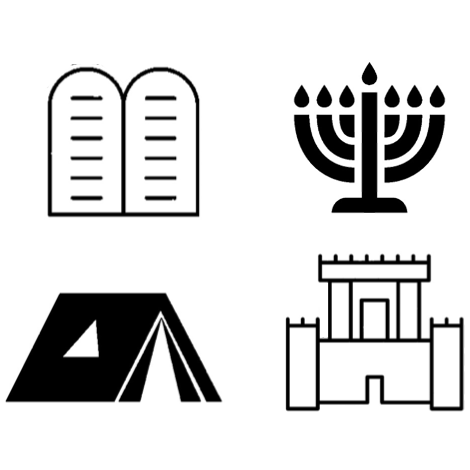
\includegraphics[width=0.30\textwidth]{../ot_frontcover.png}} ;
    \node (0,0) [xshift=+0.20cm, yshift=+2.0cm, opacity=0.10]{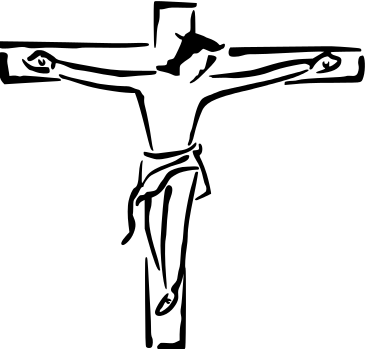
\includegraphics[width=0.20\textwidth]{../christ_on_cross.png}} ;
\end{tikzpicture}
\Large 

\leftcitation{ס} \centerfont 詩百又廿七載：
\leftcitation{ע} \centerfont 非耶和華建屋宇.則匠人之經營徒.
\leftcitation{פ} \centerfont 非耶和華衛城邑.則守者之儆醒徒.
\leftcitation{צ} \centerfont 余獻是卷予華人社區．願為福音流通之器．願獻斯微材為祭榮耀上帝．
\leftcitation{ק} \centerfont 阿門

\switchcolumn

\fontsize{11}{13}\rightfont \Large 滅．時越次聖殿期及當今。\leftcitation{י} \rightfont 猶太者力廣納之．筆錄以卷軸．便以傳、閱、頌、攜、守、鎖、抄、譯、釋、編，得書塔木德、密示拿等經傳．家喻戶曉．傳流若芳。\leftcitation{כ} \rightfont 猶太者文以載道．傳其口述．今我輩粵道之傳應當作如是．遂力行粵音識辨之法．載言載道．以盡忠傳粵道以待興。\leftcitation{ל} \rightfont 蒙下賜恩惠．無畏海量字音文書．既馭上帝之道．今廣及粵語講道．重駛編程之技．匯導粵音遂字稿．重塑講道現場．以傚猶太卷軸之舉便以傳流。\leftcitation{מ} \rightfont 是卷乃粵音口述傳之屬．莫通華文白話之語．

\end{paracol}

\columnratio{0.5,0.5}
\begin{paracol}{2}\fontsize{11}{13}\leftfont \Large \leftcitation{ו} \leftfont 斯殺一違儆百逆．既禁壓之．我輩聞風無奈．在所難免。\leftcitation{ז} \leftfont 另有異人例乎．以版權之名．脅網絡頻道之舉．同授礙予粵道之存流。

\switchcolumn

\fontsize{11}{13}\rightfont \Large 惟待後繼來者之傚．以譯釋傳之於神州華文地。\leftcitation{נ} \rightfont 今能排程驅馭圖靈以編彙文檔，其碼長共數千千亦無逢大礙．全蒙上帝保守。

\end{paracol}



\columnratio{1}\begin{paracol}{1}

\fontsize{11}{13}\rightfont \Large
~~~~~~~~~~~~~~~~~~~~~~~~~~~~~~~~~~~~~~~~~~~~~~~~~~~~~~~~~~~~~~~~~~~~~~~~~~~~~~~\leftcitation{ר} \rightfont 二零二三年二月一日

~~~~~~~~~~~~~~~~~~~~~~~~~~~~~~~~~~~~~~~~~~~~~~~~~~~~~~~~~~~~~~~~~~~~~~~~~~~~~~~\leftcitation{ש} \rightfont 米迦勒

~~~~~~~~~~~~~~~~~~~~~~~~~~~~~~~~~~~~~~~~~~~~~~~~~~~~~~~~~~~~~~~~~~~~~~~~~~~~~~~\leftcitation{ת} \rightfont 書於香港

\end{paracol}

\end{sloppypar}
\end{document}
